\documentclass[12pt,a4paper]{report}

%%
% to enumerate subsubsection
%%
\addtocounter{tocdepth}{3}
\setcounter{secnumdepth}{3}
% \usepackage{tgtermes}
% \usepackage{pgfplots}
% \usepgfplotslibrary{external} 
% \tikzexternalize
\usepackage{parskip}
\usepackage{setspace}
\usepackage[a4paper, margin=0.984252in]{geometry}
\usepackage[T1]{fontenc}
\usepackage[breaklinks,hidelinks]{hyperref}
\usepackage[utf8]{inputenc}
\usepackage{graphicx} 
\usepackage{color,soul}
\usepackage{tikz}
\usepackage{amsmath, amssymb}
% \usepackage{indentfirst}
% \usepackage{cite}
\usepackage{natbib}
\usepackage[nameinlink,noabbrev]{cleveref}
\usepackage[capposition=top]{floatrow}
\usepackage{float}
% \usepackage[tableposition=top]{caption}
% \floatsetup[table]{capposition=top}
\usepackage{caption}
\usepackage{xfrac}
\usepackage{braket}
\usepackage[toc,page]{appendix}
\usepackage{longtable}
\usepackage{tabularx}
\usepackage{adjustbox}
\usepackage{multirow}
\usepackage{arydshln}
\usepackage{pdfpages}
% \usepackage{scrextend} % add margin
% \usepackage{hyperref}
% \usepackage{physics}
\def\changemargin#1#2{\list{}{\rightmargin#2\leftmargin#1}\item[]}
\let\endchangemargin=\endlist 

%%
% to enumerate subsubsection
%%
\addtocounter{tocdepth}{3}
\setcounter{secnumdepth}{3}
\renewcommand{\baselinestretch}{1.3}
% \linespread{1.5}
% \setlength{\parindent}{0em}
% \setlength{\parskip}{1em}
% \usepackage{setspace}
% \setstretch{1.5}

% Snippet
\newcommand{\BSM}{Black--Scholes--Merton }
\newcommand{\lnorm}{log-normally }
\newcommand{\bmotion}{Brownian Motion }
\newcommand{\stvar}{stochastic variable }
\newcommand{\wienpro}{Wiener process }
\newcommand{\markpro}{Markov process }

% 
% Bunch of new commands
% 
% brownian motion
\newcommand{\dBm}{dW\left(t\right)}
\newcommand{\dpoiss}{dq\left(t\right)}
\newcommand{\DBm}{\delta{W\left(t\right)}}
\newcommand{\Bm}{W\left(t\right)}
\newcommand{\Bmsub}[1]{W_{#1}\left(t\right)}
\newcommand{\Dt}{\Delta t} 
\newcommand{\Bmdist}{\DBm \sim N \left( 0, \Dt \right)}
\newcommand{\ft}{f\left(t, \Bm \right)}
\newcommand{\E}{\mathop{\mathbb{E}}}
\newcommand{\ct}{c\left(t, x\right)}
\newcommand{\dcx}{\frac{\delta\ct}{\delta x}}
\newcommand{\dciix}{\frac{\delta^2\ct}{\delta x^2}}
\newcommand{\dct}{\frac{\delta\ct}{\delta t}}
\newcommand{\N}[1]{N\left(#1\right)}
\newcommand{\dsub}[1]{d_{#1}\left(\Dt, x\right)}
\newcommand{\call}[2]{c\left( #1, #2\right)}
% % about stock
\newcommand{\St}{S\left(t\right)}
\newcommand{\Vt}{V\left(t\right)}
\newcommand{\Si}{S\left(0\right)}
\newcommand{\dSt}{dS\left(t\right)}
\newcommand{\DSt}{\Delta S\left(t\right)}
\newcommand{\dSr}{\frac{\dSt}{\St}}
\newcommand{\DSr}{\frac{\DSt}{\St}}
\newcommand{\Scontinuous}{\St = \Si e^{\sigma\Bm + \left(\alpha - \frac{1}{2 \sigma^2}\right)t}}
\newcommand{\Itobmdiff}{d\ft = \left[\frac{\partial \ft }{\partial t} + \frac{1}{2} \frac{\partial ^2\ft }{\partial x^2}\right]dt + \frac{\partial \ft}{\partial x} \dBm}
\newcommand{\Scontinousdiff}{d\St &= \alpha \St dt + \sigma \St \dBm}
\newcommand{\Scontinuousrate}{\dSr &= \alpha dt + \sigma \dBm}
 \newcommand{\Sdiscretediff}{d\St &= \alpha \St \Dt + \sigma \St \dBm}
\newcommand{\Sshort}{\Si e^{X}}
\newcommand{\CCRdist}{X \sim N\left(\left(\alpha - \frac{1}{2}\sigma^2\right)t, \sigma^2 t\right)}
\newcommand{\Sdiscreterate}{\DSr &= \alpha \Delta t + \sigma \DBm}
\newcommand{\Sdiscreterateexp}{\E \DSr = \alpha \Dt}
\newcommand{\Sdiscreteratevar}{var \DSr = \sigma ^2 \Dt}
\newcommand{\Sdiscreteratedist}{\DSr \sim N\left(\alpha\Dt, \sigma\Dt\right)}
\newcommand{\Sexp}{\E\St = \Si e^{\alpha t}}
\newcommand{\Svar}{var\St = \Si^2 e^{2\alpha t}\left(e^{\sigma^2 t} - 1\right)}
\newcommand{\Sshortt}{\St = \Si e^{X t}}
\newcommand{\CCRt}{X = \frac{1}{t} \ln{\frac{\St}{\Si}}}
\newcommand{\CCRtdist}{X \sim N\left(\alpha - \frac{\sigma^2}{2}, \frac{\sigma^2}{t}\right)}
\newcommand{\BSMpde}{\dct + r x \dcx + \frac{1}{2} \sigma^2 x^2 \dciix = r\ct}
\newcommand{\BSMeq}[1]{r\call{t}{#1} = \frac{\partial \call{t}{#1}}{\partial t} + r #1 \frac{\partial \call{t}{#1}}{\partial #1} + \frac{1}{2} \sigma ^2 #1 ^2 \frac{\partial ^2 \call{t}{#1}}{\partial #1 ^2}}
\newcommand{\BSMGreeks}[1]{r\call{t}{#1} = \Theta + r #1 \Delta + \frac{1}{2} \sigma ^2 #1 ^2 \Gamma}
\newcommand{\BSMsol}{\ct &= x\N{\dsub{+}} - K e^{-r\Dt} \N{\dsub{-}}}
\newcommand{\dpm}{\dsub{\pm} &= \frac{1}{\sigma\sqrt{\Dt}} \left[\log\frac{x}{K} + \left(r \pm \frac{\sigma^2}{2}\Dt\right)\right]}

% CIR Stock price Stochastic process
\newcommand{\HSVstock}{
  d\St &= \alpha \St dt + \sqrt{\Vt} \St d \Bmsub{S}
}

% CIR Stock price Stochastic process
\newcommand{\HSVstockriskless}{
  d\St &= r \St dt + \sqrt{\Vt} \St d \Bmsub{S}
}

% CIR volatility
\newcommand{\HSVvol}{
  d\Vt &= \kappa\left(\theta - \Vt \right) dt + \sigma \sqrt{\Vt} d \Bmsub{V}
}


% CIR volatility
\newcommand{\HSVvolriskless}{
  d\Vt &= \kappa^{*} \left(\theta^{*} - \Vt \right) dt + \sigma \sqrt{\Vt} d \Bmsub{V}
}

\newcommand{\dportfolio}{dX\left(t\right) = \Delta\left(t\right) d\St + r \left(X\left(t\right) - \Delta\left(t\right) \St \right) dt}

\usepackage{Sweave}
\begin{document}

\Sconcordance{concordance:index.tex:index.Rnw:%
1 6 1}
\Sconcordance{concordance:index.tex:./preamble/usepackage.Rnw:ofs 7:%
1 21 1}
\Sconcordance{concordance:index.tex:./preamble/misc.Rnw:ofs 29:%
1 6 1}
\Sconcordance{concordance:index.tex:./preamble/snippet.Rnw:ofs 36:%
1 7 1}
\Sconcordance{concordance:index.tex:./preamble/formula.Rnw:ofs 44:%
1 71 1}
\Sconcordance{concordance:index.tex:index.Rnw:ofs 116:%
12 1 1 1 0 24 1}
\Sconcordance{concordance:index.tex:./methodology.Rnw:ofs 143:%
1 485 1}
\Sconcordance{concordance:index.tex:index.Rnw:ofs 629:%
39 12 1}


\setkeys{Gin}{width=8.3in}
\begin{titlepage}
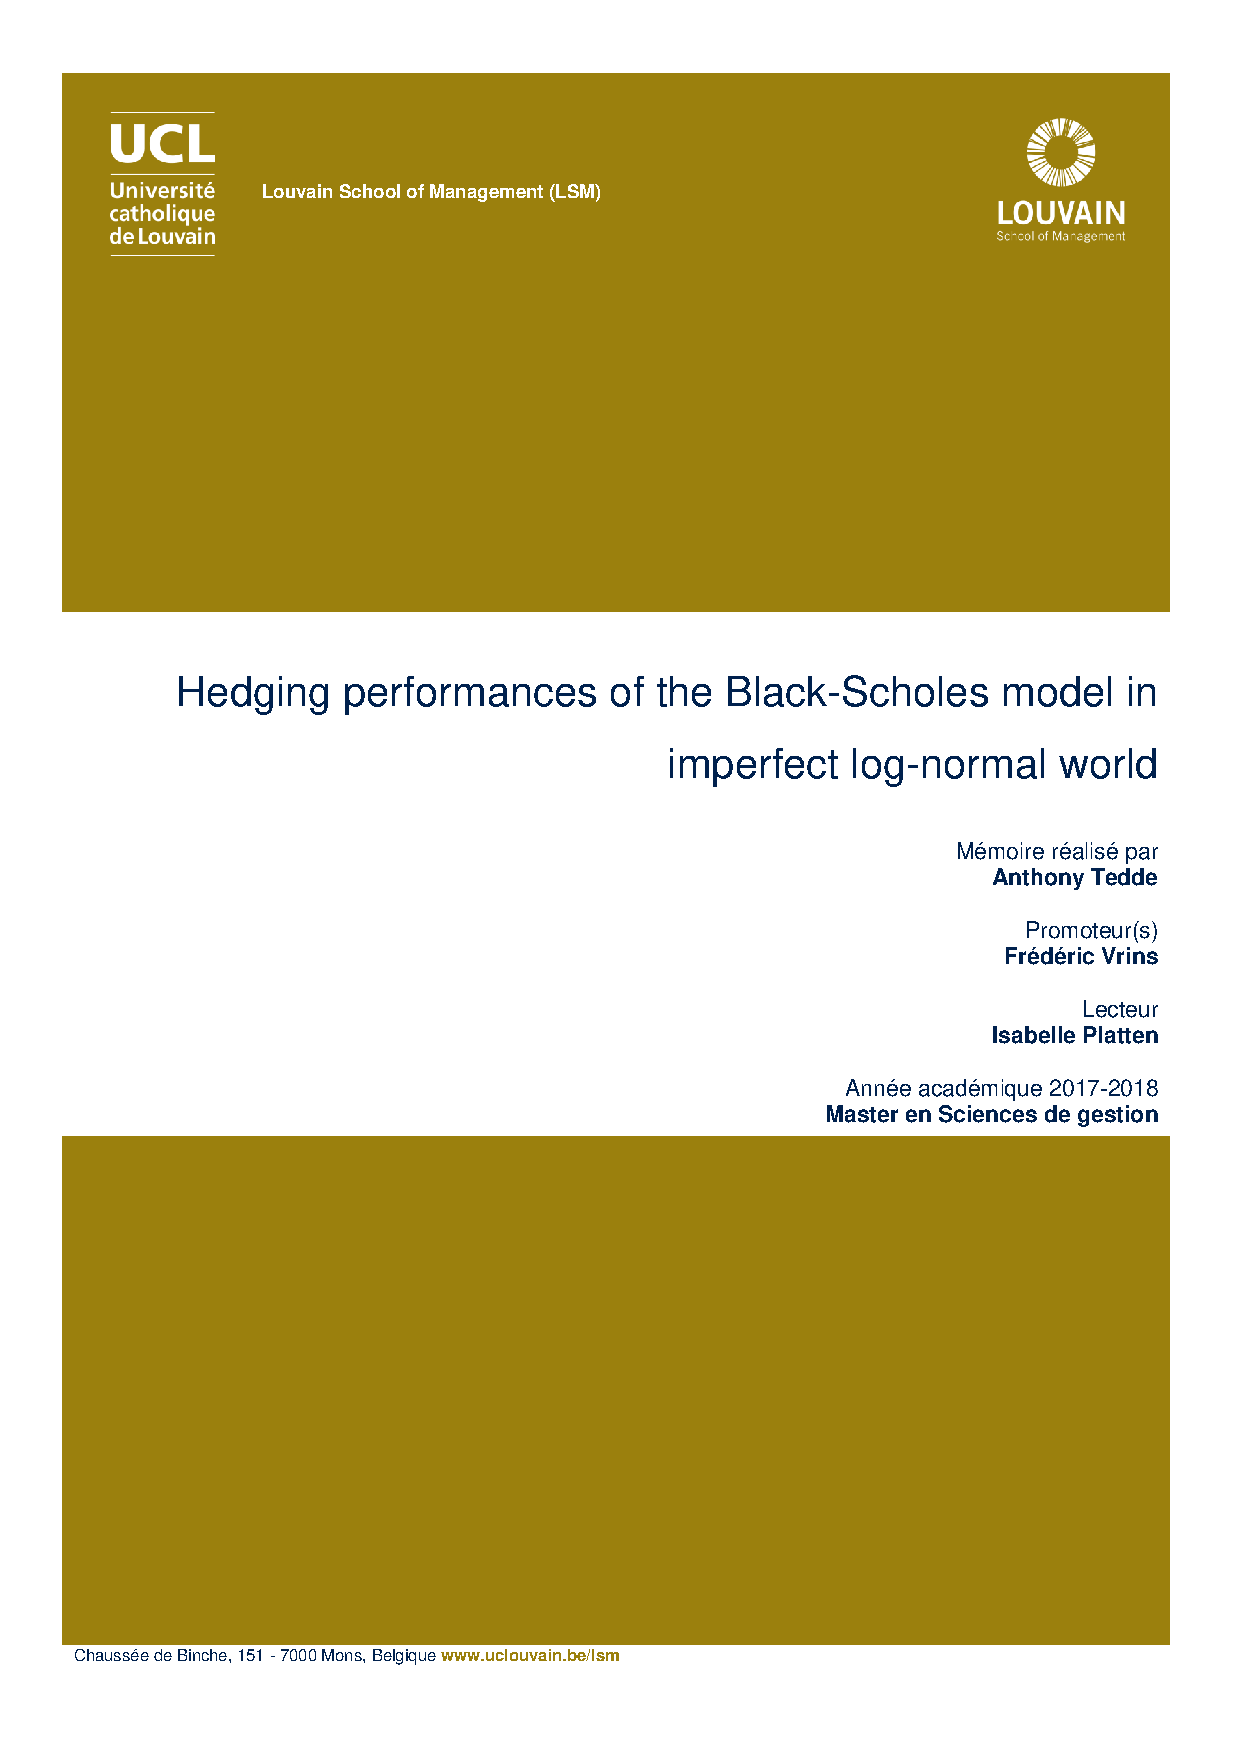
\includepdf{cover.pdf}
\end{titlepage}

\newpage\null\thispagestyle{empty}\newpage


\setkeys{Gin}{width=0.8\textwidth}



\pagenumbering{roman}
\chapter*{Abstract}
\addcontentsline{toc}{chapter}{Abstract}
 
The study developed in the current master thesis concerns the Black-Scholes-Merton (BSM) method initially intended to give a fair price to options for which a geometric Brownian motion (GBM) drives the underlying asset.
Indeed this model works remarkably well provided that the underpinned assumptions are respected with the most restrictive one stating that the distribution of the log-returns of the underlying asset has to be normal.
However, empirical results show that this constraint of log-normality does not hold for real-life trials and consequently break the more key hypothesis of the aforementioned model.

The primary purpose of the analysis developed in that work is to assess how wrong goes the BSM equation while the underlying asset is not a GBM.
To that end, others models will be investigated, namely, the Merton jump diffusion (MJD) and Heston stochastic volatility (HSV) models.
Each of it bears a new characteristic. The MJD brings jumps to the paths of the underlying processes whilst HSV comes with a volatility parameter that evolves with times unlike the deterministic one inherent to BSM. These specificities affect the log-returns distributions that are no more normal.

Accordingly, once calibrated, those models will be used to simulate a world where the assumption of log-normality of the BSM model does not hold anymore. The study case explored is to measure how the BSM equation will react when its central assumption is broken.
To do this, the performance of the delta-neutral portfolios of BSM, MJD and HSV processes will be benchmarked.

As a subanalysis, another goal of that master thesis is to examine if, with a unique set of parameters, the HSV and MJD models can reproduce the volatility smiles constructed from the options prices provided by the market.
A conclusion would be that those models are versatile enough to cover a broader range of market prices than the BSM model itself.
\chapter*{Acknowledgements}
\addcontentsline{toc}{chapter}{Acknowledgements}

First and foremost, I want to address all my gratitude to Anne, and our two wonderful children, Elsa and Valentin, for their patience and huge support. They gave me all the strength needed to go beyond my self-motivation.

Many thanks to all of my family and precious friends that make the life more pleasant. I especially think of Nonna Emma, Mario, Josiane, Maud, Eddy, Christelle, Sébastien, Pierre, Clément, Adrien and Claude.

Thank you mum and dad.

Last but not least, I want to sincerely thank Pr. Frédéric Vrins for trusting in me. It was a real pleasure to meet you.




{\setstretch{1.0}
\tableofcontents
\clearpage

\listoffigures
 \clearpage


\listoftables}
\clearpage



\pagenumbering{arabic}
%%%%%%%%%%%%%%%%%%%%%%%%%%%%%%%%%%%%%%%%%%%%%%%%%%%%%%%%%%%%%%%%%%%%%%%%%%%%%%%%
%
%  CHAPTER: Introduction
%
%%%%%%%%%%%%%%%%%%%%%%%%%%%%%%%%%%%%%%%%%%%%%%%%%%%%%%%%%%%%%%%%%%%%%%%%%%%%%%%%
\chapter{Introduction}
\label{cha:Introduction}

The options market gained in importance in the latter decades, and the range of related products become more extensive with time.
Although in some cases, those derivatives are used with speculative aims, primarily due to the leverage effect inherent to the long position taken in them, they however mainly serve to cover oneself against potential risks.
Indeed, if someone plans to buy some share of stocks in a further date he/she can lock the price of that asset by going long in a European call, likewise, if another one wants to fix a selling price in a security for a future date, he could go long in a European put.

Though, if everyone, as well the speculators as those wanting to lock a price are going long into those financial products, who are taking the opposite position by going short?
Those profiles are called the hedgers and generally are employed by big financial institutions.
Their goals are to sell derivative contracts without losing money by opting for an appropriate strategy that replicates the value of the long position in the option sold using other financial products bundle together into a portfolio. The so-called replicating or hedging portfolio.

That wallet can be constructed by using the delta-hedging strategy consisting of the replication of the opposite position than that to hedge by taking advantage of the underlying asset as well as the money market account.
Roughly speaking, that portfolio is built in a way that, at any time, each impact on the option value due to a move in the underlying price is offset by a position taken in that asset.
Accordingly, the position in the underlying asset has to be continuously readjusted to remain such an effective buffer.
This strategy will be explained more deeply in subsequent chapters.

The strategy mentioned above needs money to be initially constructed, and that amount has to cover the fee of all the rebalancing operations whatever are the stock moves up to option's maturity.
Consequently, that amount of money equals the option price at time zero.

The Black-Scholes-Merton (BSM) equation developed in \citet{bs} and supplemented in \citet{merton73} helps to find such a price for a derivative by relying on some constraints that restrict what is observed in reality, but as with any model, the objective is to find a frame that matches with an abstract of fact, not to reproduce it fully.
The most restrictive assumption is that the process driving the underlying asset's prices is a geometric Brownian motion (GBM), involving that the associated log-returns' distribution is normal and that the related volatility rate is deterministic.
Hence, that master thesis will explore such claims and raises the following overall question concerning the approximations brought by the BSM model, how good are the BSM hedging performances within our not lognormal world?

In the current document, the focus is set on measuring the performance of the particular  European vanilla calls options.

% \section{Context}
% \label{sec:introduction:context}

\section{Raised questions}
\label{sec:Introduction:raised}

In order to go beyond the BSM constraints, other models are considered which allow time-series to take other distributions for their returns than the lognormal one.
Those processes are the Merton jump-diffusion (MJD) and Heston stochastic volatility (HSV) whose first provide discrepancies in its path by adding a jump component, while the second lets volatility being no more immutable over time.

Consequently, by considering to those models, the study breaks the assumptions of (i) normality for the log-returns and (ii) deterministic volatility.
The objective will be to construct and quantify hedging strategies over such processes denoting underlying assets.
Nevertheless, the prices of options on such dummy assets, driven by HSV or MJD, lack to be determined with the solution provided in \citet{bs}. 
They need a particular methodology to be found out. Latter is given in \citet{heston1993} and relies on a probabilistic approach involving the characteristic functions of the stochastic processes $\ln S(t)$, where $S(t)$ expresses the random time-series generated by either MJD or HSV.

First and foremost, the models used to generate time-series and those aimed to price European call options will be calibrated to provide credible outputs.
Afterward, the geometric Brownian motion, Merton jump-diffusion, and Heston stochastic volatility processes will be applied to simulate artificial stock prices time-series while the BSM and Heston approaches will serve to price some related options.
Ultimately, the so computed initial option prices will serve the analysis of the hedging performances.

The hedges assessment will be split into two parts. 
The first one regards the measure of the results reached when hedging a GBM with a BSM delta-neutral portfolio.  Needless to say that the score of such an approach should be almost perfect since all the assumptions underpinning the BSM framework are respected.
The objective is to build a standard to be subsequently compared with the coverage of other processes.
Thereafter, the assessment of options' coverages for which the underlying assets depend on MJD and HSV will take place.
Those derivatives will be hedged through both the BSM delta and that appropriate to the underpinned model, computed from the first mathematical derivative of the related option price function with respect to the stock price.
The goal is to compare their intrinsic performances and to evaluate how one goes wrong by applying the BSM delta in real life. 

According to \citet{shreve}, the recurrence of rebalancing affects the quality of the hedge. 
Those consequences can be significant to a certain extent.
They depend on fundamental properties of the option to be hedged and notably rely on its gamma, that is, the acceleration at which the underlying asset affects the option price.
Indeed, the hedge of an option with higher gamma can give poor results if not rebalanced regularly.
That master thesis will evaluate the aforementioned gamma effect on the delta-neutral portfolio rebalancing frequency.

Shreve also shows that the impact of gamma is always adverse for a delta-neutral portfolio that replicates a long position in the derivative. 
Whilst the influence of theta, i.e., the rate at which an option decrease in value as time passes all other things being equal, is always positive for that securities.
He especially exhibits that the weight of theta on a delta-neutral portfolio overwhelms that of gamma. 
In that document, those effects will be analyzed for BSM, MJD and HSV related options, namely, up to what extent gamma and theta affect the options and consequently the delta-neutral portfolio, but also which types of options and what models are the more impacted.

Ultimately, market data shows that to obtain the same prices for options with different strike prices but same maturity the BSM equation involves using different volatilities for the same underlying asset.
Though, the risk of a share of stock does not depend on the strike prices of its related options, inducing that the BSM model lacks to reproduce such a behavior.
That specificity is knowns as the volatility smile and represents the BSM implied volatility with respect to the strikes and grouped by maturity.
When they are not clustered by maturity, one talk about volatility surface.
Therefore, unlike the BSM approach, are the models MJD and HSV able to reproduce such volatility surface with one unique set of parameters provided that they happen to be well adjusted?

The so raised questions are summarized in the list here below.

\begin{itemize}
\item What is the effect of the rebalancing rhythm on the hedging performances for the HSV and MJD models against the BSM approach? 
\item How far can one go wrong by using the BSM delta-neutral strategy in the real world? Does it make sense to use it?
\item What can be the effects of gamma and theta combined on the replicating portfolio?
\item Are the MJD and HSV models able to reproduce the volatility smiles? 
\end{itemize}

However, the answers that will be provided for the above questions are limited to the particular case studied in that master thesis and consequently cannot be generalized.


\section{Organization of the document}
\label{sec:introduction:organization}

In this section are briefly introduced all the subsequent chapters.

\cref{cha:upstream} introduces basics concepts that will be subsequently actively used in the others chapters. Among those, there are Brownian motions, introduction on the financial derivatives, Itô's approximation, Cox–Ingersoll–Ross process, log-return, continuously compounded rate of return and the computation of skewness and kurtosis.

\cref{cha:bsm} presents the Black-Scholes-Merton model along with the geometric Brownian motion used to drive underlying assets prices processes. Furthermore, in that chapter dives also into the Greeks that will be used in the study part, namely, the delta, gamma, and theta. Each of it plays a specific role in the delta-hedging strategy or in the process of options pricing.

\cref{cha:OtherModel} exhibits other models which will be used in the analysis in order to tackle with some of the flaws bring by the assumptions of the Black-Scholes-Merton pricing model. Those are the Merton jump-diffusion (MJD) and Heston stochastic volatility (HSV) models. Algorithms aimed either to compute time-series driven by those models or to price options on such series will be investigated.

\cref{cha:Methodology} presents the methodology used to calibrate all the previously studied algorithm and it lists the followed procedure for assessing the performance of the models within a not log-normal world. 

\cref{cha:analysis} points out and delves into the details of the results got from the delta-hedging performance study. These results will be split into three parts where in turn, the performances of the BSM, MJD and HSV models will be explored.

\cref{cha:conclusion} concludes the work by highlighting some results, presenting their limits and suggest ways to reflect on them or ideas to go beyond the particular study case explored in that master thesis.


%%%%%%%%%%%%%%%%%%%%%%%%%%%%%%%%%%%%%%%%%%%%%%%%%%%%%%%%%%%%%%%%%%%%%%%%%%%%%%%%
%
%  CHAPTER:Upstream concepts
%
%%%%%%%%%%%%%%%%%%%%%%%%%%%%%%%%%%%%%%%%%%%%%%%%%%%%%%%%%%%%%%%%%%%%%%%%%%%%%%%%
\chapter{Upstream concepts}
\label{cha:upstream}


%%%%%%%%%%%%%%%%%%%%%%%%%%%%%%%%%%%%%%%%%%%%%%%%
% SECTION: Overview
%%%%%%%%%%%%%%%%%%%%%%%%%%%%%%%%%%%%%%%%%%%%%%%%
% \section{Overview}
% \label{sec:upstream:overview}

The material covered in the current chapter is meant to be thereafter intensively used, either by being applied in the studied theoretical models or by entering in the construction of the theory-based algorithms.

%%%%%%%%%%%%%%%%%%%%%%%%%%%%%%%%%%%%%%%%%%%%%%%%
% SECTION: Vanilla options
%%%%%%%%%%%%%%%%%%%%%%%%%%%%%%%%%%%%%%%%%%%%%%%%
\section{Vanilla options}
\label{sec:upstream:vanilla}

The so-called vanilla options, in opposition to the more complex - not covered in this master thesis - exotic ones, are specifics kind of derivatives coming along with some good-to-know jargons. 

First and foremost,  as defined in \citet{hull}, an option is a contract between two stakeholders with different interests or at least distinctive motivations, who want to buy or sell a product, which generally is a financial asset called "the underlying." 
Indeed, someone can look for hedge oneself against risk while the other party wants to make a profit on a speculative move.
Likewise other financial contracts, one agrees to buy and the other to sell at a fixed amount of money, namely "the strike price", usually denoted by $k$ with the difference that they would effectively realize the purchase or the sale of the underlying at a future date than the one they enter into the bargain. That date is called "the maturity".


Another key characteristic of options is that they are not symmetric contracts, in the sense that both parties do not have the same rights, depending on their position along with the option's type. 
Two positions can be taken when entering into such a derivative, either long or short. 
Going short broadly means purchase the option whereas going long implies writing, or synonymously, selling the derivative. Beyond the position, the contract can be of call or put type. 

The following sentences encompass a mix of type (call/put) and position (short/long) combination that gives an overview of all the possible scenarios:

\begin{itemize}
\item Someone who is going long into a call gains the right to purchase the underlying at a future date for a fixed price. He has to pay some fees to enter into the contract.
\item Someone who is going short into a call is forced to sell the underlying at a future date for a fixed price. He receives financial compensation to enter into the contract.
\item Someone who is going long into a put gains the right to sell the underlying at a future date for a fixed price. He has to pay some fees to enter into the contract.
\item Someone who is going short into a put is forced to buy the underlying at a future date for a fixed price. He receives financial compensation to enter into the contract.
\end{itemize}

Moreover, vanilla options may be "European" or "American". Latter can be exercised at any time during the whole life of the contract while the European can only be at maturity.

Finally, the payoff provided by all aforementioned European options are summarized throughout \crefrange{eq:upstream:cl}{eq:upstream:ps}, where $C_l$, $C_s$, $P_l$ and $P_s$ respectively stand for the long call, short call, long put and short put payoffs. $S(T)$ being the price of the underlying at maturity.

\begin{align}
C_l &= \left(S(T) - k\right)^+ \label{eq:upstream:cl}\\
C_s &= \left(k - S(T)\right)^- \label{eq:upstream:cs}\\
P_l &= \left(k - S(T)\right)^+ \label{eq:upstream:pl}\\
P_s &= \left(S(T) - k\right)^- \label{eq:upstream:ps}
\end{align}

The derivative considered in this master thesis is mainly the European call option, even though the link with European put could somehow be done without being mandatory to exhibit the issue so raised. Therefore such reference to put should only be done if necessary.

%%%%%%%%%%%%%%%%%%%%%%%%%%%%%%%%%%%%%%%%%%%%%%%%
% SECTION: Brownian Motion
%%%%%%%%%%%%%%%%%%%%%%%%%%%%%%%%%%%%%%%%%%%%%%%%
\section{Brownian Motion}
\label{sec:upstream:brownian}
 
All over the present document, the terms "Brownian motion", "Wiener" or "Markov" processes are considered to be equivalent terminology and therefore used as such. However strictly speaking, even though the Brownian motion is in every respect a Wiener process, stricto sensu, the term Markov process is broader. 
Actually, the more remarkable Markov property is to be a process with independent future increments, putting it in line with the weak form of market efficiency (\citet{hull}).
Whilst, on the other hand, even if the Brownian motion, and thus the Wiener process, share this property, they are defined with the idiosyncrasy to have mean zero and a variance rate of one per unit of time (\citet{hull}).

Brownian motion is a centerpiece broadly used in subsequent developments. It is notably applied in many models such as in the geometric Brownian motion (\cref{cha:bsm}),  in the Black-Scholes-Merton (BSM) equation (\cref{cha:bsm}) and in the Merton mixed jump-diffusion (MJD) and Heston stochastic volatility (HSV) model (\cref{cha:OtherModel}).

The Brownian motion is a stochastic process, denoted by $\Bm$ and satisfying $W(0) = 0$, with independent and identically distributed (iid) increments, such as defined by \cref{eq:upstream:increment:dist}

\begin{align}
W(t_{i+1}) - W(t_i) \sim
  iid N \left(0, t_{i+1} - t_i\right) \label{eq:upstream:increment:dist}
\end{align}

That Markov process is qualified as being time and path dependent in its building blocks. Time dependency implies that like many other functions its value evolves over time. 
Whereas path dependency means that the Wiener process is also meant to randomly move between two time-steps.
Practically, at any time $t$ and from its origin, the Brownian motion may take any value as shown by \cref{eq:upstream:brownian:dist}.

\begin{align}
\Bm \sim N(0, t) \label{eq:upstream:brownian:dist}
\end{align}

As described by \citet{shreve}, the construction of such a process could be achieved by following various techniques. Either by computing the differential process (\cref{eq:upstream:brownian:diff,eq:upstream:brownian:cumsum}) for every time-steps and then combining them, by constructing a unique time series in that way; or by resolving the joint moment generating function of the iid random variables' vector ($W(t_i)$ \ldots $W(t_m)$), through \cref{eq:upstream:brownian:joint}.

\begin{align}
  d\Bm &= \phi \left(0, t + \epsilon_i \right) \label{eq:upstream:brownian:diff} \\
  \intertext{
  $\phi$ is a function that generate a random number according to the normal law with parameter $\mu = 0$ and $\sigma^2 = t + \epsilon_i$, with $\epsilon_i$ being any arbitrary small delta time step.
  }
  W\left(t + \epsilon_i\right) &= \Bm + d\Bm \label{eq:upstream:brownian:cumsum}
\end{align}

\begin{align}
  \varphi\left(u_1 \ldots u_m\right) = \exp{\left( \frac{1}{2} \sum_{i = 1}^m \left[ \sum_{j = i}^m u_j \right]^2 \left( t_i - t_{i-1} \right) \right)} \label{eq:upstream:brownian:joint}
\end{align}

\Cref{fig:upstream:brownian} (QA) displays a simulation of one hundred Brownian motions over a time frame of five years. While in turn, \cref{fig:upstream:brownian} (QB) shows the distribution of the possible outcomes of that experiment, after five years. The black outlined curve is the density of the normal distribution, with mean and variance chose such as exposed by \cref{eq:upstream:increment:dist}.

\begin{figure}[H]
\centering
% Created by tikzDevice version 0.11 on 2018-04-13 23:55:51
% !TEX encoding = UTF-8 Unicode
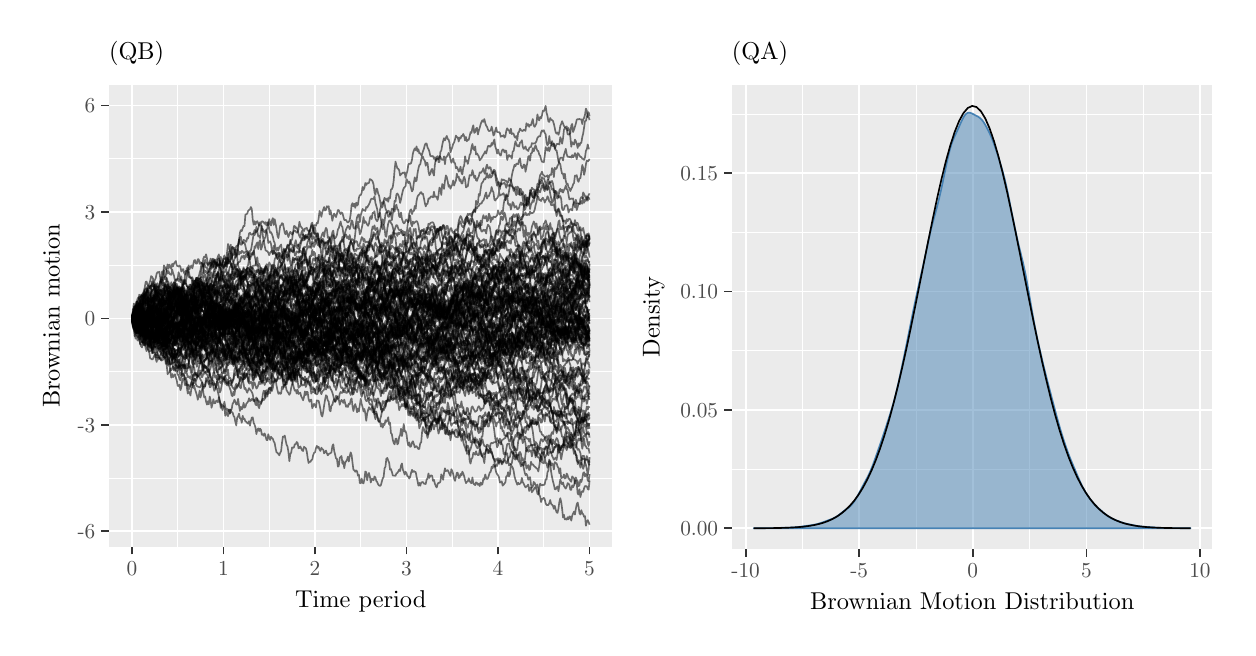
\begin{tikzpicture}[x=1pt,y=1pt]
\definecolor{fillColor}{RGB}{255,255,255}
\path[use as bounding box,fill=fillColor,fill opacity=0.00] (0,0) rectangle (433.62,216.81);
\begin{scope}
\path[clip] (  0.00,  0.00) rectangle (216.81,216.81);
\definecolor{drawColor}{RGB}{255,255,255}
\definecolor{fillColor}{RGB}{255,255,255}

\path[draw=drawColor,line width= 0.6pt,line join=round,line cap=round,fill=fillColor] (  0.00,  0.00) rectangle (216.81,216.81);
\end{scope}
\begin{scope}
\path[clip] ( 29.40, 29.26) rectangle (211.31,196.15);
\definecolor{fillColor}{gray}{0.92}

\path[fill=fillColor] ( 29.40, 29.26) rectangle (211.31,196.15);
\definecolor{drawColor}{RGB}{255,255,255}

\path[draw=drawColor,line width= 0.3pt,line join=round] ( 29.40, 54.09) --
	(211.31, 54.09);

\path[draw=drawColor,line width= 0.3pt,line join=round] ( 29.40, 92.54) --
	(211.31, 92.54);

\path[draw=drawColor,line width= 0.3pt,line join=round] ( 29.40,130.99) --
	(211.31,130.99);

\path[draw=drawColor,line width= 0.3pt,line join=round] ( 29.40,169.44) --
	(211.31,169.44);

\path[draw=drawColor,line width= 0.3pt,line join=round] ( 54.20, 29.26) --
	( 54.20,196.15);

\path[draw=drawColor,line width= 0.3pt,line join=round] ( 87.28, 29.26) --
	( 87.28,196.15);

\path[draw=drawColor,line width= 0.3pt,line join=round] (120.35, 29.26) --
	(120.35,196.15);

\path[draw=drawColor,line width= 0.3pt,line join=round] (153.43, 29.26) --
	(153.43,196.15);

\path[draw=drawColor,line width= 0.3pt,line join=round] (186.50, 29.26) --
	(186.50,196.15);

\path[draw=drawColor,line width= 0.6pt,line join=round] ( 29.40, 34.87) --
	(211.31, 34.87);

\path[draw=drawColor,line width= 0.6pt,line join=round] ( 29.40, 73.32) --
	(211.31, 73.32);

\path[draw=drawColor,line width= 0.6pt,line join=round] ( 29.40,111.77) --
	(211.31,111.77);

\path[draw=drawColor,line width= 0.6pt,line join=round] ( 29.40,150.22) --
	(211.31,150.22);

\path[draw=drawColor,line width= 0.6pt,line join=round] ( 29.40,188.67) --
	(211.31,188.67);

\path[draw=drawColor,line width= 0.6pt,line join=round] ( 37.67, 29.26) --
	( 37.67,196.15);

\path[draw=drawColor,line width= 0.6pt,line join=round] ( 70.74, 29.26) --
	( 70.74,196.15);

\path[draw=drawColor,line width= 0.6pt,line join=round] (103.82, 29.26) --
	(103.82,196.15);

\path[draw=drawColor,line width= 0.6pt,line join=round] (136.89, 29.26) --
	(136.89,196.15);

\path[draw=drawColor,line width= 0.6pt,line join=round] (169.97, 29.26) --
	(169.97,196.15);

\path[draw=drawColor,line width= 0.6pt,line join=round] (203.04, 29.26) --
	(203.04,196.15);
\definecolor{drawColor}{RGB}{0,0,0}

\path[draw=drawColor,draw opacity=0.55,line width= 0.6pt,line join=round] ( 37.67,111.77) --
	( 38.00,110.96) --
	( 38.33,111.20) --
	( 38.66,110.13) --
	( 38.99,112.17) --
	( 39.32,112.60) --
	( 39.65,111.54) --
	( 39.98,112.17) --
	( 40.31,113.11) --
	( 40.64,113.85) --
	( 40.97,113.46) --
	( 41.30,115.40) --
	( 41.64,115.90) --
	( 41.97,115.10) --
	( 42.30,112.26) --
	( 42.63,113.71) --
	( 42.96,113.65) --
	( 43.29,113.63) --
	( 43.62,114.84) --
	( 43.95,115.89) --
	( 44.28,116.65) --
	( 44.61,117.83) --
	( 44.94,118.83) --
	( 45.27,118.93) --
	( 45.60,116.38) --
	( 45.94,117.17) --
	( 46.27,117.10) --
	( 46.60,116.90) --
	( 46.93,115.01) --
	( 47.26,114.40) --
	( 47.59,114.94) --
	( 47.92,116.68) --
	( 48.25,116.55) --
	( 48.58,117.04) --
	( 48.91,116.98) --
	( 49.24,115.21) --
	( 49.57,114.68) --
	( 49.90,114.17) --
	( 50.24,114.10) --
	( 50.57,115.51) --
	( 50.90,116.48) --
	( 51.23,116.27) --
	( 51.56,115.95) --
	( 51.89,116.84) --
	( 52.22,117.56) --
	( 52.55,116.67) --
	( 52.88,115.77) --
	( 53.21,116.23) --
	( 53.54,117.22) --
	( 53.87,117.07) --
	( 54.20,118.20) --
	( 54.53,118.71) --
	( 54.87,117.93) --
	( 55.20,118.37) --
	( 55.53,116.92) --
	( 55.86,118.76) --
	( 56.19,121.29) --
	( 56.52,120.82) --
	( 56.85,119.49) --
	( 57.18,120.22) --
	( 57.51,120.04) --
	( 57.84,123.12) --
	( 58.17,123.07) --
	( 58.50,123.95) --
	( 58.83,123.99) --
	( 59.17,123.04) --
	( 59.50,123.28) --
	( 59.83,120.97) --
	( 60.16,122.84) --
	( 60.49,123.04) --
	( 60.82,125.83) --
	( 61.15,126.44) --
	( 61.48,125.53) --
	( 61.81,126.31) --
	( 62.14,125.11) --
	( 62.47,123.50) --
	( 62.80,123.88) --
	( 63.13,123.31) --
	( 63.47,123.31) --
	( 63.80,123.41) --
	( 64.13,122.65) --
	( 64.46,121.92) --
	( 64.79,121.75) --
	( 65.12,123.26) --
	( 65.45,121.31) --
	( 65.78,122.07) --
	( 66.11,122.49) --
	( 66.44,123.86) --
	( 66.77,123.47) --
	( 67.10,123.94) --
	( 67.43,124.28) --
	( 67.76,123.59) --
	( 68.10,125.14) --
	( 68.43,126.62) --
	( 68.76,127.52) --
	( 69.09,129.55) --
	( 69.42,130.27) --
	( 69.75,128.63) --
	( 70.08,127.90) --
	( 70.41,126.33) --
	( 70.74,125.72) --
	( 71.07,124.93) --
	( 71.40,124.98) --
	( 71.73,123.81) --
	( 72.06,124.02) --
	( 72.40,123.18) --
	( 72.73,125.44) --
	( 73.06,126.36) --
	( 73.39,127.53) --
	( 73.72,128.02) --
	( 74.05,130.18) --
	( 74.38,129.36) --
	( 74.71,128.77) --
	( 75.04,130.61) --
	( 75.37,129.77) --
	( 75.70,129.51) --
	( 76.03,129.00) --
	( 76.36,128.59) --
	( 76.70,128.23) --
	( 77.03,128.87) --
	( 77.36,128.64) --
	( 77.69,127.99) --
	( 78.02,129.71) --
	( 78.35,129.44) --
	( 78.68,129.21) --
	( 79.01,129.08) --
	( 79.34,129.99) --
	( 79.67,129.90) --
	( 80.00,129.85) --
	( 80.33,128.98) --
	( 80.66,128.56) --
	( 80.99,128.64) --
	( 81.33,127.88) --
	( 81.66,128.57) --
	( 81.99,126.62) --
	( 82.32,127.01) --
	( 82.65,125.04) --
	( 82.98,124.66) --
	( 83.31,123.98) --
	( 83.64,123.14) --
	( 83.97,123.07) --
	( 84.30,120.62) --
	( 84.63,122.13) --
	( 84.96,119.99) --
	( 85.29,119.40) --
	( 85.63,117.97) --
	( 85.96,117.00) --
	( 86.29,119.68) --
	( 86.62,119.70) --
	( 86.95,118.05) --
	( 87.28,115.95) --
	( 87.61,116.53) --
	( 87.94,116.50) --
	( 88.27,116.10) --
	( 88.60,114.91) --
	( 88.93,113.00) --
	( 89.26,111.62) --
	( 89.59,112.90) --
	( 89.93,112.11) --
	( 90.26,110.33) --
	( 90.59,112.73) --
	( 90.92,113.27) --
	( 91.25,112.97) --
	( 91.58,114.32) --
	( 91.91,115.46) --
	( 92.24,114.67) --
	( 92.57,117.49) --
	( 92.90,117.17) --
	( 93.23,115.34) --
	( 93.56,115.16) --
	( 93.89,115.42) --
	( 94.22,118.38) --
	( 94.56,118.52) --
	( 94.89,119.10) --
	( 95.22,119.00) --
	( 95.55,118.57) --
	( 95.88,118.53) --
	( 96.21,119.54) --
	( 96.54,122.20) --
	( 96.87,123.52) --
	( 97.20,125.06) --
	( 97.53,123.49) --
	( 97.86,124.75) --
	( 98.19,125.03) --
	( 98.52,123.15) --
	( 98.86,123.82) --
	( 99.19,123.61) --
	( 99.52,125.49) --
	( 99.85,124.51) --
	(100.18,123.96) --
	(100.51,122.77) --
	(100.84,122.54) --
	(101.17,123.06) --
	(101.50,122.12) --
	(101.83,123.18) --
	(102.16,121.64) --
	(102.49,120.29) --
	(102.82,122.14) --
	(103.15,120.84) --
	(103.49,121.37) --
	(103.82,120.88) --
	(104.15,121.40) --
	(104.48,123.57) --
	(104.81,125.60) --
	(105.14,125.18) --
	(105.47,122.25) --
	(105.80,125.45) --
	(106.13,126.30) --
	(106.46,127.00) --
	(106.79,126.98) --
	(107.12,127.63) --
	(107.45,127.42) --
	(107.79,127.96) --
	(108.12,127.45) --
	(108.45,125.69) --
	(108.78,126.96) --
	(109.11,128.91) --
	(109.44,128.51) --
	(109.77,126.90) --
	(110.10,127.73) --
	(110.43,127.67) --
	(110.76,125.45) --
	(111.09,125.45) --
	(111.42,124.64) --
	(111.75,124.21) --
	(112.09,122.72) --
	(112.42,125.04) --
	(112.75,124.61) --
	(113.08,122.55) --
	(113.41,122.81) --
	(113.74,123.14) --
	(114.07,121.88) --
	(114.40,118.18) --
	(114.73,117.36) --
	(115.06,118.09) --
	(115.39,118.01) --
	(115.72,117.89) --
	(116.05,118.60) --
	(116.38,117.08) --
	(116.72,118.49) --
	(117.05,118.48) --
	(117.38,119.39) --
	(117.71,120.71) --
	(118.04,121.00) --
	(118.37,119.87) --
	(118.70,121.37) --
	(119.03,118.80) --
	(119.36,118.10) --
	(119.69,117.78) --
	(120.02,117.56) --
	(120.35,118.87) --
	(120.68,119.05) --
	(121.02,119.57) --
	(121.35,119.48) --
	(121.68,119.16) --
	(122.01,120.05) --
	(122.34,121.52) --
	(122.67,118.44) --
	(123.00,119.17) --
	(123.33,119.66) --
	(123.66,119.11) --
	(123.99,120.33) --
	(124.32,119.83) --
	(124.65,119.47) --
	(124.98,120.56) --
	(125.32,122.77) --
	(125.65,123.11) --
	(125.98,122.57) --
	(126.31,121.05) --
	(126.64,120.63) --
	(126.97,119.42) --
	(127.30,119.09) --
	(127.63,119.59) --
	(127.96,118.50) --
	(128.29,121.90) --
	(128.62,122.10) --
	(128.95,123.55) --
	(129.28,120.61) --
	(129.61,121.56) --
	(129.95,119.88) --
	(130.28,121.05) --
	(130.61,121.56) --
	(130.94,121.04) --
	(131.27,122.74) --
	(131.60,121.84) --
	(131.93,121.10) --
	(132.26,119.81) --
	(132.59,118.96) --
	(132.92,120.17) --
	(133.25,120.72) --
	(133.58,122.01) --
	(133.91,121.51) --
	(134.25,122.00) --
	(134.58,122.31) --
	(134.91,120.48) --
	(135.24,122.76) --
	(135.57,122.93) --
	(135.90,123.91) --
	(136.23,125.14) --
	(136.56,125.07) --
	(136.89,124.68) --
	(137.22,125.83) --
	(137.55,124.48) --
	(137.88,127.01) --
	(138.21,126.52) --
	(138.55,128.64) --
	(138.88,130.58) --
	(139.21,130.68) --
	(139.54,131.41) --
	(139.87,130.10) --
	(140.20,130.51) --
	(140.53,131.85) --
	(140.86,131.98) --
	(141.19,131.39) --
	(141.52,130.55) --
	(141.85,130.51) --
	(142.18,131.88) --
	(142.51,131.26) --
	(142.84,131.10) --
	(143.18,129.44) --
	(143.51,130.08) --
	(143.84,131.75) --
	(144.17,133.67) --
	(144.50,134.72) --
	(144.83,132.32) --
	(145.16,132.94) --
	(145.49,133.52) --
	(145.82,133.07) --
	(146.15,133.29) --
	(146.48,132.18) --
	(146.81,133.05) --
	(147.14,132.63) --
	(147.48,130.62) --
	(147.81,130.15) --
	(148.14,131.90) --
	(148.47,131.47) --
	(148.80,132.41) --
	(149.13,133.62) --
	(149.46,133.63) --
	(149.79,133.18) --
	(150.12,132.50) --
	(150.45,133.45) --
	(150.78,132.08) --
	(151.11,132.40) --
	(151.44,132.03) --
	(151.78,129.12) --
	(152.11,127.32) --
	(152.44,128.49) --
	(152.77,128.25) --
	(153.10,129.28) --
	(153.43,131.70) --
	(153.76,133.58) --
	(154.09,134.45) --
	(154.42,134.94) --
	(154.75,134.69) --
	(155.08,136.72) --
	(155.41,137.48) --
	(155.74,135.98) --
	(156.07,135.78) --
	(156.41,133.32) --
	(156.74,133.07) --
	(157.07,129.74) --
	(157.40,131.43) --
	(157.73,130.61) --
	(158.06,130.06) --
	(158.39,129.84) --
	(158.72,130.63) --
	(159.05,131.50) --
	(159.38,132.23) --
	(159.71,131.49) --
	(160.04,129.75) --
	(160.37,129.25) --
	(160.71,129.60) --
	(161.04,128.55) --
	(161.37,128.46) --
	(161.70,126.96) --
	(162.03,126.95) --
	(162.36,127.12) --
	(162.69,126.93) --
	(163.02,126.72) --
	(163.35,128.98) --
	(163.68,129.96) --
	(164.01,131.38) --
	(164.34,130.20) --
	(164.67,130.41) --
	(165.01,131.89) --
	(165.34,131.82) --
	(165.67,129.09) --
	(166.00,129.53) --
	(166.33,127.09) --
	(166.66,126.05) --
	(166.99,127.75) --
	(167.32,128.54) --
	(167.65,129.94) --
	(167.98,130.33) --
	(168.31,130.19) --
	(168.64,129.00) --
	(168.97,131.04) --
	(169.30,131.10) --
	(169.64,130.19) --
	(169.97,131.29) --
	(170.30,132.67) --
	(170.63,135.10) --
	(170.96,134.33) --
	(171.29,133.83) --
	(171.62,133.29) --
	(171.95,132.81) --
	(172.28,132.34) --
	(172.61,131.96) --
	(172.94,133.81) --
	(173.27,132.92) --
	(173.60,132.42) --
	(173.94,133.26) --
	(174.27,134.70) --
	(174.60,133.71) --
	(174.93,133.06) --
	(175.26,133.73) --
	(175.59,135.03) --
	(175.92,134.71) --
	(176.25,132.88) --
	(176.58,135.07) --
	(176.91,136.91) --
	(177.24,136.00) --
	(177.57,135.91) --
	(177.90,133.66) --
	(178.24,134.39) --
	(178.57,136.46) --
	(178.90,134.36) --
	(179.23,133.36) --
	(179.56,132.54) --
	(179.89,131.66) --
	(180.22,129.06) --
	(180.55,129.70) --
	(180.88,127.74) --
	(181.21,127.70) --
	(181.54,128.46) --
	(181.87,128.21) --
	(182.20,129.35) --
	(182.53,129.32) --
	(182.87,128.49) --
	(183.20,129.32) --
	(183.53,128.76) --
	(183.86,131.03) --
	(184.19,131.01) --
	(184.52,132.10) --
	(184.85,132.37) --
	(185.18,128.51) --
	(185.51,126.76) --
	(185.84,126.22) --
	(186.17,126.52) --
	(186.50,123.52) --
	(186.83,124.75) --
	(187.17,123.98) --
	(187.50,123.01) --
	(187.83,121.02) --
	(188.16,119.15) --
	(188.49,119.23) --
	(188.82,119.88) --
	(189.15,117.19) --
	(189.48,115.90) --
	(189.81,116.59) --
	(190.14,116.01) --
	(190.47,118.78) --
	(190.80,120.38) --
	(191.13,121.14) --
	(191.47,121.15) --
	(191.80,121.51) --
	(192.13,120.60) --
	(192.46,121.41) --
	(192.79,123.31) --
	(193.12,124.69) --
	(193.45,123.65) --
	(193.78,121.58) --
	(194.11,121.44) --
	(194.44,122.00) --
	(194.77,123.73) --
	(195.10,122.04) --
	(195.43,122.51) --
	(195.76,122.81) --
	(196.10,124.34) --
	(196.43,124.30) --
	(196.76,123.85) --
	(197.09,122.38) --
	(197.42,121.71) --
	(197.75,121.25) --
	(198.08,124.26) --
	(198.41,127.40) --
	(198.74,127.18) --
	(199.07,125.85) --
	(199.40,123.32) --
	(199.73,123.98) --
	(200.06,122.58) --
	(200.40,125.51) --
	(200.73,124.37) --
	(201.06,124.51) --
	(201.39,129.40) --
	(201.72,127.98) --
	(202.05,128.37) --
	(202.38,126.95) --
	(202.71,127.40) --
	(203.04,126.28);

\path[draw=drawColor,draw opacity=0.55,line width= 0.6pt,line join=round] ( 37.67,111.77) --
	( 38.00,113.76) --
	( 38.33,112.83) --
	( 38.66,110.90) --
	( 38.99,110.17) --
	( 39.32,107.48) --
	( 39.65,108.16) --
	( 39.98,110.23) --
	( 40.31,111.75) --
	( 40.64,114.15) --
	( 40.97,113.57) --
	( 41.30,114.43) --
	( 41.64,112.78) --
	( 41.97,112.28) --
	( 42.30,112.12) --
	( 42.63,110.90) --
	( 42.96,111.43) --
	( 43.29,111.30) --
	( 43.62,110.91) --
	( 43.95,111.31) --
	( 44.28,111.64) --
	( 44.61,111.86) --
	( 44.94,110.48) --
	( 45.27,110.62) --
	( 45.60,109.06) --
	( 45.94,109.62) --
	( 46.27,106.78) --
	( 46.60,110.29) --
	( 46.93,110.63) --
	( 47.26,108.68) --
	( 47.59,108.68) --
	( 47.92,105.55) --
	( 48.25,105.93) --
	( 48.58,103.03) --
	( 48.91,102.49) --
	( 49.24,102.33) --
	( 49.57,101.84) --
	( 49.90,100.77) --
	( 50.24,101.64) --
	( 50.57,102.69) --
	( 50.90,100.62) --
	( 51.23,100.50) --
	( 51.56, 99.02) --
	( 51.89, 98.08) --
	( 52.22, 99.19) --
	( 52.55, 97.10) --
	( 52.88, 97.90) --
	( 53.21, 97.09) --
	( 53.54, 97.19) --
	( 53.87, 98.97) --
	( 54.20, 99.13) --
	( 54.53, 98.13) --
	( 54.87, 99.29) --
	( 55.20, 98.46) --
	( 55.53,100.25) --
	( 55.86,101.74) --
	( 56.19,102.30) --
	( 56.52,102.67) --
	( 56.85,102.32) --
	( 57.18,100.00) --
	( 57.51,101.66) --
	( 57.84,101.75) --
	( 58.17,100.77) --
	( 58.50,100.14) --
	( 58.83, 98.87) --
	( 59.17, 98.91) --
	( 59.50, 97.88) --
	( 59.83, 94.34) --
	( 60.16, 94.12) --
	( 60.49, 91.80) --
	( 60.82, 91.51) --
	( 61.15, 90.36) --
	( 61.48, 91.14) --
	( 61.81, 91.15) --
	( 62.14, 92.97) --
	( 62.47, 92.83) --
	( 62.80, 90.57) --
	( 63.13, 90.57) --
	( 63.47, 91.91) --
	( 63.80, 91.70) --
	( 64.13, 92.39) --
	( 64.46, 92.33) --
	( 64.79, 92.73) --
	( 65.12, 93.34) --
	( 65.45, 92.95) --
	( 65.78, 91.85) --
	( 66.11, 89.83) --
	( 66.44, 88.98) --
	( 66.77, 89.70) --
	( 67.10, 92.11) --
	( 67.43, 92.28) --
	( 67.76, 90.33) --
	( 68.10, 91.12) --
	( 68.43, 89.64) --
	( 68.76, 89.44) --
	( 69.09, 89.95) --
	( 69.42, 90.62) --
	( 69.75, 90.88) --
	( 70.08, 90.46) --
	( 70.41, 89.46) --
	( 70.74, 90.72) --
	( 71.07, 89.92) --
	( 71.40, 88.09) --
	( 71.73, 88.25) --
	( 72.06, 87.51) --
	( 72.40, 87.64) --
	( 72.73, 89.08) --
	( 73.06, 89.19) --
	( 73.39, 89.37) --
	( 73.72, 88.54) --
	( 74.05, 89.60) --
	( 74.38, 89.56) --
	( 74.71, 91.60) --
	( 75.04, 91.22) --
	( 75.37, 92.92) --
	( 75.70, 91.37) --
	( 76.03, 90.29) --
	( 76.36, 90.71) --
	( 76.70, 88.84) --
	( 77.03, 90.40) --
	( 77.36, 90.18) --
	( 77.69, 89.76) --
	( 78.02, 90.35) --
	( 78.35, 89.81) --
	( 78.68, 90.53) --
	( 79.01, 91.09) --
	( 79.34, 91.85) --
	( 79.67, 92.73) --
	( 80.00, 91.48) --
	( 80.33, 93.42) --
	( 80.66, 93.52) --
	( 80.99, 93.13) --
	( 81.33, 93.31) --
	( 81.66, 91.31) --
	( 81.99, 91.00) --
	( 82.32, 90.33) --
	( 82.65, 93.51) --
	( 82.98, 95.73) --
	( 83.31, 96.23) --
	( 83.64, 95.72) --
	( 83.97, 96.69) --
	( 84.30, 96.52) --
	( 84.63, 96.97) --
	( 84.96, 95.37) --
	( 85.29, 98.55) --
	( 85.63,100.43) --
	( 85.96,100.69) --
	( 86.29,100.63) --
	( 86.62, 99.52) --
	( 86.95, 99.49) --
	( 87.28, 99.31) --
	( 87.61, 99.36) --
	( 87.94, 99.98) --
	( 88.27,100.65) --
	( 88.60,103.20) --
	( 88.93,103.66) --
	( 89.26,104.02) --
	( 89.59,103.49) --
	( 89.93,103.73) --
	( 90.26,102.47) --
	( 90.59,101.72) --
	( 90.92,102.90) --
	( 91.25,102.26) --
	( 91.58,102.34) --
	( 91.91,101.87) --
	( 92.24,102.02) --
	( 92.57,101.18) --
	( 92.90,102.39) --
	( 93.23,102.70) --
	( 93.56,102.92) --
	( 93.89,101.60) --
	( 94.22,102.28) --
	( 94.56,101.88) --
	( 94.89,104.79) --
	( 95.22,107.37) --
	( 95.55,107.70) --
	( 95.88,106.33) --
	( 96.21,107.33) --
	( 96.54,108.06) --
	( 96.87,107.28) --
	( 97.20,109.21) --
	( 97.53,108.65) --
	( 97.86,107.42) --
	( 98.19,108.63) --
	( 98.52,108.95) --
	( 98.86,107.26) --
	( 99.19,106.45) --
	( 99.52,105.58) --
	( 99.85,104.38) --
	(100.18,105.44) --
	(100.51,105.37) --
	(100.84,108.18) --
	(101.17,108.97) --
	(101.50,110.67) --
	(101.83,112.02) --
	(102.16,111.87) --
	(102.49,112.16) --
	(102.82,114.03) --
	(103.15,114.26) --
	(103.49,113.55) --
	(103.82,114.30) --
	(104.15,114.24) --
	(104.48,114.97) --
	(104.81,115.86) --
	(105.14,117.45) --
	(105.47,117.36) --
	(105.80,117.06) --
	(106.13,119.07) --
	(106.46,119.57) --
	(106.79,118.78) --
	(107.12,118.59) --
	(107.45,118.14) --
	(107.79,117.45) --
	(108.12,115.37) --
	(108.45,116.65) --
	(108.78,114.52) --
	(109.11,115.43) --
	(109.44,113.22) --
	(109.77,110.73) --
	(110.10,109.54) --
	(110.43,110.07) --
	(110.76,111.56) --
	(111.09,112.79) --
	(111.42,110.86) --
	(111.75,111.65) --
	(112.09,111.76) --
	(112.42,112.14) --
	(112.75,110.62) --
	(113.08,109.20) --
	(113.41,110.91) --
	(113.74,111.12) --
	(114.07,112.14) --
	(114.40,112.17) --
	(114.73,111.85) --
	(115.06,108.76) --
	(115.39,110.38) --
	(115.72,112.85) --
	(116.05,114.95) --
	(116.38,115.34) --
	(116.72,117.28) --
	(117.05,118.52) --
	(117.38,119.04) --
	(117.71,120.34) --
	(118.04,120.29) --
	(118.37,117.84) --
	(118.70,119.03) --
	(119.03,120.22) --
	(119.36,121.63) --
	(119.69,119.53) --
	(120.02,118.57) --
	(120.35,118.38) --
	(120.68,120.77) --
	(121.02,119.99) --
	(121.35,118.91) --
	(121.68,121.95) --
	(122.01,121.97) --
	(122.34,122.02) --
	(122.67,121.03) --
	(123.00,122.22) --
	(123.33,124.06) --
	(123.66,122.55) --
	(123.99,122.75) --
	(124.32,123.78) --
	(124.65,125.24) --
	(124.98,124.59) --
	(125.32,121.29) --
	(125.65,121.04) --
	(125.98,121.48) --
	(126.31,122.51) --
	(126.64,120.61) --
	(126.97,119.91) --
	(127.30,119.43) --
	(127.63,118.78) --
	(127.96,120.18) --
	(128.29,118.50) --
	(128.62,117.66) --
	(128.95,116.14) --
	(129.28,114.25) --
	(129.61,115.63) --
	(129.95,114.87) --
	(130.28,115.31) --
	(130.61,114.00) --
	(130.94,115.61) --
	(131.27,112.94) --
	(131.60,113.24) --
	(131.93,112.58) --
	(132.26,113.45) --
	(132.59,112.04) --
	(132.92,113.45) --
	(133.25,112.37) --
	(133.58,110.93) --
	(133.91,111.96) --
	(134.25,113.35) --
	(134.58,113.85) --
	(134.91,113.26) --
	(135.24,112.99) --
	(135.57,112.77) --
	(135.90,110.89) --
	(136.23,111.02) --
	(136.56,111.20) --
	(136.89,110.34) --
	(137.22,108.87) --
	(137.55,110.38) --
	(137.88,109.77) --
	(138.21,111.88) --
	(138.55,111.46) --
	(138.88,111.65) --
	(139.21,112.62) --
	(139.54,113.81) --
	(139.87,115.34) --
	(140.20,115.64) --
	(140.53,116.49) --
	(140.86,118.34) --
	(141.19,118.79) --
	(141.52,120.74) --
	(141.85,121.12) --
	(142.18,119.93) --
	(142.51,120.65) --
	(142.84,118.73) --
	(143.18,119.38) --
	(143.51,117.83) --
	(143.84,117.41) --
	(144.17,118.28) --
	(144.50,117.33) --
	(144.83,115.46) --
	(145.16,115.33) --
	(145.49,114.57) --
	(145.82,116.03) --
	(146.15,114.62) --
	(146.48,112.83) --
	(146.81,111.85) --
	(147.14,113.69) --
	(147.48,114.80) --
	(147.81,113.85) --
	(148.14,111.87) --
	(148.47,112.37) --
	(148.80,110.50) --
	(149.13,110.31) --
	(149.46,109.44) --
	(149.79,108.93) --
	(150.12,109.44) --
	(150.45,110.22) --
	(150.78,110.59) --
	(151.11,108.51) --
	(151.44,109.33) --
	(151.78,108.85) --
	(152.11,110.27) --
	(152.44,110.77) --
	(152.77,110.20) --
	(153.10,112.83) --
	(153.43,113.41) --
	(153.76,112.07) --
	(154.09,112.00) --
	(154.42,110.71) --
	(154.75,108.96) --
	(155.08,109.26) --
	(155.41,109.57) --
	(155.74,110.60) --
	(156.07,112.53) --
	(156.41,113.08) --
	(156.74,113.09) --
	(157.07,113.20) --
	(157.40,114.31) --
	(157.73,113.07) --
	(158.06,111.92) --
	(158.39,110.62) --
	(158.72,111.80) --
	(159.05,112.67) --
	(159.38,110.59) --
	(159.71,111.52) --
	(160.04,110.03) --
	(160.37,110.24) --
	(160.71,111.59) --
	(161.04,110.59) --
	(161.37,111.31) --
	(161.70,110.90) --
	(162.03,112.46) --
	(162.36,113.29) --
	(162.69,114.04) --
	(163.02,111.80) --
	(163.35,111.22) --
	(163.68,108.85) --
	(164.01,108.58) --
	(164.34,108.28) --
	(164.67,107.81) --
	(165.01,107.37) --
	(165.34,106.96) --
	(165.67,105.32) --
	(166.00,104.40) --
	(166.33,103.66) --
	(166.66,104.05) --
	(166.99,105.89) --
	(167.32,105.11) --
	(167.65,102.48) --
	(167.98,102.04) --
	(168.31,100.77) --
	(168.64,101.42) --
	(168.97,101.32) --
	(169.30,101.97) --
	(169.64,103.71) --
	(169.97,103.40) --
	(170.30,100.69) --
	(170.63, 99.84) --
	(170.96,100.25) --
	(171.29,100.12) --
	(171.62,100.07) --
	(171.95, 98.86) --
	(172.28, 98.16) --
	(172.61, 98.91) --
	(172.94,101.95) --
	(173.27,103.21) --
	(173.60,105.93) --
	(173.94,105.19) --
	(174.27,104.01) --
	(174.60,103.86) --
	(174.93,105.02) --
	(175.26,106.65) --
	(175.59,104.12) --
	(175.92,103.34) --
	(176.25,101.32) --
	(176.58,102.76) --
	(176.91,105.01) --
	(177.24,106.53) --
	(177.57,106.63) --
	(177.90,104.61) --
	(178.24,104.02) --
	(178.57,102.22) --
	(178.90,104.10) --
	(179.23,102.50) --
	(179.56,103.34) --
	(179.89,102.92) --
	(180.22,101.10) --
	(180.55,100.80) --
	(180.88,103.44) --
	(181.21,105.62) --
	(181.54,103.39) --
	(181.87,101.76) --
	(182.20,100.50) --
	(182.53,101.87) --
	(182.87,101.30) --
	(183.20,101.13) --
	(183.53,102.08) --
	(183.86,101.09) --
	(184.19,101.57) --
	(184.52,102.03) --
	(184.85,101.90) --
	(185.18,103.71) --
	(185.51,103.06) --
	(185.84,103.02) --
	(186.17,101.84) --
	(186.50,101.32) --
	(186.83, 99.38) --
	(187.17, 99.71) --
	(187.50,101.71) --
	(187.83,100.00) --
	(188.16, 98.80) --
	(188.49, 98.74) --
	(188.82, 96.41) --
	(189.15, 95.60) --
	(189.48, 95.12) --
	(189.81, 93.71) --
	(190.14, 93.42) --
	(190.47, 94.49) --
	(190.80, 94.79) --
	(191.13, 94.41) --
	(191.47, 94.00) --
	(191.80, 91.78) --
	(192.13, 91.13) --
	(192.46, 91.32) --
	(192.79, 91.79) --
	(193.12, 90.96) --
	(193.45, 92.28) --
	(193.78, 93.82) --
	(194.11, 93.91) --
	(194.44, 92.28) --
	(194.77, 90.95) --
	(195.10, 91.37) --
	(195.43, 91.93) --
	(195.76, 92.38) --
	(196.10, 93.99) --
	(196.43, 93.96) --
	(196.76, 92.59) --
	(197.09, 94.14) --
	(197.42, 93.01) --
	(197.75, 93.17) --
	(198.08, 93.86) --
	(198.41, 93.69) --
	(198.74, 94.21) --
	(199.07, 94.17) --
	(199.40, 92.72) --
	(199.73, 91.88) --
	(200.06, 91.01) --
	(200.40, 91.94) --
	(200.73, 93.41) --
	(201.06, 91.11) --
	(201.39, 89.31) --
	(201.72, 89.52) --
	(202.05, 90.78) --
	(202.38, 89.89) --
	(202.71, 89.89) --
	(203.04, 90.11);

\path[draw=drawColor,draw opacity=0.55,line width= 0.6pt,line join=round] ( 37.67,111.77) --
	( 38.00,112.47) --
	( 38.33,112.25) --
	( 38.66,112.79) --
	( 38.99,110.91) --
	( 39.32,111.24) --
	( 39.65,111.42) --
	( 39.98,109.06) --
	( 40.31,108.25) --
	( 40.64,107.69) --
	( 40.97,107.01) --
	( 41.30,109.06) --
	( 41.64,109.91) --
	( 41.97,110.95) --
	( 42.30,109.83) --
	( 42.63,108.44) --
	( 42.96,107.44) --
	( 43.29,107.95) --
	( 43.62,107.04) --
	( 43.95,107.43) --
	( 44.28,106.35) --
	( 44.61,108.60) --
	( 44.94,107.50) --
	( 45.27,108.33) --
	( 45.60,106.34) --
	( 45.94,105.01) --
	( 46.27,104.39) --
	( 46.60,105.07) --
	( 46.93,106.39) --
	( 47.26,103.80) --
	( 47.59,105.34) --
	( 47.92,106.12) --
	( 48.25,107.10) --
	( 48.58,105.90) --
	( 48.91,107.35) --
	( 49.24,106.21) --
	( 49.57,105.21) --
	( 49.90,104.26) --
	( 50.24,102.79) --
	( 50.57,104.00) --
	( 50.90,103.32) --
	( 51.23,105.73) --
	( 51.56,106.34) --
	( 51.89,107.06) --
	( 52.22,107.52) --
	( 52.55,108.42) --
	( 52.88,108.95) --
	( 53.21,107.95) --
	( 53.54,108.33) --
	( 53.87,110.00) --
	( 54.20,112.31) --
	( 54.53,112.97) --
	( 54.87,114.84) --
	( 55.20,112.83) --
	( 55.53,111.39) --
	( 55.86,110.63) --
	( 56.19,111.31) --
	( 56.52,113.67) --
	( 56.85,114.11) --
	( 57.18,112.97) --
	( 57.51,112.41) --
	( 57.84,111.69) --
	( 58.17,111.60) --
	( 58.50,110.79) --
	( 58.83,109.91) --
	( 59.17,109.55) --
	( 59.50,108.18) --
	( 59.83,108.13) --
	( 60.16,110.93) --
	( 60.49,112.54) --
	( 60.82,113.91) --
	( 61.15,112.97) --
	( 61.48,111.73) --
	( 61.81,109.64) --
	( 62.14,110.78) --
	( 62.47,108.94) --
	( 62.80,108.00) --
	( 63.13,110.03) --
	( 63.47,109.70) --
	( 63.80,110.21) --
	( 64.13,112.00) --
	( 64.46,112.14) --
	( 64.79,112.51) --
	( 65.12,112.91) --
	( 65.45,112.31) --
	( 65.78,108.80) --
	( 66.11,109.61) --
	( 66.44,109.85) --
	( 66.77,110.89) --
	( 67.10,111.71) --
	( 67.43,109.49) --
	( 67.76,109.17) --
	( 68.10,109.95) --
	( 68.43,110.14) --
	( 68.76,109.44) --
	( 69.09,110.32) --
	( 69.42,109.70) --
	( 69.75,110.08) --
	( 70.08,109.00) --
	( 70.41,110.08) --
	( 70.74,110.50) --
	( 71.07,112.61) --
	( 71.40,111.94) --
	( 71.73,109.26) --
	( 72.06,108.20) --
	( 72.40,106.42) --
	( 72.73,106.21) --
	( 73.06,108.05) --
	( 73.39,110.44) --
	( 73.72,112.17) --
	( 74.05,110.71) --
	( 74.38,110.87) --
	( 74.71,109.07) --
	( 75.04,108.20) --
	( 75.37,108.54) --
	( 75.70,108.80) --
	( 76.03,110.06) --
	( 76.36,110.15) --
	( 76.70,109.98) --
	( 77.03,109.83) --
	( 77.36,109.53) --
	( 77.69,108.65) --
	( 78.02,108.95) --
	( 78.35,107.14) --
	( 78.68,108.82) --
	( 79.01,106.21) --
	( 79.34,105.66) --
	( 79.67,106.54) --
	( 80.00,105.87) --
	( 80.33,105.70) --
	( 80.66,105.51) --
	( 80.99,105.11) --
	( 81.33,102.77) --
	( 81.66,103.47) --
	( 81.99,105.22) --
	( 82.32,105.52) --
	( 82.65,105.57) --
	( 82.98,104.83) --
	( 83.31,106.62) --
	( 83.64,107.66) --
	( 83.97,109.50) --
	( 84.30,108.58) --
	( 84.63,109.27) --
	( 84.96,105.43) --
	( 85.29,108.11) --
	( 85.63,108.01) --
	( 85.96,106.77) --
	( 86.29,107.12) --
	( 86.62,107.24) --
	( 86.95,107.67) --
	( 87.28,108.82) --
	( 87.61,107.68) --
	( 87.94,107.37) --
	( 88.27,107.74) --
	( 88.60,108.39) --
	( 88.93,107.79) --
	( 89.26,108.45) --
	( 89.59,109.28) --
	( 89.93,108.20) --
	( 90.26,109.20) --
	( 90.59,108.14) --
	( 90.92,104.38) --
	( 91.25,101.04) --
	( 91.58, 97.13) --
	( 91.91, 96.76) --
	( 92.24, 97.26) --
	( 92.57, 98.36) --
	( 92.90, 97.42) --
	( 93.23, 96.91) --
	( 93.56, 95.51) --
	( 93.89, 94.22) --
	( 94.22, 95.33) --
	( 94.56, 96.59) --
	( 94.89, 97.07) --
	( 95.22, 97.38) --
	( 95.55, 97.32) --
	( 95.88, 95.15) --
	( 96.21, 93.52) --
	( 96.54, 95.68) --
	( 96.87, 96.07) --
	( 97.20, 95.28) --
	( 97.53, 94.44) --
	( 97.86, 94.51) --
	( 98.19, 95.59) --
	( 98.52, 95.94) --
	( 98.86, 95.33) --
	( 99.19, 94.40) --
	( 99.52, 93.85) --
	( 99.85, 95.05) --
	(100.18, 95.68) --
	(100.51, 95.86) --
	(100.84, 94.26) --
	(101.17, 92.40) --
	(101.50, 92.84) --
	(101.83, 92.75) --
	(102.16, 93.07) --
	(102.49, 94.12) --
	(102.82, 91.97) --
	(103.15, 93.55) --
	(103.49, 94.89) --
	(103.82, 95.89) --
	(104.15, 96.52) --
	(104.48, 95.78) --
	(104.81, 96.69) --
	(105.14, 95.56) --
	(105.47, 94.79) --
	(105.80, 93.73) --
	(106.13, 95.94) --
	(106.46, 99.38) --
	(106.79, 99.77) --
	(107.12, 98.66) --
	(107.45,100.63) --
	(107.79,100.23) --
	(108.12,101.65) --
	(108.45,102.38) --
	(108.78,103.57) --
	(109.11,104.75) --
	(109.44,106.22) --
	(109.77,106.69) --
	(110.10,105.75) --
	(110.43,106.91) --
	(110.76,106.99) --
	(111.09,104.35) --
	(111.42,103.75) --
	(111.75,102.50) --
	(112.09,103.09) --
	(112.42,103.66) --
	(112.75,104.77) --
	(113.08,105.06) --
	(113.41,102.72) --
	(113.74,103.47) --
	(114.07,102.65) --
	(114.40,100.92) --
	(114.73,101.54) --
	(115.06, 98.65) --
	(115.39, 99.09) --
	(115.72, 98.45) --
	(116.05, 98.52) --
	(116.38, 98.50) --
	(116.72, 98.84) --
	(117.05, 98.07) --
	(117.38, 97.06) --
	(117.71, 96.84) --
	(118.04, 96.72) --
	(118.37, 96.58) --
	(118.70, 99.25) --
	(119.03, 98.64) --
	(119.36, 98.26) --
	(119.69, 99.35) --
	(120.02, 96.31) --
	(120.35, 97.04) --
	(120.68, 98.28) --
	(121.02, 98.06) --
	(121.35, 99.99) --
	(121.68,101.04) --
	(122.01, 99.98) --
	(122.34, 98.08) --
	(122.67, 97.30) --
	(123.00, 99.08) --
	(123.33, 99.64) --
	(123.66, 99.68) --
	(123.99,100.80) --
	(124.32,100.87) --
	(124.65,100.44) --
	(124.98,100.00) --
	(125.32, 99.67) --
	(125.65, 96.84) --
	(125.98, 94.88) --
	(126.31, 94.62) --
	(126.64, 92.79) --
	(126.97, 92.16) --
	(127.30, 91.75) --
	(127.63, 91.37) --
	(127.96, 89.05) --
	(128.29, 89.75) --
	(128.62, 89.37) --
	(128.95, 91.18) --
	(129.28, 91.15) --
	(129.61, 92.61) --
	(129.95, 91.91) --
	(130.28, 92.52) --
	(130.61, 94.94) --
	(130.94, 95.34) --
	(131.27, 95.88) --
	(131.60, 93.62) --
	(131.93, 93.79) --
	(132.26, 96.72) --
	(132.59, 97.71) --
	(132.92, 98.63) --
	(133.25, 97.98) --
	(133.58, 97.98) --
	(133.91, 96.60) --
	(134.25, 96.82) --
	(134.58, 96.84) --
	(134.91, 98.49) --
	(135.24, 97.18) --
	(135.57, 94.41) --
	(135.90, 94.64) --
	(136.23, 94.39) --
	(136.56, 95.04) --
	(136.89, 94.40) --
	(137.22, 94.81) --
	(137.55, 97.59) --
	(137.88, 98.44) --
	(138.21, 96.81) --
	(138.55, 98.87) --
	(138.88,100.87) --
	(139.21,102.55) --
	(139.54,103.44) --
	(139.87,103.36) --
	(140.20,102.74) --
	(140.53,101.76) --
	(140.86,103.31) --
	(141.19, 99.97) --
	(141.52, 98.16) --
	(141.85,101.29) --
	(142.18,100.75) --
	(142.51, 99.73) --
	(142.84,100.04) --
	(143.18, 99.41) --
	(143.51, 99.72) --
	(143.84, 99.38) --
	(144.17, 99.11) --
	(144.50,100.52) --
	(144.83, 99.93) --
	(145.16, 99.25) --
	(145.49, 98.66) --
	(145.82, 99.21) --
	(146.15, 98.62) --
	(146.48,100.02) --
	(146.81,100.05) --
	(147.14, 98.27) --
	(147.48, 97.97) --
	(147.81,100.57) --
	(148.14,102.56) --
	(148.47,101.15) --
	(148.80,100.01) --
	(149.13,101.89) --
	(149.46,101.05) --
	(149.79,100.01) --
	(150.12,100.89) --
	(150.45,102.66) --
	(150.78,102.68) --
	(151.11,101.20) --
	(151.44,101.63) --
	(151.78,102.16) --
	(152.11,102.20) --
	(152.44,100.56) --
	(152.77, 99.13) --
	(153.10, 99.36) --
	(153.43,100.86) --
	(153.76,100.42) --
	(154.09,102.29) --
	(154.42,102.25) --
	(154.75,102.20) --
	(155.08,104.34) --
	(155.41,105.62) --
	(155.74,105.66) --
	(156.07,106.09) --
	(156.41,105.27) --
	(156.74,106.87) --
	(157.07,108.33) --
	(157.40,108.99) --
	(157.73,110.03) --
	(158.06,109.20) --
	(158.39,107.50) --
	(158.72,107.41) --
	(159.05,107.11) --
	(159.38,107.59) --
	(159.71,107.69) --
	(160.04,106.87) --
	(160.37,109.27) --
	(160.71,107.94) --
	(161.04,106.85) --
	(161.37,108.39) --
	(161.70,108.81) --
	(162.03,105.92) --
	(162.36,106.84) --
	(162.69,107.76) --
	(163.02,108.61) --
	(163.35,107.58) --
	(163.68,109.80) --
	(164.01,108.17) --
	(164.34,107.06) --
	(164.67,107.06) --
	(165.01,106.27) --
	(165.34,106.16) --
	(165.67,105.37) --
	(166.00,107.89) --
	(166.33,109.22) --
	(166.66,110.15) --
	(166.99,111.45) --
	(167.32,111.30) --
	(167.65,111.15) --
	(167.98,112.86) --
	(168.31,113.73) --
	(168.64,114.71) --
	(168.97,116.46) --
	(169.30,115.70) --
	(169.64,115.40) --
	(169.97,115.54) --
	(170.30,114.14) --
	(170.63,113.68) --
	(170.96,115.65) --
	(171.29,115.08) --
	(171.62,115.05) --
	(171.95,114.73) --
	(172.28,114.03) --
	(172.61,112.60) --
	(172.94,113.13) --
	(173.27,113.29) --
	(173.60,112.22) --
	(173.94,111.87) --
	(174.27,110.45) --
	(174.60,111.75) --
	(174.93,110.72) --
	(175.26,112.84) --
	(175.59,114.27) --
	(175.92,113.83) --
	(176.25,114.74) --
	(176.58,114.09) --
	(176.91,114.46) --
	(177.24,118.54) --
	(177.57,117.63) --
	(177.90,118.63) --
	(178.24,118.35) --
	(178.57,119.49) --
	(178.90,117.99) --
	(179.23,116.19) --
	(179.56,115.90) --
	(179.89,114.72) --
	(180.22,114.08) --
	(180.55,113.90) --
	(180.88,114.56) --
	(181.21,114.11) --
	(181.54,113.50) --
	(181.87,113.21) --
	(182.20,114.59) --
	(182.53,114.24) --
	(182.87,114.25) --
	(183.20,113.82) --
	(183.53,114.16) --
	(183.86,114.33) --
	(184.19,112.25) --
	(184.52,114.22) --
	(184.85,113.83) --
	(185.18,113.10) --
	(185.51,112.80) --
	(185.84,113.60) --
	(186.17,112.34) --
	(186.50,110.79) --
	(186.83,110.65) --
	(187.17,110.82) --
	(187.50,110.64) --
	(187.83,110.48) --
	(188.16,109.48) --
	(188.49,111.19) --
	(188.82,110.50) --
	(189.15,112.38) --
	(189.48,113.44) --
	(189.81,114.80) --
	(190.14,116.20) --
	(190.47,116.25) --
	(190.80,116.24) --
	(191.13,116.43) --
	(191.47,119.64) --
	(191.80,118.14) --
	(192.13,116.91) --
	(192.46,117.72) --
	(192.79,117.08) --
	(193.12,116.81) --
	(193.45,117.34) --
	(193.78,116.29) --
	(194.11,117.32) --
	(194.44,117.75) --
	(194.77,116.31) --
	(195.10,114.67) --
	(195.43,117.92) --
	(195.76,118.06) --
	(196.10,116.01) --
	(196.43,116.37) --
	(196.76,115.04) --
	(197.09,117.36) --
	(197.42,116.18) --
	(197.75,118.06) --
	(198.08,117.90) --
	(198.41,116.98) --
	(198.74,116.42) --
	(199.07,115.06) --
	(199.40,112.34) --
	(199.73,111.79) --
	(200.06,109.69) --
	(200.40,111.33) --
	(200.73,110.98) --
	(201.06,111.29) --
	(201.39,110.63) --
	(201.72,110.44) --
	(202.05,109.06) --
	(202.38,108.71) --
	(202.71,107.74) --
	(203.04,106.04);

\path[draw=drawColor,draw opacity=0.55,line width= 0.6pt,line join=round] ( 37.67,111.77) --
	( 38.00,109.82) --
	( 38.33,110.63) --
	( 38.66,108.48) --
	( 38.99,109.99) --
	( 39.32,111.42) --
	( 39.65,109.84) --
	( 39.98,108.26) --
	( 40.31,109.03) --
	( 40.64,109.41) --
	( 40.97,109.27) --
	( 41.30,108.23) --
	( 41.64,108.38) --
	( 41.97,108.15) --
	( 42.30,108.22) --
	( 42.63,109.89) --
	( 42.96,109.33) --
	( 43.29,108.29) --
	( 43.62,107.62) --
	( 43.95,107.25) --
	( 44.28,106.43) --
	( 44.61,106.87) --
	( 44.94,108.72) --
	( 45.27,110.46) --
	( 45.60,111.07) --
	( 45.94,110.75) --
	( 46.27,108.90) --
	( 46.60,107.64) --
	( 46.93,106.11) --
	( 47.26,106.03) --
	( 47.59,108.53) --
	( 47.92,106.74) --
	( 48.25,105.22) --
	( 48.58,104.91) --
	( 48.91,104.43) --
	( 49.24,103.72) --
	( 49.57,102.43) --
	( 49.90,103.56) --
	( 50.24,103.81) --
	( 50.57,101.86) --
	( 50.90,101.48) --
	( 51.23,101.62) --
	( 51.56,102.66) --
	( 51.89,100.79) --
	( 52.22,102.98) --
	( 52.55,100.92) --
	( 52.88,100.88) --
	( 53.21, 99.78) --
	( 53.54, 98.74) --
	( 53.87, 97.81) --
	( 54.20, 97.05) --
	( 54.53, 96.25) --
	( 54.87, 95.23) --
	( 55.20, 93.61) --
	( 55.53, 93.43) --
	( 55.86, 90.82) --
	( 56.19, 91.91) --
	( 56.52, 91.28) --
	( 56.85, 89.88) --
	( 57.18, 88.95) --
	( 57.51, 86.87) --
	( 57.84, 84.60) --
	( 58.17, 85.26) --
	( 58.50, 84.91) --
	( 58.83, 83.90) --
	( 59.17, 86.54) --
	( 59.50, 86.98) --
	( 59.83, 88.35) --
	( 60.16, 89.95) --
	( 60.49, 89.59) --
	( 60.82, 89.16) --
	( 61.15, 89.96) --
	( 61.48, 92.42) --
	( 61.81, 93.67) --
	( 62.14, 95.38) --
	( 62.47, 95.73) --
	( 62.80, 98.25) --
	( 63.13, 96.54) --
	( 63.47, 96.59) --
	( 63.80, 96.06) --
	( 64.13, 97.07) --
	( 64.46, 97.03) --
	( 64.79, 97.54) --
	( 65.12, 99.35) --
	( 65.45, 99.40) --
	( 65.78, 98.08) --
	( 66.11, 99.28) --
	( 66.44, 98.07) --
	( 66.77, 96.50) --
	( 67.10, 95.77) --
	( 67.43, 94.54) --
	( 67.76, 95.61) --
	( 68.10, 95.05) --
	( 68.43, 94.64) --
	( 68.76, 95.47) --
	( 69.09, 93.32) --
	( 69.42, 93.84) --
	( 69.75, 94.13) --
	( 70.08, 94.15) --
	( 70.41, 95.60) --
	( 70.74, 97.59) --
	( 71.07, 98.72) --
	( 71.40,100.49) --
	( 71.73,102.21) --
	( 72.06,101.24) --
	( 72.40,100.86) --
	( 72.73,102.14) --
	( 73.06,102.87) --
	( 73.39,102.47) --
	( 73.72,103.40) --
	( 74.05,102.64) --
	( 74.38,101.52) --
	( 74.71,101.05) --
	( 75.04,101.70) --
	( 75.37,101.54) --
	( 75.70,102.41) --
	( 76.03,102.77) --
	( 76.36,102.40) --
	( 76.70,101.60) --
	( 77.03,101.89) --
	( 77.36,101.33) --
	( 77.69, 99.18) --
	( 78.02,100.04) --
	( 78.35, 99.94) --
	( 78.68, 99.24) --
	( 79.01, 99.25) --
	( 79.34, 98.66) --
	( 79.67,100.10) --
	( 80.00, 99.50) --
	( 80.33,100.06) --
	( 80.66,100.60) --
	( 80.99,100.58) --
	( 81.33,102.27) --
	( 81.66,101.01) --
	( 81.99,102.57) --
	( 82.32,102.40) --
	( 82.65,102.94) --
	( 82.98,100.46) --
	( 83.31, 98.08) --
	( 83.64,100.21) --
	( 83.97,100.56) --
	( 84.30,101.21) --
	( 84.63,102.02) --
	( 84.96,102.42) --
	( 85.29,100.60) --
	( 85.63,100.26) --
	( 85.96,100.68) --
	( 86.29,102.45) --
	( 86.62,100.65) --
	( 86.95, 97.51) --
	( 87.28, 95.96) --
	( 87.61, 94.25) --
	( 87.94, 95.59) --
	( 88.27, 94.82) --
	( 88.60, 92.76) --
	( 88.93, 93.01) --
	( 89.26, 93.62) --
	( 89.59, 93.58) --
	( 89.93, 94.86) --
	( 90.26, 95.93) --
	( 90.59, 95.03) --
	( 90.92, 95.29) --
	( 91.25, 94.15) --
	( 91.58, 96.21) --
	( 91.91, 95.33) --
	( 92.24, 96.50) --
	( 92.57, 96.32) --
	( 92.90, 95.33) --
	( 93.23, 95.29) --
	( 93.56, 95.99) --
	( 93.89, 95.72) --
	( 94.22, 95.98) --
	( 94.56, 95.67) --
	( 94.89, 96.36) --
	( 95.22, 99.29) --
	( 95.55,100.28) --
	( 95.88,100.00) --
	( 96.21, 99.29) --
	( 96.54,100.94) --
	( 96.87,101.71) --
	( 97.20,102.12) --
	( 97.53,101.40) --
	( 97.86,103.79) --
	( 98.19,104.23) --
	( 98.52,103.54) --
	( 98.86,102.16) --
	( 99.19,103.46) --
	( 99.52,104.17) --
	( 99.85,106.50) --
	(100.18,107.94) --
	(100.51,106.13) --
	(100.84,107.13) --
	(101.17,105.97) --
	(101.50,106.16) --
	(101.83,105.56) --
	(102.16,105.44) --
	(102.49,105.81) --
	(102.82,106.93) --
	(103.15,107.55) --
	(103.49,107.11) --
	(103.82,106.36) --
	(104.15,106.94) --
	(104.48,109.05) --
	(104.81,110.74) --
	(105.14,110.96) --
	(105.47,110.06) --
	(105.80,111.18) --
	(106.13,110.17) --
	(106.46,110.88) --
	(106.79,111.30) --
	(107.12,110.25) --
	(107.45,108.86) --
	(107.79,108.29) --
	(108.12,108.06) --
	(108.45,109.90) --
	(108.78,110.05) --
	(109.11,109.76) --
	(109.44,108.67) --
	(109.77,110.07) --
	(110.10,110.30) --
	(110.43,109.47) --
	(110.76,109.86) --
	(111.09,108.67) --
	(111.42,108.10) --
	(111.75,107.63) --
	(112.09,106.58) --
	(112.42,105.84) --
	(112.75,107.14) --
	(113.08,107.22) --
	(113.41,104.75) --
	(113.74,103.83) --
	(114.07,104.28) --
	(114.40,104.84) --
	(114.73,102.92) --
	(115.06,102.98) --
	(115.39,102.13) --
	(115.72,101.68) --
	(116.05,100.57) --
	(116.38,101.40) --
	(116.72,100.49) --
	(117.05, 99.98) --
	(117.38,100.17) --
	(117.71,102.90) --
	(118.04,102.79) --
	(118.37,100.91) --
	(118.70,101.74) --
	(119.03,102.87) --
	(119.36,104.10) --
	(119.69,103.13) --
	(120.02,102.34) --
	(120.35,101.28) --
	(120.68, 99.48) --
	(121.02,100.03) --
	(121.35,100.31) --
	(121.68, 99.45) --
	(122.01,101.13) --
	(122.34,100.71) --
	(122.67, 99.44) --
	(123.00, 97.81) --
	(123.33, 96.37) --
	(123.66, 96.77) --
	(123.99, 95.24) --
	(124.32, 97.09) --
	(124.65, 97.59) --
	(124.98, 98.89) --
	(125.32,100.41) --
	(125.65, 98.91) --
	(125.98, 98.28) --
	(126.31, 97.81) --
	(126.64, 97.49) --
	(126.97, 98.30) --
	(127.30, 99.58) --
	(127.63,100.29) --
	(127.96,100.46) --
	(128.29,100.40) --
	(128.62, 98.87) --
	(128.95, 98.75) --
	(129.28,102.04) --
	(129.61,105.15) --
	(129.95,105.77) --
	(130.28,108.10) --
	(130.61,108.65) --
	(130.94,109.26) --
	(131.27,107.72) --
	(131.60,108.39) --
	(131.93,108.87) --
	(132.26,109.17) --
	(132.59,107.25) --
	(132.92,107.69) --
	(133.25,106.24) --
	(133.58,105.57) --
	(133.91,104.90) --
	(134.25,106.09) --
	(134.58,108.30) --
	(134.91,109.26) --
	(135.24,108.79) --
	(135.57,108.49) --
	(135.90,109.64) --
	(136.23,109.36) --
	(136.56,108.86) --
	(136.89,107.41) --
	(137.22,105.56) --
	(137.55,106.43) --
	(137.88,106.49) --
	(138.21,106.59) --
	(138.55,106.44) --
	(138.88,107.38) --
	(139.21,108.47) --
	(139.54,106.91) --
	(139.87,106.77) --
	(140.20,105.90) --
	(140.53,106.53) --
	(140.86,108.13) --
	(141.19,109.77) --
	(141.52,108.02) --
	(141.85,107.98) --
	(142.18,106.56) --
	(142.51,107.87) --
	(142.84,108.39) --
	(143.18,107.69) --
	(143.51,109.47) --
	(143.84,107.84) --
	(144.17,109.02) --
	(144.50,108.13) --
	(144.83,110.34) --
	(145.16,111.52) --
	(145.49,110.17) --
	(145.82,110.16) --
	(146.15,111.04) --
	(146.48,111.48) --
	(146.81,112.67) --
	(147.14,111.60) --
	(147.48,112.04) --
	(147.81,112.06) --
	(148.14,111.48) --
	(148.47,114.27) --
	(148.80,113.21) --
	(149.13,113.33) --
	(149.46,113.12) --
	(149.79,113.75) --
	(150.12,111.47) --
	(150.45,112.42) --
	(150.78,111.85) --
	(151.11,112.00) --
	(151.44,113.06) --
	(151.78,112.72) --
	(152.11,111.77) --
	(152.44,113.39) --
	(152.77,112.27) --
	(153.10,113.28) --
	(153.43,112.77) --
	(153.76,114.38) --
	(154.09,113.72) --
	(154.42,113.96) --
	(154.75,112.90) --
	(155.08,110.99) --
	(155.41,112.09) --
	(155.74,113.35) --
	(156.07,114.00) --
	(156.41,116.07) --
	(156.74,115.40) --
	(157.07,115.54) --
	(157.40,113.03) --
	(157.73,111.67) --
	(158.06,109.16) --
	(158.39,109.18) --
	(158.72,111.18) --
	(159.05,110.91) --
	(159.38,110.86) --
	(159.71,110.80) --
	(160.04,109.86) --
	(160.37,110.23) --
	(160.71,112.04) --
	(161.04,112.60) --
	(161.37,114.57) --
	(161.70,112.38) --
	(162.03,112.63) --
	(162.36,112.71) --
	(162.69,114.85) --
	(163.02,115.99) --
	(163.35,116.37) --
	(163.68,115.42) --
	(164.01,116.76) --
	(164.34,117.05) --
	(164.67,116.28) --
	(165.01,114.80) --
	(165.34,114.99) --
	(165.67,114.29) --
	(166.00,111.08) --
	(166.33,110.70) --
	(166.66,110.75) --
	(166.99,110.93) --
	(167.32,109.10) --
	(167.65,107.30) --
	(167.98,106.40) --
	(168.31,107.01) --
	(168.64,106.72) --
	(168.97,106.65) --
	(169.30,106.54) --
	(169.64,106.63) --
	(169.97,106.84) --
	(170.30,107.29) --
	(170.63,108.51) --
	(170.96,105.65) --
	(171.29,104.66) --
	(171.62,104.57) --
	(171.95,106.19) --
	(172.28,106.05) --
	(172.61,104.94) --
	(172.94,104.99) --
	(173.27,106.03) --
	(173.60,107.92) --
	(173.94,108.11) --
	(174.27,109.99) --
	(174.60,109.34) --
	(174.93,109.38) --
	(175.26,108.79) --
	(175.59,108.34) --
	(175.92,110.12) --
	(176.25,107.88) --
	(176.58,108.37) --
	(176.91,109.27) --
	(177.24,108.32) --
	(177.57,108.14) --
	(177.90,108.56) --
	(178.24,107.53) --
	(178.57,106.43) --
	(178.90,107.93) --
	(179.23,107.05) --
	(179.56,106.46) --
	(179.89,105.44) --
	(180.22,104.64) --
	(180.55,105.37) --
	(180.88,105.25) --
	(181.21,106.74) --
	(181.54,106.01) --
	(181.87,102.28) --
	(182.20,100.71) --
	(182.53,102.37) --
	(182.87,103.66) --
	(183.20,105.52) --
	(183.53,105.17) --
	(183.86,107.07) --
	(184.19,105.77) --
	(184.52,107.07) --
	(184.85,106.26) --
	(185.18,105.90) --
	(185.51,106.35) --
	(185.84,104.61) --
	(186.17,105.65) --
	(186.50,105.89) --
	(186.83,105.97) --
	(187.17,107.03) --
	(187.50,106.65) --
	(187.83,109.12) --
	(188.16,110.53) --
	(188.49,107.35) --
	(188.82,107.17) --
	(189.15,106.33) --
	(189.48,106.66) --
	(189.81,106.07) --
	(190.14,107.45) --
	(190.47,107.52) --
	(190.80,109.51) --
	(191.13,109.78) --
	(191.47,110.29) --
	(191.80,110.71) --
	(192.13,111.96) --
	(192.46,112.45) --
	(192.79,112.13) --
	(193.12,112.72) --
	(193.45,112.17) --
	(193.78,114.63) --
	(194.11,113.67) --
	(194.44,113.48) --
	(194.77,111.01) --
	(195.10,110.27) --
	(195.43,110.50) --
	(195.76,109.14) --
	(196.10,108.05) --
	(196.43,108.17) --
	(196.76,108.40) --
	(197.09,109.42) --
	(197.42,108.91) --
	(197.75,109.24) --
	(198.08,108.50) --
	(198.41,107.49) --
	(198.74,110.02) --
	(199.07,109.20) --
	(199.40,108.45) --
	(199.73,110.11) --
	(200.06,109.67) --
	(200.40,109.44) --
	(200.73,108.63) --
	(201.06,108.42) --
	(201.39,108.22) --
	(201.72,107.65) --
	(202.05,105.70) --
	(202.38,107.18) --
	(202.71,105.65) --
	(203.04,103.45);

\path[draw=drawColor,draw opacity=0.55,line width= 0.6pt,line join=round] ( 37.67,111.77) --
	( 38.00,110.31) --
	( 38.33,109.09) --
	( 38.66,111.16) --
	( 38.99,111.38) --
	( 39.32,110.22) --
	( 39.65,111.93) --
	( 39.98,111.96) --
	( 40.31,111.70) --
	( 40.64,110.26) --
	( 40.97,108.95) --
	( 41.30,109.35) --
	( 41.64,108.11) --
	( 41.97,107.74) --
	( 42.30,107.38) --
	( 42.63,107.23) --
	( 42.96,108.81) --
	( 43.29,106.84) --
	( 43.62,106.56) --
	( 43.95,105.06) --
	( 44.28,105.56) --
	( 44.61,105.52) --
	( 44.94,104.59) --
	( 45.27,105.26) --
	( 45.60,104.12) --
	( 45.94,103.91) --
	( 46.27,106.26) --
	( 46.60,108.51) --
	( 46.93,111.42) --
	( 47.26,112.01) --
	( 47.59,110.78) --
	( 47.92,110.31) --
	( 48.25,108.73) --
	( 48.58,106.83) --
	( 48.91,107.57) --
	( 49.24,106.92) --
	( 49.57,105.60) --
	( 49.90,104.67) --
	( 50.24,103.49) --
	( 50.57,105.51) --
	( 50.90,109.18) --
	( 51.23,108.27) --
	( 51.56,109.14) --
	( 51.89,108.79) --
	( 52.22,108.49) --
	( 52.55,107.85) --
	( 52.88,106.48) --
	( 53.21,106.52) --
	( 53.54,107.18) --
	( 53.87,106.79) --
	( 54.20,107.18) --
	( 54.53,106.23) --
	( 54.87,104.76) --
	( 55.20,103.31) --
	( 55.53,104.11) --
	( 55.86,103.31) --
	( 56.19,105.37) --
	( 56.52,105.81) --
	( 56.85,104.22) --
	( 57.18,104.10) --
	( 57.51,106.80) --
	( 57.84,104.38) --
	( 58.17,104.62) --
	( 58.50,102.75) --
	( 58.83,105.14) --
	( 59.17,104.62) --
	( 59.50,103.21) --
	( 59.83,103.22) --
	( 60.16,102.84) --
	( 60.49,103.34) --
	( 60.82,100.25) --
	( 61.15, 98.55) --
	( 61.48, 96.32) --
	( 61.81, 96.84) --
	( 62.14, 97.43) --
	( 62.47, 95.60) --
	( 62.80, 95.59) --
	( 63.13, 92.80) --
	( 63.47, 93.43) --
	( 63.80, 94.74) --
	( 64.13, 94.20) --
	( 64.46, 93.63) --
	( 64.79, 94.28) --
	( 65.12, 94.58) --
	( 65.45, 96.39) --
	( 65.78, 97.68) --
	( 66.11,100.52) --
	( 66.44, 98.88) --
	( 66.77, 99.47) --
	( 67.10,100.14) --
	( 67.43, 99.76) --
	( 67.76, 96.86) --
	( 68.10, 96.20) --
	( 68.43, 95.63) --
	( 68.76, 97.66) --
	( 69.09, 97.63) --
	( 69.42, 96.97) --
	( 69.75, 96.31) --
	( 70.08, 96.13) --
	( 70.41, 95.28) --
	( 70.74, 96.02) --
	( 71.07, 96.90) --
	( 71.40, 96.65) --
	( 71.73, 97.20) --
	( 72.06, 97.92) --
	( 72.40, 96.83) --
	( 72.73, 97.33) --
	( 73.06, 98.28) --
	( 73.39, 98.84) --
	( 73.72, 99.42) --
	( 74.05, 98.84) --
	( 74.38, 98.37) --
	( 74.71, 97.87) --
	( 75.04, 97.90) --
	( 75.37, 97.40) --
	( 75.70, 98.02) --
	( 76.03, 98.99) --
	( 76.36, 99.21) --
	( 76.70,101.46) --
	( 77.03, 99.80) --
	( 77.36,101.53) --
	( 77.69,103.05) --
	( 78.02,101.43) --
	( 78.35, 99.42) --
	( 78.68, 97.15) --
	( 79.01, 98.48) --
	( 79.34, 98.69) --
	( 79.67, 96.59) --
	( 80.00, 96.27) --
	( 80.33, 95.62) --
	( 80.66, 95.58) --
	( 80.99, 95.27) --
	( 81.33, 94.77) --
	( 81.66, 97.33) --
	( 81.99, 98.43) --
	( 82.32,100.48) --
	( 82.65, 99.98) --
	( 82.98, 96.76) --
	( 83.31, 97.52) --
	( 83.64, 96.57) --
	( 83.97, 98.75) --
	( 84.30, 94.75) --
	( 84.63, 95.32) --
	( 84.96, 97.04) --
	( 85.29, 97.71) --
	( 85.63, 95.99) --
	( 85.96, 95.85) --
	( 86.29, 96.10) --
	( 86.62, 98.66) --
	( 86.95, 98.79) --
	( 87.28, 98.58) --
	( 87.61, 98.00) --
	( 87.94, 98.14) --
	( 88.27, 98.24) --
	( 88.60,100.20) --
	( 88.93,100.77) --
	( 89.26,100.02) --
	( 89.59, 99.28) --
	( 89.93,100.94) --
	( 90.26, 99.29) --
	( 90.59, 98.98) --
	( 90.92, 99.70) --
	( 91.25,100.03) --
	( 91.58, 97.11) --
	( 91.91, 97.82) --
	( 92.24, 97.39) --
	( 92.57, 99.50) --
	( 92.90,101.51) --
	( 93.23,104.18) --
	( 93.56,103.37) --
	( 93.89,103.22) --
	( 94.22,101.13) --
	( 94.56,100.91) --
	( 94.89, 99.93) --
	( 95.22, 97.38) --
	( 95.55, 96.56) --
	( 95.88, 95.75) --
	( 96.21, 95.21) --
	( 96.54, 96.19) --
	( 96.87, 96.48) --
	( 97.20, 96.82) --
	( 97.53, 96.77) --
	( 97.86, 97.27) --
	( 98.19, 98.18) --
	( 98.52,100.74) --
	( 98.86,101.14) --
	( 99.19,101.47) --
	( 99.52,101.37) --
	( 99.85, 99.57) --
	(100.18, 99.87) --
	(100.51, 98.63) --
	(100.84, 99.98) --
	(101.17, 98.56) --
	(101.50, 97.31) --
	(101.83, 98.42) --
	(102.16, 99.57) --
	(102.49,101.50) --
	(102.82,103.79) --
	(103.15,104.10) --
	(103.49,104.65) --
	(103.82,105.41) --
	(104.15,104.99) --
	(104.48,104.02) --
	(104.81,104.05) --
	(105.14,103.78) --
	(105.47,102.74) --
	(105.80,104.45) --
	(106.13,101.93) --
	(106.46,101.76) --
	(106.79,101.00) --
	(107.12,100.20) --
	(107.45,100.44) --
	(107.79, 99.26) --
	(108.12,101.12) --
	(108.45, 99.43) --
	(108.78,101.06) --
	(109.11,102.04) --
	(109.44,104.49) --
	(109.77,105.88) --
	(110.10,107.40) --
	(110.43,109.86) --
	(110.76,109.16) --
	(111.09,108.89) --
	(111.42,109.62) --
	(111.75,110.19) --
	(112.09,112.23) --
	(112.42,111.35) --
	(112.75,109.97) --
	(113.08,111.79) --
	(113.41,111.94) --
	(113.74,112.52) --
	(114.07,113.65) --
	(114.40,112.95) --
	(114.73,113.50) --
	(115.06,112.33) --
	(115.39,112.36) --
	(115.72,113.16) --
	(116.05,112.50) --
	(116.38,112.27) --
	(116.72,114.18) --
	(117.05,113.60) --
	(117.38,113.85) --
	(117.71,113.43) --
	(118.04,111.73) --
	(118.37,112.20) --
	(118.70,110.09) --
	(119.03,110.25) --
	(119.36,110.67) --
	(119.69,109.23) --
	(120.02,109.64) --
	(120.35,108.72) --
	(120.68,109.83) --
	(121.02,110.29) --
	(121.35,111.62) --
	(121.68,111.07) --
	(122.01,112.21) --
	(122.34,112.16) --
	(122.67,114.99) --
	(123.00,114.70) --
	(123.33,113.43) --
	(123.66,115.26) --
	(123.99,114.93) --
	(124.32,115.49) --
	(124.65,115.82) --
	(124.98,115.78) --
	(125.32,115.23) --
	(125.65,115.90) --
	(125.98,116.67) --
	(126.31,116.55) --
	(126.64,118.91) --
	(126.97,118.88) --
	(127.30,119.68) --
	(127.63,119.36) --
	(127.96,118.64) --
	(128.29,118.88) --
	(128.62,118.33) --
	(128.95,120.22) --
	(129.28,122.60) --
	(129.61,120.21) --
	(129.95,118.76) --
	(130.28,120.03) --
	(130.61,119.42) --
	(130.94,121.18) --
	(131.27,122.51) --
	(131.60,122.26) --
	(131.93,119.77) --
	(132.26,120.75) --
	(132.59,120.44) --
	(132.92,119.57) --
	(133.25,120.03) --
	(133.58,120.90) --
	(133.91,119.83) --
	(134.25,118.54) --
	(134.58,116.37) --
	(134.91,115.45) --
	(135.24,114.70) --
	(135.57,114.66) --
	(135.90,112.98) --
	(136.23,112.99) --
	(136.56,114.41) --
	(136.89,116.12) --
	(137.22,115.95) --
	(137.55,115.56) --
	(137.88,116.17) --
	(138.21,116.54) --
	(138.55,115.98) --
	(138.88,115.05) --
	(139.21,116.54) --
	(139.54,117.06) --
	(139.87,116.78) --
	(140.20,116.86) --
	(140.53,113.01) --
	(140.86,111.87) --
	(141.19,110.91) --
	(141.52,113.01) --
	(141.85,112.67) --
	(142.18,111.99) --
	(142.51,113.16) --
	(142.84,113.70) --
	(143.18,113.75) --
	(143.51,116.92) --
	(143.84,119.59) --
	(144.17,120.54) --
	(144.50,119.99) --
	(144.83,120.23) --
	(145.16,119.54) --
	(145.49,116.82) --
	(145.82,116.61) --
	(146.15,116.16) --
	(146.48,116.47) --
	(146.81,117.13) --
	(147.14,118.55) --
	(147.48,117.44) --
	(147.81,117.44) --
	(148.14,117.96) --
	(148.47,117.45) --
	(148.80,116.01) --
	(149.13,115.39) --
	(149.46,114.83) --
	(149.79,114.59) --
	(150.12,113.72) --
	(150.45,112.87) --
	(150.78,113.02) --
	(151.11,112.79) --
	(151.44,110.54) --
	(151.78,112.37) --
	(152.11,112.30) --
	(152.44,113.02) --
	(152.77,112.29) --
	(153.10,111.44) --
	(153.43,111.52) --
	(153.76,113.88) --
	(154.09,114.29) --
	(154.42,115.94) --
	(154.75,114.71) --
	(155.08,113.73) --
	(155.41,112.82) --
	(155.74,115.16) --
	(156.07,114.52) --
	(156.41,113.53) --
	(156.74,113.25) --
	(157.07,113.23) --
	(157.40,114.02) --
	(157.73,115.67) --
	(158.06,114.71) --
	(158.39,113.96) --
	(158.72,115.29) --
	(159.05,115.89) --
	(159.38,113.39) --
	(159.71,113.59) --
	(160.04,112.65) --
	(160.37,113.67) --
	(160.71,112.39) --
	(161.04,111.99) --
	(161.37,111.64) --
	(161.70,111.99) --
	(162.03,113.51) --
	(162.36,113.45) --
	(162.69,111.88) --
	(163.02,109.24) --
	(163.35,108.42) --
	(163.68,110.82) --
	(164.01,109.31) --
	(164.34,108.03) --
	(164.67,107.56) --
	(165.01,106.97) --
	(165.34,105.28) --
	(165.67,104.82) --
	(166.00,103.79) --
	(166.33,102.59) --
	(166.66,100.65) --
	(166.99, 99.62) --
	(167.32, 98.83) --
	(167.65, 98.56) --
	(167.98, 97.68) --
	(168.31,100.13) --
	(168.64, 99.22) --
	(168.97, 99.84) --
	(169.30, 99.32) --
	(169.64, 99.28) --
	(169.97, 95.94) --
	(170.30, 95.92) --
	(170.63, 97.07) --
	(170.96, 95.97) --
	(171.29, 91.83) --
	(171.62, 91.64) --
	(171.95, 91.17) --
	(172.28, 91.35) --
	(172.61, 91.76) --
	(172.94, 92.02) --
	(173.27, 89.23) --
	(173.60, 87.46) --
	(173.94, 86.56) --
	(174.27, 88.79) --
	(174.60, 89.77) --
	(174.93, 89.76) --
	(175.26, 91.38) --
	(175.59, 91.72) --
	(175.92, 93.58) --
	(176.25, 93.35) --
	(176.58, 94.09) --
	(176.91, 95.64) --
	(177.24, 96.89) --
	(177.57, 97.09) --
	(177.90, 96.68) --
	(178.24, 96.46) --
	(178.57, 95.69) --
	(178.90, 94.10) --
	(179.23, 92.78) --
	(179.56, 92.52) --
	(179.89, 90.56) --
	(180.22, 91.35) --
	(180.55, 93.32) --
	(180.88, 92.03) --
	(181.21, 92.95) --
	(181.54, 93.83) --
	(181.87, 93.37) --
	(182.20, 93.71) --
	(182.53, 94.82) --
	(182.87, 96.03) --
	(183.20, 96.77) --
	(183.53, 97.96) --
	(183.86, 98.00) --
	(184.19, 97.51) --
	(184.52, 98.06) --
	(184.85, 99.05) --
	(185.18, 99.17) --
	(185.51, 97.83) --
	(185.84, 97.35) --
	(186.17, 98.45) --
	(186.50, 99.82) --
	(186.83, 97.85) --
	(187.17, 97.25) --
	(187.50, 97.19) --
	(187.83, 97.88) --
	(188.16, 96.39) --
	(188.49, 98.98) --
	(188.82, 99.59) --
	(189.15,101.17) --
	(189.48,100.72) --
	(189.81,100.31) --
	(190.14,101.03) --
	(190.47,102.78) --
	(190.80,103.80) --
	(191.13,103.18) --
	(191.47,103.49) --
	(191.80,104.16) --
	(192.13,104.02) --
	(192.46,105.47) --
	(192.79,107.30) --
	(193.12,107.03) --
	(193.45,108.77) --
	(193.78,107.55) --
	(194.11,106.66) --
	(194.44,108.83) --
	(194.77,108.24) --
	(195.10,107.51) --
	(195.43,108.87) --
	(195.76,111.07) --
	(196.10,112.29) --
	(196.43,109.19) --
	(196.76,110.42) --
	(197.09,111.06) --
	(197.42,111.72) --
	(197.75,112.42) --
	(198.08,110.39) --
	(198.41,110.34) --
	(198.74,111.49) --
	(199.07,109.98) --
	(199.40,107.79) --
	(199.73,107.48) --
	(200.06,107.35) --
	(200.40,106.72) --
	(200.73,106.15) --
	(201.06,105.85) --
	(201.39,106.29) --
	(201.72,104.76) --
	(202.05,104.34) --
	(202.38,104.98) --
	(202.71,104.76) --
	(203.04,105.09);

\path[draw=drawColor,draw opacity=0.55,line width= 0.6pt,line join=round] ( 37.67,111.77) --
	( 38.00,110.97) --
	( 38.33,109.55) --
	( 38.66,106.77) --
	( 38.99,106.73) --
	( 39.32,106.40) --
	( 39.65,107.08) --
	( 39.98,106.36) --
	( 40.31,108.43) --
	( 40.64,109.14) --
	( 40.97,109.38) --
	( 41.30,108.04) --
	( 41.64,107.58) --
	( 41.97,105.81) --
	( 42.30,105.13) --
	( 42.63,105.48) --
	( 42.96,107.17) --
	( 43.29,106.95) --
	( 43.62,108.80) --
	( 43.95,110.91) --
	( 44.28,112.21) --
	( 44.61,112.28) --
	( 44.94,113.55) --
	( 45.27,111.43) --
	( 45.60,111.61) --
	( 45.94,110.75) --
	( 46.27,108.90) --
	( 46.60,109.97) --
	( 46.93,110.30) --
	( 47.26,109.42) --
	( 47.59,109.40) --
	( 47.92,108.30) --
	( 48.25,105.90) --
	( 48.58,106.85) --
	( 48.91,106.41) --
	( 49.24,104.62) --
	( 49.57,103.62) --
	( 49.90,104.41) --
	( 50.24,104.06) --
	( 50.57,106.11) --
	( 50.90,105.92) --
	( 51.23,107.85) --
	( 51.56,108.38) --
	( 51.89,107.44) --
	( 52.22,105.37) --
	( 52.55,104.71) --
	( 52.88,106.23) --
	( 53.21,106.49) --
	( 53.54,106.23) --
	( 53.87,104.80) --
	( 54.20,107.16) --
	( 54.53,106.26) --
	( 54.87,107.39) --
	( 55.20,108.43) --
	( 55.53,108.87) --
	( 55.86,110.60) --
	( 56.19,109.78) --
	( 56.52,111.58) --
	( 56.85,113.15) --
	( 57.18,113.53) --
	( 57.51,117.37) --
	( 57.84,117.50) --
	( 58.17,117.11) --
	( 58.50,117.47) --
	( 58.83,115.54) --
	( 59.17,114.01) --
	( 59.50,112.83) --
	( 59.83,113.01) --
	( 60.16,111.68) --
	( 60.49,111.09) --
	( 60.82,111.06) --
	( 61.15,112.51) --
	( 61.48,112.82) --
	( 61.81,113.73) --
	( 62.14,112.15) --
	( 62.47,110.83) --
	( 62.80,110.32) --
	( 63.13,109.74) --
	( 63.47,109.43) --
	( 63.80,110.61) --
	( 64.13,112.53) --
	( 64.46,112.89) --
	( 64.79,112.84) --
	( 65.12,112.80) --
	( 65.45,111.95) --
	( 65.78,113.15) --
	( 66.11,112.94) --
	( 66.44,113.96) --
	( 66.77,111.38) --
	( 67.10,110.57) --
	( 67.43,112.02) --
	( 67.76,110.96) --
	( 68.10,112.21) --
	( 68.43,109.97) --
	( 68.76,108.93) --
	( 69.09,108.29) --
	( 69.42,106.33) --
	( 69.75,106.59) --
	( 70.08,105.87) --
	( 70.41,105.15) --
	( 70.74,104.78) --
	( 71.07,106.28) --
	( 71.40,108.87) --
	( 71.73,108.53) --
	( 72.06,108.42) --
	( 72.40,108.09) --
	( 72.73,108.93) --
	( 73.06,110.15) --
	( 73.39,114.80) --
	( 73.72,113.80) --
	( 74.05,110.56) --
	( 74.38,109.01) --
	( 74.71,108.21) --
	( 75.04,110.02) --
	( 75.37,110.76) --
	( 75.70,111.07) --
	( 76.03,110.20) --
	( 76.36,111.94) --
	( 76.70,110.38) --
	( 77.03,109.72) --
	( 77.36,113.04) --
	( 77.69,112.09) --
	( 78.02,111.02) --
	( 78.35,110.75) --
	( 78.68,110.82) --
	( 79.01,109.78) --
	( 79.34,108.58) --
	( 79.67,107.55) --
	( 80.00,110.54) --
	( 80.33,110.12) --
	( 80.66,112.31) --
	( 80.99,115.24) --
	( 81.33,116.04) --
	( 81.66,116.16) --
	( 81.99,116.46) --
	( 82.32,116.64) --
	( 82.65,117.69) --
	( 82.98,117.66) --
	( 83.31,118.41) --
	( 83.64,116.79) --
	( 83.97,114.56) --
	( 84.30,114.81) --
	( 84.63,116.13) --
	( 84.96,116.95) --
	( 85.29,116.00) --
	( 85.63,113.12) --
	( 85.96,111.18) --
	( 86.29,108.80) --
	( 86.62,110.77) --
	( 86.95,111.44) --
	( 87.28,111.19) --
	( 87.61,109.64) --
	( 87.94,109.10) --
	( 88.27,109.21) --
	( 88.60,107.91) --
	( 88.93,109.25) --
	( 89.26,108.21) --
	( 89.59,107.35) --
	( 89.93,108.68) --
	( 90.26,108.25) --
	( 90.59,106.44) --
	( 90.92,106.83) --
	( 91.25,105.98) --
	( 91.58,105.65) --
	( 91.91,104.28) --
	( 92.24,104.54) --
	( 92.57,101.68) --
	( 92.90, 99.29) --
	( 93.23,101.05) --
	( 93.56,101.90) --
	( 93.89,101.74) --
	( 94.22,102.07) --
	( 94.56,101.67) --
	( 94.89,103.56) --
	( 95.22,103.47) --
	( 95.55,103.16) --
	( 95.88,104.62) --
	( 96.21,106.00) --
	( 96.54,105.87) --
	( 96.87,106.77) --
	( 97.20,106.57) --
	( 97.53,107.06) --
	( 97.86,106.17) --
	( 98.19,106.52) --
	( 98.52,105.74) --
	( 98.86,105.52) --
	( 99.19,104.93) --
	( 99.52,107.87) --
	( 99.85,108.05) --
	(100.18,107.55) --
	(100.51,109.09) --
	(100.84,109.02) --
	(101.17,109.32) --
	(101.50,108.46) --
	(101.83,108.47) --
	(102.16,111.46) --
	(102.49,111.53) --
	(102.82,109.68) --
	(103.15,112.50) --
	(103.49,115.48) --
	(103.82,114.89) --
	(104.15,113.32) --
	(104.48,113.50) --
	(104.81,112.82) --
	(105.14,113.25) --
	(105.47,113.39) --
	(105.80,115.33) --
	(106.13,115.34) --
	(106.46,115.13) --
	(106.79,116.05) --
	(107.12,116.93) --
	(107.45,116.86) --
	(107.79,120.43) --
	(108.12,119.46) --
	(108.45,118.14) --
	(108.78,116.34) --
	(109.11,114.66) --
	(109.44,113.41) --
	(109.77,112.63) --
	(110.10,112.99) --
	(110.43,112.73) --
	(110.76,113.42) --
	(111.09,111.34) --
	(111.42,108.30) --
	(111.75,107.19) --
	(112.09,107.67) --
	(112.42,108.03) --
	(112.75,107.94) --
	(113.08,108.91) --
	(113.41,109.78) --
	(113.74,108.45) --
	(114.07,107.06) --
	(114.40,104.90) --
	(114.73,104.87) --
	(115.06,106.11) --
	(115.39,106.81) --
	(115.72,106.99) --
	(116.05,107.81) --
	(116.38,109.40) --
	(116.72,110.13) --
	(117.05,108.40) --
	(117.38,107.47) --
	(117.71,107.35) --
	(118.04,106.55) --
	(118.37,105.58) --
	(118.70,104.01) --
	(119.03,103.79) --
	(119.36,103.28) --
	(119.69,101.06) --
	(120.02,104.01) --
	(120.35,104.76) --
	(120.68,104.38) --
	(121.02,107.22) --
	(121.35,109.10) --
	(121.68,108.58) --
	(122.01,108.49) --
	(122.34,108.66) --
	(122.67,108.88) --
	(123.00,107.97) --
	(123.33,105.91) --
	(123.66,104.81) --
	(123.99,103.75) --
	(124.32,103.63) --
	(124.65,102.93) --
	(124.98,102.55) --
	(125.32,100.93) --
	(125.65,102.32) --
	(125.98,103.17) --
	(126.31,101.83) --
	(126.64,100.80) --
	(126.97, 96.88) --
	(127.30, 95.63) --
	(127.63, 94.66) --
	(127.96, 96.52) --
	(128.29, 99.98) --
	(128.62,101.47) --
	(128.95,102.41) --
	(129.28,101.88) --
	(129.61, 99.52) --
	(129.95, 98.66) --
	(130.28, 96.21) --
	(130.61, 96.82) --
	(130.94, 96.36) --
	(131.27, 96.33) --
	(131.60, 95.09) --
	(131.93, 92.51) --
	(132.26, 95.37) --
	(132.59, 95.58) --
	(132.92, 94.70) --
	(133.25, 95.92) --
	(133.58, 97.33) --
	(133.91, 95.75) --
	(134.25, 94.39) --
	(134.58, 94.51) --
	(134.91, 96.69) --
	(135.24, 97.78) --
	(135.57, 99.27) --
	(135.90, 98.58) --
	(136.23, 96.36) --
	(136.56, 97.73) --
	(136.89, 98.44) --
	(137.22, 98.52) --
	(137.55, 99.25) --
	(137.88, 99.93) --
	(138.21, 98.72) --
	(138.55, 99.32) --
	(138.88,100.74) --
	(139.21,101.11) --
	(139.54,104.40) --
	(139.87,105.97) --
	(140.20,106.13) --
	(140.53,103.94) --
	(140.86,101.92) --
	(141.19,102.48) --
	(141.52,102.40) --
	(141.85,102.80) --
	(142.18,104.37) --
	(142.51,102.79) --
	(142.84,103.19) --
	(143.18,104.56) --
	(143.51,104.16) --
	(143.84,105.58) --
	(144.17,102.85) --
	(144.50,102.13) --
	(144.83,103.59) --
	(145.16,102.71) --
	(145.49,103.25) --
	(145.82,105.01) --
	(146.15,102.74) --
	(146.48,103.27) --
	(146.81,100.59) --
	(147.14, 98.13) --
	(147.48, 97.25) --
	(147.81, 96.13) --
	(148.14, 95.77) --
	(148.47, 95.12) --
	(148.80, 96.25) --
	(149.13, 96.81) --
	(149.46, 97.91) --
	(149.79, 96.75) --
	(150.12, 97.40) --
	(150.45, 98.32) --
	(150.78, 98.07) --
	(151.11, 99.78) --
	(151.44, 99.71) --
	(151.78,100.66) --
	(152.11, 99.87) --
	(152.44,100.62) --
	(152.77,100.04) --
	(153.10,100.31) --
	(153.43, 98.80) --
	(153.76,100.61) --
	(154.09, 99.16) --
	(154.42,100.26) --
	(154.75,102.34) --
	(155.08,103.38) --
	(155.41,102.69) --
	(155.74,102.57) --
	(156.07,101.68) --
	(156.41,101.25) --
	(156.74, 99.81) --
	(157.07, 99.62) --
	(157.40, 98.58) --
	(157.73, 97.56) --
	(158.06, 99.98) --
	(158.39,100.51) --
	(158.72,101.15) --
	(159.05,100.53) --
	(159.38, 98.28) --
	(159.71, 97.55) --
	(160.04, 97.48) --
	(160.37, 96.42) --
	(160.71, 95.53) --
	(161.04, 97.00) --
	(161.37, 97.24) --
	(161.70, 97.21) --
	(162.03,101.09) --
	(162.36, 99.40) --
	(162.69, 99.38) --
	(163.02, 97.90) --
	(163.35, 97.48) --
	(163.68, 96.77) --
	(164.01, 98.08) --
	(164.34, 98.36) --
	(164.67, 98.33) --
	(165.01, 97.78) --
	(165.34, 95.94) --
	(165.67, 95.23) --
	(166.00, 94.68) --
	(166.33, 96.50) --
	(166.66, 95.88) --
	(166.99, 96.14) --
	(167.32, 99.31) --
	(167.65, 98.42) --
	(167.98, 97.66) --
	(168.31, 98.16) --
	(168.64, 99.58) --
	(168.97, 97.98) --
	(169.30, 99.82) --
	(169.64,101.36) --
	(169.97,103.57) --
	(170.30,104.12) --
	(170.63,103.86) --
	(170.96,105.04) --
	(171.29,103.29) --
	(171.62,101.35) --
	(171.95,101.46) --
	(172.28,102.94) --
	(172.61,102.83) --
	(172.94,101.54) --
	(173.27,100.59) --
	(173.60,102.08) --
	(173.94,102.47) --
	(174.27,104.09) --
	(174.60,102.91) --
	(174.93,101.69) --
	(175.26,101.27) --
	(175.59,103.64) --
	(175.92,103.56) --
	(176.25,102.87) --
	(176.58,101.66) --
	(176.91,103.04) --
	(177.24,102.24) --
	(177.57,101.92) --
	(177.90,101.26) --
	(178.24,100.79) --
	(178.57,100.83) --
	(178.90,101.98) --
	(179.23,100.66) --
	(179.56,101.98) --
	(179.89,101.38) --
	(180.22,102.17) --
	(180.55,105.13) --
	(180.88,104.81) --
	(181.21,105.76) --
	(181.54,107.79) --
	(181.87,108.15) --
	(182.20,105.94) --
	(182.53,106.48) --
	(182.87,104.84) --
	(183.20,105.35) --
	(183.53,104.67) --
	(183.86,104.09) --
	(184.19,102.16) --
	(184.52,100.91) --
	(184.85,101.04) --
	(185.18, 99.81) --
	(185.51,102.52) --
	(185.84,101.00) --
	(186.17,103.96) --
	(186.50,104.54) --
	(186.83,104.90) --
	(187.17,105.83) --
	(187.50,107.27) --
	(187.83,107.71) --
	(188.16,105.16) --
	(188.49,107.31) --
	(188.82,106.41) --
	(189.15,105.69) --
	(189.48,107.06) --
	(189.81,105.43) --
	(190.14,107.18) --
	(190.47,107.70) --
	(190.80,106.80) --
	(191.13,107.47) --
	(191.47,107.52) --
	(191.80,109.05) --
	(192.13,108.83) --
	(192.46,106.98) --
	(192.79,107.81) --
	(193.12,106.26) --
	(193.45,108.16) --
	(193.78,106.70) --
	(194.11,104.85) --
	(194.44,101.98) --
	(194.77,101.85) --
	(195.10,103.87) --
	(195.43,106.53) --
	(195.76,109.92) --
	(196.10,111.66) --
	(196.43,111.76) --
	(196.76,111.38) --
	(197.09,110.29) --
	(197.42,111.55) --
	(197.75,111.87) --
	(198.08,112.71) --
	(198.41,111.02) --
	(198.74,111.50) --
	(199.07,111.25) --
	(199.40,111.59) --
	(199.73,111.91) --
	(200.06,111.87) --
	(200.40,112.00) --
	(200.73,111.40) --
	(201.06,110.13) --
	(201.39,112.54) --
	(201.72,112.78) --
	(202.05,111.02) --
	(202.38,111.04) --
	(202.71,112.09) --
	(203.04,112.76);

\path[draw=drawColor,draw opacity=0.55,line width= 0.6pt,line join=round] ( 37.67,111.77) --
	( 38.00,112.90) --
	( 38.33,112.42) --
	( 38.66,112.57) --
	( 38.99,110.36) --
	( 39.32,111.31) --
	( 39.65,110.17) --
	( 39.98,110.59) --
	( 40.31,108.40) --
	( 40.64,106.28) --
	( 40.97,105.54) --
	( 41.30,106.64) --
	( 41.64,106.28) --
	( 41.97,105.77) --
	( 42.30,104.33) --
	( 42.63,105.08) --
	( 42.96,105.48) --
	( 43.29,105.64) --
	( 43.62,104.98) --
	( 43.95,105.86) --
	( 44.28,104.41) --
	( 44.61,102.53) --
	( 44.94,100.65) --
	( 45.27, 99.44) --
	( 45.60,101.62) --
	( 45.94,101.29) --
	( 46.27,101.46) --
	( 46.60,101.74) --
	( 46.93,103.55) --
	( 47.26,103.22) --
	( 47.59,102.63) --
	( 47.92,102.98) --
	( 48.25, 99.31) --
	( 48.58, 99.83) --
	( 48.91,100.49) --
	( 49.24,100.78) --
	( 49.57, 97.79) --
	( 49.90, 97.55) --
	( 50.24,100.94) --
	( 50.57,101.56) --
	( 50.90,103.10) --
	( 51.23,101.03) --
	( 51.56,101.03) --
	( 51.89,100.77) --
	( 52.22, 99.07) --
	( 52.55, 98.97) --
	( 52.88, 97.87) --
	( 53.21, 97.22) --
	( 53.54, 95.10) --
	( 53.87, 93.84) --
	( 54.20, 92.71) --
	( 54.53, 94.92) --
	( 54.87, 94.02) --
	( 55.20, 93.10) --
	( 55.53, 94.01) --
	( 55.86, 94.98) --
	( 56.19, 93.88) --
	( 56.52, 94.47) --
	( 56.85, 91.92) --
	( 57.18, 92.39) --
	( 57.51, 91.91) --
	( 57.84, 90.53) --
	( 58.17, 90.85) --
	( 58.50, 90.23) --
	( 58.83, 90.88) --
	( 59.17, 89.55) --
	( 59.50, 90.21) --
	( 59.83, 91.48) --
	( 60.16, 91.52) --
	( 60.49, 91.03) --
	( 60.82, 91.94) --
	( 61.15, 92.04) --
	( 61.48, 90.96) --
	( 61.81, 90.94) --
	( 62.14, 91.30) --
	( 62.47, 92.07) --
	( 62.80, 92.08) --
	( 63.13, 93.34) --
	( 63.47, 93.22) --
	( 63.80, 92.29) --
	( 64.13, 92.63) --
	( 64.46, 91.78) --
	( 64.79, 91.53) --
	( 65.12, 90.81) --
	( 65.45, 90.37) --
	( 65.78, 93.03) --
	( 66.11, 93.82) --
	( 66.44, 95.39) --
	( 66.77, 97.22) --
	( 67.10, 97.53) --
	( 67.43, 96.77) --
	( 67.76, 95.73) --
	( 68.10, 94.75) --
	( 68.43, 92.19) --
	( 68.76, 91.66) --
	( 69.09, 91.31) --
	( 69.42, 88.78) --
	( 69.75, 88.37) --
	( 70.08, 88.85) --
	( 70.41, 89.55) --
	( 70.74, 90.11) --
	( 71.07, 89.73) --
	( 71.40, 90.95) --
	( 71.73, 89.71) --
	( 72.06, 88.06) --
	( 72.40, 89.74) --
	( 72.73, 88.47) --
	( 73.06, 88.33) --
	( 73.39, 87.57) --
	( 73.72, 88.27) --
	( 74.05, 88.76) --
	( 74.38, 90.21) --
	( 74.71, 93.17) --
	( 75.04, 94.01) --
	( 75.37, 94.04) --
	( 75.70, 92.51) --
	( 76.03, 92.74) --
	( 76.36, 93.46) --
	( 76.70, 92.62) --
	( 77.03, 91.53) --
	( 77.36, 91.74) --
	( 77.69, 91.02) --
	( 78.02, 91.65) --
	( 78.35, 90.46) --
	( 78.68, 91.90) --
	( 79.01, 91.63) --
	( 79.34, 91.13) --
	( 79.67, 88.79) --
	( 80.00, 89.07) --
	( 80.33, 91.58) --
	( 80.66, 91.56) --
	( 80.99, 91.38) --
	( 81.33, 89.24) --
	( 81.66, 89.46) --
	( 81.99, 90.86) --
	( 82.32, 92.24) --
	( 82.65, 92.47) --
	( 82.98, 93.12) --
	( 83.31, 91.78) --
	( 83.64, 93.86) --
	( 83.97, 93.95) --
	( 84.30, 96.56) --
	( 84.63, 99.22) --
	( 84.96, 98.65) --
	( 85.29, 99.47) --
	( 85.63, 99.54) --
	( 85.96,100.12) --
	( 86.29,101.32) --
	( 86.62, 99.75) --
	( 86.95,100.90) --
	( 87.28,102.15) --
	( 87.61,101.77) --
	( 87.94,103.58) --
	( 88.27,103.26) --
	( 88.60,105.40) --
	( 88.93,105.79) --
	( 89.26,103.45) --
	( 89.59,104.89) --
	( 89.93,105.48) --
	( 90.26,104.41) --
	( 90.59,104.95) --
	( 90.92,104.13) --
	( 91.25,104.13) --
	( 91.58,103.10) --
	( 91.91,103.76) --
	( 92.24,103.57) --
	( 92.57,103.52) --
	( 92.90,103.33) --
	( 93.23,105.02) --
	( 93.56,105.03) --
	( 93.89,105.38) --
	( 94.22,106.34) --
	( 94.56,107.66) --
	( 94.89,107.04) --
	( 95.22,106.09) --
	( 95.55,107.40) --
	( 95.88,107.51) --
	( 96.21,109.55) --
	( 96.54,108.65) --
	( 96.87,107.66) --
	( 97.20,107.47) --
	( 97.53,106.94) --
	( 97.86,108.86) --
	( 98.19,107.14) --
	( 98.52,105.68) --
	( 98.86,106.06) --
	( 99.19,106.86) --
	( 99.52,105.52) --
	( 99.85,105.69) --
	(100.18,107.49) --
	(100.51,108.50) --
	(100.84,106.30) --
	(101.17,109.01) --
	(101.50,107.97) --
	(101.83,108.28) --
	(102.16,108.96) --
	(102.49,109.59) --
	(102.82,109.98) --
	(103.15,112.25) --
	(103.49,111.25) --
	(103.82,112.38) --
	(104.15,113.50) --
	(104.48,113.82) --
	(104.81,112.90) --
	(105.14,113.65) --
	(105.47,115.76) --
	(105.80,115.70) --
	(106.13,116.92) --
	(106.46,118.38) --
	(106.79,115.78) --
	(107.12,114.73) --
	(107.45,115.63) --
	(107.79,115.12) --
	(108.12,112.94) --
	(108.45,113.89) --
	(108.78,112.89) --
	(109.11,114.36) --
	(109.44,113.33) --
	(109.77,112.96) --
	(110.10,113.85) --
	(110.43,114.50) --
	(110.76,113.99) --
	(111.09,114.78) --
	(111.42,114.48) --
	(111.75,115.70) --
	(112.09,115.69) --
	(112.42,116.07) --
	(112.75,115.88) --
	(113.08,115.04) --
	(113.41,115.08) --
	(113.74,116.46) --
	(114.07,116.10) --
	(114.40,118.79) --
	(114.73,118.30) --
	(115.06,119.25) --
	(115.39,118.98) --
	(115.72,120.71) --
	(116.05,120.43) --
	(116.38,119.96) --
	(116.72,119.05) --
	(117.05,118.24) --
	(117.38,121.13) --
	(117.71,121.69) --
	(118.04,120.13) --
	(118.37,118.54) --
	(118.70,117.18) --
	(119.03,114.79) --
	(119.36,112.43) --
	(119.69,113.41) --
	(120.02,114.37) --
	(120.35,115.53) --
	(120.68,115.70) --
	(121.02,115.38) --
	(121.35,116.39) --
	(121.68,117.38) --
	(122.01,117.01) --
	(122.34,118.27) --
	(122.67,118.46) --
	(123.00,118.66) --
	(123.33,120.45) --
	(123.66,121.20) --
	(123.99,123.97) --
	(124.32,124.15) --
	(124.65,122.50) --
	(124.98,119.70) --
	(125.32,119.29) --
	(125.65,117.89) --
	(125.98,118.17) --
	(126.31,117.02) --
	(126.64,117.98) --
	(126.97,118.00) --
	(127.30,119.39) --
	(127.63,120.38) --
	(127.96,119.84) --
	(128.29,121.44) --
	(128.62,122.17) --
	(128.95,123.44) --
	(129.28,122.34) --
	(129.61,121.83) --
	(129.95,122.50) --
	(130.28,121.78) --
	(130.61,122.16) --
	(130.94,123.28) --
	(131.27,122.04) --
	(131.60,120.55) --
	(131.93,119.31) --
	(132.26,118.30) --
	(132.59,115.59) --
	(132.92,113.96) --
	(133.25,110.99) --
	(133.58,111.18) --
	(133.91,113.68) --
	(134.25,113.19) --
	(134.58,114.83) --
	(134.91,116.93) --
	(135.24,117.80) --
	(135.57,117.86) --
	(135.90,118.81) --
	(136.23,119.87) --
	(136.56,120.38) --
	(136.89,120.63) --
	(137.22,120.83) --
	(137.55,121.60) --
	(137.88,120.41) --
	(138.21,120.02) --
	(138.55,119.03) --
	(138.88,116.81) --
	(139.21,117.14) --
	(139.54,115.93) --
	(139.87,118.02) --
	(140.20,117.71) --
	(140.53,116.89) --
	(140.86,117.70) --
	(141.19,116.79) --
	(141.52,116.50) --
	(141.85,114.24) --
	(142.18,113.77) --
	(142.51,115.14) --
	(142.84,117.30) --
	(143.18,116.86) --
	(143.51,117.85) --
	(143.84,118.33) --
	(144.17,119.12) --
	(144.50,120.90) --
	(144.83,121.74) --
	(145.16,120.77) --
	(145.49,120.18) --
	(145.82,120.65) --
	(146.15,121.29) --
	(146.48,119.50) --
	(146.81,117.58) --
	(147.14,117.50) --
	(147.48,118.83) --
	(147.81,119.26) --
	(148.14,117.64) --
	(148.47,116.67) --
	(148.80,114.03) --
	(149.13,112.29) --
	(149.46,112.57) --
	(149.79,113.31) --
	(150.12,114.69) --
	(150.45,111.82) --
	(150.78,112.07) --
	(151.11,111.20) --
	(151.44,111.68) --
	(151.78,112.03) --
	(152.11,111.68) --
	(152.44,110.70) --
	(152.77,110.10) --
	(153.10,107.16) --
	(153.43,107.28) --
	(153.76,104.47) --
	(154.09,107.52) --
	(154.42,107.61) --
	(154.75,107.38) --
	(155.08,104.50) --
	(155.41,102.80) --
	(155.74,100.66) --
	(156.07, 97.83) --
	(156.41, 99.61) --
	(156.74, 99.45) --
	(157.07, 99.84) --
	(157.40,101.05) --
	(157.73,101.97) --
	(158.06,100.33) --
	(158.39,101.16) --
	(158.72,101.99) --
	(159.05,103.32) --
	(159.38,102.49) --
	(159.71,103.31) --
	(160.04,100.44) --
	(160.37, 97.99) --
	(160.71, 98.51) --
	(161.04, 96.35) --
	(161.37, 95.27) --
	(161.70, 95.05) --
	(162.03, 96.14) --
	(162.36, 94.89) --
	(162.69, 96.71) --
	(163.02, 97.63) --
	(163.35, 96.41) --
	(163.68, 97.49) --
	(164.01, 97.12) --
	(164.34, 98.82) --
	(164.67, 97.52) --
	(165.01, 98.62) --
	(165.34,100.11) --
	(165.67, 97.18) --
	(166.00, 97.33) --
	(166.33, 99.04) --
	(166.66, 96.78) --
	(166.99, 96.80) --
	(167.32, 98.19) --
	(167.65, 98.66) --
	(167.98, 99.33) --
	(168.31, 98.77) --
	(168.64, 98.62) --
	(168.97,100.22) --
	(169.30, 99.44) --
	(169.64, 99.40) --
	(169.97, 99.82) --
	(170.30,100.87) --
	(170.63,101.10) --
	(170.96,102.70) --
	(171.29,103.48) --
	(171.62,103.84) --
	(171.95,103.45) --
	(172.28,103.43) --
	(172.61,105.34) --
	(172.94,105.31) --
	(173.27,106.83) --
	(173.60,105.93) --
	(173.94,107.40) --
	(174.27,107.89) --
	(174.60,109.56) --
	(174.93,106.62) --
	(175.26,106.17) --
	(175.59,106.16) --
	(175.92,104.39) --
	(176.25,103.94) --
	(176.58,104.70) --
	(176.91,105.15) --
	(177.24,103.01) --
	(177.57,104.36) --
	(177.90,103.04) --
	(178.24,101.55) --
	(178.57,102.11) --
	(178.90, 98.74) --
	(179.23, 97.07) --
	(179.56, 97.84) --
	(179.89, 98.07) --
	(180.22, 98.27) --
	(180.55, 97.63) --
	(180.88, 98.17) --
	(181.21, 98.75) --
	(181.54, 99.02) --
	(181.87, 99.40) --
	(182.20, 96.64) --
	(182.53, 97.24) --
	(182.87, 97.83) --
	(183.20, 97.68) --
	(183.53, 98.67) --
	(183.86, 98.04) --
	(184.19, 98.26) --
	(184.52, 98.05) --
	(184.85, 99.09) --
	(185.18, 99.93) --
	(185.51,101.69) --
	(185.84,102.04) --
	(186.17,100.78) --
	(186.50, 99.92) --
	(186.83, 96.63) --
	(187.17, 94.82) --
	(187.50, 96.88) --
	(187.83, 97.57) --
	(188.16, 95.77) --
	(188.49, 95.89) --
	(188.82, 95.92) --
	(189.15, 95.03) --
	(189.48, 95.72) --
	(189.81, 94.62) --
	(190.14, 97.27) --
	(190.47, 96.89) --
	(190.80, 96.99) --
	(191.13, 97.24) --
	(191.47, 96.18) --
	(191.80, 94.39) --
	(192.13, 92.73) --
	(192.46, 93.30) --
	(192.79, 93.27) --
	(193.12, 92.34) --
	(193.45, 92.70) --
	(193.78, 91.32) --
	(194.11, 89.88) --
	(194.44, 88.56) --
	(194.77, 87.73) --
	(195.10, 87.73) --
	(195.43, 86.92) --
	(195.76, 86.43) --
	(196.10, 88.33) --
	(196.43, 88.98) --
	(196.76, 86.78) --
	(197.09, 85.92) --
	(197.42, 87.72) --
	(197.75, 86.48) --
	(198.08, 85.68) --
	(198.41, 87.42) --
	(198.74, 85.40) --
	(199.07, 85.27) --
	(199.40, 85.02) --
	(199.73, 83.06) --
	(200.06, 82.56) --
	(200.40, 82.84) --
	(200.73, 83.58) --
	(201.06, 82.85) --
	(201.39, 84.05) --
	(201.72, 84.21) --
	(202.05, 85.08) --
	(202.38, 85.05) --
	(202.71, 85.80) --
	(203.04, 84.25);

\path[draw=drawColor,draw opacity=0.55,line width= 0.6pt,line join=round] ( 37.67,111.77) --
	( 38.00,110.07) --
	( 38.33,111.29) --
	( 38.66,112.39) --
	( 38.99,113.75) --
	( 39.32,113.30) --
	( 39.65,113.13) --
	( 39.98,114.11) --
	( 40.31,113.48) --
	( 40.64,114.91) --
	( 40.97,116.78) --
	( 41.30,117.59) --
	( 41.64,119.92) --
	( 41.97,119.51) --
	( 42.30,121.35) --
	( 42.63,118.91) --
	( 42.96,119.23) --
	( 43.29,119.16) --
	( 43.62,117.18) --
	( 43.95,117.26) --
	( 44.28,118.13) --
	( 44.61,118.38) --
	( 44.94,118.68) --
	( 45.27,116.90) --
	( 45.60,117.30) --
	( 45.94,118.40) --
	( 46.27,118.01) --
	( 46.60,114.17) --
	( 46.93,114.33) --
	( 47.26,111.30) --
	( 47.59,110.27) --
	( 47.92,109.17) --
	( 48.25,110.62) --
	( 48.58,111.53) --
	( 48.91,112.59) --
	( 49.24,112.15) --
	( 49.57,112.39) --
	( 49.90,112.86) --
	( 50.24,111.45) --
	( 50.57,112.63) --
	( 50.90,112.31) --
	( 51.23,113.04) --
	( 51.56,113.70) --
	( 51.89,112.84) --
	( 52.22,112.35) --
	( 52.55,111.33) --
	( 52.88,110.54) --
	( 53.21,108.36) --
	( 53.54,109.38) --
	( 53.87,109.11) --
	( 54.20,107.07) --
	( 54.53,109.12) --
	( 54.87,108.11) --
	( 55.20,109.81) --
	( 55.53,111.45) --
	( 55.86,111.12) --
	( 56.19,111.62) --
	( 56.52,110.09) --
	( 56.85,110.77) --
	( 57.18,112.73) --
	( 57.51,113.85) --
	( 57.84,113.12) --
	( 58.17,111.67) --
	( 58.50,111.98) --
	( 58.83,110.83) --
	( 59.17,109.19) --
	( 59.50,108.40) --
	( 59.83,105.15) --
	( 60.16,106.19) --
	( 60.49,106.68) --
	( 60.82,108.22) --
	( 61.15,105.81) --
	( 61.48,105.80) --
	( 61.81,106.32) --
	( 62.14,106.26) --
	( 62.47,105.59) --
	( 62.80,107.51) --
	( 63.13,109.17) --
	( 63.47,110.51) --
	( 63.80,110.87) --
	( 64.13,109.54) --
	( 64.46,109.33) --
	( 64.79,109.57) --
	( 65.12,108.67) --
	( 65.45,106.86) --
	( 65.78,104.67) --
	( 66.11,105.54) --
	( 66.44,105.68) --
	( 66.77,105.19) --
	( 67.10,105.06) --
	( 67.43,106.18) --
	( 67.76,106.60) --
	( 68.10,105.65) --
	( 68.43,103.41) --
	( 68.76,103.37) --
	( 69.09,104.71) --
	( 69.42,103.64) --
	( 69.75,105.14) --
	( 70.08,105.92) --
	( 70.41,106.99) --
	( 70.74,106.36) --
	( 71.07,106.10) --
	( 71.40,103.51) --
	( 71.73,102.19) --
	( 72.06,101.93) --
	( 72.40,102.19) --
	( 72.73,101.86) --
	( 73.06,100.31) --
	( 73.39, 99.50) --
	( 73.72,101.48) --
	( 74.05,102.32) --
	( 74.38,102.58) --
	( 74.71,103.87) --
	( 75.04,104.99) --
	( 75.37,105.32) --
	( 75.70,104.59) --
	( 76.03,105.29) --
	( 76.36,105.99) --
	( 76.70,104.79) --
	( 77.03,105.31) --
	( 77.36,102.92) --
	( 77.69,100.92) --
	( 78.02,100.88) --
	( 78.35,100.05) --
	( 78.68, 97.97) --
	( 79.01, 97.45) --
	( 79.34, 97.42) --
	( 79.67, 97.23) --
	( 80.00, 99.56) --
	( 80.33,100.42) --
	( 80.66, 98.50) --
	( 80.99, 96.99) --
	( 81.33, 96.35) --
	( 81.66, 95.72) --
	( 81.99, 96.13) --
	( 82.32, 94.97) --
	( 82.65, 95.14) --
	( 82.98, 94.15) --
	( 83.31, 95.69) --
	( 83.64, 95.69) --
	( 83.97, 96.37) --
	( 84.30, 96.45) --
	( 84.63, 95.47) --
	( 84.96, 95.08) --
	( 85.29, 96.29) --
	( 85.63, 96.06) --
	( 85.96, 96.44) --
	( 86.29, 96.81) --
	( 86.62, 96.85) --
	( 86.95, 95.84) --
	( 87.28, 95.23) --
	( 87.61, 94.56) --
	( 87.94, 96.05) --
	( 88.27, 96.20) --
	( 88.60, 96.89) --
	( 88.93, 97.18) --
	( 89.26, 96.42) --
	( 89.59, 95.91) --
	( 89.93, 94.94) --
	( 90.26, 95.01) --
	( 90.59, 96.31) --
	( 90.92, 95.90) --
	( 91.25, 95.73) --
	( 91.58, 95.09) --
	( 91.91, 95.21) --
	( 92.24, 93.84) --
	( 92.57, 94.75) --
	( 92.90, 94.71) --
	( 93.23, 91.73) --
	( 93.56, 91.00) --
	( 93.89, 89.59) --
	( 94.22, 90.03) --
	( 94.56, 91.97) --
	( 94.89, 91.90) --
	( 95.22, 91.29) --
	( 95.55, 93.21) --
	( 95.88, 93.04) --
	( 96.21, 94.56) --
	( 96.54, 93.88) --
	( 96.87, 93.33) --
	( 97.20, 93.12) --
	( 97.53, 94.98) --
	( 97.86, 96.26) --
	( 98.19, 96.64) --
	( 98.52, 98.86) --
	( 98.86, 97.60) --
	( 99.19, 96.92) --
	( 99.52, 97.57) --
	( 99.85, 97.45) --
	(100.18, 97.75) --
	(100.51, 96.94) --
	(100.84, 96.63) --
	(101.17, 97.04) --
	(101.50, 99.62) --
	(101.83, 99.92) --
	(102.16,100.05) --
	(102.49,101.55) --
	(102.82,103.43) --
	(103.15,102.85) --
	(103.49,101.72) --
	(103.82,103.16) --
	(104.15,103.26) --
	(104.48,103.84) --
	(104.81,103.63) --
	(105.14,104.72) --
	(105.47,104.68) --
	(105.80,105.21) --
	(106.13,105.02) --
	(106.46,105.75) --
	(106.79,105.58) --
	(107.12,105.65) --
	(107.45,106.35) --
	(107.79,106.91) --
	(108.12,105.34) --
	(108.45,105.05) --
	(108.78,106.70) --
	(109.11,104.36) --
	(109.44,105.48) --
	(109.77,103.75) --
	(110.10,103.50) --
	(110.43,102.84) --
	(110.76,100.74) --
	(111.09,100.20) --
	(111.42,101.01) --
	(111.75,101.20) --
	(112.09,100.55) --
	(112.42, 99.94) --
	(112.75, 98.87) --
	(113.08, 99.40) --
	(113.41, 97.60) --
	(113.74, 98.18) --
	(114.07, 96.81) --
	(114.40, 97.07) --
	(114.73, 97.87) --
	(115.06, 97.77) --
	(115.39, 98.04) --
	(115.72, 95.08) --
	(116.05, 93.91) --
	(116.38, 91.88) --
	(116.72, 92.72) --
	(117.05, 92.15) --
	(117.38, 90.83) --
	(117.71, 91.57) --
	(118.04, 91.91) --
	(118.37, 91.40) --
	(118.70, 91.34) --
	(119.03, 92.80) --
	(119.36, 91.79) --
	(119.69, 92.56) --
	(120.02, 93.68) --
	(120.35, 94.27) --
	(120.68, 93.89) --
	(121.02, 93.78) --
	(121.35, 94.50) --
	(121.68, 95.14) --
	(122.01, 95.05) --
	(122.34, 94.68) --
	(122.67, 93.57) --
	(123.00, 91.64) --
	(123.33, 91.63) --
	(123.66, 91.53) --
	(123.99, 91.66) --
	(124.32, 92.82) --
	(124.65, 92.29) --
	(124.98, 90.59) --
	(125.32, 92.20) --
	(125.65, 93.12) --
	(125.98, 94.85) --
	(126.31, 94.06) --
	(126.64, 94.73) --
	(126.97, 96.31) --
	(127.30, 98.28) --
	(127.63,100.19) --
	(127.96, 98.55) --
	(128.29, 96.76) --
	(128.62, 94.21) --
	(128.95, 92.22) --
	(129.28, 91.66) --
	(129.61, 93.77) --
	(129.95, 95.66) --
	(130.28, 95.41) --
	(130.61, 94.64) --
	(130.94, 95.42) --
	(131.27, 95.79) --
	(131.60, 93.90) --
	(131.93, 91.48) --
	(132.26, 90.62) --
	(132.59, 89.42) --
	(132.92, 88.24) --
	(133.25, 87.87) --
	(133.58, 86.77) --
	(133.91, 84.48) --
	(134.25, 84.54) --
	(134.58, 82.17) --
	(134.91, 83.57) --
	(135.24, 82.14) --
	(135.57, 83.04) --
	(135.90, 82.86) --
	(136.23, 81.39) --
	(136.56, 79.74) --
	(136.89, 80.07) --
	(137.22, 81.65) --
	(137.55, 83.83) --
	(137.88, 83.25) --
	(138.21, 82.71) --
	(138.55, 83.14) --
	(138.88, 83.51) --
	(139.21, 82.83) --
	(139.54, 84.03) --
	(139.87, 83.57) --
	(140.20, 84.06) --
	(140.53, 81.00) --
	(140.86, 81.14) --
	(141.19, 81.11) --
	(141.52, 82.06) --
	(141.85, 83.90) --
	(142.18, 81.30) --
	(142.51, 82.77) --
	(142.84, 82.07) --
	(143.18, 83.53) --
	(143.51, 86.52) --
	(143.84, 88.46) --
	(144.17, 89.60) --
	(144.50, 91.08) --
	(144.83, 90.77) --
	(145.16, 88.16) --
	(145.49, 88.45) --
	(145.82, 86.14) --
	(146.15, 86.71) --
	(146.48, 85.82) --
	(146.81, 88.43) --
	(147.14, 86.69) --
	(147.48, 87.48) --
	(147.81, 85.31) --
	(148.14, 85.34) --
	(148.47, 85.22) --
	(148.80, 85.79) --
	(149.13, 84.74) --
	(149.46, 84.97) --
	(149.79, 87.63) --
	(150.12, 85.31) --
	(150.45, 84.48) --
	(150.78, 86.07) --
	(151.11, 86.83) --
	(151.44, 89.02) --
	(151.78, 89.45) --
	(152.11, 88.24) --
	(152.44, 87.79) --
	(152.77, 87.31) --
	(153.10, 88.93) --
	(153.43, 89.25) --
	(153.76, 88.81) --
	(154.09, 91.07) --
	(154.42, 88.66) --
	(154.75, 87.95) --
	(155.08, 86.72) --
	(155.41, 89.62) --
	(155.74, 89.18) --
	(156.07, 90.95) --
	(156.41, 91.08) --
	(156.74, 91.06) --
	(157.07, 90.04) --
	(157.40, 89.12) --
	(157.73, 89.17) --
	(158.06, 90.08) --
	(158.39, 88.95) --
	(158.72, 88.17) --
	(159.05, 89.79) --
	(159.38, 89.94) --
	(159.71, 90.64) --
	(160.04, 90.37) --
	(160.37, 88.80) --
	(160.71, 89.92) --
	(161.04, 89.25) --
	(161.37, 87.82) --
	(161.70, 88.90) --
	(162.03, 86.00) --
	(162.36, 86.74) --
	(162.69, 86.64) --
	(163.02, 87.38) --
	(163.35, 87.85) --
	(163.68, 89.87) --
	(164.01, 89.94) --
	(164.34, 90.08) --
	(164.67, 89.29) --
	(165.01, 88.77) --
	(165.34, 88.36) --
	(165.67, 89.46) --
	(166.00, 90.69) --
	(166.33, 92.25) --
	(166.66, 93.84) --
	(166.99, 94.56) --
	(167.32, 95.12) --
	(167.65, 94.98) --
	(167.98, 95.03) --
	(168.31, 97.50) --
	(168.64, 99.06) --
	(168.97,100.27) --
	(169.30,100.54) --
	(169.64,102.35) --
	(169.97,103.13) --
	(170.30,104.02) --
	(170.63,102.16) --
	(170.96,102.31) --
	(171.29,100.24) --
	(171.62,101.34) --
	(171.95,103.18) --
	(172.28,101.74) --
	(172.61,103.71) --
	(172.94,104.20) --
	(173.27,104.35) --
	(173.60,103.09) --
	(173.94,104.36) --
	(174.27,102.71) --
	(174.60,103.41) --
	(174.93,101.38) --
	(175.26, 98.76) --
	(175.59,100.82) --
	(175.92,100.57) --
	(176.25,100.91) --
	(176.58,100.00) --
	(176.91, 99.95) --
	(177.24, 98.87) --
	(177.57, 97.79) --
	(177.90, 98.13) --
	(178.24, 97.42) --
	(178.57, 95.83) --
	(178.90, 97.50) --
	(179.23, 97.32) --
	(179.56, 98.78) --
	(179.89,100.13) --
	(180.22,100.89) --
	(180.55,100.31) --
	(180.88,101.46) --
	(181.21,102.11) --
	(181.54,104.35) --
	(181.87,106.17) --
	(182.20,107.74) --
	(182.53,108.21) --
	(182.87,105.11) --
	(183.20,102.38) --
	(183.53,100.16) --
	(183.86,101.14) --
	(184.19,100.60) --
	(184.52,102.02) --
	(184.85,100.38) --
	(185.18, 99.48) --
	(185.51, 99.94) --
	(185.84, 97.64) --
	(186.17, 98.90) --
	(186.50,100.46) --
	(186.83,100.50) --
	(187.17,101.15) --
	(187.50,100.80) --
	(187.83,100.12) --
	(188.16,101.44) --
	(188.49,102.83) --
	(188.82,105.16) --
	(189.15,104.42) --
	(189.48,103.55) --
	(189.81,103.37) --
	(190.14,105.42) --
	(190.47,106.71) --
	(190.80,106.95) --
	(191.13,108.19) --
	(191.47,109.89) --
	(191.80,110.21) --
	(192.13,110.50) --
	(192.46,110.75) --
	(192.79,111.39) --
	(193.12,109.79) --
	(193.45,110.54) --
	(193.78,111.67) --
	(194.11,111.89) --
	(194.44,110.91) --
	(194.77,112.75) --
	(195.10,112.94) --
	(195.43,111.92) --
	(195.76,114.23) --
	(196.10,113.83) --
	(196.43,113.85) --
	(196.76,110.96) --
	(197.09,108.81) --
	(197.42,107.67) --
	(197.75,107.89) --
	(198.08,103.86) --
	(198.41,103.89) --
	(198.74,104.57) --
	(199.07,103.89) --
	(199.40,105.05) --
	(199.73,104.82) --
	(200.06,103.67) --
	(200.40,105.67) --
	(200.73,105.07) --
	(201.06,105.22) --
	(201.39,104.40) --
	(201.72,103.99) --
	(202.05,104.95) --
	(202.38,105.44) --
	(202.71,105.94) --
	(203.04,107.33);

\path[draw=drawColor,draw opacity=0.55,line width= 0.6pt,line join=round] ( 37.67,111.77) --
	( 38.00,110.75) --
	( 38.33,111.53) --
	( 38.66,110.16) --
	( 38.99,111.47) --
	( 39.32,111.70) --
	( 39.65,110.38) --
	( 39.98,111.83) --
	( 40.31,111.88) --
	( 40.64,112.64) --
	( 40.97,110.94) --
	( 41.30,111.73) --
	( 41.64,112.72) --
	( 41.97,113.06) --
	( 42.30,111.86) --
	( 42.63,113.08) --
	( 42.96,110.31) --
	( 43.29,111.21) --
	( 43.62,112.32) --
	( 43.95,114.36) --
	( 44.28,115.53) --
	( 44.61,112.48) --
	( 44.94,112.04) --
	( 45.27,109.30) --
	( 45.60,110.77) --
	( 45.94,111.48) --
	( 46.27,111.52) --
	( 46.60,109.89) --
	( 46.93,109.35) --
	( 47.26,108.96) --
	( 47.59,110.42) --
	( 47.92,111.48) --
	( 48.25,110.11) --
	( 48.58,110.35) --
	( 48.91,109.75) --
	( 49.24,111.08) --
	( 49.57,110.72) --
	( 49.90,111.04) --
	( 50.24,111.00) --
	( 50.57,108.23) --
	( 50.90,109.24) --
	( 51.23,109.04) --
	( 51.56,108.94) --
	( 51.89,110.28) --
	( 52.22,111.41) --
	( 52.55,110.97) --
	( 52.88,113.47) --
	( 53.21,113.18) --
	( 53.54,113.42) --
	( 53.87,115.20) --
	( 54.20,114.17) --
	( 54.53,114.42) --
	( 54.87,112.76) --
	( 55.20,113.24) --
	( 55.53,114.05) --
	( 55.86,116.06) --
	( 56.19,115.14) --
	( 56.52,113.85) --
	( 56.85,115.01) --
	( 57.18,115.28) --
	( 57.51,113.74) --
	( 57.84,112.04) --
	( 58.17,113.45) --
	( 58.50,112.94) --
	( 58.83,111.42) --
	( 59.17,113.61) --
	( 59.50,114.24) --
	( 59.83,116.26) --
	( 60.16,114.52) --
	( 60.49,116.15) --
	( 60.82,116.97) --
	( 61.15,117.15) --
	( 61.48,116.66) --
	( 61.81,119.18) --
	( 62.14,119.41) --
	( 62.47,119.63) --
	( 62.80,120.36) --
	( 63.13,118.54) --
	( 63.47,117.28) --
	( 63.80,115.32) --
	( 64.13,115.35) --
	( 64.46,116.47) --
	( 64.79,115.47) --
	( 65.12,114.48) --
	( 65.45,115.09) --
	( 65.78,113.80) --
	( 66.11,114.20) --
	( 66.44,114.81) --
	( 66.77,114.63) --
	( 67.10,113.91) --
	( 67.43,116.73) --
	( 67.76,117.12) --
	( 68.10,116.35) --
	( 68.43,116.34) --
	( 68.76,115.95) --
	( 69.09,116.04) --
	( 69.42,115.28) --
	( 69.75,113.40) --
	( 70.08,113.86) --
	( 70.41,115.82) --
	( 70.74,119.08) --
	( 71.07,120.61) --
	( 71.40,120.56) --
	( 71.73,121.60) --
	( 72.06,120.49) --
	( 72.40,120.51) --
	( 72.73,120.94) --
	( 73.06,119.65) --
	( 73.39,119.15) --
	( 73.72,119.63) --
	( 74.05,118.89) --
	( 74.38,119.85) --
	( 74.71,121.45) --
	( 75.04,121.69) --
	( 75.37,121.39) --
	( 75.70,119.55) --
	( 76.03,119.60) --
	( 76.36,117.41) --
	( 76.70,116.06) --
	( 77.03,116.07) --
	( 77.36,115.30) --
	( 77.69,114.44) --
	( 78.02,113.66) --
	( 78.35,113.95) --
	( 78.68,113.00) --
	( 79.01,113.83) --
	( 79.34,112.07) --
	( 79.67,112.91) --
	( 80.00,112.81) --
	( 80.33,111.18) --
	( 80.66,109.88) --
	( 80.99,111.57) --
	( 81.33,110.63) --
	( 81.66,108.08) --
	( 81.99,106.57) --
	( 82.32,108.42) --
	( 82.65,108.07) --
	( 82.98,108.01) --
	( 83.31,107.85) --
	( 83.64,107.57) --
	( 83.97,107.31) --
	( 84.30,107.79) --
	( 84.63,107.39) --
	( 84.96,107.08) --
	( 85.29,106.88) --
	( 85.63,105.53) --
	( 85.96,105.78) --
	( 86.29,107.08) --
	( 86.62,105.28) --
	( 86.95,104.47) --
	( 87.28,104.65) --
	( 87.61,105.82) --
	( 87.94,104.71) --
	( 88.27,102.73) --
	( 88.60,102.79) --
	( 88.93,102.24) --
	( 89.26,101.10) --
	( 89.59,103.74) --
	( 89.93,103.77) --
	( 90.26,105.79) --
	( 90.59,106.98) --
	( 90.92,106.87) --
	( 91.25,106.03) --
	( 91.58,104.30) --
	( 91.91,104.68) --
	( 92.24,105.81) --
	( 92.57,108.45) --
	( 92.90,111.57) --
	( 93.23,113.62) --
	( 93.56,111.77) --
	( 93.89,111.25) --
	( 94.22,110.91) --
	( 94.56,114.69) --
	( 94.89,113.82) --
	( 95.22,113.68) --
	( 95.55,111.94) --
	( 95.88,112.11) --
	( 96.21,113.92) --
	( 96.54,112.89) --
	( 96.87,112.44) --
	( 97.20,111.51) --
	( 97.53,112.53) --
	( 97.86,112.61) --
	( 98.19,113.15) --
	( 98.52,115.63) --
	( 98.86,115.96) --
	( 99.19,116.30) --
	( 99.52,118.98) --
	( 99.85,118.41) --
	(100.18,118.27) --
	(100.51,117.70) --
	(100.84,118.26) --
	(101.17,117.61) --
	(101.50,118.54) --
	(101.83,119.11) --
	(102.16,117.41) --
	(102.49,116.24) --
	(102.82,115.31) --
	(103.15,114.19) --
	(103.49,114.06) --
	(103.82,116.20) --
	(104.15,115.03) --
	(104.48,113.93) --
	(104.81,115.89) --
	(105.14,115.47) --
	(105.47,114.63) --
	(105.80,113.09) --
	(106.13,112.54) --
	(106.46,112.26) --
	(106.79,113.29) --
	(107.12,113.44) --
	(107.45,111.91) --
	(107.79,113.83) --
	(108.12,112.41) --
	(108.45,114.62) --
	(108.78,112.61) --
	(109.11,113.81) --
	(109.44,114.06) --
	(109.77,115.46) --
	(110.10,115.57) --
	(110.43,116.35) --
	(110.76,115.42) --
	(111.09,116.30) --
	(111.42,118.07) --
	(111.75,118.41) --
	(112.09,118.73) --
	(112.42,118.61) --
	(112.75,118.22) --
	(113.08,115.22) --
	(113.41,115.29) --
	(113.74,112.00) --
	(114.07,109.56) --
	(114.40,111.18) --
	(114.73,111.21) --
	(115.06,113.72) --
	(115.39,113.51) --
	(115.72,113.92) --
	(116.05,113.07) --
	(116.38,114.04) --
	(116.72,115.13) --
	(117.05,116.79) --
	(117.38,114.63) --
	(117.71,114.10) --
	(118.04,112.44) --
	(118.37,111.19) --
	(118.70,111.66) --
	(119.03,111.02) --
	(119.36,110.71) --
	(119.69,110.86) --
	(120.02,112.71) --
	(120.35,112.27) --
	(120.68,111.16) --
	(121.02,110.04) --
	(121.35,110.91) --
	(121.68,111.60) --
	(122.01,114.16) --
	(122.34,113.17) --
	(122.67,112.68) --
	(123.00,114.02) --
	(123.33,112.22) --
	(123.66,111.59) --
	(123.99,110.61) --
	(124.32,111.28) --
	(124.65,110.56) --
	(124.98,110.07) --
	(125.32,109.14) --
	(125.65,109.07) --
	(125.98,107.68) --
	(126.31,109.43) --
	(126.64,111.37) --
	(126.97,110.89) --
	(127.30,113.01) --
	(127.63,115.66) --
	(127.96,116.69) --
	(128.29,115.62) --
	(128.62,115.67) --
	(128.95,117.46) --
	(129.28,117.96) --
	(129.61,117.71) --
	(129.95,118.44) --
	(130.28,119.21) --
	(130.61,117.08) --
	(130.94,116.34) --
	(131.27,118.74) --
	(131.60,118.06) --
	(131.93,117.39) --
	(132.26,117.28) --
	(132.59,117.47) --
	(132.92,118.19) --
	(133.25,115.89) --
	(133.58,114.39) --
	(133.91,114.52) --
	(134.25,112.71) --
	(134.58,113.13) --
	(134.91,113.24) --
	(135.24,112.81) --
	(135.57,112.95) --
	(135.90,112.20) --
	(136.23,111.82) --
	(136.56,111.75) --
	(136.89,110.64) --
	(137.22,111.36) --
	(137.55,110.88) --
	(137.88,109.94) --
	(138.21,110.01) --
	(138.55,109.20) --
	(138.88,109.46) --
	(139.21,111.63) --
	(139.54,110.74) --
	(139.87,110.15) --
	(140.20,109.73) --
	(140.53,110.90) --
	(140.86,113.65) --
	(141.19,115.42) --
	(141.52,116.15) --
	(141.85,115.25) --
	(142.18,118.14) --
	(142.51,116.82) --
	(142.84,116.88) --
	(143.18,114.96) --
	(143.51,115.04) --
	(143.84,116.49) --
	(144.17,115.71) --
	(144.50,116.92) --
	(144.83,118.36) --
	(145.16,115.50) --
	(145.49,116.60) --
	(145.82,117.18) --
	(146.15,116.32) --
	(146.48,116.69) --
	(146.81,116.08) --
	(147.14,116.44) --
	(147.48,114.72) --
	(147.81,116.29) --
	(148.14,116.33) --
	(148.47,115.88) --
	(148.80,114.68) --
	(149.13,112.37) --
	(149.46,115.62) --
	(149.79,115.99) --
	(150.12,116.65) --
	(150.45,116.65) --
	(150.78,116.85) --
	(151.11,115.12) --
	(151.44,115.07) --
	(151.78,116.16) --
	(152.11,115.61) --
	(152.44,115.43) --
	(152.77,114.84) --
	(153.10,117.89) --
	(153.43,118.78) --
	(153.76,118.91) --
	(154.09,120.12) --
	(154.42,120.24) --
	(154.75,120.22) --
	(155.08,118.56) --
	(155.41,116.31) --
	(155.74,115.78) --
	(156.07,115.77) --
	(156.41,114.82) --
	(156.74,114.77) --
	(157.07,116.47) --
	(157.40,118.04) --
	(157.73,118.10) --
	(158.06,117.94) --
	(158.39,119.20) --
	(158.72,119.13) --
	(159.05,119.61) --
	(159.38,119.16) --
	(159.71,118.56) --
	(160.04,120.56) --
	(160.37,120.51) --
	(160.71,121.83) --
	(161.04,117.98) --
	(161.37,116.84) --
	(161.70,116.71) --
	(162.03,117.10) --
	(162.36,115.63) --
	(162.69,116.13) --
	(163.02,116.18) --
	(163.35,119.32) --
	(163.68,118.16) --
	(164.01,117.94) --
	(164.34,117.61) --
	(164.67,117.60) --
	(165.01,116.11) --
	(165.34,115.72) --
	(165.67,115.64) --
	(166.00,114.17) --
	(166.33,112.52) --
	(166.66,114.02) --
	(166.99,115.20) --
	(167.32,114.57) --
	(167.65,115.07) --
	(167.98,113.11) --
	(168.31,113.42) --
	(168.64,113.77) --
	(168.97,113.28) --
	(169.30,114.30) --
	(169.64,114.58) --
	(169.97,116.76) --
	(170.30,115.19) --
	(170.63,115.65) --
	(170.96,117.40) --
	(171.29,119.40) --
	(171.62,117.71) --
	(171.95,117.01) --
	(172.28,115.38) --
	(172.61,114.37) --
	(172.94,115.30) --
	(173.27,115.10) --
	(173.60,113.84) --
	(173.94,115.82) --
	(174.27,117.25) --
	(174.60,114.80) --
	(174.93,114.15) --
	(175.26,116.43) --
	(175.59,114.99) --
	(175.92,116.52) --
	(176.25,115.49) --
	(176.58,115.38) --
	(176.91,115.52) --
	(177.24,117.19) --
	(177.57,115.92) --
	(177.90,117.57) --
	(178.24,118.25) --
	(178.57,118.37) --
	(178.90,118.29) --
	(179.23,117.49) --
	(179.56,117.54) --
	(179.89,118.33) --
	(180.22,117.20) --
	(180.55,118.10) --
	(180.88,116.88) --
	(181.21,116.97) --
	(181.54,116.97) --
	(181.87,118.09) --
	(182.20,119.62) --
	(182.53,119.74) --
	(182.87,121.85) --
	(183.20,121.62) --
	(183.53,121.52) --
	(183.86,120.87) --
	(184.19,120.66) --
	(184.52,119.40) --
	(184.85,116.88) --
	(185.18,117.86) --
	(185.51,118.60) --
	(185.84,118.44) --
	(186.17,119.30) --
	(186.50,118.07) --
	(186.83,118.70) --
	(187.17,116.84) --
	(187.50,117.21) --
	(187.83,116.15) --
	(188.16,116.66) --
	(188.49,115.58) --
	(188.82,116.58) --
	(189.15,117.06) --
	(189.48,115.52) --
	(189.81,115.28) --
	(190.14,114.98) --
	(190.47,114.71) --
	(190.80,116.49) --
	(191.13,116.57) --
	(191.47,115.96) --
	(191.80,116.25) --
	(192.13,118.91) --
	(192.46,118.21) --
	(192.79,118.61) --
	(193.12,121.69) --
	(193.45,120.95) --
	(193.78,120.54) --
	(194.11,117.86) --
	(194.44,120.27) --
	(194.77,121.12) --
	(195.10,119.15) --
	(195.43,115.83) --
	(195.76,114.80) --
	(196.10,116.37) --
	(196.43,116.39) --
	(196.76,115.37) --
	(197.09,116.58) --
	(197.42,117.95) --
	(197.75,118.12) --
	(198.08,116.86) --
	(198.41,118.87) --
	(198.74,117.90) --
	(199.07,117.70) --
	(199.40,116.08) --
	(199.73,116.94) --
	(200.06,116.53) --
	(200.40,116.49) --
	(200.73,117.21) --
	(201.06,117.85) --
	(201.39,118.28) --
	(201.72,115.80) --
	(202.05,115.87) --
	(202.38,114.79) --
	(202.71,113.09) --
	(203.04,110.80);

\path[draw=drawColor,draw opacity=0.55,line width= 0.6pt,line join=round] ( 37.67,111.77) --
	( 38.00,112.10) --
	( 38.33,111.04) --
	( 38.66,109.17) --
	( 38.99,111.33) --
	( 39.32,109.35) --
	( 39.65,109.10) --
	( 39.98,110.41) --
	( 40.31,111.11) --
	( 40.64,112.07) --
	( 40.97,111.54) --
	( 41.30,113.86) --
	( 41.64,113.72) --
	( 41.97,114.18) --
	( 42.30,114.04) --
	( 42.63,113.15) --
	( 42.96,114.51) --
	( 43.29,115.49) --
	( 43.62,112.63) --
	( 43.95,113.13) --
	( 44.28,112.15) --
	( 44.61,111.95) --
	( 44.94,113.72) --
	( 45.27,113.85) --
	( 45.60,114.66) --
	( 45.94,113.96) --
	( 46.27,114.76) --
	( 46.60,114.15) --
	( 46.93,114.48) --
	( 47.26,115.22) --
	( 47.59,114.45) --
	( 47.92,113.85) --
	( 48.25,113.51) --
	( 48.58,113.39) --
	( 48.91,114.05) --
	( 49.24,113.77) --
	( 49.57,113.47) --
	( 49.90,113.26) --
	( 50.24,110.93) --
	( 50.57,112.03) --
	( 50.90,111.03) --
	( 51.23,110.07) --
	( 51.56,109.92) --
	( 51.89,110.70) --
	( 52.22,108.56) --
	( 52.55,108.19) --
	( 52.88,108.03) --
	( 53.21,106.23) --
	( 53.54,103.40) --
	( 53.87,103.37) --
	( 54.20,102.56) --
	( 54.53,103.78) --
	( 54.87,102.68) --
	( 55.20,106.00) --
	( 55.53,106.60) --
	( 55.86,108.05) --
	( 56.19,108.61) --
	( 56.52,110.30) --
	( 56.85,109.95) --
	( 57.18,109.49) --
	( 57.51,109.09) --
	( 57.84,108.84) --
	( 58.17,108.53) --
	( 58.50,108.88) --
	( 58.83,108.11) --
	( 59.17,106.79) --
	( 59.50,106.29) --
	( 59.83,107.31) --
	( 60.16,107.11) --
	( 60.49,106.36) --
	( 60.82,106.46) --
	( 61.15,107.02) --
	( 61.48,107.78) --
	( 61.81,107.30) --
	( 62.14,107.55) --
	( 62.47,108.46) --
	( 62.80,108.11) --
	( 63.13,109.98) --
	( 63.47,110.67) --
	( 63.80,110.58) --
	( 64.13,110.21) --
	( 64.46,109.15) --
	( 64.79,106.80) --
	( 65.12,106.46) --
	( 65.45,104.35) --
	( 65.78,104.79) --
	( 66.11,104.65) --
	( 66.44,105.31) --
	( 66.77,106.85) --
	( 67.10,107.43) --
	( 67.43,105.27) --
	( 67.76,106.17) --
	( 68.10,107.73) --
	( 68.43,107.51) --
	( 68.76,107.90) --
	( 69.09,107.89) --
	( 69.42,106.56) --
	( 69.75,108.76) --
	( 70.08,107.98) --
	( 70.41,108.25) --
	( 70.74,109.61) --
	( 71.07,109.01) --
	( 71.40,108.82) --
	( 71.73,109.47) --
	( 72.06,110.29) --
	( 72.40,110.32) --
	( 72.73,109.57) --
	( 73.06,108.84) --
	( 73.39,109.67) --
	( 73.72,109.98) --
	( 74.05,109.11) --
	( 74.38,108.54) --
	( 74.71,109.65) --
	( 75.04,110.55) --
	( 75.37,109.41) --
	( 75.70,107.60) --
	( 76.03,106.38) --
	( 76.36,107.43) --
	( 76.70,108.47) --
	( 77.03,108.47) --
	( 77.36,107.05) --
	( 77.69,104.98) --
	( 78.02,105.42) --
	( 78.35,106.54) --
	( 78.68,106.69) --
	( 79.01,103.80) --
	( 79.34,103.63) --
	( 79.67,105.55) --
	( 80.00,105.12) --
	( 80.33,104.22) --
	( 80.66,105.56) --
	( 80.99,105.66) --
	( 81.33,105.68) --
	( 81.66,105.94) --
	( 81.99,107.31) --
	( 82.32,107.26) --
	( 82.65,107.08) --
	( 82.98,108.38) --
	( 83.31,107.22) --
	( 83.64,107.61) --
	( 83.97,109.14) --
	( 84.30,108.55) --
	( 84.63,107.13) --
	( 84.96,106.53) --
	( 85.29,106.49) --
	( 85.63,108.20) --
	( 85.96,109.36) --
	( 86.29,107.58) --
	( 86.62,106.29) --
	( 86.95,105.72) --
	( 87.28,105.84) --
	( 87.61,104.74) --
	( 87.94,106.32) --
	( 88.27,106.36) --
	( 88.60,104.58) --
	( 88.93,106.36) --
	( 89.26,108.76) --
	( 89.59,106.41) --
	( 89.93,106.87) --
	( 90.26,107.24) --
	( 90.59,109.55) --
	( 90.92,108.64) --
	( 91.25,108.38) --
	( 91.58,108.67) --
	( 91.91,108.14) --
	( 92.24,108.86) --
	( 92.57,110.21) --
	( 92.90,110.10) --
	( 93.23,111.24) --
	( 93.56,110.98) --
	( 93.89,113.44) --
	( 94.22,111.50) --
	( 94.56,112.33) --
	( 94.89,111.03) --
	( 95.22,111.91) --
	( 95.55,110.97) --
	( 95.88,110.96) --
	( 96.21,110.86) --
	( 96.54,109.05) --
	( 96.87,110.78) --
	( 97.20,110.98) --
	( 97.53,109.85) --
	( 97.86,107.53) --
	( 98.19,106.12) --
	( 98.52,105.75) --
	( 98.86,104.90) --
	( 99.19,106.12) --
	( 99.52,107.30) --
	( 99.85,107.71) --
	(100.18,107.74) --
	(100.51,108.28) --
	(100.84,106.54) --
	(101.17,106.28) --
	(101.50,107.10) --
	(101.83,108.39) --
	(102.16,111.75) --
	(102.49,109.27) --
	(102.82,107.75) --
	(103.15,105.00) --
	(103.49,104.23) --
	(103.82,105.07) --
	(104.15,105.40) --
	(104.48,104.12) --
	(104.81,108.45) --
	(105.14,108.96) --
	(105.47,111.96) --
	(105.80,114.53) --
	(106.13,117.24) --
	(106.46,116.12) --
	(106.79,115.25) --
	(107.12,116.33) --
	(107.45,115.73) --
	(107.79,117.72) --
	(108.12,116.41) --
	(108.45,116.90) --
	(108.78,117.83) --
	(109.11,113.41) --
	(109.44,113.02) --
	(109.77,110.96) --
	(110.10,110.04) --
	(110.43,109.70) --
	(110.76,108.63) --
	(111.09,108.14) --
	(111.42,108.43) --
	(111.75,111.84) --
	(112.09,111.36) --
	(112.42,111.20) --
	(112.75,110.42) --
	(113.08,110.62) --
	(113.41,110.63) --
	(113.74,112.26) --
	(114.07,111.94) --
	(114.40,112.05) --
	(114.73,112.13) --
	(115.06,112.16) --
	(115.39,113.96) --
	(115.72,113.43) --
	(116.05,115.47) --
	(116.38,114.09) --
	(116.72,115.62) --
	(117.05,114.59) --
	(117.38,116.36) --
	(117.71,118.51) --
	(118.04,117.04) --
	(118.37,116.51) --
	(118.70,115.54) --
	(119.03,116.94) --
	(119.36,114.98) --
	(119.69,114.54) --
	(120.02,115.12) --
	(120.35,116.53) --
	(120.68,114.34) --
	(121.02,112.94) --
	(121.35,113.27) --
	(121.68,114.69) --
	(122.01,115.03) --
	(122.34,117.04) --
	(122.67,117.43) --
	(123.00,117.60) --
	(123.33,119.37) --
	(123.66,117.53) --
	(123.99,119.19) --
	(124.32,117.59) --
	(124.65,115.10) --
	(124.98,116.28) --
	(125.32,115.51) --
	(125.65,116.45) --
	(125.98,117.77) --
	(126.31,118.57) --
	(126.64,117.66) --
	(126.97,118.25) --
	(127.30,116.95) --
	(127.63,116.91) --
	(127.96,115.37) --
	(128.29,114.92) --
	(128.62,114.65) --
	(128.95,114.72) --
	(129.28,114.03) --
	(129.61,111.43) --
	(129.95,110.62) --
	(130.28,109.42) --
	(130.61,109.47) --
	(130.94,106.78) --
	(131.27,107.58) --
	(131.60,110.91) --
	(131.93,112.38) --
	(132.26,112.99) --
	(132.59,113.24) --
	(132.92,115.57) --
	(133.25,115.66) --
	(133.58,116.65) --
	(133.91,114.24) --
	(134.25,113.61) --
	(134.58,111.76) --
	(134.91,112.40) --
	(135.24,109.87) --
	(135.57,111.15) --
	(135.90,111.40) --
	(136.23,110.88) --
	(136.56,112.33) --
	(136.89,113.78) --
	(137.22,113.02) --
	(137.55,110.14) --
	(137.88,110.83) --
	(138.21,108.76) --
	(138.55,108.78) --
	(138.88,108.42) --
	(139.21,108.86) --
	(139.54,107.71) --
	(139.87,109.23) --
	(140.20,110.34) --
	(140.53,110.57) --
	(140.86,110.80) --
	(141.19,109.80) --
	(141.52,107.90) --
	(141.85,108.90) --
	(142.18,107.55) --
	(142.51,109.61) --
	(142.84,110.04) --
	(143.18,111.43) --
	(143.51,109.55) --
	(143.84,109.77) --
	(144.17,108.59) --
	(144.50,105.14) --
	(144.83,102.91) --
	(145.16,104.78) --
	(145.49,105.40) --
	(145.82,104.61) --
	(146.15,104.20) --
	(146.48,102.73) --
	(146.81,101.13) --
	(147.14,101.65) --
	(147.48,100.17) --
	(147.81,100.92) --
	(148.14, 98.83) --
	(148.47,100.02) --
	(148.80,100.84) --
	(149.13,101.20) --
	(149.46, 98.82) --
	(149.79,100.54) --
	(150.12,101.80) --
	(150.45,100.86) --
	(150.78,101.48) --
	(151.11,102.09) --
	(151.44,101.63) --
	(151.78,104.26) --
	(152.11,101.22) --
	(152.44,101.42) --
	(152.77,102.27) --
	(153.10,100.45) --
	(153.43, 99.71) --
	(153.76, 99.08) --
	(154.09, 98.00) --
	(154.42, 97.74) --
	(154.75, 96.35) --
	(155.08, 95.17) --
	(155.41, 95.53) --
	(155.74, 95.26) --
	(156.07, 96.24) --
	(156.41, 95.64) --
	(156.74, 96.48) --
	(157.07, 98.29) --
	(157.40, 97.99) --
	(157.73, 98.14) --
	(158.06, 97.32) --
	(158.39, 96.64) --
	(158.72, 97.35) --
	(159.05, 96.43) --
	(159.38, 95.42) --
	(159.71, 96.50) --
	(160.04, 98.25) --
	(160.37, 98.12) --
	(160.71, 97.53) --
	(161.04, 98.23) --
	(161.37, 99.83) --
	(161.70, 98.42) --
	(162.03, 97.41) --
	(162.36, 98.35) --
	(162.69, 95.43) --
	(163.02, 93.00) --
	(163.35, 92.48) --
	(163.68, 93.11) --
	(164.01, 92.35) --
	(164.34, 92.15) --
	(164.67, 91.01) --
	(165.01, 91.49) --
	(165.34, 93.47) --
	(165.67, 93.48) --
	(166.00, 93.76) --
	(166.33, 94.45) --
	(166.66, 95.37) --
	(166.99, 98.20) --
	(167.32, 96.26) --
	(167.65, 96.38) --
	(167.98, 98.95) --
	(168.31, 98.26) --
	(168.64, 98.63) --
	(168.97, 98.59) --
	(169.30, 95.52) --
	(169.64, 97.62) --
	(169.97, 97.41) --
	(170.30, 99.55) --
	(170.63, 99.26) --
	(170.96, 99.24) --
	(171.29, 99.61) --
	(171.62, 99.32) --
	(171.95, 98.81) --
	(172.28,101.12) --
	(172.61,101.71) --
	(172.94,101.42) --
	(173.27,102.64) --
	(173.60,103.81) --
	(173.94,103.91) --
	(174.27,101.28) --
	(174.60,100.67) --
	(174.93, 97.91) --
	(175.26, 97.13) --
	(175.59, 96.49) --
	(175.92, 93.18) --
	(176.25, 92.88) --
	(176.58, 94.72) --
	(176.91, 92.17) --
	(177.24, 91.90) --
	(177.57, 91.61) --
	(177.90, 91.10) --
	(178.24, 91.82) --
	(178.57, 94.00) --
	(178.90, 92.88) --
	(179.23, 92.68) --
	(179.56, 92.11) --
	(179.89, 91.35) --
	(180.22, 89.71) --
	(180.55, 87.33) --
	(180.88, 86.31) --
	(181.21, 83.89) --
	(181.54, 82.28) --
	(181.87, 82.62) --
	(182.20, 81.82) --
	(182.53, 83.17) --
	(182.87, 83.24) --
	(183.20, 82.89) --
	(183.53, 82.50) --
	(183.86, 84.72) --
	(184.19, 86.33) --
	(184.52, 86.06) --
	(184.85, 84.02) --
	(185.18, 83.24) --
	(185.51, 82.52) --
	(185.84, 82.37) --
	(186.17, 81.55) --
	(186.50, 82.77) --
	(186.83, 81.59) --
	(187.17, 79.67) --
	(187.50, 79.59) --
	(187.83, 79.31) --
	(188.16, 79.20) --
	(188.49, 81.23) --
	(188.82, 81.27) --
	(189.15, 78.71) --
	(189.48, 77.34) --
	(189.81, 77.52) --
	(190.14, 73.94) --
	(190.47, 74.88) --
	(190.80, 74.79) --
	(191.13, 74.34) --
	(191.47, 76.61) --
	(191.80, 77.09) --
	(192.13, 76.17) --
	(192.46, 76.16) --
	(192.79, 78.24) --
	(193.12, 77.12) --
	(193.45, 76.67) --
	(193.78, 76.48) --
	(194.11, 78.28) --
	(194.44, 77.29) --
	(194.77, 76.20) --
	(195.10, 74.55) --
	(195.43, 74.03) --
	(195.76, 74.08) --
	(196.10, 73.89) --
	(196.43, 73.69) --
	(196.76, 73.53) --
	(197.09, 72.24) --
	(197.42, 70.27) --
	(197.75, 69.67) --
	(198.08, 68.81) --
	(198.41, 69.56) --
	(198.74, 70.39) --
	(199.07, 69.47) --
	(199.40, 71.51) --
	(199.73, 71.78) --
	(200.06, 72.12) --
	(200.40, 73.86) --
	(200.73, 74.62) --
	(201.06, 75.94) --
	(201.39, 75.13) --
	(201.72, 74.94) --
	(202.05, 74.21) --
	(202.38, 71.94) --
	(202.71, 73.76) --
	(203.04, 71.87);

\path[draw=drawColor,draw opacity=0.55,line width= 0.6pt,line join=round] ( 37.67,111.77) --
	( 38.00,113.04) --
	( 38.33,112.95) --
	( 38.66,113.28) --
	( 38.99,112.48) --
	( 39.32,111.49) --
	( 39.65,111.89) --
	( 39.98,110.66) --
	( 40.31,109.18) --
	( 40.64,107.79) --
	( 40.97,104.39) --
	( 41.30,103.37) --
	( 41.64,103.10) --
	( 41.97,103.89) --
	( 42.30,103.43) --
	( 42.63,104.65) --
	( 42.96,106.21) --
	( 43.29,109.07) --
	( 43.62,108.16) --
	( 43.95,107.42) --
	( 44.28,107.33) --
	( 44.61,105.46) --
	( 44.94,104.01) --
	( 45.27,104.61) --
	( 45.60,105.27) --
	( 45.94,104.37) --
	( 46.27,104.85) --
	( 46.60,105.96) --
	( 46.93,105.93) --
	( 47.26,105.41) --
	( 47.59,105.01) --
	( 47.92,106.73) --
	( 48.25,106.34) --
	( 48.58,106.48) --
	( 48.91,106.23) --
	( 49.24,104.32) --
	( 49.57,103.24) --
	( 49.90,101.12) --
	( 50.24,100.74) --
	( 50.57,102.24) --
	( 50.90,102.93) --
	( 51.23,102.79) --
	( 51.56,103.81) --
	( 51.89,102.63) --
	( 52.22,102.43) --
	( 52.55,100.24) --
	( 52.88,100.60) --
	( 53.21, 98.32) --
	( 53.54, 97.97) --
	( 53.87, 99.21) --
	( 54.20, 97.60) --
	( 54.53, 98.14) --
	( 54.87, 98.30) --
	( 55.20,100.46) --
	( 55.53,101.23) --
	( 55.86,102.58) --
	( 56.19,101.89) --
	( 56.52,100.25) --
	( 56.85,100.20) --
	( 57.18, 99.35) --
	( 57.51, 98.17) --
	( 57.84,100.97) --
	( 58.17,101.80) --
	( 58.50,102.35) --
	( 58.83,102.64) --
	( 59.17,103.96) --
	( 59.50,103.58) --
	( 59.83,103.48) --
	( 60.16,102.53) --
	( 60.49,103.39) --
	( 60.82,103.09) --
	( 61.15,102.12) --
	( 61.48,102.52) --
	( 61.81,102.93) --
	( 62.14,105.40) --
	( 62.47,106.95) --
	( 62.80,106.66) --
	( 63.13,107.74) --
	( 63.47,107.71) --
	( 63.80,107.04) --
	( 64.13,107.52) --
	( 64.46,106.99) --
	( 64.79,105.57) --
	( 65.12,106.22) --
	( 65.45,108.08) --
	( 65.78,107.25) --
	( 66.11,108.08) --
	( 66.44,109.25) --
	( 66.77,108.72) --
	( 67.10,107.39) --
	( 67.43,108.59) --
	( 67.76,109.08) --
	( 68.10,108.75) --
	( 68.43,111.05) --
	( 68.76,111.20) --
	( 69.09,112.42) --
	( 69.42,111.88) --
	( 69.75,108.45) --
	( 70.08,109.49) --
	( 70.41,108.87) --
	( 70.74,107.74) --
	( 71.07,106.01) --
	( 71.40,106.68) --
	( 71.73,107.97) --
	( 72.06,108.94) --
	( 72.40,109.55) --
	( 72.73,108.95) --
	( 73.06,110.47) --
	( 73.39,109.75) --
	( 73.72,110.47) --
	( 74.05,110.62) --
	( 74.38,111.06) --
	( 74.71,109.50) --
	( 75.04,109.93) --
	( 75.37,109.51) --
	( 75.70,110.18) --
	( 76.03,111.61) --
	( 76.36,110.98) --
	( 76.70,111.80) --
	( 77.03,111.07) --
	( 77.36,111.08) --
	( 77.69,111.24) --
	( 78.02,112.58) --
	( 78.35,113.48) --
	( 78.68,112.45) --
	( 79.01,112.51) --
	( 79.34,110.67) --
	( 79.67,110.20) --
	( 80.00,110.38) --
	( 80.33,109.68) --
	( 80.66,111.20) --
	( 80.99,110.69) --
	( 81.33,107.98) --
	( 81.66,107.63) --
	( 81.99,108.25) --
	( 82.32,107.08) --
	( 82.65,107.18) --
	( 82.98,108.34) --
	( 83.31,106.95) --
	( 83.64,107.86) --
	( 83.97,107.18) --
	( 84.30,106.09) --
	( 84.63,103.75) --
	( 84.96,105.44) --
	( 85.29,106.05) --
	( 85.63,105.60) --
	( 85.96,108.28) --
	( 86.29,108.67) --
	( 86.62,109.88) --
	( 86.95,111.48) --
	( 87.28,110.15) --
	( 87.61,110.56) --
	( 87.94,110.36) --
	( 88.27,109.97) --
	( 88.60,107.66) --
	( 88.93,108.03) --
	( 89.26,106.03) --
	( 89.59,106.73) --
	( 89.93,105.74) --
	( 90.26,103.43) --
	( 90.59,103.14) --
	( 90.92,102.46) --
	( 91.25,102.70) --
	( 91.58,105.79) --
	( 91.91,108.26) --
	( 92.24,105.43) --
	( 92.57,105.09) --
	( 92.90,104.04) --
	( 93.23,104.65) --
	( 93.56,102.44) --
	( 93.89,101.88) --
	( 94.22,103.46) --
	( 94.56,104.85) --
	( 94.89,103.13) --
	( 95.22,103.05) --
	( 95.55,103.13) --
	( 95.88,103.62) --
	( 96.21,100.94) --
	( 96.54,101.78) --
	( 96.87, 99.72) --
	( 97.20, 97.91) --
	( 97.53, 98.72) --
	( 97.86, 99.35) --
	( 98.19, 97.37) --
	( 98.52, 95.69) --
	( 98.86, 94.47) --
	( 99.19, 94.24) --
	( 99.52, 94.72) --
	( 99.85, 93.14) --
	(100.18, 92.76) --
	(100.51, 93.62) --
	(100.84, 92.25) --
	(101.17, 92.94) --
	(101.50, 92.48) --
	(101.83, 93.16) --
	(102.16, 91.38) --
	(102.49, 91.37) --
	(102.82, 89.19) --
	(103.15, 89.42) --
	(103.49, 88.42) --
	(103.82, 88.91) --
	(104.15, 89.04) --
	(104.48, 89.47) --
	(104.81, 89.82) --
	(105.14, 90.47) --
	(105.47, 92.48) --
	(105.80, 92.75) --
	(106.13, 92.39) --
	(106.46, 92.59) --
	(106.79, 92.07) --
	(107.12, 91.44) --
	(107.45, 87.31) --
	(107.79, 87.77) --
	(108.12, 87.49) --
	(108.45, 86.64) --
	(108.78, 86.69) --
	(109.11, 87.25) --
	(109.44, 86.30) --
	(109.77, 85.76) --
	(110.10, 84.92) --
	(110.43, 83.78) --
	(110.76, 82.34) --
	(111.09, 81.77) --
	(111.42, 81.99) --
	(111.75, 83.05) --
	(112.09, 83.58) --
	(112.42, 82.81) --
	(112.75, 84.48) --
	(113.08, 85.19) --
	(113.41, 84.82) --
	(113.74, 84.88) --
	(114.07, 85.85) --
	(114.40, 85.01) --
	(114.73, 85.62) --
	(115.06, 84.81) --
	(115.39, 84.90) --
	(115.72, 85.44) --
	(116.05, 85.50) --
	(116.38, 87.79) --
	(116.72, 87.01) --
	(117.05, 86.23) --
	(117.38, 85.78) --
	(117.71, 86.82) --
	(118.04, 86.30) --
	(118.37, 86.05) --
	(118.70, 85.91) --
	(119.03, 85.10) --
	(119.36, 86.70) --
	(119.69, 88.95) --
	(120.02, 88.16) --
	(120.35, 86.85) --
	(120.68, 87.33) --
	(121.02, 87.92) --
	(121.35, 87.02) --
	(121.68, 87.96) --
	(122.01, 88.49) --
	(122.34, 90.95) --
	(122.67, 94.91) --
	(123.00, 94.81) --
	(123.33, 94.96) --
	(123.66, 95.02) --
	(123.99, 93.92) --
	(124.32, 94.05) --
	(124.65, 94.55) --
	(124.98, 93.16) --
	(125.32, 92.91) --
	(125.65, 89.68) --
	(125.98, 89.19) --
	(126.31, 89.58) --
	(126.64, 89.87) --
	(126.97, 89.51) --
	(127.30, 90.68) --
	(127.63, 88.97) --
	(127.96, 89.98) --
	(128.29, 91.15) --
	(128.62, 91.59) --
	(128.95, 93.01) --
	(129.28, 92.74) --
	(129.61, 91.75) --
	(129.95, 92.60) --
	(130.28, 93.61) --
	(130.61, 93.89) --
	(130.94, 95.46) --
	(131.27, 96.33) --
	(131.60, 96.20) --
	(131.93, 97.39) --
	(132.26, 96.70) --
	(132.59, 98.85) --
	(132.92, 98.22) --
	(133.25, 97.07) --
	(133.58, 96.33) --
	(133.91, 96.31) --
	(134.25, 97.25) --
	(134.58, 96.62) --
	(134.91, 96.91) --
	(135.24, 98.00) --
	(135.57, 98.22) --
	(135.90, 96.35) --
	(136.23, 95.38) --
	(136.56, 94.25) --
	(136.89, 94.73) --
	(137.22, 95.97) --
	(137.55, 94.01) --
	(137.88, 95.58) --
	(138.21, 95.17) --
	(138.55, 95.89) --
	(138.88, 94.72) --
	(139.21, 95.19) --
	(139.54, 95.16) --
	(139.87, 95.45) --
	(140.20, 94.27) --
	(140.53, 93.93) --
	(140.86, 95.39) --
	(141.19, 94.33) --
	(141.52, 95.67) --
	(141.85, 96.00) --
	(142.18, 97.48) --
	(142.51, 99.48) --
	(142.84, 99.45) --
	(143.18, 99.00) --
	(143.51, 99.21) --
	(143.84, 98.98) --
	(144.17, 99.66) --
	(144.50, 99.47) --
	(144.83, 99.44) --
	(145.16,100.55) --
	(145.49,100.04) --
	(145.82,101.29) --
	(146.15,100.51) --
	(146.48, 99.65) --
	(146.81,100.72) --
	(147.14,102.41) --
	(147.48,104.26) --
	(147.81,105.65) --
	(148.14,106.01) --
	(148.47,105.82) --
	(148.80,106.44) --
	(149.13,103.26) --
	(149.46,104.33) --
	(149.79,102.64) --
	(150.12,100.97) --
	(150.45,100.25) --
	(150.78,100.57) --
	(151.11,100.60) --
	(151.44, 99.30) --
	(151.78, 98.75) --
	(152.11, 97.53) --
	(152.44, 97.46) --
	(152.77, 96.56) --
	(153.10, 96.60) --
	(153.43, 96.20) --
	(153.76, 96.19) --
	(154.09, 96.79) --
	(154.42, 96.35) --
	(154.75, 99.09) --
	(155.08, 98.79) --
	(155.41, 98.87) --
	(155.74,100.64) --
	(156.07, 98.93) --
	(156.41, 98.79) --
	(156.74, 97.44) --
	(157.07, 96.70) --
	(157.40, 96.25) --
	(157.73, 96.61) --
	(158.06, 96.66) --
	(158.39, 94.30) --
	(158.72, 95.71) --
	(159.05, 93.31) --
	(159.38, 92.11) --
	(159.71, 90.79) --
	(160.04, 89.06) --
	(160.37, 89.34) --
	(160.71, 90.30) --
	(161.04, 90.80) --
	(161.37, 92.46) --
	(161.70, 93.75) --
	(162.03, 94.89) --
	(162.36, 93.34) --
	(162.69, 93.64) --
	(163.02, 93.92) --
	(163.35, 92.27) --
	(163.68, 91.65) --
	(164.01, 93.77) --
	(164.34, 93.67) --
	(164.67, 91.87) --
	(165.01, 91.93) --
	(165.34, 92.20) --
	(165.67, 90.81) --
	(166.00, 91.35) --
	(166.33, 91.29) --
	(166.66, 91.44) --
	(166.99, 91.86) --
	(167.32, 92.67) --
	(167.65, 93.29) --
	(167.98, 95.38) --
	(168.31, 95.14) --
	(168.64, 97.32) --
	(168.97, 96.62) --
	(169.30, 97.19) --
	(169.64, 98.14) --
	(169.97, 96.04) --
	(170.30, 94.61) --
	(170.63, 94.76) --
	(170.96, 94.43) --
	(171.29, 93.23) --
	(171.62, 92.19) --
	(171.95, 91.33) --
	(172.28, 92.42) --
	(172.61, 91.93) --
	(172.94, 92.11) --
	(173.27, 93.62) --
	(173.60, 94.73) --
	(173.94, 95.99) --
	(174.27, 97.44) --
	(174.60, 98.30) --
	(174.93, 99.47) --
	(175.26,100.87) --
	(175.59,101.91) --
	(175.92,102.34) --
	(176.25,101.33) --
	(176.58,103.16) --
	(176.91,103.06) --
	(177.24,104.99) --
	(177.57,106.31) --
	(177.90,107.27) --
	(178.24,110.46) --
	(178.57,114.17) --
	(178.90,114.33) --
	(179.23,114.18) --
	(179.56,114.21) --
	(179.89,115.43) --
	(180.22,116.72) --
	(180.55,115.72) --
	(180.88,115.91) --
	(181.21,116.59) --
	(181.54,117.29) --
	(181.87,117.96) --
	(182.20,119.21) --
	(182.53,116.86) --
	(182.87,116.87) --
	(183.20,119.48) --
	(183.53,118.70) --
	(183.86,118.53) --
	(184.19,116.39) --
	(184.52,113.55) --
	(184.85,111.17) --
	(185.18,113.34) --
	(185.51,112.67) --
	(185.84,113.12) --
	(186.17,112.36) --
	(186.50,111.69) --
	(186.83,113.84) --
	(187.17,112.94) --
	(187.50,112.43) --
	(187.83,112.14) --
	(188.16,113.90) --
	(188.49,114.27) --
	(188.82,111.84) --
	(189.15,111.97) --
	(189.48,110.86) --
	(189.81,110.44) --
	(190.14,110.58) --
	(190.47,110.97) --
	(190.80,111.37) --
	(191.13,110.47) --
	(191.47,111.38) --
	(191.80,110.61) --
	(192.13,110.62) --
	(192.46,112.78) --
	(192.79,112.63) --
	(193.12,114.37) --
	(193.45,114.15) --
	(193.78,115.84) --
	(194.11,117.43) --
	(194.44,117.82) --
	(194.77,116.89) --
	(195.10,117.52) --
	(195.43,118.18) --
	(195.76,117.35) --
	(196.10,117.22) --
	(196.43,116.48) --
	(196.76,115.47) --
	(197.09,115.77) --
	(197.42,115.93) --
	(197.75,115.27) --
	(198.08,114.98) --
	(198.41,115.98) --
	(198.74,116.36) --
	(199.07,118.75) --
	(199.40,118.00) --
	(199.73,119.66) --
	(200.06,118.54) --
	(200.40,119.37) --
	(200.73,119.72) --
	(201.06,119.91) --
	(201.39,118.38) --
	(201.72,117.11) --
	(202.05,117.26) --
	(202.38,120.99) --
	(202.71,121.04) --
	(203.04,124.31);

\path[draw=drawColor,draw opacity=0.55,line width= 0.6pt,line join=round] ( 37.67,111.77) --
	( 38.00,110.21) --
	( 38.33,108.99) --
	( 38.66,109.11) --
	( 38.99,110.01) --
	( 39.32,110.87) --
	( 39.65,112.50) --
	( 39.98,110.64) --
	( 40.31,112.46) --
	( 40.64,110.43) --
	( 40.97,110.74) --
	( 41.30,111.32) --
	( 41.64,112.53) --
	( 41.97,112.21) --
	( 42.30,112.32) --
	( 42.63,113.86) --
	( 42.96,114.08) --
	( 43.29,117.00) --
	( 43.62,118.70) --
	( 43.95,119.10) --
	( 44.28,118.27) --
	( 44.61,117.33) --
	( 44.94,119.09) --
	( 45.27,119.74) --
	( 45.60,120.01) --
	( 45.94,121.78) --
	( 46.27,121.85) --
	( 46.60,120.89) --
	( 46.93,120.42) --
	( 47.26,120.67) --
	( 47.59,119.85) --
	( 47.92,120.11) --
	( 48.25,121.76) --
	( 48.58,119.77) --
	( 48.91,118.94) --
	( 49.24,118.51) --
	( 49.57,118.92) --
	( 49.90,118.39) --
	( 50.24,119.59) --
	( 50.57,120.90) --
	( 50.90,120.25) --
	( 51.23,120.67) --
	( 51.56,121.18) --
	( 51.89,120.15) --
	( 52.22,119.75) --
	( 52.55,120.91) --
	( 52.88,122.53) --
	( 53.21,123.87) --
	( 53.54,122.81) --
	( 53.87,120.52) --
	( 54.20,121.16) --
	( 54.53,120.63) --
	( 54.87,120.04) --
	( 55.20,120.40) --
	( 55.53,120.75) --
	( 55.86,118.78) --
	( 56.19,116.59) --
	( 56.52,117.05) --
	( 56.85,118.75) --
	( 57.18,118.00) --
	( 57.51,116.10) --
	( 57.84,117.21) --
	( 58.17,116.73) --
	( 58.50,116.15) --
	( 58.83,114.40) --
	( 59.17,114.49) --
	( 59.50,113.64) --
	( 59.83,114.10) --
	( 60.16,113.51) --
	( 60.49,113.71) --
	( 60.82,114.75) --
	( 61.15,114.84) --
	( 61.48,113.93) --
	( 61.81,113.37) --
	( 62.14,111.27) --
	( 62.47,111.92) --
	( 62.80,111.51) --
	( 63.13,112.01) --
	( 63.47,111.67) --
	( 63.80,113.40) --
	( 64.13,113.11) --
	( 64.46,114.10) --
	( 64.79,113.58) --
	( 65.12,115.87) --
	( 65.45,117.84) --
	( 65.78,115.63) --
	( 66.11,117.95) --
	( 66.44,118.22) --
	( 66.77,117.45) --
	( 67.10,117.59) --
	( 67.43,118.17) --
	( 67.76,116.58) --
	( 68.10,115.69) --
	( 68.43,115.72) --
	( 68.76,115.66) --
	( 69.09,114.55) --
	( 69.42,113.68) --
	( 69.75,112.23) --
	( 70.08,111.72) --
	( 70.41,112.10) --
	( 70.74,112.37) --
	( 71.07,113.85) --
	( 71.40,115.54) --
	( 71.73,113.53) --
	( 72.06,113.64) --
	( 72.40,113.59) --
	( 72.73,114.26) --
	( 73.06,117.10) --
	( 73.39,116.91) --
	( 73.72,117.33) --
	( 74.05,116.83) --
	( 74.38,116.35) --
	( 74.71,116.27) --
	( 75.04,114.76) --
	( 75.37,116.57) --
	( 75.70,115.47) --
	( 76.03,113.78) --
	( 76.36,113.02) --
	( 76.70,113.23) --
	( 77.03,113.11) --
	( 77.36,113.18) --
	( 77.69,113.84) --
	( 78.02,112.71) --
	( 78.35,111.16) --
	( 78.68,108.78) --
	( 79.01,108.43) --
	( 79.34,108.54) --
	( 79.67,107.29) --
	( 80.00,107.70) --
	( 80.33,106.72) --
	( 80.66,106.81) --
	( 80.99,107.24) --
	( 81.33,109.32) --
	( 81.66,109.63) --
	( 81.99,110.49) --
	( 82.32,109.08) --
	( 82.65,107.70) --
	( 82.98,108.35) --
	( 83.31,108.76) --
	( 83.64,110.03) --
	( 83.97,110.45) --
	( 84.30,110.28) --
	( 84.63,112.15) --
	( 84.96,112.30) --
	( 85.29,111.48) --
	( 85.63,113.09) --
	( 85.96,111.76) --
	( 86.29,112.95) --
	( 86.62,111.65) --
	( 86.95,112.41) --
	( 87.28,111.49) --
	( 87.61,109.53) --
	( 87.94,110.84) --
	( 88.27,111.13) --
	( 88.60,111.90) --
	( 88.93,112.09) --
	( 89.26,109.87) --
	( 89.59,112.48) --
	( 89.93,113.00) --
	( 90.26,114.40) --
	( 90.59,113.79) --
	( 90.92,115.51) --
	( 91.25,114.90) --
	( 91.58,113.08) --
	( 91.91,114.64) --
	( 92.24,113.19) --
	( 92.57,114.15) --
	( 92.90,113.68) --
	( 93.23,114.58) --
	( 93.56,114.18) --
	( 93.89,115.49) --
	( 94.22,114.81) --
	( 94.56,113.72) --
	( 94.89,113.46) --
	( 95.22,113.21) --
	( 95.55,113.39) --
	( 95.88,111.79) --
	( 96.21,111.76) --
	( 96.54,112.55) --
	( 96.87,112.53) --
	( 97.20,114.58) --
	( 97.53,115.45) --
	( 97.86,115.53) --
	( 98.19,116.43) --
	( 98.52,115.65) --
	( 98.86,112.82) --
	( 99.19,114.80) --
	( 99.52,113.54) --
	( 99.85,112.77) --
	(100.18,112.88) --
	(100.51,114.10) --
	(100.84,115.34) --
	(101.17,114.95) --
	(101.50,115.11) --
	(101.83,115.73) --
	(102.16,114.54) --
	(102.49,116.25) --
	(102.82,115.62) --
	(103.15,117.31) --
	(103.49,116.30) --
	(103.82,113.93) --
	(104.15,113.00) --
	(104.48,112.93) --
	(104.81,116.72) --
	(105.14,116.22) --
	(105.47,115.30) --
	(105.80,111.78) --
	(106.13,110.81) --
	(106.46,110.99) --
	(106.79,111.92) --
	(107.12,111.04) --
	(107.45,113.39) --
	(107.79,113.23) --
	(108.12,113.29) --
	(108.45,114.69) --
	(108.78,112.87) --
	(109.11,115.77) --
	(109.44,115.57) --
	(109.77,115.19) --
	(110.10,114.08) --
	(110.43,115.19) --
	(110.76,115.51) --
	(111.09,114.77) --
	(111.42,113.32) --
	(111.75,114.20) --
	(112.09,115.31) --
	(112.42,114.26) --
	(112.75,115.94) --
	(113.08,116.86) --
	(113.41,118.74) --
	(113.74,119.33) --
	(114.07,119.79) --
	(114.40,118.90) --
	(114.73,118.79) --
	(115.06,119.39) --
	(115.39,118.44) --
	(115.72,118.87) --
	(116.05,119.20) --
	(116.38,117.18) --
	(116.72,117.86) --
	(117.05,116.56) --
	(117.38,117.13) --
	(117.71,115.64) --
	(118.04,114.85) --
	(118.37,115.46) --
	(118.70,115.03) --
	(119.03,117.06) --
	(119.36,117.29) --
	(119.69,117.25) --
	(120.02,114.82) --
	(120.35,114.16) --
	(120.68,114.32) --
	(121.02,112.76) --
	(121.35,112.64) --
	(121.68,111.97) --
	(122.01,113.11) --
	(122.34,115.65) --
	(122.67,114.63) --
	(123.00,115.08) --
	(123.33,115.11) --
	(123.66,114.98) --
	(123.99,117.10) --
	(124.32,117.58) --
	(124.65,119.08) --
	(124.98,117.03) --
	(125.32,119.94) --
	(125.65,118.98) --
	(125.98,117.71) --
	(126.31,118.67) --
	(126.64,118.97) --
	(126.97,120.76) --
	(127.30,121.45) --
	(127.63,122.90) --
	(127.96,122.77) --
	(128.29,123.06) --
	(128.62,122.70) --
	(128.95,123.87) --
	(129.28,123.16) --
	(129.61,123.40) --
	(129.95,124.59) --
	(130.28,127.13) --
	(130.61,126.30) --
	(130.94,125.54) --
	(131.27,125.78) --
	(131.60,127.27) --
	(131.93,129.54) --
	(132.26,129.64) --
	(132.59,130.34) --
	(132.92,130.93) --
	(133.25,131.82) --
	(133.58,130.38) --
	(133.91,130.22) --
	(134.25,127.55) --
	(134.58,126.04) --
	(134.91,125.26) --
	(135.24,125.51) --
	(135.57,125.83) --
	(135.90,123.75) --
	(136.23,124.83) --
	(136.56,123.98) --
	(136.89,124.66) --
	(137.22,123.91) --
	(137.55,124.54) --
	(137.88,123.76) --
	(138.21,123.30) --
	(138.55,122.71) --
	(138.88,125.14) --
	(139.21,122.80) --
	(139.54,125.71) --
	(139.87,125.57) --
	(140.20,124.67) --
	(140.53,122.97) --
	(140.86,123.47) --
	(141.19,122.91) --
	(141.52,125.35) --
	(141.85,124.00) --
	(142.18,125.92) --
	(142.51,126.31) --
	(142.84,127.53) --
	(143.18,128.54) --
	(143.51,128.74) --
	(143.84,128.19) --
	(144.17,129.48) --
	(144.50,131.83) --
	(144.83,131.42) --
	(145.16,130.02) --
	(145.49,129.41) --
	(145.82,128.83) --
	(146.15,127.64) --
	(146.48,126.56) --
	(146.81,128.15) --
	(147.14,127.91) --
	(147.48,127.56) --
	(147.81,127.41) --
	(148.14,126.11) --
	(148.47,126.60) --
	(148.80,128.08) --
	(149.13,127.18) --
	(149.46,127.45) --
	(149.79,127.14) --
	(150.12,127.94) --
	(150.45,128.93) --
	(150.78,130.64) --
	(151.11,131.08) --
	(151.44,130.92) --
	(151.78,130.29) --
	(152.11,129.82) --
	(152.44,130.23) --
	(152.77,130.34) --
	(153.10,128.36) --
	(153.43,128.15) --
	(153.76,128.34) --
	(154.09,128.34) --
	(154.42,127.75) --
	(154.75,127.71) --
	(155.08,126.05) --
	(155.41,127.11) --
	(155.74,127.39) --
	(156.07,127.46) --
	(156.41,128.09) --
	(156.74,127.27) --
	(157.07,127.36) --
	(157.40,127.44) --
	(157.73,126.59) --
	(158.06,127.42) --
	(158.39,129.28) --
	(158.72,128.95) --
	(159.05,129.55) --
	(159.38,128.58) --
	(159.71,127.79) --
	(160.04,126.30) --
	(160.37,127.29) --
	(160.71,124.97) --
	(161.04,123.24) --
	(161.37,123.26) --
	(161.70,122.46) --
	(162.03,120.44) --
	(162.36,120.88) --
	(162.69,119.29) --
	(163.02,119.29) --
	(163.35,117.31) --
	(163.68,117.11) --
	(164.01,115.81) --
	(164.34,114.58) --
	(164.67,112.57) --
	(165.01,114.37) --
	(165.34,114.10) --
	(165.67,112.40) --
	(166.00,112.44) --
	(166.33,113.20) --
	(166.66,113.48) --
	(166.99,112.84) --
	(167.32,113.34) --
	(167.65,113.58) --
	(167.98,113.76) --
	(168.31,112.40) --
	(168.64,113.40) --
	(168.97,116.62) --
	(169.30,114.85) --
	(169.64,114.16) --
	(169.97,113.09) --
	(170.30,114.51) --
	(170.63,114.78) --
	(170.96,113.79) --
	(171.29,113.68) --
	(171.62,112.06) --
	(171.95,112.20) --
	(172.28,111.72) --
	(172.61,112.20) --
	(172.94,113.43) --
	(173.27,113.45) --
	(173.60,115.07) --
	(173.94,117.08) --
	(174.27,117.93) --
	(174.60,117.14) --
	(174.93,120.01) --
	(175.26,116.76) --
	(175.59,115.21) --
	(175.92,113.69) --
	(176.25,112.63) --
	(176.58,112.15) --
	(176.91,112.11) --
	(177.24,114.24) --
	(177.57,114.20) --
	(177.90,115.46) --
	(178.24,116.27) --
	(178.57,116.04) --
	(178.90,116.20) --
	(179.23,114.99) --
	(179.56,116.48) --
	(179.89,117.18) --
	(180.22,114.34) --
	(180.55,115.68) --
	(180.88,119.22) --
	(181.21,119.68) --
	(181.54,118.50) --
	(181.87,119.02) --
	(182.20,119.88) --
	(182.53,119.43) --
	(182.87,119.18) --
	(183.20,118.30) --
	(183.53,117.83) --
	(183.86,117.85) --
	(184.19,114.73) --
	(184.52,114.46) --
	(184.85,115.14) --
	(185.18,115.37) --
	(185.51,115.55) --
	(185.84,115.32) --
	(186.17,118.51) --
	(186.50,119.84) --
	(186.83,119.66) --
	(187.17,117.98) --
	(187.50,118.23) --
	(187.83,118.66) --
	(188.16,116.36) --
	(188.49,115.14) --
	(188.82,116.40) --
	(189.15,115.49) --
	(189.48,116.32) --
	(189.81,118.29) --
	(190.14,116.93) --
	(190.47,116.78) --
	(190.80,119.59) --
	(191.13,119.65) --
	(191.47,117.25) --
	(191.80,117.00) --
	(192.13,117.04) --
	(192.46,114.92) --
	(192.79,115.99) --
	(193.12,118.49) --
	(193.45,117.41) --
	(193.78,117.38) --
	(194.11,116.44) --
	(194.44,116.38) --
	(194.77,118.07) --
	(195.10,118.00) --
	(195.43,119.91) --
	(195.76,120.35) --
	(196.10,120.49) --
	(196.43,121.07) --
	(196.76,121.53) --
	(197.09,122.54) --
	(197.42,122.93) --
	(197.75,122.58) --
	(198.08,122.90) --
	(198.41,124.62) --
	(198.74,125.45) --
	(199.07,124.84) --
	(199.40,126.58) --
	(199.73,123.71) --
	(200.06,122.97) --
	(200.40,125.14) --
	(200.73,125.80) --
	(201.06,124.56) --
	(201.39,127.07) --
	(201.72,126.78) --
	(202.05,127.10) --
	(202.38,125.67) --
	(202.71,127.17) --
	(203.04,126.63);

\path[draw=drawColor,draw opacity=0.55,line width= 0.6pt,line join=round] ( 37.67,111.77) --
	( 38.00,111.87) --
	( 38.33,111.49) --
	( 38.66,109.97) --
	( 38.99,109.98) --
	( 39.32,111.25) --
	( 39.65,113.30) --
	( 39.98,111.54) --
	( 40.31,111.22) --
	( 40.64,112.70) --
	( 40.97,111.28) --
	( 41.30,108.04) --
	( 41.64,106.84) --
	( 41.97,105.60) --
	( 42.30,105.66) --
	( 42.63,105.14) --
	( 42.96,105.44) --
	( 43.29,104.89) --
	( 43.62,105.37) --
	( 43.95,104.91) --
	( 44.28,106.43) --
	( 44.61,105.49) --
	( 44.94,105.86) --
	( 45.27,104.72) --
	( 45.60,104.99) --
	( 45.94,104.93) --
	( 46.27,102.77) --
	( 46.60,102.59) --
	( 46.93,104.10) --
	( 47.26,104.97) --
	( 47.59,105.15) --
	( 47.92,103.63) --
	( 48.25,105.13) --
	( 48.58,105.23) --
	( 48.91,104.65) --
	( 49.24,106.75) --
	( 49.57,105.77) --
	( 49.90,106.15) --
	( 50.24,107.80) --
	( 50.57,108.57) --
	( 50.90,108.18) --
	( 51.23,107.64) --
	( 51.56,108.09) --
	( 51.89,108.75) --
	( 52.22,108.78) --
	( 52.55,110.47) --
	( 52.88,110.38) --
	( 53.21,109.48) --
	( 53.54,110.17) --
	( 53.87,107.35) --
	( 54.20,107.85) --
	( 54.53,108.49) --
	( 54.87,108.20) --
	( 55.20,106.77) --
	( 55.53,106.26) --
	( 55.86,108.25) --
	( 56.19,107.30) --
	( 56.52,104.31) --
	( 56.85,105.35) --
	( 57.18,104.71) --
	( 57.51,104.05) --
	( 57.84,102.50) --
	( 58.17,102.47) --
	( 58.50,103.37) --
	( 58.83,102.61) --
	( 59.17,101.83) --
	( 59.50,103.24) --
	( 59.83,102.92) --
	( 60.16,102.72) --
	( 60.49,101.92) --
	( 60.82,103.07) --
	( 61.15,101.80) --
	( 61.48,102.88) --
	( 61.81,103.92) --
	( 62.14,103.32) --
	( 62.47,104.41) --
	( 62.80,105.67) --
	( 63.13,106.41) --
	( 63.47,109.00) --
	( 63.80,106.49) --
	( 64.13,104.99) --
	( 64.46,103.23) --
	( 64.79,103.45) --
	( 65.12,105.48) --
	( 65.45,107.63) --
	( 65.78,108.25) --
	( 66.11,109.38) --
	( 66.44,109.19) --
	( 66.77,109.79) --
	( 67.10,110.28) --
	( 67.43,109.30) --
	( 67.76,108.93) --
	( 68.10,108.75) --
	( 68.43,110.54) --
	( 68.76,109.21) --
	( 69.09,106.50) --
	( 69.42,107.48) --
	( 69.75,106.44) --
	( 70.08,105.88) --
	( 70.41,107.04) --
	( 70.74,106.06) --
	( 71.07,105.62) --
	( 71.40,107.55) --
	( 71.73,108.23) --
	( 72.06,108.92) --
	( 72.40,108.75) --
	( 72.73,107.29) --
	( 73.06,105.37) --
	( 73.39,105.08) --
	( 73.72,107.65) --
	( 74.05,107.93) --
	( 74.38,108.15) --
	( 74.71,108.57) --
	( 75.04,108.08) --
	( 75.37,106.29) --
	( 75.70,109.71) --
	( 76.03,109.17) --
	( 76.36,108.79) --
	( 76.70,106.49) --
	( 77.03,106.17) --
	( 77.36,105.86) --
	( 77.69,105.53) --
	( 78.02,103.24) --
	( 78.35,105.53) --
	( 78.68,107.79) --
	( 79.01,108.67) --
	( 79.34,107.26) --
	( 79.67,108.18) --
	( 80.00,107.86) --
	( 80.33,107.45) --
	( 80.66,109.20) --
	( 80.99,107.62) --
	( 81.33,106.97) --
	( 81.66,106.03) --
	( 81.99,106.06) --
	( 82.32,104.04) --
	( 82.65,103.14) --
	( 82.98,104.06) --
	( 83.31,104.65) --
	( 83.64,103.40) --
	( 83.97,104.12) --
	( 84.30,101.00) --
	( 84.63,100.57) --
	( 84.96,101.48) --
	( 85.29,100.64) --
	( 85.63,100.59) --
	( 85.96, 98.55) --
	( 86.29, 99.63) --
	( 86.62, 97.26) --
	( 86.95, 96.85) --
	( 87.28, 96.52) --
	( 87.61, 96.60) --
	( 87.94, 95.54) --
	( 88.27, 97.89) --
	( 88.60, 96.05) --
	( 88.93, 96.38) --
	( 89.26, 92.61) --
	( 89.59, 92.62) --
	( 89.93, 93.27) --
	( 90.26, 91.88) --
	( 90.59, 92.78) --
	( 90.92, 93.21) --
	( 91.25, 94.46) --
	( 91.58, 93.38) --
	( 91.91, 92.13) --
	( 92.24, 89.86) --
	( 92.57, 89.45) --
	( 92.90, 87.73) --
	( 93.23, 88.61) --
	( 93.56, 88.71) --
	( 93.89, 91.51) --
	( 94.22, 90.03) --
	( 94.56, 91.54) --
	( 94.89, 90.87) --
	( 95.22, 89.00) --
	( 95.55, 89.73) --
	( 95.88, 87.90) --
	( 96.21, 86.55) --
	( 96.54, 85.61) --
	( 96.87, 85.88) --
	( 97.20, 84.60) --
	( 97.53, 85.98) --
	( 97.86, 84.44) --
	( 98.19, 84.72) --
	( 98.52, 84.90) --
	( 98.86, 83.54) --
	( 99.19, 82.99) --
	( 99.52, 82.15) --
	( 99.85, 83.37) --
	(100.18, 85.37) --
	(100.51, 84.04) --
	(100.84, 85.23) --
	(101.17, 85.13) --
	(101.50, 82.61) --
	(101.83, 81.64) --
	(102.16, 82.23) --
	(102.49, 82.42) --
	(102.82, 79.29) --
	(103.15, 80.03) --
	(103.49, 80.87) --
	(103.82, 80.48) --
	(104.15, 79.57) --
	(104.48, 82.10) --
	(104.81, 81.99) --
	(105.14, 81.97) --
	(105.47, 80.53) --
	(105.80, 78.80) --
	(106.13, 76.85) --
	(106.46, 76.31) --
	(106.79, 78.06) --
	(107.12, 80.30) --
	(107.45, 82.31) --
	(107.79, 83.98) --
	(108.12, 83.67) --
	(108.45, 82.10) --
	(108.78, 81.68) --
	(109.11, 78.59) --
	(109.44, 78.19) --
	(109.77, 80.32) --
	(110.10, 80.48) --
	(110.43, 81.89) --
	(110.76, 82.52) --
	(111.09, 81.52) --
	(111.42, 83.75) --
	(111.75, 83.65) --
	(112.09, 82.40) --
	(112.42, 82.49) --
	(112.75, 80.55) --
	(113.08, 81.65) --
	(113.41, 82.30) --
	(113.74, 81.84) --
	(114.07, 81.21) --
	(114.40, 82.41) --
	(114.73, 81.05) --
	(115.06, 79.79) --
	(115.39, 80.34) --
	(115.72, 79.76) --
	(116.05, 80.94) --
	(116.38, 80.69) --
	(116.72, 82.22) --
	(117.05, 82.85) --
	(117.38, 79.98) --
	(117.71, 78.27) --
	(118.04, 79.91) --
	(118.37, 80.80) --
	(118.70, 79.56) --
	(119.03, 77.83) --
	(119.36, 79.16) --
	(119.69, 78.12) --
	(120.02, 80.42) --
	(120.35, 82.69) --
	(120.68, 80.83) --
	(121.02, 79.75) --
	(121.35, 78.14) --
	(121.68, 79.00) --
	(122.01, 77.34) --
	(122.34, 74.74) --
	(122.67, 77.33) --
	(123.00, 78.62) --
	(123.33, 79.66) --
	(123.66, 78.81) --
	(123.99, 78.80) --
	(124.32, 79.59) --
	(124.65, 77.95) --
	(124.98, 77.79) --
	(125.32, 78.02) --
	(125.65, 80.19) --
	(125.98, 81.01) --
	(126.31, 82.65) --
	(126.64, 82.83) --
	(126.97, 81.41) --
	(127.30, 80.97) --
	(127.63, 78.84) --
	(127.96, 80.03) --
	(128.29, 81.84) --
	(128.62, 81.76) --
	(128.95, 80.51) --
	(129.28, 81.90) --
	(129.61, 82.08) --
	(129.95, 81.58) --
	(130.28, 83.02) --
	(130.61, 82.05) --
	(130.94, 83.52) --
	(131.27, 82.44) --
	(131.60, 82.94) --
	(131.93, 84.09) --
	(132.26, 82.38) --
	(132.59, 82.89) --
	(132.92, 82.74) --
	(133.25, 83.61) --
	(133.58, 82.60) --
	(133.91, 82.49) --
	(134.25, 84.26) --
	(134.58, 84.47) --
	(134.91, 85.53) --
	(135.24, 85.25) --
	(135.57, 83.93) --
	(135.90, 83.91) --
	(136.23, 82.34) --
	(136.56, 79.01) --
	(136.89, 80.51) --
	(137.22, 79.12) --
	(137.55, 76.78) --
	(137.88, 78.06) --
	(138.21, 78.04) --
	(138.55, 77.27) --
	(138.88, 77.04) --
	(139.21, 76.50) --
	(139.54, 77.78) --
	(139.87, 78.71) --
	(140.20, 76.49) --
	(140.53, 76.95) --
	(140.86, 77.88) --
	(141.19, 78.74) --
	(141.52, 75.63) --
	(141.85, 75.33) --
	(142.18, 77.86) --
	(142.51, 78.89) --
	(142.84, 76.69) --
	(143.18, 74.56) --
	(143.51, 75.19) --
	(143.84, 74.97) --
	(144.17, 76.20) --
	(144.50, 76.58) --
	(144.83, 76.68) --
	(145.16, 76.92) --
	(145.49, 77.13) --
	(145.82, 75.50) --
	(146.15, 78.51) --
	(146.48, 76.70) --
	(146.81, 76.68) --
	(147.14, 75.98) --
	(147.48, 78.29) --
	(147.81, 79.59) --
	(148.14, 78.87) --
	(148.47, 79.13) --
	(148.80, 80.62) --
	(149.13, 83.49) --
	(149.46, 83.88) --
	(149.79, 82.54) --
	(150.12, 81.28) --
	(150.45, 83.85) --
	(150.78, 81.20) --
	(151.11, 85.11) --
	(151.44, 84.78) --
	(151.78, 84.20) --
	(152.11, 84.40) --
	(152.44, 85.59) --
	(152.77, 85.98) --
	(153.10, 83.47) --
	(153.43, 83.93) --
	(153.76, 84.51) --
	(154.09, 85.35) --
	(154.42, 84.03) --
	(154.75, 80.99) --
	(155.08, 80.57) --
	(155.41, 79.36) --
	(155.74, 78.38) --
	(156.07, 77.16) --
	(156.41, 76.65) --
	(156.74, 76.25) --
	(157.07, 77.27) --
	(157.40, 78.54) --
	(157.73, 77.52) --
	(158.06, 77.12) --
	(158.39, 77.58) --
	(158.72, 79.38) --
	(159.05, 79.31) --
	(159.38, 77.13) --
	(159.71, 77.42) --
	(160.04, 77.27) --
	(160.37, 79.54) --
	(160.71, 79.98) --
	(161.04, 79.19) --
	(161.37, 78.62) --
	(161.70, 77.97) --
	(162.03, 78.21) --
	(162.36, 78.44) --
	(162.69, 79.61) --
	(163.02, 80.02) --
	(163.35, 79.55) --
	(163.68, 78.35) --
	(164.01, 79.16) --
	(164.34, 79.08) --
	(164.67, 79.32) --
	(165.01, 80.73) --
	(165.34, 82.98) --
	(165.67, 81.75) --
	(166.00, 83.86) --
	(166.33, 82.75) --
	(166.66, 83.09) --
	(166.99, 83.38) --
	(167.32, 83.02) --
	(167.65, 84.81) --
	(167.98, 83.96) --
	(168.31, 84.81) --
	(168.64, 84.79) --
	(168.97, 83.60) --
	(169.30, 85.16) --
	(169.64, 82.48) --
	(169.97, 81.81) --
	(170.30, 79.83) --
	(170.63, 80.08) --
	(170.96, 80.42) --
	(171.29, 78.98) --
	(171.62, 79.82) --
	(171.95, 78.49) --
	(172.28, 79.34) --
	(172.61, 79.64) --
	(172.94, 80.56) --
	(173.27, 79.36) --
	(173.60, 79.48) --
	(173.94, 78.89) --
	(174.27, 77.00) --
	(174.60, 77.20) --
	(174.93, 79.47) --
	(175.26, 78.64) --
	(175.59, 78.39) --
	(175.92, 79.27) --
	(176.25, 79.32) --
	(176.58, 81.81) --
	(176.91, 82.75) --
	(177.24, 85.73) --
	(177.57, 86.17) --
	(177.90, 84.72) --
	(178.24, 85.26) --
	(178.57, 84.08) --
	(178.90, 82.79) --
	(179.23, 82.54) --
	(179.56, 83.74) --
	(179.89, 84.18) --
	(180.22, 85.22) --
	(180.55, 86.40) --
	(180.88, 86.18) --
	(181.21, 83.10) --
	(181.54, 84.12) --
	(181.87, 86.90) --
	(182.20, 86.97) --
	(182.53, 85.24) --
	(182.87, 84.77) --
	(183.20, 83.57) --
	(183.53, 83.51) --
	(183.86, 84.38) --
	(184.19, 85.49) --
	(184.52, 85.79) --
	(184.85, 84.60) --
	(185.18, 85.64) --
	(185.51, 87.37) --
	(185.84, 90.25) --
	(186.17, 89.62) --
	(186.50, 90.23) --
	(186.83, 91.76) --
	(187.17, 91.61) --
	(187.50, 92.28) --
	(187.83, 92.56) --
	(188.16, 92.38) --
	(188.49, 92.60) --
	(188.82, 93.84) --
	(189.15, 94.36) --
	(189.48, 93.76) --
	(189.81, 90.89) --
	(190.14, 89.87) --
	(190.47, 89.85) --
	(190.80, 86.62) --
	(191.13, 89.46) --
	(191.47, 87.55) --
	(191.80, 86.06) --
	(192.13, 87.93) --
	(192.46, 85.12) --
	(192.79, 86.07) --
	(193.12, 85.63) --
	(193.45, 86.21) --
	(193.78, 87.34) --
	(194.11, 86.11) --
	(194.44, 85.21) --
	(194.77, 81.36) --
	(195.10, 80.13) --
	(195.43, 80.62) --
	(195.76, 81.27) --
	(196.10, 83.87) --
	(196.43, 83.95) --
	(196.76, 84.54) --
	(197.09, 84.64) --
	(197.42, 84.01) --
	(197.75, 84.97) --
	(198.08, 85.57) --
	(198.41, 85.74) --
	(198.74, 84.69) --
	(199.07, 84.64) --
	(199.40, 85.64) --
	(199.73, 86.51) --
	(200.06, 85.89) --
	(200.40, 85.03) --
	(200.73, 85.69) --
	(201.06, 87.03) --
	(201.39, 87.19) --
	(201.72, 86.79) --
	(202.05, 85.66) --
	(202.38, 85.12) --
	(202.71, 83.22) --
	(203.04, 82.33);

\path[draw=drawColor,draw opacity=0.55,line width= 0.6pt,line join=round] ( 37.67,111.77) --
	( 38.00,113.43) --
	( 38.33,111.60) --
	( 38.66,111.91) --
	( 38.99,111.64) --
	( 39.32,111.74) --
	( 39.65,113.73) --
	( 39.98,113.45) --
	( 40.31,112.46) --
	( 40.64,111.21) --
	( 40.97,111.55) --
	( 41.30,112.09) --
	( 41.64,111.06) --
	( 41.97,110.94) --
	( 42.30,111.41) --
	( 42.63,110.18) --
	( 42.96,108.72) --
	( 43.29,106.74) --
	( 43.62,108.19) --
	( 43.95,110.29) --
	( 44.28,110.23) --
	( 44.61,108.97) --
	( 44.94,107.63) --
	( 45.27,107.94) --
	( 45.60,109.89) --
	( 45.94,108.47) --
	( 46.27,108.69) --
	( 46.60,109.20) --
	( 46.93,112.00) --
	( 47.26,111.72) --
	( 47.59,113.98) --
	( 47.92,114.26) --
	( 48.25,115.11) --
	( 48.58,116.06) --
	( 48.91,117.04) --
	( 49.24,118.09) --
	( 49.57,116.57) --
	( 49.90,114.18) --
	( 50.24,114.77) --
	( 50.57,112.03) --
	( 50.90,110.47) --
	( 51.23,107.71) --
	( 51.56,106.04) --
	( 51.89,106.39) --
	( 52.22,107.40) --
	( 52.55,106.77) --
	( 52.88,108.72) --
	( 53.21,109.01) --
	( 53.54,108.34) --
	( 53.87,107.87) --
	( 54.20,104.46) --
	( 54.53,105.06) --
	( 54.87,105.56) --
	( 55.20,103.80) --
	( 55.53,105.37) --
	( 55.86,105.72) --
	( 56.19,103.45) --
	( 56.52,102.12) --
	( 56.85,104.11) --
	( 57.18,104.57) --
	( 57.51,104.48) --
	( 57.84,104.38) --
	( 58.17,105.89) --
	( 58.50,106.39) --
	( 58.83,106.78) --
	( 59.17,107.13) --
	( 59.50,107.89) --
	( 59.83,107.53) --
	( 60.16,106.82) --
	( 60.49,107.11) --
	( 60.82,108.45) --
	( 61.15,109.74) --
	( 61.48,110.43) --
	( 61.81,112.04) --
	( 62.14,112.37) --
	( 62.47,112.01) --
	( 62.80,111.02) --
	( 63.13,111.39) --
	( 63.47,110.66) --
	( 63.80,110.26) --
	( 64.13,108.63) --
	( 64.46,108.56) --
	( 64.79,109.25) --
	( 65.12,108.78) --
	( 65.45,109.51) --
	( 65.78,109.12) --
	( 66.11,108.81) --
	( 66.44,109.57) --
	( 66.77,108.39) --
	( 67.10,108.42) --
	( 67.43,108.31) --
	( 67.76,110.22) --
	( 68.10,110.31) --
	( 68.43,110.60) --
	( 68.76,110.05) --
	( 69.09,109.71) --
	( 69.42,109.11) --
	( 69.75,108.23) --
	( 70.08,109.87) --
	( 70.41,110.42) --
	( 70.74,113.21) --
	( 71.07,114.62) --
	( 71.40,113.47) --
	( 71.73,112.00) --
	( 72.06,112.99) --
	( 72.40,111.61) --
	( 72.73,110.54) --
	( 73.06,110.61) --
	( 73.39,110.49) --
	( 73.72,110.14) --
	( 74.05,111.40) --
	( 74.38,112.63) --
	( 74.71,116.62) --
	( 75.04,116.99) --
	( 75.37,113.64) --
	( 75.70,112.52) --
	( 76.03,112.66) --
	( 76.36,113.14) --
	( 76.70,111.70) --
	( 77.03,112.16) --
	( 77.36,110.46) --
	( 77.69,111.45) --
	( 78.02,110.73) --
	( 78.35,110.65) --
	( 78.68,110.57) --
	( 79.01,110.49) --
	( 79.34,109.44) --
	( 79.67,109.85) --
	( 80.00,109.12) --
	( 80.33,109.52) --
	( 80.66,109.50) --
	( 80.99,110.33) --
	( 81.33,110.23) --
	( 81.66,109.38) --
	( 81.99,108.86) --
	( 82.32,108.30) --
	( 82.65,106.30) --
	( 82.98,106.70) --
	( 83.31,106.78) --
	( 83.64,108.20) --
	( 83.97,106.82) --
	( 84.30,104.76) --
	( 84.63,104.01) --
	( 84.96,102.79) --
	( 85.29,101.63) --
	( 85.63, 99.96) --
	( 85.96,100.64) --
	( 86.29, 99.47) --
	( 86.62, 99.79) --
	( 86.95,101.06) --
	( 87.28,102.37) --
	( 87.61,101.04) --
	( 87.94,102.01) --
	( 88.27,101.70) --
	( 88.60, 99.20) --
	( 88.93, 99.12) --
	( 89.26,102.15) --
	( 89.59,103.21) --
	( 89.93,103.00) --
	( 90.26,104.54) --
	( 90.59,105.43) --
	( 90.92,102.48) --
	( 91.25,102.17) --
	( 91.58,102.96) --
	( 91.91,104.89) --
	( 92.24,106.83) --
	( 92.57,107.03) --
	( 92.90,108.06) --
	( 93.23,107.34) --
	( 93.56,109.00) --
	( 93.89,110.81) --
	( 94.22,109.09) --
	( 94.56,110.30) --
	( 94.89,110.10) --
	( 95.22,110.51) --
	( 95.55,109.34) --
	( 95.88,109.70) --
	( 96.21,109.78) --
	( 96.54,109.57) --
	( 96.87,109.40) --
	( 97.20,109.43) --
	( 97.53,111.26) --
	( 97.86,111.29) --
	( 98.19,111.52) --
	( 98.52,113.39) --
	( 98.86,114.64) --
	( 99.19,116.12) --
	( 99.52,114.58) --
	( 99.85,116.36) --
	(100.18,113.66) --
	(100.51,114.00) --
	(100.84,115.11) --
	(101.17,116.75) --
	(101.50,115.86) --
	(101.83,114.24) --
	(102.16,115.03) --
	(102.49,115.16) --
	(102.82,112.57) --
	(103.15,114.11) --
	(103.49,112.88) --
	(103.82,110.17) --
	(104.15,111.11) --
	(104.48,109.72) --
	(104.81,109.38) --
	(105.14,108.74) --
	(105.47,106.77) --
	(105.80,107.12) --
	(106.13,107.16) --
	(106.46,106.24) --
	(106.79,105.46) --
	(107.12,106.85) --
	(107.45,106.66) --
	(107.79,106.99) --
	(108.12,105.52) --
	(108.45,106.63) --
	(108.78,107.82) --
	(109.11,106.80) --
	(109.44,108.03) --
	(109.77,107.16) --
	(110.10,108.04) --
	(110.43,109.63) --
	(110.76,108.66) --
	(111.09,109.22) --
	(111.42,108.67) --
	(111.75,109.62) --
	(112.09,110.03) --
	(112.42,110.16) --
	(112.75,112.08) --
	(113.08,114.48) --
	(113.41,114.14) --
	(113.74,114.26) --
	(114.07,115.98) --
	(114.40,115.78) --
	(114.73,115.12) --
	(115.06,114.55) --
	(115.39,116.06) --
	(115.72,115.89) --
	(116.05,117.46) --
	(116.38,119.20) --
	(116.72,118.36) --
	(117.05,119.19) --
	(117.38,119.10) --
	(117.71,119.76) --
	(118.04,117.29) --
	(118.37,117.57) --
	(118.70,117.17) --
	(119.03,116.55) --
	(119.36,115.42) --
	(119.69,114.02) --
	(120.02,114.59) --
	(120.35,115.29) --
	(120.68,117.10) --
	(121.02,115.82) --
	(121.35,115.12) --
	(121.68,116.55) --
	(122.01,117.72) --
	(122.34,119.85) --
	(122.67,119.92) --
	(123.00,120.94) --
	(123.33,117.98) --
	(123.66,117.87) --
	(123.99,119.50) --
	(124.32,117.69) --
	(124.65,119.44) --
	(124.98,118.95) --
	(125.32,120.38) --
	(125.65,123.35) --
	(125.98,123.88) --
	(126.31,124.47) --
	(126.64,126.02) --
	(126.97,127.26) --
	(127.30,125.23) --
	(127.63,126.89) --
	(127.96,127.87) --
	(128.29,126.85) --
	(128.62,128.38) --
	(128.95,127.68) --
	(129.28,123.59) --
	(129.61,124.89) --
	(129.95,125.22) --
	(130.28,125.79) --
	(130.61,124.75) --
	(130.94,123.14) --
	(131.27,123.38) --
	(131.60,125.18) --
	(131.93,123.48) --
	(132.26,123.55) --
	(132.59,121.09) --
	(132.92,120.34) --
	(133.25,119.85) --
	(133.58,119.43) --
	(133.91,120.18) --
	(134.25,120.00) --
	(134.58,119.85) --
	(134.91,118.73) --
	(135.24,118.18) --
	(135.57,117.95) --
	(135.90,115.95) --
	(136.23,113.95) --
	(136.56,115.52) --
	(136.89,114.95) --
	(137.22,113.65) --
	(137.55,112.14) --
	(137.88,110.61) --
	(138.21,111.99) --
	(138.55,110.76) --
	(138.88,112.00) --
	(139.21,113.99) --
	(139.54,113.91) --
	(139.87,112.63) --
	(140.20,112.56) --
	(140.53,113.25) --
	(140.86,112.74) --
	(141.19,110.08) --
	(141.52,109.34) --
	(141.85,109.46) --
	(142.18,110.97) --
	(142.51,109.55) --
	(142.84,109.36) --
	(143.18,110.22) --
	(143.51,108.83) --
	(143.84,108.94) --
	(144.17,110.10) --
	(144.50,109.89) --
	(144.83,108.04) --
	(145.16,107.99) --
	(145.49,107.02) --
	(145.82,106.17) --
	(146.15,105.05) --
	(146.48,105.99) --
	(146.81,104.04) --
	(147.14,104.07) --
	(147.48,103.90) --
	(147.81,103.63) --
	(148.14,104.65) --
	(148.47,105.00) --
	(148.80,106.49) --
	(149.13,108.23) --
	(149.46,108.70) --
	(149.79,107.25) --
	(150.12,105.52) --
	(150.45,104.97) --
	(150.78,105.88) --
	(151.11,106.06) --
	(151.44,103.71) --
	(151.78,103.98) --
	(152.11,104.01) --
	(152.44,106.39) --
	(152.77,104.53) --
	(153.10,102.38) --
	(153.43,103.14) --
	(153.76,102.76) --
	(154.09,101.88) --
	(154.42,104.36) --
	(154.75,107.10) --
	(155.08,108.78) --
	(155.41,110.00) --
	(155.74,109.47) --
	(156.07,110.59) --
	(156.41,110.07) --
	(156.74,108.95) --
	(157.07,108.87) --
	(157.40,108.43) --
	(157.73,108.91) --
	(158.06,108.93) --
	(158.39,108.49) --
	(158.72,109.88) --
	(159.05,110.15) --
	(159.38,110.76) --
	(159.71,110.13) --
	(160.04,111.37) --
	(160.37,111.26) --
	(160.71,111.90) --
	(161.04,111.62) --
	(161.37,110.99) --
	(161.70,109.45) --
	(162.03,107.67) --
	(162.36,110.56) --
	(162.69,109.71) --
	(163.02,108.96) --
	(163.35,110.19) --
	(163.68,110.02) --
	(164.01,109.70) --
	(164.34,110.16) --
	(164.67,111.07) --
	(165.01,108.12) --
	(165.34,109.71) --
	(165.67,107.78) --
	(166.00,108.78) --
	(166.33,107.42) --
	(166.66,107.01) --
	(166.99,105.08) --
	(167.32,106.51) --
	(167.65,106.22) --
	(167.98,107.87) --
	(168.31,108.85) --
	(168.64,108.79) --
	(168.97,107.90) --
	(169.30,108.42) --
	(169.64,106.95) --
	(169.97,107.41) --
	(170.30,108.20) --
	(170.63,108.94) --
	(170.96,108.09) --
	(171.29,109.67) --
	(171.62,110.87) --
	(171.95,112.73) --
	(172.28,111.61) --
	(172.61,112.89) --
	(172.94,112.60) --
	(173.27,113.73) --
	(173.60,113.70) --
	(173.94,113.97) --
	(174.27,112.64) --
	(174.60,113.81) --
	(174.93,111.90) --
	(175.26,112.69) --
	(175.59,112.59) --
	(175.92,110.76) --
	(176.25,108.40) --
	(176.58,105.50) --
	(176.91,106.62) --
	(177.24,106.14) --
	(177.57,107.54) --
	(177.90,106.21) --
	(178.24,106.73) --
	(178.57,106.01) --
	(178.90,105.41) --
	(179.23,106.17) --
	(179.56,108.03) --
	(179.89,108.73) --
	(180.22,108.65) --
	(180.55,109.98) --
	(180.88,109.91) --
	(181.21,109.86) --
	(181.54,110.19) --
	(181.87,110.44) --
	(182.20,110.47) --
	(182.53,109.56) --
	(182.87,109.10) --
	(183.20,108.29) --
	(183.53,108.63) --
	(183.86,108.49) --
	(184.19,110.17) --
	(184.52,110.47) --
	(184.85,110.84) --
	(185.18,110.20) --
	(185.51,109.17) --
	(185.84,110.64) --
	(186.17,112.76) --
	(186.50,114.41) --
	(186.83,114.90) --
	(187.17,114.19) --
	(187.50,112.98) --
	(187.83,113.74) --
	(188.16,113.10) --
	(188.49,113.29) --
	(188.82,113.04) --
	(189.15,111.57) --
	(189.48,110.79) --
	(189.81,109.48) --
	(190.14,108.24) --
	(190.47,105.81) --
	(190.80,105.78) --
	(191.13,105.47) --
	(191.47,106.23) --
	(191.80,107.27) --
	(192.13,108.35) --
	(192.46,106.10) --
	(192.79,105.98) --
	(193.12,107.82) --
	(193.45,106.77) --
	(193.78,105.35) --
	(194.11,106.58) --
	(194.44,105.86) --
	(194.77,106.71) --
	(195.10,105.04) --
	(195.43,104.58) --
	(195.76,106.50) --
	(196.10,107.82) --
	(196.43,109.08) --
	(196.76,107.83) --
	(197.09,107.80) --
	(197.42,108.77) --
	(197.75,108.29) --
	(198.08,106.53) --
	(198.41,106.83) --
	(198.74,106.74) --
	(199.07,105.45) --
	(199.40,104.22) --
	(199.73,102.99) --
	(200.06,104.33) --
	(200.40,104.30) --
	(200.73,103.69) --
	(201.06,103.65) --
	(201.39,103.92) --
	(201.72,105.15) --
	(202.05,105.71) --
	(202.38,106.35) --
	(202.71,107.50) --
	(203.04,107.83);

\path[draw=drawColor,draw opacity=0.55,line width= 0.6pt,line join=round] ( 37.67,111.77) --
	( 38.00,110.74) --
	( 38.33,109.38) --
	( 38.66,108.05) --
	( 38.99,106.54) --
	( 39.32,105.89) --
	( 39.65,105.22) --
	( 39.98,104.83) --
	( 40.31,105.44) --
	( 40.64,105.12) --
	( 40.97,106.73) --
	( 41.30,107.18) --
	( 41.64,108.29) --
	( 41.97,107.68) --
	( 42.30,106.15) --
	( 42.63,105.81) --
	( 42.96,105.71) --
	( 43.29,105.55) --
	( 43.62,105.42) --
	( 43.95,104.35) --
	( 44.28,106.73) --
	( 44.61,106.09) --
	( 44.94,104.47) --
	( 45.27,103.26) --
	( 45.60,103.95) --
	( 45.94,101.88) --
	( 46.27,101.47) --
	( 46.60,100.93) --
	( 46.93,100.70) --
	( 47.26,101.73) --
	( 47.59,100.76) --
	( 47.92,100.99) --
	( 48.25,101.26) --
	( 48.58,102.29) --
	( 48.91,100.24) --
	( 49.24,102.29) --
	( 49.57,102.93) --
	( 49.90,103.40) --
	( 50.24,102.88) --
	( 50.57,104.06) --
	( 50.90,105.17) --
	( 51.23,106.10) --
	( 51.56,106.45) --
	( 51.89,106.85) --
	( 52.22,107.82) --
	( 52.55,107.57) --
	( 52.88,108.06) --
	( 53.21,107.53) --
	( 53.54,107.19) --
	( 53.87,107.30) --
	( 54.20,107.05) --
	( 54.53,107.77) --
	( 54.87,108.34) --
	( 55.20,108.00) --
	( 55.53,107.60) --
	( 55.86,106.81) --
	( 56.19,106.96) --
	( 56.52,105.93) --
	( 56.85,105.68) --
	( 57.18,106.11) --
	( 57.51,106.54) --
	( 57.84,105.63) --
	( 58.17,106.30) --
	( 58.50,105.85) --
	( 58.83,104.85) --
	( 59.17,105.88) --
	( 59.50,104.72) --
	( 59.83,103.48) --
	( 60.16,103.15) --
	( 60.49,103.68) --
	( 60.82,103.17) --
	( 61.15,104.56) --
	( 61.48,104.63) --
	( 61.81,106.24) --
	( 62.14,106.26) --
	( 62.47,107.69) --
	( 62.80,107.23) --
	( 63.13,109.71) --
	( 63.47,109.56) --
	( 63.80,110.63) --
	( 64.13,111.89) --
	( 64.46,113.22) --
	( 64.79,113.15) --
	( 65.12,113.38) --
	( 65.45,112.21) --
	( 65.78,110.25) --
	( 66.11,111.58) --
	( 66.44,113.21) --
	( 66.77,112.25) --
	( 67.10,111.98) --
	( 67.43,110.13) --
	( 67.76,111.46) --
	( 68.10,111.70) --
	( 68.43,111.68) --
	( 68.76,110.24) --
	( 69.09,111.80) --
	( 69.42,111.53) --
	( 69.75,111.93) --
	( 70.08,111.79) --
	( 70.41,113.20) --
	( 70.74,112.88) --
	( 71.07,112.23) --
	( 71.40,113.89) --
	( 71.73,114.09) --
	( 72.06,113.69) --
	( 72.40,112.32) --
	( 72.73,113.05) --
	( 73.06,112.42) --
	( 73.39,112.74) --
	( 73.72,112.41) --
	( 74.05,112.74) --
	( 74.38,114.58) --
	( 74.71,115.09) --
	( 75.04,114.48) --
	( 75.37,116.77) --
	( 75.70,116.70) --
	( 76.03,115.76) --
	( 76.36,118.42) --
	( 76.70,118.90) --
	( 77.03,115.97) --
	( 77.36,117.49) --
	( 77.69,117.88) --
	( 78.02,118.70) --
	( 78.35,120.20) --
	( 78.68,121.40) --
	( 79.01,121.52) --
	( 79.34,122.51) --
	( 79.67,123.93) --
	( 80.00,123.43) --
	( 80.33,123.95) --
	( 80.66,123.59) --
	( 80.99,124.31) --
	( 81.33,124.06) --
	( 81.66,123.95) --
	( 81.99,124.80) --
	( 82.32,124.33) --
	( 82.65,125.09) --
	( 82.98,124.05) --
	( 83.31,122.89) --
	( 83.64,121.06) --
	( 83.97,121.51) --
	( 84.30,121.71) --
	( 84.63,119.06) --
	( 84.96,120.11) --
	( 85.29,119.35) --
	( 85.63,118.09) --
	( 85.96,118.30) --
	( 86.29,119.08) --
	( 86.62,118.23) --
	( 86.95,117.59) --
	( 87.28,116.95) --
	( 87.61,114.53) --
	( 87.94,113.87) --
	( 88.27,112.88) --
	( 88.60,113.82) --
	( 88.93,115.56) --
	( 89.26,115.58) --
	( 89.59,113.65) --
	( 89.93,114.79) --
	( 90.26,114.24) --
	( 90.59,114.78) --
	( 90.92,114.35) --
	( 91.25,113.71) --
	( 91.58,112.39) --
	( 91.91,113.35) --
	( 92.24,112.60) --
	( 92.57,114.33) --
	( 92.90,115.16) --
	( 93.23,116.58) --
	( 93.56,115.45) --
	( 93.89,114.11) --
	( 94.22,115.38) --
	( 94.56,114.48) --
	( 94.89,113.40) --
	( 95.22,112.86) --
	( 95.55,113.21) --
	( 95.88,115.50) --
	( 96.21,116.90) --
	( 96.54,115.55) --
	( 96.87,115.91) --
	( 97.20,117.33) --
	( 97.53,116.50) --
	( 97.86,117.55) --
	( 98.19,118.51) --
	( 98.52,118.81) --
	( 98.86,120.99) --
	( 99.19,121.39) --
	( 99.52,118.99) --
	( 99.85,119.77) --
	(100.18,120.89) --
	(100.51,119.49) --
	(100.84,119.19) --
	(101.17,118.56) --
	(101.50,119.35) --
	(101.83,119.03) --
	(102.16,120.22) --
	(102.49,119.29) --
	(102.82,120.10) --
	(103.15,121.81) --
	(103.49,123.00) --
	(103.82,125.06) --
	(104.15,124.73) --
	(104.48,123.93) --
	(104.81,123.54) --
	(105.14,123.33) --
	(105.47,124.60) --
	(105.80,126.12) --
	(106.13,124.98) --
	(106.46,125.03) --
	(106.79,124.21) --
	(107.12,124.32) --
	(107.45,127.33) --
	(107.79,126.97) --
	(108.12,123.42) --
	(108.45,123.61) --
	(108.78,123.25) --
	(109.11,123.64) --
	(109.44,123.13) --
	(109.77,122.92) --
	(110.10,123.81) --
	(110.43,125.44) --
	(110.76,126.42) --
	(111.09,125.18) --
	(111.42,121.61) --
	(111.75,121.51) --
	(112.09,123.11) --
	(112.42,122.89) --
	(112.75,121.36) --
	(113.08,120.01) --
	(113.41,120.03) --
	(113.74,119.64) --
	(114.07,117.67) --
	(114.40,118.57) --
	(114.73,116.88) --
	(115.06,117.47) --
	(115.39,117.78) --
	(115.72,119.19) --
	(116.05,119.15) --
	(116.38,118.36) --
	(116.72,117.90) --
	(117.05,118.70) --
	(117.38,117.64) --
	(117.71,118.17) --
	(118.04,118.32) --
	(118.37,116.00) --
	(118.70,114.75) --
	(119.03,114.67) --
	(119.36,115.11) --
	(119.69,113.73) --
	(120.02,114.15) --
	(120.35,113.45) --
	(120.68,114.08) --
	(121.02,115.98) --
	(121.35,115.42) --
	(121.68,115.10) --
	(122.01,113.46) --
	(122.34,112.00) --
	(122.67,113.66) --
	(123.00,112.72) --
	(123.33,113.05) --
	(123.66,112.73) --
	(123.99,112.31) --
	(124.32,113.80) --
	(124.65,114.20) --
	(124.98,115.66) --
	(125.32,116.46) --
	(125.65,115.75) --
	(125.98,113.84) --
	(126.31,113.31) --
	(126.64,113.04) --
	(126.97,113.93) --
	(127.30,115.83) --
	(127.63,114.76) --
	(127.96,116.14) --
	(128.29,118.24) --
	(128.62,115.96) --
	(128.95,116.31) --
	(129.28,115.49) --
	(129.61,115.25) --
	(129.95,115.09) --
	(130.28,113.69) --
	(130.61,112.80) --
	(130.94,113.46) --
	(131.27,113.64) --
	(131.60,111.91) --
	(131.93,111.02) --
	(132.26,111.91) --
	(132.59,113.19) --
	(132.92,110.24) --
	(133.25,110.61) --
	(133.58,111.47) --
	(133.91,109.49) --
	(134.25,110.15) --
	(134.58,109.52) --
	(134.91,109.23) --
	(135.24,109.93) --
	(135.57,111.52) --
	(135.90,111.76) --
	(136.23,113.20) --
	(136.56,114.26) --
	(136.89,115.33) --
	(137.22,114.88) --
	(137.55,115.22) --
	(137.88,116.33) --
	(138.21,119.15) --
	(138.55,117.28) --
	(138.88,117.81) --
	(139.21,116.89) --
	(139.54,115.33) --
	(139.87,114.93) --
	(140.20,116.37) --
	(140.53,117.74) --
	(140.86,118.84) --
	(141.19,118.48) --
	(141.52,116.92) --
	(141.85,118.23) --
	(142.18,118.92) --
	(142.51,119.07) --
	(142.84,120.91) --
	(143.18,121.27) --
	(143.51,118.76) --
	(143.84,117.35) --
	(144.17,116.50) --
	(144.50,115.91) --
	(144.83,115.09) --
	(145.16,113.72) --
	(145.49,117.40) --
	(145.82,116.66) --
	(146.15,115.61) --
	(146.48,114.69) --
	(146.81,114.92) --
	(147.14,113.23) --
	(147.48,114.40) --
	(147.81,114.70) --
	(148.14,116.16) --
	(148.47,115.21) --
	(148.80,117.18) --
	(149.13,119.98) --
	(149.46,120.61) --
	(149.79,121.64) --
	(150.12,121.04) --
	(150.45,122.24) --
	(150.78,120.23) --
	(151.11,122.16) --
	(151.44,123.40) --
	(151.78,121.89) --
	(152.11,121.61) --
	(152.44,121.69) --
	(152.77,123.38) --
	(153.10,123.84) --
	(153.43,121.39) --
	(153.76,121.09) --
	(154.09,122.01) --
	(154.42,121.79) --
	(154.75,125.15) --
	(155.08,124.71) --
	(155.41,123.40) --
	(155.74,123.56) --
	(156.07,123.29) --
	(156.41,122.09) --
	(156.74,122.98) --
	(157.07,121.99) --
	(157.40,123.24) --
	(157.73,125.17) --
	(158.06,124.39) --
	(158.39,124.27) --
	(158.72,125.39) --
	(159.05,124.89) --
	(159.38,123.18) --
	(159.71,120.94) --
	(160.04,122.72) --
	(160.37,123.10) --
	(160.71,123.01) --
	(161.04,124.22) --
	(161.37,124.47) --
	(161.70,124.13) --
	(162.03,122.62) --
	(162.36,122.14) --
	(162.69,118.61) --
	(163.02,119.68) --
	(163.35,121.31) --
	(163.68,119.29) --
	(164.01,119.78) --
	(164.34,119.29) --
	(164.67,118.34) --
	(165.01,118.40) --
	(165.34,119.04) --
	(165.67,120.18) --
	(166.00,120.86) --
	(166.33,120.80) --
	(166.66,120.89) --
	(166.99,119.62) --
	(167.32,117.76) --
	(167.65,118.33) --
	(167.98,119.20) --
	(168.31,119.14) --
	(168.64,117.25) --
	(168.97,117.68) --
	(169.30,115.29) --
	(169.64,116.11) --
	(169.97,115.44) --
	(170.30,114.80) --
	(170.63,114.30) --
	(170.96,114.20) --
	(171.29,113.04) --
	(171.62,113.25) --
	(171.95,113.10) --
	(172.28,112.66) --
	(172.61,112.28) --
	(172.94,110.82) --
	(173.27,110.82) --
	(173.60,111.98) --
	(173.94,112.08) --
	(174.27,112.95) --
	(174.60,112.97) --
	(174.93,111.41) --
	(175.26,110.85) --
	(175.59,111.91) --
	(175.92,113.15) --
	(176.25,112.68) --
	(176.58,114.43) --
	(176.91,113.77) --
	(177.24,113.77) --
	(177.57,114.05) --
	(177.90,113.88) --
	(178.24,111.64) --
	(178.57,111.43) --
	(178.90,114.76) --
	(179.23,114.11) --
	(179.56,114.43) --
	(179.89,113.40) --
	(180.22,112.71) --
	(180.55,111.13) --
	(180.88,112.65) --
	(181.21,110.84) --
	(181.54,110.78) --
	(181.87,110.11) --
	(182.20,109.13) --
	(182.53,106.34) --
	(182.87,105.02) --
	(183.20,104.90) --
	(183.53,105.16) --
	(183.86,103.86) --
	(184.19,105.01) --
	(184.52,104.67) --
	(184.85,105.83) --
	(185.18,104.24) --
	(185.51,102.93) --
	(185.84,102.88) --
	(186.17,102.33) --
	(186.50,104.06) --
	(186.83,105.43) --
	(187.17,107.56) --
	(187.50,106.67) --
	(187.83,103.81) --
	(188.16,101.93) --
	(188.49,100.91) --
	(188.82,101.28) --
	(189.15,101.66) --
	(189.48,103.75) --
	(189.81,103.62) --
	(190.14,104.07) --
	(190.47,105.23) --
	(190.80,106.95) --
	(191.13,106.53) --
	(191.47,108.33) --
	(191.80,109.83) --
	(192.13,111.39) --
	(192.46,111.30) --
	(192.79,109.93) --
	(193.12,109.11) --
	(193.45,107.90) --
	(193.78,108.07) --
	(194.11,109.21) --
	(194.44,111.20) --
	(194.77,111.40) --
	(195.10,114.15) --
	(195.43,113.97) --
	(195.76,113.72) --
	(196.10,114.15) --
	(196.43,112.10) --
	(196.76,112.94) --
	(197.09,113.76) --
	(197.42,115.69) --
	(197.75,114.57) --
	(198.08,116.22) --
	(198.41,116.90) --
	(198.74,115.75) --
	(199.07,114.58) --
	(199.40,113.16) --
	(199.73,113.40) --
	(200.06,114.41) --
	(200.40,113.53) --
	(200.73,112.65) --
	(201.06,111.34) --
	(201.39,112.98) --
	(201.72,112.28) --
	(202.05,111.54) --
	(202.38,110.64) --
	(202.71,112.13) --
	(203.04,112.41);

\path[draw=drawColor,draw opacity=0.55,line width= 0.6pt,line join=round] ( 37.67,111.77) --
	( 38.00,112.67) --
	( 38.33,111.87) --
	( 38.66,111.45) --
	( 38.99,111.91) --
	( 39.32,110.71) --
	( 39.65,109.43) --
	( 39.98,109.31) --
	( 40.31,111.83) --
	( 40.64,110.45) --
	( 40.97,110.65) --
	( 41.30,112.54) --
	( 41.64,111.13) --
	( 41.97,109.59) --
	( 42.30,109.01) --
	( 42.63,105.39) --
	( 42.96,104.16) --
	( 43.29,102.31) --
	( 43.62,102.19) --
	( 43.95,101.84) --
	( 44.28,101.55) --
	( 44.61,101.29) --
	( 44.94,100.82) --
	( 45.27,101.15) --
	( 45.60,103.49) --
	( 45.94,103.14) --
	( 46.27,103.64) --
	( 46.60,104.72) --
	( 46.93,104.80) --
	( 47.26,104.45) --
	( 47.59,105.49) --
	( 47.92,107.85) --
	( 48.25,108.94) --
	( 48.58,108.50) --
	( 48.91,107.62) --
	( 49.24,106.18) --
	( 49.57,106.15) --
	( 49.90,107.95) --
	( 50.24,105.66) --
	( 50.57,106.92) --
	( 50.90,105.10) --
	( 51.23,107.06) --
	( 51.56,106.63) --
	( 51.89,107.20) --
	( 52.22,106.77) --
	( 52.55,104.69) --
	( 52.88,104.47) --
	( 53.21,105.83) --
	( 53.54,106.78) --
	( 53.87,106.99) --
	( 54.20,108.81) --
	( 54.53,107.16) --
	( 54.87,106.44) --
	( 55.20,107.95) --
	( 55.53,107.90) --
	( 55.86,108.30) --
	( 56.19,108.41) --
	( 56.52,106.68) --
	( 56.85,108.47) --
	( 57.18,108.21) --
	( 57.51,107.96) --
	( 57.84,106.99) --
	( 58.17,107.18) --
	( 58.50,109.16) --
	( 58.83,109.50) --
	( 59.17,110.01) --
	( 59.50,108.67) --
	( 59.83,108.57) --
	( 60.16,108.75) --
	( 60.49,108.98) --
	( 60.82,109.42) --
	( 61.15,109.29) --
	( 61.48,110.80) --
	( 61.81,111.52) --
	( 62.14,111.60) --
	( 62.47,112.98) --
	( 62.80,111.69) --
	( 63.13,111.79) --
	( 63.47,111.71) --
	( 63.80,112.64) --
	( 64.13,113.08) --
	( 64.46,113.12) --
	( 64.79,114.05) --
	( 65.12,114.78) --
	( 65.45,116.28) --
	( 65.78,115.55) --
	( 66.11,116.09) --
	( 66.44,114.90) --
	( 66.77,113.06) --
	( 67.10,111.25) --
	( 67.43,111.08) --
	( 67.76,108.86) --
	( 68.10,108.81) --
	( 68.43,109.51) --
	( 68.76,110.30) --
	( 69.09,110.77) --
	( 69.42,110.01) --
	( 69.75,109.82) --
	( 70.08,108.52) --
	( 70.41,108.94) --
	( 70.74,109.97) --
	( 71.07,111.10) --
	( 71.40,109.48) --
	( 71.73,109.15) --
	( 72.06,107.90) --
	( 72.40,107.16) --
	( 72.73,107.18) --
	( 73.06,107.88) --
	( 73.39,107.92) --
	( 73.72,108.66) --
	( 74.05,109.45) --
	( 74.38,108.48) --
	( 74.71,108.99) --
	( 75.04,109.54) --
	( 75.37,107.08) --
	( 75.70,107.01) --
	( 76.03,105.73) --
	( 76.36,103.98) --
	( 76.70,105.36) --
	( 77.03,105.13) --
	( 77.36,104.79) --
	( 77.69,106.27) --
	( 78.02,103.85) --
	( 78.35,102.45) --
	( 78.68,105.46) --
	( 79.01,105.63) --
	( 79.34,105.79) --
	( 79.67,107.24) --
	( 80.00,107.50) --
	( 80.33,107.37) --
	( 80.66,108.43) --
	( 80.99,109.44) --
	( 81.33,110.13) --
	( 81.66,110.04) --
	( 81.99,110.65) --
	( 82.32,111.13) --
	( 82.65,110.65) --
	( 82.98,111.70) --
	( 83.31,112.16) --
	( 83.64,111.12) --
	( 83.97,113.28) --
	( 84.30,112.48) --
	( 84.63,112.44) --
	( 84.96,112.88) --
	( 85.29,113.59) --
	( 85.63,115.09) --
	( 85.96,114.07) --
	( 86.29,114.74) --
	( 86.62,114.54) --
	( 86.95,114.95) --
	( 87.28,116.07) --
	( 87.61,115.55) --
	( 87.94,117.81) --
	( 88.27,118.27) --
	( 88.60,120.36) --
	( 88.93,120.46) --
	( 89.26,120.15) --
	( 89.59,119.64) --
	( 89.93,119.80) --
	( 90.26,119.32) --
	( 90.59,119.44) --
	( 90.92,118.13) --
	( 91.25,118.56) --
	( 91.58,118.45) --
	( 91.91,118.67) --
	( 92.24,118.38) --
	( 92.57,117.86) --
	( 92.90,118.16) --
	( 93.23,118.76) --
	( 93.56,117.31) --
	( 93.89,117.72) --
	( 94.22,119.71) --
	( 94.56,119.35) --
	( 94.89,120.24) --
	( 95.22,121.36) --
	( 95.55,122.12) --
	( 95.88,121.34) --
	( 96.21,119.77) --
	( 96.54,118.00) --
	( 96.87,117.82) --
	( 97.20,115.73) --
	( 97.53,116.86) --
	( 97.86,118.51) --
	( 98.19,116.93) --
	( 98.52,114.24) --
	( 98.86,110.95) --
	( 99.19,110.93) --
	( 99.52,110.88) --
	( 99.85,111.69) --
	(100.18,111.60) --
	(100.51,110.46) --
	(100.84,108.80) --
	(101.17,108.75) --
	(101.50,109.37) --
	(101.83,109.79) --
	(102.16,112.78) --
	(102.49,115.64) --
	(102.82,115.47) --
	(103.15,114.19) --
	(103.49,113.75) --
	(103.82,114.67) --
	(104.15,117.09) --
	(104.48,116.54) --
	(104.81,117.27) --
	(105.14,115.75) --
	(105.47,117.42) --
	(105.80,116.44) --
	(106.13,115.51) --
	(106.46,114.65) --
	(106.79,113.27) --
	(107.12,112.01) --
	(107.45,112.19) --
	(107.79,111.21) --
	(108.12,110.36) --
	(108.45,111.77) --
	(108.78,111.45) --
	(109.11,112.74) --
	(109.44,112.83) --
	(109.77,110.84) --
	(110.10,108.61) --
	(110.43,109.13) --
	(110.76,110.21) --
	(111.09,107.82) --
	(111.42,106.71) --
	(111.75,106.86) --
	(112.09,107.02) --
	(112.42,107.61) --
	(112.75,108.51) --
	(113.08,108.88) --
	(113.41,110.03) --
	(113.74,109.42) --
	(114.07,112.02) --
	(114.40,112.28) --
	(114.73,113.79) --
	(115.06,113.18) --
	(115.39,113.04) --
	(115.72,114.00) --
	(116.05,112.82) --
	(116.38,112.71) --
	(116.72,112.22) --
	(117.05,111.94) --
	(117.38,111.90) --
	(117.71,110.18) --
	(118.04,107.34) --
	(118.37,107.64) --
	(118.70,107.55) --
	(119.03,107.03) --
	(119.36,107.09) --
	(119.69,105.95) --
	(120.02,105.30) --
	(120.35,107.49) --
	(120.68,106.20) --
	(121.02,105.07) --
	(121.35,105.82) --
	(121.68,105.53) --
	(122.01,104.60) --
	(122.34,106.59) --
	(122.67,108.15) --
	(123.00,107.65) --
	(123.33,109.54) --
	(123.66,110.14) --
	(123.99,110.23) --
	(124.32,109.42) --
	(124.65,109.01) --
	(124.98,108.85) --
	(125.32,110.05) --
	(125.65,110.36) --
	(125.98,110.45) --
	(126.31,107.93) --
	(126.64,108.00) --
	(126.97,106.88) --
	(127.30,106.11) --
	(127.63,106.56) --
	(127.96,106.26) --
	(128.29,106.77) --
	(128.62,107.36) --
	(128.95,107.49) --
	(129.28,108.98) --
	(129.61,109.02) --
	(129.95,108.58) --
	(130.28,107.74) --
	(130.61,108.95) --
	(130.94,109.65) --
	(131.27,109.17) --
	(131.60,106.96) --
	(131.93,109.09) --
	(132.26,110.05) --
	(132.59,112.24) --
	(132.92,113.23) --
	(133.25,115.69) --
	(133.58,113.78) --
	(133.91,115.14) --
	(134.25,113.35) --
	(134.58,111.17) --
	(134.91,111.85) --
	(135.24,113.72) --
	(135.57,112.38) --
	(135.90,111.65) --
	(136.23,111.75) --
	(136.56,112.37) --
	(136.89,113.07) --
	(137.22,114.28) --
	(137.55,116.65) --
	(137.88,117.92) --
	(138.21,116.50) --
	(138.55,116.61) --
	(138.88,116.18) --
	(139.21,116.61) --
	(139.54,116.92) --
	(139.87,116.30) --
	(140.20,115.24) --
	(140.53,113.22) --
	(140.86,113.14) --
	(141.19,111.30) --
	(141.52,112.13) --
	(141.85,111.11) --
	(142.18,113.08) --
	(142.51,113.02) --
	(142.84,111.55) --
	(143.18,111.50) --
	(143.51,112.71) --
	(143.84,112.21) --
	(144.17,113.24) --
	(144.50,113.68) --
	(144.83,113.07) --
	(145.16,112.74) --
	(145.49,113.00) --
	(145.82,111.78) --
	(146.15,109.19) --
	(146.48,110.15) --
	(146.81,110.71) --
	(147.14,109.85) --
	(147.48,110.38) --
	(147.81,111.92) --
	(148.14,110.75) --
	(148.47,111.76) --
	(148.80,111.49) --
	(149.13,112.19) --
	(149.46,111.72) --
	(149.79,111.14) --
	(150.12,105.62) --
	(150.45,104.60) --
	(150.78,104.26) --
	(151.11,102.54) --
	(151.44,101.50) --
	(151.78, 98.95) --
	(152.11, 97.75) --
	(152.44, 99.09) --
	(152.77,100.18) --
	(153.10,100.66) --
	(153.43,100.17) --
	(153.76,100.46) --
	(154.09,101.15) --
	(154.42,101.81) --
	(154.75, 99.30) --
	(155.08, 98.42) --
	(155.41, 98.06) --
	(155.74, 97.38) --
	(156.07, 97.84) --
	(156.41, 98.21) --
	(156.74, 97.82) --
	(157.07, 97.15) --
	(157.40, 95.56) --
	(157.73, 95.00) --
	(158.06, 94.18) --
	(158.39, 95.29) --
	(158.72, 94.19) --
	(159.05, 93.90) --
	(159.38, 92.99) --
	(159.71, 94.41) --
	(160.04, 94.24) --
	(160.37, 95.25) --
	(160.71, 94.82) --
	(161.04, 95.91) --
	(161.37, 96.40) --
	(161.70, 96.91) --
	(162.03, 98.37) --
	(162.36, 98.90) --
	(162.69, 98.92) --
	(163.02, 99.07) --
	(163.35, 99.31) --
	(163.68,100.02) --
	(164.01, 99.92) --
	(164.34,100.88) --
	(164.67,100.43) --
	(165.01,101.65) --
	(165.34,103.70) --
	(165.67,103.01) --
	(166.00,102.85) --
	(166.33,104.17) --
	(166.66,105.16) --
	(166.99,104.18) --
	(167.32,104.17) --
	(167.65,103.97) --
	(167.98,105.69) --
	(168.31,104.35) --
	(168.64,105.91) --
	(168.97,104.34) --
	(169.30,105.10) --
	(169.64,107.31) --
	(169.97,108.40) --
	(170.30,107.49) --
	(170.63,106.40) --
	(170.96,107.29) --
	(171.29,108.91) --
	(171.62,109.55) --
	(171.95,109.12) --
	(172.28,108.33) --
	(172.61,105.83) --
	(172.94,105.86) --
	(173.27,106.65) --
	(173.60,106.95) --
	(173.94,107.96) --
	(174.27,107.17) --
	(174.60,108.58) --
	(174.93,108.76) --
	(175.26,110.30) --
	(175.59,112.18) --
	(175.92,112.00) --
	(176.25,113.72) --
	(176.58,113.63) --
	(176.91,112.65) --
	(177.24,112.89) --
	(177.57,112.87) --
	(177.90,113.45) --
	(178.24,114.89) --
	(178.57,115.33) --
	(178.90,113.76) --
	(179.23,115.19) --
	(179.56,115.75) --
	(179.89,116.74) --
	(180.22,115.72) --
	(180.55,116.16) --
	(180.88,117.65) --
	(181.21,118.36) --
	(181.54,117.31) --
	(181.87,117.30) --
	(182.20,116.53) --
	(182.53,116.62) --
	(182.87,115.07) --
	(183.20,114.38) --
	(183.53,114.92) --
	(183.86,113.84) --
	(184.19,113.91) --
	(184.52,114.07) --
	(184.85,112.08) --
	(185.18,111.26) --
	(185.51,110.26) --
	(185.84,109.72) --
	(186.17,109.47) --
	(186.50,110.03) --
	(186.83,110.44) --
	(187.17,109.66) --
	(187.50,107.89) --
	(187.83,108.94) --
	(188.16,108.77) --
	(188.49,108.29) --
	(188.82,109.87) --
	(189.15,107.70) --
	(189.48,110.44) --
	(189.81,109.40) --
	(190.14,109.72) --
	(190.47,112.09) --
	(190.80,112.42) --
	(191.13,114.69) --
	(191.47,113.03) --
	(191.80,113.98) --
	(192.13,114.00) --
	(192.46,113.79) --
	(192.79,117.04) --
	(193.12,117.00) --
	(193.45,117.09) --
	(193.78,117.81) --
	(194.11,118.08) --
	(194.44,118.66) --
	(194.77,119.55) --
	(195.10,118.62) --
	(195.43,120.43) --
	(195.76,119.16) --
	(196.10,119.26) --
	(196.43,118.29) --
	(196.76,120.73) --
	(197.09,119.06) --
	(197.42,117.99) --
	(197.75,115.93) --
	(198.08,114.74) --
	(198.41,115.95) --
	(198.74,116.18) --
	(199.07,117.58) --
	(199.40,114.60) --
	(199.73,113.02) --
	(200.06,115.15) --
	(200.40,114.19) --
	(200.73,112.78) --
	(201.06,115.02) --
	(201.39,114.12) --
	(201.72,114.06) --
	(202.05,114.26) --
	(202.38,113.60) --
	(202.71,111.39) --
	(203.04,110.88);

\path[draw=drawColor,draw opacity=0.55,line width= 0.6pt,line join=round] ( 37.67,111.77) --
	( 38.00,109.96) --
	( 38.33,111.35) --
	( 38.66,112.85) --
	( 38.99,113.22) --
	( 39.32,112.51) --
	( 39.65,112.00) --
	( 39.98,110.37) --
	( 40.31,110.36) --
	( 40.64,110.80) --
	( 40.97,111.30) --
	( 41.30,110.32) --
	( 41.64,112.24) --
	( 41.97,113.71) --
	( 42.30,112.62) --
	( 42.63,113.35) --
	( 42.96,113.51) --
	( 43.29,114.60) --
	( 43.62,113.60) --
	( 43.95,114.71) --
	( 44.28,115.85) --
	( 44.61,113.41) --
	( 44.94,112.80) --
	( 45.27,113.27) --
	( 45.60,112.77) --
	( 45.94,109.62) --
	( 46.27,108.76) --
	( 46.60,108.43) --
	( 46.93,105.17) --
	( 47.26,104.77) --
	( 47.59,103.57) --
	( 47.92,102.82) --
	( 48.25,103.01) --
	( 48.58,101.37) --
	( 48.91,100.72) --
	( 49.24, 97.72) --
	( 49.57, 97.95) --
	( 49.90, 95.36) --
	( 50.24, 95.43) --
	( 50.57, 98.02) --
	( 50.90, 96.84) --
	( 51.23, 97.57) --
	( 51.56, 95.21) --
	( 51.89, 95.28) --
	( 52.22, 97.22) --
	( 52.55, 97.66) --
	( 52.88, 98.94) --
	( 53.21, 98.38) --
	( 53.54, 97.75) --
	( 53.87, 98.67) --
	( 54.20,100.73) --
	( 54.53, 99.85) --
	( 54.87, 99.56) --
	( 55.20,100.03) --
	( 55.53,101.33) --
	( 55.86,102.60) --
	( 56.19,101.85) --
	( 56.52,102.76) --
	( 56.85,101.79) --
	( 57.18,100.01) --
	( 57.51, 97.43) --
	( 57.84, 97.08) --
	( 58.17, 96.39) --
	( 58.50, 94.06) --
	( 58.83, 94.73) --
	( 59.17, 93.76) --
	( 59.50, 92.16) --
	( 59.83, 94.71) --
	( 60.16, 95.14) --
	( 60.49, 95.43) --
	( 60.82, 95.88) --
	( 61.15, 94.25) --
	( 61.48, 96.28) --
	( 61.81, 95.59) --
	( 62.14, 96.30) --
	( 62.47, 95.35) --
	( 62.80, 96.35) --
	( 63.13, 95.42) --
	( 63.47, 92.84) --
	( 63.80, 93.93) --
	( 64.13, 94.76) --
	( 64.46, 93.85) --
	( 64.79, 94.05) --
	( 65.12, 92.22) --
	( 65.45, 94.16) --
	( 65.78, 96.20) --
	( 66.11, 96.57) --
	( 66.44, 98.75) --
	( 66.77,100.41) --
	( 67.10,101.49) --
	( 67.43,101.94) --
	( 67.76,101.94) --
	( 68.10,101.86) --
	( 68.43,101.94) --
	( 68.76,103.57) --
	( 69.09,104.94) --
	( 69.42,103.52) --
	( 69.75,101.98) --
	( 70.08,102.55) --
	( 70.41,101.93) --
	( 70.74,102.33) --
	( 71.07,101.45) --
	( 71.40,100.08) --
	( 71.73, 99.75) --
	( 72.06, 99.74) --
	( 72.40,102.85) --
	( 72.73,101.05) --
	( 73.06,100.97) --
	( 73.39,100.80) --
	( 73.72, 97.35) --
	( 74.05, 96.60) --
	( 74.38, 97.07) --
	( 74.71, 97.65) --
	( 75.04, 95.11) --
	( 75.37, 93.32) --
	( 75.70, 92.96) --
	( 76.03, 91.04) --
	( 76.36, 93.46) --
	( 76.70, 93.69) --
	( 77.03, 95.07) --
	( 77.36, 94.44) --
	( 77.69, 95.14) --
	( 78.02, 96.50) --
	( 78.35, 94.52) --
	( 78.68, 94.17) --
	( 79.01, 93.41) --
	( 79.34, 93.17) --
	( 79.67, 93.68) --
	( 80.00, 92.89) --
	( 80.33, 94.74) --
	( 80.66, 95.66) --
	( 80.99, 93.62) --
	( 81.33, 91.21) --
	( 81.66, 91.87) --
	( 81.99, 92.31) --
	( 82.32, 93.12) --
	( 82.65, 92.28) --
	( 82.98, 93.44) --
	( 83.31, 91.54) --
	( 83.64, 91.18) --
	( 83.97, 89.75) --
	( 84.30, 91.68) --
	( 84.63, 91.88) --
	( 84.96, 93.39) --
	( 85.29, 92.84) --
	( 85.63, 92.82) --
	( 85.96, 92.41) --
	( 86.29, 94.15) --
	( 86.62, 92.44) --
	( 86.95, 94.88) --
	( 87.28, 95.73) --
	( 87.61, 96.11) --
	( 87.94, 96.17) --
	( 88.27, 97.48) --
	( 88.60, 98.23) --
	( 88.93, 99.59) --
	( 89.26, 98.44) --
	( 89.59, 99.02) --
	( 89.93, 99.51) --
	( 90.26,102.06) --
	( 90.59,100.71) --
	( 90.92,101.64) --
	( 91.25, 98.95) --
	( 91.58, 99.40) --
	( 91.91, 98.57) --
	( 92.24, 97.05) --
	( 92.57, 98.24) --
	( 92.90, 97.99) --
	( 93.23, 97.22) --
	( 93.56, 96.94) --
	( 93.89, 97.35) --
	( 94.22, 99.07) --
	( 94.56, 98.66) --
	( 94.89, 98.84) --
	( 95.22, 99.62) --
	( 95.55, 99.45) --
	( 95.88, 97.82) --
	( 96.21, 96.90) --
	( 96.54, 96.83) --
	( 96.87, 97.73) --
	( 97.20, 95.90) --
	( 97.53, 96.29) --
	( 97.86, 97.29) --
	( 98.19, 99.64) --
	( 98.52, 99.71) --
	( 98.86, 99.08) --
	( 99.19, 99.77) --
	( 99.52, 98.08) --
	( 99.85, 98.51) --
	(100.18, 99.86) --
	(100.51,100.20) --
	(100.84, 99.05) --
	(101.17,100.04) --
	(101.50,101.04) --
	(101.83,101.34) --
	(102.16, 99.99) --
	(102.49,101.52) --
	(102.82, 98.98) --
	(103.15, 98.53) --
	(103.49, 98.30) --
	(103.82, 97.89) --
	(104.15, 96.39) --
	(104.48, 94.57) --
	(104.81, 95.15) --
	(105.14, 94.48) --
	(105.47, 93.92) --
	(105.80, 95.82) --
	(106.13, 93.08) --
	(106.46, 93.59) --
	(106.79, 95.14) --
	(107.12, 94.80) --
	(107.45, 95.70) --
	(107.79, 95.65) --
	(108.12, 98.64) --
	(108.45, 97.40) --
	(108.78, 96.46) --
	(109.11, 97.51) --
	(109.44, 95.89) --
	(109.77, 96.95) --
	(110.10, 98.16) --
	(110.43,100.84) --
	(110.76, 99.24) --
	(111.09, 97.03) --
	(111.42, 98.06) --
	(111.75, 99.18) --
	(112.09, 97.48) --
	(112.42, 98.08) --
	(112.75, 97.07) --
	(113.08, 95.74) --
	(113.41, 94.94) --
	(113.74, 96.60) --
	(114.07, 98.25) --
	(114.40,100.86) --
	(114.73,100.68) --
	(115.06,101.02) --
	(115.39, 99.05) --
	(115.72, 99.38) --
	(116.05, 98.49) --
	(116.38, 96.96) --
	(116.72, 98.03) --
	(117.05, 95.26) --
	(117.38, 93.32) --
	(117.71, 95.57) --
	(118.04, 95.74) --
	(118.37, 95.74) --
	(118.70, 97.56) --
	(119.03, 98.47) --
	(119.36, 99.94) --
	(119.69, 99.71) --
	(120.02, 97.97) --
	(120.35, 99.12) --
	(120.68, 99.61) --
	(121.02,100.39) --
	(121.35, 98.91) --
	(121.68,100.27) --
	(122.01,100.87) --
	(122.34,100.00) --
	(122.67, 99.51) --
	(123.00, 98.75) --
	(123.33, 99.40) --
	(123.66, 98.37) --
	(123.99,100.60) --
	(124.32, 99.29) --
	(124.65, 98.78) --
	(124.98, 95.88) --
	(125.32, 96.09) --
	(125.65, 97.31) --
	(125.98, 97.38) --
	(126.31, 95.73) --
	(126.64, 93.94) --
	(126.97, 93.19) --
	(127.30, 90.62) --
	(127.63, 90.78) --
	(127.96, 88.68) --
	(128.29, 88.21) --
	(128.62, 90.97) --
	(128.95, 89.94) --
	(129.28, 90.26) --
	(129.61, 89.90) --
	(129.95, 90.67) --
	(130.28, 89.76) --
	(130.61, 87.71) --
	(130.94, 88.35) --
	(131.27, 91.13) --
	(131.60, 90.79) --
	(131.93, 90.15) --
	(132.26, 88.71) --
	(132.59, 88.12) --
	(132.92, 88.79) --
	(133.25, 91.61) --
	(133.58, 92.10) --
	(133.91, 92.90) --
	(134.25, 93.43) --
	(134.58, 91.82) --
	(134.91, 91.32) --
	(135.24, 89.70) --
	(135.57, 90.82) --
	(135.90, 90.28) --
	(136.23, 89.75) --
	(136.56, 88.99) --
	(136.89, 88.76) --
	(137.22, 90.23) --
	(137.55, 90.94) --
	(137.88, 89.31) --
	(138.21, 87.84) --
	(138.55, 89.47) --
	(138.88, 91.01) --
	(139.21, 90.27) --
	(139.54, 89.03) --
	(139.87, 87.40) --
	(140.20, 86.92) --
	(140.53, 90.96) --
	(140.86, 91.37) --
	(141.19, 89.37) --
	(141.52, 88.45) --
	(141.85, 88.87) --
	(142.18, 89.79) --
	(142.51, 88.25) --
	(142.84, 88.42) --
	(143.18, 87.57) --
	(143.51, 88.28) --
	(143.84, 88.30) --
	(144.17, 87.18) --
	(144.50, 89.24) --
	(144.83, 92.13) --
	(145.16, 91.71) --
	(145.49, 93.11) --
	(145.82, 94.62) --
	(146.15, 95.81) --
	(146.48, 98.20) --
	(146.81, 97.56) --
	(147.14, 96.32) --
	(147.48, 96.43) --
	(147.81, 94.88) --
	(148.14, 94.79) --
	(148.47, 92.62) --
	(148.80, 92.92) --
	(149.13, 91.78) --
	(149.46, 92.61) --
	(149.79, 93.99) --
	(150.12, 92.95) --
	(150.45, 94.32) --
	(150.78, 95.10) --
	(151.11, 95.57) --
	(151.44, 98.21) --
	(151.78, 96.58) --
	(152.11, 99.29) --
	(152.44, 98.99) --
	(152.77, 99.34) --
	(153.10, 99.33) --
	(153.43, 97.98) --
	(153.76, 98.19) --
	(154.09, 96.72) --
	(154.42, 95.44) --
	(154.75, 94.23) --
	(155.08, 94.10) --
	(155.41, 95.57) --
	(155.74, 95.47) --
	(156.07, 96.89) --
	(156.41, 98.01) --
	(156.74, 97.02) --
	(157.07, 97.95) --
	(157.40, 96.64) --
	(157.73, 96.34) --
	(158.06, 97.40) --
	(158.39, 98.41) --
	(158.72, 97.32) --
	(159.05, 99.30) --
	(159.38, 98.38) --
	(159.71, 98.10) --
	(160.04, 96.55) --
	(160.37, 94.67) --
	(160.71, 94.54) --
	(161.04, 94.05) --
	(161.37, 92.80) --
	(161.70, 92.09) --
	(162.03, 89.82) --
	(162.36, 89.82) --
	(162.69, 88.27) --
	(163.02, 89.04) --
	(163.35, 87.79) --
	(163.68, 87.44) --
	(164.01, 86.52) --
	(164.34, 88.76) --
	(164.67, 89.59) --
	(165.01, 91.61) --
	(165.34, 89.41) --
	(165.67, 90.02) --
	(166.00, 90.66) --
	(166.33, 90.07) --
	(166.66, 90.40) --
	(166.99, 90.00) --
	(167.32, 88.85) --
	(167.65, 88.91) --
	(167.98, 87.97) --
	(168.31, 88.76) --
	(168.64, 88.35) --
	(168.97, 88.52) --
	(169.30, 88.67) --
	(169.64, 89.03) --
	(169.97, 87.95) --
	(170.30, 86.57) --
	(170.63, 85.80) --
	(170.96, 84.10) --
	(171.29, 83.23) --
	(171.62, 82.96) --
	(171.95, 83.20) --
	(172.28, 82.40) --
	(172.61, 83.09) --
	(172.94, 83.27) --
	(173.27, 85.35) --
	(173.60, 84.89) --
	(173.94, 84.17) --
	(174.27, 82.82) --
	(174.60, 85.25) --
	(174.93, 85.49) --
	(175.26, 84.73) --
	(175.59, 84.57) --
	(175.92, 85.84) --
	(176.25, 85.05) --
	(176.58, 84.69) --
	(176.91, 86.14) --
	(177.24, 87.02) --
	(177.57, 87.92) --
	(177.90, 84.55) --
	(178.24, 84.24) --
	(178.57, 84.03) --
	(178.90, 84.12) --
	(179.23, 83.66) --
	(179.56, 81.62) --
	(179.89, 80.53) --
	(180.22, 78.16) --
	(180.55, 78.98) --
	(180.88, 78.88) --
	(181.21, 80.42) --
	(181.54, 80.28) --
	(181.87, 81.42) --
	(182.20, 81.65) --
	(182.53, 84.13) --
	(182.87, 83.90) --
	(183.20, 82.48) --
	(183.53, 82.85) --
	(183.86, 82.61) --
	(184.19, 82.35) --
	(184.52, 81.20) --
	(184.85, 83.18) --
	(185.18, 84.93) --
	(185.51, 83.26) --
	(185.84, 81.92) --
	(186.17, 84.02) --
	(186.50, 86.27) --
	(186.83, 86.82) --
	(187.17, 87.39) --
	(187.50, 85.23) --
	(187.83, 84.79) --
	(188.16, 85.64) --
	(188.49, 83.85) --
	(188.82, 81.86) --
	(189.15, 83.55) --
	(189.48, 83.51) --
	(189.81, 84.78) --
	(190.14, 86.65) --
	(190.47, 86.62) --
	(190.80, 86.96) --
	(191.13, 84.08) --
	(191.47, 83.48) --
	(191.80, 84.51) --
	(192.13, 84.55) --
	(192.46, 84.79) --
	(192.79, 82.00) --
	(193.12, 80.67) --
	(193.45, 82.59) --
	(193.78, 83.92) --
	(194.11, 84.40) --
	(194.44, 84.72) --
	(194.77, 84.28) --
	(195.10, 83.26) --
	(195.43, 82.52) --
	(195.76, 82.40) --
	(196.10, 83.64) --
	(196.43, 81.21) --
	(196.76, 81.12) --
	(197.09, 80.97) --
	(197.42, 82.23) --
	(197.75, 83.84) --
	(198.08, 84.61) --
	(198.41, 86.04) --
	(198.74, 86.14) --
	(199.07, 88.08) --
	(199.40, 87.31) --
	(199.73, 87.97) --
	(200.06, 87.49) --
	(200.40, 88.10) --
	(200.73, 90.02) --
	(201.06, 89.58) --
	(201.39, 88.31) --
	(201.72, 90.26) --
	(202.05, 90.82) --
	(202.38, 91.25) --
	(202.71, 91.73) --
	(203.04, 92.63);

\path[draw=drawColor,draw opacity=0.55,line width= 0.6pt,line join=round] ( 37.67,111.77) --
	( 38.00,111.26) --
	( 38.33,109.96) --
	( 38.66,109.88) --
	( 38.99,110.25) --
	( 39.32,110.32) --
	( 39.65,110.78) --
	( 39.98,110.33) --
	( 40.31,110.07) --
	( 40.64,108.44) --
	( 40.97,106.62) --
	( 41.30,106.36) --
	( 41.64,104.39) --
	( 41.97,103.09) --
	( 42.30,103.45) --
	( 42.63,102.89) --
	( 42.96,102.61) --
	( 43.29,102.08) --
	( 43.62,101.56) --
	( 43.95, 99.85) --
	( 44.28, 99.96) --
	( 44.61,100.12) --
	( 44.94,101.50) --
	( 45.27,103.61) --
	( 45.60,102.35) --
	( 45.94,101.67) --
	( 46.27,100.95) --
	( 46.60, 99.78) --
	( 46.93, 99.31) --
	( 47.26, 98.02) --
	( 47.59, 97.61) --
	( 47.92, 96.95) --
	( 48.25, 96.75) --
	( 48.58, 97.70) --
	( 48.91, 98.58) --
	( 49.24,100.10) --
	( 49.57,100.73) --
	( 49.90, 99.66) --
	( 50.24, 99.03) --
	( 50.57, 96.63) --
	( 50.90, 95.20) --
	( 51.23, 97.07) --
	( 51.56, 97.60) --
	( 51.89, 98.40) --
	( 52.22,100.11) --
	( 52.55, 99.04) --
	( 52.88, 97.29) --
	( 53.21, 99.32) --
	( 53.54,100.08) --
	( 53.87,100.35) --
	( 54.20, 99.98) --
	( 54.53,102.50) --
	( 54.87,102.42) --
	( 55.20,103.26) --
	( 55.53,103.34) --
	( 55.86,102.99) --
	( 56.19,104.99) --
	( 56.52,106.22) --
	( 56.85,107.20) --
	( 57.18,108.61) --
	( 57.51,109.03) --
	( 57.84,110.94) --
	( 58.17,110.89) --
	( 58.50,110.63) --
	( 58.83,108.48) --
	( 59.17,107.23) --
	( 59.50,107.16) --
	( 59.83,108.18) --
	( 60.16,108.09) --
	( 60.49,111.33) --
	( 60.82,112.26) --
	( 61.15,112.19) --
	( 61.48,111.06) --
	( 61.81,109.59) --
	( 62.14,109.07) --
	( 62.47,109.03) --
	( 62.80,109.95) --
	( 63.13,111.81) --
	( 63.47,110.06) --
	( 63.80,109.79) --
	( 64.13,111.54) --
	( 64.46,111.77) --
	( 64.79,110.57) --
	( 65.12,112.42) --
	( 65.45,112.18) --
	( 65.78,113.21) --
	( 66.11,113.36) --
	( 66.44,113.09) --
	( 66.77,114.52) --
	( 67.10,111.35) --
	( 67.43,110.09) --
	( 67.76,108.03) --
	( 68.10,107.19) --
	( 68.43,108.22) --
	( 68.76,109.37) --
	( 69.09,107.78) --
	( 69.42,110.15) --
	( 69.75,110.60) --
	( 70.08,110.71) --
	( 70.41,109.39) --
	( 70.74,109.04) --
	( 71.07,110.77) --
	( 71.40,109.57) --
	( 71.73,110.08) --
	( 72.06,110.90) --
	( 72.40,112.36) --
	( 72.73,112.78) --
	( 73.06,111.88) --
	( 73.39,110.57) --
	( 73.72,109.71) --
	( 74.05,108.36) --
	( 74.38,109.38) --
	( 74.71,109.87) --
	( 75.04,111.20) --
	( 75.37,110.51) --
	( 75.70,110.26) --
	( 76.03,111.02) --
	( 76.36,111.23) --
	( 76.70,110.93) --
	( 77.03,110.28) --
	( 77.36,110.81) --
	( 77.69,112.92) --
	( 78.02,113.26) --
	( 78.35,109.70) --
	( 78.68,108.32) --
	( 79.01,108.18) --
	( 79.34,109.23) --
	( 79.67,110.58) --
	( 80.00,110.76) --
	( 80.33,111.95) --
	( 80.66,112.47) --
	( 80.99,111.99) --
	( 81.33,110.95) --
	( 81.66,109.01) --
	( 81.99,110.28) --
	( 82.32,111.67) --
	( 82.65,110.02) --
	( 82.98,110.46) --
	( 83.31,109.10) --
	( 83.64,106.17) --
	( 83.97,107.17) --
	( 84.30,108.05) --
	( 84.63,106.40) --
	( 84.96,103.60) --
	( 85.29,102.77) --
	( 85.63,101.10) --
	( 85.96,100.56) --
	( 86.29, 98.11) --
	( 86.62,101.45) --
	( 86.95,101.35) --
	( 87.28,100.22) --
	( 87.61, 99.70) --
	( 87.94,100.28) --
	( 88.27,101.30) --
	( 88.60,102.16) --
	( 88.93,103.53) --
	( 89.26,103.90) --
	( 89.59,105.82) --
	( 89.93,106.13) --
	( 90.26,107.34) --
	( 90.59,106.57) --
	( 90.92,107.08) --
	( 91.25,109.39) --
	( 91.58,111.08) --
	( 91.91,111.19) --
	( 92.24,108.46) --
	( 92.57,107.63) --
	( 92.90,107.72) --
	( 93.23,108.38) --
	( 93.56,109.00) --
	( 93.89,108.19) --
	( 94.22,109.32) --
	( 94.56,110.34) --
	( 94.89,110.40) --
	( 95.22,107.93) --
	( 95.55,109.13) --
	( 95.88,111.28) --
	( 96.21,111.46) --
	( 96.54,111.35) --
	( 96.87,113.57) --
	( 97.20,112.47) --
	( 97.53,111.83) --
	( 97.86,112.12) --
	( 98.19,111.23) --
	( 98.52,110.49) --
	( 98.86,108.82) --
	( 99.19,107.15) --
	( 99.52,106.92) --
	( 99.85,106.29) --
	(100.18,108.50) --
	(100.51,109.52) --
	(100.84,108.34) --
	(101.17,109.75) --
	(101.50,110.58) --
	(101.83,113.02) --
	(102.16,112.30) --
	(102.49,112.45) --
	(102.82,114.02) --
	(103.15,111.70) --
	(103.49,111.66) --
	(103.82,111.27) --
	(104.15,111.79) --
	(104.48,110.97) --
	(104.81,111.76) --
	(105.14,112.01) --
	(105.47,111.17) --
	(105.80,112.10) --
	(106.13,110.22) --
	(106.46,108.93) --
	(106.79,110.02) --
	(107.12,110.58) --
	(107.45,110.37) --
	(107.79,111.18) --
	(108.12,110.94) --
	(108.45,109.90) --
	(108.78,110.22) --
	(109.11,110.59) --
	(109.44,110.01) --
	(109.77,111.16) --
	(110.10,110.88) --
	(110.43,111.90) --
	(110.76,111.05) --
	(111.09,111.79) --
	(111.42,113.34) --
	(111.75,113.49) --
	(112.09,113.89) --
	(112.42,112.07) --
	(112.75,111.36) --
	(113.08,111.16) --
	(113.41,113.21) --
	(113.74,113.03) --
	(114.07,115.42) --
	(114.40,113.58) --
	(114.73,114.76) --
	(115.06,116.45) --
	(115.39,115.54) --
	(115.72,116.26) --
	(116.05,114.69) --
	(116.38,116.23) --
	(116.72,114.27) --
	(117.05,113.63) --
	(117.38,113.20) --
	(117.71,112.35) --
	(118.04,110.80) --
	(118.37,109.79) --
	(118.70,110.15) --
	(119.03,111.16) --
	(119.36,110.35) --
	(119.69,110.59) --
	(120.02,109.77) --
	(120.35,112.99) --
	(120.68,113.22) --
	(121.02,111.53) --
	(121.35,112.71) --
	(121.68,113.44) --
	(122.01,112.70) --
	(122.34,111.91) --
	(122.67,109.55) --
	(123.00,108.85) --
	(123.33,109.40) --
	(123.66,110.81) --
	(123.99,112.13) --
	(124.32,111.22) --
	(124.65,110.52) --
	(124.98,108.88) --
	(125.32,109.09) --
	(125.65,106.70) --
	(125.98,106.36) --
	(126.31,104.98) --
	(126.64,102.69) --
	(126.97,104.59) --
	(127.30,103.46) --
	(127.63,101.87) --
	(127.96,100.15) --
	(128.29, 99.80) --
	(128.62, 97.78) --
	(128.95, 98.35) --
	(129.28,102.52) --
	(129.61,102.06) --
	(129.95,103.94) --
	(130.28,102.11) --
	(130.61,101.99) --
	(130.94,102.09) --
	(131.27,101.52) --
	(131.60,101.02) --
	(131.93,102.22) --
	(132.26,101.60) --
	(132.59,101.22) --
	(132.92,100.90) --
	(133.25, 99.51) --
	(133.58, 99.67) --
	(133.91, 98.13) --
	(134.25, 98.10) --
	(134.58, 98.50) --
	(134.91, 99.56) --
	(135.24,101.45) --
	(135.57,101.26) --
	(135.90, 99.66) --
	(136.23, 99.39) --
	(136.56, 97.86) --
	(136.89, 97.80) --
	(137.22, 95.19) --
	(137.55, 93.69) --
	(137.88, 92.46) --
	(138.21, 91.56) --
	(138.55, 94.58) --
	(138.88, 95.45) --
	(139.21, 93.96) --
	(139.54, 93.17) --
	(139.87, 92.42) --
	(140.20, 90.71) --
	(140.53, 90.10) --
	(140.86, 94.17) --
	(141.19, 93.59) --
	(141.52, 93.51) --
	(141.85, 93.40) --
	(142.18, 94.26) --
	(142.51, 92.19) --
	(142.84, 92.82) --
	(143.18, 92.13) --
	(143.51, 91.86) --
	(143.84, 90.92) --
	(144.17, 91.93) --
	(144.50, 89.41) --
	(144.83, 90.71) --
	(145.16, 90.76) --
	(145.49, 91.86) --
	(145.82, 93.51) --
	(146.15, 93.41) --
	(146.48, 94.91) --
	(146.81, 96.25) --
	(147.14, 96.99) --
	(147.48, 95.49) --
	(147.81, 96.90) --
	(148.14, 98.37) --
	(148.47,100.09) --
	(148.80, 99.57) --
	(149.13,100.41) --
	(149.46, 99.50) --
	(149.79, 99.98) --
	(150.12, 99.54) --
	(150.45, 99.06) --
	(150.78, 98.13) --
	(151.11, 99.29) --
	(151.44, 96.56) --
	(151.78, 96.33) --
	(152.11, 98.68) --
	(152.44, 96.35) --
	(152.77, 96.52) --
	(153.10, 96.37) --
	(153.43, 94.42) --
	(153.76, 93.18) --
	(154.09, 92.27) --
	(154.42, 90.13) --
	(154.75, 89.74) --
	(155.08, 88.97) --
	(155.41, 91.93) --
	(155.74, 92.46) --
	(156.07, 91.78) --
	(156.41, 88.97) --
	(156.74, 88.32) --
	(157.07, 87.77) --
	(157.40, 88.81) --
	(157.73, 89.20) --
	(158.06, 89.63) --
	(158.39, 91.48) --
	(158.72, 91.43) --
	(159.05, 90.50) --
	(159.38, 89.22) --
	(159.71, 87.90) --
	(160.04, 85.57) --
	(160.37, 85.88) --
	(160.71, 87.02) --
	(161.04, 86.71) --
	(161.37, 87.26) --
	(161.70, 89.59) --
	(162.03, 89.49) --
	(162.36, 88.16) --
	(162.69, 88.29) --
	(163.02, 87.45) --
	(163.35, 88.51) --
	(163.68, 87.72) --
	(164.01, 88.76) --
	(164.34, 90.14) --
	(164.67, 92.27) --
	(165.01, 90.08) --
	(165.34, 89.20) --
	(165.67, 91.90) --
	(166.00, 91.83) --
	(166.33, 93.16) --
	(166.66, 91.35) --
	(166.99, 90.89) --
	(167.32, 91.14) --
	(167.65, 90.01) --
	(167.98, 90.71) --
	(168.31, 90.99) --
	(168.64, 92.73) --
	(168.97, 92.37) --
	(169.30, 92.69) --
	(169.64, 90.87) --
	(169.97, 89.87) --
	(170.30, 92.36) --
	(170.63, 91.66) --
	(170.96, 92.99) --
	(171.29, 93.70) --
	(171.62, 95.97) --
	(171.95, 95.78) --
	(172.28, 93.42) --
	(172.61, 93.13) --
	(172.94, 93.37) --
	(173.27, 92.33) --
	(173.60, 92.35) --
	(173.94, 93.26) --
	(174.27, 93.81) --
	(174.60, 91.93) --
	(174.93, 92.81) --
	(175.26, 91.81) --
	(175.59, 91.51) --
	(175.92, 93.30) --
	(176.25, 91.96) --
	(176.58, 92.32) --
	(176.91, 93.32) --
	(177.24, 90.71) --
	(177.57, 89.71) --
	(177.90, 88.82) --
	(178.24, 89.98) --
	(178.57, 90.54) --
	(178.90, 90.62) --
	(179.23, 89.41) --
	(179.56, 90.82) --
	(179.89, 89.86) --
	(180.22, 90.60) --
	(180.55, 90.13) --
	(180.88, 88.50) --
	(181.21, 88.17) --
	(181.54, 88.52) --
	(181.87, 88.29) --
	(182.20, 89.24) --
	(182.53, 87.43) --
	(182.87, 88.51) --
	(183.20, 86.97) --
	(183.53, 86.97) --
	(183.86, 85.05) --
	(184.19, 83.57) --
	(184.52, 85.88) --
	(184.85, 86.16) --
	(185.18, 84.74) --
	(185.51, 84.74) --
	(185.84, 84.87) --
	(186.17, 84.70) --
	(186.50, 85.83) --
	(186.83, 84.41) --
	(187.17, 85.57) --
	(187.50, 86.10) --
	(187.83, 87.19) --
	(188.16, 85.74) --
	(188.49, 85.34) --
	(188.82, 85.70) --
	(189.15, 86.66) --
	(189.48, 86.35) --
	(189.81, 85.90) --
	(190.14, 87.81) --
	(190.47, 88.42) --
	(190.80, 91.62) --
	(191.13, 91.41) --
	(191.47, 89.45) --
	(191.80, 89.70) --
	(192.13, 88.22) --
	(192.46, 86.61) --
	(192.79, 86.66) --
	(193.12, 87.73) --
	(193.45, 88.34) --
	(193.78, 89.73) --
	(194.11, 88.34) --
	(194.44, 88.60) --
	(194.77, 90.68) --
	(195.10, 90.55) --
	(195.43, 88.29) --
	(195.76, 88.21) --
	(196.10, 91.03) --
	(196.43, 91.15) --
	(196.76, 91.67) --
	(197.09, 92.56) --
	(197.42, 89.99) --
	(197.75, 89.46) --
	(198.08, 91.44) --
	(198.41, 91.49) --
	(198.74, 90.64) --
	(199.07, 92.30) --
	(199.40, 91.50) --
	(199.73, 91.59) --
	(200.06, 91.63) --
	(200.40, 90.70) --
	(200.73, 90.77) --
	(201.06, 89.07) --
	(201.39, 89.40) --
	(201.72, 88.35) --
	(202.05, 89.06) --
	(202.38, 88.44) --
	(202.71, 87.48) --
	(203.04, 87.02);

\path[draw=drawColor,draw opacity=0.55,line width= 0.6pt,line join=round] ( 37.67,111.77) --
	( 38.00,110.56) --
	( 38.33,112.35) --
	( 38.66,114.43) --
	( 38.99,114.96) --
	( 39.32,114.84) --
	( 39.65,115.10) --
	( 39.98,114.99) --
	( 40.31,114.40) --
	( 40.64,115.12) --
	( 40.97,113.25) --
	( 41.30,112.29) --
	( 41.64,111.92) --
	( 41.97,112.99) --
	( 42.30,112.31) --
	( 42.63,109.96) --
	( 42.96,111.30) --
	( 43.29,110.64) --
	( 43.62,111.99) --
	( 43.95,113.73) --
	( 44.28,113.81) --
	( 44.61,113.95) --
	( 44.94,115.84) --
	( 45.27,116.32) --
	( 45.60,116.15) --
	( 45.94,116.99) --
	( 46.27,118.64) --
	( 46.60,119.87) --
	( 46.93,117.51) --
	( 47.26,116.45) --
	( 47.59,115.93) --
	( 47.92,113.93) --
	( 48.25,113.25) --
	( 48.58,116.34) --
	( 48.91,116.22) --
	( 49.24,116.61) --
	( 49.57,117.77) --
	( 49.90,117.43) --
	( 50.24,119.14) --
	( 50.57,118.89) --
	( 50.90,119.84) --
	( 51.23,121.86) --
	( 51.56,120.70) --
	( 51.89,121.49) --
	( 52.22,119.52) --
	( 52.55,121.02) --
	( 52.88,122.15) --
	( 53.21,121.69) --
	( 53.54,121.68) --
	( 53.87,121.94) --
	( 54.20,122.39) --
	( 54.53,120.92) --
	( 54.87,117.52) --
	( 55.20,119.99) --
	( 55.53,120.79) --
	( 55.86,120.00) --
	( 56.19,119.53) --
	( 56.52,117.79) --
	( 56.85,116.46) --
	( 57.18,113.16) --
	( 57.51,114.39) --
	( 57.84,113.83) --
	( 58.17,114.41) --
	( 58.50,112.62) --
	( 58.83,111.18) --
	( 59.17,111.76) --
	( 59.50,114.60) --
	( 59.83,115.47) --
	( 60.16,113.95) --
	( 60.49,115.08) --
	( 60.82,113.93) --
	( 61.15,112.85) --
	( 61.48,113.31) --
	( 61.81,114.38) --
	( 62.14,113.40) --
	( 62.47,114.31) --
	( 62.80,115.32) --
	( 63.13,114.25) --
	( 63.47,114.26) --
	( 63.80,113.39) --
	( 64.13,115.55) --
	( 64.46,114.43) --
	( 64.79,113.12) --
	( 65.12,112.51) --
	( 65.45,113.44) --
	( 65.78,113.04) --
	( 66.11,112.30) --
	( 66.44,114.16) --
	( 66.77,113.63) --
	( 67.10,115.68) --
	( 67.43,116.03) --
	( 67.76,114.69) --
	( 68.10,113.99) --
	( 68.43,111.38) --
	( 68.76,112.29) --
	( 69.09,113.51) --
	( 69.42,115.31) --
	( 69.75,116.71) --
	( 70.08,116.66) --
	( 70.41,115.04) --
	( 70.74,112.30) --
	( 71.07,112.44) --
	( 71.40,112.60) --
	( 71.73,112.70) --
	( 72.06,113.64) --
	( 72.40,114.39) --
	( 72.73,113.56) --
	( 73.06,113.20) --
	( 73.39,112.64) --
	( 73.72,112.17) --
	( 74.05,111.99) --
	( 74.38,111.49) --
	( 74.71,111.83) --
	( 75.04,111.06) --
	( 75.37,110.27) --
	( 75.70,111.54) --
	( 76.03,112.56) --
	( 76.36,110.48) --
	( 76.70,111.07) --
	( 77.03,110.26) --
	( 77.36,111.44) --
	( 77.69,112.80) --
	( 78.02,112.11) --
	( 78.35,109.65) --
	( 78.68,110.38) --
	( 79.01,112.61) --
	( 79.34,113.32) --
	( 79.67,112.44) --
	( 80.00,113.96) --
	( 80.33,113.39) --
	( 80.66,113.73) --
	( 80.99,114.46) --
	( 81.33,114.81) --
	( 81.66,116.59) --
	( 81.99,116.75) --
	( 82.32,116.97) --
	( 82.65,116.19) --
	( 82.98,116.07) --
	( 83.31,115.56) --
	( 83.64,115.67) --
	( 83.97,115.70) --
	( 84.30,114.57) --
	( 84.63,112.19) --
	( 84.96,113.16) --
	( 85.29,113.90) --
	( 85.63,111.53) --
	( 85.96,110.62) --
	( 86.29,110.73) --
	( 86.62,111.40) --
	( 86.95,112.81) --
	( 87.28,113.84) --
	( 87.61,113.91) --
	( 87.94,113.77) --
	( 88.27,115.41) --
	( 88.60,112.91) --
	( 88.93,114.65) --
	( 89.26,113.12) --
	( 89.59,112.61) --
	( 89.93,112.07) --
	( 90.26,112.55) --
	( 90.59,113.77) --
	( 90.92,112.89) --
	( 91.25,112.60) --
	( 91.58,114.62) --
	( 91.91,114.47) --
	( 92.24,115.30) --
	( 92.57,115.03) --
	( 92.90,116.72) --
	( 93.23,113.95) --
	( 93.56,112.64) --
	( 93.89,110.85) --
	( 94.22,111.48) --
	( 94.56,110.77) --
	( 94.89,111.61) --
	( 95.22,111.23) --
	( 95.55,110.78) --
	( 95.88,111.72) --
	( 96.21,110.89) --
	( 96.54,110.03) --
	( 96.87,110.67) --
	( 97.20,110.53) --
	( 97.53,107.70) --
	( 97.86,107.04) --
	( 98.19,105.78) --
	( 98.52,106.22) --
	( 98.86,105.29) --
	( 99.19,105.35) --
	( 99.52,105.96) --
	( 99.85,104.76) --
	(100.18,103.84) --
	(100.51,105.26) --
	(100.84,104.31) --
	(101.17,103.39) --
	(101.50,100.56) --
	(101.83,100.17) --
	(102.16,101.30) --
	(102.49,100.52) --
	(102.82,100.25) --
	(103.15,100.50) --
	(103.49, 99.13) --
	(103.82,101.74) --
	(104.15,103.28) --
	(104.48,103.00) --
	(104.81,101.99) --
	(105.14,100.79) --
	(105.47,103.51) --
	(105.80,103.05) --
	(106.13,102.84) --
	(106.46,102.14) --
	(106.79,101.91) --
	(107.12,103.13) --
	(107.45,102.83) --
	(107.79,102.82) --
	(108.12,104.33) --
	(108.45,104.38) --
	(108.78,102.93) --
	(109.11,102.68) --
	(109.44,101.74) --
	(109.77,102.49) --
	(110.10,101.43) --
	(110.43,100.80) --
	(110.76,101.38) --
	(111.09,100.16) --
	(111.42,102.33) --
	(111.75,102.48) --
	(112.09,102.65) --
	(112.42,103.36) --
	(112.75,103.73) --
	(113.08,104.21) --
	(113.41,104.48) --
	(113.74,104.53) --
	(114.07,106.95) --
	(114.40,108.50) --
	(114.73,107.11) --
	(115.06,107.58) --
	(115.39,106.60) --
	(115.72,105.03) --
	(116.05,104.03) --
	(116.38,104.18) --
	(116.72,104.53) --
	(117.05,105.17) --
	(117.38,103.83) --
	(117.71,102.80) --
	(118.04,101.86) --
	(118.37,101.14) --
	(118.70,102.16) --
	(119.03,101.70) --
	(119.36,100.93) --
	(119.69, 98.98) --
	(120.02, 98.68) --
	(120.35, 98.67) --
	(120.68, 99.90) --
	(121.02,100.14) --
	(121.35, 99.87) --
	(121.68, 99.78) --
	(122.01, 99.70) --
	(122.34, 98.70) --
	(122.67, 98.13) --
	(123.00, 98.23) --
	(123.33, 98.07) --
	(123.66, 96.82) --
	(123.99, 98.67) --
	(124.32, 97.05) --
	(124.65, 96.11) --
	(124.98, 96.35) --
	(125.32, 96.54) --
	(125.65, 95.54) --
	(125.98, 96.05) --
	(126.31, 95.42) --
	(126.64, 96.23) --
	(126.97, 94.93) --
	(127.30, 94.11) --
	(127.63, 95.46) --
	(127.96, 94.43) --
	(128.29, 93.49) --
	(128.62, 93.90) --
	(128.95, 96.85) --
	(129.28, 97.42) --
	(129.61, 98.89) --
	(129.95,100.13) --
	(130.28,102.12) --
	(130.61,100.96) --
	(130.94,101.80) --
	(131.27,101.48) --
	(131.60,101.31) --
	(131.93, 99.96) --
	(132.26, 99.46) --
	(132.59, 98.48) --
	(132.92, 97.39) --
	(133.25, 96.99) --
	(133.58, 97.00) --
	(133.91, 96.45) --
	(134.25, 95.62) --
	(134.58, 96.09) --
	(134.91, 96.76) --
	(135.24, 94.65) --
	(135.57, 95.24) --
	(135.90, 93.47) --
	(136.23, 94.76) --
	(136.56, 97.21) --
	(136.89, 95.35) --
	(137.22, 97.13) --
	(137.55, 97.54) --
	(137.88, 96.89) --
	(138.21, 99.23) --
	(138.55, 98.13) --
	(138.88, 97.91) --
	(139.21, 97.07) --
	(139.54, 96.81) --
	(139.87, 95.90) --
	(140.20, 96.21) --
	(140.53, 95.34) --
	(140.86, 95.31) --
	(141.19, 93.05) --
	(141.52, 92.98) --
	(141.85, 94.34) --
	(142.18, 95.84) --
	(142.51, 96.66) --
	(142.84, 97.94) --
	(143.18, 96.38) --
	(143.51, 97.35) --
	(143.84, 98.94) --
	(144.17,100.85) --
	(144.50, 99.94) --
	(144.83,100.21) --
	(145.16,100.19) --
	(145.49, 98.01) --
	(145.82, 97.63) --
	(146.15, 95.46) --
	(146.48, 95.03) --
	(146.81, 94.17) --
	(147.14, 95.74) --
	(147.48, 95.97) --
	(147.81, 98.38) --
	(148.14, 97.03) --
	(148.47, 98.39) --
	(148.80, 99.36) --
	(149.13, 98.88) --
	(149.46,100.91) --
	(149.79,101.44) --
	(150.12,100.74) --
	(150.45, 99.29) --
	(150.78, 99.22) --
	(151.11,101.25) --
	(151.44, 99.88) --
	(151.78, 99.29) --
	(152.11,102.12) --
	(152.44,100.36) --
	(152.77,100.86) --
	(153.10,103.05) --
	(153.43,102.47) --
	(153.76,100.92) --
	(154.09, 99.39) --
	(154.42,102.81) --
	(154.75,102.36) --
	(155.08,102.13) --
	(155.41,103.49) --
	(155.74,105.11) --
	(156.07,105.14) --
	(156.41,104.42) --
	(156.74,103.16) --
	(157.07,101.97) --
	(157.40,103.27) --
	(157.73,103.70) --
	(158.06,101.83) --
	(158.39,104.69) --
	(158.72,103.68) --
	(159.05,103.74) --
	(159.38,102.51) --
	(159.71,102.78) --
	(160.04,102.56) --
	(160.37,102.86) --
	(160.71,102.44) --
	(161.04,103.27) --
	(161.37,102.47) --
	(161.70,101.77) --
	(162.03,104.35) --
	(162.36,105.79) --
	(162.69,105.31) --
	(163.02,103.32) --
	(163.35,103.38) --
	(163.68,103.74) --
	(164.01,102.59) --
	(164.34,102.47) --
	(164.67,100.39) --
	(165.01,100.98) --
	(165.34,101.70) --
	(165.67,103.69) --
	(166.00,102.08) --
	(166.33,100.50) --
	(166.66,101.55) --
	(166.99,101.71) --
	(167.32,100.31) --
	(167.65,100.21) --
	(167.98,100.40) --
	(168.31,102.21) --
	(168.64,100.29) --
	(168.97,100.21) --
	(169.30, 99.72) --
	(169.64,100.01) --
	(169.97, 99.10) --
	(170.30,100.69) --
	(170.63,103.05) --
	(170.96,103.04) --
	(171.29,102.73) --
	(171.62,103.85) --
	(171.95,102.95) --
	(172.28,102.55) --
	(172.61,101.85) --
	(172.94,101.37) --
	(173.27,101.01) --
	(173.60,101.17) --
	(173.94,100.99) --
	(174.27,101.76) --
	(174.60, 99.35) --
	(174.93, 99.77) --
	(175.26,100.82) --
	(175.59,101.26) --
	(175.92,101.88) --
	(176.25, 99.40) --
	(176.58, 99.99) --
	(176.91,100.48) --
	(177.24,100.02) --
	(177.57,100.16) --
	(177.90,104.94) --
	(178.24,106.37) --
	(178.57,108.21) --
	(178.90,106.95) --
	(179.23,107.50) --
	(179.56,107.24) --
	(179.89,106.77) --
	(180.22,103.79) --
	(180.55,103.77) --
	(180.88,103.70) --
	(181.21,104.25) --
	(181.54,103.29) --
	(181.87,103.38) --
	(182.20,102.13) --
	(182.53,102.46) --
	(182.87,101.22) --
	(183.20,103.59) --
	(183.53,102.39) --
	(183.86,102.75) --
	(184.19,100.44) --
	(184.52,100.46) --
	(184.85, 99.34) --
	(185.18,100.09) --
	(185.51,100.78) --
	(185.84,101.91) --
	(186.17,101.39) --
	(186.50, 99.23) --
	(186.83, 98.27) --
	(187.17, 98.61) --
	(187.50, 99.01) --
	(187.83, 99.42) --
	(188.16, 99.01) --
	(188.49, 98.41) --
	(188.82, 97.78) --
	(189.15, 97.55) --
	(189.48, 97.36) --
	(189.81, 97.64) --
	(190.14, 99.73) --
	(190.47, 97.96) --
	(190.80, 98.69) --
	(191.13, 97.22) --
	(191.47, 95.62) --
	(191.80,100.17) --
	(192.13, 98.96) --
	(192.46,101.29) --
	(192.79,100.44) --
	(193.12, 99.31) --
	(193.45, 96.18) --
	(193.78, 97.03) --
	(194.11, 96.41) --
	(194.44, 96.66) --
	(194.77, 96.14) --
	(195.10, 97.05) --
	(195.43, 97.52) --
	(195.76, 95.79) --
	(196.10, 94.98) --
	(196.43, 92.14) --
	(196.76, 91.08) --
	(197.09, 93.10) --
	(197.42, 92.80) --
	(197.75, 91.45) --
	(198.08, 91.11) --
	(198.41, 93.36) --
	(198.74, 92.49) --
	(199.07, 94.23) --
	(199.40, 93.61) --
	(199.73, 92.94) --
	(200.06, 94.06) --
	(200.40, 95.54) --
	(200.73, 95.14) --
	(201.06, 95.59) --
	(201.39, 94.65) --
	(201.72, 96.03) --
	(202.05, 97.21) --
	(202.38, 95.36) --
	(202.71, 95.91) --
	(203.04, 93.67);

\path[draw=drawColor,draw opacity=0.55,line width= 0.6pt,line join=round] ( 37.67,111.77) --
	( 38.00,110.69) --
	( 38.33,109.91) --
	( 38.66,110.37) --
	( 38.99,111.57) --
	( 39.32,112.54) --
	( 39.65,110.82) --
	( 39.98,109.06) --
	( 40.31,108.50) --
	( 40.64,111.98) --
	( 40.97,112.00) --
	( 41.30,115.26) --
	( 41.64,115.29) --
	( 41.97,113.03) --
	( 42.30,113.35) --
	( 42.63,111.84) --
	( 42.96,110.38) --
	( 43.29,111.55) --
	( 43.62,112.81) --
	( 43.95,114.08) --
	( 44.28,115.57) --
	( 44.61,113.18) --
	( 44.94,112.17) --
	( 45.27,112.32) --
	( 45.60,111.90) --
	( 45.94,111.99) --
	( 46.27,111.35) --
	( 46.60,110.55) --
	( 46.93,111.66) --
	( 47.26,109.30) --
	( 47.59,108.87) --
	( 47.92,109.33) --
	( 48.25,108.80) --
	( 48.58,108.90) --
	( 48.91,107.19) --
	( 49.24,108.17) --
	( 49.57,108.13) --
	( 49.90,106.65) --
	( 50.24,107.71) --
	( 50.57,106.35) --
	( 50.90,103.43) --
	( 51.23,103.81) --
	( 51.56,103.16) --
	( 51.89,104.88) --
	( 52.22,104.57) --
	( 52.55,104.49) --
	( 52.88,105.51) --
	( 53.21,104.92) --
	( 53.54,105.41) --
	( 53.87,104.92) --
	( 54.20,106.17) --
	( 54.53,104.95) --
	( 54.87,105.27) --
	( 55.20,105.37) --
	( 55.53,106.51) --
	( 55.86,107.28) --
	( 56.19,107.08) --
	( 56.52,105.87) --
	( 56.85,106.49) --
	( 57.18,106.08) --
	( 57.51,105.39) --
	( 57.84,103.34) --
	( 58.17,102.76) --
	( 58.50,100.44) --
	( 58.83,101.63) --
	( 59.17, 99.41) --
	( 59.50,100.16) --
	( 59.83, 99.47) --
	( 60.16,100.45) --
	( 60.49,101.12) --
	( 60.82,100.08) --
	( 61.15,101.65) --
	( 61.48,103.39) --
	( 61.81,103.17) --
	( 62.14,101.57) --
	( 62.47,102.20) --
	( 62.80,102.21) --
	( 63.13,104.20) --
	( 63.47,103.41) --
	( 63.80,101.78) --
	( 64.13,100.63) --
	( 64.46,100.95) --
	( 64.79,102.76) --
	( 65.12,102.74) --
	( 65.45,103.26) --
	( 65.78,104.09) --
	( 66.11,104.17) --
	( 66.44,105.33) --
	( 66.77,103.21) --
	( 67.10,102.93) --
	( 67.43,102.65) --
	( 67.76,103.31) --
	( 68.10,102.49) --
	( 68.43,103.90) --
	( 68.76,102.86) --
	( 69.09,103.57) --
	( 69.42,104.29) --
	( 69.75,104.45) --
	( 70.08,104.04) --
	( 70.41,104.17) --
	( 70.74,106.09) --
	( 71.07,106.79) --
	( 71.40,107.40) --
	( 71.73,107.58) --
	( 72.06,110.56) --
	( 72.40,109.83) --
	( 72.73,111.01) --
	( 73.06,110.06) --
	( 73.39,109.26) --
	( 73.72,108.88) --
	( 74.05,107.04) --
	( 74.38,105.87) --
	( 74.71,106.82) --
	( 75.04,106.48) --
	( 75.37,105.38) --
	( 75.70,103.88) --
	( 76.03,104.10) --
	( 76.36,103.53) --
	( 76.70,103.55) --
	( 77.03,102.61) --
	( 77.36,102.93) --
	( 77.69,100.41) --
	( 78.02,102.58) --
	( 78.35,103.11) --
	( 78.68,100.49) --
	( 79.01,101.67) --
	( 79.34,101.76) --
	( 79.67,100.18) --
	( 80.00,100.30) --
	( 80.33,101.37) --
	( 80.66,100.90) --
	( 80.99,102.12) --
	( 81.33,102.61) --
	( 81.66,103.11) --
	( 81.99,101.04) --
	( 82.32,100.93) --
	( 82.65,101.07) --
	( 82.98, 98.71) --
	( 83.31, 97.79) --
	( 83.64, 95.67) --
	( 83.97, 96.61) --
	( 84.30, 97.11) --
	( 84.63, 98.70) --
	( 84.96, 97.14) --
	( 85.29, 98.98) --
	( 85.63,100.60) --
	( 85.96,102.29) --
	( 86.29,101.05) --
	( 86.62,101.58) --
	( 86.95,102.80) --
	( 87.28,102.48) --
	( 87.61,100.08) --
	( 87.94,100.07) --
	( 88.27, 98.75) --
	( 88.60, 97.41) --
	( 88.93, 96.72) --
	( 89.26, 99.24) --
	( 89.59,100.43) --
	( 89.93,101.67) --
	( 90.26,104.51) --
	( 90.59,105.96) --
	( 90.92,104.63) --
	( 91.25,105.96) --
	( 91.58,106.35) --
	( 91.91,103.68) --
	( 92.24,104.43) --
	( 92.57,104.87) --
	( 92.90,106.84) --
	( 93.23,107.82) --
	( 93.56,107.17) --
	( 93.89,108.16) --
	( 94.22,106.51) --
	( 94.56,107.01) --
	( 94.89,106.55) --
	( 95.22,105.74) --
	( 95.55,107.51) --
	( 95.88,106.72) --
	( 96.21,107.22) --
	( 96.54,109.30) --
	( 96.87,109.76) --
	( 97.20,111.02) --
	( 97.53,113.63) --
	( 97.86,112.20) --
	( 98.19,112.25) --
	( 98.52,113.95) --
	( 98.86,114.71) --
	( 99.19,113.13) --
	( 99.52,112.88) --
	( 99.85,114.11) --
	(100.18,115.66) --
	(100.51,116.25) --
	(100.84,118.64) --
	(101.17,117.04) --
	(101.50,117.38) --
	(101.83,116.54) --
	(102.16,114.18) --
	(102.49,112.67) --
	(102.82,112.14) --
	(103.15,112.39) --
	(103.49,113.85) --
	(103.82,112.42) --
	(104.15,111.10) --
	(104.48,111.29) --
	(104.81,110.92) --
	(105.14,112.32) --
	(105.47,113.62) --
	(105.80,114.75) --
	(106.13,115.42) --
	(106.46,113.91) --
	(106.79,114.00) --
	(107.12,114.08) --
	(107.45,115.25) --
	(107.79,113.73) --
	(108.12,114.30) --
	(108.45,114.14) --
	(108.78,115.34) --
	(109.11,117.40) --
	(109.44,116.57) --
	(109.77,118.92) --
	(110.10,117.86) --
	(110.43,117.89) --
	(110.76,119.47) --
	(111.09,120.94) --
	(111.42,124.75) --
	(111.75,125.39) --
	(112.09,124.84) --
	(112.42,122.72) --
	(112.75,122.74) --
	(113.08,122.32) --
	(113.41,122.64) --
	(113.74,124.17) --
	(114.07,123.19) --
	(114.40,123.84) --
	(114.73,123.35) --
	(115.06,124.07) --
	(115.39,124.49) --
	(115.72,125.01) --
	(116.05,124.07) --
	(116.38,122.95) --
	(116.72,123.15) --
	(117.05,123.83) --
	(117.38,123.32) --
	(117.71,124.63) --
	(118.04,123.41) --
	(118.37,122.77) --
	(118.70,122.48) --
	(119.03,120.32) --
	(119.36,121.57) --
	(119.69,120.35) --
	(120.02,119.45) --
	(120.35,119.11) --
	(120.68,117.70) --
	(121.02,117.37) --
	(121.35,118.37) --
	(121.68,116.89) --
	(122.01,115.61) --
	(122.34,114.63) --
	(122.67,113.82) --
	(123.00,113.02) --
	(123.33,112.36) --
	(123.66,113.25) --
	(123.99,111.49) --
	(124.32,112.98) --
	(124.65,114.92) --
	(124.98,115.12) --
	(125.32,115.35) --
	(125.65,115.71) --
	(125.98,115.21) --
	(126.31,115.54) --
	(126.64,113.80) --
	(126.97,114.64) --
	(127.30,114.69) --
	(127.63,116.62) --
	(127.96,114.74) --
	(128.29,115.23) --
	(128.62,115.20) --
	(128.95,115.86) --
	(129.28,115.53) --
	(129.61,112.75) --
	(129.95,115.13) --
	(130.28,117.30) --
	(130.61,115.87) --
	(130.94,115.27) --
	(131.27,114.41) --
	(131.60,113.94) --
	(131.93,114.98) --
	(132.26,115.10) --
	(132.59,112.37) --
	(132.92,113.23) --
	(133.25,114.59) --
	(133.58,115.69) --
	(133.91,116.19) --
	(134.25,116.88) --
	(134.58,117.22) --
	(134.91,118.15) --
	(135.24,119.04) --
	(135.57,117.69) --
	(135.90,116.88) --
	(136.23,116.00) --
	(136.56,117.25) --
	(136.89,114.86) --
	(137.22,114.07) --
	(137.55,116.00) --
	(137.88,117.77) --
	(138.21,117.19) --
	(138.55,117.30) --
	(138.88,115.83) --
	(139.21,117.48) --
	(139.54,117.36) --
	(139.87,119.35) --
	(140.20,119.18) --
	(140.53,118.67) --
	(140.86,118.67) --
	(141.19,120.43) --
	(141.52,119.02) --
	(141.85,119.95) --
	(142.18,119.44) --
	(142.51,116.53) --
	(142.84,115.03) --
	(143.18,114.94) --
	(143.51,114.26) --
	(143.84,114.43) --
	(144.17,113.29) --
	(144.50,112.62) --
	(144.83,112.45) --
	(145.16,111.57) --
	(145.49,111.54) --
	(145.82,110.91) --
	(146.15,111.89) --
	(146.48,111.10) --
	(146.81,108.85) --
	(147.14,108.66) --
	(147.48,107.53) --
	(147.81,107.34) --
	(148.14,106.86) --
	(148.47,106.47) --
	(148.80,108.92) --
	(149.13,109.20) --
	(149.46,108.86) --
	(149.79,110.25) --
	(150.12,110.16) --
	(150.45,108.43) --
	(150.78,108.43) --
	(151.11,107.91) --
	(151.44,108.64) --
	(151.78,107.44) --
	(152.11,106.54) --
	(152.44,105.57) --
	(152.77,105.91) --
	(153.10,106.33) --
	(153.43,105.17) --
	(153.76,105.96) --
	(154.09,105.61) --
	(154.42,105.09) --
	(154.75,104.56) --
	(155.08,104.41) --
	(155.41,102.82) --
	(155.74,102.88) --
	(156.07,102.29) --
	(156.41,101.13) --
	(156.74,103.11) --
	(157.07,103.12) --
	(157.40,103.34) --
	(157.73,102.03) --
	(158.06,102.68) --
	(158.39,102.01) --
	(158.72,102.34) --
	(159.05,102.07) --
	(159.38,103.70) --
	(159.71,102.94) --
	(160.04,101.73) --
	(160.37, 99.48) --
	(160.71,101.97) --
	(161.04,102.71) --
	(161.37,104.52) --
	(161.70,104.55) --
	(162.03,102.18) --
	(162.36,100.25) --
	(162.69, 99.27) --
	(163.02, 99.07) --
	(163.35, 97.58) --
	(163.68, 99.47) --
	(164.01,100.52) --
	(164.34,100.76) --
	(164.67,101.49) --
	(165.01,103.04) --
	(165.34,104.36) --
	(165.67,106.76) --
	(166.00,107.00) --
	(166.33,105.91) --
	(166.66,105.43) --
	(166.99,104.66) --
	(167.32,106.03) --
	(167.65,106.71) --
	(167.98,106.12) --
	(168.31,104.33) --
	(168.64,103.47) --
	(168.97,102.51) --
	(169.30,102.67) --
	(169.64,102.62) --
	(169.97,102.51) --
	(170.30,101.49) --
	(170.63,103.83) --
	(170.96,107.35) --
	(171.29,107.32) --
	(171.62,106.31) --
	(171.95,105.32) --
	(172.28,107.17) --
	(172.61,106.77) --
	(172.94,107.15) --
	(173.27,107.56) --
	(173.60,107.28) --
	(173.94,106.96) --
	(174.27,108.51) --
	(174.60,110.92) --
	(174.93,112.09) --
	(175.26,113.12) --
	(175.59,113.68) --
	(175.92,114.05) --
	(176.25,112.67) --
	(176.58,114.43) --
	(176.91,114.22) --
	(177.24,113.21) --
	(177.57,112.84) --
	(177.90,112.75) --
	(178.24,111.08) --
	(178.57,110.41) --
	(178.90,110.62) --
	(179.23,111.21) --
	(179.56,109.50) --
	(179.89,107.46) --
	(180.22,107.66) --
	(180.55,106.70) --
	(180.88,108.42) --
	(181.21,108.89) --
	(181.54,107.83) --
	(181.87,105.81) --
	(182.20,104.59) --
	(182.53,104.00) --
	(182.87,103.13) --
	(183.20,105.49) --
	(183.53,106.37) --
	(183.86,105.56) --
	(184.19,104.04) --
	(184.52,103.41) --
	(184.85,102.45) --
	(185.18,104.21) --
	(185.51,106.22) --
	(185.84,108.44) --
	(186.17,108.50) --
	(186.50,108.43) --
	(186.83,108.44) --
	(187.17,108.35) --
	(187.50,111.28) --
	(187.83,109.24) --
	(188.16,110.02) --
	(188.49,108.84) --
	(188.82,108.45) --
	(189.15,105.93) --
	(189.48,105.15) --
	(189.81,107.66) --
	(190.14,109.83) --
	(190.47,111.20) --
	(190.80,109.97) --
	(191.13,109.01) --
	(191.47,106.39) --
	(191.80,108.38) --
	(192.13,106.59) --
	(192.46,105.75) --
	(192.79,104.44) --
	(193.12,105.74) --
	(193.45,106.72) --
	(193.78,108.44) --
	(194.11,108.16) --
	(194.44,109.09) --
	(194.77,106.26) --
	(195.10,107.82) --
	(195.43,106.07) --
	(195.76,105.00) --
	(196.10,104.40) --
	(196.43,104.26) --
	(196.76,104.02) --
	(197.09,105.37) --
	(197.42,105.60) --
	(197.75,107.05) --
	(198.08,107.34) --
	(198.41,107.04) --
	(198.74,106.33) --
	(199.07,108.29) --
	(199.40,110.04) --
	(199.73,111.67) --
	(200.06,111.99) --
	(200.40,110.71) --
	(200.73,109.63) --
	(201.06,108.62) --
	(201.39,108.49) --
	(201.72,108.77) --
	(202.05,108.60) --
	(202.38,109.41) --
	(202.71,108.91) --
	(203.04,107.08);

\path[draw=drawColor,draw opacity=0.55,line width= 0.6pt,line join=round] ( 37.67,111.77) --
	( 38.00,112.06) --
	( 38.33,111.01) --
	( 38.66,109.92) --
	( 38.99,107.38) --
	( 39.32,106.34) --
	( 39.65,108.21) --
	( 39.98,109.00) --
	( 40.31,109.38) --
	( 40.64,108.76) --
	( 40.97,111.91) --
	( 41.30,110.97) --
	( 41.64,110.26) --
	( 41.97,110.63) --
	( 42.30,111.52) --
	( 42.63,110.82) --
	( 42.96,110.68) --
	( 43.29,112.15) --
	( 43.62,112.40) --
	( 43.95,111.74) --
	( 44.28,111.17) --
	( 44.61,109.96) --
	( 44.94,111.64) --
	( 45.27,110.69) --
	( 45.60,110.47) --
	( 45.94,109.55) --
	( 46.27,109.42) --
	( 46.60,109.00) --
	( 46.93,110.34) --
	( 47.26,109.63) --
	( 47.59,112.09) --
	( 47.92,113.49) --
	( 48.25,113.42) --
	( 48.58,111.78) --
	( 48.91,109.89) --
	( 49.24,111.64) --
	( 49.57,107.78) --
	( 49.90,109.67) --
	( 50.24,108.75) --
	( 50.57,108.53) --
	( 50.90,110.12) --
	( 51.23,109.20) --
	( 51.56,107.41) --
	( 51.89,106.75) --
	( 52.22,104.92) --
	( 52.55,105.23) --
	( 52.88,103.98) --
	( 53.21,102.00) --
	( 53.54,103.28) --
	( 53.87,103.35) --
	( 54.20,104.20) --
	( 54.53,105.13) --
	( 54.87,105.59) --
	( 55.20,105.65) --
	( 55.53,105.09) --
	( 55.86,106.83) --
	( 56.19,107.31) --
	( 56.52,108.52) --
	( 56.85,110.22) --
	( 57.18,108.86) --
	( 57.51,107.63) --
	( 57.84,107.60) --
	( 58.17,107.74) --
	( 58.50,106.69) --
	( 58.83,106.13) --
	( 59.17,106.03) --
	( 59.50,105.97) --
	( 59.83,105.31) --
	( 60.16,106.43) --
	( 60.49,108.13) --
	( 60.82,109.08) --
	( 61.15,108.72) --
	( 61.48,108.45) --
	( 61.81,106.79) --
	( 62.14,107.10) --
	( 62.47,107.95) --
	( 62.80,108.14) --
	( 63.13,106.60) --
	( 63.47,108.30) --
	( 63.80,106.48) --
	( 64.13,105.84) --
	( 64.46,106.90) --
	( 64.79,108.89) --
	( 65.12,107.32) --
	( 65.45,107.53) --
	( 65.78,107.63) --
	( 66.11,107.84) --
	( 66.44,110.86) --
	( 66.77,110.19) --
	( 67.10,109.21) --
	( 67.43,109.33) --
	( 67.76,112.31) --
	( 68.10,111.58) --
	( 68.43,110.59) --
	( 68.76,109.56) --
	( 69.09,110.10) --
	( 69.42,109.54) --
	( 69.75,109.24) --
	( 70.08,108.13) --
	( 70.41,107.42) --
	( 70.74,107.98) --
	( 71.07,107.92) --
	( 71.40,107.57) --
	( 71.73,107.80) --
	( 72.06,106.62) --
	( 72.40,105.87) --
	( 72.73,106.59) --
	( 73.06,108.48) --
	( 73.39,108.49) --
	( 73.72,108.03) --
	( 74.05,107.54) --
	( 74.38,106.50) --
	( 74.71,104.77) --
	( 75.04,103.82) --
	( 75.37,101.29) --
	( 75.70,103.37) --
	( 76.03,103.73) --
	( 76.36,104.79) --
	( 76.70,105.21) --
	( 77.03,104.97) --
	( 77.36,104.39) --
	( 77.69,105.56) --
	( 78.02,106.44) --
	( 78.35,105.48) --
	( 78.68,105.25) --
	( 79.01,103.45) --
	( 79.34,102.14) --
	( 79.67,102.08) --
	( 80.00,105.59) --
	( 80.33,106.42) --
	( 80.66,107.70) --
	( 80.99,109.67) --
	( 81.33,109.69) --
	( 81.66,107.85) --
	( 81.99,108.08) --
	( 82.32,107.27) --
	( 82.65,105.66) --
	( 82.98,103.66) --
	( 83.31,103.25) --
	( 83.64,105.50) --
	( 83.97,106.94) --
	( 84.30,107.93) --
	( 84.63,107.53) --
	( 84.96,107.19) --
	( 85.29,108.30) --
	( 85.63,108.27) --
	( 85.96,107.12) --
	( 86.29,106.60) --
	( 86.62,107.06) --
	( 86.95,108.72) --
	( 87.28,109.00) --
	( 87.61,109.17) --
	( 87.94,105.94) --
	( 88.27,106.61) --
	( 88.60,107.49) --
	( 88.93,108.63) --
	( 89.26,108.85) --
	( 89.59,108.62) --
	( 89.93,110.65) --
	( 90.26,109.78) --
	( 90.59,109.47) --
	( 90.92,108.76) --
	( 91.25,109.33) --
	( 91.58,110.30) --
	( 91.91,108.88) --
	( 92.24,107.98) --
	( 92.57,107.52) --
	( 92.90,107.63) --
	( 93.23,106.97) --
	( 93.56,105.48) --
	( 93.89,107.11) --
	( 94.22,107.61) --
	( 94.56,109.31) --
	( 94.89,108.50) --
	( 95.22,110.93) --
	( 95.55,110.09) --
	( 95.88,109.82) --
	( 96.21,110.52) --
	( 96.54,110.19) --
	( 96.87,110.60) --
	( 97.20,110.38) --
	( 97.53,110.10) --
	( 97.86,111.22) --
	( 98.19,110.26) --
	( 98.52,111.57) --
	( 98.86,112.67) --
	( 99.19,112.58) --
	( 99.52,111.90) --
	( 99.85,113.13) --
	(100.18,113.13) --
	(100.51,112.34) --
	(100.84,114.26) --
	(101.17,115.25) --
	(101.50,116.55) --
	(101.83,115.73) --
	(102.16,115.69) --
	(102.49,116.64) --
	(102.82,118.47) --
	(103.15,118.35) --
	(103.49,119.08) --
	(103.82,121.49) --
	(104.15,121.15) --
	(104.48,121.61) --
	(104.81,122.74) --
	(105.14,121.28) --
	(105.47,122.60) --
	(105.80,123.46) --
	(106.13,123.74) --
	(106.46,124.95) --
	(106.79,126.43) --
	(107.12,129.30) --
	(107.45,129.47) --
	(107.79,130.85) --
	(108.12,129.04) --
	(108.45,129.74) --
	(108.78,129.79) --
	(109.11,128.82) --
	(109.44,129.71) --
	(109.77,126.87) --
	(110.10,127.99) --
	(110.43,129.33) --
	(110.76,128.81) --
	(111.09,127.73) --
	(111.42,129.21) --
	(111.75,129.49) --
	(112.09,130.08) --
	(112.42,131.34) --
	(112.75,129.77) --
	(113.08,128.19) --
	(113.41,130.11) --
	(113.74,129.85) --
	(114.07,128.52) --
	(114.40,130.15) --
	(114.73,132.72) --
	(115.06,133.31) --
	(115.39,131.26) --
	(115.72,128.54) --
	(116.05,128.41) --
	(116.38,128.14) --
	(116.72,130.60) --
	(117.05,128.81) --
	(117.38,126.90) --
	(117.71,127.64) --
	(118.04,126.58) --
	(118.37,126.51) --
	(118.70,124.78) --
	(119.03,123.91) --
	(119.36,126.08) --
	(119.69,127.28) --
	(120.02,128.89) --
	(120.35,129.36) --
	(120.68,129.42) --
	(121.02,131.43) --
	(121.35,130.58) --
	(121.68,131.00) --
	(122.01,132.33) --
	(122.34,132.87) --
	(122.67,134.54) --
	(123.00,132.69) --
	(123.33,131.26) --
	(123.66,131.41) --
	(123.99,130.80) --
	(124.32,131.99) --
	(124.65,129.57) --
	(124.98,129.98) --
	(125.32,130.64) --
	(125.65,132.29) --
	(125.98,130.89) --
	(126.31,130.27) --
	(126.64,130.22) --
	(126.97,130.79) --
	(127.30,130.14) --
	(127.63,128.18) --
	(127.96,127.61) --
	(128.29,129.33) --
	(128.62,129.41) --
	(128.95,130.31) --
	(129.28,129.98) --
	(129.61,128.81) --
	(129.95,128.04) --
	(130.28,127.11) --
	(130.61,128.28) --
	(130.94,128.47) --
	(131.27,126.38) --
	(131.60,127.79) --
	(131.93,128.88) --
	(132.26,127.72) --
	(132.59,128.01) --
	(132.92,129.75) --
	(133.25,128.82) --
	(133.58,128.52) --
	(133.91,129.53) --
	(134.25,130.07) --
	(134.58,129.09) --
	(134.91,128.85) --
	(135.24,129.15) --
	(135.57,128.96) --
	(135.90,126.76) --
	(136.23,124.97) --
	(136.56,124.95) --
	(136.89,120.49) --
	(137.22,120.44) --
	(137.55,118.82) --
	(137.88,119.26) --
	(138.21,117.85) --
	(138.55,116.85) --
	(138.88,118.65) --
	(139.21,116.72) --
	(139.54,116.61) --
	(139.87,117.09) --
	(140.20,116.66) --
	(140.53,117.36) --
	(140.86,118.05) --
	(141.19,117.74) --
	(141.52,117.91) --
	(141.85,118.17) --
	(142.18,117.87) --
	(142.51,116.57) --
	(142.84,118.18) --
	(143.18,117.63) --
	(143.51,118.36) --
	(143.84,117.05) --
	(144.17,117.37) --
	(144.50,119.41) --
	(144.83,119.44) --
	(145.16,116.19) --
	(145.49,118.84) --
	(145.82,120.52) --
	(146.15,117.93) --
	(146.48,116.20) --
	(146.81,115.16) --
	(147.14,116.99) --
	(147.48,116.75) --
	(147.81,116.17) --
	(148.14,115.09) --
	(148.47,115.67) --
	(148.80,115.64) --
	(149.13,114.39) --
	(149.46,114.65) --
	(149.79,112.55) --
	(150.12,113.08) --
	(150.45,112.02) --
	(150.78,111.93) --
	(151.11,112.45) --
	(151.44,112.82) --
	(151.78,113.32) --
	(152.11,114.22) --
	(152.44,116.39) --
	(152.77,116.58) --
	(153.10,119.06) --
	(153.43,117.71) --
	(153.76,118.34) --
	(154.09,117.46) --
	(154.42,117.72) --
	(154.75,118.56) --
	(155.08,118.21) --
	(155.41,117.45) --
	(155.74,114.80) --
	(156.07,113.90) --
	(156.41,113.56) --
	(156.74,114.09) --
	(157.07,116.00) --
	(157.40,114.11) --
	(157.73,115.15) --
	(158.06,117.35) --
	(158.39,116.78) --
	(158.72,115.83) --
	(159.05,116.11) --
	(159.38,114.20) --
	(159.71,115.17) --
	(160.04,115.94) --
	(160.37,118.12) --
	(160.71,116.89) --
	(161.04,116.89) --
	(161.37,117.07) --
	(161.70,117.70) --
	(162.03,117.72) --
	(162.36,117.10) --
	(162.69,119.59) --
	(163.02,119.51) --
	(163.35,118.50) --
	(163.68,117.89) --
	(164.01,118.02) --
	(164.34,119.01) --
	(164.67,118.67) --
	(165.01,118.68) --
	(165.34,118.68) --
	(165.67,117.18) --
	(166.00,116.95) --
	(166.33,117.50) --
	(166.66,116.59) --
	(166.99,115.61) --
	(167.32,115.53) --
	(167.65,111.19) --
	(167.98,111.81) --
	(168.31,113.40) --
	(168.64,114.89) --
	(168.97,114.06) --
	(169.30,114.11) --
	(169.64,112.26) --
	(169.97,111.79) --
	(170.30,111.94) --
	(170.63,111.47) --
	(170.96,109.27) --
	(171.29,108.95) --
	(171.62,109.28) --
	(171.95,109.42) --
	(172.28,111.04) --
	(172.61,109.60) --
	(172.94,111.42) --
	(173.27,111.63) --
	(173.60,110.10) --
	(173.94,109.79) --
	(174.27,109.54) --
	(174.60,108.88) --
	(174.93,108.43) --
	(175.26,110.74) --
	(175.59,112.08) --
	(175.92,112.57) --
	(176.25,111.43) --
	(176.58,109.98) --
	(176.91,108.45) --
	(177.24,108.77) --
	(177.57,107.73) --
	(177.90,107.86) --
	(178.24,108.45) --
	(178.57,108.96) --
	(178.90,109.39) --
	(179.23,109.46) --
	(179.56,110.16) --
	(179.89,109.22) --
	(180.22,108.43) --
	(180.55,108.95) --
	(180.88,107.48) --
	(181.21,109.82) --
	(181.54,111.85) --
	(181.87,111.06) --
	(182.20,112.49) --
	(182.53,112.84) --
	(182.87,114.17) --
	(183.20,112.84) --
	(183.53,111.65) --
	(183.86,111.58) --
	(184.19,115.12) --
	(184.52,112.96) --
	(184.85,112.39) --
	(185.18,114.01) --
	(185.51,115.29) --
	(185.84,113.42) --
	(186.17,116.55) --
	(186.50,117.62) --
	(186.83,118.15) --
	(187.17,118.35) --
	(187.50,118.51) --
	(187.83,118.69) --
	(188.16,117.00) --
	(188.49,119.43) --
	(188.82,119.55) --
	(189.15,120.05) --
	(189.48,118.73) --
	(189.81,117.32) --
	(190.14,115.97) --
	(190.47,115.65) --
	(190.80,115.98) --
	(191.13,116.25) --
	(191.47,114.55) --
	(191.80,115.16) --
	(192.13,114.08) --
	(192.46,114.18) --
	(192.79,115.35) --
	(193.12,114.48) --
	(193.45,113.79) --
	(193.78,115.25) --
	(194.11,114.09) --
	(194.44,113.31) --
	(194.77,113.97) --
	(195.10,113.82) --
	(195.43,115.44) --
	(195.76,115.80) --
	(196.10,114.42) --
	(196.43,114.35) --
	(196.76,115.80) --
	(197.09,113.35) --
	(197.42,113.16) --
	(197.75,112.93) --
	(198.08,112.06) --
	(198.41,111.17) --
	(198.74,112.81) --
	(199.07,112.70) --
	(199.40,110.69) --
	(199.73,109.58) --
	(200.06,112.52) --
	(200.40,111.48) --
	(200.73,110.26) --
	(201.06,108.89) --
	(201.39,108.26) --
	(201.72,107.31) --
	(202.05,107.99) --
	(202.38,108.61) --
	(202.71,110.08) --
	(203.04,110.34);

\path[draw=drawColor,draw opacity=0.55,line width= 0.6pt,line join=round] ( 37.67,111.77) --
	( 38.00,112.67) --
	( 38.33,113.32) --
	( 38.66,110.58) --
	( 38.99,110.41) --
	( 39.32,110.26) --
	( 39.65,112.15) --
	( 39.98,111.02) --
	( 40.31,110.96) --
	( 40.64,109.68) --
	( 40.97,108.29) --
	( 41.30,107.13) --
	( 41.64,105.06) --
	( 41.97,104.57) --
	( 42.30,103.72) --
	( 42.63,103.88) --
	( 42.96,104.06) --
	( 43.29,105.49) --
	( 43.62,105.79) --
	( 43.95,106.86) --
	( 44.28,107.61) --
	( 44.61,108.24) --
	( 44.94,108.80) --
	( 45.27,108.53) --
	( 45.60,110.23) --
	( 45.94,110.43) --
	( 46.27,109.99) --
	( 46.60,108.23) --
	( 46.93,108.24) --
	( 47.26,109.16) --
	( 47.59,107.42) --
	( 47.92,105.55) --
	( 48.25,106.34) --
	( 48.58,106.84) --
	( 48.91,108.78) --
	( 49.24,111.08) --
	( 49.57,111.81) --
	( 49.90,112.27) --
	( 50.24,112.31) --
	( 50.57,111.58) --
	( 50.90,110.36) --
	( 51.23,110.70) --
	( 51.56,109.78) --
	( 51.89,108.52) --
	( 52.22,108.29) --
	( 52.55,105.63) --
	( 52.88,105.50) --
	( 53.21,103.66) --
	( 53.54,104.21) --
	( 53.87,106.11) --
	( 54.20,105.36) --
	( 54.53,104.42) --
	( 54.87,104.21) --
	( 55.20,105.12) --
	( 55.53,105.63) --
	( 55.86,106.73) --
	( 56.19,105.65) --
	( 56.52,106.14) --
	( 56.85,105.04) --
	( 57.18,106.28) --
	( 57.51,105.52) --
	( 57.84,106.11) --
	( 58.17,105.56) --
	( 58.50,104.51) --
	( 58.83,106.67) --
	( 59.17,105.40) --
	( 59.50,104.45) --
	( 59.83,106.82) --
	( 60.16,106.83) --
	( 60.49,109.03) --
	( 60.82,109.50) --
	( 61.15,110.74) --
	( 61.48,111.61) --
	( 61.81,110.39) --
	( 62.14,110.54) --
	( 62.47,112.22) --
	( 62.80,111.99) --
	( 63.13,112.13) --
	( 63.47,110.69) --
	( 63.80,110.75) --
	( 64.13,110.62) --
	( 64.46,110.19) --
	( 64.79,112.58) --
	( 65.12,110.28) --
	( 65.45,110.40) --
	( 65.78,109.46) --
	( 66.11,111.84) --
	( 66.44,112.66) --
	( 66.77,113.25) --
	( 67.10,112.17) --
	( 67.43,111.30) --
	( 67.76,111.11) --
	( 68.10,112.47) --
	( 68.43,113.10) --
	( 68.76,112.51) --
	( 69.09,111.65) --
	( 69.42,112.56) --
	( 69.75,113.46) --
	( 70.08,112.62) --
	( 70.41,112.75) --
	( 70.74,111.56) --
	( 71.07,112.04) --
	( 71.40,114.86) --
	( 71.73,114.86) --
	( 72.06,113.36) --
	( 72.40,113.18) --
	( 72.73,112.43) --
	( 73.06,112.16) --
	( 73.39,111.76) --
	( 73.72,111.71) --
	( 74.05,113.31) --
	( 74.38,114.86) --
	( 74.71,115.27) --
	( 75.04,116.24) --
	( 75.37,117.10) --
	( 75.70,116.66) --
	( 76.03,116.14) --
	( 76.36,117.12) --
	( 76.70,116.97) --
	( 77.03,116.19) --
	( 77.36,115.69) --
	( 77.69,116.09) --
	( 78.02,115.88) --
	( 78.35,116.30) --
	( 78.68,116.83) --
	( 79.01,118.95) --
	( 79.34,116.88) --
	( 79.67,117.67) --
	( 80.00,118.25) --
	( 80.33,118.55) --
	( 80.66,116.91) --
	( 80.99,119.26) --
	( 81.33,120.25) --
	( 81.66,119.26) --
	( 81.99,119.33) --
	( 82.32,121.26) --
	( 82.65,120.09) --
	( 82.98,119.61) --
	( 83.31,118.58) --
	( 83.64,118.01) --
	( 83.97,118.02) --
	( 84.30,118.92) --
	( 84.63,121.48) --
	( 84.96,122.85) --
	( 85.29,124.75) --
	( 85.63,123.89) --
	( 85.96,122.91) --
	( 86.29,120.88) --
	( 86.62,122.36) --
	( 86.95,122.72) --
	( 87.28,125.59) --
	( 87.61,127.06) --
	( 87.94,127.47) --
	( 88.27,127.13) --
	( 88.60,127.26) --
	( 88.93,127.99) --
	( 89.26,129.29) --
	( 89.59,129.19) --
	( 89.93,126.54) --
	( 90.26,129.87) --
	( 90.59,131.60) --
	( 90.92,133.16) --
	( 91.25,132.08) --
	( 91.58,131.84) --
	( 91.91,131.01) --
	( 92.24,132.66) --
	( 92.57,133.20) --
	( 92.90,130.75) --
	( 93.23,129.41) --
	( 93.56,129.29) --
	( 93.89,130.12) --
	( 94.22,129.57) --
	( 94.56,128.02) --
	( 94.89,126.10) --
	( 95.22,125.08) --
	( 95.55,124.50) --
	( 95.88,124.12) --
	( 96.21,124.06) --
	( 96.54,124.18) --
	( 96.87,123.24) --
	( 97.20,121.99) --
	( 97.53,120.50) --
	( 97.86,118.39) --
	( 98.19,120.94) --
	( 98.52,122.59) --
	( 98.86,122.08) --
	( 99.19,121.80) --
	( 99.52,123.90) --
	( 99.85,123.71) --
	(100.18,123.96) --
	(100.51,124.68) --
	(100.84,126.84) --
	(101.17,126.94) --
	(101.50,128.01) --
	(101.83,128.98) --
	(102.16,128.09) --
	(102.49,127.47) --
	(102.82,128.26) --
	(103.15,128.22) --
	(103.49,124.97) --
	(103.82,126.62) --
	(104.15,125.78) --
	(104.48,126.67) --
	(104.81,129.15) --
	(105.14,128.52) --
	(105.47,129.59) --
	(105.80,132.25) --
	(106.13,131.03) --
	(106.46,131.12) --
	(106.79,128.64) --
	(107.12,128.08) --
	(107.45,126.78) --
	(107.79,127.95) --
	(108.12,128.25) --
	(108.45,129.57) --
	(108.78,127.69) --
	(109.11,127.57) --
	(109.44,126.93) --
	(109.77,124.97) --
	(110.10,124.90) --
	(110.43,123.60) --
	(110.76,121.85) --
	(111.09,121.61) --
	(111.42,121.72) --
	(111.75,122.64) --
	(112.09,121.91) --
	(112.42,122.33) --
	(112.75,123.35) --
	(113.08,123.81) --
	(113.41,123.85) --
	(113.74,121.89) --
	(114.07,122.56) --
	(114.40,122.96) --
	(114.73,122.75) --
	(115.06,122.81) --
	(115.39,122.06) --
	(115.72,123.19) --
	(116.05,123.31) --
	(116.38,123.19) --
	(116.72,125.78) --
	(117.05,125.25) --
	(117.38,125.98) --
	(117.71,125.38) --
	(118.04,125.15) --
	(118.37,125.62) --
	(118.70,124.54) --
	(119.03,125.21) --
	(119.36,122.99) --
	(119.69,123.45) --
	(120.02,122.13) --
	(120.35,121.93) --
	(120.68,121.47) --
	(121.02,120.55) --
	(121.35,121.36) --
	(121.68,120.73) --
	(122.01,119.86) --
	(122.34,121.59) --
	(122.67,122.04) --
	(123.00,124.89) --
	(123.33,124.87) --
	(123.66,123.72) --
	(123.99,123.70) --
	(124.32,124.70) --
	(124.65,126.12) --
	(124.98,125.63) --
	(125.32,124.83) --
	(125.65,123.53) --
	(125.98,124.26) --
	(126.31,124.44) --
	(126.64,126.13) --
	(126.97,126.16) --
	(127.30,126.18) --
	(127.63,125.07) --
	(127.96,125.25) --
	(128.29,125.06) --
	(128.62,125.74) --
	(128.95,124.30) --
	(129.28,120.21) --
	(129.61,120.70) --
	(129.95,118.85) --
	(130.28,116.81) --
	(130.61,117.88) --
	(130.94,120.03) --
	(131.27,119.86) --
	(131.60,120.15) --
	(131.93,119.23) --
	(132.26,119.93) --
	(132.59,122.96) --
	(132.92,121.99) --
	(133.25,122.45) --
	(133.58,121.77) --
	(133.91,120.07) --
	(134.25,120.86) --
	(134.58,119.56) --
	(134.91,119.96) --
	(135.24,120.80) --
	(135.57,121.21) --
	(135.90,120.52) --
	(136.23,120.85) --
	(136.56,118.94) --
	(136.89,120.13) --
	(137.22,120.16) --
	(137.55,119.54) --
	(137.88,119.10) --
	(138.21,117.88) --
	(138.55,118.35) --
	(138.88,117.96) --
	(139.21,118.96) --
	(139.54,120.00) --
	(139.87,120.43) --
	(140.20,120.16) --
	(140.53,119.55) --
	(140.86,120.63) --
	(141.19,119.77) --
	(141.52,121.81) --
	(141.85,121.83) --
	(142.18,121.74) --
	(142.51,121.52) --
	(142.84,121.75) --
	(143.18,122.24) --
	(143.51,121.37) --
	(143.84,120.55) --
	(144.17,120.34) --
	(144.50,120.60) --
	(144.83,120.80) --
	(145.16,120.59) --
	(145.49,117.13) --
	(145.82,118.78) --
	(146.15,121.14) --
	(146.48,121.58) --
	(146.81,118.10) --
	(147.14,117.61) --
	(147.48,116.74) --
	(147.81,115.68) --
	(148.14,116.53) --
	(148.47,116.00) --
	(148.80,116.59) --
	(149.13,115.61) --
	(149.46,116.33) --
	(149.79,117.90) --
	(150.12,117.14) --
	(150.45,115.41) --
	(150.78,115.66) --
	(151.11,113.56) --
	(151.44,111.32) --
	(151.78,114.32) --
	(152.11,113.48) --
	(152.44,114.62) --
	(152.77,115.69) --
	(153.10,118.43) --
	(153.43,117.67) --
	(153.76,117.26) --
	(154.09,118.39) --
	(154.42,118.75) --
	(154.75,118.67) --
	(155.08,116.99) --
	(155.41,117.78) --
	(155.74,116.06) --
	(156.07,114.14) --
	(156.41,113.37) --
	(156.74,113.74) --
	(157.07,113.82) --
	(157.40,113.52) --
	(157.73,111.93) --
	(158.06,114.32) --
	(158.39,114.51) --
	(158.72,114.83) --
	(159.05,114.12) --
	(159.38,115.58) --
	(159.71,117.18) --
	(160.04,118.82) --
	(160.37,119.74) --
	(160.71,119.30) --
	(161.04,119.41) --
	(161.37,117.39) --
	(161.70,117.85) --
	(162.03,119.20) --
	(162.36,119.67) --
	(162.69,119.02) --
	(163.02,120.43) --
	(163.35,121.32) --
	(163.68,121.03) --
	(164.01,119.04) --
	(164.34,119.91) --
	(164.67,121.45) --
	(165.01,123.33) --
	(165.34,121.61) --
	(165.67,121.36) --
	(166.00,123.29) --
	(166.33,124.04) --
	(166.66,125.62) --
	(166.99,125.21) --
	(167.32,126.97) --
	(167.65,126.26) --
	(167.98,127.87) --
	(168.31,129.56) --
	(168.64,126.33) --
	(168.97,127.30) --
	(169.30,127.95) --
	(169.64,126.77) --
	(169.97,125.54) --
	(170.30,123.81) --
	(170.63,121.62) --
	(170.96,121.77) --
	(171.29,122.32) --
	(171.62,121.66) --
	(171.95,121.80) --
	(172.28,121.31) --
	(172.61,122.09) --
	(172.94,122.24) --
	(173.27,122.49) --
	(173.60,122.71) --
	(173.94,124.14) --
	(174.27,125.90) --
	(174.60,124.65) --
	(174.93,123.09) --
	(175.26,122.72) --
	(175.59,122.30) --
	(175.92,123.74) --
	(176.25,124.09) --
	(176.58,124.09) --
	(176.91,124.10) --
	(177.24,123.94) --
	(177.57,122.32) --
	(177.90,119.52) --
	(178.24,120.51) --
	(178.57,119.13) --
	(178.90,118.57) --
	(179.23,117.42) --
	(179.56,120.29) --
	(179.89,121.48) --
	(180.22,121.02) --
	(180.55,121.89) --
	(180.88,121.28) --
	(181.21,120.17) --
	(181.54,119.26) --
	(181.87,118.63) --
	(182.20,117.90) --
	(182.53,118.95) --
	(182.87,120.99) --
	(183.20,121.90) --
	(183.53,123.90) --
	(183.86,122.63) --
	(184.19,121.41) --
	(184.52,119.00) --
	(184.85,120.70) --
	(185.18,120.58) --
	(185.51,120.74) --
	(185.84,121.64) --
	(186.17,121.21) --
	(186.50,121.78) --
	(186.83,120.49) --
	(187.17,119.49) --
	(187.50,120.04) --
	(187.83,120.64) --
	(188.16,122.51) --
	(188.49,123.92) --
	(188.82,124.45) --
	(189.15,124.20) --
	(189.48,124.04) --
	(189.81,124.36) --
	(190.14,121.65) --
	(190.47,122.18) --
	(190.80,122.51) --
	(191.13,123.77) --
	(191.47,123.07) --
	(191.80,123.34) --
	(192.13,121.19) --
	(192.46,120.80) --
	(192.79,119.84) --
	(193.12,121.36) --
	(193.45,122.09) --
	(193.78,122.97) --
	(194.11,123.13) --
	(194.44,122.04) --
	(194.77,120.69) --
	(195.10,122.65) --
	(195.43,122.41) --
	(195.76,122.74) --
	(196.10,123.61) --
	(196.43,121.54) --
	(196.76,120.88) --
	(197.09,119.01) --
	(197.42,120.42) --
	(197.75,123.41) --
	(198.08,123.72) --
	(198.41,126.27) --
	(198.74,126.09) --
	(199.07,124.92) --
	(199.40,124.58) --
	(199.73,124.89) --
	(200.06,125.29) --
	(200.40,124.13) --
	(200.73,122.62) --
	(201.06,122.07) --
	(201.39,120.70) --
	(201.72,120.42) --
	(202.05,119.45) --
	(202.38,120.16) --
	(202.71,120.26) --
	(203.04,119.80);

\path[draw=drawColor,draw opacity=0.55,line width= 0.6pt,line join=round] ( 37.67,111.77) --
	( 38.00,112.44) --
	( 38.33,113.71) --
	( 38.66,114.06) --
	( 38.99,113.17) --
	( 39.32,112.25) --
	( 39.65,112.12) --
	( 39.98,112.39) --
	( 40.31,114.48) --
	( 40.64,114.81) --
	( 40.97,112.15) --
	( 41.30,110.41) --
	( 41.64,109.37) --
	( 41.97,110.43) --
	( 42.30,110.02) --
	( 42.63,110.21) --
	( 42.96,109.42) --
	( 43.29,111.59) --
	( 43.62,111.89) --
	( 43.95,110.67) --
	( 44.28,109.43) --
	( 44.61,107.86) --
	( 44.94,107.50) --
	( 45.27,108.45) --
	( 45.60,108.06) --
	( 45.94,107.34) --
	( 46.27,106.32) --
	( 46.60,106.58) --
	( 46.93,108.79) --
	( 47.26,107.96) --
	( 47.59,109.55) --
	( 47.92,110.87) --
	( 48.25,111.40) --
	( 48.58,111.43) --
	( 48.91,111.57) --
	( 49.24,111.21) --
	( 49.57,113.25) --
	( 49.90,113.28) --
	( 50.24,112.44) --
	( 50.57,113.27) --
	( 50.90,114.88) --
	( 51.23,115.47) --
	( 51.56,114.77) --
	( 51.89,114.62) --
	( 52.22,115.05) --
	( 52.55,115.82) --
	( 52.88,115.97) --
	( 53.21,116.88) --
	( 53.54,117.55) --
	( 53.87,116.39) --
	( 54.20,114.99) --
	( 54.53,111.80) --
	( 54.87,110.05) --
	( 55.20,109.40) --
	( 55.53,110.36) --
	( 55.86,107.05) --
	( 56.19,107.54) --
	( 56.52,106.79) --
	( 56.85,107.99) --
	( 57.18,108.71) --
	( 57.51,107.20) --
	( 57.84,107.83) --
	( 58.17,106.81) --
	( 58.50,105.53) --
	( 58.83,106.40) --
	( 59.17,105.23) --
	( 59.50,105.83) --
	( 59.83,106.80) --
	( 60.16,104.37) --
	( 60.49,105.33) --
	( 60.82,106.46) --
	( 61.15,108.43) --
	( 61.48,108.35) --
	( 61.81,107.54) --
	( 62.14,107.35) --
	( 62.47,106.58) --
	( 62.80,108.28) --
	( 63.13,108.34) --
	( 63.47,107.54) --
	( 63.80,108.16) --
	( 64.13,109.06) --
	( 64.46,111.78) --
	( 64.79,113.74) --
	( 65.12,113.33) --
	( 65.45,113.90) --
	( 65.78,114.85) --
	( 66.11,113.21) --
	( 66.44,111.68) --
	( 66.77,112.79) --
	( 67.10,112.93) --
	( 67.43,113.56) --
	( 67.76,112.47) --
	( 68.10,111.71) --
	( 68.43,111.53) --
	( 68.76,110.41) --
	( 69.09,110.62) --
	( 69.42,112.63) --
	( 69.75,110.72) --
	( 70.08,110.17) --
	( 70.41,109.26) --
	( 70.74,108.81) --
	( 71.07,109.28) --
	( 71.40,110.50) --
	( 71.73,112.29) --
	( 72.06,111.81) --
	( 72.40,111.99) --
	( 72.73,111.32) --
	( 73.06,111.14) --
	( 73.39,110.15) --
	( 73.72,110.54) --
	( 74.05,110.72) --
	( 74.38,111.30) --
	( 74.71,111.00) --
	( 75.04,110.30) --
	( 75.37,107.72) --
	( 75.70,107.09) --
	( 76.03,108.74) --
	( 76.36,106.91) --
	( 76.70,105.94) --
	( 77.03,105.59) --
	( 77.36,108.51) --
	( 77.69,108.63) --
	( 78.02,106.76) --
	( 78.35,106.66) --
	( 78.68,107.65) --
	( 79.01,107.16) --
	( 79.34,106.46) --
	( 79.67,106.79) --
	( 80.00,104.11) --
	( 80.33,101.03) --
	( 80.66,102.04) --
	( 80.99,100.63) --
	( 81.33,100.72) --
	( 81.66,102.03) --
	( 81.99,100.87) --
	( 82.32,102.28) --
	( 82.65,103.28) --
	( 82.98,101.75) --
	( 83.31,100.90) --
	( 83.64,100.25) --
	( 83.97,101.10) --
	( 84.30,100.05) --
	( 84.63, 99.21) --
	( 84.96, 98.86) --
	( 85.29, 98.67) --
	( 85.63, 99.64) --
	( 85.96,100.33) --
	( 86.29, 98.30) --
	( 86.62, 97.35) --
	( 86.95, 98.68) --
	( 87.28, 98.23) --
	( 87.61, 99.68) --
	( 87.94, 99.12) --
	( 88.27,100.52) --
	( 88.60,102.08) --
	( 88.93,103.18) --
	( 89.26,102.54) --
	( 89.59,102.39) --
	( 89.93,101.57) --
	( 90.26,101.27) --
	( 90.59,101.48) --
	( 90.92,100.74) --
	( 91.25, 99.49) --
	( 91.58, 99.23) --
	( 91.91, 98.85) --
	( 92.24,100.37) --
	( 92.57,100.81) --
	( 92.90, 99.35) --
	( 93.23, 97.69) --
	( 93.56, 95.62) --
	( 93.89, 96.26) --
	( 94.22, 97.47) --
	( 94.56, 95.23) --
	( 94.89, 96.71) --
	( 95.22, 97.27) --
	( 95.55, 96.41) --
	( 95.88, 95.62) --
	( 96.21, 95.71) --
	( 96.54, 95.89) --
	( 96.87, 95.51) --
	( 97.20, 96.87) --
	( 97.53, 99.27) --
	( 97.86, 99.55) --
	( 98.19,100.79) --
	( 98.52, 99.02) --
	( 98.86, 96.91) --
	( 99.19, 95.72) --
	( 99.52, 97.21) --
	( 99.85, 99.78) --
	(100.18,101.36) --
	(100.51,100.09) --
	(100.84,102.03) --
	(101.17,103.02) --
	(101.50,102.31) --
	(101.83,103.12) --
	(102.16,103.31) --
	(102.49,100.23) --
	(102.82, 99.32) --
	(103.15, 99.10) --
	(103.49, 97.13) --
	(103.82, 97.81) --
	(104.15, 98.05) --
	(104.48, 98.00) --
	(104.81, 98.28) --
	(105.14, 99.87) --
	(105.47, 99.66) --
	(105.80, 98.82) --
	(106.13, 98.91) --
	(106.46, 99.90) --
	(106.79,102.92) --
	(107.12,103.46) --
	(107.45,105.42) --
	(107.79,104.93) --
	(108.12,101.57) --
	(108.45,100.84) --
	(108.78,100.37) --
	(109.11,101.51) --
	(109.44,100.43) --
	(109.77,101.45) --
	(110.10,100.51) --
	(110.43,100.08) --
	(110.76,102.42) --
	(111.09,101.86) --
	(111.42, 99.30) --
	(111.75, 96.48) --
	(112.09, 93.96) --
	(112.42, 94.28) --
	(112.75, 95.08) --
	(113.08, 94.61) --
	(113.41, 96.60) --
	(113.74, 97.63) --
	(114.07,102.03) --
	(114.40,102.70) --
	(114.73,102.47) --
	(115.06,103.20) --
	(115.39,104.69) --
	(115.72,105.40) --
	(116.05,105.92) --
	(116.38,105.39) --
	(116.72,106.43) --
	(117.05,107.02) --
	(117.38,105.59) --
	(117.71,105.14) --
	(118.04,101.79) --
	(118.37,102.18) --
	(118.70,100.73) --
	(119.03,100.50) --
	(119.36, 98.27) --
	(119.69, 98.11) --
	(120.02, 95.65) --
	(120.35, 96.58) --
	(120.68, 96.00) --
	(121.02, 97.06) --
	(121.35,100.18) --
	(121.68,101.72) --
	(122.01,101.18) --
	(122.34,101.82) --
	(122.67,101.77) --
	(123.00,100.43) --
	(123.33, 99.62) --
	(123.66, 97.67) --
	(123.99, 98.22) --
	(124.32, 99.61) --
	(124.65,100.56) --
	(124.98,100.42) --
	(125.32, 97.87) --
	(125.65, 98.51) --
	(125.98,101.26) --
	(126.31,101.25) --
	(126.64,101.73) --
	(126.97,100.74) --
	(127.30,101.34) --
	(127.63,100.96) --
	(127.96,100.36) --
	(128.29, 98.71) --
	(128.62, 98.77) --
	(128.95, 99.43) --
	(129.28,101.26) --
	(129.61,101.68) --
	(129.95,100.15) --
	(130.28, 99.89) --
	(130.61,101.54) --
	(130.94,101.58) --
	(131.27,101.03) --
	(131.60, 99.96) --
	(131.93,101.10) --
	(132.26,102.67) --
	(132.59,101.54) --
	(132.92,100.80) --
	(133.25,102.19) --
	(133.58,102.30) --
	(133.91,103.27) --
	(134.25,102.92) --
	(134.58,103.83) --
	(134.91,104.42) --
	(135.24,106.63) --
	(135.57,106.34) --
	(135.90,105.89) --
	(136.23,106.92) --
	(136.56,104.89) --
	(136.89,107.09) --
	(137.22,106.88) --
	(137.55,105.69) --
	(137.88,106.07) --
	(138.21,105.41) --
	(138.55,103.15) --
	(138.88,104.01) --
	(139.21,104.45) --
	(139.54,105.62) --
	(139.87,104.87) --
	(140.20,104.77) --
	(140.53,103.11) --
	(140.86,103.75) --
	(141.19,104.48) --
	(141.52,102.33) --
	(141.85,102.90) --
	(142.18,103.97) --
	(142.51,102.52) --
	(142.84,102.43) --
	(143.18,102.61) --
	(143.51,102.78) --
	(143.84,102.94) --
	(144.17,103.04) --
	(144.50,104.76) --
	(144.83,104.55) --
	(145.16,105.62) --
	(145.49,106.14) --
	(145.82,104.82) --
	(146.15,106.64) --
	(146.48,107.59) --
	(146.81,107.73) --
	(147.14,106.98) --
	(147.48,107.35) --
	(147.81,108.39) --
	(148.14,105.95) --
	(148.47,104.85) --
	(148.80,105.02) --
	(149.13,105.08) --
	(149.46,105.21) --
	(149.79,103.16) --
	(150.12,104.16) --
	(150.45,103.98) --
	(150.78,104.70) --
	(151.11,104.52) --
	(151.44,103.73) --
	(151.78,102.90) --
	(152.11,101.96) --
	(152.44,102.44) --
	(152.77,102.05) --
	(153.10,104.66) --
	(153.43,104.37) --
	(153.76,104.32) --
	(154.09,107.04) --
	(154.42,107.77) --
	(154.75,108.80) --
	(155.08,109.03) --
	(155.41,109.18) --
	(155.74,108.05) --
	(156.07,109.60) --
	(156.41,109.62) --
	(156.74,109.33) --
	(157.07,107.67) --
	(157.40,107.62) --
	(157.73,106.34) --
	(158.06,105.90) --
	(158.39,106.34) --
	(158.72,105.46) --
	(159.05,104.65) --
	(159.38,106.01) --
	(159.71,106.87) --
	(160.04,105.70) --
	(160.37,103.62) --
	(160.71,102.14) --
	(161.04,101.53) --
	(161.37,101.79) --
	(161.70,103.14) --
	(162.03,105.25) --
	(162.36,105.38) --
	(162.69,104.18) --
	(163.02,104.51) --
	(163.35,103.98) --
	(163.68,101.79) --
	(164.01, 99.94) --
	(164.34, 98.82) --
	(164.67, 98.02) --
	(165.01, 95.31) --
	(165.34, 97.22) --
	(165.67, 94.69) --
	(166.00, 94.64) --
	(166.33, 94.63) --
	(166.66, 95.60) --
	(166.99, 94.32) --
	(167.32, 94.95) --
	(167.65, 96.18) --
	(167.98, 96.06) --
	(168.31, 97.34) --
	(168.64, 96.93) --
	(168.97, 95.61) --
	(169.30, 94.94) --
	(169.64, 95.61) --
	(169.97, 95.92) --
	(170.30, 94.43) --
	(170.63, 94.17) --
	(170.96, 94.00) --
	(171.29, 96.41) --
	(171.62, 94.51) --
	(171.95, 93.72) --
	(172.28, 92.95) --
	(172.61, 92.89) --
	(172.94, 92.40) --
	(173.27, 92.39) --
	(173.60, 93.73) --
	(173.94, 92.52) --
	(174.27, 92.43) --
	(174.60, 90.10) --
	(174.93, 89.56) --
	(175.26, 89.80) --
	(175.59, 90.94) --
	(175.92, 90.55) --
	(176.25, 88.89) --
	(176.58, 88.61) --
	(176.91, 88.55) --
	(177.24, 91.02) --
	(177.57, 89.88) --
	(177.90, 87.92) --
	(178.24, 89.47) --
	(178.57, 88.64) --
	(178.90, 88.05) --
	(179.23, 87.57) --
	(179.56, 90.08) --
	(179.89, 89.55) --
	(180.22, 88.76) --
	(180.55, 86.96) --
	(180.88, 86.61) --
	(181.21, 83.50) --
	(181.54, 82.24) --
	(181.87, 80.66) --
	(182.20, 79.43) --
	(182.53, 80.22) --
	(182.87, 78.74) --
	(183.20, 79.44) --
	(183.53, 80.24) --
	(183.86, 79.43) --
	(184.19, 80.24) --
	(184.52, 79.84) --
	(184.85, 79.28) --
	(185.18, 80.44) --
	(185.51, 80.64) --
	(185.84, 81.34) --
	(186.17, 80.26) --
	(186.50, 80.17) --
	(186.83, 79.58) --
	(187.17, 79.67) --
	(187.50, 78.87) --
	(187.83, 79.30) --
	(188.16, 77.98) --
	(188.49, 78.04) --
	(188.82, 75.07) --
	(189.15, 74.07) --
	(189.48, 73.92) --
	(189.81, 74.05) --
	(190.14, 73.18) --
	(190.47, 72.49) --
	(190.80, 72.36) --
	(191.13, 70.89) --
	(191.47, 72.31) --
	(191.80, 73.94) --
	(192.13, 76.60) --
	(192.46, 77.30) --
	(192.79, 77.34) --
	(193.12, 76.28) --
	(193.45, 73.98) --
	(193.78, 74.55) --
	(194.11, 73.32) --
	(194.44, 72.86) --
	(194.77, 71.98) --
	(195.10, 72.46) --
	(195.43, 71.55) --
	(195.76, 71.27) --
	(196.10, 69.64) --
	(196.43, 70.45) --
	(196.76, 69.33) --
	(197.09, 68.91) --
	(197.42, 68.36) --
	(197.75, 69.41) --
	(198.08, 71.14) --
	(198.41, 70.43) --
	(198.74, 71.28) --
	(199.07, 71.24) --
	(199.40, 74.29) --
	(199.73, 72.15) --
	(200.06, 75.45) --
	(200.40, 74.86) --
	(200.73, 74.87) --
	(201.06, 74.50) --
	(201.39, 77.13) --
	(201.72, 78.30) --
	(202.05, 79.93) --
	(202.38, 78.84) --
	(202.71, 79.88) --
	(203.04, 79.45);

\path[draw=drawColor,draw opacity=0.55,line width= 0.6pt,line join=round] ( 37.67,111.77) --
	( 38.00,113.22) --
	( 38.33,114.65) --
	( 38.66,113.53) --
	( 38.99,113.80) --
	( 39.32,113.89) --
	( 39.65,111.76) --
	( 39.98,112.80) --
	( 40.31,110.35) --
	( 40.64,108.75) --
	( 40.97,110.03) --
	( 41.30,109.34) --
	( 41.64,109.06) --
	( 41.97,106.98) --
	( 42.30,105.12) --
	( 42.63,105.57) --
	( 42.96,105.35) --
	( 43.29,104.59) --
	( 43.62,102.88) --
	( 43.95,101.47) --
	( 44.28,104.08) --
	( 44.61,103.66) --
	( 44.94,104.65) --
	( 45.27,105.66) --
	( 45.60,106.64) --
	( 45.94,107.02) --
	( 46.27,105.41) --
	( 46.60,104.12) --
	( 46.93,105.08) --
	( 47.26,103.40) --
	( 47.59,104.08) --
	( 47.92,103.40) --
	( 48.25,102.89) --
	( 48.58,101.87) --
	( 48.91,101.58) --
	( 49.24,102.70) --
	( 49.57,103.28) --
	( 49.90,102.99) --
	( 50.24,104.10) --
	( 50.57,106.22) --
	( 50.90,106.22) --
	( 51.23,106.82) --
	( 51.56,107.18) --
	( 51.89,105.92) --
	( 52.22,104.73) --
	( 52.55,107.19) --
	( 52.88,108.32) --
	( 53.21,109.28) --
	( 53.54,109.46) --
	( 53.87,110.09) --
	( 54.20,110.28) --
	( 54.53,110.34) --
	( 54.87,110.62) --
	( 55.20,109.33) --
	( 55.53,112.40) --
	( 55.86,113.43) --
	( 56.19,113.11) --
	( 56.52,114.66) --
	( 56.85,113.86) --
	( 57.18,116.05) --
	( 57.51,115.55) --
	( 57.84,112.57) --
	( 58.17,114.32) --
	( 58.50,115.77) --
	( 58.83,114.78) --
	( 59.17,112.97) --
	( 59.50,110.62) --
	( 59.83,110.28) --
	( 60.16,107.93) --
	( 60.49,106.88) --
	( 60.82,107.09) --
	( 61.15,108.19) --
	( 61.48,107.14) --
	( 61.81,106.98) --
	( 62.14,107.31) --
	( 62.47,109.51) --
	( 62.80,108.28) --
	( 63.13,106.22) --
	( 63.47,103.86) --
	( 63.80,104.57) --
	( 64.13,104.49) --
	( 64.46,105.48) --
	( 64.79,105.30) --
	( 65.12,105.81) --
	( 65.45,106.09) --
	( 65.78,106.12) --
	( 66.11,105.33) --
	( 66.44,106.94) --
	( 66.77,106.42) --
	( 67.10,107.28) --
	( 67.43,107.49) --
	( 67.76,109.77) --
	( 68.10,110.68) --
	( 68.43,110.25) --
	( 68.76,110.24) --
	( 69.09,110.08) --
	( 69.42,107.40) --
	( 69.75,109.57) --
	( 70.08,110.94) --
	( 70.41,109.95) --
	( 70.74,110.44) --
	( 71.07,110.75) --
	( 71.40,109.30) --
	( 71.73,111.21) --
	( 72.06,110.89) --
	( 72.40,111.13) --
	( 72.73,111.65) --
	( 73.06,110.37) --
	( 73.39,108.98) --
	( 73.72,108.92) --
	( 74.05,109.66) --
	( 74.38,109.75) --
	( 74.71,110.66) --
	( 75.04,111.09) --
	( 75.37,111.79) --
	( 75.70,109.99) --
	( 76.03,110.86) --
	( 76.36,109.84) --
	( 76.70,109.25) --
	( 77.03,109.11) --
	( 77.36,107.00) --
	( 77.69,106.87) --
	( 78.02,106.31) --
	( 78.35,105.39) --
	( 78.68,104.68) --
	( 79.01,106.27) --
	( 79.34,104.66) --
	( 79.67,104.38) --
	( 80.00,101.22) --
	( 80.33,100.35) --
	( 80.66, 99.71) --
	( 80.99,101.69) --
	( 81.33,100.45) --
	( 81.66, 99.34) --
	( 81.99, 97.54) --
	( 82.32, 97.77) --
	( 82.65, 99.25) --
	( 82.98, 97.72) --
	( 83.31, 97.17) --
	( 83.64, 98.92) --
	( 83.97, 98.05) --
	( 84.30, 98.92) --
	( 84.63, 99.42) --
	( 84.96, 97.75) --
	( 85.29, 99.31) --
	( 85.63,100.33) --
	( 85.96, 99.70) --
	( 86.29, 98.55) --
	( 86.62, 98.05) --
	( 86.95, 99.09) --
	( 87.28, 98.37) --
	( 87.61, 95.96) --
	( 87.94, 95.78) --
	( 88.27, 96.77) --
	( 88.60, 95.28) --
	( 88.93, 94.98) --
	( 89.26, 93.41) --
	( 89.59, 93.56) --
	( 89.93, 93.39) --
	( 90.26, 93.35) --
	( 90.59, 92.55) --
	( 90.92, 91.64) --
	( 91.25, 92.76) --
	( 91.58, 92.89) --
	( 91.91, 92.65) --
	( 92.24, 88.54) --
	( 92.57, 86.90) --
	( 92.90, 87.88) --
	( 93.23, 87.36) --
	( 93.56, 85.81) --
	( 93.89, 85.25) --
	( 94.22, 84.76) --
	( 94.56, 84.12) --
	( 94.89, 84.76) --
	( 95.22, 86.71) --
	( 95.55, 87.97) --
	( 95.88, 89.57) --
	( 96.21, 89.15) --
	( 96.54, 90.23) --
	( 96.87, 88.97) --
	( 97.20, 88.79) --
	( 97.53, 91.60) --
	( 97.86, 91.58) --
	( 98.19, 91.19) --
	( 98.52, 90.44) --
	( 98.86, 91.43) --
	( 99.19, 94.13) --
	( 99.52, 94.66) --
	( 99.85, 94.32) --
	(100.18, 96.98) --
	(100.51, 95.98) --
	(100.84, 97.43) --
	(101.17, 96.89) --
	(101.50, 95.58) --
	(101.83, 97.14) --
	(102.16, 94.84) --
	(102.49, 94.44) --
	(102.82, 94.46) --
	(103.15, 93.89) --
	(103.49, 91.79) --
	(103.82, 90.97) --
	(104.15, 88.98) --
	(104.48, 91.44) --
	(104.81, 89.06) --
	(105.14, 86.36) --
	(105.47, 87.26) --
	(105.80, 88.42) --
	(106.13, 88.17) --
	(106.46, 87.90) --
	(106.79, 88.83) --
	(107.12, 90.62) --
	(107.45, 88.59) --
	(107.79, 90.26) --
	(108.12, 90.51) --
	(108.45, 90.07) --
	(108.78, 91.70) --
	(109.11, 92.90) --
	(109.44, 94.54) --
	(109.77, 94.17) --
	(110.10, 95.16) --
	(110.43, 95.54) --
	(110.76, 94.88) --
	(111.09, 97.13) --
	(111.42, 97.34) --
	(111.75, 97.27) --
	(112.09, 97.94) --
	(112.42, 98.44) --
	(112.75, 97.54) --
	(113.08, 97.47) --
	(113.41,100.81) --
	(113.74,100.72) --
	(114.07,100.34) --
	(114.40,101.28) --
	(114.73,101.79) --
	(115.06,101.10) --
	(115.39, 99.72) --
	(115.72,100.80) --
	(116.05,100.96) --
	(116.38,101.57) --
	(116.72,101.20) --
	(117.05, 99.08) --
	(117.38, 99.17) --
	(117.71,102.24) --
	(118.04,100.36) --
	(118.37, 99.10) --
	(118.70, 97.39) --
	(119.03, 96.92) --
	(119.36, 98.69) --
	(119.69, 98.49) --
	(120.02, 98.17) --
	(120.35, 96.51) --
	(120.68, 96.60) --
	(121.02, 97.92) --
	(121.35,100.82) --
	(121.68,102.51) --
	(122.01,101.39) --
	(122.34,100.75) --
	(122.67,101.53) --
	(123.00,101.51) --
	(123.33,101.87) --
	(123.66,100.18) --
	(123.99, 99.64) --
	(124.32, 98.45) --
	(124.65, 97.26) --
	(124.98, 96.34) --
	(125.32, 95.81) --
	(125.65, 95.80) --
	(125.98, 96.61) --
	(126.31, 95.96) --
	(126.64, 94.86) --
	(126.97, 96.93) --
	(127.30, 98.20) --
	(127.63, 99.10) --
	(127.96,101.28) --
	(128.29,100.02) --
	(128.62,102.65) --
	(128.95,104.22) --
	(129.28,104.62) --
	(129.61,105.42) --
	(129.95,105.49) --
	(130.28,105.35) --
	(130.61,103.33) --
	(130.94,104.28) --
	(131.27,107.03) --
	(131.60,109.71) --
	(131.93,109.93) --
	(132.26,109.79) --
	(132.59,110.02) --
	(132.92,111.49) --
	(133.25,113.38) --
	(133.58,113.91) --
	(133.91,115.33) --
	(134.25,115.30) --
	(134.58,115.94) --
	(134.91,117.46) --
	(135.24,122.12) --
	(135.57,122.05) --
	(135.90,121.20) --
	(136.23,121.77) --
	(136.56,121.25) --
	(136.89,122.06) --
	(137.22,122.50) --
	(137.55,124.19) --
	(137.88,122.96) --
	(138.21,121.41) --
	(138.55,123.42) --
	(138.88,123.71) --
	(139.21,122.53) --
	(139.54,121.15) --
	(139.87,120.44) --
	(140.20,121.20) --
	(140.53,120.52) --
	(140.86,122.24) --
	(141.19,122.55) --
	(141.52,122.81) --
	(141.85,122.79) --
	(142.18,122.40) --
	(142.51,122.19) --
	(142.84,123.67) --
	(143.18,121.96) --
	(143.51,123.35) --
	(143.84,122.90) --
	(144.17,123.84) --
	(144.50,123.77) --
	(144.83,122.04) --
	(145.16,122.49) --
	(145.49,121.67) --
	(145.82,123.11) --
	(146.15,122.05) --
	(146.48,119.76) --
	(146.81,118.66) --
	(147.14,117.93) --
	(147.48,116.87) --
	(147.81,116.57) --
	(148.14,115.80) --
	(148.47,115.28) --
	(148.80,115.70) --
	(149.13,114.21) --
	(149.46,115.18) --
	(149.79,115.18) --
	(150.12,115.13) --
	(150.45,112.52) --
	(150.78,112.13) --
	(151.11,111.42) --
	(151.44,112.51) --
	(151.78,114.29) --
	(152.11,115.87) --
	(152.44,114.44) --
	(152.77,113.42) --
	(153.10,113.30) --
	(153.43,111.95) --
	(153.76,109.89) --
	(154.09,110.90) --
	(154.42,110.99) --
	(154.75,111.78) --
	(155.08,110.24) --
	(155.41,109.80) --
	(155.74,108.30) --
	(156.07,107.24) --
	(156.41,107.53) --
	(156.74,106.49) --
	(157.07,105.21) --
	(157.40,103.54) --
	(157.73,101.70) --
	(158.06,100.59) --
	(158.39,102.78) --
	(158.72,101.94) --
	(159.05,100.51) --
	(159.38, 98.71) --
	(159.71, 98.52) --
	(160.04, 98.01) --
	(160.37, 98.33) --
	(160.71, 97.97) --
	(161.04, 99.08) --
	(161.37,100.01) --
	(161.70,101.36) --
	(162.03,101.67) --
	(162.36,103.10) --
	(162.69,103.00) --
	(163.02,104.20) --
	(163.35,104.00) --
	(163.68,103.12) --
	(164.01,101.56) --
	(164.34,100.65) --
	(164.67, 99.69) --
	(165.01,100.43) --
	(165.34,100.36) --
	(165.67, 99.55) --
	(166.00, 98.40) --
	(166.33,100.34) --
	(166.66,100.04) --
	(166.99, 98.44) --
	(167.32, 97.89) --
	(167.65, 98.01) --
	(167.98, 99.07) --
	(168.31, 98.96) --
	(168.64, 99.11) --
	(168.97, 97.78) --
	(169.30, 98.80) --
	(169.64, 98.92) --
	(169.97, 99.87) --
	(170.30,101.85) --
	(170.63,102.08) --
	(170.96,101.72) --
	(171.29,100.74) --
	(171.62,100.00) --
	(171.95, 98.82) --
	(172.28, 99.30) --
	(172.61, 97.42) --
	(172.94, 95.18) --
	(173.27, 94.32) --
	(173.60, 95.71) --
	(173.94, 95.87) --
	(174.27, 95.24) --
	(174.60, 96.10) --
	(174.93, 95.65) --
	(175.26, 95.50) --
	(175.59, 95.59) --
	(175.92, 96.99) --
	(176.25, 98.64) --
	(176.58,100.29) --
	(176.91,101.54) --
	(177.24,101.97) --
	(177.57,104.37) --
	(177.90,106.99) --
	(178.24,108.70) --
	(178.57,108.41) --
	(178.90,107.08) --
	(179.23,107.33) --
	(179.56,106.62) --
	(179.89,106.97) --
	(180.22,106.26) --
	(180.55,107.44) --
	(180.88,110.25) --
	(181.21,111.49) --
	(181.54,112.44) --
	(181.87,112.48) --
	(182.20,115.28) --
	(182.53,115.18) --
	(182.87,116.94) --
	(183.20,118.96) --
	(183.53,119.17) --
	(183.86,115.00) --
	(184.19,114.57) --
	(184.52,115.16) --
	(184.85,113.49) --
	(185.18,111.83) --
	(185.51,113.00) --
	(185.84,109.41) --
	(186.17,109.71) --
	(186.50,109.37) --
	(186.83,108.52) --
	(187.17,108.60) --
	(187.50,108.67) --
	(187.83,108.99) --
	(188.16,109.15) --
	(188.49,108.46) --
	(188.82,108.79) --
	(189.15,110.57) --
	(189.48,111.43) --
	(189.81,113.35) --
	(190.14,112.99) --
	(190.47,113.74) --
	(190.80,114.39) --
	(191.13,113.43) --
	(191.47,112.39) --
	(191.80,114.78) --
	(192.13,113.72) --
	(192.46,114.94) --
	(192.79,114.60) --
	(193.12,113.19) --
	(193.45,111.23) --
	(193.78,109.68) --
	(194.11,107.18) --
	(194.44,106.05) --
	(194.77,107.30) --
	(195.10,106.55) --
	(195.43,108.78) --
	(195.76,108.56) --
	(196.10,107.35) --
	(196.43,106.99) --
	(196.76,106.23) --
	(197.09,105.66) --
	(197.42,105.74) --
	(197.75,105.85) --
	(198.08,106.82) --
	(198.41,107.51) --
	(198.74,108.51) --
	(199.07,108.68) --
	(199.40,107.64) --
	(199.73,108.22) --
	(200.06,108.75) --
	(200.40,108.23) --
	(200.73,107.73) --
	(201.06,109.13) --
	(201.39,110.85) --
	(201.72,111.00) --
	(202.05,110.50) --
	(202.38,112.61) --
	(202.71,111.02) --
	(203.04,109.85);

\path[draw=drawColor,draw opacity=0.55,line width= 0.6pt,line join=round] ( 37.67,111.77) --
	( 38.00,111.04) --
	( 38.33,111.66) --
	( 38.66,108.76) --
	( 38.99,106.99) --
	( 39.32,108.04) --
	( 39.65,106.91) --
	( 39.98,108.07) --
	( 40.31,107.64) --
	( 40.64,109.95) --
	( 40.97,109.48) --
	( 41.30,109.35) --
	( 41.64,109.37) --
	( 41.97,109.25) --
	( 42.30,108.05) --
	( 42.63,108.84) --
	( 42.96,109.57) --
	( 43.29,111.03) --
	( 43.62,110.62) --
	( 43.95,111.09) --
	( 44.28,111.04) --
	( 44.61,111.25) --
	( 44.94,114.81) --
	( 45.27,115.81) --
	( 45.60,116.43) --
	( 45.94,114.17) --
	( 46.27,112.88) --
	( 46.60,114.35) --
	( 46.93,115.44) --
	( 47.26,114.38) --
	( 47.59,113.97) --
	( 47.92,114.29) --
	( 48.25,114.83) --
	( 48.58,114.24) --
	( 48.91,113.54) --
	( 49.24,115.81) --
	( 49.57,115.18) --
	( 49.90,114.53) --
	( 50.24,113.64) --
	( 50.57,113.96) --
	( 50.90,111.68) --
	( 51.23,112.23) --
	( 51.56,110.13) --
	( 51.89,108.87) --
	( 52.22,105.74) --
	( 52.55,104.88) --
	( 52.88,104.21) --
	( 53.21,103.37) --
	( 53.54,104.03) --
	( 53.87,102.54) --
	( 54.20,103.10) --
	( 54.53,102.10) --
	( 54.87,102.15) --
	( 55.20,102.05) --
	( 55.53,102.66) --
	( 55.86,103.39) --
	( 56.19,104.68) --
	( 56.52,106.25) --
	( 56.85,105.90) --
	( 57.18,104.05) --
	( 57.51,103.70) --
	( 57.84,104.21) --
	( 58.17,104.15) --
	( 58.50,104.42) --
	( 58.83,104.91) --
	( 59.17,104.16) --
	( 59.50,104.27) --
	( 59.83,102.50) --
	( 60.16,102.94) --
	( 60.49,103.27) --
	( 60.82,101.45) --
	( 61.15, 99.50) --
	( 61.48,100.10) --
	( 61.81, 99.58) --
	( 62.14, 99.35) --
	( 62.47,100.77) --
	( 62.80,102.05) --
	( 63.13,104.38) --
	( 63.47,106.09) --
	( 63.80,107.61) --
	( 64.13,106.00) --
	( 64.46,104.84) --
	( 64.79,105.18) --
	( 65.12,106.65) --
	( 65.45,107.22) --
	( 65.78,108.80) --
	( 66.11,108.89) --
	( 66.44,108.06) --
	( 66.77,105.75) --
	( 67.10,107.94) --
	( 67.43,106.64) --
	( 67.76,105.12) --
	( 68.10,104.53) --
	( 68.43,105.70) --
	( 68.76,105.27) --
	( 69.09,103.69) --
	( 69.42,104.58) --
	( 69.75,105.63) --
	( 70.08,106.18) --
	( 70.41,104.98) --
	( 70.74,104.18) --
	( 71.07,103.90) --
	( 71.40,105.92) --
	( 71.73,106.93) --
	( 72.06,105.89) --
	( 72.40,106.24) --
	( 72.73,106.32) --
	( 73.06,106.42) --
	( 73.39,106.25) --
	( 73.72,105.31) --
	( 74.05,105.87) --
	( 74.38,105.64) --
	( 74.71,106.32) --
	( 75.04,104.81) --
	( 75.37,106.30) --
	( 75.70,107.72) --
	( 76.03,111.39) --
	( 76.36,109.73) --
	( 76.70,108.97) --
	( 77.03,108.91) --
	( 77.36,110.79) --
	( 77.69,111.44) --
	( 78.02,111.28) --
	( 78.35,109.49) --
	( 78.68,111.74) --
	( 79.01,112.49) --
	( 79.34,112.23) --
	( 79.67,113.08) --
	( 80.00,114.32) --
	( 80.33,115.95) --
	( 80.66,115.80) --
	( 80.99,114.81) --
	( 81.33,116.47) --
	( 81.66,115.08) --
	( 81.99,113.39) --
	( 82.32,113.65) --
	( 82.65,114.21) --
	( 82.98,114.23) --
	( 83.31,115.22) --
	( 83.64,114.92) --
	( 83.97,113.31) --
	( 84.30,111.64) --
	( 84.63,110.52) --
	( 84.96,109.31) --
	( 85.29,110.72) --
	( 85.63,111.80) --
	( 85.96,112.21) --
	( 86.29,113.07) --
	( 86.62,114.14) --
	( 86.95,114.28) --
	( 87.28,112.79) --
	( 87.61,113.00) --
	( 87.94,112.55) --
	( 88.27,111.90) --
	( 88.60,112.69) --
	( 88.93,111.79) --
	( 89.26,112.71) --
	( 89.59,111.70) --
	( 89.93,112.58) --
	( 90.26,114.07) --
	( 90.59,113.66) --
	( 90.92,112.45) --
	( 91.25,113.06) --
	( 91.58,113.68) --
	( 91.91,115.68) --
	( 92.24,114.69) --
	( 92.57,113.13) --
	( 92.90,112.07) --
	( 93.23,111.54) --
	( 93.56,110.28) --
	( 93.89,108.30) --
	( 94.22,109.36) --
	( 94.56,108.62) --
	( 94.89,108.67) --
	( 95.22,108.96) --
	( 95.55,106.28) --
	( 95.88,104.74) --
	( 96.21,105.04) --
	( 96.54,106.14) --
	( 96.87,107.75) --
	( 97.20,108.17) --
	( 97.53,108.57) --
	( 97.86,109.00) --
	( 98.19,107.02) --
	( 98.52,107.69) --
	( 98.86,105.87) --
	( 99.19,105.68) --
	( 99.52,105.81) --
	( 99.85,107.08) --
	(100.18,105.71) --
	(100.51,105.53) --
	(100.84,105.32) --
	(101.17,106.42) --
	(101.50,106.90) --
	(101.83,104.64) --
	(102.16,103.24) --
	(102.49,104.28) --
	(102.82,103.42) --
	(103.15,101.94) --
	(103.49,100.52) --
	(103.82,100.23) --
	(104.15,101.14) --
	(104.48,101.44) --
	(104.81,100.03) --
	(105.14, 99.63) --
	(105.47, 99.16) --
	(105.80, 98.71) --
	(106.13, 97.61) --
	(106.46, 99.86) --
	(106.79, 98.57) --
	(107.12, 99.72) --
	(107.45,100.32) --
	(107.79,101.96) --
	(108.12,100.51) --
	(108.45,100.01) --
	(108.78,100.53) --
	(109.11,100.51) --
	(109.44, 99.30) --
	(109.77, 99.62) --
	(110.10,101.43) --
	(110.43,101.44) --
	(110.76,100.47) --
	(111.09, 98.41) --
	(111.42, 98.51) --
	(111.75, 97.88) --
	(112.09, 96.62) --
	(112.42, 96.85) --
	(112.75, 97.40) --
	(113.08, 97.59) --
	(113.41, 95.40) --
	(113.74, 95.18) --
	(114.07, 95.65) --
	(114.40, 94.67) --
	(114.73, 95.82) --
	(115.06, 94.57) --
	(115.39, 96.57) --
	(115.72, 98.55) --
	(116.05, 97.86) --
	(116.38, 98.06) --
	(116.72, 98.46) --
	(117.05, 98.67) --
	(117.38, 96.28) --
	(117.71, 97.84) --
	(118.04, 95.92) --
	(118.37, 93.51) --
	(118.70, 91.86) --
	(119.03, 93.55) --
	(119.36, 94.18) --
	(119.69, 92.84) --
	(120.02, 92.82) --
	(120.35, 92.67) --
	(120.68, 90.96) --
	(121.02, 90.90) --
	(121.35, 89.84) --
	(121.68, 89.10) --
	(122.01, 91.99) --
	(122.34, 92.66) --
	(122.67, 94.30) --
	(123.00, 92.76) --
	(123.33, 94.76) --
	(123.66, 94.41) --
	(123.99, 93.72) --
	(124.32, 93.15) --
	(124.65, 92.16) --
	(124.98, 89.91) --
	(125.32, 89.37) --
	(125.65, 88.85) --
	(125.98, 88.28) --
	(126.31, 86.55) --
	(126.64, 86.61) --
	(126.97, 86.13) --
	(127.30, 85.35) --
	(127.63, 83.63) --
	(127.96, 85.71) --
	(128.29, 85.06) --
	(128.62, 84.59) --
	(128.95, 86.63) --
	(129.28, 85.49) --
	(129.61, 85.60) --
	(129.95, 89.01) --
	(130.28, 90.19) --
	(130.61, 90.14) --
	(130.94, 89.79) --
	(131.27, 88.36) --
	(131.60, 87.11) --
	(131.93, 86.99) --
	(132.26, 87.50) --
	(132.59, 88.65) --
	(132.92, 90.21) --
	(133.25, 87.94) --
	(133.58, 88.45) --
	(133.91, 87.19) --
	(134.25, 87.78) --
	(134.58, 86.84) --
	(134.91, 86.67) --
	(135.24, 86.34) --
	(135.57, 85.93) --
	(135.90, 85.34) --
	(136.23, 84.73) --
	(136.56, 84.15) --
	(136.89, 86.16) --
	(137.22, 85.50) --
	(137.55, 85.16) --
	(137.88, 84.02) --
	(138.21, 84.09) --
	(138.55, 83.80) --
	(138.88, 81.50) --
	(139.21, 81.16) --
	(139.54, 79.73) --
	(139.87, 79.16) --
	(140.20, 79.46) --
	(140.53, 78.45) --
	(140.86, 75.49) --
	(141.19, 75.00) --
	(141.52, 74.23) --
	(141.85, 74.90) --
	(142.18, 74.82) --
	(142.51, 75.07) --
	(142.84, 75.84) --
	(143.18, 75.26) --
	(143.51, 74.26) --
	(143.84, 72.66) --
	(144.17, 73.18) --
	(144.50, 71.85) --
	(144.83, 72.81) --
	(145.16, 72.66) --
	(145.49, 70.86) --
	(145.82, 71.74) --
	(146.15, 74.06) --
	(146.48, 74.64) --
	(146.81, 75.21) --
	(147.14, 74.85) --
	(147.48, 75.52) --
	(147.81, 74.49) --
	(148.14, 73.85) --
	(148.47, 75.42) --
	(148.80, 75.12) --
	(149.13, 77.87) --
	(149.46, 79.38) --
	(149.79, 79.64) --
	(150.12, 79.12) --
	(150.45, 78.15) --
	(150.78, 77.77) --
	(151.11, 78.12) --
	(151.44, 78.15) --
	(151.78, 78.30) --
	(152.11, 76.97) --
	(152.44, 78.43) --
	(152.77, 77.45) --
	(153.10, 78.76) --
	(153.43, 79.67) --
	(153.76, 78.15) --
	(154.09, 76.55) --
	(154.42, 76.27) --
	(154.75, 76.20) --
	(155.08, 75.26) --
	(155.41, 73.32) --
	(155.74, 72.67) --
	(156.07, 71.66) --
	(156.41, 72.82) --
	(156.74, 74.56) --
	(157.07, 73.17) --
	(157.40, 74.60) --
	(157.73, 75.63) --
	(158.06, 75.27) --
	(158.39, 73.85) --
	(158.72, 72.89) --
	(159.05, 72.24) --
	(159.38, 73.81) --
	(159.71, 74.31) --
	(160.04, 74.91) --
	(160.37, 74.91) --
	(160.71, 73.31) --
	(161.04, 74.78) --
	(161.37, 73.35) --
	(161.70, 71.36) --
	(162.03, 73.06) --
	(162.36, 73.58) --
	(162.69, 73.39) --
	(163.02, 76.24) --
	(163.35, 76.54) --
	(163.68, 76.52) --
	(164.01, 75.75) --
	(164.34, 76.12) --
	(164.67, 76.77) --
	(165.01, 76.40) --
	(165.34, 77.84) --
	(165.67, 76.74) --
	(166.00, 76.37) --
	(166.33, 76.18) --
	(166.66, 78.00) --
	(166.99, 76.32) --
	(167.32, 76.15) --
	(167.65, 76.66) --
	(167.98, 77.94) --
	(168.31, 80.08) --
	(168.64, 79.00) --
	(168.97, 78.67) --
	(169.30, 76.41) --
	(169.64, 77.57) --
	(169.97, 77.35) --
	(170.30, 77.68) --
	(170.63, 77.32) --
	(170.96, 77.27) --
	(171.29, 77.84) --
	(171.62, 76.90) --
	(171.95, 77.98) --
	(172.28, 78.73) --
	(172.61, 78.20) --
	(172.94, 77.35) --
	(173.27, 74.67) --
	(173.60, 74.63) --
	(173.94, 73.43) --
	(174.27, 74.03) --
	(174.60, 74.74) --
	(174.93, 76.22) --
	(175.26, 77.14) --
	(175.59, 77.83) --
	(175.92, 77.23) --
	(176.25, 75.22) --
	(176.58, 75.02) --
	(176.91, 75.93) --
	(177.24, 76.21) --
	(177.57, 76.56) --
	(177.90, 74.57) --
	(178.24, 75.18) --
	(178.57, 76.09) --
	(178.90, 75.66) --
	(179.23, 78.01) --
	(179.56, 78.73) --
	(179.89, 79.93) --
	(180.22, 80.78) --
	(180.55, 79.97) --
	(180.88, 81.88) --
	(181.21, 82.18) --
	(181.54, 83.78) --
	(181.87, 84.07) --
	(182.20, 82.99) --
	(182.53, 84.56) --
	(182.87, 84.33) --
	(183.20, 84.71) --
	(183.53, 82.79) --
	(183.86, 83.27) --
	(184.19, 83.99) --
	(184.52, 85.05) --
	(184.85, 84.22) --
	(185.18, 82.65) --
	(185.51, 83.26) --
	(185.84, 83.81) --
	(186.17, 83.26) --
	(186.50, 82.65) --
	(186.83, 82.61) --
	(187.17, 81.73) --
	(187.50, 81.10) --
	(187.83, 82.07) --
	(188.16, 81.97) --
	(188.49, 80.98) --
	(188.82, 80.20) --
	(189.15, 78.90) --
	(189.48, 77.79) --
	(189.81, 77.58) --
	(190.14, 77.32) --
	(190.47, 77.80) --
	(190.80, 78.44) --
	(191.13, 76.54) --
	(191.47, 76.81) --
	(191.80, 76.85) --
	(192.13, 76.64) --
	(192.46, 76.02) --
	(192.79, 74.67) --
	(193.12, 74.55) --
	(193.45, 74.58) --
	(193.78, 74.15) --
	(194.11, 72.33) --
	(194.44, 71.78) --
	(194.77, 70.08) --
	(195.10, 70.70) --
	(195.43, 70.35) --
	(195.76, 68.61) --
	(196.10, 68.83) --
	(196.43, 67.18) --
	(196.76, 65.72) --
	(197.09, 68.78) --
	(197.42, 69.52) --
	(197.75, 70.33) --
	(198.08, 72.24) --
	(198.41, 74.33) --
	(198.74, 75.65) --
	(199.07, 71.63) --
	(199.40, 71.32) --
	(199.73, 69.77) --
	(200.06, 67.11) --
	(200.40, 64.64) --
	(200.73, 66.24) --
	(201.06, 68.31) --
	(201.39, 65.88) --
	(201.72, 65.53) --
	(202.05, 64.79) --
	(202.38, 64.74) --
	(202.71, 64.81) --
	(203.04, 62.94);

\path[draw=drawColor,draw opacity=0.55,line width= 0.6pt,line join=round] ( 37.67,111.77) --
	( 38.00,111.49) --
	( 38.33,111.36) --
	( 38.66,110.76) --
	( 38.99,109.88) --
	( 39.32,108.87) --
	( 39.65,108.44) --
	( 39.98,106.81) --
	( 40.31,105.02) --
	( 40.64,105.56) --
	( 40.97,109.68) --
	( 41.30,109.19) --
	( 41.64,111.35) --
	( 41.97,112.56) --
	( 42.30,113.95) --
	( 42.63,112.85) --
	( 42.96,111.88) --
	( 43.29,111.68) --
	( 43.62,111.61) --
	( 43.95,110.59) --
	( 44.28,111.32) --
	( 44.61,108.02) --
	( 44.94,109.82) --
	( 45.27,111.56) --
	( 45.60,110.41) --
	( 45.94,109.93) --
	( 46.27,108.55) --
	( 46.60,106.70) --
	( 46.93,105.65) --
	( 47.26,104.22) --
	( 47.59,101.82) --
	( 47.92, 99.74) --
	( 48.25,100.40) --
	( 48.58, 99.20) --
	( 48.91,100.40) --
	( 49.24, 98.94) --
	( 49.57, 99.60) --
	( 49.90, 98.47) --
	( 50.24, 98.95) --
	( 50.57, 98.13) --
	( 50.90, 97.74) --
	( 51.23, 95.75) --
	( 51.56, 94.96) --
	( 51.89, 95.63) --
	( 52.22, 95.47) --
	( 52.55, 95.55) --
	( 52.88, 95.86) --
	( 53.21, 94.52) --
	( 53.54, 95.28) --
	( 53.87, 94.85) --
	( 54.20, 93.96) --
	( 54.53, 94.79) --
	( 54.87, 92.23) --
	( 55.20, 91.29) --
	( 55.53, 91.97) --
	( 55.86, 93.00) --
	( 56.19, 94.72) --
	( 56.52, 94.64) --
	( 56.85, 96.09) --
	( 57.18, 97.95) --
	( 57.51, 99.23) --
	( 57.84,100.36) --
	( 58.17, 98.61) --
	( 58.50, 99.82) --
	( 58.83, 98.90) --
	( 59.17, 99.69) --
	( 59.50, 98.72) --
	( 59.83,100.94) --
	( 60.16,102.47) --
	( 60.49,104.37) --
	( 60.82,103.43) --
	( 61.15,103.56) --
	( 61.48,102.62) --
	( 61.81,102.55) --
	( 62.14,103.12) --
	( 62.47,101.73) --
	( 62.80,100.44) --
	( 63.13,101.66) --
	( 63.47,102.41) --
	( 63.80,101.76) --
	( 64.13,103.85) --
	( 64.46,104.42) --
	( 64.79,104.90) --
	( 65.12,103.99) --
	( 65.45,103.22) --
	( 65.78,103.47) --
	( 66.11,103.60) --
	( 66.44,103.34) --
	( 66.77,100.97) --
	( 67.10, 98.61) --
	( 67.43, 97.88) --
	( 67.76, 98.47) --
	( 68.10, 99.42) --
	( 68.43, 97.55) --
	( 68.76, 98.12) --
	( 69.09, 97.74) --
	( 69.42, 98.42) --
	( 69.75, 99.48) --
	( 70.08, 99.80) --
	( 70.41,101.62) --
	( 70.74, 99.62) --
	( 71.07, 98.20) --
	( 71.40, 99.18) --
	( 71.73, 99.42) --
	( 72.06, 98.02) --
	( 72.40, 99.52) --
	( 72.73, 99.27) --
	( 73.06, 97.75) --
	( 73.39, 98.46) --
	( 73.72, 97.01) --
	( 74.05, 97.04) --
	( 74.38, 96.71) --
	( 74.71, 98.52) --
	( 75.04, 97.26) --
	( 75.37, 97.33) --
	( 75.70, 96.72) --
	( 76.03, 96.15) --
	( 76.36, 95.14) --
	( 76.70, 98.40) --
	( 77.03, 98.83) --
	( 77.36, 99.69) --
	( 77.69, 98.14) --
	( 78.02, 99.00) --
	( 78.35, 99.54) --
	( 78.68, 99.43) --
	( 79.01, 99.77) --
	( 79.34,102.51) --
	( 79.67,102.02) --
	( 80.00,102.54) --
	( 80.33,101.75) --
	( 80.66,100.37) --
	( 80.99,102.10) --
	( 81.33,102.25) --
	( 81.66,102.11) --
	( 81.99,104.94) --
	( 82.32,106.89) --
	( 82.65,106.05) --
	( 82.98,107.08) --
	( 83.31,104.37) --
	( 83.64,105.41) --
	( 83.97,104.37) --
	( 84.30,102.09) --
	( 84.63,101.46) --
	( 84.96,101.18) --
	( 85.29,101.57) --
	( 85.63,101.08) --
	( 85.96,102.85) --
	( 86.29,102.88) --
	( 86.62,104.19) --
	( 86.95,104.12) --
	( 87.28,103.49) --
	( 87.61,102.59) --
	( 87.94,100.21) --
	( 88.27,101.39) --
	( 88.60,103.70) --
	( 88.93,103.02) --
	( 89.26,103.25) --
	( 89.59,102.82) --
	( 89.93,103.33) --
	( 90.26,102.42) --
	( 90.59,103.64) --
	( 90.92,104.53) --
	( 91.25,107.08) --
	( 91.58,105.91) --
	( 91.91,105.52) --
	( 92.24,106.24) --
	( 92.57,105.86) --
	( 92.90,105.17) --
	( 93.23,104.27) --
	( 93.56,102.65) --
	( 93.89,102.66) --
	( 94.22,102.06) --
	( 94.56,101.49) --
	( 94.89, 99.46) --
	( 95.22,101.10) --
	( 95.55,100.55) --
	( 95.88, 99.23) --
	( 96.21, 95.99) --
	( 96.54, 95.65) --
	( 96.87, 95.84) --
	( 97.20, 97.80) --
	( 97.53, 96.79) --
	( 97.86,100.58) --
	( 98.19, 99.41) --
	( 98.52, 99.92) --
	( 98.86, 99.76) --
	( 99.19,100.18) --
	( 99.52,100.50) --
	( 99.85,101.42) --
	(100.18,102.09) --
	(100.51,102.07) --
	(100.84,101.43) --
	(101.17,101.29) --
	(101.50,100.92) --
	(101.83,100.55) --
	(102.16,102.45) --
	(102.49,103.20) --
	(102.82,104.16) --
	(103.15,103.31) --
	(103.49,103.03) --
	(103.82,101.51) --
	(104.15,101.73) --
	(104.48,100.12) --
	(104.81, 98.74) --
	(105.14,101.01) --
	(105.47,102.15) --
	(105.80,104.14) --
	(106.13,105.15) --
	(106.46,103.56) --
	(106.79,103.43) --
	(107.12,102.14) --
	(107.45,104.68) --
	(107.79,103.14) --
	(108.12,102.88) --
	(108.45,103.41) --
	(108.78,103.80) --
	(109.11,101.75) --
	(109.44,101.44) --
	(109.77,101.20) --
	(110.10,101.57) --
	(110.43,101.54) --
	(110.76,100.78) --
	(111.09, 99.17) --
	(111.42, 98.14) --
	(111.75, 98.76) --
	(112.09,100.63) --
	(112.42, 99.47) --
	(112.75, 99.53) --
	(113.08, 99.66) --
	(113.41,102.19) --
	(113.74,100.34) --
	(114.07,102.64) --
	(114.40,102.31) --
	(114.73,103.97) --
	(115.06,102.27) --
	(115.39,102.04) --
	(115.72,102.40) --
	(116.05,104.64) --
	(116.38,103.13) --
	(116.72,105.90) --
	(117.05,105.53) --
	(117.38,103.90) --
	(117.71,103.95) --
	(118.04,102.36) --
	(118.37,104.49) --
	(118.70,105.79) --
	(119.03,105.69) --
	(119.36,107.81) --
	(119.69,106.88) --
	(120.02,108.73) --
	(120.35,109.05) --
	(120.68,110.90) --
	(121.02,111.07) --
	(121.35,110.80) --
	(121.68,110.88) --
	(122.01,110.68) --
	(122.34,109.79) --
	(122.67,110.38) --
	(123.00,110.51) --
	(123.33,108.99) --
	(123.66,109.04) --
	(123.99,108.13) --
	(124.32,107.73) --
	(124.65,106.43) --
	(124.98,104.85) --
	(125.32,106.78) --
	(125.65,105.84) --
	(125.98,107.42) --
	(126.31,107.45) --
	(126.64,104.21) --
	(126.97,105.12) --
	(127.30,107.16) --
	(127.63,107.17) --
	(127.96,106.56) --
	(128.29,108.86) --
	(128.62,108.58) --
	(128.95,109.71) --
	(129.28,110.83) --
	(129.61,110.46) --
	(129.95,109.59) --
	(130.28,111.61) --
	(130.61,112.10) --
	(130.94,111.21) --
	(131.27,111.23) --
	(131.60,110.12) --
	(131.93,107.69) --
	(132.26,107.12) --
	(132.59,107.74) --
	(132.92,109.37) --
	(133.25,109.98) --
	(133.58,110.54) --
	(133.91,111.22) --
	(134.25,110.21) --
	(134.58,110.15) --
	(134.91,110.47) --
	(135.24,110.03) --
	(135.57,108.24) --
	(135.90,107.86) --
	(136.23,108.90) --
	(136.56,108.28) --
	(136.89,109.22) --
	(137.22,108.61) --
	(137.55,110.69) --
	(137.88,110.32) --
	(138.21,109.24) --
	(138.55,108.85) --
	(138.88,107.41) --
	(139.21,109.24) --
	(139.54,112.00) --
	(139.87,114.59) --
	(140.20,113.09) --
	(140.53,113.53) --
	(140.86,113.49) --
	(141.19,111.90) --
	(141.52,112.25) --
	(141.85,110.06) --
	(142.18,108.77) --
	(142.51,107.40) --
	(142.84,106.43) --
	(143.18,106.37) --
	(143.51,107.66) --
	(143.84,108.13) --
	(144.17,109.47) --
	(144.50,112.25) --
	(144.83,112.37) --
	(145.16,112.78) --
	(145.49,114.45) --
	(145.82,113.12) --
	(146.15,113.91) --
	(146.48,115.02) --
	(146.81,116.06) --
	(147.14,115.73) --
	(147.48,114.45) --
	(147.81,113.03) --
	(148.14,113.07) --
	(148.47,111.76) --
	(148.80,110.08) --
	(149.13,109.18) --
	(149.46,108.46) --
	(149.79,108.01) --
	(150.12,106.46) --
	(150.45,107.75) --
	(150.78,107.43) --
	(151.11,107.91) --
	(151.44,106.27) --
	(151.78,106.42) --
	(152.11,106.74) --
	(152.44,108.10) --
	(152.77,109.31) --
	(153.10,110.96) --
	(153.43,110.61) --
	(153.76,112.54) --
	(154.09,112.39) --
	(154.42,113.37) --
	(154.75,114.27) --
	(155.08,114.06) --
	(155.41,113.56) --
	(155.74,112.84) --
	(156.07,113.79) --
	(156.41,115.77) --
	(156.74,115.29) --
	(157.07,116.91) --
	(157.40,116.90) --
	(157.73,115.83) --
	(158.06,118.12) --
	(158.39,118.27) --
	(158.72,117.16) --
	(159.05,118.62) --
	(159.38,120.47) --
	(159.71,120.76) --
	(160.04,123.16) --
	(160.37,123.07) --
	(160.71,123.96) --
	(161.04,124.87) --
	(161.37,123.44) --
	(161.70,124.07) --
	(162.03,123.50) --
	(162.36,123.55) --
	(162.69,122.96) --
	(163.02,123.40) --
	(163.35,122.38) --
	(163.68,121.78) --
	(164.01,119.85) --
	(164.34,120.56) --
	(164.67,119.60) --
	(165.01,119.98) --
	(165.34,119.83) --
	(165.67,122.24) --
	(166.00,121.02) --
	(166.33,121.69) --
	(166.66,120.96) --
	(166.99,119.93) --
	(167.32,119.54) --
	(167.65,119.37) --
	(167.98,120.18) --
	(168.31,122.46) --
	(168.64,121.60) --
	(168.97,121.37) --
	(169.30,121.49) --
	(169.64,120.56) --
	(169.97,121.10) --
	(170.30,119.87) --
	(170.63,119.90) --
	(170.96,118.09) --
	(171.29,118.05) --
	(171.62,118.88) --
	(171.95,117.61) --
	(172.28,119.24) --
	(172.61,119.73) --
	(172.94,119.75) --
	(173.27,121.81) --
	(173.60,120.61) --
	(173.94,119.78) --
	(174.27,119.16) --
	(174.60,118.54) --
	(174.93,117.54) --
	(175.26,118.93) --
	(175.59,119.78) --
	(175.92,121.43) --
	(176.25,121.02) --
	(176.58,121.81) --
	(176.91,120.76) --
	(177.24,118.97) --
	(177.57,119.35) --
	(177.90,117.80) --
	(178.24,118.50) --
	(178.57,118.87) --
	(178.90,120.01) --
	(179.23,118.87) --
	(179.56,117.62) --
	(179.89,115.92) --
	(180.22,113.58) --
	(180.55,114.70) --
	(180.88,115.94) --
	(181.21,117.39) --
	(181.54,117.67) --
	(181.87,118.63) --
	(182.20,117.80) --
	(182.53,120.98) --
	(182.87,122.82) --
	(183.20,122.43) --
	(183.53,121.65) --
	(183.86,120.55) --
	(184.19,118.52) --
	(184.52,118.04) --
	(184.85,116.63) --
	(185.18,115.68) --
	(185.51,114.82) --
	(185.84,113.29) --
	(186.17,113.87) --
	(186.50,114.42) --
	(186.83,114.72) --
	(187.17,116.90) --
	(187.50,116.50) --
	(187.83,115.28) --
	(188.16,114.53) --
	(188.49,115.13) --
	(188.82,115.59) --
	(189.15,114.38) --
	(189.48,113.19) --
	(189.81,112.50) --
	(190.14,109.66) --
	(190.47,109.77) --
	(190.80,108.67) --
	(191.13,108.76) --
	(191.47,109.04) --
	(191.80,107.66) --
	(192.13,106.89) --
	(192.46,106.28) --
	(192.79,108.69) --
	(193.12,107.48) --
	(193.45,105.86) --
	(193.78,106.00) --
	(194.11,106.56) --
	(194.44,109.88) --
	(194.77,111.47) --
	(195.10,111.03) --
	(195.43,111.20) --
	(195.76,110.27) --
	(196.10,112.02) --
	(196.43,110.40) --
	(196.76,111.06) --
	(197.09,112.29) --
	(197.42,112.36) --
	(197.75,112.29) --
	(198.08,113.73) --
	(198.41,112.13) --
	(198.74,112.80) --
	(199.07,112.68) --
	(199.40,113.76) --
	(199.73,111.35) --
	(200.06,111.01) --
	(200.40,111.15) --
	(200.73,111.91) --
	(201.06,112.87) --
	(201.39,112.11) --
	(201.72,112.98) --
	(202.05,114.56) --
	(202.38,114.94) --
	(202.71,114.38) --
	(203.04,115.12);

\path[draw=drawColor,draw opacity=0.55,line width= 0.6pt,line join=round] ( 37.67,111.77) --
	( 38.00,111.12) --
	( 38.33,111.93) --
	( 38.66,109.84) --
	( 38.99,111.65) --
	( 39.32,111.53) --
	( 39.65,109.95) --
	( 39.98,107.44) --
	( 40.31,107.66) --
	( 40.64,108.05) --
	( 40.97,108.37) --
	( 41.30,108.40) --
	( 41.64,108.98) --
	( 41.97,108.26) --
	( 42.30,107.42) --
	( 42.63,107.83) --
	( 42.96,107.92) --
	( 43.29,106.76) --
	( 43.62,104.63) --
	( 43.95,103.98) --
	( 44.28,101.90) --
	( 44.61,104.07) --
	( 44.94,106.37) --
	( 45.27,109.18) --
	( 45.60,110.14) --
	( 45.94,109.50) --
	( 46.27,108.83) --
	( 46.60,106.32) --
	( 46.93,106.97) --
	( 47.26,105.77) --
	( 47.59,106.77) --
	( 47.92,105.15) --
	( 48.25,108.10) --
	( 48.58,106.98) --
	( 48.91,107.81) --
	( 49.24,107.10) --
	( 49.57,107.34) --
	( 49.90,108.23) --
	( 50.24,107.27) --
	( 50.57,105.99) --
	( 50.90,106.41) --
	( 51.23,106.89) --
	( 51.56,108.04) --
	( 51.89,107.65) --
	( 52.22,107.95) --
	( 52.55,110.67) --
	( 52.88,112.39) --
	( 53.21,111.87) --
	( 53.54,111.97) --
	( 53.87,113.18) --
	( 54.20,111.62) --
	( 54.53,109.33) --
	( 54.87,108.61) --
	( 55.20,107.29) --
	( 55.53,107.27) --
	( 55.86,107.48) --
	( 56.19,107.23) --
	( 56.52,106.81) --
	( 56.85,109.03) --
	( 57.18,106.79) --
	( 57.51,106.29) --
	( 57.84,107.02) --
	( 58.17,104.81) --
	( 58.50,105.17) --
	( 58.83,106.48) --
	( 59.17,106.28) --
	( 59.50,106.18) --
	( 59.83,108.26) --
	( 60.16,106.16) --
	( 60.49,106.77) --
	( 60.82,104.83) --
	( 61.15,105.72) --
	( 61.48,107.39) --
	( 61.81,103.93) --
	( 62.14,103.86) --
	( 62.47,103.40) --
	( 62.80,102.62) --
	( 63.13,103.12) --
	( 63.47,104.38) --
	( 63.80,105.91) --
	( 64.13,107.01) --
	( 64.46,108.81) --
	( 64.79,108.31) --
	( 65.12,107.37) --
	( 65.45,106.99) --
	( 65.78,106.77) --
	( 66.11,105.90) --
	( 66.44,104.96) --
	( 66.77,106.63) --
	( 67.10,104.15) --
	( 67.43,104.37) --
	( 67.76,104.23) --
	( 68.10,107.38) --
	( 68.43,107.73) --
	( 68.76,107.61) --
	( 69.09,108.15) --
	( 69.42,107.81) --
	( 69.75,109.21) --
	( 70.08,108.76) --
	( 70.41,107.82) --
	( 70.74,107.95) --
	( 71.07,108.12) --
	( 71.40,108.29) --
	( 71.73,108.86) --
	( 72.06,108.36) --
	( 72.40,109.17) --
	( 72.73,110.78) --
	( 73.06,109.37) --
	( 73.39,110.27) --
	( 73.72,110.45) --
	( 74.05,109.25) --
	( 74.38,109.27) --
	( 74.71,110.70) --
	( 75.04,113.85) --
	( 75.37,113.44) --
	( 75.70,112.20) --
	( 76.03,111.98) --
	( 76.36,110.38) --
	( 76.70,111.93) --
	( 77.03,111.10) --
	( 77.36,111.58) --
	( 77.69,112.32) --
	( 78.02,113.84) --
	( 78.35,111.32) --
	( 78.68,109.38) --
	( 79.01,107.06) --
	( 79.34,108.33) --
	( 79.67,105.05) --
	( 80.00,105.81) --
	( 80.33,106.57) --
	( 80.66,106.67) --
	( 80.99,106.49) --
	( 81.33,107.62) --
	( 81.66,106.05) --
	( 81.99,104.21) --
	( 82.32,102.60) --
	( 82.65,101.28) --
	( 82.98,101.25) --
	( 83.31,100.27) --
	( 83.64, 99.37) --
	( 83.97, 99.34) --
	( 84.30,100.65) --
	( 84.63, 99.52) --
	( 84.96, 97.81) --
	( 85.29, 97.43) --
	( 85.63, 97.62) --
	( 85.96, 97.28) --
	( 86.29, 96.71) --
	( 86.62, 95.99) --
	( 86.95, 97.43) --
	( 87.28, 96.06) --
	( 87.61, 93.14) --
	( 87.94, 94.00) --
	( 88.27, 93.86) --
	( 88.60, 93.31) --
	( 88.93, 95.49) --
	( 89.26, 93.49) --
	( 89.59, 94.73) --
	( 89.93, 94.52) --
	( 90.26, 94.31) --
	( 90.59, 93.02) --
	( 90.92, 93.22) --
	( 91.25, 91.38) --
	( 91.58, 91.25) --
	( 91.91, 93.30) --
	( 92.24, 91.51) --
	( 92.57, 91.16) --
	( 92.90, 89.61) --
	( 93.23, 91.16) --
	( 93.56, 92.06) --
	( 93.89, 94.58) --
	( 94.22, 92.25) --
	( 94.56, 91.55) --
	( 94.89, 92.43) --
	( 95.22, 94.22) --
	( 95.55, 94.00) --
	( 95.88, 92.53) --
	( 96.21, 90.23) --
	( 96.54, 91.31) --
	( 96.87, 94.72) --
	( 97.20, 96.05) --
	( 97.53, 97.03) --
	( 97.86, 98.14) --
	( 98.19, 97.91) --
	( 98.52, 97.64) --
	( 98.86, 97.48) --
	( 99.19, 96.50) --
	( 99.52, 95.80) --
	( 99.85, 96.27) --
	(100.18, 94.81) --
	(100.51, 94.37) --
	(100.84, 94.89) --
	(101.17, 93.42) --
	(101.50, 93.54) --
	(101.83, 94.69) --
	(102.16, 93.63) --
	(102.49, 96.49) --
	(102.82, 96.33) --
	(103.15, 97.25) --
	(103.49, 97.19) --
	(103.82, 97.91) --
	(104.15, 94.69) --
	(104.48, 94.81) --
	(104.81, 95.30) --
	(105.14, 95.10) --
	(105.47, 95.23) --
	(105.80, 95.51) --
	(106.13, 97.43) --
	(106.46, 96.70) --
	(106.79, 96.89) --
	(107.12, 96.70) --
	(107.45, 96.59) --
	(107.79, 96.13) --
	(108.12, 95.38) --
	(108.45, 96.94) --
	(108.78, 97.50) --
	(109.11, 97.90) --
	(109.44, 98.08) --
	(109.77,100.22) --
	(110.10, 98.50) --
	(110.43, 96.86) --
	(110.76, 98.55) --
	(111.09, 97.87) --
	(111.42, 98.30) --
	(111.75, 99.20) --
	(112.09, 98.77) --
	(112.42, 99.15) --
	(112.75, 98.87) --
	(113.08, 99.25) --
	(113.41,100.97) --
	(113.74,100.26) --
	(114.07, 98.49) --
	(114.40, 99.72) --
	(114.73,100.51) --
	(115.06, 97.98) --
	(115.39, 95.89) --
	(115.72, 98.65) --
	(116.05, 98.50) --
	(116.38, 97.95) --
	(116.72, 98.12) --
	(117.05, 96.59) --
	(117.38, 95.60) --
	(117.71, 96.45) --
	(118.04, 97.10) --
	(118.37, 96.57) --
	(118.70, 96.12) --
	(119.03, 94.28) --
	(119.36, 92.59) --
	(119.69, 90.58) --
	(120.02, 90.53) --
	(120.35, 91.80) --
	(120.68, 91.91) --
	(121.02, 92.74) --
	(121.35, 94.03) --
	(121.68, 92.28) --
	(122.01, 92.77) --
	(122.34, 94.16) --
	(122.67, 96.60) --
	(123.00, 98.84) --
	(123.33, 98.38) --
	(123.66, 97.66) --
	(123.99, 96.84) --
	(124.32, 98.02) --
	(124.65, 96.90) --
	(124.98,100.83) --
	(125.32,101.75) --
	(125.65,102.26) --
	(125.98,102.49) --
	(126.31,105.44) --
	(126.64,105.55) --
	(126.97,106.71) --
	(127.30,105.18) --
	(127.63,107.54) --
	(127.96,108.54) --
	(128.29,108.09) --
	(128.62,107.45) --
	(128.95,109.09) --
	(129.28,107.32) --
	(129.61,106.02) --
	(129.95,106.08) --
	(130.28,105.83) --
	(130.61,107.42) --
	(130.94,107.45) --
	(131.27,107.42) --
	(131.60,107.56) --
	(131.93,107.83) --
	(132.26,108.52) --
	(132.59,109.40) --
	(132.92,106.70) --
	(133.25,104.64) --
	(133.58,104.42) --
	(133.91,107.44) --
	(134.25,108.03) --
	(134.58,107.04) --
	(134.91,107.36) --
	(135.24,106.83) --
	(135.57,108.46) --
	(135.90,109.14) --
	(136.23,107.28) --
	(136.56,109.14) --
	(136.89,107.02) --
	(137.22,107.50) --
	(137.55,109.03) --
	(137.88,109.01) --
	(138.21,110.69) --
	(138.55,111.70) --
	(138.88,112.75) --
	(139.21,114.05) --
	(139.54,114.64) --
	(139.87,113.99) --
	(140.20,113.56) --
	(140.53,113.59) --
	(140.86,112.51) --
	(141.19,114.67) --
	(141.52,115.08) --
	(141.85,113.51) --
	(142.18,113.94) --
	(142.51,112.96) --
	(142.84,111.99) --
	(143.18,112.14) --
	(143.51,111.86) --
	(143.84,110.57) --
	(144.17,110.56) --
	(144.50,110.36) --
	(144.83,109.53) --
	(145.16,110.97) --
	(145.49,109.91) --
	(145.82,111.09) --
	(146.15,112.50) --
	(146.48,113.35) --
	(146.81,111.56) --
	(147.14,112.04) --
	(147.48,112.24) --
	(147.81,113.88) --
	(148.14,114.37) --
	(148.47,114.98) --
	(148.80,115.58) --
	(149.13,117.46) --
	(149.46,116.40) --
	(149.79,114.74) --
	(150.12,114.49) --
	(150.45,116.06) --
	(150.78,117.63) --
	(151.11,117.56) --
	(151.44,115.74) --
	(151.78,115.25) --
	(152.11,117.02) --
	(152.44,117.00) --
	(152.77,115.76) --
	(153.10,117.57) --
	(153.43,120.72) --
	(153.76,119.78) --
	(154.09,120.68) --
	(154.42,121.58) --
	(154.75,122.69) --
	(155.08,123.23) --
	(155.41,124.17) --
	(155.74,126.17) --
	(156.07,123.73) --
	(156.41,121.33) --
	(156.74,121.22) --
	(157.07,121.03) --
	(157.40,118.54) --
	(157.73,117.60) --
	(158.06,116.94) --
	(158.39,116.70) --
	(158.72,116.93) --
	(159.05,115.86) --
	(159.38,114.61) --
	(159.71,114.50) --
	(160.04,112.08) --
	(160.37,111.81) --
	(160.71,111.41) --
	(161.04,110.56) --
	(161.37,113.14) --
	(161.70,110.83) --
	(162.03,111.72) --
	(162.36,113.64) --
	(162.69,112.51) --
	(163.02,111.16) --
	(163.35,112.04) --
	(163.68,112.18) --
	(164.01,111.48) --
	(164.34,110.11) --
	(164.67,109.38) --
	(165.01,109.56) --
	(165.34,107.45) --
	(165.67,106.00) --
	(166.00,104.48) --
	(166.33,102.91) --
	(166.66,103.62) --
	(166.99,103.65) --
	(167.32,104.41) --
	(167.65,106.26) --
	(167.98,104.98) --
	(168.31,105.82) --
	(168.64,105.32) --
	(168.97,105.17) --
	(169.30,106.00) --
	(169.64,109.18) --
	(169.97,109.13) --
	(170.30,107.03) --
	(170.63,107.38) --
	(170.96,107.41) --
	(171.29,107.50) --
	(171.62,106.44) --
	(171.95,102.61) --
	(172.28,103.48) --
	(172.61,104.09) --
	(172.94,103.49) --
	(173.27,103.51) --
	(173.60,103.68) --
	(173.94,103.69) --
	(174.27,106.36) --
	(174.60,104.25) --
	(174.93,102.88) --
	(175.26,101.95) --
	(175.59,100.88) --
	(175.92,100.55) --
	(176.25,101.28) --
	(176.58,101.71) --
	(176.91,101.70) --
	(177.24,105.57) --
	(177.57,107.21) --
	(177.90,105.64) --
	(178.24,105.63) --
	(178.57,105.18) --
	(178.90,106.10) --
	(179.23,106.53) --
	(179.56,106.13) --
	(179.89,105.15) --
	(180.22,105.85) --
	(180.55,107.12) --
	(180.88,106.11) --
	(181.21,106.04) --
	(181.54,106.83) --
	(181.87,106.99) --
	(182.20,107.94) --
	(182.53,109.42) --
	(182.87,107.86) --
	(183.20,108.27) --
	(183.53,108.94) --
	(183.86,108.80) --
	(184.19,106.79) --
	(184.52,109.10) --
	(184.85,108.62) --
	(185.18,108.56) --
	(185.51,109.60) --
	(185.84,111.49) --
	(186.17,112.18) --
	(186.50,109.39) --
	(186.83,107.69) --
	(187.17,107.77) --
	(187.50,107.36) --
	(187.83,107.30) --
	(188.16,106.40) --
	(188.49,107.03) --
	(188.82,107.24) --
	(189.15,108.42) --
	(189.48,109.36) --
	(189.81,109.65) --
	(190.14,109.19) --
	(190.47,112.09) --
	(190.80,112.46) --
	(191.13,112.21) --
	(191.47,111.44) --
	(191.80,111.62) --
	(192.13,111.60) --
	(192.46,112.33) --
	(192.79,113.32) --
	(193.12,110.98) --
	(193.45,110.48) --
	(193.78,109.65) --
	(194.11,110.39) --
	(194.44,107.93) --
	(194.77,107.22) --
	(195.10,108.50) --
	(195.43,108.75) --
	(195.76,109.08) --
	(196.10,108.28) --
	(196.43,106.46) --
	(196.76,107.89) --
	(197.09,109.67) --
	(197.42,110.05) --
	(197.75,108.91) --
	(198.08,108.04) --
	(198.41,108.27) --
	(198.74,108.20) --
	(199.07,107.79) --
	(199.40,107.73) --
	(199.73,108.60) --
	(200.06,108.86) --
	(200.40,105.32) --
	(200.73,104.77) --
	(201.06,106.06) --
	(201.39,108.43) --
	(201.72,106.22) --
	(202.05,105.34) --
	(202.38,105.45) --
	(202.71,106.93) --
	(203.04,107.50);

\path[draw=drawColor,draw opacity=0.55,line width= 0.6pt,line join=round] ( 37.67,111.77) --
	( 38.00,112.87) --
	( 38.33,110.78) --
	( 38.66,110.48) --
	( 38.99,109.16) --
	( 39.32,107.70) --
	( 39.65,105.75) --
	( 39.98,104.78) --
	( 40.31,104.18) --
	( 40.64,104.26) --
	( 40.97,106.07) --
	( 41.30,106.96) --
	( 41.64,108.27) --
	( 41.97,107.10) --
	( 42.30,104.67) --
	( 42.63,104.34) --
	( 42.96,105.05) --
	( 43.29,104.44) --
	( 43.62,104.32) --
	( 43.95,103.06) --
	( 44.28,101.42) --
	( 44.61,102.20) --
	( 44.94,100.88) --
	( 45.27,100.54) --
	( 45.60,102.22) --
	( 45.94,101.68) --
	( 46.27,102.23) --
	( 46.60,102.17) --
	( 46.93,101.24) --
	( 47.26,100.81) --
	( 47.59,101.99) --
	( 47.92,101.99) --
	( 48.25,102.20) --
	( 48.58,100.32) --
	( 48.91,100.04) --
	( 49.24,104.52) --
	( 49.57,104.14) --
	( 49.90,105.29) --
	( 50.24,106.95) --
	( 50.57,105.08) --
	( 50.90,104.16) --
	( 51.23,104.08) --
	( 51.56,103.57) --
	( 51.89,103.64) --
	( 52.22,103.56) --
	( 52.55,103.33) --
	( 52.88,102.03) --
	( 53.21,102.36) --
	( 53.54,102.98) --
	( 53.87,104.14) --
	( 54.20,104.73) --
	( 54.53,106.54) --
	( 54.87,105.84) --
	( 55.20,107.77) --
	( 55.53,107.09) --
	( 55.86,106.77) --
	( 56.19,106.16) --
	( 56.52,105.75) --
	( 56.85,107.88) --
	( 57.18,111.88) --
	( 57.51,114.07) --
	( 57.84,114.69) --
	( 58.17,114.57) --
	( 58.50,112.42) --
	( 58.83,111.37) --
	( 59.17,113.75) --
	( 59.50,115.64) --
	( 59.83,114.98) --
	( 60.16,115.09) --
	( 60.49,113.33) --
	( 60.82,115.54) --
	( 61.15,116.00) --
	( 61.48,115.22) --
	( 61.81,114.73) --
	( 62.14,113.68) --
	( 62.47,114.37) --
	( 62.80,115.92) --
	( 63.13,117.25) --
	( 63.47,118.06) --
	( 63.80,118.04) --
	( 64.13,117.12) --
	( 64.46,115.21) --
	( 64.79,113.82) --
	( 65.12,114.24) --
	( 65.45,113.10) --
	( 65.78,112.69) --
	( 66.11,114.74) --
	( 66.44,116.30) --
	( 66.77,116.13) --
	( 67.10,116.06) --
	( 67.43,115.84) --
	( 67.76,116.50) --
	( 68.10,114.92) --
	( 68.43,116.51) --
	( 68.76,119.59) --
	( 69.09,117.60) --
	( 69.42,115.36) --
	( 69.75,114.43) --
	( 70.08,114.53) --
	( 70.41,114.64) --
	( 70.74,113.25) --
	( 71.07,112.95) --
	( 71.40,112.71) --
	( 71.73,109.75) --
	( 72.06,109.83) --
	( 72.40,109.98) --
	( 72.73,109.79) --
	( 73.06,109.34) --
	( 73.39,109.27) --
	( 73.72,110.19) --
	( 74.05,109.54) --
	( 74.38,109.26) --
	( 74.71,109.87) --
	( 75.04,111.07) --
	( 75.37,110.16) --
	( 75.70,110.19) --
	( 76.03,109.43) --
	( 76.36,109.80) --
	( 76.70,108.32) --
	( 77.03,111.50) --
	( 77.36,109.44) --
	( 77.69,110.93) --
	( 78.02,108.70) --
	( 78.35,109.28) --
	( 78.68,107.26) --
	( 79.01,107.78) --
	( 79.34,106.22) --
	( 79.67,104.32) --
	( 80.00,104.82) --
	( 80.33,105.22) --
	( 80.66,103.12) --
	( 80.99,101.80) --
	( 81.33,102.94) --
	( 81.66,100.48) --
	( 81.99,103.95) --
	( 82.32,103.79) --
	( 82.65,104.88) --
	( 82.98,104.31) --
	( 83.31,105.66) --
	( 83.64,106.53) --
	( 83.97,108.13) --
	( 84.30,109.17) --
	( 84.63,107.86) --
	( 84.96,108.72) --
	( 85.29,107.51) --
	( 85.63,107.92) --
	( 85.96,107.42) --
	( 86.29,107.17) --
	( 86.62,105.31) --
	( 86.95,103.32) --
	( 87.28,103.40) --
	( 87.61,104.93) --
	( 87.94,107.10) --
	( 88.27,107.47) --
	( 88.60,106.09) --
	( 88.93,105.65) --
	( 89.26,105.41) --
	( 89.59,105.75) --
	( 89.93,103.57) --
	( 90.26,101.99) --
	( 90.59,100.56) --
	( 90.92,101.21) --
	( 91.25,102.04) --
	( 91.58,103.17) --
	( 91.91,102.72) --
	( 92.24,103.43) --
	( 92.57,103.58) --
	( 92.90,104.75) --
	( 93.23,102.46) --
	( 93.56,101.77) --
	( 93.89,101.10) --
	( 94.22,103.20) --
	( 94.56,104.33) --
	( 94.89,106.03) --
	( 95.22,106.22) --
	( 95.55,106.92) --
	( 95.88,105.62) --
	( 96.21,106.97) --
	( 96.54,108.21) --
	( 96.87,107.94) --
	( 97.20,107.87) --
	( 97.53,110.52) --
	( 97.86,111.10) --
	( 98.19,111.77) --
	( 98.52,113.24) --
	( 98.86,113.55) --
	( 99.19,113.24) --
	( 99.52,114.86) --
	( 99.85,113.86) --
	(100.18,113.54) --
	(100.51,113.39) --
	(100.84,113.84) --
	(101.17,114.21) --
	(101.50,113.00) --
	(101.83,111.12) --
	(102.16,112.19) --
	(102.49,112.10) --
	(102.82,113.14) --
	(103.15,114.03) --
	(103.49,114.87) --
	(103.82,115.54) --
	(104.15,114.80) --
	(104.48,118.55) --
	(104.81,118.05) --
	(105.14,118.90) --
	(105.47,119.16) --
	(105.80,118.61) --
	(106.13,120.41) --
	(106.46,121.31) --
	(106.79,123.93) --
	(107.12,123.92) --
	(107.45,121.61) --
	(107.79,121.29) --
	(108.12,120.35) --
	(108.45,120.61) --
	(108.78,120.37) --
	(109.11,120.34) --
	(109.44,120.96) --
	(109.77,120.01) --
	(110.10,119.89) --
	(110.43,116.86) --
	(110.76,115.60) --
	(111.09,113.74) --
	(111.42,114.67) --
	(111.75,115.62) --
	(112.09,113.81) --
	(112.42,113.71) --
	(112.75,115.76) --
	(113.08,115.95) --
	(113.41,114.57) --
	(113.74,112.68) --
	(114.07,112.08) --
	(114.40,111.83) --
	(114.73,110.65) --
	(115.06,109.83) --
	(115.39,109.22) --
	(115.72,108.97) --
	(116.05,108.88) --
	(116.38,109.26) --
	(116.72,110.53) --
	(117.05,109.56) --
	(117.38,109.73) --
	(117.71,110.81) --
	(118.04,109.41) --
	(118.37,108.52) --
	(118.70,110.35) --
	(119.03,110.93) --
	(119.36,110.13) --
	(119.69,109.24) --
	(120.02,108.51) --
	(120.35,106.19) --
	(120.68,108.46) --
	(121.02,110.68) --
	(121.35,109.97) --
	(121.68,110.49) --
	(122.01,111.17) --
	(122.34,110.49) --
	(122.67,111.77) --
	(123.00,112.06) --
	(123.33,112.96) --
	(123.66,112.57) --
	(123.99,112.79) --
	(124.32,114.35) --
	(124.65,112.57) --
	(124.98,112.85) --
	(125.32,111.06) --
	(125.65,110.87) --
	(125.98,109.23) --
	(126.31,109.72) --
	(126.64,107.05) --
	(126.97,108.00) --
	(127.30,109.77) --
	(127.63,109.54) --
	(127.96,110.95) --
	(128.29,109.86) --
	(128.62,108.52) --
	(128.95,106.59) --
	(129.28,107.65) --
	(129.61,109.21) --
	(129.95,110.66) --
	(130.28,113.34) --
	(130.61,113.65) --
	(130.94,114.12) --
	(131.27,114.50) --
	(131.60,113.70) --
	(131.93,113.03) --
	(132.26,113.79) --
	(132.59,113.69) --
	(132.92,111.59) --
	(133.25,111.26) --
	(133.58,110.22) --
	(133.91,109.06) --
	(134.25,109.30) --
	(134.58,109.66) --
	(134.91,109.74) --
	(135.24,110.44) --
	(135.57,110.92) --
	(135.90,111.68) --
	(136.23,112.76) --
	(136.56,113.60) --
	(136.89,112.81) --
	(137.22,114.90) --
	(137.55,115.35) --
	(137.88,116.22) --
	(138.21,115.70) --
	(138.55,115.62) --
	(138.88,115.84) --
	(139.21,116.28) --
	(139.54,116.74) --
	(139.87,116.83) --
	(140.20,115.31) --
	(140.53,114.94) --
	(140.86,115.52) --
	(141.19,114.79) --
	(141.52,115.31) --
	(141.85,116.67) --
	(142.18,117.13) --
	(142.51,116.88) --
	(142.84,117.26) --
	(143.18,116.96) --
	(143.51,119.52) --
	(143.84,120.64) --
	(144.17,119.45) --
	(144.50,119.15) --
	(144.83,119.31) --
	(145.16,119.33) --
	(145.49,119.53) --
	(145.82,120.33) --
	(146.15,120.98) --
	(146.48,121.97) --
	(146.81,122.89) --
	(147.14,121.71) --
	(147.48,123.44) --
	(147.81,122.49) --
	(148.14,121.25) --
	(148.47,120.19) --
	(148.80,121.25) --
	(149.13,122.30) --
	(149.46,121.87) --
	(149.79,122.43) --
	(150.12,120.97) --
	(150.45,123.02) --
	(150.78,121.27) --
	(151.11,120.46) --
	(151.44,121.61) --
	(151.78,122.57) --
	(152.11,125.84) --
	(152.44,128.87) --
	(152.77,128.51) --
	(153.10,128.70) --
	(153.43,129.62) --
	(153.76,129.17) --
	(154.09,128.42) --
	(154.42,131.93) --
	(154.75,130.81) --
	(155.08,131.16) --
	(155.41,131.46) --
	(155.74,132.42) --
	(156.07,132.44) --
	(156.41,132.62) --
	(156.74,132.08) --
	(157.07,134.74) --
	(157.40,133.20) --
	(157.73,132.36) --
	(158.06,131.89) --
	(158.39,132.03) --
	(158.72,131.80) --
	(159.05,130.06) --
	(159.38,129.40) --
	(159.71,129.73) --
	(160.04,129.38) --
	(160.37,129.18) --
	(160.71,126.77) --
	(161.04,126.11) --
	(161.37,126.65) --
	(161.70,125.87) --
	(162.03,127.76) --
	(162.36,126.66) --
	(162.69,125.93) --
	(163.02,126.90) --
	(163.35,126.25) --
	(163.68,127.05) --
	(164.01,124.81) --
	(164.34,123.34) --
	(164.67,122.56) --
	(165.01,122.54) --
	(165.34,124.31) --
	(165.67,125.43) --
	(166.00,126.02) --
	(166.33,125.04) --
	(166.66,124.47) --
	(166.99,125.03) --
	(167.32,126.00) --
	(167.65,125.54) --
	(167.98,126.04) --
	(168.31,127.68) --
	(168.64,126.05) --
	(168.97,127.55) --
	(169.30,127.98) --
	(169.64,129.08) --
	(169.97,129.67) --
	(170.30,128.65) --
	(170.63,128.49) --
	(170.96,126.86) --
	(171.29,130.31) --
	(171.62,131.00) --
	(171.95,130.45) --
	(172.28,128.12) --
	(172.61,125.71) --
	(172.94,124.59) --
	(173.27,125.46) --
	(173.60,126.83) --
	(173.94,127.33) --
	(174.27,126.91) --
	(174.60,127.71) --
	(174.93,130.59) --
	(175.26,131.94) --
	(175.59,131.58) --
	(175.92,130.72) --
	(176.25,131.36) --
	(176.58,130.28) --
	(176.91,131.32) --
	(177.24,130.58) --
	(177.57,131.72) --
	(177.90,131.97) --
	(178.24,136.24) --
	(178.57,136.04) --
	(178.90,134.77) --
	(179.23,134.20) --
	(179.56,135.14) --
	(179.89,134.15) --
	(180.22,135.46) --
	(180.55,135.64) --
	(180.88,135.44) --
	(181.21,136.78) --
	(181.54,136.21) --
	(181.87,136.29) --
	(182.20,137.21) --
	(182.53,137.46) --
	(182.87,138.25) --
	(183.20,136.08) --
	(183.53,135.05) --
	(183.86,134.27) --
	(184.19,132.96) --
	(184.52,132.53) --
	(184.85,132.82) --
	(185.18,130.09) --
	(185.51,129.11) --
	(185.84,129.50) --
	(186.17,130.23) --
	(186.50,130.98) --
	(186.83,131.23) --
	(187.17,133.40) --
	(187.50,134.32) --
	(187.83,133.74) --
	(188.16,133.18) --
	(188.49,134.70) --
	(188.82,133.54) --
	(189.15,134.18) --
	(189.48,135.54) --
	(189.81,138.70) --
	(190.14,140.70) --
	(190.47,138.50) --
	(190.80,138.92) --
	(191.13,137.77) --
	(191.47,135.89) --
	(191.80,136.24) --
	(192.13,136.61) --
	(192.46,135.37) --
	(192.79,136.54) --
	(193.12,135.46) --
	(193.45,136.13) --
	(193.78,135.75) --
	(194.11,134.74) --
	(194.44,135.63) --
	(194.77,135.08) --
	(195.10,134.25) --
	(195.43,133.66) --
	(195.76,132.69) --
	(196.10,132.85) --
	(196.43,133.28) --
	(196.76,133.75) --
	(197.09,136.45) --
	(197.42,135.48) --
	(197.75,131.70) --
	(198.08,131.06) --
	(198.41,132.42) --
	(198.74,130.72) --
	(199.07,130.79) --
	(199.40,131.07) --
	(199.73,131.16) --
	(200.06,127.36) --
	(200.40,126.38) --
	(200.73,125.82) --
	(201.06,125.12) --
	(201.39,124.95) --
	(201.72,124.33) --
	(202.05,122.59) --
	(202.38,123.98) --
	(202.71,126.50) --
	(203.04,126.68);

\path[draw=drawColor,draw opacity=0.55,line width= 0.6pt,line join=round] ( 37.67,111.77) --
	( 38.00,110.84) --
	( 38.33,108.10) --
	( 38.66,105.23) --
	( 38.99,106.50) --
	( 39.32,107.60) --
	( 39.65,108.22) --
	( 39.98,106.45) --
	( 40.31,105.12) --
	( 40.64,102.34) --
	( 40.97,103.44) --
	( 41.30,103.12) --
	( 41.64,103.74) --
	( 41.97,104.64) --
	( 42.30,104.97) --
	( 42.63,103.85) --
	( 42.96,103.58) --
	( 43.29,103.16) --
	( 43.62,102.29) --
	( 43.95,103.56) --
	( 44.28,102.18) --
	( 44.61,101.66) --
	( 44.94,103.17) --
	( 45.27,102.98) --
	( 45.60,102.93) --
	( 45.94,103.40) --
	( 46.27,104.49) --
	( 46.60,105.07) --
	( 46.93,103.60) --
	( 47.26,101.68) --
	( 47.59,102.04) --
	( 47.92,102.98) --
	( 48.25,100.96) --
	( 48.58,101.01) --
	( 48.91,101.58) --
	( 49.24,102.25) --
	( 49.57,103.21) --
	( 49.90,102.46) --
	( 50.24,101.97) --
	( 50.57,101.39) --
	( 50.90,101.79) --
	( 51.23, 99.66) --
	( 51.56, 97.86) --
	( 51.89, 98.14) --
	( 52.22, 97.79) --
	( 52.55, 95.82) --
	( 52.88, 95.92) --
	( 53.21, 96.50) --
	( 53.54, 96.86) --
	( 53.87, 95.66) --
	( 54.20, 96.01) --
	( 54.53, 95.21) --
	( 54.87, 96.18) --
	( 55.20, 97.73) --
	( 55.53, 98.58) --
	( 55.86, 98.56) --
	( 56.19, 97.78) --
	( 56.52, 97.17) --
	( 56.85, 96.88) --
	( 57.18, 98.48) --
	( 57.51, 97.30) --
	( 57.84, 98.33) --
	( 58.17, 99.16) --
	( 58.50, 97.64) --
	( 58.83, 98.02) --
	( 59.17, 96.90) --
	( 59.50, 95.26) --
	( 59.83, 96.42) --
	( 60.16, 96.94) --
	( 60.49, 97.12) --
	( 60.82, 96.28) --
	( 61.15, 98.37) --
	( 61.48, 97.99) --
	( 61.81, 98.85) --
	( 62.14, 97.32) --
	( 62.47, 98.45) --
	( 62.80, 99.59) --
	( 63.13,101.73) --
	( 63.47,101.73) --
	( 63.80,100.70) --
	( 64.13,100.26) --
	( 64.46,100.32) --
	( 64.79, 97.83) --
	( 65.12, 97.97) --
	( 65.45, 99.51) --
	( 65.78, 98.64) --
	( 66.11, 99.79) --
	( 66.44,100.42) --
	( 66.77, 99.34) --
	( 67.10, 99.50) --
	( 67.43,101.24) --
	( 67.76, 99.23) --
	( 68.10,100.54) --
	( 68.43,100.70) --
	( 68.76,103.65) --
	( 69.09,103.10) --
	( 69.42,103.96) --
	( 69.75,102.74) --
	( 70.08,103.80) --
	( 70.41,102.59) --
	( 70.74,101.48) --
	( 71.07,100.24) --
	( 71.40, 98.21) --
	( 71.73, 97.39) --
	( 72.06, 97.04) --
	( 72.40, 98.47) --
	( 72.73, 98.95) --
	( 73.06, 99.12) --
	( 73.39,100.12) --
	( 73.72, 99.37) --
	( 74.05,100.26) --
	( 74.38,100.42) --
	( 74.71,100.54) --
	( 75.04, 98.39) --
	( 75.37, 97.32) --
	( 75.70, 97.31) --
	( 76.03, 95.96) --
	( 76.36, 97.82) --
	( 76.70, 98.81) --
	( 77.03,100.22) --
	( 77.36, 97.72) --
	( 77.69, 96.49) --
	( 78.02, 99.17) --
	( 78.35, 98.34) --
	( 78.68, 99.30) --
	( 79.01, 97.30) --
	( 79.34, 97.60) --
	( 79.67, 96.48) --
	( 80.00, 96.95) --
	( 80.33, 95.67) --
	( 80.66, 95.79) --
	( 80.99, 97.07) --
	( 81.33, 95.00) --
	( 81.66, 97.49) --
	( 81.99, 96.85) --
	( 82.32, 94.69) --
	( 82.65, 96.04) --
	( 82.98, 95.97) --
	( 83.31, 96.44) --
	( 83.64, 96.49) --
	( 83.97, 94.87) --
	( 84.30, 96.01) --
	( 84.63, 97.36) --
	( 84.96, 96.58) --
	( 85.29, 97.73) --
	( 85.63, 96.50) --
	( 85.96, 95.84) --
	( 86.29, 93.52) --
	( 86.62, 94.29) --
	( 86.95, 93.62) --
	( 87.28, 93.63) --
	( 87.61, 94.37) --
	( 87.94, 94.93) --
	( 88.27, 95.03) --
	( 88.60, 95.36) --
	( 88.93, 97.01) --
	( 89.26, 97.87) --
	( 89.59, 99.27) --
	( 89.93, 99.85) --
	( 90.26, 98.08) --
	( 90.59, 97.69) --
	( 90.92, 99.11) --
	( 91.25, 98.74) --
	( 91.58,100.04) --
	( 91.91, 99.86) --
	( 92.24, 98.06) --
	( 92.57, 98.78) --
	( 92.90, 98.57) --
	( 93.23, 99.59) --
	( 93.56, 99.99) --
	( 93.89,100.64) --
	( 94.22,100.20) --
	( 94.56,101.40) --
	( 94.89,100.98) --
	( 95.22,101.81) --
	( 95.55,102.99) --
	( 95.88,102.92) --
	( 96.21,102.42) --
	( 96.54,104.65) --
	( 96.87,106.14) --
	( 97.20,105.76) --
	( 97.53,103.67) --
	( 97.86,102.63) --
	( 98.19,102.44) --
	( 98.52,102.83) --
	( 98.86,104.03) --
	( 99.19,103.64) --
	( 99.52,105.54) --
	( 99.85,103.84) --
	(100.18,105.22) --
	(100.51,107.81) --
	(100.84,109.23) --
	(101.17,107.86) --
	(101.50,108.06) --
	(101.83,109.12) --
	(102.16,109.46) --
	(102.49,109.68) --
	(102.82,110.10) --
	(103.15,109.16) --
	(103.49,109.34) --
	(103.82,110.95) --
	(104.15,108.21) --
	(104.48,108.94) --
	(104.81,111.03) --
	(105.14,112.40) --
	(105.47,111.67) --
	(105.80,108.90) --
	(106.13,105.34) --
	(106.46,104.91) --
	(106.79,104.79) --
	(107.12,105.63) --
	(107.45,106.05) --
	(107.79,105.59) --
	(108.12,105.79) --
	(108.45,106.35) --
	(108.78,107.72) --
	(109.11,107.32) --
	(109.44,108.60) --
	(109.77,107.09) --
	(110.10,108.96) --
	(110.43,108.61) --
	(110.76,108.05) --
	(111.09,109.80) --
	(111.42,110.29) --
	(111.75,109.44) --
	(112.09,108.79) --
	(112.42,107.49) --
	(112.75,107.15) --
	(113.08,106.82) --
	(113.41,108.56) --
	(113.74,107.45) --
	(114.07,107.37) --
	(114.40,108.43) --
	(114.73,107.59) --
	(115.06,106.13) --
	(115.39,107.78) --
	(115.72,108.86) --
	(116.05,109.14) --
	(116.38,109.67) --
	(116.72,111.95) --
	(117.05,110.53) --
	(117.38,106.85) --
	(117.71,106.18) --
	(118.04,107.71) --
	(118.37,108.57) --
	(118.70,106.98) --
	(119.03,107.27) --
	(119.36,107.01) --
	(119.69,109.88) --
	(120.02,109.54) --
	(120.35,110.61) --
	(120.68,107.21) --
	(121.02,108.32) --
	(121.35,109.77) --
	(121.68,108.96) --
	(122.01,109.87) --
	(122.34,110.02) --
	(122.67,110.77) --
	(123.00,113.82) --
	(123.33,113.76) --
	(123.66,114.25) --
	(123.99,115.24) --
	(124.32,113.20) --
	(124.65,114.86) --
	(124.98,116.13) --
	(125.32,116.73) --
	(125.65,115.94) --
	(125.98,115.56) --
	(126.31,116.55) --
	(126.64,116.85) --
	(126.97,115.64) --
	(127.30,115.39) --
	(127.63,113.60) --
	(127.96,114.41) --
	(128.29,113.77) --
	(128.62,114.03) --
	(128.95,114.08) --
	(129.28,116.42) --
	(129.61,118.03) --
	(129.95,119.22) --
	(130.28,120.90) --
	(130.61,120.62) --
	(130.94,120.18) --
	(131.27,122.27) --
	(131.60,122.11) --
	(131.93,121.70) --
	(132.26,120.35) --
	(132.59,119.91) --
	(132.92,119.72) --
	(133.25,120.71) --
	(133.58,120.88) --
	(133.91,120.09) --
	(134.25,121.73) --
	(134.58,121.71) --
	(134.91,122.12) --
	(135.24,123.98) --
	(135.57,123.25) --
	(135.90,125.42) --
	(136.23,125.71) --
	(136.56,124.62) --
	(136.89,125.09) --
	(137.22,126.86) --
	(137.55,128.37) --
	(137.88,128.92) --
	(138.21,126.67) --
	(138.55,126.00) --
	(138.88,126.67) --
	(139.21,127.21) --
	(139.54,126.94) --
	(139.87,127.13) --
	(140.20,126.15) --
	(140.53,127.57) --
	(140.86,128.86) --
	(141.19,131.80) --
	(141.52,131.27) --
	(141.85,131.74) --
	(142.18,130.14) --
	(142.51,128.09) --
	(142.84,126.88) --
	(143.18,128.07) --
	(143.51,127.35) --
	(143.84,127.37) --
	(144.17,127.24) --
	(144.50,125.87) --
	(144.83,126.10) --
	(145.16,126.79) --
	(145.49,130.02) --
	(145.82,130.32) --
	(146.15,131.70) --
	(146.48,129.99) --
	(146.81,130.18) --
	(147.14,128.17) --
	(147.48,127.83) --
	(147.81,129.75) --
	(148.14,130.44) --
	(148.47,130.37) --
	(148.80,129.48) --
	(149.13,132.13) --
	(149.46,131.25) --
	(149.79,131.55) --
	(150.12,129.25) --
	(150.45,128.88) --
	(150.78,128.99) --
	(151.11,127.10) --
	(151.44,128.25) --
	(151.78,129.24) --
	(152.11,128.24) --
	(152.44,125.81) --
	(152.77,125.37) --
	(153.10,126.07) --
	(153.43,126.64) --
	(153.76,126.28) --
	(154.09,125.87) --
	(154.42,127.15) --
	(154.75,128.18) --
	(155.08,128.64) --
	(155.41,127.88) --
	(155.74,129.46) --
	(156.07,130.15) --
	(156.41,126.48) --
	(156.74,125.74) --
	(157.07,129.72) --
	(157.40,129.31) --
	(157.73,127.73) --
	(158.06,128.72) --
	(158.39,129.45) --
	(158.72,129.32) --
	(159.05,128.80) --
	(159.38,129.73) --
	(159.71,130.61) --
	(160.04,131.34) --
	(160.37,133.11) --
	(160.71,135.00) --
	(161.04,135.32) --
	(161.37,134.45) --
	(161.70,136.68) --
	(162.03,135.46) --
	(162.36,133.92) --
	(162.69,134.10) --
	(163.02,134.63) --
	(163.35,134.77) --
	(163.68,133.24) --
	(164.01,133.49) --
	(164.34,134.71) --
	(164.67,134.42) --
	(165.01,134.35) --
	(165.34,135.20) --
	(165.67,135.36) --
	(166.00,135.40) --
	(166.33,135.94) --
	(166.66,136.66) --
	(166.99,136.59) --
	(167.32,137.19) --
	(167.65,136.10) --
	(167.98,136.06) --
	(168.31,138.09) --
	(168.64,139.33) --
	(168.97,140.56) --
	(169.30,142.61) --
	(169.64,143.80) --
	(169.97,142.86) --
	(170.30,145.12) --
	(170.63,145.76) --
	(170.96,148.51) --
	(171.29,148.53) --
	(171.62,147.27) --
	(171.95,148.06) --
	(172.28,150.00) --
	(172.61,148.95) --
	(172.94,147.09) --
	(173.27,145.12) --
	(173.60,145.41) --
	(173.94,144.55) --
	(174.27,144.93) --
	(174.60,145.23) --
	(174.93,146.55) --
	(175.26,148.74) --
	(175.59,149.43) --
	(175.92,148.40) --
	(176.25,148.61) --
	(176.58,149.42) --
	(176.91,148.09) --
	(177.24,146.98) --
	(177.57,145.93) --
	(177.90,147.02) --
	(178.24,147.38) --
	(178.57,147.43) --
	(178.90,148.45) --
	(179.23,151.77) --
	(179.56,152.82) --
	(179.89,152.95) --
	(180.22,152.68) --
	(180.55,155.51) --
	(180.88,154.00) --
	(181.21,155.36) --
	(181.54,157.15) --
	(181.87,156.91) --
	(182.20,156.06) --
	(182.53,155.50) --
	(182.87,155.20) --
	(183.20,156.22) --
	(183.53,158.14) --
	(183.86,158.06) --
	(184.19,160.36) --
	(184.52,160.23) --
	(184.85,161.88) --
	(185.18,163.53) --
	(185.51,163.99) --
	(185.84,164.75) --
	(186.17,163.73) --
	(186.50,163.46) --
	(186.83,162.98) --
	(187.17,163.00) --
	(187.50,163.17) --
	(187.83,163.47) --
	(188.16,162.03) --
	(188.49,163.23) --
	(188.82,163.72) --
	(189.15,163.58) --
	(189.48,166.05) --
	(189.81,165.45) --
	(190.14,162.83) --
	(190.47,166.17) --
	(190.80,165.70) --
	(191.13,165.94) --
	(191.47,166.98) --
	(191.80,167.36) --
	(192.13,168.97) --
	(192.46,169.73) --
	(192.79,169.85) --
	(193.12,169.81) --
	(193.45,168.82) --
	(193.78,170.82) --
	(194.11,171.84) --
	(194.44,173.02) --
	(194.77,171.17) --
	(195.10,170.19) --
	(195.43,170.20) --
	(195.76,170.03) --
	(196.10,170.22) --
	(196.43,169.86) --
	(196.76,170.78) --
	(197.09,169.95) --
	(197.42,170.46) --
	(197.75,171.49) --
	(198.08,170.61) --
	(198.41,169.30) --
	(198.74,171.46) --
	(199.07,171.23) --
	(199.40,170.58) --
	(199.73,170.11) --
	(200.06,170.04) --
	(200.40,169.40) --
	(200.73,169.45) --
	(201.06,169.03) --
	(201.39,170.02) --
	(201.72,172.28) --
	(202.05,172.92) --
	(202.38,174.61) --
	(202.71,173.10) --
	(203.04,173.13);

\path[draw=drawColor,draw opacity=0.55,line width= 0.6pt,line join=round] ( 37.67,111.77) --
	( 38.00,113.11) --
	( 38.33,113.48) --
	( 38.66,115.08) --
	( 38.99,114.20) --
	( 39.32,113.34) --
	( 39.65,114.55) --
	( 39.98,115.82) --
	( 40.31,117.13) --
	( 40.64,118.15) --
	( 40.97,116.38) --
	( 41.30,116.62) --
	( 41.64,117.14) --
	( 41.97,118.28) --
	( 42.30,117.60) --
	( 42.63,117.38) --
	( 42.96,117.03) --
	( 43.29,117.03) --
	( 43.62,116.44) --
	( 43.95,115.52) --
	( 44.28,113.16) --
	( 44.61,111.75) --
	( 44.94,110.71) --
	( 45.27,110.11) --
	( 45.60,111.75) --
	( 45.94,113.06) --
	( 46.27,112.38) --
	( 46.60,112.81) --
	( 46.93,114.01) --
	( 47.26,113.58) --
	( 47.59,115.89) --
	( 47.92,118.74) --
	( 48.25,118.36) --
	( 48.58,116.19) --
	( 48.91,116.73) --
	( 49.24,117.67) --
	( 49.57,117.83) --
	( 49.90,118.08) --
	( 50.24,118.18) --
	( 50.57,118.24) --
	( 50.90,119.00) --
	( 51.23,117.96) --
	( 51.56,116.81) --
	( 51.89,115.28) --
	( 52.22,114.79) --
	( 52.55,116.19) --
	( 52.88,115.72) --
	( 53.21,113.67) --
	( 53.54,114.00) --
	( 53.87,114.54) --
	( 54.20,115.74) --
	( 54.53,114.91) --
	( 54.87,115.07) --
	( 55.20,114.98) --
	( 55.53,114.46) --
	( 55.86,111.38) --
	( 56.19,113.24) --
	( 56.52,115.29) --
	( 56.85,115.78) --
	( 57.18,116.54) --
	( 57.51,116.78) --
	( 57.84,117.65) --
	( 58.17,117.63) --
	( 58.50,117.40) --
	( 58.83,117.92) --
	( 59.17,117.73) --
	( 59.50,116.09) --
	( 59.83,114.84) --
	( 60.16,114.92) --
	( 60.49,114.29) --
	( 60.82,111.88) --
	( 61.15,112.02) --
	( 61.48,111.84) --
	( 61.81,112.37) --
	( 62.14,114.39) --
	( 62.47,112.65) --
	( 62.80,109.17) --
	( 63.13,108.18) --
	( 63.47,107.62) --
	( 63.80,105.66) --
	( 64.13,107.06) --
	( 64.46,109.23) --
	( 64.79,108.65) --
	( 65.12,110.12) --
	( 65.45,109.24) --
	( 65.78,112.27) --
	( 66.11,111.64) --
	( 66.44,112.29) --
	( 66.77,115.26) --
	( 67.10,114.28) --
	( 67.43,112.48) --
	( 67.76,111.59) --
	( 68.10,111.78) --
	( 68.43,114.85) --
	( 68.76,114.68) --
	( 69.09,115.45) --
	( 69.42,114.27) --
	( 69.75,114.28) --
	( 70.08,115.27) --
	( 70.41,115.51) --
	( 70.74,116.20) --
	( 71.07,117.04) --
	( 71.40,115.98) --
	( 71.73,118.38) --
	( 72.06,118.65) --
	( 72.40,120.31) --
	( 72.73,121.90) --
	( 73.06,120.40) --
	( 73.39,122.06) --
	( 73.72,122.28) --
	( 74.05,123.95) --
	( 74.38,127.22) --
	( 74.71,125.97) --
	( 75.04,126.58) --
	( 75.37,126.84) --
	( 75.70,126.75) --
	( 76.03,127.06) --
	( 76.36,129.08) --
	( 76.70,129.60) --
	( 77.03,127.94) --
	( 77.36,128.08) --
	( 77.69,126.65) --
	( 78.02,125.11) --
	( 78.35,126.75) --
	( 78.68,126.09) --
	( 79.01,126.72) --
	( 79.34,128.12) --
	( 79.67,128.72) --
	( 80.00,127.60) --
	( 80.33,128.69) --
	( 80.66,127.76) --
	( 80.99,128.47) --
	( 81.33,130.69) --
	( 81.66,130.83) --
	( 81.99,130.88) --
	( 82.32,130.97) --
	( 82.65,133.25) --
	( 82.98,133.83) --
	( 83.31,130.85) --
	( 83.64,131.51) --
	( 83.97,130.49) --
	( 84.30,129.07) --
	( 84.63,129.82) --
	( 84.96,129.05) --
	( 85.29,127.27) --
	( 85.63,127.19) --
	( 85.96,126.84) --
	( 86.29,124.92) --
	( 86.62,123.47) --
	( 86.95,123.18) --
	( 87.28,123.75) --
	( 87.61,122.86) --
	( 87.94,122.67) --
	( 88.27,122.41) --
	( 88.60,119.51) --
	( 88.93,119.89) --
	( 89.26,118.67) --
	( 89.59,118.95) --
	( 89.93,116.55) --
	( 90.26,116.04) --
	( 90.59,117.36) --
	( 90.92,117.24) --
	( 91.25,117.10) --
	( 91.58,115.09) --
	( 91.91,115.74) --
	( 92.24,116.68) --
	( 92.57,117.35) --
	( 92.90,119.51) --
	( 93.23,119.92) --
	( 93.56,120.94) --
	( 93.89,122.38) --
	( 94.22,122.46) --
	( 94.56,121.55) --
	( 94.89,122.77) --
	( 95.22,120.36) --
	( 95.55,120.14) --
	( 95.88,119.77) --
	( 96.21,121.91) --
	( 96.54,122.06) --
	( 96.87,119.78) --
	( 97.20,120.36) --
	( 97.53,119.45) --
	( 97.86,120.49) --
	( 98.19,122.21) --
	( 98.52,121.41) --
	( 98.86,122.52) --
	( 99.19,123.79) --
	( 99.52,123.27) --
	( 99.85,124.18) --
	(100.18,123.13) --
	(100.51,123.67) --
	(100.84,122.98) --
	(101.17,123.26) --
	(101.50,122.14) --
	(101.83,122.70) --
	(102.16,123.31) --
	(102.49,120.27) --
	(102.82,123.86) --
	(103.15,124.57) --
	(103.49,123.26) --
	(103.82,124.31) --
	(104.15,124.69) --
	(104.48,124.53) --
	(104.81,124.26) --
	(105.14,122.14) --
	(105.47,122.83) --
	(105.80,122.08) --
	(106.13,119.43) --
	(106.46,118.43) --
	(106.79,118.59) --
	(107.12,120.94) --
	(107.45,120.77) --
	(107.79,121.75) --
	(108.12,120.56) --
	(108.45,120.01) --
	(108.78,118.23) --
	(109.11,117.78) --
	(109.44,116.66) --
	(109.77,115.50) --
	(110.10,114.81) --
	(110.43,113.29) --
	(110.76,115.86) --
	(111.09,114.13) --
	(111.42,114.12) --
	(111.75,114.12) --
	(112.09,115.14) --
	(112.42,114.47) --
	(112.75,116.05) --
	(113.08,116.63) --
	(113.41,116.52) --
	(113.74,118.08) --
	(114.07,120.31) --
	(114.40,121.24) --
	(114.73,121.24) --
	(115.06,121.77) --
	(115.39,120.81) --
	(115.72,120.32) --
	(116.05,118.77) --
	(116.38,116.55) --
	(116.72,116.30) --
	(117.05,119.93) --
	(117.38,121.96) --
	(117.71,123.89) --
	(118.04,123.06) --
	(118.37,123.44) --
	(118.70,124.19) --
	(119.03,124.05) --
	(119.36,123.93) --
	(119.69,126.38) --
	(120.02,126.02) --
	(120.35,125.98) --
	(120.68,125.55) --
	(121.02,127.99) --
	(121.35,125.14) --
	(121.68,122.66) --
	(122.01,121.98) --
	(122.34,121.46) --
	(122.67,121.22) --
	(123.00,121.03) --
	(123.33,124.89) --
	(123.66,125.91) --
	(123.99,127.17) --
	(124.32,128.46) --
	(124.65,128.04) --
	(124.98,127.41) --
	(125.32,127.17) --
	(125.65,128.90) --
	(125.98,129.77) --
	(126.31,127.69) --
	(126.64,130.39) --
	(126.97,130.25) --
	(127.30,130.04) --
	(127.63,129.30) --
	(127.96,129.72) --
	(128.29,130.69) --
	(128.62,130.67) --
	(128.95,131.68) --
	(129.28,133.38) --
	(129.61,136.17) --
	(129.95,134.26) --
	(130.28,135.03) --
	(130.61,135.85) --
	(130.94,133.65) --
	(131.27,133.60) --
	(131.60,133.17) --
	(131.93,134.05) --
	(132.26,134.83) --
	(132.59,134.13) --
	(132.92,137.15) --
	(133.25,136.66) --
	(133.58,137.35) --
	(133.91,136.74) --
	(134.25,132.02) --
	(134.58,133.24) --
	(134.91,131.93) --
	(135.24,133.40) --
	(135.57,132.60) --
	(135.90,134.83) --
	(136.23,134.25) --
	(136.56,131.83) --
	(136.89,133.47) --
	(137.22,135.17) --
	(137.55,135.20) --
	(137.88,136.49) --
	(138.21,137.63) --
	(138.55,141.46) --
	(138.88,140.47) --
	(139.21,140.57) --
	(139.54,139.20) --
	(139.87,138.07) --
	(140.20,137.87) --
	(140.53,139.39) --
	(140.86,136.47) --
	(141.19,137.43) --
	(141.52,136.85) --
	(141.85,137.14) --
	(142.18,137.39) --
	(142.51,136.84) --
	(142.84,136.51) --
	(143.18,137.50) --
	(143.51,138.24) --
	(143.84,136.77) --
	(144.17,136.77) --
	(144.50,137.86) --
	(144.83,136.21) --
	(145.16,139.15) --
	(145.49,139.48) --
	(145.82,138.08) --
	(146.15,138.25) --
	(146.48,140.35) --
	(146.81,142.39) --
	(147.14,141.21) --
	(147.48,142.12) --
	(147.81,144.14) --
	(148.14,142.97) --
	(148.47,143.29) --
	(148.80,144.49) --
	(149.13,143.75) --
	(149.46,144.93) --
	(149.79,144.09) --
	(150.12,145.46) --
	(150.45,144.67) --
	(150.78,142.64) --
	(151.11,141.16) --
	(151.44,139.90) --
	(151.78,136.50) --
	(152.11,137.30) --
	(152.44,135.18) --
	(152.77,136.11) --
	(153.10,136.41) --
	(153.43,136.33) --
	(153.76,133.91) --
	(154.09,132.76) --
	(154.42,133.13) --
	(154.75,132.94) --
	(155.08,131.78) --
	(155.41,133.21) --
	(155.74,132.26) --
	(156.07,130.56) --
	(156.41,130.58) --
	(156.74,131.91) --
	(157.07,133.37) --
	(157.40,131.34) --
	(157.73,131.68) --
	(158.06,129.80) --
	(158.39,128.60) --
	(158.72,129.57) --
	(159.05,130.36) --
	(159.38,131.46) --
	(159.71,130.65) --
	(160.04,131.88) --
	(160.37,132.75) --
	(160.71,132.31) --
	(161.04,132.12) --
	(161.37,132.33) --
	(161.70,133.24) --
	(162.03,132.99) --
	(162.36,132.55) --
	(162.69,133.91) --
	(163.02,134.17) --
	(163.35,133.06) --
	(163.68,130.73) --
	(164.01,129.92) --
	(164.34,128.76) --
	(164.67,129.75) --
	(165.01,130.91) --
	(165.34,130.23) --
	(165.67,129.59) --
	(166.00,131.14) --
	(166.33,130.86) --
	(166.66,131.25) --
	(166.99,130.39) --
	(167.32,129.28) --
	(167.65,128.64) --
	(167.98,129.62) --
	(168.31,129.87) --
	(168.64,130.58) --
	(168.97,130.95) --
	(169.30,129.15) --
	(169.64,129.47) --
	(169.97,129.24) --
	(170.30,129.11) --
	(170.63,127.61) --
	(170.96,127.38) --
	(171.29,127.33) --
	(171.62,127.16) --
	(171.95,128.48) --
	(172.28,127.85) --
	(172.61,128.28) --
	(172.94,126.71) --
	(173.27,125.00) --
	(173.60,126.66) --
	(173.94,125.72) --
	(174.27,126.12) --
	(174.60,126.50) --
	(174.93,125.13) --
	(175.26,126.47) --
	(175.59,126.27) --
	(175.92,125.27) --
	(176.25,124.06) --
	(176.58,123.00) --
	(176.91,120.58) --
	(177.24,119.11) --
	(177.57,118.22) --
	(177.90,119.06) --
	(178.24,118.55) --
	(178.57,118.65) --
	(178.90,118.43) --
	(179.23,119.34) --
	(179.56,120.90) --
	(179.89,119.58) --
	(180.22,118.24) --
	(180.55,119.22) --
	(180.88,117.34) --
	(181.21,116.47) --
	(181.54,117.49) --
	(181.87,117.49) --
	(182.20,116.40) --
	(182.53,116.79) --
	(182.87,116.24) --
	(183.20,116.56) --
	(183.53,118.03) --
	(183.86,115.93) --
	(184.19,115.81) --
	(184.52,116.18) --
	(184.85,116.27) --
	(185.18,114.91) --
	(185.51,114.63) --
	(185.84,114.39) --
	(186.17,115.11) --
	(186.50,116.02) --
	(186.83,117.76) --
	(187.17,118.65) --
	(187.50,120.55) --
	(187.83,122.19) --
	(188.16,122.39) --
	(188.49,121.36) --
	(188.82,122.07) --
	(189.15,121.50) --
	(189.48,122.67) --
	(189.81,122.39) --
	(190.14,122.54) --
	(190.47,121.26) --
	(190.80,120.09) --
	(191.13,122.23) --
	(191.47,120.46) --
	(191.80,120.80) --
	(192.13,119.25) --
	(192.46,119.47) --
	(192.79,117.24) --
	(193.12,119.60) --
	(193.45,119.36) --
	(193.78,121.34) --
	(194.11,123.85) --
	(194.44,121.90) --
	(194.77,121.82) --
	(195.10,122.98) --
	(195.43,123.70) --
	(195.76,124.45) --
	(196.10,124.37) --
	(196.43,124.98) --
	(196.76,124.25) --
	(197.09,126.05) --
	(197.42,126.27) --
	(197.75,125.67) --
	(198.08,124.90) --
	(198.41,125.57) --
	(198.74,127.40) --
	(199.07,126.42) --
	(199.40,126.98) --
	(199.73,129.12) --
	(200.06,128.05) --
	(200.40,126.60) --
	(200.73,126.15) --
	(201.06,127.64) --
	(201.39,130.46) --
	(201.72,132.50) --
	(202.05,130.99) --
	(202.38,129.57) --
	(202.71,127.72) --
	(203.04,129.78);

\path[draw=drawColor,draw opacity=0.55,line width= 0.6pt,line join=round] ( 37.67,111.77) --
	( 38.00,108.60) --
	( 38.33,107.71) --
	( 38.66,109.82) --
	( 38.99,109.03) --
	( 39.32,108.38) --
	( 39.65,109.66) --
	( 39.98,111.19) --
	( 40.31,109.68) --
	( 40.64,111.15) --
	( 40.97,109.96) --
	( 41.30,111.24) --
	( 41.64,111.29) --
	( 41.97,109.65) --
	( 42.30,109.30) --
	( 42.63,109.05) --
	( 42.96,108.39) --
	( 43.29,110.78) --
	( 43.62,109.47) --
	( 43.95,109.36) --
	( 44.28,112.05) --
	( 44.61,113.46) --
	( 44.94,115.03) --
	( 45.27,115.17) --
	( 45.60,114.73) --
	( 45.94,114.01) --
	( 46.27,116.03) --
	( 46.60,116.28) --
	( 46.93,117.29) --
	( 47.26,117.15) --
	( 47.59,117.65) --
	( 47.92,117.77) --
	( 48.25,118.14) --
	( 48.58,117.32) --
	( 48.91,119.37) --
	( 49.24,119.14) --
	( 49.57,119.29) --
	( 49.90,118.97) --
	( 50.24,119.14) --
	( 50.57,119.01) --
	( 50.90,117.64) --
	( 51.23,117.45) --
	( 51.56,118.81) --
	( 51.89,118.68) --
	( 52.22,120.34) --
	( 52.55,121.77) --
	( 52.88,122.85) --
	( 53.21,120.23) --
	( 53.54,120.01) --
	( 53.87,122.94) --
	( 54.20,121.46) --
	( 54.53,119.52) --
	( 54.87,119.89) --
	( 55.20,121.28) --
	( 55.53,120.55) --
	( 55.86,118.28) --
	( 56.19,118.69) --
	( 56.52,117.20) --
	( 56.85,117.41) --
	( 57.18,116.48) --
	( 57.51,115.47) --
	( 57.84,115.37) --
	( 58.17,116.62) --
	( 58.50,119.16) --
	( 58.83,118.96) --
	( 59.17,121.28) --
	( 59.50,123.10) --
	( 59.83,123.98) --
	( 60.16,124.15) --
	( 60.49,122.92) --
	( 60.82,123.32) --
	( 61.15,123.33) --
	( 61.48,123.71) --
	( 61.81,124.36) --
	( 62.14,123.40) --
	( 62.47,122.27) --
	( 62.80,121.76) --
	( 63.13,120.40) --
	( 63.47,120.27) --
	( 63.80,119.55) --
	( 64.13,120.63) --
	( 64.46,120.87) --
	( 64.79,121.04) --
	( 65.12,120.83) --
	( 65.45,123.44) --
	( 65.78,124.00) --
	( 66.11,123.29) --
	( 66.44,122.39) --
	( 66.77,123.31) --
	( 67.10,123.75) --
	( 67.43,123.59) --
	( 67.76,123.69) --
	( 68.10,126.13) --
	( 68.43,123.07) --
	( 68.76,122.86) --
	( 69.09,125.48) --
	( 69.42,126.23) --
	( 69.75,128.18) --
	( 70.08,128.78) --
	( 70.41,127.34) --
	( 70.74,125.34) --
	( 71.07,124.67) --
	( 71.40,123.32) --
	( 71.73,122.77) --
	( 72.06,123.05) --
	( 72.40,123.44) --
	( 72.73,122.83) --
	( 73.06,123.69) --
	( 73.39,124.46) --
	( 73.72,124.17) --
	( 74.05,124.97) --
	( 74.38,123.82) --
	( 74.71,123.14) --
	( 75.04,122.67) --
	( 75.37,123.42) --
	( 75.70,124.05) --
	( 76.03,122.16) --
	( 76.36,122.29) --
	( 76.70,122.53) --
	( 77.03,123.72) --
	( 77.36,126.80) --
	( 77.69,125.88) --
	( 78.02,127.09) --
	( 78.35,125.59) --
	( 78.68,126.62) --
	( 79.01,127.95) --
	( 79.34,130.44) --
	( 79.67,131.05) --
	( 80.00,133.48) --
	( 80.33,134.28) --
	( 80.66,135.38) --
	( 80.99,134.85) --
	( 81.33,135.45) --
	( 81.66,134.75) --
	( 81.99,137.79) --
	( 82.32,137.25) --
	( 82.65,138.68) --
	( 82.98,139.20) --
	( 83.31,136.84) --
	( 83.64,139.32) --
	( 83.97,140.08) --
	( 84.30,136.56) --
	( 84.63,137.48) --
	( 84.96,139.28) --
	( 85.29,139.82) --
	( 85.63,138.00) --
	( 85.96,136.39) --
	( 86.29,136.13) --
	( 86.62,136.01) --
	( 86.95,135.49) --
	( 87.28,134.58) --
	( 87.61,135.54) --
	( 87.94,135.92) --
	( 88.27,136.11) --
	( 88.60,135.02) --
	( 88.93,136.22) --
	( 89.26,135.28) --
	( 89.59,135.41) --
	( 89.93,133.92) --
	( 90.26,133.22) --
	( 90.59,133.72) --
	( 90.92,134.42) --
	( 91.25,134.23) --
	( 91.58,133.95) --
	( 91.91,134.10) --
	( 92.24,134.58) --
	( 92.57,136.99) --
	( 92.90,136.13) --
	( 93.23,136.14) --
	( 93.56,137.04) --
	( 93.89,138.10) --
	( 94.22,137.84) --
	( 94.56,135.85) --
	( 94.89,136.57) --
	( 95.22,136.40) --
	( 95.55,135.98) --
	( 95.88,136.06) --
	( 96.21,138.08) --
	( 96.54,138.82) --
	( 96.87,140.02) --
	( 97.20,138.28) --
	( 97.53,138.40) --
	( 97.86,137.83) --
	( 98.19,138.84) --
	( 98.52,139.03) --
	( 98.86,140.19) --
	( 99.19,140.85) --
	( 99.52,139.91) --
	( 99.85,140.08) --
	(100.18,141.77) --
	(100.51,141.50) --
	(100.84,140.59) --
	(101.17,141.30) --
	(101.50,140.34) --
	(101.83,140.71) --
	(102.16,137.67) --
	(102.49,139.22) --
	(102.82,139.40) --
	(103.15,138.76) --
	(103.49,139.15) --
	(103.82,139.68) --
	(104.15,139.98) --
	(104.48,141.41) --
	(104.81,140.17) --
	(105.14,140.52) --
	(105.47,137.83) --
	(105.80,137.29) --
	(106.13,140.14) --
	(106.46,139.62) --
	(106.79,139.67) --
	(107.12,138.23) --
	(107.45,139.24) --
	(107.79,139.16) --
	(108.12,139.17) --
	(108.45,139.24) --
	(108.78,139.67) --
	(109.11,140.38) --
	(109.44,138.67) --
	(109.77,138.95) --
	(110.10,141.71) --
	(110.43,141.82) --
	(110.76,140.24) --
	(111.09,137.40) --
	(111.42,134.63) --
	(111.75,135.06) --
	(112.09,135.33) --
	(112.42,135.15) --
	(112.75,136.17) --
	(113.08,139.24) --
	(113.41,139.56) --
	(113.74,141.27) --
	(114.07,140.24) --
	(114.40,137.89) --
	(114.73,135.68) --
	(115.06,135.69) --
	(115.39,136.46) --
	(115.72,133.28) --
	(116.05,132.34) --
	(116.38,134.89) --
	(116.72,135.02) --
	(117.05,135.29) --
	(117.38,133.91) --
	(117.71,130.59) --
	(118.04,129.89) --
	(118.37,130.49) --
	(118.70,132.13) --
	(119.03,133.65) --
	(119.36,133.39) --
	(119.69,132.69) --
	(120.02,134.10) --
	(120.35,135.82) --
	(120.68,136.59) --
	(121.02,135.36) --
	(121.35,135.14) --
	(121.68,135.61) --
	(122.01,133.82) --
	(122.34,133.56) --
	(122.67,132.63) --
	(123.00,132.72) --
	(123.33,132.35) --
	(123.66,132.10) --
	(123.99,133.35) --
	(124.32,131.40) --
	(124.65,132.07) --
	(124.98,131.43) --
	(125.32,130.98) --
	(125.65,132.74) --
	(125.98,131.33) --
	(126.31,132.40) --
	(126.64,130.48) --
	(126.97,130.75) --
	(127.30,129.82) --
	(127.63,129.86) --
	(127.96,131.38) --
	(128.29,134.06) --
	(128.62,135.04) --
	(128.95,133.46) --
	(129.28,131.80) --
	(129.61,131.55) --
	(129.95,132.23) --
	(130.28,131.16) --
	(130.61,130.80) --
	(130.94,131.16) --
	(131.27,132.46) --
	(131.60,130.74) --
	(131.93,130.93) --
	(132.26,129.40) --
	(132.59,129.53) --
	(132.92,129.40) --
	(133.25,129.03) --
	(133.58,128.16) --
	(133.91,128.88) --
	(134.25,127.71) --
	(134.58,128.55) --
	(134.91,128.30) --
	(135.24,128.09) --
	(135.57,129.06) --
	(135.90,129.64) --
	(136.23,130.37) --
	(136.56,129.64) --
	(136.89,129.96) --
	(137.22,130.52) --
	(137.55,132.52) --
	(137.88,131.58) --
	(138.21,133.09) --
	(138.55,132.39) --
	(138.88,132.63) --
	(139.21,132.57) --
	(139.54,134.22) --
	(139.87,134.88) --
	(140.20,132.66) --
	(140.53,132.69) --
	(140.86,131.49) --
	(141.19,132.12) --
	(141.52,131.37) --
	(141.85,130.64) --
	(142.18,130.44) --
	(142.51,130.13) --
	(142.84,133.32) --
	(143.18,132.92) --
	(143.51,132.79) --
	(143.84,133.55) --
	(144.17,133.41) --
	(144.50,134.62) --
	(144.83,132.20) --
	(145.16,133.06) --
	(145.49,133.30) --
	(145.82,134.90) --
	(146.15,133.89) --
	(146.48,134.90) --
	(146.81,135.36) --
	(147.14,134.79) --
	(147.48,135.47) --
	(147.81,135.03) --
	(148.14,136.42) --
	(148.47,136.51) --
	(148.80,136.51) --
	(149.13,137.17) --
	(149.46,137.10) --
	(149.79,138.17) --
	(150.12,140.81) --
	(150.45,141.30) --
	(150.78,141.17) --
	(151.11,140.41) --
	(151.44,140.74) --
	(151.78,138.81) --
	(152.11,141.18) --
	(152.44,138.37) --
	(152.77,137.12) --
	(153.10,139.42) --
	(153.43,138.91) --
	(153.76,137.85) --
	(154.09,136.42) --
	(154.42,137.90) --
	(154.75,139.58) --
	(155.08,138.98) --
	(155.41,140.20) --
	(155.74,142.24) --
	(156.07,141.36) --
	(156.41,141.25) --
	(156.74,141.93) --
	(157.07,142.78) --
	(157.40,143.11) --
	(157.73,144.43) --
	(158.06,146.23) --
	(158.39,148.14) --
	(158.72,148.57) --
	(159.05,146.73) --
	(159.38,147.07) --
	(159.71,145.60) --
	(160.04,145.58) --
	(160.37,146.37) --
	(160.71,147.80) --
	(161.04,146.94) --
	(161.37,145.38) --
	(161.70,144.30) --
	(162.03,143.33) --
	(162.36,141.41) --
	(162.69,140.61) --
	(163.02,140.61) --
	(163.35,138.35) --
	(163.68,137.73) --
	(164.01,137.55) --
	(164.34,137.49) --
	(164.67,137.83) --
	(165.01,138.48) --
	(165.34,138.03) --
	(165.67,137.25) --
	(166.00,137.95) --
	(166.33,138.41) --
	(166.66,138.65) --
	(166.99,139.08) --
	(167.32,141.25) --
	(167.65,141.46) --
	(167.98,141.13) --
	(168.31,139.26) --
	(168.64,137.94) --
	(168.97,137.80) --
	(169.30,138.30) --
	(169.64,140.17) --
	(169.97,138.90) --
	(170.30,140.60) --
	(170.63,136.89) --
	(170.96,137.25) --
	(171.29,137.11) --
	(171.62,137.51) --
	(171.95,137.41) --
	(172.28,136.98) --
	(172.61,139.31) --
	(172.94,139.23) --
	(173.27,139.96) --
	(173.60,139.43) --
	(173.94,139.02) --
	(174.27,139.84) --
	(174.60,138.71) --
	(174.93,141.62) --
	(175.26,140.37) --
	(175.59,141.52) --
	(175.92,141.89) --
	(176.25,143.38) --
	(176.58,140.15) --
	(176.91,139.28) --
	(177.24,138.31) --
	(177.57,138.25) --
	(177.90,134.73) --
	(178.24,133.32) --
	(178.57,131.35) --
	(178.90,130.07) --
	(179.23,132.05) --
	(179.56,132.83) --
	(179.89,133.88) --
	(180.22,134.88) --
	(180.55,134.20) --
	(180.88,134.10) --
	(181.21,133.11) --
	(181.54,132.44) --
	(181.87,133.53) --
	(182.20,133.28) --
	(182.53,133.68) --
	(182.87,132.37) --
	(183.20,133.65) --
	(183.53,132.18) --
	(183.86,131.62) --
	(184.19,132.75) --
	(184.52,135.41) --
	(184.85,135.02) --
	(185.18,134.68) --
	(185.51,136.41) --
	(185.84,138.40) --
	(186.17,139.27) --
	(186.50,140.49) --
	(186.83,138.42) --
	(187.17,136.69) --
	(187.50,138.01) --
	(187.83,139.60) --
	(188.16,138.30) --
	(188.49,140.15) --
	(188.82,139.93) --
	(189.15,141.32) --
	(189.48,142.23) --
	(189.81,142.28) --
	(190.14,142.81) --
	(190.47,141.28) --
	(190.80,142.76) --
	(191.13,142.77) --
	(191.47,144.24) --
	(191.80,144.14) --
	(192.13,142.03) --
	(192.46,140.78) --
	(192.79,139.61) --
	(193.12,140.28) --
	(193.45,139.85) --
	(193.78,137.72) --
	(194.11,136.37) --
	(194.44,136.16) --
	(194.77,137.11) --
	(195.10,137.61) --
	(195.43,135.16) --
	(195.76,137.37) --
	(196.10,138.07) --
	(196.43,139.25) --
	(196.76,136.96) --
	(197.09,137.42) --
	(197.42,139.27) --
	(197.75,138.31) --
	(198.08,136.56) --
	(198.41,138.46) --
	(198.74,137.70) --
	(199.07,137.08) --
	(199.40,136.57) --
	(199.73,137.37) --
	(200.06,136.49) --
	(200.40,135.10) --
	(200.73,135.62) --
	(201.06,134.90) --
	(201.39,133.68) --
	(201.72,134.40) --
	(202.05,133.84) --
	(202.38,133.41) --
	(202.71,132.01) --
	(203.04,132.45);

\path[draw=drawColor,draw opacity=0.55,line width= 0.6pt,line join=round] ( 37.67,111.77) --
	( 38.00,112.99) --
	( 38.33,113.57) --
	( 38.66,113.11) --
	( 38.99,111.77) --
	( 39.32,112.17) --
	( 39.65,114.72) --
	( 39.98,112.38) --
	( 40.31,114.10) --
	( 40.64,112.20) --
	( 40.97,111.28) --
	( 41.30,110.26) --
	( 41.64,110.91) --
	( 41.97,111.88) --
	( 42.30,109.02) --
	( 42.63,108.95) --
	( 42.96,110.22) --
	( 43.29,110.49) --
	( 43.62,111.14) --
	( 43.95,111.29) --
	( 44.28,110.39) --
	( 44.61,111.00) --
	( 44.94,111.77) --
	( 45.27,112.75) --
	( 45.60,112.81) --
	( 45.94,114.08) --
	( 46.27,115.06) --
	( 46.60,115.90) --
	( 46.93,116.26) --
	( 47.26,117.09) --
	( 47.59,118.70) --
	( 47.92,118.67) --
	( 48.25,116.08) --
	( 48.58,115.51) --
	( 48.91,115.70) --
	( 49.24,113.87) --
	( 49.57,114.67) --
	( 49.90,115.47) --
	( 50.24,113.40) --
	( 50.57,114.08) --
	( 50.90,115.55) --
	( 51.23,116.09) --
	( 51.56,115.72) --
	( 51.89,114.45) --
	( 52.22,114.93) --
	( 52.55,114.88) --
	( 52.88,117.03) --
	( 53.21,117.79) --
	( 53.54,115.38) --
	( 53.87,116.12) --
	( 54.20,115.75) --
	( 54.53,114.62) --
	( 54.87,113.08) --
	( 55.20,113.76) --
	( 55.53,114.42) --
	( 55.86,116.02) --
	( 56.19,113.94) --
	( 56.52,114.76) --
	( 56.85,115.24) --
	( 57.18,112.95) --
	( 57.51,113.87) --
	( 57.84,109.80) --
	( 58.17,110.51) --
	( 58.50,111.48) --
	( 58.83,111.34) --
	( 59.17,111.23) --
	( 59.50,112.19) --
	( 59.83,113.00) --
	( 60.16,113.96) --
	( 60.49,113.88) --
	( 60.82,114.10) --
	( 61.15,114.68) --
	( 61.48,113.96) --
	( 61.81,115.49) --
	( 62.14,115.64) --
	( 62.47,115.87) --
	( 62.80,116.72) --
	( 63.13,116.04) --
	( 63.47,115.83) --
	( 63.80,115.94) --
	( 64.13,116.01) --
	( 64.46,118.39) --
	( 64.79,116.57) --
	( 65.12,117.58) --
	( 65.45,118.00) --
	( 65.78,116.07) --
	( 66.11,114.23) --
	( 66.44,114.60) --
	( 66.77,113.33) --
	( 67.10,114.22) --
	( 67.43,115.06) --
	( 67.76,116.99) --
	( 68.10,116.71) --
	( 68.43,116.37) --
	( 68.76,116.39) --
	( 69.09,115.82) --
	( 69.42,116.62) --
	( 69.75,116.62) --
	( 70.08,113.84) --
	( 70.41,112.90) --
	( 70.74,113.42) --
	( 71.07,112.60) --
	( 71.40,112.73) --
	( 71.73,112.67) --
	( 72.06,113.00) --
	( 72.40,114.00) --
	( 72.73,114.21) --
	( 73.06,116.37) --
	( 73.39,115.81) --
	( 73.72,114.36) --
	( 74.05,114.50) --
	( 74.38,113.18) --
	( 74.71,112.18) --
	( 75.04,112.03) --
	( 75.37,114.25) --
	( 75.70,116.00) --
	( 76.03,116.31) --
	( 76.36,115.47) --
	( 76.70,115.29) --
	( 77.03,116.19) --
	( 77.36,114.87) --
	( 77.69,114.69) --
	( 78.02,114.53) --
	( 78.35,113.20) --
	( 78.68,110.49) --
	( 79.01,109.66) --
	( 79.34,109.93) --
	( 79.67,113.07) --
	( 80.00,114.48) --
	( 80.33,112.60) --
	( 80.66,112.18) --
	( 80.99,111.76) --
	( 81.33,109.44) --
	( 81.66,110.39) --
	( 81.99,110.01) --
	( 82.32,110.33) --
	( 82.65,111.42) --
	( 82.98,112.63) --
	( 83.31,111.02) --
	( 83.64,112.29) --
	( 83.97,111.47) --
	( 84.30,110.01) --
	( 84.63,109.10) --
	( 84.96,111.92) --
	( 85.29,111.92) --
	( 85.63,109.81) --
	( 85.96,111.21) --
	( 86.29,114.36) --
	( 86.62,112.71) --
	( 86.95,116.02) --
	( 87.28,116.89) --
	( 87.61,117.24) --
	( 87.94,119.58) --
	( 88.27,118.81) --
	( 88.60,119.10) --
	( 88.93,119.38) --
	( 89.26,119.84) --
	( 89.59,118.70) --
	( 89.93,115.74) --
	( 90.26,115.36) --
	( 90.59,116.23) --
	( 90.92,115.38) --
	( 91.25,115.02) --
	( 91.58,112.61) --
	( 91.91,113.41) --
	( 92.24,111.82) --
	( 92.57,112.64) --
	( 92.90,112.73) --
	( 93.23,113.05) --
	( 93.56,113.81) --
	( 93.89,112.29) --
	( 94.22,112.39) --
	( 94.56,111.22) --
	( 94.89,111.54) --
	( 95.22,111.65) --
	( 95.55,111.35) --
	( 95.88,109.03) --
	( 96.21,108.55) --
	( 96.54,107.27) --
	( 96.87,108.80) --
	( 97.20,109.26) --
	( 97.53,109.01) --
	( 97.86,110.05) --
	( 98.19,108.81) --
	( 98.52,108.46) --
	( 98.86,109.38) --
	( 99.19,109.74) --
	( 99.52,111.44) --
	( 99.85,108.48) --
	(100.18,108.36) --
	(100.51,107.93) --
	(100.84,106.16) --
	(101.17,104.95) --
	(101.50,103.42) --
	(101.83,104.80) --
	(102.16,104.59) --
	(102.49,103.64) --
	(102.82,102.55) --
	(103.15,101.45) --
	(103.49,101.03) --
	(103.82,100.28) --
	(104.15, 99.12) --
	(104.48, 97.70) --
	(104.81, 97.49) --
	(105.14, 98.55) --
	(105.47, 99.03) --
	(105.80,101.52) --
	(106.13,101.07) --
	(106.46,100.70) --
	(106.79, 99.68) --
	(107.12, 97.12) --
	(107.45, 98.37) --
	(107.79,100.21) --
	(108.12,100.19) --
	(108.45,100.04) --
	(108.78,102.36) --
	(109.11,102.26) --
	(109.44,102.96) --
	(109.77,104.14) --
	(110.10,104.61) --
	(110.43,105.19) --
	(110.76,104.33) --
	(111.09,103.29) --
	(111.42,103.53) --
	(111.75,103.17) --
	(112.09,101.43) --
	(112.42,100.52) --
	(112.75, 99.42) --
	(113.08,100.92) --
	(113.41,101.39) --
	(113.74,101.55) --
	(114.07,101.47) --
	(114.40,100.66) --
	(114.73,102.42) --
	(115.06,103.27) --
	(115.39,101.68) --
	(115.72,100.62) --
	(116.05, 99.84) --
	(116.38, 99.91) --
	(116.72, 99.71) --
	(117.05,100.70) --
	(117.38,101.79) --
	(117.71,102.74) --
	(118.04,105.63) --
	(118.37,105.73) --
	(118.70,106.74) --
	(119.03,107.02) --
	(119.36,106.22) --
	(119.69,105.43) --
	(120.02,106.09) --
	(120.35,106.20) --
	(120.68,106.58) --
	(121.02,105.30) --
	(121.35,105.62) --
	(121.68,106.20) --
	(122.01,108.14) --
	(122.34,108.40) --
	(122.67,108.88) --
	(123.00,108.51) --
	(123.33,108.10) --
	(123.66,111.30) --
	(123.99,109.07) --
	(124.32,109.88) --
	(124.65,109.33) --
	(124.98,109.95) --
	(125.32,112.59) --
	(125.65,111.40) --
	(125.98,113.79) --
	(126.31,114.28) --
	(126.64,115.54) --
	(126.97,115.13) --
	(127.30,113.59) --
	(127.63,114.85) --
	(127.96,115.11) --
	(128.29,115.06) --
	(128.62,115.42) --
	(128.95,116.18) --
	(129.28,114.43) --
	(129.61,112.60) --
	(129.95,113.21) --
	(130.28,112.02) --
	(130.61,113.32) --
	(130.94,114.37) --
	(131.27,115.17) --
	(131.60,115.37) --
	(131.93,117.88) --
	(132.26,117.91) --
	(132.59,118.53) --
	(132.92,119.70) --
	(133.25,120.26) --
	(133.58,120.31) --
	(133.91,120.91) --
	(134.25,121.64) --
	(134.58,122.42) --
	(134.91,121.91) --
	(135.24,122.00) --
	(135.57,121.36) --
	(135.90,121.48) --
	(136.23,120.35) --
	(136.56,121.88) --
	(136.89,121.11) --
	(137.22,122.14) --
	(137.55,121.10) --
	(137.88,120.95) --
	(138.21,119.60) --
	(138.55,119.04) --
	(138.88,118.32) --
	(139.21,116.13) --
	(139.54,115.99) --
	(139.87,114.26) --
	(140.20,115.93) --
	(140.53,115.84) --
	(140.86,117.48) --
	(141.19,117.66) --
	(141.52,116.29) --
	(141.85,116.45) --
	(142.18,115.88) --
	(142.51,115.45) --
	(142.84,114.38) --
	(143.18,115.90) --
	(143.51,117.46) --
	(143.84,115.94) --
	(144.17,117.32) --
	(144.50,116.92) --
	(144.83,118.42) --
	(145.16,117.43) --
	(145.49,117.32) --
	(145.82,114.28) --
	(146.15,116.02) --
	(146.48,116.74) --
	(146.81,117.08) --
	(147.14,117.99) --
	(147.48,115.92) --
	(147.81,115.31) --
	(148.14,114.39) --
	(148.47,116.98) --
	(148.80,117.62) --
	(149.13,117.02) --
	(149.46,115.45) --
	(149.79,114.07) --
	(150.12,114.91) --
	(150.45,114.00) --
	(150.78,111.61) --
	(151.11,111.31) --
	(151.44,114.07) --
	(151.78,115.16) --
	(152.11,115.08) --
	(152.44,117.09) --
	(152.77,116.41) --
	(153.10,116.78) --
	(153.43,117.74) --
	(153.76,117.08) --
	(154.09,115.65) --
	(154.42,114.92) --
	(154.75,115.36) --
	(155.08,118.50) --
	(155.41,120.95) --
	(155.74,120.39) --
	(156.07,121.18) --
	(156.41,121.02) --
	(156.74,122.63) --
	(157.07,123.60) --
	(157.40,123.11) --
	(157.73,122.26) --
	(158.06,122.34) --
	(158.39,120.57) --
	(158.72,121.16) --
	(159.05,119.65) --
	(159.38,121.99) --
	(159.71,121.13) --
	(160.04,122.17) --
	(160.37,120.88) --
	(160.71,120.41) --
	(161.04,121.15) --
	(161.37,119.92) --
	(161.70,120.89) --
	(162.03,119.87) --
	(162.36,119.28) --
	(162.69,119.51) --
	(163.02,120.41) --
	(163.35,120.26) --
	(163.68,119.95) --
	(164.01,119.87) --
	(164.34,119.24) --
	(164.67,119.95) --
	(165.01,120.97) --
	(165.34,122.94) --
	(165.67,122.92) --
	(166.00,122.77) --
	(166.33,125.07) --
	(166.66,124.88) --
	(166.99,122.35) --
	(167.32,122.35) --
	(167.65,121.93) --
	(167.98,120.98) --
	(168.31,121.53) --
	(168.64,124.37) --
	(168.97,124.88) --
	(169.30,124.13) --
	(169.64,123.21) --
	(169.97,122.72) --
	(170.30,121.54) --
	(170.63,120.23) --
	(170.96,118.71) --
	(171.29,120.32) --
	(171.62,122.49) --
	(171.95,123.42) --
	(172.28,121.70) --
	(172.61,121.65) --
	(172.94,122.37) --
	(173.27,123.66) --
	(173.60,123.12) --
	(173.94,120.31) --
	(174.27,119.60) --
	(174.60,120.17) --
	(174.93,119.72) --
	(175.26,118.46) --
	(175.59,118.89) --
	(175.92,119.05) --
	(176.25,118.90) --
	(176.58,119.15) --
	(176.91,120.28) --
	(177.24,122.71) --
	(177.57,122.63) --
	(177.90,122.13) --
	(178.24,123.61) --
	(178.57,121.83) --
	(178.90,119.77) --
	(179.23,120.71) --
	(179.56,118.83) --
	(179.89,117.50) --
	(180.22,116.84) --
	(180.55,115.18) --
	(180.88,114.76) --
	(181.21,113.29) --
	(181.54,112.60) --
	(181.87,112.69) --
	(182.20,111.35) --
	(182.53,112.35) --
	(182.87,109.99) --
	(183.20,109.27) --
	(183.53,110.31) --
	(183.86,109.87) --
	(184.19,111.49) --
	(184.52,109.32) --
	(184.85,109.62) --
	(185.18,108.48) --
	(185.51,109.63) --
	(185.84,107.49) --
	(186.17,110.08) --
	(186.50,110.70) --
	(186.83,110.97) --
	(187.17,114.50) --
	(187.50,113.98) --
	(187.83,114.93) --
	(188.16,113.32) --
	(188.49,112.65) --
	(188.82,111.09) --
	(189.15,108.63) --
	(189.48,106.99) --
	(189.81,107.75) --
	(190.14,108.04) --
	(190.47,107.35) --
	(190.80,103.93) --
	(191.13,103.19) --
	(191.47,106.43) --
	(191.80,105.35) --
	(192.13,105.48) --
	(192.46,105.74) --
	(192.79,104.52) --
	(193.12,104.06) --
	(193.45,106.34) --
	(193.78,106.12) --
	(194.11,104.03) --
	(194.44,103.05) --
	(194.77,103.07) --
	(195.10,103.10) --
	(195.43,103.24) --
	(195.76,104.87) --
	(196.10,103.31) --
	(196.43,103.66) --
	(196.76,104.44) --
	(197.09,104.97) --
	(197.42,105.33) --
	(197.75,105.20) --
	(198.08,102.97) --
	(198.41,103.49) --
	(198.74,102.80) --
	(199.07,102.26) --
	(199.40,101.73) --
	(199.73,101.46) --
	(200.06,101.26) --
	(200.40,101.16) --
	(200.73,101.96) --
	(201.06, 98.89) --
	(201.39, 98.54) --
	(201.72, 98.74) --
	(202.05, 98.72) --
	(202.38, 99.20) --
	(202.71, 99.60) --
	(203.04, 99.80);

\path[draw=drawColor,draw opacity=0.55,line width= 0.6pt,line join=round] ( 37.67,111.77) --
	( 38.00,110.12) --
	( 38.33,112.72) --
	( 38.66,110.75) --
	( 38.99,112.23) --
	( 39.32,112.30) --
	( 39.65,115.05) --
	( 39.98,115.03) --
	( 40.31,115.16) --
	( 40.64,115.80) --
	( 40.97,114.10) --
	( 41.30,115.61) --
	( 41.64,118.34) --
	( 41.97,119.30) --
	( 42.30,120.59) --
	( 42.63,119.52) --
	( 42.96,120.71) --
	( 43.29,122.63) --
	( 43.62,123.80) --
	( 43.95,124.26) --
	( 44.28,125.38) --
	( 44.61,127.03) --
	( 44.94,126.76) --
	( 45.27,126.22) --
	( 45.60,123.73) --
	( 45.94,121.94) --
	( 46.27,121.45) --
	( 46.60,119.91) --
	( 46.93,120.88) --
	( 47.26,119.34) --
	( 47.59,119.26) --
	( 47.92,117.73) --
	( 48.25,116.48) --
	( 48.58,119.07) --
	( 48.91,118.39) --
	( 49.24,118.24) --
	( 49.57,116.64) --
	( 49.90,117.35) --
	( 50.24,119.02) --
	( 50.57,119.14) --
	( 50.90,119.88) --
	( 51.23,118.79) --
	( 51.56,120.18) --
	( 51.89,118.87) --
	( 52.22,118.83) --
	( 52.55,118.97) --
	( 52.88,122.18) --
	( 53.21,120.66) --
	( 53.54,120.48) --
	( 53.87,122.12) --
	( 54.20,122.63) --
	( 54.53,122.79) --
	( 54.87,120.10) --
	( 55.20,120.76) --
	( 55.53,119.47) --
	( 55.86,123.16) --
	( 56.19,121.46) --
	( 56.52,121.72) --
	( 56.85,120.54) --
	( 57.18,120.19) --
	( 57.51,120.42) --
	( 57.84,120.11) --
	( 58.17,120.07) --
	( 58.50,120.80) --
	( 58.83,121.98) --
	( 59.17,122.35) --
	( 59.50,122.93) --
	( 59.83,122.53) --
	( 60.16,121.86) --
	( 60.49,122.15) --
	( 60.82,123.00) --
	( 61.15,120.57) --
	( 61.48,122.09) --
	( 61.81,121.31) --
	( 62.14,122.89) --
	( 62.47,123.58) --
	( 62.80,123.34) --
	( 63.13,122.78) --
	( 63.47,122.18) --
	( 63.80,123.04) --
	( 64.13,121.12) --
	( 64.46,121.45) --
	( 64.79,120.76) --
	( 65.12,121.79) --
	( 65.45,120.66) --
	( 65.78,121.30) --
	( 66.11,116.98) --
	( 66.44,115.82) --
	( 66.77,116.32) --
	( 67.10,115.80) --
	( 67.43,116.56) --
	( 67.76,118.42) --
	( 68.10,116.89) --
	( 68.43,115.71) --
	( 68.76,113.56) --
	( 69.09,113.44) --
	( 69.42,116.78) --
	( 69.75,116.19) --
	( 70.08,114.71) --
	( 70.41,113.65) --
	( 70.74,115.07) --
	( 71.07,114.24) --
	( 71.40,113.12) --
	( 71.73,113.60) --
	( 72.06,113.64) --
	( 72.40,112.64) --
	( 72.73,113.18) --
	( 73.06,111.18) --
	( 73.39,111.35) --
	( 73.72,111.01) --
	( 74.05,112.64) --
	( 74.38,112.18) --
	( 74.71,109.00) --
	( 75.04,108.13) --
	( 75.37,106.41) --
	( 75.70,109.95) --
	( 76.03,109.87) --
	( 76.36,110.07) --
	( 76.70,110.40) --
	( 77.03,111.09) --
	( 77.36,111.49) --
	( 77.69,112.28) --
	( 78.02,111.08) --
	( 78.35,112.00) --
	( 78.68,112.54) --
	( 79.01,113.32) --
	( 79.34,114.31) --
	( 79.67,113.79) --
	( 80.00,114.01) --
	( 80.33,112.96) --
	( 80.66,116.19) --
	( 80.99,116.84) --
	( 81.33,117.02) --
	( 81.66,119.27) --
	( 81.99,119.95) --
	( 82.32,121.37) --
	( 82.65,120.38) --
	( 82.98,119.80) --
	( 83.31,121.41) --
	( 83.64,122.36) --
	( 83.97,121.38) --
	( 84.30,120.59) --
	( 84.63,121.54) --
	( 84.96,121.56) --
	( 85.29,123.21) --
	( 85.63,123.05) --
	( 85.96,122.00) --
	( 86.29,122.38) --
	( 86.62,123.24) --
	( 86.95,121.64) --
	( 87.28,121.54) --
	( 87.61,119.49) --
	( 87.94,117.15) --
	( 88.27,116.48) --
	( 88.60,117.18) --
	( 88.93,118.23) --
	( 89.26,119.90) --
	( 89.59,118.62) --
	( 89.93,118.55) --
	( 90.26,117.02) --
	( 90.59,118.09) --
	( 90.92,117.31) --
	( 91.25,116.23) --
	( 91.58,116.23) --
	( 91.91,115.13) --
	( 92.24,114.79) --
	( 92.57,114.37) --
	( 92.90,114.19) --
	( 93.23,115.11) --
	( 93.56,115.32) --
	( 93.89,114.71) --
	( 94.22,113.85) --
	( 94.56,112.14) --
	( 94.89,112.21) --
	( 95.22,113.06) --
	( 95.55,113.07) --
	( 95.88,114.84) --
	( 96.21,116.23) --
	( 96.54,116.63) --
	( 96.87,116.54) --
	( 97.20,117.50) --
	( 97.53,119.62) --
	( 97.86,118.61) --
	( 98.19,118.04) --
	( 98.52,116.41) --
	( 98.86,117.45) --
	( 99.19,117.81) --
	( 99.52,118.42) --
	( 99.85,117.90) --
	(100.18,118.89) --
	(100.51,117.60) --
	(100.84,119.43) --
	(101.17,118.88) --
	(101.50,117.79) --
	(101.83,116.32) --
	(102.16,116.35) --
	(102.49,115.11) --
	(102.82,114.31) --
	(103.15,112.87) --
	(103.49,113.41) --
	(103.82,114.02) --
	(104.15,113.65) --
	(104.48,114.03) --
	(104.81,114.65) --
	(105.14,115.35) --
	(105.47,114.47) --
	(105.80,116.29) --
	(106.13,118.82) --
	(106.46,118.11) --
	(106.79,117.21) --
	(107.12,114.45) --
	(107.45,112.30) --
	(107.79,112.88) --
	(108.12,112.54) --
	(108.45,112.43) --
	(108.78,112.04) --
	(109.11,110.94) --
	(109.44,111.81) --
	(109.77,112.99) --
	(110.10,114.27) --
	(110.43,113.09) --
	(110.76,113.52) --
	(111.09,114.97) --
	(111.42,114.27) --
	(111.75,115.76) --
	(112.09,116.86) --
	(112.42,119.40) --
	(112.75,119.94) --
	(113.08,119.13) --
	(113.41,120.76) --
	(113.74,119.86) --
	(114.07,119.04) --
	(114.40,118.56) --
	(114.73,118.04) --
	(115.06,117.84) --
	(115.39,117.76) --
	(115.72,117.76) --
	(116.05,118.19) --
	(116.38,117.39) --
	(116.72,117.01) --
	(117.05,117.92) --
	(117.38,117.02) --
	(117.71,116.81) --
	(118.04,117.11) --
	(118.37,118.59) --
	(118.70,117.11) --
	(119.03,117.04) --
	(119.36,116.67) --
	(119.69,116.92) --
	(120.02,115.91) --
	(120.35,114.80) --
	(120.68,116.52) --
	(121.02,115.13) --
	(121.35,115.52) --
	(121.68,116.13) --
	(122.01,116.86) --
	(122.34,117.44) --
	(122.67,117.70) --
	(123.00,118.29) --
	(123.33,119.46) --
	(123.66,118.03) --
	(123.99,118.85) --
	(124.32,119.35) --
	(124.65,119.08) --
	(124.98,119.64) --
	(125.32,119.57) --
	(125.65,121.07) --
	(125.98,121.86) --
	(126.31,120.64) --
	(126.64,124.32) --
	(126.97,125.92) --
	(127.30,129.01) --
	(127.63,129.65) --
	(127.96,130.62) --
	(128.29,131.68) --
	(128.62,130.88) --
	(128.95,131.95) --
	(129.28,133.05) --
	(129.61,133.45) --
	(129.95,131.95) --
	(130.28,132.31) --
	(130.61,131.07) --
	(130.94,131.21) --
	(131.27,131.04) --
	(131.60,132.03) --
	(131.93,132.38) --
	(132.26,133.00) --
	(132.59,132.77) --
	(132.92,134.05) --
	(133.25,134.50) --
	(133.58,134.30) --
	(133.91,134.77) --
	(134.25,135.58) --
	(134.58,136.90) --
	(134.91,136.57) --
	(135.24,135.02) --
	(135.57,135.34) --
	(135.90,133.70) --
	(136.23,133.51) --
	(136.56,131.75) --
	(136.89,131.65) --
	(137.22,133.03) --
	(137.55,131.31) --
	(137.88,131.25) --
	(138.21,132.29) --
	(138.55,131.20) --
	(138.88,132.03) --
	(139.21,132.12) --
	(139.54,130.53) --
	(139.87,130.49) --
	(140.20,128.79) --
	(140.53,129.15) --
	(140.86,129.54) --
	(141.19,131.00) --
	(141.52,129.66) --
	(141.85,129.05) --
	(142.18,129.42) --
	(142.51,126.23) --
	(142.84,129.32) --
	(143.18,130.20) --
	(143.51,128.99) --
	(143.84,129.05) --
	(144.17,127.49) --
	(144.50,129.46) --
	(144.83,129.30) --
	(145.16,130.02) --
	(145.49,129.73) --
	(145.82,129.65) --
	(146.15,130.52) --
	(146.48,131.14) --
	(146.81,130.15) --
	(147.14,129.36) --
	(147.48,129.30) --
	(147.81,129.45) --
	(148.14,128.69) --
	(148.47,127.04) --
	(148.80,127.16) --
	(149.13,128.04) --
	(149.46,128.25) --
	(149.79,129.61) --
	(150.12,127.75) --
	(150.45,129.14) --
	(150.78,129.06) --
	(151.11,129.27) --
	(151.44,128.79) --
	(151.78,128.51) --
	(152.11,128.43) --
	(152.44,128.57) --
	(152.77,127.71) --
	(153.10,130.96) --
	(153.43,130.14) --
	(153.76,129.93) --
	(154.09,130.54) --
	(154.42,129.92) --
	(154.75,130.71) --
	(155.08,129.48) --
	(155.41,129.13) --
	(155.74,127.65) --
	(156.07,127.51) --
	(156.41,128.07) --
	(156.74,128.04) --
	(157.07,129.30) --
	(157.40,127.98) --
	(157.73,128.00) --
	(158.06,126.56) --
	(158.39,124.96) --
	(158.72,124.82) --
	(159.05,122.94) --
	(159.38,122.45) --
	(159.71,123.72) --
	(160.04,123.77) --
	(160.37,121.20) --
	(160.71,120.29) --
	(161.04,122.56) --
	(161.37,125.67) --
	(161.70,126.10) --
	(162.03,126.95) --
	(162.36,127.93) --
	(162.69,128.35) --
	(163.02,128.64) --
	(163.35,130.38) --
	(163.68,128.88) --
	(164.01,131.31) --
	(164.34,130.11) --
	(164.67,130.56) --
	(165.01,131.20) --
	(165.34,129.16) --
	(165.67,129.61) --
	(166.00,129.77) --
	(166.33,128.62) --
	(166.66,126.73) --
	(166.99,126.14) --
	(167.32,125.81) --
	(167.65,126.49) --
	(167.98,126.32) --
	(168.31,126.70) --
	(168.64,126.12) --
	(168.97,127.22) --
	(169.30,127.71) --
	(169.64,128.09) --
	(169.97,129.43) --
	(170.30,128.24) --
	(170.63,127.14) --
	(170.96,127.65) --
	(171.29,126.20) --
	(171.62,126.59) --
	(171.95,125.67) --
	(172.28,125.77) --
	(172.61,126.25) --
	(172.94,124.60) --
	(173.27,124.79) --
	(173.60,125.76) --
	(173.94,125.68) --
	(174.27,126.44) --
	(174.60,124.79) --
	(174.93,125.17) --
	(175.26,124.05) --
	(175.59,125.25) --
	(175.92,125.03) --
	(176.25,126.22) --
	(176.58,126.35) --
	(176.91,127.07) --
	(177.24,126.68) --
	(177.57,127.11) --
	(177.90,126.33) --
	(178.24,127.26) --
	(178.57,127.00) --
	(178.90,127.09) --
	(179.23,126.99) --
	(179.56,127.23) --
	(179.89,127.81) --
	(180.22,127.59) --
	(180.55,129.37) --
	(180.88,130.66) --
	(181.21,130.53) --
	(181.54,128.02) --
	(181.87,127.62) --
	(182.20,127.98) --
	(182.53,129.66) --
	(182.87,129.94) --
	(183.20,130.15) --
	(183.53,130.17) --
	(183.86,130.91) --
	(184.19,131.97) --
	(184.52,133.10) --
	(184.85,132.95) --
	(185.18,135.66) --
	(185.51,134.93) --
	(185.84,135.81) --
	(186.17,137.40) --
	(186.50,139.40) --
	(186.83,139.37) --
	(187.17,142.05) --
	(187.50,142.82) --
	(187.83,143.12) --
	(188.16,142.46) --
	(188.49,140.40) --
	(188.82,138.99) --
	(189.15,141.09) --
	(189.48,140.80) --
	(189.81,139.22) --
	(190.14,139.48) --
	(190.47,136.72) --
	(190.80,137.21) --
	(191.13,136.67) --
	(191.47,133.82) --
	(191.80,132.22) --
	(192.13,131.37) --
	(192.46,131.58) --
	(192.79,132.24) --
	(193.12,132.61) --
	(193.45,133.13) --
	(193.78,134.58) --
	(194.11,133.82) --
	(194.44,135.99) --
	(194.77,133.67) --
	(195.10,132.35) --
	(195.43,134.89) --
	(195.76,134.55) --
	(196.10,135.43) --
	(196.43,134.88) --
	(196.76,133.11) --
	(197.09,131.94) --
	(197.42,130.88) --
	(197.75,132.74) --
	(198.08,134.58) --
	(198.41,135.48) --
	(198.74,136.43) --
	(199.07,136.18) --
	(199.40,138.24) --
	(199.73,138.26) --
	(200.06,138.77) --
	(200.40,139.56) --
	(200.73,138.55) --
	(201.06,139.99) --
	(201.39,139.79) --
	(201.72,139.13) --
	(202.05,137.59) --
	(202.38,138.40) --
	(202.71,140.23) --
	(203.04,138.97);

\path[draw=drawColor,draw opacity=0.55,line width= 0.6pt,line join=round] ( 37.67,111.77) --
	( 38.00,109.10) --
	( 38.33,108.52) --
	( 38.66,108.31) --
	( 38.99,109.46) --
	( 39.32,109.42) --
	( 39.65,111.80) --
	( 39.98,110.25) --
	( 40.31,108.07) --
	( 40.64,107.03) --
	( 40.97,108.66) --
	( 41.30,109.21) --
	( 41.64,108.44) --
	( 41.97,107.76) --
	( 42.30,108.11) --
	( 42.63,107.22) --
	( 42.96,108.53) --
	( 43.29,109.07) --
	( 43.62,108.24) --
	( 43.95,108.70) --
	( 44.28,109.31) --
	( 44.61,108.47) --
	( 44.94,108.43) --
	( 45.27,108.04) --
	( 45.60,109.11) --
	( 45.94,109.96) --
	( 46.27,108.74) --
	( 46.60,106.95) --
	( 46.93,106.71) --
	( 47.26,106.44) --
	( 47.59,107.20) --
	( 47.92,107.51) --
	( 48.25,107.66) --
	( 48.58,106.61) --
	( 48.91,104.63) --
	( 49.24,104.88) --
	( 49.57,104.21) --
	( 49.90,104.02) --
	( 50.24,102.40) --
	( 50.57,101.93) --
	( 50.90, 99.63) --
	( 51.23, 99.76) --
	( 51.56, 97.81) --
	( 51.89, 97.97) --
	( 52.22, 95.92) --
	( 52.55, 94.00) --
	( 52.88, 93.49) --
	( 53.21, 93.97) --
	( 53.54, 92.72) --
	( 53.87, 92.90) --
	( 54.20, 91.36) --
	( 54.53, 91.28) --
	( 54.87, 89.82) --
	( 55.20, 89.39) --
	( 55.53, 90.87) --
	( 55.86, 91.71) --
	( 56.19, 91.58) --
	( 56.52, 91.15) --
	( 56.85, 89.66) --
	( 57.18, 90.35) --
	( 57.51, 88.98) --
	( 57.84, 87.66) --
	( 58.17, 87.67) --
	( 58.50, 87.40) --
	( 58.83, 87.34) --
	( 59.17, 88.80) --
	( 59.50, 87.81) --
	( 59.83, 88.25) --
	( 60.16, 88.43) --
	( 60.49, 90.05) --
	( 60.82, 87.82) --
	( 61.15, 87.28) --
	( 61.48, 87.09) --
	( 61.81, 87.02) --
	( 62.14, 86.86) --
	( 62.47, 87.02) --
	( 62.80, 88.00) --
	( 63.13, 88.62) --
	( 63.47, 84.93) --
	( 63.80, 83.26) --
	( 64.13, 83.54) --
	( 64.46, 81.71) --
	( 64.79, 80.60) --
	( 65.12, 81.81) --
	( 65.45, 80.69) --
	( 65.78, 83.49) --
	( 66.11, 82.11) --
	( 66.44, 79.48) --
	( 66.77, 80.75) --
	( 67.10, 82.55) --
	( 67.43, 81.17) --
	( 67.76, 81.05) --
	( 68.10, 81.96) --
	( 68.43, 82.01) --
	( 68.76, 81.46) --
	( 69.09, 83.26) --
	( 69.42, 81.80) --
	( 69.75, 79.42) --
	( 70.08, 80.78) --
	( 70.41, 80.33) --
	( 70.74, 80.09) --
	( 71.07, 79.65) --
	( 71.40, 76.55) --
	( 71.73, 77.97) --
	( 72.06, 77.22) --
	( 72.40, 76.42) --
	( 72.73, 78.84) --
	( 73.06, 77.30) --
	( 73.39, 78.72) --
	( 73.72, 77.80) --
	( 74.05, 77.78) --
	( 74.38, 76.55) --
	( 74.71, 76.14) --
	( 75.04, 74.33) --
	( 75.37, 73.06) --
	( 75.70, 75.90) --
	( 76.03, 76.38) --
	( 76.36, 77.36) --
	( 76.70, 75.66) --
	( 77.03, 75.55) --
	( 77.36, 74.03) --
	( 77.69, 76.56) --
	( 78.02, 75.35) --
	( 78.35, 75.53) --
	( 78.68, 74.54) --
	( 79.01, 74.40) --
	( 79.34, 73.92) --
	( 79.67, 73.74) --
	( 80.00, 74.65) --
	( 80.33, 73.00) --
	( 80.66, 74.77) --
	( 80.99, 75.90) --
	( 81.33, 76.00) --
	( 81.66, 74.06) --
	( 81.99, 73.31) --
	( 82.32, 72.28) --
	( 82.65, 69.96) --
	( 82.98, 71.59) --
	( 83.31, 71.99) --
	( 83.64, 71.03) --
	( 83.97, 71.93) --
	( 84.30, 71.46) --
	( 84.63, 69.69) --
	( 84.96, 69.95) --
	( 85.29, 69.33) --
	( 85.63, 70.18) --
	( 85.96, 69.16) --
	( 86.29, 67.85) --
	( 86.62, 67.76) --
	( 86.95, 69.88) --
	( 87.28, 68.73) --
	( 87.61, 67.83) --
	( 87.94, 69.00) --
	( 88.27, 68.50) --
	( 88.60, 68.27) --
	( 88.93, 67.28) --
	( 89.26, 66.67) --
	( 89.59, 64.78) --
	( 89.93, 63.36) --
	( 90.26, 63.18) --
	( 90.59, 62.75) --
	( 90.92, 62.30) --
	( 91.25, 63.19) --
	( 91.58, 63.80) --
	( 91.91, 66.88) --
	( 92.24, 69.08) --
	( 92.57, 68.90) --
	( 92.90, 69.42) --
	( 93.23, 67.64) --
	( 93.56, 66.10) --
	( 93.89, 65.43) --
	( 94.22, 63.51) --
	( 94.56, 60.14) --
	( 94.89, 62.69) --
	( 95.22, 63.26) --
	( 95.55, 65.13) --
	( 95.88, 64.91) --
	( 96.21, 65.21) --
	( 96.54, 66.30) --
	( 96.87, 66.28) --
	( 97.20, 67.08) --
	( 97.53, 66.84) --
	( 97.86, 64.83) --
	( 98.19, 64.92) --
	( 98.52, 65.51) --
	( 98.86, 64.72) --
	( 99.19, 64.07) --
	( 99.52, 63.83) --
	( 99.85, 65.37) --
	(100.18, 65.07) --
	(100.51, 64.84) --
	(100.84, 63.66) --
	(101.17, 61.40) --
	(101.50, 59.48) --
	(101.83, 60.06) --
	(102.16, 59.89) --
	(102.49, 60.54) --
	(102.82, 60.72) --
	(103.15, 62.29) --
	(103.49, 63.15) --
	(103.82, 63.36) --
	(104.15, 64.78) --
	(104.48, 65.69) --
	(104.81, 64.98) --
	(105.14, 65.35) --
	(105.47, 64.34) --
	(105.80, 63.85) --
	(106.13, 65.03) --
	(106.46, 64.53) --
	(106.79, 64.37) --
	(107.12, 62.97) --
	(107.45, 63.47) --
	(107.79, 64.00) --
	(108.12, 63.01) --
	(108.45, 62.28) --
	(108.78, 62.75) --
	(109.11, 62.93) --
	(109.44, 63.05) --
	(109.77, 63.40) --
	(110.10, 65.63) --
	(110.43, 66.26) --
	(110.76, 63.84) --
	(111.09, 62.55) --
	(111.42, 61.15) --
	(111.75, 61.00) --
	(112.09, 58.22) --
	(112.42, 58.41) --
	(112.75, 61.32) --
	(113.08, 61.67) --
	(113.41, 62.03) --
	(113.74, 59.23) --
	(114.07, 60.14) --
	(114.40, 57.65) --
	(114.73, 59.60) --
	(115.06, 60.10) --
	(115.39, 60.69) --
	(115.72, 61.77) --
	(116.05, 60.04) --
	(116.38, 62.02) --
	(116.72, 63.33) --
	(117.05, 62.43) --
	(117.38, 59.58) --
	(117.71, 57.06) --
	(118.04, 56.89) --
	(118.37, 56.36) --
	(118.70, 56.80) --
	(119.03, 56.50) --
	(119.36, 54.90) --
	(119.69, 55.26) --
	(120.02, 52.22) --
	(120.35, 52.20) --
	(120.68, 53.88) --
	(121.02, 52.33) --
	(121.35, 52.18) --
	(121.68, 53.70) --
	(122.01, 56.43) --
	(122.34, 56.18) --
	(122.67, 53.27) --
	(123.00, 55.08) --
	(123.33, 55.90) --
	(123.66, 54.60) --
	(123.99, 52.46) --
	(124.32, 53.85) --
	(124.65, 53.68) --
	(124.98, 53.27) --
	(125.32, 54.62) --
	(125.65, 54.32) --
	(125.98, 53.03) --
	(126.31, 52.59) --
	(126.64, 51.76) --
	(126.97, 51.40) --
	(127.30, 51.21) --
	(127.63, 51.46) --
	(127.96, 52.75) --
	(128.29, 53.92) --
	(128.62, 54.45) --
	(128.95, 57.53) --
	(129.28, 58.14) --
	(129.61, 61.09) --
	(129.95, 61.32) --
	(130.28, 60.32) --
	(130.61, 59.68) --
	(130.94, 57.09) --
	(131.27, 57.33) --
	(131.60, 56.33) --
	(131.93, 55.01) --
	(132.26, 54.93) --
	(132.59, 54.96) --
	(132.92, 54.84) --
	(133.25, 55.75) --
	(133.58, 55.91) --
	(133.91, 56.41) --
	(134.25, 57.13) --
	(134.58, 56.57) --
	(134.91, 58.58) --
	(135.24, 59.34) --
	(135.57, 57.12) --
	(135.90, 56.34) --
	(136.23, 55.32) --
	(136.56, 56.34) --
	(136.89, 55.80) --
	(137.22, 54.69) --
	(137.55, 54.67) --
	(137.88, 53.89) --
	(138.21, 54.49) --
	(138.55, 56.03) --
	(138.88, 57.03) --
	(139.21, 56.26) --
	(139.54, 56.61) --
	(139.87, 56.31) --
	(140.20, 56.28) --
	(140.53, 54.54) --
	(140.86, 53.07) --
	(141.19, 51.31) --
	(141.52, 52.33) --
	(141.85, 51.28) --
	(142.18, 52.38) --
	(142.51, 52.55) --
	(142.84, 52.62) --
	(143.18, 52.04) --
	(143.51, 52.02) --
	(143.84, 51.92) --
	(144.17, 53.60) --
	(144.50, 53.84) --
	(144.83, 55.74) --
	(145.16, 54.10) --
	(145.49, 54.89) --
	(145.82, 55.02) --
	(146.15, 54.90) --
	(146.48, 53.06) --
	(146.81, 53.38) --
	(147.14, 52.05) --
	(147.48, 51.14) --
	(147.81, 50.66) --
	(148.14, 51.95) --
	(148.47, 52.40) --
	(148.80, 52.33) --
	(149.13, 52.75) --
	(149.46, 55.41) --
	(149.79, 54.66) --
	(150.12, 53.44) --
	(150.45, 55.78) --
	(150.78, 57.59) --
	(151.11, 56.60) --
	(151.44, 56.72) --
	(151.78, 56.91) --
	(152.11, 56.25) --
	(152.44, 55.46) --
	(152.77, 54.85) --
	(153.10, 57.26) --
	(153.43, 56.58) --
	(153.76, 55.52) --
	(154.09, 53.80) --
	(154.42, 53.07) --
	(154.75, 54.48) --
	(155.08, 55.94) --
	(155.41, 55.99) --
	(155.74, 54.08) --
	(156.07, 54.15) --
	(156.41, 55.54) --
	(156.74, 55.04) --
	(157.07, 56.38) --
	(157.40, 55.68) --
	(157.73, 54.70) --
	(158.06, 53.29) --
	(158.39, 52.21) --
	(158.72, 52.75) --
	(159.05, 52.83) --
	(159.38, 54.00) --
	(159.71, 53.02) --
	(160.04, 52.45) --
	(160.37, 52.20) --
	(160.71, 54.28) --
	(161.04, 52.13) --
	(161.37, 51.79) --
	(161.70, 51.51) --
	(162.03, 52.53) --
	(162.36, 52.28) --
	(162.69, 51.64) --
	(163.02, 52.06) --
	(163.35, 51.16) --
	(163.68, 52.45) --
	(164.01, 51.63) --
	(164.34, 51.91) --
	(164.67, 53.93) --
	(165.01, 53.53) --
	(165.34, 55.37) --
	(165.67, 54.13) --
	(166.00, 53.72) --
	(166.33, 54.04) --
	(166.66, 55.01) --
	(166.99, 56.11) --
	(167.32, 56.28) --
	(167.65, 58.15) --
	(167.98, 57.57) --
	(168.31, 58.94) --
	(168.64, 58.21) --
	(168.97, 58.09) --
	(169.30, 58.91) --
	(169.64, 58.44) --
	(169.97, 60.56) --
	(170.30, 59.65) --
	(170.63, 60.33) --
	(170.96, 60.37) --
	(171.29, 59.00) --
	(171.62, 59.24) --
	(171.95, 61.00) --
	(172.28, 60.63) --
	(172.61, 62.45) --
	(172.94, 64.53) --
	(173.27, 66.28) --
	(173.60, 66.49) --
	(173.94, 66.58) --
	(174.27, 64.86) --
	(174.60, 64.33) --
	(174.93, 63.85) --
	(175.26, 62.78) --
	(175.59, 63.17) --
	(175.92, 65.36) --
	(176.25, 64.56) --
	(176.58, 64.21) --
	(176.91, 64.22) --
	(177.24, 67.33) --
	(177.57, 68.48) --
	(177.90, 68.55) --
	(178.24, 69.83) --
	(178.57, 68.34) --
	(178.90, 66.67) --
	(179.23, 67.76) --
	(179.56, 68.01) --
	(179.89, 66.49) --
	(180.22, 63.75) --
	(180.55, 64.20) --
	(180.88, 63.54) --
	(181.21, 64.22) --
	(181.54, 63.76) --
	(181.87, 64.03) --
	(182.20, 61.86) --
	(182.53, 63.28) --
	(182.87, 64.19) --
	(183.20, 63.82) --
	(183.53, 61.54) --
	(183.86, 62.58) --
	(184.19, 65.68) --
	(184.52, 65.25) --
	(184.85, 64.56) --
	(185.18, 64.95) --
	(185.51, 64.96) --
	(185.84, 62.92) --
	(186.17, 64.73) --
	(186.50, 64.73) --
	(186.83, 64.35) --
	(187.17, 65.03) --
	(187.50, 65.39) --
	(187.83, 62.93) --
	(188.16, 62.31) --
	(188.49, 63.42) --
	(188.82, 63.50) --
	(189.15, 63.31) --
	(189.48, 62.10) --
	(189.81, 61.42) --
	(190.14, 60.68) --
	(190.47, 61.09) --
	(190.80, 61.51) --
	(191.13, 60.59) --
	(191.47, 62.84) --
	(191.80, 65.79) --
	(192.13, 65.98) --
	(192.46, 64.17) --
	(192.79, 65.55) --
	(193.12, 65.62) --
	(193.45, 65.12) --
	(193.78, 67.49) --
	(194.11, 69.47) --
	(194.44, 70.70) --
	(194.77, 68.97) --
	(195.10, 69.21) --
	(195.43, 68.86) --
	(195.76, 68.01) --
	(196.10, 69.63) --
	(196.43, 69.89) --
	(196.76, 69.20) --
	(197.09, 69.64) --
	(197.42, 69.97) --
	(197.75, 69.75) --
	(198.08, 70.84) --
	(198.41, 74.49) --
	(198.74, 74.24) --
	(199.07, 75.78) --
	(199.40, 75.97) --
	(199.73, 77.77) --
	(200.06, 78.95) --
	(200.40, 78.01) --
	(200.73, 78.48) --
	(201.06, 78.35) --
	(201.39, 77.25) --
	(201.72, 77.15) --
	(202.05, 76.49) --
	(202.38, 75.06) --
	(202.71, 75.24) --
	(203.04, 75.70);

\path[draw=drawColor,draw opacity=0.55,line width= 0.6pt,line join=round] ( 37.67,111.77) --
	( 38.00,112.86) --
	( 38.33,111.67) --
	( 38.66,112.82) --
	( 38.99,111.61) --
	( 39.32,112.30) --
	( 39.65,112.07) --
	( 39.98,113.21) --
	( 40.31,114.91) --
	( 40.64,114.78) --
	( 40.97,115.57) --
	( 41.30,113.26) --
	( 41.64,112.93) --
	( 41.97,111.37) --
	( 42.30,111.64) --
	( 42.63,111.62) --
	( 42.96,111.32) --
	( 43.29,111.08) --
	( 43.62,112.30) --
	( 43.95,112.10) --
	( 44.28,114.47) --
	( 44.61,112.03) --
	( 44.94,112.49) --
	( 45.27,115.20) --
	( 45.60,113.75) --
	( 45.94,112.73) --
	( 46.27,112.22) --
	( 46.60,112.34) --
	( 46.93,112.03) --
	( 47.26,111.44) --
	( 47.59,113.91) --
	( 47.92,114.06) --
	( 48.25,115.46) --
	( 48.58,111.65) --
	( 48.91,113.10) --
	( 49.24,114.78) --
	( 49.57,114.16) --
	( 49.90,113.88) --
	( 50.24,116.01) --
	( 50.57,116.07) --
	( 50.90,117.40) --
	( 51.23,118.15) --
	( 51.56,117.95) --
	( 51.89,117.57) --
	( 52.22,115.75) --
	( 52.55,113.01) --
	( 52.88,112.98) --
	( 53.21,113.33) --
	( 53.54,112.68) --
	( 53.87,113.49) --
	( 54.20,114.10) --
	( 54.53,113.66) --
	( 54.87,113.73) --
	( 55.20,115.39) --
	( 55.53,115.79) --
	( 55.86,116.82) --
	( 56.19,117.44) --
	( 56.52,119.65) --
	( 56.85,119.78) --
	( 57.18,118.52) --
	( 57.51,117.93) --
	( 57.84,118.23) --
	( 58.17,117.88) --
	( 58.50,117.67) --
	( 58.83,118.52) --
	( 59.17,117.53) --
	( 59.50,115.07) --
	( 59.83,117.65) --
	( 60.16,118.21) --
	( 60.49,119.56) --
	( 60.82,119.16) --
	( 61.15,119.28) --
	( 61.48,116.52) --
	( 61.81,116.98) --
	( 62.14,117.58) --
	( 62.47,116.41) --
	( 62.80,115.74) --
	( 63.13,117.46) --
	( 63.47,118.06) --
	( 63.80,117.74) --
	( 64.13,118.21) --
	( 64.46,116.48) --
	( 64.79,117.98) --
	( 65.12,115.54) --
	( 65.45,114.25) --
	( 65.78,115.12) --
	( 66.11,116.59) --
	( 66.44,114.37) --
	( 66.77,115.14) --
	( 67.10,115.58) --
	( 67.43,115.54) --
	( 67.76,114.73) --
	( 68.10,113.64) --
	( 68.43,113.83) --
	( 68.76,115.38) --
	( 69.09,113.47) --
	( 69.42,112.12) --
	( 69.75,114.22) --
	( 70.08,112.68) --
	( 70.41,109.31) --
	( 70.74,109.33) --
	( 71.07,109.77) --
	( 71.40,109.79) --
	( 71.73,108.67) --
	( 72.06,109.11) --
	( 72.40,108.88) --
	( 72.73,110.06) --
	( 73.06,110.45) --
	( 73.39,111.34) --
	( 73.72,111.76) --
	( 74.05,112.28) --
	( 74.38,113.25) --
	( 74.71,110.32) --
	( 75.04,110.98) --
	( 75.37,109.26) --
	( 75.70,109.72) --
	( 76.03,111.41) --
	( 76.36,110.83) --
	( 76.70,109.80) --
	( 77.03,109.69) --
	( 77.36,111.72) --
	( 77.69,111.85) --
	( 78.02,112.04) --
	( 78.35,111.34) --
	( 78.68,110.66) --
	( 79.01,110.48) --
	( 79.34,108.45) --
	( 79.67,110.03) --
	( 80.00,109.60) --
	( 80.33,107.03) --
	( 80.66,107.01) --
	( 80.99,106.70) --
	( 81.33,104.41) --
	( 81.66,107.03) --
	( 81.99,105.60) --
	( 82.32,103.87) --
	( 82.65,104.44) --
	( 82.98,105.77) --
	( 83.31,105.52) --
	( 83.64,105.81) --
	( 83.97,104.40) --
	( 84.30,105.62) --
	( 84.63,106.02) --
	( 84.96,106.15) --
	( 85.29,107.11) --
	( 85.63,108.39) --
	( 85.96,107.45) --
	( 86.29,108.07) --
	( 86.62,106.80) --
	( 86.95,109.66) --
	( 87.28,110.24) --
	( 87.61,110.20) --
	( 87.94,109.57) --
	( 88.27,109.29) --
	( 88.60,107.87) --
	( 88.93,107.96) --
	( 89.26,108.70) --
	( 89.59,108.04) --
	( 89.93,107.00) --
	( 90.26,104.92) --
	( 90.59,105.64) --
	( 90.92,106.07) --
	( 91.25,105.80) --
	( 91.58,105.10) --
	( 91.91,105.43) --
	( 92.24,103.66) --
	( 92.57,101.78) --
	( 92.90, 99.92) --
	( 93.23, 99.46) --
	( 93.56,100.47) --
	( 93.89,101.39) --
	( 94.22,100.67) --
	( 94.56,102.48) --
	( 94.89,101.01) --
	( 95.22,100.38) --
	( 95.55, 99.44) --
	( 95.88, 99.65) --
	( 96.21, 97.40) --
	( 96.54, 98.92) --
	( 96.87,100.47) --
	( 97.20,101.72) --
	( 97.53,101.62) --
	( 97.86,103.10) --
	( 98.19,103.72) --
	( 98.52,104.95) --
	( 98.86,105.18) --
	( 99.19,105.55) --
	( 99.52,102.85) --
	( 99.85,102.16) --
	(100.18,103.46) --
	(100.51,103.59) --
	(100.84,102.02) --
	(101.17,100.79) --
	(101.50,100.08) --
	(101.83,102.80) --
	(102.16,102.57) --
	(102.49,101.75) --
	(102.82, 99.06) --
	(103.15, 96.63) --
	(103.49, 98.19) --
	(103.82, 97.10) --
	(104.15, 99.18) --
	(104.48, 98.76) --
	(104.81, 95.78) --
	(105.14, 98.59) --
	(105.47, 97.20) --
	(105.80, 96.55) --
	(106.13, 96.67) --
	(106.46, 96.52) --
	(106.79, 94.57) --
	(107.12, 92.64) --
	(107.45, 94.43) --
	(107.79, 93.52) --
	(108.12, 94.58) --
	(108.45, 96.77) --
	(108.78, 95.77) --
	(109.11, 94.86) --
	(109.44, 92.31) --
	(109.77, 94.74) --
	(110.10, 93.77) --
	(110.43, 93.29) --
	(110.76, 91.54) --
	(111.09, 92.49) --
	(111.42, 94.56) --
	(111.75, 94.85) --
	(112.09, 94.34) --
	(112.42, 92.20) --
	(112.75, 94.11) --
	(113.08, 94.99) --
	(113.41, 94.94) --
	(113.74, 96.48) --
	(114.07, 98.15) --
	(114.40, 97.56) --
	(114.73, 95.98) --
	(115.06, 97.22) --
	(115.39, 98.11) --
	(115.72, 97.46) --
	(116.05,101.51) --
	(116.38, 98.24) --
	(116.72, 98.23) --
	(117.05, 99.69) --
	(117.38,101.59) --
	(117.71,102.84) --
	(118.04,103.03) --
	(118.37,104.04) --
	(118.70,104.76) --
	(119.03,104.72) --
	(119.36,103.60) --
	(119.69,105.16) --
	(120.02,104.70) --
	(120.35,104.33) --
	(120.68,104.65) --
	(121.02,104.67) --
	(121.35,102.13) --
	(121.68,101.59) --
	(122.01,102.37) --
	(122.34,103.95) --
	(122.67,102.32) --
	(123.00,101.49) --
	(123.33, 98.36) --
	(123.66, 99.63) --
	(123.99, 99.64) --
	(124.32,100.65) --
	(124.65, 99.93) --
	(124.98,100.21) --
	(125.32,101.46) --
	(125.65,101.16) --
	(125.98,102.25) --
	(126.31,103.08) --
	(126.64,101.05) --
	(126.97,101.44) --
	(127.30, 98.26) --
	(127.63, 97.90) --
	(127.96, 97.19) --
	(128.29, 98.31) --
	(128.62, 98.69) --
	(128.95, 97.92) --
	(129.28, 97.72) --
	(129.61, 97.96) --
	(129.95, 96.66) --
	(130.28, 95.79) --
	(130.61, 94.20) --
	(130.94, 92.23) --
	(131.27, 91.56) --
	(131.60, 91.53) --
	(131.93, 89.52) --
	(132.26, 90.12) --
	(132.59, 89.27) --
	(132.92, 89.67) --
	(133.25, 89.85) --
	(133.58, 89.37) --
	(133.91, 86.88) --
	(134.25, 84.83) --
	(134.58, 81.57) --
	(134.91, 83.32) --
	(135.24, 82.86) --
	(135.57, 85.34) --
	(135.90, 83.47) --
	(136.23, 85.37) --
	(136.56, 86.75) --
	(136.89, 85.78) --
	(137.22, 86.69) --
	(137.55, 87.44) --
	(137.88, 87.25) --
	(138.21, 89.18) --
	(138.55, 88.82) --
	(138.88, 91.42) --
	(139.21, 89.89) --
	(139.54, 91.57) --
	(139.87, 90.90) --
	(140.20, 91.36) --
	(140.53, 91.26) --
	(140.86, 91.09) --
	(141.19, 90.98) --
	(141.52, 92.16) --
	(141.85, 92.20) --
	(142.18, 93.94) --
	(142.51, 94.08) --
	(142.84, 94.31) --
	(143.18, 94.24) --
	(143.51, 93.69) --
	(143.84, 93.96) --
	(144.17, 95.23) --
	(144.50, 96.28) --
	(144.83, 97.55) --
	(145.16, 99.77) --
	(145.49,100.23) --
	(145.82,100.43) --
	(146.15,102.42) --
	(146.48,102.34) --
	(146.81,101.05) --
	(147.14, 99.90) --
	(147.48, 99.06) --
	(147.81, 97.23) --
	(148.14, 99.04) --
	(148.47, 98.28) --
	(148.80, 99.72) --
	(149.13,102.77) --
	(149.46,102.26) --
	(149.79,102.73) --
	(150.12,101.99) --
	(150.45,105.73) --
	(150.78,104.35) --
	(151.11,105.86) --
	(151.44,106.98) --
	(151.78,108.17) --
	(152.11,109.48) --
	(152.44,110.27) --
	(152.77,111.05) --
	(153.10,109.90) --
	(153.43,110.48) --
	(153.76,110.00) --
	(154.09,113.64) --
	(154.42,114.58) --
	(154.75,115.66) --
	(155.08,112.81) --
	(155.41,111.11) --
	(155.74,109.86) --
	(156.07,109.11) --
	(156.41,108.38) --
	(156.74,109.21) --
	(157.07,108.90) --
	(157.40,108.52) --
	(157.73,110.04) --
	(158.06,107.34) --
	(158.39,107.25) --
	(158.72,108.35) --
	(159.05,109.73) --
	(159.38,109.47) --
	(159.71,108.91) --
	(160.04,108.68) --
	(160.37,108.12) --
	(160.71,107.58) --
	(161.04,105.85) --
	(161.37,105.59) --
	(161.70,105.89) --
	(162.03,105.18) --
	(162.36,103.75) --
	(162.69,101.66) --
	(163.02,101.17) --
	(163.35,103.37) --
	(163.68,102.66) --
	(164.01,101.84) --
	(164.34,105.41) --
	(164.67,102.90) --
	(165.01,103.08) --
	(165.34,103.93) --
	(165.67,103.32) --
	(166.00,104.84) --
	(166.33,105.87) --
	(166.66,105.94) --
	(166.99,104.44) --
	(167.32,104.85) --
	(167.65,104.44) --
	(167.98,103.31) --
	(168.31,103.50) --
	(168.64,104.24) --
	(168.97,104.14) --
	(169.30,105.23) --
	(169.64,102.01) --
	(169.97,102.96) --
	(170.30,102.23) --
	(170.63,102.59) --
	(170.96,104.07) --
	(171.29,104.24) --
	(171.62,104.36) --
	(171.95,100.99) --
	(172.28, 99.43) --
	(172.61,100.39) --
	(172.94, 98.57) --
	(173.27, 98.43) --
	(173.60, 98.82) --
	(173.94, 98.36) --
	(174.27, 97.27) --
	(174.60, 95.40) --
	(174.93, 95.74) --
	(175.26, 93.29) --
	(175.59, 92.11) --
	(175.92, 91.97) --
	(176.25, 90.73) --
	(176.58, 90.52) --
	(176.91, 91.62) --
	(177.24, 91.65) --
	(177.57, 91.82) --
	(177.90, 93.87) --
	(178.24, 93.73) --
	(178.57, 94.09) --
	(178.90, 91.55) --
	(179.23, 91.59) --
	(179.56, 90.62) --
	(179.89, 89.05) --
	(180.22, 90.33) --
	(180.55, 90.30) --
	(180.88, 91.52) --
	(181.21, 90.35) --
	(181.54, 87.27) --
	(181.87, 87.48) --
	(182.20, 88.69) --
	(182.53, 91.95) --
	(182.87, 93.09) --
	(183.20, 94.45) --
	(183.53, 93.66) --
	(183.86, 94.11) --
	(184.19, 93.50) --
	(184.52, 94.04) --
	(184.85, 92.53) --
	(185.18, 92.03) --
	(185.51, 90.16) --
	(185.84, 90.22) --
	(186.17, 90.80) --
	(186.50, 90.88) --
	(186.83, 90.06) --
	(187.17, 89.75) --
	(187.50, 87.65) --
	(187.83, 87.36) --
	(188.16, 85.08) --
	(188.49, 85.06) --
	(188.82, 87.31) --
	(189.15, 88.21) --
	(189.48, 90.11) --
	(189.81, 91.84) --
	(190.14, 91.42) --
	(190.47, 91.89) --
	(190.80, 89.54) --
	(191.13, 90.69) --
	(191.47, 89.77) --
	(191.80, 90.97) --
	(192.13, 88.58) --
	(192.46, 90.05) --
	(192.79, 89.40) --
	(193.12, 91.23) --
	(193.45, 91.20) --
	(193.78, 90.39) --
	(194.11, 91.02) --
	(194.44, 90.95) --
	(194.77, 90.15) --
	(195.10, 89.00) --
	(195.43, 92.09) --
	(195.76, 90.87) --
	(196.10, 91.59) --
	(196.43, 91.32) --
	(196.76, 90.01) --
	(197.09, 88.23) --
	(197.42, 86.32) --
	(197.75, 84.52) --
	(198.08, 82.60) --
	(198.41, 83.48) --
	(198.74, 83.18) --
	(199.07, 85.74) --
	(199.40, 86.55) --
	(199.73, 88.67) --
	(200.06, 89.31) --
	(200.40, 90.39) --
	(200.73, 90.99) --
	(201.06, 90.48) --
	(201.39, 91.66) --
	(201.72, 91.65) --
	(202.05, 92.98) --
	(202.38, 91.95) --
	(202.71, 93.24) --
	(203.04, 92.84);

\path[draw=drawColor,draw opacity=0.55,line width= 0.6pt,line join=round] ( 37.67,111.77) --
	( 38.00,110.54) --
	( 38.33,112.40) --
	( 38.66,112.73) --
	( 38.99,114.25) --
	( 39.32,113.41) --
	( 39.65,112.24) --
	( 39.98,110.03) --
	( 40.31,111.79) --
	( 40.64,110.84) --
	( 40.97,109.93) --
	( 41.30,107.77) --
	( 41.64,108.26) --
	( 41.97,107.85) --
	( 42.30,107.02) --
	( 42.63,107.28) --
	( 42.96,106.57) --
	( 43.29,107.80) --
	( 43.62,108.22) --
	( 43.95,108.81) --
	( 44.28,110.06) --
	( 44.61,108.82) --
	( 44.94,108.86) --
	( 45.27,110.44) --
	( 45.60,110.29) --
	( 45.94,109.78) --
	( 46.27,110.81) --
	( 46.60,112.10) --
	( 46.93,112.99) --
	( 47.26,113.51) --
	( 47.59,113.48) --
	( 47.92,113.50) --
	( 48.25,115.20) --
	( 48.58,113.44) --
	( 48.91,112.87) --
	( 49.24,111.92) --
	( 49.57,113.49) --
	( 49.90,112.84) --
	( 50.24,114.55) --
	( 50.57,115.84) --
	( 50.90,115.04) --
	( 51.23,118.07) --
	( 51.56,118.86) --
	( 51.89,119.72) --
	( 52.22,120.16) --
	( 52.55,120.14) --
	( 52.88,119.55) --
	( 53.21,119.57) --
	( 53.54,119.62) --
	( 53.87,120.16) --
	( 54.20,121.47) --
	( 54.53,123.04) --
	( 54.87,123.01) --
	( 55.20,121.29) --
	( 55.53,120.27) --
	( 55.86,118.17) --
	( 56.19,116.69) --
	( 56.52,116.41) --
	( 56.85,114.88) --
	( 57.18,114.81) --
	( 57.51,116.40) --
	( 57.84,116.10) --
	( 58.17,114.02) --
	( 58.50,113.60) --
	( 58.83,111.24) --
	( 59.17,109.17) --
	( 59.50,108.56) --
	( 59.83,108.86) --
	( 60.16,109.22) --
	( 60.49,111.27) --
	( 60.82,111.79) --
	( 61.15,113.72) --
	( 61.48,113.08) --
	( 61.81,111.96) --
	( 62.14,111.41) --
	( 62.47,110.98) --
	( 62.80,109.31) --
	( 63.13,110.86) --
	( 63.47,111.67) --
	( 63.80,111.52) --
	( 64.13,111.85) --
	( 64.46,113.71) --
	( 64.79,112.26) --
	( 65.12,112.45) --
	( 65.45,110.45) --
	( 65.78,111.24) --
	( 66.11,111.89) --
	( 66.44,111.41) --
	( 66.77,110.23) --
	( 67.10,111.49) --
	( 67.43,109.16) --
	( 67.76,108.05) --
	( 68.10,108.01) --
	( 68.43,108.61) --
	( 68.76,109.47) --
	( 69.09,108.68) --
	( 69.42,105.66) --
	( 69.75,108.89) --
	( 70.08,109.83) --
	( 70.41,112.55) --
	( 70.74,111.46) --
	( 71.07,112.47) --
	( 71.40,113.13) --
	( 71.73,114.55) --
	( 72.06,113.91) --
	( 72.40,113.92) --
	( 72.73,112.35) --
	( 73.06,113.61) --
	( 73.39,114.06) --
	( 73.72,114.39) --
	( 74.05,115.74) --
	( 74.38,114.34) --
	( 74.71,116.26) --
	( 75.04,115.07) --
	( 75.37,115.67) --
	( 75.70,117.59) --
	( 76.03,115.23) --
	( 76.36,113.57) --
	( 76.70,113.97) --
	( 77.03,114.91) --
	( 77.36,115.78) --
	( 77.69,115.69) --
	( 78.02,115.02) --
	( 78.35,115.70) --
	( 78.68,117.09) --
	( 79.01,117.54) --
	( 79.34,117.44) --
	( 79.67,117.07) --
	( 80.00,117.22) --
	( 80.33,115.72) --
	( 80.66,115.60) --
	( 80.99,113.31) --
	( 81.33,113.05) --
	( 81.66,113.32) --
	( 81.99,113.24) --
	( 82.32,116.28) --
	( 82.65,116.12) --
	( 82.98,116.53) --
	( 83.31,118.80) --
	( 83.64,118.69) --
	( 83.97,118.40) --
	( 84.30,118.42) --
	( 84.63,118.06) --
	( 84.96,118.22) --
	( 85.29,117.16) --
	( 85.63,117.14) --
	( 85.96,117.85) --
	( 86.29,117.77) --
	( 86.62,116.30) --
	( 86.95,117.25) --
	( 87.28,117.50) --
	( 87.61,117.18) --
	( 87.94,118.15) --
	( 88.27,118.33) --
	( 88.60,118.05) --
	( 88.93,120.22) --
	( 89.26,121.17) --
	( 89.59,122.38) --
	( 89.93,121.59) --
	( 90.26,120.21) --
	( 90.59,118.50) --
	( 90.92,119.94) --
	( 91.25,120.37) --
	( 91.58,121.21) --
	( 91.91,120.28) --
	( 92.24,120.77) --
	( 92.57,121.74) --
	( 92.90,121.75) --
	( 93.23,124.37) --
	( 93.56,126.18) --
	( 93.89,124.60) --
	( 94.22,126.72) --
	( 94.56,126.46) --
	( 94.89,126.57) --
	( 95.22,126.42) --
	( 95.55,126.17) --
	( 95.88,127.83) --
	( 96.21,128.80) --
	( 96.54,129.84) --
	( 96.87,128.89) --
	( 97.20,128.59) --
	( 97.53,129.43) --
	( 97.86,134.11) --
	( 98.19,132.96) --
	( 98.52,132.55) --
	( 98.86,131.60) --
	( 99.19,131.62) --
	( 99.52,132.63) --
	( 99.85,132.94) --
	(100.18,132.88) --
	(100.51,133.18) --
	(100.84,132.38) --
	(101.17,130.89) --
	(101.50,131.70) --
	(101.83,132.66) --
	(102.16,129.66) --
	(102.49,130.74) --
	(102.82,131.83) --
	(103.15,133.34) --
	(103.49,133.47) --
	(103.82,132.57) --
	(104.15,133.69) --
	(104.48,133.66) --
	(104.81,133.40) --
	(105.14,133.14) --
	(105.47,131.80) --
	(105.80,131.08) --
	(106.13,130.37) --
	(106.46,130.02) --
	(106.79,131.86) --
	(107.12,130.42) --
	(107.45,127.39) --
	(107.79,125.41) --
	(108.12,124.85) --
	(108.45,125.40) --
	(108.78,123.88) --
	(109.11,124.76) --
	(109.44,122.82) --
	(109.77,122.96) --
	(110.10,123.63) --
	(110.43,125.06) --
	(110.76,125.38) --
	(111.09,123.52) --
	(111.42,123.31) --
	(111.75,123.85) --
	(112.09,123.48) --
	(112.42,123.11) --
	(112.75,122.82) --
	(113.08,122.38) --
	(113.41,122.46) --
	(113.74,124.99) --
	(114.07,125.08) --
	(114.40,125.56) --
	(114.73,125.50) --
	(115.06,125.71) --
	(115.39,126.27) --
	(115.72,128.88) --
	(116.05,130.68) --
	(116.38,128.13) --
	(116.72,127.38) --
	(117.05,129.86) --
	(117.38,129.93) --
	(117.71,131.24) --
	(118.04,130.39) --
	(118.37,130.13) --
	(118.70,131.04) --
	(119.03,130.97) --
	(119.36,131.33) --
	(119.69,130.92) --
	(120.02,129.89) --
	(120.35,129.18) --
	(120.68,128.29) --
	(121.02,128.09) --
	(121.35,126.68) --
	(121.68,126.36) --
	(122.01,127.50) --
	(122.34,127.95) --
	(122.67,127.76) --
	(123.00,126.72) --
	(123.33,125.82) --
	(123.66,124.60) --
	(123.99,126.50) --
	(124.32,128.26) --
	(124.65,130.60) --
	(124.98,129.63) --
	(125.32,129.95) --
	(125.65,130.94) --
	(125.98,132.02) --
	(126.31,131.95) --
	(126.64,128.54) --
	(126.97,126.63) --
	(127.30,128.27) --
	(127.63,126.96) --
	(127.96,125.45) --
	(128.29,124.63) --
	(128.62,123.90) --
	(128.95,122.35) --
	(129.28,121.46) --
	(129.61,120.86) --
	(129.95,119.45) --
	(130.28,120.64) --
	(130.61,120.54) --
	(130.94,121.82) --
	(131.27,122.22) --
	(131.60,122.02) --
	(131.93,121.97) --
	(132.26,120.63) --
	(132.59,118.92) --
	(132.92,118.22) --
	(133.25,117.48) --
	(133.58,115.79) --
	(133.91,116.30) --
	(134.25,117.83) --
	(134.58,118.18) --
	(134.91,120.41) --
	(135.24,120.77) --
	(135.57,122.91) --
	(135.90,122.81) --
	(136.23,121.92) --
	(136.56,122.62) --
	(136.89,124.62) --
	(137.22,124.68) --
	(137.55,125.68) --
	(137.88,124.10) --
	(138.21,123.99) --
	(138.55,123.24) --
	(138.88,124.69) --
	(139.21,124.40) --
	(139.54,126.33) --
	(139.87,127.70) --
	(140.20,123.44) --
	(140.53,124.96) --
	(140.86,122.98) --
	(141.19,124.88) --
	(141.52,125.48) --
	(141.85,123.89) --
	(142.18,123.43) --
	(142.51,125.78) --
	(142.84,127.33) --
	(143.18,125.17) --
	(143.51,122.42) --
	(143.84,124.39) --
	(144.17,122.82) --
	(144.50,123.51) --
	(144.83,120.66) --
	(145.16,120.44) --
	(145.49,118.30) --
	(145.82,116.11) --
	(146.15,115.70) --
	(146.48,115.70) --
	(146.81,117.31) --
	(147.14,115.52) --
	(147.48,115.53) --
	(147.81,116.63) --
	(148.14,116.37) --
	(148.47,115.92) --
	(148.80,117.02) --
	(149.13,117.45) --
	(149.46,115.20) --
	(149.79,114.87) --
	(150.12,117.04) --
	(150.45,114.79) --
	(150.78,117.51) --
	(151.11,118.07) --
	(151.44,118.07) --
	(151.78,117.79) --
	(152.11,116.13) --
	(152.44,119.01) --
	(152.77,119.26) --
	(153.10,116.65) --
	(153.43,116.09) --
	(153.76,118.54) --
	(154.09,119.02) --
	(154.42,119.97) --
	(154.75,119.26) --
	(155.08,118.87) --
	(155.41,117.01) --
	(155.74,118.29) --
	(156.07,118.55) --
	(156.41,116.47) --
	(156.74,116.74) --
	(157.07,118.54) --
	(157.40,120.38) --
	(157.73,120.35) --
	(158.06,120.63) --
	(158.39,120.07) --
	(158.72,121.91) --
	(159.05,122.05) --
	(159.38,120.29) --
	(159.71,120.32) --
	(160.04,119.68) --
	(160.37,119.76) --
	(160.71,120.36) --
	(161.04,119.56) --
	(161.37,119.74) --
	(161.70,119.19) --
	(162.03,119.84) --
	(162.36,119.87) --
	(162.69,120.23) --
	(163.02,120.66) --
	(163.35,118.83) --
	(163.68,117.57) --
	(164.01,119.38) --
	(164.34,118.36) --
	(164.67,118.52) --
	(165.01,118.40) --
	(165.34,117.56) --
	(165.67,117.24) --
	(166.00,116.51) --
	(166.33,116.93) --
	(166.66,120.40) --
	(166.99,121.26) --
	(167.32,120.88) --
	(167.65,121.61) --
	(167.98,123.08) --
	(168.31,121.98) --
	(168.64,124.79) --
	(168.97,123.97) --
	(169.30,123.14) --
	(169.64,123.03) --
	(169.97,122.01) --
	(170.30,119.32) --
	(170.63,119.60) --
	(170.96,118.68) --
	(171.29,121.00) --
	(171.62,118.96) --
	(171.95,118.66) --
	(172.28,122.63) --
	(172.61,123.94) --
	(172.94,122.69) --
	(173.27,123.13) --
	(173.60,124.37) --
	(173.94,122.53) --
	(174.27,122.08) --
	(174.60,122.81) --
	(174.93,121.83) --
	(175.26,119.84) --
	(175.59,118.55) --
	(175.92,119.20) --
	(176.25,119.83) --
	(176.58,118.48) --
	(176.91,118.38) --
	(177.24,116.82) --
	(177.57,118.22) --
	(177.90,117.91) --
	(178.24,118.74) --
	(178.57,118.65) --
	(178.90,117.64) --
	(179.23,116.04) --
	(179.56,116.64) --
	(179.89,114.70) --
	(180.22,116.75) --
	(180.55,116.06) --
	(180.88,115.32) --
	(181.21,116.21) --
	(181.54,112.77) --
	(181.87,111.92) --
	(182.20,111.20) --
	(182.53,109.98) --
	(182.87,110.62) --
	(183.20,110.97) --
	(183.53,109.67) --
	(183.86,108.42) --
	(184.19,110.61) --
	(184.52,111.08) --
	(184.85,112.83) --
	(185.18,113.88) --
	(185.51,111.61) --
	(185.84,111.03) --
	(186.17,112.02) --
	(186.50,111.57) --
	(186.83,111.89) --
	(187.17,111.68) --
	(187.50,111.73) --
	(187.83,113.44) --
	(188.16,112.25) --
	(188.49,111.52) --
	(188.82,111.86) --
	(189.15,110.13) --
	(189.48,109.52) --
	(189.81,106.95) --
	(190.14,107.02) --
	(190.47,107.50) --
	(190.80,107.17) --
	(191.13,107.30) --
	(191.47,107.58) --
	(191.80,107.63) --
	(192.13,107.08) --
	(192.46,106.34) --
	(192.79,105.01) --
	(193.12,106.35) --
	(193.45,104.89) --
	(193.78,104.24) --
	(194.11,105.87) --
	(194.44,106.13) --
	(194.77,106.50) --
	(195.10,105.70) --
	(195.43,106.79) --
	(195.76,107.38) --
	(196.10,107.28) --
	(196.43,108.96) --
	(196.76,109.11) --
	(197.09,109.82) --
	(197.42,111.30) --
	(197.75,111.04) --
	(198.08,110.55) --
	(198.41,109.61) --
	(198.74,108.23) --
	(199.07,109.72) --
	(199.40,109.79) --
	(199.73,108.14) --
	(200.06,106.64) --
	(200.40,107.23) --
	(200.73,106.45) --
	(201.06,106.12) --
	(201.39,105.92) --
	(201.72,107.95) --
	(202.05,106.90) --
	(202.38,107.26) --
	(202.71,105.64) --
	(203.04,106.29);

\path[draw=drawColor,draw opacity=0.55,line width= 0.6pt,line join=round] ( 37.67,111.77) --
	( 38.00,112.07) --
	( 38.33,112.38) --
	( 38.66,111.56) --
	( 38.99,109.08) --
	( 39.32,110.41) --
	( 39.65,110.05) --
	( 39.98,108.24) --
	( 40.31,109.17) --
	( 40.64,111.77) --
	( 40.97,112.71) --
	( 41.30,113.83) --
	( 41.64,114.54) --
	( 41.97,114.18) --
	( 42.30,113.31) --
	( 42.63,112.40) --
	( 42.96,112.05) --
	( 43.29,112.45) --
	( 43.62,114.59) --
	( 43.95,115.74) --
	( 44.28,114.43) --
	( 44.61,114.88) --
	( 44.94,115.89) --
	( 45.27,116.66) --
	( 45.60,120.00) --
	( 45.94,119.00) --
	( 46.27,119.47) --
	( 46.60,119.57) --
	( 46.93,118.14) --
	( 47.26,117.82) --
	( 47.59,118.53) --
	( 47.92,118.22) --
	( 48.25,116.63) --
	( 48.58,117.37) --
	( 48.91,116.87) --
	( 49.24,116.79) --
	( 49.57,116.59) --
	( 49.90,116.88) --
	( 50.24,118.01) --
	( 50.57,117.83) --
	( 50.90,115.13) --
	( 51.23,117.53) --
	( 51.56,117.33) --
	( 51.89,117.88) --
	( 52.22,120.50) --
	( 52.55,120.70) --
	( 52.88,119.86) --
	( 53.21,121.41) --
	( 53.54,122.42) --
	( 53.87,123.16) --
	( 54.20,121.64) --
	( 54.53,122.17) --
	( 54.87,120.69) --
	( 55.20,121.83) --
	( 55.53,119.99) --
	( 55.86,120.55) --
	( 56.19,120.09) --
	( 56.52,120.55) --
	( 56.85,119.71) --
	( 57.18,119.92) --
	( 57.51,117.76) --
	( 57.84,117.29) --
	( 58.17,119.56) --
	( 58.50,120.15) --
	( 58.83,119.78) --
	( 59.17,121.47) --
	( 59.50,121.47) --
	( 59.83,121.61) --
	( 60.16,122.58) --
	( 60.49,123.57) --
	( 60.82,123.08) --
	( 61.15,122.72) --
	( 61.48,124.74) --
	( 61.81,122.93) --
	( 62.14,122.99) --
	( 62.47,121.66) --
	( 62.80,119.91) --
	( 63.13,120.87) --
	( 63.47,122.11) --
	( 63.80,121.11) --
	( 64.13,122.30) --
	( 64.46,124.26) --
	( 64.79,123.97) --
	( 65.12,123.26) --
	( 65.45,120.62) --
	( 65.78,121.37) --
	( 66.11,119.51) --
	( 66.44,119.33) --
	( 66.77,119.29) --
	( 67.10,119.58) --
	( 67.43,117.12) --
	( 67.76,116.61) --
	( 68.10,117.10) --
	( 68.43,117.23) --
	( 68.76,116.99) --
	( 69.09,117.47) --
	( 69.42,117.39) --
	( 69.75,117.82) --
	( 70.08,117.98) --
	( 70.41,117.99) --
	( 70.74,119.25) --
	( 71.07,118.17) --
	( 71.40,119.22) --
	( 71.73,118.18) --
	( 72.06,119.54) --
	( 72.40,118.56) --
	( 72.73,120.23) --
	( 73.06,120.84) --
	( 73.39,119.98) --
	( 73.72,118.64) --
	( 74.05,117.42) --
	( 74.38,118.26) --
	( 74.71,118.12) --
	( 75.04,118.62) --
	( 75.37,118.06) --
	( 75.70,116.79) --
	( 76.03,117.64) --
	( 76.36,117.98) --
	( 76.70,117.97) --
	( 77.03,119.63) --
	( 77.36,119.89) --
	( 77.69,118.47) --
	( 78.02,117.43) --
	( 78.35,118.34) --
	( 78.68,118.92) --
	( 79.01,120.64) --
	( 79.34,118.43) --
	( 79.67,118.82) --
	( 80.00,119.54) --
	( 80.33,119.67) --
	( 80.66,118.69) --
	( 80.99,119.51) --
	( 81.33,117.77) --
	( 81.66,118.14) --
	( 81.99,117.83) --
	( 82.32,119.74) --
	( 82.65,119.71) --
	( 82.98,121.67) --
	( 83.31,121.74) --
	( 83.64,123.20) --
	( 83.97,121.38) --
	( 84.30,122.23) --
	( 84.63,120.93) --
	( 84.96,120.79) --
	( 85.29,123.10) --
	( 85.63,122.76) --
	( 85.96,121.74) --
	( 86.29,122.00) --
	( 86.62,124.02) --
	( 86.95,122.07) --
	( 87.28,121.87) --
	( 87.61,119.86) --
	( 87.94,123.19) --
	( 88.27,125.18) --
	( 88.60,125.95) --
	( 88.93,127.07) --
	( 89.26,129.11) --
	( 89.59,130.04) --
	( 89.93,128.61) --
	( 90.26,127.03) --
	( 90.59,128.58) --
	( 90.92,129.82) --
	( 91.25,130.22) --
	( 91.58,131.03) --
	( 91.91,131.32) --
	( 92.24,132.10) --
	( 92.57,132.49) --
	( 92.90,133.36) --
	( 93.23,134.09) --
	( 93.56,134.74) --
	( 93.89,133.86) --
	( 94.22,134.73) --
	( 94.56,138.33) --
	( 94.89,138.79) --
	( 95.22,140.11) --
	( 95.55,140.17) --
	( 95.88,142.70) --
	( 96.21,143.33) --
	( 96.54,143.55) --
	( 96.87,143.16) --
	( 97.20,142.72) --
	( 97.53,142.82) --
	( 97.86,143.95) --
	( 98.19,146.68) --
	( 98.52,145.17) --
	( 98.86,144.76) --
	( 99.19,144.30) --
	( 99.52,143.80) --
	( 99.85,143.31) --
	(100.18,144.26) --
	(100.51,144.22) --
	(100.84,144.53) --
	(101.17,143.49) --
	(101.50,143.51) --
	(101.83,143.25) --
	(102.16,144.32) --
	(102.49,145.18) --
	(102.82,145.50) --
	(103.15,143.89) --
	(103.49,142.64) --
	(103.82,142.60) --
	(104.15,141.15) --
	(104.48,142.26) --
	(104.81,142.53) --
	(105.14,140.67) --
	(105.47,140.16) --
	(105.80,140.40) --
	(106.13,141.28) --
	(106.46,142.35) --
	(106.79,142.89) --
	(107.12,141.24) --
	(107.45,143.40) --
	(107.79,144.46) --
	(108.12,143.95) --
	(108.45,140.87) --
	(108.78,141.26) --
	(109.11,140.25) --
	(109.44,141.04) --
	(109.77,141.32) --
	(110.10,142.87) --
	(110.43,143.49) --
	(110.76,141.04) --
	(111.09,140.71) --
	(111.42,141.16) --
	(111.75,141.93) --
	(112.09,143.87) --
	(112.42,144.35) --
	(112.75,145.72) --
	(113.08,146.76) --
	(113.41,145.21) --
	(113.74,144.76) --
	(114.07,142.49) --
	(114.40,141.04) --
	(114.73,141.79) --
	(115.06,142.09) --
	(115.39,140.72) --
	(115.72,141.38) --
	(116.05,140.35) --
	(116.38,141.87) --
	(116.72,139.84) --
	(117.05,138.44) --
	(117.38,138.77) --
	(117.71,137.36) --
	(118.04,135.88) --
	(118.37,136.56) --
	(118.70,136.13) --
	(119.03,137.08) --
	(119.36,136.83) --
	(119.69,137.00) --
	(120.02,137.01) --
	(120.35,137.87) --
	(120.68,136.73) --
	(121.02,136.11) --
	(121.35,137.30) --
	(121.68,135.61) --
	(122.01,135.53) --
	(122.34,136.02) --
	(122.67,137.24) --
	(123.00,136.18) --
	(123.33,136.50) --
	(123.66,138.29) --
	(123.99,138.89) --
	(124.32,139.71) --
	(124.65,141.14) --
	(124.98,142.88) --
	(125.32,142.13) --
	(125.65,142.10) --
	(125.98,142.34) --
	(126.31,143.16) --
	(126.64,140.63) --
	(126.97,139.75) --
	(127.30,138.78) --
	(127.63,137.36) --
	(127.96,139.07) --
	(128.29,138.20) --
	(128.62,138.13) --
	(128.95,137.18) --
	(129.28,137.87) --
	(129.61,137.41) --
	(129.95,139.19) --
	(130.28,139.16) --
	(130.61,137.07) --
	(130.94,136.64) --
	(131.27,136.94) --
	(131.60,138.05) --
	(131.93,137.66) --
	(132.26,137.43) --
	(132.59,136.81) --
	(132.92,137.42) --
	(133.25,135.68) --
	(133.58,135.83) --
	(133.91,137.71) --
	(134.25,137.15) --
	(134.58,138.69) --
	(134.91,138.14) --
	(135.24,137.62) --
	(135.57,139.73) --
	(135.90,138.45) --
	(136.23,140.04) --
	(136.56,137.38) --
	(136.89,136.01) --
	(137.22,135.53) --
	(137.55,135.72) --
	(137.88,135.45) --
	(138.21,134.86) --
	(138.55,135.59) --
	(138.88,134.85) --
	(139.21,134.87) --
	(139.54,136.21) --
	(139.87,135.60) --
	(140.20,134.06) --
	(140.53,133.92) --
	(140.86,134.04) --
	(141.19,134.41) --
	(141.52,132.33) --
	(141.85,132.10) --
	(142.18,133.50) --
	(142.51,134.06) --
	(142.84,133.28) --
	(143.18,134.02) --
	(143.51,133.22) --
	(143.84,131.42) --
	(144.17,133.33) --
	(144.50,131.39) --
	(144.83,130.99) --
	(145.16,129.99) --
	(145.49,132.57) --
	(145.82,132.05) --
	(146.15,130.05) --
	(146.48,131.15) --
	(146.81,130.36) --
	(147.14,129.41) --
	(147.48,128.69) --
	(147.81,129.85) --
	(148.14,129.88) --
	(148.47,130.90) --
	(148.80,130.78) --
	(149.13,134.00) --
	(149.46,135.03) --
	(149.79,135.19) --
	(150.12,134.67) --
	(150.45,135.61) --
	(150.78,133.63) --
	(151.11,132.85) --
	(151.44,133.13) --
	(151.78,133.34) --
	(152.11,135.10) --
	(152.44,135.55) --
	(152.77,137.52) --
	(153.10,136.59) --
	(153.43,137.89) --
	(153.76,139.88) --
	(154.09,140.39) --
	(154.42,143.61) --
	(154.75,143.90) --
	(155.08,143.52) --
	(155.41,144.51) --
	(155.74,146.75) --
	(156.07,147.94) --
	(156.41,148.73) --
	(156.74,148.26) --
	(157.07,146.93) --
	(157.40,146.25) --
	(157.73,146.19) --
	(158.06,147.61) --
	(158.39,147.98) --
	(158.72,148.58) --
	(159.05,149.55) --
	(159.38,149.10) --
	(159.71,149.55) --
	(160.04,149.56) --
	(160.37,148.62) --
	(160.71,150.07) --
	(161.04,150.15) --
	(161.37,150.85) --
	(161.70,150.32) --
	(162.03,154.26) --
	(162.36,152.88) --
	(162.69,153.50) --
	(163.02,156.69) --
	(163.35,156.09) --
	(163.68,158.50) --
	(164.01,160.51) --
	(164.34,160.87) --
	(164.67,161.45) --
	(165.01,162.23) --
	(165.34,162.04) --
	(165.67,162.78) --
	(166.00,164.22) --
	(166.33,162.59) --
	(166.66,162.53) --
	(166.99,163.85) --
	(167.32,162.61) --
	(167.65,162.98) --
	(167.98,163.54) --
	(168.31,165.34) --
	(168.64,165.45) --
	(168.97,164.80) --
	(169.30,162.99) --
	(169.64,162.03) --
	(169.97,160.95) --
	(170.30,157.97) --
	(170.63,158.51) --
	(170.96,160.68) --
	(171.29,160.27) --
	(171.62,160.50) --
	(171.95,160.47) --
	(172.28,160.85) --
	(172.61,160.00) --
	(172.94,158.95) --
	(173.27,160.42) --
	(173.60,159.63) --
	(173.94,159.65) --
	(174.27,159.95) --
	(174.60,161.16) --
	(174.93,163.25) --
	(175.26,164.87) --
	(175.59,165.98) --
	(175.92,167.24) --
	(176.25,166.72) --
	(176.58,167.68) --
	(176.91,167.59) --
	(177.24,167.51) --
	(177.57,168.94) --
	(177.90,169.60) --
	(178.24,167.06) --
	(178.57,166.15) --
	(178.90,166.09) --
	(179.23,167.30) --
	(179.56,167.30) --
	(179.89,164.74) --
	(180.22,166.33) --
	(180.55,168.02) --
	(180.88,170.17) --
	(181.21,170.43) --
	(181.54,168.73) --
	(181.87,171.45) --
	(182.20,171.49) --
	(182.53,173.24) --
	(182.87,172.11) --
	(183.20,173.43) --
	(183.53,174.38) --
	(183.86,173.24) --
	(184.19,172.34) --
	(184.52,172.24) --
	(184.85,170.95) --
	(185.18,170.53) --
	(185.51,169.26) --
	(185.84,168.30) --
	(186.17,168.39) --
	(186.50,168.14) --
	(186.83,170.45) --
	(187.17,173.66) --
	(187.50,172.88) --
	(187.83,172.39) --
	(188.16,173.58) --
	(188.49,172.20) --
	(188.82,173.21) --
	(189.15,174.37) --
	(189.48,175.83) --
	(189.81,174.84) --
	(190.14,174.66) --
	(190.47,173.02) --
	(190.80,173.92) --
	(191.13,174.81) --
	(191.47,174.70) --
	(191.80,174.95) --
	(192.13,174.59) --
	(192.46,177.22) --
	(192.79,176.35) --
	(193.12,174.88) --
	(193.45,176.81) --
	(193.78,179.91) --
	(194.11,180.56) --
	(194.44,180.29) --
	(194.77,180.30) --
	(195.10,178.32) --
	(195.43,178.17) --
	(195.76,178.36) --
	(196.10,178.73) --
	(196.43,181.44) --
	(196.76,182.03) --
	(197.09,179.11) --
	(197.42,179.96) --
	(197.75,181.01) --
	(198.08,182.14) --
	(198.41,183.59) --
	(198.74,183.74) --
	(199.07,183.71) --
	(199.40,183.83) --
	(199.73,183.65) --
	(200.06,183.70) --
	(200.40,181.97) --
	(200.73,183.72) --
	(201.06,184.19) --
	(201.39,185.40) --
	(201.72,187.55) --
	(202.05,186.79) --
	(202.38,184.46) --
	(202.71,184.57) --
	(203.04,183.41);

\path[draw=drawColor,draw opacity=0.55,line width= 0.6pt,line join=round] ( 37.67,111.77) --
	( 38.00,112.54) --
	( 38.33,112.96) --
	( 38.66,111.93) --
	( 38.99,110.73) --
	( 39.32,109.89) --
	( 39.65,109.74) --
	( 39.98,112.27) --
	( 40.31,113.29) --
	( 40.64,113.49) --
	( 40.97,111.20) --
	( 41.30,111.64) --
	( 41.64,113.84) --
	( 41.97,113.51) --
	( 42.30,113.06) --
	( 42.63,109.93) --
	( 42.96,109.47) --
	( 43.29,110.01) --
	( 43.62,110.84) --
	( 43.95,111.01) --
	( 44.28,109.52) --
	( 44.61,108.34) --
	( 44.94,110.89) --
	( 45.27,109.18) --
	( 45.60,109.05) --
	( 45.94,108.93) --
	( 46.27,107.93) --
	( 46.60,108.39) --
	( 46.93,110.44) --
	( 47.26,110.11) --
	( 47.59,108.98) --
	( 47.92,107.30) --
	( 48.25,106.86) --
	( 48.58,106.15) --
	( 48.91,106.96) --
	( 49.24,103.55) --
	( 49.57,100.37) --
	( 49.90,101.99) --
	( 50.24,101.36) --
	( 50.57,101.04) --
	( 50.90, 99.25) --
	( 51.23, 99.51) --
	( 51.56, 98.36) --
	( 51.89, 98.37) --
	( 52.22, 96.63) --
	( 52.55, 98.00) --
	( 52.88, 99.83) --
	( 53.21, 95.91) --
	( 53.54, 96.79) --
	( 53.87, 95.76) --
	( 54.20, 96.21) --
	( 54.53, 96.84) --
	( 54.87, 96.75) --
	( 55.20, 94.47) --
	( 55.53, 95.01) --
	( 55.86, 97.21) --
	( 56.19, 97.84) --
	( 56.52, 97.10) --
	( 56.85, 99.46) --
	( 57.18, 97.38) --
	( 57.51, 98.08) --
	( 57.84, 97.80) --
	( 58.17, 98.15) --
	( 58.50, 98.85) --
	( 58.83, 99.39) --
	( 59.17,100.62) --
	( 59.50,100.06) --
	( 59.83, 97.90) --
	( 60.16, 98.11) --
	( 60.49,101.59) --
	( 60.82,101.76) --
	( 61.15,103.15) --
	( 61.48,104.74) --
	( 61.81,105.04) --
	( 62.14,105.70) --
	( 62.47,105.34) --
	( 62.80,109.37) --
	( 63.13,111.25) --
	( 63.47,112.93) --
	( 63.80,113.89) --
	( 64.13,111.43) --
	( 64.46,109.56) --
	( 64.79,108.49) --
	( 65.12,107.62) --
	( 65.45,108.99) --
	( 65.78,108.58) --
	( 66.11,109.01) --
	( 66.44,107.43) --
	( 66.77,108.82) --
	( 67.10,109.44) --
	( 67.43,110.09) --
	( 67.76,110.68) --
	( 68.10,110.98) --
	( 68.43,110.31) --
	( 68.76,108.92) --
	( 69.09,110.46) --
	( 69.42,111.57) --
	( 69.75,111.67) --
	( 70.08,113.01) --
	( 70.41,111.19) --
	( 70.74,110.31) --
	( 71.07,108.04) --
	( 71.40,105.46) --
	( 71.73,103.83) --
	( 72.06,102.92) --
	( 72.40,104.25) --
	( 72.73,103.95) --
	( 73.06,105.11) --
	( 73.39,104.91) --
	( 73.72,104.27) --
	( 74.05,107.61) --
	( 74.38,106.23) --
	( 74.71,106.25) --
	( 75.04,106.37) --
	( 75.37,107.72) --
	( 75.70,107.25) --
	( 76.03,107.85) --
	( 76.36,108.61) --
	( 76.70,105.69) --
	( 77.03,105.24) --
	( 77.36,105.05) --
	( 77.69,105.50) --
	( 78.02,106.24) --
	( 78.35,105.85) --
	( 78.68,105.62) --
	( 79.01,106.70) --
	( 79.34,106.12) --
	( 79.67,104.87) --
	( 80.00,102.91) --
	( 80.33,103.44) --
	( 80.66,105.08) --
	( 80.99,106.20) --
	( 81.33,105.31) --
	( 81.66,101.79) --
	( 81.99,102.18) --
	( 82.32,101.88) --
	( 82.65,103.05) --
	( 82.98,100.50) --
	( 83.31,102.68) --
	( 83.64,104.15) --
	( 83.97,105.29) --
	( 84.30,105.23) --
	( 84.63,106.95) --
	( 84.96,106.21) --
	( 85.29,106.67) --
	( 85.63,106.57) --
	( 85.96,106.15) --
	( 86.29,105.84) --
	( 86.62,104.47) --
	( 86.95,105.02) --
	( 87.28,105.91) --
	( 87.61,107.90) --
	( 87.94,107.09) --
	( 88.27,104.72) --
	( 88.60,104.31) --
	( 88.93,105.03) --
	( 89.26,105.68) --
	( 89.59,107.88) --
	( 89.93,108.19) --
	( 90.26,109.37) --
	( 90.59,108.88) --
	( 90.92,110.28) --
	( 91.25,109.78) --
	( 91.58,108.17) --
	( 91.91,108.73) --
	( 92.24,108.34) --
	( 92.57,109.07) --
	( 92.90,108.96) --
	( 93.23,106.90) --
	( 93.56,106.97) --
	( 93.89,106.88) --
	( 94.22,106.60) --
	( 94.56,105.47) --
	( 94.89,104.08) --
	( 95.22,102.67) --
	( 95.55,101.08) --
	( 95.88, 99.51) --
	( 96.21, 99.11) --
	( 96.54, 99.74) --
	( 96.87,100.83) --
	( 97.20,101.54) --
	( 97.53,101.65) --
	( 97.86,100.90) --
	( 98.19,102.57) --
	( 98.52, 99.46) --
	( 98.86, 98.57) --
	( 99.19, 99.01) --
	( 99.52, 99.26) --
	( 99.85, 99.25) --
	(100.18,100.25) --
	(100.51,101.14) --
	(100.84,100.34) --
	(101.17,100.66) --
	(101.50,102.47) --
	(101.83,103.90) --
	(102.16,103.12) --
	(102.49,102.27) --
	(102.82,101.79) --
	(103.15,101.35) --
	(103.49,101.38) --
	(103.82,102.19) --
	(104.15,103.24) --
	(104.48,101.10) --
	(104.81,101.00) --
	(105.14,102.31) --
	(105.47,101.52) --
	(105.80,101.57) --
	(106.13,101.94) --
	(106.46,100.83) --
	(106.79,102.48) --
	(107.12,102.35) --
	(107.45,101.88) --
	(107.79,103.07) --
	(108.12,103.09) --
	(108.45,104.74) --
	(108.78,106.79) --
	(109.11,107.46) --
	(109.44,108.08) --
	(109.77,110.42) --
	(110.10,111.15) --
	(110.43,112.48) --
	(110.76,112.18) --
	(111.09,111.64) --
	(111.42,110.07) --
	(111.75,109.48) --
	(112.09,110.15) --
	(112.42,110.92) --
	(112.75,110.29) --
	(113.08,109.83) --
	(113.41,109.26) --
	(113.74,110.58) --
	(114.07,109.43) --
	(114.40,107.02) --
	(114.73,106.76) --
	(115.06,104.50) --
	(115.39,104.75) --
	(115.72,104.15) --
	(116.05,103.34) --
	(116.38,101.13) --
	(116.72, 98.50) --
	(117.05, 99.36) --
	(117.38, 97.48) --
	(117.71, 96.97) --
	(118.04, 95.95) --
	(118.37, 95.83) --
	(118.70, 98.24) --
	(119.03, 99.34) --
	(119.36, 98.80) --
	(119.69, 98.27) --
	(120.02, 99.04) --
	(120.35,100.29) --
	(120.68,101.90) --
	(121.02,102.02) --
	(121.35,101.60) --
	(121.68,102.42) --
	(122.01,100.41) --
	(122.34, 99.47) --
	(122.67,100.07) --
	(123.00, 99.40) --
	(123.33,100.09) --
	(123.66, 99.24) --
	(123.99, 98.19) --
	(124.32, 99.52) --
	(124.65, 97.89) --
	(124.98, 96.45) --
	(125.32, 96.65) --
	(125.65, 98.52) --
	(125.98, 95.77) --
	(126.31, 94.21) --
	(126.64, 92.58) --
	(126.97, 92.21) --
	(127.30, 91.63) --
	(127.63, 93.93) --
	(127.96, 92.87) --
	(128.29, 95.99) --
	(128.62, 96.66) --
	(128.95, 95.28) --
	(129.28, 94.39) --
	(129.61, 94.20) --
	(129.95, 93.79) --
	(130.28, 94.93) --
	(130.61, 96.17) --
	(130.94, 95.42) --
	(131.27, 93.75) --
	(131.60, 94.68) --
	(131.93, 95.82) --
	(132.26, 95.71) --
	(132.59, 93.35) --
	(132.92, 94.35) --
	(133.25, 94.35) --
	(133.58, 95.15) --
	(133.91, 95.15) --
	(134.25, 94.03) --
	(134.58, 92.72) --
	(134.91, 93.26) --
	(135.24, 92.72) --
	(135.57, 94.25) --
	(135.90, 95.19) --
	(136.23, 93.47) --
	(136.56, 91.14) --
	(136.89, 89.76) --
	(137.22, 87.82) --
	(137.55, 88.57) --
	(137.88, 88.87) --
	(138.21, 88.07) --
	(138.55, 89.57) --
	(138.88, 87.84) --
	(139.21, 88.04) --
	(139.54, 89.59) --
	(139.87, 87.40) --
	(140.20, 88.84) --
	(140.53, 89.69) --
	(140.86, 88.74) --
	(141.19, 87.13) --
	(141.52, 86.09) --
	(141.85, 87.97) --
	(142.18, 86.58) --
	(142.51, 86.42) --
	(142.84, 85.40) --
	(143.18, 85.49) --
	(143.51, 84.54) --
	(143.84, 84.68) --
	(144.17, 83.37) --
	(144.50, 83.15) --
	(144.83, 82.24) --
	(145.16, 83.69) --
	(145.49, 83.70) --
	(145.82, 84.78) --
	(146.15, 84.05) --
	(146.48, 86.42) --
	(146.81, 85.78) --
	(147.14, 87.56) --
	(147.48, 89.32) --
	(147.81, 87.77) --
	(148.14, 87.27) --
	(148.47, 88.27) --
	(148.80, 86.73) --
	(149.13, 84.23) --
	(149.46, 86.20) --
	(149.79, 86.14) --
	(150.12, 86.37) --
	(150.45, 87.74) --
	(150.78, 88.39) --
	(151.11, 90.46) --
	(151.44, 88.49) --
	(151.78, 86.38) --
	(152.11, 83.74) --
	(152.44, 84.64) --
	(152.77, 83.43) --
	(153.10, 85.29) --
	(153.43, 86.05) --
	(153.76, 86.40) --
	(154.09, 86.77) --
	(154.42, 87.10) --
	(154.75, 88.19) --
	(155.08, 89.61) --
	(155.41, 88.79) --
	(155.74, 88.40) --
	(156.07, 87.00) --
	(156.41, 86.91) --
	(156.74, 87.11) --
	(157.07, 86.99) --
	(157.40, 87.74) --
	(157.73, 91.17) --
	(158.06, 92.34) --
	(158.39, 91.91) --
	(158.72, 92.25) --
	(159.05, 94.09) --
	(159.38, 95.57) --
	(159.71, 94.37) --
	(160.04, 97.46) --
	(160.37, 98.91) --
	(160.71, 99.30) --
	(161.04, 99.33) --
	(161.37,100.46) --
	(161.70,100.09) --
	(162.03,100.96) --
	(162.36,101.20) --
	(162.69,101.62) --
	(163.02,103.21) --
	(163.35,103.42) --
	(163.68,104.37) --
	(164.01,105.68) --
	(164.34,108.65) --
	(164.67,105.83) --
	(165.01,105.47) --
	(165.34,103.79) --
	(165.67,104.78) --
	(166.00,106.68) --
	(166.33,107.82) --
	(166.66,105.08) --
	(166.99,103.18) --
	(167.32,103.70) --
	(167.65,102.16) --
	(167.98,101.53) --
	(168.31,103.71) --
	(168.64,102.84) --
	(168.97,104.25) --
	(169.30,101.22) --
	(169.64,100.64) --
	(169.97, 99.56) --
	(170.30,101.76) --
	(170.63,103.59) --
	(170.96,102.77) --
	(171.29,102.20) --
	(171.62,102.98) --
	(171.95,102.30) --
	(172.28,102.80) --
	(172.61,102.56) --
	(172.94,102.29) --
	(173.27,102.39) --
	(173.60,102.86) --
	(173.94,102.20) --
	(174.27,102.20) --
	(174.60,101.90) --
	(174.93,101.05) --
	(175.26,102.29) --
	(175.59,103.39) --
	(175.92,105.93) --
	(176.25,105.71) --
	(176.58,108.04) --
	(176.91,106.10) --
	(177.24,104.99) --
	(177.57,102.92) --
	(177.90,103.51) --
	(178.24,103.04) --
	(178.57,103.66) --
	(178.90,102.60) --
	(179.23,102.34) --
	(179.56,103.57) --
	(179.89,105.08) --
	(180.22,106.30) --
	(180.55,105.67) --
	(180.88,106.28) --
	(181.21,106.38) --
	(181.54,108.83) --
	(181.87,108.68) --
	(182.20,107.12) --
	(182.53,105.99) --
	(182.87,106.41) --
	(183.20,104.76) --
	(183.53,103.50) --
	(183.86,103.98) --
	(184.19,103.76) --
	(184.52,104.96) --
	(184.85,104.92) --
	(185.18,107.23) --
	(185.51,106.75) --
	(185.84,105.07) --
	(186.17,104.71) --
	(186.50,105.19) --
	(186.83,104.11) --
	(187.17,105.59) --
	(187.50,107.20) --
	(187.83,107.18) --
	(188.16,107.64) --
	(188.49,109.61) --
	(188.82,110.58) --
	(189.15,109.94) --
	(189.48,109.90) --
	(189.81,109.96) --
	(190.14,112.02) --
	(190.47,112.72) --
	(190.80,115.47) --
	(191.13,115.42) --
	(191.47,114.29) --
	(191.80,113.98) --
	(192.13,113.18) --
	(192.46,112.63) --
	(192.79,115.32) --
	(193.12,116.58) --
	(193.45,116.92) --
	(193.78,118.40) --
	(194.11,121.13) --
	(194.44,121.50) --
	(194.77,121.78) --
	(195.10,121.78) --
	(195.43,119.58) --
	(195.76,119.90) --
	(196.10,120.41) --
	(196.43,120.45) --
	(196.76,118.87) --
	(197.09,120.53) --
	(197.42,119.72) --
	(197.75,121.12) --
	(198.08,121.40) --
	(198.41,120.39) --
	(198.74,121.55) --
	(199.07,124.54) --
	(199.40,124.11) --
	(199.73,126.22) --
	(200.06,126.22) --
	(200.40,128.54) --
	(200.73,130.59) --
	(201.06,129.67) --
	(201.39,127.80) --
	(201.72,125.80) --
	(202.05,126.35) --
	(202.38,125.07) --
	(202.71,125.63) --
	(203.04,123.40);

\path[draw=drawColor,draw opacity=0.55,line width= 0.6pt,line join=round] ( 37.67,111.77) --
	( 38.00,112.54) --
	( 38.33,108.99) --
	( 38.66,109.22) --
	( 38.99,112.12) --
	( 39.32,113.03) --
	( 39.65,114.52) --
	( 39.98,114.84) --
	( 40.31,113.43) --
	( 40.64,113.91) --
	( 40.97,111.62) --
	( 41.30,112.26) --
	( 41.64,111.77) --
	( 41.97,112.13) --
	( 42.30,112.17) --
	( 42.63,113.89) --
	( 42.96,111.73) --
	( 43.29,109.30) --
	( 43.62,107.53) --
	( 43.95,106.45) --
	( 44.28,106.46) --
	( 44.61,104.18) --
	( 44.94,105.46) --
	( 45.27,105.14) --
	( 45.60,106.13) --
	( 45.94,105.99) --
	( 46.27,104.07) --
	( 46.60,104.20) --
	( 46.93,106.08) --
	( 47.26,105.00) --
	( 47.59,106.51) --
	( 47.92,106.57) --
	( 48.25,109.59) --
	( 48.58,108.85) --
	( 48.91,106.61) --
	( 49.24,106.35) --
	( 49.57,106.32) --
	( 49.90,104.42) --
	( 50.24,107.92) --
	( 50.57,108.29) --
	( 50.90,110.15) --
	( 51.23,109.34) --
	( 51.56,109.24) --
	( 51.89,108.94) --
	( 52.22,112.00) --
	( 52.55,110.54) --
	( 52.88,108.91) --
	( 53.21,107.94) --
	( 53.54,108.16) --
	( 53.87,105.69) --
	( 54.20,106.88) --
	( 54.53,106.42) --
	( 54.87,106.66) --
	( 55.20,106.93) --
	( 55.53,105.19) --
	( 55.86,104.19) --
	( 56.19,105.43) --
	( 56.52,105.74) --
	( 56.85,104.30) --
	( 57.18,102.74) --
	( 57.51,103.55) --
	( 57.84,105.00) --
	( 58.17,103.10) --
	( 58.50,103.33) --
	( 58.83,102.36) --
	( 59.17,103.04) --
	( 59.50,104.17) --
	( 59.83,104.73) --
	( 60.16,104.12) --
	( 60.49,103.44) --
	( 60.82,103.30) --
	( 61.15,104.75) --
	( 61.48,102.96) --
	( 61.81,103.43) --
	( 62.14,105.07) --
	( 62.47,105.30) --
	( 62.80,103.95) --
	( 63.13,105.65) --
	( 63.47,106.61) --
	( 63.80,104.65) --
	( 64.13,104.83) --
	( 64.46,103.18) --
	( 64.79,104.29) --
	( 65.12,102.30) --
	( 65.45,103.06) --
	( 65.78,102.53) --
	( 66.11,104.89) --
	( 66.44,106.35) --
	( 66.77,104.09) --
	( 67.10,103.55) --
	( 67.43,103.91) --
	( 67.76,104.70) --
	( 68.10,102.36) --
	( 68.43,102.95) --
	( 68.76,101.77) --
	( 69.09,102.55) --
	( 69.42,103.35) --
	( 69.75,107.17) --
	( 70.08,107.95) --
	( 70.41,109.32) --
	( 70.74,108.02) --
	( 71.07,109.05) --
	( 71.40,109.16) --
	( 71.73,109.55) --
	( 72.06,111.29) --
	( 72.40,112.33) --
	( 72.73,112.62) --
	( 73.06,112.37) --
	( 73.39,112.33) --
	( 73.72,111.80) --
	( 74.05,112.77) --
	( 74.38,115.19) --
	( 74.71,116.48) --
	( 75.04,115.83) --
	( 75.37,116.25) --
	( 75.70,115.00) --
	( 76.03,114.17) --
	( 76.36,114.41) --
	( 76.70,116.89) --
	( 77.03,117.48) --
	( 77.36,118.90) --
	( 77.69,119.22) --
	( 78.02,118.42) --
	( 78.35,119.11) --
	( 78.68,119.05) --
	( 79.01,119.88) --
	( 79.34,119.79) --
	( 79.67,120.96) --
	( 80.00,119.53) --
	( 80.33,120.57) --
	( 80.66,121.53) --
	( 80.99,123.06) --
	( 81.33,121.74) --
	( 81.66,121.51) --
	( 81.99,120.84) --
	( 82.32,122.71) --
	( 82.65,122.48) --
	( 82.98,122.21) --
	( 83.31,122.72) --
	( 83.64,123.04) --
	( 83.97,123.78) --
	( 84.30,122.85) --
	( 84.63,124.82) --
	( 84.96,123.87) --
	( 85.29,123.44) --
	( 85.63,123.98) --
	( 85.96,123.93) --
	( 86.29,121.49) --
	( 86.62,121.02) --
	( 86.95,122.22) --
	( 87.28,121.42) --
	( 87.61,122.14) --
	( 87.94,122.00) --
	( 88.27,121.80) --
	( 88.60,122.19) --
	( 88.93,121.72) --
	( 89.26,121.66) --
	( 89.59,121.13) --
	( 89.93,120.94) --
	( 90.26,121.06) --
	( 90.59,121.31) --
	( 90.92,122.11) --
	( 91.25,122.99) --
	( 91.58,121.61) --
	( 91.91,122.24) --
	( 92.24,121.27) --
	( 92.57,120.50) --
	( 92.90,119.62) --
	( 93.23,119.56) --
	( 93.56,120.04) --
	( 93.89,121.00) --
	( 94.22,120.33) --
	( 94.56,121.05) --
	( 94.89,122.41) --
	( 95.22,125.11) --
	( 95.55,125.54) --
	( 95.88,127.71) --
	( 96.21,126.68) --
	( 96.54,124.09) --
	( 96.87,124.98) --
	( 97.20,126.44) --
	( 97.53,128.14) --
	( 97.86,126.59) --
	( 98.19,125.52) --
	( 98.52,125.86) --
	( 98.86,125.95) --
	( 99.19,125.95) --
	( 99.52,124.55) --
	( 99.85,122.33) --
	(100.18,124.76) --
	(100.51,125.42) --
	(100.84,125.32) --
	(101.17,125.38) --
	(101.50,126.31) --
	(101.83,127.12) --
	(102.16,128.56) --
	(102.49,130.27) --
	(102.82,129.90) --
	(103.15,129.26) --
	(103.49,129.59) --
	(103.82,128.93) --
	(104.15,125.96) --
	(104.48,125.46) --
	(104.81,127.85) --
	(105.14,128.32) --
	(105.47,129.55) --
	(105.80,128.54) --
	(106.13,129.01) --
	(106.46,129.43) --
	(106.79,127.93) --
	(107.12,129.59) --
	(107.45,129.71) --
	(107.79,128.52) --
	(108.12,127.01) --
	(108.45,126.64) --
	(108.78,125.79) --
	(109.11,126.08) --
	(109.44,126.21) --
	(109.77,125.77) --
	(110.10,124.89) --
	(110.43,126.30) --
	(110.76,126.20) --
	(111.09,126.77) --
	(111.42,127.29) --
	(111.75,128.57) --
	(112.09,128.57) --
	(112.42,131.70) --
	(112.75,135.09) --
	(113.08,132.70) --
	(113.41,133.01) --
	(113.74,132.89) --
	(114.07,133.28) --
	(114.40,134.66) --
	(114.73,133.41) --
	(115.06,133.37) --
	(115.39,134.16) --
	(115.72,135.69) --
	(116.05,135.95) --
	(116.38,137.61) --
	(116.72,139.46) --
	(117.05,140.40) --
	(117.38,140.37) --
	(117.71,139.96) --
	(118.04,138.95) --
	(118.37,139.54) --
	(118.70,139.72) --
	(119.03,139.38) --
	(119.36,137.95) --
	(119.69,137.83) --
	(120.02,138.65) --
	(120.35,139.69) --
	(120.68,141.13) --
	(121.02,140.87) --
	(121.35,139.68) --
	(121.68,140.46) --
	(122.01,139.19) --
	(122.34,139.38) --
	(122.67,139.52) --
	(123.00,139.18) --
	(123.33,138.74) --
	(123.66,139.93) --
	(123.99,139.47) --
	(124.32,140.45) --
	(124.65,140.60) --
	(124.98,142.01) --
	(125.32,141.53) --
	(125.65,141.76) --
	(125.98,140.20) --
	(126.31,140.78) --
	(126.64,141.43) --
	(126.97,139.14) --
	(127.30,138.24) --
	(127.63,136.37) --
	(127.96,134.32) --
	(128.29,132.32) --
	(128.62,132.67) --
	(128.95,130.76) --
	(129.28,128.99) --
	(129.61,128.98) --
	(129.95,130.34) --
	(130.28,128.35) --
	(130.61,128.60) --
	(130.94,126.93) --
	(131.27,127.23) --
	(131.60,128.46) --
	(131.93,129.28) --
	(132.26,127.94) --
	(132.59,128.34) --
	(132.92,127.78) --
	(133.25,125.47) --
	(133.58,124.57) --
	(133.91,124.90) --
	(134.25,124.42) --
	(134.58,125.28) --
	(134.91,124.41) --
	(135.24,125.55) --
	(135.57,126.72) --
	(135.90,127.00) --
	(136.23,126.96) --
	(136.56,127.38) --
	(136.89,127.09) --
	(137.22,127.88) --
	(137.55,128.69) --
	(137.88,128.86) --
	(138.21,127.53) --
	(138.55,127.78) --
	(138.88,127.00) --
	(139.21,128.17) --
	(139.54,129.33) --
	(139.87,129.75) --
	(140.20,131.05) --
	(140.53,132.35) --
	(140.86,130.92) --
	(141.19,131.44) --
	(141.52,133.68) --
	(141.85,132.52) --
	(142.18,132.33) --
	(142.51,131.19) --
	(142.84,131.60) --
	(143.18,132.01) --
	(143.51,132.02) --
	(143.84,134.58) --
	(144.17,135.63) --
	(144.50,136.47) --
	(144.83,136.77) --
	(145.16,139.20) --
	(145.49,140.07) --
	(145.82,140.13) --
	(146.15,140.85) --
	(146.48,139.22) --
	(146.81,140.52) --
	(147.14,140.87) --
	(147.48,137.27) --
	(147.81,136.12) --
	(148.14,134.65) --
	(148.47,136.30) --
	(148.80,136.77) --
	(149.13,136.77) --
	(149.46,136.68) --
	(149.79,139.43) --
	(150.12,138.62) --
	(150.45,138.96) --
	(150.78,138.60) --
	(151.11,139.28) --
	(151.44,138.20) --
	(151.78,138.03) --
	(152.11,138.14) --
	(152.44,141.08) --
	(152.77,141.40) --
	(153.10,140.71) --
	(153.43,139.67) --
	(153.76,139.53) --
	(154.09,139.46) --
	(154.42,141.21) --
	(154.75,141.66) --
	(155.08,141.24) --
	(155.41,142.29) --
	(155.74,145.48) --
	(156.07,146.38) --
	(156.41,146.85) --
	(156.74,145.50) --
	(157.07,144.89) --
	(157.40,144.66) --
	(157.73,145.35) --
	(158.06,145.82) --
	(158.39,146.47) --
	(158.72,147.15) --
	(159.05,148.25) --
	(159.38,146.00) --
	(159.71,147.15) --
	(160.04,147.80) --
	(160.37,146.84) --
	(160.71,149.39) --
	(161.04,150.54) --
	(161.37,151.21) --
	(161.70,150.12) --
	(162.03,151.96) --
	(162.36,151.55) --
	(162.69,152.27) --
	(163.02,152.40) --
	(163.35,153.08) --
	(163.68,153.31) --
	(164.01,153.27) --
	(164.34,154.15) --
	(164.67,154.31) --
	(165.01,155.23) --
	(165.34,156.44) --
	(165.67,157.26) --
	(166.00,155.07) --
	(166.33,155.98) --
	(166.66,155.91) --
	(166.99,156.97) --
	(167.32,157.52) --
	(167.65,159.24) --
	(167.98,157.87) --
	(168.31,157.35) --
	(168.64,154.73) --
	(168.97,154.33) --
	(169.30,154.92) --
	(169.64,155.16) --
	(169.97,155.76) --
	(170.30,157.57) --
	(170.63,156.08) --
	(170.96,156.54) --
	(171.29,156.38) --
	(171.62,156.74) --
	(171.95,156.98) --
	(172.28,156.15) --
	(172.61,154.50) --
	(172.94,156.62) --
	(173.27,155.86) --
	(173.60,155.90) --
	(173.94,157.79) --
	(174.27,159.95) --
	(174.60,159.47) --
	(174.93,159.64) --
	(175.26,159.20) --
	(175.59,157.81) --
	(175.92,158.63) --
	(176.25,159.22) --
	(176.58,158.18) --
	(176.91,159.37) --
	(177.24,159.12) --
	(177.57,158.46) --
	(177.90,156.29) --
	(178.24,156.59) --
	(178.57,157.01) --
	(178.90,154.94) --
	(179.23,152.52) --
	(179.56,155.70) --
	(179.89,156.38) --
	(180.22,154.53) --
	(180.55,152.40) --
	(180.88,152.81) --
	(181.21,154.03) --
	(181.54,158.09) --
	(181.87,158.05) --
	(182.20,156.65) --
	(182.53,155.39) --
	(182.87,157.59) --
	(183.20,155.23) --
	(183.53,156.76) --
	(183.86,156.16) --
	(184.19,155.83) --
	(184.52,155.68) --
	(184.85,154.49) --
	(185.18,154.67) --
	(185.51,154.17) --
	(185.84,154.94) --
	(186.17,155.40) --
	(186.50,154.65) --
	(186.83,153.61) --
	(187.17,154.51) --
	(187.50,154.67) --
	(187.83,155.88) --
	(188.16,155.41) --
	(188.49,153.92) --
	(188.82,153.95) --
	(189.15,152.66) --
	(189.48,152.69) --
	(189.81,152.72) --
	(190.14,153.03) --
	(190.47,150.92) --
	(190.80,150.42) --
	(191.13,148.74) --
	(191.47,150.30) --
	(191.80,151.49) --
	(192.13,150.71) --
	(192.46,149.97) --
	(192.79,148.83) --
	(193.12,148.87) --
	(193.45,147.05) --
	(193.78,144.11) --
	(194.11,144.77) --
	(194.44,144.68) --
	(194.77,144.92) --
	(195.10,143.06) --
	(195.43,145.24) --
	(195.76,144.44) --
	(196.10,145.99) --
	(196.43,146.54) --
	(196.76,145.92) --
	(197.09,145.58) --
	(197.42,145.98) --
	(197.75,145.39) --
	(198.08,145.47) --
	(198.41,144.82) --
	(198.74,143.66) --
	(199.07,143.39) --
	(199.40,144.17) --
	(199.73,144.72) --
	(200.06,143.48) --
	(200.40,143.45) --
	(200.73,144.47) --
	(201.06,142.71) --
	(201.39,141.43) --
	(201.72,140.62) --
	(202.05,142.23) --
	(202.38,142.22) --
	(202.71,142.48) --
	(203.04,141.06);

\path[draw=drawColor,draw opacity=0.55,line width= 0.6pt,line join=round] ( 37.67,111.77) --
	( 38.00,111.04) --
	( 38.33,111.18) --
	( 38.66,110.86) --
	( 38.99,110.86) --
	( 39.32,110.35) --
	( 39.65,109.19) --
	( 39.98,108.95) --
	( 40.31,109.25) --
	( 40.64,109.64) --
	( 40.97,110.12) --
	( 41.30,110.87) --
	( 41.64,111.13) --
	( 41.97,108.67) --
	( 42.30,109.21) --
	( 42.63,109.45) --
	( 42.96,110.60) --
	( 43.29,109.49) --
	( 43.62,110.00) --
	( 43.95,109.81) --
	( 44.28,110.76) --
	( 44.61,108.51) --
	( 44.94,110.64) --
	( 45.27,108.11) --
	( 45.60,109.90) --
	( 45.94,110.69) --
	( 46.27,109.24) --
	( 46.60,107.36) --
	( 46.93,107.24) --
	( 47.26,108.46) --
	( 47.59,107.40) --
	( 47.92,106.56) --
	( 48.25,108.01) --
	( 48.58,108.75) --
	( 48.91,109.74) --
	( 49.24,109.25) --
	( 49.57,110.15) --
	( 49.90,111.01) --
	( 50.24,110.50) --
	( 50.57,110.50) --
	( 50.90,111.36) --
	( 51.23,110.54) --
	( 51.56,109.81) --
	( 51.89,110.11) --
	( 52.22,109.35) --
	( 52.55,108.76) --
	( 52.88,108.00) --
	( 53.21,109.06) --
	( 53.54,109.15) --
	( 53.87,108.83) --
	( 54.20,109.95) --
	( 54.53,109.42) --
	( 54.87,110.54) --
	( 55.20,109.83) --
	( 55.53,111.00) --
	( 55.86,108.72) --
	( 56.19,108.55) --
	( 56.52,108.19) --
	( 56.85,107.41) --
	( 57.18,107.05) --
	( 57.51,107.23) --
	( 57.84,107.87) --
	( 58.17,107.85) --
	( 58.50,107.24) --
	( 58.83,105.74) --
	( 59.17,107.57) --
	( 59.50,108.38) --
	( 59.83,109.51) --
	( 60.16,109.24) --
	( 60.49,108.94) --
	( 60.82,108.17) --
	( 61.15,108.65) --
	( 61.48,109.04) --
	( 61.81,108.98) --
	( 62.14,108.79) --
	( 62.47,107.55) --
	( 62.80,108.19) --
	( 63.13,110.23) --
	( 63.47,110.02) --
	( 63.80,109.09) --
	( 64.13,110.05) --
	( 64.46,109.39) --
	( 64.79,108.85) --
	( 65.12,108.48) --
	( 65.45,109.46) --
	( 65.78,111.07) --
	( 66.11,110.07) --
	( 66.44,109.00) --
	( 66.77,109.51) --
	( 67.10,109.91) --
	( 67.43,110.00) --
	( 67.76,111.06) --
	( 68.10,110.23) --
	( 68.43,110.14) --
	( 68.76,109.00) --
	( 69.09,108.04) --
	( 69.42,108.09) --
	( 69.75,107.69) --
	( 70.08,108.60) --
	( 70.41,106.24) --
	( 70.74,105.45) --
	( 71.07,107.59) --
	( 71.40,108.18) --
	( 71.73,110.29) --
	( 72.06,111.40) --
	( 72.40,107.93) --
	( 72.73,109.57) --
	( 73.06,109.30) --
	( 73.39,109.48) --
	( 73.72,111.98) --
	( 74.05,113.03) --
	( 74.38,113.46) --
	( 74.71,111.75) --
	( 75.04,112.73) --
	( 75.37,110.82) --
	( 75.70,110.64) --
	( 76.03,110.53) --
	( 76.36,111.93) --
	( 76.70,112.74) --
	( 77.03,114.21) --
	( 77.36,113.44) --
	( 77.69,116.60) --
	( 78.02,118.77) --
	( 78.35,120.70) --
	( 78.68,120.72) --
	( 79.01,120.45) --
	( 79.34,120.50) --
	( 79.67,120.70) --
	( 80.00,121.41) --
	( 80.33,121.62) --
	( 80.66,123.21) --
	( 80.99,123.38) --
	( 81.33,124.55) --
	( 81.66,123.84) --
	( 81.99,124.38) --
	( 82.32,123.85) --
	( 82.65,122.89) --
	( 82.98,125.28) --
	( 83.31,126.81) --
	( 83.64,128.24) --
	( 83.97,128.26) --
	( 84.30,128.75) --
	( 84.63,128.52) --
	( 84.96,128.01) --
	( 85.29,128.93) --
	( 85.63,129.81) --
	( 85.96,128.85) --
	( 86.29,127.74) --
	( 86.62,126.17) --
	( 86.95,126.25) --
	( 87.28,127.37) --
	( 87.61,127.39) --
	( 87.94,129.43) --
	( 88.27,130.94) --
	( 88.60,129.74) --
	( 88.93,130.65) --
	( 89.26,133.13) --
	( 89.59,133.73) --
	( 89.93,134.45) --
	( 90.26,135.13) --
	( 90.59,135.57) --
	( 90.92,134.97) --
	( 91.25,132.16) --
	( 91.58,132.81) --
	( 91.91,134.38) --
	( 92.24,133.75) --
	( 92.57,133.08) --
	( 92.90,135.89) --
	( 93.23,136.35) --
	( 93.56,135.78) --
	( 93.89,135.60) --
	( 94.22,134.29) --
	( 94.56,134.51) --
	( 94.89,131.70) --
	( 95.22,130.93) --
	( 95.55,132.23) --
	( 95.88,133.80) --
	( 96.21,132.80) --
	( 96.54,133.30) --
	( 96.87,133.16) --
	( 97.20,134.16) --
	( 97.53,131.79) --
	( 97.86,129.77) --
	( 98.19,131.61) --
	( 98.52,129.50) --
	( 98.86,131.86) --
	( 99.19,132.25) --
	( 99.52,129.01) --
	( 99.85,129.69) --
	(100.18,130.35) --
	(100.51,127.42) --
	(100.84,124.89) --
	(101.17,125.89) --
	(101.50,128.26) --
	(101.83,127.83) --
	(102.16,127.92) --
	(102.49,127.70) --
	(102.82,128.10) --
	(103.15,125.48) --
	(103.49,124.38) --
	(103.82,125.78) --
	(104.15,126.47) --
	(104.48,127.56) --
	(104.81,126.45) --
	(105.14,126.53) --
	(105.47,127.71) --
	(105.80,128.22) --
	(106.13,128.15) --
	(106.46,129.53) --
	(106.79,129.43) --
	(107.12,129.73) --
	(107.45,127.76) --
	(107.79,128.29) --
	(108.12,128.25) --
	(108.45,128.04) --
	(108.78,129.57) --
	(109.11,130.81) --
	(109.44,128.86) --
	(109.77,127.02) --
	(110.10,126.76) --
	(110.43,128.92) --
	(110.76,128.62) --
	(111.09,130.38) --
	(111.42,131.78) --
	(111.75,129.78) --
	(112.09,128.74) --
	(112.42,128.71) --
	(112.75,129.97) --
	(113.08,128.82) --
	(113.41,129.44) --
	(113.74,128.28) --
	(114.07,127.82) --
	(114.40,127.64) --
	(114.73,127.07) --
	(115.06,129.76) --
	(115.39,129.93) --
	(115.72,130.07) --
	(116.05,130.71) --
	(116.38,130.12) --
	(116.72,130.71) --
	(117.05,130.08) --
	(117.38,132.42) --
	(117.71,130.87) --
	(118.04,132.25) --
	(118.37,131.65) --
	(118.70,132.04) --
	(119.03,128.97) --
	(119.36,127.06) --
	(119.69,126.22) --
	(120.02,128.52) --
	(120.35,129.12) --
	(120.68,130.46) --
	(121.02,129.30) --
	(121.35,128.99) --
	(121.68,130.18) --
	(122.01,130.83) --
	(122.34,132.96) --
	(122.67,132.54) --
	(123.00,134.47) --
	(123.33,131.97) --
	(123.66,133.47) --
	(123.99,133.79) --
	(124.32,133.94) --
	(124.65,132.49) --
	(124.98,133.40) --
	(125.32,133.54) --
	(125.65,134.21) --
	(125.98,134.54) --
	(126.31,134.14) --
	(126.64,135.03) --
	(126.97,136.34) --
	(127.30,137.89) --
	(127.63,138.41) --
	(127.96,137.83) --
	(128.29,136.31) --
	(128.62,135.49) --
	(128.95,136.42) --
	(129.28,137.51) --
	(129.61,136.40) --
	(129.95,136.44) --
	(130.28,135.84) --
	(130.61,134.18) --
	(130.94,133.23) --
	(131.27,134.26) --
	(131.60,133.83) --
	(131.93,133.72) --
	(132.26,133.36) --
	(132.59,131.82) --
	(132.92,129.75) --
	(133.25,130.52) --
	(133.58,129.97) --
	(133.91,129.15) --
	(134.25,129.48) --
	(134.58,129.61) --
	(134.91,132.39) --
	(135.24,132.71) --
	(135.57,134.61) --
	(135.90,135.00) --
	(136.23,135.49) --
	(136.56,135.58) --
	(136.89,135.86) --
	(137.22,136.09) --
	(137.55,136.50) --
	(137.88,136.43) --
	(138.21,137.52) --
	(138.55,137.96) --
	(138.88,139.02) --
	(139.21,137.44) --
	(139.54,137.03) --
	(139.87,137.33) --
	(140.20,137.56) --
	(140.53,136.19) --
	(140.86,135.03) --
	(141.19,136.89) --
	(141.52,136.53) --
	(141.85,137.70) --
	(142.18,139.86) --
	(142.51,139.84) --
	(142.84,140.59) --
	(143.18,141.21) --
	(143.51,140.44) --
	(143.84,140.81) --
	(144.17,141.30) --
	(144.50,139.63) --
	(144.83,137.13) --
	(145.16,136.44) --
	(145.49,136.40) --
	(145.82,135.64) --
	(146.15,134.47) --
	(146.48,134.64) --
	(146.81,133.55) --
	(147.14,132.61) --
	(147.48,130.99) --
	(147.81,130.90) --
	(148.14,130.50) --
	(148.47,128.62) --
	(148.80,127.17) --
	(149.13,127.26) --
	(149.46,127.86) --
	(149.79,128.94) --
	(150.12,128.92) --
	(150.45,132.05) --
	(150.78,132.87) --
	(151.11,133.18) --
	(151.44,131.58) --
	(151.78,131.14) --
	(152.11,130.11) --
	(152.44,129.16) --
	(152.77,130.13) --
	(153.10,126.25) --
	(153.43,124.98) --
	(153.76,125.78) --
	(154.09,125.63) --
	(154.42,126.65) --
	(154.75,127.94) --
	(155.08,128.25) --
	(155.41,127.96) --
	(155.74,127.51) --
	(156.07,127.80) --
	(156.41,127.04) --
	(156.74,125.57) --
	(157.07,125.18) --
	(157.40,126.38) --
	(157.73,123.54) --
	(158.06,122.39) --
	(158.39,124.42) --
	(158.72,123.90) --
	(159.05,121.94) --
	(159.38,121.34) --
	(159.71,119.44) --
	(160.04,120.69) --
	(160.37,121.15) --
	(160.71,120.53) --
	(161.04,120.86) --
	(161.37,121.17) --
	(161.70,119.16) --
	(162.03,119.68) --
	(162.36,120.80) --
	(162.69,121.07) --
	(163.02,120.84) --
	(163.35,120.36) --
	(163.68,120.23) --
	(164.01,119.45) --
	(164.34,119.84) --
	(164.67,121.52) --
	(165.01,121.49) --
	(165.34,120.13) --
	(165.67,120.27) --
	(166.00,119.33) --
	(166.33,117.63) --
	(166.66,119.19) --
	(166.99,121.65) --
	(167.32,119.90) --
	(167.65,120.05) --
	(167.98,118.11) --
	(168.31,119.14) --
	(168.64,118.51) --
	(168.97,118.81) --
	(169.30,120.02) --
	(169.64,120.18) --
	(169.97,118.36) --
	(170.30,118.09) --
	(170.63,119.55) --
	(170.96,119.78) --
	(171.29,119.47) --
	(171.62,117.28) --
	(171.95,115.64) --
	(172.28,116.84) --
	(172.61,118.53) --
	(172.94,117.57) --
	(173.27,114.99) --
	(173.60,117.12) --
	(173.94,118.85) --
	(174.27,119.62) --
	(174.60,116.82) --
	(174.93,116.44) --
	(175.26,117.32) --
	(175.59,117.30) --
	(175.92,118.08) --
	(176.25,118.01) --
	(176.58,117.33) --
	(176.91,117.52) --
	(177.24,118.26) --
	(177.57,116.53) --
	(177.90,117.91) --
	(178.24,117.51) --
	(178.57,116.18) --
	(178.90,117.90) --
	(179.23,118.53) --
	(179.56,118.34) --
	(179.89,118.44) --
	(180.22,118.45) --
	(180.55,119.77) --
	(180.88,118.59) --
	(181.21,115.64) --
	(181.54,115.41) --
	(181.87,115.44) --
	(182.20,115.85) --
	(182.53,114.43) --
	(182.87,113.60) --
	(183.20,112.51) --
	(183.53,112.77) --
	(183.86,112.09) --
	(184.19,112.56) --
	(184.52,112.17) --
	(184.85,110.28) --
	(185.18,108.71) --
	(185.51,107.36) --
	(185.84,107.39) --
	(186.17,106.51) --
	(186.50,105.93) --
	(186.83,106.08) --
	(187.17,105.93) --
	(187.50,104.46) --
	(187.83,104.83) --
	(188.16,103.98) --
	(188.49,104.90) --
	(188.82,103.80) --
	(189.15,101.52) --
	(189.48,100.78) --
	(189.81,101.12) --
	(190.14, 99.51) --
	(190.47, 99.62) --
	(190.80,100.30) --
	(191.13,102.56) --
	(191.47,105.03) --
	(191.80,106.42) --
	(192.13,107.15) --
	(192.46,108.81) --
	(192.79,108.23) --
	(193.12,105.56) --
	(193.45,106.66) --
	(193.78,107.37) --
	(194.11,108.10) --
	(194.44,108.82) --
	(194.77,106.14) --
	(195.10,106.66) --
	(195.43,106.46) --
	(195.76,106.44) --
	(196.10,107.02) --
	(196.43,107.42) --
	(196.76,106.77) --
	(197.09,106.12) --
	(197.42,107.05) --
	(197.75,108.75) --
	(198.08,107.67) --
	(198.41,107.56) --
	(198.74,107.68) --
	(199.07,105.93) --
	(199.40,104.82) --
	(199.73,106.58) --
	(200.06,103.95) --
	(200.40,102.23) --
	(200.73,102.53) --
	(201.06,100.85) --
	(201.39, 99.08) --
	(201.72, 98.46) --
	(202.05, 99.84) --
	(202.38, 99.70) --
	(202.71, 97.98) --
	(203.04, 99.90);

\path[draw=drawColor,draw opacity=0.55,line width= 0.6pt,line join=round] ( 37.67,111.77) --
	( 38.00,111.51) --
	( 38.33,111.49) --
	( 38.66,111.79) --
	( 38.99,111.63) --
	( 39.32,111.62) --
	( 39.65,111.69) --
	( 39.98,112.28) --
	( 40.31,113.52) --
	( 40.64,111.71) --
	( 40.97,112.59) --
	( 41.30,113.43) --
	( 41.64,112.36) --
	( 41.97,108.71) --
	( 42.30,107.22) --
	( 42.63,109.10) --
	( 42.96,108.50) --
	( 43.29,109.29) --
	( 43.62,108.29) --
	( 43.95,106.05) --
	( 44.28,105.76) --
	( 44.61,106.44) --
	( 44.94,107.31) --
	( 45.27,109.43) --
	( 45.60,111.03) --
	( 45.94,110.76) --
	( 46.27,110.95) --
	( 46.60,112.44) --
	( 46.93,113.70) --
	( 47.26,111.01) --
	( 47.59,112.06) --
	( 47.92,110.49) --
	( 48.25,107.83) --
	( 48.58,107.50) --
	( 48.91,104.90) --
	( 49.24,102.67) --
	( 49.57,101.74) --
	( 49.90,102.82) --
	( 50.24,101.29) --
	( 50.57,100.28) --
	( 50.90, 98.63) --
	( 51.23,100.20) --
	( 51.56,100.25) --
	( 51.89,100.15) --
	( 52.22, 98.12) --
	( 52.55, 96.87) --
	( 52.88, 97.37) --
	( 53.21, 97.57) --
	( 53.54, 96.87) --
	( 53.87, 97.29) --
	( 54.20, 96.05) --
	( 54.53, 94.11) --
	( 54.87, 94.41) --
	( 55.20, 95.00) --
	( 55.53, 93.76) --
	( 55.86, 94.88) --
	( 56.19, 94.84) --
	( 56.52, 94.69) --
	( 56.85, 93.68) --
	( 57.18, 94.40) --
	( 57.51, 95.32) --
	( 57.84, 94.59) --
	( 58.17, 95.78) --
	( 58.50, 97.55) --
	( 58.83, 98.87) --
	( 59.17,100.37) --
	( 59.50, 99.31) --
	( 59.83, 99.00) --
	( 60.16, 97.58) --
	( 60.49, 96.80) --
	( 60.82, 98.30) --
	( 61.15, 98.91) --
	( 61.48, 99.14) --
	( 61.81,100.67) --
	( 62.14,100.00) --
	( 62.47, 97.28) --
	( 62.80, 98.75) --
	( 63.13, 98.78) --
	( 63.47, 96.81) --
	( 63.80, 96.08) --
	( 64.13, 96.90) --
	( 64.46, 96.73) --
	( 64.79, 97.96) --
	( 65.12, 97.59) --
	( 65.45, 95.29) --
	( 65.78, 95.13) --
	( 66.11, 96.18) --
	( 66.44, 96.55) --
	( 66.77, 95.06) --
	( 67.10, 93.83) --
	( 67.43, 92.02) --
	( 67.76, 93.82) --
	( 68.10, 94.15) --
	( 68.43, 92.46) --
	( 68.76, 92.20) --
	( 69.09, 93.44) --
	( 69.42, 93.50) --
	( 69.75, 93.90) --
	( 70.08, 92.50) --
	( 70.41, 92.07) --
	( 70.74, 92.01) --
	( 71.07, 93.44) --
	( 71.40, 92.78) --
	( 71.73, 92.49) --
	( 72.06, 94.51) --
	( 72.40, 95.75) --
	( 72.73, 95.76) --
	( 73.06, 96.41) --
	( 73.39, 97.00) --
	( 73.72, 97.94) --
	( 74.05,100.51) --
	( 74.38, 96.74) --
	( 74.71, 96.07) --
	( 75.04, 96.49) --
	( 75.37, 97.43) --
	( 75.70, 96.97) --
	( 76.03, 98.76) --
	( 76.36,100.00) --
	( 76.70, 99.67) --
	( 77.03, 99.71) --
	( 77.36, 99.27) --
	( 77.69, 99.44) --
	( 78.02, 99.49) --
	( 78.35,100.36) --
	( 78.68,100.85) --
	( 79.01, 98.84) --
	( 79.34, 99.19) --
	( 79.67, 98.28) --
	( 80.00, 97.58) --
	( 80.33, 96.89) --
	( 80.66, 97.27) --
	( 80.99, 96.84) --
	( 81.33, 95.56) --
	( 81.66, 95.78) --
	( 81.99, 98.67) --
	( 82.32, 98.19) --
	( 82.65, 98.99) --
	( 82.98, 98.67) --
	( 83.31, 96.97) --
	( 83.64, 96.34) --
	( 83.97, 96.52) --
	( 84.30, 96.80) --
	( 84.63, 96.95) --
	( 84.96, 98.55) --
	( 85.29, 99.81) --
	( 85.63, 99.51) --
	( 85.96, 98.93) --
	( 86.29, 98.60) --
	( 86.62, 99.18) --
	( 86.95,101.38) --
	( 87.28,101.03) --
	( 87.61,100.77) --
	( 87.94,101.36) --
	( 88.27,101.87) --
	( 88.60,101.48) --
	( 88.93,100.51) --
	( 89.26,101.52) --
	( 89.59,100.99) --
	( 89.93,102.46) --
	( 90.26,103.08) --
	( 90.59,103.45) --
	( 90.92,105.80) --
	( 91.25,104.49) --
	( 91.58,106.62) --
	( 91.91,106.88) --
	( 92.24,106.48) --
	( 92.57,105.20) --
	( 92.90,104.88) --
	( 93.23,103.20) --
	( 93.56,102.01) --
	( 93.89,100.67) --
	( 94.22, 99.03) --
	( 94.56, 98.21) --
	( 94.89, 98.15) --
	( 95.22, 97.85) --
	( 95.55, 97.09) --
	( 95.88, 97.79) --
	( 96.21, 97.54) --
	( 96.54, 96.74) --
	( 96.87, 96.11) --
	( 97.20, 98.32) --
	( 97.53, 98.87) --
	( 97.86, 97.66) --
	( 98.19,100.27) --
	( 98.52, 99.21) --
	( 98.86, 99.30) --
	( 99.19, 98.71) --
	( 99.52, 99.62) --
	( 99.85, 97.00) --
	(100.18, 96.26) --
	(100.51, 97.63) --
	(100.84, 96.55) --
	(101.17, 95.68) --
	(101.50, 95.20) --
	(101.83, 93.86) --
	(102.16, 93.70) --
	(102.49, 93.77) --
	(102.82, 90.56) --
	(103.15, 92.33) --
	(103.49, 90.65) --
	(103.82, 90.14) --
	(104.15, 88.86) --
	(104.48, 90.30) --
	(104.81, 89.06) --
	(105.14, 89.01) --
	(105.47, 90.85) --
	(105.80, 91.95) --
	(106.13, 93.35) --
	(106.46, 92.86) --
	(106.79, 91.31) --
	(107.12, 91.59) --
	(107.45, 93.92) --
	(107.79, 92.87) --
	(108.12, 93.46) --
	(108.45, 93.88) --
	(108.78, 93.67) --
	(109.11, 91.93) --
	(109.44, 92.82) --
	(109.77, 93.38) --
	(110.10, 93.40) --
	(110.43, 93.62) --
	(110.76, 95.08) --
	(111.09, 98.17) --
	(111.42, 96.58) --
	(111.75, 98.50) --
	(112.09, 97.13) --
	(112.42, 95.93) --
	(112.75, 96.90) --
	(113.08, 96.70) --
	(113.41, 97.90) --
	(113.74, 99.01) --
	(114.07, 99.50) --
	(114.40,101.01) --
	(114.73,101.24) --
	(115.06,101.99) --
	(115.39,103.60) --
	(115.72,104.01) --
	(116.05,103.76) --
	(116.38,103.75) --
	(116.72,103.93) --
	(117.05,104.58) --
	(117.38,105.82) --
	(117.71,106.13) --
	(118.04,105.76) --
	(118.37,104.06) --
	(118.70,103.33) --
	(119.03,102.51) --
	(119.36,102.72) --
	(119.69,102.54) --
	(120.02,102.72) --
	(120.35,102.35) --
	(120.68,102.31) --
	(121.02,102.63) --
	(121.35,102.61) --
	(121.68,101.88) --
	(122.01,100.34) --
	(122.34,101.53) --
	(122.67,100.44) --
	(123.00,100.77) --
	(123.33,101.70) --
	(123.66,102.91) --
	(123.99,102.78) --
	(124.32,103.27) --
	(124.65,105.11) --
	(124.98,105.27) --
	(125.32,104.86) --
	(125.65,107.06) --
	(125.98,107.19) --
	(126.31,106.19) --
	(126.64,105.54) --
	(126.97,104.86) --
	(127.30,107.16) --
	(127.63,106.37) --
	(127.96,105.62) --
	(128.29,105.50) --
	(128.62,104.71) --
	(128.95,103.76) --
	(129.28,105.62) --
	(129.61,106.78) --
	(129.95,106.72) --
	(130.28,106.76) --
	(130.61,106.33) --
	(130.94,108.16) --
	(131.27,109.08) --
	(131.60,108.33) --
	(131.93,108.53) --
	(132.26,107.41) --
	(132.59,109.11) --
	(132.92,109.02) --
	(133.25,106.50) --
	(133.58,107.47) --
	(133.91,109.82) --
	(134.25,109.62) --
	(134.58,107.72) --
	(134.91,106.95) --
	(135.24,108.40) --
	(135.57,105.84) --
	(135.90,105.33) --
	(136.23,103.53) --
	(136.56,104.50) --
	(136.89,104.57) --
	(137.22,102.88) --
	(137.55,104.41) --
	(137.88,105.09) --
	(138.21,105.11) --
	(138.55,103.75) --
	(138.88,105.13) --
	(139.21,107.50) --
	(139.54,106.81) --
	(139.87,106.64) --
	(140.20,105.82) --
	(140.53,106.11) --
	(140.86,107.07) --
	(141.19,108.61) --
	(141.52,108.51) --
	(141.85,107.15) --
	(142.18,108.50) --
	(142.51,107.49) --
	(142.84,108.05) --
	(143.18,108.24) --
	(143.51,106.00) --
	(143.84,106.96) --
	(144.17,106.53) --
	(144.50,107.85) --
	(144.83,107.95) --
	(145.16,108.03) --
	(145.49,108.44) --
	(145.82,107.21) --
	(146.15,109.45) --
	(146.48,112.16) --
	(146.81,111.31) --
	(147.14,108.89) --
	(147.48,108.74) --
	(147.81,109.25) --
	(148.14,107.65) --
	(148.47,108.43) --
	(148.80,108.01) --
	(149.13,108.68) --
	(149.46,107.19) --
	(149.79,109.67) --
	(150.12,108.38) --
	(150.45,108.67) --
	(150.78,107.74) --
	(151.11,108.61) --
	(151.44,108.08) --
	(151.78,109.12) --
	(152.11,108.56) --
	(152.44,106.22) --
	(152.77,108.19) --
	(153.10,108.96) --
	(153.43,108.48) --
	(153.76,105.79) --
	(154.09,103.54) --
	(154.42,105.77) --
	(154.75,106.70) --
	(155.08,107.96) --
	(155.41,107.60) --
	(155.74,105.70) --
	(156.07,104.76) --
	(156.41,103.52) --
	(156.74,101.76) --
	(157.07,100.22) --
	(157.40, 99.32) --
	(157.73,100.58) --
	(158.06, 99.37) --
	(158.39, 98.41) --
	(158.72, 96.08) --
	(159.05, 96.04) --
	(159.38, 96.37) --
	(159.71, 97.53) --
	(160.04, 98.36) --
	(160.37, 96.82) --
	(160.71, 99.77) --
	(161.04, 98.76) --
	(161.37, 97.53) --
	(161.70, 97.93) --
	(162.03,101.35) --
	(162.36,101.60) --
	(162.69,101.89) --
	(163.02,101.12) --
	(163.35,101.15) --
	(163.68,101.39) --
	(164.01,101.61) --
	(164.34,100.56) --
	(164.67,101.20) --
	(165.01,103.07) --
	(165.34,101.85) --
	(165.67,103.71) --
	(166.00,104.03) --
	(166.33,104.90) --
	(166.66,106.31) --
	(166.99,107.16) --
	(167.32,106.49) --
	(167.65,106.56) --
	(167.98,106.15) --
	(168.31,108.40) --
	(168.64,105.72) --
	(168.97,103.70) --
	(169.30,105.23) --
	(169.64,105.36) --
	(169.97,105.06) --
	(170.30,104.11) --
	(170.63,104.09) --
	(170.96,103.31) --
	(171.29,104.19) --
	(171.62,103.50) --
	(171.95,104.58) --
	(172.28,104.07) --
	(172.61,104.20) --
	(172.94,105.75) --
	(173.27,106.36) --
	(173.60,104.22) --
	(173.94,103.93) --
	(174.27,102.48) --
	(174.60,101.85) --
	(174.93,105.43) --
	(175.26,106.06) --
	(175.59,104.73) --
	(175.92,104.69) --
	(176.25,102.76) --
	(176.58,100.83) --
	(176.91,101.71) --
	(177.24,101.86) --
	(177.57,101.59) --
	(177.90,101.80) --
	(178.24,100.46) --
	(178.57, 99.64) --
	(178.90, 97.58) --
	(179.23, 98.55) --
	(179.56, 99.63) --
	(179.89, 98.82) --
	(180.22, 99.22) --
	(180.55, 99.59) --
	(180.88,101.80) --
	(181.21,102.09) --
	(181.54,102.96) --
	(181.87,102.65) --
	(182.20,100.33) --
	(182.53,104.04) --
	(182.87,104.19) --
	(183.20,104.98) --
	(183.53,106.95) --
	(183.86,106.66) --
	(184.19,103.69) --
	(184.52,104.18) --
	(184.85,105.60) --
	(185.18,104.94) --
	(185.51,102.98) --
	(185.84,103.97) --
	(186.17,102.38) --
	(186.50,102.97) --
	(186.83,101.29) --
	(187.17,100.07) --
	(187.50,100.35) --
	(187.83, 98.49) --
	(188.16, 99.03) --
	(188.49, 99.84) --
	(188.82, 98.74) --
	(189.15, 98.56) --
	(189.48, 97.29) --
	(189.81, 99.55) --
	(190.14,100.33) --
	(190.47, 99.20) --
	(190.80,101.31) --
	(191.13,102.69) --
	(191.47,102.68) --
	(191.80,103.23) --
	(192.13,103.57) --
	(192.46,103.78) --
	(192.79,102.50) --
	(193.12,103.34) --
	(193.45,102.22) --
	(193.78,103.98) --
	(194.11,104.57) --
	(194.44,104.84) --
	(194.77,104.25) --
	(195.10,107.13) --
	(195.43,108.00) --
	(195.76,106.72) --
	(196.10,106.48) --
	(196.43,107.00) --
	(196.76,105.75) --
	(197.09,107.30) --
	(197.42,108.36) --
	(197.75,107.32) --
	(198.08,105.77) --
	(198.41,104.30) --
	(198.74,107.52) --
	(199.07,107.18) --
	(199.40,108.94) --
	(199.73,110.51) --
	(200.06,110.66) --
	(200.40,110.88) --
	(200.73,109.73) --
	(201.06,108.26) --
	(201.39,107.85) --
	(201.72,109.01) --
	(202.05,108.58) --
	(202.38,105.58) --
	(202.71,104.93) --
	(203.04,105.68);

\path[draw=drawColor,draw opacity=0.55,line width= 0.6pt,line join=round] ( 37.67,111.77) --
	( 38.00,113.78) --
	( 38.33,113.15) --
	( 38.66,109.95) --
	( 38.99,111.22) --
	( 39.32,111.52) --
	( 39.65,112.74) --
	( 39.98,112.60) --
	( 40.31,113.62) --
	( 40.64,112.49) --
	( 40.97,113.11) --
	( 41.30,111.49) --
	( 41.64,113.08) --
	( 41.97,112.44) --
	( 42.30,112.34) --
	( 42.63,111.75) --
	( 42.96,109.88) --
	( 43.29,110.12) --
	( 43.62,107.41) --
	( 43.95,105.07) --
	( 44.28,105.21) --
	( 44.61,104.14) --
	( 44.94,104.71) --
	( 45.27,105.78) --
	( 45.60,103.34) --
	( 45.94,103.56) --
	( 46.27,103.62) --
	( 46.60,102.77) --
	( 46.93,102.74) --
	( 47.26,102.68) --
	( 47.59,103.88) --
	( 47.92,102.81) --
	( 48.25,102.71) --
	( 48.58,103.20) --
	( 48.91,103.04) --
	( 49.24,102.47) --
	( 49.57,101.42) --
	( 49.90,102.11) --
	( 50.24,103.09) --
	( 50.57,102.91) --
	( 50.90,103.33) --
	( 51.23,104.06) --
	( 51.56,103.93) --
	( 51.89,103.99) --
	( 52.22,104.34) --
	( 52.55,105.68) --
	( 52.88,105.11) --
	( 53.21,105.91) --
	( 53.54,104.91) --
	( 53.87,104.38) --
	( 54.20,103.68) --
	( 54.53,105.05) --
	( 54.87,103.52) --
	( 55.20,103.67) --
	( 55.53,103.64) --
	( 55.86,104.06) --
	( 56.19,104.71) --
	( 56.52,103.73) --
	( 56.85,103.05) --
	( 57.18,104.34) --
	( 57.51,105.02) --
	( 57.84,106.09) --
	( 58.17,106.18) --
	( 58.50,106.00) --
	( 58.83,104.35) --
	( 59.17,102.58) --
	( 59.50,100.25) --
	( 59.83, 99.80) --
	( 60.16, 99.46) --
	( 60.49,100.76) --
	( 60.82,103.61) --
	( 61.15,102.58) --
	( 61.48,102.38) --
	( 61.81,104.07) --
	( 62.14,103.52) --
	( 62.47,104.16) --
	( 62.80,105.20) --
	( 63.13,104.11) --
	( 63.47,104.09) --
	( 63.80,103.16) --
	( 64.13, 99.94) --
	( 64.46,100.37) --
	( 64.79,100.53) --
	( 65.12, 98.70) --
	( 65.45, 98.57) --
	( 65.78, 99.00) --
	( 66.11, 99.34) --
	( 66.44,100.46) --
	( 66.77,100.57) --
	( 67.10, 97.93) --
	( 67.43, 99.72) --
	( 67.76, 98.01) --
	( 68.10, 99.25) --
	( 68.43,100.47) --
	( 68.76, 99.23) --
	( 69.09, 95.38) --
	( 69.42, 94.60) --
	( 69.75, 93.67) --
	( 70.08, 94.28) --
	( 70.41, 94.84) --
	( 70.74, 94.65) --
	( 71.07, 95.34) --
	( 71.40, 96.28) --
	( 71.73, 95.33) --
	( 72.06, 95.25) --
	( 72.40, 94.74) --
	( 72.73, 95.46) --
	( 73.06, 95.32) --
	( 73.39, 96.35) --
	( 73.72, 95.25) --
	( 74.05, 96.03) --
	( 74.38, 95.20) --
	( 74.71, 95.70) --
	( 75.04, 97.36) --
	( 75.37, 97.11) --
	( 75.70, 97.17) --
	( 76.03, 97.66) --
	( 76.36, 98.08) --
	( 76.70, 97.71) --
	( 77.03, 97.12) --
	( 77.36, 96.55) --
	( 77.69, 96.06) --
	( 78.02, 96.19) --
	( 78.35, 94.89) --
	( 78.68, 95.73) --
	( 79.01, 96.24) --
	( 79.34, 95.77) --
	( 79.67, 94.62) --
	( 80.00, 95.73) --
	( 80.33, 96.37) --
	( 80.66, 98.06) --
	( 80.99, 98.92) --
	( 81.33, 98.95) --
	( 81.66,100.32) --
	( 81.99,101.95) --
	( 82.32,100.17) --
	( 82.65, 98.99) --
	( 82.98,100.32) --
	( 83.31, 99.46) --
	( 83.64, 98.04) --
	( 83.97, 97.91) --
	( 84.30, 97.29) --
	( 84.63, 98.47) --
	( 84.96, 99.15) --
	( 85.29, 99.53) --
	( 85.63, 99.63) --
	( 85.96,100.98) --
	( 86.29,101.42) --
	( 86.62,100.74) --
	( 86.95, 99.63) --
	( 87.28, 98.28) --
	( 87.61, 98.51) --
	( 87.94,101.22) --
	( 88.27,100.09) --
	( 88.60,100.92) --
	( 88.93,104.72) --
	( 89.26,104.86) --
	( 89.59,104.39) --
	( 89.93,106.56) --
	( 90.26,105.90) --
	( 90.59,102.95) --
	( 90.92,104.27) --
	( 91.25,105.06) --
	( 91.58,104.42) --
	( 91.91,104.85) --
	( 92.24,105.04) --
	( 92.57,104.84) --
	( 92.90,104.63) --
	( 93.23,106.63) --
	( 93.56,104.63) --
	( 93.89,104.91) --
	( 94.22,103.08) --
	( 94.56,104.69) --
	( 94.89,103.80) --
	( 95.22,105.72) --
	( 95.55,103.23) --
	( 95.88,102.03) --
	( 96.21,103.18) --
	( 96.54,101.85) --
	( 96.87,102.69) --
	( 97.20,101.06) --
	( 97.53,100.97) --
	( 97.86,100.53) --
	( 98.19,102.43) --
	( 98.52,102.44) --
	( 98.86,103.16) --
	( 99.19,102.53) --
	( 99.52,101.44) --
	( 99.85,102.73) --
	(100.18,101.47) --
	(100.51,102.44) --
	(100.84,103.14) --
	(101.17,103.08) --
	(101.50,101.92) --
	(101.83,101.35) --
	(102.16,102.08) --
	(102.49,101.17) --
	(102.82,101.48) --
	(103.15,101.09) --
	(103.49,101.66) --
	(103.82,101.39) --
	(104.15, 99.63) --
	(104.48, 99.62) --
	(104.81,100.28) --
	(105.14, 99.92) --
	(105.47,100.46) --
	(105.80,100.33) --
	(106.13,102.34) --
	(106.46,102.07) --
	(106.79,102.33) --
	(107.12,102.02) --
	(107.45,103.31) --
	(107.79,101.95) --
	(108.12, 99.97) --
	(108.45, 99.55) --
	(108.78, 99.73) --
	(109.11, 98.76) --
	(109.44, 99.15) --
	(109.77,101.27) --
	(110.10,101.16) --
	(110.43,101.41) --
	(110.76,101.90) --
	(111.09,102.07) --
	(111.42,102.76) --
	(111.75,100.60) --
	(112.09,100.49) --
	(112.42, 99.17) --
	(112.75,100.06) --
	(113.08, 99.69) --
	(113.41, 99.14) --
	(113.74, 99.61) --
	(114.07, 99.85) --
	(114.40,101.53) --
	(114.73,100.34) --
	(115.06,100.33) --
	(115.39,100.23) --
	(115.72,101.47) --
	(116.05,101.39) --
	(116.38,101.19) --
	(116.72,101.12) --
	(117.05, 99.77) --
	(117.38, 99.08) --
	(117.71, 98.61) --
	(118.04, 98.57) --
	(118.37, 98.65) --
	(118.70, 99.19) --
	(119.03, 98.43) --
	(119.36, 98.05) --
	(119.69, 96.68) --
	(120.02, 96.60) --
	(120.35, 96.78) --
	(120.68, 99.46) --
	(121.02, 98.50) --
	(121.35, 97.81) --
	(121.68, 99.42) --
	(122.01, 96.74) --
	(122.34, 97.42) --
	(122.67,101.98) --
	(123.00,102.39) --
	(123.33,103.15) --
	(123.66,101.43) --
	(123.99,101.72) --
	(124.32,101.45) --
	(124.65,102.50) --
	(124.98, 99.74) --
	(125.32, 98.75) --
	(125.65, 98.50) --
	(125.98, 99.89) --
	(126.31,101.23) --
	(126.64,101.35) --
	(126.97,101.67) --
	(127.30,103.43) --
	(127.63,104.98) --
	(127.96,105.70) --
	(128.29,105.40) --
	(128.62,106.65) --
	(128.95,106.63) --
	(129.28,107.11) --
	(129.61,105.16) --
	(129.95,104.91) --
	(130.28,103.47) --
	(130.61,106.78) --
	(130.94,106.37) --
	(131.27,107.95) --
	(131.60,108.32) --
	(131.93,106.78) --
	(132.26,105.53) --
	(132.59,105.90) --
	(132.92,103.83) --
	(133.25,106.16) --
	(133.58,105.71) --
	(133.91,105.35) --
	(134.25,107.28) --
	(134.58,106.91) --
	(134.91,105.31) --
	(135.24,105.51) --
	(135.57,107.28) --
	(135.90,106.80) --
	(136.23,105.19) --
	(136.56,104.78) --
	(136.89,104.16) --
	(137.22,105.19) --
	(137.55,104.29) --
	(137.88,105.84) --
	(138.21,105.43) --
	(138.55,102.60) --
	(138.88,103.11) --
	(139.21,104.50) --
	(139.54,105.29) --
	(139.87,103.13) --
	(140.20,105.00) --
	(140.53,104.75) --
	(140.86,106.73) --
	(141.19,106.91) --
	(141.52,107.66) --
	(141.85,108.92) --
	(142.18,106.27) --
	(142.51,106.30) --
	(142.84,106.08) --
	(143.18,105.86) --
	(143.51,106.68) --
	(143.84,106.45) --
	(144.17,105.96) --
	(144.50,106.21) --
	(144.83,102.13) --
	(145.16,100.35) --
	(145.49,101.60) --
	(145.82,101.93) --
	(146.15,102.78) --
	(146.48,103.69) --
	(146.81,104.58) --
	(147.14,106.53) --
	(147.48,106.67) --
	(147.81,105.95) --
	(148.14,105.45) --
	(148.47,106.02) --
	(148.80,107.14) --
	(149.13,107.12) --
	(149.46,105.11) --
	(149.79,105.55) --
	(150.12,106.36) --
	(150.45,105.23) --
	(150.78,105.11) --
	(151.11,104.84) --
	(151.44,106.06) --
	(151.78,104.49) --
	(152.11,104.32) --
	(152.44,101.79) --
	(152.77,101.81) --
	(153.10,101.63) --
	(153.43,103.11) --
	(153.76,100.74) --
	(154.09,100.53) --
	(154.42,102.91) --
	(154.75,104.22) --
	(155.08,104.29) --
	(155.41,106.34) --
	(155.74,108.69) --
	(156.07,108.46) --
	(156.41,110.59) --
	(156.74,113.23) --
	(157.07,114.62) --
	(157.40,114.72) --
	(157.73,112.88) --
	(158.06,114.00) --
	(158.39,113.91) --
	(158.72,112.67) --
	(159.05,114.40) --
	(159.38,114.71) --
	(159.71,113.60) --
	(160.04,111.39) --
	(160.37,109.84) --
	(160.71,105.79) --
	(161.04,104.59) --
	(161.37,105.62) --
	(161.70,106.63) --
	(162.03,105.77) --
	(162.36,107.04) --
	(162.69,106.12) --
	(163.02,108.48) --
	(163.35,107.58) --
	(163.68,107.95) --
	(164.01,106.29) --
	(164.34,105.48) --
	(164.67,107.99) --
	(165.01,107.64) --
	(165.34,107.94) --
	(165.67,106.88) --
	(166.00,107.45) --
	(166.33,108.91) --
	(166.66,108.45) --
	(166.99,109.96) --
	(167.32,111.21) --
	(167.65,111.41) --
	(167.98,110.01) --
	(168.31,110.15) --
	(168.64,109.63) --
	(168.97,109.04) --
	(169.30,109.58) --
	(169.64,109.69) --
	(169.97,109.35) --
	(170.30,108.79) --
	(170.63,109.67) --
	(170.96,110.79) --
	(171.29,113.63) --
	(171.62,110.96) --
	(171.95,109.92) --
	(172.28,108.86) --
	(172.61,109.35) --
	(172.94,108.91) --
	(173.27,110.74) --
	(173.60,111.89) --
	(173.94,113.35) --
	(174.27,112.72) --
	(174.60,115.91) --
	(174.93,117.14) --
	(175.26,118.90) --
	(175.59,117.72) --
	(175.92,116.92) --
	(176.25,117.62) --
	(176.58,118.08) --
	(176.91,118.22) --
	(177.24,118.77) --
	(177.57,117.54) --
	(177.90,119.78) --
	(178.24,118.52) --
	(178.57,118.66) --
	(178.90,116.56) --
	(179.23,117.00) --
	(179.56,115.42) --
	(179.89,115.04) --
	(180.22,116.40) --
	(180.55,115.17) --
	(180.88,115.29) --
	(181.21,115.80) --
	(181.54,115.62) --
	(181.87,116.65) --
	(182.20,116.73) --
	(182.53,116.81) --
	(182.87,117.22) --
	(183.20,115.50) --
	(183.53,115.16) --
	(183.86,117.90) --
	(184.19,117.40) --
	(184.52,117.49) --
	(184.85,117.94) --
	(185.18,118.95) --
	(185.51,120.24) --
	(185.84,120.45) --
	(186.17,119.94) --
	(186.50,119.35) --
	(186.83,120.82) --
	(187.17,124.77) --
	(187.50,126.41) --
	(187.83,126.55) --
	(188.16,128.42) --
	(188.49,127.63) --
	(188.82,125.67) --
	(189.15,126.97) --
	(189.48,127.77) --
	(189.81,126.36) --
	(190.14,125.08) --
	(190.47,125.33) --
	(190.80,123.66) --
	(191.13,123.42) --
	(191.47,124.61) --
	(191.80,123.61) --
	(192.13,124.24) --
	(192.46,123.97) --
	(192.79,125.72) --
	(193.12,125.56) --
	(193.45,126.38) --
	(193.78,125.05) --
	(194.11,124.85) --
	(194.44,125.62) --
	(194.77,126.72) --
	(195.10,127.02) --
	(195.43,127.40) --
	(195.76,128.84) --
	(196.10,130.62) --
	(196.43,130.56) --
	(196.76,131.67) --
	(197.09,129.86) --
	(197.42,131.93) --
	(197.75,133.20) --
	(198.08,133.43) --
	(198.41,131.78) --
	(198.74,131.44) --
	(199.07,131.57) --
	(199.40,130.21) --
	(199.73,131.46) --
	(200.06,127.77) --
	(200.40,127.19) --
	(200.73,129.20) --
	(201.06,131.82) --
	(201.39,129.69) --
	(201.72,129.72) --
	(202.05,127.41) --
	(202.38,130.60) --
	(202.71,129.24) --
	(203.04,131.22);

\path[draw=drawColor,draw opacity=0.55,line width= 0.6pt,line join=round] ( 37.67,111.77) --
	( 38.00,113.71) --
	( 38.33,113.87) --
	( 38.66,113.55) --
	( 38.99,113.24) --
	( 39.32,111.63) --
	( 39.65,113.10) --
	( 39.98,110.58) --
	( 40.31,113.63) --
	( 40.64,115.06) --
	( 40.97,113.85) --
	( 41.30,113.16) --
	( 41.64,112.46) --
	( 41.97,113.60) --
	( 42.30,113.59) --
	( 42.63,113.19) --
	( 42.96,113.39) --
	( 43.29,114.69) --
	( 43.62,115.57) --
	( 43.95,116.17) --
	( 44.28,117.29) --
	( 44.61,115.95) --
	( 44.94,115.17) --
	( 45.27,115.56) --
	( 45.60,116.93) --
	( 45.94,118.63) --
	( 46.27,120.37) --
	( 46.60,120.12) --
	( 46.93,120.24) --
	( 47.26,119.14) --
	( 47.59,118.44) --
	( 47.92,116.38) --
	( 48.25,117.69) --
	( 48.58,118.34) --
	( 48.91,119.93) --
	( 49.24,120.14) --
	( 49.57,121.78) --
	( 49.90,119.61) --
	( 50.24,119.70) --
	( 50.57,118.16) --
	( 50.90,117.88) --
	( 51.23,115.36) --
	( 51.56,115.82) --
	( 51.89,116.44) --
	( 52.22,118.47) --
	( 52.55,118.89) --
	( 52.88,119.47) --
	( 53.21,120.12) --
	( 53.54,119.60) --
	( 53.87,119.32) --
	( 54.20,117.55) --
	( 54.53,117.25) --
	( 54.87,116.35) --
	( 55.20,118.14) --
	( 55.53,115.90) --
	( 55.86,114.11) --
	( 56.19,113.11) --
	( 56.52,113.99) --
	( 56.85,117.53) --
	( 57.18,116.03) --
	( 57.51,114.48) --
	( 57.84,115.57) --
	( 58.17,115.30) --
	( 58.50,114.92) --
	( 58.83,115.76) --
	( 59.17,114.52) --
	( 59.50,115.58) --
	( 59.83,115.20) --
	( 60.16,116.35) --
	( 60.49,117.58) --
	( 60.82,118.71) --
	( 61.15,116.71) --
	( 61.48,115.67) --
	( 61.81,115.35) --
	( 62.14,118.93) --
	( 62.47,119.37) --
	( 62.80,117.73) --
	( 63.13,117.59) --
	( 63.47,116.38) --
	( 63.80,116.85) --
	( 64.13,115.14) --
	( 64.46,114.14) --
	( 64.79,114.91) --
	( 65.12,115.63) --
	( 65.45,117.20) --
	( 65.78,116.87) --
	( 66.11,117.65) --
	( 66.44,116.58) --
	( 66.77,115.41) --
	( 67.10,115.79) --
	( 67.43,117.83) --
	( 67.76,118.08) --
	( 68.10,115.36) --
	( 68.43,117.01) --
	( 68.76,116.64) --
	( 69.09,115.98) --
	( 69.42,115.67) --
	( 69.75,116.74) --
	( 70.08,115.96) --
	( 70.41,115.68) --
	( 70.74,114.02) --
	( 71.07,111.64) --
	( 71.40,112.27) --
	( 71.73,114.71) --
	( 72.06,115.83) --
	( 72.40,113.66) --
	( 72.73,112.68) --
	( 73.06,112.97) --
	( 73.39,112.48) --
	( 73.72,113.51) --
	( 74.05,116.04) --
	( 74.38,116.43) --
	( 74.71,117.33) --
	( 75.04,118.77) --
	( 75.37,120.17) --
	( 75.70,118.60) --
	( 76.03,118.28) --
	( 76.36,118.64) --
	( 76.70,119.10) --
	( 77.03,118.85) --
	( 77.36,118.10) --
	( 77.69,117.45) --
	( 78.02,116.64) --
	( 78.35,118.01) --
	( 78.68,119.64) --
	( 79.01,119.55) --
	( 79.34,121.00) --
	( 79.67,124.88) --
	( 80.00,125.07) --
	( 80.33,125.08) --
	( 80.66,124.82) --
	( 80.99,126.61) --
	( 81.33,126.39) --
	( 81.66,124.35) --
	( 81.99,123.18) --
	( 82.32,122.38) --
	( 82.65,121.54) --
	( 82.98,121.87) --
	( 83.31,121.51) --
	( 83.64,120.57) --
	( 83.97,119.19) --
	( 84.30,117.80) --
	( 84.63,116.75) --
	( 84.96,116.07) --
	( 85.29,114.24) --
	( 85.63,113.25) --
	( 85.96,113.84) --
	( 86.29,112.69) --
	( 86.62,114.95) --
	( 86.95,115.15) --
	( 87.28,116.09) --
	( 87.61,115.81) --
	( 87.94,115.15) --
	( 88.27,116.78) --
	( 88.60,118.29) --
	( 88.93,118.01) --
	( 89.26,118.68) --
	( 89.59,115.57) --
	( 89.93,116.59) --
	( 90.26,115.53) --
	( 90.59,116.60) --
	( 90.92,115.99) --
	( 91.25,115.41) --
	( 91.58,114.04) --
	( 91.91,115.94) --
	( 92.24,114.13) --
	( 92.57,114.66) --
	( 92.90,113.92) --
	( 93.23,111.53) --
	( 93.56,111.59) --
	( 93.89,111.66) --
	( 94.22,112.19) --
	( 94.56,111.20) --
	( 94.89,111.56) --
	( 95.22,114.37) --
	( 95.55,113.00) --
	( 95.88,114.03) --
	( 96.21,113.43) --
	( 96.54,114.10) --
	( 96.87,117.39) --
	( 97.20,117.87) --
	( 97.53,118.92) --
	( 97.86,122.25) --
	( 98.19,122.03) --
	( 98.52,120.79) --
	( 98.86,120.72) --
	( 99.19,120.69) --
	( 99.52,118.06) --
	( 99.85,117.14) --
	(100.18,118.27) --
	(100.51,118.22) --
	(100.84,116.98) --
	(101.17,118.15) --
	(101.50,118.87) --
	(101.83,118.43) --
	(102.16,119.16) --
	(102.49,119.86) --
	(102.82,120.62) --
	(103.15,118.56) --
	(103.49,119.26) --
	(103.82,120.86) --
	(104.15,120.60) --
	(104.48,119.59) --
	(104.81,119.28) --
	(105.14,118.49) --
	(105.47,117.09) --
	(105.80,118.37) --
	(106.13,116.46) --
	(106.46,118.23) --
	(106.79,118.01) --
	(107.12,117.78) --
	(107.45,117.89) --
	(107.79,118.10) --
	(108.12,118.70) --
	(108.45,118.09) --
	(108.78,115.68) --
	(109.11,117.29) --
	(109.44,116.64) --
	(109.77,117.76) --
	(110.10,120.19) --
	(110.43,122.43) --
	(110.76,122.46) --
	(111.09,123.23) --
	(111.42,123.34) --
	(111.75,124.89) --
	(112.09,124.00) --
	(112.42,124.82) --
	(112.75,124.06) --
	(113.08,123.59) --
	(113.41,123.54) --
	(113.74,122.43) --
	(114.07,122.77) --
	(114.40,123.51) --
	(114.73,124.57) --
	(115.06,122.61) --
	(115.39,124.14) --
	(115.72,123.51) --
	(116.05,123.53) --
	(116.38,123.46) --
	(116.72,121.06) --
	(117.05,121.47) --
	(117.38,121.97) --
	(117.71,122.09) --
	(118.04,121.70) --
	(118.37,121.16) --
	(118.70,121.76) --
	(119.03,120.92) --
	(119.36,120.55) --
	(119.69,121.05) --
	(120.02,121.61) --
	(120.35,120.17) --
	(120.68,121.34) --
	(121.02,120.64) --
	(121.35,121.93) --
	(121.68,120.07) --
	(122.01,118.73) --
	(122.34,118.58) --
	(122.67,116.96) --
	(123.00,115.76) --
	(123.33,117.19) --
	(123.66,117.67) --
	(123.99,116.94) --
	(124.32,119.42) --
	(124.65,118.24) --
	(124.98,118.29) --
	(125.32,118.75) --
	(125.65,115.55) --
	(125.98,113.16) --
	(126.31,112.91) --
	(126.64,112.69) --
	(126.97,112.07) --
	(127.30,110.18) --
	(127.63,108.97) --
	(127.96,107.26) --
	(128.29,108.12) --
	(128.62,108.15) --
	(128.95,108.06) --
	(129.28,109.65) --
	(129.61,108.47) --
	(129.95,107.50) --
	(130.28,103.77) --
	(130.61,104.27) --
	(130.94,103.70) --
	(131.27,100.91) --
	(131.60,102.24) --
	(131.93,101.21) --
	(132.26,100.06) --
	(132.59,103.04) --
	(132.92,103.18) --
	(133.25,103.17) --
	(133.58,103.00) --
	(133.91,104.81) --
	(134.25,105.45) --
	(134.58,105.30) --
	(134.91,102.93) --
	(135.24,104.49) --
	(135.57,102.90) --
	(135.90,104.35) --
	(136.23,104.49) --
	(136.56,106.29) --
	(136.89,105.89) --
	(137.22,107.33) --
	(137.55,108.92) --
	(137.88,108.55) --
	(138.21,106.23) --
	(138.55,105.91) --
	(138.88,103.15) --
	(139.21,102.54) --
	(139.54,103.95) --
	(139.87,101.90) --
	(140.20,101.98) --
	(140.53, 99.74) --
	(140.86, 98.80) --
	(141.19, 98.07) --
	(141.52, 97.34) --
	(141.85, 97.12) --
	(142.18, 96.68) --
	(142.51, 97.26) --
	(142.84, 95.96) --
	(143.18, 98.65) --
	(143.51, 98.01) --
	(143.84, 96.34) --
	(144.17, 96.33) --
	(144.50, 95.58) --
	(144.83, 96.15) --
	(145.16, 96.36) --
	(145.49, 95.45) --
	(145.82, 95.22) --
	(146.15, 93.56) --
	(146.48, 95.06) --
	(146.81, 95.49) --
	(147.14, 95.36) --
	(147.48, 93.77) --
	(147.81, 92.08) --
	(148.14, 91.82) --
	(148.47, 93.36) --
	(148.80, 93.82) --
	(149.13, 94.11) --
	(149.46, 94.12) --
	(149.79, 93.99) --
	(150.12, 93.83) --
	(150.45, 94.75) --
	(150.78, 96.58) --
	(151.11, 97.44) --
	(151.44, 97.68) --
	(151.78, 98.28) --
	(152.11, 97.47) --
	(152.44, 98.39) --
	(152.77, 96.30) --
	(153.10, 96.12) --
	(153.43, 96.09) --
	(153.76, 95.28) --
	(154.09, 95.62) --
	(154.42, 95.76) --
	(154.75, 95.99) --
	(155.08, 95.73) --
	(155.41, 93.87) --
	(155.74, 92.77) --
	(156.07, 92.35) --
	(156.41, 92.62) --
	(156.74, 92.15) --
	(157.07, 92.87) --
	(157.40, 92.00) --
	(157.73, 91.96) --
	(158.06, 91.38) --
	(158.39, 92.59) --
	(158.72, 92.83) --
	(159.05, 94.47) --
	(159.38, 95.59) --
	(159.71, 93.92) --
	(160.04, 91.22) --
	(160.37, 91.70) --
	(160.71, 91.82) --
	(161.04, 91.13) --
	(161.37, 91.26) --
	(161.70, 92.22) --
	(162.03, 89.95) --
	(162.36, 89.45) --
	(162.69, 90.57) --
	(163.02, 91.36) --
	(163.35, 89.39) --
	(163.68, 90.69) --
	(164.01, 91.60) --
	(164.34, 92.11) --
	(164.67, 90.15) --
	(165.01, 91.47) --
	(165.34, 92.92) --
	(165.67, 92.10) --
	(166.00, 90.22) --
	(166.33, 90.32) --
	(166.66, 90.60) --
	(166.99, 89.93) --
	(167.32, 91.83) --
	(167.65, 89.76) --
	(167.98, 88.64) --
	(168.31, 88.78) --
	(168.64, 90.02) --
	(168.97, 92.28) --
	(169.30, 92.12) --
	(169.64, 91.79) --
	(169.97, 89.31) --
	(170.30, 87.70) --
	(170.63, 87.05) --
	(170.96, 85.55) --
	(171.29, 85.26) --
	(171.62, 86.37) --
	(171.95, 86.34) --
	(172.28, 87.12) --
	(172.61, 87.08) --
	(172.94, 87.09) --
	(173.27, 88.82) --
	(173.60, 90.08) --
	(173.94, 91.17) --
	(174.27, 89.38) --
	(174.60, 87.52) --
	(174.93, 89.42) --
	(175.26, 88.36) --
	(175.59, 90.86) --
	(175.92, 91.66) --
	(176.25, 91.15) --
	(176.58, 89.68) --
	(176.91, 90.92) --
	(177.24, 90.07) --
	(177.57, 90.28) --
	(177.90, 91.53) --
	(178.24, 89.53) --
	(178.57, 88.80) --
	(178.90, 89.15) --
	(179.23, 91.76) --
	(179.56, 92.97) --
	(179.89, 92.83) --
	(180.22, 92.59) --
	(180.55, 92.69) --
	(180.88, 93.51) --
	(181.21, 94.52) --
	(181.54, 94.26) --
	(181.87, 95.80) --
	(182.20, 95.76) --
	(182.53, 93.91) --
	(182.87, 95.02) --
	(183.20, 94.15) --
	(183.53, 97.64) --
	(183.86, 99.37) --
	(184.19, 98.99) --
	(184.52, 98.00) --
	(184.85, 96.98) --
	(185.18, 97.30) --
	(185.51,101.09) --
	(185.84,101.67) --
	(186.17,101.88) --
	(186.50,102.88) --
	(186.83,102.08) --
	(187.17,102.25) --
	(187.50,103.39) --
	(187.83,103.57) --
	(188.16,102.22) --
	(188.49,102.88) --
	(188.82,101.74) --
	(189.15,103.19) --
	(189.48,104.85) --
	(189.81,105.75) --
	(190.14,106.58) --
	(190.47,105.59) --
	(190.80,104.31) --
	(191.13,103.21) --
	(191.47,104.55) --
	(191.80,104.51) --
	(192.13,101.45) --
	(192.46,100.42) --
	(192.79,100.87) --
	(193.12, 98.50) --
	(193.45, 99.65) --
	(193.78,100.29) --
	(194.11,102.08) --
	(194.44,102.91) --
	(194.77,104.43) --
	(195.10,104.26) --
	(195.43,105.54) --
	(195.76,105.31) --
	(196.10,105.68) --
	(196.43,103.41) --
	(196.76,103.39) --
	(197.09,103.22) --
	(197.42,103.86) --
	(197.75,104.10) --
	(198.08,105.73) --
	(198.41,108.25) --
	(198.74,108.85) --
	(199.07,107.37) --
	(199.40,106.65) --
	(199.73,104.87) --
	(200.06,105.72) --
	(200.40,105.76) --
	(200.73,104.67) --
	(201.06,104.09) --
	(201.39,104.78) --
	(201.72,103.22) --
	(202.05,104.60) --
	(202.38,104.86) --
	(202.71,104.40) --
	(203.04,103.44);

\path[draw=drawColor,draw opacity=0.55,line width= 0.6pt,line join=round] ( 37.67,111.77) --
	( 38.00,110.77) --
	( 38.33,109.99) --
	( 38.66,112.25) --
	( 38.99,112.25) --
	( 39.32,110.83) --
	( 39.65,108.94) --
	( 39.98,109.67) --
	( 40.31,109.58) --
	( 40.64,110.36) --
	( 40.97,111.32) --
	( 41.30,111.78) --
	( 41.64,112.84) --
	( 41.97,113.17) --
	( 42.30,113.74) --
	( 42.63,114.29) --
	( 42.96,114.33) --
	( 43.29,115.11) --
	( 43.62,116.39) --
	( 43.95,118.35) --
	( 44.28,118.82) --
	( 44.61,117.63) --
	( 44.94,118.28) --
	( 45.27,117.89) --
	( 45.60,118.96) --
	( 45.94,119.33) --
	( 46.27,121.64) --
	( 46.60,123.43) --
	( 46.93,124.45) --
	( 47.26,122.97) --
	( 47.59,121.79) --
	( 47.92,122.03) --
	( 48.25,122.02) --
	( 48.58,121.78) --
	( 48.91,122.07) --
	( 49.24,123.47) --
	( 49.57,123.66) --
	( 49.90,124.09) --
	( 50.24,122.61) --
	( 50.57,121.25) --
	( 50.90,119.51) --
	( 51.23,119.46) --
	( 51.56,121.18) --
	( 51.89,120.51) --
	( 52.22,120.70) --
	( 52.55,120.95) --
	( 52.88,122.14) --
	( 53.21,123.33) --
	( 53.54,121.63) --
	( 53.87,122.34) --
	( 54.20,123.01) --
	( 54.53,121.84) --
	( 54.87,121.06) --
	( 55.20,121.85) --
	( 55.53,121.35) --
	( 55.86,117.65) --
	( 56.19,116.86) --
	( 56.52,117.99) --
	( 56.85,117.53) --
	( 57.18,117.42) --
	( 57.51,116.87) --
	( 57.84,116.60) --
	( 58.17,115.35) --
	( 58.50,117.25) --
	( 58.83,118.06) --
	( 59.17,118.53) --
	( 59.50,117.19) --
	( 59.83,117.74) --
	( 60.16,115.22) --
	( 60.49,118.26) --
	( 60.82,116.99) --
	( 61.15,117.64) --
	( 61.48,117.87) --
	( 61.81,119.44) --
	( 62.14,118.86) --
	( 62.47,117.01) --
	( 62.80,119.35) --
	( 63.13,120.33) --
	( 63.47,119.19) --
	( 63.80,119.92) --
	( 64.13,119.09) --
	( 64.46,120.48) --
	( 64.79,119.85) --
	( 65.12,118.57) --
	( 65.45,119.62) --
	( 65.78,118.91) --
	( 66.11,120.36) --
	( 66.44,120.93) --
	( 66.77,122.43) --
	( 67.10,122.19) --
	( 67.43,120.96) --
	( 67.76,120.05) --
	( 68.10,119.36) --
	( 68.43,116.81) --
	( 68.76,116.25) --
	( 69.09,116.12) --
	( 69.42,116.36) --
	( 69.75,115.86) --
	( 70.08,115.95) --
	( 70.41,115.32) --
	( 70.74,117.01) --
	( 71.07,118.87) --
	( 71.40,117.73) --
	( 71.73,116.80) --
	( 72.06,117.27) --
	( 72.40,117.66) --
	( 72.73,117.44) --
	( 73.06,118.42) --
	( 73.39,119.20) --
	( 73.72,118.10) --
	( 74.05,118.84) --
	( 74.38,118.26) --
	( 74.71,119.83) --
	( 75.04,116.35) --
	( 75.37,115.07) --
	( 75.70,115.38) --
	( 76.03,113.33) --
	( 76.36,112.16) --
	( 76.70,113.88) --
	( 77.03,114.16) --
	( 77.36,112.22) --
	( 77.69,114.59) --
	( 78.02,115.81) --
	( 78.35,113.81) --
	( 78.68,113.50) --
	( 79.01,113.24) --
	( 79.34,113.78) --
	( 79.67,114.72) --
	( 80.00,118.02) --
	( 80.33,116.06) --
	( 80.66,115.81) --
	( 80.99,115.81) --
	( 81.33,115.03) --
	( 81.66,116.29) --
	( 81.99,117.22) --
	( 82.32,116.65) --
	( 82.65,116.61) --
	( 82.98,116.17) --
	( 83.31,114.05) --
	( 83.64,114.92) --
	( 83.97,115.68) --
	( 84.30,116.30) --
	( 84.63,116.51) --
	( 84.96,115.46) --
	( 85.29,111.33) --
	( 85.63,110.11) --
	( 85.96,109.98) --
	( 86.29,108.66) --
	( 86.62,110.47) --
	( 86.95,110.10) --
	( 87.28,110.23) --
	( 87.61,111.04) --
	( 87.94,112.84) --
	( 88.27,113.90) --
	( 88.60,109.88) --
	( 88.93,110.27) --
	( 89.26,110.51) --
	( 89.59,110.01) --
	( 89.93,109.70) --
	( 90.26,109.86) --
	( 90.59,109.81) --
	( 90.92,108.30) --
	( 91.25,109.35) --
	( 91.58,110.04) --
	( 91.91,108.52) --
	( 92.24,108.48) --
	( 92.57,108.71) --
	( 92.90,107.18) --
	( 93.23,106.97) --
	( 93.56,105.05) --
	( 93.89,104.33) --
	( 94.22,104.96) --
	( 94.56,104.38) --
	( 94.89,105.23) --
	( 95.22,107.71) --
	( 95.55,109.19) --
	( 95.88,107.83) --
	( 96.21,106.44) --
	( 96.54,107.13) --
	( 96.87,108.89) --
	( 97.20,108.63) --
	( 97.53,110.96) --
	( 97.86,111.74) --
	( 98.19,108.53) --
	( 98.52,106.31) --
	( 98.86,107.14) --
	( 99.19,108.25) --
	( 99.52,110.28) --
	( 99.85,110.58) --
	(100.18,109.18) --
	(100.51,110.30) --
	(100.84,110.17) --
	(101.17,110.18) --
	(101.50,110.59) --
	(101.83,110.22) --
	(102.16,109.61) --
	(102.49,109.87) --
	(102.82,110.67) --
	(103.15,110.77) --
	(103.49,111.71) --
	(103.82,112.94) --
	(104.15,112.32) --
	(104.48,111.24) --
	(104.81,111.41) --
	(105.14,112.82) --
	(105.47,112.25) --
	(105.80,113.00) --
	(106.13,111.84) --
	(106.46,111.45) --
	(106.79,110.01) --
	(107.12,110.94) --
	(107.45,113.07) --
	(107.79,112.92) --
	(108.12,110.20) --
	(108.45,110.07) --
	(108.78,110.59) --
	(109.11,111.00) --
	(109.44,109.51) --
	(109.77,109.80) --
	(110.10,109.27) --
	(110.43,109.37) --
	(110.76,110.51) --
	(111.09,110.85) --
	(111.42,112.11) --
	(111.75,110.72) --
	(112.09,111.81) --
	(112.42,110.83) --
	(112.75,109.39) --
	(113.08,107.48) --
	(113.41,108.86) --
	(113.74,109.67) --
	(114.07,109.01) --
	(114.40,107.96) --
	(114.73,108.11) --
	(115.06,106.32) --
	(115.39,107.86) --
	(115.72,106.73) --
	(116.05,107.10) --
	(116.38,105.06) --
	(116.72,104.15) --
	(117.05,104.08) --
	(117.38,102.64) --
	(117.71,104.16) --
	(118.04,104.53) --
	(118.37,104.70) --
	(118.70,103.08) --
	(119.03,105.45) --
	(119.36,106.39) --
	(119.69,108.02) --
	(120.02,105.74) --
	(120.35,104.95) --
	(120.68,105.81) --
	(121.02,108.97) --
	(121.35,108.38) --
	(121.68,106.20) --
	(122.01,107.36) --
	(122.34,107.18) --
	(122.67,108.04) --
	(123.00,108.86) --
	(123.33,106.98) --
	(123.66,107.97) --
	(123.99,106.69) --
	(124.32,107.07) --
	(124.65,110.75) --
	(124.98,110.79) --
	(125.32,113.36) --
	(125.65,112.97) --
	(125.98,113.51) --
	(126.31,114.71) --
	(126.64,113.19) --
	(126.97,111.12) --
	(127.30,109.90) --
	(127.63,111.24) --
	(127.96,112.96) --
	(128.29,114.71) --
	(128.62,115.91) --
	(128.95,115.31) --
	(129.28,114.75) --
	(129.61,114.83) --
	(129.95,116.40) --
	(130.28,115.72) --
	(130.61,116.25) --
	(130.94,117.35) --
	(131.27,113.99) --
	(131.60,113.97) --
	(131.93,116.25) --
	(132.26,114.48) --
	(132.59,113.86) --
	(132.92,115.22) --
	(133.25,114.48) --
	(133.58,113.86) --
	(133.91,113.92) --
	(134.25,111.04) --
	(134.58,111.56) --
	(134.91,114.66) --
	(135.24,116.90) --
	(135.57,114.93) --
	(135.90,115.38) --
	(136.23,117.44) --
	(136.56,117.83) --
	(136.89,118.42) --
	(137.22,118.92) --
	(137.55,118.46) --
	(137.88,117.84) --
	(138.21,119.16) --
	(138.55,118.91) --
	(138.88,116.93) --
	(139.21,116.83) --
	(139.54,118.55) --
	(139.87,119.28) --
	(140.20,119.05) --
	(140.53,117.91) --
	(140.86,118.67) --
	(141.19,117.12) --
	(141.52,117.48) --
	(141.85,120.33) --
	(142.18,119.98) --
	(142.51,119.40) --
	(142.84,119.33) --
	(143.18,117.39) --
	(143.51,117.25) --
	(143.84,115.94) --
	(144.17,116.42) --
	(144.50,117.12) --
	(144.83,114.77) --
	(145.16,115.00) --
	(145.49,114.82) --
	(145.82,117.72) --
	(146.15,116.73) --
	(146.48,116.35) --
	(146.81,117.06) --
	(147.14,114.89) --
	(147.48,115.53) --
	(147.81,113.97) --
	(148.14,112.35) --
	(148.47,113.40) --
	(148.80,113.94) --
	(149.13,113.82) --
	(149.46,114.57) --
	(149.79,112.05) --
	(150.12,112.82) --
	(150.45,113.17) --
	(150.78,113.97) --
	(151.11,113.84) --
	(151.44,114.58) --
	(151.78,113.70) --
	(152.11,113.13) --
	(152.44,115.11) --
	(152.77,117.45) --
	(153.10,117.90) --
	(153.43,118.76) --
	(153.76,120.11) --
	(154.09,121.18) --
	(154.42,120.11) --
	(154.75,119.57) --
	(155.08,121.85) --
	(155.41,122.09) --
	(155.74,120.95) --
	(156.07,121.56) --
	(156.41,120.97) --
	(156.74,122.92) --
	(157.07,122.31) --
	(157.40,124.52) --
	(157.73,124.99) --
	(158.06,124.81) --
	(158.39,125.43) --
	(158.72,125.75) --
	(159.05,125.97) --
	(159.38,124.45) --
	(159.71,124.00) --
	(160.04,126.49) --
	(160.37,128.47) --
	(160.71,130.24) --
	(161.04,130.03) --
	(161.37,132.46) --
	(161.70,130.83) --
	(162.03,131.30) --
	(162.36,132.67) --
	(162.69,133.17) --
	(163.02,131.90) --
	(163.35,132.07) --
	(163.68,133.10) --
	(164.01,133.32) --
	(164.34,133.79) --
	(164.67,134.94) --
	(165.01,136.11) --
	(165.34,136.15) --
	(165.67,135.78) --
	(166.00,135.57) --
	(166.33,134.16) --
	(166.66,133.63) --
	(166.99,136.73) --
	(167.32,135.74) --
	(167.65,135.37) --
	(167.98,135.23) --
	(168.31,134.55) --
	(168.64,135.60) --
	(168.97,135.26) --
	(169.30,137.33) --
	(169.64,138.01) --
	(169.97,138.59) --
	(170.30,139.40) --
	(170.63,139.76) --
	(170.96,141.80) --
	(171.29,141.45) --
	(171.62,140.73) --
	(171.95,140.25) --
	(172.28,142.93) --
	(172.61,145.42) --
	(172.94,145.91) --
	(173.27,145.73) --
	(173.60,146.25) --
	(173.94,145.70) --
	(174.27,147.98) --
	(174.60,147.87) --
	(174.93,148.51) --
	(175.26,146.33) --
	(175.59,145.05) --
	(175.92,146.88) --
	(176.25,145.21) --
	(176.58,146.82) --
	(176.91,147.08) --
	(177.24,149.52) --
	(177.57,148.60) --
	(177.90,147.80) --
	(178.24,147.51) --
	(178.57,148.51) --
	(178.90,148.52) --
	(179.23,149.31) --
	(179.56,149.16) --
	(179.89,150.06) --
	(180.22,149.11) --
	(180.55,149.07) --
	(180.88,149.54) --
	(181.21,149.12) --
	(181.54,150.42) --
	(181.87,149.67) --
	(182.20,149.86) --
	(182.53,149.86) --
	(182.87,150.16) --
	(183.20,151.02) --
	(183.53,152.66) --
	(183.86,153.74) --
	(184.19,155.84) --
	(184.52,158.19) --
	(184.85,157.67) --
	(185.18,157.31) --
	(185.51,158.63) --
	(185.84,159.85) --
	(186.17,158.91) --
	(186.50,160.30) --
	(186.83,158.52) --
	(187.17,159.23) --
	(187.50,158.24) --
	(187.83,158.16) --
	(188.16,159.43) --
	(188.49,158.94) --
	(188.82,156.74) --
	(189.15,155.25) --
	(189.48,153.43) --
	(189.81,154.08) --
	(190.14,155.23) --
	(190.47,157.04) --
	(190.80,157.80) --
	(191.13,157.55) --
	(191.47,156.48) --
	(191.80,155.57) --
	(192.13,158.09) --
	(192.46,158.54) --
	(192.79,157.51) --
	(193.12,158.27) --
	(193.45,157.22) --
	(193.78,158.07) --
	(194.11,158.75) --
	(194.44,159.75) --
	(194.77,158.36) --
	(195.10,158.37) --
	(195.43,156.35) --
	(195.76,154.72) --
	(196.10,154.90) --
	(196.43,155.09) --
	(196.76,154.91) --
	(197.09,155.10) --
	(197.42,153.02) --
	(197.75,151.92) --
	(198.08,153.32) --
	(198.41,150.92) --
	(198.74,152.04) --
	(199.07,153.25) --
	(199.40,153.08) --
	(199.73,155.03) --
	(200.06,155.57) --
	(200.40,155.25) --
	(200.73,157.29) --
	(201.06,156.63) --
	(201.39,155.94) --
	(201.72,155.39) --
	(202.05,154.70) --
	(202.38,155.36) --
	(202.71,156.37) --
	(203.04,156.91);

\path[draw=drawColor,draw opacity=0.55,line width= 0.6pt,line join=round] ( 37.67,111.77) --
	( 38.00,112.63) --
	( 38.33,111.80) --
	( 38.66,109.95) --
	( 38.99,107.59) --
	( 39.32,108.25) --
	( 39.65,108.52) --
	( 39.98,111.22) --
	( 40.31,114.35) --
	( 40.64,115.89) --
	( 40.97,114.84) --
	( 41.30,116.30) --
	( 41.64,117.46) --
	( 41.97,116.71) --
	( 42.30,116.58) --
	( 42.63,115.53) --
	( 42.96,115.67) --
	( 43.29,115.62) --
	( 43.62,115.68) --
	( 43.95,114.49) --
	( 44.28,113.13) --
	( 44.61,110.89) --
	( 44.94,112.71) --
	( 45.27,112.26) --
	( 45.60,113.13) --
	( 45.94,111.90) --
	( 46.27,109.78) --
	( 46.60,112.14) --
	( 46.93,111.39) --
	( 47.26,111.85) --
	( 47.59,112.04) --
	( 47.92,111.62) --
	( 48.25,112.84) --
	( 48.58,112.29) --
	( 48.91,112.50) --
	( 49.24,112.78) --
	( 49.57,112.49) --
	( 49.90,112.17) --
	( 50.24,111.14) --
	( 50.57,114.03) --
	( 50.90,112.77) --
	( 51.23,114.13) --
	( 51.56,111.20) --
	( 51.89,112.94) --
	( 52.22,115.67) --
	( 52.55,117.11) --
	( 52.88,116.84) --
	( 53.21,117.38) --
	( 53.54,118.33) --
	( 53.87,117.04) --
	( 54.20,116.81) --
	( 54.53,116.98) --
	( 54.87,116.77) --
	( 55.20,116.21) --
	( 55.53,117.24) --
	( 55.86,117.01) --
	( 56.19,118.04) --
	( 56.52,119.88) --
	( 56.85,118.46) --
	( 57.18,118.83) --
	( 57.51,121.45) --
	( 57.84,122.87) --
	( 58.17,122.03) --
	( 58.50,120.50) --
	( 58.83,121.20) --
	( 59.17,120.09) --
	( 59.50,120.24) --
	( 59.83,119.57) --
	( 60.16,121.28) --
	( 60.49,121.92) --
	( 60.82,120.66) --
	( 61.15,121.88) --
	( 61.48,121.55) --
	( 61.81,121.73) --
	( 62.14,123.63) --
	( 62.47,125.13) --
	( 62.80,124.83) --
	( 63.13,123.50) --
	( 63.47,124.72) --
	( 63.80,124.50) --
	( 64.13,122.08) --
	( 64.46,123.15) --
	( 64.79,126.24) --
	( 65.12,128.01) --
	( 65.45,128.77) --
	( 65.78,127.43) --
	( 66.11,129.60) --
	( 66.44,129.70) --
	( 66.77,130.30) --
	( 67.10,130.23) --
	( 67.43,131.25) --
	( 67.76,133.00) --
	( 68.10,131.07) --
	( 68.43,131.16) --
	( 68.76,130.62) --
	( 69.09,131.18) --
	( 69.42,130.30) --
	( 69.75,129.13) --
	( 70.08,128.50) --
	( 70.41,128.70) --
	( 70.74,128.08) --
	( 71.07,128.37) --
	( 71.40,128.72) --
	( 71.73,129.67) --
	( 72.06,127.55) --
	( 72.40,127.03) --
	( 72.73,128.94) --
	( 73.06,130.29) --
	( 73.39,130.75) --
	( 73.72,131.62) --
	( 74.05,128.27) --
	( 74.38,127.89) --
	( 74.71,127.10) --
	( 75.04,128.26) --
	( 75.37,129.43) --
	( 75.70,129.54) --
	( 76.03,127.68) --
	( 76.36,127.89) --
	( 76.70,127.14) --
	( 77.03,123.75) --
	( 77.36,124.45) --
	( 77.69,124.21) --
	( 78.02,123.11) --
	( 78.35,121.12) --
	( 78.68,120.63) --
	( 79.01,120.83) --
	( 79.34,120.06) --
	( 79.67,121.58) --
	( 80.00,121.89) --
	( 80.33,123.42) --
	( 80.66,124.57) --
	( 80.99,124.46) --
	( 81.33,124.85) --
	( 81.66,126.76) --
	( 81.99,124.12) --
	( 82.32,123.06) --
	( 82.65,123.29) --
	( 82.98,125.85) --
	( 83.31,123.64) --
	( 83.64,126.38) --
	( 83.97,125.86) --
	( 84.30,124.94) --
	( 84.63,123.94) --
	( 84.96,124.06) --
	( 85.29,124.48) --
	( 85.63,124.72) --
	( 85.96,126.15) --
	( 86.29,125.20) --
	( 86.62,125.75) --
	( 86.95,124.21) --
	( 87.28,126.53) --
	( 87.61,127.67) --
	( 87.94,126.26) --
	( 88.27,124.10) --
	( 88.60,124.53) --
	( 88.93,124.31) --
	( 89.26,126.11) --
	( 89.59,127.20) --
	( 89.93,127.42) --
	( 90.26,128.61) --
	( 90.59,127.80) --
	( 90.92,126.64) --
	( 91.25,126.89) --
	( 91.58,127.34) --
	( 91.91,127.23) --
	( 92.24,126.10) --
	( 92.57,126.07) --
	( 92.90,124.95) --
	( 93.23,126.53) --
	( 93.56,125.55) --
	( 93.89,124.19) --
	( 94.22,124.67) --
	( 94.56,126.11) --
	( 94.89,126.69) --
	( 95.22,127.26) --
	( 95.55,126.51) --
	( 95.88,126.93) --
	( 96.21,126.52) --
	( 96.54,127.50) --
	( 96.87,128.46) --
	( 97.20,129.30) --
	( 97.53,127.48) --
	( 97.86,127.77) --
	( 98.19,130.14) --
	( 98.52,130.94) --
	( 98.86,132.10) --
	( 99.19,134.07) --
	( 99.52,134.85) --
	( 99.85,135.19) --
	(100.18,132.64) --
	(100.51,131.89) --
	(100.84,132.92) --
	(101.17,130.11) --
	(101.50,128.72) --
	(101.83,128.34) --
	(102.16,128.79) --
	(102.49,129.00) --
	(102.82,129.30) --
	(103.15,128.54) --
	(103.49,129.04) --
	(103.82,129.86) --
	(104.15,130.31) --
	(104.48,130.44) --
	(104.81,131.95) --
	(105.14,134.75) --
	(105.47,134.54) --
	(105.80,133.71) --
	(106.13,133.66) --
	(106.46,133.68) --
	(106.79,132.82) --
	(107.12,133.62) --
	(107.45,133.94) --
	(107.79,135.17) --
	(108.12,135.97) --
	(108.45,134.93) --
	(108.78,137.53) --
	(109.11,138.09) --
	(109.44,137.86) --
	(109.77,136.94) --
	(110.10,136.57) --
	(110.43,138.02) --
	(110.76,136.46) --
	(111.09,136.82) --
	(111.42,135.32) --
	(111.75,137.05) --
	(112.09,136.11) --
	(112.42,133.48) --
	(112.75,132.51) --
	(113.08,132.74) --
	(113.41,134.36) --
	(113.74,132.57) --
	(114.07,131.60) --
	(114.40,130.64) --
	(114.73,129.08) --
	(115.06,130.64) --
	(115.39,131.46) --
	(115.72,130.57) --
	(116.05,131.62) --
	(116.38,130.46) --
	(116.72,131.30) --
	(117.05,130.97) --
	(117.38,131.76) --
	(117.71,131.96) --
	(118.04,131.91) --
	(118.37,131.06) --
	(118.70,128.63) --
	(119.03,128.71) --
	(119.36,129.03) --
	(119.69,130.32) --
	(120.02,130.36) --
	(120.35,131.71) --
	(120.68,130.68) --
	(121.02,130.12) --
	(121.35,132.49) --
	(121.68,133.63) --
	(122.01,134.74) --
	(122.34,133.89) --
	(122.67,132.05) --
	(123.00,131.73) --
	(123.33,131.13) --
	(123.66,130.26) --
	(123.99,128.75) --
	(124.32,129.02) --
	(124.65,131.37) --
	(124.98,129.98) --
	(125.32,130.97) --
	(125.65,129.95) --
	(125.98,130.02) --
	(126.31,130.92) --
	(126.64,130.86) --
	(126.97,128.75) --
	(127.30,127.73) --
	(127.63,127.74) --
	(127.96,127.27) --
	(128.29,125.71) --
	(128.62,126.07) --
	(128.95,127.98) --
	(129.28,128.81) --
	(129.61,130.10) --
	(129.95,131.16) --
	(130.28,130.81) --
	(130.61,131.03) --
	(130.94,131.83) --
	(131.27,129.85) --
	(131.60,130.69) --
	(131.93,131.28) --
	(132.26,133.65) --
	(132.59,134.13) --
	(132.92,133.42) --
	(133.25,133.64) --
	(133.58,134.16) --
	(133.91,134.78) --
	(134.25,135.11) --
	(134.58,133.30) --
	(134.91,131.45) --
	(135.24,130.36) --
	(135.57,128.61) --
	(135.90,127.13) --
	(136.23,126.74) --
	(136.56,126.02) --
	(136.89,126.66) --
	(137.22,125.22) --
	(137.55,126.84) --
	(137.88,126.74) --
	(138.21,126.72) --
	(138.55,126.89) --
	(138.88,129.09) --
	(139.21,128.59) --
	(139.54,129.17) --
	(139.87,130.00) --
	(140.20,128.61) --
	(140.53,127.08) --
	(140.86,128.84) --
	(141.19,128.69) --
	(141.52,128.04) --
	(141.85,128.24) --
	(142.18,128.39) --
	(142.51,127.17) --
	(142.84,126.09) --
	(143.18,126.04) --
	(143.51,124.51) --
	(143.84,124.42) --
	(144.17,123.85) --
	(144.50,121.60) --
	(144.83,122.61) --
	(145.16,122.63) --
	(145.49,121.62) --
	(145.82,120.59) --
	(146.15,122.89) --
	(146.48,123.35) --
	(146.81,122.21) --
	(147.14,119.98) --
	(147.48,121.28) --
	(147.81,119.04) --
	(148.14,118.28) --
	(148.47,118.56) --
	(148.80,118.01) --
	(149.13,118.51) --
	(149.46,119.83) --
	(149.79,117.40) --
	(150.12,117.17) --
	(150.45,116.87) --
	(150.78,114.07) --
	(151.11,114.52) --
	(151.44,113.09) --
	(151.78,112.58) --
	(152.11,113.64) --
	(152.44,115.31) --
	(152.77,114.64) --
	(153.10,116.24) --
	(153.43,115.66) --
	(153.76,114.84) --
	(154.09,116.36) --
	(154.42,116.02) --
	(154.75,114.15) --
	(155.08,111.64) --
	(155.41,112.80) --
	(155.74,112.66) --
	(156.07,112.09) --
	(156.41,111.44) --
	(156.74,109.84) --
	(157.07,108.49) --
	(157.40,109.34) --
	(157.73,108.45) --
	(158.06,108.78) --
	(158.39,109.78) --
	(158.72,110.00) --
	(159.05,108.30) --
	(159.38,107.23) --
	(159.71,106.72) --
	(160.04,105.21) --
	(160.37,105.46) --
	(160.71,105.87) --
	(161.04,106.74) --
	(161.37,107.57) --
	(161.70,108.26) --
	(162.03,107.25) --
	(162.36,106.48) --
	(162.69,107.27) --
	(163.02,106.47) --
	(163.35,104.96) --
	(163.68,106.31) --
	(164.01,107.37) --
	(164.34,108.65) --
	(164.67,110.45) --
	(165.01,109.28) --
	(165.34,107.08) --
	(165.67,105.66) --
	(166.00,104.49) --
	(166.33,103.20) --
	(166.66,102.70) --
	(166.99,103.69) --
	(167.32,102.82) --
	(167.65,103.33) --
	(167.98,104.07) --
	(168.31,104.38) --
	(168.64,105.02) --
	(168.97,107.11) --
	(169.30,106.31) --
	(169.64,107.04) --
	(169.97,105.68) --
	(170.30,103.23) --
	(170.63,101.98) --
	(170.96,104.67) --
	(171.29,105.78) --
	(171.62,105.79) --
	(171.95,105.80) --
	(172.28,105.84) --
	(172.61,105.20) --
	(172.94,106.01) --
	(173.27,105.70) --
	(173.60,105.28) --
	(173.94,104.25) --
	(174.27,106.16) --
	(174.60,105.87) --
	(174.93,106.62) --
	(175.26,105.51) --
	(175.59,104.87) --
	(175.92,104.16) --
	(176.25,103.68) --
	(176.58,105.16) --
	(176.91,105.35) --
	(177.24,104.62) --
	(177.57,103.40) --
	(177.90,103.43) --
	(178.24,103.06) --
	(178.57,103.47) --
	(178.90,102.13) --
	(179.23,103.01) --
	(179.56,102.35) --
	(179.89,101.28) --
	(180.22,101.30) --
	(180.55,102.07) --
	(180.88,100.94) --
	(181.21,101.27) --
	(181.54,101.05) --
	(181.87,102.07) --
	(182.20,100.80) --
	(182.53,101.75) --
	(182.87, 99.72) --
	(183.20,100.43) --
	(183.53, 99.31) --
	(183.86, 99.69) --
	(184.19,100.88) --
	(184.52,101.60) --
	(184.85,102.01) --
	(185.18,102.09) --
	(185.51,101.58) --
	(185.84, 98.89) --
	(186.17, 99.21) --
	(186.50, 98.20) --
	(186.83, 98.09) --
	(187.17, 97.72) --
	(187.50, 96.64) --
	(187.83,100.41) --
	(188.16,100.49) --
	(188.49,101.18) --
	(188.82,100.81) --
	(189.15,102.68) --
	(189.48,102.17) --
	(189.81,102.39) --
	(190.14,102.00) --
	(190.47,102.20) --
	(190.80,105.08) --
	(191.13,103.88) --
	(191.47,104.00) --
	(191.80,104.71) --
	(192.13,105.90) --
	(192.46,105.40) --
	(192.79,104.70) --
	(193.12,104.83) --
	(193.45,104.74) --
	(193.78,104.87) --
	(194.11,104.03) --
	(194.44,105.04) --
	(194.77,107.53) --
	(195.10,106.19) --
	(195.43,104.63) --
	(195.76,105.59) --
	(196.10,106.98) --
	(196.43,104.87) --
	(196.76,103.44) --
	(197.09,103.45) --
	(197.42,106.89) --
	(197.75,108.29) --
	(198.08,107.55) --
	(198.41,109.15) --
	(198.74,109.78) --
	(199.07,110.22) --
	(199.40,110.72) --
	(199.73,111.81) --
	(200.06,110.85) --
	(200.40,108.75) --
	(200.73,108.70) --
	(201.06,111.45) --
	(201.39,111.57) --
	(201.72,113.29) --
	(202.05,113.31) --
	(202.38,111.90) --
	(202.71,111.51) --
	(203.04,112.10);

\path[draw=drawColor,draw opacity=0.55,line width= 0.6pt,line join=round] ( 37.67,111.77) --
	( 38.00,110.63) --
	( 38.33,108.17) --
	( 38.66,110.24) --
	( 38.99,110.91) --
	( 39.32,110.84) --
	( 39.65,111.73) --
	( 39.98,111.80) --
	( 40.31,110.12) --
	( 40.64,107.40) --
	( 40.97,107.13) --
	( 41.30,106.73) --
	( 41.64,105.37) --
	( 41.97,105.91) --
	( 42.30,105.50) --
	( 42.63,106.56) --
	( 42.96,108.22) --
	( 43.29,107.42) --
	( 43.62,106.29) --
	( 43.95,106.48) --
	( 44.28,108.31) --
	( 44.61,106.08) --
	( 44.94,105.01) --
	( 45.27,104.09) --
	( 45.60,104.57) --
	( 45.94,107.63) --
	( 46.27,107.03) --
	( 46.60,106.48) --
	( 46.93,104.30) --
	( 47.26,102.97) --
	( 47.59,103.95) --
	( 47.92,103.00) --
	( 48.25,102.37) --
	( 48.58,101.92) --
	( 48.91,101.84) --
	( 49.24,103.92) --
	( 49.57,105.51) --
	( 49.90,108.09) --
	( 50.24,105.71) --
	( 50.57,105.12) --
	( 50.90,106.46) --
	( 51.23,106.07) --
	( 51.56,106.47) --
	( 51.89,105.64) --
	( 52.22,103.25) --
	( 52.55,101.70) --
	( 52.88,104.13) --
	( 53.21,103.80) --
	( 53.54,106.09) --
	( 53.87,107.20) --
	( 54.20,108.10) --
	( 54.53,110.18) --
	( 54.87,108.14) --
	( 55.20,107.36) --
	( 55.53,106.96) --
	( 55.86,105.78) --
	( 56.19,105.45) --
	( 56.52,102.78) --
	( 56.85,100.96) --
	( 57.18,101.75) --
	( 57.51,102.06) --
	( 57.84,103.73) --
	( 58.17,103.30) --
	( 58.50,102.81) --
	( 58.83,102.27) --
	( 59.17,101.04) --
	( 59.50,101.36) --
	( 59.83, 99.85) --
	( 60.16,100.48) --
	( 60.49,100.25) --
	( 60.82,101.25) --
	( 61.15,102.85) --
	( 61.48,102.31) --
	( 61.81,101.76) --
	( 62.14,101.70) --
	( 62.47,100.86) --
	( 62.80,102.91) --
	( 63.13,102.83) --
	( 63.47,103.94) --
	( 63.80,104.43) --
	( 64.13,106.24) --
	( 64.46,105.98) --
	( 64.79,102.54) --
	( 65.12,103.32) --
	( 65.45,102.00) --
	( 65.78,102.64) --
	( 66.11,101.39) --
	( 66.44,101.27) --
	( 66.77,100.56) --
	( 67.10,100.24) --
	( 67.43, 99.40) --
	( 67.76, 98.14) --
	( 68.10, 98.39) --
	( 68.43, 96.83) --
	( 68.76, 96.47) --
	( 69.09, 96.08) --
	( 69.42, 95.27) --
	( 69.75, 97.50) --
	( 70.08, 95.10) --
	( 70.41, 95.14) --
	( 70.74, 93.59) --
	( 71.07, 91.87) --
	( 71.40, 91.82) --
	( 71.73, 94.62) --
	( 72.06, 96.44) --
	( 72.40, 96.68) --
	( 72.73, 95.84) --
	( 73.06, 98.46) --
	( 73.39, 98.16) --
	( 73.72, 97.02) --
	( 74.05, 95.28) --
	( 74.38, 94.53) --
	( 74.71, 96.67) --
	( 75.04, 98.06) --
	( 75.37, 98.77) --
	( 75.70, 96.67) --
	( 76.03, 96.33) --
	( 76.36, 97.72) --
	( 76.70, 97.32) --
	( 77.03, 96.45) --
	( 77.36, 96.52) --
	( 77.69, 95.61) --
	( 78.02, 95.15) --
	( 78.35, 98.22) --
	( 78.68, 98.93) --
	( 79.01,100.53) --
	( 79.34,100.59) --
	( 79.67,100.01) --
	( 80.00,100.85) --
	( 80.33, 98.95) --
	( 80.66,100.83) --
	( 80.99,100.55) --
	( 81.33, 96.67) --
	( 81.66, 95.56) --
	( 81.99, 95.03) --
	( 82.32, 97.58) --
	( 82.65, 97.48) --
	( 82.98, 95.57) --
	( 83.31, 95.21) --
	( 83.64, 94.05) --
	( 83.97, 92.03) --
	( 84.30, 91.18) --
	( 84.63, 88.80) --
	( 84.96, 92.24) --
	( 85.29, 92.60) --
	( 85.63, 93.40) --
	( 85.96, 91.92) --
	( 86.29, 93.58) --
	( 86.62, 94.25) --
	( 86.95, 93.05) --
	( 87.28, 92.91) --
	( 87.61, 92.40) --
	( 87.94, 94.05) --
	( 88.27, 93.84) --
	( 88.60, 95.23) --
	( 88.93, 96.16) --
	( 89.26, 95.78) --
	( 89.59, 95.72) --
	( 89.93, 94.61) --
	( 90.26, 93.97) --
	( 90.59, 92.18) --
	( 90.92, 91.64) --
	( 91.25, 91.17) --
	( 91.58, 90.89) --
	( 91.91, 94.10) --
	( 92.24, 94.28) --
	( 92.57, 92.39) --
	( 92.90, 93.58) --
	( 93.23, 93.21) --
	( 93.56, 95.02) --
	( 93.89, 95.08) --
	( 94.22, 97.14) --
	( 94.56, 97.12) --
	( 94.89, 96.43) --
	( 95.22, 98.96) --
	( 95.55, 97.21) --
	( 95.88, 97.76) --
	( 96.21, 96.50) --
	( 96.54, 98.03) --
	( 96.87, 98.60) --
	( 97.20, 98.05) --
	( 97.53, 97.56) --
	( 97.86, 98.70) --
	( 98.19, 97.34) --
	( 98.52, 96.34) --
	( 98.86, 96.87) --
	( 99.19, 97.83) --
	( 99.52, 95.63) --
	( 99.85, 95.88) --
	(100.18, 94.39) --
	(100.51, 93.56) --
	(100.84, 95.25) --
	(101.17, 96.53) --
	(101.50, 96.28) --
	(101.83, 95.09) --
	(102.16, 95.48) --
	(102.49, 97.51) --
	(102.82, 98.67) --
	(103.15, 99.19) --
	(103.49, 99.28) --
	(103.82,100.64) --
	(104.15,101.82) --
	(104.48,102.86) --
	(104.81,101.94) --
	(105.14, 98.50) --
	(105.47, 97.77) --
	(105.80, 99.43) --
	(106.13, 99.19) --
	(106.46, 98.37) --
	(106.79, 95.76) --
	(107.12, 94.99) --
	(107.45, 93.95) --
	(107.79, 93.18) --
	(108.12, 93.29) --
	(108.45, 92.99) --
	(108.78, 94.61) --
	(109.11, 92.60) --
	(109.44, 90.69) --
	(109.77, 89.28) --
	(110.10, 89.24) --
	(110.43, 92.03) --
	(110.76, 93.78) --
	(111.09, 93.30) --
	(111.42, 92.30) --
	(111.75, 93.92) --
	(112.09, 94.32) --
	(112.42, 93.78) --
	(112.75, 93.73) --
	(113.08, 95.25) --
	(113.41, 95.12) --
	(113.74, 95.38) --
	(114.07, 96.38) --
	(114.40, 95.68) --
	(114.73, 93.09) --
	(115.06, 93.06) --
	(115.39, 94.62) --
	(115.72, 94.40) --
	(116.05, 95.25) --
	(116.38, 94.55) --
	(116.72, 93.38) --
	(117.05, 93.94) --
	(117.38, 93.44) --
	(117.71, 94.52) --
	(118.04, 95.74) --
	(118.37, 95.22) --
	(118.70, 95.35) --
	(119.03, 96.53) --
	(119.36, 98.40) --
	(119.69, 97.89) --
	(120.02, 97.27) --
	(120.35, 96.86) --
	(120.68, 98.41) --
	(121.02, 97.45) --
	(121.35, 96.62) --
	(121.68, 96.29) --
	(122.01, 94.63) --
	(122.34, 94.09) --
	(122.67, 93.57) --
	(123.00, 93.65) --
	(123.33, 94.52) --
	(123.66, 96.53) --
	(123.99, 97.57) --
	(124.32, 95.95) --
	(124.65, 97.87) --
	(124.98, 98.91) --
	(125.32, 98.99) --
	(125.65,100.71) --
	(125.98,101.41) --
	(126.31,101.21) --
	(126.64,100.46) --
	(126.97,101.60) --
	(127.30, 98.77) --
	(127.63, 98.57) --
	(127.96, 97.12) --
	(128.29, 94.53) --
	(128.62, 94.82) --
	(128.95, 94.66) --
	(129.28, 92.06) --
	(129.61, 91.70) --
	(129.95, 92.24) --
	(130.28, 93.07) --
	(130.61, 93.44) --
	(130.94, 94.36) --
	(131.27, 94.61) --
	(131.60, 95.08) --
	(131.93, 94.94) --
	(132.26, 93.61) --
	(132.59, 93.93) --
	(132.92, 95.11) --
	(133.25, 98.03) --
	(133.58, 97.46) --
	(133.91, 97.48) --
	(134.25, 94.75) --
	(134.58, 93.74) --
	(134.91, 95.39) --
	(135.24, 95.06) --
	(135.57, 95.79) --
	(135.90, 96.65) --
	(136.23, 95.43) --
	(136.56, 95.45) --
	(136.89, 95.75) --
	(137.22, 95.35) --
	(137.55, 95.61) --
	(137.88, 94.78) --
	(138.21, 93.30) --
	(138.55, 93.97) --
	(138.88, 95.76) --
	(139.21, 95.99) --
	(139.54, 95.90) --
	(139.87, 95.53) --
	(140.20, 97.34) --
	(140.53, 98.75) --
	(140.86,100.55) --
	(141.19,101.35) --
	(141.52,101.70) --
	(141.85,102.34) --
	(142.18,102.68) --
	(142.51,101.14) --
	(142.84,103.90) --
	(143.18,102.43) --
	(143.51,103.65) --
	(143.84,102.06) --
	(144.17,100.92) --
	(144.50,100.01) --
	(144.83, 98.48) --
	(145.16, 98.39) --
	(145.49, 97.30) --
	(145.82, 97.50) --
	(146.15,100.08) --
	(146.48,101.03) --
	(146.81, 98.86) --
	(147.14, 99.47) --
	(147.48, 99.57) --
	(147.81,102.06) --
	(148.14,102.71) --
	(148.47,102.38) --
	(148.80,100.76) --
	(149.13,100.82) --
	(149.46,102.34) --
	(149.79,101.20) --
	(150.12,100.22) --
	(150.45,101.48) --
	(150.78,102.65) --
	(151.11,102.28) --
	(151.44,101.66) --
	(151.78,101.31) --
	(152.11,102.73) --
	(152.44,102.80) --
	(152.77,103.13) --
	(153.10,105.22) --
	(153.43,106.34) --
	(153.76,107.90) --
	(154.09,110.10) --
	(154.42,109.70) --
	(154.75,109.57) --
	(155.08,109.79) --
	(155.41,110.37) --
	(155.74,109.73) --
	(156.07,110.02) --
	(156.41,109.11) --
	(156.74,109.56) --
	(157.07,108.35) --
	(157.40,108.05) --
	(157.73,109.83) --
	(158.06,109.39) --
	(158.39,108.50) --
	(158.72,109.25) --
	(159.05,105.41) --
	(159.38,105.54) --
	(159.71,105.81) --
	(160.04,108.81) --
	(160.37,108.09) --
	(160.71,107.06) --
	(161.04,109.99) --
	(161.37,110.46) --
	(161.70,110.46) --
	(162.03,111.11) --
	(162.36,110.54) --
	(162.69,108.99) --
	(163.02,109.98) --
	(163.35,110.09) --
	(163.68,109.96) --
	(164.01,108.28) --
	(164.34,107.26) --
	(164.67,107.88) --
	(165.01,106.66) --
	(165.34,107.30) --
	(165.67,108.89) --
	(166.00,110.10) --
	(166.33,108.40) --
	(166.66,108.56) --
	(166.99,108.57) --
	(167.32,109.73) --
	(167.65,110.23) --
	(167.98,108.55) --
	(168.31,108.12) --
	(168.64,109.56) --
	(168.97,110.76) --
	(169.30,113.10) --
	(169.64,111.85) --
	(169.97,110.99) --
	(170.30,110.51) --
	(170.63,111.78) --
	(170.96,111.91) --
	(171.29,113.81) --
	(171.62,114.53) --
	(171.95,114.72) --
	(172.28,117.06) --
	(172.61,117.72) --
	(172.94,118.61) --
	(173.27,118.65) --
	(173.60,118.44) --
	(173.94,117.51) --
	(174.27,115.87) --
	(174.60,115.58) --
	(174.93,115.62) --
	(175.26,117.96) --
	(175.59,119.47) --
	(175.92,119.01) --
	(176.25,120.21) --
	(176.58,118.82) --
	(176.91,118.97) --
	(177.24,119.58) --
	(177.57,117.40) --
	(177.90,118.93) --
	(178.24,118.05) --
	(178.57,115.73) --
	(178.90,114.14) --
	(179.23,111.61) --
	(179.56,111.08) --
	(179.89,112.14) --
	(180.22,111.42) --
	(180.55,109.85) --
	(180.88,109.42) --
	(181.21,109.43) --
	(181.54,109.75) --
	(181.87,110.32) --
	(182.20,110.01) --
	(182.53,109.91) --
	(182.87,111.35) --
	(183.20,113.37) --
	(183.53,112.31) --
	(183.86,112.94) --
	(184.19,112.96) --
	(184.52,114.66) --
	(184.85,115.85) --
	(185.18,117.23) --
	(185.51,116.84) --
	(185.84,118.18) --
	(186.17,119.09) --
	(186.50,117.47) --
	(186.83,116.27) --
	(187.17,118.03) --
	(187.50,117.44) --
	(187.83,119.13) --
	(188.16,119.97) --
	(188.49,118.60) --
	(188.82,117.91) --
	(189.15,116.25) --
	(189.48,116.49) --
	(189.81,111.95) --
	(190.14,113.50) --
	(190.47,113.88) --
	(190.80,114.92) --
	(191.13,114.64) --
	(191.47,116.48) --
	(191.80,116.72) --
	(192.13,115.46) --
	(192.46,115.36) --
	(192.79,116.52) --
	(193.12,114.66) --
	(193.45,114.57) --
	(193.78,113.55) --
	(194.11,111.57) --
	(194.44,114.26) --
	(194.77,114.47) --
	(195.10,115.13) --
	(195.43,115.29) --
	(195.76,113.26) --
	(196.10,113.36) --
	(196.43,115.08) --
	(196.76,116.85) --
	(197.09,116.18) --
	(197.42,118.13) --
	(197.75,120.05) --
	(198.08,121.09) --
	(198.41,123.23) --
	(198.74,124.53) --
	(199.07,125.20) --
	(199.40,122.71) --
	(199.73,123.59) --
	(200.06,123.69) --
	(200.40,122.62) --
	(200.73,122.43) --
	(201.06,121.15) --
	(201.39,122.71) --
	(201.72,122.49) --
	(202.05,120.78) --
	(202.38,120.96) --
	(202.71,119.30) --
	(203.04,117.60);

\path[draw=drawColor,draw opacity=0.55,line width= 0.6pt,line join=round] ( 37.67,111.77) --
	( 38.00,110.58) --
	( 38.33,110.81) --
	( 38.66,111.81) --
	( 38.99,111.14) --
	( 39.32,110.89) --
	( 39.65,111.58) --
	( 39.98,111.21) --
	( 40.31,111.33) --
	( 40.64,113.39) --
	( 40.97,113.46) --
	( 41.30,114.80) --
	( 41.64,115.66) --
	( 41.97,116.97) --
	( 42.30,119.12) --
	( 42.63,119.95) --
	( 42.96,118.16) --
	( 43.29,120.29) --
	( 43.62,119.03) --
	( 43.95,115.64) --
	( 44.28,112.65) --
	( 44.61,113.79) --
	( 44.94,114.88) --
	( 45.27,114.37) --
	( 45.60,115.82) --
	( 45.94,114.30) --
	( 46.27,116.17) --
	( 46.60,116.63) --
	( 46.93,115.45) --
	( 47.26,114.07) --
	( 47.59,112.92) --
	( 47.92,113.20) --
	( 48.25,115.51) --
	( 48.58,117.16) --
	( 48.91,116.29) --
	( 49.24,117.34) --
	( 49.57,118.10) --
	( 49.90,116.81) --
	( 50.24,117.51) --
	( 50.57,117.35) --
	( 50.90,116.03) --
	( 51.23,116.47) --
	( 51.56,113.65) --
	( 51.89,113.97) --
	( 52.22,114.47) --
	( 52.55,114.33) --
	( 52.88,114.78) --
	( 53.21,115.21) --
	( 53.54,117.12) --
	( 53.87,117.44) --
	( 54.20,116.39) --
	( 54.53,116.63) --
	( 54.87,116.89) --
	( 55.20,116.42) --
	( 55.53,115.16) --
	( 55.86,115.53) --
	( 56.19,115.06) --
	( 56.52,114.14) --
	( 56.85,114.28) --
	( 57.18,115.05) --
	( 57.51,113.81) --
	( 57.84,113.60) --
	( 58.17,113.36) --
	( 58.50,112.67) --
	( 58.83,111.21) --
	( 59.17,110.35) --
	( 59.50,109.55) --
	( 59.83,108.54) --
	( 60.16,111.81) --
	( 60.49,114.35) --
	( 60.82,113.76) --
	( 61.15,114.79) --
	( 61.48,115.08) --
	( 61.81,116.30) --
	( 62.14,116.68) --
	( 62.47,116.63) --
	( 62.80,116.89) --
	( 63.13,114.58) --
	( 63.47,114.36) --
	( 63.80,113.71) --
	( 64.13,114.71) --
	( 64.46,112.82) --
	( 64.79,113.91) --
	( 65.12,115.46) --
	( 65.45,115.05) --
	( 65.78,116.33) --
	( 66.11,119.20) --
	( 66.44,119.85) --
	( 66.77,119.23) --
	( 67.10,116.85) --
	( 67.43,116.53) --
	( 67.76,115.46) --
	( 68.10,114.51) --
	( 68.43,115.99) --
	( 68.76,115.48) --
	( 69.09,116.28) --
	( 69.42,116.27) --
	( 69.75,114.59) --
	( 70.08,114.09) --
	( 70.41,112.04) --
	( 70.74,110.50) --
	( 71.07,110.34) --
	( 71.40,111.90) --
	( 71.73,112.65) --
	( 72.06,114.79) --
	( 72.40,117.25) --
	( 72.73,118.25) --
	( 73.06,118.59) --
	( 73.39,116.51) --
	( 73.72,116.75) --
	( 74.05,115.41) --
	( 74.38,115.46) --
	( 74.71,115.74) --
	( 75.04,116.82) --
	( 75.37,116.09) --
	( 75.70,116.90) --
	( 76.03,117.56) --
	( 76.36,116.32) --
	( 76.70,115.23) --
	( 77.03,115.55) --
	( 77.36,115.85) --
	( 77.69,114.85) --
	( 78.02,114.06) --
	( 78.35,114.09) --
	( 78.68,114.48) --
	( 79.01,113.83) --
	( 79.34,115.16) --
	( 79.67,114.09) --
	( 80.00,113.70) --
	( 80.33,113.08) --
	( 80.66,112.34) --
	( 80.99,110.18) --
	( 81.33,109.61) --
	( 81.66,110.12) --
	( 81.99,108.63) --
	( 82.32,106.39) --
	( 82.65,107.71) --
	( 82.98,109.11) --
	( 83.31,108.93) --
	( 83.64,110.24) --
	( 83.97,109.57) --
	( 84.30,109.08) --
	( 84.63,110.04) --
	( 84.96,109.44) --
	( 85.29,110.30) --
	( 85.63,110.27) --
	( 85.96,110.62) --
	( 86.29,112.05) --
	( 86.62,112.86) --
	( 86.95,112.46) --
	( 87.28,110.98) --
	( 87.61,110.12) --
	( 87.94,108.78) --
	( 88.27,109.50) --
	( 88.60,109.50) --
	( 88.93,110.53) --
	( 89.26,110.85) --
	( 89.59,111.23) --
	( 89.93,112.73) --
	( 90.26,113.53) --
	( 90.59,112.24) --
	( 90.92,111.82) --
	( 91.25,111.32) --
	( 91.58,113.73) --
	( 91.91,114.90) --
	( 92.24,115.65) --
	( 92.57,116.73) --
	( 92.90,118.85) --
	( 93.23,117.72) --
	( 93.56,119.83) --
	( 93.89,117.93) --
	( 94.22,117.28) --
	( 94.56,117.51) --
	( 94.89,115.99) --
	( 95.22,116.20) --
	( 95.55,113.56) --
	( 95.88,113.99) --
	( 96.21,112.31) --
	( 96.54,112.80) --
	( 96.87,112.19) --
	( 97.20,112.02) --
	( 97.53,114.17) --
	( 97.86,112.97) --
	( 98.19,111.49) --
	( 98.52,110.39) --
	( 98.86,110.85) --
	( 99.19,110.75) --
	( 99.52,113.68) --
	( 99.85,113.95) --
	(100.18,115.00) --
	(100.51,114.36) --
	(100.84,114.05) --
	(101.17,114.89) --
	(101.50,113.96) --
	(101.83,114.74) --
	(102.16,113.88) --
	(102.49,116.01) --
	(102.82,116.54) --
	(103.15,114.27) --
	(103.49,113.60) --
	(103.82,115.67) --
	(104.15,114.75) --
	(104.48,114.66) --
	(104.81,113.69) --
	(105.14,114.66) --
	(105.47,114.05) --
	(105.80,115.04) --
	(106.13,114.83) --
	(106.46,116.16) --
	(106.79,113.10) --
	(107.12,116.41) --
	(107.45,119.04) --
	(107.79,117.84) --
	(108.12,116.18) --
	(108.45,116.32) --
	(108.78,117.33) --
	(109.11,115.53) --
	(109.44,113.08) --
	(109.77,113.08) --
	(110.10,114.63) --
	(110.43,114.80) --
	(110.76,114.80) --
	(111.09,114.88) --
	(111.42,114.43) --
	(111.75,115.80) --
	(112.09,115.78) --
	(112.42,115.19) --
	(112.75,115.68) --
	(113.08,114.43) --
	(113.41,115.10) --
	(113.74,115.92) --
	(114.07,114.13) --
	(114.40,115.92) --
	(114.73,114.16) --
	(115.06,112.17) --
	(115.39,112.71) --
	(115.72,113.74) --
	(116.05,113.26) --
	(116.38,111.93) --
	(116.72,109.40) --
	(117.05,109.48) --
	(117.38,109.91) --
	(117.71,108.96) --
	(118.04,109.40) --
	(118.37,108.47) --
	(118.70,109.43) --
	(119.03,109.50) --
	(119.36,111.38) --
	(119.69,111.45) --
	(120.02,112.38) --
	(120.35,114.92) --
	(120.68,115.63) --
	(121.02,117.70) --
	(121.35,117.07) --
	(121.68,117.94) --
	(122.01,121.11) --
	(122.34,120.82) --
	(122.67,122.81) --
	(123.00,121.29) --
	(123.33,119.66) --
	(123.66,121.27) --
	(123.99,122.25) --
	(124.32,121.64) --
	(124.65,121.84) --
	(124.98,122.29) --
	(125.32,121.66) --
	(125.65,121.35) --
	(125.98,120.70) --
	(126.31,119.58) --
	(126.64,118.60) --
	(126.97,118.86) --
	(127.30,119.69) --
	(127.63,120.79) --
	(127.96,123.01) --
	(128.29,122.11) --
	(128.62,123.30) --
	(128.95,124.66) --
	(129.28,125.95) --
	(129.61,127.35) --
	(129.95,127.50) --
	(130.28,127.27) --
	(130.61,125.91) --
	(130.94,125.06) --
	(131.27,125.36) --
	(131.60,126.96) --
	(131.93,129.36) --
	(132.26,129.53) --
	(132.59,129.92) --
	(132.92,129.94) --
	(133.25,128.88) --
	(133.58,129.17) --
	(133.91,129.03) --
	(134.25,129.13) --
	(134.58,129.92) --
	(134.91,128.83) --
	(135.24,128.94) --
	(135.57,130.55) --
	(135.90,130.63) --
	(136.23,129.97) --
	(136.56,131.79) --
	(136.89,130.89) --
	(137.22,129.38) --
	(137.55,129.65) --
	(137.88,131.00) --
	(138.21,129.65) --
	(138.55,127.86) --
	(138.88,126.98) --
	(139.21,127.47) --
	(139.54,127.10) --
	(139.87,127.40) --
	(140.20,128.09) --
	(140.53,125.30) --
	(140.86,124.74) --
	(141.19,124.08) --
	(141.52,126.04) --
	(141.85,127.81) --
	(142.18,128.26) --
	(142.51,127.42) --
	(142.84,127.10) --
	(143.18,126.52) --
	(143.51,129.44) --
	(143.84,128.71) --
	(144.17,129.47) --
	(144.50,127.91) --
	(144.83,128.67) --
	(145.16,129.13) --
	(145.49,129.73) --
	(145.82,129.54) --
	(146.15,129.01) --
	(146.48,130.81) --
	(146.81,129.23) --
	(147.14,129.70) --
	(147.48,130.15) --
	(147.81,130.75) --
	(148.14,131.22) --
	(148.47,131.73) --
	(148.80,132.16) --
	(149.13,134.65) --
	(149.46,132.56) --
	(149.79,131.89) --
	(150.12,131.26) --
	(150.45,131.78) --
	(150.78,131.73) --
	(151.11,134.08) --
	(151.44,133.89) --
	(151.78,135.40) --
	(152.11,136.61) --
	(152.44,137.51) --
	(152.77,137.25) --
	(153.10,138.02) --
	(153.43,136.16) --
	(153.76,136.65) --
	(154.09,136.48) --
	(154.42,137.17) --
	(154.75,137.68) --
	(155.08,138.64) --
	(155.41,139.27) --
	(155.74,137.95) --
	(156.07,139.57) --
	(156.41,140.18) --
	(156.74,137.06) --
	(157.07,136.52) --
	(157.40,136.69) --
	(157.73,137.09) --
	(158.06,139.19) --
	(158.39,140.83) --
	(158.72,142.89) --
	(159.05,143.71) --
	(159.38,144.40) --
	(159.71,141.77) --
	(160.04,141.24) --
	(160.37,141.63) --
	(160.71,141.61) --
	(161.04,139.18) --
	(161.37,135.65) --
	(161.70,136.28) --
	(162.03,134.37) --
	(162.36,135.02) --
	(162.69,132.58) --
	(163.02,133.10) --
	(163.35,132.93) --
	(163.68,131.71) --
	(164.01,132.47) --
	(164.34,132.42) --
	(164.67,132.95) --
	(165.01,134.89) --
	(165.34,132.98) --
	(165.67,132.55) --
	(166.00,130.71) --
	(166.33,130.19) --
	(166.66,132.66) --
	(166.99,135.33) --
	(167.32,134.21) --
	(167.65,136.31) --
	(167.98,134.54) --
	(168.31,137.25) --
	(168.64,136.65) --
	(168.97,135.08) --
	(169.30,134.81) --
	(169.64,134.23) --
	(169.97,132.29) --
	(170.30,131.32) --
	(170.63,129.29) --
	(170.96,128.35) --
	(171.29,129.29) --
	(171.62,130.78) --
	(171.95,129.81) --
	(172.28,129.63) --
	(172.61,130.03) --
	(172.94,129.80) --
	(173.27,125.90) --
	(173.60,126.09) --
	(173.94,125.94) --
	(174.27,125.82) --
	(174.60,125.42) --
	(174.93,123.16) --
	(175.26,122.43) --
	(175.59,118.69) --
	(175.92,117.81) --
	(176.25,118.67) --
	(176.58,117.16) --
	(176.91,117.45) --
	(177.24,117.27) --
	(177.57,116.84) --
	(177.90,116.55) --
	(178.24,115.98) --
	(178.57,115.84) --
	(178.90,116.53) --
	(179.23,116.62) --
	(179.56,117.20) --
	(179.89,117.68) --
	(180.22,118.05) --
	(180.55,117.59) --
	(180.88,119.18) --
	(181.21,119.54) --
	(181.54,119.71) --
	(181.87,119.02) --
	(182.20,119.91) --
	(182.53,121.74) --
	(182.87,120.99) --
	(183.20,119.58) --
	(183.53,118.05) --
	(183.86,119.79) --
	(184.19,120.62) --
	(184.52,120.21) --
	(184.85,119.97) --
	(185.18,119.80) --
	(185.51,119.15) --
	(185.84,119.36) --
	(186.17,119.34) --
	(186.50,119.76) --
	(186.83,120.07) --
	(187.17,119.11) --
	(187.50,116.27) --
	(187.83,115.56) --
	(188.16,116.58) --
	(188.49,116.17) --
	(188.82,117.62) --
	(189.15,116.84) --
	(189.48,117.50) --
	(189.81,117.71) --
	(190.14,118.20) --
	(190.47,119.98) --
	(190.80,122.21) --
	(191.13,122.71) --
	(191.47,123.01) --
	(191.80,122.63) --
	(192.13,121.64) --
	(192.46,121.87) --
	(192.79,120.98) --
	(193.12,123.75) --
	(193.45,124.09) --
	(193.78,121.82) --
	(194.11,122.98) --
	(194.44,122.76) --
	(194.77,123.43) --
	(195.10,125.32) --
	(195.43,124.02) --
	(195.76,124.47) --
	(196.10,122.40) --
	(196.43,122.65) --
	(196.76,122.24) --
	(197.09,121.94) --
	(197.42,122.09) --
	(197.75,120.53) --
	(198.08,121.32) --
	(198.41,122.91) --
	(198.74,124.16) --
	(199.07,124.84) --
	(199.40,123.64) --
	(199.73,122.35) --
	(200.06,122.93) --
	(200.40,124.66) --
	(200.73,126.10) --
	(201.06,127.11) --
	(201.39,129.11) --
	(201.72,131.61) --
	(202.05,131.31) --
	(202.38,128.64) --
	(202.71,128.94) --
	(203.04,128.09);

\path[draw=drawColor,draw opacity=0.55,line width= 0.6pt,line join=round] ( 37.67,111.77) --
	( 38.00,112.02) --
	( 38.33,111.48) --
	( 38.66,112.97) --
	( 38.99,112.45) --
	( 39.32,113.41) --
	( 39.65,114.02) --
	( 39.98,114.71) --
	( 40.31,115.49) --
	( 40.64,115.57) --
	( 40.97,116.56) --
	( 41.30,118.93) --
	( 41.64,119.91) --
	( 41.97,120.21) --
	( 42.30,120.01) --
	( 42.63,117.06) --
	( 42.96,117.45) --
	( 43.29,117.24) --
	( 43.62,117.80) --
	( 43.95,117.99) --
	( 44.28,119.31) --
	( 44.61,120.81) --
	( 44.94,122.03) --
	( 45.27,122.12) --
	( 45.60,122.43) --
	( 45.94,123.53) --
	( 46.27,124.44) --
	( 46.60,122.62) --
	( 46.93,120.85) --
	( 47.26,121.15) --
	( 47.59,121.04) --
	( 47.92,120.34) --
	( 48.25,120.53) --
	( 48.58,120.44) --
	( 48.91,121.53) --
	( 49.24,122.49) --
	( 49.57,121.10) --
	( 49.90,121.58) --
	( 50.24,122.03) --
	( 50.57,122.02) --
	( 50.90,120.90) --
	( 51.23,120.86) --
	( 51.56,119.88) --
	( 51.89,121.38) --
	( 52.22,121.99) --
	( 52.55,122.76) --
	( 52.88,124.91) --
	( 53.21,122.78) --
	( 53.54,123.73) --
	( 53.87,124.36) --
	( 54.20,122.83) --
	( 54.53,123.28) --
	( 54.87,123.27) --
	( 55.20,122.83) --
	( 55.53,121.70) --
	( 55.86,123.23) --
	( 56.19,123.07) --
	( 56.52,125.42) --
	( 56.85,124.40) --
	( 57.18,125.12) --
	( 57.51,127.01) --
	( 57.84,128.66) --
	( 58.17,130.93) --
	( 58.50,129.51) --
	( 58.83,130.39) --
	( 59.17,130.86) --
	( 59.50,129.83) --
	( 59.83,131.20) --
	( 60.16,132.71) --
	( 60.49,132.85) --
	( 60.82,131.56) --
	( 61.15,131.57) --
	( 61.48,133.14) --
	( 61.81,133.14) --
	( 62.14,131.51) --
	( 62.47,132.06) --
	( 62.80,131.75) --
	( 63.13,131.63) --
	( 63.47,130.58) --
	( 63.80,127.99) --
	( 64.13,128.99) --
	( 64.46,128.73) --
	( 64.79,127.92) --
	( 65.12,128.31) --
	( 65.45,128.43) --
	( 65.78,129.63) --
	( 66.11,130.22) --
	( 66.44,131.68) --
	( 66.77,133.32) --
	( 67.10,132.22) --
	( 67.43,129.60) --
	( 67.76,130.15) --
	( 68.10,130.66) --
	( 68.43,131.42) --
	( 68.76,133.10) --
	( 69.09,133.41) --
	( 69.42,132.46) --
	( 69.75,129.33) --
	( 70.08,130.74) --
	( 70.41,131.85) --
	( 70.74,133.24) --
	( 71.07,133.42) --
	( 71.40,133.02) --
	( 71.73,133.69) --
	( 72.06,133.23) --
	( 72.40,133.36) --
	( 72.73,131.51) --
	( 73.06,132.28) --
	( 73.39,131.70) --
	( 73.72,130.53) --
	( 74.05,129.68) --
	( 74.38,129.55) --
	( 74.71,130.94) --
	( 75.04,131.23) --
	( 75.37,130.51) --
	( 75.70,131.42) --
	( 76.03,131.80) --
	( 76.36,132.10) --
	( 76.70,132.24) --
	( 77.03,133.36) --
	( 77.36,134.26) --
	( 77.69,133.71) --
	( 78.02,134.47) --
	( 78.35,133.10) --
	( 78.68,134.31) --
	( 79.01,135.11) --
	( 79.34,133.80) --
	( 79.67,134.47) --
	( 80.00,135.43) --
	( 80.33,131.98) --
	( 80.66,129.96) --
	( 80.99,130.03) --
	( 81.33,130.03) --
	( 81.66,129.06) --
	( 81.99,129.11) --
	( 82.32,128.37) --
	( 82.65,128.95) --
	( 82.98,128.51) --
	( 83.31,129.31) --
	( 83.64,129.01) --
	( 83.97,128.47) --
	( 84.30,129.01) --
	( 84.63,127.54) --
	( 84.96,128.84) --
	( 85.29,129.58) --
	( 85.63,128.18) --
	( 85.96,129.39) --
	( 86.29,131.31) --
	( 86.62,131.20) --
	( 86.95,129.11) --
	( 87.28,132.02) --
	( 87.61,131.22) --
	( 87.94,131.01) --
	( 88.27,128.76) --
	( 88.60,127.67) --
	( 88.93,126.16) --
	( 89.26,127.57) --
	( 89.59,128.52) --
	( 89.93,129.01) --
	( 90.26,129.95) --
	( 90.59,129.86) --
	( 90.92,130.52) --
	( 91.25,130.42) --
	( 91.58,131.88) --
	( 91.91,131.39) --
	( 92.24,128.95) --
	( 92.57,129.72) --
	( 92.90,131.23) --
	( 93.23,128.46) --
	( 93.56,127.69) --
	( 93.89,126.84) --
	( 94.22,124.32) --
	( 94.56,121.93) --
	( 94.89,123.75) --
	( 95.22,122.79) --
	( 95.55,122.74) --
	( 95.88,122.21) --
	( 96.21,120.42) --
	( 96.54,121.59) --
	( 96.87,121.51) --
	( 97.20,121.46) --
	( 97.53,121.17) --
	( 97.86,121.84) --
	( 98.19,123.82) --
	( 98.52,124.47) --
	( 98.86,121.71) --
	( 99.19,122.91) --
	( 99.52,123.50) --
	( 99.85,123.79) --
	(100.18,124.70) --
	(100.51,124.49) --
	(100.84,126.64) --
	(101.17,123.02) --
	(101.50,121.33) --
	(101.83,120.64) --
	(102.16,122.13) --
	(102.49,120.27) --
	(102.82,119.87) --
	(103.15,119.96) --
	(103.49,120.08) --
	(103.82,119.95) --
	(104.15,121.40) --
	(104.48,122.07) --
	(104.81,122.03) --
	(105.14,121.61) --
	(105.47,122.32) --
	(105.80,119.98) --
	(106.13,119.40) --
	(106.46,121.39) --
	(106.79,117.24) --
	(107.12,118.66) --
	(107.45,116.79) --
	(107.79,116.76) --
	(108.12,116.91) --
	(108.45,115.09) --
	(108.78,113.24) --
	(109.11,113.46) --
	(109.44,113.84) --
	(109.77,114.88) --
	(110.10,116.13) --
	(110.43,115.31) --
	(110.76,115.00) --
	(111.09,115.94) --
	(111.42,115.94) --
	(111.75,115.30) --
	(112.09,114.31) --
	(112.42,116.92) --
	(112.75,117.25) --
	(113.08,116.59) --
	(113.41,116.47) --
	(113.74,117.00) --
	(114.07,118.30) --
	(114.40,117.25) --
	(114.73,116.03) --
	(115.06,115.96) --
	(115.39,115.37) --
	(115.72,116.27) --
	(116.05,117.09) --
	(116.38,119.09) --
	(116.72,120.17) --
	(117.05,118.53) --
	(117.38,117.94) --
	(117.71,117.98) --
	(118.04,116.04) --
	(118.37,115.82) --
	(118.70,114.91) --
	(119.03,115.24) --
	(119.36,116.55) --
	(119.69,116.16) --
	(120.02,115.07) --
	(120.35,115.40) --
	(120.68,116.06) --
	(121.02,116.28) --
	(121.35,116.67) --
	(121.68,117.08) --
	(122.01,118.37) --
	(122.34,117.22) --
	(122.67,118.61) --
	(123.00,120.68) --
	(123.33,122.03) --
	(123.66,122.77) --
	(123.99,123.16) --
	(124.32,123.12) --
	(124.65,125.15) --
	(124.98,124.21) --
	(125.32,124.94) --
	(125.65,125.67) --
	(125.98,125.32) --
	(126.31,123.97) --
	(126.64,126.31) --
	(126.97,126.06) --
	(127.30,125.20) --
	(127.63,123.31) --
	(127.96,126.14) --
	(128.29,125.74) --
	(128.62,126.69) --
	(128.95,125.56) --
	(129.28,126.38) --
	(129.61,125.43) --
	(129.95,124.24) --
	(130.28,123.42) --
	(130.61,123.82) --
	(130.94,121.62) --
	(131.27,120.91) --
	(131.60,121.47) --
	(131.93,121.60) --
	(132.26,122.48) --
	(132.59,124.03) --
	(132.92,124.94) --
	(133.25,125.59) --
	(133.58,121.96) --
	(133.91,123.24) --
	(134.25,121.64) --
	(134.58,119.43) --
	(134.91,120.06) --
	(135.24,121.27) --
	(135.57,121.71) --
	(135.90,121.64) --
	(136.23,123.41) --
	(136.56,123.15) --
	(136.89,122.95) --
	(137.22,121.65) --
	(137.55,124.17) --
	(137.88,125.11) --
	(138.21,124.57) --
	(138.55,122.55) --
	(138.88,121.61) --
	(139.21,122.61) --
	(139.54,123.68) --
	(139.87,124.43) --
	(140.20,123.87) --
	(140.53,123.26) --
	(140.86,124.79) --
	(141.19,125.67) --
	(141.52,126.91) --
	(141.85,126.90) --
	(142.18,127.15) --
	(142.51,123.78) --
	(142.84,123.96) --
	(143.18,124.78) --
	(143.51,124.90) --
	(143.84,125.03) --
	(144.17,127.11) --
	(144.50,129.41) --
	(144.83,129.24) --
	(145.16,128.71) --
	(145.49,128.78) --
	(145.82,127.57) --
	(146.15,128.04) --
	(146.48,128.70) --
	(146.81,126.25) --
	(147.14,126.21) --
	(147.48,125.18) --
	(147.81,124.85) --
	(148.14,123.61) --
	(148.47,124.47) --
	(148.80,126.60) --
	(149.13,126.93) --
	(149.46,126.29) --
	(149.79,123.02) --
	(150.12,122.78) --
	(150.45,123.40) --
	(150.78,123.95) --
	(151.11,122.21) --
	(151.44,122.94) --
	(151.78,123.86) --
	(152.11,123.53) --
	(152.44,123.27) --
	(152.77,121.37) --
	(153.10,119.69) --
	(153.43,119.91) --
	(153.76,119.60) --
	(154.09,117.93) --
	(154.42,115.14) --
	(154.75,114.02) --
	(155.08,114.38) --
	(155.41,114.67) --
	(155.74,115.68) --
	(156.07,115.82) --
	(156.41,117.27) --
	(156.74,118.24) --
	(157.07,118.50) --
	(157.40,120.11) --
	(157.73,119.59) --
	(158.06,119.86) --
	(158.39,120.12) --
	(158.72,119.44) --
	(159.05,119.68) --
	(159.38,119.56) --
	(159.71,119.97) --
	(160.04,117.73) --
	(160.37,120.73) --
	(160.71,123.61) --
	(161.04,122.05) --
	(161.37,122.97) --
	(161.70,123.14) --
	(162.03,125.65) --
	(162.36,123.83) --
	(162.69,122.27) --
	(163.02,123.43) --
	(163.35,121.71) --
	(163.68,122.99) --
	(164.01,123.53) --
	(164.34,124.47) --
	(164.67,123.78) --
	(165.01,122.63) --
	(165.34,122.15) --
	(165.67,119.97) --
	(166.00,121.69) --
	(166.33,122.79) --
	(166.66,121.48) --
	(166.99,123.04) --
	(167.32,123.17) --
	(167.65,120.00) --
	(167.98,120.86) --
	(168.31,122.77) --
	(168.64,121.66) --
	(168.97,124.59) --
	(169.30,123.19) --
	(169.64,124.77) --
	(169.97,124.98) --
	(170.30,124.19) --
	(170.63,124.98) --
	(170.96,125.45) --
	(171.29,127.81) --
	(171.62,129.40) --
	(171.95,129.48) --
	(172.28,130.09) --
	(172.61,131.11) --
	(172.94,129.92) --
	(173.27,128.75) --
	(173.60,126.24) --
	(173.94,126.90) --
	(174.27,126.34) --
	(174.60,127.54) --
	(174.93,127.57) --
	(175.26,126.78) --
	(175.59,126.63) --
	(175.92,128.83) --
	(176.25,127.86) --
	(176.58,125.31) --
	(176.91,124.32) --
	(177.24,125.68) --
	(177.57,125.08) --
	(177.90,122.96) --
	(178.24,124.80) --
	(178.57,124.04) --
	(178.90,124.31) --
	(179.23,123.27) --
	(179.56,123.50) --
	(179.89,122.73) --
	(180.22,123.69) --
	(180.55,124.25) --
	(180.88,121.97) --
	(181.21,120.50) --
	(181.54,118.58) --
	(181.87,117.22) --
	(182.20,117.64) --
	(182.53,116.30) --
	(182.87,115.01) --
	(183.20,114.45) --
	(183.53,115.03) --
	(183.86,116.01) --
	(184.19,116.49) --
	(184.52,115.95) --
	(184.85,115.99) --
	(185.18,115.38) --
	(185.51,114.11) --
	(185.84,113.57) --
	(186.17,115.58) --
	(186.50,115.50) --
	(186.83,117.28) --
	(187.17,118.29) --
	(187.50,116.81) --
	(187.83,119.80) --
	(188.16,119.96) --
	(188.49,121.83) --
	(188.82,121.85) --
	(189.15,123.35) --
	(189.48,122.15) --
	(189.81,121.53) --
	(190.14,120.14) --
	(190.47,121.53) --
	(190.80,121.59) --
	(191.13,120.59) --
	(191.47,120.72) --
	(191.80,120.71) --
	(192.13,120.63) --
	(192.46,119.64) --
	(192.79,119.48) --
	(193.12,119.13) --
	(193.45,120.60) --
	(193.78,121.11) --
	(194.11,118.97) --
	(194.44,119.87) --
	(194.77,118.99) --
	(195.10,118.23) --
	(195.43,119.47) --
	(195.76,118.43) --
	(196.10,116.85) --
	(196.43,118.85) --
	(196.76,117.48) --
	(197.09,118.16) --
	(197.42,118.32) --
	(197.75,117.72) --
	(198.08,118.33) --
	(198.41,118.59) --
	(198.74,118.97) --
	(199.07,119.70) --
	(199.40,118.83) --
	(199.73,120.72) --
	(200.06,120.71) --
	(200.40,118.89) --
	(200.73,120.36) --
	(201.06,119.41) --
	(201.39,119.89) --
	(201.72,117.69) --
	(202.05,117.90) --
	(202.38,118.34) --
	(202.71,119.20) --
	(203.04,119.88);

\path[draw=drawColor,draw opacity=0.55,line width= 0.6pt,line join=round] ( 37.67,111.77) --
	( 38.00,112.89) --
	( 38.33,111.99) --
	( 38.66,110.06) --
	( 38.99,107.92) --
	( 39.32,108.23) --
	( 39.65,110.32) --
	( 39.98,112.23) --
	( 40.31,111.04) --
	( 40.64,109.96) --
	( 40.97,109.43) --
	( 41.30,110.78) --
	( 41.64,112.00) --
	( 41.97,111.53) --
	( 42.30,110.74) --
	( 42.63,110.74) --
	( 42.96,110.40) --
	( 43.29,109.73) --
	( 43.62,109.86) --
	( 43.95,110.42) --
	( 44.28,110.74) --
	( 44.61,110.87) --
	( 44.94,108.36) --
	( 45.27,105.28) --
	( 45.60,104.67) --
	( 45.94,102.38) --
	( 46.27,105.36) --
	( 46.60,107.03) --
	( 46.93,108.79) --
	( 47.26,108.77) --
	( 47.59,108.55) --
	( 47.92,109.48) --
	( 48.25,109.46) --
	( 48.58,110.63) --
	( 48.91,111.58) --
	( 49.24,112.81) --
	( 49.57,114.00) --
	( 49.90,111.64) --
	( 50.24,111.67) --
	( 50.57,111.58) --
	( 50.90,111.62) --
	( 51.23,112.07) --
	( 51.56,113.29) --
	( 51.89,112.02) --
	( 52.22,110.98) --
	( 52.55,111.46) --
	( 52.88,111.09) --
	( 53.21,112.43) --
	( 53.54,111.79) --
	( 53.87,112.83) --
	( 54.20,113.94) --
	( 54.53,116.09) --
	( 54.87,116.28) --
	( 55.20,115.54) --
	( 55.53,117.52) --
	( 55.86,116.71) --
	( 56.19,115.64) --
	( 56.52,115.34) --
	( 56.85,113.10) --
	( 57.18,111.67) --
	( 57.51,112.31) --
	( 57.84,112.58) --
	( 58.17,112.15) --
	( 58.50,113.08) --
	( 58.83,112.71) --
	( 59.17,111.52) --
	( 59.50,112.92) --
	( 59.83,116.31) --
	( 60.16,116.71) --
	( 60.49,117.73) --
	( 60.82,116.13) --
	( 61.15,118.71) --
	( 61.48,119.22) --
	( 61.81,119.88) --
	( 62.14,119.55) --
	( 62.47,121.04) --
	( 62.80,120.13) --
	( 63.13,120.42) --
	( 63.47,118.75) --
	( 63.80,117.95) --
	( 64.13,116.57) --
	( 64.46,116.96) --
	( 64.79,114.88) --
	( 65.12,112.40) --
	( 65.45,112.57) --
	( 65.78,116.21) --
	( 66.11,114.98) --
	( 66.44,115.65) --
	( 66.77,114.30) --
	( 67.10,114.99) --
	( 67.43,113.41) --
	( 67.76,113.44) --
	( 68.10,112.23) --
	( 68.43,113.47) --
	( 68.76,113.64) --
	( 69.09,115.48) --
	( 69.42,113.89) --
	( 69.75,112.15) --
	( 70.08,113.39) --
	( 70.41,114.16) --
	( 70.74,114.29) --
	( 71.07,116.50) --
	( 71.40,116.66) --
	( 71.73,114.98) --
	( 72.06,111.98) --
	( 72.40,113.14) --
	( 72.73,113.62) --
	( 73.06,113.64) --
	( 73.39,115.15) --
	( 73.72,113.60) --
	( 74.05,111.45) --
	( 74.38,111.38) --
	( 74.71,112.56) --
	( 75.04,112.72) --
	( 75.37,112.46) --
	( 75.70,111.39) --
	( 76.03,112.06) --
	( 76.36,111.41) --
	( 76.70,109.77) --
	( 77.03,108.83) --
	( 77.36,109.47) --
	( 77.69,110.36) --
	( 78.02,109.89) --
	( 78.35,110.04) --
	( 78.68,110.87) --
	( 79.01,110.53) --
	( 79.34,109.11) --
	( 79.67,108.10) --
	( 80.00,108.04) --
	( 80.33,106.92) --
	( 80.66,106.01) --
	( 80.99,108.15) --
	( 81.33,110.67) --
	( 81.66,111.40) --
	( 81.99,112.23) --
	( 82.32,113.18) --
	( 82.65,114.19) --
	( 82.98,112.73) --
	( 83.31,113.40) --
	( 83.64,111.93) --
	( 83.97,109.05) --
	( 84.30,110.58) --
	( 84.63,110.49) --
	( 84.96,111.30) --
	( 85.29,113.05) --
	( 85.63,113.73) --
	( 85.96,114.68) --
	( 86.29,114.55) --
	( 86.62,112.67) --
	( 86.95,115.02) --
	( 87.28,113.61) --
	( 87.61,112.14) --
	( 87.94,113.19) --
	( 88.27,112.52) --
	( 88.60,110.86) --
	( 88.93,110.37) --
	( 89.26,109.87) --
	( 89.59,111.31) --
	( 89.93,113.37) --
	( 90.26,111.64) --
	( 90.59,109.21) --
	( 90.92,109.36) --
	( 91.25,107.88) --
	( 91.58,107.63) --
	( 91.91,107.96) --
	( 92.24,107.76) --
	( 92.57,108.94) --
	( 92.90,108.76) --
	( 93.23,106.17) --
	( 93.56,104.82) --
	( 93.89,104.64) --
	( 94.22,104.19) --
	( 94.56,102.37) --
	( 94.89,101.24) --
	( 95.22,101.54) --
	( 95.55,100.73) --
	( 95.88,101.77) --
	( 96.21,102.04) --
	( 96.54,103.32) --
	( 96.87,102.76) --
	( 97.20,104.05) --
	( 97.53,103.45) --
	( 97.86,105.50) --
	( 98.19,105.94) --
	( 98.52,106.80) --
	( 98.86,109.14) --
	( 99.19,109.57) --
	( 99.52,113.28) --
	( 99.85,113.43) --
	(100.18,113.53) --
	(100.51,112.43) --
	(100.84,111.70) --
	(101.17,109.29) --
	(101.50,109.30) --
	(101.83,109.03) --
	(102.16,110.53) --
	(102.49,112.45) --
	(102.82,112.21) --
	(103.15,110.90) --
	(103.49,110.42) --
	(103.82,111.65) --
	(104.15,111.38) --
	(104.48,111.64) --
	(104.81,109.72) --
	(105.14,110.23) --
	(105.47,111.15) --
	(105.80,112.16) --
	(106.13,111.38) --
	(106.46,111.09) --
	(106.79,109.26) --
	(107.12,107.91) --
	(107.45,108.55) --
	(107.79,108.60) --
	(108.12,108.46) --
	(108.45,109.89) --
	(108.78,110.37) --
	(109.11,110.87) --
	(109.44,111.48) --
	(109.77,109.63) --
	(110.10,109.62) --
	(110.43,109.85) --
	(110.76,109.55) --
	(111.09,109.15) --
	(111.42,110.26) --
	(111.75,110.78) --
	(112.09,110.73) --
	(112.42,110.67) --
	(112.75,114.01) --
	(113.08,115.74) --
	(113.41,115.94) --
	(113.74,115.23) --
	(114.07,113.92) --
	(114.40,113.53) --
	(114.73,112.87) --
	(115.06,112.26) --
	(115.39,112.29) --
	(115.72,115.88) --
	(116.05,116.39) --
	(116.38,114.95) --
	(116.72,113.59) --
	(117.05,114.67) --
	(117.38,114.35) --
	(117.71,113.93) --
	(118.04,113.50) --
	(118.37,111.58) --
	(118.70,109.84) --
	(119.03,109.65) --
	(119.36,107.28) --
	(119.69,109.46) --
	(120.02,109.00) --
	(120.35,108.38) --
	(120.68,109.52) --
	(121.02,110.34) --
	(121.35,111.66) --
	(121.68,114.31) --
	(122.01,115.70) --
	(122.34,115.71) --
	(122.67,116.66) --
	(123.00,118.58) --
	(123.33,116.41) --
	(123.66,116.91) --
	(123.99,115.66) --
	(124.32,114.47) --
	(124.65,113.90) --
	(124.98,113.12) --
	(125.32,114.80) --
	(125.65,114.85) --
	(125.98,116.58) --
	(126.31,114.53) --
	(126.64,116.34) --
	(126.97,116.93) --
	(127.30,115.33) --
	(127.63,115.87) --
	(127.96,117.75) --
	(128.29,120.56) --
	(128.62,119.22) --
	(128.95,117.46) --
	(129.28,119.02) --
	(129.61,115.50) --
	(129.95,114.73) --
	(130.28,114.08) --
	(130.61,111.74) --
	(130.94,111.91) --
	(131.27,109.44) --
	(131.60,108.10) --
	(131.93,106.70) --
	(132.26,104.37) --
	(132.59,104.66) --
	(132.92,105.67) --
	(133.25,105.11) --
	(133.58,103.91) --
	(133.91,105.31) --
	(134.25,105.28) --
	(134.58,106.57) --
	(134.91,105.83) --
	(135.24,105.22) --
	(135.57,106.49) --
	(135.90,107.29) --
	(136.23,107.03) --
	(136.56,106.92) --
	(136.89,106.39) --
	(137.22,105.32) --
	(137.55,104.82) --
	(137.88,104.19) --
	(138.21,105.74) --
	(138.55,106.17) --
	(138.88,107.68) --
	(139.21,106.81) --
	(139.54,105.81) --
	(139.87,105.36) --
	(140.20,104.25) --
	(140.53,104.83) --
	(140.86,102.66) --
	(141.19,101.36) --
	(141.52,102.25) --
	(141.85,101.50) --
	(142.18,102.77) --
	(142.51,102.50) --
	(142.84,102.46) --
	(143.18,101.26) --
	(143.51,100.77) --
	(143.84, 99.31) --
	(144.17,100.72) --
	(144.50,101.74) --
	(144.83,101.25) --
	(145.16,102.99) --
	(145.49,104.98) --
	(145.82,101.87) --
	(146.15,102.51) --
	(146.48,102.17) --
	(146.81,102.75) --
	(147.14,102.21) --
	(147.48,104.68) --
	(147.81,102.86) --
	(148.14,106.56) --
	(148.47,105.46) --
	(148.80,106.50) --
	(149.13,104.85) --
	(149.46,105.65) --
	(149.79,105.33) --
	(150.12,103.16) --
	(150.45,104.00) --
	(150.78,102.84) --
	(151.11,102.76) --
	(151.44,101.69) --
	(151.78,101.51) --
	(152.11,103.13) --
	(152.44,103.36) --
	(152.77,100.45) --
	(153.10, 99.56) --
	(153.43, 98.60) --
	(153.76, 96.14) --
	(154.09, 95.44) --
	(154.42, 95.15) --
	(154.75, 91.95) --
	(155.08, 90.57) --
	(155.41, 90.91) --
	(155.74, 89.85) --
	(156.07, 90.17) --
	(156.41, 90.60) --
	(156.74, 91.74) --
	(157.07, 89.44) --
	(157.40, 88.60) --
	(157.73, 88.75) --
	(158.06, 90.61) --
	(158.39, 89.69) --
	(158.72, 88.43) --
	(159.05, 88.80) --
	(159.38, 90.54) --
	(159.71, 91.26) --
	(160.04, 91.48) --
	(160.37, 89.40) --
	(160.71, 89.58) --
	(161.04, 87.97) --
	(161.37, 88.09) --
	(161.70, 87.40) --
	(162.03, 88.10) --
	(162.36, 89.25) --
	(162.69, 89.19) --
	(163.02, 89.12) --
	(163.35, 89.28) --
	(163.68, 88.96) --
	(164.01, 90.96) --
	(164.34, 88.04) --
	(164.67, 86.24) --
	(165.01, 87.98) --
	(165.34, 88.10) --
	(165.67, 86.50) --
	(166.00, 85.58) --
	(166.33, 84.36) --
	(166.66, 84.31) --
	(166.99, 84.88) --
	(167.32, 83.40) --
	(167.65, 82.81) --
	(167.98, 82.38) --
	(168.31, 82.53) --
	(168.64, 80.23) --
	(168.97, 80.57) --
	(169.30, 82.03) --
	(169.64, 82.06) --
	(169.97, 81.27) --
	(170.30, 78.82) --
	(170.63, 77.35) --
	(170.96, 77.98) --
	(171.29, 76.86) --
	(171.62, 74.14) --
	(171.95, 75.68) --
	(172.28, 76.62) --
	(172.61, 74.41) --
	(172.94, 73.16) --
	(173.27, 73.38) --
	(173.60, 71.82) --
	(173.94, 74.37) --
	(174.27, 71.71) --
	(174.60, 71.17) --
	(174.93, 69.83) --
	(175.26, 71.09) --
	(175.59, 71.46) --
	(175.92, 73.12) --
	(176.25, 72.35) --
	(176.58, 73.42) --
	(176.91, 72.45) --
	(177.24, 73.21) --
	(177.57, 74.50) --
	(177.90, 75.80) --
	(178.24, 73.48) --
	(178.57, 72.36) --
	(178.90, 70.43) --
	(179.23, 71.41) --
	(179.56, 72.48) --
	(179.89, 72.25) --
	(180.22, 72.76) --
	(180.55, 73.07) --
	(180.88, 72.90) --
	(181.21, 72.58) --
	(181.54, 73.75) --
	(181.87, 75.03) --
	(182.20, 73.71) --
	(182.53, 75.77) --
	(182.87, 75.37) --
	(183.20, 74.37) --
	(183.53, 75.29) --
	(183.86, 73.13) --
	(184.19, 74.28) --
	(184.52, 74.18) --
	(184.85, 72.45) --
	(185.18, 70.76) --
	(185.51, 70.82) --
	(185.84, 69.73) --
	(186.17, 69.69) --
	(186.50, 69.13) --
	(186.83, 68.96) --
	(187.17, 67.53) --
	(187.50, 67.47) --
	(187.83, 66.41) --
	(188.16, 68.09) --
	(188.49, 66.02) --
	(188.82, 67.40) --
	(189.15, 68.19) --
	(189.48, 66.37) --
	(189.81, 63.28) --
	(190.14, 65.18) --
	(190.47, 65.21) --
	(190.80, 65.68) --
	(191.13, 66.16) --
	(191.47, 65.67) --
	(191.80, 63.16) --
	(192.13, 63.45) --
	(192.46, 64.82) --
	(192.79, 64.91) --
	(193.12, 65.83) --
	(193.45, 66.24) --
	(193.78, 65.97) --
	(194.11, 65.85) --
	(194.44, 65.08) --
	(194.77, 64.15) --
	(195.10, 65.50) --
	(195.43, 66.59) --
	(195.76, 66.22) --
	(196.10, 67.75) --
	(196.43, 65.21) --
	(196.76, 66.23) --
	(197.09, 64.46) --
	(197.42, 62.80) --
	(197.75, 63.80) --
	(198.08, 62.65) --
	(198.41, 60.30) --
	(198.74, 59.94) --
	(199.07, 59.74) --
	(199.40, 59.10) --
	(199.73, 57.80) --
	(200.06, 59.70) --
	(200.40, 58.64) --
	(200.73, 57.37) --
	(201.06, 58.48) --
	(201.39, 60.54) --
	(201.72, 60.59) --
	(202.05, 60.76) --
	(202.38, 60.17) --
	(202.71, 59.30) --
	(203.04, 58.75);

\path[draw=drawColor,draw opacity=0.55,line width= 0.6pt,line join=round] ( 37.67,111.77) --
	( 38.00,110.28) --
	( 38.33,112.36) --
	( 38.66,112.38) --
	( 38.99,110.66) --
	( 39.32,113.57) --
	( 39.65,113.73) --
	( 39.98,114.69) --
	( 40.31,113.47) --
	( 40.64,113.94) --
	( 40.97,113.77) --
	( 41.30,112.62) --
	( 41.64,111.48) --
	( 41.97,108.72) --
	( 42.30,109.86) --
	( 42.63,107.02) --
	( 42.96,108.52) --
	( 43.29,108.04) --
	( 43.62,108.54) --
	( 43.95,108.77) --
	( 44.28,110.63) --
	( 44.61,110.20) --
	( 44.94,110.00) --
	( 45.27,108.53) --
	( 45.60,108.41) --
	( 45.94,108.84) --
	( 46.27,109.43) --
	( 46.60,108.47) --
	( 46.93,109.26) --
	( 47.26,110.68) --
	( 47.59,112.15) --
	( 47.92,110.71) --
	( 48.25,111.43) --
	( 48.58,110.96) --
	( 48.91,109.45) --
	( 49.24,109.32) --
	( 49.57,108.29) --
	( 49.90,108.56) --
	( 50.24,108.85) --
	( 50.57,109.26) --
	( 50.90,110.84) --
	( 51.23,112.79) --
	( 51.56,113.08) --
	( 51.89,114.05) --
	( 52.22,114.23) --
	( 52.55,115.00) --
	( 52.88,115.90) --
	( 53.21,114.45) --
	( 53.54,114.15) --
	( 53.87,114.15) --
	( 54.20,113.98) --
	( 54.53,113.30) --
	( 54.87,112.98) --
	( 55.20,113.19) --
	( 55.53,112.67) --
	( 55.86,110.15) --
	( 56.19,108.70) --
	( 56.52,107.83) --
	( 56.85,105.17) --
	( 57.18,104.84) --
	( 57.51,104.62) --
	( 57.84,105.49) --
	( 58.17,106.37) --
	( 58.50,107.09) --
	( 58.83,107.11) --
	( 59.17,107.28) --
	( 59.50,105.55) --
	( 59.83,105.63) --
	( 60.16,103.05) --
	( 60.49,102.74) --
	( 60.82,105.76) --
	( 61.15,105.25) --
	( 61.48,106.37) --
	( 61.81,107.52) --
	( 62.14,106.38) --
	( 62.47,108.03) --
	( 62.80,106.55) --
	( 63.13,106.72) --
	( 63.47,105.90) --
	( 63.80,106.94) --
	( 64.13,104.85) --
	( 64.46,101.46) --
	( 64.79,103.19) --
	( 65.12,103.35) --
	( 65.45,103.91) --
	( 65.78,103.40) --
	( 66.11,104.05) --
	( 66.44,102.04) --
	( 66.77,100.96) --
	( 67.10,100.05) --
	( 67.43,101.76) --
	( 67.76,100.74) --
	( 68.10, 98.28) --
	( 68.43, 97.27) --
	( 68.76, 98.18) --
	( 69.09, 97.71) --
	( 69.42, 96.38) --
	( 69.75, 95.33) --
	( 70.08, 97.45) --
	( 70.41, 96.64) --
	( 70.74, 97.04) --
	( 71.07, 96.41) --
	( 71.40, 98.69) --
	( 71.73, 99.68) --
	( 72.06,101.79) --
	( 72.40,102.73) --
	( 72.73,101.72) --
	( 73.06,100.65) --
	( 73.39, 99.76) --
	( 73.72, 98.42) --
	( 74.05, 99.14) --
	( 74.38,101.03) --
	( 74.71,101.97) --
	( 75.04,101.31) --
	( 75.37,102.12) --
	( 75.70,102.52) --
	( 76.03,102.37) --
	( 76.36,103.99) --
	( 76.70,101.63) --
	( 77.03,101.75) --
	( 77.36,102.45) --
	( 77.69,100.91) --
	( 78.02, 99.21) --
	( 78.35, 99.07) --
	( 78.68, 99.08) --
	( 79.01, 96.98) --
	( 79.34, 97.03) --
	( 79.67, 95.12) --
	( 80.00, 95.48) --
	( 80.33, 94.69) --
	( 80.66, 93.79) --
	( 80.99, 93.30) --
	( 81.33, 93.96) --
	( 81.66, 94.77) --
	( 81.99, 93.79) --
	( 82.32, 94.52) --
	( 82.65, 92.07) --
	( 82.98, 92.11) --
	( 83.31, 91.65) --
	( 83.64, 91.46) --
	( 83.97, 89.66) --
	( 84.30, 89.08) --
	( 84.63, 88.66) --
	( 84.96, 89.34) --
	( 85.29, 88.69) --
	( 85.63, 87.69) --
	( 85.96, 88.63) --
	( 86.29, 88.77) --
	( 86.62, 90.29) --
	( 86.95, 90.41) --
	( 87.28, 89.81) --
	( 87.61, 90.29) --
	( 87.94, 90.05) --
	( 88.27, 92.43) --
	( 88.60, 92.28) --
	( 88.93, 93.76) --
	( 89.26, 93.11) --
	( 89.59, 94.58) --
	( 89.93, 93.85) --
	( 90.26, 95.10) --
	( 90.59, 96.47) --
	( 90.92, 96.75) --
	( 91.25, 98.22) --
	( 91.58, 99.74) --
	( 91.91, 98.32) --
	( 92.24, 96.10) --
	( 92.57, 96.80) --
	( 92.90, 95.26) --
	( 93.23, 94.82) --
	( 93.56, 94.86) --
	( 93.89, 93.78) --
	( 94.22, 94.02) --
	( 94.56, 94.21) --
	( 94.89, 92.35) --
	( 95.22, 91.91) --
	( 95.55, 89.27) --
	( 95.88, 89.63) --
	( 96.21, 91.03) --
	( 96.54, 89.53) --
	( 96.87, 91.31) --
	( 97.20, 91.68) --
	( 97.53, 89.39) --
	( 97.86, 86.65) --
	( 98.19, 87.12) --
	( 98.52, 87.17) --
	( 98.86, 88.66) --
	( 99.19, 90.37) --
	( 99.52, 90.20) --
	( 99.85, 89.29) --
	(100.18, 90.74) --
	(100.51, 89.94) --
	(100.84, 89.13) --
	(101.17, 88.51) --
	(101.50, 89.17) --
	(101.83, 88.37) --
	(102.16, 86.71) --
	(102.49, 84.57) --
	(102.82, 85.32) --
	(103.15, 85.12) --
	(103.49, 86.35) --
	(103.82, 84.61) --
	(104.15, 85.99) --
	(104.48, 87.27) --
	(104.81, 86.31) --
	(105.14, 85.39) --
	(105.47, 87.65) --
	(105.80, 85.17) --
	(106.13, 84.37) --
	(106.46, 85.37) --
	(106.79, 85.69) --
	(107.12, 86.06) --
	(107.45, 86.86) --
	(107.79, 86.04) --
	(108.12, 86.89) --
	(108.45, 87.40) --
	(108.78, 90.99) --
	(109.11, 90.54) --
	(109.44, 92.56) --
	(109.77, 93.02) --
	(110.10, 91.30) --
	(110.43, 88.77) --
	(110.76, 88.24) --
	(111.09, 88.69) --
	(111.42, 90.12) --
	(111.75, 87.53) --
	(112.09, 88.91) --
	(112.42, 90.28) --
	(112.75, 91.04) --
	(113.08, 92.54) --
	(113.41, 92.28) --
	(113.74, 88.57) --
	(114.07, 89.87) --
	(114.40, 89.55) --
	(114.73, 90.55) --
	(115.06, 91.46) --
	(115.39, 90.42) --
	(115.72, 88.14) --
	(116.05, 89.59) --
	(116.38, 89.76) --
	(116.72, 92.63) --
	(117.05, 93.81) --
	(117.38, 93.99) --
	(117.71, 94.39) --
	(118.04, 95.39) --
	(118.37, 93.61) --
	(118.70, 93.54) --
	(119.03, 94.45) --
	(119.36, 93.43) --
	(119.69, 92.92) --
	(120.02, 93.07) --
	(120.35, 92.43) --
	(120.68, 91.16) --
	(121.02, 90.16) --
	(121.35, 90.23) --
	(121.68, 89.05) --
	(122.01, 90.48) --
	(122.34, 90.86) --
	(122.67, 93.00) --
	(123.00, 94.06) --
	(123.33, 94.71) --
	(123.66, 95.91) --
	(123.99, 95.53) --
	(124.32, 94.36) --
	(124.65, 95.73) --
	(124.98, 94.86) --
	(125.32, 95.13) --
	(125.65, 96.29) --
	(125.98, 95.73) --
	(126.31, 96.16) --
	(126.64, 97.08) --
	(126.97, 98.13) --
	(127.30, 97.97) --
	(127.63, 96.76) --
	(127.96, 98.75) --
	(128.29, 96.89) --
	(128.62, 96.72) --
	(128.95, 94.46) --
	(129.28, 93.43) --
	(129.61, 92.83) --
	(129.95, 94.02) --
	(130.28, 93.74) --
	(130.61, 93.81) --
	(130.94, 96.84) --
	(131.27, 96.78) --
	(131.60, 99.79) --
	(131.93,101.52) --
	(132.26,103.87) --
	(132.59,102.55) --
	(132.92,102.68) --
	(133.25,102.75) --
	(133.58,103.63) --
	(133.91,102.47) --
	(134.25,100.42) --
	(134.58,101.28) --
	(134.91,103.80) --
	(135.24,102.90) --
	(135.57,102.22) --
	(135.90,101.72) --
	(136.23,101.72) --
	(136.56,100.97) --
	(136.89,100.65) --
	(137.22, 99.49) --
	(137.55, 98.79) --
	(137.88, 98.84) --
	(138.21, 97.90) --
	(138.55, 96.24) --
	(138.88, 98.23) --
	(139.21, 98.98) --
	(139.54, 99.17) --
	(139.87, 99.35) --
	(140.20, 99.77) --
	(140.53, 98.63) --
	(140.86, 97.07) --
	(141.19, 96.60) --
	(141.52, 97.95) --
	(141.85, 97.32) --
	(142.18, 96.65) --
	(142.51, 97.14) --
	(142.84, 97.40) --
	(143.18, 97.87) --
	(143.51, 96.36) --
	(143.84, 96.34) --
	(144.17, 98.20) --
	(144.50, 98.82) --
	(144.83,100.13) --
	(145.16,103.31) --
	(145.49,105.33) --
	(145.82,104.39) --
	(146.15,103.58) --
	(146.48,103.80) --
	(146.81,103.05) --
	(147.14,103.97) --
	(147.48,105.41) --
	(147.81,105.09) --
	(148.14,105.35) --
	(148.47,102.07) --
	(148.80,102.04) --
	(149.13,104.90) --
	(149.46,104.28) --
	(149.79,104.53) --
	(150.12,105.10) --
	(150.45,103.94) --
	(150.78,105.34) --
	(151.11,103.56) --
	(151.44,103.60) --
	(151.78,103.43) --
	(152.11,103.74) --
	(152.44,104.86) --
	(152.77,104.02) --
	(153.10,103.16) --
	(153.43,102.36) --
	(153.76,101.86) --
	(154.09,101.32) --
	(154.42,101.38) --
	(154.75,101.47) --
	(155.08,101.03) --
	(155.41,101.03) --
	(155.74,102.11) --
	(156.07,101.32) --
	(156.41,104.02) --
	(156.74,103.78) --
	(157.07,106.70) --
	(157.40,108.60) --
	(157.73,108.01) --
	(158.06,107.98) --
	(158.39,108.93) --
	(158.72,109.66) --
	(159.05,110.36) --
	(159.38,110.80) --
	(159.71,108.72) --
	(160.04,110.39) --
	(160.37,112.63) --
	(160.71,114.05) --
	(161.04,113.58) --
	(161.37,114.53) --
	(161.70,115.91) --
	(162.03,115.44) --
	(162.36,114.50) --
	(162.69,113.26) --
	(163.02,114.66) --
	(163.35,113.87) --
	(163.68,113.85) --
	(164.01,115.60) --
	(164.34,114.88) --
	(164.67,114.35) --
	(165.01,116.96) --
	(165.34,117.88) --
	(165.67,117.78) --
	(166.00,118.75) --
	(166.33,120.45) --
	(166.66,119.76) --
	(166.99,116.88) --
	(167.32,117.70) --
	(167.65,119.84) --
	(167.98,120.72) --
	(168.31,120.96) --
	(168.64,118.50) --
	(168.97,118.43) --
	(169.30,116.86) --
	(169.64,119.36) --
	(169.97,120.47) --
	(170.30,121.30) --
	(170.63,119.31) --
	(170.96,117.32) --
	(171.29,117.89) --
	(171.62,116.28) --
	(171.95,116.18) --
	(172.28,116.78) --
	(172.61,118.04) --
	(172.94,117.72) --
	(173.27,117.72) --
	(173.60,118.80) --
	(173.94,119.08) --
	(174.27,119.45) --
	(174.60,118.17) --
	(174.93,118.93) --
	(175.26,120.25) --
	(175.59,120.57) --
	(175.92,121.62) --
	(176.25,120.55) --
	(176.58,122.48) --
	(176.91,123.00) --
	(177.24,122.35) --
	(177.57,122.92) --
	(177.90,122.25) --
	(178.24,122.00) --
	(178.57,122.77) --
	(178.90,123.99) --
	(179.23,123.40) --
	(179.56,125.04) --
	(179.89,123.48) --
	(180.22,124.13) --
	(180.55,123.00) --
	(180.88,123.46) --
	(181.21,122.21) --
	(181.54,123.11) --
	(181.87,121.92) --
	(182.20,122.03) --
	(182.53,121.24) --
	(182.87,117.30) --
	(183.20,116.55) --
	(183.53,118.08) --
	(183.86,116.69) --
	(184.19,118.78) --
	(184.52,117.95) --
	(184.85,117.06) --
	(185.18,117.97) --
	(185.51,118.34) --
	(185.84,117.30) --
	(186.17,115.94) --
	(186.50,115.28) --
	(186.83,115.06) --
	(187.17,116.22) --
	(187.50,114.22) --
	(187.83,114.14) --
	(188.16,113.89) --
	(188.49,111.70) --
	(188.82,110.37) --
	(189.15,111.23) --
	(189.48,110.11) --
	(189.81,112.65) --
	(190.14,109.98) --
	(190.47,110.02) --
	(190.80,110.34) --
	(191.13,110.10) --
	(191.47,111.83) --
	(191.80,113.04) --
	(192.13,110.14) --
	(192.46,109.13) --
	(192.79,110.60) --
	(193.12,113.09) --
	(193.45,112.87) --
	(193.78,113.11) --
	(194.11,111.02) --
	(194.44,110.63) --
	(194.77,111.69) --
	(195.10,110.61) --
	(195.43,111.44) --
	(195.76,113.96) --
	(196.10,111.38) --
	(196.43,110.27) --
	(196.76,114.06) --
	(197.09,114.74) --
	(197.42,113.95) --
	(197.75,112.85) --
	(198.08,112.91) --
	(198.41,113.71) --
	(198.74,110.42) --
	(199.07,112.35) --
	(199.40,111.58) --
	(199.73,111.81) --
	(200.06,111.20) --
	(200.40,110.50) --
	(200.73,111.11) --
	(201.06,109.96) --
	(201.39,109.08) --
	(201.72,107.46) --
	(202.05,106.14) --
	(202.38,104.97) --
	(202.71,103.95) --
	(203.04,104.92);

\path[draw=drawColor,draw opacity=0.55,line width= 0.6pt,line join=round] ( 37.67,111.77) --
	( 38.00,113.42) --
	( 38.33,117.11) --
	( 38.66,116.51) --
	( 38.99,114.82) --
	( 39.32,115.54) --
	( 39.65,117.99) --
	( 39.98,117.86) --
	( 40.31,119.33) --
	( 40.64,119.70) --
	( 40.97,119.38) --
	( 41.30,120.00) --
	( 41.64,120.43) --
	( 41.97,121.70) --
	( 42.30,122.90) --
	( 42.63,124.95) --
	( 42.96,125.08) --
	( 43.29,123.87) --
	( 43.62,123.42) --
	( 43.95,123.03) --
	( 44.28,122.42) --
	( 44.61,123.76) --
	( 44.94,124.52) --
	( 45.27,123.23) --
	( 45.60,123.26) --
	( 45.94,123.01) --
	( 46.27,119.76) --
	( 46.60,121.85) --
	( 46.93,121.91) --
	( 47.26,122.43) --
	( 47.59,123.50) --
	( 47.92,125.65) --
	( 48.25,125.67) --
	( 48.58,128.75) --
	( 48.91,127.63) --
	( 49.24,129.26) --
	( 49.57,125.89) --
	( 49.90,126.63) --
	( 50.24,125.42) --
	( 50.57,124.60) --
	( 50.90,122.69) --
	( 51.23,123.29) --
	( 51.56,122.36) --
	( 51.89,122.42) --
	( 52.22,123.91) --
	( 52.55,124.13) --
	( 52.88,124.62) --
	( 53.21,124.87) --
	( 53.54,123.53) --
	( 53.87,123.58) --
	( 54.20,121.22) --
	( 54.53,122.15) --
	( 54.87,122.50) --
	( 55.20,122.08) --
	( 55.53,122.35) --
	( 55.86,122.30) --
	( 56.19,122.35) --
	( 56.52,123.09) --
	( 56.85,121.95) --
	( 57.18,121.97) --
	( 57.51,120.27) --
	( 57.84,119.45) --
	( 58.17,117.91) --
	( 58.50,116.90) --
	( 58.83,115.73) --
	( 59.17,116.65) --
	( 59.50,118.34) --
	( 59.83,115.28) --
	( 60.16,116.19) --
	( 60.49,117.17) --
	( 60.82,115.56) --
	( 61.15,117.07) --
	( 61.48,117.95) --
	( 61.81,118.62) --
	( 62.14,118.66) --
	( 62.47,118.00) --
	( 62.80,119.19) --
	( 63.13,121.71) --
	( 63.47,119.70) --
	( 63.80,120.11) --
	( 64.13,120.33) --
	( 64.46,119.86) --
	( 64.79,119.72) --
	( 65.12,120.87) --
	( 65.45,121.08) --
	( 65.78,121.10) --
	( 66.11,121.62) --
	( 66.44,122.38) --
	( 66.77,122.67) --
	( 67.10,124.26) --
	( 67.43,124.78) --
	( 67.76,127.11) --
	( 68.10,126.81) --
	( 68.43,127.56) --
	( 68.76,127.50) --
	( 69.09,125.13) --
	( 69.42,124.11) --
	( 69.75,122.73) --
	( 70.08,123.35) --
	( 70.41,122.69) --
	( 70.74,123.83) --
	( 71.07,123.01) --
	( 71.40,123.48) --
	( 71.73,122.13) --
	( 72.06,121.36) --
	( 72.40,120.95) --
	( 72.73,120.80) --
	( 73.06,121.44) --
	( 73.39,122.16) --
	( 73.72,122.89) --
	( 74.05,122.03) --
	( 74.38,122.18) --
	( 74.71,121.06) --
	( 75.04,121.51) --
	( 75.37,121.07) --
	( 75.70,119.88) --
	( 76.03,120.48) --
	( 76.36,119.98) --
	( 76.70,119.04) --
	( 77.03,117.25) --
	( 77.36,118.30) --
	( 77.69,117.67) --
	( 78.02,117.16) --
	( 78.35,120.37) --
	( 78.68,121.19) --
	( 79.01,119.80) --
	( 79.34,119.44) --
	( 79.67,119.18) --
	( 80.00,117.39) --
	( 80.33,117.28) --
	( 80.66,117.07) --
	( 80.99,114.76) --
	( 81.33,115.90) --
	( 81.66,116.98) --
	( 81.99,117.77) --
	( 82.32,116.83) --
	( 82.65,119.64) --
	( 82.98,118.80) --
	( 83.31,119.63) --
	( 83.64,117.63) --
	( 83.97,118.88) --
	( 84.30,116.82) --
	( 84.63,118.59) --
	( 84.96,118.97) --
	( 85.29,117.48) --
	( 85.63,116.75) --
	( 85.96,115.12) --
	( 86.29,115.37) --
	( 86.62,117.67) --
	( 86.95,118.61) --
	( 87.28,118.69) --
	( 87.61,118.83) --
	( 87.94,117.57) --
	( 88.27,116.84) --
	( 88.60,117.45) --
	( 88.93,117.69) --
	( 89.26,117.27) --
	( 89.59,117.50) --
	( 89.93,118.40) --
	( 90.26,118.93) --
	( 90.59,119.45) --
	( 90.92,121.54) --
	( 91.25,119.98) --
	( 91.58,120.01) --
	( 91.91,119.35) --
	( 92.24,119.62) --
	( 92.57,121.52) --
	( 92.90,120.08) --
	( 93.23,120.24) --
	( 93.56,120.04) --
	( 93.89,120.58) --
	( 94.22,120.21) --
	( 94.56,120.43) --
	( 94.89,123.31) --
	( 95.22,122.35) --
	( 95.55,121.52) --
	( 95.88,121.67) --
	( 96.21,120.62) --
	( 96.54,120.57) --
	( 96.87,119.79) --
	( 97.20,118.99) --
	( 97.53,117.84) --
	( 97.86,118.13) --
	( 98.19,116.69) --
	( 98.52,115.58) --
	( 98.86,115.68) --
	( 99.19,114.60) --
	( 99.52,114.42) --
	( 99.85,113.79) --
	(100.18,112.53) --
	(100.51,112.55) --
	(100.84,113.62) --
	(101.17,114.52) --
	(101.50,114.78) --
	(101.83,113.86) --
	(102.16,111.70) --
	(102.49,111.46) --
	(102.82,112.16) --
	(103.15,113.52) --
	(103.49,112.54) --
	(103.82,114.51) --
	(104.15,112.93) --
	(104.48,109.53) --
	(104.81,109.38) --
	(105.14,108.72) --
	(105.47,109.31) --
	(105.80,108.04) --
	(106.13,107.15) --
	(106.46,107.13) --
	(106.79,106.79) --
	(107.12,109.22) --
	(107.45,108.13) --
	(107.79,107.70) --
	(108.12,108.93) --
	(108.45,108.13) --
	(108.78,108.40) --
	(109.11,108.01) --
	(109.44,106.60) --
	(109.77,107.75) --
	(110.10,109.25) --
	(110.43,111.01) --
	(110.76,113.18) --
	(111.09,112.18) --
	(111.42,108.77) --
	(111.75,109.38) --
	(112.09,110.57) --
	(112.42,110.02) --
	(112.75,109.83) --
	(113.08,111.50) --
	(113.41,110.90) --
	(113.74,111.69) --
	(114.07,111.60) --
	(114.40,111.23) --
	(114.73,111.62) --
	(115.06,110.04) --
	(115.39,108.03) --
	(115.72,108.62) --
	(116.05,108.16) --
	(116.38,107.20) --
	(116.72,107.31) --
	(117.05,106.45) --
	(117.38,106.11) --
	(117.71,104.73) --
	(118.04,103.73) --
	(118.37,101.70) --
	(118.70,101.12) --
	(119.03,100.87) --
	(119.36,100.96) --
	(119.69,101.92) --
	(120.02,101.37) --
	(120.35,104.44) --
	(120.68,104.97) --
	(121.02,105.51) --
	(121.35,104.96) --
	(121.68,106.79) --
	(122.01,104.50) --
	(122.34,103.06) --
	(122.67,102.31) --
	(123.00,102.23) --
	(123.33,103.68) --
	(123.66,104.84) --
	(123.99,105.13) --
	(124.32,105.15) --
	(124.65,103.27) --
	(124.98,102.93) --
	(125.32,103.17) --
	(125.65,104.28) --
	(125.98,106.02) --
	(126.31,106.19) --
	(126.64,107.32) --
	(126.97,107.88) --
	(127.30,107.80) --
	(127.63,106.61) --
	(127.96,106.49) --
	(128.29,107.93) --
	(128.62,107.64) --
	(128.95,108.78) --
	(129.28,107.63) --
	(129.61,108.33) --
	(129.95,107.09) --
	(130.28,108.06) --
	(130.61,105.96) --
	(130.94,106.58) --
	(131.27,106.91) --
	(131.60,107.47) --
	(131.93,106.40) --
	(132.26,104.11) --
	(132.59,104.48) --
	(132.92,103.97) --
	(133.25,105.48) --
	(133.58,105.86) --
	(133.91,108.79) --
	(134.25,108.17) --
	(134.58,109.27) --
	(134.91,109.39) --
	(135.24,108.55) --
	(135.57,108.99) --
	(135.90,110.28) --
	(136.23,110.39) --
	(136.56,111.96) --
	(136.89,112.65) --
	(137.22,112.20) --
	(137.55,110.59) --
	(137.88,109.64) --
	(138.21,108.45) --
	(138.55,109.37) --
	(138.88,108.63) --
	(139.21,109.08) --
	(139.54,110.13) --
	(139.87,110.26) --
	(140.20,112.18) --
	(140.53,114.51) --
	(140.86,114.48) --
	(141.19,115.14) --
	(141.52,115.91) --
	(141.85,115.40) --
	(142.18,115.40) --
	(142.51,113.99) --
	(142.84,113.54) --
	(143.18,114.87) --
	(143.51,113.60) --
	(143.84,114.30) --
	(144.17,113.35) --
	(144.50,114.04) --
	(144.83,116.14) --
	(145.16,115.47) --
	(145.49,114.99) --
	(145.82,112.17) --
	(146.15,112.02) --
	(146.48,112.69) --
	(146.81,113.04) --
	(147.14,112.58) --
	(147.48,111.99) --
	(147.81,113.08) --
	(148.14,111.77) --
	(148.47,112.32) --
	(148.80,112.46) --
	(149.13,111.74) --
	(149.46,113.18) --
	(149.79,114.13) --
	(150.12,111.88) --
	(150.45,113.45) --
	(150.78,114.61) --
	(151.11,114.97) --
	(151.44,111.86) --
	(151.78,112.62) --
	(152.11,114.56) --
	(152.44,114.82) --
	(152.77,116.39) --
	(153.10,116.46) --
	(153.43,117.71) --
	(153.76,117.28) --
	(154.09,116.91) --
	(154.42,118.60) --
	(154.75,116.23) --
	(155.08,117.43) --
	(155.41,120.08) --
	(155.74,120.65) --
	(156.07,121.89) --
	(156.41,121.43) --
	(156.74,122.60) --
	(157.07,121.46) --
	(157.40,124.42) --
	(157.73,123.43) --
	(158.06,124.33) --
	(158.39,122.88) --
	(158.72,120.98) --
	(159.05,119.45) --
	(159.38,119.30) --
	(159.71,120.28) --
	(160.04,119.69) --
	(160.37,121.19) --
	(160.71,120.65) --
	(161.04,119.90) --
	(161.37,119.91) --
	(161.70,119.78) --
	(162.03,120.14) --
	(162.36,119.84) --
	(162.69,120.51) --
	(163.02,121.76) --
	(163.35,120.45) --
	(163.68,121.04) --
	(164.01,121.62) --
	(164.34,120.59) --
	(164.67,118.52) --
	(165.01,117.35) --
	(165.34,117.27) --
	(165.67,119.15) --
	(166.00,118.34) --
	(166.33,115.26) --
	(166.66,115.38) --
	(166.99,115.84) --
	(167.32,115.37) --
	(167.65,114.21) --
	(167.98,114.61) --
	(168.31,113.19) --
	(168.64,115.05) --
	(168.97,114.53) --
	(169.30,114.12) --
	(169.64,113.84) --
	(169.97,114.60) --
	(170.30,115.51) --
	(170.63,116.74) --
	(170.96,114.90) --
	(171.29,118.00) --
	(171.62,118.49) --
	(171.95,119.31) --
	(172.28,120.60) --
	(172.61,121.29) --
	(172.94,120.66) --
	(173.27,120.85) --
	(173.60,120.38) --
	(173.94,117.65) --
	(174.27,115.95) --
	(174.60,115.55) --
	(174.93,113.85) --
	(175.26,113.76) --
	(175.59,112.83) --
	(175.92,111.67) --
	(176.25,109.88) --
	(176.58,109.80) --
	(176.91,108.99) --
	(177.24,111.80) --
	(177.57,111.92) --
	(177.90,110.79) --
	(178.24,113.11) --
	(178.57,113.00) --
	(178.90,114.39) --
	(179.23,114.80) --
	(179.56,114.40) --
	(179.89,115.63) --
	(180.22,119.13) --
	(180.55,117.86) --
	(180.88,117.93) --
	(181.21,117.98) --
	(181.54,118.17) --
	(181.87,116.08) --
	(182.20,116.65) --
	(182.53,118.63) --
	(182.87,117.19) --
	(183.20,114.92) --
	(183.53,113.41) --
	(183.86,112.80) --
	(184.19,115.14) --
	(184.52,114.19) --
	(184.85,112.28) --
	(185.18,111.63) --
	(185.51,111.01) --
	(185.84,109.63) --
	(186.17,110.61) --
	(186.50,111.20) --
	(186.83,112.43) --
	(187.17,110.16) --
	(187.50,110.06) --
	(187.83,111.99) --
	(188.16,113.18) --
	(188.49,112.79) --
	(188.82,110.75) --
	(189.15,110.62) --
	(189.48,111.44) --
	(189.81,109.70) --
	(190.14,108.69) --
	(190.47,108.04) --
	(190.80,108.76) --
	(191.13,108.89) --
	(191.47,108.40) --
	(191.80,105.84) --
	(192.13,105.92) --
	(192.46,107.42) --
	(192.79,108.30) --
	(193.12,109.92) --
	(193.45,110.07) --
	(193.78,111.60) --
	(194.11,113.44) --
	(194.44,113.50) --
	(194.77,112.25) --
	(195.10,111.98) --
	(195.43,114.00) --
	(195.76,113.03) --
	(196.10,114.09) --
	(196.43,115.64) --
	(196.76,114.91) --
	(197.09,114.25) --
	(197.42,112.89) --
	(197.75,111.80) --
	(198.08,111.10) --
	(198.41,111.81) --
	(198.74,112.80) --
	(199.07,111.81) --
	(199.40,113.99) --
	(199.73,115.30) --
	(200.06,116.06) --
	(200.40,115.47) --
	(200.73,117.77) --
	(201.06,117.88) --
	(201.39,117.08) --
	(201.72,120.10) --
	(202.05,120.98) --
	(202.38,122.34) --
	(202.71,123.35) --
	(203.04,123.68);

\path[draw=drawColor,draw opacity=0.55,line width= 0.6pt,line join=round] ( 37.67,111.77) --
	( 38.00,112.55) --
	( 38.33,113.16) --
	( 38.66,113.40) --
	( 38.99,116.02) --
	( 39.32,116.86) --
	( 39.65,116.27) --
	( 39.98,115.89) --
	( 40.31,112.46) --
	( 40.64,111.95) --
	( 40.97,113.90) --
	( 41.30,111.74) --
	( 41.64,112.23) --
	( 41.97,111.77) --
	( 42.30,107.82) --
	( 42.63,105.23) --
	( 42.96,105.14) --
	( 43.29,106.09) --
	( 43.62,105.95) --
	( 43.95,104.03) --
	( 44.28,105.34) --
	( 44.61,106.60) --
	( 44.94,105.89) --
	( 45.27,105.95) --
	( 45.60,106.41) --
	( 45.94,105.25) --
	( 46.27,106.61) --
	( 46.60,107.76) --
	( 46.93,107.45) --
	( 47.26,108.98) --
	( 47.59,107.58) --
	( 47.92,107.57) --
	( 48.25,105.95) --
	( 48.58,105.89) --
	( 48.91,106.37) --
	( 49.24,104.98) --
	( 49.57,106.76) --
	( 49.90,106.06) --
	( 50.24,107.99) --
	( 50.57,108.02) --
	( 50.90,108.20) --
	( 51.23,110.50) --
	( 51.56,110.10) --
	( 51.89,109.28) --
	( 52.22,108.66) --
	( 52.55,110.76) --
	( 52.88,111.63) --
	( 53.21,112.77) --
	( 53.54,112.02) --
	( 53.87,111.30) --
	( 54.20,110.64) --
	( 54.53,109.95) --
	( 54.87,108.92) --
	( 55.20,110.15) --
	( 55.53,108.79) --
	( 55.86,109.83) --
	( 56.19,107.63) --
	( 56.52,109.11) --
	( 56.85,109.34) --
	( 57.18,109.31) --
	( 57.51,111.55) --
	( 57.84,112.00) --
	( 58.17,110.26) --
	( 58.50,112.61) --
	( 58.83,110.06) --
	( 59.17,109.56) --
	( 59.50,107.01) --
	( 59.83,106.62) --
	( 60.16,107.89) --
	( 60.49,110.55) --
	( 60.82,110.61) --
	( 61.15,109.21) --
	( 61.48,107.60) --
	( 61.81,105.97) --
	( 62.14,106.25) --
	( 62.47,106.74) --
	( 62.80,106.61) --
	( 63.13,106.98) --
	( 63.47,106.55) --
	( 63.80,105.29) --
	( 64.13,105.59) --
	( 64.46,104.28) --
	( 64.79,104.74) --
	( 65.12,104.52) --
	( 65.45,104.87) --
	( 65.78,104.20) --
	( 66.11,103.60) --
	( 66.44,104.30) --
	( 66.77,104.24) --
	( 67.10,105.35) --
	( 67.43,104.73) --
	( 67.76,104.82) --
	( 68.10,104.08) --
	( 68.43,105.09) --
	( 68.76,104.48) --
	( 69.09,105.97) --
	( 69.42,104.20) --
	( 69.75,100.90) --
	( 70.08,101.32) --
	( 70.41,100.09) --
	( 70.74, 97.44) --
	( 71.07, 97.12) --
	( 71.40, 99.08) --
	( 71.73, 96.96) --
	( 72.06, 99.08) --
	( 72.40, 98.99) --
	( 72.73, 99.96) --
	( 73.06,100.17) --
	( 73.39, 99.71) --
	( 73.72,100.61) --
	( 74.05,101.45) --
	( 74.38,101.33) --
	( 74.71,102.28) --
	( 75.04,101.98) --
	( 75.37,101.10) --
	( 75.70,100.65) --
	( 76.03,101.76) --
	( 76.36,101.08) --
	( 76.70,100.05) --
	( 77.03, 99.61) --
	( 77.36, 98.77) --
	( 77.69, 98.96) --
	( 78.02, 96.31) --
	( 78.35, 95.74) --
	( 78.68, 97.63) --
	( 79.01, 96.15) --
	( 79.34, 97.41) --
	( 79.67, 96.33) --
	( 80.00, 94.65) --
	( 80.33, 95.56) --
	( 80.66, 95.68) --
	( 80.99, 96.55) --
	( 81.33, 96.33) --
	( 81.66, 95.50) --
	( 81.99, 95.77) --
	( 82.32, 94.91) --
	( 82.65, 96.21) --
	( 82.98, 94.07) --
	( 83.31, 93.99) --
	( 83.64, 94.52) --
	( 83.97, 97.17) --
	( 84.30, 94.98) --
	( 84.63, 95.86) --
	( 84.96, 92.51) --
	( 85.29, 92.14) --
	( 85.63, 91.90) --
	( 85.96, 90.40) --
	( 86.29, 88.96) --
	( 86.62, 90.03) --
	( 86.95, 88.94) --
	( 87.28, 89.63) --
	( 87.61, 88.12) --
	( 87.94, 88.17) --
	( 88.27, 91.83) --
	( 88.60, 90.83) --
	( 88.93, 90.44) --
	( 89.26, 89.19) --
	( 89.59, 89.30) --
	( 89.93, 89.05) --
	( 90.26, 89.97) --
	( 90.59, 90.75) --
	( 90.92, 91.88) --
	( 91.25, 92.16) --
	( 91.58, 91.59) --
	( 91.91, 90.97) --
	( 92.24, 89.07) --
	( 92.57, 89.60) --
	( 92.90, 89.21) --
	( 93.23, 88.08) --
	( 93.56, 87.89) --
	( 93.89, 89.15) --
	( 94.22, 89.78) --
	( 94.56, 89.99) --
	( 94.89, 91.18) --
	( 95.22, 91.99) --
	( 95.55, 92.59) --
	( 95.88, 93.10) --
	( 96.21, 91.54) --
	( 96.54, 91.09) --
	( 96.87, 92.62) --
	( 97.20, 94.59) --
	( 97.53, 93.68) --
	( 97.86, 92.69) --
	( 98.19, 92.11) --
	( 98.52, 90.22) --
	( 98.86, 88.33) --
	( 99.19, 87.48) --
	( 99.52, 87.80) --
	( 99.85, 87.58) --
	(100.18, 88.55) --
	(100.51, 89.39) --
	(100.84, 89.99) --
	(101.17, 88.84) --
	(101.50, 90.46) --
	(101.83, 90.83) --
	(102.16, 92.89) --
	(102.49, 92.51) --
	(102.82, 91.10) --
	(103.15, 92.06) --
	(103.49, 92.04) --
	(103.82, 91.63) --
	(104.15, 90.81) --
	(104.48, 90.68) --
	(104.81, 92.48) --
	(105.14, 92.49) --
	(105.47, 93.38) --
	(105.80, 93.00) --
	(106.13, 93.15) --
	(106.46, 92.50) --
	(106.79, 93.93) --
	(107.12, 93.43) --
	(107.45, 92.63) --
	(107.79, 91.37) --
	(108.12, 93.90) --
	(108.45, 95.01) --
	(108.78, 95.40) --
	(109.11, 93.75) --
	(109.44, 94.39) --
	(109.77, 94.95) --
	(110.10, 95.96) --
	(110.43, 95.91) --
	(110.76, 94.61) --
	(111.09, 96.15) --
	(111.42, 94.56) --
	(111.75, 95.06) --
	(112.09, 96.45) --
	(112.42, 98.43) --
	(112.75, 98.02) --
	(113.08, 99.62) --
	(113.41, 97.99) --
	(113.74, 98.32) --
	(114.07, 98.72) --
	(114.40, 99.93) --
	(114.73,100.31) --
	(115.06, 99.55) --
	(115.39, 98.78) --
	(115.72, 98.64) --
	(116.05, 97.69) --
	(116.38, 97.86) --
	(116.72, 99.19) --
	(117.05, 98.08) --
	(117.38, 99.16) --
	(117.71, 98.93) --
	(118.04, 99.49) --
	(118.37, 99.98) --
	(118.70,100.15) --
	(119.03, 99.48) --
	(119.36,100.81) --
	(119.69, 99.45) --
	(120.02, 99.44) --
	(120.35, 98.98) --
	(120.68, 97.14) --
	(121.02, 96.88) --
	(121.35, 97.27) --
	(121.68, 98.50) --
	(122.01,100.44) --
	(122.34,100.48) --
	(122.67,101.50) --
	(123.00,100.79) --
	(123.33,100.05) --
	(123.66, 98.47) --
	(123.99, 99.05) --
	(124.32, 97.11) --
	(124.65, 97.51) --
	(124.98, 99.02) --
	(125.32, 98.45) --
	(125.65,100.75) --
	(125.98,100.71) --
	(126.31,100.49) --
	(126.64, 99.90) --
	(126.97,101.41) --
	(127.30,101.86) --
	(127.63,101.89) --
	(127.96,104.17) --
	(128.29,102.80) --
	(128.62,103.40) --
	(128.95,104.44) --
	(129.28,103.14) --
	(129.61,103.80) --
	(129.95,105.30) --
	(130.28,105.93) --
	(130.61,105.70) --
	(130.94,105.47) --
	(131.27,106.90) --
	(131.60,106.91) --
	(131.93,105.47) --
	(132.26,105.51) --
	(132.59,105.81) --
	(132.92,105.06) --
	(133.25,105.37) --
	(133.58,108.97) --
	(133.91,109.47) --
	(134.25,109.08) --
	(134.58,107.96) --
	(134.91,110.85) --
	(135.24,112.05) --
	(135.57,111.11) --
	(135.90,108.93) --
	(136.23,107.29) --
	(136.56,106.40) --
	(136.89,108.33) --
	(137.22,106.78) --
	(137.55,106.84) --
	(137.88,108.19) --
	(138.21,109.03) --
	(138.55,108.33) --
	(138.88,106.39) --
	(139.21,104.57) --
	(139.54,104.84) --
	(139.87,106.34) --
	(140.20,103.66) --
	(140.53,103.96) --
	(140.86,104.44) --
	(141.19,103.56) --
	(141.52,105.00) --
	(141.85,106.02) --
	(142.18,106.96) --
	(142.51,106.86) --
	(142.84,105.32) --
	(143.18,104.91) --
	(143.51,106.73) --
	(143.84,106.45) --
	(144.17,105.71) --
	(144.50,108.76) --
	(144.83,109.21) --
	(145.16,109.35) --
	(145.49,109.03) --
	(145.82,107.14) --
	(146.15,105.73) --
	(146.48,105.82) --
	(146.81,105.32) --
	(147.14,106.47) --
	(147.48,104.30) --
	(147.81,106.81) --
	(148.14,106.17) --
	(148.47,103.10) --
	(148.80,101.29) --
	(149.13,101.77) --
	(149.46, 99.85) --
	(149.79,100.30) --
	(150.12, 99.67) --
	(150.45, 99.29) --
	(150.78,101.40) --
	(151.11,102.67) --
	(151.44,103.47) --
	(151.78,102.83) --
	(152.11,102.46) --
	(152.44,103.74) --
	(152.77,103.00) --
	(153.10,104.76) --
	(153.43,103.82) --
	(153.76,105.20) --
	(154.09,104.41) --
	(154.42,105.13) --
	(154.75,103.14) --
	(155.08,104.26) --
	(155.41,106.24) --
	(155.74,105.37) --
	(156.07,105.78) --
	(156.41,106.60) --
	(156.74,105.02) --
	(157.07,105.09) --
	(157.40,104.76) --
	(157.73,102.97) --
	(158.06,102.78) --
	(158.39,104.18) --
	(158.72,105.33) --
	(159.05,103.00) --
	(159.38,100.54) --
	(159.71,100.74) --
	(160.04, 99.28) --
	(160.37, 98.17) --
	(160.71, 99.29) --
	(161.04, 99.24) --
	(161.37,100.87) --
	(161.70,102.52) --
	(162.03,103.19) --
	(162.36,103.40) --
	(162.69,105.76) --
	(163.02,107.38) --
	(163.35,108.67) --
	(163.68,111.48) --
	(164.01,112.79) --
	(164.34,112.36) --
	(164.67,111.22) --
	(165.01,110.16) --
	(165.34,111.95) --
	(165.67,113.25) --
	(166.00,111.03) --
	(166.33,110.58) --
	(166.66,108.61) --
	(166.99,109.64) --
	(167.32,109.49) --
	(167.65,109.62) --
	(167.98,106.86) --
	(168.31,105.68) --
	(168.64,105.83) --
	(168.97,103.84) --
	(169.30,103.76) --
	(169.64,103.29) --
	(169.97,103.28) --
	(170.30,105.77) --
	(170.63,103.41) --
	(170.96,101.42) --
	(171.29,101.09) --
	(171.62,101.84) --
	(171.95,101.51) --
	(172.28,102.35) --
	(172.61,102.46) --
	(172.94,103.44) --
	(173.27,103.23) --
	(173.60,101.55) --
	(173.94,104.43) --
	(174.27,103.77) --
	(174.60,102.88) --
	(174.93,105.63) --
	(175.26,102.71) --
	(175.59,102.72) --
	(175.92,104.12) --
	(176.25,102.53) --
	(176.58,102.22) --
	(176.91,103.43) --
	(177.24,105.20) --
	(177.57,103.66) --
	(177.90,104.79) --
	(178.24,107.35) --
	(178.57,107.60) --
	(178.90,105.40) --
	(179.23,104.26) --
	(179.56,104.52) --
	(179.89,106.43) --
	(180.22,106.65) --
	(180.55,106.71) --
	(180.88,108.81) --
	(181.21,109.64) --
	(181.54,111.10) --
	(181.87,109.99) --
	(182.20,111.76) --
	(182.53,110.84) --
	(182.87,110.72) --
	(183.20,112.83) --
	(183.53,112.40) --
	(183.86,111.29) --
	(184.19,109.99) --
	(184.52,109.63) --
	(184.85,111.78) --
	(185.18,109.73) --
	(185.51,111.31) --
	(185.84,110.01) --
	(186.17,111.66) --
	(186.50,109.95) --
	(186.83,109.54) --
	(187.17,109.52) --
	(187.50,110.47) --
	(187.83,109.99) --
	(188.16,110.67) --
	(188.49,111.75) --
	(188.82,113.83) --
	(189.15,115.21) --
	(189.48,114.21) --
	(189.81,113.52) --
	(190.14,113.41) --
	(190.47,112.61) --
	(190.80,114.44) --
	(191.13,112.42) --
	(191.47,110.94) --
	(191.80,111.78) --
	(192.13,113.78) --
	(192.46,113.28) --
	(192.79,112.96) --
	(193.12,112.49) --
	(193.45,111.82) --
	(193.78,114.76) --
	(194.11,113.49) --
	(194.44,114.62) --
	(194.77,116.40) --
	(195.10,118.48) --
	(195.43,119.09) --
	(195.76,117.57) --
	(196.10,117.94) --
	(196.43,121.57) --
	(196.76,122.03) --
	(197.09,121.78) --
	(197.42,122.35) --
	(197.75,122.54) --
	(198.08,121.52) --
	(198.41,120.75) --
	(198.74,120.46) --
	(199.07,118.60) --
	(199.40,120.16) --
	(199.73,118.94) --
	(200.06,120.17) --
	(200.40,120.55) --
	(200.73,120.23) --
	(201.06,121.02) --
	(201.39,121.05) --
	(201.72,120.45) --
	(202.05,120.94) --
	(202.38,121.10) --
	(202.71,120.80) --
	(203.04,124.02);

\path[draw=drawColor,draw opacity=0.55,line width= 0.6pt,line join=round] ( 37.67,111.77) --
	( 38.00,112.38) --
	( 38.33,112.85) --
	( 38.66,112.91) --
	( 38.99,114.60) --
	( 39.32,116.07) --
	( 39.65,115.54) --
	( 39.98,117.02) --
	( 40.31,116.40) --
	( 40.64,115.15) --
	( 40.97,112.33) --
	( 41.30,111.27) --
	( 41.64,110.13) --
	( 41.97,107.75) --
	( 42.30,106.45) --
	( 42.63,106.91) --
	( 42.96,106.07) --
	( 43.29,105.92) --
	( 43.62,106.63) --
	( 43.95,106.90) --
	( 44.28,107.16) --
	( 44.61,105.37) --
	( 44.94,107.68) --
	( 45.27,107.45) --
	( 45.60,107.20) --
	( 45.94,109.48) --
	( 46.27,109.64) --
	( 46.60,108.31) --
	( 46.93,106.58) --
	( 47.26,106.25) --
	( 47.59,105.78) --
	( 47.92,106.33) --
	( 48.25,105.53) --
	( 48.58,104.25) --
	( 48.91,104.73) --
	( 49.24,104.21) --
	( 49.57,104.51) --
	( 49.90,105.20) --
	( 50.24,107.87) --
	( 50.57,110.02) --
	( 50.90,109.75) --
	( 51.23,109.82) --
	( 51.56,109.64) --
	( 51.89,110.07) --
	( 52.22,111.33) --
	( 52.55,110.71) --
	( 52.88,111.49) --
	( 53.21,112.13) --
	( 53.54,112.48) --
	( 53.87,114.21) --
	( 54.20,116.96) --
	( 54.53,117.15) --
	( 54.87,114.92) --
	( 55.20,113.84) --
	( 55.53,113.82) --
	( 55.86,112.83) --
	( 56.19,114.31) --
	( 56.52,115.16) --
	( 56.85,113.53) --
	( 57.18,113.99) --
	( 57.51,114.77) --
	( 57.84,114.71) --
	( 58.17,117.45) --
	( 58.50,117.51) --
	( 58.83,119.10) --
	( 59.17,119.65) --
	( 59.50,119.51) --
	( 59.83,119.27) --
	( 60.16,121.11) --
	( 60.49,120.06) --
	( 60.82,118.66) --
	( 61.15,120.76) --
	( 61.48,122.21) --
	( 61.81,123.68) --
	( 62.14,124.16) --
	( 62.47,126.14) --
	( 62.80,129.40) --
	( 63.13,130.82) --
	( 63.47,133.39) --
	( 63.80,134.09) --
	( 64.13,133.76) --
	( 64.46,134.91) --
	( 64.79,133.50) --
	( 65.12,131.14) --
	( 65.45,131.83) --
	( 65.78,131.95) --
	( 66.11,131.01) --
	( 66.44,130.06) --
	( 66.77,131.93) --
	( 67.10,132.29) --
	( 67.43,132.27) --
	( 67.76,131.87) --
	( 68.10,129.84) --
	( 68.43,131.90) --
	( 68.76,131.14) --
	( 69.09,130.15) --
	( 69.42,131.96) --
	( 69.75,134.00) --
	( 70.08,133.04) --
	( 70.41,132.01) --
	( 70.74,133.44) --
	( 71.07,134.52) --
	( 71.40,133.59) --
	( 71.73,132.07) --
	( 72.06,130.31) --
	( 72.40,133.21) --
	( 72.73,135.07) --
	( 73.06,135.25) --
	( 73.39,133.33) --
	( 73.72,134.00) --
	( 74.05,134.61) --
	( 74.38,134.77) --
	( 74.71,134.94) --
	( 75.04,136.73) --
	( 75.37,135.02) --
	( 75.70,134.04) --
	( 76.03,131.04) --
	( 76.36,129.64) --
	( 76.70,128.37) --
	( 77.03,126.49) --
	( 77.36,124.27) --
	( 77.69,125.05) --
	( 78.02,124.80) --
	( 78.35,124.10) --
	( 78.68,123.49) --
	( 79.01,123.73) --
	( 79.34,123.04) --
	( 79.67,122.72) --
	( 80.00,122.94) --
	( 80.33,119.17) --
	( 80.66,117.61) --
	( 80.99,119.10) --
	( 81.33,118.92) --
	( 81.66,118.17) --
	( 81.99,116.71) --
	( 82.32,116.49) --
	( 82.65,115.16) --
	( 82.98,115.47) --
	( 83.31,115.05) --
	( 83.64,114.58) --
	( 83.97,115.16) --
	( 84.30,114.61) --
	( 84.63,116.68) --
	( 84.96,115.01) --
	( 85.29,115.87) --
	( 85.63,113.23) --
	( 85.96,110.27) --
	( 86.29,110.75) --
	( 86.62,109.60) --
	( 86.95,109.31) --
	( 87.28,111.32) --
	( 87.61,109.42) --
	( 87.94,110.92) --
	( 88.27,111.13) --
	( 88.60,111.97) --
	( 88.93,110.40) --
	( 89.26,109.83) --
	( 89.59,109.60) --
	( 89.93,110.20) --
	( 90.26,111.52) --
	( 90.59,112.08) --
	( 90.92,113.81) --
	( 91.25,114.01) --
	( 91.58,112.92) --
	( 91.91,115.53) --
	( 92.24,115.26) --
	( 92.57,115.58) --
	( 92.90,112.76) --
	( 93.23,111.97) --
	( 93.56,112.09) --
	( 93.89,112.01) --
	( 94.22,112.43) --
	( 94.56,111.27) --
	( 94.89,110.25) --
	( 95.22,112.04) --
	( 95.55,111.76) --
	( 95.88,111.54) --
	( 96.21,112.88) --
	( 96.54,113.89) --
	( 96.87,113.68) --
	( 97.20,115.15) --
	( 97.53,118.00) --
	( 97.86,117.74) --
	( 98.19,117.22) --
	( 98.52,116.11) --
	( 98.86,115.71) --
	( 99.19,118.18) --
	( 99.52,116.61) --
	( 99.85,115.87) --
	(100.18,116.23) --
	(100.51,116.73) --
	(100.84,116.72) --
	(101.17,117.36) --
	(101.50,118.46) --
	(101.83,116.71) --
	(102.16,117.00) --
	(102.49,115.37) --
	(102.82,118.83) --
	(103.15,117.30) --
	(103.49,116.13) --
	(103.82,113.81) --
	(104.15,113.73) --
	(104.48,116.12) --
	(104.81,115.57) --
	(105.14,115.06) --
	(105.47,115.14) --
	(105.80,116.36) --
	(106.13,117.75) --
	(106.46,118.23) --
	(106.79,118.26) --
	(107.12,118.92) --
	(107.45,116.91) --
	(107.79,117.80) --
	(108.12,119.08) --
	(108.45,119.29) --
	(108.78,120.60) --
	(109.11,120.74) --
	(109.44,120.96) --
	(109.77,120.62) --
	(110.10,120.13) --
	(110.43,119.80) --
	(110.76,118.93) --
	(111.09,119.54) --
	(111.42,120.96) --
	(111.75,121.11) --
	(112.09,122.81) --
	(112.42,122.68) --
	(112.75,122.31) --
	(113.08,124.02) --
	(113.41,125.39) --
	(113.74,125.43) --
	(114.07,124.85) --
	(114.40,127.21) --
	(114.73,126.56) --
	(115.06,128.13) --
	(115.39,127.43) --
	(115.72,126.69) --
	(116.05,127.32) --
	(116.38,127.45) --
	(116.72,126.89) --
	(117.05,124.83) --
	(117.38,124.85) --
	(117.71,124.92) --
	(118.04,124.48) --
	(118.37,124.31) --
	(118.70,123.07) --
	(119.03,123.31) --
	(119.36,123.83) --
	(119.69,125.48) --
	(120.02,123.59) --
	(120.35,123.72) --
	(120.68,125.53) --
	(121.02,128.56) --
	(121.35,130.44) --
	(121.68,129.29) --
	(122.01,130.30) --
	(122.34,128.76) --
	(122.67,127.97) --
	(123.00,126.54) --
	(123.33,126.78) --
	(123.66,125.78) --
	(123.99,126.15) --
	(124.32,126.24) --
	(124.65,125.87) --
	(124.98,125.62) --
	(125.32,126.16) --
	(125.65,127.94) --
	(125.98,128.50) --
	(126.31,128.94) --
	(126.64,129.04) --
	(126.97,127.77) --
	(127.30,125.07) --
	(127.63,124.75) --
	(127.96,124.82) --
	(128.29,123.60) --
	(128.62,124.55) --
	(128.95,123.18) --
	(129.28,120.89) --
	(129.61,120.82) --
	(129.95,119.88) --
	(130.28,119.59) --
	(130.61,121.45) --
	(130.94,121.56) --
	(131.27,121.88) --
	(131.60,122.56) --
	(131.93,121.48) --
	(132.26,121.96) --
	(132.59,122.45) --
	(132.92,122.64) --
	(133.25,121.08) --
	(133.58,122.95) --
	(133.91,120.58) --
	(134.25,119.65) --
	(134.58,118.08) --
	(134.91,117.21) --
	(135.24,118.08) --
	(135.57,117.04) --
	(135.90,116.56) --
	(136.23,115.83) --
	(136.56,116.72) --
	(136.89,116.46) --
	(137.22,117.06) --
	(137.55,118.05) --
	(137.88,118.16) --
	(138.21,117.92) --
	(138.55,115.74) --
	(138.88,115.76) --
	(139.21,118.53) --
	(139.54,118.03) --
	(139.87,118.56) --
	(140.20,117.43) --
	(140.53,116.40) --
	(140.86,118.05) --
	(141.19,120.86) --
	(141.52,119.69) --
	(141.85,120.13) --
	(142.18,119.43) --
	(142.51,118.75) --
	(142.84,120.21) --
	(143.18,121.91) --
	(143.51,122.01) --
	(143.84,120.39) --
	(144.17,117.66) --
	(144.50,117.99) --
	(144.83,118.32) --
	(145.16,118.49) --
	(145.49,116.82) --
	(145.82,115.37) --
	(146.15,115.15) --
	(146.48,113.86) --
	(146.81,114.99) --
	(147.14,114.24) --
	(147.48,115.54) --
	(147.81,114.62) --
	(148.14,112.38) --
	(148.47,113.68) --
	(148.80,114.64) --
	(149.13,112.15) --
	(149.46,111.04) --
	(149.79,111.89) --
	(150.12,113.90) --
	(150.45,114.73) --
	(150.78,114.92) --
	(151.11,115.06) --
	(151.44,113.25) --
	(151.78,115.23) --
	(152.11,115.18) --
	(152.44,115.52) --
	(152.77,116.17) --
	(153.10,119.62) --
	(153.43,120.17) --
	(153.76,117.17) --
	(154.09,116.97) --
	(154.42,115.58) --
	(154.75,115.28) --
	(155.08,114.58) --
	(155.41,114.99) --
	(155.74,116.28) --
	(156.07,117.82) --
	(156.41,119.59) --
	(156.74,120.43) --
	(157.07,119.65) --
	(157.40,122.72) --
	(157.73,123.86) --
	(158.06,124.48) --
	(158.39,124.32) --
	(158.72,123.52) --
	(159.05,122.93) --
	(159.38,121.94) --
	(159.71,122.36) --
	(160.04,121.07) --
	(160.37,122.94) --
	(160.71,120.75) --
	(161.04,118.90) --
	(161.37,119.79) --
	(161.70,120.60) --
	(162.03,119.46) --
	(162.36,120.68) --
	(162.69,120.58) --
	(163.02,120.70) --
	(163.35,119.61) --
	(163.68,118.00) --
	(164.01,119.15) --
	(164.34,118.96) --
	(164.67,120.83) --
	(165.01,123.29) --
	(165.34,123.63) --
	(165.67,125.52) --
	(166.00,124.31) --
	(166.33,124.58) --
	(166.66,125.01) --
	(166.99,123.96) --
	(167.32,124.14) --
	(167.65,125.85) --
	(167.98,128.33) --
	(168.31,127.13) --
	(168.64,127.63) --
	(168.97,127.80) --
	(169.30,128.70) --
	(169.64,127.41) --
	(169.97,125.93) --
	(170.30,124.72) --
	(170.63,127.19) --
	(170.96,128.86) --
	(171.29,128.08) --
	(171.62,129.04) --
	(171.95,129.32) --
	(172.28,130.08) --
	(172.61,128.40) --
	(172.94,131.51) --
	(173.27,130.67) --
	(173.60,129.01) --
	(173.94,128.65) --
	(174.27,130.40) --
	(174.60,129.23) --
	(174.93,129.95) --
	(175.26,128.33) --
	(175.59,129.60) --
	(175.92,126.68) --
	(176.25,127.33) --
	(176.58,126.56) --
	(176.91,125.87) --
	(177.24,127.04) --
	(177.57,129.11) --
	(177.90,130.20) --
	(178.24,130.63) --
	(178.57,131.54) --
	(178.90,129.82) --
	(179.23,130.86) --
	(179.56,131.15) --
	(179.89,131.42) --
	(180.22,132.38) --
	(180.55,132.12) --
	(180.88,131.27) --
	(181.21,127.86) --
	(181.54,127.33) --
	(181.87,127.66) --
	(182.20,128.86) --
	(182.53,130.91) --
	(182.87,130.71) --
	(183.20,133.18) --
	(183.53,133.36) --
	(183.86,133.37) --
	(184.19,135.67) --
	(184.52,135.42) --
	(184.85,135.53) --
	(185.18,134.23) --
	(185.51,133.15) --
	(185.84,133.68) --
	(186.17,134.48) --
	(186.50,134.04) --
	(186.83,133.63) --
	(187.17,132.49) --
	(187.50,133.46) --
	(187.83,133.82) --
	(188.16,132.85) --
	(188.49,132.86) --
	(188.82,132.47) --
	(189.15,131.94) --
	(189.48,131.06) --
	(189.81,130.27) --
	(190.14,131.09) --
	(190.47,130.56) --
	(190.80,132.83) --
	(191.13,132.72) --
	(191.47,131.75) --
	(191.80,129.80) --
	(192.13,128.71) --
	(192.46,129.23) --
	(192.79,128.13) --
	(193.12,126.70) --
	(193.45,127.22) --
	(193.78,127.35) --
	(194.11,126.32) --
	(194.44,126.69) --
	(194.77,129.47) --
	(195.10,129.20) --
	(195.43,127.39) --
	(195.76,128.49) --
	(196.10,127.42) --
	(196.43,127.19) --
	(196.76,127.60) --
	(197.09,126.89) --
	(197.42,126.04) --
	(197.75,126.69) --
	(198.08,125.21) --
	(198.41,126.24) --
	(198.74,125.30) --
	(199.07,128.63) --
	(199.40,129.48) --
	(199.73,129.24) --
	(200.06,127.59) --
	(200.40,127.32) --
	(200.73,126.45) --
	(201.06,129.46) --
	(201.39,130.10) --
	(201.72,130.39) --
	(202.05,128.51) --
	(202.38,130.10) --
	(202.71,128.50) --
	(203.04,129.81);

\path[draw=drawColor,draw opacity=0.55,line width= 0.6pt,line join=round] ( 37.67,111.77) --
	( 38.00,113.01) --
	( 38.33,112.98) --
	( 38.66,112.60) --
	( 38.99,113.53) --
	( 39.32,116.18) --
	( 39.65,115.61) --
	( 39.98,115.99) --
	( 40.31,116.64) --
	( 40.64,114.93) --
	( 40.97,115.64) --
	( 41.30,116.23) --
	( 41.64,116.83) --
	( 41.97,115.44) --
	( 42.30,115.40) --
	( 42.63,114.77) --
	( 42.96,113.44) --
	( 43.29,112.72) --
	( 43.62,113.49) --
	( 43.95,112.06) --
	( 44.28,111.60) --
	( 44.61,112.25) --
	( 44.94,112.68) --
	( 45.27,111.82) --
	( 45.60,111.22) --
	( 45.94,111.40) --
	( 46.27,110.71) --
	( 46.60,111.74) --
	( 46.93,112.54) --
	( 47.26,112.27) --
	( 47.59,113.30) --
	( 47.92,112.62) --
	( 48.25,111.85) --
	( 48.58,110.64) --
	( 48.91,110.90) --
	( 49.24,111.12) --
	( 49.57,111.04) --
	( 49.90,111.63) --
	( 50.24,110.24) --
	( 50.57,109.91) --
	( 50.90,110.25) --
	( 51.23,108.81) --
	( 51.56,110.83) --
	( 51.89,110.00) --
	( 52.22,110.58) --
	( 52.55,110.11) --
	( 52.88,108.65) --
	( 53.21,108.79) --
	( 53.54,108.85) --
	( 53.87,107.38) --
	( 54.20,108.91) --
	( 54.53,109.20) --
	( 54.87,109.32) --
	( 55.20,107.62) --
	( 55.53,107.27) --
	( 55.86,108.88) --
	( 56.19,108.49) --
	( 56.52,109.65) --
	( 56.85,109.66) --
	( 57.18,110.79) --
	( 57.51,112.17) --
	( 57.84,111.15) --
	( 58.17,112.17) --
	( 58.50,113.92) --
	( 58.83,114.71) --
	( 59.17,115.71) --
	( 59.50,112.32) --
	( 59.83,112.36) --
	( 60.16,110.39) --
	( 60.49,108.88) --
	( 60.82,109.08) --
	( 61.15,108.20) --
	( 61.48,108.57) --
	( 61.81,110.33) --
	( 62.14,111.05) --
	( 62.47,111.26) --
	( 62.80,112.01) --
	( 63.13,111.52) --
	( 63.47,112.01) --
	( 63.80,110.93) --
	( 64.13,110.56) --
	( 64.46,109.02) --
	( 64.79,110.22) --
	( 65.12,108.98) --
	( 65.45,108.60) --
	( 65.78,108.16) --
	( 66.11,106.84) --
	( 66.44,105.32) --
	( 66.77,103.74) --
	( 67.10,103.59) --
	( 67.43,104.17) --
	( 67.76,103.50) --
	( 68.10,102.64) --
	( 68.43,100.40) --
	( 68.76, 98.82) --
	( 69.09, 98.64) --
	( 69.42,100.18) --
	( 69.75, 99.32) --
	( 70.08, 99.60) --
	( 70.41, 99.42) --
	( 70.74, 99.18) --
	( 71.07, 99.96) --
	( 71.40, 99.37) --
	( 71.73, 98.24) --
	( 72.06, 98.33) --
	( 72.40, 99.42) --
	( 72.73,100.97) --
	( 73.06,103.69) --
	( 73.39,104.74) --
	( 73.72,104.08) --
	( 74.05,102.00) --
	( 74.38,103.39) --
	( 74.71,104.34) --
	( 75.04,105.96) --
	( 75.37,102.07) --
	( 75.70,102.96) --
	( 76.03,103.96) --
	( 76.36,104.38) --
	( 76.70,105.45) --
	( 77.03,103.95) --
	( 77.36,103.83) --
	( 77.69,101.99) --
	( 78.02,101.87) --
	( 78.35, 99.64) --
	( 78.68,101.12) --
	( 79.01,100.35) --
	( 79.34,101.31) --
	( 79.67,102.41) --
	( 80.00,102.32) --
	( 80.33,103.20) --
	( 80.66,104.03) --
	( 80.99,104.72) --
	( 81.33,104.72) --
	( 81.66,102.06) --
	( 81.99,103.55) --
	( 82.32,106.28) --
	( 82.65,108.04) --
	( 82.98,108.84) --
	( 83.31,107.47) --
	( 83.64,108.22) --
	( 83.97,110.07) --
	( 84.30,110.40) --
	( 84.63,110.21) --
	( 84.96,110.75) --
	( 85.29,111.20) --
	( 85.63,111.43) --
	( 85.96,111.41) --
	( 86.29,110.68) --
	( 86.62,110.37) --
	( 86.95,111.52) --
	( 87.28,111.18) --
	( 87.61,111.57) --
	( 87.94,112.49) --
	( 88.27,112.13) --
	( 88.60,113.27) --
	( 88.93,114.08) --
	( 89.26,113.46) --
	( 89.59,111.51) --
	( 89.93,109.52) --
	( 90.26,108.77) --
	( 90.59,109.70) --
	( 90.92,109.05) --
	( 91.25,110.08) --
	( 91.58,111.33) --
	( 91.91,112.89) --
	( 92.24,115.14) --
	( 92.57,114.07) --
	( 92.90,113.18) --
	( 93.23,114.33) --
	( 93.56,113.40) --
	( 93.89,112.45) --
	( 94.22,112.10) --
	( 94.56,112.46) --
	( 94.89,110.81) --
	( 95.22,110.90) --
	( 95.55,111.61) --
	( 95.88,111.39) --
	( 96.21,111.03) --
	( 96.54,112.35) --
	( 96.87,111.94) --
	( 97.20,111.97) --
	( 97.53,113.04) --
	( 97.86,110.84) --
	( 98.19,112.38) --
	( 98.52,113.21) --
	( 98.86,113.40) --
	( 99.19,113.78) --
	( 99.52,115.79) --
	( 99.85,116.04) --
	(100.18,114.56) --
	(100.51,116.86) --
	(100.84,115.54) --
	(101.17,115.03) --
	(101.50,116.08) --
	(101.83,117.58) --
	(102.16,118.38) --
	(102.49,118.53) --
	(102.82,117.27) --
	(103.15,118.06) --
	(103.49,119.16) --
	(103.82,120.82) --
	(104.15,122.53) --
	(104.48,122.34) --
	(104.81,120.44) --
	(105.14,120.17) --
	(105.47,120.45) --
	(105.80,119.99) --
	(106.13,120.10) --
	(106.46,118.90) --
	(106.79,118.23) --
	(107.12,117.41) --
	(107.45,117.85) --
	(107.79,120.58) --
	(108.12,121.70) --
	(108.45,120.90) --
	(108.78,121.91) --
	(109.11,120.18) --
	(109.44,121.98) --
	(109.77,121.20) --
	(110.10,121.54) --
	(110.43,121.55) --
	(110.76,120.60) --
	(111.09,119.98) --
	(111.42,121.48) --
	(111.75,119.86) --
	(112.09,120.70) --
	(112.42,119.27) --
	(112.75,119.56) --
	(113.08,119.41) --
	(113.41,117.64) --
	(113.74,117.90) --
	(114.07,117.22) --
	(114.40,115.75) --
	(114.73,114.71) --
	(115.06,114.42) --
	(115.39,116.74) --
	(115.72,118.21) --
	(116.05,119.57) --
	(116.38,118.84) --
	(116.72,120.86) --
	(117.05,122.25) --
	(117.38,123.50) --
	(117.71,123.26) --
	(118.04,123.12) --
	(118.37,124.77) --
	(118.70,124.11) --
	(119.03,125.87) --
	(119.36,125.30) --
	(119.69,126.49) --
	(120.02,123.68) --
	(120.35,122.35) --
	(120.68,122.74) --
	(121.02,122.58) --
	(121.35,125.20) --
	(121.68,125.07) --
	(122.01,126.01) --
	(122.34,126.59) --
	(122.67,125.56) --
	(123.00,124.18) --
	(123.33,126.62) --
	(123.66,127.02) --
	(123.99,125.54) --
	(124.32,126.72) --
	(124.65,124.78) --
	(124.98,127.75) --
	(125.32,127.07) --
	(125.65,126.10) --
	(125.98,124.41) --
	(126.31,125.09) --
	(126.64,125.98) --
	(126.97,126.06) --
	(127.30,125.15) --
	(127.63,126.43) --
	(127.96,125.95) --
	(128.29,126.99) --
	(128.62,126.32) --
	(128.95,126.05) --
	(129.28,124.66) --
	(129.61,125.46) --
	(129.95,125.44) --
	(130.28,125.63) --
	(130.61,124.08) --
	(130.94,125.22) --
	(131.27,126.71) --
	(131.60,127.33) --
	(131.93,127.66) --
	(132.26,126.34) --
	(132.59,126.42) --
	(132.92,123.37) --
	(133.25,125.13) --
	(133.58,125.66) --
	(133.91,123.60) --
	(134.25,122.84) --
	(134.58,122.57) --
	(134.91,125.81) --
	(135.24,123.90) --
	(135.57,123.78) --
	(135.90,121.99) --
	(136.23,121.74) --
	(136.56,120.47) --
	(136.89,121.78) --
	(137.22,121.56) --
	(137.55,122.42) --
	(137.88,123.26) --
	(138.21,121.89) --
	(138.55,121.26) --
	(138.88,120.59) --
	(139.21,120.83) --
	(139.54,120.16) --
	(139.87,118.69) --
	(140.20,119.83) --
	(140.53,117.74) --
	(140.86,116.39) --
	(141.19,117.47) --
	(141.52,118.10) --
	(141.85,117.04) --
	(142.18,117.91) --
	(142.51,118.61) --
	(142.84,117.94) --
	(143.18,115.54) --
	(143.51,117.32) --
	(143.84,115.67) --
	(144.17,114.95) --
	(144.50,115.85) --
	(144.83,112.60) --
	(145.16,113.98) --
	(145.49,112.81) --
	(145.82,113.13) --
	(146.15,113.27) --
	(146.48,114.50) --
	(146.81,114.35) --
	(147.14,113.91) --
	(147.48,113.82) --
	(147.81,115.62) --
	(148.14,115.71) --
	(148.47,114.90) --
	(148.80,112.45) --
	(149.13,112.29) --
	(149.46,112.34) --
	(149.79,112.81) --
	(150.12,114.07) --
	(150.45,113.29) --
	(150.78,111.07) --
	(151.11,110.02) --
	(151.44,108.18) --
	(151.78,110.16) --
	(152.11,110.36) --
	(152.44,108.55) --
	(152.77,108.84) --
	(153.10,108.81) --
	(153.43,110.23) --
	(153.76,109.00) --
	(154.09,108.82) --
	(154.42,110.90) --
	(154.75,109.31) --
	(155.08,109.86) --
	(155.41,110.96) --
	(155.74,111.80) --
	(156.07,111.62) --
	(156.41,111.84) --
	(156.74,112.67) --
	(157.07,110.48) --
	(157.40,113.33) --
	(157.73,112.64) --
	(158.06,114.73) --
	(158.39,116.07) --
	(158.72,117.83) --
	(159.05,116.98) --
	(159.38,117.27) --
	(159.71,117.57) --
	(160.04,114.81) --
	(160.37,115.84) --
	(160.71,115.89) --
	(161.04,115.31) --
	(161.37,117.99) --
	(161.70,116.94) --
	(162.03,117.44) --
	(162.36,116.36) --
	(162.69,117.58) --
	(163.02,116.56) --
	(163.35,117.46) --
	(163.68,117.22) --
	(164.01,114.63) --
	(164.34,112.99) --
	(164.67,112.36) --
	(165.01,112.11) --
	(165.34,112.01) --
	(165.67,112.74) --
	(166.00,113.14) --
	(166.33,115.73) --
	(166.66,115.49) --
	(166.99,115.43) --
	(167.32,117.03) --
	(167.65,117.21) --
	(167.98,115.93) --
	(168.31,116.70) --
	(168.64,116.45) --
	(168.97,119.69) --
	(169.30,118.56) --
	(169.64,119.65) --
	(169.97,117.18) --
	(170.30,120.42) --
	(170.63,120.26) --
	(170.96,120.44) --
	(171.29,122.44) --
	(171.62,122.55) --
	(171.95,122.16) --
	(172.28,123.31) --
	(172.61,125.67) --
	(172.94,125.07) --
	(173.27,126.25) --
	(173.60,127.31) --
	(173.94,129.47) --
	(174.27,128.89) --
	(174.60,129.56) --
	(174.93,132.80) --
	(175.26,131.55) --
	(175.59,130.12) --
	(175.92,129.16) --
	(176.25,131.17) --
	(176.58,130.02) --
	(176.91,130.50) --
	(177.24,132.43) --
	(177.57,130.23) --
	(177.90,132.51) --
	(178.24,135.83) --
	(178.57,135.30) --
	(178.90,136.78) --
	(179.23,137.40) --
	(179.56,138.95) --
	(179.89,138.11) --
	(180.22,138.48) --
	(180.55,138.20) --
	(180.88,136.68) --
	(181.21,136.43) --
	(181.54,137.79) --
	(181.87,137.78) --
	(182.20,140.59) --
	(182.53,139.45) --
	(182.87,139.25) --
	(183.20,138.27) --
	(183.53,138.41) --
	(183.86,138.69) --
	(184.19,137.69) --
	(184.52,136.63) --
	(184.85,137.09) --
	(185.18,137.17) --
	(185.51,138.35) --
	(185.84,139.10) --
	(186.17,140.09) --
	(186.50,140.23) --
	(186.83,138.63) --
	(187.17,140.59) --
	(187.50,140.61) --
	(187.83,139.64) --
	(188.16,140.15) --
	(188.49,139.00) --
	(188.82,138.19) --
	(189.15,136.64) --
	(189.48,138.29) --
	(189.81,139.29) --
	(190.14,137.62) --
	(190.47,137.99) --
	(190.80,137.47) --
	(191.13,135.60) --
	(191.47,134.76) --
	(191.80,135.19) --
	(192.13,134.03) --
	(192.46,134.32) --
	(192.79,132.82) --
	(193.12,131.29) --
	(193.45,131.46) --
	(193.78,131.72) --
	(194.11,130.20) --
	(194.44,129.19) --
	(194.77,129.93) --
	(195.10,128.78) --
	(195.43,129.00) --
	(195.76,131.24) --
	(196.10,128.97) --
	(196.43,129.17) --
	(196.76,130.63) --
	(197.09,131.91) --
	(197.42,134.81) --
	(197.75,137.34) --
	(198.08,136.34) --
	(198.41,136.13) --
	(198.74,140.81) --
	(199.07,139.84) --
	(199.40,138.92) --
	(199.73,139.74) --
	(200.06,140.97) --
	(200.40,141.21) --
	(200.73,138.27) --
	(201.06,138.30) --
	(201.39,137.75) --
	(201.72,138.70) --
	(202.05,137.56) --
	(202.38,139.61) --
	(202.71,139.99) --
	(203.04,140.82);

\path[draw=drawColor,draw opacity=0.55,line width= 0.6pt,line join=round] ( 37.67,111.77) --
	( 38.00,112.44) --
	( 38.33,110.93) --
	( 38.66,109.44) --
	( 38.99,111.08) --
	( 39.32,112.07) --
	( 39.65,114.50) --
	( 39.98,112.62) --
	( 40.31,110.84) --
	( 40.64,112.21) --
	( 40.97,114.46) --
	( 41.30,114.49) --
	( 41.64,113.40) --
	( 41.97,111.82) --
	( 42.30,110.49) --
	( 42.63,109.02) --
	( 42.96,111.42) --
	( 43.29,110.12) --
	( 43.62,109.61) --
	( 43.95,110.07) --
	( 44.28,110.23) --
	( 44.61,111.15) --
	( 44.94,110.33) --
	( 45.27,109.48) --
	( 45.60,109.31) --
	( 45.94,110.90) --
	( 46.27,111.57) --
	( 46.60,111.56) --
	( 46.93,113.47) --
	( 47.26,114.38) --
	( 47.59,113.98) --
	( 47.92,111.39) --
	( 48.25,108.05) --
	( 48.58,103.85) --
	( 48.91,102.60) --
	( 49.24,103.23) --
	( 49.57,102.71) --
	( 49.90,105.54) --
	( 50.24,107.11) --
	( 50.57,105.45) --
	( 50.90,104.63) --
	( 51.23,103.96) --
	( 51.56,102.92) --
	( 51.89,102.54) --
	( 52.22,102.66) --
	( 52.55,100.61) --
	( 52.88,100.74) --
	( 53.21, 99.92) --
	( 53.54,100.18) --
	( 53.87,100.28) --
	( 54.20,100.49) --
	( 54.53, 97.91) --
	( 54.87, 98.81) --
	( 55.20, 98.80) --
	( 55.53, 99.28) --
	( 55.86,101.43) --
	( 56.19,100.56) --
	( 56.52,100.73) --
	( 56.85,101.30) --
	( 57.18,102.69) --
	( 57.51,104.21) --
	( 57.84,102.45) --
	( 58.17,102.79) --
	( 58.50,103.31) --
	( 58.83,102.18) --
	( 59.17,103.36) --
	( 59.50,104.02) --
	( 59.83,103.67) --
	( 60.16,102.77) --
	( 60.49,102.39) --
	( 60.82,101.36) --
	( 61.15,102.84) --
	( 61.48,101.93) --
	( 61.81,102.14) --
	( 62.14,101.72) --
	( 62.47,100.82) --
	( 62.80,100.34) --
	( 63.13,101.36) --
	( 63.47,103.29) --
	( 63.80,103.98) --
	( 64.13,102.95) --
	( 64.46,102.24) --
	( 64.79,100.81) --
	( 65.12,102.95) --
	( 65.45,103.72) --
	( 65.78,102.60) --
	( 66.11,101.02) --
	( 66.44,101.50) --
	( 66.77,102.09) --
	( 67.10,101.97) --
	( 67.43,103.50) --
	( 67.76,103.63) --
	( 68.10,102.62) --
	( 68.43,101.46) --
	( 68.76,100.29) --
	( 69.09, 96.79) --
	( 69.42, 97.82) --
	( 69.75, 97.68) --
	( 70.08, 97.71) --
	( 70.41, 98.38) --
	( 70.74,100.36) --
	( 71.07, 99.05) --
	( 71.40, 96.94) --
	( 71.73, 96.62) --
	( 72.06, 97.42) --
	( 72.40, 98.47) --
	( 72.73, 98.43) --
	( 73.06, 96.92) --
	( 73.39, 97.50) --
	( 73.72, 97.92) --
	( 74.05, 95.80) --
	( 74.38, 95.12) --
	( 74.71, 98.09) --
	( 75.04, 98.45) --
	( 75.37, 96.88) --
	( 75.70, 95.73) --
	( 76.03, 97.54) --
	( 76.36, 97.03) --
	( 76.70, 99.58) --
	( 77.03,100.32) --
	( 77.36,100.25) --
	( 77.69, 97.73) --
	( 78.02, 97.60) --
	( 78.35, 98.12) --
	( 78.68, 98.41) --
	( 79.01, 97.98) --
	( 79.34, 99.42) --
	( 79.67, 98.47) --
	( 80.00, 96.07) --
	( 80.33, 95.20) --
	( 80.66, 94.60) --
	( 80.99, 94.08) --
	( 81.33, 90.08) --
	( 81.66, 89.53) --
	( 81.99, 92.30) --
	( 82.32, 93.20) --
	( 82.65, 94.53) --
	( 82.98, 92.12) --
	( 83.31, 94.57) --
	( 83.64, 94.08) --
	( 83.97, 92.92) --
	( 84.30, 92.12) --
	( 84.63, 92.39) --
	( 84.96, 91.36) --
	( 85.29, 89.43) --
	( 85.63, 89.37) --
	( 85.96, 90.91) --
	( 86.29, 91.36) --
	( 86.62, 92.54) --
	( 86.95, 92.40) --
	( 87.28, 90.85) --
	( 87.61, 92.06) --
	( 87.94, 90.83) --
	( 88.27, 88.71) --
	( 88.60, 91.05) --
	( 88.93, 92.03) --
	( 89.26, 92.53) --
	( 89.59, 94.65) --
	( 89.93, 95.21) --
	( 90.26, 95.64) --
	( 90.59, 95.93) --
	( 90.92, 94.95) --
	( 91.25, 94.90) --
	( 91.58, 96.71) --
	( 91.91, 96.35) --
	( 92.24, 94.76) --
	( 92.57, 93.57) --
	( 92.90, 93.05) --
	( 93.23, 94.53) --
	( 93.56, 96.05) --
	( 93.89, 95.45) --
	( 94.22, 94.65) --
	( 94.56, 93.04) --
	( 94.89, 94.06) --
	( 95.22, 95.60) --
	( 95.55, 95.39) --
	( 95.88, 96.16) --
	( 96.21, 96.19) --
	( 96.54, 94.98) --
	( 96.87, 97.91) --
	( 97.20, 96.71) --
	( 97.53, 96.93) --
	( 97.86, 98.30) --
	( 98.19, 97.81) --
	( 98.52, 97.35) --
	( 98.86, 97.58) --
	( 99.19, 95.93) --
	( 99.52, 96.56) --
	( 99.85, 96.56) --
	(100.18, 95.59) --
	(100.51, 95.43) --
	(100.84, 97.84) --
	(101.17, 99.37) --
	(101.50, 99.99) --
	(101.83,101.12) --
	(102.16, 99.95) --
	(102.49,102.37) --
	(102.82,102.53) --
	(103.15,102.12) --
	(103.49,103.10) --
	(103.82,104.74) --
	(104.15,102.75) --
	(104.48,100.92) --
	(104.81, 99.92) --
	(105.14,100.14) --
	(105.47, 98.79) --
	(105.80,100.28) --
	(106.13,104.15) --
	(106.46,102.88) --
	(106.79,103.49) --
	(107.12,101.77) --
	(107.45,101.72) --
	(107.79,100.84) --
	(108.12,100.27) --
	(108.45,102.51) --
	(108.78,103.07) --
	(109.11,105.17) --
	(109.44,106.58) --
	(109.77,108.03) --
	(110.10,108.26) --
	(110.43,109.43) --
	(110.76,104.77) --
	(111.09,104.37) --
	(111.42,105.46) --
	(111.75,108.00) --
	(112.09,106.39) --
	(112.42,106.74) --
	(112.75,108.49) --
	(113.08,107.70) --
	(113.41,106.31) --
	(113.74,107.24) --
	(114.07,110.01) --
	(114.40,112.45) --
	(114.73,111.48) --
	(115.06,110.80) --
	(115.39,110.76) --
	(115.72,109.20) --
	(116.05,111.74) --
	(116.38,112.08) --
	(116.72,108.79) --
	(117.05,109.07) --
	(117.38,107.94) --
	(117.71,107.79) --
	(118.04,110.19) --
	(118.37,107.26) --
	(118.70,106.54) --
	(119.03,105.68) --
	(119.36,108.06) --
	(119.69,106.30) --
	(120.02,107.12) --
	(120.35,108.12) --
	(120.68,109.35) --
	(121.02,110.33) --
	(121.35,108.33) --
	(121.68,107.51) --
	(122.01,106.82) --
	(122.34,108.51) --
	(122.67,107.39) --
	(123.00,108.64) --
	(123.33,110.39) --
	(123.66,108.73) --
	(123.99,108.52) --
	(124.32,109.72) --
	(124.65,107.28) --
	(124.98,106.43) --
	(125.32,106.61) --
	(125.65,105.27) --
	(125.98,103.71) --
	(126.31,104.08) --
	(126.64,103.55) --
	(126.97,104.06) --
	(127.30,102.72) --
	(127.63,101.98) --
	(127.96,102.32) --
	(128.29,102.91) --
	(128.62,100.77) --
	(128.95, 98.48) --
	(129.28, 99.57) --
	(129.61, 98.71) --
	(129.95, 98.28) --
	(130.28, 99.05) --
	(130.61, 97.96) --
	(130.94,100.68) --
	(131.27, 99.12) --
	(131.60, 97.40) --
	(131.93, 96.83) --
	(132.26, 97.57) --
	(132.59, 99.74) --
	(132.92, 98.45) --
	(133.25, 97.65) --
	(133.58, 96.06) --
	(133.91, 94.99) --
	(134.25, 92.48) --
	(134.58, 92.06) --
	(134.91, 91.85) --
	(135.24, 90.45) --
	(135.57, 90.92) --
	(135.90, 90.91) --
	(136.23, 89.08) --
	(136.56, 87.39) --
	(136.89, 88.86) --
	(137.22, 88.42) --
	(137.55, 84.41) --
	(137.88, 85.37) --
	(138.21, 85.54) --
	(138.55, 85.45) --
	(138.88, 83.74) --
	(139.21, 85.70) --
	(139.54, 83.95) --
	(139.87, 84.38) --
	(140.20, 83.72) --
	(140.53, 83.50) --
	(140.86, 84.16) --
	(141.19, 84.30) --
	(141.52, 83.31) --
	(141.85, 79.34) --
	(142.18, 77.86) --
	(142.51, 76.82) --
	(142.84, 77.95) --
	(143.18, 78.47) --
	(143.51, 77.37) --
	(143.84, 77.85) --
	(144.17, 77.31) --
	(144.50, 77.46) --
	(144.83, 76.49) --
	(145.16, 76.62) --
	(145.49, 77.06) --
	(145.82, 79.86) --
	(146.15, 77.72) --
	(146.48, 77.68) --
	(146.81, 76.05) --
	(147.14, 75.26) --
	(147.48, 74.23) --
	(147.81, 73.95) --
	(148.14, 74.78) --
	(148.47, 75.56) --
	(148.80, 74.50) --
	(149.13, 76.71) --
	(149.46, 76.70) --
	(149.79, 78.55) --
	(150.12, 78.05) --
	(150.45, 78.14) --
	(150.78, 78.60) --
	(151.11, 77.41) --
	(151.44, 77.93) --
	(151.78, 76.99) --
	(152.11, 78.48) --
	(152.44, 76.37) --
	(152.77, 74.28) --
	(153.10, 72.92) --
	(153.43, 73.72) --
	(153.76, 73.82) --
	(154.09, 74.03) --
	(154.42, 74.05) --
	(154.75, 74.39) --
	(155.08, 74.91) --
	(155.41, 73.79) --
	(155.74, 70.26) --
	(156.07, 69.48) --
	(156.41, 70.68) --
	(156.74, 67.52) --
	(157.07, 69.08) --
	(157.40, 69.73) --
	(157.73, 70.92) --
	(158.06, 69.77) --
	(158.39, 68.98) --
	(158.72, 68.61) --
	(159.05, 69.13) --
	(159.38, 70.22) --
	(159.71, 69.63) --
	(160.04, 66.97) --
	(160.37, 66.94) --
	(160.71, 67.57) --
	(161.04, 68.16) --
	(161.37, 66.79) --
	(161.70, 68.77) --
	(162.03, 67.60) --
	(162.36, 68.06) --
	(162.69, 67.27) --
	(163.02, 66.84) --
	(163.35, 65.47) --
	(163.68, 63.23) --
	(164.01, 62.30) --
	(164.34, 61.91) --
	(164.67, 61.27) --
	(165.01, 59.47) --
	(165.34, 62.57) --
	(165.67, 64.48) --
	(166.00, 66.14) --
	(166.33, 65.96) --
	(166.66, 65.48) --
	(166.99, 64.84) --
	(167.32, 66.57) --
	(167.65, 66.76) --
	(167.98, 66.64) --
	(168.31, 66.86) --
	(168.64, 67.06) --
	(168.97, 67.03) --
	(169.30, 67.04) --
	(169.64, 65.15) --
	(169.97, 65.85) --
	(170.30, 67.48) --
	(170.63, 68.29) --
	(170.96, 67.36) --
	(171.29, 66.35) --
	(171.62, 65.96) --
	(171.95, 62.98) --
	(172.28, 62.54) --
	(172.61, 63.36) --
	(172.94, 62.53) --
	(173.27, 63.01) --
	(173.60, 60.33) --
	(173.94, 58.61) --
	(174.27, 59.18) --
	(174.60, 59.16) --
	(174.93, 59.34) --
	(175.26, 61.32) --
	(175.59, 63.22) --
	(175.92, 61.07) --
	(176.25, 60.70) --
	(176.58, 62.51) --
	(176.91, 62.54) --
	(177.24, 62.18) --
	(177.57, 63.10) --
	(177.90, 63.48) --
	(178.24, 62.75) --
	(178.57, 60.48) --
	(178.90, 61.28) --
	(179.23, 59.59) --
	(179.56, 59.70) --
	(179.89, 62.71) --
	(180.22, 65.00) --
	(180.55, 64.19) --
	(180.88, 65.73) --
	(181.21, 65.00) --
	(181.54, 65.82) --
	(181.87, 65.78) --
	(182.20, 66.06) --
	(182.53, 64.05) --
	(182.87, 64.60) --
	(183.20, 65.10) --
	(183.53, 62.27) --
	(183.86, 63.40) --
	(184.19, 61.93) --
	(184.52, 61.43) --
	(184.85, 61.57) --
	(185.18, 60.16) --
	(185.51, 62.01) --
	(185.84, 59.72) --
	(186.17, 59.55) --
	(186.50, 59.40) --
	(186.83, 61.67) --
	(187.17, 59.49) --
	(187.50, 59.43) --
	(187.83, 57.80) --
	(188.16, 58.97) --
	(188.49, 60.74) --
	(188.82, 59.32) --
	(189.15, 56.26) --
	(189.48, 54.43) --
	(189.81, 52.85) --
	(190.14, 51.69) --
	(190.47, 50.03) --
	(190.80, 49.95) --
	(191.13, 50.64) --
	(191.47, 51.04) --
	(191.80, 49.32) --
	(192.13, 51.39) --
	(192.46, 53.53) --
	(192.79, 52.49) --
	(193.12, 51.78) --
	(193.45, 52.48) --
	(193.78, 51.22) --
	(194.11, 50.67) --
	(194.44, 50.26) --
	(194.77, 50.97) --
	(195.10, 52.23) --
	(195.43, 52.05) --
	(195.76, 51.57) --
	(196.10, 49.79) --
	(196.43, 49.81) --
	(196.76, 51.44) --
	(197.09, 50.76) --
	(197.42, 51.45) --
	(197.75, 52.92) --
	(198.08, 54.28) --
	(198.41, 53.35) --
	(198.74, 52.92) --
	(199.07, 51.14) --
	(199.40, 51.50) --
	(199.73, 53.49) --
	(200.06, 52.63) --
	(200.40, 53.90) --
	(200.73, 55.86) --
	(201.06, 56.15) --
	(201.39, 54.68) --
	(201.72, 55.53) --
	(202.05, 55.06) --
	(202.38, 53.21) --
	(202.71, 52.88) --
	(203.04, 55.47);

\path[draw=drawColor,draw opacity=0.55,line width= 0.6pt,line join=round] ( 37.67,111.77) --
	( 38.00,111.08) --
	( 38.33,114.00) --
	( 38.66,115.83) --
	( 38.99,116.57) --
	( 39.32,117.88) --
	( 39.65,117.55) --
	( 39.98,117.38) --
	( 40.31,120.35) --
	( 40.64,118.05) --
	( 40.97,119.11) --
	( 41.30,120.06) --
	( 41.64,119.53) --
	( 41.97,121.07) --
	( 42.30,121.89) --
	( 42.63,121.28) --
	( 42.96,123.04) --
	( 43.29,122.35) --
	( 43.62,121.39) --
	( 43.95,120.86) --
	( 44.28,119.80) --
	( 44.61,119.09) --
	( 44.94,116.05) --
	( 45.27,116.57) --
	( 45.60,115.97) --
	( 45.94,115.48) --
	( 46.27,115.98) --
	( 46.60,114.88) --
	( 46.93,116.35) --
	( 47.26,117.79) --
	( 47.59,116.81) --
	( 47.92,117.68) --
	( 48.25,116.78) --
	( 48.58,116.82) --
	( 48.91,117.75) --
	( 49.24,118.56) --
	( 49.57,119.87) --
	( 49.90,121.43) --
	( 50.24,121.80) --
	( 50.57,120.71) --
	( 50.90,122.51) --
	( 51.23,120.96) --
	( 51.56,119.33) --
	( 51.89,119.53) --
	( 52.22,119.80) --
	( 52.55,120.12) --
	( 52.88,120.46) --
	( 53.21,119.82) --
	( 53.54,120.31) --
	( 53.87,121.57) --
	( 54.20,121.19) --
	( 54.53,121.51) --
	( 54.87,121.56) --
	( 55.20,122.49) --
	( 55.53,121.33) --
	( 55.86,120.26) --
	( 56.19,121.21) --
	( 56.52,121.71) --
	( 56.85,121.76) --
	( 57.18,121.09) --
	( 57.51,120.03) --
	( 57.84,120.10) --
	( 58.17,120.86) --
	( 58.50,121.20) --
	( 58.83,120.46) --
	( 59.17,118.42) --
	( 59.50,119.92) --
	( 59.83,121.32) --
	( 60.16,123.84) --
	( 60.49,125.51) --
	( 60.82,123.43) --
	( 61.15,122.51) --
	( 61.48,125.47) --
	( 61.81,123.96) --
	( 62.14,123.13) --
	( 62.47,121.88) --
	( 62.80,119.82) --
	( 63.13,118.89) --
	( 63.47,120.97) --
	( 63.80,118.85) --
	( 64.13,118.75) --
	( 64.46,116.98) --
	( 64.79,117.75) --
	( 65.12,118.86) --
	( 65.45,118.93) --
	( 65.78,120.36) --
	( 66.11,119.06) --
	( 66.44,118.38) --
	( 66.77,115.75) --
	( 67.10,115.04) --
	( 67.43,112.48) --
	( 67.76,111.48) --
	( 68.10,113.45) --
	( 68.43,111.90) --
	( 68.76,111.36) --
	( 69.09,112.65) --
	( 69.42,111.92) --
	( 69.75,114.53) --
	( 70.08,115.04) --
	( 70.41,112.70) --
	( 70.74,112.83) --
	( 71.07,110.29) --
	( 71.40,110.75) --
	( 71.73,110.63) --
	( 72.06,109.70) --
	( 72.40,109.55) --
	( 72.73,109.45) --
	( 73.06,110.99) --
	( 73.39,109.17) --
	( 73.72,107.68) --
	( 74.05,106.98) --
	( 74.38,106.64) --
	( 74.71,107.33) --
	( 75.04,108.03) --
	( 75.37,107.51) --
	( 75.70,107.77) --
	( 76.03,109.62) --
	( 76.36,108.29) --
	( 76.70,104.91) --
	( 77.03,105.07) --
	( 77.36,104.41) --
	( 77.69,102.93) --
	( 78.02,103.19) --
	( 78.35,103.99) --
	( 78.68,102.82) --
	( 79.01,102.17) --
	( 79.34,102.73) --
	( 79.67,103.12) --
	( 80.00,103.82) --
	( 80.33,104.53) --
	( 80.66,104.12) --
	( 80.99,105.46) --
	( 81.33,105.91) --
	( 81.66,108.49) --
	( 81.99,104.85) --
	( 82.32,103.67) --
	( 82.65,104.56) --
	( 82.98,107.63) --
	( 83.31,107.37) --
	( 83.64,108.88) --
	( 83.97,108.24) --
	( 84.30,108.00) --
	( 84.63,108.99) --
	( 84.96,105.97) --
	( 85.29,104.00) --
	( 85.63,103.35) --
	( 85.96,102.77) --
	( 86.29,103.21) --
	( 86.62,102.02) --
	( 86.95, 98.62) --
	( 87.28, 98.09) --
	( 87.61, 95.26) --
	( 87.94, 97.32) --
	( 88.27, 96.73) --
	( 88.60, 97.23) --
	( 88.93, 98.85) --
	( 89.26, 99.28) --
	( 89.59, 99.59) --
	( 89.93, 99.74) --
	( 90.26,100.36) --
	( 90.59,101.74) --
	( 90.92, 99.93) --
	( 91.25, 99.42) --
	( 91.58,101.16) --
	( 91.91,101.10) --
	( 92.24, 99.18) --
	( 92.57, 97.16) --
	( 92.90, 97.78) --
	( 93.23, 99.89) --
	( 93.56,102.49) --
	( 93.89,102.01) --
	( 94.22,103.07) --
	( 94.56,104.24) --
	( 94.89,103.76) --
	( 95.22,102.78) --
	( 95.55,103.73) --
	( 95.88,102.59) --
	( 96.21,103.76) --
	( 96.54,101.93) --
	( 96.87,101.33) --
	( 97.20,101.40) --
	( 97.53, 99.35) --
	( 97.86,100.78) --
	( 98.19,100.63) --
	( 98.52,103.45) --
	( 98.86,104.17) --
	( 99.19,104.05) --
	( 99.52,103.97) --
	( 99.85,105.08) --
	(100.18,103.99) --
	(100.51,102.88) --
	(100.84,102.37) --
	(101.17,102.28) --
	(101.50,103.81) --
	(101.83,103.74) --
	(102.16,102.27) --
	(102.49,103.41) --
	(102.82,102.94) --
	(103.15,102.78) --
	(103.49,100.15) --
	(103.82,102.99) --
	(104.15,103.27) --
	(104.48,101.29) --
	(104.81,101.81) --
	(105.14,102.84) --
	(105.47,105.05) --
	(105.80,104.77) --
	(106.13,103.93) --
	(106.46,102.52) --
	(106.79,102.37) --
	(107.12,103.12) --
	(107.45,102.68) --
	(107.79,102.37) --
	(108.12,101.75) --
	(108.45, 99.10) --
	(108.78, 99.20) --
	(109.11, 98.98) --
	(109.44,101.09) --
	(109.77, 98.66) --
	(110.10, 98.16) --
	(110.43, 99.05) --
	(110.76, 99.20) --
	(111.09, 99.29) --
	(111.42,100.89) --
	(111.75,100.84) --
	(112.09,100.60) --
	(112.42,100.72) --
	(112.75, 99.61) --
	(113.08, 99.28) --
	(113.41, 97.96) --
	(113.74, 96.59) --
	(114.07, 95.27) --
	(114.40, 95.57) --
	(114.73, 95.80) --
	(115.06, 95.99) --
	(115.39, 95.97) --
	(115.72, 95.81) --
	(116.05, 95.59) --
	(116.38, 95.79) --
	(116.72, 96.60) --
	(117.05, 95.54) --
	(117.38, 96.18) --
	(117.71, 96.96) --
	(118.04, 98.29) --
	(118.37, 96.13) --
	(118.70, 94.04) --
	(119.03, 93.17) --
	(119.36, 92.96) --
	(119.69, 92.51) --
	(120.02, 91.03) --
	(120.35, 89.25) --
	(120.68, 91.16) --
	(121.02, 91.83) --
	(121.35, 89.93) --
	(121.68, 90.12) --
	(122.01, 90.01) --
	(122.34, 88.21) --
	(122.67, 87.19) --
	(123.00, 85.91) --
	(123.33, 83.92) --
	(123.66, 83.82) --
	(123.99, 85.11) --
	(124.32, 86.08) --
	(124.65, 86.92) --
	(124.98, 87.58) --
	(125.32, 89.20) --
	(125.65, 91.18) --
	(125.98, 92.62) --
	(126.31, 93.03) --
	(126.64, 95.70) --
	(126.97, 95.47) --
	(127.30, 96.81) --
	(127.63, 99.08) --
	(127.96, 98.38) --
	(128.29, 98.88) --
	(128.62, 96.21) --
	(128.95, 96.97) --
	(129.28, 95.26) --
	(129.61, 96.13) --
	(129.95, 95.84) --
	(130.28, 96.12) --
	(130.61, 95.63) --
	(130.94, 96.57) --
	(131.27, 95.20) --
	(131.60, 93.54) --
	(131.93, 93.92) --
	(132.26, 95.11) --
	(132.59, 93.11) --
	(132.92, 91.80) --
	(133.25, 92.27) --
	(133.58, 93.11) --
	(133.91, 93.70) --
	(134.25, 92.92) --
	(134.58, 92.78) --
	(134.91, 90.82) --
	(135.24, 92.06) --
	(135.57, 94.20) --
	(135.90, 97.67) --
	(136.23,100.54) --
	(136.56, 99.74) --
	(136.89, 99.88) --
	(137.22, 98.27) --
	(137.55, 97.10) --
	(137.88, 95.58) --
	(138.21, 96.61) --
	(138.55, 97.28) --
	(138.88, 96.91) --
	(139.21, 97.76) --
	(139.54, 97.62) --
	(139.87, 99.89) --
	(140.20, 98.73) --
	(140.53,100.32) --
	(140.86, 99.74) --
	(141.19, 97.86) --
	(141.52, 96.88) --
	(141.85, 98.49) --
	(142.18, 95.87) --
	(142.51, 94.09) --
	(142.84, 92.44) --
	(143.18, 92.53) --
	(143.51, 95.29) --
	(143.84, 93.95) --
	(144.17, 96.39) --
	(144.50, 98.60) --
	(144.83,100.54) --
	(145.16,101.13) --
	(145.49,102.62) --
	(145.82,100.88) --
	(146.15,101.95) --
	(146.48,102.95) --
	(146.81,102.34) --
	(147.14,104.44) --
	(147.48,104.47) --
	(147.81,103.80) --
	(148.14,103.24) --
	(148.47,103.25) --
	(148.80,104.62) --
	(149.13,104.14) --
	(149.46,105.06) --
	(149.79,105.52) --
	(150.12,106.91) --
	(150.45,108.05) --
	(150.78,108.86) --
	(151.11,108.39) --
	(151.44,108.25) --
	(151.78,110.65) --
	(152.11,111.25) --
	(152.44,112.07) --
	(152.77,112.87) --
	(153.10,111.89) --
	(153.43,113.57) --
	(153.76,114.84) --
	(154.09,114.67) --
	(154.42,116.80) --
	(154.75,116.88) --
	(155.08,118.10) --
	(155.41,117.60) --
	(155.74,116.02) --
	(156.07,115.65) --
	(156.41,118.17) --
	(156.74,118.90) --
	(157.07,118.91) --
	(157.40,118.00) --
	(157.73,119.30) --
	(158.06,118.56) --
	(158.39,118.43) --
	(158.72,116.14) --
	(159.05,115.80) --
	(159.38,113.92) --
	(159.71,114.12) --
	(160.04,115.26) --
	(160.37,114.53) --
	(160.71,114.09) --
	(161.04,115.10) --
	(161.37,112.62) --
	(161.70,111.20) --
	(162.03,112.76) --
	(162.36,112.89) --
	(162.69,112.87) --
	(163.02,113.31) --
	(163.35,111.94) --
	(163.68,113.45) --
	(164.01,114.01) --
	(164.34,115.27) --
	(164.67,113.07) --
	(165.01,113.33) --
	(165.34,113.64) --
	(165.67,112.16) --
	(166.00,113.56) --
	(166.33,115.20) --
	(166.66,114.64) --
	(166.99,114.34) --
	(167.32,114.79) --
	(167.65,115.18) --
	(167.98,114.64) --
	(168.31,115.44) --
	(168.64,114.73) --
	(168.97,115.18) --
	(169.30,116.52) --
	(169.64,119.28) --
	(169.97,118.88) --
	(170.30,118.80) --
	(170.63,115.64) --
	(170.96,116.25) --
	(171.29,115.40) --
	(171.62,116.18) --
	(171.95,118.78) --
	(172.28,119.53) --
	(172.61,117.66) --
	(172.94,118.74) --
	(173.27,116.63) --
	(173.60,113.80) --
	(173.94,113.32) --
	(174.27,112.05) --
	(174.60,113.55) --
	(174.93,112.12) --
	(175.26,111.86) --
	(175.59,110.64) --
	(175.92,111.04) --
	(176.25,112.95) --
	(176.58,112.24) --
	(176.91,113.32) --
	(177.24,112.95) --
	(177.57,112.13) --
	(177.90,111.34) --
	(178.24,111.33) --
	(178.57,111.64) --
	(178.90,110.60) --
	(179.23,112.16) --
	(179.56,112.12) --
	(179.89,111.71) --
	(180.22,111.97) --
	(180.55,113.10) --
	(180.88,113.32) --
	(181.21,114.12) --
	(181.54,114.02) --
	(181.87,113.47) --
	(182.20,114.74) --
	(182.53,113.45) --
	(182.87,112.87) --
	(183.20,112.88) --
	(183.53,115.50) --
	(183.86,113.18) --
	(184.19,113.90) --
	(184.52,114.31) --
	(184.85,114.02) --
	(185.18,115.14) --
	(185.51,113.67) --
	(185.84,111.96) --
	(186.17,110.64) --
	(186.50,109.44) --
	(186.83,109.12) --
	(187.17,108.73) --
	(187.50,107.13) --
	(187.83,109.58) --
	(188.16,109.55) --
	(188.49,108.79) --
	(188.82,109.13) --
	(189.15,110.48) --
	(189.48,110.47) --
	(189.81,110.23) --
	(190.14,110.90) --
	(190.47,110.20) --
	(190.80,108.79) --
	(191.13,108.80) --
	(191.47,107.20) --
	(191.80,105.76) --
	(192.13,107.57) --
	(192.46,106.98) --
	(192.79,106.38) --
	(193.12,107.76) --
	(193.45,109.44) --
	(193.78,107.65) --
	(194.11,107.09) --
	(194.44,108.09) --
	(194.77,106.48) --
	(195.10,102.61) --
	(195.43,102.52) --
	(195.76,101.20) --
	(196.10,101.94) --
	(196.43,100.78) --
	(196.76,101.48) --
	(197.09,102.46) --
	(197.42,103.17) --
	(197.75,104.57) --
	(198.08,104.09) --
	(198.41,103.80) --
	(198.74,103.07) --
	(199.07,102.99) --
	(199.40,103.26) --
	(199.73,104.48) --
	(200.06,103.79) --
	(200.40,102.11) --
	(200.73,103.47) --
	(201.06,102.42) --
	(201.39,102.14) --
	(201.72,102.30) --
	(202.05,103.26) --
	(202.38,104.81) --
	(202.71,105.33) --
	(203.04,105.03);

\path[draw=drawColor,draw opacity=0.55,line width= 0.6pt,line join=round] ( 37.67,111.77) --
	( 38.00,109.45) --
	( 38.33,108.58) --
	( 38.66,107.98) --
	( 38.99,109.29) --
	( 39.32,108.53) --
	( 39.65,110.01) --
	( 39.98,108.31) --
	( 40.31,107.12) --
	( 40.64,105.74) --
	( 40.97,103.88) --
	( 41.30,103.13) --
	( 41.64,102.98) --
	( 41.97,102.06) --
	( 42.30,102.06) --
	( 42.63,103.33) --
	( 42.96,104.55) --
	( 43.29,102.36) --
	( 43.62,102.73) --
	( 43.95,101.26) --
	( 44.28,101.04) --
	( 44.61,101.08) --
	( 44.94,100.23) --
	( 45.27, 99.18) --
	( 45.60, 99.34) --
	( 45.94, 99.42) --
	( 46.27, 97.21) --
	( 46.60, 96.01) --
	( 46.93, 97.67) --
	( 47.26, 96.92) --
	( 47.59, 97.63) --
	( 47.92, 97.38) --
	( 48.25, 96.50) --
	( 48.58, 96.60) --
	( 48.91, 96.82) --
	( 49.24, 97.85) --
	( 49.57, 97.58) --
	( 49.90, 96.49) --
	( 50.24, 94.83) --
	( 50.57, 91.56) --
	( 50.90, 92.25) --
	( 51.23, 92.28) --
	( 51.56, 93.62) --
	( 51.89, 92.97) --
	( 52.22, 93.81) --
	( 52.55, 94.43) --
	( 52.88, 92.88) --
	( 53.21, 92.88) --
	( 53.54, 94.91) --
	( 53.87, 93.64) --
	( 54.20, 93.71) --
	( 54.53, 94.56) --
	( 54.87, 94.26) --
	( 55.20, 95.21) --
	( 55.53, 95.91) --
	( 55.86, 94.84) --
	( 56.19, 95.01) --
	( 56.52, 94.65) --
	( 56.85, 95.24) --
	( 57.18, 93.83) --
	( 57.51, 93.69) --
	( 57.84, 93.75) --
	( 58.17, 94.15) --
	( 58.50, 94.38) --
	( 58.83, 93.02) --
	( 59.17, 91.77) --
	( 59.50, 91.05) --
	( 59.83, 89.41) --
	( 60.16, 91.96) --
	( 60.49, 92.05) --
	( 60.82, 91.53) --
	( 61.15, 91.28) --
	( 61.48, 90.78) --
	( 61.81, 90.66) --
	( 62.14, 90.41) --
	( 62.47, 89.60) --
	( 62.80, 89.13) --
	( 63.13, 88.19) --
	( 63.47, 87.15) --
	( 63.80, 87.90) --
	( 64.13, 87.22) --
	( 64.46, 89.10) --
	( 64.79, 89.26) --
	( 65.12, 90.39) --
	( 65.45, 89.78) --
	( 65.78, 86.90) --
	( 66.11, 86.92) --
	( 66.44, 88.37) --
	( 66.77, 88.28) --
	( 67.10, 87.71) --
	( 67.43, 88.04) --
	( 67.76, 88.06) --
	( 68.10, 86.82) --
	( 68.43, 88.95) --
	( 68.76, 88.66) --
	( 69.09, 86.71) --
	( 69.42, 85.00) --
	( 69.75, 85.68) --
	( 70.08, 87.46) --
	( 70.41, 88.91) --
	( 70.74, 88.89) --
	( 71.07, 90.10) --
	( 71.40, 91.11) --
	( 71.73, 91.22) --
	( 72.06, 91.26) --
	( 72.40, 93.25) --
	( 72.73, 90.17) --
	( 73.06, 90.38) --
	( 73.39, 89.87) --
	( 73.72, 87.63) --
	( 74.05, 86.74) --
	( 74.38, 86.56) --
	( 74.71, 85.97) --
	( 75.04, 87.23) --
	( 75.37, 88.12) --
	( 75.70, 86.69) --
	( 76.03, 87.39) --
	( 76.36, 88.39) --
	( 76.70, 86.86) --
	( 77.03, 86.54) --
	( 77.36, 88.66) --
	( 77.69, 89.31) --
	( 78.02, 90.47) --
	( 78.35, 92.72) --
	( 78.68, 92.89) --
	( 79.01, 93.23) --
	( 79.34, 94.61) --
	( 79.67, 94.62) --
	( 80.00, 95.12) --
	( 80.33, 94.43) --
	( 80.66, 93.38) --
	( 80.99, 93.32) --
	( 81.33, 92.60) --
	( 81.66, 93.61) --
	( 81.99, 92.78) --
	( 82.32, 91.78) --
	( 82.65, 90.62) --
	( 82.98, 92.07) --
	( 83.31, 91.58) --
	( 83.64, 90.81) --
	( 83.97, 90.65) --
	( 84.30, 90.04) --
	( 84.63, 92.18) --
	( 84.96, 93.06) --
	( 85.29, 92.12) --
	( 85.63, 92.51) --
	( 85.96, 92.84) --
	( 86.29, 94.28) --
	( 86.62, 93.89) --
	( 86.95, 94.94) --
	( 87.28, 96.45) --
	( 87.61, 98.98) --
	( 87.94, 98.94) --
	( 88.27, 99.03) --
	( 88.60,100.61) --
	( 88.93,100.97) --
	( 89.26,101.25) --
	( 89.59,103.01) --
	( 89.93,104.15) --
	( 90.26,104.17) --
	( 90.59,102.08) --
	( 90.92,101.95) --
	( 91.25,103.40) --
	( 91.58,102.74) --
	( 91.91, 99.78) --
	( 92.24,100.14) --
	( 92.57, 99.34) --
	( 92.90, 99.20) --
	( 93.23, 99.05) --
	( 93.56, 97.53) --
	( 93.89, 97.31) --
	( 94.22, 96.64) --
	( 94.56, 96.35) --
	( 94.89, 95.65) --
	( 95.22, 95.08) --
	( 95.55, 94.36) --
	( 95.88, 96.69) --
	( 96.21, 97.45) --
	( 96.54, 97.84) --
	( 96.87,100.04) --
	( 97.20, 98.90) --
	( 97.53, 99.63) --
	( 97.86, 98.34) --
	( 98.19, 97.72) --
	( 98.52, 98.37) --
	( 98.86, 97.66) --
	( 99.19, 97.04) --
	( 99.52, 98.93) --
	( 99.85,100.97) --
	(100.18,100.03) --
	(100.51, 99.98) --
	(100.84,101.25) --
	(101.17, 98.86) --
	(101.50, 98.30) --
	(101.83, 99.50) --
	(102.16, 99.99) --
	(102.49, 99.61) --
	(102.82, 98.32) --
	(103.15, 99.36) --
	(103.49,101.23) --
	(103.82, 98.42) --
	(104.15, 97.90) --
	(104.48,100.39) --
	(104.81,101.01) --
	(105.14,100.75) --
	(105.47, 99.25) --
	(105.80, 98.78) --
	(106.13, 99.75) --
	(106.46,100.00) --
	(106.79, 99.42) --
	(107.12, 98.24) --
	(107.45, 98.10) --
	(107.79, 96.56) --
	(108.12, 99.99) --
	(108.45,102.00) --
	(108.78,102.87) --
	(109.11,103.02) --
	(109.44,102.42) --
	(109.77,104.79) --
	(110.10,103.14) --
	(110.43,104.37) --
	(110.76,104.67) --
	(111.09,105.77) --
	(111.42,107.58) --
	(111.75,107.56) --
	(112.09,107.82) --
	(112.42,104.25) --
	(112.75,104.05) --
	(113.08,105.11) --
	(113.41,107.92) --
	(113.74,106.45) --
	(114.07,106.75) --
	(114.40,106.78) --
	(114.73,108.54) --
	(115.06,108.23) --
	(115.39,108.22) --
	(115.72,106.99) --
	(116.05,106.96) --
	(116.38,105.48) --
	(116.72,105.28) --
	(117.05,104.51) --
	(117.38,104.30) --
	(117.71,103.42) --
	(118.04,105.55) --
	(118.37,104.82) --
	(118.70,104.77) --
	(119.03,104.26) --
	(119.36,105.18) --
	(119.69,106.80) --
	(120.02,106.35) --
	(120.35,105.03) --
	(120.68,105.56) --
	(121.02,106.24) --
	(121.35,105.77) --
	(121.68,106.65) --
	(122.01,106.91) --
	(122.34,105.26) --
	(122.67,106.04) --
	(123.00,104.51) --
	(123.33,106.20) --
	(123.66,106.68) --
	(123.99,108.78) --
	(124.32,108.66) --
	(124.65,106.66) --
	(124.98,104.88) --
	(125.32,106.53) --
	(125.65,105.75) --
	(125.98,104.49) --
	(126.31,104.88) --
	(126.64,104.55) --
	(126.97,103.18) --
	(127.30, 99.94) --
	(127.63, 99.36) --
	(127.96, 99.81) --
	(128.29, 99.37) --
	(128.62, 99.18) --
	(128.95, 98.60) --
	(129.28, 98.90) --
	(129.61, 99.80) --
	(129.95,101.50) --
	(130.28, 99.48) --
	(130.61, 99.76) --
	(130.94, 99.44) --
	(131.27,100.79) --
	(131.60,103.64) --
	(131.93,103.63) --
	(132.26,104.18) --
	(132.59,105.53) --
	(132.92,107.48) --
	(133.25,109.02) --
	(133.58,106.38) --
	(133.91,104.90) --
	(134.25,104.51) --
	(134.58,106.94) --
	(134.91,107.12) --
	(135.24,107.24) --
	(135.57,107.37) --
	(135.90,108.13) --
	(136.23,109.76) --
	(136.56,111.05) --
	(136.89,108.02) --
	(137.22,105.33) --
	(137.55,105.22) --
	(137.88,106.19) --
	(138.21,104.16) --
	(138.55,105.07) --
	(138.88,103.73) --
	(139.21,104.06) --
	(139.54,104.06) --
	(139.87,102.55) --
	(140.20,104.79) --
	(140.53,105.71) --
	(140.86,109.38) --
	(141.19,110.30) --
	(141.52,109.88) --
	(141.85,109.71) --
	(142.18,109.01) --
	(142.51,107.36) --
	(142.84,104.58) --
	(143.18,104.58) --
	(143.51,106.56) --
	(143.84,107.06) --
	(144.17,106.66) --
	(144.50,107.67) --
	(144.83,107.91) --
	(145.16,108.66) --
	(145.49,109.32) --
	(145.82,109.10) --
	(146.15,110.44) --
	(146.48,110.85) --
	(146.81,108.85) --
	(147.14,109.66) --
	(147.48,112.18) --
	(147.81,112.57) --
	(148.14,115.12) --
	(148.47,115.74) --
	(148.80,116.44) --
	(149.13,116.14) --
	(149.46,113.50) --
	(149.79,112.03) --
	(150.12,111.80) --
	(150.45,110.39) --
	(150.78,108.38) --
	(151.11,108.32) --
	(151.44,107.55) --
	(151.78,110.65) --
	(152.11,110.79) --
	(152.44,111.37) --
	(152.77,112.00) --
	(153.10,112.06) --
	(153.43,112.90) --
	(153.76,113.58) --
	(154.09,114.57) --
	(154.42,115.84) --
	(154.75,117.18) --
	(155.08,117.26) --
	(155.41,115.64) --
	(155.74,112.24) --
	(156.07,111.66) --
	(156.41,109.71) --
	(156.74,109.31) --
	(157.07,109.00) --
	(157.40,109.37) --
	(157.73,111.51) --
	(158.06,113.69) --
	(158.39,114.87) --
	(158.72,115.17) --
	(159.05,115.71) --
	(159.38,115.65) --
	(159.71,113.60) --
	(160.04,116.10) --
	(160.37,117.62) --
	(160.71,119.13) --
	(161.04,118.48) --
	(161.37,119.22) --
	(161.70,119.85) --
	(162.03,117.84) --
	(162.36,117.63) --
	(162.69,118.11) --
	(163.02,118.63) --
	(163.35,117.82) --
	(163.68,120.24) --
	(164.01,122.61) --
	(164.34,123.51) --
	(164.67,122.68) --
	(165.01,121.48) --
	(165.34,119.82) --
	(165.67,118.98) --
	(166.00,116.62) --
	(166.33,117.26) --
	(166.66,115.38) --
	(166.99,113.85) --
	(167.32,114.72) --
	(167.65,115.24) --
	(167.98,116.70) --
	(168.31,117.34) --
	(168.64,117.26) --
	(168.97,117.82) --
	(169.30,115.87) --
	(169.64,116.01) --
	(169.97,116.26) --
	(170.30,117.26) --
	(170.63,117.20) --
	(170.96,117.32) --
	(171.29,115.61) --
	(171.62,116.31) --
	(171.95,113.87) --
	(172.28,114.13) --
	(172.61,114.65) --
	(172.94,116.48) --
	(173.27,117.67) --
	(173.60,118.98) --
	(173.94,116.68) --
	(174.27,118.73) --
	(174.60,118.17) --
	(174.93,121.57) --
	(175.26,120.70) --
	(175.59,119.19) --
	(175.92,120.11) --
	(176.25,120.09) --
	(176.58,121.70) --
	(176.91,121.09) --
	(177.24,119.89) --
	(177.57,120.86) --
	(177.90,120.54) --
	(178.24,121.92) --
	(178.57,122.75) --
	(178.90,122.45) --
	(179.23,122.68) --
	(179.56,123.15) --
	(179.89,121.65) --
	(180.22,120.91) --
	(180.55,121.29) --
	(180.88,123.67) --
	(181.21,124.70) --
	(181.54,125.33) --
	(181.87,126.51) --
	(182.20,127.10) --
	(182.53,126.27) --
	(182.87,127.82) --
	(183.20,126.43) --
	(183.53,125.18) --
	(183.86,125.58) --
	(184.19,127.75) --
	(184.52,127.02) --
	(184.85,128.37) --
	(185.18,128.13) --
	(185.51,128.76) --
	(185.84,126.91) --
	(186.17,125.55) --
	(186.50,127.98) --
	(186.83,128.01) --
	(187.17,128.10) --
	(187.50,124.80) --
	(187.83,126.36) --
	(188.16,126.19) --
	(188.49,126.78) --
	(188.82,127.24) --
	(189.15,127.74) --
	(189.48,127.23) --
	(189.81,129.64) --
	(190.14,129.82) --
	(190.47,129.60) --
	(190.80,131.68) --
	(191.13,131.20) --
	(191.47,129.47) --
	(191.80,126.80) --
	(192.13,126.67) --
	(192.46,125.91) --
	(192.79,125.63) --
	(193.12,125.72) --
	(193.45,128.50) --
	(193.78,129.33) --
	(194.11,129.08) --
	(194.44,130.71) --
	(194.77,130.31) --
	(195.10,130.98) --
	(195.43,132.47) --
	(195.76,132.36) --
	(196.10,129.92) --
	(196.43,129.29) --
	(196.76,131.67) --
	(197.09,131.40) --
	(197.42,132.86) --
	(197.75,133.43) --
	(198.08,133.52) --
	(198.41,130.15) --
	(198.74,131.07) --
	(199.07,130.29) --
	(199.40,129.82) --
	(199.73,129.13) --
	(200.06,131.46) --
	(200.40,129.92) --
	(200.73,126.47) --
	(201.06,127.17) --
	(201.39,128.16) --
	(201.72,127.92) --
	(202.05,127.63) --
	(202.38,129.72) --
	(202.71,126.94) --
	(203.04,125.56);

\path[draw=drawColor,draw opacity=0.55,line width= 0.6pt,line join=round] ( 37.67,111.77) --
	( 38.00,110.01) --
	( 38.33,109.49) --
	( 38.66,108.49) --
	( 38.99,108.61) --
	( 39.32,107.73) --
	( 39.65,107.64) --
	( 39.98,106.46) --
	( 40.31,107.41) --
	( 40.64,107.02) --
	( 40.97,107.62) --
	( 41.30,108.96) --
	( 41.64,108.82) --
	( 41.97,109.29) --
	( 42.30,110.22) --
	( 42.63,109.44) --
	( 42.96,108.16) --
	( 43.29,106.49) --
	( 43.62,105.72) --
	( 43.95,103.93) --
	( 44.28,102.77) --
	( 44.61,102.19) --
	( 44.94,102.44) --
	( 45.27,103.00) --
	( 45.60,104.35) --
	( 45.94,107.50) --
	( 46.27,105.39) --
	( 46.60,105.72) --
	( 46.93,107.41) --
	( 47.26,105.92) --
	( 47.59,107.03) --
	( 47.92,109.89) --
	( 48.25,110.49) --
	( 48.58,110.91) --
	( 48.91,109.77) --
	( 49.24,109.80) --
	( 49.57,108.52) --
	( 49.90,111.55) --
	( 50.24,112.25) --
	( 50.57,112.29) --
	( 50.90,112.96) --
	( 51.23,115.41) --
	( 51.56,116.13) --
	( 51.89,115.31) --
	( 52.22,115.25) --
	( 52.55,114.81) --
	( 52.88,115.32) --
	( 53.21,114.40) --
	( 53.54,114.44) --
	( 53.87,115.14) --
	( 54.20,113.89) --
	( 54.53,115.30) --
	( 54.87,114.19) --
	( 55.20,114.57) --
	( 55.53,112.67) --
	( 55.86,113.60) --
	( 56.19,115.15) --
	( 56.52,116.01) --
	( 56.85,113.17) --
	( 57.18,113.49) --
	( 57.51,112.53) --
	( 57.84,113.15) --
	( 58.17,111.93) --
	( 58.50,111.99) --
	( 58.83,111.27) --
	( 59.17,110.68) --
	( 59.50,111.67) --
	( 59.83,111.55) --
	( 60.16,110.63) --
	( 60.49,109.21) --
	( 60.82,107.80) --
	( 61.15,104.06) --
	( 61.48,105.00) --
	( 61.81,104.80) --
	( 62.14,104.94) --
	( 62.47,104.86) --
	( 62.80,103.10) --
	( 63.13,101.40) --
	( 63.47,101.30) --
	( 63.80,100.41) --
	( 64.13,100.85) --
	( 64.46, 98.95) --
	( 64.79, 98.45) --
	( 65.12, 97.56) --
	( 65.45, 96.85) --
	( 65.78, 96.19) --
	( 66.11, 96.26) --
	( 66.44, 96.62) --
	( 66.77, 96.11) --
	( 67.10, 97.31) --
	( 67.43, 97.28) --
	( 67.76, 98.46) --
	( 68.10,101.04) --
	( 68.43,102.32) --
	( 68.76,102.00) --
	( 69.09,100.68) --
	( 69.42,100.12) --
	( 69.75, 98.49) --
	( 70.08,100.64) --
	( 70.41,100.52) --
	( 70.74,101.15) --
	( 71.07,101.10) --
	( 71.40,102.45) --
	( 71.73,103.39) --
	( 72.06,102.15) --
	( 72.40,104.64) --
	( 72.73,105.38) --
	( 73.06,103.94) --
	( 73.39,102.78) --
	( 73.72,102.70) --
	( 74.05,104.22) --
	( 74.38,104.30) --
	( 74.71,106.02) --
	( 75.04,105.91) --
	( 75.37,104.49) --
	( 75.70,103.34) --
	( 76.03,102.81) --
	( 76.36,103.98) --
	( 76.70,103.16) --
	( 77.03,104.10) --
	( 77.36,104.01) --
	( 77.69,102.83) --
	( 78.02,100.41) --
	( 78.35,101.11) --
	( 78.68,102.01) --
	( 79.01,101.91) --
	( 79.34,103.49) --
	( 79.67,103.45) --
	( 80.00,105.11) --
	( 80.33,104.57) --
	( 80.66,104.13) --
	( 80.99,103.27) --
	( 81.33,105.83) --
	( 81.66,107.30) --
	( 81.99,107.95) --
	( 82.32,107.54) --
	( 82.65,106.37) --
	( 82.98,108.03) --
	( 83.31,106.53) --
	( 83.64,105.00) --
	( 83.97,104.71) --
	( 84.30,105.10) --
	( 84.63,105.40) --
	( 84.96,103.74) --
	( 85.29,103.76) --
	( 85.63,107.72) --
	( 85.96,107.54) --
	( 86.29,105.10) --
	( 86.62,107.95) --
	( 86.95,108.25) --
	( 87.28,109.63) --
	( 87.61,107.71) --
	( 87.94,108.63) --
	( 88.27,110.20) --
	( 88.60,111.07) --
	( 88.93,111.36) --
	( 89.26,111.61) --
	( 89.59,111.16) --
	( 89.93,108.65) --
	( 90.26,106.90) --
	( 90.59,105.67) --
	( 90.92,103.80) --
	( 91.25,103.35) --
	( 91.58,102.92) --
	( 91.91,100.83) --
	( 92.24,102.34) --
	( 92.57,101.60) --
	( 92.90,101.10) --
	( 93.23,102.17) --
	( 93.56,101.77) --
	( 93.89,102.73) --
	( 94.22,101.87) --
	( 94.56,101.55) --
	( 94.89,102.66) --
	( 95.22,102.03) --
	( 95.55,101.71) --
	( 95.88,102.35) --
	( 96.21,101.12) --
	( 96.54,102.10) --
	( 96.87,101.30) --
	( 97.20,100.02) --
	( 97.53, 99.58) --
	( 97.86, 98.98) --
	( 98.19, 98.46) --
	( 98.52, 98.94) --
	( 98.86, 97.49) --
	( 99.19, 95.94) --
	( 99.52, 96.11) --
	( 99.85, 95.41) --
	(100.18, 96.47) --
	(100.51, 96.54) --
	(100.84, 97.19) --
	(101.17, 97.22) --
	(101.50, 97.25) --
	(101.83, 96.74) --
	(102.16,100.22) --
	(102.49,102.19) --
	(102.82,103.38) --
	(103.15,103.45) --
	(103.49,101.96) --
	(103.82,100.63) --
	(104.15,101.84) --
	(104.48,103.46) --
	(104.81,103.41) --
	(105.14,104.16) --
	(105.47,104.97) --
	(105.80,105.67) --
	(106.13,107.20) --
	(106.46,107.11) --
	(106.79,108.18) --
	(107.12,108.93) --
	(107.45,108.54) --
	(107.79,107.89) --
	(108.12,107.95) --
	(108.45,107.27) --
	(108.78,105.07) --
	(109.11,104.45) --
	(109.44,103.87) --
	(109.77,106.27) --
	(110.10,106.04) --
	(110.43,103.74) --
	(110.76,106.81) --
	(111.09,106.88) --
	(111.42,108.06) --
	(111.75,106.82) --
	(112.09,109.32) --
	(112.42,109.51) --
	(112.75,110.44) --
	(113.08,109.93) --
	(113.41,108.70) --
	(113.74,106.68) --
	(114.07,104.85) --
	(114.40,106.32) --
	(114.73,108.27) --
	(115.06,107.48) --
	(115.39,106.21) --
	(115.72,106.98) --
	(116.05,108.12) --
	(116.38,107.96) --
	(116.72,108.99) --
	(117.05,112.86) --
	(117.38,110.23) --
	(117.71,108.83) --
	(118.04,110.49) --
	(118.37,110.91) --
	(118.70,109.45) --
	(119.03,110.18) --
	(119.36,109.55) --
	(119.69,109.49) --
	(120.02,109.45) --
	(120.35,110.08) --
	(120.68,112.35) --
	(121.02,112.93) --
	(121.35,112.27) --
	(121.68,114.45) --
	(122.01,112.24) --
	(122.34,111.47) --
	(122.67,110.06) --
	(123.00,110.42) --
	(123.33,109.49) --
	(123.66,108.98) --
	(123.99,110.45) --
	(124.32,109.16) --
	(124.65,110.04) --
	(124.98,110.97) --
	(125.32,110.48) --
	(125.65,109.84) --
	(125.98,110.51) --
	(126.31,110.81) --
	(126.64,110.51) --
	(126.97,112.06) --
	(127.30,111.17) --
	(127.63,111.75) --
	(127.96,111.41) --
	(128.29,108.67) --
	(128.62,106.09) --
	(128.95,106.66) --
	(129.28,107.31) --
	(129.61,106.49) --
	(129.95,105.88) --
	(130.28,106.62) --
	(130.61,106.52) --
	(130.94,107.01) --
	(131.27,107.14) --
	(131.60,105.63) --
	(131.93,105.13) --
	(132.26,104.83) --
	(132.59,105.06) --
	(132.92,104.42) --
	(133.25,104.59) --
	(133.58,104.25) --
	(133.91,102.63) --
	(134.25, 99.68) --
	(134.58, 98.48) --
	(134.91, 97.12) --
	(135.24, 95.65) --
	(135.57, 97.92) --
	(135.90, 95.89) --
	(136.23, 96.48) --
	(136.56, 95.80) --
	(136.89, 93.44) --
	(137.22, 94.21) --
	(137.55, 94.30) --
	(137.88, 94.94) --
	(138.21, 94.28) --
	(138.55, 93.66) --
	(138.88, 93.31) --
	(139.21, 92.38) --
	(139.54, 92.89) --
	(139.87, 92.95) --
	(140.20, 92.19) --
	(140.53, 91.06) --
	(140.86, 90.85) --
	(141.19, 92.77) --
	(141.52, 92.99) --
	(141.85, 92.85) --
	(142.18, 93.27) --
	(142.51, 93.46) --
	(142.84, 91.82) --
	(143.18, 91.77) --
	(143.51, 91.29) --
	(143.84, 90.35) --
	(144.17, 91.77) --
	(144.50, 92.16) --
	(144.83, 93.21) --
	(145.16, 92.87) --
	(145.49, 89.73) --
	(145.82, 88.43) --
	(146.15, 89.90) --
	(146.48, 88.38) --
	(146.81, 86.40) --
	(147.14, 87.09) --
	(147.48, 86.90) --
	(147.81, 85.34) --
	(148.14, 85.64) --
	(148.47, 88.41) --
	(148.80, 90.02) --
	(149.13, 88.75) --
	(149.46, 88.95) --
	(149.79, 89.80) --
	(150.12, 89.89) --
	(150.45, 90.43) --
	(150.78, 89.93) --
	(151.11, 91.12) --
	(151.44, 90.61) --
	(151.78, 89.75) --
	(152.11, 89.42) --
	(152.44, 89.94) --
	(152.77, 89.24) --
	(153.10, 91.76) --
	(153.43, 91.54) --
	(153.76, 89.45) --
	(154.09, 89.67) --
	(154.42, 90.76) --
	(154.75, 93.12) --
	(155.08, 93.38) --
	(155.41, 91.33) --
	(155.74, 90.57) --
	(156.07, 89.65) --
	(156.41, 87.12) --
	(156.74, 86.44) --
	(157.07, 86.34) --
	(157.40, 88.41) --
	(157.73, 87.04) --
	(158.06, 86.28) --
	(158.39, 87.02) --
	(158.72, 86.72) --
	(159.05, 85.63) --
	(159.38, 84.29) --
	(159.71, 85.38) --
	(160.04, 86.35) --
	(160.37, 88.33) --
	(160.71, 84.70) --
	(161.04, 85.06) --
	(161.37, 85.18) --
	(161.70, 85.50) --
	(162.03, 83.65) --
	(162.36, 84.25) --
	(162.69, 85.29) --
	(163.02, 84.26) --
	(163.35, 83.76) --
	(163.68, 83.98) --
	(164.01, 84.15) --
	(164.34, 84.20) --
	(164.67, 82.55) --
	(165.01, 83.89) --
	(165.34, 83.76) --
	(165.67, 83.84) --
	(166.00, 84.59) --
	(166.33, 83.62) --
	(166.66, 85.61) --
	(166.99, 84.97) --
	(167.32, 82.52) --
	(167.65, 82.91) --
	(167.98, 81.90) --
	(168.31, 82.57) --
	(168.64, 83.27) --
	(168.97, 84.13) --
	(169.30, 82.83) --
	(169.64, 84.31) --
	(169.97, 84.94) --
	(170.30, 84.92) --
	(170.63, 86.20) --
	(170.96, 86.78) --
	(171.29, 86.05) --
	(171.62, 88.48) --
	(171.95, 86.52) --
	(172.28, 86.29) --
	(172.61, 83.95) --
	(172.94, 83.54) --
	(173.27, 81.67) --
	(173.60, 83.90) --
	(173.94, 85.81) --
	(174.27, 86.27) --
	(174.60, 83.60) --
	(174.93, 83.63) --
	(175.26, 81.95) --
	(175.59, 83.72) --
	(175.92, 86.72) --
	(176.25, 86.31) --
	(176.58, 86.14) --
	(176.91, 85.07) --
	(177.24, 86.41) --
	(177.57, 85.31) --
	(177.90, 86.70) --
	(178.24, 84.50) --
	(178.57, 83.48) --
	(178.90, 82.24) --
	(179.23, 80.00) --
	(179.56, 80.39) --
	(179.89, 79.00) --
	(180.22, 78.66) --
	(180.55, 80.90) --
	(180.88, 81.98) --
	(181.21, 83.13) --
	(181.54, 83.25) --
	(181.87, 83.72) --
	(182.20, 83.08) --
	(182.53, 82.19) --
	(182.87, 83.01) --
	(183.20, 81.29) --
	(183.53, 80.57) --
	(183.86, 79.96) --
	(184.19, 78.22) --
	(184.52, 79.37) --
	(184.85, 78.45) --
	(185.18, 78.49) --
	(185.51, 78.87) --
	(185.84, 77.89) --
	(186.17, 76.49) --
	(186.50, 75.65) --
	(186.83, 74.51) --
	(187.17, 77.64) --
	(187.50, 77.01) --
	(187.83, 76.78) --
	(188.16, 76.29) --
	(188.49, 76.14) --
	(188.82, 74.39) --
	(189.15, 74.73) --
	(189.48, 75.56) --
	(189.81, 76.54) --
	(190.14, 79.76) --
	(190.47, 78.33) --
	(190.80, 77.37) --
	(191.13, 76.27) --
	(191.47, 78.47) --
	(191.80, 76.52) --
	(192.13, 78.09) --
	(192.46, 77.01) --
	(192.79, 78.36) --
	(193.12, 79.47) --
	(193.45, 80.33) --
	(193.78, 80.97) --
	(194.11, 78.87) --
	(194.44, 78.94) --
	(194.77, 79.88) --
	(195.10, 79.20) --
	(195.43, 80.19) --
	(195.76, 82.51) --
	(196.10, 82.71) --
	(196.43, 82.77) --
	(196.76, 82.47) --
	(197.09, 81.86) --
	(197.42, 81.79) --
	(197.75, 81.90) --
	(198.08, 79.26) --
	(198.41, 78.72) --
	(198.74, 77.83) --
	(199.07, 79.78) --
	(199.40, 79.40) --
	(199.73, 77.80) --
	(200.06, 79.82) --
	(200.40, 82.82) --
	(200.73, 81.72) --
	(201.06, 81.71) --
	(201.39, 83.28) --
	(201.72, 83.56) --
	(202.05, 83.41) --
	(202.38, 83.75) --
	(202.71, 84.45) --
	(203.04, 84.57);

\path[draw=drawColor,draw opacity=0.55,line width= 0.6pt,line join=round] ( 37.67,111.77) --
	( 38.00,112.56) --
	( 38.33,113.70) --
	( 38.66,113.16) --
	( 38.99,112.77) --
	( 39.32,112.09) --
	( 39.65,114.28) --
	( 39.98,115.37) --
	( 40.31,116.44) --
	( 40.64,117.30) --
	( 40.97,115.90) --
	( 41.30,115.79) --
	( 41.64,114.83) --
	( 41.97,113.88) --
	( 42.30,113.77) --
	( 42.63,112.01) --
	( 42.96,110.62) --
	( 43.29,109.74) --
	( 43.62,107.80) --
	( 43.95,107.42) --
	( 44.28,107.74) --
	( 44.61,109.66) --
	( 44.94,110.22) --
	( 45.27,109.07) --
	( 45.60,109.09) --
	( 45.94,109.38) --
	( 46.27,109.40) --
	( 46.60,111.97) --
	( 46.93,112.36) --
	( 47.26,110.41) --
	( 47.59,111.45) --
	( 47.92,112.93) --
	( 48.25,113.89) --
	( 48.58,116.76) --
	( 48.91,117.65) --
	( 49.24,117.96) --
	( 49.57,117.19) --
	( 49.90,118.59) --
	( 50.24,120.78) --
	( 50.57,120.72) --
	( 50.90,121.56) --
	( 51.23,121.45) --
	( 51.56,121.05) --
	( 51.89,120.21) --
	( 52.22,120.00) --
	( 52.55,119.36) --
	( 52.88,119.56) --
	( 53.21,120.23) --
	( 53.54,119.09) --
	( 53.87,119.96) --
	( 54.20,120.72) --
	( 54.53,122.58) --
	( 54.87,121.61) --
	( 55.20,122.60) --
	( 55.53,122.68) --
	( 55.86,123.13) --
	( 56.19,124.03) --
	( 56.52,124.26) --
	( 56.85,127.29) --
	( 57.18,127.81) --
	( 57.51,129.81) --
	( 57.84,130.22) --
	( 58.17,128.99) --
	( 58.50,127.29) --
	( 58.83,126.23) --
	( 59.17,126.18) --
	( 59.50,126.61) --
	( 59.83,125.64) --
	( 60.16,122.04) --
	( 60.49,118.86) --
	( 60.82,118.36) --
	( 61.15,119.22) --
	( 61.48,119.83) --
	( 61.81,120.23) --
	( 62.14,120.15) --
	( 62.47,121.45) --
	( 62.80,120.10) --
	( 63.13,118.07) --
	( 63.47,117.59) --
	( 63.80,117.31) --
	( 64.13,114.15) --
	( 64.46,113.70) --
	( 64.79,113.93) --
	( 65.12,112.11) --
	( 65.45,111.37) --
	( 65.78,112.11) --
	( 66.11,113.11) --
	( 66.44,113.67) --
	( 66.77,112.92) --
	( 67.10,114.24) --
	( 67.43,113.36) --
	( 67.76,115.13) --
	( 68.10,115.34) --
	( 68.43,116.34) --
	( 68.76,116.50) --
	( 69.09,117.20) --
	( 69.42,117.62) --
	( 69.75,117.80) --
	( 70.08,120.21) --
	( 70.41,119.47) --
	( 70.74,119.30) --
	( 71.07,120.02) --
	( 71.40,119.29) --
	( 71.73,117.43) --
	( 72.06,118.96) --
	( 72.40,119.29) --
	( 72.73,120.03) --
	( 73.06,122.76) --
	( 73.39,123.97) --
	( 73.72,124.54) --
	( 74.05,123.19) --
	( 74.38,121.93) --
	( 74.71,122.77) --
	( 75.04,123.42) --
	( 75.37,123.32) --
	( 75.70,122.33) --
	( 76.03,124.59) --
	( 76.36,125.78) --
	( 76.70,126.24) --
	( 77.03,126.65) --
	( 77.36,126.09) --
	( 77.69,127.21) --
	( 78.02,126.42) --
	( 78.35,126.68) --
	( 78.68,126.77) --
	( 79.01,127.08) --
	( 79.34,128.57) --
	( 79.67,127.61) --
	( 80.00,127.31) --
	( 80.33,126.66) --
	( 80.66,127.68) --
	( 80.99,127.29) --
	( 81.33,127.29) --
	( 81.66,126.66) --
	( 81.99,127.69) --
	( 82.32,127.08) --
	( 82.65,126.72) --
	( 82.98,124.95) --
	( 83.31,125.32) --
	( 83.64,124.70) --
	( 83.97,125.16) --
	( 84.30,125.72) --
	( 84.63,126.12) --
	( 84.96,124.45) --
	( 85.29,124.54) --
	( 85.63,122.80) --
	( 85.96,122.55) --
	( 86.29,124.52) --
	( 86.62,123.03) --
	( 86.95,123.62) --
	( 87.28,123.60) --
	( 87.61,121.82) --
	( 87.94,120.77) --
	( 88.27,119.08) --
	( 88.60,119.57) --
	( 88.93,117.76) --
	( 89.26,116.95) --
	( 89.59,117.92) --
	( 89.93,120.21) --
	( 90.26,123.54) --
	( 90.59,124.18) --
	( 90.92,125.92) --
	( 91.25,126.82) --
	( 91.58,126.35) --
	( 91.91,126.52) --
	( 92.24,125.42) --
	( 92.57,125.70) --
	( 92.90,125.59) --
	( 93.23,126.39) --
	( 93.56,126.67) --
	( 93.89,127.07) --
	( 94.22,126.49) --
	( 94.56,127.51) --
	( 94.89,128.80) --
	( 95.22,127.53) --
	( 95.55,129.47) --
	( 95.88,128.63) --
	( 96.21,127.90) --
	( 96.54,129.69) --
	( 96.87,131.27) --
	( 97.20,131.29) --
	( 97.53,131.91) --
	( 97.86,129.75) --
	( 98.19,131.98) --
	( 98.52,134.17) --
	( 98.86,134.23) --
	( 99.19,134.41) --
	( 99.52,137.13) --
	( 99.85,136.74) --
	(100.18,134.83) --
	(100.51,133.84) --
	(100.84,132.75) --
	(101.17,130.44) --
	(101.50,131.82) --
	(101.83,132.07) --
	(102.16,134.46) --
	(102.49,134.23) --
	(102.82,136.52) --
	(103.15,134.52) --
	(103.49,135.80) --
	(103.82,135.29) --
	(104.15,131.91) --
	(104.48,132.36) --
	(104.81,133.60) --
	(105.14,134.12) --
	(105.47,132.71) --
	(105.80,133.31) --
	(106.13,132.99) --
	(106.46,132.41) --
	(106.79,130.58) --
	(107.12,131.22) --
	(107.45,132.59) --
	(107.79,132.35) --
	(108.12,132.13) --
	(108.45,132.21) --
	(108.78,132.37) --
	(109.11,134.06) --
	(109.44,134.67) --
	(109.77,134.90) --
	(110.10,133.43) --
	(110.43,132.96) --
	(110.76,132.68) --
	(111.09,133.65) --
	(111.42,134.29) --
	(111.75,134.33) --
	(112.09,133.77) --
	(112.42,134.75) --
	(112.75,135.14) --
	(113.08,133.80) --
	(113.41,132.73) --
	(113.74,131.92) --
	(114.07,131.82) --
	(114.40,131.53) --
	(114.73,129.54) --
	(115.06,131.01) --
	(115.39,132.90) --
	(115.72,135.82) --
	(116.05,137.92) --
	(116.38,136.00) --
	(116.72,134.62) --
	(117.05,132.38) --
	(117.38,132.97) --
	(117.71,133.46) --
	(118.04,133.53) --
	(118.37,133.50) --
	(118.70,132.15) --
	(119.03,132.38) --
	(119.36,133.07) --
	(119.69,134.22) --
	(120.02,135.46) --
	(120.35,135.48) --
	(120.68,135.11) --
	(121.02,134.23) --
	(121.35,133.68) --
	(121.68,135.46) --
	(122.01,135.55) --
	(122.34,135.43) --
	(122.67,136.43) --
	(123.00,138.24) --
	(123.33,137.43) --
	(123.66,138.35) --
	(123.99,137.66) --
	(124.32,138.10) --
	(124.65,136.76) --
	(124.98,136.64) --
	(125.32,135.83) --
	(125.65,133.78) --
	(125.98,134.12) --
	(126.31,137.18) --
	(126.64,136.66) --
	(126.97,136.04) --
	(127.30,135.00) --
	(127.63,135.75) --
	(127.96,137.82) --
	(128.29,137.89) --
	(128.62,137.98) --
	(128.95,140.33) --
	(129.28,139.62) --
	(129.61,138.82) --
	(129.95,139.95) --
	(130.28,139.41) --
	(130.61,141.53) --
	(130.94,141.41) --
	(131.27,140.52) --
	(131.60,140.89) --
	(131.93,142.71) --
	(132.26,143.22) --
	(132.59,143.68) --
	(132.92,144.75) --
	(133.25,145.48) --
	(133.58,145.32) --
	(133.91,144.17) --
	(134.25,143.72) --
	(134.58,143.57) --
	(134.91,143.87) --
	(135.24,143.01) --
	(135.57,143.38) --
	(135.90,141.76) --
	(136.23,142.99) --
	(136.56,142.89) --
	(136.89,141.56) --
	(137.22,145.19) --
	(137.55,147.30) --
	(137.88,149.65) --
	(138.21,150.75) --
	(138.55,151.17) --
	(138.88,149.45) --
	(139.21,150.54) --
	(139.54,150.52) --
	(139.87,152.37) --
	(140.20,151.36) --
	(140.53,154.23) --
	(140.86,155.76) --
	(141.19,156.26) --
	(141.52,156.57) --
	(141.85,157.14) --
	(142.18,157.40) --
	(142.51,156.67) --
	(142.84,156.79) --
	(143.18,155.20) --
	(143.51,153.47) --
	(143.84,152.23) --
	(144.17,153.09) --
	(144.50,153.19) --
	(144.83,155.09) --
	(145.16,154.95) --
	(145.49,155.51) --
	(145.82,155.87) --
	(146.15,155.76) --
	(146.48,155.50) --
	(146.81,157.53) --
	(147.14,155.69) --
	(147.48,155.87) --
	(147.81,155.59) --
	(148.14,154.59) --
	(148.47,156.41) --
	(148.80,159.02) --
	(149.13,158.58) --
	(149.46,156.37) --
	(149.79,160.32) --
	(150.12,159.63) --
	(150.45,158.57) --
	(150.78,161.42) --
	(151.11,163.43) --
	(151.44,162.86) --
	(151.78,161.23) --
	(152.11,159.34) --
	(152.44,159.89) --
	(152.77,158.63) --
	(153.10,159.47) --
	(153.43,160.06) --
	(153.76,161.63) --
	(154.09,159.75) --
	(154.42,160.78) --
	(154.75,161.56) --
	(155.08,164.08) --
	(155.41,162.76) --
	(155.74,163.00) --
	(156.07,161.43) --
	(156.41,162.01) --
	(156.74,160.56) --
	(157.07,160.51) --
	(157.40,161.92) --
	(157.73,162.93) --
	(158.06,161.85) --
	(158.39,159.10) --
	(158.72,159.34) --
	(159.05,159.53) --
	(159.38,161.73) --
	(159.71,163.55) --
	(160.04,163.44) --
	(160.37,163.39) --
	(160.71,165.31) --
	(161.04,164.06) --
	(161.37,162.51) --
	(161.70,163.34) --
	(162.03,161.66) --
	(162.36,161.49) --
	(162.69,162.47) --
	(163.02,163.11) --
	(163.35,164.53) --
	(163.68,164.30) --
	(164.01,164.70) --
	(164.34,165.11) --
	(164.67,166.03) --
	(165.01,164.36) --
	(165.34,163.96) --
	(165.67,166.46) --
	(166.00,167.32) --
	(166.33,166.08) --
	(166.66,165.84) --
	(166.99,166.44) --
	(167.32,166.13) --
	(167.65,164.09) --
	(167.98,164.07) --
	(168.31,164.94) --
	(168.64,164.52) --
	(168.97,163.41) --
	(169.30,161.15) --
	(169.64,159.71) --
	(169.97,160.99) --
	(170.30,160.96) --
	(170.63,159.35) --
	(170.96,159.96) --
	(171.29,162.04) --
	(171.62,161.71) --
	(171.95,161.92) --
	(172.28,161.66) --
	(172.61,161.50) --
	(172.94,161.35) --
	(173.27,160.91) --
	(173.60,160.94) --
	(173.94,162.45) --
	(174.27,161.64) --
	(174.60,161.87) --
	(174.93,160.41) --
	(175.26,159.26) --
	(175.59,158.96) --
	(175.92,158.36) --
	(176.25,157.20) --
	(176.58,156.27) --
	(176.91,158.20) --
	(177.24,156.77) --
	(177.57,156.54) --
	(177.90,158.54) --
	(178.24,158.51) --
	(178.57,156.52) --
	(178.90,157.59) --
	(179.23,156.35) --
	(179.56,155.29) --
	(179.89,153.80) --
	(180.22,152.67) --
	(180.55,153.05) --
	(180.88,153.46) --
	(181.21,153.78) --
	(181.54,151.27) --
	(181.87,152.95) --
	(182.20,153.56) --
	(182.53,154.51) --
	(182.87,153.82) --
	(183.20,156.14) --
	(183.53,156.83) --
	(183.86,158.00) --
	(184.19,158.67) --
	(184.52,159.11) --
	(184.85,160.25) --
	(185.18,161.07) --
	(185.51,160.43) --
	(185.84,161.60) --
	(186.17,160.77) --
	(186.50,158.29) --
	(186.83,157.68) --
	(187.17,159.54) --
	(187.50,159.93) --
	(187.83,158.32) --
	(188.16,160.11) --
	(188.49,160.59) --
	(188.82,161.27) --
	(189.15,160.97) --
	(189.48,161.46) --
	(189.81,160.46) --
	(190.14,158.48) --
	(190.47,155.89) --
	(190.80,150.99) --
	(191.13,150.08) --
	(191.47,150.93) --
	(191.80,151.25) --
	(192.13,149.64) --
	(192.46,148.61) --
	(192.79,148.87) --
	(193.12,147.83) --
	(193.45,146.80) --
	(193.78,147.03) --
	(194.11,147.12) --
	(194.44,145.93) --
	(194.77,147.64) --
	(195.10,146.86) --
	(195.43,147.56) --
	(195.76,147.77) --
	(196.10,147.49) --
	(196.43,146.53) --
	(196.76,145.63) --
	(197.09,145.16) --
	(197.42,145.56) --
	(197.75,147.29) --
	(198.08,145.36) --
	(198.41,146.32) --
	(198.74,146.20) --
	(199.07,145.15) --
	(199.40,143.75) --
	(199.73,143.52) --
	(200.06,140.75) --
	(200.40,139.23) --
	(200.73,139.56) --
	(201.06,140.14) --
	(201.39,140.76) --
	(201.72,141.52) --
	(202.05,141.67) --
	(202.38,141.62) --
	(202.71,141.62) --
	(203.04,140.06);

\path[draw=drawColor,draw opacity=0.55,line width= 0.6pt,line join=round] ( 37.67,111.77) --
	( 38.00,111.60) --
	( 38.33,111.14) --
	( 38.66,110.91) --
	( 38.99,110.38) --
	( 39.32,111.60) --
	( 39.65,112.68) --
	( 39.98,114.47) --
	( 40.31,117.22) --
	( 40.64,115.74) --
	( 40.97,115.37) --
	( 41.30,116.62) --
	( 41.64,117.37) --
	( 41.97,119.51) --
	( 42.30,119.76) --
	( 42.63,119.79) --
	( 42.96,121.11) --
	( 43.29,122.37) --
	( 43.62,122.56) --
	( 43.95,122.52) --
	( 44.28,123.62) --
	( 44.61,123.50) --
	( 44.94,123.82) --
	( 45.27,123.29) --
	( 45.60,124.10) --
	( 45.94,123.66) --
	( 46.27,121.50) --
	( 46.60,121.12) --
	( 46.93,123.29) --
	( 47.26,122.27) --
	( 47.59,120.94) --
	( 47.92,121.80) --
	( 48.25,119.17) --
	( 48.58,120.00) --
	( 48.91,120.11) --
	( 49.24,118.24) --
	( 49.57,117.44) --
	( 49.90,117.83) --
	( 50.24,116.75) --
	( 50.57,116.03) --
	( 50.90,117.45) --
	( 51.23,117.77) --
	( 51.56,117.56) --
	( 51.89,118.22) --
	( 52.22,118.61) --
	( 52.55,117.87) --
	( 52.88,120.08) --
	( 53.21,119.65) --
	( 53.54,117.96) --
	( 53.87,116.54) --
	( 54.20,114.26) --
	( 54.53,115.30) --
	( 54.87,114.74) --
	( 55.20,114.51) --
	( 55.53,117.03) --
	( 55.86,116.58) --
	( 56.19,115.62) --
	( 56.52,116.33) --
	( 56.85,112.15) --
	( 57.18,110.82) --
	( 57.51,109.51) --
	( 57.84,106.80) --
	( 58.17,106.28) --
	( 58.50,107.84) --
	( 58.83,107.09) --
	( 59.17,104.88) --
	( 59.50,105.16) --
	( 59.83,106.09) --
	( 60.16,105.85) --
	( 60.49,106.88) --
	( 60.82,108.79) --
	( 61.15,108.80) --
	( 61.48,109.92) --
	( 61.81,110.16) --
	( 62.14,111.74) --
	( 62.47,112.49) --
	( 62.80,110.71) --
	( 63.13,108.39) --
	( 63.47,109.91) --
	( 63.80,111.20) --
	( 64.13,113.35) --
	( 64.46,113.48) --
	( 64.79,114.84) --
	( 65.12,114.56) --
	( 65.45,115.27) --
	( 65.78,113.31) --
	( 66.11,112.01) --
	( 66.44,113.24) --
	( 66.77,110.39) --
	( 67.10,111.84) --
	( 67.43,113.24) --
	( 67.76,113.22) --
	( 68.10,113.55) --
	( 68.43,112.79) --
	( 68.76,113.91) --
	( 69.09,111.84) --
	( 69.42,111.83) --
	( 69.75,110.93) --
	( 70.08,109.67) --
	( 70.41,108.94) --
	( 70.74,109.76) --
	( 71.07,109.56) --
	( 71.40,109.76) --
	( 71.73,109.86) --
	( 72.06,111.90) --
	( 72.40,113.01) --
	( 72.73,111.34) --
	( 73.06,108.39) --
	( 73.39,107.58) --
	( 73.72,107.08) --
	( 74.05,108.38) --
	( 74.38,106.99) --
	( 74.71,102.74) --
	( 75.04,102.12) --
	( 75.37,105.00) --
	( 75.70,105.58) --
	( 76.03,105.19) --
	( 76.36,107.27) --
	( 76.70,109.29) --
	( 77.03,109.09) --
	( 77.36,110.33) --
	( 77.69,110.89) --
	( 78.02,109.59) --
	( 78.35,108.49) --
	( 78.68,109.04) --
	( 79.01,107.23) --
	( 79.34,106.39) --
	( 79.67,106.75) --
	( 80.00,105.38) --
	( 80.33,106.82) --
	( 80.66,107.39) --
	( 80.99,108.09) --
	( 81.33,110.49) --
	( 81.66,111.30) --
	( 81.99,111.35) --
	( 82.32,110.23) --
	( 82.65,110.77) --
	( 82.98,111.64) --
	( 83.31,110.94) --
	( 83.64,111.63) --
	( 83.97,113.54) --
	( 84.30,115.24) --
	( 84.63,116.38) --
	( 84.96,115.62) --
	( 85.29,118.46) --
	( 85.63,119.44) --
	( 85.96,119.32) --
	( 86.29,121.38) --
	( 86.62,121.28) --
	( 86.95,121.06) --
	( 87.28,123.47) --
	( 87.61,122.45) --
	( 87.94,123.81) --
	( 88.27,123.21) --
	( 88.60,122.48) --
	( 88.93,121.53) --
	( 89.26,124.84) --
	( 89.59,124.50) --
	( 89.93,124.69) --
	( 90.26,125.80) --
	( 90.59,127.61) --
	( 90.92,126.23) --
	( 91.25,127.04) --
	( 91.58,127.56) --
	( 91.91,126.67) --
	( 92.24,127.41) --
	( 92.57,129.11) --
	( 92.90,130.04) --
	( 93.23,128.10) --
	( 93.56,128.63) --
	( 93.89,128.38) --
	( 94.22,129.10) --
	( 94.56,129.53) --
	( 94.89,129.39) --
	( 95.22,128.56) --
	( 95.55,129.20) --
	( 95.88,129.20) --
	( 96.21,126.41) --
	( 96.54,124.90) --
	( 96.87,123.83) --
	( 97.20,123.69) --
	( 97.53,123.81) --
	( 97.86,123.20) --
	( 98.19,123.01) --
	( 98.52,124.67) --
	( 98.86,125.79) --
	( 99.19,124.65) --
	( 99.52,125.13) --
	( 99.85,124.42) --
	(100.18,123.62) --
	(100.51,123.78) --
	(100.84,123.63) --
	(101.17,121.45) --
	(101.50,121.47) --
	(101.83,121.75) --
	(102.16,121.23) --
	(102.49,119.47) --
	(102.82,118.74) --
	(103.15,116.20) --
	(103.49,115.37) --
	(103.82,116.58) --
	(104.15,115.38) --
	(104.48,116.27) --
	(104.81,117.56) --
	(105.14,116.20) --
	(105.47,115.13) --
	(105.80,116.42) --
	(106.13,114.66) --
	(106.46,114.73) --
	(106.79,112.66) --
	(107.12,113.36) --
	(107.45,110.64) --
	(107.79,110.92) --
	(108.12,109.12) --
	(108.45,108.33) --
	(108.78,108.83) --
	(109.11,110.86) --
	(109.44,108.23) --
	(109.77,106.27) --
	(110.10,105.38) --
	(110.43,106.15) --
	(110.76,105.75) --
	(111.09,106.52) --
	(111.42,104.82) --
	(111.75,103.30) --
	(112.09,104.97) --
	(112.42,103.11) --
	(112.75,102.27) --
	(113.08,103.35) --
	(113.41,103.79) --
	(113.74,103.72) --
	(114.07,104.95) --
	(114.40,105.65) --
	(114.73,107.36) --
	(115.06,106.22) --
	(115.39,107.31) --
	(115.72,107.57) --
	(116.05,110.20) --
	(116.38,108.62) --
	(116.72,107.34) --
	(117.05,106.56) --
	(117.38,107.11) --
	(117.71,105.20) --
	(118.04,105.05) --
	(118.37,106.53) --
	(118.70,107.42) --
	(119.03,107.43) --
	(119.36,104.80) --
	(119.69,106.66) --
	(120.02,105.69) --
	(120.35,105.14) --
	(120.68,103.76) --
	(121.02,101.41) --
	(121.35,100.91) --
	(121.68,100.06) --
	(122.01, 99.63) --
	(122.34, 99.54) --
	(122.67, 99.13) --
	(123.00,100.73) --
	(123.33,100.31) --
	(123.66, 98.91) --
	(123.99, 98.87) --
	(124.32, 95.12) --
	(124.65, 93.41) --
	(124.98, 92.58) --
	(125.32, 92.57) --
	(125.65, 94.06) --
	(125.98, 94.91) --
	(126.31, 94.89) --
	(126.64, 95.55) --
	(126.97, 96.35) --
	(127.30, 95.82) --
	(127.63, 95.95) --
	(127.96, 95.57) --
	(128.29, 96.12) --
	(128.62, 96.86) --
	(128.95, 98.04) --
	(129.28,100.47) --
	(129.61, 99.76) --
	(129.95, 99.08) --
	(130.28, 99.83) --
	(130.61,101.56) --
	(130.94,103.02) --
	(131.27,101.21) --
	(131.60,101.86) --
	(131.93,103.78) --
	(132.26,102.05) --
	(132.59,102.53) --
	(132.92,102.13) --
	(133.25,100.02) --
	(133.58, 99.60) --
	(133.91, 99.85) --
	(134.25, 99.67) --
	(134.58,101.98) --
	(134.91,102.94) --
	(135.24,101.13) --
	(135.57,101.48) --
	(135.90, 99.51) --
	(136.23, 99.97) --
	(136.56,101.78) --
	(136.89,102.71) --
	(137.22,100.63) --
	(137.55,101.21) --
	(137.88,105.11) --
	(138.21,104.27) --
	(138.55,106.43) --
	(138.88,107.98) --
	(139.21,106.50) --
	(139.54,105.73) --
	(139.87,105.18) --
	(140.20,105.45) --
	(140.53,108.13) --
	(140.86,108.92) --
	(141.19,109.43) --
	(141.52,108.52) --
	(141.85,110.19) --
	(142.18,110.03) --
	(142.51,108.80) --
	(142.84,107.25) --
	(143.18,107.72) --
	(143.51,108.43) --
	(143.84,110.15) --
	(144.17,110.30) --
	(144.50,110.54) --
	(144.83,109.47) --
	(145.16,108.31) --
	(145.49,109.12) --
	(145.82,107.12) --
	(146.15,108.21) --
	(146.48,108.00) --
	(146.81,107.16) --
	(147.14,109.49) --
	(147.48,106.29) --
	(147.81,105.40) --
	(148.14,107.49) --
	(148.47,108.19) --
	(148.80,108.02) --
	(149.13,107.63) --
	(149.46,109.53) --
	(149.79,110.17) --
	(150.12,110.32) --
	(150.45,108.36) --
	(150.78,108.05) --
	(151.11,108.51) --
	(151.44,111.77) --
	(151.78,115.42) --
	(152.11,117.35) --
	(152.44,117.61) --
	(152.77,118.45) --
	(153.10,117.47) --
	(153.43,114.73) --
	(153.76,113.05) --
	(154.09,114.04) --
	(154.42,114.69) --
	(154.75,115.18) --
	(155.08,117.22) --
	(155.41,117.69) --
	(155.74,117.70) --
	(156.07,117.92) --
	(156.41,116.47) --
	(156.74,118.28) --
	(157.07,119.58) --
	(157.40,121.35) --
	(157.73,121.62) --
	(158.06,122.82) --
	(158.39,123.05) --
	(158.72,121.05) --
	(159.05,122.33) --
	(159.38,122.31) --
	(159.71,123.98) --
	(160.04,122.94) --
	(160.37,124.15) --
	(160.71,125.75) --
	(161.04,126.24) --
	(161.37,127.44) --
	(161.70,125.93) --
	(162.03,126.00) --
	(162.36,126.64) --
	(162.69,127.32) --
	(163.02,129.85) --
	(163.35,129.42) --
	(163.68,129.13) --
	(164.01,126.42) --
	(164.34,125.51) --
	(164.67,127.12) --
	(165.01,127.67) --
	(165.34,128.46) --
	(165.67,128.13) --
	(166.00,127.82) --
	(166.33,129.05) --
	(166.66,129.58) --
	(166.99,129.46) --
	(167.32,129.93) --
	(167.65,129.41) --
	(167.98,127.12) --
	(168.31,125.72) --
	(168.64,124.88) --
	(168.97,126.41) --
	(169.30,126.90) --
	(169.64,125.97) --
	(169.97,125.96) --
	(170.30,125.95) --
	(170.63,124.82) --
	(170.96,124.66) --
	(171.29,124.57) --
	(171.62,124.41) --
	(171.95,124.92) --
	(172.28,125.17) --
	(172.61,125.47) --
	(172.94,125.18) --
	(173.27,124.46) --
	(173.60,124.84) --
	(173.94,123.82) --
	(174.27,124.24) --
	(174.60,123.78) --
	(174.93,125.64) --
	(175.26,126.81) --
	(175.59,127.32) --
	(175.92,125.73) --
	(176.25,126.42) --
	(176.58,126.52) --
	(176.91,126.24) --
	(177.24,127.91) --
	(177.57,129.48) --
	(177.90,130.01) --
	(178.24,128.81) --
	(178.57,130.17) --
	(178.90,130.03) --
	(179.23,129.27) --
	(179.56,130.58) --
	(179.89,131.25) --
	(180.22,129.40) --
	(180.55,128.28) --
	(180.88,126.61) --
	(181.21,128.46) --
	(181.54,129.29) --
	(181.87,130.99) --
	(182.20,130.00) --
	(182.53,128.36) --
	(182.87,128.50) --
	(183.20,129.07) --
	(183.53,130.27) --
	(183.86,128.77) --
	(184.19,127.35) --
	(184.52,124.45) --
	(184.85,125.00) --
	(185.18,126.05) --
	(185.51,124.06) --
	(185.84,122.75) --
	(186.17,121.58) --
	(186.50,120.53) --
	(186.83,120.73) --
	(187.17,120.90) --
	(187.50,121.13) --
	(187.83,119.64) --
	(188.16,119.59) --
	(188.49,119.55) --
	(188.82,118.69) --
	(189.15,119.26) --
	(189.48,120.95) --
	(189.81,122.92) --
	(190.14,123.36) --
	(190.47,122.93) --
	(190.80,122.52) --
	(191.13,123.28) --
	(191.47,121.99) --
	(191.80,123.00) --
	(192.13,122.38) --
	(192.46,122.53) --
	(192.79,122.63) --
	(193.12,123.36) --
	(193.45,123.19) --
	(193.78,121.51) --
	(194.11,121.35) --
	(194.44,121.41) --
	(194.77,122.45) --
	(195.10,122.49) --
	(195.43,121.62) --
	(195.76,121.28) --
	(196.10,120.64) --
	(196.43,119.39) --
	(196.76,119.45) --
	(197.09,121.30) --
	(197.42,123.75) --
	(197.75,122.25) --
	(198.08,124.23) --
	(198.41,124.77) --
	(198.74,125.86) --
	(199.07,124.75) --
	(199.40,125.44) --
	(199.73,125.45) --
	(200.06,125.14) --
	(200.40,124.90) --
	(200.73,123.93) --
	(201.06,123.78) --
	(201.39,122.46) --
	(201.72,121.43) --
	(202.05,121.51) --
	(202.38,122.47) --
	(202.71,122.37) --
	(203.04,123.13);

\path[draw=drawColor,draw opacity=0.55,line width= 0.6pt,line join=round] ( 37.67,111.77) --
	( 38.00,112.79) --
	( 38.33,112.65) --
	( 38.66,110.78) --
	( 38.99,108.31) --
	( 39.32,108.17) --
	( 39.65,108.87) --
	( 39.98,106.80) --
	( 40.31,107.03) --
	( 40.64,107.86) --
	( 40.97,108.17) --
	( 41.30,111.95) --
	( 41.64,114.46) --
	( 41.97,114.23) --
	( 42.30,115.72) --
	( 42.63,118.13) --
	( 42.96,118.86) --
	( 43.29,119.66) --
	( 43.62,119.38) --
	( 43.95,121.96) --
	( 44.28,121.07) --
	( 44.61,119.40) --
	( 44.94,119.03) --
	( 45.27,119.23) --
	( 45.60,118.71) --
	( 45.94,121.38) --
	( 46.27,120.64) --
	( 46.60,120.93) --
	( 46.93,121.61) --
	( 47.26,120.95) --
	( 47.59,120.10) --
	( 47.92,117.79) --
	( 48.25,118.29) --
	( 48.58,118.56) --
	( 48.91,119.47) --
	( 49.24,118.38) --
	( 49.57,116.83) --
	( 49.90,117.77) --
	( 50.24,118.01) --
	( 50.57,118.40) --
	( 50.90,118.69) --
	( 51.23,117.71) --
	( 51.56,118.68) --
	( 51.89,117.39) --
	( 52.22,117.00) --
	( 52.55,117.44) --
	( 52.88,119.38) --
	( 53.21,120.34) --
	( 53.54,121.27) --
	( 53.87,121.38) --
	( 54.20,119.69) --
	( 54.53,120.08) --
	( 54.87,119.76) --
	( 55.20,118.91) --
	( 55.53,116.99) --
	( 55.86,115.38) --
	( 56.19,111.73) --
	( 56.52,110.11) --
	( 56.85,108.24) --
	( 57.18,109.90) --
	( 57.51,110.34) --
	( 57.84,110.80) --
	( 58.17,109.82) --
	( 58.50,106.72) --
	( 58.83,107.04) --
	( 59.17,108.00) --
	( 59.50,105.23) --
	( 59.83,105.27) --
	( 60.16,106.03) --
	( 60.49,108.72) --
	( 60.82,108.18) --
	( 61.15,107.53) --
	( 61.48,109.66) --
	( 61.81,109.11) --
	( 62.14,108.87) --
	( 62.47,107.29) --
	( 62.80,107.19) --
	( 63.13,105.59) --
	( 63.47,107.89) --
	( 63.80,109.64) --
	( 64.13,110.10) --
	( 64.46,110.48) --
	( 64.79,111.32) --
	( 65.12,111.14) --
	( 65.45,110.98) --
	( 65.78,110.50) --
	( 66.11,109.03) --
	( 66.44,110.55) --
	( 66.77,109.44) --
	( 67.10,110.88) --
	( 67.43,112.25) --
	( 67.76,110.90) --
	( 68.10,110.54) --
	( 68.43,111.19) --
	( 68.76,110.97) --
	( 69.09,112.51) --
	( 69.42,112.55) --
	( 69.75,109.86) --
	( 70.08,112.13) --
	( 70.41,109.93) --
	( 70.74,109.93) --
	( 71.07,111.39) --
	( 71.40,110.83) --
	( 71.73,111.10) --
	( 72.06,113.22) --
	( 72.40,113.81) --
	( 72.73,115.65) --
	( 73.06,114.78) --
	( 73.39,113.79) --
	( 73.72,114.56) --
	( 74.05,114.17) --
	( 74.38,114.00) --
	( 74.71,113.07) --
	( 75.04,112.33) --
	( 75.37,112.61) --
	( 75.70,112.73) --
	( 76.03,112.53) --
	( 76.36,112.74) --
	( 76.70,114.41) --
	( 77.03,115.01) --
	( 77.36,113.60) --
	( 77.69,113.94) --
	( 78.02,115.69) --
	( 78.35,116.52) --
	( 78.68,112.88) --
	( 79.01,111.98) --
	( 79.34,110.18) --
	( 79.67,110.23) --
	( 80.00,108.42) --
	( 80.33,107.76) --
	( 80.66,109.04) --
	( 80.99,108.43) --
	( 81.33,108.85) --
	( 81.66,108.42) --
	( 81.99,110.23) --
	( 82.32,108.18) --
	( 82.65,107.47) --
	( 82.98,106.96) --
	( 83.31,105.35) --
	( 83.64,106.93) --
	( 83.97,106.27) --
	( 84.30,105.61) --
	( 84.63,107.43) --
	( 84.96,108.43) --
	( 85.29,106.51) --
	( 85.63,106.41) --
	( 85.96,107.56) --
	( 86.29,107.31) --
	( 86.62,106.51) --
	( 86.95,106.47) --
	( 87.28,107.55) --
	( 87.61,108.21) --
	( 87.94,107.97) --
	( 88.27,108.41) --
	( 88.60,107.76) --
	( 88.93,105.74) --
	( 89.26,103.78) --
	( 89.59,106.68) --
	( 89.93,106.27) --
	( 90.26,108.54) --
	( 90.59,106.11) --
	( 90.92,106.03) --
	( 91.25,106.27) --
	( 91.58,105.76) --
	( 91.91,107.19) --
	( 92.24,107.40) --
	( 92.57,107.14) --
	( 92.90,107.40) --
	( 93.23,107.72) --
	( 93.56,106.11) --
	( 93.89,104.67) --
	( 94.22,105.31) --
	( 94.56,107.67) --
	( 94.89,107.88) --
	( 95.22,108.28) --
	( 95.55,109.93) --
	( 95.88,110.00) --
	( 96.21,110.31) --
	( 96.54,111.94) --
	( 96.87,108.84) --
	( 97.20,109.72) --
	( 97.53,109.11) --
	( 97.86,109.29) --
	( 98.19,110.11) --
	( 98.52,108.56) --
	( 98.86,106.67) --
	( 99.19,107.86) --
	( 99.52,105.27) --
	( 99.85,104.38) --
	(100.18,106.46) --
	(100.51,106.24) --
	(100.84,105.65) --
	(101.17,105.79) --
	(101.50,103.54) --
	(101.83,103.50) --
	(102.16,104.54) --
	(102.49,105.11) --
	(102.82,106.26) --
	(103.15,108.63) --
	(103.49,111.42) --
	(103.82,109.67) --
	(104.15,112.33) --
	(104.48,114.31) --
	(104.81,115.02) --
	(105.14,113.43) --
	(105.47,114.92) --
	(105.80,115.37) --
	(106.13,115.04) --
	(106.46,113.50) --
	(106.79,114.44) --
	(107.12,115.25) --
	(107.45,116.37) --
	(107.79,116.51) --
	(108.12,116.43) --
	(108.45,115.91) --
	(108.78,116.53) --
	(109.11,118.05) --
	(109.44,116.49) --
	(109.77,115.73) --
	(110.10,111.91) --
	(110.43,111.58) --
	(110.76,109.74) --
	(111.09,109.13) --
	(111.42,108.62) --
	(111.75,107.62) --
	(112.09,104.40) --
	(112.42,104.12) --
	(112.75,104.84) --
	(113.08,106.25) --
	(113.41,106.78) --
	(113.74,106.35) --
	(114.07,106.37) --
	(114.40,107.35) --
	(114.73,107.18) --
	(115.06,106.07) --
	(115.39,106.71) --
	(115.72,106.07) --
	(116.05,106.32) --
	(116.38,105.80) --
	(116.72,105.41) --
	(117.05,108.06) --
	(117.38,107.83) --
	(117.71,107.79) --
	(118.04,110.17) --
	(118.37,110.92) --
	(118.70,110.32) --
	(119.03,107.99) --
	(119.36,105.03) --
	(119.69,105.09) --
	(120.02,107.19) --
	(120.35,107.24) --
	(120.68,107.87) --
	(121.02,109.46) --
	(121.35,108.67) --
	(121.68,109.60) --
	(122.01,109.36) --
	(122.34,109.01) --
	(122.67,106.89) --
	(123.00,106.17) --
	(123.33,104.68) --
	(123.66,101.32) --
	(123.99,101.07) --
	(124.32, 99.77) --
	(124.65, 99.14) --
	(124.98, 98.51) --
	(125.32,100.48) --
	(125.65,100.19) --
	(125.98,100.87) --
	(126.31,101.78) --
	(126.64,102.46) --
	(126.97,101.50) --
	(127.30,103.49) --
	(127.63,101.84) --
	(127.96,103.48) --
	(128.29,103.85) --
	(128.62,103.56) --
	(128.95,102.35) --
	(129.28,101.37) --
	(129.61,103.88) --
	(129.95,105.79) --
	(130.28,103.36) --
	(130.61,106.30) --
	(130.94,104.81) --
	(131.27,104.91) --
	(131.60,104.94) --
	(131.93,106.37) --
	(132.26,106.76) --
	(132.59,105.88) --
	(132.92,106.47) --
	(133.25,105.93) --
	(133.58,105.55) --
	(133.91,105.88) --
	(134.25,105.60) --
	(134.58,104.11) --
	(134.91,106.95) --
	(135.24,107.71) --
	(135.57,108.31) --
	(135.90,107.31) --
	(136.23,107.73) --
	(136.56,110.12) --
	(136.89,110.26) --
	(137.22,109.35) --
	(137.55,109.94) --
	(137.88,111.48) --
	(138.21,112.66) --
	(138.55,110.83) --
	(138.88,108.01) --
	(139.21,108.52) --
	(139.54,108.27) --
	(139.87,106.85) --
	(140.20,107.00) --
	(140.53,108.50) --
	(140.86,108.33) --
	(141.19,109.18) --
	(141.52,109.54) --
	(141.85,108.34) --
	(142.18,108.52) --
	(142.51,111.55) --
	(142.84,111.52) --
	(143.18,113.21) --
	(143.51,112.94) --
	(143.84,110.90) --
	(144.17,109.50) --
	(144.50,111.25) --
	(144.83,111.66) --
	(145.16,110.67) --
	(145.49,110.02) --
	(145.82,109.16) --
	(146.15,108.17) --
	(146.48,107.00) --
	(146.81,106.42) --
	(147.14,106.25) --
	(147.48,105.76) --
	(147.81,105.32) --
	(148.14,106.45) --
	(148.47,108.56) --
	(148.80,107.72) --
	(149.13,107.03) --
	(149.46,107.04) --
	(149.79,108.96) --
	(150.12,110.42) --
	(150.45,111.66) --
	(150.78,109.71) --
	(151.11,110.22) --
	(151.44,109.91) --
	(151.78,109.10) --
	(152.11,108.22) --
	(152.44,109.84) --
	(152.77,109.23) --
	(153.10,110.97) --
	(153.43,112.69) --
	(153.76,112.64) --
	(154.09,114.77) --
	(154.42,115.24) --
	(154.75,115.05) --
	(155.08,117.12) --
	(155.41,115.54) --
	(155.74,116.52) --
	(156.07,116.26) --
	(156.41,118.08) --
	(156.74,117.55) --
	(157.07,119.35) --
	(157.40,121.39) --
	(157.73,120.39) --
	(158.06,119.60) --
	(158.39,119.75) --
	(158.72,118.40) --
	(159.05,118.75) --
	(159.38,117.50) --
	(159.71,117.19) --
	(160.04,119.91) --
	(160.37,120.73) --
	(160.71,119.81) --
	(161.04,120.18) --
	(161.37,122.11) --
	(161.70,119.06) --
	(162.03,118.35) --
	(162.36,118.38) --
	(162.69,118.87) --
	(163.02,117.33) --
	(163.35,115.21) --
	(163.68,115.03) --
	(164.01,114.98) --
	(164.34,115.32) --
	(164.67,115.88) --
	(165.01,114.36) --
	(165.34,116.27) --
	(165.67,117.04) --
	(166.00,118.12) --
	(166.33,118.05) --
	(166.66,120.20) --
	(166.99,119.92) --
	(167.32,119.18) --
	(167.65,116.93) --
	(167.98,115.95) --
	(168.31,115.54) --
	(168.64,115.92) --
	(168.97,114.89) --
	(169.30,115.02) --
	(169.64,113.14) --
	(169.97,114.36) --
	(170.30,115.91) --
	(170.63,114.66) --
	(170.96,114.70) --
	(171.29,114.20) --
	(171.62,113.95) --
	(171.95,113.31) --
	(172.28,113.94) --
	(172.61,114.69) --
	(172.94,115.20) --
	(173.27,115.14) --
	(173.60,118.12) --
	(173.94,118.72) --
	(174.27,116.62) --
	(174.60,115.58) --
	(174.93,115.40) --
	(175.26,112.62) --
	(175.59,112.18) --
	(175.92,110.62) --
	(176.25,111.91) --
	(176.58,112.63) --
	(176.91,112.90) --
	(177.24,111.83) --
	(177.57,110.57) --
	(177.90,110.65) --
	(178.24,113.07) --
	(178.57,115.21) --
	(178.90,115.54) --
	(179.23,117.15) --
	(179.56,118.66) --
	(179.89,118.54) --
	(180.22,118.86) --
	(180.55,121.62) --
	(180.88,121.79) --
	(181.21,120.45) --
	(181.54,120.85) --
	(181.87,121.12) --
	(182.20,121.41) --
	(182.53,123.30) --
	(182.87,123.13) --
	(183.20,122.59) --
	(183.53,123.16) --
	(183.86,125.04) --
	(184.19,124.81) --
	(184.52,126.60) --
	(184.85,124.47) --
	(185.18,125.04) --
	(185.51,125.85) --
	(185.84,126.76) --
	(186.17,126.22) --
	(186.50,126.12) --
	(186.83,126.59) --
	(187.17,125.72) --
	(187.50,126.18) --
	(187.83,128.22) --
	(188.16,128.56) --
	(188.49,129.72) --
	(188.82,129.93) --
	(189.15,130.00) --
	(189.48,131.51) --
	(189.81,132.44) --
	(190.14,133.05) --
	(190.47,132.78) --
	(190.80,132.85) --
	(191.13,132.91) --
	(191.47,130.75) --
	(191.80,131.57) --
	(192.13,131.30) --
	(192.46,128.69) --
	(192.79,126.47) --
	(193.12,126.10) --
	(193.45,124.96) --
	(193.78,124.07) --
	(194.11,124.40) --
	(194.44,124.63) --
	(194.77,124.68) --
	(195.10,125.63) --
	(195.43,125.90) --
	(195.76,125.40) --
	(196.10,122.53) --
	(196.43,121.55) --
	(196.76,121.36) --
	(197.09,120.61) --
	(197.42,118.63) --
	(197.75,118.88) --
	(198.08,116.57) --
	(198.41,114.63) --
	(198.74,114.60) --
	(199.07,114.03) --
	(199.40,114.42) --
	(199.73,115.89) --
	(200.06,115.05) --
	(200.40,116.15) --
	(200.73,115.15) --
	(201.06,114.12) --
	(201.39,116.23) --
	(201.72,115.55) --
	(202.05,115.74) --
	(202.38,113.98) --
	(202.71,113.29) --
	(203.04,113.65);

\path[draw=drawColor,draw opacity=0.55,line width= 0.6pt,line join=round] ( 37.67,111.77) --
	( 38.00,112.46) --
	( 38.33,112.75) --
	( 38.66,112.46) --
	( 38.99,112.74) --
	( 39.32,110.50) --
	( 39.65,112.61) --
	( 39.98,113.21) --
	( 40.31,114.40) --
	( 40.64,113.60) --
	( 40.97,113.68) --
	( 41.30,113.40) --
	( 41.64,113.28) --
	( 41.97,111.30) --
	( 42.30,111.63) --
	( 42.63,111.77) --
	( 42.96,111.54) --
	( 43.29,111.88) --
	( 43.62,112.27) --
	( 43.95,111.82) --
	( 44.28,114.31) --
	( 44.61,115.18) --
	( 44.94,115.75) --
	( 45.27,116.54) --
	( 45.60,117.03) --
	( 45.94,118.90) --
	( 46.27,118.19) --
	( 46.60,118.26) --
	( 46.93,120.23) --
	( 47.26,119.53) --
	( 47.59,119.45) --
	( 47.92,118.99) --
	( 48.25,119.50) --
	( 48.58,121.57) --
	( 48.91,121.69) --
	( 49.24,120.00) --
	( 49.57,121.58) --
	( 49.90,121.73) --
	( 50.24,122.45) --
	( 50.57,123.89) --
	( 50.90,123.07) --
	( 51.23,122.45) --
	( 51.56,123.23) --
	( 51.89,124.84) --
	( 52.22,123.74) --
	( 52.55,123.64) --
	( 52.88,122.40) --
	( 53.21,120.09) --
	( 53.54,118.95) --
	( 53.87,118.51) --
	( 54.20,119.24) --
	( 54.53,118.68) --
	( 54.87,117.64) --
	( 55.20,117.68) --
	( 55.53,121.46) --
	( 55.86,122.54) --
	( 56.19,121.58) --
	( 56.52,122.67) --
	( 56.85,120.14) --
	( 57.18,117.75) --
	( 57.51,118.80) --
	( 57.84,121.00) --
	( 58.17,121.78) --
	( 58.50,122.51) --
	( 58.83,123.83) --
	( 59.17,123.71) --
	( 59.50,123.21) --
	( 59.83,124.36) --
	( 60.16,124.52) --
	( 60.49,123.64) --
	( 60.82,122.36) --
	( 61.15,123.30) --
	( 61.48,122.67) --
	( 61.81,123.60) --
	( 62.14,123.74) --
	( 62.47,123.05) --
	( 62.80,124.93) --
	( 63.13,123.79) --
	( 63.47,124.26) --
	( 63.80,122.89) --
	( 64.13,122.16) --
	( 64.46,121.98) --
	( 64.79,121.01) --
	( 65.12,122.16) --
	( 65.45,121.69) --
	( 65.78,123.61) --
	( 66.11,123.79) --
	( 66.44,124.71) --
	( 66.77,125.94) --
	( 67.10,128.22) --
	( 67.43,129.40) --
	( 67.76,128.64) --
	( 68.10,130.49) --
	( 68.43,132.09) --
	( 68.76,131.16) --
	( 69.09,130.86) --
	( 69.42,130.79) --
	( 69.75,131.43) --
	( 70.08,130.64) --
	( 70.41,131.30) --
	( 70.74,130.70) --
	( 71.07,131.58) --
	( 71.40,131.93) --
	( 71.73,132.12) --
	( 72.06,131.62) --
	( 72.40,133.82) --
	( 72.73,133.49) --
	( 73.06,133.29) --
	( 73.39,134.89) --
	( 73.72,137.29) --
	( 74.05,137.50) --
	( 74.38,136.86) --
	( 74.71,137.22) --
	( 75.04,136.79) --
	( 75.37,137.89) --
	( 75.70,138.04) --
	( 76.03,138.31) --
	( 76.36,140.21) --
	( 76.70,142.78) --
	( 77.03,143.64) --
	( 77.36,143.29) --
	( 77.69,144.31) --
	( 78.02,145.24) --
	( 78.35,145.13) --
	( 78.68,149.31) --
	( 79.01,149.37) --
	( 79.34,149.63) --
	( 79.67,150.61) --
	( 80.00,150.94) --
	( 80.33,151.16) --
	( 80.66,151.99) --
	( 80.99,151.25) --
	( 81.33,147.39) --
	( 81.66,145.60) --
	( 81.99,146.89) --
	( 82.32,145.64) --
	( 82.65,146.67) --
	( 82.98,146.86) --
	( 83.31,146.10) --
	( 83.64,145.24) --
	( 83.97,145.71) --
	( 84.30,145.55) --
	( 84.63,143.47) --
	( 84.96,144.11) --
	( 85.29,143.20) --
	( 85.63,142.82) --
	( 85.96,143.51) --
	( 86.29,143.69) --
	( 86.62,141.90) --
	( 86.95,139.00) --
	( 87.28,139.47) --
	( 87.61,139.60) --
	( 87.94,138.63) --
	( 88.27,136.32) --
	( 88.60,134.97) --
	( 88.93,138.05) --
	( 89.26,135.60) --
	( 89.59,134.64) --
	( 89.93,135.34) --
	( 90.26,133.23) --
	( 90.59,134.39) --
	( 90.92,135.46) --
	( 91.25,135.20) --
	( 91.58,134.67) --
	( 91.91,133.53) --
	( 92.24,135.13) --
	( 92.57,136.57) --
	( 92.90,136.21) --
	( 93.23,135.26) --
	( 93.56,134.61) --
	( 93.89,132.58) --
	( 94.22,133.18) --
	( 94.56,134.88) --
	( 94.89,136.55) --
	( 95.22,137.17) --
	( 95.55,135.92) --
	( 95.88,135.60) --
	( 96.21,136.09) --
	( 96.54,138.01) --
	( 96.87,137.88) --
	( 97.20,137.74) --
	( 97.53,137.02) --
	( 97.86,138.35) --
	( 98.19,135.59) --
	( 98.52,136.15) --
	( 98.86,135.81) --
	( 99.19,135.21) --
	( 99.52,136.80) --
	( 99.85,137.57) --
	(100.18,137.48) --
	(100.51,137.52) --
	(100.84,137.88) --
	(101.17,139.45) --
	(101.50,140.02) --
	(101.83,140.53) --
	(102.16,142.08) --
	(102.49,142.57) --
	(102.82,140.10) --
	(103.15,141.46) --
	(103.49,141.06) --
	(103.82,140.12) --
	(104.15,139.96) --
	(104.48,139.43) --
	(104.81,140.62) --
	(105.14,139.94) --
	(105.47,139.76) --
	(105.80,139.65) --
	(106.13,139.26) --
	(106.46,140.52) --
	(106.79,140.37) --
	(107.12,139.05) --
	(107.45,139.00) --
	(107.79,139.28) --
	(108.12,138.94) --
	(108.45,139.84) --
	(108.78,136.82) --
	(109.11,137.43) --
	(109.44,135.96) --
	(109.77,137.87) --
	(110.10,136.53) --
	(110.43,133.56) --
	(110.76,134.52) --
	(111.09,132.85) --
	(111.42,133.02) --
	(111.75,135.41) --
	(112.09,135.80) --
	(112.42,134.34) --
	(112.75,134.90) --
	(113.08,133.44) --
	(113.41,135.23) --
	(113.74,135.33) --
	(114.07,133.84) --
	(114.40,134.56) --
	(114.73,135.50) --
	(115.06,134.59) --
	(115.39,134.54) --
	(115.72,135.78) --
	(116.05,137.33) --
	(116.38,138.76) --
	(116.72,139.57) --
	(117.05,139.03) --
	(117.38,139.06) --
	(117.71,136.61) --
	(118.04,139.62) --
	(118.37,142.38) --
	(118.70,145.33) --
	(119.03,144.51) --
	(119.36,146.74) --
	(119.69,144.42) --
	(120.02,142.14) --
	(120.35,142.78) --
	(120.68,144.29) --
	(121.02,145.76) --
	(121.35,148.41) --
	(121.68,146.24) --
	(122.01,146.87) --
	(122.34,146.32) --
	(122.67,145.68) --
	(123.00,145.22) --
	(123.33,146.00) --
	(123.66,148.03) --
	(123.99,148.71) --
	(124.32,147.65) --
	(124.65,149.86) --
	(124.98,149.75) --
	(125.32,150.46) --
	(125.65,147.94) --
	(125.98,147.28) --
	(126.31,146.88) --
	(126.64,147.62) --
	(126.97,148.60) --
	(127.30,150.96) --
	(127.63,152.19) --
	(127.96,151.77) --
	(128.29,152.21) --
	(128.62,154.15) --
	(128.95,155.30) --
	(129.28,154.92) --
	(129.61,154.33) --
	(129.95,155.16) --
	(130.28,153.87) --
	(130.61,155.50) --
	(130.94,155.17) --
	(131.27,158.33) --
	(131.60,158.48) --
	(131.93,159.28) --
	(132.26,161.52) --
	(132.59,165.47) --
	(132.92,168.41) --
	(133.25,167.11) --
	(133.58,165.98) --
	(133.91,165.82) --
	(134.25,165.25) --
	(134.58,163.38) --
	(134.91,163.82) --
	(135.24,164.14) --
	(135.57,164.42) --
	(135.90,164.29) --
	(136.23,164.55) --
	(136.56,162.56) --
	(136.89,164.03) --
	(137.22,165.08) --
	(137.55,167.25) --
	(137.88,167.72) --
	(138.21,167.58) --
	(138.55,167.88) --
	(138.88,169.11) --
	(139.21,171.39) --
	(139.54,172.43) --
	(139.87,173.19) --
	(140.20,172.54) --
	(140.53,173.92) --
	(140.86,172.08) --
	(141.19,172.85) --
	(141.52,171.36) --
	(141.85,171.49) --
	(142.18,170.78) --
	(142.51,170.98) --
	(142.84,172.15) --
	(143.18,173.08) --
	(143.51,174.39) --
	(143.84,175.00) --
	(144.17,174.92) --
	(144.50,173.47) --
	(144.83,172.93) --
	(145.16,172.03) --
	(145.49,170.49) --
	(145.82,170.35) --
	(146.15,170.43) --
	(146.48,170.35) --
	(146.81,169.43) --
	(147.14,169.98) --
	(147.48,168.58) --
	(147.81,170.01) --
	(148.14,170.39) --
	(148.47,168.20) --
	(148.80,168.30) --
	(149.13,171.94) --
	(149.46,172.39) --
	(149.79,174.32) --
	(150.12,175.84) --
	(150.45,176.87) --
	(150.78,176.06) --
	(151.11,176.96) --
	(151.44,177.69) --
	(151.78,176.56) --
	(152.11,176.37) --
	(152.44,175.16) --
	(152.77,171.76) --
	(153.10,172.71) --
	(153.43,173.59) --
	(153.76,174.83) --
	(154.09,175.33) --
	(154.42,176.44) --
	(154.75,177.82) --
	(155.08,177.17) --
	(155.41,177.23) --
	(155.74,175.66) --
	(156.07,177.11) --
	(156.41,176.72) --
	(156.74,177.74) --
	(157.07,177.66) --
	(157.40,178.40) --
	(157.73,177.59) --
	(158.06,176.02) --
	(158.39,177.29) --
	(158.72,175.78) --
	(159.05,176.23) --
	(159.38,176.27) --
	(159.71,177.69) --
	(160.04,179.08) --
	(160.37,178.78) --
	(160.71,180.59) --
	(161.04,181.53) --
	(161.37,178.77) --
	(161.70,179.12) --
	(162.03,180.32) --
	(162.36,180.63) --
	(162.69,178.21) --
	(163.02,179.59) --
	(163.35,180.68) --
	(163.68,181.88) --
	(164.01,182.83) --
	(164.34,183.36) --
	(164.67,182.79) --
	(165.01,183.78) --
	(165.34,182.38) --
	(165.67,181.42) --
	(166.00,180.93) --
	(166.33,180.00) --
	(166.66,179.45) --
	(166.99,179.52) --
	(167.32,179.65) --
	(167.65,181.02) --
	(167.98,179.74) --
	(168.31,177.84) --
	(168.64,178.29) --
	(168.97,179.73) --
	(169.30,180.71) --
	(169.64,179.12) --
	(169.97,179.03) --
	(170.30,179.07) --
	(170.63,178.82) --
	(170.96,177.39) --
	(171.29,177.67) --
	(171.62,177.58) --
	(171.95,177.97) --
	(172.28,177.07) --
	(172.61,177.49) --
	(172.94,179.52) --
	(173.27,180.45) --
	(173.60,179.86) --
	(173.94,179.67) --
	(174.27,178.63) --
	(174.60,180.28) --
	(174.93,178.37) --
	(175.26,178.65) --
	(175.59,178.49) --
	(175.92,177.37) --
	(176.25,177.02) --
	(176.58,177.65) --
	(176.91,176.14) --
	(177.24,178.92) --
	(177.57,179.15) --
	(177.90,180.36) --
	(178.24,179.84) --
	(178.57,179.53) --
	(178.90,179.47) --
	(179.23,179.93) --
	(179.56,179.84) --
	(179.89,179.51) --
	(180.22,182.28) --
	(180.55,181.38) --
	(180.88,181.96) --
	(181.21,180.97) --
	(181.54,181.74) --
	(181.87,181.60) --
	(182.20,182.74) --
	(182.53,183.80) --
	(182.87,181.44) --
	(183.20,180.97) --
	(183.53,181.58) --
	(183.86,182.32) --
	(184.19,185.47) --
	(184.52,183.98) --
	(184.85,183.30) --
	(185.18,184.57) --
	(185.51,184.07) --
	(185.84,185.11) --
	(186.17,186.80) --
	(186.50,186.57) --
	(186.83,187.46) --
	(187.17,188.56) --
	(187.50,186.02) --
	(187.83,184.93) --
	(188.16,182.91) --
	(188.49,182.73) --
	(188.82,184.17) --
	(189.15,183.52) --
	(189.48,183.42) --
	(189.81,183.09) --
	(190.14,182.07) --
	(190.47,180.50) --
	(190.80,178.95) --
	(191.13,178.53) --
	(191.47,178.95) --
	(191.80,178.09) --
	(192.13,179.17) --
	(192.46,181.35) --
	(192.79,182.01) --
	(193.12,183.01) --
	(193.45,182.18) --
	(193.78,181.30) --
	(194.11,180.88) --
	(194.44,180.76) --
	(194.77,181.14) --
	(195.10,179.75) --
	(195.43,180.56) --
	(195.76,179.47) --
	(196.10,177.17) --
	(196.43,173.80) --
	(196.76,175.43) --
	(197.09,174.92) --
	(197.42,174.57) --
	(197.75,176.37) --
	(198.08,175.78) --
	(198.41,174.78) --
	(198.74,173.33) --
	(199.07,174.98) --
	(199.40,174.15) --
	(199.73,175.19) --
	(200.06,175.16) --
	(200.40,177.29) --
	(200.73,178.56) --
	(201.06,180.75) --
	(201.39,183.06) --
	(201.72,183.14) --
	(202.05,184.62) --
	(202.38,185.33) --
	(202.71,186.27) --
	(203.04,184.83);

\path[draw=drawColor,draw opacity=0.55,line width= 0.6pt,line join=round] ( 37.67,111.77) --
	( 38.00,110.37) --
	( 38.33,109.78) --
	( 38.66,109.71) --
	( 38.99,108.49) --
	( 39.32,108.20) --
	( 39.65,109.79) --
	( 39.98,111.30) --
	( 40.31,111.29) --
	( 40.64,109.71) --
	( 40.97,108.30) --
	( 41.30,108.35) --
	( 41.64,109.35) --
	( 41.97,109.22) --
	( 42.30,108.44) --
	( 42.63,106.17) --
	( 42.96,106.73) --
	( 43.29,108.84) --
	( 43.62,108.49) --
	( 43.95,109.56) --
	( 44.28,108.78) --
	( 44.61,111.01) --
	( 44.94,112.89) --
	( 45.27,113.52) --
	( 45.60,114.35) --
	( 45.94,113.82) --
	( 46.27,116.01) --
	( 46.60,115.92) --
	( 46.93,115.72) --
	( 47.26,114.58) --
	( 47.59,115.33) --
	( 47.92,116.83) --
	( 48.25,118.25) --
	( 48.58,119.59) --
	( 48.91,119.94) --
	( 49.24,120.07) --
	( 49.57,120.97) --
	( 49.90,120.83) --
	( 50.24,121.23) --
	( 50.57,119.97) --
	( 50.90,119.33) --
	( 51.23,118.88) --
	( 51.56,116.53) --
	( 51.89,115.57) --
	( 52.22,116.06) --
	( 52.55,115.34) --
	( 52.88,113.63) --
	( 53.21,113.63) --
	( 53.54,114.62) --
	( 53.87,114.60) --
	( 54.20,114.44) --
	( 54.53,115.58) --
	( 54.87,113.41) --
	( 55.20,113.62) --
	( 55.53,113.78) --
	( 55.86,113.65) --
	( 56.19,113.46) --
	( 56.52,115.07) --
	( 56.85,113.71) --
	( 57.18,115.41) --
	( 57.51,115.49) --
	( 57.84,114.20) --
	( 58.17,111.68) --
	( 58.50,112.32) --
	( 58.83,112.68) --
	( 59.17,111.93) --
	( 59.50,110.13) --
	( 59.83,111.13) --
	( 60.16,111.70) --
	( 60.49,110.58) --
	( 60.82,112.34) --
	( 61.15,111.75) --
	( 61.48,111.20) --
	( 61.81,111.16) --
	( 62.14,108.46) --
	( 62.47,108.62) --
	( 62.80,110.39) --
	( 63.13,110.79) --
	( 63.47,111.94) --
	( 63.80,110.93) --
	( 64.13,111.72) --
	( 64.46,111.14) --
	( 64.79,110.13) --
	( 65.12,110.10) --
	( 65.45,111.03) --
	( 65.78,111.50) --
	( 66.11,109.88) --
	( 66.44,107.97) --
	( 66.77,108.70) --
	( 67.10,111.90) --
	( 67.43,109.75) --
	( 67.76,106.31) --
	( 68.10,107.00) --
	( 68.43,104.72) --
	( 68.76,103.10) --
	( 69.09,102.84) --
	( 69.42,105.16) --
	( 69.75,105.98) --
	( 70.08,105.78) --
	( 70.41,106.82) --
	( 70.74,109.37) --
	( 71.07,110.34) --
	( 71.40,111.58) --
	( 71.73,110.97) --
	( 72.06,110.33) --
	( 72.40,112.32) --
	( 72.73,111.04) --
	( 73.06,113.27) --
	( 73.39,109.93) --
	( 73.72,108.74) --
	( 74.05,108.39) --
	( 74.38,108.79) --
	( 74.71,108.21) --
	( 75.04,108.33) --
	( 75.37,108.76) --
	( 75.70,107.60) --
	( 76.03,107.07) --
	( 76.36,108.82) --
	( 76.70,109.34) --
	( 77.03,109.55) --
	( 77.36,110.05) --
	( 77.69,110.41) --
	( 78.02,111.85) --
	( 78.35,110.96) --
	( 78.68,110.15) --
	( 79.01,109.31) --
	( 79.34,109.14) --
	( 79.67,109.43) --
	( 80.00,111.66) --
	( 80.33,114.27) --
	( 80.66,112.90) --
	( 80.99,112.91) --
	( 81.33,111.99) --
	( 81.66,112.66) --
	( 81.99,114.40) --
	( 82.32,115.67) --
	( 82.65,116.66) --
	( 82.98,116.65) --
	( 83.31,118.08) --
	( 83.64,116.76) --
	( 83.97,116.04) --
	( 84.30,114.52) --
	( 84.63,113.14) --
	( 84.96,113.07) --
	( 85.29,110.54) --
	( 85.63,110.55) --
	( 85.96,110.51) --
	( 86.29,111.70) --
	( 86.62,111.48) --
	( 86.95,111.98) --
	( 87.28,110.10) --
	( 87.61,108.46) --
	( 87.94,108.48) --
	( 88.27,107.36) --
	( 88.60,110.56) --
	( 88.93,109.92) --
	( 89.26,111.08) --
	( 89.59,111.25) --
	( 89.93,113.97) --
	( 90.26,114.71) --
	( 90.59,116.65) --
	( 90.92,117.72) --
	( 91.25,117.00) --
	( 91.58,118.18) --
	( 91.91,117.67) --
	( 92.24,118.42) --
	( 92.57,120.30) --
	( 92.90,120.68) --
	( 93.23,122.03) --
	( 93.56,120.90) --
	( 93.89,121.22) --
	( 94.22,121.85) --
	( 94.56,122.66) --
	( 94.89,123.52) --
	( 95.22,123.38) --
	( 95.55,123.94) --
	( 95.88,122.00) --
	( 96.21,121.00) --
	( 96.54,121.84) --
	( 96.87,120.62) --
	( 97.20,119.02) --
	( 97.53,118.88) --
	( 97.86,116.29) --
	( 98.19,115.70) --
	( 98.52,114.33) --
	( 98.86,113.51) --
	( 99.19,112.23) --
	( 99.52,112.64) --
	( 99.85,110.69) --
	(100.18,109.91) --
	(100.51,111.94) --
	(100.84,113.10) --
	(101.17,112.88) --
	(101.50,114.21) --
	(101.83,116.39) --
	(102.16,115.78) --
	(102.49,117.18) --
	(102.82,118.54) --
	(103.15,117.92) --
	(103.49,119.39) --
	(103.82,121.02) --
	(104.15,119.96) --
	(104.48,121.71) --
	(104.81,123.45) --
	(105.14,124.67) --
	(105.47,124.93) --
	(105.80,123.16) --
	(106.13,123.02) --
	(106.46,122.67) --
	(106.79,123.63) --
	(107.12,125.53) --
	(107.45,123.82) --
	(107.79,126.43) --
	(108.12,124.19) --
	(108.45,123.95) --
	(108.78,124.04) --
	(109.11,123.56) --
	(109.44,123.64) --
	(109.77,126.36) --
	(110.10,127.46) --
	(110.43,128.14) --
	(110.76,129.52) --
	(111.09,128.67) --
	(111.42,127.35) --
	(111.75,126.49) --
	(112.09,127.25) --
	(112.42,128.36) --
	(112.75,127.32) --
	(113.08,127.36) --
	(113.41,124.29) --
	(113.74,125.61) --
	(114.07,123.96) --
	(114.40,124.79) --
	(114.73,125.82) --
	(115.06,125.95) --
	(115.39,123.29) --
	(115.72,122.23) --
	(116.05,121.90) --
	(116.38,124.35) --
	(116.72,125.74) --
	(117.05,125.61) --
	(117.38,126.67) --
	(117.71,127.36) --
	(118.04,128.22) --
	(118.37,125.53) --
	(118.70,124.64) --
	(119.03,125.99) --
	(119.36,124.78) --
	(119.69,125.18) --
	(120.02,124.80) --
	(120.35,124.87) --
	(120.68,125.06) --
	(121.02,122.44) --
	(121.35,121.16) --
	(121.68,119.49) --
	(122.01,119.98) --
	(122.34,121.76) --
	(122.67,123.35) --
	(123.00,120.12) --
	(123.33,120.13) --
	(123.66,117.81) --
	(123.99,116.00) --
	(124.32,117.88) --
	(124.65,117.05) --
	(124.98,116.25) --
	(125.32,115.97) --
	(125.65,113.70) --
	(125.98,112.88) --
	(126.31,112.16) --
	(126.64,113.72) --
	(126.97,113.54) --
	(127.30,114.60) --
	(127.63,115.03) --
	(127.96,115.38) --
	(128.29,115.12) --
	(128.62,113.21) --
	(128.95,112.98) --
	(129.28,112.82) --
	(129.61,111.97) --
	(129.95,111.37) --
	(130.28,111.57) --
	(130.61,111.48) --
	(130.94,111.66) --
	(131.27,112.79) --
	(131.60,112.78) --
	(131.93,113.90) --
	(132.26,113.13) --
	(132.59,112.22) --
	(132.92,110.26) --
	(133.25,111.44) --
	(133.58,109.08) --
	(133.91,106.52) --
	(134.25,107.05) --
	(134.58,107.57) --
	(134.91,106.58) --
	(135.24,105.06) --
	(135.57,107.56) --
	(135.90,108.08) --
	(136.23,106.23) --
	(136.56,107.37) --
	(136.89,108.71) --
	(137.22,108.74) --
	(137.55,110.22) --
	(137.88,108.29) --
	(138.21,108.53) --
	(138.55,110.30) --
	(138.88,113.02) --
	(139.21,114.31) --
	(139.54,114.94) --
	(139.87,114.73) --
	(140.20,117.44) --
	(140.53,117.40) --
	(140.86,117.65) --
	(141.19,117.57) --
	(141.52,118.12) --
	(141.85,117.23) --
	(142.18,116.44) --
	(142.51,115.54) --
	(142.84,115.66) --
	(143.18,118.03) --
	(143.51,118.57) --
	(143.84,117.43) --
	(144.17,114.52) --
	(144.50,113.20) --
	(144.83,116.00) --
	(145.16,118.06) --
	(145.49,118.04) --
	(145.82,118.79) --
	(146.15,120.07) --
	(146.48,120.98) --
	(146.81,120.98) --
	(147.14,123.08) --
	(147.48,121.99) --
	(147.81,121.70) --
	(148.14,122.82) --
	(148.47,123.30) --
	(148.80,123.86) --
	(149.13,123.69) --
	(149.46,123.65) --
	(149.79,126.62) --
	(150.12,125.37) --
	(150.45,125.38) --
	(150.78,127.89) --
	(151.11,127.89) --
	(151.44,126.27) --
	(151.78,126.80) --
	(152.11,127.59) --
	(152.44,128.42) --
	(152.77,126.88) --
	(153.10,126.47) --
	(153.43,126.83) --
	(153.76,128.56) --
	(154.09,128.63) --
	(154.42,128.25) --
	(154.75,128.88) --
	(155.08,129.41) --
	(155.41,130.55) --
	(155.74,130.15) --
	(156.07,130.89) --
	(156.41,130.54) --
	(156.74,129.60) --
	(157.07,131.50) --
	(157.40,133.08) --
	(157.73,133.02) --
	(158.06,132.61) --
	(158.39,134.14) --
	(158.72,135.10) --
	(159.05,136.80) --
	(159.38,137.32) --
	(159.71,135.70) --
	(160.04,136.04) --
	(160.37,134.85) --
	(160.71,136.96) --
	(161.04,135.72) --
	(161.37,134.53) --
	(161.70,133.74) --
	(162.03,133.62) --
	(162.36,134.13) --
	(162.69,133.93) --
	(163.02,133.82) --
	(163.35,133.92) --
	(163.68,133.96) --
	(164.01,133.39) --
	(164.34,130.51) --
	(164.67,132.20) --
	(165.01,130.62) --
	(165.34,132.66) --
	(165.67,133.10) --
	(166.00,133.67) --
	(166.33,133.19) --
	(166.66,130.14) --
	(166.99,133.35) --
	(167.32,133.64) --
	(167.65,133.78) --
	(167.98,136.58) --
	(168.31,134.62) --
	(168.64,135.00) --
	(168.97,136.10) --
	(169.30,137.17) --
	(169.64,136.30) --
	(169.97,136.31) --
	(170.30,138.14) --
	(170.63,137.51) --
	(170.96,137.67) --
	(171.29,139.04) --
	(171.62,138.46) --
	(171.95,137.41) --
	(172.28,138.17) --
	(172.61,139.17) --
	(172.94,137.59) --
	(173.27,136.23) --
	(173.60,136.51) --
	(173.94,136.58) --
	(174.27,134.90) --
	(174.60,134.16) --
	(174.93,134.01) --
	(175.26,134.82) --
	(175.59,133.40) --
	(175.92,135.64) --
	(176.25,135.77) --
	(176.58,136.83) --
	(176.91,136.73) --
	(177.24,138.26) --
	(177.57,138.06) --
	(177.90,137.71) --
	(178.24,136.80) --
	(178.57,136.80) --
	(178.90,138.73) --
	(179.23,139.52) --
	(179.56,139.15) --
	(179.89,138.79) --
	(180.22,139.27) --
	(180.55,138.76) --
	(180.88,139.52) --
	(181.21,138.77) --
	(181.54,139.78) --
	(181.87,140.00) --
	(182.20,142.25) --
	(182.53,142.08) --
	(182.87,142.58) --
	(183.20,142.08) --
	(183.53,141.24) --
	(183.86,142.13) --
	(184.19,141.93) --
	(184.52,144.16) --
	(184.85,144.78) --
	(185.18,143.83) --
	(185.51,140.38) --
	(185.84,140.97) --
	(186.17,141.41) --
	(186.50,142.91) --
	(186.83,144.28) --
	(187.17,145.45) --
	(187.50,143.76) --
	(187.83,144.91) --
	(188.16,143.09) --
	(188.49,140.52) --
	(188.82,141.08) --
	(189.15,139.62) --
	(189.48,139.57) --
	(189.81,142.36) --
	(190.14,141.57) --
	(190.47,140.51) --
	(190.80,141.46) --
	(191.13,143.45) --
	(191.47,144.46) --
	(191.80,146.69) --
	(192.13,147.19) --
	(192.46,143.91) --
	(192.79,144.69) --
	(193.12,143.98) --
	(193.45,145.28) --
	(193.78,143.89) --
	(194.11,141.36) --
	(194.44,143.06) --
	(194.77,143.48) --
	(195.10,144.59) --
	(195.43,145.22) --
	(195.76,144.86) --
	(196.10,144.59) --
	(196.43,144.98) --
	(196.76,143.22) --
	(197.09,145.12) --
	(197.42,142.98) --
	(197.75,142.51) --
	(198.08,142.12) --
	(198.41,141.12) --
	(198.74,142.18) --
	(199.07,141.95) --
	(199.40,140.65) --
	(199.73,138.88) --
	(200.06,138.40) --
	(200.40,138.73) --
	(200.73,137.92) --
	(201.06,137.31) --
	(201.39,139.27) --
	(201.72,139.52) --
	(202.05,137.43) --
	(202.38,137.04) --
	(202.71,135.78) --
	(203.04,133.74);

\path[draw=drawColor,draw opacity=0.55,line width= 0.6pt,line join=round] ( 37.67,111.77) --
	( 38.00,111.00) --
	( 38.33,113.13) --
	( 38.66,113.79) --
	( 38.99,115.44) --
	( 39.32,116.64) --
	( 39.65,118.73) --
	( 39.98,119.34) --
	( 40.31,118.91) --
	( 40.64,117.82) --
	( 40.97,117.85) --
	( 41.30,118.61) --
	( 41.64,117.71) --
	( 41.97,119.16) --
	( 42.30,120.15) --
	( 42.63,120.84) --
	( 42.96,121.15) --
	( 43.29,118.29) --
	( 43.62,116.33) --
	( 43.95,116.74) --
	( 44.28,114.67) --
	( 44.61,116.22) --
	( 44.94,115.09) --
	( 45.27,113.37) --
	( 45.60,117.56) --
	( 45.94,116.67) --
	( 46.27,116.50) --
	( 46.60,117.99) --
	( 46.93,120.03) --
	( 47.26,118.28) --
	( 47.59,117.11) --
	( 47.92,117.90) --
	( 48.25,118.45) --
	( 48.58,119.93) --
	( 48.91,118.77) --
	( 49.24,120.40) --
	( 49.57,122.77) --
	( 49.90,123.31) --
	( 50.24,123.04) --
	( 50.57,122.08) --
	( 50.90,120.11) --
	( 51.23,119.00) --
	( 51.56,121.31) --
	( 51.89,119.08) --
	( 52.22,119.68) --
	( 52.55,119.53) --
	( 52.88,120.12) --
	( 53.21,117.60) --
	( 53.54,117.36) --
	( 53.87,117.75) --
	( 54.20,117.46) --
	( 54.53,117.32) --
	( 54.87,115.60) --
	( 55.20,115.15) --
	( 55.53,113.64) --
	( 55.86,112.03) --
	( 56.19,113.23) --
	( 56.52,113.53) --
	( 56.85,114.06) --
	( 57.18,115.47) --
	( 57.51,115.12) --
	( 57.84,115.34) --
	( 58.17,114.39) --
	( 58.50,114.79) --
	( 58.83,114.37) --
	( 59.17,114.18) --
	( 59.50,114.03) --
	( 59.83,114.63) --
	( 60.16,114.51) --
	( 60.49,115.44) --
	( 60.82,115.29) --
	( 61.15,113.26) --
	( 61.48,112.25) --
	( 61.81,111.31) --
	( 62.14,110.21) --
	( 62.47,112.17) --
	( 62.80,112.02) --
	( 63.13,111.80) --
	( 63.47,111.40) --
	( 63.80,113.43) --
	( 64.13,113.20) --
	( 64.46,112.50) --
	( 64.79,113.40) --
	( 65.12,111.95) --
	( 65.45,114.08) --
	( 65.78,116.92) --
	( 66.11,115.42) --
	( 66.44,112.72) --
	( 66.77,112.67) --
	( 67.10,112.06) --
	( 67.43,111.42) --
	( 67.76,111.28) --
	( 68.10,111.53) --
	( 68.43,111.30) --
	( 68.76,112.02) --
	( 69.09,111.38) --
	( 69.42,110.06) --
	( 69.75,110.93) --
	( 70.08,113.63) --
	( 70.41,114.41) --
	( 70.74,114.71) --
	( 71.07,115.50) --
	( 71.40,115.25) --
	( 71.73,113.91) --
	( 72.06,113.83) --
	( 72.40,114.05) --
	( 72.73,113.92) --
	( 73.06,113.22) --
	( 73.39,113.66) --
	( 73.72,113.67) --
	( 74.05,114.92) --
	( 74.38,112.49) --
	( 74.71,113.31) --
	( 75.04,115.81) --
	( 75.37,113.86) --
	( 75.70,114.91) --
	( 76.03,115.01) --
	( 76.36,113.41) --
	( 76.70,110.86) --
	( 77.03,111.28) --
	( 77.36,111.01) --
	( 77.69,110.80) --
	( 78.02,109.37) --
	( 78.35,109.32) --
	( 78.68,108.75) --
	( 79.01,107.95) --
	( 79.34,108.08) --
	( 79.67,109.81) --
	( 80.00,109.53) --
	( 80.33,108.18) --
	( 80.66,107.92) --
	( 80.99,112.26) --
	( 81.33,112.22) --
	( 81.66,109.89) --
	( 81.99,109.26) --
	( 82.32,107.83) --
	( 82.65,109.45) --
	( 82.98,109.63) --
	( 83.31,110.16) --
	( 83.64,111.62) --
	( 83.97,110.05) --
	( 84.30,109.27) --
	( 84.63,108.82) --
	( 84.96,111.21) --
	( 85.29,112.27) --
	( 85.63,112.74) --
	( 85.96,113.13) --
	( 86.29,113.90) --
	( 86.62,113.49) --
	( 86.95,112.88) --
	( 87.28,114.23) --
	( 87.61,114.92) --
	( 87.94,115.64) --
	( 88.27,116.92) --
	( 88.60,120.17) --
	( 88.93,121.16) --
	( 89.26,122.46) --
	( 89.59,123.58) --
	( 89.93,122.74) --
	( 90.26,123.02) --
	( 90.59,122.03) --
	( 90.92,123.45) --
	( 91.25,123.19) --
	( 91.58,123.61) --
	( 91.91,121.42) --
	( 92.24,119.72) --
	( 92.57,119.91) --
	( 92.90,121.13) --
	( 93.23,122.58) --
	( 93.56,121.73) --
	( 93.89,122.35) --
	( 94.22,120.97) --
	( 94.56,120.61) --
	( 94.89,119.56) --
	( 95.22,120.26) --
	( 95.55,121.17) --
	( 95.88,121.10) --
	( 96.21,123.85) --
	( 96.54,124.05) --
	( 96.87,123.67) --
	( 97.20,125.69) --
	( 97.53,125.87) --
	( 97.86,125.18) --
	( 98.19,125.91) --
	( 98.52,125.56) --
	( 98.86,127.60) --
	( 99.19,128.88) --
	( 99.52,125.77) --
	( 99.85,124.45) --
	(100.18,122.76) --
	(100.51,121.84) --
	(100.84,120.23) --
	(101.17,120.24) --
	(101.50,119.82) --
	(101.83,118.92) --
	(102.16,118.96) --
	(102.49,119.19) --
	(102.82,118.09) --
	(103.15,117.21) --
	(103.49,115.98) --
	(103.82,116.47) --
	(104.15,117.14) --
	(104.48,118.27) --
	(104.81,116.51) --
	(105.14,116.37) --
	(105.47,113.79) --
	(105.80,114.81) --
	(106.13,114.50) --
	(106.46,115.16) --
	(106.79,112.66) --
	(107.12,114.16) --
	(107.45,115.84) --
	(107.79,117.09) --
	(108.12,116.54) --
	(108.45,117.47) --
	(108.78,117.29) --
	(109.11,119.96) --
	(109.44,120.65) --
	(109.77,121.02) --
	(110.10,122.42) --
	(110.43,121.63) --
	(110.76,121.98) --
	(111.09,119.74) --
	(111.42,120.47) --
	(111.75,119.96) --
	(112.09,118.81) --
	(112.42,117.63) --
	(112.75,116.91) --
	(113.08,115.81) --
	(113.41,113.06) --
	(113.74,113.99) --
	(114.07,114.57) --
	(114.40,113.62) --
	(114.73,113.60) --
	(115.06,113.85) --
	(115.39,112.71) --
	(115.72,109.96) --
	(116.05,108.66) --
	(116.38,108.54) --
	(116.72,106.75) --
	(117.05,104.09) --
	(117.38,105.19) --
	(117.71,104.50) --
	(118.04,105.34) --
	(118.37,105.05) --
	(118.70,104.23) --
	(119.03,103.33) --
	(119.36,102.51) --
	(119.69,102.54) --
	(120.02,103.03) --
	(120.35,102.95) --
	(120.68,103.95) --
	(121.02,102.34) --
	(121.35,102.52) --
	(121.68,103.76) --
	(122.01,104.44) --
	(122.34,105.14) --
	(122.67,107.05) --
	(123.00,106.37) --
	(123.33,105.19) --
	(123.66,106.21) --
	(123.99,107.12) --
	(124.32,106.37) --
	(124.65,105.93) --
	(124.98,104.77) --
	(125.32,106.27) --
	(125.65,106.80) --
	(125.98,106.28) --
	(126.31,106.08) --
	(126.64,106.35) --
	(126.97,103.87) --
	(127.30,105.01) --
	(127.63,104.07) --
	(127.96,103.74) --
	(128.29,102.86) --
	(128.62,101.33) --
	(128.95,101.84) --
	(129.28,101.63) --
	(129.61,102.31) --
	(129.95,102.50) --
	(130.28,101.99) --
	(130.61,101.16) --
	(130.94, 99.14) --
	(131.27,100.36) --
	(131.60,101.62) --
	(131.93,100.94) --
	(132.26,101.67) --
	(132.59,100.08) --
	(132.92,101.61) --
	(133.25,101.52) --
	(133.58,102.37) --
	(133.91,101.63) --
	(134.25,102.10) --
	(134.58,102.31) --
	(134.91,103.03) --
	(135.24,102.00) --
	(135.57,102.87) --
	(135.90,102.34) --
	(136.23,101.18) --
	(136.56,102.81) --
	(136.89,103.59) --
	(137.22,105.75) --
	(137.55,103.27) --
	(137.88,102.90) --
	(138.21,100.51) --
	(138.55, 98.72) --
	(138.88, 99.21) --
	(139.21, 98.88) --
	(139.54, 97.44) --
	(139.87, 95.62) --
	(140.20, 95.72) --
	(140.53, 96.19) --
	(140.86, 95.41) --
	(141.19, 94.73) --
	(141.52, 93.19) --
	(141.85, 93.48) --
	(142.18, 95.36) --
	(142.51, 96.32) --
	(142.84, 98.06) --
	(143.18, 95.85) --
	(143.51, 98.10) --
	(143.84, 98.85) --
	(144.17, 98.13) --
	(144.50, 98.79) --
	(144.83, 97.90) --
	(145.16, 96.32) --
	(145.49, 98.21) --
	(145.82, 97.21) --
	(146.15, 96.97) --
	(146.48, 94.93) --
	(146.81, 94.29) --
	(147.14, 94.76) --
	(147.48, 96.39) --
	(147.81, 95.02) --
	(148.14, 95.88) --
	(148.47, 95.27) --
	(148.80, 93.90) --
	(149.13, 94.24) --
	(149.46, 95.11) --
	(149.79, 93.69) --
	(150.12, 93.25) --
	(150.45, 94.43) --
	(150.78, 91.47) --
	(151.11, 91.72) --
	(151.44, 91.60) --
	(151.78, 92.82) --
	(152.11, 91.68) --
	(152.44, 93.73) --
	(152.77, 94.38) --
	(153.10, 92.19) --
	(153.43, 90.48) --
	(153.76, 88.81) --
	(154.09, 87.90) --
	(154.42, 86.82) --
	(154.75, 87.25) --
	(155.08, 84.85) --
	(155.41, 85.23) --
	(155.74, 85.39) --
	(156.07, 84.81) --
	(156.41, 86.41) --
	(156.74, 86.57) --
	(157.07, 86.61) --
	(157.40, 85.74) --
	(157.73, 88.49) --
	(158.06, 88.19) --
	(158.39, 89.84) --
	(158.72, 90.97) --
	(159.05, 90.59) --
	(159.38, 88.72) --
	(159.71, 89.67) --
	(160.04, 88.92) --
	(160.37, 90.85) --
	(160.71, 91.48) --
	(161.04, 91.53) --
	(161.37, 91.95) --
	(161.70, 91.27) --
	(162.03, 90.10) --
	(162.36, 90.51) --
	(162.69, 91.34) --
	(163.02, 90.33) --
	(163.35, 92.52) --
	(163.68, 92.33) --
	(164.01, 94.39) --
	(164.34, 93.77) --
	(164.67, 93.88) --
	(165.01, 92.83) --
	(165.34, 92.27) --
	(165.67, 94.66) --
	(166.00, 93.86) --
	(166.33, 94.08) --
	(166.66, 94.73) --
	(166.99, 94.44) --
	(167.32, 96.24) --
	(167.65, 95.11) --
	(167.98, 93.98) --
	(168.31, 95.57) --
	(168.64, 94.47) --
	(168.97, 94.57) --
	(169.30, 93.13) --
	(169.64, 91.37) --
	(169.97, 90.06) --
	(170.30, 91.42) --
	(170.63, 91.28) --
	(170.96, 89.80) --
	(171.29, 91.09) --
	(171.62, 91.41) --
	(171.95, 91.19) --
	(172.28, 90.05) --
	(172.61, 90.67) --
	(172.94, 91.51) --
	(173.27, 90.14) --
	(173.60, 90.09) --
	(173.94, 90.16) --
	(174.27, 91.27) --
	(174.60, 91.69) --
	(174.93, 91.69) --
	(175.26, 92.94) --
	(175.59, 93.29) --
	(175.92, 90.34) --
	(176.25, 89.92) --
	(176.58, 90.44) --
	(176.91, 89.98) --
	(177.24, 90.18) --
	(177.57, 91.40) --
	(177.90, 90.62) --
	(178.24, 87.78) --
	(178.57, 87.47) --
	(178.90, 86.18) --
	(179.23, 84.73) --
	(179.56, 84.02) --
	(179.89, 82.42) --
	(180.22, 85.99) --
	(180.55, 87.99) --
	(180.88, 87.69) --
	(181.21, 89.50) --
	(181.54, 89.96) --
	(181.87, 90.07) --
	(182.20, 89.26) --
	(182.53, 86.70) --
	(182.87, 84.40) --
	(183.20, 85.54) --
	(183.53, 87.98) --
	(183.86, 88.24) --
	(184.19, 90.39) --
	(184.52, 93.06) --
	(184.85, 94.62) --
	(185.18, 93.04) --
	(185.51, 92.30) --
	(185.84, 91.46) --
	(186.17, 92.46) --
	(186.50, 91.42) --
	(186.83, 89.42) --
	(187.17, 91.61) --
	(187.50, 92.27) --
	(187.83, 91.15) --
	(188.16, 90.53) --
	(188.49, 92.83) --
	(188.82, 92.57) --
	(189.15, 92.36) --
	(189.48, 92.55) --
	(189.81, 94.48) --
	(190.14, 92.28) --
	(190.47, 91.23) --
	(190.80, 90.20) --
	(191.13, 89.25) --
	(191.47, 90.08) --
	(191.80, 90.35) --
	(192.13, 90.94) --
	(192.46, 91.09) --
	(192.79, 89.74) --
	(193.12, 89.64) --
	(193.45, 91.49) --
	(193.78, 92.59) --
	(194.11, 91.64) --
	(194.44, 89.48) --
	(194.77, 89.41) --
	(195.10, 87.77) --
	(195.43, 87.51) --
	(195.76, 88.59) --
	(196.10, 89.09) --
	(196.43, 90.75) --
	(196.76, 90.38) --
	(197.09, 89.58) --
	(197.42, 88.81) --
	(197.75, 88.49) --
	(198.08, 86.62) --
	(198.41, 85.45) --
	(198.74, 85.86) --
	(199.07, 85.64) --
	(199.40, 84.91) --
	(199.73, 85.53) --
	(200.06, 85.78) --
	(200.40, 82.95) --
	(200.73, 82.66) --
	(201.06, 82.76) --
	(201.39, 82.30) --
	(201.72, 82.51) --
	(202.05, 80.85) --
	(202.38, 82.29) --
	(202.71, 83.48) --
	(203.04, 83.77);

\path[draw=drawColor,draw opacity=0.55,line width= 0.6pt,line join=round] ( 37.67,111.77) --
	( 38.00,111.28) --
	( 38.33,113.46) --
	( 38.66,113.03) --
	( 38.99,111.77) --
	( 39.32,112.73) --
	( 39.65,114.94) --
	( 39.98,114.50) --
	( 40.31,114.42) --
	( 40.64,115.87) --
	( 40.97,116.27) --
	( 41.30,113.94) --
	( 41.64,111.66) --
	( 41.97,111.50) --
	( 42.30,110.74) --
	( 42.63,109.83) --
	( 42.96,110.29) --
	( 43.29,111.04) --
	( 43.62,111.90) --
	( 43.95,111.56) --
	( 44.28,110.19) --
	( 44.61,110.36) --
	( 44.94,111.82) --
	( 45.27,112.38) --
	( 45.60,111.86) --
	( 45.94,112.83) --
	( 46.27,112.05) --
	( 46.60,110.84) --
	( 46.93,110.60) --
	( 47.26,110.23) --
	( 47.59,111.13) --
	( 47.92,109.33) --
	( 48.25,111.86) --
	( 48.58,113.49) --
	( 48.91,112.05) --
	( 49.24,110.54) --
	( 49.57,110.25) --
	( 49.90,110.03) --
	( 50.24,110.65) --
	( 50.57,112.18) --
	( 50.90,111.51) --
	( 51.23,112.74) --
	( 51.56,113.54) --
	( 51.89,116.48) --
	( 52.22,115.65) --
	( 52.55,115.24) --
	( 52.88,115.51) --
	( 53.21,116.99) --
	( 53.54,116.31) --
	( 53.87,115.26) --
	( 54.20,114.60) --
	( 54.53,113.71) --
	( 54.87,116.14) --
	( 55.20,116.27) --
	( 55.53,115.94) --
	( 55.86,114.87) --
	( 56.19,114.20) --
	( 56.52,114.11) --
	( 56.85,113.03) --
	( 57.18,111.94) --
	( 57.51,112.62) --
	( 57.84,111.29) --
	( 58.17,111.22) --
	( 58.50,113.23) --
	( 58.83,115.82) --
	( 59.17,114.71) --
	( 59.50,115.41) --
	( 59.83,115.28) --
	( 60.16,115.96) --
	( 60.49,114.66) --
	( 60.82,115.34) --
	( 61.15,115.92) --
	( 61.48,114.19) --
	( 61.81,112.61) --
	( 62.14,113.48) --
	( 62.47,112.51) --
	( 62.80,114.72) --
	( 63.13,116.64) --
	( 63.47,117.05) --
	( 63.80,116.46) --
	( 64.13,117.68) --
	( 64.46,117.95) --
	( 64.79,119.18) --
	( 65.12,119.73) --
	( 65.45,118.47) --
	( 65.78,118.61) --
	( 66.11,119.15) --
	( 66.44,119.87) --
	( 66.77,121.10) --
	( 67.10,121.01) --
	( 67.43,120.72) --
	( 67.76,122.06) --
	( 68.10,122.99) --
	( 68.43,121.95) --
	( 68.76,121.09) --
	( 69.09,121.01) --
	( 69.42,121.98) --
	( 69.75,121.30) --
	( 70.08,119.61) --
	( 70.41,119.24) --
	( 70.74,118.79) --
	( 71.07,119.64) --
	( 71.40,119.75) --
	( 71.73,119.87) --
	( 72.06,121.81) --
	( 72.40,123.88) --
	( 72.73,122.94) --
	( 73.06,122.20) --
	( 73.39,121.19) --
	( 73.72,120.69) --
	( 74.05,120.02) --
	( 74.38,120.42) --
	( 74.71,122.23) --
	( 75.04,122.39) --
	( 75.37,122.13) --
	( 75.70,124.09) --
	( 76.03,123.86) --
	( 76.36,123.88) --
	( 76.70,125.39) --
	( 77.03,122.78) --
	( 77.36,122.50) --
	( 77.69,121.87) --
	( 78.02,121.06) --
	( 78.35,119.80) --
	( 78.68,121.32) --
	( 79.01,121.90) --
	( 79.34,120.71) --
	( 79.67,120.11) --
	( 80.00,119.33) --
	( 80.33,120.17) --
	( 80.66,119.89) --
	( 80.99,118.98) --
	( 81.33,119.40) --
	( 81.66,119.65) --
	( 81.99,119.84) --
	( 82.32,120.07) --
	( 82.65,118.44) --
	( 82.98,119.17) --
	( 83.31,119.06) --
	( 83.64,119.93) --
	( 83.97,120.92) --
	( 84.30,120.72) --
	( 84.63,118.72) --
	( 84.96,119.10) --
	( 85.29,120.33) --
	( 85.63,120.29) --
	( 85.96,119.04) --
	( 86.29,117.60) --
	( 86.62,118.21) --
	( 86.95,118.62) --
	( 87.28,119.50) --
	( 87.61,120.91) --
	( 87.94,121.08) --
	( 88.27,120.13) --
	( 88.60,121.00) --
	( 88.93,122.09) --
	( 89.26,122.41) --
	( 89.59,123.54) --
	( 89.93,122.59) --
	( 90.26,123.60) --
	( 90.59,125.43) --
	( 90.92,126.06) --
	( 91.25,126.66) --
	( 91.58,127.00) --
	( 91.91,125.93) --
	( 92.24,126.00) --
	( 92.57,125.22) --
	( 92.90,128.24) --
	( 93.23,126.35) --
	( 93.56,126.42) --
	( 93.89,124.71) --
	( 94.22,124.38) --
	( 94.56,125.63) --
	( 94.89,125.80) --
	( 95.22,124.15) --
	( 95.55,123.85) --
	( 95.88,122.94) --
	( 96.21,121.88) --
	( 96.54,119.33) --
	( 96.87,119.41) --
	( 97.20,120.59) --
	( 97.53,119.45) --
	( 97.86,120.30) --
	( 98.19,118.68) --
	( 98.52,118.96) --
	( 98.86,120.61) --
	( 99.19,121.06) --
	( 99.52,119.55) --
	( 99.85,119.87) --
	(100.18,120.10) --
	(100.51,121.50) --
	(100.84,120.48) --
	(101.17,120.07) --
	(101.50,122.70) --
	(101.83,121.50) --
	(102.16,122.89) --
	(102.49,122.90) --
	(102.82,123.09) --
	(103.15,120.85) --
	(103.49,121.85) --
	(103.82,122.11) --
	(104.15,122.83) --
	(104.48,121.79) --
	(104.81,121.69) --
	(105.14,121.41) --
	(105.47,120.68) --
	(105.80,117.93) --
	(106.13,118.44) --
	(106.46,116.68) --
	(106.79,116.25) --
	(107.12,114.89) --
	(107.45,117.10) --
	(107.79,119.09) --
	(108.12,116.94) --
	(108.45,117.99) --
	(108.78,117.66) --
	(109.11,117.32) --
	(109.44,116.42) --
	(109.77,118.81) --
	(110.10,118.85) --
	(110.43,118.79) --
	(110.76,120.15) --
	(111.09,119.34) --
	(111.42,118.68) --
	(111.75,117.70) --
	(112.09,117.37) --
	(112.42,117.58) --
	(112.75,116.19) --
	(113.08,115.40) --
	(113.41,116.07) --
	(113.74,114.42) --
	(114.07,115.06) --
	(114.40,114.44) --
	(114.73,115.03) --
	(115.06,113.77) --
	(115.39,112.33) --
	(115.72,111.16) --
	(116.05,109.81) --
	(116.38,109.34) --
	(116.72,110.39) --
	(117.05,109.10) --
	(117.38,108.99) --
	(117.71,106.89) --
	(118.04,107.63) --
	(118.37,108.60) --
	(118.70,108.69) --
	(119.03,106.72) --
	(119.36,105.69) --
	(119.69,105.83) --
	(120.02,107.27) --
	(120.35,109.77) --
	(120.68,110.37) --
	(121.02,107.84) --
	(121.35,106.05) --
	(121.68,105.57) --
	(122.01,104.75) --
	(122.34,104.50) --
	(122.67,102.69) --
	(123.00,104.65) --
	(123.33,106.00) --
	(123.66,107.41) --
	(123.99,107.81) --
	(124.32,108.57) --
	(124.65,108.03) --
	(124.98,109.56) --
	(125.32,110.64) --
	(125.65,108.98) --
	(125.98,106.83) --
	(126.31,105.85) --
	(126.64,107.26) --
	(126.97,108.47) --
	(127.30,109.67) --
	(127.63,111.48) --
	(127.96,112.26) --
	(128.29,113.21) --
	(128.62,114.32) --
	(128.95,115.29) --
	(129.28,115.29) --
	(129.61,112.67) --
	(129.95,112.02) --
	(130.28,110.64) --
	(130.61,110.62) --
	(130.94,109.10) --
	(131.27,110.89) --
	(131.60,111.36) --
	(131.93,110.00) --
	(132.26,109.77) --
	(132.59,111.31) --
	(132.92,111.57) --
	(133.25,111.52) --
	(133.58,110.04) --
	(133.91,109.75) --
	(134.25,111.25) --
	(134.58,110.05) --
	(134.91,110.60) --
	(135.24,110.29) --
	(135.57,112.36) --
	(135.90,113.47) --
	(136.23,114.17) --
	(136.56,113.20) --
	(136.89,112.37) --
	(137.22,110.95) --
	(137.55,109.57) --
	(137.88,109.80) --
	(138.21,110.63) --
	(138.55,108.85) --
	(138.88,108.28) --
	(139.21,105.20) --
	(139.54,106.87) --
	(139.87,103.51) --
	(140.20,104.27) --
	(140.53,104.84) --
	(140.86,106.22) --
	(141.19,108.55) --
	(141.52,106.37) --
	(141.85,107.97) --
	(142.18,106.70) --
	(142.51,104.92) --
	(142.84,104.55) --
	(143.18,103.97) --
	(143.51,102.68) --
	(143.84,103.18) --
	(144.17,101.86) --
	(144.50,103.46) --
	(144.83,103.71) --
	(145.16,104.84) --
	(145.49,103.91) --
	(145.82,103.50) --
	(146.15,104.11) --
	(146.48,103.42) --
	(146.81,104.62) --
	(147.14,103.33) --
	(147.48,102.47) --
	(147.81,105.30) --
	(148.14,105.50) --
	(148.47,104.53) --
	(148.80,104.04) --
	(149.13,103.65) --
	(149.46,104.26) --
	(149.79,103.59) --
	(150.12,101.88) --
	(150.45,100.29) --
	(150.78, 98.65) --
	(151.11, 99.35) --
	(151.44,102.11) --
	(151.78,102.81) --
	(152.11,103.86) --
	(152.44,102.24) --
	(152.77,102.37) --
	(153.10,101.82) --
	(153.43,100.86) --
	(153.76,101.10) --
	(154.09, 96.67) --
	(154.42, 95.80) --
	(154.75, 96.72) --
	(155.08, 95.17) --
	(155.41, 95.46) --
	(155.74, 94.45) --
	(156.07, 94.39) --
	(156.41, 94.88) --
	(156.74, 95.47) --
	(157.07, 96.03) --
	(157.40, 97.44) --
	(157.73, 98.22) --
	(158.06, 98.66) --
	(158.39,100.10) --
	(158.72,101.12) --
	(159.05,104.70) --
	(159.38,104.48) --
	(159.71,107.10) --
	(160.04,108.18) --
	(160.37,108.67) --
	(160.71,107.30) --
	(161.04,107.62) --
	(161.37,107.73) --
	(161.70,107.78) --
	(162.03,106.51) --
	(162.36,106.50) --
	(162.69,104.84) --
	(163.02,104.12) --
	(163.35,106.56) --
	(163.68,107.55) --
	(164.01,109.40) --
	(164.34,113.71) --
	(164.67,116.53) --
	(165.01,115.98) --
	(165.34,118.53) --
	(165.67,118.66) --
	(166.00,116.38) --
	(166.33,118.31) --
	(166.66,116.81) --
	(166.99,117.87) --
	(167.32,119.12) --
	(167.65,121.33) --
	(167.98,122.56) --
	(168.31,123.09) --
	(168.64,124.21) --
	(168.97,123.88) --
	(169.30,124.38) --
	(169.64,123.65) --
	(169.97,124.42) --
	(170.30,125.03) --
	(170.63,123.98) --
	(170.96,125.23) --
	(171.29,126.23) --
	(171.62,123.77) --
	(171.95,122.50) --
	(172.28,121.71) --
	(172.61,119.49) --
	(172.94,119.83) --
	(173.27,121.57) --
	(173.60,121.64) --
	(173.94,121.15) --
	(174.27,118.95) --
	(174.60,119.75) --
	(174.93,119.78) --
	(175.26,117.94) --
	(175.59,118.03) --
	(175.92,118.89) --
	(176.25,117.06) --
	(176.58,115.38) --
	(176.91,114.30) --
	(177.24,113.62) --
	(177.57,112.67) --
	(177.90,111.32) --
	(178.24,110.73) --
	(178.57,111.00) --
	(178.90,110.67) --
	(179.23,109.58) --
	(179.56,107.65) --
	(179.89,108.63) --
	(180.22,107.92) --
	(180.55,110.00) --
	(180.88,108.78) --
	(181.21,107.02) --
	(181.54,107.73) --
	(181.87,109.35) --
	(182.20,108.58) --
	(182.53,105.99) --
	(182.87,105.76) --
	(183.20,103.93) --
	(183.53,105.49) --
	(183.86,104.29) --
	(184.19,106.24) --
	(184.52,108.72) --
	(184.85,107.11) --
	(185.18,106.95) --
	(185.51,107.28) --
	(185.84,109.01) --
	(186.17,110.88) --
	(186.50,109.32) --
	(186.83,108.94) --
	(187.17,107.61) --
	(187.50,109.47) --
	(187.83,109.16) --
	(188.16,107.59) --
	(188.49,109.04) --
	(188.82,110.19) --
	(189.15,110.44) --
	(189.48,108.62) --
	(189.81,106.35) --
	(190.14,105.10) --
	(190.47,103.86) --
	(190.80,104.90) --
	(191.13,107.95) --
	(191.47,106.34) --
	(191.80,106.10) --
	(192.13,107.61) --
	(192.46,107.74) --
	(192.79,106.97) --
	(193.12,105.43) --
	(193.45,105.81) --
	(193.78,106.03) --
	(194.11,105.94) --
	(194.44,108.38) --
	(194.77,106.35) --
	(195.10,107.66) --
	(195.43,109.08) --
	(195.76,111.14) --
	(196.10,110.13) --
	(196.43,110.51) --
	(196.76,109.69) --
	(197.09,110.33) --
	(197.42,110.45) --
	(197.75,109.71) --
	(198.08,110.70) --
	(198.41,109.79) --
	(198.74,110.40) --
	(199.07,111.95) --
	(199.40,114.89) --
	(199.73,116.90) --
	(200.06,115.96) --
	(200.40,117.90) --
	(200.73,118.23) --
	(201.06,117.73) --
	(201.39,117.31) --
	(201.72,116.25) --
	(202.05,115.07) --
	(202.38,114.23) --
	(202.71,113.66) --
	(203.04,112.64);

\path[draw=drawColor,draw opacity=0.55,line width= 0.6pt,line join=round] ( 37.67,111.77) --
	( 38.00,113.37) --
	( 38.33,110.88) --
	( 38.66,110.42) --
	( 38.99,111.88) --
	( 39.32,112.05) --
	( 39.65,110.63) --
	( 39.98,111.51) --
	( 40.31,111.21) --
	( 40.64,111.28) --
	( 40.97,107.78) --
	( 41.30,110.24) --
	( 41.64,111.08) --
	( 41.97,109.78) --
	( 42.30,110.07) --
	( 42.63,109.86) --
	( 42.96,109.78) --
	( 43.29,111.42) --
	( 43.62,111.62) --
	( 43.95,113.14) --
	( 44.28,113.70) --
	( 44.61,113.23) --
	( 44.94,114.03) --
	( 45.27,114.31) --
	( 45.60,113.07) --
	( 45.94,113.16) --
	( 46.27,116.10) --
	( 46.60,116.21) --
	( 46.93,115.40) --
	( 47.26,116.25) --
	( 47.59,119.09) --
	( 47.92,118.11) --
	( 48.25,118.71) --
	( 48.58,118.32) --
	( 48.91,116.86) --
	( 49.24,116.08) --
	( 49.57,116.60) --
	( 49.90,116.83) --
	( 50.24,114.47) --
	( 50.57,114.94) --
	( 50.90,115.62) --
	( 51.23,116.32) --
	( 51.56,113.76) --
	( 51.89,114.19) --
	( 52.22,113.97) --
	( 52.55,112.16) --
	( 52.88,111.91) --
	( 53.21,110.56) --
	( 53.54,110.57) --
	( 53.87,111.45) --
	( 54.20,113.05) --
	( 54.53,114.02) --
	( 54.87,113.54) --
	( 55.20,112.88) --
	( 55.53,113.68) --
	( 55.86,112.16) --
	( 56.19,110.86) --
	( 56.52,109.53) --
	( 56.85,110.43) --
	( 57.18,110.35) --
	( 57.51,107.84) --
	( 57.84,108.33) --
	( 58.17,107.52) --
	( 58.50,107.89) --
	( 58.83,109.82) --
	( 59.17,110.14) --
	( 59.50,108.31) --
	( 59.83,107.67) --
	( 60.16,107.34) --
	( 60.49,106.33) --
	( 60.82,106.29) --
	( 61.15,106.09) --
	( 61.48,107.09) --
	( 61.81,104.31) --
	( 62.14,103.41) --
	( 62.47,103.99) --
	( 62.80,104.00) --
	( 63.13,106.48) --
	( 63.47,104.89) --
	( 63.80,105.30) --
	( 64.13,107.01) --
	( 64.46,106.90) --
	( 64.79,105.74) --
	( 65.12,105.69) --
	( 65.45,104.24) --
	( 65.78,105.79) --
	( 66.11,107.45) --
	( 66.44,105.29) --
	( 66.77,104.93) --
	( 67.10,106.44) --
	( 67.43,106.68) --
	( 67.76,106.26) --
	( 68.10,107.92) --
	( 68.43,108.78) --
	( 68.76,108.30) --
	( 69.09,109.09) --
	( 69.42,110.29) --
	( 69.75,108.21) --
	( 70.08,108.89) --
	( 70.41,108.80) --
	( 70.74,108.62) --
	( 71.07,107.07) --
	( 71.40,106.04) --
	( 71.73,106.25) --
	( 72.06,106.08) --
	( 72.40,106.22) --
	( 72.73,106.15) --
	( 73.06,106.10) --
	( 73.39,105.74) --
	( 73.72,104.53) --
	( 74.05,105.09) --
	( 74.38,102.96) --
	( 74.71,105.01) --
	( 75.04,106.69) --
	( 75.37,107.47) --
	( 75.70,108.73) --
	( 76.03,109.32) --
	( 76.36,110.32) --
	( 76.70,111.50) --
	( 77.03,112.30) --
	( 77.36,113.30) --
	( 77.69,114.57) --
	( 78.02,114.84) --
	( 78.35,113.81) --
	( 78.68,114.47) --
	( 79.01,114.08) --
	( 79.34,113.56) --
	( 79.67,114.24) --
	( 80.00,114.91) --
	( 80.33,114.57) --
	( 80.66,114.40) --
	( 80.99,113.89) --
	( 81.33,111.70) --
	( 81.66,113.19) --
	( 81.99,111.96) --
	( 82.32,114.45) --
	( 82.65,112.54) --
	( 82.98,111.59) --
	( 83.31,112.77) --
	( 83.64,114.95) --
	( 83.97,113.73) --
	( 84.30,112.83) --
	( 84.63,111.80) --
	( 84.96,110.31) --
	( 85.29,110.93) --
	( 85.63,111.62) --
	( 85.96,112.63) --
	( 86.29,112.50) --
	( 86.62,114.48) --
	( 86.95,113.76) --
	( 87.28,113.02) --
	( 87.61,111.09) --
	( 87.94,110.20) --
	( 88.27,109.29) --
	( 88.60,109.27) --
	( 88.93,110.18) --
	( 89.26,110.19) --
	( 89.59,107.73) --
	( 89.93,108.61) --
	( 90.26,108.88) --
	( 90.59,109.01) --
	( 90.92,109.81) --
	( 91.25,108.80) --
	( 91.58,109.06) --
	( 91.91,109.30) --
	( 92.24,110.82) --
	( 92.57,112.22) --
	( 92.90,111.52) --
	( 93.23,112.68) --
	( 93.56,110.77) --
	( 93.89,111.61) --
	( 94.22,112.13) --
	( 94.56,110.68) --
	( 94.89,111.19) --
	( 95.22,109.41) --
	( 95.55,106.24) --
	( 95.88,106.79) --
	( 96.21,106.80) --
	( 96.54,105.96) --
	( 96.87,104.90) --
	( 97.20,105.48) --
	( 97.53,106.75) --
	( 97.86,104.42) --
	( 98.19,103.83) --
	( 98.52,104.80) --
	( 98.86,102.82) --
	( 99.19,102.06) --
	( 99.52,102.53) --
	( 99.85,102.01) --
	(100.18,102.13) --
	(100.51,102.90) --
	(100.84,101.82) --
	(101.17,103.07) --
	(101.50,102.23) --
	(101.83,102.12) --
	(102.16,103.66) --
	(102.49,102.16) --
	(102.82,101.86) --
	(103.15,102.12) --
	(103.49,102.19) --
	(103.82,102.76) --
	(104.15,102.82) --
	(104.48,101.34) --
	(104.81,102.11) --
	(105.14,102.75) --
	(105.47,102.87) --
	(105.80,104.17) --
	(106.13,102.78) --
	(106.46,102.78) --
	(106.79,102.55) --
	(107.12,102.45) --
	(107.45,103.62) --
	(107.79,101.04) --
	(108.12,103.35) --
	(108.45,102.40) --
	(108.78,100.75) --
	(109.11, 99.67) --
	(109.44,100.75) --
	(109.77,102.97) --
	(110.10,103.53) --
	(110.43,105.22) --
	(110.76,104.43) --
	(111.09,105.10) --
	(111.42,101.76) --
	(111.75,102.16) --
	(112.09,105.20) --
	(112.42,103.42) --
	(112.75,102.43) --
	(113.08,102.54) --
	(113.41,101.95) --
	(113.74,103.49) --
	(114.07,102.77) --
	(114.40,102.46) --
	(114.73,102.38) --
	(115.06, 99.47) --
	(115.39, 98.36) --
	(115.72, 98.33) --
	(116.05, 98.09) --
	(116.38, 95.55) --
	(116.72, 95.74) --
	(117.05, 95.18) --
	(117.38, 95.01) --
	(117.71, 94.70) --
	(118.04, 95.10) --
	(118.37, 93.70) --
	(118.70, 93.53) --
	(119.03, 93.61) --
	(119.36, 93.56) --
	(119.69, 91.10) --
	(120.02, 92.77) --
	(120.35, 91.14) --
	(120.68, 90.20) --
	(121.02, 89.98) --
	(121.35, 91.43) --
	(121.68, 90.89) --
	(122.01, 87.38) --
	(122.34, 88.31) --
	(122.67, 89.75) --
	(123.00, 89.46) --
	(123.33, 87.47) --
	(123.66, 89.42) --
	(123.99, 89.27) --
	(124.32, 90.92) --
	(124.65, 89.37) --
	(124.98, 88.90) --
	(125.32, 89.15) --
	(125.65, 89.88) --
	(125.98, 91.37) --
	(126.31, 91.14) --
	(126.64, 92.05) --
	(126.97, 90.87) --
	(127.30, 90.37) --
	(127.63, 90.77) --
	(127.96, 92.06) --
	(128.29, 91.90) --
	(128.62, 90.57) --
	(128.95, 91.56) --
	(129.28, 90.73) --
	(129.61, 90.27) --
	(129.95, 89.36) --
	(130.28, 90.77) --
	(130.61, 90.83) --
	(130.94, 92.24) --
	(131.27, 90.42) --
	(131.60, 88.77) --
	(131.93, 87.75) --
	(132.26, 89.04) --
	(132.59, 90.03) --
	(132.92, 93.18) --
	(133.25, 91.32) --
	(133.58, 90.95) --
	(133.91, 90.10) --
	(134.25, 90.37) --
	(134.58, 91.29) --
	(134.91, 92.38) --
	(135.24, 92.35) --
	(135.57, 93.34) --
	(135.90, 93.56) --
	(136.23, 94.10) --
	(136.56, 92.57) --
	(136.89, 92.95) --
	(137.22, 92.77) --
	(137.55, 91.00) --
	(137.88, 90.85) --
	(138.21, 89.44) --
	(138.55, 89.12) --
	(138.88, 87.48) --
	(139.21, 86.15) --
	(139.54, 87.36) --
	(139.87, 87.31) --
	(140.20, 86.75) --
	(140.53, 88.32) --
	(140.86, 87.82) --
	(141.19, 89.46) --
	(141.52, 90.97) --
	(141.85, 90.33) --
	(142.18, 91.63) --
	(142.51, 92.85) --
	(142.84, 91.94) --
	(143.18, 91.85) --
	(143.51, 93.92) --
	(143.84, 93.37) --
	(144.17, 93.45) --
	(144.50, 92.70) --
	(144.83, 93.03) --
	(145.16, 93.93) --
	(145.49, 95.28) --
	(145.82, 95.35) --
	(146.15, 95.61) --
	(146.48, 96.09) --
	(146.81, 97.04) --
	(147.14, 97.53) --
	(147.48, 96.67) --
	(147.81, 94.04) --
	(148.14, 94.77) --
	(148.47, 92.64) --
	(148.80, 92.48) --
	(149.13, 93.11) --
	(149.46, 93.92) --
	(149.79, 92.38) --
	(150.12, 91.97) --
	(150.45, 90.60) --
	(150.78, 90.78) --
	(151.11, 93.66) --
	(151.44, 92.59) --
	(151.78, 92.16) --
	(152.11, 91.47) --
	(152.44, 92.57) --
	(152.77, 93.11) --
	(153.10, 92.51) --
	(153.43, 90.63) --
	(153.76, 89.26) --
	(154.09, 90.83) --
	(154.42, 90.56) --
	(154.75, 89.96) --
	(155.08, 90.41) --
	(155.41, 89.25) --
	(155.74, 88.56) --
	(156.07, 86.97) --
	(156.41, 87.28) --
	(156.74, 87.29) --
	(157.07, 87.38) --
	(157.40, 86.07) --
	(157.73, 84.66) --
	(158.06, 83.71) --
	(158.39, 85.76) --
	(158.72, 85.80) --
	(159.05, 87.88) --
	(159.38, 85.25) --
	(159.71, 86.59) --
	(160.04, 87.20) --
	(160.37, 86.17) --
	(160.71, 85.75) --
	(161.04, 87.35) --
	(161.37, 86.44) --
	(161.70, 86.13) --
	(162.03, 85.55) --
	(162.36, 87.83) --
	(162.69, 87.63) --
	(163.02, 88.74) --
	(163.35, 88.68) --
	(163.68, 89.10) --
	(164.01, 86.49) --
	(164.34, 86.18) --
	(164.67, 84.44) --
	(165.01, 83.72) --
	(165.34, 83.83) --
	(165.67, 83.98) --
	(166.00, 84.34) --
	(166.33, 84.57) --
	(166.66, 85.34) --
	(166.99, 85.45) --
	(167.32, 84.65) --
	(167.65, 80.28) --
	(167.98, 80.74) --
	(168.31, 79.92) --
	(168.64, 80.18) --
	(168.97, 79.79) --
	(169.30, 80.26) --
	(169.64, 81.47) --
	(169.97, 80.84) --
	(170.30, 81.63) --
	(170.63, 81.23) --
	(170.96, 79.20) --
	(171.29, 79.11) --
	(171.62, 79.33) --
	(171.95, 79.34) --
	(172.28, 77.92) --
	(172.61, 76.07) --
	(172.94, 79.12) --
	(173.27, 78.36) --
	(173.60, 79.72) --
	(173.94, 80.09) --
	(174.27, 79.63) --
	(174.60, 78.68) --
	(174.93, 80.86) --
	(175.26, 81.33) --
	(175.59, 80.75) --
	(175.92, 81.43) --
	(176.25, 83.86) --
	(176.58, 85.97) --
	(176.91, 84.95) --
	(177.24, 82.28) --
	(177.57, 82.57) --
	(177.90, 83.00) --
	(178.24, 81.94) --
	(178.57, 81.91) --
	(178.90, 81.95) --
	(179.23, 81.11) --
	(179.56, 81.47) --
	(179.89, 82.39) --
	(180.22, 83.21) --
	(180.55, 86.07) --
	(180.88, 86.90) --
	(181.21, 87.83) --
	(181.54, 89.00) --
	(181.87, 90.10) --
	(182.20, 90.23) --
	(182.53, 90.25) --
	(182.87, 90.53) --
	(183.20, 92.15) --
	(183.53, 92.57) --
	(183.86, 93.67) --
	(184.19, 95.30) --
	(184.52, 94.25) --
	(184.85, 94.04) --
	(185.18, 94.17) --
	(185.51, 95.59) --
	(185.84, 93.23) --
	(186.17, 90.47) --
	(186.50, 90.42) --
	(186.83, 89.01) --
	(187.17, 90.24) --
	(187.50, 87.86) --
	(187.83, 90.10) --
	(188.16, 91.22) --
	(188.49, 89.30) --
	(188.82, 89.63) --
	(189.15, 89.24) --
	(189.48, 88.55) --
	(189.81, 87.33) --
	(190.14, 87.89) --
	(190.47, 88.74) --
	(190.80, 89.28) --
	(191.13, 88.08) --
	(191.47, 88.68) --
	(191.80, 88.91) --
	(192.13, 89.39) --
	(192.46, 89.16) --
	(192.79, 87.84) --
	(193.12, 87.02) --
	(193.45, 86.41) --
	(193.78, 86.64) --
	(194.11, 85.21) --
	(194.44, 83.74) --
	(194.77, 82.34) --
	(195.10, 80.33) --
	(195.43, 80.98) --
	(195.76, 82.26) --
	(196.10, 81.73) --
	(196.43, 82.24) --
	(196.76, 83.10) --
	(197.09, 80.98) --
	(197.42, 80.10) --
	(197.75, 77.25) --
	(198.08, 76.68) --
	(198.41, 75.83) --
	(198.74, 74.87) --
	(199.07, 74.49) --
	(199.40, 73.14) --
	(199.73, 75.58) --
	(200.06, 75.38) --
	(200.40, 76.04) --
	(200.73, 74.26) --
	(201.06, 72.62) --
	(201.39, 73.40) --
	(201.72, 72.58) --
	(202.05, 70.04) --
	(202.38, 69.99) --
	(202.71, 69.90) --
	(203.04, 70.01);

\path[draw=drawColor,draw opacity=0.55,line width= 0.6pt,line join=round] ( 37.67,111.77) --
	( 38.00,112.59) --
	( 38.33,115.96) --
	( 38.66,113.61) --
	( 38.99,112.84) --
	( 39.32,111.03) --
	( 39.65,111.81) --
	( 39.98,110.44) --
	( 40.31,109.85) --
	( 40.64,108.75) --
	( 40.97,109.88) --
	( 41.30,108.47) --
	( 41.64,108.93) --
	( 41.97,110.61) --
	( 42.30,110.28) --
	( 42.63,110.28) --
	( 42.96,110.26) --
	( 43.29,111.54) --
	( 43.62,111.44) --
	( 43.95,110.60) --
	( 44.28,111.43) --
	( 44.61,110.66) --
	( 44.94,110.25) --
	( 45.27,109.45) --
	( 45.60,111.59) --
	( 45.94,111.43) --
	( 46.27,111.92) --
	( 46.60,110.52) --
	( 46.93,111.05) --
	( 47.26,111.96) --
	( 47.59,112.49) --
	( 47.92,112.63) --
	( 48.25,111.13) --
	( 48.58,111.83) --
	( 48.91,111.20) --
	( 49.24,110.59) --
	( 49.57,111.85) --
	( 49.90,110.83) --
	( 50.24,114.46) --
	( 50.57,117.05) --
	( 50.90,118.13) --
	( 51.23,118.56) --
	( 51.56,119.60) --
	( 51.89,118.14) --
	( 52.22,117.12) --
	( 52.55,117.95) --
	( 52.88,118.73) --
	( 53.21,118.46) --
	( 53.54,118.17) --
	( 53.87,118.63) --
	( 54.20,118.58) --
	( 54.53,117.45) --
	( 54.87,117.12) --
	( 55.20,116.85) --
	( 55.53,118.28) --
	( 55.86,118.63) --
	( 56.19,118.34) --
	( 56.52,118.83) --
	( 56.85,119.96) --
	( 57.18,120.24) --
	( 57.51,118.15) --
	( 57.84,117.08) --
	( 58.17,116.98) --
	( 58.50,118.07) --
	( 58.83,118.44) --
	( 59.17,119.73) --
	( 59.50,121.41) --
	( 59.83,119.86) --
	( 60.16,120.00) --
	( 60.49,117.79) --
	( 60.82,119.23) --
	( 61.15,122.13) --
	( 61.48,122.24) --
	( 61.81,121.68) --
	( 62.14,120.78) --
	( 62.47,121.86) --
	( 62.80,121.73) --
	( 63.13,122.61) --
	( 63.47,121.72) --
	( 63.80,123.06) --
	( 64.13,125.57) --
	( 64.46,125.53) --
	( 64.79,125.55) --
	( 65.12,126.40) --
	( 65.45,127.48) --
	( 65.78,126.13) --
	( 66.11,126.26) --
	( 66.44,128.36) --
	( 66.77,126.78) --
	( 67.10,126.63) --
	( 67.43,128.75) --
	( 67.76,127.34) --
	( 68.10,127.67) --
	( 68.43,127.69) --
	( 68.76,128.61) --
	( 69.09,126.26) --
	( 69.42,125.54) --
	( 69.75,126.86) --
	( 70.08,126.42) --
	( 70.41,125.72) --
	( 70.74,128.56) --
	( 71.07,130.97) --
	( 71.40,131.21) --
	( 71.73,133.08) --
	( 72.06,135.75) --
	( 72.40,138.64) --
	( 72.73,137.78) --
	( 73.06,136.09) --
	( 73.39,135.25) --
	( 73.72,135.32) --
	( 74.05,132.64) --
	( 74.38,132.15) --
	( 74.71,130.14) --
	( 75.04,130.18) --
	( 75.37,129.19) --
	( 75.70,129.59) --
	( 76.03,129.08) --
	( 76.36,127.82) --
	( 76.70,126.55) --
	( 77.03,127.60) --
	( 77.36,128.61) --
	( 77.69,128.82) --
	( 78.02,130.21) --
	( 78.35,128.39) --
	( 78.68,128.81) --
	( 79.01,129.57) --
	( 79.34,127.86) --
	( 79.67,128.29) --
	( 80.00,129.09) --
	( 80.33,129.46) --
	( 80.66,128.89) --
	( 80.99,128.40) --
	( 81.33,128.14) --
	( 81.66,127.86) --
	( 81.99,126.19) --
	( 82.32,127.90) --
	( 82.65,127.75) --
	( 82.98,129.50) --
	( 83.31,129.15) --
	( 83.64,128.01) --
	( 83.97,128.14) --
	( 84.30,125.63) --
	( 84.63,125.49) --
	( 84.96,126.04) --
	( 85.29,127.57) --
	( 85.63,129.77) --
	( 85.96,130.77) --
	( 86.29,129.76) --
	( 86.62,129.44) --
	( 86.95,127.65) --
	( 87.28,127.05) --
	( 87.61,125.04) --
	( 87.94,122.61) --
	( 88.27,124.83) --
	( 88.60,124.36) --
	( 88.93,125.72) --
	( 89.26,125.01) --
	( 89.59,122.77) --
	( 89.93,122.43) --
	( 90.26,121.21) --
	( 90.59,119.34) --
	( 90.92,118.66) --
	( 91.25,118.75) --
	( 91.58,118.48) --
	( 91.91,119.62) --
	( 92.24,119.67) --
	( 92.57,120.96) --
	( 92.90,123.26) --
	( 93.23,122.69) --
	( 93.56,123.71) --
	( 93.89,125.56) --
	( 94.22,125.73) --
	( 94.56,126.26) --
	( 94.89,127.35) --
	( 95.22,125.81) --
	( 95.55,125.05) --
	( 95.88,124.10) --
	( 96.21,122.78) --
	( 96.54,124.43) --
	( 96.87,124.80) --
	( 97.20,124.96) --
	( 97.53,124.72) --
	( 97.86,124.96) --
	( 98.19,127.37) --
	( 98.52,127.05) --
	( 98.86,127.76) --
	( 99.19,129.06) --
	( 99.52,126.44) --
	( 99.85,127.46) --
	(100.18,125.31) --
	(100.51,124.99) --
	(100.84,122.91) --
	(101.17,123.91) --
	(101.50,122.90) --
	(101.83,123.33) --
	(102.16,122.68) --
	(102.49,121.60) --
	(102.82,121.63) --
	(103.15,123.57) --
	(103.49,124.44) --
	(103.82,125.22) --
	(104.15,122.23) --
	(104.48,124.85) --
	(104.81,123.41) --
	(105.14,121.86) --
	(105.47,122.91) --
	(105.80,122.23) --
	(106.13,121.87) --
	(106.46,120.14) --
	(106.79,120.07) --
	(107.12,123.24) --
	(107.45,123.00) --
	(107.79,123.49) --
	(108.12,125.18) --
	(108.45,124.90) --
	(108.78,124.97) --
	(109.11,125.29) --
	(109.44,126.47) --
	(109.77,128.81) --
	(110.10,128.06) --
	(110.43,125.77) --
	(110.76,125.97) --
	(111.09,124.44) --
	(111.42,122.72) --
	(111.75,123.85) --
	(112.09,124.80) --
	(112.42,124.65) --
	(112.75,126.86) --
	(113.08,127.79) --
	(113.41,128.39) --
	(113.74,128.22) --
	(114.07,130.34) --
	(114.40,127.90) --
	(114.73,127.68) --
	(115.06,127.28) --
	(115.39,127.30) --
	(115.72,127.34) --
	(116.05,128.03) --
	(116.38,128.25) --
	(116.72,126.91) --
	(117.05,126.51) --
	(117.38,128.71) --
	(117.71,130.78) --
	(118.04,127.81) --
	(118.37,128.13) --
	(118.70,129.31) --
	(119.03,130.04) --
	(119.36,131.28) --
	(119.69,131.07) --
	(120.02,129.11) --
	(120.35,129.27) --
	(120.68,128.67) --
	(121.02,126.38) --
	(121.35,125.95) --
	(121.68,125.45) --
	(122.01,126.01) --
	(122.34,125.62) --
	(122.67,126.06) --
	(123.00,125.73) --
	(123.33,125.49) --
	(123.66,123.85) --
	(123.99,124.73) --
	(124.32,123.61) --
	(124.65,125.10) --
	(124.98,122.19) --
	(125.32,120.42) --
	(125.65,122.37) --
	(125.98,122.02) --
	(126.31,122.21) --
	(126.64,122.30) --
	(126.97,120.16) --
	(127.30,118.43) --
	(127.63,118.72) --
	(127.96,119.34) --
	(128.29,120.06) --
	(128.62,120.75) --
	(128.95,120.62) --
	(129.28,118.55) --
	(129.61,119.00) --
	(129.95,118.03) --
	(130.28,119.86) --
	(130.61,121.97) --
	(130.94,122.05) --
	(131.27,121.28) --
	(131.60,122.90) --
	(131.93,121.12) --
	(132.26,119.64) --
	(132.59,119.21) --
	(132.92,121.56) --
	(133.25,121.68) --
	(133.58,120.17) --
	(133.91,120.61) --
	(134.25,119.57) --
	(134.58,118.51) --
	(134.91,117.76) --
	(135.24,116.94) --
	(135.57,117.97) --
	(135.90,116.85) --
	(136.23,116.64) --
	(136.56,116.71) --
	(136.89,117.15) --
	(137.22,120.44) --
	(137.55,121.81) --
	(137.88,123.07) --
	(138.21,120.93) --
	(138.55,120.47) --
	(138.88,117.32) --
	(139.21,117.60) --
	(139.54,115.41) --
	(139.87,115.21) --
	(140.20,115.50) --
	(140.53,115.87) --
	(140.86,117.28) --
	(141.19,118.50) --
	(141.52,118.16) --
	(141.85,116.71) --
	(142.18,115.56) --
	(142.51,114.64) --
	(142.84,113.21) --
	(143.18,114.51) --
	(143.51,114.44) --
	(143.84,114.06) --
	(144.17,114.30) --
	(144.50,114.09) --
	(144.83,114.48) --
	(145.16,114.75) --
	(145.49,115.37) --
	(145.82,115.38) --
	(146.15,115.42) --
	(146.48,117.46) --
	(146.81,117.37) --
	(147.14,118.66) --
	(147.48,121.10) --
	(147.81,120.15) --
	(148.14,119.87) --
	(148.47,120.05) --
	(148.80,121.30) --
	(149.13,120.03) --
	(149.46,120.81) --
	(149.79,123.05) --
	(150.12,121.43) --
	(150.45,120.72) --
	(150.78,120.28) --
	(151.11,121.15) --
	(151.44,119.96) --
	(151.78,119.62) --
	(152.11,118.17) --
	(152.44,117.83) --
	(152.77,118.09) --
	(153.10,116.72) --
	(153.43,117.09) --
	(153.76,117.77) --
	(154.09,119.49) --
	(154.42,120.25) --
	(154.75,121.92) --
	(155.08,121.77) --
	(155.41,122.41) --
	(155.74,121.44) --
	(156.07,122.76) --
	(156.41,122.99) --
	(156.74,124.63) --
	(157.07,122.21) --
	(157.40,121.59) --
	(157.73,118.17) --
	(158.06,119.96) --
	(158.39,120.94) --
	(158.72,122.41) --
	(159.05,122.91) --
	(159.38,124.46) --
	(159.71,125.40) --
	(160.04,125.37) --
	(160.37,125.58) --
	(160.71,125.05) --
	(161.04,126.23) --
	(161.37,126.46) --
	(161.70,127.45) --
	(162.03,129.75) --
	(162.36,130.43) --
	(162.69,129.28) --
	(163.02,129.77) --
	(163.35,128.54) --
	(163.68,127.08) --
	(164.01,125.88) --
	(164.34,125.03) --
	(164.67,125.81) --
	(165.01,124.73) --
	(165.34,125.03) --
	(165.67,123.10) --
	(166.00,125.19) --
	(166.33,124.74) --
	(166.66,125.53) --
	(166.99,127.04) --
	(167.32,125.34) --
	(167.65,126.42) --
	(167.98,128.34) --
	(168.31,129.53) --
	(168.64,130.05) --
	(168.97,130.60) --
	(169.30,130.07) --
	(169.64,128.63) --
	(169.97,129.92) --
	(170.30,131.01) --
	(170.63,132.05) --
	(170.96,132.21) --
	(171.29,132.11) --
	(171.62,131.52) --
	(171.95,131.02) --
	(172.28,131.32) --
	(172.61,131.98) --
	(172.94,133.39) --
	(173.27,132.86) --
	(173.60,132.65) --
	(173.94,130.02) --
	(174.27,129.11) --
	(174.60,128.68) --
	(174.93,127.64) --
	(175.26,127.90) --
	(175.59,129.32) --
	(175.92,127.10) --
	(176.25,125.31) --
	(176.58,125.44) --
	(176.91,126.80) --
	(177.24,127.24) --
	(177.57,125.79) --
	(177.90,125.89) --
	(178.24,125.48) --
	(178.57,125.42) --
	(178.90,124.92) --
	(179.23,124.97) --
	(179.56,123.80) --
	(179.89,122.11) --
	(180.22,122.87) --
	(180.55,122.68) --
	(180.88,123.40) --
	(181.21,123.96) --
	(181.54,124.33) --
	(181.87,122.74) --
	(182.20,122.87) --
	(182.53,122.37) --
	(182.87,122.03) --
	(183.20,124.51) --
	(183.53,125.18) --
	(183.86,125.41) --
	(184.19,124.95) --
	(184.52,125.02) --
	(184.85,125.07) --
	(185.18,125.47) --
	(185.51,126.40) --
	(185.84,128.10) --
	(186.17,127.88) --
	(186.50,126.14) --
	(186.83,127.54) --
	(187.17,126.64) --
	(187.50,124.12) --
	(187.83,125.92) --
	(188.16,126.65) --
	(188.49,125.42) --
	(188.82,124.21) --
	(189.15,124.23) --
	(189.48,125.11) --
	(189.81,123.92) --
	(190.14,122.34) --
	(190.47,124.00) --
	(190.80,124.84) --
	(191.13,124.42) --
	(191.47,123.86) --
	(191.80,126.05) --
	(192.13,126.20) --
	(192.46,124.75) --
	(192.79,124.12) --
	(193.12,123.86) --
	(193.45,125.32) --
	(193.78,124.41) --
	(194.11,123.86) --
	(194.44,124.51) --
	(194.77,126.36) --
	(195.10,125.24) --
	(195.43,126.20) --
	(195.76,126.24) --
	(196.10,125.35) --
	(196.43,126.08) --
	(196.76,124.64) --
	(197.09,124.50) --
	(197.42,124.66) --
	(197.75,123.71) --
	(198.08,123.92) --
	(198.41,123.72) --
	(198.74,126.37) --
	(199.07,128.22) --
	(199.40,127.25) --
	(199.73,129.72) --
	(200.06,130.99) --
	(200.40,129.99) --
	(200.73,128.33) --
	(201.06,127.14) --
	(201.39,126.45) --
	(201.72,125.95) --
	(202.05,126.27) --
	(202.38,125.94) --
	(202.71,125.95) --
	(203.04,123.93);

\path[draw=drawColor,draw opacity=0.55,line width= 0.6pt,line join=round] ( 37.67,111.77) --
	( 38.00,112.71) --
	( 38.33,113.21) --
	( 38.66,114.87) --
	( 38.99,113.84) --
	( 39.32,111.79) --
	( 39.65,112.98) --
	( 39.98,115.30) --
	( 40.31,115.23) --
	( 40.64,117.64) --
	( 40.97,119.67) --
	( 41.30,120.31) --
	( 41.64,120.86) --
	( 41.97,119.24) --
	( 42.30,122.10) --
	( 42.63,122.53) --
	( 42.96,122.35) --
	( 43.29,121.41) --
	( 43.62,117.85) --
	( 43.95,117.44) --
	( 44.28,116.11) --
	( 44.61,116.18) --
	( 44.94,118.16) --
	( 45.27,119.39) --
	( 45.60,117.05) --
	( 45.94,117.22) --
	( 46.27,115.89) --
	( 46.60,113.68) --
	( 46.93,112.19) --
	( 47.26,110.40) --
	( 47.59,109.12) --
	( 47.92,110.85) --
	( 48.25,108.57) --
	( 48.58,109.05) --
	( 48.91,109.10) --
	( 49.24,108.93) --
	( 49.57,108.91) --
	( 49.90,108.44) --
	( 50.24,108.31) --
	( 50.57,110.44) --
	( 50.90,112.43) --
	( 51.23,113.00) --
	( 51.56,112.44) --
	( 51.89,113.99) --
	( 52.22,112.16) --
	( 52.55,112.09) --
	( 52.88,112.35) --
	( 53.21,113.30) --
	( 53.54,112.82) --
	( 53.87,115.86) --
	( 54.20,114.73) --
	( 54.53,113.40) --
	( 54.87,116.43) --
	( 55.20,117.15) --
	( 55.53,116.58) --
	( 55.86,115.38) --
	( 56.19,116.00) --
	( 56.52,116.30) --
	( 56.85,114.59) --
	( 57.18,114.45) --
	( 57.51,115.19) --
	( 57.84,115.77) --
	( 58.17,114.24) --
	( 58.50,116.77) --
	( 58.83,115.39) --
	( 59.17,115.64) --
	( 59.50,117.03) --
	( 59.83,117.14) --
	( 60.16,119.02) --
	( 60.49,122.50) --
	( 60.82,123.93) --
	( 61.15,125.20) --
	( 61.48,123.88) --
	( 61.81,126.05) --
	( 62.14,126.00) --
	( 62.47,126.52) --
	( 62.80,126.67) --
	( 63.13,126.44) --
	( 63.47,129.11) --
	( 63.80,131.74) --
	( 64.13,130.66) --
	( 64.46,130.11) --
	( 64.79,130.11) --
	( 65.12,128.54) --
	( 65.45,129.33) --
	( 65.78,130.09) --
	( 66.11,131.83) --
	( 66.44,130.76) --
	( 66.77,132.04) --
	( 67.10,133.22) --
	( 67.43,133.03) --
	( 67.76,131.42) --
	( 68.10,131.09) --
	( 68.43,133.23) --
	( 68.76,134.15) --
	( 69.09,134.91) --
	( 69.42,131.22) --
	( 69.75,131.24) --
	( 70.08,132.02) --
	( 70.41,130.57) --
	( 70.74,129.96) --
	( 71.07,130.36) --
	( 71.40,130.57) --
	( 71.73,131.80) --
	( 72.06,131.63) --
	( 72.40,131.57) --
	( 72.73,132.96) --
	( 73.06,133.03) --
	( 73.39,131.39) --
	( 73.72,130.24) --
	( 74.05,131.24) --
	( 74.38,132.22) --
	( 74.71,133.12) --
	( 75.04,133.81) --
	( 75.37,135.26) --
	( 75.70,134.70) --
	( 76.03,136.49) --
	( 76.36,134.78) --
	( 76.70,135.76) --
	( 77.03,135.25) --
	( 77.36,136.16) --
	( 77.69,136.01) --
	( 78.02,135.39) --
	( 78.35,135.45) --
	( 78.68,135.85) --
	( 79.01,135.85) --
	( 79.34,135.60) --
	( 79.67,134.45) --
	( 80.00,135.99) --
	( 80.33,136.05) --
	( 80.66,136.38) --
	( 80.99,138.10) --
	( 81.33,140.28) --
	( 81.66,142.27) --
	( 81.99,141.86) --
	( 82.32,142.71) --
	( 82.65,144.81) --
	( 82.98,143.12) --
	( 83.31,141.37) --
	( 83.64,141.53) --
	( 83.97,140.77) --
	( 84.30,143.56) --
	( 84.63,145.17) --
	( 84.96,141.74) --
	( 85.29,139.60) --
	( 85.63,140.68) --
	( 85.96,141.17) --
	( 86.29,143.91) --
	( 86.62,144.19) --
	( 86.95,146.55) --
	( 87.28,144.03) --
	( 87.61,142.67) --
	( 87.94,142.88) --
	( 88.27,142.25) --
	( 88.60,141.22) --
	( 88.93,139.70) --
	( 89.26,139.01) --
	( 89.59,137.02) --
	( 89.93,136.16) --
	( 90.26,137.33) --
	( 90.59,136.34) --
	( 90.92,137.52) --
	( 91.25,137.95) --
	( 91.58,138.46) --
	( 91.91,135.70) --
	( 92.24,133.25) --
	( 92.57,133.43) --
	( 92.90,135.67) --
	( 93.23,136.89) --
	( 93.56,136.74) --
	( 93.89,138.37) --
	( 94.22,138.20) --
	( 94.56,138.18) --
	( 94.89,140.14) --
	( 95.22,138.62) --
	( 95.55,138.43) --
	( 95.88,137.33) --
	( 96.21,136.63) --
	( 96.54,134.54) --
	( 96.87,134.70) --
	( 97.20,135.96) --
	( 97.53,135.84) --
	( 97.86,135.46) --
	( 98.19,136.25) --
	( 98.52,137.98) --
	( 98.86,139.25) --
	( 99.19,140.27) --
	( 99.52,142.08) --
	( 99.85,140.81) --
	(100.18,140.73) --
	(100.51,141.94) --
	(100.84,141.18) --
	(101.17,142.10) --
	(101.50,142.21) --
	(101.83,143.53) --
	(102.16,141.17) --
	(102.49,141.59) --
	(102.82,142.90) --
	(103.15,143.61) --
	(103.49,145.46) --
	(103.82,145.36) --
	(104.15,145.22) --
	(104.48,146.31) --
	(104.81,146.08) --
	(105.14,147.91) --
	(105.47,150.57) --
	(105.80,149.85) --
	(106.13,148.45) --
	(106.46,150.15) --
	(106.79,151.07) --
	(107.12,151.99) --
	(107.45,150.75) --
	(107.79,150.96) --
	(108.12,152.32) --
	(108.45,151.85) --
	(108.78,152.29) --
	(109.11,149.32) --
	(109.44,150.84) --
	(109.77,149.06) --
	(110.10,147.03) --
	(110.43,148.70) --
	(110.76,149.64) --
	(111.09,148.91) --
	(111.42,148.37) --
	(111.75,149.52) --
	(112.09,150.92) --
	(112.42,150.85) --
	(112.75,149.99) --
	(113.08,149.48) --
	(113.41,150.04) --
	(113.74,149.80) --
	(114.07,148.52) --
	(114.40,147.34) --
	(114.73,147.31) --
	(115.06,147.30) --
	(115.39,146.66) --
	(115.72,146.42) --
	(116.05,146.67) --
	(116.38,147.31) --
	(116.72,149.46) --
	(117.05,152.72) --
	(117.38,153.39) --
	(117.71,152.25) --
	(118.04,153.18) --
	(118.37,151.70) --
	(118.70,153.61) --
	(119.03,152.52) --
	(119.36,152.92) --
	(119.69,155.39) --
	(120.02,156.29) --
	(120.35,156.32) --
	(120.68,157.14) --
	(121.02,159.26) --
	(121.35,158.16) --
	(121.68,158.95) --
	(122.01,160.66) --
	(122.34,159.98) --
	(122.67,160.65) --
	(123.00,160.56) --
	(123.33,160.70) --
	(123.66,162.11) --
	(123.99,161.91) --
	(124.32,161.71) --
	(124.65,161.22) --
	(124.98,160.13) --
	(125.32,157.35) --
	(125.65,156.43) --
	(125.98,158.61) --
	(126.31,158.52) --
	(126.64,156.88) --
	(126.97,156.14) --
	(127.30,154.36) --
	(127.63,152.43) --
	(127.96,153.63) --
	(128.29,153.25) --
	(128.62,154.12) --
	(128.95,153.32) --
	(129.28,151.47) --
	(129.61,150.71) --
	(129.95,149.70) --
	(130.28,148.50) --
	(130.61,148.48) --
	(130.94,149.75) --
	(131.27,149.81) --
	(131.60,147.22) --
	(131.93,149.64) --
	(132.26,151.16) --
	(132.59,154.25) --
	(132.92,153.94) --
	(133.25,156.60) --
	(133.58,156.90) --
	(133.91,156.42) --
	(134.25,155.35) --
	(134.58,153.47) --
	(134.91,154.80) --
	(135.24,156.46) --
	(135.57,157.92) --
	(135.90,158.83) --
	(136.23,159.20) --
	(136.56,159.53) --
	(136.89,162.08) --
	(137.22,161.51) --
	(137.55,160.65) --
	(137.88,161.17) --
	(138.21,160.42) --
	(138.55,158.79) --
	(138.88,157.64) --
	(139.21,158.28) --
	(139.54,160.72) --
	(139.87,162.72) --
	(140.20,161.30) --
	(140.53,161.53) --
	(140.86,164.13) --
	(141.19,165.94) --
	(141.52,167.15) --
	(141.85,167.42) --
	(142.18,168.99) --
	(142.51,170.38) --
	(142.84,170.14) --
	(143.18,169.12) --
	(143.51,168.74) --
	(143.84,166.90) --
	(144.17,168.03) --
	(144.50,167.89) --
	(144.83,164.90) --
	(145.16,163.50) --
	(145.49,163.99) --
	(145.82,165.30) --
	(146.15,165.78) --
	(146.48,164.32) --
	(146.81,163.35) --
	(147.14,167.28) --
	(147.48,169.12) --
	(147.81,169.54) --
	(148.14,169.40) --
	(148.47,169.33) --
	(148.80,170.35) --
	(149.13,170.07) --
	(149.46,169.37) --
	(149.79,169.02) --
	(150.12,169.05) --
	(150.45,170.29) --
	(150.78,167.48) --
	(151.11,169.97) --
	(151.44,170.20) --
	(151.78,170.73) --
	(152.11,171.56) --
	(152.44,170.73) --
	(152.77,169.29) --
	(153.10,168.00) --
	(153.43,168.73) --
	(153.76,169.54) --
	(154.09,167.99) --
	(154.42,167.87) --
	(154.75,165.98) --
	(155.08,166.47) --
	(155.41,165.82) --
	(155.74,164.79) --
	(156.07,165.14) --
	(156.41,166.60) --
	(156.74,164.43) --
	(157.07,163.79) --
	(157.40,166.25) --
	(157.73,166.98) --
	(158.06,170.33) --
	(158.39,168.54) --
	(158.72,168.74) --
	(159.05,167.57) --
	(159.38,169.09) --
	(159.71,170.81) --
	(160.04,171.40) --
	(160.37,173.55) --
	(160.71,174.79) --
	(161.04,172.94) --
	(161.37,172.60) --
	(161.70,173.91) --
	(162.03,170.96) --
	(162.36,171.37) --
	(162.69,170.81) --
	(163.02,170.27) --
	(163.35,168.85) --
	(163.68,169.32) --
	(164.01,169.67) --
	(164.34,170.43) --
	(164.67,170.90) --
	(165.01,171.48) --
	(165.34,172.15) --
	(165.67,171.32) --
	(166.00,172.63) --
	(166.33,174.03) --
	(166.66,174.13) --
	(166.99,173.78) --
	(167.32,173.88) --
	(167.65,175.12) --
	(167.98,174.45) --
	(168.31,175.52) --
	(168.64,176.42) --
	(168.97,173.79) --
	(169.30,172.91) --
	(169.64,171.29) --
	(169.97,172.78) --
	(170.30,171.43) --
	(170.63,170.89) --
	(170.96,170.59) --
	(171.29,172.11) --
	(171.62,172.81) --
	(171.95,172.69) --
	(172.28,171.78) --
	(172.61,172.42) --
	(172.94,172.29) --
	(173.27,168.98) --
	(173.60,170.20) --
	(173.94,170.81) --
	(174.27,170.24) --
	(174.60,170.44) --
	(174.93,169.48) --
	(175.26,172.08) --
	(175.59,172.23) --
	(175.92,174.01) --
	(176.25,175.74) --
	(176.58,174.83) --
	(176.91,173.95) --
	(177.24,174.30) --
	(177.57,173.81) --
	(177.90,175.24) --
	(178.24,175.46) --
	(178.57,176.12) --
	(178.90,173.85) --
	(179.23,172.99) --
	(179.56,173.35) --
	(179.89,173.90) --
	(180.22,172.67) --
	(180.55,172.71) --
	(180.88,172.23) --
	(181.21,173.27) --
	(181.54,173.65) --
	(181.87,173.68) --
	(182.20,175.09) --
	(182.53,174.88) --
	(182.87,174.99) --
	(183.20,175.02) --
	(183.53,175.21) --
	(183.86,175.83) --
	(184.19,176.96) --
	(184.52,177.36) --
	(184.85,177.66) --
	(185.18,177.52) --
	(185.51,178.93) --
	(185.84,179.69) --
	(186.17,179.28) --
	(186.50,179.75) --
	(186.83,178.78) --
	(187.17,178.28) --
	(187.50,175.27) --
	(187.83,174.29) --
	(188.16,174.88) --
	(188.49,177.66) --
	(188.82,175.05) --
	(189.15,175.26) --
	(189.48,174.29) --
	(189.81,174.02) --
	(190.14,174.99) --
	(190.47,173.71) --
	(190.80,172.50) --
	(191.13,172.46) --
	(191.47,170.51) --
	(191.80,168.44) --
	(192.13,167.94) --
	(192.46,167.46) --
	(192.79,165.41) --
	(193.12,163.99) --
	(193.45,164.06) --
	(193.78,162.30) --
	(194.11,164.06) --
	(194.44,161.42) --
	(194.77,160.15) --
	(195.10,160.47) --
	(195.43,159.11) --
	(195.76,158.83) --
	(196.10,157.76) --
	(196.43,158.60) --
	(196.76,159.18) --
	(197.09,160.21) --
	(197.42,160.67) --
	(197.75,163.35) --
	(198.08,163.26) --
	(198.41,163.51) --
	(198.74,161.55) --
	(199.07,161.12) --
	(199.40,162.34) --
	(199.73,162.45) --
	(200.06,164.64) --
	(200.40,167.21) --
	(200.73,166.20) --
	(201.06,163.62) --
	(201.39,165.08) --
	(201.72,167.47) --
	(202.05,168.78) --
	(202.38,168.51) --
	(202.71,168.78) --
	(203.04,169.35);

\path[draw=drawColor,draw opacity=0.55,line width= 0.6pt,line join=round] ( 37.67,111.77) --
	( 38.00,112.35) --
	( 38.33,112.12) --
	( 38.66,113.36) --
	( 38.99,112.25) --
	( 39.32,112.99) --
	( 39.65,112.41) --
	( 39.98,114.20) --
	( 40.31,113.89) --
	( 40.64,113.64) --
	( 40.97,113.39) --
	( 41.30,110.87) --
	( 41.64,110.67) --
	( 41.97,112.02) --
	( 42.30,112.82) --
	( 42.63,111.61) --
	( 42.96,111.26) --
	( 43.29,111.45) --
	( 43.62,109.49) --
	( 43.95,111.61) --
	( 44.28,112.88) --
	( 44.61,111.91) --
	( 44.94,111.95) --
	( 45.27,111.12) --
	( 45.60,111.90) --
	( 45.94,110.70) --
	( 46.27,107.55) --
	( 46.60,109.46) --
	( 46.93,109.15) --
	( 47.26,110.60) --
	( 47.59,110.09) --
	( 47.92,110.67) --
	( 48.25,110.63) --
	( 48.58,109.35) --
	( 48.91,109.87) --
	( 49.24,111.75) --
	( 49.57,112.21) --
	( 49.90,113.26) --
	( 50.24,112.29) --
	( 50.57,111.83) --
	( 50.90,115.62) --
	( 51.23,116.31) --
	( 51.56,118.54) --
	( 51.89,119.65) --
	( 52.22,118.37) --
	( 52.55,118.60) --
	( 52.88,119.71) --
	( 53.21,117.18) --
	( 53.54,116.23) --
	( 53.87,115.06) --
	( 54.20,114.04) --
	( 54.53,115.20) --
	( 54.87,111.39) --
	( 55.20,110.59) --
	( 55.53,110.61) --
	( 55.86,109.63) --
	( 56.19,112.82) --
	( 56.52,111.16) --
	( 56.85,109.88) --
	( 57.18,109.68) --
	( 57.51,109.54) --
	( 57.84,111.98) --
	( 58.17,111.59) --
	( 58.50,112.45) --
	( 58.83,113.54) --
	( 59.17,111.80) --
	( 59.50,111.10) --
	( 59.83,111.24) --
	( 60.16,111.01) --
	( 60.49,109.28) --
	( 60.82,109.85) --
	( 61.15,110.88) --
	( 61.48,111.22) --
	( 61.81,108.86) --
	( 62.14,108.54) --
	( 62.47,108.09) --
	( 62.80,108.06) --
	( 63.13,108.29) --
	( 63.47,106.84) --
	( 63.80,105.36) --
	( 64.13,107.15) --
	( 64.46,106.64) --
	( 64.79,105.86) --
	( 65.12,105.74) --
	( 65.45,105.79) --
	( 65.78,105.76) --
	( 66.11,105.96) --
	( 66.44,107.47) --
	( 66.77,107.84) --
	( 67.10,107.25) --
	( 67.43,107.07) --
	( 67.76,106.16) --
	( 68.10,104.69) --
	( 68.43,106.68) --
	( 68.76,104.65) --
	( 69.09,103.99) --
	( 69.42,103.56) --
	( 69.75,102.17) --
	( 70.08,101.49) --
	( 70.41,102.81) --
	( 70.74,102.28) --
	( 71.07,101.36) --
	( 71.40,102.07) --
	( 71.73,102.43) --
	( 72.06,101.53) --
	( 72.40,102.38) --
	( 72.73,104.48) --
	( 73.06,104.45) --
	( 73.39,102.63) --
	( 73.72,100.98) --
	( 74.05,101.22) --
	( 74.38,100.06) --
	( 74.71,100.21) --
	( 75.04,102.05) --
	( 75.37,104.43) --
	( 75.70,104.42) --
	( 76.03,103.46) --
	( 76.36,102.85) --
	( 76.70,102.91) --
	( 77.03,102.71) --
	( 77.36,101.53) --
	( 77.69,102.30) --
	( 78.02,102.24) --
	( 78.35,104.75) --
	( 78.68,104.60) --
	( 79.01,106.13) --
	( 79.34,105.44) --
	( 79.67,105.77) --
	( 80.00,108.45) --
	( 80.33,106.42) --
	( 80.66,105.63) --
	( 80.99,106.74) --
	( 81.33,107.80) --
	( 81.66,110.78) --
	( 81.99,110.16) --
	( 82.32,112.60) --
	( 82.65,113.46) --
	( 82.98,113.15) --
	( 83.31,112.41) --
	( 83.64,111.08) --
	( 83.97,110.70) --
	( 84.30,111.89) --
	( 84.63,110.64) --
	( 84.96,110.57) --
	( 85.29,112.59) --
	( 85.63,111.85) --
	( 85.96,111.17) --
	( 86.29,111.32) --
	( 86.62,111.82) --
	( 86.95,110.53) --
	( 87.28,108.51) --
	( 87.61,108.61) --
	( 87.94,108.15) --
	( 88.27,107.55) --
	( 88.60,106.18) --
	( 88.93,106.67) --
	( 89.26,107.42) --
	( 89.59,105.79) --
	( 89.93,107.13) --
	( 90.26,107.24) --
	( 90.59,106.75) --
	( 90.92,109.58) --
	( 91.25,111.41) --
	( 91.58,112.10) --
	( 91.91,112.32) --
	( 92.24,110.70) --
	( 92.57,107.61) --
	( 92.90,106.93) --
	( 93.23,105.65) --
	( 93.56,105.32) --
	( 93.89,107.17) --
	( 94.22,105.77) --
	( 94.56,104.76) --
	( 94.89,103.93) --
	( 95.22,103.44) --
	( 95.55,101.79) --
	( 95.88,101.52) --
	( 96.21,103.46) --
	( 96.54,103.15) --
	( 96.87,106.21) --
	( 97.20,108.39) --
	( 97.53,111.64) --
	( 97.86,113.18) --
	( 98.19,116.02) --
	( 98.52,118.56) --
	( 98.86,117.71) --
	( 99.19,118.09) --
	( 99.52,118.31) --
	( 99.85,117.49) --
	(100.18,116.94) --
	(100.51,118.74) --
	(100.84,121.00) --
	(101.17,120.51) --
	(101.50,119.44) --
	(101.83,120.49) --
	(102.16,120.67) --
	(102.49,120.33) --
	(102.82,121.56) --
	(103.15,121.13) --
	(103.49,120.58) --
	(103.82,118.43) --
	(104.15,119.88) --
	(104.48,121.70) --
	(104.81,122.88) --
	(105.14,122.82) --
	(105.47,122.61) --
	(105.80,123.43) --
	(106.13,123.61) --
	(106.46,123.99) --
	(106.79,122.39) --
	(107.12,121.90) --
	(107.45,121.82) --
	(107.79,121.85) --
	(108.12,123.21) --
	(108.45,122.45) --
	(108.78,122.95) --
	(109.11,124.53) --
	(109.44,123.66) --
	(109.77,124.07) --
	(110.10,125.63) --
	(110.43,123.36) --
	(110.76,121.91) --
	(111.09,120.38) --
	(111.42,120.66) --
	(111.75,122.35) --
	(112.09,121.85) --
	(112.42,121.82) --
	(112.75,120.85) --
	(113.08,121.69) --
	(113.41,120.98) --
	(113.74,120.44) --
	(114.07,119.78) --
	(114.40,118.27) --
	(114.73,119.97) --
	(115.06,120.32) --
	(115.39,118.50) --
	(115.72,117.63) --
	(116.05,116.87) --
	(116.38,115.30) --
	(116.72,114.85) --
	(117.05,112.54) --
	(117.38,113.06) --
	(117.71,114.11) --
	(118.04,112.93) --
	(118.37,116.29) --
	(118.70,116.01) --
	(119.03,116.11) --
	(119.36,115.58) --
	(119.69,115.01) --
	(120.02,115.05) --
	(120.35,117.14) --
	(120.68,116.28) --
	(121.02,116.63) --
	(121.35,116.70) --
	(121.68,115.95) --
	(122.01,114.90) --
	(122.34,115.53) --
	(122.67,115.46) --
	(123.00,116.03) --
	(123.33,118.30) --
	(123.66,117.59) --
	(123.99,116.81) --
	(124.32,115.85) --
	(124.65,115.73) --
	(124.98,115.42) --
	(125.32,117.80) --
	(125.65,116.11) --
	(125.98,115.19) --
	(126.31,114.93) --
	(126.64,113.57) --
	(126.97,112.11) --
	(127.30,111.70) --
	(127.63,113.66) --
	(127.96,115.58) --
	(128.29,117.68) --
	(128.62,116.70) --
	(128.95,115.68) --
	(129.28,116.86) --
	(129.61,115.89) --
	(129.95,116.52) --
	(130.28,117.28) --
	(130.61,115.64) --
	(130.94,116.14) --
	(131.27,119.48) --
	(131.60,119.14) --
	(131.93,120.06) --
	(132.26,120.35) --
	(132.59,121.04) --
	(132.92,122.15) --
	(133.25,122.22) --
	(133.58,122.52) --
	(133.91,120.34) --
	(134.25,120.41) --
	(134.58,120.62) --
	(134.91,123.69) --
	(135.24,122.83) --
	(135.57,123.04) --
	(135.90,122.32) --
	(136.23,122.14) --
	(136.56,122.21) --
	(136.89,122.69) --
	(137.22,122.21) --
	(137.55,122.10) --
	(137.88,122.62) --
	(138.21,123.80) --
	(138.55,121.00) --
	(138.88,122.06) --
	(139.21,121.02) --
	(139.54,119.68) --
	(139.87,118.64) --
	(140.20,119.34) --
	(140.53,118.04) --
	(140.86,118.70) --
	(141.19,117.72) --
	(141.52,119.33) --
	(141.85,118.24) --
	(142.18,119.17) --
	(142.51,118.74) --
	(142.84,116.16) --
	(143.18,117.46) --
	(143.51,117.03) --
	(143.84,116.84) --
	(144.17,116.97) --
	(144.50,116.78) --
	(144.83,115.12) --
	(145.16,115.26) --
	(145.49,118.56) --
	(145.82,118.30) --
	(146.15,116.50) --
	(146.48,114.27) --
	(146.81,113.72) --
	(147.14,112.51) --
	(147.48,113.09) --
	(147.81,112.86) --
	(148.14,112.47) --
	(148.47,112.80) --
	(148.80,111.17) --
	(149.13,112.25) --
	(149.46,114.55) --
	(149.79,115.58) --
	(150.12,114.89) --
	(150.45,114.65) --
	(150.78,113.38) --
	(151.11,114.02) --
	(151.44,112.42) --
	(151.78,114.51) --
	(152.11,113.85) --
	(152.44,116.42) --
	(152.77,115.80) --
	(153.10,117.02) --
	(153.43,118.65) --
	(153.76,120.21) --
	(154.09,120.27) --
	(154.42,122.60) --
	(154.75,123.45) --
	(155.08,123.90) --
	(155.41,122.33) --
	(155.74,124.45) --
	(156.07,125.95) --
	(156.41,124.44) --
	(156.74,122.15) --
	(157.07,122.85) --
	(157.40,122.40) --
	(157.73,124.49) --
	(158.06,123.04) --
	(158.39,122.53) --
	(158.72,122.64) --
	(159.05,123.39) --
	(159.38,121.07) --
	(159.71,120.80) --
	(160.04,122.06) --
	(160.37,122.23) --
	(160.71,124.74) --
	(161.04,126.02) --
	(161.37,128.46) --
	(161.70,127.92) --
	(162.03,126.27) --
	(162.36,126.37) --
	(162.69,125.49) --
	(163.02,125.89) --
	(163.35,125.20) --
	(163.68,125.72) --
	(164.01,125.67) --
	(164.34,123.54) --
	(164.67,125.25) --
	(165.01,123.14) --
	(165.34,123.57) --
	(165.67,122.35) --
	(166.00,124.76) --
	(166.33,124.07) --
	(166.66,123.50) --
	(166.99,121.73) --
	(167.32,123.17) --
	(167.65,122.03) --
	(167.98,123.64) --
	(168.31,122.14) --
	(168.64,122.65) --
	(168.97,122.89) --
	(169.30,125.88) --
	(169.64,126.42) --
	(169.97,126.40) --
	(170.30,125.20) --
	(170.63,125.36) --
	(170.96,126.92) --
	(171.29,126.25) --
	(171.62,125.55) --
	(171.95,124.96) --
	(172.28,125.05) --
	(172.61,126.15) --
	(172.94,123.71) --
	(173.27,123.90) --
	(173.60,124.01) --
	(173.94,126.34) --
	(174.27,127.11) --
	(174.60,127.84) --
	(174.93,127.66) --
	(175.26,127.88) --
	(175.59,129.04) --
	(175.92,128.70) --
	(176.25,130.76) --
	(176.58,132.07) --
	(176.91,132.49) --
	(177.24,131.96) --
	(177.57,132.51) --
	(177.90,130.31) --
	(178.24,131.96) --
	(178.57,129.62) --
	(178.90,129.97) --
	(179.23,129.82) --
	(179.56,130.00) --
	(179.89,131.20) --
	(180.22,129.26) --
	(180.55,127.75) --
	(180.88,127.98) --
	(181.21,129.33) --
	(181.54,128.87) --
	(181.87,130.73) --
	(182.20,129.59) --
	(182.53,130.61) --
	(182.87,130.42) --
	(183.20,131.36) --
	(183.53,129.94) --
	(183.86,130.00) --
	(184.19,131.30) --
	(184.52,129.38) --
	(184.85,126.42) --
	(185.18,127.73) --
	(185.51,125.10) --
	(185.84,124.59) --
	(186.17,123.41) --
	(186.50,124.45) --
	(186.83,123.50) --
	(187.17,125.02) --
	(187.50,125.53) --
	(187.83,127.38) --
	(188.16,126.93) --
	(188.49,128.21) --
	(188.82,127.16) --
	(189.15,127.62) --
	(189.48,129.57) --
	(189.81,129.57) --
	(190.14,129.45) --
	(190.47,128.42) --
	(190.80,128.00) --
	(191.13,128.46) --
	(191.47,128.62) --
	(191.80,129.17) --
	(192.13,128.35) --
	(192.46,127.99) --
	(192.79,129.58) --
	(193.12,128.90) --
	(193.45,128.23) --
	(193.78,127.70) --
	(194.11,126.52) --
	(194.44,125.29) --
	(194.77,126.98) --
	(195.10,126.78) --
	(195.43,127.87) --
	(195.76,129.88) --
	(196.10,131.44) --
	(196.43,130.63) --
	(196.76,130.23) --
	(197.09,128.10) --
	(197.42,127.83) --
	(197.75,130.03) --
	(198.08,130.64) --
	(198.41,129.57) --
	(198.74,130.22) --
	(199.07,129.61) --
	(199.40,131.12) --
	(199.73,130.94) --
	(200.06,128.19) --
	(200.40,127.54) --
	(200.73,129.04) --
	(201.06,128.69) --
	(201.39,129.59) --
	(201.72,128.52) --
	(202.05,127.33) --
	(202.38,125.88) --
	(202.71,125.79) --
	(203.04,124.82);

\path[draw=drawColor,draw opacity=0.55,line width= 0.6pt,line join=round] ( 37.67,111.77) --
	( 38.00,112.66) --
	( 38.33,111.17) --
	( 38.66,111.39) --
	( 38.99,112.91) --
	( 39.32,113.44) --
	( 39.65,111.85) --
	( 39.98,110.93) --
	( 40.31,110.46) --
	( 40.64,107.69) --
	( 40.97,106.71) --
	( 41.30,105.80) --
	( 41.64,104.59) --
	( 41.97,103.86) --
	( 42.30,103.35) --
	( 42.63,101.84) --
	( 42.96,102.94) --
	( 43.29,100.95) --
	( 43.62,100.18) --
	( 43.95, 99.35) --
	( 44.28, 97.22) --
	( 44.61, 97.22) --
	( 44.94, 96.91) --
	( 45.27, 97.10) --
	( 45.60, 98.04) --
	( 45.94, 98.63) --
	( 46.27, 97.65) --
	( 46.60, 98.62) --
	( 46.93, 97.54) --
	( 47.26, 98.30) --
	( 47.59, 97.35) --
	( 47.92, 98.56) --
	( 48.25, 99.16) --
	( 48.58, 98.73) --
	( 48.91, 98.43) --
	( 49.24, 99.66) --
	( 49.57,100.78) --
	( 49.90,100.69) --
	( 50.24,102.45) --
	( 50.57,102.80) --
	( 50.90,103.83) --
	( 51.23,104.28) --
	( 51.56,101.90) --
	( 51.89,100.19) --
	( 52.22, 99.51) --
	( 52.55,100.49) --
	( 52.88,100.08) --
	( 53.21,100.72) --
	( 53.54, 98.57) --
	( 53.87, 98.77) --
	( 54.20, 98.78) --
	( 54.53,100.51) --
	( 54.87,100.77) --
	( 55.20, 99.22) --
	( 55.53, 98.79) --
	( 55.86, 97.63) --
	( 56.19, 95.97) --
	( 56.52, 93.70) --
	( 56.85, 94.90) --
	( 57.18, 93.05) --
	( 57.51, 92.56) --
	( 57.84, 93.76) --
	( 58.17, 95.22) --
	( 58.50, 98.25) --
	( 58.83, 99.16) --
	( 59.17, 97.64) --
	( 59.50, 98.58) --
	( 59.83, 99.16) --
	( 60.16, 98.57) --
	( 60.49, 97.55) --
	( 60.82, 99.31) --
	( 61.15, 98.45) --
	( 61.48, 98.85) --
	( 61.81, 98.47) --
	( 62.14, 97.70) --
	( 62.47, 96.71) --
	( 62.80, 96.11) --
	( 63.13, 95.77) --
	( 63.47, 94.29) --
	( 63.80, 95.05) --
	( 64.13, 94.02) --
	( 64.46, 94.45) --
	( 64.79, 93.48) --
	( 65.12, 92.46) --
	( 65.45, 93.54) --
	( 65.78, 91.98) --
	( 66.11, 90.52) --
	( 66.44, 90.46) --
	( 66.77, 88.58) --
	( 67.10, 89.19) --
	( 67.43, 88.27) --
	( 67.76, 87.38) --
	( 68.10, 86.31) --
	( 68.43, 86.45) --
	( 68.76, 85.03) --
	( 69.09, 83.60) --
	( 69.42, 81.93) --
	( 69.75, 80.85) --
	( 70.08, 79.79) --
	( 70.41, 78.63) --
	( 70.74, 79.88) --
	( 71.07, 81.65) --
	( 71.40, 79.83) --
	( 71.73, 78.64) --
	( 72.06, 79.05) --
	( 72.40, 78.26) --
	( 72.73, 78.85) --
	( 73.06, 77.49) --
	( 73.39, 78.73) --
	( 73.72, 79.00) --
	( 74.05, 80.93) --
	( 74.38, 81.41) --
	( 74.71, 82.38) --
	( 75.04, 81.61) --
	( 75.37, 80.64) --
	( 75.70, 80.67) --
	( 76.03, 82.70) --
	( 76.36, 80.36) --
	( 76.70, 78.31) --
	( 77.03, 79.86) --
	( 77.36, 78.90) --
	( 77.69, 79.47) --
	( 78.02, 81.26) --
	( 78.35, 79.51) --
	( 78.68, 79.77) --
	( 79.01, 80.90) --
	( 79.34, 81.30) --
	( 79.67, 81.76) --
	( 80.00, 82.91) --
	( 80.33, 81.88) --
	( 80.66, 82.05) --
	( 80.99, 82.67) --
	( 81.33, 82.55) --
	( 81.66, 81.81) --
	( 81.99, 81.86) --
	( 82.32, 82.66) --
	( 82.65, 83.16) --
	( 82.98, 82.15) --
	( 83.31, 82.17) --
	( 83.64, 81.45) --
	( 83.97, 81.75) --
	( 84.30, 81.18) --
	( 84.63, 81.92) --
	( 84.96, 84.24) --
	( 85.29, 85.61) --
	( 85.63, 85.37) --
	( 85.96, 83.02) --
	( 86.29, 84.85) --
	( 86.62, 83.53) --
	( 86.95, 86.23) --
	( 87.28, 86.20) --
	( 87.61, 86.63) --
	( 87.94, 85.79) --
	( 88.27, 87.53) --
	( 88.60, 89.06) --
	( 88.93, 88.55) --
	( 89.26, 89.25) --
	( 89.59, 89.69) --
	( 89.93, 89.09) --
	( 90.26, 90.36) --
	( 90.59, 89.86) --
	( 90.92, 90.07) --
	( 91.25, 89.95) --
	( 91.58, 90.53) --
	( 91.91, 91.33) --
	( 92.24, 93.06) --
	( 92.57, 93.26) --
	( 92.90, 93.74) --
	( 93.23, 92.56) --
	( 93.56, 94.37) --
	( 93.89, 92.92) --
	( 94.22, 89.95) --
	( 94.56, 89.64) --
	( 94.89, 90.77) --
	( 95.22, 93.83) --
	( 95.55, 91.95) --
	( 95.88, 92.72) --
	( 96.21, 94.48) --
	( 96.54, 95.43) --
	( 96.87, 96.55) --
	( 97.20, 96.78) --
	( 97.53, 96.07) --
	( 97.86, 97.03) --
	( 98.19, 96.94) --
	( 98.52, 97.71) --
	( 98.86, 98.09) --
	( 99.19, 99.87) --
	( 99.52, 99.77) --
	( 99.85, 98.12) --
	(100.18, 96.79) --
	(100.51, 95.40) --
	(100.84, 95.67) --
	(101.17, 95.78) --
	(101.50, 96.51) --
	(101.83, 96.35) --
	(102.16, 96.45) --
	(102.49, 95.76) --
	(102.82, 94.92) --
	(103.15, 96.35) --
	(103.49, 96.61) --
	(103.82, 97.47) --
	(104.15, 96.84) --
	(104.48, 98.27) --
	(104.81,100.74) --
	(105.14,100.83) --
	(105.47,100.02) --
	(105.80, 99.50) --
	(106.13, 97.42) --
	(106.46, 98.81) --
	(106.79,101.43) --
	(107.12,101.85) --
	(107.45,102.09) --
	(107.79,103.80) --
	(108.12,105.24) --
	(108.45,105.69) --
	(108.78,103.73) --
	(109.11,104.70) --
	(109.44,105.66) --
	(109.77,103.92) --
	(110.10,105.25) --
	(110.43,106.08) --
	(110.76,107.93) --
	(111.09,108.38) --
	(111.42,107.46) --
	(111.75,107.70) --
	(112.09,109.31) --
	(112.42,107.78) --
	(112.75,106.68) --
	(113.08,107.78) --
	(113.41,105.00) --
	(113.74,103.19) --
	(114.07,103.12) --
	(114.40,100.98) --
	(114.73, 99.60) --
	(115.06, 98.81) --
	(115.39,102.22) --
	(115.72,102.90) --
	(116.05,102.98) --
	(116.38,103.45) --
	(116.72,103.84) --
	(117.05,102.50) --
	(117.38,103.14) --
	(117.71,104.05) --
	(118.04,105.47) --
	(118.37,104.76) --
	(118.70,102.69) --
	(119.03,102.52) --
	(119.36,102.38) --
	(119.69,102.35) --
	(120.02,102.73) --
	(120.35,102.22) --
	(120.68,100.95) --
	(121.02,100.79) --
	(121.35,102.19) --
	(121.68,102.81) --
	(122.01,104.75) --
	(122.34,105.52) --
	(122.67,107.57) --
	(123.00,105.72) --
	(123.33,104.11) --
	(123.66,102.71) --
	(123.99,104.80) --
	(124.32,104.26) --
	(124.65,103.33) --
	(124.98,106.84) --
	(125.32,105.39) --
	(125.65,104.94) --
	(125.98,103.02) --
	(126.31,102.80) --
	(126.64,103.06) --
	(126.97,102.06) --
	(127.30,102.88) --
	(127.63,102.58) --
	(127.96,100.57) --
	(128.29, 99.44) --
	(128.62,100.80) --
	(128.95,100.95) --
	(129.28, 99.42) --
	(129.61,100.41) --
	(129.95,102.41) --
	(130.28,101.05) --
	(130.61, 99.43) --
	(130.94, 99.61) --
	(131.27,101.53) --
	(131.60,101.96) --
	(131.93,101.94) --
	(132.26,101.46) --
	(132.59,101.53) --
	(132.92,102.38) --
	(133.25,101.71) --
	(133.58,100.63) --
	(133.91,101.74) --
	(134.25,102.32) --
	(134.58,102.05) --
	(134.91,102.66) --
	(135.24,101.82) --
	(135.57,102.59) --
	(135.90,103.69) --
	(136.23,102.12) --
	(136.56,102.78) --
	(136.89,102.07) --
	(137.22,101.14) --
	(137.55,101.89) --
	(137.88,100.23) --
	(138.21, 99.67) --
	(138.55,100.32) --
	(138.88,100.95) --
	(139.21,100.11) --
	(139.54,100.32) --
	(139.87, 98.61) --
	(140.20, 97.91) --
	(140.53, 97.81) --
	(140.86, 98.14) --
	(141.19,100.54) --
	(141.52, 99.78) --
	(141.85,101.21) --
	(142.18,102.77) --
	(142.51,102.44) --
	(142.84,101.99) --
	(143.18,101.89) --
	(143.51,101.46) --
	(143.84,101.90) --
	(144.17,101.39) --
	(144.50,102.77) --
	(144.83,101.32) --
	(145.16,100.36) --
	(145.49,101.49) --
	(145.82,101.07) --
	(146.15, 98.25) --
	(146.48, 97.36) --
	(146.81, 98.01) --
	(147.14, 96.47) --
	(147.48, 97.64) --
	(147.81, 98.45) --
	(148.14, 97.13) --
	(148.47, 96.54) --
	(148.80, 97.65) --
	(149.13, 95.80) --
	(149.46, 97.78) --
	(149.79, 96.81) --
	(150.12, 96.49) --
	(150.45, 97.27) --
	(150.78, 97.77) --
	(151.11, 98.97) --
	(151.44, 99.77) --
	(151.78, 99.82) --
	(152.11, 97.09) --
	(152.44, 97.28) --
	(152.77, 96.97) --
	(153.10, 96.45) --
	(153.43, 97.52) --
	(153.76, 97.06) --
	(154.09, 97.09) --
	(154.42, 97.61) --
	(154.75, 96.05) --
	(155.08, 96.37) --
	(155.41, 95.24) --
	(155.74, 93.61) --
	(156.07, 92.39) --
	(156.41, 90.55) --
	(156.74, 88.45) --
	(157.07, 87.83) --
	(157.40, 88.75) --
	(157.73, 88.00) --
	(158.06, 87.39) --
	(158.39, 87.95) --
	(158.72, 86.89) --
	(159.05, 87.35) --
	(159.38, 87.10) --
	(159.71, 86.92) --
	(160.04, 87.43) --
	(160.37, 88.56) --
	(160.71, 90.04) --
	(161.04, 88.75) --
	(161.37, 90.26) --
	(161.70, 89.77) --
	(162.03, 89.03) --
	(162.36, 89.55) --
	(162.69, 87.87) --
	(163.02, 88.11) --
	(163.35, 86.19) --
	(163.68, 83.78) --
	(164.01, 83.31) --
	(164.34, 83.53) --
	(164.67, 83.95) --
	(165.01, 81.70) --
	(165.34, 80.79) --
	(165.67, 81.24) --
	(166.00, 82.15) --
	(166.33, 81.82) --
	(166.66, 81.91) --
	(166.99, 80.38) --
	(167.32, 81.85) --
	(167.65, 82.01) --
	(167.98, 82.52) --
	(168.31, 83.44) --
	(168.64, 82.14) --
	(168.97, 80.50) --
	(169.30, 81.46) --
	(169.64, 80.03) --
	(169.97, 80.23) --
	(170.30, 81.99) --
	(170.63, 82.41) --
	(170.96, 82.55) --
	(171.29, 81.21) --
	(171.62, 82.43) --
	(171.95, 82.31) --
	(172.28, 83.91) --
	(172.61, 84.47) --
	(172.94, 82.06) --
	(173.27, 80.33) --
	(173.60, 80.06) --
	(173.94, 79.64) --
	(174.27, 76.92) --
	(174.60, 75.91) --
	(174.93, 74.53) --
	(175.26, 73.63) --
	(175.59, 75.28) --
	(175.92, 72.77) --
	(176.25, 73.53) --
	(176.58, 74.11) --
	(176.91, 72.26) --
	(177.24, 68.75) --
	(177.57, 69.43) --
	(177.90, 69.99) --
	(178.24, 69.76) --
	(178.57, 71.61) --
	(178.90, 69.95) --
	(179.23, 68.81) --
	(179.56, 68.06) --
	(179.89, 69.00) --
	(180.22, 68.54) --
	(180.55, 68.22) --
	(180.88, 68.31) --
	(181.21, 67.23) --
	(181.54, 68.30) --
	(181.87, 65.93) --
	(182.20, 66.00) --
	(182.53, 65.88) --
	(182.87, 66.15) --
	(183.20, 66.30) --
	(183.53, 65.20) --
	(183.86, 65.16) --
	(184.19, 64.08) --
	(184.52, 62.89) --
	(184.85, 62.96) --
	(185.18, 62.22) --
	(185.51, 61.63) --
	(185.84, 60.61) --
	(186.17, 62.07) --
	(186.50, 62.98) --
	(186.83, 64.42) --
	(187.17, 65.49) --
	(187.50, 65.48) --
	(187.83, 64.82) --
	(188.16, 65.72) --
	(188.49, 65.37) --
	(188.82, 64.04) --
	(189.15, 63.08) --
	(189.48, 63.47) --
	(189.81, 63.78) --
	(190.14, 64.25) --
	(190.47, 65.29) --
	(190.80, 65.04) --
	(191.13, 66.46) --
	(191.47, 65.70) --
	(191.80, 66.13) --
	(192.13, 65.40) --
	(192.46, 64.99) --
	(192.79, 64.11) --
	(193.12, 65.56) --
	(193.45, 65.98) --
	(193.78, 67.37) --
	(194.11, 68.82) --
	(194.44, 68.36) --
	(194.77, 66.78) --
	(195.10, 66.75) --
	(195.43, 66.57) --
	(195.76, 67.59) --
	(196.10, 68.82) --
	(196.43, 67.85) --
	(196.76, 67.62) --
	(197.09, 67.73) --
	(197.42, 67.72) --
	(197.75, 68.23) --
	(198.08, 68.38) --
	(198.41, 65.16) --
	(198.74, 64.28) --
	(199.07, 64.59) --
	(199.40, 63.90) --
	(199.73, 63.11) --
	(200.06, 60.53) --
	(200.40, 61.05) --
	(200.73, 60.82) --
	(201.06, 61.11) --
	(201.39, 60.93) --
	(201.72, 60.85) --
	(202.05, 62.01) --
	(202.38, 60.74) --
	(202.71, 60.45) --
	(203.04, 59.65);

\path[draw=drawColor,draw opacity=0.55,line width= 0.6pt,line join=round] ( 37.67,111.77) --
	( 38.00,112.80) --
	( 38.33,114.84) --
	( 38.66,115.43) --
	( 38.99,116.12) --
	( 39.32,114.97) --
	( 39.65,114.90) --
	( 39.98,115.41) --
	( 40.31,115.29) --
	( 40.64,115.48) --
	( 40.97,116.82) --
	( 41.30,117.50) --
	( 41.64,119.58) --
	( 41.97,120.39) --
	( 42.30,118.50) --
	( 42.63,118.93) --
	( 42.96,118.73) --
	( 43.29,117.58) --
	( 43.62,115.75) --
	( 43.95,116.52) --
	( 44.28,113.69) --
	( 44.61,115.15) --
	( 44.94,114.70) --
	( 45.27,116.27) --
	( 45.60,116.32) --
	( 45.94,114.97) --
	( 46.27,114.82) --
	( 46.60,113.96) --
	( 46.93,114.71) --
	( 47.26,114.03) --
	( 47.59,115.69) --
	( 47.92,113.91) --
	( 48.25,112.98) --
	( 48.58,111.82) --
	( 48.91,111.12) --
	( 49.24,112.51) --
	( 49.57,114.12) --
	( 49.90,113.60) --
	( 50.24,114.57) --
	( 50.57,116.88) --
	( 50.90,117.59) --
	( 51.23,119.67) --
	( 51.56,119.13) --
	( 51.89,119.53) --
	( 52.22,121.07) --
	( 52.55,121.44) --
	( 52.88,120.37) --
	( 53.21,121.69) --
	( 53.54,122.37) --
	( 53.87,121.45) --
	( 54.20,121.25) --
	( 54.53,120.41) --
	( 54.87,119.87) --
	( 55.20,119.63) --
	( 55.53,119.96) --
	( 55.86,119.20) --
	( 56.19,119.56) --
	( 56.52,118.49) --
	( 56.85,118.06) --
	( 57.18,117.96) --
	( 57.51,117.84) --
	( 57.84,118.66) --
	( 58.17,119.82) --
	( 58.50,120.34) --
	( 58.83,120.50) --
	( 59.17,120.39) --
	( 59.50,119.06) --
	( 59.83,118.53) --
	( 60.16,120.36) --
	( 60.49,119.09) --
	( 60.82,117.44) --
	( 61.15,117.46) --
	( 61.48,116.17) --
	( 61.81,114.93) --
	( 62.14,116.67) --
	( 62.47,116.99) --
	( 62.80,116.00) --
	( 63.13,116.66) --
	( 63.47,117.37) --
	( 63.80,116.89) --
	( 64.13,119.52) --
	( 64.46,119.82) --
	( 64.79,121.06) --
	( 65.12,119.79) --
	( 65.45,122.40) --
	( 65.78,123.69) --
	( 66.11,124.35) --
	( 66.44,122.53) --
	( 66.77,122.53) --
	( 67.10,122.29) --
	( 67.43,120.71) --
	( 67.76,120.78) --
	( 68.10,120.43) --
	( 68.43,121.23) --
	( 68.76,123.39) --
	( 69.09,122.53) --
	( 69.42,123.25) --
	( 69.75,123.57) --
	( 70.08,123.70) --
	( 70.41,122.98) --
	( 70.74,120.50) --
	( 71.07,122.22) --
	( 71.40,123.64) --
	( 71.73,122.51) --
	( 72.06,124.32) --
	( 72.40,122.75) --
	( 72.73,123.40) --
	( 73.06,123.32) --
	( 73.39,121.96) --
	( 73.72,120.81) --
	( 74.05,120.72) --
	( 74.38,122.08) --
	( 74.71,122.60) --
	( 75.04,122.30) --
	( 75.37,119.47) --
	( 75.70,121.45) --
	( 76.03,120.33) --
	( 76.36,120.88) --
	( 76.70,119.76) --
	( 77.03,119.36) --
	( 77.36,117.67) --
	( 77.69,117.56) --
	( 78.02,116.78) --
	( 78.35,117.52) --
	( 78.68,116.43) --
	( 79.01,116.79) --
	( 79.34,114.34) --
	( 79.67,111.55) --
	( 80.00,109.94) --
	( 80.33,109.44) --
	( 80.66,108.00) --
	( 80.99,108.57) --
	( 81.33,108.79) --
	( 81.66,107.37) --
	( 81.99,105.36) --
	( 82.32,103.63) --
	( 82.65,102.57) --
	( 82.98,103.63) --
	( 83.31,102.26) --
	( 83.64,102.54) --
	( 83.97,101.95) --
	( 84.30,102.15) --
	( 84.63,104.60) --
	( 84.96,104.49) --
	( 85.29,106.06) --
	( 85.63,107.76) --
	( 85.96,109.42) --
	( 86.29,111.08) --
	( 86.62,113.24) --
	( 86.95,114.87) --
	( 87.28,114.94) --
	( 87.61,115.75) --
	( 87.94,114.10) --
	( 88.27,113.88) --
	( 88.60,114.83) --
	( 88.93,115.66) --
	( 89.26,113.58) --
	( 89.59,114.53) --
	( 89.93,116.39) --
	( 90.26,118.73) --
	( 90.59,118.04) --
	( 90.92,118.42) --
	( 91.25,116.70) --
	( 91.58,116.51) --
	( 91.91,116.30) --
	( 92.24,115.85) --
	( 92.57,116.44) --
	( 92.90,115.85) --
	( 93.23,114.44) --
	( 93.56,114.98) --
	( 93.89,115.06) --
	( 94.22,114.21) --
	( 94.56,115.21) --
	( 94.89,114.31) --
	( 95.22,114.19) --
	( 95.55,111.82) --
	( 95.88,110.54) --
	( 96.21,111.43) --
	( 96.54,112.09) --
	( 96.87,113.60) --
	( 97.20,112.81) --
	( 97.53,113.68) --
	( 97.86,115.60) --
	( 98.19,118.01) --
	( 98.52,116.39) --
	( 98.86,114.62) --
	( 99.19,116.57) --
	( 99.52,115.41) --
	( 99.85,115.71) --
	(100.18,115.55) --
	(100.51,116.45) --
	(100.84,117.46) --
	(101.17,117.31) --
	(101.50,117.54) --
	(101.83,115.94) --
	(102.16,115.51) --
	(102.49,116.13) --
	(102.82,116.70) --
	(103.15,116.27) --
	(103.49,117.15) --
	(103.82,119.25) --
	(104.15,118.78) --
	(104.48,119.33) --
	(104.81,120.42) --
	(105.14,123.67) --
	(105.47,124.87) --
	(105.80,124.28) --
	(106.13,124.90) --
	(106.46,125.11) --
	(106.79,125.27) --
	(107.12,123.53) --
	(107.45,121.31) --
	(107.79,120.19) --
	(108.12,118.58) --
	(108.45,121.18) --
	(108.78,119.79) --
	(109.11,119.87) --
	(109.44,120.96) --
	(109.77,120.25) --
	(110.10,122.33) --
	(110.43,121.47) --
	(110.76,122.00) --
	(111.09,122.19) --
	(111.42,121.93) --
	(111.75,120.63) --
	(112.09,122.54) --
	(112.42,120.98) --
	(112.75,121.01) --
	(113.08,121.35) --
	(113.41,121.27) --
	(113.74,122.59) --
	(114.07,122.99) --
	(114.40,123.17) --
	(114.73,122.64) --
	(115.06,123.89) --
	(115.39,122.67) --
	(115.72,124.02) --
	(116.05,125.65) --
	(116.38,124.32) --
	(116.72,124.13) --
	(117.05,124.17) --
	(117.38,126.28) --
	(117.71,127.54) --
	(118.04,128.94) --
	(118.37,127.40) --
	(118.70,129.13) --
	(119.03,129.72) --
	(119.36,131.23) --
	(119.69,132.55) --
	(120.02,131.95) --
	(120.35,132.56) --
	(120.68,134.03) --
	(121.02,134.86) --
	(121.35,135.92) --
	(121.68,136.23) --
	(122.01,134.67) --
	(122.34,133.56) --
	(122.67,137.19) --
	(123.00,137.66) --
	(123.33,139.29) --
	(123.66,140.41) --
	(123.99,140.93) --
	(124.32,143.39) --
	(124.65,144.97) --
	(124.98,144.13) --
	(125.32,145.37) --
	(125.65,143.64) --
	(125.98,143.84) --
	(126.31,144.52) --
	(126.64,143.17) --
	(126.97,141.90) --
	(127.30,143.35) --
	(127.63,144.88) --
	(127.96,146.25) --
	(128.29,147.56) --
	(128.62,145.58) --
	(128.95,146.66) --
	(129.28,149.46) --
	(129.61,150.03) --
	(129.95,150.04) --
	(130.28,150.68) --
	(130.61,150.46) --
	(130.94,149.27) --
	(131.27,149.90) --
	(131.60,151.43) --
	(131.93,151.37) --
	(132.26,151.03) --
	(132.59,150.31) --
	(132.92,152.33) --
	(133.25,152.83) --
	(133.58,151.11) --
	(133.91,151.09) --
	(134.25,148.57) --
	(134.58,148.33) --
	(134.91,150.02) --
	(135.24,147.77) --
	(135.57,146.70) --
	(135.90,146.09) --
	(136.23,146.29) --
	(136.56,147.09) --
	(136.89,147.47) --
	(137.22,146.91) --
	(137.55,146.57) --
	(137.88,147.44) --
	(138.21,148.89) --
	(138.55,145.94) --
	(138.88,145.04) --
	(139.21,146.76) --
	(139.54,146.02) --
	(139.87,146.48) --
	(140.20,146.71) --
	(140.53,146.94) --
	(140.86,146.50) --
	(141.19,145.31) --
	(141.52,143.26) --
	(141.85,142.29) --
	(142.18,143.48) --
	(142.51,143.80) --
	(142.84,143.58) --
	(143.18,142.95) --
	(143.51,140.91) --
	(143.84,142.82) --
	(144.17,143.12) --
	(144.50,144.18) --
	(144.83,145.96) --
	(145.16,145.56) --
	(145.49,146.21) --
	(145.82,146.34) --
	(146.15,146.49) --
	(146.48,146.44) --
	(146.81,145.77) --
	(147.14,142.88) --
	(147.48,143.32) --
	(147.81,142.30) --
	(148.14,144.20) --
	(148.47,143.35) --
	(148.80,143.77) --
	(149.13,144.64) --
	(149.46,143.54) --
	(149.79,144.23) --
	(150.12,145.49) --
	(150.45,145.37) --
	(150.78,144.45) --
	(151.11,143.84) --
	(151.44,145.18) --
	(151.78,145.09) --
	(152.11,142.78) --
	(152.44,141.80) --
	(152.77,140.29) --
	(153.10,141.35) --
	(153.43,140.44) --
	(153.76,138.29) --
	(154.09,136.99) --
	(154.42,136.24) --
	(154.75,137.25) --
	(155.08,138.00) --
	(155.41,137.14) --
	(155.74,135.28) --
	(156.07,133.56) --
	(156.41,134.68) --
	(156.74,134.48) --
	(157.07,135.37) --
	(157.40,137.49) --
	(157.73,137.29) --
	(158.06,136.98) --
	(158.39,137.15) --
	(158.72,136.29) --
	(159.05,136.35) --
	(159.38,136.42) --
	(159.71,138.01) --
	(160.04,137.73) --
	(160.37,137.16) --
	(160.71,136.42) --
	(161.04,136.99) --
	(161.37,136.18) --
	(161.70,137.74) --
	(162.03,136.97) --
	(162.36,137.11) --
	(162.69,134.45) --
	(163.02,133.34) --
	(163.35,132.01) --
	(163.68,132.79) --
	(164.01,133.53) --
	(164.34,132.88) --
	(164.67,133.56) --
	(165.01,134.83) --
	(165.34,136.21) --
	(165.67,136.55) --
	(166.00,134.78) --
	(166.33,135.44) --
	(166.66,134.58) --
	(166.99,132.13) --
	(167.32,132.72) --
	(167.65,131.45) --
	(167.98,132.05) --
	(168.31,129.49) --
	(168.64,129.64) --
	(168.97,129.84) --
	(169.30,130.65) --
	(169.64,128.15) --
	(169.97,130.11) --
	(170.30,130.51) --
	(170.63,130.15) --
	(170.96,129.98) --
	(171.29,130.52) --
	(171.62,130.35) --
	(171.95,132.87) --
	(172.28,132.06) --
	(172.61,132.16) --
	(172.94,133.09) --
	(173.27,133.30) --
	(173.60,130.54) --
	(173.94,132.06) --
	(174.27,132.10) --
	(174.60,130.03) --
	(174.93,129.11) --
	(175.26,128.00) --
	(175.59,129.03) --
	(175.92,127.04) --
	(176.25,127.40) --
	(176.58,126.85) --
	(176.91,128.01) --
	(177.24,126.76) --
	(177.57,126.96) --
	(177.90,126.03) --
	(178.24,125.26) --
	(178.57,125.75) --
	(178.90,126.27) --
	(179.23,125.13) --
	(179.56,125.66) --
	(179.89,125.22) --
	(180.22,128.20) --
	(180.55,128.00) --
	(180.88,127.76) --
	(181.21,127.54) --
	(181.54,126.22) --
	(181.87,127.23) --
	(182.20,127.44) --
	(182.53,128.62) --
	(182.87,128.99) --
	(183.20,128.43) --
	(183.53,129.09) --
	(183.86,128.99) --
	(184.19,129.63) --
	(184.52,130.23) --
	(184.85,131.31) --
	(185.18,133.47) --
	(185.51,133.93) --
	(185.84,134.16) --
	(186.17,134.09) --
	(186.50,133.25) --
	(186.83,133.71) --
	(187.17,135.20) --
	(187.50,133.77) --
	(187.83,133.80) --
	(188.16,135.97) --
	(188.49,135.62) --
	(188.82,137.01) --
	(189.15,137.22) --
	(189.48,138.40) --
	(189.81,141.11) --
	(190.14,138.92) --
	(190.47,137.64) --
	(190.80,135.72) --
	(191.13,133.97) --
	(191.47,135.61) --
	(191.80,133.69) --
	(192.13,134.90) --
	(192.46,133.47) --
	(192.79,132.94) --
	(193.12,134.02) --
	(193.45,135.11) --
	(193.78,134.41) --
	(194.11,135.57) --
	(194.44,134.62) --
	(194.77,133.09) --
	(195.10,134.11) --
	(195.43,132.64) --
	(195.76,132.11) --
	(196.10,131.97) --
	(196.43,131.57) --
	(196.76,132.28) --
	(197.09,131.61) --
	(197.42,129.40) --
	(197.75,128.55) --
	(198.08,128.75) --
	(198.41,127.43) --
	(198.74,128.17) --
	(199.07,129.49) --
	(199.40,130.34) --
	(199.73,131.84) --
	(200.06,132.90) --
	(200.40,134.42) --
	(200.73,134.76) --
	(201.06,135.23) --
	(201.39,136.83) --
	(201.72,137.70) --
	(202.05,140.59) --
	(202.38,139.05) --
	(202.71,138.07) --
	(203.04,139.10);

\path[draw=drawColor,draw opacity=0.55,line width= 0.6pt,line join=round] ( 37.67,111.77) --
	( 38.00,113.59) --
	( 38.33,112.81) --
	( 38.66,112.05) --
	( 38.99,112.09) --
	( 39.32,113.25) --
	( 39.65,112.32) --
	( 39.98,111.08) --
	( 40.31,112.02) --
	( 40.64,112.09) --
	( 40.97,110.83) --
	( 41.30,111.53) --
	( 41.64,111.15) --
	( 41.97,112.12) --
	( 42.30,110.10) --
	( 42.63,111.47) --
	( 42.96,112.61) --
	( 43.29,112.35) --
	( 43.62,114.17) --
	( 43.95,115.32) --
	( 44.28,115.53) --
	( 44.61,116.31) --
	( 44.94,118.06) --
	( 45.27,119.40) --
	( 45.60,117.41) --
	( 45.94,119.89) --
	( 46.27,121.75) --
	( 46.60,121.06) --
	( 46.93,122.16) --
	( 47.26,120.89) --
	( 47.59,120.75) --
	( 47.92,120.04) --
	( 48.25,120.51) --
	( 48.58,120.42) --
	( 48.91,120.65) --
	( 49.24,121.54) --
	( 49.57,123.56) --
	( 49.90,124.43) --
	( 50.24,126.42) --
	( 50.57,125.22) --
	( 50.90,124.83) --
	( 51.23,123.58) --
	( 51.56,122.78) --
	( 51.89,121.78) --
	( 52.22,123.11) --
	( 52.55,120.01) --
	( 52.88,119.66) --
	( 53.21,120.07) --
	( 53.54,118.10) --
	( 53.87,116.99) --
	( 54.20,116.09) --
	( 54.53,117.37) --
	( 54.87,121.60) --
	( 55.20,120.62) --
	( 55.53,119.65) --
	( 55.86,122.12) --
	( 56.19,122.56) --
	( 56.52,120.89) --
	( 56.85,119.84) --
	( 57.18,119.87) --
	( 57.51,120.76) --
	( 57.84,121.65) --
	( 58.17,120.68) --
	( 58.50,122.46) --
	( 58.83,121.64) --
	( 59.17,123.15) --
	( 59.50,121.82) --
	( 59.83,120.06) --
	( 60.16,120.98) --
	( 60.49,120.96) --
	( 60.82,121.27) --
	( 61.15,119.18) --
	( 61.48,120.22) --
	( 61.81,120.90) --
	( 62.14,122.42) --
	( 62.47,121.27) --
	( 62.80,121.91) --
	( 63.13,121.18) --
	( 63.47,120.41) --
	( 63.80,119.84) --
	( 64.13,119.11) --
	( 64.46,117.52) --
	( 64.79,117.98) --
	( 65.12,115.98) --
	( 65.45,115.61) --
	( 65.78,115.68) --
	( 66.11,115.78) --
	( 66.44,115.88) --
	( 66.77,116.57) --
	( 67.10,116.24) --
	( 67.43,117.07) --
	( 67.76,115.90) --
	( 68.10,114.36) --
	( 68.43,114.71) --
	( 68.76,114.10) --
	( 69.09,111.61) --
	( 69.42,110.22) --
	( 69.75,110.13) --
	( 70.08,111.30) --
	( 70.41,109.37) --
	( 70.74,107.39) --
	( 71.07,108.04) --
	( 71.40,108.52) --
	( 71.73,109.40) --
	( 72.06,109.43) --
	( 72.40,110.63) --
	( 72.73,109.66) --
	( 73.06,108.50) --
	( 73.39,110.43) --
	( 73.72,112.29) --
	( 74.05,113.00) --
	( 74.38,113.44) --
	( 74.71,114.77) --
	( 75.04,114.42) --
	( 75.37,114.17) --
	( 75.70,115.31) --
	( 76.03,114.95) --
	( 76.36,115.16) --
	( 76.70,115.13) --
	( 77.03,112.01) --
	( 77.36,110.95) --
	( 77.69,108.59) --
	( 78.02,109.23) --
	( 78.35,111.44) --
	( 78.68,109.29) --
	( 79.01,109.93) --
	( 79.34,111.00) --
	( 79.67,110.12) --
	( 80.00,108.78) --
	( 80.33,107.10) --
	( 80.66,107.37) --
	( 80.99,107.27) --
	( 81.33,106.89) --
	( 81.66,107.44) --
	( 81.99,106.98) --
	( 82.32,109.00) --
	( 82.65,109.74) --
	( 82.98,109.97) --
	( 83.31,109.56) --
	( 83.64,109.70) --
	( 83.97,111.68) --
	( 84.30,113.21) --
	( 84.63,112.94) --
	( 84.96,111.85) --
	( 85.29,110.67) --
	( 85.63,110.52) --
	( 85.96,111.94) --
	( 86.29,111.20) --
	( 86.62,114.25) --
	( 86.95,114.94) --
	( 87.28,114.39) --
	( 87.61,115.17) --
	( 87.94,114.57) --
	( 88.27,115.36) --
	( 88.60,115.26) --
	( 88.93,117.84) --
	( 89.26,118.52) --
	( 89.59,116.61) --
	( 89.93,117.95) --
	( 90.26,116.99) --
	( 90.59,117.04) --
	( 90.92,118.62) --
	( 91.25,119.09) --
	( 91.58,117.80) --
	( 91.91,118.32) --
	( 92.24,118.70) --
	( 92.57,119.77) --
	( 92.90,121.75) --
	( 93.23,120.22) --
	( 93.56,121.30) --
	( 93.89,122.61) --
	( 94.22,122.75) --
	( 94.56,123.51) --
	( 94.89,123.89) --
	( 95.22,125.97) --
	( 95.55,126.94) --
	( 95.88,125.33) --
	( 96.21,125.67) --
	( 96.54,125.73) --
	( 96.87,125.60) --
	( 97.20,124.95) --
	( 97.53,122.82) --
	( 97.86,122.78) --
	( 98.19,120.25) --
	( 98.52,121.03) --
	( 98.86,119.41) --
	( 99.19,117.51) --
	( 99.52,118.51) --
	( 99.85,119.39) --
	(100.18,119.91) --
	(100.51,120.27) --
	(100.84,119.99) --
	(101.17,120.19) --
	(101.50,120.47) --
	(101.83,118.11) --
	(102.16,117.79) --
	(102.49,117.97) --
	(102.82,117.05) --
	(103.15,113.18) --
	(103.49,112.51) --
	(103.82,112.18) --
	(104.15,112.22) --
	(104.48,113.27) --
	(104.81,113.67) --
	(105.14,113.99) --
	(105.47,112.90) --
	(105.80,114.93) --
	(106.13,113.99) --
	(106.46,113.91) --
	(106.79,115.48) --
	(107.12,115.14) --
	(107.45,114.10) --
	(107.79,115.61) --
	(108.12,116.23) --
	(108.45,117.33) --
	(108.78,119.14) --
	(109.11,118.39) --
	(109.44,118.07) --
	(109.77,118.02) --
	(110.10,117.37) --
	(110.43,117.57) --
	(110.76,117.07) --
	(111.09,119.96) --
	(111.42,119.92) --
	(111.75,119.30) --
	(112.09,117.77) --
	(112.42,115.89) --
	(112.75,114.12) --
	(113.08,114.33) --
	(113.41,115.05) --
	(113.74,115.60) --
	(114.07,116.04) --
	(114.40,118.55) --
	(114.73,118.41) --
	(115.06,118.82) --
	(115.39,117.81) --
	(115.72,119.64) --
	(116.05,118.31) --
	(116.38,119.20) --
	(116.72,118.75) --
	(117.05,118.75) --
	(117.38,120.43) --
	(117.71,119.21) --
	(118.04,118.57) --
	(118.37,117.69) --
	(118.70,115.39) --
	(119.03,114.53) --
	(119.36,115.38) --
	(119.69,116.50) --
	(120.02,115.53) --
	(120.35,115.07) --
	(120.68,114.61) --
	(121.02,113.93) --
	(121.35,113.36) --
	(121.68,115.32) --
	(122.01,119.11) --
	(122.34,117.65) --
	(122.67,116.16) --
	(123.00,116.05) --
	(123.33,114.74) --
	(123.66,114.49) --
	(123.99,114.25) --
	(124.32,114.01) --
	(124.65,115.50) --
	(124.98,115.31) --
	(125.32,114.44) --
	(125.65,115.38) --
	(125.98,114.49) --
	(126.31,111.74) --
	(126.64,111.35) --
	(126.97,112.03) --
	(127.30,111.21) --
	(127.63,111.42) --
	(127.96,110.61) --
	(128.29,111.45) --
	(128.62,112.37) --
	(128.95,112.95) --
	(129.28,114.06) --
	(129.61,114.77) --
	(129.95,112.73) --
	(130.28,111.52) --
	(130.61,111.49) --
	(130.94,113.56) --
	(131.27,117.11) --
	(131.60,117.69) --
	(131.93,118.60) --
	(132.26,117.49) --
	(132.59,116.24) --
	(132.92,116.36) --
	(133.25,116.98) --
	(133.58,117.37) --
	(133.91,118.74) --
	(134.25,118.15) --
	(134.58,119.63) --
	(134.91,118.73) --
	(135.24,120.62) --
	(135.57,121.37) --
	(135.90,122.37) --
	(136.23,122.84) --
	(136.56,124.77) --
	(136.89,125.57) --
	(137.22,126.40) --
	(137.55,125.37) --
	(137.88,127.82) --
	(138.21,127.98) --
	(138.55,127.96) --
	(138.88,127.55) --
	(139.21,128.00) --
	(139.54,126.37) --
	(139.87,128.98) --
	(140.20,130.78) --
	(140.53,129.57) --
	(140.86,130.26) --
	(141.19,130.91) --
	(141.52,130.42) --
	(141.85,128.51) --
	(142.18,128.29) --
	(142.51,128.08) --
	(142.84,129.74) --
	(143.18,127.55) --
	(143.51,126.52) --
	(143.84,126.02) --
	(144.17,124.34) --
	(144.50,126.58) --
	(144.83,124.70) --
	(145.16,123.03) --
	(145.49,123.29) --
	(145.82,123.43) --
	(146.15,124.24) --
	(146.48,124.07) --
	(146.81,123.39) --
	(147.14,123.59) --
	(147.48,123.27) --
	(147.81,122.83) --
	(148.14,123.38) --
	(148.47,123.33) --
	(148.80,124.15) --
	(149.13,124.20) --
	(149.46,125.66) --
	(149.79,125.67) --
	(150.12,124.47) --
	(150.45,123.85) --
	(150.78,124.66) --
	(151.11,123.56) --
	(151.44,124.62) --
	(151.78,124.88) --
	(152.11,126.22) --
	(152.44,124.40) --
	(152.77,126.12) --
	(153.10,123.30) --
	(153.43,122.14) --
	(153.76,122.64) --
	(154.09,123.69) --
	(154.42,122.18) --
	(154.75,121.72) --
	(155.08,123.90) --
	(155.41,122.38) --
	(155.74,122.49) --
	(156.07,123.18) --
	(156.41,123.55) --
	(156.74,122.28) --
	(157.07,121.68) --
	(157.40,122.24) --
	(157.73,122.11) --
	(158.06,122.97) --
	(158.39,123.22) --
	(158.72,123.90) --
	(159.05,123.91) --
	(159.38,124.34) --
	(159.71,123.07) --
	(160.04,124.85) --
	(160.37,122.54) --
	(160.71,123.38) --
	(161.04,126.41) --
	(161.37,125.90) --
	(161.70,126.81) --
	(162.03,126.24) --
	(162.36,124.73) --
	(162.69,123.85) --
	(163.02,122.92) --
	(163.35,121.25) --
	(163.68,121.02) --
	(164.01,124.19) --
	(164.34,126.82) --
	(164.67,127.28) --
	(165.01,126.05) --
	(165.34,127.61) --
	(165.67,128.03) --
	(166.00,127.59) --
	(166.33,127.89) --
	(166.66,127.77) --
	(166.99,127.43) --
	(167.32,128.07) --
	(167.65,128.55) --
	(167.98,128.41) --
	(168.31,130.73) --
	(168.64,127.96) --
	(168.97,128.18) --
	(169.30,128.15) --
	(169.64,126.24) --
	(169.97,125.62) --
	(170.30,130.51) --
	(170.63,129.79) --
	(170.96,128.84) --
	(171.29,131.11) --
	(171.62,131.44) --
	(171.95,129.03) --
	(172.28,129.04) --
	(172.61,131.18) --
	(172.94,131.77) --
	(173.27,134.24) --
	(173.60,133.82) --
	(173.94,134.61) --
	(174.27,134.71) --
	(174.60,136.83) --
	(174.93,135.73) --
	(175.26,135.59) --
	(175.59,134.29) --
	(175.92,134.91) --
	(176.25,134.20) --
	(176.58,133.55) --
	(176.91,134.72) --
	(177.24,133.49) --
	(177.57,133.29) --
	(177.90,134.60) --
	(178.24,131.45) --
	(178.57,131.91) --
	(178.90,133.38) --
	(179.23,132.66) --
	(179.56,132.27) --
	(179.89,130.93) --
	(180.22,130.55) --
	(180.55,129.79) --
	(180.88,130.53) --
	(181.21,132.45) --
	(181.54,132.16) --
	(181.87,133.73) --
	(182.20,134.78) --
	(182.53,132.97) --
	(182.87,131.94) --
	(183.20,131.77) --
	(183.53,133.20) --
	(183.86,134.48) --
	(184.19,134.90) --
	(184.52,133.24) --
	(184.85,131.61) --
	(185.18,131.58) --
	(185.51,130.91) --
	(185.84,132.69) --
	(186.17,134.12) --
	(186.50,134.43) --
	(186.83,132.76) --
	(187.17,132.82) --
	(187.50,131.93) --
	(187.83,129.46) --
	(188.16,128.94) --
	(188.49,129.10) --
	(188.82,129.71) --
	(189.15,129.47) --
	(189.48,129.18) --
	(189.81,130.19) --
	(190.14,131.44) --
	(190.47,128.03) --
	(190.80,126.85) --
	(191.13,126.60) --
	(191.47,124.03) --
	(191.80,122.23) --
	(192.13,125.00) --
	(192.46,126.90) --
	(192.79,127.27) --
	(193.12,128.58) --
	(193.45,129.47) --
	(193.78,128.10) --
	(194.11,128.05) --
	(194.44,126.65) --
	(194.77,127.29) --
	(195.10,128.16) --
	(195.43,126.70) --
	(195.76,126.82) --
	(196.10,129.35) --
	(196.43,129.94) --
	(196.76,129.23) --
	(197.09,128.38) --
	(197.42,129.16) --
	(197.75,131.46) --
	(198.08,132.26) --
	(198.41,132.30) --
	(198.74,131.67) --
	(199.07,130.54) --
	(199.40,133.82) --
	(199.73,135.07) --
	(200.06,137.73) --
	(200.40,138.13) --
	(200.73,137.29) --
	(201.06,137.75) --
	(201.39,138.96) --
	(201.72,139.15) --
	(202.05,138.20) --
	(202.38,139.91) --
	(202.71,140.02) --
	(203.04,140.62);

\path[draw=drawColor,draw opacity=0.55,line width= 0.6pt,line join=round] ( 37.67,111.77) --
	( 38.00,113.05) --
	( 38.33,112.16) --
	( 38.66,111.13) --
	( 38.99,110.84) --
	( 39.32,111.41) --
	( 39.65,110.64) --
	( 39.98,110.89) --
	( 40.31,111.46) --
	( 40.64,112.98) --
	( 40.97,114.75) --
	( 41.30,115.59) --
	( 41.64,115.28) --
	( 41.97,114.62) --
	( 42.30,113.06) --
	( 42.63,113.32) --
	( 42.96,114.20) --
	( 43.29,117.00) --
	( 43.62,116.38) --
	( 43.95,116.21) --
	( 44.28,116.89) --
	( 44.61,115.81) --
	( 44.94,117.81) --
	( 45.27,119.19) --
	( 45.60,119.43) --
	( 45.94,119.77) --
	( 46.27,117.92) --
	( 46.60,119.70) --
	( 46.93,120.72) --
	( 47.26,118.58) --
	( 47.59,119.70) --
	( 47.92,122.30) --
	( 48.25,121.48) --
	( 48.58,121.06) --
	( 48.91,122.62) --
	( 49.24,122.23) --
	( 49.57,123.32) --
	( 49.90,122.89) --
	( 50.24,121.55) --
	( 50.57,124.13) --
	( 50.90,121.95) --
	( 51.23,120.16) --
	( 51.56,121.75) --
	( 51.89,122.10) --
	( 52.22,121.75) --
	( 52.55,121.48) --
	( 52.88,120.11) --
	( 53.21,120.83) --
	( 53.54,121.46) --
	( 53.87,122.36) --
	( 54.20,120.36) --
	( 54.53,118.65) --
	( 54.87,119.97) --
	( 55.20,122.88) --
	( 55.53,121.28) --
	( 55.86,122.33) --
	( 56.19,124.34) --
	( 56.52,125.79) --
	( 56.85,125.61) --
	( 57.18,124.64) --
	( 57.51,123.39) --
	( 57.84,123.13) --
	( 58.17,122.33) --
	( 58.50,122.67) --
	( 58.83,122.29) --
	( 59.17,122.54) --
	( 59.50,121.56) --
	( 59.83,121.36) --
	( 60.16,122.41) --
	( 60.49,123.04) --
	( 60.82,123.36) --
	( 61.15,124.56) --
	( 61.48,123.01) --
	( 61.81,126.05) --
	( 62.14,126.06) --
	( 62.47,126.34) --
	( 62.80,125.10) --
	( 63.13,122.53) --
	( 63.47,123.37) --
	( 63.80,124.49) --
	( 64.13,123.22) --
	( 64.46,120.97) --
	( 64.79,122.46) --
	( 65.12,122.24) --
	( 65.45,123.75) --
	( 65.78,122.02) --
	( 66.11,119.96) --
	( 66.44,119.52) --
	( 66.77,119.17) --
	( 67.10,120.42) --
	( 67.43,121.63) --
	( 67.76,120.44) --
	( 68.10,120.80) --
	( 68.43,119.64) --
	( 68.76,119.28) --
	( 69.09,119.29) --
	( 69.42,119.08) --
	( 69.75,117.63) --
	( 70.08,118.75) --
	( 70.41,118.35) --
	( 70.74,120.17) --
	( 71.07,121.06) --
	( 71.40,119.19) --
	( 71.73,118.87) --
	( 72.06,120.57) --
	( 72.40,121.51) --
	( 72.73,121.62) --
	( 73.06,121.80) --
	( 73.39,123.64) --
	( 73.72,123.24) --
	( 74.05,123.55) --
	( 74.38,122.24) --
	( 74.71,123.38) --
	( 75.04,124.44) --
	( 75.37,125.26) --
	( 75.70,125.50) --
	( 76.03,126.04) --
	( 76.36,126.26) --
	( 76.70,126.89) --
	( 77.03,127.71) --
	( 77.36,128.06) --
	( 77.69,128.80) --
	( 78.02,127.47) --
	( 78.35,126.70) --
	( 78.68,127.73) --
	( 79.01,127.25) --
	( 79.34,125.80) --
	( 79.67,126.08) --
	( 80.00,126.91) --
	( 80.33,129.28) --
	( 80.66,127.86) --
	( 80.99,126.62) --
	( 81.33,126.65) --
	( 81.66,127.05) --
	( 81.99,126.43) --
	( 82.32,124.91) --
	( 82.65,125.93) --
	( 82.98,125.45) --
	( 83.31,124.67) --
	( 83.64,122.59) --
	( 83.97,120.14) --
	( 84.30,122.72) --
	( 84.63,121.05) --
	( 84.96,117.73) --
	( 85.29,117.85) --
	( 85.63,117.07) --
	( 85.96,120.19) --
	( 86.29,119.97) --
	( 86.62,118.56) --
	( 86.95,118.11) --
	( 87.28,118.69) --
	( 87.61,119.80) --
	( 87.94,119.74) --
	( 88.27,117.67) --
	( 88.60,115.96) --
	( 88.93,116.61) --
	( 89.26,117.42) --
	( 89.59,117.84) --
	( 89.93,118.16) --
	( 90.26,118.22) --
	( 90.59,120.81) --
	( 90.92,120.25) --
	( 91.25,121.77) --
	( 91.58,120.90) --
	( 91.91,120.86) --
	( 92.24,121.41) --
	( 92.57,121.02) --
	( 92.90,120.48) --
	( 93.23,120.43) --
	( 93.56,121.18) --
	( 93.89,120.63) --
	( 94.22,120.93) --
	( 94.56,121.13) --
	( 94.89,120.30) --
	( 95.22,121.18) --
	( 95.55,122.23) --
	( 95.88,123.69) --
	( 96.21,124.73) --
	( 96.54,124.62) --
	( 96.87,125.66) --
	( 97.20,124.44) --
	( 97.53,123.49) --
	( 97.86,122.88) --
	( 98.19,120.42) --
	( 98.52,119.90) --
	( 98.86,118.84) --
	( 99.19,119.09) --
	( 99.52,118.62) --
	( 99.85,117.65) --
	(100.18,117.56) --
	(100.51,116.10) --
	(100.84,113.88) --
	(101.17,114.21) --
	(101.50,112.34) --
	(101.83,110.95) --
	(102.16,112.29) --
	(102.49,107.50) --
	(102.82,106.35) --
	(103.15,107.03) --
	(103.49,106.88) --
	(103.82,107.30) --
	(104.15,107.53) --
	(104.48,107.11) --
	(104.81,106.39) --
	(105.14,106.76) --
	(105.47,107.04) --
	(105.80,108.09) --
	(106.13,105.75) --
	(106.46,104.49) --
	(106.79,104.66) --
	(107.12,104.68) --
	(107.45,107.23) --
	(107.79,104.78) --
	(108.12,105.18) --
	(108.45,103.91) --
	(108.78,101.63) --
	(109.11,101.60) --
	(109.44,103.78) --
	(109.77,104.20) --
	(110.10,101.99) --
	(110.43,100.21) --
	(110.76, 97.10) --
	(111.09, 97.63) --
	(111.42, 96.49) --
	(111.75, 97.13) --
	(112.09, 97.00) --
	(112.42, 97.77) --
	(112.75, 96.24) --
	(113.08, 94.45) --
	(113.41, 93.55) --
	(113.74, 92.85) --
	(114.07, 93.83) --
	(114.40, 93.14) --
	(114.73, 93.86) --
	(115.06, 92.65) --
	(115.39, 92.57) --
	(115.72, 91.89) --
	(116.05, 91.29) --
	(116.38, 90.05) --
	(116.72, 89.59) --
	(117.05, 90.11) --
	(117.38, 91.24) --
	(117.71, 88.58) --
	(118.04, 88.48) --
	(118.37, 89.49) --
	(118.70, 89.35) --
	(119.03, 90.29) --
	(119.36, 90.68) --
	(119.69, 92.33) --
	(120.02, 90.93) --
	(120.35, 91.85) --
	(120.68, 91.77) --
	(121.02, 89.90) --
	(121.35, 90.29) --
	(121.68, 92.65) --
	(122.01, 92.32) --
	(122.34, 93.25) --
	(122.67, 92.01) --
	(123.00, 92.45) --
	(123.33, 90.80) --
	(123.66, 91.70) --
	(123.99, 92.01) --
	(124.32, 92.62) --
	(124.65, 91.49) --
	(124.98, 89.11) --
	(125.32, 89.30) --
	(125.65, 89.11) --
	(125.98, 90.55) --
	(126.31, 89.91) --
	(126.64, 89.47) --
	(126.97, 87.35) --
	(127.30, 88.18) --
	(127.63, 86.07) --
	(127.96, 84.71) --
	(128.29, 85.59) --
	(128.62, 86.42) --
	(128.95, 86.76) --
	(129.28, 87.97) --
	(129.61, 86.48) --
	(129.95, 87.31) --
	(130.28, 88.58) --
	(130.61, 87.56) --
	(130.94, 86.87) --
	(131.27, 87.17) --
	(131.60, 86.54) --
	(131.93, 86.84) --
	(132.26, 86.68) --
	(132.59, 87.57) --
	(132.92, 86.16) --
	(133.25, 84.24) --
	(133.58, 85.24) --
	(133.91, 84.05) --
	(134.25, 85.53) --
	(134.58, 84.57) --
	(134.91, 83.68) --
	(135.24, 84.23) --
	(135.57, 84.82) --
	(135.90, 82.59) --
	(136.23, 81.65) --
	(136.56, 79.76) --
	(136.89, 80.92) --
	(137.22, 80.20) --
	(137.55, 79.11) --
	(137.88, 78.19) --
	(138.21, 76.52) --
	(138.55, 78.15) --
	(138.88, 78.10) --
	(139.21, 77.35) --
	(139.54, 76.69) --
	(139.87, 75.83) --
	(140.20, 76.13) --
	(140.53, 77.12) --
	(140.86, 77.29) --
	(141.19, 76.00) --
	(141.52, 75.81) --
	(141.85, 75.78) --
	(142.18, 77.03) --
	(142.51, 77.44) --
	(142.84, 77.42) --
	(143.18, 77.51) --
	(143.51, 77.32) --
	(143.84, 76.01) --
	(144.17, 76.24) --
	(144.50, 76.07) --
	(144.83, 75.32) --
	(145.16, 74.15) --
	(145.49, 74.53) --
	(145.82, 71.63) --
	(146.15, 73.57) --
	(146.48, 74.58) --
	(146.81, 74.45) --
	(147.14, 75.70) --
	(147.48, 74.67) --
	(147.81, 73.49) --
	(148.14, 75.57) --
	(148.47, 73.94) --
	(148.80, 76.32) --
	(149.13, 76.43) --
	(149.46, 75.88) --
	(149.79, 73.93) --
	(150.12, 74.07) --
	(150.45, 72.77) --
	(150.78, 70.22) --
	(151.11, 69.85) --
	(151.44, 71.49) --
	(151.78, 69.94) --
	(152.11, 69.71) --
	(152.44, 71.20) --
	(152.77, 67.71) --
	(153.10, 69.59) --
	(153.43, 71.72) --
	(153.76, 70.22) --
	(154.09, 70.02) --
	(154.42, 71.28) --
	(154.75, 71.63) --
	(155.08, 71.30) --
	(155.41, 69.46) --
	(155.74, 70.08) --
	(156.07, 71.09) --
	(156.41, 68.87) --
	(156.74, 69.34) --
	(157.07, 70.10) --
	(157.40, 67.11) --
	(157.73, 65.84) --
	(158.06, 65.13) --
	(158.39, 63.86) --
	(158.72, 65.63) --
	(159.05, 65.75) --
	(159.38, 64.82) --
	(159.71, 60.19) --
	(160.04, 59.28) --
	(160.37, 60.99) --
	(160.71, 61.37) --
	(161.04, 63.20) --
	(161.37, 62.93) --
	(161.70, 62.47) --
	(162.03, 63.73) --
	(162.36, 62.64) --
	(162.69, 62.35) --
	(163.02, 62.34) --
	(163.35, 64.38) --
	(163.68, 63.75) --
	(164.01, 62.15) --
	(164.34, 61.74) --
	(164.67, 63.06) --
	(165.01, 62.65) --
	(165.34, 63.02) --
	(165.67, 64.36) --
	(166.00, 64.54) --
	(166.33, 64.27) --
	(166.66, 63.11) --
	(166.99, 63.40) --
	(167.32, 64.66) --
	(167.65, 63.50) --
	(167.98, 62.31) --
	(168.31, 61.21) --
	(168.64, 60.18) --
	(168.97, 57.57) --
	(169.30, 56.10) --
	(169.64, 55.45) --
	(169.97, 55.07) --
	(170.30, 54.43) --
	(170.63, 52.45) --
	(170.96, 52.55) --
	(171.29, 52.88) --
	(171.62, 51.34) --
	(171.95, 51.62) --
	(172.28, 52.07) --
	(172.61, 52.52) --
	(172.94, 54.73) --
	(173.27, 54.77) --
	(173.60, 56.18) --
	(173.94, 54.66) --
	(174.27, 55.50) --
	(174.60, 58.96) --
	(174.93, 58.31) --
	(175.26, 57.85) --
	(175.59, 56.71) --
	(175.92, 54.65) --
	(176.25, 53.52) --
	(176.58, 52.56) --
	(176.91, 51.66) --
	(177.24, 52.37) --
	(177.57, 51.82) --
	(177.90, 51.99) --
	(178.24, 52.38) --
	(178.57, 54.11) --
	(178.90, 52.59) --
	(179.23, 52.05) --
	(179.56, 51.26) --
	(179.89, 50.70) --
	(180.22, 50.99) --
	(180.55, 51.27) --
	(180.88, 51.73) --
	(181.21, 49.38) --
	(181.54, 50.62) --
	(181.87, 50.53) --
	(182.20, 48.95) --
	(182.53, 49.42) --
	(182.87, 49.89) --
	(183.20, 50.64) --
	(183.53, 50.34) --
	(183.86, 50.08) --
	(184.19, 48.43) --
	(184.52, 48.15) --
	(184.85, 50.12) --
	(185.18, 52.05) --
	(185.51, 51.62) --
	(185.84, 51.38) --
	(186.17, 51.64) --
	(186.50, 51.55) --
	(186.83, 51.81) --
	(187.17, 53.62) --
	(187.50, 53.54) --
	(187.83, 56.20) --
	(188.16, 56.80) --
	(188.49, 60.18) --
	(188.82, 60.21) --
	(189.15, 58.57) --
	(189.48, 59.35) --
	(189.81, 59.08) --
	(190.14, 57.16) --
	(190.47, 59.83) --
	(190.80, 59.48) --
	(191.13, 59.44) --
	(191.47, 58.21) --
	(191.80, 57.73) --
	(192.13, 55.74) --
	(192.46, 57.58) --
	(192.79, 54.01) --
	(193.12, 54.43) --
	(193.45, 54.22) --
	(193.78, 55.35) --
	(194.11, 53.90) --
	(194.44, 54.09) --
	(194.77, 55.70) --
	(195.10, 55.11) --
	(195.43, 53.82) --
	(195.76, 53.82) --
	(196.10, 53.10) --
	(196.43, 52.74) --
	(196.76, 54.68) --
	(197.09, 54.33) --
	(197.42, 53.87) --
	(197.75, 52.09) --
	(198.08, 53.10) --
	(198.41, 51.88) --
	(198.74, 48.47) --
	(199.07, 48.11) --
	(199.40, 49.99) --
	(199.73, 47.21) --
	(200.06, 48.75) --
	(200.40, 49.34) --
	(200.73, 49.07) --
	(201.06, 50.40) --
	(201.39, 51.20) --
	(201.72, 51.09) --
	(202.05, 51.09) --
	(202.38, 50.07) --
	(202.71, 49.89) --
	(203.04, 53.16);

\path[draw=drawColor,draw opacity=0.55,line width= 0.6pt,line join=round] ( 37.67,111.77) --
	( 38.00,113.01) --
	( 38.33,113.19) --
	( 38.66,114.27) --
	( 38.99,115.93) --
	( 39.32,117.67) --
	( 39.65,117.69) --
	( 39.98,116.96) --
	( 40.31,116.51) --
	( 40.64,118.02) --
	( 40.97,120.28) --
	( 41.30,119.54) --
	( 41.64,119.90) --
	( 41.97,120.26) --
	( 42.30,120.57) --
	( 42.63,120.83) --
	( 42.96,121.55) --
	( 43.29,121.22) --
	( 43.62,122.52) --
	( 43.95,122.90) --
	( 44.28,123.63) --
	( 44.61,122.42) --
	( 44.94,120.96) --
	( 45.27,120.94) --
	( 45.60,123.19) --
	( 45.94,124.01) --
	( 46.27,123.42) --
	( 46.60,122.55) --
	( 46.93,123.25) --
	( 47.26,123.06) --
	( 47.59,123.60) --
	( 47.92,125.06) --
	( 48.25,125.09) --
	( 48.58,124.19) --
	( 48.91,123.66) --
	( 49.24,124.69) --
	( 49.57,123.48) --
	( 49.90,123.96) --
	( 50.24,122.53) --
	( 50.57,122.64) --
	( 50.90,123.33) --
	( 51.23,122.33) --
	( 51.56,120.98) --
	( 51.89,120.70) --
	( 52.22,120.87) --
	( 52.55,122.07) --
	( 52.88,123.54) --
	( 53.21,123.99) --
	( 53.54,125.89) --
	( 53.87,125.73) --
	( 54.20,126.19) --
	( 54.53,128.42) --
	( 54.87,127.43) --
	( 55.20,125.65) --
	( 55.53,125.84) --
	( 55.86,125.45) --
	( 56.19,123.93) --
	( 56.52,124.76) --
	( 56.85,124.17) --
	( 57.18,124.32) --
	( 57.51,123.48) --
	( 57.84,123.07) --
	( 58.17,123.22) --
	( 58.50,123.01) --
	( 58.83,121.81) --
	( 59.17,122.88) --
	( 59.50,125.37) --
	( 59.83,124.32) --
	( 60.16,125.37) --
	( 60.49,125.04) --
	( 60.82,125.86) --
	( 61.15,124.50) --
	( 61.48,123.11) --
	( 61.81,123.50) --
	( 62.14,125.10) --
	( 62.47,125.47) --
	( 62.80,125.64) --
	( 63.13,124.00) --
	( 63.47,123.00) --
	( 63.80,119.98) --
	( 64.13,119.44) --
	( 64.46,119.27) --
	( 64.79,119.74) --
	( 65.12,119.79) --
	( 65.45,119.77) --
	( 65.78,120.58) --
	( 66.11,118.01) --
	( 66.44,116.74) --
	( 66.77,120.17) --
	( 67.10,120.27) --
	( 67.43,120.61) --
	( 67.76,120.07) --
	( 68.10,122.08) --
	( 68.43,122.08) --
	( 68.76,122.67) --
	( 69.09,121.12) --
	( 69.42,120.27) --
	( 69.75,121.22) --
	( 70.08,121.71) --
	( 70.41,120.14) --
	( 70.74,121.71) --
	( 71.07,120.64) --
	( 71.40,119.87) --
	( 71.73,120.72) --
	( 72.06,120.76) --
	( 72.40,118.13) --
	( 72.73,117.82) --
	( 73.06,118.12) --
	( 73.39,117.34) --
	( 73.72,118.14) --
	( 74.05,118.78) --
	( 74.38,117.45) --
	( 74.71,116.46) --
	( 75.04,117.50) --
	( 75.37,116.13) --
	( 75.70,115.68) --
	( 76.03,116.40) --
	( 76.36,116.36) --
	( 76.70,116.00) --
	( 77.03,116.63) --
	( 77.36,117.16) --
	( 77.69,116.18) --
	( 78.02,116.09) --
	( 78.35,116.19) --
	( 78.68,116.31) --
	( 79.01,116.74) --
	( 79.34,117.28) --
	( 79.67,116.25) --
	( 80.00,113.57) --
	( 80.33,113.60) --
	( 80.66,112.50) --
	( 80.99,113.01) --
	( 81.33,112.37) --
	( 81.66,111.80) --
	( 81.99,114.12) --
	( 82.32,112.10) --
	( 82.65,111.07) --
	( 82.98,111.86) --
	( 83.31,112.02) --
	( 83.64,113.35) --
	( 83.97,112.93) --
	( 84.30,114.07) --
	( 84.63,114.62) --
	( 84.96,114.51) --
	( 85.29,111.84) --
	( 85.63,111.18) --
	( 85.96,110.48) --
	( 86.29,112.08) --
	( 86.62,112.59) --
	( 86.95,114.00) --
	( 87.28,114.90) --
	( 87.61,113.63) --
	( 87.94,115.70) --
	( 88.27,115.76) --
	( 88.60,115.94) --
	( 88.93,117.20) --
	( 89.26,116.29) --
	( 89.59,118.92) --
	( 89.93,119.31) --
	( 90.26,119.23) --
	( 90.59,118.57) --
	( 90.92,120.58) --
	( 91.25,121.72) --
	( 91.58,121.50) --
	( 91.91,122.37) --
	( 92.24,123.68) --
	( 92.57,124.78) --
	( 92.90,122.97) --
	( 93.23,120.95) --
	( 93.56,120.47) --
	( 93.89,121.70) --
	( 94.22,121.64) --
	( 94.56,122.70) --
	( 94.89,122.45) --
	( 95.22,122.66) --
	( 95.55,123.55) --
	( 95.88,123.96) --
	( 96.21,122.25) --
	( 96.54,122.81) --
	( 96.87,123.28) --
	( 97.20,123.65) --
	( 97.53,122.53) --
	( 97.86,121.33) --
	( 98.19,122.55) --
	( 98.52,122.13) --
	( 98.86,120.02) --
	( 99.19,120.72) --
	( 99.52,119.75) --
	( 99.85,118.53) --
	(100.18,117.87) --
	(100.51,114.62) --
	(100.84,114.21) --
	(101.17,113.38) --
	(101.50,112.90) --
	(101.83,112.40) --
	(102.16,112.93) --
	(102.49,113.11) --
	(102.82,113.03) --
	(103.15,113.36) --
	(103.49,111.22) --
	(103.82,113.15) --
	(104.15,113.06) --
	(104.48,111.22) --
	(104.81,110.07) --
	(105.14,111.18) --
	(105.47,110.58) --
	(105.80,110.56) --
	(106.13,108.72) --
	(106.46,110.39) --
	(106.79,110.44) --
	(107.12,112.58) --
	(107.45,113.02) --
	(107.79,113.91) --
	(108.12,113.45) --
	(108.45,111.71) --
	(108.78,112.14) --
	(109.11,113.32) --
	(109.44,111.09) --
	(109.77,111.62) --
	(110.10,113.69) --
	(110.43,114.30) --
	(110.76,113.36) --
	(111.09,112.75) --
	(111.42,112.28) --
	(111.75,112.28) --
	(112.09,109.78) --
	(112.42,108.12) --
	(112.75,108.20) --
	(113.08,105.52) --
	(113.41,106.73) --
	(113.74,105.58) --
	(114.07,105.79) --
	(114.40,107.94) --
	(114.73,108.91) --
	(115.06,108.59) --
	(115.39,106.74) --
	(115.72,107.49) --
	(116.05,108.14) --
	(116.38,106.55) --
	(116.72,106.45) --
	(117.05,106.94) --
	(117.38,105.37) --
	(117.71,105.97) --
	(118.04,107.46) --
	(118.37,106.41) --
	(118.70,105.56) --
	(119.03,105.47) --
	(119.36,105.25) --
	(119.69,105.23) --
	(120.02,106.51) --
	(120.35,105.93) --
	(120.68,106.95) --
	(121.02,108.18) --
	(121.35,108.29) --
	(121.68,108.97) --
	(122.01,108.18) --
	(122.34,109.42) --
	(122.67,109.77) --
	(123.00,108.04) --
	(123.33,107.69) --
	(123.66,107.96) --
	(123.99,109.88) --
	(124.32,110.98) --
	(124.65,111.04) --
	(124.98,108.68) --
	(125.32,109.77) --
	(125.65,109.72) --
	(125.98,109.55) --
	(126.31,107.45) --
	(126.64,106.87) --
	(126.97,106.42) --
	(127.30,108.23) --
	(127.63,108.92) --
	(127.96,108.95) --
	(128.29,109.43) --
	(128.62,109.86) --
	(128.95,109.02) --
	(129.28,108.66) --
	(129.61,109.60) --
	(129.95,111.06) --
	(130.28,111.20) --
	(130.61,110.17) --
	(130.94,109.61) --
	(131.27,108.74) --
	(131.60,108.82) --
	(131.93,107.88) --
	(132.26,109.50) --
	(132.59,109.88) --
	(132.92,110.03) --
	(133.25,110.85) --
	(133.58,110.23) --
	(133.91,108.37) --
	(134.25,110.03) --
	(134.58,108.65) --
	(134.91,109.30) --
	(135.24,107.80) --
	(135.57,107.44) --
	(135.90,108.60) --
	(136.23,110.99) --
	(136.56,109.17) --
	(136.89,109.48) --
	(137.22,107.78) --
	(137.55,107.19) --
	(137.88,107.96) --
	(138.21,109.09) --
	(138.55,108.90) --
	(138.88,109.11) --
	(139.21,108.80) --
	(139.54,109.00) --
	(139.87,110.43) --
	(140.20,109.52) --
	(140.53,109.45) --
	(140.86,109.17) --
	(141.19,105.93) --
	(141.52,105.17) --
	(141.85,104.33) --
	(142.18,105.84) --
	(142.51,105.44) --
	(142.84,105.57) --
	(143.18,106.08) --
	(143.51,104.49) --
	(143.84,104.72) --
	(144.17,105.54) --
	(144.50,104.23) --
	(144.83,103.20) --
	(145.16,102.71) --
	(145.49,103.53) --
	(145.82,101.77) --
	(146.15,103.39) --
	(146.48,102.76) --
	(146.81,101.88) --
	(147.14,100.98) --
	(147.48,100.33) --
	(147.81,100.51) --
	(148.14, 99.80) --
	(148.47, 99.17) --
	(148.80, 99.46) --
	(149.13, 99.33) --
	(149.46, 99.96) --
	(149.79, 99.56) --
	(150.12, 99.02) --
	(150.45, 98.98) --
	(150.78, 99.87) --
	(151.11,100.20) --
	(151.44, 99.53) --
	(151.78, 99.87) --
	(152.11, 99.93) --
	(152.44, 98.80) --
	(152.77, 98.50) --
	(153.10, 98.21) --
	(153.43, 96.86) --
	(153.76, 98.05) --
	(154.09, 96.51) --
	(154.42, 95.82) --
	(154.75, 95.35) --
	(155.08, 95.59) --
	(155.41, 96.39) --
	(155.74, 95.57) --
	(156.07, 96.51) --
	(156.41, 95.08) --
	(156.74, 96.77) --
	(157.07, 97.08) --
	(157.40, 97.87) --
	(157.73, 96.56) --
	(158.06, 98.48) --
	(158.39, 97.36) --
	(158.72, 97.40) --
	(159.05, 98.41) --
	(159.38, 99.68) --
	(159.71, 99.87) --
	(160.04, 99.33) --
	(160.37, 98.56) --
	(160.71, 99.65) --
	(161.04, 99.09) --
	(161.37, 96.38) --
	(161.70, 97.25) --
	(162.03, 97.42) --
	(162.36, 98.13) --
	(162.69, 98.72) --
	(163.02, 98.88) --
	(163.35, 98.79) --
	(163.68, 98.82) --
	(164.01,100.57) --
	(164.34, 97.21) --
	(164.67, 97.60) --
	(165.01, 98.61) --
	(165.34, 98.99) --
	(165.67,100.52) --
	(166.00, 99.67) --
	(166.33,103.79) --
	(166.66,102.05) --
	(166.99,100.25) --
	(167.32, 97.29) --
	(167.65, 96.72) --
	(167.98, 97.81) --
	(168.31, 99.31) --
	(168.64, 99.14) --
	(168.97, 98.22) --
	(169.30, 96.57) --
	(169.64, 97.28) --
	(169.97, 96.52) --
	(170.30, 95.17) --
	(170.63, 94.73) --
	(170.96, 96.85) --
	(171.29, 97.53) --
	(171.62, 97.61) --
	(171.95, 96.68) --
	(172.28, 97.07) --
	(172.61, 95.97) --
	(172.94, 95.23) --
	(173.27, 95.59) --
	(173.60, 96.06) --
	(173.94, 96.98) --
	(174.27, 96.72) --
	(174.60, 97.53) --
	(174.93, 97.80) --
	(175.26, 99.06) --
	(175.59, 99.89) --
	(175.92,100.48) --
	(176.25,101.08) --
	(176.58,102.02) --
	(176.91,101.34) --
	(177.24,101.82) --
	(177.57,101.04) --
	(177.90,104.23) --
	(178.24,103.65) --
	(178.57,103.98) --
	(178.90,103.04) --
	(179.23,103.46) --
	(179.56,102.88) --
	(179.89,104.84) --
	(180.22,106.63) --
	(180.55,107.55) --
	(180.88,108.18) --
	(181.21,110.79) --
	(181.54,110.26) --
	(181.87,110.13) --
	(182.20,112.36) --
	(182.53,111.20) --
	(182.87,112.21) --
	(183.20,113.64) --
	(183.53,114.35) --
	(183.86,115.20) --
	(184.19,114.56) --
	(184.52,112.46) --
	(184.85,112.39) --
	(185.18,110.17) --
	(185.51,108.60) --
	(185.84,109.77) --
	(186.17,111.26) --
	(186.50,110.58) --
	(186.83,109.89) --
	(187.17,108.78) --
	(187.50,110.63) --
	(187.83,114.31) --
	(188.16,112.64) --
	(188.49,114.88) --
	(188.82,115.35) --
	(189.15,113.01) --
	(189.48,114.58) --
	(189.81,113.60) --
	(190.14,116.18) --
	(190.47,113.55) --
	(190.80,116.35) --
	(191.13,117.15) --
	(191.47,114.55) --
	(191.80,114.74) --
	(192.13,116.02) --
	(192.46,114.74) --
	(192.79,115.31) --
	(193.12,116.58) --
	(193.45,117.09) --
	(193.78,118.59) --
	(194.11,119.59) --
	(194.44,121.32) --
	(194.77,120.81) --
	(195.10,121.15) --
	(195.43,121.89) --
	(195.76,120.80) --
	(196.10,119.54) --
	(196.43,120.91) --
	(196.76,118.40) --
	(197.09,114.61) --
	(197.42,112.44) --
	(197.75,111.35) --
	(198.08,112.31) --
	(198.41,111.37) --
	(198.74,109.76) --
	(199.07,109.66) --
	(199.40,109.84) --
	(199.73,109.41) --
	(200.06,110.16) --
	(200.40,110.20) --
	(200.73,107.43) --
	(201.06,107.59) --
	(201.39,107.12) --
	(201.72,105.07) --
	(202.05,106.28) --
	(202.38,107.28) --
	(202.71,106.67) --
	(203.04,107.51);

\path[draw=drawColor,draw opacity=0.55,line width= 0.6pt,line join=round] ( 37.67,111.77) --
	( 38.00,110.57) --
	( 38.33,108.25) --
	( 38.66,106.73) --
	( 38.99,104.43) --
	( 39.32,105.49) --
	( 39.65,103.86) --
	( 39.98,103.74) --
	( 40.31,104.54) --
	( 40.64,102.73) --
	( 40.97,101.74) --
	( 41.30,101.26) --
	( 41.64,103.27) --
	( 41.97,103.00) --
	( 42.30,102.63) --
	( 42.63,100.99) --
	( 42.96, 99.93) --
	( 43.29,101.28) --
	( 43.62,102.96) --
	( 43.95,103.60) --
	( 44.28,103.57) --
	( 44.61,104.15) --
	( 44.94,104.71) --
	( 45.27,104.22) --
	( 45.60,104.45) --
	( 45.94,104.89) --
	( 46.27,103.96) --
	( 46.60,103.26) --
	( 46.93,105.02) --
	( 47.26,102.07) --
	( 47.59,102.11) --
	( 47.92,102.46) --
	( 48.25,102.41) --
	( 48.58,101.93) --
	( 48.91,103.16) --
	( 49.24,104.63) --
	( 49.57,103.95) --
	( 49.90,104.15) --
	( 50.24,106.30) --
	( 50.57,108.01) --
	( 50.90,106.47) --
	( 51.23,107.78) --
	( 51.56,108.37) --
	( 51.89,111.04) --
	( 52.22,109.81) --
	( 52.55,109.64) --
	( 52.88,108.59) --
	( 53.21,109.83) --
	( 53.54,108.96) --
	( 53.87,107.64) --
	( 54.20,107.11) --
	( 54.53,108.14) --
	( 54.87,109.86) --
	( 55.20,110.56) --
	( 55.53,112.99) --
	( 55.86,113.16) --
	( 56.19,112.44) --
	( 56.52,114.09) --
	( 56.85,112.73) --
	( 57.18,112.78) --
	( 57.51,112.21) --
	( 57.84,111.73) --
	( 58.17,112.20) --
	( 58.50,109.29) --
	( 58.83,109.20) --
	( 59.17,110.41) --
	( 59.50,110.83) --
	( 59.83,111.65) --
	( 60.16,109.27) --
	( 60.49,108.47) --
	( 60.82,110.13) --
	( 61.15,109.28) --
	( 61.48,111.68) --
	( 61.81,112.03) --
	( 62.14,111.59) --
	( 62.47,109.75) --
	( 62.80,108.14) --
	( 63.13,109.67) --
	( 63.47,109.70) --
	( 63.80,112.31) --
	( 64.13,111.39) --
	( 64.46,111.24) --
	( 64.79,112.35) --
	( 65.12,114.02) --
	( 65.45,112.45) --
	( 65.78,112.46) --
	( 66.11,112.70) --
	( 66.44,112.42) --
	( 66.77,114.25) --
	( 67.10,116.61) --
	( 67.43,116.57) --
	( 67.76,115.49) --
	( 68.10,117.03) --
	( 68.43,119.46) --
	( 68.76,120.39) --
	( 69.09,121.73) --
	( 69.42,122.65) --
	( 69.75,122.55) --
	( 70.08,122.84) --
	( 70.41,121.43) --
	( 70.74,122.73) --
	( 71.07,124.02) --
	( 71.40,123.98) --
	( 71.73,124.82) --
	( 72.06,126.49) --
	( 72.40,126.75) --
	( 72.73,125.01) --
	( 73.06,124.98) --
	( 73.39,123.85) --
	( 73.72,121.99) --
	( 74.05,121.67) --
	( 74.38,122.26) --
	( 74.71,123.65) --
	( 75.04,121.86) --
	( 75.37,121.89) --
	( 75.70,121.44) --
	( 76.03,124.27) --
	( 76.36,125.84) --
	( 76.70,126.44) --
	( 77.03,126.35) --
	( 77.36,125.74) --
	( 77.69,124.91) --
	( 78.02,125.95) --
	( 78.35,127.30) --
	( 78.68,125.73) --
	( 79.01,125.83) --
	( 79.34,125.05) --
	( 79.67,123.90) --
	( 80.00,124.02) --
	( 80.33,123.28) --
	( 80.66,123.53) --
	( 80.99,123.96) --
	( 81.33,124.31) --
	( 81.66,121.72) --
	( 81.99,123.70) --
	( 82.32,121.80) --
	( 82.65,118.27) --
	( 82.98,118.71) --
	( 83.31,118.31) --
	( 83.64,115.52) --
	( 83.97,115.41) --
	( 84.30,114.54) --
	( 84.63,116.16) --
	( 84.96,118.09) --
	( 85.29,121.02) --
	( 85.63,119.63) --
	( 85.96,117.80) --
	( 86.29,116.80) --
	( 86.62,116.37) --
	( 86.95,115.98) --
	( 87.28,117.13) --
	( 87.61,114.18) --
	( 87.94,113.12) --
	( 88.27,112.82) --
	( 88.60,111.53) --
	( 88.93,109.25) --
	( 89.26,110.88) --
	( 89.59,108.89) --
	( 89.93,109.63) --
	( 90.26,109.31) --
	( 90.59,107.15) --
	( 90.92,105.36) --
	( 91.25,104.75) --
	( 91.58,105.72) --
	( 91.91,106.44) --
	( 92.24,104.93) --
	( 92.57,104.70) --
	( 92.90,104.11) --
	( 93.23,104.53) --
	( 93.56,105.66) --
	( 93.89,106.61) --
	( 94.22,107.30) --
	( 94.56,107.23) --
	( 94.89,105.26) --
	( 95.22,104.81) --
	( 95.55,104.29) --
	( 95.88,104.99) --
	( 96.21,105.87) --
	( 96.54,108.64) --
	( 96.87,108.97) --
	( 97.20,109.46) --
	( 97.53,108.52) --
	( 97.86,109.23) --
	( 98.19,108.50) --
	( 98.52,107.44) --
	( 98.86,107.28) --
	( 99.19,106.36) --
	( 99.52,105.08) --
	( 99.85,104.61) --
	(100.18,106.15) --
	(100.51,105.22) --
	(100.84,107.17) --
	(101.17,107.41) --
	(101.50,109.54) --
	(101.83,109.25) --
	(102.16,109.49) --
	(102.49,107.64) --
	(102.82,105.07) --
	(103.15,102.93) --
	(103.49,101.83) --
	(103.82,103.88) --
	(104.15,105.66) --
	(104.48,104.02) --
	(104.81,102.97) --
	(105.14,104.18) --
	(105.47,103.96) --
	(105.80,104.13) --
	(106.13,107.49) --
	(106.46,109.79) --
	(106.79,110.31) --
	(107.12,111.19) --
	(107.45,109.75) --
	(107.79,111.26) --
	(108.12,109.91) --
	(108.45,107.32) --
	(108.78,107.30) --
	(109.11,108.01) --
	(109.44,107.34) --
	(109.77,105.42) --
	(110.10,106.23) --
	(110.43,108.13) --
	(110.76,106.37) --
	(111.09,107.43) --
	(111.42,108.91) --
	(111.75,107.47) --
	(112.09,107.74) --
	(112.42,107.80) --
	(112.75,107.97) --
	(113.08,107.54) --
	(113.41,104.98) --
	(113.74,106.09) --
	(114.07,106.26) --
	(114.40,104.83) --
	(114.73,102.90) --
	(115.06,100.65) --
	(115.39,101.02) --
	(115.72, 98.54) --
	(116.05, 97.58) --
	(116.38, 95.61) --
	(116.72, 95.82) --
	(117.05, 95.32) --
	(117.38, 95.89) --
	(117.71, 96.85) --
	(118.04, 95.97) --
	(118.37, 95.00) --
	(118.70, 94.86) --
	(119.03, 92.35) --
	(119.36, 90.83) --
	(119.69, 90.69) --
	(120.02, 90.00) --
	(120.35, 89.82) --
	(120.68, 89.97) --
	(121.02, 90.05) --
	(121.35, 90.80) --
	(121.68, 90.12) --
	(122.01, 90.33) --
	(122.34, 89.76) --
	(122.67, 89.01) --
	(123.00, 87.71) --
	(123.33, 86.13) --
	(123.66, 86.64) --
	(123.99, 85.06) --
	(124.32, 84.39) --
	(124.65, 84.95) --
	(124.98, 83.82) --
	(125.32, 85.09) --
	(125.65, 86.30) --
	(125.98, 89.04) --
	(126.31, 89.30) --
	(126.64, 92.69) --
	(126.97, 90.65) --
	(127.30, 93.20) --
	(127.63, 92.28) --
	(127.96, 91.65) --
	(128.29, 91.73) --
	(128.62, 91.96) --
	(128.95, 90.41) --
	(129.28, 89.09) --
	(129.61, 87.76) --
	(129.95, 86.31) --
	(130.28, 87.36) --
	(130.61, 88.56) --
	(130.94, 86.84) --
	(131.27, 86.44) --
	(131.60, 86.98) --
	(131.93, 87.42) --
	(132.26, 84.15) --
	(132.59, 85.80) --
	(132.92, 83.99) --
	(133.25, 83.36) --
	(133.58, 83.39) --
	(133.91, 84.32) --
	(134.25, 85.68) --
	(134.58, 86.83) --
	(134.91, 86.58) --
	(135.24, 86.96) --
	(135.57, 87.33) --
	(135.90, 86.84) --
	(136.23, 86.18) --
	(136.56, 84.07) --
	(136.89, 85.16) --
	(137.22, 86.71) --
	(137.55, 85.13) --
	(137.88, 85.69) --
	(138.21, 83.97) --
	(138.55, 85.56) --
	(138.88, 82.50) --
	(139.21, 83.56) --
	(139.54, 83.67) --
	(139.87, 82.14) --
	(140.20, 82.71) --
	(140.53, 81.70) --
	(140.86, 80.99) --
	(141.19, 80.35) --
	(141.52, 81.25) --
	(141.85, 81.84) --
	(142.18, 79.85) --
	(142.51, 79.91) --
	(142.84, 80.43) --
	(143.18, 80.94) --
	(143.51, 81.43) --
	(143.84, 82.11) --
	(144.17, 82.07) --
	(144.50, 83.48) --
	(144.83, 85.10) --
	(145.16, 83.45) --
	(145.49, 83.85) --
	(145.82, 85.22) --
	(146.15, 83.95) --
	(146.48, 82.44) --
	(146.81, 82.90) --
	(147.14, 84.01) --
	(147.48, 83.31) --
	(147.81, 84.11) --
	(148.14, 83.71) --
	(148.47, 84.59) --
	(148.80, 85.41) --
	(149.13, 84.09) --
	(149.46, 86.99) --
	(149.79, 87.08) --
	(150.12, 86.00) --
	(150.45, 85.49) --
	(150.78, 85.85) --
	(151.11, 87.69) --
	(151.44, 88.59) --
	(151.78, 88.70) --
	(152.11, 87.98) --
	(152.44, 87.56) --
	(152.77, 86.71) --
	(153.10, 84.03) --
	(153.43, 84.19) --
	(153.76, 82.75) --
	(154.09, 80.92) --
	(154.42, 79.13) --
	(154.75, 78.92) --
	(155.08, 76.91) --
	(155.41, 75.66) --
	(155.74, 75.96) --
	(156.07, 77.22) --
	(156.41, 77.53) --
	(156.74, 74.47) --
	(157.07, 75.05) --
	(157.40, 75.93) --
	(157.73, 74.92) --
	(158.06, 75.58) --
	(158.39, 75.30) --
	(158.72, 75.19) --
	(159.05, 76.19) --
	(159.38, 75.39) --
	(159.71, 77.32) --
	(160.04, 76.18) --
	(160.37, 71.85) --
	(160.71, 73.12) --
	(161.04, 74.08) --
	(161.37, 74.52) --
	(161.70, 74.60) --
	(162.03, 74.20) --
	(162.36, 73.51) --
	(162.69, 71.04) --
	(163.02, 70.29) --
	(163.35, 71.14) --
	(163.68, 70.70) --
	(164.01, 73.73) --
	(164.34, 75.96) --
	(164.67, 75.76) --
	(165.01, 72.69) --
	(165.34, 73.61) --
	(165.67, 75.34) --
	(166.00, 74.64) --
	(166.33, 72.67) --
	(166.66, 72.75) --
	(166.99, 74.50) --
	(167.32, 76.20) --
	(167.65, 75.77) --
	(167.98, 75.31) --
	(168.31, 73.33) --
	(168.64, 70.99) --
	(168.97, 68.31) --
	(169.30, 67.19) --
	(169.64, 68.51) --
	(169.97, 67.58) --
	(170.30, 66.86) --
	(170.63, 66.87) --
	(170.96, 66.20) --
	(171.29, 67.68) --
	(171.62, 67.93) --
	(171.95, 68.10) --
	(172.28, 68.47) --
	(172.61, 68.51) --
	(172.94, 69.62) --
	(173.27, 70.46) --
	(173.60, 68.64) --
	(173.94, 67.40) --
	(174.27, 67.37) --
	(174.60, 68.29) --
	(174.93, 69.05) --
	(175.26, 68.52) --
	(175.59, 66.02) --
	(175.92, 64.12) --
	(176.25, 64.54) --
	(176.58, 62.60) --
	(176.91, 61.35) --
	(177.24, 60.54) --
	(177.57, 59.95) --
	(177.90, 59.53) --
	(178.24, 58.26) --
	(178.57, 58.93) --
	(178.90, 59.04) --
	(179.23, 57.83) --
	(179.56, 56.19) --
	(179.89, 55.10) --
	(180.22, 55.59) --
	(180.55, 54.98) --
	(180.88, 53.46) --
	(181.21, 53.89) --
	(181.54, 54.41) --
	(181.87, 51.74) --
	(182.20, 50.52) --
	(182.53, 51.07) --
	(182.87, 52.65) --
	(183.20, 52.33) --
	(183.53, 51.43) --
	(183.86, 50.73) --
	(184.19, 51.71) --
	(184.52, 50.18) --
	(184.85, 47.96) --
	(185.18, 47.39) --
	(185.51, 45.40) --
	(185.84, 46.49) --
	(186.17, 46.60) --
	(186.50, 46.91) --
	(186.83, 46.41) --
	(187.17, 44.90) --
	(187.50, 44.34) --
	(187.83, 44.30) --
	(188.16, 44.32) --
	(188.49, 45.01) --
	(188.82, 46.13) --
	(189.15, 44.69) --
	(189.48, 44.45) --
	(189.81, 44.06) --
	(190.14, 42.94) --
	(190.47, 44.03) --
	(190.80, 42.69) --
	(191.13, 41.69) --
	(191.47, 41.46) --
	(191.80, 43.09) --
	(192.13, 45.46) --
	(192.46, 46.78) --
	(192.79, 45.43) --
	(193.12, 42.96) --
	(193.45, 39.79) --
	(193.78, 40.80) --
	(194.11, 39.12) --
	(194.44, 39.30) --
	(194.77, 39.02) --
	(195.10, 39.91) --
	(195.43, 39.16) --
	(195.76, 40.21) --
	(196.10, 40.05) --
	(196.43, 38.68) --
	(196.76, 40.52) --
	(197.09, 41.25) --
	(197.42, 41.94) --
	(197.75, 40.88) --
	(198.08, 42.97) --
	(198.41, 44.59) --
	(198.74, 45.21) --
	(199.07, 43.63) --
	(199.40, 41.29) --
	(199.73, 40.89) --
	(200.06, 42.46) --
	(200.40, 41.27) --
	(200.73, 41.01) --
	(201.06, 40.06) --
	(201.39, 40.34) --
	(201.72, 36.84) --
	(202.05, 38.28) --
	(202.38, 38.87) --
	(202.71, 38.17) --
	(203.04, 37.20);

\path[draw=drawColor,draw opacity=0.55,line width= 0.6pt,line join=round] ( 37.67,111.77) --
	( 38.00,111.11) --
	( 38.33,109.90) --
	( 38.66,113.24) --
	( 38.99,111.51) --
	( 39.32,113.10) --
	( 39.65,114.84) --
	( 39.98,112.84) --
	( 40.31,110.47) --
	( 40.64,108.03) --
	( 40.97,106.43) --
	( 41.30,104.34) --
	( 41.64,103.34) --
	( 41.97,102.20) --
	( 42.30,102.30) --
	( 42.63,105.09) --
	( 42.96,105.98) --
	( 43.29,106.12) --
	( 43.62,103.79) --
	( 43.95,104.45) --
	( 44.28,103.46) --
	( 44.61,101.75) --
	( 44.94, 99.16) --
	( 45.27,100.81) --
	( 45.60,101.85) --
	( 45.94, 99.62) --
	( 46.27, 99.18) --
	( 46.60, 98.25) --
	( 46.93,100.00) --
	( 47.26,100.58) --
	( 47.59,101.07) --
	( 47.92,100.56) --
	( 48.25,101.82) --
	( 48.58,102.04) --
	( 48.91,103.33) --
	( 49.24,101.96) --
	( 49.57,101.84) --
	( 49.90,101.57) --
	( 50.24,103.76) --
	( 50.57,104.32) --
	( 50.90,103.97) --
	( 51.23,104.45) --
	( 51.56,103.23) --
	( 51.89,105.66) --
	( 52.22,105.65) --
	( 52.55,106.78) --
	( 52.88,106.74) --
	( 53.21,106.06) --
	( 53.54,108.58) --
	( 53.87,109.98) --
	( 54.20,109.81) --
	( 54.53,109.86) --
	( 54.87,109.03) --
	( 55.20,110.65) --
	( 55.53,112.21) --
	( 55.86,110.38) --
	( 56.19,111.89) --
	( 56.52,109.28) --
	( 56.85,109.33) --
	( 57.18,109.95) --
	( 57.51,111.04) --
	( 57.84,114.55) --
	( 58.17,114.26) --
	( 58.50,112.95) --
	( 58.83,113.81) --
	( 59.17,114.72) --
	( 59.50,114.18) --
	( 59.83,114.52) --
	( 60.16,114.40) --
	( 60.49,116.77) --
	( 60.82,115.17) --
	( 61.15,116.06) --
	( 61.48,118.08) --
	( 61.81,119.54) --
	( 62.14,119.82) --
	( 62.47,121.56) --
	( 62.80,120.65) --
	( 63.13,120.20) --
	( 63.47,120.57) --
	( 63.80,122.50) --
	( 64.13,123.13) --
	( 64.46,123.09) --
	( 64.79,123.91) --
	( 65.12,124.40) --
	( 65.45,125.83) --
	( 65.78,124.15) --
	( 66.11,124.20) --
	( 66.44,123.93) --
	( 66.77,123.71) --
	( 67.10,123.06) --
	( 67.43,123.46) --
	( 67.76,121.87) --
	( 68.10,121.47) --
	( 68.43,121.84) --
	( 68.76,120.69) --
	( 69.09,121.14) --
	( 69.42,120.46) --
	( 69.75,119.55) --
	( 70.08,117.12) --
	( 70.41,116.70) --
	( 70.74,116.11) --
	( 71.07,116.84) --
	( 71.40,117.90) --
	( 71.73,120.92) --
	( 72.06,119.17) --
	( 72.40,119.00) --
	( 72.73,117.74) --
	( 73.06,118.32) --
	( 73.39,119.20) --
	( 73.72,119.83) --
	( 74.05,120.56) --
	( 74.38,120.82) --
	( 74.71,119.40) --
	( 75.04,119.92) --
	( 75.37,119.72) --
	( 75.70,122.17) --
	( 76.03,122.45) --
	( 76.36,123.55) --
	( 76.70,124.22) --
	( 77.03,126.51) --
	( 77.36,128.76) --
	( 77.69,128.46) --
	( 78.02,128.61) --
	( 78.35,128.71) --
	( 78.68,127.03) --
	( 79.01,125.68) --
	( 79.34,124.90) --
	( 79.67,123.81) --
	( 80.00,119.95) --
	( 80.33,119.48) --
	( 80.66,119.77) --
	( 80.99,119.79) --
	( 81.33,119.46) --
	( 81.66,119.29) --
	( 81.99,120.33) --
	( 82.32,120.44) --
	( 82.65,119.03) --
	( 82.98,119.21) --
	( 83.31,118.26) --
	( 83.64,116.81) --
	( 83.97,116.30) --
	( 84.30,116.63) --
	( 84.63,116.91) --
	( 84.96,115.59) --
	( 85.29,116.63) --
	( 85.63,116.28) --
	( 85.96,114.37) --
	( 86.29,114.83) --
	( 86.62,113.16) --
	( 86.95,113.62) --
	( 87.28,116.22) --
	( 87.61,115.23) --
	( 87.94,116.53) --
	( 88.27,116.90) --
	( 88.60,119.59) --
	( 88.93,121.84) --
	( 89.26,120.26) --
	( 89.59,119.82) --
	( 89.93,119.46) --
	( 90.26,120.42) --
	( 90.59,119.14) --
	( 90.92,120.10) --
	( 91.25,121.74) --
	( 91.58,123.67) --
	( 91.91,123.81) --
	( 92.24,123.51) --
	( 92.57,125.19) --
	( 92.90,125.59) --
	( 93.23,124.95) --
	( 93.56,122.85) --
	( 93.89,123.70) --
	( 94.22,124.68) --
	( 94.56,126.35) --
	( 94.89,126.62) --
	( 95.22,126.77) --
	( 95.55,125.02) --
	( 95.88,121.88) --
	( 96.21,120.07) --
	( 96.54,120.50) --
	( 96.87,122.50) --
	( 97.20,121.34) --
	( 97.53,117.51) --
	( 97.86,115.93) --
	( 98.19,115.14) --
	( 98.52,113.07) --
	( 98.86,115.06) --
	( 99.19,113.32) --
	( 99.52,112.80) --
	( 99.85,114.44) --
	(100.18,115.02) --
	(100.51,115.05) --
	(100.84,114.92) --
	(101.17,114.97) --
	(101.50,115.86) --
	(101.83,115.11) --
	(102.16,113.18) --
	(102.49,112.33) --
	(102.82,111.46) --
	(103.15,109.33) --
	(103.49,109.17) --
	(103.82,109.63) --
	(104.15,107.96) --
	(104.48,108.02) --
	(104.81,105.52) --
	(105.14,103.15) --
	(105.47,102.49) --
	(105.80,104.41) --
	(106.13,105.63) --
	(106.46,106.57) --
	(106.79,106.54) --
	(107.12,104.95) --
	(107.45,104.45) --
	(107.79,105.79) --
	(108.12,105.21) --
	(108.45,105.86) --
	(108.78,104.84) --
	(109.11,103.58) --
	(109.44,102.39) --
	(109.77,104.02) --
	(110.10,104.61) --
	(110.43,106.01) --
	(110.76,103.80) --
	(111.09,104.07) --
	(111.42,104.05) --
	(111.75,102.34) --
	(112.09,104.61) --
	(112.42,105.03) --
	(112.75,104.75) --
	(113.08,106.50) --
	(113.41,105.84) --
	(113.74,102.93) --
	(114.07,102.45) --
	(114.40,101.99) --
	(114.73,101.72) --
	(115.06,102.80) --
	(115.39,102.48) --
	(115.72, 99.01) --
	(116.05, 98.84) --
	(116.38, 97.34) --
	(116.72, 96.81) --
	(117.05, 97.92) --
	(117.38, 98.56) --
	(117.71, 98.43) --
	(118.04, 96.96) --
	(118.37, 98.90) --
	(118.70, 98.76) --
	(119.03,100.29) --
	(119.36, 99.43) --
	(119.69, 98.46) --
	(120.02, 97.12) --
	(120.35, 98.12) --
	(120.68, 97.54) --
	(121.02, 98.99) --
	(121.35,101.99) --
	(121.68,102.32) --
	(122.01,101.92) --
	(122.34,103.51) --
	(122.67,104.75) --
	(123.00,105.39) --
	(123.33,104.99) --
	(123.66,106.29) --
	(123.99,106.30) --
	(124.32,107.48) --
	(124.65,109.94) --
	(124.98,108.75) --
	(125.32,109.73) --
	(125.65,110.76) --
	(125.98,112.28) --
	(126.31,112.04) --
	(126.64,111.54) --
	(126.97,111.82) --
	(127.30,112.83) --
	(127.63,113.35) --
	(127.96,115.51) --
	(128.29,117.29) --
	(128.62,117.73) --
	(128.95,118.18) --
	(129.28,118.84) --
	(129.61,119.21) --
	(129.95,121.36) --
	(130.28,120.75) --
	(130.61,122.07) --
	(130.94,121.14) --
	(131.27,119.84) --
	(131.60,118.83) --
	(131.93,118.87) --
	(132.26,120.26) --
	(132.59,118.72) --
	(132.92,122.94) --
	(133.25,122.39) --
	(133.58,123.97) --
	(133.91,123.37) --
	(134.25,125.05) --
	(134.58,126.06) --
	(134.91,124.77) --
	(135.24,124.81) --
	(135.57,126.89) --
	(135.90,126.93) --
	(136.23,128.80) --
	(136.56,127.31) --
	(136.89,127.76) --
	(137.22,128.45) --
	(137.55,127.79) --
	(137.88,128.05) --
	(138.21,129.34) --
	(138.55,128.32) --
	(138.88,128.95) --
	(139.21,126.41) --
	(139.54,124.79) --
	(139.87,124.26) --
	(140.20,126.47) --
	(140.53,127.55) --
	(140.86,126.64) --
	(141.19,125.93) --
	(141.52,124.61) --
	(141.85,121.81) --
	(142.18,121.21) --
	(142.51,118.70) --
	(142.84,119.09) --
	(143.18,117.80) --
	(143.51,117.65) --
	(143.84,117.69) --
	(144.17,117.22) --
	(144.50,117.80) --
	(144.83,117.51) --
	(145.16,116.07) --
	(145.49,116.72) --
	(145.82,118.64) --
	(146.15,119.22) --
	(146.48,120.27) --
	(146.81,120.38) --
	(147.14,121.67) --
	(147.48,120.00) --
	(147.81,118.04) --
	(148.14,116.94) --
	(148.47,115.65) --
	(148.80,117.60) --
	(149.13,116.94) --
	(149.46,115.41) --
	(149.79,114.72) --
	(150.12,113.24) --
	(150.45,114.53) --
	(150.78,114.05) --
	(151.11,113.09) --
	(151.44,113.13) --
	(151.78,112.43) --
	(152.11,111.23) --
	(152.44,111.73) --
	(152.77,112.26) --
	(153.10,111.99) --
	(153.43,110.76) --
	(153.76,109.32) --
	(154.09,109.33) --
	(154.42,109.77) --
	(154.75,112.93) --
	(155.08,114.70) --
	(155.41,115.99) --
	(155.74,116.57) --
	(156.07,115.13) --
	(156.41,115.19) --
	(156.74,113.55) --
	(157.07,113.49) --
	(157.40,111.99) --
	(157.73,111.67) --
	(158.06,112.41) --
	(158.39,111.86) --
	(158.72,112.81) --
	(159.05,111.23) --
	(159.38,111.78) --
	(159.71,113.12) --
	(160.04,113.07) --
	(160.37,112.61) --
	(160.71,113.60) --
	(161.04,112.66) --
	(161.37,116.18) --
	(161.70,116.79) --
	(162.03,116.69) --
	(162.36,117.38) --
	(162.69,119.74) --
	(163.02,122.36) --
	(163.35,120.92) --
	(163.68,119.94) --
	(164.01,119.40) --
	(164.34,119.14) --
	(164.67,118.58) --
	(165.01,117.18) --
	(165.34,119.99) --
	(165.67,119.55) --
	(166.00,118.07) --
	(166.33,117.53) --
	(166.66,114.36) --
	(166.99,113.65) --
	(167.32,113.93) --
	(167.65,112.82) --
	(167.98,112.36) --
	(168.31,112.77) --
	(168.64,112.53) --
	(168.97,112.21) --
	(169.30,114.44) --
	(169.64,115.16) --
	(169.97,115.12) --
	(170.30,116.20) --
	(170.63,115.83) --
	(170.96,115.35) --
	(171.29,113.75) --
	(171.62,116.74) --
	(171.95,120.33) --
	(172.28,122.17) --
	(172.61,119.77) --
	(172.94,118.69) --
	(173.27,119.27) --
	(173.60,119.83) --
	(173.94,119.60) --
	(174.27,120.70) --
	(174.60,119.77) --
	(174.93,119.20) --
	(175.26,117.85) --
	(175.59,118.29) --
	(175.92,117.92) --
	(176.25,118.59) --
	(176.58,117.72) --
	(176.91,117.33) --
	(177.24,119.81) --
	(177.57,121.65) --
	(177.90,123.04) --
	(178.24,123.13) --
	(178.57,122.38) --
	(178.90,120.13) --
	(179.23,120.87) --
	(179.56,120.70) --
	(179.89,119.70) --
	(180.22,118.54) --
	(180.55,119.10) --
	(180.88,119.02) --
	(181.21,117.90) --
	(181.54,116.92) --
	(181.87,115.44) --
	(182.20,112.50) --
	(182.53,115.78) --
	(182.87,116.96) --
	(183.20,117.00) --
	(183.53,118.45) --
	(183.86,118.58) --
	(184.19,118.15) --
	(184.52,117.66) --
	(184.85,117.75) --
	(185.18,117.35) --
	(185.51,118.43) --
	(185.84,117.49) --
	(186.17,117.60) --
	(186.50,117.04) --
	(186.83,114.00) --
	(187.17,112.85) --
	(187.50,115.16) --
	(187.83,114.87) --
	(188.16,114.44) --
	(188.49,114.53) --
	(188.82,112.31) --
	(189.15,112.74) --
	(189.48,112.80) --
	(189.81,113.72) --
	(190.14,114.15) --
	(190.47,113.47) --
	(190.80,115.23) --
	(191.13,116.71) --
	(191.47,118.38) --
	(191.80,116.15) --
	(192.13,116.17) --
	(192.46,116.67) --
	(192.79,116.82) --
	(193.12,115.05) --
	(193.45,115.64) --
	(193.78,114.74) --
	(194.11,111.59) --
	(194.44,112.25) --
	(194.77,112.42) --
	(195.10,110.59) --
	(195.43,111.26) --
	(195.76,110.51) --
	(196.10,111.34) --
	(196.43,110.63) --
	(196.76,110.63) --
	(197.09,109.82) --
	(197.42,109.81) --
	(197.75,111.18) --
	(198.08,111.84) --
	(198.41,111.96) --
	(198.74,110.57) --
	(199.07,110.12) --
	(199.40,111.82) --
	(199.73,111.95) --
	(200.06,110.52) --
	(200.40,108.21) --
	(200.73,109.03) --
	(201.06,108.80) --
	(201.39,108.58) --
	(201.72,106.85) --
	(202.05,105.92) --
	(202.38,106.19) --
	(202.71,105.14) --
	(203.04,104.16);

\path[draw=drawColor,draw opacity=0.55,line width= 0.6pt,line join=round] ( 37.67,111.77) --
	( 38.00,112.48) --
	( 38.33,112.93) --
	( 38.66,111.25) --
	( 38.99,110.01) --
	( 39.32,109.45) --
	( 39.65,108.75) --
	( 39.98,108.53) --
	( 40.31,108.94) --
	( 40.64,107.66) --
	( 40.97,106.54) --
	( 41.30,105.77) --
	( 41.64,105.54) --
	( 41.97,105.30) --
	( 42.30,105.17) --
	( 42.63,105.76) --
	( 42.96,105.73) --
	( 43.29,105.88) --
	( 43.62,107.40) --
	( 43.95,105.73) --
	( 44.28,106.66) --
	( 44.61,104.95) --
	( 44.94,104.72) --
	( 45.27,105.43) --
	( 45.60,106.84) --
	( 45.94,105.70) --
	( 46.27,103.67) --
	( 46.60,103.60) --
	( 46.93,104.92) --
	( 47.26,104.39) --
	( 47.59,104.23) --
	( 47.92,104.80) --
	( 48.25,102.48) --
	( 48.58,102.63) --
	( 48.91,103.10) --
	( 49.24,104.09) --
	( 49.57,105.93) --
	( 49.90,105.63) --
	( 50.24,105.68) --
	( 50.57,105.70) --
	( 50.90,104.05) --
	( 51.23,103.15) --
	( 51.56,103.91) --
	( 51.89,104.31) --
	( 52.22,107.26) --
	( 52.55,106.90) --
	( 52.88,107.73) --
	( 53.21,108.09) --
	( 53.54,109.20) --
	( 53.87,110.02) --
	( 54.20,109.16) --
	( 54.53,109.22) --
	( 54.87,108.75) --
	( 55.20,109.56) --
	( 55.53,112.05) --
	( 55.86,113.08) --
	( 56.19,113.82) --
	( 56.52,111.58) --
	( 56.85,110.89) --
	( 57.18,110.86) --
	( 57.51,109.69) --
	( 57.84,110.16) --
	( 58.17,109.44) --
	( 58.50,111.60) --
	( 58.83,113.16) --
	( 59.17,115.73) --
	( 59.50,116.13) --
	( 59.83,114.90) --
	( 60.16,116.48) --
	( 60.49,115.39) --
	( 60.82,114.20) --
	( 61.15,114.45) --
	( 61.48,115.56) --
	( 61.81,115.60) --
	( 62.14,115.22) --
	( 62.47,115.86) --
	( 62.80,118.65) --
	( 63.13,118.20) --
	( 63.47,120.26) --
	( 63.80,118.66) --
	( 64.13,118.71) --
	( 64.46,118.65) --
	( 64.79,118.98) --
	( 65.12,117.43) --
	( 65.45,120.43) --
	( 65.78,122.67) --
	( 66.11,122.00) --
	( 66.44,120.18) --
	( 66.77,122.36) --
	( 67.10,122.33) --
	( 67.43,123.97) --
	( 67.76,121.86) --
	( 68.10,120.99) --
	( 68.43,125.08) --
	( 68.76,124.21) --
	( 69.09,125.34) --
	( 69.42,125.74) --
	( 69.75,125.66) --
	( 70.08,124.13) --
	( 70.41,122.80) --
	( 70.74,123.49) --
	( 71.07,123.34) --
	( 71.40,125.75) --
	( 71.73,122.69) --
	( 72.06,125.31) --
	( 72.40,125.57) --
	( 72.73,126.22) --
	( 73.06,127.72) --
	( 73.39,125.28) --
	( 73.72,125.35) --
	( 74.05,126.53) --
	( 74.38,125.84) --
	( 74.71,126.43) --
	( 75.04,127.53) --
	( 75.37,128.49) --
	( 75.70,127.25) --
	( 76.03,126.92) --
	( 76.36,127.14) --
	( 76.70,127.42) --
	( 77.03,125.15) --
	( 77.36,124.25) --
	( 77.69,123.25) --
	( 78.02,123.30) --
	( 78.35,122.28) --
	( 78.68,121.50) --
	( 79.01,122.11) --
	( 79.34,120.80) --
	( 79.67,118.10) --
	( 80.00,117.50) --
	( 80.33,115.88) --
	( 80.66,115.47) --
	( 80.99,118.38) --
	( 81.33,118.89) --
	( 81.66,118.86) --
	( 81.99,118.83) --
	( 82.32,121.46) --
	( 82.65,123.19) --
	( 82.98,123.95) --
	( 83.31,124.21) --
	( 83.64,123.66) --
	( 83.97,123.43) --
	( 84.30,122.59) --
	( 84.63,120.78) --
	( 84.96,119.61) --
	( 85.29,121.50) --
	( 85.63,120.68) --
	( 85.96,120.79) --
	( 86.29,120.67) --
	( 86.62,120.25) --
	( 86.95,122.27) --
	( 87.28,120.90) --
	( 87.61,120.35) --
	( 87.94,121.24) --
	( 88.27,121.06) --
	( 88.60,121.42) --
	( 88.93,120.23) --
	( 89.26,121.71) --
	( 89.59,122.73) --
	( 89.93,123.72) --
	( 90.26,125.09) --
	( 90.59,122.16) --
	( 90.92,121.15) --
	( 91.25,121.33) --
	( 91.58,123.69) --
	( 91.91,123.96) --
	( 92.24,124.61) --
	( 92.57,125.32) --
	( 92.90,125.40) --
	( 93.23,126.86) --
	( 93.56,125.78) --
	( 93.89,126.07) --
	( 94.22,125.16) --
	( 94.56,124.34) --
	( 94.89,125.66) --
	( 95.22,124.20) --
	( 95.55,123.31) --
	( 95.88,124.78) --
	( 96.21,124.62) --
	( 96.54,123.82) --
	( 96.87,124.31) --
	( 97.20,122.74) --
	( 97.53,123.33) --
	( 97.86,120.04) --
	( 98.19,120.37) --
	( 98.52,121.72) --
	( 98.86,123.67) --
	( 99.19,125.26) --
	( 99.52,125.02) --
	( 99.85,123.39) --
	(100.18,125.90) --
	(100.51,125.54) --
	(100.84,123.67) --
	(101.17,120.85) --
	(101.50,119.97) --
	(101.83,118.33) --
	(102.16,118.58) --
	(102.49,119.19) --
	(102.82,120.47) --
	(103.15,121.56) --
	(103.49,120.39) --
	(103.82,119.36) --
	(104.15,118.88) --
	(104.48,119.31) --
	(104.81,118.66) --
	(105.14,118.73) --
	(105.47,117.26) --
	(105.80,118.43) --
	(106.13,118.96) --
	(106.46,118.95) --
	(106.79,119.60) --
	(107.12,119.44) --
	(107.45,117.51) --
	(107.79,117.38) --
	(108.12,117.15) --
	(108.45,118.15) --
	(108.78,117.83) --
	(109.11,118.23) --
	(109.44,119.33) --
	(109.77,119.83) --
	(110.10,120.78) --
	(110.43,120.46) --
	(110.76,119.74) --
	(111.09,120.09) --
	(111.42,119.31) --
	(111.75,119.05) --
	(112.09,118.39) --
	(112.42,118.28) --
	(112.75,117.20) --
	(113.08,117.19) --
	(113.41,119.77) --
	(113.74,117.86) --
	(114.07,118.90) --
	(114.40,119.09) --
	(114.73,120.43) --
	(115.06,122.29) --
	(115.39,122.30) --
	(115.72,122.53) --
	(116.05,120.97) --
	(116.38,120.44) --
	(116.72,120.68) --
	(117.05,119.55) --
	(117.38,119.34) --
	(117.71,119.09) --
	(118.04,118.26) --
	(118.37,118.64) --
	(118.70,116.29) --
	(119.03,117.14) --
	(119.36,117.27) --
	(119.69,116.75) --
	(120.02,116.62) --
	(120.35,116.60) --
	(120.68,116.63) --
	(121.02,116.88) --
	(121.35,118.49) --
	(121.68,116.80) --
	(122.01,116.90) --
	(122.34,114.22) --
	(122.67,113.13) --
	(123.00,113.73) --
	(123.33,110.92) --
	(123.66,111.46) --
	(123.99,112.42) --
	(124.32,110.06) --
	(124.65,110.96) --
	(124.98,109.24) --
	(125.32,107.84) --
	(125.65,109.55) --
	(125.98,107.64) --
	(126.31,108.49) --
	(126.64,108.45) --
	(126.97,106.48) --
	(127.30,107.39) --
	(127.63,106.88) --
	(127.96,106.98) --
	(128.29,106.36) --
	(128.62,103.72) --
	(128.95,103.47) --
	(129.28,103.33) --
	(129.61,102.08) --
	(129.95,102.97) --
	(130.28,101.04) --
	(130.61, 99.63) --
	(130.94, 96.51) --
	(131.27, 97.14) --
	(131.60, 96.04) --
	(131.93, 95.84) --
	(132.26, 95.04) --
	(132.59, 96.30) --
	(132.92, 96.65) --
	(133.25, 96.33) --
	(133.58, 97.37) --
	(133.91, 97.80) --
	(134.25, 97.49) --
	(134.58, 96.10) --
	(134.91, 96.70) --
	(135.24, 97.00) --
	(135.57, 94.94) --
	(135.90, 96.96) --
	(136.23, 96.82) --
	(136.56, 95.66) --
	(136.89, 94.61) --
	(137.22, 93.07) --
	(137.55, 92.37) --
	(137.88, 92.11) --
	(138.21, 90.76) --
	(138.55, 91.72) --
	(138.88, 89.66) --
	(139.21, 89.89) --
	(139.54, 88.99) --
	(139.87, 87.77) --
	(140.20, 85.82) --
	(140.53, 83.82) --
	(140.86, 84.13) --
	(141.19, 84.28) --
	(141.52, 83.84) --
	(141.85, 84.29) --
	(142.18, 81.82) --
	(142.51, 81.72) --
	(142.84, 80.11) --
	(143.18, 79.63) --
	(143.51, 79.51) --
	(143.84, 82.19) --
	(144.17, 84.54) --
	(144.50, 84.86) --
	(144.83, 84.44) --
	(145.16, 83.53) --
	(145.49, 85.11) --
	(145.82, 84.59) --
	(146.15, 84.85) --
	(146.48, 82.00) --
	(146.81, 83.48) --
	(147.14, 81.42) --
	(147.48, 81.27) --
	(147.81, 80.11) --
	(148.14, 80.62) --
	(148.47, 81.41) --
	(148.80, 80.57) --
	(149.13, 81.72) --
	(149.46, 81.13) --
	(149.79, 82.21) --
	(150.12, 84.35) --
	(150.45, 83.78) --
	(150.78, 85.60) --
	(151.11, 85.54) --
	(151.44, 86.93) --
	(151.78, 85.71) --
	(152.11, 85.45) --
	(152.44, 89.19) --
	(152.77, 89.18) --
	(153.10, 90.42) --
	(153.43, 91.53) --
	(153.76, 92.38) --
	(154.09, 95.31) --
	(154.42, 95.84) --
	(154.75, 94.55) --
	(155.08, 94.63) --
	(155.41, 93.15) --
	(155.74, 93.68) --
	(156.07, 92.64) --
	(156.41, 91.09) --
	(156.74, 91.91) --
	(157.07, 93.39) --
	(157.40, 96.32) --
	(157.73, 97.71) --
	(158.06, 97.33) --
	(158.39, 97.08) --
	(158.72, 98.27) --
	(159.05, 98.37) --
	(159.38, 97.31) --
	(159.71, 98.50) --
	(160.04, 97.72) --
	(160.37, 96.41) --
	(160.71, 94.00) --
	(161.04, 93.46) --
	(161.37, 93.30) --
	(161.70, 93.68) --
	(162.03, 95.14) --
	(162.36, 95.81) --
	(162.69, 96.57) --
	(163.02, 97.80) --
	(163.35,102.00) --
	(163.68,102.18) --
	(164.01,101.54) --
	(164.34,102.12) --
	(164.67, 99.98) --
	(165.01,100.57) --
	(165.34,100.41) --
	(165.67, 99.11) --
	(166.00,101.14) --
	(166.33,100.64) --
	(166.66, 99.96) --
	(166.99, 97.23) --
	(167.32, 98.21) --
	(167.65, 96.23) --
	(167.98, 97.15) --
	(168.31, 97.37) --
	(168.64, 98.42) --
	(168.97, 99.31) --
	(169.30, 98.87) --
	(169.64, 99.72) --
	(169.97, 97.35) --
	(170.30, 98.51) --
	(170.63, 98.28) --
	(170.96,100.60) --
	(171.29,101.11) --
	(171.62,102.26) --
	(171.95,100.78) --
	(172.28, 99.36) --
	(172.61,100.04) --
	(172.94, 98.55) --
	(173.27, 98.86) --
	(173.60, 99.48) --
	(173.94,100.76) --
	(174.27,100.80) --
	(174.60,100.56) --
	(174.93,102.45) --
	(175.26,104.27) --
	(175.59,104.08) --
	(175.92,104.49) --
	(176.25,106.45) --
	(176.58,108.24) --
	(176.91,109.29) --
	(177.24,105.88) --
	(177.57,105.95) --
	(177.90,105.74) --
	(178.24,105.13) --
	(178.57,102.86) --
	(178.90,104.06) --
	(179.23,105.67) --
	(179.56,105.20) --
	(179.89,105.99) --
	(180.22,106.84) --
	(180.55,106.62) --
	(180.88,106.87) --
	(181.21,107.70) --
	(181.54,108.87) --
	(181.87,106.28) --
	(182.20,105.47) --
	(182.53,105.66) --
	(182.87,108.03) --
	(183.20,107.52) --
	(183.53,107.93) --
	(183.86,108.57) --
	(184.19,109.92) --
	(184.52,109.66) --
	(184.85,111.66) --
	(185.18,112.85) --
	(185.51,113.35) --
	(185.84,111.73) --
	(186.17,111.63) --
	(186.50,109.77) --
	(186.83,111.27) --
	(187.17,111.55) --
	(187.50,112.89) --
	(187.83,112.34) --
	(188.16,113.44) --
	(188.49,115.52) --
	(188.82,115.09) --
	(189.15,115.12) --
	(189.48,115.56) --
	(189.81,115.21) --
	(190.14,115.03) --
	(190.47,115.16) --
	(190.80,116.74) --
	(191.13,116.61) --
	(191.47,117.92) --
	(191.80,118.01) --
	(192.13,118.85) --
	(192.46,120.14) --
	(192.79,119.63) --
	(193.12,120.52) --
	(193.45,120.69) --
	(193.78,119.47) --
	(194.11,118.03) --
	(194.44,118.47) --
	(194.77,119.29) --
	(195.10,119.28) --
	(195.43,119.31) --
	(195.76,121.51) --
	(196.10,119.21) --
	(196.43,121.30) --
	(196.76,121.57) --
	(197.09,122.70) --
	(197.42,120.57) --
	(197.75,121.62) --
	(198.08,120.36) --
	(198.41,118.69) --
	(198.74,120.21) --
	(199.07,120.55) --
	(199.40,118.29) --
	(199.73,119.89) --
	(200.06,121.34) --
	(200.40,120.91) --
	(200.73,122.62) --
	(201.06,123.96) --
	(201.39,123.72) --
	(201.72,124.55) --
	(202.05,124.33) --
	(202.38,122.70) --
	(202.71,123.44) --
	(203.04,124.79);

\path[draw=drawColor,draw opacity=0.55,line width= 0.6pt,line join=round] ( 37.67,111.77) --
	( 38.00,109.61) --
	( 38.33,111.23) --
	( 38.66,113.61) --
	( 38.99,113.43) --
	( 39.32,112.14) --
	( 39.65,111.27) --
	( 39.98,109.68) --
	( 40.31,109.30) --
	( 40.64,109.12) --
	( 40.97,109.79) --
	( 41.30,108.72) --
	( 41.64,108.30) --
	( 41.97,109.15) --
	( 42.30,109.53) --
	( 42.63,108.71) --
	( 42.96,107.72) --
	( 43.29,106.49) --
	( 43.62,108.19) --
	( 43.95,106.74) --
	( 44.28,106.36) --
	( 44.61,105.18) --
	( 44.94,106.62) --
	( 45.27,107.69) --
	( 45.60,105.55) --
	( 45.94,104.99) --
	( 46.27,103.42) --
	( 46.60,104.17) --
	( 46.93,107.24) --
	( 47.26,108.25) --
	( 47.59,107.98) --
	( 47.92,108.69) --
	( 48.25,108.75) --
	( 48.58,108.99) --
	( 48.91,110.27) --
	( 49.24,110.75) --
	( 49.57,109.30) --
	( 49.90,111.07) --
	( 50.24,111.37) --
	( 50.57,111.63) --
	( 50.90,112.14) --
	( 51.23,113.21) --
	( 51.56,113.28) --
	( 51.89,110.13) --
	( 52.22,110.14) --
	( 52.55,109.45) --
	( 52.88,109.80) --
	( 53.21,108.99) --
	( 53.54,110.47) --
	( 53.87,107.78) --
	( 54.20,107.73) --
	( 54.53,106.13) --
	( 54.87,106.58) --
	( 55.20,104.92) --
	( 55.53,106.34) --
	( 55.86,107.09) --
	( 56.19,107.89) --
	( 56.52,109.62) --
	( 56.85,110.15) --
	( 57.18,110.75) --
	( 57.51,107.54) --
	( 57.84,108.45) --
	( 58.17,108.58) --
	( 58.50,108.05) --
	( 58.83,108.63) --
	( 59.17,109.04) --
	( 59.50,109.42) --
	( 59.83,108.65) --
	( 60.16,109.53) --
	( 60.49,108.29) --
	( 60.82,108.12) --
	( 61.15,108.08) --
	( 61.48,109.96) --
	( 61.81,109.88) --
	( 62.14,109.90) --
	( 62.47,107.07) --
	( 62.80,107.38) --
	( 63.13,107.74) --
	( 63.47,108.19) --
	( 63.80,108.15) --
	( 64.13,108.65) --
	( 64.46,108.46) --
	( 64.79,110.03) --
	( 65.12,109.52) --
	( 65.45,110.08) --
	( 65.78,110.83) --
	( 66.11,112.41) --
	( 66.44,113.69) --
	( 66.77,113.37) --
	( 67.10,113.81) --
	( 67.43,114.44) --
	( 67.76,113.28) --
	( 68.10,111.73) --
	( 68.43,112.80) --
	( 68.76,112.90) --
	( 69.09,112.07) --
	( 69.42,111.25) --
	( 69.75,111.42) --
	( 70.08,113.05) --
	( 70.41,110.71) --
	( 70.74,111.36) --
	( 71.07,111.80) --
	( 71.40,110.35) --
	( 71.73,110.80) --
	( 72.06,110.01) --
	( 72.40,110.68) --
	( 72.73,108.91) --
	( 73.06,109.45) --
	( 73.39,109.76) --
	( 73.72,110.97) --
	( 74.05,111.52) --
	( 74.38,110.36) --
	( 74.71,110.27) --
	( 75.04,111.69) --
	( 75.37,112.79) --
	( 75.70,113.79) --
	( 76.03,113.69) --
	( 76.36,112.27) --
	( 76.70,113.30) --
	( 77.03,111.58) --
	( 77.36,110.28) --
	( 77.69,109.70) --
	( 78.02,110.08) --
	( 78.35,110.74) --
	( 78.68,107.80) --
	( 79.01,108.77) --
	( 79.34,107.63) --
	( 79.67,107.28) --
	( 80.00,106.79) --
	( 80.33,107.25) --
	( 80.66,108.41) --
	( 80.99,108.57) --
	( 81.33,107.11) --
	( 81.66,105.88) --
	( 81.99,105.78) --
	( 82.32,106.10) --
	( 82.65,107.51) --
	( 82.98,109.27) --
	( 83.31,107.60) --
	( 83.64,108.53) --
	( 83.97,109.55) --
	( 84.30,108.59) --
	( 84.63,109.26) --
	( 84.96,110.00) --
	( 85.29,108.63) --
	( 85.63,107.97) --
	( 85.96,107.54) --
	( 86.29,104.73) --
	( 86.62,104.88) --
	( 86.95,103.49) --
	( 87.28,102.41) --
	( 87.61,101.81) --
	( 87.94,102.53) --
	( 88.27,101.42) --
	( 88.60,103.52) --
	( 88.93,101.69) --
	( 89.26,102.02) --
	( 89.59,103.60) --
	( 89.93,105.42) --
	( 90.26,106.57) --
	( 90.59,106.26) --
	( 90.92,105.83) --
	( 91.25,104.68) --
	( 91.58,106.04) --
	( 91.91,103.50) --
	( 92.24,103.17) --
	( 92.57,100.58) --
	( 92.90, 99.17) --
	( 93.23,100.59) --
	( 93.56, 99.42) --
	( 93.89, 98.82) --
	( 94.22, 96.66) --
	( 94.56, 97.26) --
	( 94.89, 99.03) --
	( 95.22, 98.02) --
	( 95.55, 98.69) --
	( 95.88, 97.16) --
	( 96.21, 96.39) --
	( 96.54, 98.66) --
	( 96.87, 99.14) --
	( 97.20, 99.96) --
	( 97.53, 99.86) --
	( 97.86, 99.97) --
	( 98.19,100.73) --
	( 98.52, 99.68) --
	( 98.86,100.48) --
	( 99.19,101.35) --
	( 99.52,101.55) --
	( 99.85,100.99) --
	(100.18, 98.42) --
	(100.51, 99.61) --
	(100.84,100.06) --
	(101.17, 97.93) --
	(101.50, 98.45) --
	(101.83, 99.67) --
	(102.16,102.52) --
	(102.49,102.19) --
	(102.82, 99.28) --
	(103.15,101.14) --
	(103.49, 99.90) --
	(103.82,102.12) --
	(104.15,101.28) --
	(104.48,101.10) --
	(104.81,101.50) --
	(105.14,102.01) --
	(105.47,101.41) --
	(105.80, 99.50) --
	(106.13, 98.83) --
	(106.46, 99.20) --
	(106.79,100.39) --
	(107.12,100.88) --
	(107.45, 98.78) --
	(107.79, 97.79) --
	(108.12, 97.06) --
	(108.45, 98.42) --
	(108.78, 97.27) --
	(109.11, 94.53) --
	(109.44, 94.60) --
	(109.77, 95.51) --
	(110.10, 96.21) --
	(110.43, 96.82) --
	(110.76, 93.14) --
	(111.09, 94.40) --
	(111.42, 95.33) --
	(111.75, 93.49) --
	(112.09, 92.55) --
	(112.42, 93.16) --
	(112.75, 92.04) --
	(113.08, 90.66) --
	(113.41, 92.49) --
	(113.74, 92.70) --
	(114.07, 90.39) --
	(114.40, 89.83) --
	(114.73, 87.58) --
	(115.06, 87.95) --
	(115.39, 87.10) --
	(115.72, 85.76) --
	(116.05, 85.27) --
	(116.38, 84.98) --
	(116.72, 84.06) --
	(117.05, 85.40) --
	(117.38, 84.78) --
	(117.71, 84.35) --
	(118.04, 85.36) --
	(118.37, 86.81) --
	(118.70, 89.03) --
	(119.03, 90.68) --
	(119.36, 90.20) --
	(119.69, 90.46) --
	(120.02, 90.15) --
	(120.35, 91.13) --
	(120.68, 90.71) --
	(121.02, 89.66) --
	(121.35, 91.49) --
	(121.68, 88.33) --
	(122.01, 87.54) --
	(122.34, 89.55) --
	(122.67, 89.81) --
	(123.00, 91.20) --
	(123.33, 92.28) --
	(123.66, 93.19) --
	(123.99, 93.31) --
	(124.32, 93.03) --
	(124.65, 94.45) --
	(124.98, 96.78) --
	(125.32, 96.98) --
	(125.65, 96.93) --
	(125.98, 97.11) --
	(126.31, 97.61) --
	(126.64, 98.32) --
	(126.97,100.09) --
	(127.30,100.24) --
	(127.63, 99.70) --
	(127.96, 99.19) --
	(128.29, 97.86) --
	(128.62, 96.96) --
	(128.95, 96.90) --
	(129.28, 97.09) --
	(129.61, 97.39) --
	(129.95, 96.46) --
	(130.28, 95.41) --
	(130.61, 95.83) --
	(130.94, 95.15) --
	(131.27, 93.45) --
	(131.60, 92.39) --
	(131.93, 93.07) --
	(132.26, 91.57) --
	(132.59, 91.01) --
	(132.92, 91.03) --
	(133.25, 92.59) --
	(133.58, 90.68) --
	(133.91, 90.57) --
	(134.25, 88.82) --
	(134.58, 86.64) --
	(134.91, 85.89) --
	(135.24, 87.02) --
	(135.57, 87.78) --
	(135.90, 89.61) --
	(136.23, 89.22) --
	(136.56, 88.71) --
	(136.89, 88.13) --
	(137.22, 86.30) --
	(137.55, 86.72) --
	(137.88, 86.38) --
	(138.21, 87.65) --
	(138.55, 89.61) --
	(138.88, 90.74) --
	(139.21, 91.10) --
	(139.54, 90.24) --
	(139.87, 91.16) --
	(140.20, 90.96) --
	(140.53, 89.14) --
	(140.86, 89.83) --
	(141.19, 90.62) --
	(141.52, 92.15) --
	(141.85, 92.09) --
	(142.18, 92.64) --
	(142.51, 93.34) --
	(142.84, 94.68) --
	(143.18, 96.21) --
	(143.51, 97.14) --
	(143.84, 96.42) --
	(144.17, 96.16) --
	(144.50, 97.23) --
	(144.83, 98.94) --
	(145.16, 97.92) --
	(145.49, 98.28) --
	(145.82, 98.72) --
	(146.15, 99.87) --
	(146.48, 98.50) --
	(146.81, 96.19) --
	(147.14, 96.96) --
	(147.48, 98.36) --
	(147.81, 99.73) --
	(148.14,100.17) --
	(148.47,101.93) --
	(148.80,103.42) --
	(149.13,103.28) --
	(149.46,101.28) --
	(149.79, 99.80) --
	(150.12, 97.81) --
	(150.45, 97.45) --
	(150.78, 97.13) --
	(151.11, 97.64) --
	(151.44, 96.78) --
	(151.78, 97.15) --
	(152.11, 95.87) --
	(152.44, 94.21) --
	(152.77, 95.05) --
	(153.10, 93.90) --
	(153.43, 94.53) --
	(153.76, 94.70) --
	(154.09, 94.51) --
	(154.42, 95.44) --
	(154.75, 96.97) --
	(155.08, 96.23) --
	(155.41, 97.19) --
	(155.74, 97.81) --
	(156.07, 98.37) --
	(156.41, 99.62) --
	(156.74,102.36) --
	(157.07,101.45) --
	(157.40,100.36) --
	(157.73,100.76) --
	(158.06,101.04) --
	(158.39, 99.71) --
	(158.72,100.19) --
	(159.05,100.48) --
	(159.38,100.66) --
	(159.71, 98.92) --
	(160.04, 99.08) --
	(160.37,100.42) --
	(160.71, 98.62) --
	(161.04, 97.62) --
	(161.37, 98.27) --
	(161.70, 95.73) --
	(162.03, 95.85) --
	(162.36, 95.65) --
	(162.69, 95.60) --
	(163.02, 94.66) --
	(163.35, 93.66) --
	(163.68, 93.53) --
	(164.01, 93.57) --
	(164.34, 93.76) --
	(164.67, 93.18) --
	(165.01, 93.89) --
	(165.34, 96.51) --
	(165.67, 97.07) --
	(166.00, 99.17) --
	(166.33, 99.17) --
	(166.66, 98.30) --
	(166.99,100.55) --
	(167.32,101.85) --
	(167.65,102.62) --
	(167.98,102.24) --
	(168.31,100.92) --
	(168.64,100.03) --
	(168.97,101.68) --
	(169.30,102.98) --
	(169.64,103.04) --
	(169.97,101.93) --
	(170.30,101.70) --
	(170.63,100.04) --
	(170.96, 99.86) --
	(171.29,100.24) --
	(171.62,100.54) --
	(171.95, 98.31) --
	(172.28, 99.35) --
	(172.61, 99.98) --
	(172.94,101.51) --
	(173.27,101.82) --
	(173.60, 98.64) --
	(173.94,100.33) --
	(174.27, 97.67) --
	(174.60, 98.27) --
	(174.93, 98.54) --
	(175.26, 99.52) --
	(175.59,100.88) --
	(175.92,101.46) --
	(176.25,101.13) --
	(176.58,103.42) --
	(176.91,103.66) --
	(177.24,101.16) --
	(177.57,100.43) --
	(177.90,100.53) --
	(178.24,100.91) --
	(178.57, 99.71) --
	(178.90, 99.84) --
	(179.23,100.32) --
	(179.56, 99.07) --
	(179.89, 97.43) --
	(180.22, 98.03) --
	(180.55, 99.67) --
	(180.88, 98.69) --
	(181.21, 99.69) --
	(181.54, 96.28) --
	(181.87, 97.89) --
	(182.20, 97.04) --
	(182.53, 95.77) --
	(182.87, 95.54) --
	(183.20, 96.36) --
	(183.53, 96.75) --
	(183.86, 99.04) --
	(184.19,100.23) --
	(184.52, 97.42) --
	(184.85,100.99) --
	(185.18,100.62) --
	(185.51, 99.62) --
	(185.84,100.54) --
	(186.17,101.36) --
	(186.50, 99.33) --
	(186.83, 98.48) --
	(187.17, 98.78) --
	(187.50, 99.28) --
	(187.83,100.16) --
	(188.16,101.00) --
	(188.49, 99.41) --
	(188.82, 99.15) --
	(189.15,100.03) --
	(189.48, 99.33) --
	(189.81, 99.35) --
	(190.14, 96.95) --
	(190.47, 94.79) --
	(190.80, 93.34) --
	(191.13, 92.95) --
	(191.47, 91.91) --
	(191.80, 92.06) --
	(192.13, 92.35) --
	(192.46, 92.85) --
	(192.79, 92.58) --
	(193.12, 92.35) --
	(193.45, 92.21) --
	(193.78, 89.17) --
	(194.11, 88.62) --
	(194.44, 88.84) --
	(194.77, 90.14) --
	(195.10, 91.56) --
	(195.43, 90.89) --
	(195.76, 90.79) --
	(196.10, 89.53) --
	(196.43, 90.19) --
	(196.76, 90.24) --
	(197.09, 91.18) --
	(197.42, 90.58) --
	(197.75, 90.48) --
	(198.08, 91.74) --
	(198.41, 91.98) --
	(198.74, 93.43) --
	(199.07, 93.20) --
	(199.40, 93.36) --
	(199.73, 92.55) --
	(200.06, 91.92) --
	(200.40, 90.49) --
	(200.73, 88.27) --
	(201.06, 89.91) --
	(201.39, 89.21) --
	(201.72, 88.94) --
	(202.05, 87.37) --
	(202.38, 85.83) --
	(202.71, 85.97) --
	(203.04, 87.47);

\path[draw=drawColor,draw opacity=0.55,line width= 0.6pt,line join=round] ( 37.67,111.77) --
	( 38.00,112.43) --
	( 38.33,112.92) --
	( 38.66,112.12) --
	( 38.99,111.38) --
	( 39.32,111.79) --
	( 39.65,110.88) --
	( 39.98,111.55) --
	( 40.31,112.12) --
	( 40.64,111.47) --
	( 40.97,111.21) --
	( 41.30,111.25) --
	( 41.64,113.88) --
	( 41.97,112.89) --
	( 42.30,112.17) --
	( 42.63,114.30) --
	( 42.96,112.33) --
	( 43.29,113.80) --
	( 43.62,111.79) --
	( 43.95,112.40) --
	( 44.28,112.44) --
	( 44.61,111.99) --
	( 44.94,110.78) --
	( 45.27,111.26) --
	( 45.60,108.86) --
	( 45.94,109.01) --
	( 46.27,108.38) --
	( 46.60,109.92) --
	( 46.93,111.86) --
	( 47.26,110.92) --
	( 47.59,110.61) --
	( 47.92,110.78) --
	( 48.25,112.17) --
	( 48.58,113.83) --
	( 48.91,115.48) --
	( 49.24,115.05) --
	( 49.57,115.82) --
	( 49.90,117.00) --
	( 50.24,119.11) --
	( 50.57,117.97) --
	( 50.90,120.76) --
	( 51.23,121.68) --
	( 51.56,123.00) --
	( 51.89,121.63) --
	( 52.22,121.02) --
	( 52.55,120.93) --
	( 52.88,119.95) --
	( 53.21,119.22) --
	( 53.54,117.77) --
	( 53.87,117.93) --
	( 54.20,119.50) --
	( 54.53,118.75) --
	( 54.87,116.39) --
	( 55.20,117.03) --
	( 55.53,117.68) --
	( 55.86,118.35) --
	( 56.19,119.15) --
	( 56.52,115.33) --
	( 56.85,117.75) --
	( 57.18,118.34) --
	( 57.51,118.84) --
	( 57.84,117.32) --
	( 58.17,117.89) --
	( 58.50,116.92) --
	( 58.83,117.19) --
	( 59.17,117.02) --
	( 59.50,117.04) --
	( 59.83,117.91) --
	( 60.16,117.84) --
	( 60.49,117.20) --
	( 60.82,116.14) --
	( 61.15,115.77) --
	( 61.48,115.13) --
	( 61.81,116.38) --
	( 62.14,116.51) --
	( 62.47,115.87) --
	( 62.80,116.41) --
	( 63.13,115.75) --
	( 63.47,118.21) --
	( 63.80,116.61) --
	( 64.13,116.41) --
	( 64.46,117.72) --
	( 64.79,116.91) --
	( 65.12,116.65) --
	( 65.45,117.17) --
	( 65.78,115.87) --
	( 66.11,117.15) --
	( 66.44,115.06) --
	( 66.77,114.76) --
	( 67.10,112.64) --
	( 67.43,111.57) --
	( 67.76,114.53) --
	( 68.10,114.19) --
	( 68.43,116.75) --
	( 68.76,116.44) --
	( 69.09,115.73) --
	( 69.42,115.05) --
	( 69.75,115.95) --
	( 70.08,114.75) --
	( 70.41,115.87) --
	( 70.74,114.92) --
	( 71.07,117.13) --
	( 71.40,116.09) --
	( 71.73,113.92) --
	( 72.06,115.83) --
	( 72.40,116.74) --
	( 72.73,115.50) --
	( 73.06,113.97) --
	( 73.39,113.97) --
	( 73.72,114.86) --
	( 74.05,114.55) --
	( 74.38,114.54) --
	( 74.71,114.72) --
	( 75.04,115.41) --
	( 75.37,113.90) --
	( 75.70,117.08) --
	( 76.03,115.38) --
	( 76.36,113.63) --
	( 76.70,113.33) --
	( 77.03,113.22) --
	( 77.36,113.47) --
	( 77.69,113.13) --
	( 78.02,112.99) --
	( 78.35,112.72) --
	( 78.68,113.69) --
	( 79.01,113.49) --
	( 79.34,113.16) --
	( 79.67,111.05) --
	( 80.00,108.79) --
	( 80.33,108.29) --
	( 80.66,107.09) --
	( 80.99,104.83) --
	( 81.33,102.57) --
	( 81.66,103.50) --
	( 81.99,103.63) --
	( 82.32,104.13) --
	( 82.65,102.03) --
	( 82.98,101.19) --
	( 83.31,101.07) --
	( 83.64,100.19) --
	( 83.97,100.37) --
	( 84.30, 99.68) --
	( 84.63,101.50) --
	( 84.96,102.18) --
	( 85.29,101.72) --
	( 85.63,102.26) --
	( 85.96,101.73) --
	( 86.29,103.11) --
	( 86.62,104.45) --
	( 86.95,103.99) --
	( 87.28,103.67) --
	( 87.61,107.04) --
	( 87.94,107.15) --
	( 88.27,105.88) --
	( 88.60,106.32) --
	( 88.93,106.38) --
	( 89.26,103.17) --
	( 89.59,103.59) --
	( 89.93,105.02) --
	( 90.26,104.51) --
	( 90.59,106.12) --
	( 90.92,106.28) --
	( 91.25,107.67) --
	( 91.58,107.63) --
	( 91.91,107.75) --
	( 92.24,107.10) --
	( 92.57,108.26) --
	( 92.90,107.76) --
	( 93.23,110.40) --
	( 93.56,109.85) --
	( 93.89,109.04) --
	( 94.22,108.04) --
	( 94.56,108.19) --
	( 94.89,109.30) --
	( 95.22,111.12) --
	( 95.55,112.01) --
	( 95.88,109.11) --
	( 96.21,110.03) --
	( 96.54,111.99) --
	( 96.87,112.40) --
	( 97.20,108.29) --
	( 97.53,108.85) --
	( 97.86,108.06) --
	( 98.19,108.02) --
	( 98.52,106.86) --
	( 98.86,106.20) --
	( 99.19,106.39) --
	( 99.52,104.67) --
	( 99.85,104.87) --
	(100.18,104.18) --
	(100.51,104.72) --
	(100.84,103.14) --
	(101.17,104.56) --
	(101.50,104.63) --
	(101.83,100.52) --
	(102.16, 99.30) --
	(102.49, 99.04) --
	(102.82, 99.49) --
	(103.15,100.25) --
	(103.49,102.26) --
	(103.82,101.46) --
	(104.15,102.57) --
	(104.48,100.67) --
	(104.81,100.16) --
	(105.14, 99.34) --
	(105.47, 99.61) --
	(105.80, 98.00) --
	(106.13,100.55) --
	(106.46,101.80) --
	(106.79,101.41) --
	(107.12, 99.73) --
	(107.45, 98.57) --
	(107.79, 98.45) --
	(108.12, 95.24) --
	(108.45, 94.49) --
	(108.78, 95.93) --
	(109.11, 97.42) --
	(109.44, 97.14) --
	(109.77, 97.48) --
	(110.10, 96.32) --
	(110.43, 95.37) --
	(110.76, 94.82) --
	(111.09, 95.78) --
	(111.42, 96.61) --
	(111.75, 96.04) --
	(112.09, 97.40) --
	(112.42, 93.94) --
	(112.75, 93.52) --
	(113.08, 95.22) --
	(113.41, 97.21) --
	(113.74, 98.32) --
	(114.07, 98.50) --
	(114.40, 98.76) --
	(114.73, 98.12) --
	(115.06, 96.64) --
	(115.39, 95.86) --
	(115.72, 95.67) --
	(116.05, 93.83) --
	(116.38, 93.52) --
	(116.72, 96.12) --
	(117.05, 94.81) --
	(117.38, 93.14) --
	(117.71, 92.35) --
	(118.04, 93.66) --
	(118.37, 92.59) --
	(118.70, 94.44) --
	(119.03, 92.81) --
	(119.36, 92.41) --
	(119.69, 91.62) --
	(120.02, 90.90) --
	(120.35, 90.17) --
	(120.68, 86.24) --
	(121.02, 84.55) --
	(121.35, 85.42) --
	(121.68, 87.47) --
	(122.01, 86.22) --
	(122.34, 85.66) --
	(122.67, 83.59) --
	(123.00, 82.76) --
	(123.33, 83.22) --
	(123.66, 82.21) --
	(123.99, 82.55) --
	(124.32, 82.40) --
	(124.65, 80.31) --
	(124.98, 79.05) --
	(125.32, 76.76) --
	(125.65, 75.33) --
	(125.98, 77.37) --
	(126.31, 76.37) --
	(126.64, 75.53) --
	(126.97, 74.29) --
	(127.30, 75.25) --
	(127.63, 76.12) --
	(127.96, 77.78) --
	(128.29, 79.06) --
	(128.62, 78.46) --
	(128.95, 79.20) --
	(129.28, 79.74) --
	(129.61, 81.75) --
	(129.95, 82.06) --
	(130.28, 82.47) --
	(130.61, 81.77) --
	(130.94, 81.93) --
	(131.27, 83.15) --
	(131.60, 85.06) --
	(131.93, 86.06) --
	(132.26, 86.75) --
	(132.59, 87.47) --
	(132.92, 87.67) --
	(133.25, 87.16) --
	(133.58, 87.25) --
	(133.91, 85.71) --
	(134.25, 85.24) --
	(134.58, 86.07) --
	(134.91, 86.86) --
	(135.24, 86.29) --
	(135.57, 86.49) --
	(135.90, 85.83) --
	(136.23, 84.40) --
	(136.56, 83.82) --
	(136.89, 81.12) --
	(137.22, 80.18) --
	(137.55, 79.87) --
	(137.88, 79.08) --
	(138.21, 79.21) --
	(138.55, 78.19) --
	(138.88, 79.88) --
	(139.21, 79.92) --
	(139.54, 78.87) --
	(139.87, 77.76) --
	(140.20, 76.15) --
	(140.53, 74.81) --
	(140.86, 75.86) --
	(141.19, 74.78) --
	(141.52, 72.01) --
	(141.85, 73.00) --
	(142.18, 73.77) --
	(142.51, 75.30) --
	(142.84, 74.83) --
	(143.18, 75.73) --
	(143.51, 75.82) --
	(143.84, 72.92) --
	(144.17, 74.28) --
	(144.50, 73.13) --
	(144.83, 76.20) --
	(145.16, 77.82) --
	(145.49, 79.47) --
	(145.82, 82.02) --
	(146.15, 82.29) --
	(146.48, 81.72) --
	(146.81, 79.60) --
	(147.14, 80.34) --
	(147.48, 79.43) --
	(147.81, 81.18) --
	(148.14, 81.26) --
	(148.47, 80.94) --
	(148.80, 82.23) --
	(149.13, 81.39) --
	(149.46, 84.77) --
	(149.79, 84.38) --
	(150.12, 84.50) --
	(150.45, 83.62) --
	(150.78, 84.02) --
	(151.11, 85.20) --
	(151.44, 83.26) --
	(151.78, 83.25) --
	(152.11, 84.02) --
	(152.44, 82.72) --
	(152.77, 84.15) --
	(153.10, 83.81) --
	(153.43, 85.14) --
	(153.76, 85.77) --
	(154.09, 84.07) --
	(154.42, 85.50) --
	(154.75, 85.04) --
	(155.08, 87.24) --
	(155.41, 86.21) --
	(155.74, 88.04) --
	(156.07, 86.65) --
	(156.41, 87.38) --
	(156.74, 89.21) --
	(157.07, 88.69) --
	(157.40, 88.75) --
	(157.73, 87.43) --
	(158.06, 88.75) --
	(158.39, 89.77) --
	(158.72, 88.92) --
	(159.05, 89.22) --
	(159.38, 91.60) --
	(159.71, 91.53) --
	(160.04, 90.28) --
	(160.37, 91.49) --
	(160.71, 91.74) --
	(161.04, 90.44) --
	(161.37, 90.46) --
	(161.70, 88.51) --
	(162.03, 87.65) --
	(162.36, 86.69) --
	(162.69, 86.64) --
	(163.02, 82.83) --
	(163.35, 83.72) --
	(163.68, 84.66) --
	(164.01, 83.20) --
	(164.34, 83.13) --
	(164.67, 82.80) --
	(165.01, 81.20) --
	(165.34, 81.07) --
	(165.67, 83.21) --
	(166.00, 81.57) --
	(166.33, 82.53) --
	(166.66, 83.15) --
	(166.99, 80.59) --
	(167.32, 78.79) --
	(167.65, 79.97) --
	(167.98, 79.00) --
	(168.31, 77.42) --
	(168.64, 79.49) --
	(168.97, 78.99) --
	(169.30, 79.33) --
	(169.64, 79.07) --
	(169.97, 80.42) --
	(170.30, 80.76) --
	(170.63, 80.89) --
	(170.96, 81.96) --
	(171.29, 83.06) --
	(171.62, 83.49) --
	(171.95, 84.88) --
	(172.28, 85.65) --
	(172.61, 86.29) --
	(172.94, 85.70) --
	(173.27, 86.88) --
	(173.60, 86.35) --
	(173.94, 85.29) --
	(174.27, 85.35) --
	(174.60, 85.38) --
	(174.93, 84.24) --
	(175.26, 83.40) --
	(175.59, 82.69) --
	(175.92, 81.35) --
	(176.25, 81.21) --
	(176.58, 79.37) --
	(176.91, 77.61) --
	(177.24, 75.68) --
	(177.57, 75.71) --
	(177.90, 75.84) --
	(178.24, 75.69) --
	(178.57, 75.18) --
	(178.90, 78.18) --
	(179.23, 76.93) --
	(179.56, 78.08) --
	(179.89, 77.96) --
	(180.22, 77.56) --
	(180.55, 75.76) --
	(180.88, 75.56) --
	(181.21, 76.38) --
	(181.54, 74.58) --
	(181.87, 73.44) --
	(182.20, 73.60) --
	(182.53, 74.78) --
	(182.87, 73.91) --
	(183.20, 73.74) --
	(183.53, 73.90) --
	(183.86, 73.63) --
	(184.19, 74.75) --
	(184.52, 76.75) --
	(184.85, 77.03) --
	(185.18, 77.55) --
	(185.51, 77.22) --
	(185.84, 78.35) --
	(186.17, 79.07) --
	(186.50, 79.30) --
	(186.83, 81.16) --
	(187.17, 81.64) --
	(187.50, 81.13) --
	(187.83, 80.52) --
	(188.16, 80.31) --
	(188.49, 80.07) --
	(188.82, 80.30) --
	(189.15, 81.36) --
	(189.48, 81.86) --
	(189.81, 82.81) --
	(190.14, 82.46) --
	(190.47, 82.38) --
	(190.80, 83.47) --
	(191.13, 81.92) --
	(191.47, 83.28) --
	(191.80, 86.32) --
	(192.13, 85.81) --
	(192.46, 87.08) --
	(192.79, 88.31) --
	(193.12, 88.44) --
	(193.45, 87.61) --
	(193.78, 85.86) --
	(194.11, 86.44) --
	(194.44, 86.45) --
	(194.77, 85.14) --
	(195.10, 83.07) --
	(195.43, 81.97) --
	(195.76, 83.08) --
	(196.10, 81.78) --
	(196.43, 81.61) --
	(196.76, 82.35) --
	(197.09, 79.27) --
	(197.42, 79.63) --
	(197.75, 79.69) --
	(198.08, 77.31) --
	(198.41, 76.30) --
	(198.74, 75.66) --
	(199.07, 74.78) --
	(199.40, 74.07) --
	(199.73, 73.94) --
	(200.06, 75.00) --
	(200.40, 74.84) --
	(200.73, 74.08) --
	(201.06, 74.94) --
	(201.39, 76.23) --
	(201.72, 76.04) --
	(202.05, 77.15) --
	(202.38, 77.12) --
	(202.71, 76.78) --
	(203.04, 75.61);

\path[draw=drawColor,draw opacity=0.55,line width= 0.6pt,line join=round] ( 37.67,111.77) --
	( 38.00,111.14) --
	( 38.33,110.77) --
	( 38.66,109.78) --
	( 38.99,110.43) --
	( 39.32,111.62) --
	( 39.65,111.51) --
	( 39.98,109.67) --
	( 40.31,107.74) --
	( 40.64,107.85) --
	( 40.97,108.12) --
	( 41.30,107.62) --
	( 41.64,107.53) --
	( 41.97,106.93) --
	( 42.30,105.71) --
	( 42.63,104.11) --
	( 42.96,104.26) --
	( 43.29,105.77) --
	( 43.62,106.88) --
	( 43.95,105.82) --
	( 44.28,103.78) --
	( 44.61,103.08) --
	( 44.94,103.59) --
	( 45.27,103.18) --
	( 45.60,103.42) --
	( 45.94,102.96) --
	( 46.27,103.48) --
	( 46.60,103.65) --
	( 46.93,104.79) --
	( 47.26,104.80) --
	( 47.59,106.67) --
	( 47.92,106.01) --
	( 48.25,105.57) --
	( 48.58,108.98) --
	( 48.91,107.13) --
	( 49.24,107.98) --
	( 49.57,108.48) --
	( 49.90,107.90) --
	( 50.24,107.68) --
	( 50.57,106.58) --
	( 50.90,107.05) --
	( 51.23,104.24) --
	( 51.56,104.06) --
	( 51.89,105.21) --
	( 52.22,105.97) --
	( 52.55,104.81) --
	( 52.88,104.68) --
	( 53.21,103.07) --
	( 53.54,102.90) --
	( 53.87,102.54) --
	( 54.20,105.98) --
	( 54.53,104.91) --
	( 54.87,107.46) --
	( 55.20,106.71) --
	( 55.53,106.78) --
	( 55.86,105.06) --
	( 56.19,103.06) --
	( 56.52,102.25) --
	( 56.85,102.80) --
	( 57.18,102.03) --
	( 57.51,103.13) --
	( 57.84,102.34) --
	( 58.17,101.28) --
	( 58.50,101.39) --
	( 58.83,100.89) --
	( 59.17,101.96) --
	( 59.50,101.77) --
	( 59.83,100.52) --
	( 60.16, 97.57) --
	( 60.49, 98.60) --
	( 60.82, 99.48) --
	( 61.15,100.79) --
	( 61.48, 99.49) --
	( 61.81,100.41) --
	( 62.14,101.80) --
	( 62.47,101.17) --
	( 62.80,101.44) --
	( 63.13,101.71) --
	( 63.47,101.74) --
	( 63.80,101.98) --
	( 64.13,101.38) --
	( 64.46,100.43) --
	( 64.79,100.13) --
	( 65.12,101.15) --
	( 65.45,101.49) --
	( 65.78,101.01) --
	( 66.11,102.72) --
	( 66.44,101.96) --
	( 66.77,104.47) --
	( 67.10,105.18) --
	( 67.43,105.44) --
	( 67.76,107.73) --
	( 68.10,108.09) --
	( 68.43,108.11) --
	( 68.76,107.62) --
	( 69.09,109.83) --
	( 69.42,108.10) --
	( 69.75,109.17) --
	( 70.08,109.05) --
	( 70.41,109.44) --
	( 70.74,109.40) --
	( 71.07,111.89) --
	( 71.40,111.69) --
	( 71.73,111.73) --
	( 72.06,110.33) --
	( 72.40,110.40) --
	( 72.73,108.14) --
	( 73.06,110.47) --
	( 73.39,111.01) --
	( 73.72,111.65) --
	( 74.05,111.15) --
	( 74.38,113.35) --
	( 74.71,114.77) --
	( 75.04,113.27) --
	( 75.37,112.14) --
	( 75.70,112.90) --
	( 76.03,111.19) --
	( 76.36,112.25) --
	( 76.70,110.58) --
	( 77.03,110.29) --
	( 77.36,110.43) --
	( 77.69,110.07) --
	( 78.02,109.53) --
	( 78.35,111.78) --
	( 78.68,112.76) --
	( 79.01,115.51) --
	( 79.34,113.13) --
	( 79.67,113.04) --
	( 80.00,112.97) --
	( 80.33,112.18) --
	( 80.66,113.32) --
	( 80.99,113.28) --
	( 81.33,112.95) --
	( 81.66,112.09) --
	( 81.99,112.01) --
	( 82.32,110.92) --
	( 82.65,109.87) --
	( 82.98,108.88) --
	( 83.31,107.97) --
	( 83.64,106.24) --
	( 83.97,106.92) --
	( 84.30,108.29) --
	( 84.63,108.46) --
	( 84.96,107.56) --
	( 85.29,108.76) --
	( 85.63,107.86) --
	( 85.96,108.65) --
	( 86.29,106.77) --
	( 86.62,105.80) --
	( 86.95,105.85) --
	( 87.28,106.02) --
	( 87.61,106.56) --
	( 87.94,106.58) --
	( 88.27,107.74) --
	( 88.60,105.57) --
	( 88.93,105.99) --
	( 89.26,106.50) --
	( 89.59,106.36) --
	( 89.93,109.43) --
	( 90.26,109.39) --
	( 90.59,110.92) --
	( 90.92,111.33) --
	( 91.25,113.22) --
	( 91.58,111.78) --
	( 91.91,112.65) --
	( 92.24,114.13) --
	( 92.57,116.87) --
	( 92.90,116.97) --
	( 93.23,117.43) --
	( 93.56,117.51) --
	( 93.89,118.63) --
	( 94.22,118.26) --
	( 94.56,118.77) --
	( 94.89,118.05) --
	( 95.22,115.28) --
	( 95.55,118.10) --
	( 95.88,121.06) --
	( 96.21,121.44) --
	( 96.54,121.53) --
	( 96.87,122.17) --
	( 97.20,122.80) --
	( 97.53,123.88) --
	( 97.86,124.88) --
	( 98.19,125.05) --
	( 98.52,126.54) --
	( 98.86,125.94) --
	( 99.19,125.66) --
	( 99.52,127.18) --
	( 99.85,125.02) --
	(100.18,124.87) --
	(100.51,125.51) --
	(100.84,125.53) --
	(101.17,126.73) --
	(101.50,127.73) --
	(101.83,130.52) --
	(102.16,130.35) --
	(102.49,130.34) --
	(102.82,130.08) --
	(103.15,130.09) --
	(103.49,131.50) --
	(103.82,131.29) --
	(104.15,131.56) --
	(104.48,128.68) --
	(104.81,129.69) --
	(105.14,130.95) --
	(105.47,130.46) --
	(105.80,129.78) --
	(106.13,130.13) --
	(106.46,129.61) --
	(106.79,128.63) --
	(107.12,129.36) --
	(107.45,130.45) --
	(107.79,130.98) --
	(108.12,131.90) --
	(108.45,130.22) --
	(108.78,133.69) --
	(109.11,133.76) --
	(109.44,131.18) --
	(109.77,131.76) --
	(110.10,131.53) --
	(110.43,131.41) --
	(110.76,132.14) --
	(111.09,133.49) --
	(111.42,133.62) --
	(111.75,133.43) --
	(112.09,133.17) --
	(112.42,131.85) --
	(112.75,130.22) --
	(113.08,130.14) --
	(113.41,129.73) --
	(113.74,129.09) --
	(114.07,130.15) --
	(114.40,131.44) --
	(114.73,131.38) --
	(115.06,129.30) --
	(115.39,129.97) --
	(115.72,129.26) --
	(116.05,129.68) --
	(116.38,128.32) --
	(116.72,129.24) --
	(117.05,129.79) --
	(117.38,127.19) --
	(117.71,127.27) --
	(118.04,127.57) --
	(118.37,128.66) --
	(118.70,129.97) --
	(119.03,128.52) --
	(119.36,128.54) --
	(119.69,126.08) --
	(120.02,126.48) --
	(120.35,125.31) --
	(120.68,125.49) --
	(121.02,125.98) --
	(121.35,126.48) --
	(121.68,126.34) --
	(122.01,126.53) --
	(122.34,127.69) --
	(122.67,127.04) --
	(123.00,125.29) --
	(123.33,125.08) --
	(123.66,124.48) --
	(123.99,125.64) --
	(124.32,123.97) --
	(124.65,123.34) --
	(124.98,123.86) --
	(125.32,124.08) --
	(125.65,125.46) --
	(125.98,124.47) --
	(126.31,124.74) --
	(126.64,125.94) --
	(126.97,123.22) --
	(127.30,122.10) --
	(127.63,120.53) --
	(127.96,119.60) --
	(128.29,119.56) --
	(128.62,116.57) --
	(128.95,119.40) --
	(129.28,116.84) --
	(129.61,117.41) --
	(129.95,117.83) --
	(130.28,119.04) --
	(130.61,117.90) --
	(130.94,116.02) --
	(131.27,116.00) --
	(131.60,114.11) --
	(131.93,113.85) --
	(132.26,112.61) --
	(132.59,113.46) --
	(132.92,110.66) --
	(133.25,110.07) --
	(133.58,109.20) --
	(133.91,107.69) --
	(134.25,107.49) --
	(134.58,107.74) --
	(134.91,108.57) --
	(135.24,107.26) --
	(135.57,109.12) --
	(135.90,109.59) --
	(136.23,111.38) --
	(136.56,110.11) --
	(136.89,109.97) --
	(137.22,106.29) --
	(137.55,105.86) --
	(137.88,108.05) --
	(138.21,108.07) --
	(138.55,109.34) --
	(138.88,109.82) --
	(139.21,111.03) --
	(139.54,113.56) --
	(139.87,111.86) --
	(140.20,112.23) --
	(140.53,111.99) --
	(140.86,109.84) --
	(141.19,110.98) --
	(141.52,111.74) --
	(141.85,111.16) --
	(142.18,109.89) --
	(142.51,111.27) --
	(142.84,110.69) --
	(143.18,110.50) --
	(143.51,112.05) --
	(143.84,112.19) --
	(144.17,113.67) --
	(144.50,115.05) --
	(144.83,114.90) --
	(145.16,115.41) --
	(145.49,115.11) --
	(145.82,115.79) --
	(146.15,116.12) --
	(146.48,116.64) --
	(146.81,116.45) --
	(147.14,118.33) --
	(147.48,114.84) --
	(147.81,117.10) --
	(148.14,116.99) --
	(148.47,116.54) --
	(148.80,115.06) --
	(149.13,117.51) --
	(149.46,115.42) --
	(149.79,115.65) --
	(150.12,116.24) --
	(150.45,116.47) --
	(150.78,115.64) --
	(151.11,115.18) --
	(151.44,114.39) --
	(151.78,114.93) --
	(152.11,115.36) --
	(152.44,114.40) --
	(152.77,114.61) --
	(153.10,113.23) --
	(153.43,111.57) --
	(153.76,112.91) --
	(154.09,112.60) --
	(154.42,113.69) --
	(154.75,112.66) --
	(155.08,111.61) --
	(155.41,111.28) --
	(155.74,110.51) --
	(156.07,109.69) --
	(156.41,110.01) --
	(156.74,110.02) --
	(157.07,113.87) --
	(157.40,112.50) --
	(157.73,111.89) --
	(158.06,111.54) --
	(158.39,110.26) --
	(158.72,110.27) --
	(159.05,108.56) --
	(159.38,108.84) --
	(159.71,109.32) --
	(160.04,108.39) --
	(160.37,108.19) --
	(160.71,106.72) --
	(161.04,107.25) --
	(161.37,108.59) --
	(161.70,108.71) --
	(162.03,108.54) --
	(162.36,108.57) --
	(162.69,107.29) --
	(163.02,105.97) --
	(163.35,103.47) --
	(163.68,104.45) --
	(164.01,102.66) --
	(164.34,103.50) --
	(164.67,102.01) --
	(165.01,100.47) --
	(165.34, 99.96) --
	(165.67, 99.46) --
	(166.00, 99.49) --
	(166.33, 99.60) --
	(166.66,100.11) --
	(166.99, 99.66) --
	(167.32,101.28) --
	(167.65,103.02) --
	(167.98,103.38) --
	(168.31,101.65) --
	(168.64,100.89) --
	(168.97,102.68) --
	(169.30,101.56) --
	(169.64,101.70) --
	(169.97,101.75) --
	(170.30,100.86) --
	(170.63, 98.27) --
	(170.96, 96.88) --
	(171.29, 97.44) --
	(171.62,100.38) --
	(171.95, 99.65) --
	(172.28,100.90) --
	(172.61, 98.98) --
	(172.94, 98.71) --
	(173.27, 99.39) --
	(173.60, 99.84) --
	(173.94,101.02) --
	(174.27,101.74) --
	(174.60,101.18) --
	(174.93,101.68) --
	(175.26,102.22) --
	(175.59,103.21) --
	(175.92,102.68) --
	(176.25,104.13) --
	(176.58,105.03) --
	(176.91,105.70) --
	(177.24,104.78) --
	(177.57,103.52) --
	(177.90,103.81) --
	(178.24,102.82) --
	(178.57,103.27) --
	(178.90,102.41) --
	(179.23,102.30) --
	(179.56,103.40) --
	(179.89,103.71) --
	(180.22,105.23) --
	(180.55,103.50) --
	(180.88,103.11) --
	(181.21,103.69) --
	(181.54,103.68) --
	(181.87,103.31) --
	(182.20,103.70) --
	(182.53,103.23) --
	(182.87,101.73) --
	(183.20,101.89) --
	(183.53,103.88) --
	(183.86,102.67) --
	(184.19,104.17) --
	(184.52,103.35) --
	(184.85,102.63) --
	(185.18,104.56) --
	(185.51,105.01) --
	(185.84,105.59) --
	(186.17,105.88) --
	(186.50,104.49) --
	(186.83,104.25) --
	(187.17,104.90) --
	(187.50,104.61) --
	(187.83,102.44) --
	(188.16,103.68) --
	(188.49,104.32) --
	(188.82,104.14) --
	(189.15,105.44) --
	(189.48,103.69) --
	(189.81,103.80) --
	(190.14,103.59) --
	(190.47,104.27) --
	(190.80,103.81) --
	(191.13,105.47) --
	(191.47,103.98) --
	(191.80,102.96) --
	(192.13,102.84) --
	(192.46,100.64) --
	(192.79,101.42) --
	(193.12,103.45) --
	(193.45,103.65) --
	(193.78,105.65) --
	(194.11,107.33) --
	(194.44,109.16) --
	(194.77,109.04) --
	(195.10,108.43) --
	(195.43,106.36) --
	(195.76,105.97) --
	(196.10,107.54) --
	(196.43,107.98) --
	(196.76,104.86) --
	(197.09,105.18) --
	(197.42,103.89) --
	(197.75,102.39) --
	(198.08,100.61) --
	(198.41,102.24) --
	(198.74,102.24) --
	(199.07,100.75) --
	(199.40,101.87) --
	(199.73,102.86) --
	(200.06,102.74) --
	(200.40,102.95) --
	(200.73,102.87) --
	(201.06,102.46) --
	(201.39,103.53) --
	(201.72,102.69) --
	(202.05,103.89) --
	(202.38,101.70) --
	(202.71,102.19) --
	(203.04,100.01);

\path[draw=drawColor,draw opacity=0.55,line width= 0.6pt,line join=round] ( 37.67,111.77) --
	( 38.00,111.48) --
	( 38.33,111.93) --
	( 38.66,112.14) --
	( 38.99,111.98) --
	( 39.32,112.83) --
	( 39.65,112.18) --
	( 39.98,115.26) --
	( 40.31,115.91) --
	( 40.64,114.45) --
	( 40.97,112.68) --
	( 41.30,112.47) --
	( 41.64,113.98) --
	( 41.97,112.16) --
	( 42.30,112.13) --
	( 42.63,111.60) --
	( 42.96,112.85) --
	( 43.29,114.61) --
	( 43.62,113.83) --
	( 43.95,112.41) --
	( 44.28,111.08) --
	( 44.61,110.29) --
	( 44.94,108.42) --
	( 45.27,106.88) --
	( 45.60,105.93) --
	( 45.94,105.96) --
	( 46.27,103.92) --
	( 46.60,104.01) --
	( 46.93,106.87) --
	( 47.26,106.87) --
	( 47.59,108.04) --
	( 47.92,107.42) --
	( 48.25,110.27) --
	( 48.58,109.35) --
	( 48.91,108.67) --
	( 49.24,111.11) --
	( 49.57,110.73) --
	( 49.90,109.79) --
	( 50.24,109.93) --
	( 50.57,110.28) --
	( 50.90,109.09) --
	( 51.23,107.71) --
	( 51.56,108.62) --
	( 51.89,109.76) --
	( 52.22,109.25) --
	( 52.55,108.51) --
	( 52.88,107.49) --
	( 53.21,106.74) --
	( 53.54,107.55) --
	( 53.87,107.23) --
	( 54.20,107.26) --
	( 54.53,109.99) --
	( 54.87,109.83) --
	( 55.20,109.10) --
	( 55.53,108.91) --
	( 55.86,109.68) --
	( 56.19,108.91) --
	( 56.52,106.92) --
	( 56.85,106.80) --
	( 57.18,105.62) --
	( 57.51,105.37) --
	( 57.84,104.37) --
	( 58.17,102.48) --
	( 58.50,100.87) --
	( 58.83,100.02) --
	( 59.17,100.78) --
	( 59.50,100.48) --
	( 59.83,100.52) --
	( 60.16, 99.67) --
	( 60.49, 98.69) --
	( 60.82,100.84) --
	( 61.15,100.77) --
	( 61.48,101.40) --
	( 61.81,100.94) --
	( 62.14,100.96) --
	( 62.47,101.40) --
	( 62.80,102.62) --
	( 63.13,102.74) --
	( 63.47,102.01) --
	( 63.80,100.77) --
	( 64.13,104.39) --
	( 64.46,102.47) --
	( 64.79,104.40) --
	( 65.12,105.22) --
	( 65.45,108.21) --
	( 65.78,110.43) --
	( 66.11,110.73) --
	( 66.44,110.86) --
	( 66.77,109.96) --
	( 67.10,109.98) --
	( 67.43,110.73) --
	( 67.76,110.69) --
	( 68.10,110.53) --
	( 68.43,110.17) --
	( 68.76,111.14) --
	( 69.09,110.70) --
	( 69.42,109.02) --
	( 69.75,108.79) --
	( 70.08,107.95) --
	( 70.41,109.20) --
	( 70.74,109.52) --
	( 71.07,111.02) --
	( 71.40,111.45) --
	( 71.73,109.80) --
	( 72.06,110.28) --
	( 72.40,108.93) --
	( 72.73,108.42) --
	( 73.06,106.16) --
	( 73.39,107.10) --
	( 73.72,106.67) --
	( 74.05,105.32) --
	( 74.38,102.81) --
	( 74.71,102.77) --
	( 75.04,102.97) --
	( 75.37,101.75) --
	( 75.70,101.43) --
	( 76.03,101.04) --
	( 76.36,100.62) --
	( 76.70, 99.30) --
	( 77.03, 99.81) --
	( 77.36, 99.95) --
	( 77.69,101.39) --
	( 78.02,104.51) --
	( 78.35,104.13) --
	( 78.68,104.09) --
	( 79.01,103.71) --
	( 79.34,105.71) --
	( 79.67,106.95) --
	( 80.00,104.78) --
	( 80.33,106.98) --
	( 80.66,104.51) --
	( 80.99,104.66) --
	( 81.33,102.29) --
	( 81.66,102.09) --
	( 81.99,102.51) --
	( 82.32,100.36) --
	( 82.65,101.41) --
	( 82.98,100.99) --
	( 83.31,100.09) --
	( 83.64,100.13) --
	( 83.97,101.71) --
	( 84.30,101.16) --
	( 84.63,101.45) --
	( 84.96,101.29) --
	( 85.29,101.80) --
	( 85.63, 99.88) --
	( 85.96,100.56) --
	( 86.29,100.48) --
	( 86.62,102.34) --
	( 86.95,102.84) --
	( 87.28,103.97) --
	( 87.61,103.68) --
	( 87.94,103.13) --
	( 88.27,103.15) --
	( 88.60,102.61) --
	( 88.93,104.91) --
	( 89.26,104.77) --
	( 89.59,104.89) --
	( 89.93,105.34) --
	( 90.26,105.65) --
	( 90.59,105.85) --
	( 90.92,105.80) --
	( 91.25,106.75) --
	( 91.58,106.30) --
	( 91.91,106.41) --
	( 92.24,106.95) --
	( 92.57,104.04) --
	( 92.90,102.81) --
	( 93.23,103.63) --
	( 93.56,104.00) --
	( 93.89,103.18) --
	( 94.22,104.01) --
	( 94.56,105.54) --
	( 94.89,106.15) --
	( 95.22,104.65) --
	( 95.55,105.24) --
	( 95.88,104.53) --
	( 96.21,102.10) --
	( 96.54,100.64) --
	( 96.87,102.48) --
	( 97.20,103.07) --
	( 97.53,104.42) --
	( 97.86,105.37) --
	( 98.19,104.59) --
	( 98.52,105.71) --
	( 98.86,104.80) --
	( 99.19,103.82) --
	( 99.52,102.82) --
	( 99.85,101.01) --
	(100.18,100.05) --
	(100.51, 99.73) --
	(100.84, 98.38) --
	(101.17, 97.95) --
	(101.50,101.03) --
	(101.83,102.38) --
	(102.16,104.23) --
	(102.49,104.84) --
	(102.82,107.63) --
	(103.15,106.58) --
	(103.49,109.16) --
	(103.82,108.26) --
	(104.15,108.15) --
	(104.48,107.91) --
	(104.81,109.03) --
	(105.14,110.52) --
	(105.47,108.50) --
	(105.80,108.92) --
	(106.13,110.86) --
	(106.46,108.58) --
	(106.79,107.68) --
	(107.12,105.96) --
	(107.45,106.35) --
	(107.79,105.76) --
	(108.12,106.67) --
	(108.45,107.55) --
	(108.78,105.65) --
	(109.11,107.69) --
	(109.44,107.25) --
	(109.77,108.78) --
	(110.10,108.52) --
	(110.43,109.97) --
	(110.76,112.46) --
	(111.09,111.63) --
	(111.42,113.21) --
	(111.75,112.69) --
	(112.09,114.77) --
	(112.42,115.78) --
	(112.75,116.88) --
	(113.08,117.70) --
	(113.41,115.85) --
	(113.74,115.39) --
	(114.07,118.40) --
	(114.40,117.62) --
	(114.73,115.41) --
	(115.06,117.50) --
	(115.39,118.35) --
	(115.72,119.75) --
	(116.05,120.37) --
	(116.38,120.85) --
	(116.72,123.32) --
	(117.05,123.61) --
	(117.38,123.47) --
	(117.71,126.05) --
	(118.04,126.02) --
	(118.37,125.11) --
	(118.70,125.85) --
	(119.03,125.52) --
	(119.36,127.10) --
	(119.69,127.33) --
	(120.02,127.36) --
	(120.35,126.57) --
	(120.68,126.65) --
	(121.02,128.00) --
	(121.35,126.84) --
	(121.68,129.27) --
	(122.01,129.95) --
	(122.34,129.99) --
	(122.67,130.54) --
	(123.00,129.14) --
	(123.33,128.18) --
	(123.66,127.57) --
	(123.99,128.40) --
	(124.32,128.02) --
	(124.65,128.73) --
	(124.98,129.83) --
	(125.32,131.77) --
	(125.65,132.28) --
	(125.98,130.63) --
	(126.31,129.30) --
	(126.64,128.24) --
	(126.97,127.61) --
	(127.30,129.24) --
	(127.63,127.72) --
	(127.96,126.11) --
	(128.29,126.01) --
	(128.62,126.09) --
	(128.95,126.57) --
	(129.28,127.02) --
	(129.61,125.78) --
	(129.95,126.28) --
	(130.28,124.92) --
	(130.61,124.73) --
	(130.94,125.35) --
	(131.27,125.36) --
	(131.60,127.05) --
	(131.93,127.56) --
	(132.26,125.38) --
	(132.59,123.33) --
	(132.92,123.28) --
	(133.25,123.11) --
	(133.58,121.95) --
	(133.91,122.37) --
	(134.25,121.39) --
	(134.58,120.40) --
	(134.91,119.55) --
	(135.24,120.54) --
	(135.57,121.24) --
	(135.90,119.95) --
	(136.23,121.15) --
	(136.56,121.16) --
	(136.89,120.60) --
	(137.22,119.40) --
	(137.55,117.49) --
	(137.88,118.18) --
	(138.21,118.76) --
	(138.55,118.52) --
	(138.88,118.61) --
	(139.21,117.28) --
	(139.54,116.96) --
	(139.87,115.55) --
	(140.20,116.00) --
	(140.53,115.87) --
	(140.86,114.02) --
	(141.19,112.46) --
	(141.52,110.60) --
	(141.85,111.52) --
	(142.18,110.33) --
	(142.51,108.85) --
	(142.84,108.68) --
	(143.18,108.16) --
	(143.51,109.02) --
	(143.84,109.05) --
	(144.17,109.29) --
	(144.50,109.58) --
	(144.83,109.08) --
	(145.16,109.52) --
	(145.49,110.88) --
	(145.82,111.80) --
	(146.15,111.16) --
	(146.48,113.06) --
	(146.81,114.55) --
	(147.14,114.93) --
	(147.48,113.41) --
	(147.81,114.53) --
	(148.14,113.57) --
	(148.47,113.49) --
	(148.80,113.90) --
	(149.13,111.28) --
	(149.46,113.89) --
	(149.79,114.08) --
	(150.12,115.28) --
	(150.45,119.32) --
	(150.78,121.45) --
	(151.11,121.18) --
	(151.44,122.62) --
	(151.78,124.74) --
	(152.11,124.82) --
	(152.44,125.16) --
	(152.77,126.77) --
	(153.10,127.86) --
	(153.43,127.97) --
	(153.76,126.08) --
	(154.09,125.03) --
	(154.42,123.18) --
	(154.75,119.77) --
	(155.08,120.67) --
	(155.41,117.18) --
	(155.74,116.33) --
	(156.07,116.80) --
	(156.41,118.14) --
	(156.74,115.42) --
	(157.07,115.18) --
	(157.40,115.54) --
	(157.73,116.76) --
	(158.06,116.96) --
	(158.39,117.08) --
	(158.72,117.60) --
	(159.05,116.92) --
	(159.38,115.09) --
	(159.71,116.17) --
	(160.04,115.25) --
	(160.37,115.16) --
	(160.71,113.89) --
	(161.04,113.68) --
	(161.37,112.10) --
	(161.70,115.08) --
	(162.03,116.51) --
	(162.36,114.75) --
	(162.69,116.47) --
	(163.02,116.23) --
	(163.35,116.04) --
	(163.68,116.86) --
	(164.01,116.53) --
	(164.34,116.41) --
	(164.67,116.46) --
	(165.01,115.40) --
	(165.34,113.32) --
	(165.67,112.68) --
	(166.00,113.84) --
	(166.33,114.44) --
	(166.66,113.69) --
	(166.99,113.15) --
	(167.32,110.90) --
	(167.65,110.19) --
	(167.98,108.82) --
	(168.31,109.85) --
	(168.64,109.03) --
	(168.97,109.58) --
	(169.30,107.34) --
	(169.64,106.90) --
	(169.97,108.63) --
	(170.30,108.79) --
	(170.63,111.61) --
	(170.96,113.53) --
	(171.29,111.58) --
	(171.62,109.42) --
	(171.95,108.23) --
	(172.28,106.59) --
	(172.61,107.83) --
	(172.94,107.28) --
	(173.27,108.96) --
	(173.60,110.05) --
	(173.94,110.58) --
	(174.27,111.67) --
	(174.60,111.88) --
	(174.93,109.51) --
	(175.26,111.23) --
	(175.59,113.13) --
	(175.92,113.36) --
	(176.25,112.04) --
	(176.58,111.43) --
	(176.91,111.45) --
	(177.24,109.63) --
	(177.57,111.46) --
	(177.90,111.08) --
	(178.24,112.50) --
	(178.57,111.71) --
	(178.90,110.63) --
	(179.23,109.22) --
	(179.56,108.91) --
	(179.89,109.66) --
	(180.22,108.68) --
	(180.55,109.17) --
	(180.88,109.38) --
	(181.21,107.64) --
	(181.54,107.74) --
	(181.87,109.52) --
	(182.20,110.32) --
	(182.53,110.38) --
	(182.87,110.22) --
	(183.20,107.89) --
	(183.53,105.75) --
	(183.86,106.14) --
	(184.19,103.79) --
	(184.52,103.17) --
	(184.85,100.76) --
	(185.18,101.12) --
	(185.51,102.95) --
	(185.84,101.87) --
	(186.17,102.04) --
	(186.50,101.32) --
	(186.83,101.49) --
	(187.17,101.54) --
	(187.50,101.60) --
	(187.83,103.16) --
	(188.16,103.59) --
	(188.49,101.67) --
	(188.82,103.28) --
	(189.15,102.94) --
	(189.48,104.46) --
	(189.81,103.08) --
	(190.14,103.82) --
	(190.47,101.69) --
	(190.80,101.39) --
	(191.13,100.61) --
	(191.47, 98.68) --
	(191.80, 98.98) --
	(192.13, 99.61) --
	(192.46, 98.57) --
	(192.79, 99.55) --
	(193.12,100.11) --
	(193.45,100.89) --
	(193.78,100.76) --
	(194.11,101.51) --
	(194.44,101.73) --
	(194.77,100.25) --
	(195.10,100.23) --
	(195.43, 98.59) --
	(195.76,100.26) --
	(196.10,100.63) --
	(196.43, 98.21) --
	(196.76, 98.59) --
	(197.09, 96.94) --
	(197.42, 96.97) --
	(197.75, 96.83) --
	(198.08, 96.55) --
	(198.41, 96.37) --
	(198.74, 95.33) --
	(199.07, 96.36) --
	(199.40, 96.66) --
	(199.73, 97.19) --
	(200.06, 94.58) --
	(200.40, 93.00) --
	(200.73, 90.54) --
	(201.06, 91.57) --
	(201.39, 94.50) --
	(201.72, 97.18) --
	(202.05, 97.92) --
	(202.38, 96.86) --
	(202.71, 97.70) --
	(203.04, 98.80);

\path[draw=drawColor,draw opacity=0.55,line width= 0.6pt,line join=round] ( 37.67,111.77) --
	( 38.00,109.99) --
	( 38.33,110.08) --
	( 38.66,109.62) --
	( 38.99,108.14) --
	( 39.32,106.43) --
	( 39.65,106.17) --
	( 39.98,106.84) --
	( 40.31,108.70) --
	( 40.64,109.50) --
	( 40.97,109.58) --
	( 41.30,110.43) --
	( 41.64,109.81) --
	( 41.97,108.90) --
	( 42.30,109.95) --
	( 42.63,111.99) --
	( 42.96,113.94) --
	( 43.29,113.15) --
	( 43.62,112.94) --
	( 43.95,112.10) --
	( 44.28,111.90) --
	( 44.61,111.41) --
	( 44.94,111.52) --
	( 45.27,111.76) --
	( 45.60,113.62) --
	( 45.94,112.65) --
	( 46.27,113.93) --
	( 46.60,113.73) --
	( 46.93,113.43) --
	( 47.26,114.00) --
	( 47.59,113.85) --
	( 47.92,114.63) --
	( 48.25,117.20) --
	( 48.58,119.72) --
	( 48.91,116.62) --
	( 49.24,115.81) --
	( 49.57,114.97) --
	( 49.90,116.05) --
	( 50.24,115.33) --
	( 50.57,114.63) --
	( 50.90,115.56) --
	( 51.23,117.75) --
	( 51.56,116.93) --
	( 51.89,117.02) --
	( 52.22,117.06) --
	( 52.55,119.93) --
	( 52.88,120.27) --
	( 53.21,119.96) --
	( 53.54,119.84) --
	( 53.87,119.70) --
	( 54.20,118.66) --
	( 54.53,121.04) --
	( 54.87,119.10) --
	( 55.20,118.72) --
	( 55.53,116.70) --
	( 55.86,116.16) --
	( 56.19,117.35) --
	( 56.52,117.92) --
	( 56.85,116.17) --
	( 57.18,117.87) --
	( 57.51,118.78) --
	( 57.84,116.89) --
	( 58.17,117.95) --
	( 58.50,117.96) --
	( 58.83,118.24) --
	( 59.17,118.99) --
	( 59.50,119.33) --
	( 59.83,118.03) --
	( 60.16,118.95) --
	( 60.49,118.88) --
	( 60.82,119.43) --
	( 61.15,118.33) --
	( 61.48,117.58) --
	( 61.81,118.32) --
	( 62.14,118.00) --
	( 62.47,116.02) --
	( 62.80,114.56) --
	( 63.13,114.81) --
	( 63.47,114.28) --
	( 63.80,114.43) --
	( 64.13,115.46) --
	( 64.46,116.61) --
	( 64.79,116.53) --
	( 65.12,116.96) --
	( 65.45,118.06) --
	( 65.78,116.73) --
	( 66.11,118.75) --
	( 66.44,117.18) --
	( 66.77,118.69) --
	( 67.10,116.98) --
	( 67.43,116.60) --
	( 67.76,117.61) --
	( 68.10,117.37) --
	( 68.43,120.04) --
	( 68.76,121.42) --
	( 69.09,120.07) --
	( 69.42,121.16) --
	( 69.75,119.62) --
	( 70.08,120.94) --
	( 70.41,122.89) --
	( 70.74,121.98) --
	( 71.07,120.74) --
	( 71.40,122.20) --
	( 71.73,122.70) --
	( 72.06,121.74) --
	( 72.40,121.78) --
	( 72.73,119.35) --
	( 73.06,119.38) --
	( 73.39,118.83) --
	( 73.72,117.88) --
	( 74.05,116.19) --
	( 74.38,115.41) --
	( 74.71,114.42) --
	( 75.04,112.64) --
	( 75.37,112.43) --
	( 75.70,113.69) --
	( 76.03,115.80) --
	( 76.36,116.63) --
	( 76.70,115.64) --
	( 77.03,118.47) --
	( 77.36,119.75) --
	( 77.69,120.52) --
	( 78.02,120.47) --
	( 78.35,119.62) --
	( 78.68,120.08) --
	( 79.01,119.74) --
	( 79.34,118.76) --
	( 79.67,121.08) --
	( 80.00,120.33) --
	( 80.33,118.45) --
	( 80.66,115.90) --
	( 80.99,114.87) --
	( 81.33,114.33) --
	( 81.66,114.65) --
	( 81.99,113.94) --
	( 82.32,114.86) --
	( 82.65,113.54) --
	( 82.98,114.61) --
	( 83.31,113.76) --
	( 83.64,113.74) --
	( 83.97,113.19) --
	( 84.30,112.80) --
	( 84.63,112.01) --
	( 84.96,111.07) --
	( 85.29,109.52) --
	( 85.63,110.08) --
	( 85.96,109.56) --
	( 86.29,108.09) --
	( 86.62,107.67) --
	( 86.95,108.37) --
	( 87.28,106.61) --
	( 87.61,107.31) --
	( 87.94,108.84) --
	( 88.27,107.76) --
	( 88.60,106.10) --
	( 88.93,106.34) --
	( 89.26,105.25) --
	( 89.59,105.34) --
	( 89.93,104.61) --
	( 90.26,104.50) --
	( 90.59,106.10) --
	( 90.92,105.19) --
	( 91.25,104.21) --
	( 91.58,104.52) --
	( 91.91,105.72) --
	( 92.24,105.21) --
	( 92.57,105.75) --
	( 92.90,106.99) --
	( 93.23,108.88) --
	( 93.56,110.28) --
	( 93.89,108.59) --
	( 94.22,109.00) --
	( 94.56,109.51) --
	( 94.89,111.10) --
	( 95.22,112.41) --
	( 95.55,112.03) --
	( 95.88,112.98) --
	( 96.21,112.14) --
	( 96.54,112.69) --
	( 96.87,111.83) --
	( 97.20,110.70) --
	( 97.53,109.94) --
	( 97.86,112.24) --
	( 98.19,113.97) --
	( 98.52,112.48) --
	( 98.86,113.16) --
	( 99.19,113.96) --
	( 99.52,115.84) --
	( 99.85,113.52) --
	(100.18,114.01) --
	(100.51,112.77) --
	(100.84,114.59) --
	(101.17,113.36) --
	(101.50,114.25) --
	(101.83,116.97) --
	(102.16,117.61) --
	(102.49,116.45) --
	(102.82,117.00) --
	(103.15,117.83) --
	(103.49,119.87) --
	(103.82,119.21) --
	(104.15,122.34) --
	(104.48,121.26) --
	(104.81,122.40) --
	(105.14,121.89) --
	(105.47,124.54) --
	(105.80,124.71) --
	(106.13,123.02) --
	(106.46,121.03) --
	(106.79,120.66) --
	(107.12,117.59) --
	(107.45,118.36) --
	(107.79,119.78) --
	(108.12,119.59) --
	(108.45,119.03) --
	(108.78,120.41) --
	(109.11,120.99) --
	(109.44,119.86) --
	(109.77,119.90) --
	(110.10,121.06) --
	(110.43,121.51) --
	(110.76,121.12) --
	(111.09,121.44) --
	(111.42,122.46) --
	(111.75,121.92) --
	(112.09,120.91) --
	(112.42,118.35) --
	(112.75,120.29) --
	(113.08,122.24) --
	(113.41,121.98) --
	(113.74,121.21) --
	(114.07,121.88) --
	(114.40,122.27) --
	(114.73,121.32) --
	(115.06,121.96) --
	(115.39,123.20) --
	(115.72,124.30) --
	(116.05,123.90) --
	(116.38,123.46) --
	(116.72,122.80) --
	(117.05,121.85) --
	(117.38,120.29) --
	(117.71,121.81) --
	(118.04,122.62) --
	(118.37,121.17) --
	(118.70,118.69) --
	(119.03,120.53) --
	(119.36,119.07) --
	(119.69,119.58) --
	(120.02,119.20) --
	(120.35,118.64) --
	(120.68,118.48) --
	(121.02,116.94) --
	(121.35,119.41) --
	(121.68,119.22) --
	(122.01,118.67) --
	(122.34,119.38) --
	(122.67,118.21) --
	(123.00,117.47) --
	(123.33,118.54) --
	(123.66,116.70) --
	(123.99,117.85) --
	(124.32,116.21) --
	(124.65,116.55) --
	(124.98,115.92) --
	(125.32,115.61) --
	(125.65,114.95) --
	(125.98,116.04) --
	(126.31,116.71) --
	(126.64,117.08) --
	(126.97,116.11) --
	(127.30,116.46) --
	(127.63,117.06) --
	(127.96,115.48) --
	(128.29,115.82) --
	(128.62,116.03) --
	(128.95,116.94) --
	(129.28,117.24) --
	(129.61,120.08) --
	(129.95,118.20) --
	(130.28,119.87) --
	(130.61,120.79) --
	(130.94,123.01) --
	(131.27,125.61) --
	(131.60,124.75) --
	(131.93,124.43) --
	(132.26,124.96) --
	(132.59,125.27) --
	(132.92,124.62) --
	(133.25,122.44) --
	(133.58,121.83) --
	(133.91,121.72) --
	(134.25,120.36) --
	(134.58,121.76) --
	(134.91,121.97) --
	(135.24,122.14) --
	(135.57,121.24) --
	(135.90,118.95) --
	(136.23,117.50) --
	(136.56,117.27) --
	(136.89,117.25) --
	(137.22,117.73) --
	(137.55,116.97) --
	(137.88,116.86) --
	(138.21,117.78) --
	(138.55,117.48) --
	(138.88,118.33) --
	(139.21,119.37) --
	(139.54,118.26) --
	(139.87,119.19) --
	(140.20,120.54) --
	(140.53,120.80) --
	(140.86,120.50) --
	(141.19,121.53) --
	(141.52,121.16) --
	(141.85,121.92) --
	(142.18,122.41) --
	(142.51,122.29) --
	(142.84,120.88) --
	(143.18,121.73) --
	(143.51,119.78) --
	(143.84,118.97) --
	(144.17,119.20) --
	(144.50,118.91) --
	(144.83,119.36) --
	(145.16,120.29) --
	(145.49,119.38) --
	(145.82,120.08) --
	(146.15,122.45) --
	(146.48,122.68) --
	(146.81,123.83) --
	(147.14,122.85) --
	(147.48,122.30) --
	(147.81,120.27) --
	(148.14,118.25) --
	(148.47,120.53) --
	(148.80,120.04) --
	(149.13,119.60) --
	(149.46,121.35) --
	(149.79,122.39) --
	(150.12,120.00) --
	(150.45,119.78) --
	(150.78,117.28) --
	(151.11,116.66) --
	(151.44,115.54) --
	(151.78,114.64) --
	(152.11,114.64) --
	(152.44,113.84) --
	(152.77,115.02) --
	(153.10,115.57) --
	(153.43,117.34) --
	(153.76,119.16) --
	(154.09,120.58) --
	(154.42,118.87) --
	(154.75,119.62) --
	(155.08,121.60) --
	(155.41,119.85) --
	(155.74,118.29) --
	(156.07,117.07) --
	(156.41,117.50) --
	(156.74,118.36) --
	(157.07,118.79) --
	(157.40,121.29) --
	(157.73,122.09) --
	(158.06,123.65) --
	(158.39,122.02) --
	(158.72,119.66) --
	(159.05,119.40) --
	(159.38,118.75) --
	(159.71,117.31) --
	(160.04,116.61) --
	(160.37,117.10) --
	(160.71,114.35) --
	(161.04,112.33) --
	(161.37,113.38) --
	(161.70,114.66) --
	(162.03,113.39) --
	(162.36,113.65) --
	(162.69,113.46) --
	(163.02,111.10) --
	(163.35,109.48) --
	(163.68,110.84) --
	(164.01,111.53) --
	(164.34,112.84) --
	(164.67,112.59) --
	(165.01,112.87) --
	(165.34,114.13) --
	(165.67,112.49) --
	(166.00,114.40) --
	(166.33,114.89) --
	(166.66,115.32) --
	(166.99,116.16) --
	(167.32,116.15) --
	(167.65,114.96) --
	(167.98,115.60) --
	(168.31,115.46) --
	(168.64,116.59) --
	(168.97,114.90) --
	(169.30,115.90) --
	(169.64,115.87) --
	(169.97,117.92) --
	(170.30,117.70) --
	(170.63,117.52) --
	(170.96,118.46) --
	(171.29,118.02) --
	(171.62,119.88) --
	(171.95,119.71) --
	(172.28,120.18) --
	(172.61,121.12) --
	(172.94,119.79) --
	(173.27,120.92) --
	(173.60,119.65) --
	(173.94,119.37) --
	(174.27,118.84) --
	(174.60,118.94) --
	(174.93,118.12) --
	(175.26,117.58) --
	(175.59,119.52) --
	(175.92,122.72) --
	(176.25,121.19) --
	(176.58,120.88) --
	(176.91,121.47) --
	(177.24,122.18) --
	(177.57,122.04) --
	(177.90,121.07) --
	(178.24,120.30) --
	(178.57,121.58) --
	(178.90,122.43) --
	(179.23,122.95) --
	(179.56,122.17) --
	(179.89,123.06) --
	(180.22,123.96) --
	(180.55,124.37) --
	(180.88,123.40) --
	(181.21,122.89) --
	(181.54,120.70) --
	(181.87,120.55) --
	(182.20,120.04) --
	(182.53,119.67) --
	(182.87,118.48) --
	(183.20,119.83) --
	(183.53,117.75) --
	(183.86,119.04) --
	(184.19,118.83) --
	(184.52,119.25) --
	(184.85,119.14) --
	(185.18,118.74) --
	(185.51,118.43) --
	(185.84,116.36) --
	(186.17,115.82) --
	(186.50,115.95) --
	(186.83,115.43) --
	(187.17,116.02) --
	(187.50,116.11) --
	(187.83,116.81) --
	(188.16,116.72) --
	(188.49,115.24) --
	(188.82,114.60) --
	(189.15,114.06) --
	(189.48,116.20) --
	(189.81,115.91) --
	(190.14,117.41) --
	(190.47,120.94) --
	(190.80,119.25) --
	(191.13,121.23) --
	(191.47,122.04) --
	(191.80,120.48) --
	(192.13,120.52) --
	(192.46,121.03) --
	(192.79,122.89) --
	(193.12,123.71) --
	(193.45,124.11) --
	(193.78,124.09) --
	(194.11,124.08) --
	(194.44,122.36) --
	(194.77,124.78) --
	(195.10,126.10) --
	(195.43,124.88) --
	(195.76,125.66) --
	(196.10,125.87) --
	(196.43,123.47) --
	(196.76,123.55) --
	(197.09,123.68) --
	(197.42,122.15) --
	(197.75,121.54) --
	(198.08,122.52) --
	(198.41,123.23) --
	(198.74,122.93) --
	(199.07,123.62) --
	(199.40,122.30) --
	(199.73,122.40) --
	(200.06,120.09) --
	(200.40,120.31) --
	(200.73,124.77) --
	(201.06,125.29) --
	(201.39,126.23) --
	(201.72,126.15) --
	(202.05,126.63) --
	(202.38,125.69) --
	(202.71,128.67) --
	(203.04,129.02);

\path[draw=drawColor,draw opacity=0.55,line width= 0.6pt,line join=round] ( 37.67,111.77) --
	( 38.00,109.23) --
	( 38.33,110.57) --
	( 38.66,111.18) --
	( 38.99,111.42) --
	( 39.32,111.23) --
	( 39.65,111.25) --
	( 39.98,111.35) --
	( 40.31,112.25) --
	( 40.64,112.97) --
	( 40.97,111.78) --
	( 41.30,113.15) --
	( 41.64,112.24) --
	( 41.97,112.66) --
	( 42.30,112.32) --
	( 42.63,110.67) --
	( 42.96,112.48) --
	( 43.29,111.31) --
	( 43.62,109.48) --
	( 43.95,110.19) --
	( 44.28,110.76) --
	( 44.61,110.32) --
	( 44.94,112.05) --
	( 45.27,113.83) --
	( 45.60,114.13) --
	( 45.94,114.25) --
	( 46.27,113.93) --
	( 46.60,113.33) --
	( 46.93,114.68) --
	( 47.26,112.15) --
	( 47.59,111.15) --
	( 47.92,109.77) --
	( 48.25,111.09) --
	( 48.58,111.18) --
	( 48.91,107.76) --
	( 49.24,107.93) --
	( 49.57,108.20) --
	( 49.90,108.07) --
	( 50.24,108.45) --
	( 50.57,107.68) --
	( 50.90,107.08) --
	( 51.23,107.53) --
	( 51.56,105.88) --
	( 51.89,106.00) --
	( 52.22,105.69) --
	( 52.55,105.24) --
	( 52.88,102.93) --
	( 53.21,102.19) --
	( 53.54,101.92) --
	( 53.87,103.12) --
	( 54.20,102.38) --
	( 54.53,101.90) --
	( 54.87, 99.59) --
	( 55.20,100.54) --
	( 55.53, 99.10) --
	( 55.86, 99.10) --
	( 56.19, 98.22) --
	( 56.52, 97.76) --
	( 56.85, 98.55) --
	( 57.18, 99.21) --
	( 57.51,100.52) --
	( 57.84,100.35) --
	( 58.17,103.64) --
	( 58.50,102.75) --
	( 58.83,102.46) --
	( 59.17,102.67) --
	( 59.50,105.86) --
	( 59.83,106.28) --
	( 60.16,107.19) --
	( 60.49,108.10) --
	( 60.82,106.66) --
	( 61.15,107.20) --
	( 61.48,106.25) --
	( 61.81,106.41) --
	( 62.14,105.58) --
	( 62.47,104.21) --
	( 62.80,103.45) --
	( 63.13,104.23) --
	( 63.47,106.41) --
	( 63.80,106.34) --
	( 64.13,108.11) --
	( 64.46,108.57) --
	( 64.79,108.44) --
	( 65.12,108.58) --
	( 65.45,109.66) --
	( 65.78,108.97) --
	( 66.11,108.33) --
	( 66.44,110.10) --
	( 66.77,109.40) --
	( 67.10,107.87) --
	( 67.43,107.88) --
	( 67.76,108.32) --
	( 68.10,110.25) --
	( 68.43,112.03) --
	( 68.76,112.85) --
	( 69.09,112.79) --
	( 69.42,113.44) --
	( 69.75,113.38) --
	( 70.08,111.94) --
	( 70.41,111.11) --
	( 70.74,109.95) --
	( 71.07,109.60) --
	( 71.40,106.88) --
	( 71.73,105.97) --
	( 72.06,105.08) --
	( 72.40,107.77) --
	( 72.73,106.26) --
	( 73.06,106.02) --
	( 73.39,106.19) --
	( 73.72,107.65) --
	( 74.05,106.90) --
	( 74.38,105.05) --
	( 74.71,104.99) --
	( 75.04,102.61) --
	( 75.37,102.95) --
	( 75.70,104.21) --
	( 76.03,106.25) --
	( 76.36,105.53) --
	( 76.70,108.92) --
	( 77.03,108.95) --
	( 77.36,108.78) --
	( 77.69,108.85) --
	( 78.02,106.75) --
	( 78.35,108.25) --
	( 78.68,109.43) --
	( 79.01,107.50) --
	( 79.34,105.92) --
	( 79.67,105.32) --
	( 80.00,107.21) --
	( 80.33,107.13) --
	( 80.66,104.97) --
	( 80.99,105.60) --
	( 81.33,104.34) --
	( 81.66,104.77) --
	( 81.99,103.75) --
	( 82.32,104.41) --
	( 82.65,105.29) --
	( 82.98,104.81) --
	( 83.31,106.28) --
	( 83.64,106.74) --
	( 83.97,106.24) --
	( 84.30,107.64) --
	( 84.63,108.43) --
	( 84.96,108.79) --
	( 85.29,109.10) --
	( 85.63,110.35) --
	( 85.96,111.34) --
	( 86.29,110.66) --
	( 86.62,109.76) --
	( 86.95,111.00) --
	( 87.28,110.60) --
	( 87.61,111.86) --
	( 87.94,114.17) --
	( 88.27,113.35) --
	( 88.60,112.61) --
	( 88.93,112.18) --
	( 89.26,113.06) --
	( 89.59,113.24) --
	( 89.93,112.76) --
	( 90.26,112.87) --
	( 90.59,111.77) --
	( 90.92,111.92) --
	( 91.25,112.74) --
	( 91.58,113.88) --
	( 91.91,113.01) --
	( 92.24,112.34) --
	( 92.57,112.73) --
	( 92.90,113.60) --
	( 93.23,113.53) --
	( 93.56,111.99) --
	( 93.89,114.24) --
	( 94.22,113.44) --
	( 94.56,112.41) --
	( 94.89,110.69) --
	( 95.22,111.27) --
	( 95.55,111.82) --
	( 95.88,111.58) --
	( 96.21,110.95) --
	( 96.54,112.33) --
	( 96.87,115.25) --
	( 97.20,115.07) --
	( 97.53,115.12) --
	( 97.86,114.05) --
	( 98.19,112.82) --
	( 98.52,113.84) --
	( 98.86,113.47) --
	( 99.19,112.12) --
	( 99.52,112.90) --
	( 99.85,110.80) --
	(100.18,108.91) --
	(100.51,110.17) --
	(100.84,110.50) --
	(101.17,110.69) --
	(101.50,109.05) --
	(101.83,108.98) --
	(102.16,108.47) --
	(102.49,106.50) --
	(102.82,106.82) --
	(103.15,107.69) --
	(103.49,104.97) --
	(103.82,103.85) --
	(104.15,104.10) --
	(104.48,104.93) --
	(104.81,107.08) --
	(105.14,105.62) --
	(105.47,105.67) --
	(105.80,106.60) --
	(106.13,105.49) --
	(106.46,103.81) --
	(106.79,103.00) --
	(107.12,101.73) --
	(107.45,101.98) --
	(107.79,101.82) --
	(108.12,102.89) --
	(108.45,103.32) --
	(108.78,103.04) --
	(109.11,103.51) --
	(109.44,104.60) --
	(109.77,105.08) --
	(110.10,104.71) --
	(110.43,101.87) --
	(110.76,100.80) --
	(111.09, 99.30) --
	(111.42, 99.80) --
	(111.75, 96.95) --
	(112.09, 98.62) --
	(112.42, 98.35) --
	(112.75, 98.39) --
	(113.08, 98.55) --
	(113.41, 98.82) --
	(113.74, 97.28) --
	(114.07, 96.38) --
	(114.40, 96.43) --
	(114.73, 95.60) --
	(115.06, 94.84) --
	(115.39, 96.04) --
	(115.72, 95.98) --
	(116.05, 96.27) --
	(116.38, 97.82) --
	(116.72, 95.50) --
	(117.05, 95.83) --
	(117.38, 96.36) --
	(117.71, 93.45) --
	(118.04, 92.60) --
	(118.37, 92.70) --
	(118.70, 93.33) --
	(119.03, 93.38) --
	(119.36, 95.25) --
	(119.69, 93.67) --
	(120.02, 95.25) --
	(120.35, 94.99) --
	(120.68, 96.85) --
	(121.02, 96.77) --
	(121.35, 97.51) --
	(121.68, 98.32) --
	(122.01, 98.98) --
	(122.34, 98.43) --
	(122.67, 96.24) --
	(123.00, 95.84) --
	(123.33, 96.81) --
	(123.66, 97.09) --
	(123.99, 97.98) --
	(124.32, 97.71) --
	(124.65, 97.46) --
	(124.98, 97.17) --
	(125.32, 97.59) --
	(125.65, 95.29) --
	(125.98, 93.58) --
	(126.31, 94.33) --
	(126.64, 93.90) --
	(126.97, 91.77) --
	(127.30, 91.05) --
	(127.63, 91.40) --
	(127.96, 89.92) --
	(128.29, 90.45) --
	(128.62, 91.97) --
	(128.95, 92.20) --
	(129.28, 89.76) --
	(129.61, 91.73) --
	(129.95, 92.55) --
	(130.28, 90.90) --
	(130.61, 91.84) --
	(130.94, 90.44) --
	(131.27, 90.94) --
	(131.60, 91.91) --
	(131.93, 93.55) --
	(132.26, 93.54) --
	(132.59, 95.59) --
	(132.92, 92.72) --
	(133.25, 93.01) --
	(133.58, 93.53) --
	(133.91, 90.01) --
	(134.25, 88.87) --
	(134.58, 89.56) --
	(134.91, 90.08) --
	(135.24, 90.71) --
	(135.57, 89.14) --
	(135.90, 88.32) --
	(136.23, 86.80) --
	(136.56, 88.07) --
	(136.89, 87.08) --
	(137.22, 85.05) --
	(137.55, 82.85) --
	(137.88, 85.00) --
	(138.21, 86.62) --
	(138.55, 88.20) --
	(138.88, 86.70) --
	(139.21, 86.03) --
	(139.54, 85.24) --
	(139.87, 83.87) --
	(140.20, 81.87) --
	(140.53, 80.73) --
	(140.86, 82.80) --
	(141.19, 84.54) --
	(141.52, 84.11) --
	(141.85, 85.89) --
	(142.18, 89.04) --
	(142.51, 89.88) --
	(142.84, 87.60) --
	(143.18, 89.55) --
	(143.51, 89.89) --
	(143.84, 90.07) --
	(144.17, 90.93) --
	(144.50, 90.14) --
	(144.83, 88.74) --
	(145.16, 88.88) --
	(145.49, 90.10) --
	(145.82, 90.54) --
	(146.15, 90.03) --
	(146.48, 89.47) --
	(146.81, 89.82) --
	(147.14, 88.77) --
	(147.48, 90.02) --
	(147.81, 89.73) --
	(148.14, 90.06) --
	(148.47, 90.89) --
	(148.80, 90.25) --
	(149.13, 89.85) --
	(149.46, 90.27) --
	(149.79, 89.68) --
	(150.12, 90.50) --
	(150.45, 91.06) --
	(150.78, 92.96) --
	(151.11, 92.36) --
	(151.44, 93.26) --
	(151.78, 93.90) --
	(152.11, 91.77) --
	(152.44, 90.09) --
	(152.77, 89.76) --
	(153.10, 90.02) --
	(153.43, 89.32) --
	(153.76, 90.44) --
	(154.09, 92.89) --
	(154.42, 92.19) --
	(154.75, 93.18) --
	(155.08, 92.68) --
	(155.41, 90.91) --
	(155.74, 94.65) --
	(156.07, 92.74) --
	(156.41, 92.52) --
	(156.74, 92.47) --
	(157.07, 93.14) --
	(157.40, 92.52) --
	(157.73, 94.14) --
	(158.06, 94.36) --
	(158.39, 93.70) --
	(158.72, 93.46) --
	(159.05, 94.08) --
	(159.38, 95.93) --
	(159.71, 95.49) --
	(160.04, 95.16) --
	(160.37, 95.05) --
	(160.71, 94.95) --
	(161.04, 96.79) --
	(161.37, 97.36) --
	(161.70, 97.79) --
	(162.03, 98.55) --
	(162.36, 97.61) --
	(162.69, 97.90) --
	(163.02, 98.52) --
	(163.35, 97.13) --
	(163.68, 95.77) --
	(164.01, 95.25) --
	(164.34, 96.99) --
	(164.67, 96.24) --
	(165.01, 97.12) --
	(165.34, 95.52) --
	(165.67, 96.38) --
	(166.00, 95.92) --
	(166.33, 97.29) --
	(166.66, 97.69) --
	(166.99, 99.18) --
	(167.32, 99.48) --
	(167.65, 97.67) --
	(167.98, 95.49) --
	(168.31, 97.93) --
	(168.64, 99.45) --
	(168.97, 97.49) --
	(169.30, 98.74) --
	(169.64, 96.60) --
	(169.97, 95.36) --
	(170.30, 95.52) --
	(170.63, 98.47) --
	(170.96, 99.89) --
	(171.29,103.11) --
	(171.62,105.68) --
	(171.95,104.68) --
	(172.28,104.50) --
	(172.61,102.46) --
	(172.94,102.90) --
	(173.27,101.94) --
	(173.60, 99.86) --
	(173.94,100.23) --
	(174.27, 99.46) --
	(174.60, 96.80) --
	(174.93, 96.09) --
	(175.26, 94.53) --
	(175.59, 92.72) --
	(175.92, 89.64) --
	(176.25, 89.54) --
	(176.58, 89.19) --
	(176.91, 89.37) --
	(177.24, 89.16) --
	(177.57, 86.31) --
	(177.90, 87.06) --
	(178.24, 86.59) --
	(178.57, 85.54) --
	(178.90, 84.39) --
	(179.23, 85.33) --
	(179.56, 85.89) --
	(179.89, 85.57) --
	(180.22, 84.20) --
	(180.55, 82.51) --
	(180.88, 83.13) --
	(181.21, 81.77) --
	(181.54, 82.61) --
	(181.87, 83.35) --
	(182.20, 82.98) --
	(182.53, 81.30) --
	(182.87, 80.76) --
	(183.20, 79.79) --
	(183.53, 79.80) --
	(183.86, 79.27) --
	(184.19, 79.26) --
	(184.52, 78.04) --
	(184.85, 79.46) --
	(185.18, 81.15) --
	(185.51, 81.25) --
	(185.84, 82.06) --
	(186.17, 85.14) --
	(186.50, 85.06) --
	(186.83, 86.52) --
	(187.17, 87.73) --
	(187.50, 87.98) --
	(187.83, 86.82) --
	(188.16, 85.85) --
	(188.49, 86.28) --
	(188.82, 85.18) --
	(189.15, 85.54) --
	(189.48, 86.29) --
	(189.81, 85.50) --
	(190.14, 88.12) --
	(190.47, 86.20) --
	(190.80, 85.85) --
	(191.13, 83.23) --
	(191.47, 82.09) --
	(191.80, 81.02) --
	(192.13, 79.43) --
	(192.46, 79.01) --
	(192.79, 77.59) --
	(193.12, 76.07) --
	(193.45, 76.80) --
	(193.78, 76.78) --
	(194.11, 76.43) --
	(194.44, 75.55) --
	(194.77, 77.25) --
	(195.10, 77.42) --
	(195.43, 76.96) --
	(195.76, 77.23) --
	(196.10, 76.62) --
	(196.43, 76.99) --
	(196.76, 77.25) --
	(197.09, 78.01) --
	(197.42, 79.13) --
	(197.75, 77.33) --
	(198.08, 76.85) --
	(198.41, 76.85) --
	(198.74, 76.95) --
	(199.07, 78.76) --
	(199.40, 77.96) --
	(199.73, 76.02) --
	(200.06, 75.77) --
	(200.40, 75.06) --
	(200.73, 75.93) --
	(201.06, 74.36) --
	(201.39, 75.51) --
	(201.72, 75.23) --
	(202.05, 72.79) --
	(202.38, 73.62) --
	(202.71, 72.98) --
	(203.04, 73.92);

\path[draw=drawColor,draw opacity=0.55,line width= 0.6pt,line join=round] ( 37.67,111.77) --
	( 38.00,113.78) --
	( 38.33,112.87) --
	( 38.66,114.98) --
	( 38.99,112.63) --
	( 39.32,113.83) --
	( 39.65,113.80) --
	( 39.98,114.69) --
	( 40.31,113.94) --
	( 40.64,115.22) --
	( 40.97,116.15) --
	( 41.30,116.14) --
	( 41.64,118.03) --
	( 41.97,119.30) --
	( 42.30,118.97) --
	( 42.63,119.71) --
	( 42.96,121.41) --
	( 43.29,121.76) --
	( 43.62,120.34) --
	( 43.95,119.01) --
	( 44.28,120.07) --
	( 44.61,120.74) --
	( 44.94,121.55) --
	( 45.27,122.07) --
	( 45.60,122.37) --
	( 45.94,123.02) --
	( 46.27,120.31) --
	( 46.60,120.36) --
	( 46.93,120.77) --
	( 47.26,121.59) --
	( 47.59,122.17) --
	( 47.92,123.58) --
	( 48.25,126.54) --
	( 48.58,126.67) --
	( 48.91,125.58) --
	( 49.24,126.56) --
	( 49.57,126.91) --
	( 49.90,127.03) --
	( 50.24,129.85) --
	( 50.57,131.28) --
	( 50.90,129.71) --
	( 51.23,131.15) --
	( 51.56,130.58) --
	( 51.89,129.63) --
	( 52.22,131.49) --
	( 52.55,130.60) --
	( 52.88,131.60) --
	( 53.21,132.05) --
	( 53.54,132.48) --
	( 53.87,130.88) --
	( 54.20,130.63) --
	( 54.53,130.48) --
	( 54.87,130.87) --
	( 55.20,130.37) --
	( 55.53,128.68) --
	( 55.86,129.36) --
	( 56.19,129.59) --
	( 56.52,128.20) --
	( 56.85,127.67) --
	( 57.18,128.97) --
	( 57.51,128.78) --
	( 57.84,128.82) --
	( 58.17,126.74) --
	( 58.50,126.65) --
	( 58.83,126.44) --
	( 59.17,126.55) --
	( 59.50,124.84) --
	( 59.83,123.57) --
	( 60.16,125.30) --
	( 60.49,124.58) --
	( 60.82,126.42) --
	( 61.15,125.59) --
	( 61.48,126.47) --
	( 61.81,126.86) --
	( 62.14,128.23) --
	( 62.47,129.31) --
	( 62.80,131.83) --
	( 63.13,130.68) --
	( 63.47,130.44) --
	( 63.80,131.57) --
	( 64.13,132.93) --
	( 64.46,131.86) --
	( 64.79,131.72) --
	( 65.12,130.71) --
	( 65.45,131.31) --
	( 65.78,132.17) --
	( 66.11,133.38) --
	( 66.44,131.78) --
	( 66.77,130.48) --
	( 67.10,130.57) --
	( 67.43,132.80) --
	( 67.76,132.10) --
	( 68.10,131.48) --
	( 68.43,130.96) --
	( 68.76,131.10) --
	( 69.09,130.97) --
	( 69.42,132.53) --
	( 69.75,130.96) --
	( 70.08,130.81) --
	( 70.41,131.70) --
	( 70.74,132.57) --
	( 71.07,132.02) --
	( 71.40,130.89) --
	( 71.73,132.42) --
	( 72.06,133.08) --
	( 72.40,134.81) --
	( 72.73,135.79) --
	( 73.06,136.07) --
	( 73.39,138.41) --
	( 73.72,134.96) --
	( 74.05,137.63) --
	( 74.38,136.77) --
	( 74.71,136.55) --
	( 75.04,135.46) --
	( 75.37,136.46) --
	( 75.70,136.47) --
	( 76.03,138.15) --
	( 76.36,139.37) --
	( 76.70,140.91) --
	( 77.03,141.28) --
	( 77.36,139.43) --
	( 77.69,139.04) --
	( 78.02,138.93) --
	( 78.35,139.23) --
	( 78.68,137.89) --
	( 79.01,136.34) --
	( 79.34,136.11) --
	( 79.67,135.15) --
	( 80.00,133.11) --
	( 80.33,133.18) --
	( 80.66,134.04) --
	( 80.99,134.49) --
	( 81.33,135.48) --
	( 81.66,136.21) --
	( 81.99,134.39) --
	( 82.32,132.86) --
	( 82.65,130.81) --
	( 82.98,131.06) --
	( 83.31,130.29) --
	( 83.64,129.20) --
	( 83.97,127.63) --
	( 84.30,130.10) --
	( 84.63,126.64) --
	( 84.96,128.78) --
	( 85.29,128.04) --
	( 85.63,129.01) --
	( 85.96,130.37) --
	( 86.29,130.29) --
	( 86.62,128.29) --
	( 86.95,125.68) --
	( 87.28,126.88) --
	( 87.61,124.34) --
	( 87.94,128.00) --
	( 88.27,127.10) --
	( 88.60,126.71) --
	( 88.93,127.84) --
	( 89.26,130.94) --
	( 89.59,128.30) --
	( 89.93,129.03) --
	( 90.26,127.34) --
	( 90.59,128.01) --
	( 90.92,127.84) --
	( 91.25,129.35) --
	( 91.58,130.85) --
	( 91.91,129.40) --
	( 92.24,128.85) --
	( 92.57,127.48) --
	( 92.90,127.24) --
	( 93.23,126.46) --
	( 93.56,127.62) --
	( 93.89,126.55) --
	( 94.22,129.74) --
	( 94.56,130.29) --
	( 94.89,129.82) --
	( 95.22,130.91) --
	( 95.55,129.78) --
	( 95.88,133.19) --
	( 96.21,131.93) --
	( 96.54,133.45) --
	( 96.87,133.06) --
	( 97.20,132.82) --
	( 97.53,133.21) --
	( 97.86,132.94) --
	( 98.19,132.40) --
	( 98.52,133.98) --
	( 98.86,133.09) --
	( 99.19,134.14) --
	( 99.52,135.40) --
	( 99.85,137.09) --
	(100.18,136.05) --
	(100.51,134.25) --
	(100.84,133.27) --
	(101.17,132.72) --
	(101.50,131.06) --
	(101.83,134.05) --
	(102.16,130.76) --
	(102.49,128.90) --
	(102.82,128.66) --
	(103.15,127.44) --
	(103.49,129.50) --
	(103.82,129.70) --
	(104.15,129.46) --
	(104.48,130.04) --
	(104.81,130.35) --
	(105.14,129.38) --
	(105.47,131.94) --
	(105.80,132.91) --
	(106.13,133.01) --
	(106.46,134.57) --
	(106.79,132.32) --
	(107.12,131.46) --
	(107.45,133.20) --
	(107.79,132.71) --
	(108.12,132.22) --
	(108.45,132.08) --
	(108.78,132.42) --
	(109.11,131.36) --
	(109.44,130.90) --
	(109.77,131.83) --
	(110.10,132.17) --
	(110.43,130.23) --
	(110.76,132.60) --
	(111.09,132.99) --
	(111.42,132.43) --
	(111.75,132.09) --
	(112.09,132.43) --
	(112.42,132.03) --
	(112.75,132.28) --
	(113.08,134.15) --
	(113.41,135.47) --
	(113.74,134.79) --
	(114.07,133.75) --
	(114.40,132.51) --
	(114.73,130.40) --
	(115.06,128.62) --
	(115.39,128.65) --
	(115.72,129.45) --
	(116.05,128.96) --
	(116.38,130.87) --
	(116.72,129.95) --
	(117.05,129.06) --
	(117.38,130.27) --
	(117.71,129.07) --
	(118.04,130.04) --
	(118.37,130.52) --
	(118.70,129.95) --
	(119.03,128.18) --
	(119.36,127.73) --
	(119.69,126.03) --
	(120.02,127.76) --
	(120.35,128.92) --
	(120.68,127.98) --
	(121.02,127.90) --
	(121.35,126.57) --
	(121.68,126.05) --
	(122.01,126.45) --
	(122.34,124.18) --
	(122.67,124.94) --
	(123.00,126.45) --
	(123.33,125.01) --
	(123.66,122.21) --
	(123.99,121.50) --
	(124.32,121.97) --
	(124.65,121.90) --
	(124.98,122.22) --
	(125.32,122.29) --
	(125.65,123.38) --
	(125.98,123.48) --
	(126.31,124.75) --
	(126.64,122.49) --
	(126.97,121.27) --
	(127.30,120.46) --
	(127.63,119.90) --
	(127.96,118.42) --
	(128.29,119.74) --
	(128.62,118.28) --
	(128.95,116.31) --
	(129.28,116.01) --
	(129.61,117.49) --
	(129.95,116.45) --
	(130.28,114.76) --
	(130.61,115.40) --
	(130.94,115.12) --
	(131.27,116.30) --
	(131.60,115.33) --
	(131.93,115.79) --
	(132.26,114.04) --
	(132.59,113.58) --
	(132.92,112.69) --
	(133.25,111.62) --
	(133.58,110.60) --
	(133.91,113.47) --
	(134.25,115.97) --
	(134.58,115.01) --
	(134.91,116.73) --
	(135.24,115.51) --
	(135.57,117.16) --
	(135.90,117.34) --
	(136.23,115.25) --
	(136.56,117.30) --
	(136.89,117.70) --
	(137.22,117.32) --
	(137.55,118.68) --
	(137.88,119.61) --
	(138.21,123.11) --
	(138.55,124.88) --
	(138.88,125.77) --
	(139.21,125.18) --
	(139.54,126.64) --
	(139.87,130.08) --
	(140.20,128.56) --
	(140.53,129.16) --
	(140.86,129.20) --
	(141.19,130.12) --
	(141.52,128.54) --
	(141.85,128.67) --
	(142.18,129.76) --
	(142.51,128.42) --
	(142.84,128.46) --
	(143.18,130.42) --
	(143.51,128.82) --
	(143.84,128.28) --
	(144.17,128.06) --
	(144.50,128.68) --
	(144.83,127.47) --
	(145.16,125.71) --
	(145.49,127.19) --
	(145.82,128.36) --
	(146.15,130.61) --
	(146.48,130.77) --
	(146.81,130.93) --
	(147.14,129.72) --
	(147.48,128.47) --
	(147.81,127.99) --
	(148.14,130.89) --
	(148.47,130.74) --
	(148.80,132.19) --
	(149.13,131.75) --
	(149.46,131.98) --
	(149.79,134.40) --
	(150.12,134.02) --
	(150.45,134.23) --
	(150.78,135.51) --
	(151.11,134.47) --
	(151.44,136.62) --
	(151.78,136.32) --
	(152.11,136.17) --
	(152.44,134.78) --
	(152.77,133.37) --
	(153.10,131.14) --
	(153.43,130.11) --
	(153.76,129.16) --
	(154.09,129.25) --
	(154.42,130.31) --
	(154.75,130.89) --
	(155.08,130.29) --
	(155.41,129.30) --
	(155.74,128.71) --
	(156.07,129.68) --
	(156.41,131.17) --
	(156.74,129.72) --
	(157.07,127.95) --
	(157.40,127.69) --
	(157.73,129.49) --
	(158.06,129.17) --
	(158.39,128.53) --
	(158.72,126.19) --
	(159.05,125.45) --
	(159.38,124.97) --
	(159.71,124.69) --
	(160.04,124.43) --
	(160.37,124.58) --
	(160.71,122.70) --
	(161.04,120.13) --
	(161.37,120.90) --
	(161.70,122.96) --
	(162.03,122.72) --
	(162.36,124.89) --
	(162.69,125.55) --
	(163.02,125.42) --
	(163.35,127.11) --
	(163.68,127.88) --
	(164.01,128.10) --
	(164.34,126.03) --
	(164.67,128.07) --
	(165.01,128.11) --
	(165.34,128.56) --
	(165.67,128.59) --
	(166.00,128.05) --
	(166.33,127.12) --
	(166.66,127.31) --
	(166.99,127.90) --
	(167.32,127.13) --
	(167.65,128.73) --
	(167.98,127.34) --
	(168.31,126.18) --
	(168.64,125.04) --
	(168.97,123.66) --
	(169.30,121.55) --
	(169.64,120.82) --
	(169.97,121.88) --
	(170.30,123.36) --
	(170.63,120.73) --
	(170.96,121.14) --
	(171.29,121.53) --
	(171.62,123.28) --
	(171.95,122.32) --
	(172.28,122.69) --
	(172.61,121.98) --
	(172.94,121.64) --
	(173.27,119.31) --
	(173.60,117.99) --
	(173.94,119.30) --
	(174.27,118.82) --
	(174.60,117.66) --
	(174.93,119.21) --
	(175.26,122.87) --
	(175.59,125.13) --
	(175.92,126.39) --
	(176.25,124.30) --
	(176.58,124.35) --
	(176.91,126.52) --
	(177.24,125.60) --
	(177.57,127.35) --
	(177.90,126.27) --
	(178.24,125.55) --
	(178.57,125.00) --
	(178.90,123.79) --
	(179.23,124.47) --
	(179.56,125.17) --
	(179.89,124.58) --
	(180.22,121.80) --
	(180.55,120.82) --
	(180.88,121.37) --
	(181.21,122.74) --
	(181.54,121.23) --
	(181.87,122.22) --
	(182.20,122.85) --
	(182.53,121.55) --
	(182.87,121.34) --
	(183.20,122.16) --
	(183.53,122.00) --
	(183.86,122.41) --
	(184.19,122.38) --
	(184.52,121.42) --
	(184.85,123.21) --
	(185.18,123.70) --
	(185.51,121.95) --
	(185.84,120.55) --
	(186.17,121.34) --
	(186.50,123.59) --
	(186.83,124.86) --
	(187.17,125.52) --
	(187.50,127.55) --
	(187.83,126.83) --
	(188.16,127.22) --
	(188.49,126.72) --
	(188.82,127.11) --
	(189.15,128.75) --
	(189.48,128.44) --
	(189.81,127.32) --
	(190.14,128.40) --
	(190.47,129.42) --
	(190.80,129.43) --
	(191.13,130.63) --
	(191.47,130.01) --
	(191.80,130.62) --
	(192.13,131.42) --
	(192.46,132.33) --
	(192.79,131.92) --
	(193.12,131.50) --
	(193.45,128.47) --
	(193.78,126.30) --
	(194.11,128.62) --
	(194.44,127.35) --
	(194.77,126.82) --
	(195.10,127.85) --
	(195.43,128.01) --
	(195.76,126.39) --
	(196.10,124.71) --
	(196.43,124.75) --
	(196.76,125.09) --
	(197.09,124.59) --
	(197.42,124.24) --
	(197.75,123.14) --
	(198.08,124.14) --
	(198.41,124.37) --
	(198.74,123.75) --
	(199.07,121.15) --
	(199.40,122.03) --
	(199.73,123.50) --
	(200.06,121.65) --
	(200.40,120.22) --
	(200.73,120.35) --
	(201.06,119.89) --
	(201.39,121.04) --
	(201.72,122.11) --
	(202.05,122.52) --
	(202.38,120.74) --
	(202.71,120.07) --
	(203.04,119.88);

\path[draw=drawColor,draw opacity=0.55,line width= 0.6pt,line join=round] ( 37.67,111.77) --
	( 38.00,112.24) --
	( 38.33,111.31) --
	( 38.66,111.87) --
	( 38.99,113.50) --
	( 39.32,113.62) --
	( 39.65,113.26) --
	( 39.98,114.07) --
	( 40.31,114.56) --
	( 40.64,114.06) --
	( 40.97,115.30) --
	( 41.30,116.93) --
	( 41.64,116.96) --
	( 41.97,116.88) --
	( 42.30,118.93) --
	( 42.63,117.86) --
	( 42.96,116.69) --
	( 43.29,117.02) --
	( 43.62,116.55) --
	( 43.95,117.59) --
	( 44.28,117.43) --
	( 44.61,119.80) --
	( 44.94,120.13) --
	( 45.27,120.55) --
	( 45.60,120.08) --
	( 45.94,118.72) --
	( 46.27,118.64) --
	( 46.60,118.37) --
	( 46.93,118.67) --
	( 47.26,117.49) --
	( 47.59,115.66) --
	( 47.92,116.32) --
	( 48.25,114.69) --
	( 48.58,115.03) --
	( 48.91,112.65) --
	( 49.24,115.29) --
	( 49.57,114.31) --
	( 49.90,111.53) --
	( 50.24,112.17) --
	( 50.57,113.00) --
	( 50.90,113.49) --
	( 51.23,112.56) --
	( 51.56,112.55) --
	( 51.89,114.31) --
	( 52.22,115.54) --
	( 52.55,117.69) --
	( 52.88,120.61) --
	( 53.21,121.70) --
	( 53.54,121.55) --
	( 53.87,119.49) --
	( 54.20,118.52) --
	( 54.53,116.08) --
	( 54.87,116.28) --
	( 55.20,115.38) --
	( 55.53,115.89) --
	( 55.86,116.19) --
	( 56.19,115.59) --
	( 56.52,118.76) --
	( 56.85,118.73) --
	( 57.18,119.48) --
	( 57.51,119.00) --
	( 57.84,119.79) --
	( 58.17,118.76) --
	( 58.50,116.48) --
	( 58.83,117.68) --
	( 59.17,116.79) --
	( 59.50,116.91) --
	( 59.83,117.44) --
	( 60.16,116.72) --
	( 60.49,117.59) --
	( 60.82,114.57) --
	( 61.15,113.74) --
	( 61.48,114.16) --
	( 61.81,115.47) --
	( 62.14,117.02) --
	( 62.47,117.03) --
	( 62.80,117.75) --
	( 63.13,117.63) --
	( 63.47,119.18) --
	( 63.80,120.38) --
	( 64.13,119.03) --
	( 64.46,117.55) --
	( 64.79,117.20) --
	( 65.12,119.34) --
	( 65.45,119.42) --
	( 65.78,118.06) --
	( 66.11,120.18) --
	( 66.44,119.54) --
	( 66.77,122.32) --
	( 67.10,123.24) --
	( 67.43,124.80) --
	( 67.76,125.15) --
	( 68.10,126.49) --
	( 68.43,127.97) --
	( 68.76,127.18) --
	( 69.09,125.57) --
	( 69.42,126.28) --
	( 69.75,126.95) --
	( 70.08,128.82) --
	( 70.41,129.98) --
	( 70.74,130.69) --
	( 71.07,131.20) --
	( 71.40,130.57) --
	( 71.73,130.37) --
	( 72.06,131.39) --
	( 72.40,132.34) --
	( 72.73,132.77) --
	( 73.06,132.25) --
	( 73.39,133.07) --
	( 73.72,133.19) --
	( 74.05,134.78) --
	( 74.38,135.68) --
	( 74.71,136.43) --
	( 75.04,133.76) --
	( 75.37,134.18) --
	( 75.70,135.07) --
	( 76.03,137.10) --
	( 76.36,140.24) --
	( 76.70,139.14) --
	( 77.03,138.38) --
	( 77.36,138.42) --
	( 77.69,139.12) --
	( 78.02,140.15) --
	( 78.35,139.93) --
	( 78.68,139.81) --
	( 79.01,139.46) --
	( 79.34,140.85) --
	( 79.67,140.63) --
	( 80.00,142.44) --
	( 80.33,142.71) --
	( 80.66,142.12) --
	( 80.99,141.98) --
	( 81.33,142.35) --
	( 81.66,142.55) --
	( 81.99,143.71) --
	( 82.32,142.82) --
	( 82.65,143.30) --
	( 82.98,143.28) --
	( 83.31,144.27) --
	( 83.64,145.73) --
	( 83.97,146.50) --
	( 84.30,146.06) --
	( 84.63,146.85) --
	( 84.96,146.75) --
	( 85.29,146.53) --
	( 85.63,145.90) --
	( 85.96,146.50) --
	( 86.29,145.33) --
	( 86.62,146.48) --
	( 86.95,145.42) --
	( 87.28,147.64) --
	( 87.61,146.13) --
	( 87.94,145.32) --
	( 88.27,147.17) --
	( 88.60,147.98) --
	( 88.93,145.51) --
	( 89.26,147.58) --
	( 89.59,145.90) --
	( 89.93,144.08) --
	( 90.26,141.64) --
	( 90.59,140.77) --
	( 90.92,142.91) --
	( 91.25,145.23) --
	( 91.58,145.42) --
	( 91.91,146.14) --
	( 92.24,145.97) --
	( 92.57,144.36) --
	( 92.90,142.63) --
	( 93.23,142.14) --
	( 93.56,143.41) --
	( 93.89,142.22) --
	( 94.22,141.15) --
	( 94.56,142.26) --
	( 94.89,143.03) --
	( 95.22,142.65) --
	( 95.55,141.98) --
	( 95.88,142.53) --
	( 96.21,145.12) --
	( 96.54,145.11) --
	( 96.87,144.41) --
	( 97.20,144.63) --
	( 97.53,143.58) --
	( 97.86,142.44) --
	( 98.19,141.48) --
	( 98.52,140.86) --
	( 98.86,142.54) --
	( 99.19,143.46) --
	( 99.52,142.02) --
	( 99.85,141.32) --
	(100.18,140.14) --
	(100.51,141.36) --
	(100.84,141.05) --
	(101.17,140.84) --
	(101.50,141.76) --
	(101.83,143.54) --
	(102.16,143.40) --
	(102.49,145.89) --
	(102.82,146.34) --
	(103.15,144.10) --
	(103.49,142.20) --
	(103.82,144.55) --
	(104.15,142.51) --
	(104.48,141.63) --
	(104.81,142.47) --
	(105.14,140.31) --
	(105.47,137.68) --
	(105.80,139.26) --
	(106.13,139.99) --
	(106.46,139.72) --
	(106.79,138.21) --
	(107.12,137.92) --
	(107.45,138.84) --
	(107.79,137.09) --
	(108.12,138.63) --
	(108.45,138.50) --
	(108.78,139.52) --
	(109.11,140.86) --
	(109.44,139.90) --
	(109.77,136.46) --
	(110.10,136.67) --
	(110.43,136.96) --
	(110.76,134.50) --
	(111.09,133.01) --
	(111.42,131.89) --
	(111.75,131.38) --
	(112.09,131.15) --
	(112.42,129.64) --
	(112.75,132.93) --
	(113.08,133.39) --
	(113.41,132.19) --
	(113.74,132.77) --
	(114.07,135.66) --
	(114.40,136.58) --
	(114.73,136.58) --
	(115.06,136.86) --
	(115.39,136.38) --
	(115.72,137.28) --
	(116.05,133.87) --
	(116.38,132.18) --
	(116.72,131.60) --
	(117.05,131.40) --
	(117.38,131.88) --
	(117.71,132.79) --
	(118.04,134.13) --
	(118.37,131.91) --
	(118.70,131.61) --
	(119.03,130.65) --
	(119.36,129.62) --
	(119.69,129.94) --
	(120.02,129.86) --
	(120.35,130.36) --
	(120.68,128.92) --
	(121.02,128.36) --
	(121.35,129.46) --
	(121.68,128.42) --
	(122.01,129.08) --
	(122.34,127.67) --
	(122.67,128.59) --
	(123.00,130.37) --
	(123.33,128.45) --
	(123.66,128.86) --
	(123.99,127.91) --
	(124.32,129.06) --
	(124.65,128.41) --
	(124.98,128.78) --
	(125.32,130.09) --
	(125.65,130.10) --
	(125.98,130.25) --
	(126.31,130.83) --
	(126.64,130.76) --
	(126.97,130.14) --
	(127.30,129.28) --
	(127.63,130.80) --
	(127.96,131.14) --
	(128.29,132.09) --
	(128.62,131.43) --
	(128.95,132.20) --
	(129.28,130.83) --
	(129.61,131.05) --
	(129.95,134.66) --
	(130.28,135.82) --
	(130.61,136.82) --
	(130.94,135.00) --
	(131.27,134.26) --
	(131.60,135.44) --
	(131.93,134.86) --
	(132.26,132.87) --
	(132.59,132.86) --
	(132.92,133.59) --
	(133.25,131.87) --
	(133.58,130.95) --
	(133.91,129.91) --
	(134.25,131.24) --
	(134.58,132.10) --
	(134.91,130.95) --
	(135.24,133.05) --
	(135.57,134.76) --
	(135.90,137.30) --
	(136.23,138.31) --
	(136.56,139.04) --
	(136.89,138.51) --
	(137.22,139.13) --
	(137.55,139.13) --
	(137.88,142.15) --
	(138.21,141.57) --
	(138.55,140.16) --
	(138.88,138.01) --
	(139.21,136.86) --
	(139.54,136.87) --
	(139.87,136.10) --
	(140.20,135.76) --
	(140.53,135.14) --
	(140.86,133.28) --
	(141.19,132.00) --
	(141.52,134.02) --
	(141.85,133.45) --
	(142.18,132.48) --
	(142.51,133.81) --
	(142.84,131.39) --
	(143.18,131.56) --
	(143.51,131.70) --
	(143.84,131.49) --
	(144.17,130.40) --
	(144.50,133.01) --
	(144.83,130.95) --
	(145.16,131.41) --
	(145.49,132.69) --
	(145.82,133.23) --
	(146.15,133.13) --
	(146.48,132.30) --
	(146.81,132.56) --
	(147.14,133.38) --
	(147.48,135.17) --
	(147.81,136.10) --
	(148.14,134.14) --
	(148.47,135.08) --
	(148.80,134.83) --
	(149.13,134.93) --
	(149.46,134.88) --
	(149.79,136.38) --
	(150.12,136.21) --
	(150.45,136.74) --
	(150.78,136.72) --
	(151.11,136.06) --
	(151.44,138.03) --
	(151.78,138.74) --
	(152.11,137.98) --
	(152.44,139.95) --
	(152.77,138.39) --
	(153.10,139.52) --
	(153.43,140.51) --
	(153.76,139.22) --
	(154.09,139.26) --
	(154.42,141.23) --
	(154.75,142.36) --
	(155.08,141.87) --
	(155.41,142.20) --
	(155.74,141.07) --
	(156.07,140.75) --
	(156.41,141.16) --
	(156.74,140.49) --
	(157.07,139.48) --
	(157.40,138.69) --
	(157.73,140.29) --
	(158.06,139.88) --
	(158.39,140.02) --
	(158.72,137.83) --
	(159.05,136.28) --
	(159.38,139.34) --
	(159.71,139.61) --
	(160.04,139.12) --
	(160.37,137.34) --
	(160.71,137.46) --
	(161.04,135.66) --
	(161.37,136.70) --
	(161.70,137.51) --
	(162.03,136.21) --
	(162.36,138.85) --
	(162.69,139.03) --
	(163.02,139.18) --
	(163.35,139.96) --
	(163.68,139.45) --
	(164.01,139.81) --
	(164.34,139.99) --
	(164.67,140.34) --
	(165.01,140.36) --
	(165.34,138.06) --
	(165.67,140.22) --
	(166.00,138.69) --
	(166.33,137.75) --
	(166.66,138.03) --
	(166.99,137.42) --
	(167.32,138.41) --
	(167.65,138.46) --
	(167.98,139.50) --
	(168.31,138.33) --
	(168.64,138.71) --
	(168.97,137.22) --
	(169.30,137.56) --
	(169.64,136.13) --
	(169.97,135.91) --
	(170.30,136.01) --
	(170.63,137.09) --
	(170.96,138.61) --
	(171.29,139.38) --
	(171.62,137.96) --
	(171.95,138.28) --
	(172.28,141.13) --
	(172.61,142.03) --
	(172.94,143.55) --
	(173.27,143.56) --
	(173.60,142.79) --
	(173.94,143.38) --
	(174.27,144.37) --
	(174.60,143.65) --
	(174.93,145.79) --
	(175.26,144.22) --
	(175.59,143.76) --
	(175.92,143.39) --
	(176.25,143.80) --
	(176.58,145.60) --
	(176.91,146.71) --
	(177.24,148.14) --
	(177.57,146.80) --
	(177.90,145.46) --
	(178.24,146.39) --
	(178.57,146.50) --
	(178.90,144.64) --
	(179.23,141.20) --
	(179.56,143.59) --
	(179.89,141.51) --
	(180.22,139.37) --
	(180.55,137.21) --
	(180.88,137.95) --
	(181.21,135.91) --
	(181.54,135.77) --
	(181.87,137.23) --
	(182.20,135.87) --
	(182.53,135.23) --
	(182.87,134.51) --
	(183.20,133.54) --
	(183.53,134.31) --
	(183.86,134.13) --
	(184.19,134.74) --
	(184.52,133.12) --
	(184.85,131.33) --
	(185.18,131.33) --
	(185.51,130.18) --
	(185.84,132.26) --
	(186.17,131.65) --
	(186.50,130.84) --
	(186.83,132.64) --
	(187.17,134.22) --
	(187.50,130.98) --
	(187.83,132.25) --
	(188.16,132.63) --
	(188.49,133.76) --
	(188.82,134.42) --
	(189.15,135.90) --
	(189.48,136.06) --
	(189.81,136.60) --
	(190.14,135.97) --
	(190.47,136.63) --
	(190.80,135.99) --
	(191.13,135.01) --
	(191.47,134.33) --
	(191.80,136.66) --
	(192.13,137.04) --
	(192.46,136.38) --
	(192.79,137.33) --
	(193.12,137.09) --
	(193.45,138.72) --
	(193.78,138.63) --
	(194.11,137.30) --
	(194.44,137.61) --
	(194.77,138.85) --
	(195.10,137.75) --
	(195.43,138.19) --
	(195.76,138.72) --
	(196.10,138.31) --
	(196.43,137.61) --
	(196.76,137.77) --
	(197.09,136.78) --
	(197.42,136.30) --
	(197.75,137.27) --
	(198.08,140.44) --
	(198.41,141.67) --
	(198.74,141.48) --
	(199.07,140.45) --
	(199.40,138.98) --
	(199.73,136.80) --
	(200.06,137.60) --
	(200.40,139.14) --
	(200.73,139.25) --
	(201.06,137.59) --
	(201.39,137.29) --
	(201.72,136.25) --
	(202.05,139.80) --
	(202.38,139.56) --
	(202.71,141.50) --
	(203.04,140.63);

\path[draw=drawColor,draw opacity=0.55,line width= 0.6pt,line join=round] ( 37.67,111.77) --
	( 38.00,111.20) --
	( 38.33,111.72) --
	( 38.66,112.63) --
	( 38.99,112.62) --
	( 39.32,112.98) --
	( 39.65,111.03) --
	( 39.98,111.98) --
	( 40.31,111.47) --
	( 40.64,112.04) --
	( 40.97,111.76) --
	( 41.30,111.10) --
	( 41.64,111.06) --
	( 41.97,110.54) --
	( 42.30,111.07) --
	( 42.63,110.55) --
	( 42.96,111.98) --
	( 43.29,112.21) --
	( 43.62,111.66) --
	( 43.95,112.35) --
	( 44.28,113.66) --
	( 44.61,112.48) --
	( 44.94,112.76) --
	( 45.27,113.22) --
	( 45.60,111.08) --
	( 45.94,110.45) --
	( 46.27,110.69) --
	( 46.60,109.17) --
	( 46.93,108.88) --
	( 47.26,108.35) --
	( 47.59,105.72) --
	( 47.92,104.85) --
	( 48.25,104.36) --
	( 48.58,103.72) --
	( 48.91,105.43) --
	( 49.24,105.44) --
	( 49.57,105.75) --
	( 49.90,105.76) --
	( 50.24,105.44) --
	( 50.57,105.26) --
	( 50.90,102.65) --
	( 51.23,104.77) --
	( 51.56,107.37) --
	( 51.89,105.67) --
	( 52.22,107.04) --
	( 52.55,106.97) --
	( 52.88,107.90) --
	( 53.21,110.23) --
	( 53.54,109.33) --
	( 53.87,109.91) --
	( 54.20,108.19) --
	( 54.53,110.38) --
	( 54.87,109.82) --
	( 55.20,110.78) --
	( 55.53,110.89) --
	( 55.86,109.05) --
	( 56.19,107.83) --
	( 56.52,108.60) --
	( 56.85,108.66) --
	( 57.18,108.53) --
	( 57.51,110.43) --
	( 57.84,111.02) --
	( 58.17,112.75) --
	( 58.50,113.82) --
	( 58.83,114.69) --
	( 59.17,114.69) --
	( 59.50,113.91) --
	( 59.83,110.93) --
	( 60.16,111.83) --
	( 60.49,112.60) --
	( 60.82,114.19) --
	( 61.15,114.42) --
	( 61.48,114.25) --
	( 61.81,114.97) --
	( 62.14,115.49) --
	( 62.47,114.33) --
	( 62.80,114.52) --
	( 63.13,114.84) --
	( 63.47,114.25) --
	( 63.80,112.95) --
	( 64.13,113.09) --
	( 64.46,113.15) --
	( 64.79,111.56) --
	( 65.12,114.87) --
	( 65.45,116.76) --
	( 65.78,116.65) --
	( 66.11,117.99) --
	( 66.44,119.25) --
	( 66.77,118.62) --
	( 67.10,115.99) --
	( 67.43,116.35) --
	( 67.76,114.31) --
	( 68.10,113.14) --
	( 68.43,112.54) --
	( 68.76,114.27) --
	( 69.09,112.69) --
	( 69.42,112.74) --
	( 69.75,113.70) --
	( 70.08,114.36) --
	( 70.41,114.36) --
	( 70.74,114.53) --
	( 71.07,114.95) --
	( 71.40,114.14) --
	( 71.73,112.12) --
	( 72.06,112.90) --
	( 72.40,110.72) --
	( 72.73,111.41) --
	( 73.06,110.66) --
	( 73.39,111.12) --
	( 73.72,112.10) --
	( 74.05,112.40) --
	( 74.38,114.48) --
	( 74.71,116.18) --
	( 75.04,117.67) --
	( 75.37,116.09) --
	( 75.70,116.02) --
	( 76.03,115.79) --
	( 76.36,117.38) --
	( 76.70,119.29) --
	( 77.03,118.98) --
	( 77.36,119.39) --
	( 77.69,119.04) --
	( 78.02,117.57) --
	( 78.35,118.63) --
	( 78.68,118.37) --
	( 79.01,117.86) --
	( 79.34,115.61) --
	( 79.67,117.00) --
	( 80.00,117.61) --
	( 80.33,116.76) --
	( 80.66,115.17) --
	( 80.99,115.63) --
	( 81.33,115.62) --
	( 81.66,116.05) --
	( 81.99,116.35) --
	( 82.32,116.21) --
	( 82.65,117.22) --
	( 82.98,116.11) --
	( 83.31,116.65) --
	( 83.64,117.68) --
	( 83.97,118.25) --
	( 84.30,117.39) --
	( 84.63,118.64) --
	( 84.96,117.56) --
	( 85.29,117.52) --
	( 85.63,119.02) --
	( 85.96,119.84) --
	( 86.29,121.71) --
	( 86.62,123.46) --
	( 86.95,124.15) --
	( 87.28,124.29) --
	( 87.61,123.12) --
	( 87.94,122.67) --
	( 88.27,122.44) --
	( 88.60,123.60) --
	( 88.93,121.83) --
	( 89.26,122.05) --
	( 89.59,121.28) --
	( 89.93,120.48) --
	( 90.26,119.26) --
	( 90.59,118.46) --
	( 90.92,116.89) --
	( 91.25,115.11) --
	( 91.58,114.54) --
	( 91.91,112.17) --
	( 92.24,111.42) --
	( 92.57,112.07) --
	( 92.90,111.81) --
	( 93.23,111.81) --
	( 93.56,110.29) --
	( 93.89,109.32) --
	( 94.22,112.36) --
	( 94.56,110.90) --
	( 94.89,110.58) --
	( 95.22,109.14) --
	( 95.55,109.99) --
	( 95.88,109.54) --
	( 96.21,109.40) --
	( 96.54,108.79) --
	( 96.87,107.34) --
	( 97.20,105.53) --
	( 97.53,105.49) --
	( 97.86,104.42) --
	( 98.19,103.67) --
	( 98.52,104.03) --
	( 98.86,105.56) --
	( 99.19,103.55) --
	( 99.52,103.64) --
	( 99.85,101.91) --
	(100.18,101.13) --
	(100.51,101.23) --
	(100.84,103.46) --
	(101.17,103.88) --
	(101.50,104.43) --
	(101.83,104.66) --
	(102.16,103.60) --
	(102.49,103.51) --
	(102.82,102.78) --
	(103.15,102.58) --
	(103.49,103.62) --
	(103.82,103.03) --
	(104.15,102.18) --
	(104.48,102.73) --
	(104.81,101.76) --
	(105.14,102.72) --
	(105.47,102.53) --
	(105.80,102.78) --
	(106.13,105.74) --
	(106.46,103.81) --
	(106.79,105.54) --
	(107.12,104.58) --
	(107.45,105.64) --
	(107.79,105.36) --
	(108.12,104.54) --
	(108.45,105.83) --
	(108.78,104.45) --
	(109.11,105.48) --
	(109.44,105.36) --
	(109.77,104.85) --
	(110.10,105.49) --
	(110.43,106.15) --
	(110.76,107.97) --
	(111.09,108.56) --
	(111.42,108.66) --
	(111.75,108.54) --
	(112.09,109.05) --
	(112.42,108.83) --
	(112.75,108.61) --
	(113.08,107.30) --
	(113.41,110.59) --
	(113.74,110.86) --
	(114.07,113.22) --
	(114.40,112.77) --
	(114.73,113.18) --
	(115.06,114.75) --
	(115.39,115.13) --
	(115.72,115.47) --
	(116.05,113.78) --
	(116.38,114.41) --
	(116.72,116.26) --
	(117.05,118.10) --
	(117.38,118.61) --
	(117.71,117.13) --
	(118.04,115.64) --
	(118.37,115.79) --
	(118.70,115.25) --
	(119.03,115.58) --
	(119.36,114.21) --
	(119.69,110.99) --
	(120.02,111.52) --
	(120.35,113.36) --
	(120.68,113.68) --
	(121.02,113.76) --
	(121.35,113.97) --
	(121.68,112.41) --
	(122.01,114.33) --
	(122.34,113.92) --
	(122.67,113.81) --
	(123.00,113.12) --
	(123.33,112.88) --
	(123.66,113.96) --
	(123.99,115.03) --
	(124.32,115.79) --
	(124.65,117.75) --
	(124.98,115.97) --
	(125.32,115.95) --
	(125.65,116.23) --
	(125.98,115.49) --
	(126.31,114.39) --
	(126.64,115.58) --
	(126.97,114.79) --
	(127.30,114.13) --
	(127.63,116.17) --
	(127.96,115.76) --
	(128.29,116.76) --
	(128.62,117.45) --
	(128.95,114.65) --
	(129.28,114.82) --
	(129.61,115.96) --
	(129.95,114.43) --
	(130.28,116.17) --
	(130.61,115.74) --
	(130.94,117.04) --
	(131.27,118.32) --
	(131.60,119.45) --
	(131.93,120.30) --
	(132.26,118.58) --
	(132.59,119.42) --
	(132.92,120.81) --
	(133.25,120.48) --
	(133.58,119.13) --
	(133.91,119.76) --
	(134.25,119.59) --
	(134.58,117.85) --
	(134.91,120.12) --
	(135.24,119.50) --
	(135.57,120.88) --
	(135.90,118.08) --
	(136.23,119.25) --
	(136.56,121.18) --
	(136.89,121.06) --
	(137.22,120.28) --
	(137.55,121.33) --
	(137.88,122.75) --
	(138.21,122.43) --
	(138.55,120.41) --
	(138.88,121.57) --
	(139.21,121.98) --
	(139.54,121.37) --
	(139.87,121.44) --
	(140.20,120.28) --
	(140.53,120.11) --
	(140.86,119.29) --
	(141.19,118.23) --
	(141.52,116.78) --
	(141.85,118.15) --
	(142.18,117.57) --
	(142.51,116.78) --
	(142.84,117.29) --
	(143.18,117.19) --
	(143.51,117.43) --
	(143.84,116.45) --
	(144.17,115.21) --
	(144.50,115.32) --
	(144.83,116.33) --
	(145.16,118.05) --
	(145.49,118.30) --
	(145.82,116.73) --
	(146.15,116.86) --
	(146.48,117.97) --
	(146.81,119.74) --
	(147.14,121.25) --
	(147.48,121.66) --
	(147.81,120.03) --
	(148.14,119.57) --
	(148.47,117.92) --
	(148.80,117.96) --
	(149.13,118.44) --
	(149.46,117.29) --
	(149.79,119.75) --
	(150.12,118.59) --
	(150.45,121.37) --
	(150.78,123.04) --
	(151.11,123.98) --
	(151.44,124.34) --
	(151.78,124.70) --
	(152.11,125.29) --
	(152.44,125.72) --
	(152.77,125.27) --
	(153.10,124.79) --
	(153.43,125.84) --
	(153.76,126.47) --
	(154.09,125.44) --
	(154.42,122.73) --
	(154.75,123.67) --
	(155.08,121.82) --
	(155.41,119.41) --
	(155.74,120.21) --
	(156.07,119.61) --
	(156.41,118.28) --
	(156.74,119.13) --
	(157.07,118.10) --
	(157.40,118.59) --
	(157.73,117.87) --
	(158.06,118.27) --
	(158.39,118.98) --
	(158.72,118.54) --
	(159.05,119.25) --
	(159.38,119.70) --
	(159.71,120.61) --
	(160.04,119.64) --
	(160.37,119.91) --
	(160.71,118.54) --
	(161.04,117.03) --
	(161.37,117.43) --
	(161.70,118.47) --
	(162.03,118.15) --
	(162.36,121.33) --
	(162.69,121.82) --
	(163.02,121.29) --
	(163.35,120.45) --
	(163.68,119.04) --
	(164.01,121.74) --
	(164.34,122.01) --
	(164.67,121.63) --
	(165.01,124.32) --
	(165.34,125.21) --
	(165.67,124.72) --
	(166.00,126.80) --
	(166.33,127.74) --
	(166.66,126.74) --
	(166.99,125.87) --
	(167.32,126.16) --
	(167.65,126.14) --
	(167.98,125.25) --
	(168.31,124.99) --
	(168.64,124.78) --
	(168.97,126.13) --
	(169.30,127.61) --
	(169.64,127.57) --
	(169.97,125.16) --
	(170.30,127.61) --
	(170.63,128.49) --
	(170.96,128.82) --
	(171.29,129.00) --
	(171.62,127.90) --
	(171.95,129.33) --
	(172.28,128.50) --
	(172.61,128.84) --
	(172.94,129.09) --
	(173.27,127.55) --
	(173.60,127.62) --
	(173.94,125.84) --
	(174.27,125.40) --
	(174.60,127.96) --
	(174.93,129.60) --
	(175.26,130.14) --
	(175.59,130.26) --
	(175.92,133.82) --
	(176.25,132.94) --
	(176.58,131.83) --
	(176.91,130.70) --
	(177.24,129.63) --
	(177.57,130.03) --
	(177.90,129.35) --
	(178.24,127.35) --
	(178.57,127.11) --
	(178.90,127.88) --
	(179.23,127.16) --
	(179.56,128.18) --
	(179.89,126.58) --
	(180.22,128.98) --
	(180.55,127.30) --
	(180.88,128.27) --
	(181.21,127.29) --
	(181.54,125.65) --
	(181.87,123.48) --
	(182.20,123.28) --
	(182.53,122.82) --
	(182.87,122.39) --
	(183.20,122.44) --
	(183.53,123.36) --
	(183.86,122.15) --
	(184.19,120.76) --
	(184.52,121.05) --
	(184.85,121.95) --
	(185.18,121.91) --
	(185.51,123.06) --
	(185.84,120.77) --
	(186.17,119.58) --
	(186.50,120.48) --
	(186.83,120.76) --
	(187.17,118.50) --
	(187.50,117.39) --
	(187.83,116.04) --
	(188.16,117.54) --
	(188.49,118.72) --
	(188.82,120.02) --
	(189.15,122.27) --
	(189.48,120.84) --
	(189.81,120.31) --
	(190.14,118.79) --
	(190.47,119.14) --
	(190.80,115.43) --
	(191.13,115.22) --
	(191.47,116.20) --
	(191.80,115.75) --
	(192.13,115.41) --
	(192.46,116.03) --
	(192.79,113.91) --
	(193.12,113.97) --
	(193.45,113.49) --
	(193.78,115.50) --
	(194.11,116.64) --
	(194.44,117.54) --
	(194.77,118.26) --
	(195.10,119.05) --
	(195.43,118.73) --
	(195.76,119.41) --
	(196.10,117.85) --
	(196.43,115.53) --
	(196.76,117.41) --
	(197.09,116.26) --
	(197.42,116.58) --
	(197.75,118.18) --
	(198.08,118.83) --
	(198.41,120.51) --
	(198.74,120.44) --
	(199.07,121.87) --
	(199.40,123.81) --
	(199.73,124.17) --
	(200.06,124.19) --
	(200.40,124.07) --
	(200.73,123.30) --
	(201.06,121.80) --
	(201.39,120.22) --
	(201.72,119.88) --
	(202.05,120.96) --
	(202.38,121.19) --
	(202.71,121.77) --
	(203.04,119.23);

\path[draw=drawColor,draw opacity=0.55,line width= 0.6pt,line join=round] ( 37.67,111.77) --
	( 38.00,111.67) --
	( 38.33,111.97) --
	( 38.66,114.98) --
	( 38.99,114.77) --
	( 39.32,114.09) --
	( 39.65,112.39) --
	( 39.98,111.80) --
	( 40.31,110.69) --
	( 40.64,108.18) --
	( 40.97,109.00) --
	( 41.30,110.98) --
	( 41.64,112.81) --
	( 41.97,113.03) --
	( 42.30,115.14) --
	( 42.63,117.33) --
	( 42.96,118.22) --
	( 43.29,119.27) --
	( 43.62,114.67) --
	( 43.95,116.11) --
	( 44.28,116.70) --
	( 44.61,115.78) --
	( 44.94,112.99) --
	( 45.27,113.53) --
	( 45.60,116.85) --
	( 45.94,116.20) --
	( 46.27,114.48) --
	( 46.60,115.98) --
	( 46.93,114.97) --
	( 47.26,117.63) --
	( 47.59,116.76) --
	( 47.92,116.05) --
	( 48.25,116.23) --
	( 48.58,116.07) --
	( 48.91,116.90) --
	( 49.24,116.72) --
	( 49.57,118.55) --
	( 49.90,118.28) --
	( 50.24,117.27) --
	( 50.57,116.82) --
	( 50.90,118.78) --
	( 51.23,118.59) --
	( 51.56,116.69) --
	( 51.89,117.18) --
	( 52.22,115.59) --
	( 52.55,113.14) --
	( 52.88,113.87) --
	( 53.21,116.41) --
	( 53.54,116.15) --
	( 53.87,117.89) --
	( 54.20,118.53) --
	( 54.53,119.68) --
	( 54.87,120.05) --
	( 55.20,118.47) --
	( 55.53,115.44) --
	( 55.86,113.69) --
	( 56.19,114.12) --
	( 56.52,113.12) --
	( 56.85,113.83) --
	( 57.18,114.25) --
	( 57.51,115.41) --
	( 57.84,114.58) --
	( 58.17,113.26) --
	( 58.50,110.01) --
	( 58.83,111.72) --
	( 59.17,112.87) --
	( 59.50,111.84) --
	( 59.83,109.21) --
	( 60.16,109.64) --
	( 60.49,106.36) --
	( 60.82,104.18) --
	( 61.15,105.01) --
	( 61.48,104.86) --
	( 61.81,104.64) --
	( 62.14,105.15) --
	( 62.47,105.19) --
	( 62.80,105.97) --
	( 63.13,104.37) --
	( 63.47,102.99) --
	( 63.80,103.94) --
	( 64.13,103.13) --
	( 64.46,102.24) --
	( 64.79,104.27) --
	( 65.12,104.04) --
	( 65.45,107.63) --
	( 65.78,108.04) --
	( 66.11,107.09) --
	( 66.44,107.05) --
	( 66.77,105.86) --
	( 67.10,104.48) --
	( 67.43,103.15) --
	( 67.76,105.04) --
	( 68.10,104.44) --
	( 68.43,104.28) --
	( 68.76,102.58) --
	( 69.09,104.57) --
	( 69.42,103.68) --
	( 69.75,103.20) --
	( 70.08,103.05) --
	( 70.41,105.48) --
	( 70.74,106.74) --
	( 71.07,105.75) --
	( 71.40,106.99) --
	( 71.73,109.12) --
	( 72.06,112.42) --
	( 72.40,113.35) --
	( 72.73,115.22) --
	( 73.06,114.12) --
	( 73.39,113.13) --
	( 73.72,113.68) --
	( 74.05,114.24) --
	( 74.38,113.43) --
	( 74.71,114.18) --
	( 75.04,113.14) --
	( 75.37,114.30) --
	( 75.70,111.65) --
	( 76.03,109.94) --
	( 76.36,110.06) --
	( 76.70,109.01) --
	( 77.03,111.82) --
	( 77.36,113.01) --
	( 77.69,111.90) --
	( 78.02,109.86) --
	( 78.35,108.94) --
	( 78.68,108.86) --
	( 79.01,109.54) --
	( 79.34,108.98) --
	( 79.67,110.66) --
	( 80.00,112.92) --
	( 80.33,110.91) --
	( 80.66,111.17) --
	( 80.99,112.25) --
	( 81.33,113.57) --
	( 81.66,114.08) --
	( 81.99,114.74) --
	( 82.32,114.69) --
	( 82.65,114.28) --
	( 82.98,115.63) --
	( 83.31,114.95) --
	( 83.64,115.59) --
	( 83.97,113.91) --
	( 84.30,113.42) --
	( 84.63,112.90) --
	( 84.96,113.45) --
	( 85.29,113.43) --
	( 85.63,114.13) --
	( 85.96,114.76) --
	( 86.29,115.41) --
	( 86.62,115.96) --
	( 86.95,116.32) --
	( 87.28,115.79) --
	( 87.61,117.52) --
	( 87.94,115.92) --
	( 88.27,117.63) --
	( 88.60,116.94) --
	( 88.93,117.88) --
	( 89.26,117.09) --
	( 89.59,117.15) --
	( 89.93,116.19) --
	( 90.26,115.07) --
	( 90.59,114.77) --
	( 90.92,115.30) --
	( 91.25,114.76) --
	( 91.58,114.40) --
	( 91.91,112.90) --
	( 92.24,110.05) --
	( 92.57,112.81) --
	( 92.90,111.80) --
	( 93.23,113.19) --
	( 93.56,112.31) --
	( 93.89,113.05) --
	( 94.22,110.73) --
	( 94.56,111.44) --
	( 94.89,110.49) --
	( 95.22,109.90) --
	( 95.55,110.04) --
	( 95.88,109.51) --
	( 96.21,107.54) --
	( 96.54,110.74) --
	( 96.87,109.68) --
	( 97.20,109.97) --
	( 97.53,111.23) --
	( 97.86,110.21) --
	( 98.19,110.61) --
	( 98.52,111.37) --
	( 98.86,110.24) --
	( 99.19,106.85) --
	( 99.52,107.20) --
	( 99.85,107.62) --
	(100.18,106.11) --
	(100.51,106.68) --
	(100.84,105.86) --
	(101.17,106.28) --
	(101.50,108.70) --
	(101.83,108.79) --
	(102.16,109.59) --
	(102.49,108.11) --
	(102.82,109.35) --
	(103.15,107.74) --
	(103.49,109.48) --
	(103.82,111.01) --
	(104.15,111.11) --
	(104.48,110.78) --
	(104.81,112.00) --
	(105.14,110.89) --
	(105.47,111.04) --
	(105.80,109.57) --
	(106.13,108.98) --
	(106.46,109.20) --
	(106.79,107.61) --
	(107.12,105.77) --
	(107.45,105.29) --
	(107.79,105.56) --
	(108.12,107.23) --
	(108.45,107.68) --
	(108.78,106.12) --
	(109.11,109.42) --
	(109.44,110.18) --
	(109.77,111.33) --
	(110.10,111.46) --
	(110.43,113.56) --
	(110.76,114.96) --
	(111.09,114.35) --
	(111.42,113.98) --
	(111.75,112.80) --
	(112.09,112.56) --
	(112.42,113.20) --
	(112.75,115.65) --
	(113.08,119.24) --
	(113.41,119.97) --
	(113.74,120.32) --
	(114.07,122.31) --
	(114.40,121.40) --
	(114.73,122.04) --
	(115.06,120.53) --
	(115.39,122.21) --
	(115.72,120.89) --
	(116.05,122.55) --
	(116.38,121.38) --
	(116.72,119.73) --
	(117.05,118.35) --
	(117.38,117.73) --
	(117.71,117.30) --
	(118.04,120.79) --
	(118.37,122.97) --
	(118.70,122.19) --
	(119.03,118.95) --
	(119.36,118.84) --
	(119.69,117.97) --
	(120.02,118.11) --
	(120.35,116.98) --
	(120.68,118.64) --
	(121.02,117.96) --
	(121.35,118.99) --
	(121.68,120.39) --
	(122.01,118.27) --
	(122.34,119.72) --
	(122.67,123.09) --
	(123.00,122.31) --
	(123.33,123.09) --
	(123.66,121.62) --
	(123.99,122.15) --
	(124.32,124.04) --
	(124.65,124.22) --
	(124.98,124.76) --
	(125.32,124.77) --
	(125.65,124.38) --
	(125.98,123.64) --
	(126.31,124.90) --
	(126.64,124.21) --
	(126.97,126.66) --
	(127.30,124.65) --
	(127.63,123.19) --
	(127.96,120.30) --
	(128.29,121.39) --
	(128.62,121.57) --
	(128.95,124.40) --
	(129.28,122.95) --
	(129.61,124.17) --
	(129.95,124.00) --
	(130.28,125.46) --
	(130.61,124.24) --
	(130.94,123.12) --
	(131.27,123.59) --
	(131.60,125.98) --
	(131.93,126.42) --
	(132.26,126.41) --
	(132.59,125.47) --
	(132.92,127.04) --
	(133.25,127.72) --
	(133.58,128.80) --
	(133.91,129.01) --
	(134.25,127.77) --
	(134.58,127.72) --
	(134.91,127.85) --
	(135.24,128.16) --
	(135.57,127.10) --
	(135.90,128.29) --
	(136.23,129.38) --
	(136.56,130.66) --
	(136.89,130.12) --
	(137.22,131.02) --
	(137.55,130.90) --
	(137.88,129.53) --
	(138.21,129.10) --
	(138.55,129.52) --
	(138.88,130.92) --
	(139.21,133.57) --
	(139.54,134.93) --
	(139.87,134.91) --
	(140.20,133.18) --
	(140.53,132.72) --
	(140.86,133.38) --
	(141.19,136.08) --
	(141.52,136.05) --
	(141.85,135.61) --
	(142.18,134.85) --
	(142.51,133.26) --
	(142.84,134.22) --
	(143.18,135.97) --
	(143.51,135.28) --
	(143.84,132.41) --
	(144.17,132.88) --
	(144.50,136.27) --
	(144.83,136.27) --
	(145.16,136.19) --
	(145.49,132.33) --
	(145.82,131.89) --
	(146.15,130.83) --
	(146.48,130.36) --
	(146.81,130.82) --
	(147.14,129.60) --
	(147.48,132.14) --
	(147.81,132.97) --
	(148.14,133.58) --
	(148.47,133.49) --
	(148.80,133.53) --
	(149.13,134.23) --
	(149.46,134.91) --
	(149.79,134.20) --
	(150.12,133.71) --
	(150.45,134.25) --
	(150.78,135.33) --
	(151.11,134.55) --
	(151.44,134.25) --
	(151.78,135.17) --
	(152.11,134.84) --
	(152.44,135.19) --
	(152.77,135.62) --
	(153.10,134.32) --
	(153.43,134.56) --
	(153.76,135.18) --
	(154.09,135.08) --
	(154.42,137.45) --
	(154.75,138.72) --
	(155.08,137.26) --
	(155.41,134.01) --
	(155.74,134.17) --
	(156.07,135.09) --
	(156.41,136.42) --
	(156.74,137.12) --
	(157.07,138.49) --
	(157.40,139.10) --
	(157.73,140.59) --
	(158.06,138.00) --
	(158.39,140.90) --
	(158.72,141.10) --
	(159.05,142.27) --
	(159.38,138.76) --
	(159.71,137.53) --
	(160.04,138.57) --
	(160.37,137.50) --
	(160.71,136.62) --
	(161.04,136.04) --
	(161.37,135.37) --
	(161.70,132.90) --
	(162.03,133.33) --
	(162.36,134.45) --
	(162.69,131.88) --
	(163.02,131.33) --
	(163.35,131.46) --
	(163.68,131.13) --
	(164.01,130.07) --
	(164.34,131.12) --
	(164.67,130.78) --
	(165.01,132.88) --
	(165.34,132.39) --
	(165.67,131.18) --
	(166.00,132.66) --
	(166.33,133.42) --
	(166.66,132.99) --
	(166.99,134.63) --
	(167.32,135.48) --
	(167.65,136.55) --
	(167.98,137.12) --
	(168.31,135.48) --
	(168.64,133.93) --
	(168.97,135.83) --
	(169.30,136.26) --
	(169.64,136.51) --
	(169.97,139.92) --
	(170.30,140.07) --
	(170.63,139.59) --
	(170.96,137.59) --
	(171.29,139.40) --
	(171.62,139.23) --
	(171.95,138.75) --
	(172.28,139.64) --
	(172.61,140.62) --
	(172.94,143.18) --
	(173.27,142.65) --
	(173.60,142.35) --
	(173.94,143.89) --
	(174.27,141.60) --
	(174.60,142.46) --
	(174.93,143.91) --
	(175.26,143.40) --
	(175.59,142.53) --
	(175.92,142.14) --
	(176.25,143.13) --
	(176.58,143.17) --
	(176.91,143.13) --
	(177.24,144.16) --
	(177.57,144.15) --
	(177.90,143.47) --
	(178.24,145.19) --
	(178.57,146.81) --
	(178.90,146.58) --
	(179.23,145.25) --
	(179.56,145.37) --
	(179.89,145.08) --
	(180.22,142.89) --
	(180.55,141.62) --
	(180.88,142.70) --
	(181.21,141.95) --
	(181.54,142.54) --
	(181.87,143.02) --
	(182.20,144.94) --
	(182.53,145.78) --
	(182.87,146.78) --
	(183.20,146.04) --
	(183.53,144.42) --
	(183.86,146.08) --
	(184.19,143.85) --
	(184.52,141.99) --
	(184.85,143.01) --
	(185.18,145.05) --
	(185.51,143.86) --
	(185.84,144.53) --
	(186.17,144.04) --
	(186.50,145.96) --
	(186.83,146.32) --
	(187.17,147.19) --
	(187.50,146.08) --
	(187.83,145.23) --
	(188.16,145.16) --
	(188.49,143.78) --
	(188.82,146.23) --
	(189.15,144.05) --
	(189.48,144.34) --
	(189.81,142.84) --
	(190.14,142.47) --
	(190.47,139.91) --
	(190.80,139.65) --
	(191.13,138.70) --
	(191.47,138.51) --
	(191.80,139.60) --
	(192.13,138.34) --
	(192.46,139.02) --
	(192.79,139.25) --
	(193.12,140.31) --
	(193.45,140.15) --
	(193.78,141.73) --
	(194.11,140.79) --
	(194.44,141.14) --
	(194.77,139.25) --
	(195.10,141.74) --
	(195.43,142.53) --
	(195.76,142.44) --
	(196.10,143.08) --
	(196.43,142.92) --
	(196.76,144.77) --
	(197.09,141.25) --
	(197.42,139.88) --
	(197.75,140.87) --
	(198.08,140.21) --
	(198.41,140.53) --
	(198.74,139.39) --
	(199.07,137.64) --
	(199.40,137.43) --
	(199.73,137.87) --
	(200.06,136.61) --
	(200.40,138.48) --
	(200.73,138.31) --
	(201.06,138.57) --
	(201.39,139.63) --
	(201.72,139.59) --
	(202.05,141.63) --
	(202.38,141.93) --
	(202.71,141.66) --
	(203.04,140.75);

\path[draw=drawColor,draw opacity=0.55,line width= 0.6pt,line join=round] ( 37.67,111.77) --
	( 38.00,112.79) --
	( 38.33,113.73) --
	( 38.66,112.86) --
	( 38.99,112.19) --
	( 39.32,112.12) --
	( 39.65,109.22) --
	( 39.98,108.23) --
	( 40.31,109.46) --
	( 40.64,105.93) --
	( 40.97,105.67) --
	( 41.30,105.06) --
	( 41.64,107.90) --
	( 41.97,107.82) --
	( 42.30,108.20) --
	( 42.63,111.13) --
	( 42.96,111.44) --
	( 43.29,110.86) --
	( 43.62,111.12) --
	( 43.95,111.74) --
	( 44.28,111.29) --
	( 44.61,112.11) --
	( 44.94,112.41) --
	( 45.27,111.98) --
	( 45.60,113.60) --
	( 45.94,113.66) --
	( 46.27,114.38) --
	( 46.60,113.27) --
	( 46.93,113.21) --
	( 47.26,113.02) --
	( 47.59,112.41) --
	( 47.92,111.75) --
	( 48.25,114.47) --
	( 48.58,115.45) --
	( 48.91,114.96) --
	( 49.24,114.40) --
	( 49.57,113.15) --
	( 49.90,112.11) --
	( 50.24,111.68) --
	( 50.57,112.18) --
	( 50.90,114.13) --
	( 51.23,113.38) --
	( 51.56,112.99) --
	( 51.89,112.94) --
	( 52.22,109.90) --
	( 52.55,110.05) --
	( 52.88,112.83) --
	( 53.21,111.64) --
	( 53.54,111.44) --
	( 53.87,112.35) --
	( 54.20,113.51) --
	( 54.53,116.24) --
	( 54.87,116.11) --
	( 55.20,117.02) --
	( 55.53,117.47) --
	( 55.86,118.15) --
	( 56.19,116.88) --
	( 56.52,114.23) --
	( 56.85,114.01) --
	( 57.18,114.07) --
	( 57.51,116.15) --
	( 57.84,116.52) --
	( 58.17,115.80) --
	( 58.50,116.58) --
	( 58.83,118.06) --
	( 59.17,119.17) --
	( 59.50,118.99) --
	( 59.83,117.63) --
	( 60.16,118.51) --
	( 60.49,119.87) --
	( 60.82,118.41) --
	( 61.15,118.43) --
	( 61.48,116.54) --
	( 61.81,116.68) --
	( 62.14,115.82) --
	( 62.47,115.52) --
	( 62.80,116.71) --
	( 63.13,117.84) --
	( 63.47,119.60) --
	( 63.80,121.11) --
	( 64.13,120.92) --
	( 64.46,122.18) --
	( 64.79,123.12) --
	( 65.12,124.79) --
	( 65.45,125.63) --
	( 65.78,126.45) --
	( 66.11,126.36) --
	( 66.44,124.50) --
	( 66.77,125.17) --
	( 67.10,125.06) --
	( 67.43,124.76) --
	( 67.76,126.26) --
	( 68.10,126.49) --
	( 68.43,127.28) --
	( 68.76,128.34) --
	( 69.09,128.10) --
	( 69.42,127.95) --
	( 69.75,125.67) --
	( 70.08,125.32) --
	( 70.41,127.24) --
	( 70.74,127.43) --
	( 71.07,127.37) --
	( 71.40,125.99) --
	( 71.73,125.69) --
	( 72.06,125.39) --
	( 72.40,122.13) --
	( 72.73,123.54) --
	( 73.06,125.24) --
	( 73.39,125.75) --
	( 73.72,127.44) --
	( 74.05,128.52) --
	( 74.38,128.54) --
	( 74.71,128.02) --
	( 75.04,127.64) --
	( 75.37,127.44) --
	( 75.70,126.65) --
	( 76.03,126.51) --
	( 76.36,126.45) --
	( 76.70,126.15) --
	( 77.03,126.24) --
	( 77.36,125.62) --
	( 77.69,126.92) --
	( 78.02,123.67) --
	( 78.35,121.64) --
	( 78.68,120.81) --
	( 79.01,119.31) --
	( 79.34,119.32) --
	( 79.67,119.73) --
	( 80.00,120.18) --
	( 80.33,117.34) --
	( 80.66,118.77) --
	( 80.99,118.74) --
	( 81.33,120.79) --
	( 81.66,120.27) --
	( 81.99,121.64) --
	( 82.32,120.69) --
	( 82.65,121.32) --
	( 82.98,121.06) --
	( 83.31,123.07) --
	( 83.64,122.94) --
	( 83.97,124.43) --
	( 84.30,124.83) --
	( 84.63,123.66) --
	( 84.96,123.23) --
	( 85.29,124.93) --
	( 85.63,124.69) --
	( 85.96,125.61) --
	( 86.29,125.60) --
	( 86.62,125.56) --
	( 86.95,125.83) --
	( 87.28,127.01) --
	( 87.61,126.54) --
	( 87.94,127.26) --
	( 88.27,126.32) --
	( 88.60,124.20) --
	( 88.93,123.93) --
	( 89.26,124.48) --
	( 89.59,125.35) --
	( 89.93,123.96) --
	( 90.26,125.42) --
	( 90.59,125.39) --
	( 90.92,124.22) --
	( 91.25,123.75) --
	( 91.58,123.03) --
	( 91.91,123.31) --
	( 92.24,123.97) --
	( 92.57,123.04) --
	( 92.90,121.74) --
	( 93.23,121.78) --
	( 93.56,121.84) --
	( 93.89,123.52) --
	( 94.22,124.74) --
	( 94.56,124.33) --
	( 94.89,122.34) --
	( 95.22,125.47) --
	( 95.55,124.50) --
	( 95.88,125.38) --
	( 96.21,125.58) --
	( 96.54,126.95) --
	( 96.87,127.23) --
	( 97.20,125.44) --
	( 97.53,124.63) --
	( 97.86,125.65) --
	( 98.19,125.81) --
	( 98.52,125.42) --
	( 98.86,128.69) --
	( 99.19,131.59) --
	( 99.52,132.32) --
	( 99.85,131.48) --
	(100.18,135.16) --
	(100.51,134.85) --
	(100.84,136.75) --
	(101.17,137.16) --
	(101.50,137.88) --
	(101.83,137.33) --
	(102.16,137.49) --
	(102.49,137.19) --
	(102.82,138.86) --
	(103.15,138.12) --
	(103.49,137.56) --
	(103.82,138.43) --
	(104.15,139.40) --
	(104.48,139.10) --
	(104.81,138.23) --
	(105.14,139.29) --
	(105.47,137.86) --
	(105.80,137.34) --
	(106.13,134.54) --
	(106.46,133.91) --
	(106.79,137.88) --
	(107.12,137.04) --
	(107.45,137.19) --
	(107.79,135.94) --
	(108.12,134.80) --
	(108.45,136.93) --
	(108.78,137.12) --
	(109.11,134.65) --
	(109.44,136.03) --
	(109.77,135.59) --
	(110.10,135.46) --
	(110.43,135.87) --
	(110.76,137.72) --
	(111.09,137.71) --
	(111.42,138.13) --
	(111.75,137.16) --
	(112.09,137.99) --
	(112.42,138.17) --
	(112.75,138.83) --
	(113.08,137.35) --
	(113.41,134.26) --
	(113.74,134.31) --
	(114.07,133.12) --
	(114.40,131.64) --
	(114.73,131.92) --
	(115.06,133.12) --
	(115.39,133.08) --
	(115.72,131.50) --
	(116.05,132.57) --
	(116.38,131.78) --
	(116.72,133.07) --
	(117.05,135.32) --
	(117.38,132.53) --
	(117.71,134.12) --
	(118.04,135.04) --
	(118.37,135.10) --
	(118.70,134.64) --
	(119.03,134.62) --
	(119.36,134.08) --
	(119.69,133.25) --
	(120.02,134.98) --
	(120.35,134.60) --
	(120.68,134.53) --
	(121.02,136.88) --
	(121.35,138.87) --
	(121.68,137.87) --
	(122.01,137.57) --
	(122.34,134.71) --
	(122.67,138.22) --
	(123.00,137.77) --
	(123.33,137.57) --
	(123.66,139.00) --
	(123.99,138.63) --
	(124.32,138.43) --
	(124.65,137.55) --
	(124.98,136.13) --
	(125.32,138.25) --
	(125.65,139.10) --
	(125.98,138.22) --
	(126.31,137.65) --
	(126.64,137.44) --
	(126.97,137.69) --
	(127.30,135.56) --
	(127.63,135.68) --
	(127.96,135.76) --
	(128.29,135.74) --
	(128.62,136.39) --
	(128.95,136.34) --
	(129.28,137.08) --
	(129.61,135.01) --
	(129.95,134.13) --
	(130.28,133.78) --
	(130.61,134.16) --
	(130.94,137.86) --
	(131.27,141.91) --
	(131.60,138.98) --
	(131.93,140.31) --
	(132.26,142.45) --
	(132.59,142.55) --
	(132.92,142.34) --
	(133.25,142.49) --
	(133.58,141.53) --
	(133.91,142.78) --
	(134.25,142.22) --
	(134.58,142.73) --
	(134.91,143.02) --
	(135.24,142.51) --
	(135.57,141.78) --
	(135.90,142.02) --
	(136.23,141.99) --
	(136.56,138.55) --
	(136.89,137.75) --
	(137.22,140.41) --
	(137.55,142.45) --
	(137.88,144.01) --
	(138.21,144.46) --
	(138.55,142.36) --
	(138.88,140.95) --
	(139.21,141.67) --
	(139.54,144.08) --
	(139.87,143.43) --
	(140.20,144.13) --
	(140.53,140.53) --
	(140.86,141.15) --
	(141.19,140.92) --
	(141.52,141.47) --
	(141.85,142.05) --
	(142.18,141.42) --
	(142.51,140.12) --
	(142.84,142.31) --
	(143.18,142.47) --
	(143.51,142.40) --
	(143.84,142.62) --
	(144.17,144.51) --
	(144.50,143.89) --
	(144.83,144.52) --
	(145.16,144.66) --
	(145.49,143.60) --
	(145.82,143.70) --
	(146.15,143.85) --
	(146.48,142.03) --
	(146.81,140.26) --
	(147.14,141.00) --
	(147.48,141.99) --
	(147.81,140.76) --
	(148.14,141.85) --
	(148.47,142.46) --
	(148.80,144.65) --
	(149.13,144.85) --
	(149.46,143.25) --
	(149.79,141.48) --
	(150.12,140.61) --
	(150.45,141.79) --
	(150.78,142.18) --
	(151.11,143.25) --
	(151.44,142.89) --
	(151.78,141.81) --
	(152.11,142.40) --
	(152.44,143.16) --
	(152.77,144.36) --
	(153.10,144.31) --
	(153.43,143.09) --
	(153.76,142.61) --
	(154.09,143.14) --
	(154.42,140.74) --
	(154.75,142.37) --
	(155.08,141.18) --
	(155.41,141.87) --
	(155.74,141.52) --
	(156.07,139.77) --
	(156.41,140.92) --
	(156.74,139.50) --
	(157.07,139.54) --
	(157.40,141.92) --
	(157.73,140.48) --
	(158.06,140.29) --
	(158.39,139.96) --
	(158.72,142.15) --
	(159.05,141.81) --
	(159.38,141.97) --
	(159.71,141.51) --
	(160.04,142.65) --
	(160.37,142.73) --
	(160.71,142.61) --
	(161.04,143.74) --
	(161.37,146.54) --
	(161.70,144.62) --
	(162.03,145.45) --
	(162.36,144.73) --
	(162.69,145.07) --
	(163.02,145.62) --
	(163.35,146.32) --
	(163.68,144.05) --
	(164.01,143.12) --
	(164.34,143.19) --
	(164.67,143.82) --
	(165.01,143.42) --
	(165.34,143.76) --
	(165.67,142.42) --
	(166.00,144.54) --
	(166.33,145.62) --
	(166.66,145.18) --
	(166.99,144.73) --
	(167.32,142.61) --
	(167.65,139.85) --
	(167.98,139.78) --
	(168.31,139.81) --
	(168.64,140.46) --
	(168.97,141.99) --
	(169.30,143.52) --
	(169.64,142.67) --
	(169.97,141.91) --
	(170.30,143.51) --
	(170.63,143.60) --
	(170.96,143.23) --
	(171.29,141.96) --
	(171.62,143.30) --
	(171.95,143.21) --
	(172.28,143.42) --
	(172.61,144.00) --
	(172.94,142.66) --
	(173.27,143.18) --
	(173.60,142.42) --
	(173.94,141.85) --
	(174.27,142.06) --
	(174.60,141.69) --
	(174.93,141.75) --
	(175.26,140.60) --
	(175.59,141.32) --
	(175.92,140.55) --
	(176.25,138.11) --
	(176.58,137.80) --
	(176.91,137.95) --
	(177.24,137.92) --
	(177.57,134.63) --
	(177.90,132.59) --
	(178.24,133.53) --
	(178.57,134.97) --
	(178.90,134.85) --
	(179.23,133.72) --
	(179.56,136.50) --
	(179.89,137.29) --
	(180.22,138.38) --
	(180.55,139.38) --
	(180.88,140.10) --
	(181.21,141.34) --
	(181.54,141.14) --
	(181.87,141.85) --
	(182.20,140.14) --
	(182.53,141.54) --
	(182.87,143.13) --
	(183.20,142.12) --
	(183.53,141.72) --
	(183.86,140.19) --
	(184.19,139.16) --
	(184.52,139.82) --
	(184.85,137.32) --
	(185.18,137.62) --
	(185.51,135.48) --
	(185.84,138.54) --
	(186.17,138.93) --
	(186.50,139.33) --
	(186.83,139.93) --
	(187.17,137.74) --
	(187.50,136.29) --
	(187.83,135.81) --
	(188.16,132.39) --
	(188.49,132.24) --
	(188.82,132.10) --
	(189.15,132.41) --
	(189.48,133.17) --
	(189.81,135.15) --
	(190.14,134.67) --
	(190.47,135.72) --
	(190.80,136.48) --
	(191.13,137.57) --
	(191.47,135.49) --
	(191.80,135.00) --
	(192.13,136.90) --
	(192.46,134.68) --
	(192.79,133.49) --
	(193.12,134.79) --
	(193.45,134.16) --
	(193.78,132.12) --
	(194.11,132.22) --
	(194.44,133.87) --
	(194.77,134.76) --
	(195.10,135.53) --
	(195.43,133.42) --
	(195.76,133.77) --
	(196.10,133.57) --
	(196.43,133.36) --
	(196.76,132.71) --
	(197.09,130.98) --
	(197.42,130.70) --
	(197.75,128.85) --
	(198.08,126.98) --
	(198.41,128.85) --
	(198.74,128.33) --
	(199.07,127.67) --
	(199.40,126.93) --
	(199.73,127.44) --
	(200.06,126.66) --
	(200.40,125.75) --
	(200.73,127.03) --
	(201.06,127.47) --
	(201.39,127.14) --
	(201.72,127.65) --
	(202.05,126.38) --
	(202.38,125.39) --
	(202.71,127.71) --
	(203.04,127.21);

\path[draw=drawColor,draw opacity=0.55,line width= 0.6pt,line join=round] ( 37.67,111.77) --
	( 38.00,112.24) --
	( 38.33,113.91) --
	( 38.66,114.25) --
	( 38.99,114.30) --
	( 39.32,114.65) --
	( 39.65,116.08) --
	( 39.98,116.62) --
	( 40.31,117.00) --
	( 40.64,115.19) --
	( 40.97,113.55) --
	( 41.30,114.51) --
	( 41.64,114.97) --
	( 41.97,113.63) --
	( 42.30,111.61) --
	( 42.63,112.62) --
	( 42.96,112.45) --
	( 43.29,111.88) --
	( 43.62,112.22) --
	( 43.95,111.41) --
	( 44.28,112.40) --
	( 44.61,110.94) --
	( 44.94,108.58) --
	( 45.27,105.71) --
	( 45.60,103.16) --
	( 45.94,103.62) --
	( 46.27,105.30) --
	( 46.60,103.94) --
	( 46.93,102.74) --
	( 47.26,104.47) --
	( 47.59,103.92) --
	( 47.92,105.61) --
	( 48.25,105.80) --
	( 48.58,104.02) --
	( 48.91,102.00) --
	( 49.24,102.74) --
	( 49.57,100.62) --
	( 49.90,100.72) --
	( 50.24, 98.36) --
	( 50.57, 95.21) --
	( 50.90, 94.63) --
	( 51.23, 96.36) --
	( 51.56, 92.41) --
	( 51.89, 90.35) --
	( 52.22, 91.66) --
	( 52.55, 90.53) --
	( 52.88, 91.17) --
	( 53.21, 91.55) --
	( 53.54, 90.41) --
	( 53.87, 89.39) --
	( 54.20, 87.38) --
	( 54.53, 87.32) --
	( 54.87, 87.81) --
	( 55.20, 85.84) --
	( 55.53, 86.79) --
	( 55.86, 89.41) --
	( 56.19, 90.09) --
	( 56.52, 89.37) --
	( 56.85, 87.62) --
	( 57.18, 88.16) --
	( 57.51, 87.62) --
	( 57.84, 87.85) --
	( 58.17, 85.93) --
	( 58.50, 86.95) --
	( 58.83, 87.01) --
	( 59.17, 88.33) --
	( 59.50, 89.70) --
	( 59.83, 86.59) --
	( 60.16, 87.48) --
	( 60.49, 86.08) --
	( 60.82, 85.05) --
	( 61.15, 83.97) --
	( 61.48, 82.37) --
	( 61.81, 83.67) --
	( 62.14, 85.68) --
	( 62.47, 83.19) --
	( 62.80, 84.77) --
	( 63.13, 86.59) --
	( 63.47, 87.09) --
	( 63.80, 86.67) --
	( 64.13, 87.31) --
	( 64.46, 90.22) --
	( 64.79, 88.92) --
	( 65.12, 88.87) --
	( 65.45, 87.97) --
	( 65.78, 89.37) --
	( 66.11, 88.31) --
	( 66.44, 88.11) --
	( 66.77, 88.46) --
	( 67.10, 87.06) --
	( 67.43, 85.56) --
	( 67.76, 86.15) --
	( 68.10, 87.16) --
	( 68.43, 88.95) --
	( 68.76, 91.56) --
	( 69.09, 89.67) --
	( 69.42, 91.43) --
	( 69.75, 89.95) --
	( 70.08, 92.04) --
	( 70.41, 90.46) --
	( 70.74, 90.05) --
	( 71.07, 89.74) --
	( 71.40, 89.36) --
	( 71.73, 88.65) --
	( 72.06, 88.48) --
	( 72.40, 88.76) --
	( 72.73, 87.49) --
	( 73.06, 86.49) --
	( 73.39, 85.56) --
	( 73.72, 83.90) --
	( 74.05, 83.68) --
	( 74.38, 85.29) --
	( 74.71, 84.06) --
	( 75.04, 86.36) --
	( 75.37, 86.35) --
	( 75.70, 87.46) --
	( 76.03, 87.54) --
	( 76.36, 88.47) --
	( 76.70, 89.65) --
	( 77.03, 90.80) --
	( 77.36, 89.49) --
	( 77.69, 89.71) --
	( 78.02, 88.16) --
	( 78.35, 86.24) --
	( 78.68, 86.60) --
	( 79.01, 85.61) --
	( 79.34, 84.89) --
	( 79.67, 85.89) --
	( 80.00, 86.57) --
	( 80.33, 86.02) --
	( 80.66, 85.71) --
	( 80.99, 85.15) --
	( 81.33, 84.32) --
	( 81.66, 82.26) --
	( 81.99, 82.30) --
	( 82.32, 80.63) --
	( 82.65, 80.43) --
	( 82.98, 82.79) --
	( 83.31, 80.09) --
	( 83.64, 79.31) --
	( 83.97, 80.89) --
	( 84.30, 80.77) --
	( 84.63, 81.87) --
	( 84.96, 82.76) --
	( 85.29, 82.21) --
	( 85.63, 82.61) --
	( 85.96, 85.51) --
	( 86.29, 85.80) --
	( 86.62, 84.19) --
	( 86.95, 84.73) --
	( 87.28, 86.82) --
	( 87.61, 84.66) --
	( 87.94, 86.84) --
	( 88.27, 85.53) --
	( 88.60, 86.62) --
	( 88.93, 88.59) --
	( 89.26, 89.94) --
	( 89.59, 89.49) --
	( 89.93, 87.45) --
	( 90.26, 85.82) --
	( 90.59, 84.50) --
	( 90.92, 85.03) --
	( 91.25, 84.49) --
	( 91.58, 84.60) --
	( 91.91, 87.06) --
	( 92.24, 86.24) --
	( 92.57, 87.77) --
	( 92.90, 87.57) --
	( 93.23, 87.82) --
	( 93.56, 90.17) --
	( 93.89, 90.18) --
	( 94.22, 90.10) --
	( 94.56, 90.92) --
	( 94.89, 91.24) --
	( 95.22, 90.57) --
	( 95.55, 92.29) --
	( 95.88, 91.77) --
	( 96.21, 92.85) --
	( 96.54, 90.16) --
	( 96.87, 91.37) --
	( 97.20, 92.45) --
	( 97.53, 92.33) --
	( 97.86, 93.61) --
	( 98.19, 93.60) --
	( 98.52, 92.92) --
	( 98.86, 93.54) --
	( 99.19, 95.73) --
	( 99.52, 95.43) --
	( 99.85, 93.55) --
	(100.18, 94.21) --
	(100.51, 94.13) --
	(100.84, 92.10) --
	(101.17, 93.70) --
	(101.50, 92.16) --
	(101.83, 94.35) --
	(102.16, 92.41) --
	(102.49, 90.49) --
	(102.82, 90.42) --
	(103.15, 89.06) --
	(103.49, 92.41) --
	(103.82, 89.57) --
	(104.15, 88.94) --
	(104.48, 92.62) --
	(104.81, 93.84) --
	(105.14, 92.45) --
	(105.47, 90.64) --
	(105.80, 91.04) --
	(106.13, 91.93) --
	(106.46, 90.85) --
	(106.79, 90.15) --
	(107.12, 88.98) --
	(107.45, 90.25) --
	(107.79, 91.68) --
	(108.12, 90.41) --
	(108.45, 91.76) --
	(108.78, 92.50) --
	(109.11, 93.14) --
	(109.44, 91.33) --
	(109.77, 90.85) --
	(110.10, 89.15) --
	(110.43, 89.12) --
	(110.76, 87.02) --
	(111.09, 87.29) --
	(111.42, 85.87) --
	(111.75, 86.97) --
	(112.09, 88.64) --
	(112.42, 89.59) --
	(112.75, 89.58) --
	(113.08, 87.12) --
	(113.41, 86.53) --
	(113.74, 86.82) --
	(114.07, 85.61) --
	(114.40, 86.45) --
	(114.73, 86.34) --
	(115.06, 88.05) --
	(115.39, 87.25) --
	(115.72, 87.89) --
	(116.05, 90.31) --
	(116.38, 89.57) --
	(116.72, 89.44) --
	(117.05, 87.02) --
	(117.38, 84.16) --
	(117.71, 86.07) --
	(118.04, 87.98) --
	(118.37, 88.12) --
	(118.70, 88.50) --
	(119.03, 90.08) --
	(119.36, 91.63) --
	(119.69, 92.25) --
	(120.02, 92.00) --
	(120.35, 91.14) --
	(120.68, 90.96) --
	(121.02, 90.67) --
	(121.35, 90.47) --
	(121.68, 90.52) --
	(122.01, 89.81) --
	(122.34, 86.50) --
	(122.67, 88.64) --
	(123.00, 89.39) --
	(123.33, 87.94) --
	(123.66, 89.80) --
	(123.99, 88.02) --
	(124.32, 87.61) --
	(124.65, 86.08) --
	(124.98, 82.78) --
	(125.32, 81.70) --
	(125.65, 82.60) --
	(125.98, 81.72) --
	(126.31, 79.55) --
	(126.64, 81.31) --
	(126.97, 81.49) --
	(127.30, 81.26) --
	(127.63, 79.68) --
	(127.96, 77.96) --
	(128.29, 78.83) --
	(128.62, 79.47) --
	(128.95, 80.27) --
	(129.28, 79.98) --
	(129.61, 81.36) --
	(129.95, 82.16) --
	(130.28, 83.89) --
	(130.61, 84.86) --
	(130.94, 85.58) --
	(131.27, 83.07) --
	(131.60, 82.64) --
	(131.93, 82.21) --
	(132.26, 82.95) --
	(132.59, 82.78) --
	(132.92, 84.04) --
	(133.25, 81.23) --
	(133.58, 81.99) --
	(133.91, 81.21) --
	(134.25, 78.59) --
	(134.58, 79.68) --
	(134.91, 79.91) --
	(135.24, 80.83) --
	(135.57, 80.09) --
	(135.90, 80.87) --
	(136.23, 79.80) --
	(136.56, 80.41) --
	(136.89, 79.47) --
	(137.22, 81.95) --
	(137.55, 81.00) --
	(137.88, 80.26) --
	(138.21, 79.68) --
	(138.55, 78.94) --
	(138.88, 79.15) --
	(139.21, 78.75) --
	(139.54, 79.45) --
	(139.87, 80.95) --
	(140.20, 80.82) --
	(140.53, 80.11) --
	(140.86, 81.28) --
	(141.19, 81.07) --
	(141.52, 81.30) --
	(141.85, 80.67) --
	(142.18, 79.85) --
	(142.51, 79.06) --
	(142.84, 80.32) --
	(143.18, 79.64) --
	(143.51, 79.82) --
	(143.84, 79.19) --
	(144.17, 77.34) --
	(144.50, 77.83) --
	(144.83, 81.26) --
	(145.16, 80.09) --
	(145.49, 79.90) --
	(145.82, 78.51) --
	(146.15, 77.92) --
	(146.48, 79.99) --
	(146.81, 78.58) --
	(147.14, 77.23) --
	(147.48, 78.57) --
	(147.81, 78.55) --
	(148.14, 76.33) --
	(148.47, 74.85) --
	(148.80, 73.05) --
	(149.13, 71.58) --
	(149.46, 72.26) --
	(149.79, 71.88) --
	(150.12, 75.35) --
	(150.45, 74.53) --
	(150.78, 75.08) --
	(151.11, 76.45) --
	(151.44, 77.85) --
	(151.78, 81.38) --
	(152.11, 80.15) --
	(152.44, 77.78) --
	(152.77, 76.89) --
	(153.10, 77.28) --
	(153.43, 76.72) --
	(153.76, 76.61) --
	(154.09, 77.21) --
	(154.42, 78.48) --
	(154.75, 78.33) --
	(155.08, 79.92) --
	(155.41, 80.69) --
	(155.74, 80.31) --
	(156.07, 79.55) --
	(156.41, 79.81) --
	(156.74, 81.79) --
	(157.07, 79.39) --
	(157.40, 79.67) --
	(157.73, 77.51) --
	(158.06, 77.14) --
	(158.39, 77.87) --
	(158.72, 76.79) --
	(159.05, 76.39) --
	(159.38, 75.66) --
	(159.71, 74.89) --
	(160.04, 73.90) --
	(160.37, 74.62) --
	(160.71, 74.20) --
	(161.04, 73.31) --
	(161.37, 72.81) --
	(161.70, 73.41) --
	(162.03, 72.72) --
	(162.36, 73.32) --
	(162.69, 71.89) --
	(163.02, 71.62) --
	(163.35, 72.33) --
	(163.68, 71.70) --
	(164.01, 71.54) --
	(164.34, 71.85) --
	(164.67, 74.64) --
	(165.01, 73.88) --
	(165.34, 74.83) --
	(165.67, 74.14) --
	(166.00, 74.34) --
	(166.33, 74.98) --
	(166.66, 75.76) --
	(166.99, 74.99) --
	(167.32, 75.79) --
	(167.65, 77.27) --
	(167.98, 76.24) --
	(168.31, 76.55) --
	(168.64, 76.56) --
	(168.97, 77.25) --
	(169.30, 76.81) --
	(169.64, 77.38) --
	(169.97, 79.08) --
	(170.30, 75.61) --
	(170.63, 75.05) --
	(170.96, 75.68) --
	(171.29, 76.12) --
	(171.62, 77.50) --
	(171.95, 74.89) --
	(172.28, 72.20) --
	(172.61, 73.42) --
	(172.94, 73.43) --
	(173.27, 75.32) --
	(173.60, 75.39) --
	(173.94, 74.23) --
	(174.27, 73.70) --
	(174.60, 71.12) --
	(174.93, 72.33) --
	(175.26, 73.19) --
	(175.59, 73.39) --
	(175.92, 75.08) --
	(176.25, 75.04) --
	(176.58, 77.22) --
	(176.91, 77.64) --
	(177.24, 78.22) --
	(177.57, 76.35) --
	(177.90, 77.90) --
	(178.24, 76.77) --
	(178.57, 76.55) --
	(178.90, 78.17) --
	(179.23, 78.25) --
	(179.56, 77.04) --
	(179.89, 74.26) --
	(180.22, 74.53) --
	(180.55, 73.39) --
	(180.88, 73.40) --
	(181.21, 72.48) --
	(181.54, 72.58) --
	(181.87, 73.00) --
	(182.20, 74.99) --
	(182.53, 74.06) --
	(182.87, 73.45) --
	(183.20, 73.57) --
	(183.53, 74.45) --
	(183.86, 73.83) --
	(184.19, 73.51) --
	(184.52, 74.37) --
	(184.85, 75.89) --
	(185.18, 75.41) --
	(185.51, 74.06) --
	(185.84, 74.34) --
	(186.17, 77.06) --
	(186.50, 76.87) --
	(186.83, 76.56) --
	(187.17, 76.90) --
	(187.50, 76.54) --
	(187.83, 77.29) --
	(188.16, 77.24) --
	(188.49, 77.68) --
	(188.82, 78.46) --
	(189.15, 78.15) --
	(189.48, 78.38) --
	(189.81, 75.66) --
	(190.14, 73.98) --
	(190.47, 72.58) --
	(190.80, 73.42) --
	(191.13, 70.28) --
	(191.47, 71.21) --
	(191.80, 74.05) --
	(192.13, 72.81) --
	(192.46, 72.20) --
	(192.79, 71.52) --
	(193.12, 72.90) --
	(193.45, 73.08) --
	(193.78, 74.42) --
	(194.11, 73.24) --
	(194.44, 74.51) --
	(194.77, 74.34) --
	(195.10, 73.54) --
	(195.43, 74.68) --
	(195.76, 74.23) --
	(196.10, 73.83) --
	(196.43, 75.57) --
	(196.76, 75.19) --
	(197.09, 73.24) --
	(197.42, 73.83) --
	(197.75, 74.14) --
	(198.08, 74.68) --
	(198.41, 72.28) --
	(198.74, 72.16) --
	(199.07, 70.99) --
	(199.40, 70.51) --
	(199.73, 71.51) --
	(200.06, 68.28) --
	(200.40, 72.35) --
	(200.73, 72.15) --
	(201.06, 70.41) --
	(201.39, 69.90) --
	(201.72, 69.74) --
	(202.05, 70.17) --
	(202.38, 70.63) --
	(202.71, 70.61) --
	(203.04, 68.67);

\path[draw=drawColor,draw opacity=0.55,line width= 0.6pt,line join=round] ( 37.67,111.77) --
	( 38.00,110.31) --
	( 38.33,111.29) --
	( 38.66,112.02) --
	( 38.99,110.29) --
	( 39.32,107.69) --
	( 39.65,108.45) --
	( 39.98,106.64) --
	( 40.31,108.70) --
	( 40.64,111.06) --
	( 40.97,112.81) --
	( 41.30,111.20) --
	( 41.64,109.43) --
	( 41.97,109.40) --
	( 42.30,109.61) --
	( 42.63,109.44) --
	( 42.96,109.33) --
	( 43.29,108.60) --
	( 43.62,110.73) --
	( 43.95,109.99) --
	( 44.28,110.38) --
	( 44.61,109.88) --
	( 44.94,108.85) --
	( 45.27,108.01) --
	( 45.60,105.67) --
	( 45.94,105.55) --
	( 46.27,105.71) --
	( 46.60,106.24) --
	( 46.93,107.93) --
	( 47.26,105.80) --
	( 47.59,105.09) --
	( 47.92,102.99) --
	( 48.25,103.36) --
	( 48.58,106.30) --
	( 48.91,107.41) --
	( 49.24,106.94) --
	( 49.57,108.60) --
	( 49.90,108.41) --
	( 50.24,108.81) --
	( 50.57,108.72) --
	( 50.90,108.96) --
	( 51.23,109.96) --
	( 51.56,108.35) --
	( 51.89,110.90) --
	( 52.22,110.45) --
	( 52.55,110.96) --
	( 52.88,113.70) --
	( 53.21,113.61) --
	( 53.54,112.84) --
	( 53.87,115.47) --
	( 54.20,114.20) --
	( 54.53,114.37) --
	( 54.87,113.78) --
	( 55.20,113.72) --
	( 55.53,113.47) --
	( 55.86,112.17) --
	( 56.19,110.32) --
	( 56.52,111.30) --
	( 56.85,112.19) --
	( 57.18,110.84) --
	( 57.51,108.94) --
	( 57.84,108.91) --
	( 58.17,110.11) --
	( 58.50,109.31) --
	( 58.83,108.50) --
	( 59.17,107.19) --
	( 59.50,108.20) --
	( 59.83,109.74) --
	( 60.16,111.34) --
	( 60.49,110.45) --
	( 60.82,109.77) --
	( 61.15,109.88) --
	( 61.48,111.20) --
	( 61.81,111.87) --
	( 62.14,111.20) --
	( 62.47,112.03) --
	( 62.80,112.45) --
	( 63.13,113.12) --
	( 63.47,111.20) --
	( 63.80,111.12) --
	( 64.13,111.35) --
	( 64.46,110.13) --
	( 64.79,110.72) --
	( 65.12,111.89) --
	( 65.45,110.86) --
	( 65.78,111.13) --
	( 66.11,109.70) --
	( 66.44,110.12) --
	( 66.77,110.02) --
	( 67.10,111.20) --
	( 67.43,110.24) --
	( 67.76,111.34) --
	( 68.10,110.81) --
	( 68.43,110.77) --
	( 68.76,111.22) --
	( 69.09,112.93) --
	( 69.42,112.42) --
	( 69.75,113.34) --
	( 70.08,111.41) --
	( 70.41,110.14) --
	( 70.74,110.11) --
	( 71.07,110.64) --
	( 71.40,111.18) --
	( 71.73,109.77) --
	( 72.06,109.35) --
	( 72.40,109.64) --
	( 72.73,108.14) --
	( 73.06,108.90) --
	( 73.39,109.09) --
	( 73.72,109.53) --
	( 74.05,110.16) --
	( 74.38,109.07) --
	( 74.71,109.87) --
	( 75.04,110.49) --
	( 75.37,112.35) --
	( 75.70,108.84) --
	( 76.03,109.82) --
	( 76.36,106.80) --
	( 76.70,105.17) --
	( 77.03,104.62) --
	( 77.36,104.06) --
	( 77.69,103.46) --
	( 78.02,102.02) --
	( 78.35,100.32) --
	( 78.68,100.51) --
	( 79.01, 98.46) --
	( 79.34, 99.01) --
	( 79.67, 98.72) --
	( 80.00, 99.42) --
	( 80.33, 99.43) --
	( 80.66, 97.19) --
	( 80.99, 96.62) --
	( 81.33, 97.28) --
	( 81.66, 97.82) --
	( 81.99, 99.11) --
	( 82.32, 99.99) --
	( 82.65, 98.78) --
	( 82.98, 98.18) --
	( 83.31, 99.79) --
	( 83.64,100.22) --
	( 83.97,100.48) --
	( 84.30,102.30) --
	( 84.63,102.93) --
	( 84.96,102.11) --
	( 85.29,104.03) --
	( 85.63,107.09) --
	( 85.96,107.11) --
	( 86.29,108.58) --
	( 86.62,107.46) --
	( 86.95,105.57) --
	( 87.28,105.31) --
	( 87.61,103.38) --
	( 87.94,105.91) --
	( 88.27,106.67) --
	( 88.60,105.52) --
	( 88.93,108.17) --
	( 89.26,107.65) --
	( 89.59,107.71) --
	( 89.93,107.52) --
	( 90.26,107.56) --
	( 90.59,108.18) --
	( 90.92,106.77) --
	( 91.25,107.20) --
	( 91.58,105.56) --
	( 91.91,104.92) --
	( 92.24,104.84) --
	( 92.57,102.71) --
	( 92.90,102.70) --
	( 93.23,103.88) --
	( 93.56,104.37) --
	( 93.89,103.44) --
	( 94.22,104.34) --
	( 94.56,103.80) --
	( 94.89,105.68) --
	( 95.22,105.79) --
	( 95.55,105.59) --
	( 95.88,106.89) --
	( 96.21,107.31) --
	( 96.54,106.57) --
	( 96.87,108.25) --
	( 97.20,106.80) --
	( 97.53,105.67) --
	( 97.86,105.04) --
	( 98.19,105.34) --
	( 98.52,105.25) --
	( 98.86,105.70) --
	( 99.19,106.58) --
	( 99.52,106.20) --
	( 99.85,108.88) --
	(100.18,106.04) --
	(100.51,104.45) --
	(100.84,105.43) --
	(101.17,105.62) --
	(101.50,105.93) --
	(101.83,106.54) --
	(102.16,105.90) --
	(102.49,105.11) --
	(102.82,105.13) --
	(103.15,104.61) --
	(103.49,105.13) --
	(103.82,103.42) --
	(104.15,101.52) --
	(104.48,102.84) --
	(104.81, 99.99) --
	(105.14, 97.89) --
	(105.47, 98.35) --
	(105.80, 98.38) --
	(106.13, 98.20) --
	(106.46, 99.23) --
	(106.79, 98.50) --
	(107.12, 99.24) --
	(107.45, 98.00) --
	(107.79,100.35) --
	(108.12,101.89) --
	(108.45,103.26) --
	(108.78,104.07) --
	(109.11,105.72) --
	(109.44,106.52) --
	(109.77,107.37) --
	(110.10,104.01) --
	(110.43,103.24) --
	(110.76,104.54) --
	(111.09,104.36) --
	(111.42,104.40) --
	(111.75,105.07) --
	(112.09,104.97) --
	(112.42,104.07) --
	(112.75,102.66) --
	(113.08, 99.81) --
	(113.41, 99.57) --
	(113.74,100.21) --
	(114.07, 99.46) --
	(114.40,100.17) --
	(114.73,101.18) --
	(115.06,101.69) --
	(115.39, 98.76) --
	(115.72, 98.50) --
	(116.05, 98.84) --
	(116.38, 98.98) --
	(116.72, 99.80) --
	(117.05, 99.56) --
	(117.38,100.34) --
	(117.71, 99.36) --
	(118.04,100.22) --
	(118.37,100.18) --
	(118.70, 99.91) --
	(119.03,103.19) --
	(119.36,102.34) --
	(119.69,105.27) --
	(120.02,105.91) --
	(120.35,106.16) --
	(120.68,106.81) --
	(121.02,104.99) --
	(121.35,107.37) --
	(121.68,110.19) --
	(122.01,110.03) --
	(122.34,108.82) --
	(122.67,107.36) --
	(123.00,106.50) --
	(123.33,105.64) --
	(123.66,106.06) --
	(123.99,105.52) --
	(124.32,100.82) --
	(124.65, 99.50) --
	(124.98, 98.95) --
	(125.32,100.14) --
	(125.65, 99.25) --
	(125.98, 97.81) --
	(126.31, 99.47) --
	(126.64,100.70) --
	(126.97, 98.88) --
	(127.30, 99.08) --
	(127.63, 96.56) --
	(127.96, 97.66) --
	(128.29, 95.07) --
	(128.62, 94.07) --
	(128.95, 95.03) --
	(129.28, 93.59) --
	(129.61, 94.16) --
	(129.95, 95.09) --
	(130.28, 94.20) --
	(130.61, 94.57) --
	(130.94, 95.41) --
	(131.27, 94.69) --
	(131.60, 94.97) --
	(131.93, 93.47) --
	(132.26, 93.88) --
	(132.59, 92.70) --
	(132.92, 92.82) --
	(133.25, 92.36) --
	(133.58, 91.22) --
	(133.91, 93.53) --
	(134.25, 93.79) --
	(134.58, 95.73) --
	(134.91, 95.51) --
	(135.24, 94.41) --
	(135.57, 93.83) --
	(135.90, 93.93) --
	(136.23, 96.76) --
	(136.56, 96.39) --
	(136.89, 97.91) --
	(137.22, 97.39) --
	(137.55, 98.67) --
	(137.88, 97.43) --
	(138.21, 98.40) --
	(138.55, 98.51) --
	(138.88, 97.26) --
	(139.21, 98.55) --
	(139.54, 98.27) --
	(139.87, 97.16) --
	(140.20, 95.28) --
	(140.53, 98.04) --
	(140.86,100.08) --
	(141.19,100.05) --
	(141.52,102.27) --
	(141.85,102.70) --
	(142.18,101.37) --
	(142.51,101.99) --
	(142.84,101.56) --
	(143.18,102.74) --
	(143.51,102.28) --
	(143.84,103.79) --
	(144.17,104.95) --
	(144.50,104.63) --
	(144.83,105.47) --
	(145.16,103.10) --
	(145.49,102.29) --
	(145.82,102.96) --
	(146.15,101.89) --
	(146.48, 98.80) --
	(146.81, 98.39) --
	(147.14, 98.02) --
	(147.48, 97.25) --
	(147.81, 95.07) --
	(148.14, 95.62) --
	(148.47, 97.00) --
	(148.80, 97.56) --
	(149.13, 98.38) --
	(149.46, 99.90) --
	(149.79,100.14) --
	(150.12,101.25) --
	(150.45,101.22) --
	(150.78, 99.39) --
	(151.11, 99.19) --
	(151.44, 99.02) --
	(151.78,101.86) --
	(152.11,101.01) --
	(152.44,101.81) --
	(152.77,101.47) --
	(153.10,100.55) --
	(153.43,100.30) --
	(153.76,101.98) --
	(154.09,102.00) --
	(154.42,100.55) --
	(154.75,101.65) --
	(155.08,102.05) --
	(155.41,102.49) --
	(155.74,102.82) --
	(156.07,103.23) --
	(156.41,102.84) --
	(156.74,103.51) --
	(157.07,102.02) --
	(157.40,103.65) --
	(157.73,103.07) --
	(158.06,103.22) --
	(158.39,104.96) --
	(158.72,103.61) --
	(159.05,103.65) --
	(159.38,104.40) --
	(159.71,105.16) --
	(160.04,104.71) --
	(160.37,103.40) --
	(160.71,104.19) --
	(161.04,103.00) --
	(161.37,102.99) --
	(161.70,103.28) --
	(162.03,103.53) --
	(162.36,103.76) --
	(162.69,104.13) --
	(163.02,104.43) --
	(163.35,105.23) --
	(163.68,103.43) --
	(164.01,104.17) --
	(164.34,105.88) --
	(164.67,105.29) --
	(165.01,105.04) --
	(165.34,102.37) --
	(165.67, 99.92) --
	(166.00,101.73) --
	(166.33,102.41) --
	(166.66,103.23) --
	(166.99,104.39) --
	(167.32,104.08) --
	(167.65,105.87) --
	(167.98,107.28) --
	(168.31,106.55) --
	(168.64,106.95) --
	(168.97,107.59) --
	(169.30,105.78) --
	(169.64,105.92) --
	(169.97,106.44) --
	(170.30,105.36) --
	(170.63,105.93) --
	(170.96,105.46) --
	(171.29,106.16) --
	(171.62,105.12) --
	(171.95,104.50) --
	(172.28,103.20) --
	(172.61,103.36) --
	(172.94,101.18) --
	(173.27,101.40) --
	(173.60,100.53) --
	(173.94, 99.62) --
	(174.27, 98.32) --
	(174.60, 98.75) --
	(174.93,100.03) --
	(175.26, 99.64) --
	(175.59, 98.36) --
	(175.92,100.01) --
	(176.25, 98.29) --
	(176.58, 98.25) --
	(176.91, 97.97) --
	(177.24, 98.86) --
	(177.57, 98.80) --
	(177.90, 99.96) --
	(178.24,101.72) --
	(178.57,102.50) --
	(178.90,101.50) --
	(179.23,102.66) --
	(179.56,102.49) --
	(179.89,102.42) --
	(180.22,102.46) --
	(180.55,103.73) --
	(180.88,106.54) --
	(181.21,107.30) --
	(181.54,106.72) --
	(181.87,106.89) --
	(182.20,107.24) --
	(182.53,108.88) --
	(182.87,108.35) --
	(183.20,108.84) --
	(183.53,108.12) --
	(183.86,107.94) --
	(184.19,108.57) --
	(184.52,106.18) --
	(184.85,107.42) --
	(185.18,107.14) --
	(185.51,106.66) --
	(185.84,104.92) --
	(186.17,105.05) --
	(186.50,106.22) --
	(186.83,107.76) --
	(187.17,105.59) --
	(187.50,105.29) --
	(187.83,104.89) --
	(188.16,105.50) --
	(188.49,107.11) --
	(188.82,106.20) --
	(189.15,106.99) --
	(189.48,105.59) --
	(189.81,104.55) --
	(190.14,106.48) --
	(190.47,106.08) --
	(190.80,103.64) --
	(191.13,103.54) --
	(191.47,103.87) --
	(191.80,102.16) --
	(192.13,105.07) --
	(192.46,105.26) --
	(192.79,104.70) --
	(193.12,103.31) --
	(193.45,102.17) --
	(193.78,103.28) --
	(194.11,102.78) --
	(194.44,104.94) --
	(194.77,103.32) --
	(195.10,103.13) --
	(195.43,101.01) --
	(195.76,100.58) --
	(196.10,102.26) --
	(196.43,101.94) --
	(196.76,103.06) --
	(197.09,104.26) --
	(197.42,104.89) --
	(197.75,104.39) --
	(198.08,104.90) --
	(198.41,106.21) --
	(198.74,105.85) --
	(199.07,106.14) --
	(199.40,104.11) --
	(199.73,104.27) --
	(200.06,104.31) --
	(200.40,106.46) --
	(200.73,106.35) --
	(201.06,107.69) --
	(201.39,108.18) --
	(201.72,109.97) --
	(202.05,110.33) --
	(202.38,109.16) --
	(202.71,108.50) --
	(203.04,107.71);

\path[draw=drawColor,draw opacity=0.55,line width= 0.6pt,line join=round] ( 37.67,111.77) --
	( 38.00,110.47) --
	( 38.33,111.03) --
	( 38.66,112.18) --
	( 38.99,112.04) --
	( 39.32,112.57) --
	( 39.65,112.09) --
	( 39.98,110.93) --
	( 40.31,112.04) --
	( 40.64,111.15) --
	( 40.97,109.88) --
	( 41.30,111.48) --
	( 41.64,111.79) --
	( 41.97,112.27) --
	( 42.30,109.02) --
	( 42.63,109.64) --
	( 42.96,109.69) --
	( 43.29,109.43) --
	( 43.62,111.05) --
	( 43.95,109.25) --
	( 44.28,109.90) --
	( 44.61,109.91) --
	( 44.94,111.55) --
	( 45.27,112.68) --
	( 45.60,111.23) --
	( 45.94,111.06) --
	( 46.27,111.83) --
	( 46.60,111.14) --
	( 46.93,112.26) --
	( 47.26,111.36) --
	( 47.59,111.07) --
	( 47.92,109.50) --
	( 48.25,108.97) --
	( 48.58,111.39) --
	( 48.91,110.56) --
	( 49.24,111.16) --
	( 49.57,109.98) --
	( 49.90,109.56) --
	( 50.24,109.11) --
	( 50.57,110.39) --
	( 50.90,109.73) --
	( 51.23,108.71) --
	( 51.56,110.69) --
	( 51.89,110.03) --
	( 52.22,109.49) --
	( 52.55,111.41) --
	( 52.88,111.26) --
	( 53.21,110.76) --
	( 53.54,109.89) --
	( 53.87,106.97) --
	( 54.20,108.28) --
	( 54.53,109.52) --
	( 54.87,106.17) --
	( 55.20,105.47) --
	( 55.53,105.89) --
	( 55.86,104.50) --
	( 56.19,105.17) --
	( 56.52,104.41) --
	( 56.85,103.15) --
	( 57.18,103.47) --
	( 57.51,104.66) --
	( 57.84,105.15) --
	( 58.17,104.78) --
	( 58.50,105.42) --
	( 58.83,104.93) --
	( 59.17,104.63) --
	( 59.50,104.49) --
	( 59.83,104.73) --
	( 60.16,103.19) --
	( 60.49,104.33) --
	( 60.82,104.91) --
	( 61.15,104.40) --
	( 61.48,104.78) --
	( 61.81,105.93) --
	( 62.14,107.10) --
	( 62.47,106.92) --
	( 62.80,107.61) --
	( 63.13,107.31) --
	( 63.47,107.75) --
	( 63.80,110.59) --
	( 64.13,109.07) --
	( 64.46,110.94) --
	( 64.79,109.40) --
	( 65.12,110.07) --
	( 65.45,111.07) --
	( 65.78,109.71) --
	( 66.11,110.77) --
	( 66.44,110.75) --
	( 66.77,109.05) --
	( 67.10,108.69) --
	( 67.43,108.16) --
	( 67.76,107.51) --
	( 68.10,105.56) --
	( 68.43,104.30) --
	( 68.76,104.70) --
	( 69.09,104.07) --
	( 69.42,105.60) --
	( 69.75,106.71) --
	( 70.08,105.42) --
	( 70.41,105.12) --
	( 70.74,106.07) --
	( 71.07,105.93) --
	( 71.40,105.54) --
	( 71.73,103.66) --
	( 72.06,104.65) --
	( 72.40,105.82) --
	( 72.73,107.20) --
	( 73.06,106.51) --
	( 73.39,106.99) --
	( 73.72,106.95) --
	( 74.05,105.18) --
	( 74.38,104.55) --
	( 74.71,105.34) --
	( 75.04,106.79) --
	( 75.37,108.29) --
	( 75.70,108.52) --
	( 76.03,108.03) --
	( 76.36,108.00) --
	( 76.70,107.25) --
	( 77.03,106.01) --
	( 77.36,105.58) --
	( 77.69,108.61) --
	( 78.02,108.18) --
	( 78.35,108.03) --
	( 78.68,108.62) --
	( 79.01,109.94) --
	( 79.34,109.51) --
	( 79.67,108.32) --
	( 80.00,109.09) --
	( 80.33,110.61) --
	( 80.66,111.72) --
	( 80.99,110.29) --
	( 81.33,111.72) --
	( 81.66,110.50) --
	( 81.99,112.23) --
	( 82.32,111.97) --
	( 82.65,111.62) --
	( 82.98,111.09) --
	( 83.31,110.96) --
	( 83.64,112.66) --
	( 83.97,112.94) --
	( 84.30,113.93) --
	( 84.63,110.70) --
	( 84.96,109.18) --
	( 85.29,107.51) --
	( 85.63,110.30) --
	( 85.96,110.99) --
	( 86.29,112.75) --
	( 86.62,113.13) --
	( 86.95,111.48) --
	( 87.28,113.48) --
	( 87.61,112.70) --
	( 87.94,112.19) --
	( 88.27,111.75) --
	( 88.60,110.33) --
	( 88.93,111.89) --
	( 89.26,112.29) --
	( 89.59,114.16) --
	( 89.93,113.41) --
	( 90.26,113.64) --
	( 90.59,115.68) --
	( 90.92,114.86) --
	( 91.25,113.93) --
	( 91.58,114.41) --
	( 91.91,115.83) --
	( 92.24,115.41) --
	( 92.57,114.68) --
	( 92.90,116.38) --
	( 93.23,116.21) --
	( 93.56,117.60) --
	( 93.89,117.95) --
	( 94.22,118.63) --
	( 94.56,120.23) --
	( 94.89,119.71) --
	( 95.22,115.98) --
	( 95.55,116.86) --
	( 95.88,116.42) --
	( 96.21,117.02) --
	( 96.54,117.18) --
	( 96.87,118.10) --
	( 97.20,117.58) --
	( 97.53,117.68) --
	( 97.86,117.02) --
	( 98.19,117.15) --
	( 98.52,117.71) --
	( 98.86,117.19) --
	( 99.19,118.33) --
	( 99.52,116.80) --
	( 99.85,118.09) --
	(100.18,116.63) --
	(100.51,119.01) --
	(100.84,117.50) --
	(101.17,118.49) --
	(101.50,118.68) --
	(101.83,119.48) --
	(102.16,121.19) --
	(102.49,121.92) --
	(102.82,122.85) --
	(103.15,121.92) --
	(103.49,121.57) --
	(103.82,121.25) --
	(104.15,121.98) --
	(104.48,119.85) --
	(104.81,121.23) --
	(105.14,120.21) --
	(105.47,119.79) --
	(105.80,120.55) --
	(106.13,122.23) --
	(106.46,122.61) --
	(106.79,126.92) --
	(107.12,128.84) --
	(107.45,131.05) --
	(107.79,130.96) --
	(108.12,128.71) --
	(108.45,131.17) --
	(108.78,130.63) --
	(109.11,129.02) --
	(109.44,130.97) --
	(109.77,130.89) --
	(110.10,130.66) --
	(110.43,130.03) --
	(110.76,131.09) --
	(111.09,132.05) --
	(111.42,133.55) --
	(111.75,135.74) --
	(112.09,136.78) --
	(112.42,136.36) --
	(112.75,138.66) --
	(113.08,139.67) --
	(113.41,139.52) --
	(113.74,140.29) --
	(114.07,139.31) --
	(114.40,141.45) --
	(114.73,142.85) --
	(115.06,143.97) --
	(115.39,144.59) --
	(115.72,145.21) --
	(116.05,144.83) --
	(116.38,143.99) --
	(116.72,145.21) --
	(117.05,147.16) --
	(117.38,146.84) --
	(117.71,144.52) --
	(118.04,144.23) --
	(118.37,144.16) --
	(118.70,146.61) --
	(119.03,148.31) --
	(119.36,149.07) --
	(119.69,149.35) --
	(120.02,146.51) --
	(120.35,149.07) --
	(120.68,150.08) --
	(121.02,151.32) --
	(121.35,150.74) --
	(121.68,150.89) --
	(122.01,150.57) --
	(122.34,152.01) --
	(122.67,151.77) --
	(123.00,152.42) --
	(123.33,152.96) --
	(123.66,153.71) --
	(123.99,154.73) --
	(124.32,155.03) --
	(124.65,154.96) --
	(124.98,154.89) --
	(125.32,155.89) --
	(125.65,153.51) --
	(125.98,152.39) --
	(126.31,151.16) --
	(126.64,148.16) --
	(126.97,149.37) --
	(127.30,149.90) --
	(127.63,147.66) --
	(127.96,144.92) --
	(128.29,143.97) --
	(128.62,145.53) --
	(128.95,144.39) --
	(129.28,141.53) --
	(129.61,141.23) --
	(129.95,144.11) --
	(130.28,146.04) --
	(130.61,147.00) --
	(130.94,147.20) --
	(131.27,146.25) --
	(131.60,145.83) --
	(131.93,144.75) --
	(132.26,143.35) --
	(132.59,141.35) --
	(132.92,140.98) --
	(133.25,137.05) --
	(133.58,135.73) --
	(133.91,136.34) --
	(134.25,135.89) --
	(134.58,135.38) --
	(134.91,135.36) --
	(135.24,135.64) --
	(135.57,135.66) --
	(135.90,134.62) --
	(136.23,134.29) --
	(136.56,134.27) --
	(136.89,132.53) --
	(137.22,132.81) --
	(137.55,131.06) --
	(137.88,131.15) --
	(138.21,132.84) --
	(138.55,133.23) --
	(138.88,133.28) --
	(139.21,133.67) --
	(139.54,133.20) --
	(139.87,132.95) --
	(140.20,133.39) --
	(140.53,132.74) --
	(140.86,134.24) --
	(141.19,134.04) --
	(141.52,133.47) --
	(141.85,132.95) --
	(142.18,131.65) --
	(142.51,131.57) --
	(142.84,129.74) --
	(143.18,129.65) --
	(143.51,128.68) --
	(143.84,129.70) --
	(144.17,131.32) --
	(144.50,132.30) --
	(144.83,134.04) --
	(145.16,134.10) --
	(145.49,134.36) --
	(145.82,134.02) --
	(146.15,133.80) --
	(146.48,133.44) --
	(146.81,134.69) --
	(147.14,134.17) --
	(147.48,130.55) --
	(147.81,127.45) --
	(148.14,126.56) --
	(148.47,125.40) --
	(148.80,126.19) --
	(149.13,125.28) --
	(149.46,125.55) --
	(149.79,127.27) --
	(150.12,127.44) --
	(150.45,128.10) --
	(150.78,128.51) --
	(151.11,128.50) --
	(151.44,128.66) --
	(151.78,127.56) --
	(152.11,127.06) --
	(152.44,127.83) --
	(152.77,128.06) --
	(153.10,127.67) --
	(153.43,129.77) --
	(153.76,130.90) --
	(154.09,130.53) --
	(154.42,131.05) --
	(154.75,129.72) --
	(155.08,129.04) --
	(155.41,128.77) --
	(155.74,129.19) --
	(156.07,130.88) --
	(156.41,130.02) --
	(156.74,129.18) --
	(157.07,129.39) --
	(157.40,130.29) --
	(157.73,131.46) --
	(158.06,132.14) --
	(158.39,134.30) --
	(158.72,136.49) --
	(159.05,137.22) --
	(159.38,138.40) --
	(159.71,138.09) --
	(160.04,140.08) --
	(160.37,138.84) --
	(160.71,141.36) --
	(161.04,140.17) --
	(161.37,141.92) --
	(161.70,143.96) --
	(162.03,143.97) --
	(162.36,147.01) --
	(162.69,146.06) --
	(163.02,145.08) --
	(163.35,144.15) --
	(163.68,147.12) --
	(164.01,145.39) --
	(164.34,147.71) --
	(164.67,149.04) --
	(165.01,147.97) --
	(165.34,147.87) --
	(165.67,148.79) --
	(166.00,146.82) --
	(166.33,147.17) --
	(166.66,149.61) --
	(166.99,148.92) --
	(167.32,146.55) --
	(167.65,148.24) --
	(167.98,147.49) --
	(168.31,148.50) --
	(168.64,148.39) --
	(168.97,148.33) --
	(169.30,148.64) --
	(169.64,149.02) --
	(169.97,150.81) --
	(170.30,149.69) --
	(170.63,149.23) --
	(170.96,149.89) --
	(171.29,150.60) --
	(171.62,149.40) --
	(171.95,152.69) --
	(172.28,154.61) --
	(172.61,154.44) --
	(172.94,156.19) --
	(173.27,156.06) --
	(173.60,153.10) --
	(173.94,152.72) --
	(174.27,153.12) --
	(174.60,151.08) --
	(174.93,152.40) --
	(175.26,153.80) --
	(175.59,153.25) --
	(175.92,151.78) --
	(176.25,152.19) --
	(176.58,152.34) --
	(176.91,151.21) --
	(177.24,151.31) --
	(177.57,151.74) --
	(177.90,152.94) --
	(178.24,153.67) --
	(178.57,152.73) --
	(178.90,153.30) --
	(179.23,152.98) --
	(179.56,150.93) --
	(179.89,151.40) --
	(180.22,153.26) --
	(180.55,155.36) --
	(180.88,154.04) --
	(181.21,154.88) --
	(181.54,156.36) --
	(181.87,157.92) --
	(182.20,159.02) --
	(182.53,158.38) --
	(182.87,158.44) --
	(183.20,157.94) --
	(183.53,156.33) --
	(183.86,157.08) --
	(184.19,157.59) --
	(184.52,158.76) --
	(184.85,159.38) --
	(185.18,161.77) --
	(185.51,161.76) --
	(185.84,162.78) --
	(186.17,162.22) --
	(186.50,162.47) --
	(186.83,161.52) --
	(187.17,160.42) --
	(187.50,159.59) --
	(187.83,161.75) --
	(188.16,161.75) --
	(188.49,160.37) --
	(188.82,160.79) --
	(189.15,159.32) --
	(189.48,158.31) --
	(189.81,158.59) --
	(190.14,157.36) --
	(190.47,157.86) --
	(190.80,157.44) --
	(191.13,155.47) --
	(191.47,155.06) --
	(191.80,156.00) --
	(192.13,155.40) --
	(192.46,155.97) --
	(192.79,154.93) --
	(193.12,151.39) --
	(193.45,150.90) --
	(193.78,151.24) --
	(194.11,152.43) --
	(194.44,152.43) --
	(194.77,152.76) --
	(195.10,152.28) --
	(195.43,150.00) --
	(195.76,150.82) --
	(196.10,151.24) --
	(196.43,151.22) --
	(196.76,150.75) --
	(197.09,153.00) --
	(197.42,153.78) --
	(197.75,153.60) --
	(198.08,154.61) --
	(198.41,153.45) --
	(198.74,153.25) --
	(199.07,153.23) --
	(199.40,153.31) --
	(199.73,153.13) --
	(200.06,154.16) --
	(200.40,153.19) --
	(200.73,155.54) --
	(201.06,153.53) --
	(201.39,154.59) --
	(201.72,154.22) --
	(202.05,155.92) --
	(202.38,154.29) --
	(202.71,155.42) --
	(203.04,154.66);

\path[draw=drawColor,draw opacity=0.55,line width= 0.6pt,line join=round] ( 37.67,111.77) --
	( 38.00,112.46) --
	( 38.33,114.07) --
	( 38.66,113.24) --
	( 38.99,113.83) --
	( 39.32,114.82) --
	( 39.65,115.43) --
	( 39.98,116.47) --
	( 40.31,117.44) --
	( 40.64,117.46) --
	( 40.97,116.87) --
	( 41.30,117.01) --
	( 41.64,117.07) --
	( 41.97,117.27) --
	( 42.30,118.02) --
	( 42.63,117.71) --
	( 42.96,118.31) --
	( 43.29,117.81) --
	( 43.62,119.14) --
	( 43.95,117.92) --
	( 44.28,118.65) --
	( 44.61,117.89) --
	( 44.94,119.27) --
	( 45.27,120.24) --
	( 45.60,119.13) --
	( 45.94,119.08) --
	( 46.27,118.95) --
	( 46.60,120.17) --
	( 46.93,119.46) --
	( 47.26,120.97) --
	( 47.59,121.57) --
	( 47.92,121.94) --
	( 48.25,121.39) --
	( 48.58,125.09) --
	( 48.91,127.12) --
	( 49.24,130.91) --
	( 49.57,130.27) --
	( 49.90,129.61) --
	( 50.24,129.10) --
	( 50.57,127.96) --
	( 50.90,128.86) --
	( 51.23,127.87) --
	( 51.56,127.65) --
	( 51.89,127.51) --
	( 52.22,129.38) --
	( 52.55,128.11) --
	( 52.88,127.14) --
	( 53.21,125.42) --
	( 53.54,125.73) --
	( 53.87,125.37) --
	( 54.20,126.25) --
	( 54.53,125.28) --
	( 54.87,125.92) --
	( 55.20,124.82) --
	( 55.53,126.97) --
	( 55.86,122.57) --
	( 56.19,120.94) --
	( 56.52,118.59) --
	( 56.85,117.92) --
	( 57.18,115.40) --
	( 57.51,116.88) --
	( 57.84,115.48) --
	( 58.17,116.93) --
	( 58.50,119.10) --
	( 58.83,118.18) --
	( 59.17,118.00) --
	( 59.50,118.29) --
	( 59.83,119.70) --
	( 60.16,121.59) --
	( 60.49,122.98) --
	( 60.82,125.35) --
	( 61.15,126.41) --
	( 61.48,124.55) --
	( 61.81,123.92) --
	( 62.14,121.28) --
	( 62.47,121.93) --
	( 62.80,122.62) --
	( 63.13,120.05) --
	( 63.47,120.23) --
	( 63.80,122.91) --
	( 64.13,123.06) --
	( 64.46,123.26) --
	( 64.79,124.44) --
	( 65.12,123.19) --
	( 65.45,123.31) --
	( 65.78,121.96) --
	( 66.11,122.11) --
	( 66.44,121.74) --
	( 66.77,122.07) --
	( 67.10,121.95) --
	( 67.43,120.52) --
	( 67.76,119.35) --
	( 68.10,118.31) --
	( 68.43,119.02) --
	( 68.76,116.72) --
	( 69.09,116.76) --
	( 69.42,113.26) --
	( 69.75,112.24) --
	( 70.08,109.30) --
	( 70.41,108.00) --
	( 70.74,107.00) --
	( 71.07,104.92) --
	( 71.40,104.12) --
	( 71.73,103.67) --
	( 72.06,103.63) --
	( 72.40,101.05) --
	( 72.73, 99.12) --
	( 73.06, 98.96) --
	( 73.39, 97.79) --
	( 73.72,100.07) --
	( 74.05, 99.27) --
	( 74.38,100.88) --
	( 74.71, 99.61) --
	( 75.04, 99.51) --
	( 75.37, 99.94) --
	( 75.70, 99.14) --
	( 76.03, 99.48) --
	( 76.36, 99.37) --
	( 76.70, 96.65) --
	( 77.03, 96.03) --
	( 77.36, 95.55) --
	( 77.69, 93.27) --
	( 78.02, 93.75) --
	( 78.35, 94.55) --
	( 78.68, 95.38) --
	( 79.01, 94.94) --
	( 79.34, 96.37) --
	( 79.67, 97.06) --
	( 80.00, 95.95) --
	( 80.33, 96.49) --
	( 80.66, 95.58) --
	( 80.99, 96.72) --
	( 81.33, 97.72) --
	( 81.66, 97.36) --
	( 81.99, 98.38) --
	( 82.32, 98.92) --
	( 82.65,100.98) --
	( 82.98,101.47) --
	( 83.31,100.49) --
	( 83.64, 98.95) --
	( 83.97,100.58) --
	( 84.30,101.26) --
	( 84.63,101.78) --
	( 84.96,101.16) --
	( 85.29,101.28) --
	( 85.63,101.09) --
	( 85.96, 99.24) --
	( 86.29, 97.60) --
	( 86.62, 95.54) --
	( 86.95, 96.95) --
	( 87.28, 97.84) --
	( 87.61, 96.05) --
	( 87.94, 95.18) --
	( 88.27, 93.35) --
	( 88.60, 93.63) --
	( 88.93, 95.56) --
	( 89.26, 94.03) --
	( 89.59, 95.42) --
	( 89.93, 97.36) --
	( 90.26, 95.72) --
	( 90.59, 96.21) --
	( 90.92, 95.84) --
	( 91.25, 96.44) --
	( 91.58, 97.21) --
	( 91.91, 94.98) --
	( 92.24, 95.12) --
	( 92.57, 94.84) --
	( 92.90, 93.71) --
	( 93.23, 94.02) --
	( 93.56, 93.87) --
	( 93.89, 94.00) --
	( 94.22, 91.61) --
	( 94.56, 90.60) --
	( 94.89, 90.36) --
	( 95.22, 89.40) --
	( 95.55, 90.20) --
	( 95.88, 91.31) --
	( 96.21, 92.21) --
	( 96.54, 93.63) --
	( 96.87, 92.17) --
	( 97.20, 92.42) --
	( 97.53, 92.54) --
	( 97.86, 92.74) --
	( 98.19, 91.24) --
	( 98.52, 91.00) --
	( 98.86, 91.17) --
	( 99.19, 89.93) --
	( 99.52, 89.98) --
	( 99.85, 89.54) --
	(100.18, 89.52) --
	(100.51, 86.96) --
	(100.84, 87.97) --
	(101.17, 89.00) --
	(101.50, 88.18) --
	(101.83, 87.68) --
	(102.16, 89.12) --
	(102.49, 87.19) --
	(102.82, 85.98) --
	(103.15, 86.93) --
	(103.49, 86.34) --
	(103.82, 85.96) --
	(104.15, 84.53) --
	(104.48, 84.30) --
	(104.81, 84.65) --
	(105.14, 86.36) --
	(105.47, 85.74) --
	(105.80, 85.98) --
	(106.13, 86.46) --
	(106.46, 87.96) --
	(106.79, 90.30) --
	(107.12, 87.13) --
	(107.45, 88.80) --
	(107.79, 89.07) --
	(108.12, 91.10) --
	(108.45, 92.12) --
	(108.78, 91.86) --
	(109.11, 92.20) --
	(109.44, 92.58) --
	(109.77, 94.52) --
	(110.10, 94.33) --
	(110.43, 92.80) --
	(110.76, 93.29) --
	(111.09, 92.46) --
	(111.42, 91.03) --
	(111.75, 91.37) --
	(112.09, 91.21) --
	(112.42, 90.37) --
	(112.75, 92.76) --
	(113.08, 91.56) --
	(113.41, 91.32) --
	(113.74, 92.04) --
	(114.07, 92.90) --
	(114.40, 92.75) --
	(114.73, 93.20) --
	(115.06, 91.11) --
	(115.39, 90.60) --
	(115.72, 90.41) --
	(116.05, 89.41) --
	(116.38, 87.58) --
	(116.72, 89.00) --
	(117.05, 89.26) --
	(117.38, 89.66) --
	(117.71, 87.56) --
	(118.04, 87.88) --
	(118.37, 90.40) --
	(118.70, 89.11) --
	(119.03, 89.59) --
	(119.36, 88.38) --
	(119.69, 88.73) --
	(120.02, 86.90) --
	(120.35, 84.74) --
	(120.68, 83.41) --
	(121.02, 84.61) --
	(121.35, 85.23) --
	(121.68, 84.87) --
	(122.01, 82.54) --
	(122.34, 81.89) --
	(122.67, 81.98) --
	(123.00, 82.72) --
	(123.33, 81.46) --
	(123.66, 80.68) --
	(123.99, 80.78) --
	(124.32, 80.20) --
	(124.65, 79.39) --
	(124.98, 78.87) --
	(125.32, 77.10) --
	(125.65, 77.94) --
	(125.98, 78.08) --
	(126.31, 76.47) --
	(126.64, 74.76) --
	(126.97, 74.47) --
	(127.30, 74.70) --
	(127.63, 72.66) --
	(127.96, 73.75) --
	(128.29, 72.28) --
	(128.62, 73.69) --
	(128.95, 73.24) --
	(129.28, 74.95) --
	(129.61, 74.37) --
	(129.95, 75.04) --
	(130.28, 76.04) --
	(130.61, 73.41) --
	(130.94, 74.06) --
	(131.27, 70.33) --
	(131.60, 69.92) --
	(131.93, 67.91) --
	(132.26, 66.76) --
	(132.59, 66.22) --
	(132.92, 68.20) --
	(133.25, 68.32) --
	(133.58, 66.25) --
	(133.91, 66.67) --
	(134.25, 69.00) --
	(134.58, 69.57) --
	(134.91, 71.85) --
	(135.24, 69.24) --
	(135.57, 71.17) --
	(135.90, 73.57) --
	(136.23, 70.88) --
	(136.56, 71.03) --
	(136.89, 69.91) --
	(137.22, 67.19) --
	(137.55, 65.81) --
	(137.88, 66.95) --
	(138.21, 65.33) --
	(138.55, 65.53) --
	(138.88, 66.89) --
	(139.21, 67.36) --
	(139.54, 66.39) --
	(139.87, 65.11) --
	(140.20, 65.49) --
	(140.53, 65.58) --
	(140.86, 65.03) --
	(141.19, 64.53) --
	(141.52, 64.62) --
	(141.85, 66.68) --
	(142.18, 66.88) --
	(142.51, 70.58) --
	(142.84, 72.51) --
	(143.18, 71.77) --
	(143.51, 70.56) --
	(143.84, 70.30) --
	(144.17, 71.05) --
	(144.50, 69.73) --
	(144.83, 70.03) --
	(145.16, 71.90) --
	(145.49, 73.16) --
	(145.82, 73.34) --
	(146.15, 73.80) --
	(146.48, 73.39) --
	(146.81, 71.64) --
	(147.14, 73.24) --
	(147.48, 72.88) --
	(147.81, 74.00) --
	(148.14, 71.90) --
	(148.47, 70.13) --
	(148.80, 71.35) --
	(149.13, 72.52) --
	(149.46, 73.47) --
	(149.79, 74.16) --
	(150.12, 72.90) --
	(150.45, 73.40) --
	(150.78, 73.11) --
	(151.11, 70.26) --
	(151.44, 71.45) --
	(151.78, 73.42) --
	(152.11, 74.64) --
	(152.44, 76.31) --
	(152.77, 74.83) --
	(153.10, 76.27) --
	(153.43, 77.10) --
	(153.76, 77.87) --
	(154.09, 76.80) --
	(154.42, 74.04) --
	(154.75, 73.61) --
	(155.08, 73.88) --
	(155.41, 74.35) --
	(155.74, 75.22) --
	(156.07, 74.50) --
	(156.41, 74.19) --
	(156.74, 75.35) --
	(157.07, 75.28) --
	(157.40, 73.96) --
	(157.73, 74.23) --
	(158.06, 73.03) --
	(158.39, 72.00) --
	(158.72, 69.77) --
	(159.05, 68.39) --
	(159.38, 67.68) --
	(159.71, 69.26) --
	(160.04, 70.51) --
	(160.37, 71.44) --
	(160.71, 69.51) --
	(161.04, 68.05) --
	(161.37, 67.88) --
	(161.70, 66.56) --
	(162.03, 65.73) --
	(162.36, 64.96) --
	(162.69, 64.84) --
	(163.02, 66.03) --
	(163.35, 65.48) --
	(163.68, 66.59) --
	(164.01, 68.88) --
	(164.34, 69.19) --
	(164.67, 72.40) --
	(165.01, 73.27) --
	(165.34, 72.81) --
	(165.67, 73.54) --
	(166.00, 74.74) --
	(166.33, 77.44) --
	(166.66, 77.76) --
	(166.99, 76.02) --
	(167.32, 74.35) --
	(167.65, 75.63) --
	(167.98, 76.27) --
	(168.31, 75.97) --
	(168.64, 75.06) --
	(168.97, 74.03) --
	(169.30, 72.68) --
	(169.64, 74.12) --
	(169.97, 74.15) --
	(170.30, 74.58) --
	(170.63, 75.45) --
	(170.96, 71.98) --
	(171.29, 72.74) --
	(171.62, 70.96) --
	(171.95, 71.18) --
	(172.28, 69.56) --
	(172.61, 69.29) --
	(172.94, 69.48) --
	(173.27, 69.08) --
	(173.60, 70.43) --
	(173.94, 70.57) --
	(174.27, 70.10) --
	(174.60, 69.57) --
	(174.93, 66.24) --
	(175.26, 64.93) --
	(175.59, 67.49) --
	(175.92, 68.29) --
	(176.25, 69.65) --
	(176.58, 69.01) --
	(176.91, 70.54) --
	(177.24, 70.17) --
	(177.57, 70.48) --
	(177.90, 68.14) --
	(178.24, 69.64) --
	(178.57, 69.27) --
	(178.90, 69.54) --
	(179.23, 71.38) --
	(179.56, 70.56) --
	(179.89, 70.31) --
	(180.22, 71.55) --
	(180.55, 73.22) --
	(180.88, 71.47) --
	(181.21, 72.62) --
	(181.54, 73.82) --
	(181.87, 74.07) --
	(182.20, 72.63) --
	(182.53, 70.86) --
	(182.87, 68.09) --
	(183.20, 65.94) --
	(183.53, 67.10) --
	(183.86, 66.68) --
	(184.19, 66.12) --
	(184.52, 63.77) --
	(184.85, 64.47) --
	(185.18, 67.13) --
	(185.51, 68.16) --
	(185.84, 67.91) --
	(186.17, 67.20) --
	(186.50, 67.76) --
	(186.83, 68.65) --
	(187.17, 68.81) --
	(187.50, 69.21) --
	(187.83, 67.87) --
	(188.16, 69.40) --
	(188.49, 69.45) --
	(188.82, 66.99) --
	(189.15, 69.89) --
	(189.48, 70.65) --
	(189.81, 69.95) --
	(190.14, 71.56) --
	(190.47, 73.17) --
	(190.80, 71.47) --
	(191.13, 72.16) --
	(191.47, 72.19) --
	(191.80, 71.77) --
	(192.13, 71.22) --
	(192.46, 71.78) --
	(192.79, 70.47) --
	(193.12, 68.94) --
	(193.45, 69.00) --
	(193.78, 65.84) --
	(194.11, 66.17) --
	(194.44, 66.21) --
	(194.77, 65.73) --
	(195.10, 65.10) --
	(195.43, 65.32) --
	(195.76, 65.10) --
	(196.10, 66.03) --
	(196.43, 67.67) --
	(196.76, 69.08) --
	(197.09, 65.92) --
	(197.42, 66.85) --
	(197.75, 66.06) --
	(198.08, 65.04) --
	(198.41, 66.64) --
	(198.74, 67.36) --
	(199.07, 68.34) --
	(199.40, 67.66) --
	(199.73, 68.40) --
	(200.06, 67.69) --
	(200.40, 67.31) --
	(200.73, 68.90) --
	(201.06, 69.34) --
	(201.39, 69.06) --
	(201.72, 69.62) --
	(202.05, 68.23) --
	(202.38, 66.45) --
	(202.71, 65.62) --
	(203.04, 67.35);

\path[draw=drawColor,draw opacity=0.55,line width= 0.6pt,line join=round] ( 37.67,111.77) --
	( 38.00,115.01) --
	( 38.33,115.17) --
	( 38.66,116.20) --
	( 38.99,114.48) --
	( 39.32,114.31) --
	( 39.65,114.68) --
	( 39.98,117.27) --
	( 40.31,116.25) --
	( 40.64,117.29) --
	( 40.97,117.94) --
	( 41.30,119.02) --
	( 41.64,117.13) --
	( 41.97,117.08) --
	( 42.30,117.62) --
	( 42.63,116.57) --
	( 42.96,116.92) --
	( 43.29,115.90) --
	( 43.62,114.17) --
	( 43.95,113.19) --
	( 44.28,112.69) --
	( 44.61,111.95) --
	( 44.94,111.27) --
	( 45.27,112.72) --
	( 45.60,113.17) --
	( 45.94,113.55) --
	( 46.27,113.51) --
	( 46.60,110.95) --
	( 46.93,109.58) --
	( 47.26,108.95) --
	( 47.59,108.07) --
	( 47.92,108.53) --
	( 48.25,111.54) --
	( 48.58,111.45) --
	( 48.91,112.91) --
	( 49.24,113.72) --
	( 49.57,115.22) --
	( 49.90,115.60) --
	( 50.24,114.41) --
	( 50.57,115.80) --
	( 50.90,116.26) --
	( 51.23,115.22) --
	( 51.56,116.57) --
	( 51.89,116.17) --
	( 52.22,115.70) --
	( 52.55,115.41) --
	( 52.88,116.16) --
	( 53.21,114.29) --
	( 53.54,113.96) --
	( 53.87,114.14) --
	( 54.20,113.38) --
	( 54.53,114.20) --
	( 54.87,113.18) --
	( 55.20,112.32) --
	( 55.53,112.28) --
	( 55.86,112.48) --
	( 56.19,113.23) --
	( 56.52,109.94) --
	( 56.85,110.07) --
	( 57.18,111.33) --
	( 57.51,113.45) --
	( 57.84,112.25) --
	( 58.17,112.70) --
	( 58.50,112.01) --
	( 58.83,113.05) --
	( 59.17,114.10) --
	( 59.50,114.75) --
	( 59.83,116.20) --
	( 60.16,116.42) --
	( 60.49,118.63) --
	( 60.82,118.16) --
	( 61.15,117.91) --
	( 61.48,116.78) --
	( 61.81,120.20) --
	( 62.14,122.37) --
	( 62.47,121.75) --
	( 62.80,122.79) --
	( 63.13,122.43) --
	( 63.47,126.09) --
	( 63.80,127.22) --
	( 64.13,127.58) --
	( 64.46,125.88) --
	( 64.79,124.65) --
	( 65.12,122.55) --
	( 65.45,121.80) --
	( 65.78,120.10) --
	( 66.11,118.63) --
	( 66.44,116.07) --
	( 66.77,118.53) --
	( 67.10,119.45) --
	( 67.43,120.13) --
	( 67.76,121.50) --
	( 68.10,120.86) --
	( 68.43,119.62) --
	( 68.76,121.96) --
	( 69.09,121.38) --
	( 69.42,122.59) --
	( 69.75,125.86) --
	( 70.08,126.17) --
	( 70.41,125.64) --
	( 70.74,124.63) --
	( 71.07,125.83) --
	( 71.40,127.18) --
	( 71.73,127.08) --
	( 72.06,127.97) --
	( 72.40,128.48) --
	( 72.73,127.21) --
	( 73.06,126.83) --
	( 73.39,127.65) --
	( 73.72,125.95) --
	( 74.05,127.71) --
	( 74.38,127.15) --
	( 74.71,127.86) --
	( 75.04,128.48) --
	( 75.37,127.90) --
	( 75.70,129.27) --
	( 76.03,126.90) --
	( 76.36,127.26) --
	( 76.70,127.73) --
	( 77.03,127.92) --
	( 77.36,125.71) --
	( 77.69,126.85) --
	( 78.02,126.88) --
	( 78.35,127.30) --
	( 78.68,127.79) --
	( 79.01,129.33) --
	( 79.34,128.99) --
	( 79.67,130.02) --
	( 80.00,129.36) --
	( 80.33,130.39) --
	( 80.66,130.46) --
	( 80.99,128.52) --
	( 81.33,127.31) --
	( 81.66,127.49) --
	( 81.99,125.10) --
	( 82.32,124.65) --
	( 82.65,125.11) --
	( 82.98,125.29) --
	( 83.31,126.33) --
	( 83.64,126.33) --
	( 83.97,126.83) --
	( 84.30,123.12) --
	( 84.63,123.47) --
	( 84.96,124.08) --
	( 85.29,127.14) --
	( 85.63,125.22) --
	( 85.96,125.24) --
	( 86.29,123.66) --
	( 86.62,125.20) --
	( 86.95,126.26) --
	( 87.28,127.04) --
	( 87.61,128.64) --
	( 87.94,128.16) --
	( 88.27,129.28) --
	( 88.60,131.21) --
	( 88.93,129.40) --
	( 89.26,126.94) --
	( 89.59,125.33) --
	( 89.93,124.26) --
	( 90.26,123.93) --
	( 90.59,121.75) --
	( 90.92,119.00) --
	( 91.25,119.00) --
	( 91.58,119.19) --
	( 91.91,117.07) --
	( 92.24,117.32) --
	( 92.57,112.65) --
	( 92.90,111.36) --
	( 93.23,112.24) --
	( 93.56,111.87) --
	( 93.89,114.90) --
	( 94.22,113.06) --
	( 94.56,110.44) --
	( 94.89,110.01) --
	( 95.22,109.23) --
	( 95.55,109.62) --
	( 95.88,111.18) --
	( 96.21,111.05) --
	( 96.54,110.35) --
	( 96.87,109.68) --
	( 97.20,108.53) --
	( 97.53,109.69) --
	( 97.86,107.92) --
	( 98.19,106.70) --
	( 98.52,106.24) --
	( 98.86,107.40) --
	( 99.19,110.17) --
	( 99.52,109.30) --
	( 99.85,110.73) --
	(100.18,110.59) --
	(100.51,110.61) --
	(100.84,112.24) --
	(101.17,113.17) --
	(101.50,111.93) --
	(101.83,112.35) --
	(102.16,112.81) --
	(102.49,113.99) --
	(102.82,112.49) --
	(103.15,112.74) --
	(103.49,112.66) --
	(103.82,110.63) --
	(104.15,110.47) --
	(104.48,109.08) --
	(104.81,110.36) --
	(105.14,109.68) --
	(105.47,111.87) --
	(105.80,111.58) --
	(106.13,111.02) --
	(106.46,108.22) --
	(106.79,108.04) --
	(107.12,108.01) --
	(107.45,107.90) --
	(107.79,106.29) --
	(108.12,107.27) --
	(108.45,108.04) --
	(108.78,108.51) --
	(109.11,107.58) --
	(109.44,106.75) --
	(109.77,106.71) --
	(110.10,107.28) --
	(110.43,105.58) --
	(110.76,106.41) --
	(111.09,104.70) --
	(111.42,103.76) --
	(111.75,103.00) --
	(112.09,102.89) --
	(112.42,102.00) --
	(112.75,104.32) --
	(113.08,105.87) --
	(113.41,105.03) --
	(113.74,101.82) --
	(114.07,100.67) --
	(114.40,100.51) --
	(114.73,100.58) --
	(115.06,100.50) --
	(115.39,100.81) --
	(115.72,100.52) --
	(116.05,100.07) --
	(116.38, 99.61) --
	(116.72,100.25) --
	(117.05, 98.08) --
	(117.38, 99.27) --
	(117.71, 97.54) --
	(118.04, 97.43) --
	(118.37, 98.74) --
	(118.70, 96.32) --
	(119.03, 98.44) --
	(119.36, 98.90) --
	(119.69, 97.99) --
	(120.02, 98.10) --
	(120.35, 98.24) --
	(120.68, 97.67) --
	(121.02, 95.38) --
	(121.35, 95.64) --
	(121.68, 95.55) --
	(122.01, 96.51) --
	(122.34, 97.42) --
	(122.67, 96.88) --
	(123.00, 95.41) --
	(123.33, 94.71) --
	(123.66, 95.40) --
	(123.99, 94.86) --
	(124.32, 94.65) --
	(124.65, 93.42) --
	(124.98, 91.97) --
	(125.32, 92.69) --
	(125.65, 94.20) --
	(125.98, 93.81) --
	(126.31, 93.53) --
	(126.64, 93.11) --
	(126.97, 93.43) --
	(127.30, 92.71) --
	(127.63, 91.89) --
	(127.96, 91.29) --
	(128.29, 90.93) --
	(128.62, 92.30) --
	(128.95, 94.01) --
	(129.28, 93.70) --
	(129.61, 94.51) --
	(129.95, 95.11) --
	(130.28, 93.82) --
	(130.61, 92.64) --
	(130.94, 93.04) --
	(131.27, 92.67) --
	(131.60, 91.40) --
	(131.93, 90.32) --
	(132.26, 89.65) --
	(132.59, 87.66) --
	(132.92, 86.68) --
	(133.25, 87.59) --
	(133.58, 85.83) --
	(133.91, 86.38) --
	(134.25, 84.90) --
	(134.58, 84.49) --
	(134.91, 85.76) --
	(135.24, 85.58) --
	(135.57, 87.04) --
	(135.90, 85.15) --
	(136.23, 84.29) --
	(136.56, 84.75) --
	(136.89, 83.72) --
	(137.22, 85.13) --
	(137.55, 86.43) --
	(137.88, 86.88) --
	(138.21, 87.47) --
	(138.55, 85.92) --
	(138.88, 87.34) --
	(139.21, 88.75) --
	(139.54, 88.23) --
	(139.87, 86.95) --
	(140.20, 84.72) --
	(140.53, 84.29) --
	(140.86, 81.58) --
	(141.19, 81.65) --
	(141.52, 80.61) --
	(141.85, 78.97) --
	(142.18, 76.04) --
	(142.51, 76.23) --
	(142.84, 75.48) --
	(143.18, 75.27) --
	(143.51, 76.33) --
	(143.84, 73.47) --
	(144.17, 69.84) --
	(144.50, 68.56) --
	(144.83, 70.17) --
	(145.16, 72.79) --
	(145.49, 72.86) --
	(145.82, 74.05) --
	(146.15, 74.55) --
	(146.48, 76.04) --
	(146.81, 75.12) --
	(147.14, 75.41) --
	(147.48, 75.77) --
	(147.81, 75.38) --
	(148.14, 74.93) --
	(148.47, 74.78) --
	(148.80, 77.80) --
	(149.13, 75.00) --
	(149.46, 75.74) --
	(149.79, 71.64) --
	(150.12, 72.16) --
	(150.45, 72.52) --
	(150.78, 73.71) --
	(151.11, 72.47) --
	(151.44, 72.46) --
	(151.78, 71.68) --
	(152.11, 69.70) --
	(152.44, 71.08) --
	(152.77, 69.96) --
	(153.10, 70.08) --
	(153.43, 70.85) --
	(153.76, 70.60) --
	(154.09, 70.57) --
	(154.42, 69.32) --
	(154.75, 68.90) --
	(155.08, 68.91) --
	(155.41, 68.78) --
	(155.74, 69.28) --
	(156.07, 70.84) --
	(156.41, 71.74) --
	(156.74, 71.37) --
	(157.07, 72.01) --
	(157.40, 71.23) --
	(157.73, 70.70) --
	(158.06, 67.78) --
	(158.39, 67.17) --
	(158.72, 62.82) --
	(159.05, 63.95) --
	(159.38, 62.54) --
	(159.71, 63.98) --
	(160.04, 64.49) --
	(160.37, 65.81) --
	(160.71, 67.01) --
	(161.04, 66.85) --
	(161.37, 66.94) --
	(161.70, 68.00) --
	(162.03, 67.24) --
	(162.36, 66.81) --
	(162.69, 67.07) --
	(163.02, 66.13) --
	(163.35, 68.24) --
	(163.68, 65.95) --
	(164.01, 67.19) --
	(164.34, 68.04) --
	(164.67, 66.52) --
	(165.01, 65.68) --
	(165.34, 65.61) --
	(165.67, 65.42) --
	(166.00, 64.42) --
	(166.33, 63.06) --
	(166.66, 64.18) --
	(166.99, 64.81) --
	(167.32, 63.17) --
	(167.65, 63.51) --
	(167.98, 62.46) --
	(168.31, 61.09) --
	(168.64, 60.96) --
	(168.97, 59.97) --
	(169.30, 60.97) --
	(169.64, 60.67) --
	(169.97, 61.28) --
	(170.30, 59.13) --
	(170.63, 61.09) --
	(170.96, 60.61) --
	(171.29, 59.49) --
	(171.62, 59.90) --
	(171.95, 59.81) --
	(172.28, 60.43) --
	(172.61, 60.49) --
	(172.94, 59.34) --
	(173.27, 59.54) --
	(173.60, 60.69) --
	(173.94, 61.64) --
	(174.27, 61.70) --
	(174.60, 63.50) --
	(174.93, 63.58) --
	(175.26, 63.25) --
	(175.59, 62.70) --
	(175.92, 61.87) --
	(176.25, 62.33) --
	(176.58, 61.03) --
	(176.91, 60.96) --
	(177.24, 62.26) --
	(177.57, 62.47) --
	(177.90, 60.42) --
	(178.24, 60.00) --
	(178.57, 58.83) --
	(178.90, 59.56) --
	(179.23, 58.52) --
	(179.56, 59.81) --
	(179.89, 59.95) --
	(180.22, 57.50) --
	(180.55, 58.10) --
	(180.88, 58.76) --
	(181.21, 56.97) --
	(181.54, 57.29) --
	(181.87, 59.95) --
	(182.20, 58.94) --
	(182.53, 59.06) --
	(182.87, 58.56) --
	(183.20, 58.16) --
	(183.53, 57.97) --
	(183.86, 57.56) --
	(184.19, 57.43) --
	(184.52, 56.43) --
	(184.85, 58.44) --
	(185.18, 60.49) --
	(185.51, 62.47) --
	(185.84, 63.36) --
	(186.17, 62.68) --
	(186.50, 63.50) --
	(186.83, 61.49) --
	(187.17, 61.95) --
	(187.50, 62.44) --
	(187.83, 63.53) --
	(188.16, 65.54) --
	(188.49, 66.13) --
	(188.82, 67.87) --
	(189.15, 66.72) --
	(189.48, 66.17) --
	(189.81, 68.02) --
	(190.14, 66.75) --
	(190.47, 66.26) --
	(190.80, 67.79) --
	(191.13, 68.51) --
	(191.47, 68.04) --
	(191.80, 66.92) --
	(192.13, 63.86) --
	(192.46, 63.08) --
	(192.79, 60.83) --
	(193.12, 62.84) --
	(193.45, 64.15) --
	(193.78, 65.08) --
	(194.11, 66.95) --
	(194.44, 67.68) --
	(194.77, 69.13) --
	(195.10, 67.02) --
	(195.43, 66.02) --
	(195.76, 65.78) --
	(196.10, 64.92) --
	(196.43, 64.98) --
	(196.76, 66.40) --
	(197.09, 66.30) --
	(197.42, 64.41) --
	(197.75, 63.84) --
	(198.08, 62.34) --
	(198.41, 62.29) --
	(198.74, 59.08) --
	(199.07, 60.52) --
	(199.40, 59.90) --
	(199.73, 60.48) --
	(200.06, 58.94) --
	(200.40, 62.00) --
	(200.73, 62.08) --
	(201.06, 62.10) --
	(201.39, 59.66) --
	(201.72, 58.82) --
	(202.05, 57.20) --
	(202.38, 55.15) --
	(202.71, 57.11) --
	(203.04, 61.64);

\path[draw=drawColor,draw opacity=0.55,line width= 0.6pt,line join=round] ( 37.67,111.77) --
	( 38.00,109.69) --
	( 38.33,109.93) --
	( 38.66,109.58) --
	( 38.99,109.34) --
	( 39.32,109.09) --
	( 39.65,108.55) --
	( 39.98,108.75) --
	( 40.31,109.00) --
	( 40.64,107.26) --
	( 40.97,107.63) --
	( 41.30,108.22) --
	( 41.64,109.74) --
	( 41.97,108.76) --
	( 42.30,108.52) --
	( 42.63,108.98) --
	( 42.96,108.09) --
	( 43.29,109.45) --
	( 43.62,108.06) --
	( 43.95,109.26) --
	( 44.28,109.89) --
	( 44.61,107.44) --
	( 44.94,105.76) --
	( 45.27,104.99) --
	( 45.60,104.92) --
	( 45.94,105.04) --
	( 46.27,104.09) --
	( 46.60,103.60) --
	( 46.93,105.33) --
	( 47.26,106.66) --
	( 47.59,106.05) --
	( 47.92,107.25) --
	( 48.25,106.09) --
	( 48.58,106.30) --
	( 48.91,109.41) --
	( 49.24,110.84) --
	( 49.57,111.55) --
	( 49.90,108.95) --
	( 50.24,108.41) --
	( 50.57,110.56) --
	( 50.90,111.68) --
	( 51.23,110.96) --
	( 51.56,110.71) --
	( 51.89,112.43) --
	( 52.22,112.08) --
	( 52.55,112.41) --
	( 52.88,112.28) --
	( 53.21,113.88) --
	( 53.54,113.76) --
	( 53.87,114.78) --
	( 54.20,117.10) --
	( 54.53,117.56) --
	( 54.87,117.58) --
	( 55.20,119.44) --
	( 55.53,118.53) --
	( 55.86,119.49) --
	( 56.19,118.07) --
	( 56.52,116.57) --
	( 56.85,116.94) --
	( 57.18,116.00) --
	( 57.51,116.53) --
	( 57.84,117.14) --
	( 58.17,116.41) --
	( 58.50,116.09) --
	( 58.83,116.39) --
	( 59.17,117.01) --
	( 59.50,118.21) --
	( 59.83,120.06) --
	( 60.16,119.24) --
	( 60.49,117.14) --
	( 60.82,117.17) --
	( 61.15,114.22) --
	( 61.48,113.29) --
	( 61.81,114.38) --
	( 62.14,114.80) --
	( 62.47,116.57) --
	( 62.80,119.36) --
	( 63.13,120.81) --
	( 63.47,119.76) --
	( 63.80,120.78) --
	( 64.13,121.04) --
	( 64.46,117.10) --
	( 64.79,116.25) --
	( 65.12,115.18) --
	( 65.45,115.05) --
	( 65.78,115.39) --
	( 66.11,115.57) --
	( 66.44,117.96) --
	( 66.77,118.33) --
	( 67.10,117.02) --
	( 67.43,113.24) --
	( 67.76,113.65) --
	( 68.10,115.69) --
	( 68.43,116.48) --
	( 68.76,116.47) --
	( 69.09,116.13) --
	( 69.42,117.21) --
	( 69.75,115.15) --
	( 70.08,116.06) --
	( 70.41,115.64) --
	( 70.74,114.21) --
	( 71.07,114.35) --
	( 71.40,112.62) --
	( 71.73,111.80) --
	( 72.06,112.09) --
	( 72.40,113.91) --
	( 72.73,112.77) --
	( 73.06,114.34) --
	( 73.39,113.80) --
	( 73.72,112.53) --
	( 74.05,111.18) --
	( 74.38,113.27) --
	( 74.71,113.91) --
	( 75.04,113.54) --
	( 75.37,112.97) --
	( 75.70,112.93) --
	( 76.03,114.46) --
	( 76.36,115.28) --
	( 76.70,114.05) --
	( 77.03,114.91) --
	( 77.36,115.21) --
	( 77.69,114.27) --
	( 78.02,113.26) --
	( 78.35,112.83) --
	( 78.68,113.21) --
	( 79.01,113.44) --
	( 79.34,114.45) --
	( 79.67,114.56) --
	( 80.00,114.63) --
	( 80.33,113.12) --
	( 80.66,113.62) --
	( 80.99,111.28) --
	( 81.33,110.54) --
	( 81.66,110.27) --
	( 81.99,112.96) --
	( 82.32,110.65) --
	( 82.65,108.39) --
	( 82.98,108.04) --
	( 83.31,108.06) --
	( 83.64,109.77) --
	( 83.97,110.89) --
	( 84.30,109.65) --
	( 84.63,110.50) --
	( 84.96,111.56) --
	( 85.29,112.93) --
	( 85.63,113.62) --
	( 85.96,115.58) --
	( 86.29,115.12) --
	( 86.62,114.23) --
	( 86.95,112.48) --
	( 87.28,111.33) --
	( 87.61,111.68) --
	( 87.94,112.56) --
	( 88.27,110.47) --
	( 88.60,110.78) --
	( 88.93,112.08) --
	( 89.26,113.16) --
	( 89.59,113.54) --
	( 89.93,114.37) --
	( 90.26,114.10) --
	( 90.59,115.45) --
	( 90.92,115.48) --
	( 91.25,117.61) --
	( 91.58,118.73) --
	( 91.91,119.71) --
	( 92.24,118.34) --
	( 92.57,118.69) --
	( 92.90,117.98) --
	( 93.23,118.05) --
	( 93.56,119.58) --
	( 93.89,119.13) --
	( 94.22,118.46) --
	( 94.56,119.64) --
	( 94.89,121.21) --
	( 95.22,122.53) --
	( 95.55,121.11) --
	( 95.88,122.06) --
	( 96.21,124.47) --
	( 96.54,126.51) --
	( 96.87,126.79) --
	( 97.20,129.02) --
	( 97.53,128.70) --
	( 97.86,125.78) --
	( 98.19,126.09) --
	( 98.52,127.26) --
	( 98.86,126.26) --
	( 99.19,127.77) --
	( 99.52,125.35) --
	( 99.85,125.70) --
	(100.18,128.08) --
	(100.51,127.60) --
	(100.84,128.50) --
	(101.17,128.35) --
	(101.50,126.82) --
	(101.83,127.72) --
	(102.16,128.85) --
	(102.49,129.04) --
	(102.82,129.98) --
	(103.15,130.08) --
	(103.49,128.47) --
	(103.82,129.30) --
	(104.15,128.52) --
	(104.48,128.03) --
	(104.81,128.05) --
	(105.14,126.13) --
	(105.47,129.26) --
	(105.80,130.70) --
	(106.13,131.95) --
	(106.46,132.06) --
	(106.79,131.01) --
	(107.12,129.09) --
	(107.45,129.42) --
	(107.79,128.66) --
	(108.12,129.00) --
	(108.45,127.51) --
	(108.78,127.93) --
	(109.11,128.44) --
	(109.44,130.07) --
	(109.77,130.66) --
	(110.10,130.90) --
	(110.43,130.48) --
	(110.76,129.92) --
	(111.09,129.83) --
	(111.42,130.16) --
	(111.75,129.88) --
	(112.09,128.77) --
	(112.42,129.93) --
	(112.75,129.31) --
	(113.08,128.92) --
	(113.41,128.44) --
	(113.74,127.05) --
	(114.07,128.28) --
	(114.40,124.83) --
	(114.73,123.75) --
	(115.06,125.41) --
	(115.39,126.43) --
	(115.72,125.44) --
	(116.05,123.88) --
	(116.38,121.55) --
	(116.72,120.56) --
	(117.05,118.52) --
	(117.38,117.45) --
	(117.71,118.08) --
	(118.04,117.69) --
	(118.37,118.03) --
	(118.70,115.75) --
	(119.03,115.37) --
	(119.36,115.41) --
	(119.69,115.56) --
	(120.02,116.61) --
	(120.35,118.10) --
	(120.68,118.03) --
	(121.02,115.40) --
	(121.35,117.71) --
	(121.68,119.54) --
	(122.01,117.55) --
	(122.34,114.44) --
	(122.67,113.27) --
	(123.00,113.21) --
	(123.33,111.58) --
	(123.66,112.09) --
	(123.99,112.50) --
	(124.32,111.45) --
	(124.65,112.27) --
	(124.98,111.86) --
	(125.32,113.59) --
	(125.65,113.59) --
	(125.98,112.19) --
	(126.31,111.67) --
	(126.64,113.09) --
	(126.97,113.29) --
	(127.30,113.65) --
	(127.63,112.84) --
	(127.96,112.59) --
	(128.29,114.25) --
	(128.62,113.24) --
	(128.95,113.35) --
	(129.28,115.92) --
	(129.61,115.60) --
	(129.95,115.26) --
	(130.28,116.26) --
	(130.61,116.14) --
	(130.94,115.08) --
	(131.27,117.69) --
	(131.60,119.83) --
	(131.93,119.45) --
	(132.26,119.14) --
	(132.59,121.63) --
	(132.92,121.58) --
	(133.25,120.93) --
	(133.58,121.24) --
	(133.91,121.72) --
	(134.25,121.21) --
	(134.58,120.97) --
	(134.91,119.04) --
	(135.24,119.73) --
	(135.57,121.94) --
	(135.90,123.31) --
	(136.23,122.22) --
	(136.56,123.32) --
	(136.89,122.89) --
	(137.22,123.76) --
	(137.55,123.51) --
	(137.88,123.15) --
	(138.21,122.14) --
	(138.55,121.96) --
	(138.88,121.80) --
	(139.21,120.30) --
	(139.54,119.71) --
	(139.87,122.07) --
	(140.20,121.92) --
	(140.53,121.61) --
	(140.86,121.53) --
	(141.19,120.29) --
	(141.52,121.96) --
	(141.85,119.28) --
	(142.18,120.53) --
	(142.51,120.11) --
	(142.84,120.07) --
	(143.18,119.83) --
	(143.51,120.57) --
	(143.84,118.36) --
	(144.17,117.11) --
	(144.50,116.86) --
	(144.83,117.20) --
	(145.16,115.39) --
	(145.49,115.87) --
	(145.82,115.22) --
	(146.15,114.86) --
	(146.48,115.17) --
	(146.81,116.65) --
	(147.14,116.19) --
	(147.48,113.54) --
	(147.81,114.29) --
	(148.14,115.34) --
	(148.47,115.94) --
	(148.80,116.21) --
	(149.13,117.34) --
	(149.46,119.36) --
	(149.79,119.17) --
	(150.12,117.73) --
	(150.45,117.66) --
	(150.78,118.73) --
	(151.11,117.70) --
	(151.44,118.17) --
	(151.78,118.60) --
	(152.11,117.63) --
	(152.44,116.13) --
	(152.77,116.04) --
	(153.10,118.00) --
	(153.43,118.84) --
	(153.76,118.02) --
	(154.09,117.73) --
	(154.42,118.27) --
	(154.75,116.97) --
	(155.08,114.40) --
	(155.41,114.57) --
	(155.74,115.41) --
	(156.07,113.78) --
	(156.41,112.86) --
	(156.74,114.50) --
	(157.07,112.88) --
	(157.40,113.85) --
	(157.73,112.81) --
	(158.06,109.84) --
	(158.39,110.64) --
	(158.72,110.39) --
	(159.05,110.66) --
	(159.38,110.65) --
	(159.71,110.74) --
	(160.04,108.31) --
	(160.37,111.56) --
	(160.71,111.47) --
	(161.04,111.81) --
	(161.37,111.16) --
	(161.70,113.01) --
	(162.03,114.69) --
	(162.36,114.76) --
	(162.69,113.97) --
	(163.02,114.53) --
	(163.35,113.40) --
	(163.68,115.48) --
	(164.01,116.34) --
	(164.34,116.20) --
	(164.67,114.62) --
	(165.01,117.46) --
	(165.34,118.28) --
	(165.67,114.34) --
	(166.00,112.14) --
	(166.33,112.20) --
	(166.66,110.81) --
	(166.99,108.31) --
	(167.32,109.58) --
	(167.65,111.67) --
	(167.98,112.34) --
	(168.31,113.31) --
	(168.64,113.62) --
	(168.97,112.32) --
	(169.30,112.27) --
	(169.64,109.24) --
	(169.97,109.81) --
	(170.30,109.67) --
	(170.63,110.60) --
	(170.96,108.13) --
	(171.29,107.37) --
	(171.62,107.77) --
	(171.95,110.02) --
	(172.28,110.39) --
	(172.61,109.69) --
	(172.94,112.41) --
	(173.27,111.42) --
	(173.60,108.75) --
	(173.94,106.79) --
	(174.27,105.30) --
	(174.60,105.85) --
	(174.93,106.72) --
	(175.26,105.20) --
	(175.59,105.16) --
	(175.92,102.18) --
	(176.25,105.14) --
	(176.58,105.28) --
	(176.91,104.29) --
	(177.24,101.19) --
	(177.57, 97.34) --
	(177.90, 98.45) --
	(178.24, 97.54) --
	(178.57, 98.92) --
	(178.90, 96.94) --
	(179.23, 96.94) --
	(179.56, 97.47) --
	(179.89, 97.40) --
	(180.22, 95.58) --
	(180.55, 95.79) --
	(180.88, 95.65) --
	(181.21, 95.31) --
	(181.54, 96.51) --
	(181.87, 96.57) --
	(182.20, 97.78) --
	(182.53, 98.54) --
	(182.87, 96.49) --
	(183.20, 97.54) --
	(183.53, 96.08) --
	(183.86, 95.32) --
	(184.19, 96.56) --
	(184.52, 96.06) --
	(184.85, 96.55) --
	(185.18, 96.48) --
	(185.51, 95.71) --
	(185.84, 96.10) --
	(186.17, 96.01) --
	(186.50, 97.60) --
	(186.83, 97.40) --
	(187.17, 95.13) --
	(187.50, 95.31) --
	(187.83, 94.10) --
	(188.16, 92.28) --
	(188.49, 93.58) --
	(188.82, 96.52) --
	(189.15, 98.16) --
	(189.48, 99.06) --
	(189.81, 98.79) --
	(190.14, 99.52) --
	(190.47, 97.52) --
	(190.80, 99.52) --
	(191.13, 98.93) --
	(191.47, 97.05) --
	(191.80, 96.33) --
	(192.13, 93.95) --
	(192.46, 95.02) --
	(192.79, 94.41) --
	(193.12, 91.95) --
	(193.45, 94.20) --
	(193.78, 94.59) --
	(194.11, 94.92) --
	(194.44, 95.60) --
	(194.77, 95.60) --
	(195.10, 96.35) --
	(195.43, 96.56) --
	(195.76, 96.73) --
	(196.10, 96.83) --
	(196.43, 96.60) --
	(196.76, 96.83) --
	(197.09, 97.00) --
	(197.42, 98.27) --
	(197.75,100.50) --
	(198.08, 99.18) --
	(198.41,100.35) --
	(198.74,101.45) --
	(199.07,100.82) --
	(199.40, 98.61) --
	(199.73,101.24) --
	(200.06,101.43) --
	(200.40,100.26) --
	(200.73,100.92) --
	(201.06,102.37) --
	(201.39,101.80) --
	(201.72,104.82) --
	(202.05,104.63) --
	(202.38,104.19) --
	(202.71,103.44) --
	(203.04,104.72);

\path[draw=drawColor,draw opacity=0.55,line width= 0.6pt,line join=round] ( 37.67,111.77) --
	( 38.00,111.42) --
	( 38.33,112.15) --
	( 38.66,113.83) --
	( 38.99,114.12) --
	( 39.32,113.43) --
	( 39.65,111.20) --
	( 39.98,110.77) --
	( 40.31,109.98) --
	( 40.64,110.18) --
	( 40.97,110.34) --
	( 41.30,110.48) --
	( 41.64,110.45) --
	( 41.97,109.07) --
	( 42.30,108.36) --
	( 42.63,108.54) --
	( 42.96,107.40) --
	( 43.29,107.52) --
	( 43.62,110.48) --
	( 43.95,109.96) --
	( 44.28,111.08) --
	( 44.61,111.98) --
	( 44.94,109.74) --
	( 45.27,112.61) --
	( 45.60,110.23) --
	( 45.94,109.92) --
	( 46.27,109.86) --
	( 46.60,110.05) --
	( 46.93,108.16) --
	( 47.26,107.37) --
	( 47.59,108.31) --
	( 47.92,108.78) --
	( 48.25,106.95) --
	( 48.58,106.50) --
	( 48.91,105.26) --
	( 49.24,107.36) --
	( 49.57,104.32) --
	( 49.90,103.98) --
	( 50.24,103.55) --
	( 50.57,105.07) --
	( 50.90,103.83) --
	( 51.23,102.33) --
	( 51.56,101.00) --
	( 51.89,100.62) --
	( 52.22,102.36) --
	( 52.55,103.26) --
	( 52.88,102.47) --
	( 53.21,103.23) --
	( 53.54,102.24) --
	( 53.87,101.87) --
	( 54.20,101.37) --
	( 54.53,101.35) --
	( 54.87,100.97) --
	( 55.20,101.18) --
	( 55.53,101.17) --
	( 55.86,101.81) --
	( 56.19,101.63) --
	( 56.52,101.61) --
	( 56.85,101.49) --
	( 57.18,102.21) --
	( 57.51,102.11) --
	( 57.84,100.68) --
	( 58.17,101.19) --
	( 58.50, 99.79) --
	( 58.83,100.84) --
	( 59.17,100.58) --
	( 59.50, 99.29) --
	( 59.83,102.92) --
	( 60.16,103.58) --
	( 60.49,103.08) --
	( 60.82,102.49) --
	( 61.15,102.32) --
	( 61.48,102.75) --
	( 61.81,101.77) --
	( 62.14,101.07) --
	( 62.47, 98.12) --
	( 62.80, 95.91) --
	( 63.13, 96.04) --
	( 63.47, 93.81) --
	( 63.80, 96.39) --
	( 64.13, 96.77) --
	( 64.46, 97.27) --
	( 64.79, 97.44) --
	( 65.12, 97.54) --
	( 65.45, 97.00) --
	( 65.78, 99.59) --
	( 66.11, 99.62) --
	( 66.44,100.91) --
	( 66.77,102.62) --
	( 67.10,103.67) --
	( 67.43,104.36) --
	( 67.76,106.29) --
	( 68.10,105.34) --
	( 68.43,105.66) --
	( 68.76,106.38) --
	( 69.09,104.91) --
	( 69.42,106.70) --
	( 69.75,106.01) --
	( 70.08,106.30) --
	( 70.41,105.98) --
	( 70.74,108.52) --
	( 71.07,110.49) --
	( 71.40,109.24) --
	( 71.73,109.78) --
	( 72.06,110.97) --
	( 72.40,111.86) --
	( 72.73,109.83) --
	( 73.06,112.38) --
	( 73.39,114.05) --
	( 73.72,113.12) --
	( 74.05,113.43) --
	( 74.38,112.48) --
	( 74.71,112.47) --
	( 75.04,112.67) --
	( 75.37,111.78) --
	( 75.70,111.57) --
	( 76.03,110.64) --
	( 76.36,109.99) --
	( 76.70,112.42) --
	( 77.03,114.04) --
	( 77.36,112.85) --
	( 77.69,110.18) --
	( 78.02,109.72) --
	( 78.35,109.96) --
	( 78.68,109.44) --
	( 79.01,111.97) --
	( 79.34,112.65) --
	( 79.67,114.51) --
	( 80.00,114.14) --
	( 80.33,114.17) --
	( 80.66,113.24) --
	( 80.99,114.96) --
	( 81.33,113.99) --
	( 81.66,114.57) --
	( 81.99,112.82) --
	( 82.32,114.47) --
	( 82.65,113.29) --
	( 82.98,114.16) --
	( 83.31,113.78) --
	( 83.64,115.73) --
	( 83.97,114.23) --
	( 84.30,112.28) --
	( 84.63,111.92) --
	( 84.96,112.69) --
	( 85.29,112.93) --
	( 85.63,112.73) --
	( 85.96,110.67) --
	( 86.29,108.08) --
	( 86.62,108.08) --
	( 86.95,108.20) --
	( 87.28,108.58) --
	( 87.61,108.18) --
	( 87.94,109.44) --
	( 88.27,110.61) --
	( 88.60,111.37) --
	( 88.93,111.04) --
	( 89.26,111.21) --
	( 89.59,112.06) --
	( 89.93,110.94) --
	( 90.26,109.35) --
	( 90.59,112.37) --
	( 90.92,111.67) --
	( 91.25,112.16) --
	( 91.58,111.34) --
	( 91.91,111.22) --
	( 92.24,110.50) --
	( 92.57,107.69) --
	( 92.90,107.03) --
	( 93.23,105.88) --
	( 93.56,107.10) --
	( 93.89,107.00) --
	( 94.22,106.65) --
	( 94.56,108.24) --
	( 94.89,107.78) --
	( 95.22,106.50) --
	( 95.55,105.87) --
	( 95.88,106.76) --
	( 96.21,106.89) --
	( 96.54,108.13) --
	( 96.87,109.36) --
	( 97.20,111.12) --
	( 97.53,109.72) --
	( 97.86,107.21) --
	( 98.19,107.88) --
	( 98.52,107.38) --
	( 98.86,104.92) --
	( 99.19,105.37) --
	( 99.52,104.40) --
	( 99.85,103.59) --
	(100.18,104.74) --
	(100.51,105.71) --
	(100.84,106.94) --
	(101.17,106.06) --
	(101.50,107.42) --
	(101.83,110.49) --
	(102.16,109.14) --
	(102.49,107.20) --
	(102.82,107.04) --
	(103.15,105.20) --
	(103.49,104.78) --
	(103.82,104.35) --
	(104.15,107.44) --
	(104.48,107.69) --
	(104.81,107.96) --
	(105.14,108.69) --
	(105.47,111.01) --
	(105.80,110.58) --
	(106.13,111.43) --
	(106.46,112.64) --
	(106.79,114.57) --
	(107.12,115.51) --
	(107.45,115.54) --
	(107.79,116.75) --
	(108.12,117.81) --
	(108.45,118.95) --
	(108.78,119.41) --
	(109.11,118.88) --
	(109.44,118.88) --
	(109.77,117.20) --
	(110.10,117.37) --
	(110.43,116.81) --
	(110.76,117.55) --
	(111.09,117.56) --
	(111.42,117.05) --
	(111.75,118.33) --
	(112.09,117.36) --
	(112.42,119.33) --
	(112.75,122.38) --
	(113.08,121.95) --
	(113.41,122.01) --
	(113.74,121.03) --
	(114.07,123.02) --
	(114.40,121.11) --
	(114.73,119.70) --
	(115.06,121.14) --
	(115.39,118.51) --
	(115.72,117.64) --
	(116.05,119.19) --
	(116.38,118.42) --
	(116.72,116.40) --
	(117.05,116.27) --
	(117.38,113.16) --
	(117.71,114.08) --
	(118.04,115.47) --
	(118.37,116.33) --
	(118.70,115.53) --
	(119.03,115.76) --
	(119.36,116.34) --
	(119.69,117.40) --
	(120.02,115.64) --
	(120.35,115.74) --
	(120.68,116.54) --
	(121.02,117.71) --
	(121.35,117.95) --
	(121.68,119.57) --
	(122.01,121.63) --
	(122.34,122.67) --
	(122.67,123.13) --
	(123.00,122.24) --
	(123.33,124.52) --
	(123.66,125.80) --
	(123.99,123.71) --
	(124.32,124.45) --
	(124.65,121.67) --
	(124.98,122.25) --
	(125.32,123.21) --
	(125.65,121.25) --
	(125.98,122.15) --
	(126.31,123.22) --
	(126.64,123.78) --
	(126.97,125.82) --
	(127.30,126.62) --
	(127.63,128.07) --
	(127.96,127.46) --
	(128.29,128.22) --
	(128.62,129.52) --
	(128.95,130.96) --
	(129.28,131.75) --
	(129.61,129.90) --
	(129.95,127.36) --
	(130.28,126.73) --
	(130.61,127.88) --
	(130.94,126.26) --
	(131.27,126.41) --
	(131.60,128.00) --
	(131.93,125.63) --
	(132.26,126.14) --
	(132.59,128.25) --
	(132.92,129.69) --
	(133.25,129.76) --
	(133.58,131.10) --
	(133.91,130.59) --
	(134.25,131.61) --
	(134.58,129.93) --
	(134.91,130.50) --
	(135.24,131.46) --
	(135.57,133.25) --
	(135.90,135.44) --
	(136.23,134.76) --
	(136.56,135.53) --
	(136.89,138.10) --
	(137.22,137.40) --
	(137.55,136.88) --
	(137.88,135.88) --
	(138.21,136.76) --
	(138.55,136.50) --
	(138.88,137.39) --
	(139.21,138.86) --
	(139.54,139.18) --
	(139.87,138.63) --
	(140.20,138.02) --
	(140.53,139.94) --
	(140.86,141.39) --
	(141.19,141.68) --
	(141.52,140.88) --
	(141.85,141.29) --
	(142.18,143.36) --
	(142.51,143.20) --
	(142.84,143.19) --
	(143.18,144.10) --
	(143.51,143.20) --
	(143.84,143.03) --
	(144.17,142.63) --
	(144.50,142.19) --
	(144.83,143.12) --
	(145.16,142.06) --
	(145.49,143.69) --
	(145.82,145.07) --
	(146.15,145.11) --
	(146.48,144.79) --
	(146.81,144.39) --
	(147.14,145.07) --
	(147.48,142.34) --
	(147.81,143.50) --
	(148.14,144.13) --
	(148.47,142.89) --
	(148.80,141.45) --
	(149.13,139.68) --
	(149.46,139.20) --
	(149.79,137.57) --
	(150.12,136.58) --
	(150.45,135.67) --
	(150.78,135.89) --
	(151.11,135.20) --
	(151.44,136.26) --
	(151.78,135.46) --
	(152.11,134.26) --
	(152.44,134.98) --
	(152.77,132.95) --
	(153.10,135.30) --
	(153.43,135.83) --
	(153.76,136.28) --
	(154.09,138.39) --
	(154.42,138.90) --
	(154.75,138.74) --
	(155.08,138.03) --
	(155.41,135.89) --
	(155.74,136.02) --
	(156.07,134.82) --
	(156.41,136.60) --
	(156.74,138.21) --
	(157.07,138.25) --
	(157.40,139.97) --
	(157.73,138.20) --
	(158.06,140.63) --
	(158.39,138.99) --
	(158.72,138.04) --
	(159.05,136.90) --
	(159.38,136.86) --
	(159.71,137.08) --
	(160.04,138.40) --
	(160.37,137.91) --
	(160.71,138.86) --
	(161.04,137.64) --
	(161.37,137.59) --
	(161.70,137.22) --
	(162.03,136.75) --
	(162.36,138.27) --
	(162.69,138.79) --
	(163.02,138.43) --
	(163.35,137.65) --
	(163.68,137.23) --
	(164.01,138.63) --
	(164.34,138.44) --
	(164.67,137.72) --
	(165.01,135.71) --
	(165.34,136.73) --
	(165.67,135.51) --
	(166.00,135.83) --
	(166.33,136.55) --
	(166.66,136.46) --
	(166.99,136.21) --
	(167.32,135.21) --
	(167.65,135.47) --
	(167.98,132.81) --
	(168.31,133.84) --
	(168.64,133.19) --
	(168.97,132.91) --
	(169.30,133.12) --
	(169.64,131.98) --
	(169.97,132.22) --
	(170.30,131.88) --
	(170.63,131.94) --
	(170.96,130.19) --
	(171.29,131.01) --
	(171.62,129.88) --
	(171.95,127.92) --
	(172.28,125.74) --
	(172.61,126.30) --
	(172.94,126.78) --
	(173.27,125.54) --
	(173.60,125.62) --
	(173.94,125.09) --
	(174.27,124.29) --
	(174.60,123.96) --
	(174.93,124.89) --
	(175.26,124.88) --
	(175.59,124.94) --
	(175.92,126.37) --
	(176.25,126.49) --
	(176.58,124.65) --
	(176.91,125.79) --
	(177.24,126.64) --
	(177.57,126.79) --
	(177.90,127.34) --
	(178.24,127.98) --
	(178.57,127.76) --
	(178.90,127.02) --
	(179.23,126.32) --
	(179.56,126.35) --
	(179.89,126.33) --
	(180.22,127.31) --
	(180.55,126.42) --
	(180.88,126.42) --
	(181.21,126.76) --
	(181.54,127.38) --
	(181.87,128.90) --
	(182.20,129.40) --
	(182.53,127.73) --
	(182.87,129.19) --
	(183.20,125.95) --
	(183.53,126.41) --
	(183.86,126.56) --
	(184.19,127.94) --
	(184.52,127.75) --
	(184.85,125.68) --
	(185.18,126.63) --
	(185.51,125.74) --
	(185.84,125.16) --
	(186.17,126.24) --
	(186.50,125.84) --
	(186.83,125.18) --
	(187.17,125.93) --
	(187.50,125.71) --
	(187.83,125.02) --
	(188.16,124.74) --
	(188.49,125.32) --
	(188.82,126.08) --
	(189.15,124.57) --
	(189.48,123.74) --
	(189.81,121.62) --
	(190.14,121.64) --
	(190.47,122.36) --
	(190.80,126.78) --
	(191.13,125.19) --
	(191.47,125.40) --
	(191.80,126.60) --
	(192.13,123.38) --
	(192.46,124.35) --
	(192.79,125.08) --
	(193.12,127.16) --
	(193.45,129.01) --
	(193.78,129.93) --
	(194.11,129.83) --
	(194.44,128.70) --
	(194.77,127.59) --
	(195.10,126.42) --
	(195.43,127.57) --
	(195.76,128.97) --
	(196.10,130.17) --
	(196.43,130.46) --
	(196.76,130.61) --
	(197.09,130.38) --
	(197.42,128.10) --
	(197.75,128.68) --
	(198.08,131.33) --
	(198.41,133.09) --
	(198.74,133.29) --
	(199.07,132.95) --
	(199.40,130.67) --
	(199.73,130.63) --
	(200.06,131.56) --
	(200.40,132.96) --
	(200.73,134.51) --
	(201.06,136.86) --
	(201.39,135.79) --
	(201.72,135.10) --
	(202.05,135.47) --
	(202.38,137.66) --
	(202.71,137.80) --
	(203.04,139.12);

\path[draw=drawColor,draw opacity=0.55,line width= 0.6pt,line join=round] ( 37.67,111.77) --
	( 38.00,111.54) --
	( 38.33,112.44) --
	( 38.66,111.04) --
	( 38.99,111.29) --
	( 39.32,112.95) --
	( 39.65,111.82) --
	( 39.98,111.78) --
	( 40.31,111.57) --
	( 40.64,112.60) --
	( 40.97,114.24) --
	( 41.30,115.35) --
	( 41.64,113.34) --
	( 41.97,113.49) --
	( 42.30,114.31) --
	( 42.63,115.19) --
	( 42.96,114.25) --
	( 43.29,114.40) --
	( 43.62,113.91) --
	( 43.95,113.66) --
	( 44.28,115.73) --
	( 44.61,113.99) --
	( 44.94,112.93) --
	( 45.27,113.69) --
	( 45.60,111.86) --
	( 45.94,112.07) --
	( 46.27,112.23) --
	( 46.60,111.79) --
	( 46.93,111.13) --
	( 47.26,110.42) --
	( 47.59,109.57) --
	( 47.92,109.65) --
	( 48.25,108.43) --
	( 48.58,109.33) --
	( 48.91,108.22) --
	( 49.24,106.70) --
	( 49.57,106.67) --
	( 49.90,108.24) --
	( 50.24,107.47) --
	( 50.57,106.37) --
	( 50.90,106.20) --
	( 51.23,105.80) --
	( 51.56,104.99) --
	( 51.89,104.96) --
	( 52.22,103.92) --
	( 52.55,102.87) --
	( 52.88,103.09) --
	( 53.21,105.12) --
	( 53.54,104.86) --
	( 53.87,104.00) --
	( 54.20,104.97) --
	( 54.53,106.47) --
	( 54.87,108.63) --
	( 55.20,110.08) --
	( 55.53,111.32) --
	( 55.86,109.99) --
	( 56.19,108.28) --
	( 56.52,108.83) --
	( 56.85,110.77) --
	( 57.18,110.64) --
	( 57.51,110.24) --
	( 57.84,112.31) --
	( 58.17,112.67) --
	( 58.50,111.15) --
	( 58.83,111.00) --
	( 59.17,109.32) --
	( 59.50,109.42) --
	( 59.83,109.02) --
	( 60.16,107.75) --
	( 60.49,106.11) --
	( 60.82,104.86) --
	( 61.15,104.61) --
	( 61.48,105.99) --
	( 61.81,103.92) --
	( 62.14,104.18) --
	( 62.47,104.62) --
	( 62.80,101.90) --
	( 63.13,101.13) --
	( 63.47,102.60) --
	( 63.80,101.79) --
	( 64.13,101.78) --
	( 64.46,100.21) --
	( 64.79, 98.45) --
	( 65.12, 99.29) --
	( 65.45, 99.64) --
	( 65.78,100.57) --
	( 66.11,100.38) --
	( 66.44, 99.81) --
	( 66.77, 99.39) --
	( 67.10,100.65) --
	( 67.43,102.12) --
	( 67.76,102.73) --
	( 68.10,102.26) --
	( 68.43,102.55) --
	( 68.76, 99.85) --
	( 69.09,101.37) --
	( 69.42,100.25) --
	( 69.75,100.65) --
	( 70.08, 99.63) --
	( 70.41,100.93) --
	( 70.74,100.27) --
	( 71.07, 99.00) --
	( 71.40, 99.50) --
	( 71.73, 96.88) --
	( 72.06, 98.94) --
	( 72.40, 99.46) --
	( 72.73, 99.69) --
	( 73.06,102.17) --
	( 73.39,102.77) --
	( 73.72,102.25) --
	( 74.05,102.76) --
	( 74.38,102.48) --
	( 74.71,101.79) --
	( 75.04,102.65) --
	( 75.37,102.19) --
	( 75.70,102.82) --
	( 76.03,102.06) --
	( 76.36,101.76) --
	( 76.70,100.69) --
	( 77.03,100.90) --
	( 77.36,100.86) --
	( 77.69,101.42) --
	( 78.02,101.21) --
	( 78.35,100.08) --
	( 78.68, 99.58) --
	( 79.01, 98.39) --
	( 79.34, 96.70) --
	( 79.67, 96.56) --
	( 80.00, 97.09) --
	( 80.33, 94.49) --
	( 80.66, 94.19) --
	( 80.99, 94.94) --
	( 81.33, 94.32) --
	( 81.66, 93.04) --
	( 81.99, 95.11) --
	( 82.32, 94.62) --
	( 82.65, 94.66) --
	( 82.98, 95.67) --
	( 83.31, 97.01) --
	( 83.64, 96.04) --
	( 83.97, 95.61) --
	( 84.30, 95.07) --
	( 84.63, 95.57) --
	( 84.96, 95.44) --
	( 85.29, 94.12) --
	( 85.63, 94.47) --
	( 85.96, 97.00) --
	( 86.29, 96.18) --
	( 86.62, 96.52) --
	( 86.95, 96.32) --
	( 87.28, 97.33) --
	( 87.61, 96.19) --
	( 87.94, 96.20) --
	( 88.27, 95.65) --
	( 88.60, 92.73) --
	( 88.93, 93.50) --
	( 89.26, 92.81) --
	( 89.59, 94.36) --
	( 89.93, 92.17) --
	( 90.26, 90.78) --
	( 90.59, 93.01) --
	( 90.92, 94.35) --
	( 91.25, 94.12) --
	( 91.58, 94.49) --
	( 91.91, 94.80) --
	( 92.24, 95.45) --
	( 92.57, 93.04) --
	( 92.90, 94.60) --
	( 93.23, 95.06) --
	( 93.56, 95.23) --
	( 93.89, 93.79) --
	( 94.22, 95.12) --
	( 94.56, 93.48) --
	( 94.89, 94.15) --
	( 95.22, 95.56) --
	( 95.55, 93.94) --
	( 95.88, 95.31) --
	( 96.21, 94.59) --
	( 96.54, 96.61) --
	( 96.87, 98.21) --
	( 97.20, 99.26) --
	( 97.53, 98.97) --
	( 97.86, 97.77) --
	( 98.19, 99.62) --
	( 98.52, 98.98) --
	( 98.86, 99.90) --
	( 99.19, 98.31) --
	( 99.52, 99.11) --
	( 99.85, 97.57) --
	(100.18, 99.08) --
	(100.51, 98.04) --
	(100.84, 98.93) --
	(101.17, 99.71) --
	(101.50,100.79) --
	(101.83,101.10) --
	(102.16,101.13) --
	(102.49,101.94) --
	(102.82,101.61) --
	(103.15,101.55) --
	(103.49,100.06) --
	(103.82,100.41) --
	(104.15, 99.06) --
	(104.48, 98.59) --
	(104.81, 99.27) --
	(105.14, 99.60) --
	(105.47,100.97) --
	(105.80,100.42) --
	(106.13,100.69) --
	(106.46,100.84) --
	(106.79,100.37) --
	(107.12, 98.05) --
	(107.45, 95.84) --
	(107.79, 91.78) --
	(108.12, 91.21) --
	(108.45, 91.84) --
	(108.78, 92.98) --
	(109.11, 92.63) --
	(109.44, 93.91) --
	(109.77, 94.59) --
	(110.10, 93.51) --
	(110.43, 93.48) --
	(110.76, 93.77) --
	(111.09, 92.30) --
	(111.42, 93.10) --
	(111.75, 95.42) --
	(112.09, 94.64) --
	(112.42, 94.91) --
	(112.75, 96.28) --
	(113.08, 98.06) --
	(113.41, 99.24) --
	(113.74,100.83) --
	(114.07,103.01) --
	(114.40,102.20) --
	(114.73, 99.89) --
	(115.06, 99.75) --
	(115.39, 99.10) --
	(115.72, 97.64) --
	(116.05, 95.78) --
	(116.38, 95.46) --
	(116.72, 93.99) --
	(117.05, 92.64) --
	(117.38, 92.78) --
	(117.71, 92.97) --
	(118.04, 93.11) --
	(118.37, 94.27) --
	(118.70, 95.96) --
	(119.03, 98.24) --
	(119.36, 96.94) --
	(119.69, 98.06) --
	(120.02, 98.69) --
	(120.35, 98.84) --
	(120.68,100.36) --
	(121.02,100.17) --
	(121.35, 99.32) --
	(121.68, 97.87) --
	(122.01, 98.79) --
	(122.34, 96.70) --
	(122.67, 94.21) --
	(123.00, 95.00) --
	(123.33, 95.41) --
	(123.66, 95.03) --
	(123.99, 96.15) --
	(124.32, 96.00) --
	(124.65, 96.09) --
	(124.98, 97.72) --
	(125.32, 97.83) --
	(125.65, 98.20) --
	(125.98, 98.06) --
	(126.31, 94.95) --
	(126.64, 96.10) --
	(126.97, 96.90) --
	(127.30, 98.99) --
	(127.63, 99.07) --
	(127.96,100.52) --
	(128.29,102.88) --
	(128.62,102.56) --
	(128.95,101.49) --
	(129.28,101.01) --
	(129.61,101.18) --
	(129.95,100.92) --
	(130.28,102.16) --
	(130.61,104.57) --
	(130.94,106.06) --
	(131.27,105.68) --
	(131.60,105.86) --
	(131.93,106.66) --
	(132.26,106.48) --
	(132.59,106.76) --
	(132.92,110.51) --
	(133.25,108.53) --
	(133.58,109.37) --
	(133.91,109.40) --
	(134.25,110.30) --
	(134.58,112.41) --
	(134.91,114.02) --
	(135.24,113.98) --
	(135.57,116.66) --
	(135.90,115.16) --
	(136.23,114.50) --
	(136.56,115.33) --
	(136.89,116.86) --
	(137.22,113.53) --
	(137.55,115.00) --
	(137.88,115.54) --
	(138.21,115.16) --
	(138.55,114.49) --
	(138.88,114.77) --
	(139.21,114.45) --
	(139.54,112.60) --
	(139.87,113.47) --
	(140.20,111.69) --
	(140.53,111.61) --
	(140.86,110.98) --
	(141.19,111.49) --
	(141.52,112.45) --
	(141.85,110.88) --
	(142.18,111.29) --
	(142.51,111.72) --
	(142.84,112.90) --
	(143.18,110.12) --
	(143.51,110.21) --
	(143.84,111.63) --
	(144.17,109.93) --
	(144.50,109.72) --
	(144.83,109.72) --
	(145.16,112.50) --
	(145.49,113.33) --
	(145.82,112.47) --
	(146.15,112.04) --
	(146.48,113.32) --
	(146.81,112.91) --
	(147.14,113.94) --
	(147.48,112.26) --
	(147.81,114.62) --
	(148.14,113.11) --
	(148.47,112.99) --
	(148.80,115.15) --
	(149.13,114.96) --
	(149.46,114.76) --
	(149.79,114.71) --
	(150.12,113.59) --
	(150.45,116.08) --
	(150.78,114.06) --
	(151.11,116.03) --
	(151.44,115.41) --
	(151.78,115.56) --
	(152.11,114.88) --
	(152.44,112.83) --
	(152.77,111.93) --
	(153.10,110.16) --
	(153.43,109.97) --
	(153.76,110.42) --
	(154.09,111.94) --
	(154.42,111.66) --
	(154.75,111.12) --
	(155.08,108.76) --
	(155.41,108.15) --
	(155.74,109.05) --
	(156.07,108.76) --
	(156.41,110.29) --
	(156.74,110.84) --
	(157.07,109.46) --
	(157.40,107.67) --
	(157.73,107.61) --
	(158.06,109.11) --
	(158.39,109.80) --
	(158.72,111.79) --
	(159.05,112.98) --
	(159.38,113.33) --
	(159.71,112.41) --
	(160.04,113.99) --
	(160.37,113.31) --
	(160.71,111.90) --
	(161.04,112.91) --
	(161.37,113.35) --
	(161.70,112.73) --
	(162.03,112.54) --
	(162.36,113.15) --
	(162.69,112.41) --
	(163.02,108.12) --
	(163.35,107.62) --
	(163.68,108.13) --
	(164.01,105.81) --
	(164.34,105.70) --
	(164.67,104.22) --
	(165.01,106.11) --
	(165.34,105.65) --
	(165.67,104.33) --
	(166.00,106.63) --
	(166.33,106.89) --
	(166.66,104.74) --
	(166.99,103.11) --
	(167.32,102.61) --
	(167.65,104.97) --
	(167.98,103.73) --
	(168.31,105.26) --
	(168.64,106.95) --
	(168.97,107.39) --
	(169.30,107.80) --
	(169.64,108.26) --
	(169.97,109.20) --
	(170.30,108.61) --
	(170.63,107.71) --
	(170.96,107.05) --
	(171.29,107.58) --
	(171.62,109.18) --
	(171.95,109.15) --
	(172.28,109.54) --
	(172.61,107.68) --
	(172.94,108.34) --
	(173.27,109.59) --
	(173.60,110.56) --
	(173.94,111.36) --
	(174.27,110.31) --
	(174.60,108.10) --
	(174.93,110.06) --
	(175.26,111.45) --
	(175.59,111.84) --
	(175.92,110.72) --
	(176.25,111.76) --
	(176.58,113.21) --
	(176.91,113.35) --
	(177.24,114.68) --
	(177.57,114.03) --
	(177.90,113.45) --
	(178.24,114.01) --
	(178.57,115.72) --
	(178.90,115.31) --
	(179.23,114.42) --
	(179.56,113.77) --
	(179.89,113.41) --
	(180.22,114.85) --
	(180.55,114.93) --
	(180.88,113.85) --
	(181.21,114.28) --
	(181.54,112.93) --
	(181.87,114.16) --
	(182.20,116.52) --
	(182.53,113.52) --
	(182.87,112.92) --
	(183.20,112.80) --
	(183.53,113.50) --
	(183.86,114.09) --
	(184.19,112.50) --
	(184.52,112.81) --
	(184.85,113.14) --
	(185.18,113.72) --
	(185.51,115.85) --
	(185.84,113.81) --
	(186.17,111.88) --
	(186.50,112.78) --
	(186.83,112.61) --
	(187.17,112.58) --
	(187.50,111.07) --
	(187.83,110.47) --
	(188.16,109.72) --
	(188.49,108.95) --
	(188.82,107.27) --
	(189.15,106.72) --
	(189.48,108.92) --
	(189.81,108.37) --
	(190.14,107.13) --
	(190.47,106.95) --
	(190.80,108.56) --
	(191.13,108.04) --
	(191.47,106.70) --
	(191.80,108.23) --
	(192.13,107.62) --
	(192.46,104.82) --
	(192.79,105.70) --
	(193.12,106.14) --
	(193.45,107.09) --
	(193.78,105.47) --
	(194.11,106.36) --
	(194.44,105.09) --
	(194.77,105.10) --
	(195.10,104.68) --
	(195.43,105.58) --
	(195.76,106.07) --
	(196.10,104.83) --
	(196.43,104.71) --
	(196.76,102.87) --
	(197.09,102.88) --
	(197.42,104.62) --
	(197.75,103.20) --
	(198.08,103.84) --
	(198.41,105.56) --
	(198.74,105.90) --
	(199.07,105.74) --
	(199.40,104.18) --
	(199.73,106.02) --
	(200.06,102.37) --
	(200.40,102.91) --
	(200.73,102.73) --
	(201.06,101.93) --
	(201.39,102.38) --
	(201.72,103.02) --
	(202.05,100.86) --
	(202.38,102.32) --
	(202.71,101.68) --
	(203.04,102.33);

\path[draw=drawColor,draw opacity=0.55,line width= 0.6pt,line join=round] ( 37.67,111.77) --
	( 38.00,112.41) --
	( 38.33,112.40) --
	( 38.66,112.46) --
	( 38.99,112.06) --
	( 39.32,112.31) --
	( 39.65,114.04) --
	( 39.98,112.72) --
	( 40.31,114.37) --
	( 40.64,113.39) --
	( 40.97,113.40) --
	( 41.30,114.59) --
	( 41.64,115.18) --
	( 41.97,118.17) --
	( 42.30,117.93) --
	( 42.63,118.21) --
	( 42.96,117.37) --
	( 43.29,117.49) --
	( 43.62,117.70) --
	( 43.95,118.82) --
	( 44.28,119.25) --
	( 44.61,121.60) --
	( 44.94,125.19) --
	( 45.27,124.42) --
	( 45.60,124.47) --
	( 45.94,125.62) --
	( 46.27,126.30) --
	( 46.60,127.90) --
	( 46.93,128.47) --
	( 47.26,128.22) --
	( 47.59,128.63) --
	( 47.92,126.23) --
	( 48.25,124.82) --
	( 48.58,125.84) --
	( 48.91,125.17) --
	( 49.24,124.16) --
	( 49.57,122.50) --
	( 49.90,119.89) --
	( 50.24,119.64) --
	( 50.57,120.36) --
	( 50.90,119.89) --
	( 51.23,118.73) --
	( 51.56,117.38) --
	( 51.89,117.69) --
	( 52.22,116.36) --
	( 52.55,117.78) --
	( 52.88,116.91) --
	( 53.21,119.35) --
	( 53.54,120.25) --
	( 53.87,122.81) --
	( 54.20,120.75) --
	( 54.53,119.95) --
	( 54.87,119.98) --
	( 55.20,120.59) --
	( 55.53,119.51) --
	( 55.86,118.21) --
	( 56.19,119.16) --
	( 56.52,119.60) --
	( 56.85,120.57) --
	( 57.18,120.17) --
	( 57.51,120.15) --
	( 57.84,119.45) --
	( 58.17,120.21) --
	( 58.50,120.13) --
	( 58.83,119.79) --
	( 59.17,118.36) --
	( 59.50,117.02) --
	( 59.83,117.94) --
	( 60.16,118.01) --
	( 60.49,119.15) --
	( 60.82,119.85) --
	( 61.15,120.21) --
	( 61.48,119.52) --
	( 61.81,120.68) --
	( 62.14,119.68) --
	( 62.47,121.20) --
	( 62.80,121.20) --
	( 63.13,122.64) --
	( 63.47,122.26) --
	( 63.80,121.06) --
	( 64.13,119.99) --
	( 64.46,120.46) --
	( 64.79,121.89) --
	( 65.12,120.74) --
	( 65.45,122.16) --
	( 65.78,123.52) --
	( 66.11,123.05) --
	( 66.44,121.82) --
	( 66.77,123.30) --
	( 67.10,123.32) --
	( 67.43,122.82) --
	( 67.76,121.29) --
	( 68.10,120.61) --
	( 68.43,121.50) --
	( 68.76,120.81) --
	( 69.09,119.83) --
	( 69.42,120.53) --
	( 69.75,119.31) --
	( 70.08,118.70) --
	( 70.41,117.05) --
	( 70.74,116.57) --
	( 71.07,117.68) --
	( 71.40,118.33) --
	( 71.73,119.05) --
	( 72.06,118.23) --
	( 72.40,118.46) --
	( 72.73,118.73) --
	( 73.06,117.45) --
	( 73.39,116.90) --
	( 73.72,116.97) --
	( 74.05,119.25) --
	( 74.38,117.92) --
	( 74.71,115.78) --
	( 75.04,117.65) --
	( 75.37,115.15) --
	( 75.70,116.04) --
	( 76.03,113.70) --
	( 76.36,113.42) --
	( 76.70,113.75) --
	( 77.03,113.45) --
	( 77.36,109.53) --
	( 77.69,108.24) --
	( 78.02,109.48) --
	( 78.35,109.06) --
	( 78.68,107.42) --
	( 79.01,108.76) --
	( 79.34,104.56) --
	( 79.67,104.98) --
	( 80.00,104.89) --
	( 80.33,103.29) --
	( 80.66,103.51) --
	( 80.99,103.91) --
	( 81.33,103.30) --
	( 81.66,103.80) --
	( 81.99,103.39) --
	( 82.32,102.78) --
	( 82.65,103.62) --
	( 82.98,104.36) --
	( 83.31,102.60) --
	( 83.64,100.98) --
	( 83.97, 99.60) --
	( 84.30,101.00) --
	( 84.63, 99.38) --
	( 84.96,101.40) --
	( 85.29,100.85) --
	( 85.63,100.14) --
	( 85.96,101.70) --
	( 86.29,101.67) --
	( 86.62,100.45) --
	( 86.95, 99.49) --
	( 87.28, 99.03) --
	( 87.61, 97.92) --
	( 87.94, 99.98) --
	( 88.27,100.05) --
	( 88.60,100.60) --
	( 88.93,102.54) --
	( 89.26,100.31) --
	( 89.59, 98.82) --
	( 89.93, 99.17) --
	( 90.26,100.03) --
	( 90.59,101.16) --
	( 90.92,100.60) --
	( 91.25, 98.39) --
	( 91.58, 97.72) --
	( 91.91, 97.51) --
	( 92.24, 99.11) --
	( 92.57, 98.18) --
	( 92.90, 97.70) --
	( 93.23, 95.67) --
	( 93.56, 95.40) --
	( 93.89, 98.10) --
	( 94.22, 97.35) --
	( 94.56, 98.77) --
	( 94.89, 99.37) --
	( 95.22, 98.75) --
	( 95.55, 98.19) --
	( 95.88, 96.32) --
	( 96.21, 97.31) --
	( 96.54, 97.33) --
	( 96.87, 97.67) --
	( 97.20, 96.49) --
	( 97.53, 98.27) --
	( 97.86, 99.43) --
	( 98.19, 97.55) --
	( 98.52, 98.22) --
	( 98.86, 98.56) --
	( 99.19, 97.49) --
	( 99.52, 97.30) --
	( 99.85, 97.25) --
	(100.18, 96.72) --
	(100.51, 97.38) --
	(100.84, 96.24) --
	(101.17, 95.90) --
	(101.50, 96.76) --
	(101.83, 95.56) --
	(102.16, 96.22) --
	(102.49, 94.46) --
	(102.82, 95.52) --
	(103.15, 94.88) --
	(103.49, 95.36) --
	(103.82, 95.99) --
	(104.15, 95.17) --
	(104.48, 94.38) --
	(104.81, 95.03) --
	(105.14, 96.05) --
	(105.47, 96.97) --
	(105.80, 97.48) --
	(106.13, 96.26) --
	(106.46, 97.54) --
	(106.79, 96.33) --
	(107.12, 96.92) --
	(107.45, 97.21) --
	(107.79, 98.96) --
	(108.12,101.64) --
	(108.45,102.77) --
	(108.78,103.72) --
	(109.11,103.57) --
	(109.44,105.33) --
	(109.77,103.90) --
	(110.10,102.51) --
	(110.43,100.25) --
	(110.76,100.15) --
	(111.09,101.39) --
	(111.42,101.99) --
	(111.75,103.79) --
	(112.09,104.57) --
	(112.42,102.66) --
	(112.75,103.63) --
	(113.08,102.29) --
	(113.41,102.60) --
	(113.74,102.89) --
	(114.07,104.67) --
	(114.40,106.05) --
	(114.73,103.96) --
	(115.06,103.22) --
	(115.39,103.43) --
	(115.72,104.33) --
	(116.05,105.44) --
	(116.38,105.28) --
	(116.72,105.53) --
	(117.05,105.53) --
	(117.38,104.50) --
	(117.71,105.86) --
	(118.04,104.09) --
	(118.37,105.14) --
	(118.70,106.57) --
	(119.03,107.95) --
	(119.36,106.51) --
	(119.69,107.08) --
	(120.02,105.93) --
	(120.35,104.93) --
	(120.68,104.56) --
	(121.02,102.18) --
	(121.35,104.16) --
	(121.68,104.50) --
	(122.01,104.05) --
	(122.34,105.08) --
	(122.67,105.02) --
	(123.00,103.73) --
	(123.33,102.08) --
	(123.66,104.00) --
	(123.99,103.62) --
	(124.32,102.98) --
	(124.65,103.82) --
	(124.98,101.95) --
	(125.32, 99.20) --
	(125.65, 99.83) --
	(125.98,101.67) --
	(126.31,103.64) --
	(126.64,105.17) --
	(126.97,106.62) --
	(127.30,106.86) --
	(127.63,109.47) --
	(127.96,107.03) --
	(128.29,105.48) --
	(128.62,105.16) --
	(128.95,105.32) --
	(129.28,106.24) --
	(129.61,104.94) --
	(129.95,105.99) --
	(130.28,103.60) --
	(130.61,104.70) --
	(130.94,105.09) --
	(131.27,104.49) --
	(131.60,104.76) --
	(131.93,107.19) --
	(132.26,105.53) --
	(132.59,106.23) --
	(132.92,106.92) --
	(133.25,105.24) --
	(133.58,104.69) --
	(133.91,105.34) --
	(134.25,108.18) --
	(134.58,104.02) --
	(134.91,105.54) --
	(135.24,106.11) --
	(135.57,105.29) --
	(135.90,105.76) --
	(136.23,106.71) --
	(136.56,106.14) --
	(136.89,106.07) --
	(137.22,105.83) --
	(137.55,104.87) --
	(137.88,104.42) --
	(138.21,103.47) --
	(138.55,102.46) --
	(138.88,102.01) --
	(139.21,102.94) --
	(139.54,103.86) --
	(139.87,104.57) --
	(140.20,104.86) --
	(140.53,103.15) --
	(140.86,103.47) --
	(141.19,104.10) --
	(141.52,105.71) --
	(141.85,104.82) --
	(142.18,103.30) --
	(142.51,101.55) --
	(142.84,100.58) --
	(143.18,101.93) --
	(143.51,102.58) --
	(143.84,102.41) --
	(144.17,102.92) --
	(144.50,103.61) --
	(144.83,102.12) --
	(145.16,100.68) --
	(145.49,102.13) --
	(145.82,103.16) --
	(146.15,100.97) --
	(146.48,100.50) --
	(146.81, 99.61) --
	(147.14,101.65) --
	(147.48,101.83) --
	(147.81,100.46) --
	(148.14,101.41) --
	(148.47,100.06) --
	(148.80, 99.76) --
	(149.13,101.02) --
	(149.46, 98.88) --
	(149.79, 97.43) --
	(150.12, 99.74) --
	(150.45,100.19) --
	(150.78,103.48) --
	(151.11,103.89) --
	(151.44,103.46) --
	(151.78,104.65) --
	(152.11,104.63) --
	(152.44,104.33) --
	(152.77,104.72) --
	(153.10,106.37) --
	(153.43,106.93) --
	(153.76,107.44) --
	(154.09,109.28) --
	(154.42,108.33) --
	(154.75,108.74) --
	(155.08,109.81) --
	(155.41,109.79) --
	(155.74,109.12) --
	(156.07,111.37) --
	(156.41,109.69) --
	(156.74,109.48) --
	(157.07,109.51) --
	(157.40,109.70) --
	(157.73,110.24) --
	(158.06,110.63) --
	(158.39,111.32) --
	(158.72,111.81) --
	(159.05,114.04) --
	(159.38,114.96) --
	(159.71,117.11) --
	(160.04,116.98) --
	(160.37,117.82) --
	(160.71,116.66) --
	(161.04,119.93) --
	(161.37,120.26) --
	(161.70,118.77) --
	(162.03,120.02) --
	(162.36,120.83) --
	(162.69,121.92) --
	(163.02,122.52) --
	(163.35,123.25) --
	(163.68,123.64) --
	(164.01,124.08) --
	(164.34,123.72) --
	(164.67,122.23) --
	(165.01,121.51) --
	(165.34,122.02) --
	(165.67,120.01) --
	(166.00,121.26) --
	(166.33,121.30) --
	(166.66,121.16) --
	(166.99,120.09) --
	(167.32,120.82) --
	(167.65,120.27) --
	(167.98,119.73) --
	(168.31,119.42) --
	(168.64,119.90) --
	(168.97,118.22) --
	(169.30,119.00) --
	(169.64,119.00) --
	(169.97,119.10) --
	(170.30,119.50) --
	(170.63,119.54) --
	(170.96,117.41) --
	(171.29,116.37) --
	(171.62,116.43) --
	(171.95,115.46) --
	(172.28,116.76) --
	(172.61,116.69) --
	(172.94,118.97) --
	(173.27,119.54) --
	(173.60,120.10) --
	(173.94,119.20) --
	(174.27,119.33) --
	(174.60,120.73) --
	(174.93,120.57) --
	(175.26,120.94) --
	(175.59,120.87) --
	(175.92,122.04) --
	(176.25,123.72) --
	(176.58,124.23) --
	(176.91,122.27) --
	(177.24,125.42) --
	(177.57,122.68) --
	(177.90,120.37) --
	(178.24,119.17) --
	(178.57,119.96) --
	(178.90,118.69) --
	(179.23,115.58) --
	(179.56,115.05) --
	(179.89,116.59) --
	(180.22,116.71) --
	(180.55,117.03) --
	(180.88,116.65) --
	(181.21,116.62) --
	(181.54,117.81) --
	(181.87,119.92) --
	(182.20,121.09) --
	(182.53,122.30) --
	(182.87,122.35) --
	(183.20,123.13) --
	(183.53,123.18) --
	(183.86,123.25) --
	(184.19,124.47) --
	(184.52,125.11) --
	(184.85,123.67) --
	(185.18,123.89) --
	(185.51,125.02) --
	(185.84,125.04) --
	(186.17,123.36) --
	(186.50,122.49) --
	(186.83,124.24) --
	(187.17,124.36) --
	(187.50,123.88) --
	(187.83,124.75) --
	(188.16,123.95) --
	(188.49,124.46) --
	(188.82,125.68) --
	(189.15,124.76) --
	(189.48,125.55) --
	(189.81,129.36) --
	(190.14,131.69) --
	(190.47,132.87) --
	(190.80,133.68) --
	(191.13,135.78) --
	(191.47,137.63) --
	(191.80,138.08) --
	(192.13,138.45) --
	(192.46,136.10) --
	(192.79,134.23) --
	(193.12,134.44) --
	(193.45,133.05) --
	(193.78,134.27) --
	(194.11,134.23) --
	(194.44,134.49) --
	(194.77,132.72) --
	(195.10,133.80) --
	(195.43,132.70) --
	(195.76,130.33) --
	(196.10,130.91) --
	(196.43,132.13) --
	(196.76,133.20) --
	(197.09,133.25) --
	(197.42,131.46) --
	(197.75,134.17) --
	(198.08,135.03) --
	(198.41,134.41) --
	(198.74,131.31) --
	(199.07,131.87) --
	(199.40,130.85) --
	(199.73,131.16) --
	(200.06,129.35) --
	(200.40,130.42) --
	(200.73,131.05) --
	(201.06,129.69) --
	(201.39,128.26) --
	(201.72,127.53) --
	(202.05,129.27) --
	(202.38,128.00) --
	(202.71,127.71) --
	(203.04,127.16);

\path[draw=drawColor,draw opacity=0.55,line width= 0.6pt,line join=round] ( 37.67,111.77) --
	( 38.00,112.63) --
	( 38.33,112.35) --
	( 38.66,112.84) --
	( 38.99,114.21) --
	( 39.32,115.74) --
	( 39.65,116.90) --
	( 39.98,115.39) --
	( 40.31,115.03) --
	( 40.64,115.24) --
	( 40.97,114.32) --
	( 41.30,114.92) --
	( 41.64,116.46) --
	( 41.97,115.24) --
	( 42.30,114.99) --
	( 42.63,112.29) --
	( 42.96,110.43) --
	( 43.29,110.25) --
	( 43.62,110.27) --
	( 43.95,112.00) --
	( 44.28,110.96) --
	( 44.61,110.81) --
	( 44.94,111.52) --
	( 45.27,109.92) --
	( 45.60,110.41) --
	( 45.94,109.77) --
	( 46.27,108.67) --
	( 46.60,107.88) --
	( 46.93,108.02) --
	( 47.26,105.87) --
	( 47.59,104.59) --
	( 47.92,103.97) --
	( 48.25,104.41) --
	( 48.58,103.99) --
	( 48.91,104.03) --
	( 49.24,103.22) --
	( 49.57,103.20) --
	( 49.90,102.77) --
	( 50.24,102.87) --
	( 50.57,103.03) --
	( 50.90,103.40) --
	( 51.23,101.65) --
	( 51.56,100.14) --
	( 51.89,100.18) --
	( 52.22, 98.58) --
	( 52.55, 98.21) --
	( 52.88, 97.95) --
	( 53.21, 98.86) --
	( 53.54, 97.52) --
	( 53.87, 98.68) --
	( 54.20, 99.55) --
	( 54.53,101.15) --
	( 54.87,100.58) --
	( 55.20,100.67) --
	( 55.53,103.34) --
	( 55.86,103.45) --
	( 56.19,104.26) --
	( 56.52,102.81) --
	( 56.85,102.99) --
	( 57.18,103.31) --
	( 57.51,104.46) --
	( 57.84,105.43) --
	( 58.17,104.09) --
	( 58.50,103.25) --
	( 58.83,103.65) --
	( 59.17,101.66) --
	( 59.50, 99.20) --
	( 59.83, 97.93) --
	( 60.16, 95.44) --
	( 60.49, 96.97) --
	( 60.82, 97.47) --
	( 61.15, 98.72) --
	( 61.48, 99.81) --
	( 61.81, 98.34) --
	( 62.14, 98.84) --
	( 62.47, 96.85) --
	( 62.80, 97.39) --
	( 63.13, 98.76) --
	( 63.47, 98.15) --
	( 63.80, 97.54) --
	( 64.13, 98.83) --
	( 64.46, 97.26) --
	( 64.79, 98.95) --
	( 65.12,100.79) --
	( 65.45,102.59) --
	( 65.78,100.80) --
	( 66.11,101.23) --
	( 66.44,100.25) --
	( 66.77,100.04) --
	( 67.10,100.74) --
	( 67.43,100.65) --
	( 67.76,100.50) --
	( 68.10, 99.72) --
	( 68.43, 98.73) --
	( 68.76, 98.70) --
	( 69.09, 98.14) --
	( 69.42,101.36) --
	( 69.75,100.90) --
	( 70.08, 99.73) --
	( 70.41, 98.88) --
	( 70.74, 97.97) --
	( 71.07, 98.96) --
	( 71.40,100.84) --
	( 71.73,100.40) --
	( 72.06, 99.82) --
	( 72.40,100.67) --
	( 72.73, 99.48) --
	( 73.06,100.12) --
	( 73.39,101.59) --
	( 73.72, 99.97) --
	( 74.05, 95.73) --
	( 74.38, 97.51) --
	( 74.71, 98.87) --
	( 75.04, 99.43) --
	( 75.37,100.85) --
	( 75.70, 98.94) --
	( 76.03, 98.77) --
	( 76.36,100.41) --
	( 76.70, 99.35) --
	( 77.03,100.28) --
	( 77.36, 98.79) --
	( 77.69, 98.65) --
	( 78.02, 99.38) --
	( 78.35, 99.56) --
	( 78.68, 99.60) --
	( 79.01,100.75) --
	( 79.34,100.09) --
	( 79.67,100.33) --
	( 80.00,100.58) --
	( 80.33, 99.25) --
	( 80.66, 98.45) --
	( 80.99, 98.32) --
	( 81.33,100.39) --
	( 81.66,102.45) --
	( 81.99,101.87) --
	( 82.32, 99.84) --
	( 82.65, 99.92) --
	( 82.98, 99.58) --
	( 83.31,100.32) --
	( 83.64, 98.21) --
	( 83.97, 99.10) --
	( 84.30,100.54) --
	( 84.63, 99.82) --
	( 84.96,100.02) --
	( 85.29,101.05) --
	( 85.63,103.15) --
	( 85.96,105.29) --
	( 86.29,104.08) --
	( 86.62,103.14) --
	( 86.95,103.00) --
	( 87.28,102.11) --
	( 87.61,103.21) --
	( 87.94,101.07) --
	( 88.27,100.35) --
	( 88.60,100.19) --
	( 88.93,101.06) --
	( 89.26,100.47) --
	( 89.59, 97.86) --
	( 89.93, 97.54) --
	( 90.26, 97.19) --
	( 90.59, 99.21) --
	( 90.92,100.00) --
	( 91.25,100.20) --
	( 91.58,100.40) --
	( 91.91, 99.11) --
	( 92.24, 99.21) --
	( 92.57, 98.48) --
	( 92.90, 95.76) --
	( 93.23, 95.93) --
	( 93.56, 96.19) --
	( 93.89, 93.75) --
	( 94.22, 91.48) --
	( 94.56, 92.02) --
	( 94.89, 91.22) --
	( 95.22, 89.86) --
	( 95.55, 91.93) --
	( 95.88, 92.06) --
	( 96.21, 90.30) --
	( 96.54, 91.87) --
	( 96.87, 93.01) --
	( 97.20, 93.15) --
	( 97.53, 90.97) --
	( 97.86, 93.01) --
	( 98.19, 93.75) --
	( 98.52, 97.54) --
	( 98.86, 99.77) --
	( 99.19, 99.45) --
	( 99.52, 99.54) --
	( 99.85,100.28) --
	(100.18, 99.22) --
	(100.51,100.56) --
	(100.84, 99.66) --
	(101.17, 98.13) --
	(101.50, 98.61) --
	(101.83,100.48) --
	(102.16,101.37) --
	(102.49,101.16) --
	(102.82,101.91) --
	(103.15,101.27) --
	(103.49,102.81) --
	(103.82,103.58) --
	(104.15,103.99) --
	(104.48,103.81) --
	(104.81,105.00) --
	(105.14,104.46) --
	(105.47,103.25) --
	(105.80,103.48) --
	(106.13,103.90) --
	(106.46,103.36) --
	(106.79,104.55) --
	(107.12,104.56) --
	(107.45,101.80) --
	(107.79,103.98) --
	(108.12,103.67) --
	(108.45,101.74) --
	(108.78,101.28) --
	(109.11, 99.97) --
	(109.44,101.09) --
	(109.77, 99.86) --
	(110.10,101.55) --
	(110.43,101.41) --
	(110.76,101.57) --
	(111.09,101.97) --
	(111.42,101.56) --
	(111.75,102.29) --
	(112.09,101.79) --
	(112.42,102.43) --
	(112.75,100.97) --
	(113.08, 99.00) --
	(113.41, 99.64) --
	(113.74, 99.25) --
	(114.07, 99.66) --
	(114.40,100.89) --
	(114.73,100.67) --
	(115.06,103.64) --
	(115.39,104.38) --
	(115.72,105.20) --
	(116.05,104.97) --
	(116.38,104.53) --
	(116.72,105.20) --
	(117.05,106.52) --
	(117.38,104.43) --
	(117.71,105.82) --
	(118.04,105.77) --
	(118.37,106.35) --
	(118.70,106.48) --
	(119.03,106.88) --
	(119.36,108.99) --
	(119.69,108.90) --
	(120.02,107.62) --
	(120.35,107.96) --
	(120.68,106.75) --
	(121.02,107.57) --
	(121.35,106.43) --
	(121.68,105.44) --
	(122.01,104.69) --
	(122.34,105.36) --
	(122.67,106.33) --
	(123.00,107.37) --
	(123.33,106.28) --
	(123.66,103.08) --
	(123.99,102.63) --
	(124.32,104.73) --
	(124.65,104.59) --
	(124.98,101.54) --
	(125.32,100.92) --
	(125.65, 99.61) --
	(125.98, 99.68) --
	(126.31,103.83) --
	(126.64,102.59) --
	(126.97,101.26) --
	(127.30,101.19) --
	(127.63,101.83) --
	(127.96,101.68) --
	(128.29,101.14) --
	(128.62, 99.27) --
	(128.95,102.06) --
	(129.28,100.81) --
	(129.61,102.40) --
	(129.95,101.37) --
	(130.28,100.70) --
	(130.61, 99.32) --
	(130.94, 99.03) --
	(131.27, 97.52) --
	(131.60, 98.84) --
	(131.93, 98.81) --
	(132.26, 99.13) --
	(132.59, 98.49) --
	(132.92, 98.61) --
	(133.25, 98.06) --
	(133.58, 99.91) --
	(133.91, 99.91) --
	(134.25, 97.70) --
	(134.58, 97.45) --
	(134.91, 96.47) --
	(135.24, 95.97) --
	(135.57, 98.63) --
	(135.90,101.03) --
	(136.23,100.96) --
	(136.56,103.32) --
	(136.89,102.84) --
	(137.22,101.11) --
	(137.55,100.38) --
	(137.88,100.21) --
	(138.21, 98.95) --
	(138.55, 96.46) --
	(138.88, 98.37) --
	(139.21, 97.85) --
	(139.54, 98.35) --
	(139.87, 98.33) --
	(140.20, 99.04) --
	(140.53,100.23) --
	(140.86,101.04) --
	(141.19,100.81) --
	(141.52,101.96) --
	(141.85,104.03) --
	(142.18,103.85) --
	(142.51,105.37) --
	(142.84,105.19) --
	(143.18,104.13) --
	(143.51,104.05) --
	(143.84,104.45) --
	(144.17,104.73) --
	(144.50,102.84) --
	(144.83,103.60) --
	(145.16,103.43) --
	(145.49,103.91) --
	(145.82,105.77) --
	(146.15,106.51) --
	(146.48,106.33) --
	(146.81,104.74) --
	(147.14,102.28) --
	(147.48,103.93) --
	(147.81,107.55) --
	(148.14,108.65) --
	(148.47,108.64) --
	(148.80,109.81) --
	(149.13,111.58) --
	(149.46,113.21) --
	(149.79,113.85) --
	(150.12,112.24) --
	(150.45,112.06) --
	(150.78,110.38) --
	(151.11,111.65) --
	(151.44,112.48) --
	(151.78,115.33) --
	(152.11,114.26) --
	(152.44,113.14) --
	(152.77,111.32) --
	(153.10,110.87) --
	(153.43,110.33) --
	(153.76,111.03) --
	(154.09,110.06) --
	(154.42,111.08) --
	(154.75,108.34) --
	(155.08,108.25) --
	(155.41,107.15) --
	(155.74,106.21) --
	(156.07,106.13) --
	(156.41,107.54) --
	(156.74,107.37) --
	(157.07,108.93) --
	(157.40,107.44) --
	(157.73,105.48) --
	(158.06,104.69) --
	(158.39,104.29) --
	(158.72,103.32) --
	(159.05,102.17) --
	(159.38,100.58) --
	(159.71,102.79) --
	(160.04,101.94) --
	(160.37,102.22) --
	(160.71,100.03) --
	(161.04, 98.39) --
	(161.37, 98.26) --
	(161.70, 98.17) --
	(162.03, 98.45) --
	(162.36, 98.67) --
	(162.69, 98.95) --
	(163.02,100.60) --
	(163.35,101.02) --
	(163.68, 98.28) --
	(164.01, 98.25) --
	(164.34, 99.17) --
	(164.67, 99.64) --
	(165.01, 99.03) --
	(165.34, 98.22) --
	(165.67, 97.83) --
	(166.00, 97.29) --
	(166.33, 97.12) --
	(166.66, 94.76) --
	(166.99, 95.21) --
	(167.32, 95.87) --
	(167.65, 94.67) --
	(167.98, 95.81) --
	(168.31, 93.75) --
	(168.64, 93.51) --
	(168.97, 94.97) --
	(169.30, 93.95) --
	(169.64, 94.89) --
	(169.97, 96.35) --
	(170.30, 95.98) --
	(170.63, 97.76) --
	(170.96, 98.42) --
	(171.29, 99.28) --
	(171.62, 99.37) --
	(171.95, 99.52) --
	(172.28, 99.33) --
	(172.61,100.44) --
	(172.94, 99.00) --
	(173.27, 97.22) --
	(173.60, 97.65) --
	(173.94, 96.35) --
	(174.27, 96.49) --
	(174.60, 95.30) --
	(174.93, 94.28) --
	(175.26, 95.43) --
	(175.59, 97.47) --
	(175.92, 97.94) --
	(176.25, 98.69) --
	(176.58, 98.22) --
	(176.91, 99.99) --
	(177.24, 99.06) --
	(177.57, 99.17) --
	(177.90,101.56) --
	(178.24,102.77) --
	(178.57,101.03) --
	(178.90,101.78) --
	(179.23,102.46) --
	(179.56,104.35) --
	(179.89,105.50) --
	(180.22,105.30) --
	(180.55,105.23) --
	(180.88,103.47) --
	(181.21,104.23) --
	(181.54,105.12) --
	(181.87,104.33) --
	(182.20,104.32) --
	(182.53,104.60) --
	(182.87,105.90) --
	(183.20,106.15) --
	(183.53,108.45) --
	(183.86,108.13) --
	(184.19,106.35) --
	(184.52,107.29) --
	(184.85,105.40) --
	(185.18,105.58) --
	(185.51,105.93) --
	(185.84,106.64) --
	(186.17,108.60) --
	(186.50,107.13) --
	(186.83,108.14) --
	(187.17,108.38) --
	(187.50,109.75) --
	(187.83,108.67) --
	(188.16,109.73) --
	(188.49,110.94) --
	(188.82,108.94) --
	(189.15,105.83) --
	(189.48,105.99) --
	(189.81,106.95) --
	(190.14,107.55) --
	(190.47,109.72) --
	(190.80,111.25) --
	(191.13,110.44) --
	(191.47,111.25) --
	(191.80,112.71) --
	(192.13,113.86) --
	(192.46,115.26) --
	(192.79,114.06) --
	(193.12,115.30) --
	(193.45,114.99) --
	(193.78,114.64) --
	(194.11,113.05) --
	(194.44,115.47) --
	(194.77,113.49) --
	(195.10,113.42) --
	(195.43,113.58) --
	(195.76,113.59) --
	(196.10,113.16) --
	(196.43,113.38) --
	(196.76,115.03) --
	(197.09,115.44) --
	(197.42,113.75) --
	(197.75,113.30) --
	(198.08,112.99) --
	(198.41,111.51) --
	(198.74,109.14) --
	(199.07,109.03) --
	(199.40,113.54) --
	(199.73,111.23) --
	(200.06,109.34) --
	(200.40,108.17) --
	(200.73,108.01) --
	(201.06,106.89) --
	(201.39,105.87) --
	(201.72,105.75) --
	(202.05,104.15) --
	(202.38,103.45) --
	(202.71,103.36) --
	(203.04,101.91);

\path[draw=drawColor,draw opacity=0.55,line width= 0.6pt,line join=round] ( 37.67,111.77) --
	( 38.00,109.17) --
	( 38.33,107.96) --
	( 38.66,109.05) --
	( 38.99,108.17) --
	( 39.32,106.62) --
	( 39.65,106.77) --
	( 39.98,107.72) --
	( 40.31,105.85) --
	( 40.64,106.98) --
	( 40.97,105.59) --
	( 41.30,105.98) --
	( 41.64,106.21) --
	( 41.97,104.08) --
	( 42.30,105.60) --
	( 42.63,105.48) --
	( 42.96,104.63) --
	( 43.29,104.58) --
	( 43.62,104.83) --
	( 43.95,104.65) --
	( 44.28,103.92) --
	( 44.61,103.50) --
	( 44.94,102.35) --
	( 45.27,101.92) --
	( 45.60,103.50) --
	( 45.94,103.53) --
	( 46.27,102.50) --
	( 46.60,102.81) --
	( 46.93,101.43) --
	( 47.26,100.69) --
	( 47.59, 99.79) --
	( 47.92, 99.66) --
	( 48.25, 98.61) --
	( 48.58, 98.34) --
	( 48.91, 98.20) --
	( 49.24, 97.70) --
	( 49.57, 97.44) --
	( 49.90, 98.63) --
	( 50.24, 99.71) --
	( 50.57, 99.61) --
	( 50.90, 98.61) --
	( 51.23, 98.97) --
	( 51.56, 99.28) --
	( 51.89, 98.93) --
	( 52.22,100.51) --
	( 52.55,100.99) --
	( 52.88,102.33) --
	( 53.21,104.05) --
	( 53.54,104.90) --
	( 53.87,107.52) --
	( 54.20,105.17) --
	( 54.53,105.16) --
	( 54.87,107.40) --
	( 55.20,107.76) --
	( 55.53,107.87) --
	( 55.86,108.04) --
	( 56.19,107.01) --
	( 56.52,107.69) --
	( 56.85,108.12) --
	( 57.18,109.54) --
	( 57.51,108.11) --
	( 57.84,105.98) --
	( 58.17,108.11) --
	( 58.50,107.79) --
	( 58.83,108.82) --
	( 59.17,110.91) --
	( 59.50,111.93) --
	( 59.83,112.71) --
	( 60.16,112.00) --
	( 60.49,112.15) --
	( 60.82,110.08) --
	( 61.15,110.86) --
	( 61.48,110.51) --
	( 61.81,112.21) --
	( 62.14,110.31) --
	( 62.47,110.01) --
	( 62.80,109.79) --
	( 63.13,110.87) --
	( 63.47,112.39) --
	( 63.80,113.23) --
	( 64.13,111.92) --
	( 64.46,113.07) --
	( 64.79,111.88) --
	( 65.12,112.39) --
	( 65.45,112.77) --
	( 65.78,111.48) --
	( 66.11,111.12) --
	( 66.44,109.75) --
	( 66.77,109.95) --
	( 67.10,108.48) --
	( 67.43,110.93) --
	( 67.76,108.92) --
	( 68.10,108.86) --
	( 68.43,110.08) --
	( 68.76,107.83) --
	( 69.09,105.95) --
	( 69.42,105.05) --
	( 69.75,104.05) --
	( 70.08,103.35) --
	( 70.41,102.84) --
	( 70.74,100.06) --
	( 71.07,100.67) --
	( 71.40, 99.79) --
	( 71.73,100.45) --
	( 72.06,101.48) --
	( 72.40,101.09) --
	( 72.73,100.59) --
	( 73.06,100.18) --
	( 73.39, 98.29) --
	( 73.72, 98.13) --
	( 74.05, 97.99) --
	( 74.38, 97.11) --
	( 74.71, 96.40) --
	( 75.04, 94.42) --
	( 75.37, 96.90) --
	( 75.70, 94.34) --
	( 76.03, 90.51) --
	( 76.36, 91.92) --
	( 76.70, 92.94) --
	( 77.03, 94.26) --
	( 77.36, 93.61) --
	( 77.69, 91.29) --
	( 78.02, 89.73) --
	( 78.35, 92.12) --
	( 78.68, 90.24) --
	( 79.01, 91.00) --
	( 79.34, 91.76) --
	( 79.67, 89.77) --
	( 80.00, 88.22) --
	( 80.33, 88.27) --
	( 80.66, 88.81) --
	( 80.99, 88.57) --
	( 81.33, 86.35) --
	( 81.66, 88.71) --
	( 81.99, 88.56) --
	( 82.32, 87.44) --
	( 82.65, 86.39) --
	( 82.98, 86.74) --
	( 83.31, 87.66) --
	( 83.64, 88.85) --
	( 83.97, 87.99) --
	( 84.30, 89.84) --
	( 84.63, 88.12) --
	( 84.96, 88.65) --
	( 85.29, 91.11) --
	( 85.63, 92.53) --
	( 85.96, 92.61) --
	( 86.29, 94.71) --
	( 86.62, 97.06) --
	( 86.95, 97.52) --
	( 87.28, 96.37) --
	( 87.61, 97.16) --
	( 87.94, 98.61) --
	( 88.27, 96.53) --
	( 88.60, 98.99) --
	( 88.93, 97.68) --
	( 89.26, 99.01) --
	( 89.59,101.84) --
	( 89.93,100.35) --
	( 90.26,100.36) --
	( 90.59,101.48) --
	( 90.92,100.82) --
	( 91.25,100.49) --
	( 91.58,100.30) --
	( 91.91,100.73) --
	( 92.24,101.20) --
	( 92.57,100.51) --
	( 92.90, 98.51) --
	( 93.23, 97.08) --
	( 93.56, 97.17) --
	( 93.89, 99.18) --
	( 94.22, 97.29) --
	( 94.56, 98.30) --
	( 94.89, 98.24) --
	( 95.22, 95.54) --
	( 95.55, 94.46) --
	( 95.88, 93.02) --
	( 96.21, 91.24) --
	( 96.54, 89.56) --
	( 96.87, 91.01) --
	( 97.20, 91.52) --
	( 97.53, 92.63) --
	( 97.86, 92.91) --
	( 98.19, 93.64) --
	( 98.52, 94.53) --
	( 98.86, 95.84) --
	( 99.19, 98.27) --
	( 99.52, 97.95) --
	( 99.85, 98.58) --
	(100.18, 99.14) --
	(100.51, 98.81) --
	(100.84, 99.75) --
	(101.17,100.82) --
	(101.50,100.42) --
	(101.83,100.38) --
	(102.16,101.96) --
	(102.49,103.54) --
	(102.82,104.30) --
	(103.15,104.30) --
	(103.49,103.13) --
	(103.82,102.85) --
	(104.15,102.64) --
	(104.48,102.07) --
	(104.81,103.02) --
	(105.14,104.91) --
	(105.47,106.46) --
	(105.80,106.37) --
	(106.13,107.38) --
	(106.46,106.46) --
	(106.79,106.81) --
	(107.12,104.76) --
	(107.45,104.97) --
	(107.79,105.02) --
	(108.12,106.77) --
	(108.45,104.45) --
	(108.78,103.57) --
	(109.11,106.62) --
	(109.44,110.01) --
	(109.77,108.92) --
	(110.10,108.66) --
	(110.43,110.43) --
	(110.76,111.54) --
	(111.09,112.15) --
	(111.42,110.62) --
	(111.75,108.93) --
	(112.09,111.81) --
	(112.42,114.47) --
	(112.75,113.79) --
	(113.08,113.44) --
	(113.41,111.67) --
	(113.74,110.38) --
	(114.07,110.37) --
	(114.40,109.81) --
	(114.73,109.98) --
	(115.06,108.78) --
	(115.39,107.69) --
	(115.72,106.48) --
	(116.05,104.72) --
	(116.38,103.76) --
	(116.72,105.02) --
	(117.05,104.66) --
	(117.38,105.23) --
	(117.71,107.72) --
	(118.04,110.20) --
	(118.37,111.60) --
	(118.70,108.38) --
	(119.03,107.36) --
	(119.36,109.88) --
	(119.69,110.88) --
	(120.02,109.33) --
	(120.35,109.25) --
	(120.68,109.74) --
	(121.02,109.44) --
	(121.35,106.51) --
	(121.68,108.32) --
	(122.01,105.70) --
	(122.34,105.77) --
	(122.67,105.98) --
	(123.00,105.39) --
	(123.33,103.14) --
	(123.66,104.25) --
	(123.99,106.77) --
	(124.32,105.33) --
	(124.65,105.39) --
	(124.98,108.00) --
	(125.32,108.14) --
	(125.65,108.51) --
	(125.98,108.86) --
	(126.31,107.18) --
	(126.64,104.30) --
	(126.97,102.75) --
	(127.30,101.35) --
	(127.63,103.22) --
	(127.96,102.19) --
	(128.29,103.29) --
	(128.62,105.01) --
	(128.95,104.18) --
	(129.28,104.67) --
	(129.61,105.91) --
	(129.95,105.26) --
	(130.28,104.24) --
	(130.61,102.77) --
	(130.94,103.37) --
	(131.27,103.12) --
	(131.60,105.73) --
	(131.93,108.08) --
	(132.26,106.61) --
	(132.59,105.78) --
	(132.92,106.51) --
	(133.25,107.99) --
	(133.58,109.23) --
	(133.91,107.50) --
	(134.25,108.56) --
	(134.58,106.92) --
	(134.91,105.39) --
	(135.24,105.36) --
	(135.57,106.58) --
	(135.90,106.12) --
	(136.23,108.94) --
	(136.56,110.49) --
	(136.89,110.97) --
	(137.22,109.52) --
	(137.55,110.14) --
	(137.88,110.93) --
	(138.21,111.59) --
	(138.55,112.43) --
	(138.88,112.67) --
	(139.21,110.18) --
	(139.54,110.14) --
	(139.87,111.04) --
	(140.20,111.46) --
	(140.53,111.39) --
	(140.86,111.54) --
	(141.19,110.79) --
	(141.52,111.63) --
	(141.85,110.89) --
	(142.18,110.28) --
	(142.51,109.13) --
	(142.84,108.96) --
	(143.18,106.00) --
	(143.51,105.12) --
	(143.84,104.60) --
	(144.17,103.69) --
	(144.50,103.49) --
	(144.83,106.66) --
	(145.16,105.81) --
	(145.49,104.84) --
	(145.82,103.95) --
	(146.15,105.54) --
	(146.48,102.04) --
	(146.81,105.41) --
	(147.14,104.58) --
	(147.48,105.46) --
	(147.81,104.40) --
	(148.14,104.37) --
	(148.47,107.36) --
	(148.80,108.01) --
	(149.13,108.48) --
	(149.46,107.90) --
	(149.79,108.24) --
	(150.12,108.82) --
	(150.45,107.70) --
	(150.78,107.56) --
	(151.11,104.29) --
	(151.44,106.47) --
	(151.78,106.78) --
	(152.11,108.97) --
	(152.44,112.20) --
	(152.77,111.77) --
	(153.10,114.83) --
	(153.43,114.83) --
	(153.76,113.99) --
	(154.09,114.96) --
	(154.42,115.36) --
	(154.75,117.65) --
	(155.08,118.73) --
	(155.41,118.61) --
	(155.74,121.53) --
	(156.07,120.63) --
	(156.41,120.56) --
	(156.74,120.03) --
	(157.07,120.29) --
	(157.40,118.62) --
	(157.73,118.28) --
	(158.06,117.21) --
	(158.39,116.72) --
	(158.72,116.50) --
	(159.05,118.30) --
	(159.38,118.18) --
	(159.71,117.33) --
	(160.04,117.46) --
	(160.37,117.17) --
	(160.71,114.55) --
	(161.04,112.03) --
	(161.37,112.19) --
	(161.70,113.08) --
	(162.03,113.47) --
	(162.36,113.00) --
	(162.69,112.24) --
	(163.02,113.58) --
	(163.35,113.85) --
	(163.68,111.87) --
	(164.01,110.72) --
	(164.34,112.24) --
	(164.67,111.66) --
	(165.01,110.03) --
	(165.34,109.76) --
	(165.67,108.19) --
	(166.00,107.31) --
	(166.33,106.96) --
	(166.66,105.93) --
	(166.99,107.46) --
	(167.32,108.88) --
	(167.65,108.09) --
	(167.98,108.93) --
	(168.31,110.90) --
	(168.64,109.55) --
	(168.97,108.16) --
	(169.30,107.00) --
	(169.64,108.74) --
	(169.97,108.84) --
	(170.30,106.98) --
	(170.63,109.99) --
	(170.96,109.32) --
	(171.29,108.36) --
	(171.62,110.98) --
	(171.95,112.37) --
	(172.28,112.68) --
	(172.61,112.44) --
	(172.94,113.14) --
	(173.27,112.41) --
	(173.60,111.03) --
	(173.94,111.37) --
	(174.27,112.29) --
	(174.60,114.19) --
	(174.93,114.90) --
	(175.26,115.20) --
	(175.59,114.29) --
	(175.92,114.51) --
	(176.25,116.03) --
	(176.58,114.68) --
	(176.91,113.67) --
	(177.24,113.04) --
	(177.57,111.96) --
	(177.90,113.11) --
	(178.24,112.77) --
	(178.57,112.66) --
	(178.90,113.08) --
	(179.23,112.69) --
	(179.56,112.20) --
	(179.89,111.47) --
	(180.22,114.07) --
	(180.55,113.30) --
	(180.88,114.42) --
	(181.21,115.74) --
	(181.54,114.48) --
	(181.87,113.69) --
	(182.20,114.16) --
	(182.53,115.28) --
	(182.87,115.42) --
	(183.20,115.92) --
	(183.53,117.35) --
	(183.86,119.29) --
	(184.19,118.74) --
	(184.52,118.99) --
	(184.85,119.40) --
	(185.18,119.89) --
	(185.51,121.40) --
	(185.84,120.91) --
	(186.17,120.31) --
	(186.50,118.13) --
	(186.83,119.83) --
	(187.17,123.40) --
	(187.50,125.00) --
	(187.83,127.00) --
	(188.16,127.24) --
	(188.49,129.10) --
	(188.82,128.38) --
	(189.15,128.28) --
	(189.48,127.03) --
	(189.81,127.82) --
	(190.14,127.10) --
	(190.47,127.60) --
	(190.80,128.22) --
	(191.13,128.87) --
	(191.47,130.17) --
	(191.80,130.00) --
	(192.13,129.04) --
	(192.46,128.52) --
	(192.79,131.07) --
	(193.12,131.47) --
	(193.45,130.85) --
	(193.78,134.25) --
	(194.11,134.27) --
	(194.44,131.59) --
	(194.77,134.09) --
	(195.10,133.92) --
	(195.43,134.64) --
	(195.76,133.86) --
	(196.10,133.13) --
	(196.43,133.20) --
	(196.76,133.72) --
	(197.09,134.22) --
	(197.42,133.67) --
	(197.75,135.16) --
	(198.08,133.81) --
	(198.41,132.23) --
	(198.74,130.86) --
	(199.07,131.38) --
	(199.40,130.70) --
	(199.73,130.42) --
	(200.06,128.69) --
	(200.40,130.41) --
	(200.73,132.80) --
	(201.06,131.61) --
	(201.39,132.77) --
	(201.72,132.72) --
	(202.05,132.95) --
	(202.38,132.42) --
	(202.71,132.35) --
	(203.04,131.05);

\path[draw=drawColor,draw opacity=0.55,line width= 0.6pt,line join=round] ( 37.67,111.77) --
	( 38.00,111.68) --
	( 38.33,110.94) --
	( 38.66,108.97) --
	( 38.99,108.31) --
	( 39.32,107.99) --
	( 39.65,106.75) --
	( 39.98,107.26) --
	( 40.31,107.99) --
	( 40.64,107.64) --
	( 40.97,106.33) --
	( 41.30,109.11) --
	( 41.64,107.04) --
	( 41.97,105.51) --
	( 42.30,104.20) --
	( 42.63,106.99) --
	( 42.96,105.96) --
	( 43.29,105.19) --
	( 43.62,105.70) --
	( 43.95,106.39) --
	( 44.28,105.89) --
	( 44.61,103.39) --
	( 44.94,105.63) --
	( 45.27,107.66) --
	( 45.60,110.71) --
	( 45.94,110.73) --
	( 46.27,112.16) --
	( 46.60,110.58) --
	( 46.93,111.82) --
	( 47.26,110.43) --
	( 47.59,109.90) --
	( 47.92,111.16) --
	( 48.25,111.37) --
	( 48.58,112.17) --
	( 48.91,111.92) --
	( 49.24,113.42) --
	( 49.57,112.74) --
	( 49.90,112.62) --
	( 50.24,114.06) --
	( 50.57,116.60) --
	( 50.90,117.51) --
	( 51.23,114.97) --
	( 51.56,114.55) --
	( 51.89,113.18) --
	( 52.22,110.37) --
	( 52.55,109.35) --
	( 52.88,110.02) --
	( 53.21,109.22) --
	( 53.54,110.05) --
	( 53.87,110.23) --
	( 54.20,109.12) --
	( 54.53,108.37) --
	( 54.87,107.68) --
	( 55.20,106.80) --
	( 55.53,105.67) --
	( 55.86,104.88) --
	( 56.19,106.64) --
	( 56.52,105.45) --
	( 56.85,103.97) --
	( 57.18,103.99) --
	( 57.51,105.02) --
	( 57.84,107.30) --
	( 58.17,108.28) --
	( 58.50,107.60) --
	( 58.83,103.91) --
	( 59.17,105.53) --
	( 59.50,107.95) --
	( 59.83,107.96) --
	( 60.16,108.89) --
	( 60.49,109.43) --
	( 60.82,109.19) --
	( 61.15,108.63) --
	( 61.48,108.26) --
	( 61.81,109.63) --
	( 62.14,110.33) --
	( 62.47,109.29) --
	( 62.80,108.63) --
	( 63.13,108.90) --
	( 63.47,110.19) --
	( 63.80,111.55) --
	( 64.13,112.45) --
	( 64.46,112.84) --
	( 64.79,114.31) --
	( 65.12,114.22) --
	( 65.45,112.53) --
	( 65.78,111.30) --
	( 66.11,111.82) --
	( 66.44,110.22) --
	( 66.77,111.95) --
	( 67.10,111.84) --
	( 67.43,113.32) --
	( 67.76,110.28) --
	( 68.10,108.17) --
	( 68.43,109.09) --
	( 68.76,108.51) --
	( 69.09,109.95) --
	( 69.42,110.62) --
	( 69.75,110.70) --
	( 70.08,108.58) --
	( 70.41,109.02) --
	( 70.74,111.05) --
	( 71.07,110.81) --
	( 71.40,112.21) --
	( 71.73,114.93) --
	( 72.06,114.87) --
	( 72.40,115.18) --
	( 72.73,114.68) --
	( 73.06,114.20) --
	( 73.39,114.74) --
	( 73.72,112.97) --
	( 74.05,113.21) --
	( 74.38,113.48) --
	( 74.71,114.14) --
	( 75.04,115.71) --
	( 75.37,115.26) --
	( 75.70,113.99) --
	( 76.03,113.65) --
	( 76.36,112.35) --
	( 76.70,114.38) --
	( 77.03,117.05) --
	( 77.36,117.54) --
	( 77.69,116.82) --
	( 78.02,116.06) --
	( 78.35,115.59) --
	( 78.68,117.07) --
	( 79.01,115.21) --
	( 79.34,116.41) --
	( 79.67,114.30) --
	( 80.00,115.15) --
	( 80.33,117.63) --
	( 80.66,116.36) --
	( 80.99,114.85) --
	( 81.33,113.78) --
	( 81.66,114.00) --
	( 81.99,112.48) --
	( 82.32,112.38) --
	( 82.65,111.68) --
	( 82.98,110.87) --
	( 83.31,110.73) --
	( 83.64,112.88) --
	( 83.97,113.09) --
	( 84.30,113.11) --
	( 84.63,114.16) --
	( 84.96,111.87) --
	( 85.29,112.87) --
	( 85.63,112.50) --
	( 85.96,112.99) --
	( 86.29,113.98) --
	( 86.62,113.88) --
	( 86.95,115.52) --
	( 87.28,114.09) --
	( 87.61,116.83) --
	( 87.94,115.28) --
	( 88.27,114.34) --
	( 88.60,114.04) --
	( 88.93,114.11) --
	( 89.26,113.81) --
	( 89.59,114.17) --
	( 89.93,114.37) --
	( 90.26,114.29) --
	( 90.59,116.42) --
	( 90.92,116.00) --
	( 91.25,117.37) --
	( 91.58,117.16) --
	( 91.91,115.61) --
	( 92.24,115.58) --
	( 92.57,115.55) --
	( 92.90,113.76) --
	( 93.23,111.50) --
	( 93.56,109.72) --
	( 93.89,111.93) --
	( 94.22,111.44) --
	( 94.56,112.44) --
	( 94.89,112.76) --
	( 95.22,112.96) --
	( 95.55,111.35) --
	( 95.88,111.85) --
	( 96.21,111.63) --
	( 96.54,112.13) --
	( 96.87,110.11) --
	( 97.20,111.55) --
	( 97.53,111.23) --
	( 97.86,110.18) --
	( 98.19,111.22) --
	( 98.52,111.51) --
	( 98.86,109.08) --
	( 99.19,107.15) --
	( 99.52,107.32) --
	( 99.85,106.24) --
	(100.18,106.86) --
	(100.51,107.88) --
	(100.84,107.53) --
	(101.17,107.71) --
	(101.50,109.52) --
	(101.83,110.98) --
	(102.16,108.79) --
	(102.49,105.72) --
	(102.82,105.02) --
	(103.15,106.69) --
	(103.49,106.89) --
	(103.82,105.91) --
	(104.15,106.58) --
	(104.48,109.37) --
	(104.81,107.77) --
	(105.14,108.40) --
	(105.47,108.34) --
	(105.80,110.71) --
	(106.13,108.76) --
	(106.46,111.54) --
	(106.79,112.40) --
	(107.12,111.72) --
	(107.45,108.92) --
	(107.79,107.38) --
	(108.12,107.00) --
	(108.45,105.64) --
	(108.78,108.02) --
	(109.11,106.02) --
	(109.44,106.94) --
	(109.77,105.76) --
	(110.10,105.23) --
	(110.43,105.33) --
	(110.76,107.16) --
	(111.09,107.32) --
	(111.42,106.43) --
	(111.75,107.05) --
	(112.09,109.68) --
	(112.42,108.36) --
	(112.75,107.36) --
	(113.08,106.62) --
	(113.41,104.73) --
	(113.74,103.62) --
	(114.07,102.18) --
	(114.40,105.14) --
	(114.73,103.88) --
	(115.06,106.05) --
	(115.39,108.04) --
	(115.72,106.22) --
	(116.05,105.94) --
	(116.38,104.99) --
	(116.72,103.11) --
	(117.05,103.49) --
	(117.38,103.15) --
	(117.71,103.94) --
	(118.04,104.78) --
	(118.37,104.61) --
	(118.70,104.49) --
	(119.03,103.54) --
	(119.36,101.84) --
	(119.69,102.43) --
	(120.02,101.49) --
	(120.35, 98.94) --
	(120.68, 99.40) --
	(121.02, 98.03) --
	(121.35, 98.55) --
	(121.68,101.28) --
	(122.01,102.30) --
	(122.34,102.64) --
	(122.67,104.60) --
	(123.00,103.79) --
	(123.33,103.53) --
	(123.66,101.79) --
	(123.99,101.65) --
	(124.32,101.33) --
	(124.65,101.49) --
	(124.98,101.12) --
	(125.32, 99.19) --
	(125.65, 98.83) --
	(125.98, 98.77) --
	(126.31,102.21) --
	(126.64,105.18) --
	(126.97,104.01) --
	(127.30,104.79) --
	(127.63,105.83) --
	(127.96,103.56) --
	(128.29,102.61) --
	(128.62,103.34) --
	(128.95,103.75) --
	(129.28,103.60) --
	(129.61,103.47) --
	(129.95,101.27) --
	(130.28, 99.10) --
	(130.61, 98.77) --
	(130.94,100.18) --
	(131.27,100.01) --
	(131.60, 98.68) --
	(131.93, 97.86) --
	(132.26, 95.61) --
	(132.59, 97.46) --
	(132.92, 98.23) --
	(133.25, 98.89) --
	(133.58, 96.67) --
	(133.91, 95.36) --
	(134.25, 96.64) --
	(134.58, 96.20) --
	(134.91, 97.69) --
	(135.24, 98.83) --
	(135.57, 97.31) --
	(135.90, 97.48) --
	(136.23, 96.66) --
	(136.56, 96.06) --
	(136.89, 95.25) --
	(137.22, 93.75) --
	(137.55, 92.70) --
	(137.88, 94.60) --
	(138.21, 94.14) --
	(138.55, 94.77) --
	(138.88, 94.75) --
	(139.21, 94.84) --
	(139.54, 95.21) --
	(139.87, 92.58) --
	(140.20, 91.66) --
	(140.53, 92.20) --
	(140.86, 90.84) --
	(141.19, 91.44) --
	(141.52, 92.06) --
	(141.85, 91.09) --
	(142.18, 93.09) --
	(142.51, 93.92) --
	(142.84, 93.83) --
	(143.18, 94.48) --
	(143.51, 93.19) --
	(143.84, 90.95) --
	(144.17, 91.85) --
	(144.50, 91.58) --
	(144.83, 90.60) --
	(145.16, 90.32) --
	(145.49, 91.02) --
	(145.82, 90.83) --
	(146.15, 89.37) --
	(146.48, 89.07) --
	(146.81, 90.35) --
	(147.14, 92.18) --
	(147.48, 91.62) --
	(147.81, 91.44) --
	(148.14, 92.37) --
	(148.47, 93.27) --
	(148.80, 93.72) --
	(149.13, 92.50) --
	(149.46, 92.88) --
	(149.79, 93.40) --
	(150.12, 91.95) --
	(150.45, 94.09) --
	(150.78, 92.72) --
	(151.11, 90.91) --
	(151.44, 89.01) --
	(151.78, 86.65) --
	(152.11, 88.75) --
	(152.44, 88.05) --
	(152.77, 86.43) --
	(153.10, 85.62) --
	(153.43, 85.72) --
	(153.76, 87.11) --
	(154.09, 86.39) --
	(154.42, 86.37) --
	(154.75, 86.69) --
	(155.08, 87.94) --
	(155.41, 89.10) --
	(155.74, 89.90) --
	(156.07, 88.89) --
	(156.41, 88.20) --
	(156.74, 89.02) --
	(157.07, 91.43) --
	(157.40, 92.60) --
	(157.73, 90.31) --
	(158.06, 90.85) --
	(158.39, 90.75) --
	(158.72, 91.93) --
	(159.05, 90.51) --
	(159.38, 91.33) --
	(159.71, 92.38) --
	(160.04, 90.61) --
	(160.37, 89.57) --
	(160.71, 88.95) --
	(161.04, 88.74) --
	(161.37, 89.90) --
	(161.70, 89.56) --
	(162.03, 91.05) --
	(162.36, 91.57) --
	(162.69, 91.74) --
	(163.02, 89.97) --
	(163.35, 90.35) --
	(163.68, 88.95) --
	(164.01, 89.28) --
	(164.34, 90.81) --
	(164.67, 92.15) --
	(165.01, 92.24) --
	(165.34, 90.51) --
	(165.67, 90.26) --
	(166.00, 91.06) --
	(166.33, 92.95) --
	(166.66, 91.82) --
	(166.99, 93.10) --
	(167.32, 93.09) --
	(167.65, 93.52) --
	(167.98, 93.59) --
	(168.31, 92.59) --
	(168.64, 93.58) --
	(168.97, 93.37) --
	(169.30, 92.40) --
	(169.64, 94.84) --
	(169.97, 95.22) --
	(170.30, 94.96) --
	(170.63, 95.06) --
	(170.96, 94.24) --
	(171.29, 94.16) --
	(171.62, 92.62) --
	(171.95, 92.21) --
	(172.28, 89.00) --
	(172.61, 90.00) --
	(172.94, 88.79) --
	(173.27, 89.72) --
	(173.60, 88.00) --
	(173.94, 86.32) --
	(174.27, 85.94) --
	(174.60, 86.06) --
	(174.93, 84.64) --
	(175.26, 86.11) --
	(175.59, 85.97) --
	(175.92, 89.55) --
	(176.25, 87.70) --
	(176.58, 88.78) --
	(176.91, 86.93) --
	(177.24, 86.16) --
	(177.57, 86.40) --
	(177.90, 85.91) --
	(178.24, 86.27) --
	(178.57, 85.86) --
	(178.90, 85.79) --
	(179.23, 86.53) --
	(179.56, 87.01) --
	(179.89, 86.29) --
	(180.22, 85.48) --
	(180.55, 84.85) --
	(180.88, 85.49) --
	(181.21, 85.70) --
	(181.54, 86.03) --
	(181.87, 85.95) --
	(182.20, 85.48) --
	(182.53, 84.29) --
	(182.87, 85.12) --
	(183.20, 85.10) --
	(183.53, 84.05) --
	(183.86, 81.44) --
	(184.19, 80.05) --
	(184.52, 80.00) --
	(184.85, 79.70) --
	(185.18, 79.76) --
	(185.51, 82.06) --
	(185.84, 81.40) --
	(186.17, 80.70) --
	(186.50, 82.69) --
	(186.83, 83.84) --
	(187.17, 82.26) --
	(187.50, 82.19) --
	(187.83, 80.93) --
	(188.16, 82.47) --
	(188.49, 81.39) --
	(188.82, 80.12) --
	(189.15, 79.24) --
	(189.48, 77.95) --
	(189.81, 78.33) --
	(190.14, 77.60) --
	(190.47, 77.41) --
	(190.80, 77.00) --
	(191.13, 77.25) --
	(191.47, 77.39) --
	(191.80, 78.31) --
	(192.13, 78.23) --
	(192.46, 78.02) --
	(192.79, 77.94) --
	(193.12, 77.08) --
	(193.45, 78.01) --
	(193.78, 77.81) --
	(194.11, 79.50) --
	(194.44, 80.07) --
	(194.77, 79.34) --
	(195.10, 79.89) --
	(195.43, 78.32) --
	(195.76, 77.41) --
	(196.10, 77.14) --
	(196.43, 78.89) --
	(196.76, 79.37) --
	(197.09, 78.26) --
	(197.42, 79.85) --
	(197.75, 78.16) --
	(198.08, 78.40) --
	(198.41, 77.33) --
	(198.74, 77.87) --
	(199.07, 77.18) --
	(199.40, 76.04) --
	(199.73, 74.53) --
	(200.06, 74.05) --
	(200.40, 76.63) --
	(200.73, 77.60) --
	(201.06, 76.06) --
	(201.39, 76.80) --
	(201.72, 75.00) --
	(202.05, 76.09) --
	(202.38, 76.74) --
	(202.71, 77.73) --
	(203.04, 76.61);
\end{scope}
\begin{scope}
\path[clip] (  0.00,  0.00) rectangle (433.62,216.81);
\definecolor{drawColor}{gray}{0.30}

\node[text=drawColor,anchor=base east,inner sep=0pt, outer sep=0pt, scale=  0.77] at ( 24.45, 32.21) {-6};

\node[text=drawColor,anchor=base east,inner sep=0pt, outer sep=0pt, scale=  0.77] at ( 24.45, 70.66) {-3};

\node[text=drawColor,anchor=base east,inner sep=0pt, outer sep=0pt, scale=  0.77] at ( 24.45,109.12) {0};

\node[text=drawColor,anchor=base east,inner sep=0pt, outer sep=0pt, scale=  0.77] at ( 24.45,147.57) {3};

\node[text=drawColor,anchor=base east,inner sep=0pt, outer sep=0pt, scale=  0.77] at ( 24.45,186.02) {6};
\end{scope}
\begin{scope}
\path[clip] (  0.00,  0.00) rectangle (433.62,216.81);
\definecolor{drawColor}{gray}{0.20}

\path[draw=drawColor,line width= 0.6pt,line join=round] ( 26.65, 34.87) --
	( 29.40, 34.87);

\path[draw=drawColor,line width= 0.6pt,line join=round] ( 26.65, 73.32) --
	( 29.40, 73.32);

\path[draw=drawColor,line width= 0.6pt,line join=round] ( 26.65,111.77) --
	( 29.40,111.77);

\path[draw=drawColor,line width= 0.6pt,line join=round] ( 26.65,150.22) --
	( 29.40,150.22);

\path[draw=drawColor,line width= 0.6pt,line join=round] ( 26.65,188.67) --
	( 29.40,188.67);
\end{scope}
\begin{scope}
\path[clip] (  0.00,  0.00) rectangle (433.62,216.81);
\definecolor{drawColor}{gray}{0.20}

\path[draw=drawColor,line width= 0.6pt,line join=round] ( 37.67, 26.51) --
	( 37.67, 29.26);

\path[draw=drawColor,line width= 0.6pt,line join=round] ( 70.74, 26.51) --
	( 70.74, 29.26);

\path[draw=drawColor,line width= 0.6pt,line join=round] (103.82, 26.51) --
	(103.82, 29.26);

\path[draw=drawColor,line width= 0.6pt,line join=round] (136.89, 26.51) --
	(136.89, 29.26);

\path[draw=drawColor,line width= 0.6pt,line join=round] (169.97, 26.51) --
	(169.97, 29.26);

\path[draw=drawColor,line width= 0.6pt,line join=round] (203.04, 26.51) --
	(203.04, 29.26);
\end{scope}
\begin{scope}
\path[clip] (  0.00,  0.00) rectangle (433.62,216.81);
\definecolor{drawColor}{gray}{0.30}

\node[text=drawColor,anchor=base,inner sep=0pt, outer sep=0pt, scale=  0.77] at ( 37.67, 19.00) {0};

\node[text=drawColor,anchor=base,inner sep=0pt, outer sep=0pt, scale=  0.77] at ( 70.74, 19.00) {1};

\node[text=drawColor,anchor=base,inner sep=0pt, outer sep=0pt, scale=  0.77] at (103.82, 19.00) {2};

\node[text=drawColor,anchor=base,inner sep=0pt, outer sep=0pt, scale=  0.77] at (136.89, 19.00) {3};

\node[text=drawColor,anchor=base,inner sep=0pt, outer sep=0pt, scale=  0.77] at (169.97, 19.00) {4};

\node[text=drawColor,anchor=base,inner sep=0pt, outer sep=0pt, scale=  0.77] at (203.04, 19.00) {5};
\end{scope}
\begin{scope}
\path[clip] (  0.00,  0.00) rectangle (433.62,216.81);
\definecolor{drawColor}{RGB}{0,0,0}

\node[text=drawColor,anchor=base,inner sep=0pt, outer sep=0pt, scale=  0.88] at (120.35,  7.44) {Time period};
\end{scope}
\begin{scope}
\path[clip] (  0.00,  0.00) rectangle (433.62,216.81);
\definecolor{drawColor}{RGB}{0,0,0}

\node[text=drawColor,rotate= 90.00,anchor=base,inner sep=0pt, outer sep=0pt, scale=  0.88] at ( 11.56,112.70) {Brownian motion};
\end{scope}
\begin{scope}
\path[clip] (  0.00,  0.00) rectangle (433.62,216.81);
\definecolor{drawColor}{RGB}{0,0,0}

\node[text=drawColor,anchor=base west,inner sep=0pt, outer sep=0pt, scale=  0.88] at ( 29.40,205.25) {(QB)};
\end{scope}
\begin{scope}
\path[clip] (216.81,  0.00) rectangle (433.62,216.81);
\definecolor{drawColor}{RGB}{255,255,255}
\definecolor{fillColor}{RGB}{255,255,255}

\path[draw=drawColor,line width= 0.6pt,line join=round,line cap=round,fill=fillColor] (216.81,  0.00) rectangle (433.62,216.81);
\end{scope}
\begin{scope}
\path[clip] (254.45, 28.29) rectangle (428.12,196.15);
\definecolor{fillColor}{gray}{0.92}

\path[fill=fillColor] (254.45, 28.29) rectangle (428.12,196.15);
\definecolor{drawColor}{RGB}{255,255,255}

\path[draw=drawColor,line width= 0.3pt,line join=round] (254.45, 57.30) --
	(428.12, 57.30);

\path[draw=drawColor,line width= 0.3pt,line join=round] (254.45,100.07) --
	(428.12,100.07);

\path[draw=drawColor,line width= 0.3pt,line join=round] (254.45,142.84) --
	(428.12,142.84);

\path[draw=drawColor,line width= 0.3pt,line join=round] (254.45,185.61) --
	(428.12,185.61);

\path[draw=drawColor,line width= 0.3pt,line join=round] (279.97, 28.29) --
	(279.97,196.15);

\path[draw=drawColor,line width= 0.3pt,line join=round] (321.01, 28.29) --
	(321.01,196.15);

\path[draw=drawColor,line width= 0.3pt,line join=round] (362.04, 28.29) --
	(362.04,196.15);

\path[draw=drawColor,line width= 0.3pt,line join=round] (403.08, 28.29) --
	(403.08,196.15);

\path[draw=drawColor,line width= 0.6pt,line join=round] (254.45, 35.92) --
	(428.12, 35.92);

\path[draw=drawColor,line width= 0.6pt,line join=round] (254.45, 78.69) --
	(428.12, 78.69);

\path[draw=drawColor,line width= 0.6pt,line join=round] (254.45,121.46) --
	(428.12,121.46);

\path[draw=drawColor,line width= 0.6pt,line join=round] (254.45,164.23) --
	(428.12,164.23);

\path[draw=drawColor,line width= 0.6pt,line join=round] (259.45, 28.29) --
	(259.45,196.15);

\path[draw=drawColor,line width= 0.6pt,line join=round] (300.49, 28.29) --
	(300.49,196.15);

\path[draw=drawColor,line width= 0.6pt,line join=round] (341.52, 28.29) --
	(341.52,196.15);

\path[draw=drawColor,line width= 0.6pt,line join=round] (382.56, 28.29) --
	(382.56,196.15);

\path[draw=drawColor,line width= 0.6pt,line join=round] (423.59, 28.29) --
	(423.59,196.15);
\definecolor{drawColor}{RGB}{70,130,180}
\definecolor{fillColor}{RGB}{70,130,180}

\path[draw=drawColor,line width= 0.6pt,line join=round,line cap=round,fill=fillColor,fill opacity=0.50] (262.34, 35.93) --
	(262.65, 35.93) --
	(262.96, 35.93) --
	(263.27, 35.93) --
	(263.58, 35.93) --
	(263.89, 35.93) --
	(264.20, 35.93) --
	(264.51, 35.92) --
	(264.82, 35.92) --
	(265.13, 35.92) --
	(265.43, 35.92) --
	(265.74, 35.92) --
	(266.05, 35.92) --
	(266.36, 35.92) --
	(266.67, 35.92) --
	(266.98, 35.93) --
	(267.29, 35.93) --
	(267.60, 35.94) --
	(267.91, 35.94) --
	(268.21, 35.95) --
	(268.52, 35.96) --
	(268.83, 35.96) --
	(269.14, 35.97) --
	(269.45, 35.98) --
	(269.76, 35.99) --
	(270.07, 36.00) --
	(270.38, 36.01) --
	(270.69, 36.02) --
	(271.00, 36.03) --
	(271.30, 36.05) --
	(271.61, 36.06) --
	(271.92, 36.07) --
	(272.23, 36.08) --
	(272.54, 36.09) --
	(272.85, 36.10) --
	(273.16, 36.10) --
	(273.47, 36.11) --
	(273.78, 36.12) --
	(274.09, 36.13) --
	(274.39, 36.13) --
	(274.70, 36.14) --
	(275.01, 36.15) --
	(275.32, 36.16) --
	(275.63, 36.17) --
	(275.94, 36.19) --
	(276.25, 36.20) --
	(276.56, 36.22) --
	(276.87, 36.24) --
	(277.17, 36.26) --
	(277.48, 36.29) --
	(277.79, 36.32) --
	(278.10, 36.35) --
	(278.41, 36.38) --
	(278.72, 36.42) --
	(279.03, 36.45) --
	(279.34, 36.49) --
	(279.65, 36.53) --
	(279.96, 36.57) --
	(280.26, 36.62) --
	(280.57, 36.66) --
	(280.88, 36.71) --
	(281.19, 36.75) --
	(281.50, 36.80) --
	(281.81, 36.84) --
	(282.12, 36.88) --
	(282.43, 36.92) --
	(282.74, 36.97) --
	(283.05, 37.01) --
	(283.35, 37.06) --
	(283.66, 37.11) --
	(283.97, 37.16) --
	(284.28, 37.22) --
	(284.59, 37.29) --
	(284.90, 37.36) --
	(285.21, 37.43) --
	(285.52, 37.52) --
	(285.83, 37.60) --
	(286.13, 37.70) --
	(286.44, 37.79) --
	(286.75, 37.89) --
	(287.06, 38.00) --
	(287.37, 38.10) --
	(287.68, 38.21) --
	(287.99, 38.32) --
	(288.30, 38.44) --
	(288.61, 38.55) --
	(288.92, 38.67) --
	(289.22, 38.78) --
	(289.53, 38.89) --
	(289.84, 39.00) --
	(290.15, 39.12) --
	(290.46, 39.24) --
	(290.77, 39.36) --
	(291.08, 39.49) --
	(291.39, 39.64) --
	(291.70, 39.79) --
	(292.01, 39.96) --
	(292.31, 40.15) --
	(292.62, 40.35) --
	(292.93, 40.57) --
	(293.24, 40.81) --
	(293.55, 41.05) --
	(293.86, 41.30) --
	(294.17, 41.56) --
	(294.48, 41.81) --
	(294.79, 42.06) --
	(295.09, 42.30) --
	(295.40, 42.53) --
	(295.71, 42.76) --
	(296.02, 42.97) --
	(296.33, 43.19) --
	(296.64, 43.42) --
	(296.95, 43.67) --
	(297.26, 43.93) --
	(297.57, 44.23) --
	(297.88, 44.57) --
	(298.18, 44.95) --
	(298.49, 45.36) --
	(298.80, 45.81) --
	(299.11, 46.30) --
	(299.42, 46.82) --
	(299.73, 47.36) --
	(300.04, 47.92) --
	(300.35, 48.49) --
	(300.66, 49.08) --
	(300.97, 49.67) --
	(301.27, 50.26) --
	(301.58, 50.85) --
	(301.89, 51.43) --
	(302.20, 52.01) --
	(302.51, 52.58) --
	(302.82, 53.16) --
	(303.13, 53.73) --
	(303.44, 54.32) --
	(303.75, 54.93) --
	(304.05, 55.56) --
	(304.36, 56.23) --
	(304.67, 56.94) --
	(304.98, 57.69) --
	(305.29, 58.48) --
	(305.60, 59.31) --
	(305.91, 60.16) --
	(306.22, 61.03) --
	(306.53, 61.91) --
	(306.84, 62.80) --
	(307.14, 63.68) --
	(307.45, 64.57) --
	(307.76, 65.45) --
	(308.07, 66.33) --
	(308.38, 67.22) --
	(308.69, 68.12) --
	(309.00, 69.03) --
	(309.31, 69.95) --
	(309.62, 70.88) --
	(309.93, 71.82) --
	(310.23, 72.77) --
	(310.54, 73.73) --
	(310.85, 74.69) --
	(311.16, 75.66) --
	(311.47, 76.64) --
	(311.78, 77.62) --
	(312.09, 78.63) --
	(312.40, 79.66) --
	(312.71, 80.73) --
	(313.01, 81.84) --
	(313.32, 82.99) --
	(313.63, 84.19) --
	(313.94, 85.45) --
	(314.25, 86.75) --
	(314.56, 88.10) --
	(314.87, 89.48) --
	(315.18, 90.89) --
	(315.49, 92.32) --
	(315.80, 93.77) --
	(316.10, 95.24) --
	(316.41, 96.72) --
	(316.72, 98.21) --
	(317.03, 99.71) --
	(317.34,101.22) --
	(317.65,102.74) --
	(317.96,104.28) --
	(318.27,105.83) --
	(318.58,107.38) --
	(318.89,108.93) --
	(319.19,110.48) --
	(319.50,112.02) --
	(319.81,113.55) --
	(320.12,115.06) --
	(320.43,116.55) --
	(320.74,118.02) --
	(321.05,119.47) --
	(321.36,120.90) --
	(321.67,122.31) --
	(321.97,123.70) --
	(322.28,125.08) --
	(322.59,126.45) --
	(322.90,127.83) --
	(323.21,129.20) --
	(323.52,130.60) --
	(323.83,132.01) --
	(324.14,133.44) --
	(324.45,134.89) --
	(324.76,136.36) --
	(325.06,137.83) --
	(325.37,139.28) --
	(325.68,140.70) --
	(325.99,142.08) --
	(326.30,143.39) --
	(326.61,144.65) --
	(326.92,145.86) --
	(327.23,147.02) --
	(327.54,148.16) --
	(327.85,149.29) --
	(328.15,150.43) --
	(328.46,151.59) --
	(328.77,152.79) --
	(329.08,154.02) --
	(329.39,155.31) --
	(329.70,156.63) --
	(330.01,158.00) --
	(330.32,159.41) --
	(330.63,160.85) --
	(330.93,162.32) --
	(331.24,163.80) --
	(331.55,165.29) --
	(331.86,166.76) --
	(332.17,168.21) --
	(332.48,169.61) --
	(332.79,170.94) --
	(333.10,172.19) --
	(333.41,173.33) --
	(333.72,174.35) --
	(334.02,175.27) --
	(334.33,176.10) --
	(334.64,176.85) --
	(334.95,177.55) --
	(335.26,178.22) --
	(335.57,178.87) --
	(335.88,179.53) --
	(336.19,180.21) --
	(336.50,180.90) --
	(336.81,181.60) --
	(337.11,182.30) --
	(337.42,182.99) --
	(337.73,183.63) --
	(338.04,184.22) --
	(338.35,184.74) --
	(338.66,185.18) --
	(338.97,185.53) --
	(339.28,185.79) --
	(339.59,185.97) --
	(339.89,186.06) --
	(340.20,186.09) --
	(340.51,186.05) --
	(340.82,185.96) --
	(341.13,185.83) --
	(341.44,185.68) --
	(341.75,185.52) --
	(342.06,185.36) --
	(342.37,185.20) --
	(342.68,185.04) --
	(342.98,184.88) --
	(343.29,184.71) --
	(343.60,184.53) --
	(343.91,184.32) --
	(344.22,184.07) --
	(344.53,183.78) --
	(344.84,183.44) --
	(345.15,183.05) --
	(345.46,182.61) --
	(345.77,182.12) --
	(346.07,181.60) --
	(346.38,181.04) --
	(346.69,180.46) --
	(347.00,179.86) --
	(347.31,179.23) --
	(347.62,178.58) --
	(347.93,177.90) --
	(348.24,177.19) --
	(348.55,176.45) --
	(348.85,175.66) --
	(349.16,174.83) --
	(349.47,173.96) --
	(349.78,173.06) --
	(350.09,172.13) --
	(350.40,171.18) --
	(350.71,170.21) --
	(351.02,169.23) --
	(351.33,168.23) --
	(351.64,167.21) --
	(351.94,166.16) --
	(352.25,165.08) --
	(352.56,163.95) --
	(352.87,162.75) --
	(353.18,161.50) --
	(353.49,160.17) --
	(353.80,158.78) --
	(354.11,157.34) --
	(354.42,155.86) --
	(354.73,154.34) --
	(355.03,152.80) --
	(355.34,151.26) --
	(355.65,149.71) --
	(355.96,148.17) --
	(356.27,146.65) --
	(356.58,145.14) --
	(356.89,143.67) --
	(357.20,142.23) --
	(357.51,140.84) --
	(357.81,139.49) --
	(358.12,138.18) --
	(358.43,136.91) --
	(358.74,135.66) --
	(359.05,134.40) --
	(359.36,133.14) --
	(359.67,131.83) --
	(359.98,130.47) --
	(360.29,129.03) --
	(360.60,127.52) --
	(360.90,125.93) --
	(361.21,124.26) --
	(361.52,122.52) --
	(361.83,120.73) --
	(362.14,118.93) --
	(362.45,117.12) --
	(362.76,115.33) --
	(363.07,113.57) --
	(363.38,111.85) --
	(363.69,110.19) --
	(363.99,108.59) --
	(364.30,107.04) --
	(364.61,105.54) --
	(364.92,104.09) --
	(365.23,102.68) --
	(365.54,101.29) --
	(365.85, 99.94) --
	(366.16, 98.60) --
	(366.47, 97.28) --
	(366.77, 95.97) --
	(367.08, 94.68) --
	(367.39, 93.41) --
	(367.70, 92.16) --
	(368.01, 90.92) --
	(368.32, 89.70) --
	(368.63, 88.50) --
	(368.94, 87.31) --
	(369.25, 86.13) --
	(369.56, 84.96) --
	(369.86, 83.78) --
	(370.17, 82.61) --
	(370.48, 81.43) --
	(370.79, 80.26) --
	(371.10, 79.09) --
	(371.41, 77.93) --
	(371.72, 76.78) --
	(372.03, 75.65) --
	(372.34, 74.54) --
	(372.65, 73.45) --
	(372.95, 72.38) --
	(373.26, 71.33) --
	(373.57, 70.31) --
	(373.88, 69.30) --
	(374.19, 68.32) --
	(374.50, 67.35) --
	(374.81, 66.42) --
	(375.12, 65.51) --
	(375.43, 64.62) --
	(375.73, 63.76) --
	(376.04, 62.94) --
	(376.35, 62.13) --
	(376.66, 61.35) --
	(376.97, 60.58) --
	(377.28, 59.83) --
	(377.59, 59.09) --
	(377.90, 58.35) --
	(378.21, 57.62) --
	(378.52, 56.89) --
	(378.82, 56.16) --
	(379.13, 55.43) --
	(379.44, 54.70) --
	(379.75, 53.99) --
	(380.06, 53.29) --
	(380.37, 52.60) --
	(380.68, 51.94) --
	(380.99, 51.29) --
	(381.30, 50.68) --
	(381.61, 50.10) --
	(381.91, 49.54) --
	(382.22, 49.01) --
	(382.53, 48.51) --
	(382.84, 48.03) --
	(383.15, 47.56) --
	(383.46, 47.12) --
	(383.77, 46.69) --
	(384.08, 46.27) --
	(384.39, 45.87) --
	(384.69, 45.49) --
	(385.00, 45.12) --
	(385.31, 44.76) --
	(385.62, 44.43) --
	(385.93, 44.10) --
	(386.24, 43.80) --
	(386.55, 43.50) --
	(386.86, 43.22) --
	(387.17, 42.94) --
	(387.48, 42.67) --
	(387.78, 42.40) --
	(388.09, 42.13) --
	(388.40, 41.86) --
	(388.71, 41.59) --
	(389.02, 41.32) --
	(389.33, 41.06) --
	(389.64, 40.81) --
	(389.95, 40.57) --
	(390.26, 40.34) --
	(390.57, 40.13) --
	(390.87, 39.94) --
	(391.18, 39.76) --
	(391.49, 39.59) --
	(391.80, 39.44) --
	(392.11, 39.29) --
	(392.42, 39.16) --
	(392.73, 39.03) --
	(393.04, 38.90) --
	(393.35, 38.78) --
	(393.65, 38.66) --
	(393.96, 38.54) --
	(394.27, 38.42) --
	(394.58, 38.30) --
	(394.89, 38.18) --
	(395.20, 38.07) --
	(395.51, 37.96) --
	(395.82, 37.86) --
	(396.13, 37.76) --
	(396.44, 37.68) --
	(396.74, 37.60) --
	(397.05, 37.54) --
	(397.36, 37.48) --
	(397.67, 37.42) --
	(397.98, 37.36) --
	(398.29, 37.30) --
	(398.60, 37.24) --
	(398.91, 37.17) --
	(399.22, 37.10) --
	(399.53, 37.03) --
	(399.83, 36.96) --
	(400.14, 36.89) --
	(400.45, 36.83) --
	(400.76, 36.77) --
	(401.07, 36.71) --
	(401.38, 36.67) --
	(401.69, 36.62) --
	(402.00, 36.59) --
	(402.31, 36.56) --
	(402.61, 36.53) --
	(402.92, 36.51) --
	(403.23, 36.49) --
	(403.54, 36.46) --
	(403.85, 36.44) --
	(404.16, 36.43) --
	(404.47, 36.41) --
	(404.78, 36.39) --
	(405.09, 36.36) --
	(405.40, 36.34) --
	(405.70, 36.32) --
	(406.01, 36.30) --
	(406.32, 36.27) --
	(406.63, 36.24) --
	(406.94, 36.22) --
	(407.25, 36.19) --
	(407.56, 36.17) --
	(407.87, 36.14) --
	(408.18, 36.12) --
	(408.49, 36.10) --
	(408.79, 36.08) --
	(409.10, 36.06) --
	(409.41, 36.04) --
	(409.72, 36.03) --
	(410.03, 36.01) --
	(410.34, 36.00) --
	(410.65, 35.99) --
	(410.96, 35.98) --
	(411.27, 35.97) --
	(411.57, 35.97) --
	(411.88, 35.96) --
	(412.19, 35.96) --
	(412.50, 35.96) --
	(412.81, 35.96) --
	(413.12, 35.96) --
	(413.43, 35.96) --
	(413.74, 35.96) --
	(414.05, 35.97) --
	(414.36, 35.97) --
	(414.66, 35.97) --
	(414.97, 35.97) --
	(415.28, 35.97) --
	(415.59, 35.97) --
	(415.90, 35.97) --
	(416.21, 35.97) --
	(416.52, 35.97) --
	(416.83, 35.97) --
	(417.14, 35.97) --
	(417.45, 35.97) --
	(417.75, 35.97) --
	(418.06, 35.97) --
	(418.37, 35.97) --
	(418.68, 35.97) --
	(418.99, 35.97) --
	(419.30, 35.97) --
	(419.61, 35.96) --
	(419.92, 35.96) --
	(420.23, 35.96) --
	(420.23, 35.92) --
	(419.92, 35.92) --
	(419.61, 35.92) --
	(419.30, 35.92) --
	(418.99, 35.92) --
	(418.68, 35.92) --
	(418.37, 35.92) --
	(418.06, 35.92) --
	(417.75, 35.92) --
	(417.45, 35.92) --
	(417.14, 35.92) --
	(416.83, 35.92) --
	(416.52, 35.92) --
	(416.21, 35.92) --
	(415.90, 35.92) --
	(415.59, 35.92) --
	(415.28, 35.92) --
	(414.97, 35.92) --
	(414.66, 35.92) --
	(414.36, 35.92) --
	(414.05, 35.92) --
	(413.74, 35.92) --
	(413.43, 35.92) --
	(413.12, 35.92) --
	(412.81, 35.92) --
	(412.50, 35.92) --
	(412.19, 35.92) --
	(411.88, 35.92) --
	(411.57, 35.92) --
	(411.27, 35.92) --
	(410.96, 35.92) --
	(410.65, 35.92) --
	(410.34, 35.92) --
	(410.03, 35.92) --
	(409.72, 35.92) --
	(409.41, 35.92) --
	(409.10, 35.92) --
	(408.79, 35.92) --
	(408.49, 35.92) --
	(408.18, 35.92) --
	(407.87, 35.92) --
	(407.56, 35.92) --
	(407.25, 35.92) --
	(406.94, 35.92) --
	(406.63, 35.92) --
	(406.32, 35.92) --
	(406.01, 35.92) --
	(405.70, 35.92) --
	(405.40, 35.92) --
	(405.09, 35.92) --
	(404.78, 35.92) --
	(404.47, 35.92) --
	(404.16, 35.92) --
	(403.85, 35.92) --
	(403.54, 35.92) --
	(403.23, 35.92) --
	(402.92, 35.92) --
	(402.61, 35.92) --
	(402.31, 35.92) --
	(402.00, 35.92) --
	(401.69, 35.92) --
	(401.38, 35.92) --
	(401.07, 35.92) --
	(400.76, 35.92) --
	(400.45, 35.92) --
	(400.14, 35.92) --
	(399.83, 35.92) --
	(399.53, 35.92) --
	(399.22, 35.92) --
	(398.91, 35.92) --
	(398.60, 35.92) --
	(398.29, 35.92) --
	(397.98, 35.92) --
	(397.67, 35.92) --
	(397.36, 35.92) --
	(397.05, 35.92) --
	(396.74, 35.92) --
	(396.44, 35.92) --
	(396.13, 35.92) --
	(395.82, 35.92) --
	(395.51, 35.92) --
	(395.20, 35.92) --
	(394.89, 35.92) --
	(394.58, 35.92) --
	(394.27, 35.92) --
	(393.96, 35.92) --
	(393.65, 35.92) --
	(393.35, 35.92) --
	(393.04, 35.92) --
	(392.73, 35.92) --
	(392.42, 35.92) --
	(392.11, 35.92) --
	(391.80, 35.92) --
	(391.49, 35.92) --
	(391.18, 35.92) --
	(390.87, 35.92) --
	(390.57, 35.92) --
	(390.26, 35.92) --
	(389.95, 35.92) --
	(389.64, 35.92) --
	(389.33, 35.92) --
	(389.02, 35.92) --
	(388.71, 35.92) --
	(388.40, 35.92) --
	(388.09, 35.92) --
	(387.78, 35.92) --
	(387.48, 35.92) --
	(387.17, 35.92) --
	(386.86, 35.92) --
	(386.55, 35.92) --
	(386.24, 35.92) --
	(385.93, 35.92) --
	(385.62, 35.92) --
	(385.31, 35.92) --
	(385.00, 35.92) --
	(384.69, 35.92) --
	(384.39, 35.92) --
	(384.08, 35.92) --
	(383.77, 35.92) --
	(383.46, 35.92) --
	(383.15, 35.92) --
	(382.84, 35.92) --
	(382.53, 35.92) --
	(382.22, 35.92) --
	(381.91, 35.92) --
	(381.61, 35.92) --
	(381.30, 35.92) --
	(380.99, 35.92) --
	(380.68, 35.92) --
	(380.37, 35.92) --
	(380.06, 35.92) --
	(379.75, 35.92) --
	(379.44, 35.92) --
	(379.13, 35.92) --
	(378.82, 35.92) --
	(378.52, 35.92) --
	(378.21, 35.92) --
	(377.90, 35.92) --
	(377.59, 35.92) --
	(377.28, 35.92) --
	(376.97, 35.92) --
	(376.66, 35.92) --
	(376.35, 35.92) --
	(376.04, 35.92) --
	(375.73, 35.92) --
	(375.43, 35.92) --
	(375.12, 35.92) --
	(374.81, 35.92) --
	(374.50, 35.92) --
	(374.19, 35.92) --
	(373.88, 35.92) --
	(373.57, 35.92) --
	(373.26, 35.92) --
	(372.95, 35.92) --
	(372.65, 35.92) --
	(372.34, 35.92) --
	(372.03, 35.92) --
	(371.72, 35.92) --
	(371.41, 35.92) --
	(371.10, 35.92) --
	(370.79, 35.92) --
	(370.48, 35.92) --
	(370.17, 35.92) --
	(369.86, 35.92) --
	(369.56, 35.92) --
	(369.25, 35.92) --
	(368.94, 35.92) --
	(368.63, 35.92) --
	(368.32, 35.92) --
	(368.01, 35.92) --
	(367.70, 35.92) --
	(367.39, 35.92) --
	(367.08, 35.92) --
	(366.77, 35.92) --
	(366.47, 35.92) --
	(366.16, 35.92) --
	(365.85, 35.92) --
	(365.54, 35.92) --
	(365.23, 35.92) --
	(364.92, 35.92) --
	(364.61, 35.92) --
	(364.30, 35.92) --
	(363.99, 35.92) --
	(363.69, 35.92) --
	(363.38, 35.92) --
	(363.07, 35.92) --
	(362.76, 35.92) --
	(362.45, 35.92) --
	(362.14, 35.92) --
	(361.83, 35.92) --
	(361.52, 35.92) --
	(361.21, 35.92) --
	(360.90, 35.92) --
	(360.60, 35.92) --
	(360.29, 35.92) --
	(359.98, 35.92) --
	(359.67, 35.92) --
	(359.36, 35.92) --
	(359.05, 35.92) --
	(358.74, 35.92) --
	(358.43, 35.92) --
	(358.12, 35.92) --
	(357.81, 35.92) --
	(357.51, 35.92) --
	(357.20, 35.92) --
	(356.89, 35.92) --
	(356.58, 35.92) --
	(356.27, 35.92) --
	(355.96, 35.92) --
	(355.65, 35.92) --
	(355.34, 35.92) --
	(355.03, 35.92) --
	(354.73, 35.92) --
	(354.42, 35.92) --
	(354.11, 35.92) --
	(353.80, 35.92) --
	(353.49, 35.92) --
	(353.18, 35.92) --
	(352.87, 35.92) --
	(352.56, 35.92) --
	(352.25, 35.92) --
	(351.94, 35.92) --
	(351.64, 35.92) --
	(351.33, 35.92) --
	(351.02, 35.92) --
	(350.71, 35.92) --
	(350.40, 35.92) --
	(350.09, 35.92) --
	(349.78, 35.92) --
	(349.47, 35.92) --
	(349.16, 35.92) --
	(348.85, 35.92) --
	(348.55, 35.92) --
	(348.24, 35.92) --
	(347.93, 35.92) --
	(347.62, 35.92) --
	(347.31, 35.92) --
	(347.00, 35.92) --
	(346.69, 35.92) --
	(346.38, 35.92) --
	(346.07, 35.92) --
	(345.77, 35.92) --
	(345.46, 35.92) --
	(345.15, 35.92) --
	(344.84, 35.92) --
	(344.53, 35.92) --
	(344.22, 35.92) --
	(343.91, 35.92) --
	(343.60, 35.92) --
	(343.29, 35.92) --
	(342.98, 35.92) --
	(342.68, 35.92) --
	(342.37, 35.92) --
	(342.06, 35.92) --
	(341.75, 35.92) --
	(341.44, 35.92) --
	(341.13, 35.92) --
	(340.82, 35.92) --
	(340.51, 35.92) --
	(340.20, 35.92) --
	(339.89, 35.92) --
	(339.59, 35.92) --
	(339.28, 35.92) --
	(338.97, 35.92) --
	(338.66, 35.92) --
	(338.35, 35.92) --
	(338.04, 35.92) --
	(337.73, 35.92) --
	(337.42, 35.92) --
	(337.11, 35.92) --
	(336.81, 35.92) --
	(336.50, 35.92) --
	(336.19, 35.92) --
	(335.88, 35.92) --
	(335.57, 35.92) --
	(335.26, 35.92) --
	(334.95, 35.92) --
	(334.64, 35.92) --
	(334.33, 35.92) --
	(334.02, 35.92) --
	(333.72, 35.92) --
	(333.41, 35.92) --
	(333.10, 35.92) --
	(332.79, 35.92) --
	(332.48, 35.92) --
	(332.17, 35.92) --
	(331.86, 35.92) --
	(331.55, 35.92) --
	(331.24, 35.92) --
	(330.93, 35.92) --
	(330.63, 35.92) --
	(330.32, 35.92) --
	(330.01, 35.92) --
	(329.70, 35.92) --
	(329.39, 35.92) --
	(329.08, 35.92) --
	(328.77, 35.92) --
	(328.46, 35.92) --
	(328.15, 35.92) --
	(327.85, 35.92) --
	(327.54, 35.92) --
	(327.23, 35.92) --
	(326.92, 35.92) --
	(326.61, 35.92) --
	(326.30, 35.92) --
	(325.99, 35.92) --
	(325.68, 35.92) --
	(325.37, 35.92) --
	(325.06, 35.92) --
	(324.76, 35.92) --
	(324.45, 35.92) --
	(324.14, 35.92) --
	(323.83, 35.92) --
	(323.52, 35.92) --
	(323.21, 35.92) --
	(322.90, 35.92) --
	(322.59, 35.92) --
	(322.28, 35.92) --
	(321.97, 35.92) --
	(321.67, 35.92) --
	(321.36, 35.92) --
	(321.05, 35.92) --
	(320.74, 35.92) --
	(320.43, 35.92) --
	(320.12, 35.92) --
	(319.81, 35.92) --
	(319.50, 35.92) --
	(319.19, 35.92) --
	(318.89, 35.92) --
	(318.58, 35.92) --
	(318.27, 35.92) --
	(317.96, 35.92) --
	(317.65, 35.92) --
	(317.34, 35.92) --
	(317.03, 35.92) --
	(316.72, 35.92) --
	(316.41, 35.92) --
	(316.10, 35.92) --
	(315.80, 35.92) --
	(315.49, 35.92) --
	(315.18, 35.92) --
	(314.87, 35.92) --
	(314.56, 35.92) --
	(314.25, 35.92) --
	(313.94, 35.92) --
	(313.63, 35.92) --
	(313.32, 35.92) --
	(313.01, 35.92) --
	(312.71, 35.92) --
	(312.40, 35.92) --
	(312.09, 35.92) --
	(311.78, 35.92) --
	(311.47, 35.92) --
	(311.16, 35.92) --
	(310.85, 35.92) --
	(310.54, 35.92) --
	(310.23, 35.92) --
	(309.93, 35.92) --
	(309.62, 35.92) --
	(309.31, 35.92) --
	(309.00, 35.92) --
	(308.69, 35.92) --
	(308.38, 35.92) --
	(308.07, 35.92) --
	(307.76, 35.92) --
	(307.45, 35.92) --
	(307.14, 35.92) --
	(306.84, 35.92) --
	(306.53, 35.92) --
	(306.22, 35.92) --
	(305.91, 35.92) --
	(305.60, 35.92) --
	(305.29, 35.92) --
	(304.98, 35.92) --
	(304.67, 35.92) --
	(304.36, 35.92) --
	(304.05, 35.92) --
	(303.75, 35.92) --
	(303.44, 35.92) --
	(303.13, 35.92) --
	(302.82, 35.92) --
	(302.51, 35.92) --
	(302.20, 35.92) --
	(301.89, 35.92) --
	(301.58, 35.92) --
	(301.27, 35.92) --
	(300.97, 35.92) --
	(300.66, 35.92) --
	(300.35, 35.92) --
	(300.04, 35.92) --
	(299.73, 35.92) --
	(299.42, 35.92) --
	(299.11, 35.92) --
	(298.80, 35.92) --
	(298.49, 35.92) --
	(298.18, 35.92) --
	(297.88, 35.92) --
	(297.57, 35.92) --
	(297.26, 35.92) --
	(296.95, 35.92) --
	(296.64, 35.92) --
	(296.33, 35.92) --
	(296.02, 35.92) --
	(295.71, 35.92) --
	(295.40, 35.92) --
	(295.09, 35.92) --
	(294.79, 35.92) --
	(294.48, 35.92) --
	(294.17, 35.92) --
	(293.86, 35.92) --
	(293.55, 35.92) --
	(293.24, 35.92) --
	(292.93, 35.92) --
	(292.62, 35.92) --
	(292.31, 35.92) --
	(292.01, 35.92) --
	(291.70, 35.92) --
	(291.39, 35.92) --
	(291.08, 35.92) --
	(290.77, 35.92) --
	(290.46, 35.92) --
	(290.15, 35.92) --
	(289.84, 35.92) --
	(289.53, 35.92) --
	(289.22, 35.92) --
	(288.92, 35.92) --
	(288.61, 35.92) --
	(288.30, 35.92) --
	(287.99, 35.92) --
	(287.68, 35.92) --
	(287.37, 35.92) --
	(287.06, 35.92) --
	(286.75, 35.92) --
	(286.44, 35.92) --
	(286.13, 35.92) --
	(285.83, 35.92) --
	(285.52, 35.92) --
	(285.21, 35.92) --
	(284.90, 35.92) --
	(284.59, 35.92) --
	(284.28, 35.92) --
	(283.97, 35.92) --
	(283.66, 35.92) --
	(283.35, 35.92) --
	(283.05, 35.92) --
	(282.74, 35.92) --
	(282.43, 35.92) --
	(282.12, 35.92) --
	(281.81, 35.92) --
	(281.50, 35.92) --
	(281.19, 35.92) --
	(280.88, 35.92) --
	(280.57, 35.92) --
	(280.26, 35.92) --
	(279.96, 35.92) --
	(279.65, 35.92) --
	(279.34, 35.92) --
	(279.03, 35.92) --
	(278.72, 35.92) --
	(278.41, 35.92) --
	(278.10, 35.92) --
	(277.79, 35.92) --
	(277.48, 35.92) --
	(277.17, 35.92) --
	(276.87, 35.92) --
	(276.56, 35.92) --
	(276.25, 35.92) --
	(275.94, 35.92) --
	(275.63, 35.92) --
	(275.32, 35.92) --
	(275.01, 35.92) --
	(274.70, 35.92) --
	(274.39, 35.92) --
	(274.09, 35.92) --
	(273.78, 35.92) --
	(273.47, 35.92) --
	(273.16, 35.92) --
	(272.85, 35.92) --
	(272.54, 35.92) --
	(272.23, 35.92) --
	(271.92, 35.92) --
	(271.61, 35.92) --
	(271.30, 35.92) --
	(271.00, 35.92) --
	(270.69, 35.92) --
	(270.38, 35.92) --
	(270.07, 35.92) --
	(269.76, 35.92) --
	(269.45, 35.92) --
	(269.14, 35.92) --
	(268.83, 35.92) --
	(268.52, 35.92) --
	(268.21, 35.92) --
	(267.91, 35.92) --
	(267.60, 35.92) --
	(267.29, 35.92) --
	(266.98, 35.92) --
	(266.67, 35.92) --
	(266.36, 35.92) --
	(266.05, 35.92) --
	(265.74, 35.92) --
	(265.43, 35.92) --
	(265.13, 35.92) --
	(264.82, 35.92) --
	(264.51, 35.92) --
	(264.20, 35.92) --
	(263.89, 35.92) --
	(263.58, 35.92) --
	(263.27, 35.92) --
	(262.96, 35.92) --
	(262.65, 35.92) --
	(262.34, 35.92) --
	cycle;
\definecolor{drawColor}{RGB}{0,0,0}

\path[draw=drawColor,line width= 0.6pt,line join=round] (262.34, 35.93) --
	(263.92, 35.94) --
	(265.50, 35.94) --
	(267.08, 35.96) --
	(268.66, 35.97) --
	(270.24, 36.00) --
	(271.82, 36.03) --
	(273.40, 36.07) --
	(274.97, 36.13) --
	(276.55, 36.21) --
	(278.13, 36.31) --
	(279.71, 36.44) --
	(281.29, 36.61) --
	(282.87, 36.84) --
	(284.45, 37.13) --
	(286.03, 37.49) --
	(287.61, 37.95) --
	(289.18, 38.53) --
	(290.76, 39.24) --
	(292.34, 40.12) --
	(293.92, 41.19) --
	(295.50, 42.49) --
	(297.08, 44.04) --
	(298.66, 45.89) --
	(300.24, 48.06) --
	(301.81, 50.60) --
	(303.39, 53.54) --
	(304.97, 56.91) --
	(306.55, 60.75) --
	(308.13, 65.06) --
	(309.71, 69.88) --
	(311.29, 75.19) --
	(312.87, 81.01) --
	(314.45, 87.30) --
	(316.02, 94.04) --
	(317.60,101.18) --
	(319.18,108.65) --
	(320.76,116.39) --
	(322.34,124.29) --
	(323.92,132.24) --
	(325.50,140.15) --
	(327.08,147.86) --
	(328.65,155.27) --
	(330.23,162.22) --
	(331.81,168.59) --
	(333.39,174.26) --
	(334.97,179.11) --
	(336.55,183.03) --
	(338.13,185.94) --
	(339.71,187.79) --
	(341.29,188.52) --
	(342.86,188.13) --
	(344.44,186.61) --
	(346.02,184.02) --
	(347.60,180.39) --
	(349.18,175.81) --
	(350.76,170.38) --
	(352.34,164.21) --
	(353.92,157.42) --
	(355.49,150.13) --
	(357.07,142.50) --
	(358.65,134.64) --
	(360.23,126.68) --
	(361.81,118.76) --
	(363.39,110.96) --
	(364.97,103.40) --
	(366.55, 96.15) --
	(368.13, 89.29) --
	(369.70, 82.86) --
	(371.28, 76.89) --
	(372.86, 71.43) --
	(374.44, 66.46) --
	(376.02, 62.00) --
	(377.60, 58.02) --
	(379.18, 54.51) --
	(380.76, 51.45) --
	(382.33, 48.79) --
	(383.91, 46.51) --
	(385.49, 44.57) --
	(387.07, 42.93) --
	(388.65, 41.56) --
	(390.23, 40.42) --
	(391.81, 39.49) --
	(393.39, 38.73) --
	(394.96, 38.11) --
	(396.54, 37.62) --
	(398.12, 37.23) --
	(399.70, 36.92) --
	(401.28, 36.68) --
	(402.86, 36.49) --
	(404.44, 36.34) --
	(406.02, 36.23) --
	(407.60, 36.15) --
	(409.17, 36.09) --
	(410.75, 36.04) --
	(412.33, 36.01) --
	(413.91, 35.98) --
	(415.49, 35.96) --
	(417.07, 35.95) --
	(418.65, 35.94) --
	(420.23, 35.93);
\end{scope}
\begin{scope}
\path[clip] (  0.00,  0.00) rectangle (433.62,216.81);
\definecolor{drawColor}{gray}{0.30}

\node[text=drawColor,anchor=base east,inner sep=0pt, outer sep=0pt, scale=  0.77] at (249.50, 33.26) {0.00};

\node[text=drawColor,anchor=base east,inner sep=0pt, outer sep=0pt, scale=  0.77] at (249.50, 76.04) {0.05};

\node[text=drawColor,anchor=base east,inner sep=0pt, outer sep=0pt, scale=  0.77] at (249.50,118.81) {0.10};

\node[text=drawColor,anchor=base east,inner sep=0pt, outer sep=0pt, scale=  0.77] at (249.50,161.58) {0.15};
\end{scope}
\begin{scope}
\path[clip] (  0.00,  0.00) rectangle (433.62,216.81);
\definecolor{drawColor}{gray}{0.20}

\path[draw=drawColor,line width= 0.6pt,line join=round] (251.70, 35.92) --
	(254.45, 35.92);

\path[draw=drawColor,line width= 0.6pt,line join=round] (251.70, 78.69) --
	(254.45, 78.69);

\path[draw=drawColor,line width= 0.6pt,line join=round] (251.70,121.46) --
	(254.45,121.46);

\path[draw=drawColor,line width= 0.6pt,line join=round] (251.70,164.23) --
	(254.45,164.23);
\end{scope}
\begin{scope}
\path[clip] (  0.00,  0.00) rectangle (433.62,216.81);
\definecolor{drawColor}{gray}{0.20}

\path[draw=drawColor,line width= 0.6pt,line join=round] (259.45, 25.54) --
	(259.45, 28.29);

\path[draw=drawColor,line width= 0.6pt,line join=round] (300.49, 25.54) --
	(300.49, 28.29);

\path[draw=drawColor,line width= 0.6pt,line join=round] (341.52, 25.54) --
	(341.52, 28.29);

\path[draw=drawColor,line width= 0.6pt,line join=round] (382.56, 25.54) --
	(382.56, 28.29);

\path[draw=drawColor,line width= 0.6pt,line join=round] (423.59, 25.54) --
	(423.59, 28.29);
\end{scope}
\begin{scope}
\path[clip] (  0.00,  0.00) rectangle (433.62,216.81);
\definecolor{drawColor}{gray}{0.30}

\node[text=drawColor,anchor=base,inner sep=0pt, outer sep=0pt, scale=  0.77] at (259.45, 18.03) {-10};

\node[text=drawColor,anchor=base,inner sep=0pt, outer sep=0pt, scale=  0.77] at (300.49, 18.03) {-5};

\node[text=drawColor,anchor=base,inner sep=0pt, outer sep=0pt, scale=  0.77] at (341.52, 18.03) {0};

\node[text=drawColor,anchor=base,inner sep=0pt, outer sep=0pt, scale=  0.77] at (382.56, 18.03) {5};

\node[text=drawColor,anchor=base,inner sep=0pt, outer sep=0pt, scale=  0.77] at (423.59, 18.03) {10};
\end{scope}
\begin{scope}
\path[clip] (  0.00,  0.00) rectangle (433.62,216.81);
\definecolor{drawColor}{RGB}{0,0,0}

\node[text=drawColor,anchor=base,inner sep=0pt, outer sep=0pt, scale=  0.88] at (341.29,  6.47) {Brownian Motion Distribution};
\end{scope}
\begin{scope}
\path[clip] (  0.00,  0.00) rectangle (433.62,216.81);
\definecolor{drawColor}{RGB}{0,0,0}

\node[text=drawColor,rotate= 90.00,anchor=base,inner sep=0pt, outer sep=0pt, scale=  0.88] at (228.37,112.22) {Density};
\end{scope}
\begin{scope}
\path[clip] (  0.00,  0.00) rectangle (433.62,216.81);
\definecolor{drawColor}{RGB}{0,0,0}

\node[text=drawColor,anchor=base west,inner sep=0pt, outer sep=0pt, scale=  0.88] at (254.45,205.25) {(QA)};
\end{scope}
\end{tikzpicture}

\caption{Multiple Brownian motions}
  %
  % BEGIN OF FLOATNOTE
  %
  \begin{changemargin}{0.5cm}{0.5cm}
  \medskip
\footnotesize
\setstretch{1.0}\textbf{Notes.} (QA): Simulation of one hundred Brownian motions by using the function \textit{bmotion} of the R package \textit{randomwalk}, with a timeframe of five years and a discrete time-step of one over one hundred.
(QB): The blue filled curve is the density computed on the simulation (QA). The distribution concerns all the final values $W(T = 5)$. The Black bell curve represents the normal density with mean zero and a standard deviation of square root of five.   
\end{changemargin}
  %
  % END OF FLOATNOTE
  %
\label{fig:upstream:brownian}
\end{figure}

Lastly, \citet{shreve} demonstrates that a Brownian motion has no tendency to rise or fall as time passes thanks to its martingale property. Therefore, because its initial value is zero, a Wiener process only brings noise by being incorporated into other stochastic series.

%%%%%%%%%%%%%%%%%%%%%%%%%%%%%%%%%%%%%%%%%%%%%%%%
% SUBSECTION: Correlated Brownian Motion
%%%%%%%%%%%%%%%%%%%%%%%%%%%%%%%%%%%%%%%%%%%%%%%%
\subsection{Correlated Brownian motions}
\label{sub:upstream:brownian:correlated}

Correlated Brownian motions are Wiener processes that related together according to the factor $\rho$ \ref{eq:upstream:brownian:corr}.
Following \citet{shreve}, these processes happens to be modeled by \cref{eq:upstream:brownian:corr:1,eq:upstream:brownian:corr:2}.

\begin{align}
  dB_1(t) dB_2(t) &= \rho(t) dt \label{eq:upstream:brownian:corr} \\
  \intertext{Where $dB_1(t)$ and $dB_2(t)$ are Wiener process }
  B_1(t) &= W_1(t) \label{eq:upstream:brownian:corr:1} \\
  B_2(t) &= \int_0^t \rho(s) dW_1(s) + \int_0^t \sqrt{1 - \rho^2(s)} dW_2(s) \label{eq:upstream:brownian:corr:2}
\end{align}

whenever $\rho$ is considered as constant over time, however, the simple form given by  \cref{eq:upstream:brownian:corr:deterministic:2} is enough to construct such processes.

\begin{align}
B_2(t) &= \rho W_1(s) + \sqrt{1 - \rho^2} W_2(s) \label{eq:upstream:brownian:corr:deterministic:2}
\end{align}


%%%%%%%%%%%%%%%%%%%%%%%%%%%%%%%%%%%%%%%%%%%%%%%%
% SECTION: Cox-Ingersoll-Ross
%%%%%%%%%%%%%%%%%%%%%%%%%%%%%%%%%%%%%%%%%%%%%%%%
\section{Ito's lemma}
\label{sec:upstream:ito}

Based on Taylor approximation theorem, Ito formulae are meant to provide the differential form of such a function $f \circ g$ where the function $f$ can be differentiated with respect to its independent variable whilst g cannot.

\begin{align}
  f(T, W(T)) = f(0, W(0))
               + \int_0^T \frac{\partial f(t, W(t))}{\partial t} dt
               + \int_0^T \frac{\partial f(t, W(t))}{\partial W(t)} dW(t)\notag\\
    \mspace{150mu} + \frac{1}{2} \int_0^T \frac{\partial^2 f(t, W(t))}{\partial W(t)^2} dt \label{eq:upstream:itodiff:brownian}
\end{align}

While \cref{eq:upstream:itodiff:brownian} shows the formula for Brownian motion, the \cref{eq:upstream:itodiff:itopro} represents the form used to differentiate the more complex Ito process (\ref{eq:upstream:itopro}).

\begin{align}
  X(T) &= X(0)
         + \int_0^T \Delta(u) dW(u)
         + \int_0^T \Theta(u) du \label{eq:upstream:itopro} \\
  \intertext{
  Where $\Delta(u)$ and $\Theta(u)$ are stochastic process, adapted to a filtration f(t)
  }
  f(T, X(T)) &= f(0, X(0))
               + \int_0^T \frac{\partial f(t, X(t))}{\partial t} dt
               + \int_0^T \frac{\partial f(t, X(t))}{\partial X(t)} \Delta(t) dW(t)\notag\\
    &\mspace{50mu} + \int_0^T \frac{\partial f(t, X(t))}{\partial X(t)} \Theta(t) dt
    + \frac{1}{2} \int_0^T \frac{\partial^2 f(t, X(t))}{\partial W(t)^2} \Delta^2(t)dt \label{eq:upstream:itodiff:itopro}
\end{align}

Ito formulae are thereafter applied to derive such a process like the geometric Brownian motion or the Black-Scholes-Merton partial differential equation. 







%%%%%%%%%%%%%%%%%%%%%%%%%%%%%%%%%%%%%%%%%%%%%%%%
% SECTION: Cox-Ingersoll-Ross
%%%%%%%%%%%%%%%%%%%%%%%%%%%%%%%%%%%%%%%%%%%%%%%%
\section{Cox-Ingersoll-Ross}
\label{sec:CoxIngersollRoss}

The Cox-Ingersoll-Ross (CIR) stochastic model $R(t)$, defined by the differential \cref{eq:upstream:cir}), can be used to simulate interest rates' evolution over time thanks to some of its intrinsic characteristics, namely the mean-reversion and its property to only take positive values (\citet{shreve}).

\begin{align}
dR(t) &= (\alpha - \beta R(t)) dt + \sigma \sqrt{R(t)} dW(t)
\label{eq:upstream:cir}
\end{align}

According to \citet{shreve}, a  mean-reverting stochastic process tends to navigate, such a pointy sinusoidal motion, around its mean.
The CIR inherits this behaviour from the construction of its differential's drift part, i.e. $(\alpha - \beta R(t))dt$.
Indeed when $R(t) = \sfrac{\alpha}{\beta}$, then the drift term $dt = 0$ with the consequence of status quo.
In addition, whether $R(t) > \sfrac{\alpha}{\beta}$ or $R(t) < \sfrac{\alpha}{\beta}$, the next value of $R(t + \epsilon) = R(t) + dR(t)$ is pushed back toward $\sfrac{\alpha}{\beta}$.
Actually, as showing by \cref{eq:upstream:cir:exp}, the long-run expected value for the process $R(t)$ is $\sfrac{\alpha}{\beta}$.

\begin{align}
\lim_{t \to \infty}  \mathop{\mathbb{E}} R(t) = \frac{\alpha}{\beta} \label{eq:upstream:cir:exp}
\end{align}

On the other hand, depending on \citet{shreve}, the non-negativity property is explained by the fact that if $R(t) \to 0$ then $dR(t) \simeq \alpha dt > 0$ making $R(t+\epsilon)$ bounced off the x axis, running it away from negative realm.

Ultimately, the CIR mean-reverting \cref{eq:upstream:cir} is used by \citet{heston1993} in its pricing model to construct stochastic interest rates.
Heston's model is covered in \cref{sec:other:heston}.



%%%%%%%%%%%%%%%%%%%%%%%%%%%%%%%%%%%%%%%%%%%%%%%%
% SECTION: Moments
%%%%%%%%%%%%%%%%%%%%%%%%%%%%%%%%%%%%%%%%%%%%%%%%
\section{Skewness and Kurtosis}
\label{sec:Moments}



The skewness and kurtosis of a random variable's distribution, whose respectively are the third and fourth moment, characterize either the asymmetry, for the first, or the degree of flatness, for the second.

The theoretical moments are defined by \cref{eq:upstream:moment:theoretical} while those empirical can be estimated using \cref{eq:upstream:moment:empirical}, with the parameter $r = 3$ to compute the skewness or $r= 4$ for the kurtosis.

\begin{align}
\gamma_r = \mathop{{}\mathbb{E}} \left[ \left( \frac{X - \mu}{\sigma} \right) ^r \right] \label{eq:upstream:moment:theoretical}
\intertext{where $X$ is any random variable}
m_r = \frac{1}{n} \sum_{i = 1}^n (x_i - \overline{\rm x}) ^r \label{eq:upstream:moment:empirical}
\end{align}
with $\{x_i\}_{i \in n}$ being a set of outcomes belonging to the sample set.

%%%%%%%%%%%%%%%%%%%%%%%%%%%%%%%%%%%%%%%%%%%%%%%%
% SUBSECTION: Estimation
%%%%%%%%%%%%%%%%%%%%%%%%%%%%%%%%%%%%%%%%%%%%%%%%
\subsection{Estimation}
\label{sub:Estimation}

As demonstrated in \citet{sk}, sampled skewness and kurtosis formulae can be computed in some different fashions
All of these methods bring their precisions to the calculation of those moments. 
The precision of the method mostly depends on the size of the sample along with the skewed of the theoretical distribution to be estimated.

The method having to be chosen to estimate the skewness and kurtosis needs a prudent selection especially for a small sample size. 
Actually, in order to minimize the mean-squared error and the associated variance, the \cref{eq:upstream:skewness:normal,eq:upstream:kurtosis:normal} are used as a reliable unbiased estimator for a sample with normal shaped theoretical distribution.

\begin{align}
  b_{skewness} &= \frac{m_3}{S^3} \label{eq:upstream:skewness:normal} \\ 
  b_{kurtosis} &= \frac{m_4}{S^4} \label{eq:upstream:kurtosis:normal} \\
  \intertext{
  where
  }
  S^2 &= \frac{1}{n - 1} \sum_{i = 1}^n \left( x_i - \overline{\rm x} \right)^2 \notag \\
  \intertext{
  Conversely, \cref{eq:upstream:skewness:skewed,eq:upstream:kurtosis:skewed} are the ones providing a better-unbiased estimation for more skewed distributions, such as for log-normal random variable's samples.
  }
  G_{skewness} &= \frac{k_3}{\sqrt{k_2^3}} \label{eq:upstream:skewness:skewed} \\ 
  G_{kurtosis} &= \frac{k_4}{k_2^2} \label{eq:upstream:kurtosis:skewed}  \\
  \intertext{
  where
  }
  K_2 &= \frac{n}{n-1} m_2 \notag \\
  K_3 &= \frac{n}{(n-1)(n-2)} m_3 \notag \\
  K_4 &= \frac{n}{\prod_{i = 1}^3 n - i} \Big[ (n+1)m_4 - 3(n-1) m_2 ^2 \Big] \notag
\end{align}

Accordingly, the algorithm to apply in order to estimate the skewness and kurtosis from samples should be chosen with respect to the theoretical underpinned distribution.  

%%%%%%%%%%%%%%%%%%%%%%%%%%%%%%%%%%%%%%%%%%%%%%%%
% SECTION: Log-return and compounded interest rate
%%%%%%%%%%%%%%%%%%%%%%%%%%%%%%%%%%%%%%%%%%%%%%%%
\section{Log-return and compounded interest rate}
\label{sec:upstream:logreturn}

Following \citet{hull}, the concept of log-returns and continuously compounded interest rates are closely related together as attested by \crefrange{eq:upstream:stock:valued}{eq:upstream:logreturn}.

\begin{align}
&S(0) e^{R_c t} = \St \label{eq:upstream:stock:valued} \\
\Longleftrightarrow  &\ln{S(0)} + R_c t = \ln{\St} \\
\Longleftrightarrow  &\ln{\frac{\St}{S(0)}} = R_c t \label{eq:upstream:logreturn}
\end{align}
Where $R_c$ is the interest rate with continuous compounding, $t$ denotes the time period across which the interests are compounded ($t$ is yearly-based) while the left-hand side of \cref{eq:upstream:logreturn} stands for the natural logarithm of the stock return occurring during the period $t$, the so-called log-return.

As showed in \citet{hull}, the transformation of an equivalent rate $R_m$ with a frequency of compounding $m$ per year into one continuous could be perform thanks to \cref{eq:upstream:equivtocontinuous}

\begin{align}
R_c = m \ln \left( 1 + \frac{R_m}{m} \right) \label{eq:upstream:equivtocontinuous}
\end{align}

For what matters in that master thesis, the focus is set to the sample's log-returns which are used to estimate the volatility term appearing, inter alia, in \cref{eq:underlying:geometric:closed} in order to simulate geometric Brownian motion.

In accordance with \citet{hull}, if $S_i$ and $n$ respectively denote the stock price at the end of interval $i$ and the total number of observations then the log-returns of the ordered sample set $\{S_i\}_{i \in n}$ is given by \cref{eq:upstream:logreturn:sample}.

\begin{align}
  u_i &= \ln \frac{S_i}{S_{i-1}} \label{eq:upstream:logreturn:sample} \\
  \intertext{
  Whilst the estimation of the standard deviation of all the $u_i$ is defined as such in \cref{eq:upstream:logreturn:sd}
  }
  s &= \sqrt{\frac{1}{n - 1} \sum_{i = 1}^n \left(u_i - \bar{u} \right) ^2} \label{eq:upstream:logreturn:sd}
\end{align}

Consequently, if the distribution of the log-returns of a stochastic process is normal and is given by \cref{eq:upstream:log:distrib:normal}, the parameters $\alpha$ and $\sigma$ can be assessed by respectively using \cref{eq:upstream:mean:estimator,eq:upstream:volatility:estimator}.
This method will be used notably used in \cref{cha:Methodology} to find the calibrated value of some parameters.

\begin{align}
  N \sim \left( \left( \alpha - \frac{\sigma^ 2}{2} \right) t, \sigma^2 t \right) \label{eq:upstream:log:distrib:normal}
\end{align}

\begin{align}
  \hat{\alpha} &= \frac{\bar{x}}{t} + \frac{\hat{\sigma}^2}{2} \label{eq:upstream:mean:estimator}\\
  \hat{\sigma} &= \frac{s}{\sqrt{t}} \label{eq:upstream:volatility:estimator}
\end{align}














%%%%%%%%%%%%%%%%%%%%%%%%%%%%%%%%%%%%%%%%%%%%%%%%%%%%%%%%%%%%%%%%%%%%%%%%%%%%%%%%
%
%  CHAPTER:The \BSM model
%
%%%%%%%%%%%%%%%%%%%%%%%%%%%%%%%%%%%%%%%%%%%%%%%%%%%%%%%%%%%%%%%%%%%%%%%%%%%%%%%%
\chapter{The Black-Scholes-Merton option pricing model}
\label{cha:bsm}

The Black-Scholes-Merton (BSM) model is meant to provide the no-arbitrage price of derivative assets such as European stock option. 
That model lies in the resolution of a partial differential equation to find the fair price of a derivative at each period of time before maturity.
The foundations come from the work of \citet{bs} and \citet{merton73}. 
While Fischer Black and Myron Scholes had used the capital asset pricing model (CAPM) to resolve the equation, Robert C. Merton had applied a portfolio replication method based on the assumption that the expected return of that portfolio should be equal to the riskfree rate. 



To price derivatives by using the model highlighted in this present chapter, Black and Scholes had set some constraints in \citet{bs}. 
\Cref{sec:bsm:assumptions} quotes that assumptions. 


  
One of the most important constraints of BSM is that a geometric Brownian motion models the price evolution of the underlying asset. Its time-continuous form is given by  \cref{eq:underlying:geometric:closed}.


\begin{center}
  \begin{equation}
    \Scontinuous
    \label{eq:underlying:geometric:closed}
  \end{equation}
\end{center}
According to \citet{shreve}, The  GBM features a stochastic process where the only random component is the Brownian motion $\Bm$. 
The others parameters, $\alpha$ and $\sigma$,  respectively stand for the drift and volatility rates of the process.
That model is fully explored in \cref{sec:underlying:derivation}.


 
Furthermore, in order to match with the constraints underpinned by the model developed by Black and Scholes, the distribution of the underlying asset log-returns has to be normally distributed.
Accordingly, the current chapter shows that this prerequisite is met when a GBM drives the price of the security.









In that master thesis, the focus will be set to the computation of the pricing of vanilla Call options and the performance of the model when it evolves beyond the boundaries fixed by Black and Scholes. 
Some gaps from BSM studied in later chapters will be for instance that a GBM does not drive the underlying model, the volatility of the stock is not deterministic and varies across time or abrupt and unpredictable movements occur during the life of the asset.



\Cref{sec:bsm:equation} gives the resolution of the BSM equation to price European call option, while \cref{sec:greeks} introduces some Greek letters, namely, ($\Delta, \Gamma, \Theta$), which are functions that can be used either to price a derivative or to construct a hedging strategy.



%%%%%%%%%%%%%%%%%%%%%%%%%%%%%%%%%%%%%%%%%%%%%%%%
% SECTION: Assumptions
%%%%%%%%%%%%%%%%%%%%%%%%%%%%%%%%%%%%%%%%%%%%%%%%
\section{Assumptions}
\label{sec:bsm:assumptions}

\citet{bs} have provided a framework supported by a bunch of constraints qualified as ideal conditions under which the market would behave in order to make the BSM equation works with accuracy. All of these conditions are here below mentioned.

\begin{enumerate}
  \item The short-term risk free rate $r$ is known and constant.
  \item The stock return involving in the computation of BSM equation is log-normally distributed with constant mean and variance rates.
  \item No dividend are provided with the considered share of stock.
  \item The option considered within the computation is European.
  \item The prices for the bid and ask quotes are identical. It means that there is no bid-ask spread to be considered.
  \item Share of stock can be divided into any portions such as needed for the computation.
  \item Short selling is allowed with no penalties.
\end{enumerate}

In the study performed purposely for that master thesis, the condition (2), that is a GBM drives the stock returns, won't be respected. 
The goal is (i) to analyze how a derivative with another process as an underlying asset could be priced and how these prices reflect those in the market, and (ii) to measure the performance of the hedging if that constraint is not respected.
Whilst incidentally, all other requisites will stay as is.


%%%%%%%%%%%%%%%%%%%%%%%%%%%%%%%%%%%%%%%%%%%%%%%%
% SECTION: Derivation
%%%%%%%%%%%%%%%%%%%%%%%%%%%%%%%%%%%%%%%%%%%%%%%%
\section{Geometric Brownian motion}
\label{sec:underlying:derivation}

The differential form of \cref{eq:underlying:geometric:closed} is useful to find the properties of its distribution.
As demonstrated by \citet{shreve}, in order to get it, the Itô's formula (\cref{sec:upstream:ito}) is used with $S(t)$ as a stochastic process to be resolved. 
By applying that transformation, \cref{eq:underlying:geometric:diff,eq:underlying:geometric:rate} emerge:
 
\begin{center}
  \begin{subequations}
    \begin{align}
      \Scontinousdiff \label{eq:underlying:geometric:diff} \\
      \Scontinuousrate \label{eq:underlying:geometric:rate}
    \end{align}
  \end{subequations}
\end{center}

\Cref{eq:underlying:geometric:diff} shows that any change occurring in the stock price $S(t)$ over a small amount of time is due to its deterministic expected drift rate ($\alpha \St$), along with some amounts of added noise incurred by the random part ($\sigma d\Bm$). 
According to \citet{shreve}, such interferences provided by a Brownian motion do not make the process increase or fall over the long-run, i.e., there is no associated drift to them, they only bring volatility.
On the other hand, \cref{eq:underlying:geometric:rate} denotes the instantaneous return of the asset driven by a GBM.

\begin{align}
  d\ln{\St} &= (\alpha - \frac{\sigma ^2}{2}) dt 
              + \sigma d\Bm \label{eq:underlying:logreturn:diff} \\
  \ln{\frac{\St}{S(0)}} &= (\alpha - \frac{\sigma ^2}{2}) t 
              + \sigma \Bm \label{eq:underlying:log:return}
\end{align}

\Cref{eq:underlying:log:return} exhibits the natural logarithm of the stock price return occurring over the period $t$. 
More specifically,  as shown in \citet{hull}, the expectation of this process, which is given by $(\alpha - \frac{\sigma ^2}{2})  t$, happens to be the expected value of the continuously compounded rate of return for the aforementioned period of time, since, as previously mentioned, the Brownian motion $\Bm$ only brings disruptions.


The accuracy of the stochastic process \ref{eq:underlying:geometric:closed}, when approximated by using the Itô's lemma, depends exclusively on two factors; the volatility parameter $\sigma$ and the period occurring between two measures $\tau = t_{i+1} - t_i$. 
As shown by \cref{p:itoaccuracy}, the lower the volatility or shorter the time-step, the better the estimate.
It is therefore key, during an analysis process to choose an appropriate time-step according to a given volatility in order to provide accurate results.


\begin{figure}[h]
\centering
% Created by tikzDevice version 0.11 on 2018-04-13 09:20:24
% !TEX encoding = UTF-8 Unicode
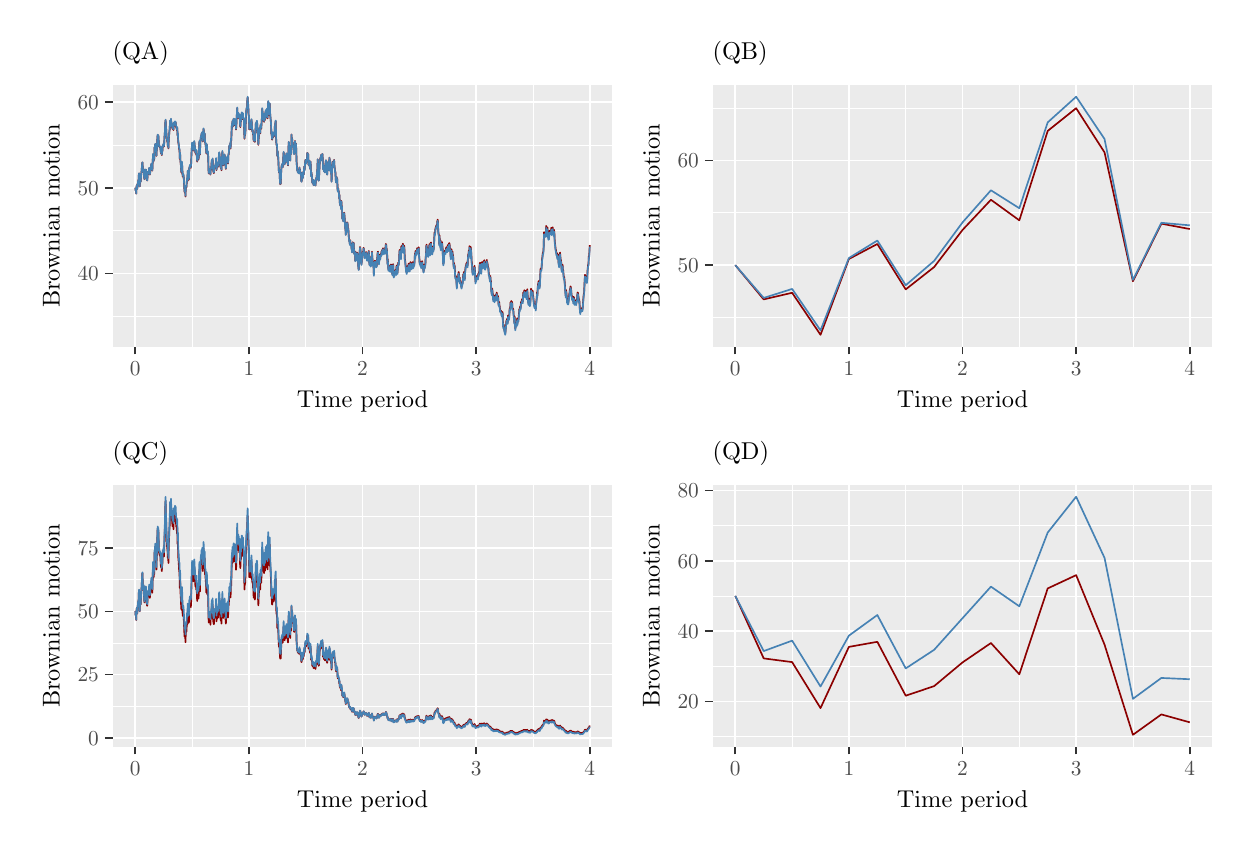
\begin{tikzpicture}[x=1pt,y=1pt]
\definecolor{fillColor}{RGB}{255,255,255}
\path[use as bounding box,fill=fillColor,fill opacity=0.00] (0,0) rectangle (433.62,289.08);
\begin{scope}
\path[clip] (  0.00,144.54) rectangle (216.81,289.08);
\definecolor{drawColor}{RGB}{255,255,255}
\definecolor{fillColor}{RGB}{255,255,255}

\path[draw=drawColor,line width= 0.6pt,line join=round,line cap=round,fill=fillColor] (  0.00,144.54) rectangle (216.81,289.08);
\end{scope}
\begin{scope}
\path[clip] ( 30.68,173.80) rectangle (211.31,268.42);
\definecolor{fillColor}{gray}{0.92}

\path[fill=fillColor] ( 30.68,173.80) rectangle (211.31,268.42);
\definecolor{drawColor}{RGB}{255,255,255}

\path[draw=drawColor,line width= 0.3pt,line join=round] ( 30.68,184.79) --
	(211.31,184.79);

\path[draw=drawColor,line width= 0.3pt,line join=round] ( 30.68,215.73) --
	(211.31,215.73);

\path[draw=drawColor,line width= 0.3pt,line join=round] ( 30.68,246.67) --
	(211.31,246.67);

\path[draw=drawColor,line width= 0.3pt,line join=round] ( 59.42,173.80) --
	( 59.42,268.42);

\path[draw=drawColor,line width= 0.3pt,line join=round] (100.47,173.80) --
	(100.47,268.42);

\path[draw=drawColor,line width= 0.3pt,line join=round] (141.52,173.80) --
	(141.52,268.42);

\path[draw=drawColor,line width= 0.3pt,line join=round] (182.57,173.80) --
	(182.57,268.42);

\path[draw=drawColor,line width= 0.6pt,line join=round] ( 30.68,200.26) --
	(211.31,200.26);

\path[draw=drawColor,line width= 0.6pt,line join=round] ( 30.68,231.20) --
	(211.31,231.20);

\path[draw=drawColor,line width= 0.6pt,line join=round] ( 30.68,262.13) --
	(211.31,262.13);

\path[draw=drawColor,line width= 0.6pt,line join=round] ( 38.89,173.80) --
	( 38.89,268.42);

\path[draw=drawColor,line width= 0.6pt,line join=round] ( 79.94,173.80) --
	( 79.94,268.42);

\path[draw=drawColor,line width= 0.6pt,line join=round] (121.00,173.80) --
	(121.00,268.42);

\path[draw=drawColor,line width= 0.6pt,line join=round] (162.05,173.80) --
	(162.05,268.42);

\path[draw=drawColor,line width= 0.6pt,line join=round] (203.10,173.80) --
	(203.10,268.42);
\definecolor{drawColor}{RGB}{139,0,0}

\path[draw=drawColor,line width= 0.6pt,line join=round] ( 38.89,231.20) --
	( 39.01,230.17) --
	( 39.12,230.46) --
	( 39.23,229.10) --
	( 39.35,231.68) --
	( 39.46,232.21) --
	( 39.58,230.86) --
	( 39.69,231.65) --
	( 39.80,232.85) --
	( 39.92,233.80) --
	( 40.03,233.28) --
	( 40.15,235.79) --
	( 40.26,236.44) --
	( 40.37,235.39) --
	( 40.49,231.71) --
	( 40.60,233.55) --
	( 40.72,233.47) --
	( 40.83,233.43) --
	( 40.94,234.99) --
	( 41.06,236.36) --
	( 41.17,237.36) --
	( 41.29,238.92) --
	( 41.40,240.25) --
	( 41.51,240.37) --
	( 41.63,236.96) --
	( 41.74,238.00) --
	( 41.86,237.90) --
	( 41.97,237.63) --
	( 42.08,235.14) --
	( 42.20,234.33) --
	( 42.31,235.02) --
	( 42.43,237.30) --
	( 42.54,237.11) --
	( 42.65,237.76) --
	( 42.77,237.66) --
	( 42.88,235.33) --
	( 43.00,234.63) --
	( 43.11,233.97) --
	( 43.22,233.86) --
	( 43.34,235.68) --
	( 43.45,236.96) --
	( 43.57,236.67) --
	( 43.68,236.24) --
	( 43.79,237.41) --
	( 43.91,238.34) --
	( 44.02,237.17) --
	( 44.14,235.96) --
	( 44.25,236.57) --
	( 44.36,237.86) --
	( 44.48,237.66) --
	( 44.59,239.16) --
	( 44.71,239.83) --
	( 44.82,238.77) --
	( 44.94,239.35) --
	( 45.05,237.41) --
	( 45.16,239.85) --
	( 45.28,243.29) --
	( 45.39,242.63) --
	( 45.51,240.81) --
	( 45.62,241.79) --
	( 45.73,241.54) --
	( 45.85,245.76) --
	( 45.96,245.68) --
	( 46.08,246.91) --
	( 46.19,246.95) --
	( 46.30,245.61) --
	( 46.42,245.94) --
	( 46.53,242.74) --
	( 46.65,245.31) --
	( 46.76,245.58) --
	( 46.87,249.48) --
	( 46.99,250.34) --
	( 47.10,249.04) --
	( 47.22,250.14) --
	( 47.33,248.43) --
	( 47.44,246.17) --
	( 47.56,246.68) --
	( 47.67,245.88) --
	( 47.79,245.87) --
	( 47.90,245.99) --
	( 48.01,244.93) --
	( 48.13,243.92) --
	( 48.24,243.67) --
	( 48.36,245.75) --
	( 48.47,243.04) --
	( 48.58,244.08) --
	( 48.70,244.66) --
	( 48.81,246.54) --
	( 48.93,245.99) --
	( 49.04,246.64) --
	( 49.15,247.11) --
	( 49.27,246.13) --
	( 49.38,248.30) --
	( 49.50,250.40) --
	( 49.61,251.68) --
	( 49.72,254.62) --
	( 49.84,255.66) --
	( 49.95,253.26) --
	( 50.07,252.19) --
	( 50.18,249.92) --
	( 50.29,249.05) --
	( 50.41,247.92) --
	( 50.52,247.98) --
	( 50.64,246.33) --
	( 50.75,246.61) --
	( 50.86,245.43) --
	( 50.98,248.60) --
	( 51.09,249.89) --
	( 51.21,251.55) --
	( 51.32,252.25) --
	( 51.44,255.39) --
	( 51.55,254.18) --
	( 51.66,253.31) --
	( 51.78,255.99) --
	( 51.89,254.75) --
	( 52.01,254.35) --
	( 52.12,253.61) --
	( 52.23,253.00) --
	( 52.35,252.47) --
	( 52.46,253.38) --
	( 52.58,253.04) --
	( 52.69,252.10) --
	( 52.80,254.59) --
	( 52.92,254.18) --
	( 53.03,253.83) --
	( 53.15,253.63) --
	( 53.26,254.96) --
	( 53.37,254.81) --
	( 53.49,254.73) --
	( 53.60,253.44) --
	( 53.72,252.83) --
	( 53.83,252.93) --
	( 53.94,251.83) --
	( 54.06,252.81) --
	( 54.17,250.00) --
	( 54.29,250.55) --
	( 54.40,247.74) --
	( 54.51,247.19) --
	( 54.63,246.24) --
	( 54.74,245.06) --
	( 54.86,244.95) --
	( 54.97,241.58) --
	( 55.08,243.63) --
	( 55.20,240.71) --
	( 55.31,239.90) --
	( 55.43,237.98) --
	( 55.54,236.70) --
	( 55.65,240.26) --
	( 55.77,240.28) --
	( 55.88,238.06) --
	( 56.00,235.28) --
	( 56.11,236.03) --
	( 56.22,235.99) --
	( 56.34,235.45) --
	( 56.45,233.89) --
	( 56.57,231.43) --
	( 56.68,229.68) --
	( 56.79,231.29) --
	( 56.91,230.27) --
	( 57.02,228.04) --
	( 57.14,231.05) --
	( 57.25,231.73) --
	( 57.36,231.33) --
	( 57.48,233.06) --
	( 57.59,234.52) --
	( 57.71,233.48) --
	( 57.82,237.17) --
	( 57.93,236.73) --
	( 58.05,234.33) --
	( 58.16,234.08) --
	( 58.28,234.42) --
	( 58.39,238.30) --
	( 58.51,238.47) --
	( 58.62,239.24) --
	( 58.73,239.10) --
	( 58.85,238.52) --
	( 58.96,238.45) --
	( 59.08,239.79) --
	( 59.19,243.40) --
	( 59.30,245.20) --
	( 59.42,247.36) --
	( 59.53,245.14) --
	( 59.65,246.89) --
	( 59.76,247.28) --
	( 59.87,244.65) --
	( 59.99,245.56) --
	( 60.10,245.27) --
	( 60.22,247.89) --
	( 60.33,246.50) --
	( 60.44,245.72) --
	( 60.56,244.07) --
	( 60.67,243.75) --
	( 60.79,244.45) --
	( 60.90,243.15) --
	( 61.01,244.60) --
	( 61.13,242.47) --
	( 61.24,240.64) --
	( 61.36,243.14) --
	( 61.47,241.36) --
	( 61.58,242.06) --
	( 61.70,241.39) --
	( 61.81,242.09) --
	( 61.93,245.06) --
	( 62.04,247.89) --
	( 62.15,247.29) --
	( 62.27,243.21) --
	( 62.38,247.65) --
	( 62.50,248.85) --
	( 62.61,249.82) --
	( 62.72,249.79) --
	( 62.84,250.71) --
	( 62.95,250.40) --
	( 63.07,251.17) --
	( 63.18,250.42) --
	( 63.29,247.92) --
	( 63.41,249.70) --
	( 63.52,252.49) --
	( 63.64,251.91) --
	( 63.75,249.60) --
	( 63.86,250.76) --
	( 63.98,250.67) --
	( 64.09,247.51) --
	( 64.21,247.50) --
	( 64.32,246.36) --
	( 64.43,245.74) --
	( 64.55,243.68) --
	( 64.66,246.88) --
	( 64.78,246.28) --
	( 64.89,243.42) --
	( 65.00,243.76) --
	( 65.12,244.21) --
	( 65.23,242.47) --
	( 65.35,237.48) --
	( 65.46,236.39) --
	( 65.58,237.35) --
	( 65.69,237.24) --
	( 65.80,237.06) --
	( 65.92,238.00) --
	( 66.03,235.99) --
	( 66.15,237.83) --
	( 66.26,237.82) --
	( 66.37,239.01) --
	( 66.49,240.79) --
	( 66.60,241.16) --
	( 66.72,239.64) --
	( 66.83,241.64) --
	( 66.94,238.19) --
	( 67.06,237.25) --
	( 67.17,236.81) --
	( 67.29,236.52) --
	( 67.40,238.24) --
	( 67.51,238.47) --
	( 67.63,239.15) --
	( 67.74,239.02) --
	( 67.86,238.59) --
	( 67.97,239.78) --
	( 68.08,241.75) --
	( 68.20,237.61) --
	( 68.31,238.58) --
	( 68.43,239.21) --
	( 68.54,238.47) --
	( 68.65,240.09) --
	( 68.77,239.41) --
	( 68.88,238.92) --
	( 69.00,240.38) --
	( 69.11,243.37) --
	( 69.22,243.84) --
	( 69.34,243.09) --
	( 69.45,241.00) --
	( 69.57,240.42) --
	( 69.68,238.80) --
	( 69.79,238.34) --
	( 69.91,239.01) --
	( 70.02,237.55) --
	( 70.14,242.10) --
	( 70.25,242.36) --
	( 70.36,244.34) --
	( 70.48,240.33) --
	( 70.59,241.61) --
	( 70.71,239.32) --
	( 70.82,240.90) --
	( 70.93,241.58) --
	( 71.05,240.86) --
	( 71.16,243.16) --
	( 71.28,241.93) --
	( 71.39,240.91) --
	( 71.50,239.18) --
	( 71.62,238.02) --
	( 71.73,239.63) --
	( 71.85,240.37) --
	( 71.96,242.11) --
	( 72.08,241.42) --
	( 72.19,242.07) --
	( 72.30,242.48) --
	( 72.42,240.00) --
	( 72.53,243.08) --
	( 72.65,243.31) --
	( 72.76,244.65) --
	( 72.87,246.34) --
	( 72.99,246.24) --
	( 73.10,245.69) --
	( 73.22,247.28) --
	( 73.33,245.39) --
	( 73.44,248.93) --
	( 73.56,248.23) --
	( 73.67,251.24) --
	( 73.79,254.03) --
	( 73.90,254.18) --
	( 74.01,255.23) --
	( 74.13,253.30) --
	( 74.24,253.90) --
	( 74.36,255.85) --
	( 74.47,256.03) --
	( 74.58,255.16) --
	( 74.70,253.92) --
	( 74.81,253.84) --
	( 74.93,255.84) --
	( 75.04,254.92) --
	( 75.15,254.68) --
	( 75.27,252.26) --
	( 75.38,253.17) --
	( 75.50,255.61) --
	( 75.61,258.45) --
	( 75.72,260.01) --
	( 75.84,256.42) --
	( 75.95,257.32) --
	( 76.07,258.18) --
	( 76.18,257.50) --
	( 76.29,257.81) --
	( 76.41,256.16) --
	( 76.52,257.44) --
	( 76.64,256.81) --
	( 76.75,253.84) --
	( 76.86,253.15) --
	( 76.98,255.69) --
	( 77.09,255.05) --
	( 77.21,256.43) --
	( 77.32,258.22) --
	( 77.43,258.22) --
	( 77.55,257.54) --
	( 77.66,256.52) --
	( 77.78,257.92) --
	( 77.89,255.89) --
	( 78.00,256.34) --
	( 78.12,255.78) --
	( 78.23,251.54) --
	( 78.35,248.96) --
	( 78.46,250.62) --
	( 78.57,250.26) --
	( 78.69,251.73) --
	( 78.80,255.24) --
	( 78.92,258.02) --
	( 79.03,259.32) --
	( 79.15,260.04) --
	( 79.26,259.66) --
	( 79.37,262.72) --
	( 79.49,263.88) --
	( 79.60,261.57) --
	( 79.72,261.25) --
	( 79.83,257.54) --
	( 79.94,257.16) --
	( 80.06,252.28) --
	( 80.17,254.72) --
	( 80.29,253.52) --
	( 80.40,252.71) --
	( 80.51,252.39) --
	( 80.63,253.52) --
	( 80.74,254.78) --
	( 80.86,255.84) --
	( 80.97,254.75) --
	( 81.08,252.20) --
	( 81.20,251.47) --
	( 81.31,251.97) --
	( 81.43,250.45) --
	( 81.54,250.31) --
	( 81.65,248.18) --
	( 81.77,248.15) --
	( 81.88,248.38) --
	( 82.00,248.10) --
	( 82.11,247.80) --
	( 82.22,251.00) --
	( 82.34,252.40) --
	( 82.45,254.46) --
	( 82.57,252.73) --
	( 82.68,253.02) --
	( 82.79,255.18) --
	( 82.91,255.06) --
	( 83.02,251.09) --
	( 83.14,251.71) --
	( 83.25,248.22) --
	( 83.36,246.75) --
	( 83.48,249.13) --
	( 83.59,250.25) --
	( 83.71,252.25) --
	( 83.82,252.81) --
	( 83.93,252.59) --
	( 84.05,250.88) --
	( 84.16,253.82) --
	( 84.28,253.89) --
	( 84.39,252.55) --
	( 84.50,254.15) --
	( 84.62,256.17) --
	( 84.73,259.78) --
	( 84.85,258.61) --
	( 84.96,257.85) --
	( 85.07,257.05) --
	( 85.19,256.33) --
	( 85.30,255.62) --
	( 85.42,255.05) --
	( 85.53,257.78) --
	( 85.65,256.44) --
	( 85.76,255.70) --
	( 85.87,256.92) --
	( 85.99,259.06) --
	( 86.10,257.57) --
	( 86.22,256.60) --
	( 86.33,257.58) --
	( 86.44,259.53) --
	( 86.56,259.03) --
	( 86.67,256.29) --
	( 86.79,259.55) --
	( 86.90,262.33) --
	( 87.01,260.93) --
	( 87.13,260.80) --
	( 87.24,257.40) --
	( 87.36,258.48) --
	( 87.47,261.59) --
	( 87.58,258.41) --
	( 87.70,256.91) --
	( 87.81,255.69) --
	( 87.93,254.40) --
	( 88.04,250.61) --
	( 88.15,251.53) --
	( 88.27,248.71) --
	( 88.38,248.66) --
	( 88.50,249.73) --
	( 88.61,249.36) --
	( 88.72,250.98) --
	( 88.84,250.92) --
	( 88.95,249.73) --
	( 89.07,250.90) --
	( 89.18,250.10) --
	( 89.29,253.36) --
	( 89.41,253.32) --
	( 89.52,254.90) --
	( 89.64,255.28) --
	( 89.75,249.69) --
	( 89.86,247.21) --
	( 89.98,246.43) --
	( 90.09,246.85) --
	( 90.21,242.69) --
	( 90.32,244.37) --
	( 90.43,243.29) --
	( 90.55,241.97) --
	( 90.66,239.27) --
	( 90.78,236.78) --
	( 90.89,236.87) --
	( 91.00,237.72) --
	( 91.12,234.19) --
	( 91.23,232.52) --
	( 91.35,233.39) --
	( 91.46,232.64) --
	( 91.57,236.23) --
	( 91.69,238.34) --
	( 91.80,239.35) --
	( 91.92,239.35) --
	( 92.03,239.82) --
	( 92.14,238.60) --
	( 92.26,239.66) --
	( 92.37,242.22) --
	( 92.49,244.11) --
	( 92.60,242.68) --
	( 92.72,239.85) --
	( 92.83,239.66) --
	( 92.94,240.41) --
	( 93.06,242.75) --
	( 93.17,240.45) --
	( 93.29,241.07) --
	( 93.40,241.46) --
	( 93.51,243.54) --
	( 93.63,243.48) --
	( 93.74,242.85) --
	( 93.86,240.84) --
	( 93.97,239.94) --
	( 94.08,239.31) --
	( 94.20,243.38) --
	( 94.31,247.73) --
	( 94.43,247.42) --
	( 94.54,245.54) --
	( 94.65,242.05) --
	( 94.77,242.94) --
	( 94.88,241.03) --
	( 95.00,245.03) --
	( 95.11,243.46) --
	( 95.22,243.64) --
	( 95.34,250.48) --
	( 95.45,248.45) --
	( 95.57,249.00) --
	( 95.68,246.99) --
	( 95.79,247.61) --
	( 95.91,246.03) --
	( 96.02,246.16) --
	( 96.14,245.62) --
	( 96.25,243.51) --
	( 96.36,243.53) --
	( 96.48,245.27) --
	( 96.59,248.12) --
	( 96.71,245.65) --
	( 96.82,245.19) --
	( 96.93,247.26) --
	( 97.05,245.25) --
	( 97.16,240.81) --
	( 97.28,239.18) --
	( 97.39,237.53) --
	( 97.50,237.60) --
	( 97.62,236.90) --
	( 97.73,237.29) --
	( 97.85,236.56) --
	( 97.96,237.19) --
	( 98.07,236.56) --
	( 98.19,238.57) --
	( 98.30,237.31) --
	( 98.42,237.79) --
	( 98.53,236.29) --
	( 98.64,236.63) --
	( 98.76,236.54) --
	( 98.87,233.71) --
	( 98.99,233.47) --
	( 99.10,235.42) --
	( 99.22,236.56) --
	( 99.33,236.79) --
	( 99.44,234.78) --
	( 99.56,236.73) --
	( 99.67,236.86) --
	( 99.79,236.09) --
	( 99.90,238.87) --
	(100.01,237.55) --
	(100.13,238.05) --
	(100.24,240.24) --
	(100.36,241.27) --
	(100.47,240.73) --
	(100.58,240.00) --
	(100.70,240.60) --
	(100.81,241.49) --
	(100.93,241.51) --
	(101.04,243.81) --
	(101.15,243.68) --
	(101.27,242.44) --
	(101.38,243.38) --
	(101.50,239.54) --
	(101.61,240.21) --
	(101.72,241.06) --
	(101.84,240.66) --
	(101.95,238.73) --
	(102.07,238.05) --
	(102.18,240.70) --
	(102.29,239.41) --
	(102.41,235.44) --
	(102.52,236.80) --
	(102.64,235.95) --
	(102.75,235.08) --
	(102.86,233.05) --
	(102.98,233.01) --
	(103.09,234.16) --
	(103.21,233.18) --
	(103.32,232.17) --
	(103.43,233.97) --
	(103.55,233.55) --
	(103.66,233.28) --
	(103.78,232.24) --
	(103.89,233.72) --
	(104.00,232.07) --
	(104.12,233.46) --
	(104.23,234.79) --
	(104.35,234.00) --
	(104.46,235.41) --
	(104.57,237.06) --
	(104.69,238.03) --
	(104.80,241.50) --
	(104.92,238.12) --
	(105.03,236.14) --
	(105.14,233.83) --
	(105.26,234.10) --
	(105.37,236.74) --
	(105.49,239.59) --
	(105.60,240.43) --
	(105.71,241.94) --
	(105.83,241.68) --
	(105.94,242.49) --
	(106.06,243.14) --
	(106.17,241.80) --
	(106.29,241.28) --
	(106.40,241.04) --
	(106.51,243.46) --
	(106.63,241.64) --
	(106.74,237.99) --
	(106.86,239.29) --
	(106.97,237.89) --
	(107.08,237.14) --
	(107.20,238.67) --
	(107.31,237.36) --
	(107.43,236.78) --
	(107.54,239.33) --
	(107.65,240.23) --
	(107.77,241.16) --
	(107.88,240.91) --
	(108.00,238.94) --
	(108.11,236.39) --
	(108.22,236.01) --
	(108.34,239.40) --
	(108.45,239.77) --
	(108.57,240.04) --
	(108.68,240.61) --
	(108.79,239.94) --
	(108.91,237.53) --
	(109.02,242.13) --
	(109.14,241.38) --
	(109.25,240.86) --
	(109.36,237.77) --
	(109.48,237.34) --
	(109.59,236.92) --
	(109.71,236.47) --
	(109.82,233.48) --
	(109.93,236.45) --
	(110.05,239.45) --
	(110.16,240.62) --
	(110.28,238.72) --
	(110.39,239.94) --
	(110.50,239.51) --
	(110.62,238.95) --
	(110.73,241.29) --
	(110.85,239.16) --
	(110.96,238.28) --
	(111.07,237.03) --
	(111.19,237.05) --
	(111.30,234.40) --
	(111.42,233.23) --
	(111.53,234.41) --
	(111.64,235.17) --
	(111.76,233.55) --
	(111.87,234.47) --
	(111.99,230.46) --
	(112.10,229.90) --
	(112.21,231.05) --
	(112.33,229.97) --
	(112.44,229.90) --
	(112.56,227.34) --
	(112.67,228.68) --
	(112.79,225.74) --
	(112.90,225.22) --
	(113.01,224.81) --
	(113.13,224.90) --
	(113.24,223.61) --
	(113.36,226.46) --
	(113.47,224.21) --
	(113.58,224.60) --
	(113.70,220.07) --
	(113.81,220.07) --
	(113.93,220.84) --
	(114.04,219.19) --
	(114.15,220.24) --
	(114.27,220.74) --
	(114.38,222.22) --
	(114.50,220.92) --
	(114.61,219.45) --
	(114.72,216.79) --
	(114.84,216.31) --
	(114.95,214.34) --
	(115.07,215.34) --
	(115.18,215.44) --
	(115.29,218.67) --
	(115.41,216.94) --
	(115.52,218.69) --
	(115.64,217.90) --
	(115.75,215.73) --
	(115.86,216.57) --
	(115.98,214.46) --
	(116.09,212.93) --
	(116.21,211.87) --
	(116.32,212.16) --
	(116.43,210.74) --
	(116.55,212.26) --
	(116.66,210.55) --
	(116.78,210.85) --
	(116.89,211.04) --
	(117.00,209.53) --
	(117.12,208.93) --
	(117.23,208.01) --
	(117.35,209.34) --
	(117.46,211.52) --
	(117.57,210.04) --
	(117.69,211.35) --
	(117.80,211.24) --
	(117.92,208.47) --
	(118.03,207.41) --
	(118.14,208.04) --
	(118.26,208.24) --
	(118.37,204.88) --
	(118.49,205.66) --
	(118.60,206.55) --
	(118.71,206.13) --
	(118.83,205.16) --
	(118.94,207.85) --
	(119.06,207.72) --
	(119.17,207.69) --
	(119.28,206.14) --
	(119.40,204.31) --
	(119.51,202.27) --
	(119.63,201.70) --
	(119.74,203.50) --
	(119.86,205.87) --
	(119.97,208.01) --
	(120.08,209.82) --
	(120.20,209.48) --
	(120.31,207.76) --
	(120.43,207.30) --
	(120.54,204.01) --
	(120.65,203.58) --
	(120.77,205.82) --
	(120.88,205.99) --
	(121.00,207.49) --
	(121.11,208.16) --
	(121.22,207.07) --
	(121.34,209.49) --
	(121.45,209.37) --
	(121.57,208.01) --
	(121.68,208.10) --
	(121.79,206.00) --
	(121.91,207.18) --
	(122.02,207.86) --
	(122.14,207.36) --
	(122.25,206.69) --
	(122.36,207.97) --
	(122.48,206.50) --
	(122.59,205.15) --
	(122.71,205.72) --
	(122.82,205.10) --
	(122.93,206.35) --
	(123.05,206.07) --
	(123.16,207.71) --
	(123.28,208.39) --
	(123.39,205.30) --
	(123.50,203.49) --
	(123.62,205.21) --
	(123.73,206.14) --
	(123.85,204.82) --
	(123.96,203.01) --
	(124.07,204.39) --
	(124.19,203.29) --
	(124.30,205.71) --
	(124.42,208.14) --
	(124.53,206.13) --
	(124.64,204.97) --
	(124.76,203.28) --
	(124.87,204.17) --
	(124.99,202.44) --
	(125.10,199.76) --
	(125.21,202.41) --
	(125.33,203.74) --
	(125.44,204.84) --
	(125.56,203.93) --
	(125.67,203.91) --
	(125.78,204.74) --
	(125.90,203.01) --
	(126.01,202.84) --
	(126.13,203.07) --
	(126.24,205.34) --
	(126.36,206.21) --
	(126.47,207.96) --
	(126.58,208.15) --
	(126.70,206.61) --
	(126.81,206.14) --
	(126.93,203.88) --
	(127.04,205.12) --
	(127.15,207.05) --
	(127.27,206.96) --
	(127.38,205.61) --
	(127.50,207.09) --
	(127.61,207.27) --
	(127.72,206.73) --
	(127.84,208.28) --
	(127.95,207.22) --
	(128.07,208.80) --
	(128.18,207.63) --
	(128.29,208.16) --
	(128.41,209.40) --
	(128.52,207.53) --
	(128.64,208.08) --
	(128.75,207.91) --
	(128.86,208.85) --
	(128.98,207.74) --
	(129.09,207.62) --
	(129.21,209.53) --
	(129.32,209.76) --
	(129.43,210.92) --
	(129.55,210.60) --
	(129.66,209.14) --
	(129.78,209.12) --
	(129.89,207.41) --
	(130.00,203.87) --
	(130.12,205.44) --
	(130.23,203.97) --
	(130.35,201.53) --
	(130.46,202.84) --
	(130.57,202.82) --
	(130.69,202.02) --
	(130.80,201.77) --
	(130.92,201.21) --
	(131.03,202.52) --
	(131.14,203.48) --
	(131.26,201.18) --
	(131.37,201.64) --
	(131.49,202.59) --
	(131.60,203.48) --
	(131.71,200.27) --
	(131.83,199.96) --
	(131.94,202.55) --
	(132.06,203.61) --
	(132.17,201.33) --
	(132.28,199.15) --
	(132.40,199.78) --
	(132.51,199.55) --
	(132.63,200.80) --
	(132.74,201.18) --
	(132.85,201.28) --
	(132.97,201.51) --
	(133.08,201.72) --
	(133.20,200.05) --
	(133.31,203.14) --
	(133.43,201.26) --
	(133.54,201.24) --
	(133.65,200.51) --
	(133.77,202.88) --
	(133.88,204.23) --
	(134.00,203.47) --
	(134.11,203.73) --
	(134.22,205.30) --
	(134.34,208.36) --
	(134.45,208.78) --
	(134.57,207.33) --
	(134.68,205.97) --
	(134.79,208.73) --
	(134.91,205.87) --
	(135.02,210.09) --
	(135.14,209.72) --
	(135.25,209.07) --
	(135.36,209.29) --
	(135.48,210.59) --
	(135.59,211.01) --
	(135.71,208.26) --
	(135.82,208.75) --
	(135.93,209.37) --
	(136.05,210.29) --
	(136.16,208.83) --
	(136.28,205.56) --
	(136.39,205.11) --
	(136.50,203.83) --
	(136.62,202.80) --
	(136.73,201.53) --
	(136.85,201.00) --
	(136.96,200.59) --
	(137.07,201.62) --
	(137.19,202.93) --
	(137.30,201.86) --
	(137.42,201.45) --
	(137.53,201.92) --
	(137.64,203.78) --
	(137.76,203.69) --
	(137.87,201.43) --
	(137.99,201.73) --
	(138.10,201.56) --
	(138.21,203.91) --
	(138.33,204.37) --
	(138.44,203.53) --
	(138.56,202.93) --
	(138.67,202.25) --
	(138.78,202.49) --
	(138.90,202.72) --
	(139.01,203.94) --
	(139.13,204.36) --
	(139.24,203.86) --
	(139.35,202.60) --
	(139.47,203.44) --
	(139.58,203.35) --
	(139.70,203.58) --
	(139.81,205.06) --
	(139.93,207.45) --
	(140.04,206.14) --
	(140.15,208.39) --
	(140.27,207.19) --
	(140.38,207.55) --
	(140.50,207.85) --
	(140.61,207.46) --
	(140.72,209.39) --
	(140.84,208.46) --
	(140.95,209.38) --
	(141.07,209.35) --
	(141.18,208.04) --
	(141.29,209.73) --
	(141.41,206.82) --
	(141.52,206.10) --
	(141.64,204.00) --
	(141.75,204.26) --
	(141.86,204.61) --
	(141.98,203.10) --
	(142.09,203.96) --
	(142.21,202.57) --
	(142.32,203.45) --
	(142.43,203.76) --
	(142.55,204.71) --
	(142.66,203.44) --
	(142.78,203.56) --
	(142.89,202.94) --
	(143.00,200.99) --
	(143.12,201.18) --
	(143.23,203.53) --
	(143.35,202.66) --
	(143.46,202.39) --
	(143.57,203.30) --
	(143.69,203.34) --
	(143.80,205.96) --
	(143.92,206.96) --
	(144.03,210.18) --
	(144.14,210.67) --
	(144.26,209.07) --
	(144.37,209.65) --
	(144.49,208.35) --
	(144.60,206.95) --
	(144.71,206.68) --
	(144.83,207.96) --
	(144.94,208.43) --
	(145.06,209.56) --
	(145.17,210.84) --
	(145.28,210.59) --
	(145.40,207.23) --
	(145.51,208.33) --
	(145.63,211.37) --
	(145.74,211.45) --
	(145.85,209.52) --
	(145.97,209.00) --
	(146.08,207.70) --
	(146.20,207.63) --
	(146.31,208.56) --
	(146.42,209.77) --
	(146.54,210.09) --
	(146.65,208.77) --
	(146.77,209.91) --
	(146.88,211.81) --
	(147.00,215.05) --
	(147.11,214.32) --
	(147.22,215.01) --
	(147.34,216.75) --
	(147.45,216.57) --
	(147.57,217.34) --
	(147.68,217.65) --
	(147.79,217.44) --
	(147.91,217.69) --
	(148.02,219.12) --
	(148.14,219.73) --
	(148.25,219.02) --
	(148.36,215.69) --
	(148.48,214.52) --
	(148.59,214.48) --
	(148.71,210.86) --
	(148.82,214.02) --
	(148.93,211.88) --
	(149.05,210.22) --
	(149.16,212.28) --
	(149.28,209.18) --
	(149.39,210.21) --
	(149.50,209.72) --
	(149.62,210.35) --
	(149.73,211.59) --
	(149.85,210.22) --
	(149.96,209.23) --
	(150.07,205.09) --
	(150.19,203.79) --
	(150.30,204.29) --
	(150.42,204.97) --
	(150.53,207.73) --
	(150.64,207.82) --
	(150.76,208.45) --
	(150.87,208.55) --
	(150.99,207.87) --
	(151.10,208.90) --
	(151.21,209.54) --
	(151.33,209.72) --
	(151.44,208.57) --
	(151.56,208.51) --
	(151.67,209.59) --
	(151.78,210.53) --
	(151.90,209.85) --
	(152.01,208.90) --
	(152.13,209.61) --
	(152.24,211.08) --
	(152.35,211.25) --
	(152.47,210.80) --
	(152.58,209.55) --
	(152.70,208.96) --
	(152.81,206.89) --
	(152.92,205.93) --
	(153.04,207.48) --
	(153.15,209.02) --
	(153.27,207.80) --
	(153.38,208.09) --
	(153.50,208.18) --
	(153.61,205.88) --
	(153.72,206.98) --
	(153.84,204.37) --
	(153.95,202.70) --
	(154.07,204.02) --
	(154.18,203.29) --
	(154.29,203.00) --
	(154.41,200.85) --
	(154.52,198.95) --
	(154.64,199.40) --
	(154.75,199.17) --
	(154.86,198.40) --
	(154.98,196.69) --
	(155.09,195.30) --
	(155.21,197.87) --
	(155.32,197.45) --
	(155.43,198.43) --
	(155.55,199.44) --
	(155.66,200.42) --
	(155.78,200.80) --
	(155.89,199.16) --
	(156.00,197.86) --
	(156.12,198.82) --
	(156.23,197.14) --
	(156.35,197.80) --
	(156.46,197.11) --
	(156.57,196.60) --
	(156.69,195.60) --
	(156.80,195.31) --
	(156.92,196.40) --
	(157.03,196.97) --
	(157.14,196.67) --
	(157.26,197.77) --
	(157.37,199.90) --
	(157.49,199.88) --
	(157.60,200.49) --
	(157.71,200.85) --
	(157.83,199.56) --
	(157.94,198.36) --
	(158.06,200.85) --
	(158.17,202.00) --
	(158.28,202.98) --
	(158.40,203.17) --
	(158.51,203.81) --
	(158.63,204.01) --
	(158.74,204.06) --
	(158.85,204.35) --
	(158.97,202.99) --
	(159.08,206.22) --
	(159.20,207.32) --
	(159.31,206.96) --
	(159.42,208.63) --
	(159.54,207.76) --
	(159.65,210.14) --
	(159.77,209.58) --
	(159.88,206.35) --
	(159.99,208.23) --
	(160.11,209.80) --
	(160.22,208.71) --
	(160.34,206.75) --
	(160.45,204.25) --
	(160.57,203.88) --
	(160.68,201.44) --
	(160.79,200.36) --
	(160.91,200.57) --
	(161.02,201.68) --
	(161.14,200.60) --
	(161.25,200.43) --
	(161.36,200.76) --
	(161.48,203.02) --
	(161.59,201.74) --
	(161.71,199.64) --
	(161.82,197.26) --
	(161.93,197.96) --
	(162.05,197.88) --
	(162.16,198.86) --
	(162.28,198.67) --
	(162.39,199.17) --
	(162.50,199.46) --
	(162.62,199.48) --
	(162.73,198.67) --
	(162.85,200.30) --
	(162.96,199.76) --
	(163.07,200.63) --
	(163.19,200.83) --
	(163.30,203.18) --
	(163.42,204.13) --
	(163.53,203.67) --
	(163.64,203.65) --
	(163.76,203.48) --
	(163.87,200.70) --
	(163.99,202.94) --
	(164.10,204.35) --
	(164.21,203.32) --
	(164.33,203.82) --
	(164.44,204.14) --
	(164.56,202.62) --
	(164.67,204.61) --
	(164.78,204.27) --
	(164.90,204.51) --
	(165.01,205.05) --
	(165.13,203.70) --
	(165.24,202.25) --
	(165.35,202.18) --
	(165.47,202.93) --
	(165.58,203.02) --
	(165.70,203.96) --
	(165.81,204.41) --
	(165.92,205.14) --
	(166.04,203.24) --
	(166.15,204.14) --
	(166.27,203.08) --
	(166.38,202.45) --
	(166.49,202.30) --
	(166.61,200.13) --
	(166.72,199.99) --
	(166.84,199.42) --
	(166.95,198.48) --
	(167.06,197.76) --
	(167.18,199.36) --
	(167.29,197.73) --
	(167.41,197.45) --
	(167.52,194.34) --
	(167.64,193.49) --
	(167.75,192.87) --
	(167.86,194.77) --
	(167.98,193.57) --
	(168.09,192.50) --
	(168.21,190.79) --
	(168.32,191.00) --
	(168.43,192.40) --
	(168.55,190.94) --
	(168.66,190.42) --
	(168.78,192.06) --
	(168.89,191.23) --
	(169.00,192.05) --
	(169.12,192.52) --
	(169.23,190.93) --
	(169.35,192.40) --
	(169.46,193.37) --
	(169.57,192.76) --
	(169.69,191.65) --
	(169.80,191.18) --
	(169.92,192.16) --
	(170.03,191.46) --
	(170.14,189.21) --
	(170.26,189.03) --
	(170.37,189.95) --
	(170.49,188.56) --
	(170.60,188.28) --
	(170.71,186.84) --
	(170.83,186.97) --
	(170.94,186.81) --
	(171.06,186.76) --
	(171.17,186.04) --
	(171.28,185.21) --
	(171.40,186.21) --
	(171.51,186.33) --
	(171.63,186.11) --
	(171.74,182.45) --
	(171.85,181.03) --
	(171.97,181.87) --
	(172.08,181.41) --
	(172.20,180.08) --
	(172.31,179.59) --
	(172.42,179.18) --
	(172.54,178.63) --
	(172.65,179.16) --
	(172.77,180.82) --
	(172.88,181.90) --
	(172.99,183.29) --
	(173.11,182.91) --
	(173.22,183.86) --
	(173.34,182.75) --
	(173.45,182.59) --
	(173.56,185.05) --
	(173.68,185.03) --
	(173.79,184.68) --
	(173.91,184.01) --
	(174.02,184.88) --
	(174.14,187.31) --
	(174.25,187.78) --
	(174.36,187.47) --
	(174.48,189.91) --
	(174.59,188.98) --
	(174.71,190.32) --
	(174.82,189.81) --
	(174.93,188.59) --
	(175.05,190.04) --
	(175.16,187.90) --
	(175.28,187.53) --
	(175.39,187.54) --
	(175.50,187.02) --
	(175.62,185.12) --
	(175.73,184.38) --
	(175.85,182.62) --
	(175.96,184.79) --
	(176.07,182.68) --
	(176.19,180.35) --
	(176.30,181.11) --
	(176.42,182.11) --
	(176.53,181.88) --
	(176.64,181.65) --
	(176.76,182.45) --
	(176.87,184.02) --
	(176.99,182.22) --
	(177.10,183.68) --
	(177.21,183.90) --
	(177.33,183.51) --
	(177.44,184.94) --
	(177.56,186.01) --
	(177.67,187.49) --
	(177.78,187.14) --
	(177.90,188.05) --
	(178.01,188.39) --
	(178.13,187.77) --
	(178.24,189.85) --
	(178.35,190.03) --
	(178.47,189.96) --
	(178.58,190.59) --
	(178.70,191.05) --
	(178.81,190.20) --
	(178.92,190.13) --
	(179.04,193.29) --
	(179.15,193.19) --
	(179.27,192.82) --
	(179.38,193.72) --
	(179.49,194.21) --
	(179.61,193.54) --
	(179.72,192.20) --
	(179.84,193.23) --
	(179.95,193.37) --
	(180.06,193.96) --
	(180.18,193.60) --
	(180.29,191.57) --
	(180.41,191.65) --
	(180.52,194.58) --
	(180.63,192.77) --
	(180.75,191.56) --
	(180.86,189.94) --
	(180.98,189.50) --
	(181.09,191.15) --
	(181.21,190.96) --
	(181.32,190.65) --
	(181.43,189.10) --
	(181.55,189.17) --
	(181.66,190.40) --
	(181.78,193.14) --
	(181.89,194.76) --
	(182.00,193.68) --
	(182.12,193.05) --
	(182.23,193.79) --
	(182.35,193.77) --
	(182.46,194.11) --
	(182.57,192.49) --
	(182.69,191.96) --
	(182.80,190.83) --
	(182.92,189.71) --
	(183.03,188.85) --
	(183.14,188.35) --
	(183.26,188.34) --
	(183.37,189.08) --
	(183.49,188.47) --
	(183.60,187.46) --
	(183.71,189.36) --
	(183.83,190.54) --
	(183.94,191.38) --
	(184.06,193.45) --
	(184.17,192.24) --
	(184.28,194.76) --
	(184.40,196.29) --
	(184.51,196.68) --
	(184.63,197.46) --
	(184.74,197.53) --
	(184.85,197.39) --
	(184.97,195.39) --
	(185.08,196.32) --
	(185.20,199.05) --
	(185.31,201.77) --
	(185.42,201.98) --
	(185.54,201.84) --
	(185.65,202.07) --
	(185.77,203.59) --
	(185.88,205.57) --
	(185.99,206.12) --
	(186.11,207.65) --
	(186.22,207.60) --
	(186.34,208.28) --
	(186.45,209.93) --
	(186.56,215.14) --
	(186.68,215.06) --
	(186.79,214.08) --
	(186.91,214.72) --
	(187.02,214.12) --
	(187.13,215.04) --
	(187.25,215.53) --
	(187.36,217.46) --
	(187.48,216.04) --
	(187.59,214.27) --
	(187.71,216.55) --
	(187.82,216.88) --
	(187.93,215.51) --
	(188.05,213.94) --
	(188.16,213.14) --
	(188.28,213.98) --
	(188.39,213.21) --
	(188.50,215.15) --
	(188.62,215.50) --
	(188.73,215.78) --
	(188.85,215.75) --
	(188.96,215.31) --
	(189.07,215.05) --
	(189.19,216.75) --
	(189.30,214.77) --
	(189.42,216.36) --
	(189.53,215.83) --
	(189.64,216.91) --
	(189.76,216.81) --
	(189.87,214.83) --
	(189.99,215.33) --
	(190.10,214.39) --
	(190.21,216.03) --
	(190.33,214.81) --
	(190.44,212.22) --
	(190.56,211.00) --
	(190.67,210.18) --
	(190.78,209.01) --
	(190.90,208.67) --
	(191.01,207.84) --
	(191.13,207.27) --
	(191.24,207.71) --
	(191.35,206.10) --
	(191.47,207.14) --
	(191.58,207.13) --
	(191.70,207.07) --
	(191.81,204.29) --
	(191.92,203.88) --
	(192.04,203.13) --
	(192.15,204.26) --
	(192.27,206.14) --
	(192.38,207.82) --
	(192.49,206.28) --
	(192.61,205.19) --
	(192.72,205.06) --
	(192.84,203.63) --
	(192.95,201.49) --
	(193.06,202.53) --
	(193.18,202.61) --
	(193.29,203.42) --
	(193.41,201.82) --
	(193.52,201.36) --
	(193.63,199.82) --
	(193.75,198.74) --
	(193.86,199.03) --
	(193.98,197.98) --
	(194.09,196.71) --
	(194.20,195.06) --
	(194.32,193.27) --
	(194.43,192.21) --
	(194.55,194.30) --
	(194.66,193.48) --
	(194.78,192.11) --
	(194.89,190.40) --
	(195.00,190.22) --
	(195.12,189.74) --
	(195.23,190.03) --
	(195.35,189.69) --
	(195.46,190.72) --
	(195.57,191.59) --
	(195.69,192.87) --
	(195.80,193.16) --
	(195.92,194.53) --
	(196.03,194.43) --
	(196.14,195.59) --
	(196.26,195.38) --
	(196.37,194.53) --
	(196.49,193.01) --
	(196.60,192.14) --
	(196.71,191.22) --
	(196.83,191.92) --
	(196.94,191.85) --
	(197.06,191.08) --
	(197.17,189.99) --
	(197.28,191.81) --
	(197.40,191.51) --
	(197.51,190.00) --
	(197.63,189.48) --
	(197.74,189.59) --
	(197.85,190.58) --
	(197.97,190.47) --
	(198.08,190.60) --
	(198.20,189.35) --
	(198.31,190.29) --
	(198.42,190.41) --
	(198.54,191.29) --
	(198.65,193.17) --
	(198.77,193.38) --
	(198.88,193.03) --
	(198.99,192.08) --
	(199.11,191.38) --
	(199.22,190.27) --
	(199.34,190.71) --
	(199.45,188.95) --
	(199.56,186.89) --
	(199.68,186.11) --
	(199.79,187.37) --
	(199.91,187.50) --
	(200.02,186.92) --
	(200.13,187.70) --
	(200.25,187.28) --
	(200.36,187.14) --
	(200.48,187.22) --
	(200.59,188.49) --
	(200.70,190.02) --
	(200.82,191.56) --
	(200.93,192.75) --
	(201.05,193.14) --
	(201.16,195.47) --
	(201.28,198.05) --
	(201.39,199.76) --
	(201.50,199.47) --
	(201.62,198.12) --
	(201.73,198.36) --
	(201.85,197.64) --
	(201.96,197.99) --
	(202.07,197.28) --
	(202.19,198.45) --
	(202.30,201.29) --
	(202.42,202.56) --
	(202.53,203.54) --
	(202.64,203.58) --
	(202.76,206.53) --
	(202.87,206.41) --
	(202.99,208.31) --
	(203.10,210.50);
\definecolor{drawColor}{RGB}{70,130,180}

\path[draw=drawColor,line width= 0.6pt,line join=round] ( 38.89,231.20) --
	( 39.01,230.18) --
	( 39.12,230.47) --
	( 39.23,229.12) --
	( 39.35,231.68) --
	( 39.46,232.22) --
	( 39.58,230.88) --
	( 39.69,231.67) --
	( 39.80,232.88) --
	( 39.92,233.83) --
	( 40.03,233.32) --
	( 40.15,235.82) --
	( 40.26,236.47) --
	( 40.37,235.42) --
	( 40.49,231.72) --
	( 40.60,233.56) --
	( 40.72,233.48) --
	( 40.83,233.45) --
	( 40.94,235.02) --
	( 41.06,236.39) --
	( 41.17,237.39) --
	( 41.29,238.95) --
	( 41.40,240.29) --
	( 41.51,240.41) --
	( 41.63,236.98) --
	( 41.74,238.03) --
	( 41.86,237.93) --
	( 41.97,237.67) --
	( 42.08,235.17) --
	( 42.20,234.37) --
	( 42.31,235.06) --
	( 42.43,237.33) --
	( 42.54,237.16) --
	( 42.65,237.82) --
	( 42.77,237.72) --
	( 42.88,235.39) --
	( 43.00,234.69) --
	( 43.11,234.03) --
	( 43.22,233.94) --
	( 43.34,235.76) --
	( 43.45,237.04) --
	( 43.57,236.76) --
	( 43.68,236.33) --
	( 43.79,237.51) --
	( 43.91,238.45) --
	( 44.02,237.28) --
	( 44.14,236.08) --
	( 44.25,236.69) --
	( 44.36,237.99) --
	( 44.48,237.80) --
	( 44.59,239.29) --
	( 44.71,239.98) --
	( 44.82,238.92) --
	( 44.94,239.51) --
	( 45.05,237.57) --
	( 45.16,240.00) --
	( 45.28,243.41) --
	( 45.39,242.76) --
	( 45.51,240.93) --
	( 45.62,241.92) --
	( 45.73,241.69) --
	( 45.85,245.86) --
	( 45.96,245.79) --
	( 46.08,247.02) --
	( 46.19,247.07) --
	( 46.30,245.74) --
	( 46.42,246.07) --
	( 46.53,242.85) --
	( 46.65,245.42) --
	( 46.76,245.69) --
	( 46.87,249.56) --
	( 46.99,250.43) --
	( 47.10,249.13) --
	( 47.22,250.24) --
	( 47.33,248.53) --
	( 47.44,246.26) --
	( 47.56,246.78) --
	( 47.67,245.98) --
	( 47.79,245.99) --
	( 47.90,246.12) --
	( 48.01,245.07) --
	( 48.13,244.06) --
	( 48.24,243.82) --
	( 48.36,245.89) --
	( 48.47,243.18) --
	( 48.58,244.22) --
	( 48.70,244.81) --
	( 48.81,246.69) --
	( 48.93,246.15) --
	( 49.04,246.81) --
	( 49.15,247.29) --
	( 49.27,246.31) --
	( 49.38,248.47) --
	( 49.50,250.57) --
	( 49.61,251.85) --
	( 49.72,254.78) --
	( 49.84,255.83) --
	( 49.95,253.42) --
	( 50.07,252.35) --
	( 50.18,250.09) --
	( 50.29,249.22) --
	( 50.41,248.09) --
	( 50.52,248.17) --
	( 50.64,246.52) --
	( 50.75,246.81) --
	( 50.86,245.63) --
	( 50.98,248.78) --
	( 51.09,250.08) --
	( 51.21,251.74) --
	( 51.32,252.45) --
	( 51.44,255.57) --
	( 51.55,254.37) --
	( 51.66,253.50) --
	( 51.78,256.17) --
	( 51.89,254.94) --
	( 52.01,254.55) --
	( 52.12,253.82) --
	( 52.23,253.22) --
	( 52.35,252.70) --
	( 52.46,253.62) --
	( 52.58,253.28) --
	( 52.69,252.34) --
	( 52.80,254.83) --
	( 52.92,254.43) --
	( 53.03,254.09) --
	( 53.15,253.90) --
	( 53.26,255.23) --
	( 53.37,255.09) --
	( 53.49,255.02) --
	( 53.60,253.74) --
	( 53.72,253.14) --
	( 53.83,253.25) --
	( 53.94,252.16) --
	( 54.06,253.14) --
	( 54.17,250.32) --
	( 54.29,250.88) --
	( 54.40,248.06) --
	( 54.51,247.52) --
	( 54.63,246.56) --
	( 54.74,245.40) --
	( 54.86,245.30) --
	( 54.97,241.90) --
	( 55.08,243.95) --
	( 55.20,241.01) --
	( 55.31,240.21) --
	( 55.43,238.29) --
	( 55.54,237.01) --
	( 55.65,240.53) --
	( 55.77,240.56) --
	( 55.88,238.34) --
	( 56.00,235.55) --
	( 56.11,236.30) --
	( 56.22,236.27) --
	( 56.34,235.74) --
	( 56.45,234.18) --
	( 56.57,231.71) --
	( 56.68,229.96) --
	( 56.79,231.57) --
	( 56.91,230.56) --
	( 57.02,228.31) --
	( 57.14,231.30) --
	( 57.25,231.99) --
	( 57.36,231.60) --
	( 57.48,233.33) --
	( 57.59,234.79) --
	( 57.71,233.76) --
	( 57.82,237.41) --
	( 57.93,236.98) --
	( 58.05,234.57) --
	( 58.16,234.33) --
	( 58.28,234.68) --
	( 58.39,238.52) --
	( 58.51,238.70) --
	( 58.62,239.48) --
	( 58.73,239.35) --
	( 58.85,238.78) --
	( 58.96,238.72) --
	( 59.08,240.06) --
	( 59.19,243.63) --
	( 59.30,245.44) --
	( 59.42,247.59) --
	( 59.53,245.37) --
	( 59.65,247.12) --
	( 59.76,247.51) --
	( 59.87,244.87) --
	( 59.99,245.80) --
	( 60.10,245.51) --
	( 60.22,248.12) --
	( 60.33,246.73) --
	( 60.44,245.96) --
	( 60.56,244.31) --
	( 60.67,244.00) --
	( 60.79,244.71) --
	( 60.90,243.41) --
	( 61.01,244.87) --
	( 61.13,242.73) --
	( 61.24,240.90) --
	( 61.36,243.39) --
	( 61.47,241.61) --
	( 61.58,242.32) --
	( 61.70,241.66) --
	( 61.81,242.37) --
	( 61.93,245.32) --
	( 62.04,248.14) --
	( 62.15,247.54) --
	( 62.27,243.42) --
	( 62.38,247.81) --
	( 62.50,249.02) --
	( 62.61,250.00) --
	( 62.72,249.97) --
	( 62.84,250.91) --
	( 62.95,250.60) --
	( 63.07,251.38) --
	( 63.18,250.64) --
	( 63.29,248.13) --
	( 63.41,249.91) --
	( 63.52,252.69) --
	( 63.64,252.11) --
	( 63.75,249.80) --
	( 63.86,250.97) --
	( 63.98,250.89) --
	( 64.09,247.70) --
	( 64.21,247.71) --
	( 64.32,246.57) --
	( 64.43,245.96) --
	( 64.55,243.90) --
	( 64.66,247.08) --
	( 64.78,246.48) --
	( 64.89,243.61) --
	( 65.00,243.96) --
	( 65.12,244.42) --
	( 65.23,242.68) --
	( 65.35,237.62) --
	( 65.46,236.54) --
	( 65.58,237.50) --
	( 65.69,237.40) --
	( 65.80,237.23) --
	( 65.92,238.18) --
	( 66.03,236.16) --
	( 66.15,238.00) --
	( 66.26,237.99) --
	( 66.37,239.20) --
	( 66.49,240.97) --
	( 66.60,241.35) --
	( 66.72,239.83) --
	( 66.83,241.83) --
	( 66.94,238.35) --
	( 67.06,237.42) --
	( 67.17,236.99) --
	( 67.29,236.71) --
	( 67.40,238.43) --
	( 67.51,238.66) --
	( 67.63,239.35) --
	( 67.74,239.23) --
	( 67.86,238.81) --
	( 67.97,240.00) --
	( 68.08,241.97) --
	( 68.20,237.79) --
	( 68.31,238.76) --
	( 68.43,239.40) --
	( 68.54,238.67) --
	( 68.65,240.29) --
	( 68.77,239.62) --
	( 68.88,239.13) --
	( 69.00,240.60) --
	( 69.11,243.57) --
	( 69.22,244.05) --
	( 69.34,243.30) --
	( 69.45,241.21) --
	( 69.57,240.64) --
	( 69.68,239.02) --
	( 69.79,238.57) --
	( 69.91,239.25) --
	( 70.02,237.79) --
	( 70.14,242.28) --
	( 70.25,242.56) --
	( 70.36,244.53) --
	( 70.48,240.48) --
	( 70.59,241.76) --
	( 70.71,239.47) --
	( 70.82,241.05) --
	( 70.93,241.74) --
	( 71.05,241.03) --
	( 71.16,243.32) --
	( 71.28,242.09) --
	( 71.39,241.08) --
	( 71.50,239.35) --
	( 71.62,238.20) --
	( 71.73,239.81) --
	( 71.85,240.56) --
	( 71.96,242.29) --
	( 72.08,241.61) --
	( 72.19,242.26) --
	( 72.30,242.69) --
	( 72.42,240.20) --
	( 72.53,243.26) --
	( 72.65,243.50) --
	( 72.76,244.84) --
	( 72.87,246.54) --
	( 72.99,246.44) --
	( 73.10,245.90) --
	( 73.22,247.49) --
	( 73.33,245.61) --
	( 73.44,249.12) --
	( 73.56,248.42) --
	( 73.67,251.41) --
	( 73.79,254.20) --
	( 73.90,254.35) --
	( 74.01,255.41) --
	( 74.13,253.48) --
	( 74.24,254.09) --
	( 74.36,256.04) --
	( 74.47,256.22) --
	( 74.58,255.37) --
	( 74.70,254.13) --
	( 74.81,254.06) --
	( 74.93,256.06) --
	( 75.04,255.15) --
	( 75.15,254.92) --
	( 75.27,252.49) --
	( 75.38,253.40) --
	( 75.50,255.84) --
	( 75.61,258.67) --
	( 75.72,260.23) --
	( 75.84,256.61) --
	( 75.95,257.53) --
	( 76.07,258.40) --
	( 76.18,257.72) --
	( 76.29,258.04) --
	( 76.41,256.39) --
	( 76.52,257.68) --
	( 76.64,257.06) --
	( 76.75,254.07) --
	( 76.86,253.39) --
	( 76.98,255.93) --
	( 77.09,255.30) --
	( 77.21,256.67) --
	( 77.32,258.47) --
	( 77.43,258.48) --
	( 77.55,257.80) --
	( 77.66,256.79) --
	( 77.78,258.20) --
	( 77.89,256.16) --
	( 78.00,256.63) --
	( 78.12,256.08) --
	( 78.23,251.80) --
	( 78.35,249.20) --
	( 78.46,250.86) --
	( 78.57,250.51) --
	( 78.69,251.99) --
	( 78.80,255.47) --
	( 78.92,258.25) --
	( 79.03,259.54) --
	( 79.15,260.28) --
	( 79.26,259.90) --
	( 79.37,262.95) --
	( 79.49,264.12) --
	( 79.60,261.80) --
	( 79.72,261.50) --
	( 79.83,257.76) --
	( 79.94,257.39) --
	( 80.06,252.45) --
	( 80.17,254.89) --
	( 80.29,253.69) --
	( 80.40,252.89) --
	( 80.51,252.58) --
	( 80.63,253.71) --
	( 80.74,254.98) --
	( 80.86,256.04) --
	( 80.97,254.96) --
	( 81.08,252.40) --
	( 81.20,251.68) --
	( 81.31,252.19) --
	( 81.43,250.67) --
	( 81.54,250.54) --
	( 81.65,248.41) --
	( 81.77,248.39) --
	( 81.88,248.62) --
	( 82.00,248.36) --
	( 82.11,248.06) --
	( 82.22,251.25) --
	( 82.34,252.65) --
	( 82.45,254.71) --
	( 82.57,252.98) --
	( 82.68,253.28) --
	( 82.79,255.43) --
	( 82.91,255.33) --
	( 83.02,251.32) --
	( 83.14,251.95) --
	( 83.25,248.43) --
	( 83.36,246.97) --
	( 83.48,249.34) --
	( 83.59,250.46) --
	( 83.71,252.46) --
	( 83.82,253.03) --
	( 83.93,252.82) --
	( 84.05,251.11) --
	( 84.16,254.04) --
	( 84.28,254.12) --
	( 84.39,252.78) --
	( 84.50,254.39) --
	( 84.62,256.40) --
	( 84.73,259.99) --
	( 84.85,258.83) --
	( 84.96,258.08) --
	( 85.07,257.28) --
	( 85.19,256.57) --
	( 85.30,255.87) --
	( 85.42,255.31) --
	( 85.53,258.03) --
	( 85.65,256.69) --
	( 85.76,255.96) --
	( 85.87,257.19) --
	( 85.99,259.33) --
	( 86.10,257.84) --
	( 86.22,256.87) --
	( 86.33,257.87) --
	( 86.44,259.81) --
	( 86.56,259.32) --
	( 86.67,256.57) --
	( 86.79,259.81) --
	( 86.90,262.58) --
	( 87.01,261.19) --
	( 87.13,261.06) --
	( 87.24,257.65) --
	( 87.36,258.73) --
	( 87.47,261.82) --
	( 87.58,258.63) --
	( 87.70,257.14) --
	( 87.81,255.92) --
	( 87.93,254.63) --
	( 88.04,250.82) --
	( 88.15,251.74) --
	( 88.27,248.91) --
	( 88.38,248.87) --
	( 88.50,249.94) --
	( 88.61,249.58) --
	( 88.72,251.21) --
	( 88.84,251.16) --
	( 88.95,249.97) --
	( 89.07,251.15) --
	( 89.18,250.35) --
	( 89.29,253.59) --
	( 89.41,253.56) --
	( 89.52,255.15) --
	( 89.64,255.53) --
	( 89.75,249.87) --
	( 89.86,247.37) --
	( 89.98,246.61) --
	( 90.09,247.03) --
	( 90.21,242.83) --
	( 90.32,244.51) --
	( 90.43,243.44) --
	( 90.55,242.12) --
	( 90.66,239.41) --
	( 90.78,236.91) --
	( 90.89,237.01) --
	( 91.00,237.87) --
	( 91.12,234.30) --
	( 91.23,232.63) --
	( 91.35,233.51) --
	( 91.46,232.77) --
	( 91.57,236.33) --
	( 91.69,238.43) --
	( 91.80,239.44) --
	( 91.92,239.45) --
	( 92.03,239.93) --
	( 92.14,238.71) --
	( 92.26,239.79) --
	( 92.37,242.33) --
	( 92.49,244.23) --
	( 92.60,242.79) --
	( 92.72,239.95) --
	( 92.83,239.76) --
	( 92.94,240.52) --
	( 93.06,242.86) --
	( 93.17,240.55) --
	( 93.29,241.18) --
	( 93.40,241.58) --
	( 93.51,243.66) --
	( 93.63,243.61) --
	( 93.74,242.98) --
	( 93.86,240.97) --
	( 93.97,240.07) --
	( 94.08,239.45) --
	( 94.20,243.48) --
	( 94.31,247.78) --
	( 94.43,247.48) --
	( 94.54,245.60) --
	( 94.65,242.09) --
	( 94.77,242.99) --
	( 94.88,241.07) --
	( 95.00,245.04) --
	( 95.11,243.46) --
	( 95.22,243.66) --
	( 95.34,250.37) --
	( 95.45,248.34) --
	( 95.57,248.89) --
	( 95.68,246.88) --
	( 95.79,247.51) --
	( 95.91,245.93) --
	( 96.02,246.07) --
	( 96.14,245.54) --
	( 96.25,243.43) --
	( 96.36,243.45) --
	( 96.48,245.20) --
	( 96.59,248.03) --
	( 96.71,245.55) --
	( 96.82,245.10) --
	( 96.93,247.16) --
	( 97.05,245.16) --
	( 97.16,240.66) --
	( 97.28,239.04) --
	( 97.39,237.38) --
	( 97.50,237.46) --
	( 97.62,236.78) --
	( 97.73,237.17) --
	( 97.85,236.45) --
	( 97.96,237.08) --
	( 98.07,236.46) --
	( 98.19,238.47) --
	( 98.30,237.21) --
	( 98.42,237.70) --
	( 98.53,236.20) --
	( 98.64,236.55) --
	( 98.76,236.47) --
	( 98.87,233.63) --
	( 98.99,233.39) --
	( 99.10,235.34) --
	( 99.22,236.48) --
	( 99.33,236.73) --
	( 99.44,234.71) --
	( 99.56,236.66) --
	( 99.67,236.80) --
	( 99.79,236.03) --
	( 99.90,238.79) --
	(100.01,237.48) --
	(100.13,237.99) --
	(100.24,240.17) --
	(100.36,241.21) --
	(100.47,240.68) --
	(100.58,239.96) --
	(100.70,240.57) --
	(100.81,241.46) --
	(100.93,241.49) --
	(101.04,243.78) --
	(101.15,243.67) --
	(101.27,242.43) --
	(101.38,243.37) --
	(101.50,239.50) --
	(101.61,240.17) --
	(101.72,241.03) --
	(101.84,240.64) --
	(101.95,238.71) --
	(102.07,238.03) --
	(102.18,240.67) --
	(102.29,239.38) --
	(102.41,235.38) --
	(102.52,236.74) --
	(102.64,235.89) --
	(102.75,235.04) --
	(102.86,233.00) --
	(102.98,232.97) --
	(103.09,234.12) --
	(103.21,233.15) --
	(103.32,232.14) --
	(103.43,233.94) --
	(103.55,233.53) --
	(103.66,233.27) --
	(103.78,232.23) --
	(103.89,233.71) --
	(104.00,232.07) --
	(104.12,233.46) --
	(104.23,234.79) --
	(104.35,234.01) --
	(104.46,235.42) --
	(104.57,237.07) --
	(104.69,238.05) --
	(104.80,241.49) --
	(104.92,238.08) --
	(105.03,236.10) --
	(105.14,233.78) --
	(105.26,234.06) --
	(105.37,236.69) --
	(105.49,239.52) --
	(105.60,240.36) --
	(105.71,241.88) --
	(105.83,241.63) --
	(105.94,242.45) --
	(106.06,243.10) --
	(106.17,241.77) --
	(106.29,241.26) --
	(106.40,241.02) --
	(106.51,243.44) --
	(106.63,241.61) --
	(106.74,237.93) --
	(106.86,239.24) --
	(106.97,237.84) --
	(107.08,237.10) --
	(107.20,238.63) --
	(107.31,237.33) --
	(107.43,236.75) --
	(107.54,239.29) --
	(107.65,240.19) --
	(107.77,241.13) --
	(107.88,240.89) --
	(108.00,238.92) --
	(108.11,236.36) --
	(108.22,235.98) --
	(108.34,239.35) --
	(108.45,239.73) --
	(108.57,240.01) --
	(108.68,240.59) --
	(108.79,239.92) --
	(108.91,237.51) --
	(109.02,242.05) --
	(109.14,241.31) --
	(109.25,240.79) --
	(109.36,237.69) --
	(109.48,237.27) --
	(109.59,236.85) --
	(109.71,236.41) --
	(109.82,233.40) --
	(109.93,236.35) --
	(110.05,239.33) --
	(110.16,240.51) --
	(110.28,238.61) --
	(110.39,239.83) --
	(110.50,239.41) --
	(110.62,238.86) --
	(110.73,241.19) --
	(110.85,239.06) --
	(110.96,238.18) --
	(111.07,236.93) --
	(111.19,236.97) --
	(111.30,234.30) --
	(111.42,233.13) --
	(111.53,234.32) --
	(111.64,235.09) --
	(111.76,233.46) --
	(111.87,234.39) --
	(111.99,230.34) --
	(112.10,229.79) --
	(112.21,230.94) --
	(112.33,229.86) --
	(112.44,229.81) --
	(112.56,227.23) --
	(112.67,228.58) --
	(112.79,225.61) --
	(112.90,225.10) --
	(113.01,224.70) --
	(113.13,224.80) --
	(113.24,223.51) --
	(113.36,226.34) --
	(113.47,224.08) --
	(113.58,224.48) --
	(113.70,219.89) --
	(113.81,219.89) --
	(113.93,220.67) --
	(114.04,219.02) --
	(114.15,220.08) --
	(114.27,220.58) --
	(114.38,222.06) --
	(114.50,220.77) --
	(114.61,219.29) --
	(114.72,216.62) --
	(114.84,216.14) --
	(114.95,214.17) --
	(115.07,215.17) --
	(115.18,215.27) --
	(115.29,218.48) --
	(115.41,216.75) --
	(115.52,218.50) --
	(115.64,217.71) --
	(115.75,215.53) --
	(115.86,216.38) --
	(115.98,214.26) --
	(116.09,212.72) --
	(116.21,211.67) --
	(116.32,211.97) --
	(116.43,210.54) --
	(116.55,212.07) --
	(116.66,210.35) --
	(116.78,210.66) --
	(116.89,210.86) --
	(117.00,209.35) --
	(117.12,208.75) --
	(117.23,207.83) --
	(117.35,209.16) --
	(117.46,211.34) --
	(117.57,209.86) --
	(117.69,211.17) --
	(117.80,211.06) --
	(117.92,208.27) --
	(118.03,207.22) --
	(118.14,207.85) --
	(118.26,208.06) --
	(118.37,204.66) --
	(118.49,205.45) --
	(118.60,206.34) --
	(118.71,205.92) --
	(118.83,204.96) --
	(118.94,207.63) --
	(119.06,207.51) --
	(119.17,207.49) --
	(119.28,205.93) --
	(119.40,204.10) --
	(119.51,202.04) --
	(119.63,201.49) --
	(119.74,203.28) --
	(119.86,205.63) --
	(119.97,207.77) --
	(120.08,209.56) --
	(120.20,209.23) --
	(120.31,207.52) --
	(120.43,207.06) --
	(120.54,203.74) --
	(120.65,203.31) --
	(120.77,205.54) --
	(120.88,205.72) --
	(121.00,207.21) --
	(121.11,207.89) --
	(121.22,206.81) --
	(121.34,209.21) --
	(121.45,209.10) --
	(121.57,207.73) --
	(121.68,207.83) --
	(121.79,205.72) --
	(121.91,206.90) --
	(122.02,207.59) --
	(122.14,207.10) --
	(122.25,206.43) --
	(122.36,207.71) --
	(122.48,206.24) --
	(122.59,204.89) --
	(122.71,205.47) --
	(122.82,204.85) --
	(122.93,206.11) --
	(123.05,205.83) --
	(123.16,207.47) --
	(123.28,208.15) --
	(123.39,205.03) --
	(123.50,203.22) --
	(123.62,204.93) --
	(123.73,205.87) --
	(123.85,204.55) --
	(123.96,202.73) --
	(124.07,204.11) --
	(124.19,203.01) --
	(124.30,205.42) --
	(124.42,207.83) --
	(124.53,205.82) --
	(124.64,204.66) --
	(124.76,202.97) --
	(124.87,203.86) --
	(124.99,202.12) --
	(125.10,199.42) --
	(125.21,202.05) --
	(125.33,203.38) --
	(125.44,204.48) --
	(125.56,203.58) --
	(125.67,203.56) --
	(125.78,204.40) --
	(125.90,202.66) --
	(126.01,202.50) --
	(126.13,202.73) --
	(126.24,204.99) --
	(126.36,205.86) --
	(126.47,207.62) --
	(126.58,207.81) --
	(126.70,206.27) --
	(126.81,205.80) --
	(126.93,203.53) --
	(127.04,204.77) --
	(127.15,206.69) --
	(127.27,206.61) --
	(127.38,205.26) --
	(127.50,206.74) --
	(127.61,206.93) --
	(127.72,206.40) --
	(127.84,207.94) --
	(127.95,206.88) --
	(128.07,208.47) --
	(128.18,207.29) --
	(128.29,207.83) --
	(128.41,209.07) --
	(128.52,207.20) --
	(128.64,207.75) --
	(128.75,207.60) --
	(128.86,208.53) --
	(128.98,207.43) --
	(129.09,207.31) --
	(129.21,209.22) --
	(129.32,209.46) --
	(129.43,210.61) --
	(129.55,210.30) --
	(129.66,208.85) --
	(129.78,208.83) --
	(129.89,207.12) --
	(130.00,203.54) --
	(130.12,205.11) --
	(130.23,203.63) --
	(130.35,201.18) --
	(130.46,202.49) --
	(130.57,202.47) --
	(130.69,201.67) --
	(130.80,201.44) --
	(130.92,200.88) --
	(131.03,202.18) --
	(131.14,203.15) --
	(131.26,200.84) --
	(131.37,201.31) --
	(131.49,202.26) --
	(131.60,203.15) --
	(131.71,199.91) --
	(131.83,199.60) --
	(131.94,202.18) --
	(132.06,203.23) --
	(132.17,200.94) --
	(132.28,198.76) --
	(132.40,199.39) --
	(132.51,199.16) --
	(132.63,200.41) --
	(132.74,200.80) --
	(132.85,200.90) --
	(132.97,201.14) --
	(133.08,201.36) --
	(133.20,199.69) --
	(133.31,202.75) --
	(133.43,200.86) --
	(133.54,200.84) --
	(133.65,200.12) --
	(133.77,202.48) --
	(133.88,203.82) --
	(134.00,203.07) --
	(134.11,203.34) --
	(134.22,204.90) --
	(134.34,207.94) --
	(134.45,208.36) --
	(134.57,206.91) --
	(134.68,205.55) --
	(134.79,208.29) --
	(134.91,205.40) --
	(135.02,209.57) --
	(135.14,209.20) --
	(135.25,208.56) --
	(135.36,208.78) --
	(135.48,210.09) --
	(135.59,210.52) --
	(135.71,207.74) --
	(135.82,208.23) --
	(135.93,208.86) --
	(136.05,209.79) --
	(136.16,208.33) --
	(136.28,205.02) --
	(136.39,204.58) --
	(136.50,203.30) --
	(136.62,202.27) --
	(136.73,201.00) --
	(136.85,200.48) --
	(136.96,200.07) --
	(137.07,201.11) --
	(137.19,202.41) --
	(137.30,201.36) --
	(137.42,200.95) --
	(137.53,201.42) --
	(137.64,203.27) --
	(137.76,203.20) --
	(137.87,200.92) --
	(137.99,201.22) --
	(138.10,201.07) --
	(138.21,203.40) --
	(138.33,203.87) --
	(138.44,203.03) --
	(138.56,202.44) --
	(138.67,201.76) --
	(138.78,202.01) --
	(138.90,202.24) --
	(139.01,203.46) --
	(139.13,203.89) --
	(139.24,203.40) --
	(139.35,202.14) --
	(139.47,202.98) --
	(139.58,202.90) --
	(139.70,203.14) --
	(139.81,204.62) --
	(139.93,206.99) --
	(140.04,205.68) --
	(140.15,207.92) --
	(140.27,206.72) --
	(140.38,207.08) --
	(140.50,207.39) --
	(140.61,207.01) --
	(140.72,208.93) --
	(140.84,208.01) --
	(140.95,208.93) --
	(141.07,208.91) --
	(141.18,207.61) --
	(141.29,209.29) --
	(141.41,206.36) --
	(141.52,205.63) --
	(141.64,203.53) --
	(141.75,203.79) --
	(141.86,204.15) --
	(141.98,202.64) --
	(142.09,203.50) --
	(142.21,202.12) --
	(142.32,202.99) --
	(142.43,203.31) --
	(142.55,204.27) --
	(142.66,203.00) --
	(142.78,203.13) --
	(142.89,202.51) --
	(143.00,200.55) --
	(143.12,200.75) --
	(143.23,203.08) --
	(143.35,202.22) --
	(143.46,201.95) --
	(143.57,202.87) --
	(143.69,202.91) --
	(143.80,205.51) --
	(143.92,206.52) --
	(144.03,209.71) --
	(144.14,210.20) --
	(144.26,208.60) --
	(144.37,209.19) --
	(144.49,207.89) --
	(144.60,206.49) --
	(144.71,206.23) --
	(144.83,207.51) --
	(144.94,207.99) --
	(145.06,209.12) --
	(145.17,210.40) --
	(145.28,210.16) --
	(145.40,206.76) --
	(145.51,207.86) --
	(145.63,210.87) --
	(145.74,210.96) --
	(145.85,209.03) --
	(145.97,208.51) --
	(146.08,207.21) --
	(146.20,207.15) --
	(146.31,208.09) --
	(146.42,209.29) --
	(146.54,209.62) --
	(146.65,208.31) --
	(146.77,209.44) --
	(146.88,211.34) --
	(147.00,214.55) --
	(147.11,213.83) --
	(147.22,214.52) --
	(147.34,216.26) --
	(147.45,216.09) --
	(147.57,216.86) --
	(147.68,217.18) --
	(147.79,216.98) --
	(147.91,217.23) --
	(148.02,218.67) --
	(148.14,219.28) --
	(148.25,218.58) --
	(148.36,215.21) --
	(148.48,214.05) --
	(148.59,214.02) --
	(148.71,210.36) --
	(148.82,213.49) --
	(148.93,211.33) --
	(149.05,209.68) --
	(149.16,211.73) --
	(149.28,208.60) --
	(149.39,209.63) --
	(149.50,209.15) --
	(149.62,209.79) --
	(149.73,211.03) --
	(149.85,209.66) --
	(149.96,208.67) --
	(150.07,204.47) --
	(150.19,203.17) --
	(150.30,203.68) --
	(150.42,204.36) --
	(150.53,207.11) --
	(150.64,207.20) --
	(150.76,207.84) --
	(150.87,207.94) --
	(150.99,207.26) --
	(151.10,208.30) --
	(151.21,208.95) --
	(151.33,209.13) --
	(151.44,207.98) --
	(151.56,207.93) --
	(151.67,209.02) --
	(151.78,209.96) --
	(151.90,209.28) --
	(152.01,208.34) --
	(152.13,209.06) --
	(152.24,210.53) --
	(152.35,210.70) --
	(152.47,210.26) --
	(152.58,209.01) --
	(152.70,208.42) --
	(152.81,206.35) --
	(152.92,205.39) --
	(153.04,206.94) --
	(153.15,208.48) --
	(153.27,207.26) --
	(153.38,207.55) --
	(153.50,207.65) --
	(153.61,205.34) --
	(153.72,206.45) --
	(153.84,203.82) --
	(153.95,202.14) --
	(154.07,203.46) --
	(154.18,202.74) --
	(154.29,202.45) --
	(154.41,200.29) --
	(154.52,198.38) --
	(154.64,198.84) --
	(154.75,198.61) --
	(154.86,197.85) --
	(154.98,196.13) --
	(155.09,194.74) --
	(155.21,197.29) --
	(155.32,196.87) --
	(155.43,197.86) --
	(155.55,198.87) --
	(155.66,199.86) --
	(155.78,200.24) --
	(155.89,198.60) --
	(156.00,197.30) --
	(156.12,198.26) --
	(156.23,196.57) --
	(156.35,197.24) --
	(156.46,196.56) --
	(156.57,196.05) --
	(156.69,195.05) --
	(156.80,194.77) --
	(156.92,195.86) --
	(157.03,196.44) --
	(157.14,196.14) --
	(157.26,197.24) --
	(157.37,199.36) --
	(157.49,199.35) --
	(157.60,199.96) --
	(157.71,200.33) --
	(157.83,199.05) --
	(157.94,197.84) --
	(158.06,200.31) --
	(158.17,201.47) --
	(158.28,202.45) --
	(158.40,202.64) --
	(158.51,203.29) --
	(158.63,203.50) --
	(158.74,203.55) --
	(158.85,203.85) --
	(158.97,202.49) --
	(159.08,205.69) --
	(159.20,206.79) --
	(159.31,206.44) --
	(159.42,208.11) --
	(159.54,207.24) --
	(159.65,209.60) --
	(159.77,209.05) --
	(159.88,205.79) --
	(159.99,207.66) --
	(160.11,209.23) --
	(160.22,208.14) --
	(160.34,206.18) --
	(160.45,203.66) --
	(160.57,203.30) --
	(160.68,200.83) --
	(160.79,199.76) --
	(160.91,199.98) --
	(161.02,201.09) --
	(161.14,200.01) --
	(161.25,199.85) --
	(161.36,200.18) --
	(161.48,202.44) --
	(161.59,201.16) --
	(161.71,199.04) --
	(161.82,196.64) --
	(161.93,197.35) --
	(162.05,197.27) --
	(162.16,198.26) --
	(162.28,198.08) --
	(162.39,198.59) --
	(162.50,198.88) --
	(162.62,198.91) --
	(162.73,198.10) --
	(162.85,199.72) --
	(162.96,199.20) --
	(163.07,200.06) --
	(163.19,200.28) --
	(163.30,202.61) --
	(163.42,203.56) --
	(163.53,203.11) --
	(163.64,203.09) --
	(163.76,202.93) --
	(163.87,200.13) --
	(163.99,202.35) --
	(164.10,203.77) --
	(164.21,202.73) --
	(164.33,203.25) --
	(164.44,203.57) --
	(164.56,202.05) --
	(164.67,204.03) --
	(164.78,203.69) --
	(164.90,203.94) --
	(165.01,204.48) --
	(165.13,203.14) --
	(165.24,201.68) --
	(165.35,201.62) --
	(165.47,202.38) --
	(165.58,202.48) --
	(165.70,203.42) --
	(165.81,203.87) --
	(165.92,204.61) --
	(166.04,202.70) --
	(166.15,203.61) --
	(166.27,202.55) --
	(166.38,201.93) --
	(166.49,201.79) --
	(166.61,199.60) --
	(166.72,199.47) --
	(166.84,198.90) --
	(166.95,197.97) --
	(167.06,197.26) --
	(167.18,198.85) --
	(167.29,197.22) --
	(167.41,196.94) --
	(167.52,193.79) --
	(167.64,192.95) --
	(167.75,192.33) --
	(167.86,194.23) --
	(167.98,193.03) --
	(168.09,191.95) --
	(168.21,190.24) --
	(168.32,190.46) --
	(168.43,191.85) --
	(168.55,190.39) --
	(168.66,189.87) --
	(168.78,191.51) --
	(168.89,190.68) --
	(169.00,191.51) --
	(169.12,191.98) --
	(169.23,190.39) --
	(169.35,191.86) --
	(169.46,192.83) --
	(169.57,192.23) --
	(169.69,191.12) --
	(169.80,190.64) --
	(169.92,191.63) --
	(170.03,190.94) --
	(170.14,188.67) --
	(170.26,188.50) --
	(170.37,189.42) --
	(170.49,188.03) --
	(170.60,187.75) --
	(170.71,186.31) --
	(170.83,186.44) --
	(170.94,186.29) --
	(171.06,186.25) --
	(171.17,185.53) --
	(171.28,184.71) --
	(171.40,185.71) --
	(171.51,185.83) --
	(171.63,185.61) --
	(171.74,181.90) --
	(171.85,180.48) --
	(171.97,181.32) --
	(172.08,180.87) --
	(172.20,179.53) --
	(172.31,179.05) --
	(172.42,178.64) --
	(172.54,178.10) --
	(172.65,178.63) --
	(172.77,180.28) --
	(172.88,181.37) --
	(172.99,182.75) --
	(173.11,182.38) --
	(173.22,183.33) --
	(173.34,182.22) --
	(173.45,182.06) --
	(173.56,184.50) --
	(173.68,184.49) --
	(173.79,184.14) --
	(173.91,183.47) --
	(174.02,184.35) --
	(174.14,186.75) --
	(174.25,187.23) --
	(174.36,186.93) --
	(174.48,189.35) --
	(174.59,188.42) --
	(174.71,189.76) --
	(174.82,189.26) --
	(174.93,188.04) --
	(175.05,189.48) --
	(175.16,187.32) --
	(175.28,186.96) --
	(175.39,186.98) --
	(175.50,186.46) --
	(175.62,184.55) --
	(175.73,183.82) --
	(175.85,182.05) --
	(175.96,184.20) --
	(176.07,182.08) --
	(176.19,179.72) --
	(176.30,180.49) --
	(176.42,181.49) --
	(176.53,181.27) --
	(176.64,181.04) --
	(176.76,181.84) --
	(176.87,183.41) --
	(176.99,181.60) --
	(177.10,183.06) --
	(177.21,183.28) --
	(177.33,182.89) --
	(177.44,184.32) --
	(177.56,185.39) --
	(177.67,186.87) --
	(177.78,186.53) --
	(177.90,187.43) --
	(178.01,187.78) --
	(178.13,187.17) --
	(178.24,189.23) --
	(178.35,189.43) --
	(178.47,189.36) --
	(178.58,189.99) --
	(178.70,190.46) --
	(178.81,189.61) --
	(178.92,189.55) --
	(179.04,192.67) --
	(179.15,192.58) --
	(179.27,192.21) --
	(179.38,193.11) --
	(179.49,193.61) --
	(179.61,192.94) --
	(179.72,191.61) --
	(179.84,192.64) --
	(179.95,192.79) --
	(180.06,193.38) --
	(180.18,193.02) --
	(180.29,190.98) --
	(180.41,191.07) --
	(180.52,193.97) --
	(180.63,192.15) --
	(180.75,190.94) --
	(180.86,189.32) --
	(180.98,188.88) --
	(181.09,190.53) --
	(181.21,190.34) --
	(181.32,190.04) --
	(181.43,188.48) --
	(181.55,188.56) --
	(181.66,189.79) --
	(181.78,192.51) --
	(181.89,194.12) --
	(182.00,193.04) --
	(182.12,192.42) --
	(182.23,193.16) --
	(182.35,193.15) --
	(182.46,193.49) --
	(182.57,191.86) --
	(182.69,191.34) --
	(182.80,190.21) --
	(182.92,189.10) --
	(183.03,188.24) --
	(183.14,187.75) --
	(183.26,187.74) --
	(183.37,188.49) --
	(183.49,187.88) --
	(183.60,186.87) --
	(183.71,188.76) --
	(183.83,189.94) --
	(183.94,190.78) --
	(184.06,192.84) --
	(184.17,191.63) --
	(184.28,194.13) --
	(184.40,195.66) --
	(184.51,196.05) --
	(184.63,196.84) --
	(184.74,196.92) --
	(184.85,196.78) --
	(184.97,194.77) --
	(185.08,195.70) --
	(185.20,198.40) --
	(185.31,201.10) --
	(185.42,201.33) --
	(185.54,201.19) --
	(185.65,201.43) --
	(185.77,202.94) --
	(185.88,204.92) --
	(185.99,205.48) --
	(186.11,207.00) --
	(186.22,206.96) --
	(186.34,207.65) --
	(186.45,209.30) --
	(186.56,214.41) --
	(186.68,214.33) --
	(186.79,213.36) --
	(186.91,214.01) --
	(187.02,213.41) --
	(187.13,214.34) --
	(187.25,214.83) --
	(187.36,216.76) --
	(187.48,215.34) --
	(187.59,213.56) --
	(187.71,215.84) --
	(187.82,216.17) --
	(187.93,214.81) --
	(188.05,213.23) --
	(188.16,212.43) --
	(188.28,213.28) --
	(188.39,212.52) --
	(188.50,214.45) --
	(188.62,214.81) --
	(188.73,215.10) --
	(188.85,215.07) --
	(188.96,214.64) --
	(189.07,214.39) --
	(189.19,216.08) --
	(189.30,214.10) --
	(189.42,215.69) --
	(189.53,215.17) --
	(189.64,216.25) --
	(189.76,216.16) --
	(189.87,214.17) --
	(189.99,214.68) --
	(190.10,213.74) --
	(190.21,215.38) --
	(190.33,214.16) --
	(190.44,211.55) --
	(190.56,210.33) --
	(190.67,209.52) --
	(190.78,208.36) --
	(190.90,208.03) --
	(191.01,207.20) --
	(191.13,206.63) --
	(191.24,207.08) --
	(191.35,205.47) --
	(191.47,206.51) --
	(191.58,206.51) --
	(191.70,206.45) --
	(191.81,203.65) --
	(191.92,203.25) --
	(192.04,202.50) --
	(192.15,203.63) --
	(192.27,205.50) --
	(192.38,207.19) --
	(192.49,205.64) --
	(192.61,204.56) --
	(192.72,204.43) --
	(192.84,203.00) --
	(192.95,200.85) --
	(193.06,201.89) --
	(193.18,201.98) --
	(193.29,202.80) --
	(193.41,201.19) --
	(193.52,200.74) --
	(193.63,199.20) --
	(193.75,198.12) --
	(193.86,198.42) --
	(193.98,197.36) --
	(194.09,196.09) --
	(194.20,194.44) --
	(194.32,192.64) --
	(194.43,191.58) --
	(194.55,193.66) --
	(194.66,192.85) --
	(194.78,191.47) --
	(194.89,189.76) --
	(195.00,189.58) --
	(195.12,189.11) --
	(195.23,189.41) --
	(195.35,189.07) --
	(195.46,190.11) --
	(195.57,190.97) --
	(195.69,192.25) --
	(195.80,192.55) --
	(195.92,193.92) --
	(196.03,193.83) --
	(196.14,194.99) --
	(196.26,194.79) --
	(196.37,193.93) --
	(196.49,192.42) --
	(196.60,191.55) --
	(196.71,190.63) --
	(196.83,191.33) --
	(196.94,191.27) --
	(197.06,190.50) --
	(197.17,189.42) --
	(197.28,191.22) --
	(197.40,190.94) --
	(197.51,189.42) --
	(197.63,188.91) --
	(197.74,189.02) --
	(197.85,190.01) --
	(197.97,189.91) --
	(198.08,190.05) --
	(198.20,188.80) --
	(198.31,189.74) --
	(198.42,189.86) --
	(198.54,190.75) --
	(198.65,192.62) --
	(198.77,192.84) --
	(198.88,192.49) --
	(198.99,191.55) --
	(199.11,190.85) --
	(199.22,189.74) --
	(199.34,190.18) --
	(199.45,188.42) --
	(199.56,186.35) --
	(199.68,185.57) --
	(199.79,186.82) --
	(199.91,186.97) --
	(200.02,186.39) --
	(200.13,187.17) --
	(200.25,186.76) --
	(200.36,186.62) --
	(200.48,186.71) --
	(200.59,187.98) --
	(200.70,189.50) --
	(200.82,191.04) --
	(200.93,192.22) --
	(201.05,192.63) --
	(201.16,194.94) --
	(201.28,197.50) --
	(201.39,199.20) --
	(201.50,198.92) --
	(201.62,197.57) --
	(201.73,197.82) --
	(201.85,197.10) --
	(201.96,197.45) --
	(202.07,196.75) --
	(202.19,197.92) --
	(202.30,200.74) --
	(202.42,202.00) --
	(202.53,202.99) --
	(202.64,203.04) --
	(202.76,205.96) --
	(202.87,205.85) --
	(202.99,207.74) --
	(203.10,209.92);
\end{scope}
\begin{scope}
\path[clip] (  0.00,  0.00) rectangle (433.62,289.08);
\definecolor{drawColor}{gray}{0.30}

\node[text=drawColor,anchor=base east,inner sep=0pt, outer sep=0pt, scale=  0.77] at ( 25.73,197.61) {40};

\node[text=drawColor,anchor=base east,inner sep=0pt, outer sep=0pt, scale=  0.77] at ( 25.73,228.55) {50};

\node[text=drawColor,anchor=base east,inner sep=0pt, outer sep=0pt, scale=  0.77] at ( 25.73,259.48) {60};
\end{scope}
\begin{scope}
\path[clip] (  0.00,  0.00) rectangle (433.62,289.08);
\definecolor{drawColor}{gray}{0.20}

\path[draw=drawColor,line width= 0.6pt,line join=round] ( 27.93,200.26) --
	( 30.68,200.26);

\path[draw=drawColor,line width= 0.6pt,line join=round] ( 27.93,231.20) --
	( 30.68,231.20);

\path[draw=drawColor,line width= 0.6pt,line join=round] ( 27.93,262.13) --
	( 30.68,262.13);
\end{scope}
\begin{scope}
\path[clip] (  0.00,  0.00) rectangle (433.62,289.08);
\definecolor{drawColor}{gray}{0.20}

\path[draw=drawColor,line width= 0.6pt,line join=round] ( 38.89,171.05) --
	( 38.89,173.80);

\path[draw=drawColor,line width= 0.6pt,line join=round] ( 79.94,171.05) --
	( 79.94,173.80);

\path[draw=drawColor,line width= 0.6pt,line join=round] (121.00,171.05) --
	(121.00,173.80);

\path[draw=drawColor,line width= 0.6pt,line join=round] (162.05,171.05) --
	(162.05,173.80);

\path[draw=drawColor,line width= 0.6pt,line join=round] (203.10,171.05) --
	(203.10,173.80);
\end{scope}
\begin{scope}
\path[clip] (  0.00,  0.00) rectangle (433.62,289.08);
\definecolor{drawColor}{gray}{0.30}

\node[text=drawColor,anchor=base,inner sep=0pt, outer sep=0pt, scale=  0.77] at ( 38.89,163.54) {0};

\node[text=drawColor,anchor=base,inner sep=0pt, outer sep=0pt, scale=  0.77] at ( 79.94,163.54) {1};

\node[text=drawColor,anchor=base,inner sep=0pt, outer sep=0pt, scale=  0.77] at (121.00,163.54) {2};

\node[text=drawColor,anchor=base,inner sep=0pt, outer sep=0pt, scale=  0.77] at (162.05,163.54) {3};

\node[text=drawColor,anchor=base,inner sep=0pt, outer sep=0pt, scale=  0.77] at (203.10,163.54) {4};
\end{scope}
\begin{scope}
\path[clip] (  0.00,  0.00) rectangle (433.62,289.08);
\definecolor{drawColor}{RGB}{0,0,0}

\node[text=drawColor,anchor=base,inner sep=0pt, outer sep=0pt, scale=  0.88] at (121.00,151.98) {Time period};
\end{scope}
\begin{scope}
\path[clip] (  0.00,  0.00) rectangle (433.62,289.08);
\definecolor{drawColor}{RGB}{0,0,0}

\node[text=drawColor,rotate= 90.00,anchor=base,inner sep=0pt, outer sep=0pt, scale=  0.88] at ( 11.56,221.11) {Brownian motion};
\end{scope}
\begin{scope}
\path[clip] (  0.00,  0.00) rectangle (433.62,289.08);
\definecolor{drawColor}{RGB}{0,0,0}

\node[text=drawColor,anchor=base west,inner sep=0pt, outer sep=0pt, scale=  0.88] at ( 30.68,277.52) {(QA)};
\end{scope}
\begin{scope}
\path[clip] (216.81,144.54) rectangle (433.62,289.08);
\definecolor{drawColor}{RGB}{255,255,255}
\definecolor{fillColor}{RGB}{255,255,255}

\path[draw=drawColor,line width= 0.6pt,line join=round,line cap=round,fill=fillColor] (216.81,144.54) rectangle (433.62,289.08);
\end{scope}
\begin{scope}
\path[clip] (247.49,173.80) rectangle (428.12,268.42);
\definecolor{fillColor}{gray}{0.92}

\path[fill=fillColor] (247.49,173.80) rectangle (428.12,268.42);
\definecolor{drawColor}{RGB}{255,255,255}

\path[draw=drawColor,line width= 0.3pt,line join=round] (247.49,184.36) --
	(428.12,184.36);

\path[draw=drawColor,line width= 0.3pt,line join=round] (247.49,222.17) --
	(428.12,222.17);

\path[draw=drawColor,line width= 0.3pt,line join=round] (247.49,259.98) --
	(428.12,259.98);

\path[draw=drawColor,line width= 0.3pt,line join=round] (276.23,173.80) --
	(276.23,268.42);

\path[draw=drawColor,line width= 0.3pt,line join=round] (317.28,173.80) --
	(317.28,268.42);

\path[draw=drawColor,line width= 0.3pt,line join=round] (358.33,173.80) --
	(358.33,268.42);

\path[draw=drawColor,line width= 0.3pt,line join=round] (399.38,173.80) --
	(399.38,268.42);

\path[draw=drawColor,line width= 0.6pt,line join=round] (247.49,203.26) --
	(428.12,203.26);

\path[draw=drawColor,line width= 0.6pt,line join=round] (247.49,241.07) --
	(428.12,241.07);

\path[draw=drawColor,line width= 0.6pt,line join=round] (255.70,173.80) --
	(255.70,268.42);

\path[draw=drawColor,line width= 0.6pt,line join=round] (296.75,173.80) --
	(296.75,268.42);

\path[draw=drawColor,line width= 0.6pt,line join=round] (337.81,173.80) --
	(337.81,268.42);

\path[draw=drawColor,line width= 0.6pt,line join=round] (378.86,173.80) --
	(378.86,268.42);

\path[draw=drawColor,line width= 0.6pt,line join=round] (419.91,173.80) --
	(419.91,268.42);
\definecolor{drawColor}{RGB}{139,0,0}

\path[draw=drawColor,line width= 0.6pt,line join=round] (255.70,203.26) --
	(265.96,190.90) --
	(276.23,193.28) --
	(286.49,178.10) --
	(296.75,205.49) --
	(307.02,210.91) --
	(317.28,194.51) --
	(327.54,202.57) --
	(337.81,215.99) --
	(348.07,226.89) --
	(358.33,219.46) --
	(368.59,251.77) --
	(378.86,259.98) --
	(389.12,244.02) --
	(399.38,197.45) --
	(409.65,218.25) --
	(419.91,216.32);
\definecolor{drawColor}{RGB}{70,130,180}

\path[draw=drawColor,line width= 0.6pt,line join=round] (255.70,203.26) --
	(265.96,191.42) --
	(276.23,194.67) --
	(286.49,179.70) --
	(296.75,205.85) --
	(307.02,212.15) --
	(317.28,196.01) --
	(327.54,204.80) --
	(337.81,218.71) --
	(348.07,230.32) --
	(358.33,223.83) --
	(368.59,254.86) --
	(378.86,264.12) --
	(389.12,248.85) --
	(399.38,197.96) --
	(409.65,218.57) --
	(419.91,217.65);
\end{scope}
\begin{scope}
\path[clip] (  0.00,  0.00) rectangle (433.62,289.08);
\definecolor{drawColor}{gray}{0.30}

\node[text=drawColor,anchor=base east,inner sep=0pt, outer sep=0pt, scale=  0.77] at (242.54,200.61) {50};

\node[text=drawColor,anchor=base east,inner sep=0pt, outer sep=0pt, scale=  0.77] at (242.54,238.42) {60};
\end{scope}
\begin{scope}
\path[clip] (  0.00,  0.00) rectangle (433.62,289.08);
\definecolor{drawColor}{gray}{0.20}

\path[draw=drawColor,line width= 0.6pt,line join=round] (244.74,203.26) --
	(247.49,203.26);

\path[draw=drawColor,line width= 0.6pt,line join=round] (244.74,241.07) --
	(247.49,241.07);
\end{scope}
\begin{scope}
\path[clip] (  0.00,  0.00) rectangle (433.62,289.08);
\definecolor{drawColor}{gray}{0.20}

\path[draw=drawColor,line width= 0.6pt,line join=round] (255.70,171.05) --
	(255.70,173.80);

\path[draw=drawColor,line width= 0.6pt,line join=round] (296.75,171.05) --
	(296.75,173.80);

\path[draw=drawColor,line width= 0.6pt,line join=round] (337.81,171.05) --
	(337.81,173.80);

\path[draw=drawColor,line width= 0.6pt,line join=round] (378.86,171.05) --
	(378.86,173.80);

\path[draw=drawColor,line width= 0.6pt,line join=round] (419.91,171.05) --
	(419.91,173.80);
\end{scope}
\begin{scope}
\path[clip] (  0.00,  0.00) rectangle (433.62,289.08);
\definecolor{drawColor}{gray}{0.30}

\node[text=drawColor,anchor=base,inner sep=0pt, outer sep=0pt, scale=  0.77] at (255.70,163.54) {0};

\node[text=drawColor,anchor=base,inner sep=0pt, outer sep=0pt, scale=  0.77] at (296.75,163.54) {1};

\node[text=drawColor,anchor=base,inner sep=0pt, outer sep=0pt, scale=  0.77] at (337.81,163.54) {2};

\node[text=drawColor,anchor=base,inner sep=0pt, outer sep=0pt, scale=  0.77] at (378.86,163.54) {3};

\node[text=drawColor,anchor=base,inner sep=0pt, outer sep=0pt, scale=  0.77] at (419.91,163.54) {4};
\end{scope}
\begin{scope}
\path[clip] (  0.00,  0.00) rectangle (433.62,289.08);
\definecolor{drawColor}{RGB}{0,0,0}

\node[text=drawColor,anchor=base,inner sep=0pt, outer sep=0pt, scale=  0.88] at (337.81,151.98) {Time period};
\end{scope}
\begin{scope}
\path[clip] (  0.00,  0.00) rectangle (433.62,289.08);
\definecolor{drawColor}{RGB}{0,0,0}

\node[text=drawColor,rotate= 90.00,anchor=base,inner sep=0pt, outer sep=0pt, scale=  0.88] at (228.37,221.11) {Brownian motion};
\end{scope}
\begin{scope}
\path[clip] (  0.00,  0.00) rectangle (433.62,289.08);
\definecolor{drawColor}{RGB}{0,0,0}

\node[text=drawColor,anchor=base west,inner sep=0pt, outer sep=0pt, scale=  0.88] at (247.49,277.52) {(QB)};
\end{scope}
\begin{scope}
\path[clip] (  0.00,  0.00) rectangle (216.81,144.54);
\definecolor{drawColor}{RGB}{255,255,255}
\definecolor{fillColor}{RGB}{255,255,255}

\path[draw=drawColor,line width= 0.6pt,line join=round,line cap=round,fill=fillColor] (  0.00, -0.00) rectangle (216.81,144.54);
\end{scope}
\begin{scope}
\path[clip] ( 30.68, 29.26) rectangle (211.31,123.88);
\definecolor{fillColor}{gray}{0.92}

\path[fill=fillColor] ( 30.68, 29.26) rectangle (211.31,123.88);
\definecolor{drawColor}{RGB}{255,255,255}

\path[draw=drawColor,line width= 0.3pt,line join=round] ( 30.68, 43.85) --
	(211.31, 43.85);

\path[draw=drawColor,line width= 0.3pt,line join=round] ( 30.68, 66.73) --
	(211.31, 66.73);

\path[draw=drawColor,line width= 0.3pt,line join=round] ( 30.68, 89.61) --
	(211.31, 89.61);

\path[draw=drawColor,line width= 0.3pt,line join=round] ( 30.68,112.49) --
	(211.31,112.49);

\path[draw=drawColor,line width= 0.3pt,line join=round] ( 59.42, 29.26) --
	( 59.42,123.88);

\path[draw=drawColor,line width= 0.3pt,line join=round] (100.47, 29.26) --
	(100.47,123.88);

\path[draw=drawColor,line width= 0.3pt,line join=round] (141.52, 29.26) --
	(141.52,123.88);

\path[draw=drawColor,line width= 0.3pt,line join=round] (182.57, 29.26) --
	(182.57,123.88);

\path[draw=drawColor,line width= 0.6pt,line join=round] ( 30.68, 32.41) --
	(211.31, 32.41);

\path[draw=drawColor,line width= 0.6pt,line join=round] ( 30.68, 55.29) --
	(211.31, 55.29);

\path[draw=drawColor,line width= 0.6pt,line join=round] ( 30.68, 78.17) --
	(211.31, 78.17);

\path[draw=drawColor,line width= 0.6pt,line join=round] ( 30.68,101.05) --
	(211.31,101.05);

\path[draw=drawColor,line width= 0.6pt,line join=round] ( 38.89, 29.26) --
	( 38.89,123.88);

\path[draw=drawColor,line width= 0.6pt,line join=round] ( 79.94, 29.26) --
	( 79.94,123.88);

\path[draw=drawColor,line width= 0.6pt,line join=round] (121.00, 29.26) --
	(121.00,123.88);

\path[draw=drawColor,line width= 0.6pt,line join=round] (162.05, 29.26) --
	(162.05,123.88);

\path[draw=drawColor,line width= 0.6pt,line join=round] (203.10, 29.26) --
	(203.10,123.88);
\definecolor{drawColor}{RGB}{139,0,0}

\path[draw=drawColor,line width= 0.6pt,line join=round] ( 38.89, 78.17) --
	( 39.01, 76.62) --
	( 39.12, 76.99) --
	( 39.23, 75.01) --
	( 39.35, 78.68) --
	( 39.46, 79.43) --
	( 39.58, 77.37) --
	( 39.69, 78.48) --
	( 39.80, 80.24) --
	( 39.92, 81.65) --
	( 40.03, 80.79) --
	( 40.15, 84.73) --
	( 40.26, 85.75) --
	( 40.37, 83.96) --
	( 40.49, 78.21) --
	( 40.60, 80.94) --
	( 40.72, 80.76) --
	( 40.83, 80.65) --
	( 40.94, 83.04) --
	( 41.06, 85.21) --
	( 41.17, 86.81) --
	( 41.29, 89.44) --
	( 41.40, 91.75) --
	( 41.51, 91.90) --
	( 41.63, 85.91) --
	( 41.74, 87.61) --
	( 41.86, 87.37) --
	( 41.97, 86.84) --
	( 42.08, 82.71) --
	( 42.20, 81.39) --
	( 42.31, 82.41) --
	( 42.43, 86.05) --
	( 42.54, 85.69) --
	( 42.65, 86.71) --
	( 42.77, 86.48) --
	( 42.88, 82.63) --
	( 43.00, 81.47) --
	( 43.11, 80.40) --
	( 43.22, 80.18) --
	( 43.34, 82.96) --
	( 43.45, 84.96) --
	( 43.57, 84.44) --
	( 43.68, 83.68) --
	( 43.79, 85.52) --
	( 43.91, 87.03) --
	( 44.02, 85.01) --
	( 44.14, 83.01) --
	( 44.25, 83.92) --
	( 44.36, 85.98) --
	( 44.48, 85.59) --
	( 44.59, 88.04) --
	( 44.71, 89.14) --
	( 44.82, 87.26) --
	( 44.94, 88.18) --
	( 45.05, 84.88) --
	( 45.16, 88.92) --
	( 45.28, 95.05) --
	( 45.39, 93.76) --
	( 45.51, 90.40) --
	( 45.62, 92.08) --
	( 45.73, 91.58) --
	( 45.85, 99.47) --
	( 45.96, 99.24) --
	( 46.08,101.61) --
	( 46.19,101.62) --
	( 46.30, 98.87) --
	( 46.42, 99.44) --
	( 46.53, 93.27) --
	( 46.65, 98.07) --
	( 46.76, 98.51) --
	( 46.87,106.43) --
	( 46.99,108.20) --
	( 47.10,105.32) --
	( 47.22,107.60) --
	( 47.33,103.88) --
	( 47.44, 99.22) --
	( 47.56,100.16) --
	( 47.67, 98.51) --
	( 47.79, 98.42) --
	( 47.90, 98.58) --
	( 48.01, 96.47) --
	( 48.13, 94.49) --
	( 48.24, 93.97) --
	( 48.36, 97.82) --
	( 48.47, 92.69) --
	( 48.58, 94.52) --
	( 48.70, 95.53) --
	( 48.81, 99.08) --
	( 48.93, 97.92) --
	( 49.04, 99.12) --
	( 49.15, 99.97) --
	( 49.27, 97.98) --
	( 49.38,102.19) --
	( 49.50,106.49) --
	( 49.61,109.17) --
	( 49.72,115.75) --
	( 49.84,118.12) --
	( 49.95,112.43) --
	( 50.07,109.94) --
	( 50.18,104.99) --
	( 50.29,103.11) --
	( 50.41,100.74) --
	( 50.52,100.79) --
	( 50.64, 97.50) --
	( 50.75, 97.95) --
	( 50.86, 95.64) --
	( 50.98,101.72) --
	( 51.09,104.29) --
	( 51.21,107.71) --
	( 51.32,109.15) --
	( 51.44,116.14) --
	( 51.55,113.27) --
	( 51.66,111.22) --
	( 51.78,117.28) --
	( 51.89,114.31) --
	( 52.01,113.30) --
	( 52.12,111.54) --
	( 52.23,110.10) --
	( 52.35,108.86) --
	( 52.46,110.77) --
	( 52.58,109.94) --
	( 52.69,107.79) --
	( 52.80,113.21) --
	( 52.92,112.19) --
	( 53.03,111.33) --
	( 53.15,110.80) --
	( 53.26,113.69) --
	( 53.37,113.26) --
	( 53.49,112.99) --
	( 53.60,110.04) --
	( 53.72,108.62) --
	( 53.83,108.75) --
	( 53.94,106.32) --
	( 54.06,108.31) --
	( 54.17,102.38) --
	( 54.29,103.42) --
	( 54.40, 97.80) --
	( 54.51, 96.69) --
	( 54.63, 94.83) --
	( 54.74, 92.64) --
	( 54.86, 92.38) --
	( 54.97, 86.55) --
	( 55.08, 89.93) --
	( 55.20, 85.02) --
	( 55.31, 83.68) --
	( 55.43, 80.69) --
	( 55.54, 78.75) --
	( 55.65, 84.07) --
	( 55.77, 84.04) --
	( 55.88, 80.59) --
	( 56.00, 76.54) --
	( 56.11, 77.54) --
	( 56.22, 77.43) --
	( 56.34, 76.62) --
	( 56.45, 74.45) --
	( 56.57, 71.22) --
	( 56.68, 69.03) --
	( 56.79, 70.96) --
	( 56.91, 69.67) --
	( 57.02, 67.00) --
	( 57.14, 70.53) --
	( 57.25, 71.34) --
	( 57.36, 70.80) --
	( 57.48, 72.94) --
	( 57.59, 74.82) --
	( 57.71, 73.40) --
	( 57.82, 78.39) --
	( 57.93, 77.72) --
	( 58.05, 74.38) --
	( 58.16, 74.01) --
	( 58.28, 74.41) --
	( 58.39, 79.77) --
	( 58.51, 79.97) --
	( 58.62, 81.06) --
	( 58.73, 80.80) --
	( 58.85, 79.89) --
	( 58.96, 79.73) --
	( 59.08, 81.67) --
	( 59.19, 87.29) --
	( 59.30, 90.26) --
	( 59.42, 93.98) --
	( 59.53, 90.03) --
	( 59.65, 93.01) --
	( 59.76, 93.64) --
	( 59.87, 89.00) --
	( 59.99, 90.50) --
	( 60.10, 89.93) --
	( 60.22, 94.46) --
	( 60.33, 91.92) --
	( 60.44, 90.51) --
	( 60.56, 87.66) --
	( 60.67, 87.07) --
	( 60.79, 88.17) --
	( 60.90, 85.98) --
	( 61.01, 88.30) --
	( 61.13, 84.78) --
	( 61.24, 81.90) --
	( 61.36, 85.73) --
	( 61.47, 82.88) --
	( 61.58, 83.92) --
	( 61.70, 82.82) --
	( 61.81, 83.85) --
	( 61.93, 88.56) --
	( 62.04, 93.37) --
	( 62.15, 92.24) --
	( 62.27, 85.37) --
	( 62.38, 92.74) --
	( 62.50, 94.81) --
	( 62.61, 96.53) --
	( 62.72, 96.40) --
	( 62.84, 98.05) --
	( 62.95, 97.39) --
	( 63.07, 98.76) --
	( 63.18, 97.28) --
	( 63.29, 92.68) --
	( 63.41, 95.81) --
	( 63.52,101.00) --
	( 63.64, 99.80) --
	( 63.75, 95.41) --
	( 63.86, 97.49) --
	( 63.98, 97.24) --
	( 64.09, 91.50) --
	( 64.21, 91.43) --
	( 64.32, 89.42) --
	( 64.43, 88.33) --
	( 64.55, 84.95) --
	( 64.66, 90.10) --
	( 64.78, 89.03) --
	( 64.89, 84.36) --
	( 65.00, 84.83) --
	( 65.12, 85.49) --
	( 65.23, 82.73) --
	( 65.35, 75.56) --
	( 65.46, 74.07) --
	( 65.58, 75.29) --
	( 65.69, 75.09) --
	( 65.80, 74.81) --
	( 65.92, 76.02) --
	( 66.03, 73.32) --
	( 66.15, 75.70) --
	( 66.26, 75.63) --
	( 66.37, 77.20) --
	( 66.49, 79.65) --
	( 66.60, 80.14) --
	( 66.72, 77.92) --
	( 66.83, 80.73) --
	( 66.94, 75.83) --
	( 67.06, 74.55) --
	( 67.17, 73.92) --
	( 67.29, 73.50) --
	( 67.40, 75.72) --
	( 67.51, 75.97) --
	( 67.63, 76.85) --
	( 67.74, 76.63) --
	( 67.86, 75.99) --
	( 67.97, 77.56) --
	( 68.08, 80.30) --
	( 68.20, 74.55) --
	( 68.31, 75.78) --
	( 68.43, 76.58) --
	( 68.54, 75.54) --
	( 68.65, 77.69) --
	( 68.77, 76.71) --
	( 68.88, 75.99) --
	( 69.00, 77.95) --
	( 69.11, 82.20) --
	( 69.22, 82.84) --
	( 69.34, 81.66) --
	( 69.45, 78.61) --
	( 69.57, 77.74) --
	( 69.68, 75.49) --
	( 69.79, 74.85) --
	( 69.91, 75.68) --
	( 70.02, 73.72) --
	( 70.14, 79.85) --
	( 70.25, 80.17) --
	( 70.36, 83.04) --
	( 70.48, 77.22) --
	( 70.59, 78.94) --
	( 70.71, 75.76) --
	( 70.82, 77.85) --
	( 70.93, 78.75) --
	( 71.05, 77.70) --
	( 71.16, 80.91) --
	( 71.28, 79.08) --
	( 71.39, 77.61) --
	( 71.50, 75.23) --
	( 71.62, 73.69) --
	( 71.73, 75.74) --
	( 71.85, 76.68) --
	( 71.96, 79.03) --
	( 72.08, 78.01) --
	( 72.19, 78.86) --
	( 72.30, 79.40) --
	( 72.42, 75.94) --
	( 72.53, 80.15) --
	( 72.65, 80.42) --
	( 72.76, 82.33) --
	( 72.87, 84.83) --
	( 72.99, 84.62) --
	( 73.10, 83.71) --
	( 73.22, 86.11) --
	( 73.33, 83.16) --
	( 73.44, 88.64) --
	( 73.56, 87.43) --
	( 73.67, 92.36) --
	( 73.79, 97.25) --
	( 73.90, 97.44) --
	( 74.01, 99.32) --
	( 74.13, 95.72) --
	( 74.24, 96.71) --
	( 74.36,100.26) --
	( 74.47,100.52) --
	( 74.58, 98.81) --
	( 74.70, 96.47) --
	( 74.81, 96.26) --
	( 74.93, 99.87) --
	( 75.04, 98.07) --
	( 75.15, 97.57) --
	( 75.27, 93.19) --
	( 75.38, 94.70) --
	( 75.50, 99.06) --
	( 75.61,104.43) --
	( 75.72,107.48) --
	( 75.84,100.34) --
	( 75.95,102.00) --
	( 76.07,103.59) --
	( 76.18,102.18) --
	( 76.29,102.71) --
	( 76.41, 99.49) --
	( 76.52,101.84) --
	( 76.64,100.56) --
	( 76.75, 95.06) --
	( 76.86, 93.77) --
	( 76.98, 98.26) --
	( 77.09, 97.02) --
	( 77.21, 99.47) --
	( 77.32,102.80) --
	( 77.43,102.72) --
	( 77.55,101.33) --
	( 77.66, 99.34) --
	( 77.78,101.90) --
	( 77.89, 98.02) --
	( 78.00, 98.79) --
	( 78.12, 97.69) --
	( 78.23, 90.27) --
	( 78.35, 86.05) --
	( 78.46, 88.63) --
	( 78.57, 87.98) --
	( 78.69, 90.31) --
	( 78.80, 96.28) --
	( 78.92,101.34) --
	( 79.03,103.74) --
	( 79.15,105.09) --
	( 79.26,104.25) --
	( 79.37,110.37) --
	( 79.49,112.75) --
	( 79.60,107.83) --
	( 79.72,107.11) --
	( 79.83, 99.83) --
	( 79.94, 99.04) --
	( 80.06, 90.45) --
	( 80.17, 94.53) --
	( 80.29, 92.40) --
	( 80.40, 90.98) --
	( 80.51, 90.37) --
	( 80.63, 92.19) --
	( 80.74, 94.28) --
	( 80.86, 96.07) --
	( 80.97, 94.10) --
	( 81.08, 89.74) --
	( 81.20, 88.50) --
	( 81.31, 89.25) --
	( 81.43, 86.76) --
	( 81.54, 86.49) --
	( 81.65, 83.19) --
	( 81.77, 83.10) --
	( 81.88, 83.37) --
	( 82.00, 82.91) --
	( 82.11, 82.41) --
	( 82.22, 87.20) --
	( 82.34, 89.37) --
	( 82.45, 92.72) --
	( 82.57, 89.78) --
	( 82.68, 90.19) --
	( 82.79, 93.74) --
	( 82.91, 93.47) --
	( 83.02, 86.91) --
	( 83.14, 87.83) --
	( 83.25, 82.47) --
	( 83.36, 80.31) --
	( 83.48, 83.70) --
	( 83.59, 85.32) --
	( 83.71, 88.37) --
	( 83.82, 89.20) --
	( 83.93, 88.80) --
	( 84.05, 86.04) --
	( 84.16, 90.66) --
	( 84.28, 90.71) --
	( 84.39, 88.48) --
	( 84.50, 91.01) --
	( 84.62, 94.34) --
	( 84.73,100.76) --
	( 84.85, 98.53) --
	( 84.96, 97.09) --
	( 85.07, 95.60) --
	( 85.19, 94.27) --
	( 85.30, 93.00) --
	( 85.42, 91.98) --
	( 85.53, 96.60) --
	( 85.65, 94.20) --
	( 85.76, 92.86) --
	( 85.87, 94.89) --
	( 85.99, 98.61) --
	( 86.10, 95.88) --
	( 86.22, 94.12) --
	( 86.33, 95.76) --
	( 86.44, 99.16) --
	( 86.56, 98.19) --
	( 86.67, 93.33) --
	( 86.79, 98.98) --
	( 86.90,104.11) --
	( 87.01,101.38) --
	( 87.13,101.05) --
	( 87.24, 94.88) --
	( 87.36, 96.70) --
	( 87.47,102.30) --
	( 87.58, 96.43) --
	( 87.70, 93.77) --
	( 87.81, 91.65) --
	( 87.93, 89.48) --
	( 88.04, 83.61) --
	( 88.15, 84.91) --
	( 88.27, 80.77) --
	( 88.38, 80.64) --
	( 88.50, 82.10) --
	( 88.61, 81.52) --
	( 88.72, 83.81) --
	( 88.84, 83.67) --
	( 88.95, 81.88) --
	( 89.07, 83.52) --
	( 89.18, 82.30) --
	( 89.29, 87.11) --
	( 89.41, 86.98) --
	( 89.52, 89.41) --
	( 89.64, 89.95) --
	( 89.75, 81.44) --
	( 89.86, 77.97) --
	( 89.98, 76.90) --
	( 90.09, 77.40) --
	( 90.21, 72.12) --
	( 90.32, 74.13) --
	( 90.43, 72.76) --
	( 90.55, 71.14) --
	( 90.66, 68.04) --
	( 90.78, 65.37) --
	( 90.89, 65.42) --
	( 91.00, 66.27) --
	( 91.12, 62.68) --
	( 91.23, 61.08) --
	( 91.35, 61.86) --
	( 91.46, 61.13) --
	( 91.57, 64.55) --
	( 91.69, 66.69) --
	( 91.80, 67.73) --
	( 91.92, 67.69) --
	( 92.03, 68.17) --
	( 92.14, 66.81) --
	( 92.26, 67.92) --
	( 92.37, 70.75) --
	( 92.49, 72.95) --
	( 92.60, 71.19) --
	( 92.72, 67.97) --
	( 92.83, 67.72) --
	( 92.94, 68.50) --
	( 93.06, 71.10) --
	( 93.17, 68.46) --
	( 93.29, 69.10) --
	( 93.40, 69.51) --
	( 93.51, 71.86) --
	( 93.63, 71.75) --
	( 93.74, 70.96) --
	( 93.86, 68.65) --
	( 93.97, 67.63) --
	( 94.08, 66.91) --
	( 94.20, 71.41) --
	( 94.31, 76.72) --
	( 94.43, 76.27) --
	( 94.54, 73.86) --
	( 94.65, 69.72) --
	( 94.77, 70.69) --
	( 94.88, 68.50) --
	( 95.00, 73.06) --
	( 95.11, 71.15) --
	( 95.22, 71.33) --
	( 95.34, 79.92) --
	( 95.45, 77.16) --
	( 95.57, 77.83) --
	( 95.68, 75.19) --
	( 95.79, 75.92) --
	( 95.91, 73.91) --
	( 96.02, 74.02) --
	( 96.14, 73.32) --
	( 96.25, 70.79) --
	( 96.36, 70.76) --
	( 96.48, 72.76) --
	( 96.59, 76.24) --
	( 96.71, 73.12) --
	( 96.82, 72.53) --
	( 96.93, 75.00) --
	( 97.05, 72.52) --
	( 97.16, 67.47) --
	( 97.28, 65.73) --
	( 97.39, 64.03) --
	( 97.50, 64.07) --
	( 97.62, 63.36) --
	( 97.73, 63.69) --
	( 97.85, 62.96) --
	( 97.96, 63.53) --
	( 98.07, 62.89) --
	( 98.19, 64.82) --
	( 98.30, 63.54) --
	( 98.42, 63.98) --
	( 98.53, 62.50) --
	( 98.64, 62.79) --
	( 98.76, 62.67) --
	( 98.87, 60.06) --
	( 98.99, 59.81) --
	( 99.10, 61.53) --
	( 99.22, 62.55) --
	( 99.33, 62.74) --
	( 99.44, 60.85) --
	( 99.56, 62.62) --
	( 99.67, 62.70) --
	( 99.79, 61.95) --
	( 99.90, 64.57) --
	(100.01, 63.25) --
	(100.13, 63.71) --
	(100.24, 65.85) --
	(100.36, 66.88) --
	(100.47, 66.28) --
	(100.58, 65.49) --
	(100.70, 66.07) --
	(100.81, 66.95) --
	(100.93, 66.93) --
	(101.04, 69.36) --
	(101.15, 69.19) --
	(101.27, 67.80) --
	(101.38, 68.77) --
	(101.50, 64.74) --
	(101.61, 65.37) --
	(101.72, 66.20) --
	(101.84, 65.75) --
	(101.95, 63.80) --
	(102.07, 63.11) --
	(102.18, 65.68) --
	(102.29, 64.36) --
	(102.41, 60.62) --
	(102.52, 61.82) --
	(102.64, 61.01) --
	(102.75, 60.21) --
	(102.86, 58.45) --
	(102.98, 58.38) --
	(103.09, 59.32) --
	(103.21, 58.47) --
	(103.32, 57.61) --
	(103.43, 59.08) --
	(103.55, 58.69) --
	(103.66, 58.44) --
	(103.78, 57.56) --
	(103.89, 58.74) --
	(104.00, 57.36) --
	(104.12, 58.47) --
	(104.23, 59.56) --
	(104.35, 58.86) --
	(104.46, 60.04) --
	(104.57, 61.47) --
	(104.69, 62.32) --
	(104.80, 65.65) --
	(104.92, 62.34) --
	(105.03, 60.52) --
	(105.14, 58.51) --
	(105.26, 58.71) --
	(105.37, 60.96) --
	(105.49, 63.56) --
	(105.60, 64.33) --
	(105.71, 65.79) --
	(105.83, 65.49) --
	(105.94, 66.27) --
	(106.06, 66.90) --
	(106.17, 65.50) --
	(106.29, 64.95) --
	(106.40, 64.67) --
	(106.51, 67.08) --
	(106.63, 65.19) --
	(106.74, 61.70) --
	(106.86, 62.86) --
	(106.97, 61.54) --
	(107.08, 60.84) --
	(107.20, 62.19) --
	(107.31, 60.97) --
	(107.43, 60.43) --
	(107.54, 62.69) --
	(107.65, 63.50) --
	(107.77, 64.36) --
	(107.88, 64.09) --
	(108.00, 62.20) --
	(108.11, 59.91) --
	(108.22, 59.55) --
	(108.34, 62.52) --
	(108.45, 62.84) --
	(108.57, 63.06) --
	(108.68, 63.56) --
	(108.79, 62.89) --
	(108.91, 60.68) --
	(109.02, 64.92) --
	(109.14, 64.16) --
	(109.25, 63.62) --
	(109.36, 60.77) --
	(109.48, 60.36) --
	(109.59, 59.96) --
	(109.71, 59.55) --
	(109.82, 57.08) --
	(109.93, 59.47) --
	(110.05, 62.07) --
	(110.16, 63.12) --
	(110.28, 61.35) --
	(110.39, 62.42) --
	(110.50, 61.99) --
	(110.62, 61.46) --
	(110.73, 63.58) --
	(110.85, 61.58) --
	(110.96, 60.77) --
	(111.07, 59.66) --
	(111.19, 59.65) --
	(111.30, 57.45) --
	(111.42, 56.50) --
	(111.53, 57.39) --
	(111.64, 57.98) --
	(111.76, 56.67) --
	(111.87, 57.36) --
	(111.99, 54.32) --
	(112.10, 53.91) --
	(112.21, 54.70) --
	(112.33, 53.91) --
	(112.44, 53.84) --
	(112.56, 52.08) --
	(112.67, 52.95) --
	(112.79, 51.02) --
	(112.90, 50.68) --
	(113.01, 50.41) --
	(113.13, 50.44) --
	(113.24, 49.65) --
	(113.36, 51.37) --
	(113.47, 49.97) --
	(113.58, 50.18) --
	(113.70, 47.61) --
	(113.81, 47.59) --
	(113.93, 47.98) --
	(114.04, 47.10) --
	(114.15, 47.63) --
	(114.27, 47.88) --
	(114.38, 48.67) --
	(114.50, 47.94) --
	(114.61, 47.15) --
	(114.72, 45.82) --
	(114.84, 45.57) --
	(114.95, 44.66) --
	(115.07, 45.09) --
	(115.18, 45.12) --
	(115.29, 46.66) --
	(115.41, 45.80) --
	(115.52, 46.64) --
	(115.64, 46.23) --
	(115.75, 45.19) --
	(115.86, 45.56) --
	(115.98, 44.59) --
	(116.09, 43.91) --
	(116.21, 43.46) --
	(116.32, 43.57) --
	(116.43, 42.98) --
	(116.55, 43.59) --
	(116.66, 42.89) --
	(116.78, 42.99) --
	(116.89, 43.06) --
	(117.00, 42.46) --
	(117.12, 42.22) --
	(117.23, 41.88) --
	(117.35, 42.35) --
	(117.46, 43.19) --
	(117.57, 42.60) --
	(117.69, 43.10) --
	(117.80, 43.04) --
	(117.92, 41.98) --
	(118.03, 41.59) --
	(118.14, 41.81) --
	(118.26, 41.86) --
	(118.37, 40.71) --
	(118.49, 40.96) --
	(118.60, 41.24) --
	(118.71, 41.09) --
	(118.83, 40.76) --
	(118.94, 41.66) --
	(119.06, 41.61) --
	(119.17, 41.59) --
	(119.28, 41.05) --
	(119.40, 40.45) --
	(119.51, 39.82) --
	(119.63, 39.64) --
	(119.74, 40.17) --
	(119.86, 40.91) --
	(119.97, 41.63) --
	(120.08, 42.27) --
	(120.20, 42.13) --
	(120.31, 41.51) --
	(120.43, 41.34) --
	(120.54, 40.27) --
	(120.65, 40.13) --
	(120.77, 40.82) --
	(120.88, 40.87) --
	(121.00, 41.36) --
	(121.11, 41.58) --
	(121.22, 41.20) --
	(121.34, 42.03) --
	(121.45, 41.98) --
	(121.57, 41.48) --
	(121.68, 41.51) --
	(121.79, 40.79) --
	(121.91, 41.17) --
	(122.02, 41.40) --
	(122.14, 41.22) --
	(122.25, 40.98) --
	(122.36, 41.40) --
	(122.48, 40.90) --
	(122.59, 40.46) --
	(122.71, 40.63) --
	(122.82, 40.43) --
	(122.93, 40.82) --
	(123.05, 40.72) --
	(123.16, 41.24) --
	(123.28, 41.47) --
	(123.39, 40.44) --
	(123.50, 39.89) --
	(123.62, 40.40) --
	(123.73, 40.68) --
	(123.85, 40.26) --
	(123.96, 39.71) --
	(124.07, 40.11) --
	(124.19, 39.78) --
	(124.30, 40.50) --
	(124.42, 41.28) --
	(124.53, 40.62) --
	(124.64, 40.25) --
	(124.76, 39.74) --
	(124.87, 39.99) --
	(124.99, 39.48) --
	(125.10, 38.75) --
	(125.21, 39.46) --
	(125.33, 39.83) --
	(125.44, 40.14) --
	(125.56, 39.87) --
	(125.67, 39.85) --
	(125.78, 40.09) --
	(125.90, 39.58) --
	(126.01, 39.52) --
	(126.13, 39.58) --
	(126.24, 40.24) --
	(126.36, 40.49) --
	(126.47, 41.05) --
	(126.58, 41.10) --
	(126.70, 40.59) --
	(126.81, 40.44) --
	(126.93, 39.75) --
	(127.04, 40.11) --
	(127.15, 40.70) --
	(127.27, 40.66) --
	(127.38, 40.23) --
	(127.50, 40.68) --
	(127.61, 40.73) --
	(127.72, 40.55) --
	(127.84, 41.04) --
	(127.95, 40.69) --
	(128.07, 41.19) --
	(128.18, 40.80) --
	(128.29, 40.96) --
	(128.41, 41.36) --
	(128.52, 40.74) --
	(128.64, 40.90) --
	(128.75, 40.84) --
	(128.86, 41.14) --
	(128.98, 40.77) --
	(129.09, 40.72) --
	(129.21, 41.33) --
	(129.32, 41.40) --
	(129.43, 41.79) --
	(129.55, 41.67) --
	(129.66, 41.16) --
	(129.78, 41.15) --
	(129.89, 40.59) --
	(130.00, 39.53) --
	(130.12, 39.98) --
	(130.23, 39.54) --
	(130.35, 38.88) --
	(130.46, 39.22) --
	(130.57, 39.21) --
	(130.69, 38.99) --
	(130.80, 38.92) --
	(130.92, 38.76) --
	(131.03, 39.10) --
	(131.14, 39.35) --
	(131.26, 38.74) --
	(131.37, 38.85) --
	(131.49, 39.09) --
	(131.60, 39.32) --
	(131.71, 38.48) --
	(131.83, 38.40) --
	(131.94, 39.05) --
	(132.06, 39.32) --
	(132.17, 38.72) --
	(132.28, 38.18) --
	(132.40, 38.32) --
	(132.51, 38.26) --
	(132.63, 38.56) --
	(132.74, 38.64) --
	(132.85, 38.66) --
	(132.97, 38.71) --
	(133.08, 38.76) --
	(133.20, 38.34) --
	(133.31, 39.11) --
	(133.43, 38.62) --
	(133.54, 38.61) --
	(133.65, 38.43) --
	(133.77, 39.02) --
	(133.88, 39.37) --
	(134.00, 39.15) --
	(134.11, 39.22) --
	(134.22, 39.64) --
	(134.34, 40.53) --
	(134.45, 40.65) --
	(134.57, 40.20) --
	(134.68, 39.80) --
	(134.79, 40.61) --
	(134.91, 39.75) --
	(135.02, 41.02) --
	(135.14, 40.89) --
	(135.25, 40.68) --
	(135.36, 40.74) --
	(135.48, 41.15) --
	(135.59, 41.27) --
	(135.71, 40.39) --
	(135.82, 40.53) --
	(135.93, 40.72) --
	(136.05, 41.00) --
	(136.16, 40.53) --
	(136.28, 39.57) --
	(136.39, 39.44) --
	(136.50, 39.09) --
	(136.62, 38.81) --
	(136.73, 38.49) --
	(136.85, 38.36) --
	(136.96, 38.25) --
	(137.07, 38.49) --
	(137.19, 38.81) --
	(137.30, 38.54) --
	(137.42, 38.43) --
	(137.53, 38.54) --
	(137.64, 39.00) --
	(137.76, 38.97) --
	(137.87, 38.40) --
	(137.99, 38.46) --
	(138.10, 38.42) --
	(138.21, 39.00) --
	(138.33, 39.11) --
	(138.44, 38.88) --
	(138.56, 38.73) --
	(138.67, 38.55) --
	(138.78, 38.60) --
	(138.90, 38.65) --
	(139.01, 38.95) --
	(139.13, 39.05) --
	(139.24, 38.92) --
	(139.35, 38.59) --
	(139.47, 38.80) --
	(139.58, 38.77) --
	(139.70, 38.82) --
	(139.81, 39.19) --
	(139.93, 39.84) --
	(140.04, 39.47) --
	(140.15, 40.09) --
	(140.27, 39.74) --
	(140.38, 39.83) --
	(140.50, 39.91) --
	(140.61, 39.79) --
	(140.72, 40.34) --
	(140.84, 40.06) --
	(140.95, 40.32) --
	(141.07, 40.31) --
	(141.18, 39.92) --
	(141.29, 40.40) --
	(141.41, 39.56) --
	(141.52, 39.35) --
	(141.64, 38.80) --
	(141.75, 38.86) --
	(141.86, 38.94) --
	(141.98, 38.56) --
	(142.09, 38.76) --
	(142.21, 38.42) --
	(142.32, 38.62) --
	(142.43, 38.69) --
	(142.55, 38.93) --
	(142.66, 38.60) --
	(142.78, 38.63) --
	(142.89, 38.47) --
	(143.00, 38.01) --
	(143.12, 38.05) --
	(143.23, 38.59) --
	(143.35, 38.37) --
	(143.46, 38.30) --
	(143.57, 38.51) --
	(143.69, 38.52) --
	(143.80, 39.16) --
	(143.92, 39.42) --
	(144.03, 40.32) --
	(144.14, 40.46) --
	(144.26, 39.98) --
	(144.37, 40.14) --
	(144.49, 39.76) --
	(144.60, 39.37) --
	(144.71, 39.29) --
	(144.83, 39.63) --
	(144.94, 39.75) --
	(145.06, 40.07) --
	(145.17, 40.43) --
	(145.28, 40.35) --
	(145.40, 39.40) --
	(145.51, 39.68) --
	(145.63, 40.55) --
	(145.74, 40.57) --
	(145.85, 40.00) --
	(145.97, 39.84) --
	(146.08, 39.47) --
	(146.20, 39.45) --
	(146.31, 39.69) --
	(146.42, 40.02) --
	(146.54, 40.11) --
	(146.65, 39.73) --
	(146.77, 40.04) --
	(146.88, 40.59) --
	(147.00, 41.60) --
	(147.11, 41.36) --
	(147.22, 41.57) --
	(147.34, 42.15) --
	(147.45, 42.08) --
	(147.57, 42.34) --
	(147.68, 42.43) --
	(147.79, 42.35) --
	(147.91, 42.42) --
	(148.02, 42.93) --
	(148.14, 43.15) --
	(148.25, 42.87) --
	(148.36, 41.69) --
	(148.48, 41.30) --
	(148.59, 41.28) --
	(148.71, 40.17) --
	(148.82, 41.11) --
	(148.93, 40.45) --
	(149.05, 39.96) --
	(149.16, 40.55) --
	(149.28, 39.65) --
	(149.39, 39.93) --
	(149.50, 39.78) --
	(149.62, 39.95) --
	(149.73, 40.30) --
	(149.85, 39.90) --
	(149.96, 39.62) --
	(150.07, 38.55) --
	(150.19, 38.24) --
	(150.30, 38.35) --
	(150.42, 38.50) --
	(150.53, 39.18) --
	(150.64, 39.20) --
	(150.76, 39.35) --
	(150.87, 39.37) --
	(150.99, 39.19) --
	(151.10, 39.45) --
	(151.21, 39.61) --
	(151.33, 39.65) --
	(151.44, 39.34) --
	(151.56, 39.31) --
	(151.67, 39.60) --
	(151.78, 39.85) --
	(151.90, 39.65) --
	(152.01, 39.39) --
	(152.13, 39.57) --
	(152.24, 39.97) --
	(152.35, 40.00) --
	(152.47, 39.87) --
	(152.58, 39.52) --
	(152.70, 39.36) --
	(152.81, 38.82) --
	(152.92, 38.58) --
	(153.04, 38.96) --
	(153.15, 39.34) --
	(153.27, 39.02) --
	(153.38, 39.09) --
	(153.50, 39.10) --
	(153.61, 38.53) --
	(153.72, 38.79) --
	(153.84, 38.17) --
	(153.95, 37.80) --
	(154.07, 38.08) --
	(154.18, 37.91) --
	(154.29, 37.84) --
	(154.41, 37.39) --
	(154.52, 37.02) --
	(154.64, 37.10) --
	(154.75, 37.05) --
	(154.86, 36.90) --
	(154.98, 36.59) --
	(155.09, 36.35) --
	(155.21, 36.79) --
	(155.32, 36.71) --
	(155.43, 36.88) --
	(155.55, 37.06) --
	(155.66, 37.25) --
	(155.78, 37.32) --
	(155.89, 37.00) --
	(156.00, 36.75) --
	(156.12, 36.92) --
	(156.23, 36.61) --
	(156.35, 36.73) --
	(156.46, 36.60) --
	(156.57, 36.51) --
	(156.69, 36.34) --
	(156.80, 36.28) --
	(156.92, 36.46) --
	(157.03, 36.55) --
	(157.14, 36.50) --
	(157.26, 36.68) --
	(157.37, 37.07) --
	(157.49, 37.06) --
	(157.60, 37.17) --
	(157.71, 37.23) --
	(157.83, 36.98) --
	(157.94, 36.76) --
	(158.06, 37.22) --
	(158.17, 37.44) --
	(158.28, 37.63) --
	(158.40, 37.66) --
	(158.51, 37.79) --
	(158.63, 37.83) --
	(158.74, 37.83) --
	(158.85, 37.89) --
	(158.97, 37.60) --
	(159.08, 38.29) --
	(159.20, 38.54) --
	(159.31, 38.45) --
	(159.42, 38.84) --
	(159.54, 38.62) --
	(159.65, 39.20) --
	(159.77, 39.05) --
	(159.88, 38.27) --
	(159.99, 38.70) --
	(160.11, 39.08) --
	(160.22, 38.80) --
	(160.34, 38.34) --
	(160.45, 37.78) --
	(160.57, 37.70) --
	(160.68, 37.21) --
	(160.79, 37.00) --
	(160.91, 37.03) --
	(161.02, 37.24) --
	(161.14, 37.03) --
	(161.25, 36.99) --
	(161.36, 37.05) --
	(161.48, 37.48) --
	(161.59, 37.22) --
	(161.71, 36.83) --
	(161.82, 36.41) --
	(161.93, 36.53) --
	(162.05, 36.51) --
	(162.16, 36.67) --
	(162.28, 36.63) --
	(162.39, 36.72) --
	(162.50, 36.76) --
	(162.62, 36.76) --
	(162.73, 36.61) --
	(162.85, 36.90) --
	(162.96, 36.80) --
	(163.07, 36.95) --
	(163.19, 36.98) --
	(163.30, 37.42) --
	(163.42, 37.61) --
	(163.53, 37.51) --
	(163.64, 37.50) --
	(163.76, 37.46) --
	(163.87, 36.92) --
	(163.99, 37.34) --
	(164.10, 37.62) --
	(164.21, 37.40) --
	(164.33, 37.50) --
	(164.44, 37.56) --
	(164.56, 37.25) --
	(164.67, 37.64) --
	(164.78, 37.57) --
	(164.90, 37.61) --
	(165.01, 37.71) --
	(165.13, 37.44) --
	(165.24, 37.15) --
	(165.35, 37.13) --
	(165.47, 37.27) --
	(165.58, 37.28) --
	(165.70, 37.46) --
	(165.81, 37.54) --
	(165.92, 37.68) --
	(166.04, 37.30) --
	(166.15, 37.47) --
	(166.27, 37.26) --
	(166.38, 37.13) --
	(166.49, 37.10) --
	(166.61, 36.71) --
	(166.72, 36.68) --
	(166.84, 36.57) --
	(166.95, 36.41) --
	(167.06, 36.29) --
	(167.18, 36.55) --
	(167.29, 36.28) --
	(167.41, 36.23) --
	(167.52, 35.76) --
	(167.64, 35.64) --
	(167.75, 35.55) --
	(167.86, 35.81) --
	(167.98, 35.64) --
	(168.09, 35.49) --
	(168.21, 35.27) --
	(168.32, 35.29) --
	(168.43, 35.47) --
	(168.55, 35.27) --
	(168.66, 35.21) --
	(168.78, 35.41) --
	(168.89, 35.30) --
	(169.00, 35.40) --
	(169.12, 35.46) --
	(169.23, 35.25) --
	(169.35, 35.44) --
	(169.46, 35.56) --
	(169.57, 35.48) --
	(169.69, 35.33) --
	(169.80, 35.27) --
	(169.92, 35.39) --
	(170.03, 35.30) --
	(170.14, 35.02) --
	(170.26, 35.00) --
	(170.37, 35.10) --
	(170.49, 34.94) --
	(170.60, 34.91) --
	(170.71, 34.75) --
	(170.83, 34.76) --
	(170.94, 34.74) --
	(171.06, 34.73) --
	(171.17, 34.65) --
	(171.28, 34.57) --
	(171.40, 34.67) --
	(171.51, 34.68) --
	(171.63, 34.65) --
	(171.74, 34.30) --
	(171.85, 34.17) --
	(171.97, 34.24) --
	(172.08, 34.20) --
	(172.20, 34.09) --
	(172.31, 34.05) --
	(172.42, 34.01) --
	(172.54, 33.97) --
	(172.65, 34.01) --
	(172.77, 34.14) --
	(172.88, 34.23) --
	(172.99, 34.35) --
	(173.11, 34.31) --
	(173.22, 34.40) --
	(173.34, 34.30) --
	(173.45, 34.28) --
	(173.56, 34.50) --
	(173.68, 34.50) --
	(173.79, 34.46) --
	(173.91, 34.40) --
	(174.02, 34.48) --
	(174.14, 34.72) --
	(174.25, 34.77) --
	(174.36, 34.73) --
	(174.48, 34.99) --
	(174.59, 34.89) --
	(174.71, 35.04) --
	(174.82, 34.97) --
	(174.93, 34.84) --
	(175.05, 34.99) --
	(175.16, 34.76) --
	(175.28, 34.72) --
	(175.39, 34.71) --
	(175.50, 34.66) --
	(175.62, 34.47) --
	(175.73, 34.40) --
	(175.85, 34.24) --
	(175.96, 34.43) --
	(176.07, 34.24) --
	(176.19, 34.05) --
	(176.30, 34.10) --
	(176.42, 34.18) --
	(176.53, 34.16) --
	(176.64, 34.14) --
	(176.76, 34.21) --
	(176.87, 34.34) --
	(176.99, 34.18) --
	(177.10, 34.31) --
	(177.21, 34.33) --
	(177.33, 34.29) --
	(177.44, 34.42) --
	(177.56, 34.51) --
	(177.67, 34.66) --
	(177.78, 34.62) --
	(177.90, 34.71) --
	(178.01, 34.74) --
	(178.13, 34.68) --
	(178.24, 34.89) --
	(178.35, 34.91) --
	(178.47, 34.90) --
	(178.58, 34.97) --
	(178.70, 35.02) --
	(178.81, 34.92) --
	(178.92, 34.91) --
	(179.04, 35.27) --
	(179.15, 35.26) --
	(179.27, 35.21) --
	(179.38, 35.32) --
	(179.49, 35.37) --
	(179.61, 35.29) --
	(179.72, 35.12) --
	(179.84, 35.24) --
	(179.95, 35.26) --
	(180.06, 35.33) --
	(180.18, 35.28) --
	(180.29, 35.04) --
	(180.41, 35.04) --
	(180.52, 35.39) --
	(180.63, 35.17) --
	(180.75, 35.02) --
	(180.86, 34.84) --
	(180.98, 34.79) --
	(181.09, 34.97) --
	(181.21, 34.94) --
	(181.32, 34.91) --
	(181.43, 34.74) --
	(181.55, 34.74) --
	(181.66, 34.87) --
	(181.78, 35.18) --
	(181.89, 35.37) --
	(182.00, 35.24) --
	(182.12, 35.16) --
	(182.23, 35.25) --
	(182.35, 35.24) --
	(182.46, 35.28) --
	(182.57, 35.08) --
	(182.69, 35.02) --
	(182.80, 34.89) --
	(182.92, 34.77) --
	(183.03, 34.68) --
	(183.14, 34.63) --
	(183.26, 34.62) --
	(183.37, 34.69) --
	(183.49, 34.63) --
	(183.60, 34.53) --
	(183.71, 34.71) --
	(183.83, 34.84) --
	(183.94, 34.92) --
	(184.06, 35.15) --
	(184.17, 35.01) --
	(184.28, 35.31) --
	(184.40, 35.50) --
	(184.51, 35.54) --
	(184.63, 35.64) --
	(184.74, 35.65) --
	(184.85, 35.62) --
	(184.97, 35.36) --
	(185.08, 35.48) --
	(185.20, 35.84) --
	(185.31, 36.23) --
	(185.42, 36.26) --
	(185.54, 36.24) --
	(185.65, 36.27) --
	(185.77, 36.50) --
	(185.88, 36.83) --
	(185.99, 36.92) --
	(186.11, 37.18) --
	(186.22, 37.17) --
	(186.34, 37.29) --
	(186.45, 37.60) --
	(186.56, 38.68) --
	(186.68, 38.66) --
	(186.79, 38.43) --
	(186.91, 38.57) --
	(187.02, 38.43) --
	(187.13, 38.63) --
	(187.25, 38.73) --
	(187.36, 39.17) --
	(187.48, 38.83) --
	(187.59, 38.43) --
	(187.71, 38.94) --
	(187.82, 39.01) --
	(187.93, 38.68) --
	(188.05, 38.33) --
	(188.16, 38.15) --
	(188.28, 38.33) --
	(188.39, 38.16) --
	(188.50, 38.57) --
	(188.62, 38.64) --
	(188.73, 38.70) --
	(188.85, 38.68) --
	(188.96, 38.58) --
	(189.07, 38.51) --
	(189.19, 38.89) --
	(189.30, 38.44) --
	(189.42, 38.78) --
	(189.53, 38.66) --
	(189.64, 38.90) --
	(189.76, 38.87) --
	(189.87, 38.42) --
	(189.99, 38.52) --
	(190.10, 38.31) --
	(190.21, 38.66) --
	(190.33, 38.39) --
	(190.44, 37.84) --
	(190.56, 37.59) --
	(190.67, 37.43) --
	(190.78, 37.21) --
	(190.90, 37.15) --
	(191.01, 36.99) --
	(191.13, 36.89) --
	(191.24, 36.96) --
	(191.35, 36.68) --
	(191.47, 36.85) --
	(191.58, 36.85) --
	(191.70, 36.83) --
	(191.81, 36.38) --
	(191.92, 36.31) --
	(192.04, 36.19) --
	(192.15, 36.36) --
	(192.27, 36.65) --
	(192.38, 36.93) --
	(192.49, 36.67) --
	(192.61, 36.49) --
	(192.72, 36.46) --
	(192.84, 36.23) --
	(192.95, 35.92) --
	(193.06, 36.06) --
	(193.18, 36.07) --
	(193.29, 36.19) --
	(193.41, 35.95) --
	(193.52, 35.88) --
	(193.63, 35.67) --
	(193.75, 35.53) --
	(193.86, 35.56) --
	(193.98, 35.42) --
	(194.09, 35.27) --
	(194.20, 35.07) --
	(194.32, 34.87) --
	(194.43, 34.76) --
	(194.55, 34.98) --
	(194.66, 34.89) --
	(194.78, 34.74) --
	(194.89, 34.57) --
	(195.00, 34.55) --
	(195.12, 34.51) --
	(195.23, 34.53) --
	(195.35, 34.50) --
	(195.46, 34.59) --
	(195.57, 34.67) --
	(195.69, 34.80) --
	(195.80, 34.83) --
	(195.92, 34.97) --
	(196.03, 34.96) --
	(196.14, 35.08) --
	(196.26, 35.06) --
	(196.37, 34.96) --
	(196.49, 34.80) --
	(196.60, 34.71) --
	(196.71, 34.61) --
	(196.83, 34.68) --
	(196.94, 34.67) --
	(197.06, 34.59) --
	(197.17, 34.49) --
	(197.28, 34.66) --
	(197.40, 34.63) --
	(197.51, 34.48) --
	(197.63, 34.43) --
	(197.74, 34.44) --
	(197.85, 34.53) --
	(197.97, 34.52) --
	(198.08, 34.53) --
	(198.20, 34.41) --
	(198.31, 34.49) --
	(198.42, 34.50) --
	(198.54, 34.58) --
	(198.65, 34.76) --
	(198.77, 34.78) --
	(198.88, 34.74) --
	(198.99, 34.65) --
	(199.11, 34.58) --
	(199.22, 34.47) --
	(199.34, 34.51) --
	(199.45, 34.35) --
	(199.56, 34.18) --
	(199.68, 34.11) --
	(199.79, 34.21) --
	(199.91, 34.22) --
	(200.02, 34.17) --
	(200.13, 34.23) --
	(200.25, 34.20) --
	(200.36, 34.18) --
	(200.48, 34.19) --
	(200.59, 34.29) --
	(200.70, 34.42) --
	(200.82, 34.56) --
	(200.93, 34.67) --
	(201.05, 34.71) --
	(201.16, 34.94) --
	(201.28, 35.23) --
	(201.39, 35.43) --
	(201.50, 35.39) --
	(201.62, 35.22) --
	(201.73, 35.25) --
	(201.85, 35.16) --
	(201.96, 35.20) --
	(202.07, 35.12) --
	(202.19, 35.25) --
	(202.30, 35.59) --
	(202.42, 35.75) --
	(202.53, 35.88) --
	(202.64, 35.88) --
	(202.76, 36.30) --
	(202.87, 36.28) --
	(202.99, 36.56) --
	(203.10, 36.91);
\definecolor{drawColor}{RGB}{70,130,180}

\path[draw=drawColor,line width= 0.6pt,line join=round] ( 38.89, 78.17) --
	( 39.01, 76.66) --
	( 39.12, 77.09) --
	( 39.23, 75.12) --
	( 39.35, 78.70) --
	( 39.46, 79.51) --
	( 39.58, 77.47) --
	( 39.69, 78.63) --
	( 39.80, 80.42) --
	( 39.92, 81.87) --
	( 40.03, 81.08) --
	( 40.15, 84.94) --
	( 40.26, 86.01) --
	( 40.37, 84.27) --
	( 40.49, 78.25) --
	( 40.60, 80.96) --
	( 40.72, 80.85) --
	( 40.83, 80.81) --
	( 40.94, 83.21) --
	( 41.06, 85.40) --
	( 41.17, 87.05) --
	( 41.29, 89.69) --
	( 41.40, 92.04) --
	( 41.51, 92.27) --
	( 41.63, 86.03) --
	( 41.74, 87.78) --
	( 41.86, 87.62) --
	( 41.97, 87.17) --
	( 42.08, 82.95) --
	( 42.20, 81.68) --
	( 42.31, 82.76) --
	( 42.43, 86.34) --
	( 42.54, 86.05) --
	( 42.65, 87.14) --
	( 42.77, 86.98) --
	( 42.88, 83.06) --
	( 43.00, 81.96) --
	( 43.11, 80.94) --
	( 43.22, 80.79) --
	( 43.34, 83.56) --
	( 43.45, 85.59) --
	( 43.57, 85.14) --
	( 43.68, 84.44) --
	( 43.79, 86.33) --
	( 43.91, 87.89) --
	( 44.02, 85.90) --
	( 44.14, 83.94) --
	( 44.25, 84.91) --
	( 44.36, 87.00) --
	( 44.48, 86.68) --
	( 44.59, 89.15) --
	( 44.71, 90.32) --
	( 44.82, 88.49) --
	( 44.94, 89.48) --
	( 45.05, 86.16) --
	( 45.16, 90.12) --
	( 45.28, 96.02) --
	( 45.39, 94.81) --
	( 45.51, 91.43) --
	( 45.62, 93.17) --
	( 45.73, 92.75) --
	( 45.85,100.23) --
	( 45.96,100.10) --
	( 46.08,102.53) --
	( 46.19,102.63) --
	( 46.30, 99.92) --
	( 46.42,100.58) --
	( 46.53, 94.20) --
	( 46.65, 98.90) --
	( 46.76, 99.43) --
	( 46.87,107.00) --
	( 46.99,108.86) --
	( 47.10,106.02) --
	( 47.22,108.37) --
	( 47.33,104.67) --
	( 47.44, 99.94) --
	( 47.56,100.97) --
	( 47.67, 99.39) --
	( 47.79, 99.39) --
	( 47.90, 99.65) --
	( 48.01, 97.59) --
	( 48.13, 95.67) --
	( 48.24, 95.23) --
	( 48.36, 99.05) --
	( 48.47, 93.80) --
	( 48.58, 95.69) --
	( 48.70, 96.78) --
	( 48.81,100.31) --
	( 48.93, 99.25) --
	( 49.04,100.52) --
	( 49.15,101.46) --
	( 49.27, 99.53) --
	( 49.38,103.70) --
	( 49.50,107.97) --
	( 49.61,110.71) --
	( 49.72,117.13) --
	( 49.84,119.58) --
	( 49.95,113.81) --
	( 50.07,111.39) --
	( 50.18,106.39) --
	( 50.29,104.58) --
	( 50.41,102.27) --
	( 50.52,102.42) --
	( 50.64, 99.14) --
	( 50.75, 99.68) --
	( 50.86, 97.42) --
	( 50.98,103.31) --
	( 51.09,105.92) --
	( 51.21,109.37) --
	( 51.32,110.90) --
	( 51.44,117.70) --
	( 51.55,114.90) --
	( 51.66,112.93) --
	( 51.78,118.88) --
	( 51.89,115.97) --
	( 52.01,115.07) --
	( 52.12,113.40) --
	( 52.23,112.06) --
	( 52.35,110.92) --
	( 52.46,112.91) --
	( 52.58,112.18) --
	( 52.69,110.11) --
	( 52.80,115.45) --
	( 52.92,114.53) --
	( 53.03,113.78) --
	( 53.15,113.36) --
	( 53.26,116.31) --
	( 53.37,115.99) --
	( 53.49,115.83) --
	( 53.60,112.94) --
	( 53.72,111.61) --
	( 53.83,111.85) --
	( 53.94,109.48) --
	( 54.06,111.55) --
	( 54.17,105.48) --
	( 54.29,106.61) --
	( 54.40,100.86) --
	( 54.51, 99.82) --
	( 54.63, 98.03) --
	( 54.74, 95.88) --
	( 54.86, 95.70) --
	( 54.97, 89.65) --
	( 55.08, 93.01) --
	( 55.20, 87.96) --
	( 55.31, 86.68) --
	( 55.43, 83.66) --
	( 55.54, 81.75) --
	( 55.65, 86.85) --
	( 55.77, 86.90) --
	( 55.88, 83.40) --
	( 56.00, 79.23) --
	( 56.11, 80.28) --
	( 56.22, 80.23) --
	( 56.34, 79.48) --
	( 56.45, 77.31) --
	( 56.57, 74.02) --
	( 56.68, 71.82) --
	( 56.79, 73.75) --
	( 56.91, 72.49) --
	( 57.02, 69.77) --
	( 57.14, 73.17) --
	( 57.25, 74.03) --
	( 57.36, 73.54) --
	( 57.48, 75.68) --
	( 57.59, 77.57) --
	( 57.71, 76.19) --
	( 57.82, 80.96) --
	( 57.93, 80.34) --
	( 58.05, 76.94) --
	( 58.16, 76.62) --
	( 58.28, 77.07) --
	( 58.39, 82.18) --
	( 58.51, 82.44) --
	( 58.62, 83.59) --
	( 58.73, 83.39) --
	( 58.85, 82.54) --
	( 58.96, 82.45) --
	( 59.08, 84.42) --
	( 59.19, 89.81) --
	( 59.30, 92.78) --
	( 59.42, 96.46) --
	( 59.53, 92.47) --
	( 59.65, 95.45) --
	( 59.76, 96.16) --
	( 59.87, 91.42) --
	( 59.99, 92.98) --
	( 60.10, 92.49) --
	( 60.22, 96.93) --
	( 60.33, 94.42) --
	( 60.44, 93.07) --
	( 60.56, 90.24) --
	( 60.67, 89.72) --
	( 60.79, 90.88) --
	( 60.90, 88.73) --
	( 61.01, 91.08) --
	( 61.13, 87.52) --
	( 61.24, 84.62) --
	( 61.36, 88.38) --
	( 61.47, 85.53) --
	( 61.58, 86.62) --
	( 61.70, 85.59) --
	( 61.81, 86.68) --
	( 61.93, 91.26) --
	( 62.04, 95.95) --
	( 62.15, 94.89) --
	( 62.27, 87.68) --
	( 62.38, 94.66) --
	( 62.50, 96.78) --
	( 62.61, 98.56) --
	( 62.72, 98.51) --
	( 62.84,100.23) --
	( 62.95, 99.66) --
	( 63.07,101.10) --
	( 63.18, 99.70) --
	( 63.29, 95.02) --
	( 63.41, 98.16) --
	( 63.52,103.24) --
	( 63.64,102.12) --
	( 63.75, 97.67) --
	( 63.86, 99.80) --
	( 63.98, 99.65) --
	( 64.09, 93.72) --
	( 64.21, 93.73) --
	( 64.32, 91.77) --
	( 64.43, 90.75) --
	( 64.55, 87.34) --
	( 64.66, 92.33) --
	( 64.78, 91.32) --
	( 64.89, 86.53) --
	( 65.00, 87.07) --
	( 65.12, 87.80) --
	( 65.23, 85.04) --
	( 65.35, 77.38) --
	( 65.46, 75.92) --
	( 65.58, 77.18) --
	( 65.69, 77.04) --
	( 65.80, 76.82) --
	( 65.92, 78.07) --
	( 66.03, 75.35) --
	( 66.15, 77.71) --
	( 66.26, 77.70) --
	( 66.37, 79.31) --
	( 66.49, 81.75) --
	( 66.60, 82.31) --
	( 66.72, 80.10) --
	( 66.83, 82.89) --
	( 66.94, 77.79) --
	( 67.06, 76.55) --
	( 67.17, 75.98) --
	( 67.29, 75.61) --
	( 67.40, 77.83) --
	( 67.51, 78.14) --
	( 67.63, 79.07) --
	( 67.74, 78.91) --
	( 67.86, 78.33) --
	( 67.97, 79.93) --
	( 68.08, 82.66) --
	( 68.20, 76.59) --
	( 68.31, 77.86) --
	( 68.43, 78.72) --
	( 68.54, 77.73) --
	( 68.65, 79.89) --
	( 68.77, 78.96) --
	( 68.88, 78.30) --
	( 69.00, 80.27) --
	( 69.11, 84.39) --
	( 69.22, 85.10) --
	( 69.34, 83.98) --
	( 69.45, 80.89) --
	( 69.57, 80.09) --
	( 69.68, 77.84) --
	( 69.79, 77.25) --
	( 69.91, 78.14) --
	( 70.02, 76.19) --
	( 70.14, 81.96) --
	( 70.25, 82.35) --
	( 70.36, 85.20) --
	( 70.48, 79.09) --
	( 70.59, 80.84) --
	( 70.71, 77.61) --
	( 70.82, 79.71) --
	( 70.93, 80.67) --
	( 71.05, 79.67) --
	( 71.16, 82.83) --
	( 71.28, 81.04) --
	( 71.39, 79.61) --
	( 71.50, 77.23) --
	( 71.62, 75.72) --
	( 71.73, 77.78) --
	( 71.85, 78.77) --
	( 71.96, 81.11) --
	( 72.08, 80.15) --
	( 72.19, 81.06) --
	( 72.30, 81.65) --
	( 72.42, 78.12) --
	( 72.53, 82.20) --
	( 72.65, 82.54) --
	( 72.76, 84.48) --
	( 72.87, 86.99) --
	( 72.99, 86.85) --
	( 73.10, 86.01) --
	( 73.22, 88.43) --
	( 73.33, 85.46) --
	( 73.44, 90.73) --
	( 73.56, 89.60) --
	( 73.67, 94.39) --
	( 73.79, 99.17) --
	( 73.90, 99.46) --
	( 74.01,101.40) --
	( 74.13, 97.79) --
	( 74.24, 98.87) --
	( 74.36,102.40) --
	( 74.47,102.76) --
	( 74.58,101.13) --
	( 74.70, 98.83) --
	( 74.81, 98.71) --
	( 74.93,102.31) --
	( 75.04,100.59) --
	( 75.15,100.17) --
	( 75.27, 95.72) --
	( 75.38, 97.31) --
	( 75.50,101.60) --
	( 75.61,106.86) --
	( 75.72,109.95) --
	( 75.84,102.55) --
	( 75.95,104.28) --
	( 76.07,105.95) --
	( 76.18,104.63) --
	( 76.29,105.25) --
	( 76.41,102.05) --
	( 76.52,104.45) --
	( 76.64,103.26) --
	( 76.75, 97.62) --
	( 76.86, 96.41) --
	( 76.98,100.82) --
	( 77.09, 99.66) --
	( 77.21,102.16) --
	( 77.32,105.50) --
	( 77.43,105.52) --
	( 77.55,104.21) --
	( 77.66,102.29) --
	( 77.78,104.90) --
	( 77.89,101.00) --
	( 78.00,101.85) --
	( 78.12,100.84) --
	( 78.23, 93.05) --
	( 78.35, 88.75) --
	( 78.46, 91.34) --
	( 78.57, 90.78) --
	( 78.69, 93.13) --
	( 78.80, 98.89) --
	( 78.92,103.85) --
	( 79.03,106.31) --
	( 79.15,107.74) --
	( 79.26,107.00) --
	( 79.37,112.97) --
	( 79.49,115.42) --
	( 79.60,110.45) --
	( 79.72,109.84) --
	( 79.83,102.28) --
	( 79.94,101.59) --
	( 80.06, 92.48) --
	( 80.17, 96.50) --
	( 80.29, 94.42) --
	( 80.40, 93.06) --
	( 80.51, 92.54) --
	( 80.63, 94.41) --
	( 80.74, 96.55) --
	( 80.86, 98.40) --
	( 80.97, 96.48) --
	( 81.08, 92.05) --
	( 81.20, 90.87) --
	( 81.31, 91.69) --
	( 81.43, 89.23) --
	( 81.54, 89.03) --
	( 81.65, 85.70) --
	( 81.77, 85.68) --
	( 81.88, 86.02) --
	( 82.00, 85.63) --
	( 82.11, 85.20) --
	( 82.22, 89.84) --
	( 82.34, 92.05) --
	( 82.45, 95.38) --
	( 82.57, 92.45) --
	( 82.68, 92.94) --
	( 82.79, 96.46) --
	( 82.91, 96.28) --
	( 83.02, 89.43) --
	( 83.14, 90.42) --
	( 83.25, 84.85) --
	( 83.36, 82.71) --
	( 83.48, 86.05) --
	( 83.59, 87.72) --
	( 83.71, 90.76) --
	( 83.82, 91.67) --
	( 83.93, 91.34) --
	( 84.05, 88.59) --
	( 84.16, 93.09) --
	( 84.28, 93.23) --
	( 84.39, 91.03) --
	( 84.50, 93.59) --
	( 84.62, 96.91) --
	( 84.73,103.10) --
	( 84.85,100.93) --
	( 84.96, 99.56) --
	( 85.07, 98.14) --
	( 85.19, 96.89) --
	( 85.30, 95.70) --
	( 85.42, 94.75) --
	( 85.53, 99.28) --
	( 85.65, 96.92) --
	( 85.76, 95.66) --
	( 85.87, 97.74) --
	( 85.99,101.44) --
	( 86.10, 98.75) --
	( 86.22, 97.05) --
	( 86.33, 98.75) --
	( 86.44,102.15) --
	( 86.56,101.26) --
	( 86.67, 96.31) --
	( 86.79,101.79) --
	( 86.90,106.83) --
	( 87.01,104.14) --
	( 87.13,103.91) --
	( 87.24, 97.54) --
	( 87.36, 99.42) --
	( 87.47,104.88) --
	( 87.58, 98.85) --
	( 87.70, 96.22) --
	( 87.81, 94.15) --
	( 87.93, 92.02) --
	( 88.04, 85.90) --
	( 88.15, 87.25) --
	( 88.27, 83.02) --
	( 88.38, 82.95) --
	( 88.50, 84.46) --
	( 88.61, 83.94) --
	( 88.72, 86.25) --
	( 88.84, 86.18) --
	( 88.95, 84.43) --
	( 89.07, 86.12) --
	( 89.18, 84.95) --
	( 89.29, 89.61) --
	( 89.41, 89.56) --
	( 89.52, 92.01) --
	( 89.64, 92.62) --
	( 89.75, 83.50) --
	( 89.86, 79.97) --
	( 89.98, 78.95) --
	( 90.09, 79.51) --
	( 90.21, 73.95) --
	( 90.32, 75.97) --
	( 90.43, 74.64) --
	( 90.55, 73.04) --
	( 90.66, 69.86) --
	( 90.78, 67.13) --
	( 90.89, 67.23) --
	( 91.00, 68.11) --
	( 91.12, 64.37) --
	( 91.23, 62.77) --
	( 91.35, 63.58) --
	( 91.46, 62.87) --
	( 91.57, 66.15) --
	( 91.69, 68.26) --
	( 91.80, 69.34) --
	( 91.92, 69.35) --
	( 92.03, 69.87) --
	( 92.14, 68.54) --
	( 92.26, 69.68) --
	( 92.37, 72.45) --
	( 92.49, 74.63) --
	( 92.60, 72.90) --
	( 92.72, 69.59) --
	( 92.83, 69.38) --
	( 92.94, 70.20) --
	( 93.06, 72.77) --
	( 93.17, 70.08) --
	( 93.29, 70.78) --
	( 93.40, 71.23) --
	( 93.51, 73.56) --
	( 93.63, 73.50) --
	( 93.74, 72.76) --
	( 93.86, 70.43) --
	( 93.97, 69.44) --
	( 94.08, 68.77) --
	( 94.20, 73.05) --
	( 94.31, 78.08) --
	( 94.43, 77.69) --
	( 94.54, 75.27) --
	( 94.65, 70.96) --
	( 94.77, 71.98) --
	( 94.88, 69.78) --
	( 95.00, 74.12) --
	( 95.11, 72.22) --
	( 95.22, 72.45) --
	( 95.34, 80.27) --
	( 95.45, 77.49) --
	( 95.57, 78.22) --
	( 95.68, 75.57) --
	( 95.79, 76.35) --
	( 95.91, 74.35) --
	( 96.02, 74.52) --
	( 96.14, 73.86) --
	( 96.25, 71.31) --
	( 96.36, 71.34) --
	( 96.48, 73.34) --
	( 96.59, 76.73) --
	( 96.71, 73.56) --
	( 96.82, 73.02) --
	( 96.93, 75.48) --
	( 97.05, 72.97) --
	( 97.16, 67.63) --
	( 97.28, 65.90) --
	( 97.39, 64.20) --
	( 97.50, 64.28) --
	( 97.62, 63.61) --
	( 97.73, 63.98) --
	( 97.85, 63.29) --
	( 97.96, 63.89) --
	( 98.07, 63.29) --
	( 98.19, 65.20) --
	( 98.30, 63.94) --
	( 98.42, 64.42) --
	( 98.53, 62.95) --
	( 98.64, 63.28) --
	( 98.76, 63.20) --
	( 98.87, 60.51) --
	( 98.99, 60.30) --
	( 99.10, 62.01) --
	( 99.22, 63.05) --
	( 99.33, 63.28) --
	( 99.44, 61.38) --
	( 99.56, 63.13) --
	( 99.67, 63.26) --
	( 99.79, 62.53) --
	( 99.90, 65.09) --
	(100.01, 63.79) --
	(100.13, 64.28) --
	(100.24, 66.39) --
	(100.36, 67.45) --
	(100.47, 66.90) --
	(100.58, 66.15) --
	(100.70, 66.77) --
	(100.81, 67.68) --
	(100.93, 67.71) --
	(101.04, 70.11) --
	(101.15, 69.98) --
	(101.27, 68.63) --
	(101.38, 69.63) --
	(101.50, 65.41) --
	(101.61, 66.08) --
	(101.72, 66.94) --
	(101.84, 66.54) --
	(101.95, 64.58) --
	(102.07, 63.92) --
	(102.18, 66.43) --
	(102.29, 65.13) --
	(102.41, 61.20) --
	(102.52, 62.41) --
	(102.64, 61.63) --
	(102.75, 60.86) --
	(102.86, 59.08) --
	(102.98, 59.05) --
	(103.09, 60.01) --
	(103.21, 59.18) --
	(103.32, 58.34) --
	(103.43, 59.80) --
	(103.55, 59.45) --
	(103.66, 59.23) --
	(103.78, 58.37) --
	(103.89, 59.57) --
	(104.00, 58.19) --
	(104.12, 59.30) --
	(104.23, 60.41) --
	(104.35, 59.74) --
	(104.46, 60.92) --
	(104.57, 62.36) --
	(104.69, 63.24) --
	(104.80, 66.44) --
	(104.92, 63.00) --
	(105.03, 61.16) --
	(105.14, 59.12) --
	(105.26, 59.35) --
	(105.37, 61.55) --
	(105.49, 64.07) --
	(105.60, 64.87) --
	(105.71, 66.35) --
	(105.83, 66.10) --
	(105.94, 66.92) --
	(106.06, 67.59) --
	(106.17, 66.20) --
	(106.29, 65.69) --
	(106.40, 65.46) --
	(106.51, 67.83) --
	(106.63, 65.94) --
	(106.74, 62.28) --
	(106.86, 63.47) --
	(106.97, 62.16) --
	(107.08, 61.49) --
	(107.20, 62.84) --
	(107.31, 61.65) --
	(107.43, 61.13) --
	(107.54, 63.35) --
	(107.65, 64.19) --
	(107.77, 65.08) --
	(107.88, 64.85) --
	(108.00, 62.96) --
	(108.11, 60.60) --
	(108.22, 60.28) --
	(108.34, 63.14) --
	(108.45, 63.50) --
	(108.57, 63.76) --
	(108.68, 64.30) --
	(108.79, 63.66) --
	(108.91, 61.42) --
	(109.02, 65.40) --
	(109.14, 64.68) --
	(109.25, 64.18) --
	(109.36, 61.23) --
	(109.48, 60.86) --
	(109.59, 60.50) --
	(109.71, 60.13) --
	(109.82, 57.57) --
	(109.93, 59.89) --
	(110.05, 62.40) --
	(110.16, 63.48) --
	(110.28, 61.70) --
	(110.39, 62.79) --
	(110.50, 62.40) --
	(110.62, 61.90) --
	(110.73, 63.99) --
	(110.85, 61.97) --
	(110.96, 61.19) --
	(111.07, 60.09) --
	(111.19, 60.12) --
	(111.30, 57.86) --
	(111.42, 56.93) --
	(111.53, 57.84) --
	(111.64, 58.46) --
	(111.76, 57.14) --
	(111.87, 57.86) --
	(111.99, 54.66) --
	(112.10, 54.27) --
	(112.21, 55.07) --
	(112.33, 54.30) --
	(112.44, 54.26) --
	(112.56, 52.46) --
	(112.67, 53.34) --
	(112.79, 51.34) --
	(112.90, 51.02) --
	(113.01, 50.77) --
	(113.13, 50.83) --
	(113.24, 50.05) --
	(113.36, 51.71) --
	(113.47, 50.28) --
	(113.58, 50.52) --
	(113.70, 47.76) --
	(113.81, 47.76) --
	(113.93, 48.17) --
	(114.04, 47.28) --
	(114.15, 47.83) --
	(114.27, 48.09) --
	(114.38, 48.89) --
	(114.50, 48.17) --
	(114.61, 47.37) --
	(114.72, 46.00) --
	(114.84, 45.77) --
	(114.95, 44.84) --
	(115.07, 45.28) --
	(115.18, 45.33) --
	(115.29, 46.80) --
	(115.41, 45.93) --
	(115.52, 46.76) --
	(115.64, 46.37) --
	(115.75, 45.31) --
	(115.86, 45.69) --
	(115.98, 44.70) --
	(116.09, 44.02) --
	(116.21, 43.58) --
	(116.32, 43.70) --
	(116.43, 43.11) --
	(116.55, 43.71) --
	(116.66, 43.01) --
	(116.78, 43.13) --
	(116.89, 43.21) --
	(117.00, 42.61) --
	(117.12, 42.38) --
	(117.23, 42.04) --
	(117.35, 42.52) --
	(117.46, 43.34) --
	(117.57, 42.74) --
	(117.69, 43.24) --
	(117.80, 43.20) --
	(117.92, 42.10) --
	(118.03, 41.72) --
	(118.14, 41.94) --
	(118.26, 42.01) --
	(118.37, 40.80) --
	(118.49, 41.05) --
	(118.60, 41.34) --
	(118.71, 41.20) --
	(118.83, 40.88) --
	(118.94, 41.75) --
	(119.06, 41.70) --
	(119.17, 41.70) --
	(119.28, 41.15) --
	(119.40, 40.54) --
	(119.51, 39.90) --
	(119.63, 39.73) --
	(119.74, 40.25) --
	(119.86, 40.97) --
	(119.97, 41.67) --
	(120.08, 42.30) --
	(120.20, 42.18) --
	(120.31, 41.55) --
	(120.43, 41.39) --
	(120.54, 40.26) --
	(120.65, 40.13) --
	(120.77, 40.80) --
	(120.88, 40.86) --
	(121.00, 41.35) --
	(121.11, 41.58) --
	(121.22, 41.20) --
	(121.34, 42.01) --
	(121.45, 41.97) --
	(121.57, 41.48) --
	(121.68, 41.51) --
	(121.79, 40.78) --
	(121.91, 41.17) --
	(122.02, 41.40) --
	(122.14, 41.23) --
	(122.25, 41.00) --
	(122.36, 41.43) --
	(122.48, 40.92) --
	(122.59, 40.48) --
	(122.71, 40.66) --
	(122.82, 40.47) --
	(122.93, 40.86) --
	(123.05, 40.77) --
	(123.16, 41.29) --
	(123.28, 41.52) --
	(123.39, 40.45) --
	(123.50, 39.89) --
	(123.62, 40.39) --
	(123.73, 40.68) --
	(123.85, 40.26) --
	(123.96, 39.70) --
	(124.07, 40.10) --
	(124.19, 39.77) --
	(124.30, 40.47) --
	(124.42, 41.23) --
	(124.53, 40.55) --
	(124.64, 40.18) --
	(124.76, 39.66) --
	(124.87, 39.92) --
	(124.99, 39.41) --
	(125.10, 38.65) --
	(125.21, 39.32) --
	(125.33, 39.70) --
	(125.44, 40.02) --
	(125.56, 39.75) --
	(125.67, 39.74) --
	(125.78, 39.99) --
	(125.90, 39.47) --
	(126.01, 39.42) --
	(126.13, 39.49) --
	(126.24, 40.13) --
	(126.36, 40.39) --
	(126.47, 40.94) --
	(126.58, 41.00) --
	(126.70, 40.49) --
	(126.81, 40.34) --
	(126.93, 39.64) --
	(127.04, 40.00) --
	(127.15, 40.57) --
	(127.27, 40.55) --
	(127.38, 40.12) --
	(127.50, 40.57) --
	(127.61, 40.63) --
	(127.72, 40.46) --
	(127.84, 40.94) --
	(127.95, 40.60) --
	(128.07, 41.10) --
	(128.18, 40.71) --
	(128.29, 40.88) --
	(128.41, 41.28) --
	(128.52, 40.65) --
	(128.64, 40.83) --
	(128.75, 40.78) --
	(128.86, 41.08) --
	(128.98, 40.72) --
	(129.09, 40.68) --
	(129.21, 41.28) --
	(129.32, 41.36) --
	(129.43, 41.75) --
	(129.55, 41.64) --
	(129.66, 41.14) --
	(129.78, 41.14) --
	(129.89, 40.57) --
	(130.00, 39.45) --
	(130.12, 39.89) --
	(130.23, 39.46) --
	(130.35, 38.77) --
	(130.46, 39.11) --
	(130.57, 39.11) --
	(130.69, 38.89) --
	(130.80, 38.83) --
	(130.92, 38.68) --
	(131.03, 39.02) --
	(131.14, 39.27) --
	(131.26, 38.64) --
	(131.37, 38.76) --
	(131.49, 39.01) --
	(131.60, 39.24) --
	(131.71, 38.36) --
	(131.83, 38.28) --
	(131.94, 38.91) --
	(132.06, 39.19) --
	(132.17, 38.56) --
	(132.28, 38.01) --
	(132.40, 38.16) --
	(132.51, 38.11) --
	(132.63, 38.40) --
	(132.74, 38.50) --
	(132.85, 38.52) --
	(132.97, 38.59) --
	(133.08, 38.64) --
	(133.20, 38.22) --
	(133.31, 38.95) --
	(133.43, 38.45) --
	(133.54, 38.45) --
	(133.65, 38.27) --
	(133.77, 38.84) --
	(133.88, 39.19) --
	(134.00, 38.98) --
	(134.11, 39.06) --
	(134.22, 39.48) --
	(134.34, 40.33) --
	(134.45, 40.46) --
	(134.57, 40.00) --
	(134.68, 39.60) --
	(134.79, 40.38) --
	(134.91, 39.49) --
	(135.02, 40.67) --
	(135.14, 40.55) --
	(135.25, 40.35) --
	(135.36, 40.42) --
	(135.48, 40.83) --
	(135.59, 40.96) --
	(135.71, 40.05) --
	(135.82, 40.20) --
	(135.93, 40.39) --
	(136.05, 40.68) --
	(136.16, 40.21) --
	(136.28, 39.20) --
	(136.39, 39.08) --
	(136.50, 38.73) --
	(136.62, 38.46) --
	(136.73, 38.14) --
	(136.85, 38.01) --
	(136.96, 37.91) --
	(137.07, 38.16) --
	(137.19, 38.47) --
	(137.30, 38.20) --
	(137.42, 38.10) --
	(137.53, 38.22) --
	(137.64, 38.67) --
	(137.76, 38.65) --
	(137.87, 38.06) --
	(137.99, 38.14) --
	(138.10, 38.10) --
	(138.21, 38.66) --
	(138.33, 38.78) --
	(138.44, 38.56) --
	(138.56, 38.41) --
	(138.67, 38.24) --
	(138.78, 38.30) --
	(138.90, 38.36) --
	(139.01, 38.66) --
	(139.13, 38.77) --
	(139.24, 38.64) --
	(139.35, 38.32) --
	(139.47, 38.53) --
	(139.58, 38.51) --
	(139.70, 38.57) --
	(139.81, 38.94) --
	(139.93, 39.57) --
	(140.04, 39.19) --
	(140.15, 39.80) --
	(140.27, 39.45) --
	(140.38, 39.56) --
	(140.50, 39.64) --
	(140.61, 39.53) --
	(140.72, 40.08) --
	(140.84, 39.80) --
	(140.95, 40.07) --
	(141.07, 40.06) --
	(141.18, 39.67) --
	(141.29, 40.15) --
	(141.41, 39.27) --
	(141.52, 39.08) --
	(141.64, 38.51) --
	(141.75, 38.58) --
	(141.86, 38.67) --
	(141.98, 38.28) --
	(142.09, 38.49) --
	(142.21, 38.15) --
	(142.32, 38.36) --
	(142.43, 38.43) --
	(142.55, 38.67) --
	(142.66, 38.35) --
	(142.78, 38.38) --
	(142.89, 38.23) --
	(143.00, 37.76) --
	(143.12, 37.80) --
	(143.23, 38.33) --
	(143.35, 38.12) --
	(143.46, 38.06) --
	(143.57, 38.27) --
	(143.69, 38.28) --
	(143.80, 38.91) --
	(143.92, 39.17) --
	(144.03, 40.03) --
	(144.14, 40.17) --
	(144.26, 39.69) --
	(144.37, 39.86) --
	(144.49, 39.48) --
	(144.60, 39.09) --
	(144.71, 39.02) --
	(144.83, 39.36) --
	(144.94, 39.49) --
	(145.06, 39.81) --
	(145.17, 40.18) --
	(145.28, 40.11) --
	(145.40, 39.10) --
	(145.51, 39.39) --
	(145.63, 40.23) --
	(145.74, 40.25) --
	(145.85, 39.67) --
	(145.97, 39.52) --
	(146.08, 39.16) --
	(146.20, 39.14) --
	(146.31, 39.39) --
	(146.42, 39.72) --
	(146.54, 39.82) --
	(146.65, 39.44) --
	(146.77, 39.75) --
	(146.88, 40.29) --
	(147.00, 41.27) --
	(147.11, 41.03) --
	(147.22, 41.25) --
	(147.34, 41.83) --
	(147.45, 41.77) --
	(147.57, 42.03) --
	(147.68, 42.15) --
	(147.79, 42.07) --
	(147.91, 42.16) --
	(148.02, 42.67) --
	(148.14, 42.90) --
	(148.25, 42.63) --
	(148.36, 41.40) --
	(148.48, 41.01) --
	(148.59, 41.00) --
	(148.71, 39.83) --
	(148.82, 40.73) --
	(148.93, 40.05) --
	(149.05, 39.56) --
	(149.16, 40.14) --
	(149.28, 39.20) --
	(149.39, 39.48) --
	(149.50, 39.34) --
	(149.62, 39.52) --
	(149.73, 39.87) --
	(149.85, 39.47) --
	(149.96, 39.19) --
	(150.07, 38.05) --
	(150.19, 37.74) --
	(150.30, 37.86) --
	(150.42, 38.02) --
	(150.53, 38.67) --
	(150.64, 38.69) --
	(150.76, 38.86) --
	(150.87, 38.88) --
	(150.99, 38.71) --
	(151.10, 38.97) --
	(151.21, 39.14) --
	(151.33, 39.19) --
	(151.44, 38.88) --
	(151.56, 38.87) --
	(151.67, 39.15) --
	(151.78, 39.41) --
	(151.90, 39.22) --
	(152.01, 38.96) --
	(152.13, 39.15) --
	(152.24, 39.55) --
	(152.35, 39.60) --
	(152.47, 39.47) --
	(152.58, 39.13) --
	(152.70, 38.97) --
	(152.81, 38.43) --
	(152.92, 38.19) --
	(153.04, 38.56) --
	(153.15, 38.94) --
	(153.27, 38.62) --
	(153.38, 38.70) --
	(153.50, 38.72) --
	(153.61, 38.14) --
	(153.72, 38.40) --
	(153.84, 37.75) --
	(153.95, 37.38) --
	(154.07, 37.66) --
	(154.18, 37.50) --
	(154.29, 37.43) --
	(154.41, 36.97) --
	(154.52, 36.59) --
	(154.64, 36.67) --
	(154.75, 36.63) --
	(154.86, 36.49) --
	(154.98, 36.17) --
	(155.09, 35.93) --
	(155.21, 36.35) --
	(155.32, 36.28) --
	(155.43, 36.45) --
	(155.55, 36.64) --
	(155.66, 36.82) --
	(155.78, 36.90) --
	(155.89, 36.58) --
	(156.00, 36.33) --
	(156.12, 36.50) --
	(156.23, 36.19) --
	(156.35, 36.31) --
	(156.46, 36.19) --
	(156.57, 36.10) --
	(156.69, 35.93) --
	(156.80, 35.88) --
	(156.92, 36.06) --
	(157.03, 36.16) --
	(157.14, 36.11) --
	(157.26, 36.29) --
	(157.37, 36.67) --
	(157.49, 36.67) --
	(157.60, 36.78) --
	(157.71, 36.85) --
	(157.83, 36.60) --
	(157.94, 36.38) --
	(158.06, 36.82) --
	(158.17, 37.04) --
	(158.28, 37.24) --
	(158.40, 37.28) --
	(158.51, 37.41) --
	(158.63, 37.46) --
	(158.74, 37.47) --
	(158.85, 37.53) --
	(158.97, 37.24) --
	(159.08, 37.90) --
	(159.20, 38.15) --
	(159.31, 38.07) --
	(159.42, 38.45) --
	(159.54, 38.24) --
	(159.65, 38.80) --
	(159.77, 38.66) --
	(159.88, 37.85) --
	(159.99, 38.27) --
	(160.11, 38.64) --
	(160.22, 38.37) --
	(160.34, 37.90) --
	(160.45, 37.32) --
	(160.57, 37.25) --
	(160.68, 36.73) --
	(160.79, 36.53) --
	(160.91, 36.57) --
	(161.02, 36.78) --
	(161.14, 36.57) --
	(161.25, 36.54) --
	(161.36, 36.60) --
	(161.48, 37.02) --
	(161.59, 36.76) --
	(161.71, 36.36) --
	(161.82, 35.93) --
	(161.93, 36.04) --
	(162.05, 36.03) --
	(162.16, 36.20) --
	(162.28, 36.17) --
	(162.39, 36.25) --
	(162.50, 36.30) --
	(162.62, 36.31) --
	(162.73, 36.17) --
	(162.85, 36.45) --
	(162.96, 36.35) --
	(163.07, 36.50) --
	(163.19, 36.54) --
	(163.30, 36.97) --
	(163.42, 37.16) --
	(163.53, 37.07) --
	(163.64, 37.07) --
	(163.76, 37.03) --
	(163.87, 36.48) --
	(163.99, 36.88) --
	(164.10, 37.16) --
	(164.21, 36.95) --
	(164.33, 37.05) --
	(164.44, 37.11) --
	(164.56, 36.80) --
	(164.67, 37.18) --
	(164.78, 37.12) --
	(164.90, 37.17) --
	(165.01, 37.28) --
	(165.13, 37.00) --
	(165.24, 36.71) --
	(165.35, 36.70) --
	(165.47, 36.84) --
	(165.58, 36.86) --
	(165.70, 37.04) --
	(165.81, 37.13) --
	(165.92, 37.28) --
	(166.04, 36.89) --
	(166.15, 37.06) --
	(166.27, 36.85) --
	(166.38, 36.73) --
	(166.49, 36.71) --
	(166.61, 36.30) --
	(166.72, 36.28) --
	(166.84, 36.18) --
	(166.95, 36.02) --
	(167.06, 35.90) --
	(167.18, 36.16) --
	(167.29, 35.88) --
	(167.41, 35.84) --
	(167.52, 35.34) --
	(167.64, 35.22) --
	(167.75, 35.14) --
	(167.86, 35.39) --
	(167.98, 35.22) --
	(168.09, 35.07) --
	(168.21, 34.85) --
	(168.32, 34.87) --
	(168.43, 35.05) --
	(168.55, 34.85) --
	(168.66, 34.79) --
	(168.78, 34.99) --
	(168.89, 34.88) --
	(169.00, 34.99) --
	(169.12, 35.05) --
	(169.23, 34.84) --
	(169.35, 35.02) --
	(169.46, 35.15) --
	(169.57, 35.07) --
	(169.69, 34.92) --
	(169.80, 34.86) --
	(169.92, 34.98) --
	(170.03, 34.90) --
	(170.14, 34.61) --
	(170.26, 34.59) --
	(170.37, 34.70) --
	(170.49, 34.53) --
	(170.60, 34.50) --
	(170.71, 34.34) --
	(170.83, 34.35) --
	(170.94, 34.34) --
	(171.06, 34.33) --
	(171.17, 34.26) --
	(171.28, 34.17) --
	(171.40, 34.27) --
	(171.51, 34.28) --
	(171.63, 34.26) --
	(171.74, 33.88) --
	(171.85, 33.76) --
	(171.97, 33.83) --
	(172.08, 33.79) --
	(172.20, 33.67) --
	(172.31, 33.63) --
	(172.42, 33.60) --
	(172.54, 33.56) --
	(172.65, 33.60) --
	(172.77, 33.73) --
	(172.88, 33.82) --
	(172.99, 33.94) --
	(173.11, 33.90) --
	(173.22, 33.99) --
	(173.34, 33.89) --
	(173.45, 33.87) --
	(173.56, 34.09) --
	(173.68, 34.09) --
	(173.79, 34.05) --
	(173.91, 33.99) --
	(174.02, 34.07) --
	(174.14, 34.30) --
	(174.25, 34.35) --
	(174.36, 34.32) --
	(174.48, 34.57) --
	(174.59, 34.46) --
	(174.71, 34.61) --
	(174.82, 34.55) --
	(174.93, 34.42) --
	(175.05, 34.57) --
	(175.16, 34.33) --
	(175.28, 34.29) --
	(175.39, 34.29) --
	(175.50, 34.24) --
	(175.62, 34.04) --
	(175.73, 33.97) --
	(175.85, 33.81) --
	(175.96, 34.00) --
	(176.07, 33.80) --
	(176.19, 33.59) --
	(176.30, 33.65) --
	(176.42, 33.74) --
	(176.53, 33.72) --
	(176.64, 33.70) --
	(176.76, 33.76) --
	(176.87, 33.90) --
	(176.99, 33.73) --
	(177.10, 33.86) --
	(177.21, 33.88) --
	(177.33, 33.84) --
	(177.44, 33.97) --
	(177.56, 34.07) --
	(177.67, 34.21) --
	(177.78, 34.17) --
	(177.90, 34.26) --
	(178.01, 34.30) --
	(178.13, 34.24) --
	(178.24, 34.45) --
	(178.35, 34.47) --
	(178.47, 34.46) --
	(178.58, 34.53) --
	(178.70, 34.58) --
	(178.81, 34.49) --
	(178.92, 34.48) --
	(179.04, 34.82) --
	(179.15, 34.81) --
	(179.27, 34.77) --
	(179.38, 34.88) --
	(179.49, 34.94) --
	(179.61, 34.85) --
	(179.72, 34.69) --
	(179.84, 34.81) --
	(179.95, 34.83) --
	(180.06, 34.90) --
	(180.18, 34.86) --
	(180.29, 34.61) --
	(180.41, 34.61) --
	(180.52, 34.95) --
	(180.63, 34.72) --
	(180.75, 34.57) --
	(180.86, 34.39) --
	(180.98, 34.34) --
	(181.09, 34.52) --
	(181.21, 34.50) --
	(181.32, 34.46) --
	(181.43, 34.29) --
	(181.55, 34.30) --
	(181.66, 34.43) --
	(181.78, 34.72) --
	(181.89, 34.91) --
	(182.00, 34.78) --
	(182.12, 34.70) --
	(182.23, 34.79) --
	(182.35, 34.79) --
	(182.46, 34.83) --
	(182.57, 34.63) --
	(182.69, 34.57) --
	(182.80, 34.44) --
	(182.92, 34.32) --
	(183.03, 34.23) --
	(183.14, 34.18) --
	(183.26, 34.18) --
	(183.37, 34.26) --
	(183.49, 34.19) --
	(183.60, 34.09) --
	(183.71, 34.28) --
	(183.83, 34.40) --
	(183.94, 34.49) --
	(184.06, 34.71) --
	(184.17, 34.57) --
	(184.28, 34.85) --
	(184.40, 35.04) --
	(184.51, 35.09) --
	(184.63, 35.19) --
	(184.74, 35.20) --
	(184.85, 35.18) --
	(184.97, 34.91) --
	(185.08, 35.03) --
	(185.20, 35.38) --
	(185.31, 35.75) --
	(185.42, 35.79) --
	(185.54, 35.77) --
	(185.65, 35.80) --
	(185.77, 36.04) --
	(185.88, 36.36) --
	(185.99, 36.45) --
	(186.11, 36.72) --
	(186.22, 36.71) --
	(186.34, 36.83) --
	(186.45, 37.14) --
	(186.56, 38.13) --
	(186.68, 38.12) --
	(186.79, 37.90) --
	(186.91, 38.04) --
	(187.02, 37.91) --
	(187.13, 38.11) --
	(187.25, 38.22) --
	(187.36, 38.66) --
	(187.48, 38.31) --
	(187.59, 37.91) --
	(187.71, 38.40) --
	(187.82, 38.48) --
	(187.93, 38.16) --
	(188.05, 37.81) --
	(188.16, 37.63) --
	(188.28, 37.81) --
	(188.39, 37.65) --
	(188.50, 38.05) --
	(188.62, 38.13) --
	(188.73, 38.20) --
	(188.85, 38.19) --
	(188.96, 38.09) --
	(189.07, 38.04) --
	(189.19, 38.41) --
	(189.30, 37.95) --
	(189.42, 38.30) --
	(189.53, 38.18) --
	(189.64, 38.42) --
	(189.76, 38.40) --
	(189.87, 37.95) --
	(189.99, 38.06) --
	(190.10, 37.85) --
	(190.21, 38.20) --
	(190.33, 37.93) --
	(190.44, 37.36) --
	(190.56, 37.12) --
	(190.67, 36.96) --
	(190.78, 36.74) --
	(190.90, 36.68) --
	(191.01, 36.54) --
	(191.13, 36.44) --
	(191.24, 36.51) --
	(191.35, 36.23) --
	(191.47, 36.41) --
	(191.58, 36.41) --
	(191.70, 36.40) --
	(191.81, 35.92) --
	(191.92, 35.86) --
	(192.04, 35.74) --
	(192.15, 35.91) --
	(192.27, 36.20) --
	(192.38, 36.48) --
	(192.49, 36.21) --
	(192.61, 36.03) --
	(192.72, 36.01) --
	(192.84, 35.79) --
	(192.95, 35.47) --
	(193.06, 35.61) --
	(193.18, 35.62) --
	(193.29, 35.74) --
	(193.41, 35.50) --
	(193.52, 35.44) --
	(193.63, 35.23) --
	(193.75, 35.08) --
	(193.86, 35.12) --
	(193.98, 34.99) --
	(194.09, 34.83) --
	(194.20, 34.63) --
	(194.32, 34.43) --
	(194.43, 34.32) --
	(194.55, 34.53) --
	(194.66, 34.44) --
	(194.78, 34.29) --
	(194.89, 34.12) --
	(195.00, 34.10) --
	(195.12, 34.06) --
	(195.23, 34.09) --
	(195.35, 34.06) --
	(195.46, 34.15) --
	(195.57, 34.23) --
	(195.69, 34.36) --
	(195.80, 34.39) --
	(195.92, 34.53) --
	(196.03, 34.52) --
	(196.14, 34.65) --
	(196.26, 34.63) --
	(196.37, 34.53) --
	(196.49, 34.37) --
	(196.60, 34.28) --
	(196.71, 34.19) --
	(196.83, 34.25) --
	(196.94, 34.25) --
	(197.06, 34.17) --
	(197.17, 34.07) --
	(197.28, 34.24) --
	(197.40, 34.21) --
	(197.51, 34.06) --
	(197.63, 34.01) --
	(197.74, 34.02) --
	(197.85, 34.11) --
	(197.97, 34.10) --
	(198.08, 34.12) --
	(198.20, 34.00) --
	(198.31, 34.08) --
	(198.42, 34.10) --
	(198.54, 34.18) --
	(198.65, 34.35) --
	(198.77, 34.38) --
	(198.88, 34.34) --
	(198.99, 34.25) --
	(199.11, 34.18) --
	(199.22, 34.07) --
	(199.34, 34.11) --
	(199.45, 33.95) --
	(199.56, 33.77) --
	(199.68, 33.71) --
	(199.79, 33.81) --
	(199.91, 33.82) --
	(200.02, 33.77) --
	(200.13, 33.83) --
	(200.25, 33.80) --
	(200.36, 33.79) --
	(200.48, 33.80) --
	(200.59, 33.90) --
	(200.70, 34.03) --
	(200.82, 34.16) --
	(200.93, 34.27) --
	(201.05, 34.31) --
	(201.16, 34.54) --
	(201.28, 34.81) --
	(201.39, 35.01) --
	(201.50, 34.98) --
	(201.62, 34.81) --
	(201.73, 34.84) --
	(201.85, 34.76) --
	(201.96, 34.80) --
	(202.07, 34.72) --
	(202.19, 34.85) --
	(202.30, 35.18) --
	(202.42, 35.34) --
	(202.53, 35.47) --
	(202.64, 35.47) --
	(202.76, 35.87) --
	(202.87, 35.86) --
	(202.99, 36.14) --
	(203.10, 36.48);
\end{scope}
\begin{scope}
\path[clip] (  0.00,  0.00) rectangle (433.62,289.08);
\definecolor{drawColor}{gray}{0.30}

\node[text=drawColor,anchor=base east,inner sep=0pt, outer sep=0pt, scale=  0.77] at ( 25.73, 29.76) {0};

\node[text=drawColor,anchor=base east,inner sep=0pt, outer sep=0pt, scale=  0.77] at ( 25.73, 52.64) {25};

\node[text=drawColor,anchor=base east,inner sep=0pt, outer sep=0pt, scale=  0.77] at ( 25.73, 75.52) {50};

\node[text=drawColor,anchor=base east,inner sep=0pt, outer sep=0pt, scale=  0.77] at ( 25.73, 98.40) {75};
\end{scope}
\begin{scope}
\path[clip] (  0.00,  0.00) rectangle (433.62,289.08);
\definecolor{drawColor}{gray}{0.20}

\path[draw=drawColor,line width= 0.6pt,line join=round] ( 27.93, 32.41) --
	( 30.68, 32.41);

\path[draw=drawColor,line width= 0.6pt,line join=round] ( 27.93, 55.29) --
	( 30.68, 55.29);

\path[draw=drawColor,line width= 0.6pt,line join=round] ( 27.93, 78.17) --
	( 30.68, 78.17);

\path[draw=drawColor,line width= 0.6pt,line join=round] ( 27.93,101.05) --
	( 30.68,101.05);
\end{scope}
\begin{scope}
\path[clip] (  0.00,  0.00) rectangle (433.62,289.08);
\definecolor{drawColor}{gray}{0.20}

\path[draw=drawColor,line width= 0.6pt,line join=round] ( 38.89, 26.51) --
	( 38.89, 29.26);

\path[draw=drawColor,line width= 0.6pt,line join=round] ( 79.94, 26.51) --
	( 79.94, 29.26);

\path[draw=drawColor,line width= 0.6pt,line join=round] (121.00, 26.51) --
	(121.00, 29.26);

\path[draw=drawColor,line width= 0.6pt,line join=round] (162.05, 26.51) --
	(162.05, 29.26);

\path[draw=drawColor,line width= 0.6pt,line join=round] (203.10, 26.51) --
	(203.10, 29.26);
\end{scope}
\begin{scope}
\path[clip] (  0.00,  0.00) rectangle (433.62,289.08);
\definecolor{drawColor}{gray}{0.30}

\node[text=drawColor,anchor=base,inner sep=0pt, outer sep=0pt, scale=  0.77] at ( 38.89, 19.00) {0};

\node[text=drawColor,anchor=base,inner sep=0pt, outer sep=0pt, scale=  0.77] at ( 79.94, 19.00) {1};

\node[text=drawColor,anchor=base,inner sep=0pt, outer sep=0pt, scale=  0.77] at (121.00, 19.00) {2};

\node[text=drawColor,anchor=base,inner sep=0pt, outer sep=0pt, scale=  0.77] at (162.05, 19.00) {3};

\node[text=drawColor,anchor=base,inner sep=0pt, outer sep=0pt, scale=  0.77] at (203.10, 19.00) {4};
\end{scope}
\begin{scope}
\path[clip] (  0.00,  0.00) rectangle (433.62,289.08);
\definecolor{drawColor}{RGB}{0,0,0}

\node[text=drawColor,anchor=base,inner sep=0pt, outer sep=0pt, scale=  0.88] at (121.00,  7.44) {Time period};
\end{scope}
\begin{scope}
\path[clip] (  0.00,  0.00) rectangle (433.62,289.08);
\definecolor{drawColor}{RGB}{0,0,0}

\node[text=drawColor,rotate= 90.00,anchor=base,inner sep=0pt, outer sep=0pt, scale=  0.88] at ( 11.56, 76.57) {Brownian motion};
\end{scope}
\begin{scope}
\path[clip] (  0.00,  0.00) rectangle (433.62,289.08);
\definecolor{drawColor}{RGB}{0,0,0}

\node[text=drawColor,anchor=base west,inner sep=0pt, outer sep=0pt, scale=  0.88] at ( 30.68,132.98) {(QC)};
\end{scope}
\begin{scope}
\path[clip] (216.81,  0.00) rectangle (433.62,144.54);
\definecolor{drawColor}{RGB}{255,255,255}
\definecolor{fillColor}{RGB}{255,255,255}

\path[draw=drawColor,line width= 0.6pt,line join=round,line cap=round,fill=fillColor] (216.81, -0.00) rectangle (433.62,144.54);
\end{scope}
\begin{scope}
\path[clip] (247.49, 29.26) rectangle (428.12,123.88);
\definecolor{fillColor}{gray}{0.92}

\path[fill=fillColor] (247.49, 29.26) rectangle (428.12,123.88);
\definecolor{drawColor}{RGB}{255,255,255}

\path[draw=drawColor,line width= 0.3pt,line join=round] (247.49, 32.86) --
	(428.12, 32.86);

\path[draw=drawColor,line width= 0.3pt,line join=round] (247.49, 58.30) --
	(428.12, 58.30);

\path[draw=drawColor,line width= 0.3pt,line join=round] (247.49, 83.73) --
	(428.12, 83.73);

\path[draw=drawColor,line width= 0.3pt,line join=round] (247.49,109.16) --
	(428.12,109.16);

\path[draw=drawColor,line width= 0.3pt,line join=round] (276.23, 29.26) --
	(276.23,123.88);

\path[draw=drawColor,line width= 0.3pt,line join=round] (317.28, 29.26) --
	(317.28,123.88);

\path[draw=drawColor,line width= 0.3pt,line join=round] (358.33, 29.26) --
	(358.33,123.88);

\path[draw=drawColor,line width= 0.3pt,line join=round] (399.38, 29.26) --
	(399.38,123.88);

\path[draw=drawColor,line width= 0.6pt,line join=round] (247.49, 45.58) --
	(428.12, 45.58);

\path[draw=drawColor,line width= 0.6pt,line join=round] (247.49, 71.01) --
	(428.12, 71.01);

\path[draw=drawColor,line width= 0.6pt,line join=round] (247.49, 96.45) --
	(428.12, 96.45);

\path[draw=drawColor,line width= 0.6pt,line join=round] (247.49,121.88) --
	(428.12,121.88);

\path[draw=drawColor,line width= 0.6pt,line join=round] (255.70, 29.26) --
	(255.70,123.88);

\path[draw=drawColor,line width= 0.6pt,line join=round] (296.75, 29.26) --
	(296.75,123.88);

\path[draw=drawColor,line width= 0.6pt,line join=round] (337.81, 29.26) --
	(337.81,123.88);

\path[draw=drawColor,line width= 0.6pt,line join=round] (378.86, 29.26) --
	(378.86,123.88);

\path[draw=drawColor,line width= 0.6pt,line join=round] (419.91, 29.26) --
	(419.91,123.88);
\definecolor{drawColor}{RGB}{139,0,0}

\path[draw=drawColor,line width= 0.6pt,line join=round] (255.70, 83.73) --
	(265.96, 61.17) --
	(276.23, 59.83) --
	(286.49, 43.21) --
	(296.75, 65.33) --
	(307.02, 67.16) --
	(317.28, 47.68) --
	(327.54, 51.15) --
	(337.81, 59.72) --
	(348.07, 66.72) --
	(358.33, 55.43) --
	(368.59, 86.45) --
	(378.86, 91.25) --
	(389.12, 66.14) --
	(399.38, 33.56) --
	(409.65, 40.92) --
	(419.91, 38.07);
\definecolor{drawColor}{RGB}{70,130,180}

\path[draw=drawColor,line width= 0.6pt,line join=round] (255.70, 83.73) --
	(265.96, 63.81) --
	(276.23, 67.58) --
	(286.49, 51.00) --
	(296.75, 69.39) --
	(307.02, 76.84) --
	(317.28, 57.55) --
	(327.54, 64.26) --
	(337.81, 75.70) --
	(348.07, 87.10) --
	(358.33, 79.99) --
	(368.59,106.65) --
	(378.86,119.58) --
	(389.12, 97.49) --
	(399.38, 46.56) --
	(409.65, 54.10) --
	(419.91, 53.64);
\end{scope}
\begin{scope}
\path[clip] (  0.00,  0.00) rectangle (433.62,289.08);
\definecolor{drawColor}{gray}{0.30}

\node[text=drawColor,anchor=base east,inner sep=0pt, outer sep=0pt, scale=  0.77] at (242.54, 42.93) {20};

\node[text=drawColor,anchor=base east,inner sep=0pt, outer sep=0pt, scale=  0.77] at (242.54, 68.36) {40};

\node[text=drawColor,anchor=base east,inner sep=0pt, outer sep=0pt, scale=  0.77] at (242.54, 93.79) {60};

\node[text=drawColor,anchor=base east,inner sep=0pt, outer sep=0pt, scale=  0.77] at (242.54,119.23) {80};
\end{scope}
\begin{scope}
\path[clip] (  0.00,  0.00) rectangle (433.62,289.08);
\definecolor{drawColor}{gray}{0.20}

\path[draw=drawColor,line width= 0.6pt,line join=round] (244.74, 45.58) --
	(247.49, 45.58);

\path[draw=drawColor,line width= 0.6pt,line join=round] (244.74, 71.01) --
	(247.49, 71.01);

\path[draw=drawColor,line width= 0.6pt,line join=round] (244.74, 96.45) --
	(247.49, 96.45);

\path[draw=drawColor,line width= 0.6pt,line join=round] (244.74,121.88) --
	(247.49,121.88);
\end{scope}
\begin{scope}
\path[clip] (  0.00,  0.00) rectangle (433.62,289.08);
\definecolor{drawColor}{gray}{0.20}

\path[draw=drawColor,line width= 0.6pt,line join=round] (255.70, 26.51) --
	(255.70, 29.26);

\path[draw=drawColor,line width= 0.6pt,line join=round] (296.75, 26.51) --
	(296.75, 29.26);

\path[draw=drawColor,line width= 0.6pt,line join=round] (337.81, 26.51) --
	(337.81, 29.26);

\path[draw=drawColor,line width= 0.6pt,line join=round] (378.86, 26.51) --
	(378.86, 29.26);

\path[draw=drawColor,line width= 0.6pt,line join=round] (419.91, 26.51) --
	(419.91, 29.26);
\end{scope}
\begin{scope}
\path[clip] (  0.00,  0.00) rectangle (433.62,289.08);
\definecolor{drawColor}{gray}{0.30}

\node[text=drawColor,anchor=base,inner sep=0pt, outer sep=0pt, scale=  0.77] at (255.70, 19.00) {0};

\node[text=drawColor,anchor=base,inner sep=0pt, outer sep=0pt, scale=  0.77] at (296.75, 19.00) {1};

\node[text=drawColor,anchor=base,inner sep=0pt, outer sep=0pt, scale=  0.77] at (337.81, 19.00) {2};

\node[text=drawColor,anchor=base,inner sep=0pt, outer sep=0pt, scale=  0.77] at (378.86, 19.00) {3};

\node[text=drawColor,anchor=base,inner sep=0pt, outer sep=0pt, scale=  0.77] at (419.91, 19.00) {4};
\end{scope}
\begin{scope}
\path[clip] (  0.00,  0.00) rectangle (433.62,289.08);
\definecolor{drawColor}{RGB}{0,0,0}

\node[text=drawColor,anchor=base,inner sep=0pt, outer sep=0pt, scale=  0.88] at (337.81,  7.44) {Time period};
\end{scope}
\begin{scope}
\path[clip] (  0.00,  0.00) rectangle (433.62,289.08);
\definecolor{drawColor}{RGB}{0,0,0}

\node[text=drawColor,rotate= 90.00,anchor=base,inner sep=0pt, outer sep=0pt, scale=  0.88] at (228.37, 76.57) {Brownian motion};
\end{scope}
\begin{scope}
\path[clip] (  0.00,  0.00) rectangle (433.62,289.08);
\definecolor{drawColor}{RGB}{0,0,0}

\node[text=drawColor,anchor=base west,inner sep=0pt, outer sep=0pt, scale=  0.88] at (247.49,132.98) {(QD)};
\end{scope}
\end{tikzpicture}

\caption{Accuracy of Itô approximation}
  %
  % BEGIN OF FLOATNOTE
  %
  \begin{changemargin}{0.5cm}{0.5cm}
  \medskip
\footnotesize
\setstretch{1.0}\textbf{Notes.} The blue line curves are constructed using itô's approximation \ref{eq:underlying:geometric:diff} while  \cref{eq:underlying:geometric:closed} is used to build the red ones. 
The only parameters that change over the group are the couples $(dt, \sigma)$ which are set to $\left \{dt = 360, \sigma = 0.2 \right \}$ for (QA), $\left \{dt = 4, \sigma = 0.2\right \}$ for (QB), $\left \{dt = 360, \sigma = 1\right \}$ for (QC), and $\left \{dt = 4, \sigma = 1\right \}$ for (QD).  
\end{changemargin}
  %
  % END OF FLOATNOTE
  %
\label{p:itoaccuracy}
\end{figure}




%%%%%%%%%%%%%%%%%%%%%%%%%%%%%%%%%%%%%%%%%%%%%%%%
% SUBSECTION: Distribution of the stock price process
%%%%%%%%%%%%%%%%%%%%%%%%%%%%%%%%%%%%%%%%%%%%%%%%
\subsection{Distributions of geometric Brownian motion}
\label{sub:Distribution of the stock price process}

This section delves into the distributions of the process described by \cref{eq:underlying:geometric:closed,eq:underlying:geometric:diff,eq:underlying:log:return}. 
They are described by using the relevant underlying law together with the relevant moments.

\Cref{eq:scontinuousdist}, provided in \citet{shreve},  shows that the process followed by \cref{eq:underlying:geometric:closed} has normally distributed returns with their expected value and variance proportional to the time period $dt$.

\begin{center}
\begin{equation}
\dSr \sim N(\alpha dt, \sigma^2 dt)
\label{eq:scontinuousdist}
\end{equation}
\end{center}  
Moreover and according to \cref{p:returndensity}, one can see that the normality qualification of \cref{eq:scontinuousdist} holds. 
Indeed, the black bell curve is constructed using the theoretical normal law with $\alpha dt$ and $\sigma^2 dt$ respectively as first and second moments, while the blue filled figure is built thanks to empirical results of process \ref{eq:underlying:geometric:diff} with the same $\alpha$ and $\sigma$ given as parameters.

 
\begin{figure}[!h]
\centering
% Created by tikzDevice version 0.11 on 2018-04-13 09:25:50
% !TEX encoding = UTF-8 Unicode
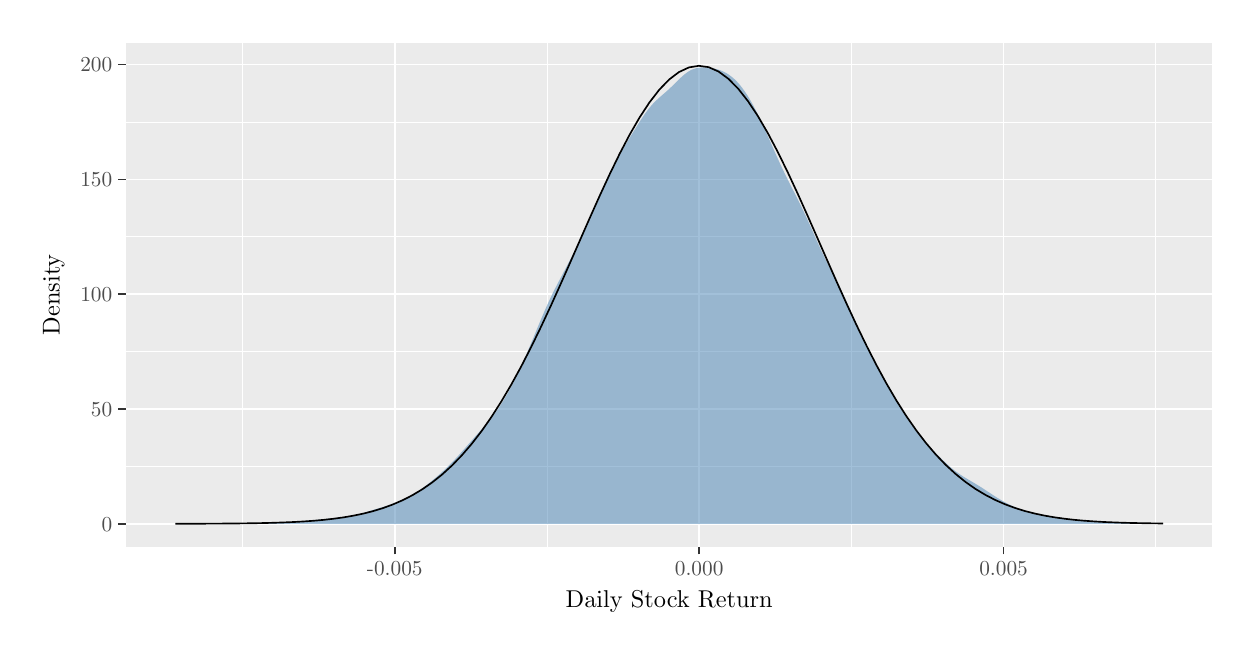
\begin{tikzpicture}[x=1pt,y=1pt]
\definecolor{fillColor}{RGB}{255,255,255}
\path[use as bounding box,fill=fillColor,fill opacity=0.00] (0,0) rectangle (433.62,216.81);
\begin{scope}
\path[clip] (  0.00,  0.00) rectangle (433.62,216.81);
\definecolor{drawColor}{RGB}{255,255,255}
\definecolor{fillColor}{RGB}{255,255,255}

\path[draw=drawColor,line width= 0.6pt,line join=round,line cap=round,fill=fillColor] (  0.00,  0.00) rectangle (433.62,216.81);
\end{scope}
\begin{scope}
\path[clip] ( 35.50, 29.26) rectangle (428.12,211.31);
\definecolor{fillColor}{gray}{0.92}

\path[fill=fillColor] ( 35.50, 29.26) rectangle (428.12,211.31);
\definecolor{drawColor}{RGB}{255,255,255}

\path[draw=drawColor,line width= 0.3pt,line join=round] ( 35.50, 58.28) --
	(428.12, 58.28);

\path[draw=drawColor,line width= 0.3pt,line join=round] ( 35.50, 99.76) --
	(428.12, 99.76);

\path[draw=drawColor,line width= 0.3pt,line join=round] ( 35.50,141.25) --
	(428.12,141.25);

\path[draw=drawColor,line width= 0.3pt,line join=round] ( 35.50,182.73) --
	(428.12,182.73);

\path[draw=drawColor,line width= 0.3pt,line join=round] ( 77.67, 29.26) --
	( 77.67,211.31);

\path[draw=drawColor,line width= 0.3pt,line join=round] (187.65, 29.26) --
	(187.65,211.31);

\path[draw=drawColor,line width= 0.3pt,line join=round] (297.64, 29.26) --
	(297.64,211.31);

\path[draw=drawColor,line width= 0.3pt,line join=round] (407.62, 29.26) --
	(407.62,211.31);

\path[draw=drawColor,line width= 0.6pt,line join=round] ( 35.50, 37.53) --
	(428.12, 37.53);

\path[draw=drawColor,line width= 0.6pt,line join=round] ( 35.50, 79.02) --
	(428.12, 79.02);

\path[draw=drawColor,line width= 0.6pt,line join=round] ( 35.50,120.50) --
	(428.12,120.50);

\path[draw=drawColor,line width= 0.6pt,line join=round] ( 35.50,161.99) --
	(428.12,161.99);

\path[draw=drawColor,line width= 0.6pt,line join=round] ( 35.50,203.47) --
	(428.12,203.47);

\path[draw=drawColor,line width= 0.6pt,line join=round] (132.66, 29.26) --
	(132.66,211.31);

\path[draw=drawColor,line width= 0.6pt,line join=round] (242.64, 29.26) --
	(242.64,211.31);

\path[draw=drawColor,line width= 0.6pt,line join=round] (352.63, 29.26) --
	(352.63,211.31);
\definecolor{fillColor}{RGB}{70,130,180}

\path[fill=fillColor,fill opacity=0.50] ( 53.35, 37.57) --
	( 54.05, 37.57) --
	( 54.75, 37.57) --
	( 55.44, 37.57) --
	( 56.14, 37.57) --
	( 56.84, 37.56) --
	( 57.54, 37.56) --
	( 58.24, 37.56) --
	( 58.94, 37.55) --
	( 59.63, 37.55) --
	( 60.33, 37.55) --
	( 61.03, 37.54) --
	( 61.73, 37.54) --
	( 62.43, 37.54) --
	( 63.13, 37.54) --
	( 63.83, 37.54) --
	( 64.52, 37.54) --
	( 65.22, 37.54) --
	( 65.92, 37.54) --
	( 66.62, 37.55) --
	( 67.32, 37.55) --
	( 68.02, 37.56) --
	( 68.71, 37.56) --
	( 69.41, 37.57) --
	( 70.11, 37.58) --
	( 70.81, 37.58) --
	( 71.51, 37.59) --
	( 72.21, 37.61) --
	( 72.91, 37.62) --
	( 73.60, 37.63) --
	( 74.30, 37.64) --
	( 75.00, 37.66) --
	( 75.70, 37.67) --
	( 76.40, 37.69) --
	( 77.10, 37.70) --
	( 77.80, 37.71) --
	( 78.49, 37.73) --
	( 79.19, 37.74) --
	( 79.89, 37.75) --
	( 80.59, 37.76) --
	( 81.29, 37.77) --
	( 81.99, 37.78) --
	( 82.68, 37.78) --
	( 83.38, 37.79) --
	( 84.08, 37.80) --
	( 84.78, 37.81) --
	( 85.48, 37.81) --
	( 86.18, 37.82) --
	( 86.88, 37.83) --
	( 87.57, 37.85) --
	( 88.27, 37.86) --
	( 88.97, 37.88) --
	( 89.67, 37.90) --
	( 90.37, 37.92) --
	( 91.07, 37.94) --
	( 91.76, 37.97) --
	( 92.46, 38.00) --
	( 93.16, 38.03) --
	( 93.86, 38.07) --
	( 94.56, 38.10) --
	( 95.26, 38.15) --
	( 95.96, 38.19) --
	( 96.65, 38.24) --
	( 97.35, 38.29) --
	( 98.05, 38.34) --
	( 98.75, 38.40) --
	( 99.45, 38.46) --
	(100.15, 38.52) --
	(100.85, 38.58) --
	(101.54, 38.64) --
	(102.24, 38.71) --
	(102.94, 38.77) --
	(103.64, 38.84) --
	(104.34, 38.91) --
	(105.04, 38.99) --
	(105.73, 39.06) --
	(106.43, 39.14) --
	(107.13, 39.22) --
	(107.83, 39.30) --
	(108.53, 39.38) --
	(109.23, 39.45) --
	(109.93, 39.53) --
	(110.62, 39.60) --
	(111.32, 39.67) --
	(112.02, 39.74) --
	(112.72, 39.81) --
	(113.42, 39.88) --
	(114.12, 39.95) --
	(114.81, 40.03) --
	(115.51, 40.12) --
	(116.21, 40.22) --
	(116.91, 40.33) --
	(117.61, 40.47) --
	(118.31, 40.61) --
	(119.01, 40.77) --
	(119.70, 40.95) --
	(120.40, 41.15) --
	(121.10, 41.35) --
	(121.80, 41.56) --
	(122.50, 41.78) --
	(123.20, 42.01) --
	(123.90, 42.23) --
	(124.59, 42.45) --
	(125.29, 42.67) --
	(125.99, 42.89) --
	(126.69, 43.10) --
	(127.39, 43.31) --
	(128.09, 43.51) --
	(128.78, 43.71) --
	(129.48, 43.92) --
	(130.18, 44.13) --
	(130.88, 44.35) --
	(131.58, 44.57) --
	(132.28, 44.81) --
	(132.98, 45.06) --
	(133.67, 45.33) --
	(134.37, 45.61) --
	(135.07, 45.91) --
	(135.77, 46.22) --
	(136.47, 46.56) --
	(137.17, 46.91) --
	(137.86, 47.29) --
	(138.56, 47.69) --
	(139.26, 48.11) --
	(139.96, 48.54) --
	(140.66, 49.00) --
	(141.36, 49.48) --
	(142.06, 49.97) --
	(142.75, 50.48) --
	(143.45, 51.00) --
	(144.15, 51.53) --
	(144.85, 52.08) --
	(145.55, 52.64) --
	(146.25, 53.21) --
	(146.95, 53.78) --
	(147.64, 54.37) --
	(148.34, 54.98) --
	(149.04, 55.59) --
	(149.74, 56.22) --
	(150.44, 56.86) --
	(151.14, 57.52) --
	(151.83, 58.20) --
	(152.53, 58.89) --
	(153.23, 59.60) --
	(153.93, 60.33) --
	(154.63, 61.08) --
	(155.33, 61.83) --
	(156.03, 62.60) --
	(156.72, 63.38) --
	(157.42, 64.17) --
	(158.12, 64.96) --
	(158.82, 65.76) --
	(159.52, 66.56) --
	(160.22, 67.36) --
	(160.91, 68.15) --
	(161.61, 68.95) --
	(162.31, 69.74) --
	(163.01, 70.52) --
	(163.71, 71.31) --
	(164.41, 72.10) --
	(165.11, 72.90) --
	(165.80, 73.70) --
	(166.50, 74.52) --
	(167.20, 75.37) --
	(167.90, 76.25) --
	(168.60, 77.16) --
	(169.30, 78.11) --
	(170.00, 79.10) --
	(170.69, 80.15) --
	(171.39, 81.24) --
	(172.09, 82.37) --
	(172.79, 83.56) --
	(173.49, 84.80) --
	(174.19, 86.09) --
	(174.88, 87.42) --
	(175.58, 88.80) --
	(176.28, 90.21) --
	(176.98, 91.66) --
	(177.68, 93.15) --
	(178.38, 94.66) --
	(179.08, 96.21) --
	(179.77, 97.79) --
	(180.47, 99.40) --
	(181.17,101.03) --
	(181.87,102.68) --
	(182.57,104.35) --
	(183.27,106.04) --
	(183.96,107.73) --
	(184.66,109.42) --
	(185.36,111.10) --
	(186.06,112.75) --
	(186.76,114.38) --
	(187.46,115.97) --
	(188.16,117.52) --
	(188.85,119.02) --
	(189.55,120.48) --
	(190.25,121.89) --
	(190.95,123.27) --
	(191.65,124.62) --
	(192.35,125.95) --
	(193.05,127.27) --
	(193.74,128.59) --
	(194.44,129.92) --
	(195.14,131.25) --
	(195.84,132.60) --
	(196.54,133.96) --
	(197.24,135.35) --
	(197.93,136.75) --
	(198.63,138.18) --
	(199.33,139.62) --
	(200.03,141.09) --
	(200.73,142.59) --
	(201.43,144.11) --
	(202.13,145.65) --
	(202.82,147.23) --
	(203.52,148.83) --
	(204.22,150.45) --
	(204.92,152.09) --
	(205.62,153.74) --
	(206.32,155.38) --
	(207.01,157.02) --
	(207.71,158.63) --
	(208.41,160.22) --
	(209.11,161.76) --
	(209.81,163.27) --
	(210.51,164.72) --
	(211.21,166.11) --
	(211.90,167.46) --
	(212.60,168.75) --
	(213.30,170.00) --
	(214.00,171.22) --
	(214.70,172.40) --
	(215.40,173.56) --
	(216.10,174.70) --
	(216.79,175.84) --
	(217.49,176.97) --
	(218.19,178.10) --
	(218.89,179.22) --
	(219.59,180.35) --
	(220.29,181.47) --
	(220.98,182.57) --
	(221.68,183.65) --
	(222.38,184.71) --
	(223.08,185.72) --
	(223.78,186.69) --
	(224.48,187.60) --
	(225.18,188.44) --
	(225.87,189.23) --
	(226.57,189.96) --
	(227.27,190.64) --
	(227.97,191.29) --
	(228.67,191.90) --
	(229.37,192.51) --
	(230.06,193.11) --
	(230.76,193.72) --
	(231.46,194.34) --
	(232.16,194.99) --
	(232.86,195.66) --
	(233.56,196.34) --
	(234.26,197.04) --
	(234.95,197.73) --
	(235.65,198.41) --
	(236.35,199.06) --
	(237.05,199.67) --
	(237.75,200.24) --
	(238.45,200.75) --
	(239.15,201.19) --
	(239.84,201.56) --
	(240.54,201.85) --
	(241.24,202.08) --
	(241.94,202.25) --
	(242.64,202.36) --
	(243.34,202.42) --
	(244.03,202.44) --
	(244.73,202.43) --
	(245.43,202.39) --
	(246.13,202.32) --
	(246.83,202.24) --
	(247.53,202.12) --
	(248.23,201.99) --
	(248.92,201.82) --
	(249.62,201.62) --
	(250.32,201.38) --
	(251.02,201.11) --
	(251.72,200.78) --
	(252.42,200.41) --
	(253.11,199.99) --
	(253.81,199.50) --
	(254.51,198.96) --
	(255.21,198.36) --
	(255.91,197.69) --
	(256.61,196.96) --
	(257.31,196.16) --
	(258.00,195.29) --
	(258.70,194.35) --
	(259.40,193.35) --
	(260.10,192.28) --
	(260.80,191.14) --
	(261.50,189.94) --
	(262.20,188.68) --
	(262.89,187.36) --
	(263.59,185.99) --
	(264.29,184.57) --
	(264.99,183.10) --
	(265.69,181.60) --
	(266.39,180.05) --
	(267.08,178.49) --
	(267.78,176.90) --
	(268.48,175.30) --
	(269.18,173.70) --
	(269.88,172.11) --
	(270.58,170.53) --
	(271.28,168.98) --
	(271.97,167.45) --
	(272.67,165.96) --
	(273.37,164.50) --
	(274.07,163.07) --
	(274.77,161.66) --
	(275.47,160.27) --
	(276.16,158.90) --
	(276.86,157.53) --
	(277.56,156.16) --
	(278.26,154.77) --
	(278.96,153.37) --
	(279.66,151.94) --
	(280.36,150.48) --
	(281.05,148.99) --
	(281.75,147.47) --
	(282.45,145.93) --
	(283.15,144.36) --
	(283.85,142.78) --
	(284.55,141.20) --
	(285.25,139.62) --
	(285.94,138.07) --
	(286.64,136.55) --
	(287.34,135.06) --
	(288.04,133.61) --
	(288.74,132.19) --
	(289.44,130.81) --
	(290.13,129.45) --
	(290.83,128.11) --
	(291.53,126.76) --
	(292.23,125.41) --
	(292.93,124.03) --
	(293.63,122.63) --
	(294.33,121.18) --
	(295.02,119.70) --
	(295.72,118.17) --
	(296.42,116.62) --
	(297.12,115.03) --
	(297.82,113.42) --
	(298.52,111.80) --
	(299.21,110.18) --
	(299.91,108.58) --
	(300.61,106.99) --
	(301.31,105.43) --
	(302.01,103.90) --
	(302.71,102.40) --
	(303.41,100.94) --
	(304.10, 99.52) --
	(304.80, 98.13) --
	(305.50, 96.78) --
	(306.20, 95.46) --
	(306.90, 94.17) --
	(307.60, 92.90) --
	(308.30, 91.65) --
	(308.99, 90.41) --
	(309.69, 89.19) --
	(310.39, 87.98) --
	(311.09, 86.78) --
	(311.79, 85.58) --
	(312.49, 84.39) --
	(313.18, 83.20) --
	(313.88, 82.01) --
	(314.58, 80.84) --
	(315.28, 79.67) --
	(315.98, 78.52) --
	(316.68, 77.38) --
	(317.38, 76.26) --
	(318.07, 75.18) --
	(318.77, 74.12) --
	(319.47, 73.10) --
	(320.17, 72.12) --
	(320.87, 71.18) --
	(321.57, 70.28) --
	(322.26, 69.41) --
	(322.96, 68.58) --
	(323.66, 67.78) --
	(324.36, 67.01) --
	(325.06, 66.25) --
	(325.76, 65.51) --
	(326.46, 64.79) --
	(327.15, 64.07) --
	(327.85, 63.36) --
	(328.55, 62.66) --
	(329.25, 61.96) --
	(329.95, 61.27) --
	(330.65, 60.58) --
	(331.35, 59.91) --
	(332.04, 59.26) --
	(332.74, 58.62) --
	(333.44, 58.01) --
	(334.14, 57.42) --
	(334.84, 56.86) --
	(335.54, 56.33) --
	(336.23, 55.83) --
	(336.93, 55.35) --
	(337.63, 54.89) --
	(338.33, 54.46) --
	(339.03, 54.03) --
	(339.73, 53.62) --
	(340.43, 53.21) --
	(341.12, 52.80) --
	(341.82, 52.39) --
	(342.52, 51.97) --
	(343.22, 51.55) --
	(343.92, 51.12) --
	(344.62, 50.68) --
	(345.31, 50.23) --
	(346.01, 49.77) --
	(346.71, 49.31) --
	(347.41, 48.85) --
	(348.11, 48.39) --
	(348.81, 47.93) --
	(349.51, 47.48) --
	(350.20, 47.04) --
	(350.90, 46.60) --
	(351.60, 46.18) --
	(352.30, 45.78) --
	(353.00, 45.38) --
	(353.70, 45.01) --
	(354.39, 44.65) --
	(355.09, 44.31) --
	(355.79, 43.98) --
	(356.49, 43.67) --
	(357.19, 43.37) --
	(357.89, 43.09) --
	(358.59, 42.82) --
	(359.28, 42.56) --
	(359.98, 42.32) --
	(360.68, 42.10) --
	(361.38, 41.88) --
	(362.08, 41.68) --
	(362.78, 41.50) --
	(363.48, 41.32) --
	(364.17, 41.16) --
	(364.87, 41.01) --
	(365.57, 40.86) --
	(366.27, 40.73) --
	(366.97, 40.60) --
	(367.67, 40.48) --
	(368.36, 40.36) --
	(369.06, 40.25) --
	(369.76, 40.15) --
	(370.46, 40.05) --
	(371.16, 39.95) --
	(371.86, 39.85) --
	(372.56, 39.76) --
	(373.25, 39.67) --
	(373.95, 39.58) --
	(374.65, 39.49) --
	(375.35, 39.40) --
	(376.05, 39.32) --
	(376.75, 39.23) --
	(377.44, 39.15) --
	(378.14, 39.06) --
	(378.84, 38.98) --
	(379.54, 38.90) --
	(380.24, 38.82) --
	(380.94, 38.74) --
	(381.64, 38.66) --
	(382.33, 38.59) --
	(383.03, 38.53) --
	(383.73, 38.46) --
	(384.43, 38.40) --
	(385.13, 38.35) --
	(385.83, 38.29) --
	(386.53, 38.25) --
	(387.22, 38.20) --
	(387.92, 38.16) --
	(388.62, 38.12) --
	(389.32, 38.08) --
	(390.02, 38.04) --
	(390.72, 38.01) --
	(391.41, 37.98) --
	(392.11, 37.95) --
	(392.81, 37.93) --
	(393.51, 37.90) --
	(394.21, 37.89) --
	(394.91, 37.87) --
	(395.61, 37.86) --
	(396.30, 37.85) --
	(397.00, 37.84) --
	(397.70, 37.84) --
	(398.40, 37.83) --
	(399.10, 37.83) --
	(399.80, 37.83) --
	(400.49, 37.83) --
	(401.19, 37.83) --
	(401.89, 37.83) --
	(402.59, 37.82) --
	(403.29, 37.82) --
	(403.99, 37.81) --
	(404.69, 37.80) --
	(405.38, 37.79) --
	(406.08, 37.78) --
	(406.78, 37.76) --
	(407.48, 37.75) --
	(408.18, 37.73) --
	(408.88, 37.72) --
	(409.58, 37.70) --
	(410.27, 37.69) --
	(410.27, 37.53) --
	(409.58, 37.53) --
	(408.88, 37.53) --
	(408.18, 37.53) --
	(407.48, 37.53) --
	(406.78, 37.53) --
	(406.08, 37.53) --
	(405.38, 37.53) --
	(404.69, 37.53) --
	(403.99, 37.53) --
	(403.29, 37.53) --
	(402.59, 37.53) --
	(401.89, 37.53) --
	(401.19, 37.53) --
	(400.49, 37.53) --
	(399.80, 37.53) --
	(399.10, 37.53) --
	(398.40, 37.53) --
	(397.70, 37.53) --
	(397.00, 37.53) --
	(396.30, 37.53) --
	(395.61, 37.53) --
	(394.91, 37.53) --
	(394.21, 37.53) --
	(393.51, 37.53) --
	(392.81, 37.53) --
	(392.11, 37.53) --
	(391.41, 37.53) --
	(390.72, 37.53) --
	(390.02, 37.53) --
	(389.32, 37.53) --
	(388.62, 37.53) --
	(387.92, 37.53) --
	(387.22, 37.53) --
	(386.53, 37.53) --
	(385.83, 37.53) --
	(385.13, 37.53) --
	(384.43, 37.53) --
	(383.73, 37.53) --
	(383.03, 37.53) --
	(382.33, 37.53) --
	(381.64, 37.53) --
	(380.94, 37.53) --
	(380.24, 37.53) --
	(379.54, 37.53) --
	(378.84, 37.53) --
	(378.14, 37.53) --
	(377.44, 37.53) --
	(376.75, 37.53) --
	(376.05, 37.53) --
	(375.35, 37.53) --
	(374.65, 37.53) --
	(373.95, 37.53) --
	(373.25, 37.53) --
	(372.56, 37.53) --
	(371.86, 37.53) --
	(371.16, 37.53) --
	(370.46, 37.53) --
	(369.76, 37.53) --
	(369.06, 37.53) --
	(368.36, 37.53) --
	(367.67, 37.53) --
	(366.97, 37.53) --
	(366.27, 37.53) --
	(365.57, 37.53) --
	(364.87, 37.53) --
	(364.17, 37.53) --
	(363.48, 37.53) --
	(362.78, 37.53) --
	(362.08, 37.53) --
	(361.38, 37.53) --
	(360.68, 37.53) --
	(359.98, 37.53) --
	(359.28, 37.53) --
	(358.59, 37.53) --
	(357.89, 37.53) --
	(357.19, 37.53) --
	(356.49, 37.53) --
	(355.79, 37.53) --
	(355.09, 37.53) --
	(354.39, 37.53) --
	(353.70, 37.53) --
	(353.00, 37.53) --
	(352.30, 37.53) --
	(351.60, 37.53) --
	(350.90, 37.53) --
	(350.20, 37.53) --
	(349.51, 37.53) --
	(348.81, 37.53) --
	(348.11, 37.53) --
	(347.41, 37.53) --
	(346.71, 37.53) --
	(346.01, 37.53) --
	(345.31, 37.53) --
	(344.62, 37.53) --
	(343.92, 37.53) --
	(343.22, 37.53) --
	(342.52, 37.53) --
	(341.82, 37.53) --
	(341.12, 37.53) --
	(340.43, 37.53) --
	(339.73, 37.53) --
	(339.03, 37.53) --
	(338.33, 37.53) --
	(337.63, 37.53) --
	(336.93, 37.53) --
	(336.23, 37.53) --
	(335.54, 37.53) --
	(334.84, 37.53) --
	(334.14, 37.53) --
	(333.44, 37.53) --
	(332.74, 37.53) --
	(332.04, 37.53) --
	(331.35, 37.53) --
	(330.65, 37.53) --
	(329.95, 37.53) --
	(329.25, 37.53) --
	(328.55, 37.53) --
	(327.85, 37.53) --
	(327.15, 37.53) --
	(326.46, 37.53) --
	(325.76, 37.53) --
	(325.06, 37.53) --
	(324.36, 37.53) --
	(323.66, 37.53) --
	(322.96, 37.53) --
	(322.26, 37.53) --
	(321.57, 37.53) --
	(320.87, 37.53) --
	(320.17, 37.53) --
	(319.47, 37.53) --
	(318.77, 37.53) --
	(318.07, 37.53) --
	(317.38, 37.53) --
	(316.68, 37.53) --
	(315.98, 37.53) --
	(315.28, 37.53) --
	(314.58, 37.53) --
	(313.88, 37.53) --
	(313.18, 37.53) --
	(312.49, 37.53) --
	(311.79, 37.53) --
	(311.09, 37.53) --
	(310.39, 37.53) --
	(309.69, 37.53) --
	(308.99, 37.53) --
	(308.30, 37.53) --
	(307.60, 37.53) --
	(306.90, 37.53) --
	(306.20, 37.53) --
	(305.50, 37.53) --
	(304.80, 37.53) --
	(304.10, 37.53) --
	(303.41, 37.53) --
	(302.71, 37.53) --
	(302.01, 37.53) --
	(301.31, 37.53) --
	(300.61, 37.53) --
	(299.91, 37.53) --
	(299.21, 37.53) --
	(298.52, 37.53) --
	(297.82, 37.53) --
	(297.12, 37.53) --
	(296.42, 37.53) --
	(295.72, 37.53) --
	(295.02, 37.53) --
	(294.33, 37.53) --
	(293.63, 37.53) --
	(292.93, 37.53) --
	(292.23, 37.53) --
	(291.53, 37.53) --
	(290.83, 37.53) --
	(290.13, 37.53) --
	(289.44, 37.53) --
	(288.74, 37.53) --
	(288.04, 37.53) --
	(287.34, 37.53) --
	(286.64, 37.53) --
	(285.94, 37.53) --
	(285.25, 37.53) --
	(284.55, 37.53) --
	(283.85, 37.53) --
	(283.15, 37.53) --
	(282.45, 37.53) --
	(281.75, 37.53) --
	(281.05, 37.53) --
	(280.36, 37.53) --
	(279.66, 37.53) --
	(278.96, 37.53) --
	(278.26, 37.53) --
	(277.56, 37.53) --
	(276.86, 37.53) --
	(276.16, 37.53) --
	(275.47, 37.53) --
	(274.77, 37.53) --
	(274.07, 37.53) --
	(273.37, 37.53) --
	(272.67, 37.53) --
	(271.97, 37.53) --
	(271.28, 37.53) --
	(270.58, 37.53) --
	(269.88, 37.53) --
	(269.18, 37.53) --
	(268.48, 37.53) --
	(267.78, 37.53) --
	(267.08, 37.53) --
	(266.39, 37.53) --
	(265.69, 37.53) --
	(264.99, 37.53) --
	(264.29, 37.53) --
	(263.59, 37.53) --
	(262.89, 37.53) --
	(262.20, 37.53) --
	(261.50, 37.53) --
	(260.80, 37.53) --
	(260.10, 37.53) --
	(259.40, 37.53) --
	(258.70, 37.53) --
	(258.00, 37.53) --
	(257.31, 37.53) --
	(256.61, 37.53) --
	(255.91, 37.53) --
	(255.21, 37.53) --
	(254.51, 37.53) --
	(253.81, 37.53) --
	(253.11, 37.53) --
	(252.42, 37.53) --
	(251.72, 37.53) --
	(251.02, 37.53) --
	(250.32, 37.53) --
	(249.62, 37.53) --
	(248.92, 37.53) --
	(248.23, 37.53) --
	(247.53, 37.53) --
	(246.83, 37.53) --
	(246.13, 37.53) --
	(245.43, 37.53) --
	(244.73, 37.53) --
	(244.03, 37.53) --
	(243.34, 37.53) --
	(242.64, 37.53) --
	(241.94, 37.53) --
	(241.24, 37.53) --
	(240.54, 37.53) --
	(239.84, 37.53) --
	(239.15, 37.53) --
	(238.45, 37.53) --
	(237.75, 37.53) --
	(237.05, 37.53) --
	(236.35, 37.53) --
	(235.65, 37.53) --
	(234.95, 37.53) --
	(234.26, 37.53) --
	(233.56, 37.53) --
	(232.86, 37.53) --
	(232.16, 37.53) --
	(231.46, 37.53) --
	(230.76, 37.53) --
	(230.06, 37.53) --
	(229.37, 37.53) --
	(228.67, 37.53) --
	(227.97, 37.53) --
	(227.27, 37.53) --
	(226.57, 37.53) --
	(225.87, 37.53) --
	(225.18, 37.53) --
	(224.48, 37.53) --
	(223.78, 37.53) --
	(223.08, 37.53) --
	(222.38, 37.53) --
	(221.68, 37.53) --
	(220.98, 37.53) --
	(220.29, 37.53) --
	(219.59, 37.53) --
	(218.89, 37.53) --
	(218.19, 37.53) --
	(217.49, 37.53) --
	(216.79, 37.53) --
	(216.10, 37.53) --
	(215.40, 37.53) --
	(214.70, 37.53) --
	(214.00, 37.53) --
	(213.30, 37.53) --
	(212.60, 37.53) --
	(211.90, 37.53) --
	(211.21, 37.53) --
	(210.51, 37.53) --
	(209.81, 37.53) --
	(209.11, 37.53) --
	(208.41, 37.53) --
	(207.71, 37.53) --
	(207.01, 37.53) --
	(206.32, 37.53) --
	(205.62, 37.53) --
	(204.92, 37.53) --
	(204.22, 37.53) --
	(203.52, 37.53) --
	(202.82, 37.53) --
	(202.13, 37.53) --
	(201.43, 37.53) --
	(200.73, 37.53) --
	(200.03, 37.53) --
	(199.33, 37.53) --
	(198.63, 37.53) --
	(197.93, 37.53) --
	(197.24, 37.53) --
	(196.54, 37.53) --
	(195.84, 37.53) --
	(195.14, 37.53) --
	(194.44, 37.53) --
	(193.74, 37.53) --
	(193.05, 37.53) --
	(192.35, 37.53) --
	(191.65, 37.53) --
	(190.95, 37.53) --
	(190.25, 37.53) --
	(189.55, 37.53) --
	(188.85, 37.53) --
	(188.16, 37.53) --
	(187.46, 37.53) --
	(186.76, 37.53) --
	(186.06, 37.53) --
	(185.36, 37.53) --
	(184.66, 37.53) --
	(183.96, 37.53) --
	(183.27, 37.53) --
	(182.57, 37.53) --
	(181.87, 37.53) --
	(181.17, 37.53) --
	(180.47, 37.53) --
	(179.77, 37.53) --
	(179.08, 37.53) --
	(178.38, 37.53) --
	(177.68, 37.53) --
	(176.98, 37.53) --
	(176.28, 37.53) --
	(175.58, 37.53) --
	(174.88, 37.53) --
	(174.19, 37.53) --
	(173.49, 37.53) --
	(172.79, 37.53) --
	(172.09, 37.53) --
	(171.39, 37.53) --
	(170.69, 37.53) --
	(170.00, 37.53) --
	(169.30, 37.53) --
	(168.60, 37.53) --
	(167.90, 37.53) --
	(167.20, 37.53) --
	(166.50, 37.53) --
	(165.80, 37.53) --
	(165.11, 37.53) --
	(164.41, 37.53) --
	(163.71, 37.53) --
	(163.01, 37.53) --
	(162.31, 37.53) --
	(161.61, 37.53) --
	(160.91, 37.53) --
	(160.22, 37.53) --
	(159.52, 37.53) --
	(158.82, 37.53) --
	(158.12, 37.53) --
	(157.42, 37.53) --
	(156.72, 37.53) --
	(156.03, 37.53) --
	(155.33, 37.53) --
	(154.63, 37.53) --
	(153.93, 37.53) --
	(153.23, 37.53) --
	(152.53, 37.53) --
	(151.83, 37.53) --
	(151.14, 37.53) --
	(150.44, 37.53) --
	(149.74, 37.53) --
	(149.04, 37.53) --
	(148.34, 37.53) --
	(147.64, 37.53) --
	(146.95, 37.53) --
	(146.25, 37.53) --
	(145.55, 37.53) --
	(144.85, 37.53) --
	(144.15, 37.53) --
	(143.45, 37.53) --
	(142.75, 37.53) --
	(142.06, 37.53) --
	(141.36, 37.53) --
	(140.66, 37.53) --
	(139.96, 37.53) --
	(139.26, 37.53) --
	(138.56, 37.53) --
	(137.86, 37.53) --
	(137.17, 37.53) --
	(136.47, 37.53) --
	(135.77, 37.53) --
	(135.07, 37.53) --
	(134.37, 37.53) --
	(133.67, 37.53) --
	(132.98, 37.53) --
	(132.28, 37.53) --
	(131.58, 37.53) --
	(130.88, 37.53) --
	(130.18, 37.53) --
	(129.48, 37.53) --
	(128.78, 37.53) --
	(128.09, 37.53) --
	(127.39, 37.53) --
	(126.69, 37.53) --
	(125.99, 37.53) --
	(125.29, 37.53) --
	(124.59, 37.53) --
	(123.90, 37.53) --
	(123.20, 37.53) --
	(122.50, 37.53) --
	(121.80, 37.53) --
	(121.10, 37.53) --
	(120.40, 37.53) --
	(119.70, 37.53) --
	(119.01, 37.53) --
	(118.31, 37.53) --
	(117.61, 37.53) --
	(116.91, 37.53) --
	(116.21, 37.53) --
	(115.51, 37.53) --
	(114.81, 37.53) --
	(114.12, 37.53) --
	(113.42, 37.53) --
	(112.72, 37.53) --
	(112.02, 37.53) --
	(111.32, 37.53) --
	(110.62, 37.53) --
	(109.93, 37.53) --
	(109.23, 37.53) --
	(108.53, 37.53) --
	(107.83, 37.53) --
	(107.13, 37.53) --
	(106.43, 37.53) --
	(105.73, 37.53) --
	(105.04, 37.53) --
	(104.34, 37.53) --
	(103.64, 37.53) --
	(102.94, 37.53) --
	(102.24, 37.53) --
	(101.54, 37.53) --
	(100.85, 37.53) --
	(100.15, 37.53) --
	( 99.45, 37.53) --
	( 98.75, 37.53) --
	( 98.05, 37.53) --
	( 97.35, 37.53) --
	( 96.65, 37.53) --
	( 95.96, 37.53) --
	( 95.26, 37.53) --
	( 94.56, 37.53) --
	( 93.86, 37.53) --
	( 93.16, 37.53) --
	( 92.46, 37.53) --
	( 91.76, 37.53) --
	( 91.07, 37.53) --
	( 90.37, 37.53) --
	( 89.67, 37.53) --
	( 88.97, 37.53) --
	( 88.27, 37.53) --
	( 87.57, 37.53) --
	( 86.88, 37.53) --
	( 86.18, 37.53) --
	( 85.48, 37.53) --
	( 84.78, 37.53) --
	( 84.08, 37.53) --
	( 83.38, 37.53) --
	( 82.68, 37.53) --
	( 81.99, 37.53) --
	( 81.29, 37.53) --
	( 80.59, 37.53) --
	( 79.89, 37.53) --
	( 79.19, 37.53) --
	( 78.49, 37.53) --
	( 77.80, 37.53) --
	( 77.10, 37.53) --
	( 76.40, 37.53) --
	( 75.70, 37.53) --
	( 75.00, 37.53) --
	( 74.30, 37.53) --
	( 73.60, 37.53) --
	( 72.91, 37.53) --
	( 72.21, 37.53) --
	( 71.51, 37.53) --
	( 70.81, 37.53) --
	( 70.11, 37.53) --
	( 69.41, 37.53) --
	( 68.71, 37.53) --
	( 68.02, 37.53) --
	( 67.32, 37.53) --
	( 66.62, 37.53) --
	( 65.92, 37.53) --
	( 65.22, 37.53) --
	( 64.52, 37.53) --
	( 63.83, 37.53) --
	( 63.13, 37.53) --
	( 62.43, 37.53) --
	( 61.73, 37.53) --
	( 61.03, 37.53) --
	( 60.33, 37.53) --
	( 59.63, 37.53) --
	( 58.94, 37.53) --
	( 58.24, 37.53) --
	( 57.54, 37.53) --
	( 56.84, 37.53) --
	( 56.14, 37.53) --
	( 55.44, 37.53) --
	( 54.75, 37.53) --
	( 54.05, 37.53) --
	( 53.35, 37.53) --
	cycle;
\definecolor{drawColor}{RGB}{0,0,0}

\path[draw=drawColor,line width= 0.6pt,line join=round] ( 53.35, 37.55) --
	( 56.92, 37.56) --
	( 60.49, 37.56) --
	( 64.06, 37.58) --
	( 67.63, 37.59) --
	( 71.19, 37.62) --
	( 74.76, 37.65) --
	( 78.33, 37.69) --
	( 81.90, 37.74) --
	( 85.47, 37.81) --
	( 89.04, 37.91) --
	( 92.61, 38.03) --
	( 96.18, 38.18) --
	( 99.75, 38.38) --
	(103.32, 38.63) --
	(106.89, 38.95) --
	(110.46, 39.35) --
	(114.03, 39.84) --
	(117.59, 40.45) --
	(121.16, 41.19) --
	(124.73, 42.09) --
	(128.30, 43.18) --
	(131.87, 44.49) --
	(135.44, 46.03) --
	(139.01, 47.86) --
	(142.58, 49.99) --
	(146.15, 52.47) --
	(149.72, 55.31) --
	(153.29, 58.57) --
	(156.86, 62.26) --
	(160.43, 66.40) --
	(164.00, 71.01) --
	(167.56, 76.11) --
	(171.13, 81.70) --
	(174.70, 87.76) --
	(178.27, 94.27) --
	(181.84,101.22) --
	(185.41,108.54) --
	(188.98,116.18) --
	(192.55,124.08) --
	(196.12,132.14) --
	(199.69,140.28) --
	(203.26,148.39) --
	(206.83,156.35) --
	(210.40,164.04) --
	(213.96,171.35) --
	(217.53,178.16) --
	(221.10,184.34) --
	(224.67,189.79) --
	(228.24,194.40) --
	(231.81,198.09) --
	(235.38,200.79) --
	(238.95,202.45) --
	(242.52,203.03) --
	(246.09,202.53) --
	(249.66,200.95) --
	(253.23,198.32) --
	(256.80,194.69) --
	(260.37,190.14) --
	(263.93,184.75) --
	(267.50,178.62) --
	(271.07,171.85) --
	(274.64,164.57) --
	(278.21,156.90) --
	(281.78,148.95) --
	(285.35,140.86) --
	(288.92,132.72) --
	(292.49,124.64) --
	(296.06,116.73) --
	(299.63,109.07) --
	(303.20,101.72) --
	(306.77, 94.75) --
	(310.33, 88.20) --
	(313.90, 82.11) --
	(317.47, 76.49) --
	(321.04, 71.36) --
	(324.61, 66.71) --
	(328.18, 62.53) --
	(331.75, 58.81) --
	(335.32, 55.53) --
	(338.89, 52.65) --
	(342.46, 50.15) --
	(346.03, 48.00) --
	(349.60, 46.15) --
	(353.17, 44.59) --
	(356.73, 43.27) --
	(360.30, 42.16) --
	(363.87, 41.25) --
	(367.44, 40.49) --
	(371.01, 39.88) --
	(374.58, 39.38) --
	(378.15, 38.97) --
	(381.72, 38.65) --
	(385.29, 38.40) --
	(388.86, 38.19) --
	(392.43, 38.04) --
	(396.00, 37.91) --
	(399.57, 37.82) --
	(403.14, 37.75) --
	(406.70, 37.69) --
	(410.27, 37.65);
\end{scope}
\begin{scope}
\path[clip] (  0.00,  0.00) rectangle (433.62,216.81);
\definecolor{drawColor}{gray}{0.30}

\node[text=drawColor,anchor=base east,inner sep=0pt, outer sep=0pt, scale=  0.77] at ( 30.55, 34.88) {0};

\node[text=drawColor,anchor=base east,inner sep=0pt, outer sep=0pt, scale=  0.77] at ( 30.55, 76.37) {50};

\node[text=drawColor,anchor=base east,inner sep=0pt, outer sep=0pt, scale=  0.77] at ( 30.55,117.85) {100};

\node[text=drawColor,anchor=base east,inner sep=0pt, outer sep=0pt, scale=  0.77] at ( 30.55,159.34) {150};

\node[text=drawColor,anchor=base east,inner sep=0pt, outer sep=0pt, scale=  0.77] at ( 30.55,200.82) {200};
\end{scope}
\begin{scope}
\path[clip] (  0.00,  0.00) rectangle (433.62,216.81);
\definecolor{drawColor}{gray}{0.20}

\path[draw=drawColor,line width= 0.6pt,line join=round] ( 32.75, 37.53) --
	( 35.50, 37.53);

\path[draw=drawColor,line width= 0.6pt,line join=round] ( 32.75, 79.02) --
	( 35.50, 79.02);

\path[draw=drawColor,line width= 0.6pt,line join=round] ( 32.75,120.50) --
	( 35.50,120.50);

\path[draw=drawColor,line width= 0.6pt,line join=round] ( 32.75,161.99) --
	( 35.50,161.99);

\path[draw=drawColor,line width= 0.6pt,line join=round] ( 32.75,203.47) --
	( 35.50,203.47);
\end{scope}
\begin{scope}
\path[clip] (  0.00,  0.00) rectangle (433.62,216.81);
\definecolor{drawColor}{gray}{0.20}

\path[draw=drawColor,line width= 0.6pt,line join=round] (132.66, 26.51) --
	(132.66, 29.26);

\path[draw=drawColor,line width= 0.6pt,line join=round] (242.64, 26.51) --
	(242.64, 29.26);

\path[draw=drawColor,line width= 0.6pt,line join=round] (352.63, 26.51) --
	(352.63, 29.26);
\end{scope}
\begin{scope}
\path[clip] (  0.00,  0.00) rectangle (433.62,216.81);
\definecolor{drawColor}{gray}{0.30}

\node[text=drawColor,anchor=base,inner sep=0pt, outer sep=0pt, scale=  0.77] at (132.66, 19.00) {-0.005};

\node[text=drawColor,anchor=base,inner sep=0pt, outer sep=0pt, scale=  0.77] at (242.64, 19.00) {0.000};

\node[text=drawColor,anchor=base,inner sep=0pt, outer sep=0pt, scale=  0.77] at (352.63, 19.00) {0.005};
\end{scope}
\begin{scope}
\path[clip] (  0.00,  0.00) rectangle (433.62,216.81);
\definecolor{drawColor}{RGB}{0,0,0}

\node[text=drawColor,anchor=base,inner sep=0pt, outer sep=0pt, scale=  0.88] at (231.81,  7.44) {Daily Stock Return};
\end{scope}
\begin{scope}
\path[clip] (  0.00,  0.00) rectangle (433.62,216.81);
\definecolor{drawColor}{RGB}{0,0,0}

\node[text=drawColor,rotate= 90.00,anchor=base,inner sep=0pt, outer sep=0pt, scale=  0.88] at ( 11.56,120.28) {Density};
\end{scope}
\end{tikzpicture}

\caption{BSM: Stock returns density}
\label{p:returndensity}
  %
  % BEGIN OF FLOATNOTE
  %
  \begin{changemargin}{0.5cm}{0.5cm}
  \medskip
\footnotesize
\setstretch{1.0}\textbf{Notes.}   
The above blue distribution is constructed over $10e3$ paths of a unique stochastic process. 
The samples are built with \cref{eq:underlying:geometric:diff}. 
The arguments are adjusted with the following values, $\alpha = 0$, $\sigma = 30\%$. 
The black density belongs to the normal bell curve with mean $\alpha dt$ and standard deviation of $\sigma  \sqrt{dt}$. 
The distance period between each measure, namely $dt$ has been set to $10e3^{-1}$.
\end{changemargin} 
  %
  % END OF FLOATNOTE
  %
\end{figure}












%%%%%%%%%%%%%%%%%%%%%%%%%
%  Log-return
%%%%%%%%%%%%%%%%%%%%%%%%%

According to \citet{shreve}, from \cref{eq:underlying:log:return}, the distribution of the natural logarithm of the stock price return, recorded over a period of time of $\tau$, turns out to be characterized by \cref{eq:logreturndist}.



\begin{center}
\begin{equation}
\ln{\frac{\St}{S\left(0\right)}} 
  \sim N((\alpha - \frac{\sigma^2}{2}) t, \sigma^2 t)
\label{eq:logreturndist}
\end{equation}
\end{center}  

From \cref{p:logreturndensity}, the normality  of \cref{eq:scontinuousdist} can be observed. 
Indeed, the black bell curve is constructed using the theoretical normal law with $(\alpha - \frac{\sigma^2}{2}) t$ and $\sigma^2 t$ respectively as expectation and variance, while the blue filled figure is built based on empirical results of process \ref{eq:underlying:log:return} with the same $\alpha$ and $\sigma$ given as parameters.


\begin{figure}[!h]
\centering
% Created by tikzDevice version 0.11 on 2018-04-13 09:41:17
% !TEX encoding = UTF-8 Unicode
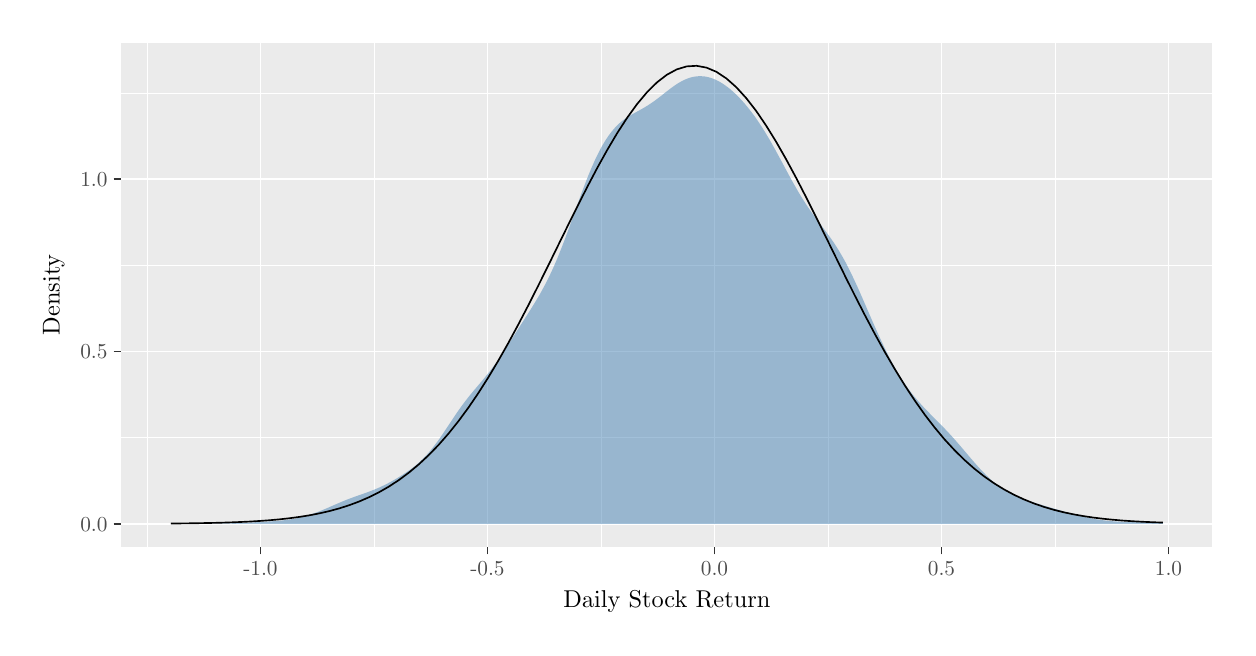
\begin{tikzpicture}[x=1pt,y=1pt]
\definecolor{fillColor}{RGB}{255,255,255}
\path[use as bounding box,fill=fillColor,fill opacity=0.00] (0,0) rectangle (433.62,216.81);
\begin{scope}
\path[clip] (  0.00,  0.00) rectangle (433.62,216.81);
\definecolor{drawColor}{RGB}{255,255,255}
\definecolor{fillColor}{RGB}{255,255,255}

\path[draw=drawColor,line width= 0.6pt,line join=round,line cap=round,fill=fillColor] (  0.00,  0.00) rectangle (433.62,216.81);
\end{scope}
\begin{scope}
\path[clip] ( 33.79, 29.26) rectangle (428.12,211.31);
\definecolor{fillColor}{gray}{0.92}

\path[fill=fillColor] ( 33.79, 29.26) rectangle (428.12,211.31);
\definecolor{drawColor}{RGB}{255,255,255}

\path[draw=drawColor,line width= 0.3pt,line join=round] ( 33.79, 68.65) --
	(428.12, 68.65);

\path[draw=drawColor,line width= 0.3pt,line join=round] ( 33.79,130.89) --
	(428.12,130.89);

\path[draw=drawColor,line width= 0.3pt,line join=round] ( 33.79,193.13) --
	(428.12,193.13);

\path[draw=drawColor,line width= 0.3pt,line join=round] ( 43.10, 29.26) --
	( 43.10,211.31);

\path[draw=drawColor,line width= 0.3pt,line join=round] (125.13, 29.26) --
	(125.13,211.31);

\path[draw=drawColor,line width= 0.3pt,line join=round] (207.16, 29.26) --
	(207.16,211.31);

\path[draw=drawColor,line width= 0.3pt,line join=round] (289.19, 29.26) --
	(289.19,211.31);

\path[draw=drawColor,line width= 0.3pt,line join=round] (371.23, 29.26) --
	(371.23,211.31);

\path[draw=drawColor,line width= 0.6pt,line join=round] ( 33.79, 37.53) --
	(428.12, 37.53);

\path[draw=drawColor,line width= 0.6pt,line join=round] ( 33.79, 99.77) --
	(428.12, 99.77);

\path[draw=drawColor,line width= 0.6pt,line join=round] ( 33.79,162.01) --
	(428.12,162.01);

\path[draw=drawColor,line width= 0.6pt,line join=round] ( 84.11, 29.26) --
	( 84.11,211.31);

\path[draw=drawColor,line width= 0.6pt,line join=round] (166.15, 29.26) --
	(166.15,211.31);

\path[draw=drawColor,line width= 0.6pt,line join=round] (248.18, 29.26) --
	(248.18,211.31);

\path[draw=drawColor,line width= 0.6pt,line join=round] (330.21, 29.26) --
	(330.21,211.31);

\path[draw=drawColor,line width= 0.6pt,line join=round] (412.24, 29.26) --
	(412.24,211.31);
\definecolor{fillColor}{RGB}{70,130,180}

\path[fill=fillColor,fill opacity=0.50] ( 51.72, 37.73) --
	( 52.42, 37.73) --
	( 53.12, 37.73) --
	( 53.82, 37.73) --
	( 54.52, 37.72) --
	( 55.22, 37.72) --
	( 55.92, 37.71) --
	( 56.63, 37.70) --
	( 57.33, 37.69) --
	( 58.03, 37.68) --
	( 58.73, 37.67) --
	( 59.43, 37.67) --
	( 60.13, 37.66) --
	( 60.84, 37.65) --
	( 61.54, 37.64) --
	( 62.24, 37.63) --
	( 62.94, 37.62) --
	( 63.64, 37.62) --
	( 64.34, 37.61) --
	( 65.04, 37.61) --
	( 65.75, 37.61) --
	( 66.45, 37.61) --
	( 67.15, 37.61) --
	( 67.85, 37.62) --
	( 68.55, 37.62) --
	( 69.25, 37.63) --
	( 69.96, 37.64) --
	( 70.66, 37.65) --
	( 71.36, 37.67) --
	( 72.06, 37.68) --
	( 72.76, 37.70) --
	( 73.46, 37.72) --
	( 74.16, 37.74) --
	( 74.87, 37.77) --
	( 75.57, 37.79) --
	( 76.27, 37.82) --
	( 76.97, 37.85) --
	( 77.67, 37.88) --
	( 78.37, 37.91) --
	( 79.07, 37.94) --
	( 79.78, 37.98) --
	( 80.48, 38.01) --
	( 81.18, 38.05) --
	( 81.88, 38.08) --
	( 82.58, 38.12) --
	( 83.28, 38.15) --
	( 83.99, 38.19) --
	( 84.69, 38.23) --
	( 85.39, 38.27) --
	( 86.09, 38.31) --
	( 86.79, 38.35) --
	( 87.49, 38.39) --
	( 88.19, 38.43) --
	( 88.90, 38.48) --
	( 89.60, 38.54) --
	( 90.30, 38.59) --
	( 91.00, 38.66) --
	( 91.70, 38.72) --
	( 92.40, 38.80) --
	( 93.11, 38.88) --
	( 93.81, 38.97) --
	( 94.51, 39.07) --
	( 95.21, 39.18) --
	( 95.91, 39.30) --
	( 96.61, 39.43) --
	( 97.31, 39.57) --
	( 98.02, 39.72) --
	( 98.72, 39.89) --
	( 99.42, 40.06) --
	(100.12, 40.25) --
	(100.82, 40.45) --
	(101.52, 40.67) --
	(102.23, 40.89) --
	(102.93, 41.13) --
	(103.63, 41.37) --
	(104.33, 41.63) --
	(105.03, 41.90) --
	(105.73, 42.18) --
	(106.43, 42.46) --
	(107.14, 42.75) --
	(107.84, 43.05) --
	(108.54, 43.35) --
	(109.24, 43.66) --
	(109.94, 43.96) --
	(110.64, 44.27) --
	(111.35, 44.58) --
	(112.05, 44.88) --
	(112.75, 45.18) --
	(113.45, 45.48) --
	(114.15, 45.77) --
	(114.85, 46.05) --
	(115.55, 46.33) --
	(116.26, 46.60) --
	(116.96, 46.86) --
	(117.66, 47.12) --
	(118.36, 47.37) --
	(119.06, 47.62) --
	(119.76, 47.87) --
	(120.47, 48.11) --
	(121.17, 48.36) --
	(121.87, 48.61) --
	(122.57, 48.86) --
	(123.27, 49.12) --
	(123.97, 49.38) --
	(124.67, 49.65) --
	(125.38, 49.93) --
	(126.08, 50.23) --
	(126.78, 50.53) --
	(127.48, 50.85) --
	(128.18, 51.18) --
	(128.88, 51.52) --
	(129.58, 51.87) --
	(130.29, 52.23) --
	(130.99, 52.60) --
	(131.69, 52.99) --
	(132.39, 53.38) --
	(133.09, 53.79) --
	(133.79, 54.20) --
	(134.50, 54.63) --
	(135.20, 55.07) --
	(135.90, 55.52) --
	(136.60, 55.98) --
	(137.30, 56.46) --
	(138.00, 56.95) --
	(138.70, 57.47) --
	(139.41, 58.00) --
	(140.11, 58.57) --
	(140.81, 59.16) --
	(141.51, 59.77) --
	(142.21, 60.42) --
	(142.91, 61.10) --
	(143.62, 61.82) --
	(144.32, 62.58) --
	(145.02, 63.38) --
	(145.72, 64.21) --
	(146.42, 65.09) --
	(147.12, 65.99) --
	(147.82, 66.93) --
	(148.53, 67.90) --
	(149.23, 68.91) --
	(149.93, 69.93) --
	(150.63, 70.97) --
	(151.33, 72.02) --
	(152.03, 73.08) --
	(152.74, 74.14) --
	(153.44, 75.20) --
	(154.14, 76.25) --
	(154.84, 77.29) --
	(155.54, 78.30) --
	(156.24, 79.30) --
	(156.94, 80.27) --
	(157.65, 81.22) --
	(158.35, 82.14) --
	(159.05, 83.04) --
	(159.75, 83.92) --
	(160.45, 84.78) --
	(161.15, 85.62) --
	(161.86, 86.45) --
	(162.56, 87.27) --
	(163.26, 88.10) --
	(163.96, 88.92) --
	(164.66, 89.76) --
	(165.36, 90.61) --
	(166.06, 91.47) --
	(166.77, 92.36) --
	(167.47, 93.27) --
	(168.17, 94.21) --
	(168.87, 95.17) --
	(169.57, 96.16) --
	(170.27, 97.16) --
	(170.98, 98.20) --
	(171.68, 99.25) --
	(172.38,100.32) --
	(173.08,101.40) --
	(173.78,102.50) --
	(174.48,103.60) --
	(175.18,104.70) --
	(175.89,105.81) --
	(176.59,106.91) --
	(177.29,108.01) --
	(177.99,109.11) --
	(178.69,110.21) --
	(179.39,111.31) --
	(180.09,112.40) --
	(180.80,113.50) --
	(181.50,114.61) --
	(182.20,115.72) --
	(182.90,116.86) --
	(183.60,118.01) --
	(184.30,119.18) --
	(185.01,120.38) --
	(185.71,121.63) --
	(186.41,122.91) --
	(187.11,124.24) --
	(187.81,125.61) --
	(188.51,127.03) --
	(189.21,128.51) --
	(189.92,130.05) --
	(190.62,131.65) --
	(191.32,133.30) --
	(192.02,135.01) --
	(192.72,136.76) --
	(193.42,138.57) --
	(194.13,140.41) --
	(194.83,142.30) --
	(195.53,144.22) --
	(196.23,146.16) --
	(196.93,148.12) --
	(197.63,150.08) --
	(198.33,152.04) --
	(199.04,153.99) --
	(199.74,155.92) --
	(200.44,157.82) --
	(201.14,159.68) --
	(201.84,161.50) --
	(202.54,163.27) --
	(203.25,164.99) --
	(203.95,166.64) --
	(204.65,168.22) --
	(205.35,169.74) --
	(206.05,171.18) --
	(206.75,172.55) --
	(207.45,173.85) --
	(208.16,175.07) --
	(208.86,176.20) --
	(209.56,177.27) --
	(210.26,178.26) --
	(210.96,179.18) --
	(211.66,180.03) --
	(212.37,180.82) --
	(213.07,181.54) --
	(213.77,182.20) --
	(214.47,182.81) --
	(215.17,183.37) --
	(215.87,183.89) --
	(216.57,184.37) --
	(217.28,184.82) --
	(217.98,185.24) --
	(218.68,185.64) --
	(219.38,186.03) --
	(220.08,186.42) --
	(220.78,186.80) --
	(221.49,187.19) --
	(222.19,187.58) --
	(222.89,187.99) --
	(223.59,188.41) --
	(224.29,188.85) --
	(224.99,189.31) --
	(225.69,189.78) --
	(226.40,190.28) --
	(227.10,190.79) --
	(227.80,191.32) --
	(228.50,191.86) --
	(229.20,192.41) --
	(229.90,192.97) --
	(230.60,193.52) --
	(231.31,194.07) --
	(232.01,194.61) --
	(232.71,195.13) --
	(233.41,195.64) --
	(234.11,196.12) --
	(234.81,196.58) --
	(235.52,197.01) --
	(236.22,197.41) --
	(236.92,197.77) --
	(237.62,198.09) --
	(238.32,198.38) --
	(239.02,198.63) --
	(239.72,198.84) --
	(240.43,199.01) --
	(241.13,199.14) --
	(241.83,199.22) --
	(242.53,199.27) --
	(243.23,199.27) --
	(243.93,199.24) --
	(244.64,199.17) --
	(245.34,199.05) --
	(246.04,198.89) --
	(246.74,198.69) --
	(247.44,198.45) --
	(248.14,198.18) --
	(248.84,197.87) --
	(249.55,197.52) --
	(250.25,197.13) --
	(250.95,196.70) --
	(251.65,196.24) --
	(252.35,195.74) --
	(253.05,195.22) --
	(253.76,194.66) --
	(254.46,194.06) --
	(255.16,193.43) --
	(255.86,192.77) --
	(256.56,192.08) --
	(257.26,191.36) --
	(257.96,190.61) --
	(258.67,189.83) --
	(259.37,189.02) --
	(260.07,188.18) --
	(260.77,187.30) --
	(261.47,186.40) --
	(262.17,185.47) --
	(262.88,184.50) --
	(263.58,183.50) --
	(264.28,182.47) --
	(264.98,181.40) --
	(265.68,180.31) --
	(266.38,179.18) --
	(267.08,178.02) --
	(267.79,176.84) --
	(268.49,175.62) --
	(269.19,174.39) --
	(269.89,173.13) --
	(270.59,171.85) --
	(271.29,170.56) --
	(272.00,169.26) --
	(272.70,167.95) --
	(273.40,166.64) --
	(274.10,165.33) --
	(274.80,164.03) --
	(275.50,162.74) --
	(276.20,161.46) --
	(276.91,160.21) --
	(277.61,158.98) --
	(278.31,157.77) --
	(279.01,156.59) --
	(279.71,155.44) --
	(280.41,154.32) --
	(281.11,153.23) --
	(281.82,152.17) --
	(282.52,151.15) --
	(283.22,150.14) --
	(283.92,149.16) --
	(284.62,148.20) --
	(285.32,147.26) --
	(286.03,146.32) --
	(286.73,145.40) --
	(287.43,144.47) --
	(288.13,143.54) --
	(288.83,142.59) --
	(289.53,141.63) --
	(290.23,140.65) --
	(290.94,139.64) --
	(291.64,138.59) --
	(292.34,137.50) --
	(293.04,136.38) --
	(293.74,135.21) --
	(294.44,134.00) --
	(295.15,132.74) --
	(295.85,131.42) --
	(296.55,130.06) --
	(297.25,128.65) --
	(297.95,127.20) --
	(298.65,125.72) --
	(299.35,124.20) --
	(300.06,122.65) --
	(300.76,121.07) --
	(301.46,119.47) --
	(302.16,117.86) --
	(302.86,116.24) --
	(303.56,114.62) --
	(304.27,113.00) --
	(304.97,111.39) --
	(305.67,109.79) --
	(306.37,108.20) --
	(307.07,106.64) --
	(307.77,105.10) --
	(308.47,103.59) --
	(309.18,102.10) --
	(309.88,100.66) --
	(310.58, 99.24) --
	(311.28, 97.86) --
	(311.98, 96.52) --
	(312.68, 95.22) --
	(313.39, 93.95) --
	(314.09, 92.73) --
	(314.79, 91.55) --
	(315.49, 90.41) --
	(316.19, 89.31) --
	(316.89, 88.24) --
	(317.59, 87.22) --
	(318.30, 86.23) --
	(319.00, 85.29) --
	(319.70, 84.38) --
	(320.40, 83.50) --
	(321.10, 82.66) --
	(321.80, 81.83) --
	(322.51, 81.04) --
	(323.21, 80.27) --
	(323.91, 79.51) --
	(324.61, 78.78) --
	(325.31, 78.05) --
	(326.01, 77.34) --
	(326.71, 76.63) --
	(327.42, 75.92) --
	(328.12, 75.22) --
	(328.82, 74.52) --
	(329.52, 73.81) --
	(330.22, 73.09) --
	(330.92, 72.37) --
	(331.62, 71.64) --
	(332.33, 70.89) --
	(333.03, 70.14) --
	(333.73, 69.37) --
	(334.43, 68.60) --
	(335.13, 67.81) --
	(335.83, 67.01) --
	(336.54, 66.20) --
	(337.24, 65.39) --
	(337.94, 64.57) --
	(338.64, 63.74) --
	(339.34, 62.91) --
	(340.04, 62.09) --
	(340.74, 61.26) --
	(341.45, 60.44) --
	(342.15, 59.63) --
	(342.85, 58.83) --
	(343.55, 58.05) --
	(344.25, 57.28) --
	(344.95, 56.53) --
	(345.66, 55.80) --
	(346.36, 55.09) --
	(347.06, 54.41) --
	(347.76, 53.75) --
	(348.46, 53.12) --
	(349.16, 52.52) --
	(349.86, 51.95) --
	(350.57, 51.40) --
	(351.27, 50.89) --
	(351.97, 50.40) --
	(352.67, 49.94) --
	(353.37, 49.50) --
	(354.07, 49.09) --
	(354.78, 48.70) --
	(355.48, 48.33) --
	(356.18, 47.99) --
	(356.88, 47.66) --
	(357.58, 47.35) --
	(358.28, 47.06) --
	(358.98, 46.78) --
	(359.69, 46.51) --
	(360.39, 46.26) --
	(361.09, 46.02) --
	(361.79, 45.78) --
	(362.49, 45.55) --
	(363.19, 45.33) --
	(363.90, 45.11) --
	(364.60, 44.89) --
	(365.30, 44.68) --
	(366.00, 44.47) --
	(366.70, 44.26) --
	(367.40, 44.05) --
	(368.10, 43.84) --
	(368.81, 43.63) --
	(369.51, 43.43) --
	(370.21, 43.22) --
	(370.91, 43.01) --
	(371.61, 42.80) --
	(372.31, 42.59) --
	(373.01, 42.39) --
	(373.72, 42.18) --
	(374.42, 41.98) --
	(375.12, 41.77) --
	(375.82, 41.57) --
	(376.52, 41.38) --
	(377.22, 41.18) --
	(377.93, 40.99) --
	(378.63, 40.81) --
	(379.33, 40.63) --
	(380.03, 40.45) --
	(380.73, 40.28) --
	(381.43, 40.12) --
	(382.13, 39.96) --
	(382.84, 39.81) --
	(383.54, 39.66) --
	(384.24, 39.52) --
	(384.94, 39.39) --
	(385.64, 39.26) --
	(386.34, 39.14) --
	(387.05, 39.03) --
	(387.75, 38.93) --
	(388.45, 38.83) --
	(389.15, 38.75) --
	(389.85, 38.66) --
	(390.55, 38.59) --
	(391.25, 38.53) --
	(391.96, 38.47) --
	(392.66, 38.42) --
	(393.36, 38.37) --
	(394.06, 38.34) --
	(394.76, 38.30) --
	(395.46, 38.28) --
	(396.17, 38.26) --
	(396.87, 38.24) --
	(397.57, 38.23) --
	(398.27, 38.22) --
	(398.97, 38.21) --
	(399.67, 38.21) --
	(400.37, 38.21) --
	(401.08, 38.21) --
	(401.78, 38.21) --
	(402.48, 38.20) --
	(403.18, 38.20) --
	(403.88, 38.20) --
	(404.58, 38.19) --
	(405.29, 38.19) --
	(405.99, 38.18) --
	(406.69, 38.17) --
	(407.39, 38.16) --
	(408.09, 38.14) --
	(408.79, 38.12) --
	(409.49, 38.10) --
	(410.20, 38.08) --
	(410.20, 37.53) --
	(409.49, 37.53) --
	(408.79, 37.53) --
	(408.09, 37.53) --
	(407.39, 37.53) --
	(406.69, 37.53) --
	(405.99, 37.53) --
	(405.29, 37.53) --
	(404.58, 37.53) --
	(403.88, 37.53) --
	(403.18, 37.53) --
	(402.48, 37.53) --
	(401.78, 37.53) --
	(401.08, 37.53) --
	(400.37, 37.53) --
	(399.67, 37.53) --
	(398.97, 37.53) --
	(398.27, 37.53) --
	(397.57, 37.53) --
	(396.87, 37.53) --
	(396.17, 37.53) --
	(395.46, 37.53) --
	(394.76, 37.53) --
	(394.06, 37.53) --
	(393.36, 37.53) --
	(392.66, 37.53) --
	(391.96, 37.53) --
	(391.25, 37.53) --
	(390.55, 37.53) --
	(389.85, 37.53) --
	(389.15, 37.53) --
	(388.45, 37.53) --
	(387.75, 37.53) --
	(387.05, 37.53) --
	(386.34, 37.53) --
	(385.64, 37.53) --
	(384.94, 37.53) --
	(384.24, 37.53) --
	(383.54, 37.53) --
	(382.84, 37.53) --
	(382.13, 37.53) --
	(381.43, 37.53) --
	(380.73, 37.53) --
	(380.03, 37.53) --
	(379.33, 37.53) --
	(378.63, 37.53) --
	(377.93, 37.53) --
	(377.22, 37.53) --
	(376.52, 37.53) --
	(375.82, 37.53) --
	(375.12, 37.53) --
	(374.42, 37.53) --
	(373.72, 37.53) --
	(373.01, 37.53) --
	(372.31, 37.53) --
	(371.61, 37.53) --
	(370.91, 37.53) --
	(370.21, 37.53) --
	(369.51, 37.53) --
	(368.81, 37.53) --
	(368.10, 37.53) --
	(367.40, 37.53) --
	(366.70, 37.53) --
	(366.00, 37.53) --
	(365.30, 37.53) --
	(364.60, 37.53) --
	(363.90, 37.53) --
	(363.19, 37.53) --
	(362.49, 37.53) --
	(361.79, 37.53) --
	(361.09, 37.53) --
	(360.39, 37.53) --
	(359.69, 37.53) --
	(358.98, 37.53) --
	(358.28, 37.53) --
	(357.58, 37.53) --
	(356.88, 37.53) --
	(356.18, 37.53) --
	(355.48, 37.53) --
	(354.78, 37.53) --
	(354.07, 37.53) --
	(353.37, 37.53) --
	(352.67, 37.53) --
	(351.97, 37.53) --
	(351.27, 37.53) --
	(350.57, 37.53) --
	(349.86, 37.53) --
	(349.16, 37.53) --
	(348.46, 37.53) --
	(347.76, 37.53) --
	(347.06, 37.53) --
	(346.36, 37.53) --
	(345.66, 37.53) --
	(344.95, 37.53) --
	(344.25, 37.53) --
	(343.55, 37.53) --
	(342.85, 37.53) --
	(342.15, 37.53) --
	(341.45, 37.53) --
	(340.74, 37.53) --
	(340.04, 37.53) --
	(339.34, 37.53) --
	(338.64, 37.53) --
	(337.94, 37.53) --
	(337.24, 37.53) --
	(336.54, 37.53) --
	(335.83, 37.53) --
	(335.13, 37.53) --
	(334.43, 37.53) --
	(333.73, 37.53) --
	(333.03, 37.53) --
	(332.33, 37.53) --
	(331.62, 37.53) --
	(330.92, 37.53) --
	(330.22, 37.53) --
	(329.52, 37.53) --
	(328.82, 37.53) --
	(328.12, 37.53) --
	(327.42, 37.53) --
	(326.71, 37.53) --
	(326.01, 37.53) --
	(325.31, 37.53) --
	(324.61, 37.53) --
	(323.91, 37.53) --
	(323.21, 37.53) --
	(322.51, 37.53) --
	(321.80, 37.53) --
	(321.10, 37.53) --
	(320.40, 37.53) --
	(319.70, 37.53) --
	(319.00, 37.53) --
	(318.30, 37.53) --
	(317.59, 37.53) --
	(316.89, 37.53) --
	(316.19, 37.53) --
	(315.49, 37.53) --
	(314.79, 37.53) --
	(314.09, 37.53) --
	(313.39, 37.53) --
	(312.68, 37.53) --
	(311.98, 37.53) --
	(311.28, 37.53) --
	(310.58, 37.53) --
	(309.88, 37.53) --
	(309.18, 37.53) --
	(308.47, 37.53) --
	(307.77, 37.53) --
	(307.07, 37.53) --
	(306.37, 37.53) --
	(305.67, 37.53) --
	(304.97, 37.53) --
	(304.27, 37.53) --
	(303.56, 37.53) --
	(302.86, 37.53) --
	(302.16, 37.53) --
	(301.46, 37.53) --
	(300.76, 37.53) --
	(300.06, 37.53) --
	(299.35, 37.53) --
	(298.65, 37.53) --
	(297.95, 37.53) --
	(297.25, 37.53) --
	(296.55, 37.53) --
	(295.85, 37.53) --
	(295.15, 37.53) --
	(294.44, 37.53) --
	(293.74, 37.53) --
	(293.04, 37.53) --
	(292.34, 37.53) --
	(291.64, 37.53) --
	(290.94, 37.53) --
	(290.23, 37.53) --
	(289.53, 37.53) --
	(288.83, 37.53) --
	(288.13, 37.53) --
	(287.43, 37.53) --
	(286.73, 37.53) --
	(286.03, 37.53) --
	(285.32, 37.53) --
	(284.62, 37.53) --
	(283.92, 37.53) --
	(283.22, 37.53) --
	(282.52, 37.53) --
	(281.82, 37.53) --
	(281.11, 37.53) --
	(280.41, 37.53) --
	(279.71, 37.53) --
	(279.01, 37.53) --
	(278.31, 37.53) --
	(277.61, 37.53) --
	(276.91, 37.53) --
	(276.20, 37.53) --
	(275.50, 37.53) --
	(274.80, 37.53) --
	(274.10, 37.53) --
	(273.40, 37.53) --
	(272.70, 37.53) --
	(272.00, 37.53) --
	(271.29, 37.53) --
	(270.59, 37.53) --
	(269.89, 37.53) --
	(269.19, 37.53) --
	(268.49, 37.53) --
	(267.79, 37.53) --
	(267.08, 37.53) --
	(266.38, 37.53) --
	(265.68, 37.53) --
	(264.98, 37.53) --
	(264.28, 37.53) --
	(263.58, 37.53) --
	(262.88, 37.53) --
	(262.17, 37.53) --
	(261.47, 37.53) --
	(260.77, 37.53) --
	(260.07, 37.53) --
	(259.37, 37.53) --
	(258.67, 37.53) --
	(257.96, 37.53) --
	(257.26, 37.53) --
	(256.56, 37.53) --
	(255.86, 37.53) --
	(255.16, 37.53) --
	(254.46, 37.53) --
	(253.76, 37.53) --
	(253.05, 37.53) --
	(252.35, 37.53) --
	(251.65, 37.53) --
	(250.95, 37.53) --
	(250.25, 37.53) --
	(249.55, 37.53) --
	(248.84, 37.53) --
	(248.14, 37.53) --
	(247.44, 37.53) --
	(246.74, 37.53) --
	(246.04, 37.53) --
	(245.34, 37.53) --
	(244.64, 37.53) --
	(243.93, 37.53) --
	(243.23, 37.53) --
	(242.53, 37.53) --
	(241.83, 37.53) --
	(241.13, 37.53) --
	(240.43, 37.53) --
	(239.72, 37.53) --
	(239.02, 37.53) --
	(238.32, 37.53) --
	(237.62, 37.53) --
	(236.92, 37.53) --
	(236.22, 37.53) --
	(235.52, 37.53) --
	(234.81, 37.53) --
	(234.11, 37.53) --
	(233.41, 37.53) --
	(232.71, 37.53) --
	(232.01, 37.53) --
	(231.31, 37.53) --
	(230.60, 37.53) --
	(229.90, 37.53) --
	(229.20, 37.53) --
	(228.50, 37.53) --
	(227.80, 37.53) --
	(227.10, 37.53) --
	(226.40, 37.53) --
	(225.69, 37.53) --
	(224.99, 37.53) --
	(224.29, 37.53) --
	(223.59, 37.53) --
	(222.89, 37.53) --
	(222.19, 37.53) --
	(221.49, 37.53) --
	(220.78, 37.53) --
	(220.08, 37.53) --
	(219.38, 37.53) --
	(218.68, 37.53) --
	(217.98, 37.53) --
	(217.28, 37.53) --
	(216.57, 37.53) --
	(215.87, 37.53) --
	(215.17, 37.53) --
	(214.47, 37.53) --
	(213.77, 37.53) --
	(213.07, 37.53) --
	(212.37, 37.53) --
	(211.66, 37.53) --
	(210.96, 37.53) --
	(210.26, 37.53) --
	(209.56, 37.53) --
	(208.86, 37.53) --
	(208.16, 37.53) --
	(207.45, 37.53) --
	(206.75, 37.53) --
	(206.05, 37.53) --
	(205.35, 37.53) --
	(204.65, 37.53) --
	(203.95, 37.53) --
	(203.25, 37.53) --
	(202.54, 37.53) --
	(201.84, 37.53) --
	(201.14, 37.53) --
	(200.44, 37.53) --
	(199.74, 37.53) --
	(199.04, 37.53) --
	(198.33, 37.53) --
	(197.63, 37.53) --
	(196.93, 37.53) --
	(196.23, 37.53) --
	(195.53, 37.53) --
	(194.83, 37.53) --
	(194.13, 37.53) --
	(193.42, 37.53) --
	(192.72, 37.53) --
	(192.02, 37.53) --
	(191.32, 37.53) --
	(190.62, 37.53) --
	(189.92, 37.53) --
	(189.21, 37.53) --
	(188.51, 37.53) --
	(187.81, 37.53) --
	(187.11, 37.53) --
	(186.41, 37.53) --
	(185.71, 37.53) --
	(185.01, 37.53) --
	(184.30, 37.53) --
	(183.60, 37.53) --
	(182.90, 37.53) --
	(182.20, 37.53) --
	(181.50, 37.53) --
	(180.80, 37.53) --
	(180.09, 37.53) --
	(179.39, 37.53) --
	(178.69, 37.53) --
	(177.99, 37.53) --
	(177.29, 37.53) --
	(176.59, 37.53) --
	(175.89, 37.53) --
	(175.18, 37.53) --
	(174.48, 37.53) --
	(173.78, 37.53) --
	(173.08, 37.53) --
	(172.38, 37.53) --
	(171.68, 37.53) --
	(170.98, 37.53) --
	(170.27, 37.53) --
	(169.57, 37.53) --
	(168.87, 37.53) --
	(168.17, 37.53) --
	(167.47, 37.53) --
	(166.77, 37.53) --
	(166.06, 37.53) --
	(165.36, 37.53) --
	(164.66, 37.53) --
	(163.96, 37.53) --
	(163.26, 37.53) --
	(162.56, 37.53) --
	(161.86, 37.53) --
	(161.15, 37.53) --
	(160.45, 37.53) --
	(159.75, 37.53) --
	(159.05, 37.53) --
	(158.35, 37.53) --
	(157.65, 37.53) --
	(156.94, 37.53) --
	(156.24, 37.53) --
	(155.54, 37.53) --
	(154.84, 37.53) --
	(154.14, 37.53) --
	(153.44, 37.53) --
	(152.74, 37.53) --
	(152.03, 37.53) --
	(151.33, 37.53) --
	(150.63, 37.53) --
	(149.93, 37.53) --
	(149.23, 37.53) --
	(148.53, 37.53) --
	(147.82, 37.53) --
	(147.12, 37.53) --
	(146.42, 37.53) --
	(145.72, 37.53) --
	(145.02, 37.53) --
	(144.32, 37.53) --
	(143.62, 37.53) --
	(142.91, 37.53) --
	(142.21, 37.53) --
	(141.51, 37.53) --
	(140.81, 37.53) --
	(140.11, 37.53) --
	(139.41, 37.53) --
	(138.70, 37.53) --
	(138.00, 37.53) --
	(137.30, 37.53) --
	(136.60, 37.53) --
	(135.90, 37.53) --
	(135.20, 37.53) --
	(134.50, 37.53) --
	(133.79, 37.53) --
	(133.09, 37.53) --
	(132.39, 37.53) --
	(131.69, 37.53) --
	(130.99, 37.53) --
	(130.29, 37.53) --
	(129.58, 37.53) --
	(128.88, 37.53) --
	(128.18, 37.53) --
	(127.48, 37.53) --
	(126.78, 37.53) --
	(126.08, 37.53) --
	(125.38, 37.53) --
	(124.67, 37.53) --
	(123.97, 37.53) --
	(123.27, 37.53) --
	(122.57, 37.53) --
	(121.87, 37.53) --
	(121.17, 37.53) --
	(120.47, 37.53) --
	(119.76, 37.53) --
	(119.06, 37.53) --
	(118.36, 37.53) --
	(117.66, 37.53) --
	(116.96, 37.53) --
	(116.26, 37.53) --
	(115.55, 37.53) --
	(114.85, 37.53) --
	(114.15, 37.53) --
	(113.45, 37.53) --
	(112.75, 37.53) --
	(112.05, 37.53) --
	(111.35, 37.53) --
	(110.64, 37.53) --
	(109.94, 37.53) --
	(109.24, 37.53) --
	(108.54, 37.53) --
	(107.84, 37.53) --
	(107.14, 37.53) --
	(106.43, 37.53) --
	(105.73, 37.53) --
	(105.03, 37.53) --
	(104.33, 37.53) --
	(103.63, 37.53) --
	(102.93, 37.53) --
	(102.23, 37.53) --
	(101.52, 37.53) --
	(100.82, 37.53) --
	(100.12, 37.53) --
	( 99.42, 37.53) --
	( 98.72, 37.53) --
	( 98.02, 37.53) --
	( 97.31, 37.53) --
	( 96.61, 37.53) --
	( 95.91, 37.53) --
	( 95.21, 37.53) --
	( 94.51, 37.53) --
	( 93.81, 37.53) --
	( 93.11, 37.53) --
	( 92.40, 37.53) --
	( 91.70, 37.53) --
	( 91.00, 37.53) --
	( 90.30, 37.53) --
	( 89.60, 37.53) --
	( 88.90, 37.53) --
	( 88.19, 37.53) --
	( 87.49, 37.53) --
	( 86.79, 37.53) --
	( 86.09, 37.53) --
	( 85.39, 37.53) --
	( 84.69, 37.53) --
	( 83.99, 37.53) --
	( 83.28, 37.53) --
	( 82.58, 37.53) --
	( 81.88, 37.53) --
	( 81.18, 37.53) --
	( 80.48, 37.53) --
	( 79.78, 37.53) --
	( 79.07, 37.53) --
	( 78.37, 37.53) --
	( 77.67, 37.53) --
	( 76.97, 37.53) --
	( 76.27, 37.53) --
	( 75.57, 37.53) --
	( 74.87, 37.53) --
	( 74.16, 37.53) --
	( 73.46, 37.53) --
	( 72.76, 37.53) --
	( 72.06, 37.53) --
	( 71.36, 37.53) --
	( 70.66, 37.53) --
	( 69.96, 37.53) --
	( 69.25, 37.53) --
	( 68.55, 37.53) --
	( 67.85, 37.53) --
	( 67.15, 37.53) --
	( 66.45, 37.53) --
	( 65.75, 37.53) --
	( 65.04, 37.53) --
	( 64.34, 37.53) --
	( 63.64, 37.53) --
	( 62.94, 37.53) --
	( 62.24, 37.53) --
	( 61.54, 37.53) --
	( 60.84, 37.53) --
	( 60.13, 37.53) --
	( 59.43, 37.53) --
	( 58.73, 37.53) --
	( 58.03, 37.53) --
	( 57.33, 37.53) --
	( 56.63, 37.53) --
	( 55.92, 37.53) --
	( 55.22, 37.53) --
	( 54.52, 37.53) --
	( 53.82, 37.53) --
	( 53.12, 37.53) --
	( 52.42, 37.53) --
	( 51.72, 37.53) --
	cycle;
\definecolor{drawColor}{RGB}{0,0,0}

\path[draw=drawColor,line width= 0.6pt,line join=round] ( 51.72, 37.64) --
	( 55.30, 37.67) --
	( 58.88, 37.71) --
	( 62.47, 37.77) --
	( 66.05, 37.84) --
	( 69.64, 37.92) --
	( 73.22, 38.04) --
	( 76.81, 38.18) --
	( 80.39, 38.35) --
	( 83.98, 38.57) --
	( 87.56, 38.83) --
	( 91.15, 39.16) --
	( 94.73, 39.56) --
	( 98.32, 40.04) --
	(101.90, 40.62) --
	(105.49, 41.32) --
	(109.07, 42.14) --
	(112.66, 43.12) --
	(116.24, 44.27) --
	(119.83, 45.61) --
	(123.41, 47.17) --
	(127.00, 48.96) --
	(130.58, 51.02) --
	(134.17, 53.37) --
	(137.75, 56.03) --
	(141.34, 59.02) --
	(144.92, 62.36) --
	(148.51, 66.07) --
	(152.09, 70.16) --
	(155.67, 74.64) --
	(159.26, 79.51) --
	(162.84, 84.76) --
	(166.43, 90.40) --
	(170.01, 96.39) --
	(173.60,102.72) --
	(177.18,109.34) --
	(180.77,116.22) --
	(184.35,123.30) --
	(187.94,130.52) --
	(191.52,137.82) --
	(195.11,145.12) --
	(198.69,152.34) --
	(202.28,159.40) --
	(205.86,166.21) --
	(209.45,172.67) --
	(213.03,178.72) --
	(216.62,184.25) --
	(220.20,189.19) --
	(223.79,193.47) --
	(227.37,197.02) --
	(230.96,199.79) --
	(234.54,201.73) --
	(238.13,202.82) --
	(241.71,203.03) --
	(245.29,202.37) --
	(248.88,200.85) --
	(252.46,198.48) --
	(256.05,195.30) --
	(259.63,191.37) --
	(263.22,186.75) --
	(266.80,181.49) --
	(270.39,175.69) --
	(273.97,169.42) --
	(277.56,162.77) --
	(281.14,155.82) --
	(284.73,148.67) --
	(288.31,141.40) --
	(291.90,134.09) --
	(295.48,126.82) --
	(299.07,119.66) --
	(302.65,112.68) --
	(306.24,105.92) --
	(309.82, 99.45) --
	(313.41, 93.29) --
	(316.99, 87.47) --
	(320.58, 82.03) --
	(324.16, 76.97) --
	(327.75, 72.30) --
	(331.33, 68.02) --
	(334.92, 64.13) --
	(338.50, 60.61) --
	(342.08, 57.45) --
	(345.67, 54.63) --
	(349.25, 52.14) --
	(352.84, 49.94) --
	(356.42, 48.01) --
	(360.01, 46.34) --
	(363.59, 44.90) --
	(367.18, 43.66) --
	(370.76, 42.60) --
	(374.35, 41.70) --
	(377.93, 40.95) --
	(381.52, 40.31) --
	(385.10, 39.78) --
	(388.69, 39.35) --
	(392.27, 38.99) --
	(395.86, 38.69) --
	(399.44, 38.45) --
	(403.03, 38.26) --
	(406.61, 38.10) --
	(410.20, 37.98);
\end{scope}
\begin{scope}
\path[clip] (  0.00,  0.00) rectangle (433.62,216.81);
\definecolor{drawColor}{gray}{0.30}

\node[text=drawColor,anchor=base east,inner sep=0pt, outer sep=0pt, scale=  0.77] at ( 28.84, 34.88) {0.0};

\node[text=drawColor,anchor=base east,inner sep=0pt, outer sep=0pt, scale=  0.77] at ( 28.84, 97.12) {0.5};

\node[text=drawColor,anchor=base east,inner sep=0pt, outer sep=0pt, scale=  0.77] at ( 28.84,159.36) {1.0};
\end{scope}
\begin{scope}
\path[clip] (  0.00,  0.00) rectangle (433.62,216.81);
\definecolor{drawColor}{gray}{0.20}

\path[draw=drawColor,line width= 0.6pt,line join=round] ( 31.04, 37.53) --
	( 33.79, 37.53);

\path[draw=drawColor,line width= 0.6pt,line join=round] ( 31.04, 99.77) --
	( 33.79, 99.77);

\path[draw=drawColor,line width= 0.6pt,line join=round] ( 31.04,162.01) --
	( 33.79,162.01);
\end{scope}
\begin{scope}
\path[clip] (  0.00,  0.00) rectangle (433.62,216.81);
\definecolor{drawColor}{gray}{0.20}

\path[draw=drawColor,line width= 0.6pt,line join=round] ( 84.11, 26.51) --
	( 84.11, 29.26);

\path[draw=drawColor,line width= 0.6pt,line join=round] (166.15, 26.51) --
	(166.15, 29.26);

\path[draw=drawColor,line width= 0.6pt,line join=round] (248.18, 26.51) --
	(248.18, 29.26);

\path[draw=drawColor,line width= 0.6pt,line join=round] (330.21, 26.51) --
	(330.21, 29.26);

\path[draw=drawColor,line width= 0.6pt,line join=round] (412.24, 26.51) --
	(412.24, 29.26);
\end{scope}
\begin{scope}
\path[clip] (  0.00,  0.00) rectangle (433.62,216.81);
\definecolor{drawColor}{gray}{0.30}

\node[text=drawColor,anchor=base,inner sep=0pt, outer sep=0pt, scale=  0.77] at ( 84.11, 19.00) {-1.0};

\node[text=drawColor,anchor=base,inner sep=0pt, outer sep=0pt, scale=  0.77] at (166.15, 19.00) {-0.5};

\node[text=drawColor,anchor=base,inner sep=0pt, outer sep=0pt, scale=  0.77] at (248.18, 19.00) {0.0};

\node[text=drawColor,anchor=base,inner sep=0pt, outer sep=0pt, scale=  0.77] at (330.21, 19.00) {0.5};

\node[text=drawColor,anchor=base,inner sep=0pt, outer sep=0pt, scale=  0.77] at (412.24, 19.00) {1.0};
\end{scope}
\begin{scope}
\path[clip] (  0.00,  0.00) rectangle (433.62,216.81);
\definecolor{drawColor}{RGB}{0,0,0}

\node[text=drawColor,anchor=base,inner sep=0pt, outer sep=0pt, scale=  0.88] at (230.96,  7.44) {Daily Stock Return};
\end{scope}
\begin{scope}
\path[clip] (  0.00,  0.00) rectangle (433.62,216.81);
\definecolor{drawColor}{RGB}{0,0,0}

\node[text=drawColor,rotate= 90.00,anchor=base,inner sep=0pt, outer sep=0pt, scale=  0.88] at ( 11.56,120.28) {Density};
\end{scope}
\end{tikzpicture}

\caption{BSM: Stock log-returns density}
\label{p:logreturndensity}
  %
  % BEGIN OF FLOATNOTE
  %
  \begin{changemargin}{0.5cm}{0.5cm}
  \medskip
\footnotesize
\setstretch{1.0}\textbf{Notes.} The above blue distribution is constructed over $10e3$ paths of a unique stochastic process. 
The samples are built with \cref{eq:underlying:log:return}. 
The arguments are adjusted with the following values, $\alpha = 0$, $\sigma = 30\%$. 
The black density belongs to the normal bell curve with mean $(\alpha - \frac{\sigma^2}{2}) \times t$ and standard deviation of $\sigma \times \sqrt{dt}$. 
The distance period between each measure, namely $dt$ has been set to $10e3^{-1}$.   
\end{changemargin}
  %
  % END OF FLOATNOTE
  %
\end{figure}




\citet{hull} shows that the theoretical density of the process $S(T)$ can be found from equation \cref{eq:logreturndist} by applying the properties of the log-normal law.
Indeed, \cref{eq:logreturndist} can be transformed such as given by \cref{eq:underlyin:lgst}

\begin{align}
\ln{\St} \sim N\left(\ln{S(0)} + \left(\alpha - \frac{\sigma^2}{2}\right) t, \sigma^2 t\right) \label{eq:underlyin:lgst}
\intertext{Any process inside the natural logarithm function characterized by the normal law is de facto determining by the log-normal law. 
Ultimately by applying the transformation rules of the mean and variance from a normal probability density function to the log-normal parameters, one finds that the process $S(t)$ is described as follow.}
\St \sim lognormal \left(S(0) e^{\alpha t}, S(0)^2 e^{2 \alpha t} \left(e^{\sigma^2 t} - 1 \right)\right)\label{eq:underlyin:st:nnorm}
\end{align}



\Cref{p:logreturndensity} illustrates that the log-normal property  of $S(t)$ is observed. 
Indeed, the black bell curve is constructed using the theoretical log-normal law with $S(0) e^{\alpha t}$ and $S(0)^2 e^{2 \alpha t} (e^{\sigma^2 t} - 1)$ respectively as expectation and variance, while the blue filled figure is built upon empirical results of $S(t)$ with the same $\alpha$ and $\sigma$ given as parameters.

\begin{figure}[!h]
\centering 
% Created by tikzDevice version 0.11 on 2018-04-13 11:21:11
% !TEX encoding = UTF-8 Unicode
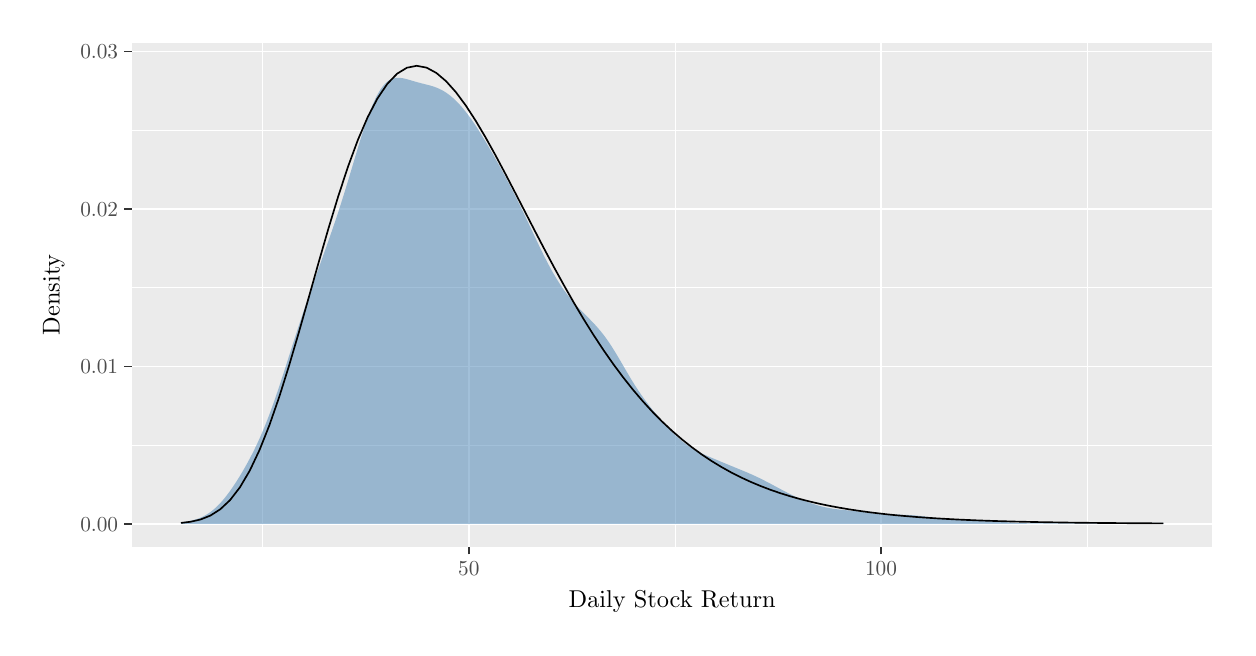
\begin{tikzpicture}[x=1pt,y=1pt]
\definecolor{fillColor}{RGB}{255,255,255}
\path[use as bounding box,fill=fillColor,fill opacity=0.00] (0,0) rectangle (433.62,216.81);
\begin{scope}
\path[clip] (  0.00,  0.00) rectangle (433.62,216.81);
\definecolor{drawColor}{RGB}{255,255,255}
\definecolor{fillColor}{RGB}{255,255,255}

\path[draw=drawColor,line width= 0.6pt,line join=round,line cap=round,fill=fillColor] (  0.00,  0.00) rectangle (433.62,216.81);
\end{scope}
\begin{scope}
\path[clip] ( 37.64, 29.26) rectangle (428.12,211.31);
\definecolor{fillColor}{gray}{0.92}

\path[fill=fillColor] ( 37.64, 29.26) rectangle (428.12,211.31);
\definecolor{drawColor}{RGB}{255,255,255}

\path[draw=drawColor,line width= 0.3pt,line join=round] ( 37.64, 65.97) --
	(428.12, 65.97);

\path[draw=drawColor,line width= 0.3pt,line join=round] ( 37.64,122.84) --
	(428.12,122.84);

\path[draw=drawColor,line width= 0.3pt,line join=round] ( 37.64,179.71) --
	(428.12,179.71);

\path[draw=drawColor,line width= 0.3pt,line join=round] ( 84.90, 29.26) --
	( 84.90,211.31);

\path[draw=drawColor,line width= 0.3pt,line join=round] (233.88, 29.26) --
	(233.88,211.31);

\path[draw=drawColor,line width= 0.3pt,line join=round] (382.87, 29.26) --
	(382.87,211.31);

\path[draw=drawColor,line width= 0.6pt,line join=round] ( 37.64, 37.53) --
	(428.12, 37.53);

\path[draw=drawColor,line width= 0.6pt,line join=round] ( 37.64, 94.40) --
	(428.12, 94.40);

\path[draw=drawColor,line width= 0.6pt,line join=round] ( 37.64,151.28) --
	(428.12,151.28);

\path[draw=drawColor,line width= 0.6pt,line join=round] ( 37.64,208.15) --
	(428.12,208.15);

\path[draw=drawColor,line width= 0.6pt,line join=round] (159.39, 29.26) --
	(159.39,211.31);

\path[draw=drawColor,line width= 0.6pt,line join=round] (308.37, 29.26) --
	(308.37,211.31);
\definecolor{fillColor}{RGB}{70,130,180}

\path[fill=fillColor,fill opacity=0.50] ( 55.39, 38.09) --
	( 56.08, 38.17) --
	( 56.78, 38.26) --
	( 57.47, 38.36) --
	( 58.17, 38.49) --
	( 58.86, 38.63) --
	( 59.56, 38.79) --
	( 60.25, 38.97) --
	( 60.95, 39.18) --
	( 61.64, 39.42) --
	( 62.34, 39.69) --
	( 63.03, 40.00) --
	( 63.73, 40.34) --
	( 64.42, 40.73) --
	( 65.11, 41.16) --
	( 65.81, 41.63) --
	( 66.50, 42.14) --
	( 67.20, 42.70) --
	( 67.89, 43.31) --
	( 68.59, 43.98) --
	( 69.28, 44.68) --
	( 69.98, 45.44) --
	( 70.67, 46.24) --
	( 71.37, 47.08) --
	( 72.06, 47.96) --
	( 72.76, 48.89) --
	( 73.45, 49.86) --
	( 74.15, 50.87) --
	( 74.84, 51.90) --
	( 75.54, 52.98) --
	( 76.23, 54.08) --
	( 76.92, 55.21) --
	( 77.62, 56.38) --
	( 78.31, 57.58) --
	( 79.01, 58.81) --
	( 79.70, 60.08) --
	( 80.40, 61.38) --
	( 81.09, 62.72) --
	( 81.79, 64.11) --
	( 82.48, 65.53) --
	( 83.18, 67.02) --
	( 83.87, 68.55) --
	( 84.57, 70.14) --
	( 85.26, 71.78) --
	( 85.96, 73.48) --
	( 86.65, 75.24) --
	( 87.34, 77.05) --
	( 88.04, 78.93) --
	( 88.73, 80.87) --
	( 89.43, 82.85) --
	( 90.12, 84.88) --
	( 90.82, 86.94) --
	( 91.51, 89.05) --
	( 92.21, 91.18) --
	( 92.90, 93.33) --
	( 93.60, 95.50) --
	( 94.29, 97.68) --
	( 94.99, 99.85) --
	( 95.68,102.03) --
	( 96.38,104.19) --
	( 97.07,106.34) --
	( 97.76,108.47) --
	( 98.46,110.58) --
	( 99.15,112.67) --
	( 99.85,114.73) --
	(100.54,116.78) --
	(101.24,118.80) --
	(101.93,120.81) --
	(102.63,122.80) --
	(103.32,124.77) --
	(104.02,126.72) --
	(104.71,128.67) --
	(105.41,130.62) --
	(106.10,132.55) --
	(106.80,134.49) --
	(107.49,136.44) --
	(108.19,138.39) --
	(108.88,140.36) --
	(109.57,142.35) --
	(110.27,144.36) --
	(110.96,146.40) --
	(111.66,148.47) --
	(112.35,150.57) --
	(113.05,152.72) --
	(113.74,154.91) --
	(114.44,157.13) --
	(115.13,159.39) --
	(115.83,161.68) --
	(116.52,163.99) --
	(117.22,166.32) --
	(117.91,168.65) --
	(118.61,170.98) --
	(119.30,173.29) --
	(119.99,175.57) --
	(120.69,177.81) --
	(121.38,179.98) --
	(122.08,182.08) --
	(122.77,184.09) --
	(123.47,185.98) --
	(124.16,187.77) --
	(124.86,189.42) --
	(125.55,190.95) --
	(126.25,192.35) --
	(126.94,193.60) --
	(127.64,194.70) --
	(128.33,195.64) --
	(129.03,196.45) --
	(129.72,197.11) --
	(130.41,197.65) --
	(131.11,198.07) --
	(131.80,198.38) --
	(132.50,198.59) --
	(133.19,198.69) --
	(133.89,198.71) --
	(134.58,198.67) --
	(135.28,198.58) --
	(135.97,198.45) --
	(136.67,198.28) --
	(137.36,198.09) --
	(138.06,197.89) --
	(138.75,197.69) --
	(139.45,197.48) --
	(140.14,197.28) --
	(140.84,197.09) --
	(141.53,196.90) --
	(142.22,196.72) --
	(142.92,196.55) --
	(143.61,196.37) --
	(144.31,196.20) --
	(145.00,196.02) --
	(145.70,195.82) --
	(146.39,195.61) --
	(147.09,195.38) --
	(147.78,195.12) --
	(148.48,194.83) --
	(149.17,194.50) --
	(149.87,194.14) --
	(150.56,193.73) --
	(151.26,193.29) --
	(151.95,192.81) --
	(152.64,192.28) --
	(153.34,191.70) --
	(154.03,191.08) --
	(154.73,190.42) --
	(155.42,189.72) --
	(156.12,188.98) --
	(156.81,188.20) --
	(157.51,187.38) --
	(158.20,186.51) --
	(158.90,185.61) --
	(159.59,184.68) --
	(160.29,183.71) --
	(160.98,182.71) --
	(161.68,181.68) --
	(162.37,180.63) --
	(163.06,179.55) --
	(163.76,178.44) --
	(164.45,177.31) --
	(165.15,176.16) --
	(165.84,174.99) --
	(166.54,173.81) --
	(167.23,172.61) --
	(167.93,171.40) --
	(168.62,170.18) --
	(169.32,168.94) --
	(170.01,167.69) --
	(170.71,166.43) --
	(171.40,165.16) --
	(172.10,163.87) --
	(172.79,162.57) --
	(173.49,161.26) --
	(174.18,159.93) --
	(174.87,158.59) --
	(175.57,157.23) --
	(176.26,155.86) --
	(176.96,154.47) --
	(177.65,153.06) --
	(178.35,151.64) --
	(179.04,150.20) --
	(179.74,148.75) --
	(180.43,147.28) --
	(181.13,145.81) --
	(181.82,144.33) --
	(182.52,142.85) --
	(183.21,141.37) --
	(183.91,139.89) --
	(184.60,138.43) --
	(185.29,136.99) --
	(185.99,135.56) --
	(186.68,134.16) --
	(187.38,132.79) --
	(188.07,131.45) --
	(188.77,130.15) --
	(189.46,128.89) --
	(190.16,127.68) --
	(190.85,126.50) --
	(191.55,125.36) --
	(192.24,124.27) --
	(192.94,123.22) --
	(193.63,122.21) --
	(194.33,121.25) --
	(195.02,120.32) --
	(195.71,119.43) --
	(196.41,118.57) --
	(197.10,117.74) --
	(197.80,116.95) --
	(198.49,116.18) --
	(199.19,115.43) --
	(199.88,114.71) --
	(200.58,113.99) --
	(201.27,113.29) --
	(201.97,112.59) --
	(202.66,111.90) --
	(203.36,111.19) --
	(204.05,110.48) --
	(204.75,109.74) --
	(205.44,108.99) --
	(206.13,108.20) --
	(206.83,107.38) --
	(207.52,106.53) --
	(208.22,105.64) --
	(208.91,104.70) --
	(209.61,103.72) --
	(210.30,102.70) --
	(211.00,101.64) --
	(211.69,100.54) --
	(212.39, 99.42) --
	(213.08, 98.26) --
	(213.78, 97.09) --
	(214.47, 95.90) --
	(215.17, 94.71) --
	(215.86, 93.51) --
	(216.56, 92.32) --
	(217.25, 91.15) --
	(217.94, 89.99) --
	(218.64, 88.85) --
	(219.33, 87.74) --
	(220.03, 86.66) --
	(220.72, 85.60) --
	(221.42, 84.58) --
	(222.11, 83.58) --
	(222.81, 82.61) --
	(223.50, 81.66) --
	(224.20, 80.75) --
	(224.89, 79.85) --
	(225.59, 78.97) --
	(226.28, 78.11) --
	(226.98, 77.26) --
	(227.67, 76.43) --
	(228.36, 75.61) --
	(229.06, 74.81) --
	(229.75, 74.02) --
	(230.45, 73.25) --
	(231.14, 72.49) --
	(231.84, 71.75) --
	(232.53, 71.03) --
	(233.23, 70.33) --
	(233.92, 69.65) --
	(234.62, 69.00) --
	(235.31, 68.37) --
	(236.01, 67.77) --
	(236.70, 67.20) --
	(237.40, 66.65) --
	(238.09, 66.13) --
	(238.78, 65.65) --
	(239.48, 65.19) --
	(240.17, 64.76) --
	(240.87, 64.35) --
	(241.56, 63.97) --
	(242.26, 63.60) --
	(242.95, 63.25) --
	(243.65, 62.92) --
	(244.34, 62.60) --
	(245.04, 62.29) --
	(245.73, 61.99) --
	(246.43, 61.69) --
	(247.12, 61.40) --
	(247.82, 61.11) --
	(248.51, 60.82) --
	(249.21, 60.53) --
	(249.90, 60.24) --
	(250.59, 59.95) --
	(251.29, 59.66) --
	(251.98, 59.38) --
	(252.68, 59.09) --
	(253.37, 58.80) --
	(254.07, 58.51) --
	(254.76, 58.23) --
	(255.46, 57.94) --
	(256.15, 57.66) --
	(256.85, 57.37) --
	(257.54, 57.09) --
	(258.24, 56.81) --
	(258.93, 56.52) --
	(259.63, 56.23) --
	(260.32, 55.93) --
	(261.01, 55.63) --
	(261.71, 55.32) --
	(262.40, 55.01) --
	(263.10, 54.69) --
	(263.79, 54.36) --
	(264.49, 54.02) --
	(265.18, 53.68) --
	(265.88, 53.33) --
	(266.57, 52.97) --
	(267.27, 52.61) --
	(267.96, 52.25) --
	(268.66, 51.88) --
	(269.35, 51.51) --
	(270.05, 51.13) --
	(270.74, 50.76) --
	(271.43, 50.39) --
	(272.13, 50.02) --
	(272.82, 49.65) --
	(273.52, 49.29) --
	(274.21, 48.93) --
	(274.91, 48.57) --
	(275.60, 48.22) --
	(276.30, 47.88) --
	(276.99, 47.54) --
	(277.69, 47.21) --
	(278.38, 46.89) --
	(279.08, 46.57) --
	(279.77, 46.27) --
	(280.47, 45.98) --
	(281.16, 45.69) --
	(281.86, 45.42) --
	(282.55, 45.16) --
	(283.24, 44.91) --
	(283.94, 44.67) --
	(284.63, 44.45) --
	(285.33, 44.24) --
	(286.02, 44.04) --
	(286.72, 43.86) --
	(287.41, 43.68) --
	(288.11, 43.52) --
	(288.80, 43.38) --
	(289.50, 43.25) --
	(290.19, 43.12) --
	(290.89, 43.01) --
	(291.58, 42.91) --
	(292.28, 42.82) --
	(292.97, 42.73) --
	(293.66, 42.66) --
	(294.36, 42.58) --
	(295.05, 42.51) --
	(295.75, 42.44) --
	(296.44, 42.38) --
	(297.14, 42.31) --
	(297.83, 42.24) --
	(298.53, 42.17) --
	(299.22, 42.09) --
	(299.92, 42.01) --
	(300.61, 41.93) --
	(301.31, 41.85) --
	(302.00, 41.76) --
	(302.70, 41.67) --
	(303.39, 41.58) --
	(304.08, 41.49) --
	(304.78, 41.41) --
	(305.47, 41.32) --
	(306.17, 41.24) --
	(306.86, 41.17) --
	(307.56, 41.10) --
	(308.25, 41.04) --
	(308.95, 40.99) --
	(309.64, 40.95) --
	(310.34, 40.92) --
	(311.03, 40.89) --
	(311.73, 40.87) --
	(312.42, 40.85) --
	(313.12, 40.84) --
	(313.81, 40.83) --
	(314.51, 40.82) --
	(315.20, 40.81) --
	(315.89, 40.80) --
	(316.59, 40.78) --
	(317.28, 40.76) --
	(317.98, 40.73) --
	(318.67, 40.69) --
	(319.37, 40.65) --
	(320.06, 40.60) --
	(320.76, 40.54) --
	(321.45, 40.47) --
	(322.15, 40.40) --
	(322.84, 40.32) --
	(323.54, 40.24) --
	(324.23, 40.15) --
	(324.93, 40.06) --
	(325.62, 39.97) --
	(326.31, 39.88) --
	(327.01, 39.79) --
	(327.70, 39.70) --
	(328.40, 39.61) --
	(329.09, 39.52) --
	(329.79, 39.44) --
	(330.48, 39.37) --
	(331.18, 39.29) --
	(331.87, 39.23) --
	(332.57, 39.16) --
	(333.26, 39.11) --
	(333.96, 39.05) --
	(334.65, 39.01) --
	(335.35, 38.97) --
	(336.04, 38.93) --
	(336.73, 38.90) --
	(337.43, 38.87) --
	(338.12, 38.84) --
	(338.82, 38.82) --
	(339.51, 38.80) --
	(340.21, 38.78) --
	(340.90, 38.76) --
	(341.60, 38.75) --
	(342.29, 38.73) --
	(342.99, 38.71) --
	(343.68, 38.69) --
	(344.38, 38.66) --
	(345.07, 38.64) --
	(345.77, 38.61) --
	(346.46, 38.58) --
	(347.16, 38.54) --
	(347.85, 38.51) --
	(348.54, 38.47) --
	(349.24, 38.42) --
	(349.93, 38.38) --
	(350.63, 38.33) --
	(351.32, 38.28) --
	(352.02, 38.23) --
	(352.71, 38.18) --
	(353.41, 38.13) --
	(354.10, 38.09) --
	(354.80, 38.04) --
	(355.49, 37.99) --
	(356.19, 37.95) --
	(356.88, 37.91) --
	(357.58, 37.87) --
	(358.27, 37.84) --
	(358.96, 37.80) --
	(359.66, 37.78) --
	(360.35, 37.75) --
	(361.05, 37.73) --
	(361.74, 37.72) --
	(362.44, 37.70) --
	(363.13, 37.69) --
	(363.83, 37.69) --
	(364.52, 37.68) --
	(365.22, 37.68) --
	(365.91, 37.68) --
	(366.61, 37.68) --
	(367.30, 37.69) --
	(368.00, 37.69) --
	(368.69, 37.70) --
	(369.38, 37.70) --
	(370.08, 37.71) --
	(370.77, 37.72) --
	(371.47, 37.72) --
	(372.16, 37.73) --
	(372.86, 37.73) --
	(373.55, 37.73) --
	(374.25, 37.73) --
	(374.94, 37.73) --
	(375.64, 37.73) --
	(376.33, 37.73) --
	(377.03, 37.73) --
	(377.72, 37.72) --
	(378.42, 37.72) --
	(379.11, 37.71) --
	(379.81, 37.71) --
	(380.50, 37.71) --
	(381.19, 37.70) --
	(381.89, 37.70) --
	(382.58, 37.70) --
	(383.28, 37.70) --
	(383.97, 37.71) --
	(384.67, 37.71) --
	(385.36, 37.72) --
	(386.06, 37.72) --
	(386.75, 37.73) --
	(387.45, 37.74) --
	(388.14, 37.75) --
	(388.84, 37.76) --
	(389.53, 37.77) --
	(390.23, 37.78) --
	(390.92, 37.79) --
	(391.61, 37.79) --
	(392.31, 37.80) --
	(393.00, 37.81) --
	(393.70, 37.82) --
	(394.39, 37.83) --
	(395.09, 37.84) --
	(395.78, 37.85) --
	(396.48, 37.85) --
	(397.17, 37.86) --
	(397.87, 37.87) --
	(398.56, 37.87) --
	(399.26, 37.88) --
	(399.95, 37.88) --
	(400.65, 37.89) --
	(401.34, 37.89) --
	(402.03, 37.89) --
	(402.73, 37.89) --
	(403.42, 37.89) --
	(404.12, 37.89) --
	(404.81, 37.89) --
	(405.51, 37.89) --
	(406.20, 37.89) --
	(406.90, 37.88) --
	(407.59, 37.88) --
	(408.29, 37.87) --
	(408.98, 37.86) --
	(409.68, 37.85) --
	(410.37, 37.83) --
	(410.37, 37.53) --
	(409.68, 37.53) --
	(408.98, 37.53) --
	(408.29, 37.53) --
	(407.59, 37.53) --
	(406.90, 37.53) --
	(406.20, 37.53) --
	(405.51, 37.53) --
	(404.81, 37.53) --
	(404.12, 37.53) --
	(403.42, 37.53) --
	(402.73, 37.53) --
	(402.03, 37.53) --
	(401.34, 37.53) --
	(400.65, 37.53) --
	(399.95, 37.53) --
	(399.26, 37.53) --
	(398.56, 37.53) --
	(397.87, 37.53) --
	(397.17, 37.53) --
	(396.48, 37.53) --
	(395.78, 37.53) --
	(395.09, 37.53) --
	(394.39, 37.53) --
	(393.70, 37.53) --
	(393.00, 37.53) --
	(392.31, 37.53) --
	(391.61, 37.53) --
	(390.92, 37.53) --
	(390.23, 37.53) --
	(389.53, 37.53) --
	(388.84, 37.53) --
	(388.14, 37.53) --
	(387.45, 37.53) --
	(386.75, 37.53) --
	(386.06, 37.53) --
	(385.36, 37.53) --
	(384.67, 37.53) --
	(383.97, 37.53) --
	(383.28, 37.53) --
	(382.58, 37.53) --
	(381.89, 37.53) --
	(381.19, 37.53) --
	(380.50, 37.53) --
	(379.81, 37.53) --
	(379.11, 37.53) --
	(378.42, 37.53) --
	(377.72, 37.53) --
	(377.03, 37.53) --
	(376.33, 37.53) --
	(375.64, 37.53) --
	(374.94, 37.53) --
	(374.25, 37.53) --
	(373.55, 37.53) --
	(372.86, 37.53) --
	(372.16, 37.53) --
	(371.47, 37.53) --
	(370.77, 37.53) --
	(370.08, 37.53) --
	(369.38, 37.53) --
	(368.69, 37.53) --
	(368.00, 37.53) --
	(367.30, 37.53) --
	(366.61, 37.53) --
	(365.91, 37.53) --
	(365.22, 37.53) --
	(364.52, 37.53) --
	(363.83, 37.53) --
	(363.13, 37.53) --
	(362.44, 37.53) --
	(361.74, 37.53) --
	(361.05, 37.53) --
	(360.35, 37.53) --
	(359.66, 37.53) --
	(358.96, 37.53) --
	(358.27, 37.53) --
	(357.58, 37.53) --
	(356.88, 37.53) --
	(356.19, 37.53) --
	(355.49, 37.53) --
	(354.80, 37.53) --
	(354.10, 37.53) --
	(353.41, 37.53) --
	(352.71, 37.53) --
	(352.02, 37.53) --
	(351.32, 37.53) --
	(350.63, 37.53) --
	(349.93, 37.53) --
	(349.24, 37.53) --
	(348.54, 37.53) --
	(347.85, 37.53) --
	(347.16, 37.53) --
	(346.46, 37.53) --
	(345.77, 37.53) --
	(345.07, 37.53) --
	(344.38, 37.53) --
	(343.68, 37.53) --
	(342.99, 37.53) --
	(342.29, 37.53) --
	(341.60, 37.53) --
	(340.90, 37.53) --
	(340.21, 37.53) --
	(339.51, 37.53) --
	(338.82, 37.53) --
	(338.12, 37.53) --
	(337.43, 37.53) --
	(336.73, 37.53) --
	(336.04, 37.53) --
	(335.35, 37.53) --
	(334.65, 37.53) --
	(333.96, 37.53) --
	(333.26, 37.53) --
	(332.57, 37.53) --
	(331.87, 37.53) --
	(331.18, 37.53) --
	(330.48, 37.53) --
	(329.79, 37.53) --
	(329.09, 37.53) --
	(328.40, 37.53) --
	(327.70, 37.53) --
	(327.01, 37.53) --
	(326.31, 37.53) --
	(325.62, 37.53) --
	(324.93, 37.53) --
	(324.23, 37.53) --
	(323.54, 37.53) --
	(322.84, 37.53) --
	(322.15, 37.53) --
	(321.45, 37.53) --
	(320.76, 37.53) --
	(320.06, 37.53) --
	(319.37, 37.53) --
	(318.67, 37.53) --
	(317.98, 37.53) --
	(317.28, 37.53) --
	(316.59, 37.53) --
	(315.89, 37.53) --
	(315.20, 37.53) --
	(314.51, 37.53) --
	(313.81, 37.53) --
	(313.12, 37.53) --
	(312.42, 37.53) --
	(311.73, 37.53) --
	(311.03, 37.53) --
	(310.34, 37.53) --
	(309.64, 37.53) --
	(308.95, 37.53) --
	(308.25, 37.53) --
	(307.56, 37.53) --
	(306.86, 37.53) --
	(306.17, 37.53) --
	(305.47, 37.53) --
	(304.78, 37.53) --
	(304.08, 37.53) --
	(303.39, 37.53) --
	(302.70, 37.53) --
	(302.00, 37.53) --
	(301.31, 37.53) --
	(300.61, 37.53) --
	(299.92, 37.53) --
	(299.22, 37.53) --
	(298.53, 37.53) --
	(297.83, 37.53) --
	(297.14, 37.53) --
	(296.44, 37.53) --
	(295.75, 37.53) --
	(295.05, 37.53) --
	(294.36, 37.53) --
	(293.66, 37.53) --
	(292.97, 37.53) --
	(292.28, 37.53) --
	(291.58, 37.53) --
	(290.89, 37.53) --
	(290.19, 37.53) --
	(289.50, 37.53) --
	(288.80, 37.53) --
	(288.11, 37.53) --
	(287.41, 37.53) --
	(286.72, 37.53) --
	(286.02, 37.53) --
	(285.33, 37.53) --
	(284.63, 37.53) --
	(283.94, 37.53) --
	(283.24, 37.53) --
	(282.55, 37.53) --
	(281.86, 37.53) --
	(281.16, 37.53) --
	(280.47, 37.53) --
	(279.77, 37.53) --
	(279.08, 37.53) --
	(278.38, 37.53) --
	(277.69, 37.53) --
	(276.99, 37.53) --
	(276.30, 37.53) --
	(275.60, 37.53) --
	(274.91, 37.53) --
	(274.21, 37.53) --
	(273.52, 37.53) --
	(272.82, 37.53) --
	(272.13, 37.53) --
	(271.43, 37.53) --
	(270.74, 37.53) --
	(270.05, 37.53) --
	(269.35, 37.53) --
	(268.66, 37.53) --
	(267.96, 37.53) --
	(267.27, 37.53) --
	(266.57, 37.53) --
	(265.88, 37.53) --
	(265.18, 37.53) --
	(264.49, 37.53) --
	(263.79, 37.53) --
	(263.10, 37.53) --
	(262.40, 37.53) --
	(261.71, 37.53) --
	(261.01, 37.53) --
	(260.32, 37.53) --
	(259.63, 37.53) --
	(258.93, 37.53) --
	(258.24, 37.53) --
	(257.54, 37.53) --
	(256.85, 37.53) --
	(256.15, 37.53) --
	(255.46, 37.53) --
	(254.76, 37.53) --
	(254.07, 37.53) --
	(253.37, 37.53) --
	(252.68, 37.53) --
	(251.98, 37.53) --
	(251.29, 37.53) --
	(250.59, 37.53) --
	(249.90, 37.53) --
	(249.21, 37.53) --
	(248.51, 37.53) --
	(247.82, 37.53) --
	(247.12, 37.53) --
	(246.43, 37.53) --
	(245.73, 37.53) --
	(245.04, 37.53) --
	(244.34, 37.53) --
	(243.65, 37.53) --
	(242.95, 37.53) --
	(242.26, 37.53) --
	(241.56, 37.53) --
	(240.87, 37.53) --
	(240.17, 37.53) --
	(239.48, 37.53) --
	(238.78, 37.53) --
	(238.09, 37.53) --
	(237.40, 37.53) --
	(236.70, 37.53) --
	(236.01, 37.53) --
	(235.31, 37.53) --
	(234.62, 37.53) --
	(233.92, 37.53) --
	(233.23, 37.53) --
	(232.53, 37.53) --
	(231.84, 37.53) --
	(231.14, 37.53) --
	(230.45, 37.53) --
	(229.75, 37.53) --
	(229.06, 37.53) --
	(228.36, 37.53) --
	(227.67, 37.53) --
	(226.98, 37.53) --
	(226.28, 37.53) --
	(225.59, 37.53) --
	(224.89, 37.53) --
	(224.20, 37.53) --
	(223.50, 37.53) --
	(222.81, 37.53) --
	(222.11, 37.53) --
	(221.42, 37.53) --
	(220.72, 37.53) --
	(220.03, 37.53) --
	(219.33, 37.53) --
	(218.64, 37.53) --
	(217.94, 37.53) --
	(217.25, 37.53) --
	(216.56, 37.53) --
	(215.86, 37.53) --
	(215.17, 37.53) --
	(214.47, 37.53) --
	(213.78, 37.53) --
	(213.08, 37.53) --
	(212.39, 37.53) --
	(211.69, 37.53) --
	(211.00, 37.53) --
	(210.30, 37.53) --
	(209.61, 37.53) --
	(208.91, 37.53) --
	(208.22, 37.53) --
	(207.52, 37.53) --
	(206.83, 37.53) --
	(206.13, 37.53) --
	(205.44, 37.53) --
	(204.75, 37.53) --
	(204.05, 37.53) --
	(203.36, 37.53) --
	(202.66, 37.53) --
	(201.97, 37.53) --
	(201.27, 37.53) --
	(200.58, 37.53) --
	(199.88, 37.53) --
	(199.19, 37.53) --
	(198.49, 37.53) --
	(197.80, 37.53) --
	(197.10, 37.53) --
	(196.41, 37.53) --
	(195.71, 37.53) --
	(195.02, 37.53) --
	(194.33, 37.53) --
	(193.63, 37.53) --
	(192.94, 37.53) --
	(192.24, 37.53) --
	(191.55, 37.53) --
	(190.85, 37.53) --
	(190.16, 37.53) --
	(189.46, 37.53) --
	(188.77, 37.53) --
	(188.07, 37.53) --
	(187.38, 37.53) --
	(186.68, 37.53) --
	(185.99, 37.53) --
	(185.29, 37.53) --
	(184.60, 37.53) --
	(183.91, 37.53) --
	(183.21, 37.53) --
	(182.52, 37.53) --
	(181.82, 37.53) --
	(181.13, 37.53) --
	(180.43, 37.53) --
	(179.74, 37.53) --
	(179.04, 37.53) --
	(178.35, 37.53) --
	(177.65, 37.53) --
	(176.96, 37.53) --
	(176.26, 37.53) --
	(175.57, 37.53) --
	(174.87, 37.53) --
	(174.18, 37.53) --
	(173.49, 37.53) --
	(172.79, 37.53) --
	(172.10, 37.53) --
	(171.40, 37.53) --
	(170.71, 37.53) --
	(170.01, 37.53) --
	(169.32, 37.53) --
	(168.62, 37.53) --
	(167.93, 37.53) --
	(167.23, 37.53) --
	(166.54, 37.53) --
	(165.84, 37.53) --
	(165.15, 37.53) --
	(164.45, 37.53) --
	(163.76, 37.53) --
	(163.06, 37.53) --
	(162.37, 37.53) --
	(161.68, 37.53) --
	(160.98, 37.53) --
	(160.29, 37.53) --
	(159.59, 37.53) --
	(158.90, 37.53) --
	(158.20, 37.53) --
	(157.51, 37.53) --
	(156.81, 37.53) --
	(156.12, 37.53) --
	(155.42, 37.53) --
	(154.73, 37.53) --
	(154.03, 37.53) --
	(153.34, 37.53) --
	(152.64, 37.53) --
	(151.95, 37.53) --
	(151.26, 37.53) --
	(150.56, 37.53) --
	(149.87, 37.53) --
	(149.17, 37.53) --
	(148.48, 37.53) --
	(147.78, 37.53) --
	(147.09, 37.53) --
	(146.39, 37.53) --
	(145.70, 37.53) --
	(145.00, 37.53) --
	(144.31, 37.53) --
	(143.61, 37.53) --
	(142.92, 37.53) --
	(142.22, 37.53) --
	(141.53, 37.53) --
	(140.84, 37.53) --
	(140.14, 37.53) --
	(139.45, 37.53) --
	(138.75, 37.53) --
	(138.06, 37.53) --
	(137.36, 37.53) --
	(136.67, 37.53) --
	(135.97, 37.53) --
	(135.28, 37.53) --
	(134.58, 37.53) --
	(133.89, 37.53) --
	(133.19, 37.53) --
	(132.50, 37.53) --
	(131.80, 37.53) --
	(131.11, 37.53) --
	(130.41, 37.53) --
	(129.72, 37.53) --
	(129.03, 37.53) --
	(128.33, 37.53) --
	(127.64, 37.53) --
	(126.94, 37.53) --
	(126.25, 37.53) --
	(125.55, 37.53) --
	(124.86, 37.53) --
	(124.16, 37.53) --
	(123.47, 37.53) --
	(122.77, 37.53) --
	(122.08, 37.53) --
	(121.38, 37.53) --
	(120.69, 37.53) --
	(119.99, 37.53) --
	(119.30, 37.53) --
	(118.61, 37.53) --
	(117.91, 37.53) --
	(117.22, 37.53) --
	(116.52, 37.53) --
	(115.83, 37.53) --
	(115.13, 37.53) --
	(114.44, 37.53) --
	(113.74, 37.53) --
	(113.05, 37.53) --
	(112.35, 37.53) --
	(111.66, 37.53) --
	(110.96, 37.53) --
	(110.27, 37.53) --
	(109.57, 37.53) --
	(108.88, 37.53) --
	(108.19, 37.53) --
	(107.49, 37.53) --
	(106.80, 37.53) --
	(106.10, 37.53) --
	(105.41, 37.53) --
	(104.71, 37.53) --
	(104.02, 37.53) --
	(103.32, 37.53) --
	(102.63, 37.53) --
	(101.93, 37.53) --
	(101.24, 37.53) --
	(100.54, 37.53) --
	( 99.85, 37.53) --
	( 99.15, 37.53) --
	( 98.46, 37.53) --
	( 97.76, 37.53) --
	( 97.07, 37.53) --
	( 96.38, 37.53) --
	( 95.68, 37.53) --
	( 94.99, 37.53) --
	( 94.29, 37.53) --
	( 93.60, 37.53) --
	( 92.90, 37.53) --
	( 92.21, 37.53) --
	( 91.51, 37.53) --
	( 90.82, 37.53) --
	( 90.12, 37.53) --
	( 89.43, 37.53) --
	( 88.73, 37.53) --
	( 88.04, 37.53) --
	( 87.34, 37.53) --
	( 86.65, 37.53) --
	( 85.96, 37.53) --
	( 85.26, 37.53) --
	( 84.57, 37.53) --
	( 83.87, 37.53) --
	( 83.18, 37.53) --
	( 82.48, 37.53) --
	( 81.79, 37.53) --
	( 81.09, 37.53) --
	( 80.40, 37.53) --
	( 79.70, 37.53) --
	( 79.01, 37.53) --
	( 78.31, 37.53) --
	( 77.62, 37.53) --
	( 76.92, 37.53) --
	( 76.23, 37.53) --
	( 75.54, 37.53) --
	( 74.84, 37.53) --
	( 74.15, 37.53) --
	( 73.45, 37.53) --
	( 72.76, 37.53) --
	( 72.06, 37.53) --
	( 71.37, 37.53) --
	( 70.67, 37.53) --
	( 69.98, 37.53) --
	( 69.28, 37.53) --
	( 68.59, 37.53) --
	( 67.89, 37.53) --
	( 67.20, 37.53) --
	( 66.50, 37.53) --
	( 65.81, 37.53) --
	( 65.11, 37.53) --
	( 64.42, 37.53) --
	( 63.73, 37.53) --
	( 63.03, 37.53) --
	( 62.34, 37.53) --
	( 61.64, 37.53) --
	( 60.95, 37.53) --
	( 60.25, 37.53) --
	( 59.56, 37.53) --
	( 58.86, 37.53) --
	( 58.17, 37.53) --
	( 57.47, 37.53) --
	( 56.78, 37.53) --
	( 56.08, 37.53) --
	( 55.39, 37.53) --
	cycle;
\definecolor{drawColor}{RGB}{0,0,0}

\path[draw=drawColor,line width= 0.6pt,line join=round] ( 55.39, 37.85) --
	( 58.94, 38.28) --
	( 62.49, 39.10) --
	( 66.04, 40.52) --
	( 69.59, 42.78) --
	( 73.14, 46.11) --
	( 76.69, 50.71) --
	( 80.24, 56.73) --
	( 83.79, 64.22) --
	( 87.34, 73.14) --
	( 90.89, 83.36) --
	( 94.44, 94.65) --
	( 97.99,106.71) --
	(101.54,119.22) --
	(105.09,131.80) --
	(108.64,144.10) --
	(112.19,155.78) --
	(115.74,166.55) --
	(119.29,176.17) --
	(122.84,184.43) --
	(126.39,191.23) --
	(129.94,196.48) --
	(133.49,200.18) --
	(137.04,202.34) --
	(140.58,203.03) --
	(144.13,202.37) --
	(147.68,200.45) --
	(151.23,197.43) --
	(154.78,193.45) --
	(158.33,188.66) --
	(161.88,183.19) --
	(165.43,177.20) --
	(168.98,170.82) --
	(172.53,164.15) --
	(176.08,157.32) --
	(179.63,150.43) --
	(183.18,143.54) --
	(186.73,136.74) --
	(190.28,130.09) --
	(193.83,123.63) --
	(197.38,117.40) --
	(200.93,111.43) --
	(204.48,105.75) --
	(208.03,100.36) --
	(211.58, 95.28) --
	(215.13, 90.51) --
	(218.68, 86.04) --
	(222.23, 81.87) --
	(225.78, 77.99) --
	(229.33, 74.40) --
	(232.88, 71.08) --
	(236.43, 68.02) --
	(239.98, 65.21) --
	(243.53, 62.62) --
	(247.08, 60.25) --
	(250.63, 58.09) --
	(254.18, 56.11) --
	(257.73, 54.31) --
	(261.28, 52.67) --
	(264.83, 51.19) --
	(268.38, 49.83) --
	(271.93, 48.61) --
	(275.48, 47.50) --
	(279.03, 46.50) --
	(282.58, 45.59) --
	(286.13, 44.77) --
	(289.68, 44.03) --
	(293.23, 43.37) --
	(296.78, 42.77) --
	(300.33, 42.23) --
	(303.88, 41.74) --
	(307.43, 41.31) --
	(310.98, 40.91) --
	(314.53, 40.56) --
	(318.08, 40.25) --
	(321.63, 39.96) --
	(325.18, 39.71) --
	(328.73, 39.48) --
	(332.27, 39.28) --
	(335.82, 39.09) --
	(339.37, 38.93) --
	(342.92, 38.78) --
	(346.47, 38.65) --
	(350.02, 38.53) --
	(353.57, 38.43) --
	(357.12, 38.33) --
	(360.67, 38.25) --
	(364.22, 38.17) --
	(367.77, 38.11) --
	(371.32, 38.05) --
	(374.87, 37.99) --
	(378.42, 37.94) --
	(381.97, 37.90) --
	(385.52, 37.86) --
	(389.07, 37.83) --
	(392.62, 37.80) --
	(396.17, 37.77) --
	(399.72, 37.74) --
	(403.27, 37.72) --
	(406.82, 37.70) --
	(410.37, 37.68);
\end{scope}
\begin{scope}
\path[clip] (  0.00,  0.00) rectangle (433.62,216.81);
\definecolor{drawColor}{gray}{0.30}

\node[text=drawColor,anchor=base east,inner sep=0pt, outer sep=0pt, scale=  0.77] at ( 32.69, 34.88) {0.00};

\node[text=drawColor,anchor=base east,inner sep=0pt, outer sep=0pt, scale=  0.77] at ( 32.69, 91.75) {0.01};

\node[text=drawColor,anchor=base east,inner sep=0pt, outer sep=0pt, scale=  0.77] at ( 32.69,148.63) {0.02};

\node[text=drawColor,anchor=base east,inner sep=0pt, outer sep=0pt, scale=  0.77] at ( 32.69,205.50) {0.03};
\end{scope}
\begin{scope}
\path[clip] (  0.00,  0.00) rectangle (433.62,216.81);
\definecolor{drawColor}{gray}{0.20}

\path[draw=drawColor,line width= 0.6pt,line join=round] ( 34.89, 37.53) --
	( 37.64, 37.53);

\path[draw=drawColor,line width= 0.6pt,line join=round] ( 34.89, 94.40) --
	( 37.64, 94.40);

\path[draw=drawColor,line width= 0.6pt,line join=round] ( 34.89,151.28) --
	( 37.64,151.28);

\path[draw=drawColor,line width= 0.6pt,line join=round] ( 34.89,208.15) --
	( 37.64,208.15);
\end{scope}
\begin{scope}
\path[clip] (  0.00,  0.00) rectangle (433.62,216.81);
\definecolor{drawColor}{gray}{0.20}

\path[draw=drawColor,line width= 0.6pt,line join=round] (159.39, 26.51) --
	(159.39, 29.26);

\path[draw=drawColor,line width= 0.6pt,line join=round] (308.37, 26.51) --
	(308.37, 29.26);
\end{scope}
\begin{scope}
\path[clip] (  0.00,  0.00) rectangle (433.62,216.81);
\definecolor{drawColor}{gray}{0.30}

\node[text=drawColor,anchor=base,inner sep=0pt, outer sep=0pt, scale=  0.77] at (159.39, 19.00) {50};

\node[text=drawColor,anchor=base,inner sep=0pt, outer sep=0pt, scale=  0.77] at (308.37, 19.00) {100};
\end{scope}
\begin{scope}
\path[clip] (  0.00,  0.00) rectangle (433.62,216.81);
\definecolor{drawColor}{RGB}{0,0,0}

\node[text=drawColor,anchor=base,inner sep=0pt, outer sep=0pt, scale=  0.88] at (232.88,  7.44) {Daily Stock Return};
\end{scope}
\begin{scope}
\path[clip] (  0.00,  0.00) rectangle (433.62,216.81);
\definecolor{drawColor}{RGB}{0,0,0}

\node[text=drawColor,rotate= 90.00,anchor=base,inner sep=0pt, outer sep=0pt, scale=  0.88] at ( 11.56,120.28) {Density};
\end{scope}
\end{tikzpicture}

\caption{BSM: Stock prices evolution density}
\label{p:logdensity}
  %
  % BEGIN OF FLOATNOTE
  %
  \begin{changemargin}{0.5cm}{0.5cm}
  \medskip
\footnotesize
\setstretch{1.0}\textbf{Notes.} The above blue distribution is constructed over $10e3$ paths of a unique stochastic process. 
The samples are built with \cref{eq:underlying:geometric:closed}. 
The arguments are adjusted with the following values, $\alpha = 0$, $\sigma = 30\%$. 
The black density belongs to the log-normal curve with mean $S(0) e^{\alpha t}$ and standard deviation of $S(0)^2 e^{2 \alpha t} (e^{\sigma^2 t} - 1)$. 
The distance period between each measure, namely $dt$ has been set to $10e3^{-1}$.  
\end{changemargin}
  %
  % END OF FLOATNOTE
  %
\end{figure}












































































%%%%%%%%%%%%%%%%%%%%%%%%%%%%%%%%%%%%%%%%%%%%%%%%
% SECTION: The partial differential BSM equation
%%%%%%%%%%%%%%%%%%%%%%%%%%%%%%%%%%%%%%%%%%%%%%%%
\section{The Black-Scholes-Merton equation}
\label{sec:bsm:equation}

Concerning the framework developed in \citet{bs}, the pricing method of an option underpinned by the BSM model is closely related to an underlying for which its price $\St$ is a log-normally distributed stochastic process, such as the GBM be.

As defined in \citet{shreve}, to provide a unique fair price to a stock option (e.g., for what matters here, to a vanilla European call) which depends on an underlying driven by a GBM, all the uncertainty associated to the stock price movements has to disappear. 
To do so, one first constructs such a portfolio $X(t)$ which encompasses the same source of risk as the option itself and then choosing the adequate position $\Delta(t)$ to take into the underlying asset at each time $t$, so that all randomness cancels out.
 
\begin{align}
  \dportfolio \label{eq:dportfolio} \\ 
  \intertext{\Citet{shreve} shows that the goal is to hedge the position taken in the option dynamically. 
It means that the position has to be frequently rebalanced. 
Consequently, at any time, the present value (PV) of the changes occurring in the portfolio, due to the underlying price evolution, should be equal to the PV of those incurred by the financial derivative. 
The only way to achieve this equality is to adapt the delta for each period.}
   d\left(e^{-rt} X\left(t\right)\right) = d\left(e^{-rt} \ct \right)
\intertext{That way, one can take a position in the derivative (short/long) and hedge it by taking $\pm \Delta(t)$ shares of stock. $X(0)$ being the price of the call at time zero}
 X\left(0\right) = c\left(0, S\left(0\right)\right)
\end{align}




By following and developing the method above, \citet{shreve} shows that the BSM differential equation is given by equation (\ref{eq:bsm:bsm:eq}),  with the terminal (\ref{eq:BSMterminal}) and boundary conditions (\ref{eq:BSMboundary0}) -- (\ref{eq:BSMboundaryinf}).

\begin{center}
  \begin{equation}
     \BSMeq{x}
    \label{eq:bsm:bsm:eq}
  \end{equation}
\end{center}
 
\begin{center}
  \begin{equation}
    \call{T}{x} = \left(x - K\right) ^+
    \label{eq:BSMterminal}
  \end{equation}
\end{center}

Whilst the terminal condition focuses on the value at maturity, the boundary conditions fix some constraints on the extreme values likely to be taken by the shares of stock at any times during the option life. 
In that regard, the boundary condition (\ref{eq:BSMboundary0}) shows that any options with a worthless underlying are themselves valueless, while whenever the call option is deep-in-the-money, simulated with $x = \infty$ (\ref{eq:BSMboundaryinf}), the value of the derivative is equal to the value of a forward contract involving the same underlying and with the same maturity date.

\begin{center}
  \begin{equation}
    \call{t}{0} = 0
    \label{eq:BSMboundary0}
  \end{equation}
\end{center}

\begin{center}
  \begin{equation}
    \lim_{x\to\infty} \left[ \call{t}{x} - \left(x - e^{-r \left(T - t \right)} \right) \right] = 0
    \label{eq:BSMboundaryinf}
  \end{equation}
\end{center}


As described in \citet{shreve}, according to the terminal (\ref{eq:BSMterminal}) and boundary conditions (\ref{eq:BSMboundary0}, \ref{eq:BSMboundaryinf}), the BSM solution for the European calls happens to be given by equation (\ref{eq:bsm:bsm:sol}). 
The right-hand side of that equation, $\ct$, denotes the price of a call option depending on the time before maturity, the volatility of the underlying and its price at that period.
In addition to these arguments, two other parameters are required, namely, the strike ($K$) and the riskless interest rate ($r$).

\begin{align}
    \BSMsol
    \label{eq:bsm:bsm:sol}
\intertext{with}
    \dpm
    \label{eq:dpm}
\end{align}

Consequently, \cref{eq:bsm:bsm:sol} will be purposely used in this master thesis to compute the price of an option for which a geometric Brownian motion exclusively drives the underlying prices process.






% \begin{figure}[!h]
% \centering
% % Created by tikzDevice version 0.11 on 2018-04-08 08:39:42
% !TEX encoding = UTF-8 Unicode
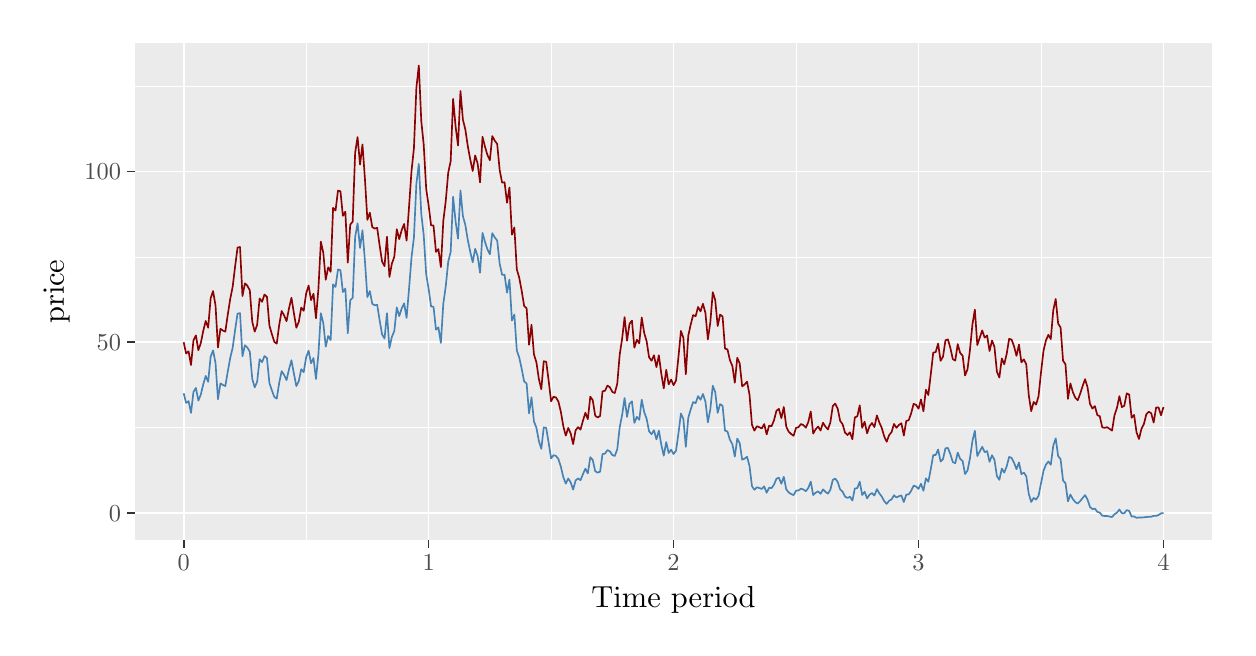
\begin{tikzpicture}[x=1pt,y=1pt]
\definecolor{fillColor}{RGB}{255,255,255}
\path[use as bounding box,fill=fillColor,fill opacity=0.00] (0,0) rectangle (433.62,216.81);
\begin{scope}
\path[clip] (  0.00,  0.00) rectangle (433.62,216.81);
\definecolor{drawColor}{RGB}{255,255,255}
\definecolor{fillColor}{RGB}{255,255,255}

\path[draw=drawColor,line width= 0.6pt,line join=round,line cap=round,fill=fillColor] (  0.00,  0.00) rectangle (433.62,216.81);
\end{scope}
\begin{scope}
\path[clip] ( 38.67, 31.53) rectangle (428.12,211.31);
\definecolor{fillColor}{gray}{0.92}

\path[fill=fillColor] ( 38.67, 31.53) rectangle (428.12,211.31);
\definecolor{drawColor}{RGB}{255,255,255}

\path[draw=drawColor,line width= 0.3pt,line join=round] ( 38.67, 72.27) --
	(428.12, 72.27);

\path[draw=drawColor,line width= 0.3pt,line join=round] ( 38.67,133.96) --
	(428.12,133.96);

\path[draw=drawColor,line width= 0.3pt,line join=round] ( 38.67,195.66) --
	(428.12,195.66);

\path[draw=drawColor,line width= 0.3pt,line join=round] (100.63, 31.53) --
	(100.63,211.31);

\path[draw=drawColor,line width= 0.3pt,line join=round] (189.14, 31.53) --
	(189.14,211.31);

\path[draw=drawColor,line width= 0.3pt,line join=round] (277.65, 31.53) --
	(277.65,211.31);

\path[draw=drawColor,line width= 0.3pt,line join=round] (366.16, 31.53) --
	(366.16,211.31);

\path[draw=drawColor,line width= 0.6pt,line join=round] ( 38.67, 41.43) --
	(428.12, 41.43);

\path[draw=drawColor,line width= 0.6pt,line join=round] ( 38.67,103.12) --
	(428.12,103.12);

\path[draw=drawColor,line width= 0.6pt,line join=round] ( 38.67,164.81) --
	(428.12,164.81);

\path[draw=drawColor,line width= 0.6pt,line join=round] ( 56.37, 31.53) --
	( 56.37,211.31);

\path[draw=drawColor,line width= 0.6pt,line join=round] (144.88, 31.53) --
	(144.88,211.31);

\path[draw=drawColor,line width= 0.6pt,line join=round] (233.39, 31.53) --
	(233.39,211.31);

\path[draw=drawColor,line width= 0.6pt,line join=round] (321.91, 31.53) --
	(321.91,211.31);

\path[draw=drawColor,line width= 0.6pt,line join=round] (410.42, 31.53) --
	(410.42,211.31);
\definecolor{drawColor}{RGB}{70,130,180}

\path[draw=drawColor,line width= 0.6pt,line join=round] ( 56.37, 84.70) --
	( 57.25, 81.22) --
	( 58.14, 81.84) --
	( 59.02, 77.61) --
	( 59.91, 85.17) --
	( 60.79, 86.64) --
	( 61.68, 82.04) --
	( 62.57, 84.24) --
	( 63.45, 87.95) --
	( 64.34, 90.96) --
	( 65.22, 88.84) --
	( 66.11, 97.91) --
	( 66.99,100.19) --
	( 67.88, 95.63) --
	( 68.76, 82.55) --
	( 69.65, 88.29) --
	( 70.53, 87.71) --
	( 71.42, 87.30) --
	( 72.30, 92.52) --
	( 73.19, 97.44) --
	( 74.07,101.15) --
	( 74.96,107.58) --
	( 75.84,113.49) --
	( 76.73,113.64) --
	( 77.61, 98.09) --
	( 78.50,102.04) --
	( 79.38,101.23) --
	( 80.27, 99.73) --
	( 81.15, 89.90) --
	( 82.04, 86.83) --
	( 82.92, 88.88) --
	( 83.81, 97.00) --
	( 84.69, 95.94) --
	( 85.58, 98.16) --
	( 86.46, 97.41) --
	( 87.35, 88.45) --
	( 88.23, 85.79) --
	( 89.12, 83.37) --
	( 90.00, 82.76) --
	( 90.89, 88.45) --
	( 91.77, 92.70) --
	( 92.66, 91.33) --
	( 93.54, 89.46) --
	( 94.43, 93.37) --
	( 95.31, 96.62) --
	( 96.20, 91.83) --
	( 97.08, 87.30) --
	( 97.97, 89.07) --
	( 98.85, 93.41) --
	( 99.74, 92.34) --
	(100.63, 97.72) --
	(101.51,100.10) --
	(102.40, 95.52) --
	(103.28, 97.42) --
	(104.17, 89.84) --
	(105.05, 98.72) --
	(105.94,113.61) --
	(106.82,110.05) --
	(107.71,101.55) --
	(108.59,105.39) --
	(109.48,103.92) --
	(110.36,124.06) --
	(111.25,123.13) --
	(112.13,129.45) --
	(113.02,129.16) --
	(113.90,121.29) --
	(114.79,122.55) --
	(115.67,106.40) --
	(116.56,118.32) --
	(117.44,119.21) --
	(118.33,141.15) --
	(119.21,146.13) --
	(120.10,137.22) --
	(120.98,143.61) --
	(121.87,132.47) --
	(122.75,119.42) --
	(123.64,121.63) --
	(124.52,117.00) --
	(125.41,116.50) --
	(126.29,116.66) --
	(127.18,111.05) --
	(128.06,105.97) --
	(128.95,104.48) --
	(129.83,113.64) --
	(130.72,101.03) --
	(131.60,105.07) --
	(132.49,107.24) --
	(133.37,115.74) --
	(134.26,112.58) --
	(135.14,115.31) --
	(136.03,117.20) --
	(136.92,111.92) --
	(137.80,122.38) --
	(138.69,133.71) --
	(139.57,140.98) --
	(140.46,160.42) --
	(141.34,167.55) --
	(142.23,149.49) --
	(143.11,141.82) --
	(144.00,127.71) --
	(144.88,122.42) --
	(145.77,116.09) --
	(146.65,115.95) --
	(147.54,107.67) --
	(148.42,108.49) --
	(149.31,102.87) --
	(150.19,117.14) --
	(151.08,123.41) --
	(151.96,132.21) --
	(152.85,135.82) --
	(153.73,155.72) --
	(154.62,146.83) --
	(155.50,140.58) --
	(156.39,157.99) --
	(157.27,148.73) --
	(158.16,145.45) --
	(159.04,140.07) --
	(159.93,135.76) --
	(160.81,132.06) --
	(161.70,136.91) --
	(162.58,134.29) --
	(163.47,128.24) --
	(164.35,142.64) --
	(165.24,139.44) --
	(166.12,136.72) --
	(167.01,134.95) --
	(167.89,142.56) --
	(168.78,141.01) --
	(169.66,139.90) --
	(170.55,131.57) --
	(171.43,127.52) --
	(172.32,127.56) --
	(173.21,121.06) --
	(174.09,125.78) --
	(174.98,110.98) --
	(175.86,113.15) --
	(176.75,100.20) --
	(177.63, 97.58) --
	(178.52, 93.52) --
	(179.40, 88.95) --
	(180.29, 88.23) --
	(181.17, 77.44) --
	(182.06, 83.24) --
	(182.94, 74.55) --
	(183.83, 72.23) --
	(184.71, 67.51) --
	(185.60, 64.61) --
	(186.48, 72.37) --
	(187.37, 72.18) --
	(188.25, 66.82) --
	(189.14, 61.15) --
	(190.02, 62.33) --
	(190.91, 62.07) --
	(191.79, 60.90) --
	(192.68, 58.11) --
	(193.56, 54.37) --
	(194.45, 52.04) --
	(195.33, 53.91) --
	(196.22, 52.50) --
	(197.10, 49.91) --
	(197.99, 53.19) --
	(198.87, 53.94) --
	(199.76, 53.29) --
	(200.64, 55.46) --
	(201.53, 57.48) --
	(202.41, 55.77) --
	(203.30, 61.60) --
	(204.18, 60.62) --
	(205.07, 56.55) --
	(205.95, 56.03) --
	(206.84, 56.37) --
	(207.72, 62.75) --
	(208.61, 62.88) --
	(209.50, 64.19) --
	(210.38, 63.70) --
	(211.27, 62.38) --
	(212.15, 62.05) --
	(213.04, 64.46) --
	(213.92, 72.38) --
	(214.81, 76.90) --
	(215.69, 82.98) --
	(216.58, 76.16) --
	(217.46, 80.91) --
	(218.35, 81.78) --
	(219.23, 73.99) --
	(220.12, 76.18) --
	(221.00, 75.10) --
	(221.89, 82.39) --
	(222.77, 77.93) --
	(223.66, 75.47) --
	(224.54, 70.94) --
	(225.43, 69.91) --
	(226.31, 71.35) --
	(227.20, 68.03) --
	(228.08, 71.21) --
	(228.97, 66.06) --
	(229.85, 62.15) --
	(230.74, 67.05) --
	(231.62, 63.12) --
	(232.51, 64.32) --
	(233.39, 62.77) --
	(234.28, 63.94) --
	(235.16, 70.24) --
	(236.05, 77.39) --
	(236.93, 75.40) --
	(237.82, 65.34) --
	(238.70, 75.81) --
	(239.59, 78.92) --
	(240.47, 81.54) --
	(241.36, 81.11) --
	(242.24, 83.68) --
	(243.13, 82.35) --
	(244.01, 84.45) --
	(244.90, 81.73) --
	(245.79, 74.20) --
	(246.67, 78.90) --
	(247.56, 87.45) --
	(248.44, 85.12) --
	(249.33, 77.64) --
	(250.21, 80.78) --
	(251.10, 80.17) --
	(251.98, 71.17) --
	(252.87, 70.88) --
	(253.75, 67.90) --
	(254.64, 66.26) --
	(255.52, 61.82) --
	(256.41, 68.32) --
	(257.29, 66.70) --
	(258.18, 60.69) --
	(259.06, 61.10) --
	(259.95, 61.74) --
	(260.83, 58.41) --
	(261.72, 51.17) --
	(262.60, 49.81) --
	(263.49, 50.73) --
	(264.37, 50.47) --
	(265.26, 50.13) --
	(266.14, 51.07) --
	(267.03, 48.75) --
	(267.91, 50.58) --
	(268.80, 50.42) --
	(269.68, 51.68) --
	(270.57, 53.83) --
	(271.45, 54.19) --
	(272.34, 52.00) --
	(273.22, 54.52) --
	(274.11, 49.99) --
	(274.99, 48.87) --
	(275.88, 48.30) --
	(276.76, 47.90) --
	(277.65, 49.50) --
	(278.53, 49.60) --
	(279.42, 50.22) --
	(280.30, 49.93) --
	(281.19, 49.32) --
	(282.08, 50.49) --
	(282.96, 52.78) --
	(283.85, 47.93) --
	(284.73, 48.76) --
	(285.62, 49.28) --
	(286.50, 48.39) --
	(287.39, 49.96) --
	(288.27, 49.08) --
	(289.16, 48.43) --
	(290.04, 49.84) --
	(290.93, 53.41) --
	(291.81, 53.88) --
	(292.70, 52.67) --
	(293.58, 49.94) --
	(294.47, 49.15) --
	(295.35, 47.39) --
	(296.24, 46.85) --
	(297.12, 47.33) --
	(298.01, 45.94) --
	(298.89, 50.27) --
	(299.78, 50.42) --
	(300.66, 52.75) --
	(301.55, 47.93) --
	(302.43, 49.10) --
	(303.32, 46.72) --
	(304.20, 48.07) --
	(305.09, 48.63) --
	(305.97, 47.76) --
	(306.86, 50.07) --
	(307.74, 48.54) --
	(308.63, 47.38) --
	(309.51, 45.72) --
	(310.40, 44.72) --
	(311.28, 45.85) --
	(312.17, 46.36) --
	(313.05, 47.84) --
	(313.94, 47.03) --
	(314.82, 47.51) --
	(315.71, 47.77) --
	(316.59, 45.41) --
	(317.48, 48.08) --
	(318.36, 48.16) --
	(319.25, 49.46) --
	(320.14, 51.35) --
	(321.02, 51.03) --
	(321.91, 50.16) --
	(322.79, 52.01) --
	(323.68, 49.47) --
	(324.56, 53.96) --
	(325.45, 52.72) --
	(326.33, 57.24) --
	(327.22, 62.36) --
	(328.10, 62.38) --
	(328.99, 64.38) --
	(329.87, 60.03) --
	(330.76, 60.93) --
	(331.64, 64.84) --
	(332.53, 64.94) --
	(333.41, 62.69) --
	(334.30, 59.85) --
	(335.18, 59.42) --
	(336.07, 63.26) --
	(336.95, 60.99) --
	(337.84, 60.22) --
	(338.72, 55.50) --
	(339.61, 56.81) --
	(340.49, 61.22) --
	(341.38, 67.41) --
	(342.26, 71.15) --
	(343.15, 62.01) --
	(344.03, 63.69) --
	(344.92, 65.37) --
	(345.80, 63.43) --
	(346.69, 63.82) --
	(347.57, 59.92) --
	(348.46, 62.31) --
	(349.34, 60.63) --
	(350.23, 54.78) --
	(351.11, 53.40) --
	(352.00, 57.50) --
	(352.88, 56.04) --
	(353.77, 58.31) --
	(354.65, 61.70) --
	(355.54, 61.36) --
	(356.43, 59.58) --
	(357.31, 57.25) --
	(358.20, 59.71) --
	(359.08, 55.49) --
	(359.97, 56.01) --
	(360.85, 54.73) --
	(361.74, 48.35) --
	(362.62, 45.42) --
	(363.51, 46.88) --
	(364.39, 46.30) --
	(365.28, 47.67) --
	(366.16, 52.12) --
	(367.05, 56.63) --
	(367.93, 58.87) --
	(368.82, 60.05) --
	(369.70, 58.87) --
	(370.59, 65.69) --
	(371.47, 68.41) --
	(372.36, 62.00) --
	(373.24, 60.87) --
	(374.13, 53.16) --
	(375.01, 52.21) --
	(375.90, 45.63) --
	(376.78, 48.13) --
	(377.67, 46.47) --
	(378.55, 45.39) --
	(379.44, 44.85) --
	(380.32, 45.74) --
	(381.21, 46.87) --
	(382.09, 47.89) --
	(382.98, 46.31) --
	(383.86, 43.61) --
	(384.75, 42.85) --
	(385.63, 43.03) --
	(386.52, 41.83) --
	(387.40, 41.59) --
	(388.29, 40.48) --
	(389.17, 40.36) --
	(390.06, 40.33) --
	(390.94, 40.15) --
	(391.83, 39.98) --
	(392.72, 41.00) --
	(393.60, 41.56) --
	(394.49, 42.71) --
	(395.37, 41.37) --
	(396.26, 41.34) --
	(397.14, 42.50) --
	(398.03, 42.16) --
	(398.91, 40.13) --
	(399.80, 40.20) --
	(400.68, 39.70) --
	(401.57, 39.81) --
	(402.45, 39.80) --
	(403.34, 39.87) --
	(404.22, 39.99) --
	(405.11, 40.05) --
	(405.99, 40.10) --
	(406.88, 40.41) --
	(407.76, 40.38) --
	(408.65, 40.71) --
	(409.53, 41.32) --
	(410.42, 41.43);
\definecolor{drawColor}{RGB}{139,0,0}

\path[draw=drawColor,line width= 0.6pt,line join=round] ( 56.37,103.12) --
	( 57.25, 99.08) --
	( 58.14, 99.86) --
	( 59.02, 94.91) --
	( 59.91,103.84) --
	( 60.79,105.61) --
	( 61.68,100.26) --
	( 62.57,102.89) --
	( 63.45,107.27) --
	( 64.34,110.83) --
	( 65.22,108.40) --
	( 66.11,118.95) --
	( 66.99,121.63) --
	( 67.88,116.42) --
	( 68.76,101.22) --
	( 69.65,108.01) --
	( 70.53,107.38) --
	( 71.42,106.94) --
	( 72.30,113.07) --
	( 73.19,118.81) --
	( 74.07,123.14) --
	( 74.96,130.56) --
	( 75.84,137.33) --
	( 76.73,137.56) --
	( 77.61,119.83) --
	( 78.50,124.42) --
	( 79.38,123.55) --
	( 80.27,121.88) --
	( 81.15,110.53) --
	( 82.04,106.97) --
	( 82.92,109.43) --
	( 83.81,118.94) --
	( 84.69,117.76) --
	( 85.58,120.38) --
	( 86.46,119.57) --
	( 87.35,109.17) --
	( 88.23,106.10) --
	( 89.12,103.29) --
	( 90.00,102.61) --
	( 90.89,109.39) --
	( 91.77,114.41) --
	( 92.66,112.86) --
	( 93.54,110.73) --
	( 94.43,115.36) --
	( 95.31,119.20) --
	( 96.20,113.66) --
	( 97.08,108.39) --
	( 97.97,110.53) --
	( 98.85,115.68) --
	( 99.74,114.49) --
	(100.63,120.82) --
	(101.51,123.63) --
	(102.40,118.36) --
	(103.28,120.64) --
	(104.17,111.83) --
	(105.05,122.27) --
	(105.94,139.48) --
	(106.82,135.47) --
	(107.71,125.73) --
	(108.59,130.22) --
	(109.48,128.60) --
	(110.36,151.71) --
	(111.25,150.73) --
	(112.13,157.95) --
	(113.02,157.69) --
	(113.90,148.82) --
	(114.79,150.32) --
	(115.67,131.89) --
	(116.56,145.64) --
	(117.44,146.72) --
	(118.33,171.63) --
	(119.21,177.28) --
	(120.10,167.34) --
	(120.98,174.61) --
	(121.87,162.12) --
	(122.75,147.37) --
	(123.64,149.96) --
	(124.52,144.74) --
	(125.41,144.23) --
	(126.29,144.48) --
	(127.18,138.10) --
	(128.06,132.30) --
	(128.95,130.63) --
	(129.83,141.28) --
	(130.72,126.74) --
	(131.60,131.51) --
	(132.49,134.10) --
	(133.37,143.98) --
	(134.26,140.41) --
	(135.14,143.63) --
	(136.03,145.87) --
	(136.92,139.86) --
	(137.80,151.95) --
	(138.69,164.93) --
	(139.57,173.23) --
	(140.46,195.12) --
	(141.34,203.14) --
	(142.23,183.05) --
	(143.11,174.49) --
	(144.00,158.57) --
	(144.88,152.59) --
	(145.77,145.38) --
	(146.65,145.30) --
	(147.54,135.79) --
	(148.42,136.81) --
	(149.31,130.32) --
	(150.19,146.98) --
	(151.08,154.25) --
	(151.96,164.39) --
	(152.85,168.57) --
	(153.73,191.11) --
	(154.62,181.19) --
	(155.50,174.22) --
	(156.39,193.90) --
	(157.27,183.58) --
	(158.16,179.97) --
	(159.04,173.97) --
	(159.93,169.16) --
	(160.81,165.02) --
	(161.70,170.63) --
	(162.58,167.73) --
	(163.47,160.90) --
	(164.35,177.39) --
	(165.24,173.84) --
	(166.12,170.84) --
	(167.01,168.91) --
	(167.89,177.64) --
	(168.78,175.97) --
	(169.66,174.79) --
	(170.55,165.38) --
	(171.43,160.83) --
	(172.32,160.95) --
	(173.21,153.55) --
	(174.09,159.09) --
	(174.98,142.01) --
	(175.86,144.62) --
	(176.75,129.48) --
	(177.63,126.44) --
	(178.52,121.67) --
	(179.40,116.23) --
	(180.29,115.43) --
	(181.17,102.23) --
	(182.06,109.48) --
	(182.94, 98.76) --
	(183.83, 95.89) --
	(184.71, 89.89) --
	(185.60, 86.16) --
	(186.48, 96.27) --
	(187.37, 96.09) --
	(188.25, 89.26) --
	(189.14, 81.82) --
	(190.02, 83.47) --
	(190.91, 83.18) --
	(191.79, 81.67) --
	(192.68, 77.92) --
	(193.56, 72.72) --
	(194.45, 69.39) --
	(195.33, 72.17) --
	(196.22, 70.18) --
	(197.10, 66.33) --
	(197.99, 71.30) --
	(198.87, 72.45) --
	(199.76, 71.56) --
	(200.64, 74.76) --
	(201.53, 77.67) --
	(202.41, 75.32) --
	(203.30, 83.48) --
	(204.18, 82.22) --
	(205.07, 76.62) --
	(205.95, 75.95) --
	(206.84, 76.49) --
	(207.72, 85.38) --
	(208.61, 85.62) --
	(209.50, 87.46) --
	(210.38, 86.88) --
	(211.27, 85.17) --
	(212.15, 84.80) --
	(213.04, 88.12) --
	(213.92, 98.60) --
	(214.81,104.47) --
	(215.69,112.21) --
	(216.58,103.70) --
	(217.46,109.79) --
	(218.35,110.96) --
	(219.23,101.17) --
	(220.12,104.06) --
	(221.00,102.76) --
	(221.89,112.08) --
	(222.77,106.54) --
	(223.66,103.49) --
	(224.54, 97.72) --
	(225.43, 96.46) --
	(226.31, 98.43) --
	(227.20, 94.14) --
	(228.08, 98.42) --
	(228.97, 91.68) --
	(229.85, 86.46) --
	(230.74, 93.18) --
	(231.62, 87.94) --
	(232.51, 89.66) --
	(233.39, 87.62) --
	(234.28, 89.31) --
	(235.16, 97.84) --
	(236.05,107.21) --
	(236.93,104.75) --
	(237.82, 91.57) --
	(238.70,105.47) --
	(239.59,109.55) --
	(240.47,112.98) --
	(241.36,112.53) --
	(242.24,115.87) --
	(243.13,114.29) --
	(244.01,117.05) --
	(244.90,113.72) --
	(245.79,104.15) --
	(246.67,110.31) --
	(247.56,121.22) --
	(248.44,118.41) --
	(249.33,109.00) --
	(250.21,113.12) --
	(251.10,112.45) --
	(251.98,100.85) --
	(252.87,100.56) --
	(253.75, 96.68) --
	(254.64, 94.56) --
	(255.52, 88.52) --
	(256.41, 97.54) --
	(257.29, 95.44) --
	(258.18, 87.20) --
	(259.06, 87.88) --
	(259.95, 88.88) --
	(260.83, 84.21) --
	(261.72, 73.32) --
	(262.60, 71.19) --
	(263.49, 72.78) --
	(264.37, 72.44) --
	(265.26, 71.98) --
	(266.14, 73.58) --
	(267.03, 69.84) --
	(267.91, 72.98) --
	(268.80, 72.80) --
	(269.68, 74.94) --
	(270.57, 78.40) --
	(271.45, 79.05) --
	(272.34, 75.71) --
	(273.22, 79.75) --
	(274.11, 72.64) --
	(274.99, 70.84) --
	(275.88, 69.96) --
	(276.76, 69.35) --
	(277.65, 72.19) --
	(278.53, 72.46) --
	(279.42, 73.59) --
	(280.30, 73.20) --
	(281.19, 72.27) --
	(282.08, 74.33) --
	(282.96, 78.14) --
	(283.85, 70.15) --
	(284.73, 71.70) --
	(285.62, 72.69) --
	(286.50, 71.24) --
	(287.39, 74.05) --
	(288.27, 72.65) --
	(289.16, 71.63) --
	(290.04, 74.16) --
	(290.93, 80.11) --
	(291.81, 80.97) --
	(292.70, 79.15) --
	(293.58, 74.75) --
	(294.47, 73.51) --
	(295.35, 70.48) --
	(296.24, 69.60) --
	(297.12, 70.59) --
	(298.01, 68.07) --
	(298.89, 75.98) --
	(299.78, 76.35) --
	(300.66, 80.33) --
	(301.55, 72.22) --
	(302.43, 74.42) --
	(303.32, 70.21) --
	(304.20, 72.82) --
	(305.09, 73.94) --
	(305.97, 72.48) --
	(306.86, 76.70) --
	(307.74, 74.15) --
	(308.63, 72.15) --
	(309.51, 69.08) --
	(310.40, 67.17) --
	(311.28, 69.58) --
	(312.17, 70.68) --
	(313.05, 73.61) --
	(313.94, 72.23) --
	(314.82, 73.25) --
	(315.71, 73.87) --
	(316.59, 69.42) --
	(317.48, 74.70) --
	(318.36, 74.98) --
	(319.25, 77.47) --
	(320.14, 80.89) --
	(321.02, 80.49) --
	(321.91, 79.13) --
	(322.79, 82.45) --
	(323.68, 78.18) --
	(324.56, 85.97) --
	(325.45, 84.08) --
	(326.33, 91.50) --
	(327.22, 99.38) --
	(328.10, 99.58) --
	(328.99,102.66) --
	(329.87, 96.42) --
	(330.76, 97.95) --
	(331.64,103.85) --
	(332.53,104.16) --
	(333.41,101.07) --
	(334.30, 97.01) --
	(335.18, 96.53) --
	(336.07,102.45) --
	(336.95, 99.27) --
	(337.84, 98.29) --
	(338.72, 91.14) --
	(339.61, 93.40) --
	(340.49,100.36) --
	(341.38,109.54) --
	(342.26,114.95) --
	(343.15,102.11) --
	(344.03,104.79) --
	(344.92,107.42) --
	(345.80,104.81) --
	(346.69,105.58) --
	(347.57, 99.97) --
	(348.46,103.77) --
	(349.34,101.47) --
	(350.23, 92.49) --
	(351.11, 90.40) --
	(352.00, 97.28) --
	(352.88, 95.18) --
	(353.77, 98.98) --
	(354.65,104.38) --
	(355.54,104.09) --
	(356.43,101.62) --
	(357.31, 98.23) --
	(358.20,102.28) --
	(359.08, 95.87) --
	(359.97, 96.95) --
	(360.85, 95.10) --
	(361.74, 84.00) --
	(362.62, 78.23) --
	(363.51, 81.55) --
	(364.39, 80.60) --
	(365.28, 83.66) --
	(366.16, 92.18) --
	(367.05, 99.95) --
	(367.93,103.74) --
	(368.82,105.83) --
	(369.70,104.28) --
	(370.59,114.66) --
	(371.47,118.77) --
	(372.36,109.86) --
	(373.24,108.47) --
	(374.13, 96.49) --
	(375.01, 95.15) --
	(375.90, 82.68) --
	(376.78, 88.24) --
	(377.67, 85.13) --
	(378.55, 83.09) --
	(379.44, 82.18) --
	(380.32, 84.54) --
	(381.21, 87.34) --
	(382.09, 89.78) --
	(382.98, 86.86) --
	(383.86, 80.87) --
	(384.75, 79.18) --
	(385.63, 80.05) --
	(386.52, 76.82) --
	(387.40, 76.40) --
	(388.29, 72.39) --
	(389.17, 72.21) --
	(390.06, 72.45) --
	(390.94, 71.85) --
	(391.83, 71.21) --
	(392.72, 76.77) --
	(393.60, 79.39) --
	(394.49, 83.64) --
	(395.37, 79.72) --
	(396.26, 80.16) --
	(397.14, 84.69) --
	(398.03, 84.23) --
	(398.91, 75.85) --
	(399.80, 76.88) --
	(400.68, 70.58) --
	(401.57, 68.18) --
	(402.45, 71.81) --
	(403.34, 73.58) --
	(404.22, 77.11) --
	(405.11, 78.04) --
	(405.99, 77.46) --
	(406.88, 74.11) --
	(407.76, 79.56) --
	(408.65, 79.54) --
	(409.53, 76.74) --
	(410.42, 79.74);
\end{scope}
\begin{scope}
\path[clip] (  0.00,  0.00) rectangle (433.62,216.81);
\definecolor{drawColor}{gray}{0.30}

\node[text=drawColor,anchor=base east,inner sep=0pt, outer sep=0pt, scale=  0.88] at ( 33.72, 38.40) {0};

\node[text=drawColor,anchor=base east,inner sep=0pt, outer sep=0pt, scale=  0.88] at ( 33.72,100.09) {50};

\node[text=drawColor,anchor=base east,inner sep=0pt, outer sep=0pt, scale=  0.88] at ( 33.72,161.78) {100};
\end{scope}
\begin{scope}
\path[clip] (  0.00,  0.00) rectangle (433.62,216.81);
\definecolor{drawColor}{gray}{0.20}

\path[draw=drawColor,line width= 0.6pt,line join=round] ( 35.92, 41.43) --
	( 38.67, 41.43);

\path[draw=drawColor,line width= 0.6pt,line join=round] ( 35.92,103.12) --
	( 38.67,103.12);

\path[draw=drawColor,line width= 0.6pt,line join=round] ( 35.92,164.81) --
	( 38.67,164.81);
\end{scope}
\begin{scope}
\path[clip] (  0.00,  0.00) rectangle (433.62,216.81);
\definecolor{drawColor}{gray}{0.20}

\path[draw=drawColor,line width= 0.6pt,line join=round] ( 56.37, 28.78) --
	( 56.37, 31.53);

\path[draw=drawColor,line width= 0.6pt,line join=round] (144.88, 28.78) --
	(144.88, 31.53);

\path[draw=drawColor,line width= 0.6pt,line join=round] (233.39, 28.78) --
	(233.39, 31.53);

\path[draw=drawColor,line width= 0.6pt,line join=round] (321.91, 28.78) --
	(321.91, 31.53);

\path[draw=drawColor,line width= 0.6pt,line join=round] (410.42, 28.78) --
	(410.42, 31.53);
\end{scope}
\begin{scope}
\path[clip] (  0.00,  0.00) rectangle (433.62,216.81);
\definecolor{drawColor}{gray}{0.30}

\node[text=drawColor,anchor=base,inner sep=0pt, outer sep=0pt, scale=  0.88] at ( 56.37, 20.52) {0};

\node[text=drawColor,anchor=base,inner sep=0pt, outer sep=0pt, scale=  0.88] at (144.88, 20.52) {1};

\node[text=drawColor,anchor=base,inner sep=0pt, outer sep=0pt, scale=  0.88] at (233.39, 20.52) {2};

\node[text=drawColor,anchor=base,inner sep=0pt, outer sep=0pt, scale=  0.88] at (321.91, 20.52) {3};

\node[text=drawColor,anchor=base,inner sep=0pt, outer sep=0pt, scale=  0.88] at (410.42, 20.52) {4};
\end{scope}
\begin{scope}
\path[clip] (  0.00,  0.00) rectangle (433.62,216.81);
\definecolor{drawColor}{RGB}{0,0,0}

\node[text=drawColor,anchor=base,inner sep=0pt, outer sep=0pt, scale=  1.10] at (233.39,  7.44) {Time period};
\end{scope}
\begin{scope}
\path[clip] (  0.00,  0.00) rectangle (433.62,216.81);
\definecolor{drawColor}{RGB}{0,0,0}

\node[text=drawColor,rotate= 90.00,anchor=base,inner sep=0pt, outer sep=0pt, scale=  1.10] at ( 13.08,121.42) {price};
\end{scope}
\end{tikzpicture}

% \caption{Relation between call price and underlying}
% \label{plot:BSMvsSt}
% \end{figure}




%%%%%%%%%%%%%%%%%%%%%%%%%%%%%%%%%%%%%%%%%%%%%%%%
% SECTION: The greeks
%%%%%%%%%%%%%%%%%%%%%%%%%%%%%%%%%%%%%%%%%%%%%%%%
\section{The greeks}
\label{sec:greeks}


The Black-Scholes-Merton equation (\ref{eq:bsm:bsm:eq}) can be subdivided into differents parts.
Each one is identified through a Greek letter ($\Delta$, $\Theta$, $\Gamma$). 

The Greeks will afterward be used to show how the hedge of a call option behaves under the conditions defined in \citet{bs} and beyond. 
Indeed, $\Delta$ has a key role in the hedging strategy because it can be used to capture the effect that an instantaneous change in the asset has to the derivative.
$\Gamma$ can remove the error of approximation incurred by a hedge based on $\Delta$ due to the discretization of the timeframe.
While $\Theta$ is not taken into account for the hedging strategy because it relates to the passing of time and nobody can prevent it.

These letters are described in this section as well as their implication in the present work.
%%%%%%%%%%%%%%%%%%%%%%%%%%%%%%%%%%%%%%%%%%%%%%%%
% SUBSECTION: Delta
%%%%%%%%%%%%%%%%%%%%%%%%%%%%%%%%%%%%%%%%%%%%%%%%
\subsection{Delta}
\label{sub:Delta}

As shown in \citet{shreve}, delta is the first derivative of the call function (\ref{eq:bsm:bsm:sol}) with respect to the stock price function, as shown by \cref{eq:bsm:call}.
It, therefore, represents the instantaneous rate of change of a call value as the price of its underlying evolves.

\begin{align}
    \Delta \left(t, \St \right) &= \frac{\partial \call{t}{\St}}{\partial \St}
    \label{eq:bsm:call}
    \intertext{Whereas practically, following \citet{shreve}, the derivation of delta for a call is given by equation \ref{eq:deltaCall}.}
    \Delta_{call} \left(t, \St \right) &= \N{\dsub{+}}
    \label{eq:deltaCall}
\end{align}

According to \citet{hull}, at each period $t$, in order to hedge a short call one should hold $\Delta(t)$ share of stock. 
Consequently, a portfolio comprised of one short position in a call along with $\Delta$ shares of stock is said to be delta-neutral, because each movement in the stock price is compensated between the short position in the call and the long in the stock.

The delta neutrality could otherwise be explained using the slope-intercept form of the tangent line below the function $\call{t}{x}$, keeping t constant. If the stock price is equal to $S$ and the corresponding call price, for a fixed time $t$ and stroke at $k$, is $c$, we consequently get (\ref{eq:slopeInterceptCallStock}) as equation of the tangent line below $\call{t}{x}$.
\begin{center}
  \begin{equation}
       y  =  \frac{\partial \call{t}{\St}}{\partial \St}  ( x - S) + c
       \label{eq:slopeInterceptCallStock}
  \end{equation}
\end{center}
According to \ref{eq:slopeInterceptCallStock}, the price of the call, for a stock price $S$ at a fixed time $t$ is given by $y = c$.
If -- over an infinitesimally small delta time -- a positive stock price movement occurs, e.g., the stock price rises from $S \to S + \epsilon$. The price of the call is, therefore, going to change as well, from $y = c$ to $y = \Delta \epsilon + c$.
Consequently, in order to hedge a short position in the call, $\Delta$ shares of stock should be owned. Indeed, by keeping $\Delta$ shares, the loss incurred by the higher value of the call $y = c + \Delta \epsilon$ will be offset by an increase of $\Delta \epsilon$ thanks to the number of $\Delta$ shares held.
It makes sense that the hedging of a long call is achieved by setting up a short position in the underlying, according to the same parameter $\Delta$.

According to \citet{shreve}, the hedge works well for small price movement in the underlying and is closely related to the curvature of the function $\call{t}{c}$, keeping $t$ constant.
It would, therefore, be interesting to look at the second derivative of the call function with respect to the stock price, in order to get the rate of the rate of change (the acceleration) of the call with respect to the underlying price.
The next \cref{sub:Gamma} devotes to it.


%%%%%%%%%%%%%%%%%%%%%%%%%%%%%%%%%%%%%%%%%%%%%%%%
% SUBSECTION: Gamma
%%%%%%%%%%%%%%%%%%%%%%%%%%%%%%%%%%%%%%%%%%%%%%%%
\subsection{Gamma}
\label{sub:Gamma}

According to \citet{shreve}, Gamma ($\Gamma$) is the second derivative of the option pricing function with respect to the underlying price, time been constant (\ref{eq:GammaDerivative}). 

\begin{align}
    \Gamma \left(t, \St \right) &= \frac{\partial^2\call{t}{\St}}{\partial \St^2}
    \label{eq:GammaDerivative}
    \intertext{Whereas practically, the derivation of gamma for a call is given by equation \ref{eq:gammaCall}.}
    \Gamma_{call} \left(t, \St \right) &= \frac{1}{\sigma \St \sqrt{\Delta t}} N^\prime \left( \dsub{+} \right)
    \label{eq:gammaCall}
\end{align}

It gives the acceleration at which the price of a call moves along with the underlying price, ceteris paribus. 
Therefore, thanks to gamma,  the curvature of the function to be approximated using the differential form is known. 
It can be crucial to at least assess how big is the value of gamma in order to adequately hedge a position in a call. 
Indeed, if gamma is low, the rebalancing of the hedge does not have to occur as frequently as if it is high because any change in the underlying asset would bring a little move in the derivative price, letting delta be a reasonable approximation of the option evolution with respect to the asset price.


As a portfolio can be delta-neutral, \citet{roman} shows that it can also be gamma-neutral. However, making a portfolio gamma-neutral forces to add another derivative on the same underlying inside it to vanish the gamma, with the consequence to modify the delta of the portfolio. It, therefore, implies to recompute the delta in order to restore the delta-neutrality of the portfolio

%%%%%%%%%%%%%%%%%%%%%%%%%%%%%%%%%%%%%%%%%%%%%%%%
% SUBSECTION: Theta
%%%%%%%%%%%%%%%%%%%%%%%%%%%%%%%%%%%%%%%%%%%%%%%%
\subsection{Theta}
\label{sub:Theta}

Theta is the derivative of the price of an option with respect to the time, stock price being unchanged (\ref{eq:ThetaDerivative}).

\begin{center}
  \begin{equation}
    \Theta (t) = \frac{\partial \call{t}{\St}}{\partial t}
    \label{eq:ThetaDerivative}
  \end{equation}
\end{center}

According to \citet{hull}, Theta can be used as a proxy for gamma in a delta-neutral portfolio.
Indeed, because of its neutrality, delta so disappears of \cref{eq:BSMGreeks} letting the relation between gamma and theta become clearer, that is, according to the option price and the value of theta, gamma could be assessed.


%%%%%%%%%%%%%%%%%%%%%%%%%%%%%%%%%%%%%%%%%%%%%%%%
% SECTION: Relation between BSM and the greeks
%%%%%%%%%%%%%%%%%%%%%%%%%%%%%%%%%%%%%%%%%%%%%%%%
\subsection{Relation between BSM and the Greeks}
\label{sec:BSMGreeks}

The BSM equation and the Greeks closely relate together.
Indeed, the BSM partial derivative equation (\ref{eq:bsm:bsm:eq}) could equally be written using the greeks, as shown by \cref{eq:BSMGreeks}.

\begin{center}
  \begin{equation}
    \BSMGreeks{\St}
    \label{eq:BSMGreeks}
  \end{equation}
\end{center}



%%%%%%%%%%%%%%%%%%%%%%%%%%%%%%%%%%%%%%%%%%%%%%%%
% SECTION: The delta hedging rules
%%%%%%%%%%%%%%%%%%%%%%%%%%%%%%%%%%%%%%%%%%%%%%%%
\section{The delta hedging strategy}
\label{sec:bsm:delta:hedge}

The purpose of the delta hedging rules is to fully replicate the reverse position taken in an option to cover oneself against lost. The technique is achieved by continuously rebalancing its position in order to keep an amount of $\Delta(t)$ share of stock for each period $t$.

Consequently to hedge a short position in a European call option, one should construct a portfolio made up of a given amount of share of stock to replicate a long position in the same derivative.
The quantity of the underlying asset to keep in that portfolio at any time is provided by the resolution of the delta (\ref{eq:deltaCall}) for the appropriate period.

\Cref{eq:bsm:delta:reverse:portfolio} shows the relation between a European short call and the delta-neutral portfolio that replicates the reverse position in the derivative for any time $t \in [0, T]$, where $T$ denotes the time to maturity.

\begin{align}
  c(t, S(t)) = \Delta(t) S(t) + 
  e^{r (t - t_0)} \left( c(t_0, S(t_0))  - \Delta(t_{0}) S(t_0) \right)
  \notag\\
    \mspace{5mu}
  - \sum_{\substack{t_i \\ \forall i \in \mathbb{Z} : i \in \left [1, n \right ]}}^{t_n = t} e^{r (t - t_i)} \left( \Delta(t_{i}) -  \Delta(t_{i-1}) \right) S(t_i)
  \label{eq:bsm:delta:reverse:portfolio} 
  % & \forall i \in \mathbb{Z} : i \in \left [1, t \right ] \notag
\end{align}
where $i$ is the time-step.
























%%%%%%%%%%%%%%%%%%%%%%%%%%%%%%%%%%%%%%%%%%%%%%%%
% SUBSECTION: Flaws
%%%%%%%%%%%%%%%%%%%%%%%%%%%%%%%%%%%%%%%%%%%%%%%%
\section{Flaws}
\label{sec:Flaws}


Even if \cref{eq:underlying:geometric:closed} is used to model the stock price process, it exists some lacks with the processes observed in real condition. 
\Cref{cha:Methodology,cha:analysis} mainly covers the following discrepancy of the model against empirical results.
  
The volatility arising in the aforementioned underlying asset process (\ref{eq:underlying:geometric:closed}) is constant as time passes. However, as stated by \citet{teneng2011limitations}, even if this consideration can be considered as true for a short period of time, it is not the case over the long-run 

Other models substitute the process defined during this chapter by including a stochastic volatility process, making the risk parameter changing over time.
For this purpose, the Heston's model (HSV) which is developed in this current master thesis involves two stochastic processes, a Brownian motion for the stock price diffusion equation and a mean-reverting CIR process in order to compute stochastic volatility.
This model is exposed in \cref{sec:other:heston}.

\Cref{eq:logreturndist} shows that the normal law characterizes the underlying log-returns distribution. Consequently, the random variable $\St$, at the fixed time $t$, is log-normal, such as stated by \cref{eq:underlyin:st:nnorm}. 
However, according to \citet{clark1973}, empirical results illustrate that the random variable $d\St/\St$ do not fit with the normal bell curve.
Therefore if that rate of change is not normally distributed neither are the log-returns and thus $\St$, for a fixed time $t$, is not log-normal.

Along with the Heston model, another one is examined; the Merton's jump-diffusion (MJD) model. Both are able to modify the skewness and kurtosis of the log-returns distribution curve. The Merton equation is developed in \cref{cha:OtherModel}. 

Others discrepancies directly observed from market data are the volatility smiles.
Indeed, if someone tries to reverse compute the volatility parameter $\sigma$ from the available option prices, she/he will get different values for options on the same asset, covering the same period but with different strike prices. 
Nevertheless, since that parameter is used to simulate the underlying stock prices motion, it means that the same asset, during the same period depends on different risk parameters following the point of view of a hedger. That makes no sense.
As shown in \cref{cha:Methodology}, the models MJD and HSV are versatile enough to overcome this issue.












%%%%%%%%%%%%%%%%%%%%%%%%%%%%%%%%%%%%%%%%%%%%%%%%%%%%%%%%%%%%%%%%%%%%%%%%%%%%%%%%
%
%  CHAPTER:Other Models to be considered
%
%%%%%%%%%%%%%%%%%%%%%%%%%%%%%%%%%%%%%%%%%%%%%%%%%%%%%%%%%%%%%%%%%%%%%%%%%%%%%%%%
\chapter{Other Models to be considered}
\label{cha:OtherModel}

In this chapter are explored models that will substitute the geometric Brownian motion for the stock prices evolution along with the related option pricing method.

The first considered model is the Merton jump-diffusion (MJD) that brings jump to the course of a stochastic process while the second is the Heston stochastic volatility model that allows the volatility parameter to evolve through time.

At the end of that chapter, a method developed by \citet{heston1993} illustrates how to compute the prices of options based on such underlying by using their characteristic function.




%%%%%%%%%%%%%%%%%%%%%%%%%%%%%%%%%%%%%%%%%%%%%%%%
% SUBSECTION: Mixed jump-diffusionModel
%%%%%%%%%%%%%%%%%%%%%%%%%%%%%%%%%%%%%%%%%%%%%%%%
\section{Merton Mixed jump-diffusion Model}
\label{sec:other:merton}

In his paper, \citet{merton76} provides a model for stock price evolution involving jumps (\cref{eq:other:merton:pde}). 


\begin{align}
  \St &= S\left(0\right) e^{\left(\alpha - \frac{\sigma^2}{2} - \lambda \kappa\right) t + \sigma \Bm + \sum_{i=1}^{N_t} Y_i}
  \label{eq:other:merton:pde}
\end{align}
  
According to \citet{merton76}, there are two specific sources of uncertainty explained by the model (\cref{eq:other:merton:pde}). 

The first one is qualified as normal, repeatedly arising with low effects and keeping the stock price motion continuous from time to time. These small changes on the price are modeled by a Wiener process, such as it was the case in equation \ref{eq:underlying:geometric:closed}. The cause of these fluctuations is explained by a temporary unbalanced between the supply and demand \citet{merton76}.

Another type of changes, occurring during the stock lifecycle, is qualified as abnormal by \citet{merton76}. 
Such "abnormalities" happen less frequently, are unpredictable in their frequency and produce bigger effects on the stock price by giving rise to jumps during the course of the stock path, and therefore breaking its continuity. The jump process is constructed on a double basis. 

Firstly, the occurrence (i.e. the number of jumps arising throughout a given period of time) is computed thanks to a Poisson-driven process according to a parameter $\lambda$. 
$\lambda$ denotes the number of jumps per unit of time. Consequently, the probability that a jump occurs during a time range of $\Delta t$ is equal to $\lambda dt$ (event $A$, eq. \ref{eq:PA}), whereas the probability that there are no jump during the same range of time is $1 - \lambda dt$, (event $B$, eq. \ref{eq:PB}) (\citet{matsuda2004}). While event C, from \cref{eq:PC}, refers to the event that more than one jump occurs during the same small delta time.

\begin{align}
  \mathop{\mathbb{P}} \{A\}&\cong \lambda dt  \label{eq:PA}\\
  \mathop{\mathbb{P}} \{B\}&\cong 1 - \lambda dt  \label{eq:PB}\\
  \mathop{\mathbb{P}} \{C\}&\cong   0 \label{eq:PC}
\end{align}

On the other hand, after the occurrence, the size of the jump matters. Such as the frequency, a statistic law characterizes the importance of the jump. Following \citet{merton76}, the log-normal law is used. \citet{matsuda2004} offers the \crefrange{eq:yt}{eq:lny} to summarize the law and the parameters that describe the jump intensity.
 
\begin{align}
  y_t  &\sim lognormal( e^{\mu + \frac{1}{2} \delta^2}, 
                        e^{2 \mu + \delta ^2} (e^{\delta^2} - 1)) 
  \label{eq:yt} \\
  y_t - 1 &\sim lognormal( \kappa \equiv e^{\mu + \frac{1}{2} \delta^2} - 1, 
                        e^{2 \mu + \delta ^2} (e^{\delta^2} - 1)) 
  \label{eq:ytminus1} \\
  \ln{y_t} &\sim normal(\mu, \delta^ 2)
  \label{eq:lny}
\end{align}
with $y_t$, $y_t - 1$ and $\ln{y_t} \equiv Y_t$ standing respectively for "absolute price jump size", "relative price jump size" and "log price jump size" (\citet{matsuda2004}).

 
The Merton's jump-diffusion process is be able to capture positive / negative skewness (see \cref{sub:MertonSkewness}) and excess kurtosis (see \cref{sub:MertonKurtosis}) of the log-return density function, in accordance with \citet{merton76}. 


%%%%%%%%%%%%%%%%%%%%%%%%%%%%%%%%%%%%%%%%%%%%%%%%
% SUBSECTION: Risk-neutralized process
%%%%%%%%%%%%%%%%%%%%%%%%%%%%%%%%%%%%%%%%%%%%%%%%
\subsection{Risk-neutralized process}
\label{sub:other:merton:risk}

In order to find the fair price of an option depending on an underlying that follows such a jump-diffusion process, \citet{merton76} turns \cref{eq:other:merton:pde} into one risk-neutral.

\begin{align}
  \St &= S\left(0\right) e^{\left(r - \frac{\sigma^2}{2} - \lambda \kappa\right) t + \sigma \Bm + \sum_{i=1}^{N_t} Y_i}
  \label{eq:other:merton:pde:riskneutral}
\end{align}

\citet{merton76} argues in his paper that the jump component of \cref{eq:other:merton:pde} can be diversified in a well-balanced portfolio and consequently does not need to be risk-neutralized.

However, likewise it was done by \citet{bs}, the drift part of \cref{eq:other:merton:pde} is risk-neutralized by turning the rate $\alpha$ into its riskfree counterpart $r$, as shown by \cref{eq:other:merton:pde:riskneutral}.



%%%%%%%%%%%%%%%%%%%%%%%%%%%%%%%%%%%%%%%%%%%%%%%%
% SUBSECTION: Graphical representation
%%%%%%%%%%%%%%%%%%%%%%%%%%%%%%%%%%%%%%%%%%%%%%%%
\subsection{Graphical representation}
\label{sub:other:merton:graphical}   

\Cref{p:other:merton:path} shows a unique time-series generated using an implementation of \cref{eq:other:merton:pde}. A jump is clearly marked at day 363. While
\cref{t:other:merton:path}, which is a subset of the time-series drawn in \cref{p:other:merton:path}, illustrates numerically when the jump occurs.

\begin{table}[ht]
\centering
\begin{tabular}{ll}
  \hline
 time periods (days)& stock price\\ 
  \hline
  0   &50.00 \\ 
  1   &49.72 \\ 
  2   &49.87 \\ 
  \vdots & \vdots \\
  323 &83.44 \\ 
  324 &94.98 \\ 
  \vdots & \vdots \\
  363 &97.41 \\ 
  364 &97.07 \\ 
  365 &97.00 \\ 
   \hline
\end{tabular}
\caption{Merton Mixed jump-diffusion time-series}
\label{t:other:merton:path}
\end{table}

\begin{figure}[ht]
  \centering
  % Created by tikzDevice version 0.11 on 2018-07-12 22:38:50
% !TEX encoding = UTF-8 Unicode
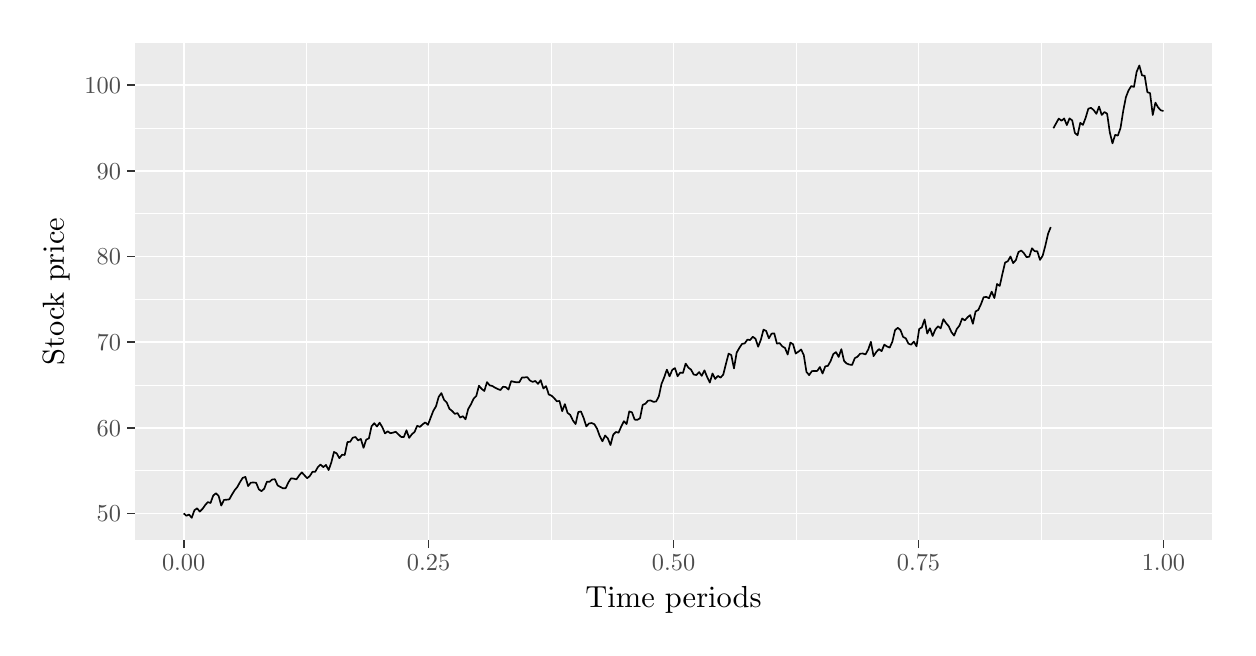
\begin{tikzpicture}[x=1pt,y=1pt]
\definecolor{fillColor}{RGB}{255,255,255}
\path[use as bounding box,fill=fillColor,fill opacity=0.00] (0,0) rectangle (433.62,216.81);
\begin{scope}
\path[clip] (  0.00,  0.00) rectangle (433.62,216.81);
\definecolor{drawColor}{RGB}{255,255,255}
\definecolor{fillColor}{RGB}{255,255,255}

\path[draw=drawColor,line width= 0.6pt,line join=round,line cap=round,fill=fillColor] (  0.00,  0.00) rectangle (433.62,216.81);
\end{scope}
\begin{scope}
\path[clip] ( 38.67, 31.53) rectangle (428.12,211.31);
\definecolor{fillColor}{gray}{0.92}

\path[fill=fillColor] ( 38.67, 31.53) rectangle (428.12,211.31);
\definecolor{drawColor}{RGB}{255,255,255}

\path[draw=drawColor,line width= 0.3pt,line join=round] ( 38.67, 56.77) --
	(428.12, 56.77);

\path[draw=drawColor,line width= 0.3pt,line join=round] ( 38.67, 87.71) --
	(428.12, 87.71);

\path[draw=drawColor,line width= 0.3pt,line join=round] ( 38.67,118.64) --
	(428.12,118.64);

\path[draw=drawColor,line width= 0.3pt,line join=round] ( 38.67,149.58) --
	(428.12,149.58);

\path[draw=drawColor,line width= 0.3pt,line join=round] ( 38.67,180.52) --
	(428.12,180.52);

\path[draw=drawColor,line width= 0.3pt,line join=round] (100.63, 31.53) --
	(100.63,211.31);

\path[draw=drawColor,line width= 0.3pt,line join=round] (189.14, 31.53) --
	(189.14,211.31);

\path[draw=drawColor,line width= 0.3pt,line join=round] (277.65, 31.53) --
	(277.65,211.31);

\path[draw=drawColor,line width= 0.3pt,line join=round] (366.16, 31.53) --
	(366.16,211.31);

\path[draw=drawColor,line width= 0.6pt,line join=round] ( 38.67, 41.30) --
	(428.12, 41.30);

\path[draw=drawColor,line width= 0.6pt,line join=round] ( 38.67, 72.24) --
	(428.12, 72.24);

\path[draw=drawColor,line width= 0.6pt,line join=round] ( 38.67,103.17) --
	(428.12,103.17);

\path[draw=drawColor,line width= 0.6pt,line join=round] ( 38.67,134.11) --
	(428.12,134.11);

\path[draw=drawColor,line width= 0.6pt,line join=round] ( 38.67,165.05) --
	(428.12,165.05);

\path[draw=drawColor,line width= 0.6pt,line join=round] ( 38.67,195.99) --
	(428.12,195.99);

\path[draw=drawColor,line width= 0.6pt,line join=round] ( 56.37, 31.53) --
	( 56.37,211.31);

\path[draw=drawColor,line width= 0.6pt,line join=round] (144.88, 31.53) --
	(144.88,211.31);

\path[draw=drawColor,line width= 0.6pt,line join=round] (233.39, 31.53) --
	(233.39,211.31);

\path[draw=drawColor,line width= 0.6pt,line join=round] (321.91, 31.53) --
	(321.91,211.31);

\path[draw=drawColor,line width= 0.6pt,line join=round] (410.42, 31.53) --
	(410.42,211.31);
\definecolor{drawColor}{RGB}{0,0,0}

\path[draw=drawColor,line width= 0.6pt,line join=round] ( 56.37, 41.30) --
	( 57.34, 40.44) --
	( 58.31, 40.89) --
	( 59.28, 39.70) --
	( 60.25, 42.44) --
	( 61.22, 43.13) --
	( 62.19, 41.95) --
	( 63.16, 42.90) --
	( 64.13, 44.27) --
	( 65.10, 45.39) --
	( 66.07, 45.04) --
	( 67.04, 47.73) --
	( 68.01, 48.55) --
	( 68.98, 47.66) --
	( 69.95, 44.13) --
	( 70.92, 46.15) --
	( 71.89, 46.24) --
	( 72.86, 46.37) --
	( 73.83, 48.12) --
	( 74.80, 49.68) --
	( 75.77, 50.86) --
	( 76.74, 52.62) --
	( 77.71, 54.15) --
	( 78.68, 54.45) --
	( 79.65, 51.16) --
	( 80.62, 52.39) --
	( 81.59, 52.46) --
	( 82.56, 52.36) --
	( 83.53, 49.99) --
	( 84.50, 49.34) --
	( 85.47, 50.22) --
	( 86.44, 52.73) --
	( 87.41, 52.72) --
	( 88.38, 53.56) --
	( 89.35, 53.63) --
	( 90.32, 51.41) --
	( 91.29, 50.86) --
	( 92.26, 50.35) --
	( 93.23, 50.41) --
	( 94.20, 52.47) --
	( 95.17, 53.97) --
	( 96.14, 53.85) --
	( 97.11, 53.58) --
	( 98.08, 54.97) --
	( 99.05, 56.12) --
	(100.02, 55.07) --
	(100.99, 54.00) --
	(101.96, 54.81) --
	(102.93, 56.34) --
	(103.90, 56.31) --
	(104.87, 58.05) --
	(105.84, 58.94) --
	(106.81, 58.01) --
	(107.78, 58.80) --
	(108.75, 56.95) --
	(109.72, 59.70) --
	(110.69, 63.50) --
	(111.66, 63.00) --
	(112.63, 61.26) --
	(113.60, 62.48) --
	(114.57, 62.41) --
	(115.54, 67.06) --
	(116.51, 67.17) --
	(117.48, 68.66) --
	(118.45, 68.90) --
	(119.42, 67.67) --
	(120.39, 68.21) --
	(121.36, 64.99) --
	(122.33, 67.93) --
	(123.30, 68.40) --
	(124.27, 72.77) --
	(125.24, 73.89) --
	(126.21, 72.69) --
	(127.18, 74.07) --
	(128.15, 72.43) --
	(129.12, 70.19) --
	(130.09, 70.94) --
	(131.06, 70.27) --
	(132.03, 70.46) --
	(133.00, 70.79) --
	(133.97, 69.84) --
	(134.94, 68.93) --
	(135.91, 68.86) --
	(136.88, 71.31) --
	(137.85, 68.57) --
	(138.82, 69.89) --
	(139.79, 70.71) --
	(140.76, 72.96) --
	(141.73, 72.55) --
	(142.70, 73.46) --
	(143.67, 74.17) --
	(144.64, 73.30) --
	(145.61, 75.86) --
	(146.58, 78.37) --
	(147.55, 79.97) --
	(148.52, 83.41) --
	(149.49, 84.76) --
	(150.46, 82.33) --
	(151.43, 81.36) --
	(152.40, 79.07) --
	(153.37, 78.31) --
	(154.34, 77.26) --
	(155.31, 77.54) --
	(156.28, 75.91) --
	(157.25, 76.42) --
	(158.22, 75.31) --
	(159.19, 79.03) --
	(160.16, 80.67) --
	(161.13, 82.73) --
	(162.10, 83.72) --
	(163.07, 87.42) --
	(164.04, 86.29) --
	(165.01, 85.53) --
	(165.98, 88.73) --
	(166.95, 87.56) --
	(167.92, 87.33) --
	(168.89, 86.71) --
	(169.86, 86.24) --
	(170.83, 85.86) --
	(171.80, 87.09) --
	(172.77, 86.92) --
	(173.74, 86.06) --
	(174.71, 89.09) --
	(175.68, 88.84) --
	(176.65, 88.66) --
	(177.62, 88.65) --
	(178.59, 90.37) --
	(179.56, 90.42) --
	(180.53, 90.54) --
	(181.50, 89.30) --
	(182.47, 88.81) --
	(183.44, 89.14) --
	(184.41, 88.10) --
	(185.38, 89.43) --
	(186.35, 86.43) --
	(187.32, 87.28) --
	(188.29, 84.27) --
	(189.26, 83.85) --
	(190.23, 82.96) --
	(191.20, 81.82) --
	(192.17, 81.90) --
	(193.14, 78.22) --
	(194.11, 80.79) --
	(195.08, 77.62) --
	(196.05, 76.89) --
	(197.02, 74.87) --
	(197.99, 73.58) --
	(198.96, 77.91) --
	(199.93, 78.13) --
	(200.90, 75.76) --
	(201.87, 72.73) --
	(202.84, 73.79) --
	(203.81, 73.95) --
	(204.78, 73.51) --
	(205.75, 71.89) --
	(206.72, 69.21) --
	(207.69, 67.35) --
	(208.66, 69.43) --
	(209.63, 68.43) --
	(210.60, 65.99) --
	(211.57, 69.72) --
	(212.54, 70.72) --
	(213.51, 70.45) --
	(214.48, 72.69) --
	(215.45, 74.61) --
	(216.42, 73.58) --
	(217.39, 78.14) --
	(218.36, 77.82) --
	(219.33, 75.18) --
	(220.30, 75.09) --
	(221.27, 75.69) --
	(222.24, 80.51) --
	(223.21, 80.92) --
	(224.18, 82.04) --
	(225.15, 82.08) --
	(226.12, 81.60) --
	(227.09, 81.72) --
	(228.06, 83.54) --
	(229.03, 88.06) --
	(230.00, 90.45) --
	(230.97, 93.25) --
	(231.94, 90.81) --
	(232.91, 93.13) --
	(233.88, 93.81) --
	(234.85, 90.86) --
	(235.82, 92.18) --
	(236.79, 92.05) --
	(237.76, 95.43) --
	(238.73, 93.97) --
	(239.70, 93.25) --
	(240.67, 91.46) --
	(241.64, 91.29) --
	(242.61, 92.36) --
	(243.58, 90.99) --
	(244.55, 92.98) --
	(245.52, 90.59) --
	(246.49, 88.57) --
	(247.46, 91.85) --
	(248.43, 89.88) --
	(249.40, 90.97) --
	(250.37, 90.36) --
	(251.34, 91.44) --
	(252.31, 95.30) --
	(253.28, 99.01) --
	(254.25, 98.49) --
	(255.22, 93.69) --
	(256.19, 99.39) --
	(257.16,101.09) --
	(258.13,102.53) --
	(259.10,102.72) --
	(260.07,104.09) --
	(261.04,103.94) --
	(262.01,105.11) --
	(262.98,104.42) --
	(263.95,101.53) --
	(264.92,103.99) --
	(265.89,107.69) --
	(266.86,107.20) --
	(267.83,104.55) --
	(268.80,106.24) --
	(269.77,106.36) --
	(270.74,102.62) --
	(271.71,102.84) --
	(272.68,101.64) --
	(273.65,101.09) --
	(274.62, 98.72) --
	(275.59,102.98) --
	(276.56,102.45) --
	(277.53, 99.06) --
	(278.50, 99.72) --
	(279.47,100.52) --
	(280.44, 98.53) --
	(281.41, 92.43) --
	(282.38, 91.26) --
	(283.35, 92.69) --
	(284.32, 92.77) --
	(285.29, 92.77) --
	(286.26, 94.19) --
	(287.23, 91.83) --
	(288.20, 94.41) --
	(289.17, 94.61) --
	(290.14, 96.36) --
	(291.11, 98.86) --
	(292.08, 99.57) --
	(293.05, 97.83) --
	(294.02,100.64) --
	(294.99, 96.41) --
	(295.96, 95.43) --
	(296.93, 95.08) --
	(297.90, 94.93) --
	(298.87, 97.38) --
	(299.84, 97.89) --
	(300.81, 99.01) --
	(301.78, 99.06) --
	(302.75, 98.73) --
	(303.72,100.49) --
	(304.69,103.29) --
	(305.66, 98.12) --
	(306.63, 99.61) --
	(307.60,100.66) --
	(308.57, 99.92) --
	(309.54,102.27) --
	(310.51,101.61) --
	(311.48,101.19) --
	(312.45,103.34) --
	(313.42,107.50) --
	(314.39,108.35) --
	(315.36,107.59) --
	(316.33,105.08) --
	(317.30,104.54) --
	(318.27,102.63) --
	(319.24,102.26) --
	(320.21,103.37) --
	(321.18,101.66) --
	(322.15,107.93) --
	(323.12,108.51) --
	(324.09,111.38) --
	(325.06,106.28) --
	(326.03,108.21) --
	(327.00,105.40) --
	(327.97,107.74) --
	(328.94,108.89) --
	(329.91,108.16) --
	(330.88,111.48) --
	(331.85,110.06) --
	(332.82,108.93) --
	(333.79,106.83) --
	(334.76,105.52) --
	(335.73,107.92) --
	(336.70,109.15) --
	(337.67,111.73) --
	(338.64,111.04) --
	(339.61,112.15) --
	(340.58,112.95) --
	(341.55,109.82) --
	(342.52,114.25) --
	(343.49,114.80) --
	(344.46,116.86) --
	(345.43,119.41) --
	(346.40,119.52) --
	(347.37,119.01) --
	(348.34,121.43) --
	(349.31,119.10) --
	(350.28,124.19) --
	(351.25,123.48) --
	(352.22,127.86) --
	(353.19,131.95) --
	(354.16,132.41) --
	(355.13,134.13) --
	(356.10,131.73) --
	(357.07,132.81) --
	(358.04,135.76) --
	(359.01,136.27) --
	(359.98,135.34) --
	(360.95,133.89) --
	(361.92,134.04) --
	(362.89,137.08) --
	(363.86,136.06) --
	(364.83,136.00) --
	(365.80,132.89) --
	(366.77,134.42) --
	(367.74,138.09) --
	(368.71,142.31) --
	(369.68,144.76);

\path[draw=drawColor,line width= 0.6pt,line join=round] (370.65,180.47) --
	(371.62,182.25) --
	(372.59,183.97) --
	(373.56,183.17) --
	(374.53,184.00) --
	(375.50,181.61) --
	(376.47,184.02) --
	(377.44,183.30) --
	(378.41,178.76) --
	(379.38,177.93) --
	(380.35,182.42) --
	(381.32,181.68) --
	(382.29,184.25) --
	(383.26,187.52) --
	(384.23,187.84) --
	(385.20,187.03) --
	(386.17,185.67) --
	(387.14,188.30) --
	(388.11,185.26) --
	(389.08,186.33) --
	(390.05,185.72) --
	(391.02,179.01) --
	(391.99,175.01) --
	(392.96,178.09) --
	(393.93,177.80) --
	(394.90,180.55) --
	(395.87,186.72) --
	(396.84,191.69) --
	(397.81,194.17) --
	(398.78,195.71) --
	(399.75,195.39) --
	(400.72,200.85) --
	(401.69,203.14) --
	(402.66,199.59) --
	(403.63,199.39) --
	(404.60,193.48) --
	(405.57,193.16) --
	(406.54,185.25) --
	(407.51,189.70) --
	(408.48,187.99) --
	(409.45,186.94) --
	(410.42,186.71);
\end{scope}
\begin{scope}
\path[clip] (  0.00,  0.00) rectangle (433.62,216.81);
\definecolor{drawColor}{gray}{0.30}

\node[text=drawColor,anchor=base east,inner sep=0pt, outer sep=0pt, scale=  0.88] at ( 33.72, 38.27) {50};

\node[text=drawColor,anchor=base east,inner sep=0pt, outer sep=0pt, scale=  0.88] at ( 33.72, 69.21) {60};

\node[text=drawColor,anchor=base east,inner sep=0pt, outer sep=0pt, scale=  0.88] at ( 33.72,100.14) {70};

\node[text=drawColor,anchor=base east,inner sep=0pt, outer sep=0pt, scale=  0.88] at ( 33.72,131.08) {80};

\node[text=drawColor,anchor=base east,inner sep=0pt, outer sep=0pt, scale=  0.88] at ( 33.72,162.02) {90};

\node[text=drawColor,anchor=base east,inner sep=0pt, outer sep=0pt, scale=  0.88] at ( 33.72,192.96) {100};
\end{scope}
\begin{scope}
\path[clip] (  0.00,  0.00) rectangle (433.62,216.81);
\definecolor{drawColor}{gray}{0.20}

\path[draw=drawColor,line width= 0.6pt,line join=round] ( 35.92, 41.30) --
	( 38.67, 41.30);

\path[draw=drawColor,line width= 0.6pt,line join=round] ( 35.92, 72.24) --
	( 38.67, 72.24);

\path[draw=drawColor,line width= 0.6pt,line join=round] ( 35.92,103.17) --
	( 38.67,103.17);

\path[draw=drawColor,line width= 0.6pt,line join=round] ( 35.92,134.11) --
	( 38.67,134.11);

\path[draw=drawColor,line width= 0.6pt,line join=round] ( 35.92,165.05) --
	( 38.67,165.05);

\path[draw=drawColor,line width= 0.6pt,line join=round] ( 35.92,195.99) --
	( 38.67,195.99);
\end{scope}
\begin{scope}
\path[clip] (  0.00,  0.00) rectangle (433.62,216.81);
\definecolor{drawColor}{gray}{0.20}

\path[draw=drawColor,line width= 0.6pt,line join=round] ( 56.37, 28.78) --
	( 56.37, 31.53);

\path[draw=drawColor,line width= 0.6pt,line join=round] (144.88, 28.78) --
	(144.88, 31.53);

\path[draw=drawColor,line width= 0.6pt,line join=round] (233.39, 28.78) --
	(233.39, 31.53);

\path[draw=drawColor,line width= 0.6pt,line join=round] (321.91, 28.78) --
	(321.91, 31.53);

\path[draw=drawColor,line width= 0.6pt,line join=round] (410.42, 28.78) --
	(410.42, 31.53);
\end{scope}
\begin{scope}
\path[clip] (  0.00,  0.00) rectangle (433.62,216.81);
\definecolor{drawColor}{gray}{0.30}

\node[text=drawColor,anchor=base,inner sep=0pt, outer sep=0pt, scale=  0.88] at ( 56.37, 20.52) {0.00};

\node[text=drawColor,anchor=base,inner sep=0pt, outer sep=0pt, scale=  0.88] at (144.88, 20.52) {0.25};

\node[text=drawColor,anchor=base,inner sep=0pt, outer sep=0pt, scale=  0.88] at (233.39, 20.52) {0.50};

\node[text=drawColor,anchor=base,inner sep=0pt, outer sep=0pt, scale=  0.88] at (321.91, 20.52) {0.75};

\node[text=drawColor,anchor=base,inner sep=0pt, outer sep=0pt, scale=  0.88] at (410.42, 20.52) {1.00};
\end{scope}
\begin{scope}
\path[clip] (  0.00,  0.00) rectangle (433.62,216.81);
\definecolor{drawColor}{RGB}{0,0,0}

\node[text=drawColor,anchor=base,inner sep=0pt, outer sep=0pt, scale=  1.10] at (233.39,  7.44) {Time periods};
\end{scope}
\begin{scope}
\path[clip] (  0.00,  0.00) rectangle (433.62,216.81);
\definecolor{drawColor}{RGB}{0,0,0}

\node[text=drawColor,rotate= 90.00,anchor=base,inner sep=0pt, outer sep=0pt, scale=  1.10] at ( 13.08,121.42) {Stock price};
\end{scope}
\end{tikzpicture}
 
    %
  % BEGIN OF FLOATNOTE
  %
  \begin{changemargin}{0.5cm}{0.5cm}
  \medskip
\footnotesize
\setstretch{1.0}\textbf{Notes.} Simulation of one Merton jump-diffusion time-series. Data have been output by the R function \textit{mjd\_ts} which is an implementation of equation \cref{eq:other:merton:pde} (see appendix \ref{cha:append:function}, for more information). The parameters passed to the function are:  $S(0) = 50$,   $T = 1$ (in year, along with a time step of 365 measures per year),  $\sigma = 0.2$, $\alpha = 0.5$,  $\lambda = 2$,  $\mu = 0.05$, and $\delta = 0.1$.   
\end{changemargin}
  %
  % END OF FLOATNOTE
  %
  \caption{Merton mixed jump-diffusion time-series}
  \label{p:other:merton:path}
\end{figure}




%%%%%%%%%%%%%%%%%%%%%%%%%%%%%%%%%%%%%%%%%%%%%%%%
% SUBSECTION: Skewness
%%%%%%%%%%%%%%%%%%%%%%%%%%%%%%%%%%%%%%%%%%%%%%%%
\subsection{Impact on the skewness log-return}
\label{sub:MertonSkewness}

The way to influence the direction of the distribution's shape is achieved by moving the cursor of the expected value of jump impact, in other words, by changing the value of the parameter $\mu$. \cref{plot:MertonReturnDensity} shows how the density's shape of the log-return may vary together with this parameter.


\begin{figure}[h]
\centering
% Created by tikzDevice version 0.11 on 2018-04-10 23:12:32
% !TEX encoding = UTF-8 Unicode
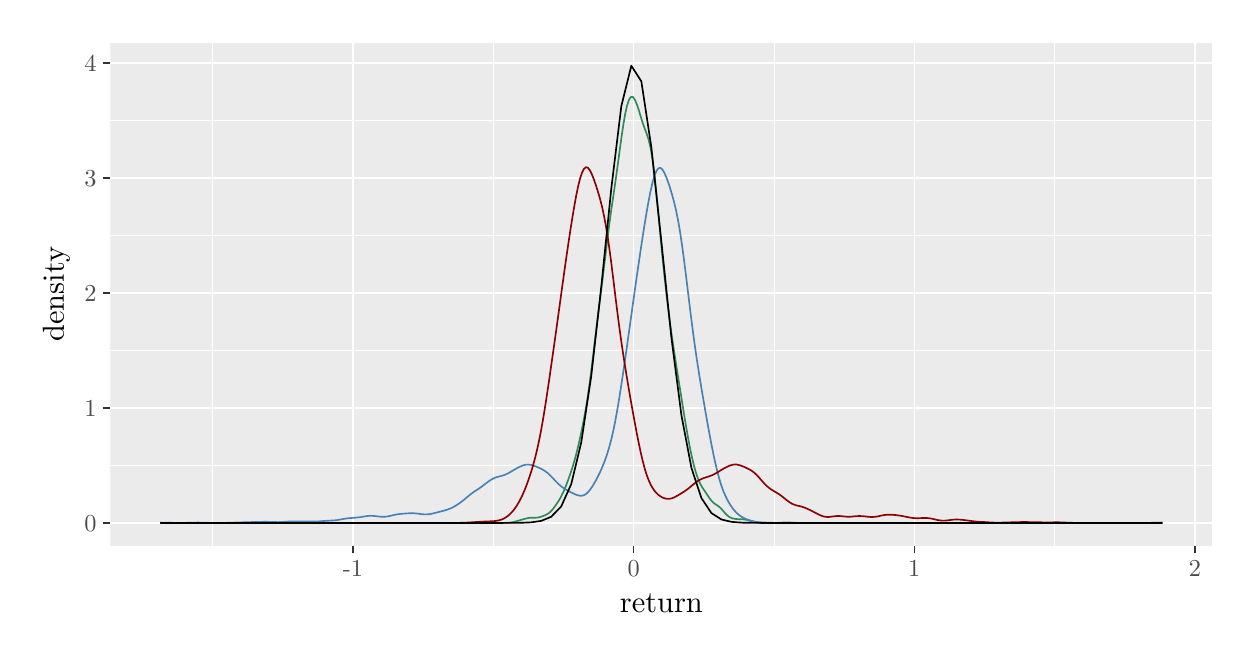
\begin{tikzpicture}[x=1pt,y=1pt]
\definecolor{fillColor}{RGB}{255,255,255}
\path[use as bounding box,fill=fillColor,fill opacity=0.00] (0,0) rectangle (433.62,216.81);
\begin{scope}
\path[clip] (  0.00,  0.00) rectangle (433.62,216.81);
\definecolor{drawColor}{RGB}{255,255,255}
\definecolor{fillColor}{RGB}{255,255,255}

\path[draw=drawColor,line width= 0.6pt,line join=round,line cap=round,fill=fillColor] (  0.00,  0.00) rectangle (433.62,216.81);
\end{scope}
\begin{scope}
\path[clip] ( 29.87, 29.59) rectangle (428.12,211.31);
\definecolor{fillColor}{gray}{0.92}

\path[fill=fillColor] ( 29.87, 29.59) rectangle (428.12,211.31);
\definecolor{drawColor}{RGB}{255,255,255}

\path[draw=drawColor,line width= 0.3pt,line join=round] ( 29.87, 58.62) --
	(428.12, 58.62);

\path[draw=drawColor,line width= 0.3pt,line join=round] ( 29.87,100.17) --
	(428.12,100.17);

\path[draw=drawColor,line width= 0.3pt,line join=round] ( 29.87,141.71) --
	(428.12,141.71);

\path[draw=drawColor,line width= 0.3pt,line join=round] ( 29.87,183.26) --
	(428.12,183.26);

\path[draw=drawColor,line width= 0.3pt,line join=round] ( 66.80, 29.59) --
	( 66.80,211.31);

\path[draw=drawColor,line width= 0.3pt,line join=round] (168.24, 29.59) --
	(168.24,211.31);

\path[draw=drawColor,line width= 0.3pt,line join=round] (269.68, 29.59) --
	(269.68,211.31);

\path[draw=drawColor,line width= 0.3pt,line join=round] (371.11, 29.59) --
	(371.11,211.31);

\path[draw=drawColor,line width= 0.6pt,line join=round] ( 29.87, 37.85) --
	(428.12, 37.85);

\path[draw=drawColor,line width= 0.6pt,line join=round] ( 29.87, 79.39) --
	(428.12, 79.39);

\path[draw=drawColor,line width= 0.6pt,line join=round] ( 29.87,120.94) --
	(428.12,120.94);

\path[draw=drawColor,line width= 0.6pt,line join=round] ( 29.87,162.49) --
	(428.12,162.49);

\path[draw=drawColor,line width= 0.6pt,line join=round] ( 29.87,204.03) --
	(428.12,204.03);

\path[draw=drawColor,line width= 0.6pt,line join=round] (117.52, 29.59) --
	(117.52,211.31);

\path[draw=drawColor,line width= 0.6pt,line join=round] (218.96, 29.59) --
	(218.96,211.31);

\path[draw=drawColor,line width= 0.6pt,line join=round] (320.39, 29.59) --
	(320.39,211.31);

\path[draw=drawColor,line width= 0.6pt,line join=round] (421.83, 29.59) --
	(421.83,211.31);
\definecolor{drawColor}{RGB}{46,139,87}

\path[draw=drawColor,line width= 0.6pt,line join=round] ( 47.97, 37.85) --
	( 48.68, 37.85) --
	( 49.39, 37.85) --
	( 50.10, 37.85) --
	( 50.81, 37.85) --
	( 51.51, 37.85) --
	( 52.22, 37.85) --
	( 52.93, 37.85) --
	( 53.64, 37.85) --
	( 54.35, 37.85) --
	( 55.06, 37.85) --
	( 55.76, 37.85) --
	( 56.47, 37.85) --
	( 57.18, 37.85) --
	( 57.89, 37.85) --
	( 58.60, 37.85) --
	( 59.31, 37.85) --
	( 60.02, 37.85) --
	( 60.72, 37.85) --
	( 61.43, 37.85) --
	( 62.14, 37.85) --
	( 62.85, 37.85) --
	( 63.56, 37.85) --
	( 64.27, 37.85) --
	( 64.98, 37.85) --
	( 65.68, 37.85) --
	( 66.39, 37.85) --
	( 67.10, 37.85) --
	( 67.81, 37.85) --
	( 68.52, 37.85) --
	( 69.23, 37.85) --
	( 69.93, 37.85) --
	( 70.64, 37.85) --
	( 71.35, 37.85) --
	( 72.06, 37.85) --
	( 72.77, 37.85) --
	( 73.48, 37.85) --
	( 74.19, 37.85) --
	( 74.89, 37.85) --
	( 75.60, 37.85) --
	( 76.31, 37.85) --
	( 77.02, 37.85) --
	( 77.73, 37.85) --
	( 78.44, 37.85) --
	( 79.15, 37.85) --
	( 79.85, 37.85) --
	( 80.56, 37.85) --
	( 81.27, 37.85) --
	( 81.98, 37.85) --
	( 82.69, 37.85) --
	( 83.40, 37.85) --
	( 84.10, 37.85) --
	( 84.81, 37.85) --
	( 85.52, 37.85) --
	( 86.23, 37.85) --
	( 86.94, 37.85) --
	( 87.65, 37.85) --
	( 88.36, 37.85) --
	( 89.06, 37.85) --
	( 89.77, 37.85) --
	( 90.48, 37.85) --
	( 91.19, 37.85) --
	( 91.90, 37.85) --
	( 92.61, 37.85) --
	( 93.32, 37.85) --
	( 94.02, 37.85) --
	( 94.73, 37.85) --
	( 95.44, 37.85) --
	( 96.15, 37.85) --
	( 96.86, 37.85) --
	( 97.57, 37.85) --
	( 98.28, 37.85) --
	( 98.98, 37.85) --
	( 99.69, 37.85) --
	(100.40, 37.85) --
	(101.11, 37.85) --
	(101.82, 37.85) --
	(102.53, 37.85) --
	(103.23, 37.85) --
	(103.94, 37.85) --
	(104.65, 37.85) --
	(105.36, 37.85) --
	(106.07, 37.85) --
	(106.78, 37.85) --
	(107.49, 37.85) --
	(108.19, 37.85) --
	(108.90, 37.85) --
	(109.61, 37.85) --
	(110.32, 37.85) --
	(111.03, 37.85) --
	(111.74, 37.85) --
	(112.45, 37.85) --
	(113.15, 37.85) --
	(113.86, 37.85) --
	(114.57, 37.85) --
	(115.28, 37.85) --
	(115.99, 37.85) --
	(116.70, 37.85) --
	(117.40, 37.85) --
	(118.11, 37.85) --
	(118.82, 37.85) --
	(119.53, 37.85) --
	(120.24, 37.85) --
	(120.95, 37.85) --
	(121.66, 37.85) --
	(122.36, 37.85) --
	(123.07, 37.85) --
	(123.78, 37.85) --
	(124.49, 37.85) --
	(125.20, 37.85) --
	(125.91, 37.85) --
	(126.62, 37.85) --
	(127.32, 37.85) --
	(128.03, 37.85) --
	(128.74, 37.85) --
	(129.45, 37.85) --
	(130.16, 37.85) --
	(130.87, 37.85) --
	(131.57, 37.85) --
	(132.28, 37.85) --
	(132.99, 37.85) --
	(133.70, 37.85) --
	(134.41, 37.85) --
	(135.12, 37.85) --
	(135.83, 37.85) --
	(136.53, 37.85) --
	(137.24, 37.85) --
	(137.95, 37.85) --
	(138.66, 37.85) --
	(139.37, 37.85) --
	(140.08, 37.85) --
	(140.79, 37.85) --
	(141.49, 37.85) --
	(142.20, 37.85) --
	(142.91, 37.85) --
	(143.62, 37.85) --
	(144.33, 37.85) --
	(145.04, 37.85) --
	(145.74, 37.85) --
	(146.45, 37.85) --
	(147.16, 37.85) --
	(147.87, 37.85) --
	(148.58, 37.85) --
	(149.29, 37.85) --
	(150.00, 37.85) --
	(150.70, 37.85) --
	(151.41, 37.85) --
	(152.12, 37.85) --
	(152.83, 37.85) --
	(153.54, 37.85) --
	(154.25, 37.85) --
	(154.96, 37.85) --
	(155.66, 37.85) --
	(156.37, 37.85) --
	(157.08, 37.85) --
	(157.79, 37.85) --
	(158.50, 37.86) --
	(159.21, 37.87) --
	(159.92, 37.89) --
	(160.62, 37.93) --
	(161.33, 37.97) --
	(162.04, 38.01) --
	(162.75, 38.03) --
	(163.46, 38.02) --
	(164.17, 38.00) --
	(164.87, 37.96) --
	(165.58, 37.92) --
	(166.29, 37.88) --
	(167.00, 37.86) --
	(167.71, 37.85) --
	(168.42, 37.85) --
	(169.13, 37.85) --
	(169.83, 37.85) --
	(170.54, 37.85) --
	(171.25, 37.85) --
	(171.96, 37.85) --
	(172.67, 37.87) --
	(173.38, 37.89) --
	(174.09, 37.95) --
	(174.79, 38.04) --
	(175.50, 38.18) --
	(176.21, 38.35) --
	(176.92, 38.55) --
	(177.63, 38.76) --
	(178.34, 38.97) --
	(179.04, 39.16) --
	(179.75, 39.35) --
	(180.46, 39.53) --
	(181.17, 39.67) --
	(181.88, 39.74) --
	(182.59, 39.74) --
	(183.30, 39.73) --
	(184.00, 39.76) --
	(184.71, 39.87) --
	(185.42, 40.06) --
	(186.13, 40.31) --
	(186.84, 40.59) --
	(187.55, 40.92) --
	(188.26, 41.35) --
	(188.96, 41.95) --
	(189.67, 42.72) --
	(190.38, 43.64) --
	(191.09, 44.65) --
	(191.80, 45.73) --
	(192.51, 46.92) --
	(193.21, 48.27) --
	(193.92, 49.81) --
	(194.63, 51.56) --
	(195.34, 53.46) --
	(196.05, 55.49) --
	(196.76, 57.64) --
	(197.47, 59.97) --
	(198.17, 62.53) --
	(198.88, 65.35) --
	(199.59, 68.45) --
	(200.30, 71.81) --
	(201.01, 75.44) --
	(201.72, 79.40) --
	(202.43, 83.82) --
	(203.13, 88.81) --
	(203.84, 94.36) --
	(204.55,100.28) --
	(205.26,106.28) --
	(205.97,112.07) --
	(206.68,117.64) --
	(207.39,123.17) --
	(208.09,128.86) --
	(208.80,134.75) --
	(209.51,140.63) --
	(210.22,146.18) --
	(210.93,151.28) --
	(211.64,156.10) --
	(212.34,160.94) --
	(213.05,166.00) --
	(213.76,171.26) --
	(214.47,176.49) --
	(215.18,181.37) --
	(215.89,185.54) --
	(216.60,188.75) --
	(217.30,190.84) --
	(218.01,191.81) --
	(218.72,191.74) --
	(219.43,190.77) --
	(220.14,189.08) --
	(220.85,186.92) --
	(221.56,184.56) --
	(222.26,182.32) --
	(222.97,180.34) --
	(223.68,178.49) --
	(224.39,176.31) --
	(225.10,173.28) --
	(225.81,168.97) --
	(226.51,163.33) --
	(227.22,156.61) --
	(227.93,149.23) --
	(228.64,141.66) --
	(229.35,134.28) --
	(230.06,127.33) --
	(230.77,120.90) --
	(231.47,114.98) --
	(232.18,109.53) --
	(232.89,104.47) --
	(233.60, 99.71) --
	(234.31, 95.15) --
	(235.02, 90.69) --
	(235.73, 86.25) --
	(236.43, 81.81) --
	(237.14, 77.38) --
	(237.85, 73.08) --
	(238.56, 69.00) --
	(239.27, 65.24) --
	(239.98, 61.85) --
	(240.68, 58.86) --
	(241.39, 56.28) --
	(242.10, 54.14) --
	(242.81, 52.43) --
	(243.52, 51.09) --
	(244.23, 49.97) --
	(244.94, 48.94) --
	(245.64, 47.88) --
	(246.35, 46.83) --
	(247.06, 45.89) --
	(247.77, 45.16) --
	(248.48, 44.63) --
	(249.19, 44.18) --
	(249.90, 43.66) --
	(250.60, 42.98) --
	(251.31, 42.18) --
	(252.02, 41.36) --
	(252.73, 40.64) --
	(253.44, 40.08) --
	(254.15, 39.69) --
	(254.85, 39.46) --
	(255.56, 39.32) --
	(256.27, 39.24) --
	(256.98, 39.20) --
	(257.69, 39.18) --
	(258.40, 39.16) --
	(259.11, 39.09) --
	(259.81, 38.96) --
	(260.52, 38.76) --
	(261.23, 38.54) --
	(261.94, 38.31) --
	(262.65, 38.13) --
	(263.36, 38.00) --
	(264.07, 37.92) --
	(264.77, 37.88) --
	(265.48, 37.86) --
	(266.19, 37.85) --
	(266.90, 37.85) --
	(267.61, 37.85) --
	(268.32, 37.85) --
	(269.03, 37.85) --
	(269.73, 37.85) --
	(270.44, 37.87) --
	(271.15, 37.89) --
	(271.86, 37.92) --
	(272.57, 37.96) --
	(273.28, 38.00) --
	(273.98, 38.03) --
	(274.69, 38.03) --
	(275.40, 38.00) --
	(276.11, 37.96) --
	(276.82, 37.92) --
	(277.53, 37.89) --
	(278.24, 37.87) --
	(278.94, 37.85) --
	(279.65, 37.85) --
	(280.36, 37.85) --
	(281.07, 37.85) --
	(281.78, 37.85) --
	(282.49, 37.85) --
	(283.20, 37.85) --
	(283.90, 37.85) --
	(284.61, 37.85) --
	(285.32, 37.85) --
	(286.03, 37.85) --
	(286.74, 37.85) --
	(287.45, 37.85) --
	(288.15, 37.85) --
	(288.86, 37.85) --
	(289.57, 37.85) --
	(290.28, 37.85) --
	(290.99, 37.85) --
	(291.70, 37.85) --
	(292.41, 37.85) --
	(293.11, 37.85) --
	(293.82, 37.85) --
	(294.53, 37.85) --
	(295.24, 37.85) --
	(295.95, 37.85) --
	(296.66, 37.85) --
	(297.37, 37.85) --
	(298.07, 37.85) --
	(298.78, 37.85) --
	(299.49, 37.85) --
	(300.20, 37.85) --
	(300.91, 37.85) --
	(301.62, 37.85) --
	(302.32, 37.85) --
	(303.03, 37.85) --
	(303.74, 37.85) --
	(304.45, 37.85) --
	(305.16, 37.85) --
	(305.87, 37.85) --
	(306.58, 37.85) --
	(307.28, 37.85) --
	(307.99, 37.85) --
	(308.70, 37.85) --
	(309.41, 37.85) --
	(310.12, 37.85) --
	(310.83, 37.85) --
	(311.54, 37.85) --
	(312.24, 37.85) --
	(312.95, 37.85) --
	(313.66, 37.85) --
	(314.37, 37.85) --
	(315.08, 37.85) --
	(315.79, 37.85) --
	(316.49, 37.85) --
	(317.20, 37.85) --
	(317.91, 37.85) --
	(318.62, 37.85) --
	(319.33, 37.85) --
	(320.04, 37.85) --
	(320.75, 37.85) --
	(321.45, 37.85) --
	(322.16, 37.85) --
	(322.87, 37.85) --
	(323.58, 37.85) --
	(324.29, 37.85) --
	(325.00, 37.85) --
	(325.71, 37.85) --
	(326.41, 37.85) --
	(327.12, 37.85) --
	(327.83, 37.85) --
	(328.54, 37.85) --
	(329.25, 37.85) --
	(329.96, 37.85) --
	(330.67, 37.85) --
	(331.37, 37.85) --
	(332.08, 37.85) --
	(332.79, 37.85) --
	(333.50, 37.85) --
	(334.21, 37.85) --
	(334.92, 37.85) --
	(335.62, 37.85) --
	(336.33, 37.85) --
	(337.04, 37.85) --
	(337.75, 37.85) --
	(338.46, 37.85) --
	(339.17, 37.85) --
	(339.88, 37.85) --
	(340.58, 37.85) --
	(341.29, 37.85) --
	(342.00, 37.85) --
	(342.71, 37.85) --
	(343.42, 37.85) --
	(344.13, 37.85) --
	(344.84, 37.85) --
	(345.54, 37.85) --
	(346.25, 37.85) --
	(346.96, 37.85) --
	(347.67, 37.85) --
	(348.38, 37.85) --
	(349.09, 37.85) --
	(349.79, 37.85) --
	(350.50, 37.85) --
	(351.21, 37.85) --
	(351.92, 37.85) --
	(352.63, 37.85) --
	(353.34, 37.85) --
	(354.05, 37.85) --
	(354.75, 37.85) --
	(355.46, 37.85) --
	(356.17, 37.85) --
	(356.88, 37.85) --
	(357.59, 37.85) --
	(358.30, 37.85) --
	(359.01, 37.85) --
	(359.71, 37.85) --
	(360.42, 37.85) --
	(361.13, 37.85) --
	(361.84, 37.85) --
	(362.55, 37.85) --
	(363.26, 37.85) --
	(363.96, 37.85) --
	(364.67, 37.85) --
	(365.38, 37.85) --
	(366.09, 37.85) --
	(366.80, 37.85) --
	(367.51, 37.85) --
	(368.22, 37.85) --
	(368.92, 37.85) --
	(369.63, 37.85) --
	(370.34, 37.85) --
	(371.05, 37.85) --
	(371.76, 37.85) --
	(372.47, 37.85) --
	(373.18, 37.85) --
	(373.88, 37.85) --
	(374.59, 37.85) --
	(375.30, 37.85) --
	(376.01, 37.85) --
	(376.72, 37.85) --
	(377.43, 37.85) --
	(378.13, 37.85) --
	(378.84, 37.85) --
	(379.55, 37.85) --
	(380.26, 37.85) --
	(380.97, 37.85) --
	(381.68, 37.85) --
	(382.39, 37.85) --
	(383.09, 37.85) --
	(383.80, 37.85) --
	(384.51, 37.85) --
	(385.22, 37.85) --
	(385.93, 37.85) --
	(386.64, 37.85) --
	(387.35, 37.85) --
	(388.05, 37.85) --
	(388.76, 37.85) --
	(389.47, 37.85) --
	(390.18, 37.85) --
	(390.89, 37.85) --
	(391.60, 37.85) --
	(392.31, 37.85) --
	(393.01, 37.85) --
	(393.72, 37.85) --
	(394.43, 37.85) --
	(395.14, 37.85) --
	(395.85, 37.85) --
	(396.56, 37.85) --
	(397.26, 37.85) --
	(397.97, 37.85) --
	(398.68, 37.85) --
	(399.39, 37.85) --
	(400.10, 37.85) --
	(400.81, 37.85) --
	(401.52, 37.85) --
	(402.22, 37.85) --
	(402.93, 37.85) --
	(403.64, 37.85) --
	(404.35, 37.85) --
	(405.06, 37.85) --
	(405.77, 37.85) --
	(406.48, 37.85) --
	(407.18, 37.85) --
	(407.89, 37.85) --
	(408.60, 37.85) --
	(409.31, 37.85) --
	(410.02, 37.85);
\definecolor{drawColor}{RGB}{70,130,180}

\path[draw=drawColor,line width= 0.6pt,line join=round] ( 47.97, 37.98) --
	( 48.68, 37.97) --
	( 49.39, 37.96) --
	( 50.10, 37.94) --
	( 50.81, 37.92) --
	( 51.51, 37.90) --
	( 52.22, 37.88) --
	( 52.93, 37.87) --
	( 53.64, 37.86) --
	( 54.35, 37.86) --
	( 55.06, 37.86) --
	( 55.76, 37.86) --
	( 56.47, 37.87) --
	( 57.18, 37.88) --
	( 57.89, 37.90) --
	( 58.60, 37.91) --
	( 59.31, 37.94) --
	( 60.02, 37.96) --
	( 60.72, 37.97) --
	( 61.43, 37.98) --
	( 62.14, 37.97) --
	( 62.85, 37.96) --
	( 63.56, 37.94) --
	( 64.27, 37.92) --
	( 64.98, 37.90) --
	( 65.68, 37.88) --
	( 66.39, 37.87) --
	( 67.10, 37.86) --
	( 67.81, 37.86) --
	( 68.52, 37.85) --
	( 69.23, 37.85) --
	( 69.93, 37.86) --
	( 70.64, 37.86) --
	( 71.35, 37.87) --
	( 72.06, 37.89) --
	( 72.77, 37.91) --
	( 73.48, 37.93) --
	( 74.19, 37.96) --
	( 74.89, 37.98) --
	( 75.60, 38.01) --
	( 76.31, 38.03) --
	( 77.02, 38.05) --
	( 77.73, 38.07) --
	( 78.44, 38.09) --
	( 79.15, 38.12) --
	( 79.85, 38.14) --
	( 80.56, 38.15) --
	( 81.27, 38.17) --
	( 81.98, 38.18) --
	( 82.69, 38.19) --
	( 83.40, 38.20) --
	( 84.10, 38.22) --
	( 84.81, 38.24) --
	( 85.52, 38.26) --
	( 86.23, 38.26) --
	( 86.94, 38.25) --
	( 87.65, 38.23) --
	( 88.36, 38.20) --
	( 89.06, 38.18) --
	( 89.77, 38.16) --
	( 90.48, 38.15) --
	( 91.19, 38.17) --
	( 91.90, 38.20) --
	( 92.61, 38.24) --
	( 93.32, 38.29) --
	( 94.02, 38.33) --
	( 94.73, 38.36) --
	( 95.44, 38.38) --
	( 96.15, 38.39) --
	( 96.86, 38.39) --
	( 97.57, 38.39) --
	( 98.28, 38.40) --
	( 98.98, 38.40) --
	( 99.69, 38.41) --
	(100.40, 38.40) --
	(101.11, 38.39) --
	(101.82, 38.38) --
	(102.53, 38.37) --
	(103.23, 38.36) --
	(103.94, 38.36) --
	(104.65, 38.38) --
	(105.36, 38.42) --
	(106.07, 38.47) --
	(106.78, 38.53) --
	(107.49, 38.58) --
	(108.19, 38.63) --
	(108.90, 38.67) --
	(109.61, 38.70) --
	(110.32, 38.74) --
	(111.03, 38.80) --
	(111.74, 38.88) --
	(112.45, 38.99) --
	(113.15, 39.11) --
	(113.86, 39.24) --
	(114.57, 39.37) --
	(115.28, 39.47) --
	(115.99, 39.56) --
	(116.70, 39.62) --
	(117.40, 39.67) --
	(118.11, 39.72) --
	(118.82, 39.78) --
	(119.53, 39.86) --
	(120.24, 39.95) --
	(120.95, 40.07) --
	(121.66, 40.19) --
	(122.36, 40.30) --
	(123.07, 40.38) --
	(123.78, 40.42) --
	(124.49, 40.41) --
	(125.20, 40.36) --
	(125.91, 40.28) --
	(126.62, 40.19) --
	(127.32, 40.12) --
	(128.03, 40.07) --
	(128.74, 40.07) --
	(129.45, 40.12) --
	(130.16, 40.23) --
	(130.87, 40.37) --
	(131.57, 40.54) --
	(132.28, 40.70) --
	(132.99, 40.86) --
	(133.70, 40.98) --
	(134.41, 41.07) --
	(135.12, 41.14) --
	(135.83, 41.20) --
	(136.53, 41.25) --
	(137.24, 41.30) --
	(137.95, 41.34) --
	(138.66, 41.36) --
	(139.37, 41.34) --
	(140.08, 41.30) --
	(140.79, 41.23) --
	(141.49, 41.14) --
	(142.20, 41.04) --
	(142.91, 40.97) --
	(143.62, 40.93) --
	(144.33, 40.95) --
	(145.04, 41.01) --
	(145.74, 41.12) --
	(146.45, 41.27) --
	(147.16, 41.45) --
	(147.87, 41.63) --
	(148.58, 41.82) --
	(149.29, 42.00) --
	(150.00, 42.18) --
	(150.70, 42.37) --
	(151.41, 42.58) --
	(152.12, 42.83) --
	(152.83, 43.11) --
	(153.54, 43.45) --
	(154.25, 43.83) --
	(154.96, 44.25) --
	(155.66, 44.72) --
	(156.37, 45.22) --
	(157.08, 45.76) --
	(157.79, 46.33) --
	(158.50, 46.92) --
	(159.21, 47.51) --
	(159.92, 48.09) --
	(160.62, 48.63) --
	(161.33, 49.13) --
	(162.04, 49.60) --
	(162.75, 50.06) --
	(163.46, 50.54) --
	(164.17, 51.05) --
	(164.87, 51.59) --
	(165.58, 52.14) --
	(166.29, 52.67) --
	(167.00, 53.17) --
	(167.71, 53.60) --
	(168.42, 53.96) --
	(169.13, 54.25) --
	(169.83, 54.48) --
	(170.54, 54.68) --
	(171.25, 54.87) --
	(171.96, 55.08) --
	(172.67, 55.35) --
	(173.38, 55.67) --
	(174.09, 56.05) --
	(174.79, 56.46) --
	(175.50, 56.88) --
	(176.21, 57.29) --
	(176.92, 57.69) --
	(177.63, 58.06) --
	(178.34, 58.38) --
	(179.04, 58.65) --
	(179.75, 58.84) --
	(180.46, 58.93) --
	(181.17, 58.92) --
	(181.88, 58.81) --
	(182.59, 58.63) --
	(183.30, 58.38) --
	(184.00, 58.11) --
	(184.71, 57.80) --
	(185.42, 57.47) --
	(186.13, 57.09) --
	(186.84, 56.66) --
	(187.55, 56.15) --
	(188.26, 55.56) --
	(188.96, 54.88) --
	(189.67, 54.14) --
	(190.38, 53.37) --
	(191.09, 52.62) --
	(191.80, 51.92) --
	(192.51, 51.29) --
	(193.21, 50.74) --
	(193.92, 50.26) --
	(194.63, 49.83) --
	(195.34, 49.43) --
	(196.05, 49.06) --
	(196.76, 48.69) --
	(197.47, 48.35) --
	(198.17, 48.05) --
	(198.88, 47.82) --
	(199.59, 47.68) --
	(200.30, 47.69) --
	(201.01, 47.88) --
	(201.72, 48.29) --
	(202.43, 48.91) --
	(203.13, 49.74) --
	(203.84, 50.74) --
	(204.55, 51.87) --
	(205.26, 53.11) --
	(205.97, 54.45) --
	(206.68, 55.88) --
	(207.39, 57.44) --
	(208.09, 59.14) --
	(208.80, 61.02) --
	(209.51, 63.12) --
	(210.22, 65.49) --
	(210.93, 68.20) --
	(211.64, 71.28) --
	(212.34, 74.77) --
	(213.05, 78.66) --
	(213.76, 82.91) --
	(214.47, 87.43) --
	(215.18, 92.16) --
	(215.89, 97.03) --
	(216.60,101.99) --
	(217.30,107.01) --
	(218.01,112.07) --
	(218.72,117.14) --
	(219.43,122.19) --
	(220.14,127.18) --
	(220.85,132.08) --
	(221.56,136.87) --
	(222.26,141.52) --
	(222.97,146.01) --
	(223.68,150.28) --
	(224.39,154.27) --
	(225.10,157.86) --
	(225.81,160.94) --
	(226.51,163.38) --
	(227.22,165.09) --
	(227.93,166.01) --
	(228.64,166.16) --
	(229.35,165.57) --
	(230.06,164.38) --
	(230.77,162.75) --
	(231.47,160.83) --
	(232.18,158.68) --
	(232.89,156.32) --
	(233.60,153.69) --
	(234.31,150.69) --
	(235.02,147.18) --
	(235.73,143.08) --
	(236.43,138.36) --
	(237.14,133.10) --
	(237.85,127.45) --
	(238.56,121.61) --
	(239.27,115.78) --
	(239.98,110.13) --
	(240.68,104.76) --
	(241.39, 99.72) --
	(242.10, 94.97) --
	(242.81, 90.49) --
	(243.52, 86.18) --
	(244.23, 82.01) --
	(244.94, 77.92) --
	(245.64, 73.93) --
	(246.35, 70.04) --
	(247.06, 66.30) --
	(247.77, 62.75) --
	(248.48, 59.47) --
	(249.19, 56.48) --
	(249.90, 53.84) --
	(250.60, 51.54) --
	(251.31, 49.55) --
	(252.02, 47.85) --
	(252.73, 46.38) --
	(253.44, 45.11) --
	(254.15, 43.98) --
	(254.85, 42.99) --
	(255.56, 42.13) --
	(256.27, 41.39) --
	(256.98, 40.76) --
	(257.69, 40.25) --
	(258.40, 39.82) --
	(259.11, 39.47) --
	(259.81, 39.17) --
	(260.52, 38.92) --
	(261.23, 38.70) --
	(261.94, 38.51) --
	(262.65, 38.36) --
	(263.36, 38.24) --
	(264.07, 38.15) --
	(264.77, 38.09) --
	(265.48, 38.04) --
	(266.19, 38.00) --
	(266.90, 37.97) --
	(267.61, 37.94) --
	(268.32, 37.91) --
	(269.03, 37.89) --
	(269.73, 37.87) --
	(270.44, 37.86) --
	(271.15, 37.86) --
	(271.86, 37.85) --
	(272.57, 37.85) --
	(273.28, 37.85) --
	(273.98, 37.85) --
	(274.69, 37.85) --
	(275.40, 37.85) --
	(276.11, 37.85) --
	(276.82, 37.85) --
	(277.53, 37.85) --
	(278.24, 37.85) --
	(278.94, 37.85) --
	(279.65, 37.85) --
	(280.36, 37.85) --
	(281.07, 37.85) --
	(281.78, 37.85) --
	(282.49, 37.85) --
	(283.20, 37.85) --
	(283.90, 37.85) --
	(284.61, 37.85) --
	(285.32, 37.85) --
	(286.03, 37.85) --
	(286.74, 37.85) --
	(287.45, 37.85) --
	(288.15, 37.85) --
	(288.86, 37.85) --
	(289.57, 37.85) --
	(290.28, 37.85) --
	(290.99, 37.85) --
	(291.70, 37.85) --
	(292.41, 37.85) --
	(293.11, 37.85) --
	(293.82, 37.85) --
	(294.53, 37.85) --
	(295.24, 37.85) --
	(295.95, 37.85) --
	(296.66, 37.85) --
	(297.37, 37.85) --
	(298.07, 37.85) --
	(298.78, 37.85) --
	(299.49, 37.85) --
	(300.20, 37.85) --
	(300.91, 37.85) --
	(301.62, 37.85) --
	(302.32, 37.85) --
	(303.03, 37.85) --
	(303.74, 37.85) --
	(304.45, 37.85) --
	(305.16, 37.85) --
	(305.87, 37.85) --
	(306.58, 37.85) --
	(307.28, 37.85) --
	(307.99, 37.85) --
	(308.70, 37.85) --
	(309.41, 37.85) --
	(310.12, 37.85) --
	(310.83, 37.85) --
	(311.54, 37.85) --
	(312.24, 37.85) --
	(312.95, 37.85) --
	(313.66, 37.85) --
	(314.37, 37.85) --
	(315.08, 37.85) --
	(315.79, 37.85) --
	(316.49, 37.85) --
	(317.20, 37.85) --
	(317.91, 37.85) --
	(318.62, 37.85) --
	(319.33, 37.85) --
	(320.04, 37.85) --
	(320.75, 37.85) --
	(321.45, 37.85) --
	(322.16, 37.85) --
	(322.87, 37.85) --
	(323.58, 37.85) --
	(324.29, 37.85) --
	(325.00, 37.85) --
	(325.71, 37.85) --
	(326.41, 37.85) --
	(327.12, 37.85) --
	(327.83, 37.85) --
	(328.54, 37.85) --
	(329.25, 37.85) --
	(329.96, 37.85) --
	(330.67, 37.85) --
	(331.37, 37.85) --
	(332.08, 37.85) --
	(332.79, 37.85) --
	(333.50, 37.85) --
	(334.21, 37.85) --
	(334.92, 37.85) --
	(335.62, 37.85) --
	(336.33, 37.85) --
	(337.04, 37.85) --
	(337.75, 37.85) --
	(338.46, 37.85) --
	(339.17, 37.85) --
	(339.88, 37.85) --
	(340.58, 37.85) --
	(341.29, 37.85) --
	(342.00, 37.85) --
	(342.71, 37.85) --
	(343.42, 37.85) --
	(344.13, 37.85) --
	(344.84, 37.85) --
	(345.54, 37.85) --
	(346.25, 37.85) --
	(346.96, 37.85) --
	(347.67, 37.85) --
	(348.38, 37.85) --
	(349.09, 37.85) --
	(349.79, 37.85) --
	(350.50, 37.85) --
	(351.21, 37.85) --
	(351.92, 37.85) --
	(352.63, 37.85) --
	(353.34, 37.85) --
	(354.05, 37.85) --
	(354.75, 37.85) --
	(355.46, 37.85) --
	(356.17, 37.85) --
	(356.88, 37.85) --
	(357.59, 37.85) --
	(358.30, 37.85) --
	(359.01, 37.85) --
	(359.71, 37.85) --
	(360.42, 37.85) --
	(361.13, 37.85) --
	(361.84, 37.85) --
	(362.55, 37.85) --
	(363.26, 37.85) --
	(363.96, 37.85) --
	(364.67, 37.85) --
	(365.38, 37.85) --
	(366.09, 37.85) --
	(366.80, 37.85) --
	(367.51, 37.85) --
	(368.22, 37.85) --
	(368.92, 37.85) --
	(369.63, 37.85) --
	(370.34, 37.85) --
	(371.05, 37.85) --
	(371.76, 37.85) --
	(372.47, 37.85) --
	(373.18, 37.85) --
	(373.88, 37.85) --
	(374.59, 37.85) --
	(375.30, 37.85) --
	(376.01, 37.85) --
	(376.72, 37.85) --
	(377.43, 37.85) --
	(378.13, 37.85) --
	(378.84, 37.85) --
	(379.55, 37.85) --
	(380.26, 37.85) --
	(380.97, 37.85) --
	(381.68, 37.85) --
	(382.39, 37.85) --
	(383.09, 37.85) --
	(383.80, 37.85) --
	(384.51, 37.85) --
	(385.22, 37.85) --
	(385.93, 37.85) --
	(386.64, 37.85) --
	(387.35, 37.85) --
	(388.05, 37.85) --
	(388.76, 37.85) --
	(389.47, 37.85) --
	(390.18, 37.85) --
	(390.89, 37.85) --
	(391.60, 37.85) --
	(392.31, 37.85) --
	(393.01, 37.85) --
	(393.72, 37.85) --
	(394.43, 37.85) --
	(395.14, 37.85) --
	(395.85, 37.85) --
	(396.56, 37.85) --
	(397.26, 37.85) --
	(397.97, 37.85) --
	(398.68, 37.85) --
	(399.39, 37.85) --
	(400.10, 37.85) --
	(400.81, 37.85) --
	(401.52, 37.85) --
	(402.22, 37.85) --
	(402.93, 37.85) --
	(403.64, 37.85) --
	(404.35, 37.85) --
	(405.06, 37.85) --
	(405.77, 37.85) --
	(406.48, 37.85) --
	(407.18, 37.85) --
	(407.89, 37.85) --
	(408.60, 37.85) --
	(409.31, 37.85) --
	(410.02, 37.85);
\definecolor{drawColor}{RGB}{139,0,0}

\path[draw=drawColor,line width= 0.6pt,line join=round] ( 47.97, 37.85) --
	( 48.68, 37.85) --
	( 49.39, 37.85) --
	( 50.10, 37.85) --
	( 50.81, 37.85) --
	( 51.51, 37.85) --
	( 52.22, 37.85) --
	( 52.93, 37.85) --
	( 53.64, 37.85) --
	( 54.35, 37.85) --
	( 55.06, 37.85) --
	( 55.76, 37.85) --
	( 56.47, 37.85) --
	( 57.18, 37.85) --
	( 57.89, 37.85) --
	( 58.60, 37.85) --
	( 59.31, 37.85) --
	( 60.02, 37.85) --
	( 60.72, 37.85) --
	( 61.43, 37.85) --
	( 62.14, 37.85) --
	( 62.85, 37.85) --
	( 63.56, 37.85) --
	( 64.27, 37.85) --
	( 64.98, 37.85) --
	( 65.68, 37.85) --
	( 66.39, 37.85) --
	( 67.10, 37.85) --
	( 67.81, 37.85) --
	( 68.52, 37.85) --
	( 69.23, 37.85) --
	( 69.93, 37.85) --
	( 70.64, 37.85) --
	( 71.35, 37.85) --
	( 72.06, 37.85) --
	( 72.77, 37.85) --
	( 73.48, 37.85) --
	( 74.19, 37.85) --
	( 74.89, 37.85) --
	( 75.60, 37.85) --
	( 76.31, 37.85) --
	( 77.02, 37.85) --
	( 77.73, 37.85) --
	( 78.44, 37.85) --
	( 79.15, 37.85) --
	( 79.85, 37.85) --
	( 80.56, 37.85) --
	( 81.27, 37.85) --
	( 81.98, 37.85) --
	( 82.69, 37.85) --
	( 83.40, 37.85) --
	( 84.10, 37.85) --
	( 84.81, 37.85) --
	( 85.52, 37.85) --
	( 86.23, 37.85) --
	( 86.94, 37.85) --
	( 87.65, 37.85) --
	( 88.36, 37.85) --
	( 89.06, 37.85) --
	( 89.77, 37.85) --
	( 90.48, 37.85) --
	( 91.19, 37.85) --
	( 91.90, 37.85) --
	( 92.61, 37.85) --
	( 93.32, 37.85) --
	( 94.02, 37.85) --
	( 94.73, 37.85) --
	( 95.44, 37.85) --
	( 96.15, 37.85) --
	( 96.86, 37.85) --
	( 97.57, 37.85) --
	( 98.28, 37.85) --
	( 98.98, 37.85) --
	( 99.69, 37.85) --
	(100.40, 37.85) --
	(101.11, 37.85) --
	(101.82, 37.85) --
	(102.53, 37.85) --
	(103.23, 37.85) --
	(103.94, 37.85) --
	(104.65, 37.85) --
	(105.36, 37.85) --
	(106.07, 37.85) --
	(106.78, 37.85) --
	(107.49, 37.85) --
	(108.19, 37.85) --
	(108.90, 37.85) --
	(109.61, 37.85) --
	(110.32, 37.85) --
	(111.03, 37.85) --
	(111.74, 37.85) --
	(112.45, 37.85) --
	(113.15, 37.85) --
	(113.86, 37.85) --
	(114.57, 37.85) --
	(115.28, 37.85) --
	(115.99, 37.85) --
	(116.70, 37.85) --
	(117.40, 37.85) --
	(118.11, 37.85) --
	(118.82, 37.85) --
	(119.53, 37.85) --
	(120.24, 37.85) --
	(120.95, 37.85) --
	(121.66, 37.85) --
	(122.36, 37.85) --
	(123.07, 37.85) --
	(123.78, 37.85) --
	(124.49, 37.85) --
	(125.20, 37.85) --
	(125.91, 37.85) --
	(126.62, 37.85) --
	(127.32, 37.85) --
	(128.03, 37.85) --
	(128.74, 37.85) --
	(129.45, 37.85) --
	(130.16, 37.85) --
	(130.87, 37.85) --
	(131.57, 37.85) --
	(132.28, 37.85) --
	(132.99, 37.85) --
	(133.70, 37.85) --
	(134.41, 37.85) --
	(135.12, 37.85) --
	(135.83, 37.85) --
	(136.53, 37.85) --
	(137.24, 37.85) --
	(137.95, 37.85) --
	(138.66, 37.85) --
	(139.37, 37.85) --
	(140.08, 37.85) --
	(140.79, 37.85) --
	(141.49, 37.85) --
	(142.20, 37.85) --
	(142.91, 37.85) --
	(143.62, 37.85) --
	(144.33, 37.85) --
	(145.04, 37.85) --
	(145.74, 37.85) --
	(146.45, 37.85) --
	(147.16, 37.85) --
	(147.87, 37.85) --
	(148.58, 37.85) --
	(149.29, 37.85) --
	(150.00, 37.85) --
	(150.70, 37.85) --
	(151.41, 37.85) --
	(152.12, 37.85) --
	(152.83, 37.85) --
	(153.54, 37.85) --
	(154.25, 37.85) --
	(154.96, 37.86) --
	(155.66, 37.87) --
	(156.37, 37.89) --
	(157.08, 37.91) --
	(157.79, 37.94) --
	(158.50, 37.97) --
	(159.21, 38.00) --
	(159.92, 38.04) --
	(160.62, 38.08) --
	(161.33, 38.13) --
	(162.04, 38.17) --
	(162.75, 38.22) --
	(163.46, 38.27) --
	(164.17, 38.31) --
	(164.87, 38.34) --
	(165.58, 38.37) --
	(166.29, 38.40) --
	(167.00, 38.42) --
	(167.71, 38.45) --
	(168.42, 38.50) --
	(169.13, 38.57) --
	(169.83, 38.69) --
	(170.54, 38.85) --
	(171.25, 39.08) --
	(171.96, 39.38) --
	(172.67, 39.78) --
	(173.38, 40.27) --
	(174.09, 40.86) --
	(174.79, 41.56) --
	(175.50, 42.37) --
	(176.21, 43.31) --
	(176.92, 44.39) --
	(177.63, 45.60) --
	(178.34, 46.97) --
	(179.04, 48.49) --
	(179.75, 50.17) --
	(180.46, 52.01) --
	(181.17, 54.01) --
	(181.88, 56.17) --
	(182.59, 58.53) --
	(183.30, 61.12) --
	(184.00, 63.99) --
	(184.71, 67.20) --
	(185.42, 70.77) --
	(186.13, 74.72) --
	(186.84, 79.01) --
	(187.55, 83.58) --
	(188.26, 88.33) --
	(188.96, 93.19) --
	(189.67, 98.14) --
	(190.38,103.15) --
	(191.09,108.22) --
	(191.80,113.35) --
	(192.51,118.51) --
	(193.21,123.65) --
	(193.92,128.74) --
	(194.63,133.73) --
	(195.34,138.58) --
	(196.05,143.27) --
	(196.76,147.77) --
	(197.47,152.01) --
	(198.17,155.91) --
	(198.88,159.36) --
	(199.59,162.23) --
	(200.30,164.40) --
	(201.01,165.80) --
	(201.72,166.39) --
	(202.43,166.20) --
	(203.13,165.30) --
	(203.84,163.88) --
	(204.55,162.09) --
	(205.26,160.06) --
	(205.97,157.85) --
	(206.68,155.44) --
	(207.39,152.75) --
	(208.09,149.63) --
	(208.80,145.96) --
	(209.51,141.68) --
	(210.22,136.79) --
	(210.93,131.41) --
	(211.64,125.72) --
	(212.34,119.93) --
	(213.05,114.24) --
	(213.76,108.80) --
	(214.47,103.66) --
	(215.18, 98.84) --
	(215.89, 94.28) --
	(216.60, 89.94) --
	(217.30, 85.75) --
	(218.01, 81.66) --
	(218.72, 77.67) --
	(219.43, 73.78) --
	(220.14, 70.03) --
	(220.85, 66.47) --
	(221.56, 63.15) --
	(222.26, 60.14) --
	(222.97, 57.48) --
	(223.68, 55.20) --
	(224.39, 53.29) --
	(225.10, 51.73) --
	(225.81, 50.47) --
	(226.51, 49.45) --
	(227.22, 48.64) --
	(227.93, 47.98) --
	(228.64, 47.45) --
	(229.35, 47.05) --
	(230.06, 46.77) --
	(230.77, 46.59) --
	(231.47, 46.54) --
	(232.18, 46.61) --
	(232.89, 46.79) --
	(233.60, 47.08) --
	(234.31, 47.44) --
	(235.02, 47.84) --
	(235.73, 48.27) --
	(236.43, 48.70) --
	(237.14, 49.15) --
	(237.85, 49.63) --
	(238.56, 50.15) --
	(239.27, 50.71) --
	(239.98, 51.30) --
	(240.68, 51.89) --
	(241.39, 52.45) --
	(242.10, 52.96) --
	(242.81, 53.39) --
	(243.52, 53.75) --
	(244.23, 54.03) --
	(244.94, 54.28) --
	(245.64, 54.49) --
	(246.35, 54.72) --
	(247.06, 54.99) --
	(247.77, 55.31) --
	(248.48, 55.68) --
	(249.19, 56.09) --
	(249.90, 56.53) --
	(250.60, 56.96) --
	(251.31, 57.37) --
	(252.02, 57.77) --
	(252.73, 58.13) --
	(253.44, 58.46) --
	(254.15, 58.72) --
	(254.85, 58.90) --
	(255.56, 58.97) --
	(256.27, 58.93) --
	(256.98, 58.78) --
	(257.69, 58.57) --
	(258.40, 58.30) --
	(259.11, 58.00) --
	(259.81, 57.67) --
	(260.52, 57.32) --
	(261.23, 56.92) --
	(261.94, 56.46) --
	(262.65, 55.90) --
	(263.36, 55.24) --
	(264.07, 54.50) --
	(264.77, 53.69) --
	(265.48, 52.87) --
	(266.19, 52.07) --
	(266.90, 51.35) --
	(267.61, 50.73) --
	(268.32, 50.19) --
	(269.03, 49.73) --
	(269.73, 49.31) --
	(270.44, 48.89) --
	(271.15, 48.45) --
	(271.86, 47.97) --
	(272.57, 47.45) --
	(273.28, 46.89) --
	(273.98, 46.31) --
	(274.69, 45.76) --
	(275.40, 45.26) --
	(276.11, 44.83) --
	(276.82, 44.50) --
	(277.53, 44.26) --
	(278.24, 44.08) --
	(278.94, 43.92) --
	(279.65, 43.74) --
	(280.36, 43.51) --
	(281.07, 43.24) --
	(281.78, 42.93) --
	(282.49, 42.60) --
	(283.20, 42.25) --
	(283.90, 41.89) --
	(284.61, 41.52) --
	(285.32, 41.15) --
	(286.03, 40.80) --
	(286.74, 40.49) --
	(287.45, 40.24) --
	(288.15, 40.08) --
	(288.86, 40.01) --
	(289.57, 40.02) --
	(290.28, 40.09) --
	(290.99, 40.19) --
	(291.70, 40.28) --
	(292.41, 40.34) --
	(293.11, 40.35) --
	(293.82, 40.31) --
	(294.53, 40.24) --
	(295.24, 40.16) --
	(295.95, 40.11) --
	(296.66, 40.08) --
	(297.37, 40.11) --
	(298.07, 40.16) --
	(298.78, 40.23) --
	(299.49, 40.29) --
	(300.20, 40.33) --
	(300.91, 40.33) --
	(301.62, 40.29) --
	(302.32, 40.23) --
	(303.03, 40.15) --
	(303.74, 40.07) --
	(304.45, 40.02) --
	(305.16, 40.00) --
	(305.87, 40.03) --
	(306.58, 40.11) --
	(307.28, 40.24) --
	(307.99, 40.39) --
	(308.70, 40.55) --
	(309.41, 40.68) --
	(310.12, 40.77) --
	(310.83, 40.82) --
	(311.54, 40.83) --
	(312.24, 40.80) --
	(312.95, 40.75) --
	(313.66, 40.69) --
	(314.37, 40.60) --
	(315.08, 40.50) --
	(315.79, 40.39) --
	(316.49, 40.25) --
	(317.20, 40.11) --
	(317.91, 39.96) --
	(318.62, 39.82) --
	(319.33, 39.70) --
	(320.04, 39.61) --
	(320.75, 39.56) --
	(321.45, 39.55) --
	(322.16, 39.57) --
	(322.87, 39.60) --
	(323.58, 39.63) --
	(324.29, 39.64) --
	(325.00, 39.62) --
	(325.71, 39.55) --
	(326.41, 39.44) --
	(327.12, 39.29) --
	(327.83, 39.13) --
	(328.54, 38.96) --
	(329.25, 38.82) --
	(329.96, 38.72) --
	(330.67, 38.67) --
	(331.37, 38.68) --
	(332.08, 38.74) --
	(332.79, 38.83) --
	(333.50, 38.92) --
	(334.21, 39.01) --
	(334.92, 39.06) --
	(335.62, 39.08) --
	(336.33, 39.07) --
	(337.04, 39.02) --
	(337.75, 38.96) --
	(338.46, 38.88) --
	(339.17, 38.79) --
	(339.88, 38.69) --
	(340.58, 38.60) --
	(341.29, 38.50) --
	(342.00, 38.41) --
	(342.71, 38.34) --
	(343.42, 38.28) --
	(344.13, 38.24) --
	(344.84, 38.20) --
	(345.54, 38.17) --
	(346.25, 38.13) --
	(346.96, 38.09) --
	(347.67, 38.04) --
	(348.38, 38.00) --
	(349.09, 37.97) --
	(349.79, 37.95) --
	(350.50, 37.94) --
	(351.21, 37.95) --
	(351.92, 37.97) --
	(352.63, 37.99) --
	(353.34, 38.01) --
	(354.05, 38.03) --
	(354.75, 38.05) --
	(355.46, 38.07) --
	(356.17, 38.09) --
	(356.88, 38.11) --
	(357.59, 38.13) --
	(358.30, 38.15) --
	(359.01, 38.16) --
	(359.71, 38.16) --
	(360.42, 38.16) --
	(361.13, 38.16) --
	(361.84, 38.15) --
	(362.55, 38.15) --
	(363.26, 38.15) --
	(363.96, 38.14) --
	(364.67, 38.13) --
	(365.38, 38.10) --
	(366.09, 38.08) --
	(366.80, 38.05) --
	(367.51, 38.04) --
	(368.22, 38.03) --
	(368.92, 38.03) --
	(369.63, 38.04) --
	(370.34, 38.06) --
	(371.05, 38.07) --
	(371.76, 38.07) --
	(372.47, 38.07) --
	(373.18, 38.06) --
	(373.88, 38.03) --
	(374.59, 38.00) --
	(375.30, 37.97) --
	(376.01, 37.94) --
	(376.72, 37.91) --
	(377.43, 37.89) --
	(378.13, 37.87) --
	(378.84, 37.86) --
	(379.55, 37.86) --
	(380.26, 37.85) --
	(380.97, 37.85) --
	(381.68, 37.85) --
	(382.39, 37.85) --
	(383.09, 37.85) --
	(383.80, 37.85) --
	(384.51, 37.85) --
	(385.22, 37.85) --
	(385.93, 37.85) --
	(386.64, 37.85) --
	(387.35, 37.85) --
	(388.05, 37.85) --
	(388.76, 37.85) --
	(389.47, 37.85) --
	(390.18, 37.85) --
	(390.89, 37.85) --
	(391.60, 37.85) --
	(392.31, 37.85) --
	(393.01, 37.85) --
	(393.72, 37.85) --
	(394.43, 37.85) --
	(395.14, 37.85) --
	(395.85, 37.85) --
	(396.56, 37.85) --
	(397.26, 37.85) --
	(397.97, 37.85) --
	(398.68, 37.85) --
	(399.39, 37.85) --
	(400.10, 37.85) --
	(400.81, 37.85) --
	(401.52, 37.85) --
	(402.22, 37.85) --
	(402.93, 37.85) --
	(403.64, 37.85) --
	(404.35, 37.86) --
	(405.06, 37.87) --
	(405.77, 37.88) --
	(406.48, 37.90) --
	(407.18, 37.92) --
	(407.89, 37.94) --
	(408.60, 37.96) --
	(409.31, 37.97) --
	(410.02, 37.98);
\definecolor{drawColor}{RGB}{0,0,0}

\path[draw=drawColor,line width= 0.6pt,line join=round] ( 47.97, 37.85) --
	( 51.59, 37.85) --
	( 55.21, 37.85) --
	( 58.83, 37.85) --
	( 62.45, 37.85) --
	( 66.07, 37.85) --
	( 69.69, 37.85) --
	( 73.31, 37.85) --
	( 76.93, 37.85) --
	( 80.56, 37.85) --
	( 84.18, 37.85) --
	( 87.80, 37.85) --
	( 91.42, 37.85) --
	( 95.04, 37.85) --
	( 98.66, 37.85) --
	(102.28, 37.85) --
	(105.90, 37.85) --
	(109.52, 37.85) --
	(113.14, 37.85) --
	(116.76, 37.85) --
	(120.38, 37.85) --
	(124.00, 37.85) --
	(127.62, 37.85) --
	(131.24, 37.85) --
	(134.86, 37.85) --
	(138.48, 37.85) --
	(142.10, 37.85) --
	(145.72, 37.85) --
	(149.34, 37.85) --
	(152.96, 37.85) --
	(156.59, 37.85) --
	(160.21, 37.85) --
	(163.83, 37.85) --
	(167.45, 37.85) --
	(171.07, 37.85) --
	(174.69, 37.86) --
	(178.31, 37.90) --
	(181.93, 38.06) --
	(185.55, 38.58) --
	(189.17, 40.07) --
	(192.79, 43.80) --
	(196.41, 51.86) --
	(200.03, 66.92) --
	(203.65, 90.94) --
	(207.27,123.21) --
	(210.89,158.68) --
	(214.51,188.43) --
	(218.13,203.05) --
	(221.75,197.41) --
	(225.37,173.54) --
	(228.99,139.43) --
	(232.61,104.80) --
	(236.24, 76.70) --
	(239.86, 57.69) --
	(243.48, 46.77) --
	(247.10, 41.38) --
	(250.72, 39.08) --
	(254.34, 38.23) --
	(257.96, 37.95) --
	(261.58, 37.87) --
	(265.20, 37.85) --
	(268.82, 37.85) --
	(272.44, 37.85) --
	(276.06, 37.85) --
	(279.68, 37.85) --
	(283.30, 37.85) --
	(286.92, 37.85) --
	(290.54, 37.85) --
	(294.16, 37.85) --
	(297.78, 37.85) --
	(301.40, 37.85) --
	(305.02, 37.85) --
	(308.64, 37.85) --
	(312.27, 37.85) --
	(315.89, 37.85) --
	(319.51, 37.85) --
	(323.13, 37.85) --
	(326.75, 37.85) --
	(330.37, 37.85) --
	(333.99, 37.85) --
	(337.61, 37.85) --
	(341.23, 37.85) --
	(344.85, 37.85) --
	(348.47, 37.85) --
	(352.09, 37.85) --
	(355.71, 37.85) --
	(359.33, 37.85) --
	(362.95, 37.85) --
	(366.57, 37.85) --
	(370.19, 37.85) --
	(373.81, 37.85) --
	(377.43, 37.85) --
	(381.05, 37.85) --
	(384.67, 37.85) --
	(388.29, 37.85) --
	(391.92, 37.85) --
	(395.54, 37.85) --
	(399.16, 37.85) --
	(402.78, 37.85) --
	(406.40, 37.85) --
	(410.02, 37.85);
\end{scope}
\begin{scope}
\path[clip] (  0.00,  0.00) rectangle (433.62,216.81);
\definecolor{drawColor}{gray}{0.30}

\node[text=drawColor,anchor=base east,inner sep=0pt, outer sep=0pt, scale=  0.88] at ( 24.92, 34.82) {0};

\node[text=drawColor,anchor=base east,inner sep=0pt, outer sep=0pt, scale=  0.88] at ( 24.92, 76.36) {1};

\node[text=drawColor,anchor=base east,inner sep=0pt, outer sep=0pt, scale=  0.88] at ( 24.92,117.91) {2};

\node[text=drawColor,anchor=base east,inner sep=0pt, outer sep=0pt, scale=  0.88] at ( 24.92,159.46) {3};

\node[text=drawColor,anchor=base east,inner sep=0pt, outer sep=0pt, scale=  0.88] at ( 24.92,201.00) {4};
\end{scope}
\begin{scope}
\path[clip] (  0.00,  0.00) rectangle (433.62,216.81);
\definecolor{drawColor}{gray}{0.20}

\path[draw=drawColor,line width= 0.6pt,line join=round] ( 27.12, 37.85) --
	( 29.87, 37.85);

\path[draw=drawColor,line width= 0.6pt,line join=round] ( 27.12, 79.39) --
	( 29.87, 79.39);

\path[draw=drawColor,line width= 0.6pt,line join=round] ( 27.12,120.94) --
	( 29.87,120.94);

\path[draw=drawColor,line width= 0.6pt,line join=round] ( 27.12,162.49) --
	( 29.87,162.49);

\path[draw=drawColor,line width= 0.6pt,line join=round] ( 27.12,204.03) --
	( 29.87,204.03);
\end{scope}
\begin{scope}
\path[clip] (  0.00,  0.00) rectangle (433.62,216.81);
\definecolor{drawColor}{gray}{0.20}

\path[draw=drawColor,line width= 0.6pt,line join=round] (117.52, 26.84) --
	(117.52, 29.59);

\path[draw=drawColor,line width= 0.6pt,line join=round] (218.96, 26.84) --
	(218.96, 29.59);

\path[draw=drawColor,line width= 0.6pt,line join=round] (320.39, 26.84) --
	(320.39, 29.59);

\path[draw=drawColor,line width= 0.6pt,line join=round] (421.83, 26.84) --
	(421.83, 29.59);
\end{scope}
\begin{scope}
\path[clip] (  0.00,  0.00) rectangle (433.62,216.81);
\definecolor{drawColor}{gray}{0.30}

\node[text=drawColor,anchor=base,inner sep=0pt, outer sep=0pt, scale=  0.88] at (117.52, 18.58) {-1};

\node[text=drawColor,anchor=base,inner sep=0pt, outer sep=0pt, scale=  0.88] at (218.96, 18.58) {0};

\node[text=drawColor,anchor=base,inner sep=0pt, outer sep=0pt, scale=  0.88] at (320.39, 18.58) {1};

\node[text=drawColor,anchor=base,inner sep=0pt, outer sep=0pt, scale=  0.88] at (421.83, 18.58) {2};
\end{scope}
\begin{scope}
\path[clip] (  0.00,  0.00) rectangle (433.62,216.81);
\definecolor{drawColor}{RGB}{0,0,0}

\node[text=drawColor,anchor=base,inner sep=0pt, outer sep=0pt, scale=  1.10] at (228.99,  5.50) {return};
\end{scope}
\begin{scope}
\path[clip] (  0.00,  0.00) rectangle (433.62,216.81);
\definecolor{drawColor}{RGB}{0,0,0}

\node[text=drawColor,rotate= 90.00,anchor=base,inner sep=0pt, outer sep=0pt, scale=  1.10] at ( 13.08,120.45) {density};
\end{scope}
\end{tikzpicture}

\caption{Merton returns density: Skewness}
  %
  % BEGIN OF FLOATNOTE
  %
  \begin{changemargin}{0.5cm}{0.5cm}
  \medskip
\footnotesize
\setstretch{1.0}\textbf{Notes.} The above density function has been constructed over three distinctive groups of 5000 samples eachs. All samples have been constructed following \cref{eq:other:merton:pde}. The only parameter that changes over the group is $\mu$ which is set to ($-0.5$, $0$, $0.5$) respectively for the blue, green and red density function. The black density belongs to the normal curve with mean 0 and standard deviation of $\sqrt{dt} \times \sigma$.  
\end{changemargin}
  %
  % END OF FLOATNOTE
  %
\label{plot:MertonReturnDensity}
\end{figure}

%%%%%%%%%%%%%%%%%%%%%%%%%%%%%%%%%%%%%%%%%%%%%%%%
% SUBSECTION: kurtosis
%%%%%%%%%%%%%%%%%%%%%%%%%%%%%%%%%%%%%%%%%%%%%%%%
\subsection{Impact on kurtosis log-return}
\label{sub:MertonKurtosis}

The way to influence the aspect of the distribution's tails is achieved by moving the cursor of the expected value of jump occurrence, in other words, by changing the value of the parameter $\lambda$. \Cref{plot:MertonReturnDensityTails} shows how the distribution's tails of the log-return may vary together with this parameter.

\begin{figure}[h]
\centering
% Created by tikzDevice version 0.11 on 2018-04-10 23:11:48
% !TEX encoding = UTF-8 Unicode
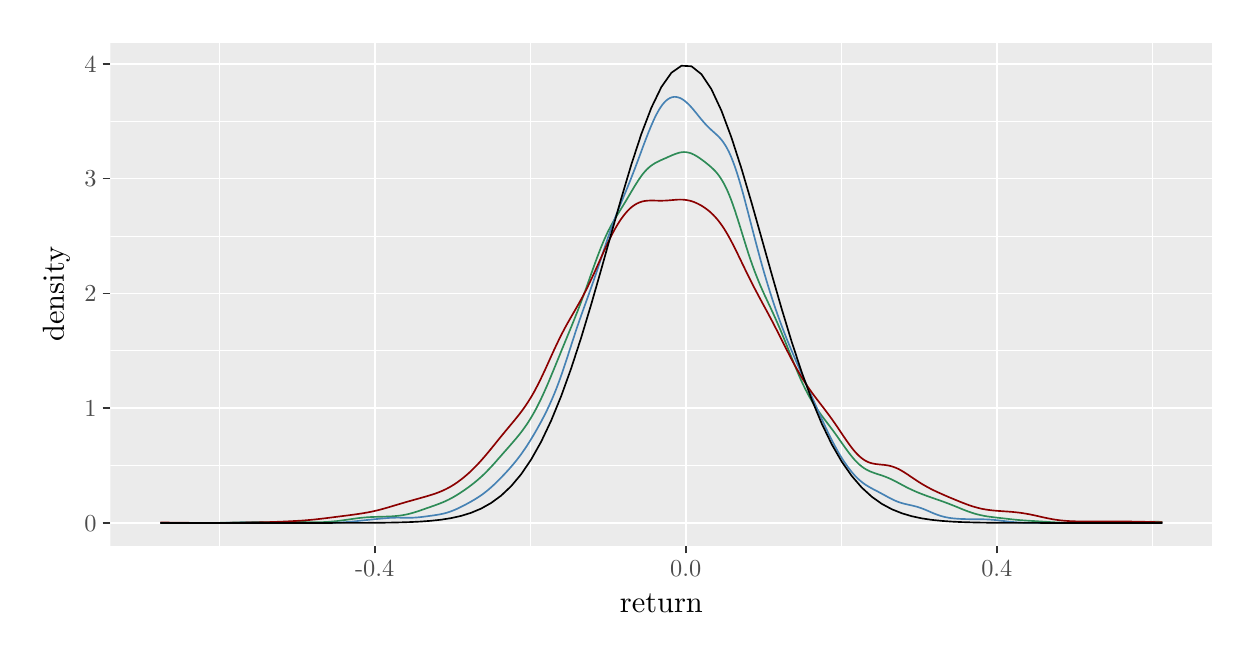
\begin{tikzpicture}[x=1pt,y=1pt]
\definecolor{fillColor}{RGB}{255,255,255}
\path[use as bounding box,fill=fillColor,fill opacity=0.00] (0,0) rectangle (433.62,216.81);
\begin{scope}
\path[clip] (  0.00,  0.00) rectangle (433.62,216.81);
\definecolor{drawColor}{RGB}{255,255,255}
\definecolor{fillColor}{RGB}{255,255,255}

\path[draw=drawColor,line width= 0.6pt,line join=round,line cap=round,fill=fillColor] (  0.00,  0.00) rectangle (433.62,216.81);
\end{scope}
\begin{scope}
\path[clip] ( 29.87, 29.59) rectangle (428.12,211.31);
\definecolor{fillColor}{gray}{0.92}

\path[fill=fillColor] ( 29.87, 29.59) rectangle (428.12,211.31);
\definecolor{drawColor}{RGB}{255,255,255}

\path[draw=drawColor,line width= 0.3pt,line join=round] ( 29.87, 58.58) --
	(428.12, 58.58);

\path[draw=drawColor,line width= 0.3pt,line join=round] ( 29.87,100.06) --
	(428.12,100.06);

\path[draw=drawColor,line width= 0.3pt,line join=round] ( 29.87,141.53) --
	(428.12,141.53);

\path[draw=drawColor,line width= 0.3pt,line join=round] ( 29.87,183.01) --
	(428.12,183.01);

\path[draw=drawColor,line width= 0.3pt,line join=round] ( 69.21, 29.59) --
	( 69.21,211.31);

\path[draw=drawColor,line width= 0.3pt,line join=round] (181.61, 29.59) --
	(181.61,211.31);

\path[draw=drawColor,line width= 0.3pt,line join=round] (294.01, 29.59) --
	(294.01,211.31);

\path[draw=drawColor,line width= 0.3pt,line join=round] (406.41, 29.59) --
	(406.41,211.31);

\path[draw=drawColor,line width= 0.6pt,line join=round] ( 29.87, 37.85) --
	(428.12, 37.85);

\path[draw=drawColor,line width= 0.6pt,line join=round] ( 29.87, 79.32) --
	(428.12, 79.32);

\path[draw=drawColor,line width= 0.6pt,line join=round] ( 29.87,120.80) --
	(428.12,120.80);

\path[draw=drawColor,line width= 0.6pt,line join=round] ( 29.87,162.27) --
	(428.12,162.27);

\path[draw=drawColor,line width= 0.6pt,line join=round] ( 29.87,203.75) --
	(428.12,203.75);

\path[draw=drawColor,line width= 0.6pt,line join=round] (125.41, 29.59) --
	(125.41,211.31);

\path[draw=drawColor,line width= 0.6pt,line join=round] (237.81, 29.59) --
	(237.81,211.31);

\path[draw=drawColor,line width= 0.6pt,line join=round] (350.21, 29.59) --
	(350.21,211.31);
\definecolor{drawColor}{RGB}{46,139,87}

\path[draw=drawColor,line width= 0.6pt,line join=round] ( 47.97, 37.85) --
	( 48.68, 37.85) --
	( 49.39, 37.85) --
	( 50.10, 37.85) --
	( 50.81, 37.85) --
	( 51.51, 37.85) --
	( 52.22, 37.85) --
	( 52.93, 37.85) --
	( 53.64, 37.85) --
	( 54.35, 37.85) --
	( 55.06, 37.85) --
	( 55.76, 37.85) --
	( 56.47, 37.85) --
	( 57.18, 37.85) --
	( 57.89, 37.85) --
	( 58.60, 37.85) --
	( 59.31, 37.85) --
	( 60.02, 37.85) --
	( 60.72, 37.85) --
	( 61.43, 37.85) --
	( 62.14, 37.85) --
	( 62.85, 37.85) --
	( 63.56, 37.85) --
	( 64.27, 37.85) --
	( 64.98, 37.85) --
	( 65.68, 37.85) --
	( 66.39, 37.86) --
	( 67.10, 37.86) --
	( 67.81, 37.86) --
	( 68.52, 37.87) --
	( 69.23, 37.88) --
	( 69.93, 37.89) --
	( 70.64, 37.90) --
	( 71.35, 37.91) --
	( 72.06, 37.92) --
	( 72.77, 37.94) --
	( 73.48, 37.96) --
	( 74.19, 37.98) --
	( 74.89, 38.00) --
	( 75.60, 38.02) --
	( 76.31, 38.05) --
	( 77.02, 38.07) --
	( 77.73, 38.09) --
	( 78.44, 38.11) --
	( 79.15, 38.13) --
	( 79.85, 38.14) --
	( 80.56, 38.15) --
	( 81.27, 38.16) --
	( 81.98, 38.17) --
	( 82.69, 38.17) --
	( 83.40, 38.17) --
	( 84.10, 38.16) --
	( 84.81, 38.16) --
	( 85.52, 38.15) --
	( 86.23, 38.14) --
	( 86.94, 38.13) --
	( 87.65, 38.12) --
	( 88.36, 38.12) --
	( 89.06, 38.12) --
	( 89.77, 38.12) --
	( 90.48, 38.12) --
	( 91.19, 38.13) --
	( 91.90, 38.14) --
	( 92.61, 38.15) --
	( 93.32, 38.16) --
	( 94.02, 38.17) --
	( 94.73, 38.18) --
	( 95.44, 38.19) --
	( 96.15, 38.19) --
	( 96.86, 38.19) --
	( 97.57, 38.19) --
	( 98.28, 38.19) --
	( 98.98, 38.18) --
	( 99.69, 38.17) --
	(100.40, 38.16) --
	(101.11, 38.14) --
	(101.82, 38.13) --
	(102.53, 38.12) --
	(103.23, 38.11) --
	(103.94, 38.11) --
	(104.65, 38.11) --
	(105.36, 38.12) --
	(106.07, 38.13) --
	(106.78, 38.15) --
	(107.49, 38.18) --
	(108.19, 38.22) --
	(108.90, 38.26) --
	(109.61, 38.32) --
	(110.32, 38.38) --
	(111.03, 38.45) --
	(111.74, 38.52) --
	(112.45, 38.61) --
	(113.15, 38.70) --
	(113.86, 38.79) --
	(114.57, 38.89) --
	(115.28, 38.99) --
	(115.99, 39.10) --
	(116.70, 39.20) --
	(117.40, 39.30) --
	(118.11, 39.40) --
	(118.82, 39.50) --
	(119.53, 39.59) --
	(120.24, 39.67) --
	(120.95, 39.74) --
	(121.66, 39.81) --
	(122.36, 39.87) --
	(123.07, 39.92) --
	(123.78, 39.96) --
	(124.49, 39.99) --
	(125.20, 40.02) --
	(125.91, 40.04) --
	(126.62, 40.06) --
	(127.32, 40.08) --
	(128.03, 40.10) --
	(128.74, 40.12) --
	(129.45, 40.14) --
	(130.16, 40.16) --
	(130.87, 40.20) --
	(131.57, 40.23) --
	(132.28, 40.28) --
	(132.99, 40.34) --
	(133.70, 40.41) --
	(134.41, 40.49) --
	(135.12, 40.59) --
	(135.83, 40.71) --
	(136.53, 40.84) --
	(137.24, 40.99) --
	(137.95, 41.16) --
	(138.66, 41.35) --
	(139.37, 41.55) --
	(140.08, 41.77) --
	(140.79, 41.99) --
	(141.49, 42.23) --
	(142.20, 42.47) --
	(142.91, 42.72) --
	(143.62, 42.97) --
	(144.33, 43.22) --
	(145.04, 43.46) --
	(145.74, 43.71) --
	(146.45, 43.96) --
	(147.16, 44.21) --
	(147.87, 44.47) --
	(148.58, 44.73) --
	(149.29, 45.01) --
	(150.00, 45.30) --
	(150.70, 45.60) --
	(151.41, 45.93) --
	(152.12, 46.27) --
	(152.83, 46.64) --
	(153.54, 47.02) --
	(154.25, 47.43) --
	(154.96, 47.85) --
	(155.66, 48.29) --
	(156.37, 48.74) --
	(157.08, 49.21) --
	(157.79, 49.70) --
	(158.50, 50.20) --
	(159.21, 50.71) --
	(159.92, 51.23) --
	(160.62, 51.77) --
	(161.33, 52.33) --
	(162.04, 52.91) --
	(162.75, 53.51) --
	(163.46, 54.13) --
	(164.17, 54.77) --
	(164.87, 55.44) --
	(165.58, 56.14) --
	(166.29, 56.87) --
	(167.00, 57.61) --
	(167.71, 58.37) --
	(168.42, 59.15) --
	(169.13, 59.94) --
	(169.83, 60.75) --
	(170.54, 61.55) --
	(171.25, 62.36) --
	(171.96, 63.17) --
	(172.67, 63.97) --
	(173.38, 64.78) --
	(174.09, 65.58) --
	(174.79, 66.39) --
	(175.50, 67.21) --
	(176.21, 68.04) --
	(176.92, 68.89) --
	(177.63, 69.76) --
	(178.34, 70.66) --
	(179.04, 71.61) --
	(179.75, 72.59) --
	(180.46, 73.63) --
	(181.17, 74.71) --
	(181.88, 75.86) --
	(182.59, 77.06) --
	(183.30, 78.32) --
	(184.00, 79.65) --
	(184.71, 81.05) --
	(185.42, 82.50) --
	(186.13, 84.02) --
	(186.84, 85.58) --
	(187.55, 87.19) --
	(188.26, 88.84) --
	(188.96, 90.53) --
	(189.67, 92.24) --
	(190.38, 93.96) --
	(191.09, 95.70) --
	(191.80, 97.44) --
	(192.51, 99.17) --
	(193.21,100.90) --
	(193.92,102.63) --
	(194.63,104.35) --
	(195.34,106.07) --
	(196.05,107.79) --
	(196.76,109.52) --
	(197.47,111.27) --
	(198.17,113.04) --
	(198.88,114.84) --
	(199.59,116.69) --
	(200.30,118.56) --
	(201.01,120.48) --
	(201.72,122.43) --
	(202.43,124.41) --
	(203.13,126.42) --
	(203.84,128.42) --
	(204.55,130.42) --
	(205.26,132.38) --
	(205.97,134.30) --
	(206.68,136.15) --
	(207.39,137.94) --
	(208.09,139.63) --
	(208.80,141.24) --
	(209.51,142.75) --
	(210.22,144.16) --
	(210.93,145.49) --
	(211.64,146.75) --
	(212.34,147.96) --
	(213.05,149.13) --
	(213.76,150.28) --
	(214.47,151.43) --
	(215.18,152.58) --
	(215.89,153.75) --
	(216.60,154.93) --
	(217.30,156.13) --
	(218.01,157.33) --
	(218.72,158.53) --
	(219.43,159.70) --
	(220.14,160.84) --
	(220.85,161.93) --
	(221.56,162.96) --
	(222.26,163.91) --
	(222.97,164.76) --
	(223.68,165.52) --
	(224.39,166.20) --
	(225.10,166.79) --
	(225.81,167.30) --
	(226.51,167.75) --
	(227.22,168.15) --
	(227.93,168.50) --
	(228.64,168.84) --
	(229.35,169.16) --
	(230.06,169.47) --
	(230.77,169.78) --
	(231.47,170.10) --
	(232.18,170.41) --
	(232.89,170.72) --
	(233.60,171.01) --
	(234.31,171.28) --
	(235.02,171.51) --
	(235.73,171.70) --
	(236.43,171.81) --
	(237.14,171.86) --
	(237.85,171.83) --
	(238.56,171.72) --
	(239.27,171.54) --
	(239.98,171.29) --
	(240.68,170.96) --
	(241.39,170.58) --
	(242.10,170.14) --
	(242.81,169.67) --
	(243.52,169.16) --
	(244.23,168.64) --
	(244.94,168.09) --
	(245.64,167.53) --
	(246.35,166.94) --
	(247.06,166.32) --
	(247.77,165.65) --
	(248.48,164.93) --
	(249.19,164.11) --
	(249.90,163.19) --
	(250.60,162.14) --
	(251.31,160.96) --
	(252.02,159.63) --
	(252.73,158.15) --
	(253.44,156.51) --
	(254.15,154.72) --
	(254.85,152.78) --
	(255.56,150.71) --
	(256.27,148.54) --
	(256.98,146.30) --
	(257.69,144.02) --
	(258.40,141.71) --
	(259.11,139.42) --
	(259.81,137.17) --
	(260.52,134.97) --
	(261.23,132.84) --
	(261.94,130.81) --
	(262.65,128.88) --
	(263.36,127.03) --
	(264.07,125.27) --
	(264.77,123.59) --
	(265.48,121.97) --
	(266.19,120.40) --
	(266.90,118.87) --
	(267.61,117.35) --
	(268.32,115.84) --
	(269.03,114.31) --
	(269.73,112.76) --
	(270.44,111.18) --
	(271.15,109.56) --
	(271.86,107.91) --
	(272.57,106.22) --
	(273.28,104.49) --
	(273.98,102.74) --
	(274.69,100.97) --
	(275.40, 99.20) --
	(276.11, 97.43) --
	(276.82, 95.67) --
	(277.53, 93.95) --
	(278.24, 92.26) --
	(278.94, 90.62) --
	(279.65, 89.04) --
	(280.36, 87.52) --
	(281.07, 86.07) --
	(281.78, 84.70) --
	(282.49, 83.40) --
	(283.20, 82.17) --
	(283.90, 81.01) --
	(284.61, 79.91) --
	(285.32, 78.85) --
	(286.03, 77.85) --
	(286.74, 76.87) --
	(287.45, 75.93) --
	(288.15, 74.99) --
	(288.86, 74.06) --
	(289.57, 73.13) --
	(290.28, 72.19) --
	(290.99, 71.23) --
	(291.70, 70.26) --
	(292.41, 69.27) --
	(293.11, 68.27) --
	(293.82, 67.26) --
	(294.53, 66.25) --
	(295.24, 65.25) --
	(295.95, 64.27) --
	(296.66, 63.31) --
	(297.37, 62.39) --
	(298.07, 61.52) --
	(298.78, 60.69) --
	(299.49, 59.93) --
	(300.20, 59.24) --
	(300.91, 58.62) --
	(301.62, 58.07) --
	(302.32, 57.58) --
	(303.03, 57.15) --
	(303.74, 56.78) --
	(304.45, 56.45) --
	(305.16, 56.17) --
	(305.87, 55.91) --
	(306.58, 55.67) --
	(307.28, 55.44) --
	(307.99, 55.21) --
	(308.70, 54.98) --
	(309.41, 54.73) --
	(310.12, 54.46) --
	(310.83, 54.17) --
	(311.54, 53.86) --
	(312.24, 53.53) --
	(312.95, 53.18) --
	(313.66, 52.82) --
	(314.37, 52.45) --
	(315.08, 52.07) --
	(315.79, 51.69) --
	(316.49, 51.31) --
	(317.20, 50.94) --
	(317.91, 50.58) --
	(318.62, 50.23) --
	(319.33, 49.89) --
	(320.04, 49.57) --
	(320.75, 49.25) --
	(321.45, 48.95) --
	(322.16, 48.66) --
	(322.87, 48.38) --
	(323.58, 48.11) --
	(324.29, 47.84) --
	(325.00, 47.58) --
	(325.71, 47.33) --
	(326.41, 47.08) --
	(327.12, 46.83) --
	(327.83, 46.58) --
	(328.54, 46.34) --
	(329.25, 46.09) --
	(329.96, 45.84) --
	(330.67, 45.59) --
	(331.37, 45.33) --
	(332.08, 45.07) --
	(332.79, 44.80) --
	(333.50, 44.52) --
	(334.21, 44.24) --
	(334.92, 43.96) --
	(335.62, 43.67) --
	(336.33, 43.38) --
	(337.04, 43.09) --
	(337.75, 42.80) --
	(338.46, 42.52) --
	(339.17, 42.24) --
	(339.88, 41.98) --
	(340.58, 41.73) --
	(341.29, 41.49) --
	(342.00, 41.27) --
	(342.71, 41.06) --
	(343.42, 40.88) --
	(344.13, 40.71) --
	(344.84, 40.55) --
	(345.54, 40.42) --
	(346.25, 40.29) --
	(346.96, 40.18) --
	(347.67, 40.08) --
	(348.38, 39.99) --
	(349.09, 39.90) --
	(349.79, 39.82) --
	(350.50, 39.73) --
	(351.21, 39.65) --
	(351.92, 39.57) --
	(352.63, 39.49) --
	(353.34, 39.41) --
	(354.05, 39.33) --
	(354.75, 39.25) --
	(355.46, 39.17) --
	(356.17, 39.09) --
	(356.88, 39.02) --
	(357.59, 38.95) --
	(358.30, 38.89) --
	(359.01, 38.83) --
	(359.71, 38.78) --
	(360.42, 38.73) --
	(361.13, 38.68) --
	(361.84, 38.64) --
	(362.55, 38.59) --
	(363.26, 38.55) --
	(363.96, 38.51) --
	(364.67, 38.47) --
	(365.38, 38.42) --
	(366.09, 38.38) --
	(366.80, 38.33) --
	(367.51, 38.29) --
	(368.22, 38.24) --
	(368.92, 38.19) --
	(369.63, 38.15) --
	(370.34, 38.11) --
	(371.05, 38.07) --
	(371.76, 38.03) --
	(372.47, 38.00) --
	(373.18, 37.97) --
	(373.88, 37.95) --
	(374.59, 37.92) --
	(375.30, 37.91) --
	(376.01, 37.89) --
	(376.72, 37.88) --
	(377.43, 37.87) --
	(378.13, 37.87) --
	(378.84, 37.86) --
	(379.55, 37.86) --
	(380.26, 37.85) --
	(380.97, 37.85) --
	(381.68, 37.85) --
	(382.39, 37.85) --
	(383.09, 37.85) --
	(383.80, 37.85) --
	(384.51, 37.85) --
	(385.22, 37.85) --
	(385.93, 37.85) --
	(386.64, 37.85) --
	(387.35, 37.85) --
	(388.05, 37.86) --
	(388.76, 37.86) --
	(389.47, 37.86) --
	(390.18, 37.87) --
	(390.89, 37.88) --
	(391.60, 37.88) --
	(392.31, 37.89) --
	(393.01, 37.91) --
	(393.72, 37.92) --
	(394.43, 37.93) --
	(395.14, 37.95) --
	(395.85, 37.97) --
	(396.56, 37.99) --
	(397.26, 38.01) --
	(397.97, 38.03) --
	(398.68, 38.05) --
	(399.39, 38.08) --
	(400.10, 38.10) --
	(400.81, 38.12) --
	(401.52, 38.15) --
	(402.22, 38.17) --
	(402.93, 38.19) --
	(403.64, 38.21) --
	(404.35, 38.22) --
	(405.06, 38.24) --
	(405.77, 38.25) --
	(406.48, 38.25) --
	(407.18, 38.26) --
	(407.89, 38.25) --
	(408.60, 38.25) --
	(409.31, 38.24) --
	(410.02, 38.22);
\definecolor{drawColor}{RGB}{70,130,180}

\path[draw=drawColor,line width= 0.6pt,line join=round] ( 47.97, 37.85) --
	( 48.68, 37.85) --
	( 49.39, 37.85) --
	( 50.10, 37.85) --
	( 50.81, 37.85) --
	( 51.51, 37.85) --
	( 52.22, 37.85) --
	( 52.93, 37.85) --
	( 53.64, 37.85) --
	( 54.35, 37.85) --
	( 55.06, 37.85) --
	( 55.76, 37.85) --
	( 56.47, 37.85) --
	( 57.18, 37.85) --
	( 57.89, 37.85) --
	( 58.60, 37.85) --
	( 59.31, 37.85) --
	( 60.02, 37.85) --
	( 60.72, 37.85) --
	( 61.43, 37.85) --
	( 62.14, 37.85) --
	( 62.85, 37.85) --
	( 63.56, 37.85) --
	( 64.27, 37.85) --
	( 64.98, 37.85) --
	( 65.68, 37.85) --
	( 66.39, 37.85) --
	( 67.10, 37.85) --
	( 67.81, 37.85) --
	( 68.52, 37.86) --
	( 69.23, 37.86) --
	( 69.93, 37.86) --
	( 70.64, 37.87) --
	( 71.35, 37.88) --
	( 72.06, 37.89) --
	( 72.77, 37.90) --
	( 73.48, 37.91) --
	( 74.19, 37.93) --
	( 74.89, 37.94) --
	( 75.60, 37.96) --
	( 76.31, 37.97) --
	( 77.02, 37.99) --
	( 77.73, 38.00) --
	( 78.44, 38.02) --
	( 79.15, 38.02) --
	( 79.85, 38.03) --
	( 80.56, 38.03) --
	( 81.27, 38.03) --
	( 81.98, 38.03) --
	( 82.69, 38.02) --
	( 83.40, 38.01) --
	( 84.10, 38.00) --
	( 84.81, 37.98) --
	( 85.52, 37.96) --
	( 86.23, 37.95) --
	( 86.94, 37.93) --
	( 87.65, 37.92) --
	( 88.36, 37.90) --
	( 89.06, 37.89) --
	( 89.77, 37.88) --
	( 90.48, 37.87) --
	( 91.19, 37.87) --
	( 91.90, 37.86) --
	( 92.61, 37.86) --
	( 93.32, 37.85) --
	( 94.02, 37.85) --
	( 94.73, 37.85) --
	( 95.44, 37.85) --
	( 96.15, 37.85) --
	( 96.86, 37.85) --
	( 97.57, 37.85) --
	( 98.28, 37.85) --
	( 98.98, 37.85) --
	( 99.69, 37.85) --
	(100.40, 37.85) --
	(101.11, 37.85) --
	(101.82, 37.85) --
	(102.53, 37.85) --
	(103.23, 37.85) --
	(103.94, 37.85) --
	(104.65, 37.85) --
	(105.36, 37.85) --
	(106.07, 37.85) --
	(106.78, 37.86) --
	(107.49, 37.86) --
	(108.19, 37.87) --
	(108.90, 37.88) --
	(109.61, 37.89) --
	(110.32, 37.91) --
	(111.03, 37.93) --
	(111.74, 37.96) --
	(112.45, 37.99) --
	(113.15, 38.02) --
	(113.86, 38.06) --
	(114.57, 38.11) --
	(115.28, 38.17) --
	(115.99, 38.23) --
	(116.70, 38.29) --
	(117.40, 38.36) --
	(118.11, 38.43) --
	(118.82, 38.50) --
	(119.53, 38.58) --
	(120.24, 38.66) --
	(120.95, 38.73) --
	(121.66, 38.81) --
	(122.36, 38.88) --
	(123.07, 38.95) --
	(123.78, 39.03) --
	(124.49, 39.10) --
	(125.20, 39.17) --
	(125.91, 39.24) --
	(126.62, 39.31) --
	(127.32, 39.38) --
	(128.03, 39.44) --
	(128.74, 39.51) --
	(129.45, 39.57) --
	(130.16, 39.62) --
	(130.87, 39.67) --
	(131.57, 39.70) --
	(132.28, 39.73) --
	(132.99, 39.75) --
	(133.70, 39.75) --
	(134.41, 39.75) --
	(135.12, 39.74) --
	(135.83, 39.73) --
	(136.53, 39.72) --
	(137.24, 39.71) --
	(137.95, 39.71) --
	(138.66, 39.73) --
	(139.37, 39.75) --
	(140.08, 39.79) --
	(140.79, 39.84) --
	(141.49, 39.91) --
	(142.20, 39.98) --
	(142.91, 40.07) --
	(143.62, 40.16) --
	(144.33, 40.25) --
	(145.04, 40.35) --
	(145.74, 40.45) --
	(146.45, 40.54) --
	(147.16, 40.65) --
	(147.87, 40.76) --
	(148.58, 40.88) --
	(149.29, 41.01) --
	(150.00, 41.16) --
	(150.70, 41.33) --
	(151.41, 41.53) --
	(152.12, 41.74) --
	(152.83, 41.99) --
	(153.54, 42.26) --
	(154.25, 42.55) --
	(154.96, 42.86) --
	(155.66, 43.19) --
	(156.37, 43.53) --
	(157.08, 43.89) --
	(157.79, 44.25) --
	(158.50, 44.63) --
	(159.21, 45.01) --
	(159.92, 45.40) --
	(160.62, 45.81) --
	(161.33, 46.22) --
	(162.04, 46.65) --
	(162.75, 47.10) --
	(163.46, 47.57) --
	(164.17, 48.06) --
	(164.87, 48.58) --
	(165.58, 49.13) --
	(166.29, 49.70) --
	(167.00, 50.31) --
	(167.71, 50.94) --
	(168.42, 51.59) --
	(169.13, 52.27) --
	(169.83, 52.96) --
	(170.54, 53.67) --
	(171.25, 54.40) --
	(171.96, 55.14) --
	(172.67, 55.89) --
	(173.38, 56.66) --
	(174.09, 57.45) --
	(174.79, 58.26) --
	(175.50, 59.09) --
	(176.21, 59.95) --
	(176.92, 60.84) --
	(177.63, 61.76) --
	(178.34, 62.72) --
	(179.04, 63.72) --
	(179.75, 64.75) --
	(180.46, 65.82) --
	(181.17, 66.93) --
	(181.88, 68.07) --
	(182.59, 69.24) --
	(183.30, 70.44) --
	(184.00, 71.67) --
	(184.71, 72.94) --
	(185.42, 74.23) --
	(186.13, 75.57) --
	(186.84, 76.95) --
	(187.55, 78.38) --
	(188.26, 79.87) --
	(188.96, 81.42) --
	(189.67, 83.03) --
	(190.38, 84.73) --
	(191.09, 86.51) --
	(191.80, 88.37) --
	(192.51, 90.32) --
	(193.21, 92.34) --
	(193.92, 94.44) --
	(194.63, 96.59) --
	(195.34, 98.77) --
	(196.05,100.96) --
	(196.76,103.15) --
	(197.47,105.33) --
	(198.17,107.47) --
	(198.88,109.57) --
	(199.59,111.62) --
	(200.30,113.64) --
	(201.01,115.62) --
	(201.72,117.58) --
	(202.43,119.55) --
	(203.13,121.52) --
	(203.84,123.52) --
	(204.55,125.55) --
	(205.26,127.62) --
	(205.97,129.72) --
	(206.68,131.86) --
	(207.39,134.01) --
	(208.09,136.16) --
	(208.80,138.30) --
	(209.51,140.41) --
	(210.22,142.47) --
	(210.93,144.47) --
	(211.64,146.42) --
	(212.34,148.30) --
	(213.05,150.12) --
	(213.76,151.89) --
	(214.47,153.62) --
	(215.18,155.34) --
	(215.89,157.05) --
	(216.60,158.77) --
	(217.30,160.52) --
	(218.01,162.29) --
	(218.72,164.11) --
	(219.43,165.95) --
	(220.14,167.83) --
	(220.85,169.74) --
	(221.56,171.65) --
	(222.26,173.57) --
	(222.97,175.46) --
	(223.68,177.32) --
	(224.39,179.13) --
	(225.10,180.86) --
	(225.81,182.51) --
	(226.51,184.06) --
	(227.22,185.49) --
	(227.93,186.79) --
	(228.64,187.96) --
	(229.35,188.96) --
	(230.06,189.81) --
	(230.77,190.50) --
	(231.47,191.04) --
	(232.18,191.43) --
	(232.89,191.68) --
	(233.60,191.80) --
	(234.31,191.78) --
	(235.02,191.64) --
	(235.73,191.39) --
	(236.43,191.03) --
	(237.14,190.56) --
	(237.85,190.00) --
	(238.56,189.35) --
	(239.27,188.64) --
	(239.98,187.86) --
	(240.68,187.04) --
	(241.39,186.18) --
	(242.10,185.30) --
	(242.81,184.42) --
	(243.52,183.55) --
	(244.23,182.72) --
	(244.94,181.93) --
	(245.64,181.19) --
	(246.35,180.49) --
	(247.06,179.83) --
	(247.77,179.19) --
	(248.48,178.55) --
	(249.19,177.90) --
	(249.90,177.19) --
	(250.60,176.40) --
	(251.31,175.49) --
	(252.02,174.43) --
	(252.73,173.21) --
	(253.44,171.82) --
	(254.15,170.24) --
	(254.85,168.48) --
	(255.56,166.54) --
	(256.27,164.42) --
	(256.98,162.16) --
	(257.69,159.75) --
	(258.40,157.22) --
	(259.11,154.60) --
	(259.81,151.92) --
	(260.52,149.20) --
	(261.23,146.46) --
	(261.94,143.72) --
	(262.65,140.99) --
	(263.36,138.30) --
	(264.07,135.65) --
	(264.77,133.05) --
	(265.48,130.51) --
	(266.19,128.04) --
	(266.90,125.64) --
	(267.61,123.30) --
	(268.32,121.04) --
	(269.03,118.84) --
	(269.73,116.70) --
	(270.44,114.63) --
	(271.15,112.61) --
	(271.86,110.66) --
	(272.57,108.76) --
	(273.28,106.91) --
	(273.98,105.11) --
	(274.69,103.35) --
	(275.40,101.63) --
	(276.11, 99.94) --
	(276.82, 98.27) --
	(277.53, 96.63) --
	(278.24, 95.00) --
	(278.94, 93.39) --
	(279.65, 91.80) --
	(280.36, 90.20) --
	(281.07, 88.61) --
	(281.78, 87.02) --
	(282.49, 85.43) --
	(283.20, 83.83) --
	(283.90, 82.24) --
	(284.61, 80.64) --
	(285.32, 79.04) --
	(286.03, 77.44) --
	(286.74, 75.86) --
	(287.45, 74.30) --
	(288.15, 72.76) --
	(288.86, 71.25) --
	(289.57, 69.78) --
	(290.28, 68.35) --
	(290.99, 66.96) --
	(291.70, 65.62) --
	(292.41, 64.32) --
	(293.11, 63.08) --
	(293.82, 61.89) --
	(294.53, 60.76) --
	(295.24, 59.68) --
	(295.95, 58.65) --
	(296.66, 57.68) --
	(297.37, 56.76) --
	(298.07, 55.90) --
	(298.78, 55.10) --
	(299.49, 54.35) --
	(300.20, 53.67) --
	(300.91, 53.04) --
	(301.62, 52.47) --
	(302.32, 51.95) --
	(303.03, 51.47) --
	(303.74, 51.04) --
	(304.45, 50.63) --
	(305.16, 50.24) --
	(305.87, 49.86) --
	(306.58, 49.49) --
	(307.28, 49.13) --
	(307.99, 48.75) --
	(308.70, 48.37) --
	(309.41, 47.99) --
	(310.12, 47.60) --
	(310.83, 47.21) --
	(311.54, 46.84) --
	(312.24, 46.47) --
	(312.95, 46.13) --
	(313.66, 45.81) --
	(314.37, 45.52) --
	(315.08, 45.27) --
	(315.79, 45.04) --
	(316.49, 44.85) --
	(317.20, 44.67) --
	(317.91, 44.51) --
	(318.62, 44.35) --
	(319.33, 44.20) --
	(320.04, 44.03) --
	(320.75, 43.85) --
	(321.45, 43.66) --
	(322.16, 43.43) --
	(322.87, 43.19) --
	(323.58, 42.92) --
	(324.29, 42.63) --
	(325.00, 42.34) --
	(325.71, 42.03) --
	(326.41, 41.72) --
	(327.12, 41.42) --
	(327.83, 41.13) --
	(328.54, 40.86) --
	(329.25, 40.61) --
	(329.96, 40.38) --
	(330.67, 40.18) --
	(331.37, 40.00) --
	(332.08, 39.85) --
	(332.79, 39.72) --
	(333.50, 39.61) --
	(334.21, 39.52) --
	(334.92, 39.45) --
	(335.62, 39.39) --
	(336.33, 39.34) --
	(337.04, 39.30) --
	(337.75, 39.27) --
	(338.46, 39.25) --
	(339.17, 39.23) --
	(339.88, 39.21) --
	(340.58, 39.20) --
	(341.29, 39.19) --
	(342.00, 39.19) --
	(342.71, 39.19) --
	(343.42, 39.18) --
	(344.13, 39.18) --
	(344.84, 39.17) --
	(345.54, 39.15) --
	(346.25, 39.13) --
	(346.96, 39.10) --
	(347.67, 39.06) --
	(348.38, 39.01) --
	(349.09, 38.95) --
	(349.79, 38.88) --
	(350.50, 38.81) --
	(351.21, 38.73) --
	(351.92, 38.64) --
	(352.63, 38.56) --
	(353.34, 38.47) --
	(354.05, 38.39) --
	(354.75, 38.31) --
	(355.46, 38.23) --
	(356.17, 38.17) --
	(356.88, 38.11) --
	(357.59, 38.05) --
	(358.30, 38.01) --
	(359.01, 37.97) --
	(359.71, 37.94) --
	(360.42, 37.92) --
	(361.13, 37.90) --
	(361.84, 37.89) --
	(362.55, 37.87) --
	(363.26, 37.87) --
	(363.96, 37.86) --
	(364.67, 37.86) --
	(365.38, 37.85) --
	(366.09, 37.85) --
	(366.80, 37.85) --
	(367.51, 37.85) --
	(368.22, 37.85) --
	(368.92, 37.85) --
	(369.63, 37.85) --
	(370.34, 37.85) --
	(371.05, 37.85) --
	(371.76, 37.85) --
	(372.47, 37.85) --
	(373.18, 37.85) --
	(373.88, 37.85) --
	(374.59, 37.85) --
	(375.30, 37.85) --
	(376.01, 37.85) --
	(376.72, 37.86) --
	(377.43, 37.86) --
	(378.13, 37.86) --
	(378.84, 37.87) --
	(379.55, 37.88) --
	(380.26, 37.88) --
	(380.97, 37.90) --
	(381.68, 37.91) --
	(382.39, 37.92) --
	(383.09, 37.94) --
	(383.80, 37.95) --
	(384.51, 37.97) --
	(385.22, 37.98) --
	(385.93, 38.00) --
	(386.64, 38.01) --
	(387.35, 38.02) --
	(388.05, 38.03) --
	(388.76, 38.03) --
	(389.47, 38.03) --
	(390.18, 38.03) --
	(390.89, 38.02) --
	(391.60, 38.01) --
	(392.31, 38.00) --
	(393.01, 37.99) --
	(393.72, 37.97) --
	(394.43, 37.95) --
	(395.14, 37.94) --
	(395.85, 37.92) --
	(396.56, 37.91) --
	(397.26, 37.90) --
	(397.97, 37.89) --
	(398.68, 37.88) --
	(399.39, 37.87) --
	(400.10, 37.86) --
	(400.81, 37.86) --
	(401.52, 37.86) --
	(402.22, 37.85) --
	(402.93, 37.85) --
	(403.64, 37.85) --
	(404.35, 37.85) --
	(405.06, 37.85) --
	(405.77, 37.85) --
	(406.48, 37.85) --
	(407.18, 37.85) --
	(407.89, 37.85) --
	(408.60, 37.85) --
	(409.31, 37.85) --
	(410.02, 37.85);
\definecolor{drawColor}{RGB}{139,0,0}

\path[draw=drawColor,line width= 0.6pt,line join=round] ( 47.97, 37.99) --
	( 48.68, 37.99) --
	( 49.39, 37.99) --
	( 50.10, 37.99) --
	( 50.81, 37.98) --
	( 51.51, 37.97) --
	( 52.22, 37.96) --
	( 52.93, 37.95) --
	( 53.64, 37.95) --
	( 54.35, 37.94) --
	( 55.06, 37.93) --
	( 55.76, 37.92) --
	( 56.47, 37.91) --
	( 57.18, 37.90) --
	( 57.89, 37.89) --
	( 58.60, 37.88) --
	( 59.31, 37.88) --
	( 60.02, 37.87) --
	( 60.72, 37.87) --
	( 61.43, 37.86) --
	( 62.14, 37.86) --
	( 62.85, 37.86) --
	( 63.56, 37.86) --
	( 64.27, 37.85) --
	( 64.98, 37.85) --
	( 65.68, 37.85) --
	( 66.39, 37.85) --
	( 67.10, 37.85) --
	( 67.81, 37.86) --
	( 68.52, 37.86) --
	( 69.23, 37.86) --
	( 69.93, 37.86) --
	( 70.64, 37.87) --
	( 71.35, 37.87) --
	( 72.06, 37.88) --
	( 72.77, 37.88) --
	( 73.48, 37.89) --
	( 74.19, 37.90) --
	( 74.89, 37.91) --
	( 75.60, 37.92) --
	( 76.31, 37.93) --
	( 77.02, 37.94) --
	( 77.73, 37.95) --
	( 78.44, 37.97) --
	( 79.15, 37.98) --
	( 79.85, 37.99) --
	( 80.56, 38.01) --
	( 81.27, 38.02) --
	( 81.98, 38.03) --
	( 82.69, 38.05) --
	( 83.40, 38.06) --
	( 84.10, 38.07) --
	( 84.81, 38.09) --
	( 85.52, 38.11) --
	( 86.23, 38.12) --
	( 86.94, 38.14) --
	( 87.65, 38.16) --
	( 88.36, 38.18) --
	( 89.06, 38.21) --
	( 89.77, 38.23) --
	( 90.48, 38.26) --
	( 91.19, 38.29) --
	( 91.90, 38.32) --
	( 92.61, 38.35) --
	( 93.32, 38.38) --
	( 94.02, 38.42) --
	( 94.73, 38.45) --
	( 95.44, 38.49) --
	( 96.15, 38.53) --
	( 96.86, 38.56) --
	( 97.57, 38.61) --
	( 98.28, 38.65) --
	( 98.98, 38.69) --
	( 99.69, 38.74) --
	(100.40, 38.80) --
	(101.11, 38.85) --
	(101.82, 38.92) --
	(102.53, 38.98) --
	(103.23, 39.05) --
	(103.94, 39.12) --
	(104.65, 39.20) --
	(105.36, 39.28) --
	(106.07, 39.36) --
	(106.78, 39.45) --
	(107.49, 39.53) --
	(108.19, 39.62) --
	(108.90, 39.71) --
	(109.61, 39.80) --
	(110.32, 39.89) --
	(111.03, 39.98) --
	(111.74, 40.07) --
	(112.45, 40.16) --
	(113.15, 40.25) --
	(113.86, 40.34) --
	(114.57, 40.43) --
	(115.28, 40.52) --
	(115.99, 40.61) --
	(116.70, 40.71) --
	(117.40, 40.80) --
	(118.11, 40.90) --
	(118.82, 41.00) --
	(119.53, 41.10) --
	(120.24, 41.21) --
	(120.95, 41.32) --
	(121.66, 41.44) --
	(122.36, 41.56) --
	(123.07, 41.69) --
	(123.78, 41.83) --
	(124.49, 41.97) --
	(125.20, 42.13) --
	(125.91, 42.29) --
	(126.62, 42.46) --
	(127.32, 42.64) --
	(128.03, 42.83) --
	(128.74, 43.03) --
	(129.45, 43.23) --
	(130.16, 43.43) --
	(130.87, 43.64) --
	(131.57, 43.85) --
	(132.28, 44.07) --
	(132.99, 44.28) --
	(133.70, 44.49) --
	(134.41, 44.70) --
	(135.12, 44.91) --
	(135.83, 45.12) --
	(136.53, 45.33) --
	(137.24, 45.53) --
	(137.95, 45.73) --
	(138.66, 45.93) --
	(139.37, 46.13) --
	(140.08, 46.33) --
	(140.79, 46.52) --
	(141.49, 46.72) --
	(142.20, 46.92) --
	(142.91, 47.12) --
	(143.62, 47.32) --
	(144.33, 47.53) --
	(145.04, 47.74) --
	(145.74, 47.96) --
	(146.45, 48.18) --
	(147.16, 48.42) --
	(147.87, 48.67) --
	(148.58, 48.94) --
	(149.29, 49.23) --
	(150.00, 49.53) --
	(150.70, 49.86) --
	(151.41, 50.21) --
	(152.12, 50.58) --
	(152.83, 50.98) --
	(153.54, 51.40) --
	(154.25, 51.85) --
	(154.96, 52.32) --
	(155.66, 52.83) --
	(156.37, 53.35) --
	(157.08, 53.90) --
	(157.79, 54.48) --
	(158.50, 55.08) --
	(159.21, 55.70) --
	(159.92, 56.35) --
	(160.62, 57.03) --
	(161.33, 57.73) --
	(162.04, 58.45) --
	(162.75, 59.19) --
	(163.46, 59.96) --
	(164.17, 60.75) --
	(164.87, 61.56) --
	(165.58, 62.39) --
	(166.29, 63.23) --
	(167.00, 64.09) --
	(167.71, 64.96) --
	(168.42, 65.83) --
	(169.13, 66.71) --
	(169.83, 67.59) --
	(170.54, 68.46) --
	(171.25, 69.33) --
	(171.96, 70.19) --
	(172.67, 71.05) --
	(173.38, 71.90) --
	(174.09, 72.75) --
	(174.79, 73.60) --
	(175.50, 74.45) --
	(176.21, 75.31) --
	(176.92, 76.19) --
	(177.63, 77.08) --
	(178.34, 78.01) --
	(179.04, 78.97) --
	(179.75, 79.97) --
	(180.46, 81.02) --
	(181.17, 82.12) --
	(181.88, 83.27) --
	(182.59, 84.48) --
	(183.30, 85.76) --
	(184.00, 87.10) --
	(184.71, 88.49) --
	(185.42, 89.93) --
	(186.13, 91.42) --
	(186.84, 92.94) --
	(187.55, 94.49) --
	(188.26, 96.05) --
	(188.96, 97.62) --
	(189.67, 99.18) --
	(190.38,100.72) --
	(191.09,102.23) --
	(191.80,103.71) --
	(192.51,105.15) --
	(193.21,106.54) --
	(193.92,107.90) --
	(194.63,109.21) --
	(195.34,110.48) --
	(196.05,111.72) --
	(196.76,112.95) --
	(197.47,114.17) --
	(198.17,115.39) --
	(198.88,116.63) --
	(199.59,117.89) --
	(200.30,119.18) --
	(201.01,120.52) --
	(201.72,121.90) --
	(202.43,123.32) --
	(203.13,124.78) --
	(203.84,126.29) --
	(204.55,127.82) --
	(205.26,129.39) --
	(205.97,130.97) --
	(206.68,132.56) --
	(207.39,134.15) --
	(208.09,135.72) --
	(208.80,137.26) --
	(209.51,138.77) --
	(210.22,140.24) --
	(210.93,141.65) --
	(211.64,143.01) --
	(212.34,144.29) --
	(213.05,145.50) --
	(213.76,146.64) --
	(214.47,147.70) --
	(215.18,148.68) --
	(215.89,149.58) --
	(216.60,150.40) --
	(217.30,151.14) --
	(218.01,151.79) --
	(218.72,152.35) --
	(219.43,152.83) --
	(220.14,153.24) --
	(220.85,153.57) --
	(221.56,153.84) --
	(222.26,154.04) --
	(222.97,154.18) --
	(223.68,154.27) --
	(224.39,154.32) --
	(225.10,154.34) --
	(225.81,154.34) --
	(226.51,154.33) --
	(227.22,154.31) --
	(227.93,154.29) --
	(228.64,154.28) --
	(229.35,154.29) --
	(230.06,154.31) --
	(230.77,154.34) --
	(231.47,154.39) --
	(232.18,154.45) --
	(232.89,154.51) --
	(233.60,154.57) --
	(234.31,154.63) --
	(235.02,154.67) --
	(235.73,154.69) --
	(236.43,154.68) --
	(237.14,154.63) --
	(237.85,154.55) --
	(238.56,154.44) --
	(239.27,154.28) --
	(239.98,154.08) --
	(240.68,153.84) --
	(241.39,153.55) --
	(242.10,153.22) --
	(242.81,152.86) --
	(243.52,152.46) --
	(244.23,152.02) --
	(244.94,151.53) --
	(245.64,151.01) --
	(246.35,150.44) --
	(247.06,149.80) --
	(247.77,149.11) --
	(248.48,148.36) --
	(249.19,147.55) --
	(249.90,146.66) --
	(250.60,145.70) --
	(251.31,144.68) --
	(252.02,143.57) --
	(252.73,142.39) --
	(253.44,141.14) --
	(254.15,139.83) --
	(254.85,138.47) --
	(255.56,137.07) --
	(256.27,135.63) --
	(256.98,134.17) --
	(257.69,132.70) --
	(258.40,131.22) --
	(259.11,129.75) --
	(259.81,128.29) --
	(260.52,126.85) --
	(261.23,125.43) --
	(261.94,124.03) --
	(262.65,122.66) --
	(263.36,121.31) --
	(264.07,119.97) --
	(264.77,118.66) --
	(265.48,117.34) --
	(266.19,116.03) --
	(266.90,114.72) --
	(267.61,113.40) --
	(268.32,112.07) --
	(269.03,110.73) --
	(269.73,109.37) --
	(270.44,107.99) --
	(271.15,106.60) --
	(271.86,105.19) --
	(272.57,103.79) --
	(273.28,102.38) --
	(273.98,100.97) --
	(274.69, 99.57) --
	(275.40, 98.19) --
	(276.11, 96.84) --
	(276.82, 95.51) --
	(277.53, 94.21) --
	(278.24, 92.95) --
	(278.94, 91.73) --
	(279.65, 90.54) --
	(280.36, 89.39) --
	(281.07, 88.29) --
	(281.78, 87.23) --
	(282.49, 86.20) --
	(283.20, 85.20) --
	(283.90, 84.23) --
	(284.61, 83.28) --
	(285.32, 82.35) --
	(286.03, 81.43) --
	(286.74, 80.51) --
	(287.45, 79.59) --
	(288.15, 78.66) --
	(288.86, 77.72) --
	(289.57, 76.77) --
	(290.28, 75.79) --
	(290.99, 74.80) --
	(291.70, 73.79) --
	(292.41, 72.75) --
	(293.11, 71.71) --
	(293.82, 70.65) --
	(294.53, 69.60) --
	(295.24, 68.55) --
	(295.95, 67.52) --
	(296.66, 66.52) --
	(297.37, 65.55) --
	(298.07, 64.63) --
	(298.78, 63.78) --
	(299.49, 62.99) --
	(300.20, 62.27) --
	(300.91, 61.62) --
	(301.62, 61.06) --
	(302.32, 60.57) --
	(303.03, 60.16) --
	(303.74, 59.83) --
	(304.45, 59.57) --
	(305.16, 59.37) --
	(305.87, 59.22) --
	(306.58, 59.11) --
	(307.28, 59.03) --
	(307.99, 58.96) --
	(308.70, 58.89) --
	(309.41, 58.83) --
	(310.12, 58.74) --
	(310.83, 58.62) --
	(311.54, 58.47) --
	(312.24, 58.28) --
	(312.95, 58.05) --
	(313.66, 57.78) --
	(314.37, 57.47) --
	(315.08, 57.11) --
	(315.79, 56.72) --
	(316.49, 56.30) --
	(317.20, 55.85) --
	(317.91, 55.39) --
	(318.62, 54.91) --
	(319.33, 54.43) --
	(320.04, 53.95) --
	(320.75, 53.47) --
	(321.45, 53.00) --
	(322.16, 52.55) --
	(322.87, 52.11) --
	(323.58, 51.68) --
	(324.29, 51.27) --
	(325.00, 50.87) --
	(325.71, 50.49) --
	(326.41, 50.12) --
	(327.12, 49.77) --
	(327.83, 49.42) --
	(328.54, 49.09) --
	(329.25, 48.76) --
	(329.96, 48.45) --
	(330.67, 48.13) --
	(331.37, 47.82) --
	(332.08, 47.52) --
	(332.79, 47.21) --
	(333.50, 46.91) --
	(334.21, 46.62) --
	(334.92, 46.32) --
	(335.62, 46.03) --
	(336.33, 45.74) --
	(337.04, 45.45) --
	(337.75, 45.17) --
	(338.46, 44.90) --
	(339.17, 44.63) --
	(339.88, 44.37) --
	(340.58, 44.13) --
	(341.29, 43.89) --
	(342.00, 43.67) --
	(342.71, 43.47) --
	(343.42, 43.28) --
	(344.13, 43.10) --
	(344.84, 42.95) --
	(345.54, 42.81) --
	(346.25, 42.69) --
	(346.96, 42.58) --
	(347.67, 42.49) --
	(348.38, 42.40) --
	(349.09, 42.33) --
	(349.79, 42.27) --
	(350.50, 42.21) --
	(351.21, 42.16) --
	(351.92, 42.11) --
	(352.63, 42.06) --
	(353.34, 42.01) --
	(354.05, 41.97) --
	(354.75, 41.91) --
	(355.46, 41.86) --
	(356.17, 41.79) --
	(356.88, 41.72) --
	(357.59, 41.64) --
	(358.30, 41.56) --
	(359.01, 41.46) --
	(359.71, 41.36) --
	(360.42, 41.24) --
	(361.13, 41.12) --
	(361.84, 40.99) --
	(362.55, 40.85) --
	(363.26, 40.70) --
	(363.96, 40.55) --
	(364.67, 40.39) --
	(365.38, 40.23) --
	(366.09, 40.07) --
	(366.80, 39.91) --
	(367.51, 39.75) --
	(368.22, 39.60) --
	(368.92, 39.46) --
	(369.63, 39.32) --
	(370.34, 39.19) --
	(371.05, 39.07) --
	(371.76, 38.97) --
	(372.47, 38.87) --
	(373.18, 38.78) --
	(373.88, 38.71) --
	(374.59, 38.64) --
	(375.30, 38.59) --
	(376.01, 38.54) --
	(376.72, 38.50) --
	(377.43, 38.47) --
	(378.13, 38.44) --
	(378.84, 38.42) --
	(379.55, 38.40) --
	(380.26, 38.39) --
	(380.97, 38.38) --
	(381.68, 38.38) --
	(382.39, 38.38) --
	(383.09, 38.38) --
	(383.80, 38.38) --
	(384.51, 38.39) --
	(385.22, 38.39) --
	(385.93, 38.40) --
	(386.64, 38.40) --
	(387.35, 38.41) --
	(388.05, 38.41) --
	(388.76, 38.42) --
	(389.47, 38.42) --
	(390.18, 38.42) --
	(390.89, 38.42) --
	(391.60, 38.42) --
	(392.31, 38.42) --
	(393.01, 38.41) --
	(393.72, 38.41) --
	(394.43, 38.40) --
	(395.14, 38.39) --
	(395.85, 38.38) --
	(396.56, 38.37) --
	(397.26, 38.36) --
	(397.97, 38.35) --
	(398.68, 38.34) --
	(399.39, 38.33) --
	(400.10, 38.32) --
	(400.81, 38.30) --
	(401.52, 38.29) --
	(402.22, 38.28) --
	(402.93, 38.26) --
	(403.64, 38.25) --
	(404.35, 38.23) --
	(405.06, 38.21) --
	(405.77, 38.20) --
	(406.48, 38.18) --
	(407.18, 38.16) --
	(407.89, 38.14) --
	(408.60, 38.13) --
	(409.31, 38.11) --
	(410.02, 38.09);
\definecolor{drawColor}{RGB}{0,0,0}

\path[draw=drawColor,line width= 0.6pt,line join=round] ( 47.97, 37.85) --
	( 51.59, 37.85) --
	( 55.21, 37.85) --
	( 58.83, 37.85) --
	( 62.45, 37.85) --
	( 66.07, 37.85) --
	( 69.69, 37.85) --
	( 73.31, 37.85) --
	( 76.93, 37.85) --
	( 80.56, 37.85) --
	( 84.18, 37.85) --
	( 87.80, 37.85) --
	( 91.42, 37.85) --
	( 95.04, 37.85) --
	( 98.66, 37.85) --
	(102.28, 37.85) --
	(105.90, 37.85) --
	(109.52, 37.85) --
	(113.14, 37.86) --
	(116.76, 37.86) --
	(120.38, 37.87) --
	(124.00, 37.89) --
	(127.62, 37.92) --
	(131.24, 37.97) --
	(134.86, 38.05) --
	(138.48, 38.17) --
	(142.10, 38.35) --
	(145.72, 38.62) --
	(149.34, 39.01) --
	(152.96, 39.58) --
	(156.59, 40.38) --
	(160.21, 41.50) --
	(163.83, 43.02) --
	(167.45, 45.05) --
	(171.07, 47.70) --
	(174.69, 51.12) --
	(178.31, 55.43) --
	(181.93, 60.76) --
	(185.55, 67.20) --
	(189.17, 74.84) --
	(192.79, 83.70) --
	(196.41, 93.75) --
	(200.03,104.87) --
	(203.65,116.89) --
	(207.27,129.53) --
	(210.89,142.43) --
	(214.51,155.19) --
	(218.13,167.34) --
	(221.75,178.39) --
	(225.37,187.88) --
	(228.99,195.37) --
	(232.61,200.51) --
	(236.24,203.05) --
	(239.86,202.87) --
	(243.48,199.97) --
	(247.10,194.51) --
	(250.72,186.74) --
	(254.34,177.02) --
	(257.96,165.79) --
	(261.58,153.54) --
	(265.20,140.73) --
	(268.82,127.84) --
	(272.44,115.26) --
	(276.06,103.35) --
	(279.68, 92.36) --
	(283.30, 82.46) --
	(286.92, 73.76) --
	(290.54, 66.28) --
	(294.16, 59.99) --
	(297.78, 54.81) --
	(301.40, 50.62) --
	(305.02, 47.31) --
	(308.64, 44.74) --
	(312.27, 42.79) --
	(315.89, 41.33) --
	(319.51, 40.26) --
	(323.13, 39.49) --
	(326.75, 38.95) --
	(330.37, 38.58) --
	(333.99, 38.32) --
	(337.61, 38.15) --
	(341.23, 38.04) --
	(344.85, 37.96) --
	(348.47, 37.92) --
	(352.09, 37.89) --
	(355.71, 37.87) --
	(359.33, 37.86) --
	(362.95, 37.86) --
	(366.57, 37.85) --
	(370.19, 37.85) --
	(373.81, 37.85) --
	(377.43, 37.85) --
	(381.05, 37.85) --
	(384.67, 37.85) --
	(388.29, 37.85) --
	(391.92, 37.85) --
	(395.54, 37.85) --
	(399.16, 37.85) --
	(402.78, 37.85) --
	(406.40, 37.85) --
	(410.02, 37.85);
\end{scope}
\begin{scope}
\path[clip] (  0.00,  0.00) rectangle (433.62,216.81);
\definecolor{drawColor}{gray}{0.30}

\node[text=drawColor,anchor=base east,inner sep=0pt, outer sep=0pt, scale=  0.88] at ( 24.92, 34.82) {0};

\node[text=drawColor,anchor=base east,inner sep=0pt, outer sep=0pt, scale=  0.88] at ( 24.92, 76.29) {1};

\node[text=drawColor,anchor=base east,inner sep=0pt, outer sep=0pt, scale=  0.88] at ( 24.92,117.77) {2};

\node[text=drawColor,anchor=base east,inner sep=0pt, outer sep=0pt, scale=  0.88] at ( 24.92,159.24) {3};

\node[text=drawColor,anchor=base east,inner sep=0pt, outer sep=0pt, scale=  0.88] at ( 24.92,200.72) {4};
\end{scope}
\begin{scope}
\path[clip] (  0.00,  0.00) rectangle (433.62,216.81);
\definecolor{drawColor}{gray}{0.20}

\path[draw=drawColor,line width= 0.6pt,line join=round] ( 27.12, 37.85) --
	( 29.87, 37.85);

\path[draw=drawColor,line width= 0.6pt,line join=round] ( 27.12, 79.32) --
	( 29.87, 79.32);

\path[draw=drawColor,line width= 0.6pt,line join=round] ( 27.12,120.80) --
	( 29.87,120.80);

\path[draw=drawColor,line width= 0.6pt,line join=round] ( 27.12,162.27) --
	( 29.87,162.27);

\path[draw=drawColor,line width= 0.6pt,line join=round] ( 27.12,203.75) --
	( 29.87,203.75);
\end{scope}
\begin{scope}
\path[clip] (  0.00,  0.00) rectangle (433.62,216.81);
\definecolor{drawColor}{gray}{0.20}

\path[draw=drawColor,line width= 0.6pt,line join=round] (125.41, 26.84) --
	(125.41, 29.59);

\path[draw=drawColor,line width= 0.6pt,line join=round] (237.81, 26.84) --
	(237.81, 29.59);

\path[draw=drawColor,line width= 0.6pt,line join=round] (350.21, 26.84) --
	(350.21, 29.59);
\end{scope}
\begin{scope}
\path[clip] (  0.00,  0.00) rectangle (433.62,216.81);
\definecolor{drawColor}{gray}{0.30}

\node[text=drawColor,anchor=base,inner sep=0pt, outer sep=0pt, scale=  0.88] at (125.41, 18.58) {-0.4};

\node[text=drawColor,anchor=base,inner sep=0pt, outer sep=0pt, scale=  0.88] at (237.81, 18.58) {0.0};

\node[text=drawColor,anchor=base,inner sep=0pt, outer sep=0pt, scale=  0.88] at (350.21, 18.58) {0.4};
\end{scope}
\begin{scope}
\path[clip] (  0.00,  0.00) rectangle (433.62,216.81);
\definecolor{drawColor}{RGB}{0,0,0}

\node[text=drawColor,anchor=base,inner sep=0pt, outer sep=0pt, scale=  1.10] at (228.99,  5.50) {return};
\end{scope}
\begin{scope}
\path[clip] (  0.00,  0.00) rectangle (433.62,216.81);
\definecolor{drawColor}{RGB}{0,0,0}

\node[text=drawColor,rotate= 90.00,anchor=base,inner sep=0pt, outer sep=0pt, scale=  1.10] at ( 13.08,120.45) {density};
\end{scope}
\end{tikzpicture}

\caption{Merton returns density: Kurtosis}
  %
  % BEGIN OF FLOATNOTE
  %
  \begin{changemargin}{0.5cm}{0.5cm}
  \medskip
\footnotesize
\setstretch{1.0}\textbf{Notes.} The above density function has been constructed over three distinctive groups of 5000 samples eachs. All samples have been constructed following \cref{eq:other:merton:pde}. The only parameter that changes over the group is $\lambda$ which is set to ($1$, $3$, $5$) respectively for the blue, green and red density function. The black density belongs to the normal curve with mean 0 and standard deviation of $\sqrt{dt} \times \sigma$.   
\end{changemargin}
  %
  % END OF FLOATNOTE
  %
\label{plot:MertonReturnDensityTails}
\end{figure}













%%%%%%%%%%%%%%%%%%%%%%%%%%%%%%%%%%%%%%%%%%%%%%%%
% SECTION: Heston stochastic volatility model
%%%%%%%%%%%%%%%%%%%%%%%%%%%%%%%%%%%%%%%%%%%%%%%%
\section{Heston stochastic volatility model}
\label{sec:other:heston}

In his paper, \citet{heston1993} tackles with another discrepancy against the real world behavior introduced by the geometric Brownian motion, namely, its deterministic and immutable volatility $\sigma$.

Besides, to provide a model where the volatility is stochastic (\cref{eq:other:hsvvol}), \citet{heston1993} gives the possibility to make that volatility in correlation with the stock price process (\cref{eq:other:hsvstock}), according to the parameter $\rho$ defining how the Brownian motions from both processes relate together.

\begin{align}
    \HSVvol \label{eq:other:hsvvol} \\
    \HSVstock \label{eq:other:hsvstock} \\
    \intertext{
    The drift part of the risk stochastic process (\ref{eq:other:hsvvol} is made up of the long--run mean $\theta$ togehter with the mean reversion speed, given by $\kappa$, \citet{heston1993}.
    }
    d\Bmsub{v} d\Bmsub{s} &= \rho \label{eq:other:rho}
\end{align}

\Cref{eq:other:hsvstock} represents the evolution of an asset though time, given by its differential form. 
Such as \cref{eq:underlying:geometric:closed}, developed by \citet{bs}, the parameter $\alpha$ gives the drift rate. The difference between both models lies in the way the volatility is perceived. In \citet{heston1993}, the asset volatility is given by the stochastic \cref{eq:other:hsvvol}. More specifically, the volatility so defined follows a Cox-Ingersoll-Ross process.

\subsection{Model parameters}
\label{sub:other:heston:model}

Here are described all the parameters appearing in the Heston stochastic volatility model.

\begin{tabular}{ll}
  $S(t)$ & Price of the stock at time t. \\
  $\alpha$ &  Annualized -- and deterministic -- expected return. \\
  $V(t)$ & Observed volatility of the stock at time t. \\
  $\kappa$ & Mean-reversion speed. \\
  $\theta$ & Volatility's long-run mean. \\
  $\sigma$ & Volatility of the volatility. 
\end{tabular}

\subsection{Feller condition}
\label{sub:other:heston:feller}

Due to the time discretization brought by a simulation, the stochastic process \ref{eq:other:hsvvol} may turn out to be sometimes negative. If such a value appears at time $t$, the next value computed for $t+\epsilon$ will raise an error, due to the term $\sqrt{V(t)}$ that does not exist for a negative value.

In his paper, \citet{feller1951} demonstrates that a process such the one described by \cref{eq:other:hsvvol} does not reach negative values if the following relation \ref{eq:other:feller} is respected.

\begin{align}
  &\lim_{V\to 0} \left( \kappa \theta - V - \frac{1}{2} \frac{\partial(\sigma \sqrt{V})^2}{\partial V} \right) \geq 0 \label{eq:other:feller} \\
  \iff &\lim_{V\to 0} \left( \kappa \theta - V - \frac{1}{2} \sigma^2 \right) \geq 0 \notag \\
  \iff &\kappa \theta  - \frac{1}{2} \sigma^2  \geq 0 \notag \\
  \iff & 2 \kappa \theta  - \sigma^2  \geq 0 \label{eq:other:feller:heston}
\end{align}

Consequently, if the condition related by \cref{eq:other:feller:heston} is respected, no negative value would occur by using any time-discretized simulation to compute the CIR stochastic volatility.

\subsection{Risk-neutralized processes}
\label{sub:other:heston:risk}

Likewise it has been done by \citet{bs}, \citet{heston1993} used a risk-neutral framework to price options.
To do so, Heston modified the drift parameters of both price and volatility stochastic processes.

The drift part of the price diffusion (\cref{eq:other:hsvstock}) is risk-neutralized by turning the rate $\alpha$ into its riskless counterpart $r$, as shown by \cref{eq:other:hsvstock:riskless}.

\begin{align}
    \HSVstockriskless \label{eq:other:hsvstock:riskless}
\end{align}

In order to make the volatility process risk-neutralized, Heston added the risk premium parameter, $\lambda$, to the drift part of \cref{eq:other:hsvvol}. \Cref{eq:other:hsvvol:riskless} gives the so risk-neutralized CIR process.

\begin{align}
    \HSVvolriskless \label{eq:other:hsvvol:riskless} \\
    \intertext{where}
    \kappa^{*} & = \kappa + \lambda \label{eq:other:kappa:riskless} \\
    \intertext{and}
    \theta^{*} & = \frac{\kappa \theta}{\kappa^{*}} \label{eq:other:theta:riskless}
\end{align}

Consequently, the parameters $\kappa^{*}$ and $\theta^{*}$, which respectively denote the long-run mean and mean-reversion speed, are the ones to estimate while dealing with HSV pricing options purposes. 

%%%%%%%%%%%%%%%%%%%%%%%%%%%%%%%%%%%%%%%%%%%%%%%%
% SUBSECTION: Graphical representation
%%%%%%%%%%%%%%%%%%%%%%%%%%%%%%%%%%%%%%%%%%%%%%%%
\subsection{Graphical representation}
\label{sub:other:heston:graphical}   

\Cref{p:other:uncorrelatedheston,p:other:correlatedheston}, give a hands-on insight in how the correlation between the underlying Brownian motions of the stock and volatility time series affect both processes.
\cref{p:other:uncorrelatedheston} shows a correlation between the Wiener processes $B_1$ and $B_2$ sets to $\rho = -1$, making the two Markov motions perfectly negatively correlated. 
It directly affects the course of the stocks series, which is altogether correlated in the same negative direction with respect to the CIR volatility process as well.
Likewise, \cref{p:other:correlatedheston} points out the fully positive correlation occuring between the processes \ref{eq:other:hsvvol} and \ref{eq:other:hsvstock} whilst the Brownian motions correlation is set to one. 

\begin{figure}[ht]
\centering
% Created by tikzDevice version 0.11 on 2018-04-12 12:51:51
% !TEX encoding = UTF-8 Unicode
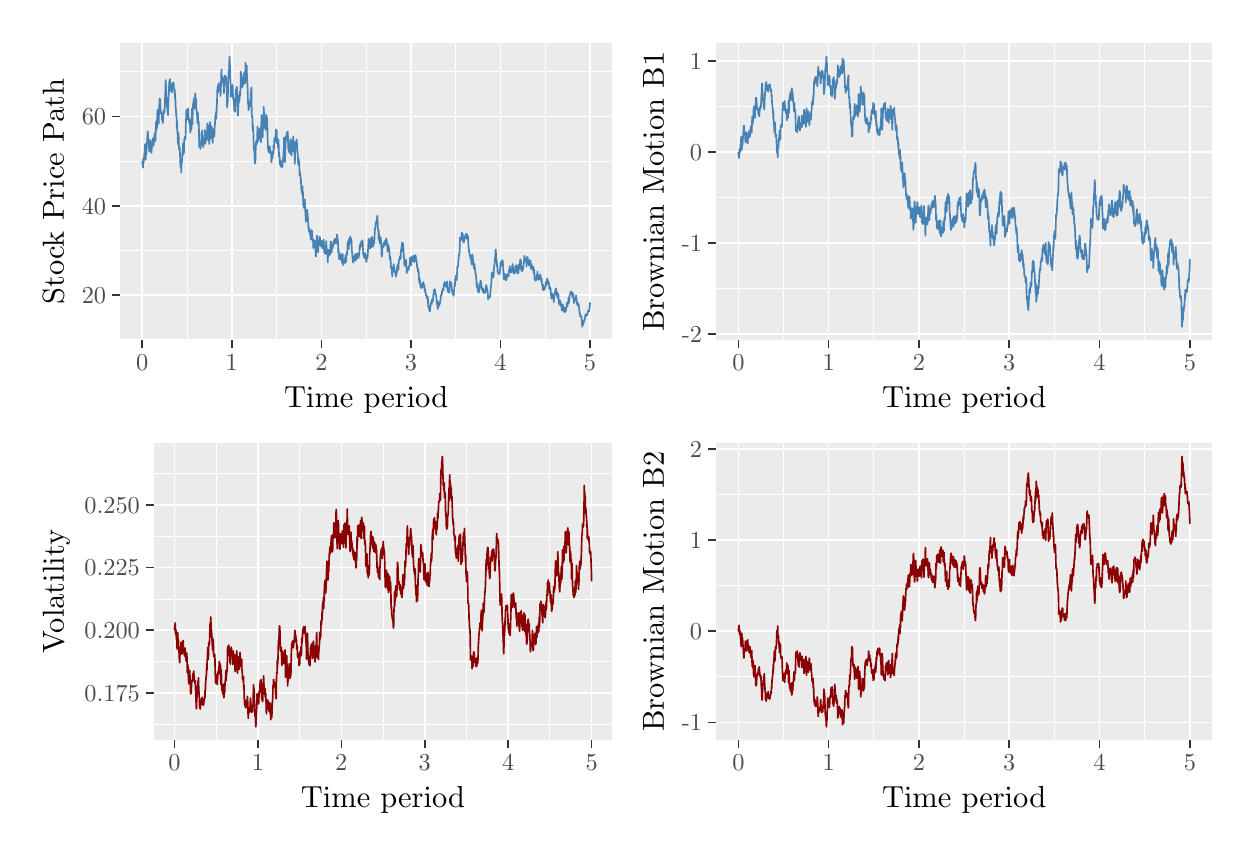
\begin{tikzpicture}[x=1pt,y=1pt]
\definecolor{fillColor}{RGB}{255,255,255}
\path[use as bounding box,fill=fillColor,fill opacity=0.00] (0,0) rectangle (433.62,289.08);
\begin{scope}
\path[clip] (  0.00,144.54) rectangle (216.81,289.08);
\definecolor{drawColor}{RGB}{255,255,255}
\definecolor{fillColor}{RGB}{255,255,255}

\path[draw=drawColor,line width= 0.6pt,line join=round,line cap=round,fill=fillColor] (  0.00,144.54) rectangle (216.81,289.08);
\end{scope}
\begin{scope}
\path[clip] ( 33.30,176.07) rectangle (211.31,283.58);
\definecolor{fillColor}{gray}{0.92}

\path[fill=fillColor] ( 33.30,176.07) rectangle (211.31,283.58);
\definecolor{drawColor}{RGB}{255,255,255}

\path[draw=drawColor,line width= 0.3pt,line join=round] ( 33.30,176.28) --
	(211.31,176.28);

\path[draw=drawColor,line width= 0.3pt,line join=round] ( 33.30,208.57) --
	(211.31,208.57);

\path[draw=drawColor,line width= 0.3pt,line join=round] ( 33.30,240.86) --
	(211.31,240.86);

\path[draw=drawColor,line width= 0.3pt,line join=round] ( 33.30,273.15) --
	(211.31,273.15);

\path[draw=drawColor,line width= 0.3pt,line join=round] ( 57.57,176.07) --
	( 57.57,283.58);

\path[draw=drawColor,line width= 0.3pt,line join=round] ( 89.94,176.07) --
	( 89.94,283.58);

\path[draw=drawColor,line width= 0.3pt,line join=round] (122.30,176.07) --
	(122.30,283.58);

\path[draw=drawColor,line width= 0.3pt,line join=round] (154.67,176.07) --
	(154.67,283.58);

\path[draw=drawColor,line width= 0.3pt,line join=round] (187.04,176.07) --
	(187.04,283.58);

\path[draw=drawColor,line width= 0.6pt,line join=round] ( 33.30,192.43) --
	(211.31,192.43);

\path[draw=drawColor,line width= 0.6pt,line join=round] ( 33.30,224.71) --
	(211.31,224.71);

\path[draw=drawColor,line width= 0.6pt,line join=round] ( 33.30,257.00) --
	(211.31,257.00);

\path[draw=drawColor,line width= 0.6pt,line join=round] ( 41.39,176.07) --
	( 41.39,283.58);

\path[draw=drawColor,line width= 0.6pt,line join=round] ( 73.75,176.07) --
	( 73.75,283.58);

\path[draw=drawColor,line width= 0.6pt,line join=round] (106.12,176.07) --
	(106.12,283.58);

\path[draw=drawColor,line width= 0.6pt,line join=round] (138.49,176.07) --
	(138.49,283.58);

\path[draw=drawColor,line width= 0.6pt,line join=round] (170.85,176.07) --
	(170.85,283.58);

\path[draw=drawColor,line width= 0.6pt,line join=round] (203.22,176.07) --
	(203.22,283.58);
\definecolor{drawColor}{RGB}{70,130,180}

\path[draw=drawColor,line width= 0.6pt,line join=round] ( 41.39,240.86) --
	( 41.48,239.67) --
	( 41.56,240.02) --
	( 41.65,238.45) --
	( 41.74,241.40) --
	( 41.83,242.02) --
	( 41.92,240.46) --
	( 42.01,241.37) --
	( 42.10,242.78) --
	( 42.19,243.88) --
	( 42.27,243.29) --
	( 42.36,246.21) --
	( 42.45,246.98) --
	( 42.54,245.74) --
	( 42.63,241.37) --
	( 42.72,243.51) --
	( 42.81,243.42) --
	( 42.89,243.39) --
	( 42.98,245.21) --
	( 43.07,246.82) --
	( 43.16,248.01) --
	( 43.25,249.85) --
	( 43.34,251.45) --
	( 43.43,251.60) --
	( 43.52,247.48) --
	( 43.60,248.73) --
	( 43.69,248.61) --
	( 43.78,248.30) --
	( 43.87,245.33) --
	( 43.96,244.39) --
	( 44.05,245.21) --
	( 44.14,247.87) --
	( 44.22,247.67) --
	( 44.31,248.45) --
	( 44.40,248.34) --
	( 44.49,245.56) --
	( 44.58,244.74) --
	( 44.67,243.97) --
	( 44.76,243.86) --
	( 44.85,245.99) --
	( 44.93,247.50) --
	( 45.02,247.17) --
	( 45.11,246.66) --
	( 45.20,248.05) --
	( 45.29,249.17) --
	( 45.38,247.77) --
	( 45.47,246.35) --
	( 45.56,247.07) --
	( 45.64,248.61) --
	( 45.73,248.38) --
	( 45.82,250.16) --
	( 45.91,250.97) --
	( 46.00,249.71) --
	( 46.09,250.41) --
	( 46.18,248.09) --
	( 46.26,250.97) --
	( 46.35,255.05) --
	( 46.44,254.27) --
	( 46.53,252.06) --
	( 46.62,253.25) --
	( 46.71,252.96) --
	( 46.80,257.99) --
	( 46.89,257.90) --
	( 46.97,259.40) --
	( 47.06,259.46) --
	( 47.15,257.83) --
	( 47.24,258.24) --
	( 47.33,254.31) --
	( 47.42,257.41) --
	( 47.51,257.74) --
	( 47.59,262.45) --
	( 47.68,263.52) --
	( 47.77,261.91) --
	( 47.86,263.28) --
	( 47.95,261.17) --
	( 48.04,258.38) --
	( 48.13,259.02) --
	( 48.22,258.05) --
	( 48.30,258.05) --
	( 48.39,258.21) --
	( 48.48,256.93) --
	( 48.57,255.70) --
	( 48.66,255.41) --
	( 48.75,257.92) --
	( 48.84,254.61) --
	( 48.92,255.87) --
	( 49.01,256.58) --
	( 49.10,258.87) --
	( 49.19,258.21) --
	( 49.28,259.01) --
	( 49.37,259.60) --
	( 49.46,258.40) --
	( 49.55,261.04) --
	( 49.63,263.62) --
	( 49.72,265.21) --
	( 49.81,268.84) --
	( 49.90,270.15) --
	( 49.99,267.13) --
	( 50.08,265.80) --
	( 50.17,262.98) --
	( 50.25,261.92) --
	( 50.34,260.53) --
	( 50.43,260.62) --
	( 50.52,258.60) --
	( 50.61,258.95) --
	( 50.70,257.51) --
	( 50.79,261.34) --
	( 50.88,262.94) --
	( 50.96,265.00) --
	( 51.05,265.87) --
	( 51.14,269.74) --
	( 51.23,268.24) --
	( 51.32,267.16) --
	( 51.41,270.49) --
	( 51.50,268.95) --
	( 51.58,268.46) --
	( 51.67,267.54) --
	( 51.76,266.79) --
	( 51.85,266.15) --
	( 51.94,267.29) --
	( 52.03,266.88) --
	( 52.12,265.70) --
	( 52.21,268.79) --
	( 52.29,268.29) --
	( 52.38,267.87) --
	( 52.47,267.63) --
	( 52.56,269.30) --
	( 52.65,269.12) --
	( 52.74,269.03) --
	( 52.83,267.43) --
	( 52.92,266.67) --
	( 53.00,266.81) --
	( 53.09,265.45) --
	( 53.18,266.67) --
	( 53.27,263.15) --
	( 53.36,263.84) --
	( 53.45,260.35) --
	( 53.54,259.68) --
	( 53.62,258.52) --
	( 53.71,257.09) --
	( 53.80,256.96) --
	( 53.89,252.82) --
	( 53.98,255.29) --
	( 54.07,251.73) --
	( 54.16,250.77) --
	( 54.25,248.47) --
	( 54.33,246.95) --
	( 54.42,251.12) --
	( 54.51,251.15) --
	( 54.60,248.49) --
	( 54.69,245.17) --
	( 54.78,246.06) --
	( 54.87,246.02) --
	( 54.95,245.39) --
	( 55.04,243.56) --
	( 55.13,240.68) --
	( 55.22,238.65) --
	( 55.31,240.50) --
	( 55.40,239.33) --
	( 55.49,236.75) --
	( 55.58,240.15) --
	( 55.66,240.95) --
	( 55.75,240.49) --
	( 55.84,242.49) --
	( 55.93,244.19) --
	( 56.02,242.98) --
	( 56.11,247.23) --
	( 56.20,246.72) --
	( 56.28,243.89) --
	( 56.37,243.61) --
	( 56.46,244.01) --
	( 56.55,248.49) --
	( 56.64,248.71) --
	( 56.73,249.63) --
	( 56.82,249.47) --
	( 56.91,248.79) --
	( 56.99,248.72) --
	( 57.08,250.32) --
	( 57.17,254.57) --
	( 57.26,256.75) --
	( 57.35,259.35) --
	( 57.44,256.65) --
	( 57.53,258.77) --
	( 57.61,259.25) --
	( 57.70,256.03) --
	( 57.79,257.14) --
	( 57.88,256.80) --
	( 57.97,259.96) --
	( 58.06,258.27) --
	( 58.15,257.33) --
	( 58.24,255.32) --
	( 58.32,254.95) --
	( 58.41,255.80) --
	( 58.50,254.24) --
	( 58.59,255.99) --
	( 58.68,253.40) --
	( 58.77,251.20) --
	( 58.86,254.18) --
	( 58.94,252.03) --
	( 59.03,252.88) --
	( 59.12,252.09) --
	( 59.21,252.94) --
	( 59.30,256.47) --
	( 59.39,259.89) --
	( 59.48,259.16) --
	( 59.57,254.14) --
	( 59.65,259.42) --
	( 59.74,260.88) --
	( 59.83,262.09) --
	( 59.92,262.06) --
	( 60.01,263.20) --
	( 60.10,262.83) --
	( 60.19,263.77) --
	( 60.28,262.87) --
	( 60.36,259.78) --
	( 60.45,261.96) --
	( 60.54,265.36) --
	( 60.63,264.65) --
	( 60.72,261.79) --
	( 60.81,263.23) --
	( 60.90,263.13) --
	( 60.98,259.22) --
	( 61.07,259.22) --
	( 61.16,257.84) --
	( 61.25,257.10) --
	( 61.34,254.60) --
	( 61.43,258.42) --
	( 61.52,257.70) --
	( 61.61,254.21) --
	( 61.69,254.63) --
	( 61.78,255.19) --
	( 61.87,253.09) --
	( 61.96,247.03) --
	( 62.05,245.76) --
	( 62.14,246.88) --
	( 62.23,246.76) --
	( 62.31,246.57) --
	( 62.40,247.68) --
	( 62.49,245.30) --
	( 62.58,247.46) --
	( 62.67,247.45) --
	( 62.76,248.86) --
	( 62.85,250.95) --
	( 62.94,251.42) --
	( 63.02,249.60) --
	( 63.11,251.97) --
	( 63.20,247.82) --
	( 63.29,246.72) --
	( 63.38,246.21) --
	( 63.47,245.89) --
	( 63.56,247.90) --
	( 63.64,248.17) --
	( 63.73,248.99) --
	( 63.82,248.85) --
	( 63.91,248.35) --
	( 64.00,249.75) --
	( 64.09,252.09) --
	( 64.18,247.10) --
	( 64.27,248.24) --
	( 64.35,248.99) --
	( 64.44,248.13) --
	( 64.53,250.04) --
	( 64.62,249.25) --
	( 64.71,248.67) --
	( 64.80,250.40) --
	( 64.89,253.93) --
	( 64.97,254.49) --
	( 65.06,253.60) --
	( 65.15,251.10) --
	( 65.24,250.42) --
	( 65.33,248.49) --
	( 65.42,247.97) --
	( 65.51,248.76) --
	( 65.60,247.04) --
	( 65.68,252.32) --
	( 65.77,252.64) --
	( 65.86,255.00) --
	( 65.95,250.14) --
	( 66.04,251.65) --
	( 66.13,248.93) --
	( 66.22,250.79) --
	( 66.30,251.61) --
	( 66.39,250.77) --
	( 66.48,253.49) --
	( 66.57,252.02) --
	( 66.66,250.81) --
	( 66.75,248.75) --
	( 66.84,247.41) --
	( 66.93,249.29) --
	( 67.01,250.17) --
	( 67.10,252.23) --
	( 67.19,251.42) --
	( 67.28,252.19) --
	( 67.37,252.70) --
	( 67.46,249.73) --
	( 67.55,253.35) --
	( 67.64,253.63) --
	( 67.72,255.24) --
	( 67.81,257.27) --
	( 67.90,257.16) --
	( 67.99,256.50) --
	( 68.08,258.42) --
	( 68.17,256.14) --
	( 68.26,260.36) --
	( 68.34,259.51) --
	( 68.43,263.14) --
	( 68.52,266.55) --
	( 68.61,266.74) --
	( 68.70,268.05) --
	( 68.79,265.66) --
	( 68.88,266.40) --
	( 68.97,268.81) --
	( 69.05,269.04) --
	( 69.14,267.97) --
	( 69.23,266.45) --
	( 69.32,266.36) --
	( 69.41,268.83) --
	( 69.50,267.69) --
	( 69.59,267.41) --
	( 69.67,264.41) --
	( 69.76,265.53) --
	( 69.85,268.53) --
	( 69.94,272.03) --
	( 70.03,273.98) --
	( 70.12,269.46) --
	( 70.21,270.59) --
	( 70.30,271.67) --
	( 70.38,270.83) --
	( 70.47,271.23) --
	( 70.56,269.17) --
	( 70.65,270.77) --
	( 70.74,269.99) --
	( 70.83,266.29) --
	( 70.92,265.44) --
	( 71.00,268.57) --
	( 71.09,267.79) --
	( 71.18,269.49) --
	( 71.27,271.72) --
	( 71.36,271.73) --
	( 71.45,270.89) --
	( 71.54,269.63) --
	( 71.63,271.38) --
	( 71.71,268.84) --
	( 71.80,269.42) --
	( 71.89,268.74) --
	( 71.98,263.42) --
	( 72.07,260.24) --
	( 72.16,262.26) --
	( 72.25,261.83) --
	( 72.33,263.63) --
	( 72.42,267.91) --
	( 72.51,271.34) --
	( 72.60,272.96) --
	( 72.69,273.87) --
	( 72.78,273.41) --
	( 72.87,277.22) --
	( 72.96,278.69) --
	( 73.04,275.77) --
	( 73.13,275.39) --
	( 73.22,270.69) --
	( 73.31,270.23) --
	( 73.40,264.09) --
	( 73.49,267.07) --
	( 73.58,265.60) --
	( 73.66,264.61) --
	( 73.75,264.23) --
	( 73.84,265.62) --
	( 73.93,267.18) --
	( 74.02,268.50) --
	( 74.11,267.16) --
	( 74.20,263.99) --
	( 74.29,263.11) --
	( 74.37,263.73) --
	( 74.46,261.87) --
	( 74.55,261.71) --
	( 74.64,259.10) --
	( 74.73,259.08) --
	( 74.82,259.36) --
	( 74.91,259.04) --
	( 75.00,258.68) --
	( 75.08,262.55) --
	( 75.17,264.26) --
	( 75.26,266.80) --
	( 75.35,264.66) --
	( 75.44,265.03) --
	( 75.53,267.68) --
	( 75.62,267.54) --
	( 75.70,262.58) --
	( 75.79,263.36) --
	( 75.88,259.04) --
	( 75.97,257.26) --
	( 76.06,260.13) --
	( 76.15,261.50) --
	( 76.24,263.94) --
	( 76.33,264.63) --
	( 76.41,264.38) --
	( 76.50,262.27) --
	( 76.59,265.85) --
	( 76.68,265.96) --
	( 76.77,264.31) --
	( 76.86,266.28) --
	( 76.95,268.77) --
	( 77.03,273.22) --
	( 77.12,271.76) --
	( 77.21,270.83) --
	( 77.30,269.83) --
	( 77.39,268.95) --
	( 77.48,268.08) --
	( 77.57,267.39) --
	( 77.66,270.75) --
	( 77.74,269.09) --
	( 77.83,268.17) --
	( 77.92,269.70) --
	( 78.01,272.36) --
	( 78.10,270.51) --
	( 78.19,269.30) --
	( 78.28,270.53) --
	( 78.36,272.95) --
	( 78.45,272.35) --
	( 78.54,268.91) --
	( 78.63,272.93) --
	( 78.72,276.40) --
	( 78.81,274.64) --
	( 78.90,274.49) --
	( 78.99,270.19) --
	( 79.07,271.55) --
	( 79.16,275.41) --
	( 79.25,271.39) --
	( 79.34,269.53) --
	( 79.43,268.01) --
	( 79.52,266.42) --
	( 79.61,261.70) --
	( 79.69,262.83) --
	( 79.78,259.37) --
	( 79.87,259.31) --
	( 79.96,260.62) --
	( 80.05,260.18) --
	( 80.14,262.16) --
	( 80.23,262.10) --
	( 80.32,260.64) --
	( 80.40,262.08) --
	( 80.49,261.10) --
	( 80.58,265.06) --
	( 80.67,265.02) --
	( 80.76,266.98) --
	( 80.85,267.46) --
	( 80.94,260.44) --
	( 81.02,257.40) --
	( 81.11,256.48) --
	( 81.20,256.99) --
	( 81.29,251.91) --
	( 81.38,253.92) --
	( 81.47,252.64) --
	( 81.56,251.06) --
	( 81.65,247.84) --
	( 81.73,244.91) --
	( 81.82,245.02) --
	( 81.91,246.02) --
	( 82.00,241.86) --
	( 82.09,239.95) --
	( 82.18,240.95) --
	( 82.27,240.09) --
	( 82.36,244.16) --
	( 82.44,246.59) --
	( 82.53,247.78) --
	( 82.62,247.79) --
	( 82.71,248.35) --
	( 82.80,246.92) --
	( 82.89,248.17) --
	( 82.98,251.16) --
	( 83.06,253.40) --
	( 83.15,251.69) --
	( 83.24,248.33) --
	( 83.33,248.11) --
	( 83.42,249.00) --
	( 83.51,251.74) --
	( 83.60,249.00) --
	( 83.69,249.74) --
	( 83.77,250.22) --
	( 83.86,252.67) --
	( 83.95,252.61) --
	( 84.04,251.86) --
	( 84.13,249.48) --
	( 84.22,248.42) --
	( 84.31,247.69) --
	( 84.39,252.41) --
	( 84.48,257.52) --
	( 84.57,257.16) --
	( 84.66,254.90) --
	( 84.75,250.70) --
	( 84.84,251.76) --
	( 84.93,249.50) --
	( 85.02,254.15) --
	( 85.10,252.28) --
	( 85.19,252.51) --
	( 85.28,260.47) --
	( 85.37,258.01) --
	( 85.46,258.68) --
	( 85.55,256.26) --
	( 85.64,257.01) --
	( 85.72,255.12) --
	( 85.81,255.29) --
	( 85.90,254.65) --
	( 85.99,252.14) --
	( 86.08,252.17) --
	( 86.17,254.23) --
	( 86.26,257.60) --
	( 86.35,254.62) --
	( 86.43,254.09) --
	( 86.52,256.54) --
	( 86.61,254.14) --
	( 86.70,248.80) --
	( 86.79,246.91) --
	( 86.88,244.98) --
	( 86.97,245.07) --
	( 87.05,244.28) --
	( 87.14,244.73) --
	( 87.23,243.91) --
	( 87.32,244.63) --
	( 87.41,243.92) --
	( 87.50,246.23) --
	( 87.59,244.77) --
	( 87.68,245.34) --
	( 87.76,243.60) --
	( 87.85,244.00) --
	( 87.94,243.91) --
	( 88.03,240.64) --
	( 88.12,240.37) --
	( 88.21,242.59) --
	( 88.30,243.89) --
	( 88.38,244.17) --
	( 88.47,241.85) --
	( 88.56,244.08) --
	( 88.65,244.23) --
	( 88.74,243.35) --
	( 88.83,246.52) --
	( 88.92,244.99) --
	( 89.01,245.59) --
	( 89.09,248.11) --
	( 89.18,249.32) --
	( 89.27,248.70) --
	( 89.36,247.85) --
	( 89.45,248.56) --
	( 89.54,249.60) --
	( 89.63,249.64) --
	( 89.72,252.32) --
	( 89.80,252.19) --
	( 89.89,250.73) --
	( 89.98,251.83) --
	( 90.07,247.27) --
	( 90.16,248.05) --
	( 90.25,249.05) --
	( 90.34,248.60) --
	( 90.42,246.34) --
	( 90.51,245.56) --
	( 90.60,248.61) --
	( 90.69,247.11) --
	( 90.78,242.46) --
	( 90.87,244.01) --
	( 90.96,243.04) --
	( 91.05,242.06) --
	( 91.13,239.74) --
	( 91.22,239.70) --
	( 91.31,241.01) --
	( 91.40,239.90) --
	( 91.49,238.77) --
	( 91.58,240.79) --
	( 91.67,240.33) --
	( 91.75,240.03) --
	( 91.84,238.86) --
	( 91.93,240.52) --
	( 92.02,238.65) --
	( 92.11,240.22) --
	( 92.20,241.73) --
	( 92.29,240.84) --
	( 92.38,242.44) --
	( 92.46,244.33) --
	( 92.55,245.44) --
	( 92.64,249.42) --
	( 92.73,245.44) --
	( 92.82,243.15) --
	( 92.91,240.51) --
	( 93.00,240.82) --
	( 93.08,243.80) --
	( 93.17,247.04) --
	( 93.26,248.02) --
	( 93.35,249.78) --
	( 93.44,249.48) --
	( 93.53,250.43) --
	( 93.62,251.20) --
	( 93.71,249.64) --
	( 93.79,249.04) --
	( 93.88,248.77) --
	( 93.97,251.58) --
	( 94.06,249.44) --
	( 94.15,245.15) --
	( 94.24,246.65) --
	( 94.33,245.04) --
	( 94.41,244.19) --
	( 94.50,245.94) --
	( 94.59,244.44) --
	( 94.68,243.77) --
	( 94.77,246.68) --
	( 94.86,247.72) --
	( 94.95,248.81) --
	( 95.04,248.53) --
	( 95.12,246.24) --
	( 95.21,243.29) --
	( 95.30,242.86) --
	( 95.39,246.70) --
	( 95.48,247.13) --
	( 95.57,247.46) --
	( 95.66,248.12) --
	( 95.74,247.35) --
	( 95.83,244.57) --
	( 95.92,249.77) --
	( 96.01,248.91) --
	( 96.10,248.31) --
	( 96.19,244.71) --
	( 96.28,244.23) --
	( 96.37,243.75) --
	( 96.45,243.25) --
	( 96.54,239.82) --
	( 96.63,243.14) --
	( 96.72,246.53) --
	( 96.81,247.89) --
	( 96.90,245.69) --
	( 96.99,247.09) --
	( 97.08,246.60) --
	( 97.16,245.97) --
	( 97.25,248.65) --
	( 97.34,246.18) --
	( 97.43,245.17) --
	( 97.52,243.74) --
	( 97.61,243.78) --
	( 97.70,240.75) --
	( 97.78,239.43) --
	( 97.87,240.76) --
	( 97.96,241.63) --
	( 98.05,239.79) --
	( 98.14,240.83) --
	( 98.23,236.26) --
	( 98.32,235.65) --
	( 98.41,236.92) --
	( 98.49,235.73) --
	( 98.58,235.67) --
	( 98.67,232.82) --
	( 98.76,234.29) --
	( 98.85,231.04) --
	( 98.94,230.48) --
	( 99.03,230.05) --
	( 99.11,230.16) --
	( 99.20,228.77) --
	( 99.29,231.80) --
	( 99.38,229.35) --
	( 99.47,229.78) --
	( 99.56,224.85) --
	( 99.65,224.85) --
	( 99.74,225.66) --
	( 99.82,223.93) --
	( 99.91,225.03) --
	(100.00,225.55) --
	(100.09,227.11) --
	(100.18,225.74) --
	(100.27,224.19) --
	(100.36,221.41) --
	(100.44,220.92) --
	(100.53,218.90) --
	(100.62,219.91) --
	(100.71,220.02) --
	(100.80,223.28) --
	(100.89,221.48) --
	(100.98,223.28) --
	(101.07,222.46) --
	(101.15,220.22) --
	(101.24,221.08) --
	(101.33,218.92) --
	(101.42,217.37) --
	(101.51,216.32) --
	(101.60,216.62) --
	(101.69,215.20) --
	(101.77,216.70) --
	(101.86,214.99) --
	(101.95,215.29) --
	(102.04,215.49) --
	(102.13,214.00) --
	(102.22,213.42) --
	(102.31,212.53) --
	(102.40,213.81) --
	(102.48,215.93) --
	(102.57,214.47) --
	(102.66,215.75) --
	(102.75,215.65) --
	(102.84,212.89) --
	(102.93,211.88) --
	(103.02,212.49) --
	(103.10,212.68) --
	(103.19,209.42) --
	(103.28,210.15) --
	(103.37,211.00) --
	(103.46,210.60) --
	(103.55,209.68) --
	(103.64,212.20) --
	(103.73,212.08) --
	(103.81,212.06) --
	(103.90,210.57) --
	(103.99,208.84) --
	(104.08,206.92) --
	(104.17,206.41) --
	(104.26,208.05) --
	(104.35,210.22) --
	(104.43,212.24) --
	(104.52,213.96) --
	(104.61,213.63) --
	(104.70,211.98) --
	(104.79,211.55) --
	(104.88,208.39) --
	(104.97,208.00) --
	(105.06,210.05) --
	(105.14,210.22) --
	(105.23,211.62) --
	(105.32,212.26) --
	(105.41,211.23) --
	(105.50,213.50) --
	(105.59,213.39) --
	(105.68,212.08) --
	(105.77,212.18) --
	(105.85,210.17) --
	(105.94,211.28) --
	(106.03,211.93) --
	(106.12,211.46) --
	(106.21,210.83) --
	(106.30,212.04) --
	(106.39,210.64) --
	(106.47,209.37) --
	(106.56,209.91) --
	(106.65,209.33) --
	(106.74,210.50) --
	(106.83,210.24) --
	(106.92,211.77) --
	(107.01,212.42) --
	(107.10,209.45) --
	(107.18,207.77) --
	(107.27,209.34) --
	(107.36,210.21) --
	(107.45,208.98) --
	(107.54,207.29) --
	(107.63,208.55) --
	(107.72,207.54) --
	(107.80,209.74) --
	(107.89,211.98) --
	(107.98,210.08) --
	(108.07,209.01) --
	(108.16,207.44) --
	(108.25,208.26) --
	(108.34,206.66) --
	(108.43,204.22) --
	(108.51,206.54) --
	(108.60,207.75) --
	(108.69,208.75) --
	(108.78,207.92) --
	(108.87,207.91) --
	(108.96,208.67) --
	(109.05,207.08) --
	(109.13,206.93) --
	(109.22,207.14) --
	(109.31,209.19) --
	(109.40,209.99) --
	(109.49,211.61) --
	(109.58,211.79) --
	(109.67,210.34) --
	(109.76,209.91) --
	(109.84,207.81) --
	(109.93,208.94) --
	(110.02,210.70) --
	(110.11,210.62) --
	(110.20,209.37) --
	(110.29,210.73) --
	(110.38,210.91) --
	(110.46,210.42) --
	(110.55,211.84) --
	(110.64,210.86) --
	(110.73,212.33) --
	(110.82,211.23) --
	(110.91,211.73) --
	(111.00,212.88) --
	(111.09,211.12) --
	(111.17,211.63) --
	(111.26,211.49) --
	(111.35,212.36) --
	(111.44,211.33) --
	(111.53,211.22) --
	(111.62,213.00) --
	(111.71,213.22) --
	(111.79,214.31) --
	(111.88,214.01) --
	(111.97,212.63) --
	(112.06,212.62) --
	(112.15,211.01) --
	(112.24,207.69) --
	(112.33,209.11) --
	(112.42,207.76) --
	(112.50,205.54) --
	(112.59,206.70) --
	(112.68,206.69) --
	(112.77,205.98) --
	(112.86,205.77) --
	(112.95,205.27) --
	(113.04,206.43) --
	(113.13,207.29) --
	(113.21,205.21) --
	(113.30,205.62) --
	(113.39,206.47) --
	(113.48,207.26) --
	(113.57,204.35) --
	(113.66,204.08) --
	(113.75,206.33) --
	(113.83,207.27) --
	(113.92,205.22) --
	(114.01,203.29) --
	(114.10,203.84) --
	(114.19,203.65) --
	(114.28,204.73) --
	(114.37,205.07) --
	(114.46,205.16) --
	(114.54,205.37) --
	(114.63,205.56) --
	(114.72,204.09) --
	(114.81,206.75) --
	(114.90,205.07) --
	(114.99,205.05) --
	(115.08,204.43) --
	(115.16,206.48) --
	(115.25,207.67) --
	(115.34,206.99) --
	(115.43,207.24) --
	(115.52,208.63) --
	(115.61,211.36) --
	(115.70,211.75) --
	(115.79,210.41) --
	(115.87,209.18) --
	(115.96,211.65) --
	(116.05,209.00) --
	(116.14,212.75) --
	(116.23,212.41) --
	(116.32,211.82) --
	(116.41,212.02) --
	(116.49,213.22) --
	(116.58,213.62) --
	(116.67,211.05) --
	(116.76,211.49) --
	(116.85,212.07) --
	(116.94,212.92) --
	(117.03,211.57) --
	(117.12,208.55) --
	(117.20,208.15) --
	(117.29,207.01) --
	(117.38,206.10) --
	(117.47,204.99) --
	(117.56,204.54) --
	(117.65,204.18) --
	(117.74,205.08) --
	(117.82,206.21) --
	(117.91,205.28) --
	(118.00,204.93) --
	(118.09,205.34) --
	(118.18,206.95) --
	(118.27,206.88) --
	(118.36,204.88) --
	(118.45,205.14) --
	(118.53,205.01) --
	(118.62,207.03) --
	(118.71,207.44) --
	(118.80,206.70) --
	(118.89,206.18) --
	(118.98,205.59) --
	(119.07,205.80) --
	(119.15,206.01) --
	(119.24,207.07) --
	(119.33,207.45) --
	(119.42,207.01) --
	(119.51,205.90) --
	(119.60,206.64) --
	(119.69,206.57) --
	(119.78,206.78) --
	(119.86,208.08) --
	(119.95,210.18) --
	(120.04,209.00) --
	(120.13,211.00) --
	(120.22,209.91) --
	(120.31,210.24) --
	(120.40,210.52) --
	(120.49,210.17) --
	(120.57,211.90) --
	(120.66,211.06) --
	(120.75,211.89) --
	(120.84,211.88) --
	(120.93,210.69) --
	(121.02,212.21) --
	(121.11,209.54) --
	(121.19,208.89) --
	(121.28,207.02) --
	(121.37,207.25) --
	(121.46,207.56) --
	(121.55,206.23) --
	(121.64,206.99) --
	(121.73,205.77) --
	(121.82,206.53) --
	(121.90,206.81) --
	(121.99,207.65) --
	(122.08,206.53) --
	(122.17,206.65) --
	(122.26,206.10) --
	(122.35,204.40) --
	(122.44,204.58) --
	(122.52,206.58) --
	(122.61,205.82) --
	(122.70,205.59) --
	(122.79,206.38) --
	(122.88,206.42) --
	(122.97,208.68) --
	(123.06,209.57) --
	(123.15,212.41) --
	(123.23,212.86) --
	(123.32,211.40) --
	(123.41,211.93) --
	(123.50,210.76) --
	(123.59,209.50) --
	(123.68,209.27) --
	(123.77,210.41) --
	(123.85,210.84) --
	(123.94,211.85) --
	(124.03,213.01) --
	(124.12,212.79) --
	(124.21,209.71) --
	(124.30,210.68) --
	(124.39,213.37) --
	(124.48,213.45) --
	(124.56,211.70) --
	(124.65,211.23) --
	(124.74,210.06) --
	(124.83,210.01) --
	(124.92,210.84) --
	(125.01,211.92) --
	(125.10,212.22) --
	(125.18,211.03) --
	(125.27,212.05) --
	(125.36,213.75) --
	(125.45,216.68) --
	(125.54,216.01) --
	(125.63,216.65) --
	(125.72,218.26) --
	(125.81,218.10) --
	(125.89,218.82) --
	(125.98,219.12) --
	(126.07,218.93) --
	(126.16,219.17) --
	(126.25,220.51) --
	(126.34,221.09) --
	(126.43,220.43) --
	(126.51,217.25) --
	(126.60,216.17) --
	(126.69,216.14) --
	(126.78,212.77) --
	(126.87,215.59) --
	(126.96,213.62) --
	(127.05,212.11) --
	(127.14,213.96) --
	(127.22,211.11) --
	(127.31,212.03) --
	(127.40,211.60) --
	(127.49,212.17) --
	(127.58,213.28) --
	(127.67,212.05) --
	(127.76,211.16) --
	(127.85,207.43) --
	(127.93,206.30) --
	(128.02,206.74) --
	(128.11,207.32) --
	(128.20,209.70) --
	(128.29,209.78) --
	(128.38,210.34) --
	(128.47,210.43) --
	(128.55,209.83) --
	(128.64,210.75) --
	(128.73,211.32) --
	(128.82,211.48) --
	(128.91,210.46) --
	(129.00,210.41) --
	(129.09,211.37) --
	(129.18,212.22) --
	(129.26,211.61) --
	(129.35,210.77) --
	(129.44,211.40) --
	(129.53,212.71) --
	(129.62,212.87) --
	(129.71,212.47) --
	(129.80,211.35) --
	(129.88,210.83) --
	(129.97,209.00) --
	(130.06,208.16) --
	(130.15,209.50) --
	(130.24,210.85) --
	(130.33,209.77) --
	(130.42,210.03) --
	(130.51,210.11) --
	(130.59,208.08) --
	(130.68,209.04) --
	(130.77,206.75) --
	(130.86,205.30) --
	(130.95,206.43) --
	(131.04,205.81) --
	(131.13,205.56) --
	(131.21,203.73) --
	(131.30,202.13) --
	(131.39,202.51) --
	(131.48,202.32) --
	(131.57,201.69) --
	(131.66,200.28) --
	(131.75,199.15) --
	(131.84,201.20) --
	(131.92,200.86) --
	(132.01,201.66) --
	(132.10,202.49) --
	(132.19,203.30) --
	(132.28,203.62) --
	(132.37,202.26) --
	(132.46,201.18) --
	(132.54,201.97) --
	(132.63,200.58) --
	(132.72,201.12) --
	(132.81,200.57) --
	(132.90,200.16) --
	(132.99,199.35) --
	(133.08,199.12) --
	(133.17,200.00) --
	(133.25,200.46) --
	(133.34,200.22) --
	(133.43,201.11) --
	(133.52,202.83) --
	(133.61,202.83) --
	(133.70,203.33) --
	(133.79,203.63) --
	(133.87,202.57) --
	(133.96,201.58) --
	(134.05,203.59) --
	(134.14,204.55) --
	(134.23,205.37) --
	(134.32,205.54) --
	(134.41,206.08) --
	(134.50,206.25) --
	(134.58,206.30) --
	(134.67,206.56) --
	(134.76,205.40) --
	(134.85,208.10) --
	(134.94,209.04) --
	(135.03,208.74) --
	(135.12,210.18) --
	(135.21,209.41) --
	(135.29,211.46) --
	(135.38,210.98) --
	(135.47,208.13) --
	(135.56,209.73) --
	(135.65,211.09) --
	(135.74,210.14) --
	(135.83,208.43) --
	(135.91,206.27) --
	(136.00,205.97) --
	(136.09,203.90) --
	(136.18,203.01) --
	(136.27,203.18) --
	(136.36,204.10) --
	(136.45,203.21) --
	(136.54,203.07) --
	(136.62,203.35) --
	(136.71,205.20) --
	(136.80,204.13) --
	(136.89,202.38) --
	(136.98,200.42) --
	(137.07,200.99) --
	(137.16,200.93) --
	(137.24,201.72) --
	(137.33,201.58) --
	(137.42,201.99) --
	(137.51,202.22) --
	(137.60,202.25) --
	(137.69,201.59) --
	(137.78,202.91) --
	(137.87,202.47) --
	(137.95,203.18) --
	(138.04,203.35) --
	(138.13,205.27) --
	(138.22,206.06) --
	(138.31,205.68) --
	(138.40,205.67) --
	(138.49,205.53) --
	(138.57,203.20) --
	(138.66,205.02) --
	(138.75,206.19) --
	(138.84,205.33) --
	(138.93,205.75) --
	(139.02,206.02) --
	(139.11,204.75) --
	(139.20,206.39) --
	(139.28,206.11) --
	(139.37,206.32) --
	(139.46,206.77) --
	(139.55,205.64) --
	(139.64,204.43) --
	(139.73,204.37) --
	(139.82,205.00) --
	(139.90,205.09) --
	(139.99,205.87) --
	(140.08,206.24) --
	(140.17,206.86) --
	(140.26,205.26) --
	(140.35,206.01) --
	(140.44,205.12) --
	(140.53,204.61) --
	(140.61,204.49) --
	(140.70,202.69) --
	(140.79,202.58) --
	(140.88,202.12) --
	(140.97,201.36) --
	(141.06,200.79) --
	(141.15,202.06) --
	(141.23,200.75) --
	(141.32,200.53) --
	(141.41,198.01) --
	(141.50,197.36) --
	(141.59,196.88) --
	(141.68,198.34) --
	(141.77,197.40) --
	(141.86,196.57) --
	(141.94,195.26) --
	(142.03,195.43) --
	(142.12,196.48) --
	(142.21,195.36) --
	(142.30,194.97) --
	(142.39,196.21) --
	(142.48,195.57) --
	(142.57,196.20) --
	(142.65,196.56) --
	(142.74,195.34) --
	(142.83,196.45) --
	(142.92,197.19) --
	(143.01,196.73) --
	(143.10,195.88) --
	(143.19,195.52) --
	(143.27,196.26) --
	(143.36,195.74) --
	(143.45,194.02) --
	(143.54,193.90) --
	(143.63,194.57) --
	(143.72,193.54) --
	(143.81,193.33) --
	(143.90,192.28) --
	(143.98,192.37) --
	(144.07,192.26) --
	(144.16,192.23) --
	(144.25,191.71) --
	(144.34,191.12) --
	(144.43,191.83) --
	(144.52,191.92) --
	(144.60,191.77) --
	(144.69,189.09) --
	(144.78,188.11) --
	(144.87,188.68) --
	(144.96,188.37) --
	(145.05,187.45) --
	(145.14,187.13) --
	(145.23,186.86) --
	(145.31,186.49) --
	(145.40,186.85) --
	(145.49,187.95) --
	(145.58,188.69) --
	(145.67,189.64) --
	(145.76,189.38) --
	(145.85,190.04) --
	(145.93,189.26) --
	(146.02,189.15) --
	(146.11,190.84) --
	(146.20,190.83) --
	(146.29,190.58) --
	(146.38,190.11) --
	(146.47,190.73) --
	(146.56,192.42) --
	(146.64,192.77) --
	(146.73,192.55) --
	(146.82,194.29) --
	(146.91,193.61) --
	(147.00,194.59) --
	(147.09,194.21) --
	(147.18,193.32) --
	(147.26,194.36) --
	(147.35,192.78) --
	(147.44,192.52) --
	(147.53,192.54) --
	(147.62,192.16) --
	(147.71,190.80) --
	(147.80,190.28) --
	(147.89,189.05) --
	(147.97,190.52) --
	(148.06,189.04) --
	(148.15,187.43) --
	(148.24,187.94) --
	(148.33,188.61) --
	(148.42,188.46) --
	(148.51,188.31) --
	(148.59,188.85) --
	(148.68,189.91) --
	(148.77,188.67) --
	(148.86,189.66) --
	(148.95,189.81) --
	(149.04,189.54) --
	(149.13,190.52) --
	(149.22,191.27) --
	(149.30,192.31) --
	(149.39,192.06) --
	(149.48,192.71) --
	(149.57,192.95) --
	(149.66,192.52) --
	(149.75,193.99) --
	(149.84,194.13) --
	(149.93,194.08) --
	(150.01,194.54) --
	(150.10,194.88) --
	(150.19,194.26) --
	(150.28,194.21) --
	(150.37,196.48) --
	(150.46,196.41) --
	(150.55,196.14) --
	(150.63,196.80) --
	(150.72,197.17) --
	(150.81,196.67) --
	(150.90,195.68) --
	(150.99,196.44) --
	(151.08,196.55) --
	(151.17,196.99) --
	(151.26,196.72) --
	(151.34,195.21) --
	(151.43,195.27) --
	(151.52,197.39) --
	(151.61,196.03) --
	(151.70,195.14) --
	(151.79,193.96) --
	(151.88,193.65) --
	(151.96,194.83) --
	(152.05,194.69) --
	(152.14,194.47) --
	(152.23,193.35) --
	(152.32,193.40) --
	(152.41,194.28) --
	(152.50,196.24) --
	(152.59,197.43) --
	(152.67,196.62) --
	(152.76,196.16) --
	(152.85,196.71) --
	(152.94,196.70) --
	(153.03,196.96) --
	(153.12,195.75) --
	(153.21,195.37) --
	(153.29,194.55) --
	(153.38,193.74) --
	(153.47,193.12) --
	(153.56,192.77) --
	(153.65,192.77) --
	(153.74,193.30) --
	(153.83,192.87) --
	(153.92,192.15) --
	(154.00,193.48) --
	(154.09,194.32) --
	(154.18,194.92) --
	(154.27,196.42) --
	(154.36,195.53) --
	(154.45,197.35) --
	(154.54,198.48) --
	(154.62,198.77) --
	(154.71,199.37) --
	(154.80,199.43) --
	(154.89,199.32) --
	(154.98,197.81) --
	(155.07,198.50) --
	(155.16,200.52) --
	(155.25,202.58) --
	(155.33,202.75) --
	(155.42,202.64) --
	(155.51,202.82) --
	(155.60,204.00) --
	(155.69,205.54) --
	(155.78,205.98) --
	(155.87,207.19) --
	(155.95,207.16) --
	(156.04,207.71) --
	(156.13,209.03) --
	(156.22,213.16) --
	(156.31,213.09) --
	(156.40,212.29) --
	(156.49,212.82) --
	(156.58,212.33) --
	(156.66,213.09) --
	(156.75,213.50) --
	(156.84,215.09) --
	(156.93,213.90) --
	(157.02,212.44) --
	(157.11,214.31) --
	(157.20,214.58) --
	(157.29,213.45) --
	(157.37,212.15) --
	(157.46,211.50) --
	(157.55,212.19) --
	(157.64,211.56) --
	(157.73,213.14) --
	(157.82,213.44) --
	(157.91,213.67) --
	(157.99,213.65) --
	(158.08,213.29) --
	(158.17,213.09) --
	(158.26,214.48) --
	(158.35,212.84) --
	(158.44,214.14) --
	(158.53,213.72) --
	(158.62,214.61) --
	(158.70,214.54) --
	(158.79,212.88) --
	(158.88,213.30) --
	(158.97,212.53) --
	(159.06,213.87) --
	(159.15,212.87) --
	(159.24,210.72) --
	(159.32,209.73) --
	(159.41,209.07) --
	(159.50,208.14) --
	(159.59,207.87) --
	(159.68,207.21) --
	(159.77,206.76) --
	(159.86,207.11) --
	(159.95,205.83) --
	(160.03,206.65) --
	(160.12,206.65) --
	(160.21,206.61) --
	(160.30,204.39) --
	(160.39,204.07) --
	(160.48,203.49) --
	(160.57,204.37) --
	(160.65,205.83) --
	(160.74,207.15) --
	(160.83,205.93) --
	(160.92,205.07) --
	(161.01,204.98) --
	(161.10,203.85) --
	(161.19,202.18) --
	(161.28,202.98) --
	(161.36,203.05) --
	(161.45,203.68) --
	(161.54,202.43) --
	(161.63,202.09) --
	(161.72,200.91) --
	(161.81,200.09) --
	(161.90,200.31) --
	(161.98,199.52) --
	(162.07,198.56) --
	(162.16,197.33) --
	(162.25,196.01) --
	(162.34,195.24) --
	(162.43,196.74) --
	(162.52,196.14) --
	(162.61,195.15) --
	(162.69,193.92) --
	(162.78,193.79) --
	(162.87,193.46) --
	(162.96,193.67) --
	(163.05,193.43) --
	(163.14,194.16) --
	(163.23,194.77) --
	(163.31,195.69) --
	(163.40,195.91) --
	(163.49,196.90) --
	(163.58,196.83) --
	(163.67,197.67) --
	(163.76,197.53) --
	(163.85,196.90) --
	(163.94,195.79) --
	(164.02,195.16) --
	(164.11,194.51) --
	(164.20,195.01) --
	(164.29,194.96) --
	(164.38,194.41) --
	(164.47,193.64) --
	(164.56,194.92) --
	(164.65,194.71) --
	(164.73,193.63) --
	(164.82,193.27) --
	(164.91,193.35) --
	(165.00,194.04) --
	(165.09,193.97) --
	(165.18,194.07) --
	(165.27,193.18) --
	(165.35,193.85) --
	(165.44,193.93) --
	(165.53,194.56) --
	(165.62,195.89) --
	(165.71,196.05) --
	(165.80,195.79) --
	(165.89,195.12) --
	(165.98,194.61) --
	(166.06,193.83) --
	(166.15,194.14) --
	(166.24,192.89) --
	(166.33,191.45) --
	(166.42,190.91) --
	(166.51,191.77) --
	(166.60,191.87) --
	(166.68,191.47) --
	(166.77,192.00) --
	(166.86,191.72) --
	(166.95,191.63) --
	(167.04,191.68) --
	(167.13,192.56) --
	(167.22,193.62) --
	(167.31,194.69) --
	(167.39,195.53) --
	(167.48,195.82) --
	(167.57,197.48) --
	(167.66,199.35) --
	(167.75,200.61) --
	(167.84,200.39) --
	(167.93,199.39) --
	(168.01,199.57) --
	(168.10,199.04) --
	(168.19,199.30) --
	(168.28,198.78) --
	(168.37,199.64) --
	(168.46,201.73) --
	(168.55,202.68) --
	(168.64,203.43) --
	(168.72,203.47) --
	(168.81,205.70) --
	(168.90,205.61) --
	(168.99,207.07) --
	(169.08,208.78) --
	(169.17,208.95) --
	(169.26,205.32) --
	(169.34,204.98) --
	(169.43,205.46) --
	(169.52,204.08) --
	(169.61,202.75) --
	(169.70,203.66) --
	(169.79,200.80) --
	(169.88,201.03) --
	(169.97,200.77) --
	(170.05,200.13) --
	(170.14,200.19) --
	(170.23,200.24) --
	(170.32,200.48) --
	(170.41,200.60) --
	(170.50,200.08) --
	(170.59,200.33) --
	(170.67,201.66) --
	(170.76,202.32) --
	(170.85,203.81) --
	(170.94,203.53) --
	(171.03,204.13) --
	(171.12,204.65) --
	(171.21,203.87) --
	(171.30,203.04) --
	(171.38,204.93) --
	(171.47,204.06) --
	(171.56,205.04) --
	(171.65,204.76) --
	(171.74,203.62) --
	(171.83,202.05) --
	(171.92,200.86) --
	(172.01,198.96) --
	(172.09,198.13) --
	(172.18,199.03) --
	(172.27,198.49) --
	(172.36,200.10) --
	(172.45,199.93) --
	(172.54,199.04) --
	(172.63,198.77) --
	(172.71,198.22) --
	(172.80,197.81) --
	(172.89,197.87) --
	(172.98,197.94) --
	(173.07,198.64) --
	(173.16,199.14) --
	(173.25,199.87) --
	(173.34,199.99) --
	(173.42,199.22) --
	(173.51,199.65) --
	(173.60,200.04) --
	(173.69,199.65) --
	(173.78,199.28) --
	(173.87,200.31) --
	(173.96,201.60) --
	(174.04,201.71) --
	(174.13,201.33) --
	(174.22,202.94) --
	(174.31,201.69) --
	(174.40,200.79) --
	(174.49,201.62) --
	(174.58,200.71) --
	(174.67,201.57) --
	(174.75,200.65) --
	(174.84,201.17) --
	(174.93,200.99) --
	(175.02,201.85) --
	(175.11,203.17) --
	(175.20,203.06) --
	(175.29,203.68) --
	(175.37,201.85) --
	(175.46,201.59) --
	(175.55,200.40) --
	(175.64,200.60) --
	(175.73,200.58) --
	(175.82,200.36) --
	(175.91,200.18) --
	(176.00,201.09) --
	(176.08,200.94) --
	(176.17,202.73) --
	(176.26,200.83) --
	(176.35,201.18) --
	(176.44,203.23) --
	(176.53,202.09) --
	(176.62,201.30) --
	(176.70,200.91) --
	(176.79,201.00) --
	(176.88,200.77) --
	(176.97,200.32) --
	(177.06,202.17) --
	(177.15,202.29) --
	(177.24,203.37) --
	(177.33,200.37) --
	(177.41,201.45) --
	(177.50,202.73) --
	(177.59,202.24) --
	(177.68,202.02) --
	(177.77,203.67) --
	(177.86,203.71) --
	(177.95,204.76) --
	(178.03,205.37) --
	(178.12,205.20) --
	(178.21,204.90) --
	(178.30,203.43) --
	(178.39,201.27) --
	(178.48,201.25) --
	(178.57,201.51) --
	(178.66,201.02) --
	(178.74,201.63) --
	(178.83,202.09) --
	(178.92,201.76) --
	(179.01,201.80) --
	(179.10,203.08) --
	(179.19,203.39) --
	(179.28,204.20) --
	(179.36,204.70) --
	(179.45,206.48) --
	(179.54,206.59) --
	(179.63,205.53) --
	(179.72,205.05) --
	(179.81,205.30) --
	(179.90,205.02) --
	(179.99,204.84) --
	(180.07,205.53) --
	(180.16,204.72) --
	(180.25,202.74) --
	(180.34,204.75) --
	(180.43,205.20) --
	(180.52,206.29) --
	(180.61,205.96) --
	(180.70,206.06) --
	(180.78,203.79) --
	(180.87,204.15) --
	(180.96,204.63) --
	(181.05,203.70) --
	(181.14,203.16) --
	(181.23,204.51) --
	(181.32,204.99) --
	(181.40,204.73) --
	(181.49,205.11) --
	(181.58,203.71) --
	(181.67,204.90) --
	(181.76,202.93) --
	(181.85,201.93) --
	(181.94,202.59) --
	(182.03,203.73) --
	(182.11,201.98) --
	(182.20,202.57) --
	(182.29,202.91) --
	(182.38,202.87) --
	(182.47,202.25) --
	(182.56,201.40) --
	(182.65,201.55) --
	(182.73,202.73) --
	(182.82,201.25) --
	(182.91,200.23) --
	(183.00,201.78) --
	(183.09,200.60) --
	(183.18,198.09) --
	(183.27,198.11) --
	(183.36,198.42) --
	(183.44,198.43) --
	(183.53,197.63) --
	(183.62,197.94) --
	(183.71,197.78) --
	(183.80,198.61) --
	(183.89,198.89) --
	(183.98,199.53) --
	(184.06,199.84) --
	(184.15,200.22) --
	(184.24,200.94) --
	(184.33,198.74) --
	(184.42,199.22) --
	(184.51,197.96) --
	(184.60,198.29) --
	(184.69,199.50) --
	(184.77,199.08) --
	(184.86,198.33) --
	(184.95,198.25) --
	(185.04,199.69) --
	(185.13,199.79) --
	(185.22,199.93) --
	(185.31,199.41) --
	(185.39,198.92) --
	(185.48,198.79) --
	(185.57,197.33) --
	(185.66,198.43) --
	(185.75,198.12) --
	(185.84,196.30) --
	(185.93,196.29) --
	(186.02,196.08) --
	(186.10,194.51) --
	(186.19,196.24) --
	(186.28,195.26) --
	(186.37,194.11) --
	(186.46,194.48) --
	(186.55,195.35) --
	(186.64,195.18) --
	(186.72,195.38) --
	(186.81,194.43) --
	(186.90,195.23) --
	(186.99,195.50) --
	(187.08,195.59) --
	(187.17,196.23) --
	(187.26,197.11) --
	(187.35,196.45) --
	(187.43,196.88) --
	(187.52,196.00) --
	(187.61,197.94) --
	(187.70,198.35) --
	(187.79,198.32) --
	(187.88,197.87) --
	(187.97,197.67) --
	(188.06,196.68) --
	(188.14,196.74) --
	(188.23,197.25) --
	(188.32,196.79) --
	(188.41,196.08) --
	(188.50,194.66) --
	(188.59,195.14) --
	(188.68,195.42) --
	(188.76,195.24) --
	(188.85,194.77) --
	(188.94,194.99) --
	(189.03,193.82) --
	(189.12,192.61) --
	(189.21,191.45) --
	(189.30,191.16) --
	(189.39,191.78) --
	(189.47,192.34) --
	(189.56,191.89) --
	(189.65,193.01) --
	(189.74,192.08) --
	(189.83,191.69) --
	(189.92,191.11) --
	(190.01,191.24) --
	(190.09,189.88) --
	(190.18,190.77) --
	(190.27,191.69) --
	(190.36,192.46) --
	(190.45,192.39) --
	(190.54,193.31) --
	(190.63,193.71) --
	(190.72,194.50) --
	(190.80,194.65) --
	(190.89,194.89) --
	(190.98,193.11) --
	(191.07,192.67) --
	(191.16,193.48) --
	(191.25,193.57) --
	(191.34,192.57) --
	(191.42,191.80) --
	(191.51,191.37) --
	(191.60,193.01) --
	(191.69,192.87) --
	(191.78,192.35) --
	(191.87,190.69) --
	(191.96,189.24) --
	(192.05,190.13) --
	(192.13,189.49) --
	(192.22,190.69) --
	(192.31,190.44) --
	(192.40,188.68) --
	(192.49,190.26) --
	(192.58,189.45) --
	(192.67,189.08) --
	(192.75,189.15) --
	(192.84,189.06) --
	(192.93,187.95) --
	(193.02,186.88) --
	(193.11,187.84) --
	(193.20,187.34) --
	(193.29,187.92) --
	(193.38,189.12) --
	(193.46,188.55) --
	(193.55,188.04) --
	(193.64,186.64) --
	(193.73,187.92) --
	(193.82,187.39) --
	(193.91,187.13) --
	(194.00,186.19) --
	(194.08,186.69) --
	(194.17,187.78) --
	(194.26,187.94) --
	(194.35,187.66) --
	(194.44,186.49) --
	(194.53,187.50) --
	(194.62,187.98) --
	(194.71,187.95) --
	(194.79,188.80) --
	(194.88,189.73) --
	(194.97,189.39) --
	(195.06,188.49) --
	(195.15,189.18) --
	(195.24,189.69) --
	(195.33,189.32) --
	(195.42,191.62) --
	(195.50,189.65) --
	(195.59,189.64) --
	(195.68,190.48) --
	(195.77,191.59) --
	(195.86,192.35) --
	(195.95,192.46) --
	(196.04,193.08) --
	(196.12,193.53) --
	(196.21,193.51) --
	(196.30,192.80) --
	(196.39,193.77) --
	(196.48,193.48) --
	(196.57,193.24) --
	(196.66,193.45) --
	(196.75,193.46) --
	(196.83,191.86) --
	(196.92,191.53) --
	(197.01,192.00) --
	(197.10,192.96) --
	(197.19,191.95) --
	(197.28,191.44) --
	(197.37,189.57) --
	(197.45,190.30) --
	(197.54,190.30) --
	(197.63,190.89) --
	(197.72,190.46) --
	(197.81,190.62) --
	(197.90,191.36) --
	(197.99,191.18) --
	(198.08,191.82) --
	(198.16,192.33) --
	(198.25,191.08) --
	(198.34,191.32) --
	(198.43,189.42) --
	(198.52,189.22) --
	(198.61,188.82) --
	(198.70,189.44) --
	(198.78,189.66) --
	(198.87,189.22) --
	(198.96,189.11) --
	(199.05,189.24) --
	(199.14,188.51) --
	(199.23,188.02) --
	(199.32,187.15) --
	(199.41,186.11) --
	(199.49,185.76) --
	(199.58,185.75) --
	(199.67,184.72) --
	(199.76,185.02) --
	(199.85,184.59) --
	(199.94,184.79) --
	(200.03,184.88) --
	(200.11,184.64) --
	(200.20,183.41) --
	(200.29,182.44) --
	(200.38,180.96) --
	(200.47,181.71) --
	(200.56,181.51) --
	(200.65,182.60) --
	(200.74,181.74) --
	(200.82,182.59) --
	(200.91,183.22) --
	(201.00,182.76) --
	(201.09,183.19) --
	(201.18,183.53) --
	(201.27,183.45) --
	(201.36,184.36) --
	(201.44,184.18) --
	(201.53,185.44) --
	(201.62,184.67) --
	(201.71,185.49) --
	(201.80,185.15) --
	(201.89,185.38) --
	(201.98,185.33) --
	(202.07,185.25) --
	(202.15,185.19) --
	(202.24,185.78) --
	(202.33,185.80) --
	(202.42,186.68) --
	(202.51,186.76) --
	(202.60,186.88) --
	(202.69,186.84) --
	(202.78,186.56) --
	(202.86,186.69) --
	(202.95,187.36) --
	(203.04,187.91) --
	(203.13,188.60) --
	(203.22,189.82);
\end{scope}
\begin{scope}
\path[clip] (  0.00,  0.00) rectangle (433.62,289.08);
\definecolor{drawColor}{gray}{0.30}

\node[text=drawColor,anchor=base east,inner sep=0pt, outer sep=0pt, scale=  0.88] at ( 28.35,189.39) {20};

\node[text=drawColor,anchor=base east,inner sep=0pt, outer sep=0pt, scale=  0.88] at ( 28.35,221.68) {40};

\node[text=drawColor,anchor=base east,inner sep=0pt, outer sep=0pt, scale=  0.88] at ( 28.35,253.97) {60};
\end{scope}
\begin{scope}
\path[clip] (  0.00,  0.00) rectangle (433.62,289.08);
\definecolor{drawColor}{gray}{0.20}

\path[draw=drawColor,line width= 0.6pt,line join=round] ( 30.55,192.43) --
	( 33.30,192.43);

\path[draw=drawColor,line width= 0.6pt,line join=round] ( 30.55,224.71) --
	( 33.30,224.71);

\path[draw=drawColor,line width= 0.6pt,line join=round] ( 30.55,257.00) --
	( 33.30,257.00);
\end{scope}
\begin{scope}
\path[clip] (  0.00,  0.00) rectangle (433.62,289.08);
\definecolor{drawColor}{gray}{0.20}

\path[draw=drawColor,line width= 0.6pt,line join=round] ( 41.39,173.32) --
	( 41.39,176.07);

\path[draw=drawColor,line width= 0.6pt,line join=round] ( 73.75,173.32) --
	( 73.75,176.07);

\path[draw=drawColor,line width= 0.6pt,line join=round] (106.12,173.32) --
	(106.12,176.07);

\path[draw=drawColor,line width= 0.6pt,line join=round] (138.49,173.32) --
	(138.49,176.07);

\path[draw=drawColor,line width= 0.6pt,line join=round] (170.85,173.32) --
	(170.85,176.07);

\path[draw=drawColor,line width= 0.6pt,line join=round] (203.22,173.32) --
	(203.22,176.07);
\end{scope}
\begin{scope}
\path[clip] (  0.00,  0.00) rectangle (433.62,289.08);
\definecolor{drawColor}{gray}{0.30}

\node[text=drawColor,anchor=base,inner sep=0pt, outer sep=0pt, scale=  0.88] at ( 41.39,165.06) {0};

\node[text=drawColor,anchor=base,inner sep=0pt, outer sep=0pt, scale=  0.88] at ( 73.75,165.06) {1};

\node[text=drawColor,anchor=base,inner sep=0pt, outer sep=0pt, scale=  0.88] at (106.12,165.06) {2};

\node[text=drawColor,anchor=base,inner sep=0pt, outer sep=0pt, scale=  0.88] at (138.49,165.06) {3};

\node[text=drawColor,anchor=base,inner sep=0pt, outer sep=0pt, scale=  0.88] at (170.85,165.06) {4};

\node[text=drawColor,anchor=base,inner sep=0pt, outer sep=0pt, scale=  0.88] at (203.22,165.06) {5};
\end{scope}
\begin{scope}
\path[clip] (  0.00,  0.00) rectangle (433.62,289.08);
\definecolor{drawColor}{RGB}{0,0,0}

\node[text=drawColor,anchor=base,inner sep=0pt, outer sep=0pt, scale=  1.10] at (122.30,151.98) {Time period};
\end{scope}
\begin{scope}
\path[clip] (  0.00,  0.00) rectangle (433.62,289.08);
\definecolor{drawColor}{RGB}{0,0,0}

\node[text=drawColor,rotate= 90.00,anchor=base,inner sep=0pt, outer sep=0pt, scale=  1.10] at ( 13.08,229.83) {Stock Price Path};
\end{scope}
\begin{scope}
\path[clip] (216.81,144.54) rectangle (433.62,289.08);
\definecolor{drawColor}{RGB}{255,255,255}
\definecolor{fillColor}{RGB}{255,255,255}

\path[draw=drawColor,line width= 0.6pt,line join=round,line cap=round,fill=fillColor] (216.81,144.54) rectangle (433.62,289.08);
\end{scope}
\begin{scope}
\path[clip] (248.64,176.07) rectangle (428.12,283.58);
\definecolor{fillColor}{gray}{0.92}

\path[fill=fillColor] (248.64,176.07) rectangle (428.12,283.58);
\definecolor{drawColor}{RGB}{255,255,255}

\path[draw=drawColor,line width= 0.3pt,line join=round] (248.64,194.81) --
	(428.12,194.81);

\path[draw=drawColor,line width= 0.3pt,line join=round] (248.64,227.70) --
	(428.12,227.70);

\path[draw=drawColor,line width= 0.3pt,line join=round] (248.64,260.60) --
	(428.12,260.60);

\path[draw=drawColor,line width= 0.3pt,line join=round] (273.11,176.07) --
	(273.11,283.58);

\path[draw=drawColor,line width= 0.3pt,line join=round] (305.75,176.07) --
	(305.75,283.58);

\path[draw=drawColor,line width= 0.3pt,line join=round] (338.38,176.07) --
	(338.38,283.58);

\path[draw=drawColor,line width= 0.3pt,line join=round] (371.01,176.07) --
	(371.01,283.58);

\path[draw=drawColor,line width= 0.3pt,line join=round] (403.65,176.07) --
	(403.65,283.58);

\path[draw=drawColor,line width= 0.6pt,line join=round] (248.64,178.36) --
	(428.12,178.36);

\path[draw=drawColor,line width= 0.6pt,line join=round] (248.64,211.25) --
	(428.12,211.25);

\path[draw=drawColor,line width= 0.6pt,line join=round] (248.64,244.15) --
	(428.12,244.15);

\path[draw=drawColor,line width= 0.6pt,line join=round] (248.64,277.05) --
	(428.12,277.05);

\path[draw=drawColor,line width= 0.6pt,line join=round] (256.80,176.07) --
	(256.80,283.58);

\path[draw=drawColor,line width= 0.6pt,line join=round] (289.43,176.07) --
	(289.43,283.58);

\path[draw=drawColor,line width= 0.6pt,line join=round] (322.06,176.07) --
	(322.06,283.58);

\path[draw=drawColor,line width= 0.6pt,line join=round] (354.70,176.07) --
	(354.70,283.58);

\path[draw=drawColor,line width= 0.6pt,line join=round] (387.33,176.07) --
	(387.33,283.58);

\path[draw=drawColor,line width= 0.6pt,line join=round] (419.96,176.07) --
	(419.96,283.58);
\definecolor{drawColor}{RGB}{70,130,180}

\path[draw=drawColor,line width= 0.6pt,line join=round] (256.80,244.15) --
	(256.89,243.07) --
	(256.98,243.39) --
	(257.07,241.95) --
	(257.16,244.70) --
	(257.24,245.26) --
	(257.33,243.85) --
	(257.42,244.69) --
	(257.51,245.96) --
	(257.60,246.95) --
	(257.69,246.43) --
	(257.78,249.03) --
	(257.87,249.70) --
	(257.96,248.63) --
	(258.05,244.82) --
	(258.14,246.76) --
	(258.23,246.68) --
	(258.32,246.65) --
	(258.41,248.28) --
	(258.50,249.69) --
	(258.59,250.71) --
	(258.68,252.29) --
	(258.76,253.64) --
	(258.85,253.77) --
	(258.94,250.34) --
	(259.03,251.41) --
	(259.12,251.31) --
	(259.21,251.05) --
	(259.30,248.51) --
	(259.39,247.69) --
	(259.48,248.41) --
	(259.57,250.75) --
	(259.66,250.57) --
	(259.75,251.24) --
	(259.84,251.15) --
	(259.93,248.78) --
	(260.02,248.06) --
	(260.11,247.38) --
	(260.20,247.28) --
	(260.28,249.18) --
	(260.37,250.49) --
	(260.46,250.21) --
	(260.55,249.77) --
	(260.64,250.97) --
	(260.73,251.93) --
	(260.82,250.74) --
	(260.91,249.52) --
	(261.00,250.15) --
	(261.09,251.48) --
	(261.18,251.28) --
	(261.27,252.80) --
	(261.36,253.48) --
	(261.45,252.43) --
	(261.54,253.02) --
	(261.63,251.07) --
	(261.71,253.54) --
	(261.80,256.95) --
	(261.89,256.32) --
	(261.98,254.52) --
	(262.07,255.50) --
	(262.16,255.27) --
	(262.25,259.40) --
	(262.34,259.34) --
	(262.43,260.52) --
	(262.52,260.57) --
	(262.61,259.29) --
	(262.70,259.62) --
	(262.79,256.51) --
	(262.88,259.03) --
	(262.97,259.30) --
	(263.06,263.04) --
	(263.15,263.86) --
	(263.23,262.63) --
	(263.32,263.69) --
	(263.41,262.08) --
	(263.50,259.92) --
	(263.59,260.42) --
	(263.68,259.66) --
	(263.77,259.66) --
	(263.86,259.79) --
	(263.95,258.77) --
	(264.04,257.79) --
	(264.13,257.56) --
	(264.22,259.59) --
	(264.31,256.97) --
	(264.40,257.99) --
	(264.49,258.56) --
	(264.58,260.39) --
	(264.67,259.87) --
	(264.75,260.51) --
	(264.84,260.97) --
	(264.93,260.03) --
	(265.02,262.11) --
	(265.11,264.11) --
	(265.20,265.31) --
	(265.29,268.05) --
	(265.38,269.01) --
	(265.47,266.81) --
	(265.56,265.82) --
	(265.65,263.71) --
	(265.74,262.90) --
	(265.83,261.83) --
	(265.92,261.90) --
	(266.01,260.34) --
	(266.10,260.61) --
	(266.19,259.48) --
	(266.27,262.52) --
	(266.36,263.76) --
	(266.45,265.32) --
	(266.54,265.99) --
	(266.63,268.88) --
	(266.72,267.79) --
	(266.81,266.99) --
	(266.90,269.46) --
	(266.99,268.34) --
	(267.08,267.98) --
	(267.17,267.31) --
	(267.26,266.75) --
	(267.35,266.27) --
	(267.44,267.12) --
	(267.53,266.82) --
	(267.62,265.95) --
	(267.71,268.26) --
	(267.79,267.89) --
	(267.88,267.58) --
	(267.97,267.41) --
	(268.06,268.64) --
	(268.15,268.51) --
	(268.24,268.45) --
	(268.33,267.27) --
	(268.42,266.71) --
	(268.51,266.82) --
	(268.60,265.80) --
	(268.69,266.72) --
	(268.78,264.10) --
	(268.87,264.63) --
	(268.96,261.99) --
	(269.05,261.47) --
	(269.14,260.56) --
	(269.23,259.44) --
	(269.31,259.34) --
	(269.40,256.04) --
	(269.49,258.07) --
	(269.58,255.20) --
	(269.67,254.40) --
	(269.76,252.48) --
	(269.85,251.19) --
	(269.94,254.78) --
	(270.03,254.81) --
	(270.12,252.60) --
	(270.21,249.77) --
	(270.30,250.55) --
	(270.39,250.52) --
	(270.48,249.97) --
	(270.57,248.37) --
	(270.66,245.81) --
	(270.74,243.95) --
	(270.83,245.68) --
	(270.92,244.61) --
	(271.01,242.22) --
	(271.10,245.44) --
	(271.19,246.17) --
	(271.28,245.76) --
	(271.37,247.59) --
	(271.46,249.11) --
	(271.55,248.05) --
	(271.64,251.84) --
	(271.73,251.40) --
	(271.82,248.95) --
	(271.91,248.70) --
	(272.00,249.06) --
	(272.09,253.03) --
	(272.18,253.22) --
	(272.26,254.00) --
	(272.35,253.87) --
	(272.44,253.30) --
	(272.53,253.24) --
	(272.62,254.59) --
	(272.71,258.17) --
	(272.80,259.93) --
	(272.89,262.01) --
	(272.98,259.89) --
	(273.07,261.59) --
	(273.16,261.97) --
	(273.25,259.44) --
	(273.34,260.34) --
	(273.43,260.06) --
	(273.52,262.59) --
	(273.61,261.27) --
	(273.70,260.53) --
	(273.78,258.93) --
	(273.87,258.63) --
	(273.96,259.32) --
	(274.05,258.06) --
	(274.14,259.49) --
	(274.23,257.41) --
	(274.32,255.60) --
	(274.41,258.09) --
	(274.50,256.34) --
	(274.59,257.05) --
	(274.68,256.39) --
	(274.77,257.09) --
	(274.86,260.00) --
	(274.95,262.73) --
	(275.04,262.16) --
	(275.13,258.23) --
	(275.22,262.53) --
	(275.30,263.68) --
	(275.39,264.61) --
	(275.48,264.59) --
	(275.57,265.47) --
	(275.66,265.18) --
	(275.75,265.91) --
	(275.84,265.22) --
	(275.93,262.86) --
	(276.02,264.56) --
	(276.11,267.18) --
	(276.20,266.65) --
	(276.29,264.49) --
	(276.38,265.59) --
	(276.47,265.52) --
	(276.56,262.53) --
	(276.65,262.54) --
	(276.74,261.45) --
	(276.82,260.86) --
	(276.91,258.87) --
	(277.00,261.98) --
	(277.09,261.41) --
	(277.18,258.64) --
	(277.27,258.98) --
	(277.36,259.43) --
	(277.45,257.74) --
	(277.54,252.76) --
	(277.63,251.66) --
	(277.72,252.64) --
	(277.81,252.54) --
	(277.90,252.37) --
	(277.99,253.34) --
	(278.08,251.29) --
	(278.17,253.18) --
	(278.25,253.17) --
	(278.34,254.39) --
	(278.43,256.17) --
	(278.52,256.56) --
	(278.61,255.04) --
	(278.70,257.05) --
	(278.79,253.60) --
	(278.88,252.66) --
	(278.97,252.22) --
	(279.06,251.94) --
	(279.15,253.69) --
	(279.24,253.93) --
	(279.33,254.63) --
	(279.42,254.51) --
	(279.51,254.08) --
	(279.60,255.28) --
	(279.69,257.25) --
	(279.77,253.12) --
	(279.86,254.10) --
	(279.95,254.75) --
	(280.04,254.02) --
	(280.13,255.65) --
	(280.22,254.98) --
	(280.31,254.49) --
	(280.40,255.97) --
	(280.49,258.93) --
	(280.58,259.40) --
	(280.67,258.67) --
	(280.76,256.62) --
	(280.85,256.05) --
	(280.94,254.43) --
	(281.03,253.99) --
	(281.12,254.67) --
	(281.21,253.20) --
	(281.29,257.76) --
	(281.38,258.03) --
	(281.47,259.98) --
	(281.56,256.03) --
	(281.65,257.31) --
	(281.74,255.04) --
	(281.83,256.63) --
	(281.92,257.31) --
	(282.01,256.61) --
	(282.10,258.89) --
	(282.19,257.68) --
	(282.28,256.68) --
	(282.37,254.96) --
	(282.46,253.81) --
	(282.55,255.44) --
	(282.64,256.18) --
	(282.73,257.92) --
	(282.81,257.24) --
	(282.90,257.89) --
	(282.99,258.31) --
	(283.08,255.86) --
	(283.17,258.92) --
	(283.26,259.15) --
	(283.35,260.47) --
	(283.44,262.11) --
	(283.53,262.03) --
	(283.62,261.50) --
	(283.71,263.04) --
	(283.80,261.23) --
	(283.89,264.63) --
	(283.98,263.97) --
	(284.07,266.82) --
	(284.16,269.42) --
	(284.25,269.56) --
	(284.33,270.54) --
	(284.42,268.78) --
	(284.51,269.33) --
	(284.60,271.13) --
	(284.69,271.30) --
	(284.78,270.52) --
	(284.87,269.39) --
	(284.96,269.33) --
	(285.05,271.17) --
	(285.14,270.33) --
	(285.23,270.13) --
	(285.32,267.90) --
	(285.41,268.75) --
	(285.50,271.00) --
	(285.59,273.58) --
	(285.68,274.98) --
	(285.76,271.76) --
	(285.85,272.59) --
	(285.94,273.38) --
	(286.03,272.77) --
	(286.12,273.06) --
	(286.21,271.57) --
	(286.30,272.74) --
	(286.39,272.18) --
	(286.48,269.48) --
	(286.57,268.85) --
	(286.66,271.20) --
	(286.75,270.62) --
	(286.84,271.88) --
	(286.93,273.51) --
	(287.02,273.52) --
	(287.11,272.91) --
	(287.20,272.00) --
	(287.28,273.27) --
	(287.37,271.44) --
	(287.46,271.87) --
	(287.55,271.37) --
	(287.64,267.47) --
	(287.73,265.04) --
	(287.82,266.62) --
	(287.91,266.29) --
	(288.00,267.67) --
	(288.09,270.92) --
	(288.18,273.46) --
	(288.27,274.63) --
	(288.36,275.28) --
	(288.45,274.95) --
	(288.54,277.67) --
	(288.63,278.69) --
	(288.72,276.67) --
	(288.80,276.40) --
	(288.89,273.10) --
	(288.98,272.76) --
	(289.07,268.30) --
	(289.16,270.56) --
	(289.25,269.47) --
	(289.34,268.73) --
	(289.43,268.44) --
	(289.52,269.49) --
	(289.61,270.66) --
	(289.70,271.64) --
	(289.79,270.65) --
	(289.88,268.30) --
	(289.97,267.63) --
	(290.06,268.11) --
	(290.15,266.70) --
	(290.24,266.58) --
	(290.32,264.57) --
	(290.41,264.55) --
	(290.50,264.77) --
	(290.59,264.52) --
	(290.68,264.24) --
	(290.77,267.28) --
	(290.86,268.59) --
	(290.95,270.50) --
	(291.04,268.91) --
	(291.13,269.20) --
	(291.22,271.19) --
	(291.31,271.09) --
	(291.40,267.42) --
	(291.49,268.02) --
	(291.58,264.74) --
	(291.67,263.34) --
	(291.76,265.62) --
	(291.84,266.68) --
	(291.93,268.56) --
	(292.02,269.09) --
	(292.11,268.90) --
	(292.20,267.31) --
	(292.29,270.05) --
	(292.38,270.13) --
	(292.47,268.89) --
	(292.56,270.38) --
	(292.65,272.23) --
	(292.74,275.50) --
	(292.83,274.46) --
	(292.92,273.79) --
	(293.01,273.07) --
	(293.10,272.42) --
	(293.19,271.79) --
	(293.27,271.28) --
	(293.36,273.77) --
	(293.45,272.56) --
	(293.54,271.90) --
	(293.63,273.02) --
	(293.72,274.96) --
	(293.81,273.63) --
	(293.90,272.75) --
	(293.99,273.65) --
	(294.08,275.41) --
	(294.17,274.97) --
	(294.26,272.51) --
	(294.35,275.45) --
	(294.44,277.93) --
	(294.53,276.70) --
	(294.62,276.59) --
	(294.71,273.56) --
	(294.79,274.54) --
	(294.88,277.32) --
	(294.97,274.50) --
	(295.06,273.16) --
	(295.15,272.05) --
	(295.24,270.88) --
	(295.33,267.38) --
	(295.42,268.24) --
	(295.51,265.60) --
	(295.60,265.56) --
	(295.69,266.58) --
	(295.78,266.24) --
	(295.87,267.78) --
	(295.96,267.73) --
	(296.05,266.62) --
	(296.14,267.73) --
	(296.23,266.98) --
	(296.31,270.03) --
	(296.40,270.00) --
	(296.49,271.47) --
	(296.58,271.83) --
	(296.67,266.65) --
	(296.76,264.29) --
	(296.85,263.56) --
	(296.94,263.97) --
	(297.03,259.94) --
	(297.12,261.59) --
	(297.21,260.55) --
	(297.30,259.26) --
	(297.39,256.58) --
	(297.48,254.07) --
	(297.57,254.17) --
	(297.66,255.05) --
	(297.75,251.44) --
	(297.83,249.71) --
	(297.92,250.63) --
	(298.01,249.85) --
	(298.10,253.58) --
	(298.19,255.72) --
	(298.28,256.75) --
	(298.37,256.76) --
	(298.46,257.24) --
	(298.55,256.02) --
	(298.64,257.10) --
	(298.73,259.65) --
	(298.82,261.52) --
	(298.91,260.12) --
	(299.00,257.33) --
	(299.09,257.14) --
	(299.18,257.90) --
	(299.27,260.23) --
	(299.35,257.96) --
	(299.44,258.58) --
	(299.53,258.98) --
	(299.62,261.04) --
	(299.71,260.99) --
	(299.80,260.38) --
	(299.89,258.40) --
	(299.98,257.51) --
	(300.07,256.89) --
	(300.16,260.94) --
	(300.25,265.15) --
	(300.34,264.86) --
	(300.43,263.06) --
	(300.52,259.67) --
	(300.61,260.55) --
	(300.70,258.68) --
	(300.78,262.61) --
	(300.87,261.08) --
	(300.96,261.28) --
	(301.05,267.84) --
	(301.14,265.93) --
	(301.23,266.46) --
	(301.32,264.55) --
	(301.41,265.15) --
	(301.50,263.65) --
	(301.59,263.78) --
	(301.68,263.27) --
	(301.77,261.23) --
	(301.86,261.25) --
	(301.95,262.96) --
	(302.04,265.70) --
	(302.13,263.34) --
	(302.22,262.91) --
	(302.30,264.90) --
	(302.39,262.99) --
	(302.48,258.63) --
	(302.57,257.02) --
	(302.66,255.36) --
	(302.75,255.44) --
	(302.84,254.74) --
	(302.93,255.14) --
	(303.02,254.41) --
	(303.11,255.06) --
	(303.20,254.43) --
	(303.29,256.48) --
	(303.38,255.21) --
	(303.47,255.71) --
	(303.56,254.18) --
	(303.65,254.54) --
	(303.74,254.46) --
	(303.82,251.56) --
	(303.91,251.31) --
	(304.00,253.34) --
	(304.09,254.52) --
	(304.18,254.76) --
	(304.27,252.71) --
	(304.36,254.72) --
	(304.45,254.86) --
	(304.54,254.08) --
	(304.63,256.91) --
	(304.72,255.58) --
	(304.81,256.11) --
	(304.90,258.31) --
	(304.99,259.35) --
	(305.08,258.82) --
	(305.17,258.10) --
	(305.26,258.71) --
	(305.34,259.60) --
	(305.43,259.63) --
	(305.52,261.90) --
	(305.61,261.79) --
	(305.70,260.58) --
	(305.79,261.51) --
	(305.88,257.71) --
	(305.97,258.39) --
	(306.06,259.24) --
	(306.15,258.86) --
	(306.24,256.93) --
	(306.33,256.25) --
	(306.42,258.92) --
	(306.51,257.64) --
	(306.60,253.63) --
	(306.69,255.03) --
	(306.78,254.16) --
	(306.86,253.28) --
	(306.95,251.19) --
	(307.04,251.15) --
	(307.13,252.36) --
	(307.22,251.35) --
	(307.31,250.30) --
	(307.40,252.19) --
	(307.49,251.76) --
	(307.58,251.49) --
	(307.67,250.41) --
	(307.76,251.96) --
	(307.85,250.25) --
	(307.94,251.71) --
	(308.03,253.10) --
	(308.12,252.29) --
	(308.21,253.76) --
	(308.29,255.45) --
	(308.38,256.45) --
	(308.47,259.93) --
	(308.56,256.55) --
	(308.65,254.55) --
	(308.74,252.18) --
	(308.83,252.47) --
	(308.92,255.19) --
	(309.01,258.08) --
	(309.10,258.92) --
	(309.19,260.44) --
	(309.28,260.19) --
	(309.37,261.00) --
	(309.46,261.64) --
	(309.55,260.33) --
	(309.64,259.83) --
	(309.73,259.60) --
	(309.81,262.00) --
	(309.90,260.21) --
	(309.99,256.57) --
	(310.08,257.89) --
	(310.17,256.49) --
	(310.26,255.74) --
	(310.35,257.29) --
	(310.44,255.98) --
	(310.53,255.39) --
	(310.62,257.98) --
	(310.71,258.89) --
	(310.80,259.82) --
	(310.89,259.59) --
	(310.98,257.63) --
	(311.07,255.05) --
	(311.16,254.67) --
	(311.25,258.12) --
	(311.33,258.50) --
	(311.42,258.78) --
	(311.51,259.35) --
	(311.60,258.69) --
	(311.69,256.28) --
	(311.78,260.89) --
	(311.87,260.16) --
	(311.96,259.64) --
	(312.05,256.56) --
	(312.14,256.13) --
	(312.23,255.71) --
	(312.32,255.27) --
	(312.41,252.19) --
	(312.50,255.26) --
	(312.59,258.30) --
	(312.68,259.49) --
	(312.77,257.59) --
	(312.85,258.82) --
	(312.94,258.40) --
	(313.03,257.85) --
	(313.12,260.19) --
	(313.21,258.08) --
	(313.30,257.20) --
	(313.39,255.94) --
	(313.48,255.97) --
	(313.57,253.26) --
	(313.66,252.05) --
	(313.75,253.29) --
	(313.84,254.09) --
	(313.93,252.41) --
	(314.02,253.37) --
	(314.11,249.18) --
	(314.20,248.60) --
	(314.29,249.83) --
	(314.37,248.69) --
	(314.46,248.63) --
	(314.55,245.89) --
	(314.64,247.35) --
	(314.73,244.16) --
	(314.82,243.60) --
	(314.91,243.16) --
	(315.00,243.27) --
	(315.09,241.85) --
	(315.18,245.00) --
	(315.27,242.54) --
	(315.36,242.98) --
	(315.45,237.91) --
	(315.54,237.92) --
	(315.63,238.79) --
	(315.72,236.93) --
	(315.80,238.14) --
	(315.89,238.71) --
	(315.98,240.39) --
	(316.07,238.94) --
	(316.16,237.27) --
	(316.25,234.22) --
	(316.34,233.66) --
	(316.43,231.36) --
	(316.52,232.54) --
	(316.61,232.67) --
	(316.70,236.44) --
	(316.79,234.44) --
	(316.88,236.48) --
	(316.97,235.57) --
	(317.06,233.06) --
	(317.15,234.05) --
	(317.24,231.58) --
	(317.32,229.76) --
	(317.41,228.50) --
	(317.50,228.86) --
	(317.59,227.14) --
	(317.68,229.00) --
	(317.77,226.93) --
	(317.86,227.31) --
	(317.95,227.55) --
	(318.04,225.72) --
	(318.13,224.98) --
	(318.22,223.85) --
	(318.31,225.50) --
	(318.40,228.18) --
	(318.49,226.39) --
	(318.58,227.99) --
	(318.67,227.86) --
	(318.76,224.48) --
	(318.84,223.17) --
	(318.93,223.97) --
	(319.02,224.22) --
	(319.11,220.01) --
	(319.20,221.01) --
	(319.29,222.14) --
	(319.38,221.62) --
	(319.47,220.40) --
	(319.56,223.79) --
	(319.65,223.64) --
	(319.74,223.61) --
	(319.83,221.68) --
	(319.92,219.36) --
	(320.01,216.74) --
	(320.10,216.01) --
	(320.19,218.36) --
	(320.28,221.38) --
	(320.36,224.08) --
	(320.45,226.31) --
	(320.54,225.90) --
	(320.63,223.79) --
	(320.72,223.23) --
	(320.81,219.08) --
	(320.90,218.54) --
	(320.99,221.39) --
	(321.08,221.62) --
	(321.17,223.51) --
	(321.26,224.35) --
	(321.35,223.01) --
	(321.44,226.01) --
	(321.53,225.87) --
	(321.62,224.19) --
	(321.71,224.32) --
	(321.80,221.70) --
	(321.88,223.19) --
	(321.97,224.05) --
	(322.06,223.44) --
	(322.15,222.60) --
	(322.24,224.21) --
	(322.33,222.38) --
	(322.42,220.69) --
	(322.51,221.42) --
	(322.60,220.64) --
	(322.69,222.24) --
	(322.78,221.89) --
	(322.87,223.95) --
	(322.96,224.80) --
	(323.05,220.94) --
	(323.14,218.64) --
	(323.23,220.85) --
	(323.32,222.04) --
	(323.40,220.37) --
	(323.49,218.06) --
	(323.58,219.84) --
	(323.67,218.44) --
	(323.76,221.54) --
	(323.85,224.59) --
	(323.94,222.09) --
	(324.03,220.63) --
	(324.12,218.48) --
	(324.21,219.62) --
	(324.30,217.40) --
	(324.39,213.90) --
	(324.48,217.38) --
	(324.57,219.11) --
	(324.66,220.52) --
	(324.75,219.37) --
	(324.83,219.36) --
	(324.92,220.42) --
	(325.01,218.22) --
	(325.10,218.00) --
	(325.19,218.30) --
	(325.28,221.22) --
	(325.37,222.33) --
	(325.46,224.53) --
	(325.55,224.78) --
	(325.64,222.86) --
	(325.73,222.27) --
	(325.82,219.41) --
	(325.91,221.01) --
	(326.00,223.45) --
	(326.09,223.34) --
	(326.18,221.65) --
	(326.27,223.52) --
	(326.35,223.76) --
	(326.44,223.10) --
	(326.53,225.03) --
	(326.62,223.72) --
	(326.71,225.70) --
	(326.80,224.25) --
	(326.89,224.92) --
	(326.98,226.46) --
	(327.07,224.16) --
	(327.16,224.85) --
	(327.25,224.65) --
	(327.34,225.82) --
	(327.43,224.46) --
	(327.52,224.31) --
	(327.61,226.69) --
	(327.70,226.98) --
	(327.79,228.40) --
	(327.87,228.02) --
	(327.96,226.24) --
	(328.05,226.23) --
	(328.14,224.12) --
	(328.23,219.65) --
	(328.32,221.66) --
	(328.41,219.79) --
	(328.50,216.64) --
	(328.59,218.36) --
	(328.68,218.34) --
	(328.77,217.30) --
	(328.86,217.00) --
	(328.95,216.26) --
	(329.04,217.98) --
	(329.13,219.23) --
	(329.22,216.26) --
	(329.31,216.87) --
	(329.39,218.12) --
	(329.48,219.27) --
	(329.57,215.10) --
	(329.66,214.69) --
	(329.75,218.10) --
	(329.84,219.47) --
	(329.93,216.53) --
	(330.02,213.66) --
	(330.11,214.51) --
	(330.20,214.21) --
	(330.29,215.87) --
	(330.38,216.37) --
	(330.47,216.51) --
	(330.56,216.83) --
	(330.65,217.11) --
	(330.74,214.93) --
	(330.83,218.97) --
	(330.91,216.54) --
	(331.00,216.51) --
	(331.09,215.58) --
	(331.18,218.67) --
	(331.27,220.42) --
	(331.36,219.45) --
	(331.45,219.80) --
	(331.54,221.81) --
	(331.63,225.66) --
	(331.72,226.18) --
	(331.81,224.38) --
	(331.90,222.69) --
	(331.99,226.14) --
	(332.08,222.58) --
	(332.17,227.84) --
	(332.26,227.39) --
	(332.34,226.61) --
	(332.43,226.88) --
	(332.52,228.48) --
	(332.61,229.01) --
	(332.70,225.64) --
	(332.79,226.25) --
	(332.88,227.02) --
	(332.97,228.16) --
	(333.06,226.38) --
	(333.15,222.30) --
	(333.24,221.74) --
	(333.33,220.11) --
	(333.42,218.80) --
	(333.51,217.15) --
	(333.60,216.47) --
	(333.69,215.93) --
	(333.78,217.30) --
	(333.86,219.00) --
	(333.95,217.63) --
	(334.04,217.10) --
	(334.13,217.72) --
	(334.22,220.13) --
	(334.31,220.04) --
	(334.40,217.11) --
	(334.49,217.51) --
	(334.58,217.31) --
	(334.67,220.36) --
	(334.76,220.95) --
	(334.85,219.88) --
	(334.94,219.12) --
	(335.03,218.25) --
	(335.12,218.57) --
	(335.21,218.87) --
	(335.30,220.45) --
	(335.38,221.00) --
	(335.47,220.37) --
	(335.56,218.75) --
	(335.65,219.84) --
	(335.74,219.74) --
	(335.83,220.05) --
	(335.92,221.95) --
	(336.01,224.97) --
	(336.10,223.32) --
	(336.19,226.16) --
	(336.28,224.66) --
	(336.37,225.12) --
	(336.46,225.50) --
	(336.55,225.03) --
	(336.64,227.43) --
	(336.73,226.29) --
	(336.82,227.43) --
	(336.90,227.41) --
	(336.99,225.80) --
	(337.08,227.90) --
	(337.17,224.30) --
	(337.26,223.39) --
	(337.35,220.74) --
	(337.44,221.08) --
	(337.53,221.53) --
	(337.62,219.60) --
	(337.71,220.72) --
	(337.80,218.95) --
	(337.89,220.08) --
	(337.98,220.49) --
	(338.07,221.72) --
	(338.16,220.11) --
	(338.25,220.27) --
	(338.34,219.47) --
	(338.42,216.94) --
	(338.51,217.21) --
	(338.60,220.26) --
	(338.69,219.15) --
	(338.78,218.80) --
	(338.87,219.99) --
	(338.96,220.05) --
	(339.05,223.40) --
	(339.14,224.67) --
	(339.23,228.66) --
	(339.32,229.26) --
	(339.41,227.31) --
	(339.50,228.04) --
	(339.59,226.45) --
	(339.68,224.71) --
	(339.77,224.39) --
	(339.85,225.99) --
	(339.94,226.59) --
	(340.03,227.99) --
	(340.12,229.56) --
	(340.21,229.27) --
	(340.30,225.13) --
	(340.39,226.50) --
	(340.48,230.24) --
	(340.57,230.34) --
	(340.66,228.00) --
	(340.75,227.37) --
	(340.84,225.76) --
	(340.93,225.69) --
	(341.02,226.85) --
	(341.11,228.35) --
	(341.20,228.75) --
	(341.29,227.14) --
	(341.37,228.54) --
	(341.46,230.87) --
	(341.55,234.74) --
	(341.64,233.89) --
	(341.73,234.71) --
	(341.82,236.76) --
	(341.91,236.56) --
	(342.00,237.47) --
	(342.09,237.84) --
	(342.18,237.61) --
	(342.27,237.90) --
	(342.36,239.56) --
	(342.45,240.26) --
	(342.54,239.46) --
	(342.63,235.60) --
	(342.72,234.23) --
	(342.81,234.20) --
	(342.89,229.87) --
	(342.98,233.67) --
	(343.07,231.11) --
	(343.16,229.11) --
	(343.25,231.62) --
	(343.34,227.85) --
	(343.43,229.12) --
	(343.52,228.53) --
	(343.61,229.32) --
	(343.70,230.83) --
	(343.79,229.18) --
	(343.88,227.96) --
	(343.97,222.80) --
	(344.06,221.15) --
	(344.15,221.80) --
	(344.24,222.67) --
	(344.33,226.16) --
	(344.41,226.27) --
	(344.50,227.07) --
	(344.59,227.20) --
	(344.68,226.36) --
	(344.77,227.65) --
	(344.86,228.45) --
	(344.95,228.67) --
	(345.04,227.27) --
	(345.13,227.20) --
	(345.22,228.55) --
	(345.31,229.71) --
	(345.40,228.88) --
	(345.49,227.73) --
	(345.58,228.61) --
	(345.67,230.42) --
	(345.76,230.63) --
	(345.85,230.09) --
	(345.93,228.57) --
	(346.02,227.85) --
	(346.11,225.30) --
	(346.20,224.09) --
	(346.29,226.05) --
	(346.38,227.96) --
	(346.47,226.46) --
	(346.56,226.83) --
	(346.65,226.95) --
	(346.74,224.08) --
	(346.83,225.48) --
	(346.92,222.19) --
	(347.01,220.04) --
	(347.10,221.76) --
	(347.19,220.83) --
	(347.28,220.45) --
	(347.36,217.66) --
	(347.45,215.16) --
	(347.54,215.77) --
	(347.63,215.47) --
	(347.72,214.45) --
	(347.81,212.15) --
	(347.90,210.26) --
	(347.99,213.77) --
	(348.08,213.21) --
	(348.17,214.54) --
	(348.26,215.89) --
	(348.35,217.21) --
	(348.44,217.71) --
	(348.53,215.56) --
	(348.62,213.82) --
	(348.71,215.11) --
	(348.80,212.86) --
	(348.88,213.77) --
	(348.97,212.85) --
	(349.06,212.16) --
	(349.15,210.80) --
	(349.24,210.41) --
	(349.33,211.92) --
	(349.42,212.70) --
	(349.51,212.30) --
	(349.60,213.80) --
	(349.69,216.65) --
	(349.78,216.64) --
	(349.87,217.45) --
	(349.96,217.93) --
	(350.05,216.24) --
	(350.14,214.65) --
	(350.23,217.95) --
	(350.32,219.47) --
	(350.40,220.75) --
	(350.49,221.00) --
	(350.58,221.84) --
	(350.67,222.10) --
	(350.76,222.17) --
	(350.85,222.56) --
	(350.94,220.82) --
	(351.03,224.95) --
	(351.12,226.33) --
	(351.21,225.90) --
	(351.30,227.99) --
	(351.39,226.91) --
	(351.48,229.85) --
	(351.57,229.17) --
	(351.66,225.18) --
	(351.75,227.53) --
	(351.84,229.48) --
	(351.92,228.14) --
	(352.01,225.71) --
	(352.10,222.56) --
	(352.19,222.09) --
	(352.28,218.93) --
	(352.37,217.53) --
	(352.46,217.81) --
	(352.55,219.29) --
	(352.64,217.87) --
	(352.73,217.66) --
	(352.82,218.10) --
	(352.91,221.06) --
	(353.00,219.41) --
	(353.09,216.65) --
	(353.18,213.47) --
	(353.27,214.43) --
	(353.36,214.32) --
	(353.44,215.65) --
	(353.53,215.41) --
	(353.62,216.09) --
	(353.71,216.47) --
	(353.80,216.51) --
	(353.89,215.44) --
	(353.98,217.61) --
	(354.07,216.92) --
	(354.16,218.06) --
	(354.25,218.35) --
	(354.34,221.41) --
	(354.43,222.64) --
	(354.52,222.06) --
	(354.61,222.04) --
	(354.70,221.83) --
	(354.79,218.23) --
	(354.87,221.15) --
	(354.96,222.98) --
	(355.05,221.66) --
	(355.14,222.32) --
	(355.23,222.73) --
	(355.32,220.78) --
	(355.41,223.35) --
	(355.50,222.92) --
	(355.59,223.24) --
	(355.68,223.94) --
	(355.77,222.22) --
	(355.86,220.35) --
	(355.95,220.27) --
	(356.04,221.26) --
	(356.13,221.39) --
	(356.22,222.61) --
	(356.31,223.18) --
	(356.39,224.12) --
	(356.48,221.71) --
	(356.57,222.87) --
	(356.66,221.51) --
	(356.75,220.71) --
	(356.84,220.53) --
	(356.93,217.69) --
	(357.02,217.52) --
	(357.11,216.76) --
	(357.20,215.53) --
	(357.29,214.57) --
	(357.38,216.72) --
	(357.47,214.55) --
	(357.56,214.18) --
	(357.65,209.92) --
	(357.74,208.76) --
	(357.83,207.90) --
	(357.91,210.55) --
	(358.00,208.90) --
	(358.09,207.39) --
	(358.18,204.99) --
	(358.27,205.30) --
	(358.36,207.28) --
	(358.45,205.22) --
	(358.54,204.49) --
	(358.63,206.84) --
	(358.72,205.66) --
	(358.81,206.84) --
	(358.90,207.51) --
	(358.99,205.27) --
	(359.08,207.36) --
	(359.17,208.73) --
	(359.26,207.89) --
	(359.35,206.33) --
	(359.43,205.66) --
	(359.52,207.06) --
	(359.61,206.09) --
	(359.70,202.86) --
	(359.79,202.62) --
	(359.88,203.95) --
	(359.97,201.95) --
	(360.06,201.54) --
	(360.15,199.44) --
	(360.24,199.64) --
	(360.33,199.41) --
	(360.42,199.35) --
	(360.51,198.28) --
	(360.60,197.06) --
	(360.69,198.56) --
	(360.78,198.74) --
	(360.87,198.42) --
	(360.95,192.89) --
	(361.04,190.69) --
	(361.13,192.00) --
	(361.22,191.30) --
	(361.31,189.22) --
	(361.40,188.47) --
	(361.49,187.82) --
	(361.58,186.96) --
	(361.67,187.81) --
	(361.76,190.43) --
	(361.85,192.13) --
	(361.94,194.28) --
	(362.03,193.71) --
	(362.12,195.16) --
	(362.21,193.47) --
	(362.30,193.23) --
	(362.38,197.00) --
	(362.47,196.97) --
	(362.56,196.45) --
	(362.65,195.44) --
	(362.74,196.77) --
	(362.83,200.40) --
	(362.92,201.11) --
	(363.01,200.66) --
	(363.10,204.23) --
	(363.19,202.89) --
	(363.28,204.83) --
	(363.37,204.11) --
	(363.46,202.35) --
	(363.55,204.45) --
	(363.64,201.35) --
	(363.73,200.82) --
	(363.82,200.84) --
	(363.90,200.08) --
	(363.99,197.26) --
	(364.08,196.16) --
	(364.17,193.48) --
	(364.26,196.79) --
	(364.35,193.59) --
	(364.44,189.97) --
	(364.53,191.17) --
	(364.62,192.73) --
	(364.71,192.39) --
	(364.80,192.04) --
	(364.89,193.28) --
	(364.98,195.69) --
	(365.07,192.95) --
	(365.16,195.20) --
	(365.25,195.54) --
	(365.34,194.95) --
	(365.42,197.13) --
	(365.51,198.75) --
	(365.60,200.95) --
	(365.69,200.45) --
	(365.78,201.78) --
	(365.87,202.29) --
	(365.96,201.40) --
	(366.05,204.43) --
	(366.14,204.71) --
	(366.23,204.61) --
	(366.32,205.52) --
	(366.41,206.20) --
	(366.50,204.98) --
	(366.59,204.89) --
	(366.68,209.38) --
	(366.77,209.25) --
	(366.86,208.74) --
	(366.94,210.01) --
	(367.03,210.70) --
	(367.12,209.77) --
	(367.21,207.91) --
	(367.30,209.37) --
	(367.39,209.57) --
	(367.48,210.40) --
	(367.57,209.90) --
	(367.66,207.05) --
	(367.75,207.17) --
	(367.84,211.29) --
	(367.93,208.77) --
	(368.02,207.08) --
	(368.11,204.78) --
	(368.20,204.15) --
	(368.29,206.53) --
	(368.38,206.26) --
	(368.46,205.82) --
	(368.55,203.60) --
	(368.64,203.72) --
	(368.73,205.50) --
	(368.82,209.39) --
	(368.91,211.65) --
	(369.00,210.16) --
	(369.09,209.29) --
	(369.18,210.34) --
	(369.27,210.32) --
	(369.36,210.79) --
	(369.45,208.53) --
	(369.54,207.80) --
	(369.63,206.20) --
	(369.72,204.60) --
	(369.81,203.37) --
	(369.90,202.65) --
	(369.98,202.64) --
	(370.07,203.73) --
	(370.16,202.86) --
	(370.25,201.38) --
	(370.34,204.16) --
	(370.43,205.87) --
	(370.52,207.07) --
	(370.61,210.00) --
	(370.70,208.32) --
	(370.79,211.85) --
	(370.88,213.96) --
	(370.97,214.49) --
	(371.06,215.56) --
	(371.15,215.67) --
	(371.24,215.48) --
	(371.33,212.76) --
	(371.41,214.04) --
	(371.50,217.73) --
	(371.59,221.33) --
	(371.68,221.62) --
	(371.77,221.43) --
	(371.86,221.75) --
	(371.95,223.72) --
	(372.04,226.26) --
	(372.13,226.97) --
	(372.22,228.89) --
	(372.31,228.84) --
	(372.40,229.70) --
	(372.49,231.74) --
	(372.58,238.00) --
	(372.67,237.91) --
	(372.76,236.76) --
	(372.85,237.53) --
	(372.93,236.83) --
	(373.02,237.92) --
	(373.11,238.51) --
	(373.20,240.78) --
	(373.29,239.13) --
	(373.38,237.05) --
	(373.47,239.75) --
	(373.56,240.14) --
	(373.65,238.55) --
	(373.74,236.70) --
	(373.83,235.75) --
	(373.92,236.76) --
	(374.01,235.86) --
	(374.10,238.17) --
	(374.19,238.59) --
	(374.28,238.92) --
	(374.37,238.90) --
	(374.45,238.39) --
	(374.54,238.10) --
	(374.63,240.09) --
	(374.72,237.78) --
	(374.81,239.65) --
	(374.90,239.05) --
	(374.99,240.32) --
	(375.08,240.21) --
	(375.17,237.90) --
	(375.26,238.49) --
	(375.35,237.40) --
	(375.44,239.33) --
	(375.53,237.91) --
	(375.62,234.83) --
	(375.71,233.36) --
	(375.80,232.37) --
	(375.89,230.95) --
	(375.97,230.54) --
	(376.06,229.52) --
	(376.15,228.81) --
	(376.24,229.37) --
	(376.33,227.37) --
	(376.42,228.68) --
	(376.51,228.67) --
	(376.60,228.61) --
	(376.69,225.10) --
	(376.78,224.58) --
	(376.87,223.63) --
	(376.96,225.09) --
	(377.05,227.48) --
	(377.14,229.60) --
	(377.23,227.68) --
	(377.32,226.31) --
	(377.41,226.16) --
	(377.49,224.33) --
	(377.58,221.57) --
	(377.67,222.93) --
	(377.76,223.05) --
	(377.85,224.11) --
	(377.94,222.04) --
	(378.03,221.45) --
	(378.12,219.44) --
	(378.21,218.01) --
	(378.30,218.40) --
	(378.39,217.00) --
	(378.48,215.29) --
	(378.57,213.04) --
	(378.66,210.57) --
	(378.75,209.08) --
	(378.84,212.02) --
	(378.92,210.89) --
	(379.01,208.97) --
	(379.10,206.55) --
	(379.19,206.29) --
	(379.28,205.61) --
	(379.37,206.05) --
	(379.46,205.56) --
	(379.55,207.06) --
	(379.64,208.30) --
	(379.73,210.11) --
	(379.82,210.53) --
	(379.91,212.45) --
	(380.00,212.32) --
	(380.09,213.93) --
	(380.18,213.65) --
	(380.27,212.48) --
	(380.36,210.38) --
	(380.44,209.16) --
	(380.53,207.87) --
	(380.62,208.86) --
	(380.71,208.77) --
	(380.80,207.69) --
	(380.89,206.14) --
	(380.98,208.75) --
	(381.07,208.34) --
	(381.16,206.19) --
	(381.25,205.45) --
	(381.34,205.61) --
	(381.43,207.04) --
	(381.52,206.90) --
	(381.61,207.09) --
	(381.70,205.30) --
	(381.79,206.67) --
	(381.88,206.84) --
	(381.96,208.11) --
	(382.05,210.77) --
	(382.14,211.08) --
	(382.23,210.60) --
	(382.32,209.27) --
	(382.41,208.28) --
	(382.50,206.71) --
	(382.59,207.34) --
	(382.68,204.82) --
	(382.77,201.81) --
	(382.86,200.66) --
	(382.95,202.53) --
	(383.04,202.74) --
	(383.13,201.89) --
	(383.22,203.04) --
	(383.31,202.44) --
	(383.40,202.24) --
	(383.48,202.37) --
	(383.57,204.24) --
	(383.66,206.47) --
	(383.75,208.67) --
	(383.84,210.36) --
	(383.93,210.93) --
	(384.02,214.16) --
	(384.11,217.68) --
	(384.20,219.97) --
	(384.29,219.59) --
	(384.38,217.80) --
	(384.47,218.13) --
	(384.56,217.18) --
	(384.65,217.65) --
	(384.74,216.70) --
	(384.83,218.29) --
	(384.92,222.06) --
	(385.00,223.72) --
	(385.09,224.99) --
	(385.18,225.06) --
	(385.27,228.81) --
	(385.36,228.68) --
	(385.45,231.05) --
	(385.54,233.76) --
	(385.63,234.04) --
	(385.72,228.43) --
	(385.81,227.87) --
	(385.90,228.65) --
	(385.99,226.41) --
	(386.08,224.18) --
	(386.17,225.74) --
	(386.26,220.93) --
	(386.35,221.33) --
	(386.43,220.87) --
	(386.52,219.74) --
	(386.61,219.84) --
	(386.70,219.94) --
	(386.79,220.36) --
	(386.88,220.58) --
	(386.97,219.66) --
	(387.06,220.10) --
	(387.15,222.49) --
	(387.24,223.64) --
	(387.33,226.22) --
	(387.42,225.74) --
	(387.51,226.75) --
	(387.60,227.61) --
	(387.69,226.33) --
	(387.78,224.93) --
	(387.87,228.15) --
	(387.95,226.72) --
	(388.04,228.36) --
	(388.13,227.90) --
	(388.22,226.01) --
	(388.31,223.37) --
	(388.40,221.29) --
	(388.49,217.93) --
	(388.58,216.41) --
	(388.67,218.09) --
	(388.76,217.09) --
	(388.85,220.08) --
	(388.94,219.78) --
	(389.03,218.16) --
	(389.12,217.67) --
	(389.21,216.66) --
	(389.30,215.90) --
	(389.39,216.00) --
	(389.47,216.14) --
	(389.56,217.45) --
	(389.65,218.38) --
	(389.74,219.71) --
	(389.83,219.94) --
	(389.92,218.55) --
	(390.01,219.33) --
	(390.10,220.04) --
	(390.19,219.34) --
	(390.28,218.67) --
	(390.37,220.56) --
	(390.46,222.87) --
	(390.55,223.06) --
	(390.64,222.39) --
	(390.73,225.23) --
	(390.82,223.09) --
	(390.91,221.52) --
	(390.99,222.99) --
	(391.08,221.39) --
	(391.17,222.93) --
	(391.26,221.31) --
	(391.35,222.24) --
	(391.44,221.93) --
	(391.53,223.46) --
	(391.62,225.75) --
	(391.71,225.57) --
	(391.80,226.63) --
	(391.89,223.53) --
	(391.98,223.08) --
	(392.07,221.00) --
	(392.16,221.35) --
	(392.25,221.32) --
	(392.34,220.92) --
	(392.43,220.59) --
	(392.51,222.23) --
	(392.60,221.97) --
	(392.69,225.16) --
	(392.78,221.88) --
	(392.87,222.50) --
	(392.96,226.14) --
	(393.05,224.18) --
	(393.14,222.81) --
	(393.23,222.13) --
	(393.32,222.29) --
	(393.41,221.88) --
	(393.50,221.08) --
	(393.59,224.40) --
	(393.68,224.61) --
	(393.77,226.49) --
	(393.86,221.37) --
	(393.94,223.31) --
	(394.03,225.57) --
	(394.12,224.74) --
	(394.21,224.35) --
	(394.30,227.23) --
	(394.39,227.30) --
	(394.48,229.08) --
	(394.57,230.10) --
	(394.66,229.82) --
	(394.75,229.32) --
	(394.84,226.88) --
	(394.93,223.19) --
	(395.02,223.16) --
	(395.11,223.62) --
	(395.20,222.75) --
	(395.29,223.84) --
	(395.38,224.66) --
	(395.46,224.07) --
	(395.55,224.16) --
	(395.64,226.39) --
	(395.73,226.93) --
	(395.82,228.31) --
	(395.91,229.15) --
	(396.00,232.12) --
	(396.09,232.29) --
	(396.18,230.59) --
	(396.27,229.80) --
	(396.36,230.20) --
	(396.45,229.74) --
	(396.54,229.45) --
	(396.63,230.59) --
	(396.72,229.26) --
	(396.81,225.95) --
	(396.90,229.43) --
	(396.98,230.18) --
	(397.07,231.99) --
	(397.16,231.45) --
	(397.25,231.61) --
	(397.34,227.90) --
	(397.43,228.52) --
	(397.52,229.33) --
	(397.61,227.77) --
	(397.70,226.85) --
	(397.79,229.17) --
	(397.88,229.98) --
	(397.97,229.54) --
	(398.06,230.18) --
	(398.15,227.86) --
	(398.24,229.87) --
	(398.33,226.59) --
	(398.42,224.86) --
	(398.50,226.02) --
	(398.59,228.01) --
	(398.68,225.02) --
	(398.77,226.06) --
	(398.86,226.65) --
	(398.95,226.59) --
	(399.04,225.51) --
	(399.13,224.03) --
	(399.22,224.30) --
	(399.31,226.37) --
	(399.40,223.81) --
	(399.49,222.00) --
	(399.58,224.82) --
	(399.67,222.74) --
	(399.76,218.22) --
	(399.85,218.25) --
	(399.94,218.84) --
	(400.02,218.87) --
	(400.11,217.36) --
	(400.20,217.95) --
	(400.29,217.65) --
	(400.38,219.23) --
	(400.47,219.75) --
	(400.56,220.95) --
	(400.65,221.51) --
	(400.74,222.21) --
	(400.83,223.52) --
	(400.92,219.58) --
	(401.01,220.47) --
	(401.10,218.15) --
	(401.19,218.78) --
	(401.28,221.04) --
	(401.37,220.27) --
	(401.45,218.88) --
	(401.54,218.73) --
	(401.63,221.46) --
	(401.72,221.63) --
	(401.81,221.89) --
	(401.90,220.95) --
	(401.99,220.04) --
	(402.08,219.80) --
	(402.17,217.06) --
	(402.26,219.19) --
	(402.35,218.61) --
	(402.44,215.16) --
	(402.53,215.13) --
	(402.62,214.72) --
	(402.71,211.63) --
	(402.80,215.16) --
	(402.89,213.24) --
	(402.97,210.91) --
	(403.06,211.68) --
	(403.15,213.46) --
	(403.24,213.13) --
	(403.33,213.52) --
	(403.42,211.62) --
	(403.51,213.26) --
	(403.60,213.80) --
	(403.69,213.98) --
	(403.78,215.26) --
	(403.87,216.99) --
	(403.96,215.72) --
	(404.05,216.55) --
	(404.14,214.85) --
	(404.23,218.69) --
	(404.32,219.47) --
	(404.41,219.41) --
	(404.49,218.57) --
	(404.58,218.19) --
	(404.67,216.29) --
	(404.76,216.40) --
	(404.85,217.41) --
	(404.94,216.52) --
	(405.03,215.12) --
	(405.12,212.32) --
	(405.21,213.30) --
	(405.30,213.87) --
	(405.39,213.51) --
	(405.48,212.56) --
	(405.57,213.00) --
	(405.66,210.64) --
	(405.75,208.10) --
	(405.84,205.61) --
	(405.93,204.99) --
	(406.01,206.35) --
	(406.10,207.58) --
	(406.19,206.61) --
	(406.28,209.05) --
	(406.37,207.08) --
	(406.46,206.23) --
	(406.55,204.97) --
	(406.64,205.24) --
	(406.73,202.22) --
	(406.82,204.27) --
	(406.91,206.34) --
	(407.00,208.03) --
	(407.09,207.89) --
	(407.18,209.88) --
	(407.27,210.71) --
	(407.36,212.37) --
	(407.45,212.67) --
	(407.53,213.17) --
	(407.62,209.54) --
	(407.71,208.61) --
	(407.80,210.36) --
	(407.89,210.53) --
	(407.98,208.43) --
	(408.07,206.78) --
	(408.16,205.82) --
	(408.25,209.48) --
	(408.34,209.17) --
	(408.43,208.06) --
	(408.52,204.46) --
	(408.61,201.18) --
	(408.70,203.29) --
	(408.79,201.82) --
	(408.88,204.61) --
	(408.96,204.04) --
	(409.05,200.04) --
	(409.14,203.81) --
	(409.23,201.95) --
	(409.32,201.08) --
	(409.41,201.24) --
	(409.50,201.04) --
	(409.59,198.42) --
	(409.68,195.82) --
	(409.77,198.22) --
	(409.86,197.00) --
	(409.95,198.43) --
	(410.04,201.37) --
	(410.13,200.03) --
	(410.22,198.81) --
	(410.31,195.38) --
	(410.40,198.65) --
	(410.48,197.35) --
	(410.57,196.70) --
	(410.66,194.35) --
	(410.75,195.63) --
	(410.84,198.40) --
	(410.93,198.79) --
	(411.02,198.10) --
	(411.11,195.23) --
	(411.20,197.80) --
	(411.29,198.99) --
	(411.38,198.92) --
	(411.47,200.99) --
	(411.56,203.23) --
	(411.65,202.43) --
	(411.74,200.32) --
	(411.83,201.98) --
	(411.92,203.17) --
	(412.00,202.31) --
	(412.09,207.74) --
	(412.18,203.35) --
	(412.27,203.34) --
	(412.36,205.30) --
	(412.45,207.85) --
	(412.54,209.53) --
	(412.63,209.78) --
	(412.72,211.14) --
	(412.81,212.10) --
	(412.90,212.06) --
	(412.99,210.55) --
	(413.08,212.64) --
	(413.17,212.03) --
	(413.26,211.53) --
	(413.35,211.96) --
	(413.44,211.98) --
	(413.52,208.58) --
	(413.61,207.85) --
	(413.70,208.90) --
	(413.79,211.02) --
	(413.88,208.83) --
	(413.97,207.71) --
	(414.06,203.51) --
	(414.15,205.22) --
	(414.24,205.23) --
	(414.33,206.59) --
	(414.42,205.62) --
	(414.51,205.99) --
	(414.60,207.67) --
	(414.69,207.27) --
	(414.78,208.73) --
	(414.87,209.86) --
	(414.96,207.12) --
	(415.04,207.65) --
	(415.13,203.37) --
	(415.22,202.89) --
	(415.31,201.94) --
	(415.40,203.45) --
	(415.49,203.95) --
	(415.58,202.93) --
	(415.67,202.66) --
	(415.76,202.97) --
	(415.85,201.23) --
	(415.94,200.06) --
	(416.03,197.92) --
	(416.12,195.27) --
	(416.21,194.37) --
	(416.30,194.34) --
	(416.39,191.64) --
	(416.48,192.44) --
	(416.56,191.29) --
	(416.65,191.83) --
	(416.74,192.08) --
	(416.83,191.43) --
	(416.92,188.08) --
	(417.01,185.33) --
	(417.10,180.96) --
	(417.19,183.30) --
	(417.28,182.68) --
	(417.37,186.02) --
	(417.46,183.51) --
	(417.55,186.06) --
	(417.64,187.91) --
	(417.73,186.61) --
	(417.82,187.84) --
	(417.91,188.84) --
	(417.99,188.59) --
	(418.08,191.18) --
	(418.17,190.70) --
	(418.26,194.19) --
	(418.35,192.13) --
	(418.44,194.39) --
	(418.53,193.49) --
	(418.62,194.10) --
	(418.71,193.98) --
	(418.80,193.75) --
	(418.89,193.60) --
	(418.98,195.18) --
	(419.07,195.23) --
	(419.16,197.57) --
	(419.25,197.77) --
	(419.34,198.07) --
	(419.43,197.97) --
	(419.51,197.24) --
	(419.60,197.60) --
	(419.69,199.31) --
	(419.78,200.71) --
	(419.87,202.43) --
	(419.96,205.41);
\end{scope}
\begin{scope}
\path[clip] (  0.00,  0.00) rectangle (433.62,289.08);
\definecolor{drawColor}{gray}{0.30}

\node[text=drawColor,anchor=base east,inner sep=0pt, outer sep=0pt, scale=  0.88] at (243.69,175.33) {-2};

\node[text=drawColor,anchor=base east,inner sep=0pt, outer sep=0pt, scale=  0.88] at (243.69,208.22) {-1};

\node[text=drawColor,anchor=base east,inner sep=0pt, outer sep=0pt, scale=  0.88] at (243.69,241.12) {0};

\node[text=drawColor,anchor=base east,inner sep=0pt, outer sep=0pt, scale=  0.88] at (243.69,274.02) {1};
\end{scope}
\begin{scope}
\path[clip] (  0.00,  0.00) rectangle (433.62,289.08);
\definecolor{drawColor}{gray}{0.20}

\path[draw=drawColor,line width= 0.6pt,line join=round] (245.89,178.36) --
	(248.64,178.36);

\path[draw=drawColor,line width= 0.6pt,line join=round] (245.89,211.25) --
	(248.64,211.25);

\path[draw=drawColor,line width= 0.6pt,line join=round] (245.89,244.15) --
	(248.64,244.15);

\path[draw=drawColor,line width= 0.6pt,line join=round] (245.89,277.05) --
	(248.64,277.05);
\end{scope}
\begin{scope}
\path[clip] (  0.00,  0.00) rectangle (433.62,289.08);
\definecolor{drawColor}{gray}{0.20}

\path[draw=drawColor,line width= 0.6pt,line join=round] (256.80,173.32) --
	(256.80,176.07);

\path[draw=drawColor,line width= 0.6pt,line join=round] (289.43,173.32) --
	(289.43,176.07);

\path[draw=drawColor,line width= 0.6pt,line join=round] (322.06,173.32) --
	(322.06,176.07);

\path[draw=drawColor,line width= 0.6pt,line join=round] (354.70,173.32) --
	(354.70,176.07);

\path[draw=drawColor,line width= 0.6pt,line join=round] (387.33,173.32) --
	(387.33,176.07);

\path[draw=drawColor,line width= 0.6pt,line join=round] (419.96,173.32) --
	(419.96,176.07);
\end{scope}
\begin{scope}
\path[clip] (  0.00,  0.00) rectangle (433.62,289.08);
\definecolor{drawColor}{gray}{0.30}

\node[text=drawColor,anchor=base,inner sep=0pt, outer sep=0pt, scale=  0.88] at (256.80,165.06) {0};

\node[text=drawColor,anchor=base,inner sep=0pt, outer sep=0pt, scale=  0.88] at (289.43,165.06) {1};

\node[text=drawColor,anchor=base,inner sep=0pt, outer sep=0pt, scale=  0.88] at (322.06,165.06) {2};

\node[text=drawColor,anchor=base,inner sep=0pt, outer sep=0pt, scale=  0.88] at (354.70,165.06) {3};

\node[text=drawColor,anchor=base,inner sep=0pt, outer sep=0pt, scale=  0.88] at (387.33,165.06) {4};

\node[text=drawColor,anchor=base,inner sep=0pt, outer sep=0pt, scale=  0.88] at (419.96,165.06) {5};
\end{scope}
\begin{scope}
\path[clip] (  0.00,  0.00) rectangle (433.62,289.08);
\definecolor{drawColor}{RGB}{0,0,0}

\node[text=drawColor,anchor=base,inner sep=0pt, outer sep=0pt, scale=  1.10] at (338.38,151.98) {Time period};
\end{scope}
\begin{scope}
\path[clip] (  0.00,  0.00) rectangle (433.62,289.08);
\definecolor{drawColor}{RGB}{0,0,0}

\node[text=drawColor,rotate= 90.00,anchor=base,inner sep=0pt, outer sep=0pt, scale=  1.10] at (229.89,229.83) {Brownian Motion B1};
\end{scope}
\begin{scope}
\path[clip] (  0.00,  0.00) rectangle (216.81,144.54);
\definecolor{drawColor}{RGB}{255,255,255}
\definecolor{fillColor}{RGB}{255,255,255}

\path[draw=drawColor,line width= 0.6pt,line join=round,line cap=round,fill=fillColor] (  0.00,  0.00) rectangle (216.81,144.54);
\end{scope}
\begin{scope}
\path[clip] ( 45.51, 31.53) rectangle (211.31,139.04);
\definecolor{fillColor}{gray}{0.92}

\path[fill=fillColor] ( 45.51, 31.53) rectangle (211.31,139.04);
\definecolor{drawColor}{RGB}{255,255,255}

\path[draw=drawColor,line width= 0.3pt,line join=round] ( 45.51, 37.33) --
	(211.31, 37.33);

\path[draw=drawColor,line width= 0.3pt,line join=round] ( 45.51, 60.00) --
	(211.31, 60.00);

\path[draw=drawColor,line width= 0.3pt,line join=round] ( 45.51, 82.66) --
	(211.31, 82.66);

\path[draw=drawColor,line width= 0.3pt,line join=round] ( 45.51,105.33) --
	(211.31,105.33);

\path[draw=drawColor,line width= 0.3pt,line join=round] ( 45.51,127.99) --
	(211.31,127.99);

\path[draw=drawColor,line width= 0.3pt,line join=round] ( 68.12, 31.53) --
	( 68.12,139.04);

\path[draw=drawColor,line width= 0.3pt,line join=round] ( 98.26, 31.53) --
	( 98.26,139.04);

\path[draw=drawColor,line width= 0.3pt,line join=round] (128.41, 31.53) --
	(128.41,139.04);

\path[draw=drawColor,line width= 0.3pt,line join=round] (158.56, 31.53) --
	(158.56,139.04);

\path[draw=drawColor,line width= 0.3pt,line join=round] (188.70, 31.53) --
	(188.70,139.04);

\path[draw=drawColor,line width= 0.6pt,line join=round] ( 45.51, 48.67) --
	(211.31, 48.67);

\path[draw=drawColor,line width= 0.6pt,line join=round] ( 45.51, 71.33) --
	(211.31, 71.33);

\path[draw=drawColor,line width= 0.6pt,line join=round] ( 45.51, 93.99) --
	(211.31, 93.99);

\path[draw=drawColor,line width= 0.6pt,line join=round] ( 45.51,116.66) --
	(211.31,116.66);

\path[draw=drawColor,line width= 0.6pt,line join=round] ( 53.05, 31.53) --
	( 53.05,139.04);

\path[draw=drawColor,line width= 0.6pt,line join=round] ( 83.19, 31.53) --
	( 83.19,139.04);

\path[draw=drawColor,line width= 0.6pt,line join=round] (113.34, 31.53) --
	(113.34,139.04);

\path[draw=drawColor,line width= 0.6pt,line join=round] (143.48, 31.53) --
	(143.48,139.04);

\path[draw=drawColor,line width= 0.6pt,line join=round] (173.63, 31.53) --
	(173.63,139.04);

\path[draw=drawColor,line width= 0.6pt,line join=round] (203.77, 31.53) --
	(203.77,139.04);
\definecolor{drawColor}{RGB}{139,0,0}

\path[draw=drawColor,line width= 0.6pt,line join=round] ( 53.05, 71.33) --
	( 53.13, 72.66) --
	( 53.21, 72.27) --
	( 53.29, 74.04) --
	( 53.38, 70.63) --
	( 53.46, 69.93) --
	( 53.54, 71.67) --
	( 53.62, 70.63) --
	( 53.71, 69.07) --
	( 53.79, 67.86) --
	( 53.87, 68.51) --
	( 53.95, 65.33) --
	( 54.04, 64.52) --
	( 54.12, 65.82) --
	( 54.20, 70.46) --
	( 54.28, 68.08) --
	( 54.37, 68.18) --
	( 54.45, 68.22) --
	( 54.53, 66.23) --
	( 54.62, 64.52) --
	( 54.70, 63.30) --
	( 54.78, 61.40) --
	( 54.86, 59.80) --
	( 54.95, 59.66) --
	( 55.03, 63.76) --
	( 55.11, 62.49) --
	( 55.19, 62.61) --
	( 55.28, 62.95) --
	( 55.36, 66.01) --
	( 55.44, 67.02) --
	( 55.52, 66.14) --
	( 55.61, 63.31) --
	( 55.69, 63.53) --
	( 55.77, 62.74) --
	( 55.85, 62.86) --
	( 55.94, 65.73) --
	( 56.02, 66.60) --
	( 56.10, 67.44) --
	( 56.18, 67.56) --
	( 56.27, 65.26) --
	( 56.35, 63.68) --
	( 56.43, 64.03) --
	( 56.51, 64.57) --
	( 56.60, 63.12) --
	( 56.68, 61.98) --
	( 56.76, 63.42) --
	( 56.85, 64.90) --
	( 56.93, 64.14) --
	( 57.01, 62.56) --
	( 57.09, 62.80) --
	( 57.18, 60.99) --
	( 57.26, 60.18) --
	( 57.34, 61.45) --
	( 57.42, 60.76) --
	( 57.51, 63.10) --
	( 57.59, 60.14) --
	( 57.67, 56.09) --
	( 57.75, 56.86) --
	( 57.84, 59.00) --
	( 57.92, 57.85) --
	( 58.00, 58.14) --
	( 58.08, 53.25) --
	( 58.17, 53.36) --
	( 58.25, 51.99) --
	( 58.33, 51.96) --
	( 58.41, 53.48) --
	( 58.50, 53.13) --
	( 58.58, 56.78) --
	( 58.66, 53.82) --
	( 58.74, 53.54) --
	( 58.83, 49.18) --
	( 58.91, 48.27) --
	( 58.99, 49.71) --
	( 59.08, 48.52) --
	( 59.16, 50.40) --
	( 59.24, 52.93) --
	( 59.32, 52.37) --
	( 59.41, 53.29) --
	( 59.49, 53.31) --
	( 59.57, 53.19) --
	( 59.65, 54.40) --
	( 59.74, 55.57) --
	( 59.82, 55.87) --
	( 59.90, 53.50) --
	( 59.98, 56.59) --
	( 60.07, 55.40) --
	( 60.15, 54.75) --
	( 60.23, 52.62) --
	( 60.31, 53.26) --
	( 60.40, 52.54) --
	( 60.48, 52.03) --
	( 60.56, 53.14) --
	( 60.64, 50.74) --
	( 60.73, 48.45) --
	( 60.81, 47.09) --
	( 60.89, 43.99) --
	( 60.97, 42.93) --
	( 61.06, 45.46) --
	( 61.14, 46.62) --
	( 61.22, 49.07) --
	( 61.31, 50.04) --
	( 61.39, 51.31) --
	( 61.47, 51.25) --
	( 61.55, 53.10) --
	( 61.64, 52.81) --
	( 61.72, 54.15) --
	( 61.80, 50.61) --
	( 61.88, 49.20) --
	( 61.97, 47.42) --
	( 62.05, 46.70) --
	( 62.13, 43.41) --
	( 62.21, 44.69) --
	( 62.30, 45.63) --
	( 62.38, 42.85) --
	( 62.46, 44.16) --
	( 62.54, 44.60) --
	( 62.63, 45.41) --
	( 62.71, 46.07) --
	( 62.79, 46.66) --
	( 62.87, 45.71) --
	( 62.96, 46.10) --
	( 63.04, 47.13) --
	( 63.12, 44.51) --
	( 63.20, 44.97) --
	( 63.29, 45.35) --
	( 63.37, 45.59) --
	( 63.45, 44.22) --
	( 63.53, 44.40) --
	( 63.62, 44.51) --
	( 63.70, 45.88) --
	( 63.78, 46.56) --
	( 63.87, 46.47) --
	( 63.95, 47.67) --
	( 64.03, 46.65) --
	( 64.11, 49.68) --
	( 64.20, 49.10) --
	( 64.28, 52.18) --
	( 64.36, 52.81) --
	( 64.44, 53.90) --
	( 64.53, 55.24) --
	( 64.61, 55.38) --
	( 64.69, 59.28) --
	( 64.77, 56.88) --
	( 64.86, 60.29) --
	( 64.94, 61.26) --
	( 65.02, 63.57) --
	( 65.10, 65.14) --
	( 65.19, 60.80) --
	( 65.27, 60.78) --
	( 65.35, 63.44) --
	( 65.43, 66.86) --
	( 65.52, 65.92) --
	( 65.60, 65.97) --
	( 65.68, 66.64) --
	( 65.76, 68.59) --
	( 65.85, 71.73) --
	( 65.93, 74.01) --
	( 66.01, 71.87) --
	( 66.10, 73.19) --
	( 66.18, 76.14) --
	( 66.26, 72.11) --
	( 66.34, 71.21) --
	( 66.43, 71.72) --
	( 66.51, 69.47) --
	( 66.59, 67.60) --
	( 66.67, 68.90) --
	( 66.76, 64.26) --
	( 66.84, 64.80) --
	( 66.92, 67.77) --
	( 67.00, 68.08) --
	( 67.09, 67.65) --
	( 67.17, 62.81) --
	( 67.25, 62.60) --
	( 67.33, 61.67) --
	( 67.42, 61.84) --
	( 67.50, 62.54) --
	( 67.58, 62.62) --
	( 67.66, 61.01) --
	( 67.75, 56.74) --
	( 67.83, 54.67) --
	( 67.91, 52.25) --
	( 67.99, 54.75) --
	( 68.08, 52.78) --
	( 68.16, 52.37) --
	( 68.24, 55.34) --
	( 68.33, 54.30) --
	( 68.41, 54.65) --
	( 68.49, 51.71) --
	( 68.57, 53.27) --
	( 68.66, 54.16) --
	( 68.74, 56.06) --
	( 68.82, 56.44) --
	( 68.90, 55.64) --
	( 68.99, 57.15) --
	( 69.07, 55.47) --
	( 69.15, 57.94) --
	( 69.23, 60.10) --
	( 69.32, 57.16) --
	( 69.40, 59.25) --
	( 69.48, 58.42) --
	( 69.56, 59.21) --
	( 69.65, 58.39) --
	( 69.73, 54.96) --
	( 69.81, 51.77) --
	( 69.89, 52.46) --
	( 69.98, 57.07) --
	( 70.06, 52.00) --
	( 70.14, 50.69) --
	( 70.22, 49.64) --
	( 70.31, 49.70) --
	( 70.39, 48.71) --
	( 70.47, 49.07) --
	( 70.56, 48.26) --
	( 70.64, 49.09) --
	( 70.72, 51.84) --
	( 70.80, 49.89) --
	( 70.89, 46.89) --
	( 70.97, 47.53) --
	( 71.05, 50.04) --
	( 71.13, 48.79) --
	( 71.22, 48.91) --
	( 71.30, 52.38) --
	( 71.38, 52.41) --
	( 71.46, 53.70) --
	( 71.55, 54.41) --
	( 71.63, 56.77) --
	( 71.71, 53.12) --
	( 71.79, 53.81) --
	( 71.88, 57.07) --
	( 71.96, 56.69) --
	( 72.04, 56.18) --
	( 72.12, 58.20) --
	( 72.21, 64.12) --
	( 72.29, 65.46) --
	( 72.37, 64.28) --
	( 72.45, 64.42) --
	( 72.54, 64.63) --
	( 72.62, 63.47) --
	( 72.70, 65.94) --
	( 72.79, 63.66) --
	( 72.87, 63.68) --
	( 72.95, 62.22) --
	( 73.03, 60.10) --
	( 73.12, 59.65) --
	( 73.20, 61.47) --
	( 73.28, 59.08) --
	( 73.36, 63.20) --
	( 73.45, 64.34) --
	( 73.53, 64.88) --
	( 73.61, 65.24) --
	( 73.69, 63.12) --
	( 73.78, 62.85) --
	( 73.86, 62.01) --
	( 73.94, 62.17) --
	( 74.02, 62.70) --
	( 74.11, 61.27) --
	( 74.19, 58.92) --
	( 74.27, 63.86) --
	( 74.35, 62.68) --
	( 74.44, 61.91) --
	( 74.52, 62.80) --
	( 74.60, 60.85) --
	( 74.68, 61.66) --
	( 74.77, 62.26) --
	( 74.85, 60.50) --
	( 74.93, 56.98) --
	( 75.02, 56.45) --
	( 75.10, 57.33) --
	( 75.18, 59.77) --
	( 75.26, 60.46) --
	( 75.35, 62.41) --
	( 75.43, 62.96) --
	( 75.51, 62.15) --
	( 75.59, 63.93) --
	( 75.68, 58.43) --
	( 75.76, 58.13) --
	( 75.84, 55.84) --
	( 75.92, 60.51) --
	( 76.01, 59.00) --
	( 76.09, 61.71) --
	( 76.17, 59.82) --
	( 76.25, 59.02) --
	( 76.34, 59.87) --
	( 76.42, 57.17) --
	( 76.50, 58.62) --
	( 76.58, 59.82) --
	( 76.67, 61.90) --
	( 76.75, 63.29) --
	( 76.83, 61.34) --
	( 76.91, 60.46) --
	( 77.00, 58.40) --
	( 77.08, 59.22) --
	( 77.16, 58.47) --
	( 77.24, 57.98) --
	( 77.33, 60.91) --
	( 77.41, 57.27) --
	( 77.49, 57.01) --
	( 77.58, 55.47) --
	( 77.66, 53.56) --
	( 77.74, 53.68) --
	( 77.82, 54.32) --
	( 77.91, 52.54) --
	( 77.99, 54.67) --
	( 78.07, 50.71) --
	( 78.15, 51.50) --
	( 78.24, 48.22) --
	( 78.32, 45.25) --
	( 78.40, 45.12) --
	( 78.48, 44.05) --
	( 78.57, 46.09) --
	( 78.65, 45.49) --
	( 78.73, 43.47) --
	( 78.81, 43.32) --
	( 78.90, 44.24) --
	( 78.98, 45.56) --
	( 79.06, 45.67) --
	( 79.14, 43.60) --
	( 79.23, 44.58) --
	( 79.31, 44.86) --
	( 79.39, 47.43) --
	( 79.47, 46.49) --
	( 79.56, 43.94) --
	( 79.64, 41.05) --
	( 79.72, 39.52) --
	( 79.81, 43.16) --
	( 79.89, 42.26) --
	( 79.97, 41.41) --
	( 80.05, 42.14) --
	( 80.14, 41.85) --
	( 80.22, 43.57) --
	( 80.30, 42.28) --
	( 80.38, 42.95) --
	( 80.47, 46.05) --
	( 80.55, 46.81) --
	( 80.63, 44.15) --
	( 80.71, 44.84) --
	( 80.80, 43.44) --
	( 80.88, 41.63) --
	( 80.96, 41.66) --
	( 81.04, 42.39) --
	( 81.13, 43.46) --
	( 81.21, 42.05) --
	( 81.29, 44.16) --
	( 81.37, 43.71) --
	( 81.46, 44.32) --
	( 81.54, 48.79) --
	( 81.62, 51.62) --
	( 81.70, 49.81) --
	( 81.79, 50.22) --
	( 81.87, 48.65) --
	( 81.95, 44.93) --
	( 82.04, 42.08) --
	( 82.12, 40.80) --
	( 82.20, 40.11) --
	( 82.28, 40.52) --
	( 82.37, 37.51) --
	( 82.45, 36.42) --
	( 82.53, 38.70) --
	( 82.61, 39.05) --
	( 82.70, 42.78) --
	( 82.78, 43.20) --
	( 82.86, 48.30) --
	( 82.94, 45.72) --
	( 83.03, 47.01) --
	( 83.11, 47.89) --
	( 83.19, 48.26) --
	( 83.27, 47.08) --
	( 83.36, 45.77) --
	( 83.44, 44.69) --
	( 83.52, 45.85) --
	( 83.60, 48.56) --
	( 83.69, 49.37) --
	( 83.77, 48.84) --
	( 83.85, 50.51) --
	( 83.93, 50.67) --
	( 84.02, 53.04) --
	( 84.10, 53.08) --
	( 84.18, 52.84) --
	( 84.27, 53.16) --
	( 84.35, 53.52) --
	( 84.43, 49.99) --
	( 84.51, 48.50) --
	( 84.60, 46.32) --
	( 84.68, 48.18) --
	( 84.76, 47.88) --
	( 84.84, 45.63) --
	( 84.93, 45.77) --
	( 85.01, 50.00) --
	( 85.09, 49.34) --
	( 85.17, 53.16) --
	( 85.26, 54.82) --
	( 85.34, 52.16) --
	( 85.42, 50.95) --
	( 85.50, 48.80) --
	( 85.59, 48.22) --
	( 85.67, 48.47) --
	( 85.75, 50.33) --
	( 85.83, 47.18) --
	( 85.92, 47.13) --
	( 86.00, 48.57) --
	( 86.08, 46.89) --
	( 86.16, 44.80) --
	( 86.25, 41.12) --
	( 86.33, 42.33) --
	( 86.41, 43.13) --
	( 86.50, 43.98) --
	( 86.58, 44.75) --
	( 86.66, 45.51) --
	( 86.74, 46.12) --
	( 86.83, 43.32) --
	( 86.91, 44.72) --
	( 86.99, 45.52) --
	( 87.07, 44.27) --
	( 87.16, 42.10) --
	( 87.24, 43.64) --
	( 87.32, 44.67) --
	( 87.40, 43.68) --
	( 87.49, 41.73) --
	( 87.57, 42.26) --
	( 87.65, 45.08) --
	( 87.73, 41.76) --
	( 87.82, 39.02) --
	( 87.90, 40.43) --
	( 87.98, 40.60) --
	( 88.06, 44.04) --
	( 88.15, 42.97) --
	( 88.23, 39.86) --
	( 88.31, 43.06) --
	( 88.39, 44.62) --
	( 88.48, 45.92) --
	( 88.56, 47.29) --
	( 88.64, 51.34) --
	( 88.73, 50.37) --
	( 88.81, 53.45) --
	( 88.89, 53.53) --
	( 88.97, 52.36) --
	( 89.06, 52.78) --
	( 89.14, 51.01) --
	( 89.22, 51.09) --
	( 89.30, 52.42) --
	( 89.39, 51.14) --
	( 89.47, 52.04) --
	( 89.55, 48.51) --
	( 89.63, 48.58) --
	( 89.72, 46.92) --
	( 89.80, 46.54) --
	( 89.88, 52.51) --
	( 89.96, 55.28) --
	( 90.05, 56.16) --
	( 90.13, 55.70) --
	( 90.21, 60.47) --
	( 90.29, 58.51) --
	( 90.38, 59.76) --
	( 90.46, 61.33) --
	( 90.54, 64.55) --
	( 90.62, 67.58) --
	( 90.71, 67.47) --
	( 90.79, 66.41) --
	( 90.87, 70.81) --
	( 90.96, 72.93) --
	( 91.04, 71.79) --
	( 91.12, 72.75) --
	( 91.20, 68.14) --
	( 91.29, 65.52) --
	( 91.37, 64.29) --
	( 91.45, 64.29) --
	( 91.53, 63.71) --
	( 91.62, 65.19) --
	( 91.70, 63.89) --
	( 91.78, 60.82) --
	( 91.86, 58.61) --
	( 91.95, 60.29) --
	( 92.03, 63.63) --
	( 92.11, 63.87) --
	( 92.19, 62.96) --
	( 92.28, 60.18) --
	( 92.36, 62.90) --
	( 92.44, 62.16) --
	( 92.52, 61.69) --
	( 92.61, 59.24) --
	( 92.69, 59.31) --
	( 92.77, 60.06) --
	( 92.85, 62.43) --
	( 92.94, 63.51) --
	( 93.02, 64.28) --
	( 93.10, 59.40) --
	( 93.18, 54.39) --
	( 93.27, 54.75) --
	( 93.35, 56.89) --
	( 93.43, 60.92) --
	( 93.52, 59.88) --
	( 93.60, 62.13) --
	( 93.68, 57.42) --
	( 93.76, 59.25) --
	( 93.85, 59.04) --
	( 93.93, 51.25) --
	( 94.01, 53.49) --
	( 94.09, 52.90) --
	( 94.18, 55.15) --
	( 94.26, 54.47) --
	( 94.34, 56.26) --
	( 94.42, 56.12) --
	( 94.51, 56.74) --
	( 94.59, 59.17) --
	( 94.67, 59.16) --
	( 94.75, 57.15) --
	( 94.84, 53.92) --
	( 94.92, 56.71) --
	( 95.00, 57.24) --
	( 95.08, 54.90) --
	( 95.17, 57.18) --
	( 95.25, 62.35) --
	( 95.33, 64.30) --
	( 95.41, 66.32) --
	( 95.50, 66.22) --
	( 95.58, 67.08) --
	( 95.66, 66.60) --
	( 95.75, 67.49) --
	( 95.83, 66.71) --
	( 95.91, 67.48) --
	( 95.99, 64.99) --
	( 96.08, 66.53) --
	( 96.16, 65.93) --
	( 96.24, 67.79) --
	( 96.32, 67.36) --
	( 96.41, 67.46) --
	( 96.49, 71.00) --
	( 96.57, 71.31) --
	( 96.65, 68.80) --
	( 96.74, 67.37) --
	( 96.82, 67.08) --
	( 96.90, 69.58) --
	( 96.98, 67.12) --
	( 97.07, 66.96) --
	( 97.15, 67.91) --
	( 97.23, 64.46) --
	( 97.31, 66.07) --
	( 97.40, 65.45) --
	( 97.48, 62.78) --
	( 97.56, 61.54) --
	( 97.64, 62.19) --
	( 97.73, 63.07) --
	( 97.81, 62.34) --
	( 97.89, 61.29) --
	( 97.98, 61.27) --
	( 98.06, 58.56) --
	( 98.14, 58.72) --
	( 98.22, 60.17) --
	( 98.31, 59.08) --
	( 98.39, 63.61) --
	( 98.47, 62.80) --
	( 98.55, 61.78) --
	( 98.64, 62.26) --
	( 98.72, 64.59) --
	( 98.80, 65.42) --
	( 98.88, 62.19) --
	( 98.97, 63.74) --
	( 99.05, 68.59) --
	( 99.13, 66.89) --
	( 99.21, 67.94) --
	( 99.30, 69.02) --
	( 99.38, 71.59) --
	( 99.46, 71.64) --
	( 99.54, 70.15) --
	( 99.63, 71.39) --
	( 99.71, 72.68) --
	( 99.79, 70.34) --
	( 99.87, 70.87) --
	( 99.96, 71.21) --
	(100.04, 72.53) --
	(100.12, 70.61) --
	(100.21, 72.72) --
	(100.29, 70.91) --
	(100.37, 69.20) --
	(100.45, 70.19) --
	(100.54, 68.40) --
	(100.62, 66.33) --
	(100.70, 65.13) --
	(100.78, 60.91) --
	(100.87, 64.97) --
	(100.95, 67.41) --
	(101.03, 70.30) --
	(101.11, 69.95) --
	(101.20, 66.60) --
	(101.28, 63.09) --
	(101.36, 62.09) --
	(101.44, 60.29) --
	(101.53, 60.60) --
	(101.61, 59.65) --
	(101.69, 58.89) --
	(101.77, 60.47) --
	(101.86, 61.09) --
	(101.94, 61.38) --
	(102.02, 58.52) --
	(102.10, 60.66) --
	(102.19, 65.03) --
	(102.27, 63.43) --
	(102.35, 65.14) --
	(102.44, 66.05) --
	(102.52, 64.17) --
	(102.60, 65.77) --
	(102.68, 66.49) --
	(102.77, 63.35) --
	(102.85, 62.26) --
	(102.93, 61.15) --
	(103.01, 61.45) --
	(103.10, 63.81) --
	(103.18, 66.93) --
	(103.26, 67.40) --
	(103.34, 63.21) --
	(103.43, 62.76) --
	(103.51, 62.43) --
	(103.59, 61.75) --
	(103.67, 62.56) --
	(103.76, 65.47) --
	(103.84, 59.89) --
	(103.92, 60.78) --
	(104.00, 61.41) --
	(104.09, 65.12) --
	(104.17, 65.64) --
	(104.25, 66.17) --
	(104.33, 66.71) --
	(104.42, 70.46) --
	(104.50, 66.68) --
	(104.58, 63.00) --
	(104.67, 61.58) --
	(104.75, 63.86) --
	(104.83, 62.39) --
	(104.91, 62.91) --
	(105.00, 63.58) --
	(105.08, 60.77) --
	(105.16, 63.31) --
	(105.24, 64.38) --
	(105.33, 65.91) --
	(105.41, 65.88) --
	(105.49, 69.17) --
	(105.57, 70.66) --
	(105.66, 69.14) --
	(105.74, 68.17) --
	(105.82, 70.22) --
	(105.90, 69.04) --
	(105.99, 74.17) --
	(106.07, 74.89) --
	(106.15, 73.36) --
	(106.23, 74.77) --
	(106.32, 74.84) --
	(106.40, 78.25) --
	(106.48, 76.40) --
	(106.56, 80.38) --
	(106.65, 81.07) --
	(106.73, 81.61) --
	(106.81, 81.47) --
	(106.89, 83.25) --
	(106.98, 79.22) --
	(107.06, 82.31) --
	(107.14, 81.74) --
	(107.23, 88.14) --
	(107.31, 88.11) --
	(107.39, 86.96) --
	(107.47, 89.34) --
	(107.56, 87.75) --
	(107.64, 86.99) --
	(107.72, 84.81) --
	(107.80, 86.65) --
	(107.89, 88.77) --
	(107.97, 92.68) --
	(108.05, 93.38) --
	(108.13, 96.35) --
	(108.22, 94.76) --
	(108.30, 94.57) --
	(108.38, 89.60) --
	(108.46, 92.15) --
	(108.55, 89.48) --
	(108.63, 90.63) --
	(108.71, 93.85) --
	(108.79, 92.53) --
	(108.88, 95.72) --
	(108.96, 98.07) --
	(109.04, 99.70) --
	(109.12, 99.18) --
	(109.21,101.42) --
	(109.29, 98.91) --
	(109.37,101.60) --
	(109.46,101.06) --
	(109.54,100.69) --
	(109.62,103.09) --
	(109.70,104.03) --
	(109.79,105.50) --
	(109.87,103.24) --
	(109.95, 99.61) --
	(110.03,101.95) --
	(110.12, 99.77) --
	(110.20, 99.90) --
	(110.28,104.36) --
	(110.36,106.05) --
	(110.45,104.94) --
	(110.53,104.56) --
	(110.61,110.15) --
	(110.69,108.74) --
	(110.78,107.16) --
	(110.86,107.82) --
	(110.94,109.41) --
	(111.02,104.76) --
	(111.11,104.92) --
	(111.19,104.91) --
	(111.27,107.46) --
	(111.35,110.53) --
	(111.44,114.04) --
	(111.52,114.98) --
	(111.60,111.70) --
	(111.69,107.53) --
	(111.77,103.84) --
	(111.85,100.81) --
	(111.93,101.31) --
	(112.02,104.07) --
	(112.10,104.78) --
	(112.18,110.31) --
	(112.26,110.99) --
	(112.35,107.05) --
	(112.43,106.69) --
	(112.51,104.10) --
	(112.59,102.93) --
	(112.68,104.68) --
	(112.76,100.61) --
	(112.84,100.74) --
	(112.92,102.94) --
	(113.01,102.73) --
	(113.09,106.18) --
	(113.17,104.13) --
	(113.25,102.93) --
	(113.34,103.70) --
	(113.42,104.78) --
	(113.50,102.57) --
	(113.58,104.97) --
	(113.67,107.20) --
	(113.75,106.16) --
	(113.83,107.16) --
	(113.92,104.96) --
	(114.00,105.38) --
	(114.08,102.57) --
	(114.16,101.39) --
	(114.25,106.49) --
	(114.33,109.54) --
	(114.41,106.49) --
	(114.49,104.84) --
	(114.58,107.03) --
	(114.66,110.10) --
	(114.74,107.63) --
	(114.82,109.47) --
	(114.91,105.21) --
	(114.99,101.07) --
	(115.07,104.36) --
	(115.15,106.27) --
	(115.24,109.12) --
	(115.32,107.51) --
	(115.40,110.46) --
	(115.48,115.17) --
	(115.57,110.33) --
	(115.65,107.92) --
	(115.73,105.97) --
	(115.81,107.46) --
	(115.90,107.43) --
	(115.98,105.95) --
	(116.06,108.87) --
	(116.15,109.10) --
	(116.23,108.64) --
	(116.31,104.65) --
	(116.39,103.12) --
	(116.48,100.12) --
	(116.56, 99.76) --
	(116.64,102.26) --
	(116.72,103.00) --
	(116.81,106.79) --
	(116.89,104.58) --
	(116.97,101.27) --
	(117.05,101.37) --
	(117.14,103.58) --
	(117.22,101.03) --
	(117.30,100.67) --
	(117.38,101.51) --
	(117.47, 98.90) --
	(117.55,100.59) --
	(117.63, 97.92) --
	(117.71, 99.80) --
	(117.80, 98.87) --
	(117.88, 96.80) --
	(117.96, 99.79) --
	(118.04, 98.84) --
	(118.13, 99.06) --
	(118.21, 97.48) --
	(118.29, 99.23) --
	(118.38, 99.39) --
	(118.46, 96.20) --
	(118.54, 95.79) --
	(118.62, 93.89) --
	(118.71, 94.36) --
	(118.79, 96.65) --
	(118.87, 96.64) --
	(118.95, 99.38) --
	(119.04,105.26) --
	(119.12,102.51) --
	(119.20,104.96) --
	(119.28,109.14) --
	(119.37,106.76) --
	(119.45,106.74) --
	(119.53,108.09) --
	(119.61,108.45) --
	(119.70,109.39) --
	(119.78,107.01) --
	(119.86,105.27) --
	(119.94,109.22) --
	(120.03,108.34) --
	(120.11,106.60) --
	(120.19,105.00) --
	(120.27,110.56) --
	(120.36,111.06) --
	(120.44,106.36) --
	(120.52,104.47) --
	(120.60,108.37) --
	(120.69,112.19) --
	(120.77,110.98) --
	(120.85,111.33) --
	(120.94,109.03) --
	(121.02,108.29) --
	(121.10,108.05) --
	(121.18,107.57) --
	(121.27,107.14) --
	(121.35,110.03) --
	(121.43,104.49) --
	(121.51,107.70) --
	(121.60,107.69) --
	(121.68,108.91) --
	(121.76,104.66) --
	(121.84,102.28) --
	(121.93,103.53) --
	(122.01,103.01) --
	(122.09,100.29) --
	(122.17, 95.14) --
	(122.26, 94.42) --
	(122.34, 96.74) --
	(122.42, 98.94) --
	(122.50, 94.33) --
	(122.59, 98.96) --
	(122.67, 91.96) --
	(122.75, 92.52) --
	(122.83, 93.51) --
	(122.92, 93.12) --
	(123.00, 91.00) --
	(123.08, 90.29) --
	(123.17, 94.63) --
	(123.25, 93.80) --
	(123.33, 92.76) --
	(123.41, 91.25) --
	(123.50, 93.53) --
	(123.58, 98.83) --
	(123.66, 99.53) --
	(123.74,101.65) --
	(123.83,103.36) --
	(123.91,105.51) --
	(123.99,106.39) --
	(124.07,107.06) --
	(124.16,105.16) --
	(124.24,102.83) --
	(124.32,104.62) --
	(124.40,105.29) --
	(124.49,104.40) --
	(124.57,101.13) --
	(124.65,101.22) --
	(124.73,105.07) --
	(124.82,104.49) --
	(124.90,104.72) --
	(124.98,100.58) --
	(125.06, 99.75) --
	(125.15,101.13) --
	(125.23,102.10) --
	(125.31,103.22) --
	(125.40,102.75) --
	(125.48,102.30) --
	(125.56,100.15) --
	(125.64, 99.38) --
	(125.73,100.18) --
	(125.81,102.29) --
	(125.89,100.79) --
	(125.97,100.89) --
	(126.06,100.43) --
	(126.14, 97.87) --
	(126.22, 93.85) --
	(126.30, 95.97) --
	(126.39, 92.21) --
	(126.47, 94.13) --
	(126.55, 93.50) --
	(126.63, 92.97) --
	(126.72, 93.56) --
	(126.80, 90.39) --
	(126.88, 91.84) --
	(126.96, 90.33) --
	(127.05, 90.33) --
	(127.13, 92.39) --
	(127.21, 89.63) --
	(127.29, 94.26) --
	(127.38, 95.41) --
	(127.46, 98.86) --
	(127.54, 98.38) --
	(127.63, 97.74) --
	(127.71,100.25) --
	(127.79, 98.72) --
	(127.87,101.03) --
	(127.96, 99.48) --
	(128.04, 98.90) --
	(128.12, 97.24) --
	(128.20, 99.33) --
	(128.29, 99.07) --
	(128.37,100.09) --
	(128.45,103.41) --
	(128.53,103.01) --
	(128.62, 98.89) --
	(128.70,100.33) --
	(128.78,100.74) --
	(128.86, 99.13) --
	(128.95, 99.01) --
	(129.03, 94.54) --
	(129.11, 92.85) --
	(129.19, 87.61) --
	(129.28, 86.81) --
	(129.36, 89.30) --
	(129.44, 88.34) --
	(129.52, 90.36) --
	(129.61, 92.58) --
	(129.69, 92.98) --
	(129.77, 90.85) --
	(129.86, 90.06) --
	(129.94, 88.22) --
	(130.02, 86.16) --
	(130.10, 86.52) --
	(130.19, 91.81) --
	(130.27, 90.00) --
	(130.35, 85.14) --
	(130.43, 84.99) --
	(130.52, 87.96) --
	(130.60, 88.75) --
	(130.68, 90.80) --
	(130.76, 90.87) --
	(130.85, 89.33) --
	(130.93, 87.38) --
	(131.01, 86.83) --
	(131.09, 88.88) --
	(131.18, 87.05) --
	(131.26, 84.04) --
	(131.34, 79.08) --
	(131.42, 80.14) --
	(131.51, 79.10) --
	(131.59, 76.50) --
	(131.67, 76.74) --
	(131.75, 75.61) --
	(131.84, 75.14) --
	(131.92, 75.42) --
	(132.00, 75.06) --
	(132.09, 72.98) --
	(132.17, 72.11) --
	(132.25, 73.10) --
	(132.33, 77.87) --
	(132.42, 79.58) --
	(132.50, 79.61) --
	(132.58, 85.06) --
	(132.66, 80.17) --
	(132.75, 83.40) --
	(132.83, 85.93) --
	(132.91, 82.69) --
	(132.99, 87.46) --
	(133.08, 85.81) --
	(133.16, 86.54) --
	(133.24, 85.52) --
	(133.32, 83.56) --
	(133.41, 85.65) --
	(133.49, 87.18) --
	(133.57, 93.79) --
	(133.65, 95.93) --
	(133.74, 95.03) --
	(133.82, 93.86) --
	(133.90, 89.27) --
	(133.98, 89.10) --
	(134.07, 88.04) --
	(134.15, 87.86) --
	(134.23, 88.91) --
	(134.32, 87.22) --
	(134.40, 86.17) --
	(134.48, 85.87) --
	(134.56, 87.65) --
	(134.65, 87.71) --
	(134.73, 85.96) --
	(134.81, 84.45) --
	(134.89, 85.49) --
	(134.98, 86.94) --
	(135.06, 85.79) --
	(135.14, 83.46) --
	(135.22, 83.17) --
	(135.31, 83.84) --
	(135.39, 85.76) --
	(135.47, 86.66) --
	(135.55, 89.92) --
	(135.64, 91.45) --
	(135.72, 88.88) --
	(135.80, 86.39) --
	(135.88, 88.29) --
	(135.97, 87.80) --
	(136.05, 87.62) --
	(136.13, 91.28) --
	(136.21, 89.44) --
	(136.30, 93.67) --
	(136.38, 96.45) --
	(136.46, 94.15) --
	(136.54, 95.34) --
	(136.63, 95.80) --
	(136.71, 99.43) --
	(136.79,102.70) --
	(136.88,101.85) --
	(136.96,102.21) --
	(137.04,103.52) --
	(137.12,106.55) --
	(137.21,109.05) --
	(137.29,104.25) --
	(137.37,104.96) --
	(137.45,103.12) --
	(137.54,101.27) --
	(137.62, 99.48) --
	(137.70, 98.77) --
	(137.78,101.59) --
	(137.87,103.86) --
	(137.95,102.08) --
	(138.03,105.04) --
	(138.11,103.78) --
	(138.20,104.96) --
	(138.28,105.84) --
	(138.36,107.62) --
	(138.44,108.10) --
	(138.53,106.01) --
	(138.61,104.91) --
	(138.69,105.40) --
	(138.77,103.34) --
	(138.86, 99.49) --
	(138.94, 99.46) --
	(139.02, 98.35) --
	(139.11, 97.68) --
	(139.19, 99.87) --
	(139.27,101.94) --
	(139.35, 97.50) --
	(139.44, 95.46) --
	(139.52, 93.75) --
	(139.60, 93.39) --
	(139.68, 92.27) --
	(139.77, 91.90) --
	(139.85, 91.78) --
	(139.93, 91.25) --
	(140.01, 93.48) --
	(140.10, 88.05) --
	(140.18, 86.25) --
	(140.26, 86.78) --
	(140.34, 84.08) --
	(140.43, 85.44) --
	(140.51, 81.65) --
	(140.59, 82.50) --
	(140.67, 87.56) --
	(140.76, 84.52) --
	(140.84, 82.01) --
	(140.92, 83.69) --
	(141.00, 86.76) --
	(141.09, 90.80) --
	(141.17, 91.37) --
	(141.25, 95.44) --
	(141.34, 97.25) --
	(141.42, 96.84) --
	(141.50, 94.87) --
	(141.58, 96.69) --
	(141.67, 96.93) --
	(141.75, 96.32) --
	(141.83, 92.39) --
	(141.91, 94.51) --
	(142.00, 98.10) --
	(142.08,102.26) --
	(142.16,100.94) --
	(142.24,101.04) --
	(142.33, 99.23) --
	(142.41, 99.51) --
	(142.49, 98.58) --
	(142.57, 98.03) --
	(142.66, 97.94) --
	(142.74, 99.32) --
	(142.82, 96.40) --
	(142.90, 97.29) --
	(142.99, 95.74) --
	(143.07, 95.33) --
	(143.15, 91.28) --
	(143.23, 89.66) --
	(143.32, 90.38) --
	(143.40, 90.38) --
	(143.48, 90.63) --
	(143.57, 95.27) --
	(143.65, 91.41) --
	(143.73, 89.00) --
	(143.81, 90.68) --
	(143.90, 89.80) --
	(143.98, 89.24) --
	(144.06, 91.73) --
	(144.14, 88.37) --
	(144.23, 88.90) --
	(144.31, 88.47) --
	(144.39, 87.54) --
	(144.47, 89.72) --
	(144.56, 92.12) --
	(144.64, 92.20) --
	(144.72, 90.88) --
	(144.80, 90.68) --
	(144.89, 89.08) --
	(144.97, 88.31) --
	(145.05, 87.08) --
	(145.13, 90.16) --
	(145.22, 88.63) --
	(145.30, 90.36) --
	(145.38, 91.37) --
	(145.46, 91.58) --
	(145.55, 95.24) --
	(145.63, 95.43) --
	(145.71, 96.39) --
	(145.80, 97.98) --
	(145.88, 99.20) --
	(145.96, 96.33) --
	(146.04, 99.14) --
	(146.13, 99.60) --
	(146.21,105.20) --
	(146.29,106.71) --
	(146.37,107.82) --
	(146.46,104.19) --
	(146.54,106.36) --
	(146.62,108.33) --
	(146.70,111.54) --
	(146.79,111.06) --
	(146.87,108.30) --
	(146.95,111.04) --
	(147.03,111.99) --
	(147.12,108.72) --
	(147.20,110.27) --
	(147.28,108.61) --
	(147.36,107.65) --
	(147.45,110.64) --
	(147.53,107.73) --
	(147.61,105.83) --
	(147.69,106.92) --
	(147.78,108.97) --
	(147.86,109.83) --
	(147.94,107.87) --
	(148.03,109.13) --
	(148.11,113.45) --
	(148.19,113.73) --
	(148.27,111.85) --
	(148.36,114.52) --
	(148.44,115.02) --
	(148.52,117.85) --
	(148.60,117.51) --
	(148.69,117.76) --
	(148.77,117.78) --
	(148.85,119.20) --
	(148.93,120.82) --
	(149.02,118.67) --
	(149.10,118.35) --
	(149.18,118.73) --
	(149.26,126.33) --
	(149.35,129.34) --
	(149.43,127.40) --
	(149.51,128.31) --
	(149.59,131.17) --
	(149.68,132.17) --
	(149.76,133.01) --
	(149.84,134.15) --
	(149.92,132.84) --
	(150.01,129.02) --
	(150.09,126.54) --
	(150.17,123.44) --
	(150.25,124.17) --
	(150.34,122.06) --
	(150.42,124.34) --
	(150.50,124.61) --
	(150.59,119.26) --
	(150.67,119.22) --
	(150.75,119.89) --
	(150.83,121.21) --
	(150.92,119.30) --
	(151.00,114.21) --
	(151.08,113.17) --
	(151.16,113.73) --
	(151.25,108.79) --
	(151.33,110.55) --
	(151.41,107.85) --
	(151.49,108.78) --
	(151.58,111.11) --
	(151.66,108.20) --
	(151.74,112.34) --
	(151.82,113.01) --
	(151.91,112.91) --
	(151.99,113.90) --
	(152.07,117.70) --
	(152.15,119.16) --
	(152.24,122.81) --
	(152.32,118.12) --
	(152.40,122.47) --
	(152.48,127.46) --
	(152.57,125.69) --
	(152.65,123.42) --
	(152.73,123.82) --
	(152.82,124.25) --
	(152.90,122.43) --
	(152.98,119.00) --
	(153.06,122.73) --
	(153.15,119.52) --
	(153.23,118.98) --
	(153.31,119.73) --
	(153.39,116.64) --
	(153.48,114.35) --
	(153.56,111.27) --
	(153.64,111.90) --
	(153.72,110.02) --
	(153.81,109.28) --
	(153.89,110.43) --
	(153.97,106.27) --
	(154.05,105.85) --
	(154.14,105.93) --
	(154.22,104.65) --
	(154.30,103.71) --
	(154.38,105.29) --
	(154.47,105.37) --
	(154.55, 99.29) --
	(154.63, 99.42) --
	(154.71,100.06) --
	(154.80, 98.34) --
	(154.88, 97.39) --
	(154.96, 98.57) --
	(155.05,101.00) --
	(155.13, 99.02) --
	(155.21, 98.71) --
	(155.29, 97.58) --
	(155.38, 98.20) --
	(155.46,101.92) --
	(155.54,101.72) --
	(155.62, 96.20) --
	(155.71, 99.47) --
	(155.79,101.68) --
	(155.87,104.70) --
	(155.95,105.50) --
	(156.04,102.26) --
	(156.12,102.57) --
	(156.20,103.11) --
	(156.28,106.03) --
	(156.37,105.83) --
	(156.45,103.39) --
	(156.53, 98.14) --
	(156.61, 95.11) --
	(156.70, 97.05) --
	(156.78, 98.15) --
	(156.86, 96.73) --
	(156.94, 96.72) --
	(157.03, 96.06) --
	(157.11, 99.00) --
	(157.19, 99.93) --
	(157.28,102.01) --
	(157.36,104.10) --
	(157.44,105.71) --
	(157.52,106.62) --
	(157.61,106.59) --
	(157.69,105.07) --
	(157.77,106.20) --
	(157.85,108.14) --
	(157.94,104.33) --
	(158.02,101.99) --
	(158.10,100.35) --
	(158.18, 96.42) --
	(158.27, 98.60) --
	(158.35, 93.90) --
	(158.43, 91.11) --
	(158.51, 90.40) --
	(158.60, 88.98) --
	(158.68, 88.82) --
	(158.76, 89.04) --
	(158.84, 92.52) --
	(158.93, 90.83) --
	(159.01, 86.01) --
	(159.09, 81.38) --
	(159.17, 81.00) --
	(159.26, 81.22) --
	(159.34, 80.81) --
	(159.42, 78.30) --
	(159.51, 75.10) --
	(159.59, 74.22) --
	(159.67, 71.83) --
	(159.75, 71.89) --
	(159.84, 70.83) --
	(159.92, 68.32) --
	(160.00, 60.66) --
	(160.08, 60.79) --
	(160.17, 62.18) --
	(160.25, 61.27) --
	(160.33, 62.12) --
	(160.41, 60.82) --
	(160.50, 60.13) --
	(160.58, 57.44) --
	(160.66, 59.42) --
	(160.74, 61.91) --
	(160.83, 58.68) --
	(160.91, 58.24) --
	(160.99, 60.14) --
	(161.07, 62.36) --
	(161.16, 63.52) --
	(161.24, 62.30) --
	(161.32, 63.41) --
	(161.40, 60.63) --
	(161.49, 60.14) --
	(161.57, 59.76) --
	(161.65, 59.81) --
	(161.74, 60.43) --
	(161.82, 60.79) --
	(161.90, 58.42) --
	(161.98, 61.18) --
	(162.07, 58.95) --
	(162.15, 59.69) --
	(162.23, 58.20) --
	(162.31, 58.33) --
	(162.40, 61.10) --
	(162.48, 60.40) --
	(162.56, 61.73) --
	(162.64, 59.42) --
	(162.73, 61.14) --
	(162.81, 64.84) --
	(162.89, 66.62) --
	(162.97, 67.83) --
	(163.06, 69.57) --
	(163.14, 70.07) --
	(163.22, 71.33) --
	(163.30, 72.21) --
	(163.39, 71.51) --
	(163.47, 73.98) --
	(163.55, 72.35) --
	(163.63, 72.35) --
	(163.72, 72.43) --
	(163.80, 76.76) --
	(163.88, 77.41) --
	(163.97, 78.60) --
	(164.05, 76.75) --
	(164.13, 73.75) --
	(164.21, 71.12) --
	(164.30, 73.48) --
	(164.38, 75.17) --
	(164.46, 75.36) --
	(164.54, 77.63) --
	(164.63, 81.08) --
	(164.71, 79.35) --
	(164.79, 79.19) --
	(164.87, 77.85) --
	(164.96, 80.43) --
	(165.04, 81.16) --
	(165.12, 83.70) --
	(165.20, 85.50) --
	(165.29, 84.98) --
	(165.37, 86.75) --
	(165.45, 88.93) --
	(165.53, 91.81) --
	(165.62, 94.99) --
	(165.70, 96.91) --
	(165.78, 93.01) --
	(165.86, 94.45) --
	(165.95, 96.93) --
	(166.03,100.08) --
	(166.11,100.38) --
	(166.19,101.24) --
	(166.28,100.63) --
	(166.36,101.23) --
	(166.44, 99.20) --
	(166.53, 97.52) --
	(166.61, 95.09) --
	(166.69, 94.51) --
	(166.77, 91.97) --
	(166.86, 92.11) --
	(166.94, 89.99) --
	(167.02, 90.32) --
	(167.10, 91.81) --
	(167.19, 94.51) --
	(167.27, 96.08) --
	(167.35, 97.74) --
	(167.43, 96.40) --
	(167.52, 96.48) --
	(167.60, 97.87) --
	(167.68, 99.88) --
	(167.76, 96.38) --
	(167.85, 96.89) --
	(167.93, 99.68) --
	(168.01,100.62) --
	(168.09,100.37) --
	(168.18, 98.43) --
	(168.26, 98.58) --
	(168.34, 98.29) --
	(168.42,100.62) --
	(168.51, 98.76) --
	(168.59, 98.49) --
	(168.67, 96.78) --
	(168.76, 93.24) --
	(168.84, 92.80) --
	(168.92, 93.41) --
	(169.00, 95.10) --
	(169.09, 96.37) --
	(169.17, 98.41) --
	(169.25, 97.53) --
	(169.33,100.83) --
	(169.42,104.78) --
	(169.50,106.28) --
	(169.58,103.71) --
	(169.66,103.39) --
	(169.75,104.48) --
	(169.83,102.89) --
	(169.91,103.66) --
	(169.99,103.88) --
	(170.08,103.66) --
	(170.16,101.11) --
	(170.24, 98.11) --
	(170.32, 95.16) --
	(170.41, 92.92) --
	(170.49, 92.15) --
	(170.57, 87.91) --
	(170.65, 83.35) --
	(170.74, 80.43) --
	(170.82, 80.89) --
	(170.90, 83.14) --
	(170.99, 82.70) --
	(171.07, 83.90) --
	(171.15, 83.28) --
	(171.23, 84.47) --
	(171.32, 82.43) --
	(171.40, 77.63) --
	(171.48, 75.54) --
	(171.56, 73.94) --
	(171.65, 73.86) --
	(171.73, 69.19) --
	(171.81, 69.36) --
	(171.89, 66.46) --
	(171.98, 63.17) --
	(172.06, 62.85) --
	(172.14, 69.60) --
	(172.22, 70.30) --
	(172.31, 69.33) --
	(172.39, 72.09) --
	(172.47, 74.83) --
	(172.55, 72.89) --
	(172.64, 78.84) --
	(172.72, 78.33) --
	(172.80, 78.90) --
	(172.88, 80.32) --
	(172.97, 80.17) --
	(173.05, 80.04) --
	(173.13, 79.49) --
	(173.22, 79.21) --
	(173.30, 80.36) --
	(173.38, 79.78) --
	(173.46, 76.76) --
	(173.55, 75.31) --
	(173.63, 72.10) --
	(173.71, 72.68) --
	(173.79, 71.44) --
	(173.88, 70.37) --
	(173.96, 71.94) --
	(174.04, 73.68) --
	(174.12, 69.68) --
	(174.21, 71.43) --
	(174.29, 69.41) --
	(174.37, 69.98) --
	(174.45, 72.30) --
	(174.54, 75.56) --
	(174.62, 78.15) --
	(174.70, 82.35) --
	(174.78, 84.27) --
	(174.87, 82.12) --
	(174.95, 83.37) --
	(175.03, 79.55) --
	(175.11, 79.91) --
	(175.20, 81.94) --
	(175.28, 82.54) --
	(175.36, 83.82) --
	(175.45, 84.77) --
	(175.53, 84.62) --
	(175.61, 84.42) --
	(175.69, 82.74) --
	(175.78, 81.54) --
	(175.86, 79.83) --
	(175.94, 79.54) --
	(176.02, 81.28) --
	(176.11, 80.28) --
	(176.19, 79.37) --
	(176.27, 80.24) --
	(176.35, 81.07) --
	(176.44, 78.67) --
	(176.52, 75.76) --
	(176.60, 75.51) --
	(176.68, 76.34) --
	(176.77, 72.78) --
	(176.85, 75.43) --
	(176.93, 77.38) --
	(177.01, 75.54) --
	(177.10, 77.52) --
	(177.18, 75.58) --
	(177.26, 77.60) --
	(177.34, 76.42) --
	(177.43, 76.81) --
	(177.51, 74.88) --
	(177.59, 72.03) --
	(177.68, 72.25) --
	(177.76, 70.94) --
	(177.84, 74.75) --
	(177.92, 75.31) --
	(178.01, 77.90) --
	(178.09, 77.45) --
	(178.17, 77.47) --
	(178.25, 77.97) --
	(178.34, 78.37) --
	(178.42, 76.30) --
	(178.50, 76.63) --
	(178.58, 72.63) --
	(178.67, 76.68) --
	(178.75, 75.90) --
	(178.83, 71.35) --
	(178.91, 73.76) --
	(179.00, 75.46) --
	(179.08, 76.31) --
	(179.16, 76.10) --
	(179.24, 76.61) --
	(179.33, 77.59) --
	(179.41, 73.43) --
	(179.49, 73.16) --
	(179.57, 70.83) --
	(179.66, 77.13) --
	(179.74, 74.69) --
	(179.82, 71.88) --
	(179.90, 72.90) --
	(179.99, 73.38) --
	(180.07, 69.82) --
	(180.15, 69.73) --
	(180.24, 67.54) --
	(180.32, 66.31) --
	(180.40, 66.65) --
	(180.48, 67.27) --
	(180.57, 70.25) --
	(180.65, 74.78) --
	(180.73, 74.82) --
	(180.81, 74.24) --
	(180.90, 75.31) --
	(180.98, 73.95) --
	(181.06, 72.94) --
	(181.14, 73.66) --
	(181.23, 73.55) --
	(181.31, 70.78) --
	(181.39, 70.12) --
	(181.47, 68.42) --
	(181.56, 67.40) --
	(181.64, 63.79) --
	(181.72, 63.58) --
	(181.80, 65.65) --
	(181.89, 66.62) --
	(181.97, 66.13) --
	(182.05, 66.70) --
	(182.13, 67.06) --
	(182.22, 65.67) --
	(182.30, 67.30) --
	(182.38, 71.33) --
	(182.47, 67.05) --
	(182.55, 66.14) --
	(182.63, 63.95) --
	(182.71, 64.61) --
	(182.80, 64.42) --
	(182.88, 68.91) --
	(182.96, 68.16) --
	(183.04, 67.18) --
	(183.13, 69.09) --
	(183.21, 70.21) --
	(183.29, 67.37) --
	(183.37, 66.39) --
	(183.46, 66.93) --
	(183.54, 66.16) --
	(183.62, 68.98) --
	(183.70, 66.52) --
	(183.79, 70.52) --
	(183.87, 72.65) --
	(183.95, 71.20) --
	(184.03, 68.76) --
	(184.12, 72.41) --
	(184.20, 71.13) --
	(184.28, 70.41) --
	(184.36, 70.48) --
	(184.45, 71.81) --
	(184.53, 73.63) --
	(184.61, 73.30) --
	(184.70, 70.72) --
	(184.78, 73.88) --
	(184.86, 76.12) --
	(184.94, 72.59) --
	(185.03, 75.16) --
	(185.11, 80.79) --
	(185.19, 80.74) --
	(185.27, 79.97) --
	(185.36, 79.94) --
	(185.44, 81.82) --
	(185.52, 81.06) --
	(185.60, 81.43) --
	(185.69, 79.41) --
	(185.77, 78.74) --
	(185.85, 77.23) --
	(185.93, 76.52) --
	(186.02, 75.64) --
	(186.10, 74.00) --
	(186.18, 78.89) --
	(186.26, 77.75) --
	(186.35, 80.65) --
	(186.43, 79.85) --
	(186.51, 76.98) --
	(186.59, 77.94) --
	(186.68, 79.68) --
	(186.76, 79.86) --
	(186.84, 76.40) --
	(186.93, 76.18) --
	(187.01, 75.85) --
	(187.09, 77.02) --
	(187.17, 78.15) --
	(187.26, 78.44) --
	(187.34, 81.87) --
	(187.42, 79.16) --
	(187.50, 79.88) --
	(187.59, 84.21) --
	(187.67, 84.23) --
	(187.75, 84.74) --
	(187.83, 88.67) --
	(187.92, 84.09) --
	(188.00, 86.52) --
	(188.08, 89.49) --
	(188.16, 88.46) --
	(188.25, 86.15) --
	(188.33, 86.56) --
	(188.41, 86.04) --
	(188.49, 88.45) --
	(188.58, 86.30) --
	(188.66, 85.59) --
	(188.74, 85.35) --
	(188.82, 83.68) --
	(188.91, 81.48) --
	(188.99, 83.06) --
	(189.07, 81.99) --
	(189.16, 84.14) --
	(189.24, 79.22) --
	(189.32, 78.22) --
	(189.40, 78.29) --
	(189.49, 79.34) --
	(189.57, 79.81) --
	(189.65, 82.19) --
	(189.73, 82.03) --
	(189.82, 80.75) --
	(189.90, 81.85) --
	(189.98, 83.61) --
	(190.06, 87.16) --
	(190.15, 85.88) --
	(190.23, 85.13) --
	(190.31, 85.57) --
	(190.39, 86.77) --
	(190.48, 86.18) --
	(190.56, 89.19) --
	(190.64, 92.44) --
	(190.72, 95.66) --
	(190.81, 96.44) --
	(190.89, 94.61) --
	(190.97, 92.97) --
	(191.05, 94.21) --
	(191.14, 90.99) --
	(191.22, 93.52) --
	(191.30, 94.60) --
	(191.39, 96.22) --
	(191.47, 95.82) --
	(191.55, 99.75) --
	(191.63, 97.00) --
	(191.72, 94.23) --
	(191.80, 92.00) --
	(191.88, 92.15) --
	(191.96, 89.54) --
	(192.05, 88.43) --
	(192.13, 86.27) --
	(192.21, 85.86) --
	(192.29, 85.20) --
	(192.38, 89.83) --
	(192.46, 91.00) --
	(192.54, 88.71) --
	(192.62, 88.46) --
	(192.71, 91.15) --
	(192.79, 93.26) --
	(192.87, 94.48) --
	(192.95, 89.67) --
	(193.04, 90.04) --
	(193.12, 91.45) --
	(193.20, 96.10) --
	(193.28,100.37) --
	(193.37, 97.54) --
	(193.45, 99.44) --
	(193.53, 95.70) --
	(193.61, 96.41) --
	(193.70,101.64) --
	(193.78, 96.58) --
	(193.86, 98.99) --
	(193.95,100.11) --
	(194.03, 99.85) --
	(194.11,100.08) --
	(194.19,103.51) --
	(194.28,106.95) --
	(194.36,103.66) --
	(194.44,105.25) --
	(194.52,103.29) --
	(194.61, 99.31) --
	(194.69,101.05) --
	(194.77,102.63) --
	(194.85,107.17) --
	(194.94,102.70) --
	(195.02,104.40) --
	(195.10,105.23) --
	(195.18,108.33) --
	(195.27,106.56) --
	(195.35,102.77) --
	(195.43,102.20) --
	(195.51,103.08) --
	(195.60,106.88) --
	(195.68,103.37) --
	(195.76,101.74) --
	(195.84,101.79) --
	(195.93, 98.98) --
	(196.01, 95.99) --
	(196.09, 97.00) --
	(196.18, 99.74) --
	(196.26, 97.51) --
	(196.34, 95.90) --
	(196.42, 97.00) --
	(196.51, 89.81) --
	(196.59, 95.46) --
	(196.67, 95.45) --
	(196.75, 92.84) --
	(196.84, 89.49) --
	(196.92, 87.29) --
	(197.00, 86.94) --
	(197.08, 85.17) --
	(197.17, 83.93) --
	(197.25, 83.97) --
	(197.33, 85.88) --
	(197.41, 83.18) --
	(197.50, 83.93) --
	(197.58, 84.56) --
	(197.66, 83.98) --
	(197.74, 83.94) --
	(197.83, 88.26) --
	(197.91, 89.18) --
	(197.99, 87.80) --
	(198.07, 85.04) --
	(198.16, 87.82) --
	(198.24, 89.24) --
	(198.32, 94.65) --
	(198.41, 92.37) --
	(198.49, 92.33) --
	(198.57, 90.53) --
	(198.65, 91.76) --
	(198.74, 91.26) --
	(198.82, 89.04) --
	(198.90, 89.54) --
	(198.98, 87.63) --
	(199.07, 86.15) --
	(199.15, 89.65) --
	(199.23, 88.93) --
	(199.31, 94.43) --
	(199.40, 95.03) --
	(199.48, 96.24) --
	(199.56, 94.23) --
	(199.64, 93.53) --
	(199.73, 94.85) --
	(199.81, 95.17) --
	(199.89, 94.72) --
	(199.97, 96.97) --
	(200.06, 98.48) --
	(200.14,101.27) --
	(200.22,104.74) --
	(200.30,105.91) --
	(200.39,105.90) --
	(200.47,109.49) --
	(200.55,108.34) --
	(200.64,109.85) --
	(200.72,109.07) --
	(200.80,108.68) --
	(200.88,109.51) --
	(200.97,113.99) --
	(201.05,117.70) --
	(201.13,123.68) --
	(201.21,120.33) --
	(201.30,121.12) --
	(201.38,116.42) --
	(201.46,119.81) --
	(201.54,116.20) --
	(201.63,113.59) --
	(201.71,115.32) --
	(201.79,113.57) --
	(201.87,112.14) --
	(201.96,112.43) --
	(202.04,108.83) --
	(202.12,109.43) --
	(202.20,104.64) --
	(202.29,107.36) --
	(202.37,104.26) --
	(202.45,105.42) --
	(202.53,104.56) --
	(202.62,104.68) --
	(202.70,104.94) --
	(202.78,105.10) --
	(202.87,102.93) --
	(202.95,102.81) --
	(203.03, 99.65) --
	(203.11, 99.35) --
	(203.20, 98.91) --
	(203.28, 99.00) --
	(203.36, 99.93) --
	(203.44, 99.41) --
	(203.53, 97.11) --
	(203.61, 95.23) --
	(203.69, 92.95) --
	(203.77, 89.03);
\end{scope}
\begin{scope}
\path[clip] (  0.00,  0.00) rectangle (433.62,289.08);
\definecolor{drawColor}{gray}{0.30}

\node[text=drawColor,anchor=base east,inner sep=0pt, outer sep=0pt, scale=  0.88] at ( 40.56, 45.64) {0.175};

\node[text=drawColor,anchor=base east,inner sep=0pt, outer sep=0pt, scale=  0.88] at ( 40.56, 68.30) {0.200};

\node[text=drawColor,anchor=base east,inner sep=0pt, outer sep=0pt, scale=  0.88] at ( 40.56, 90.96) {0.225};

\node[text=drawColor,anchor=base east,inner sep=0pt, outer sep=0pt, scale=  0.88] at ( 40.56,113.63) {0.250};
\end{scope}
\begin{scope}
\path[clip] (  0.00,  0.00) rectangle (433.62,289.08);
\definecolor{drawColor}{gray}{0.20}

\path[draw=drawColor,line width= 0.6pt,line join=round] ( 42.76, 48.67) --
	( 45.51, 48.67);

\path[draw=drawColor,line width= 0.6pt,line join=round] ( 42.76, 71.33) --
	( 45.51, 71.33);

\path[draw=drawColor,line width= 0.6pt,line join=round] ( 42.76, 93.99) --
	( 45.51, 93.99);

\path[draw=drawColor,line width= 0.6pt,line join=round] ( 42.76,116.66) --
	( 45.51,116.66);
\end{scope}
\begin{scope}
\path[clip] (  0.00,  0.00) rectangle (433.62,289.08);
\definecolor{drawColor}{gray}{0.20}

\path[draw=drawColor,line width= 0.6pt,line join=round] ( 53.05, 28.78) --
	( 53.05, 31.53);

\path[draw=drawColor,line width= 0.6pt,line join=round] ( 83.19, 28.78) --
	( 83.19, 31.53);

\path[draw=drawColor,line width= 0.6pt,line join=round] (113.34, 28.78) --
	(113.34, 31.53);

\path[draw=drawColor,line width= 0.6pt,line join=round] (143.48, 28.78) --
	(143.48, 31.53);

\path[draw=drawColor,line width= 0.6pt,line join=round] (173.63, 28.78) --
	(173.63, 31.53);

\path[draw=drawColor,line width= 0.6pt,line join=round] (203.77, 28.78) --
	(203.77, 31.53);
\end{scope}
\begin{scope}
\path[clip] (  0.00,  0.00) rectangle (433.62,289.08);
\definecolor{drawColor}{gray}{0.30}

\node[text=drawColor,anchor=base,inner sep=0pt, outer sep=0pt, scale=  0.88] at ( 53.05, 20.52) {0};

\node[text=drawColor,anchor=base,inner sep=0pt, outer sep=0pt, scale=  0.88] at ( 83.19, 20.52) {1};

\node[text=drawColor,anchor=base,inner sep=0pt, outer sep=0pt, scale=  0.88] at (113.34, 20.52) {2};

\node[text=drawColor,anchor=base,inner sep=0pt, outer sep=0pt, scale=  0.88] at (143.48, 20.52) {3};

\node[text=drawColor,anchor=base,inner sep=0pt, outer sep=0pt, scale=  0.88] at (173.63, 20.52) {4};

\node[text=drawColor,anchor=base,inner sep=0pt, outer sep=0pt, scale=  0.88] at (203.77, 20.52) {5};
\end{scope}
\begin{scope}
\path[clip] (  0.00,  0.00) rectangle (433.62,289.08);
\definecolor{drawColor}{RGB}{0,0,0}

\node[text=drawColor,anchor=base,inner sep=0pt, outer sep=0pt, scale=  1.10] at (128.41,  7.44) {Time period};
\end{scope}
\begin{scope}
\path[clip] (  0.00,  0.00) rectangle (433.62,289.08);
\definecolor{drawColor}{RGB}{0,0,0}

\node[text=drawColor,rotate= 90.00,anchor=base,inner sep=0pt, outer sep=0pt, scale=  1.10] at ( 13.08, 85.29) {Volatility};
\end{scope}
\begin{scope}
\path[clip] (216.81,  0.00) rectangle (433.62,144.54);
\definecolor{drawColor}{RGB}{255,255,255}
\definecolor{fillColor}{RGB}{255,255,255}

\path[draw=drawColor,line width= 0.6pt,line join=round,line cap=round,fill=fillColor] (216.81,  0.00) rectangle (433.62,144.54);
\end{scope}
\begin{scope}
\path[clip] (248.64, 31.53) rectangle (428.12,139.04);
\definecolor{fillColor}{gray}{0.92}

\path[fill=fillColor] (248.64, 31.53) rectangle (428.12,139.04);
\definecolor{drawColor}{RGB}{255,255,255}

\path[draw=drawColor,line width= 0.3pt,line join=round] (248.64, 54.51) --
	(428.12, 54.51);

\path[draw=drawColor,line width= 0.3pt,line join=round] (248.64, 87.41) --
	(428.12, 87.41);

\path[draw=drawColor,line width= 0.3pt,line join=round] (248.64,120.30) --
	(428.12,120.30);

\path[draw=drawColor,line width= 0.3pt,line join=round] (273.11, 31.53) --
	(273.11,139.04);

\path[draw=drawColor,line width= 0.3pt,line join=round] (305.75, 31.53) --
	(305.75,139.04);

\path[draw=drawColor,line width= 0.3pt,line join=round] (338.38, 31.53) --
	(338.38,139.04);

\path[draw=drawColor,line width= 0.3pt,line join=round] (371.01, 31.53) --
	(371.01,139.04);

\path[draw=drawColor,line width= 0.3pt,line join=round] (403.65, 31.53) --
	(403.65,139.04);

\path[draw=drawColor,line width= 0.6pt,line join=round] (248.64, 38.06) --
	(428.12, 38.06);

\path[draw=drawColor,line width= 0.6pt,line join=round] (248.64, 70.96) --
	(428.12, 70.96);

\path[draw=drawColor,line width= 0.6pt,line join=round] (248.64,103.86) --
	(428.12,103.86);

\path[draw=drawColor,line width= 0.6pt,line join=round] (248.64,136.75) --
	(428.12,136.75);

\path[draw=drawColor,line width= 0.6pt,line join=round] (256.80, 31.53) --
	(256.80,139.04);

\path[draw=drawColor,line width= 0.6pt,line join=round] (289.43, 31.53) --
	(289.43,139.04);

\path[draw=drawColor,line width= 0.6pt,line join=round] (322.06, 31.53) --
	(322.06,139.04);

\path[draw=drawColor,line width= 0.6pt,line join=round] (354.70, 31.53) --
	(354.70,139.04);

\path[draw=drawColor,line width= 0.6pt,line join=round] (387.33, 31.53) --
	(387.33,139.04);

\path[draw=drawColor,line width= 0.6pt,line join=round] (419.96, 31.53) --
	(419.96,139.04);
\definecolor{drawColor}{RGB}{139,0,0}

\path[draw=drawColor,line width= 0.6pt,line join=round] (256.80, 70.96) --
	(256.89, 72.04) --
	(256.98, 71.72) --
	(257.07, 73.16) --
	(257.16, 70.41) --
	(257.24, 69.85) --
	(257.33, 71.26) --
	(257.42, 70.42) --
	(257.51, 69.15) --
	(257.60, 68.16) --
	(257.69, 68.68) --
	(257.78, 66.08) --
	(257.87, 65.41) --
	(257.96, 66.48) --
	(258.05, 70.29) --
	(258.14, 68.36) --
	(258.23, 68.43) --
	(258.32, 68.46) --
	(258.41, 66.84) --
	(258.50, 65.42) --
	(258.59, 64.40) --
	(258.68, 62.82) --
	(258.76, 61.47) --
	(258.85, 61.34) --
	(258.94, 64.77) --
	(259.03, 63.70) --
	(259.12, 63.80) --
	(259.21, 64.06) --
	(259.30, 66.60) --
	(259.39, 67.42) --
	(259.48, 66.70) --
	(259.57, 64.36) --
	(259.66, 64.54) --
	(259.75, 63.87) --
	(259.84, 63.96) --
	(259.93, 66.33) --
	(260.02, 67.05) --
	(260.11, 67.73) --
	(260.20, 67.83) --
	(260.28, 65.94) --
	(260.37, 64.62) --
	(260.46, 64.90) --
	(260.55, 65.34) --
	(260.64, 64.14) --
	(260.73, 63.18) --
	(260.82, 64.37) --
	(260.91, 65.59) --
	(261.00, 64.96) --
	(261.09, 63.64) --
	(261.18, 63.83) --
	(261.27, 62.31) --
	(261.36, 61.63) --
	(261.45, 62.68) --
	(261.54, 62.09) --
	(261.63, 64.04) --
	(261.71, 61.57) --
	(261.80, 58.16) --
	(261.89, 58.79) --
	(261.98, 60.59) --
	(262.07, 59.61) --
	(262.16, 59.84) --
	(262.25, 55.71) --
	(262.34, 55.77) --
	(262.43, 54.59) --
	(262.52, 54.54) --
	(262.61, 55.82) --
	(262.70, 55.49) --
	(262.79, 58.60) --
	(262.88, 56.08) --
	(262.97, 55.81) --
	(263.06, 52.07) --
	(263.15, 51.25) --
	(263.23, 52.48) --
	(263.32, 51.42) --
	(263.41, 53.03) --
	(263.50, 55.19) --
	(263.59, 54.69) --
	(263.68, 55.45) --
	(263.77, 55.45) --
	(263.86, 55.32) --
	(263.95, 56.34) --
	(264.04, 57.32) --
	(264.13, 57.55) --
	(264.22, 55.52) --
	(264.31, 58.15) --
	(264.40, 57.12) --
	(264.49, 56.55) --
	(264.58, 54.72) --
	(264.67, 55.24) --
	(264.75, 54.61) --
	(264.84, 54.15) --
	(264.93, 55.08) --
	(265.02, 53.00) --
	(265.11, 51.00) --
	(265.20, 49.80) --
	(265.29, 47.06) --
	(265.38, 46.10) --
	(265.47, 48.30) --
	(265.56, 49.29) --
	(265.65, 51.40) --
	(265.74, 52.21) --
	(265.83, 53.28) --
	(265.92, 53.21) --
	(266.01, 54.78) --
	(266.10, 54.50) --
	(266.19, 55.63) --
	(266.27, 52.59) --
	(266.36, 51.35) --
	(266.45, 49.79) --
	(266.54, 49.12) --
	(266.63, 46.23) --
	(266.72, 47.32) --
	(266.81, 48.12) --
	(266.90, 45.65) --
	(266.99, 46.77) --
	(267.08, 47.13) --
	(267.17, 47.81) --
	(267.26, 48.36) --
	(267.35, 48.84) --
	(267.44, 47.99) --
	(267.53, 48.29) --
	(267.62, 49.16) --
	(267.71, 46.85) --
	(267.79, 47.22) --
	(267.88, 47.53) --
	(267.97, 47.70) --
	(268.06, 46.47) --
	(268.15, 46.60) --
	(268.24, 46.67) --
	(268.33, 47.84) --
	(268.42, 48.40) --
	(268.51, 48.29) --
	(268.60, 49.31) --
	(268.69, 48.39) --
	(268.78, 51.01) --
	(268.87, 50.48) --
	(268.96, 53.12) --
	(269.05, 53.64) --
	(269.14, 54.55) --
	(269.23, 55.68) --
	(269.31, 55.77) --
	(269.40, 59.07) --
	(269.49, 57.04) --
	(269.58, 59.91) --
	(269.67, 60.71) --
	(269.76, 62.63) --
	(269.85, 63.92) --
	(269.94, 60.33) --
	(270.03, 60.30) --
	(270.12, 62.51) --
	(270.21, 65.34) --
	(270.30, 64.56) --
	(270.39, 64.60) --
	(270.48, 65.14) --
	(270.57, 66.74) --
	(270.66, 69.30) --
	(270.74, 71.16) --
	(270.83, 69.43) --
	(270.92, 70.50) --
	(271.01, 72.89) --
	(271.10, 69.67) --
	(271.19, 68.94) --
	(271.28, 69.35) --
	(271.37, 67.53) --
	(271.46, 66.00) --
	(271.55, 67.07) --
	(271.64, 63.27) --
	(271.73, 63.71) --
	(271.82, 66.16) --
	(271.91, 66.41) --
	(272.00, 66.05) --
	(272.09, 62.08) --
	(272.18, 61.89) --
	(272.26, 61.11) --
	(272.35, 61.24) --
	(272.44, 61.81) --
	(272.53, 61.87) --
	(272.62, 60.52) --
	(272.71, 56.95) --
	(272.80, 55.18) --
	(272.89, 53.10) --
	(272.98, 55.22) --
	(273.07, 53.52) --
	(273.16, 53.14) --
	(273.25, 55.67) --
	(273.34, 54.77) --
	(273.43, 55.05) --
	(273.52, 52.52) --
	(273.61, 53.84) --
	(273.70, 54.58) --
	(273.78, 56.18) --
	(273.87, 56.48) --
	(273.96, 55.79) --
	(274.05, 57.05) --
	(274.14, 55.62) --
	(274.23, 57.70) --
	(274.32, 59.51) --
	(274.41, 57.03) --
	(274.50, 58.77) --
	(274.59, 58.06) --
	(274.68, 58.72) --
	(274.77, 58.02) --
	(274.86, 55.11) --
	(274.95, 52.38) --
	(275.04, 52.95) --
	(275.13, 56.88) --
	(275.22, 52.58) --
	(275.30, 51.43) --
	(275.39, 50.50) --
	(275.48, 50.52) --
	(275.57, 49.64) --
	(275.66, 49.93) --
	(275.75, 49.20) --
	(275.84, 49.89) --
	(275.93, 52.25) --
	(276.02, 50.55) --
	(276.11, 47.93) --
	(276.20, 48.47) --
	(276.29, 50.62) --
	(276.38, 49.52) --
	(276.47, 49.59) --
	(276.56, 52.58) --
	(276.65, 52.58) --
	(276.74, 53.66) --
	(276.82, 54.25) --
	(276.91, 56.24) --
	(277.00, 53.13) --
	(277.09, 53.70) --
	(277.18, 56.47) --
	(277.27, 56.13) --
	(277.36, 55.68) --
	(277.45, 57.37) --
	(277.54, 62.35) --
	(277.63, 63.45) --
	(277.72, 62.47) --
	(277.81, 62.57) --
	(277.90, 62.74) --
	(277.99, 61.77) --
	(278.08, 63.82) --
	(278.17, 61.93) --
	(278.25, 61.94) --
	(278.34, 60.72) --
	(278.43, 58.94) --
	(278.52, 58.55) --
	(278.61, 60.07) --
	(278.70, 58.07) --
	(278.79, 61.51) --
	(278.88, 62.45) --
	(278.97, 62.89) --
	(279.06, 63.17) --
	(279.15, 61.42) --
	(279.24, 61.18) --
	(279.33, 60.48) --
	(279.42, 60.60) --
	(279.51, 61.03) --
	(279.60, 59.83) --
	(279.69, 57.86) --
	(279.77, 61.99) --
	(279.86, 61.01) --
	(279.95, 60.36) --
	(280.04, 61.09) --
	(280.13, 59.46) --
	(280.22, 60.13) --
	(280.31, 60.62) --
	(280.40, 59.14) --
	(280.49, 56.18) --
	(280.58, 55.71) --
	(280.67, 56.44) --
	(280.76, 58.49) --
	(280.85, 59.06) --
	(280.94, 60.68) --
	(281.03, 61.12) --
	(281.12, 60.44) --
	(281.21, 61.91) --
	(281.29, 57.35) --
	(281.38, 57.08) --
	(281.47, 55.13) --
	(281.56, 59.08) --
	(281.65, 57.80) --
	(281.74, 60.07) --
	(281.83, 58.48) --
	(281.92, 57.80) --
	(282.01, 58.50) --
	(282.10, 56.22) --
	(282.19, 57.43) --
	(282.28, 58.43) --
	(282.37, 60.15) --
	(282.46, 61.30) --
	(282.55, 59.67) --
	(282.64, 58.93) --
	(282.73, 57.20) --
	(282.81, 57.87) --
	(282.90, 57.22) --
	(282.99, 56.80) --
	(283.08, 59.25) --
	(283.17, 56.19) --
	(283.26, 55.96) --
	(283.35, 54.64) --
	(283.44, 53.00) --
	(283.53, 53.09) --
	(283.62, 53.61) --
	(283.71, 52.07) --
	(283.80, 53.88) --
	(283.89, 50.48) --
	(283.98, 51.14) --
	(284.07, 48.29) --
	(284.16, 45.69) --
	(284.25, 45.55) --
	(284.33, 44.57) --
	(284.42, 46.34) --
	(284.51, 45.78) --
	(284.60, 43.98) --
	(284.69, 43.81) --
	(284.78, 44.59) --
	(284.87, 45.72) --
	(284.96, 45.78) --
	(285.05, 43.94) --
	(285.14, 44.78) --
	(285.23, 44.99) --
	(285.32, 47.21) --
	(285.41, 46.36) --
	(285.50, 44.11) --
	(285.59, 41.53) --
	(285.68, 40.13) --
	(285.76, 43.35) --
	(285.85, 42.52) --
	(285.94, 41.73) --
	(286.03, 42.34) --
	(286.12, 42.05) --
	(286.21, 43.54) --
	(286.30, 42.37) --
	(286.39, 42.93) --
	(286.48, 45.63) --
	(286.57, 46.26) --
	(286.66, 43.92) --
	(286.75, 44.49) --
	(286.84, 43.23) --
	(286.93, 41.60) --
	(287.02, 41.59) --
	(287.11, 42.20) --
	(287.20, 43.11) --
	(287.28, 41.84) --
	(287.37, 43.67) --
	(287.46, 43.24) --
	(287.55, 43.74) --
	(287.64, 47.64) --
	(287.73, 50.07) --
	(287.82, 48.49) --
	(287.91, 48.82) --
	(288.00, 47.44) --
	(288.09, 44.19) --
	(288.18, 41.65) --
	(288.27, 40.48) --
	(288.36, 39.83) --
	(288.45, 40.16) --
	(288.54, 37.44) --
	(288.63, 36.42) --
	(288.72, 38.44) --
	(288.80, 38.71) --
	(288.89, 42.01) --
	(288.98, 42.35) --
	(289.07, 46.81) --
	(289.16, 44.55) --
	(289.25, 45.64) --
	(289.34, 46.38) --
	(289.43, 46.67) --
	(289.52, 45.62) --
	(289.61, 44.45) --
	(289.70, 43.47) --
	(289.79, 44.46) --
	(289.88, 46.81) --
	(289.97, 47.48) --
	(290.06, 47.00) --
	(290.15, 48.41) --
	(290.24, 48.53) --
	(290.32, 50.54) --
	(290.41, 50.56) --
	(290.50, 50.34) --
	(290.59, 50.59) --
	(290.68, 50.87) --
	(290.77, 47.83) --
	(290.86, 46.52) --
	(290.95, 44.61) --
	(291.04, 46.20) --
	(291.13, 45.91) --
	(291.22, 43.92) --
	(291.31, 44.02) --
	(291.40, 47.69) --
	(291.49, 47.09) --
	(291.58, 50.37) --
	(291.67, 51.77) --
	(291.76, 49.49) --
	(291.84, 48.43) --
	(291.93, 46.55) --
	(292.02, 46.02) --
	(292.11, 46.21) --
	(292.20, 47.81) --
	(292.29, 45.06) --
	(292.38, 44.99) --
	(292.47, 46.22) --
	(292.56, 44.73) --
	(292.65, 42.88) --
	(292.74, 39.61) --
	(292.83, 40.65) --
	(292.92, 41.32) --
	(293.01, 42.04) --
	(293.10, 42.69) --
	(293.19, 43.32) --
	(293.27, 43.83) --
	(293.36, 41.35) --
	(293.45, 42.55) --
	(293.54, 43.21) --
	(293.63, 42.09) --
	(293.72, 40.15) --
	(293.81, 41.48) --
	(293.90, 42.36) --
	(293.99, 41.46) --
	(294.08, 39.70) --
	(294.17, 40.14) --
	(294.26, 42.60) --
	(294.35, 39.66) --
	(294.44, 37.19) --
	(294.53, 38.41) --
	(294.62, 38.52) --
	(294.71, 41.55) --
	(294.79, 40.57) --
	(294.88, 37.79) --
	(294.97, 40.61) --
	(295.06, 41.95) --
	(295.15, 43.06) --
	(295.24, 44.23) --
	(295.33, 47.73) --
	(295.42, 46.87) --
	(295.51, 49.51) --
	(295.60, 49.55) --
	(295.69, 48.53) --
	(295.78, 48.87) --
	(295.87, 47.33) --
	(295.96, 47.38) --
	(296.05, 48.49) --
	(296.14, 47.38) --
	(296.23, 48.13) --
	(296.31, 45.08) --
	(296.40, 45.11) --
	(296.49, 43.64) --
	(296.58, 43.29) --
	(296.67, 48.47) --
	(296.76, 50.82) --
	(296.85, 51.55) --
	(296.94, 51.14) --
	(297.03, 55.17) --
	(297.12, 53.52) --
	(297.21, 54.56) --
	(297.30, 55.85) --
	(297.39, 58.53) --
	(297.48, 61.04) --
	(297.57, 60.94) --
	(297.66, 60.06) --
	(297.75, 63.67) --
	(297.83, 65.40) --
	(297.92, 64.48) --
	(298.01, 65.26) --
	(298.10, 61.53) --
	(298.19, 59.39) --
	(298.28, 58.36) --
	(298.37, 58.35) --
	(298.46, 57.87) --
	(298.55, 59.09) --
	(298.64, 58.01) --
	(298.73, 55.46) --
	(298.82, 53.59) --
	(298.91, 54.99) --
	(299.00, 57.78) --
	(299.09, 57.97) --
	(299.18, 57.21) --
	(299.27, 54.88) --
	(299.35, 57.16) --
	(299.44, 56.53) --
	(299.53, 56.13) --
	(299.62, 54.07) --
	(299.71, 54.12) --
	(299.80, 54.73) --
	(299.89, 56.71) --
	(299.98, 57.60) --
	(300.07, 58.22) --
	(300.16, 54.17) --
	(300.25, 49.96) --
	(300.34, 50.25) --
	(300.43, 52.05) --
	(300.52, 55.44) --
	(300.61, 54.56) --
	(300.70, 56.44) --
	(300.78, 52.50) --
	(300.87, 54.03) --
	(300.96, 53.83) --
	(301.05, 47.27) --
	(301.14, 49.18) --
	(301.23, 48.65) --
	(301.32, 50.56) --
	(301.41, 49.96) --
	(301.50, 51.46) --
	(301.59, 51.33) --
	(301.68, 51.84) --
	(301.77, 53.88) --
	(301.86, 53.86) --
	(301.95, 52.15) --
	(302.04, 49.41) --
	(302.13, 51.77) --
	(302.22, 52.20) --
	(302.30, 50.21) --
	(302.39, 52.12) --
	(302.48, 56.48) --
	(302.57, 58.09) --
	(302.66, 59.76) --
	(302.75, 59.67) --
	(302.84, 60.37) --
	(302.93, 59.97) --
	(303.02, 60.70) --
	(303.11, 60.05) --
	(303.20, 60.68) --
	(303.29, 58.63) --
	(303.38, 59.90) --
	(303.47, 59.40) --
	(303.56, 60.93) --
	(303.65, 60.57) --
	(303.74, 60.65) --
	(303.82, 63.55) --
	(303.91, 63.80) --
	(304.00, 61.77) --
	(304.09, 60.59) --
	(304.18, 60.35) --
	(304.27, 62.40) --
	(304.36, 60.39) --
	(304.45, 60.25) --
	(304.54, 61.03) --
	(304.63, 58.20) --
	(304.72, 59.53) --
	(304.81, 59.00) --
	(304.90, 56.80) --
	(304.99, 55.76) --
	(305.08, 56.29) --
	(305.17, 57.01) --
	(305.26, 56.40) --
	(305.34, 55.51) --
	(305.43, 55.48) --
	(305.52, 53.21) --
	(305.61, 53.32) --
	(305.70, 54.53) --
	(305.79, 53.61) --
	(305.88, 57.40) --
	(305.97, 56.72) --
	(306.06, 55.87) --
	(306.15, 56.25) --
	(306.24, 58.18) --
	(306.33, 58.86) --
	(306.42, 56.19) --
	(306.51, 57.47) --
	(306.60, 61.48) --
	(306.69, 60.08) --
	(306.78, 60.95) --
	(306.86, 61.83) --
	(306.95, 63.92) --
	(307.04, 63.96) --
	(307.13, 62.75) --
	(307.22, 63.76) --
	(307.31, 64.81) --
	(307.40, 62.92) --
	(307.49, 63.35) --
	(307.58, 63.62) --
	(307.67, 64.70) --
	(307.76, 63.15) --
	(307.85, 64.86) --
	(307.94, 63.40) --
	(308.03, 62.01) --
	(308.12, 62.82) --
	(308.21, 61.36) --
	(308.29, 59.66) --
	(308.38, 58.66) --
	(308.47, 55.18) --
	(308.56, 58.56) --
	(308.65, 60.56) --
	(308.74, 62.93) --
	(308.83, 62.64) --
	(308.92, 59.92) --
	(309.01, 57.03) --
	(309.10, 56.19) --
	(309.19, 54.67) --
	(309.28, 54.92) --
	(309.37, 54.12) --
	(309.46, 53.47) --
	(309.55, 54.78) --
	(309.64, 55.28) --
	(309.73, 55.51) --
	(309.81, 53.11) --
	(309.90, 54.90) --
	(309.99, 58.54) --
	(310.08, 57.22) --
	(310.17, 58.62) --
	(310.26, 59.37) --
	(310.35, 57.82) --
	(310.44, 59.13) --
	(310.53, 59.72) --
	(310.62, 57.13) --
	(310.71, 56.22) --
	(310.80, 55.29) --
	(310.89, 55.52) --
	(310.98, 57.48) --
	(311.07, 60.06) --
	(311.16, 60.44) --
	(311.25, 57.00) --
	(311.33, 56.61) --
	(311.42, 56.33) --
	(311.51, 55.76) --
	(311.60, 56.42) --
	(311.69, 58.83) --
	(311.78, 54.22) --
	(311.87, 54.95) --
	(311.96, 55.47) --
	(312.05, 58.55) --
	(312.14, 58.98) --
	(312.23, 59.40) --
	(312.32, 59.84) --
	(312.41, 62.92) --
	(312.50, 59.85) --
	(312.59, 56.81) --
	(312.68, 55.62) --
	(312.77, 57.52) --
	(312.85, 56.29) --
	(312.94, 56.71) --
	(313.03, 57.26) --
	(313.12, 54.92) --
	(313.21, 57.03) --
	(313.30, 57.91) --
	(313.39, 59.17) --
	(313.48, 59.14) --
	(313.57, 61.85) --
	(313.66, 63.06) --
	(313.75, 61.82) --
	(313.84, 61.02) --
	(313.93, 62.70) --
	(314.02, 61.74) --
	(314.11, 65.93) --
	(314.20, 66.51) --
	(314.29, 65.28) --
	(314.37, 66.42) --
	(314.46, 66.48) --
	(314.55, 69.23) --
	(314.64, 67.77) --
	(314.73, 70.95) --
	(314.82, 71.51) --
	(314.91, 71.95) --
	(315.00, 71.84) --
	(315.09, 73.26) --
	(315.18, 70.11) --
	(315.27, 72.57) --
	(315.36, 72.14) --
	(315.45, 77.20) --
	(315.54, 77.19) --
	(315.63, 76.32) --
	(315.72, 78.18) --
	(315.80, 76.97) --
	(315.89, 76.40) --
	(315.98, 74.72) --
	(316.07, 76.17) --
	(316.16, 77.84) --
	(316.25, 80.89) --
	(316.34, 81.45) --
	(316.43, 83.75) --
	(316.52, 82.57) --
	(316.61, 82.45) --
	(316.70, 78.67) --
	(316.79, 80.67) --
	(316.88, 78.63) --
	(316.97, 79.54) --
	(317.06, 82.05) --
	(317.15, 81.06) --
	(317.24, 83.53) --
	(317.32, 85.35) --
	(317.41, 86.61) --
	(317.50, 86.25) --
	(317.59, 87.97) --
	(317.68, 86.11) --
	(317.77, 88.18) --
	(317.86, 87.80) --
	(317.95, 87.56) --
	(318.04, 89.39) --
	(318.13, 90.13) --
	(318.22, 91.26) --
	(318.31, 89.61) --
	(318.40, 86.93) --
	(318.49, 88.72) --
	(318.58, 87.12) --
	(318.67, 87.25) --
	(318.76, 90.64) --
	(318.84, 91.94) --
	(318.93, 91.14) --
	(319.02, 90.89) --
	(319.11, 95.10) --
	(319.20, 94.10) --
	(319.29, 92.97) --
	(319.38, 93.50) --
	(319.47, 94.71) --
	(319.56, 91.32) --
	(319.65, 91.47) --
	(319.74, 91.50) --
	(319.83, 93.43) --
	(319.92, 95.75) --
	(320.01, 98.37) --
	(320.10, 99.10) --
	(320.19, 96.75) --
	(320.28, 93.73) --
	(320.36, 91.03) --
	(320.45, 88.80) --
	(320.54, 89.21) --
	(320.63, 91.32) --
	(320.72, 91.88) --
	(320.81, 96.03) --
	(320.90, 96.58) --
	(320.99, 93.72) --
	(321.08, 93.49) --
	(321.17, 91.60) --
	(321.26, 90.76) --
	(321.35, 92.10) --
	(321.44, 89.10) --
	(321.53, 89.24) --
	(321.62, 90.92) --
	(321.71, 90.79) --
	(321.80, 93.41) --
	(321.88, 91.92) --
	(321.97, 91.06) --
	(322.06, 91.67) --
	(322.15, 92.51) --
	(322.24, 90.90) --
	(322.33, 92.73) --
	(322.42, 94.42) --
	(322.51, 93.69) --
	(322.60, 94.47) --
	(322.69, 92.87) --
	(322.78, 93.22) --
	(322.87, 91.16) --
	(322.96, 90.31) --
	(323.05, 94.17) --
	(323.14, 96.47) --
	(323.23, 94.26) --
	(323.32, 93.07) --
	(323.40, 94.74) --
	(323.49, 97.06) --
	(323.58, 95.28) --
	(323.67, 96.67) --
	(323.76, 93.57) --
	(323.85, 90.52) --
	(323.94, 93.03) --
	(324.03, 94.48) --
	(324.12, 96.63) --
	(324.21, 95.49) --
	(324.30, 97.71) --
	(324.39,101.21) --
	(324.48, 97.73) --
	(324.57, 96.00) --
	(324.66, 94.59) --
	(324.75, 95.74) --
	(324.83, 95.76) --
	(324.92, 94.69) --
	(325.01, 96.89) --
	(325.10, 97.11) --
	(325.19, 96.81) --
	(325.28, 93.89) --
	(325.37, 92.79) --
	(325.46, 90.58) --
	(325.55, 90.34) --
	(325.64, 92.25) --
	(325.73, 92.84) --
	(325.82, 95.70) --
	(325.91, 94.10) --
	(326.00, 91.66) --
	(326.09, 91.77) --
	(326.18, 93.46) --
	(326.27, 91.59) --
	(326.35, 91.35) --
	(326.44, 92.01) --
	(326.53, 90.08) --
	(326.62, 91.39) --
	(326.71, 89.41) --
	(326.80, 90.86) --
	(326.89, 90.19) --
	(326.98, 88.65) --
	(327.07, 90.95) --
	(327.16, 90.26) --
	(327.25, 90.46) --
	(327.34, 89.29) --
	(327.43, 90.65) --
	(327.52, 90.80) --
	(327.61, 88.42) --
	(327.70, 88.13) --
	(327.79, 86.71) --
	(327.87, 87.09) --
	(327.96, 88.87) --
	(328.05, 88.88) --
	(328.14, 90.99) --
	(328.23, 95.46) --
	(328.32, 93.45) --
	(328.41, 95.32) --
	(328.50, 98.47) --
	(328.59, 96.75) --
	(328.68, 96.77) --
	(328.77, 97.81) --
	(328.86, 98.11) --
	(328.95, 98.85) --
	(329.04, 97.13) --
	(329.13, 95.88) --
	(329.22, 98.85) --
	(329.31, 98.24) --
	(329.39, 96.99) --
	(329.48, 95.84) --
	(329.57,100.01) --
	(329.66,100.42) --
	(329.75, 97.01) --
	(329.84, 95.64) --
	(329.93, 98.58) --
	(330.02,101.45) --
	(330.11,100.60) --
	(330.20,100.90) --
	(330.29, 99.25) --
	(330.38, 98.74) --
	(330.47, 98.60) --
	(330.56, 98.28) --
	(330.65, 98.00) --
	(330.74,100.18) --
	(330.83, 96.14) --
	(330.91, 98.57) --
	(331.00, 98.60) --
	(331.09, 99.54) --
	(331.18, 96.44) --
	(331.27, 94.69) --
	(331.36, 95.66) --
	(331.45, 95.31) --
	(331.54, 93.30) --
	(331.63, 89.45) --
	(331.72, 88.93) --
	(331.81, 90.73) --
	(331.90, 92.42) --
	(331.99, 88.97) --
	(332.08, 92.53) --
	(332.17, 87.27) --
	(332.26, 87.72) --
	(332.34, 88.50) --
	(332.43, 88.23) --
	(332.52, 86.63) --
	(332.61, 86.10) --
	(332.70, 89.47) --
	(332.79, 88.86) --
	(332.88, 88.09) --
	(332.97, 86.95) --
	(333.06, 88.73) --
	(333.15, 92.81) --
	(333.24, 93.37) --
	(333.33, 95.00) --
	(333.42, 96.31) --
	(333.51, 97.96) --
	(333.60, 98.64) --
	(333.69, 99.18) --
	(333.78, 97.81) --
	(333.86, 96.11) --
	(333.95, 97.48) --
	(334.04, 98.01) --
	(334.13, 97.39) --
	(334.22, 94.98) --
	(334.31, 95.07) --
	(334.40, 98.00) --
	(334.49, 97.60) --
	(334.58, 97.81) --
	(334.67, 94.75) --
	(334.76, 94.16) --
	(334.85, 95.24) --
	(334.94, 95.99) --
	(335.03, 96.86) --
	(335.12, 96.54) --
	(335.21, 96.24) --
	(335.30, 94.66) --
	(335.38, 94.11) --
	(335.47, 94.74) --
	(335.56, 96.36) --
	(335.65, 95.27) --
	(335.74, 95.38) --
	(335.83, 95.06) --
	(335.92, 93.16) --
	(336.01, 90.14) --
	(336.10, 91.79) --
	(336.19, 88.96) --
	(336.28, 90.45) --
	(336.37, 89.99) --
	(336.46, 89.61) --
	(336.55, 90.08) --
	(336.64, 87.68) --
	(336.73, 88.82) --
	(336.82, 87.68) --
	(336.90, 87.70) --
	(336.99, 89.31) --
	(337.08, 87.21) --
	(337.17, 90.81) --
	(337.26, 91.72) --
	(337.35, 94.37) --
	(337.44, 94.04) --
	(337.53, 93.58) --
	(337.62, 95.51) --
	(337.71, 94.39) --
	(337.80, 96.16) --
	(337.89, 95.03) --
	(337.98, 94.62) --
	(338.07, 93.39) --
	(338.16, 95.00) --
	(338.25, 94.84) --
	(338.34, 95.64) --
	(338.42, 98.17) --
	(338.51, 97.90) --
	(338.60, 94.85) --
	(338.69, 95.96) --
	(338.78, 96.31) --
	(338.87, 95.12) --
	(338.96, 95.06) --
	(339.05, 91.71) --
	(339.14, 90.44) --
	(339.23, 86.45) --
	(339.32, 85.85) --
	(339.41, 87.80) --
	(339.50, 87.07) --
	(339.59, 88.67) --
	(339.68, 90.40) --
	(339.77, 90.73) --
	(339.85, 89.12) --
	(339.94, 88.53) --
	(340.03, 87.12) --
	(340.12, 85.55) --
	(340.21, 85.84) --
	(340.30, 89.98) --
	(340.39, 88.61) --
	(340.48, 84.87) --
	(340.57, 84.77) --
	(340.66, 87.11) --
	(340.75, 87.74) --
	(340.84, 89.35) --
	(340.93, 89.42) --
	(341.02, 88.26) --
	(341.11, 86.76) --
	(341.20, 86.36) --
	(341.29, 87.97) --
	(341.37, 86.57) --
	(341.46, 84.25) --
	(341.55, 80.37) --
	(341.64, 81.22) --
	(341.73, 80.40) --
	(341.82, 78.35) --
	(341.91, 78.55) --
	(342.00, 77.64) --
	(342.09, 77.27) --
	(342.18, 77.51) --
	(342.27, 77.22) --
	(342.36, 75.55) --
	(342.45, 74.85) --
	(342.54, 75.65) --
	(342.63, 79.51) --
	(342.72, 80.88) --
	(342.81, 80.91) --
	(342.89, 85.24) --
	(342.98, 81.44) --
	(343.07, 84.00) --
	(343.16, 86.00) --
	(343.25, 83.49) --
	(343.34, 87.26) --
	(343.43, 85.99) --
	(343.52, 86.58) --
	(343.61, 85.79) --
	(343.70, 84.28) --
	(343.79, 85.93) --
	(343.88, 87.15) --
	(343.97, 92.31) --
	(344.06, 93.96) --
	(344.15, 93.31) --
	(344.24, 92.44) --
	(344.33, 88.95) --
	(344.41, 88.84) --
	(344.50, 88.04) --
	(344.59, 87.91) --
	(344.68, 88.75) --
	(344.77, 87.46) --
	(344.86, 86.66) --
	(344.95, 86.44) --
	(345.04, 87.84) --
	(345.13, 87.91) --
	(345.22, 86.56) --
	(345.31, 85.40) --
	(345.40, 86.23) --
	(345.49, 87.38) --
	(345.58, 86.50) --
	(345.67, 84.69) --
	(345.76, 84.48) --
	(345.85, 85.02) --
	(345.93, 86.54) --
	(346.02, 87.26) --
	(346.11, 89.82) --
	(346.20, 91.02) --
	(346.29, 89.06) --
	(346.38, 87.15) --
	(346.47, 88.65) --
	(346.56, 88.28) --
	(346.65, 88.16) --
	(346.74, 91.03) --
	(346.83, 89.63) --
	(346.92, 92.92) --
	(347.01, 95.07) --
	(347.10, 93.35) --
	(347.19, 94.28) --
	(347.28, 94.66) --
	(347.36, 97.45) --
	(347.45, 99.95) --
	(347.54, 99.34) --
	(347.63, 99.64) --
	(347.72,100.66) --
	(347.81,102.96) --
	(347.90,104.85) --
	(347.99,101.34) --
	(348.08,101.90) --
	(348.17,100.57) --
	(348.26, 99.22) --
	(348.35, 97.91) --
	(348.44, 97.40) --
	(348.53, 99.55) --
	(348.62,101.29) --
	(348.71,100.00) --
	(348.80,102.25) --
	(348.88,101.34) --
	(348.97,102.26) --
	(349.06,102.95) --
	(349.15,104.31) --
	(349.24,104.70) --
	(349.33,103.19) --
	(349.42,102.41) --
	(349.51,102.81) --
	(349.60,101.31) --
	(349.69, 98.46) --
	(349.78, 98.47) --
	(349.87, 97.66) --
	(349.96, 97.18) --
	(350.05, 98.87) --
	(350.14,100.46) --
	(350.23, 97.16) --
	(350.32, 95.64) --
	(350.40, 94.36) --
	(350.49, 94.11) --
	(350.58, 93.27) --
	(350.67, 93.01) --
	(350.76, 92.94) --
	(350.85, 92.55) --
	(350.94, 94.29) --
	(351.03, 90.16) --
	(351.12, 88.78) --
	(351.21, 89.21) --
	(351.30, 87.12) --
	(351.39, 88.20) --
	(351.48, 85.26) --
	(351.57, 85.94) --
	(351.66, 89.93) --
	(351.75, 87.58) --
	(351.84, 85.64) --
	(351.92, 86.97) --
	(352.01, 89.40) --
	(352.10, 92.56) --
	(352.19, 93.02) --
	(352.28, 96.18) --
	(352.37, 97.58) --
	(352.46, 97.30) --
	(352.55, 95.82) --
	(352.64, 97.24) --
	(352.73, 97.45) --
	(352.82, 97.01) --
	(352.91, 94.05) --
	(353.00, 95.70) --
	(353.09, 98.46) --
	(353.18,101.64) --
	(353.27,100.68) --
	(353.36,100.79) --
	(353.44, 99.46) --
	(353.53, 99.70) --
	(353.62, 99.02) --
	(353.71, 98.64) --
	(353.80, 98.60) --
	(353.89, 99.67) --
	(353.98, 97.50) --
	(354.07, 98.20) --
	(354.16, 97.05) --
	(354.25, 96.76) --
	(354.34, 93.70) --
	(354.43, 92.47) --
	(354.52, 93.05) --
	(354.61, 93.07) --
	(354.70, 93.28) --
	(354.79, 96.88) --
	(354.87, 93.96) --
	(354.96, 92.13) --
	(355.05, 93.45) --
	(355.14, 92.79) --
	(355.23, 92.38) --
	(355.32, 94.33) --
	(355.41, 91.76) --
	(355.50, 92.19) --
	(355.59, 91.87) --
	(355.68, 91.18) --
	(355.77, 92.89) --
	(355.86, 94.76) --
	(355.95, 94.84) --
	(356.04, 93.85) --
	(356.13, 93.72) --
	(356.22, 92.51) --
	(356.31, 91.93) --
	(356.39, 90.99) --
	(356.48, 93.40) --
	(356.57, 92.24) --
	(356.66, 93.60) --
	(356.75, 94.40) --
	(356.84, 94.58) --
	(356.93, 97.42) --
	(357.02, 97.59) --
	(357.11, 98.35) --
	(357.20, 99.58) --
	(357.29,100.54) --
	(357.38, 98.40) --
	(357.47,100.56) --
	(357.56,100.93) --
	(357.65,105.19) --
	(357.74,106.35) --
	(357.83,107.21) --
	(357.91,104.56) --
	(358.00,106.21) --
	(358.09,107.72) --
	(358.18,110.12) --
	(358.27,109.81) --
	(358.36,107.83) --
	(358.45,109.89) --
	(358.54,110.62) --
	(358.63,108.27) --
	(358.72,109.45) --
	(358.81,108.27) --
	(358.90,107.60) --
	(358.99,109.85) --
	(359.08,107.75) --
	(359.17,106.38) --
	(359.26,107.22) --
	(359.35,108.78) --
	(359.43,109.45) --
	(359.52,108.05) --
	(359.61,109.02) --
	(359.70,112.25) --
	(359.79,112.49) --
	(359.88,111.16) --
	(359.97,113.16) --
	(360.06,113.57) --
	(360.15,115.67) --
	(360.24,115.47) --
	(360.33,115.70) --
	(360.42,115.76) --
	(360.51,116.83) --
	(360.60,118.05) --
	(360.69,116.55) --
	(360.78,116.37) --
	(360.87,116.69) --
	(360.95,122.23) --
	(361.04,124.42) --
	(361.13,123.11) --
	(361.22,123.81) --
	(361.31,125.89) --
	(361.40,126.65) --
	(361.49,127.29) --
	(361.58,128.16) --
	(361.67,127.30) --
	(361.76,124.68) --
	(361.85,122.98) --
	(361.94,120.83) --
	(362.03,121.40) --
	(362.12,119.95) --
	(362.21,121.64) --
	(362.30,121.88) --
	(362.38,118.11) --
	(362.47,118.14) --
	(362.56,118.66) --
	(362.65,119.67) --
	(362.74,118.34) --
	(362.83,114.71) --
	(362.92,114.00) --
	(363.01,114.45) --
	(363.10,110.88) --
	(363.19,112.22) --
	(363.28,110.28) --
	(363.37,111.00) --
	(363.46,112.76) --
	(363.55,110.66) --
	(363.64,113.76) --
	(363.73,114.29) --
	(363.82,114.27) --
	(363.90,115.03) --
	(363.99,117.85) --
	(364.08,118.95) --
	(364.17,121.63) --
	(364.26,118.32) --
	(364.35,121.52) --
	(364.44,125.15) --
	(364.53,123.94) --
	(364.62,122.38) --
	(364.71,122.72) --
	(364.80,123.08) --
	(364.89,121.83) --
	(364.98,119.42) --
	(365.07,122.16) --
	(365.16,119.91) --
	(365.25,119.57) --
	(365.34,120.16) --
	(365.42,117.98) --
	(365.51,116.36) --
	(365.60,114.16) --
	(365.69,114.66) --
	(365.78,113.33) --
	(365.87,112.82) --
	(365.96,113.71) --
	(366.05,110.68) --
	(366.14,110.40) --
	(366.23,110.50) --
	(366.32,109.59) --
	(366.41,108.92) --
	(366.50,110.13) --
	(366.59,110.22) --
	(366.68,105.73) --
	(366.77,105.86) --
	(366.86,106.37) --
	(366.94,105.11) --
	(367.03,104.41) --
	(367.12,105.34) --
	(367.21,107.20) --
	(367.30,105.75) --
	(367.39,105.54) --
	(367.48,104.71) --
	(367.57,105.21) --
	(367.66,108.06) --
	(367.75,107.94) --
	(367.84,103.82) --
	(367.93,106.34) --
	(368.02,108.03) --
	(368.11,110.33) --
	(368.20,110.96) --
	(368.29,108.58) --
	(368.38,108.85) --
	(368.46,109.29) --
	(368.55,111.51) --
	(368.64,111.39) --
	(368.73,109.61) --
	(368.82,105.72) --
	(368.91,103.46) --
	(369.00,104.95) --
	(369.09,105.82) --
	(369.18,104.78) --
	(369.27,104.79) --
	(369.36,104.32) --
	(369.45,106.58) --
	(369.54,107.31) --
	(369.63,108.91) --
	(369.72,110.51) --
	(369.81,111.74) --
	(369.90,112.46) --
	(369.98,112.47) --
	(370.07,111.38) --
	(370.16,112.25) --
	(370.25,113.73) --
	(370.34,110.95) --
	(370.43,109.24) --
	(370.52,108.04) --
	(370.61,105.11) --
	(370.70,106.79) --
	(370.79,103.26) --
	(370.88,101.15) --
	(370.97,100.62) --
	(371.06, 99.55) --
	(371.15, 99.44) --
	(371.24, 99.63) --
	(371.33,102.35) --
	(371.41,101.07) --
	(371.50, 97.38) --
	(371.59, 93.78) --
	(371.68, 93.49) --
	(371.77, 93.68) --
	(371.86, 93.36) --
	(371.95, 91.39) --
	(372.04, 88.85) --
	(372.13, 88.14) --
	(372.22, 86.22) --
	(372.31, 86.27) --
	(372.40, 85.41) --
	(372.49, 83.37) --
	(372.58, 77.11) --
	(372.67, 77.20) --
	(372.76, 78.35) --
	(372.85, 77.58) --
	(372.93, 78.28) --
	(373.02, 77.19) --
	(373.11, 76.60) --
	(373.20, 74.33) --
	(373.29, 75.99) --
	(373.38, 78.06) --
	(373.47, 75.36) --
	(373.56, 74.97) --
	(373.65, 76.56) --
	(373.74, 78.41) --
	(373.83, 79.36) --
	(373.92, 78.35) --
	(374.01, 79.25) --
	(374.10, 76.94) --
	(374.19, 76.52) --
	(374.28, 76.19) --
	(374.37, 76.21) --
	(374.45, 76.73) --
	(374.54, 77.01) --
	(374.63, 75.02) --
	(374.72, 77.33) --
	(374.81, 75.46) --
	(374.90, 76.06) --
	(374.99, 74.80) --
	(375.08, 74.90) --
	(375.17, 77.21) --
	(375.26, 76.62) --
	(375.35, 77.72) --
	(375.44, 75.78) --
	(375.53, 77.20) --
	(375.62, 80.28) --
	(375.71, 81.75) --
	(375.80, 82.74) --
	(375.89, 84.16) --
	(375.97, 84.57) --
	(376.06, 85.59) --
	(376.15, 86.30) --
	(376.24, 85.74) --
	(376.33, 87.74) --
	(376.42, 86.43) --
	(376.51, 86.44) --
	(376.60, 86.50) --
	(376.69, 90.01) --
	(376.78, 90.53) --
	(376.87, 91.48) --
	(376.96, 90.02) --
	(377.05, 87.63) --
	(377.14, 85.51) --
	(377.23, 87.43) --
	(377.32, 88.80) --
	(377.41, 88.95) --
	(377.49, 90.78) --
	(377.58, 93.54) --
	(377.67, 92.18) --
	(377.76, 92.06) --
	(377.85, 91.00) --
	(377.94, 93.07) --
	(378.03, 93.66) --
	(378.12, 95.68) --
	(378.21, 97.10) --
	(378.30, 96.71) --
	(378.39, 98.11) --
	(378.48, 99.82) --
	(378.57,102.07) --
	(378.66,104.54) --
	(378.75,106.03) --
	(378.84,103.09) --
	(378.92,104.22) --
	(379.01,106.14) --
	(379.10,108.56) --
	(379.19,108.82) --
	(379.28,109.50) --
	(379.37,109.06) --
	(379.46,109.55) --
	(379.55,108.06) --
	(379.64,106.82) --
	(379.73,105.00) --
	(379.82,104.58) --
	(379.91,102.66) --
	(380.00,102.79) --
	(380.09,101.18) --
	(380.18,101.46) --
	(380.27,102.63) --
	(380.36,104.73) --
	(380.44,105.95) --
	(380.53,107.24) --
	(380.62,106.25) --
	(380.71,106.34) --
	(380.80,107.42) --
	(380.89,108.97) --
	(380.98,106.37) --
	(381.07,106.77) --
	(381.16,108.92) --
	(381.25,109.66) --
	(381.34,109.50) --
	(381.43,108.07) --
	(381.52,108.22) --
	(381.61,108.02) --
	(381.70,109.81) --
	(381.79,108.44) --
	(381.88,108.27) --
	(381.96,107.00) --
	(382.05,104.34) --
	(382.14,104.03) --
	(382.23,104.52) --
	(382.32,105.84) --
	(382.41,106.83) --
	(382.50,108.40) --
	(382.59,107.77) --
	(382.68,110.29) --
	(382.77,113.30) --
	(382.86,114.45) --
	(382.95,112.58) --
	(383.04,112.37) --
	(383.13,113.22) --
	(383.22,112.07) --
	(383.31,112.67) --
	(383.40,112.87) --
	(383.48,112.75) --
	(383.57,110.87) --
	(383.66,108.65) --
	(383.75,106.44) --
	(383.84,104.75) --
	(383.93,104.18) --
	(384.02,100.95) --
	(384.11, 97.43) --
	(384.20, 95.14) --
	(384.29, 95.52) --
	(384.38, 97.31) --
	(384.47, 96.98) --
	(384.56, 97.94) --
	(384.65, 97.46) --
	(384.74, 98.41) --
	(384.83, 96.82) --
	(384.92, 93.05) --
	(385.00, 91.39) --
	(385.09, 90.12) --
	(385.18, 90.05) --
	(385.27, 86.30) --
	(385.36, 86.43) --
	(385.45, 84.06) --
	(385.54, 81.35) --
	(385.63, 81.08) --
	(385.72, 86.68) --
	(385.81, 87.25) --
	(385.90, 86.46) --
	(385.99, 88.70) --
	(386.08, 90.93) --
	(386.17, 89.37) --
	(386.26, 94.18) --
	(386.35, 93.78) --
	(386.43, 94.24) --
	(386.52, 95.38) --
	(386.61, 95.27) --
	(386.70, 95.17) --
	(386.79, 94.75) --
	(386.88, 94.53) --
	(386.97, 95.46) --
	(387.06, 95.01) --
	(387.15, 92.62) --
	(387.24, 91.47) --
	(387.33, 88.89) --
	(387.42, 89.37) --
	(387.51, 88.36) --
	(387.60, 87.50) --
	(387.69, 88.78) --
	(387.78, 90.18) --
	(387.87, 86.96) --
	(387.95, 88.39) --
	(388.04, 86.75) --
	(388.13, 87.21) --
	(388.22, 89.10) --
	(388.31, 91.74) --
	(388.40, 93.82) --
	(388.49, 97.18) --
	(388.58, 98.70) --
	(388.67, 97.02) --
	(388.76, 98.02) --
	(388.85, 95.03) --
	(388.94, 95.33) --
	(389.03, 96.95) --
	(389.12, 97.44) --
	(389.21, 98.45) --
	(389.30, 99.21) --
	(389.39, 99.11) --
	(389.47, 98.97) --
	(389.56, 97.66) --
	(389.65, 96.73) --
	(389.74, 95.40) --
	(389.83, 95.17) --
	(389.92, 96.56) --
	(390.01, 95.79) --
	(390.10, 95.07) --
	(390.19, 95.77) --
	(390.28, 96.44) --
	(390.37, 94.55) --
	(390.46, 92.24) --
	(390.55, 92.05) --
	(390.64, 92.72) --
	(390.73, 89.88) --
	(390.82, 92.02) --
	(390.91, 93.59) --
	(390.99, 92.13) --
	(391.08, 93.72) --
	(391.17, 92.18) --
	(391.26, 93.80) --
	(391.35, 92.87) --
	(391.44, 93.19) --
	(391.53, 91.65) --
	(391.62, 89.36) --
	(391.71, 89.54) --
	(391.80, 88.48) --
	(391.89, 91.58) --
	(391.98, 92.03) --
	(392.07, 94.12) --
	(392.16, 93.76) --
	(392.25, 93.79) --
	(392.34, 94.19) --
	(392.43, 94.52) --
	(392.51, 92.88) --
	(392.60, 93.14) --
	(392.69, 89.95) --
	(392.78, 93.23) --
	(392.87, 92.61) --
	(392.96, 88.97) --
	(393.05, 90.93) --
	(393.14, 92.30) --
	(393.23, 92.98) --
	(393.32, 92.82) --
	(393.41, 93.23) --
	(393.50, 94.03) --
	(393.59, 90.71) --
	(393.68, 90.50) --
	(393.77, 88.62) --
	(393.86, 93.74) --
	(393.94, 91.80) --
	(394.03, 89.54) --
	(394.12, 90.37) --
	(394.21, 90.76) --
	(394.30, 87.88) --
	(394.39, 87.81) --
	(394.48, 86.03) --
	(394.57, 85.01) --
	(394.66, 85.29) --
	(394.75, 85.79) --
	(394.84, 88.23) --
	(394.93, 91.92) --
	(395.02, 91.96) --
	(395.11, 91.49) --
	(395.20, 92.36) --
	(395.29, 91.27) --
	(395.38, 90.45) --
	(395.46, 91.04) --
	(395.55, 90.95) --
	(395.64, 88.72) --
	(395.73, 88.18) --
	(395.82, 86.80) --
	(395.91, 85.97) --
	(396.00, 82.99) --
	(396.09, 82.82) --
	(396.18, 84.52) --
	(396.27, 85.32) --
	(396.36, 84.91) --
	(396.45, 85.37) --
	(396.54, 85.66) --
	(396.63, 84.52) --
	(396.72, 85.85) --
	(396.81, 89.16) --
	(396.90, 85.68) --
	(396.98, 84.93) --
	(397.07, 83.12) --
	(397.16, 83.66) --
	(397.25, 83.50) --
	(397.34, 87.21) --
	(397.43, 86.59) --
	(397.52, 85.78) --
	(397.61, 87.35) --
	(397.70, 88.26) --
	(397.79, 85.94) --
	(397.88, 85.14) --
	(397.97, 85.57) --
	(398.06, 84.94) --
	(398.15, 87.25) --
	(398.24, 85.24) --
	(398.33, 88.52) --
	(398.42, 90.25) --
	(398.50, 89.09) --
	(398.59, 87.10) --
	(398.68, 90.09) --
	(398.77, 89.05) --
	(398.86, 88.46) --
	(398.95, 88.52) --
	(399.04, 89.60) --
	(399.13, 91.08) --
	(399.22, 90.81) --
	(399.31, 88.74) --
	(399.40, 91.30) --
	(399.49, 93.11) --
	(399.58, 90.29) --
	(399.67, 92.37) --
	(399.76, 96.89) --
	(399.85, 96.86) --
	(399.94, 96.27) --
	(400.02, 96.24) --
	(400.11, 97.75) --
	(400.20, 97.16) --
	(400.29, 97.46) --
	(400.38, 95.88) --
	(400.47, 95.36) --
	(400.56, 94.17) --
	(400.65, 93.60) --
	(400.74, 92.90) --
	(400.83, 91.59) --
	(400.92, 95.53) --
	(401.01, 94.64) --
	(401.10, 96.96) --
	(401.19, 96.33) --
	(401.28, 94.07) --
	(401.37, 94.84) --
	(401.45, 96.23) --
	(401.54, 96.38) --
	(401.63, 93.65) --
	(401.72, 93.48) --
	(401.81, 93.22) --
	(401.90, 94.16) --
	(401.99, 95.07) --
	(402.08, 95.31) --
	(402.17, 98.05) --
	(402.26, 95.93) --
	(402.35, 96.50) --
	(402.44, 99.95) --
	(402.53, 99.98) --
	(402.62,100.39) --
	(402.71,103.48) --
	(402.80, 99.95) --
	(402.89,101.87) --
	(402.97,104.20) --
	(403.06,103.43) --
	(403.15,101.65) --
	(403.24,101.98) --
	(403.33,101.59) --
	(403.42,103.49) --
	(403.51,101.85) --
	(403.60,101.31) --
	(403.69,101.13) --
	(403.78, 99.85) --
	(403.87, 98.13) --
	(403.96, 99.39) --
	(404.05, 98.56) --
	(404.14,100.26) --
	(404.23, 96.42) --
	(404.32, 95.64) --
	(404.41, 95.70) --
	(404.49, 96.54) --
	(404.58, 96.92) --
	(404.67, 98.82) --
	(404.76, 98.71) --
	(404.85, 97.71) --
	(404.94, 98.59) --
	(405.03, 99.99) --
	(405.12,102.79) --
	(405.21,101.81) --
	(405.30,101.24) --
	(405.39,101.60) --
	(405.48,102.55) --
	(405.57,102.11) --
	(405.66,104.48) --
	(405.75,107.01) --
	(405.84,109.50) --
	(405.93,110.12) --
	(406.01,108.76) --
	(406.10,107.53) --
	(406.19,108.50) --
	(406.28,106.06) --
	(406.37,108.03) --
	(406.46,108.88) --
	(406.55,110.14) --
	(406.64,109.87) --
	(406.73,112.89) --
	(406.82,110.85) --
	(406.91,108.77) --
	(407.00,107.08) --
	(407.09,107.23) --
	(407.18,105.23) --
	(407.27,104.40) --
	(407.36,102.75) --
	(407.45,102.44) --
	(407.53,101.94) --
	(407.62,105.57) --
	(407.71,106.50) --
	(407.80,104.76) --
	(407.89,104.58) --
	(407.98,106.68) --
	(408.07,108.33) --
	(408.16,109.29) --
	(408.25,105.63) --
	(408.34,105.94) --
	(408.43,107.05) --
	(408.52,110.66) --
	(408.61,113.93) --
	(408.70,111.83) --
	(408.79,113.29) --
	(408.88,110.50) --
	(408.96,111.07) --
	(409.05,115.07) --
	(409.14,111.30) --
	(409.23,113.16) --
	(409.32,114.03) --
	(409.41,113.87) --
	(409.50,114.07) --
	(409.59,116.69) --
	(409.68,119.29) --
	(409.77,116.89) --
	(409.86,118.11) --
	(409.95,116.68) --
	(410.04,113.74) --
	(410.13,115.08) --
	(410.22,116.30) --
	(410.31,119.73) --
	(410.40,116.46) --
	(410.48,117.76) --
	(410.57,118.41) --
	(410.66,120.76) --
	(410.75,119.48) --
	(410.84,116.71) --
	(410.93,116.32) --
	(411.02,117.01) --
	(411.11,119.88) --
	(411.20,117.32) --
	(411.29,116.12) --
	(411.38,116.20) --
	(411.47,114.12) --
	(411.56,111.89) --
	(411.65,112.68) --
	(411.74,114.79) --
	(411.83,113.13) --
	(411.92,111.94) --
	(412.00,112.80) --
	(412.09,107.37) --
	(412.18,111.76) --
	(412.27,111.78) --
	(412.36,109.81) --
	(412.45,107.26) --
	(412.54,105.58) --
	(412.63,105.33) --
	(412.72,103.97) --
	(412.81,103.01) --
	(412.90,103.06) --
	(412.99,104.57) --
	(413.08,102.47) --
	(413.17,103.08) --
	(413.26,103.58) --
	(413.35,103.15) --
	(413.44,103.13) --
	(413.52,106.53) --
	(413.61,107.26) --
	(413.70,106.21) --
	(413.79,104.09) --
	(413.88,106.28) --
	(413.97,107.40) --
	(414.06,111.61) --
	(414.15,109.89) --
	(414.24,109.88) --
	(414.33,108.52) --
	(414.42,109.49) --
	(414.51,109.12) --
	(414.60,107.44) --
	(414.69,107.84) --
	(414.78,106.38) --
	(414.87,105.25) --
	(414.96,107.99) --
	(415.04,107.46) --
	(415.13,111.74) --
	(415.22,112.22) --
	(415.31,113.17) --
	(415.40,111.66) --
	(415.49,111.16) --
	(415.58,112.19) --
	(415.67,112.46) --
	(415.76,112.14) --
	(415.85,113.88) --
	(415.94,115.05) --
	(416.03,117.19) --
	(416.12,119.84) --
	(416.21,120.74) --
	(416.30,120.77) --
	(416.39,123.47) --
	(416.48,122.67) --
	(416.56,123.82) --
	(416.65,123.28) --
	(416.74,123.03) --
	(416.83,123.68) --
	(416.92,127.03) --
	(417.01,129.78) --
	(417.10,134.15) --
	(417.19,131.81) --
	(417.28,132.43) --
	(417.37,129.09) --
	(417.46,131.60) --
	(417.55,129.05) --
	(417.64,127.20) --
	(417.73,128.50) --
	(417.82,127.27) --
	(417.91,126.27) --
	(417.99,126.52) --
	(418.08,123.93) --
	(418.17,124.41) --
	(418.26,120.92) --
	(418.35,122.98) --
	(418.44,120.72) --
	(418.53,121.62) --
	(418.62,121.01) --
	(418.71,121.13) --
	(418.80,121.36) --
	(418.89,121.51) --
	(418.98,119.93) --
	(419.07,119.88) --
	(419.16,117.54) --
	(419.25,117.34) --
	(419.34,117.04) --
	(419.43,117.14) --
	(419.51,117.87) --
	(419.60,117.51) --
	(419.69,115.80) --
	(419.78,114.40) --
	(419.87,112.68) --
	(419.96,109.70);
\end{scope}
\begin{scope}
\path[clip] (  0.00,  0.00) rectangle (433.62,289.08);
\definecolor{drawColor}{gray}{0.30}

\node[text=drawColor,anchor=base east,inner sep=0pt, outer sep=0pt, scale=  0.88] at (243.69, 35.03) {-1};

\node[text=drawColor,anchor=base east,inner sep=0pt, outer sep=0pt, scale=  0.88] at (243.69, 67.93) {0};

\node[text=drawColor,anchor=base east,inner sep=0pt, outer sep=0pt, scale=  0.88] at (243.69,100.83) {1};

\node[text=drawColor,anchor=base east,inner sep=0pt, outer sep=0pt, scale=  0.88] at (243.69,133.72) {2};
\end{scope}
\begin{scope}
\path[clip] (  0.00,  0.00) rectangle (433.62,289.08);
\definecolor{drawColor}{gray}{0.20}

\path[draw=drawColor,line width= 0.6pt,line join=round] (245.89, 38.06) --
	(248.64, 38.06);

\path[draw=drawColor,line width= 0.6pt,line join=round] (245.89, 70.96) --
	(248.64, 70.96);

\path[draw=drawColor,line width= 0.6pt,line join=round] (245.89,103.86) --
	(248.64,103.86);

\path[draw=drawColor,line width= 0.6pt,line join=round] (245.89,136.75) --
	(248.64,136.75);
\end{scope}
\begin{scope}
\path[clip] (  0.00,  0.00) rectangle (433.62,289.08);
\definecolor{drawColor}{gray}{0.20}

\path[draw=drawColor,line width= 0.6pt,line join=round] (256.80, 28.78) --
	(256.80, 31.53);

\path[draw=drawColor,line width= 0.6pt,line join=round] (289.43, 28.78) --
	(289.43, 31.53);

\path[draw=drawColor,line width= 0.6pt,line join=round] (322.06, 28.78) --
	(322.06, 31.53);

\path[draw=drawColor,line width= 0.6pt,line join=round] (354.70, 28.78) --
	(354.70, 31.53);

\path[draw=drawColor,line width= 0.6pt,line join=round] (387.33, 28.78) --
	(387.33, 31.53);

\path[draw=drawColor,line width= 0.6pt,line join=round] (419.96, 28.78) --
	(419.96, 31.53);
\end{scope}
\begin{scope}
\path[clip] (  0.00,  0.00) rectangle (433.62,289.08);
\definecolor{drawColor}{gray}{0.30}

\node[text=drawColor,anchor=base,inner sep=0pt, outer sep=0pt, scale=  0.88] at (256.80, 20.52) {0};

\node[text=drawColor,anchor=base,inner sep=0pt, outer sep=0pt, scale=  0.88] at (289.43, 20.52) {1};

\node[text=drawColor,anchor=base,inner sep=0pt, outer sep=0pt, scale=  0.88] at (322.06, 20.52) {2};

\node[text=drawColor,anchor=base,inner sep=0pt, outer sep=0pt, scale=  0.88] at (354.70, 20.52) {3};

\node[text=drawColor,anchor=base,inner sep=0pt, outer sep=0pt, scale=  0.88] at (387.33, 20.52) {4};

\node[text=drawColor,anchor=base,inner sep=0pt, outer sep=0pt, scale=  0.88] at (419.96, 20.52) {5};
\end{scope}
\begin{scope}
\path[clip] (  0.00,  0.00) rectangle (433.62,289.08);
\definecolor{drawColor}{RGB}{0,0,0}

\node[text=drawColor,anchor=base,inner sep=0pt, outer sep=0pt, scale=  1.10] at (338.38,  7.44) {Time period};
\end{scope}
\begin{scope}
\path[clip] (  0.00,  0.00) rectangle (433.62,289.08);
\definecolor{drawColor}{RGB}{0,0,0}

\node[text=drawColor,rotate= 90.00,anchor=base,inner sep=0pt, outer sep=0pt, scale=  1.10] at (229.89, 85.29) {Brownian Motion B2};
\end{scope}
\end{tikzpicture}
 
  %
  % BEGIN OF FLOATNOTE
  %
  \begin{changemargin}{0.5cm}{0.5cm}
  \medskip
\footnotesize
\setstretch{1.0}\textbf{Notes.} Simulation of Heston time-series. Data have been output by the R function \textit{hsv\_ts} which is an implementation of equation \crefrange{eq:other:hsvvol}{eq:other:rho} (see appendix \ref{cha:append:function}, for more information). The parameters passed to the function are:  $S(0) = 50$,  $V(0) = 0.2$,  $T = 5$ (years, along with a time step of 365 measures per year),  $\alpha = 0$,  $\kappa = 0.5$,  $\Theta = 0.2$,  $\sigma = 0.1$ and $\rho = -1$.  
\end{changemargin}
  %
  % END OF FLOATNOTE
  %
\caption{Heson process with negatively correllated Brownian motions}
\label{p:other:uncorrelatedheston}
\end{figure}


\begin{figure}[ht]
\centering
\input{figures/correlatHeston.tex}
\caption{Heson process with positively correllated Brownian motions}
  %
  % BEGIN OF FLOATNOTE
  %
  \begin{changemargin}{0.5cm}{0.5cm}
  \medskip
\footnotesize
\setstretch{1.0}\textbf{Notes.} Simulation of Heston time-series. Data have been output by the R function \textit{hsv\_ts} which is an implementation of equation \crefrange{eq:other:hsvvol}{eq:other:rho} (see appendix \ref{cha:append:function}, for more information).. The parameters passed to the function are:  $S(0) = 50$,  $V(0) = 0.2$,  $T = 5$ (years, along with a time step of 365 measures per year),  $\alpha = 0$,  $\kappa = 0.5$,  $\Theta = 0.2$,  $\sigma = 0.1$ and $\rho = 1$.  
\end{changemargin}
  %
  % END OF FLOATNOTE
  %
\label{p:other:correlatedheston}
\end{figure}



As shown by \citet{heston1993}, the usage of the aforementioned Heston model lies in the fact that the correlation between the CIR and asset processes' Brownian motions would notably explain the spot return skewness whereas the kurtosis of the distribution may be affected by the volatility parameter $\sigma$ of the stochastic volatility process (\cref{eq:other:hsvvol}).
It may consequently be consistent with what happens in the equity market, namely a sharp decrease in equity price implies an increase in stock volatility (\citet{criso2015}).
% Nevertheless, even though Heston model gives a framework with stochastic volatility, over the long--run the spot return would be characterized by a normal distribution as limiting distribution, with $\theta$ as variance per unit of time. By consequence, Black--Scholes--Merton should work well for such long term option.




%%%%%%%%%%%%%%%%%%%%%%%%%%%%%%%%%%%%%%%%%%%%%%%%
% SUBSECTION: Impact on skewness density return
%%%%%%%%%%%%%%%%%%%%%%%%%%%%%%%%%%%%%%%%%%%%%%%%
\subsection{Impact on log-return density's skewness}
\label{sub:hestonskewness}

Through the Heston stochastic volatility model, the skewness of the distribution of continuously compounded spot return may be affected by the parameter $\rho$. 

When a positive correlation exists between both Brownian motions, an increase in the volatility implies a rise in the asset price whereas a decrease in the volatility tends to lower the asset price.
In other words, when the uncertainty is high, and consequently the changes in the asset price are numerous, these latter tend to be positive. 
That is why the distribution of the spot return is offset to the left with a right fat tail when $\rho$ is positive.

The opposite relation is noticed with negative correlation, namely, lower prices relate to higher volatility generating a left fat tail in the log–return distribution (\citet{heston1993}).
These statements are observed in \cref{p:other:heston:skewness}.



\begin{figure}[ht]
\centering
% Created by tikzDevice version 0.11 on 2018-04-12 12:39:31
% !TEX encoding = UTF-8 Unicode
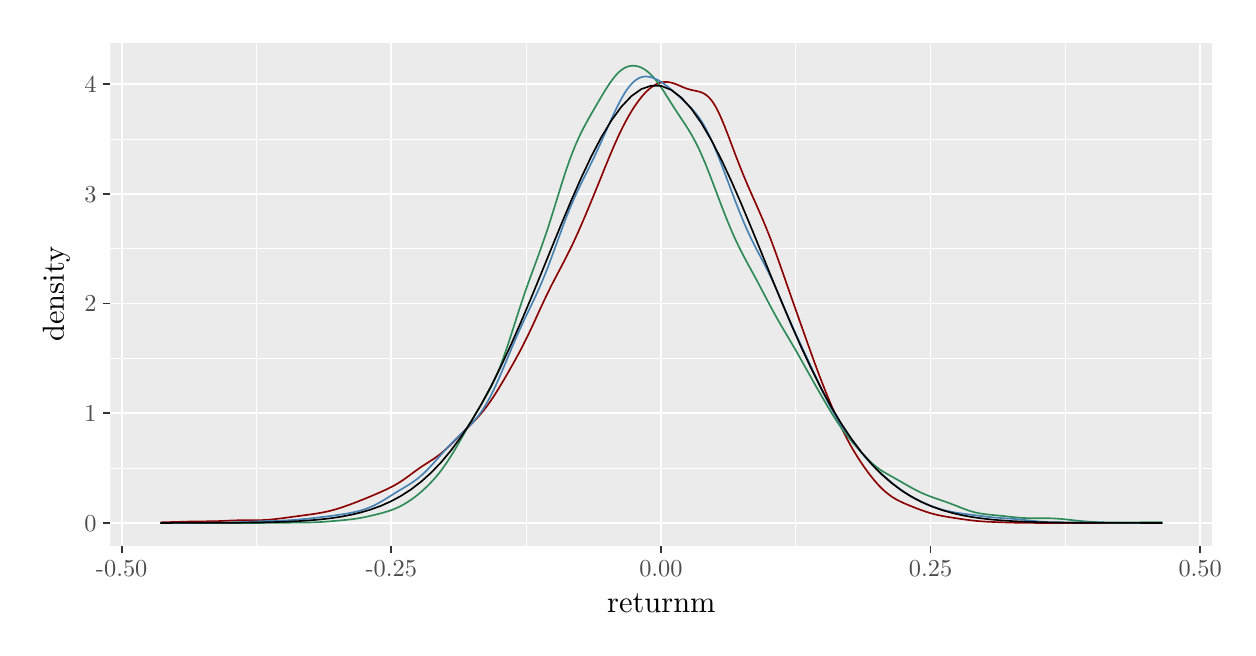
\begin{tikzpicture}[x=1pt,y=1pt]
\definecolor{fillColor}{RGB}{255,255,255}
\path[use as bounding box,fill=fillColor,fill opacity=0.00] (0,0) rectangle (433.62,216.81);
\begin{scope}
\path[clip] (  0.00,  0.00) rectangle (433.62,216.81);
\definecolor{drawColor}{RGB}{255,255,255}
\definecolor{fillColor}{RGB}{255,255,255}

\path[draw=drawColor,line width= 0.6pt,line join=round,line cap=round,fill=fillColor] (  0.00,  0.00) rectangle (433.62,216.81);
\end{scope}
\begin{scope}
\path[clip] ( 29.87, 29.59) rectangle (428.12,211.31);
\definecolor{fillColor}{gray}{0.92}

\path[fill=fillColor] ( 29.87, 29.59) rectangle (428.12,211.31);
\definecolor{drawColor}{RGB}{255,255,255}

\path[draw=drawColor,line width= 0.3pt,line join=round] ( 29.87, 57.67) --
	(428.12, 57.67);

\path[draw=drawColor,line width= 0.3pt,line join=round] ( 29.87, 97.30) --
	(428.12, 97.30);

\path[draw=drawColor,line width= 0.3pt,line join=round] ( 29.87,136.94) --
	(428.12,136.94);

\path[draw=drawColor,line width= 0.3pt,line join=round] ( 29.87,176.58) --
	(428.12,176.58);

\path[draw=drawColor,line width= 0.3pt,line join=round] ( 82.68, 29.59) --
	( 82.68,211.31);

\path[draw=drawColor,line width= 0.3pt,line join=round] (180.11, 29.59) --
	(180.11,211.31);

\path[draw=drawColor,line width= 0.3pt,line join=round] (277.54, 29.59) --
	(277.54,211.31);

\path[draw=drawColor,line width= 0.3pt,line join=round] (374.97, 29.59) --
	(374.97,211.31);

\path[draw=drawColor,line width= 0.6pt,line join=round] ( 29.87, 37.85) --
	(428.12, 37.85);

\path[draw=drawColor,line width= 0.6pt,line join=round] ( 29.87, 77.49) --
	(428.12, 77.49);

\path[draw=drawColor,line width= 0.6pt,line join=round] ( 29.87,117.12) --
	(428.12,117.12);

\path[draw=drawColor,line width= 0.6pt,line join=round] ( 29.87,156.76) --
	(428.12,156.76);

\path[draw=drawColor,line width= 0.6pt,line join=round] ( 29.87,196.40) --
	(428.12,196.40);

\path[draw=drawColor,line width= 0.6pt,line join=round] ( 33.97, 29.59) --
	( 33.97,211.31);

\path[draw=drawColor,line width= 0.6pt,line join=round] (131.40, 29.59) --
	(131.40,211.31);

\path[draw=drawColor,line width= 0.6pt,line join=round] (228.83, 29.59) --
	(228.83,211.31);

\path[draw=drawColor,line width= 0.6pt,line join=round] (326.26, 29.59) --
	(326.26,211.31);

\path[draw=drawColor,line width= 0.6pt,line join=round] (423.69, 29.59) --
	(423.69,211.31);
\definecolor{drawColor}{RGB}{139,0,0}

\path[draw=drawColor,line width= 0.6pt,line join=round] ( 47.97, 38.05) --
	( 48.68, 38.07) --
	( 49.39, 38.09) --
	( 50.10, 38.11) --
	( 50.81, 38.13) --
	( 51.51, 38.15) --
	( 52.22, 38.17) --
	( 52.93, 38.19) --
	( 53.64, 38.21) --
	( 54.35, 38.23) --
	( 55.06, 38.25) --
	( 55.76, 38.27) --
	( 56.47, 38.29) --
	( 57.18, 38.31) --
	( 57.89, 38.33) --
	( 58.60, 38.35) --
	( 59.31, 38.36) --
	( 60.02, 38.37) --
	( 60.72, 38.39) --
	( 61.43, 38.40) --
	( 62.14, 38.40) --
	( 62.85, 38.41) --
	( 63.56, 38.42) --
	( 64.27, 38.42) --
	( 64.98, 38.43) --
	( 65.68, 38.44) --
	( 66.39, 38.45) --
	( 67.10, 38.46) --
	( 67.81, 38.48) --
	( 68.52, 38.50) --
	( 69.23, 38.52) --
	( 69.93, 38.55) --
	( 70.64, 38.58) --
	( 71.35, 38.61) --
	( 72.06, 38.65) --
	( 72.77, 38.68) --
	( 73.48, 38.72) --
	( 74.19, 38.74) --
	( 74.89, 38.77) --
	( 75.60, 38.79) --
	( 76.31, 38.81) --
	( 77.02, 38.82) --
	( 77.73, 38.82) --
	( 78.44, 38.82) --
	( 79.15, 38.82) --
	( 79.85, 38.82) --
	( 80.56, 38.81) --
	( 81.27, 38.81) --
	( 81.98, 38.81) --
	( 82.69, 38.82) --
	( 83.40, 38.83) --
	( 84.10, 38.85) --
	( 84.81, 38.87) --
	( 85.52, 38.91) --
	( 86.23, 38.95) --
	( 86.94, 39.00) --
	( 87.65, 39.06) --
	( 88.36, 39.13) --
	( 89.06, 39.20) --
	( 89.77, 39.28) --
	( 90.48, 39.37) --
	( 91.19, 39.45) --
	( 91.90, 39.54) --
	( 92.61, 39.63) --
	( 93.32, 39.73) --
	( 94.02, 39.82) --
	( 94.73, 39.92) --
	( 95.44, 40.02) --
	( 96.15, 40.11) --
	( 96.86, 40.21) --
	( 97.57, 40.30) --
	( 98.28, 40.40) --
	( 98.98, 40.49) --
	( 99.69, 40.59) --
	(100.40, 40.68) --
	(101.11, 40.78) --
	(101.82, 40.87) --
	(102.53, 40.97) --
	(103.23, 41.07) --
	(103.94, 41.18) --
	(104.65, 41.29) --
	(105.36, 41.41) --
	(106.07, 41.53) --
	(106.78, 41.67) --
	(107.49, 41.81) --
	(108.19, 41.96) --
	(108.90, 42.13) --
	(109.61, 42.31) --
	(110.32, 42.49) --
	(111.03, 42.69) --
	(111.74, 42.90) --
	(112.45, 43.12) --
	(113.15, 43.35) --
	(113.86, 43.58) --
	(114.57, 43.83) --
	(115.28, 44.08) --
	(115.99, 44.33) --
	(116.70, 44.59) --
	(117.40, 44.85) --
	(118.11, 45.12) --
	(118.82, 45.39) --
	(119.53, 45.67) --
	(120.24, 45.95) --
	(120.95, 46.23) --
	(121.66, 46.51) --
	(122.36, 46.80) --
	(123.07, 47.10) --
	(123.78, 47.39) --
	(124.49, 47.69) --
	(125.20, 48.00) --
	(125.91, 48.30) --
	(126.62, 48.61) --
	(127.32, 48.92) --
	(128.03, 49.23) --
	(128.74, 49.55) --
	(129.45, 49.88) --
	(130.16, 50.21) --
	(130.87, 50.56) --
	(131.57, 50.92) --
	(132.28, 51.30) --
	(132.99, 51.69) --
	(133.70, 52.11) --
	(134.41, 52.55) --
	(135.12, 53.01) --
	(135.83, 53.49) --
	(136.53, 53.98) --
	(137.24, 54.49) --
	(137.95, 55.01) --
	(138.66, 55.54) --
	(139.37, 56.06) --
	(140.08, 56.58) --
	(140.79, 57.09) --
	(141.49, 57.59) --
	(142.20, 58.08) --
	(142.91, 58.55) --
	(143.62, 59.02) --
	(144.33, 59.47) --
	(145.04, 59.92) --
	(145.74, 60.38) --
	(146.45, 60.84) --
	(147.16, 61.32) --
	(147.87, 61.83) --
	(148.58, 62.35) --
	(149.29, 62.91) --
	(150.00, 63.49) --
	(150.70, 64.10) --
	(151.41, 64.74) --
	(152.12, 65.40) --
	(152.83, 66.09) --
	(153.54, 66.78) --
	(154.25, 67.49) --
	(154.96, 68.20) --
	(155.66, 68.92) --
	(156.37, 69.63) --
	(157.08, 70.34) --
	(157.79, 71.05) --
	(158.50, 71.76) --
	(159.21, 72.46) --
	(159.92, 73.17) --
	(160.62, 73.89) --
	(161.33, 74.62) --
	(162.04, 75.37) --
	(162.75, 76.14) --
	(163.46, 76.94) --
	(164.17, 77.77) --
	(164.87, 78.64) --
	(165.58, 79.56) --
	(166.29, 80.51) --
	(167.00, 81.51) --
	(167.71, 82.54) --
	(168.42, 83.61) --
	(169.13, 84.72) --
	(169.83, 85.85) --
	(170.54, 87.01) --
	(171.25, 88.20) --
	(171.96, 89.39) --
	(172.67, 90.60) --
	(173.38, 91.82) --
	(174.09, 93.05) --
	(174.79, 94.30) --
	(175.50, 95.55) --
	(176.21, 96.82) --
	(176.92, 98.11) --
	(177.63, 99.43) --
	(178.34,100.77) --
	(179.04,102.15) --
	(179.75,103.55) --
	(180.46,104.99) --
	(181.17,106.46) --
	(181.88,107.96) --
	(182.59,109.48) --
	(183.30,111.02) --
	(184.00,112.57) --
	(184.71,114.12) --
	(185.42,115.66) --
	(186.13,117.19) --
	(186.84,118.70) --
	(187.55,120.18) --
	(188.26,121.63) --
	(188.96,123.06) --
	(189.67,124.46) --
	(190.38,125.83) --
	(191.09,127.18) --
	(191.80,128.53) --
	(192.51,129.87) --
	(193.21,131.22) --
	(193.92,132.57) --
	(194.63,133.95) --
	(195.34,135.36) --
	(196.05,136.79) --
	(196.76,138.26) --
	(197.47,139.77) --
	(198.17,141.31) --
	(198.88,142.88) --
	(199.59,144.49) --
	(200.30,146.11) --
	(201.01,147.77) --
	(201.72,149.44) --
	(202.43,151.13) --
	(203.13,152.83) --
	(203.84,154.54) --
	(204.55,156.27) --
	(205.26,158.01) --
	(205.97,159.75) --
	(206.68,161.50) --
	(207.39,163.25) --
	(208.09,165.00) --
	(208.80,166.75) --
	(209.51,168.48) --
	(210.22,170.20) --
	(210.93,171.89) --
	(211.64,173.54) --
	(212.34,175.16) --
	(213.05,176.74) --
	(213.76,178.27) --
	(214.47,179.75) --
	(215.18,181.18) --
	(215.89,182.55) --
	(216.60,183.86) --
	(217.30,185.11) --
	(218.01,186.31) --
	(218.72,187.45) --
	(219.43,188.54) --
	(220.14,189.57) --
	(220.85,190.54) --
	(221.56,191.45) --
	(222.26,192.30) --
	(222.97,193.09) --
	(223.68,193.80) --
	(224.39,194.46) --
	(225.10,195.05) --
	(225.81,195.57) --
	(226.51,196.02) --
	(227.22,196.40) --
	(227.93,196.70) --
	(228.64,196.94) --
	(229.35,197.10) --
	(230.06,197.18) --
	(230.77,197.19) --
	(231.47,197.14) --
	(232.18,197.02) --
	(232.89,196.84) --
	(233.60,196.62) --
	(234.31,196.36) --
	(235.02,196.07) --
	(235.73,195.76) --
	(236.43,195.46) --
	(237.14,195.17) --
	(237.85,194.90) --
	(238.56,194.66) --
	(239.27,194.45) --
	(239.98,194.27) --
	(240.68,194.12) --
	(241.39,193.97) --
	(242.10,193.82) --
	(242.81,193.64) --
	(243.52,193.40) --
	(244.23,193.08) --
	(244.94,192.65) --
	(245.64,192.11) --
	(246.35,191.43) --
	(247.06,190.59) --
	(247.77,189.60) --
	(248.48,188.46) --
	(249.19,187.14) --
	(249.90,185.69) --
	(250.60,184.12) --
	(251.31,182.44) --
	(252.02,180.68) --
	(252.73,178.86) --
	(253.44,177.00) --
	(254.15,175.12) --
	(254.85,173.23) --
	(255.56,171.35) --
	(256.27,169.49) --
	(256.98,167.66) --
	(257.69,165.87) --
	(258.40,164.11) --
	(259.11,162.39) --
	(259.81,160.71) --
	(260.52,159.06) --
	(261.23,157.44) --
	(261.94,155.84) --
	(262.65,154.24) --
	(263.36,152.65) --
	(264.07,151.05) --
	(264.77,149.42) --
	(265.48,147.78) --
	(266.19,146.09) --
	(266.90,144.37) --
	(267.61,142.60) --
	(268.32,140.79) --
	(269.03,138.92) --
	(269.73,137.02) --
	(270.44,135.08) --
	(271.15,133.10) --
	(271.86,131.10) --
	(272.57,129.09) --
	(273.28,127.06) --
	(273.98,125.03) --
	(274.69,122.99) --
	(275.40,120.96) --
	(276.11,118.93) --
	(276.82,116.91) --
	(277.53,114.90) --
	(278.24,112.89) --
	(278.94,110.89) --
	(279.65,108.88) --
	(280.36,106.88) --
	(281.07,104.88) --
	(281.78,102.89) --
	(282.49,100.91) --
	(283.20, 98.93) --
	(283.90, 96.97) --
	(284.61, 95.03) --
	(285.32, 93.12) --
	(286.03, 91.23) --
	(286.74, 89.37) --
	(287.45, 87.55) --
	(288.15, 85.76) --
	(288.86, 84.02) --
	(289.57, 82.30) --
	(290.28, 80.62) --
	(290.99, 78.97) --
	(291.70, 77.36) --
	(292.41, 75.78) --
	(293.11, 74.24) --
	(293.82, 72.74) --
	(294.53, 71.28) --
	(295.24, 69.86) --
	(295.95, 68.48) --
	(296.66, 67.15) --
	(297.37, 65.86) --
	(298.07, 64.62) --
	(298.78, 63.42) --
	(299.49, 62.26) --
	(300.20, 61.13) --
	(300.91, 60.05) --
	(301.62, 59.00) --
	(302.32, 57.98) --
	(303.03, 56.99) --
	(303.74, 56.02) --
	(304.45, 55.09) --
	(305.16, 54.19) --
	(305.87, 53.32) --
	(306.58, 52.49) --
	(307.28, 51.70) --
	(307.99, 50.95) --
	(308.70, 50.24) --
	(309.41, 49.57) --
	(310.12, 48.96) --
	(310.83, 48.38) --
	(311.54, 47.84) --
	(312.24, 47.35) --
	(312.95, 46.89) --
	(313.66, 46.47) --
	(314.37, 46.08) --
	(315.08, 45.72) --
	(315.79, 45.38) --
	(316.49, 45.05) --
	(317.20, 44.74) --
	(317.91, 44.44) --
	(318.62, 44.15) --
	(319.33, 43.86) --
	(320.04, 43.58) --
	(320.75, 43.30) --
	(321.45, 43.03) --
	(322.16, 42.76) --
	(322.87, 42.50) --
	(323.58, 42.25) --
	(324.29, 42.00) --
	(325.00, 41.77) --
	(325.71, 41.55) --
	(326.41, 41.33) --
	(327.12, 41.14) --
	(327.83, 40.95) --
	(328.54, 40.78) --
	(329.25, 40.63) --
	(329.96, 40.48) --
	(330.67, 40.34) --
	(331.37, 40.21) --
	(332.08, 40.09) --
	(332.79, 39.97) --
	(333.50, 39.85) --
	(334.21, 39.74) --
	(334.92, 39.63) --
	(335.62, 39.53) --
	(336.33, 39.42) --
	(337.04, 39.31) --
	(337.75, 39.21) --
	(338.46, 39.11) --
	(339.17, 39.01) --
	(339.88, 38.92) --
	(340.58, 38.83) --
	(341.29, 38.74) --
	(342.00, 38.66) --
	(342.71, 38.59) --
	(343.42, 38.52) --
	(344.13, 38.46) --
	(344.84, 38.41) --
	(345.54, 38.36) --
	(346.25, 38.32) --
	(346.96, 38.28) --
	(347.67, 38.24) --
	(348.38, 38.21) --
	(349.09, 38.18) --
	(349.79, 38.15) --
	(350.50, 38.13) --
	(351.21, 38.10) --
	(351.92, 38.08) --
	(352.63, 38.05) --
	(353.34, 38.03) --
	(354.05, 38.01) --
	(354.75, 37.99) --
	(355.46, 37.97) --
	(356.17, 37.95) --
	(356.88, 37.93) --
	(357.59, 37.92) --
	(358.30, 37.91) --
	(359.01, 37.89) --
	(359.71, 37.88) --
	(360.42, 37.88) --
	(361.13, 37.87) --
	(361.84, 37.86) --
	(362.55, 37.86) --
	(363.26, 37.86) --
	(363.96, 37.85) --
	(364.67, 37.85) --
	(365.38, 37.85) --
	(366.09, 37.85) --
	(366.80, 37.85) --
	(367.51, 37.85) --
	(368.22, 37.85) --
	(368.92, 37.85) --
	(369.63, 37.85) --
	(370.34, 37.85) --
	(371.05, 37.85) --
	(371.76, 37.85) --
	(372.47, 37.85) --
	(373.18, 37.85) --
	(373.88, 37.85) --
	(374.59, 37.85) --
	(375.30, 37.85) --
	(376.01, 37.85) --
	(376.72, 37.85) --
	(377.43, 37.85) --
	(378.13, 37.85) --
	(378.84, 37.85) --
	(379.55, 37.85) --
	(380.26, 37.85) --
	(380.97, 37.85) --
	(381.68, 37.85) --
	(382.39, 37.85) --
	(383.09, 37.85) --
	(383.80, 37.85) --
	(384.51, 37.85) --
	(385.22, 37.85) --
	(385.93, 37.85) --
	(386.64, 37.85) --
	(387.35, 37.85) --
	(388.05, 37.85) --
	(388.76, 37.85) --
	(389.47, 37.85) --
	(390.18, 37.85) --
	(390.89, 37.85) --
	(391.60, 37.85) --
	(392.31, 37.85) --
	(393.01, 37.85) --
	(393.72, 37.85) --
	(394.43, 37.85) --
	(395.14, 37.85) --
	(395.85, 37.85) --
	(396.56, 37.85) --
	(397.26, 37.85) --
	(397.97, 37.85) --
	(398.68, 37.85) --
	(399.39, 37.85) --
	(400.10, 37.85) --
	(400.81, 37.85) --
	(401.52, 37.85) --
	(402.22, 37.85) --
	(402.93, 37.85) --
	(403.64, 37.85) --
	(404.35, 37.85) --
	(405.06, 37.85) --
	(405.77, 37.85) --
	(406.48, 37.85) --
	(407.18, 37.85) --
	(407.89, 37.85) --
	(408.60, 37.85) --
	(409.31, 37.85) --
	(410.02, 37.85);
\definecolor{drawColor}{RGB}{46,139,87}

\path[draw=drawColor,line width= 0.6pt,line join=round] ( 47.97, 37.85) --
	( 48.68, 37.85) --
	( 49.39, 37.85) --
	( 50.10, 37.85) --
	( 50.81, 37.85) --
	( 51.51, 37.85) --
	( 52.22, 37.85) --
	( 52.93, 37.85) --
	( 53.64, 37.85) --
	( 54.35, 37.85) --
	( 55.06, 37.85) --
	( 55.76, 37.85) --
	( 56.47, 37.85) --
	( 57.18, 37.85) --
	( 57.89, 37.85) --
	( 58.60, 37.85) --
	( 59.31, 37.85) --
	( 60.02, 37.85) --
	( 60.72, 37.85) --
	( 61.43, 37.85) --
	( 62.14, 37.85) --
	( 62.85, 37.85) --
	( 63.56, 37.85) --
	( 64.27, 37.85) --
	( 64.98, 37.85) --
	( 65.68, 37.85) --
	( 66.39, 37.85) --
	( 67.10, 37.85) --
	( 67.81, 37.85) --
	( 68.52, 37.85) --
	( 69.23, 37.85) --
	( 69.93, 37.85) --
	( 70.64, 37.85) --
	( 71.35, 37.85) --
	( 72.06, 37.85) --
	( 72.77, 37.85) --
	( 73.48, 37.85) --
	( 74.19, 37.85) --
	( 74.89, 37.85) --
	( 75.60, 37.85) --
	( 76.31, 37.85) --
	( 77.02, 37.85) --
	( 77.73, 37.85) --
	( 78.44, 37.85) --
	( 79.15, 37.85) --
	( 79.85, 37.85) --
	( 80.56, 37.85) --
	( 81.27, 37.85) --
	( 81.98, 37.85) --
	( 82.69, 37.85) --
	( 83.40, 37.85) --
	( 84.10, 37.85) --
	( 84.81, 37.85) --
	( 85.52, 37.85) --
	( 86.23, 37.86) --
	( 86.94, 37.86) --
	( 87.65, 37.87) --
	( 88.36, 37.87) --
	( 89.06, 37.88) --
	( 89.77, 37.88) --
	( 90.48, 37.89) --
	( 91.19, 37.90) --
	( 91.90, 37.91) --
	( 92.61, 37.92) --
	( 93.32, 37.92) --
	( 94.02, 37.93) --
	( 94.73, 37.94) --
	( 95.44, 37.95) --
	( 96.15, 37.96) --
	( 96.86, 37.97) --
	( 97.57, 37.97) --
	( 98.28, 37.98) --
	( 98.98, 37.99) --
	( 99.69, 37.99) --
	(100.40, 38.00) --
	(101.11, 38.01) --
	(101.82, 38.02) --
	(102.53, 38.04) --
	(103.23, 38.06) --
	(103.94, 38.08) --
	(104.65, 38.11) --
	(105.36, 38.15) --
	(106.07, 38.19) --
	(106.78, 38.23) --
	(107.49, 38.28) --
	(108.19, 38.34) --
	(108.90, 38.40) --
	(109.61, 38.46) --
	(110.32, 38.52) --
	(111.03, 38.58) --
	(111.74, 38.65) --
	(112.45, 38.71) --
	(113.15, 38.77) --
	(113.86, 38.84) --
	(114.57, 38.90) --
	(115.28, 38.97) --
	(115.99, 39.05) --
	(116.70, 39.13) --
	(117.40, 39.21) --
	(118.11, 39.31) --
	(118.82, 39.41) --
	(119.53, 39.53) --
	(120.24, 39.65) --
	(120.95, 39.78) --
	(121.66, 39.92) --
	(122.36, 40.07) --
	(123.07, 40.23) --
	(123.78, 40.39) --
	(124.49, 40.55) --
	(125.20, 40.72) --
	(125.91, 40.89) --
	(126.62, 41.07) --
	(127.32, 41.25) --
	(128.03, 41.44) --
	(128.74, 41.64) --
	(129.45, 41.84) --
	(130.16, 42.06) --
	(130.87, 42.30) --
	(131.57, 42.55) --
	(132.28, 42.82) --
	(132.99, 43.11) --
	(133.70, 43.42) --
	(134.41, 43.76) --
	(135.12, 44.12) --
	(135.83, 44.51) --
	(136.53, 44.92) --
	(137.24, 45.36) --
	(137.95, 45.82) --
	(138.66, 46.31) --
	(139.37, 46.82) --
	(140.08, 47.35) --
	(140.79, 47.91) --
	(141.49, 48.49) --
	(142.20, 49.10) --
	(142.91, 49.72) --
	(143.62, 50.38) --
	(144.33, 51.06) --
	(145.04, 51.76) --
	(145.74, 52.50) --
	(146.45, 53.26) --
	(147.16, 54.05) --
	(147.87, 54.89) --
	(148.58, 55.75) --
	(149.29, 56.66) --
	(150.00, 57.60) --
	(150.70, 58.60) --
	(151.41, 59.63) --
	(152.12, 60.70) --
	(152.83, 61.81) --
	(153.54, 62.95) --
	(154.25, 64.12) --
	(154.96, 65.32) --
	(155.66, 66.54) --
	(156.37, 67.77) --
	(157.08, 69.01) --
	(157.79, 70.26) --
	(158.50, 71.50) --
	(159.21, 72.73) --
	(159.92, 73.96) --
	(160.62, 75.17) --
	(161.33, 76.38) --
	(162.04, 77.57) --
	(162.75, 78.75) --
	(163.46, 79.93) --
	(164.17, 81.11) --
	(164.87, 82.31) --
	(165.58, 83.54) --
	(166.29, 84.81) --
	(167.00, 86.14) --
	(167.71, 87.52) --
	(168.42, 88.99) --
	(169.13, 90.53) --
	(169.83, 92.18) --
	(170.54, 93.93) --
	(171.25, 95.77) --
	(171.96, 97.70) --
	(172.67, 99.72) --
	(173.38,101.80) --
	(174.09,103.94) --
	(174.79,106.13) --
	(175.50,108.34) --
	(176.21,110.56) --
	(176.92,112.77) --
	(177.63,114.96) --
	(178.34,117.11) --
	(179.04,119.23) --
	(179.75,121.30) --
	(180.46,123.33) --
	(181.17,125.32) --
	(181.88,127.28) --
	(182.59,129.21) --
	(183.30,131.13) --
	(184.00,133.05) --
	(184.71,134.99) --
	(185.42,136.96) --
	(186.13,138.97) --
	(186.84,141.02) --
	(187.55,143.12) --
	(188.26,145.28) --
	(188.96,147.48) --
	(189.67,149.73) --
	(190.38,152.02) --
	(191.09,154.32) --
	(191.80,156.62) --
	(192.51,158.90) --
	(193.21,161.16) --
	(193.92,163.36) --
	(194.63,165.51) --
	(195.34,167.57) --
	(196.05,169.56) --
	(196.76,171.43) --
	(197.47,173.22) --
	(198.17,174.90) --
	(198.88,176.50) --
	(199.59,178.02) --
	(200.30,179.47) --
	(201.01,180.85) --
	(201.72,182.17) --
	(202.43,183.46) --
	(203.13,184.72) --
	(203.84,185.96) --
	(204.55,187.18) --
	(205.26,188.40) --
	(205.97,189.62) --
	(206.68,190.83) --
	(207.39,192.02) --
	(208.09,193.20) --
	(208.80,194.36) --
	(209.51,195.48) --
	(210.22,196.55) --
	(210.93,197.56) --
	(211.64,198.51) --
	(212.34,199.37) --
	(213.05,200.16) --
	(213.76,200.85) --
	(214.47,201.45) --
	(215.18,201.96) --
	(215.89,202.36) --
	(216.60,202.67) --
	(217.30,202.88) --
	(218.01,203.01) --
	(218.72,203.05) --
	(219.43,203.01) --
	(220.14,202.90) --
	(220.85,202.71) --
	(221.56,202.45) --
	(222.26,202.11) --
	(222.97,201.69) --
	(223.68,201.19) --
	(224.39,200.61) --
	(225.10,199.95) --
	(225.81,199.22) --
	(226.51,198.42) --
	(227.22,197.54) --
	(227.93,196.60) --
	(228.64,195.60) --
	(229.35,194.55) --
	(230.06,193.46) --
	(230.77,192.35) --
	(231.47,191.23) --
	(232.18,190.10) --
	(232.89,188.98) --
	(233.60,187.87) --
	(234.31,186.77) --
	(235.02,185.70) --
	(235.73,184.63) --
	(236.43,183.57) --
	(237.14,182.50) --
	(237.85,181.42) --
	(238.56,180.31) --
	(239.27,179.15) --
	(239.98,177.95) --
	(240.68,176.68) --
	(241.39,175.35) --
	(242.10,173.93) --
	(242.81,172.44) --
	(243.52,170.86) --
	(244.23,169.22) --
	(244.94,167.52) --
	(245.64,165.76) --
	(246.35,163.95) --
	(247.06,162.11) --
	(247.77,160.25) --
	(248.48,158.36) --
	(249.19,156.48) --
	(249.90,154.60) --
	(250.60,152.73) --
	(251.31,150.89) --
	(252.02,149.08) --
	(252.73,147.30) --
	(253.44,145.57) --
	(254.15,143.88) --
	(254.85,142.25) --
	(255.56,140.68) --
	(256.27,139.16) --
	(256.98,137.69) --
	(257.69,136.27) --
	(258.40,134.89) --
	(259.11,133.54) --
	(259.81,132.21) --
	(260.52,130.91) --
	(261.23,129.61) --
	(261.94,128.31) --
	(262.65,127.01) --
	(263.36,125.69) --
	(264.07,124.37) --
	(264.77,123.03) --
	(265.48,121.68) --
	(266.19,120.33) --
	(266.90,118.98) --
	(267.61,117.63) --
	(268.32,116.29) --
	(269.03,114.97) --
	(269.73,113.67) --
	(270.44,112.39) --
	(271.15,111.13) --
	(271.86,109.89) --
	(272.57,108.67) --
	(273.28,107.47) --
	(273.98,106.27) --
	(274.69,105.08) --
	(275.40,103.88) --
	(276.11,102.68) --
	(276.82,101.47) --
	(277.53,100.25) --
	(278.24, 99.01) --
	(278.94, 97.76) --
	(279.65, 96.51) --
	(280.36, 95.24) --
	(281.07, 93.97) --
	(281.78, 92.70) --
	(282.49, 91.44) --
	(283.20, 90.17) --
	(283.90, 88.91) --
	(284.61, 87.66) --
	(285.32, 86.41) --
	(286.03, 85.17) --
	(286.74, 83.94) --
	(287.45, 82.71) --
	(288.15, 81.50) --
	(288.86, 80.30) --
	(289.57, 79.11) --
	(290.28, 77.94) --
	(290.99, 76.79) --
	(291.70, 75.67) --
	(292.41, 74.58) --
	(293.11, 73.52) --
	(293.82, 72.49) --
	(294.53, 71.49) --
	(295.24, 70.53) --
	(295.95, 69.60) --
	(296.66, 68.69) --
	(297.37, 67.81) --
	(298.07, 66.96) --
	(298.78, 66.12) --
	(299.49, 65.29) --
	(300.20, 64.48) --
	(300.91, 63.69) --
	(301.62, 62.91) --
	(302.32, 62.15) --
	(303.03, 61.42) --
	(303.74, 60.71) --
	(304.45, 60.03) --
	(305.16, 59.38) --
	(305.87, 58.77) --
	(306.58, 58.19) --
	(307.28, 57.66) --
	(307.99, 57.15) --
	(308.70, 56.68) --
	(309.41, 56.24) --
	(310.12, 55.81) --
	(310.83, 55.41) --
	(311.54, 55.01) --
	(312.24, 54.61) --
	(312.95, 54.22) --
	(313.66, 53.82) --
	(314.37, 53.42) --
	(315.08, 53.02) --
	(315.79, 52.61) --
	(316.49, 52.20) --
	(317.20, 51.79) --
	(317.91, 51.38) --
	(318.62, 50.98) --
	(319.33, 50.58) --
	(320.04, 50.20) --
	(320.75, 49.82) --
	(321.45, 49.46) --
	(322.16, 49.11) --
	(322.87, 48.78) --
	(323.58, 48.46) --
	(324.29, 48.16) --
	(325.00, 47.87) --
	(325.71, 47.59) --
	(326.41, 47.32) --
	(327.12, 47.06) --
	(327.83, 46.81) --
	(328.54, 46.56) --
	(329.25, 46.32) --
	(329.96, 46.08) --
	(330.67, 45.83) --
	(331.37, 45.59) --
	(332.08, 45.34) --
	(332.79, 45.08) --
	(333.50, 44.82) --
	(334.21, 44.55) --
	(334.92, 44.27) --
	(335.62, 43.99) --
	(336.33, 43.71) --
	(337.04, 43.43) --
	(337.75, 43.16) --
	(338.46, 42.89) --
	(339.17, 42.63) --
	(339.88, 42.38) --
	(340.58, 42.15) --
	(341.29, 41.94) --
	(342.00, 41.75) --
	(342.71, 41.58) --
	(343.42, 41.43) --
	(344.13, 41.29) --
	(344.84, 41.17) --
	(345.54, 41.07) --
	(346.25, 40.98) --
	(346.96, 40.90) --
	(347.67, 40.82) --
	(348.38, 40.75) --
	(349.09, 40.69) --
	(349.79, 40.62) --
	(350.50, 40.55) --
	(351.21, 40.48) --
	(351.92, 40.41) --
	(352.63, 40.34) --
	(353.34, 40.26) --
	(354.05, 40.18) --
	(354.75, 40.10) --
	(355.46, 40.02) --
	(356.17, 39.94) --
	(356.88, 39.87) --
	(357.59, 39.80) --
	(358.30, 39.74) --
	(359.01, 39.69) --
	(359.71, 39.64) --
	(360.42, 39.61) --
	(361.13, 39.58) --
	(361.84, 39.56) --
	(362.55, 39.55) --
	(363.26, 39.54) --
	(363.96, 39.54) --
	(364.67, 39.54) --
	(365.38, 39.54) --
	(366.09, 39.55) --
	(366.80, 39.55) --
	(367.51, 39.55) --
	(368.22, 39.54) --
	(368.92, 39.53) --
	(369.63, 39.51) --
	(370.34, 39.49) --
	(371.05, 39.45) --
	(371.76, 39.41) --
	(372.47, 39.36) --
	(373.18, 39.31) --
	(373.88, 39.25) --
	(374.59, 39.18) --
	(375.30, 39.10) --
	(376.01, 39.03) --
	(376.72, 38.95) --
	(377.43, 38.87) --
	(378.13, 38.79) --
	(378.84, 38.71) --
	(379.55, 38.64) --
	(380.26, 38.57) --
	(380.97, 38.50) --
	(381.68, 38.44) --
	(382.39, 38.38) --
	(383.09, 38.33) --
	(383.80, 38.28) --
	(384.51, 38.24) --
	(385.22, 38.20) --
	(385.93, 38.17) --
	(386.64, 38.14) --
	(387.35, 38.11) --
	(388.05, 38.09) --
	(388.76, 38.07) --
	(389.47, 38.05) --
	(390.18, 38.04) --
	(390.89, 38.02) --
	(391.60, 38.01) --
	(392.31, 38.01) --
	(393.01, 38.00) --
	(393.72, 38.00) --
	(394.43, 38.00) --
	(395.14, 38.00) --
	(395.85, 38.00) --
	(396.56, 38.01) --
	(397.26, 38.01) --
	(397.97, 38.02) --
	(398.68, 38.03) --
	(399.39, 38.04) --
	(400.10, 38.05) --
	(400.81, 38.05) --
	(401.52, 38.06) --
	(402.22, 38.07) --
	(402.93, 38.08) --
	(403.64, 38.09) --
	(404.35, 38.09) --
	(405.06, 38.10) --
	(405.77, 38.10) --
	(406.48, 38.10) --
	(407.18, 38.10) --
	(407.89, 38.09) --
	(408.60, 38.09) --
	(409.31, 38.08) --
	(410.02, 38.07);
\definecolor{drawColor}{RGB}{70,130,180}

\path[draw=drawColor,line width= 0.6pt,line join=round] ( 47.97, 37.85) --
	( 48.68, 37.85) --
	( 49.39, 37.85) --
	( 50.10, 37.85) --
	( 50.81, 37.85) --
	( 51.51, 37.85) --
	( 52.22, 37.85) --
	( 52.93, 37.85) --
	( 53.64, 37.85) --
	( 54.35, 37.85) --
	( 55.06, 37.85) --
	( 55.76, 37.85) --
	( 56.47, 37.85) --
	( 57.18, 37.85) --
	( 57.89, 37.85) --
	( 58.60, 37.85) --
	( 59.31, 37.85) --
	( 60.02, 37.86) --
	( 60.72, 37.86) --
	( 61.43, 37.86) --
	( 62.14, 37.87) --
	( 62.85, 37.87) --
	( 63.56, 37.88) --
	( 64.27, 37.89) --
	( 64.98, 37.90) --
	( 65.68, 37.91) --
	( 66.39, 37.92) --
	( 67.10, 37.93) --
	( 67.81, 37.94) --
	( 68.52, 37.95) --
	( 69.23, 37.96) --
	( 69.93, 37.97) --
	( 70.64, 37.99) --
	( 71.35, 38.00) --
	( 72.06, 38.01) --
	( 72.77, 38.03) --
	( 73.48, 38.04) --
	( 74.19, 38.06) --
	( 74.89, 38.08) --
	( 75.60, 38.10) --
	( 76.31, 38.12) --
	( 77.02, 38.15) --
	( 77.73, 38.18) --
	( 78.44, 38.21) --
	( 79.15, 38.24) --
	( 79.85, 38.27) --
	( 80.56, 38.31) --
	( 81.27, 38.34) --
	( 81.98, 38.37) --
	( 82.69, 38.40) --
	( 83.40, 38.43) --
	( 84.10, 38.46) --
	( 84.81, 38.49) --
	( 85.52, 38.51) --
	( 86.23, 38.53) --
	( 86.94, 38.55) --
	( 87.65, 38.57) --
	( 88.36, 38.58) --
	( 89.06, 38.60) --
	( 89.77, 38.62) --
	( 90.48, 38.64) --
	( 91.19, 38.66) --
	( 91.90, 38.69) --
	( 92.61, 38.72) --
	( 93.32, 38.75) --
	( 94.02, 38.79) --
	( 94.73, 38.83) --
	( 95.44, 38.88) --
	( 96.15, 38.93) --
	( 96.86, 38.99) --
	( 97.57, 39.04) --
	( 98.28, 39.11) --
	( 98.98, 39.17) --
	( 99.69, 39.24) --
	(100.40, 39.31) --
	(101.11, 39.38) --
	(101.82, 39.45) --
	(102.53, 39.53) --
	(103.23, 39.61) --
	(103.94, 39.69) --
	(104.65, 39.77) --
	(105.36, 39.85) --
	(106.07, 39.94) --
	(106.78, 40.03) --
	(107.49, 40.11) --
	(108.19, 40.20) --
	(108.90, 40.30) --
	(109.61, 40.39) --
	(110.32, 40.48) --
	(111.03, 40.58) --
	(111.74, 40.68) --
	(112.45, 40.78) --
	(113.15, 40.88) --
	(113.86, 40.99) --
	(114.57, 41.10) --
	(115.28, 41.22) --
	(115.99, 41.35) --
	(116.70, 41.49) --
	(117.40, 41.63) --
	(118.11, 41.78) --
	(118.82, 41.95) --
	(119.53, 42.13) --
	(120.24, 42.32) --
	(120.95, 42.53) --
	(121.66, 42.76) --
	(122.36, 43.00) --
	(123.07, 43.27) --
	(123.78, 43.55) --
	(124.49, 43.86) --
	(125.20, 44.19) --
	(125.91, 44.55) --
	(126.62, 44.92) --
	(127.32, 45.31) --
	(128.03, 45.72) --
	(128.74, 46.15) --
	(129.45, 46.58) --
	(130.16, 47.02) --
	(130.87, 47.46) --
	(131.57, 47.91) --
	(132.28, 48.35) --
	(132.99, 48.79) --
	(133.70, 49.22) --
	(134.41, 49.65) --
	(135.12, 50.07) --
	(135.83, 50.50) --
	(136.53, 50.93) --
	(137.24, 51.36) --
	(137.95, 51.80) --
	(138.66, 52.26) --
	(139.37, 52.74) --
	(140.08, 53.25) --
	(140.79, 53.78) --
	(141.49, 54.35) --
	(142.20, 54.95) --
	(142.91, 55.59) --
	(143.62, 56.26) --
	(144.33, 56.96) --
	(145.04, 57.70) --
	(145.74, 58.46) --
	(146.45, 59.23) --
	(147.16, 60.02) --
	(147.87, 60.82) --
	(148.58, 61.62) --
	(149.29, 62.42) --
	(150.00, 63.21) --
	(150.70, 64.00) --
	(151.41, 64.76) --
	(152.12, 65.52) --
	(152.83, 66.26) --
	(153.54, 66.98) --
	(154.25, 67.69) --
	(154.96, 68.39) --
	(155.66, 69.08) --
	(156.37, 69.76) --
	(157.08, 70.44) --
	(157.79, 71.12) --
	(158.50, 71.81) --
	(159.21, 72.51) --
	(159.92, 73.23) --
	(160.62, 73.97) --
	(161.33, 74.75) --
	(162.04, 75.58) --
	(162.75, 76.46) --
	(163.46, 77.39) --
	(164.17, 78.40) --
	(164.87, 79.48) --
	(165.58, 80.64) --
	(166.29, 81.87) --
	(167.00, 83.17) --
	(167.71, 84.55) --
	(168.42, 85.99) --
	(169.13, 87.50) --
	(169.83, 89.06) --
	(170.54, 90.67) --
	(171.25, 92.32) --
	(171.96, 94.00) --
	(172.67, 95.69) --
	(173.38, 97.39) --
	(174.09, 99.09) --
	(174.79,100.79) --
	(175.50,102.46) --
	(176.21,104.11) --
	(176.92,105.74) --
	(177.63,107.32) --
	(178.34,108.88) --
	(179.04,110.41) --
	(179.75,111.91) --
	(180.46,113.39) --
	(181.17,114.86) --
	(181.88,116.33) --
	(182.59,117.81) --
	(183.30,119.30) --
	(184.00,120.83) --
	(184.71,122.40) --
	(185.42,124.02) --
	(186.13,125.69) --
	(186.84,127.41) --
	(187.55,129.19) --
	(188.26,131.02) --
	(188.96,132.90) --
	(189.67,134.81) --
	(190.38,136.76) --
	(191.09,138.71) --
	(191.80,140.67) --
	(192.51,142.61) --
	(193.21,144.53) --
	(193.92,146.42) --
	(194.63,148.26) --
	(195.34,150.06) --
	(196.05,151.79) --
	(196.76,153.47) --
	(197.47,155.10) --
	(198.17,156.66) --
	(198.88,158.19) --
	(199.59,159.67) --
	(200.30,161.13) --
	(201.01,162.56) --
	(201.72,163.98) --
	(202.43,165.40) --
	(203.13,166.83) --
	(203.84,168.27) --
	(204.55,169.74) --
	(205.26,171.23) --
	(205.97,172.75) --
	(206.68,174.29) --
	(207.39,175.85) --
	(208.09,177.44) --
	(208.80,179.03) --
	(209.51,180.62) --
	(210.22,182.21) --
	(210.93,183.78) --
	(211.64,185.33) --
	(212.34,186.83) --
	(213.05,188.28) --
	(213.76,189.68) --
	(214.47,191.01) --
	(215.18,192.26) --
	(215.89,193.43) --
	(216.60,194.48) --
	(217.30,195.44) --
	(218.01,196.29) --
	(218.72,197.02) --
	(219.43,197.65) --
	(220.14,198.16) --
	(220.85,198.56) --
	(221.56,198.86) --
	(222.26,199.05) --
	(222.97,199.14) --
	(223.68,199.14) --
	(224.39,199.07) --
	(225.10,198.92) --
	(225.81,198.71) --
	(226.51,198.44) --
	(227.22,198.12) --
	(227.93,197.76) --
	(228.64,197.35) --
	(229.35,196.89) --
	(230.06,196.40) --
	(230.77,195.88) --
	(231.47,195.32) --
	(232.18,194.75) --
	(232.89,194.15) --
	(233.60,193.53) --
	(234.31,192.90) --
	(235.02,192.27) --
	(235.73,191.62) --
	(236.43,190.98) --
	(237.14,190.32) --
	(237.85,189.66) --
	(238.56,188.98) --
	(239.27,188.28) --
	(239.98,187.54) --
	(240.68,186.76) --
	(241.39,185.93) --
	(242.10,185.02) --
	(242.81,184.03) --
	(243.52,182.96) --
	(244.23,181.79) --
	(244.94,180.53) --
	(245.64,179.17) --
	(246.35,177.73) --
	(247.06,176.21) --
	(247.77,174.61) --
	(248.48,172.94) --
	(249.19,171.21) --
	(249.90,169.43) --
	(250.60,167.62) --
	(251.31,165.77) --
	(252.02,163.91) --
	(252.73,162.02) --
	(253.44,160.13) --
	(254.15,158.24) --
	(254.85,156.36) --
	(255.56,154.50) --
	(256.27,152.66) --
	(256.98,150.85) --
	(257.69,149.08) --
	(258.40,147.36) --
	(259.11,145.69) --
	(259.81,144.08) --
	(260.52,142.52) --
	(261.23,141.01) --
	(261.94,139.55) --
	(262.65,138.14) --
	(263.36,136.76) --
	(264.07,135.41) --
	(264.77,134.06) --
	(265.48,132.71) --
	(266.19,131.35) --
	(266.90,129.96) --
	(267.61,128.55) --
	(268.32,127.09) --
	(269.03,125.60) --
	(269.73,124.06) --
	(270.44,122.49) --
	(271.15,120.88) --
	(271.86,119.25) --
	(272.57,117.60) --
	(273.28,115.94) --
	(273.98,114.28) --
	(274.69,112.63) --
	(275.40,111.00) --
	(276.11,109.39) --
	(276.82,107.80) --
	(277.53,106.24) --
	(278.24,104.69) --
	(278.94,103.17) --
	(279.65,101.65) --
	(280.36,100.14) --
	(281.07, 98.64) --
	(281.78, 97.12) --
	(282.49, 95.60) --
	(283.20, 94.08) --
	(283.90, 92.54) --
	(284.61, 91.01) --
	(285.32, 89.47) --
	(286.03, 87.95) --
	(286.74, 86.44) --
	(287.45, 84.96) --
	(288.15, 83.51) --
	(288.86, 82.10) --
	(289.57, 80.74) --
	(290.28, 79.43) --
	(290.99, 78.16) --
	(291.70, 76.94) --
	(292.41, 75.77) --
	(293.11, 74.64) --
	(293.82, 73.54) --
	(294.53, 72.48) --
	(295.24, 71.44) --
	(295.95, 70.43) --
	(296.66, 69.43) --
	(297.37, 68.45) --
	(298.07, 67.48) --
	(298.78, 66.53) --
	(299.49, 65.59) --
	(300.20, 64.66) --
	(300.91, 63.76) --
	(301.62, 62.88) --
	(302.32, 62.02) --
	(303.03, 61.19) --
	(303.74, 60.39) --
	(304.45, 59.61) --
	(305.16, 58.86) --
	(305.87, 58.14) --
	(306.58, 57.44) --
	(307.28, 56.76) --
	(307.99, 56.10) --
	(308.70, 55.45) --
	(309.41, 54.82) --
	(310.12, 54.20) --
	(310.83, 53.59) --
	(311.54, 52.99) --
	(312.24, 52.39) --
	(312.95, 51.82) --
	(313.66, 51.25) --
	(314.37, 50.70) --
	(315.08, 50.18) --
	(315.79, 49.67) --
	(316.49, 49.18) --
	(317.20, 48.70) --
	(317.91, 48.25) --
	(318.62, 47.82) --
	(319.33, 47.41) --
	(320.04, 47.01) --
	(320.75, 46.62) --
	(321.45, 46.26) --
	(322.16, 45.90) --
	(322.87, 45.56) --
	(323.58, 45.23) --
	(324.29, 44.91) --
	(325.00, 44.60) --
	(325.71, 44.30) --
	(326.41, 44.02) --
	(327.12, 43.74) --
	(327.83, 43.49) --
	(328.54, 43.24) --
	(329.25, 43.01) --
	(329.96, 42.79) --
	(330.67, 42.59) --
	(331.37, 42.40) --
	(332.08, 42.23) --
	(332.79, 42.07) --
	(333.50, 41.92) --
	(334.21, 41.78) --
	(334.92, 41.65) --
	(335.62, 41.54) --
	(336.33, 41.43) --
	(337.04, 41.32) --
	(337.75, 41.22) --
	(338.46, 41.13) --
	(339.17, 41.04) --
	(339.88, 40.95) --
	(340.58, 40.86) --
	(341.29, 40.77) --
	(342.00, 40.67) --
	(342.71, 40.58) --
	(343.42, 40.49) --
	(344.13, 40.40) --
	(344.84, 40.31) --
	(345.54, 40.22) --
	(346.25, 40.13) --
	(346.96, 40.05) --
	(347.67, 39.98) --
	(348.38, 39.90) --
	(349.09, 39.83) --
	(349.79, 39.77) --
	(350.50, 39.71) --
	(351.21, 39.66) --
	(351.92, 39.61) --
	(352.63, 39.56) --
	(353.34, 39.51) --
	(354.05, 39.46) --
	(354.75, 39.42) --
	(355.46, 39.36) --
	(356.17, 39.31) --
	(356.88, 39.25) --
	(357.59, 39.18) --
	(358.30, 39.12) --
	(359.01, 39.05) --
	(359.71, 38.97) --
	(360.42, 38.89) --
	(361.13, 38.81) --
	(361.84, 38.73) --
	(362.55, 38.66) --
	(363.26, 38.58) --
	(363.96, 38.51) --
	(364.67, 38.44) --
	(365.38, 38.37) --
	(366.09, 38.32) --
	(366.80, 38.27) --
	(367.51, 38.22) --
	(368.22, 38.18) --
	(368.92, 38.15) --
	(369.63, 38.13) --
	(370.34, 38.10) --
	(371.05, 38.09) --
	(371.76, 38.07) --
	(372.47, 38.07) --
	(373.18, 38.06) --
	(373.88, 38.06) --
	(374.59, 38.05) --
	(375.30, 38.05) --
	(376.01, 38.05) --
	(376.72, 38.06) --
	(377.43, 38.06) --
	(378.13, 38.06) --
	(378.84, 38.06) --
	(379.55, 38.07) --
	(380.26, 38.07) --
	(380.97, 38.07) --
	(381.68, 38.07) --
	(382.39, 38.07) --
	(383.09, 38.06) --
	(383.80, 38.06) --
	(384.51, 38.05) --
	(385.22, 38.04) --
	(385.93, 38.03) --
	(386.64, 38.02) --
	(387.35, 38.01) --
	(388.05, 38.00) --
	(388.76, 37.98) --
	(389.47, 37.97) --
	(390.18, 37.95) --
	(390.89, 37.94) --
	(391.60, 37.93) --
	(392.31, 37.92) --
	(393.01, 37.90) --
	(393.72, 37.89) --
	(394.43, 37.89) --
	(395.14, 37.88) --
	(395.85, 37.87) --
	(396.56, 37.87) --
	(397.26, 37.86) --
	(397.97, 37.86) --
	(398.68, 37.86) --
	(399.39, 37.85) --
	(400.10, 37.85) --
	(400.81, 37.85) --
	(401.52, 37.85) --
	(402.22, 37.85) --
	(402.93, 37.85) --
	(403.64, 37.85) --
	(404.35, 37.85) --
	(405.06, 37.85) --
	(405.77, 37.85) --
	(406.48, 37.85) --
	(407.18, 37.85) --
	(407.89, 37.85) --
	(408.60, 37.85) --
	(409.31, 37.85) --
	(410.02, 37.85);
\definecolor{drawColor}{RGB}{0,0,0}

\path[draw=drawColor,line width= 0.6pt,line join=round] ( 47.97, 37.85) --
	( 51.59, 37.85) --
	( 55.21, 37.86) --
	( 58.83, 37.86) --
	( 62.45, 37.87) --
	( 66.07, 37.88) --
	( 69.69, 37.89) --
	( 73.31, 37.91) --
	( 76.93, 37.94) --
	( 80.56, 37.98) --
	( 84.18, 38.04) --
	( 87.80, 38.12) --
	( 91.42, 38.22) --
	( 95.04, 38.36) --
	( 98.66, 38.55) --
	(102.28, 38.80) --
	(105.90, 39.12) --
	(109.52, 39.54) --
	(113.14, 40.08) --
	(116.76, 40.77) --
	(120.38, 41.63) --
	(124.00, 42.70) --
	(127.62, 44.02) --
	(131.24, 45.63) --
	(134.86, 47.59) --
	(138.48, 49.92) --
	(142.10, 52.69) --
	(145.72, 55.94) --
	(149.34, 59.70) --
	(152.96, 64.03) --
	(156.59, 68.94) --
	(160.21, 74.45) --
	(163.83, 80.57) --
	(167.45, 87.28) --
	(171.07, 94.56) --
	(174.69,102.35) --
	(178.31,110.59) --
	(181.93,119.16) --
	(185.55,127.97) --
	(189.17,136.87) --
	(192.79,145.72) --
	(196.41,154.34) --
	(200.03,162.58) --
	(203.65,170.25) --
	(207.27,177.19) --
	(210.89,183.22) --
	(214.51,188.22) --
	(218.13,192.05) --
	(221.75,194.62) --
	(225.37,195.86) --
	(228.99,195.75) --
	(232.61,194.28) --
	(236.24,191.49) --
	(239.86,187.45) --
	(243.48,182.27) --
	(247.10,176.07) --
	(250.72,169.00) --
	(254.34,161.22) --
	(257.96,152.90) --
	(261.58,144.23) --
	(265.20,135.36) --
	(268.82,126.46) --
	(272.44,117.69) --
	(276.06,109.16) --
	(279.68,101.00) --
	(283.30, 93.29) --
	(286.92, 86.10) --
	(290.54, 79.49) --
	(294.16, 73.47) --
	(297.78, 68.06) --
	(301.40, 63.25) --
	(305.02, 59.03) --
	(308.64, 55.35) --
	(312.27, 52.19) --
	(315.89, 49.50) --
	(319.51, 47.23) --
	(323.13, 45.34) --
	(326.75, 43.78) --
	(330.37, 42.50) --
	(333.99, 41.47) --
	(337.61, 40.64) --
	(341.23, 39.98) --
	(344.85, 39.47) --
	(348.47, 39.06) --
	(352.09, 38.75) --
	(355.71, 38.52) --
	(359.33, 38.34) --
	(362.95, 38.20) --
	(366.57, 38.10) --
	(370.19, 38.03) --
	(373.81, 37.98) --
	(377.43, 37.94) --
	(381.05, 37.91) --
	(384.67, 37.89) --
	(388.29, 37.88) --
	(391.92, 37.87) --
	(395.54, 37.86) --
	(399.16, 37.86) --
	(402.78, 37.85) --
	(406.40, 37.85) --
	(410.02, 37.85);
\end{scope}
\begin{scope}
\path[clip] (  0.00,  0.00) rectangle (433.62,216.81);
\definecolor{drawColor}{gray}{0.30}

\node[text=drawColor,anchor=base east,inner sep=0pt, outer sep=0pt, scale=  0.88] at ( 24.92, 34.82) {0};

\node[text=drawColor,anchor=base east,inner sep=0pt, outer sep=0pt, scale=  0.88] at ( 24.92, 74.45) {1};

\node[text=drawColor,anchor=base east,inner sep=0pt, outer sep=0pt, scale=  0.88] at ( 24.92,114.09) {2};

\node[text=drawColor,anchor=base east,inner sep=0pt, outer sep=0pt, scale=  0.88] at ( 24.92,153.73) {3};

\node[text=drawColor,anchor=base east,inner sep=0pt, outer sep=0pt, scale=  0.88] at ( 24.92,193.37) {4};
\end{scope}
\begin{scope}
\path[clip] (  0.00,  0.00) rectangle (433.62,216.81);
\definecolor{drawColor}{gray}{0.20}

\path[draw=drawColor,line width= 0.6pt,line join=round] ( 27.12, 37.85) --
	( 29.87, 37.85);

\path[draw=drawColor,line width= 0.6pt,line join=round] ( 27.12, 77.49) --
	( 29.87, 77.49);

\path[draw=drawColor,line width= 0.6pt,line join=round] ( 27.12,117.12) --
	( 29.87,117.12);

\path[draw=drawColor,line width= 0.6pt,line join=round] ( 27.12,156.76) --
	( 29.87,156.76);

\path[draw=drawColor,line width= 0.6pt,line join=round] ( 27.12,196.40) --
	( 29.87,196.40);
\end{scope}
\begin{scope}
\path[clip] (  0.00,  0.00) rectangle (433.62,216.81);
\definecolor{drawColor}{gray}{0.20}

\path[draw=drawColor,line width= 0.6pt,line join=round] ( 33.97, 26.84) --
	( 33.97, 29.59);

\path[draw=drawColor,line width= 0.6pt,line join=round] (131.40, 26.84) --
	(131.40, 29.59);

\path[draw=drawColor,line width= 0.6pt,line join=round] (228.83, 26.84) --
	(228.83, 29.59);

\path[draw=drawColor,line width= 0.6pt,line join=round] (326.26, 26.84) --
	(326.26, 29.59);

\path[draw=drawColor,line width= 0.6pt,line join=round] (423.69, 26.84) --
	(423.69, 29.59);
\end{scope}
\begin{scope}
\path[clip] (  0.00,  0.00) rectangle (433.62,216.81);
\definecolor{drawColor}{gray}{0.30}

\node[text=drawColor,anchor=base,inner sep=0pt, outer sep=0pt, scale=  0.88] at ( 33.97, 18.58) {-0.50};

\node[text=drawColor,anchor=base,inner sep=0pt, outer sep=0pt, scale=  0.88] at (131.40, 18.58) {-0.25};

\node[text=drawColor,anchor=base,inner sep=0pt, outer sep=0pt, scale=  0.88] at (228.83, 18.58) {0.00};

\node[text=drawColor,anchor=base,inner sep=0pt, outer sep=0pt, scale=  0.88] at (326.26, 18.58) {0.25};

\node[text=drawColor,anchor=base,inner sep=0pt, outer sep=0pt, scale=  0.88] at (423.69, 18.58) {0.50};
\end{scope}
\begin{scope}
\path[clip] (  0.00,  0.00) rectangle (433.62,216.81);
\definecolor{drawColor}{RGB}{0,0,0}

\node[text=drawColor,anchor=base,inner sep=0pt, outer sep=0pt, scale=  1.10] at (228.99,  5.50) {returnm};
\end{scope}
\begin{scope}
\path[clip] (  0.00,  0.00) rectangle (433.62,216.81);
\definecolor{drawColor}{RGB}{0,0,0}

\node[text=drawColor,rotate= 90.00,anchor=base,inner sep=0pt, outer sep=0pt, scale=  1.10] at ( 13.08,120.45) {density};
\end{scope}
\end{tikzpicture}

\caption{Log-returns skewness with Heston}
  %
  % BEGIN OF FLOATNOTE
  %
  \begin{changemargin}{0.5cm}{0.5cm}
  \medskip
\footnotesize
\setstretch{1.0}\textbf{Notes.} The above density functions (red, blue and green) are constructed over three distinctive groups of 10000 samples each. The black curve density is theoretical.
All samples are generated by an algorithm based on \cref{eq:other:hsvstock} for the stock data and on \cref{eq:other:hsvvol} for the related volatility (see function \textit{hsv\_ts()} on appendix \ref{cha:append:function} for more information).
The only parameter that changes over the groups is $\rho$ which is set to $-0.5$, $1$, $0.5$. The log-return densities of these groups are respectively represented by the red, green and blue outlined density functions. 
The black density represents to the normal bell curve with mean $- \frac{\theta}{2}$ and standard deviation of $\sqrt{\theta}$. The log-price return cover one year with a time step of 500.  
\end{changemargin}
  %
  % END OF FLOATNOTE
  %
\label{p:other:heston:skewness}
\end{figure}

%%%%%%%%%%%%%%%%%%%%%%%%%%%%%%%%%%%%%%%%%%%%%%%%
% SUBSECTION: Impact on kurtosis density return
%%%%%%%%%%%%%%%%%%%%%%%%%%%%%%%%%%%%%%%%%%%%%%%%
\subsection{Impact on log-return density's kurtosis}
\label{sub:hestonkurtosis}

Following \citet{heston1993}, the kurtosis of the distribution of the spot return may be affected by the parameter $\sigma$, which represent the volatility of the volatility.

First and foremost, following \cref{eq:other:hsvvol} if $\sigma = 0$, the volatility V of the Heston model turns out to be deterministic and \cref{eq:other:hsvstock}  becomes a geometric Brownian motion with normal distribution for the time-series' log-returns.
Otherwise, \citet{heston1993} showed that by raising $\sigma$, the kurtosis of the spot returns increases. Consequently, within the Heston stochastic volatility model, the bigger $\sigma$, the fatter the tail, ceteris paribus. These statements are observed in \cref{p:other:heston:kurtosis}.

\begin{figure}[ht]
\centering
% Created by tikzDevice version 0.11 on 2018-07-12 20:06:47
% !TEX encoding = UTF-8 Unicode
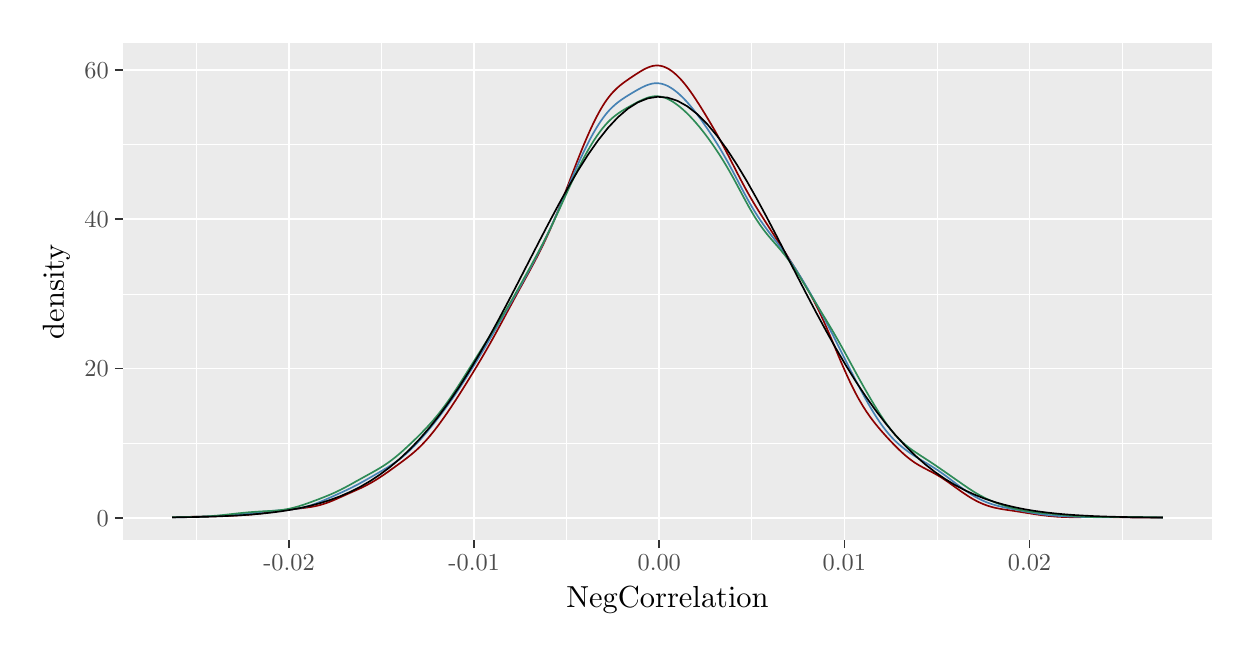
\begin{tikzpicture}[x=1pt,y=1pt]
\definecolor{fillColor}{RGB}{255,255,255}
\path[use as bounding box,fill=fillColor,fill opacity=0.00] (0,0) rectangle (433.62,216.81);
\begin{scope}
\path[clip] (  0.00,  0.00) rectangle (433.62,216.81);
\definecolor{drawColor}{RGB}{255,255,255}
\definecolor{fillColor}{RGB}{255,255,255}

\path[draw=drawColor,line width= 0.6pt,line join=round,line cap=round,fill=fillColor] (  0.00,  0.00) rectangle (433.62,216.81);
\end{scope}
\begin{scope}
\path[clip] ( 34.27, 31.53) rectangle (428.12,211.31);
\definecolor{fillColor}{gray}{0.92}

\path[fill=fillColor] ( 34.27, 31.53) rectangle (428.12,211.31);
\definecolor{drawColor}{RGB}{255,255,255}

\path[draw=drawColor,line width= 0.3pt,line join=round] ( 34.27, 66.67) --
	(428.12, 66.67);

\path[draw=drawColor,line width= 0.3pt,line join=round] ( 34.27,120.60) --
	(428.12,120.60);

\path[draw=drawColor,line width= 0.3pt,line join=round] ( 34.27,174.54) --
	(428.12,174.54);

\path[draw=drawColor,line width= 0.3pt,line join=round] ( 61.01, 31.53) --
	( 61.01,211.31);

\path[draw=drawColor,line width= 0.3pt,line join=round] (127.90, 31.53) --
	(127.90,211.31);

\path[draw=drawColor,line width= 0.3pt,line join=round] (194.78, 31.53) --
	(194.78,211.31);

\path[draw=drawColor,line width= 0.3pt,line join=round] (261.67, 31.53) --
	(261.67,211.31);

\path[draw=drawColor,line width= 0.3pt,line join=round] (328.56, 31.53) --
	(328.56,211.31);

\path[draw=drawColor,line width= 0.3pt,line join=round] (395.45, 31.53) --
	(395.45,211.31);

\path[draw=drawColor,line width= 0.6pt,line join=round] ( 34.27, 39.70) --
	(428.12, 39.70);

\path[draw=drawColor,line width= 0.6pt,line join=round] ( 34.27, 93.64) --
	(428.12, 93.64);

\path[draw=drawColor,line width= 0.6pt,line join=round] ( 34.27,147.57) --
	(428.12,147.57);

\path[draw=drawColor,line width= 0.6pt,line join=round] ( 34.27,201.50) --
	(428.12,201.50);

\path[draw=drawColor,line width= 0.6pt,line join=round] ( 94.45, 31.53) --
	( 94.45,211.31);

\path[draw=drawColor,line width= 0.6pt,line join=round] (161.34, 31.53) --
	(161.34,211.31);

\path[draw=drawColor,line width= 0.6pt,line join=round] (228.23, 31.53) --
	(228.23,211.31);

\path[draw=drawColor,line width= 0.6pt,line join=round] (295.12, 31.53) --
	(295.12,211.31);

\path[draw=drawColor,line width= 0.6pt,line join=round] (362.01, 31.53) --
	(362.01,211.31);
\definecolor{drawColor}{RGB}{139,0,0}

\path[draw=drawColor,line width= 0.6pt,line join=round] ( 52.17, 39.90) --
	( 52.87, 39.92) --
	( 53.57, 39.93) --
	( 54.27, 39.95) --
	( 54.97, 39.97) --
	( 55.67, 39.98) --
	( 56.37, 40.00) --
	( 57.07, 40.01) --
	( 57.78, 40.03) --
	( 58.48, 40.04) --
	( 59.18, 40.06) --
	( 59.88, 40.07) --
	( 60.58, 40.09) --
	( 61.28, 40.11) --
	( 61.98, 40.12) --
	( 62.68, 40.14) --
	( 63.38, 40.15) --
	( 64.08, 40.17) --
	( 64.78, 40.19) --
	( 65.48, 40.20) --
	( 66.18, 40.22) --
	( 66.88, 40.24) --
	( 67.59, 40.26) --
	( 68.29, 40.28) --
	( 68.99, 40.31) --
	( 69.69, 40.33) --
	( 70.39, 40.35) --
	( 71.09, 40.38) --
	( 71.79, 40.40) --
	( 72.49, 40.43) --
	( 73.19, 40.46) --
	( 73.89, 40.49) --
	( 74.59, 40.52) --
	( 75.29, 40.55) --
	( 75.99, 40.58) --
	( 76.69, 40.62) --
	( 77.39, 40.66) --
	( 78.10, 40.70) --
	( 78.80, 40.75) --
	( 79.50, 40.80) --
	( 80.20, 40.85) --
	( 80.90, 40.91) --
	( 81.60, 40.98) --
	( 82.30, 41.05) --
	( 83.00, 41.12) --
	( 83.70, 41.20) --
	( 84.40, 41.29) --
	( 85.10, 41.38) --
	( 85.80, 41.47) --
	( 86.50, 41.57) --
	( 87.20, 41.67) --
	( 87.90, 41.77) --
	( 88.61, 41.87) --
	( 89.31, 41.97) --
	( 90.01, 42.07) --
	( 90.71, 42.17) --
	( 91.41, 42.27) --
	( 92.11, 42.37) --
	( 92.81, 42.46) --
	( 93.51, 42.55) --
	( 94.21, 42.64) --
	( 94.91, 42.72) --
	( 95.61, 42.80) --
	( 96.31, 42.88) --
	( 97.01, 42.96) --
	( 97.71, 43.03) --
	( 98.42, 43.11) --
	( 99.12, 43.19) --
	( 99.82, 43.27) --
	(100.52, 43.35) --
	(101.22, 43.45) --
	(101.92, 43.55) --
	(102.62, 43.66) --
	(103.32, 43.79) --
	(104.02, 43.93) --
	(104.72, 44.09) --
	(105.42, 44.26) --
	(106.12, 44.45) --
	(106.82, 44.67) --
	(107.52, 44.89) --
	(108.22, 45.14) --
	(108.93, 45.41) --
	(109.63, 45.68) --
	(110.33, 45.97) --
	(111.03, 46.27) --
	(111.73, 46.57) --
	(112.43, 46.89) --
	(113.13, 47.20) --
	(113.83, 47.51) --
	(114.53, 47.83) --
	(115.23, 48.14) --
	(115.93, 48.45) --
	(116.63, 48.77) --
	(117.33, 49.08) --
	(118.03, 49.39) --
	(118.73, 49.70) --
	(119.44, 50.02) --
	(120.14, 50.34) --
	(120.84, 50.67) --
	(121.54, 51.01) --
	(122.24, 51.36) --
	(122.94, 51.73) --
	(123.64, 52.11) --
	(124.34, 52.50) --
	(125.04, 52.91) --
	(125.74, 53.33) --
	(126.44, 53.77) --
	(127.14, 54.22) --
	(127.84, 54.69) --
	(128.54, 55.16) --
	(129.24, 55.64) --
	(129.95, 56.13) --
	(130.65, 56.63) --
	(131.35, 57.13) --
	(132.05, 57.63) --
	(132.75, 58.14) --
	(133.45, 58.65) --
	(134.15, 59.16) --
	(134.85, 59.67) --
	(135.55, 60.19) --
	(136.25, 60.72) --
	(136.95, 61.25) --
	(137.65, 61.80) --
	(138.35, 62.36) --
	(139.05, 62.94) --
	(139.76, 63.54) --
	(140.46, 64.16) --
	(141.16, 64.81) --
	(141.86, 65.49) --
	(142.56, 66.19) --
	(143.26, 66.92) --
	(143.96, 67.68) --
	(144.66, 68.47) --
	(145.36, 69.29) --
	(146.06, 70.14) --
	(146.76, 71.01) --
	(147.46, 71.91) --
	(148.16, 72.83) --
	(148.86, 73.77) --
	(149.56, 74.74) --
	(150.27, 75.72) --
	(150.97, 76.71) --
	(151.67, 77.73) --
	(152.37, 78.76) --
	(153.07, 79.80) --
	(153.77, 80.86) --
	(154.47, 81.93) --
	(155.17, 83.01) --
	(155.87, 84.10) --
	(156.57, 85.21) --
	(157.27, 86.32) --
	(157.97, 87.44) --
	(158.67, 88.56) --
	(159.37, 89.70) --
	(160.07, 90.84) --
	(160.78, 91.98) --
	(161.48, 93.14) --
	(162.18, 94.29) --
	(162.88, 95.46) --
	(163.58, 96.63) --
	(164.28, 97.82) --
	(164.98, 99.02) --
	(165.68,100.22) --
	(166.38,101.45) --
	(167.08,102.68) --
	(167.78,103.93) --
	(168.48,105.19) --
	(169.18,106.46) --
	(169.88,107.75) --
	(170.59,109.05) --
	(171.29,110.35) --
	(171.99,111.66) --
	(172.69,112.97) --
	(173.39,114.28) --
	(174.09,115.58) --
	(174.79,116.88) --
	(175.49,118.18) --
	(176.19,119.47) --
	(176.89,120.76) --
	(177.59,122.04) --
	(178.29,123.31) --
	(178.99,124.58) --
	(179.69,125.86) --
	(180.39,127.13) --
	(181.10,128.42) --
	(181.80,129.71) --
	(182.50,131.02) --
	(183.20,132.34) --
	(183.90,133.68) --
	(184.60,135.05) --
	(185.30,136.44) --
	(186.00,137.86) --
	(186.70,139.31) --
	(187.40,140.80) --
	(188.10,142.33) --
	(188.80,143.90) --
	(189.50,145.51) --
	(190.20,147.15) --
	(190.90,148.83) --
	(191.61,150.55) --
	(192.31,152.30) --
	(193.01,154.08) --
	(193.71,155.89) --
	(194.41,157.71) --
	(195.11,159.54) --
	(195.81,161.38) --
	(196.51,163.22) --
	(197.21,165.05) --
	(197.91,166.86) --
	(198.61,168.66) --
	(199.31,170.44) --
	(200.01,172.18) --
	(200.71,173.90) --
	(201.42,175.58) --
	(202.12,177.22) --
	(202.82,178.82) --
	(203.52,180.37) --
	(204.22,181.86) --
	(204.92,183.30) --
	(205.62,184.67) --
	(206.32,185.99) --
	(207.02,187.24) --
	(207.72,188.42) --
	(208.42,189.53) --
	(209.12,190.56) --
	(209.82,191.51) --
	(210.52,192.39) --
	(211.22,193.21) --
	(211.93,193.96) --
	(212.63,194.66) --
	(213.33,195.30) --
	(214.03,195.90) --
	(214.73,196.46) --
	(215.43,196.98) --
	(216.13,197.49) --
	(216.83,197.98) --
	(217.53,198.46) --
	(218.23,198.93) --
	(218.93,199.40) --
	(219.63,199.86) --
	(220.33,200.31) --
	(221.03,200.75) --
	(221.73,201.18) --
	(222.44,201.58) --
	(223.14,201.95) --
	(223.84,202.28) --
	(224.54,202.57) --
	(225.24,202.81) --
	(225.94,202.99) --
	(226.64,203.10) --
	(227.34,203.14) --
	(228.04,203.11) --
	(228.74,203.01) --
	(229.44,202.84) --
	(230.14,202.60) --
	(230.84,202.30) --
	(231.54,201.92) --
	(232.24,201.47) --
	(232.95,200.97) --
	(233.65,200.41) --
	(234.35,199.79) --
	(235.05,199.12) --
	(235.75,198.40) --
	(236.45,197.63) --
	(237.15,196.81) --
	(237.85,195.94) --
	(238.55,195.02) --
	(239.25,194.07) --
	(239.95,193.08) --
	(240.65,192.05) --
	(241.35,191.00) --
	(242.05,189.92) --
	(242.76,188.82) --
	(243.46,187.71) --
	(244.16,186.57) --
	(244.86,185.43) --
	(245.56,184.27) --
	(246.26,183.10) --
	(246.96,181.92) --
	(247.66,180.72) --
	(248.36,179.51) --
	(249.06,178.27) --
	(249.76,177.02) --
	(250.46,175.74) --
	(251.16,174.44) --
	(251.86,173.13) --
	(252.56,171.79) --
	(253.27,170.44) --
	(253.97,169.07) --
	(254.67,167.70) --
	(255.37,166.33) --
	(256.07,164.96) --
	(256.77,163.60) --
	(257.47,162.25) --
	(258.17,160.92) --
	(258.87,159.61) --
	(259.57,158.32) --
	(260.27,157.07) --
	(260.97,155.84) --
	(261.67,154.63) --
	(262.37,153.44) --
	(263.07,152.28) --
	(263.78,151.14) --
	(264.48,150.01) --
	(265.18,148.89) --
	(265.88,147.79) --
	(266.58,146.69) --
	(267.28,145.60) --
	(267.98,144.51) --
	(268.68,143.42) --
	(269.38,142.33) --
	(270.08,141.23) --
	(270.78,140.14) --
	(271.48,139.04) --
	(272.18,137.94) --
	(272.88,136.83) --
	(273.59,135.73) --
	(274.29,134.62) --
	(274.99,133.51) --
	(275.69,132.39) --
	(276.39,131.28) --
	(277.09,130.15) --
	(277.79,129.03) --
	(278.49,127.89) --
	(279.19,126.74) --
	(279.89,125.58) --
	(280.59,124.40) --
	(281.29,123.20) --
	(281.99,121.98) --
	(282.69,120.72) --
	(283.39,119.42) --
	(284.10,118.09) --
	(284.80,116.72) --
	(285.50,115.31) --
	(286.20,113.86) --
	(286.90,112.37) --
	(287.60,110.84) --
	(288.30,109.26) --
	(289.00,107.66) --
	(289.70,106.03) --
	(290.40,104.38) --
	(291.10,102.71) --
	(291.80,101.04) --
	(292.50, 99.36) --
	(293.20, 97.69) --
	(293.90, 96.04) --
	(294.61, 94.42) --
	(295.31, 92.82) --
	(296.01, 91.25) --
	(296.71, 89.73) --
	(297.41, 88.24) --
	(298.11, 86.81) --
	(298.81, 85.42) --
	(299.51, 84.09) --
	(300.21, 82.81) --
	(300.91, 81.59) --
	(301.61, 80.41) --
	(302.31, 79.28) --
	(303.01, 78.20) --
	(303.71, 77.17) --
	(304.41, 76.18) --
	(305.12, 75.23) --
	(305.82, 74.31) --
	(306.52, 73.43) --
	(307.22, 72.58) --
	(307.92, 71.74) --
	(308.62, 70.93) --
	(309.32, 70.14) --
	(310.02, 69.36) --
	(310.72, 68.59) --
	(311.42, 67.84) --
	(312.12, 67.10) --
	(312.82, 66.37) --
	(313.52, 65.65) --
	(314.22, 64.95) --
	(314.93, 64.26) --
	(315.63, 63.60) --
	(316.33, 62.95) --
	(317.03, 62.33) --
	(317.73, 61.74) --
	(318.43, 61.18) --
	(319.13, 60.64) --
	(319.83, 60.13) --
	(320.53, 59.65) --
	(321.23, 59.20) --
	(321.93, 58.78) --
	(322.63, 58.37) --
	(323.33, 57.99) --
	(324.03, 57.61) --
	(324.73, 57.25) --
	(325.44, 56.89) --
	(326.14, 56.53) --
	(326.84, 56.16) --
	(327.54, 55.78) --
	(328.24, 55.39) --
	(328.94, 54.99) --
	(329.64, 54.57) --
	(330.34, 54.13) --
	(331.04, 53.67) --
	(331.74, 53.21) --
	(332.44, 52.72) --
	(333.14, 52.23) --
	(333.84, 51.72) --
	(334.54, 51.22) --
	(335.24, 50.71) --
	(335.95, 50.20) --
	(336.65, 49.70) --
	(337.35, 49.20) --
	(338.05, 48.71) --
	(338.75, 48.24) --
	(339.45, 47.78) --
	(340.15, 47.33) --
	(340.85, 46.90) --
	(341.55, 46.49) --
	(342.25, 46.10) --
	(342.95, 45.73) --
	(343.65, 45.38) --
	(344.35, 45.06) --
	(345.05, 44.76) --
	(345.76, 44.48) --
	(346.46, 44.22) --
	(347.16, 43.98) --
	(347.86, 43.77) --
	(348.56, 43.57) --
	(349.26, 43.39) --
	(349.96, 43.23) --
	(350.66, 43.09) --
	(351.36, 42.95) --
	(352.06, 42.83) --
	(352.76, 42.72) --
	(353.46, 42.61) --
	(354.16, 42.50) --
	(354.86, 42.40) --
	(355.56, 42.30) --
	(356.27, 42.20) --
	(356.97, 42.09) --
	(357.67, 41.99) --
	(358.37, 41.88) --
	(359.07, 41.77) --
	(359.77, 41.66) --
	(360.47, 41.55) --
	(361.17, 41.44) --
	(361.87, 41.33) --
	(362.57, 41.22) --
	(363.27, 41.11) --
	(363.97, 41.00) --
	(364.67, 40.90) --
	(365.37, 40.80) --
	(366.07, 40.70) --
	(366.78, 40.61) --
	(367.48, 40.53) --
	(368.18, 40.45) --
	(368.88, 40.37) --
	(369.58, 40.30) --
	(370.28, 40.23) --
	(370.98, 40.18) --
	(371.68, 40.12) --
	(372.38, 40.08) --
	(373.08, 40.04) --
	(373.78, 40.00) --
	(374.48, 39.98) --
	(375.18, 39.95) --
	(375.88, 39.94) --
	(376.58, 39.92) --
	(377.29, 39.92) --
	(377.99, 39.91) --
	(378.69, 39.92) --
	(379.39, 39.92) --
	(380.09, 39.92) --
	(380.79, 39.93) --
	(381.49, 39.94) --
	(382.19, 39.95) --
	(382.89, 39.95) --
	(383.59, 39.96) --
	(384.29, 39.97) --
	(384.99, 39.97) --
	(385.69, 39.97) --
	(386.39, 39.97) --
	(387.10, 39.97) --
	(387.80, 39.97) --
	(388.50, 39.97) --
	(389.20, 39.96) --
	(389.90, 39.95) --
	(390.60, 39.94) --
	(391.30, 39.94) --
	(392.00, 39.93) --
	(392.70, 39.92) --
	(393.40, 39.91) --
	(394.10, 39.90) --
	(394.80, 39.89) --
	(395.50, 39.87) --
	(396.20, 39.86) --
	(396.90, 39.86) --
	(397.61, 39.85) --
	(398.31, 39.84) --
	(399.01, 39.83) --
	(399.71, 39.83) --
	(400.41, 39.82) --
	(401.11, 39.82) --
	(401.81, 39.81) --
	(402.51, 39.81) --
	(403.21, 39.81) --
	(403.91, 39.81) --
	(404.61, 39.81) --
	(405.31, 39.81) --
	(406.01, 39.82) --
	(406.71, 39.82) --
	(407.41, 39.82) --
	(408.12, 39.82) --
	(408.82, 39.82) --
	(409.52, 39.82) --
	(410.22, 39.82);
\definecolor{drawColor}{RGB}{70,130,180}

\path[draw=drawColor,line width= 0.6pt,line join=round] ( 52.17, 39.85) --
	( 52.87, 39.86) --
	( 53.57, 39.87) --
	( 54.27, 39.88) --
	( 54.97, 39.90) --
	( 55.67, 39.91) --
	( 56.37, 39.92) --
	( 57.07, 39.94) --
	( 57.78, 39.95) --
	( 58.48, 39.97) --
	( 59.18, 39.99) --
	( 59.88, 40.02) --
	( 60.58, 40.04) --
	( 61.28, 40.07) --
	( 61.98, 40.09) --
	( 62.68, 40.12) --
	( 63.38, 40.15) --
	( 64.08, 40.18) --
	( 64.78, 40.21) --
	( 65.48, 40.25) --
	( 66.18, 40.28) --
	( 66.88, 40.31) --
	( 67.59, 40.35) --
	( 68.29, 40.38) --
	( 68.99, 40.42) --
	( 69.69, 40.46) --
	( 70.39, 40.50) --
	( 71.09, 40.54) --
	( 71.79, 40.58) --
	( 72.49, 40.63) --
	( 73.19, 40.67) --
	( 73.89, 40.73) --
	( 74.59, 40.78) --
	( 75.29, 40.84) --
	( 75.99, 40.90) --
	( 76.69, 40.97) --
	( 77.39, 41.04) --
	( 78.10, 41.11) --
	( 78.80, 41.18) --
	( 79.50, 41.26) --
	( 80.20, 41.34) --
	( 80.90, 41.42) --
	( 81.60, 41.50) --
	( 82.30, 41.58) --
	( 83.00, 41.66) --
	( 83.70, 41.74) --
	( 84.40, 41.81) --
	( 85.10, 41.89) --
	( 85.80, 41.96) --
	( 86.50, 42.03) --
	( 87.20, 42.09) --
	( 87.90, 42.15) --
	( 88.61, 42.21) --
	( 89.31, 42.26) --
	( 90.01, 42.31) --
	( 90.71, 42.36) --
	( 91.41, 42.41) --
	( 92.11, 42.46) --
	( 92.81, 42.51) --
	( 93.51, 42.57) --
	( 94.21, 42.63) --
	( 94.91, 42.70) --
	( 95.61, 42.77) --
	( 96.31, 42.86) --
	( 97.01, 42.96) --
	( 97.71, 43.08) --
	( 98.42, 43.21) --
	( 99.12, 43.35) --
	( 99.82, 43.51) --
	(100.52, 43.69) --
	(101.22, 43.89) --
	(101.92, 44.10) --
	(102.62, 44.33) --
	(103.32, 44.57) --
	(104.02, 44.82) --
	(104.72, 45.09) --
	(105.42, 45.37) --
	(106.12, 45.65) --
	(106.82, 45.95) --
	(107.52, 46.25) --
	(108.22, 46.55) --
	(108.93, 46.86) --
	(109.63, 47.17) --
	(110.33, 47.48) --
	(111.03, 47.80) --
	(111.73, 48.11) --
	(112.43, 48.43) --
	(113.13, 48.75) --
	(113.83, 49.07) --
	(114.53, 49.39) --
	(115.23, 49.72) --
	(115.93, 50.05) --
	(116.63, 50.39) --
	(117.33, 50.74) --
	(118.03, 51.10) --
	(118.73, 51.46) --
	(119.44, 51.83) --
	(120.14, 52.21) --
	(120.84, 52.60) --
	(121.54, 52.99) --
	(122.24, 53.38) --
	(122.94, 53.78) --
	(123.64, 54.18) --
	(124.34, 54.58) --
	(125.04, 54.98) --
	(125.74, 55.38) --
	(126.44, 55.79) --
	(127.14, 56.19) --
	(127.84, 56.60) --
	(128.54, 57.02) --
	(129.24, 57.44) --
	(129.95, 57.86) --
	(130.65, 58.30) --
	(131.35, 58.75) --
	(132.05, 59.21) --
	(132.75, 59.69) --
	(133.45, 60.18) --
	(134.15, 60.70) --
	(134.85, 61.25) --
	(135.55, 61.81) --
	(136.25, 62.40) --
	(136.95, 63.01) --
	(137.65, 63.64) --
	(138.35, 64.30) --
	(139.05, 64.99) --
	(139.76, 65.69) --
	(140.46, 66.42) --
	(141.16, 67.17) --
	(141.86, 67.94) --
	(142.56, 68.73) --
	(143.26, 69.53) --
	(143.96, 70.35) --
	(144.66, 71.19) --
	(145.36, 72.04) --
	(146.06, 72.90) --
	(146.76, 73.77) --
	(147.46, 74.66) --
	(148.16, 75.56) --
	(148.86, 76.47) --
	(149.56, 77.39) --
	(150.27, 78.33) --
	(150.97, 79.28) --
	(151.67, 80.24) --
	(152.37, 81.22) --
	(153.07, 82.21) --
	(153.77, 83.22) --
	(154.47, 84.24) --
	(155.17, 85.28) --
	(155.87, 86.33) --
	(156.57, 87.39) --
	(157.27, 88.47) --
	(157.97, 89.55) --
	(158.67, 90.65) --
	(159.37, 91.75) --
	(160.07, 92.87) --
	(160.78, 93.99) --
	(161.48, 95.12) --
	(162.18, 96.25) --
	(162.88, 97.40) --
	(163.58, 98.55) --
	(164.28, 99.71) --
	(164.98,100.88) --
	(165.68,102.05) --
	(166.38,103.23) --
	(167.08,104.42) --
	(167.78,105.61) --
	(168.48,106.81) --
	(169.18,108.01) --
	(169.88,109.21) --
	(170.59,110.42) --
	(171.29,111.63) --
	(171.99,112.84) --
	(172.69,114.05) --
	(173.39,115.26) --
	(174.09,116.48) --
	(174.79,117.69) --
	(175.49,118.91) --
	(176.19,120.14) --
	(176.89,121.37) --
	(177.59,122.61) --
	(178.29,123.86) --
	(178.99,125.11) --
	(179.69,126.37) --
	(180.39,127.64) --
	(181.10,128.93) --
	(181.80,130.22) --
	(182.50,131.53) --
	(183.20,132.85) --
	(183.90,134.19) --
	(184.60,135.55) --
	(185.30,136.93) --
	(186.00,138.33) --
	(186.70,139.75) --
	(187.40,141.20) --
	(188.10,142.68) --
	(188.80,144.19) --
	(189.50,145.73) --
	(190.20,147.29) --
	(190.90,148.88) --
	(191.61,150.49) --
	(192.31,152.13) --
	(193.01,153.78) --
	(193.71,155.44) --
	(194.41,157.10) --
	(195.11,158.77) --
	(195.81,160.43) --
	(196.51,162.09) --
	(197.21,163.72) --
	(197.91,165.34) --
	(198.61,166.93) --
	(199.31,168.49) --
	(200.01,170.02) --
	(200.71,171.51) --
	(201.42,172.97) --
	(202.12,174.38) --
	(202.82,175.75) --
	(203.52,177.08) --
	(204.22,178.36) --
	(204.92,179.58) --
	(205.62,180.75) --
	(206.32,181.87) --
	(207.02,182.93) --
	(207.72,183.93) --
	(208.42,184.87) --
	(209.12,185.76) --
	(209.82,186.58) --
	(210.52,187.34) --
	(211.22,188.04) --
	(211.93,188.69) --
	(212.63,189.30) --
	(213.33,189.86) --
	(214.03,190.39) --
	(214.73,190.89) --
	(215.43,191.36) --
	(216.13,191.81) --
	(216.83,192.25) --
	(217.53,192.68) --
	(218.23,193.10) --
	(218.93,193.52) --
	(219.63,193.93) --
	(220.33,194.33) --
	(221.03,194.72) --
	(221.73,195.09) --
	(222.44,195.44) --
	(223.14,195.76) --
	(223.84,196.05) --
	(224.54,196.29) --
	(225.24,196.49) --
	(225.94,196.64) --
	(226.64,196.72) --
	(227.34,196.74) --
	(228.04,196.70) --
	(228.74,196.60) --
	(229.44,196.44) --
	(230.14,196.21) --
	(230.84,195.93) --
	(231.54,195.59) --
	(232.24,195.18) --
	(232.95,194.73) --
	(233.65,194.24) --
	(234.35,193.69) --
	(235.05,193.11) --
	(235.75,192.49) --
	(236.45,191.82) --
	(237.15,191.12) --
	(237.85,190.38) --
	(238.55,189.61) --
	(239.25,188.80) --
	(239.95,187.96) --
	(240.65,187.09) --
	(241.35,186.20) --
	(242.05,185.28) --
	(242.76,184.33) --
	(243.46,183.37) --
	(244.16,182.38) --
	(244.86,181.37) --
	(245.56,180.35) --
	(246.26,179.31) --
	(246.96,178.25) --
	(247.66,177.18) --
	(248.36,176.08) --
	(249.06,174.96) --
	(249.76,173.82) --
	(250.46,172.65) --
	(251.16,171.45) --
	(251.86,170.23) --
	(252.56,168.99) --
	(253.27,167.72) --
	(253.97,166.42) --
	(254.67,165.11) --
	(255.37,163.78) --
	(256.07,162.45) --
	(256.77,161.11) --
	(257.47,159.77) --
	(258.17,158.44) --
	(258.87,157.12) --
	(259.57,155.83) --
	(260.27,154.56) --
	(260.97,153.32) --
	(261.67,152.11) --
	(262.37,150.94) --
	(263.07,149.80) --
	(263.78,148.70) --
	(264.48,147.64) --
	(265.18,146.61) --
	(265.88,145.61) --
	(266.58,144.64) --
	(267.28,143.69) --
	(267.98,142.76) --
	(268.68,141.84) --
	(269.38,140.93) --
	(270.08,140.02) --
	(270.78,139.10) --
	(271.48,138.18) --
	(272.18,137.25) --
	(272.88,136.30) --
	(273.59,135.34) --
	(274.29,134.35) --
	(274.99,133.35) --
	(275.69,132.32) --
	(276.39,131.28) --
	(277.09,130.21) --
	(277.79,129.13) --
	(278.49,128.02) --
	(279.19,126.90) --
	(279.89,125.76) --
	(280.59,124.60) --
	(281.29,123.43) --
	(281.99,122.24) --
	(282.69,121.03) --
	(283.39,119.81) --
	(284.10,118.58) --
	(284.80,117.33) --
	(285.50,116.06) --
	(286.20,114.78) --
	(286.90,113.49) --
	(287.60,112.18) --
	(288.30,110.86) --
	(289.00,109.52) --
	(289.70,108.17) --
	(290.40,106.81) --
	(291.10,105.44) --
	(291.80,104.06) --
	(292.50,102.67) --
	(293.20,101.28) --
	(293.90, 99.88) --
	(294.61, 98.48) --
	(295.31, 97.07) --
	(296.01, 95.68) --
	(296.71, 94.28) --
	(297.41, 92.89) --
	(298.11, 91.51) --
	(298.81, 90.14) --
	(299.51, 88.79) --
	(300.21, 87.44) --
	(300.91, 86.11) --
	(301.61, 84.80) --
	(302.31, 83.51) --
	(303.01, 82.25) --
	(303.71, 81.00) --
	(304.41, 79.79) --
	(305.12, 78.61) --
	(305.82, 77.45) --
	(306.52, 76.34) --
	(307.22, 75.26) --
	(307.92, 74.22) --
	(308.62, 73.23) --
	(309.32, 72.28) --
	(310.02, 71.37) --
	(310.72, 70.50) --
	(311.42, 69.68) --
	(312.12, 68.89) --
	(312.82, 68.15) --
	(313.52, 67.45) --
	(314.22, 66.79) --
	(314.93, 66.15) --
	(315.63, 65.55) --
	(316.33, 64.98) --
	(317.03, 64.43) --
	(317.73, 63.91) --
	(318.43, 63.41) --
	(319.13, 62.92) --
	(319.83, 62.46) --
	(320.53, 62.00) --
	(321.23, 61.56) --
	(321.93, 61.13) --
	(322.63, 60.71) --
	(323.33, 60.29) --
	(324.03, 59.87) --
	(324.73, 59.46) --
	(325.44, 59.04) --
	(326.14, 58.61) --
	(326.84, 58.18) --
	(327.54, 57.74) --
	(328.24, 57.29) --
	(328.94, 56.83) --
	(329.64, 56.35) --
	(330.34, 55.86) --
	(331.04, 55.36) --
	(331.74, 54.85) --
	(332.44, 54.33) --
	(333.14, 53.81) --
	(333.84, 53.28) --
	(334.54, 52.74) --
	(335.24, 52.21) --
	(335.95, 51.68) --
	(336.65, 51.15) --
	(337.35, 50.63) --
	(338.05, 50.13) --
	(338.75, 49.63) --
	(339.45, 49.15) --
	(340.15, 48.68) --
	(340.85, 48.24) --
	(341.55, 47.81) --
	(342.25, 47.40) --
	(342.95, 47.01) --
	(343.65, 46.63) --
	(344.35, 46.28) --
	(345.05, 45.95) --
	(345.76, 45.64) --
	(346.46, 45.35) --
	(347.16, 45.08) --
	(347.86, 44.83) --
	(348.56, 44.60) --
	(349.26, 44.38) --
	(349.96, 44.18) --
	(350.66, 43.99) --
	(351.36, 43.82) --
	(352.06, 43.65) --
	(352.76, 43.49) --
	(353.46, 43.34) --
	(354.16, 43.20) --
	(354.86, 43.06) --
	(355.56, 42.92) --
	(356.27, 42.78) --
	(356.97, 42.65) --
	(357.67, 42.51) --
	(358.37, 42.38) --
	(359.07, 42.24) --
	(359.77, 42.11) --
	(360.47, 41.97) --
	(361.17, 41.84) --
	(361.87, 41.71) --
	(362.57, 41.58) --
	(363.27, 41.46) --
	(363.97, 41.34) --
	(364.67, 41.22) --
	(365.37, 41.11) --
	(366.07, 41.01) --
	(366.78, 40.92) --
	(367.48, 40.83) --
	(368.18, 40.75) --
	(368.88, 40.67) --
	(369.58, 40.60) --
	(370.28, 40.54) --
	(370.98, 40.48) --
	(371.68, 40.43) --
	(372.38, 40.38) --
	(373.08, 40.34) --
	(373.78, 40.30) --
	(374.48, 40.26) --
	(375.18, 40.22) --
	(375.88, 40.19) --
	(376.58, 40.16) --
	(377.29, 40.13) --
	(377.99, 40.11) --
	(378.69, 40.08) --
	(379.39, 40.06) --
	(380.09, 40.04) --
	(380.79, 40.01) --
	(381.49, 40.00) --
	(382.19, 39.98) --
	(382.89, 39.96) --
	(383.59, 39.95) --
	(384.29, 39.94) --
	(384.99, 39.93) --
	(385.69, 39.92) --
	(386.39, 39.92) --
	(387.10, 39.92) --
	(387.80, 39.92) --
	(388.50, 39.92) --
	(389.20, 39.92) --
	(389.90, 39.92) --
	(390.60, 39.92) --
	(391.30, 39.92) --
	(392.00, 39.93) --
	(392.70, 39.93) --
	(393.40, 39.93) --
	(394.10, 39.93) --
	(394.80, 39.93) --
	(395.50, 39.93) --
	(396.20, 39.92) --
	(396.90, 39.92) --
	(397.61, 39.92) --
	(398.31, 39.91) --
	(399.01, 39.91) --
	(399.71, 39.90) --
	(400.41, 39.90) --
	(401.11, 39.89) --
	(401.81, 39.89) --
	(402.51, 39.88) --
	(403.21, 39.87) --
	(403.91, 39.87) --
	(404.61, 39.86) --
	(405.31, 39.86) --
	(406.01, 39.86) --
	(406.71, 39.85) --
	(407.41, 39.85) --
	(408.12, 39.84) --
	(408.82, 39.83) --
	(409.52, 39.83) --
	(410.22, 39.82);
\definecolor{drawColor}{RGB}{46,139,87}

\path[draw=drawColor,line width= 0.6pt,line join=round] ( 52.17, 39.91) --
	( 52.87, 39.92) --
	( 53.57, 39.93) --
	( 54.27, 39.95) --
	( 54.97, 39.96) --
	( 55.67, 39.97) --
	( 56.37, 39.98) --
	( 57.07, 39.99) --
	( 57.78, 40.01) --
	( 58.48, 40.02) --
	( 59.18, 40.03) --
	( 59.88, 40.05) --
	( 60.58, 40.07) --
	( 61.28, 40.09) --
	( 61.98, 40.11) --
	( 62.68, 40.13) --
	( 63.38, 40.16) --
	( 64.08, 40.19) --
	( 64.78, 40.23) --
	( 65.48, 40.27) --
	( 66.18, 40.32) --
	( 66.88, 40.37) --
	( 67.59, 40.43) --
	( 68.29, 40.49) --
	( 68.99, 40.55) --
	( 69.69, 40.62) --
	( 70.39, 40.69) --
	( 71.09, 40.77) --
	( 71.79, 40.84) --
	( 72.49, 40.92) --
	( 73.19, 41.00) --
	( 73.89, 41.08) --
	( 74.59, 41.15) --
	( 75.29, 41.23) --
	( 75.99, 41.31) --
	( 76.69, 41.38) --
	( 77.39, 41.46) --
	( 78.10, 41.53) --
	( 78.80, 41.59) --
	( 79.50, 41.66) --
	( 80.20, 41.72) --
	( 80.90, 41.77) --
	( 81.60, 41.83) --
	( 82.30, 41.88) --
	( 83.00, 41.93) --
	( 83.70, 41.97) --
	( 84.40, 42.01) --
	( 85.10, 42.05) --
	( 85.80, 42.08) --
	( 86.50, 42.12) --
	( 87.20, 42.16) --
	( 87.90, 42.20) --
	( 88.61, 42.24) --
	( 89.31, 42.29) --
	( 90.01, 42.35) --
	( 90.71, 42.42) --
	( 91.41, 42.49) --
	( 92.11, 42.58) --
	( 92.81, 42.69) --
	( 93.51, 42.80) --
	( 94.21, 42.93) --
	( 94.91, 43.08) --
	( 95.61, 43.24) --
	( 96.31, 43.42) --
	( 97.01, 43.61) --
	( 97.71, 43.81) --
	( 98.42, 44.02) --
	( 99.12, 44.25) --
	( 99.82, 44.48) --
	(100.52, 44.72) --
	(101.22, 44.97) --
	(101.92, 45.22) --
	(102.62, 45.48) --
	(103.32, 45.74) --
	(104.02, 46.00) --
	(104.72, 46.26) --
	(105.42, 46.53) --
	(106.12, 46.80) --
	(106.82, 47.08) --
	(107.52, 47.36) --
	(108.22, 47.64) --
	(108.93, 47.93) --
	(109.63, 48.23) --
	(110.33, 48.54) --
	(111.03, 48.85) --
	(111.73, 49.18) --
	(112.43, 49.52) --
	(113.13, 49.86) --
	(113.83, 50.22) --
	(114.53, 50.59) --
	(115.23, 50.96) --
	(115.93, 51.34) --
	(116.63, 51.72) --
	(117.33, 52.11) --
	(118.03, 52.50) --
	(118.73, 52.90) --
	(119.44, 53.29) --
	(120.14, 53.68) --
	(120.84, 54.07) --
	(121.54, 54.45) --
	(122.24, 54.84) --
	(122.94, 55.23) --
	(123.64, 55.61) --
	(124.34, 56.00) --
	(125.04, 56.39) --
	(125.74, 56.79) --
	(126.44, 57.19) --
	(127.14, 57.61) --
	(127.84, 58.04) --
	(128.54, 58.48) --
	(129.24, 58.94) --
	(129.95, 59.42) --
	(130.65, 59.91) --
	(131.35, 60.43) --
	(132.05, 60.97) --
	(132.75, 61.52) --
	(133.45, 62.09) --
	(134.15, 62.68) --
	(134.85, 63.29) --
	(135.55, 63.90) --
	(136.25, 64.54) --
	(136.95, 65.18) --
	(137.65, 65.83) --
	(138.35, 66.49) --
	(139.05, 67.16) --
	(139.76, 67.83) --
	(140.46, 68.52) --
	(141.16, 69.21) --
	(141.86, 69.91) --
	(142.56, 70.62) --
	(143.26, 71.34) --
	(143.96, 72.08) --
	(144.66, 72.83) --
	(145.36, 73.60) --
	(146.06, 74.38) --
	(146.76, 75.19) --
	(147.46, 76.02) --
	(148.16, 76.88) --
	(148.86, 77.76) --
	(149.56, 78.66) --
	(150.27, 79.59) --
	(150.97, 80.54) --
	(151.67, 81.51) --
	(152.37, 82.51) --
	(153.07, 83.53) --
	(153.77, 84.56) --
	(154.47, 85.62) --
	(155.17, 86.69) --
	(155.87, 87.77) --
	(156.57, 88.86) --
	(157.27, 89.96) --
	(157.97, 91.07) --
	(158.67, 92.18) --
	(159.37, 93.30) --
	(160.07, 94.41) --
	(160.78, 95.53) --
	(161.48, 96.65) --
	(162.18, 97.77) --
	(162.88, 98.88) --
	(163.58, 99.99) --
	(164.28,101.10) --
	(164.98,102.21) --
	(165.68,103.31) --
	(166.38,104.42) --
	(167.08,105.52) --
	(167.78,106.63) --
	(168.48,107.74) --
	(169.18,108.86) --
	(169.88,109.99) --
	(170.59,111.12) --
	(171.29,112.26) --
	(171.99,113.42) --
	(172.69,114.58) --
	(173.39,115.77) --
	(174.09,116.96) --
	(174.79,118.16) --
	(175.49,119.38) --
	(176.19,120.61) --
	(176.89,121.85) --
	(177.59,123.09) --
	(178.29,124.35) --
	(178.99,125.61) --
	(179.69,126.87) --
	(180.39,128.14) --
	(181.10,129.41) --
	(181.80,130.69) --
	(182.50,131.97) --
	(183.20,133.26) --
	(183.90,134.56) --
	(184.60,135.87) --
	(185.30,137.19) --
	(186.00,138.53) --
	(186.70,139.89) --
	(187.40,141.27) --
	(188.10,142.68) --
	(188.80,144.11) --
	(189.50,145.56) --
	(190.20,147.04) --
	(190.90,148.54) --
	(191.61,150.06) --
	(192.31,151.59) --
	(193.01,153.13) --
	(193.71,154.68) --
	(194.41,156.23) --
	(195.11,157.77) --
	(195.81,159.30) --
	(196.51,160.81) --
	(197.21,162.30) --
	(197.91,163.77) --
	(198.61,165.21) --
	(199.31,166.62) --
	(200.01,167.99) --
	(200.71,169.32) --
	(201.42,170.62) --
	(202.12,171.89) --
	(202.82,173.11) --
	(203.52,174.30) --
	(204.22,175.44) --
	(204.92,176.54) --
	(205.62,177.58) --
	(206.32,178.58) --
	(207.02,179.53) --
	(207.72,180.43) --
	(208.42,181.28) --
	(209.12,182.07) --
	(209.82,182.82) --
	(210.52,183.50) --
	(211.22,184.13) --
	(211.93,184.72) --
	(212.63,185.27) --
	(213.33,185.78) --
	(214.03,186.26) --
	(214.73,186.72) --
	(215.43,187.15) --
	(216.13,187.56) --
	(216.83,187.97) --
	(217.53,188.36) --
	(218.23,188.75) --
	(218.93,189.13) --
	(219.63,189.51) --
	(220.33,189.88) --
	(221.03,190.23) --
	(221.73,190.57) --
	(222.44,190.89) --
	(223.14,191.18) --
	(223.84,191.44) --
	(224.54,191.66) --
	(225.24,191.83) --
	(225.94,191.96) --
	(226.64,192.03) --
	(227.34,192.04) --
	(228.04,191.99) --
	(228.74,191.89) --
	(229.44,191.73) --
	(230.14,191.51) --
	(230.84,191.24) --
	(231.54,190.92) --
	(232.24,190.55) --
	(232.95,190.14) --
	(233.65,189.68) --
	(234.35,189.19) --
	(235.05,188.67) --
	(235.75,188.11) --
	(236.45,187.52) --
	(237.15,186.90) --
	(237.85,186.25) --
	(238.55,185.56) --
	(239.25,184.86) --
	(239.95,184.12) --
	(240.65,183.36) --
	(241.35,182.57) --
	(242.05,181.75) --
	(242.76,180.91) --
	(243.46,180.04) --
	(244.16,179.15) --
	(244.86,178.24) --
	(245.56,177.30) --
	(246.26,176.35) --
	(246.96,175.37) --
	(247.66,174.38) --
	(248.36,173.36) --
	(249.06,172.31) --
	(249.76,171.25) --
	(250.46,170.15) --
	(251.16,169.04) --
	(251.86,167.89) --
	(252.56,166.72) --
	(253.27,165.51) --
	(253.97,164.28) --
	(254.67,163.03) --
	(255.37,161.76) --
	(256.07,160.47) --
	(256.77,159.16) --
	(257.47,157.85) --
	(258.17,156.54) --
	(258.87,155.23) --
	(259.57,153.94) --
	(260.27,152.67) --
	(260.97,151.42) --
	(261.67,150.21) --
	(262.37,149.03) --
	(263.07,147.90) --
	(263.78,146.82) --
	(264.48,145.78) --
	(265.18,144.79) --
	(265.88,143.84) --
	(266.58,142.93) --
	(267.28,142.05) --
	(267.98,141.21) --
	(268.68,140.39) --
	(269.38,139.59) --
	(270.08,138.79) --
	(270.78,137.99) --
	(271.48,137.18) --
	(272.18,136.35) --
	(272.88,135.50) --
	(273.59,134.63) --
	(274.29,133.72) --
	(274.99,132.77) --
	(275.69,131.79) --
	(276.39,130.78) --
	(277.09,129.74) --
	(277.79,128.67) --
	(278.49,127.58) --
	(279.19,126.46) --
	(279.89,125.32) --
	(280.59,124.18) --
	(281.29,123.02) --
	(281.99,121.87) --
	(282.69,120.71) --
	(283.39,119.55) --
	(284.10,118.40) --
	(284.80,117.25) --
	(285.50,116.10) --
	(286.20,114.96) --
	(286.90,113.81) --
	(287.60,112.67) --
	(288.30,111.52) --
	(289.00,110.36) --
	(289.70,109.20) --
	(290.40,108.02) --
	(291.10,106.83) --
	(291.80,105.62) --
	(292.50,104.40) --
	(293.20,103.17) --
	(293.90,101.92) --
	(294.61,100.66) --
	(295.31, 99.39) --
	(296.01, 98.11) --
	(296.71, 96.82) --
	(297.41, 95.53) --
	(298.11, 94.24) --
	(298.81, 92.96) --
	(299.51, 91.68) --
	(300.21, 90.40) --
	(300.91, 89.14) --
	(301.61, 87.89) --
	(302.31, 86.64) --
	(303.01, 85.42) --
	(303.71, 84.20) --
	(304.41, 83.00) --
	(305.12, 81.81) --
	(305.82, 80.64) --
	(306.52, 79.49) --
	(307.22, 78.37) --
	(307.92, 77.26) --
	(308.62, 76.18) --
	(309.32, 75.13) --
	(310.02, 74.12) --
	(310.72, 73.13) --
	(311.42, 72.19) --
	(312.12, 71.30) --
	(312.82, 70.44) --
	(313.52, 69.63) --
	(314.22, 68.86) --
	(314.93, 68.13) --
	(315.63, 67.44) --
	(316.33, 66.80) --
	(317.03, 66.20) --
	(317.73, 65.63) --
	(318.43, 65.08) --
	(319.13, 64.56) --
	(319.83, 64.06) --
	(320.53, 63.58) --
	(321.23, 63.11) --
	(321.93, 62.65) --
	(322.63, 62.19) --
	(323.33, 61.74) --
	(324.03, 61.28) --
	(324.73, 60.83) --
	(325.44, 60.37) --
	(326.14, 59.91) --
	(326.84, 59.44) --
	(327.54, 58.97) --
	(328.24, 58.50) --
	(328.94, 58.02) --
	(329.64, 57.54) --
	(330.34, 57.06) --
	(331.04, 56.58) --
	(331.74, 56.09) --
	(332.44, 55.60) --
	(333.14, 55.11) --
	(333.84, 54.62) --
	(334.54, 54.13) --
	(335.24, 53.64) --
	(335.95, 53.14) --
	(336.65, 52.65) --
	(337.35, 52.16) --
	(338.05, 51.68) --
	(338.75, 51.20) --
	(339.45, 50.72) --
	(340.15, 50.25) --
	(340.85, 49.80) --
	(341.55, 49.35) --
	(342.25, 48.91) --
	(342.95, 48.49) --
	(343.65, 48.09) --
	(344.35, 47.69) --
	(345.05, 47.32) --
	(345.76, 46.96) --
	(346.46, 46.61) --
	(347.16, 46.28) --
	(347.86, 45.97) --
	(348.56, 45.67) --
	(349.26, 45.38) --
	(349.96, 45.11) --
	(350.66, 44.84) --
	(351.36, 44.59) --
	(352.06, 44.35) --
	(352.76, 44.12) --
	(353.46, 43.90) --
	(354.16, 43.69) --
	(354.86, 43.48) --
	(355.56, 43.29) --
	(356.27, 43.11) --
	(356.97, 42.93) --
	(357.67, 42.77) --
	(358.37, 42.61) --
	(359.07, 42.47) --
	(359.77, 42.33) --
	(360.47, 42.21) --
	(361.17, 42.09) --
	(361.87, 41.98) --
	(362.57, 41.89) --
	(363.27, 41.79) --
	(363.97, 41.71) --
	(364.67, 41.63) --
	(365.37, 41.56) --
	(366.07, 41.49) --
	(366.78, 41.42) --
	(367.48, 41.35) --
	(368.18, 41.29) --
	(368.88, 41.22) --
	(369.58, 41.16) --
	(370.28, 41.10) --
	(370.98, 41.03) --
	(371.68, 40.97) --
	(372.38, 40.90) --
	(373.08, 40.83) --
	(373.78, 40.76) --
	(374.48, 40.70) --
	(375.18, 40.63) --
	(375.88, 40.56) --
	(376.58, 40.50) --
	(377.29, 40.44) --
	(377.99, 40.38) --
	(378.69, 40.32) --
	(379.39, 40.27) --
	(380.09, 40.22) --
	(380.79, 40.17) --
	(381.49, 40.13) --
	(382.19, 40.10) --
	(382.89, 40.06) --
	(383.59, 40.03) --
	(384.29, 40.01) --
	(384.99, 39.99) --
	(385.69, 39.97) --
	(386.39, 39.96) --
	(387.10, 39.95) --
	(387.80, 39.94) --
	(388.50, 39.94) --
	(389.20, 39.94) --
	(389.90, 39.94) --
	(390.60, 39.94) --
	(391.30, 39.94) --
	(392.00, 39.95) --
	(392.70, 39.95) --
	(393.40, 39.96) --
	(394.10, 39.97) --
	(394.80, 39.97) --
	(395.50, 39.98) --
	(396.20, 39.98) --
	(396.90, 39.99) --
	(397.61, 39.99) --
	(398.31, 39.99) --
	(399.01, 39.99) --
	(399.71, 39.99) --
	(400.41, 39.99) --
	(401.11, 39.98) --
	(401.81, 39.98) --
	(402.51, 39.97) --
	(403.21, 39.96) --
	(403.91, 39.95) --
	(404.61, 39.94) --
	(405.31, 39.93) --
	(406.01, 39.91) --
	(406.71, 39.90) --
	(407.41, 39.89) --
	(408.12, 39.87) --
	(408.82, 39.86) --
	(409.52, 39.84) --
	(410.22, 39.83);
\definecolor{drawColor}{RGB}{0,0,0}

\path[draw=drawColor,line width= 0.6pt,line join=round] ( 52.17, 39.85) --
	( 55.75, 39.90) --
	( 59.33, 39.96) --
	( 62.91, 40.04) --
	( 66.49, 40.14) --
	( 70.07, 40.27) --
	( 73.65, 40.43) --
	( 77.23, 40.63) --
	( 80.81, 40.89) --
	( 84.39, 41.20) --
	( 87.97, 41.58) --
	( 91.56, 42.04) --
	( 95.14, 42.61) --
	( 98.72, 43.28) --
	(102.30, 44.10) --
	(105.88, 45.06) --
	(109.46, 46.20) --
	(113.04, 47.54) --
	(116.62, 49.10) --
	(120.20, 50.91) --
	(123.78, 52.99) --
	(127.36, 55.36) --
	(130.94, 58.05) --
	(134.52, 61.08) --
	(138.10, 64.46) --
	(141.68, 68.22) --
	(145.26, 72.37) --
	(148.84, 76.90) --
	(152.42, 81.82) --
	(156.00, 87.12) --
	(159.58, 92.77) --
	(163.16, 98.77) --
	(166.75,105.06) --
	(170.33,111.62) --
	(173.91,118.37) --
	(177.49,125.27) --
	(181.07,132.25) --
	(184.65,139.22) --
	(188.23,146.10) --
	(191.81,152.81) --
	(195.39,159.26) --
	(198.97,165.35) --
	(202.55,171.00) --
	(206.13,176.11) --
	(209.71,180.62) --
	(213.29,184.45) --
	(216.87,187.52) --
	(220.45,189.80) --
	(224.03,191.25) --
	(227.61,191.83) --
	(231.19,191.55) --
	(234.77,190.40) --
	(238.35,188.40) --
	(241.94,185.59) --
	(245.52,182.01) --
	(249.10,177.73) --
	(252.68,172.82) --
	(256.26,167.34) --
	(259.84,161.40) --
	(263.42,155.06) --
	(267.00,148.43) --
	(270.58,141.60) --
	(274.16,134.65) --
	(277.74,127.66) --
	(281.32,120.73) --
	(284.90,113.92) --
	(288.48,107.29) --
	(292.06,100.90) --
	(295.64, 94.80) --
	(299.22, 89.02) --
	(302.80, 83.60) --
	(306.38, 78.55) --
	(309.96, 73.88) --
	(313.54, 69.60) --
	(317.13, 65.71) --
	(320.71, 62.20) --
	(324.29, 59.05) --
	(327.87, 56.24) --
	(331.45, 53.76) --
	(335.03, 51.59) --
	(338.61, 49.69) --
	(342.19, 48.05) --
	(345.77, 46.64) --
	(349.35, 45.43) --
	(352.93, 44.41) --
	(356.51, 43.55) --
	(360.09, 42.82) --
	(363.67, 42.22) --
	(367.25, 41.73) --
	(370.83, 41.32) --
	(374.41, 40.98) --
	(377.99, 40.71) --
	(381.57, 40.50) --
	(385.15, 40.32) --
	(388.73, 40.18) --
	(392.32, 40.07) --
	(395.90, 39.99) --
	(399.48, 39.92) --
	(403.06, 39.87) --
	(406.64, 39.83) --
	(410.22, 39.80);
\end{scope}
\begin{scope}
\path[clip] (  0.00,  0.00) rectangle (433.62,216.81);
\definecolor{drawColor}{gray}{0.30}

\node[text=drawColor,anchor=base east,inner sep=0pt, outer sep=0pt, scale=  0.88] at ( 29.32, 36.67) {0};

\node[text=drawColor,anchor=base east,inner sep=0pt, outer sep=0pt, scale=  0.88] at ( 29.32, 90.61) {20};

\node[text=drawColor,anchor=base east,inner sep=0pt, outer sep=0pt, scale=  0.88] at ( 29.32,144.54) {40};

\node[text=drawColor,anchor=base east,inner sep=0pt, outer sep=0pt, scale=  0.88] at ( 29.32,198.47) {60};
\end{scope}
\begin{scope}
\path[clip] (  0.00,  0.00) rectangle (433.62,216.81);
\definecolor{drawColor}{gray}{0.20}

\path[draw=drawColor,line width= 0.6pt,line join=round] ( 31.52, 39.70) --
	( 34.27, 39.70);

\path[draw=drawColor,line width= 0.6pt,line join=round] ( 31.52, 93.64) --
	( 34.27, 93.64);

\path[draw=drawColor,line width= 0.6pt,line join=round] ( 31.52,147.57) --
	( 34.27,147.57);

\path[draw=drawColor,line width= 0.6pt,line join=round] ( 31.52,201.50) --
	( 34.27,201.50);
\end{scope}
\begin{scope}
\path[clip] (  0.00,  0.00) rectangle (433.62,216.81);
\definecolor{drawColor}{gray}{0.20}

\path[draw=drawColor,line width= 0.6pt,line join=round] ( 94.45, 28.78) --
	( 94.45, 31.53);

\path[draw=drawColor,line width= 0.6pt,line join=round] (161.34, 28.78) --
	(161.34, 31.53);

\path[draw=drawColor,line width= 0.6pt,line join=round] (228.23, 28.78) --
	(228.23, 31.53);

\path[draw=drawColor,line width= 0.6pt,line join=round] (295.12, 28.78) --
	(295.12, 31.53);

\path[draw=drawColor,line width= 0.6pt,line join=round] (362.01, 28.78) --
	(362.01, 31.53);
\end{scope}
\begin{scope}
\path[clip] (  0.00,  0.00) rectangle (433.62,216.81);
\definecolor{drawColor}{gray}{0.30}

\node[text=drawColor,anchor=base,inner sep=0pt, outer sep=0pt, scale=  0.88] at ( 94.45, 20.52) {-0.02};

\node[text=drawColor,anchor=base,inner sep=0pt, outer sep=0pt, scale=  0.88] at (161.34, 20.52) {-0.01};

\node[text=drawColor,anchor=base,inner sep=0pt, outer sep=0pt, scale=  0.88] at (228.23, 20.52) {0.00};

\node[text=drawColor,anchor=base,inner sep=0pt, outer sep=0pt, scale=  0.88] at (295.12, 20.52) {0.01};

\node[text=drawColor,anchor=base,inner sep=0pt, outer sep=0pt, scale=  0.88] at (362.01, 20.52) {0.02};
\end{scope}
\begin{scope}
\path[clip] (  0.00,  0.00) rectangle (433.62,216.81);
\definecolor{drawColor}{RGB}{0,0,0}

\node[text=drawColor,anchor=base,inner sep=0pt, outer sep=0pt, scale=  1.10] at (231.19,  7.44) {NegCorrelation};
\end{scope}
\begin{scope}
\path[clip] (  0.00,  0.00) rectangle (433.62,216.81);
\definecolor{drawColor}{RGB}{0,0,0}

\node[text=drawColor,rotate= 90.00,anchor=base,inner sep=0pt, outer sep=0pt, scale=  1.10] at ( 13.08,121.42) {density};
\end{scope}
\end{tikzpicture}

\caption{Log-returns kurtosis with Heston}
  %
  % BEGIN OF FLOATNOTE
  %
  \begin{changemargin}{0.5cm}{0.5cm}
  \medskip
\footnotesize
\setstretch{1.0}\textbf{Notes.} The above density functions (red, blue and green) are constructed over three distinctive groups of 10000 samples each. The black curve density is theoretical.
All samples are generated by an algorithm based on \cref{eq:other:hsvstock} for the stock data and on \cref{eq:other:hsvvol} for the related volatility (see function \textit{hsv\_ts()} on appendix \ref{cha:append:function} for more information). 
The only parameter that changes over the groups is $\sigma$ which is set to 0, 0.2, 0.4. The log-return densities of these groups are respectively represented by the green, blue and red outlined density curves. 
The black density represents to the normal bell curve with mean $- \frac{\theta}{2}$ and standard deviation of $\sqrt{\theta}$. The log-price return cover one year with a time step of 500.    
\end{changemargin}
  %
  % END OF FLOATNOTE
  %
\label{p:other:heston:kurtosis}
\end{figure}




%%%%%%%%%%%%%%%%%%%%%%%%%%%%%%%%%%%%%%%%%%%%%%%%
% SECTION: Option pricing method
%%%%%%%%%%%%%%%%%%%%%%%%%%%%%%%%%%%%%%%%%%%%%%%%
\section{Option pricing method}
\label{sec:other:option}

As shown by \cref{sec:other:merton} and \cref{sec:other:heston}, the frameworks developed by \citet{merton76} and \citet{heston1993} drastically change the distribution of any underlying assets following such processes. Therefore, the pricing method to be used must also be adapted in order to take that update into account.

In his paper, \citet{heston1993} developed a technique to price options using the characteristic function of the underlying asset. Furthermore, according to \citet{criso2015} that method could be used to price any option provided that the underlying's characteristic function is known.


%%%%%%%%%%%%%%%%%%%%%%%%%%%%%%%%%%%%%%%%%%%%%%%%
% SUBSECTION: Probabilistic approach
%%%%%%%%%%%%%%%%%%%%%%%%%%%%%%%%%%%%%%%%%%%%%%%%
\subsection{Probabilistic approach}
\label{sub:other:option:probabilistic}

\citet{heston1993} proposed the solution given by \cref{eq:other:call:heston} to price a european call option.

\begin{align}
  c(t) = S(t) P_1 - e^{-r(T-t)} K P_2 \label{eq:other:call:heston}
\end{align}

Through this method, the european call price at time $t$, namely $c(t)$, is computed thanks to \cref{eq:other:call:heston}, where $S(t)$ and $e^{r(T - t)}$ respectively stand for the stock price and the present value of the strike at that time $t$.

\begin{align}
  P_1(x,V,t;\ln{K}) &= \frac{1}{2} + \frac{1}{\pi} \int_0^{\infty} Re \left( \frac{e^{-i\phi\ln{K}} \psi(x,V,t;\phi - i)}{i\phi\psi(x,V,t;-i)} \right) d\phi \label{eq:other:call:heston:pi1} \\ 
  \intertext{}
  P_2(x,V,t;\ln{K}) &= \frac{1}{2} + \frac{1}{\pi} \int_0^{\infty} Re \left( \frac{e^{-i\phi\ln{K}} \psi(x,V,t;\phi)}{i\phi} \right) d\phi \label{eq:other:call:heston:pi2}
\end{align}

Following the development in \citet{criso2015}, both \cref{eq:other:call:heston:pi1,eq:other:call:heston:pi2} are probability quantities that involve the underlying characteristic function, namely $\psi(x,V,t;\phi)$. Once these quantities are computed, they are substituted in \cref{eq:other:call:heston} in order to get the call price at time $t$.

The characteristic functions for the Merton jump-diffusion (\cref{sec:other:merton}) and Heston stochastic volatility (\cref{sec:other:heston}) models are developed \cref{sub:other:option:merton,sub:other:option:heston}



%%%%%%%%%%%%%%%%%%%%%%%%%%%%%%%%%%%%%%%%%%%%%%%%%%%%%%%%%%%%%%%%%%%%%%%%%%%%%%%%
% SUBSECTION: Characteristic function for Merton Mixed jump--diffusion model
%%%%%%%%%%%%%%%%%%%%%%%%%%%%%%%%%%%%%%%%%%%%%%%%%%%%%%%%%%%%%%%%%%%%%%%%%%%%%%%%
\subsection{Characteristic function for Merton Mixed jump--diffusion model}
\label{sub:other:option:merton}

\citet{matsuda2004} demonstrates that the characteristic function of the Merton mixed jump-diffusion process is given by \cref{eq:other:merton:psi}. The baseline equation to construct the Merton's process characteristic function is the risk-neutralized version, namely \cref{eq:other:merton:pde:riskneutral}.

\begin{align}
\psi^{merton}(\phi) &= e^{ 
  \lambda (T - t) \left( e^{i \mu \phi - \frac{\delta^2 \phi^2}{2}} - 1\right) +
  i \phi \left( \ln S(t) + \left(  r - \frac{\sigma^2}{2} - \lambda \kappa \right) (T - t) \right) -
  \sigma^2 \frac{\phi^2}{2} (T - t)
}
\label{eq:other:merton:psi} \\
\intertext{where}
\kappa &= e^{\mu + \frac{\delta^2}{2}} - 1 \notag \\
\end{align}
  
According to the method given by \citet{heston1993}, the characteristic function \ref{eq:other:merton:psi} will be used inside \cref{eq:other:call:heston:pi1,eq:other:call:heston:pi2} in order to compute the quantities $P_1$ and $P_2$ that could be thereafter replaced inside \cref{eq:other:call:heston} to find the european call price  $c(t)$ corresponding to a stock price process $S(t)$ driven by the Merton mixed jump-diffusion model.



%%%%%%%%%%%%%%%%%%%%%%%%%%%%%%%%%%%%%%%%%%%%%%%%%%%%%%%%%%%%%%%%%%%%%%%%%%%%%%%%
% SUBSECTION: Characteristic function for Heston stochastic volatility model
%%%%%%%%%%%%%%%%%%%%%%%%%%%%%%%%%%%%%%%%%%%%%%%%%%%%%%%%%%%%%%%%%%%%%%%%%%%%%%%%
\subsection{Characteristic function for Heston stochastic volatility model}
\label{sub:other:option:heston}

Following the development proposed by \citet{gatheral2006}, \citet{criso2015} provided the Heston characteristic function (\cref{eq:other:heston:psi}) based on the process $\ln S(t)$.

\begin{align}
  &\psi^{heston}\left(\ln(S(t)),V(t),t;\phi\right) = e^{C(T-t, \phi)\theta + D(T-t, \phi)V(t) + i\phi\ln\left(S(t)e^{r(T-t)}\right)} \label{eq:other:heston:psi} \\
  \intertext{where}
  &C(\tau, \phi) = \kappa \left(r_{-} \tau - \frac{2}{\sigma^2}\ln\left(\frac{1 - g e^{-h\tau}}{1 - g}\right)\right) \notag \\
  &D(\tau, \phi) = r_{-}\frac{1 - e^{-h\tau}}{1 - ge^{-h\tau}} \notag \\ 
  \intertext{and}
  &r_{\pm} = \frac{\beta \pm h}{\sigma^2}; h = \sqrt{\beta^2 - 4\alpha\gamma} \notag \\
  &g = \frac{r_{-}}{r_{+}} \notag \\
  &\alpha = -\frac{\phi^2}{2} - \frac{i\phi}{2}; \beta = \kappa - \rho\sigma i\phi; \gamma = \frac{\sigma^2}{2} \notag
\end{align}

\Cref{eq:other:heston:psi} can be directly used inside \cref{eq:other:call:heston:pi1,eq:other:call:heston:pi2} in order to compute the quantities $P_1$ and $P_2$ that could be thereafter replaced inside \cref{eq:other:call:heston} to find the european call price  $c(t)$ corresponding to a stock price process $S(t)$ driven by the Heston stochastic volatility model.

























%%%%%%%%%%%%%%%%%%%%%%%%%%%%%%%%%%%%%%%%%%%%%%%%%%%%%%%%%%%%%%%%%%%%%%%%%%%%%%%%
%
%  CHAPTER:Methodology
%
%%%%%%%%%%%%%%%%%%%%%%%%%%%%%%%%%%%%%%%%%%%%%%%%%%%%%%%%%%%%%%%%%%%%%%%%%%%%%%%%
\chapter{Methodology}
\label{cha:Methodology}

% 
% \section{Overview}
% \label{sec:methodology:overview}

The objective of this master thesis is to measure the performances of the Black-Scholes-Merton (BSM) pricing method when the assumption of normality for the underlying asset's log-returns distribution is not met.
The analysis will be focused on the Apple stock data and its related call options.

The methodology followed to measure such performances is based around three main parts. 
First, The computation of the options price by using, in turn, the BSM, Merton mixed jump-diffusion (MJD) and Heston stochastic volatility (HSV) models. 
After that, the volatility smiles of those computed prices, split by models and maturities, are going to be compared.
Finally, delta-neutral portfolios will be constructed in order to measure the hedging performances of the models mentioned above.


Instead of exclusively using market data, whether to collect the options prices or the stock time-series, some algorithms based on the models and theory explored in the literature review have been purposely created.
Depending on the framework to explore, the options prices will be either computed by using the BSM equation (\cref{eq:bsm:bsm:sol}), if the underlying process relates to a geometric Brownian motion or by using the method developed by \citet{heston1993} (\cref{eq:other:call:heston}), if the underlying process relates to the model MJD or HSV.
In order to assess the delta-neutral portfolios, 
time-series will be required to measure its evolution across time.
Those series will be simulated based on the theories developed by \citet{merton76} and \citet{heston1993} to respectively obtain paths with jumps and others with stochastic volatility as a correlated process.
Consequently,  functions have been created in the R language to perform those tasks. \Cref{t:append:function:r} in appendix \cref{cha:append:function} regroups all those functions mentioned in that chapter and used for the study.



Even though the hedging will not be directly constructed on market data, those data are needed to calibrate the parameters to pass into the functions listed in \cref{t:append:function:r}.
The functions with the objective to calculate the prices of European calls will be calibrated with the Apple European calls market data and, to be consistent, those that simulate time-series will be adjusted using the Apple stock data available on the market.
These processes of calibration are fully explained in \ref{sec:methodology:calibration}.


%%%%%%%%%%%%%%%%%%%%%%%%%%%%%%%%%%%%%%%%%%%%%%%%%%%%%%%%%%%%%%%%%%%%%%%%%%%%%%%%
% SECTION: calibration
%%%%%%%%%%%%%%%%%%%%%%%%%%%%%%%%%%%%%%%%%%%%%%%%%%%%%%%%%%%%%%%%%%%%%%%%%%%%%%%%
\section{Calibration}
\label{sec:methodology:calibration}





Whenever one deals with functions aimed to reproduce some real-life experiments, the calibration process is crucial because it gives to the functions the capacity to act within appropriate boundaries.

The process of calibration that will be applied in the current section concerns two distinctive groups of parameters. 
Those dedicated to the functions that compute the European call price and those devoted to the functions that simulate the possible stock market movements.
Consequently, the methods to adjust both kinds of arguments differ, mainly because the options prices calculation must be performed under risk-neutral environment and the delta hedging is measured on time-series evolving in a risk-averse world.

Therefore, the market available options prices will be employed to calibrate the functions that compute options values, while those on the Apple stock's prices evolution will serve to estimate the right values to be passed as parameters for the time-series output-related functions.
The option market prices and stock data were downloaded using the package \textit{quantmod}, developed by \citet{quantmod} which uses Yahoo finance as a provider. The datasets so downloaded are available in appendix \ref{cha:appendix:market}.

\Cref{sub:methodology:calibration:option} explains how to operate for the options' parameters, whereas \cref{sub:methodology:calibration:asset} shows the followed procedure to adjust the assets simulations' arguments.






%%%%%%%%%%%%%%%%%%%%%%%%%%%%%%%%%%%%%%%%%%%%%%%%%%%%%%%%%%%%%%%%%%%%%%%%%%%%%%%%
% SUBSECTION: Option prices' calibration
%%%%%%%%%%%%%%%%%%%%%%%%%%%%%%%%%%%%%%%%%%%%%%%%%%%%%%%%%%%%%%%%%%%%%%%%%%%%%%%%
\subsection{Option prices based calibration}
\label{sub:methodology:calibration:option}

In accordance with \citet{heston1993} and \citet{criso2015}, provided that the characteristic functions of the MJD and HSV models are known, the European calls prices of such underlying processes can be computed using \cref{eq:other:call:heston}.
Although known, these characteristic functions (\cref{eq:other:merton:psi,eq:other:heston:psi}) need their parameters to be fed with appropriates values to best fit with what is observed in reality.
That is why both functions will be adjusted with referential values before being used.

To do so, the method followed by \citet{criso2015} will be applied.
It consists of finding the arguments that minimize the square of the difference between the options prices provided by the market and those generated by a pricing function.
Such a procedure can be resources consuming because it is iterative, 
consequently to avoid endless computations and since the market comes with a large number of data, the maturities, and strikes listed in \cref{t:methodology:maturity,t:methodology:strike} will be those considered during the analysis.

\begin{table}[h]
\centering
\begin{tabular}{lllllll}
  63 & 91 & 126 & 154 & 182 & 245 & 399 \\
\end{tabular}
\caption{Maturities took into account during the calibration stage} 
\label{t:methodology:maturity}
\end{table}

\begin{table}[h]
\centering
\begin{tabular}{llllllllll}
  130 & 140 & 150 & 160 & 170 & 180 & 190 & 200 & 210 & 220 \\  
\end{tabular}
\caption{Strikes took into account during the calibration stage} 
\label{t:methodology:strike}
\end{table}

As for \citet{criso2015}, the optimization method used is the least-square non-linear analysis. 
To work, such a method needs (i) a function that returns dummy data -- i.e., the one to be adjusted --, (ii) a dataset that serves as a template, (iii) a cost function to minimize, and (iv) a set of parameters to optimize.
To perform that analysis, an algorithm developed by \citet{pracma} is directly available in the R language through the function \textit{lsqnonlin} from the R package \textit{pracma}.

The functions that output the artificial data are those exhibited in \cref{t:append:function:r}, that is to say, and for what matters here, \textit{mjd\_call} and \textit{hsv\_call} for the computation of European calls prices using MJD and HSV, respectively.
The template of  options data is available in \cref{t:market:option} (see appendix \ref{cha:appendix:market}).
While the cost function is given by \cref{eq:methodology:cost}, the parameters to assess depend on the underlying model (either MJD or HSV).

\begin{align}
 cst =& \sum_{k \in K} \sum_{t \in T} \left(C_{k,t}^{mkt} - C_{k,t}^{m \oplus h}(arguments)\right)^2
 \label{eq:methodology:cost}, \\
 with K &=  \{130, 140, 150, 160, 170, 180, 190, 200, 210, 220\}, \notag\\
 T &= \left \{63, 91, 126, 154, 182, 245, 399\right \}\notag 
\end{align}
On the one hand, The subscripts $K$ and $T$ respectively stand for the sets of strike prices and maturity dates, while on the other hand, the superscript $mkt$ denotes the "market price" whilst the one $m \oplus h$ refers to either MJD (m) xor (exclusive or) HSV (h) process based prices.

Consequently, \cref{eq:methodology:cost} is that to be minimized by the least-square non-linear analysis, for all strikes and maturities.
The outputs of this process will eventually be the calibrated arguments that maximize the performance of the model with respect to what is observed in reality.

One difficulty when dealing with such an algorithm is that the least-square non-linear analysis approach may return several best-fit sets of arguments due to the existence of multiple local minima in the cost function.
Therefore, in order to select only one set among all the results provided by the optimization method, will be chosen that with which, at strikes and maturity dates equal, the pricing function gives the more of its outputs within the bid-ask spread of the corresponding options whose price is giving by the market, as shown by \cref{eq:methodology:bidask}.

\begin{align}
  max\bigg(C_{bid}^{mkt} \leq C_{K,T}^{m \oplus h}(arguments)  \leq C_{ask}^{mkt} \bigg)
 \label{eq:methodology:bidask}
\end{align}

Even though the cost function to be optimized is the same for both HSV and MJD options pricing procedures, the parameters to adjust are different. \cref{sub:methodology:calibration:merton,sub:methodology:calibration:heston} respectively illustrate the  MJD and HSV related calibration processes along with the associated results.




%%%%%%%%%%%%%%%%%%%%%%%%%%%%%%%%%%%%%%%%%%%%%%%%%%%%%%%%%%%%%%%%%%%%%%%%%%%%%%%%
% SUBSECTION: Asset prices based calibration
%%%%%%%%%%%%%%%%%%%%%%%%%%%%%%%%%%%%%%%%%%%%%%%%%%%%%%%%%%%%%%%%%%%%%%%%%%%%%%%%

\subsection{Asset prices based calibration}
\label{sub:methodology:calibration:asset}

To calibrate the parameters to pass to the MJD and HSV models aimed to generate all the dummy times-series that will serve for the analysis of the delta hedging, historical market data on the Apple stock will be used as a template.

To perform such an upstream analysis, an approximation method to estimate the arguments with which the distribution of the log-returns generated by both MJD and HSV models better fit the density curve of the historical log-returns will be implemented.
The list of arguments to adjust is smaller than the one needed to option calibration because the starting point is the set of the already calibrated parameters gotten from options data and will only be readjusted, those they are risk-neutralized.

To get the historical data, the package \textit{quantmod}, developed by \citet{quantmod} which uses Yahoo finance as a provider,  will once more be used. The dataset so downloaded is available in appendix \ref{cha:appendix:market} and concerns the daily stock price on Apple from 1st January 2017 to 31st December 2017.
\Cref{p:methodology:density:aapl} shows the density curve generated by the log-returns of historical data.

\begin{figure}[h]
  \centering
  % Created by tikzDevice version 0.11 on 2018-07-31 15:58:40
% !TEX encoding = UTF-8 Unicode

  \caption{Historical Apple stock Log-returns distribution}
    %
  % BEGIN OF FLOATNOTE
  %
  \begin{changemargin}{0.5cm}{0.5cm}
  \medskip
\footnotesize
\setstretch{1.0}\textbf{Notes.} The above density function is constructed over the historical data of the Apple share of stock price evolution from 1st January 2017 to 31st December 2017. 
It represents the empirical distribution of its daily log-returns observed during that period.
  \end{changemargin}
  %
  % END OF FLOATNOTE
  %
  \label{p:methodology:density:aapl}
\end{figure}

The functions that output the dummy time-series are those exhibited in \cref{t:append:function:r}, namely, \textit{mjd\_ts} and \textit{hsv\_ts} for the generation of  MJD and HSV processes, respectively.
The procedures to calibrate the arguments for those functions are explained in \cref{sub:methodology:calibration:merton,sub:methodology:calibration:heston}.










% SUBSECTION: Merton's model calibration
%%%%%%%%%%%%%%%%%%%%%%%%%%%%%%%%%%%%%%%%%%%%%%%%%%%%%%%%%%%%%%%%%%%%%%%%%%%%%%%%
% Merton
%%%%%%%%%%%%%%%%%%%%%%%%%%%%%%%%%%%%%%%%%%%%%%%%%%%%%%%%%%%%%%%%%%%%%%%%%%%%%%%%
\subsection{Merton's model calibration}
\label{sub:methodology:calibration:merton}

%%%%%%%%%%%%%%%%%%%%%%%%%%%%%%%%%%%%%%%%%%%%%%%%%%%%%%%%%%%%%%%%%%%%%%%%%%%%%%%%
\subsubsection*{Calibration of parameters for option pricing}

In order to use the function \textit{mjd\_call} based on \cref{eq:other:call:heston} to compute the price of European call options on an underlying with increments driven by the MJD model, the parameters $\left\{ \lambda, \mu, \delta ,\sigma \right\}$ must be calibrated with respect to the available market data.

To do so, the aforementioned least-square non-linear analysis will be used together with data on Apple call option as a template.
In that respect, the theoretical models to calibrate are given by \crefrange{eq:other:call:heston}{eq:other:call:heston:pi2} along with \cref{eq:other:merton:psi}, implemented by the R function \textit{mjd\_call}.

Moreover, to stay in a range of acceptable values, the parameters of the MJD model should lie between some defined boundaries. 

Indeed, $\sigma$ and $\delta$, as standard deviation parameters, must range between 0 and 1. 
Otherwise, no limit is fixed for both $\mu$ and $\lambda$, letting the frequency of jumps and their average magnitudes entirely free.

According to those constraints and due to the presence of multiple local minima, the \textit{lsqnonlin} function returns the values listed in \cref{t:methodology:call:merton:estimate1} as the whole sets of parameters that make the function \textit{mjd\_call} better fit with reality.

\begin{table}[h]
\centering
\begin{tabular}{llll}
  \hline
lambda & mu & delta & sigma \\ 
  \hline
0.07915 & -0.37583 & 0.08771 & 0.18651 \\ 
  0.11606 & -0.30724 & 0.09993 & 0.18445 \\ 
  0.14411 & -0.24174 & 0.12023 & 0.18676 \\ 
  0.06839 & -0.37680 & 0.18072 & 0.18870 \\ 
  0.10312 & -0.29738 & 0.19545 & 0.18583 \\ 
  0.05698 & -0.38007 & 0.28030 & 0.19043 \\ 
  0.08216 & -0.28573 & 0.27560 & 0.18822 \\ 
   \hline
\end{tabular}
\caption{Best estimates parameters for MJD call option model} 
\label{t:methodology:call:merton:estimate1}
\end{table}

However, the set of arguments \ref{eq:methodology:arg:merton:riskneutral} is the one making respond the model the best with what is observed in reality.
Indeed, when passing that set to the R function \textit{mjdl\_call}, for all strikes and maturities from \cref{t:methodology:strike,t:methodology:maturity}, more than $68\%$ of the so generated prices are within the bid-ask spread of the Apple option historical data.

\begin{align}
  \left \{
  \begin{array}{lcl}
    \lambda &= &0.1031218, \\
    \mu &= &-0.2973769, \\
    \delta &= &0.1954519, \\
    \sigma &= &0.1858289 
  \end{array}
  \right \}  
  \label{eq:methodology:arg:merton:riskneutral}
\end{align}

\Cref{p:methodology:impliedvol:aapl:merton} confronts the blue colored volatility smiles computed from market data, with those dotted in red, calculated from data provided by the function \textit{mjd\_call}, which takes the items of the set \ref{eq:methodology:arg:merton:riskneutral} as parameters.

\begin{figure}[h]
  \centering 
  % Created by tikzDevice version 0.11 on 2018-07-21 23:02:06
% !TEX encoding = UTF-8 Unicode
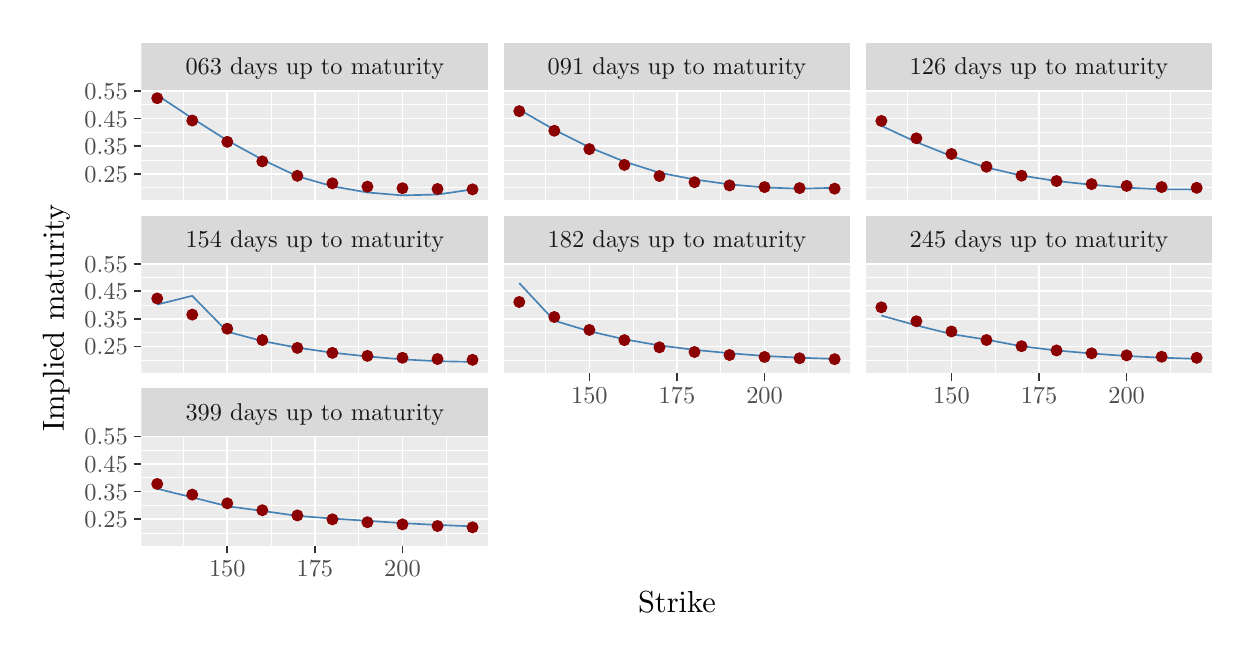
\begin{tikzpicture}[x=1pt,y=1pt]
\definecolor{fillColor}{RGB}{255,255,255}
\path[use as bounding box,fill=fillColor,fill opacity=0.00] (0,0) rectangle (433.62,216.81);
\begin{scope}
\path[clip] (  0.00,  0.00) rectangle (433.62,216.81);
\definecolor{drawColor}{RGB}{255,255,255}
\definecolor{fillColor}{RGB}{255,255,255}

\path[draw=drawColor,line width= 0.6pt,line join=round,line cap=round,fill=fillColor] (  0.00,  0.00) rectangle (433.62,216.81);
\end{scope}
\begin{scope}
\path[clip] ( 41.11,154.40) rectangle (166.45,194.25);
\definecolor{fillColor}{gray}{0.92}

\path[fill=fillColor] ( 41.11,154.40) rectangle (166.45,194.25);
\definecolor{drawColor}{RGB}{255,255,255}

\path[draw=drawColor,line width= 0.3pt,line join=round] ( 41.11,158.99) --
	(166.45,158.99);

\path[draw=drawColor,line width= 0.3pt,line join=round] ( 41.11,168.97) --
	(166.45,168.97);

\path[draw=drawColor,line width= 0.3pt,line join=round] ( 41.11,178.95) --
	(166.45,178.95);

\path[draw=drawColor,line width= 0.3pt,line join=round] ( 41.11,188.93) --
	(166.45,188.93);

\path[draw=drawColor,line width= 0.3pt,line join=round] ( 56.30,154.40) --
	( 56.30,194.25);

\path[draw=drawColor,line width= 0.3pt,line join=round] ( 87.95,154.40) --
	( 87.95,194.25);

\path[draw=drawColor,line width= 0.3pt,line join=round] (119.60,154.40) --
	(119.60,194.25);

\path[draw=drawColor,line width= 0.3pt,line join=round] (151.25,154.40) --
	(151.25,194.25);

\path[draw=drawColor,line width= 0.6pt,line join=round] ( 41.11,163.98) --
	(166.45,163.98);

\path[draw=drawColor,line width= 0.6pt,line join=round] ( 41.11,173.96) --
	(166.45,173.96);

\path[draw=drawColor,line width= 0.6pt,line join=round] ( 41.11,183.94) --
	(166.45,183.94);

\path[draw=drawColor,line width= 0.6pt,line join=round] ( 41.11,193.92) --
	(166.45,193.92);

\path[draw=drawColor,line width= 0.6pt,line join=round] ( 72.13,154.40) --
	( 72.13,194.25);

\path[draw=drawColor,line width= 0.6pt,line join=round] (103.78,154.40) --
	(103.78,194.25);

\path[draw=drawColor,line width= 0.6pt,line join=round] (135.43,154.40) --
	(135.43,194.25);
\definecolor{drawColor}{RGB}{70,130,180}

\path[draw=drawColor,line width= 0.6pt,line join=round] ( 46.81,192.44) --
	( 59.47,184.05) --
	( 72.13,176.06) --
	( 84.79,169.13) --
	( 97.45,163.12) --
	(110.11,159.50) --
	(122.77,157.26) --
	(135.43,156.21) --
	(148.09,156.52) --
	(160.75,158.35);
\definecolor{drawColor}{RGB}{139,0,0}
\definecolor{fillColor}{RGB}{139,0,0}

\path[draw=drawColor,line width= 0.4pt,line join=round,line cap=round,fill=fillColor] ( 46.81,191.32) circle (  1.96);

\path[draw=drawColor,line width= 0.4pt,line join=round,line cap=round,fill=fillColor] ( 59.47,183.25) circle (  1.96);

\path[draw=drawColor,line width= 0.4pt,line join=round,line cap=round,fill=fillColor] ( 72.13,175.56) circle (  1.96);

\path[draw=drawColor,line width= 0.4pt,line join=round,line cap=round,fill=fillColor] ( 84.79,168.49) circle (  1.96);

\path[draw=drawColor,line width= 0.4pt,line join=round,line cap=round,fill=fillColor] ( 97.45,163.27) circle (  1.96);

\path[draw=drawColor,line width= 0.4pt,line join=round,line cap=round,fill=fillColor] (110.11,160.56) circle (  1.96);

\path[draw=drawColor,line width= 0.4pt,line join=round,line cap=round,fill=fillColor] (122.77,159.36) circle (  1.96);

\path[draw=drawColor,line width= 0.4pt,line join=round,line cap=round,fill=fillColor] (135.43,158.80) circle (  1.96);

\path[draw=drawColor,line width= 0.4pt,line join=round,line cap=round,fill=fillColor] (148.09,158.52) circle (  1.96);

\path[draw=drawColor,line width= 0.4pt,line join=round,line cap=round,fill=fillColor] (160.75,158.38) circle (  1.96);
\end{scope}
\begin{scope}
\path[clip] ( 41.11, 91.99) rectangle (166.45,131.84);
\definecolor{fillColor}{gray}{0.92}

\path[fill=fillColor] ( 41.11, 91.99) rectangle (166.45,131.84);
\definecolor{drawColor}{RGB}{255,255,255}

\path[draw=drawColor,line width= 0.3pt,line join=round] ( 41.11, 96.59) --
	(166.45, 96.59);

\path[draw=drawColor,line width= 0.3pt,line join=round] ( 41.11,106.57) --
	(166.45,106.57);

\path[draw=drawColor,line width= 0.3pt,line join=round] ( 41.11,116.55) --
	(166.45,116.55);

\path[draw=drawColor,line width= 0.3pt,line join=round] ( 41.11,126.52) --
	(166.45,126.52);

\path[draw=drawColor,line width= 0.3pt,line join=round] ( 56.30, 91.99) --
	( 56.30,131.84);

\path[draw=drawColor,line width= 0.3pt,line join=round] ( 87.95, 91.99) --
	( 87.95,131.84);

\path[draw=drawColor,line width= 0.3pt,line join=round] (119.60, 91.99) --
	(119.60,131.84);

\path[draw=drawColor,line width= 0.3pt,line join=round] (151.25, 91.99) --
	(151.25,131.84);

\path[draw=drawColor,line width= 0.6pt,line join=round] ( 41.11,101.58) --
	(166.45,101.58);

\path[draw=drawColor,line width= 0.6pt,line join=round] ( 41.11,111.56) --
	(166.45,111.56);

\path[draw=drawColor,line width= 0.6pt,line join=round] ( 41.11,121.54) --
	(166.45,121.54);

\path[draw=drawColor,line width= 0.6pt,line join=round] ( 41.11,131.51) --
	(166.45,131.51);

\path[draw=drawColor,line width= 0.6pt,line join=round] ( 72.13, 91.99) --
	( 72.13,131.84);

\path[draw=drawColor,line width= 0.6pt,line join=round] (103.78, 91.99) --
	(103.78,131.84);

\path[draw=drawColor,line width= 0.6pt,line join=round] (135.43, 91.99) --
	(135.43,131.84);
\definecolor{drawColor}{RGB}{70,130,180}

\path[draw=drawColor,line width= 0.6pt,line join=round] ( 46.81,116.76) --
	( 59.47,119.91) --
	( 72.13,106.96) --
	( 84.79,103.57) --
	( 97.45,101.17) --
	(110.11, 99.36) --
	(122.77, 98.01) --
	(135.43, 96.95) --
	(148.09, 96.29) --
	(160.75, 96.06);
\definecolor{drawColor}{RGB}{139,0,0}
\definecolor{fillColor}{RGB}{139,0,0}

\path[draw=drawColor,line width= 0.4pt,line join=round,line cap=round,fill=fillColor] ( 46.81,118.93) circle (  1.96);

\path[draw=drawColor,line width= 0.4pt,line join=round,line cap=round,fill=fillColor] ( 59.47,113.12) circle (  1.96);

\path[draw=drawColor,line width= 0.4pt,line join=round,line cap=round,fill=fillColor] ( 72.13,108.02) circle (  1.96);

\path[draw=drawColor,line width= 0.4pt,line join=round,line cap=round,fill=fillColor] ( 84.79,103.94) circle (  1.96);

\path[draw=drawColor,line width= 0.4pt,line join=round,line cap=round,fill=fillColor] ( 97.45,101.09) circle (  1.96);

\path[draw=drawColor,line width= 0.4pt,line join=round,line cap=round,fill=fillColor] (110.11, 99.30) circle (  1.96);

\path[draw=drawColor,line width= 0.4pt,line join=round,line cap=round,fill=fillColor] (122.77, 98.21) circle (  1.96);

\path[draw=drawColor,line width= 0.4pt,line join=round,line cap=round,fill=fillColor] (135.43, 97.52) circle (  1.96);

\path[draw=drawColor,line width= 0.4pt,line join=round,line cap=round,fill=fillColor] (148.09, 97.08) circle (  1.96);

\path[draw=drawColor,line width= 0.4pt,line join=round,line cap=round,fill=fillColor] (160.75, 96.78) circle (  1.96);
\end{scope}
\begin{scope}
\path[clip] ( 41.11, 29.59) rectangle (166.45, 69.43);
\definecolor{fillColor}{gray}{0.92}

\path[fill=fillColor] ( 41.11, 29.59) rectangle (166.45, 69.43);
\definecolor{drawColor}{RGB}{255,255,255}

\path[draw=drawColor,line width= 0.3pt,line join=round] ( 41.11, 34.18) --
	(166.45, 34.18);

\path[draw=drawColor,line width= 0.3pt,line join=round] ( 41.11, 44.16) --
	(166.45, 44.16);

\path[draw=drawColor,line width= 0.3pt,line join=round] ( 41.11, 54.14) --
	(166.45, 54.14);

\path[draw=drawColor,line width= 0.3pt,line join=round] ( 41.11, 64.12) --
	(166.45, 64.12);

\path[draw=drawColor,line width= 0.3pt,line join=round] ( 56.30, 29.59) --
	( 56.30, 69.43);

\path[draw=drawColor,line width= 0.3pt,line join=round] ( 87.95, 29.59) --
	( 87.95, 69.43);

\path[draw=drawColor,line width= 0.3pt,line join=round] (119.60, 29.59) --
	(119.60, 69.43);

\path[draw=drawColor,line width= 0.3pt,line join=round] (151.25, 29.59) --
	(151.25, 69.43);

\path[draw=drawColor,line width= 0.6pt,line join=round] ( 41.11, 39.17) --
	(166.45, 39.17);

\path[draw=drawColor,line width= 0.6pt,line join=round] ( 41.11, 49.15) --
	(166.45, 49.15);

\path[draw=drawColor,line width= 0.6pt,line join=round] ( 41.11, 59.13) --
	(166.45, 59.13);

\path[draw=drawColor,line width= 0.6pt,line join=round] ( 41.11, 69.11) --
	(166.45, 69.11);

\path[draw=drawColor,line width= 0.6pt,line join=round] ( 72.13, 29.59) --
	( 72.13, 69.43);

\path[draw=drawColor,line width= 0.6pt,line join=round] (103.78, 29.59) --
	(103.78, 69.43);

\path[draw=drawColor,line width= 0.6pt,line join=round] (135.43, 29.59) --
	(135.43, 69.43);
\definecolor{drawColor}{RGB}{70,130,180}

\path[draw=drawColor,line width= 0.6pt,line join=round] ( 46.81, 50.20) --
	( 59.47, 47.09) --
	( 72.13, 43.89) --
	( 84.79, 42.20) --
	( 97.45, 40.40) --
	(110.11, 39.42) --
	(122.77, 38.61) --
	(135.43, 37.78) --
	(148.09, 37.11) --
	(160.75, 36.62);
\definecolor{drawColor}{RGB}{139,0,0}
\definecolor{fillColor}{RGB}{139,0,0}

\path[draw=drawColor,line width= 0.4pt,line join=round,line cap=round,fill=fillColor] ( 46.81, 51.94) circle (  1.96);

\path[draw=drawColor,line width= 0.4pt,line join=round,line cap=round,fill=fillColor] ( 59.47, 48.07) circle (  1.96);

\path[draw=drawColor,line width= 0.4pt,line join=round,line cap=round,fill=fillColor] ( 72.13, 44.92) circle (  1.96);

\path[draw=drawColor,line width= 0.4pt,line join=round,line cap=round,fill=fillColor] ( 84.79, 42.44) circle (  1.96);

\path[draw=drawColor,line width= 0.4pt,line join=round,line cap=round,fill=fillColor] ( 97.45, 40.56) circle (  1.96);

\path[draw=drawColor,line width= 0.4pt,line join=round,line cap=round,fill=fillColor] (110.11, 39.15) circle (  1.96);

\path[draw=drawColor,line width= 0.4pt,line join=round,line cap=round,fill=fillColor] (122.77, 38.11) circle (  1.96);

\path[draw=drawColor,line width= 0.4pt,line join=round,line cap=round,fill=fillColor] (135.43, 37.32) circle (  1.96);

\path[draw=drawColor,line width= 0.4pt,line join=round,line cap=round,fill=fillColor] (148.09, 36.73) circle (  1.96);

\path[draw=drawColor,line width= 0.4pt,line join=round,line cap=round,fill=fillColor] (160.75, 36.26) circle (  1.96);
\end{scope}
\begin{scope}
\path[clip] (171.95,154.40) rectangle (297.28,194.25);
\definecolor{fillColor}{gray}{0.92}

\path[fill=fillColor] (171.95,154.40) rectangle (297.28,194.25);
\definecolor{drawColor}{RGB}{255,255,255}

\path[draw=drawColor,line width= 0.3pt,line join=round] (171.95,158.99) --
	(297.28,158.99);

\path[draw=drawColor,line width= 0.3pt,line join=round] (171.95,168.97) --
	(297.28,168.97);

\path[draw=drawColor,line width= 0.3pt,line join=round] (171.95,178.95) --
	(297.28,178.95);

\path[draw=drawColor,line width= 0.3pt,line join=round] (171.95,188.93) --
	(297.28,188.93);

\path[draw=drawColor,line width= 0.3pt,line join=round] (187.14,154.40) --
	(187.14,194.25);

\path[draw=drawColor,line width= 0.3pt,line join=round] (218.79,154.40) --
	(218.79,194.25);

\path[draw=drawColor,line width= 0.3pt,line join=round] (250.44,154.40) --
	(250.44,194.25);

\path[draw=drawColor,line width= 0.3pt,line join=round] (282.09,154.40) --
	(282.09,194.25);

\path[draw=drawColor,line width= 0.6pt,line join=round] (171.95,163.98) --
	(297.28,163.98);

\path[draw=drawColor,line width= 0.6pt,line join=round] (171.95,173.96) --
	(297.28,173.96);

\path[draw=drawColor,line width= 0.6pt,line join=round] (171.95,183.94) --
	(297.28,183.94);

\path[draw=drawColor,line width= 0.6pt,line join=round] (171.95,193.92) --
	(297.28,193.92);

\path[draw=drawColor,line width= 0.6pt,line join=round] (202.96,154.40) --
	(202.96,194.25);

\path[draw=drawColor,line width= 0.6pt,line join=round] (234.62,154.40) --
	(234.62,194.25);

\path[draw=drawColor,line width= 0.6pt,line join=round] (266.27,154.40) --
	(266.27,194.25);
\definecolor{drawColor}{RGB}{70,130,180}

\path[draw=drawColor,line width= 0.6pt,line join=round] (177.64,187.21) --
	(190.30,179.91) --
	(202.96,173.56) --
	(215.62,168.42) --
	(228.29,164.40) --
	(240.95,161.96) --
	(253.61,160.18) --
	(266.27,159.07) --
	(278.93,158.62) --
	(291.59,158.94);
\definecolor{drawColor}{RGB}{139,0,0}
\definecolor{fillColor}{RGB}{139,0,0}

\path[draw=drawColor,line width= 0.4pt,line join=round,line cap=round,fill=fillColor] (177.64,186.64) circle (  1.96);

\path[draw=drawColor,line width= 0.4pt,line join=round,line cap=round,fill=fillColor] (190.30,179.55) circle (  1.96);

\path[draw=drawColor,line width= 0.4pt,line join=round,line cap=round,fill=fillColor] (202.96,172.93) circle (  1.96);

\path[draw=drawColor,line width= 0.4pt,line join=round,line cap=round,fill=fillColor] (215.62,167.22) circle (  1.96);

\path[draw=drawColor,line width= 0.4pt,line join=round,line cap=round,fill=fillColor] (228.29,163.21) circle (  1.96);

\path[draw=drawColor,line width= 0.4pt,line join=round,line cap=round,fill=fillColor] (240.95,160.97) circle (  1.96);

\path[draw=drawColor,line width= 0.4pt,line join=round,line cap=round,fill=fillColor] (253.61,159.81) circle (  1.96);

\path[draw=drawColor,line width= 0.4pt,line join=round,line cap=round,fill=fillColor] (266.27,159.20) circle (  1.96);

\path[draw=drawColor,line width= 0.4pt,line join=round,line cap=round,fill=fillColor] (278.93,158.84) circle (  1.96);

\path[draw=drawColor,line width= 0.4pt,line join=round,line cap=round,fill=fillColor] (291.59,158.63) circle (  1.96);
\end{scope}
\begin{scope}
\path[clip] (171.95, 91.99) rectangle (297.28,131.84);
\definecolor{fillColor}{gray}{0.92}

\path[fill=fillColor] (171.95, 91.99) rectangle (297.28,131.84);
\definecolor{drawColor}{RGB}{255,255,255}

\path[draw=drawColor,line width= 0.3pt,line join=round] (171.95, 96.59) --
	(297.28, 96.59);

\path[draw=drawColor,line width= 0.3pt,line join=round] (171.95,106.57) --
	(297.28,106.57);

\path[draw=drawColor,line width= 0.3pt,line join=round] (171.95,116.55) --
	(297.28,116.55);

\path[draw=drawColor,line width= 0.3pt,line join=round] (171.95,126.52) --
	(297.28,126.52);

\path[draw=drawColor,line width= 0.3pt,line join=round] (187.14, 91.99) --
	(187.14,131.84);

\path[draw=drawColor,line width= 0.3pt,line join=round] (218.79, 91.99) --
	(218.79,131.84);

\path[draw=drawColor,line width= 0.3pt,line join=round] (250.44, 91.99) --
	(250.44,131.84);

\path[draw=drawColor,line width= 0.3pt,line join=round] (282.09, 91.99) --
	(282.09,131.84);

\path[draw=drawColor,line width= 0.6pt,line join=round] (171.95,101.58) --
	(297.28,101.58);

\path[draw=drawColor,line width= 0.6pt,line join=round] (171.95,111.56) --
	(297.28,111.56);

\path[draw=drawColor,line width= 0.6pt,line join=round] (171.95,121.54) --
	(297.28,121.54);

\path[draw=drawColor,line width= 0.6pt,line join=round] (171.95,131.51) --
	(297.28,131.51);

\path[draw=drawColor,line width= 0.6pt,line join=round] (202.96, 91.99) --
	(202.96,131.84);

\path[draw=drawColor,line width= 0.6pt,line join=round] (234.62, 91.99) --
	(234.62,131.84);

\path[draw=drawColor,line width= 0.6pt,line join=round] (266.27, 91.99) --
	(266.27,131.84);
\definecolor{drawColor}{RGB}{70,130,180}

\path[draw=drawColor,line width= 0.6pt,line join=round] (177.64,124.51) --
	(190.30,110.93) --
	(202.96,107.13) --
	(215.62,104.20) --
	(228.29,101.98) --
	(240.95,100.40) --
	(253.61, 99.17) --
	(266.27, 98.18) --
	(278.93, 97.55) --
	(291.59, 97.12);
\definecolor{drawColor}{RGB}{139,0,0}
\definecolor{fillColor}{RGB}{139,0,0}

\path[draw=drawColor,line width= 0.4pt,line join=round,line cap=round,fill=fillColor] (177.64,117.69) circle (  1.96);

\path[draw=drawColor,line width= 0.4pt,line join=round,line cap=round,fill=fillColor] (190.30,112.26) circle (  1.96);

\path[draw=drawColor,line width= 0.4pt,line join=round,line cap=round,fill=fillColor] (202.96,107.59) circle (  1.96);

\path[draw=drawColor,line width= 0.4pt,line join=round,line cap=round,fill=fillColor] (215.62,103.90) circle (  1.96);

\path[draw=drawColor,line width= 0.4pt,line join=round,line cap=round,fill=fillColor] (228.29,101.30) circle (  1.96);

\path[draw=drawColor,line width= 0.4pt,line join=round,line cap=round,fill=fillColor] (240.95, 99.61) circle (  1.96);

\path[draw=drawColor,line width= 0.4pt,line join=round,line cap=round,fill=fillColor] (253.61, 98.52) circle (  1.96);

\path[draw=drawColor,line width= 0.4pt,line join=round,line cap=round,fill=fillColor] (266.27, 97.82) circle (  1.96);

\path[draw=drawColor,line width= 0.4pt,line join=round,line cap=round,fill=fillColor] (278.93, 97.35) circle (  1.96);

\path[draw=drawColor,line width= 0.4pt,line join=round,line cap=round,fill=fillColor] (291.59, 97.02) circle (  1.96);
\end{scope}
\begin{scope}
\path[clip] (302.78,154.40) rectangle (428.12,194.25);
\definecolor{fillColor}{gray}{0.92}

\path[fill=fillColor] (302.78,154.40) rectangle (428.12,194.25);
\definecolor{drawColor}{RGB}{255,255,255}

\path[draw=drawColor,line width= 0.3pt,line join=round] (302.78,158.99) --
	(428.12,158.99);

\path[draw=drawColor,line width= 0.3pt,line join=round] (302.78,168.97) --
	(428.12,168.97);

\path[draw=drawColor,line width= 0.3pt,line join=round] (302.78,178.95) --
	(428.12,178.95);

\path[draw=drawColor,line width= 0.3pt,line join=round] (302.78,188.93) --
	(428.12,188.93);

\path[draw=drawColor,line width= 0.3pt,line join=round] (317.98,154.40) --
	(317.98,194.25);

\path[draw=drawColor,line width= 0.3pt,line join=round] (349.63,154.40) --
	(349.63,194.25);

\path[draw=drawColor,line width= 0.3pt,line join=round] (381.28,154.40) --
	(381.28,194.25);

\path[draw=drawColor,line width= 0.3pt,line join=round] (412.93,154.40) --
	(412.93,194.25);

\path[draw=drawColor,line width= 0.6pt,line join=round] (302.78,163.98) --
	(428.12,163.98);

\path[draw=drawColor,line width= 0.6pt,line join=round] (302.78,173.96) --
	(428.12,173.96);

\path[draw=drawColor,line width= 0.6pt,line join=round] (302.78,183.94) --
	(428.12,183.94);

\path[draw=drawColor,line width= 0.6pt,line join=round] (302.78,193.92) --
	(428.12,193.92);

\path[draw=drawColor,line width= 0.6pt,line join=round] (333.80,154.40) --
	(333.80,194.25);

\path[draw=drawColor,line width= 0.6pt,line join=round] (365.45,154.40) --
	(365.45,194.25);

\path[draw=drawColor,line width= 0.6pt,line join=round] (397.10,154.40) --
	(397.10,194.25);
\definecolor{drawColor}{RGB}{70,130,180}

\path[draw=drawColor,line width= 0.6pt,line join=round] (308.48,181.34) --
	(321.14,175.45) --
	(333.80,170.41) --
	(346.46,166.28) --
	(359.12,163.37) --
	(371.78,161.38) --
	(384.44,160.05) --
	(397.10,158.99) --
	(409.76,158.40) --
	(422.42,158.35);
\definecolor{drawColor}{RGB}{139,0,0}
\definecolor{fillColor}{RGB}{139,0,0}

\path[draw=drawColor,line width= 0.4pt,line join=round,line cap=round,fill=fillColor] (308.48,183.11) circle (  1.96);

\path[draw=drawColor,line width= 0.4pt,line join=round,line cap=round,fill=fillColor] (321.14,176.83) circle (  1.96);

\path[draw=drawColor,line width= 0.4pt,line join=round,line cap=round,fill=fillColor] (333.80,171.17) circle (  1.96);

\path[draw=drawColor,line width= 0.4pt,line join=round,line cap=round,fill=fillColor] (346.46,166.54) circle (  1.96);

\path[draw=drawColor,line width= 0.4pt,line join=round,line cap=round,fill=fillColor] (359.12,163.32) circle (  1.96);

\path[draw=drawColor,line width= 0.4pt,line join=round,line cap=round,fill=fillColor] (371.78,161.39) circle (  1.96);

\path[draw=drawColor,line width= 0.4pt,line join=round,line cap=round,fill=fillColor] (384.44,160.28) circle (  1.96);

\path[draw=drawColor,line width= 0.4pt,line join=round,line cap=round,fill=fillColor] (397.10,159.62) circle (  1.96);

\path[draw=drawColor,line width= 0.4pt,line join=round,line cap=round,fill=fillColor] (409.76,159.21) circle (  1.96);

\path[draw=drawColor,line width= 0.4pt,line join=round,line cap=round,fill=fillColor] (422.42,158.94) circle (  1.96);
\end{scope}
\begin{scope}
\path[clip] (302.78, 91.99) rectangle (428.12,131.84);
\definecolor{fillColor}{gray}{0.92}

\path[fill=fillColor] (302.78, 91.99) rectangle (428.12,131.84);
\definecolor{drawColor}{RGB}{255,255,255}

\path[draw=drawColor,line width= 0.3pt,line join=round] (302.78, 96.59) --
	(428.12, 96.59);

\path[draw=drawColor,line width= 0.3pt,line join=round] (302.78,106.57) --
	(428.12,106.57);

\path[draw=drawColor,line width= 0.3pt,line join=round] (302.78,116.55) --
	(428.12,116.55);

\path[draw=drawColor,line width= 0.3pt,line join=round] (302.78,126.52) --
	(428.12,126.52);

\path[draw=drawColor,line width= 0.3pt,line join=round] (317.98, 91.99) --
	(317.98,131.84);

\path[draw=drawColor,line width= 0.3pt,line join=round] (349.63, 91.99) --
	(349.63,131.84);

\path[draw=drawColor,line width= 0.3pt,line join=round] (381.28, 91.99) --
	(381.28,131.84);

\path[draw=drawColor,line width= 0.3pt,line join=round] (412.93, 91.99) --
	(412.93,131.84);

\path[draw=drawColor,line width= 0.6pt,line join=round] (302.78,101.58) --
	(428.12,101.58);

\path[draw=drawColor,line width= 0.6pt,line join=round] (302.78,111.56) --
	(428.12,111.56);

\path[draw=drawColor,line width= 0.6pt,line join=round] (302.78,121.54) --
	(428.12,121.54);

\path[draw=drawColor,line width= 0.6pt,line join=round] (302.78,131.51) --
	(428.12,131.51);

\path[draw=drawColor,line width= 0.6pt,line join=round] (333.80, 91.99) --
	(333.80,131.84);

\path[draw=drawColor,line width= 0.6pt,line join=round] (365.45, 91.99) --
	(365.45,131.84);

\path[draw=drawColor,line width= 0.6pt,line join=round] (397.10, 91.99) --
	(397.10,131.84);
\definecolor{drawColor}{RGB}{70,130,180}

\path[draw=drawColor,line width= 0.6pt,line join=round] (308.48,112.77) --
	(321.14,109.24) --
	(333.80,106.08) --
	(346.46,104.08) --
	(359.12,101.69) --
	(371.78,100.16) --
	(384.44, 99.08) --
	(397.10, 98.16) --
	(409.76, 97.55) --
	(422.42, 97.14);
\definecolor{drawColor}{RGB}{139,0,0}
\definecolor{fillColor}{RGB}{139,0,0}

\path[draw=drawColor,line width= 0.4pt,line join=round,line cap=round,fill=fillColor] (308.48,115.75) circle (  1.96);

\path[draw=drawColor,line width= 0.4pt,line join=round,line cap=round,fill=fillColor] (321.14,110.73) circle (  1.96);

\path[draw=drawColor,line width= 0.4pt,line join=round,line cap=round,fill=fillColor] (333.80,107.03) circle (  1.96);

\path[draw=drawColor,line width= 0.4pt,line join=round,line cap=round,fill=fillColor] (346.46,103.94) circle (  1.96);

\path[draw=drawColor,line width= 0.4pt,line join=round,line cap=round,fill=fillColor] (359.12,101.71) circle (  1.96);

\path[draw=drawColor,line width= 0.4pt,line join=round,line cap=round,fill=fillColor] (371.78,100.18) circle (  1.96);

\path[draw=drawColor,line width= 0.4pt,line join=round,line cap=round,fill=fillColor] (384.44, 99.13) circle (  1.96);

\path[draw=drawColor,line width= 0.4pt,line join=round,line cap=round,fill=fillColor] (397.10, 98.40) circle (  1.96);

\path[draw=drawColor,line width= 0.4pt,line join=round,line cap=round,fill=fillColor] (409.76, 97.89) circle (  1.96);

\path[draw=drawColor,line width= 0.4pt,line join=round,line cap=round,fill=fillColor] (422.42, 97.51) circle (  1.96);
\end{scope}
\begin{scope}
\path[clip] ( 41.11, 69.43) rectangle (166.45, 86.49);
\definecolor{fillColor}{gray}{0.85}

\path[fill=fillColor] ( 41.11, 69.43) rectangle (166.45, 86.49);
\definecolor{drawColor}{gray}{0.10}

\node[text=drawColor,anchor=base,inner sep=0pt, outer sep=0pt, scale=  0.88] at (103.78, 74.93) {399 days up to maturity};
\end{scope}
\begin{scope}
\path[clip] ( 41.11,131.84) rectangle (166.45,148.90);
\definecolor{fillColor}{gray}{0.85}

\path[fill=fillColor] ( 41.11,131.84) rectangle (166.45,148.90);
\definecolor{drawColor}{gray}{0.10}

\node[text=drawColor,anchor=base,inner sep=0pt, outer sep=0pt, scale=  0.88] at (103.78,137.34) {154 days up to maturity};
\end{scope}
\begin{scope}
\path[clip] (171.95,131.84) rectangle (297.28,148.90);
\definecolor{fillColor}{gray}{0.85}

\path[fill=fillColor] (171.95,131.84) rectangle (297.28,148.90);
\definecolor{drawColor}{gray}{0.10}

\node[text=drawColor,anchor=base,inner sep=0pt, outer sep=0pt, scale=  0.88] at (234.62,137.34) {182 days up to maturity};
\end{scope}
\begin{scope}
\path[clip] (302.78,131.84) rectangle (428.12,148.90);
\definecolor{fillColor}{gray}{0.85}

\path[fill=fillColor] (302.78,131.84) rectangle (428.12,148.90);
\definecolor{drawColor}{gray}{0.10}

\node[text=drawColor,anchor=base,inner sep=0pt, outer sep=0pt, scale=  0.88] at (365.45,137.34) {245 days up to maturity};
\end{scope}
\begin{scope}
\path[clip] ( 41.11,194.25) rectangle (166.45,211.31);
\definecolor{fillColor}{gray}{0.85}

\path[fill=fillColor] ( 41.11,194.25) rectangle (166.45,211.31);
\definecolor{drawColor}{gray}{0.10}

\node[text=drawColor,anchor=base,inner sep=0pt, outer sep=0pt, scale=  0.88] at (103.78,199.75) {063 days up to maturity};
\end{scope}
\begin{scope}
\path[clip] (171.95,194.25) rectangle (297.28,211.31);
\definecolor{fillColor}{gray}{0.85}

\path[fill=fillColor] (171.95,194.25) rectangle (297.28,211.31);
\definecolor{drawColor}{gray}{0.10}

\node[text=drawColor,anchor=base,inner sep=0pt, outer sep=0pt, scale=  0.88] at (234.62,199.75) {091 days up to maturity};
\end{scope}
\begin{scope}
\path[clip] (302.78,194.25) rectangle (428.12,211.31);
\definecolor{fillColor}{gray}{0.85}

\path[fill=fillColor] (302.78,194.25) rectangle (428.12,211.31);
\definecolor{drawColor}{gray}{0.10}

\node[text=drawColor,anchor=base,inner sep=0pt, outer sep=0pt, scale=  0.88] at (365.45,199.75) {126 days up to maturity};
\end{scope}
\begin{scope}
\path[clip] (  0.00,  0.00) rectangle (433.62,216.81);
\definecolor{drawColor}{gray}{0.20}

\path[draw=drawColor,line width= 0.6pt,line join=round] ( 72.13, 26.84) --
	( 72.13, 29.59);

\path[draw=drawColor,line width= 0.6pt,line join=round] (103.78, 26.84) --
	(103.78, 29.59);

\path[draw=drawColor,line width= 0.6pt,line join=round] (135.43, 26.84) --
	(135.43, 29.59);
\end{scope}
\begin{scope}
\path[clip] (  0.00,  0.00) rectangle (433.62,216.81);
\definecolor{drawColor}{gray}{0.30}

\node[text=drawColor,anchor=base,inner sep=0pt, outer sep=0pt, scale=  0.88] at ( 72.13, 18.58) {150};

\node[text=drawColor,anchor=base,inner sep=0pt, outer sep=0pt, scale=  0.88] at (103.78, 18.58) {175};

\node[text=drawColor,anchor=base,inner sep=0pt, outer sep=0pt, scale=  0.88] at (135.43, 18.58) {200};
\end{scope}
\begin{scope}
\path[clip] (  0.00,  0.00) rectangle (433.62,216.81);
\definecolor{drawColor}{gray}{0.20}

\path[draw=drawColor,line width= 0.6pt,line join=round] (202.96, 89.24) --
	(202.96, 91.99);

\path[draw=drawColor,line width= 0.6pt,line join=round] (234.62, 89.24) --
	(234.62, 91.99);

\path[draw=drawColor,line width= 0.6pt,line join=round] (266.27, 89.24) --
	(266.27, 91.99);
\end{scope}
\begin{scope}
\path[clip] (  0.00,  0.00) rectangle (433.62,216.81);
\definecolor{drawColor}{gray}{0.30}

\node[text=drawColor,anchor=base,inner sep=0pt, outer sep=0pt, scale=  0.88] at (202.96, 80.98) {150};

\node[text=drawColor,anchor=base,inner sep=0pt, outer sep=0pt, scale=  0.88] at (234.62, 80.98) {175};

\node[text=drawColor,anchor=base,inner sep=0pt, outer sep=0pt, scale=  0.88] at (266.27, 80.98) {200};
\end{scope}
\begin{scope}
\path[clip] (  0.00,  0.00) rectangle (433.62,216.81);
\definecolor{drawColor}{gray}{0.20}

\path[draw=drawColor,line width= 0.6pt,line join=round] (333.80, 89.24) --
	(333.80, 91.99);

\path[draw=drawColor,line width= 0.6pt,line join=round] (365.45, 89.24) --
	(365.45, 91.99);

\path[draw=drawColor,line width= 0.6pt,line join=round] (397.10, 89.24) --
	(397.10, 91.99);
\end{scope}
\begin{scope}
\path[clip] (  0.00,  0.00) rectangle (433.62,216.81);
\definecolor{drawColor}{gray}{0.30}

\node[text=drawColor,anchor=base,inner sep=0pt, outer sep=0pt, scale=  0.88] at (333.80, 80.98) {150};

\node[text=drawColor,anchor=base,inner sep=0pt, outer sep=0pt, scale=  0.88] at (365.45, 80.98) {175};

\node[text=drawColor,anchor=base,inner sep=0pt, outer sep=0pt, scale=  0.88] at (397.10, 80.98) {200};
\end{scope}
\begin{scope}
\path[clip] (  0.00,  0.00) rectangle (433.62,216.81);
\definecolor{drawColor}{gray}{0.30}

\node[text=drawColor,anchor=base east,inner sep=0pt, outer sep=0pt, scale=  0.88] at ( 36.16,160.95) {0.25};

\node[text=drawColor,anchor=base east,inner sep=0pt, outer sep=0pt, scale=  0.88] at ( 36.16,170.93) {0.35};

\node[text=drawColor,anchor=base east,inner sep=0pt, outer sep=0pt, scale=  0.88] at ( 36.16,180.91) {0.45};

\node[text=drawColor,anchor=base east,inner sep=0pt, outer sep=0pt, scale=  0.88] at ( 36.16,190.89) {0.55};
\end{scope}
\begin{scope}
\path[clip] (  0.00,  0.00) rectangle (433.62,216.81);
\definecolor{drawColor}{gray}{0.20}

\path[draw=drawColor,line width= 0.6pt,line join=round] ( 38.36,163.98) --
	( 41.11,163.98);

\path[draw=drawColor,line width= 0.6pt,line join=round] ( 38.36,173.96) --
	( 41.11,173.96);

\path[draw=drawColor,line width= 0.6pt,line join=round] ( 38.36,183.94) --
	( 41.11,183.94);

\path[draw=drawColor,line width= 0.6pt,line join=round] ( 38.36,193.92) --
	( 41.11,193.92);
\end{scope}
\begin{scope}
\path[clip] (  0.00,  0.00) rectangle (433.62,216.81);
\definecolor{drawColor}{gray}{0.30}

\node[text=drawColor,anchor=base east,inner sep=0pt, outer sep=0pt, scale=  0.88] at ( 36.16, 98.55) {0.25};

\node[text=drawColor,anchor=base east,inner sep=0pt, outer sep=0pt, scale=  0.88] at ( 36.16,108.52) {0.35};

\node[text=drawColor,anchor=base east,inner sep=0pt, outer sep=0pt, scale=  0.88] at ( 36.16,118.50) {0.45};

\node[text=drawColor,anchor=base east,inner sep=0pt, outer sep=0pt, scale=  0.88] at ( 36.16,128.48) {0.55};
\end{scope}
\begin{scope}
\path[clip] (  0.00,  0.00) rectangle (433.62,216.81);
\definecolor{drawColor}{gray}{0.20}

\path[draw=drawColor,line width= 0.6pt,line join=round] ( 38.36,101.58) --
	( 41.11,101.58);

\path[draw=drawColor,line width= 0.6pt,line join=round] ( 38.36,111.56) --
	( 41.11,111.56);

\path[draw=drawColor,line width= 0.6pt,line join=round] ( 38.36,121.54) --
	( 41.11,121.54);

\path[draw=drawColor,line width= 0.6pt,line join=round] ( 38.36,131.51) --
	( 41.11,131.51);
\end{scope}
\begin{scope}
\path[clip] (  0.00,  0.00) rectangle (433.62,216.81);
\definecolor{drawColor}{gray}{0.30}

\node[text=drawColor,anchor=base east,inner sep=0pt, outer sep=0pt, scale=  0.88] at ( 36.16, 36.14) {0.25};

\node[text=drawColor,anchor=base east,inner sep=0pt, outer sep=0pt, scale=  0.88] at ( 36.16, 46.12) {0.35};

\node[text=drawColor,anchor=base east,inner sep=0pt, outer sep=0pt, scale=  0.88] at ( 36.16, 56.10) {0.45};

\node[text=drawColor,anchor=base east,inner sep=0pt, outer sep=0pt, scale=  0.88] at ( 36.16, 66.08) {0.55};
\end{scope}
\begin{scope}
\path[clip] (  0.00,  0.00) rectangle (433.62,216.81);
\definecolor{drawColor}{gray}{0.20}

\path[draw=drawColor,line width= 0.6pt,line join=round] ( 38.36, 39.17) --
	( 41.11, 39.17);

\path[draw=drawColor,line width= 0.6pt,line join=round] ( 38.36, 49.15) --
	( 41.11, 49.15);

\path[draw=drawColor,line width= 0.6pt,line join=round] ( 38.36, 59.13) --
	( 41.11, 59.13);

\path[draw=drawColor,line width= 0.6pt,line join=round] ( 38.36, 69.11) --
	( 41.11, 69.11);
\end{scope}
\begin{scope}
\path[clip] (  0.00,  0.00) rectangle (433.62,216.81);
\definecolor{drawColor}{RGB}{0,0,0}

\node[text=drawColor,anchor=base,inner sep=0pt, outer sep=0pt, scale=  1.10] at (234.62,  5.50) {Strike};
\end{scope}
\begin{scope}
\path[clip] (  0.00,  0.00) rectangle (433.62,216.81);
\definecolor{drawColor}{RGB}{0,0,0}

\node[text=drawColor,rotate= 90.00,anchor=base,inner sep=0pt, outer sep=0pt, scale=  1.10] at ( 13.08,111.92) {Implied maturity};
\end{scope}
\end{tikzpicture}

  \caption{Implied volatility of Apple option prices computed with MJD}
      %
  % BEGIN OF FLOATNOTE
  %
  \begin{changemargin}{0.5cm}{0.5cm}
  \medskip
\footnotesize
\setstretch{1.0}\textbf{Notes.} The implied volatilities that represent the above volatility smiles have been computed by using an iterative method on the BSM equation to solve  $\sigma$.
  The parameters given to the function \textit{bsm\_call} were the stock price $S$, the strike price $K$, the riskless rate $r$ and the time to maturity $T$, letting $\sigma$ unknown.
  The method used was to find the root of $C(S(0), K, T, r; \sigma) - C_{K, T}$, where $C_{K, T}$ is either the market price or the price giving by the function \textit{mjd\_call}, and $C(S(0), K, T, r; \sigma)$ is the function \textit{bsm\_call} with $\sigma$ as a cursor.
  \end{changemargin}
  %
  % END OF FLOATNOTE
  %
  \label{p:methodology:impliedvol:aapl:merton}
\end{figure}


Consequently, for the purpose of that master thesis, the set \ref{eq:methodology:arg:merton:riskneutral} is the one that will be used together with the function \textit{mjd\_call} whenever performing the computation of option prices for the MJD model.





%%%%%%%%%%%%%%%%%%%%%%%%%%%%%%%%%%%%%%%%%%%%%%%%%%%%%%%%%%%%%%%%%%%%%%%%%%%%%%%%
\subsubsection*{Calibration of parameters for time series}

The set \ref{eq:methodology:arg:merton:riskneutral} is calibrated under the risk-neutral world and cannot, therefore, be used as is to simulate the dummy time-series that will serve the analysis aimed to measure the delta hedging performance.
Furthermore, in addition to those parameters, the drift rate $\alpha$ has to be estimated as well. It was not present in the set  \ref{eq:methodology:arg:merton:riskneutral} because it was not taken into account in the computation of the options prices.

\Cref{p:methodology:density:aapl:merton:riskneutral} shows the empirical density curves illustrating the distributions of the log-returns computed either from historical Apple stock data for the blue curve or from dummy time series generated by the function \textit{mjd\_ts()} fed with the risk-neutral parameters\ref{eq:methodology:arg:merton:riskneutral}, for the red one.


\begin{figure}[h]
  \centering
  % Created by tikzDevice version 0.11 on 2018-07-21 23:11:46
% !TEX encoding = UTF-8 Unicode
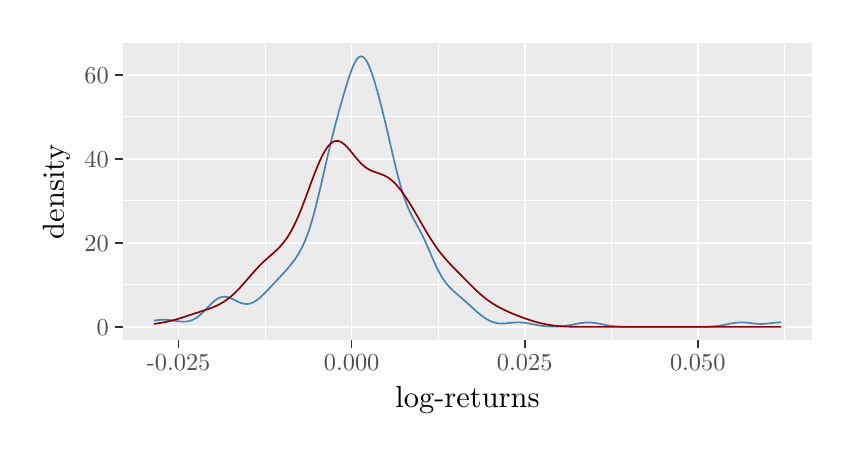
\begin{tikzpicture}[x=1pt,y=1pt]
\definecolor{fillColor}{RGB}{255,255,255}
\path[use as bounding box,fill=fillColor,fill opacity=0.00] (0,0) rectangle (289.08,144.54);
\begin{scope}
\path[clip] (  0.00,  0.00) rectangle (289.08,144.54);
\definecolor{drawColor}{RGB}{255,255,255}
\definecolor{fillColor}{RGB}{255,255,255}

\path[draw=drawColor,line width= 0.6pt,line join=round,line cap=round,fill=fillColor] (  0.00,  0.00) rectangle (289.08,144.54);
\end{scope}
\begin{scope}
\path[clip] ( 34.27, 31.53) rectangle (283.58,139.04);
\definecolor{fillColor}{gray}{0.92}

\path[fill=fillColor] ( 34.27, 31.53) rectangle (283.58,139.04);
\definecolor{drawColor}{RGB}{255,255,255}

\path[draw=drawColor,line width= 0.3pt,line join=round] ( 34.27, 51.60) --
	(283.58, 51.60);

\path[draw=drawColor,line width= 0.3pt,line join=round] ( 34.27, 81.97) --
	(283.58, 81.97);

\path[draw=drawColor,line width= 0.3pt,line join=round] ( 34.27,112.33) --
	(283.58,112.33);

\path[draw=drawColor,line width= 0.3pt,line join=round] ( 85.80, 31.53) --
	( 85.80,139.04);

\path[draw=drawColor,line width= 0.3pt,line join=round] (148.33, 31.53) --
	(148.33,139.04);

\path[draw=drawColor,line width= 0.3pt,line join=round] (210.86, 31.53) --
	(210.86,139.04);

\path[draw=drawColor,line width= 0.3pt,line join=round] (273.40, 31.53) --
	(273.40,139.04);

\path[draw=drawColor,line width= 0.6pt,line join=round] ( 34.27, 36.42) --
	(283.58, 36.42);

\path[draw=drawColor,line width= 0.6pt,line join=round] ( 34.27, 66.78) --
	(283.58, 66.78);

\path[draw=drawColor,line width= 0.6pt,line join=round] ( 34.27, 97.15) --
	(283.58, 97.15);

\path[draw=drawColor,line width= 0.6pt,line join=round] ( 34.27,127.52) --
	(283.58,127.52);

\path[draw=drawColor,line width= 0.6pt,line join=round] ( 54.53, 31.53) --
	( 54.53,139.04);

\path[draw=drawColor,line width= 0.6pt,line join=round] (117.07, 31.53) --
	(117.07,139.04);

\path[draw=drawColor,line width= 0.6pt,line join=round] (179.60, 31.53) --
	(179.60,139.04);

\path[draw=drawColor,line width= 0.6pt,line join=round] (242.13, 31.53) --
	(242.13,139.04);
\definecolor{drawColor}{RGB}{70,130,180}

\path[draw=drawColor,line width= 0.6pt,line join=round] ( 45.60, 38.68) --
	( 46.04, 38.76) --
	( 46.49, 38.82) --
	( 46.93, 38.88) --
	( 47.37, 38.92) --
	( 47.82, 38.96) --
	( 48.26, 38.98) --
	( 48.70, 39.00) --
	( 49.15, 39.00) --
	( 49.59, 38.99) --
	( 50.04, 38.97) --
	( 50.48, 38.94) --
	( 50.92, 38.90) --
	( 51.37, 38.86) --
	( 51.81, 38.81) --
	( 52.25, 38.75) --
	( 52.70, 38.69) --
	( 53.14, 38.62) --
	( 53.58, 38.56) --
	( 54.03, 38.50) --
	( 54.47, 38.44) --
	( 54.91, 38.39) --
	( 55.36, 38.35) --
	( 55.80, 38.32) --
	( 56.25, 38.30) --
	( 56.69, 38.31) --
	( 57.13, 38.33) --
	( 57.58, 38.38) --
	( 58.02, 38.46) --
	( 58.46, 38.56) --
	( 58.91, 38.68) --
	( 59.35, 38.85) --
	( 59.79, 39.04) --
	( 60.24, 39.27) --
	( 60.68, 39.53) --
	( 61.12, 39.82) --
	( 61.57, 40.14) --
	( 62.01, 40.49) --
	( 62.45, 40.87) --
	( 62.90, 41.27) --
	( 63.34, 41.70) --
	( 63.79, 42.14) --
	( 64.23, 42.59) --
	( 64.67, 43.05) --
	( 65.12, 43.52) --
	( 65.56, 43.98) --
	( 66.00, 44.43) --
	( 66.45, 44.86) --
	( 66.89, 45.28) --
	( 67.33, 45.67) --
	( 67.78, 46.03) --
	( 68.22, 46.35) --
	( 68.66, 46.62) --
	( 69.11, 46.85) --
	( 69.55, 47.04) --
	( 69.99, 47.17) --
	( 70.44, 47.27) --
	( 70.88, 47.31) --
	( 71.33, 47.30) --
	( 71.77, 47.25) --
	( 72.21, 47.15) --
	( 72.66, 47.03) --
	( 73.10, 46.87) --
	( 73.54, 46.69) --
	( 73.99, 46.49) --
	( 74.43, 46.27) --
	( 74.87, 46.05) --
	( 75.32, 45.83) --
	( 75.76, 45.61) --
	( 76.20, 45.41) --
	( 76.65, 45.22) --
	( 77.09, 45.05) --
	( 77.53, 44.91) --
	( 77.98, 44.81) --
	( 78.42, 44.73) --
	( 78.87, 44.70) --
	( 79.31, 44.70) --
	( 79.75, 44.73) --
	( 80.20, 44.81) --
	( 80.64, 44.94) --
	( 81.08, 45.10) --
	( 81.53, 45.30) --
	( 81.97, 45.54) --
	( 82.41, 45.81) --
	( 82.86, 46.11) --
	( 83.30, 46.45) --
	( 83.74, 46.81) --
	( 84.19, 47.20) --
	( 84.63, 47.61) --
	( 85.07, 48.04) --
	( 85.52, 48.48) --
	( 85.96, 48.93) --
	( 86.41, 49.39) --
	( 86.85, 49.85) --
	( 87.29, 50.32) --
	( 87.74, 50.80) --
	( 88.18, 51.27) --
	( 88.62, 51.74) --
	( 89.07, 52.22) --
	( 89.51, 52.69) --
	( 89.95, 53.16) --
	( 90.40, 53.63) --
	( 90.84, 54.11) --
	( 91.28, 54.58) --
	( 91.73, 55.06) --
	( 92.17, 55.54) --
	( 92.62, 56.02) --
	( 93.06, 56.51) --
	( 93.50, 57.01) --
	( 93.95, 57.52) --
	( 94.39, 58.04) --
	( 94.83, 58.57) --
	( 95.28, 59.12) --
	( 95.72, 59.68) --
	( 96.16, 60.28) --
	( 96.61, 60.89) --
	( 97.05, 61.54) --
	( 97.49, 62.22) --
	( 97.94, 62.94) --
	( 98.38, 63.71) --
	( 98.82, 64.54) --
	( 99.27, 65.42) --
	( 99.71, 66.36) --
	(100.16, 67.37) --
	(100.60, 68.45) --
	(101.04, 69.61) --
	(101.49, 70.85) --
	(101.93, 72.18) --
	(102.37, 73.59) --
	(102.82, 75.08) --
	(103.26, 76.64) --
	(103.70, 78.28) --
	(104.15, 79.99) --
	(104.59, 81.77) --
	(105.03, 83.60) --
	(105.48, 85.48) --
	(105.92, 87.38) --
	(106.36, 89.32) --
	(106.81, 91.26) --
	(107.25, 93.21) --
	(107.70, 95.15) --
	(108.14, 97.08) --
	(108.58, 98.98) --
	(109.03,100.86) --
	(109.47,102.71) --
	(109.91,104.52) --
	(110.36,106.30) --
	(110.80,108.04) --
	(111.24,109.74) --
	(111.69,111.42) --
	(112.13,113.06) --
	(112.57,114.69) --
	(113.02,116.28) --
	(113.46,117.86) --
	(113.90,119.41) --
	(114.35,120.93) --
	(114.79,122.43) --
	(115.24,123.88) --
	(115.68,125.30) --
	(116.12,126.66) --
	(116.57,127.96) --
	(117.01,129.16) --
	(117.45,130.26) --
	(117.90,131.26) --
	(118.34,132.13) --
	(118.78,132.86) --
	(119.23,133.45) --
	(119.67,133.87) --
	(120.11,134.10) --
	(120.56,134.15) --
	(121.00,134.04) --
	(121.45,133.76) --
	(121.89,133.31) --
	(122.33,132.70) --
	(122.78,131.92) --
	(123.22,130.99) --
	(123.66,129.94) --
	(124.11,128.77) --
	(124.55,127.51) --
	(124.99,126.15) --
	(125.44,124.72) --
	(125.88,123.20) --
	(126.32,121.63) --
	(126.77,120.00) --
	(127.21,118.33) --
	(127.65,116.61) --
	(128.10,114.85) --
	(128.54,113.06) --
	(128.99,111.23) --
	(129.43,109.37) --
	(129.87,107.49) --
	(130.32,105.59) --
	(130.76,103.68) --
	(131.20,101.75) --
	(131.65, 99.83) --
	(132.09, 97.93) --
	(132.53, 96.05) --
	(132.98, 94.21) --
	(133.42, 92.41) --
	(133.86, 90.67) --
	(134.31, 88.99) --
	(134.75, 87.39) --
	(135.19, 85.88) --
	(135.64, 84.45) --
	(136.08, 83.11) --
	(136.53, 81.86) --
	(136.97, 80.69) --
	(137.41, 79.60) --
	(137.86, 78.58) --
	(138.30, 77.64) --
	(138.74, 76.74) --
	(139.19, 75.89) --
	(139.63, 75.06) --
	(140.07, 74.26) --
	(140.52, 73.46) --
	(140.96, 72.65) --
	(141.40, 71.83) --
	(141.85, 70.99) --
	(142.29, 70.13) --
	(142.73, 69.23) --
	(143.18, 68.31) --
	(143.62, 67.36) --
	(144.07, 66.37) --
	(144.51, 65.37) --
	(144.95, 64.35) --
	(145.40, 63.32) --
	(145.84, 62.29) --
	(146.28, 61.27) --
	(146.73, 60.26) --
	(147.17, 59.28) --
	(147.61, 58.32) --
	(148.06, 57.41) --
	(148.50, 56.54) --
	(148.94, 55.70) --
	(149.39, 54.92) --
	(149.83, 54.18) --
	(150.27, 53.50) --
	(150.72, 52.87) --
	(151.16, 52.28) --
	(151.61, 51.72) --
	(152.05, 51.21) --
	(152.49, 50.72) --
	(152.94, 50.27) --
	(153.38, 49.84) --
	(153.82, 49.43) --
	(154.27, 49.03) --
	(154.71, 48.64) --
	(155.15, 48.26) --
	(155.60, 47.88) --
	(156.04, 47.50) --
	(156.48, 47.12) --
	(156.93, 46.73) --
	(157.37, 46.34) --
	(157.82, 45.95) --
	(158.26, 45.56) --
	(158.70, 45.16) --
	(159.15, 44.75) --
	(159.59, 44.35) --
	(160.03, 43.94) --
	(160.48, 43.54) --
	(160.92, 43.13) --
	(161.36, 42.74) --
	(161.81, 42.34) --
	(162.25, 41.95) --
	(162.69, 41.57) --
	(163.14, 41.21) --
	(163.58, 40.85) --
	(164.02, 40.50) --
	(164.47, 40.17) --
	(164.91, 39.86) --
	(165.36, 39.56) --
	(165.80, 39.28) --
	(166.24, 39.03) --
	(166.69, 38.79) --
	(167.13, 38.57) --
	(167.57, 38.38) --
	(168.02, 38.21) --
	(168.46, 38.06) --
	(168.90, 37.94) --
	(169.35, 37.83) --
	(169.79, 37.75) --
	(170.23, 37.70) --
	(170.68, 37.66) --
	(171.12, 37.63) --
	(171.56, 37.63) --
	(172.01, 37.64) --
	(172.45, 37.67) --
	(172.90, 37.70) --
	(173.34, 37.74) --
	(173.78, 37.79) --
	(174.23, 37.84) --
	(174.67, 37.88) --
	(175.11, 37.93) --
	(175.56, 37.97) --
	(176.00, 38.00) --
	(176.44, 38.03) --
	(176.89, 38.04) --
	(177.33, 38.05) --
	(177.77, 38.04) --
	(178.22, 38.02) --
	(178.66, 37.99) --
	(179.10, 37.94) --
	(179.55, 37.89) --
	(179.99, 37.83) --
	(180.44, 37.76) --
	(180.88, 37.68) --
	(181.32, 37.59) --
	(181.77, 37.51) --
	(182.21, 37.42) --
	(182.65, 37.33) --
	(183.10, 37.24) --
	(183.54, 37.16) --
	(183.98, 37.08) --
	(184.43, 37.00) --
	(184.87, 36.93) --
	(185.31, 36.86) --
	(185.76, 36.80) --
	(186.20, 36.74) --
	(186.64, 36.70) --
	(187.09, 36.66) --
	(187.53, 36.62) --
	(187.98, 36.59) --
	(188.42, 36.57) --
	(188.86, 36.55) --
	(189.31, 36.54) --
	(189.75, 36.54) --
	(190.19, 36.54) --
	(190.64, 36.54) --
	(191.08, 36.55) --
	(191.52, 36.57) --
	(191.97, 36.59) --
	(192.41, 36.62) --
	(192.85, 36.65) --
	(193.30, 36.69) --
	(193.74, 36.74) --
	(194.19, 36.79) --
	(194.63, 36.85) --
	(195.07, 36.92) --
	(195.52, 36.99) --
	(195.96, 37.07) --
	(196.40, 37.15) --
	(196.85, 37.23) --
	(197.29, 37.32) --
	(197.73, 37.41) --
	(198.18, 37.50) --
	(198.62, 37.58) --
	(199.06, 37.67) --
	(199.51, 37.74) --
	(199.95, 37.81) --
	(200.39, 37.88) --
	(200.84, 37.93) --
	(201.28, 37.97) --
	(201.73, 38.00) --
	(202.17, 38.02) --
	(202.61, 38.02) --
	(203.06, 38.01) --
	(203.50, 37.99) --
	(203.94, 37.96) --
	(204.39, 37.91) --
	(204.83, 37.85) --
	(205.27, 37.79) --
	(205.72, 37.71) --
	(206.16, 37.63) --
	(206.60, 37.55) --
	(207.05, 37.46) --
	(207.49, 37.37) --
	(207.93, 37.28) --
	(208.38, 37.20) --
	(208.82, 37.11) --
	(209.27, 37.03) --
	(209.71, 36.96) --
	(210.15, 36.89) --
	(210.60, 36.82) --
	(211.04, 36.76) --
	(211.48, 36.71) --
	(211.93, 36.67) --
	(212.37, 36.62) --
	(212.81, 36.59) --
	(213.26, 36.56) --
	(213.70, 36.53) --
	(214.14, 36.51) --
	(214.59, 36.49) --
	(215.03, 36.48) --
	(215.47, 36.46) --
	(215.92, 36.45) --
	(216.36, 36.45) --
	(216.81, 36.44) --
	(217.25, 36.43) --
	(217.69, 36.43) --
	(218.14, 36.43) --
	(218.58, 36.42) --
	(219.02, 36.42) --
	(219.47, 36.42) --
	(219.91, 36.42) --
	(220.35, 36.42) --
	(220.80, 36.42) --
	(221.24, 36.42) --
	(221.68, 36.42) --
	(222.13, 36.42) --
	(222.57, 36.42) --
	(223.02, 36.42) --
	(223.46, 36.42) --
	(223.90, 36.42) --
	(224.35, 36.42) --
	(224.79, 36.42) --
	(225.23, 36.42) --
	(225.68, 36.42) --
	(226.12, 36.42) --
	(226.56, 36.42) --
	(227.01, 36.42) --
	(227.45, 36.42) --
	(227.89, 36.42) --
	(228.34, 36.42) --
	(228.78, 36.42) --
	(229.22, 36.42) --
	(229.67, 36.42) --
	(230.11, 36.42) --
	(230.56, 36.42) --
	(231.00, 36.42) --
	(231.44, 36.42) --
	(231.89, 36.42) --
	(232.33, 36.42) --
	(232.77, 36.42) --
	(233.22, 36.42) --
	(233.66, 36.42) --
	(234.10, 36.42) --
	(234.55, 36.42) --
	(234.99, 36.42) --
	(235.43, 36.42) --
	(235.88, 36.42) --
	(236.32, 36.42) --
	(236.76, 36.42) --
	(237.21, 36.42) --
	(237.65, 36.42) --
	(238.10, 36.42) --
	(238.54, 36.42) --
	(238.98, 36.42) --
	(239.43, 36.42) --
	(239.87, 36.42) --
	(240.31, 36.42) --
	(240.76, 36.42) --
	(241.20, 36.42) --
	(241.64, 36.42) --
	(242.09, 36.43) --
	(242.53, 36.43) --
	(242.97, 36.43) --
	(243.42, 36.44) --
	(243.86, 36.44) --
	(244.30, 36.45) --
	(244.75, 36.46) --
	(245.19, 36.47) --
	(245.64, 36.49) --
	(246.08, 36.51) --
	(246.52, 36.53) --
	(246.97, 36.55) --
	(247.41, 36.58) --
	(247.85, 36.62) --
	(248.30, 36.66) --
	(248.74, 36.71) --
	(249.18, 36.76) --
	(249.63, 36.81) --
	(250.07, 36.88) --
	(250.51, 36.95) --
	(250.96, 37.02) --
	(251.40, 37.10) --
	(251.84, 37.18) --
	(252.29, 37.27) --
	(252.73, 37.36) --
	(253.18, 37.45) --
	(253.62, 37.54) --
	(254.06, 37.62) --
	(254.51, 37.70) --
	(254.95, 37.78) --
	(255.39, 37.85) --
	(255.84, 37.91) --
	(256.28, 37.96) --
	(256.72, 38.00) --
	(257.17, 38.02) --
	(257.61, 38.04) --
	(258.05, 38.04) --
	(258.50, 38.04) --
	(258.94, 38.02) --
	(259.39, 37.99) --
	(259.83, 37.95) --
	(260.27, 37.90) --
	(260.72, 37.85) --
	(261.16, 37.80) --
	(261.60, 37.74) --
	(262.05, 37.69) --
	(262.49, 37.64) --
	(262.93, 37.59) --
	(263.38, 37.55) --
	(263.82, 37.52) --
	(264.26, 37.50) --
	(264.71, 37.48) --
	(265.15, 37.48) --
	(265.59, 37.49) --
	(266.04, 37.51) --
	(266.48, 37.54) --
	(266.93, 37.57) --
	(267.37, 37.62) --
	(267.81, 37.67) --
	(268.26, 37.72) --
	(268.70, 37.78) --
	(269.14, 37.83) --
	(269.59, 37.88) --
	(270.03, 37.93) --
	(270.47, 37.97) --
	(270.92, 38.01) --
	(271.36, 38.03) --
	(271.80, 38.04) --
	(272.25, 38.04);
\definecolor{drawColor}{RGB}{139,0,0}

\path[draw=drawColor,line width= 0.6pt,line join=round] ( 45.60, 37.49) --
	( 46.04, 37.55) --
	( 46.49, 37.61) --
	( 46.93, 37.68) --
	( 47.37, 37.75) --
	( 47.82, 37.82) --
	( 48.26, 37.90) --
	( 48.70, 37.98) --
	( 49.15, 38.06) --
	( 49.59, 38.15) --
	( 50.04, 38.23) --
	( 50.48, 38.33) --
	( 50.92, 38.43) --
	( 51.37, 38.53) --
	( 51.81, 38.63) --
	( 52.25, 38.74) --
	( 52.70, 38.86) --
	( 53.14, 38.98) --
	( 53.58, 39.10) --
	( 54.03, 39.23) --
	( 54.47, 39.36) --
	( 54.91, 39.49) --
	( 55.36, 39.63) --
	( 55.80, 39.77) --
	( 56.25, 39.91) --
	( 56.69, 40.06) --
	( 57.13, 40.20) --
	( 57.58, 40.35) --
	( 58.02, 40.50) --
	( 58.46, 40.64) --
	( 58.91, 40.79) --
	( 59.35, 40.94) --
	( 59.79, 41.09) --
	( 60.24, 41.23) --
	( 60.68, 41.38) --
	( 61.12, 41.52) --
	( 61.57, 41.66) --
	( 62.01, 41.81) --
	( 62.45, 41.95) --
	( 62.90, 42.09) --
	( 63.34, 42.23) --
	( 63.79, 42.38) --
	( 64.23, 42.53) --
	( 64.67, 42.67) --
	( 65.12, 42.83) --
	( 65.56, 42.98) --
	( 66.00, 43.14) --
	( 66.45, 43.31) --
	( 66.89, 43.48) --
	( 67.33, 43.66) --
	( 67.78, 43.86) --
	( 68.22, 44.06) --
	( 68.66, 44.27) --
	( 69.11, 44.49) --
	( 69.55, 44.72) --
	( 69.99, 44.97) --
	( 70.44, 45.23) --
	( 70.88, 45.51) --
	( 71.33, 45.80) --
	( 71.77, 46.10) --
	( 72.21, 46.43) --
	( 72.66, 46.77) --
	( 73.10, 47.12) --
	( 73.54, 47.49) --
	( 73.99, 47.88) --
	( 74.43, 48.28) --
	( 74.87, 48.70) --
	( 75.32, 49.14) --
	( 75.76, 49.58) --
	( 76.20, 50.04) --
	( 76.65, 50.51) --
	( 77.09, 51.00) --
	( 77.53, 51.49) --
	( 77.98, 51.99) --
	( 78.42, 52.50) --
	( 78.87, 53.01) --
	( 79.31, 53.52) --
	( 79.75, 54.04) --
	( 80.20, 54.55) --
	( 80.64, 55.06) --
	( 81.08, 55.57) --
	( 81.53, 56.07) --
	( 81.97, 56.57) --
	( 82.41, 57.06) --
	( 82.86, 57.54) --
	( 83.30, 58.01) --
	( 83.74, 58.47) --
	( 84.19, 58.92) --
	( 84.63, 59.35) --
	( 85.07, 59.78) --
	( 85.52, 60.20) --
	( 85.96, 60.61) --
	( 86.41, 61.01) --
	( 86.85, 61.41) --
	( 87.29, 61.80) --
	( 87.74, 62.19) --
	( 88.18, 62.57) --
	( 88.62, 62.97) --
	( 89.07, 63.36) --
	( 89.51, 63.77) --
	( 89.95, 64.18) --
	( 90.40, 64.62) --
	( 90.84, 65.06) --
	( 91.28, 65.53) --
	( 91.73, 66.03) --
	( 92.17, 66.55) --
	( 92.62, 67.10) --
	( 93.06, 67.69) --
	( 93.50, 68.30) --
	( 93.95, 68.96) --
	( 94.39, 69.66) --
	( 94.83, 70.41) --
	( 95.28, 71.19) --
	( 95.72, 72.01) --
	( 96.16, 72.87) --
	( 96.61, 73.79) --
	( 97.05, 74.74) --
	( 97.49, 75.73) --
	( 97.94, 76.76) --
	( 98.38, 77.82) --
	( 98.82, 78.92) --
	( 99.27, 80.05) --
	( 99.71, 81.20) --
	(100.16, 82.37) --
	(100.60, 83.56) --
	(101.04, 84.76) --
	(101.49, 85.97) --
	(101.93, 87.18) --
	(102.37, 88.38) --
	(102.82, 89.58) --
	(103.26, 90.76) --
	(103.70, 91.91) --
	(104.15, 93.04) --
	(104.59, 94.14) --
	(105.03, 95.20) --
	(105.48, 96.21) --
	(105.92, 97.18) --
	(106.36, 98.09) --
	(106.81, 98.94) --
	(107.25, 99.73) --
	(107.70,100.46) --
	(108.14,101.12) --
	(108.58,101.70) --
	(109.03,102.20) --
	(109.47,102.63) --
	(109.91,102.99) --
	(110.36,103.27) --
	(110.80,103.46) --
	(111.24,103.57) --
	(111.69,103.61) --
	(112.13,103.58) --
	(112.57,103.48) --
	(113.02,103.31) --
	(113.46,103.07) --
	(113.90,102.77) --
	(114.35,102.42) --
	(114.79,102.02) --
	(115.24,101.58) --
	(115.68,101.11) --
	(116.12,100.60) --
	(116.57,100.08) --
	(117.01, 99.54) --
	(117.45, 98.99) --
	(117.90, 98.44) --
	(118.34, 97.89) --
	(118.78, 97.36) --
	(119.23, 96.84) --
	(119.67, 96.33) --
	(120.11, 95.85) --
	(120.56, 95.40) --
	(121.00, 94.99) --
	(121.45, 94.60) --
	(121.89, 94.24) --
	(122.33, 93.92) --
	(122.78, 93.62) --
	(123.22, 93.36) --
	(123.66, 93.12) --
	(124.11, 92.91) --
	(124.55, 92.72) --
	(124.99, 92.54) --
	(125.44, 92.39) --
	(125.88, 92.24) --
	(126.32, 92.09) --
	(126.77, 91.94) --
	(127.21, 91.79) --
	(127.65, 91.63) --
	(128.10, 91.46) --
	(128.54, 91.27) --
	(128.99, 91.07) --
	(129.43, 90.84) --
	(129.87, 90.59) --
	(130.32, 90.30) --
	(130.76, 89.99) --
	(131.20, 89.66) --
	(131.65, 89.29) --
	(132.09, 88.89) --
	(132.53, 88.47) --
	(132.98, 88.01) --
	(133.42, 87.52) --
	(133.86, 87.01) --
	(134.31, 86.47) --
	(134.75, 85.91) --
	(135.19, 85.31) --
	(135.64, 84.70) --
	(136.08, 84.07) --
	(136.53, 83.42) --
	(136.97, 82.75) --
	(137.41, 82.06) --
	(137.86, 81.36) --
	(138.30, 80.64) --
	(138.74, 79.92) --
	(139.19, 79.18) --
	(139.63, 78.43) --
	(140.07, 77.68) --
	(140.52, 76.91) --
	(140.96, 76.15) --
	(141.40, 75.38) --
	(141.85, 74.61) --
	(142.29, 73.84) --
	(142.73, 73.08) --
	(143.18, 72.31) --
	(143.62, 71.56) --
	(144.07, 70.81) --
	(144.51, 70.07) --
	(144.95, 69.34) --
	(145.40, 68.62) --
	(145.84, 67.92) --
	(146.28, 67.23) --
	(146.73, 66.56) --
	(147.17, 65.90) --
	(147.61, 65.27) --
	(148.06, 64.65) --
	(148.50, 64.04) --
	(148.94, 63.46) --
	(149.39, 62.89) --
	(149.83, 62.34) --
	(150.27, 61.80) --
	(150.72, 61.28) --
	(151.16, 60.77) --
	(151.61, 60.28) --
	(152.05, 59.79) --
	(152.49, 59.31) --
	(152.94, 58.85) --
	(153.38, 58.38) --
	(153.82, 57.92) --
	(154.27, 57.47) --
	(154.71, 57.02) --
	(155.15, 56.56) --
	(155.60, 56.11) --
	(156.04, 55.66) --
	(156.48, 55.21) --
	(156.93, 54.76) --
	(157.37, 54.31) --
	(157.82, 53.85) --
	(158.26, 53.40) --
	(158.70, 52.95) --
	(159.15, 52.50) --
	(159.59, 52.05) --
	(160.03, 51.60) --
	(160.48, 51.16) --
	(160.92, 50.72) --
	(161.36, 50.29) --
	(161.81, 49.86) --
	(162.25, 49.45) --
	(162.69, 49.04) --
	(163.14, 48.63) --
	(163.58, 48.24) --
	(164.02, 47.86) --
	(164.47, 47.49) --
	(164.91, 47.12) --
	(165.36, 46.77) --
	(165.80, 46.43) --
	(166.24, 46.10) --
	(166.69, 45.78) --
	(167.13, 45.47) --
	(167.57, 45.17) --
	(168.02, 44.88) --
	(168.46, 44.60) --
	(168.90, 44.33) --
	(169.35, 44.07) --
	(169.79, 43.82) --
	(170.23, 43.57) --
	(170.68, 43.33) --
	(171.12, 43.10) --
	(171.56, 42.88) --
	(172.01, 42.66) --
	(172.45, 42.45) --
	(172.90, 42.24) --
	(173.34, 42.03) --
	(173.78, 41.83) --
	(174.23, 41.64) --
	(174.67, 41.45) --
	(175.11, 41.26) --
	(175.56, 41.08) --
	(176.00, 40.89) --
	(176.44, 40.72) --
	(176.89, 40.54) --
	(177.33, 40.37) --
	(177.77, 40.20) --
	(178.22, 40.03) --
	(178.66, 39.87) --
	(179.10, 39.70) --
	(179.55, 39.55) --
	(179.99, 39.39) --
	(180.44, 39.23) --
	(180.88, 39.08) --
	(181.32, 38.94) --
	(181.77, 38.79) --
	(182.21, 38.65) --
	(182.65, 38.51) --
	(183.10, 38.38) --
	(183.54, 38.25) --
	(183.98, 38.13) --
	(184.43, 38.01) --
	(184.87, 37.89) --
	(185.31, 37.78) --
	(185.76, 37.67) --
	(186.20, 37.57) --
	(186.64, 37.47) --
	(187.09, 37.38) --
	(187.53, 37.29) --
	(187.98, 37.21) --
	(188.42, 37.14) --
	(188.86, 37.07) --
	(189.31, 37.00) --
	(189.75, 36.94) --
	(190.19, 36.88) --
	(190.64, 36.83) --
	(191.08, 36.78) --
	(191.52, 36.74) --
	(191.97, 36.70) --
	(192.41, 36.67) --
	(192.85, 36.63) --
	(193.30, 36.61) --
	(193.74, 36.58) --
	(194.19, 36.56) --
	(194.63, 36.54) --
	(195.07, 36.52) --
	(195.52, 36.50) --
	(195.96, 36.49) --
	(196.40, 36.48) --
	(196.85, 36.47) --
	(197.29, 36.46) --
	(197.73, 36.45) --
	(198.18, 36.45) --
	(198.62, 36.44) --
	(199.06, 36.44) --
	(199.51, 36.43) --
	(199.95, 36.43) --
	(200.39, 36.43) --
	(200.84, 36.43) --
	(201.28, 36.42) --
	(201.73, 36.42) --
	(202.17, 36.42) --
	(202.61, 36.42) --
	(203.06, 36.42) --
	(203.50, 36.42) --
	(203.94, 36.42) --
	(204.39, 36.42) --
	(204.83, 36.42) --
	(205.27, 36.42) --
	(205.72, 36.42) --
	(206.16, 36.42) --
	(206.60, 36.42) --
	(207.05, 36.42) --
	(207.49, 36.42) --
	(207.93, 36.42) --
	(208.38, 36.42) --
	(208.82, 36.42) --
	(209.27, 36.42) --
	(209.71, 36.42) --
	(210.15, 36.42) --
	(210.60, 36.42) --
	(211.04, 36.42) --
	(211.48, 36.42) --
	(211.93, 36.42) --
	(212.37, 36.42) --
	(212.81, 36.42) --
	(213.26, 36.42) --
	(213.70, 36.42) --
	(214.14, 36.42) --
	(214.59, 36.42) --
	(215.03, 36.42) --
	(215.47, 36.42) --
	(215.92, 36.42) --
	(216.36, 36.42) --
	(216.81, 36.42) --
	(217.25, 36.42) --
	(217.69, 36.42) --
	(218.14, 36.42) --
	(218.58, 36.42) --
	(219.02, 36.42) --
	(219.47, 36.42) --
	(219.91, 36.42) --
	(220.35, 36.42) --
	(220.80, 36.42) --
	(221.24, 36.42) --
	(221.68, 36.42) --
	(222.13, 36.42) --
	(222.57, 36.42) --
	(223.02, 36.42) --
	(223.46, 36.42) --
	(223.90, 36.42) --
	(224.35, 36.42) --
	(224.79, 36.42) --
	(225.23, 36.42) --
	(225.68, 36.42) --
	(226.12, 36.42) --
	(226.56, 36.42) --
	(227.01, 36.42) --
	(227.45, 36.42) --
	(227.89, 36.42) --
	(228.34, 36.42) --
	(228.78, 36.42) --
	(229.22, 36.42) --
	(229.67, 36.42) --
	(230.11, 36.42) --
	(230.56, 36.42) --
	(231.00, 36.42) --
	(231.44, 36.42) --
	(231.89, 36.42) --
	(232.33, 36.42) --
	(232.77, 36.42) --
	(233.22, 36.42) --
	(233.66, 36.42) --
	(234.10, 36.42) --
	(234.55, 36.42) --
	(234.99, 36.42) --
	(235.43, 36.42) --
	(235.88, 36.42) --
	(236.32, 36.42) --
	(236.76, 36.42) --
	(237.21, 36.42) --
	(237.65, 36.42) --
	(238.10, 36.42) --
	(238.54, 36.42) --
	(238.98, 36.42) --
	(239.43, 36.42) --
	(239.87, 36.42) --
	(240.31, 36.42) --
	(240.76, 36.42) --
	(241.20, 36.42) --
	(241.64, 36.42) --
	(242.09, 36.42) --
	(242.53, 36.42) --
	(242.97, 36.42) --
	(243.42, 36.42) --
	(243.86, 36.42) --
	(244.30, 36.42) --
	(244.75, 36.42) --
	(245.19, 36.42) --
	(245.64, 36.42) --
	(246.08, 36.42) --
	(246.52, 36.42) --
	(246.97, 36.42) --
	(247.41, 36.42) --
	(247.85, 36.42) --
	(248.30, 36.42) --
	(248.74, 36.42) --
	(249.18, 36.42) --
	(249.63, 36.42) --
	(250.07, 36.42) --
	(250.51, 36.42) --
	(250.96, 36.42) --
	(251.40, 36.42) --
	(251.84, 36.42) --
	(252.29, 36.42) --
	(252.73, 36.42) --
	(253.18, 36.42) --
	(253.62, 36.42) --
	(254.06, 36.42) --
	(254.51, 36.42) --
	(254.95, 36.42) --
	(255.39, 36.42) --
	(255.84, 36.42) --
	(256.28, 36.42) --
	(256.72, 36.42) --
	(257.17, 36.42) --
	(257.61, 36.42) --
	(258.05, 36.42) --
	(258.50, 36.42) --
	(258.94, 36.42) --
	(259.39, 36.42) --
	(259.83, 36.42) --
	(260.27, 36.42) --
	(260.72, 36.42) --
	(261.16, 36.42) --
	(261.60, 36.42) --
	(262.05, 36.42) --
	(262.49, 36.42) --
	(262.93, 36.42) --
	(263.38, 36.42) --
	(263.82, 36.42) --
	(264.26, 36.42) --
	(264.71, 36.42) --
	(265.15, 36.42) --
	(265.59, 36.42) --
	(266.04, 36.42) --
	(266.48, 36.42) --
	(266.93, 36.42) --
	(267.37, 36.42) --
	(267.81, 36.42) --
	(268.26, 36.42) --
	(268.70, 36.42) --
	(269.14, 36.42) --
	(269.59, 36.42) --
	(270.03, 36.42) --
	(270.47, 36.42) --
	(270.92, 36.42) --
	(271.36, 36.42) --
	(271.80, 36.42) --
	(272.25, 36.42);
\end{scope}
\begin{scope}
\path[clip] (  0.00,  0.00) rectangle (289.08,144.54);
\definecolor{drawColor}{gray}{0.30}

\node[text=drawColor,anchor=base east,inner sep=0pt, outer sep=0pt, scale=  0.88] at ( 29.32, 33.39) {0};

\node[text=drawColor,anchor=base east,inner sep=0pt, outer sep=0pt, scale=  0.88] at ( 29.32, 63.75) {20};

\node[text=drawColor,anchor=base east,inner sep=0pt, outer sep=0pt, scale=  0.88] at ( 29.32, 94.12) {40};

\node[text=drawColor,anchor=base east,inner sep=0pt, outer sep=0pt, scale=  0.88] at ( 29.32,124.49) {60};
\end{scope}
\begin{scope}
\path[clip] (  0.00,  0.00) rectangle (289.08,144.54);
\definecolor{drawColor}{gray}{0.20}

\path[draw=drawColor,line width= 0.6pt,line join=round] ( 31.52, 36.42) --
	( 34.27, 36.42);

\path[draw=drawColor,line width= 0.6pt,line join=round] ( 31.52, 66.78) --
	( 34.27, 66.78);

\path[draw=drawColor,line width= 0.6pt,line join=round] ( 31.52, 97.15) --
	( 34.27, 97.15);

\path[draw=drawColor,line width= 0.6pt,line join=round] ( 31.52,127.52) --
	( 34.27,127.52);
\end{scope}
\begin{scope}
\path[clip] (  0.00,  0.00) rectangle (289.08,144.54);
\definecolor{drawColor}{gray}{0.20}

\path[draw=drawColor,line width= 0.6pt,line join=round] ( 54.53, 28.78) --
	( 54.53, 31.53);

\path[draw=drawColor,line width= 0.6pt,line join=round] (117.07, 28.78) --
	(117.07, 31.53);

\path[draw=drawColor,line width= 0.6pt,line join=round] (179.60, 28.78) --
	(179.60, 31.53);

\path[draw=drawColor,line width= 0.6pt,line join=round] (242.13, 28.78) --
	(242.13, 31.53);
\end{scope}
\begin{scope}
\path[clip] (  0.00,  0.00) rectangle (289.08,144.54);
\definecolor{drawColor}{gray}{0.30}

\node[text=drawColor,anchor=base,inner sep=0pt, outer sep=0pt, scale=  0.88] at ( 54.53, 20.52) {-0.025};

\node[text=drawColor,anchor=base,inner sep=0pt, outer sep=0pt, scale=  0.88] at (117.07, 20.52) {0.000};

\node[text=drawColor,anchor=base,inner sep=0pt, outer sep=0pt, scale=  0.88] at (179.60, 20.52) {0.025};

\node[text=drawColor,anchor=base,inner sep=0pt, outer sep=0pt, scale=  0.88] at (242.13, 20.52) {0.050};
\end{scope}
\begin{scope}
\path[clip] (  0.00,  0.00) rectangle (289.08,144.54);
\definecolor{drawColor}{RGB}{0,0,0}

\node[text=drawColor,anchor=base,inner sep=0pt, outer sep=0pt, scale=  1.10] at (158.92,  7.44) {log-returns};
\end{scope}
\begin{scope}
\path[clip] (  0.00,  0.00) rectangle (289.08,144.54);
\definecolor{drawColor}{RGB}{0,0,0}

\node[text=drawColor,rotate= 90.00,anchor=base,inner sep=0pt, outer sep=0pt, scale=  1.10] at ( 13.08, 85.29) {density};
\end{scope}
\end{tikzpicture}

  \caption{Historical and MJD related Apple stock log-returns distribution}
    %
  % BEGIN OF FLOATNOTE
  %
  \begin{changemargin}{0.5cm}{0.5cm}
  \medskip
\footnotesize
\setstretch{1.0}\textbf{Notes.}  The above blue density curve is constructed over the historical data of the Apple share of stock price evolution from 1st January 2017 to 31st December 2017. While the red curve is constructed from time-series generated by the function \textit{hsv\_ts} taking the risk-neutral parameters \ref{eq:methodology:arg:merton:riskneutral} as arguments. 
\end{changemargin}
  %
  % END OF FLOATNOTE
  %
  \label{p:methodology:density:aapl:merton:riskneutral}
\end{figure}



The goal of that section is to find the risk-averse parameters that make both the distributions of the log-returns generated from market data or from \textit{mjd\_ts} fit together.

Practically, to do so, an approximation algorithm developed by \citet{MASS} which is directly available in the R language through the function \textit{fitdistr} from the R package \textit{MASS} will be purposely used. 
The goal of that algorithm is the find the parameters of a density function that make it reproduce the distribution of a sample of data.
To do the job, that algorithm needs (i) a density function along with (ii) a sample of random data as a template.
As defined in \citet{matsuda2004}, the density of the log-returns of time-series generated by the MJD model is given by \cref{eq:methodology:density:merton:log}.

\begin{align}
  P_t(x) &= \sum_{i=0}^{\infty} 
    \frac{e^{-\lambda t} (\lambda t)^ i}{i!}
    N\left[ 
      x;
      \left( \alpha - \frac{\sigma^2}{2} - \lambda \kappa \right) t + i \mu,
      \sigma^2 t + i\delta^2
    \right]\label{eq:methodology:density:merton:log} \\
\intertext{where}
  \kappa &= e^{\mu + \frac{1}{2} \delta^2} - 1 \notag 
\end{align}
The term $e^{-\lambda t} (\lambda t)^ i / i!$ gives the probability that $\lambda$ jumps occur during the time period $t$, while $N$ denotes the normal probability density function.

The parameters to be assessed are the drift and variance rates of the stock prices process, namely, $\alpha$ and $\sigma$, the frequency of the jumps occurrence $\lambda$ and their intensity parameters, that is, $\mu$ and $\delta$.
All of those parameters are fully described in \cref{sec:other:merton}.

%%%% HERE %%%%%%
By giving to the optimization function the \cref{eq:methodology:density:merton:log} as a density function, the Apple stock data (see appendix \ref{cha:appendix:market}) as a template and the set of variables 
$\left\{\alpha, \sigma, \lambda, \mu,  \delta  \right\}\lambda$ 
as a cursor, that algorithm outputs the set \ref{eq:methodology:arg:merton:riskaverse} as the best fit arguments for the real world parameters.

\begin{align}
  \left \{
  \begin{array}{lcl}
    \alpha &= &0.4816753642, \\
    \sigma &= &0.1020368856, \\
    \lambda &= &99.5434345733, \\
    \mu &= &-0.0006791266, \\
    \delta &= &0.0161092106, 
  \end{array}
  \right \}  
  \label{eq:methodology:arg:merton:riskaverse}
\end{align}


\Cref{p:methodology:density:aapl:merton:riskaverse} shows the empirical density curves illustrating the distributions of the log-returns computed either from historical Apple stock data for the blue curve or from dummy time series generated by the function \textit{mjd\_ts()} fed with the risk-averse parameters\ref{eq:methodology:arg:merton:riskaverse}, for the red one.


\begin{figure}[h]
  \centering
  % Created by tikzDevice version 0.11 on 2018-07-22 11:58:54
% !TEX encoding = UTF-8 Unicode
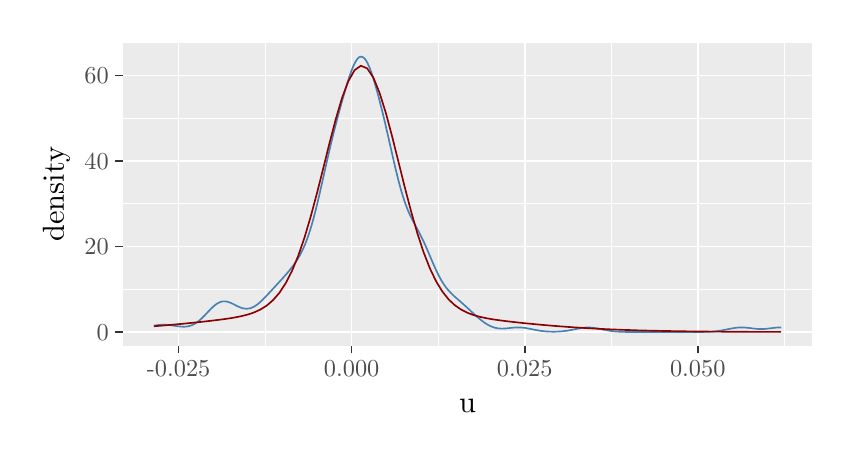
\begin{tikzpicture}[x=1pt,y=1pt]
\definecolor{fillColor}{RGB}{255,255,255}
\path[use as bounding box,fill=fillColor,fill opacity=0.00] (0,0) rectangle (289.08,144.54);
\begin{scope}
\path[clip] (  0.00,  0.00) rectangle (289.08,144.54);
\definecolor{drawColor}{RGB}{255,255,255}
\definecolor{fillColor}{RGB}{255,255,255}

\path[draw=drawColor,line width= 0.6pt,line join=round,line cap=round,fill=fillColor] (  0.00,  0.00) rectangle (289.08,144.54);
\end{scope}
\begin{scope}
\path[clip] ( 34.27, 29.59) rectangle (283.58,139.04);
\definecolor{fillColor}{gray}{0.92}

\path[fill=fillColor] ( 34.27, 29.59) rectangle (283.58,139.04);
\definecolor{drawColor}{RGB}{255,255,255}

\path[draw=drawColor,line width= 0.3pt,line join=round] ( 34.27, 50.02) --
	(283.58, 50.02);

\path[draw=drawColor,line width= 0.3pt,line join=round] ( 34.27, 80.94) --
	(283.58, 80.94);

\path[draw=drawColor,line width= 0.3pt,line join=round] ( 34.27,111.85) --
	(283.58,111.85);

\path[draw=drawColor,line width= 0.3pt,line join=round] ( 85.80, 29.59) --
	( 85.80,139.04);

\path[draw=drawColor,line width= 0.3pt,line join=round] (148.33, 29.59) --
	(148.33,139.04);

\path[draw=drawColor,line width= 0.3pt,line join=round] (210.86, 29.59) --
	(210.86,139.04);

\path[draw=drawColor,line width= 0.3pt,line join=round] (273.40, 29.59) --
	(273.40,139.04);

\path[draw=drawColor,line width= 0.6pt,line join=round] ( 34.27, 34.56) --
	(283.58, 34.56);

\path[draw=drawColor,line width= 0.6pt,line join=round] ( 34.27, 65.48) --
	(283.58, 65.48);

\path[draw=drawColor,line width= 0.6pt,line join=round] ( 34.27, 96.39) --
	(283.58, 96.39);

\path[draw=drawColor,line width= 0.6pt,line join=round] ( 34.27,127.31) --
	(283.58,127.31);

\path[draw=drawColor,line width= 0.6pt,line join=round] ( 54.53, 29.59) --
	( 54.53,139.04);

\path[draw=drawColor,line width= 0.6pt,line join=round] (117.07, 29.59) --
	(117.07,139.04);

\path[draw=drawColor,line width= 0.6pt,line join=round] (179.60, 29.59) --
	(179.60,139.04);

\path[draw=drawColor,line width= 0.6pt,line join=round] (242.13, 29.59) --
	(242.13,139.04);
\definecolor{drawColor}{RGB}{70,130,180}

\path[draw=drawColor,line width= 0.6pt,line join=round] ( 45.60, 36.86) --
	( 46.04, 36.94) --
	( 46.49, 37.01) --
	( 46.93, 37.07) --
	( 47.37, 37.11) --
	( 47.82, 37.15) --
	( 48.26, 37.17) --
	( 48.70, 37.19) --
	( 49.15, 37.19) --
	( 49.59, 37.18) --
	( 50.04, 37.16) --
	( 50.48, 37.13) --
	( 50.92, 37.09) --
	( 51.37, 37.05) --
	( 51.81, 37.00) --
	( 52.25, 36.94) --
	( 52.70, 36.87) --
	( 53.14, 36.81) --
	( 53.58, 36.74) --
	( 54.03, 36.68) --
	( 54.47, 36.62) --
	( 54.91, 36.57) --
	( 55.36, 36.53) --
	( 55.80, 36.50) --
	( 56.25, 36.48) --
	( 56.69, 36.49) --
	( 57.13, 36.51) --
	( 57.58, 36.56) --
	( 58.02, 36.64) --
	( 58.46, 36.74) --
	( 58.91, 36.87) --
	( 59.35, 37.04) --
	( 59.79, 37.24) --
	( 60.24, 37.47) --
	( 60.68, 37.73) --
	( 61.12, 38.02) --
	( 61.57, 38.35) --
	( 62.01, 38.71) --
	( 62.45, 39.09) --
	( 62.90, 39.50) --
	( 63.34, 39.94) --
	( 63.79, 40.38) --
	( 64.23, 40.85) --
	( 64.67, 41.32) --
	( 65.12, 41.79) --
	( 65.56, 42.26) --
	( 66.00, 42.72) --
	( 66.45, 43.16) --
	( 66.89, 43.58) --
	( 67.33, 43.98) --
	( 67.78, 44.35) --
	( 68.22, 44.67) --
	( 68.66, 44.95) --
	( 69.11, 45.18) --
	( 69.55, 45.37) --
	( 69.99, 45.51) --
	( 70.44, 45.61) --
	( 70.88, 45.65) --
	( 71.33, 45.64) --
	( 71.77, 45.59) --
	( 72.21, 45.49) --
	( 72.66, 45.36) --
	( 73.10, 45.20) --
	( 73.54, 45.02) --
	( 73.99, 44.81) --
	( 74.43, 44.59) --
	( 74.87, 44.37) --
	( 75.32, 44.14) --
	( 75.76, 43.92) --
	( 76.20, 43.71) --
	( 76.65, 43.52) --
	( 77.09, 43.35) --
	( 77.53, 43.21) --
	( 77.98, 43.10) --
	( 78.42, 43.03) --
	( 78.87, 42.99) --
	( 79.31, 42.99) --
	( 79.75, 43.03) --
	( 80.20, 43.11) --
	( 80.64, 43.23) --
	( 81.08, 43.40) --
	( 81.53, 43.60) --
	( 81.97, 43.85) --
	( 82.41, 44.12) --
	( 82.86, 44.43) --
	( 83.30, 44.77) --
	( 83.74, 45.15) --
	( 84.19, 45.54) --
	( 84.63, 45.96) --
	( 85.07, 46.39) --
	( 85.52, 46.84) --
	( 85.96, 47.30) --
	( 86.41, 47.77) --
	( 86.85, 48.24) --
	( 87.29, 48.72) --
	( 87.74, 49.20) --
	( 88.18, 49.68) --
	( 88.62, 50.17) --
	( 89.07, 50.65) --
	( 89.51, 51.13) --
	( 89.95, 51.61) --
	( 90.40, 52.09) --
	( 90.84, 52.57) --
	( 91.28, 53.05) --
	( 91.73, 53.54) --
	( 92.17, 54.03) --
	( 92.62, 54.52) --
	( 93.06, 55.02) --
	( 93.50, 55.53) --
	( 93.95, 56.04) --
	( 94.39, 56.57) --
	( 94.83, 57.11) --
	( 95.28, 57.67) --
	( 95.72, 58.25) --
	( 96.16, 58.85) --
	( 96.61, 59.48) --
	( 97.05, 60.14) --
	( 97.49, 60.83) --
	( 97.94, 61.57) --
	( 98.38, 62.35) --
	( 98.82, 63.19) --
	( 99.27, 64.09) --
	( 99.71, 65.05) --
	(100.16, 66.07) --
	(100.60, 67.18) --
	(101.04, 68.35) --
	(101.49, 69.61) --
	(101.93, 70.97) --
	(102.37, 72.40) --
	(102.82, 73.92) --
	(103.26, 75.52) --
	(103.70, 77.19) --
	(104.15, 78.92) --
	(104.59, 80.73) --
	(105.03, 82.60) --
	(105.48, 84.51) --
	(105.92, 86.45) --
	(106.36, 88.42) --
	(106.81, 90.40) --
	(107.25, 92.38) --
	(107.70, 94.36) --
	(108.14, 96.32) --
	(108.58, 98.26) --
	(109.03,100.17) --
	(109.47,102.05) --
	(109.91,103.90) --
	(110.36,105.71) --
	(110.80,107.48) --
	(111.24,109.21) --
	(111.69,110.92) --
	(112.13,112.59) --
	(112.57,114.25) --
	(113.02,115.87) --
	(113.46,117.48) --
	(113.90,119.05) --
	(114.35,120.60) --
	(114.79,122.13) --
	(115.24,123.61) --
	(115.68,125.05) --
	(116.12,126.44) --
	(116.57,127.75) --
	(117.01,128.98) --
	(117.45,130.10) --
	(117.90,131.12) --
	(118.34,132.00) --
	(118.78,132.75) --
	(119.23,133.35) --
	(119.67,133.77) --
	(120.11,134.01) --
	(120.56,134.06) --
	(121.00,133.95) --
	(121.45,133.66) --
	(121.89,133.20) --
	(122.33,132.58) --
	(122.78,131.79) --
	(123.22,130.84) --
	(123.66,129.77) --
	(124.11,128.59) --
	(124.55,127.30) --
	(124.99,125.92) --
	(125.44,124.46) --
	(125.88,122.92) --
	(126.32,121.31) --
	(126.77,119.66) --
	(127.21,117.95) --
	(127.65,116.20) --
	(128.10,114.42) --
	(128.54,112.59) --
	(128.99,110.73) --
	(129.43,108.84) --
	(129.87,106.92) --
	(130.32,104.99) --
	(130.76,103.04) --
	(131.20,101.08) --
	(131.65, 99.13) --
	(132.09, 97.19) --
	(132.53, 95.28) --
	(132.98, 93.40) --
	(133.42, 91.57) --
	(133.86, 89.79) --
	(134.31, 88.08) --
	(134.75, 86.45) --
	(135.19, 84.92) --
	(135.64, 83.46) --
	(136.08, 82.10) --
	(136.53, 80.82) --
	(136.97, 79.63) --
	(137.41, 78.52) --
	(137.86, 77.49) --
	(138.30, 76.53) --
	(138.74, 75.62) --
	(139.19, 74.75) --
	(139.63, 73.91) --
	(140.07, 73.09) --
	(140.52, 72.27) --
	(140.96, 71.45) --
	(141.40, 70.62) --
	(141.85, 69.76) --
	(142.29, 68.88) --
	(142.73, 67.97) --
	(143.18, 67.03) --
	(143.62, 66.06) --
	(144.07, 65.06) --
	(144.51, 64.03) --
	(144.95, 63.00) --
	(145.40, 61.95) --
	(145.84, 60.90) --
	(146.28, 59.86) --
	(146.73, 58.83) --
	(147.17, 57.83) --
	(147.61, 56.86) --
	(148.06, 55.93) --
	(148.50, 55.04) --
	(148.94, 54.20) --
	(149.39, 53.40) --
	(149.83, 52.65) --
	(150.27, 51.96) --
	(150.72, 51.31) --
	(151.16, 50.71) --
	(151.61, 50.15) --
	(152.05, 49.62) --
	(152.49, 49.13) --
	(152.94, 48.66) --
	(153.38, 48.23) --
	(153.82, 47.81) --
	(154.27, 47.40) --
	(154.71, 47.01) --
	(155.15, 46.62) --
	(155.60, 46.23) --
	(156.04, 45.84) --
	(156.48, 45.45) --
	(156.93, 45.06) --
	(157.37, 44.67) --
	(157.82, 44.27) --
	(158.26, 43.87) --
	(158.70, 43.46) --
	(159.15, 43.05) --
	(159.59, 42.64) --
	(160.03, 42.22) --
	(160.48, 41.81) --
	(160.92, 41.40) --
	(161.36, 40.99) --
	(161.81, 40.59) --
	(162.25, 40.20) --
	(162.69, 39.81) --
	(163.14, 39.44) --
	(163.58, 39.07) --
	(164.02, 38.72) --
	(164.47, 38.39) --
	(164.91, 38.06) --
	(165.36, 37.76) --
	(165.80, 37.48) --
	(166.24, 37.22) --
	(166.69, 36.98) --
	(167.13, 36.76) --
	(167.57, 36.56) --
	(168.02, 36.38) --
	(168.46, 36.23) --
	(168.90, 36.11) --
	(169.35, 36.00) --
	(169.79, 35.92) --
	(170.23, 35.86) --
	(170.68, 35.82) --
	(171.12, 35.80) --
	(171.56, 35.80) --
	(172.01, 35.81) --
	(172.45, 35.83) --
	(172.90, 35.87) --
	(173.34, 35.91) --
	(173.78, 35.96) --
	(174.23, 36.01) --
	(174.67, 36.05) --
	(175.11, 36.10) --
	(175.56, 36.14) --
	(176.00, 36.18) --
	(176.44, 36.20) --
	(176.89, 36.22) --
	(177.33, 36.22) --
	(177.77, 36.21) --
	(178.22, 36.19) --
	(178.66, 36.16) --
	(179.10, 36.11) --
	(179.55, 36.06) --
	(179.99, 36.00) --
	(180.44, 35.92) --
	(180.88, 35.84) --
	(181.32, 35.76) --
	(181.77, 35.67) --
	(182.21, 35.58) --
	(182.65, 35.49) --
	(183.10, 35.40) --
	(183.54, 35.31) --
	(183.98, 35.23) --
	(184.43, 35.15) --
	(184.87, 35.08) --
	(185.31, 35.01) --
	(185.76, 34.95) --
	(186.20, 34.89) --
	(186.64, 34.85) --
	(187.09, 34.80) --
	(187.53, 34.77) --
	(187.98, 34.74) --
	(188.42, 34.72) --
	(188.86, 34.70) --
	(189.31, 34.69) --
	(189.75, 34.68) --
	(190.19, 34.68) --
	(190.64, 34.69) --
	(191.08, 34.70) --
	(191.52, 34.71) --
	(191.97, 34.74) --
	(192.41, 34.77) --
	(192.85, 34.80) --
	(193.30, 34.84) --
	(193.74, 34.89) --
	(194.19, 34.94) --
	(194.63, 35.00) --
	(195.07, 35.07) --
	(195.52, 35.14) --
	(195.96, 35.22) --
	(196.40, 35.31) --
	(196.85, 35.39) --
	(197.29, 35.48) --
	(197.73, 35.57) --
	(198.18, 35.66) --
	(198.62, 35.75) --
	(199.06, 35.83) --
	(199.51, 35.91) --
	(199.95, 35.98) --
	(200.39, 36.05) --
	(200.84, 36.10) --
	(201.28, 36.15) --
	(201.73, 36.18) --
	(202.17, 36.19) --
	(202.61, 36.20) --
	(203.06, 36.19) --
	(203.50, 36.16) --
	(203.94, 36.13) --
	(204.39, 36.08) --
	(204.83, 36.02) --
	(205.27, 35.95) --
	(205.72, 35.88) --
	(206.16, 35.80) --
	(206.60, 35.71) --
	(207.05, 35.62) --
	(207.49, 35.53) --
	(207.93, 35.44) --
	(208.38, 35.35) --
	(208.82, 35.27) --
	(209.27, 35.19) --
	(209.71, 35.11) --
	(210.15, 35.04) --
	(210.60, 34.97) --
	(211.04, 34.91) --
	(211.48, 34.86) --
	(211.93, 34.81) --
	(212.37, 34.77) --
	(212.81, 34.74) --
	(213.26, 34.71) --
	(213.70, 34.68) --
	(214.14, 34.66) --
	(214.59, 34.64) --
	(215.03, 34.62) --
	(215.47, 34.61) --
	(215.92, 34.60) --
	(216.36, 34.59) --
	(216.81, 34.58) --
	(217.25, 34.58) --
	(217.69, 34.57) --
	(218.14, 34.57) --
	(218.58, 34.57) --
	(219.02, 34.57) --
	(219.47, 34.57) --
	(219.91, 34.56) --
	(220.35, 34.56) --
	(220.80, 34.56) --
	(221.24, 34.56) --
	(221.68, 34.56) --
	(222.13, 34.56) --
	(222.57, 34.56) --
	(223.02, 34.56) --
	(223.46, 34.56) --
	(223.90, 34.56) --
	(224.35, 34.56) --
	(224.79, 34.56) --
	(225.23, 34.56) --
	(225.68, 34.56) --
	(226.12, 34.56) --
	(226.56, 34.56) --
	(227.01, 34.56) --
	(227.45, 34.56) --
	(227.89, 34.56) --
	(228.34, 34.56) --
	(228.78, 34.56) --
	(229.22, 34.56) --
	(229.67, 34.56) --
	(230.11, 34.56) --
	(230.56, 34.56) --
	(231.00, 34.56) --
	(231.44, 34.56) --
	(231.89, 34.56) --
	(232.33, 34.56) --
	(232.77, 34.56) --
	(233.22, 34.56) --
	(233.66, 34.56) --
	(234.10, 34.56) --
	(234.55, 34.56) --
	(234.99, 34.56) --
	(235.43, 34.56) --
	(235.88, 34.56) --
	(236.32, 34.56) --
	(236.76, 34.56) --
	(237.21, 34.56) --
	(237.65, 34.56) --
	(238.10, 34.56) --
	(238.54, 34.56) --
	(238.98, 34.56) --
	(239.43, 34.56) --
	(239.87, 34.56) --
	(240.31, 34.56) --
	(240.76, 34.57) --
	(241.20, 34.57) --
	(241.64, 34.57) --
	(242.09, 34.57) --
	(242.53, 34.57) --
	(242.97, 34.58) --
	(243.42, 34.58) --
	(243.86, 34.59) --
	(244.30, 34.60) --
	(244.75, 34.61) --
	(245.19, 34.62) --
	(245.64, 34.64) --
	(246.08, 34.65) --
	(246.52, 34.67) --
	(246.97, 34.70) --
	(247.41, 34.73) --
	(247.85, 34.77) --
	(248.30, 34.81) --
	(248.74, 34.85) --
	(249.18, 34.91) --
	(249.63, 34.97) --
	(250.07, 35.03) --
	(250.51, 35.10) --
	(250.96, 35.18) --
	(251.40, 35.26) --
	(251.84, 35.34) --
	(252.29, 35.43) --
	(252.73, 35.52) --
	(253.18, 35.61) --
	(253.62, 35.70) --
	(254.06, 35.79) --
	(254.51, 35.87) --
	(254.95, 35.95) --
	(255.39, 36.02) --
	(255.84, 36.08) --
	(256.28, 36.13) --
	(256.72, 36.17) --
	(257.17, 36.20) --
	(257.61, 36.21) --
	(258.05, 36.22) --
	(258.50, 36.21) --
	(258.94, 36.19) --
	(259.39, 36.16) --
	(259.83, 36.12) --
	(260.27, 36.07) --
	(260.72, 36.02) --
	(261.16, 35.97) --
	(261.60, 35.91) --
	(262.05, 35.85) --
	(262.49, 35.80) --
	(262.93, 35.76) --
	(263.38, 35.71) --
	(263.82, 35.68) --
	(264.26, 35.66) --
	(264.71, 35.65) --
	(265.15, 35.64) --
	(265.59, 35.65) --
	(266.04, 35.67) --
	(266.48, 35.70) --
	(266.93, 35.74) --
	(267.37, 35.78) --
	(267.81, 35.84) --
	(268.26, 35.89) --
	(268.70, 35.95) --
	(269.14, 36.00) --
	(269.59, 36.06) --
	(270.03, 36.10) --
	(270.47, 36.15) --
	(270.92, 36.18) --
	(271.36, 36.20) --
	(271.80, 36.22) --
	(272.25, 36.22);
\definecolor{drawColor}{RGB}{139,0,0}

\path[draw=drawColor,line width= 0.6pt,line join=round] ( 45.60, 36.64) --
	( 47.87, 36.82) --
	( 50.13, 37.01) --
	( 52.40, 37.21) --
	( 54.67, 37.42) --
	( 56.93, 37.63) --
	( 59.20, 37.86) --
	( 61.47, 38.10) --
	( 63.73, 38.34) --
	( 66.00, 38.60) --
	( 68.26, 38.87) --
	( 70.53, 39.16) --
	( 72.80, 39.48) --
	( 75.06, 39.86) --
	( 77.33, 40.32) --
	( 79.60, 40.90) --
	( 81.86, 41.66) --
	( 84.13, 42.71) --
	( 86.40, 44.13) --
	( 88.66, 46.08) --
	( 90.93, 48.69) --
	( 93.20, 52.13) --
	( 95.46, 56.53) --
	( 97.73, 62.01) --
	(100.00, 68.59) --
	(102.26, 76.22) --
	(104.53, 84.70) --
	(106.80, 93.71) --
	(109.06,102.82) --
	(111.33,111.50) --
	(113.59,119.14) --
	(115.86,125.20) --
	(118.13,129.19) --
	(120.39,130.79) --
	(122.66,129.85) --
	(124.93,126.45) --
	(127.19,120.89) --
	(129.46,113.59) --
	(131.73,105.10) --
	(133.99, 96.03) --
	(136.26, 86.90) --
	(138.53, 78.21) --
	(140.79, 70.30) --
	(143.06, 63.40) --
	(145.33, 57.59) --
	(147.59, 52.88) --
	(149.86, 49.17) --
	(152.12, 46.34) --
	(154.39, 44.21) --
	(156.66, 42.65) --
	(158.92, 41.51) --
	(161.19, 40.67) --
	(163.46, 40.04) --
	(165.72, 39.56) --
	(167.99, 39.16) --
	(170.26, 38.83) --
	(172.52, 38.54) --
	(174.79, 38.27) --
	(177.06, 38.02) --
	(179.32, 37.78) --
	(181.59, 37.56) --
	(183.86, 37.34) --
	(186.12, 37.13) --
	(188.39, 36.94) --
	(190.65, 36.75) --
	(192.92, 36.58) --
	(195.19, 36.41) --
	(197.45, 36.25) --
	(199.72, 36.11) --
	(201.99, 35.97) --
	(204.25, 35.84) --
	(206.52, 35.72) --
	(208.79, 35.61) --
	(211.05, 35.51) --
	(213.32, 35.42) --
	(215.59, 35.33) --
	(217.85, 35.26) --
	(220.12, 35.18) --
	(222.39, 35.12) --
	(224.65, 35.06) --
	(226.92, 35.01) --
	(229.18, 34.96) --
	(231.45, 34.92) --
	(233.72, 34.88) --
	(235.98, 34.84) --
	(238.25, 34.81) --
	(240.52, 34.78) --
	(242.78, 34.76) --
	(245.05, 34.73) --
	(247.32, 34.71) --
	(249.58, 34.70) --
	(251.85, 34.68) --
	(254.12, 34.67) --
	(256.38, 34.65) --
	(258.65, 34.64) --
	(260.92, 34.63) --
	(263.18, 34.63) --
	(265.45, 34.62) --
	(267.71, 34.61) --
	(269.98, 34.61) --
	(272.25, 34.60);
\end{scope}
\begin{scope}
\path[clip] (  0.00,  0.00) rectangle (289.08,144.54);
\definecolor{drawColor}{gray}{0.30}

\node[text=drawColor,anchor=base east,inner sep=0pt, outer sep=0pt, scale=  0.88] at ( 29.32, 31.53) {0};

\node[text=drawColor,anchor=base east,inner sep=0pt, outer sep=0pt, scale=  0.88] at ( 29.32, 62.45) {20};

\node[text=drawColor,anchor=base east,inner sep=0pt, outer sep=0pt, scale=  0.88] at ( 29.32, 93.36) {40};

\node[text=drawColor,anchor=base east,inner sep=0pt, outer sep=0pt, scale=  0.88] at ( 29.32,124.28) {60};
\end{scope}
\begin{scope}
\path[clip] (  0.00,  0.00) rectangle (289.08,144.54);
\definecolor{drawColor}{gray}{0.20}

\path[draw=drawColor,line width= 0.6pt,line join=round] ( 31.52, 34.56) --
	( 34.27, 34.56);

\path[draw=drawColor,line width= 0.6pt,line join=round] ( 31.52, 65.48) --
	( 34.27, 65.48);

\path[draw=drawColor,line width= 0.6pt,line join=round] ( 31.52, 96.39) --
	( 34.27, 96.39);

\path[draw=drawColor,line width= 0.6pt,line join=round] ( 31.52,127.31) --
	( 34.27,127.31);
\end{scope}
\begin{scope}
\path[clip] (  0.00,  0.00) rectangle (289.08,144.54);
\definecolor{drawColor}{gray}{0.20}

\path[draw=drawColor,line width= 0.6pt,line join=round] ( 54.53, 26.84) --
	( 54.53, 29.59);

\path[draw=drawColor,line width= 0.6pt,line join=round] (117.07, 26.84) --
	(117.07, 29.59);

\path[draw=drawColor,line width= 0.6pt,line join=round] (179.60, 26.84) --
	(179.60, 29.59);

\path[draw=drawColor,line width= 0.6pt,line join=round] (242.13, 26.84) --
	(242.13, 29.59);
\end{scope}
\begin{scope}
\path[clip] (  0.00,  0.00) rectangle (289.08,144.54);
\definecolor{drawColor}{gray}{0.30}

\node[text=drawColor,anchor=base,inner sep=0pt, outer sep=0pt, scale=  0.88] at ( 54.53, 18.58) {-0.025};

\node[text=drawColor,anchor=base,inner sep=0pt, outer sep=0pt, scale=  0.88] at (117.07, 18.58) {0.000};

\node[text=drawColor,anchor=base,inner sep=0pt, outer sep=0pt, scale=  0.88] at (179.60, 18.58) {0.025};

\node[text=drawColor,anchor=base,inner sep=0pt, outer sep=0pt, scale=  0.88] at (242.13, 18.58) {0.050};
\end{scope}
\begin{scope}
\path[clip] (  0.00,  0.00) rectangle (289.08,144.54);
\definecolor{drawColor}{RGB}{0,0,0}

\node[text=drawColor,anchor=base,inner sep=0pt, outer sep=0pt, scale=  1.10] at (158.92,  5.50) {u};
\end{scope}
\begin{scope}
\path[clip] (  0.00,  0.00) rectangle (289.08,144.54);
\definecolor{drawColor}{RGB}{0,0,0}

\node[text=drawColor,rotate= 90.00,anchor=base,inner sep=0pt, outer sep=0pt, scale=  1.10] at ( 13.08, 84.31) {density};
\end{scope}
\end{tikzpicture}

  \caption{Historical and MJD related Apple stock log-returns distribution in the risk-averse world}
    %
  % BEGIN OF FLOATNOTE
  %
  \begin{changemargin}{0.5cm}{0.5cm}
  \medskip
\footnotesize
\setstretch{1.0}\textbf{Notes.} The above blue density curve is constructed over the historical data of the Apple share of stock price evolution from 1st January 2017 to 31st December 2017. While the red curve is constructed from time-series generated by the function \textit{mjd\_ts} taking the risk-averse parameters \ref{eq:methodology:arg:merton:riskaverse} as arguments.  
\end{changemargin}
  %
  % END OF FLOATNOTE
  %
  \label{p:methodology:density:aapl:merton:riskaverse}
\end{figure}

Consequently, for the purpose of that master thesis, the set \ref{eq:methodology:arg:merton:riskaverse} is the one that will be used together with the function \textit{mjd\_ts()} whenever performing the computation of time series using the MJD model within the real world constraints.











%%%%%%%%%%%%%%%%%%%%%%%%%%%%%%%
%
%
%
% HERE
%
%
%
%%%%%%%%%%%%%%%%%%%%%%%%%%%%%%%%


% SUBSECTION: Heston's model calibration
%%%%%%%%%%%%%%%%%%%%%%%%%%%%%%%%%%%%%%%%%%%%%%%%%%%%%%%%%%%%%%%%%%%%%%%%%%%%%%%%
% Heston
%%%%%%%%%%%%%%%%%%%%%%%%%%%%%%%%%%%%%%%%%%%%%%%%%%%%%%%%%%%%%%%%%%%%%%%%%%%%%%%%
\subsection{Heston's model calibration}
\label{sub:methodology:calibration:heston}

\subsubsection*{Calibration of parameters for option pricing}

In order to use the function \textit{hsv\_call} based on \cref{eq:other:call:heston} to compute the price of European call options on an underlying with increments driven by the HSV model, the parameters $\left\{ V(0), \kappa, \theta, \sigma, \rho \right\}$ must be calibrated with respect to the available market data.
Therefore, the so estimated parameters will be in line with the risk-neutral measure, or more specifically $\kappa$ and $\theta$, which are the only ones needed to be adapted to make \cref{eq:other:hsvvol:riskless} risk-neutral.

To do so and similarly as it was done for the MJD option model, the least-square non-linear analysis will be used together with data on Apple call option as a template.
In that respect, the theoretical models to calibrate are given by \crefrange{eq:other:call:heston}{eq:other:call:heston:pi2} along with \cref{eq:other:heston:psi}, implemented by the R function \textit{hsv\_call}.

Moreover, to stay in a range of acceptable values, the parameters of the HSV model should lie between some defined boundaries. 

De facto, the mean-reversion speed ($\kappa$), the long-run variance ($\theta$) and the volatility of the volatility ($\sigma$) need to take values that together respect the Feller's condition (see \cref{sub:other:heston:feller}). 
Additionally, $\sigma$ must range between 0 and 1 and, according to \citet{cristo2015} $\kappa$ should be positive to avoid mean aversion.
Although the correlation coefficient $\rho$ may take any value from $[-1, 1]$, typically the correlation between the stock price increments and their intrinsic volatility is negative. Consequently, the boundaries of $\rho$ are set as $]0, -1[$.

According to those constraints and due to the presence of multiple local minima, the \textit{lsqnonlin} function returns the \cref{t:methodology:call:heston:estimate1} as the whole sets of parameters that make the function \textit{hsv\_call} better fit with reality.

\begin{table}[h]
\centering
\begin{tabular}{rrrrr}
  \hline
v0 & theta & sigma & rho & kappa \\ 
  \hline
  0.03851 & 0.05142 & 0.29539 & -0.49338 & 1.99931 \\ 
  0.03774 & 0.04832 & 0.30687 & -0.40213 & 3.00036 \\ 
  0.03910 & 0.04948 & 0.40736 & -0.50193 & 3.00005 \\ 
  0.03798 & 0.04872 & 0.50379 & -0.39878 & 4.00106 \\
  0.03740 & 0.04754 & 0.30583 & -0.60126 & 4.00096 \\ 
  0.03661 & 0.04604 & 0.30659 & -0.40295 & 5.00152 \\ 
  0.03921 & 0.04709 & 0.50753 & -0.50170 & 5.00152 \\ 
   \hline
\end{tabular}
\caption{Best estimates for HSV call option model} 
\label{t:methodology:call:heston:estimate1}
\end{table}

However, the set of arguments \ref{eq:methodology:arg:heston:riskneutral} is the one making respond the model the best with what is observed in reality.
Indeed when passing that set to the R function \textit{call\_heston}, for all strikes and maturities from \cref{t:methodology:strike,t:methodology:maturity}  more than $70\%$ of the so generated prices are within the bid-ask spread of the historical data.

\begin{align}
  \left \{
  \begin{array}{lcl}
    V(0) &= &0.03798218, \\
    \theta &= &0.04871543, \\
    \sigma &= &0.50378803, \\
    \rho &= &-0.39877827, \\
    \kappa &= &4.00105546 
  \end{array}
  \right \}  
  \label{eq:methodology:arg:heston:riskneutral}
\end{align}

\Cref{p:methodology:impliedvol:aapl:heston} confronts the blue colored volatility smiles computed from market data, with those dotted in red, calculated from data provided by the function \textit{hsv\_call} which takes the items of the set \ref{eq:methodology:arg:heston:riskneutral} as parameters.

\begin{figure}[h]
  \centering
  % Created by tikzDevice version 0.11 on 2018-07-20 21:55:59
% !TEX encoding = UTF-8 Unicode
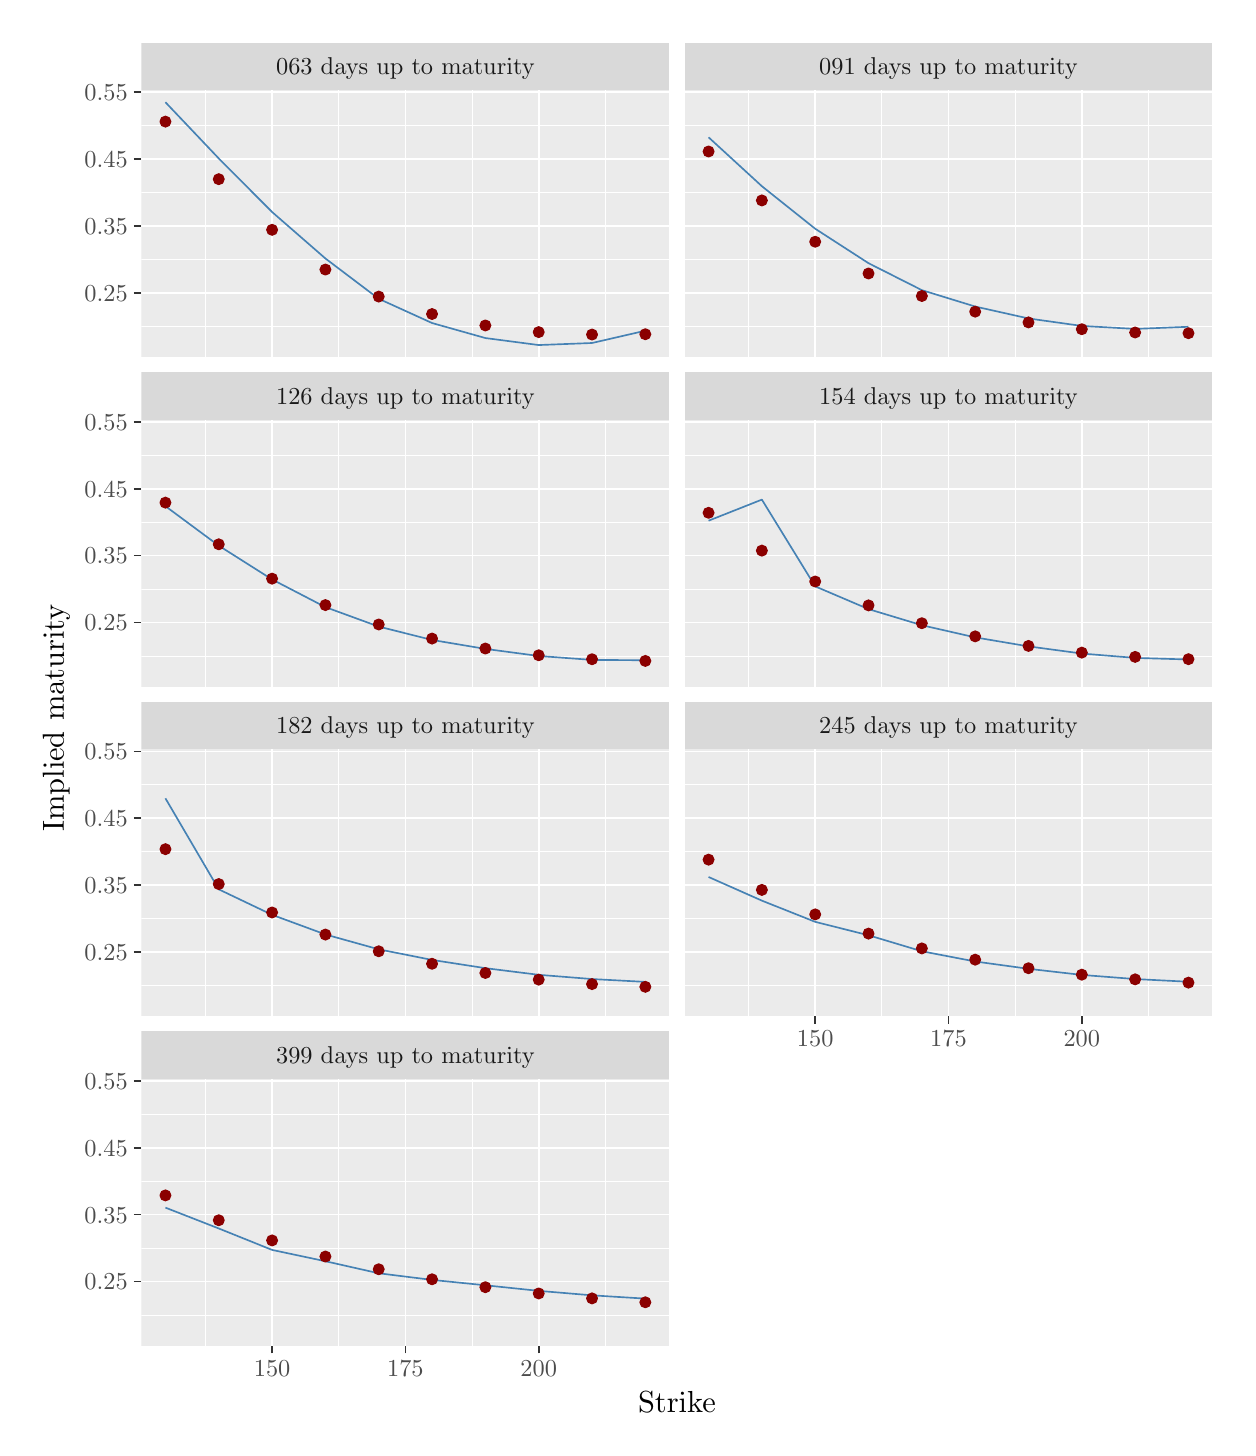
\begin{tikzpicture}[x=1pt,y=1pt]
\definecolor{fillColor}{RGB}{255,255,255}
\path[use as bounding box,fill=fillColor,fill opacity=0.00] (0,0) rectangle (433.62,505.89);
\begin{scope}
\path[clip] (  0.00,  0.00) rectangle (433.62,505.89);
\definecolor{drawColor}{RGB}{255,255,255}
\definecolor{fillColor}{RGB}{255,255,255}

\path[draw=drawColor,line width= 0.6pt,line join=round,line cap=round,fill=fillColor] (  0.00,  0.00) rectangle (433.62,505.89);
\end{scope}
\begin{scope}
\path[clip] ( 41.11,386.81) rectangle (231.87,483.33);
\definecolor{fillColor}{gray}{0.92}

\path[fill=fillColor] ( 41.11,386.81) rectangle (231.87,483.33);
\definecolor{drawColor}{RGB}{255,255,255}

\path[draw=drawColor,line width= 0.3pt,line join=round] ( 41.11,397.93) --
	(231.87,397.93);

\path[draw=drawColor,line width= 0.3pt,line join=round] ( 41.11,422.11) --
	(231.87,422.11);

\path[draw=drawColor,line width= 0.3pt,line join=round] ( 41.11,446.28) --
	(231.87,446.28);

\path[draw=drawColor,line width= 0.3pt,line join=round] ( 41.11,470.45) --
	(231.87,470.45);

\path[draw=drawColor,line width= 0.3pt,line join=round] ( 64.23,386.81) --
	( 64.23,483.33);

\path[draw=drawColor,line width= 0.3pt,line join=round] (112.40,386.81) --
	(112.40,483.33);

\path[draw=drawColor,line width= 0.3pt,line join=round] (160.57,386.81) --
	(160.57,483.33);

\path[draw=drawColor,line width= 0.3pt,line join=round] (208.74,386.81) --
	(208.74,483.33);

\path[draw=drawColor,line width= 0.6pt,line join=round] ( 41.11,410.02) --
	(231.87,410.02);

\path[draw=drawColor,line width= 0.6pt,line join=round] ( 41.11,434.19) --
	(231.87,434.19);

\path[draw=drawColor,line width= 0.6pt,line join=round] ( 41.11,458.37) --
	(231.87,458.37);

\path[draw=drawColor,line width= 0.6pt,line join=round] ( 41.11,482.54) --
	(231.87,482.54);

\path[draw=drawColor,line width= 0.6pt,line join=round] ( 88.32,386.81) --
	( 88.32,483.33);

\path[draw=drawColor,line width= 0.6pt,line join=round] (136.49,386.81) --
	(136.49,483.33);

\path[draw=drawColor,line width= 0.6pt,line join=round] (184.66,386.81) --
	(184.66,483.33);
\definecolor{drawColor}{RGB}{70,130,180}

\path[draw=drawColor,line width= 0.6pt,line join=round] ( 49.78,478.94) --
	( 69.05,458.63) --
	( 88.32,439.27) --
	(107.59,422.48) --
	(126.85,407.92) --
	(146.12,399.16) --
	(165.39,393.73) --
	(184.66,391.20) --
	(203.93,391.94) --
	(223.19,396.38);
\definecolor{drawColor}{RGB}{139,0,0}
\definecolor{fillColor}{RGB}{139,0,0}

\path[draw=drawColor,line width= 0.4pt,line join=round,line cap=round,fill=fillColor] ( 49.78,471.94) circle (  1.96);

\path[draw=drawColor,line width= 0.4pt,line join=round,line cap=round,fill=fillColor] ( 69.05,451.14) circle (  1.96);

\path[draw=drawColor,line width= 0.4pt,line join=round,line cap=round,fill=fillColor] ( 88.32,432.84) circle (  1.96);

\path[draw=drawColor,line width= 0.4pt,line join=round,line cap=round,fill=fillColor] (107.59,418.48) circle (  1.96);

\path[draw=drawColor,line width= 0.4pt,line join=round,line cap=round,fill=fillColor] (126.85,408.72) circle (  1.96);

\path[draw=drawColor,line width= 0.4pt,line join=round,line cap=round,fill=fillColor] (146.12,402.41) circle (  1.96);

\path[draw=drawColor,line width= 0.4pt,line join=round,line cap=round,fill=fillColor] (165.39,398.28) circle (  1.96);

\path[draw=drawColor,line width= 0.4pt,line join=round,line cap=round,fill=fillColor] (184.66,395.88) circle (  1.96);

\path[draw=drawColor,line width= 0.4pt,line join=round,line cap=round,fill=fillColor] (203.93,394.99) circle (  1.96);

\path[draw=drawColor,line width= 0.4pt,line join=round,line cap=round,fill=fillColor] (223.19,395.11) circle (  1.96);
\end{scope}
\begin{scope}
\path[clip] ( 41.11,267.74) rectangle (231.87,364.25);
\definecolor{fillColor}{gray}{0.92}

\path[fill=fillColor] ( 41.11,267.74) rectangle (231.87,364.25);
\definecolor{drawColor}{RGB}{255,255,255}

\path[draw=drawColor,line width= 0.3pt,line join=round] ( 41.11,278.86) --
	(231.87,278.86);

\path[draw=drawColor,line width= 0.3pt,line join=round] ( 41.11,303.03) --
	(231.87,303.03);

\path[draw=drawColor,line width= 0.3pt,line join=round] ( 41.11,327.20) --
	(231.87,327.20);

\path[draw=drawColor,line width= 0.3pt,line join=round] ( 41.11,351.38) --
	(231.87,351.38);

\path[draw=drawColor,line width= 0.3pt,line join=round] ( 64.23,267.74) --
	( 64.23,364.25);

\path[draw=drawColor,line width= 0.3pt,line join=round] (112.40,267.74) --
	(112.40,364.25);

\path[draw=drawColor,line width= 0.3pt,line join=round] (160.57,267.74) --
	(160.57,364.25);

\path[draw=drawColor,line width= 0.3pt,line join=round] (208.74,267.74) --
	(208.74,364.25);

\path[draw=drawColor,line width= 0.6pt,line join=round] ( 41.11,290.95) --
	(231.87,290.95);

\path[draw=drawColor,line width= 0.6pt,line join=round] ( 41.11,315.12) --
	(231.87,315.12);

\path[draw=drawColor,line width= 0.6pt,line join=round] ( 41.11,339.29) --
	(231.87,339.29);

\path[draw=drawColor,line width= 0.6pt,line join=round] ( 41.11,363.46) --
	(231.87,363.46);

\path[draw=drawColor,line width= 0.6pt,line join=round] ( 88.32,267.74) --
	( 88.32,364.25);

\path[draw=drawColor,line width= 0.6pt,line join=round] (136.49,267.74) --
	(136.49,364.25);

\path[draw=drawColor,line width= 0.6pt,line join=round] (184.66,267.74) --
	(184.66,364.25);
\definecolor{drawColor}{RGB}{70,130,180}

\path[draw=drawColor,line width= 0.6pt,line join=round] ( 49.78,332.98) --
	( 69.05,318.71) --
	( 88.32,306.50) --
	(107.59,296.51) --
	(126.85,289.47) --
	(146.12,284.64) --
	(165.39,281.41) --
	(184.66,278.85) --
	(203.93,277.43) --
	(223.19,277.30);
\definecolor{drawColor}{RGB}{139,0,0}
\definecolor{fillColor}{RGB}{139,0,0}

\path[draw=drawColor,line width= 0.4pt,line join=round,line cap=round,fill=fillColor] ( 49.78,334.26) circle (  1.96);

\path[draw=drawColor,line width= 0.4pt,line join=round,line cap=round,fill=fillColor] ( 69.05,319.20) circle (  1.96);

\path[draw=drawColor,line width= 0.4pt,line join=round,line cap=round,fill=fillColor] ( 88.32,306.79) circle (  1.96);

\path[draw=drawColor,line width= 0.4pt,line join=round,line cap=round,fill=fillColor] (107.59,297.24) circle (  1.96);

\path[draw=drawColor,line width= 0.4pt,line join=round,line cap=round,fill=fillColor] (126.85,290.23) circle (  1.96);

\path[draw=drawColor,line width= 0.4pt,line join=round,line cap=round,fill=fillColor] (146.12,285.14) circle (  1.96);

\path[draw=drawColor,line width= 0.4pt,line join=round,line cap=round,fill=fillColor] (165.39,281.54) circle (  1.96);

\path[draw=drawColor,line width= 0.4pt,line join=round,line cap=round,fill=fillColor] (184.66,279.10) circle (  1.96);

\path[draw=drawColor,line width= 0.4pt,line join=round,line cap=round,fill=fillColor] (203.93,277.67) circle (  1.96);

\path[draw=drawColor,line width= 0.4pt,line join=round,line cap=round,fill=fillColor] (223.19,277.06) circle (  1.96);
\end{scope}
\begin{scope}
\path[clip] ( 41.11,148.66) rectangle (231.87,245.18);
\definecolor{fillColor}{gray}{0.92}

\path[fill=fillColor] ( 41.11,148.66) rectangle (231.87,245.18);
\definecolor{drawColor}{RGB}{255,255,255}

\path[draw=drawColor,line width= 0.3pt,line join=round] ( 41.11,159.78) --
	(231.87,159.78);

\path[draw=drawColor,line width= 0.3pt,line join=round] ( 41.11,183.96) --
	(231.87,183.96);

\path[draw=drawColor,line width= 0.3pt,line join=round] ( 41.11,208.13) --
	(231.87,208.13);

\path[draw=drawColor,line width= 0.3pt,line join=round] ( 41.11,232.30) --
	(231.87,232.30);

\path[draw=drawColor,line width= 0.3pt,line join=round] ( 64.23,148.66) --
	( 64.23,245.18);

\path[draw=drawColor,line width= 0.3pt,line join=round] (112.40,148.66) --
	(112.40,245.18);

\path[draw=drawColor,line width= 0.3pt,line join=round] (160.57,148.66) --
	(160.57,245.18);

\path[draw=drawColor,line width= 0.3pt,line join=round] (208.74,148.66) --
	(208.74,245.18);

\path[draw=drawColor,line width= 0.6pt,line join=round] ( 41.11,171.87) --
	(231.87,171.87);

\path[draw=drawColor,line width= 0.6pt,line join=round] ( 41.11,196.04) --
	(231.87,196.04);

\path[draw=drawColor,line width= 0.6pt,line join=round] ( 41.11,220.21) --
	(231.87,220.21);

\path[draw=drawColor,line width= 0.6pt,line join=round] ( 41.11,244.39) --
	(231.87,244.39);

\path[draw=drawColor,line width= 0.6pt,line join=round] ( 88.32,148.66) --
	( 88.32,245.18);

\path[draw=drawColor,line width= 0.6pt,line join=round] (136.49,148.66) --
	(136.49,245.18);

\path[draw=drawColor,line width= 0.6pt,line join=round] (184.66,148.66) --
	(184.66,245.18);
\definecolor{drawColor}{RGB}{70,130,180}

\path[draw=drawColor,line width= 0.6pt,line join=round] ( 49.78,227.41) --
	( 69.05,194.52) --
	( 88.32,185.32) --
	(107.59,178.22) --
	(126.85,172.85) --
	(146.12,169.02) --
	(165.39,166.04) --
	(184.66,163.64) --
	(203.93,162.11) --
	(223.19,161.08);
\definecolor{drawColor}{RGB}{139,0,0}
\definecolor{fillColor}{RGB}{139,0,0}

\path[draw=drawColor,line width= 0.4pt,line join=round,line cap=round,fill=fillColor] ( 49.78,209.04) circle (  1.96);

\path[draw=drawColor,line width= 0.4pt,line join=round,line cap=round,fill=fillColor] ( 69.05,196.43) circle (  1.96);

\path[draw=drawColor,line width= 0.4pt,line join=round,line cap=round,fill=fillColor] ( 88.32,186.16) circle (  1.96);

\path[draw=drawColor,line width= 0.4pt,line join=round,line cap=round,fill=fillColor] (107.59,178.18) circle (  1.96);

\path[draw=drawColor,line width= 0.4pt,line join=round,line cap=round,fill=fillColor] (126.85,172.14) circle (  1.96);

\path[draw=drawColor,line width= 0.4pt,line join=round,line cap=round,fill=fillColor] (146.12,167.63) circle (  1.96);

\path[draw=drawColor,line width= 0.4pt,line join=round,line cap=round,fill=fillColor] (165.39,164.30) circle (  1.96);

\path[draw=drawColor,line width= 0.4pt,line join=round,line cap=round,fill=fillColor] (184.66,161.90) circle (  1.96);

\path[draw=drawColor,line width= 0.4pt,line join=round,line cap=round,fill=fillColor] (203.93,160.28) circle (  1.96);

\path[draw=drawColor,line width= 0.4pt,line join=round,line cap=round,fill=fillColor] (223.19,159.30) circle (  1.96);
\end{scope}
\begin{scope}
\path[clip] ( 41.11, 29.59) rectangle (231.87,126.10);
\definecolor{fillColor}{gray}{0.92}

\path[fill=fillColor] ( 41.11, 29.59) rectangle (231.87,126.10);
\definecolor{drawColor}{RGB}{255,255,255}

\path[draw=drawColor,line width= 0.3pt,line join=round] ( 41.11, 40.71) --
	(231.87, 40.71);

\path[draw=drawColor,line width= 0.3pt,line join=round] ( 41.11, 64.88) --
	(231.87, 64.88);

\path[draw=drawColor,line width= 0.3pt,line join=round] ( 41.11, 89.05) --
	(231.87, 89.05);

\path[draw=drawColor,line width= 0.3pt,line join=round] ( 41.11,113.22) --
	(231.87,113.22);

\path[draw=drawColor,line width= 0.3pt,line join=round] ( 64.23, 29.59) --
	( 64.23,126.10);

\path[draw=drawColor,line width= 0.3pt,line join=round] (112.40, 29.59) --
	(112.40,126.10);

\path[draw=drawColor,line width= 0.3pt,line join=round] (160.57, 29.59) --
	(160.57,126.10);

\path[draw=drawColor,line width= 0.3pt,line join=round] (208.74, 29.59) --
	(208.74,126.10);

\path[draw=drawColor,line width= 0.6pt,line join=round] ( 41.11, 52.79) --
	(231.87, 52.79);

\path[draw=drawColor,line width= 0.6pt,line join=round] ( 41.11, 76.97) --
	(231.87, 76.97);

\path[draw=drawColor,line width= 0.6pt,line join=round] ( 41.11,101.14) --
	(231.87,101.14);

\path[draw=drawColor,line width= 0.6pt,line join=round] ( 41.11,125.31) --
	(231.87,125.31);

\path[draw=drawColor,line width= 0.6pt,line join=round] ( 88.32, 29.59) --
	( 88.32,126.10);

\path[draw=drawColor,line width= 0.6pt,line join=round] (136.49, 29.59) --
	(136.49,126.10);

\path[draw=drawColor,line width= 0.6pt,line join=round] (184.66, 29.59) --
	(184.66,126.10);
\definecolor{drawColor}{RGB}{70,130,180}

\path[draw=drawColor,line width= 0.6pt,line join=round] ( 49.78, 79.51) --
	( 69.05, 71.98) --
	( 88.32, 64.23) --
	(107.59, 60.14) --
	(126.85, 55.79) --
	(146.12, 53.40) --
	(165.39, 51.45) --
	(184.66, 49.44) --
	(203.93, 47.82) --
	(223.19, 46.63);
\definecolor{drawColor}{RGB}{139,0,0}
\definecolor{fillColor}{RGB}{139,0,0}

\path[draw=drawColor,line width= 0.4pt,line join=round,line cap=round,fill=fillColor] ( 49.78, 83.93) circle (  1.96);

\path[draw=drawColor,line width= 0.4pt,line join=round,line cap=round,fill=fillColor] ( 69.05, 74.95) circle (  1.96);

\path[draw=drawColor,line width= 0.4pt,line join=round,line cap=round,fill=fillColor] ( 88.32, 67.66) circle (  1.96);

\path[draw=drawColor,line width= 0.4pt,line join=round,line cap=round,fill=fillColor] (107.59, 61.84) circle (  1.96);

\path[draw=drawColor,line width= 0.4pt,line join=round,line cap=round,fill=fillColor] (126.85, 57.24) circle (  1.96);

\path[draw=drawColor,line width= 0.4pt,line join=round,line cap=round,fill=fillColor] (146.12, 53.62) circle (  1.96);

\path[draw=drawColor,line width= 0.4pt,line join=round,line cap=round,fill=fillColor] (165.39, 50.76) circle (  1.96);

\path[draw=drawColor,line width= 0.4pt,line join=round,line cap=round,fill=fillColor] (184.66, 48.50) circle (  1.96);

\path[draw=drawColor,line width= 0.4pt,line join=round,line cap=round,fill=fillColor] (203.93, 46.72) circle (  1.96);

\path[draw=drawColor,line width= 0.4pt,line join=round,line cap=round,fill=fillColor] (223.19, 45.31) circle (  1.96);
\end{scope}
\begin{scope}
\path[clip] (237.37,386.81) rectangle (428.12,483.33);
\definecolor{fillColor}{gray}{0.92}

\path[fill=fillColor] (237.37,386.81) rectangle (428.12,483.33);
\definecolor{drawColor}{RGB}{255,255,255}

\path[draw=drawColor,line width= 0.3pt,line join=round] (237.37,397.93) --
	(428.12,397.93);

\path[draw=drawColor,line width= 0.3pt,line join=round] (237.37,422.11) --
	(428.12,422.11);

\path[draw=drawColor,line width= 0.3pt,line join=round] (237.37,446.28) --
	(428.12,446.28);

\path[draw=drawColor,line width= 0.3pt,line join=round] (237.37,470.45) --
	(428.12,470.45);

\path[draw=drawColor,line width= 0.3pt,line join=round] (260.49,386.81) --
	(260.49,483.33);

\path[draw=drawColor,line width= 0.3pt,line join=round] (308.66,386.81) --
	(308.66,483.33);

\path[draw=drawColor,line width= 0.3pt,line join=round] (356.83,386.81) --
	(356.83,483.33);

\path[draw=drawColor,line width= 0.3pt,line join=round] (405.00,386.81) --
	(405.00,483.33);

\path[draw=drawColor,line width= 0.6pt,line join=round] (237.37,410.02) --
	(428.12,410.02);

\path[draw=drawColor,line width= 0.6pt,line join=round] (237.37,434.19) --
	(428.12,434.19);

\path[draw=drawColor,line width= 0.6pt,line join=round] (237.37,458.37) --
	(428.12,458.37);

\path[draw=drawColor,line width= 0.6pt,line join=round] (237.37,482.54) --
	(428.12,482.54);

\path[draw=drawColor,line width= 0.6pt,line join=round] (284.57,386.81) --
	(284.57,483.33);

\path[draw=drawColor,line width= 0.6pt,line join=round] (332.74,386.81) --
	(332.74,483.33);

\path[draw=drawColor,line width= 0.6pt,line join=round] (380.91,386.81) --
	(380.91,483.33);
\definecolor{drawColor}{RGB}{70,130,180}

\path[draw=drawColor,line width= 0.6pt,line join=round] (246.04,466.27) --
	(265.30,448.60) --
	(284.57,433.23) --
	(303.84,420.78) --
	(323.11,411.04) --
	(342.38,405.12) --
	(361.64,400.81) --
	(380.91,398.11) --
	(400.18,397.03) --
	(419.45,397.80);
\definecolor{drawColor}{RGB}{139,0,0}
\definecolor{fillColor}{RGB}{139,0,0}

\path[draw=drawColor,line width= 0.4pt,line join=round,line cap=round,fill=fillColor] (246.04,461.14) circle (  1.96);

\path[draw=drawColor,line width= 0.4pt,line join=round,line cap=round,fill=fillColor] (265.30,443.46) circle (  1.96);

\path[draw=drawColor,line width= 0.4pt,line join=round,line cap=round,fill=fillColor] (284.57,428.53) circle (  1.96);

\path[draw=drawColor,line width= 0.4pt,line join=round,line cap=round,fill=fillColor] (303.84,417.06) circle (  1.96);

\path[draw=drawColor,line width= 0.4pt,line join=round,line cap=round,fill=fillColor] (323.11,408.92) circle (  1.96);

\path[draw=drawColor,line width= 0.4pt,line join=round,line cap=round,fill=fillColor] (342.38,403.27) circle (  1.96);

\path[draw=drawColor,line width= 0.4pt,line join=round,line cap=round,fill=fillColor] (361.64,399.38) circle (  1.96);

\path[draw=drawColor,line width= 0.4pt,line join=round,line cap=round,fill=fillColor] (380.91,396.93) circle (  1.96);

\path[draw=drawColor,line width= 0.4pt,line join=round,line cap=round,fill=fillColor] (400.18,395.74) circle (  1.96);

\path[draw=drawColor,line width= 0.4pt,line join=round,line cap=round,fill=fillColor] (419.45,395.48) circle (  1.96);
\end{scope}
\begin{scope}
\path[clip] (237.37,267.74) rectangle (428.12,364.25);
\definecolor{fillColor}{gray}{0.92}

\path[fill=fillColor] (237.37,267.74) rectangle (428.12,364.25);
\definecolor{drawColor}{RGB}{255,255,255}

\path[draw=drawColor,line width= 0.3pt,line join=round] (237.37,278.86) --
	(428.12,278.86);

\path[draw=drawColor,line width= 0.3pt,line join=round] (237.37,303.03) --
	(428.12,303.03);

\path[draw=drawColor,line width= 0.3pt,line join=round] (237.37,327.20) --
	(428.12,327.20);

\path[draw=drawColor,line width= 0.3pt,line join=round] (237.37,351.38) --
	(428.12,351.38);

\path[draw=drawColor,line width= 0.3pt,line join=round] (260.49,267.74) --
	(260.49,364.25);

\path[draw=drawColor,line width= 0.3pt,line join=round] (308.66,267.74) --
	(308.66,364.25);

\path[draw=drawColor,line width= 0.3pt,line join=round] (356.83,267.74) --
	(356.83,364.25);

\path[draw=drawColor,line width= 0.3pt,line join=round] (405.00,267.74) --
	(405.00,364.25);

\path[draw=drawColor,line width= 0.6pt,line join=round] (237.37,290.95) --
	(428.12,290.95);

\path[draw=drawColor,line width= 0.6pt,line join=round] (237.37,315.12) --
	(428.12,315.12);

\path[draw=drawColor,line width= 0.6pt,line join=round] (237.37,339.29) --
	(428.12,339.29);

\path[draw=drawColor,line width= 0.6pt,line join=round] (237.37,363.46) --
	(428.12,363.46);

\path[draw=drawColor,line width= 0.6pt,line join=round] (284.57,267.74) --
	(284.57,364.25);

\path[draw=drawColor,line width= 0.6pt,line join=round] (332.74,267.74) --
	(332.74,364.25);

\path[draw=drawColor,line width= 0.6pt,line join=round] (380.91,267.74) --
	(380.91,364.25);
\definecolor{drawColor}{RGB}{70,130,180}

\path[draw=drawColor,line width= 0.6pt,line join=round] (246.04,327.73) --
	(265.30,335.35) --
	(284.57,304.00) --
	(303.84,295.78) --
	(323.11,289.96) --
	(342.38,285.57) --
	(361.64,282.32) --
	(380.91,279.73) --
	(400.18,278.15) --
	(419.45,277.58);
\definecolor{drawColor}{RGB}{139,0,0}
\definecolor{fillColor}{RGB}{139,0,0}

\path[draw=drawColor,line width= 0.4pt,line join=round,line cap=round,fill=fillColor] (246.04,330.58) circle (  1.96);

\path[draw=drawColor,line width= 0.4pt,line join=round,line cap=round,fill=fillColor] (265.30,316.92) circle (  1.96);

\path[draw=drawColor,line width= 0.4pt,line join=round,line cap=round,fill=fillColor] (284.57,305.76) circle (  1.96);

\path[draw=drawColor,line width= 0.4pt,line join=round,line cap=round,fill=fillColor] (303.84,297.13) circle (  1.96);

\path[draw=drawColor,line width= 0.4pt,line join=round,line cap=round,fill=fillColor] (323.11,290.69) circle (  1.96);

\path[draw=drawColor,line width= 0.4pt,line join=round,line cap=round,fill=fillColor] (342.38,285.94) circle (  1.96);

\path[draw=drawColor,line width= 0.4pt,line join=round,line cap=round,fill=fillColor] (361.64,282.48) circle (  1.96);

\path[draw=drawColor,line width= 0.4pt,line join=round,line cap=round,fill=fillColor] (380.91,280.06) circle (  1.96);

\path[draw=drawColor,line width= 0.4pt,line join=round,line cap=round,fill=fillColor] (400.18,278.52) circle (  1.96);

\path[draw=drawColor,line width= 0.4pt,line join=round,line cap=round,fill=fillColor] (419.45,277.69) circle (  1.96);
\end{scope}
\begin{scope}
\path[clip] (237.37,148.66) rectangle (428.12,245.18);
\definecolor{fillColor}{gray}{0.92}

\path[fill=fillColor] (237.37,148.66) rectangle (428.12,245.18);
\definecolor{drawColor}{RGB}{255,255,255}

\path[draw=drawColor,line width= 0.3pt,line join=round] (237.37,159.78) --
	(428.12,159.78);

\path[draw=drawColor,line width= 0.3pt,line join=round] (237.37,183.96) --
	(428.12,183.96);

\path[draw=drawColor,line width= 0.3pt,line join=round] (237.37,208.13) --
	(428.12,208.13);

\path[draw=drawColor,line width= 0.3pt,line join=round] (237.37,232.30) --
	(428.12,232.30);

\path[draw=drawColor,line width= 0.3pt,line join=round] (260.49,148.66) --
	(260.49,245.18);

\path[draw=drawColor,line width= 0.3pt,line join=round] (308.66,148.66) --
	(308.66,245.18);

\path[draw=drawColor,line width= 0.3pt,line join=round] (356.83,148.66) --
	(356.83,245.18);

\path[draw=drawColor,line width= 0.3pt,line join=round] (405.00,148.66) --
	(405.00,245.18);

\path[draw=drawColor,line width= 0.6pt,line join=round] (237.37,171.87) --
	(428.12,171.87);

\path[draw=drawColor,line width= 0.6pt,line join=round] (237.37,196.04) --
	(428.12,196.04);

\path[draw=drawColor,line width= 0.6pt,line join=round] (237.37,220.21) --
	(428.12,220.21);

\path[draw=drawColor,line width= 0.6pt,line join=round] (237.37,244.39) --
	(428.12,244.39);

\path[draw=drawColor,line width= 0.6pt,line join=round] (284.57,148.66) --
	(284.57,245.18);

\path[draw=drawColor,line width= 0.6pt,line join=round] (332.74,148.66) --
	(332.74,245.18);

\path[draw=drawColor,line width= 0.6pt,line join=round] (380.91,148.66) --
	(380.91,245.18);
\definecolor{drawColor}{RGB}{70,130,180}

\path[draw=drawColor,line width= 0.6pt,line join=round] (246.04,198.99) --
	(265.30,190.44) --
	(284.57,182.78) --
	(303.84,177.93) --
	(323.11,172.15) --
	(342.38,168.45) --
	(361.64,165.81) --
	(380.91,163.60) --
	(400.18,162.11) --
	(419.45,161.13);
\definecolor{drawColor}{RGB}{139,0,0}
\definecolor{fillColor}{RGB}{139,0,0}

\path[draw=drawColor,line width= 0.4pt,line join=round,line cap=round,fill=fillColor] (246.04,205.25) circle (  1.96);

\path[draw=drawColor,line width= 0.4pt,line join=round,line cap=round,fill=fillColor] (265.30,194.32) circle (  1.96);

\path[draw=drawColor,line width= 0.4pt,line join=round,line cap=round,fill=fillColor] (284.57,185.47) circle (  1.96);

\path[draw=drawColor,line width= 0.4pt,line join=round,line cap=round,fill=fillColor] (303.84,178.53) circle (  1.96);

\path[draw=drawColor,line width= 0.4pt,line join=round,line cap=round,fill=fillColor] (323.11,173.18) circle (  1.96);

\path[draw=drawColor,line width= 0.4pt,line join=round,line cap=round,fill=fillColor] (342.38,169.11) circle (  1.96);

\path[draw=drawColor,line width= 0.4pt,line join=round,line cap=round,fill=fillColor] (361.64,166.02) circle (  1.96);

\path[draw=drawColor,line width= 0.4pt,line join=round,line cap=round,fill=fillColor] (380.91,163.69) circle (  1.96);

\path[draw=drawColor,line width= 0.4pt,line join=round,line cap=round,fill=fillColor] (400.18,162.00) circle (  1.96);

\path[draw=drawColor,line width= 0.4pt,line join=round,line cap=round,fill=fillColor] (419.45,160.81) circle (  1.96);
\end{scope}
\begin{scope}
\path[clip] ( 41.11,126.10) rectangle (231.87,143.16);
\definecolor{fillColor}{gray}{0.85}

\path[fill=fillColor] ( 41.11,126.10) rectangle (231.87,143.16);
\definecolor{drawColor}{gray}{0.10}

\node[text=drawColor,anchor=base,inner sep=0pt, outer sep=0pt, scale=  0.88] at (136.49,131.60) {399 days up to maturity};
\end{scope}
\begin{scope}
\path[clip] ( 41.11,245.18) rectangle (231.87,262.24);
\definecolor{fillColor}{gray}{0.85}

\path[fill=fillColor] ( 41.11,245.18) rectangle (231.87,262.24);
\definecolor{drawColor}{gray}{0.10}

\node[text=drawColor,anchor=base,inner sep=0pt, outer sep=0pt, scale=  0.88] at (136.49,250.68) {182 days up to maturity};
\end{scope}
\begin{scope}
\path[clip] (237.37,245.18) rectangle (428.12,262.24);
\definecolor{fillColor}{gray}{0.85}

\path[fill=fillColor] (237.37,245.18) rectangle (428.12,262.24);
\definecolor{drawColor}{gray}{0.10}

\node[text=drawColor,anchor=base,inner sep=0pt, outer sep=0pt, scale=  0.88] at (332.74,250.68) {245 days up to maturity};
\end{scope}
\begin{scope}
\path[clip] ( 41.11,364.25) rectangle (231.87,381.31);
\definecolor{fillColor}{gray}{0.85}

\path[fill=fillColor] ( 41.11,364.25) rectangle (231.87,381.31);
\definecolor{drawColor}{gray}{0.10}

\node[text=drawColor,anchor=base,inner sep=0pt, outer sep=0pt, scale=  0.88] at (136.49,369.75) {126 days up to maturity};
\end{scope}
\begin{scope}
\path[clip] (237.37,364.25) rectangle (428.12,381.31);
\definecolor{fillColor}{gray}{0.85}

\path[fill=fillColor] (237.37,364.25) rectangle (428.12,381.31);
\definecolor{drawColor}{gray}{0.10}

\node[text=drawColor,anchor=base,inner sep=0pt, outer sep=0pt, scale=  0.88] at (332.74,369.75) {154 days up to maturity};
\end{scope}
\begin{scope}
\path[clip] ( 41.11,483.33) rectangle (231.87,500.39);
\definecolor{fillColor}{gray}{0.85}

\path[fill=fillColor] ( 41.11,483.33) rectangle (231.87,500.39);
\definecolor{drawColor}{gray}{0.10}

\node[text=drawColor,anchor=base,inner sep=0pt, outer sep=0pt, scale=  0.88] at (136.49,488.83) {063 days up to maturity};
\end{scope}
\begin{scope}
\path[clip] (237.37,483.33) rectangle (428.12,500.39);
\definecolor{fillColor}{gray}{0.85}

\path[fill=fillColor] (237.37,483.33) rectangle (428.12,500.39);
\definecolor{drawColor}{gray}{0.10}

\node[text=drawColor,anchor=base,inner sep=0pt, outer sep=0pt, scale=  0.88] at (332.74,488.83) {091 days up to maturity};
\end{scope}
\begin{scope}
\path[clip] (  0.00,  0.00) rectangle (433.62,505.89);
\definecolor{drawColor}{gray}{0.20}

\path[draw=drawColor,line width= 0.6pt,line join=round] ( 88.32, 26.84) --
	( 88.32, 29.59);

\path[draw=drawColor,line width= 0.6pt,line join=round] (136.49, 26.84) --
	(136.49, 29.59);

\path[draw=drawColor,line width= 0.6pt,line join=round] (184.66, 26.84) --
	(184.66, 29.59);
\end{scope}
\begin{scope}
\path[clip] (  0.00,  0.00) rectangle (433.62,505.89);
\definecolor{drawColor}{gray}{0.30}

\node[text=drawColor,anchor=base,inner sep=0pt, outer sep=0pt, scale=  0.88] at ( 88.32, 18.58) {150};

\node[text=drawColor,anchor=base,inner sep=0pt, outer sep=0pt, scale=  0.88] at (136.49, 18.58) {175};

\node[text=drawColor,anchor=base,inner sep=0pt, outer sep=0pt, scale=  0.88] at (184.66, 18.58) {200};
\end{scope}
\begin{scope}
\path[clip] (  0.00,  0.00) rectangle (433.62,505.89);
\definecolor{drawColor}{gray}{0.20}

\path[draw=drawColor,line width= 0.6pt,line join=round] (284.57,145.91) --
	(284.57,148.66);

\path[draw=drawColor,line width= 0.6pt,line join=round] (332.74,145.91) --
	(332.74,148.66);

\path[draw=drawColor,line width= 0.6pt,line join=round] (380.91,145.91) --
	(380.91,148.66);
\end{scope}
\begin{scope}
\path[clip] (  0.00,  0.00) rectangle (433.62,505.89);
\definecolor{drawColor}{gray}{0.30}

\node[text=drawColor,anchor=base,inner sep=0pt, outer sep=0pt, scale=  0.88] at (284.57,137.65) {150};

\node[text=drawColor,anchor=base,inner sep=0pt, outer sep=0pt, scale=  0.88] at (332.74,137.65) {175};

\node[text=drawColor,anchor=base,inner sep=0pt, outer sep=0pt, scale=  0.88] at (380.91,137.65) {200};
\end{scope}
\begin{scope}
\path[clip] (  0.00,  0.00) rectangle (433.62,505.89);
\definecolor{drawColor}{gray}{0.30}

\node[text=drawColor,anchor=base east,inner sep=0pt, outer sep=0pt, scale=  0.88] at ( 36.16,406.99) {0.25};

\node[text=drawColor,anchor=base east,inner sep=0pt, outer sep=0pt, scale=  0.88] at ( 36.16,431.16) {0.35};

\node[text=drawColor,anchor=base east,inner sep=0pt, outer sep=0pt, scale=  0.88] at ( 36.16,455.34) {0.45};

\node[text=drawColor,anchor=base east,inner sep=0pt, outer sep=0pt, scale=  0.88] at ( 36.16,479.51) {0.55};
\end{scope}
\begin{scope}
\path[clip] (  0.00,  0.00) rectangle (433.62,505.89);
\definecolor{drawColor}{gray}{0.20}

\path[draw=drawColor,line width= 0.6pt,line join=round] ( 38.36,410.02) --
	( 41.11,410.02);

\path[draw=drawColor,line width= 0.6pt,line join=round] ( 38.36,434.19) --
	( 41.11,434.19);

\path[draw=drawColor,line width= 0.6pt,line join=round] ( 38.36,458.37) --
	( 41.11,458.37);

\path[draw=drawColor,line width= 0.6pt,line join=round] ( 38.36,482.54) --
	( 41.11,482.54);
\end{scope}
\begin{scope}
\path[clip] (  0.00,  0.00) rectangle (433.62,505.89);
\definecolor{drawColor}{gray}{0.30}

\node[text=drawColor,anchor=base east,inner sep=0pt, outer sep=0pt, scale=  0.88] at ( 36.16,287.91) {0.25};

\node[text=drawColor,anchor=base east,inner sep=0pt, outer sep=0pt, scale=  0.88] at ( 36.16,312.09) {0.35};

\node[text=drawColor,anchor=base east,inner sep=0pt, outer sep=0pt, scale=  0.88] at ( 36.16,336.26) {0.45};

\node[text=drawColor,anchor=base east,inner sep=0pt, outer sep=0pt, scale=  0.88] at ( 36.16,360.43) {0.55};
\end{scope}
\begin{scope}
\path[clip] (  0.00,  0.00) rectangle (433.62,505.89);
\definecolor{drawColor}{gray}{0.20}

\path[draw=drawColor,line width= 0.6pt,line join=round] ( 38.36,290.95) --
	( 41.11,290.95);

\path[draw=drawColor,line width= 0.6pt,line join=round] ( 38.36,315.12) --
	( 41.11,315.12);

\path[draw=drawColor,line width= 0.6pt,line join=round] ( 38.36,339.29) --
	( 41.11,339.29);

\path[draw=drawColor,line width= 0.6pt,line join=round] ( 38.36,363.46) --
	( 41.11,363.46);
\end{scope}
\begin{scope}
\path[clip] (  0.00,  0.00) rectangle (433.62,505.89);
\definecolor{drawColor}{gray}{0.30}

\node[text=drawColor,anchor=base east,inner sep=0pt, outer sep=0pt, scale=  0.88] at ( 36.16,168.84) {0.25};

\node[text=drawColor,anchor=base east,inner sep=0pt, outer sep=0pt, scale=  0.88] at ( 36.16,193.01) {0.35};

\node[text=drawColor,anchor=base east,inner sep=0pt, outer sep=0pt, scale=  0.88] at ( 36.16,217.18) {0.45};

\node[text=drawColor,anchor=base east,inner sep=0pt, outer sep=0pt, scale=  0.88] at ( 36.16,241.36) {0.55};
\end{scope}
\begin{scope}
\path[clip] (  0.00,  0.00) rectangle (433.62,505.89);
\definecolor{drawColor}{gray}{0.20}

\path[draw=drawColor,line width= 0.6pt,line join=round] ( 38.36,171.87) --
	( 41.11,171.87);

\path[draw=drawColor,line width= 0.6pt,line join=round] ( 38.36,196.04) --
	( 41.11,196.04);

\path[draw=drawColor,line width= 0.6pt,line join=round] ( 38.36,220.21) --
	( 41.11,220.21);

\path[draw=drawColor,line width= 0.6pt,line join=round] ( 38.36,244.39) --
	( 41.11,244.39);
\end{scope}
\begin{scope}
\path[clip] (  0.00,  0.00) rectangle (433.62,505.89);
\definecolor{drawColor}{gray}{0.30}

\node[text=drawColor,anchor=base east,inner sep=0pt, outer sep=0pt, scale=  0.88] at ( 36.16, 49.76) {0.25};

\node[text=drawColor,anchor=base east,inner sep=0pt, outer sep=0pt, scale=  0.88] at ( 36.16, 73.94) {0.35};

\node[text=drawColor,anchor=base east,inner sep=0pt, outer sep=0pt, scale=  0.88] at ( 36.16, 98.11) {0.45};

\node[text=drawColor,anchor=base east,inner sep=0pt, outer sep=0pt, scale=  0.88] at ( 36.16,122.28) {0.55};
\end{scope}
\begin{scope}
\path[clip] (  0.00,  0.00) rectangle (433.62,505.89);
\definecolor{drawColor}{gray}{0.20}

\path[draw=drawColor,line width= 0.6pt,line join=round] ( 38.36, 52.79) --
	( 41.11, 52.79);

\path[draw=drawColor,line width= 0.6pt,line join=round] ( 38.36, 76.97) --
	( 41.11, 76.97);

\path[draw=drawColor,line width= 0.6pt,line join=round] ( 38.36,101.14) --
	( 41.11,101.14);

\path[draw=drawColor,line width= 0.6pt,line join=round] ( 38.36,125.31) --
	( 41.11,125.31);
\end{scope}
\begin{scope}
\path[clip] (  0.00,  0.00) rectangle (433.62,505.89);
\definecolor{drawColor}{RGB}{0,0,0}

\node[text=drawColor,anchor=base,inner sep=0pt, outer sep=0pt, scale=  1.10] at (234.62,  5.50) {Strike};
\end{scope}
\begin{scope}
\path[clip] (  0.00,  0.00) rectangle (433.62,505.89);
\definecolor{drawColor}{RGB}{0,0,0}

\node[text=drawColor,rotate= 90.00,anchor=base,inner sep=0pt, outer sep=0pt, scale=  1.10] at ( 13.08,256.46) {Implied maturity};
\end{scope}
\end{tikzpicture}

  \caption{Implied volatility of Apple option prices computed with HSV}
      %
  % BEGIN OF FLOATNOTE
  %
  \begin{changemargin}{0.5cm}{0.5cm}
  \medskip
\footnotesize
\setstretch{1.0}\textbf{Notes.} The implied volatilities that represent the above volatility smiles have been computed by using an iterative method on the BSM equation to solve  $\sigma$.
The parameters given to the function \textit{bsm\_call} were the stock price $S$, the strike price $K$, the riskless rate $r$ and the time to maturity $T$, letting $\sigma$ unknown.
The method used was to find the root of $C(S(0), K, T, r; \sigma) - C_{K, T}$, where $C_{K, T}$ is either the market price or the price giving by the function \textit{hsv\_call}, and $C(S(0), K, T, r; \sigma)$ is the function \textit{bsm\_call} with $\sigma$ as a cursor.
  \end{changemargin}
  %
  % END OF FLOATNOTE
  %
  \label{p:methodology:impliedvol:aapl:heston}
\end{figure}


Consequently, for the purpose of that master thesis, the set \ref{eq:methodology:arg:heston:riskneutral} is the one that will be used together with the function \textit{hsv\_call} function whenever performing the computation of option prices for the HSV model.

%%%%%%%%%%%%%%%%%%%%%%%%%%%%%%%%%%%%%%%%%%%%%%%%%%%%%%%%%%%%%%%%%%%%%%%%%%%%%%%%
\subsubsection*{Calibration of parameters for time series}

The set \ref{eq:methodology:arg:heston:riskneutral} is calibrated under the risk-neutral world and cannot, therefore, be used as is to simulate the dummy time-series that will serve the analysis aimed to measure the delta hedging performance.
Furthermore, in addition to those parameters, the drift rate $\alpha$ has to be estimated as well. It was not present in the set  \ref{eq:methodology:arg:heston:riskneutral} because it was not taken into account in the computation of the options prices.

\Cref{p:methodology:density:aapl:heston:riskneutral} shows the empirical density curves illustrating the distributions of the log-returns computed either from historical Apple stock data for the blue curve or from dummy time-series generated by the function \textit{hsv\_ts()} fed with the risk-neutral parameters\ref{eq:methodology:arg:heston:riskneutral}, for the red one.


\begin{figure}[h]
  \centering
  % Created by tikzDevice version 0.11 on 2018-07-18 23:13:44
% !TEX encoding = UTF-8 Unicode
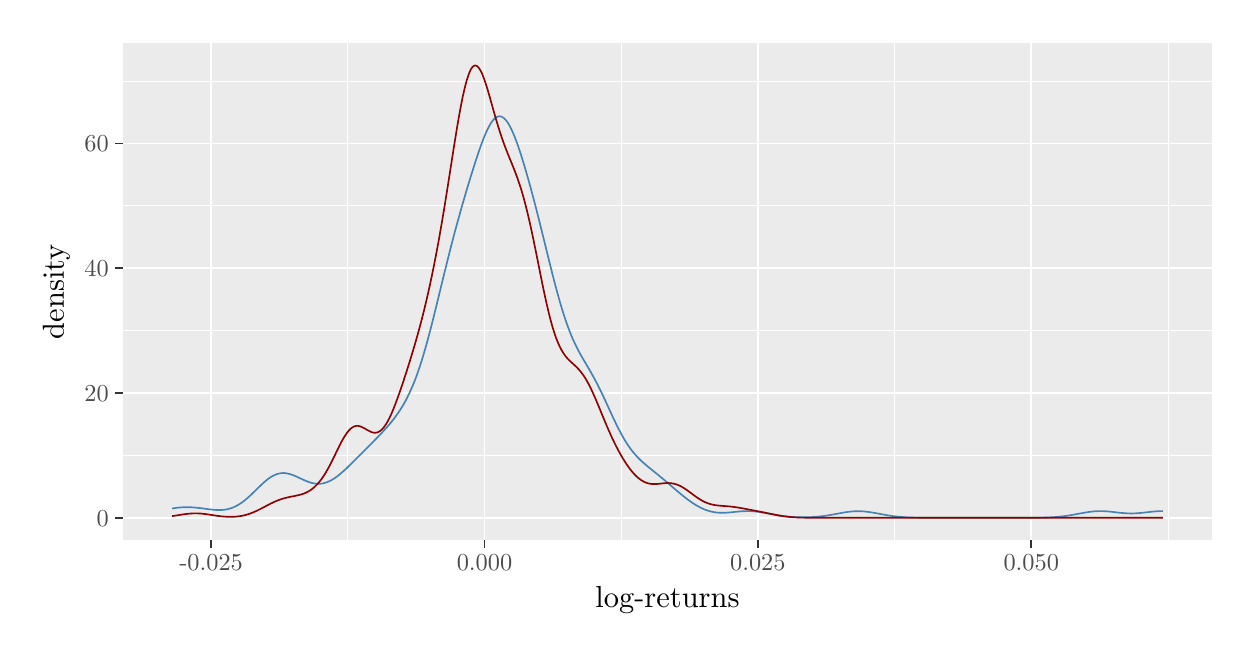
\begin{tikzpicture}[x=1pt,y=1pt]
\definecolor{fillColor}{RGB}{255,255,255}
\path[use as bounding box,fill=fillColor,fill opacity=0.00] (0,0) rectangle (433.62,216.81);
\begin{scope}
\path[clip] (  0.00,  0.00) rectangle (433.62,216.81);
\definecolor{drawColor}{RGB}{255,255,255}
\definecolor{fillColor}{RGB}{255,255,255}

\path[draw=drawColor,line width= 0.6pt,line join=round,line cap=round,fill=fillColor] (  0.00,  0.00) rectangle (433.62,216.81);
\end{scope}
\begin{scope}
\path[clip] ( 34.27, 31.53) rectangle (428.12,211.31);
\definecolor{fillColor}{gray}{0.92}

\path[fill=fillColor] ( 34.27, 31.53) rectangle (428.12,211.31);
\definecolor{drawColor}{RGB}{255,255,255}

\path[draw=drawColor,line width= 0.3pt,line join=round] ( 34.27, 62.24) --
	(428.12, 62.24);

\path[draw=drawColor,line width= 0.3pt,line join=round] ( 34.27,107.32) --
	(428.12,107.32);

\path[draw=drawColor,line width= 0.3pt,line join=round] ( 34.27,152.40) --
	(428.12,152.40);

\path[draw=drawColor,line width= 0.3pt,line join=round] ( 34.27,197.48) --
	(428.12,197.48);

\path[draw=drawColor,line width= 0.3pt,line join=round] (115.67, 31.53) --
	(115.67,211.31);

\path[draw=drawColor,line width= 0.3pt,line join=round] (214.46, 31.53) --
	(214.46,211.31);

\path[draw=drawColor,line width= 0.3pt,line join=round] (313.25, 31.53) --
	(313.25,211.31);

\path[draw=drawColor,line width= 0.3pt,line join=round] (412.03, 31.53) --
	(412.03,211.31);

\path[draw=drawColor,line width= 0.6pt,line join=round] ( 34.27, 39.70) --
	(428.12, 39.70);

\path[draw=drawColor,line width= 0.6pt,line join=round] ( 34.27, 84.78) --
	(428.12, 84.78);

\path[draw=drawColor,line width= 0.6pt,line join=round] ( 34.27,129.86) --
	(428.12,129.86);

\path[draw=drawColor,line width= 0.6pt,line join=round] ( 34.27,174.94) --
	(428.12,174.94);

\path[draw=drawColor,line width= 0.6pt,line join=round] ( 66.28, 31.53) --
	( 66.28,211.31);

\path[draw=drawColor,line width= 0.6pt,line join=round] (165.07, 31.53) --
	(165.07,211.31);

\path[draw=drawColor,line width= 0.6pt,line join=round] (263.85, 31.53) --
	(263.85,211.31);

\path[draw=drawColor,line width= 0.6pt,line join=round] (362.64, 31.53) --
	(362.64,211.31);
\definecolor{drawColor}{RGB}{70,130,180}

\path[draw=drawColor,line width= 0.6pt,line join=round] ( 52.17, 43.06) --
	( 52.87, 43.17) --
	( 53.57, 43.27) --
	( 54.27, 43.36) --
	( 54.97, 43.42) --
	( 55.67, 43.47) --
	( 56.37, 43.51) --
	( 57.07, 43.53) --
	( 57.78, 43.53) --
	( 58.48, 43.52) --
	( 59.18, 43.49) --
	( 59.88, 43.45) --
	( 60.58, 43.39) --
	( 61.28, 43.33) --
	( 61.98, 43.25) --
	( 62.68, 43.17) --
	( 63.38, 43.07) --
	( 64.08, 42.98) --
	( 64.78, 42.88) --
	( 65.48, 42.79) --
	( 66.18, 42.71) --
	( 66.88, 42.63) --
	( 67.59, 42.57) --
	( 68.29, 42.52) --
	( 68.99, 42.50) --
	( 69.69, 42.51) --
	( 70.39, 42.55) --
	( 71.09, 42.62) --
	( 71.79, 42.73) --
	( 72.49, 42.88) --
	( 73.19, 43.07) --
	( 73.89, 43.31) --
	( 74.59, 43.60) --
	( 75.29, 43.94) --
	( 75.99, 44.32) --
	( 76.69, 44.75) --
	( 77.39, 45.22) --
	( 78.10, 45.74) --
	( 78.80, 46.31) --
	( 79.50, 46.91) --
	( 80.20, 47.54) --
	( 80.90, 48.19) --
	( 81.60, 48.87) --
	( 82.30, 49.55) --
	( 83.00, 50.24) --
	( 83.70, 50.92) --
	( 84.40, 51.59) --
	( 85.10, 52.24) --
	( 85.80, 52.86) --
	( 86.50, 53.44) --
	( 87.20, 53.97) --
	( 87.90, 54.44) --
	( 88.61, 54.85) --
	( 89.31, 55.19) --
	( 90.01, 55.47) --
	( 90.71, 55.67) --
	( 91.41, 55.81) --
	( 92.11, 55.87) --
	( 92.81, 55.86) --
	( 93.51, 55.78) --
	( 94.21, 55.64) --
	( 94.91, 55.45) --
	( 95.61, 55.22) --
	( 96.31, 54.95) --
	( 97.01, 54.65) --
	( 97.71, 54.33) --
	( 98.42, 54.00) --
	( 99.12, 53.67) --
	( 99.82, 53.35) --
	(100.52, 53.05) --
	(101.22, 52.77) --
	(101.92, 52.52) --
	(102.62, 52.32) --
	(103.32, 52.16) --
	(104.02, 52.05) --
	(104.72, 51.99) --
	(105.42, 51.99) --
	(106.12, 52.05) --
	(106.82, 52.16) --
	(107.52, 52.35) --
	(108.22, 52.59) --
	(108.93, 52.89) --
	(109.63, 53.24) --
	(110.33, 53.64) --
	(111.03, 54.09) --
	(111.73, 54.59) --
	(112.43, 55.14) --
	(113.13, 55.71) --
	(113.83, 56.32) --
	(114.53, 56.95) --
	(115.23, 57.60) --
	(115.93, 58.27) --
	(116.63, 58.96) --
	(117.33, 59.65) --
	(118.03, 60.35) --
	(118.73, 61.05) --
	(119.44, 61.75) --
	(120.14, 62.46) --
	(120.84, 63.16) --
	(121.54, 63.86) --
	(122.24, 64.56) --
	(122.94, 65.26) --
	(123.64, 65.96) --
	(124.34, 66.67) --
	(125.04, 67.37) --
	(125.74, 68.09) --
	(126.44, 68.81) --
	(127.14, 69.53) --
	(127.84, 70.27) --
	(128.54, 71.03) --
	(129.24, 71.80) --
	(129.95, 72.59) --
	(130.65, 73.40) --
	(131.35, 74.24) --
	(132.05, 75.12) --
	(132.75, 76.04) --
	(133.45, 77.00) --
	(134.15, 78.01) --
	(134.85, 79.08) --
	(135.55, 80.22) --
	(136.25, 81.44) --
	(136.95, 82.75) --
	(137.65, 84.15) --
	(138.35, 85.65) --
	(139.05, 87.26) --
	(139.76, 88.97) --
	(140.46, 90.81) --
	(141.16, 92.79) --
	(141.86, 94.88) --
	(142.56, 97.09) --
	(143.26, 99.42) --
	(143.96,101.85) --
	(144.66,104.39) --
	(145.36,107.03) --
	(146.06,109.75) --
	(146.76,112.53) --
	(147.46,115.36) --
	(148.16,118.23) --
	(148.86,121.12) --
	(149.56,124.01) --
	(150.27,126.90) --
	(150.97,129.75) --
	(151.67,132.58) --
	(152.37,135.37) --
	(153.07,138.11) --
	(153.77,140.80) --
	(154.47,143.44) --
	(155.17,146.02) --
	(155.87,148.55) --
	(156.57,151.04) --
	(157.27,153.49) --
	(157.97,155.89) --
	(158.67,158.27) --
	(159.37,160.60) --
	(160.07,162.90) --
	(160.78,165.16) --
	(161.48,167.38) --
	(162.18,169.55) --
	(162.88,171.65) --
	(163.58,173.67) --
	(164.28,175.59) --
	(164.98,177.37) --
	(165.68,179.02) --
	(166.38,180.49) --
	(167.08,181.79) --
	(167.78,182.88) --
	(168.48,183.75) --
	(169.18,184.37) --
	(169.88,184.71) --
	(170.59,184.79) --
	(171.29,184.62) --
	(171.99,184.20) --
	(172.69,183.53) --
	(173.39,182.63) --
	(174.09,181.47) --
	(174.79,180.10) --
	(175.49,178.53) --
	(176.19,176.81) --
	(176.89,174.93) --
	(177.59,172.91) --
	(178.29,170.78) --
	(178.99,168.54) --
	(179.69,166.20) --
	(180.39,163.78) --
	(181.10,161.30) --
	(181.80,158.75) --
	(182.50,156.14) --
	(183.20,153.48) --
	(183.90,150.77) --
	(184.60,148.01) --
	(185.30,145.21) --
	(186.00,142.39) --
	(186.70,139.55) --
	(187.40,136.70) --
	(188.10,133.85) --
	(188.80,131.02) --
	(189.50,128.23) --
	(190.20,125.49) --
	(190.90,122.83) --
	(191.61,120.24) --
	(192.31,117.75) --
	(193.01,115.37) --
	(193.71,113.13) --
	(194.41,111.01) --
	(195.11,109.02) --
	(195.81,107.16) --
	(196.51,105.42) --
	(197.21,103.80) --
	(197.91,102.30) --
	(198.61,100.90) --
	(199.31, 99.57) --
	(200.01, 98.30) --
	(200.71, 97.07) --
	(201.42, 95.88) --
	(202.12, 94.69) --
	(202.82, 93.49) --
	(203.52, 92.28) --
	(204.22, 91.03) --
	(204.92, 89.74) --
	(205.62, 88.42) --
	(206.32, 87.04) --
	(207.02, 85.63) --
	(207.72, 84.17) --
	(208.42, 82.68) --
	(209.12, 81.16) --
	(209.82, 79.64) --
	(210.52, 78.11) --
	(211.22, 76.59) --
	(211.93, 75.09) --
	(212.63, 73.63) --
	(213.33, 72.22) --
	(214.03, 70.87) --
	(214.73, 69.57) --
	(215.43, 68.33) --
	(216.13, 67.17) --
	(216.83, 66.08) --
	(217.53, 65.07) --
	(218.23, 64.12) --
	(218.93, 63.25) --
	(219.63, 62.43) --
	(220.33, 61.66) --
	(221.03, 60.94) --
	(221.73, 60.27) --
	(222.44, 59.63) --
	(223.14, 59.02) --
	(223.84, 58.43) --
	(224.54, 57.85) --
	(225.24, 57.28) --
	(225.94, 56.71) --
	(226.64, 56.15) --
	(227.34, 55.59) --
	(228.04, 55.01) --
	(228.74, 54.44) --
	(229.44, 53.86) --
	(230.14, 53.27) --
	(230.84, 52.67) --
	(231.54, 52.08) --
	(232.24, 51.48) --
	(232.95, 50.87) --
	(233.65, 50.27) --
	(234.35, 49.67) --
	(235.05, 49.08) --
	(235.75, 48.50) --
	(236.45, 47.92) --
	(237.15, 47.36) --
	(237.85, 46.81) --
	(238.55, 46.28) --
	(239.25, 45.77) --
	(239.95, 45.28) --
	(240.65, 44.81) --
	(241.35, 44.37) --
	(242.05, 43.96) --
	(242.76, 43.58) --
	(243.46, 43.22) --
	(244.16, 42.90) --
	(244.86, 42.61) --
	(245.56, 42.36) --
	(246.26, 42.14) --
	(246.96, 41.96) --
	(247.66, 41.81) --
	(248.36, 41.69) --
	(249.06, 41.60) --
	(249.76, 41.54) --
	(250.46, 41.51) --
	(251.16, 41.50) --
	(251.86, 41.52) --
	(252.56, 41.56) --
	(253.27, 41.61) --
	(253.97, 41.67) --
	(254.67, 41.73) --
	(255.37, 41.81) --
	(256.07, 41.88) --
	(256.77, 41.95) --
	(257.47, 42.01) --
	(258.17, 42.05) --
	(258.87, 42.09) --
	(259.57, 42.12) --
	(260.27, 42.12) --
	(260.97, 42.11) --
	(261.67, 42.08) --
	(262.37, 42.03) --
	(263.07, 41.97) --
	(263.78, 41.89) --
	(264.48, 41.79) --
	(265.18, 41.69) --
	(265.88, 41.57) --
	(266.58, 41.45) --
	(267.28, 41.32) --
	(267.98, 41.19) --
	(268.68, 41.06) --
	(269.38, 40.93) --
	(270.08, 40.80) --
	(270.78, 40.68) --
	(271.48, 40.56) --
	(272.18, 40.46) --
	(272.88, 40.36) --
	(273.59, 40.27) --
	(274.29, 40.19) --
	(274.99, 40.12) --
	(275.69, 40.06) --
	(276.39, 40.01) --
	(277.09, 39.96) --
	(277.79, 39.93) --
	(278.49, 39.90) --
	(279.19, 39.89) --
	(279.89, 39.88) --
	(280.59, 39.88) --
	(281.29, 39.89) --
	(281.99, 39.90) --
	(282.69, 39.93) --
	(283.39, 39.96) --
	(284.10, 40.00) --
	(284.80, 40.05) --
	(285.50, 40.11) --
	(286.20, 40.18) --
	(286.90, 40.26) --
	(287.60, 40.35) --
	(288.30, 40.45) --
	(289.00, 40.55) --
	(289.70, 40.67) --
	(290.40, 40.79) --
	(291.10, 40.91) --
	(291.80, 41.04) --
	(292.50, 41.17) --
	(293.20, 41.30) --
	(293.90, 41.43) --
	(294.61, 41.56) --
	(295.31, 41.67) --
	(296.01, 41.78) --
	(296.71, 41.87) --
	(297.41, 41.95) --
	(298.11, 42.01) --
	(298.81, 42.06) --
	(299.51, 42.08) --
	(300.21, 42.09) --
	(300.91, 42.07) --
	(301.61, 42.04) --
	(302.31, 41.99) --
	(303.01, 41.92) --
	(303.71, 41.83) --
	(304.41, 41.73) --
	(305.12, 41.62) --
	(305.82, 41.50) --
	(306.52, 41.38) --
	(307.22, 41.25) --
	(307.92, 41.12) --
	(308.62, 40.99) --
	(309.32, 40.86) --
	(310.02, 40.73) --
	(310.72, 40.61) --
	(311.42, 40.50) --
	(312.12, 40.40) --
	(312.82, 40.30) --
	(313.52, 40.22) --
	(314.22, 40.14) --
	(314.93, 40.07) --
	(315.63, 40.01) --
	(316.33, 39.96) --
	(317.03, 39.91) --
	(317.73, 39.87) --
	(318.43, 39.84) --
	(319.13, 39.81) --
	(319.83, 39.79) --
	(320.53, 39.77) --
	(321.23, 39.76) --
	(321.93, 39.74) --
	(322.63, 39.73) --
	(323.33, 39.73) --
	(324.03, 39.72) --
	(324.73, 39.72) --
	(325.44, 39.71) --
	(326.14, 39.71) --
	(326.84, 39.71) --
	(327.54, 39.71) --
	(328.24, 39.71) --
	(328.94, 39.70) --
	(329.64, 39.70) --
	(330.34, 39.70) --
	(331.04, 39.70) --
	(331.74, 39.70) --
	(332.44, 39.70) --
	(333.14, 39.70) --
	(333.84, 39.70) --
	(334.54, 39.70) --
	(335.24, 39.70) --
	(335.95, 39.70) --
	(336.65, 39.70) --
	(337.35, 39.70) --
	(338.05, 39.70) --
	(338.75, 39.70) --
	(339.45, 39.70) --
	(340.15, 39.70) --
	(340.85, 39.70) --
	(341.55, 39.70) --
	(342.25, 39.70) --
	(342.95, 39.70) --
	(343.65, 39.70) --
	(344.35, 39.70) --
	(345.05, 39.70) --
	(345.76, 39.70) --
	(346.46, 39.70) --
	(347.16, 39.70) --
	(347.86, 39.70) --
	(348.56, 39.70) --
	(349.26, 39.70) --
	(349.96, 39.70) --
	(350.66, 39.70) --
	(351.36, 39.70) --
	(352.06, 39.70) --
	(352.76, 39.70) --
	(353.46, 39.70) --
	(354.16, 39.70) --
	(354.86, 39.70) --
	(355.56, 39.70) --
	(356.27, 39.70) --
	(356.97, 39.70) --
	(357.67, 39.70) --
	(358.37, 39.70) --
	(359.07, 39.71) --
	(359.77, 39.71) --
	(360.47, 39.71) --
	(361.17, 39.71) --
	(361.87, 39.71) --
	(362.57, 39.72) --
	(363.27, 39.72) --
	(363.97, 39.73) --
	(364.67, 39.73) --
	(365.37, 39.74) --
	(366.07, 39.75) --
	(366.78, 39.77) --
	(367.48, 39.79) --
	(368.18, 39.81) --
	(368.88, 39.84) --
	(369.58, 39.87) --
	(370.28, 39.90) --
	(370.98, 39.95) --
	(371.68, 40.00) --
	(372.38, 40.06) --
	(373.08, 40.13) --
	(373.78, 40.21) --
	(374.48, 40.29) --
	(375.18, 40.38) --
	(375.88, 40.49) --
	(376.58, 40.60) --
	(377.29, 40.72) --
	(377.99, 40.84) --
	(378.69, 40.97) --
	(379.39, 41.10) --
	(380.09, 41.23) --
	(380.79, 41.36) --
	(381.49, 41.49) --
	(382.19, 41.61) --
	(382.89, 41.72) --
	(383.59, 41.83) --
	(384.29, 41.92) --
	(384.99, 41.99) --
	(385.69, 42.05) --
	(386.39, 42.09) --
	(387.10, 42.11) --
	(387.80, 42.12) --
	(388.50, 42.11) --
	(389.20, 42.08) --
	(389.90, 42.03) --
	(390.60, 41.97) --
	(391.30, 41.91) --
	(392.00, 41.83) --
	(392.70, 41.75) --
	(393.40, 41.67) --
	(394.10, 41.59) --
	(394.80, 41.51) --
	(395.50, 41.44) --
	(396.20, 41.38) --
	(396.90, 41.34) --
	(397.61, 41.30) --
	(398.31, 41.28) --
	(399.01, 41.28) --
	(399.71, 41.29) --
	(400.41, 41.32) --
	(401.11, 41.37) --
	(401.81, 41.42) --
	(402.51, 41.49) --
	(403.21, 41.56) --
	(403.91, 41.64) --
	(404.61, 41.72) --
	(405.31, 41.80) --
	(406.01, 41.88) --
	(406.71, 41.95) --
	(407.41, 42.01) --
	(408.12, 42.06) --
	(408.82, 42.10) --
	(409.52, 42.11) --
	(410.22, 42.11);
\definecolor{drawColor}{RGB}{139,0,0}

\path[draw=drawColor,line width= 0.6pt,line join=round] ( 52.17, 40.31) --
	( 52.87, 40.41) --
	( 53.57, 40.51) --
	( 54.27, 40.63) --
	( 54.97, 40.74) --
	( 55.67, 40.85) --
	( 56.37, 40.95) --
	( 57.07, 41.05) --
	( 57.78, 41.14) --
	( 58.48, 41.21) --
	( 59.18, 41.26) --
	( 59.88, 41.30) --
	( 60.58, 41.31) --
	( 61.28, 41.30) --
	( 61.98, 41.27) --
	( 62.68, 41.22) --
	( 63.38, 41.15) --
	( 64.08, 41.07) --
	( 64.78, 40.98) --
	( 65.48, 40.88) --
	( 66.18, 40.77) --
	( 66.88, 40.66) --
	( 67.59, 40.55) --
	( 68.29, 40.45) --
	( 68.99, 40.35) --
	( 69.69, 40.27) --
	( 70.39, 40.19) --
	( 71.09, 40.13) --
	( 71.79, 40.09) --
	( 72.49, 40.06) --
	( 73.19, 40.05) --
	( 73.89, 40.06) --
	( 74.59, 40.09) --
	( 75.29, 40.13) --
	( 75.99, 40.21) --
	( 76.69, 40.30) --
	( 77.39, 40.42) --
	( 78.10, 40.57) --
	( 78.80, 40.74) --
	( 79.50, 40.94) --
	( 80.20, 41.17) --
	( 80.90, 41.43) --
	( 81.60, 41.71) --
	( 82.30, 42.02) --
	( 83.00, 42.34) --
	( 83.70, 42.69) --
	( 84.40, 43.04) --
	( 85.10, 43.41) --
	( 85.80, 43.78) --
	( 86.50, 44.16) --
	( 87.20, 44.52) --
	( 87.90, 44.88) --
	( 88.61, 45.22) --
	( 89.31, 45.54) --
	( 90.01, 45.84) --
	( 90.71, 46.12) --
	( 91.41, 46.37) --
	( 92.11, 46.59) --
	( 92.81, 46.79) --
	( 93.51, 46.97) --
	( 94.21, 47.13) --
	( 94.91, 47.28) --
	( 95.61, 47.42) --
	( 96.31, 47.55) --
	( 97.01, 47.70) --
	( 97.71, 47.85) --
	( 98.42, 48.03) --
	( 99.12, 48.24) --
	( 99.82, 48.48) --
	(100.52, 48.77) --
	(101.22, 49.11) --
	(101.92, 49.51) --
	(102.62, 49.99) --
	(103.32, 50.55) --
	(104.02, 51.18) --
	(104.72, 51.91) --
	(105.42, 52.72) --
	(106.12, 53.63) --
	(106.82, 54.63) --
	(107.52, 55.72) --
	(108.22, 56.92) --
	(108.93, 58.20) --
	(109.63, 59.55) --
	(110.33, 60.95) --
	(111.03, 62.38) --
	(111.73, 63.83) --
	(112.43, 65.26) --
	(113.13, 66.64) --
	(113.83, 67.95) --
	(114.53, 69.14) --
	(115.23, 70.20) --
	(115.93, 71.10) --
	(116.63, 71.83) --
	(117.33, 72.37) --
	(118.03, 72.73) --
	(118.73, 72.91) --
	(119.44, 72.91) --
	(120.14, 72.74) --
	(120.84, 72.47) --
	(121.54, 72.11) --
	(122.24, 71.71) --
	(122.94, 71.30) --
	(123.64, 70.94) --
	(124.34, 70.64) --
	(125.04, 70.45) --
	(125.74, 70.43) --
	(126.44, 70.58) --
	(127.14, 70.92) --
	(127.84, 71.46) --
	(128.54, 72.21) --
	(129.24, 73.15) --
	(129.95, 74.29) --
	(130.65, 75.61) --
	(131.35, 77.10) --
	(132.05, 78.74) --
	(132.75, 80.51) --
	(133.45, 82.37) --
	(134.15, 84.32) --
	(134.85, 86.33) --
	(135.55, 88.41) --
	(136.25, 90.53) --
	(136.95, 92.69) --
	(137.65, 94.90) --
	(138.35, 97.16) --
	(139.05, 99.47) --
	(139.76,101.83) --
	(140.46,104.26) --
	(141.16,106.77) --
	(141.86,109.35) --
	(142.56,112.03) --
	(143.26,114.81) --
	(143.96,117.72) --
	(144.66,120.75) --
	(145.36,123.90) --
	(146.06,127.19) --
	(146.76,130.62) --
	(147.46,134.19) --
	(148.16,137.92) --
	(148.86,141.79) --
	(149.56,145.83) --
	(150.27,150.01) --
	(150.97,154.30) --
	(151.67,158.70) --
	(152.37,163.16) --
	(153.07,167.65) --
	(153.77,172.13) --
	(154.47,176.54) --
	(155.17,180.82) --
	(155.87,184.88) --
	(156.57,188.67) --
	(157.27,192.14) --
	(157.97,195.21) --
	(158.67,197.85) --
	(159.37,199.99) --
	(160.07,201.62) --
	(160.78,202.68) --
	(161.48,203.14) --
	(162.18,203.06) --
	(162.88,202.48) --
	(163.58,201.44) --
	(164.28,199.99) --
	(164.98,198.18) --
	(165.68,196.10) --
	(166.38,193.80) --
	(167.08,191.36) --
	(167.78,188.85) --
	(168.48,186.35) --
	(169.18,183.90) --
	(169.88,181.54) --
	(170.59,179.29) --
	(171.29,177.16) --
	(171.99,175.16) --
	(172.69,173.29) --
	(173.39,171.50) --
	(174.09,169.78) --
	(174.79,168.07) --
	(175.49,166.34) --
	(176.19,164.55) --
	(176.89,162.67) --
	(177.59,160.66) --
	(178.29,158.49) --
	(178.99,156.12) --
	(179.69,153.55) --
	(180.39,150.78) --
	(181.10,147.83) --
	(181.80,144.71) --
	(182.50,141.44) --
	(183.20,138.05) --
	(183.90,134.58) --
	(184.60,131.07) --
	(185.30,127.57) --
	(186.00,124.13) --
	(186.70,120.79) --
	(187.40,117.59) --
	(188.10,114.57) --
	(188.80,111.75) --
	(189.50,109.17) --
	(190.20,106.84) --
	(190.90,104.80) --
	(191.61,103.01) --
	(192.31,101.45) --
	(193.01,100.13) --
	(193.71, 99.00) --
	(194.41, 98.04) --
	(195.11, 97.22) --
	(195.81, 96.50) --
	(196.51, 95.85) --
	(197.21, 95.22) --
	(197.91, 94.57) --
	(198.61, 93.88) --
	(199.31, 93.13) --
	(200.01, 92.28) --
	(200.71, 91.33) --
	(201.42, 90.27) --
	(202.12, 89.09) --
	(202.82, 87.79) --
	(203.52, 86.38) --
	(204.22, 84.88) --
	(204.92, 83.31) --
	(205.62, 81.68) --
	(206.32, 80.01) --
	(207.02, 78.31) --
	(207.72, 76.60) --
	(208.42, 74.91) --
	(209.12, 73.24) --
	(209.82, 71.61) --
	(210.52, 70.03) --
	(211.22, 68.49) --
	(211.93, 67.02) --
	(212.63, 65.60) --
	(213.33, 64.24) --
	(214.03, 62.95) --
	(214.73, 61.73) --
	(215.43, 60.57) --
	(216.13, 59.48) --
	(216.83, 58.45) --
	(217.53, 57.49) --
	(218.23, 56.59) --
	(218.93, 55.77) --
	(219.63, 55.03) --
	(220.33, 54.37) --
	(221.03, 53.79) --
	(221.73, 53.29) --
	(222.44, 52.87) --
	(223.14, 52.53) --
	(223.84, 52.27) --
	(224.54, 52.08) --
	(225.24, 51.96) --
	(225.94, 51.90) --
	(226.64, 51.90) --
	(227.34, 51.93) --
	(228.04, 51.99) --
	(228.74, 52.06) --
	(229.44, 52.14) --
	(230.14, 52.20) --
	(230.84, 52.25) --
	(231.54, 52.26) --
	(232.24, 52.22) --
	(232.95, 52.13) --
	(233.65, 51.99) --
	(234.35, 51.79) --
	(235.05, 51.54) --
	(235.75, 51.22) --
	(236.45, 50.85) --
	(237.15, 50.43) --
	(237.85, 49.97) --
	(238.55, 49.47) --
	(239.25, 48.96) --
	(239.95, 48.44) --
	(240.65, 47.92) --
	(241.35, 47.41) --
	(242.05, 46.92) --
	(242.76, 46.46) --
	(243.46, 46.03) --
	(244.16, 45.66) --
	(244.86, 45.32) --
	(245.56, 45.03) --
	(246.26, 44.79) --
	(246.96, 44.59) --
	(247.66, 44.42) --
	(248.36, 44.29) --
	(249.06, 44.19) --
	(249.76, 44.12) --
	(250.46, 44.06) --
	(251.16, 44.00) --
	(251.86, 43.95) --
	(252.56, 43.90) --
	(253.27, 43.84) --
	(253.97, 43.77) --
	(254.67, 43.69) --
	(255.37, 43.60) --
	(256.07, 43.50) --
	(256.77, 43.39) --
	(257.47, 43.27) --
	(258.17, 43.15) --
	(258.87, 43.02) --
	(259.57, 42.89) --
	(260.27, 42.75) --
	(260.97, 42.62) --
	(261.67, 42.49) --
	(262.37, 42.35) --
	(263.07, 42.22) --
	(263.78, 42.08) --
	(264.48, 41.95) --
	(265.18, 41.81) --
	(265.88, 41.67) --
	(266.58, 41.52) --
	(267.28, 41.37) --
	(267.98, 41.23) --
	(268.68, 41.08) --
	(269.38, 40.94) --
	(270.08, 40.80) --
	(270.78, 40.66) --
	(271.48, 40.53) --
	(272.18, 40.42) --
	(272.88, 40.31) --
	(273.59, 40.21) --
	(274.29, 40.12) --
	(274.99, 40.05) --
	(275.69, 39.98) --
	(276.39, 39.92) --
	(277.09, 39.88) --
	(277.79, 39.84) --
	(278.49, 39.80) --
	(279.19, 39.78) --
	(279.89, 39.76) --
	(280.59, 39.75) --
	(281.29, 39.73) --
	(281.99, 39.72) --
	(282.69, 39.72) --
	(283.39, 39.71) --
	(284.10, 39.71) --
	(284.80, 39.71) --
	(285.50, 39.71) --
	(286.20, 39.70) --
	(286.90, 39.70) --
	(287.60, 39.70) --
	(288.30, 39.70) --
	(289.00, 39.70) --
	(289.70, 39.70) --
	(290.40, 39.70) --
	(291.10, 39.70) --
	(291.80, 39.70) --
	(292.50, 39.70) --
	(293.20, 39.70) --
	(293.90, 39.70) --
	(294.61, 39.70) --
	(295.31, 39.70) --
	(296.01, 39.70) --
	(296.71, 39.70) --
	(297.41, 39.70) --
	(298.11, 39.70) --
	(298.81, 39.70) --
	(299.51, 39.70) --
	(300.21, 39.70) --
	(300.91, 39.70) --
	(301.61, 39.70) --
	(302.31, 39.70) --
	(303.01, 39.70) --
	(303.71, 39.70) --
	(304.41, 39.70) --
	(305.12, 39.70) --
	(305.82, 39.70) --
	(306.52, 39.70) --
	(307.22, 39.70) --
	(307.92, 39.70) --
	(308.62, 39.70) --
	(309.32, 39.70) --
	(310.02, 39.70) --
	(310.72, 39.70) --
	(311.42, 39.70) --
	(312.12, 39.70) --
	(312.82, 39.70) --
	(313.52, 39.70) --
	(314.22, 39.70) --
	(314.93, 39.70) --
	(315.63, 39.70) --
	(316.33, 39.70) --
	(317.03, 39.70) --
	(317.73, 39.70) --
	(318.43, 39.70) --
	(319.13, 39.70) --
	(319.83, 39.70) --
	(320.53, 39.70) --
	(321.23, 39.70) --
	(321.93, 39.70) --
	(322.63, 39.70) --
	(323.33, 39.70) --
	(324.03, 39.70) --
	(324.73, 39.70) --
	(325.44, 39.70) --
	(326.14, 39.70) --
	(326.84, 39.70) --
	(327.54, 39.70) --
	(328.24, 39.70) --
	(328.94, 39.70) --
	(329.64, 39.70) --
	(330.34, 39.70) --
	(331.04, 39.70) --
	(331.74, 39.70) --
	(332.44, 39.70) --
	(333.14, 39.70) --
	(333.84, 39.70) --
	(334.54, 39.70) --
	(335.24, 39.70) --
	(335.95, 39.70) --
	(336.65, 39.70) --
	(337.35, 39.70) --
	(338.05, 39.70) --
	(338.75, 39.70) --
	(339.45, 39.70) --
	(340.15, 39.70) --
	(340.85, 39.70) --
	(341.55, 39.70) --
	(342.25, 39.70) --
	(342.95, 39.70) --
	(343.65, 39.70) --
	(344.35, 39.70) --
	(345.05, 39.70) --
	(345.76, 39.70) --
	(346.46, 39.70) --
	(347.16, 39.70) --
	(347.86, 39.70) --
	(348.56, 39.70) --
	(349.26, 39.70) --
	(349.96, 39.70) --
	(350.66, 39.70) --
	(351.36, 39.70) --
	(352.06, 39.70) --
	(352.76, 39.70) --
	(353.46, 39.70) --
	(354.16, 39.70) --
	(354.86, 39.70) --
	(355.56, 39.70) --
	(356.27, 39.70) --
	(356.97, 39.70) --
	(357.67, 39.70) --
	(358.37, 39.70) --
	(359.07, 39.70) --
	(359.77, 39.70) --
	(360.47, 39.70) --
	(361.17, 39.70) --
	(361.87, 39.70) --
	(362.57, 39.70) --
	(363.27, 39.70) --
	(363.97, 39.70) --
	(364.67, 39.70) --
	(365.37, 39.70) --
	(366.07, 39.70) --
	(366.78, 39.70) --
	(367.48, 39.70) --
	(368.18, 39.70) --
	(368.88, 39.70) --
	(369.58, 39.70) --
	(370.28, 39.70) --
	(370.98, 39.70) --
	(371.68, 39.70) --
	(372.38, 39.70) --
	(373.08, 39.70) --
	(373.78, 39.70) --
	(374.48, 39.70) --
	(375.18, 39.70) --
	(375.88, 39.70) --
	(376.58, 39.70) --
	(377.29, 39.70) --
	(377.99, 39.70) --
	(378.69, 39.70) --
	(379.39, 39.70) --
	(380.09, 39.70) --
	(380.79, 39.70) --
	(381.49, 39.70) --
	(382.19, 39.70) --
	(382.89, 39.70) --
	(383.59, 39.70) --
	(384.29, 39.70) --
	(384.99, 39.70) --
	(385.69, 39.70) --
	(386.39, 39.70) --
	(387.10, 39.70) --
	(387.80, 39.70) --
	(388.50, 39.70) --
	(389.20, 39.70) --
	(389.90, 39.70) --
	(390.60, 39.70) --
	(391.30, 39.70) --
	(392.00, 39.70) --
	(392.70, 39.70) --
	(393.40, 39.70) --
	(394.10, 39.70) --
	(394.80, 39.70) --
	(395.50, 39.70) --
	(396.20, 39.70) --
	(396.90, 39.70) --
	(397.61, 39.70) --
	(398.31, 39.70) --
	(399.01, 39.70) --
	(399.71, 39.70) --
	(400.41, 39.70) --
	(401.11, 39.70) --
	(401.81, 39.70) --
	(402.51, 39.70) --
	(403.21, 39.70) --
	(403.91, 39.70) --
	(404.61, 39.70) --
	(405.31, 39.70) --
	(406.01, 39.70) --
	(406.71, 39.70) --
	(407.41, 39.70) --
	(408.12, 39.70) --
	(408.82, 39.70) --
	(409.52, 39.70) --
	(410.22, 39.70);
\end{scope}
\begin{scope}
\path[clip] (  0.00,  0.00) rectangle (433.62,216.81);
\definecolor{drawColor}{gray}{0.30}

\node[text=drawColor,anchor=base east,inner sep=0pt, outer sep=0pt, scale=  0.88] at ( 29.32, 36.67) {0};

\node[text=drawColor,anchor=base east,inner sep=0pt, outer sep=0pt, scale=  0.88] at ( 29.32, 81.75) {20};

\node[text=drawColor,anchor=base east,inner sep=0pt, outer sep=0pt, scale=  0.88] at ( 29.32,126.83) {40};

\node[text=drawColor,anchor=base east,inner sep=0pt, outer sep=0pt, scale=  0.88] at ( 29.32,171.91) {60};
\end{scope}
\begin{scope}
\path[clip] (  0.00,  0.00) rectangle (433.62,216.81);
\definecolor{drawColor}{gray}{0.20}

\path[draw=drawColor,line width= 0.6pt,line join=round] ( 31.52, 39.70) --
	( 34.27, 39.70);

\path[draw=drawColor,line width= 0.6pt,line join=round] ( 31.52, 84.78) --
	( 34.27, 84.78);

\path[draw=drawColor,line width= 0.6pt,line join=round] ( 31.52,129.86) --
	( 34.27,129.86);

\path[draw=drawColor,line width= 0.6pt,line join=round] ( 31.52,174.94) --
	( 34.27,174.94);
\end{scope}
\begin{scope}
\path[clip] (  0.00,  0.00) rectangle (433.62,216.81);
\definecolor{drawColor}{gray}{0.20}

\path[draw=drawColor,line width= 0.6pt,line join=round] ( 66.28, 28.78) --
	( 66.28, 31.53);

\path[draw=drawColor,line width= 0.6pt,line join=round] (165.07, 28.78) --
	(165.07, 31.53);

\path[draw=drawColor,line width= 0.6pt,line join=round] (263.85, 28.78) --
	(263.85, 31.53);

\path[draw=drawColor,line width= 0.6pt,line join=round] (362.64, 28.78) --
	(362.64, 31.53);
\end{scope}
\begin{scope}
\path[clip] (  0.00,  0.00) rectangle (433.62,216.81);
\definecolor{drawColor}{gray}{0.30}

\node[text=drawColor,anchor=base,inner sep=0pt, outer sep=0pt, scale=  0.88] at ( 66.28, 20.52) {-0.025};

\node[text=drawColor,anchor=base,inner sep=0pt, outer sep=0pt, scale=  0.88] at (165.07, 20.52) {0.000};

\node[text=drawColor,anchor=base,inner sep=0pt, outer sep=0pt, scale=  0.88] at (263.85, 20.52) {0.025};

\node[text=drawColor,anchor=base,inner sep=0pt, outer sep=0pt, scale=  0.88] at (362.64, 20.52) {0.050};
\end{scope}
\begin{scope}
\path[clip] (  0.00,  0.00) rectangle (433.62,216.81);
\definecolor{drawColor}{RGB}{0,0,0}

\node[text=drawColor,anchor=base,inner sep=0pt, outer sep=0pt, scale=  1.10] at (231.19,  7.44) {log-returns};
\end{scope}
\begin{scope}
\path[clip] (  0.00,  0.00) rectangle (433.62,216.81);
\definecolor{drawColor}{RGB}{0,0,0}

\node[text=drawColor,rotate= 90.00,anchor=base,inner sep=0pt, outer sep=0pt, scale=  1.10] at ( 13.08,121.42) {density};
\end{scope}
\end{tikzpicture}

  \caption{Historical and HSV related Apple stock log-returns distribution}
    %
  % BEGIN OF FLOATNOTE
  %
  \begin{changemargin}{0.5cm}{0.5cm}
  \medskip
\footnotesize
\setstretch{1.0}\textbf{Notes.} The above blue density curve is constructed over the historical data of the Apple share of stock price evolution from 1st January 2017 to 31st December 2017. While the red curve is constructed from time-series generated by the function \textit{hsv\_ts} taking the risk-neutral parameters \ref{eq:methodology:arg:heston:riskneutral} as arguments.  
\end{changemargin}
  %
  % END OF FLOATNOTE
  %
  \label{p:methodology:density:aapl:heston:riskneutral}
\end{figure}


The goal of that section is to find the risk-averse parameters that make both the distributions of the log-returns generated from market data or from \textit{hsv\_ts} fit together.
To do so, and according to the differences between \cref{eq:other:hsvstock:riskless,eq:other:hsvvol:riskless} and \cref{eq:other:hsvstock,eq:other:hsvvol}, the parameters to modify are the drift rate $r \to \alpha$, the mean reversion speed $\kappa^{*} \to \kappa$ and the long-run volatility $\theta^* \to \theta$.
Accordingly, the correlation parameter $\rho$ and the volatility of the volatility $\sigma$ stay unchanged from the risk-neutral to risk-averse world.

The drift rate $\alpha$ has been estimated by following the method exhibited at \cref{sec:upstream:logreturn}. From the market empirical log-returns' first and second moments, the value $0.4822917$ has been found for $\alpha$.

According to \cref{eq:other:kappa:riskless,eq:other:theta:riskless}, in order to  calculate $\kappa$ and $\theta$, the risk premium $\lambda$ has to be assessed.
Practically, such as it was the case for the MJD model, the function \textit{fitdistr} from the R package \textit{MASS} will be purposely used. 
As defined in \citet{Adrian}, the density of the log-returns generated by the HSV model is given by \cref{methodology:density:heston:log}.

\begin{align}
P_t(x) &= \frac{1}{2 \pi} \int_{-\infty}^{\infty} e^{i \phi x + F_t(\phi)} d\phi \label{methodology:density:heston:log} \\
\intertext{where}
F_t(\phi) &= \frac{\kappa \theta}{\sigma^2} \gamma t -
  \frac{2 \kappa \theta}{\sigma ^2} \ln\left(
    \cosh \frac{\Omega t}{2} +
    \frac{\Omega^2 - \gamma^2 +2 \kappa \gamma}{2 \kappa \Omega} \sinh \frac{\Omega t}{2}
  \right) \notag \\
\intertext{and}
\Omega &= \sqrt{\gamma^2 + \sigma^2 (\phi^2 - i\phi)}, \notag
\gamma = \kappa + i \rho \phi \sigma \notag
\end{align}

By giving to the optimization function the \cref{methodology:density:heston:log} as a density function, the Apple stock data (see appendix \ref{cha:appendix:market}) as a template and the variable $\lambda$ as a cursor, that algorithm outputs $\lambda = 5.4883278229$, as the best fit argument, for the risk premium.
The set of the risk-averse parameters is fully described here below in \ref{eq:methodology:arg:heston:riskaverse}.

\begin{align}
  \left \{
  \begin{array}{lcl}
    V(0) &= &0.03798218, \\
    \theta &= &0.02054013, \\
    \sigma &= &0.50378803, \\
    \rho &= &-0.39877827, \\
    \kappa &= &9.489383, \\
    \alpha & = &0.4822917
  \end{array}
  \right \}  
  \label{eq:methodology:arg:heston:riskaverse}
\end{align}


\Cref{p:methodology:density:aapl:heston:riskaverse} shows the empirical density curves illustrating the distributions of the log-returns computed either from historical data for the blue curve or from dummy time-series generated by the function \textit{hsv\_ts} fed with the risk-averse parameters\ref{eq:methodology:arg:heston:riskaverse}, for the red one.


\begin{figure}[h]
  \centering
  % Created by tikzDevice version 0.11 on 2018-07-18 23:47:53
% !TEX encoding = UTF-8 Unicode
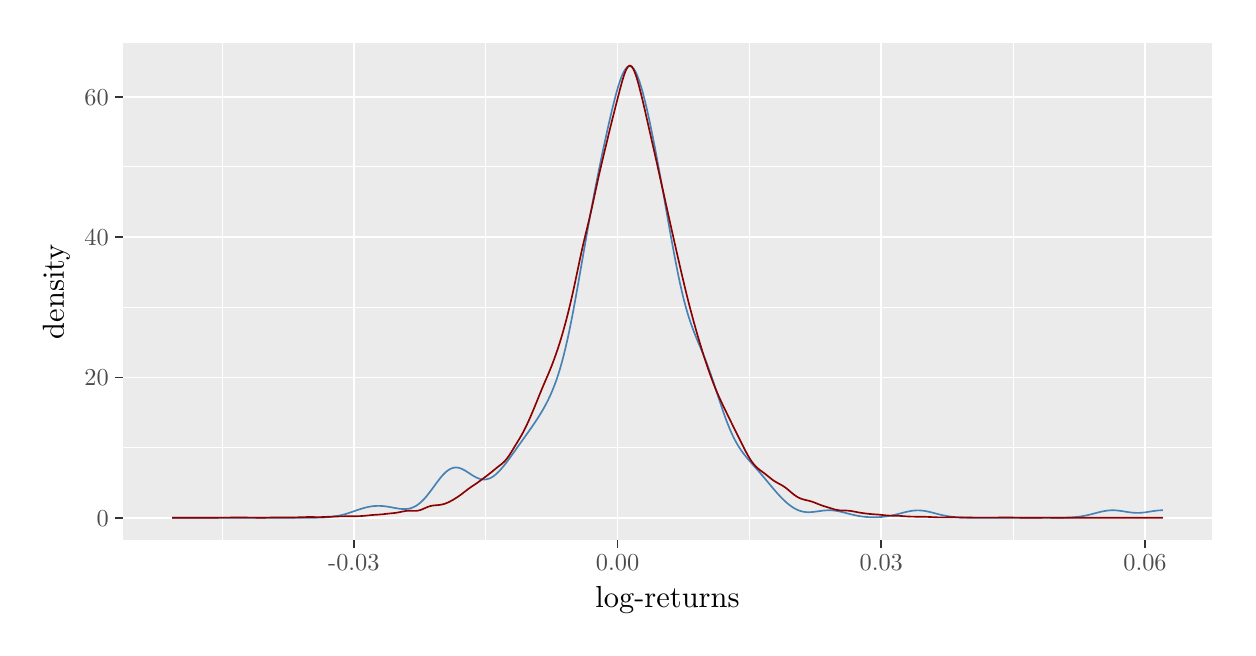
\begin{tikzpicture}[x=1pt,y=1pt]
\definecolor{fillColor}{RGB}{255,255,255}
\path[use as bounding box,fill=fillColor,fill opacity=0.00] (0,0) rectangle (433.62,216.81);
\begin{scope}
\path[clip] (  0.00,  0.00) rectangle (433.62,216.81);
\definecolor{drawColor}{RGB}{255,255,255}
\definecolor{fillColor}{RGB}{255,255,255}

\path[draw=drawColor,line width= 0.6pt,line join=round,line cap=round,fill=fillColor] (  0.00,  0.00) rectangle (433.62,216.81);
\end{scope}
\begin{scope}
\path[clip] ( 34.27, 31.53) rectangle (428.12,211.31);
\definecolor{fillColor}{gray}{0.92}

\path[fill=fillColor] ( 34.27, 31.53) rectangle (428.12,211.31);
\definecolor{drawColor}{RGB}{255,255,255}

\path[draw=drawColor,line width= 0.3pt,line join=round] ( 34.27, 65.06) --
	(428.12, 65.06);

\path[draw=drawColor,line width= 0.3pt,line join=round] ( 34.27,115.78) --
	(428.12,115.78);

\path[draw=drawColor,line width= 0.3pt,line join=round] ( 34.27,166.50) --
	(428.12,166.50);

\path[draw=drawColor,line width= 0.3pt,line join=round] ( 70.24, 31.53) --
	( 70.24,211.31);

\path[draw=drawColor,line width= 0.3pt,line join=round] (165.52, 31.53) --
	(165.52,211.31);

\path[draw=drawColor,line width= 0.3pt,line join=round] (260.81, 31.53) --
	(260.81,211.31);

\path[draw=drawColor,line width= 0.3pt,line join=round] (356.09, 31.53) --
	(356.09,211.31);

\path[draw=drawColor,line width= 0.6pt,line join=round] ( 34.27, 39.70) --
	(428.12, 39.70);

\path[draw=drawColor,line width= 0.6pt,line join=round] ( 34.27, 90.42) --
	(428.12, 90.42);

\path[draw=drawColor,line width= 0.6pt,line join=round] ( 34.27,141.14) --
	(428.12,141.14);

\path[draw=drawColor,line width= 0.6pt,line join=round] ( 34.27,191.86) --
	(428.12,191.86);

\path[draw=drawColor,line width= 0.6pt,line join=round] (117.88, 31.53) --
	(117.88,211.31);

\path[draw=drawColor,line width= 0.6pt,line join=round] (213.17, 31.53) --
	(213.17,211.31);

\path[draw=drawColor,line width= 0.6pt,line join=round] (308.45, 31.53) --
	(308.45,211.31);

\path[draw=drawColor,line width= 0.6pt,line join=round] (403.74, 31.53) --
	(403.74,211.31);
\definecolor{drawColor}{RGB}{70,130,180}

\path[draw=drawColor,line width= 0.6pt,line join=round] ( 52.17, 39.70) --
	( 52.87, 39.70) --
	( 53.57, 39.70) --
	( 54.27, 39.70) --
	( 54.97, 39.70) --
	( 55.67, 39.70) --
	( 56.37, 39.70) --
	( 57.07, 39.70) --
	( 57.78, 39.70) --
	( 58.48, 39.70) --
	( 59.18, 39.70) --
	( 59.88, 39.70) --
	( 60.58, 39.70) --
	( 61.28, 39.70) --
	( 61.98, 39.70) --
	( 62.68, 39.70) --
	( 63.38, 39.70) --
	( 64.08, 39.70) --
	( 64.78, 39.70) --
	( 65.48, 39.70) --
	( 66.18, 39.70) --
	( 66.88, 39.70) --
	( 67.59, 39.70) --
	( 68.29, 39.70) --
	( 68.99, 39.70) --
	( 69.69, 39.70) --
	( 70.39, 39.70) --
	( 71.09, 39.70) --
	( 71.79, 39.70) --
	( 72.49, 39.70) --
	( 73.19, 39.70) --
	( 73.89, 39.70) --
	( 74.59, 39.70) --
	( 75.29, 39.70) --
	( 75.99, 39.70) --
	( 76.69, 39.70) --
	( 77.39, 39.70) --
	( 78.10, 39.70) --
	( 78.80, 39.70) --
	( 79.50, 39.70) --
	( 80.20, 39.70) --
	( 80.90, 39.70) --
	( 81.60, 39.70) --
	( 82.30, 39.70) --
	( 83.00, 39.70) --
	( 83.70, 39.70) --
	( 84.40, 39.70) --
	( 85.10, 39.70) --
	( 85.80, 39.70) --
	( 86.50, 39.70) --
	( 87.20, 39.70) --
	( 87.90, 39.70) --
	( 88.61, 39.70) --
	( 89.31, 39.70) --
	( 90.01, 39.70) --
	( 90.71, 39.70) --
	( 91.41, 39.70) --
	( 92.11, 39.70) --
	( 92.81, 39.70) --
	( 93.51, 39.70) --
	( 94.21, 39.70) --
	( 94.91, 39.70) --
	( 95.61, 39.70) --
	( 96.31, 39.70) --
	( 97.01, 39.70) --
	( 97.71, 39.70) --
	( 98.42, 39.70) --
	( 99.12, 39.70) --
	( 99.82, 39.71) --
	(100.52, 39.71) --
	(101.22, 39.71) --
	(101.92, 39.71) --
	(102.62, 39.72) --
	(103.32, 39.73) --
	(104.02, 39.73) --
	(104.72, 39.75) --
	(105.42, 39.76) --
	(106.12, 39.79) --
	(106.82, 39.82) --
	(107.52, 39.85) --
	(108.22, 39.90) --
	(108.93, 39.95) --
	(109.63, 40.02) --
	(110.33, 40.11) --
	(111.03, 40.21) --
	(111.73, 40.33) --
	(112.43, 40.46) --
	(113.13, 40.62) --
	(113.83, 40.79) --
	(114.53, 40.98) --
	(115.23, 41.18) --
	(115.93, 41.40) --
	(116.63, 41.64) --
	(117.33, 41.88) --
	(118.03, 42.12) --
	(118.73, 42.36) --
	(119.44, 42.60) --
	(120.14, 42.83) --
	(120.84, 43.05) --
	(121.54, 43.26) --
	(122.24, 43.44) --
	(122.94, 43.60) --
	(123.64, 43.74) --
	(124.34, 43.85) --
	(125.04, 43.93) --
	(125.74, 43.98) --
	(126.44, 44.01) --
	(127.14, 44.01) --
	(127.84, 43.98) --
	(128.54, 43.92) --
	(129.24, 43.84) --
	(129.95, 43.75) --
	(130.65, 43.63) --
	(131.35, 43.51) --
	(132.05, 43.37) --
	(132.75, 43.24) --
	(133.45, 43.12) --
	(134.15, 43.01) --
	(134.85, 42.92) --
	(135.55, 42.87) --
	(136.25, 42.86) --
	(136.95, 42.90) --
	(137.65, 42.99) --
	(138.35, 43.15) --
	(139.05, 43.39) --
	(139.76, 43.71) --
	(140.46, 44.10) --
	(141.16, 44.59) --
	(141.86, 45.15) --
	(142.56, 45.79) --
	(143.26, 46.51) --
	(143.96, 47.30) --
	(144.66, 48.15) --
	(145.36, 49.06) --
	(146.06, 50.00) --
	(146.76, 50.96) --
	(147.46, 51.92) --
	(148.16, 52.86) --
	(148.86, 53.77) --
	(149.56, 54.63) --
	(150.27, 55.42) --
	(150.97, 56.12) --
	(151.67, 56.70) --
	(152.37, 57.18) --
	(153.07, 57.53) --
	(153.77, 57.76) --
	(154.47, 57.87) --
	(155.17, 57.86) --
	(155.87, 57.74) --
	(156.57, 57.50) --
	(157.27, 57.19) --
	(157.97, 56.81) --
	(158.67, 56.38) --
	(159.37, 55.93) --
	(160.07, 55.47) --
	(160.78, 55.02) --
	(161.48, 54.60) --
	(162.18, 54.24) --
	(162.88, 53.94) --
	(163.58, 53.71) --
	(164.28, 53.58) --
	(164.98, 53.53) --
	(165.68, 53.59) --
	(166.38, 53.75) --
	(167.08, 54.01) --
	(167.78, 54.38) --
	(168.48, 54.85) --
	(169.18, 55.41) --
	(169.88, 56.06) --
	(170.59, 56.78) --
	(171.29, 57.57) --
	(171.99, 58.41) --
	(172.69, 59.29) --
	(173.39, 60.22) --
	(174.09, 61.17) --
	(174.79, 62.14) --
	(175.49, 63.11) --
	(176.19, 64.09) --
	(176.89, 65.08) --
	(177.59, 66.06) --
	(178.29, 67.04) --
	(178.99, 68.02) --
	(179.69, 69.01) --
	(180.39, 69.99) --
	(181.10, 70.98) --
	(181.80, 71.98) --
	(182.50, 72.99) --
	(183.20, 74.02) --
	(183.90, 75.08) --
	(184.60, 76.16) --
	(185.30, 77.29) --
	(186.00, 78.46) --
	(186.70, 79.69) --
	(187.40, 80.99) --
	(188.10, 82.37) --
	(188.80, 83.85) --
	(189.50, 85.45) --
	(190.20, 87.18) --
	(190.90, 89.06) --
	(191.61, 91.13) --
	(192.31, 93.39) --
	(193.01, 95.84) --
	(193.71, 98.50) --
	(194.41,101.37) --
	(195.11,104.44) --
	(195.81,107.72) --
	(196.51,111.18) --
	(197.21,114.84) --
	(197.91,118.64) --
	(198.61,122.55) --
	(199.31,126.53) --
	(200.01,130.56) --
	(200.71,134.61) --
	(201.42,138.64) --
	(202.12,142.64) --
	(202.82,146.56) --
	(203.52,150.40) --
	(204.22,154.16) --
	(204.92,157.82) --
	(205.62,161.40) --
	(206.32,164.89) --
	(207.02,168.31) --
	(207.72,171.67) --
	(208.42,174.96) --
	(209.12,178.18) --
	(209.82,181.34) --
	(210.52,184.42) --
	(211.22,187.39) --
	(211.93,190.23) --
	(212.63,192.91) --
	(213.33,195.37) --
	(214.03,197.57) --
	(214.73,199.42) --
	(215.43,200.91) --
	(216.13,202.01) --
	(216.83,202.68) --
	(217.53,202.92) --
	(218.23,202.70) --
	(218.93,202.04) --
	(219.63,200.95) --
	(220.33,199.40) --
	(221.03,197.48) --
	(221.73,195.24) --
	(222.44,192.72) --
	(223.14,189.95) --
	(223.84,186.97) --
	(224.54,183.82) --
	(225.24,180.50) --
	(225.94,177.05) --
	(226.64,173.48) --
	(227.34,169.81) --
	(228.04,166.05) --
	(228.74,162.21) --
	(229.44,158.31) --
	(230.14,154.36) --
	(230.84,150.38) --
	(231.54,146.39) --
	(232.24,142.44) --
	(232.95,138.55) --
	(233.65,134.76) --
	(234.35,131.10) --
	(235.05,127.60) --
	(235.75,124.30) --
	(236.45,121.20) --
	(237.15,118.33) --
	(237.85,115.71) --
	(238.55,113.30) --
	(239.25,111.10) --
	(239.95,109.07) --
	(240.65,107.18) --
	(241.35,105.40) --
	(242.05,103.69) --
	(242.76,102.03) --
	(243.46,100.36) --
	(244.16, 98.65) --
	(244.86, 96.89) --
	(245.56, 95.06) --
	(246.26, 93.15) --
	(246.96, 91.17) --
	(247.66, 89.12) --
	(248.36, 87.01) --
	(249.06, 84.88) --
	(249.76, 82.74) --
	(250.46, 80.63) --
	(251.16, 78.56) --
	(251.86, 76.56) --
	(252.56, 74.65) --
	(253.27, 72.85) --
	(253.97, 71.16) --
	(254.67, 69.61) --
	(255.37, 68.18) --
	(256.07, 66.88) --
	(256.77, 65.68) --
	(257.47, 64.59) --
	(258.17, 63.58) --
	(258.87, 62.64) --
	(259.57, 61.76) --
	(260.27, 60.92) --
	(260.97, 60.11) --
	(261.67, 59.31) --
	(262.37, 58.53) --
	(263.07, 57.73) --
	(263.78, 56.94) --
	(264.48, 56.13) --
	(265.18, 55.31) --
	(265.88, 54.49) --
	(266.58, 53.65) --
	(267.28, 52.81) --
	(267.98, 51.97) --
	(268.68, 51.13) --
	(269.38, 50.30) --
	(270.08, 49.48) --
	(270.78, 48.68) --
	(271.48, 47.90) --
	(272.18, 47.16) --
	(272.88, 46.44) --
	(273.59, 45.77) --
	(274.29, 45.13) --
	(274.99, 44.55) --
	(275.69, 44.01) --
	(276.39, 43.53) --
	(277.09, 43.10) --
	(277.79, 42.73) --
	(278.49, 42.42) --
	(279.19, 42.18) --
	(279.89, 41.99) --
	(280.59, 41.85) --
	(281.29, 41.77) --
	(281.99, 41.73) --
	(282.69, 41.74) --
	(283.39, 41.78) --
	(284.10, 41.85) --
	(284.80, 41.94) --
	(285.50, 42.03) --
	(286.20, 42.13) --
	(286.90, 42.23) --
	(287.60, 42.31) --
	(288.30, 42.37) --
	(289.00, 42.41) --
	(289.70, 42.42) --
	(290.40, 42.40) --
	(291.10, 42.35) --
	(291.80, 42.27) --
	(292.50, 42.16) --
	(293.20, 42.03) --
	(293.90, 41.87) --
	(294.61, 41.71) --
	(295.31, 41.53) --
	(296.01, 41.34) --
	(296.71, 41.16) --
	(297.41, 40.98) --
	(298.11, 40.81) --
	(298.81, 40.65) --
	(299.51, 40.50) --
	(300.21, 40.37) --
	(300.91, 40.25) --
	(301.61, 40.16) --
	(302.31, 40.08) --
	(303.01, 40.01) --
	(303.71, 39.96) --
	(304.41, 39.93) --
	(305.12, 39.90) --
	(305.82, 39.90) --
	(306.52, 39.90) --
	(307.22, 39.93) --
	(307.92, 39.97) --
	(308.62, 40.02) --
	(309.32, 40.09) --
	(310.02, 40.17) --
	(310.72, 40.27) --
	(311.42, 40.39) --
	(312.12, 40.52) --
	(312.82, 40.67) --
	(313.52, 40.83) --
	(314.22, 41.00) --
	(314.93, 41.18) --
	(315.63, 41.36) --
	(316.33, 41.55) --
	(317.03, 41.73) --
	(317.73, 41.89) --
	(318.43, 42.04) --
	(319.13, 42.17) --
	(319.83, 42.27) --
	(320.53, 42.34) --
	(321.23, 42.38) --
	(321.93, 42.38) --
	(322.63, 42.36) --
	(323.33, 42.29) --
	(324.03, 42.20) --
	(324.73, 42.08) --
	(325.44, 41.93) --
	(326.14, 41.77) --
	(326.84, 41.60) --
	(327.54, 41.41) --
	(328.24, 41.23) --
	(328.94, 41.05) --
	(329.64, 40.87) --
	(330.34, 40.70) --
	(331.04, 40.55) --
	(331.74, 40.41) --
	(332.44, 40.29) --
	(333.14, 40.18) --
	(333.84, 40.09) --
	(334.54, 40.01) --
	(335.24, 39.94) --
	(335.95, 39.89) --
	(336.65, 39.84) --
	(337.35, 39.81) --
	(338.05, 39.78) --
	(338.75, 39.76) --
	(339.45, 39.75) --
	(340.15, 39.73) --
	(340.85, 39.72) --
	(341.55, 39.72) --
	(342.25, 39.71) --
	(342.95, 39.71) --
	(343.65, 39.71) --
	(344.35, 39.71) --
	(345.05, 39.70) --
	(345.76, 39.70) --
	(346.46, 39.70) --
	(347.16, 39.70) --
	(347.86, 39.70) --
	(348.56, 39.70) --
	(349.26, 39.70) --
	(349.96, 39.70) --
	(350.66, 39.70) --
	(351.36, 39.70) --
	(352.06, 39.70) --
	(352.76, 39.70) --
	(353.46, 39.70) --
	(354.16, 39.70) --
	(354.86, 39.70) --
	(355.56, 39.70) --
	(356.27, 39.70) --
	(356.97, 39.70) --
	(357.67, 39.70) --
	(358.37, 39.70) --
	(359.07, 39.70) --
	(359.77, 39.70) --
	(360.47, 39.70) --
	(361.17, 39.70) --
	(361.87, 39.70) --
	(362.57, 39.70) --
	(363.27, 39.70) --
	(363.97, 39.70) --
	(364.67, 39.70) --
	(365.37, 39.70) --
	(366.07, 39.70) --
	(366.78, 39.70) --
	(367.48, 39.70) --
	(368.18, 39.70) --
	(368.88, 39.71) --
	(369.58, 39.71) --
	(370.28, 39.71) --
	(370.98, 39.71) --
	(371.68, 39.72) --
	(372.38, 39.72) --
	(373.08, 39.73) --
	(373.78, 39.74) --
	(374.48, 39.75) --
	(375.18, 39.77) --
	(375.88, 39.80) --
	(376.58, 39.83) --
	(377.29, 39.87) --
	(377.99, 39.92) --
	(378.69, 39.98) --
	(379.39, 40.06) --
	(380.09, 40.14) --
	(380.79, 40.25) --
	(381.49, 40.36) --
	(382.19, 40.50) --
	(382.89, 40.64) --
	(383.59, 40.81) --
	(384.29, 40.98) --
	(384.99, 41.16) --
	(385.69, 41.34) --
	(386.39, 41.53) --
	(387.10, 41.71) --
	(387.80, 41.88) --
	(388.50, 42.03) --
	(389.20, 42.16) --
	(389.90, 42.27) --
	(390.60, 42.35) --
	(391.30, 42.40) --
	(392.00, 42.42) --
	(392.70, 42.41) --
	(393.40, 42.37) --
	(394.10, 42.30) --
	(394.80, 42.21) --
	(395.50, 42.11) --
	(396.20, 42.00) --
	(396.90, 41.88) --
	(397.61, 41.77) --
	(398.31, 41.67) --
	(399.01, 41.59) --
	(399.71, 41.52) --
	(400.41, 41.49) --
	(401.11, 41.48) --
	(401.81, 41.50) --
	(402.51, 41.54) --
	(403.21, 41.61) --
	(403.91, 41.69) --
	(404.61, 41.80) --
	(405.31, 41.91) --
	(406.01, 42.02) --
	(406.71, 42.13) --
	(407.41, 42.23) --
	(408.12, 42.32) --
	(408.82, 42.38) --
	(409.52, 42.41) --
	(410.22, 42.42);
\definecolor{drawColor}{RGB}{139,0,0}

\path[draw=drawColor,line width= 0.6pt,line join=round] ( 52.17, 39.73) --
	( 52.87, 39.73) --
	( 53.57, 39.73) --
	( 54.27, 39.72) --
	( 54.97, 39.72) --
	( 55.67, 39.72) --
	( 56.37, 39.72) --
	( 57.07, 39.72) --
	( 57.78, 39.72) --
	( 58.48, 39.73) --
	( 59.18, 39.73) --
	( 59.88, 39.73) --
	( 60.58, 39.73) --
	( 61.28, 39.73) --
	( 61.98, 39.72) --
	( 62.68, 39.72) --
	( 63.38, 39.71) --
	( 64.08, 39.71) --
	( 64.78, 39.71) --
	( 65.48, 39.71) --
	( 66.18, 39.71) --
	( 66.88, 39.72) --
	( 67.59, 39.73) --
	( 68.29, 39.74) --
	( 68.99, 39.75) --
	( 69.69, 39.76) --
	( 70.39, 39.77) --
	( 71.09, 39.77) --
	( 71.79, 39.78) --
	( 72.49, 39.78) --
	( 73.19, 39.78) --
	( 73.89, 39.79) --
	( 74.59, 39.80) --
	( 75.29, 39.80) --
	( 75.99, 39.81) --
	( 76.69, 39.81) --
	( 77.39, 39.80) --
	( 78.10, 39.80) --
	( 78.80, 39.79) --
	( 79.50, 39.78) --
	( 80.20, 39.78) --
	( 80.90, 39.77) --
	( 81.60, 39.76) --
	( 82.30, 39.75) --
	( 83.00, 39.74) --
	( 83.70, 39.74) --
	( 84.40, 39.73) --
	( 85.10, 39.74) --
	( 85.80, 39.74) --
	( 86.50, 39.76) --
	( 87.20, 39.77) --
	( 87.90, 39.79) --
	( 88.61, 39.81) --
	( 89.31, 39.82) --
	( 90.01, 39.82) --
	( 90.71, 39.82) --
	( 91.41, 39.82) --
	( 92.11, 39.81) --
	( 92.81, 39.80) --
	( 93.51, 39.80) --
	( 94.21, 39.80) --
	( 94.91, 39.81) --
	( 95.61, 39.82) --
	( 96.31, 39.83) --
	( 97.01, 39.85) --
	( 97.71, 39.87) --
	( 98.42, 39.90) --
	( 99.12, 39.92) --
	( 99.82, 39.94) --
	(100.52, 39.96) --
	(101.22, 39.98) --
	(101.92, 39.98) --
	(102.62, 39.98) --
	(103.32, 39.97) --
	(104.02, 39.95) --
	(104.72, 39.94) --
	(105.42, 39.95) --
	(106.12, 39.96) --
	(106.82, 39.98) --
	(107.52, 40.02) --
	(108.22, 40.06) --
	(108.93, 40.09) --
	(109.63, 40.12) --
	(110.33, 40.15) --
	(111.03, 40.17) --
	(111.73, 40.18) --
	(112.43, 40.20) --
	(113.13, 40.21) --
	(113.83, 40.22) --
	(114.53, 40.24) --
	(115.23, 40.25) --
	(115.93, 40.26) --
	(116.63, 40.26) --
	(117.33, 40.26) --
	(118.03, 40.26) --
	(118.73, 40.27) --
	(119.44, 40.29) --
	(120.14, 40.31) --
	(120.84, 40.36) --
	(121.54, 40.41) --
	(122.24, 40.48) --
	(122.94, 40.55) --
	(123.64, 40.62) --
	(124.34, 40.69) --
	(125.04, 40.75) --
	(125.74, 40.79) --
	(126.44, 40.83) --
	(127.14, 40.88) --
	(127.84, 40.94) --
	(128.54, 41.01) --
	(129.24, 41.09) --
	(129.95, 41.17) --
	(130.65, 41.25) --
	(131.35, 41.32) --
	(132.05, 41.39) --
	(132.75, 41.46) --
	(133.45, 41.56) --
	(134.15, 41.69) --
	(134.85, 41.83) --
	(135.55, 41.98) --
	(136.25, 42.11) --
	(136.95, 42.20) --
	(137.65, 42.24) --
	(138.35, 42.24) --
	(139.05, 42.21) --
	(139.76, 42.19) --
	(140.46, 42.22) --
	(141.16, 42.32) --
	(141.86, 42.50) --
	(142.56, 42.76) --
	(143.26, 43.07) --
	(143.96, 43.38) --
	(144.66, 43.67) --
	(145.36, 43.91) --
	(146.06, 44.07) --
	(146.76, 44.17) --
	(147.46, 44.24) --
	(148.16, 44.29) --
	(148.86, 44.37) --
	(149.56, 44.48) --
	(150.27, 44.65) --
	(150.97, 44.87) --
	(151.67, 45.15) --
	(152.37, 45.48) --
	(153.07, 45.85) --
	(153.77, 46.24) --
	(154.47, 46.67) --
	(155.17, 47.11) --
	(155.87, 47.59) --
	(156.57, 48.09) --
	(157.27, 48.62) --
	(157.97, 49.16) --
	(158.67, 49.71) --
	(159.37, 50.23) --
	(160.07, 50.73) --
	(160.78, 51.20) --
	(161.48, 51.67) --
	(162.18, 52.14) --
	(162.88, 52.64) --
	(163.58, 53.15) --
	(164.28, 53.67) --
	(164.98, 54.20) --
	(165.68, 54.72) --
	(166.38, 55.25) --
	(167.08, 55.80) --
	(167.78, 56.36) --
	(168.48, 56.94) --
	(169.18, 57.51) --
	(169.88, 58.07) --
	(170.59, 58.61) --
	(171.29, 59.17) --
	(171.99, 59.78) --
	(172.69, 60.51) --
	(173.39, 61.38) --
	(174.09, 62.39) --
	(174.79, 63.50) --
	(175.49, 64.65) --
	(176.19, 65.80) --
	(176.89, 66.95) --
	(177.59, 68.09) --
	(178.29, 69.28) --
	(178.99, 70.55) --
	(179.69, 71.90) --
	(180.39, 73.36) --
	(181.10, 74.89) --
	(181.80, 76.49) --
	(182.50, 78.14) --
	(183.20, 79.83) --
	(183.90, 81.54) --
	(184.60, 83.28) --
	(185.30, 85.00) --
	(186.00, 86.69) --
	(186.70, 88.35) --
	(187.40, 89.97) --
	(188.10, 91.60) --
	(188.80, 93.28) --
	(189.50, 95.05) --
	(190.20, 96.90) --
	(190.90, 98.86) --
	(191.61,100.93) --
	(192.31,103.11) --
	(193.01,105.41) --
	(193.71,107.85) --
	(194.41,110.42) --
	(195.11,113.12) --
	(195.81,115.95) --
	(196.51,118.93) --
	(197.21,122.05) --
	(197.91,125.30) --
	(198.61,128.64) --
	(199.31,132.00) --
	(200.01,135.28) --
	(200.71,138.41) --
	(201.42,141.40) --
	(202.12,144.29) --
	(202.82,147.18) --
	(203.52,150.19) --
	(204.22,153.33) --
	(204.92,156.57) --
	(205.62,159.82) --
	(206.32,163.01) --
	(207.02,166.07) --
	(207.72,169.04) --
	(208.42,171.96) --
	(209.12,174.86) --
	(209.82,177.78) --
	(210.52,180.68) --
	(211.22,183.53) --
	(211.93,186.33) --
	(212.63,189.09) --
	(213.33,191.82) --
	(214.03,194.52) --
	(214.73,197.11) --
	(215.43,199.46) --
	(216.13,201.37) --
	(216.83,202.65) --
	(217.53,203.14) --
	(218.23,202.82) --
	(218.93,201.74) --
	(219.63,200.03) --
	(220.33,197.82) --
	(221.03,195.27) --
	(221.73,192.47) --
	(222.44,189.53) --
	(223.14,186.50) --
	(223.84,183.42) --
	(224.54,180.33) --
	(225.24,177.23) --
	(225.94,174.14) --
	(226.64,171.04) --
	(227.34,167.92) --
	(228.04,164.80) --
	(228.74,161.65) --
	(229.44,158.50) --
	(230.14,155.34) --
	(230.84,152.18) --
	(231.54,149.02) --
	(232.24,145.85) --
	(232.95,142.70) --
	(233.65,139.57) --
	(234.35,136.47) --
	(235.05,133.39) --
	(235.75,130.34) --
	(236.45,127.32) --
	(237.15,124.35) --
	(237.85,121.44) --
	(238.55,118.62) --
	(239.25,115.89) --
	(239.95,113.24) --
	(240.65,110.66) --
	(241.35,108.15) --
	(242.05,105.69) --
	(242.76,103.29) --
	(243.46,100.96) --
	(244.16, 98.71) --
	(244.86, 96.54) --
	(245.56, 94.44) --
	(246.26, 92.43) --
	(246.96, 90.48) --
	(247.66, 88.61) --
	(248.36, 86.82) --
	(249.06, 85.13) --
	(249.76, 83.52) --
	(250.46, 81.99) --
	(251.16, 80.51) --
	(251.86, 79.06) --
	(252.56, 77.62) --
	(253.27, 76.18) --
	(253.97, 74.73) --
	(254.67, 73.30) --
	(255.37, 71.89) --
	(256.07, 70.49) --
	(256.77, 69.09) --
	(257.47, 67.68) --
	(258.17, 66.26) --
	(258.87, 64.86) --
	(259.57, 63.49) --
	(260.27, 62.21) --
	(260.97, 61.03) --
	(261.67, 59.98) --
	(262.37, 59.07) --
	(263.07, 58.28) --
	(263.78, 57.62) --
	(264.48, 57.04) --
	(265.18, 56.52) --
	(265.88, 56.01) --
	(266.58, 55.48) --
	(267.28, 54.92) --
	(267.98, 54.36) --
	(268.68, 53.80) --
	(269.38, 53.27) --
	(270.08, 52.81) --
	(270.78, 52.40) --
	(271.48, 52.02) --
	(272.18, 51.65) --
	(272.88, 51.24) --
	(273.59, 50.78) --
	(274.29, 50.25) --
	(274.99, 49.66) --
	(275.69, 49.06) --
	(276.39, 48.47) --
	(277.09, 47.92) --
	(277.79, 47.44) --
	(278.49, 47.03) --
	(279.19, 46.71) --
	(279.89, 46.45) --
	(280.59, 46.26) --
	(281.29, 46.09) --
	(281.99, 45.93) --
	(282.69, 45.75) --
	(283.39, 45.54) --
	(284.10, 45.29) --
	(284.80, 45.01) --
	(285.50, 44.73) --
	(286.20, 44.46) --
	(286.90, 44.20) --
	(287.60, 43.96) --
	(288.30, 43.74) --
	(289.00, 43.53) --
	(289.70, 43.31) --
	(290.40, 43.09) --
	(291.10, 42.87) --
	(291.80, 42.68) --
	(292.50, 42.52) --
	(293.20, 42.42) --
	(293.90, 42.36) --
	(294.61, 42.34) --
	(295.31, 42.33) --
	(296.01, 42.31) --
	(296.71, 42.26) --
	(297.41, 42.17) --
	(298.11, 42.06) --
	(298.81, 41.92) --
	(299.51, 41.78) --
	(300.21, 41.65) --
	(300.91, 41.53) --
	(301.61, 41.43) --
	(302.31, 41.33) --
	(303.01, 41.24) --
	(303.71, 41.16) --
	(304.41, 41.08) --
	(305.12, 41.02) --
	(305.82, 40.97) --
	(306.52, 40.93) --
	(307.22, 40.88) --
	(307.92, 40.82) --
	(308.62, 40.74) --
	(309.32, 40.66) --
	(310.02, 40.59) --
	(310.72, 40.53) --
	(311.42, 40.49) --
	(312.12, 40.47) --
	(312.82, 40.47) --
	(313.52, 40.46) --
	(314.22, 40.45) --
	(314.93, 40.41) --
	(315.63, 40.36) --
	(316.33, 40.30) --
	(317.03, 40.25) --
	(317.73, 40.20) --
	(318.43, 40.16) --
	(319.13, 40.14) --
	(319.83, 40.12) --
	(320.53, 40.11) --
	(321.23, 40.10) --
	(321.93, 40.09) --
	(322.63, 40.09) --
	(323.33, 40.08) --
	(324.03, 40.06) --
	(324.73, 40.05) --
	(325.44, 40.02) --
	(326.14, 39.99) --
	(326.84, 39.95) --
	(327.54, 39.92) --
	(328.24, 39.89) --
	(328.94, 39.86) --
	(329.64, 39.85) --
	(330.34, 39.85) --
	(331.04, 39.86) --
	(331.74, 39.87) --
	(332.44, 39.88) --
	(333.14, 39.89) --
	(333.84, 39.89) --
	(334.54, 39.89) --
	(335.24, 39.87) --
	(335.95, 39.86) --
	(336.65, 39.84) --
	(337.35, 39.83) --
	(338.05, 39.82) --
	(338.75, 39.82) --
	(339.45, 39.81) --
	(340.15, 39.80) --
	(340.85, 39.79) --
	(341.55, 39.78) --
	(342.25, 39.77) --
	(342.95, 39.76) --
	(343.65, 39.76) --
	(344.35, 39.75) --
	(345.05, 39.75) --
	(345.76, 39.75) --
	(346.46, 39.75) --
	(347.16, 39.76) --
	(347.86, 39.76) --
	(348.56, 39.77) --
	(349.26, 39.77) --
	(349.96, 39.78) --
	(350.66, 39.78) --
	(351.36, 39.79) --
	(352.06, 39.79) --
	(352.76, 39.80) --
	(353.46, 39.80) --
	(354.16, 39.80) --
	(354.86, 39.80) --
	(355.56, 39.79) --
	(356.27, 39.78) --
	(356.97, 39.77) --
	(357.67, 39.76) --
	(358.37, 39.75) --
	(359.07, 39.74) --
	(359.77, 39.73) --
	(360.47, 39.73) --
	(361.17, 39.72) --
	(361.87, 39.71) --
	(362.57, 39.71) --
	(363.27, 39.71) --
	(363.97, 39.72) --
	(364.67, 39.72) --
	(365.37, 39.73) --
	(366.07, 39.74) --
	(366.78, 39.75) --
	(367.48, 39.76) --
	(368.18, 39.76) --
	(368.88, 39.76) --
	(369.58, 39.75) --
	(370.28, 39.74) --
	(370.98, 39.73) --
	(371.68, 39.72) --
	(372.38, 39.72) --
	(373.08, 39.71) --
	(373.78, 39.71) --
	(374.48, 39.70) --
	(375.18, 39.70) --
	(375.88, 39.70) --
	(376.58, 39.70) --
	(377.29, 39.70) --
	(377.99, 39.70) --
	(378.69, 39.70) --
	(379.39, 39.70) --
	(380.09, 39.70) --
	(380.79, 39.70) --
	(381.49, 39.70) --
	(382.19, 39.70) --
	(382.89, 39.70) --
	(383.59, 39.70) --
	(384.29, 39.70) --
	(384.99, 39.70) --
	(385.69, 39.70) --
	(386.39, 39.70) --
	(387.10, 39.70) --
	(387.80, 39.70) --
	(388.50, 39.70) --
	(389.20, 39.70) --
	(389.90, 39.70) --
	(390.60, 39.70) --
	(391.30, 39.70) --
	(392.00, 39.70) --
	(392.70, 39.70) --
	(393.40, 39.70) --
	(394.10, 39.70) --
	(394.80, 39.70) --
	(395.50, 39.70) --
	(396.20, 39.70) --
	(396.90, 39.70) --
	(397.61, 39.70) --
	(398.31, 39.70) --
	(399.01, 39.70) --
	(399.71, 39.70) --
	(400.41, 39.70) --
	(401.11, 39.70) --
	(401.81, 39.70) --
	(402.51, 39.70) --
	(403.21, 39.70) --
	(403.91, 39.70) --
	(404.61, 39.70) --
	(405.31, 39.70) --
	(406.01, 39.70) --
	(406.71, 39.70) --
	(407.41, 39.70) --
	(408.12, 39.70) --
	(408.82, 39.70) --
	(409.52, 39.70) --
	(410.22, 39.70);
\end{scope}
\begin{scope}
\path[clip] (  0.00,  0.00) rectangle (433.62,216.81);
\definecolor{drawColor}{gray}{0.30}

\node[text=drawColor,anchor=base east,inner sep=0pt, outer sep=0pt, scale=  0.88] at ( 29.32, 36.67) {0};

\node[text=drawColor,anchor=base east,inner sep=0pt, outer sep=0pt, scale=  0.88] at ( 29.32, 87.39) {20};

\node[text=drawColor,anchor=base east,inner sep=0pt, outer sep=0pt, scale=  0.88] at ( 29.32,138.11) {40};

\node[text=drawColor,anchor=base east,inner sep=0pt, outer sep=0pt, scale=  0.88] at ( 29.32,188.83) {60};
\end{scope}
\begin{scope}
\path[clip] (  0.00,  0.00) rectangle (433.62,216.81);
\definecolor{drawColor}{gray}{0.20}

\path[draw=drawColor,line width= 0.6pt,line join=round] ( 31.52, 39.70) --
	( 34.27, 39.70);

\path[draw=drawColor,line width= 0.6pt,line join=round] ( 31.52, 90.42) --
	( 34.27, 90.42);

\path[draw=drawColor,line width= 0.6pt,line join=round] ( 31.52,141.14) --
	( 34.27,141.14);

\path[draw=drawColor,line width= 0.6pt,line join=round] ( 31.52,191.86) --
	( 34.27,191.86);
\end{scope}
\begin{scope}
\path[clip] (  0.00,  0.00) rectangle (433.62,216.81);
\definecolor{drawColor}{gray}{0.20}

\path[draw=drawColor,line width= 0.6pt,line join=round] (117.88, 28.78) --
	(117.88, 31.53);

\path[draw=drawColor,line width= 0.6pt,line join=round] (213.17, 28.78) --
	(213.17, 31.53);

\path[draw=drawColor,line width= 0.6pt,line join=round] (308.45, 28.78) --
	(308.45, 31.53);

\path[draw=drawColor,line width= 0.6pt,line join=round] (403.74, 28.78) --
	(403.74, 31.53);
\end{scope}
\begin{scope}
\path[clip] (  0.00,  0.00) rectangle (433.62,216.81);
\definecolor{drawColor}{gray}{0.30}

\node[text=drawColor,anchor=base,inner sep=0pt, outer sep=0pt, scale=  0.88] at (117.88, 20.52) {-0.03};

\node[text=drawColor,anchor=base,inner sep=0pt, outer sep=0pt, scale=  0.88] at (213.17, 20.52) {0.00};

\node[text=drawColor,anchor=base,inner sep=0pt, outer sep=0pt, scale=  0.88] at (308.45, 20.52) {0.03};

\node[text=drawColor,anchor=base,inner sep=0pt, outer sep=0pt, scale=  0.88] at (403.74, 20.52) {0.06};
\end{scope}
\begin{scope}
\path[clip] (  0.00,  0.00) rectangle (433.62,216.81);
\definecolor{drawColor}{RGB}{0,0,0}

\node[text=drawColor,anchor=base,inner sep=0pt, outer sep=0pt, scale=  1.10] at (231.19,  7.44) {log-returns};
\end{scope}
\begin{scope}
\path[clip] (  0.00,  0.00) rectangle (433.62,216.81);
\definecolor{drawColor}{RGB}{0,0,0}

\node[text=drawColor,rotate= 90.00,anchor=base,inner sep=0pt, outer sep=0pt, scale=  1.10] at ( 13.08,121.42) {density};
\end{scope}
\end{tikzpicture}

  \caption{Historical and HSV related Apple stock log-returns distribution in the risk-averse world}
    %
  % BEGIN OF FLOATNOTE
  %
  \begin{changemargin}{0.5cm}{0.5cm}
  \medskip
\footnotesize
\setstretch{1.0}\textbf{Notes.} The above blue density curve is constructed over the historical data of the Apple share of stock price evolution from 1st January 2017 to 31st December 2017. While the red curve is constructed from time-series generated by the function \textit{hsv\_ts} taking the risk-averse parameters \ref{eq:methodology:arg:heston:riskaverse} as arguments.  
\end{changemargin}
  %
  % END OF FLOATNOTE
  %
  \label{p:methodology:density:aapl:heston:riskaverse}
\end{figure}

Consequently, for the purpose of that master thesis, the set \ref{eq:methodology:arg:heston:riskaverse} is the one that will be used together with the function \textit{hsv\_ts} whenever performing the computation of time series using the HSV model within the real world constraints.



%%%%%%%%%%%%%%%%%%%%%%%%%%%%%%%%%%%%%%%%%%%%%%%%%%%%%%%%%%%%%%%%%%%%%%%%%%%%%%%%
% SEC: DELTA HEDGING
%%%%%%%%%%%%%%%%%%%%%%%%%%%%%%%%%%%%%%%%%%%%%%%%%%%%%%%%%%%%%%%%%%%%%%%%%%%%%%%%
\section{Delta hedging}
\label{sec:methodology:delta}

In order to measure the hedging performance of the MJD and HSV models, I will (i) compute the prices of some options and then virtually sell them at that price, (ii)  construct the delta-neutral portfolio at time zero and thereafter continuously rebalance it, in accordance with the underlying asset price evolutions and (iii) measure the overall cost of the hedge as a performance indicator.




%%%%%%%%%%%%%%%%%%%%%%%%%%%%%%%%%%%%%%%%%%%%%%%%%%%%%%%%%%%%%%%%%%%%%%%%%%%%%%%%
% SUB: Determination of the option price
%%%%%%%%%%%%%%%%%%%%%%%%%%%%%%%%%%%%%%%%%%%%%%%%%%%%%%%%%%%%%%%%%%%%%%%%%%%%%%%%
\subsection{Determination of the option price}
\label{sec:methodology:determination}

The computation of the option price at time zero will depend on the underlying model to be hedged.
Indeed, the function \textit{mjd\_call} will be used to price options for which the underlying asset price evolution is driven by the MDJ model, whereas \textit{mjd\_call} will be used for HSV processes.

As explain as an introduction, I will virtually sell the options I price.
Therefore, as the writer of the options, I will raise \$ $X(0) = C_K^{m \oplus h} (0)$.
That cash will directly be put into a money market account to make it grow at a constant riskless rate all along the duration of the hedging process, namely, during the whole life of the option.

The T-bills will serve as riskless rate. According to the available data on \url{https://www.treasury.gov/}, quotes of these are given by \cref{tab:methodology:Tbill}.

\begin{table}[h]
\centering
\begin{tabular}{cccc}
  \hline
  \multicolumn{4}{c}{T-bills} \\
  \hline
  4 weeks & 13 weeks & 26 weeks & 52 weeks \\
  1.66\% & 1.90\% & 2.09\% & 2.30\% \\
  \hline
\end{tabular}
\caption{Treasury bill quotes on 18 May 2018 (annual-based)} 
\label{tab:methodology:Tbill}
\end{table}

The rates of \cref{tab:methodology:Tbill} are annual-base, consequently to get their countinuously compounded counterpart, \cref{eq:upstream:equivtocontinuous} can be used to give those given by \cref{tab:methodology:Tbill:compound}.


\begin{table}[h]
\centering
\begin{tabular}{cccc}
  \hline
  \multicolumn{4}{c}{T-bills} \\
  \hline
  4 weeks & 13 weeks & 26 weeks & 52 weeks \\
  1.659\% & 1.896\% & 2.068\% & 2.274\% (continuously compounded-based)\\
  \hline
\end{tabular}
\caption{Treasury bill quotes on 18 May 2018} 
\label{tab:methodology:Tbill:compound}
\end{table}

Thereafter by applying the bootstrap method along with linear interpolation, one can find the maturity-wise related riskless rates of the Apple call option used for the current analysis. Those rates are given by \cref{tab:methodology:tbill:maturity}.

\begin{table}[h]
\centering
\begin{tabular}{l|ccccccc}

  \hline
Maturity(in days) & 63   & 91   & 126  & 154    & 182  & 245    & 399 \\ 
Riskless rate     &  1.817\% & 1.896\% & 1.962\% & 2.015\%  & 2.068\%  & 2.139\%   & 2.311\% \\
   \hline
\end{tabular}
\caption{Maturities explored during the hedging performance measurement} 
\label{tab:methodology:tbill:maturity}
\end{table}




%%%%%%%%%%%%%%%%%%%%%%%%%%%%%%%%%%%%%%%%%%%%%%%%%%%%%%%%%%%%%%%%%%%%%%%%%%%%%%%%
% SUB: Determination of the option price
%%%%%%%%%%%%%%%%%%%%%%%%%%%%%%%%%%%%%%%%%%%%%%%%%%%%%%%%%%%%%%%%%%%%%%%%%%%%%%%%
\subsection{Construction of the delta-neutral portfolio}
\label{sec:methodology:construction}

At time zero, the built of the delta-neutral portfolio is achieved by the purchase of $\Delta(0)$ share of stock multiplying by the number of assets involving in the derivative product.
Simply put, if one wants to construct such a portfolio to cover against the possible losses incurred by the selling of a call option on one hundred shares, the number of underlying to buy at that time would be of $\Delta(t) \times 100$.
For the sake of clarity, in the analysis I will perform, it is implicit that any European call option involves the purchase of only one underlying at maturity, though.
Consequently, at time zero, the cost of such a portfolio is given by \cref{methodology:porfolio:cost:0}.

\begin{align}
p(t_0) = \Delta^{m \oplus h}(t_0) S(t_0) \label{methodology:porfolio:cost:0}
\end{align}
Where the superscripts m (Merton) and h (Heston) respectively stand for the computation of MJD and HSV delta.

The objective of that portfolio is to accurately replicate the reverse position taken in a derivative, i.e., to reproduce a position in a long European call in the case that matters for that analysis.
To be efficient in that role, it must be frequently rebalanced.

Accordingly, in order to do so, I will observe the underlying's time-series at every period of time $\delta t = 1 days$ and compute the updated value of $\Delta(t)$  at each of those observational timesteps.
Therefore, the requisite expenses aimed to keep the portfolio delta-neutral will evolve over time, as shown here below by \cref{methodology:porfolio:cost:i}.

\begin{align}
p(t_i) & = \left(\Delta^{m \oplus h}(t_i) - \Delta^{m \oplus h}(t_{i - 1})\right) S(t_i) 
,\label{methodology:porfolio:cost:i} \\
\forall i \in \mathbb{Z} : i \in \left [1, T \right ] \notag
\end{align}

The aforementioned time-series that will be daily scrutinized are obviously hypothetical. They will be generated by the functions \textit{mjd\_ts} and \textit{hsv\_ts} for which the risk-averse parameters will be passed in.





%%%%%%%%%%%%%%%%%%%%%%%%%%%%%%%%%%%%%%%%%%%%%%%%%%%%%%%%%%%%%%%%%%%%%%%%%%%%%%%%
% SUB: Computation of the delta
%%%%%%%%%%%%%%%%%%%%%%%%%%%%%%%%%%%%%%%%%%%%%%%%%%%%%%%%%%%%%%%%%%%%%%%%%%%%%%%%
\subsection{Computation of the delta}
\label{sec:methodology:computation:delta}

By definition, the delta is the first derivative of the option's pricing function with respect to the stock price. It consequently, represents the instantaneous rate of change in the option value as the price of its underlying evolves, such so illustrated by \cref{eq:bsm:call}.

Although \citet{bs} gives to delta the value $\N{\dsub{+}}$, with $d_{+}$ explained by \cref{eq:dpm}, latter can only be used within the framework developed by \citet{bs}, that is, if the underlying is driven by a geometric Brownian motion, the volatility is deterministic, or if no jump occurs.
Accordingly, the solution to compute the delta provided by \citet{bs} cannot be used for such the MJD and HSV models.

By following the definition of delta and because the pricing function of a European call option, for which the underlying asset price evolution is driven by either the MDJ or HSV models, is given by \cref{eq:other:call:heston}, then, the \cref{eq:methodology:delta:mh} gives the solution to compute the delta for such models.

\begin{align}
&\Delta^{m \oplus h}\left(t, S(t)\right)  =
  P_1^{m \oplus h} + 
  S(t) \frac{\partial P_1^{m \oplus h}}{\partial S(t)} - 
  e^{-r(T-t)} K \frac{\partial P_2^{m \oplus h}}{\partial S(t)}
\label{eq:methodology:delta:mh}
\intertext{where}
&\frac{\partial P_1^{m \oplus h}}{\partial S(t)} = 
  \frac{1}{\pi}
  \int_0^{\infty} Re \left[
    \frac{i \phi \exp\left( -i\phi\ln K \right)} {- \phi^2 \psi^{m \oplus h}(-i)^2}  \right. \notag\\
    &\left.
    \mspace{150mu} \times \left(
      \frac{\partial\psi^{m \oplus h}(\phi - i)}{\partial S(t)} \psi^{m \oplus h}(-i) -
      \psi^{m \oplus h}(\phi-i) \frac{\partial\psi^{m \oplus h}(-i)}{\partial S(t)}
    \right)
  \right] d\phi \label{eq:methodology:delta:p1} \\
\intertext{and}
&\frac{\partial P_2^{m \oplus h}}{\partial S(t)} =
\frac{1}{\pi}
  \int_0^{\infty} Re \left(
    \frac{\exp\left( -i \phi \ln K \right)}{i \phi}
    \frac{\partial \psi^{m \oplus h}(\phi)}{\partial S(t)}
  \right)d\phi \label{eq:methodology:delta:p2}
\end{align}

Hence, the \cref{eq:methodology:delta:mh} is the one to solve for both MJD and HSV models to find them the delta at time t.
\Cref{eq:methodology:delta:p1,eq:methodology:delta:p2} can be solved by finding the first derivatives of the characteristic functions of MJD and HSV processes with respect to the stock price. 
By the way, it turns out that both of these have the same form.
\Cref{eq:methodology:psi:derivative:1} gives the solution of these derivatives, the term $\psi^{m \oplus h}(x)$ have to be replaced by the appropriate characteristic function.

\begin{align}
  \frac{\partial\psi^{m \oplus h}(x)}{\partial S(t)} =
    \psi^{m \oplus h}{(x)} \frac{ix}{S(t)} 
    \label{eq:methodology:psi:derivative:1}
\end{align}

By replacing all the derivative operations inside \cref{eq:methodology:delta:p1,eq:methodology:delta:p2} by \cref{eq:methodology:psi:derivative:1}, one finds the solved version given by \cref{eq:methodology:delta:p1:solved,eq:methodology:delta:p2:solved}. 

\begin{align}
&\frac{\partial P_1^{m \oplus h}}{\partial S(t)} = 
  \frac{1}{\pi}
  \int_0^{\infty} Re \left[
    \frac{\exp\left( -i \phi \ln K \right) \psi^{m \oplus h}(\phi -i)}
      {S(t)\psi^{m \oplus h}(-i)}
  \right] d\phi \label{eq:methodology:delta:p1:solved} \\
% \intertext{and}
&\frac{\partial P_2^{m \oplus h}}{\partial S(t)} =
\frac{1}{\pi}
  \int_0^{\infty} Re \left[
    \frac{\exp\left( -i \phi \ln K \right) \psi^{m \oplus h}(\phi)}
      {S(t)}
  \right]d\phi \label{eq:methodology:delta:p2:solved}
\end{align}

Consequently, in the extent that the term $\psi^{m \oplus h}(\phi)$ is replaced by the appropriate characteristic function, substituting \cref{eq:methodology:delta:p2:solved,eq:methodology:delta:p2:solved} into \ref{eq:methodology:delta:mh} gives \ref{eq:methodology:delta:full} that allows the computation of the delta of an option for which the underlying asset is driven by either a MJD or HSV process.


\begin{align}
  \Delta^{m \oplus h}\left(t, S(t)\right)  =
  P_1^{m \oplus h} + 
  \frac{S(t)}{\pi}
    \int_0^{\infty} Re \left[
    \frac{\exp\left( -i \phi \ln K \right) \psi^{m \oplus h}(\phi -i)}
      {S(t)\psi^{m \oplus h}(-i)}
  \right] \notag\\
    \mspace{150mu}
  - \frac{e^{-r(T-t)} K}{\pi}
    \int_0^{\infty} Re \left[
    \frac{\exp\left( -i \phi \ln K \right) \psi^{m \oplus h}(\phi)}
      {S(t)}
  \right]
\label{eq:methodology:delta:full}
\end{align}

In that respect, the R functions \textit{mjd\_delta} and \textit{hsv\_delta}, respectively compute the MJD and HSV related deltas at time $t$ by taking the risk-neutral parameters.




%%%%%%%%%%%%%%%%%%%%%%%%%%%%%%%%%%%%%%%%%%%%%%%%%%%%%%%%%%%%%%%%%%%%%%%%%%%%%%%%
% SUB: Measuring the hedging performation
%%%%%%%%%%%%%%%%%%%%%%%%%%%%%%%%%%%%%%%%%%%%%%%%%%%%%%%%%%%%%%%%%%%%%%%%%%%%%%%%
\subsection{Measuring the hedging performation}
\label{sec:methodology:measuring}

Finally, to assess the performance of the delta-hedging, one particular method, given by \citet{he2006calibration}, consists of computing the relative profit and loss (P\&L) of the hedging portfolio.
The equation of the P\&L is provided by \ref{eq:below}

\begin{align}
  P\&L &= e^{-rT} \frac{\pi(S(T), T)}{c(S(0), 0)} \label{eq:below}\\
  \intertext{Where}
  \pi(S(t), t) &= \Delta(t)S(t) + e^{rt} c(S(t_0), t_0)
    - \sum_{i \in \mathbb{Z} : i \in \left [1, t \right ]} \left( e^{r(t-t_i)} p(t_i) \right) - c(S(t), t)
\end{align}


The closer to zero is the P\&L, the better perform the hedge.
A negative P\&L indicates that the action of hedging the call had cost money to the short position in the option while if P\&L is positive, it means that the same position made a profit.

The options that will be hedged have various maturities (${91, 182, 399}$) days, and for all of these, many strikes associated \$ (${140, 160, 186, 200, 230}$).
In that way, a comparison between the performances of the delta-hedging could be made between those metrics.

Moreover, the effect of the rebalancing frequency will be observed as well.
Indeed, the measurement of the hedging will be done across three separate portfolios, i.e., one rebalanced twice a day, another once a day and the last will be weekly adjusted.
Consequently, those effects will be compared.

Ultimately, to get a sufficient amount of data that would permit to reveal trends, each hedging strategy that concerns each option will be performed on one hundred dummy time-series.
Each of these will be either constructed by the function \textit{mjd\_ts} or \textit{hsv\_ts} depending on the model being assessed.





















\chapter{Analysis and results}
\label{cha:analysis}

The objective of the current chapter is to measure the hedging performance of the Black-Scholes model when the stock price evolves in a not log-normal world.
The studied models in \cref{cha:OtherModel} allowing the course of a time-series to go out of the Black-Scholes frame are the Merton jump-diffusion (MJD) and Heston stochastic volatility(HSV).
They have been implemented and adjusted for the purpose of that analysis. 
For both models, two kinds of calibrated parameters have been found out, namely, the risk-neutral and risk-averse ones. 
Therefore, the "no risk" parameters are used to price options, while those risky serve to generate time-series by using the aforementioned models.

The chosen metric to compare the models' performances is the relative profit and loss (P\&L). Latter is explained in \cref{sec:methodology:measuring}.

The analysis is completed in two steps. The first one exclusively concerns the BSM model with all the so related constraints respected. Even though the results of the computations of the options' prices in such an environment do not respect those emerging from reality, the measures of the P\&L so computed serve as a benchmark for the other models to be assessed.
In the next part of the analysis, the P\&Ls for both MJD and HSV will be quantified. Their computations are based on the delta-hedging strategy. On the one hand by using the delta of Black and Scholes and on the other, by using the appropriate delta belonging to the considered model.
Although the Black and Scholes' delta is purposely computed to be applied when the underlying asset is driven by a geometric Brownian motion (GBM), using it together with other processes aims of estimate how one can go wrong within the real conditions.

At last, some particular results will be commented.






















%%%%%%%%%%%%%%%%%%%%%%%%%%%%%%%%%%%%%%%%%%%%%%%%%%%%%%%%%%%%%%%%%%%%%%%%%%%%%%%%
% Log normal world BSM
%%%%%%%%%%%%%%%%%%%%%%%%%%%%%%%%%%%%%%%%%%%%%%%%%%%%%%%%%%%%%%%%%%%%%%%%%%%%%%%%
\section{The delta-hedging in a log-normal world}
\label{sec:analysis:delta}

In order to use the BSM model for the assessment of the delta-hedging, some of its parameters have to be adjusted, such as it was done in \cref{cha:Methodology} for the processes HSV and MJD.

According to \citet{bs}, only one immutable value for $\sigma$ is taken into account and the difference between the risk-neutral world where the options prices are determined, and the risk-averse one, is the replacement of the riskless rate $r$ by the drift rate $\alpha$.
Consequently, to capture both $\alpha$ and $\sigma$ at once, the method here followed is to adjust them according to data provided from the risky world, i.e, the stock market.
To do so, similarly as done in \cref{sec:methodology:calibration}, the function \textit{fitdistr} is purposely used.
As a reminder, that function needs (i) a probability density function (PDF) to fill, (ii) a sample of empirical data and (iii) a list of parameters to calibrate.
As defined in \citet{bs}, the normal  PDF is the one to be fitted when one deals with log-returns of a GBM.
Furthermore, The dataset representing the evolution of the Apple stock prices from 1st January 2017 to 31st December 2018, detailed in appendix \ref{cha:appendix:market} is employed as data template.
The so found arguments by \textit{fitdistr} to use together with the normal PDF are $\left\{ \bar{x} = 0.0013, s = 0.0103 \right\}$, with $\bar{x}$ and $s$ respectively being the estimates of the mean and the standard deviation of the normal distribution.
However, before using it inside the function \textit{bsm\_ts}, to simulate the time-series, they must be turned into drift and variance rates, as explained in \cref{sec:upstream:logreturn}.
The so adjusted parameters to use within the BSM model are, $\left\{ \alpha = 0.4823, \sigma = 0.1959  \right\}$.

\begin{figure}[h]
  \centering
  % Created by tikzDevice version 0.11 on 2018-07-29 23:50:50
% !TEX encoding = UTF-8 Unicode
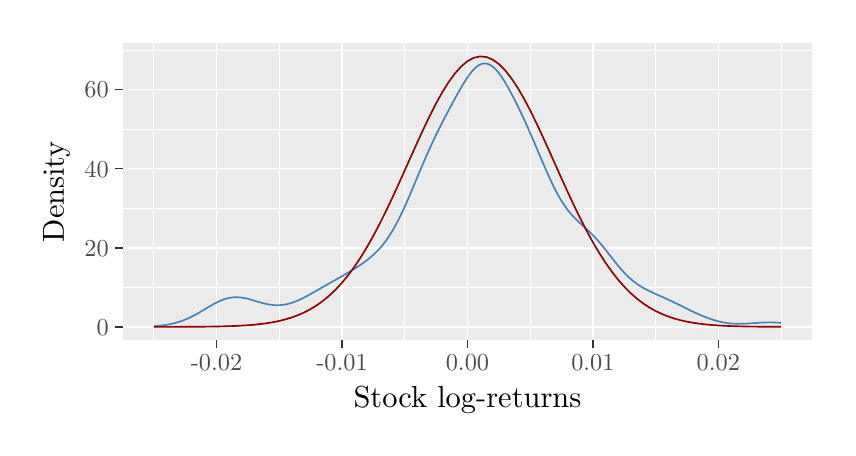
\begin{tikzpicture}[x=1pt,y=1pt]
\definecolor{fillColor}{RGB}{255,255,255}
\path[use as bounding box,fill=fillColor,fill opacity=0.00] (0,0) rectangle (289.08,144.54);
\begin{scope}
\path[clip] (  0.00,  0.00) rectangle (289.08,144.54);
\definecolor{drawColor}{RGB}{255,255,255}
\definecolor{fillColor}{RGB}{255,255,255}

\path[draw=drawColor,line width= 0.6pt,line join=round,line cap=round,fill=fillColor] (  0.00,  0.00) rectangle (289.08,144.54);
\end{scope}
\begin{scope}
\path[clip] ( 34.27, 31.53) rectangle (283.58,139.04);
\definecolor{fillColor}{gray}{0.92}

\path[fill=fillColor] ( 34.27, 31.53) rectangle (283.58,139.04);
\definecolor{drawColor}{RGB}{255,255,255}

\path[draw=drawColor,line width= 0.3pt,line join=round] ( 34.27, 50.71) --
	(283.58, 50.71);

\path[draw=drawColor,line width= 0.3pt,line join=round] ( 34.27, 79.31) --
	(283.58, 79.31);

\path[draw=drawColor,line width= 0.3pt,line join=round] ( 34.27,107.90) --
	(283.58,107.90);

\path[draw=drawColor,line width= 0.3pt,line join=round] ( 34.27,136.49) --
	(283.58,136.49);

\path[draw=drawColor,line width= 0.3pt,line join=round] ( 45.60, 31.53) --
	( 45.60,139.04);

\path[draw=drawColor,line width= 0.3pt,line join=round] ( 90.93, 31.53) --
	( 90.93,139.04);

\path[draw=drawColor,line width= 0.3pt,line join=round] (136.26, 31.53) --
	(136.26,139.04);

\path[draw=drawColor,line width= 0.3pt,line join=round] (181.59, 31.53) --
	(181.59,139.04);

\path[draw=drawColor,line width= 0.3pt,line join=round] (226.92, 31.53) --
	(226.92,139.04);

\path[draw=drawColor,line width= 0.3pt,line join=round] (272.25, 31.53) --
	(272.25,139.04);

\path[draw=drawColor,line width= 0.6pt,line join=round] ( 34.27, 36.42) --
	(283.58, 36.42);

\path[draw=drawColor,line width= 0.6pt,line join=round] ( 34.27, 65.01) --
	(283.58, 65.01);

\path[draw=drawColor,line width= 0.6pt,line join=round] ( 34.27, 93.60) --
	(283.58, 93.60);

\path[draw=drawColor,line width= 0.6pt,line join=round] ( 34.27,122.19) --
	(283.58,122.19);

\path[draw=drawColor,line width= 0.6pt,line join=round] ( 68.26, 31.53) --
	( 68.26,139.04);

\path[draw=drawColor,line width= 0.6pt,line join=round] (113.59, 31.53) --
	(113.59,139.04);

\path[draw=drawColor,line width= 0.6pt,line join=round] (158.92, 31.53) --
	(158.92,139.04);

\path[draw=drawColor,line width= 0.6pt,line join=round] (204.25, 31.53) --
	(204.25,139.04);

\path[draw=drawColor,line width= 0.6pt,line join=round] (249.58, 31.53) --
	(249.58,139.04);
\definecolor{drawColor}{RGB}{70,130,180}

\path[draw=drawColor,line width= 0.6pt,line join=round] ( 45.60, 36.66) --
	( 46.04, 36.69) --
	( 46.49, 36.73) --
	( 46.93, 36.77) --
	( 47.37, 36.81) --
	( 47.82, 36.85) --
	( 48.26, 36.90) --
	( 48.70, 36.95) --
	( 49.15, 37.01) --
	( 49.59, 37.07) --
	( 50.04, 37.14) --
	( 50.48, 37.22) --
	( 50.92, 37.29) --
	( 51.37, 37.38) --
	( 51.81, 37.47) --
	( 52.25, 37.57) --
	( 52.70, 37.67) --
	( 53.14, 37.79) --
	( 53.58, 37.91) --
	( 54.03, 38.03) --
	( 54.47, 38.17) --
	( 54.91, 38.31) --
	( 55.36, 38.46) --
	( 55.80, 38.62) --
	( 56.25, 38.78) --
	( 56.69, 38.95) --
	( 57.13, 39.13) --
	( 57.58, 39.32) --
	( 58.02, 39.52) --
	( 58.46, 39.73) --
	( 58.91, 39.94) --
	( 59.35, 40.16) --
	( 59.79, 40.39) --
	( 60.24, 40.62) --
	( 60.68, 40.86) --
	( 61.12, 41.10) --
	( 61.57, 41.35) --
	( 62.01, 41.61) --
	( 62.45, 41.87) --
	( 62.90, 42.13) --
	( 63.34, 42.39) --
	( 63.79, 42.66) --
	( 64.23, 42.92) --
	( 64.67, 43.19) --
	( 65.12, 43.46) --
	( 65.56, 43.72) --
	( 66.00, 43.98) --
	( 66.45, 44.23) --
	( 66.89, 44.49) --
	( 67.33, 44.73) --
	( 67.78, 44.97) --
	( 68.22, 45.20) --
	( 68.66, 45.42) --
	( 69.11, 45.63) --
	( 69.55, 45.83) --
	( 69.99, 46.01) --
	( 70.44, 46.19) --
	( 70.88, 46.35) --
	( 71.33, 46.50) --
	( 71.77, 46.63) --
	( 72.21, 46.75) --
	( 72.66, 46.85) --
	( 73.10, 46.94) --
	( 73.54, 47.01) --
	( 73.99, 47.06) --
	( 74.43, 47.10) --
	( 74.87, 47.13) --
	( 75.32, 47.13) --
	( 75.76, 47.13) --
	( 76.20, 47.11) --
	( 76.65, 47.07) --
	( 77.09, 47.02) --
	( 77.53, 46.96) --
	( 77.98, 46.89) --
	( 78.42, 46.81) --
	( 78.87, 46.71) --
	( 79.31, 46.61) --
	( 79.75, 46.50) --
	( 80.20, 46.38) --
	( 80.64, 46.26) --
	( 81.08, 46.13) --
	( 81.53, 46.01) --
	( 81.97, 45.87) --
	( 82.41, 45.74) --
	( 82.86, 45.61) --
	( 83.30, 45.48) --
	( 83.74, 45.35) --
	( 84.19, 45.22) --
	( 84.63, 45.10) --
	( 85.07, 44.98) --
	( 85.52, 44.87) --
	( 85.96, 44.77) --
	( 86.41, 44.67) --
	( 86.85, 44.58) --
	( 87.29, 44.50) --
	( 87.74, 44.43) --
	( 88.18, 44.38) --
	( 88.62, 44.33) --
	( 89.07, 44.29) --
	( 89.51, 44.27) --
	( 89.95, 44.25) --
	( 90.40, 44.25) --
	( 90.84, 44.27) --
	( 91.28, 44.29) --
	( 91.73, 44.33) --
	( 92.17, 44.38) --
	( 92.62, 44.44) --
	( 93.06, 44.51) --
	( 93.50, 44.60) --
	( 93.95, 44.70) --
	( 94.39, 44.81) --
	( 94.83, 44.94) --
	( 95.28, 45.07) --
	( 95.72, 45.22) --
	( 96.16, 45.37) --
	( 96.61, 45.54) --
	( 97.05, 45.71) --
	( 97.49, 45.90) --
	( 97.94, 46.09) --
	( 98.38, 46.30) --
	( 98.82, 46.50) --
	( 99.27, 46.72) --
	( 99.71, 46.94) --
	(100.16, 47.17) --
	(100.60, 47.40) --
	(101.04, 47.64) --
	(101.49, 47.88) --
	(101.93, 48.12) --
	(102.37, 48.37) --
	(102.82, 48.62) --
	(103.26, 48.87) --
	(103.70, 49.12) --
	(104.15, 49.38) --
	(104.59, 49.63) --
	(105.03, 49.89) --
	(105.48, 50.14) --
	(105.92, 50.40) --
	(106.36, 50.65) --
	(106.81, 50.91) --
	(107.25, 51.16) --
	(107.70, 51.41) --
	(108.14, 51.66) --
	(108.58, 51.92) --
	(109.03, 52.17) --
	(109.47, 52.42) --
	(109.91, 52.67) --
	(110.36, 52.92) --
	(110.80, 53.17) --
	(111.24, 53.42) --
	(111.69, 53.67) --
	(112.13, 53.92) --
	(112.57, 54.17) --
	(113.02, 54.43) --
	(113.46, 54.68) --
	(113.90, 54.93) --
	(114.35, 55.19) --
	(114.79, 55.44) --
	(115.24, 55.70) --
	(115.68, 55.96) --
	(116.12, 56.23) --
	(116.57, 56.49) --
	(117.01, 56.76) --
	(117.45, 57.03) --
	(117.90, 57.30) --
	(118.34, 57.58) --
	(118.78, 57.86) --
	(119.23, 58.15) --
	(119.67, 58.44) --
	(120.11, 58.74) --
	(120.56, 59.04) --
	(121.00, 59.35) --
	(121.45, 59.66) --
	(121.89, 59.98) --
	(122.33, 60.32) --
	(122.78, 60.66) --
	(123.22, 61.01) --
	(123.66, 61.37) --
	(124.11, 61.74) --
	(124.55, 62.13) --
	(124.99, 62.53) --
	(125.44, 62.95) --
	(125.88, 63.38) --
	(126.32, 63.82) --
	(126.77, 64.29) --
	(127.21, 64.78) --
	(127.65, 65.28) --
	(128.10, 65.81) --
	(128.54, 66.36) --
	(128.99, 66.93) --
	(129.43, 67.53) --
	(129.87, 68.15) --
	(130.32, 68.79) --
	(130.76, 69.47) --
	(131.20, 70.16) --
	(131.65, 70.88) --
	(132.09, 71.63) --
	(132.53, 72.41) --
	(132.98, 73.22) --
	(133.42, 74.04) --
	(133.86, 74.89) --
	(134.31, 75.77) --
	(134.75, 76.68) --
	(135.19, 77.60) --
	(135.64, 78.54) --
	(136.08, 79.51) --
	(136.53, 80.49) --
	(136.97, 81.49) --
	(137.41, 82.50) --
	(137.86, 83.53) --
	(138.30, 84.57) --
	(138.74, 85.61) --
	(139.19, 86.67) --
	(139.63, 87.72) --
	(140.07, 88.79) --
	(140.52, 89.85) --
	(140.96, 90.91) --
	(141.40, 91.97) --
	(141.85, 93.02) --
	(142.29, 94.07) --
	(142.73, 95.12) --
	(143.18, 96.15) --
	(143.62, 97.17) --
	(144.07, 98.19) --
	(144.51, 99.19) --
	(144.95,100.18) --
	(145.40,101.16) --
	(145.84,102.12) --
	(146.28,103.08) --
	(146.73,104.02) --
	(147.17,104.95) --
	(147.61,105.87) --
	(148.06,106.77) --
	(148.50,107.67) --
	(148.94,108.55) --
	(149.39,109.43) --
	(149.83,110.30) --
	(150.27,111.16) --
	(150.72,112.02) --
	(151.16,112.87) --
	(151.61,113.72) --
	(152.05,114.55) --
	(152.49,115.39) --
	(152.94,116.22) --
	(153.38,117.05) --
	(153.82,117.87) --
	(154.27,118.69) --
	(154.71,119.50) --
	(155.15,120.30) --
	(155.60,121.09) --
	(156.04,121.88) --
	(156.48,122.65) --
	(156.93,123.41) --
	(157.37,124.15) --
	(157.82,124.87) --
	(158.26,125.57) --
	(158.70,126.25) --
	(159.15,126.90) --
	(159.59,127.52) --
	(160.03,128.10) --
	(160.48,128.65) --
	(160.92,129.17) --
	(161.36,129.63) --
	(161.81,130.06) --
	(162.25,130.44) --
	(162.69,130.77) --
	(163.14,131.04) --
	(163.58,131.26) --
	(164.02,131.44) --
	(164.47,131.56) --
	(164.91,131.62) --
	(165.36,131.61) --
	(165.80,131.56) --
	(166.24,131.45) --
	(166.69,131.29) --
	(167.13,131.06) --
	(167.57,130.79) --
	(168.02,130.47) --
	(168.46,130.10) --
	(168.90,129.67) --
	(169.35,129.20) --
	(169.79,128.69) --
	(170.23,128.14) --
	(170.68,127.55) --
	(171.12,126.93) --
	(171.56,126.27) --
	(172.01,125.58) --
	(172.45,124.87) --
	(172.90,124.13) --
	(173.34,123.36) --
	(173.78,122.58) --
	(174.23,121.78) --
	(174.67,120.95) --
	(175.11,120.11) --
	(175.56,119.26) --
	(176.00,118.39) --
	(176.44,117.51) --
	(176.89,116.61) --
	(177.33,115.70) --
	(177.77,114.78) --
	(178.22,113.86) --
	(178.66,112.91) --
	(179.10,111.96) --
	(179.55,111.00) --
	(179.99,110.03) --
	(180.44,109.05) --
	(180.88,108.05) --
	(181.32,107.05) --
	(181.77,106.04) --
	(182.21,105.02) --
	(182.65,104.00) --
	(183.10,102.96) --
	(183.54,101.92) --
	(183.98,100.88) --
	(184.43, 99.84) --
	(184.87, 98.79) --
	(185.31, 97.75) --
	(185.76, 96.70) --
	(186.20, 95.66) --
	(186.64, 94.63) --
	(187.09, 93.61) --
	(187.53, 92.60) --
	(187.98, 91.60) --
	(188.42, 90.62) --
	(188.86, 89.65) --
	(189.31, 88.70) --
	(189.75, 87.77) --
	(190.19, 86.87) --
	(190.64, 86.00) --
	(191.08, 85.14) --
	(191.52, 84.32) --
	(191.97, 83.52) --
	(192.41, 82.76) --
	(192.85, 82.02) --
	(193.30, 81.31) --
	(193.74, 80.63) --
	(194.19, 79.98) --
	(194.63, 79.36) --
	(195.07, 78.76) --
	(195.52, 78.19) --
	(195.96, 77.66) --
	(196.40, 77.14) --
	(196.85, 76.64) --
	(197.29, 76.16) --
	(197.73, 75.70) --
	(198.18, 75.26) --
	(198.62, 74.82) --
	(199.06, 74.40) --
	(199.51, 73.99) --
	(199.95, 73.58) --
	(200.39, 73.18) --
	(200.84, 72.78) --
	(201.28, 72.38) --
	(201.73, 71.97) --
	(202.17, 71.56) --
	(202.61, 71.15) --
	(203.06, 70.73) --
	(203.50, 70.29) --
	(203.94, 69.85) --
	(204.39, 69.40) --
	(204.83, 68.94) --
	(205.27, 68.46) --
	(205.72, 67.97) --
	(206.16, 67.47) --
	(206.60, 66.96) --
	(207.05, 66.44) --
	(207.49, 65.91) --
	(207.93, 65.37) --
	(208.38, 64.82) --
	(208.82, 64.26) --
	(209.27, 63.70) --
	(209.71, 63.14) --
	(210.15, 62.57) --
	(210.60, 62.00) --
	(211.04, 61.43) --
	(211.48, 60.86) --
	(211.93, 60.30) --
	(212.37, 59.74) --
	(212.81, 59.19) --
	(213.26, 58.65) --
	(213.70, 58.12) --
	(214.14, 57.59) --
	(214.59, 57.08) --
	(215.03, 56.59) --
	(215.47, 56.11) --
	(215.92, 55.64) --
	(216.36, 55.18) --
	(216.81, 54.75) --
	(217.25, 54.33) --
	(217.69, 53.92) --
	(218.14, 53.53) --
	(218.58, 53.16) --
	(219.02, 52.80) --
	(219.47, 52.46) --
	(219.91, 52.13) --
	(220.35, 51.81) --
	(220.80, 51.52) --
	(221.24, 51.23) --
	(221.68, 50.95) --
	(222.13, 50.69) --
	(222.57, 50.44) --
	(223.02, 50.19) --
	(223.46, 49.96) --
	(223.90, 49.73) --
	(224.35, 49.51) --
	(224.79, 49.29) --
	(225.23, 49.08) --
	(225.68, 48.88) --
	(226.12, 48.67) --
	(226.56, 48.47) --
	(227.01, 48.27) --
	(227.45, 48.08) --
	(227.89, 47.88) --
	(228.34, 47.68) --
	(228.78, 47.49) --
	(229.22, 47.29) --
	(229.67, 47.09) --
	(230.11, 46.89) --
	(230.56, 46.69) --
	(231.00, 46.48) --
	(231.44, 46.28) --
	(231.89, 46.07) --
	(232.33, 45.86) --
	(232.77, 45.65) --
	(233.22, 45.44) --
	(233.66, 45.23) --
	(234.10, 45.01) --
	(234.55, 44.80) --
	(234.99, 44.58) --
	(235.43, 44.36) --
	(235.88, 44.14) --
	(236.32, 43.92) --
	(236.76, 43.70) --
	(237.21, 43.48) --
	(237.65, 43.26) --
	(238.10, 43.04) --
	(238.54, 42.83) --
	(238.98, 42.61) --
	(239.43, 42.39) --
	(239.87, 42.18) --
	(240.31, 41.97) --
	(240.76, 41.76) --
	(241.20, 41.55) --
	(241.64, 41.35) --
	(242.09, 41.15) --
	(242.53, 40.95) --
	(242.97, 40.75) --
	(243.42, 40.56) --
	(243.86, 40.38) --
	(244.30, 40.19) --
	(244.75, 40.02) --
	(245.19, 39.84) --
	(245.64, 39.67) --
	(246.08, 39.51) --
	(246.52, 39.35) --
	(246.97, 39.20) --
	(247.41, 39.05) --
	(247.85, 38.91) --
	(248.30, 38.78) --
	(248.74, 38.65) --
	(249.18, 38.53) --
	(249.63, 38.42) --
	(250.07, 38.31) --
	(250.51, 38.21) --
	(250.96, 38.11) --
	(251.40, 38.03) --
	(251.84, 37.95) --
	(252.29, 37.88) --
	(252.73, 37.81) --
	(253.18, 37.75) --
	(253.62, 37.70) --
	(254.06, 37.66) --
	(254.51, 37.62) --
	(254.95, 37.59) --
	(255.39, 37.56) --
	(255.84, 37.55) --
	(256.28, 37.53) --
	(256.72, 37.53) --
	(257.17, 37.53) --
	(257.61, 37.53) --
	(258.05, 37.54) --
	(258.50, 37.55) --
	(258.94, 37.57) --
	(259.39, 37.59) --
	(259.83, 37.61) --
	(260.27, 37.64) --
	(260.72, 37.66) --
	(261.16, 37.69) --
	(261.60, 37.72) --
	(262.05, 37.76) --
	(262.49, 37.79) --
	(262.93, 37.82) --
	(263.38, 37.85) --
	(263.82, 37.88) --
	(264.26, 37.91) --
	(264.71, 37.94) --
	(265.15, 37.96) --
	(265.59, 37.98) --
	(266.04, 38.00) --
	(266.48, 38.02) --
	(266.93, 38.03) --
	(267.37, 38.04) --
	(267.81, 38.04) --
	(268.26, 38.04) --
	(268.70, 38.04) --
	(269.14, 38.03) --
	(269.59, 38.02) --
	(270.03, 38.00) --
	(270.47, 37.99) --
	(270.92, 37.96) --
	(271.36, 37.94) --
	(271.80, 37.91) --
	(272.25, 37.87);
\definecolor{drawColor}{RGB}{139,0,0}

\path[draw=drawColor,line width= 0.6pt,line join=round] ( 45.60, 36.42) --
	( 47.87, 36.42) --
	( 50.13, 36.43) --
	( 52.40, 36.43) --
	( 54.67, 36.44) --
	( 56.93, 36.44) --
	( 59.20, 36.46) --
	( 61.47, 36.47) --
	( 63.73, 36.49) --
	( 66.00, 36.52) --
	( 68.26, 36.56) --
	( 70.53, 36.61) --
	( 72.80, 36.68) --
	( 75.06, 36.76) --
	( 77.33, 36.88) --
	( 79.60, 37.02) --
	( 81.86, 37.21) --
	( 84.13, 37.45) --
	( 86.40, 37.75) --
	( 88.66, 38.12) --
	( 90.93, 38.58) --
	( 93.20, 39.15) --
	( 95.46, 39.84) --
	( 97.73, 40.68) --
	(100.00, 41.68) --
	(102.26, 42.87) --
	(104.53, 44.26) --
	(106.80, 45.90) --
	(109.06, 47.78) --
	(111.33, 49.94) --
	(113.59, 52.40) --
	(115.86, 55.16) --
	(118.13, 58.24) --
	(120.39, 61.63) --
	(122.66, 65.35) --
	(124.93, 69.37) --
	(127.19, 73.67) --
	(129.46, 78.22) --
	(131.73, 82.99) --
	(133.99, 87.93) --
	(136.26, 92.97) --
	(138.53, 98.04) --
	(140.79,103.09) --
	(143.06,108.01) --
	(145.33,112.74) --
	(147.59,117.19) --
	(149.86,121.27) --
	(152.12,124.90) --
	(154.39,128.01) --
	(156.66,130.54) --
	(158.92,132.43) --
	(161.19,133.65) --
	(163.46,134.15) --
	(165.72,133.94) --
	(167.99,133.02) --
	(170.26,131.41) --
	(172.52,129.14) --
	(174.79,126.27) --
	(177.06,122.84) --
	(179.32,118.94) --
	(181.59,114.64) --
	(183.86,110.02) --
	(186.12,105.16) --
	(188.39,100.16) --
	(190.65, 95.09) --
	(192.92, 90.02) --
	(195.19, 85.04) --
	(197.45, 80.19) --
	(199.72, 75.54) --
	(201.99, 71.13) --
	(204.25, 66.99) --
	(206.52, 63.15) --
	(208.79, 59.62) --
	(211.05, 56.41) --
	(213.32, 53.51) --
	(215.59, 50.93) --
	(217.85, 48.65) --
	(220.12, 46.65) --
	(222.39, 44.92) --
	(224.65, 43.42) --
	(226.92, 42.15) --
	(229.18, 41.08) --
	(231.45, 40.17) --
	(233.72, 39.42) --
	(235.98, 38.81) --
	(238.25, 38.30) --
	(240.52, 37.89) --
	(242.78, 37.57) --
	(245.05, 37.30) --
	(247.32, 37.10) --
	(249.58, 36.93) --
	(251.85, 36.81) --
	(254.12, 36.71) --
	(256.38, 36.63) --
	(258.65, 36.58) --
	(260.92, 36.53) --
	(263.18, 36.50) --
	(265.45, 36.48) --
	(267.71, 36.46) --
	(269.98, 36.45) --
	(272.25, 36.44);
\end{scope}
\begin{scope}
\path[clip] (  0.00,  0.00) rectangle (289.08,144.54);
\definecolor{drawColor}{gray}{0.30}

\node[text=drawColor,anchor=base east,inner sep=0pt, outer sep=0pt, scale=  0.88] at ( 29.32, 33.39) {0};

\node[text=drawColor,anchor=base east,inner sep=0pt, outer sep=0pt, scale=  0.88] at ( 29.32, 61.98) {20};

\node[text=drawColor,anchor=base east,inner sep=0pt, outer sep=0pt, scale=  0.88] at ( 29.32, 90.57) {40};

\node[text=drawColor,anchor=base east,inner sep=0pt, outer sep=0pt, scale=  0.88] at ( 29.32,119.16) {60};
\end{scope}
\begin{scope}
\path[clip] (  0.00,  0.00) rectangle (289.08,144.54);
\definecolor{drawColor}{gray}{0.20}

\path[draw=drawColor,line width= 0.6pt,line join=round] ( 31.52, 36.42) --
	( 34.27, 36.42);

\path[draw=drawColor,line width= 0.6pt,line join=round] ( 31.52, 65.01) --
	( 34.27, 65.01);

\path[draw=drawColor,line width= 0.6pt,line join=round] ( 31.52, 93.60) --
	( 34.27, 93.60);

\path[draw=drawColor,line width= 0.6pt,line join=round] ( 31.52,122.19) --
	( 34.27,122.19);
\end{scope}
\begin{scope}
\path[clip] (  0.00,  0.00) rectangle (289.08,144.54);
\definecolor{drawColor}{gray}{0.20}

\path[draw=drawColor,line width= 0.6pt,line join=round] ( 68.26, 28.78) --
	( 68.26, 31.53);

\path[draw=drawColor,line width= 0.6pt,line join=round] (113.59, 28.78) --
	(113.59, 31.53);

\path[draw=drawColor,line width= 0.6pt,line join=round] (158.92, 28.78) --
	(158.92, 31.53);

\path[draw=drawColor,line width= 0.6pt,line join=round] (204.25, 28.78) --
	(204.25, 31.53);

\path[draw=drawColor,line width= 0.6pt,line join=round] (249.58, 28.78) --
	(249.58, 31.53);
\end{scope}
\begin{scope}
\path[clip] (  0.00,  0.00) rectangle (289.08,144.54);
\definecolor{drawColor}{gray}{0.30}

\node[text=drawColor,anchor=base,inner sep=0pt, outer sep=0pt, scale=  0.88] at ( 68.26, 20.52) {-0.02};

\node[text=drawColor,anchor=base,inner sep=0pt, outer sep=0pt, scale=  0.88] at (113.59, 20.52) {-0.01};

\node[text=drawColor,anchor=base,inner sep=0pt, outer sep=0pt, scale=  0.88] at (158.92, 20.52) {0.00};

\node[text=drawColor,anchor=base,inner sep=0pt, outer sep=0pt, scale=  0.88] at (204.25, 20.52) {0.01};

\node[text=drawColor,anchor=base,inner sep=0pt, outer sep=0pt, scale=  0.88] at (249.58, 20.52) {0.02};
\end{scope}
\begin{scope}
\path[clip] (  0.00,  0.00) rectangle (289.08,144.54);
\definecolor{drawColor}{RGB}{0,0,0}

\node[text=drawColor,anchor=base,inner sep=0pt, outer sep=0pt, scale=  1.10] at (158.92,  7.44) {Stock log-returns};
\end{scope}
\begin{scope}
\path[clip] (  0.00,  0.00) rectangle (289.08,144.54);
\definecolor{drawColor}{RGB}{0,0,0}

\node[text=drawColor,rotate= 90.00,anchor=base,inner sep=0pt, outer sep=0pt, scale=  1.10] at ( 13.08, 85.29) {Density};
\end{scope}
\end{tikzpicture}

  % \rule{40mm}{20mm}
  \caption{Distribution of the calibrated BSM time-series' log-returns with respect to the distribution of those provided by the market.}
  %
  % BEGIN OF FLOATNOTE
  %
  \begin{changemargin}{0.5cm}{0.5cm}
  \medskip
\footnotesize
\setstretch{1.0}\textbf{Notes.} The above blue density curve is constructed over the historical data of the Apple share of stock price evolution from 1st January 2017 to 31st December 2017. while the red curve is built from time-series generated by the function \textit{bsm\_ts} taking $\tau = 1.0931$, $\alpha = 0.48229$, $\sigma = 0.1958$ as parameters.
  \end{changemargin}
  %
  % END OF FLOATNOTE
  %
  \label{p:analysis:gbm:adjusted}
\end{figure}

\Cref{p:analysis:gbm:adjusted} illustrates the theoretical density curve of the log-returns reproduced with the adjusted parameters, while \cref{p:analysis:gbm:option:adjusted} faces the blue colored volatility smiles determined from market data with those dotted in red, computed from data provided by the function \textit{bsm\_call} which takes the calibrated $\sigma$ and the riskless rate $r$ as parameters.

\begin{figure}[h]
  \centering
  % Created by tikzDevice version 0.11 on 2018-07-30 00:20:26
% !TEX encoding = UTF-8 Unicode
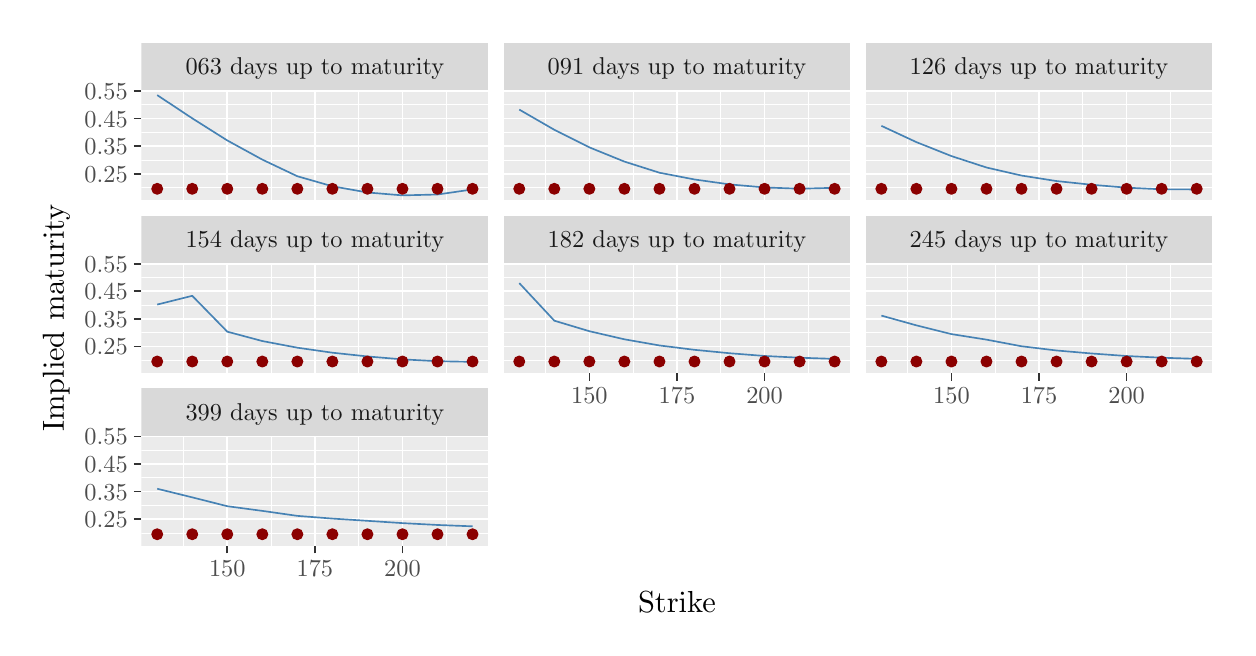
\begin{tikzpicture}[x=1pt,y=1pt]
\definecolor{fillColor}{RGB}{255,255,255}
\path[use as bounding box,fill=fillColor,fill opacity=0.00] (0,0) rectangle (433.62,216.81);
\begin{scope}
\path[clip] (  0.00,  0.00) rectangle (433.62,216.81);
\definecolor{drawColor}{RGB}{255,255,255}
\definecolor{fillColor}{RGB}{255,255,255}

\path[draw=drawColor,line width= 0.6pt,line join=round,line cap=round,fill=fillColor] (  0.00,  0.00) rectangle (433.62,216.81);
\end{scope}
\begin{scope}
\path[clip] ( 41.11,154.40) rectangle (166.45,194.25);
\definecolor{fillColor}{gray}{0.92}

\path[fill=fillColor] ( 41.11,154.40) rectangle (166.45,194.25);
\definecolor{drawColor}{RGB}{255,255,255}

\path[draw=drawColor,line width= 0.3pt,line join=round] ( 41.11,158.99) --
	(166.45,158.99);

\path[draw=drawColor,line width= 0.3pt,line join=round] ( 41.11,168.97) --
	(166.45,168.97);

\path[draw=drawColor,line width= 0.3pt,line join=round] ( 41.11,178.95) --
	(166.45,178.95);

\path[draw=drawColor,line width= 0.3pt,line join=round] ( 41.11,188.93) --
	(166.45,188.93);

\path[draw=drawColor,line width= 0.3pt,line join=round] ( 56.30,154.40) --
	( 56.30,194.25);

\path[draw=drawColor,line width= 0.3pt,line join=round] ( 87.95,154.40) --
	( 87.95,194.25);

\path[draw=drawColor,line width= 0.3pt,line join=round] (119.60,154.40) --
	(119.60,194.25);

\path[draw=drawColor,line width= 0.3pt,line join=round] (151.25,154.40) --
	(151.25,194.25);

\path[draw=drawColor,line width= 0.6pt,line join=round] ( 41.11,163.98) --
	(166.45,163.98);

\path[draw=drawColor,line width= 0.6pt,line join=round] ( 41.11,173.96) --
	(166.45,173.96);

\path[draw=drawColor,line width= 0.6pt,line join=round] ( 41.11,183.94) --
	(166.45,183.94);

\path[draw=drawColor,line width= 0.6pt,line join=round] ( 41.11,193.92) --
	(166.45,193.92);

\path[draw=drawColor,line width= 0.6pt,line join=round] ( 72.13,154.40) --
	( 72.13,194.25);

\path[draw=drawColor,line width= 0.6pt,line join=round] (103.78,154.40) --
	(103.78,194.25);

\path[draw=drawColor,line width= 0.6pt,line join=round] (135.43,154.40) --
	(135.43,194.25);
\definecolor{drawColor}{RGB}{70,130,180}

\path[draw=drawColor,line width= 0.6pt,line join=round] ( 46.81,192.44) --
	( 59.47,184.05) --
	( 72.13,176.06) --
	( 84.79,169.13) --
	( 97.45,163.12) --
	(110.11,159.50) --
	(122.77,157.26) --
	(135.43,156.21) --
	(148.09,156.52) --
	(160.75,158.35);
\definecolor{drawColor}{RGB}{139,0,0}
\definecolor{fillColor}{RGB}{139,0,0}

\path[draw=drawColor,line width= 0.4pt,line join=round,line cap=round,fill=fillColor] ( 46.81,158.58) circle (  1.96);

\path[draw=drawColor,line width= 0.4pt,line join=round,line cap=round,fill=fillColor] ( 59.47,158.58) circle (  1.96);

\path[draw=drawColor,line width= 0.4pt,line join=round,line cap=round,fill=fillColor] ( 72.13,158.58) circle (  1.96);

\path[draw=drawColor,line width= 0.4pt,line join=round,line cap=round,fill=fillColor] ( 84.79,158.58) circle (  1.96);

\path[draw=drawColor,line width= 0.4pt,line join=round,line cap=round,fill=fillColor] ( 97.45,158.58) circle (  1.96);

\path[draw=drawColor,line width= 0.4pt,line join=round,line cap=round,fill=fillColor] (110.11,158.58) circle (  1.96);

\path[draw=drawColor,line width= 0.4pt,line join=round,line cap=round,fill=fillColor] (122.77,158.58) circle (  1.96);

\path[draw=drawColor,line width= 0.4pt,line join=round,line cap=round,fill=fillColor] (135.43,158.58) circle (  1.96);

\path[draw=drawColor,line width= 0.4pt,line join=round,line cap=round,fill=fillColor] (148.09,158.58) circle (  1.96);

\path[draw=drawColor,line width= 0.4pt,line join=round,line cap=round,fill=fillColor] (160.75,158.58) circle (  1.96);
\end{scope}
\begin{scope}
\path[clip] ( 41.11, 91.99) rectangle (166.45,131.84);
\definecolor{fillColor}{gray}{0.92}

\path[fill=fillColor] ( 41.11, 91.99) rectangle (166.45,131.84);
\definecolor{drawColor}{RGB}{255,255,255}

\path[draw=drawColor,line width= 0.3pt,line join=round] ( 41.11, 96.59) --
	(166.45, 96.59);

\path[draw=drawColor,line width= 0.3pt,line join=round] ( 41.11,106.57) --
	(166.45,106.57);

\path[draw=drawColor,line width= 0.3pt,line join=round] ( 41.11,116.55) --
	(166.45,116.55);

\path[draw=drawColor,line width= 0.3pt,line join=round] ( 41.11,126.52) --
	(166.45,126.52);

\path[draw=drawColor,line width= 0.3pt,line join=round] ( 56.30, 91.99) --
	( 56.30,131.84);

\path[draw=drawColor,line width= 0.3pt,line join=round] ( 87.95, 91.99) --
	( 87.95,131.84);

\path[draw=drawColor,line width= 0.3pt,line join=round] (119.60, 91.99) --
	(119.60,131.84);

\path[draw=drawColor,line width= 0.3pt,line join=round] (151.25, 91.99) --
	(151.25,131.84);

\path[draw=drawColor,line width= 0.6pt,line join=round] ( 41.11,101.58) --
	(166.45,101.58);

\path[draw=drawColor,line width= 0.6pt,line join=round] ( 41.11,111.56) --
	(166.45,111.56);

\path[draw=drawColor,line width= 0.6pt,line join=round] ( 41.11,121.54) --
	(166.45,121.54);

\path[draw=drawColor,line width= 0.6pt,line join=round] ( 41.11,131.51) --
	(166.45,131.51);

\path[draw=drawColor,line width= 0.6pt,line join=round] ( 72.13, 91.99) --
	( 72.13,131.84);

\path[draw=drawColor,line width= 0.6pt,line join=round] (103.78, 91.99) --
	(103.78,131.84);

\path[draw=drawColor,line width= 0.6pt,line join=round] (135.43, 91.99) --
	(135.43,131.84);
\definecolor{drawColor}{RGB}{70,130,180}

\path[draw=drawColor,line width= 0.6pt,line join=round] ( 46.81,116.76) --
	( 59.47,119.91) --
	( 72.13,106.96) --
	( 84.79,103.57) --
	( 97.45,101.17) --
	(110.11, 99.36) --
	(122.77, 98.01) --
	(135.43, 96.95) --
	(148.09, 96.29) --
	(160.75, 96.06);
\definecolor{drawColor}{RGB}{139,0,0}
\definecolor{fillColor}{RGB}{139,0,0}

\path[draw=drawColor,line width= 0.4pt,line join=round,line cap=round,fill=fillColor] ( 46.81, 96.17) circle (  1.96);

\path[draw=drawColor,line width= 0.4pt,line join=round,line cap=round,fill=fillColor] ( 59.47, 96.17) circle (  1.96);

\path[draw=drawColor,line width= 0.4pt,line join=round,line cap=round,fill=fillColor] ( 72.13, 96.17) circle (  1.96);

\path[draw=drawColor,line width= 0.4pt,line join=round,line cap=round,fill=fillColor] ( 84.79, 96.17) circle (  1.96);

\path[draw=drawColor,line width= 0.4pt,line join=round,line cap=round,fill=fillColor] ( 97.45, 96.17) circle (  1.96);

\path[draw=drawColor,line width= 0.4pt,line join=round,line cap=round,fill=fillColor] (110.11, 96.17) circle (  1.96);

\path[draw=drawColor,line width= 0.4pt,line join=round,line cap=round,fill=fillColor] (122.77, 96.17) circle (  1.96);

\path[draw=drawColor,line width= 0.4pt,line join=round,line cap=round,fill=fillColor] (135.43, 96.17) circle (  1.96);

\path[draw=drawColor,line width= 0.4pt,line join=round,line cap=round,fill=fillColor] (148.09, 96.17) circle (  1.96);

\path[draw=drawColor,line width= 0.4pt,line join=round,line cap=round,fill=fillColor] (160.75, 96.17) circle (  1.96);
\end{scope}
\begin{scope}
\path[clip] ( 41.11, 29.59) rectangle (166.45, 69.43);
\definecolor{fillColor}{gray}{0.92}

\path[fill=fillColor] ( 41.11, 29.59) rectangle (166.45, 69.43);
\definecolor{drawColor}{RGB}{255,255,255}

\path[draw=drawColor,line width= 0.3pt,line join=round] ( 41.11, 34.18) --
	(166.45, 34.18);

\path[draw=drawColor,line width= 0.3pt,line join=round] ( 41.11, 44.16) --
	(166.45, 44.16);

\path[draw=drawColor,line width= 0.3pt,line join=round] ( 41.11, 54.14) --
	(166.45, 54.14);

\path[draw=drawColor,line width= 0.3pt,line join=round] ( 41.11, 64.12) --
	(166.45, 64.12);

\path[draw=drawColor,line width= 0.3pt,line join=round] ( 56.30, 29.59) --
	( 56.30, 69.43);

\path[draw=drawColor,line width= 0.3pt,line join=round] ( 87.95, 29.59) --
	( 87.95, 69.43);

\path[draw=drawColor,line width= 0.3pt,line join=round] (119.60, 29.59) --
	(119.60, 69.43);

\path[draw=drawColor,line width= 0.3pt,line join=round] (151.25, 29.59) --
	(151.25, 69.43);

\path[draw=drawColor,line width= 0.6pt,line join=round] ( 41.11, 39.17) --
	(166.45, 39.17);

\path[draw=drawColor,line width= 0.6pt,line join=round] ( 41.11, 49.15) --
	(166.45, 49.15);

\path[draw=drawColor,line width= 0.6pt,line join=round] ( 41.11, 59.13) --
	(166.45, 59.13);

\path[draw=drawColor,line width= 0.6pt,line join=round] ( 41.11, 69.11) --
	(166.45, 69.11);

\path[draw=drawColor,line width= 0.6pt,line join=round] ( 72.13, 29.59) --
	( 72.13, 69.43);

\path[draw=drawColor,line width= 0.6pt,line join=round] (103.78, 29.59) --
	(103.78, 69.43);

\path[draw=drawColor,line width= 0.6pt,line join=round] (135.43, 29.59) --
	(135.43, 69.43);
\definecolor{drawColor}{RGB}{70,130,180}

\path[draw=drawColor,line width= 0.6pt,line join=round] ( 46.81, 50.20) --
	( 59.47, 47.09) --
	( 72.13, 43.89) --
	( 84.79, 42.20) --
	( 97.45, 40.40) --
	(110.11, 39.42) --
	(122.77, 38.61) --
	(135.43, 37.78) --
	(148.09, 37.11) --
	(160.75, 36.62);
\definecolor{drawColor}{RGB}{139,0,0}
\definecolor{fillColor}{RGB}{139,0,0}

\path[draw=drawColor,line width= 0.4pt,line join=round,line cap=round,fill=fillColor] ( 46.81, 33.76) circle (  1.96);

\path[draw=drawColor,line width= 0.4pt,line join=round,line cap=round,fill=fillColor] ( 59.47, 33.76) circle (  1.96);

\path[draw=drawColor,line width= 0.4pt,line join=round,line cap=round,fill=fillColor] ( 72.13, 33.76) circle (  1.96);

\path[draw=drawColor,line width= 0.4pt,line join=round,line cap=round,fill=fillColor] ( 84.79, 33.76) circle (  1.96);

\path[draw=drawColor,line width= 0.4pt,line join=round,line cap=round,fill=fillColor] ( 97.45, 33.76) circle (  1.96);

\path[draw=drawColor,line width= 0.4pt,line join=round,line cap=round,fill=fillColor] (110.11, 33.76) circle (  1.96);

\path[draw=drawColor,line width= 0.4pt,line join=round,line cap=round,fill=fillColor] (122.77, 33.76) circle (  1.96);

\path[draw=drawColor,line width= 0.4pt,line join=round,line cap=round,fill=fillColor] (135.43, 33.76) circle (  1.96);

\path[draw=drawColor,line width= 0.4pt,line join=round,line cap=round,fill=fillColor] (148.09, 33.76) circle (  1.96);

\path[draw=drawColor,line width= 0.4pt,line join=round,line cap=round,fill=fillColor] (160.75, 33.76) circle (  1.96);
\end{scope}
\begin{scope}
\path[clip] (171.95,154.40) rectangle (297.28,194.25);
\definecolor{fillColor}{gray}{0.92}

\path[fill=fillColor] (171.95,154.40) rectangle (297.28,194.25);
\definecolor{drawColor}{RGB}{255,255,255}

\path[draw=drawColor,line width= 0.3pt,line join=round] (171.95,158.99) --
	(297.28,158.99);

\path[draw=drawColor,line width= 0.3pt,line join=round] (171.95,168.97) --
	(297.28,168.97);

\path[draw=drawColor,line width= 0.3pt,line join=round] (171.95,178.95) --
	(297.28,178.95);

\path[draw=drawColor,line width= 0.3pt,line join=round] (171.95,188.93) --
	(297.28,188.93);

\path[draw=drawColor,line width= 0.3pt,line join=round] (187.14,154.40) --
	(187.14,194.25);

\path[draw=drawColor,line width= 0.3pt,line join=round] (218.79,154.40) --
	(218.79,194.25);

\path[draw=drawColor,line width= 0.3pt,line join=round] (250.44,154.40) --
	(250.44,194.25);

\path[draw=drawColor,line width= 0.3pt,line join=round] (282.09,154.40) --
	(282.09,194.25);

\path[draw=drawColor,line width= 0.6pt,line join=round] (171.95,163.98) --
	(297.28,163.98);

\path[draw=drawColor,line width= 0.6pt,line join=round] (171.95,173.96) --
	(297.28,173.96);

\path[draw=drawColor,line width= 0.6pt,line join=round] (171.95,183.94) --
	(297.28,183.94);

\path[draw=drawColor,line width= 0.6pt,line join=round] (171.95,193.92) --
	(297.28,193.92);

\path[draw=drawColor,line width= 0.6pt,line join=round] (202.96,154.40) --
	(202.96,194.25);

\path[draw=drawColor,line width= 0.6pt,line join=round] (234.62,154.40) --
	(234.62,194.25);

\path[draw=drawColor,line width= 0.6pt,line join=round] (266.27,154.40) --
	(266.27,194.25);
\definecolor{drawColor}{RGB}{70,130,180}

\path[draw=drawColor,line width= 0.6pt,line join=round] (177.64,187.21) --
	(190.30,179.91) --
	(202.96,173.56) --
	(215.62,168.42) --
	(228.29,164.40) --
	(240.95,161.96) --
	(253.61,160.18) --
	(266.27,159.07) --
	(278.93,158.62) --
	(291.59,158.94);
\definecolor{drawColor}{RGB}{139,0,0}
\definecolor{fillColor}{RGB}{139,0,0}

\path[draw=drawColor,line width= 0.4pt,line join=round,line cap=round,fill=fillColor] (177.64,158.58) circle (  1.96);

\path[draw=drawColor,line width= 0.4pt,line join=round,line cap=round,fill=fillColor] (190.30,158.58) circle (  1.96);

\path[draw=drawColor,line width= 0.4pt,line join=round,line cap=round,fill=fillColor] (202.96,158.58) circle (  1.96);

\path[draw=drawColor,line width= 0.4pt,line join=round,line cap=round,fill=fillColor] (215.62,158.58) circle (  1.96);

\path[draw=drawColor,line width= 0.4pt,line join=round,line cap=round,fill=fillColor] (228.29,158.58) circle (  1.96);

\path[draw=drawColor,line width= 0.4pt,line join=round,line cap=round,fill=fillColor] (240.95,158.58) circle (  1.96);

\path[draw=drawColor,line width= 0.4pt,line join=round,line cap=round,fill=fillColor] (253.61,158.58) circle (  1.96);

\path[draw=drawColor,line width= 0.4pt,line join=round,line cap=round,fill=fillColor] (266.27,158.58) circle (  1.96);

\path[draw=drawColor,line width= 0.4pt,line join=round,line cap=round,fill=fillColor] (278.93,158.58) circle (  1.96);

\path[draw=drawColor,line width= 0.4pt,line join=round,line cap=round,fill=fillColor] (291.59,158.58) circle (  1.96);
\end{scope}
\begin{scope}
\path[clip] (171.95, 91.99) rectangle (297.28,131.84);
\definecolor{fillColor}{gray}{0.92}

\path[fill=fillColor] (171.95, 91.99) rectangle (297.28,131.84);
\definecolor{drawColor}{RGB}{255,255,255}

\path[draw=drawColor,line width= 0.3pt,line join=round] (171.95, 96.59) --
	(297.28, 96.59);

\path[draw=drawColor,line width= 0.3pt,line join=round] (171.95,106.57) --
	(297.28,106.57);

\path[draw=drawColor,line width= 0.3pt,line join=round] (171.95,116.55) --
	(297.28,116.55);

\path[draw=drawColor,line width= 0.3pt,line join=round] (171.95,126.52) --
	(297.28,126.52);

\path[draw=drawColor,line width= 0.3pt,line join=round] (187.14, 91.99) --
	(187.14,131.84);

\path[draw=drawColor,line width= 0.3pt,line join=round] (218.79, 91.99) --
	(218.79,131.84);

\path[draw=drawColor,line width= 0.3pt,line join=round] (250.44, 91.99) --
	(250.44,131.84);

\path[draw=drawColor,line width= 0.3pt,line join=round] (282.09, 91.99) --
	(282.09,131.84);

\path[draw=drawColor,line width= 0.6pt,line join=round] (171.95,101.58) --
	(297.28,101.58);

\path[draw=drawColor,line width= 0.6pt,line join=round] (171.95,111.56) --
	(297.28,111.56);

\path[draw=drawColor,line width= 0.6pt,line join=round] (171.95,121.54) --
	(297.28,121.54);

\path[draw=drawColor,line width= 0.6pt,line join=round] (171.95,131.51) --
	(297.28,131.51);

\path[draw=drawColor,line width= 0.6pt,line join=round] (202.96, 91.99) --
	(202.96,131.84);

\path[draw=drawColor,line width= 0.6pt,line join=round] (234.62, 91.99) --
	(234.62,131.84);

\path[draw=drawColor,line width= 0.6pt,line join=round] (266.27, 91.99) --
	(266.27,131.84);
\definecolor{drawColor}{RGB}{70,130,180}

\path[draw=drawColor,line width= 0.6pt,line join=round] (177.64,124.51) --
	(190.30,110.93) --
	(202.96,107.13) --
	(215.62,104.20) --
	(228.29,101.98) --
	(240.95,100.40) --
	(253.61, 99.17) --
	(266.27, 98.18) --
	(278.93, 97.55) --
	(291.59, 97.12);
\definecolor{drawColor}{RGB}{139,0,0}
\definecolor{fillColor}{RGB}{139,0,0}

\path[draw=drawColor,line width= 0.4pt,line join=round,line cap=round,fill=fillColor] (177.64, 96.17) circle (  1.96);

\path[draw=drawColor,line width= 0.4pt,line join=round,line cap=round,fill=fillColor] (190.30, 96.17) circle (  1.96);

\path[draw=drawColor,line width= 0.4pt,line join=round,line cap=round,fill=fillColor] (202.96, 96.17) circle (  1.96);

\path[draw=drawColor,line width= 0.4pt,line join=round,line cap=round,fill=fillColor] (215.62, 96.17) circle (  1.96);

\path[draw=drawColor,line width= 0.4pt,line join=round,line cap=round,fill=fillColor] (228.29, 96.17) circle (  1.96);

\path[draw=drawColor,line width= 0.4pt,line join=round,line cap=round,fill=fillColor] (240.95, 96.17) circle (  1.96);

\path[draw=drawColor,line width= 0.4pt,line join=round,line cap=round,fill=fillColor] (253.61, 96.17) circle (  1.96);

\path[draw=drawColor,line width= 0.4pt,line join=round,line cap=round,fill=fillColor] (266.27, 96.17) circle (  1.96);

\path[draw=drawColor,line width= 0.4pt,line join=round,line cap=round,fill=fillColor] (278.93, 96.17) circle (  1.96);

\path[draw=drawColor,line width= 0.4pt,line join=round,line cap=round,fill=fillColor] (291.59, 96.17) circle (  1.96);
\end{scope}
\begin{scope}
\path[clip] (302.78,154.40) rectangle (428.12,194.25);
\definecolor{fillColor}{gray}{0.92}

\path[fill=fillColor] (302.78,154.40) rectangle (428.12,194.25);
\definecolor{drawColor}{RGB}{255,255,255}

\path[draw=drawColor,line width= 0.3pt,line join=round] (302.78,158.99) --
	(428.12,158.99);

\path[draw=drawColor,line width= 0.3pt,line join=round] (302.78,168.97) --
	(428.12,168.97);

\path[draw=drawColor,line width= 0.3pt,line join=round] (302.78,178.95) --
	(428.12,178.95);

\path[draw=drawColor,line width= 0.3pt,line join=round] (302.78,188.93) --
	(428.12,188.93);

\path[draw=drawColor,line width= 0.3pt,line join=round] (317.98,154.40) --
	(317.98,194.25);

\path[draw=drawColor,line width= 0.3pt,line join=round] (349.63,154.40) --
	(349.63,194.25);

\path[draw=drawColor,line width= 0.3pt,line join=round] (381.28,154.40) --
	(381.28,194.25);

\path[draw=drawColor,line width= 0.3pt,line join=round] (412.93,154.40) --
	(412.93,194.25);

\path[draw=drawColor,line width= 0.6pt,line join=round] (302.78,163.98) --
	(428.12,163.98);

\path[draw=drawColor,line width= 0.6pt,line join=round] (302.78,173.96) --
	(428.12,173.96);

\path[draw=drawColor,line width= 0.6pt,line join=round] (302.78,183.94) --
	(428.12,183.94);

\path[draw=drawColor,line width= 0.6pt,line join=round] (302.78,193.92) --
	(428.12,193.92);

\path[draw=drawColor,line width= 0.6pt,line join=round] (333.80,154.40) --
	(333.80,194.25);

\path[draw=drawColor,line width= 0.6pt,line join=round] (365.45,154.40) --
	(365.45,194.25);

\path[draw=drawColor,line width= 0.6pt,line join=round] (397.10,154.40) --
	(397.10,194.25);
\definecolor{drawColor}{RGB}{70,130,180}

\path[draw=drawColor,line width= 0.6pt,line join=round] (308.48,181.34) --
	(321.14,175.45) --
	(333.80,170.41) --
	(346.46,166.28) --
	(359.12,163.37) --
	(371.78,161.38) --
	(384.44,160.05) --
	(397.10,158.99) --
	(409.76,158.40) --
	(422.42,158.35);
\definecolor{drawColor}{RGB}{139,0,0}
\definecolor{fillColor}{RGB}{139,0,0}

\path[draw=drawColor,line width= 0.4pt,line join=round,line cap=round,fill=fillColor] (308.48,158.58) circle (  1.96);

\path[draw=drawColor,line width= 0.4pt,line join=round,line cap=round,fill=fillColor] (321.14,158.58) circle (  1.96);

\path[draw=drawColor,line width= 0.4pt,line join=round,line cap=round,fill=fillColor] (333.80,158.58) circle (  1.96);

\path[draw=drawColor,line width= 0.4pt,line join=round,line cap=round,fill=fillColor] (346.46,158.58) circle (  1.96);

\path[draw=drawColor,line width= 0.4pt,line join=round,line cap=round,fill=fillColor] (359.12,158.58) circle (  1.96);

\path[draw=drawColor,line width= 0.4pt,line join=round,line cap=round,fill=fillColor] (371.78,158.58) circle (  1.96);

\path[draw=drawColor,line width= 0.4pt,line join=round,line cap=round,fill=fillColor] (384.44,158.58) circle (  1.96);

\path[draw=drawColor,line width= 0.4pt,line join=round,line cap=round,fill=fillColor] (397.10,158.58) circle (  1.96);

\path[draw=drawColor,line width= 0.4pt,line join=round,line cap=round,fill=fillColor] (409.76,158.58) circle (  1.96);

\path[draw=drawColor,line width= 0.4pt,line join=round,line cap=round,fill=fillColor] (422.42,158.58) circle (  1.96);
\end{scope}
\begin{scope}
\path[clip] (302.78, 91.99) rectangle (428.12,131.84);
\definecolor{fillColor}{gray}{0.92}

\path[fill=fillColor] (302.78, 91.99) rectangle (428.12,131.84);
\definecolor{drawColor}{RGB}{255,255,255}

\path[draw=drawColor,line width= 0.3pt,line join=round] (302.78, 96.59) --
	(428.12, 96.59);

\path[draw=drawColor,line width= 0.3pt,line join=round] (302.78,106.57) --
	(428.12,106.57);

\path[draw=drawColor,line width= 0.3pt,line join=round] (302.78,116.55) --
	(428.12,116.55);

\path[draw=drawColor,line width= 0.3pt,line join=round] (302.78,126.52) --
	(428.12,126.52);

\path[draw=drawColor,line width= 0.3pt,line join=round] (317.98, 91.99) --
	(317.98,131.84);

\path[draw=drawColor,line width= 0.3pt,line join=round] (349.63, 91.99) --
	(349.63,131.84);

\path[draw=drawColor,line width= 0.3pt,line join=round] (381.28, 91.99) --
	(381.28,131.84);

\path[draw=drawColor,line width= 0.3pt,line join=round] (412.93, 91.99) --
	(412.93,131.84);

\path[draw=drawColor,line width= 0.6pt,line join=round] (302.78,101.58) --
	(428.12,101.58);

\path[draw=drawColor,line width= 0.6pt,line join=round] (302.78,111.56) --
	(428.12,111.56);

\path[draw=drawColor,line width= 0.6pt,line join=round] (302.78,121.54) --
	(428.12,121.54);

\path[draw=drawColor,line width= 0.6pt,line join=round] (302.78,131.51) --
	(428.12,131.51);

\path[draw=drawColor,line width= 0.6pt,line join=round] (333.80, 91.99) --
	(333.80,131.84);

\path[draw=drawColor,line width= 0.6pt,line join=round] (365.45, 91.99) --
	(365.45,131.84);

\path[draw=drawColor,line width= 0.6pt,line join=round] (397.10, 91.99) --
	(397.10,131.84);
\definecolor{drawColor}{RGB}{70,130,180}

\path[draw=drawColor,line width= 0.6pt,line join=round] (308.48,112.77) --
	(321.14,109.24) --
	(333.80,106.08) --
	(346.46,104.08) --
	(359.12,101.69) --
	(371.78,100.16) --
	(384.44, 99.08) --
	(397.10, 98.16) --
	(409.76, 97.55) --
	(422.42, 97.14);
\definecolor{drawColor}{RGB}{139,0,0}
\definecolor{fillColor}{RGB}{139,0,0}

\path[draw=drawColor,line width= 0.4pt,line join=round,line cap=round,fill=fillColor] (308.48, 96.17) circle (  1.96);

\path[draw=drawColor,line width= 0.4pt,line join=round,line cap=round,fill=fillColor] (321.14, 96.17) circle (  1.96);

\path[draw=drawColor,line width= 0.4pt,line join=round,line cap=round,fill=fillColor] (333.80, 96.17) circle (  1.96);

\path[draw=drawColor,line width= 0.4pt,line join=round,line cap=round,fill=fillColor] (346.46, 96.17) circle (  1.96);

\path[draw=drawColor,line width= 0.4pt,line join=round,line cap=round,fill=fillColor] (359.12, 96.17) circle (  1.96);

\path[draw=drawColor,line width= 0.4pt,line join=round,line cap=round,fill=fillColor] (371.78, 96.17) circle (  1.96);

\path[draw=drawColor,line width= 0.4pt,line join=round,line cap=round,fill=fillColor] (384.44, 96.17) circle (  1.96);

\path[draw=drawColor,line width= 0.4pt,line join=round,line cap=round,fill=fillColor] (397.10, 96.17) circle (  1.96);

\path[draw=drawColor,line width= 0.4pt,line join=round,line cap=round,fill=fillColor] (409.76, 96.17) circle (  1.96);

\path[draw=drawColor,line width= 0.4pt,line join=round,line cap=round,fill=fillColor] (422.42, 96.17) circle (  1.96);
\end{scope}
\begin{scope}
\path[clip] ( 41.11, 69.43) rectangle (166.45, 86.49);
\definecolor{fillColor}{gray}{0.85}

\path[fill=fillColor] ( 41.11, 69.43) rectangle (166.45, 86.49);
\definecolor{drawColor}{gray}{0.10}

\node[text=drawColor,anchor=base,inner sep=0pt, outer sep=0pt, scale=  0.88] at (103.78, 74.93) {399 days up to maturity};
\end{scope}
\begin{scope}
\path[clip] ( 41.11,131.84) rectangle (166.45,148.90);
\definecolor{fillColor}{gray}{0.85}

\path[fill=fillColor] ( 41.11,131.84) rectangle (166.45,148.90);
\definecolor{drawColor}{gray}{0.10}

\node[text=drawColor,anchor=base,inner sep=0pt, outer sep=0pt, scale=  0.88] at (103.78,137.34) {154 days up to maturity};
\end{scope}
\begin{scope}
\path[clip] (171.95,131.84) rectangle (297.28,148.90);
\definecolor{fillColor}{gray}{0.85}

\path[fill=fillColor] (171.95,131.84) rectangle (297.28,148.90);
\definecolor{drawColor}{gray}{0.10}

\node[text=drawColor,anchor=base,inner sep=0pt, outer sep=0pt, scale=  0.88] at (234.62,137.34) {182 days up to maturity};
\end{scope}
\begin{scope}
\path[clip] (302.78,131.84) rectangle (428.12,148.90);
\definecolor{fillColor}{gray}{0.85}

\path[fill=fillColor] (302.78,131.84) rectangle (428.12,148.90);
\definecolor{drawColor}{gray}{0.10}

\node[text=drawColor,anchor=base,inner sep=0pt, outer sep=0pt, scale=  0.88] at (365.45,137.34) {245 days up to maturity};
\end{scope}
\begin{scope}
\path[clip] ( 41.11,194.25) rectangle (166.45,211.31);
\definecolor{fillColor}{gray}{0.85}

\path[fill=fillColor] ( 41.11,194.25) rectangle (166.45,211.31);
\definecolor{drawColor}{gray}{0.10}

\node[text=drawColor,anchor=base,inner sep=0pt, outer sep=0pt, scale=  0.88] at (103.78,199.75) {063 days up to maturity};
\end{scope}
\begin{scope}
\path[clip] (171.95,194.25) rectangle (297.28,211.31);
\definecolor{fillColor}{gray}{0.85}

\path[fill=fillColor] (171.95,194.25) rectangle (297.28,211.31);
\definecolor{drawColor}{gray}{0.10}

\node[text=drawColor,anchor=base,inner sep=0pt, outer sep=0pt, scale=  0.88] at (234.62,199.75) {091 days up to maturity};
\end{scope}
\begin{scope}
\path[clip] (302.78,194.25) rectangle (428.12,211.31);
\definecolor{fillColor}{gray}{0.85}

\path[fill=fillColor] (302.78,194.25) rectangle (428.12,211.31);
\definecolor{drawColor}{gray}{0.10}

\node[text=drawColor,anchor=base,inner sep=0pt, outer sep=0pt, scale=  0.88] at (365.45,199.75) {126 days up to maturity};
\end{scope}
\begin{scope}
\path[clip] (  0.00,  0.00) rectangle (433.62,216.81);
\definecolor{drawColor}{gray}{0.20}

\path[draw=drawColor,line width= 0.6pt,line join=round] ( 72.13, 26.84) --
	( 72.13, 29.59);

\path[draw=drawColor,line width= 0.6pt,line join=round] (103.78, 26.84) --
	(103.78, 29.59);

\path[draw=drawColor,line width= 0.6pt,line join=round] (135.43, 26.84) --
	(135.43, 29.59);
\end{scope}
\begin{scope}
\path[clip] (  0.00,  0.00) rectangle (433.62,216.81);
\definecolor{drawColor}{gray}{0.30}

\node[text=drawColor,anchor=base,inner sep=0pt, outer sep=0pt, scale=  0.88] at ( 72.13, 18.58) {150};

\node[text=drawColor,anchor=base,inner sep=0pt, outer sep=0pt, scale=  0.88] at (103.78, 18.58) {175};

\node[text=drawColor,anchor=base,inner sep=0pt, outer sep=0pt, scale=  0.88] at (135.43, 18.58) {200};
\end{scope}
\begin{scope}
\path[clip] (  0.00,  0.00) rectangle (433.62,216.81);
\definecolor{drawColor}{gray}{0.20}

\path[draw=drawColor,line width= 0.6pt,line join=round] (202.96, 89.24) --
	(202.96, 91.99);

\path[draw=drawColor,line width= 0.6pt,line join=round] (234.62, 89.24) --
	(234.62, 91.99);

\path[draw=drawColor,line width= 0.6pt,line join=round] (266.27, 89.24) --
	(266.27, 91.99);
\end{scope}
\begin{scope}
\path[clip] (  0.00,  0.00) rectangle (433.62,216.81);
\definecolor{drawColor}{gray}{0.30}

\node[text=drawColor,anchor=base,inner sep=0pt, outer sep=0pt, scale=  0.88] at (202.96, 80.98) {150};

\node[text=drawColor,anchor=base,inner sep=0pt, outer sep=0pt, scale=  0.88] at (234.62, 80.98) {175};

\node[text=drawColor,anchor=base,inner sep=0pt, outer sep=0pt, scale=  0.88] at (266.27, 80.98) {200};
\end{scope}
\begin{scope}
\path[clip] (  0.00,  0.00) rectangle (433.62,216.81);
\definecolor{drawColor}{gray}{0.20}

\path[draw=drawColor,line width= 0.6pt,line join=round] (333.80, 89.24) --
	(333.80, 91.99);

\path[draw=drawColor,line width= 0.6pt,line join=round] (365.45, 89.24) --
	(365.45, 91.99);

\path[draw=drawColor,line width= 0.6pt,line join=round] (397.10, 89.24) --
	(397.10, 91.99);
\end{scope}
\begin{scope}
\path[clip] (  0.00,  0.00) rectangle (433.62,216.81);
\definecolor{drawColor}{gray}{0.30}

\node[text=drawColor,anchor=base,inner sep=0pt, outer sep=0pt, scale=  0.88] at (333.80, 80.98) {150};

\node[text=drawColor,anchor=base,inner sep=0pt, outer sep=0pt, scale=  0.88] at (365.45, 80.98) {175};

\node[text=drawColor,anchor=base,inner sep=0pt, outer sep=0pt, scale=  0.88] at (397.10, 80.98) {200};
\end{scope}
\begin{scope}
\path[clip] (  0.00,  0.00) rectangle (433.62,216.81);
\definecolor{drawColor}{gray}{0.30}

\node[text=drawColor,anchor=base east,inner sep=0pt, outer sep=0pt, scale=  0.88] at ( 36.16,160.95) {0.25};

\node[text=drawColor,anchor=base east,inner sep=0pt, outer sep=0pt, scale=  0.88] at ( 36.16,170.93) {0.35};

\node[text=drawColor,anchor=base east,inner sep=0pt, outer sep=0pt, scale=  0.88] at ( 36.16,180.91) {0.45};

\node[text=drawColor,anchor=base east,inner sep=0pt, outer sep=0pt, scale=  0.88] at ( 36.16,190.89) {0.55};
\end{scope}
\begin{scope}
\path[clip] (  0.00,  0.00) rectangle (433.62,216.81);
\definecolor{drawColor}{gray}{0.20}

\path[draw=drawColor,line width= 0.6pt,line join=round] ( 38.36,163.98) --
	( 41.11,163.98);

\path[draw=drawColor,line width= 0.6pt,line join=round] ( 38.36,173.96) --
	( 41.11,173.96);

\path[draw=drawColor,line width= 0.6pt,line join=round] ( 38.36,183.94) --
	( 41.11,183.94);

\path[draw=drawColor,line width= 0.6pt,line join=round] ( 38.36,193.92) --
	( 41.11,193.92);
\end{scope}
\begin{scope}
\path[clip] (  0.00,  0.00) rectangle (433.62,216.81);
\definecolor{drawColor}{gray}{0.30}

\node[text=drawColor,anchor=base east,inner sep=0pt, outer sep=0pt, scale=  0.88] at ( 36.16, 98.55) {0.25};

\node[text=drawColor,anchor=base east,inner sep=0pt, outer sep=0pt, scale=  0.88] at ( 36.16,108.52) {0.35};

\node[text=drawColor,anchor=base east,inner sep=0pt, outer sep=0pt, scale=  0.88] at ( 36.16,118.50) {0.45};

\node[text=drawColor,anchor=base east,inner sep=0pt, outer sep=0pt, scale=  0.88] at ( 36.16,128.48) {0.55};
\end{scope}
\begin{scope}
\path[clip] (  0.00,  0.00) rectangle (433.62,216.81);
\definecolor{drawColor}{gray}{0.20}

\path[draw=drawColor,line width= 0.6pt,line join=round] ( 38.36,101.58) --
	( 41.11,101.58);

\path[draw=drawColor,line width= 0.6pt,line join=round] ( 38.36,111.56) --
	( 41.11,111.56);

\path[draw=drawColor,line width= 0.6pt,line join=round] ( 38.36,121.54) --
	( 41.11,121.54);

\path[draw=drawColor,line width= 0.6pt,line join=round] ( 38.36,131.51) --
	( 41.11,131.51);
\end{scope}
\begin{scope}
\path[clip] (  0.00,  0.00) rectangle (433.62,216.81);
\definecolor{drawColor}{gray}{0.30}

\node[text=drawColor,anchor=base east,inner sep=0pt, outer sep=0pt, scale=  0.88] at ( 36.16, 36.14) {0.25};

\node[text=drawColor,anchor=base east,inner sep=0pt, outer sep=0pt, scale=  0.88] at ( 36.16, 46.12) {0.35};

\node[text=drawColor,anchor=base east,inner sep=0pt, outer sep=0pt, scale=  0.88] at ( 36.16, 56.10) {0.45};

\node[text=drawColor,anchor=base east,inner sep=0pt, outer sep=0pt, scale=  0.88] at ( 36.16, 66.08) {0.55};
\end{scope}
\begin{scope}
\path[clip] (  0.00,  0.00) rectangle (433.62,216.81);
\definecolor{drawColor}{gray}{0.20}

\path[draw=drawColor,line width= 0.6pt,line join=round] ( 38.36, 39.17) --
	( 41.11, 39.17);

\path[draw=drawColor,line width= 0.6pt,line join=round] ( 38.36, 49.15) --
	( 41.11, 49.15);

\path[draw=drawColor,line width= 0.6pt,line join=round] ( 38.36, 59.13) --
	( 41.11, 59.13);

\path[draw=drawColor,line width= 0.6pt,line join=round] ( 38.36, 69.11) --
	( 41.11, 69.11);
\end{scope}
\begin{scope}
\path[clip] (  0.00,  0.00) rectangle (433.62,216.81);
\definecolor{drawColor}{RGB}{0,0,0}

\node[text=drawColor,anchor=base,inner sep=0pt, outer sep=0pt, scale=  1.10] at (234.62,  5.50) {Strike};
\end{scope}
\begin{scope}
\path[clip] (  0.00,  0.00) rectangle (433.62,216.81);
\definecolor{drawColor}{RGB}{0,0,0}

\node[text=drawColor,rotate= 90.00,anchor=base,inner sep=0pt, outer sep=0pt, scale=  1.10] at ( 13.08,111.92) {Implied maturity};
\end{scope}
\end{tikzpicture}

  % \rule{40mm}{20mm}
  \caption{Black-Scholes-Merton's volatility smile with respect to the one provided by the market.}
  %
  % BEGIN OF FLOATNOTE
  %
  \begin{changemargin}{0.5cm}{0.5cm}
  \medskip
\footnotesize
\setstretch{1.0}\textbf{Notes.} The parameters used to construct the red volatility smile is $\sigma =  0.1959$.
The implied volatilities that represent the above blue volatility smiles have been computed by using an iterative method on the BSM equation to solve  $\sigma$ while the option prices were provided by the market.
The method used was to find the root of $C(S(0), K, T, r; \sigma) - C_{K, T}$, where $C_{K, T}$ is the market price and $C(S(0), K, T, r; \sigma)$ is the function \textit{bsm\_call} with $\sigma$ as a cursor.
  \end{changemargin}
  %
  % END OF FLOATNOTE
  %
  \label{p:analysis:gbm:option:adjusted}
\end{figure}

At a glance, one can see (i) that the GBM lacks to correctly replicate the behavior of the market time-series log-returns and (ii) that the BSM equation with only one possible value for the volatility is not versatile enough to adequately reflect the full range of options prices given by the market.





















%%%%%%%%%%%%%%%%%%%%%%%%
% Result
%%%%%%%%%%%%%%%%%%%%%%%%%%%%%%%%%%


The BSM model is nevertheless going to serve as a benchmark to compare the hedging performances of the other considered models, namely, MJD and HSV.
\Cref{t:analysis:bsm:pl} presents the results of the relative P\&Ls got from the delta-hedging processes on European call options with maturities of 3, 6 and 13 months and strikes ranging from  \$ 140 to \$ 230.
Those outputs are maturities column-wise and grouped by strikes in rows.
Furthermore, each row is split into three parts, each of these subsections represents different rebalancing frequency.
For instance, the result exhibited in column "91 dbm \footnote{days before maturity}" and row "140 > intraday" gives the mean of the relative P\&Ls computed on a series of delta-hedges of European call options with a maturity of 91 days (3 months), a strike of  \$ 140 and the rebalancing carried out twice a day.

The dummy time-series of the underlying asset, which will serve the analysis, are depicted in \cref{p:analysis:gbm:100}. 
According to the dimension of \cref{t:analysis:bsm:pl}, any paths of these series helped forty-five times the study since each of them have been involved in the hedge of options with five different strikes having three maturities each, along with three distinctive rebalancing frequencies.
The total number of samples is one hundred, and consequently, \Cref{t:analysis:bsm:pl} summarizes four thousand and five hundred delta-hedging strategies.

\begin{figure}[ht]
  \centering
  % Created by tikzDevice version 0.11 on 2018-08-05 19:26:35
% !TEX encoding = UTF-8 Unicode
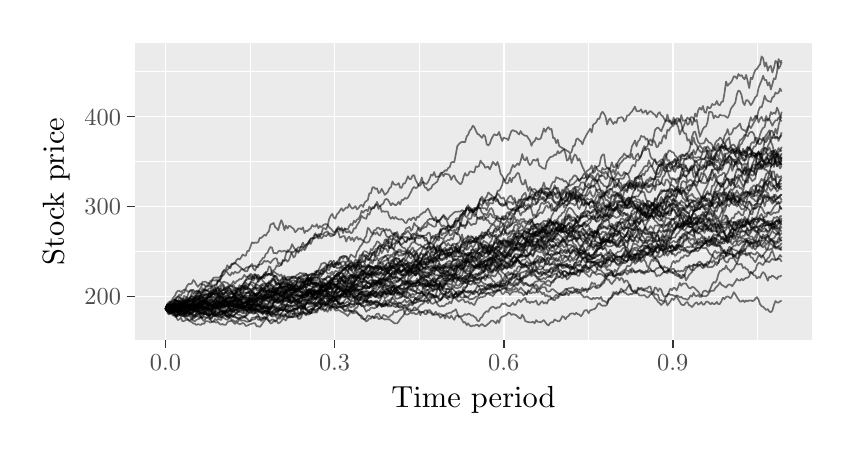
\begin{tikzpicture}[x=1pt,y=1pt]
\definecolor{fillColor}{RGB}{255,255,255}
\path[use as bounding box,fill=fillColor,fill opacity=0.00] (0,0) rectangle (289.08,144.54);
\begin{scope}
\path[clip] (  0.00,  0.00) rectangle (289.08,144.54);
\definecolor{drawColor}{RGB}{255,255,255}
\definecolor{fillColor}{RGB}{255,255,255}

\path[draw=drawColor,line width= 0.6pt,line join=round,line cap=round,fill=fillColor] (  0.00,  0.00) rectangle (289.08,144.54);
\end{scope}
\begin{scope}
\path[clip] ( 38.67, 31.53) rectangle (283.58,139.04);
\definecolor{fillColor}{gray}{0.92}

\path[fill=fillColor] ( 38.67, 31.53) rectangle (283.58,139.04);
\definecolor{drawColor}{RGB}{255,255,255}

\path[draw=drawColor,line width= 0.3pt,line join=round] ( 38.67, 63.63) --
	(283.58, 63.63);

\path[draw=drawColor,line width= 0.3pt,line join=round] ( 38.67, 96.14) --
	(283.58, 96.14);

\path[draw=drawColor,line width= 0.3pt,line join=round] ( 38.67,128.64) --
	(283.58,128.64);

\path[draw=drawColor,line width= 0.3pt,line join=round] ( 80.35, 31.53) --
	( 80.35,139.04);

\path[draw=drawColor,line width= 0.3pt,line join=round] (141.45, 31.53) --
	(141.45,139.04);

\path[draw=drawColor,line width= 0.3pt,line join=round] (202.56, 31.53) --
	(202.56,139.04);

\path[draw=drawColor,line width= 0.3pt,line join=round] (263.66, 31.53) --
	(263.66,139.04);

\path[draw=drawColor,line width= 0.6pt,line join=round] ( 38.67, 47.38) --
	(283.58, 47.38);

\path[draw=drawColor,line width= 0.6pt,line join=round] ( 38.67, 79.89) --
	(283.58, 79.89);

\path[draw=drawColor,line width= 0.6pt,line join=round] ( 38.67,112.39) --
	(283.58,112.39);

\path[draw=drawColor,line width= 0.6pt,line join=round] ( 49.80, 31.53) --
	( 49.80,139.04);

\path[draw=drawColor,line width= 0.6pt,line join=round] (110.90, 31.53) --
	(110.90,139.04);

\path[draw=drawColor,line width= 0.6pt,line join=round] (172.00, 31.53) --
	(172.00,139.04);

\path[draw=drawColor,line width= 0.6pt,line join=round] (233.11, 31.53) --
	(233.11,139.04);
\definecolor{drawColor}{RGB}{0,0,0}

\path[draw=drawColor,draw opacity=0.55,line width= 0.6pt,line join=round] ( 49.80, 42.93) --
	( 50.36, 43.47) --
	( 50.92, 43.63) --
	( 51.47, 44.54) --
	( 52.03, 45.11) --
	( 52.59, 45.02) --
	( 53.15, 44.16) --
	( 53.71, 43.83) --
	( 54.26, 44.69) --
	( 54.82, 45.37) --
	( 55.38, 44.38) --
	( 55.94, 44.67) --
	( 56.50, 44.71) --
	( 57.05, 46.00) --
	( 57.61, 46.13) --
	( 58.17, 46.28) --
	( 58.73, 46.08) --
	( 59.29, 46.33) --
	( 59.84, 46.17) --
	( 60.40, 45.17) --
	( 60.96, 45.77) --
	( 61.52, 45.87) --
	( 62.08, 45.35) --
	( 62.63, 45.85) --
	( 63.19, 45.67) --
	( 63.75, 45.79) --
	( 64.31, 46.05) --
	( 64.87, 45.04) --
	( 65.42, 44.54) --
	( 65.98, 43.70) --
	( 66.54, 43.72) --
	( 67.10, 43.69) --
	( 67.66, 43.95) --
	( 68.21, 44.19) --
	( 68.77, 43.63) --
	( 69.33, 44.05) --
	( 69.89, 43.71) --
	( 70.45, 44.47) --
	( 71.00, 44.05) --
	( 71.56, 44.94) --
	( 72.12, 45.43) --
	( 72.68, 44.90) --
	( 73.24, 44.56) --
	( 73.79, 43.89) --
	( 74.35, 45.00) --
	( 74.91, 44.21) --
	( 75.47, 44.94) --
	( 76.03, 44.03) --
	( 76.58, 43.57) --
	( 77.14, 43.03) --
	( 77.70, 43.24) --
	( 78.26, 43.95) --
	( 78.82, 44.15) --
	( 79.37, 44.29) --
	( 79.93, 46.74) --
	( 80.49, 46.95) --
	( 81.05, 45.90) --
	( 81.61, 44.57) --
	( 82.16, 44.56) --
	( 82.72, 44.40) --
	( 83.28, 46.90) --
	( 83.84, 46.40) --
	( 84.40, 45.99) --
	( 84.95, 46.31) --
	( 85.51, 46.52) --
	( 86.07, 47.00) --
	( 86.63, 46.70) --
	( 87.19, 46.47) --
	( 87.74, 45.83) --
	( 88.30, 46.36) --
	( 88.86, 45.71) --
	( 89.42, 45.47) --
	( 89.98, 45.18) --
	( 90.53, 46.26) --
	( 91.09, 45.64) --
	( 91.65, 44.48) --
	( 92.21, 45.76) --
	( 92.77, 47.26) --
	( 93.32, 46.97) --
	( 93.88, 46.71) --
	( 94.44, 45.36) --
	( 95.00, 45.80) --
	( 95.56, 45.47) --
	( 96.11, 45.59) --
	( 96.67, 45.55) --
	( 97.23, 45.45) --
	( 97.79, 45.10) --
	( 98.35, 45.01) --
	( 98.90, 44.69) --
	( 99.46, 44.85) --
	(100.02, 44.39) --
	(100.58, 44.89) --
	(101.14, 45.18) --
	(101.69, 44.98) --
	(102.25, 44.90) --
	(102.81, 44.88) --
	(103.37, 44.98) --
	(103.93, 45.76) --
	(104.48, 46.88) --
	(105.04, 47.07) --
	(105.60, 47.14) --
	(106.16, 48.07) --
	(106.72, 48.07) --
	(107.27, 47.66) --
	(107.83, 48.70) --
	(108.39, 47.12) --
	(108.95, 46.44) --
	(109.51, 46.33) --
	(110.06, 45.87) --
	(110.62, 46.01) --
	(111.18, 46.43) --
	(111.74, 47.48) --
	(112.30, 47.69) --
	(112.85, 47.30) --
	(113.41, 48.50) --
	(113.97, 48.55) --
	(114.53, 48.31) --
	(115.09, 48.43) --
	(115.65, 49.40) --
	(116.20, 49.87) --
	(116.76, 50.19) --
	(117.32, 50.03) --
	(117.88, 50.91) --
	(118.44, 51.60) --
	(118.99, 52.02) --
	(119.55, 51.49) --
	(120.11, 52.18) --
	(120.67, 51.79) --
	(121.23, 53.14) --
	(121.78, 54.09) --
	(122.34, 54.76) --
	(122.90, 55.26) --
	(123.46, 55.03) --
	(124.02, 55.74) --
	(124.57, 56.71) --
	(125.13, 57.22) --
	(125.69, 58.22) --
	(126.25, 57.56) --
	(126.81, 58.91) --
	(127.36, 59.79) --
	(127.92, 59.15) --
	(128.48, 60.06) --
	(129.04, 60.35) --
	(129.60, 60.49) --
	(130.15, 61.22) --
	(130.71, 58.90) --
	(131.27, 60.31) --
	(131.83, 60.47) --
	(132.39, 61.15) --
	(132.94, 61.25) --
	(133.50, 61.16) --
	(134.06, 61.10) --
	(134.62, 60.02) --
	(135.18, 60.59) --
	(135.73, 59.53) --
	(136.29, 59.17) --
	(136.85, 58.92) --
	(137.41, 57.01) --
	(137.97, 58.20) --
	(138.52, 56.88) --
	(139.08, 58.30) --
	(139.64, 58.92) --
	(140.20, 58.13) --
	(140.76, 58.69) --
	(141.31, 57.32) --
	(141.87, 58.57) --
	(142.43, 58.28) --
	(142.99, 57.50) --
	(143.55, 56.94) --
	(144.10, 57.89) --
	(144.66, 58.11) --
	(145.22, 57.96) --
	(145.78, 56.84) --
	(146.34, 57.73) --
	(146.89, 57.94) --
	(147.45, 57.61) --
	(148.01, 57.91) --
	(148.57, 58.03) --
	(149.13, 57.06) --
	(149.68, 56.82) --
	(150.24, 57.95) --
	(150.80, 57.64) --
	(151.36, 58.40) --
	(151.92, 58.46) --
	(152.47, 58.01) --
	(153.03, 59.25) --
	(153.59, 58.68) --
	(154.15, 59.10) --
	(154.71, 59.53) --
	(155.26, 58.26) --
	(155.82, 58.33) --
	(156.38, 57.35) --
	(156.94, 57.01) --
	(157.50, 57.59) --
	(158.05, 59.01) --
	(158.61, 59.76) --
	(159.17, 60.91) --
	(159.73, 59.96) --
	(160.29, 61.44) --
	(160.84, 61.04) --
	(161.40, 60.40) --
	(161.96, 61.15) --
	(162.52, 60.58) --
	(163.08, 60.86) --
	(163.63, 59.66) --
	(164.19, 59.93) --
	(164.75, 59.94) --
	(165.31, 58.69) --
	(165.87, 58.86) --
	(166.42, 58.43) --
	(166.98, 57.55) --
	(167.54, 55.52) --
	(168.10, 57.14) --
	(168.66, 57.79) --
	(169.21, 58.12) --
	(169.77, 57.24) --
	(170.33, 58.38) --
	(170.89, 59.40) --
	(171.45, 58.74) --
	(172.00, 58.32) --
	(172.56, 59.34) --
	(173.12, 59.25) --
	(173.68, 59.91) --
	(174.24, 60.35) --
	(174.79, 60.31) --
	(175.35, 59.67) --
	(175.91, 59.99) --
	(176.47, 59.59) --
	(177.03, 60.96) --
	(177.58, 60.17) --
	(178.14, 58.95) --
	(178.70, 59.42) --
	(179.26, 58.81) --
	(179.82, 58.08) --
	(180.37, 58.52) --
	(180.93, 58.59) --
	(181.49, 58.57) --
	(182.05, 58.89) --
	(182.61, 58.94) --
	(183.17, 60.80) --
	(183.72, 61.17) --
	(184.28, 62.18) --
	(184.84, 61.60) --
	(185.40, 61.75) --
	(185.96, 61.26) --
	(186.51, 60.79) --
	(187.07, 58.79) --
	(187.63, 59.01) --
	(188.19, 59.67) --
	(188.75, 61.07) --
	(189.30, 60.86) --
	(189.86, 60.94) --
	(190.42, 60.35) --
	(190.98, 61.30) --
	(191.54, 60.56) --
	(192.09, 61.53) --
	(192.65, 62.01) --
	(193.21, 60.19) --
	(193.77, 61.35) --
	(194.33, 62.14) --
	(194.88, 61.43) --
	(195.44, 60.78) --
	(196.00, 59.88) --
	(196.56, 60.90) --
	(197.12, 60.27) --
	(197.67, 60.82) --
	(198.23, 60.73) --
	(198.79, 61.41) --
	(199.35, 61.81) --
	(199.91, 62.20) --
	(200.46, 62.88) --
	(201.02, 62.93) --
	(201.58, 62.14) --
	(202.14, 61.01) --
	(202.70, 60.86) --
	(203.25, 60.70) --
	(203.81, 61.03) --
	(204.37, 62.15) --
	(204.93, 63.29) --
	(205.49, 63.65) --
	(206.04, 64.41) --
	(206.60, 65.05) --
	(207.16, 64.95) --
	(207.72, 64.54) --
	(208.28, 64.73) --
	(208.83, 64.95) --
	(209.39, 63.14) --
	(209.95, 62.85) --
	(210.51, 64.29) --
	(211.07, 63.33) --
	(211.62, 62.80) --
	(212.18, 61.84) --
	(212.74, 61.87) --
	(213.30, 61.60) --
	(213.86, 61.83) --
	(214.41, 61.66) --
	(214.97, 60.78) --
	(215.53, 60.58) --
	(216.09, 60.23) --
	(216.65, 59.95) --
	(217.20, 61.34) --
	(217.76, 61.19) --
	(218.32, 60.18) --
	(218.88, 61.26) --
	(219.44, 59.18) --
	(219.99, 59.72) --
	(220.55, 60.13) --
	(221.11, 60.35) --
	(221.67, 61.11) --
	(222.23, 61.68) --
	(222.78, 62.25) --
	(223.34, 63.11) --
	(223.90, 62.65) --
	(224.46, 63.33) --
	(225.02, 63.17) --
	(225.57, 63.67) --
	(226.13, 63.95) --
	(226.69, 64.60) --
	(227.25, 63.57) --
	(227.81, 62.42) --
	(228.36, 63.89) --
	(228.92, 64.52) --
	(229.48, 64.60) --
	(230.04, 64.01) --
	(230.60, 65.11) --
	(231.15, 64.29) --
	(231.71, 65.44) --
	(232.27, 65.07) --
	(232.83, 66.12) --
	(233.39, 65.13) --
	(233.94, 65.46) --
	(234.50, 66.11) --
	(235.06, 66.05) --
	(235.62, 65.92) --
	(236.18, 65.63) --
	(236.73, 65.26) --
	(237.29, 64.97) --
	(237.85, 64.91) --
	(238.41, 65.39) --
	(238.97, 65.15) --
	(239.52, 65.59) --
	(240.08, 65.18) --
	(240.64, 66.70) --
	(241.20, 66.25) --
	(241.76, 67.04) --
	(242.31, 66.10) --
	(242.87, 66.12) --
	(243.43, 65.60) --
	(243.99, 64.87) --
	(244.55, 64.89) --
	(245.10, 65.00) --
	(245.66, 64.25) --
	(246.22, 63.20) --
	(246.78, 62.53) --
	(247.34, 62.43) --
	(247.89, 61.55) --
	(248.45, 61.02) --
	(249.01, 61.13) --
	(249.57, 62.04) --
	(250.13, 62.51) --
	(250.68, 62.04) --
	(251.24, 62.28) --
	(251.80, 60.43) --
	(252.36, 59.84) --
	(252.92, 59.65) --
	(253.48, 60.97) --
	(254.03, 61.22) --
	(254.59, 61.18) --
	(255.15, 62.47) --
	(255.71, 61.86) --
	(256.27, 61.11) --
	(256.82, 61.34) --
	(257.38, 64.19) --
	(257.94, 64.12) --
	(258.50, 64.84) --
	(259.06, 65.87) --
	(259.61, 67.11) --
	(260.17, 67.60) --
	(260.73, 66.48) --
	(261.29, 66.56) --
	(261.85, 66.59) --
	(262.40, 66.47) --
	(262.96, 67.00) --
	(263.52, 67.16) --
	(264.08, 67.38) --
	(264.64, 67.60) --
	(265.19, 67.77) --
	(265.75, 69.84) --
	(266.31, 68.89) --
	(266.87, 69.66) --
	(267.43, 69.65) --
	(267.98, 67.69) --
	(268.54, 67.75) --
	(269.10, 68.34) --
	(269.66, 68.38) --
	(270.22, 69.32) --
	(270.77, 70.21) --
	(271.33, 70.37) --
	(271.89, 69.56) --
	(272.45, 70.46);

\path[draw=drawColor,draw opacity=0.55,line width= 0.6pt,line join=round] ( 49.80, 42.93) --
	( 50.36, 42.15) --
	( 50.92, 40.96) --
	( 51.47, 41.27) --
	( 52.03, 41.44) --
	( 52.59, 42.16) --
	( 53.15, 41.39) --
	( 53.71, 41.13) --
	( 54.26, 41.76) --
	( 54.82, 40.69) --
	( 55.38, 40.34) --
	( 55.94, 40.30) --
	( 56.50, 40.74) --
	( 57.05, 41.66) --
	( 57.61, 42.71) --
	( 58.17, 44.28) --
	( 58.73, 44.13) --
	( 59.29, 43.96) --
	( 59.84, 44.56) --
	( 60.40, 44.18) --
	( 60.96, 44.49) --
	( 61.52, 43.89) --
	( 62.08, 44.93) --
	( 62.63, 43.85) --
	( 63.19, 44.81) --
	( 63.75, 45.08) --
	( 64.31, 44.40) --
	( 64.87, 44.56) --
	( 65.42, 45.21) --
	( 65.98, 44.88) --
	( 66.54, 44.31) --
	( 67.10, 42.43) --
	( 67.66, 43.58) --
	( 68.21, 43.92) --
	( 68.77, 43.60) --
	( 69.33, 43.73) --
	( 69.89, 43.75) --
	( 70.45, 44.37) --
	( 71.00, 45.12) --
	( 71.56, 46.56) --
	( 72.12, 47.70) --
	( 72.68, 47.52) --
	( 73.24, 48.22) --
	( 73.79, 48.25) --
	( 74.35, 48.18) --
	( 74.91, 48.38) --
	( 75.47, 46.53) --
	( 76.03, 46.90) --
	( 76.58, 46.81) --
	( 77.14, 47.46) --
	( 77.70, 46.90) --
	( 78.26, 47.45) --
	( 78.82, 46.32) --
	( 79.37, 46.47) --
	( 79.93, 47.17) --
	( 80.49, 48.03) --
	( 81.05, 47.70) --
	( 81.61, 48.57) --
	( 82.16, 47.55) --
	( 82.72, 48.46) --
	( 83.28, 49.05) --
	( 83.84, 49.85) --
	( 84.40, 50.63) --
	( 84.95, 50.31) --
	( 85.51, 50.57) --
	( 86.07, 50.15) --
	( 86.63, 50.54) --
	( 87.19, 51.82) --
	( 87.74, 53.10) --
	( 88.30, 53.17) --
	( 88.86, 54.31) --
	( 89.42, 54.89) --
	( 89.98, 54.73) --
	( 90.53, 53.14) --
	( 91.09, 53.24) --
	( 91.65, 53.57) --
	( 92.21, 54.36) --
	( 92.77, 54.96) --
	( 93.32, 53.73) --
	( 93.88, 52.83) --
	( 94.44, 53.23) --
	( 95.00, 53.99) --
	( 95.56, 54.61) --
	( 96.11, 53.98) --
	( 96.67, 54.08) --
	( 97.23, 53.98) --
	( 97.79, 53.77) --
	( 98.35, 54.29) --
	( 98.90, 53.76) --
	( 99.46, 53.82) --
	(100.02, 52.94) --
	(100.58, 53.13) --
	(101.14, 54.21) --
	(101.69, 53.46) --
	(102.25, 52.72) --
	(102.81, 52.38) --
	(103.37, 51.96) --
	(103.93, 52.41) --
	(104.48, 50.79) --
	(105.04, 50.37) --
	(105.60, 50.94) --
	(106.16, 49.89) --
	(106.72, 49.63) --
	(107.27, 49.86) --
	(107.83, 50.05) --
	(108.39, 49.65) --
	(108.95, 49.85) --
	(109.51, 51.64) --
	(110.06, 51.88) --
	(110.62, 51.84) --
	(111.18, 50.88) --
	(111.74, 51.48) --
	(112.30, 52.56) --
	(112.85, 53.91) --
	(113.41, 53.52) --
	(113.97, 54.63) --
	(114.53, 54.93) --
	(115.09, 54.06) --
	(115.65, 53.86) --
	(116.20, 54.37) --
	(116.76, 54.80) --
	(117.32, 54.92) --
	(117.88, 55.66) --
	(118.44, 54.42) --
	(118.99, 53.58) --
	(119.55, 53.93) --
	(120.11, 53.85) --
	(120.67, 54.19) --
	(121.23, 53.53) --
	(121.78, 54.47) --
	(122.34, 54.64) --
	(122.90, 53.83) --
	(123.46, 55.01) --
	(124.02, 55.55) --
	(124.57, 54.30) --
	(125.13, 55.40) --
	(125.69, 56.21) --
	(126.25, 57.05) --
	(126.81, 56.93) --
	(127.36, 57.75) --
	(127.92, 57.08) --
	(128.48, 56.66) --
	(129.04, 57.41) --
	(129.60, 57.17) --
	(130.15, 57.22) --
	(130.71, 58.15) --
	(131.27, 59.08) --
	(131.83, 60.74) --
	(132.39, 59.85) --
	(132.94, 58.79) --
	(133.50, 58.08) --
	(134.06, 57.41) --
	(134.62, 56.41) --
	(135.18, 55.52) --
	(135.73, 55.04) --
	(136.29, 54.24) --
	(136.85, 55.54) --
	(137.41, 56.52) --
	(137.97, 57.99) --
	(138.52, 56.69) --
	(139.08, 56.84) --
	(139.64, 57.55) --
	(140.20, 58.05) --
	(140.76, 58.49) --
	(141.31, 57.65) --
	(141.87, 56.01) --
	(142.43, 56.32) --
	(142.99, 55.79) --
	(143.55, 54.83) --
	(144.10, 54.39) --
	(144.66, 54.41) --
	(145.22, 55.21) --
	(145.78, 55.36) --
	(146.34, 56.09) --
	(146.89, 55.61) --
	(147.45, 54.96) --
	(148.01, 55.29) --
	(148.57, 54.82) --
	(149.13, 55.63) --
	(149.68, 54.38) --
	(150.24, 55.49) --
	(150.80, 55.55) --
	(151.36, 56.91) --
	(151.92, 56.07) --
	(152.47, 55.14) --
	(153.03, 54.81) --
	(153.59, 54.30) --
	(154.15, 54.09) --
	(154.71, 54.01) --
	(155.26, 53.79) --
	(155.82, 54.54) --
	(156.38, 54.96) --
	(156.94, 54.91) --
	(157.50, 56.77) --
	(158.05, 55.89) --
	(158.61, 56.90) --
	(159.17, 56.53) --
	(159.73, 56.68) --
	(160.29, 56.12) --
	(160.84, 57.08) --
	(161.40, 56.92) --
	(161.96, 58.00) --
	(162.52, 58.79) --
	(163.08, 57.93) --
	(163.63, 58.12) --
	(164.19, 57.57) --
	(164.75, 57.85) --
	(165.31, 58.24) --
	(165.87, 58.63) --
	(166.42, 58.76) --
	(166.98, 58.28) --
	(167.54, 58.61) --
	(168.10, 59.55) --
	(168.66, 61.41) --
	(169.21, 61.64) --
	(169.77, 61.19) --
	(170.33, 60.68) --
	(170.89, 60.51) --
	(171.45, 60.39) --
	(172.00, 60.10) --
	(172.56, 61.62) --
	(173.12, 62.52) --
	(173.68, 62.29) --
	(174.24, 64.32) --
	(174.79, 65.55) --
	(175.35, 64.99) --
	(175.91, 64.88) --
	(176.47, 64.93) --
	(177.03, 64.69) --
	(177.58, 64.36) --
	(178.14, 65.23) --
	(178.70, 65.78) --
	(179.26, 66.76) --
	(179.82, 66.38) --
	(180.37, 68.45) --
	(180.93, 67.12) --
	(181.49, 66.86) --
	(182.05, 67.60) --
	(182.61, 66.20) --
	(183.17, 65.51) --
	(183.72, 66.67) --
	(184.28, 68.13) --
	(184.84, 67.14) --
	(185.40, 67.28) --
	(185.96, 68.74) --
	(186.51, 66.43) --
	(187.07, 66.22) --
	(187.63, 66.81) --
	(188.19, 67.71) --
	(188.75, 67.80) --
	(189.30, 67.25) --
	(189.86, 68.09) --
	(190.42, 68.65) --
	(190.98, 69.94) --
	(191.54, 70.49) --
	(192.09, 71.70) --
	(192.65, 71.25) --
	(193.21, 71.93) --
	(193.77, 72.38) --
	(194.33, 72.78) --
	(194.88, 70.42) --
	(195.44, 70.49) --
	(196.00, 70.24) --
	(196.56, 68.64) --
	(197.12, 67.98) --
	(197.67, 68.37) --
	(198.23, 68.78) --
	(198.79, 68.40) --
	(199.35, 68.65) --
	(199.91, 68.14) --
	(200.46, 68.48) --
	(201.02, 68.02) --
	(201.58, 67.55) --
	(202.14, 67.65) --
	(202.70, 66.50) --
	(203.25, 66.29) --
	(203.81, 65.65) --
	(204.37, 65.16) --
	(204.93, 65.72) --
	(205.49, 65.61) --
	(206.04, 65.68) --
	(206.60, 65.05) --
	(207.16, 66.67) --
	(207.72, 66.62) --
	(208.28, 67.12) --
	(208.83, 67.37) --
	(209.39, 68.02) --
	(209.95, 67.06) --
	(210.51, 67.65) --
	(211.07, 67.28) --
	(211.62, 67.10) --
	(212.18, 66.38) --
	(212.74, 65.72) --
	(213.30, 65.89) --
	(213.86, 66.64) --
	(214.41, 68.08) --
	(214.97, 68.05) --
	(215.53, 68.67) --
	(216.09, 69.41) --
	(216.65, 70.50) --
	(217.20, 69.79) --
	(217.76, 68.71) --
	(218.32, 67.34) --
	(218.88, 67.36) --
	(219.44, 68.57) --
	(219.99, 69.48) --
	(220.55, 68.47) --
	(221.11, 68.21) --
	(221.67, 67.76) --
	(222.23, 66.79) --
	(222.78, 66.78) --
	(223.34, 67.67) --
	(223.90, 67.68) --
	(224.46, 67.50) --
	(225.02, 67.67) --
	(225.57, 67.31) --
	(226.13, 68.02) --
	(226.69, 67.67) --
	(227.25, 69.46) --
	(227.81, 71.09) --
	(228.36, 71.27) --
	(228.92, 70.48) --
	(229.48, 71.16) --
	(230.04, 70.95) --
	(230.60, 70.93) --
	(231.15, 71.75) --
	(231.71, 73.59) --
	(232.27, 74.76) --
	(232.83, 75.58) --
	(233.39, 75.32) --
	(233.94, 73.79) --
	(234.50, 72.62) --
	(235.06, 73.36) --
	(235.62, 73.89) --
	(236.18, 73.05) --
	(236.73, 74.37) --
	(237.29, 74.06) --
	(237.85, 74.50) --
	(238.41, 73.56) --
	(238.97, 74.03) --
	(239.52, 73.72) --
	(240.08, 74.60) --
	(240.64, 74.93) --
	(241.20, 76.04) --
	(241.76, 75.55) --
	(242.31, 76.56) --
	(242.87, 76.58) --
	(243.43, 76.99) --
	(243.99, 76.73) --
	(244.55, 76.15) --
	(245.10, 77.00) --
	(245.66, 77.04) --
	(246.22, 77.00) --
	(246.78, 77.46) --
	(247.34, 76.43) --
	(247.89, 76.78) --
	(248.45, 76.08) --
	(249.01, 75.53) --
	(249.57, 75.41) --
	(250.13, 74.35) --
	(250.68, 74.98) --
	(251.24, 76.89) --
	(251.80, 76.60) --
	(252.36, 76.70) --
	(252.92, 75.99) --
	(253.48, 74.17) --
	(254.03, 73.49) --
	(254.59, 73.07) --
	(255.15, 74.09) --
	(255.71, 74.21) --
	(256.27, 73.08) --
	(256.82, 72.34) --
	(257.38, 72.42) --
	(257.94, 72.80) --
	(258.50, 72.49) --
	(259.06, 72.72) --
	(259.61, 74.91) --
	(260.17, 75.39) --
	(260.73, 74.80) --
	(261.29, 74.76) --
	(261.85, 74.84) --
	(262.40, 75.47) --
	(262.96, 75.30) --
	(263.52, 75.26) --
	(264.08, 75.59) --
	(264.64, 75.78) --
	(265.19, 75.18) --
	(265.75, 75.34) --
	(266.31, 76.47) --
	(266.87, 76.17) --
	(267.43, 77.44) --
	(267.98, 77.78) --
	(268.54, 77.83) --
	(269.10, 78.78) --
	(269.66, 79.79) --
	(270.22, 80.44) --
	(270.77, 81.04) --
	(271.33, 81.28) --
	(271.89, 81.07) --
	(272.45, 81.96);

\path[draw=drawColor,draw opacity=0.55,line width= 0.6pt,line join=round] ( 49.80, 42.93) --
	( 50.36, 42.03) --
	( 50.92, 41.19) --
	( 51.47, 41.76) --
	( 52.03, 41.56) --
	( 52.59, 41.84) --
	( 53.15, 41.80) --
	( 53.71, 42.12) --
	( 54.26, 42.80) --
	( 54.82, 43.68) --
	( 55.38, 43.13) --
	( 55.94, 43.31) --
	( 56.50, 43.15) --
	( 57.05, 43.40) --
	( 57.61, 42.96) --
	( 58.17, 42.44) --
	( 58.73, 42.32) --
	( 59.29, 43.32) --
	( 59.84, 43.46) --
	( 60.40, 44.19) --
	( 60.96, 43.44) --
	( 61.52, 44.52) --
	( 62.08, 45.36) --
	( 62.63, 45.60) --
	( 63.19, 45.43) --
	( 63.75, 45.92) --
	( 64.31, 46.00) --
	( 64.87, 46.92) --
	( 65.42, 47.14) --
	( 65.98, 47.41) --
	( 66.54, 48.77) --
	( 67.10, 48.33) --
	( 67.66, 48.39) --
	( 68.21, 48.90) --
	( 68.77, 48.28) --
	( 69.33, 48.92) --
	( 69.89, 49.10) --
	( 70.45, 48.43) --
	( 71.00, 48.20) --
	( 71.56, 49.03) --
	( 72.12, 48.27) --
	( 72.68, 47.55) --
	( 73.24, 46.99) --
	( 73.79, 47.23) --
	( 74.35, 47.27) --
	( 74.91, 47.91) --
	( 75.47, 49.05) --
	( 76.03, 48.51) --
	( 76.58, 48.04) --
	( 77.14, 48.93) --
	( 77.70, 49.19) --
	( 78.26, 50.72) --
	( 78.82, 50.31) --
	( 79.37, 50.55) --
	( 79.93, 50.40) --
	( 80.49, 50.03) --
	( 81.05, 50.06) --
	( 81.61, 50.26) --
	( 82.16, 50.54) --
	( 82.72, 49.70) --
	( 83.28, 49.51) --
	( 83.84, 49.53) --
	( 84.40, 48.12) --
	( 84.95, 49.00) --
	( 85.51, 49.80) --
	( 86.07, 51.02) --
	( 86.63, 51.38) --
	( 87.19, 50.02) --
	( 87.74, 50.65) --
	( 88.30, 49.59) --
	( 88.86, 51.17) --
	( 89.42, 50.57) --
	( 89.98, 50.42) --
	( 90.53, 50.31) --
	( 91.09, 51.09) --
	( 91.65, 50.78) --
	( 92.21, 50.92) --
	( 92.77, 50.93) --
	( 93.32, 51.08) --
	( 93.88, 50.98) --
	( 94.44, 50.21) --
	( 95.00, 49.62) --
	( 95.56, 49.71) --
	( 96.11, 50.97) --
	( 96.67, 50.93) --
	( 97.23, 52.31) --
	( 97.79, 53.08) --
	( 98.35, 52.94) --
	( 98.90, 52.46) --
	( 99.46, 52.42) --
	(100.02, 52.43) --
	(100.58, 53.02) --
	(101.14, 53.22) --
	(101.69, 52.85) --
	(102.25, 53.57) --
	(102.81, 52.07) --
	(103.37, 51.79) --
	(103.93, 52.39) --
	(104.48, 52.01) --
	(105.04, 51.37) --
	(105.60, 51.36) --
	(106.16, 51.00) --
	(106.72, 50.85) --
	(107.27, 50.98) --
	(107.83, 49.91) --
	(108.39, 50.12) --
	(108.95, 51.63) --
	(109.51, 51.47) --
	(110.06, 52.78) --
	(110.62, 54.34) --
	(111.18, 54.51) --
	(111.74, 54.76) --
	(112.30, 55.18) --
	(112.85, 54.53) --
	(113.41, 54.03) --
	(113.97, 54.18) --
	(114.53, 54.64) --
	(115.09, 55.12) --
	(115.65, 55.84) --
	(116.20, 57.69) --
	(116.76, 57.81) --
	(117.32, 58.75) --
	(117.88, 58.41) --
	(118.44, 58.42) --
	(118.99, 58.21) --
	(119.55, 60.62) --
	(120.11, 62.37) --
	(120.67, 62.17) --
	(121.23, 63.48) --
	(121.78, 63.78) --
	(122.34, 63.61) --
	(122.90, 63.13) --
	(123.46, 62.69) --
	(124.02, 63.15) --
	(124.57, 62.31) --
	(125.13, 62.51) --
	(125.69, 64.53) --
	(126.25, 64.77) --
	(126.81, 65.31) --
	(127.36, 65.90) --
	(127.92, 65.62) --
	(128.48, 66.07) --
	(129.04, 66.28) --
	(129.60, 67.56) --
	(130.15, 68.09) --
	(130.71, 66.70) --
	(131.27, 67.07) --
	(131.83, 65.06) --
	(132.39, 64.16) --
	(132.94, 63.90) --
	(133.50, 63.19) --
	(134.06, 62.04) --
	(134.62, 62.37) --
	(135.18, 62.13) --
	(135.73, 62.38) --
	(136.29, 63.09) --
	(136.85, 62.99) --
	(137.41, 62.94) --
	(137.97, 61.69) --
	(138.52, 61.17) --
	(139.08, 62.26) --
	(139.64, 61.53) --
	(140.20, 62.91) --
	(140.76, 64.06) --
	(141.31, 64.47) --
	(141.87, 65.03) --
	(142.43, 65.49) --
	(142.99, 65.39) --
	(143.55, 64.92) --
	(144.10, 64.71) --
	(144.66, 65.52) --
	(145.22, 66.61) --
	(145.78, 68.38) --
	(146.34, 69.30) --
	(146.89, 69.15) --
	(147.45, 69.73) --
	(148.01, 69.70) --
	(148.57, 70.24) --
	(149.13, 71.14) --
	(149.68, 71.77) --
	(150.24, 71.95) --
	(150.80, 71.70) --
	(151.36, 72.46) --
	(151.92, 73.04) --
	(152.47, 72.70) --
	(153.03, 72.55) --
	(153.59, 72.61) --
	(154.15, 74.28) --
	(154.71, 74.89) --
	(155.26, 74.67) --
	(155.82, 74.81) --
	(156.38, 75.21) --
	(156.94, 76.70) --
	(157.50, 78.08) --
	(158.05, 78.36) --
	(158.61, 78.68) --
	(159.17, 78.91) --
	(159.73, 78.32) --
	(160.29, 79.24) --
	(160.84, 77.86) --
	(161.40, 78.85) --
	(161.96, 79.47) --
	(162.52, 79.19) --
	(163.08, 80.89) --
	(163.63, 80.78) --
	(164.19, 80.09) --
	(164.75, 81.54) --
	(165.31, 82.23) --
	(165.87, 80.46) --
	(166.42, 81.38) --
	(166.98, 82.75) --
	(167.54, 82.71) --
	(168.10, 82.93) --
	(168.66, 82.76) --
	(169.21, 83.49) --
	(169.77, 84.65) --
	(170.33, 84.01) --
	(170.89, 83.04) --
	(171.45, 82.81) --
	(172.00, 83.18) --
	(172.56, 81.65) --
	(173.12, 80.26) --
	(173.68, 79.12) --
	(174.24, 78.92) --
	(174.79, 78.90) --
	(175.35, 78.51) --
	(175.91, 78.45) --
	(176.47, 78.89) --
	(177.03, 79.45) --
	(177.58, 79.41) --
	(178.14, 79.54) --
	(178.70, 81.07) --
	(179.26, 79.62) --
	(179.82, 78.66) --
	(180.37, 78.99) --
	(180.93, 79.99) --
	(181.49, 79.95) --
	(182.05, 79.70) --
	(182.61, 80.88) --
	(183.17, 80.56) --
	(183.72, 80.76) --
	(184.28, 81.94) --
	(184.84, 83.14) --
	(185.40, 84.35) --
	(185.96, 86.09) --
	(186.51, 86.42) --
	(187.07, 86.15) --
	(187.63, 86.27) --
	(188.19, 86.22) --
	(188.75, 85.09) --
	(189.30, 84.24) --
	(189.86, 85.23) --
	(190.42, 84.53) --
	(190.98, 84.20) --
	(191.54, 85.13) --
	(192.09, 85.11) --
	(192.65, 83.73) --
	(193.21, 84.71) --
	(193.77, 85.54) --
	(194.33, 85.33) --
	(194.88, 87.05) --
	(195.44, 85.66) --
	(196.00, 84.42) --
	(196.56, 83.52) --
	(197.12, 83.90) --
	(197.67, 84.29) --
	(198.23, 82.69) --
	(198.79, 82.29) --
	(199.35, 83.21) --
	(199.91, 83.72) --
	(200.46, 84.63) --
	(201.02, 85.80) --
	(201.58, 86.63) --
	(202.14, 87.09) --
	(202.70, 86.68) --
	(203.25, 86.37) --
	(203.81, 87.27) --
	(204.37, 86.96) --
	(204.93, 88.03) --
	(205.49, 88.24) --
	(206.04, 89.57) --
	(206.60, 89.71) --
	(207.16, 88.53) --
	(207.72, 88.14) --
	(208.28, 87.33) --
	(208.83, 87.23) --
	(209.39, 86.82) --
	(209.95, 87.26) --
	(210.51, 87.53) --
	(211.07, 88.89) --
	(211.62, 90.02) --
	(212.18, 89.46) --
	(212.74, 89.81) --
	(213.30, 89.92) --
	(213.86, 88.58) --
	(214.41, 88.26) --
	(214.97, 86.96) --
	(215.53, 86.79) --
	(216.09, 87.62) --
	(216.65, 88.48) --
	(217.20, 89.25) --
	(217.76, 86.97) --
	(218.32, 86.12) --
	(218.88, 87.59) --
	(219.44, 87.35) --
	(219.99, 90.02) --
	(220.55, 90.18) --
	(221.11, 91.09) --
	(221.67, 90.78) --
	(222.23, 91.84) --
	(222.78, 91.24) --
	(223.34, 92.72) --
	(223.90, 92.70) --
	(224.46, 94.03) --
	(225.02, 94.51) --
	(225.57, 94.35) --
	(226.13, 95.95) --
	(226.69, 97.06) --
	(227.25, 95.16) --
	(227.81, 94.98) --
	(228.36, 94.60) --
	(228.92, 96.09) --
	(229.48, 95.40) --
	(230.04, 94.51) --
	(230.60, 93.77) --
	(231.15, 94.81) --
	(231.71, 95.69) --
	(232.27, 94.95) --
	(232.83, 95.19) --
	(233.39, 96.51) --
	(233.94, 97.17) --
	(234.50, 94.94) --
	(235.06, 93.68) --
	(235.62, 95.12) --
	(236.18, 95.13) --
	(236.73, 93.29) --
	(237.29, 95.18) --
	(237.85, 94.08) --
	(238.41, 93.34) --
	(238.97, 93.25) --
	(239.52, 93.76) --
	(240.08, 93.08) --
	(240.64, 94.35) --
	(241.20, 91.98) --
	(241.76, 91.15) --
	(242.31, 91.82) --
	(242.87, 95.03) --
	(243.43, 96.67) --
	(243.99, 97.23) --
	(244.55, 97.06) --
	(245.10, 97.90) --
	(245.66, 97.31) --
	(246.22, 97.73) --
	(246.78, 97.03) --
	(247.34,100.44) --
	(247.89,101.40) --
	(248.45,100.32) --
	(249.01,100.47) --
	(249.57,101.20) --
	(250.13,101.33) --
	(250.68,101.53) --
	(251.24,101.13) --
	(251.80,101.96) --
	(252.36,103.63) --
	(252.92,104.22) --
	(253.48,104.88) --
	(254.03,101.22) --
	(254.59,100.95) --
	(255.15, 99.34) --
	(255.71, 98.16) --
	(256.27,100.79) --
	(256.82,102.23) --
	(257.38,103.91) --
	(257.94,104.20) --
	(258.50,104.78) --
	(259.06,105.84) --
	(259.61,105.66) --
	(260.17,105.25) --
	(260.73,106.49) --
	(261.29,106.82) --
	(261.85,106.86) --
	(262.40,106.15) --
	(262.96,104.29) --
	(263.52,102.58) --
	(264.08,104.01) --
	(264.64,105.91) --
	(265.19,107.44) --
	(265.75,108.31) --
	(266.31,108.63) --
	(266.87,111.49) --
	(267.43,111.23) --
	(267.98,111.76) --
	(268.54,114.05) --
	(269.10,113.29) --
	(269.66,113.87) --
	(270.22,113.43) --
	(270.77,115.66) --
	(271.33,114.32) --
	(271.89,112.23) --
	(272.45,111.82);

\path[draw=drawColor,draw opacity=0.55,line width= 0.6pt,line join=round] ( 49.80, 42.93) --
	( 50.36, 42.54) --
	( 50.92, 42.15) --
	( 51.47, 43.15) --
	( 52.03, 43.03) --
	( 52.59, 43.30) --
	( 53.15, 44.10) --
	( 53.71, 43.06) --
	( 54.26, 43.00) --
	( 54.82, 43.11) --
	( 55.38, 42.73) --
	( 55.94, 43.25) --
	( 56.50, 43.80) --
	( 57.05, 43.54) --
	( 57.61, 43.11) --
	( 58.17, 42.65) --
	( 58.73, 42.72) --
	( 59.29, 42.90) --
	( 59.84, 42.96) --
	( 60.40, 42.92) --
	( 60.96, 43.40) --
	( 61.52, 43.04) --
	( 62.08, 42.12) --
	( 62.63, 41.24) --
	( 63.19, 41.64) --
	( 63.75, 41.30) --
	( 64.31, 40.93) --
	( 64.87, 40.98) --
	( 65.42, 40.65) --
	( 65.98, 40.27) --
	( 66.54, 41.70) --
	( 67.10, 41.30) --
	( 67.66, 40.56) --
	( 68.21, 40.69) --
	( 68.77, 40.79) --
	( 69.33, 41.16) --
	( 69.89, 40.82) --
	( 70.45, 41.59) --
	( 71.00, 42.34) --
	( 71.56, 41.90) --
	( 72.12, 41.60) --
	( 72.68, 42.34) --
	( 73.24, 42.67) --
	( 73.79, 44.06) --
	( 74.35, 44.04) --
	( 74.91, 43.39) --
	( 75.47, 43.51) --
	( 76.03, 43.75) --
	( 76.58, 43.30) --
	( 77.14, 44.30) --
	( 77.70, 43.64) --
	( 78.26, 43.21) --
	( 78.82, 42.11) --
	( 79.37, 42.67) --
	( 79.93, 43.01) --
	( 80.49, 42.61) --
	( 81.05, 44.55) --
	( 81.61, 44.79) --
	( 82.16, 45.02) --
	( 82.72, 46.29) --
	( 83.28, 46.91) --
	( 83.84, 46.60) --
	( 84.40, 46.96) --
	( 84.95, 46.13) --
	( 85.51, 46.03) --
	( 86.07, 46.05) --
	( 86.63, 45.72) --
	( 87.19, 45.67) --
	( 87.74, 46.20) --
	( 88.30, 46.96) --
	( 88.86, 46.97) --
	( 89.42, 47.18) --
	( 89.98, 47.71) --
	( 90.53, 46.65) --
	( 91.09, 47.34) --
	( 91.65, 47.65) --
	( 92.21, 48.00) --
	( 92.77, 48.72) --
	( 93.32, 49.52) --
	( 93.88, 50.02) --
	( 94.44, 50.10) --
	( 95.00, 49.68) --
	( 95.56, 49.82) --
	( 96.11, 50.94) --
	( 96.67, 51.04) --
	( 97.23, 51.96) --
	( 97.79, 51.97) --
	( 98.35, 52.23) --
	( 98.90, 52.52) --
	( 99.46, 52.87) --
	(100.02, 51.47) --
	(100.58, 52.24) --
	(101.14, 51.57) --
	(101.69, 51.34) --
	(102.25, 51.87) --
	(102.81, 52.40) --
	(103.37, 52.06) --
	(103.93, 51.02) --
	(104.48, 51.20) --
	(105.04, 51.53) --
	(105.60, 51.55) --
	(106.16, 51.12) --
	(106.72, 50.80) --
	(107.27, 50.27) --
	(107.83, 50.00) --
	(108.39, 49.91) --
	(108.95, 50.14) --
	(109.51, 50.23) --
	(110.06, 51.54) --
	(110.62, 51.74) --
	(111.18, 50.86) --
	(111.74, 50.07) --
	(112.30, 50.52) --
	(112.85, 50.10) --
	(113.41, 50.62) --
	(113.97, 50.27) --
	(114.53, 51.20) --
	(115.09, 50.82) --
	(115.65, 50.46) --
	(116.20, 50.91) --
	(116.76, 52.37) --
	(117.32, 51.50) --
	(117.88, 51.27) --
	(118.44, 51.56) --
	(118.99, 51.87) --
	(119.55, 52.93) --
	(120.11, 53.47) --
	(120.67, 52.22) --
	(121.23, 51.15) --
	(121.78, 51.29) --
	(122.34, 52.26) --
	(122.90, 52.21) --
	(123.46, 51.92) --
	(124.02, 51.51) --
	(124.57, 51.01) --
	(125.13, 51.36) --
	(125.69, 52.17) --
	(126.25, 52.38) --
	(126.81, 53.08) --
	(127.36, 52.53) --
	(127.92, 51.22) --
	(128.48, 51.20) --
	(129.04, 51.74) --
	(129.60, 51.20) --
	(130.15, 51.19) --
	(130.71, 51.06) --
	(131.27, 51.57) --
	(131.83, 52.22) --
	(132.39, 52.08) --
	(132.94, 52.48) --
	(133.50, 52.96) --
	(134.06, 53.20) --
	(134.62, 53.69) --
	(135.18, 54.08) --
	(135.73, 54.26) --
	(136.29, 53.57) --
	(136.85, 52.46) --
	(137.41, 53.07) --
	(137.97, 53.33) --
	(138.52, 54.14) --
	(139.08, 54.82) --
	(139.64, 55.05) --
	(140.20, 55.84) --
	(140.76, 55.72) --
	(141.31, 56.64) --
	(141.87, 58.18) --
	(142.43, 59.51) --
	(142.99, 59.41) --
	(143.55, 61.35) --
	(144.10, 60.70) --
	(144.66, 61.41) --
	(145.22, 61.97) --
	(145.78, 63.29) --
	(146.34, 63.85) --
	(146.89, 64.51) --
	(147.45, 64.10) --
	(148.01, 65.93) --
	(148.57, 65.61) --
	(149.13, 65.70) --
	(149.68, 64.01) --
	(150.24, 63.48) --
	(150.80, 62.74) --
	(151.36, 63.01) --
	(151.92, 63.10) --
	(152.47, 62.16) --
	(153.03, 62.73) --
	(153.59, 64.20) --
	(154.15, 63.80) --
	(154.71, 65.63) --
	(155.26, 66.67) --
	(155.82, 66.81) --
	(156.38, 68.08) --
	(156.94, 69.83) --
	(157.50, 67.46) --
	(158.05, 66.49) --
	(158.61, 67.98) --
	(159.17, 68.97) --
	(159.73, 67.89) --
	(160.29, 68.70) --
	(160.84, 68.99) --
	(161.40, 67.77) --
	(161.96, 67.04) --
	(162.52, 68.57) --
	(163.08, 68.04) --
	(163.63, 67.57) --
	(164.19, 69.63) --
	(164.75, 68.58) --
	(165.31, 69.44) --
	(165.87, 69.84) --
	(166.42, 69.54) --
	(166.98, 68.65) --
	(167.54, 69.55) --
	(168.10, 70.03) --
	(168.66, 71.29) --
	(169.21, 70.71) --
	(169.77, 71.60) --
	(170.33, 71.67) --
	(170.89, 70.26) --
	(171.45, 70.23) --
	(172.00, 69.60) --
	(172.56, 70.87) --
	(173.12, 72.11) --
	(173.68, 73.51) --
	(174.24, 72.72) --
	(174.79, 73.27) --
	(175.35, 74.67) --
	(175.91, 76.19) --
	(176.47, 74.96) --
	(177.03, 75.16) --
	(177.58, 74.30) --
	(178.14, 75.36) --
	(178.70, 75.23) --
	(179.26, 75.46) --
	(179.82, 74.57) --
	(180.37, 74.54) --
	(180.93, 74.21) --
	(181.49, 75.33) --
	(182.05, 74.81) --
	(182.61, 73.49) --
	(183.17, 73.29) --
	(183.72, 73.40) --
	(184.28, 73.70) --
	(184.84, 72.61) --
	(185.40, 73.63) --
	(185.96, 72.16) --
	(186.51, 71.94) --
	(187.07, 72.50) --
	(187.63, 72.99) --
	(188.19, 71.96) --
	(188.75, 72.98) --
	(189.30, 73.74) --
	(189.86, 74.05) --
	(190.42, 73.67) --
	(190.98, 74.34) --
	(191.54, 73.92) --
	(192.09, 73.42) --
	(192.65, 72.91) --
	(193.21, 73.50) --
	(193.77, 73.56) --
	(194.33, 76.15) --
	(194.88, 76.35) --
	(195.44, 77.12) --
	(196.00, 76.76) --
	(196.56, 75.85) --
	(197.12, 75.97) --
	(197.67, 75.94) --
	(198.23, 74.54) --
	(198.79, 74.04) --
	(199.35, 72.82) --
	(199.91, 72.86) --
	(200.46, 72.69) --
	(201.02, 71.26) --
	(201.58, 70.40) --
	(202.14, 70.44) --
	(202.70, 71.71) --
	(203.25, 72.04) --
	(203.81, 71.63) --
	(204.37, 70.53) --
	(204.93, 71.04) --
	(205.49, 70.26) --
	(206.04, 71.28) --
	(206.60, 68.66) --
	(207.16, 66.80) --
	(207.72, 64.30) --
	(208.28, 64.88) --
	(208.83, 66.35) --
	(209.39, 67.52) --
	(209.95, 67.45) --
	(210.51, 66.58) --
	(211.07, 67.31) --
	(211.62, 66.59) --
	(212.18, 67.02) --
	(212.74, 66.74) --
	(213.30, 66.42) --
	(213.86, 67.42) --
	(214.41, 67.66) --
	(214.97, 67.66) --
	(215.53, 66.72) --
	(216.09, 64.85) --
	(216.65, 64.92) --
	(217.20, 64.17) --
	(217.76, 63.68) --
	(218.32, 65.24) --
	(218.88, 66.73) --
	(219.44, 66.30) --
	(219.99, 66.33) --
	(220.55, 65.59) --
	(221.11, 65.48) --
	(221.67, 65.41) --
	(222.23, 66.31) --
	(222.78, 67.09) --
	(223.34, 66.74) --
	(223.90, 66.70) --
	(224.46, 65.05) --
	(225.02, 64.75) --
	(225.57, 64.44) --
	(226.13, 65.49) --
	(226.69, 65.57) --
	(227.25, 64.62) --
	(227.81, 65.90) --
	(228.36, 64.80) --
	(228.92, 64.16) --
	(229.48, 63.80) --
	(230.04, 62.23) --
	(230.60, 63.32) --
	(231.15, 63.72) --
	(231.71, 63.78) --
	(232.27, 64.02) --
	(232.83, 62.63) --
	(233.39, 62.88) --
	(233.94, 62.05) --
	(234.50, 62.61) --
	(235.06, 63.47) --
	(235.62, 63.17) --
	(236.18, 64.12) --
	(236.73, 64.02) --
	(237.29, 64.80) --
	(237.85, 63.90) --
	(238.41, 64.09) --
	(238.97, 63.53) --
	(239.52, 63.78) --
	(240.08, 63.97) --
	(240.64, 64.25) --
	(241.20, 64.52) --
	(241.76, 63.87) --
	(242.31, 63.85) --
	(242.87, 64.52) --
	(243.43, 65.67) --
	(243.99, 65.68) --
	(244.55, 67.46) --
	(245.10, 66.76) --
	(245.66, 65.40) --
	(246.22, 65.56) --
	(246.78, 66.74) --
	(247.34, 66.15) --
	(247.89, 66.97) --
	(248.45, 66.68) --
	(249.01, 69.03) --
	(249.57, 69.90) --
	(250.13, 69.22) --
	(250.68, 68.09) --
	(251.24, 68.32) --
	(251.80, 68.02) --
	(252.36, 67.93) --
	(252.92, 68.86) --
	(253.48, 70.07) --
	(254.03, 71.03) --
	(254.59, 72.03) --
	(255.15, 74.14) --
	(255.71, 74.39) --
	(256.27, 73.83) --
	(256.82, 74.40) --
	(257.38, 74.57) --
	(257.94, 75.40) --
	(258.50, 74.74) --
	(259.06, 75.28) --
	(259.61, 74.20) --
	(260.17, 75.04) --
	(260.73, 76.83) --
	(261.29, 78.23) --
	(261.85, 79.12) --
	(262.40, 79.31) --
	(262.96, 79.10) --
	(263.52, 80.23) --
	(264.08, 81.03) --
	(264.64, 80.66) --
	(265.19, 81.14) --
	(265.75, 83.36) --
	(266.31, 83.16) --
	(266.87, 82.50) --
	(267.43, 83.69) --
	(267.98, 82.54) --
	(268.54, 81.85) --
	(269.10, 80.88) --
	(269.66, 81.88) --
	(270.22, 82.50) --
	(270.77, 82.65) --
	(271.33, 83.47) --
	(271.89, 83.78) --
	(272.45, 84.38);

\path[draw=drawColor,draw opacity=0.55,line width= 0.6pt,line join=round] ( 49.80, 42.93) --
	( 50.36, 43.65) --
	( 50.92, 42.70) --
	( 51.47, 43.08) --
	( 52.03, 42.47) --
	( 52.59, 42.77) --
	( 53.15, 42.58) --
	( 53.71, 42.04) --
	( 54.26, 43.01) --
	( 54.82, 43.09) --
	( 55.38, 42.23) --
	( 55.94, 41.48) --
	( 56.50, 41.56) --
	( 57.05, 41.09) --
	( 57.61, 42.03) --
	( 58.17, 42.84) --
	( 58.73, 43.77) --
	( 59.29, 43.95) --
	( 59.84, 44.53) --
	( 60.40, 44.22) --
	( 60.96, 45.30) --
	( 61.52, 44.91) --
	( 62.08, 44.07) --
	( 62.63, 44.32) --
	( 63.19, 45.26) --
	( 63.75, 44.80) --
	( 64.31, 45.84) --
	( 64.87, 45.86) --
	( 65.42, 45.36) --
	( 65.98, 44.74) --
	( 66.54, 44.94) --
	( 67.10, 44.80) --
	( 67.66, 45.72) --
	( 68.21, 45.72) --
	( 68.77, 45.84) --
	( 69.33, 46.41) --
	( 69.89, 46.52) --
	( 70.45, 46.75) --
	( 71.00, 46.48) --
	( 71.56, 46.57) --
	( 72.12, 46.69) --
	( 72.68, 45.58) --
	( 73.24, 45.85) --
	( 73.79, 45.76) --
	( 74.35, 45.52) --
	( 74.91, 46.43) --
	( 75.47, 47.22) --
	( 76.03, 47.46) --
	( 76.58, 47.45) --
	( 77.14, 47.23) --
	( 77.70, 48.25) --
	( 78.26, 48.92) --
	( 78.82, 48.74) --
	( 79.37, 48.54) --
	( 79.93, 48.87) --
	( 80.49, 47.81) --
	( 81.05, 47.34) --
	( 81.61, 48.06) --
	( 82.16, 48.20) --
	( 82.72, 47.88) --
	( 83.28, 48.00) --
	( 83.84, 48.36) --
	( 84.40, 48.31) --
	( 84.95, 47.52) --
	( 85.51, 47.76) --
	( 86.07, 48.14) --
	( 86.63, 49.60) --
	( 87.19, 48.94) --
	( 87.74, 48.77) --
	( 88.30, 48.99) --
	( 88.86, 49.64) --
	( 89.42, 48.49) --
	( 89.98, 48.83) --
	( 90.53, 48.53) --
	( 91.09, 48.64) --
	( 91.65, 49.16) --
	( 92.21, 48.62) --
	( 92.77, 47.43) --
	( 93.32, 48.19) --
	( 93.88, 48.00) --
	( 94.44, 47.59) --
	( 95.00, 47.71) --
	( 95.56, 48.60) --
	( 96.11, 48.64) --
	( 96.67, 50.13) --
	( 97.23, 49.34) --
	( 97.79, 50.04) --
	( 98.35, 50.41) --
	( 98.90, 50.50) --
	( 99.46, 50.10) --
	(100.02, 49.90) --
	(100.58, 49.36) --
	(101.14, 49.72) --
	(101.69, 49.25) --
	(102.25, 49.91) --
	(102.81, 49.37) --
	(103.37, 48.84) --
	(103.93, 48.71) --
	(104.48, 48.99) --
	(105.04, 48.63) --
	(105.60, 48.69) --
	(106.16, 48.97) --
	(106.72, 49.18) --
	(107.27, 49.66) --
	(107.83, 49.85) --
	(108.39, 50.90) --
	(108.95, 51.10) --
	(109.51, 50.20) --
	(110.06, 50.13) --
	(110.62, 50.86) --
	(111.18, 51.65) --
	(111.74, 51.64) --
	(112.30, 51.65) --
	(112.85, 52.28) --
	(113.41, 52.05) --
	(113.97, 51.47) --
	(114.53, 52.05) --
	(115.09, 53.17) --
	(115.65, 53.01) --
	(116.20, 54.14) --
	(116.76, 53.81) --
	(117.32, 54.72) --
	(117.88, 55.03) --
	(118.44, 54.62) --
	(118.99, 54.56) --
	(119.55, 55.20) --
	(120.11, 55.55) --
	(120.67, 56.58) --
	(121.23, 56.73) --
	(121.78, 56.37) --
	(122.34, 55.52) --
	(122.90, 55.24) --
	(123.46, 55.33) --
	(124.02, 54.94) --
	(124.57, 53.69) --
	(125.13, 53.09) --
	(125.69, 53.23) --
	(126.25, 52.78) --
	(126.81, 53.70) --
	(127.36, 53.59) --
	(127.92, 52.61) --
	(128.48, 52.24) --
	(129.04, 52.59) --
	(129.60, 53.36) --
	(130.15, 53.39) --
	(130.71, 54.89) --
	(131.27, 54.99) --
	(131.83, 55.76) --
	(132.39, 55.72) --
	(132.94, 56.99) --
	(133.50, 56.81) --
	(134.06, 57.45) --
	(134.62, 56.96) --
	(135.18, 56.59) --
	(135.73, 56.78) --
	(136.29, 57.54) --
	(136.85, 57.92) --
	(137.41, 58.55) --
	(137.97, 57.82) --
	(138.52, 57.07) --
	(139.08, 58.18) --
	(139.64, 57.47) --
	(140.20, 56.52) --
	(140.76, 56.50) --
	(141.31, 56.06) --
	(141.87, 55.56) --
	(142.43, 55.70) --
	(142.99, 55.20) --
	(143.55, 55.04) --
	(144.10, 54.67) --
	(144.66, 55.48) --
	(145.22, 55.99) --
	(145.78, 56.60) --
	(146.34, 56.79) --
	(146.89, 56.58) --
	(147.45, 56.90) --
	(148.01, 58.37) --
	(148.57, 57.74) --
	(149.13, 56.85) --
	(149.68, 56.38) --
	(150.24, 57.21) --
	(150.80, 59.21) --
	(151.36, 59.21) --
	(151.92, 58.92) --
	(152.47, 59.36) --
	(153.03, 58.55) --
	(153.59, 60.60) --
	(154.15, 60.99) --
	(154.71, 60.81) --
	(155.26, 60.93) --
	(155.82, 60.45) --
	(156.38, 60.77) --
	(156.94, 60.47) --
	(157.50, 59.59) --
	(158.05, 59.87) --
	(158.61, 61.09) --
	(159.17, 61.68) --
	(159.73, 61.89) --
	(160.29, 61.61) --
	(160.84, 61.76) --
	(161.40, 61.50) --
	(161.96, 61.10) --
	(162.52, 59.94) --
	(163.08, 59.46) --
	(163.63, 57.56) --
	(164.19, 56.86) --
	(164.75, 55.91) --
	(165.31, 57.44) --
	(165.87, 58.79) --
	(166.42, 59.66) --
	(166.98, 59.74) --
	(167.54, 60.90) --
	(168.10, 61.61) --
	(168.66, 63.39) --
	(169.21, 64.70) --
	(169.77, 64.75) --
	(170.33, 65.58) --
	(170.89, 66.61) --
	(171.45, 66.79) --
	(172.00, 66.69) --
	(172.56, 66.87) --
	(173.12, 66.99) --
	(173.68, 67.53) --
	(174.24, 65.26) --
	(174.79, 65.67) --
	(175.35, 65.92) --
	(175.91, 66.46) --
	(176.47, 65.94) --
	(177.03, 67.36) --
	(177.58, 66.79) --
	(178.14, 66.25) --
	(178.70, 65.42) --
	(179.26, 65.77) --
	(179.82, 66.54) --
	(180.37, 67.38) --
	(180.93, 67.71) --
	(181.49, 68.25) --
	(182.05, 67.26) --
	(182.61, 67.19) --
	(183.17, 67.13) --
	(183.72, 67.15) --
	(184.28, 66.98) --
	(184.84, 67.66) --
	(185.40, 68.46) --
	(185.96, 69.86) --
	(186.51, 68.96) --
	(187.07, 70.42) --
	(187.63, 69.54) --
	(188.19, 69.22) --
	(188.75, 69.28) --
	(189.30, 67.90) --
	(189.86, 68.29) --
	(190.42, 68.48) --
	(190.98, 67.73) --
	(191.54, 68.30) --
	(192.09, 67.61) --
	(192.65, 67.17) --
	(193.21, 67.67) --
	(193.77, 67.14) --
	(194.33, 67.12) --
	(194.88, 68.26) --
	(195.44, 67.47) --
	(196.00, 67.57) --
	(196.56, 67.61) --
	(197.12, 68.13) --
	(197.67, 69.74) --
	(198.23, 67.25) --
	(198.79, 68.49) --
	(199.35, 69.73) --
	(199.91, 68.24) --
	(200.46, 67.35) --
	(201.02, 67.05) --
	(201.58, 67.70) --
	(202.14, 68.84) --
	(202.70, 69.54) --
	(203.25, 70.77) --
	(203.81, 70.85) --
	(204.37, 68.78) --
	(204.93, 69.31) --
	(205.49, 69.41) --
	(206.04, 70.79) --
	(206.60, 71.65) --
	(207.16, 71.87) --
	(207.72, 73.18) --
	(208.28, 72.39) --
	(208.83, 72.21) --
	(209.39, 71.98) --
	(209.95, 72.10) --
	(210.51, 71.32) --
	(211.07, 73.74) --
	(211.62, 72.61) --
	(212.18, 71.33) --
	(212.74, 70.82) --
	(213.30, 70.95) --
	(213.86, 70.36) --
	(214.41, 70.53) --
	(214.97, 70.23) --
	(215.53, 69.59) --
	(216.09, 69.15) --
	(216.65, 70.36) --
	(217.20, 71.32) --
	(217.76, 70.57) --
	(218.32, 69.82) --
	(218.88, 68.73) --
	(219.44, 68.48) --
	(219.99, 69.13) --
	(220.55, 70.92) --
	(221.11, 68.88) --
	(221.67, 67.64) --
	(222.23, 67.58) --
	(222.78, 67.58) --
	(223.34, 67.41) --
	(223.90, 66.82) --
	(224.46, 67.95) --
	(225.02, 68.17) --
	(225.57, 68.68) --
	(226.13, 68.40) --
	(226.69, 68.73) --
	(227.25, 69.39) --
	(227.81, 69.56) --
	(228.36, 67.45) --
	(228.92, 67.75) --
	(229.48, 69.18) --
	(230.04, 68.83) --
	(230.60, 68.97) --
	(231.15, 69.52) --
	(231.71, 68.81) --
	(232.27, 71.60) --
	(232.83, 71.22) --
	(233.39, 71.22) --
	(233.94, 71.75) --
	(234.50, 72.52) --
	(235.06, 72.31) --
	(235.62, 72.72) --
	(236.18, 73.13) --
	(236.73, 72.55) --
	(237.29, 72.78) --
	(237.85, 73.88) --
	(238.41, 74.45) --
	(238.97, 72.79) --
	(239.52, 72.52) --
	(240.08, 72.69) --
	(240.64, 73.47) --
	(241.20, 74.21) --
	(241.76, 73.65) --
	(242.31, 74.92) --
	(242.87, 74.24) --
	(243.43, 74.28) --
	(243.99, 74.61) --
	(244.55, 75.71) --
	(245.10, 76.73) --
	(245.66, 74.70) --
	(246.22, 75.96) --
	(246.78, 75.25) --
	(247.34, 75.18) --
	(247.89, 75.09) --
	(248.45, 75.84) --
	(249.01, 74.71) --
	(249.57, 74.79) --
	(250.13, 73.79) --
	(250.68, 74.23) --
	(251.24, 74.93) --
	(251.80, 75.28) --
	(252.36, 76.58) --
	(252.92, 74.61) --
	(253.48, 72.43) --
	(254.03, 73.15) --
	(254.59, 72.35) --
	(255.15, 71.49) --
	(255.71, 73.30) --
	(256.27, 74.57) --
	(256.82, 75.03) --
	(257.38, 73.44) --
	(257.94, 72.56) --
	(258.50, 72.78) --
	(259.06, 72.86) --
	(259.61, 72.94) --
	(260.17, 71.20) --
	(260.73, 71.36) --
	(261.29, 71.28) --
	(261.85, 72.52) --
	(262.40, 72.52) --
	(262.96, 70.83) --
	(263.52, 70.54) --
	(264.08, 71.54) --
	(264.64, 73.11) --
	(265.19, 72.36) --
	(265.75, 73.72) --
	(266.31, 72.76) --
	(266.87, 73.37) --
	(267.43, 73.50) --
	(267.98, 73.91) --
	(268.54, 72.99) --
	(269.10, 74.46) --
	(269.66, 76.00) --
	(270.22, 75.79) --
	(270.77, 76.20) --
	(271.33, 75.73) --
	(271.89, 73.69) --
	(272.45, 73.89);

\path[draw=drawColor,draw opacity=0.55,line width= 0.6pt,line join=round] ( 49.80, 42.93) --
	( 50.36, 44.59) --
	( 50.92, 44.32) --
	( 51.47, 43.98) --
	( 52.03, 43.92) --
	( 52.59, 44.31) --
	( 53.15, 43.82) --
	( 53.71, 43.62) --
	( 54.26, 43.79) --
	( 54.82, 43.44) --
	( 55.38, 43.20) --
	( 55.94, 42.61) --
	( 56.50, 42.35) --
	( 57.05, 42.36) --
	( 57.61, 41.37) --
	( 58.17, 42.41) --
	( 58.73, 42.74) --
	( 59.29, 42.52) --
	( 59.84, 41.52) --
	( 60.40, 42.38) --
	( 60.96, 41.99) --
	( 61.52, 42.21) --
	( 62.08, 40.75) --
	( 62.63, 39.87) --
	( 63.19, 39.97) --
	( 63.75, 41.20) --
	( 64.31, 41.31) --
	( 64.87, 40.56) --
	( 65.42, 40.30) --
	( 65.98, 40.76) --
	( 66.54, 41.11) --
	( 67.10, 40.87) --
	( 67.66, 42.14) --
	( 68.21, 41.62) --
	( 68.77, 41.49) --
	( 69.33, 41.76) --
	( 69.89, 42.17) --
	( 70.45, 41.93) --
	( 71.00, 41.17) --
	( 71.56, 42.12) --
	( 72.12, 42.69) --
	( 72.68, 42.68) --
	( 73.24, 42.23) --
	( 73.79, 42.56) --
	( 74.35, 43.27) --
	( 74.91, 44.03) --
	( 75.47, 43.80) --
	( 76.03, 44.43) --
	( 76.58, 43.43) --
	( 77.14, 43.19) --
	( 77.70, 43.98) --
	( 78.26, 43.82) --
	( 78.82, 43.49) --
	( 79.37, 43.35) --
	( 79.93, 43.52) --
	( 80.49, 43.99) --
	( 81.05, 43.00) --
	( 81.61, 43.75) --
	( 82.16, 43.76) --
	( 82.72, 44.10) --
	( 83.28, 44.30) --
	( 83.84, 43.96) --
	( 84.40, 43.96) --
	( 84.95, 43.11) --
	( 85.51, 42.32) --
	( 86.07, 41.82) --
	( 86.63, 41.10) --
	( 87.19, 41.97) --
	( 87.74, 40.46) --
	( 88.30, 40.44) --
	( 88.86, 41.31) --
	( 89.42, 40.90) --
	( 89.98, 41.04) --
	( 90.53, 40.33) --
	( 91.09, 40.89) --
	( 91.65, 40.48) --
	( 92.21, 40.34) --
	( 92.77, 39.80) --
	( 93.32, 41.08) --
	( 93.88, 41.63) --
	( 94.44, 42.36) --
	( 95.00, 41.75) --
	( 95.56, 42.54) --
	( 96.11, 43.09) --
	( 96.67, 42.97) --
	( 97.23, 42.70) --
	( 97.79, 43.05) --
	( 98.35, 43.38) --
	( 98.90, 42.90) --
	( 99.46, 43.53) --
	(100.02, 44.01) --
	(100.58, 42.71) --
	(101.14, 42.57) --
	(101.69, 42.49) --
	(102.25, 42.77) --
	(102.81, 42.92) --
	(103.37, 42.73) --
	(103.93, 42.61) --
	(104.48, 42.80) --
	(105.04, 43.18) --
	(105.60, 43.21) --
	(106.16, 42.50) --
	(106.72, 42.92) --
	(107.27, 42.02) --
	(107.83, 42.85) --
	(108.39, 43.70) --
	(108.95, 43.34) --
	(109.51, 42.34) --
	(110.06, 43.77) --
	(110.62, 43.67) --
	(111.18, 43.76) --
	(111.74, 43.03) --
	(112.30, 43.92) --
	(112.85, 43.94) --
	(113.41, 43.39) --
	(113.97, 44.04) --
	(114.53, 43.88) --
	(115.09, 44.09) --
	(115.65, 44.40) --
	(116.20, 44.22) --
	(116.76, 45.65) --
	(117.32, 45.75) --
	(117.88, 45.58) --
	(118.44, 46.77) --
	(118.99, 46.68) --
	(119.55, 46.70) --
	(120.11, 47.44) --
	(120.67, 46.68) --
	(121.23, 46.32) --
	(121.78, 45.84) --
	(122.34, 45.14) --
	(122.90, 45.90) --
	(123.46, 44.79) --
	(124.02, 44.27) --
	(124.57, 45.15) --
	(125.13, 44.72) --
	(125.69, 44.37) --
	(126.25, 43.53) --
	(126.81, 44.24) --
	(127.36, 44.29) --
	(127.92, 43.65) --
	(128.48, 43.89) --
	(129.04, 44.77) --
	(129.60, 44.11) --
	(130.15, 44.95) --
	(130.71, 45.71) --
	(131.27, 45.33) --
	(131.83, 44.88) --
	(132.39, 44.55) --
	(132.94, 44.77) --
	(133.50, 44.79) --
	(134.06, 43.56) --
	(134.62, 44.10) --
	(135.18, 43.64) --
	(135.73, 43.77) --
	(136.29, 44.37) --
	(136.85, 44.07) --
	(137.41, 44.38) --
	(137.97, 45.04) --
	(138.52, 45.10) --
	(139.08, 45.29) --
	(139.64, 46.10) --
	(140.20, 46.89) --
	(140.76, 46.05) --
	(141.31, 46.25) --
	(141.87, 45.77) --
	(142.43, 45.78) --
	(142.99, 45.43) --
	(143.55, 46.65) --
	(144.10, 47.11) --
	(144.66, 48.10) --
	(145.22, 49.14) --
	(145.78, 49.63) --
	(146.34, 49.27) --
	(146.89, 49.64) --
	(147.45, 50.31) --
	(148.01, 49.88) --
	(148.57, 50.61) --
	(149.13, 49.17) --
	(149.68, 48.74) --
	(150.24, 48.17) --
	(150.80, 48.60) --
	(151.36, 47.96) --
	(151.92, 47.50) --
	(152.47, 47.37) --
	(153.03, 47.49) --
	(153.59, 47.43) --
	(154.15, 47.91) --
	(154.71, 48.71) --
	(155.26, 49.16) --
	(155.82, 49.40) --
	(156.38, 49.24) --
	(156.94, 48.78) --
	(157.50, 49.55) --
	(158.05, 49.12) --
	(158.61, 49.17) --
	(159.17, 48.67) --
	(159.73, 49.34) --
	(160.29, 48.76) --
	(160.84, 49.03) --
	(161.40, 49.50) --
	(161.96, 49.21) --
	(162.52, 48.88) --
	(163.08, 49.81) --
	(163.63, 49.88) --
	(164.19, 50.20) --
	(164.75, 49.47) --
	(165.31, 50.07) --
	(165.87, 50.89) --
	(166.42, 51.83) --
	(166.98, 50.72) --
	(167.54, 51.62) --
	(168.10, 50.60) --
	(168.66, 51.58) --
	(169.21, 51.78) --
	(169.77, 51.57) --
	(170.33, 50.91) --
	(170.89, 50.91) --
	(171.45, 50.22) --
	(172.00, 50.54) --
	(172.56, 50.09) --
	(173.12, 49.91) --
	(173.68, 50.39) --
	(174.24, 50.09) --
	(174.79, 50.21) --
	(175.35, 50.89) --
	(175.91, 51.66) --
	(176.47, 52.32) --
	(177.03, 51.44) --
	(177.58, 52.18) --
	(178.14, 52.80) --
	(178.70, 53.16) --
	(179.26, 54.28) --
	(179.82, 54.47) --
	(180.37, 54.96) --
	(180.93, 55.59) --
	(181.49, 55.75) --
	(182.05, 54.73) --
	(182.61, 55.36) --
	(183.17, 55.07) --
	(183.72, 54.53) --
	(184.28, 53.65) --
	(184.84, 53.87) --
	(185.40, 53.43) --
	(185.96, 53.76) --
	(186.51, 54.11) --
	(187.07, 53.68) --
	(187.63, 54.48) --
	(188.19, 54.40) --
	(188.75, 55.00) --
	(189.30, 54.27) --
	(189.86, 55.17) --
	(190.42, 55.62) --
	(190.98, 55.62) --
	(191.54, 54.82) --
	(192.09, 54.42) --
	(192.65, 54.39) --
	(193.21, 53.94) --
	(193.77, 54.92) --
	(194.33, 54.89) --
	(194.88, 55.92) --
	(195.44, 55.56) --
	(196.00, 56.71) --
	(196.56, 57.22) --
	(197.12, 58.25) --
	(197.67, 59.55) --
	(198.23, 59.89) --
	(198.79, 61.37) --
	(199.35, 62.76) --
	(199.91, 62.45) --
	(200.46, 61.37) --
	(201.02, 61.32) --
	(201.58, 61.80) --
	(202.14, 61.40) --
	(202.70, 62.50) --
	(203.25, 61.95) --
	(203.81, 61.72) --
	(204.37, 61.18) --
	(204.93, 61.36) --
	(205.49, 62.43) --
	(206.04, 61.91) --
	(206.60, 62.43) --
	(207.16, 62.53) --
	(207.72, 61.56) --
	(208.28, 60.89) --
	(208.83, 59.44) --
	(209.39, 60.67) --
	(209.95, 60.47) --
	(210.51, 61.71) --
	(211.07, 62.07) --
	(211.62, 62.49) --
	(212.18, 62.35) --
	(212.74, 63.16) --
	(213.30, 63.57) --
	(213.86, 63.62) --
	(214.41, 63.81) --
	(214.97, 64.76) --
	(215.53, 65.00) --
	(216.09, 64.29) --
	(216.65, 63.65) --
	(217.20, 62.19) --
	(217.76, 63.64) --
	(218.32, 63.01) --
	(218.88, 64.18) --
	(219.44, 64.44) --
	(219.99, 63.82) --
	(220.55, 64.31) --
	(221.11, 63.62) --
	(221.67, 63.78) --
	(222.23, 62.01) --
	(222.78, 61.06) --
	(223.34, 62.55) --
	(223.90, 62.86) --
	(224.46, 62.38) --
	(225.02, 61.83) --
	(225.57, 62.43) --
	(226.13, 61.25) --
	(226.69, 61.14) --
	(227.25, 62.13) --
	(227.81, 61.74) --
	(228.36, 61.64) --
	(228.92, 62.00) --
	(229.48, 62.59) --
	(230.04, 63.75) --
	(230.60, 63.19) --
	(231.15, 62.11) --
	(231.71, 62.90) --
	(232.27, 63.77) --
	(232.83, 63.92) --
	(233.39, 64.06) --
	(233.94, 64.08) --
	(234.50, 64.23) --
	(235.06, 65.19) --
	(235.62, 64.40) --
	(236.18, 64.45) --
	(236.73, 64.46) --
	(237.29, 63.73) --
	(237.85, 64.28) --
	(238.41, 63.29) --
	(238.97, 63.13) --
	(239.52, 63.32) --
	(240.08, 63.99) --
	(240.64, 63.81) --
	(241.20, 64.52) --
	(241.76, 64.68) --
	(242.31, 65.12) --
	(242.87, 65.09) --
	(243.43, 65.02) --
	(243.99, 66.46) --
	(244.55, 66.55) --
	(245.10, 66.76) --
	(245.66, 66.65) --
	(246.22, 67.14) --
	(246.78, 66.90) --
	(247.34, 68.27) --
	(247.89, 66.58) --
	(248.45, 65.74) --
	(249.01, 65.53) --
	(249.57, 65.62) --
	(250.13, 65.73) --
	(250.68, 65.17) --
	(251.24, 64.03) --
	(251.80, 63.73) --
	(252.36, 63.09) --
	(252.92, 64.22) --
	(253.48, 63.75) --
	(254.03, 64.89) --
	(254.59, 63.25) --
	(255.15, 61.93) --
	(255.71, 61.71) --
	(256.27, 63.06) --
	(256.82, 62.88) --
	(257.38, 63.55) --
	(257.94, 65.00) --
	(258.50, 65.97) --
	(259.06, 66.31) --
	(259.61, 67.43) --
	(260.17, 66.77) --
	(260.73, 66.07) --
	(261.29, 67.17) --
	(261.85, 66.70) --
	(262.40, 67.23) --
	(262.96, 67.62) --
	(263.52, 66.62) --
	(264.08, 67.73) --
	(264.64, 66.83) --
	(265.19, 65.69) --
	(265.75, 66.57) --
	(266.31, 67.13) --
	(266.87, 66.10) --
	(267.43, 66.85) --
	(267.98, 67.07) --
	(268.54, 68.24) --
	(269.10, 67.57) --
	(269.66, 67.48) --
	(270.22, 66.15) --
	(270.77, 66.79) --
	(271.33, 68.61) --
	(271.89, 67.96) --
	(272.45, 67.48);

\path[draw=drawColor,draw opacity=0.55,line width= 0.6pt,line join=round] ( 49.80, 42.93) --
	( 50.36, 43.38) --
	( 50.92, 44.58) --
	( 51.47, 44.37) --
	( 52.03, 44.86) --
	( 52.59, 44.64) --
	( 53.15, 43.64) --
	( 53.71, 42.53) --
	( 54.26, 43.87) --
	( 54.82, 44.09) --
	( 55.38, 43.49) --
	( 55.94, 44.21) --
	( 56.50, 43.67) --
	( 57.05, 42.85) --
	( 57.61, 42.80) --
	( 58.17, 43.99) --
	( 58.73, 44.37) --
	( 59.29, 44.64) --
	( 59.84, 46.22) --
	( 60.40, 45.67) --
	( 60.96, 45.08) --
	( 61.52, 45.31) --
	( 62.08, 44.88) --
	( 62.63, 44.67) --
	( 63.19, 45.81) --
	( 63.75, 46.30) --
	( 64.31, 46.80) --
	( 64.87, 46.86) --
	( 65.42, 47.15) --
	( 65.98, 46.99) --
	( 66.54, 48.58) --
	( 67.10, 49.04) --
	( 67.66, 48.67) --
	( 68.21, 50.16) --
	( 68.77, 50.45) --
	( 69.33, 49.44) --
	( 69.89, 50.95) --
	( 70.45, 51.56) --
	( 71.00, 49.72) --
	( 71.56, 50.18) --
	( 72.12, 51.10) --
	( 72.68, 50.79) --
	( 73.24, 51.19) --
	( 73.79, 51.36) --
	( 74.35, 50.31) --
	( 74.91, 50.48) --
	( 75.47, 50.53) --
	( 76.03, 50.38) --
	( 76.58, 50.34) --
	( 77.14, 49.72) --
	( 77.70, 50.91) --
	( 78.26, 51.25) --
	( 78.82, 51.45) --
	( 79.37, 50.37) --
	( 79.93, 50.28) --
	( 80.49, 49.92) --
	( 81.05, 49.62) --
	( 81.61, 50.57) --
	( 82.16, 50.60) --
	( 82.72, 52.36) --
	( 83.28, 52.83) --
	( 83.84, 54.35) --
	( 84.40, 54.01) --
	( 84.95, 53.00) --
	( 85.51, 52.52) --
	( 86.07, 51.74) --
	( 86.63, 50.97) --
	( 87.19, 51.14) --
	( 87.74, 51.37) --
	( 88.30, 51.70) --
	( 88.86, 50.73) --
	( 89.42, 51.40) --
	( 89.98, 52.03) --
	( 90.53, 52.35) --
	( 91.09, 51.57) --
	( 91.65, 52.63) --
	( 92.21, 51.58) --
	( 92.77, 51.86) --
	( 93.32, 51.94) --
	( 93.88, 51.79) --
	( 94.44, 52.10) --
	( 95.00, 53.00) --
	( 95.56, 52.01) --
	( 96.11, 51.52) --
	( 96.67, 50.25) --
	( 97.23, 49.12) --
	( 97.79, 49.27) --
	( 98.35, 49.77) --
	( 98.90, 48.69) --
	( 99.46, 49.39) --
	(100.02, 49.42) --
	(100.58, 49.67) --
	(101.14, 48.66) --
	(101.69, 48.52) --
	(102.25, 48.89) --
	(102.81, 47.98) --
	(103.37, 48.80) --
	(103.93, 49.06) --
	(104.48, 49.09) --
	(105.04, 49.21) --
	(105.60, 49.50) --
	(106.16, 50.84) --
	(106.72, 50.39) --
	(107.27, 50.65) --
	(107.83, 49.70) --
	(108.39, 48.41) --
	(108.95, 47.98) --
	(109.51, 46.15) --
	(110.06, 46.79) --
	(110.62, 47.20) --
	(111.18, 46.65) --
	(111.74, 45.66) --
	(112.30, 45.40) --
	(112.85, 44.72) --
	(113.41, 44.70) --
	(113.97, 45.21) --
	(114.53, 46.06) --
	(115.09, 46.78) --
	(115.65, 46.73) --
	(116.20, 46.21) --
	(116.76, 45.82) --
	(117.32, 46.81) --
	(117.88, 47.20) --
	(118.44, 47.27) --
	(118.99, 47.11) --
	(119.55, 46.15) --
	(120.11, 46.58) --
	(120.67, 47.24) --
	(121.23, 47.32) --
	(121.78, 47.46) --
	(122.34, 47.47) --
	(122.90, 46.52) --
	(123.46, 47.41) --
	(124.02, 48.34) --
	(124.57, 48.51) --
	(125.13, 48.38) --
	(125.69, 49.24) --
	(126.25, 48.80) --
	(126.81, 48.89) --
	(127.36, 49.44) --
	(127.92, 49.93) --
	(128.48, 50.68) --
	(129.04, 51.83) --
	(129.60, 52.07) --
	(130.15, 51.08) --
	(130.71, 51.39) --
	(131.27, 52.82) --
	(131.83, 52.06) --
	(132.39, 51.40) --
	(132.94, 49.77) --
	(133.50, 50.48) --
	(134.06, 50.65) --
	(134.62, 50.39) --
	(135.18, 50.15) --
	(135.73, 49.79) --
	(136.29, 50.09) --
	(136.85, 50.30) --
	(137.41, 50.33) --
	(137.97, 51.05) --
	(138.52, 51.65) --
	(139.08, 52.34) --
	(139.64, 52.01) --
	(140.20, 52.26) --
	(140.76, 52.96) --
	(141.31, 53.37) --
	(141.87, 53.33) --
	(142.43, 54.00) --
	(142.99, 54.43) --
	(143.55, 53.50) --
	(144.10, 53.38) --
	(144.66, 52.82) --
	(145.22, 51.81) --
	(145.78, 51.25) --
	(146.34, 51.50) --
	(146.89, 51.37) --
	(147.45, 52.17) --
	(148.01, 51.23) --
	(148.57, 51.50) --
	(149.13, 50.42) --
	(149.68, 51.05) --
	(150.24, 51.32) --
	(150.80, 51.76) --
	(151.36, 52.01) --
	(151.92, 51.15) --
	(152.47, 50.70) --
	(153.03, 50.62) --
	(153.59, 51.60) --
	(154.15, 51.11) --
	(154.71, 51.72) --
	(155.26, 51.33) --
	(155.82, 51.33) --
	(156.38, 52.10) --
	(156.94, 52.05) --
	(157.50, 52.00) --
	(158.05, 52.30) --
	(158.61, 53.90) --
	(159.17, 53.93) --
	(159.73, 54.67) --
	(160.29, 54.32) --
	(160.84, 53.95) --
	(161.40, 54.16) --
	(161.96, 53.72) --
	(162.52, 53.21) --
	(163.08, 53.98) --
	(163.63, 54.43) --
	(164.19, 53.99) --
	(164.75, 54.12) --
	(165.31, 55.51) --
	(165.87, 54.95) --
	(166.42, 54.10) --
	(166.98, 54.36) --
	(167.54, 53.94) --
	(168.10, 52.94) --
	(168.66, 52.84) --
	(169.21, 50.88) --
	(169.77, 51.57) --
	(170.33, 51.24) --
	(170.89, 52.53) --
	(171.45, 52.96) --
	(172.00, 53.81) --
	(172.56, 55.31) --
	(173.12, 55.73) --
	(173.68, 56.26) --
	(174.24, 55.33) --
	(174.79, 56.13) --
	(175.35, 55.54) --
	(175.91, 55.16) --
	(176.47, 55.26) --
	(177.03, 55.39) --
	(177.58, 55.83) --
	(178.14, 53.30) --
	(178.70, 54.13) --
	(179.26, 54.86) --
	(179.82, 54.90) --
	(180.37, 56.52) --
	(180.93, 56.01) --
	(181.49, 56.22) --
	(182.05, 55.86) --
	(182.61, 57.64) --
	(183.17, 59.04) --
	(183.72, 59.94) --
	(184.28, 60.14) --
	(184.84, 61.23) --
	(185.40, 60.52) --
	(185.96, 61.33) --
	(186.51, 60.86) --
	(187.07, 60.15) --
	(187.63, 59.16) --
	(188.19, 59.03) --
	(188.75, 58.61) --
	(189.30, 59.19) --
	(189.86, 59.12) --
	(190.42, 58.88) --
	(190.98, 58.49) --
	(191.54, 58.16) --
	(192.09, 58.78) --
	(192.65, 58.52) --
	(193.21, 58.86) --
	(193.77, 58.34) --
	(194.33, 58.62) --
	(194.88, 58.23) --
	(195.44, 57.79) --
	(196.00, 57.70) --
	(196.56, 58.29) --
	(197.12, 57.21) --
	(197.67, 57.87) --
	(198.23, 59.11) --
	(198.79, 58.72) --
	(199.35, 58.99) --
	(199.91, 58.80) --
	(200.46, 57.85) --
	(201.02, 57.70) --
	(201.58, 58.06) --
	(202.14, 57.23) --
	(202.70, 57.74) --
	(203.25, 57.73) --
	(203.81, 58.50) --
	(204.37, 58.75) --
	(204.93, 58.62) --
	(205.49, 59.03) --
	(206.04, 58.86) --
	(206.60, 59.96) --
	(207.16, 60.17) --
	(207.72, 59.14) --
	(208.28, 61.16) --
	(208.83, 60.33) --
	(209.39, 61.64) --
	(209.95, 61.57) --
	(210.51, 61.13) --
	(211.07, 61.55) --
	(211.62, 60.73) --
	(212.18, 60.94) --
	(212.74, 62.35) --
	(213.30, 61.44) --
	(213.86, 61.71) --
	(214.41, 61.71) --
	(214.97, 61.93) --
	(215.53, 61.85) --
	(216.09, 61.46) --
	(216.65, 62.86) --
	(217.20, 61.47) --
	(217.76, 62.12) --
	(218.32, 61.12) --
	(218.88, 61.85) --
	(219.44, 61.53) --
	(219.99, 60.12) --
	(220.55, 60.55) --
	(221.11, 61.40) --
	(221.67, 61.28) --
	(222.23, 61.71) --
	(222.78, 62.72) --
	(223.34, 62.42) --
	(223.90, 62.33) --
	(224.46, 63.02) --
	(225.02, 62.45) --
	(225.57, 62.43) --
	(226.13, 63.13) --
	(226.69, 63.79) --
	(227.25, 64.94) --
	(227.81, 65.08) --
	(228.36, 64.05) --
	(228.92, 64.70) --
	(229.48, 64.06) --
	(230.04, 64.67) --
	(230.60, 65.36) --
	(231.15, 67.13) --
	(231.71, 67.36) --
	(232.27, 66.71) --
	(232.83, 66.98) --
	(233.39, 67.56) --
	(233.94, 67.07) --
	(234.50, 67.06) --
	(235.06, 67.91) --
	(235.62, 68.03) --
	(236.18, 68.99) --
	(236.73, 70.03) --
	(237.29, 69.87) --
	(237.85, 69.63) --
	(238.41, 68.73) --
	(238.97, 67.07) --
	(239.52, 66.54) --
	(240.08, 66.00) --
	(240.64, 65.21) --
	(241.20, 64.85) --
	(241.76, 65.90) --
	(242.31, 66.38) --
	(242.87, 67.04) --
	(243.43, 66.41) --
	(243.99, 67.67) --
	(244.55, 68.11) --
	(245.10, 67.40) --
	(245.66, 66.00) --
	(246.22, 66.19) --
	(246.78, 66.00) --
	(247.34, 66.72) --
	(247.89, 65.75) --
	(248.45, 66.27) --
	(249.01, 65.80) --
	(249.57, 66.84) --
	(250.13, 66.91) --
	(250.68, 66.99) --
	(251.24, 66.49) --
	(251.80, 66.69) --
	(252.36, 69.12) --
	(252.92, 69.57) --
	(253.48, 70.30) --
	(254.03, 71.39) --
	(254.59, 72.00) --
	(255.15, 71.63) --
	(255.71, 71.32) --
	(256.27, 70.73) --
	(256.82, 71.15) --
	(257.38, 70.66) --
	(257.94, 70.78) --
	(258.50, 70.96) --
	(259.06, 70.89) --
	(259.61, 70.41) --
	(260.17, 69.51) --
	(260.73, 69.81) --
	(261.29, 70.47) --
	(261.85, 71.53) --
	(262.40, 72.24) --
	(262.96, 72.82) --
	(263.52, 72.35) --
	(264.08, 72.77) --
	(264.64, 72.69) --
	(265.19, 73.62) --
	(265.75, 73.37) --
	(266.31, 74.42) --
	(266.87, 73.98) --
	(267.43, 74.33) --
	(267.98, 73.70) --
	(268.54, 73.34) --
	(269.10, 72.00) --
	(269.66, 71.61) --
	(270.22, 73.62) --
	(270.77, 72.70) --
	(271.33, 74.11) --
	(271.89, 73.73) --
	(272.45, 75.04);

\path[draw=drawColor,draw opacity=0.55,line width= 0.6pt,line join=round] ( 49.80, 42.93) --
	( 50.36, 43.55) --
	( 50.92, 44.03) --
	( 51.47, 43.67) --
	( 52.03, 43.74) --
	( 52.59, 44.75) --
	( 53.15, 43.80) --
	( 53.71, 43.90) --
	( 54.26, 44.49) --
	( 54.82, 44.47) --
	( 55.38, 45.61) --
	( 55.94, 45.12) --
	( 56.50, 45.11) --
	( 57.05, 45.05) --
	( 57.61, 44.92) --
	( 58.17, 45.83) --
	( 58.73, 47.05) --
	( 59.29, 48.67) --
	( 59.84, 48.32) --
	( 60.40, 48.42) --
	( 60.96, 48.46) --
	( 61.52, 47.93) --
	( 62.08, 49.32) --
	( 62.63, 48.77) --
	( 63.19, 50.40) --
	( 63.75, 49.49) --
	( 64.31, 50.90) --
	( 64.87, 50.90) --
	( 65.42, 51.73) --
	( 65.98, 52.99) --
	( 66.54, 53.27) --
	( 67.10, 53.32) --
	( 67.66, 53.12) --
	( 68.21, 53.41) --
	( 68.77, 52.63) --
	( 69.33, 53.23) --
	( 69.89, 52.32) --
	( 70.45, 52.54) --
	( 71.00, 52.78) --
	( 71.56, 52.46) --
	( 72.12, 52.34) --
	( 72.68, 51.76) --
	( 73.24, 51.56) --
	( 73.79, 51.94) --
	( 74.35, 52.95) --
	( 74.91, 52.08) --
	( 75.47, 52.94) --
	( 76.03, 53.16) --
	( 76.58, 53.72) --
	( 77.14, 53.61) --
	( 77.70, 54.21) --
	( 78.26, 55.22) --
	( 78.82, 54.50) --
	( 79.37, 54.53) --
	( 79.93, 53.99) --
	( 80.49, 55.63) --
	( 81.05, 55.23) --
	( 81.61, 54.12) --
	( 82.16, 53.84) --
	( 82.72, 54.09) --
	( 83.28, 52.69) --
	( 83.84, 53.38) --
	( 84.40, 54.22) --
	( 84.95, 54.90) --
	( 85.51, 55.25) --
	( 86.07, 54.84) --
	( 86.63, 55.06) --
	( 87.19, 55.57) --
	( 87.74, 55.26) --
	( 88.30, 55.45) --
	( 88.86, 56.45) --
	( 89.42, 56.06) --
	( 89.98, 55.56) --
	( 90.53, 55.44) --
	( 91.09, 54.81) --
	( 91.65, 55.36) --
	( 92.21, 53.86) --
	( 92.77, 52.82) --
	( 93.32, 53.68) --
	( 93.88, 53.33) --
	( 94.44, 53.60) --
	( 95.00, 52.61) --
	( 95.56, 53.12) --
	( 96.11, 53.34) --
	( 96.67, 53.03) --
	( 97.23, 52.59) --
	( 97.79, 54.54) --
	( 98.35, 54.08) --
	( 98.90, 54.38) --
	( 99.46, 54.52) --
	(100.02, 55.20) --
	(100.58, 54.95) --
	(101.14, 55.08) --
	(101.69, 55.04) --
	(102.25, 55.41) --
	(102.81, 55.46) --
	(103.37, 55.63) --
	(103.93, 55.33) --
	(104.48, 56.64) --
	(105.04, 56.91) --
	(105.60, 58.00) --
	(106.16, 59.30) --
	(106.72, 59.33) --
	(107.27, 59.67) --
	(107.83, 59.19) --
	(108.39, 57.56) --
	(108.95, 58.41) --
	(109.51, 58.10) --
	(110.06, 58.61) --
	(110.62, 57.96) --
	(111.18, 58.41) --
	(111.74, 57.61) --
	(112.30, 57.73) --
	(112.85, 57.95) --
	(113.41, 57.93) --
	(113.97, 56.86) --
	(114.53, 57.21) --
	(115.09, 58.44) --
	(115.65, 58.04) --
	(116.20, 58.64) --
	(116.76, 58.15) --
	(117.32, 58.72) --
	(117.88, 58.58) --
	(118.44, 59.14) --
	(118.99, 59.81) --
	(119.55, 58.94) --
	(120.11, 57.53) --
	(120.67, 58.42) --
	(121.23, 58.12) --
	(121.78, 59.05) --
	(122.34, 58.47) --
	(122.90, 58.35) --
	(123.46, 58.35) --
	(124.02, 58.40) --
	(124.57, 57.81) --
	(125.13, 57.69) --
	(125.69, 57.30) --
	(126.25, 57.68) --
	(126.81, 57.19) --
	(127.36, 57.42) --
	(127.92, 57.71) --
	(128.48, 57.94) --
	(129.04, 57.77) --
	(129.60, 56.73) --
	(130.15, 55.88) --
	(130.71, 55.60) --
	(131.27, 55.67) --
	(131.83, 56.19) --
	(132.39, 56.70) --
	(132.94, 56.37) --
	(133.50, 56.86) --
	(134.06, 57.24) --
	(134.62, 56.40) --
	(135.18, 56.24) --
	(135.73, 57.23) --
	(136.29, 56.40) --
	(136.85, 56.36) --
	(137.41, 56.59) --
	(137.97, 56.49) --
	(138.52, 56.69) --
	(139.08, 56.80) --
	(139.64, 56.52) --
	(140.20, 57.28) --
	(140.76, 59.43) --
	(141.31, 59.46) --
	(141.87, 60.05) --
	(142.43, 58.71) --
	(142.99, 57.66) --
	(143.55, 57.85) --
	(144.10, 58.89) --
	(144.66, 57.89) --
	(145.22, 58.19) --
	(145.78, 58.70) --
	(146.34, 57.77) --
	(146.89, 57.71) --
	(147.45, 58.64) --
	(148.01, 58.49) --
	(148.57, 58.33) --
	(149.13, 57.46) --
	(149.68, 58.00) --
	(150.24, 57.43) --
	(150.80, 55.54) --
	(151.36, 55.17) --
	(151.92, 54.71) --
	(152.47, 55.19) --
	(153.03, 55.36) --
	(153.59, 55.22) --
	(154.15, 55.01) --
	(154.71, 55.81) --
	(155.26, 54.16) --
	(155.82, 53.44) --
	(156.38, 54.03) --
	(156.94, 53.32) --
	(157.50, 52.61) --
	(158.05, 52.84) --
	(158.61, 52.11) --
	(159.17, 53.39) --
	(159.73, 54.89) --
	(160.29, 55.41) --
	(160.84, 55.24) --
	(161.40, 55.26) --
	(161.96, 55.62) --
	(162.52, 55.54) --
	(163.08, 55.61) --
	(163.63, 55.17) --
	(164.19, 56.05) --
	(164.75, 56.27) --
	(165.31, 56.49) --
	(165.87, 58.64) --
	(166.42, 57.55) --
	(166.98, 57.63) --
	(167.54, 57.13) --
	(168.10, 56.05) --
	(168.66, 57.49) --
	(169.21, 56.87) --
	(169.77, 57.02) --
	(170.33, 55.60) --
	(170.89, 55.25) --
	(171.45, 53.64) --
	(172.00, 52.65) --
	(172.56, 53.36) --
	(173.12, 54.76) --
	(173.68, 55.22) --
	(174.24, 55.34) --
	(174.79, 55.55) --
	(175.35, 55.36) --
	(175.91, 55.78) --
	(176.47, 54.83) --
	(177.03, 54.78) --
	(177.58, 54.51) --
	(178.14, 55.96) --
	(178.70, 56.10) --
	(179.26, 56.28) --
	(179.82, 56.56) --
	(180.37, 56.78) --
	(180.93, 57.00) --
	(181.49, 55.91) --
	(182.05, 57.16) --
	(182.61, 57.06) --
	(183.17, 56.97) --
	(183.72, 56.36) --
	(184.28, 56.31) --
	(184.84, 55.36) --
	(185.40, 55.96) --
	(185.96, 55.04) --
	(186.51, 56.01) --
	(187.07, 55.18) --
	(187.63, 56.01) --
	(188.19, 56.29) --
	(188.75, 57.36) --
	(189.30, 57.96) --
	(189.86, 57.50) --
	(190.42, 58.41) --
	(190.98, 57.69) --
	(191.54, 59.32) --
	(192.09, 59.19) --
	(192.65, 58.49) --
	(193.21, 57.64) --
	(193.77, 57.79) --
	(194.33, 57.89) --
	(194.88, 59.02) --
	(195.44, 58.53) --
	(196.00, 58.91) --
	(196.56, 57.98) --
	(197.12, 57.83) --
	(197.67, 59.46) --
	(198.23, 59.54) --
	(198.79, 59.54) --
	(199.35, 60.29) --
	(199.91, 59.85) --
	(200.46, 60.94) --
	(201.02, 61.21) --
	(201.58, 61.33) --
	(202.14, 59.74) --
	(202.70, 60.03) --
	(203.25, 59.48) --
	(203.81, 59.99) --
	(204.37, 59.72) --
	(204.93, 60.04) --
	(205.49, 59.11) --
	(206.04, 59.94) --
	(206.60, 59.63) --
	(207.16, 60.00) --
	(207.72, 60.44) --
	(208.28, 59.16) --
	(208.83, 58.72) --
	(209.39, 57.98) --
	(209.95, 58.81) --
	(210.51, 58.47) --
	(211.07, 60.02) --
	(211.62, 60.20) --
	(212.18, 61.28) --
	(212.74, 61.38) --
	(213.30, 60.20) --
	(213.86, 60.16) --
	(214.41, 60.88) --
	(214.97, 62.22) --
	(215.53, 62.77) --
	(216.09, 62.07) --
	(216.65, 61.66) --
	(217.20, 61.75) --
	(217.76, 62.66) --
	(218.32, 61.91) --
	(218.88, 62.54) --
	(219.44, 62.41) --
	(219.99, 62.61) --
	(220.55, 64.01) --
	(221.11, 63.95) --
	(221.67, 64.03) --
	(222.23, 63.86) --
	(222.78, 64.19) --
	(223.34, 65.01) --
	(223.90, 64.68) --
	(224.46, 65.66) --
	(225.02, 64.10) --
	(225.57, 64.76) --
	(226.13, 63.49) --
	(226.69, 63.93) --
	(227.25, 63.51) --
	(227.81, 63.31) --
	(228.36, 64.43) --
	(228.92, 64.81) --
	(229.48, 63.67) --
	(230.04, 64.53) --
	(230.60, 64.38) --
	(231.15, 65.77) --
	(231.71, 65.73) --
	(232.27, 64.91) --
	(232.83, 65.78) --
	(233.39, 65.41) --
	(233.94, 64.69) --
	(234.50, 64.47) --
	(235.06, 65.18) --
	(235.62, 67.22) --
	(236.18, 68.99) --
	(236.73, 68.98) --
	(237.29, 70.11) --
	(237.85, 70.94) --
	(238.41, 70.61) --
	(238.97, 70.28) --
	(239.52, 69.70) --
	(240.08, 69.69) --
	(240.64, 68.96) --
	(241.20, 71.04) --
	(241.76, 70.89) --
	(242.31, 70.35) --
	(242.87, 70.24) --
	(243.43, 69.69) --
	(243.99, 69.01) --
	(244.55, 68.87) --
	(245.10, 67.26) --
	(245.66, 67.46) --
	(246.22, 67.01) --
	(246.78, 68.07) --
	(247.34, 67.74) --
	(247.89, 68.50) --
	(248.45, 68.59) --
	(249.01, 68.13) --
	(249.57, 67.87) --
	(250.13, 66.89) --
	(250.68, 68.55) --
	(251.24, 69.08) --
	(251.80, 67.23) --
	(252.36, 67.66) --
	(252.92, 67.82) --
	(253.48, 68.50) --
	(254.03, 69.34) --
	(254.59, 69.19) --
	(255.15, 68.12) --
	(255.71, 68.55) --
	(256.27, 67.42) --
	(256.82, 68.62) --
	(257.38, 68.71) --
	(257.94, 68.16) --
	(258.50, 68.45) --
	(259.06, 68.18) --
	(259.61, 68.17) --
	(260.17, 67.05) --
	(260.73, 66.72) --
	(261.29, 65.46) --
	(261.85, 64.67) --
	(262.40, 66.01) --
	(262.96, 65.61) --
	(263.52, 65.45) --
	(264.08, 65.58) --
	(264.64, 66.04) --
	(265.19, 65.56) --
	(265.75, 65.12) --
	(266.31, 65.91) --
	(266.87, 64.44) --
	(267.43, 64.58) --
	(267.98, 66.55) --
	(268.54, 66.41) --
	(269.10, 65.99) --
	(269.66, 65.54) --
	(270.22, 64.72) --
	(270.77, 64.74) --
	(271.33, 64.70) --
	(271.89, 64.38) --
	(272.45, 65.44);

\path[draw=drawColor,draw opacity=0.55,line width= 0.6pt,line join=round] ( 49.80, 42.93) --
	( 50.36, 44.27) --
	( 50.92, 43.63) --
	( 51.47, 44.15) --
	( 52.03, 43.26) --
	( 52.59, 43.86) --
	( 53.15, 43.20) --
	( 53.71, 43.38) --
	( 54.26, 42.68) --
	( 54.82, 42.89) --
	( 55.38, 42.99) --
	( 55.94, 43.29) --
	( 56.50, 44.20) --
	( 57.05, 44.95) --
	( 57.61, 43.78) --
	( 58.17, 43.83) --
	( 58.73, 44.70) --
	( 59.29, 43.82) --
	( 59.84, 43.01) --
	( 60.40, 43.24) --
	( 60.96, 42.81) --
	( 61.52, 43.07) --
	( 62.08, 44.39) --
	( 62.63, 44.28) --
	( 63.19, 44.46) --
	( 63.75, 43.55) --
	( 64.31, 43.98) --
	( 64.87, 44.10) --
	( 65.42, 43.99) --
	( 65.98, 44.29) --
	( 66.54, 43.53) --
	( 67.10, 44.51) --
	( 67.66, 45.38) --
	( 68.21, 45.03) --
	( 68.77, 47.35) --
	( 69.33, 47.16) --
	( 69.89, 47.36) --
	( 70.45, 47.21) --
	( 71.00, 46.94) --
	( 71.56, 47.62) --
	( 72.12, 47.88) --
	( 72.68, 48.39) --
	( 73.24, 48.06) --
	( 73.79, 49.21) --
	( 74.35, 48.19) --
	( 74.91, 48.59) --
	( 75.47, 47.68) --
	( 76.03, 47.62) --
	( 76.58, 47.66) --
	( 77.14, 47.46) --
	( 77.70, 47.04) --
	( 78.26, 47.54) --
	( 78.82, 48.11) --
	( 79.37, 48.96) --
	( 79.93, 48.51) --
	( 80.49, 49.66) --
	( 81.05, 49.08) --
	( 81.61, 48.65) --
	( 82.16, 48.27) --
	( 82.72, 46.77) --
	( 83.28, 46.86) --
	( 83.84, 47.31) --
	( 84.40, 48.11) --
	( 84.95, 48.16) --
	( 85.51, 48.68) --
	( 86.07, 48.89) --
	( 86.63, 49.73) --
	( 87.19, 50.03) --
	( 87.74, 48.66) --
	( 88.30, 48.75) --
	( 88.86, 49.26) --
	( 89.42, 50.16) --
	( 89.98, 50.68) --
	( 90.53, 49.88) --
	( 91.09, 51.78) --
	( 91.65, 50.52) --
	( 92.21, 50.03) --
	( 92.77, 50.22) --
	( 93.32, 51.51) --
	( 93.88, 50.97) --
	( 94.44, 49.69) --
	( 95.00, 49.42) --
	( 95.56, 50.09) --
	( 96.11, 50.64) --
	( 96.67, 51.63) --
	( 97.23, 52.72) --
	( 97.79, 52.54) --
	( 98.35, 52.72) --
	( 98.90, 53.67) --
	( 99.46, 53.47) --
	(100.02, 53.79) --
	(100.58, 54.12) --
	(101.14, 53.28) --
	(101.69, 53.74) --
	(102.25, 54.23) --
	(102.81, 53.80) --
	(103.37, 54.20) --
	(103.93, 54.48) --
	(104.48, 55.17) --
	(105.04, 55.33) --
	(105.60, 56.08) --
	(106.16, 55.22) --
	(106.72, 55.54) --
	(107.27, 56.32) --
	(107.83, 56.48) --
	(108.39, 55.67) --
	(108.95, 55.65) --
	(109.51, 55.93) --
	(110.06, 56.38) --
	(110.62, 55.66) --
	(111.18, 56.65) --
	(111.74, 56.51) --
	(112.30, 56.04) --
	(112.85, 57.50) --
	(113.41, 58.26) --
	(113.97, 58.05) --
	(114.53, 57.36) --
	(115.09, 57.87) --
	(115.65, 58.51) --
	(116.20, 57.39) --
	(116.76, 56.73) --
	(117.32, 57.05) --
	(117.88, 57.91) --
	(118.44, 57.88) --
	(118.99, 57.09) --
	(119.55, 57.54) --
	(120.11, 57.25) --
	(120.67, 57.05) --
	(121.23, 55.22) --
	(121.78, 52.98) --
	(122.34, 53.05) --
	(122.90, 52.23) --
	(123.46, 53.13) --
	(124.02, 53.36) --
	(124.57, 53.20) --
	(125.13, 52.23) --
	(125.69, 52.15) --
	(126.25, 51.38) --
	(126.81, 51.83) --
	(127.36, 52.36) --
	(127.92, 52.18) --
	(128.48, 51.47) --
	(129.04, 51.57) --
	(129.60, 50.68) --
	(130.15, 49.88) --
	(130.71, 49.07) --
	(131.27, 49.92) --
	(131.83, 51.11) --
	(132.39, 50.50) --
	(132.94, 49.41) --
	(133.50, 48.85) --
	(134.06, 48.65) --
	(134.62, 48.03) --
	(135.18, 48.15) --
	(135.73, 48.87) --
	(136.29, 49.61) --
	(136.85, 50.30) --
	(137.41, 50.65) --
	(137.97, 50.49) --
	(138.52, 50.05) --
	(139.08, 49.37) --
	(139.64, 49.51) --
	(140.20, 48.85) --
	(140.76, 50.15) --
	(141.31, 49.92) --
	(141.87, 49.24) --
	(142.43, 49.10) --
	(142.99, 48.11) --
	(143.55, 47.59) --
	(144.10, 47.62) --
	(144.66, 48.48) --
	(145.22, 48.74) --
	(145.78, 48.21) --
	(146.34, 47.41) --
	(146.89, 47.14) --
	(147.45, 47.06) --
	(148.01, 47.38) --
	(148.57, 46.84) --
	(149.13, 46.38) --
	(149.68, 46.58) --
	(150.24, 47.21) --
	(150.80, 47.30) --
	(151.36, 46.74) --
	(151.92, 47.26) --
	(152.47, 47.10) --
	(153.03, 47.05) --
	(153.59, 46.82) --
	(154.15, 46.97) --
	(154.71, 47.30) --
	(155.26, 47.57) --
	(155.82, 48.01) --
	(156.38, 47.23) --
	(156.94, 47.00) --
	(157.50, 47.01) --
	(158.05, 47.78) --
	(158.61, 47.18) --
	(159.17, 46.92) --
	(159.73, 46.27) --
	(160.29, 46.51) --
	(160.84, 46.49) --
	(161.40, 46.84) --
	(161.96, 47.38) --
	(162.52, 47.29) --
	(163.08, 47.93) --
	(163.63, 48.83) --
	(164.19, 49.63) --
	(164.75, 50.21) --
	(165.31, 50.83) --
	(165.87, 50.11) --
	(166.42, 50.43) --
	(166.98, 50.22) --
	(167.54, 51.35) --
	(168.10, 51.27) --
	(168.66, 50.62) --
	(169.21, 50.54) --
	(169.77, 51.02) --
	(170.33, 51.86) --
	(170.89, 50.90) --
	(171.45, 51.05) --
	(172.00, 52.03) --
	(172.56, 52.17) --
	(173.12, 52.76) --
	(173.68, 52.69) --
	(174.24, 54.09) --
	(174.79, 53.59) --
	(175.35, 55.34) --
	(175.91, 56.86) --
	(176.47, 56.60) --
	(177.03, 58.03) --
	(177.58, 58.38) --
	(178.14, 58.01) --
	(178.70, 57.71) --
	(179.26, 58.44) --
	(179.82, 59.05) --
	(180.37, 58.08) --
	(180.93, 57.37) --
	(181.49, 58.48) --
	(182.05, 58.39) --
	(182.61, 56.52) --
	(183.17, 56.53) --
	(183.72, 56.80) --
	(184.28, 57.47) --
	(184.84, 57.11) --
	(185.40, 57.11) --
	(185.96, 57.54) --
	(186.51, 58.18) --
	(187.07, 59.49) --
	(187.63, 60.86) --
	(188.19, 61.65) --
	(188.75, 60.92) --
	(189.30, 61.70) --
	(189.86, 62.64) --
	(190.42, 62.48) --
	(190.98, 63.60) --
	(191.54, 63.34) --
	(192.09, 63.00) --
	(192.65, 64.72) --
	(193.21, 64.17) --
	(193.77, 63.87) --
	(194.33, 63.01) --
	(194.88, 64.06) --
	(195.44, 63.94) --
	(196.00, 64.77) --
	(196.56, 65.42) --
	(197.12, 65.55) --
	(197.67, 65.37) --
	(198.23, 64.71) --
	(198.79, 64.07) --
	(199.35, 63.72) --
	(199.91, 64.53) --
	(200.46, 65.84) --
	(201.02, 66.53) --
	(201.58, 66.58) --
	(202.14, 66.88) --
	(202.70, 67.73) --
	(203.25, 68.72) --
	(203.81, 68.97) --
	(204.37, 69.80) --
	(204.93, 68.62) --
	(205.49, 69.09) --
	(206.04, 71.77) --
	(206.60, 73.15) --
	(207.16, 73.82) --
	(207.72, 73.67) --
	(208.28, 74.64) --
	(208.83, 75.30) --
	(209.39, 75.04) --
	(209.95, 75.27) --
	(210.51, 76.40) --
	(211.07, 77.53) --
	(211.62, 78.34) --
	(212.18, 78.35) --
	(212.74, 79.65) --
	(213.30, 81.96) --
	(213.86, 81.41) --
	(214.41, 81.78) --
	(214.97, 81.45) --
	(215.53, 81.54) --
	(216.09, 81.93) --
	(216.65, 82.66) --
	(217.20, 81.34) --
	(217.76, 80.80) --
	(218.32, 81.63) --
	(218.88, 81.57) --
	(219.44, 81.92) --
	(219.99, 81.80) --
	(220.55, 81.37) --
	(221.11, 81.37) --
	(221.67, 80.61) --
	(222.23, 81.00) --
	(222.78, 81.09) --
	(223.34, 80.76) --
	(223.90, 79.32) --
	(224.46, 78.53) --
	(225.02, 78.37) --
	(225.57, 78.91) --
	(226.13, 79.35) --
	(226.69, 79.38) --
	(227.25, 80.66) --
	(227.81, 79.74) --
	(228.36, 79.82) --
	(228.92, 81.40) --
	(229.48, 82.43) --
	(230.04, 82.42) --
	(230.60, 83.30) --
	(231.15, 83.85) --
	(231.71, 84.81) --
	(232.27, 84.61) --
	(232.83, 86.22) --
	(233.39, 85.67) --
	(233.94, 85.49) --
	(234.50, 86.17) --
	(235.06, 86.39) --
	(235.62, 85.32) --
	(236.18, 84.78) --
	(236.73, 82.97) --
	(237.29, 82.54) --
	(237.85, 81.70) --
	(238.41, 82.93) --
	(238.97, 83.87) --
	(239.52, 83.87) --
	(240.08, 84.54) --
	(240.64, 83.36) --
	(241.20, 83.00) --
	(241.76, 82.44) --
	(242.31, 82.97) --
	(242.87, 82.50) --
	(243.43, 83.52) --
	(243.99, 82.94) --
	(244.55, 83.08) --
	(245.10, 84.17) --
	(245.66, 84.62) --
	(246.22, 84.49) --
	(246.78, 84.57) --
	(247.34, 83.41) --
	(247.89, 83.21) --
	(248.45, 85.43) --
	(249.01, 85.30) --
	(249.57, 85.43) --
	(250.13, 85.99) --
	(250.68, 87.79) --
	(251.24, 88.16) --
	(251.80, 90.41) --
	(252.36, 91.27) --
	(252.92, 92.03) --
	(253.48, 93.50) --
	(254.03, 95.15) --
	(254.59, 92.78) --
	(255.15, 94.39) --
	(255.71, 95.68) --
	(256.27, 96.13) --
	(256.82, 96.90) --
	(257.38, 96.17) --
	(257.94, 95.11) --
	(258.50, 91.91) --
	(259.06, 94.47) --
	(259.61, 92.24) --
	(260.17, 93.26) --
	(260.73, 93.58) --
	(261.29, 93.26) --
	(261.85, 95.28) --
	(262.40, 96.39) --
	(262.96, 98.92) --
	(263.52, 97.88) --
	(264.08, 99.77) --
	(264.64, 98.58) --
	(265.19, 99.02) --
	(265.75, 95.95) --
	(266.31, 95.12) --
	(266.87, 95.04) --
	(267.43, 96.04) --
	(267.98, 95.78) --
	(268.54, 95.40) --
	(269.10, 94.90) --
	(269.66, 95.08) --
	(270.22, 96.48) --
	(270.77, 98.32) --
	(271.33, 99.65) --
	(271.89, 99.99) --
	(272.45,101.51);

\path[draw=drawColor,draw opacity=0.55,line width= 0.6pt,line join=round] ( 49.80, 42.93) --
	( 50.36, 43.05) --
	( 50.92, 43.23) --
	( 51.47, 42.28) --
	( 52.03, 41.58) --
	( 52.59, 42.46) --
	( 53.15, 42.47) --
	( 53.71, 41.91) --
	( 54.26, 41.63) --
	( 54.82, 41.97) --
	( 55.38, 41.03) --
	( 55.94, 41.39) --
	( 56.50, 41.19) --
	( 57.05, 41.17) --
	( 57.61, 41.67) --
	( 58.17, 41.80) --
	( 58.73, 41.32) --
	( 59.29, 40.15) --
	( 59.84, 39.33) --
	( 60.40, 39.90) --
	( 60.96, 40.18) --
	( 61.52, 40.78) --
	( 62.08, 41.17) --
	( 62.63, 41.64) --
	( 63.19, 42.53) --
	( 63.75, 42.07) --
	( 64.31, 41.99) --
	( 64.87, 42.22) --
	( 65.42, 41.79) --
	( 65.98, 41.02) --
	( 66.54, 41.35) --
	( 67.10, 40.89) --
	( 67.66, 40.98) --
	( 68.21, 40.49) --
	( 68.77, 41.42) --
	( 69.33, 41.58) --
	( 69.89, 40.89) --
	( 70.45, 41.35) --
	( 71.00, 40.76) --
	( 71.56, 41.23) --
	( 72.12, 41.08) --
	( 72.68, 40.92) --
	( 73.24, 40.61) --
	( 73.79, 40.66) --
	( 74.35, 40.25) --
	( 74.91, 40.90) --
	( 75.47, 41.78) --
	( 76.03, 42.10) --
	( 76.58, 41.76) --
	( 77.14, 41.75) --
	( 77.70, 41.24) --
	( 78.26, 42.21) --
	( 78.82, 42.48) --
	( 79.37, 42.62) --
	( 79.93, 42.58) --
	( 80.49, 42.81) --
	( 81.05, 43.82) --
	( 81.61, 44.35) --
	( 82.16, 44.58) --
	( 82.72, 44.05) --
	( 83.28, 44.31) --
	( 83.84, 45.11) --
	( 84.40, 45.80) --
	( 84.95, 46.69) --
	( 85.51, 47.55) --
	( 86.07, 48.56) --
	( 86.63, 48.36) --
	( 87.19, 49.09) --
	( 87.74, 48.79) --
	( 88.30, 48.76) --
	( 88.86, 48.95) --
	( 89.42, 49.33) --
	( 89.98, 49.87) --
	( 90.53, 50.41) --
	( 91.09, 50.70) --
	( 91.65, 50.64) --
	( 92.21, 50.64) --
	( 92.77, 50.24) --
	( 93.32, 49.07) --
	( 93.88, 48.35) --
	( 94.44, 48.22) --
	( 95.00, 47.94) --
	( 95.56, 47.87) --
	( 96.11, 48.64) --
	( 96.67, 49.07) --
	( 97.23, 49.36) --
	( 97.79, 49.05) --
	( 98.35, 49.31) --
	( 98.90, 48.80) --
	( 99.46, 48.70) --
	(100.02, 48.98) --
	(100.58, 48.65) --
	(101.14, 49.06) --
	(101.69, 49.89) --
	(102.25, 48.75) --
	(102.81, 47.99) --
	(103.37, 48.10) --
	(103.93, 48.45) --
	(104.48, 49.27) --
	(105.04, 49.59) --
	(105.60, 48.96) --
	(106.16, 49.21) --
	(106.72, 49.42) --
	(107.27, 49.37) --
	(107.83, 49.55) --
	(108.39, 50.48) --
	(108.95, 50.95) --
	(109.51, 50.99) --
	(110.06, 48.92) --
	(110.62, 48.38) --
	(111.18, 49.23) --
	(111.74, 48.57) --
	(112.30, 47.31) --
	(112.85, 47.71) --
	(113.41, 48.15) --
	(113.97, 48.67) --
	(114.53, 48.81) --
	(115.09, 48.15) --
	(115.65, 46.89) --
	(116.20, 47.48) --
	(116.76, 47.18) --
	(117.32, 47.56) --
	(117.88, 46.86) --
	(118.44, 46.00) --
	(118.99, 46.30) --
	(119.55, 45.21) --
	(120.11, 44.64) --
	(120.67, 44.06) --
	(121.23, 43.98) --
	(121.78, 43.01) --
	(122.34, 41.89) --
	(122.90, 42.44) --
	(123.46, 42.52) --
	(124.02, 43.39) --
	(124.57, 43.35) --
	(125.13, 43.09) --
	(125.69, 43.33) --
	(126.25, 43.79) --
	(126.81, 44.69) --
	(127.36, 44.55) --
	(127.92, 44.16) --
	(128.48, 43.91) --
	(129.04, 44.54) --
	(129.60, 44.47) --
	(130.15, 44.33) --
	(130.71, 44.94) --
	(131.27, 45.89) --
	(131.83, 46.87) --
	(132.39, 46.41) --
	(132.94, 45.68) --
	(133.50, 45.10) --
	(134.06, 44.69) --
	(134.62, 45.08) --
	(135.18, 44.48) --
	(135.73, 44.25) --
	(136.29, 44.01) --
	(136.85, 43.59) --
	(137.41, 42.53) --
	(137.97, 41.92) --
	(138.52, 42.16) --
	(139.08, 42.53) --
	(139.64, 43.53) --
	(140.20, 43.23) --
	(140.76, 42.84) --
	(141.31, 43.60) --
	(141.87, 44.30) --
	(142.43, 44.64) --
	(142.99, 44.87) --
	(143.55, 45.61) --
	(144.10, 45.69) --
	(144.66, 44.97) --
	(145.22, 45.81) --
	(145.78, 46.67) --
	(146.34, 48.01) --
	(146.89, 47.73) --
	(147.45, 47.15) --
	(148.01, 47.61) --
	(148.57, 47.42) --
	(149.13, 48.67) --
	(149.68, 48.17) --
	(150.24, 48.26) --
	(150.80, 48.28) --
	(151.36, 48.76) --
	(151.92, 48.82) --
	(152.47, 49.18) --
	(153.03, 48.50) --
	(153.59, 47.83) --
	(154.15, 46.97) --
	(154.71, 46.61) --
	(155.26, 46.01) --
	(155.82, 45.50) --
	(156.38, 46.00) --
	(156.94, 46.38) --
	(157.50, 46.23) --
	(158.05, 45.26) --
	(158.61, 45.48) --
	(159.17, 45.66) --
	(159.73, 44.76) --
	(160.29, 45.10) --
	(160.84, 44.61) --
	(161.40, 44.31) --
	(161.96, 45.48) --
	(162.52, 46.61) --
	(163.08, 46.82) --
	(163.63, 47.20) --
	(164.19, 47.09) --
	(164.75, 47.38) --
	(165.31, 47.53) --
	(165.87, 48.52) --
	(166.42, 48.67) --
	(166.98, 48.02) --
	(167.54, 47.89) --
	(168.10, 47.50) --
	(168.66, 48.31) --
	(169.21, 49.01) --
	(169.77, 49.99) --
	(170.33, 49.54) --
	(170.89, 49.77) --
	(171.45, 49.93) --
	(172.00, 50.35) --
	(172.56, 50.50) --
	(173.12, 50.46) --
	(173.68, 52.31) --
	(174.24, 52.48) --
	(174.79, 52.01) --
	(175.35, 52.06) --
	(175.91, 52.83) --
	(176.47, 53.63) --
	(177.03, 53.64) --
	(177.58, 53.57) --
	(178.14, 53.88) --
	(178.70, 52.89) --
	(179.26, 52.11) --
	(179.82, 52.34) --
	(180.37, 52.15) --
	(180.93, 51.54) --
	(181.49, 51.16) --
	(182.05, 51.84) --
	(182.61, 51.76) --
	(183.17, 52.53) --
	(183.72, 52.88) --
	(184.28, 52.84) --
	(184.84, 53.66) --
	(185.40, 52.84) --
	(185.96, 52.80) --
	(186.51, 52.89) --
	(187.07, 52.33) --
	(187.63, 52.97) --
	(188.19, 53.20) --
	(188.75, 52.79) --
	(189.30, 52.40) --
	(189.86, 52.44) --
	(190.42, 53.56) --
	(190.98, 54.71) --
	(191.54, 56.25) --
	(192.09, 56.30) --
	(192.65, 55.85) --
	(193.21, 56.22) --
	(193.77, 56.48) --
	(194.33, 56.46) --
	(194.88, 56.06) --
	(195.44, 55.15) --
	(196.00, 55.96) --
	(196.56, 55.43) --
	(197.12, 55.37) --
	(197.67, 56.80) --
	(198.23, 56.48) --
	(198.79, 57.20) --
	(199.35, 56.46) --
	(199.91, 56.57) --
	(200.46, 56.56) --
	(201.02, 58.72) --
	(201.58, 58.46) --
	(202.14, 60.15) --
	(202.70, 61.43) --
	(203.25, 60.89) --
	(203.81, 60.62) --
	(204.37, 61.26) --
	(204.93, 61.31) --
	(205.49, 61.75) --
	(206.04, 62.49) --
	(206.60, 62.35) --
	(207.16, 63.16) --
	(207.72, 62.27) --
	(208.28, 61.51) --
	(208.83, 61.14) --
	(209.39, 60.41) --
	(209.95, 60.91) --
	(210.51, 60.35) --
	(211.07, 59.85) --
	(211.62, 60.65) --
	(212.18, 59.91) --
	(212.74, 59.43) --
	(213.30, 59.15) --
	(213.86, 59.31) --
	(214.41, 60.06) --
	(214.97, 61.29) --
	(215.53, 60.21) --
	(216.09, 60.28) --
	(216.65, 60.09) --
	(217.20, 62.15) --
	(217.76, 61.69) --
	(218.32, 62.71) --
	(218.88, 62.63) --
	(219.44, 62.07) --
	(219.99, 62.78) --
	(220.55, 62.07) --
	(221.11, 63.31) --
	(221.67, 64.34) --
	(222.23, 63.90) --
	(222.78, 64.03) --
	(223.34, 63.16) --
	(223.90, 63.11) --
	(224.46, 62.99) --
	(225.02, 64.05) --
	(225.57, 65.29) --
	(226.13, 63.92) --
	(226.69, 64.88) --
	(227.25, 66.40) --
	(227.81, 66.19) --
	(228.36, 65.66) --
	(228.92, 66.74) --
	(229.48, 68.11) --
	(230.04, 66.66) --
	(230.60, 66.53) --
	(231.15, 67.76) --
	(231.71, 67.64) --
	(232.27, 67.80) --
	(232.83, 69.83) --
	(233.39, 70.28) --
	(233.94, 71.69) --
	(234.50, 72.11) --
	(235.06, 72.74) --
	(235.62, 72.65) --
	(236.18, 72.03) --
	(236.73, 71.70) --
	(237.29, 71.22) --
	(237.85, 71.85) --
	(238.41, 72.96) --
	(238.97, 72.48) --
	(239.52, 72.53) --
	(240.08, 72.45) --
	(240.64, 71.48) --
	(241.20, 70.79) --
	(241.76, 70.38) --
	(242.31, 70.05) --
	(242.87, 70.78) --
	(243.43, 70.88) --
	(243.99, 72.47) --
	(244.55, 73.31) --
	(245.10, 73.39) --
	(245.66, 72.81) --
	(246.22, 71.57) --
	(246.78, 72.40) --
	(247.34, 70.76) --
	(247.89, 71.01) --
	(248.45, 71.13) --
	(249.01, 70.77) --
	(249.57, 71.66) --
	(250.13, 72.22) --
	(250.68, 73.90) --
	(251.24, 74.02) --
	(251.80, 74.20) --
	(252.36, 74.24) --
	(252.92, 74.72) --
	(253.48, 73.89) --
	(254.03, 74.81) --
	(254.59, 74.05) --
	(255.15, 74.34) --
	(255.71, 73.17) --
	(256.27, 73.33) --
	(256.82, 73.74) --
	(257.38, 75.12) --
	(257.94, 74.08) --
	(258.50, 74.13) --
	(259.06, 76.19) --
	(259.61, 75.38) --
	(260.17, 74.25) --
	(260.73, 73.39) --
	(261.29, 74.51) --
	(261.85, 74.97) --
	(262.40, 75.56) --
	(262.96, 75.05) --
	(263.52, 75.80) --
	(264.08, 74.64) --
	(264.64, 75.55) --
	(265.19, 75.26) --
	(265.75, 75.02) --
	(266.31, 73.79) --
	(266.87, 73.99) --
	(267.43, 74.75) --
	(267.98, 74.43) --
	(268.54, 74.55) --
	(269.10, 74.63) --
	(269.66, 72.41) --
	(270.22, 73.26) --
	(270.77, 71.98) --
	(271.33, 71.14) --
	(271.89, 73.04) --
	(272.45, 73.67);

\path[draw=drawColor,draw opacity=0.55,line width= 0.6pt,line join=round] ( 49.80, 42.93) --
	( 50.36, 43.39) --
	( 50.92, 43.67) --
	( 51.47, 43.80) --
	( 52.03, 43.31) --
	( 52.59, 44.37) --
	( 53.15, 46.29) --
	( 53.71, 45.69) --
	( 54.26, 45.76) --
	( 54.82, 44.83) --
	( 55.38, 44.61) --
	( 55.94, 44.16) --
	( 56.50, 43.77) --
	( 57.05, 43.65) --
	( 57.61, 44.55) --
	( 58.17, 44.16) --
	( 58.73, 43.17) --
	( 59.29, 43.73) --
	( 59.84, 43.71) --
	( 60.40, 44.03) --
	( 60.96, 44.00) --
	( 61.52, 43.43) --
	( 62.08, 43.41) --
	( 62.63, 43.32) --
	( 63.19, 43.84) --
	( 63.75, 43.38) --
	( 64.31, 42.88) --
	( 64.87, 43.00) --
	( 65.42, 43.95) --
	( 65.98, 43.62) --
	( 66.54, 43.18) --
	( 67.10, 43.68) --
	( 67.66, 44.45) --
	( 68.21, 45.29) --
	( 68.77, 45.42) --
	( 69.33, 45.05) --
	( 69.89, 44.74) --
	( 70.45, 45.21) --
	( 71.00, 45.35) --
	( 71.56, 45.90) --
	( 72.12, 45.52) --
	( 72.68, 45.15) --
	( 73.24, 45.24) --
	( 73.79, 45.41) --
	( 74.35, 46.23) --
	( 74.91, 46.59) --
	( 75.47, 45.71) --
	( 76.03, 44.50) --
	( 76.58, 44.94) --
	( 77.14, 45.45) --
	( 77.70, 43.23) --
	( 78.26, 43.58) --
	( 78.82, 43.41) --
	( 79.37, 43.34) --
	( 79.93, 43.41) --
	( 80.49, 43.02) --
	( 81.05, 41.95) --
	( 81.61, 42.31) --
	( 82.16, 42.79) --
	( 82.72, 43.07) --
	( 83.28, 42.53) --
	( 83.84, 42.14) --
	( 84.40, 41.83) --
	( 84.95, 41.18) --
	( 85.51, 41.46) --
	( 86.07, 41.04) --
	( 86.63, 41.39) --
	( 87.19, 41.85) --
	( 87.74, 41.08) --
	( 88.30, 41.67) --
	( 88.86, 41.40) --
	( 89.42, 41.82) --
	( 89.98, 41.66) --
	( 90.53, 42.63) --
	( 91.09, 43.05) --
	( 91.65, 43.46) --
	( 92.21, 43.55) --
	( 92.77, 44.19) --
	( 93.32, 43.89) --
	( 93.88, 45.29) --
	( 94.44, 46.42) --
	( 95.00, 45.10) --
	( 95.56, 45.15) --
	( 96.11, 46.00) --
	( 96.67, 46.24) --
	( 97.23, 45.48) --
	( 97.79, 44.86) --
	( 98.35, 45.85) --
	( 98.90, 45.76) --
	( 99.46, 46.06) --
	(100.02, 46.33) --
	(100.58, 46.34) --
	(101.14, 45.70) --
	(101.69, 46.28) --
	(102.25, 46.51) --
	(102.81, 46.47) --
	(103.37, 47.83) --
	(103.93, 48.20) --
	(104.48, 48.94) --
	(105.04, 49.21) --
	(105.60, 49.38) --
	(106.16, 48.10) --
	(106.72, 47.25) --
	(107.27, 46.75) --
	(107.83, 46.66) --
	(108.39, 46.68) --
	(108.95, 46.11) --
	(109.51, 46.43) --
	(110.06, 46.39) --
	(110.62, 47.32) --
	(111.18, 47.06) --
	(111.74, 47.88) --
	(112.30, 47.86) --
	(112.85, 47.13) --
	(113.41, 48.07) --
	(113.97, 47.97) --
	(114.53, 47.41) --
	(115.09, 47.80) --
	(115.65, 48.51) --
	(116.20, 47.97) --
	(116.76, 48.26) --
	(117.32, 47.90) --
	(117.88, 47.20) --
	(118.44, 47.05) --
	(118.99, 47.72) --
	(119.55, 47.76) --
	(120.11, 48.91) --
	(120.67, 49.19) --
	(121.23, 48.74) --
	(121.78, 48.23) --
	(122.34, 47.87) --
	(122.90, 47.63) --
	(123.46, 49.05) --
	(124.02, 48.83) --
	(124.57, 48.42) --
	(125.13, 48.88) --
	(125.69, 48.12) --
	(126.25, 47.30) --
	(126.81, 47.59) --
	(127.36, 47.36) --
	(127.92, 48.03) --
	(128.48, 48.72) --
	(129.04, 48.05) --
	(129.60, 48.34) --
	(130.15, 48.60) --
	(130.71, 48.50) --
	(131.27, 49.67) --
	(131.83, 51.05) --
	(132.39, 51.04) --
	(132.94, 51.56) --
	(133.50, 50.67) --
	(134.06, 51.17) --
	(134.62, 51.14) --
	(135.18, 51.40) --
	(135.73, 51.61) --
	(136.29, 52.17) --
	(136.85, 52.57) --
	(137.41, 52.80) --
	(137.97, 51.91) --
	(138.52, 51.87) --
	(139.08, 52.20) --
	(139.64, 52.33) --
	(140.20, 51.93) --
	(140.76, 52.52) --
	(141.31, 52.72) --
	(141.87, 51.28) --
	(142.43, 51.76) --
	(142.99, 52.01) --
	(143.55, 51.59) --
	(144.10, 51.59) --
	(144.66, 51.07) --
	(145.22, 51.37) --
	(145.78, 52.53) --
	(146.34, 51.17) --
	(146.89, 51.25) --
	(147.45, 51.25) --
	(148.01, 51.87) --
	(148.57, 50.63) --
	(149.13, 49.35) --
	(149.68, 49.57) --
	(150.24, 51.00) --
	(150.80, 52.00) --
	(151.36, 52.03) --
	(151.92, 52.23) --
	(152.47, 51.84) --
	(153.03, 51.61) --
	(153.59, 52.76) --
	(154.15, 54.07) --
	(154.71, 54.10) --
	(155.26, 53.83) --
	(155.82, 54.28) --
	(156.38, 54.73) --
	(156.94, 54.13) --
	(157.50, 53.41) --
	(158.05, 54.60) --
	(158.61, 54.94) --
	(159.17, 54.81) --
	(159.73, 54.69) --
	(160.29, 56.00) --
	(160.84, 56.40) --
	(161.40, 57.95) --
	(161.96, 58.06) --
	(162.52, 58.27) --
	(163.08, 58.36) --
	(163.63, 58.97) --
	(164.19, 59.18) --
	(164.75, 57.93) --
	(165.31, 58.48) --
	(165.87, 59.11) --
	(166.42, 61.13) --
	(166.98, 61.58) --
	(167.54, 60.49) --
	(168.10, 60.16) --
	(168.66, 59.65) --
	(169.21, 59.63) --
	(169.77, 59.29) --
	(170.33, 59.98) --
	(170.89, 60.12) --
	(171.45, 60.58) --
	(172.00, 60.40) --
	(172.56, 60.26) --
	(173.12, 59.51) --
	(173.68, 59.25) --
	(174.24, 58.86) --
	(174.79, 58.26) --
	(175.35, 59.02) --
	(175.91, 60.53) --
	(176.47, 60.42) --
	(177.03, 61.52) --
	(177.58, 61.41) --
	(178.14, 61.66) --
	(178.70, 62.63) --
	(179.26, 64.19) --
	(179.82, 64.26) --
	(180.37, 63.77) --
	(180.93, 62.75) --
	(181.49, 63.15) --
	(182.05, 62.38) --
	(182.61, 61.79) --
	(183.17, 64.00) --
	(183.72, 63.82) --
	(184.28, 63.69) --
	(184.84, 63.45) --
	(185.40, 63.33) --
	(185.96, 63.96) --
	(186.51, 62.31) --
	(187.07, 63.52) --
	(187.63, 62.38) --
	(188.19, 63.34) --
	(188.75, 65.00) --
	(189.30, 64.73) --
	(189.86, 65.89) --
	(190.42, 65.60) --
	(190.98, 66.11) --
	(191.54, 65.68) --
	(192.09, 65.81) --
	(192.65, 67.31) --
	(193.21, 66.80) --
	(193.77, 68.09) --
	(194.33, 67.19) --
	(194.88, 65.68) --
	(195.44, 63.76) --
	(196.00, 62.97) --
	(196.56, 64.16) --
	(197.12, 64.03) --
	(197.67, 63.18) --
	(198.23, 62.44) --
	(198.79, 62.19) --
	(199.35, 64.01) --
	(199.91, 65.90) --
	(200.46, 66.24) --
	(201.02, 67.31) --
	(201.58, 67.36) --
	(202.14, 66.48) --
	(202.70, 65.60) --
	(203.25, 65.82) --
	(203.81, 65.40) --
	(204.37, 64.27) --
	(204.93, 65.52) --
	(205.49, 66.42) --
	(206.04, 66.93) --
	(206.60, 66.48) --
	(207.16, 66.67) --
	(207.72, 66.47) --
	(208.28, 67.39) --
	(208.83, 67.45) --
	(209.39, 68.01) --
	(209.95, 67.45) --
	(210.51, 66.84) --
	(211.07, 67.25) --
	(211.62, 68.00) --
	(212.18, 67.77) --
	(212.74, 67.35) --
	(213.30, 67.87) --
	(213.86, 68.82) --
	(214.41, 68.42) --
	(214.97, 67.52) --
	(215.53, 67.85) --
	(216.09, 67.80) --
	(216.65, 66.80) --
	(217.20, 68.29) --
	(217.76, 69.25) --
	(218.32, 69.30) --
	(218.88, 71.28) --
	(219.44, 71.50) --
	(219.99, 71.64) --
	(220.55, 71.42) --
	(221.11, 72.20) --
	(221.67, 71.40) --
	(222.23, 70.91) --
	(222.78, 71.91) --
	(223.34, 72.47) --
	(223.90, 71.05) --
	(224.46, 70.94) --
	(225.02, 70.09) --
	(225.57, 69.15) --
	(226.13, 66.99) --
	(226.69, 67.25) --
	(227.25, 67.28) --
	(227.81, 67.47) --
	(228.36, 68.44) --
	(228.92, 68.64) --
	(229.48, 69.99) --
	(230.04, 68.34) --
	(230.60, 69.73) --
	(231.15, 70.59) --
	(231.71, 71.90) --
	(232.27, 72.19) --
	(232.83, 72.90) --
	(233.39, 73.60) --
	(233.94, 74.14) --
	(234.50, 74.55) --
	(235.06, 72.91) --
	(235.62, 72.29) --
	(236.18, 73.09) --
	(236.73, 72.02) --
	(237.29, 74.18) --
	(237.85, 75.10) --
	(238.41, 74.74) --
	(238.97, 76.14) --
	(239.52, 75.98) --
	(240.08, 76.88) --
	(240.64, 77.29) --
	(241.20, 77.29) --
	(241.76, 76.14) --
	(242.31, 75.68) --
	(242.87, 75.65) --
	(243.43, 75.72) --
	(243.99, 75.27) --
	(244.55, 74.04) --
	(245.10, 72.79) --
	(245.66, 71.98) --
	(246.22, 73.00) --
	(246.78, 73.23) --
	(247.34, 73.11) --
	(247.89, 72.59) --
	(248.45, 73.47) --
	(249.01, 73.42) --
	(249.57, 73.22) --
	(250.13, 72.06) --
	(250.68, 72.05) --
	(251.24, 72.64) --
	(251.80, 72.13) --
	(252.36, 72.36) --
	(252.92, 74.32) --
	(253.48, 73.73) --
	(254.03, 72.82) --
	(254.59, 72.47) --
	(255.15, 71.47) --
	(255.71, 71.35) --
	(256.27, 71.76) --
	(256.82, 73.54) --
	(257.38, 73.07) --
	(257.94, 72.73) --
	(258.50, 74.45) --
	(259.06, 74.51) --
	(259.61, 74.08) --
	(260.17, 74.19) --
	(260.73, 74.06) --
	(261.29, 72.33) --
	(261.85, 72.21) --
	(262.40, 72.24) --
	(262.96, 72.12) --
	(263.52, 72.82) --
	(264.08, 71.61) --
	(264.64, 71.49) --
	(265.19, 71.96) --
	(265.75, 72.88) --
	(266.31, 73.00) --
	(266.87, 73.07) --
	(267.43, 73.26) --
	(267.98, 73.05) --
	(268.54, 73.78) --
	(269.10, 72.92) --
	(269.66, 74.22) --
	(270.22, 74.56) --
	(270.77, 74.66) --
	(271.33, 74.98) --
	(271.89, 74.48) --
	(272.45, 74.24);

\path[draw=drawColor,draw opacity=0.55,line width= 0.6pt,line join=round] ( 49.80, 42.93) --
	( 50.36, 44.08) --
	( 50.92, 43.70) --
	( 51.47, 43.33) --
	( 52.03, 42.78) --
	( 52.59, 43.81) --
	( 53.15, 44.21) --
	( 53.71, 44.28) --
	( 54.26, 43.87) --
	( 54.82, 44.07) --
	( 55.38, 44.34) --
	( 55.94, 44.99) --
	( 56.50, 45.98) --
	( 57.05, 46.00) --
	( 57.61, 47.10) --
	( 58.17, 48.87) --
	( 58.73, 49.35) --
	( 59.29, 49.41) --
	( 59.84, 49.83) --
	( 60.40, 49.12) --
	( 60.96, 49.42) --
	( 61.52, 48.55) --
	( 62.08, 49.85) --
	( 62.63, 50.71) --
	( 63.19, 52.71) --
	( 63.75, 52.67) --
	( 64.31, 52.78) --
	( 64.87, 52.25) --
	( 65.42, 52.32) --
	( 65.98, 51.63) --
	( 66.54, 52.96) --
	( 67.10, 54.17) --
	( 67.66, 54.22) --
	( 68.21, 54.31) --
	( 68.77, 54.15) --
	( 69.33, 54.39) --
	( 69.89, 54.79) --
	( 70.45, 54.83) --
	( 71.00, 55.47) --
	( 71.56, 56.43) --
	( 72.12, 56.19) --
	( 72.68, 55.33) --
	( 73.24, 54.97) --
	( 73.79, 56.11) --
	( 74.35, 55.55) --
	( 74.91, 56.37) --
	( 75.47, 55.97) --
	( 76.03, 55.99) --
	( 76.58, 56.37) --
	( 77.14, 57.17) --
	( 77.70, 57.25) --
	( 78.26, 56.69) --
	( 78.82, 56.50) --
	( 79.37, 56.52) --
	( 79.93, 58.11) --
	( 80.49, 58.38) --
	( 81.05, 58.38) --
	( 81.61, 57.32) --
	( 82.16, 56.80) --
	( 82.72, 58.06) --
	( 83.28, 58.89) --
	( 83.84, 58.97) --
	( 84.40, 59.06) --
	( 84.95, 59.48) --
	( 85.51, 60.36) --
	( 86.07, 59.93) --
	( 86.63, 60.29) --
	( 87.19, 59.94) --
	( 87.74, 59.48) --
	( 88.30, 60.29) --
	( 88.86, 60.91) --
	( 89.42, 61.20) --
	( 89.98, 61.16) --
	( 90.53, 59.08) --
	( 91.09, 59.54) --
	( 91.65, 58.75) --
	( 92.21, 60.13) --
	( 92.77, 60.47) --
	( 93.32, 62.71) --
	( 93.88, 64.14) --
	( 94.44, 63.51) --
	( 95.00, 63.57) --
	( 95.56, 62.74) --
	( 96.11, 61.46) --
	( 96.67, 62.06) --
	( 97.23, 64.27) --
	( 97.79, 63.15) --
	( 98.35, 64.57) --
	( 98.90, 65.68) --
	( 99.46, 66.87) --
	(100.02, 65.63) --
	(100.58, 66.21) --
	(101.14, 66.58) --
	(101.69, 67.48) --
	(102.25, 66.32) --
	(102.81, 67.55) --
	(103.37, 69.22) --
	(103.93, 70.24) --
	(104.48, 69.18) --
	(105.04, 69.95) --
	(105.60, 69.13) --
	(106.16, 70.23) --
	(106.72, 72.06) --
	(107.27, 72.02) --
	(107.83, 71.61) --
	(108.39, 73.01) --
	(108.95, 75.47) --
	(109.51, 76.61) --
	(110.06, 77.25) --
	(110.62, 75.89) --
	(111.18, 75.56) --
	(111.74, 77.10) --
	(112.30, 77.58) --
	(112.85, 78.48) --
	(113.41, 79.29) --
	(113.97, 78.31) --
	(114.53, 78.99) --
	(115.09, 79.58) --
	(115.65, 79.42) --
	(116.20, 80.84) --
	(116.76, 79.72) --
	(117.32, 79.14) --
	(117.88, 79.49) --
	(118.44, 80.06) --
	(118.99, 78.88) --
	(119.55, 79.35) --
	(120.11, 80.23) --
	(120.67, 80.52) --
	(121.23, 79.76) --
	(121.78, 81.36) --
	(122.34, 81.87) --
	(122.90, 82.27) --
	(123.46, 84.69) --
	(124.02, 84.65) --
	(124.57, 86.78) --
	(125.13, 86.87) --
	(125.69, 86.25) --
	(126.25, 86.46) --
	(126.81, 84.74) --
	(127.36, 85.15) --
	(127.92, 86.31) --
	(128.48, 85.28) --
	(129.04, 84.15) --
	(129.60, 84.59) --
	(130.15, 85.23) --
	(130.71, 86.48) --
	(131.27, 86.92) --
	(131.83, 88.99) --
	(132.39, 87.90) --
	(132.94, 87.79) --
	(133.50, 87.83) --
	(134.06, 88.38) --
	(134.62, 86.67) --
	(135.18, 86.71) --
	(135.73, 88.22) --
	(136.29, 88.23) --
	(136.85, 89.39) --
	(137.41, 90.85) --
	(137.97, 89.83) --
	(138.52, 89.85) --
	(139.08, 91.11) --
	(139.64, 91.24) --
	(140.20, 89.47) --
	(140.76, 88.46) --
	(141.31, 87.43) --
	(141.87, 87.45) --
	(142.43, 88.51) --
	(142.99, 88.72) --
	(143.55, 88.23) --
	(144.10, 88.05) --
	(144.66, 88.77) --
	(145.22, 89.90) --
	(145.78, 91.46) --
	(146.34, 91.05) --
	(146.89, 92.37) --
	(147.45, 90.58) --
	(148.01, 90.69) --
	(148.57, 90.75) --
	(149.13, 91.90) --
	(149.68, 92.17) --
	(150.24, 92.31) --
	(150.80, 93.06) --
	(151.36, 92.79) --
	(151.92, 93.82) --
	(152.47, 94.05) --
	(153.03, 95.81) --
	(153.59, 96.02) --
	(154.15, 95.92) --
	(154.71, 98.79) --
	(155.26,101.78) --
	(155.82,102.46) --
	(156.38,102.99) --
	(156.94,103.24) --
	(157.50,103.25) --
	(158.05,103.13) --
	(158.61,105.17) --
	(159.17,105.89) --
	(159.73,107.35) --
	(160.29,107.96) --
	(160.84,109.11) --
	(161.40,108.56) --
	(161.96,107.28) --
	(162.52,106.13) --
	(163.08,105.94) --
	(163.63,105.27) --
	(164.19,104.72) --
	(164.75,105.80) --
	(165.31,105.26) --
	(165.87,102.42) --
	(166.42,101.97) --
	(166.98,102.62) --
	(167.54,104.21) --
	(168.10,105.27) --
	(168.66,106.06) --
	(169.21,105.69) --
	(169.77,105.77) --
	(170.33,106.84) --
	(170.89,105.11) --
	(171.45,103.57) --
	(172.00,104.83) --
	(172.56,104.57) --
	(173.12,104.39) --
	(173.68,103.92) --
	(174.24,105.75) --
	(174.79,107.18) --
	(175.35,107.51) --
	(175.91,107.16) --
	(176.47,107.12) --
	(177.03,106.42) --
	(177.58,105.95) --
	(178.14,107.19) --
	(178.70,106.15) --
	(179.26,105.78) --
	(179.82,105.48) --
	(180.37,105.44) --
	(180.93,104.53) --
	(181.49,103.80) --
	(182.05,101.83) --
	(182.61,103.19) --
	(183.17,103.53) --
	(183.72,104.80) --
	(184.28,104.25) --
	(184.84,104.21) --
	(185.40,104.54) --
	(185.96,106.23) --
	(186.51,108.09) --
	(187.07,106.87) --
	(187.63,108.08) --
	(188.19,108.59) --
	(188.75,107.74) --
	(189.30,107.94) --
	(189.86,104.65) --
	(190.42,104.65) --
	(190.98,102.80) --
	(191.54,104.06) --
	(192.09,101.69) --
	(192.65,101.40) --
	(193.21,101.00) --
	(193.77,100.83) --
	(194.33, 98.97) --
	(194.88, 96.52) --
	(195.44, 96.89) --
	(196.00, 98.60) --
	(196.56, 95.58) --
	(197.12, 97.35) --
	(197.67, 98.72) --
	(198.23, 98.30) --
	(198.79, 96.46) --
	(199.35, 97.18) --
	(199.91, 95.73) --
	(200.46, 94.19) --
	(201.02, 93.10) --
	(201.58, 91.79) --
	(202.14, 92.80) --
	(202.70, 93.15) --
	(203.25, 93.62) --
	(203.81, 94.73) --
	(204.37, 92.03) --
	(204.93, 92.54) --
	(205.49, 94.25) --
	(206.04, 94.37) --
	(206.60, 94.83) --
	(207.16, 97.60) --
	(207.72, 98.68) --
	(208.28, 98.69) --
	(208.83, 94.68) --
	(209.39, 93.89) --
	(209.95, 93.97) --
	(210.51, 93.17) --
	(211.07, 92.21) --
	(211.62, 93.28) --
	(212.18, 91.55) --
	(212.74, 93.70) --
	(213.30, 95.98) --
	(213.86, 96.93) --
	(214.41, 97.55) --
	(214.97, 98.02) --
	(215.53, 99.11) --
	(216.09, 98.41) --
	(216.65, 98.16) --
	(217.20, 98.17) --
	(217.76, 98.80) --
	(218.32,101.57) --
	(218.88,102.62) --
	(219.44,103.78) --
	(219.99,101.66) --
	(220.55,103.45) --
	(221.11,103.98) --
	(221.67,105.45) --
	(222.23,105.12) --
	(222.78,105.25) --
	(223.34,104.10) --
	(223.90,104.44) --
	(224.46,102.65) --
	(225.02,102.24) --
	(225.57,102.04) --
	(226.13,103.93) --
	(226.69,103.12) --
	(227.25,101.37) --
	(227.81,101.61) --
	(228.36,103.18) --
	(228.92,102.62) --
	(229.48,104.93) --
	(230.04,105.72) --
	(230.60,104.39) --
	(231.15,107.63) --
	(231.71,107.29) --
	(232.27,108.44) --
	(232.83,108.86) --
	(233.39,109.09) --
	(233.94,111.36) --
	(234.50,109.90) --
	(235.06,110.98) --
	(235.62,111.36) --
	(236.18,109.91) --
	(236.73,107.42) --
	(237.29,106.28) --
	(237.85,106.33) --
	(238.41,103.69) --
	(238.97,104.20) --
	(239.52,102.59) --
	(240.08,102.27) --
	(240.64,104.83) --
	(241.20,102.70) --
	(241.76,102.08) --
	(242.31,100.61) --
	(242.87,100.00) --
	(243.43, 99.40) --
	(243.99,100.14) --
	(244.55,100.35) --
	(245.10,100.85) --
	(245.66,101.67) --
	(246.22,100.91) --
	(246.78, 99.95) --
	(247.34,100.12) --
	(247.89,100.03) --
	(248.45,100.62) --
	(249.01,101.85) --
	(249.57,102.72) --
	(250.13,100.22) --
	(250.68, 99.98) --
	(251.24, 97.69) --
	(251.80, 99.08) --
	(252.36, 96.69) --
	(252.92, 96.91) --
	(253.48, 98.17) --
	(254.03, 97.73) --
	(254.59, 96.74) --
	(255.15, 96.88) --
	(255.71, 94.97) --
	(256.27, 95.58) --
	(256.82, 95.85) --
	(257.38, 97.17) --
	(257.94, 97.62) --
	(258.50, 96.55) --
	(259.06, 96.43) --
	(259.61, 98.28) --
	(260.17, 99.93) --
	(260.73,101.37) --
	(261.29,100.24) --
	(261.85, 97.64) --
	(262.40, 98.29) --
	(262.96, 97.67) --
	(263.52, 98.45) --
	(264.08, 99.43) --
	(264.64, 98.98) --
	(265.19, 96.87) --
	(265.75, 96.27) --
	(266.31, 95.51) --
	(266.87, 95.46) --
	(267.43, 95.47) --
	(267.98, 96.58) --
	(268.54, 96.88) --
	(269.10, 97.75) --
	(269.66, 97.76) --
	(270.22, 97.70) --
	(270.77, 98.96) --
	(271.33, 97.26) --
	(271.89, 97.11) --
	(272.45, 97.60);

\path[draw=drawColor,draw opacity=0.55,line width= 0.6pt,line join=round] ( 49.80, 42.93) --
	( 50.36, 42.68) --
	( 50.92, 42.00) --
	( 51.47, 42.38) --
	( 52.03, 43.05) --
	( 52.59, 43.42) --
	( 53.15, 43.59) --
	( 53.71, 44.45) --
	( 54.26, 45.22) --
	( 54.82, 44.28) --
	( 55.38, 44.85) --
	( 55.94, 44.77) --
	( 56.50, 45.01) --
	( 57.05, 45.26) --
	( 57.61, 45.51) --
	( 58.17, 45.21) --
	( 58.73, 44.38) --
	( 59.29, 43.96) --
	( 59.84, 43.55) --
	( 60.40, 44.44) --
	( 60.96, 44.38) --
	( 61.52, 44.30) --
	( 62.08, 44.35) --
	( 62.63, 43.86) --
	( 63.19, 44.77) --
	( 63.75, 43.57) --
	( 64.31, 43.39) --
	( 64.87, 43.37) --
	( 65.42, 43.33) --
	( 65.98, 42.69) --
	( 66.54, 42.81) --
	( 67.10, 43.18) --
	( 67.66, 43.34) --
	( 68.21, 44.36) --
	( 68.77, 44.36) --
	( 69.33, 44.74) --
	( 69.89, 45.49) --
	( 70.45, 46.27) --
	( 71.00, 45.93) --
	( 71.56, 45.22) --
	( 72.12, 45.65) --
	( 72.68, 44.70) --
	( 73.24, 44.67) --
	( 73.79, 44.86) --
	( 74.35, 44.80) --
	( 74.91, 43.78) --
	( 75.47, 43.53) --
	( 76.03, 43.93) --
	( 76.58, 43.30) --
	( 77.14, 43.71) --
	( 77.70, 43.62) --
	( 78.26, 43.76) --
	( 78.82, 43.63) --
	( 79.37, 44.13) --
	( 79.93, 42.94) --
	( 80.49, 42.50) --
	( 81.05, 42.41) --
	( 81.61, 42.21) --
	( 82.16, 42.59) --
	( 82.72, 42.88) --
	( 83.28, 43.23) --
	( 83.84, 43.80) --
	( 84.40, 43.01) --
	( 84.95, 43.00) --
	( 85.51, 43.84) --
	( 86.07, 43.10) --
	( 86.63, 42.97) --
	( 87.19, 42.63) --
	( 87.74, 42.86) --
	( 88.30, 43.63) --
	( 88.86, 43.69) --
	( 89.42, 43.61) --
	( 89.98, 42.91) --
	( 90.53, 42.98) --
	( 91.09, 42.41) --
	( 91.65, 42.56) --
	( 92.21, 42.32) --
	( 92.77, 42.73) --
	( 93.32, 43.00) --
	( 93.88, 42.57) --
	( 94.44, 41.82) --
	( 95.00, 42.19) --
	( 95.56, 42.26) --
	( 96.11, 42.90) --
	( 96.67, 43.04) --
	( 97.23, 43.04) --
	( 97.79, 44.42) --
	( 98.35, 44.27) --
	( 98.90, 43.72) --
	( 99.46, 43.07) --
	(100.02, 43.69) --
	(100.58, 44.62) --
	(101.14, 44.87) --
	(101.69, 45.04) --
	(102.25, 45.39) --
	(102.81, 45.22) --
	(103.37, 44.99) --
	(103.93, 45.23) --
	(104.48, 44.02) --
	(105.04, 44.73) --
	(105.60, 44.72) --
	(106.16, 43.39) --
	(106.72, 42.87) --
	(107.27, 42.73) --
	(107.83, 42.56) --
	(108.39, 41.84) --
	(108.95, 43.07) --
	(109.51, 43.46) --
	(110.06, 43.67) --
	(110.62, 43.88) --
	(111.18, 44.77) --
	(111.74, 44.32) --
	(112.30, 45.12) --
	(112.85, 46.44) --
	(113.41, 47.68) --
	(113.97, 48.28) --
	(114.53, 48.96) --
	(115.09, 49.17) --
	(115.65, 49.91) --
	(116.20, 48.93) --
	(116.76, 49.28) --
	(117.32, 49.35) --
	(117.88, 49.07) --
	(118.44, 49.78) --
	(118.99, 49.88) --
	(119.55, 49.64) --
	(120.11, 49.85) --
	(120.67, 49.76) --
	(121.23, 50.23) --
	(121.78, 50.38) --
	(122.34, 50.46) --
	(122.90, 50.83) --
	(123.46, 50.66) --
	(124.02, 51.80) --
	(124.57, 52.01) --
	(125.13, 52.32) --
	(125.69, 53.18) --
	(126.25, 52.24) --
	(126.81, 52.56) --
	(127.36, 51.84) --
	(127.92, 51.92) --
	(128.48, 52.10) --
	(129.04, 52.18) --
	(129.60, 52.97) --
	(130.15, 53.27) --
	(130.71, 53.90) --
	(131.27, 53.40) --
	(131.83, 53.82) --
	(132.39, 53.91) --
	(132.94, 54.53) --
	(133.50, 54.54) --
	(134.06, 53.08) --
	(134.62, 53.85) --
	(135.18, 53.33) --
	(135.73, 52.78) --
	(136.29, 52.20) --
	(136.85, 51.90) --
	(137.41, 52.27) --
	(137.97, 52.26) --
	(138.52, 52.97) --
	(139.08, 51.80) --
	(139.64, 52.25) --
	(140.20, 51.94) --
	(140.76, 52.28) --
	(141.31, 53.03) --
	(141.87, 54.21) --
	(142.43, 53.10) --
	(142.99, 53.06) --
	(143.55, 53.37) --
	(144.10, 53.37) --
	(144.66, 52.78) --
	(145.22, 53.02) --
	(145.78, 52.89) --
	(146.34, 53.11) --
	(146.89, 52.59) --
	(147.45, 52.93) --
	(148.01, 53.62) --
	(148.57, 53.91) --
	(149.13, 54.87) --
	(149.68, 55.10) --
	(150.24, 53.52) --
	(150.80, 53.36) --
	(151.36, 53.63) --
	(151.92, 54.25) --
	(152.47, 53.65) --
	(153.03, 54.65) --
	(153.59, 54.40) --
	(154.15, 54.73) --
	(154.71, 53.57) --
	(155.26, 53.18) --
	(155.82, 54.24) --
	(156.38, 52.87) --
	(156.94, 53.39) --
	(157.50, 54.45) --
	(158.05, 54.87) --
	(158.61, 53.38) --
	(159.17, 54.11) --
	(159.73, 55.75) --
	(160.29, 55.63) --
	(160.84, 54.70) --
	(161.40, 54.53) --
	(161.96, 54.03) --
	(162.52, 53.73) --
	(163.08, 54.34) --
	(163.63, 53.64) --
	(164.19, 53.87) --
	(164.75, 54.18) --
	(165.31, 53.33) --
	(165.87, 54.46) --
	(166.42, 55.51) --
	(166.98, 56.28) --
	(167.54, 56.31) --
	(168.10, 56.55) --
	(168.66, 57.19) --
	(169.21, 56.59) --
	(169.77, 57.85) --
	(170.33, 57.64) --
	(170.89, 56.88) --
	(171.45, 56.17) --
	(172.00, 55.74) --
	(172.56, 55.22) --
	(173.12, 54.37) --
	(173.68, 53.60) --
	(174.24, 53.41) --
	(174.79, 54.14) --
	(175.35, 54.87) --
	(175.91, 54.20) --
	(176.47, 54.77) --
	(177.03, 53.56) --
	(177.58, 53.47) --
	(178.14, 52.65) --
	(178.70, 52.10) --
	(179.26, 51.39) --
	(179.82, 52.16) --
	(180.37, 51.63) --
	(180.93, 51.38) --
	(181.49, 51.24) --
	(182.05, 51.29) --
	(182.61, 51.82) --
	(183.17, 51.04) --
	(183.72, 51.74) --
	(184.28, 50.94) --
	(184.84, 50.22) --
	(185.40, 51.19) --
	(185.96, 51.66) --
	(186.51, 52.21) --
	(187.07, 51.84) --
	(187.63, 51.58) --
	(188.19, 51.42) --
	(188.75, 51.07) --
	(189.30, 52.52) --
	(189.86, 53.17) --
	(190.42, 53.55) --
	(190.98, 53.95) --
	(191.54, 54.30) --
	(192.09, 54.38) --
	(192.65, 55.14) --
	(193.21, 55.67) --
	(193.77, 55.00) --
	(194.33, 55.03) --
	(194.88, 53.53) --
	(195.44, 54.00) --
	(196.00, 54.79) --
	(196.56, 55.45) --
	(197.12, 56.04) --
	(197.67, 55.31) --
	(198.23, 55.41) --
	(198.79, 54.86) --
	(199.35, 54.92) --
	(199.91, 56.76) --
	(200.46, 56.92) --
	(201.02, 57.05) --
	(201.58, 58.40) --
	(202.14, 58.35) --
	(202.70, 57.66) --
	(203.25, 57.60) --
	(203.81, 57.92) --
	(204.37, 58.62) --
	(204.93, 59.02) --
	(205.49, 59.41) --
	(206.04, 59.46) --
	(206.60, 58.93) --
	(207.16, 58.33) --
	(207.72, 58.10) --
	(208.28, 58.50) --
	(208.83, 57.85) --
	(209.39, 56.91) --
	(209.95, 57.19) --
	(210.51, 56.88) --
	(211.07, 56.41) --
	(211.62, 54.83) --
	(212.18, 54.74) --
	(212.74, 54.90) --
	(213.30, 55.29) --
	(213.86, 55.11) --
	(214.41, 56.22) --
	(214.97, 56.53) --
	(215.53, 56.93) --
	(216.09, 57.30) --
	(216.65, 58.55) --
	(217.20, 58.33) --
	(217.76, 58.47) --
	(218.32, 59.60) --
	(218.88, 59.82) --
	(219.44, 60.57) --
	(219.99, 61.41) --
	(220.55, 60.67) --
	(221.11, 62.09) --
	(221.67, 63.60) --
	(222.23, 63.99) --
	(222.78, 65.51) --
	(223.34, 65.67) --
	(223.90, 65.56) --
	(224.46, 64.46) --
	(225.02, 65.03) --
	(225.57, 66.54) --
	(226.13, 67.36) --
	(226.69, 67.72) --
	(227.25, 66.99) --
	(227.81, 65.76) --
	(228.36, 64.82) --
	(228.92, 65.14) --
	(229.48, 66.24) --
	(230.04, 64.95) --
	(230.60, 63.70) --
	(231.15, 63.79) --
	(231.71, 63.61) --
	(232.27, 64.00) --
	(232.83, 62.90) --
	(233.39, 64.47) --
	(233.94, 65.02) --
	(234.50, 65.22) --
	(235.06, 67.10) --
	(235.62, 68.94) --
	(236.18, 68.40) --
	(236.73, 68.49) --
	(237.29, 69.18) --
	(237.85, 69.85) --
	(238.41, 70.59) --
	(238.97, 70.23) --
	(239.52, 71.06) --
	(240.08, 71.55) --
	(240.64, 71.00) --
	(241.20, 68.46) --
	(241.76, 67.35) --
	(242.31, 66.83) --
	(242.87, 67.12) --
	(243.43, 67.57) --
	(243.99, 66.93) --
	(244.55, 66.45) --
	(245.10, 67.47) --
	(245.66, 67.39) --
	(246.22, 67.57) --
	(246.78, 67.22) --
	(247.34, 69.12) --
	(247.89, 69.04) --
	(248.45, 66.66) --
	(249.01, 65.90) --
	(249.57, 66.05) --
	(250.13, 65.68) --
	(250.68, 63.60) --
	(251.24, 64.01) --
	(251.80, 63.33) --
	(252.36, 62.36) --
	(252.92, 62.09) --
	(253.48, 62.56) --
	(254.03, 64.40) --
	(254.59, 65.02) --
	(255.15, 65.84) --
	(255.71, 65.69) --
	(256.27, 66.50) --
	(256.82, 65.81) --
	(257.38, 66.41) --
	(257.94, 66.97) --
	(258.50, 66.91) --
	(259.06, 67.85) --
	(259.61, 67.54) --
	(260.17, 67.57) --
	(260.73, 67.50) --
	(261.29, 66.95) --
	(261.85, 66.33) --
	(262.40, 64.94) --
	(262.96, 64.30) --
	(263.52, 65.34) --
	(264.08, 67.38) --
	(264.64, 68.87) --
	(265.19, 69.11) --
	(265.75, 68.70) --
	(266.31, 68.62) --
	(266.87, 67.58) --
	(267.43, 67.41) --
	(267.98, 66.84) --
	(268.54, 67.27) --
	(269.10, 67.33) --
	(269.66, 66.39) --
	(270.22, 65.08) --
	(270.77, 65.28) --
	(271.33, 65.59) --
	(271.89, 65.94) --
	(272.45, 66.71);

\path[draw=drawColor,draw opacity=0.55,line width= 0.6pt,line join=round] ( 49.80, 42.93) --
	( 50.36, 43.12) --
	( 50.92, 44.00) --
	( 51.47, 44.11) --
	( 52.03, 44.25) --
	( 52.59, 43.48) --
	( 53.15, 43.68) --
	( 53.71, 43.57) --
	( 54.26, 42.85) --
	( 54.82, 43.57) --
	( 55.38, 43.95) --
	( 55.94, 44.35) --
	( 56.50, 44.16) --
	( 57.05, 44.20) --
	( 57.61, 44.23) --
	( 58.17, 43.67) --
	( 58.73, 44.50) --
	( 59.29, 44.97) --
	( 59.84, 45.34) --
	( 60.40, 46.99) --
	( 60.96, 48.30) --
	( 61.52, 49.26) --
	( 62.08, 49.30) --
	( 62.63, 48.48) --
	( 63.19, 49.07) --
	( 63.75, 49.91) --
	( 64.31, 49.46) --
	( 64.87, 49.59) --
	( 65.42, 50.27) --
	( 65.98, 50.36) --
	( 66.54, 51.15) --
	( 67.10, 50.82) --
	( 67.66, 51.36) --
	( 68.21, 51.41) --
	( 68.77, 53.11) --
	( 69.33, 53.45) --
	( 69.89, 53.83) --
	( 70.45, 55.75) --
	( 71.00, 57.05) --
	( 71.56, 57.02) --
	( 72.12, 58.69) --
	( 72.68, 57.97) --
	( 73.24, 57.64) --
	( 73.79, 58.93) --
	( 74.35, 59.40) --
	( 74.91, 59.60) --
	( 75.47, 59.13) --
	( 76.03, 58.65) --
	( 76.58, 58.14) --
	( 77.14, 57.71) --
	( 77.70, 57.22) --
	( 78.26, 57.07) --
	( 78.82, 57.75) --
	( 79.37, 58.01) --
	( 79.93, 57.78) --
	( 80.49, 58.57) --
	( 81.05, 59.14) --
	( 81.61, 58.27) --
	( 82.16, 58.62) --
	( 82.72, 58.01) --
	( 83.28, 58.03) --
	( 83.84, 59.78) --
	( 84.40, 60.42) --
	( 84.95, 61.29) --
	( 85.51, 61.40) --
	( 86.07, 62.84) --
	( 86.63, 63.14) --
	( 87.19, 64.44) --
	( 87.74, 65.30) --
	( 88.30, 65.03) --
	( 88.86, 63.03) --
	( 89.42, 63.16) --
	( 89.98, 62.89) --
	( 90.53, 63.65) --
	( 91.09, 64.03) --
	( 91.65, 63.56) --
	( 92.21, 63.78) --
	( 92.77, 63.97) --
	( 93.32, 63.58) --
	( 93.88, 63.45) --
	( 94.44, 64.07) --
	( 95.00, 64.77) --
	( 95.56, 66.33) --
	( 96.11, 65.13) --
	( 96.67, 64.48) --
	( 97.23, 63.66) --
	( 97.79, 63.63) --
	( 98.35, 64.21) --
	( 98.90, 63.88) --
	( 99.46, 65.21) --
	(100.02, 64.12) --
	(100.58, 65.01) --
	(101.14, 66.15) --
	(101.69, 66.74) --
	(102.25, 68.39) --
	(102.81, 68.40) --
	(103.37, 68.50) --
	(103.93, 68.58) --
	(104.48, 68.83) --
	(105.04, 69.08) --
	(105.60, 69.97) --
	(106.16, 69.89) --
	(106.72, 69.74) --
	(107.27, 70.48) --
	(107.83, 70.67) --
	(108.39, 70.94) --
	(108.95, 69.60) --
	(109.51, 69.15) --
	(110.06, 69.32) --
	(110.62, 69.58) --
	(111.18, 70.03) --
	(111.74, 71.11) --
	(112.30, 72.67) --
	(112.85, 71.11) --
	(113.41, 72.29) --
	(113.97, 71.16) --
	(114.53, 71.75) --
	(115.09, 71.80) --
	(115.65, 71.57) --
	(116.20, 72.78) --
	(116.76, 73.67) --
	(117.32, 73.18) --
	(117.88, 74.76) --
	(118.44, 74.18) --
	(118.99, 75.22) --
	(119.55, 75.46) --
	(120.11, 76.49) --
	(120.67, 78.35) --
	(121.23, 77.70) --
	(121.78, 78.40) --
	(122.34, 78.72) --
	(122.90, 78.19) --
	(123.46, 79.95) --
	(124.02, 78.95) --
	(124.57, 79.15) --
	(125.13, 79.59) --
	(125.69, 80.71) --
	(126.25, 80.46) --
	(126.81, 79.00) --
	(127.36, 80.12) --
	(127.92, 77.97) --
	(128.48, 78.26) --
	(129.04, 78.00) --
	(129.60, 78.19) --
	(130.15, 77.98) --
	(130.71, 76.21) --
	(131.27, 75.47) --
	(131.83, 76.18) --
	(132.39, 75.46) --
	(132.94, 76.14) --
	(133.50, 75.51) --
	(134.06, 75.29) --
	(134.62, 75.23) --
	(135.18, 75.40) --
	(135.73, 74.97) --
	(136.29, 74.13) --
	(136.85, 73.93) --
	(137.41, 75.06) --
	(137.97, 75.59) --
	(138.52, 74.95) --
	(139.08, 75.77) --
	(139.64, 75.99) --
	(140.20, 74.89) --
	(140.76, 76.23) --
	(141.31, 76.07) --
	(141.87, 77.01) --
	(142.43, 77.26) --
	(142.99, 77.85) --
	(143.55, 77.83) --
	(144.10, 78.63) --
	(144.66, 79.22) --
	(145.22, 78.14) --
	(145.78, 76.78) --
	(146.34, 75.92) --
	(146.89, 74.98) --
	(147.45, 76.12) --
	(148.01, 74.30) --
	(148.57, 74.96) --
	(149.13, 73.49) --
	(149.68, 72.69) --
	(150.24, 73.15) --
	(150.80, 72.66) --
	(151.36, 72.63) --
	(151.92, 71.63) --
	(152.47, 69.49) --
	(153.03, 69.61) --
	(153.59, 70.23) --
	(154.15, 70.85) --
	(154.71, 70.48) --
	(155.26, 70.01) --
	(155.82, 69.80) --
	(156.38, 68.56) --
	(156.94, 67.33) --
	(157.50, 66.58) --
	(158.05, 66.07) --
	(158.61, 67.00) --
	(159.17, 66.96) --
	(159.73, 67.70) --
	(160.29, 67.92) --
	(160.84, 67.23) --
	(161.40, 67.00) --
	(161.96, 67.60) --
	(162.52, 66.80) --
	(163.08, 65.11) --
	(163.63, 65.96) --
	(164.19, 66.16) --
	(164.75, 67.57) --
	(165.31, 67.17) --
	(165.87, 66.87) --
	(166.42, 66.35) --
	(166.98, 65.56) --
	(167.54, 65.39) --
	(168.10, 65.06) --
	(168.66, 67.50) --
	(169.21, 68.46) --
	(169.77, 66.18) --
	(170.33, 67.31) --
	(170.89, 66.63) --
	(171.45, 66.71) --
	(172.00, 66.17) --
	(172.56, 65.08) --
	(173.12, 65.14) --
	(173.68, 66.43) --
	(174.24, 65.91) --
	(174.79, 67.35) --
	(175.35, 66.28) --
	(175.91, 66.78) --
	(176.47, 68.04) --
	(177.03, 68.79) --
	(177.58, 70.12) --
	(178.14, 70.35) --
	(178.70, 69.43) --
	(179.26, 70.84) --
	(179.82, 70.95) --
	(180.37, 70.71) --
	(180.93, 71.70) --
	(181.49, 69.72) --
	(182.05, 69.10) --
	(182.61, 69.95) --
	(183.17, 69.43) --
	(183.72, 69.52) --
	(184.28, 69.60) --
	(184.84, 69.13) --
	(185.40, 68.61) --
	(185.96, 67.32) --
	(186.51, 65.94) --
	(187.07, 67.11) --
	(187.63, 66.00) --
	(188.19, 67.61) --
	(188.75, 68.29) --
	(189.30, 68.76) --
	(189.86, 68.17) --
	(190.42, 69.23) --
	(190.98, 70.00) --
	(191.54, 70.03) --
	(192.09, 69.70) --
	(192.65, 69.20) --
	(193.21, 68.64) --
	(193.77, 67.80) --
	(194.33, 66.39) --
	(194.88, 66.20) --
	(195.44, 67.57) --
	(196.00, 67.62) --
	(196.56, 67.94) --
	(197.12, 66.58) --
	(197.67, 66.14) --
	(198.23, 65.65) --
	(198.79, 64.07) --
	(199.35, 62.94) --
	(199.91, 63.37) --
	(200.46, 64.04) --
	(201.02, 63.14) --
	(201.58, 63.87) --
	(202.14, 64.02) --
	(202.70, 64.40) --
	(203.25, 65.22) --
	(203.81, 67.26) --
	(204.37, 67.25) --
	(204.93, 67.31) --
	(205.49, 69.06) --
	(206.04, 68.72) --
	(206.60, 68.63) --
	(207.16, 67.79) --
	(207.72, 68.01) --
	(208.28, 67.84) --
	(208.83, 68.14) --
	(209.39, 67.18) --
	(209.95, 68.35) --
	(210.51, 69.38) --
	(211.07, 70.69) --
	(211.62, 70.03) --
	(212.18, 71.01) --
	(212.74, 71.54) --
	(213.30, 70.85) --
	(213.86, 70.76) --
	(214.41, 71.25) --
	(214.97, 71.90) --
	(215.53, 71.86) --
	(216.09, 72.11) --
	(216.65, 72.23) --
	(217.20, 71.97) --
	(217.76, 71.93) --
	(218.32, 71.63) --
	(218.88, 71.99) --
	(219.44, 72.75) --
	(219.99, 72.72) --
	(220.55, 72.86) --
	(221.11, 73.97) --
	(221.67, 74.77) --
	(222.23, 74.39) --
	(222.78, 74.93) --
	(223.34, 75.05) --
	(223.90, 74.81) --
	(224.46, 76.10) --
	(225.02, 76.51) --
	(225.57, 76.60) --
	(226.13, 75.81) --
	(226.69, 74.74) --
	(227.25, 74.39) --
	(227.81, 73.55) --
	(228.36, 73.33) --
	(228.92, 73.34) --
	(229.48, 73.05) --
	(230.04, 72.45) --
	(230.60, 73.04) --
	(231.15, 73.63) --
	(231.71, 74.29) --
	(232.27, 73.89) --
	(232.83, 72.91) --
	(233.39, 71.91) --
	(233.94, 72.34) --
	(234.50, 73.59) --
	(235.06, 73.97) --
	(235.62, 75.52) --
	(236.18, 75.92) --
	(236.73, 75.10) --
	(237.29, 73.66) --
	(237.85, 73.90) --
	(238.41, 74.62) --
	(238.97, 76.40) --
	(239.52, 75.14) --
	(240.08, 76.55) --
	(240.64, 78.10) --
	(241.20, 79.62) --
	(241.76, 79.42) --
	(242.31, 79.52) --
	(242.87, 78.93) --
	(243.43, 80.34) --
	(243.99, 79.58) --
	(244.55, 78.90) --
	(245.10, 79.50) --
	(245.66, 78.65) --
	(246.22, 80.12) --
	(246.78, 80.94) --
	(247.34, 82.80) --
	(247.89, 84.95) --
	(248.45, 86.21) --
	(249.01, 87.47) --
	(249.57, 88.54) --
	(250.13, 87.30) --
	(250.68, 87.11) --
	(251.24, 87.17) --
	(251.80, 88.30) --
	(252.36, 89.65) --
	(252.92, 89.64) --
	(253.48, 89.68) --
	(254.03, 89.61) --
	(254.59, 89.69) --
	(255.15, 89.37) --
	(255.71, 90.93) --
	(256.27, 90.32) --
	(256.82, 91.32) --
	(257.38, 91.12) --
	(257.94, 91.24) --
	(258.50, 89.41) --
	(259.06, 89.26) --
	(259.61, 88.56) --
	(260.17, 90.32) --
	(260.73, 90.81) --
	(261.29, 90.01) --
	(261.85, 89.05) --
	(262.40, 89.58) --
	(262.96, 90.01) --
	(263.52, 94.03) --
	(264.08, 95.85) --
	(264.64, 95.07) --
	(265.19, 93.37) --
	(265.75, 94.62) --
	(266.31, 94.89) --
	(266.87, 96.06) --
	(267.43, 98.72) --
	(267.98, 99.11) --
	(268.54, 99.74) --
	(269.10, 98.88) --
	(269.66, 99.91) --
	(270.22,100.40) --
	(270.77, 98.98) --
	(271.33, 97.98) --
	(271.89, 97.57) --
	(272.45, 99.20);

\path[draw=drawColor,draw opacity=0.55,line width= 0.6pt,line join=round] ( 49.80, 42.93) --
	( 50.36, 43.38) --
	( 50.92, 43.88) --
	( 51.47, 44.35) --
	( 52.03, 44.57) --
	( 52.59, 43.53) --
	( 53.15, 42.74) --
	( 53.71, 42.29) --
	( 54.26, 41.68) --
	( 54.82, 40.63) --
	( 55.38, 40.63) --
	( 55.94, 41.21) --
	( 56.50, 40.42) --
	( 57.05, 40.50) --
	( 57.61, 40.15) --
	( 58.17, 40.57) --
	( 58.73, 41.37) --
	( 59.29, 41.52) --
	( 59.84, 42.04) --
	( 60.40, 42.27) --
	( 60.96, 42.07) --
	( 61.52, 42.22) --
	( 62.08, 42.42) --
	( 62.63, 43.03) --
	( 63.19, 42.73) --
	( 63.75, 42.95) --
	( 64.31, 43.32) --
	( 64.87, 42.92) --
	( 65.42, 42.19) --
	( 65.98, 42.89) --
	( 66.54, 43.61) --
	( 67.10, 43.33) --
	( 67.66, 43.72) --
	( 68.21, 43.76) --
	( 68.77, 43.77) --
	( 69.33, 44.10) --
	( 69.89, 44.57) --
	( 70.45, 44.04) --
	( 71.00, 43.49) --
	( 71.56, 43.72) --
	( 72.12, 44.63) --
	( 72.68, 44.55) --
	( 73.24, 45.78) --
	( 73.79, 45.81) --
	( 74.35, 45.71) --
	( 74.91, 45.76) --
	( 75.47, 46.80) --
	( 76.03, 45.96) --
	( 76.58, 45.97) --
	( 77.14, 45.58) --
	( 77.70, 47.17) --
	( 78.26, 46.95) --
	( 78.82, 46.55) --
	( 79.37, 46.37) --
	( 79.93, 45.53) --
	( 80.49, 44.41) --
	( 81.05, 43.93) --
	( 81.61, 44.43) --
	( 82.16, 44.56) --
	( 82.72, 44.36) --
	( 83.28, 44.47) --
	( 83.84, 45.42) --
	( 84.40, 45.44) --
	( 84.95, 45.48) --
	( 85.51, 46.16) --
	( 86.07, 46.95) --
	( 86.63, 46.55) --
	( 87.19, 47.14) --
	( 87.74, 47.58) --
	( 88.30, 47.88) --
	( 88.86, 47.49) --
	( 89.42, 46.28) --
	( 89.98, 45.81) --
	( 90.53, 45.39) --
	( 91.09, 45.33) --
	( 91.65, 46.13) --
	( 92.21, 46.46) --
	( 92.77, 46.68) --
	( 93.32, 46.67) --
	( 93.88, 45.81) --
	( 94.44, 45.42) --
	( 95.00, 44.98) --
	( 95.56, 45.23) --
	( 96.11, 46.00) --
	( 96.67, 44.94) --
	( 97.23, 44.57) --
	( 97.79, 45.39) --
	( 98.35, 44.88) --
	( 98.90, 44.43) --
	( 99.46, 43.56) --
	(100.02, 42.96) --
	(100.58, 42.85) --
	(101.14, 42.32) --
	(101.69, 41.23) --
	(102.25, 41.41) --
	(102.81, 42.47) --
	(103.37, 44.16) --
	(103.93, 44.68) --
	(104.48, 45.06) --
	(105.04, 45.28) --
	(105.60, 44.64) --
	(106.16, 44.38) --
	(106.72, 45.20) --
	(107.27, 45.68) --
	(107.83, 44.75) --
	(108.39, 44.68) --
	(108.95, 44.50) --
	(109.51, 43.78) --
	(110.06, 44.36) --
	(110.62, 45.55) --
	(111.18, 46.27) --
	(111.74, 46.77) --
	(112.30, 47.20) --
	(112.85, 47.66) --
	(113.41, 48.01) --
	(113.97, 47.08) --
	(114.53, 47.18) --
	(115.09, 47.27) --
	(115.65, 47.64) --
	(116.20, 47.53) --
	(116.76, 49.04) --
	(117.32, 49.43) --
	(117.88, 50.43) --
	(118.44, 50.15) --
	(118.99, 49.76) --
	(119.55, 49.14) --
	(120.11, 48.14) --
	(120.67, 48.12) --
	(121.23, 47.76) --
	(121.78, 47.87) --
	(122.34, 47.47) --
	(122.90, 48.00) --
	(123.46, 48.24) --
	(124.02, 48.24) --
	(124.57, 48.22) --
	(125.13, 47.52) --
	(125.69, 47.25) --
	(126.25, 47.29) --
	(126.81, 46.76) --
	(127.36, 47.08) --
	(127.92, 47.74) --
	(128.48, 48.58) --
	(129.04, 49.28) --
	(129.60, 48.91) --
	(130.15, 49.61) --
	(130.71, 49.12) --
	(131.27, 48.06) --
	(131.83, 49.54) --
	(132.39, 49.67) --
	(132.94, 48.92) --
	(133.50, 48.45) --
	(134.06, 49.23) --
	(134.62, 48.32) --
	(135.18, 48.18) --
	(135.73, 47.40) --
	(136.29, 47.63) --
	(136.85, 46.80) --
	(137.41, 46.93) --
	(137.97, 46.63) --
	(138.52, 45.88) --
	(139.08, 44.88) --
	(139.64, 45.82) --
	(140.20, 46.56) --
	(140.76, 47.06) --
	(141.31, 47.65) --
	(141.87, 48.16) --
	(142.43, 48.91) --
	(142.99, 51.02) --
	(143.55, 51.31) --
	(144.10, 50.85) --
	(144.66, 51.84) --
	(145.22, 50.64) --
	(145.78, 50.62) --
	(146.34, 50.02) --
	(146.89, 49.94) --
	(147.45, 49.88) --
	(148.01, 50.08) --
	(148.57, 50.04) --
	(149.13, 49.91) --
	(149.68, 50.20) --
	(150.24, 50.52) --
	(150.80, 50.21) --
	(151.36, 50.05) --
	(151.92, 50.03) --
	(152.47, 50.04) --
	(153.03, 50.07) --
	(153.59, 50.18) --
	(154.15, 49.46) --
	(154.71, 48.94) --
	(155.26, 47.38) --
	(155.82, 48.16) --
	(156.38, 48.40) --
	(156.94, 48.89) --
	(157.50, 49.13) --
	(158.05, 50.23) --
	(158.61, 51.04) --
	(159.17, 52.18) --
	(159.73, 51.76) --
	(160.29, 51.60) --
	(160.84, 52.49) --
	(161.40, 53.15) --
	(161.96, 53.44) --
	(162.52, 53.74) --
	(163.08, 53.55) --
	(163.63, 53.19) --
	(164.19, 52.64) --
	(164.75, 52.03) --
	(165.31, 51.99) --
	(165.87, 51.55) --
	(166.42, 51.50) --
	(166.98, 51.93) --
	(167.54, 50.70) --
	(168.10, 51.24) --
	(168.66, 50.43) --
	(169.21, 51.70) --
	(169.77, 52.44) --
	(170.33, 52.43) --
	(170.89, 53.25) --
	(171.45, 51.21) --
	(172.00, 51.04) --
	(172.56, 51.66) --
	(173.12, 51.39) --
	(173.68, 52.16) --
	(174.24, 52.55) --
	(174.79, 53.38) --
	(175.35, 54.04) --
	(175.91, 54.09) --
	(176.47, 54.96) --
	(177.03, 56.22) --
	(177.58, 56.44) --
	(178.14, 57.52) --
	(178.70, 58.83) --
	(179.26, 59.01) --
	(179.82, 59.41) --
	(180.37, 60.21) --
	(180.93, 59.45) --
	(181.49, 59.37) --
	(182.05, 58.94) --
	(182.61, 59.14) --
	(183.17, 59.57) --
	(183.72, 60.16) --
	(184.28, 60.69) --
	(184.84, 59.78) --
	(185.40, 59.65) --
	(185.96, 60.72) --
	(186.51, 60.90) --
	(187.07, 60.35) --
	(187.63, 61.35) --
	(188.19, 60.00) --
	(188.75, 59.02) --
	(189.30, 59.19) --
	(189.86, 60.12) --
	(190.42, 59.58) --
	(190.98, 58.72) --
	(191.54, 58.80) --
	(192.09, 58.89) --
	(192.65, 59.29) --
	(193.21, 58.78) --
	(193.77, 58.84) --
	(194.33, 58.60) --
	(194.88, 57.90) --
	(195.44, 58.64) --
	(196.00, 58.06) --
	(196.56, 58.01) --
	(197.12, 57.52) --
	(197.67, 57.32) --
	(198.23, 57.76) --
	(198.79, 56.81) --
	(199.35, 56.91) --
	(199.91, 56.61) --
	(200.46, 58.14) --
	(201.02, 58.40) --
	(201.58, 58.89) --
	(202.14, 57.73) --
	(202.70, 57.24) --
	(203.25, 58.57) --
	(203.81, 59.78) --
	(204.37, 60.06) --
	(204.93, 58.70) --
	(205.49, 57.98) --
	(206.04, 57.12) --
	(206.60, 56.91) --
	(207.16, 56.87) --
	(207.72, 56.11) --
	(208.28, 55.79) --
	(208.83, 54.87) --
	(209.39, 53.42) --
	(209.95, 53.61) --
	(210.51, 52.44) --
	(211.07, 51.88) --
	(211.62, 52.72) --
	(212.18, 53.28) --
	(212.74, 54.25) --
	(213.30, 54.15) --
	(213.86, 53.20) --
	(214.41, 54.13) --
	(214.97, 53.80) --
	(215.53, 52.39) --
	(216.09, 53.18) --
	(216.65, 53.04) --
	(217.20, 52.13) --
	(217.76, 50.38) --
	(218.32, 49.63) --
	(218.88, 49.02) --
	(219.44, 49.68) --
	(219.99, 48.95) --
	(220.55, 50.65) --
	(221.11, 49.87) --
	(221.67, 50.06) --
	(222.23, 49.59) --
	(222.78, 49.88) --
	(223.34, 50.38) --
	(223.90, 50.30) --
	(224.46, 50.97) --
	(225.02, 50.99) --
	(225.57, 49.11) --
	(226.13, 48.82) --
	(226.69, 48.06) --
	(227.25, 48.25) --
	(227.81, 47.89) --
	(228.36, 46.01) --
	(228.92, 46.11) --
	(229.48, 45.65) --
	(230.04, 45.74) --
	(230.60, 47.32) --
	(231.15, 47.59) --
	(231.71, 49.09) --
	(232.27, 50.26) --
	(232.83, 49.68) --
	(233.39, 50.56) --
	(233.94, 50.43) --
	(234.50, 49.60) --
	(235.06, 50.88) --
	(235.62, 52.35) --
	(236.18, 51.26) --
	(236.73, 52.07) --
	(237.29, 52.08) --
	(237.85, 52.16) --
	(238.41, 51.24) --
	(238.97, 50.45) --
	(239.52, 50.28) --
	(240.08, 50.86) --
	(240.64, 50.76) --
	(241.20, 50.26) --
	(241.76, 49.61) --
	(242.31, 49.16) --
	(242.87, 48.23) --
	(243.43, 47.69) --
	(243.99, 47.54) --
	(244.55, 47.53) --
	(245.10, 47.51) --
	(245.66, 47.82) --
	(246.22, 48.77) --
	(246.78, 49.40) --
	(247.34, 49.46) --
	(247.89, 49.47) --
	(248.45, 50.35) --
	(249.01, 51.00) --
	(249.57, 51.50) --
	(250.13, 52.56) --
	(250.68, 51.67) --
	(251.24, 51.32) --
	(251.80, 51.00) --
	(252.36, 50.61) --
	(252.92, 51.46) --
	(253.48, 51.78) --
	(254.03, 51.62) --
	(254.59, 51.11) --
	(255.15, 51.94) --
	(255.71, 52.78) --
	(256.27, 53.74) --
	(256.82, 53.25) --
	(257.38, 53.11) --
	(257.94, 53.75) --
	(258.50, 53.25) --
	(259.06, 53.79) --
	(259.61, 54.17) --
	(260.17, 54.13) --
	(260.73, 54.70) --
	(261.29, 56.16) --
	(261.85, 55.65) --
	(262.40, 56.60) --
	(262.96, 56.89) --
	(263.52, 58.67) --
	(264.08, 59.50) --
	(264.64, 59.60) --
	(265.19, 59.03) --
	(265.75, 58.77) --
	(266.31, 59.84) --
	(266.87, 60.38) --
	(267.43, 61.26) --
	(267.98, 61.66) --
	(268.54, 63.21) --
	(269.10, 63.95) --
	(269.66, 62.24) --
	(270.22, 60.69) --
	(270.77, 60.63) --
	(271.33, 61.52) --
	(271.89, 62.41) --
	(272.45, 61.59);

\path[draw=drawColor,draw opacity=0.55,line width= 0.6pt,line join=round] ( 49.80, 42.93) --
	( 50.36, 43.65) --
	( 50.92, 43.40) --
	( 51.47, 43.42) --
	( 52.03, 43.72) --
	( 52.59, 44.38) --
	( 53.15, 45.19) --
	( 53.71, 44.30) --
	( 54.26, 44.26) --
	( 54.82, 44.01) --
	( 55.38, 43.84) --
	( 55.94, 43.61) --
	( 56.50, 43.54) --
	( 57.05, 43.78) --
	( 57.61, 43.41) --
	( 58.17, 44.30) --
	( 58.73, 44.18) --
	( 59.29, 45.29) --
	( 59.84, 45.76) --
	( 60.40, 46.12) --
	( 60.96, 47.09) --
	( 61.52, 46.93) --
	( 62.08, 47.77) --
	( 62.63, 48.22) --
	( 63.19, 48.92) --
	( 63.75, 49.90) --
	( 64.31, 49.59) --
	( 64.87, 49.44) --
	( 65.42, 49.50) --
	( 65.98, 48.77) --
	( 66.54, 48.22) --
	( 67.10, 48.86) --
	( 67.66, 49.57) --
	( 68.21, 50.80) --
	( 68.77, 50.50) --
	( 69.33, 51.16) --
	( 69.89, 51.79) --
	( 70.45, 52.02) --
	( 71.00, 51.21) --
	( 71.56, 49.94) --
	( 72.12, 50.27) --
	( 72.68, 51.33) --
	( 73.24, 51.21) --
	( 73.79, 50.93) --
	( 74.35, 51.65) --
	( 74.91, 50.43) --
	( 75.47, 50.19) --
	( 76.03, 49.97) --
	( 76.58, 50.32) --
	( 77.14, 51.18) --
	( 77.70, 51.18) --
	( 78.26, 50.97) --
	( 78.82, 49.97) --
	( 79.37, 50.46) --
	( 79.93, 49.13) --
	( 80.49, 49.61) --
	( 81.05, 48.82) --
	( 81.61, 48.55) --
	( 82.16, 48.07) --
	( 82.72, 48.51) --
	( 83.28, 48.19) --
	( 83.84, 48.96) --
	( 84.40, 50.28) --
	( 84.95, 50.13) --
	( 85.51, 49.04) --
	( 86.07, 49.51) --
	( 86.63, 49.34) --
	( 87.19, 49.76) --
	( 87.74, 49.28) --
	( 88.30, 48.93) --
	( 88.86, 49.02) --
	( 89.42, 48.33) --
	( 89.98, 49.23) --
	( 90.53, 50.50) --
	( 91.09, 50.32) --
	( 91.65, 50.31) --
	( 92.21, 50.80) --
	( 92.77, 50.94) --
	( 93.32, 50.94) --
	( 93.88, 51.29) --
	( 94.44, 51.60) --
	( 95.00, 51.54) --
	( 95.56, 51.43) --
	( 96.11, 52.19) --
	( 96.67, 51.54) --
	( 97.23, 51.47) --
	( 97.79, 51.10) --
	( 98.35, 51.11) --
	( 98.90, 51.62) --
	( 99.46, 51.34) --
	(100.02, 52.28) --
	(100.58, 53.57) --
	(101.14, 52.67) --
	(101.69, 53.58) --
	(102.25, 54.04) --
	(102.81, 55.05) --
	(103.37, 55.38) --
	(103.93, 56.52) --
	(104.48, 56.02) --
	(105.04, 56.27) --
	(105.60, 55.46) --
	(106.16, 55.73) --
	(106.72, 55.74) --
	(107.27, 56.55) --
	(107.83, 56.87) --
	(108.39, 58.40) --
	(108.95, 59.88) --
	(109.51, 60.35) --
	(110.06, 59.47) --
	(110.62, 58.39) --
	(111.18, 59.23) --
	(111.74, 59.86) --
	(112.30, 60.45) --
	(112.85, 61.57) --
	(113.41, 61.79) --
	(113.97, 61.00) --
	(114.53, 62.08) --
	(115.09, 61.87) --
	(115.65, 61.39) --
	(116.20, 60.40) --
	(116.76, 60.36) --
	(117.32, 59.55) --
	(117.88, 59.55) --
	(118.44, 60.69) --
	(118.99, 60.46) --
	(119.55, 60.54) --
	(120.11, 60.58) --
	(120.67, 62.16) --
	(121.23, 62.92) --
	(121.78, 61.93) --
	(122.34, 61.39) --
	(122.90, 60.96) --
	(123.46, 60.74) --
	(124.02, 61.52) --
	(124.57, 63.11) --
	(125.13, 63.67) --
	(125.69, 63.20) --
	(126.25, 64.21) --
	(126.81, 64.94) --
	(127.36, 64.73) --
	(127.92, 63.05) --
	(128.48, 64.03) --
	(129.04, 65.44) --
	(129.60, 66.36) --
	(130.15, 67.06) --
	(130.71, 64.90) --
	(131.27, 65.27) --
	(131.83, 64.89) --
	(132.39, 64.52) --
	(132.94, 66.63) --
	(133.50, 66.53) --
	(134.06, 67.35) --
	(134.62, 66.53) --
	(135.18, 65.38) --
	(135.73, 64.97) --
	(136.29, 64.90) --
	(136.85, 63.46) --
	(137.41, 64.82) --
	(137.97, 65.22) --
	(138.52, 66.42) --
	(139.08, 67.04) --
	(139.64, 66.88) --
	(140.20, 68.29) --
	(140.76, 70.26) --
	(141.31, 69.11) --
	(141.87, 69.62) --
	(142.43, 69.20) --
	(142.99, 69.41) --
	(143.55, 67.56) --
	(144.10, 67.80) --
	(144.66, 67.32) --
	(145.22, 66.58) --
	(145.78, 66.78) --
	(146.34, 67.05) --
	(146.89, 67.77) --
	(147.45, 68.96) --
	(148.01, 69.09) --
	(148.57, 69.09) --
	(149.13, 68.59) --
	(149.68, 68.48) --
	(150.24, 68.08) --
	(150.80, 69.15) --
	(151.36, 69.58) --
	(151.92, 70.76) --
	(152.47, 71.58) --
	(153.03, 71.26) --
	(153.59, 71.16) --
	(154.15, 71.46) --
	(154.71, 71.23) --
	(155.26, 72.36) --
	(155.82, 71.47) --
	(156.38, 74.05) --
	(156.94, 72.72) --
	(157.50, 73.21) --
	(158.05, 73.06) --
	(158.61, 73.29) --
	(159.17, 74.62) --
	(159.73, 73.81) --
	(160.29, 73.13) --
	(160.84, 73.56) --
	(161.40, 73.59) --
	(161.96, 73.65) --
	(162.52, 75.91) --
	(163.08, 75.80) --
	(163.63, 75.33) --
	(164.19, 75.79) --
	(164.75, 76.75) --
	(165.31, 75.93) --
	(165.87, 74.87) --
	(166.42, 74.98) --
	(166.98, 73.80) --
	(167.54, 73.70) --
	(168.10, 73.66) --
	(168.66, 74.15) --
	(169.21, 75.29) --
	(169.77, 76.46) --
	(170.33, 75.72) --
	(170.89, 75.52) --
	(171.45, 75.37) --
	(172.00, 76.44) --
	(172.56, 76.46) --
	(173.12, 75.88) --
	(173.68, 75.14) --
	(174.24, 75.58) --
	(174.79, 75.35) --
	(175.35, 76.10) --
	(175.91, 77.10) --
	(176.47, 78.49) --
	(177.03, 78.15) --
	(177.58, 80.16) --
	(178.14, 79.91) --
	(178.70, 81.62) --
	(179.26, 81.36) --
	(179.82, 80.10) --
	(180.37, 80.23) --
	(180.93, 80.79) --
	(181.49, 80.09) --
	(182.05, 80.70) --
	(182.61, 82.64) --
	(183.17, 83.97) --
	(183.72, 84.97) --
	(184.28, 84.40) --
	(184.84, 85.17) --
	(185.40, 84.70) --
	(185.96, 85.07) --
	(186.51, 85.69) --
	(187.07, 84.65) --
	(187.63, 85.12) --
	(188.19, 83.43) --
	(188.75, 84.24) --
	(189.30, 84.82) --
	(189.86, 82.57) --
	(190.42, 81.60) --
	(190.98, 81.30) --
	(191.54, 81.60) --
	(192.09, 80.78) --
	(192.65, 82.06) --
	(193.21, 83.91) --
	(193.77, 84.94) --
	(194.33, 85.13) --
	(194.88, 82.58) --
	(195.44, 83.66) --
	(196.00, 85.04) --
	(196.56, 84.48) --
	(197.12, 84.69) --
	(197.67, 87.03) --
	(198.23, 84.88) --
	(198.79, 82.98) --
	(199.35, 83.56) --
	(199.91, 82.34) --
	(200.46, 82.53) --
	(201.02, 82.71) --
	(201.58, 80.67) --
	(202.14, 81.12) --
	(202.70, 80.62) --
	(203.25, 81.66) --
	(203.81, 81.72) --
	(204.37, 81.26) --
	(204.93, 79.24) --
	(205.49, 77.93) --
	(206.04, 77.36) --
	(206.60, 78.09) --
	(207.16, 78.69) --
	(207.72, 79.75) --
	(208.28, 79.27) --
	(208.83, 80.07) --
	(209.39, 80.21) --
	(209.95, 79.74) --
	(210.51, 78.38) --
	(211.07, 78.75) --
	(211.62, 78.96) --
	(212.18, 79.21) --
	(212.74, 79.64) --
	(213.30, 78.69) --
	(213.86, 77.64) --
	(214.41, 79.30) --
	(214.97, 80.11) --
	(215.53, 81.09) --
	(216.09, 81.37) --
	(216.65, 80.02) --
	(217.20, 80.38) --
	(217.76, 81.58) --
	(218.32, 83.28) --
	(218.88, 83.04) --
	(219.44, 83.45) --
	(219.99, 83.67) --
	(220.55, 83.48) --
	(221.11, 84.37) --
	(221.67, 85.38) --
	(222.23, 85.25) --
	(222.78, 84.97) --
	(223.34, 82.85) --
	(223.90, 81.57) --
	(224.46, 82.00) --
	(225.02, 81.57) --
	(225.57, 81.11) --
	(226.13, 80.48) --
	(226.69, 82.98) --
	(227.25, 81.44) --
	(227.81, 83.45) --
	(228.36, 84.70) --
	(228.92, 85.87) --
	(229.48, 85.26) --
	(230.04, 85.93) --
	(230.60, 85.35) --
	(231.15, 85.69) --
	(231.71, 85.52) --
	(232.27, 87.65) --
	(232.83, 87.67) --
	(233.39, 87.23) --
	(233.94, 86.49) --
	(234.50, 87.03) --
	(235.06, 87.15) --
	(235.62, 84.97) --
	(236.18, 84.43) --
	(236.73, 85.77) --
	(237.29, 85.50) --
	(237.85, 84.83) --
	(238.41, 84.33) --
	(238.97, 85.58) --
	(239.52, 87.58) --
	(240.08, 88.04) --
	(240.64, 88.45) --
	(241.20, 87.56) --
	(241.76, 86.37) --
	(242.31, 85.29) --
	(242.87, 84.37) --
	(243.43, 83.11) --
	(243.99, 82.58) --
	(244.55, 83.11) --
	(245.10, 84.45) --
	(245.66, 85.50) --
	(246.22, 84.06) --
	(246.78, 84.85) --
	(247.34, 87.42) --
	(247.89, 87.44) --
	(248.45, 88.86) --
	(249.01, 89.70) --
	(249.57, 88.21) --
	(250.13, 88.04) --
	(250.68, 87.01) --
	(251.24, 87.91) --
	(251.80, 85.02) --
	(252.36, 82.82) --
	(252.92, 82.75) --
	(253.48, 82.55) --
	(254.03, 82.97) --
	(254.59, 83.07) --
	(255.15, 84.17) --
	(255.71, 81.71) --
	(256.27, 81.34) --
	(256.82, 81.79) --
	(257.38, 83.25) --
	(257.94, 84.87) --
	(258.50, 85.03) --
	(259.06, 84.81) --
	(259.61, 85.06) --
	(260.17, 85.19) --
	(260.73, 84.45) --
	(261.29, 83.31) --
	(261.85, 82.84) --
	(262.40, 82.53) --
	(262.96, 81.86) --
	(263.52, 81.87) --
	(264.08, 83.60) --
	(264.64, 84.02) --
	(265.19, 84.53) --
	(265.75, 85.22) --
	(266.31, 85.89) --
	(266.87, 85.13) --
	(267.43, 87.30) --
	(267.98, 86.64) --
	(268.54, 85.59) --
	(269.10, 86.29) --
	(269.66, 87.13) --
	(270.22, 86.39) --
	(270.77, 85.33) --
	(271.33, 85.88) --
	(271.89, 88.28) --
	(272.45, 88.06);

\path[draw=drawColor,draw opacity=0.55,line width= 0.6pt,line join=round] ( 49.80, 42.93) --
	( 50.36, 42.59) --
	( 50.92, 41.83) --
	( 51.47, 42.30) --
	( 52.03, 41.46) --
	( 52.59, 41.24) --
	( 53.15, 41.15) --
	( 53.71, 40.14) --
	( 54.26, 41.22) --
	( 54.82, 41.01) --
	( 55.38, 40.66) --
	( 55.94, 40.41) --
	( 56.50, 40.17) --
	( 57.05, 40.19) --
	( 57.61, 40.41) --
	( 58.17, 40.65) --
	( 58.73, 40.11) --
	( 59.29, 38.99) --
	( 59.84, 40.22) --
	( 60.40, 40.24) --
	( 60.96, 40.97) --
	( 61.52, 40.98) --
	( 62.08, 41.13) --
	( 62.63, 39.77) --
	( 63.19, 39.60) --
	( 63.75, 40.11) --
	( 64.31, 39.75) --
	( 64.87, 39.85) --
	( 65.42, 40.08) --
	( 65.98, 39.77) --
	( 66.54, 39.49) --
	( 67.10, 40.61) --
	( 67.66, 40.63) --
	( 68.21, 41.27) --
	( 68.77, 41.27) --
	( 69.33, 42.13) --
	( 69.89, 42.46) --
	( 70.45, 42.18) --
	( 71.00, 41.98) --
	( 71.56, 40.69) --
	( 72.12, 40.15) --
	( 72.68, 40.27) --
	( 73.24, 39.55) --
	( 73.79, 38.91) --
	( 74.35, 38.80) --
	( 74.91, 38.28) --
	( 75.47, 38.56) --
	( 76.03, 38.34) --
	( 76.58, 39.42) --
	( 77.14, 38.62) --
	( 77.70, 38.73) --
	( 78.26, 38.73) --
	( 78.82, 38.42) --
	( 79.37, 38.26) --
	( 79.93, 38.33) --
	( 80.49, 38.76) --
	( 81.05, 39.64) --
	( 81.61, 39.80) --
	( 82.16, 39.77) --
	( 82.72, 40.18) --
	( 83.28, 40.37) --
	( 83.84, 39.65) --
	( 84.40, 39.89) --
	( 84.95, 39.49) --
	( 85.51, 39.95) --
	( 86.07, 39.28) --
	( 86.63, 39.96) --
	( 87.19, 41.22) --
	( 87.74, 40.74) --
	( 88.30, 40.82) --
	( 88.86, 41.24) --
	( 89.42, 41.54) --
	( 89.98, 42.10) --
	( 90.53, 41.54) --
	( 91.09, 42.34) --
	( 91.65, 42.79) --
	( 92.21, 42.45) --
	( 92.77, 42.69) --
	( 93.32, 42.42) --
	( 93.88, 41.59) --
	( 94.44, 41.77) --
	( 95.00, 42.35) --
	( 95.56, 41.98) --
	( 96.11, 42.48) --
	( 96.67, 42.91) --
	( 97.23, 42.99) --
	( 97.79, 41.50) --
	( 98.35, 40.97) --
	( 98.90, 40.98) --
	( 99.46, 41.27) --
	(100.02, 41.66) --
	(100.58, 41.11) --
	(101.14, 40.84) --
	(101.69, 40.95) --
	(102.25, 41.33) --
	(102.81, 41.43) --
	(103.37, 41.80) --
	(103.93, 41.53) --
	(104.48, 42.30) --
	(105.04, 43.15) --
	(105.60, 43.39) --
	(106.16, 43.89) --
	(106.72, 43.62) --
	(107.27, 43.75) --
	(107.83, 44.96) --
	(108.39, 45.72) --
	(108.95, 45.71) --
	(109.51, 45.76) --
	(110.06, 45.24) --
	(110.62, 45.58) --
	(111.18, 46.68) --
	(111.74, 46.23) --
	(112.30, 46.51) --
	(112.85, 46.79) --
	(113.41, 47.40) --
	(113.97, 47.74) --
	(114.53, 48.73) --
	(115.09, 48.24) --
	(115.65, 48.89) --
	(116.20, 50.24) --
	(116.76, 50.92) --
	(117.32, 52.34) --
	(117.88, 50.73) --
	(118.44, 50.84) --
	(118.99, 50.51) --
	(119.55, 49.78) --
	(120.11, 50.02) --
	(120.67, 49.77) --
	(121.23, 50.95) --
	(121.78, 50.48) --
	(122.34, 49.96) --
	(122.90, 50.90) --
	(123.46, 50.58) --
	(124.02, 51.43) --
	(124.57, 50.89) --
	(125.13, 51.56) --
	(125.69, 51.74) --
	(126.25, 51.87) --
	(126.81, 52.72) --
	(127.36, 51.51) --
	(127.92, 51.19) --
	(128.48, 50.62) --
	(129.04, 50.67) --
	(129.60, 49.98) --
	(130.15, 50.42) --
	(130.71, 50.51) --
	(131.27, 50.67) --
	(131.83, 50.93) --
	(132.39, 51.38) --
	(132.94, 50.40) --
	(133.50, 50.66) --
	(134.06, 51.09) --
	(134.62, 50.01) --
	(135.18, 49.06) --
	(135.73, 49.84) --
	(136.29, 51.74) --
	(136.85, 52.10) --
	(137.41, 53.66) --
	(137.97, 56.20) --
	(138.52, 56.07) --
	(139.08, 56.04) --
	(139.64, 55.59) --
	(140.20, 55.10) --
	(140.76, 55.76) --
	(141.31, 55.64) --
	(141.87, 54.95) --
	(142.43, 54.06) --
	(142.99, 53.58) --
	(143.55, 52.17) --
	(144.10, 53.13) --
	(144.66, 52.36) --
	(145.22, 52.37) --
	(145.78, 51.46) --
	(146.34, 51.44) --
	(146.89, 50.80) --
	(147.45, 52.54) --
	(148.01, 53.03) --
	(148.57, 53.13) --
	(149.13, 51.78) --
	(149.68, 51.82) --
	(150.24, 52.13) --
	(150.80, 53.06) --
	(151.36, 53.31) --
	(151.92, 54.68) --
	(152.47, 55.43) --
	(153.03, 55.93) --
	(153.59, 54.71) --
	(154.15, 55.52) --
	(154.71, 55.51) --
	(155.26, 54.08) --
	(155.82, 53.99) --
	(156.38, 54.27) --
	(156.94, 53.73) --
	(157.50, 54.14) --
	(158.05, 53.54) --
	(158.61, 53.56) --
	(159.17, 52.65) --
	(159.73, 53.58) --
	(160.29, 54.18) --
	(160.84, 54.18) --
	(161.40, 52.86) --
	(161.96, 52.06) --
	(162.52, 51.63) --
	(163.08, 51.12) --
	(163.63, 51.45) --
	(164.19, 51.14) --
	(164.75, 51.42) --
	(165.31, 50.04) --
	(165.87, 49.97) --
	(166.42, 50.54) --
	(166.98, 51.52) --
	(167.54, 52.20) --
	(168.10, 51.64) --
	(168.66, 50.99) --
	(169.21, 51.41) --
	(169.77, 51.30) --
	(170.33, 50.94) --
	(170.89, 51.55) --
	(171.45, 51.07) --
	(172.00, 51.18) --
	(172.56, 51.21) --
	(173.12, 49.56) --
	(173.68, 49.55) --
	(174.24, 49.49) --
	(174.79, 49.51) --
	(175.35, 49.97) --
	(175.91, 49.91) --
	(176.47, 50.53) --
	(177.03, 49.99) --
	(177.58, 49.80) --
	(178.14, 50.65) --
	(178.70, 49.94) --
	(179.26, 49.37) --
	(179.82, 48.97) --
	(180.37, 48.25) --
	(180.93, 49.35) --
	(181.49, 48.55) --
	(182.05, 48.65) --
	(182.61, 48.98) --
	(183.17, 48.68) --
	(183.72, 49.01) --
	(184.28, 50.27) --
	(184.84, 49.71) --
	(185.40, 50.31) --
	(185.96, 50.87) --
	(186.51, 50.68) --
	(187.07, 50.81) --
	(187.63, 49.31) --
	(188.19, 49.11) --
	(188.75, 49.25) --
	(189.30, 50.00) --
	(189.86, 50.04) --
	(190.42, 49.50) --
	(190.98, 49.10) --
	(191.54, 48.62) --
	(192.09, 48.23) --
	(192.65, 48.61) --
	(193.21, 48.97) --
	(193.77, 49.37) --
	(194.33, 50.16) --
	(194.88, 50.08) --
	(195.44, 50.37) --
	(196.00, 50.40) --
	(196.56, 50.57) --
	(197.12, 50.72) --
	(197.67, 49.92) --
	(198.23, 49.25) --
	(198.79, 50.04) --
	(199.35, 49.78) --
	(199.91, 49.65) --
	(200.46, 50.54) --
	(201.02, 49.38) --
	(201.58, 50.32) --
	(202.14, 48.99) --
	(202.70, 50.16) --
	(203.25, 51.01) --
	(203.81, 52.44) --
	(204.37, 51.97) --
	(204.93, 52.21) --
	(205.49, 50.82) --
	(206.04, 51.45) --
	(206.60, 51.44) --
	(207.16, 51.23) --
	(207.72, 51.94) --
	(208.28, 52.29) --
	(208.83, 53.72) --
	(209.39, 54.62) --
	(209.95, 55.18) --
	(210.51, 55.85) --
	(211.07, 56.74) --
	(211.62, 55.10) --
	(212.18, 55.10) --
	(212.74, 55.50) --
	(213.30, 55.75) --
	(213.86, 55.79) --
	(214.41, 55.55) --
	(214.97, 55.81) --
	(215.53, 56.17) --
	(216.09, 56.91) --
	(216.65, 56.71) --
	(217.20, 56.50) --
	(217.76, 57.25) --
	(218.32, 56.09) --
	(218.88, 56.74) --
	(219.44, 56.21) --
	(219.99, 56.04) --
	(220.55, 56.60) --
	(221.11, 56.93) --
	(221.67, 56.75) --
	(222.23, 55.88) --
	(222.78, 56.26) --
	(223.34, 56.00) --
	(223.90, 56.39) --
	(224.46, 57.80) --
	(225.02, 57.48) --
	(225.57, 56.49) --
	(226.13, 56.70) --
	(226.69, 55.98) --
	(227.25, 54.66) --
	(227.81, 55.12) --
	(228.36, 54.89) --
	(228.92, 55.37) --
	(229.48, 55.96) --
	(230.04, 56.24) --
	(230.60, 56.12) --
	(231.15, 55.79) --
	(231.71, 57.30) --
	(232.27, 57.69) --
	(232.83, 59.40) --
	(233.39, 60.27) --
	(233.94, 59.48) --
	(234.50, 60.33) --
	(235.06, 59.91) --
	(235.62, 60.60) --
	(236.18, 61.59) --
	(236.73, 61.35) --
	(237.29, 62.25) --
	(237.85, 62.31) --
	(238.41, 61.87) --
	(238.97, 62.28) --
	(239.52, 63.30) --
	(240.08, 63.66) --
	(240.64, 63.68) --
	(241.20, 63.92) --
	(241.76, 65.00) --
	(242.31, 64.91) --
	(242.87, 64.86) --
	(243.43, 65.63) --
	(243.99, 65.87) --
	(244.55, 66.41) --
	(245.10, 67.46) --
	(245.66, 67.57) --
	(246.22, 69.13) --
	(246.78, 67.70) --
	(247.34, 68.65) --
	(247.89, 69.97) --
	(248.45, 69.47) --
	(249.01, 69.76) --
	(249.57, 69.10) --
	(250.13, 71.10) --
	(250.68, 71.53) --
	(251.24, 71.37) --
	(251.80, 69.79) --
	(252.36, 69.19) --
	(252.92, 67.40) --
	(253.48, 67.24) --
	(254.03, 66.91) --
	(254.59, 66.12) --
	(255.15, 67.09) --
	(255.71, 67.51) --
	(256.27, 66.92) --
	(256.82, 67.24) --
	(257.38, 67.65) --
	(257.94, 67.60) --
	(258.50, 67.22) --
	(259.06, 67.21) --
	(259.61, 67.66) --
	(260.17, 68.39) --
	(260.73, 68.56) --
	(261.29, 67.84) --
	(261.85, 68.12) --
	(262.40, 67.60) --
	(262.96, 66.94) --
	(263.52, 68.85) --
	(264.08, 70.45) --
	(264.64, 70.81) --
	(265.19, 70.94) --
	(265.75, 70.90) --
	(266.31, 70.89) --
	(266.87, 71.69) --
	(267.43, 70.00) --
	(267.98, 70.93) --
	(268.54, 72.10) --
	(269.10, 71.75) --
	(269.66, 72.81) --
	(270.22, 71.59) --
	(270.77, 70.78) --
	(271.33, 70.53) --
	(271.89, 68.12) --
	(272.45, 68.92);

\path[draw=drawColor,draw opacity=0.55,line width= 0.6pt,line join=round] ( 49.80, 42.93) --
	( 50.36, 42.78) --
	( 50.92, 41.79) --
	( 51.47, 41.24) --
	( 52.03, 41.06) --
	( 52.59, 40.47) --
	( 53.15, 40.71) --
	( 53.71, 40.39) --
	( 54.26, 41.33) --
	( 54.82, 41.51) --
	( 55.38, 41.88) --
	( 55.94, 42.09) --
	( 56.50, 41.67) --
	( 57.05, 41.54) --
	( 57.61, 41.93) --
	( 58.17, 42.50) --
	( 58.73, 42.23) --
	( 59.29, 42.55) --
	( 59.84, 42.51) --
	( 60.40, 42.50) --
	( 60.96, 42.89) --
	( 61.52, 43.58) --
	( 62.08, 42.46) --
	( 62.63, 42.93) --
	( 63.19, 43.07) --
	( 63.75, 43.70) --
	( 64.31, 43.99) --
	( 64.87, 44.05) --
	( 65.42, 44.22) --
	( 65.98, 44.16) --
	( 66.54, 44.33) --
	( 67.10, 43.41) --
	( 67.66, 43.48) --
	( 68.21, 43.69) --
	( 68.77, 43.73) --
	( 69.33, 44.39) --
	( 69.89, 45.28) --
	( 70.45, 45.99) --
	( 71.00, 46.01) --
	( 71.56, 46.29) --
	( 72.12, 46.99) --
	( 72.68, 46.99) --
	( 73.24, 47.26) --
	( 73.79, 46.57) --
	( 74.35, 47.46) --
	( 74.91, 47.94) --
	( 75.47, 48.17) --
	( 76.03, 47.77) --
	( 76.58, 48.05) --
	( 77.14, 48.76) --
	( 77.70, 48.55) --
	( 78.26, 49.78) --
	( 78.82, 51.32) --
	( 79.37, 51.04) --
	( 79.93, 51.26) --
	( 80.49, 52.52) --
	( 81.05, 52.60) --
	( 81.61, 52.27) --
	( 82.16, 52.04) --
	( 82.72, 51.70) --
	( 83.28, 51.42) --
	( 83.84, 51.32) --
	( 84.40, 50.49) --
	( 84.95, 49.09) --
	( 85.51, 49.52) --
	( 86.07, 49.69) --
	( 86.63, 48.15) --
	( 87.19, 48.14) --
	( 87.74, 47.20) --
	( 88.30, 47.38) --
	( 88.86, 46.66) --
	( 89.42, 48.69) --
	( 89.98, 48.32) --
	( 90.53, 48.12) --
	( 91.09, 47.54) --
	( 91.65, 48.02) --
	( 92.21, 47.04) --
	( 92.77, 48.45) --
	( 93.32, 49.00) --
	( 93.88, 47.29) --
	( 94.44, 47.05) --
	( 95.00, 47.11) --
	( 95.56, 47.32) --
	( 96.11, 46.96) --
	( 96.67, 46.00) --
	( 97.23, 45.90) --
	( 97.79, 46.11) --
	( 98.35, 46.78) --
	( 98.90, 47.93) --
	( 99.46, 47.42) --
	(100.02, 47.90) --
	(100.58, 48.23) --
	(101.14, 48.81) --
	(101.69, 49.04) --
	(102.25, 48.63) --
	(102.81, 47.68) --
	(103.37, 47.60) --
	(103.93, 48.01) --
	(104.48, 48.87) --
	(105.04, 48.04) --
	(105.60, 48.87) --
	(106.16, 48.08) --
	(106.72, 48.82) --
	(107.27, 49.66) --
	(107.83, 49.70) --
	(108.39, 50.68) --
	(108.95, 50.23) --
	(109.51, 51.00) --
	(110.06, 50.04) --
	(110.62, 48.96) --
	(111.18, 49.07) --
	(111.74, 49.84) --
	(112.30, 50.64) --
	(112.85, 49.94) --
	(113.41, 49.71) --
	(113.97, 49.19) --
	(114.53, 48.43) --
	(115.09, 48.12) --
	(115.65, 49.13) --
	(116.20, 49.63) --
	(116.76, 49.14) --
	(117.32, 49.68) --
	(117.88, 49.86) --
	(118.44, 50.26) --
	(118.99, 50.97) --
	(119.55, 52.25) --
	(120.11, 52.49) --
	(120.67, 52.72) --
	(121.23, 52.71) --
	(121.78, 54.09) --
	(122.34, 54.83) --
	(122.90, 53.96) --
	(123.46, 54.62) --
	(124.02, 55.59) --
	(124.57, 56.45) --
	(125.13, 55.66) --
	(125.69, 56.07) --
	(126.25, 55.71) --
	(126.81, 56.11) --
	(127.36, 55.80) --
	(127.92, 56.64) --
	(128.48, 57.63) --
	(129.04, 57.95) --
	(129.60, 58.99) --
	(130.15, 59.78) --
	(130.71, 59.25) --
	(131.27, 57.71) --
	(131.83, 58.12) --
	(132.39, 58.49) --
	(132.94, 58.93) --
	(133.50, 58.29) --
	(134.06, 59.57) --
	(134.62, 60.25) --
	(135.18, 59.42) --
	(135.73, 58.74) --
	(136.29, 59.13) --
	(136.85, 59.43) --
	(137.41, 58.91) --
	(137.97, 58.51) --
	(138.52, 58.36) --
	(139.08, 58.10) --
	(139.64, 58.72) --
	(140.20, 58.81) --
	(140.76, 58.73) --
	(141.31, 59.31) --
	(141.87, 59.11) --
	(142.43, 59.05) --
	(142.99, 58.88) --
	(143.55, 58.91) --
	(144.10, 60.18) --
	(144.66, 60.35) --
	(145.22, 61.66) --
	(145.78, 61.69) --
	(146.34, 61.13) --
	(146.89, 61.56) --
	(147.45, 60.48) --
	(148.01, 60.99) --
	(148.57, 61.46) --
	(149.13, 60.91) --
	(149.68, 60.37) --
	(150.24, 61.26) --
	(150.80, 61.81) --
	(151.36, 60.87) --
	(151.92, 62.16) --
	(152.47, 62.19) --
	(153.03, 62.80) --
	(153.59, 63.31) --
	(154.15, 63.60) --
	(154.71, 64.21) --
	(155.26, 64.51) --
	(155.82, 63.01) --
	(156.38, 62.39) --
	(156.94, 62.91) --
	(157.50, 62.93) --
	(158.05, 62.64) --
	(158.61, 62.69) --
	(159.17, 63.28) --
	(159.73, 62.68) --
	(160.29, 62.85) --
	(160.84, 60.90) --
	(161.40, 61.45) --
	(161.96, 62.78) --
	(162.52, 63.80) --
	(163.08, 64.55) --
	(163.63, 65.14) --
	(164.19, 65.49) --
	(164.75, 64.65) --
	(165.31, 64.62) --
	(165.87, 64.33) --
	(166.42, 62.76) --
	(166.98, 63.52) --
	(167.54, 64.59) --
	(168.10, 63.89) --
	(168.66, 64.03) --
	(169.21, 65.29) --
	(169.77, 65.55) --
	(170.33, 65.24) --
	(170.89, 64.38) --
	(171.45, 65.31) --
	(172.00, 64.93) --
	(172.56, 63.34) --
	(173.12, 64.72) --
	(173.68, 65.41) --
	(174.24, 66.08) --
	(174.79, 66.33) --
	(175.35, 66.01) --
	(175.91, 65.71) --
	(176.47, 65.80) --
	(177.03, 66.91) --
	(177.58, 68.55) --
	(178.14, 69.33) --
	(178.70, 69.84) --
	(179.26, 70.64) --
	(179.82, 71.60) --
	(180.37, 72.06) --
	(180.93, 71.78) --
	(181.49, 71.26) --
	(182.05, 71.60) --
	(182.61, 72.08) --
	(183.17, 71.79) --
	(183.72, 72.59) --
	(184.28, 72.61) --
	(184.84, 71.64) --
	(185.40, 70.96) --
	(185.96, 72.63) --
	(186.51, 73.87) --
	(187.07, 72.84) --
	(187.63, 73.29) --
	(188.19, 75.55) --
	(188.75, 74.83) --
	(189.30, 74.07) --
	(189.86, 72.65) --
	(190.42, 74.15) --
	(190.98, 74.06) --
	(191.54, 73.54) --
	(192.09, 72.93) --
	(192.65, 73.72) --
	(193.21, 73.49) --
	(193.77, 73.04) --
	(194.33, 71.81) --
	(194.88, 71.30) --
	(195.44, 71.46) --
	(196.00, 70.98) --
	(196.56, 70.82) --
	(197.12, 68.96) --
	(197.67, 68.38) --
	(198.23, 67.84) --
	(198.79, 66.89) --
	(199.35, 65.90) --
	(199.91, 65.30) --
	(200.46, 65.80) --
	(201.02, 64.86) --
	(201.58, 63.32) --
	(202.14, 62.43) --
	(202.70, 62.23) --
	(203.25, 62.29) --
	(203.81, 61.17) --
	(204.37, 61.17) --
	(204.93, 62.46) --
	(205.49, 63.18) --
	(206.04, 64.72) --
	(206.60, 64.77) --
	(207.16, 65.06) --
	(207.72, 65.42) --
	(208.28, 65.87) --
	(208.83, 66.42) --
	(209.39, 65.65) --
	(209.95, 65.48) --
	(210.51, 65.53) --
	(211.07, 65.62) --
	(211.62, 66.09) --
	(212.18, 66.02) --
	(212.74, 66.30) --
	(213.30, 65.60) --
	(213.86, 65.23) --
	(214.41, 65.71) --
	(214.97, 65.91) --
	(215.53, 66.44) --
	(216.09, 67.54) --
	(216.65, 67.09) --
	(217.20, 68.22) --
	(217.76, 67.94) --
	(218.32, 68.04) --
	(218.88, 67.29) --
	(219.44, 67.86) --
	(219.99, 67.41) --
	(220.55, 66.83) --
	(221.11, 68.58) --
	(221.67, 69.17) --
	(222.23, 70.37) --
	(222.78, 70.67) --
	(223.34, 70.12) --
	(223.90, 70.64) --
	(224.46, 69.65) --
	(225.02, 69.85) --
	(225.57, 70.53) --
	(226.13, 70.39) --
	(226.69, 70.36) --
	(227.25, 70.32) --
	(227.81, 70.50) --
	(228.36, 72.45) --
	(228.92, 72.52) --
	(229.48, 73.54) --
	(230.04, 73.38) --
	(230.60, 72.95) --
	(231.15, 73.48) --
	(231.71, 72.61) --
	(232.27, 73.88) --
	(232.83, 74.95) --
	(233.39, 75.14) --
	(233.94, 76.22) --
	(234.50, 76.67) --
	(235.06, 76.37) --
	(235.62, 77.08) --
	(236.18, 77.45) --
	(236.73, 77.72) --
	(237.29, 77.24) --
	(237.85, 76.87) --
	(238.41, 76.04) --
	(238.97, 76.77) --
	(239.52, 75.02) --
	(240.08, 75.69) --
	(240.64, 75.78) --
	(241.20, 75.31) --
	(241.76, 73.97) --
	(242.31, 72.50) --
	(242.87, 72.09) --
	(243.43, 71.43) --
	(243.99, 71.85) --
	(244.55, 70.33) --
	(245.10, 71.78) --
	(245.66, 72.11) --
	(246.22, 72.88) --
	(246.78, 73.87) --
	(247.34, 73.56) --
	(247.89, 73.32) --
	(248.45, 73.75) --
	(249.01, 74.23) --
	(249.57, 72.97) --
	(250.13, 71.97) --
	(250.68, 70.72) --
	(251.24, 70.56) --
	(251.80, 71.01) --
	(252.36, 71.58) --
	(252.92, 72.57) --
	(253.48, 72.02) --
	(254.03, 70.74) --
	(254.59, 70.29) --
	(255.15, 69.84) --
	(255.71, 70.62) --
	(256.27, 69.78) --
	(256.82, 69.79) --
	(257.38, 69.98) --
	(257.94, 71.78) --
	(258.50, 70.90) --
	(259.06, 70.86) --
	(259.61, 71.16) --
	(260.17, 69.86) --
	(260.73, 69.21) --
	(261.29, 69.06) --
	(261.85, 69.01) --
	(262.40, 67.87) --
	(262.96, 69.18) --
	(263.52, 70.20) --
	(264.08, 71.76) --
	(264.64, 71.33) --
	(265.19, 71.09) --
	(265.75, 71.85) --
	(266.31, 72.22) --
	(266.87, 71.37) --
	(267.43, 70.95) --
	(267.98, 71.28) --
	(268.54, 72.11) --
	(269.10, 73.70) --
	(269.66, 73.50) --
	(270.22, 74.12) --
	(270.77, 75.27) --
	(271.33, 73.73) --
	(271.89, 74.79) --
	(272.45, 75.77);

\path[draw=drawColor,draw opacity=0.55,line width= 0.6pt,line join=round] ( 49.80, 42.93) --
	( 50.36, 43.75) --
	( 50.92, 43.40) --
	( 51.47, 43.10) --
	( 52.03, 42.12) --
	( 52.59, 42.59) --
	( 53.15, 42.59) --
	( 53.71, 42.68) --
	( 54.26, 42.23) --
	( 54.82, 42.95) --
	( 55.38, 43.47) --
	( 55.94, 44.10) --
	( 56.50, 44.76) --
	( 57.05, 44.31) --
	( 57.61, 45.19) --
	( 58.17, 44.10) --
	( 58.73, 44.10) --
	( 59.29, 43.77) --
	( 59.84, 43.99) --
	( 60.40, 43.04) --
	( 60.96, 44.07) --
	( 61.52, 44.43) --
	( 62.08, 43.22) --
	( 62.63, 43.84) --
	( 63.19, 43.91) --
	( 63.75, 44.36) --
	( 64.31, 45.04) --
	( 64.87, 45.69) --
	( 65.42, 45.36) --
	( 65.98, 45.70) --
	( 66.54, 46.34) --
	( 67.10, 45.86) --
	( 67.66, 45.62) --
	( 68.21, 47.26) --
	( 68.77, 47.13) --
	( 69.33, 46.32) --
	( 69.89, 45.31) --
	( 70.45, 44.39) --
	( 71.00, 45.43) --
	( 71.56, 45.90) --
	( 72.12, 45.24) --
	( 72.68, 44.75) --
	( 73.24, 44.30) --
	( 73.79, 43.78) --
	( 74.35, 43.93) --
	( 74.91, 44.72) --
	( 75.47, 44.75) --
	( 76.03, 44.48) --
	( 76.58, 44.39) --
	( 77.14, 43.20) --
	( 77.70, 42.83) --
	( 78.26, 42.59) --
	( 78.82, 42.85) --
	( 79.37, 42.63) --
	( 79.93, 42.66) --
	( 80.49, 43.46) --
	( 81.05, 43.37) --
	( 81.61, 43.44) --
	( 82.16, 42.67) --
	( 82.72, 42.75) --
	( 83.28, 42.53) --
	( 83.84, 42.51) --
	( 84.40, 42.40) --
	( 84.95, 41.55) --
	( 85.51, 41.69) --
	( 86.07, 42.00) --
	( 86.63, 42.16) --
	( 87.19, 41.59) --
	( 87.74, 41.04) --
	( 88.30, 40.15) --
	( 88.86, 40.23) --
	( 89.42, 40.65) --
	( 89.98, 40.83) --
	( 90.53, 41.31) --
	( 91.09, 40.54) --
	( 91.65, 41.40) --
	( 92.21, 41.95) --
	( 92.77, 42.60) --
	( 93.32, 42.16) --
	( 93.88, 41.88) --
	( 94.44, 40.43) --
	( 95.00, 41.41) --
	( 95.56, 41.17) --
	( 96.11, 41.23) --
	( 96.67, 40.68) --
	( 97.23, 40.46) --
	( 97.79, 40.16) --
	( 98.35, 40.60) --
	( 98.90, 41.65) --
	( 99.46, 41.72) --
	(100.02, 41.06) --
	(100.58, 40.62) --
	(101.14, 41.60) --
	(101.69, 42.14) --
	(102.25, 41.23) --
	(102.81, 43.09) --
	(103.37, 43.12) --
	(103.93, 43.76) --
	(104.48, 44.14) --
	(105.04, 43.92) --
	(105.60, 43.01) --
	(106.16, 43.94) --
	(106.72, 44.81) --
	(107.27, 44.96) --
	(107.83, 44.71) --
	(108.39, 44.40) --
	(108.95, 45.19) --
	(109.51, 45.00) --
	(110.06, 45.61) --
	(110.62, 45.69) --
	(111.18, 45.86) --
	(111.74, 45.67) --
	(112.30, 46.88) --
	(112.85, 47.17) --
	(113.41, 48.58) --
	(113.97, 49.43) --
	(114.53, 49.22) --
	(115.09, 50.42) --
	(115.65, 51.89) --
	(116.20, 52.30) --
	(116.76, 52.45) --
	(117.32, 53.04) --
	(117.88, 52.32) --
	(118.44, 51.55) --
	(118.99, 51.54) --
	(119.55, 51.16) --
	(120.11, 51.08) --
	(120.67, 50.79) --
	(121.23, 50.47) --
	(121.78, 51.32) --
	(122.34, 51.46) --
	(122.90, 50.96) --
	(123.46, 50.35) --
	(124.02, 52.00) --
	(124.57, 53.21) --
	(125.13, 51.98) --
	(125.69, 52.42) --
	(126.25, 52.22) --
	(126.81, 52.55) --
	(127.36, 53.60) --
	(127.92, 53.81) --
	(128.48, 53.46) --
	(129.04, 54.78) --
	(129.60, 55.32) --
	(130.15, 56.04) --
	(130.71, 56.78) --
	(131.27, 58.52) --
	(131.83, 58.08) --
	(132.39, 57.46) --
	(132.94, 58.75) --
	(133.50, 59.24) --
	(134.06, 58.73) --
	(134.62, 59.75) --
	(135.18, 58.99) --
	(135.73, 57.85) --
	(136.29, 57.66) --
	(136.85, 56.63) --
	(137.41, 56.11) --
	(137.97, 56.65) --
	(138.52, 55.25) --
	(139.08, 56.03) --
	(139.64, 56.50) --
	(140.20, 56.31) --
	(140.76, 57.12) --
	(141.31, 56.53) --
	(141.87, 57.26) --
	(142.43, 57.23) --
	(142.99, 56.35) --
	(143.55, 56.26) --
	(144.10, 56.11) --
	(144.66, 56.18) --
	(145.22, 55.84) --
	(145.78, 56.28) --
	(146.34, 57.18) --
	(146.89, 57.65) --
	(147.45, 57.82) --
	(148.01, 56.90) --
	(148.57, 56.38) --
	(149.13, 55.89) --
	(149.68, 55.94) --
	(150.24, 55.83) --
	(150.80, 55.47) --
	(151.36, 56.20) --
	(151.92, 56.53) --
	(152.47, 55.60) --
	(153.03, 56.86) --
	(153.59, 56.84) --
	(154.15, 57.46) --
	(154.71, 57.85) --
	(155.26, 58.49) --
	(155.82, 59.21) --
	(156.38, 59.97) --
	(156.94, 60.27) --
	(157.50, 61.52) --
	(158.05, 60.00) --
	(158.61, 60.02) --
	(159.17, 60.64) --
	(159.73, 59.48) --
	(160.29, 59.30) --
	(160.84, 58.83) --
	(161.40, 57.96) --
	(161.96, 58.18) --
	(162.52, 59.02) --
	(163.08, 59.04) --
	(163.63, 58.72) --
	(164.19, 58.36) --
	(164.75, 58.60) --
	(165.31, 58.70) --
	(165.87, 57.44) --
	(166.42, 56.10) --
	(166.98, 57.15) --
	(167.54, 58.35) --
	(168.10, 58.80) --
	(168.66, 58.52) --
	(169.21, 57.71) --
	(169.77, 57.48) --
	(170.33, 58.80) --
	(170.89, 59.95) --
	(171.45, 58.27) --
	(172.00, 58.13) --
	(172.56, 58.19) --
	(173.12, 57.53) --
	(173.68, 57.96) --
	(174.24, 58.67) --
	(174.79, 58.51) --
	(175.35, 58.71) --
	(175.91, 59.58) --
	(176.47, 60.16) --
	(177.03, 60.29) --
	(177.58, 59.45) --
	(178.14, 59.49) --
	(178.70, 58.04) --
	(179.26, 57.84) --
	(179.82, 58.73) --
	(180.37, 58.19) --
	(180.93, 57.88) --
	(181.49, 56.97) --
	(182.05, 56.08) --
	(182.61, 56.30) --
	(183.17, 56.34) --
	(183.72, 58.08) --
	(184.28, 55.84) --
	(184.84, 55.82) --
	(185.40, 56.32) --
	(185.96, 56.37) --
	(186.51, 56.13) --
	(187.07, 55.78) --
	(187.63, 55.34) --
	(188.19, 55.01) --
	(188.75, 54.42) --
	(189.30, 55.38) --
	(189.86, 56.56) --
	(190.42, 56.35) --
	(190.98, 56.76) --
	(191.54, 56.96) --
	(192.09, 56.30) --
	(192.65, 55.16) --
	(193.21, 55.93) --
	(193.77, 56.67) --
	(194.33, 56.50) --
	(194.88, 56.01) --
	(195.44, 55.45) --
	(196.00, 55.91) --
	(196.56, 56.03) --
	(197.12, 56.02) --
	(197.67, 56.02) --
	(198.23, 55.50) --
	(198.79, 56.73) --
	(199.35, 56.04) --
	(199.91, 56.14) --
	(200.46, 56.26) --
	(201.02, 56.34) --
	(201.58, 55.67) --
	(202.14, 55.29) --
	(202.70, 54.65) --
	(203.25, 54.48) --
	(203.81, 55.85) --
	(204.37, 56.08) --
	(204.93, 55.78) --
	(205.49, 55.22) --
	(206.04, 55.52) --
	(206.60, 55.59) --
	(207.16, 55.44) --
	(207.72, 55.23) --
	(208.28, 54.61) --
	(208.83, 55.42) --
	(209.39, 55.79) --
	(209.95, 55.10) --
	(210.51, 55.15) --
	(211.07, 55.02) --
	(211.62, 55.77) --
	(212.18, 57.12) --
	(212.74, 56.17) --
	(213.30, 57.30) --
	(213.86, 58.32) --
	(214.41, 58.85) --
	(214.97, 59.77) --
	(215.53, 59.46) --
	(216.09, 59.54) --
	(216.65, 60.30) --
	(217.20, 60.62) --
	(217.76, 60.63) --
	(218.32, 60.55) --
	(218.88, 60.92) --
	(219.44, 61.24) --
	(219.99, 62.81) --
	(220.55, 62.98) --
	(221.11, 62.49) --
	(221.67, 63.05) --
	(222.23, 63.38) --
	(222.78, 64.96) --
	(223.34, 64.73) --
	(223.90, 65.56) --
	(224.46, 66.04) --
	(225.02, 66.58) --
	(225.57, 66.26) --
	(226.13, 65.47) --
	(226.69, 64.61) --
	(227.25, 65.17) --
	(227.81, 65.22) --
	(228.36, 65.02) --
	(228.92, 65.55) --
	(229.48, 66.01) --
	(230.04, 67.65) --
	(230.60, 68.08) --
	(231.15, 68.58) --
	(231.71, 68.28) --
	(232.27, 68.75) --
	(232.83, 69.89) --
	(233.39, 71.36) --
	(233.94, 71.59) --
	(234.50, 73.08) --
	(235.06, 72.86) --
	(235.62, 71.78) --
	(236.18, 73.19) --
	(236.73, 74.79) --
	(237.29, 73.01) --
	(237.85, 73.48) --
	(238.41, 73.57) --
	(238.97, 73.38) --
	(239.52, 74.05) --
	(240.08, 76.76) --
	(240.64, 78.12) --
	(241.20, 78.50) --
	(241.76, 78.64) --
	(242.31, 79.00) --
	(242.87, 79.64) --
	(243.43, 79.64) --
	(243.99, 80.02) --
	(244.55, 79.38) --
	(245.10, 77.94) --
	(245.66, 77.32) --
	(246.22, 78.94) --
	(246.78, 80.07) --
	(247.34, 80.49) --
	(247.89, 82.34) --
	(248.45, 82.62) --
	(249.01, 83.76) --
	(249.57, 84.39) --
	(250.13, 84.35) --
	(250.68, 84.37) --
	(251.24, 83.03) --
	(251.80, 84.87) --
	(252.36, 84.98) --
	(252.92, 83.66) --
	(253.48, 85.33) --
	(254.03, 84.99) --
	(254.59, 83.67) --
	(255.15, 82.77) --
	(255.71, 82.39) --
	(256.27, 82.17) --
	(256.82, 81.27) --
	(257.38, 81.69) --
	(257.94, 82.38) --
	(258.50, 81.01) --
	(259.06, 82.71) --
	(259.61, 83.50) --
	(260.17, 84.68) --
	(260.73, 84.49) --
	(261.29, 84.29) --
	(261.85, 84.56) --
	(262.40, 83.60) --
	(262.96, 86.38) --
	(263.52, 87.91) --
	(264.08, 87.71) --
	(264.64, 88.67) --
	(265.19, 89.93) --
	(265.75, 89.15) --
	(266.31, 90.05) --
	(266.87, 91.73) --
	(267.43, 92.05) --
	(267.98, 91.99) --
	(268.54, 94.23) --
	(269.10, 95.33) --
	(269.66, 94.19) --
	(270.22, 96.92) --
	(270.77, 95.92) --
	(271.33, 95.86) --
	(271.89, 95.82) --
	(272.45, 95.02);

\path[draw=drawColor,draw opacity=0.55,line width= 0.6pt,line join=round] ( 49.80, 42.93) --
	( 50.36, 42.77) --
	( 50.92, 42.34) --
	( 51.47, 43.00) --
	( 52.03, 43.45) --
	( 52.59, 44.71) --
	( 53.15, 44.61) --
	( 53.71, 44.80) --
	( 54.26, 44.94) --
	( 54.82, 44.04) --
	( 55.38, 45.67) --
	( 55.94, 45.80) --
	( 56.50, 44.64) --
	( 57.05, 44.29) --
	( 57.61, 44.04) --
	( 58.17, 43.22) --
	( 58.73, 43.95) --
	( 59.29, 44.56) --
	( 59.84, 46.00) --
	( 60.40, 45.59) --
	( 60.96, 46.46) --
	( 61.52, 46.50) --
	( 62.08, 46.27) --
	( 62.63, 45.62) --
	( 63.19, 44.93) --
	( 63.75, 45.58) --
	( 64.31, 45.40) --
	( 64.87, 44.15) --
	( 65.42, 44.57) --
	( 65.98, 44.24) --
	( 66.54, 43.81) --
	( 67.10, 43.07) --
	( 67.66, 42.92) --
	( 68.21, 43.07) --
	( 68.77, 43.27) --
	( 69.33, 42.64) --
	( 69.89, 43.41) --
	( 70.45, 44.19) --
	( 71.00, 44.52) --
	( 71.56, 44.55) --
	( 72.12, 44.79) --
	( 72.68, 45.15) --
	( 73.24, 44.36) --
	( 73.79, 45.22) --
	( 74.35, 45.81) --
	( 74.91, 45.72) --
	( 75.47, 45.61) --
	( 76.03, 46.17) --
	( 76.58, 46.40) --
	( 77.14, 45.99) --
	( 77.70, 44.68) --
	( 78.26, 45.28) --
	( 78.82, 45.73) --
	( 79.37, 46.03) --
	( 79.93, 45.78) --
	( 80.49, 45.79) --
	( 81.05, 44.40) --
	( 81.61, 43.95) --
	( 82.16, 45.28) --
	( 82.72, 45.33) --
	( 83.28, 43.84) --
	( 83.84, 44.15) --
	( 84.40, 43.23) --
	( 84.95, 44.15) --
	( 85.51, 44.00) --
	( 86.07, 43.61) --
	( 86.63, 43.45) --
	( 87.19, 43.67) --
	( 87.74, 43.83) --
	( 88.30, 43.07) --
	( 88.86, 43.18) --
	( 89.42, 43.33) --
	( 89.98, 42.99) --
	( 90.53, 42.58) --
	( 91.09, 42.66) --
	( 91.65, 42.62) --
	( 92.21, 42.23) --
	( 92.77, 43.08) --
	( 93.32, 44.02) --
	( 93.88, 44.36) --
	( 94.44, 43.89) --
	( 95.00, 43.92) --
	( 95.56, 44.04) --
	( 96.11, 44.33) --
	( 96.67, 43.67) --
	( 97.23, 44.18) --
	( 97.79, 46.06) --
	( 98.35, 45.15) --
	( 98.90, 45.56) --
	( 99.46, 47.96) --
	(100.02, 48.12) --
	(100.58, 48.76) --
	(101.14, 47.60) --
	(101.69, 49.46) --
	(102.25, 49.63) --
	(102.81, 50.50) --
	(103.37, 49.45) --
	(103.93, 49.78) --
	(104.48, 49.19) --
	(105.04, 48.96) --
	(105.60, 48.11) --
	(106.16, 49.30) --
	(106.72, 49.56) --
	(107.27, 49.97) --
	(107.83, 48.96) --
	(108.39, 47.87) --
	(108.95, 46.44) --
	(109.51, 46.37) --
	(110.06, 47.19) --
	(110.62, 47.15) --
	(111.18, 46.01) --
	(111.74, 45.67) --
	(112.30, 44.44) --
	(112.85, 44.82) --
	(113.41, 44.77) --
	(113.97, 43.15) --
	(114.53, 41.95) --
	(115.09, 42.19) --
	(115.65, 42.28) --
	(116.20, 42.12) --
	(116.76, 42.33) --
	(117.32, 41.32) --
	(117.88, 41.41) --
	(118.44, 41.73) --
	(118.99, 41.43) --
	(119.55, 40.88) --
	(120.11, 40.57) --
	(120.67, 40.52) --
	(121.23, 39.54) --
	(121.78, 39.05) --
	(122.34, 39.59) --
	(122.90, 40.59) --
	(123.46, 40.37) --
	(124.02, 40.05) --
	(124.57, 40.27) --
	(125.13, 39.75) --
	(125.69, 39.67) --
	(126.25, 40.16) --
	(126.81, 39.22) --
	(127.36, 39.36) --
	(127.92, 39.67) --
	(128.48, 40.73) --
	(129.04, 40.58) --
	(129.60, 40.36) --
	(130.15, 39.77) --
	(130.71, 40.10) --
	(131.27, 40.69) --
	(131.83, 40.92) --
	(132.39, 42.17) --
	(132.94, 41.69) --
	(133.50, 41.83) --
	(134.06, 42.36) --
	(134.62, 42.46) --
	(135.18, 42.60) --
	(135.73, 43.08) --
	(136.29, 41.16) --
	(136.85, 40.84) --
	(137.41, 40.90) --
	(137.97, 41.32) --
	(138.52, 41.61) --
	(139.08, 41.25) --
	(139.64, 41.49) --
	(140.20, 40.97) --
	(140.76, 41.08) --
	(141.31, 41.78) --
	(141.87, 41.91) --
	(142.43, 41.69) --
	(142.99, 41.77) --
	(143.55, 41.03) --
	(144.10, 40.99) --
	(144.66, 42.32) --
	(145.22, 42.55) --
	(145.78, 41.95) --
	(146.34, 41.18) --
	(146.89, 40.74) --
	(147.45, 40.86) --
	(148.01, 40.81) --
	(148.57, 40.69) --
	(149.13, 39.69) --
	(149.68, 40.26) --
	(150.24, 40.69) --
	(150.80, 40.56) --
	(151.36, 41.25) --
	(151.92, 41.28) --
	(152.47, 41.56) --
	(153.03, 41.48) --
	(153.59, 42.07) --
	(154.15, 42.25) --
	(154.71, 42.80) --
	(155.26, 41.37) --
	(155.82, 39.91) --
	(156.38, 39.87) --
	(156.94, 38.97) --
	(157.50, 37.91) --
	(158.05, 38.19) --
	(158.61, 37.09) --
	(159.17, 37.70) --
	(159.73, 36.91) --
	(160.29, 36.56) --
	(160.84, 36.91) --
	(161.40, 36.81) --
	(161.96, 37.11) --
	(162.52, 37.19) --
	(163.08, 36.57) --
	(163.63, 37.10) --
	(164.19, 37.48) --
	(164.75, 36.93) --
	(165.31, 36.62) --
	(165.87, 37.06) --
	(166.42, 37.56) --
	(166.98, 38.00) --
	(167.54, 38.69) --
	(168.10, 38.67) --
	(168.66, 38.25) --
	(169.21, 37.65) --
	(169.77, 38.83) --
	(170.33, 37.87) --
	(170.89, 39.68) --
	(171.45, 40.08) --
	(172.00, 40.29) --
	(172.56, 40.54) --
	(173.12, 40.85) --
	(173.68, 41.58) --
	(174.24, 41.42) --
	(174.79, 40.72) --
	(175.35, 41.03) --
	(175.91, 40.87) --
	(176.47, 40.65) --
	(177.03, 40.17) --
	(177.58, 39.65) --
	(178.14, 39.44) --
	(178.70, 40.81) --
	(179.26, 39.95) --
	(179.82, 38.51) --
	(180.37, 38.33) --
	(180.93, 38.13) --
	(181.49, 38.05) --
	(182.05, 38.07) --
	(182.61, 38.29) --
	(183.17, 37.67) --
	(183.72, 38.86) --
	(184.28, 38.26) --
	(184.84, 38.23) --
	(185.40, 38.09) --
	(185.96, 38.47) --
	(186.51, 38.87) --
	(187.07, 38.10) --
	(187.63, 37.32) --
	(188.19, 36.94) --
	(188.75, 37.76) --
	(189.30, 38.10) --
	(189.86, 38.13) --
	(190.42, 39.13) --
	(190.98, 38.75) --
	(191.54, 38.52) --
	(192.09, 38.41) --
	(192.65, 39.17) --
	(193.21, 40.31) --
	(193.77, 39.99) --
	(194.33, 39.19) --
	(194.88, 40.03) --
	(195.44, 40.37) --
	(196.00, 41.08) --
	(196.56, 41.31) --
	(197.12, 41.28) --
	(197.67, 40.84) --
	(198.23, 41.50) --
	(198.79, 41.02) --
	(199.35, 40.89) --
	(199.91, 40.27) --
	(200.46, 40.89) --
	(201.02, 42.09) --
	(201.58, 42.48) --
	(202.14, 42.39) --
	(202.70, 41.32) --
	(203.25, 42.40) --
	(203.81, 42.53) --
	(204.37, 42.77) --
	(204.93, 42.92) --
	(205.49, 43.55) --
	(206.04, 44.66) --
	(206.60, 45.02) --
	(207.16, 44.32) --
	(207.72, 44.04) --
	(208.28, 44.13) --
	(208.83, 44.03) --
	(209.39, 44.52) --
	(209.95, 46.13) --
	(210.51, 46.46) --
	(211.07, 47.41) --
	(211.62, 49.03) --
	(212.18, 48.62) --
	(212.74, 49.09) --
	(213.30, 48.34) --
	(213.86, 49.10) --
	(214.41, 48.81) --
	(214.97, 49.28) --
	(215.53, 49.56) --
	(216.09, 49.51) --
	(216.65, 50.59) --
	(217.20, 51.34) --
	(217.76, 51.55) --
	(218.32, 49.46) --
	(218.88, 49.24) --
	(219.44, 49.09) --
	(219.99, 48.61) --
	(220.55, 48.48) --
	(221.11, 47.77) --
	(221.67, 47.76) --
	(222.23, 47.74) --
	(222.78, 47.93) --
	(223.34, 47.42) --
	(223.90, 46.94) --
	(224.46, 47.37) --
	(225.02, 48.12) --
	(225.57, 48.44) --
	(226.13, 47.81) --
	(226.69, 46.77) --
	(227.25, 46.38) --
	(227.81, 45.38) --
	(228.36, 44.99) --
	(228.92, 44.30) --
	(229.48, 44.85) --
	(230.04, 45.29) --
	(230.60, 45.94) --
	(231.15, 44.21) --
	(231.71, 44.84) --
	(232.27, 45.70) --
	(232.83, 46.71) --
	(233.39, 46.13) --
	(233.94, 46.87) --
	(234.50, 47.49) --
	(235.06, 46.36) --
	(235.62, 45.46) --
	(236.18, 44.52) --
	(236.73, 44.28) --
	(237.29, 44.39) --
	(237.85, 45.23) --
	(238.41, 45.37) --
	(238.97, 44.33) --
	(239.52, 44.04) --
	(240.08, 43.57) --
	(240.64, 44.28) --
	(241.20, 44.99) --
	(241.76, 45.33) --
	(242.31, 44.44) --
	(242.87, 44.85) --
	(243.43, 45.42) --
	(243.99, 44.44) --
	(244.55, 44.53) --
	(245.10, 45.46) --
	(245.66, 45.58) --
	(246.22, 45.08) --
	(246.78, 44.61) --
	(247.34, 45.17) --
	(247.89, 44.65) --
	(248.45, 44.75) --
	(249.01, 45.46) --
	(249.57, 44.60) --
	(250.13, 44.72) --
	(250.68, 45.72) --
	(251.24, 46.99) --
	(251.80, 46.47) --
	(252.36, 47.23) --
	(252.92, 47.42) --
	(253.48, 47.16) --
	(254.03, 46.74) --
	(254.59, 47.64) --
	(255.15, 48.98) --
	(255.71, 48.21) --
	(256.27, 47.18) --
	(256.82, 46.38) --
	(257.38, 45.54) --
	(257.94, 45.61) --
	(258.50, 46.02) --
	(259.06, 45.41) --
	(259.61, 45.96) --
	(260.17, 45.67) --
	(260.73, 45.99) --
	(261.29, 45.97) --
	(261.85, 45.76) --
	(262.40, 45.89) --
	(262.96, 46.63) --
	(263.52, 47.17) --
	(264.08, 46.29) --
	(264.64, 44.65) --
	(265.19, 43.90) --
	(265.75, 43.69) --
	(266.31, 43.09) --
	(266.87, 42.55) --
	(267.43, 42.87) --
	(267.98, 41.95) --
	(268.54, 41.74) --
	(269.10, 42.30) --
	(269.66, 44.34) --
	(270.22, 45.77) --
	(270.77, 45.24) --
	(271.33, 45.20) --
	(271.89, 45.66) --
	(272.45, 45.89);

\path[draw=drawColor,draw opacity=0.55,line width= 0.6pt,line join=round] ( 49.80, 42.93) --
	( 50.36, 42.70) --
	( 50.92, 42.54) --
	( 51.47, 41.56) --
	( 52.03, 42.92) --
	( 52.59, 41.73) --
	( 53.15, 40.62) --
	( 53.71, 40.89) --
	( 54.26, 40.28) --
	( 54.82, 41.00) --
	( 55.38, 40.96) --
	( 55.94, 41.23) --
	( 56.50, 40.42) --
	( 57.05, 39.40) --
	( 57.61, 39.58) --
	( 58.17, 38.79) --
	( 58.73, 38.35) --
	( 59.29, 38.21) --
	( 59.84, 37.65) --
	( 60.40, 37.57) --
	( 60.96, 37.09) --
	( 61.52, 37.41) --
	( 62.08, 37.26) --
	( 62.63, 37.15) --
	( 63.19, 37.69) --
	( 63.75, 37.49) --
	( 64.31, 38.48) --
	( 64.87, 38.43) --
	( 65.42, 38.41) --
	( 65.98, 37.96) --
	( 66.54, 38.26) --
	( 67.10, 38.38) --
	( 67.66, 38.19) --
	( 68.21, 37.93) --
	( 68.77, 38.23) --
	( 69.33, 37.49) --
	( 69.89, 37.22) --
	( 70.45, 37.47) --
	( 71.00, 37.15) --
	( 71.56, 37.14) --
	( 72.12, 38.04) --
	( 72.68, 38.44) --
	( 73.24, 38.53) --
	( 73.79, 38.55) --
	( 74.35, 38.06) --
	( 74.91, 37.50) --
	( 75.47, 38.07) --
	( 76.03, 37.71) --
	( 76.58, 37.35) --
	( 77.14, 37.53) --
	( 77.70, 37.84) --
	( 78.26, 37.59) --
	( 78.82, 36.74) --
	( 79.37, 36.90) --
	( 79.93, 37.16) --
	( 80.49, 37.42) --
	( 81.05, 37.61) --
	( 81.61, 37.74) --
	( 82.16, 37.77) --
	( 82.72, 36.65) --
	( 83.28, 36.65) --
	( 83.84, 36.42) --
	( 84.40, 36.97) --
	( 84.95, 37.85) --
	( 85.51, 38.63) --
	( 86.07, 39.25) --
	( 86.63, 39.06) --
	( 87.19, 38.46) --
	( 87.74, 38.65) --
	( 88.30, 39.13) --
	( 88.86, 39.07) --
	( 89.42, 38.29) --
	( 89.98, 38.96) --
	( 90.53, 39.52) --
	( 91.09, 39.37) --
	( 91.65, 40.17) --
	( 92.21, 40.17) --
	( 92.77, 40.37) --
	( 93.32, 40.74) --
	( 93.88, 39.80) --
	( 94.44, 40.10) --
	( 95.00, 40.26) --
	( 95.56, 39.83) --
	( 96.11, 40.18) --
	( 96.67, 40.03) --
	( 97.23, 40.07) --
	( 97.79, 40.71) --
	( 98.35, 41.28) --
	( 98.90, 42.69) --
	( 99.46, 43.71) --
	(100.02, 43.83) --
	(100.58, 42.30) --
	(101.14, 42.02) --
	(101.69, 41.83) --
	(102.25, 42.82) --
	(102.81, 42.78) --
	(103.37, 42.61) --
	(103.93, 42.25) --
	(104.48, 41.62) --
	(105.04, 42.65) --
	(105.60, 43.53) --
	(106.16, 44.90) --
	(106.72, 45.21) --
	(107.27, 44.53) --
	(107.83, 44.49) --
	(108.39, 44.40) --
	(108.95, 45.73) --
	(109.51, 46.19) --
	(110.06, 47.43) --
	(110.62, 47.82) --
	(111.18, 48.46) --
	(111.74, 48.31) --
	(112.30, 48.80) --
	(112.85, 49.99) --
	(113.41, 49.97) --
	(113.97, 50.30) --
	(114.53, 50.08) --
	(115.09, 49.65) --
	(115.65, 50.24) --
	(116.20, 49.70) --
	(116.76, 50.28) --
	(117.32, 50.77) --
	(117.88, 52.25) --
	(118.44, 53.09) --
	(118.99, 53.43) --
	(119.55, 54.54) --
	(120.11, 55.24) --
	(120.67, 56.70) --
	(121.23, 56.30) --
	(121.78, 55.79) --
	(122.34, 55.36) --
	(122.90, 55.77) --
	(123.46, 56.98) --
	(124.02, 58.20) --
	(124.57, 57.08) --
	(125.13, 57.37) --
	(125.69, 57.81) --
	(126.25, 58.19) --
	(126.81, 58.19) --
	(127.36, 58.67) --
	(127.92, 57.50) --
	(128.48, 58.05) --
	(129.04, 58.33) --
	(129.60, 58.98) --
	(130.15, 56.78) --
	(130.71, 55.48) --
	(131.27, 55.19) --
	(131.83, 54.20) --
	(132.39, 54.10) --
	(132.94, 54.55) --
	(133.50, 56.38) --
	(134.06, 57.93) --
	(134.62, 58.84) --
	(135.18, 58.82) --
	(135.73, 58.18) --
	(136.29, 58.43) --
	(136.85, 59.13) --
	(137.41, 59.58) --
	(137.97, 59.21) --
	(138.52, 59.40) --
	(139.08, 60.31) --
	(139.64, 60.95) --
	(140.20, 60.17) --
	(140.76, 60.20) --
	(141.31, 58.89) --
	(141.87, 59.90) --
	(142.43, 60.04) --
	(142.99, 60.15) --
	(143.55, 59.12) --
	(144.10, 59.17) --
	(144.66, 58.86) --
	(145.22, 59.56) --
	(145.78, 59.52) --
	(146.34, 59.74) --
	(146.89, 59.71) --
	(147.45, 61.52) --
	(148.01, 62.10) --
	(148.57, 62.19) --
	(149.13, 63.22) --
	(149.68, 62.57) --
	(150.24, 62.87) --
	(150.80, 62.26) --
	(151.36, 62.74) --
	(151.92, 62.73) --
	(152.47, 63.23) --
	(153.03, 62.82) --
	(153.59, 63.53) --
	(154.15, 63.77) --
	(154.71, 64.85) --
	(155.26, 64.16) --
	(155.82, 63.58) --
	(156.38, 64.86) --
	(156.94, 66.17) --
	(157.50, 66.60) --
	(158.05, 67.11) --
	(158.61, 67.50) --
	(159.17, 67.91) --
	(159.73, 66.68) --
	(160.29, 66.90) --
	(160.84, 67.37) --
	(161.40, 66.96) --
	(161.96, 67.06) --
	(162.52, 68.20) --
	(163.08, 69.23) --
	(163.63, 69.45) --
	(164.19, 69.38) --
	(164.75, 68.43) --
	(165.31, 70.45) --
	(165.87, 70.54) --
	(166.42, 71.54) --
	(166.98, 70.20) --
	(167.54, 69.48) --
	(168.10, 69.08) --
	(168.66, 69.23) --
	(169.21, 69.75) --
	(169.77, 67.95) --
	(170.33, 69.34) --
	(170.89, 69.01) --
	(171.45, 70.87) --
	(172.00, 72.31) --
	(172.56, 73.26) --
	(173.12, 72.41) --
	(173.68, 72.19) --
	(174.24, 73.03) --
	(174.79, 73.42) --
	(175.35, 73.89) --
	(175.91, 74.09) --
	(176.47, 74.60) --
	(177.03, 73.85) --
	(177.58, 73.56) --
	(178.14, 73.59) --
	(178.70, 74.43) --
	(179.26, 74.63) --
	(179.82, 73.93) --
	(180.37, 73.69) --
	(180.93, 74.50) --
	(181.49, 73.93) --
	(182.05, 75.32) --
	(182.61, 74.23) --
	(183.17, 72.91) --
	(183.72, 73.39) --
	(184.28, 73.67) --
	(184.84, 73.33) --
	(185.40, 73.80) --
	(185.96, 74.10) --
	(186.51, 74.75) --
	(187.07, 74.69) --
	(187.63, 74.68) --
	(188.19, 73.72) --
	(188.75, 75.09) --
	(189.30, 74.26) --
	(189.86, 74.32) --
	(190.42, 73.05) --
	(190.98, 71.72) --
	(191.54, 70.81) --
	(192.09, 71.00) --
	(192.65, 72.08) --
	(193.21, 70.79) --
	(193.77, 70.63) --
	(194.33, 70.95) --
	(194.88, 70.89) --
	(195.44, 71.41) --
	(196.00, 72.51) --
	(196.56, 72.37) --
	(197.12, 72.62) --
	(197.67, 73.57) --
	(198.23, 73.94) --
	(198.79, 74.28) --
	(199.35, 74.42) --
	(199.91, 75.91) --
	(200.46, 75.91) --
	(201.02, 77.35) --
	(201.58, 77.27) --
	(202.14, 76.17) --
	(202.70, 75.49) --
	(203.25, 75.44) --
	(203.81, 76.25) --
	(204.37, 75.37) --
	(204.93, 75.67) --
	(205.49, 77.53) --
	(206.04, 78.76) --
	(206.60, 78.52) --
	(207.16, 78.11) --
	(207.72, 77.09) --
	(208.28, 76.68) --
	(208.83, 76.31) --
	(209.39, 76.69) --
	(209.95, 78.65) --
	(210.51, 80.45) --
	(211.07, 80.97) --
	(211.62, 80.34) --
	(212.18, 82.06) --
	(212.74, 83.52) --
	(213.30, 83.67) --
	(213.86, 83.84) --
	(214.41, 84.51) --
	(214.97, 82.59) --
	(215.53, 81.57) --
	(216.09, 80.70) --
	(216.65, 79.42) --
	(217.20, 79.28) --
	(217.76, 79.80) --
	(218.32, 79.99) --
	(218.88, 79.24) --
	(219.44, 79.24) --
	(219.99, 79.27) --
	(220.55, 79.10) --
	(221.11, 79.63) --
	(221.67, 80.93) --
	(222.23, 80.50) --
	(222.78, 79.75) --
	(223.34, 80.59) --
	(223.90, 78.70) --
	(224.46, 77.67) --
	(225.02, 76.75) --
	(225.57, 78.75) --
	(226.13, 78.96) --
	(226.69, 77.22) --
	(227.25, 79.18) --
	(227.81, 78.19) --
	(228.36, 77.84) --
	(228.92, 77.11) --
	(229.48, 76.42) --
	(230.04, 76.57) --
	(230.60, 77.58) --
	(231.15, 77.53) --
	(231.71, 76.74) --
	(232.27, 76.71) --
	(232.83, 78.63) --
	(233.39, 79.01) --
	(233.94, 78.49) --
	(234.50, 76.93) --
	(235.06, 76.88) --
	(235.62, 76.09) --
	(236.18, 78.38) --
	(236.73, 79.43) --
	(237.29, 78.31) --
	(237.85, 77.96) --
	(238.41, 77.53) --
	(238.97, 77.55) --
	(239.52, 78.65) --
	(240.08, 78.63) --
	(240.64, 78.18) --
	(241.20, 78.63) --
	(241.76, 78.90) --
	(242.31, 79.07) --
	(242.87, 78.88) --
	(243.43, 80.09) --
	(243.99, 80.92) --
	(244.55, 79.96) --
	(245.10, 80.29) --
	(245.66, 80.40) --
	(246.22, 80.04) --
	(246.78, 79.79) --
	(247.34, 80.88) --
	(247.89, 81.18) --
	(248.45, 82.25) --
	(249.01, 82.85) --
	(249.57, 83.51) --
	(250.13, 81.43) --
	(250.68, 80.96) --
	(251.24, 81.50) --
	(251.80, 82.40) --
	(252.36, 82.73) --
	(252.92, 81.96) --
	(253.48, 82.64) --
	(254.03, 82.82) --
	(254.59, 81.17) --
	(255.15, 81.44) --
	(255.71, 82.64) --
	(256.27, 81.33) --
	(256.82, 81.82) --
	(257.38, 82.26) --
	(257.94, 83.02) --
	(258.50, 82.66) --
	(259.06, 83.57) --
	(259.61, 83.50) --
	(260.17, 84.33) --
	(260.73, 84.80) --
	(261.29, 85.07) --
	(261.85, 86.27) --
	(262.40, 85.37) --
	(262.96, 85.13) --
	(263.52, 87.59) --
	(264.08, 87.25) --
	(264.64, 87.34) --
	(265.19, 87.09) --
	(265.75, 86.73) --
	(266.31, 89.71) --
	(266.87, 87.78) --
	(267.43, 87.80) --
	(267.98, 88.76) --
	(268.54, 88.87) --
	(269.10, 88.09) --
	(269.66, 87.23) --
	(270.22, 86.31) --
	(270.77, 86.85) --
	(271.33, 88.24) --
	(271.89, 89.56) --
	(272.45, 89.18);

\path[draw=drawColor,draw opacity=0.55,line width= 0.6pt,line join=round] ( 49.80, 42.93) --
	( 50.36, 43.61) --
	( 50.92, 43.12) --
	( 51.47, 42.78) --
	( 52.03, 41.52) --
	( 52.59, 41.84) --
	( 53.15, 42.20) --
	( 53.71, 42.35) --
	( 54.26, 42.01) --
	( 54.82, 41.97) --
	( 55.38, 42.26) --
	( 55.94, 42.34) --
	( 56.50, 42.84) --
	( 57.05, 42.21) --
	( 57.61, 41.44) --
	( 58.17, 40.86) --
	( 58.73, 41.45) --
	( 59.29, 41.49) --
	( 59.84, 41.10) --
	( 60.40, 40.34) --
	( 60.96, 41.32) --
	( 61.52, 42.67) --
	( 62.08, 42.31) --
	( 62.63, 41.27) --
	( 63.19, 41.44) --
	( 63.75, 40.82) --
	( 64.31, 41.10) --
	( 64.87, 40.82) --
	( 65.42, 40.98) --
	( 65.98, 40.85) --
	( 66.54, 41.10) --
	( 67.10, 40.38) --
	( 67.66, 40.23) --
	( 68.21, 40.15) --
	( 68.77, 39.78) --
	( 69.33, 40.84) --
	( 69.89, 40.49) --
	( 70.45, 41.41) --
	( 71.00, 42.19) --
	( 71.56, 40.67) --
	( 72.12, 39.80) --
	( 72.68, 40.55) --
	( 73.24, 40.97) --
	( 73.79, 40.62) --
	( 74.35, 40.65) --
	( 74.91, 40.08) --
	( 75.47, 39.75) --
	( 76.03, 39.02) --
	( 76.58, 39.43) --
	( 77.14, 39.92) --
	( 77.70, 40.12) --
	( 78.26, 39.80) --
	( 78.82, 40.09) --
	( 79.37, 42.05) --
	( 79.93, 41.41) --
	( 80.49, 42.12) --
	( 81.05, 41.55) --
	( 81.61, 41.12) --
	( 82.16, 41.37) --
	( 82.72, 41.50) --
	( 83.28, 40.80) --
	( 83.84, 39.37) --
	( 84.40, 38.54) --
	( 84.95, 38.96) --
	( 85.51, 39.37) --
	( 86.07, 39.57) --
	( 86.63, 41.26) --
	( 87.19, 41.97) --
	( 87.74, 41.00) --
	( 88.30, 41.75) --
	( 88.86, 40.95) --
	( 89.42, 40.88) --
	( 89.98, 39.67) --
	( 90.53, 39.75) --
	( 91.09, 40.02) --
	( 91.65, 41.20) --
	( 92.21, 40.61) --
	( 92.77, 41.11) --
	( 93.32, 40.50) --
	( 93.88, 40.30) --
	( 94.44, 40.15) --
	( 95.00, 39.92) --
	( 95.56, 39.98) --
	( 96.11, 40.02) --
	( 96.67, 41.40) --
	( 97.23, 40.73) --
	( 97.79, 39.31) --
	( 98.35, 39.30) --
	( 98.90, 40.00) --
	( 99.46, 42.00) --
	(100.02, 41.50) --
	(100.58, 41.28) --
	(101.14, 41.40) --
	(101.69, 41.83) --
	(102.25, 41.45) --
	(102.81, 42.06) --
	(103.37, 42.61) --
	(103.93, 44.24) --
	(104.48, 43.93) --
	(105.04, 44.51) --
	(105.60, 46.23) --
	(106.16, 44.98) --
	(106.72, 44.25) --
	(107.27, 44.22) --
	(107.83, 43.99) --
	(108.39, 44.17) --
	(108.95, 43.92) --
	(109.51, 43.28) --
	(110.06, 43.74) --
	(110.62, 43.59) --
	(111.18, 42.98) --
	(111.74, 43.98) --
	(112.30, 43.52) --
	(112.85, 43.62) --
	(113.41, 43.76) --
	(113.97, 43.53) --
	(114.53, 44.12) --
	(115.09, 43.90) --
	(115.65, 43.71) --
	(116.20, 44.00) --
	(116.76, 43.40) --
	(117.32, 43.87) --
	(117.88, 43.69) --
	(118.44, 44.39) --
	(118.99, 44.86) --
	(119.55, 45.62) --
	(120.11, 45.97) --
	(120.67, 47.39) --
	(121.23, 46.80) --
	(121.78, 46.22) --
	(122.34, 46.35) --
	(122.90, 45.77) --
	(123.46, 45.59) --
	(124.02, 45.24) --
	(124.57, 45.29) --
	(125.13, 45.11) --
	(125.69, 45.41) --
	(126.25, 45.41) --
	(126.81, 45.14) --
	(127.36, 46.07) --
	(127.92, 47.26) --
	(128.48, 47.90) --
	(129.04, 46.72) --
	(129.60, 47.23) --
	(130.15, 47.55) --
	(130.71, 48.36) --
	(131.27, 48.23) --
	(131.83, 49.13) --
	(132.39, 49.04) --
	(132.94, 49.00) --
	(133.50, 49.53) --
	(134.06, 48.16) --
	(134.62, 47.33) --
	(135.18, 47.25) --
	(135.73, 48.71) --
	(136.29, 48.30) --
	(136.85, 47.93) --
	(137.41, 50.93) --
	(137.97, 51.21) --
	(138.52, 51.22) --
	(139.08, 51.96) --
	(139.64, 52.06) --
	(140.20, 52.19) --
	(140.76, 53.18) --
	(141.31, 52.64) --
	(141.87, 53.96) --
	(142.43, 54.92) --
	(142.99, 54.51) --
	(143.55, 54.15) --
	(144.10, 54.56) --
	(144.66, 54.16) --
	(145.22, 55.34) --
	(145.78, 54.89) --
	(146.34, 55.05) --
	(146.89, 55.63) --
	(147.45, 57.43) --
	(148.01, 58.22) --
	(148.57, 59.26) --
	(149.13, 58.90) --
	(149.68, 58.00) --
	(150.24, 58.82) --
	(150.80, 58.25) --
	(151.36, 57.43) --
	(151.92, 57.96) --
	(152.47, 57.61) --
	(153.03, 58.35) --
	(153.59, 57.62) --
	(154.15, 56.43) --
	(154.71, 56.26) --
	(155.26, 57.70) --
	(155.82, 58.11) --
	(156.38, 58.49) --
	(156.94, 58.91) --
	(157.50, 58.43) --
	(158.05, 59.20) --
	(158.61, 59.64) --
	(159.17, 60.10) --
	(159.73, 58.29) --
	(160.29, 58.76) --
	(160.84, 58.06) --
	(161.40, 58.09) --
	(161.96, 58.45) --
	(162.52, 58.76) --
	(163.08, 59.11) --
	(163.63, 59.74) --
	(164.19, 58.87) --
	(164.75, 59.09) --
	(165.31, 59.84) --
	(165.87, 59.92) --
	(166.42, 60.54) --
	(166.98, 61.03) --
	(167.54, 60.66) --
	(168.10, 61.11) --
	(168.66, 61.58) --
	(169.21, 61.88) --
	(169.77, 62.08) --
	(170.33, 62.80) --
	(170.89, 62.41) --
	(171.45, 63.15) --
	(172.00, 62.94) --
	(172.56, 65.11) --
	(173.12, 66.24) --
	(173.68, 67.05) --
	(174.24, 67.02) --
	(174.79, 67.40) --
	(175.35, 66.69) --
	(175.91, 68.84) --
	(176.47, 68.76) --
	(177.03, 68.71) --
	(177.58, 67.70) --
	(178.14, 68.75) --
	(178.70, 69.24) --
	(179.26, 68.55) --
	(179.82, 67.32) --
	(180.37, 68.81) --
	(180.93, 69.34) --
	(181.49, 68.76) --
	(182.05, 69.72) --
	(182.61, 71.07) --
	(183.17, 69.79) --
	(183.72, 69.06) --
	(184.28, 69.63) --
	(184.84, 70.46) --
	(185.40, 71.15) --
	(185.96, 70.55) --
	(186.51, 70.43) --
	(187.07, 70.44) --
	(187.63, 70.22) --
	(188.19, 70.40) --
	(188.75, 71.09) --
	(189.30, 71.65) --
	(189.86, 70.16) --
	(190.42, 70.25) --
	(190.98, 70.45) --
	(191.54, 71.83) --
	(192.09, 71.10) --
	(192.65, 70.82) --
	(193.21, 70.67) --
	(193.77, 71.31) --
	(194.33, 70.88) --
	(194.88, 70.33) --
	(195.44, 70.01) --
	(196.00, 71.88) --
	(196.56, 71.13) --
	(197.12, 71.57) --
	(197.67, 70.19) --
	(198.23, 71.62) --
	(198.79, 71.15) --
	(199.35, 70.49) --
	(199.91, 70.75) --
	(200.46, 70.59) --
	(201.02, 69.96) --
	(201.58, 68.61) --
	(202.14, 68.51) --
	(202.70, 68.49) --
	(203.25, 67.76) --
	(203.81, 66.63) --
	(204.37, 65.98) --
	(204.93, 66.41) --
	(205.49, 66.15) --
	(206.04, 65.72) --
	(206.60, 65.76) --
	(207.16, 65.85) --
	(207.72, 68.89) --
	(208.28, 67.46) --
	(208.83, 66.84) --
	(209.39, 67.19) --
	(209.95, 68.13) --
	(210.51, 67.59) --
	(211.07, 67.85) --
	(211.62, 69.38) --
	(212.18, 69.53) --
	(212.74, 69.20) --
	(213.30, 70.00) --
	(213.86, 70.31) --
	(214.41, 69.30) --
	(214.97, 68.80) --
	(215.53, 68.36) --
	(216.09, 69.41) --
	(216.65, 69.21) --
	(217.20, 68.42) --
	(217.76, 69.90) --
	(218.32, 71.77) --
	(218.88, 71.37) --
	(219.44, 72.07) --
	(219.99, 72.41) --
	(220.55, 71.58) --
	(221.11, 71.14) --
	(221.67, 70.28) --
	(222.23, 70.70) --
	(222.78, 70.38) --
	(223.34, 69.83) --
	(223.90, 69.89) --
	(224.46, 70.30) --
	(225.02, 70.71) --
	(225.57, 70.60) --
	(226.13, 68.49) --
	(226.69, 68.13) --
	(227.25, 67.87) --
	(227.81, 67.39) --
	(228.36, 67.86) --
	(228.92, 67.59) --
	(229.48, 67.91) --
	(230.04, 67.12) --
	(230.60, 67.82) --
	(231.15, 67.13) --
	(231.71, 68.79) --
	(232.27, 68.09) --
	(232.83, 68.50) --
	(233.39, 68.71) --
	(233.94, 68.71) --
	(234.50, 69.88) --
	(235.06, 70.29) --
	(235.62, 71.14) --
	(236.18, 71.63) --
	(236.73, 72.24) --
	(237.29, 73.70) --
	(237.85, 73.60) --
	(238.41, 73.46) --
	(238.97, 73.44) --
	(239.52, 73.52) --
	(240.08, 73.22) --
	(240.64, 72.57) --
	(241.20, 71.25) --
	(241.76, 71.26) --
	(242.31, 72.27) --
	(242.87, 71.97) --
	(243.43, 71.72) --
	(243.99, 71.03) --
	(244.55, 72.23) --
	(245.10, 71.54) --
	(245.66, 71.84) --
	(246.22, 71.21) --
	(246.78, 70.82) --
	(247.34, 73.11) --
	(247.89, 72.45) --
	(248.45, 72.48) --
	(249.01, 72.17) --
	(249.57, 73.00) --
	(250.13, 73.12) --
	(250.68, 73.44) --
	(251.24, 71.91) --
	(251.80, 70.15) --
	(252.36, 68.97) --
	(252.92, 68.59) --
	(253.48, 69.77) --
	(254.03, 70.61) --
	(254.59, 69.72) --
	(255.15, 71.14) --
	(255.71, 71.26) --
	(256.27, 72.20) --
	(256.82, 71.81) --
	(257.38, 72.24) --
	(257.94, 73.26) --
	(258.50, 73.24) --
	(259.06, 73.06) --
	(259.61, 73.45) --
	(260.17, 74.35) --
	(260.73, 73.44) --
	(261.29, 73.74) --
	(261.85, 74.43) --
	(262.40, 73.73) --
	(262.96, 72.56) --
	(263.52, 73.61) --
	(264.08, 75.54) --
	(264.64, 76.61) --
	(265.19, 77.22) --
	(265.75, 75.87) --
	(266.31, 74.30) --
	(266.87, 73.16) --
	(267.43, 73.43) --
	(267.98, 73.09) --
	(268.54, 73.52) --
	(269.10, 72.26) --
	(269.66, 72.58) --
	(270.22, 72.17) --
	(270.77, 71.98) --
	(271.33, 72.33) --
	(271.89, 71.72) --
	(272.45, 72.70);

\path[draw=drawColor,draw opacity=0.55,line width= 0.6pt,line join=round] ( 49.80, 42.93) --
	( 50.36, 42.16) --
	( 50.92, 42.85) --
	( 51.47, 42.72) --
	( 52.03, 43.28) --
	( 52.59, 43.62) --
	( 53.15, 42.49) --
	( 53.71, 44.03) --
	( 54.26, 43.85) --
	( 54.82, 43.47) --
	( 55.38, 43.94) --
	( 55.94, 44.94) --
	( 56.50, 45.29) --
	( 57.05, 45.74) --
	( 57.61, 45.39) --
	( 58.17, 46.43) --
	( 58.73, 46.74) --
	( 59.29, 46.71) --
	( 59.84, 46.74) --
	( 60.40, 46.77) --
	( 60.96, 47.83) --
	( 61.52, 47.65) --
	( 62.08, 47.58) --
	( 62.63, 47.61) --
	( 63.19, 46.80) --
	( 63.75, 46.33) --
	( 64.31, 45.66) --
	( 64.87, 45.48) --
	( 65.42, 44.76) --
	( 65.98, 44.94) --
	( 66.54, 44.42) --
	( 67.10, 44.25) --
	( 67.66, 44.23) --
	( 68.21, 44.17) --
	( 68.77, 44.57) --
	( 69.33, 45.34) --
	( 69.89, 45.46) --
	( 70.45, 45.77) --
	( 71.00, 46.20) --
	( 71.56, 46.56) --
	( 72.12, 47.00) --
	( 72.68, 47.46) --
	( 73.24, 46.60) --
	( 73.79, 46.73) --
	( 74.35, 48.45) --
	( 74.91, 47.29) --
	( 75.47, 47.04) --
	( 76.03, 46.77) --
	( 76.58, 45.85) --
	( 77.14, 45.79) --
	( 77.70, 44.72) --
	( 78.26, 45.19) --
	( 78.82, 45.02) --
	( 79.37, 45.13) --
	( 79.93, 44.23) --
	( 80.49, 44.39) --
	( 81.05, 44.26) --
	( 81.61, 44.74) --
	( 82.16, 45.09) --
	( 82.72, 45.91) --
	( 83.28, 45.90) --
	( 83.84, 46.85) --
	( 84.40, 47.29) --
	( 84.95, 46.74) --
	( 85.51, 47.09) --
	( 86.07, 47.55) --
	( 86.63, 47.65) --
	( 87.19, 47.32) --
	( 87.74, 47.74) --
	( 88.30, 46.47) --
	( 88.86, 46.12) --
	( 89.42, 45.72) --
	( 89.98, 45.86) --
	( 90.53, 46.54) --
	( 91.09, 45.78) --
	( 91.65, 45.84) --
	( 92.21, 46.30) --
	( 92.77, 47.04) --
	( 93.32, 46.75) --
	( 93.88, 47.09) --
	( 94.44, 46.28) --
	( 95.00, 46.35) --
	( 95.56, 47.17) --
	( 96.11, 46.93) --
	( 96.67, 47.61) --
	( 97.23, 47.96) --
	( 97.79, 47.59) --
	( 98.35, 47.99) --
	( 98.90, 48.16) --
	( 99.46, 47.08) --
	(100.02, 46.96) --
	(100.58, 47.20) --
	(101.14, 47.72) --
	(101.69, 47.45) --
	(102.25, 47.51) --
	(102.81, 47.43) --
	(103.37, 47.75) --
	(103.93, 48.89) --
	(104.48, 48.11) --
	(105.04, 48.20) --
	(105.60, 49.11) --
	(106.16, 50.02) --
	(106.72, 49.09) --
	(107.27, 49.37) --
	(107.83, 49.40) --
	(108.39, 48.76) --
	(108.95, 47.92) --
	(109.51, 47.66) --
	(110.06, 49.14) --
	(110.62, 49.00) --
	(111.18, 49.34) --
	(111.74, 50.99) --
	(112.30, 50.61) --
	(112.85, 50.98) --
	(113.41, 51.75) --
	(113.97, 52.05) --
	(114.53, 52.68) --
	(115.09, 53.22) --
	(115.65, 52.28) --
	(116.20, 51.74) --
	(116.76, 52.39) --
	(117.32, 51.52) --
	(117.88, 51.64) --
	(118.44, 49.57) --
	(118.99, 49.33) --
	(119.55, 49.42) --
	(120.11, 49.00) --
	(120.67, 49.04) --
	(121.23, 48.08) --
	(121.78, 47.58) --
	(122.34, 47.68) --
	(122.90, 47.17) --
	(123.46, 47.89) --
	(124.02, 48.03) --
	(124.57, 47.77) --
	(125.13, 47.82) --
	(125.69, 47.17) --
	(126.25, 47.99) --
	(126.81, 48.03) --
	(127.36, 47.81) --
	(127.92, 47.31) --
	(128.48, 48.38) --
	(129.04, 48.99) --
	(129.60, 48.19) --
	(130.15, 49.72) --
	(130.71, 49.23) --
	(131.27, 48.42) --
	(131.83, 49.03) --
	(132.39, 50.06) --
	(132.94, 50.37) --
	(133.50, 51.14) --
	(134.06, 50.88) --
	(134.62, 51.23) --
	(135.18, 51.95) --
	(135.73, 51.80) --
	(136.29, 51.79) --
	(136.85, 51.45) --
	(137.41, 52.31) --
	(137.97, 52.67) --
	(138.52, 51.72) --
	(139.08, 50.94) --
	(139.64, 51.62) --
	(140.20, 51.11) --
	(140.76, 50.29) --
	(141.31, 51.62) --
	(141.87, 52.30) --
	(142.43, 52.19) --
	(142.99, 51.76) --
	(143.55, 51.96) --
	(144.10, 51.80) --
	(144.66, 51.22) --
	(145.22, 51.30) --
	(145.78, 51.50) --
	(146.34, 50.91) --
	(146.89, 51.18) --
	(147.45, 51.94) --
	(148.01, 50.80) --
	(148.57, 50.70) --
	(149.13, 51.95) --
	(149.68, 51.00) --
	(150.24, 49.44) --
	(150.80, 49.19) --
	(151.36, 48.96) --
	(151.92, 48.49) --
	(152.47, 49.49) --
	(153.03, 49.41) --
	(153.59, 48.08) --
	(154.15, 48.00) --
	(154.71, 48.96) --
	(155.26, 47.77) --
	(155.82, 48.84) --
	(156.38, 48.95) --
	(156.94, 49.04) --
	(157.50, 48.70) --
	(158.05, 47.05) --
	(158.61, 47.40) --
	(159.17, 47.24) --
	(159.73, 47.88) --
	(160.29, 48.68) --
	(160.84, 48.35) --
	(161.40, 49.25) --
	(161.96, 50.07) --
	(162.52, 51.24) --
	(163.08, 51.01) --
	(163.63, 49.72) --
	(164.19, 48.35) --
	(164.75, 48.72) --
	(165.31, 48.57) --
	(165.87, 48.32) --
	(166.42, 48.63) --
	(166.98, 48.64) --
	(167.54, 48.87) --
	(168.10, 48.56) --
	(168.66, 49.58) --
	(169.21, 49.63) --
	(169.77, 49.55) --
	(170.33, 49.60) --
	(170.89, 49.38) --
	(171.45, 48.29) --
	(172.00, 48.35) --
	(172.56, 49.30) --
	(173.12, 48.89) --
	(173.68, 48.95) --
	(174.24, 47.97) --
	(174.79, 48.74) --
	(175.35, 49.06) --
	(175.91, 49.28) --
	(176.47, 49.10) --
	(177.03, 49.49) --
	(177.58, 48.78) --
	(178.14, 48.86) --
	(178.70, 48.47) --
	(179.26, 47.73) --
	(179.82, 48.76) --
	(180.37, 48.07) --
	(180.93, 49.68) --
	(181.49, 49.20) --
	(182.05, 50.21) --
	(182.61, 51.26) --
	(183.17, 50.25) --
	(183.72, 50.46) --
	(184.28, 48.78) --
	(184.84, 49.27) --
	(185.40, 49.04) --
	(185.96, 48.23) --
	(186.51, 48.80) --
	(187.07, 47.50) --
	(187.63, 47.95) --
	(188.19, 47.33) --
	(188.75, 47.57) --
	(189.30, 46.49) --
	(189.86, 46.23) --
	(190.42, 45.96) --
	(190.98, 47.00) --
	(191.54, 46.82) --
	(192.09, 47.40) --
	(192.65, 48.15) --
	(193.21, 47.95) --
	(193.77, 47.82) --
	(194.33, 48.41) --
	(194.88, 50.04) --
	(195.44, 49.36) --
	(196.00, 49.26) --
	(196.56, 48.51) --
	(197.12, 48.79) --
	(197.67, 48.86) --
	(198.23, 49.06) --
	(198.79, 48.47) --
	(199.35, 48.92) --
	(199.91, 48.88) --
	(200.46, 49.48) --
	(201.02, 49.95) --
	(201.58, 49.94) --
	(202.14, 49.94) --
	(202.70, 50.13) --
	(203.25, 50.10) --
	(203.81, 50.67) --
	(204.37, 51.14) --
	(204.93, 50.88) --
	(205.49, 50.38) --
	(206.04, 50.54) --
	(206.60, 50.70) --
	(207.16, 51.87) --
	(207.72, 52.61) --
	(208.28, 53.16) --
	(208.83, 54.94) --
	(209.39, 54.69) --
	(209.95, 55.84) --
	(210.51, 56.18) --
	(211.07, 55.82) --
	(211.62, 54.60) --
	(212.18, 54.46) --
	(212.74, 55.32) --
	(213.30, 55.58) --
	(213.86, 55.29) --
	(214.41, 55.00) --
	(214.97, 55.33) --
	(215.53, 56.14) --
	(216.09, 56.12) --
	(216.65, 55.30) --
	(217.20, 56.02) --
	(217.76, 56.09) --
	(218.32, 57.63) --
	(218.88, 57.03) --
	(219.44, 56.07) --
	(219.99, 56.55) --
	(220.55, 56.37) --
	(221.11, 56.90) --
	(221.67, 55.93) --
	(222.23, 56.56) --
	(222.78, 55.54) --
	(223.34, 56.71) --
	(223.90, 56.38) --
	(224.46, 56.24) --
	(225.02, 56.99) --
	(225.57, 56.55) --
	(226.13, 56.36) --
	(226.69, 56.91) --
	(227.25, 57.59) --
	(227.81, 57.65) --
	(228.36, 57.98) --
	(228.92, 58.56) --
	(229.48, 57.43) --
	(230.04, 56.13) --
	(230.60, 56.25) --
	(231.15, 56.73) --
	(231.71, 57.22) --
	(232.27, 56.77) --
	(232.83, 57.33) --
	(233.39, 57.50) --
	(233.94, 56.59) --
	(234.50, 56.32) --
	(235.06, 56.76) --
	(235.62, 56.35) --
	(236.18, 56.79) --
	(236.73, 56.40) --
	(237.29, 57.11) --
	(237.85, 58.16) --
	(238.41, 57.98) --
	(238.97, 58.73) --
	(239.52, 57.03) --
	(240.08, 57.12) --
	(240.64, 56.83) --
	(241.20, 57.70) --
	(241.76, 58.00) --
	(242.31, 58.95) --
	(242.87, 58.67) --
	(243.43, 59.25) --
	(243.99, 58.97) --
	(244.55, 57.86) --
	(245.10, 59.13) --
	(245.66, 57.98) --
	(246.22, 57.93) --
	(246.78, 58.11) --
	(247.34, 58.03) --
	(247.89, 58.47) --
	(248.45, 59.33) --
	(249.01, 58.74) --
	(249.57, 59.68) --
	(250.13, 60.75) --
	(250.68, 60.90) --
	(251.24, 61.47) --
	(251.80, 61.50) --
	(252.36, 62.38) --
	(252.92, 63.09) --
	(253.48, 62.93) --
	(254.03, 62.80) --
	(254.59, 62.43) --
	(255.15, 61.33) --
	(255.71, 60.30) --
	(256.27, 59.32) --
	(256.82, 60.98) --
	(257.38, 62.21) --
	(257.94, 63.94) --
	(258.50, 63.76) --
	(259.06, 64.18) --
	(259.61, 64.75) --
	(260.17, 65.99) --
	(260.73, 65.44) --
	(261.29, 66.41) --
	(261.85, 66.99) --
	(262.40, 66.55) --
	(262.96, 66.49) --
	(263.52, 66.25) --
	(264.08, 65.84) --
	(264.64, 66.58) --
	(265.19, 67.51) --
	(265.75, 67.59) --
	(266.31, 67.56) --
	(266.87, 68.51) --
	(267.43, 69.22) --
	(267.98, 69.13) --
	(268.54, 70.24) --
	(269.10, 71.13) --
	(269.66, 70.39) --
	(270.22, 70.17) --
	(270.77, 69.72) --
	(271.33, 70.33) --
	(271.89, 71.36) --
	(272.45, 70.95);

\path[draw=drawColor,draw opacity=0.55,line width= 0.6pt,line join=round] ( 49.80, 42.93) --
	( 50.36, 42.08) --
	( 50.92, 41.83) --
	( 51.47, 42.13) --
	( 52.03, 42.39) --
	( 52.59, 42.22) --
	( 53.15, 41.55) --
	( 53.71, 39.85) --
	( 54.26, 38.87) --
	( 54.82, 39.13) --
	( 55.38, 39.76) --
	( 55.94, 38.39) --
	( 56.50, 38.57) --
	( 57.05, 38.83) --
	( 57.61, 39.12) --
	( 58.17, 38.82) --
	( 58.73, 38.80) --
	( 59.29, 39.28) --
	( 59.84, 38.70) --
	( 60.40, 38.40) --
	( 60.96, 38.94) --
	( 61.52, 39.24) --
	( 62.08, 39.39) --
	( 62.63, 40.10) --
	( 63.19, 40.85) --
	( 63.75, 41.44) --
	( 64.31, 41.94) --
	( 64.87, 41.59) --
	( 65.42, 40.93) --
	( 65.98, 39.14) --
	( 66.54, 38.29) --
	( 67.10, 38.25) --
	( 67.66, 39.27) --
	( 68.21, 38.73) --
	( 68.77, 39.26) --
	( 69.33, 39.18) --
	( 69.89, 38.89) --
	( 70.45, 39.95) --
	( 71.00, 39.56) --
	( 71.56, 39.20) --
	( 72.12, 38.93) --
	( 72.68, 39.51) --
	( 73.24, 40.65) --
	( 73.79, 40.08) --
	( 74.35, 39.98) --
	( 74.91, 39.92) --
	( 75.47, 39.78) --
	( 76.03, 39.52) --
	( 76.58, 39.89) --
	( 77.14, 39.28) --
	( 77.70, 39.77) --
	( 78.26, 39.97) --
	( 78.82, 40.60) --
	( 79.37, 40.68) --
	( 79.93, 41.55) --
	( 80.49, 41.45) --
	( 81.05, 41.54) --
	( 81.61, 41.69) --
	( 82.16, 41.48) --
	( 82.72, 42.53) --
	( 83.28, 42.38) --
	( 83.84, 43.52) --
	( 84.40, 43.23) --
	( 84.95, 43.56) --
	( 85.51, 43.81) --
	( 86.07, 43.31) --
	( 86.63, 43.09) --
	( 87.19, 42.78) --
	( 87.74, 42.05) --
	( 88.30, 41.64) --
	( 88.86, 42.61) --
	( 89.42, 42.53) --
	( 89.98, 43.19) --
	( 90.53, 43.48) --
	( 91.09, 43.06) --
	( 91.65, 43.51) --
	( 92.21, 44.44) --
	( 92.77, 44.51) --
	( 93.32, 44.48) --
	( 93.88, 44.47) --
	( 94.44, 44.18) --
	( 95.00, 44.45) --
	( 95.56, 45.60) --
	( 96.11, 45.89) --
	( 96.67, 45.76) --
	( 97.23, 46.29) --
	( 97.79, 46.71) --
	( 98.35, 46.34) --
	( 98.90, 47.22) --
	( 99.46, 46.07) --
	(100.02, 46.27) --
	(100.58, 46.28) --
	(101.14, 46.50) --
	(101.69, 46.14) --
	(102.25, 45.39) --
	(102.81, 46.61) --
	(103.37, 46.38) --
	(103.93, 46.66) --
	(104.48, 46.88) --
	(105.04, 47.56) --
	(105.60, 48.35) --
	(106.16, 48.01) --
	(106.72, 48.45) --
	(107.27, 47.45) --
	(107.83, 47.60) --
	(108.39, 47.96) --
	(108.95, 48.56) --
	(109.51, 47.51) --
	(110.06, 47.30) --
	(110.62, 47.11) --
	(111.18, 46.80) --
	(111.74, 47.32) --
	(112.30, 47.77) --
	(112.85, 48.15) --
	(113.41, 47.87) --
	(113.97, 47.94) --
	(114.53, 47.20) --
	(115.09, 47.37) --
	(115.65, 47.42) --
	(116.20, 46.15) --
	(116.76, 48.70) --
	(117.32, 48.28) --
	(117.88, 48.82) --
	(118.44, 47.72) --
	(118.99, 47.77) --
	(119.55, 47.39) --
	(120.11, 46.30) --
	(120.67, 47.90) --
	(121.23, 48.11) --
	(121.78, 48.45) --
	(122.34, 48.16) --
	(122.90, 48.16) --
	(123.46, 48.77) --
	(124.02, 49.10) --
	(124.57, 49.52) --
	(125.13, 49.09) --
	(125.69, 48.69) --
	(126.25, 49.75) --
	(126.81, 50.23) --
	(127.36, 51.20) --
	(127.92, 52.81) --
	(128.48, 52.70) --
	(129.04, 53.50) --
	(129.60, 53.43) --
	(130.15, 54.50) --
	(130.71, 54.99) --
	(131.27, 54.78) --
	(131.83, 54.03) --
	(132.39, 54.52) --
	(132.94, 53.98) --
	(133.50, 54.20) --
	(134.06, 54.01) --
	(134.62, 53.94) --
	(135.18, 52.71) --
	(135.73, 52.19) --
	(136.29, 52.58) --
	(136.85, 52.92) --
	(137.41, 52.07) --
	(137.97, 51.11) --
	(138.52, 50.89) --
	(139.08, 50.92) --
	(139.64, 51.01) --
	(140.20, 51.33) --
	(140.76, 51.30) --
	(141.31, 51.55) --
	(141.87, 52.45) --
	(142.43, 51.84) --
	(142.99, 50.94) --
	(143.55, 51.19) --
	(144.10, 51.15) --
	(144.66, 52.08) --
	(145.22, 51.93) --
	(145.78, 52.98) --
	(146.34, 53.80) --
	(146.89, 52.55) --
	(147.45, 52.85) --
	(148.01, 51.89) --
	(148.57, 52.01) --
	(149.13, 51.28) --
	(149.68, 50.74) --
	(150.24, 50.59) --
	(150.80, 51.41) --
	(151.36, 53.12) --
	(151.92, 53.26) --
	(152.47, 53.67) --
	(153.03, 53.48) --
	(153.59, 53.09) --
	(154.15, 54.01) --
	(154.71, 54.77) --
	(155.26, 55.44) --
	(155.82, 55.23) --
	(156.38, 56.28) --
	(156.94, 57.72) --
	(157.50, 57.45) --
	(158.05, 58.11) --
	(158.61, 59.25) --
	(159.17, 60.10) --
	(159.73, 60.05) --
	(160.29, 59.84) --
	(160.84, 61.77) --
	(161.40, 61.57) --
	(161.96, 61.27) --
	(162.52, 61.57) --
	(163.08, 61.04) --
	(163.63, 61.90) --
	(164.19, 63.18) --
	(164.75, 64.81) --
	(165.31, 65.86) --
	(165.87, 65.85) --
	(166.42, 64.54) --
	(166.98, 66.85) --
	(167.54, 67.50) --
	(168.10, 69.47) --
	(168.66, 69.54) --
	(169.21, 68.32) --
	(169.77, 68.94) --
	(170.33, 69.67) --
	(170.89, 69.74) --
	(171.45, 70.87) --
	(172.00, 71.95) --
	(172.56, 70.37) --
	(173.12, 70.25) --
	(173.68, 70.19) --
	(174.24, 71.02) --
	(174.79, 70.92) --
	(175.35, 71.39) --
	(175.91, 71.14) --
	(176.47, 69.89) --
	(177.03, 72.01) --
	(177.58, 70.25) --
	(178.14, 69.64) --
	(178.70, 69.96) --
	(179.26, 68.31) --
	(179.82, 68.73) --
	(180.37, 68.28) --
	(180.93, 69.74) --
	(181.49, 69.96) --
	(182.05, 70.05) --
	(182.61, 70.08) --
	(183.17, 70.86) --
	(183.72, 69.87) --
	(184.28, 69.11) --
	(184.84, 69.50) --
	(185.40, 70.92) --
	(185.96, 70.65) --
	(186.51, 71.50) --
	(187.07, 70.77) --
	(187.63, 72.84) --
	(188.19, 72.82) --
	(188.75, 72.99) --
	(189.30, 73.18) --
	(189.86, 74.01) --
	(190.42, 72.94) --
	(190.98, 73.70) --
	(191.54, 74.70) --
	(192.09, 73.93) --
	(192.65, 73.50) --
	(193.21, 75.27) --
	(193.77, 75.25) --
	(194.33, 76.44) --
	(194.88, 78.08) --
	(195.44, 79.32) --
	(196.00, 79.39) --
	(196.56, 78.98) --
	(197.12, 78.33) --
	(197.67, 77.32) --
	(198.23, 76.78) --
	(198.79, 76.05) --
	(199.35, 75.52) --
	(199.91, 76.47) --
	(200.46, 76.59) --
	(201.02, 76.24) --
	(201.58, 76.17) --
	(202.14, 77.24) --
	(202.70, 78.17) --
	(203.25, 77.26) --
	(203.81, 77.93) --
	(204.37, 77.65) --
	(204.93, 78.71) --
	(205.49, 79.71) --
	(206.04, 79.45) --
	(206.60, 81.24) --
	(207.16, 80.00) --
	(207.72, 81.26) --
	(208.28, 80.11) --
	(208.83, 80.04) --
	(209.39, 79.85) --
	(209.95, 78.43) --
	(210.51, 78.73) --
	(211.07, 80.25) --
	(211.62, 80.03) --
	(212.18, 81.31) --
	(212.74, 81.88) --
	(213.30, 79.79) --
	(213.86, 79.32) --
	(214.41, 80.59) --
	(214.97, 79.47) --
	(215.53, 79.59) --
	(216.09, 79.48) --
	(216.65, 80.42) --
	(217.20, 81.88) --
	(217.76, 83.11) --
	(218.32, 83.08) --
	(218.88, 83.54) --
	(219.44, 83.25) --
	(219.99, 82.39) --
	(220.55, 82.48) --
	(221.11, 82.26) --
	(221.67, 81.23) --
	(222.23, 82.15) --
	(222.78, 80.75) --
	(223.34, 79.85) --
	(223.90, 80.41) --
	(224.46, 79.72) --
	(225.02, 79.25) --
	(225.57, 80.79) --
	(226.13, 80.05) --
	(226.69, 80.57) --
	(227.25, 79.87) --
	(227.81, 78.35) --
	(228.36, 78.96) --
	(228.92, 80.09) --
	(229.48, 78.63) --
	(230.04, 78.66) --
	(230.60, 79.16) --
	(231.15, 79.63) --
	(231.71, 80.64) --
	(232.27, 80.53) --
	(232.83, 80.42) --
	(233.39, 82.03) --
	(233.94, 81.84) --
	(234.50, 84.18) --
	(235.06, 86.14) --
	(235.62, 85.08) --
	(236.18, 85.62) --
	(236.73, 85.62) --
	(237.29, 85.72) --
	(237.85, 86.81) --
	(238.41, 86.84) --
	(238.97, 87.69) --
	(239.52, 87.51) --
	(240.08, 87.39) --
	(240.64, 87.59) --
	(241.20, 88.06) --
	(241.76, 87.31) --
	(242.31, 88.78) --
	(242.87, 90.28) --
	(243.43, 92.05) --
	(243.99, 91.60) --
	(244.55, 93.03) --
	(245.10, 93.44) --
	(245.66, 95.73) --
	(246.22, 94.72) --
	(246.78, 95.40) --
	(247.34, 95.49) --
	(247.89, 94.29) --
	(248.45, 96.78) --
	(249.01, 95.99) --
	(249.57, 96.40) --
	(250.13, 95.20) --
	(250.68, 94.79) --
	(251.24, 94.79) --
	(251.80, 95.60) --
	(252.36, 95.36) --
	(252.92, 96.39) --
	(253.48, 95.72) --
	(254.03, 95.01) --
	(254.59, 96.39) --
	(255.15, 96.14) --
	(255.71, 95.84) --
	(256.27, 96.29) --
	(256.82, 97.84) --
	(257.38,100.10) --
	(257.94, 97.94) --
	(258.50, 97.47) --
	(259.06, 96.45) --
	(259.61, 96.94) --
	(260.17, 98.13) --
	(260.73, 97.84) --
	(261.29, 97.98) --
	(261.85,100.27) --
	(262.40,101.55) --
	(262.96,101.63) --
	(263.52,102.92) --
	(264.08,103.96) --
	(264.64,104.47) --
	(265.19,104.01) --
	(265.75,103.97) --
	(266.31,104.92) --
	(266.87,105.78) --
	(267.43,106.53) --
	(267.98,107.45) --
	(268.54,104.90) --
	(269.10,104.76) --
	(269.66,104.71) --
	(270.22,104.93) --
	(270.77,105.26) --
	(271.33,103.62) --
	(271.89,104.99) --
	(272.45,105.68);

\path[draw=drawColor,draw opacity=0.55,line width= 0.6pt,line join=round] ( 49.80, 42.93) --
	( 50.36, 42.76) --
	( 50.92, 41.82) --
	( 51.47, 41.98) --
	( 52.03, 42.69) --
	( 52.59, 43.68) --
	( 53.15, 44.29) --
	( 53.71, 43.41) --
	( 54.26, 44.02) --
	( 54.82, 43.95) --
	( 55.38, 43.26) --
	( 55.94, 43.42) --
	( 56.50, 44.09) --
	( 57.05, 44.22) --
	( 57.61, 44.71) --
	( 58.17, 45.27) --
	( 58.73, 45.59) --
	( 59.29, 46.39) --
	( 59.84, 46.57) --
	( 60.40, 47.05) --
	( 60.96, 46.69) --
	( 61.52, 46.11) --
	( 62.08, 46.49) --
	( 62.63, 48.21) --
	( 63.19, 47.91) --
	( 63.75, 47.97) --
	( 64.31, 47.79) --
	( 64.87, 48.28) --
	( 65.42, 48.32) --
	( 65.98, 48.23) --
	( 66.54, 49.04) --
	( 67.10, 49.79) --
	( 67.66, 50.71) --
	( 68.21, 49.38) --
	( 68.77, 48.52) --
	( 69.33, 48.26) --
	( 69.89, 49.14) --
	( 70.45, 48.04) --
	( 71.00, 48.57) --
	( 71.56, 49.07) --
	( 72.12, 49.36) --
	( 72.68, 50.67) --
	( 73.24, 50.18) --
	( 73.79, 49.78) --
	( 74.35, 49.80) --
	( 74.91, 49.67) --
	( 75.47, 50.07) --
	( 76.03, 49.96) --
	( 76.58, 49.57) --
	( 77.14, 48.38) --
	( 77.70, 47.25) --
	( 78.26, 47.66) --
	( 78.82, 47.64) --
	( 79.37, 46.51) --
	( 79.93, 46.60) --
	( 80.49, 47.85) --
	( 81.05, 49.51) --
	( 81.61, 49.56) --
	( 82.16, 50.64) --
	( 82.72, 50.26) --
	( 83.28, 50.61) --
	( 83.84, 50.84) --
	( 84.40, 51.76) --
	( 84.95, 51.50) --
	( 85.51, 51.02) --
	( 86.07, 51.67) --
	( 86.63, 52.26) --
	( 87.19, 52.31) --
	( 87.74, 51.70) --
	( 88.30, 50.87) --
	( 88.86, 49.78) --
	( 89.42, 50.03) --
	( 89.98, 49.18) --
	( 90.53, 48.48) --
	( 91.09, 47.81) --
	( 91.65, 47.59) --
	( 92.21, 47.66) --
	( 92.77, 47.39) --
	( 93.32, 48.56) --
	( 93.88, 49.36) --
	( 94.44, 49.61) --
	( 95.00, 50.57) --
	( 95.56, 50.52) --
	( 96.11, 50.03) --
	( 96.67, 49.79) --
	( 97.23, 51.00) --
	( 97.79, 50.28) --
	( 98.35, 50.33) --
	( 98.90, 50.19) --
	( 99.46, 50.14) --
	(100.02, 51.17) --
	(100.58, 50.72) --
	(101.14, 51.35) --
	(101.69, 53.49) --
	(102.25, 53.36) --
	(102.81, 53.82) --
	(103.37, 54.69) --
	(103.93, 54.25) --
	(104.48, 54.35) --
	(105.04, 54.01) --
	(105.60, 53.99) --
	(106.16, 53.78) --
	(106.72, 53.45) --
	(107.27, 53.87) --
	(107.83, 53.70) --
	(108.39, 54.91) --
	(108.95, 54.27) --
	(109.51, 55.09) --
	(110.06, 55.57) --
	(110.62, 55.08) --
	(111.18, 54.75) --
	(111.74, 55.65) --
	(112.30, 55.83) --
	(112.85, 55.46) --
	(113.41, 56.01) --
	(113.97, 57.27) --
	(114.53, 57.77) --
	(115.09, 57.21) --
	(115.65, 56.66) --
	(116.20, 57.74) --
	(116.76, 57.82) --
	(117.32, 56.24) --
	(117.88, 55.85) --
	(118.44, 57.19) --
	(118.99, 58.95) --
	(119.55, 58.64) --
	(120.11, 59.00) --
	(120.67, 58.13) --
	(121.23, 58.20) --
	(121.78, 58.27) --
	(122.34, 58.04) --
	(122.90, 58.88) --
	(123.46, 58.56) --
	(124.02, 58.25) --
	(124.57, 57.89) --
	(125.13, 57.77) --
	(125.69, 58.52) --
	(126.25, 58.33) --
	(126.81, 57.75) --
	(127.36, 57.93) --
	(127.92, 58.03) --
	(128.48, 59.20) --
	(129.04, 57.75) --
	(129.60, 57.35) --
	(130.15, 56.11) --
	(130.71, 58.19) --
	(131.27, 57.76) --
	(131.83, 58.58) --
	(132.39, 58.23) --
	(132.94, 57.01) --
	(133.50, 57.01) --
	(134.06, 57.22) --
	(134.62, 58.61) --
	(135.18, 58.75) --
	(135.73, 58.14) --
	(136.29, 57.64) --
	(136.85, 56.01) --
	(137.41, 55.19) --
	(137.97, 56.61) --
	(138.52, 56.55) --
	(139.08, 57.76) --
	(139.64, 59.56) --
	(140.20, 58.97) --
	(140.76, 58.77) --
	(141.31, 58.98) --
	(141.87, 59.42) --
	(142.43, 59.14) --
	(142.99, 59.01) --
	(143.55, 59.24) --
	(144.10, 59.75) --
	(144.66, 59.73) --
	(145.22, 59.99) --
	(145.78, 61.01) --
	(146.34, 60.39) --
	(146.89, 57.88) --
	(147.45, 57.82) --
	(148.01, 57.81) --
	(148.57, 56.71) --
	(149.13, 55.93) --
	(149.68, 55.81) --
	(150.24, 56.30) --
	(150.80, 53.94) --
	(151.36, 55.07) --
	(151.92, 56.28) --
	(152.47, 57.20) --
	(153.03, 57.44) --
	(153.59, 58.24) --
	(154.15, 58.25) --
	(154.71, 58.64) --
	(155.26, 57.87) --
	(155.82, 58.37) --
	(156.38, 57.61) --
	(156.94, 57.82) --
	(157.50, 56.58) --
	(158.05, 56.61) --
	(158.61, 55.42) --
	(159.17, 55.73) --
	(159.73, 55.71) --
	(160.29, 57.68) --
	(160.84, 57.47) --
	(161.40, 58.02) --
	(161.96, 59.00) --
	(162.52, 58.68) --
	(163.08, 60.20) --
	(163.63, 60.01) --
	(164.19, 60.70) --
	(164.75, 61.06) --
	(165.31, 61.61) --
	(165.87, 61.71) --
	(166.42, 62.04) --
	(166.98, 63.37) --
	(167.54, 63.50) --
	(168.10, 63.32) --
	(168.66, 62.73) --
	(169.21, 63.09) --
	(169.77, 62.35) --
	(170.33, 63.40) --
	(170.89, 63.10) --
	(171.45, 62.37) --
	(172.00, 62.75) --
	(172.56, 61.65) --
	(173.12, 62.84) --
	(173.68, 62.38) --
	(174.24, 61.78) --
	(174.79, 62.80) --
	(175.35, 64.30) --
	(175.91, 65.03) --
	(176.47, 64.51) --
	(177.03, 64.40) --
	(177.58, 64.25) --
	(178.14, 63.78) --
	(178.70, 64.35) --
	(179.26, 63.83) --
	(179.82, 62.31) --
	(180.37, 61.85) --
	(180.93, 61.19) --
	(181.49, 60.30) --
	(182.05, 59.44) --
	(182.61, 59.89) --
	(183.17, 59.28) --
	(183.72, 58.25) --
	(184.28, 57.73) --
	(184.84, 58.20) --
	(185.40, 58.39) --
	(185.96, 58.22) --
	(186.51, 57.02) --
	(187.07, 56.84) --
	(187.63, 57.06) --
	(188.19, 56.93) --
	(188.75, 56.36) --
	(189.30, 55.82) --
	(189.86, 56.79) --
	(190.42, 57.64) --
	(190.98, 57.75) --
	(191.54, 58.15) --
	(192.09, 56.88) --
	(192.65, 56.94) --
	(193.21, 56.22) --
	(193.77, 54.56) --
	(194.33, 54.50) --
	(194.88, 54.85) --
	(195.44, 55.09) --
	(196.00, 56.23) --
	(196.56, 55.50) --
	(197.12, 55.79) --
	(197.67, 55.32) --
	(198.23, 55.96) --
	(198.79, 56.47) --
	(199.35, 56.88) --
	(199.91, 57.11) --
	(200.46, 56.55) --
	(201.02, 56.71) --
	(201.58, 56.88) --
	(202.14, 56.07) --
	(202.70, 56.40) --
	(203.25, 57.33) --
	(203.81, 56.87) --
	(204.37, 56.46) --
	(204.93, 56.03) --
	(205.49, 56.36) --
	(206.04, 58.39) --
	(206.60, 58.68) --
	(207.16, 57.65) --
	(207.72, 59.14) --
	(208.28, 59.92) --
	(208.83, 59.44) --
	(209.39, 59.20) --
	(209.95, 60.96) --
	(210.51, 60.72) --
	(211.07, 60.30) --
	(211.62, 59.87) --
	(212.18, 60.34) --
	(212.74, 59.10) --
	(213.30, 58.68) --
	(213.86, 59.05) --
	(214.41, 59.91) --
	(214.97, 59.35) --
	(215.53, 60.91) --
	(216.09, 62.11) --
	(216.65, 62.68) --
	(217.20, 63.43) --
	(217.76, 63.60) --
	(218.32, 64.54) --
	(218.88, 64.85) --
	(219.44, 64.94) --
	(219.99, 65.09) --
	(220.55, 64.75) --
	(221.11, 64.78) --
	(221.67, 65.50) --
	(222.23, 65.80) --
	(222.78, 65.84) --
	(223.34, 65.73) --
	(223.90, 65.10) --
	(224.46, 65.35) --
	(225.02, 63.98) --
	(225.57, 62.58) --
	(226.13, 63.44) --
	(226.69, 64.53) --
	(227.25, 65.12) --
	(227.81, 66.10) --
	(228.36, 65.88) --
	(228.92, 65.34) --
	(229.48, 65.02) --
	(230.04, 65.91) --
	(230.60, 66.79) --
	(231.15, 66.01) --
	(231.71, 66.68) --
	(232.27, 65.22) --
	(232.83, 63.87) --
	(233.39, 64.64) --
	(233.94, 64.40) --
	(234.50, 65.91) --
	(235.06, 65.46) --
	(235.62, 65.78) --
	(236.18, 65.21) --
	(236.73, 65.81) --
	(237.29, 67.72) --
	(237.85, 67.53) --
	(238.41, 68.42) --
	(238.97, 68.81) --
	(239.52, 67.80) --
	(240.08, 68.17) --
	(240.64, 68.29) --
	(241.20, 66.73) --
	(241.76, 66.67) --
	(242.31, 68.30) --
	(242.87, 67.85) --
	(243.43, 68.88) --
	(243.99, 68.44) --
	(244.55, 68.39) --
	(245.10, 68.50) --
	(245.66, 67.83) --
	(246.22, 67.55) --
	(246.78, 67.95) --
	(247.34, 66.94) --
	(247.89, 67.57) --
	(248.45, 68.48) --
	(249.01, 67.37) --
	(249.57, 66.92) --
	(250.13, 66.29) --
	(250.68, 66.49) --
	(251.24, 67.39) --
	(251.80, 67.87) --
	(252.36, 67.51) --
	(252.92, 66.67) --
	(253.48, 67.91) --
	(254.03, 69.63) --
	(254.59, 68.92) --
	(255.15, 69.47) --
	(255.71, 69.30) --
	(256.27, 69.67) --
	(256.82, 71.09) --
	(257.38, 72.42) --
	(257.94, 72.11) --
	(258.50, 73.21) --
	(259.06, 72.55) --
	(259.61, 73.60) --
	(260.17, 73.59) --
	(260.73, 74.45) --
	(261.29, 72.25) --
	(261.85, 73.31) --
	(262.40, 74.57) --
	(262.96, 74.63) --
	(263.52, 74.06) --
	(264.08, 74.27) --
	(264.64, 75.08) --
	(265.19, 75.13) --
	(265.75, 74.44) --
	(266.31, 75.08) --
	(266.87, 74.50) --
	(267.43, 73.99) --
	(267.98, 72.12) --
	(268.54, 73.83) --
	(269.10, 73.71) --
	(269.66, 73.40) --
	(270.22, 74.46) --
	(270.77, 74.70) --
	(271.33, 74.43) --
	(271.89, 76.42) --
	(272.45, 76.51);

\path[draw=drawColor,draw opacity=0.55,line width= 0.6pt,line join=round] ( 49.80, 42.93) --
	( 50.36, 43.59) --
	( 50.92, 43.61) --
	( 51.47, 42.62) --
	( 52.03, 42.68) --
	( 52.59, 42.11) --
	( 53.15, 42.71) --
	( 53.71, 42.83) --
	( 54.26, 42.41) --
	( 54.82, 41.94) --
	( 55.38, 42.91) --
	( 55.94, 43.29) --
	( 56.50, 43.63) --
	( 57.05, 43.29) --
	( 57.61, 43.97) --
	( 58.17, 43.96) --
	( 58.73, 43.85) --
	( 59.29, 44.32) --
	( 59.84, 45.12) --
	( 60.40, 44.33) --
	( 60.96, 44.39) --
	( 61.52, 44.04) --
	( 62.08, 44.23) --
	( 62.63, 43.06) --
	( 63.19, 44.16) --
	( 63.75, 44.85) --
	( 64.31, 44.80) --
	( 64.87, 44.72) --
	( 65.42, 44.24) --
	( 65.98, 44.75) --
	( 66.54, 44.56) --
	( 67.10, 44.12) --
	( 67.66, 44.55) --
	( 68.21, 44.77) --
	( 68.77, 45.31) --
	( 69.33, 46.92) --
	( 69.89, 46.72) --
	( 70.45, 47.57) --
	( 71.00, 46.89) --
	( 71.56, 45.88) --
	( 72.12, 45.30) --
	( 72.68, 45.74) --
	( 73.24, 45.86) --
	( 73.79, 45.84) --
	( 74.35, 45.56) --
	( 74.91, 46.39) --
	( 75.47, 46.85) --
	( 76.03, 46.24) --
	( 76.58, 45.55) --
	( 77.14, 45.19) --
	( 77.70, 45.40) --
	( 78.26, 44.93) --
	( 78.82, 45.20) --
	( 79.37, 44.28) --
	( 79.93, 43.80) --
	( 80.49, 43.14) --
	( 81.05, 42.92) --
	( 81.61, 42.71) --
	( 82.16, 43.25) --
	( 82.72, 42.80) --
	( 83.28, 42.55) --
	( 83.84, 41.72) --
	( 84.40, 42.00) --
	( 84.95, 40.75) --
	( 85.51, 42.25) --
	( 86.07, 42.42) --
	( 86.63, 42.05) --
	( 87.19, 41.86) --
	( 87.74, 41.92) --
	( 88.30, 41.99) --
	( 88.86, 42.08) --
	( 89.42, 42.54) --
	( 89.98, 41.90) --
	( 90.53, 42.17) --
	( 91.09, 43.26) --
	( 91.65, 42.92) --
	( 92.21, 42.75) --
	( 92.77, 42.92) --
	( 93.32, 43.66) --
	( 93.88, 43.84) --
	( 94.44, 43.08) --
	( 95.00, 43.26) --
	( 95.56, 43.80) --
	( 96.11, 42.84) --
	( 96.67, 42.91) --
	( 97.23, 42.92) --
	( 97.79, 43.11) --
	( 98.35, 44.24) --
	( 98.90, 43.34) --
	( 99.46, 44.33) --
	(100.02, 44.44) --
	(100.58, 45.19) --
	(101.14, 44.98) --
	(101.69, 44.62) --
	(102.25, 44.41) --
	(102.81, 44.92) --
	(103.37, 44.79) --
	(103.93, 43.93) --
	(104.48, 44.83) --
	(105.04, 45.78) --
	(105.60, 45.91) --
	(106.16, 46.77) --
	(106.72, 47.81) --
	(107.27, 47.45) --
	(107.83, 47.12) --
	(108.39, 45.62) --
	(108.95, 46.17) --
	(109.51, 46.28) --
	(110.06, 45.59) --
	(110.62, 45.96) --
	(111.18, 46.10) --
	(111.74, 46.23) --
	(112.30, 45.06) --
	(112.85, 44.97) --
	(113.41, 44.84) --
	(113.97, 45.15) --
	(114.53, 44.81) --
	(115.09, 45.22) --
	(115.65, 45.67) --
	(116.20, 44.84) --
	(116.76, 45.02) --
	(117.32, 44.53) --
	(117.88, 44.54) --
	(118.44, 45.89) --
	(118.99, 44.78) --
	(119.55, 44.76) --
	(120.11, 45.13) --
	(120.67, 43.78) --
	(121.23, 44.20) --
	(121.78, 43.66) --
	(122.34, 44.49) --
	(122.90, 44.13) --
	(123.46, 44.05) --
	(124.02, 44.70) --
	(124.57, 44.45) --
	(125.13, 45.21) --
	(125.69, 45.88) --
	(126.25, 45.83) --
	(126.81, 45.02) --
	(127.36, 44.96) --
	(127.92, 43.70) --
	(128.48, 44.71) --
	(129.04, 44.53) --
	(129.60, 45.54) --
	(130.15, 46.07) --
	(130.71, 46.10) --
	(131.27, 46.49) --
	(131.83, 47.15) --
	(132.39, 48.37) --
	(132.94, 49.44) --
	(133.50, 49.84) --
	(134.06, 49.14) --
	(134.62, 48.66) --
	(135.18, 48.26) --
	(135.73, 48.54) --
	(136.29, 48.90) --
	(136.85, 48.95) --
	(137.41, 48.95) --
	(137.97, 48.44) --
	(138.52, 47.66) --
	(139.08, 48.49) --
	(139.64, 47.94) --
	(140.20, 48.20) --
	(140.76, 48.79) --
	(141.31, 48.50) --
	(141.87, 48.73) --
	(142.43, 49.06) --
	(142.99, 48.49) --
	(143.55, 50.18) --
	(144.10, 49.84) --
	(144.66, 49.69) --
	(145.22, 48.51) --
	(145.78, 48.24) --
	(146.34, 48.20) --
	(146.89, 47.19) --
	(147.45, 47.84) --
	(148.01, 49.98) --
	(148.57, 51.01) --
	(149.13, 52.06) --
	(149.68, 50.90) --
	(150.24, 51.97) --
	(150.80, 52.21) --
	(151.36, 52.22) --
	(151.92, 53.05) --
	(152.47, 53.63) --
	(153.03, 54.02) --
	(153.59, 55.26) --
	(154.15, 56.66) --
	(154.71, 58.44) --
	(155.26, 58.34) --
	(155.82, 57.91) --
	(156.38, 58.73) --
	(156.94, 58.29) --
	(157.50, 58.92) --
	(158.05, 59.39) --
	(158.61, 60.18) --
	(159.17, 61.30) --
	(159.73, 61.38) --
	(160.29, 61.67) --
	(160.84, 62.78) --
	(161.40, 62.51) --
	(161.96, 63.04) --
	(162.52, 62.74) --
	(163.08, 63.15) --
	(163.63, 62.81) --
	(164.19, 61.94) --
	(164.75, 61.73) --
	(165.31, 63.22) --
	(165.87, 63.71) --
	(166.42, 65.33) --
	(166.98, 64.89) --
	(167.54, 64.93) --
	(168.10, 65.49) --
	(168.66, 67.02) --
	(169.21, 66.81) --
	(169.77, 66.33) --
	(170.33, 67.53) --
	(170.89, 67.22) --
	(171.45, 67.57) --
	(172.00, 67.28) --
	(172.56, 67.49) --
	(173.12, 67.48) --
	(173.68, 68.97) --
	(174.24, 69.01) --
	(174.79, 69.97) --
	(175.35, 70.16) --
	(175.91, 70.02) --
	(176.47, 70.16) --
	(177.03, 70.20) --
	(177.58, 71.18) --
	(178.14, 71.09) --
	(178.70, 71.52) --
	(179.26, 71.12) --
	(179.82, 70.92) --
	(180.37, 70.32) --
	(180.93, 70.16) --
	(181.49, 71.72) --
	(182.05, 72.81) --
	(182.61, 73.04) --
	(183.17, 72.64) --
	(183.72, 72.16) --
	(184.28, 71.73) --
	(184.84, 71.11) --
	(185.40, 71.62) --
	(185.96, 71.47) --
	(186.51, 71.65) --
	(187.07, 71.68) --
	(187.63, 73.21) --
	(188.19, 73.20) --
	(188.75, 74.34) --
	(189.30, 76.47) --
	(189.86, 77.44) --
	(190.42, 79.14) --
	(190.98, 78.28) --
	(191.54, 79.36) --
	(192.09, 79.55) --
	(192.65, 80.16) --
	(193.21, 81.11) --
	(193.77, 80.91) --
	(194.33, 82.24) --
	(194.88, 82.11) --
	(195.44, 83.02) --
	(196.00, 84.68) --
	(196.56, 84.47) --
	(197.12, 83.22) --
	(197.67, 82.67) --
	(198.23, 86.23) --
	(198.79, 85.11) --
	(199.35, 86.35) --
	(199.91, 86.59) --
	(200.46, 85.85) --
	(201.02, 86.00) --
	(201.58, 88.62) --
	(202.14, 90.05) --
	(202.70, 91.13) --
	(203.25, 91.85) --
	(203.81, 92.01) --
	(204.37, 92.74) --
	(204.93, 94.62) --
	(205.49, 94.00) --
	(206.04, 92.95) --
	(206.60, 92.71) --
	(207.16, 92.25) --
	(207.72, 93.85) --
	(208.28, 93.21) --
	(208.83, 93.46) --
	(209.39, 93.84) --
	(209.95, 93.48) --
	(210.51, 93.74) --
	(211.07, 95.92) --
	(211.62, 94.16) --
	(212.18, 94.13) --
	(212.74, 95.50) --
	(213.30, 93.70) --
	(213.86, 95.22) --
	(214.41, 95.85) --
	(214.97, 96.45) --
	(215.53, 97.28) --
	(216.09, 97.25) --
	(216.65, 97.94) --
	(217.20, 97.71) --
	(217.76, 97.52) --
	(218.32, 98.95) --
	(218.88, 97.06) --
	(219.44, 97.20) --
	(219.99, 98.57) --
	(220.55, 99.06) --
	(221.11, 97.40) --
	(221.67, 98.39) --
	(222.23, 99.94) --
	(222.78,100.27) --
	(223.34,101.41) --
	(223.90,101.67) --
	(224.46,103.39) --
	(225.02,104.20) --
	(225.57,103.28) --
	(226.13,104.79) --
	(226.69,107.57) --
	(227.25,108.20) --
	(227.81,108.46) --
	(228.36,107.83) --
	(228.92,107.10) --
	(229.48,108.48) --
	(230.04,109.87) --
	(230.60,111.08) --
	(231.15,111.14) --
	(231.71,110.47) --
	(232.27,111.02) --
	(232.83,109.69) --
	(233.39,110.56) --
	(233.94,109.75) --
	(234.50,109.81) --
	(235.06,108.71) --
	(235.62,105.93) --
	(236.18,107.36) --
	(236.73,108.18) --
	(237.29,109.63) --
	(237.85,111.06) --
	(238.41,109.43) --
	(238.97,109.88) --
	(239.52,112.18) --
	(240.08,112.17) --
	(240.64,111.70) --
	(241.20,110.64) --
	(241.76,111.23) --
	(242.31,108.19) --
	(242.87,105.11) --
	(243.43,106.44) --
	(243.99,107.90) --
	(244.55,108.67) --
	(245.10,108.85) --
	(245.66,110.47) --
	(246.22,114.03) --
	(246.78,114.15) --
	(247.34,113.89) --
	(247.89,111.76) --
	(248.45,112.83) --
	(249.01,112.26) --
	(249.57,112.08) --
	(250.13,113.12) --
	(250.68,112.84) --
	(251.24,112.75) --
	(251.80,112.78) --
	(252.36,112.30) --
	(252.92,111.94) --
	(253.48,113.01) --
	(254.03,115.03) --
	(254.59,115.97) --
	(255.15,116.60) --
	(255.71,117.53) --
	(256.27,120.51) --
	(256.82,121.81) --
	(257.38,121.56) --
	(257.94,120.22) --
	(258.50,117.47) --
	(259.06,116.57) --
	(259.61,118.29) --
	(260.17,118.32) --
	(260.73,117.60) --
	(261.29,116.54) --
	(261.85,117.27) --
	(262.40,118.34) --
	(262.96,119.49) --
	(263.52,119.90) --
	(264.08,122.67) --
	(264.64,124.17) --
	(265.19,125.42) --
	(265.75,127.16) --
	(266.31,125.62) --
	(266.87,125.64) --
	(267.43,123.69) --
	(267.98,124.74) --
	(268.54,122.22) --
	(269.10,124.14) --
	(269.66,126.24) --
	(270.22,125.92) --
	(270.77,128.52) --
	(271.33,133.19) --
	(271.89,131.91) --
	(272.45,132.75);

\path[draw=drawColor,draw opacity=0.55,line width= 0.6pt,line join=round] ( 49.80, 42.93) --
	( 50.36, 43.31) --
	( 50.92, 43.96) --
	( 51.47, 43.49) --
	( 52.03, 44.23) --
	( 52.59, 44.48) --
	( 53.15, 46.13) --
	( 53.71, 46.24) --
	( 54.26, 45.56) --
	( 54.82, 45.76) --
	( 55.38, 45.66) --
	( 55.94, 45.84) --
	( 56.50, 46.18) --
	( 57.05, 46.09) --
	( 57.61, 44.72) --
	( 58.17, 44.01) --
	( 58.73, 44.11) --
	( 59.29, 44.01) --
	( 59.84, 44.47) --
	( 60.40, 44.10) --
	( 60.96, 44.41) --
	( 61.52, 44.72) --
	( 62.08, 44.32) --
	( 62.63, 44.88) --
	( 63.19, 45.59) --
	( 63.75, 46.22) --
	( 64.31, 46.14) --
	( 64.87, 46.62) --
	( 65.42, 47.35) --
	( 65.98, 47.27) --
	( 66.54, 47.71) --
	( 67.10, 48.46) --
	( 67.66, 49.26) --
	( 68.21, 49.54) --
	( 68.77, 48.87) --
	( 69.33, 50.29) --
	( 69.89, 50.14) --
	( 70.45, 49.76) --
	( 71.00, 50.11) --
	( 71.56, 49.72) --
	( 72.12, 49.58) --
	( 72.68, 48.90) --
	( 73.24, 49.29) --
	( 73.79, 48.99) --
	( 74.35, 49.47) --
	( 74.91, 49.74) --
	( 75.47, 49.16) --
	( 76.03, 49.27) --
	( 76.58, 48.92) --
	( 77.14, 50.45) --
	( 77.70, 50.91) --
	( 78.26, 50.08) --
	( 78.82, 49.88) --
	( 79.37, 50.10) --
	( 79.93, 51.78) --
	( 80.49, 52.20) --
	( 81.05, 53.70) --
	( 81.61, 53.09) --
	( 82.16, 54.95) --
	( 82.72, 54.16) --
	( 83.28, 55.30) --
	( 83.84, 54.43) --
	( 84.40, 54.11) --
	( 84.95, 54.07) --
	( 85.51, 55.39) --
	( 86.07, 55.46) --
	( 86.63, 55.32) --
	( 87.19, 55.67) --
	( 87.74, 55.15) --
	( 88.30, 55.05) --
	( 88.86, 54.59) --
	( 89.42, 54.91) --
	( 89.98, 53.79) --
	( 90.53, 53.16) --
	( 91.09, 52.71) --
	( 91.65, 53.19) --
	( 92.21, 53.45) --
	( 92.77, 54.38) --
	( 93.32, 53.55) --
	( 93.88, 53.59) --
	( 94.44, 54.01) --
	( 95.00, 53.65) --
	( 95.56, 54.58) --
	( 96.11, 54.59) --
	( 96.67, 54.48) --
	( 97.23, 55.15) --
	( 97.79, 55.42) --
	( 98.35, 55.92) --
	( 98.90, 55.81) --
	( 99.46, 55.72) --
	(100.02, 55.77) --
	(100.58, 55.60) --
	(101.14, 55.20) --
	(101.69, 52.98) --
	(102.25, 54.45) --
	(102.81, 55.02) --
	(103.37, 55.09) --
	(103.93, 55.38) --
	(104.48, 56.67) --
	(105.04, 56.61) --
	(105.60, 56.72) --
	(106.16, 56.97) --
	(106.72, 57.58) --
	(107.27, 57.43) --
	(107.83, 57.76) --
	(108.39, 58.57) --
	(108.95, 58.92) --
	(109.51, 59.21) --
	(110.06, 59.29) --
	(110.62, 58.90) --
	(111.18, 59.27) --
	(111.74, 58.81) --
	(112.30, 59.35) --
	(112.85, 59.71) --
	(113.41, 58.47) --
	(113.97, 58.56) --
	(114.53, 58.63) --
	(115.09, 59.84) --
	(115.65, 60.09) --
	(116.20, 59.97) --
	(116.76, 59.27) --
	(117.32, 58.98) --
	(117.88, 59.34) --
	(118.44, 58.43) --
	(118.99, 58.95) --
	(119.55, 60.10) --
	(120.11, 59.74) --
	(120.67, 60.04) --
	(121.23, 59.94) --
	(121.78, 59.45) --
	(122.34, 61.28) --
	(122.90, 60.55) --
	(123.46, 60.69) --
	(124.02, 61.90) --
	(124.57, 63.07) --
	(125.13, 63.29) --
	(125.69, 61.73) --
	(126.25, 62.10) --
	(126.81, 62.34) --
	(127.36, 64.25) --
	(127.92, 65.68) --
	(128.48, 64.69) --
	(129.04, 64.60) --
	(129.60, 64.72) --
	(130.15, 63.35) --
	(130.71, 65.03) --
	(131.27, 66.11) --
	(131.83, 66.12) --
	(132.39, 66.54) --
	(132.94, 66.84) --
	(133.50, 67.92) --
	(134.06, 67.45) --
	(134.62, 65.99) --
	(135.18, 66.25) --
	(135.73, 66.74) --
	(136.29, 67.20) --
	(136.85, 67.21) --
	(137.41, 68.15) --
	(137.97, 67.81) --
	(138.52, 69.34) --
	(139.08, 70.02) --
	(139.64, 70.16) --
	(140.20, 70.06) --
	(140.76, 71.20) --
	(141.31, 72.39) --
	(141.87, 71.73) --
	(142.43, 72.40) --
	(142.99, 72.98) --
	(143.55, 73.74) --
	(144.10, 74.19) --
	(144.66, 75.01) --
	(145.22, 75.42) --
	(145.78, 75.39) --
	(146.34, 75.55) --
	(146.89, 74.92) --
	(147.45, 74.86) --
	(148.01, 74.27) --
	(148.57, 74.87) --
	(149.13, 75.30) --
	(149.68, 75.90) --
	(150.24, 76.92) --
	(150.80, 76.28) --
	(151.36, 75.60) --
	(151.92, 75.29) --
	(152.47, 76.33) --
	(153.03, 76.73) --
	(153.59, 77.28) --
	(154.15, 77.81) --
	(154.71, 78.06) --
	(155.26, 77.96) --
	(155.82, 78.18) --
	(156.38, 78.02) --
	(156.94, 78.62) --
	(157.50, 78.35) --
	(158.05, 78.04) --
	(158.61, 79.56) --
	(159.17, 79.25) --
	(159.73, 77.92) --
	(160.29, 78.58) --
	(160.84, 78.98) --
	(161.40, 79.39) --
	(161.96, 78.53) --
	(162.52, 79.32) --
	(163.08, 80.34) --
	(163.63, 78.79) --
	(164.19, 77.61) --
	(164.75, 77.16) --
	(165.31, 77.23) --
	(165.87, 76.75) --
	(166.42, 77.79) --
	(166.98, 78.95) --
	(167.54, 79.37) --
	(168.10, 78.56) --
	(168.66, 76.56) --
	(169.21, 76.57) --
	(169.77, 75.43) --
	(170.33, 75.53) --
	(170.89, 75.46) --
	(171.45, 75.67) --
	(172.00, 75.29) --
	(172.56, 75.41) --
	(173.12, 75.28) --
	(173.68, 76.41) --
	(174.24, 77.86) --
	(174.79, 78.76) --
	(175.35, 78.97) --
	(175.91, 79.46) --
	(176.47, 79.73) --
	(177.03, 80.77) --
	(177.58, 81.74) --
	(178.14, 82.31) --
	(178.70, 82.47) --
	(179.26, 82.39) --
	(179.82, 82.55) --
	(180.37, 82.14) --
	(180.93, 83.27) --
	(181.49, 83.39) --
	(182.05, 82.33) --
	(182.61, 83.50) --
	(183.17, 82.36) --
	(183.72, 82.87) --
	(184.28, 82.50) --
	(184.84, 84.24) --
	(185.40, 83.05) --
	(185.96, 83.34) --
	(186.51, 81.86) --
	(187.07, 81.99) --
	(187.63, 83.32) --
	(188.19, 84.54) --
	(188.75, 85.27) --
	(189.30, 84.90) --
	(189.86, 85.38) --
	(190.42, 87.60) --
	(190.98, 86.28) --
	(191.54, 86.74) --
	(192.09, 85.19) --
	(192.65, 84.47) --
	(193.21, 86.02) --
	(193.77, 85.62) --
	(194.33, 86.85) --
	(194.88, 87.15) --
	(195.44, 87.31) --
	(196.00, 89.47) --
	(196.56, 89.73) --
	(197.12, 90.71) --
	(197.67, 91.24) --
	(198.23, 90.84) --
	(198.79, 90.02) --
	(199.35, 89.33) --
	(199.91, 89.97) --
	(200.46, 90.75) --
	(201.02, 91.76) --
	(201.58, 91.36) --
	(202.14, 89.54) --
	(202.70, 90.47) --
	(203.25, 90.77) --
	(203.81, 90.39) --
	(204.37, 89.76) --
	(204.93, 88.80) --
	(205.49, 89.52) --
	(206.04, 88.33) --
	(206.60, 86.92) --
	(207.16, 85.25) --
	(207.72, 84.34) --
	(208.28, 85.09) --
	(208.83, 84.22) --
	(209.39, 83.90) --
	(209.95, 83.00) --
	(210.51, 83.04) --
	(211.07, 84.28) --
	(211.62, 83.93) --
	(212.18, 84.24) --
	(212.74, 84.32) --
	(213.30, 84.74) --
	(213.86, 84.10) --
	(214.41, 82.81) --
	(214.97, 82.11) --
	(215.53, 81.28) --
	(216.09, 79.40) --
	(216.65, 79.37) --
	(217.20, 79.67) --
	(217.76, 79.70) --
	(218.32, 80.67) --
	(218.88, 81.29) --
	(219.44, 80.11) --
	(219.99, 79.41) --
	(220.55, 78.87) --
	(221.11, 79.20) --
	(221.67, 77.34) --
	(222.23, 77.66) --
	(222.78, 78.31) --
	(223.34, 77.08) --
	(223.90, 77.02) --
	(224.46, 79.36) --
	(225.02, 79.89) --
	(225.57, 80.15) --
	(226.13, 80.39) --
	(226.69, 79.53) --
	(227.25, 79.27) --
	(227.81, 80.03) --
	(228.36, 78.30) --
	(228.92, 77.48) --
	(229.48, 76.25) --
	(230.04, 77.50) --
	(230.60, 78.98) --
	(231.15, 79.49) --
	(231.71, 80.49) --
	(232.27, 79.90) --
	(232.83, 81.82) --
	(233.39, 82.64) --
	(233.94, 81.97) --
	(234.50, 81.94) --
	(235.06, 81.06) --
	(235.62, 81.23) --
	(236.18, 80.31) --
	(236.73, 80.28) --
	(237.29, 78.85) --
	(237.85, 78.31) --
	(238.41, 77.83) --
	(238.97, 77.24) --
	(239.52, 75.05) --
	(240.08, 74.35) --
	(240.64, 73.91) --
	(241.20, 73.73) --
	(241.76, 74.98) --
	(242.31, 75.22) --
	(242.87, 74.78) --
	(243.43, 74.90) --
	(243.99, 73.77) --
	(244.55, 73.39) --
	(245.10, 72.61) --
	(245.66, 73.68) --
	(246.22, 75.21) --
	(246.78, 73.69) --
	(247.34, 73.30) --
	(247.89, 73.77) --
	(248.45, 73.48) --
	(249.01, 71.84) --
	(249.57, 73.40) --
	(250.13, 73.88) --
	(250.68, 72.49) --
	(251.24, 73.37) --
	(251.80, 73.36) --
	(252.36, 73.96) --
	(252.92, 73.11) --
	(253.48, 74.19) --
	(254.03, 74.95) --
	(254.59, 75.94) --
	(255.15, 75.68) --
	(255.71, 77.31) --
	(256.27, 77.21) --
	(256.82, 78.17) --
	(257.38, 77.48) --
	(257.94, 76.77) --
	(258.50, 76.75) --
	(259.06, 78.63) --
	(259.61, 78.47) --
	(260.17, 80.35) --
	(260.73, 81.65) --
	(261.29, 80.57) --
	(261.85, 79.34) --
	(262.40, 78.99) --
	(262.96, 80.71) --
	(263.52, 81.07) --
	(264.08, 82.47) --
	(264.64, 83.85) --
	(265.19, 83.87) --
	(265.75, 82.15) --
	(266.31, 79.98) --
	(266.87, 82.00) --
	(267.43, 81.87) --
	(267.98, 83.01) --
	(268.54, 83.16) --
	(269.10, 82.42) --
	(269.66, 81.33) --
	(270.22, 82.20) --
	(270.77, 82.95) --
	(271.33, 82.98) --
	(271.89, 83.21) --
	(272.45, 82.15);

\path[draw=drawColor,draw opacity=0.55,line width= 0.6pt,line join=round] ( 49.80, 42.93) --
	( 50.36, 42.85) --
	( 50.92, 42.66) --
	( 51.47, 42.58) --
	( 52.03, 42.97) --
	( 52.59, 43.48) --
	( 53.15, 44.02) --
	( 53.71, 43.70) --
	( 54.26, 44.81) --
	( 54.82, 45.26) --
	( 55.38, 44.95) --
	( 55.94, 45.33) --
	( 56.50, 44.74) --
	( 57.05, 44.21) --
	( 57.61, 44.06) --
	( 58.17, 44.05) --
	( 58.73, 43.65) --
	( 59.29, 44.40) --
	( 59.84, 45.19) --
	( 60.40, 44.44) --
	( 60.96, 44.16) --
	( 61.52, 44.67) --
	( 62.08, 44.68) --
	( 62.63, 44.49) --
	( 63.19, 43.38) --
	( 63.75, 43.45) --
	( 64.31, 43.13) --
	( 64.87, 42.75) --
	( 65.42, 43.38) --
	( 65.98, 43.05) --
	( 66.54, 42.71) --
	( 67.10, 42.29) --
	( 67.66, 42.27) --
	( 68.21, 43.35) --
	( 68.77, 43.59) --
	( 69.33, 43.00) --
	( 69.89, 43.56) --
	( 70.45, 43.91) --
	( 71.00, 44.06) --
	( 71.56, 43.65) --
	( 72.12, 44.03) --
	( 72.68, 43.90) --
	( 73.24, 42.36) --
	( 73.79, 42.50) --
	( 74.35, 42.95) --
	( 74.91, 42.97) --
	( 75.47, 42.43) --
	( 76.03, 41.75) --
	( 76.58, 42.30) --
	( 77.14, 42.17) --
	( 77.70, 42.43) --
	( 78.26, 41.31) --
	( 78.82, 41.34) --
	( 79.37, 42.25) --
	( 79.93, 42.35) --
	( 80.49, 42.25) --
	( 81.05, 42.53) --
	( 81.61, 42.67) --
	( 82.16, 41.44) --
	( 82.72, 42.03) --
	( 83.28, 41.98) --
	( 83.84, 42.78) --
	( 84.40, 42.92) --
	( 84.95, 43.14) --
	( 85.51, 43.27) --
	( 86.07, 42.78) --
	( 86.63, 43.59) --
	( 87.19, 42.35) --
	( 87.74, 42.49) --
	( 88.30, 43.92) --
	( 88.86, 44.10) --
	( 89.42, 42.58) --
	( 89.98, 42.53) --
	( 90.53, 42.18) --
	( 91.09, 42.59) --
	( 91.65, 42.45) --
	( 92.21, 43.65) --
	( 92.77, 43.18) --
	( 93.32, 41.95) --
	( 93.88, 42.91) --
	( 94.44, 41.99) --
	( 95.00, 42.59) --
	( 95.56, 42.37) --
	( 96.11, 42.27) --
	( 96.67, 41.24) --
	( 97.23, 41.44) --
	( 97.79, 40.95) --
	( 98.35, 41.41) --
	( 98.90, 41.85) --
	( 99.46, 42.00) --
	(100.02, 43.16) --
	(100.58, 44.92) --
	(101.14, 46.13) --
	(101.69, 46.00) --
	(102.25, 46.01) --
	(102.81, 46.97) --
	(103.37, 47.18) --
	(103.93, 46.46) --
	(104.48, 46.38) --
	(105.04, 46.23) --
	(105.60, 44.82) --
	(106.16, 46.38) --
	(106.72, 46.68) --
	(107.27, 47.47) --
	(107.83, 47.51) --
	(108.39, 47.42) --
	(108.95, 47.52) --
	(109.51, 47.44) --
	(110.06, 47.59) --
	(110.62, 47.48) --
	(111.18, 47.81) --
	(111.74, 47.10) --
	(112.30, 47.54) --
	(112.85, 47.64) --
	(113.41, 47.62) --
	(113.97, 47.90) --
	(114.53, 49.21) --
	(115.09, 50.13) --
	(115.65, 49.44) --
	(116.20, 48.93) --
	(116.76, 48.57) --
	(117.32, 48.15) --
	(117.88, 47.23) --
	(118.44, 46.72) --
	(118.99, 46.84) --
	(119.55, 48.36) --
	(120.11, 48.02) --
	(120.67, 48.59) --
	(121.23, 47.82) --
	(121.78, 47.22) --
	(122.34, 46.46) --
	(122.90, 44.47) --
	(123.46, 44.82) --
	(124.02, 45.81) --
	(124.57, 45.62) --
	(125.13, 45.60) --
	(125.69, 45.44) --
	(126.25, 45.15) --
	(126.81, 45.20) --
	(127.36, 44.71) --
	(127.92, 44.67) --
	(128.48, 45.24) --
	(129.04, 46.18) --
	(129.60, 44.62) --
	(130.15, 44.52) --
	(130.71, 44.34) --
	(131.27, 44.14) --
	(131.83, 44.87) --
	(132.39, 45.43) --
	(132.94, 44.50) --
	(133.50, 43.95) --
	(134.06, 43.57) --
	(134.62, 43.31) --
	(135.18, 43.58) --
	(135.73, 43.23) --
	(136.29, 43.38) --
	(136.85, 43.08) --
	(137.41, 43.57) --
	(137.97, 44.44) --
	(138.52, 44.37) --
	(139.08, 44.25) --
	(139.64, 45.22) --
	(140.20, 45.18) --
	(140.76, 45.93) --
	(141.31, 46.39) --
	(141.87, 47.36) --
	(142.43, 47.65) --
	(142.99, 47.97) --
	(143.55, 47.97) --
	(144.10, 48.73) --
	(144.66, 48.39) --
	(145.22, 47.92) --
	(145.78, 47.67) --
	(146.34, 47.90) --
	(146.89, 47.51) --
	(147.45, 47.89) --
	(148.01, 47.13) --
	(148.57, 46.43) --
	(149.13, 45.98) --
	(149.68, 46.73) --
	(150.24, 47.80) --
	(150.80, 48.13) --
	(151.36, 47.21) --
	(151.92, 46.34) --
	(152.47, 47.89) --
	(153.03, 48.12) --
	(153.59, 47.64) --
	(154.15, 47.12) --
	(154.71, 47.34) --
	(155.26, 46.98) --
	(155.82, 47.90) --
	(156.38, 48.81) --
	(156.94, 49.15) --
	(157.50, 50.79) --
	(158.05, 50.66) --
	(158.61, 50.99) --
	(159.17, 52.24) --
	(159.73, 53.01) --
	(160.29, 52.94) --
	(160.84, 53.18) --
	(161.40, 53.62) --
	(161.96, 54.51) --
	(162.52, 54.79) --
	(163.08, 55.94) --
	(163.63, 56.30) --
	(164.19, 57.05) --
	(164.75, 56.61) --
	(165.31, 58.32) --
	(165.87, 58.30) --
	(166.42, 58.60) --
	(166.98, 58.89) --
	(167.54, 59.49) --
	(168.10, 59.74) --
	(168.66, 59.72) --
	(169.21, 60.74) --
	(169.77, 60.25) --
	(170.33, 60.60) --
	(170.89, 60.08) --
	(171.45, 60.52) --
	(172.00, 60.87) --
	(172.56, 60.99) --
	(173.12, 61.46) --
	(173.68, 62.35) --
	(174.24, 61.82) --
	(174.79, 62.89) --
	(175.35, 63.31) --
	(175.91, 64.44) --
	(176.47, 64.22) --
	(177.03, 65.05) --
	(177.58, 64.83) --
	(178.14, 65.16) --
	(178.70, 65.43) --
	(179.26, 65.38) --
	(179.82, 66.42) --
	(180.37, 66.96) --
	(180.93, 67.05) --
	(181.49, 66.21) --
	(182.05, 66.93) --
	(182.61, 65.24) --
	(183.17, 65.93) --
	(183.72, 66.27) --
	(184.28, 66.76) --
	(184.84, 65.47) --
	(185.40, 66.00) --
	(185.96, 65.41) --
	(186.51, 64.31) --
	(187.07, 65.85) --
	(187.63, 64.50) --
	(188.19, 62.62) --
	(188.75, 62.30) --
	(189.30, 62.82) --
	(189.86, 62.31) --
	(190.42, 63.02) --
	(190.98, 62.44) --
	(191.54, 62.97) --
	(192.09, 63.33) --
	(192.65, 62.24) --
	(193.21, 62.16) --
	(193.77, 62.36) --
	(194.33, 61.57) --
	(194.88, 61.90) --
	(195.44, 61.79) --
	(196.00, 62.23) --
	(196.56, 61.36) --
	(197.12, 61.05) --
	(197.67, 61.49) --
	(198.23, 62.41) --
	(198.79, 63.20) --
	(199.35, 63.20) --
	(199.91, 63.09) --
	(200.46, 62.66) --
	(201.02, 63.22) --
	(201.58, 63.56) --
	(202.14, 65.17) --
	(202.70, 65.50) --
	(203.25, 66.11) --
	(203.81, 67.35) --
	(204.37, 69.02) --
	(204.93, 70.45) --
	(205.49, 70.63) --
	(206.04, 70.63) --
	(206.60, 70.07) --
	(207.16, 69.85) --
	(207.72, 70.91) --
	(208.28, 70.63) --
	(208.83, 70.68) --
	(209.39, 69.87) --
	(209.95, 70.56) --
	(210.51, 71.15) --
	(211.07, 72.17) --
	(211.62, 72.14) --
	(212.18, 71.64) --
	(212.74, 72.10) --
	(213.30, 73.93) --
	(213.86, 74.27) --
	(214.41, 73.94) --
	(214.97, 74.35) --
	(215.53, 73.31) --
	(216.09, 71.97) --
	(216.65, 72.86) --
	(217.20, 73.94) --
	(217.76, 73.42) --
	(218.32, 73.87) --
	(218.88, 73.72) --
	(219.44, 74.54) --
	(219.99, 76.36) --
	(220.55, 75.11) --
	(221.11, 76.32) --
	(221.67, 77.27) --
	(222.23, 76.76) --
	(222.78, 77.74) --
	(223.34, 75.98) --
	(223.90, 75.51) --
	(224.46, 76.13) --
	(225.02, 75.71) --
	(225.57, 76.78) --
	(226.13, 76.05) --
	(226.69, 76.28) --
	(227.25, 77.30) --
	(227.81, 78.02) --
	(228.36, 78.27) --
	(228.92, 77.54) --
	(229.48, 79.66) --
	(230.04, 81.33) --
	(230.60, 81.71) --
	(231.15, 81.83) --
	(231.71, 83.36) --
	(232.27, 83.40) --
	(232.83, 84.22) --
	(233.39, 84.35) --
	(233.94, 83.43) --
	(234.50, 83.51) --
	(235.06, 85.40) --
	(235.62, 85.29) --
	(236.18, 86.72) --
	(236.73, 86.61) --
	(237.29, 85.28) --
	(237.85, 84.63) --
	(238.41, 83.07) --
	(238.97, 81.00) --
	(239.52, 80.19) --
	(240.08, 79.65) --
	(240.64, 77.84) --
	(241.20, 78.30) --
	(241.76, 78.59) --
	(242.31, 80.28) --
	(242.87, 80.65) --
	(243.43, 81.19) --
	(243.99, 80.26) --
	(244.55, 80.08) --
	(245.10, 80.93) --
	(245.66, 80.77) --
	(246.22, 81.13) --
	(246.78, 81.77) --
	(247.34, 80.06) --
	(247.89, 80.85) --
	(248.45, 81.02) --
	(249.01, 81.68) --
	(249.57, 81.13) --
	(250.13, 80.31) --
	(250.68, 80.73) --
	(251.24, 82.50) --
	(251.80, 83.23) --
	(252.36, 83.10) --
	(252.92, 83.76) --
	(253.48, 83.59) --
	(254.03, 82.47) --
	(254.59, 82.34) --
	(255.15, 83.12) --
	(255.71, 83.65) --
	(256.27, 83.96) --
	(256.82, 82.91) --
	(257.38, 81.25) --
	(257.94, 80.48) --
	(258.50, 80.56) --
	(259.06, 80.03) --
	(259.61, 79.54) --
	(260.17, 79.37) --
	(260.73, 78.76) --
	(261.29, 77.11) --
	(261.85, 77.07) --
	(262.40, 79.37) --
	(262.96, 79.11) --
	(263.52, 79.56) --
	(264.08, 80.12) --
	(264.64, 79.82) --
	(265.19, 81.09) --
	(265.75, 81.83) --
	(266.31, 84.23) --
	(266.87, 83.34) --
	(267.43, 84.91) --
	(267.98, 83.48) --
	(268.54, 83.00) --
	(269.10, 83.51) --
	(269.66, 83.19) --
	(270.22, 84.23) --
	(270.77, 83.27) --
	(271.33, 83.20) --
	(271.89, 83.92) --
	(272.45, 84.19);

\path[draw=drawColor,draw opacity=0.55,line width= 0.6pt,line join=round] ( 49.80, 42.93) --
	( 50.36, 44.21) --
	( 50.92, 45.38) --
	( 51.47, 45.36) --
	( 52.03, 45.90) --
	( 52.59, 47.03) --
	( 53.15, 47.56) --
	( 53.71, 48.82) --
	( 54.26, 49.45) --
	( 54.82, 49.45) --
	( 55.38, 49.02) --
	( 55.94, 49.47) --
	( 56.50, 49.80) --
	( 57.05, 50.09) --
	( 57.61, 51.30) --
	( 58.17, 51.94) --
	( 58.73, 51.91) --
	( 59.29, 52.11) --
	( 59.84, 53.37) --
	( 60.40, 52.79) --
	( 60.96, 51.66) --
	( 61.52, 50.91) --
	( 62.08, 51.62) --
	( 62.63, 52.12) --
	( 63.19, 51.61) --
	( 63.75, 51.80) --
	( 64.31, 51.00) --
	( 64.87, 51.49) --
	( 65.42, 51.23) --
	( 65.98, 51.00) --
	( 66.54, 51.54) --
	( 67.10, 51.31) --
	( 67.66, 51.70) --
	( 68.21, 51.75) --
	( 68.77, 53.28) --
	( 69.33, 52.98) --
	( 69.89, 54.89) --
	( 70.45, 56.41) --
	( 71.00, 56.64) --
	( 71.56, 56.68) --
	( 72.12, 57.02) --
	( 72.68, 57.52) --
	( 73.24, 58.41) --
	( 73.79, 59.29) --
	( 74.35, 59.04) --
	( 74.91, 59.50) --
	( 75.47, 60.58) --
	( 76.03, 61.07) --
	( 76.58, 60.81) --
	( 77.14, 61.53) --
	( 77.70, 62.57) --
	( 78.26, 62.21) --
	( 78.82, 62.13) --
	( 79.37, 63.81) --
	( 79.93, 63.84) --
	( 80.49, 65.39) --
	( 81.05, 66.99) --
	( 81.61, 66.66) --
	( 82.16, 66.91) --
	( 82.72, 66.81) --
	( 83.28, 67.02) --
	( 83.84, 68.53) --
	( 84.40, 68.57) --
	( 84.95, 69.05) --
	( 85.51, 69.68) --
	( 86.07, 69.36) --
	( 86.63, 70.37) --
	( 87.19, 71.05) --
	( 87.74, 73.42) --
	( 88.30, 73.59) --
	( 88.86, 73.97) --
	( 89.42, 72.49) --
	( 89.98, 72.03) --
	( 90.53, 71.36) --
	( 91.09, 73.46) --
	( 91.65, 74.99) --
	( 92.21, 73.68) --
	( 92.77, 71.35) --
	( 93.32, 73.06) --
	( 93.88, 71.95) --
	( 94.44, 72.89) --
	( 95.00, 72.75) --
	( 95.56, 72.22) --
	( 96.11, 71.84) --
	( 96.67, 70.59) --
	( 97.23, 71.15) --
	( 97.79, 71.93) --
	( 98.35, 72.00) --
	( 98.90, 71.66) --
	( 99.46, 72.38) --
	(100.02, 70.33) --
	(100.58, 71.15) --
	(101.14, 71.05) --
	(101.69, 71.62) --
	(102.25, 71.99) --
	(102.81, 73.21) --
	(103.37, 72.72) --
	(103.93, 72.69) --
	(104.48, 73.53) --
	(105.04, 72.08) --
	(105.60, 72.90) --
	(106.16, 72.39) --
	(106.72, 73.16) --
	(107.27, 73.46) --
	(107.83, 73.59) --
	(108.39, 73.27) --
	(108.95, 72.39) --
	(109.51, 71.98) --
	(110.06, 71.30) --
	(110.62, 70.63) --
	(111.18, 70.88) --
	(111.74, 72.08) --
	(112.30, 71.85) --
	(112.85, 71.81) --
	(113.41, 71.69) --
	(113.97, 70.29) --
	(114.53, 72.06) --
	(115.09, 70.63) --
	(115.65, 70.56) --
	(116.20, 71.09) --
	(116.76, 70.26) --
	(117.32, 70.52) --
	(117.88, 72.07) --
	(118.44, 71.93) --
	(118.99, 73.22) --
	(119.55, 73.95) --
	(120.11, 75.08) --
	(120.67, 76.53) --
	(121.23, 75.95) --
	(121.78, 75.69) --
	(122.34, 75.45) --
	(122.90, 77.36) --
	(123.46, 76.95) --
	(124.02, 78.62) --
	(124.57, 79.71) --
	(125.13, 79.27) --
	(125.69, 80.32) --
	(126.25, 81.60) --
	(126.81, 80.24) --
	(127.36, 80.03) --
	(127.92, 80.61) --
	(128.48, 80.91) --
	(129.04, 82.29) --
	(129.60, 82.66) --
	(130.15, 82.38) --
	(130.71, 81.45) --
	(131.27, 80.32) --
	(131.83, 81.16) --
	(132.39, 80.70) --
	(132.94, 80.29) --
	(133.50, 80.78) --
	(134.06, 81.62) --
	(134.62, 80.62) --
	(135.18, 82.30) --
	(135.73, 82.26) --
	(136.29, 83.02) --
	(136.85, 82.70) --
	(137.41, 83.14) --
	(137.97, 84.17) --
	(138.52, 85.20) --
	(139.08, 86.36) --
	(139.64, 87.01) --
	(140.20, 86.57) --
	(140.76, 86.75) --
	(141.31, 87.91) --
	(141.87, 88.64) --
	(142.43, 90.38) --
	(142.99, 88.13) --
	(143.55, 86.78) --
	(144.10, 86.61) --
	(144.66, 85.66) --
	(145.22, 86.21) --
	(145.78, 86.50) --
	(146.34, 87.70) --
	(146.89, 88.01) --
	(147.45, 88.48) --
	(148.01, 88.93) --
	(148.57, 90.46) --
	(149.13, 91.03) --
	(149.68, 92.05) --
	(150.24, 90.88) --
	(150.80, 91.77) --
	(151.36, 91.63) --
	(151.92, 91.55) --
	(152.47, 91.19) --
	(153.03, 89.55) --
	(153.59, 90.71) --
	(154.15, 91.11) --
	(154.71, 89.71) --
	(155.26, 89.01) --
	(155.82, 88.41) --
	(156.38, 87.97) --
	(156.94, 88.59) --
	(157.50, 90.62) --
	(158.05, 91.99) --
	(158.61, 91.02) --
	(159.17, 91.34) --
	(159.73, 92.54) --
	(160.29, 92.55) --
	(160.84, 92.30) --
	(161.40, 92.29) --
	(161.96, 94.41) --
	(162.52, 94.19) --
	(163.08, 94.56) --
	(163.63, 96.50) --
	(164.19, 95.61) --
	(164.75, 95.17) --
	(165.31, 93.90) --
	(165.87, 94.20) --
	(166.42, 94.34) --
	(166.98, 93.32) --
	(167.54, 94.57) --
	(168.10, 96.07) --
	(168.66, 95.40) --
	(169.21, 94.81) --
	(169.77, 96.03) --
	(170.33, 94.42) --
	(170.89, 91.73) --
	(171.45, 91.04) --
	(172.00, 89.93) --
	(172.56, 89.21) --
	(173.12, 90.72) --
	(173.68, 91.57) --
	(174.24, 91.89) --
	(174.79, 93.52) --
	(175.35, 94.95) --
	(175.91, 94.15) --
	(176.47, 94.82) --
	(177.03, 95.51) --
	(177.58, 94.89) --
	(178.14, 96.40) --
	(178.70, 98.88) --
	(179.26, 96.98) --
	(179.82, 96.55) --
	(180.37, 97.74) --
	(180.93, 95.74) --
	(181.49, 94.88) --
	(182.05, 95.47) --
	(182.61, 96.73) --
	(183.17, 96.71) --
	(183.72, 96.43) --
	(184.28, 97.21) --
	(184.84, 94.68) --
	(185.40, 94.36) --
	(185.96, 93.85) --
	(186.51, 93.63) --
	(187.07, 93.51) --
	(187.63, 96.14) --
	(188.19, 96.91) --
	(188.75, 97.77) --
	(189.30, 97.86) --
	(189.86, 98.10) --
	(190.42, 98.70) --
	(190.98, 98.54) --
	(191.54, 99.95) --
	(192.09, 99.09) --
	(192.65, 99.59) --
	(193.21,100.14) --
	(193.77,100.52) --
	(194.33,100.48) --
	(194.88,100.04) --
	(195.44, 99.78) --
	(196.00, 99.10) --
	(196.56, 99.72) --
	(197.12,101.86) --
	(197.67,101.90) --
	(198.23,104.19) --
	(198.79,104.51) --
	(199.35,103.85) --
	(199.91,103.50) --
	(200.46,102.38) --
	(201.02,103.99) --
	(201.58,105.14) --
	(202.14,106.20) --
	(202.70,107.11) --
	(203.25,108.03) --
	(203.81,106.68) --
	(204.37,109.62) --
	(204.93,109.85) --
	(205.49,110.44) --
	(206.04,111.64) --
	(206.60,111.56) --
	(207.16,113.43) --
	(207.72,114.15) --
	(208.28,113.42) --
	(208.83,112.34) --
	(209.39,109.55) --
	(209.95,111.22) --
	(210.51,111.75) --
	(211.07,110.62) --
	(211.62,109.73) --
	(212.18,110.52) --
	(212.74,110.09) --
	(213.30,111.84) --
	(213.86,111.96) --
	(214.41,112.19) --
	(214.97,112.08) --
	(215.53,110.69) --
	(216.09,111.17) --
	(216.65,112.86) --
	(217.20,112.86) --
	(217.76,113.62) --
	(218.32,114.17) --
	(218.88,115.07) --
	(219.44,116.00) --
	(219.99,114.43) --
	(220.55,114.32) --
	(221.11,114.47) --
	(221.67,115.01) --
	(222.23,113.74) --
	(222.78,114.11) --
	(223.34,114.65) --
	(223.90,113.23) --
	(224.46,113.94) --
	(225.02,114.43) --
	(225.57,113.96) --
	(226.13,113.38) --
	(226.69,113.01) --
	(227.25,112.16) --
	(227.81,113.53) --
	(228.36,114.00) --
	(228.92,112.88) --
	(229.48,112.51) --
	(230.04,111.54) --
	(230.60,110.71) --
	(231.15,113.14) --
	(231.71,111.16) --
	(232.27,110.37) --
	(232.83,109.39) --
	(233.39,112.09) --
	(233.94,110.42) --
	(234.50,111.75) --
	(235.06,111.80) --
	(235.62,110.51) --
	(236.18,112.98) --
	(236.73,110.88) --
	(237.29,111.03) --
	(237.85,111.09) --
	(238.41,112.08) --
	(238.97,111.52) --
	(239.52,111.38) --
	(240.08,109.35) --
	(240.64,110.89) --
	(241.20,113.54) --
	(241.76,112.34) --
	(242.31,114.75) --
	(242.87,115.65) --
	(243.43,114.85) --
	(243.99,116.23) --
	(244.55,114.09) --
	(245.10,113.73) --
	(245.66,115.98) --
	(246.22,115.49) --
	(246.78,115.58) --
	(247.34,116.98) --
	(247.89,116.64) --
	(248.45,116.78) --
	(249.01,118.06) --
	(249.57,116.72) --
	(250.13,116.51) --
	(250.68,117.69) --
	(251.24,117.83) --
	(251.80,120.96) --
	(252.36,125.06) --
	(252.92,123.52) --
	(253.48,124.24) --
	(254.03,124.63) --
	(254.59,125.54) --
	(255.15,126.97) --
	(255.71,126.88) --
	(256.27,126.09) --
	(256.82,127.81) --
	(257.38,127.10) --
	(257.94,127.43) --
	(258.50,126.48) --
	(259.06,125.90) --
	(259.61,127.49) --
	(260.17,125.15) --
	(260.73,122.71) --
	(261.29,126.46) --
	(261.85,125.96) --
	(262.40,127.90) --
	(262.96,129.33) --
	(263.52,129.59) --
	(264.08,130.56) --
	(264.64,131.24) --
	(265.19,134.15) --
	(265.75,133.51) --
	(266.31,130.48) --
	(266.87,131.95) --
	(267.43,128.94) --
	(267.98,130.46) --
	(268.54,130.70) --
	(269.10,128.28) --
	(269.66,130.11) --
	(270.22,132.57) --
	(270.77,132.10) --
	(271.33,129.74) --
	(271.89,130.61) --
	(272.45,132.05);

\path[draw=drawColor,draw opacity=0.55,line width= 0.6pt,line join=round] ( 49.80, 42.93) --
	( 50.36, 43.36) --
	( 50.92, 43.95) --
	( 51.47, 43.95) --
	( 52.03, 44.16) --
	( 52.59, 43.17) --
	( 53.15, 43.95) --
	( 53.71, 45.45) --
	( 54.26, 45.67) --
	( 54.82, 47.03) --
	( 55.38, 46.60) --
	( 55.94, 46.43) --
	( 56.50, 46.60) --
	( 57.05, 46.77) --
	( 57.61, 46.38) --
	( 58.17, 46.25) --
	( 58.73, 45.34) --
	( 59.29, 45.78) --
	( 59.84, 45.99) --
	( 60.40, 46.09) --
	( 60.96, 46.19) --
	( 61.52, 45.75) --
	( 62.08, 45.96) --
	( 62.63, 46.58) --
	( 63.19, 46.61) --
	( 63.75, 45.42) --
	( 64.31, 45.07) --
	( 64.87, 44.69) --
	( 65.42, 44.11) --
	( 65.98, 44.62) --
	( 66.54, 44.28) --
	( 67.10, 43.97) --
	( 67.66, 45.06) --
	( 68.21, 45.31) --
	( 68.77, 45.03) --
	( 69.33, 45.56) --
	( 69.89, 45.49) --
	( 70.45, 45.15) --
	( 71.00, 44.91) --
	( 71.56, 45.47) --
	( 72.12, 45.67) --
	( 72.68, 46.07) --
	( 73.24, 45.25) --
	( 73.79, 45.59) --
	( 74.35, 44.86) --
	( 74.91, 46.21) --
	( 75.47, 45.25) --
	( 76.03, 45.23) --
	( 76.58, 44.30) --
	( 77.14, 44.23) --
	( 77.70, 44.22) --
	( 78.26, 44.00) --
	( 78.82, 43.79) --
	( 79.37, 44.97) --
	( 79.93, 44.26) --
	( 80.49, 44.52) --
	( 81.05, 44.03) --
	( 81.61, 43.51) --
	( 82.16, 43.53) --
	( 82.72, 43.81) --
	( 83.28, 44.39) --
	( 83.84, 43.84) --
	( 84.40, 45.15) --
	( 84.95, 44.63) --
	( 85.51, 43.38) --
	( 86.07, 43.89) --
	( 86.63, 43.69) --
	( 87.19, 45.23) --
	( 87.74, 45.52) --
	( 88.30, 46.13) --
	( 88.86, 45.98) --
	( 89.42, 46.99) --
	( 89.98, 47.15) --
	( 90.53, 46.78) --
	( 91.09, 46.43) --
	( 91.65, 46.96) --
	( 92.21, 47.63) --
	( 92.77, 48.68) --
	( 93.32, 49.88) --
	( 93.88, 51.43) --
	( 94.44, 52.33) --
	( 95.00, 51.46) --
	( 95.56, 51.07) --
	( 96.11, 49.59) --
	( 96.67, 49.29) --
	( 97.23, 48.29) --
	( 97.79, 47.92) --
	( 98.35, 47.41) --
	( 98.90, 47.86) --
	( 99.46, 48.56) --
	(100.02, 48.34) --
	(100.58, 49.14) --
	(101.14, 49.76) --
	(101.69, 49.83) --
	(102.25, 50.22) --
	(102.81, 49.60) --
	(103.37, 49.09) --
	(103.93, 47.89) --
	(104.48, 47.92) --
	(105.04, 48.21) --
	(105.60, 49.04) --
	(106.16, 49.97) --
	(106.72, 48.74) --
	(107.27, 49.62) --
	(107.83, 50.51) --
	(108.39, 51.91) --
	(108.95, 53.13) --
	(109.51, 53.34) --
	(110.06, 52.79) --
	(110.62, 52.49) --
	(111.18, 51.62) --
	(111.74, 51.71) --
	(112.30, 50.60) --
	(112.85, 50.26) --
	(113.41, 50.06) --
	(113.97, 49.97) --
	(114.53, 48.89) --
	(115.09, 47.84) --
	(115.65, 48.17) --
	(116.20, 48.04) --
	(116.76, 49.58) --
	(117.32, 49.90) --
	(117.88, 49.26) --
	(118.44, 49.12) --
	(118.99, 49.79) --
	(119.55, 49.96) --
	(120.11, 49.70) --
	(120.67, 50.27) --
	(121.23, 50.51) --
	(121.78, 50.92) --
	(122.34, 50.60) --
	(122.90, 50.33) --
	(123.46, 50.52) --
	(124.02, 51.11) --
	(124.57, 51.61) --
	(125.13, 51.76) --
	(125.69, 52.00) --
	(126.25, 52.71) --
	(126.81, 53.06) --
	(127.36, 53.76) --
	(127.92, 53.57) --
	(128.48, 53.89) --
	(129.04, 54.67) --
	(129.60, 56.21) --
	(130.15, 55.95) --
	(130.71, 55.84) --
	(131.27, 55.00) --
	(131.83, 56.63) --
	(132.39, 55.96) --
	(132.94, 55.31) --
	(133.50, 56.55) --
	(134.06, 56.34) --
	(134.62, 56.14) --
	(135.18, 56.82) --
	(135.73, 56.59) --
	(136.29, 57.32) --
	(136.85, 57.53) --
	(137.41, 58.71) --
	(137.97, 57.50) --
	(138.52, 57.45) --
	(139.08, 56.35) --
	(139.64, 56.06) --
	(140.20, 54.89) --
	(140.76, 55.87) --
	(141.31, 55.53) --
	(141.87, 54.23) --
	(142.43, 55.15) --
	(142.99, 53.57) --
	(143.55, 54.63) --
	(144.10, 55.04) --
	(144.66, 54.97) --
	(145.22, 54.15) --
	(145.78, 52.95) --
	(146.34, 53.85) --
	(146.89, 54.53) --
	(147.45, 53.39) --
	(148.01, 53.88) --
	(148.57, 54.03) --
	(149.13, 54.00) --
	(149.68, 54.60) --
	(150.24, 54.71) --
	(150.80, 54.83) --
	(151.36, 54.73) --
	(151.92, 55.24) --
	(152.47, 54.77) --
	(153.03, 55.36) --
	(153.59, 55.13) --
	(154.15, 54.73) --
	(154.71, 56.23) --
	(155.26, 57.76) --
	(155.82, 58.44) --
	(156.38, 59.18) --
	(156.94, 59.97) --
	(157.50, 60.45) --
	(158.05, 60.34) --
	(158.61, 60.39) --
	(159.17, 61.04) --
	(159.73, 60.76) --
	(160.29, 60.58) --
	(160.84, 60.19) --
	(161.40, 59.76) --
	(161.96, 58.95) --
	(162.52, 58.29) --
	(163.08, 58.24) --
	(163.63, 59.13) --
	(164.19, 58.93) --
	(164.75, 59.55) --
	(165.31, 60.51) --
	(165.87, 60.82) --
	(166.42, 61.09) --
	(166.98, 60.35) --
	(167.54, 59.10) --
	(168.10, 60.55) --
	(168.66, 60.39) --
	(169.21, 61.29) --
	(169.77, 62.14) --
	(170.33, 61.87) --
	(170.89, 62.38) --
	(171.45, 62.52) --
	(172.00, 62.23) --
	(172.56, 62.61) --
	(173.12, 62.89) --
	(173.68, 63.77) --
	(174.24, 64.27) --
	(174.79, 64.85) --
	(175.35, 64.03) --
	(175.91, 64.56) --
	(176.47, 65.08) --
	(177.03, 66.73) --
	(177.58, 66.27) --
	(178.14, 66.85) --
	(178.70, 67.78) --
	(179.26, 68.76) --
	(179.82, 67.92) --
	(180.37, 67.24) --
	(180.93, 68.90) --
	(181.49, 68.93) --
	(182.05, 69.40) --
	(182.61, 69.08) --
	(183.17, 69.15) --
	(183.72, 70.46) --
	(184.28, 71.20) --
	(184.84, 70.58) --
	(185.40, 68.99) --
	(185.96, 68.68) --
	(186.51, 69.62) --
	(187.07, 69.31) --
	(187.63, 70.31) --
	(188.19, 70.40) --
	(188.75, 70.15) --
	(189.30, 71.29) --
	(189.86, 72.34) --
	(190.42, 71.91) --
	(190.98, 72.01) --
	(191.54, 71.06) --
	(192.09, 71.38) --
	(192.65, 70.37) --
	(193.21, 70.97) --
	(193.77, 70.53) --
	(194.33, 69.46) --
	(194.88, 68.59) --
	(195.44, 69.95) --
	(196.00, 70.13) --
	(196.56, 70.58) --
	(197.12, 71.48) --
	(197.67, 72.27) --
	(198.23, 72.96) --
	(198.79, 71.79) --
	(199.35, 72.71) --
	(199.91, 73.06) --
	(200.46, 73.56) --
	(201.02, 74.10) --
	(201.58, 72.49) --
	(202.14, 73.10) --
	(202.70, 73.25) --
	(203.25, 71.20) --
	(203.81, 70.69) --
	(204.37, 70.45) --
	(204.93, 71.27) --
	(205.49, 69.99) --
	(206.04, 71.45) --
	(206.60, 72.09) --
	(207.16, 73.31) --
	(207.72, 75.08) --
	(208.28, 74.62) --
	(208.83, 74.46) --
	(209.39, 75.65) --
	(209.95, 74.80) --
	(210.51, 72.85) --
	(211.07, 72.41) --
	(211.62, 73.19) --
	(212.18, 73.20) --
	(212.74, 74.16) --
	(213.30, 74.26) --
	(213.86, 74.13) --
	(214.41, 73.35) --
	(214.97, 71.93) --
	(215.53, 71.10) --
	(216.09, 72.29) --
	(216.65, 72.45) --
	(217.20, 72.02) --
	(217.76, 72.48) --
	(218.32, 71.39) --
	(218.88, 71.34) --
	(219.44, 71.63) --
	(219.99, 74.55) --
	(220.55, 74.35) --
	(221.11, 73.57) --
	(221.67, 76.14) --
	(222.23, 74.60) --
	(222.78, 73.21) --
	(223.34, 71.15) --
	(223.90, 71.60) --
	(224.46, 71.80) --
	(225.02, 72.85) --
	(225.57, 72.25) --
	(226.13, 71.62) --
	(226.69, 73.09) --
	(227.25, 73.02) --
	(227.81, 72.97) --
	(228.36, 73.20) --
	(228.92, 72.84) --
	(229.48, 72.27) --
	(230.04, 70.50) --
	(230.60, 71.50) --
	(231.15, 70.99) --
	(231.71, 71.50) --
	(232.27, 71.07) --
	(232.83, 70.31) --
	(233.39, 71.73) --
	(233.94, 71.90) --
	(234.50, 72.99) --
	(235.06, 73.88) --
	(235.62, 73.25) --
	(236.18, 72.65) --
	(236.73, 73.26) --
	(237.29, 74.37) --
	(237.85, 74.78) --
	(238.41, 74.92) --
	(238.97, 73.90) --
	(239.52, 74.44) --
	(240.08, 73.33) --
	(240.64, 72.89) --
	(241.20, 73.59) --
	(241.76, 73.67) --
	(242.31, 74.92) --
	(242.87, 73.95) --
	(243.43, 73.93) --
	(243.99, 73.07) --
	(244.55, 74.05) --
	(245.10, 74.12) --
	(245.66, 74.74) --
	(246.22, 75.37) --
	(246.78, 74.35) --
	(247.34, 74.25) --
	(247.89, 74.86) --
	(248.45, 73.58) --
	(249.01, 70.76) --
	(249.57, 70.87) --
	(250.13, 69.98) --
	(250.68, 70.67) --
	(251.24, 70.95) --
	(251.80, 70.80) --
	(252.36, 69.02) --
	(252.92, 68.51) --
	(253.48, 68.77) --
	(254.03, 69.40) --
	(254.59, 68.75) --
	(255.15, 69.79) --
	(255.71, 68.66) --
	(256.27, 69.20) --
	(256.82, 68.79) --
	(257.38, 69.33) --
	(257.94, 68.78) --
	(258.50, 69.31) --
	(259.06, 69.30) --
	(259.61, 71.36) --
	(260.17, 72.12) --
	(260.73, 70.41) --
	(261.29, 71.63) --
	(261.85, 72.21) --
	(262.40, 71.17) --
	(262.96, 71.16) --
	(263.52, 70.88) --
	(264.08, 70.34) --
	(264.64, 69.21) --
	(265.19, 68.52) --
	(265.75, 68.34) --
	(266.31, 68.23) --
	(266.87, 68.73) --
	(267.43, 69.37) --
	(267.98, 68.69) --
	(268.54, 67.72) --
	(269.10, 67.85) --
	(269.66, 66.53) --
	(270.22, 67.33) --
	(270.77, 67.23) --
	(271.33, 66.82) --
	(271.89, 67.79) --
	(272.45, 67.49);

\path[draw=drawColor,draw opacity=0.55,line width= 0.6pt,line join=round] ( 49.80, 42.93) --
	( 50.36, 42.66) --
	( 50.92, 42.60) --
	( 51.47, 42.65) --
	( 52.03, 41.88) --
	( 52.59, 43.27) --
	( 53.15, 43.67) --
	( 53.71, 44.15) --
	( 54.26, 43.52) --
	( 54.82, 43.47) --
	( 55.38, 44.24) --
	( 55.94, 43.14) --
	( 56.50, 42.99) --
	( 57.05, 42.70) --
	( 57.61, 45.02) --
	( 58.17, 43.93) --
	( 58.73, 44.74) --
	( 59.29, 43.96) --
	( 59.84, 43.92) --
	( 60.40, 44.71) --
	( 60.96, 44.43) --
	( 61.52, 44.31) --
	( 62.08, 44.31) --
	( 62.63, 45.25) --
	( 63.19, 45.45) --
	( 63.75, 44.93) --
	( 64.31, 45.77) --
	( 64.87, 45.58) --
	( 65.42, 46.19) --
	( 65.98, 45.82) --
	( 66.54, 45.38) --
	( 67.10, 45.78) --
	( 67.66, 44.96) --
	( 68.21, 44.24) --
	( 68.77, 44.97) --
	( 69.33, 45.73) --
	( 69.89, 46.56) --
	( 70.45, 44.99) --
	( 71.00, 44.59) --
	( 71.56, 43.79) --
	( 72.12, 43.88) --
	( 72.68, 43.88) --
	( 73.24, 44.36) --
	( 73.79, 44.14) --
	( 74.35, 43.56) --
	( 74.91, 43.80) --
	( 75.47, 44.50) --
	( 76.03, 44.99) --
	( 76.58, 45.81) --
	( 77.14, 46.68) --
	( 77.70, 47.04) --
	( 78.26, 47.09) --
	( 78.82, 47.04) --
	( 79.37, 46.91) --
	( 79.93, 46.80) --
	( 80.49, 46.20) --
	( 81.05, 45.82) --
	( 81.61, 46.14) --
	( 82.16, 46.10) --
	( 82.72, 45.52) --
	( 83.28, 44.44) --
	( 83.84, 44.40) --
	( 84.40, 44.05) --
	( 84.95, 45.59) --
	( 85.51, 45.32) --
	( 86.07, 46.67) --
	( 86.63, 45.88) --
	( 87.19, 45.20) --
	( 87.74, 46.34) --
	( 88.30, 46.38) --
	( 88.86, 46.32) --
	( 89.42, 46.46) --
	( 89.98, 46.05) --
	( 90.53, 47.19) --
	( 91.09, 47.80) --
	( 91.65, 47.57) --
	( 92.21, 48.88) --
	( 92.77, 49.15) --
	( 93.32, 49.09) --
	( 93.88, 48.63) --
	( 94.44, 49.94) --
	( 95.00, 50.04) --
	( 95.56, 50.15) --
	( 96.11, 51.07) --
	( 96.67, 50.64) --
	( 97.23, 50.06) --
	( 97.79, 50.10) --
	( 98.35, 49.73) --
	( 98.90, 50.50) --
	( 99.46, 51.28) --
	(100.02, 51.61) --
	(100.58, 50.12) --
	(101.14, 51.21) --
	(101.69, 51.97) --
	(102.25, 51.03) --
	(102.81, 50.96) --
	(103.37, 50.78) --
	(103.93, 50.56) --
	(104.48, 51.58) --
	(105.04, 51.08) --
	(105.60, 50.97) --
	(106.16, 51.83) --
	(106.72, 52.71) --
	(107.27, 53.48) --
	(107.83, 54.21) --
	(108.39, 54.25) --
	(108.95, 54.70) --
	(109.51, 54.07) --
	(110.06, 53.09) --
	(110.62, 54.23) --
	(111.18, 54.90) --
	(111.74, 55.57) --
	(112.30, 54.98) --
	(112.85, 55.90) --
	(113.41, 56.60) --
	(113.97, 56.80) --
	(114.53, 56.97) --
	(115.09, 57.33) --
	(115.65, 58.16) --
	(116.20, 59.23) --
	(116.76, 58.02) --
	(117.32, 58.42) --
	(117.88, 57.89) --
	(118.44, 56.63) --
	(118.99, 58.56) --
	(119.55, 57.90) --
	(120.11, 59.39) --
	(120.67, 59.78) --
	(121.23, 60.55) --
	(121.78, 60.04) --
	(122.34, 62.06) --
	(122.90, 61.74) --
	(123.46, 62.47) --
	(124.02, 64.59) --
	(124.57, 64.06) --
	(125.13, 65.34) --
	(125.69, 66.03) --
	(126.25, 67.33) --
	(126.81, 67.09) --
	(127.36, 66.32) --
	(127.92, 66.14) --
	(128.48, 65.99) --
	(129.04, 67.87) --
	(129.60, 68.11) --
	(130.15, 66.51) --
	(130.71, 68.93) --
	(131.27, 67.98) --
	(131.83, 67.87) --
	(132.39, 69.57) --
	(132.94, 70.38) --
	(133.50, 69.29) --
	(134.06, 68.18) --
	(134.62, 68.24) --
	(135.18, 68.42) --
	(135.73, 69.97) --
	(136.29, 70.79) --
	(136.85, 72.00) --
	(137.41, 72.23) --
	(137.97, 72.55) --
	(138.52, 71.15) --
	(139.08, 71.90) --
	(139.64, 73.99) --
	(140.20, 73.05) --
	(140.76, 72.78) --
	(141.31, 71.59) --
	(141.87, 70.94) --
	(142.43, 71.87) --
	(142.99, 72.13) --
	(143.55, 72.53) --
	(144.10, 72.54) --
	(144.66, 74.08) --
	(145.22, 73.41) --
	(145.78, 73.27) --
	(146.34, 72.81) --
	(146.89, 72.61) --
	(147.45, 72.77) --
	(148.01, 74.98) --
	(148.57, 74.42) --
	(149.13, 75.06) --
	(149.68, 76.00) --
	(150.24, 76.46) --
	(150.80, 75.50) --
	(151.36, 75.14) --
	(151.92, 73.49) --
	(152.47, 72.91) --
	(153.03, 71.85) --
	(153.59, 72.48) --
	(154.15, 73.21) --
	(154.71, 74.76) --
	(155.26, 74.90) --
	(155.82, 74.79) --
	(156.38, 73.40) --
	(156.94, 73.06) --
	(157.50, 73.10) --
	(158.05, 72.08) --
	(158.61, 73.81) --
	(159.17, 75.68) --
	(159.73, 75.40) --
	(160.29, 75.63) --
	(160.84, 77.75) --
	(161.40, 78.40) --
	(161.96, 79.03) --
	(162.52, 79.14) --
	(163.08, 79.42) --
	(163.63, 79.15) --
	(164.19, 79.43) --
	(164.75, 79.26) --
	(165.31, 79.30) --
	(165.87, 78.53) --
	(166.42, 80.11) --
	(166.98, 81.18) --
	(167.54, 81.06) --
	(168.10, 80.95) --
	(168.66, 83.10) --
	(169.21, 83.61) --
	(169.77, 85.59) --
	(170.33, 85.59) --
	(170.89, 86.39) --
	(171.45, 87.66) --
	(172.00, 89.87) --
	(172.56, 88.64) --
	(173.12, 88.21) --
	(173.68, 88.55) --
	(174.24, 90.32) --
	(174.79, 88.70) --
	(175.35, 90.31) --
	(175.91, 90.35) --
	(176.47, 91.30) --
	(177.03, 92.10) --
	(177.58, 91.68) --
	(178.14, 89.32) --
	(178.70, 87.95) --
	(179.26, 87.89) --
	(179.82, 89.58) --
	(180.37, 87.25) --
	(180.93, 85.52) --
	(181.49, 87.02) --
	(182.05, 86.00) --
	(182.61, 85.26) --
	(183.17, 84.91) --
	(183.72, 83.66) --
	(184.28, 83.88) --
	(184.84, 85.16) --
	(185.40, 85.29) --
	(185.96, 85.21) --
	(186.51, 84.79) --
	(187.07, 83.91) --
	(187.63, 83.64) --
	(188.19, 84.89) --
	(188.75, 84.07) --
	(189.30, 85.66) --
	(189.86, 86.13) --
	(190.42, 86.58) --
	(190.98, 86.69) --
	(191.54, 84.60) --
	(192.09, 84.85) --
	(192.65, 83.23) --
	(193.21, 82.47) --
	(193.77, 83.06) --
	(194.33, 83.56) --
	(194.88, 85.15) --
	(195.44, 84.14) --
	(196.00, 84.27) --
	(196.56, 83.69) --
	(197.12, 84.99) --
	(197.67, 83.15) --
	(198.23, 82.62) --
	(198.79, 79.71) --
	(199.35, 78.99) --
	(199.91, 80.41) --
	(200.46, 81.35) --
	(201.02, 80.44) --
	(201.58, 81.94) --
	(202.14, 82.92) --
	(202.70, 82.41) --
	(203.25, 82.40) --
	(203.81, 82.72) --
	(204.37, 81.60) --
	(204.93, 81.11) --
	(205.49, 80.80) --
	(206.04, 77.73) --
	(206.60, 79.19) --
	(207.16, 79.51) --
	(207.72, 78.53) --
	(208.28, 76.65) --
	(208.83, 77.32) --
	(209.39, 76.29) --
	(209.95, 76.06) --
	(210.51, 77.18) --
	(211.07, 76.39) --
	(211.62, 76.61) --
	(212.18, 76.16) --
	(212.74, 75.78) --
	(213.30, 76.09) --
	(213.86, 76.43) --
	(214.41, 77.86) --
	(214.97, 78.43) --
	(215.53, 79.46) --
	(216.09, 81.90) --
	(216.65, 81.69) --
	(217.20, 83.15) --
	(217.76, 82.35) --
	(218.32, 82.33) --
	(218.88, 81.26) --
	(219.44, 80.05) --
	(219.99, 79.11) --
	(220.55, 79.21) --
	(221.11, 80.43) --
	(221.67, 78.94) --
	(222.23, 77.30) --
	(222.78, 77.67) --
	(223.34, 77.52) --
	(223.90, 75.34) --
	(224.46, 76.34) --
	(225.02, 76.57) --
	(225.57, 77.30) --
	(226.13, 77.64) --
	(226.69, 79.82) --
	(227.25, 79.52) --
	(227.81, 76.86) --
	(228.36, 77.12) --
	(228.92, 75.01) --
	(229.48, 74.85) --
	(230.04, 73.69) --
	(230.60, 75.81) --
	(231.15, 75.60) --
	(231.71, 75.74) --
	(232.27, 75.11) --
	(232.83, 75.41) --
	(233.39, 75.52) --
	(233.94, 75.27) --
	(234.50, 76.04) --
	(235.06, 76.59) --
	(235.62, 75.16) --
	(236.18, 73.56) --
	(236.73, 73.64) --
	(237.29, 72.77) --
	(237.85, 73.66) --
	(238.41, 72.85) --
	(238.97, 73.02) --
	(239.52, 72.43) --
	(240.08, 72.53) --
	(240.64, 71.53) --
	(241.20, 71.13) --
	(241.76, 73.34) --
	(242.31, 74.48) --
	(242.87, 76.12) --
	(243.43, 75.14) --
	(243.99, 75.56) --
	(244.55, 77.89) --
	(245.10, 77.83) --
	(245.66, 77.84) --
	(246.22, 78.33) --
	(246.78, 79.20) --
	(247.34, 78.32) --
	(247.89, 78.04) --
	(248.45, 78.91) --
	(249.01, 80.05) --
	(249.57, 80.90) --
	(250.13, 83.90) --
	(250.68, 83.69) --
	(251.24, 84.86) --
	(251.80, 85.92) --
	(252.36, 86.49) --
	(252.92, 86.82) --
	(253.48, 88.21) --
	(254.03, 87.38) --
	(254.59, 88.74) --
	(255.15, 88.51) --
	(255.71, 86.83) --
	(256.27, 86.91) --
	(256.82, 87.60) --
	(257.38, 86.44) --
	(257.94, 86.75) --
	(258.50, 85.27) --
	(259.06, 88.20) --
	(259.61, 90.05) --
	(260.17, 91.33) --
	(260.73, 91.15) --
	(261.29, 91.53) --
	(261.85, 91.06) --
	(262.40, 91.42) --
	(262.96, 94.00) --
	(263.52, 95.17) --
	(264.08, 95.65) --
	(264.64, 96.89) --
	(265.19, 96.24) --
	(265.75, 96.49) --
	(266.31, 96.38) --
	(266.87, 97.12) --
	(267.43, 97.46) --
	(267.98, 95.75) --
	(268.54, 95.52) --
	(269.10, 97.57) --
	(269.66, 98.51) --
	(270.22, 95.88) --
	(270.77, 94.38) --
	(271.33, 95.36) --
	(271.89, 95.51) --
	(272.45, 94.93);

\path[draw=drawColor,draw opacity=0.55,line width= 0.6pt,line join=round] ( 49.80, 42.93) --
	( 50.36, 42.60) --
	( 50.92, 43.07) --
	( 51.47, 43.37) --
	( 52.03, 43.40) --
	( 52.59, 43.83) --
	( 53.15, 43.79) --
	( 53.71, 42.45) --
	( 54.26, 42.09) --
	( 54.82, 41.99) --
	( 55.38, 43.73) --
	( 55.94, 43.15) --
	( 56.50, 44.05) --
	( 57.05, 43.73) --
	( 57.61, 43.82) --
	( 58.17, 43.98) --
	( 58.73, 43.85) --
	( 59.29, 44.50) --
	( 59.84, 44.05) --
	( 60.40, 43.37) --
	( 60.96, 42.89) --
	( 61.52, 43.35) --
	( 62.08, 43.10) --
	( 62.63, 44.21) --
	( 63.19, 44.50) --
	( 63.75, 44.81) --
	( 64.31, 44.71) --
	( 64.87, 44.31) --
	( 65.42, 44.04) --
	( 65.98, 44.33) --
	( 66.54, 44.38) --
	( 67.10, 44.66) --
	( 67.66, 44.61) --
	( 68.21, 44.66) --
	( 68.77, 44.15) --
	( 69.33, 44.80) --
	( 69.89, 44.62) --
	( 70.45, 44.02) --
	( 71.00, 43.67) --
	( 71.56, 44.64) --
	( 72.12, 44.48) --
	( 72.68, 44.57) --
	( 73.24, 44.58) --
	( 73.79, 44.07) --
	( 74.35, 44.86) --
	( 74.91, 45.03) --
	( 75.47, 45.43) --
	( 76.03, 46.15) --
	( 76.58, 46.21) --
	( 77.14, 45.81) --
	( 77.70, 46.42) --
	( 78.26, 46.48) --
	( 78.82, 46.18) --
	( 79.37, 45.37) --
	( 79.93, 44.80) --
	( 80.49, 45.93) --
	( 81.05, 46.18) --
	( 81.61, 45.59) --
	( 82.16, 45.44) --
	( 82.72, 45.76) --
	( 83.28, 45.90) --
	( 83.84, 45.64) --
	( 84.40, 45.06) --
	( 84.95, 46.41) --
	( 85.51, 46.05) --
	( 86.07, 46.32) --
	( 86.63, 47.43) --
	( 87.19, 46.73) --
	( 87.74, 46.98) --
	( 88.30, 46.78) --
	( 88.86, 47.54) --
	( 89.42, 48.45) --
	( 89.98, 48.47) --
	( 90.53, 49.69) --
	( 91.09, 49.14) --
	( 91.65, 49.77) --
	( 92.21, 49.98) --
	( 92.77, 49.75) --
	( 93.32, 49.68) --
	( 93.88, 49.60) --
	( 94.44, 49.23) --
	( 95.00, 48.70) --
	( 95.56, 48.54) --
	( 96.11, 48.81) --
	( 96.67, 49.75) --
	( 97.23, 50.07) --
	( 97.79, 50.37) --
	( 98.35, 50.89) --
	( 98.90, 51.78) --
	( 99.46, 52.07) --
	(100.02, 52.74) --
	(100.58, 53.14) --
	(101.14, 54.41) --
	(101.69, 53.78) --
	(102.25, 53.79) --
	(102.81, 53.24) --
	(103.37, 53.51) --
	(103.93, 53.38) --
	(104.48, 53.05) --
	(105.04, 54.31) --
	(105.60, 53.17) --
	(106.16, 51.99) --
	(106.72, 51.36) --
	(107.27, 51.79) --
	(107.83, 51.87) --
	(108.39, 51.03) --
	(108.95, 51.25) --
	(109.51, 52.46) --
	(110.06, 52.53) --
	(110.62, 52.83) --
	(111.18, 52.81) --
	(111.74, 52.92) --
	(112.30, 53.01) --
	(112.85, 53.96) --
	(113.41, 53.91) --
	(113.97, 52.55) --
	(114.53, 53.90) --
	(115.09, 51.78) --
	(115.65, 50.89) --
	(116.20, 50.96) --
	(116.76, 50.92) --
	(117.32, 52.19) --
	(117.88, 52.71) --
	(118.44, 53.29) --
	(118.99, 53.08) --
	(119.55, 53.05) --
	(120.11, 52.84) --
	(120.67, 52.91) --
	(121.23, 52.62) --
	(121.78, 52.67) --
	(122.34, 52.62) --
	(122.90, 52.08) --
	(123.46, 52.46) --
	(124.02, 52.04) --
	(124.57, 51.70) --
	(125.13, 52.51) --
	(125.69, 52.33) --
	(126.25, 52.99) --
	(126.81, 52.54) --
	(127.36, 52.72) --
	(127.92, 52.97) --
	(128.48, 53.75) --
	(129.04, 53.58) --
	(129.60, 54.34) --
	(130.15, 54.08) --
	(130.71, 54.16) --
	(131.27, 55.30) --
	(131.83, 55.62) --
	(132.39, 55.50) --
	(132.94, 56.99) --
	(133.50, 57.86) --
	(134.06, 56.68) --
	(134.62, 56.26) --
	(135.18, 56.19) --
	(135.73, 57.38) --
	(136.29, 57.39) --
	(136.85, 56.79) --
	(137.41, 57.18) --
	(137.97, 56.74) --
	(138.52, 57.79) --
	(139.08, 58.94) --
	(139.64, 58.67) --
	(140.20, 57.75) --
	(140.76, 58.46) --
	(141.31, 57.29) --
	(141.87, 56.89) --
	(142.43, 56.25) --
	(142.99, 56.08) --
	(143.55, 56.11) --
	(144.10, 55.49) --
	(144.66, 55.86) --
	(145.22, 55.34) --
	(145.78, 55.31) --
	(146.34, 56.48) --
	(146.89, 57.06) --
	(147.45, 57.37) --
	(148.01, 56.84) --
	(148.57, 57.21) --
	(149.13, 57.54) --
	(149.68, 58.34) --
	(150.24, 58.79) --
	(150.80, 58.15) --
	(151.36, 59.73) --
	(151.92, 59.98) --
	(152.47, 60.31) --
	(153.03, 59.72) --
	(153.59, 60.11) --
	(154.15, 60.72) --
	(154.71, 60.49) --
	(155.26, 59.97) --
	(155.82, 60.19) --
	(156.38, 58.95) --
	(156.94, 59.16) --
	(157.50, 59.95) --
	(158.05, 59.76) --
	(158.61, 59.94) --
	(159.17, 60.13) --
	(159.73, 59.57) --
	(160.29, 59.67) --
	(160.84, 60.39) --
	(161.40, 60.03) --
	(161.96, 60.24) --
	(162.52, 61.23) --
	(163.08, 62.65) --
	(163.63, 62.60) --
	(164.19, 61.91) --
	(164.75, 62.73) --
	(165.31, 63.14) --
	(165.87, 63.04) --
	(166.42, 64.20) --
	(166.98, 64.19) --
	(167.54, 63.94) --
	(168.10, 64.80) --
	(168.66, 64.30) --
	(169.21, 64.58) --
	(169.77, 65.34) --
	(170.33, 65.16) --
	(170.89, 66.47) --
	(171.45, 66.83) --
	(172.00, 68.46) --
	(172.56, 67.73) --
	(173.12, 67.22) --
	(173.68, 66.98) --
	(174.24, 67.17) --
	(174.79, 66.15) --
	(175.35, 66.81) --
	(175.91, 67.29) --
	(176.47, 65.75) --
	(177.03, 66.27) --
	(177.58, 66.15) --
	(178.14, 65.50) --
	(178.70, 65.54) --
	(179.26, 64.59) --
	(179.82, 65.56) --
	(180.37, 66.60) --
	(180.93, 67.10) --
	(181.49, 68.00) --
	(182.05, 68.15) --
	(182.61, 67.24) --
	(183.17, 68.69) --
	(183.72, 68.36) --
	(184.28, 68.17) --
	(184.84, 65.16) --
	(185.40, 65.70) --
	(185.96, 65.25) --
	(186.51, 63.80) --
	(187.07, 64.53) --
	(187.63, 65.53) --
	(188.19, 65.79) --
	(188.75, 66.25) --
	(189.30, 65.54) --
	(189.86, 65.09) --
	(190.42, 65.49) --
	(190.98, 66.47) --
	(191.54, 67.10) --
	(192.09, 66.34) --
	(192.65, 66.48) --
	(193.21, 68.12) --
	(193.77, 67.72) --
	(194.33, 68.07) --
	(194.88, 68.38) --
	(195.44, 69.24) --
	(196.00, 68.83) --
	(196.56, 69.68) --
	(197.12, 71.58) --
	(197.67, 73.82) --
	(198.23, 74.75) --
	(198.79, 74.88) --
	(199.35, 75.34) --
	(199.91, 75.82) --
	(200.46, 76.09) --
	(201.02, 76.51) --
	(201.58, 76.52) --
	(202.14, 76.44) --
	(202.70, 76.79) --
	(203.25, 76.60) --
	(203.81, 76.01) --
	(204.37, 76.29) --
	(204.93, 75.94) --
	(205.49, 75.89) --
	(206.04, 75.76) --
	(206.60, 76.25) --
	(207.16, 78.11) --
	(207.72, 79.27) --
	(208.28, 78.76) --
	(208.83, 78.27) --
	(209.39, 79.56) --
	(209.95, 80.13) --
	(210.51, 81.74) --
	(211.07, 83.54) --
	(211.62, 83.82) --
	(212.18, 83.75) --
	(212.74, 84.76) --
	(213.30, 84.56) --
	(213.86, 84.86) --
	(214.41, 85.61) --
	(214.97, 85.74) --
	(215.53, 85.85) --
	(216.09, 86.43) --
	(216.65, 85.06) --
	(217.20, 87.86) --
	(217.76, 88.44) --
	(218.32, 87.99) --
	(218.88, 87.37) --
	(219.44, 85.91) --
	(219.99, 88.42) --
	(220.55, 88.51) --
	(221.11, 87.58) --
	(221.67, 87.08) --
	(222.23, 87.51) --
	(222.78, 87.60) --
	(223.34, 88.98) --
	(223.90, 89.64) --
	(224.46, 89.69) --
	(225.02, 90.55) --
	(225.57, 89.79) --
	(226.13, 89.67) --
	(226.69, 89.97) --
	(227.25, 92.41) --
	(227.81, 94.34) --
	(228.36, 94.57) --
	(228.92, 95.15) --
	(229.48, 95.10) --
	(230.04, 92.97) --
	(230.60, 94.68) --
	(231.15, 93.21) --
	(231.71, 91.24) --
	(232.27, 89.87) --
	(232.83, 90.17) --
	(233.39, 90.05) --
	(233.94, 89.65) --
	(234.50, 89.56) --
	(235.06, 90.26) --
	(235.62, 89.85) --
	(236.18, 90.22) --
	(236.73, 91.46) --
	(237.29, 92.84) --
	(237.85, 92.89) --
	(238.41, 92.71) --
	(238.97, 92.79) --
	(239.52, 93.43) --
	(240.08, 94.73) --
	(240.64, 94.16) --
	(241.20, 95.22) --
	(241.76, 94.52) --
	(242.31, 92.94) --
	(242.87, 93.15) --
	(243.43, 93.32) --
	(243.99, 93.51) --
	(244.55, 94.86) --
	(245.10, 96.73) --
	(245.66, 95.75) --
	(246.22, 96.20) --
	(246.78, 94.68) --
	(247.34, 95.65) --
	(247.89, 97.37) --
	(248.45, 98.89) --
	(249.01, 99.97) --
	(249.57, 99.92) --
	(250.13,100.85) --
	(250.68,101.92) --
	(251.24,102.84) --
	(251.80,105.43) --
	(252.36,106.21) --
	(252.92,107.90) --
	(253.48,105.81) --
	(254.03,105.95) --
	(254.59,106.70) --
	(255.15,108.26) --
	(255.71,108.08) --
	(256.27,108.63) --
	(256.82,109.17) --
	(257.38,109.92) --
	(257.94,108.05) --
	(258.50,107.61) --
	(259.06,107.50) --
	(259.61,106.83) --
	(260.17,108.56) --
	(260.73,109.05) --
	(261.29,108.23) --
	(261.85,109.17) --
	(262.40,110.24) --
	(262.96,111.18) --
	(263.52,112.80) --
	(264.08,110.29) --
	(264.64,111.65) --
	(265.19,112.35) --
	(265.75,110.97) --
	(266.31,110.83) --
	(266.87,112.65) --
	(267.43,110.91) --
	(267.98,111.58) --
	(268.54,110.32) --
	(269.10,109.07) --
	(269.66,110.28) --
	(270.22,111.06) --
	(270.77,111.04) --
	(271.33,112.07) --
	(271.89,111.36) --
	(272.45,114.16);

\path[draw=drawColor,draw opacity=0.55,line width= 0.6pt,line join=round] ( 49.80, 42.93) --
	( 50.36, 42.69) --
	( 50.92, 42.12) --
	( 51.47, 43.78) --
	( 52.03, 43.48) --
	( 52.59, 43.24) --
	( 53.15, 43.43) --
	( 53.71, 42.49) --
	( 54.26, 41.98) --
	( 54.82, 42.17) --
	( 55.38, 41.66) --
	( 55.94, 42.05) --
	( 56.50, 42.19) --
	( 57.05, 42.91) --
	( 57.61, 44.21) --
	( 58.17, 44.04) --
	( 58.73, 42.94) --
	( 59.29, 42.44) --
	( 59.84, 42.84) --
	( 60.40, 41.93) --
	( 60.96, 42.62) --
	( 61.52, 43.07) --
	( 62.08, 43.10) --
	( 62.63, 43.50) --
	( 63.19, 42.63) --
	( 63.75, 41.64) --
	( 64.31, 43.10) --
	( 64.87, 42.97) --
	( 65.42, 41.84) --
	( 65.98, 42.42) --
	( 66.54, 41.92) --
	( 67.10, 41.71) --
	( 67.66, 41.90) --
	( 68.21, 41.93) --
	( 68.77, 42.60) --
	( 69.33, 42.13) --
	( 69.89, 41.89) --
	( 70.45, 41.62) --
	( 71.00, 41.87) --
	( 71.56, 42.00) --
	( 72.12, 42.93) --
	( 72.68, 43.31) --
	( 73.24, 44.85) --
	( 73.79, 44.11) --
	( 74.35, 43.96) --
	( 74.91, 44.02) --
	( 75.47, 43.66) --
	( 76.03, 43.58) --
	( 76.58, 44.54) --
	( 77.14, 45.06) --
	( 77.70, 45.16) --
	( 78.26, 45.53) --
	( 78.82, 45.46) --
	( 79.37, 45.63) --
	( 79.93, 45.45) --
	( 80.49, 45.54) --
	( 81.05, 45.34) --
	( 81.61, 45.68) --
	( 82.16, 46.37) --
	( 82.72, 46.84) --
	( 83.28, 47.17) --
	( 83.84, 47.58) --
	( 84.40, 47.58) --
	( 84.95, 47.43) --
	( 85.51, 48.04) --
	( 86.07, 47.77) --
	( 86.63, 47.16) --
	( 87.19, 47.20) --
	( 87.74, 47.14) --
	( 88.30, 47.07) --
	( 88.86, 47.80) --
	( 89.42, 48.38) --
	( 89.98, 47.67) --
	( 90.53, 48.73) --
	( 91.09, 48.49) --
	( 91.65, 48.90) --
	( 92.21, 49.20) --
	( 92.77, 48.61) --
	( 93.32, 49.44) --
	( 93.88, 50.20) --
	( 94.44, 50.74) --
	( 95.00, 51.30) --
	( 95.56, 50.85) --
	( 96.11, 50.99) --
	( 96.67, 49.81) --
	( 97.23, 50.23) --
	( 97.79, 50.49) --
	( 98.35, 51.11) --
	( 98.90, 52.12) --
	( 99.46, 53.12) --
	(100.02, 52.69) --
	(100.58, 51.81) --
	(101.14, 52.54) --
	(101.69, 53.62) --
	(102.25, 52.27) --
	(102.81, 53.01) --
	(103.37, 52.21) --
	(103.93, 51.61) --
	(104.48, 52.50) --
	(105.04, 52.14) --
	(105.60, 53.45) --
	(106.16, 51.76) --
	(106.72, 52.63) --
	(107.27, 52.24) --
	(107.83, 52.02) --
	(108.39, 52.60) --
	(108.95, 52.11) --
	(109.51, 51.85) --
	(110.06, 50.75) --
	(110.62, 52.12) --
	(111.18, 51.48) --
	(111.74, 51.50) --
	(112.30, 50.36) --
	(112.85, 51.16) --
	(113.41, 50.30) --
	(113.97, 51.31) --
	(114.53, 50.35) --
	(115.09, 50.00) --
	(115.65, 49.71) --
	(116.20, 49.58) --
	(116.76, 49.07) --
	(117.32, 48.86) --
	(117.88, 47.98) --
	(118.44, 47.41) --
	(118.99, 47.57) --
	(119.55, 48.28) --
	(120.11, 48.79) --
	(120.67, 49.18) --
	(121.23, 48.98) --
	(121.78, 48.98) --
	(122.34, 49.19) --
	(122.90, 49.43) --
	(123.46, 47.96) --
	(124.02, 49.02) --
	(124.57, 49.79) --
	(125.13, 49.41) --
	(125.69, 49.15) --
	(126.25, 48.53) --
	(126.81, 48.70) --
	(127.36, 49.34) --
	(127.92, 48.68) --
	(128.48, 48.85) --
	(129.04, 49.17) --
	(129.60, 49.61) --
	(130.15, 49.65) --
	(130.71, 48.96) --
	(131.27, 48.19) --
	(131.83, 48.04) --
	(132.39, 48.44) --
	(132.94, 46.76) --
	(133.50, 46.54) --
	(134.06, 46.86) --
	(134.62, 46.89) --
	(135.18, 47.33) --
	(135.73, 48.10) --
	(136.29, 47.14) --
	(136.85, 47.25) --
	(137.41, 46.98) --
	(137.97, 48.09) --
	(138.52, 47.04) --
	(139.08, 47.14) --
	(139.64, 47.37) --
	(140.20, 46.37) --
	(140.76, 46.51) --
	(141.31, 46.69) --
	(141.87, 46.50) --
	(142.43, 46.95) --
	(142.99, 47.65) --
	(143.55, 48.67) --
	(144.10, 49.52) --
	(144.66, 49.90) --
	(145.22, 50.08) --
	(145.78, 50.55) --
	(146.34, 49.47) --
	(146.89, 50.29) --
	(147.45, 50.88) --
	(148.01, 50.58) --
	(148.57, 50.78) --
	(149.13, 52.49) --
	(149.68, 52.45) --
	(150.24, 53.18) --
	(150.80, 53.07) --
	(151.36, 52.82) --
	(151.92, 53.16) --
	(152.47, 53.03) --
	(153.03, 52.77) --
	(153.59, 53.80) --
	(154.15, 52.60) --
	(154.71, 52.15) --
	(155.26, 53.47) --
	(155.82, 53.28) --
	(156.38, 52.87) --
	(156.94, 52.33) --
	(157.50, 53.13) --
	(158.05, 52.69) --
	(158.61, 52.28) --
	(159.17, 52.82) --
	(159.73, 52.90) --
	(160.29, 53.10) --
	(160.84, 53.05) --
	(161.40, 51.82) --
	(161.96, 52.39) --
	(162.52, 52.50) --
	(163.08, 52.15) --
	(163.63, 52.94) --
	(164.19, 54.51) --
	(164.75, 54.40) --
	(165.31, 54.87) --
	(165.87, 54.40) --
	(166.42, 54.96) --
	(166.98, 55.11) --
	(167.54, 54.71) --
	(168.10, 55.03) --
	(168.66, 54.55) --
	(169.21, 55.13) --
	(169.77, 56.17) --
	(170.33, 57.04) --
	(170.89, 57.77) --
	(171.45, 57.32) --
	(172.00, 57.59) --
	(172.56, 57.66) --
	(173.12, 57.36) --
	(173.68, 58.58) --
	(174.24, 59.18) --
	(174.79, 60.42) --
	(175.35, 61.26) --
	(175.91, 62.00) --
	(176.47, 61.01) --
	(177.03, 61.50) --
	(177.58, 61.91) --
	(178.14, 62.54) --
	(178.70, 61.60) --
	(179.26, 62.30) --
	(179.82, 61.75) --
	(180.37, 62.40) --
	(180.93, 62.34) --
	(181.49, 63.30) --
	(182.05, 64.64) --
	(182.61, 64.10) --
	(183.17, 64.57) --
	(183.72, 65.23) --
	(184.28, 65.06) --
	(184.84, 65.21) --
	(185.40, 64.09) --
	(185.96, 64.72) --
	(186.51, 64.78) --
	(187.07, 66.19) --
	(187.63, 65.57) --
	(188.19, 65.06) --
	(188.75, 64.16) --
	(189.30, 63.81) --
	(189.86, 63.82) --
	(190.42, 63.22) --
	(190.98, 63.35) --
	(191.54, 62.97) --
	(192.09, 63.13) --
	(192.65, 63.95) --
	(193.21, 62.99) --
	(193.77, 63.77) --
	(194.33, 64.48) --
	(194.88, 63.02) --
	(195.44, 64.17) --
	(196.00, 63.07) --
	(196.56, 63.20) --
	(197.12, 64.12) --
	(197.67, 63.93) --
	(198.23, 63.50) --
	(198.79, 63.17) --
	(199.35, 62.82) --
	(199.91, 63.12) --
	(200.46, 63.11) --
	(201.02, 64.54) --
	(201.58, 63.40) --
	(202.14, 62.57) --
	(202.70, 63.00) --
	(203.25, 61.72) --
	(203.81, 62.30) --
	(204.37, 62.58) --
	(204.93, 63.53) --
	(205.49, 64.29) --
	(206.04, 66.36) --
	(206.60, 66.09) --
	(207.16, 67.39) --
	(207.72, 67.42) --
	(208.28, 66.95) --
	(208.83, 67.41) --
	(209.39, 67.45) --
	(209.95, 67.13) --
	(210.51, 67.24) --
	(211.07, 67.63) --
	(211.62, 66.56) --
	(212.18, 67.14) --
	(212.74, 65.28) --
	(213.30, 65.40) --
	(213.86, 66.58) --
	(214.41, 67.90) --
	(214.97, 66.59) --
	(215.53, 65.78) --
	(216.09, 65.18) --
	(216.65, 65.29) --
	(217.20, 67.37) --
	(217.76, 68.63) --
	(218.32, 69.06) --
	(218.88, 69.51) --
	(219.44, 70.46) --
	(219.99, 71.47) --
	(220.55, 71.25) --
	(221.11, 69.87) --
	(221.67, 70.00) --
	(222.23, 69.21) --
	(222.78, 68.44) --
	(223.34, 67.86) --
	(223.90, 69.02) --
	(224.46, 68.89) --
	(225.02, 68.81) --
	(225.57, 69.64) --
	(226.13, 71.22) --
	(226.69, 69.61) --
	(227.25, 69.43) --
	(227.81, 69.59) --
	(228.36, 67.09) --
	(228.92, 65.96) --
	(229.48, 65.70) --
	(230.04, 65.49) --
	(230.60, 66.04) --
	(231.15, 64.30) --
	(231.71, 65.01) --
	(232.27, 65.55) --
	(232.83, 65.61) --
	(233.39, 65.03) --
	(233.94, 64.04) --
	(234.50, 65.23) --
	(235.06, 65.76) --
	(235.62, 65.31) --
	(236.18, 66.14) --
	(236.73, 66.93) --
	(237.29, 68.09) --
	(237.85, 68.05) --
	(238.41, 69.97) --
	(238.97, 70.57) --
	(239.52, 70.51) --
	(240.08, 71.81) --
	(240.64, 70.68) --
	(241.20, 71.02) --
	(241.76, 70.78) --
	(242.31, 71.76) --
	(242.87, 72.75) --
	(243.43, 72.91) --
	(243.99, 72.30) --
	(244.55, 72.72) --
	(245.10, 73.57) --
	(245.66, 71.12) --
	(246.22, 72.00) --
	(246.78, 71.63) --
	(247.34, 70.79) --
	(247.89, 72.01) --
	(248.45, 71.83) --
	(249.01, 70.74) --
	(249.57, 69.48) --
	(250.13, 69.36) --
	(250.68, 68.82) --
	(251.24, 68.10) --
	(251.80, 68.82) --
	(252.36, 67.87) --
	(252.92, 66.86) --
	(253.48, 68.09) --
	(254.03, 67.27) --
	(254.59, 68.78) --
	(255.15, 71.50) --
	(255.71, 71.33) --
	(256.27, 72.90) --
	(256.82, 73.63) --
	(257.38, 73.84) --
	(257.94, 74.24) --
	(258.50, 72.90) --
	(259.06, 73.71) --
	(259.61, 74.07) --
	(260.17, 74.79) --
	(260.73, 73.78) --
	(261.29, 73.87) --
	(261.85, 75.92) --
	(262.40, 74.34) --
	(262.96, 75.90) --
	(263.52, 76.20) --
	(264.08, 78.39) --
	(264.64, 79.80) --
	(265.19, 79.64) --
	(265.75, 78.61) --
	(266.31, 77.39) --
	(266.87, 77.30) --
	(267.43, 77.90) --
	(267.98, 77.43) --
	(268.54, 76.87) --
	(269.10, 77.29) --
	(269.66, 77.77) --
	(270.22, 77.54) --
	(270.77, 77.88) --
	(271.33, 77.85) --
	(271.89, 79.88) --
	(272.45, 78.84);

\path[draw=drawColor,draw opacity=0.55,line width= 0.6pt,line join=round] ( 49.80, 42.93) --
	( 50.36, 44.53) --
	( 50.92, 44.74) --
	( 51.47, 45.06) --
	( 52.03, 44.16) --
	( 52.59, 44.58) --
	( 53.15, 44.60) --
	( 53.71, 44.16) --
	( 54.26, 43.88) --
	( 54.82, 44.21) --
	( 55.38, 44.00) --
	( 55.94, 43.92) --
	( 56.50, 43.53) --
	( 57.05, 43.70) --
	( 57.61, 43.72) --
	( 58.17, 43.70) --
	( 58.73, 43.96) --
	( 59.29, 42.85) --
	( 59.84, 43.29) --
	( 60.40, 43.63) --
	( 60.96, 43.47) --
	( 61.52, 42.23) --
	( 62.08, 42.22) --
	( 62.63, 42.26) --
	( 63.19, 42.56) --
	( 63.75, 42.82) --
	( 64.31, 42.78) --
	( 64.87, 42.50) --
	( 65.42, 43.07) --
	( 65.98, 42.73) --
	( 66.54, 42.28) --
	( 67.10, 43.13) --
	( 67.66, 43.49) --
	( 68.21, 43.29) --
	( 68.77, 42.92) --
	( 69.33, 42.98) --
	( 69.89, 42.95) --
	( 70.45, 42.53) --
	( 71.00, 42.03) --
	( 71.56, 42.29) --
	( 72.12, 41.53) --
	( 72.68, 41.24) --
	( 73.24, 42.06) --
	( 73.79, 41.34) --
	( 74.35, 41.98) --
	( 74.91, 42.53) --
	( 75.47, 42.84) --
	( 76.03, 42.44) --
	( 76.58, 42.88) --
	( 77.14, 43.06) --
	( 77.70, 42.56) --
	( 78.26, 42.95) --
	( 78.82, 42.84) --
	( 79.37, 42.20) --
	( 79.93, 41.71) --
	( 80.49, 42.06) --
	( 81.05, 42.10) --
	( 81.61, 42.92) --
	( 82.16, 42.55) --
	( 82.72, 42.52) --
	( 83.28, 41.87) --
	( 83.84, 42.00) --
	( 84.40, 42.77) --
	( 84.95, 42.65) --
	( 85.51, 43.32) --
	( 86.07, 43.13) --
	( 86.63, 43.62) --
	( 87.19, 42.60) --
	( 87.74, 44.66) --
	( 88.30, 43.99) --
	( 88.86, 45.47) --
	( 89.42, 46.31) --
	( 89.98, 46.53) --
	( 90.53, 46.80) --
	( 91.09, 46.87) --
	( 91.65, 46.47) --
	( 92.21, 45.77) --
	( 92.77, 45.40) --
	( 93.32, 45.98) --
	( 93.88, 46.58) --
	( 94.44, 47.09) --
	( 95.00, 47.99) --
	( 95.56, 48.98) --
	( 96.11, 48.33) --
	( 96.67, 48.41) --
	( 97.23, 47.46) --
	( 97.79, 47.72) --
	( 98.35, 47.65) --
	( 98.90, 47.30) --
	( 99.46, 48.20) --
	(100.02, 47.02) --
	(100.58, 48.75) --
	(101.14, 48.59) --
	(101.69, 49.24) --
	(102.25, 48.96) --
	(102.81, 49.44) --
	(103.37, 49.35) --
	(103.93, 49.70) --
	(104.48, 49.48) --
	(105.04, 49.15) --
	(105.60, 50.57) --
	(106.16, 50.52) --
	(106.72, 51.42) --
	(107.27, 51.62) --
	(107.83, 51.42) --
	(108.39, 51.05) --
	(108.95, 51.33) --
	(109.51, 51.91) --
	(110.06, 52.89) --
	(110.62, 53.55) --
	(111.18, 53.56) --
	(111.74, 54.06) --
	(112.30, 55.35) --
	(112.85, 53.93) --
	(113.41, 54.00) --
	(113.97, 55.77) --
	(114.53, 53.93) --
	(115.09, 54.04) --
	(115.65, 53.39) --
	(116.20, 53.59) --
	(116.76, 52.86) --
	(117.32, 52.69) --
	(117.88, 52.45) --
	(118.44, 53.69) --
	(118.99, 54.42) --
	(119.55, 54.19) --
	(120.11, 54.55) --
	(120.67, 54.70) --
	(121.23, 55.01) --
	(121.78, 56.10) --
	(122.34, 55.30) --
	(122.90, 55.21) --
	(123.46, 55.60) --
	(124.02, 54.38) --
	(124.57, 55.92) --
	(125.13, 55.65) --
	(125.69, 54.97) --
	(126.25, 55.55) --
	(126.81, 55.28) --
	(127.36, 56.34) --
	(127.92, 55.76) --
	(128.48, 55.29) --
	(129.04, 56.30) --
	(129.60, 56.30) --
	(130.15, 56.08) --
	(130.71, 56.64) --
	(131.27, 57.45) --
	(131.83, 57.68) --
	(132.39, 57.91) --
	(132.94, 57.73) --
	(133.50, 59.06) --
	(134.06, 60.05) --
	(134.62, 59.92) --
	(135.18, 60.14) --
	(135.73, 61.18) --
	(136.29, 60.39) --
	(136.85, 60.86) --
	(137.41, 61.92) --
	(137.97, 62.58) --
	(138.52, 62.75) --
	(139.08, 62.77) --
	(139.64, 61.61) --
	(140.20, 60.28) --
	(140.76, 59.69) --
	(141.31, 59.63) --
	(141.87, 58.87) --
	(142.43, 58.37) --
	(142.99, 57.64) --
	(143.55, 57.71) --
	(144.10, 57.22) --
	(144.66, 57.60) --
	(145.22, 56.76) --
	(145.78, 57.53) --
	(146.34, 58.37) --
	(146.89, 57.33) --
	(147.45, 59.51) --
	(148.01, 60.45) --
	(148.57, 60.29) --
	(149.13, 57.52) --
	(149.68, 57.74) --
	(150.24, 57.71) --
	(150.80, 58.21) --
	(151.36, 58.24) --
	(151.92, 57.75) --
	(152.47, 58.49) --
	(153.03, 57.76) --
	(153.59, 56.75) --
	(154.15, 57.60) --
	(154.71, 56.92) --
	(155.26, 57.68) --
	(155.82, 57.86) --
	(156.38, 58.57) --
	(156.94, 59.27) --
	(157.50, 59.72) --
	(158.05, 60.05) --
	(158.61, 62.05) --
	(159.17, 62.36) --
	(159.73, 62.75) --
	(160.29, 61.93) --
	(160.84, 61.96) --
	(161.40, 61.86) --
	(161.96, 62.03) --
	(162.52, 61.92) --
	(163.08, 62.59) --
	(163.63, 60.96) --
	(164.19, 59.69) --
	(164.75, 60.28) --
	(165.31, 60.19) --
	(165.87, 60.35) --
	(166.42, 60.05) --
	(166.98, 61.31) --
	(167.54, 61.48) --
	(168.10, 61.36) --
	(168.66, 60.90) --
	(169.21, 59.93) --
	(169.77, 59.88) --
	(170.33, 58.46) --
	(170.89, 58.40) --
	(171.45, 59.49) --
	(172.00, 59.99) --
	(172.56, 59.85) --
	(173.12, 59.23) --
	(173.68, 59.29) --
	(174.24, 59.51) --
	(174.79, 60.87) --
	(175.35, 59.03) --
	(175.91, 60.00) --
	(176.47, 59.93) --
	(177.03, 60.90) --
	(177.58, 60.26) --
	(178.14, 59.25) --
	(178.70, 58.95) --
	(179.26, 58.78) --
	(179.82, 59.02) --
	(180.37, 58.57) --
	(180.93, 58.69) --
	(181.49, 59.40) --
	(182.05, 59.40) --
	(182.61, 59.57) --
	(183.17, 60.17) --
	(183.72, 59.58) --
	(184.28, 59.82) --
	(184.84, 58.74) --
	(185.40, 60.54) --
	(185.96, 59.79) --
	(186.51, 60.51) --
	(187.07, 62.32) --
	(187.63, 62.84) --
	(188.19, 62.55) --
	(188.75, 62.54) --
	(189.30, 61.49) --
	(189.86, 61.57) --
	(190.42, 61.09) --
	(190.98, 60.23) --
	(191.54, 60.17) --
	(192.09, 60.79) --
	(192.65, 59.67) --
	(193.21, 59.40) --
	(193.77, 59.74) --
	(194.33, 60.16) --
	(194.88, 60.41) --
	(195.44, 61.12) --
	(196.00, 62.71) --
	(196.56, 62.90) --
	(197.12, 64.48) --
	(197.67, 63.94) --
	(198.23, 63.87) --
	(198.79, 63.45) --
	(199.35, 62.74) --
	(199.91, 61.48) --
	(200.46, 61.26) --
	(201.02, 60.51) --
	(201.58, 59.57) --
	(202.14, 60.34) --
	(202.70, 60.72) --
	(203.25, 60.06) --
	(203.81, 59.85) --
	(204.37, 59.60) --
	(204.93, 59.96) --
	(205.49, 60.38) --
	(206.04, 60.76) --
	(206.60, 60.59) --
	(207.16, 60.89) --
	(207.72, 62.04) --
	(208.28, 62.01) --
	(208.83, 62.80) --
	(209.39, 62.16) --
	(209.95, 63.50) --
	(210.51, 62.60) --
	(211.07, 63.07) --
	(211.62, 62.54) --
	(212.18, 61.78) --
	(212.74, 61.42) --
	(213.30, 61.87) --
	(213.86, 61.91) --
	(214.41, 61.66) --
	(214.97, 62.38) --
	(215.53, 63.48) --
	(216.09, 64.29) --
	(216.65, 63.98) --
	(217.20, 63.44) --
	(217.76, 61.78) --
	(218.32, 61.67) --
	(218.88, 61.71) --
	(219.44, 62.83) --
	(219.99, 61.31) --
	(220.55, 61.74) --
	(221.11, 60.75) --
	(221.67, 62.49) --
	(222.23, 62.71) --
	(222.78, 63.58) --
	(223.34, 63.56) --
	(223.90, 62.55) --
	(224.46, 63.96) --
	(225.02, 63.95) --
	(225.57, 63.65) --
	(226.13, 62.14) --
	(226.69, 61.44) --
	(227.25, 61.11) --
	(227.81, 60.27) --
	(228.36, 58.66) --
	(228.92, 57.82) --
	(229.48, 57.36) --
	(230.04, 56.39) --
	(230.60, 56.51) --
	(231.15, 56.57) --
	(231.71, 56.80) --
	(232.27, 56.58) --
	(232.83, 56.37) --
	(233.39, 55.80) --
	(233.94, 55.16) --
	(234.50, 54.98) --
	(235.06, 54.67) --
	(235.62, 55.21) --
	(236.18, 54.35) --
	(236.73, 55.26) --
	(237.29, 54.81) --
	(237.85, 56.70) --
	(238.41, 57.71) --
	(238.97, 58.09) --
	(239.52, 58.48) --
	(240.08, 58.29) --
	(240.64, 59.00) --
	(241.20, 58.58) --
	(241.76, 59.13) --
	(242.31, 58.24) --
	(242.87, 58.96) --
	(243.43, 58.13) --
	(243.99, 57.59) --
	(244.55, 58.72) --
	(245.10, 59.09) --
	(245.66, 59.98) --
	(246.22, 59.44) --
	(246.78, 60.21) --
	(247.34, 59.62) --
	(247.89, 60.52) --
	(248.45, 59.66) --
	(249.01, 59.77) --
	(249.57, 59.44) --
	(250.13, 61.63) --
	(250.68, 63.01) --
	(251.24, 63.08) --
	(251.80, 63.17) --
	(252.36, 63.07) --
	(252.92, 63.11) --
	(253.48, 62.93) --
	(254.03, 62.56) --
	(254.59, 62.72) --
	(255.15, 61.94) --
	(255.71, 62.54) --
	(256.27, 63.11) --
	(256.82, 63.57) --
	(257.38, 63.42) --
	(257.94, 63.68) --
	(258.50, 62.89) --
	(259.06, 62.76) --
	(259.61, 62.66) --
	(260.17, 63.02) --
	(260.73, 63.14) --
	(261.29, 61.52) --
	(261.85, 61.48) --
	(262.40, 60.45) --
	(262.96, 59.78) --
	(263.52, 60.91) --
	(264.08, 62.27) --
	(264.64, 61.93) --
	(265.19, 61.40) --
	(265.75, 62.15) --
	(266.31, 60.93) --
	(266.87, 59.89) --
	(267.43, 60.09) --
	(267.98, 59.75) --
	(268.54, 60.52) --
	(269.10, 61.03) --
	(269.66, 60.64) --
	(270.22, 60.60) --
	(270.77, 60.88) --
	(271.33, 61.03) --
	(271.89, 60.92) --
	(272.45, 59.95);

\path[draw=drawColor,draw opacity=0.55,line width= 0.6pt,line join=round] ( 49.80, 42.93) --
	( 50.36, 42.96) --
	( 50.92, 43.30) --
	( 51.47, 44.05) --
	( 52.03, 44.00) --
	( 52.59, 44.21) --
	( 53.15, 44.82) --
	( 53.71, 44.72) --
	( 54.26, 43.81) --
	( 54.82, 43.60) --
	( 55.38, 44.00) --
	( 55.94, 43.95) --
	( 56.50, 44.69) --
	( 57.05, 45.22) --
	( 57.61, 45.83) --
	( 58.17, 46.57) --
	( 58.73, 47.02) --
	( 59.29, 47.66) --
	( 59.84, 47.33) --
	( 60.40, 47.72) --
	( 60.96, 47.48) --
	( 61.52, 47.40) --
	( 62.08, 46.85) --
	( 62.63, 46.83) --
	( 63.19, 47.03) --
	( 63.75, 47.09) --
	( 64.31, 47.24) --
	( 64.87, 46.55) --
	( 65.42, 46.24) --
	( 65.98, 46.60) --
	( 66.54, 46.37) --
	( 67.10, 47.12) --
	( 67.66, 46.63) --
	( 68.21, 45.96) --
	( 68.77, 45.38) --
	( 69.33, 44.08) --
	( 69.89, 44.01) --
	( 70.45, 43.24) --
	( 71.00, 43.01) --
	( 71.56, 42.85) --
	( 72.12, 42.05) --
	( 72.68, 42.25) --
	( 73.24, 42.16) --
	( 73.79, 42.28) --
	( 74.35, 41.85) --
	( 74.91, 42.54) --
	( 75.47, 42.38) --
	( 76.03, 42.86) --
	( 76.58, 44.18) --
	( 77.14, 43.98) --
	( 77.70, 44.54) --
	( 78.26, 44.69) --
	( 78.82, 44.99) --
	( 79.37, 45.50) --
	( 79.93, 45.99) --
	( 80.49, 46.51) --
	( 81.05, 46.45) --
	( 81.61, 47.75) --
	( 82.16, 46.57) --
	( 82.72, 45.90) --
	( 83.28, 45.95) --
	( 83.84, 46.66) --
	( 84.40, 46.34) --
	( 84.95, 45.90) --
	( 85.51, 47.11) --
	( 86.07, 46.84) --
	( 86.63, 46.97) --
	( 87.19, 46.72) --
	( 87.74, 47.33) --
	( 88.30, 47.67) --
	( 88.86, 47.87) --
	( 89.42, 47.97) --
	( 89.98, 48.04) --
	( 90.53, 48.32) --
	( 91.09, 48.59) --
	( 91.65, 48.55) --
	( 92.21, 48.09) --
	( 92.77, 48.13) --
	( 93.32, 48.73) --
	( 93.88, 49.77) --
	( 94.44, 50.03) --
	( 95.00, 50.89) --
	( 95.56, 51.32) --
	( 96.11, 51.03) --
	( 96.67, 51.57) --
	( 97.23, 51.38) --
	( 97.79, 50.66) --
	( 98.35, 50.83) --
	( 98.90, 51.02) --
	( 99.46, 51.35) --
	(100.02, 52.07) --
	(100.58, 53.05) --
	(101.14, 53.86) --
	(101.69, 53.31) --
	(102.25, 52.32) --
	(102.81, 54.32) --
	(103.37, 53.82) --
	(103.93, 54.08) --
	(104.48, 54.27) --
	(105.04, 54.66) --
	(105.60, 55.45) --
	(106.16, 57.01) --
	(106.72, 56.39) --
	(107.27, 58.02) --
	(107.83, 58.53) --
	(108.39, 58.94) --
	(108.95, 58.63) --
	(109.51, 58.80) --
	(110.06, 59.70) --
	(110.62, 60.34) --
	(111.18, 59.07) --
	(111.74, 59.72) --
	(112.30, 58.98) --
	(112.85, 60.93) --
	(113.41, 61.65) --
	(113.97, 62.13) --
	(114.53, 61.73) --
	(115.09, 61.91) --
	(115.65, 60.28) --
	(116.20, 61.32) --
	(116.76, 62.60) --
	(117.32, 62.20) --
	(117.88, 61.80) --
	(118.44, 61.40) --
	(118.99, 63.53) --
	(119.55, 64.28) --
	(120.11, 65.45) --
	(120.67, 66.03) --
	(121.23, 66.99) --
	(121.78, 68.42) --
	(122.34, 69.25) --
	(122.90, 72.23) --
	(123.46, 71.73) --
	(124.02, 70.69) --
	(124.57, 69.97) --
	(125.13, 71.33) --
	(125.69, 71.30) --
	(126.25, 72.15) --
	(126.81, 72.32) --
	(127.36, 71.62) --
	(127.92, 71.86) --
	(128.48, 71.94) --
	(129.04, 70.73) --
	(129.60, 69.30) --
	(130.15, 68.83) --
	(130.71, 69.01) --
	(131.27, 69.43) --
	(131.83, 69.17) --
	(132.39, 70.38) --
	(132.94, 68.82) --
	(133.50, 69.23) --
	(134.06, 68.31) --
	(134.62, 68.37) --
	(135.18, 68.63) --
	(135.73, 69.17) --
	(136.29, 68.79) --
	(136.85, 68.88) --
	(137.41, 68.33) --
	(137.97, 68.21) --
	(138.52, 68.44) --
	(139.08, 68.47) --
	(139.64, 68.79) --
	(140.20, 66.64) --
	(140.76, 66.38) --
	(141.31, 65.96) --
	(141.87, 66.23) --
	(142.43, 65.46) --
	(142.99, 65.30) --
	(143.55, 66.10) --
	(144.10, 66.18) --
	(144.66, 66.71) --
	(145.22, 66.78) --
	(145.78, 66.41) --
	(146.34, 66.42) --
	(146.89, 65.18) --
	(147.45, 64.14) --
	(148.01, 62.74) --
	(148.57, 62.24) --
	(149.13, 60.57) --
	(149.68, 60.99) --
	(150.24, 60.67) --
	(150.80, 61.25) --
	(151.36, 61.95) --
	(151.92, 62.36) --
	(152.47, 61.57) --
	(153.03, 62.42) --
	(153.59, 62.84) --
	(154.15, 61.96) --
	(154.71, 62.14) --
	(155.26, 63.66) --
	(155.82, 63.72) --
	(156.38, 63.56) --
	(156.94, 62.69) --
	(157.50, 62.55) --
	(158.05, 62.06) --
	(158.61, 62.43) --
	(159.17, 62.41) --
	(159.73, 62.55) --
	(160.29, 63.17) --
	(160.84, 63.02) --
	(161.40, 63.56) --
	(161.96, 63.61) --
	(162.52, 63.49) --
	(163.08, 62.79) --
	(163.63, 63.66) --
	(164.19, 63.95) --
	(164.75, 63.39) --
	(165.31, 63.87) --
	(165.87, 63.82) --
	(166.42, 64.02) --
	(166.98, 63.39) --
	(167.54, 62.59) --
	(168.10, 62.12) --
	(168.66, 62.08) --
	(169.21, 62.42) --
	(169.77, 63.30) --
	(170.33, 64.12) --
	(170.89, 64.73) --
	(171.45, 66.12) --
	(172.00, 65.67) --
	(172.56, 65.67) --
	(173.12, 65.43) --
	(173.68, 65.60) --
	(174.24, 65.90) --
	(174.79, 66.71) --
	(175.35, 67.92) --
	(175.91, 68.32) --
	(176.47, 69.17) --
	(177.03, 69.24) --
	(177.58, 69.27) --
	(178.14, 69.15) --
	(178.70, 69.23) --
	(179.26, 69.54) --
	(179.82, 70.28) --
	(180.37, 70.55) --
	(180.93, 70.36) --
	(181.49, 70.06) --
	(182.05, 69.69) --
	(182.61, 70.36) --
	(183.17, 69.65) --
	(183.72, 69.28) --
	(184.28, 69.95) --
	(184.84, 70.24) --
	(185.40, 70.87) --
	(185.96, 70.67) --
	(186.51, 70.82) --
	(187.07, 71.73) --
	(187.63, 71.05) --
	(188.19, 70.89) --
	(188.75, 72.28) --
	(189.30, 71.20) --
	(189.86, 70.91) --
	(190.42, 71.16) --
	(190.98, 71.39) --
	(191.54, 72.53) --
	(192.09, 71.68) --
	(192.65, 72.61) --
	(193.21, 73.75) --
	(193.77, 74.73) --
	(194.33, 75.31) --
	(194.88, 75.47) --
	(195.44, 76.39) --
	(196.00, 76.11) --
	(196.56, 75.11) --
	(197.12, 75.00) --
	(197.67, 75.42) --
	(198.23, 74.72) --
	(198.79, 74.19) --
	(199.35, 75.15) --
	(199.91, 76.12) --
	(200.46, 77.23) --
	(201.02, 77.87) --
	(201.58, 77.91) --
	(202.14, 78.36) --
	(202.70, 78.17) --
	(203.25, 77.50) --
	(203.81, 77.93) --
	(204.37, 78.70) --
	(204.93, 78.90) --
	(205.49, 78.60) --
	(206.04, 75.81) --
	(206.60, 77.07) --
	(207.16, 75.99) --
	(207.72, 76.39) --
	(208.28, 75.66) --
	(208.83, 76.09) --
	(209.39, 77.69) --
	(209.95, 76.15) --
	(210.51, 75.60) --
	(211.07, 76.39) --
	(211.62, 77.53) --
	(212.18, 79.60) --
	(212.74, 79.82) --
	(213.30, 80.52) --
	(213.86, 80.47) --
	(214.41, 80.06) --
	(214.97, 80.33) --
	(215.53, 80.39) --
	(216.09, 80.42) --
	(216.65, 80.08) --
	(217.20, 80.48) --
	(217.76, 82.11) --
	(218.32, 83.59) --
	(218.88, 85.27) --
	(219.44, 86.15) --
	(219.99, 87.21) --
	(220.55, 87.72) --
	(221.11, 86.83) --
	(221.67, 86.53) --
	(222.23, 88.72) --
	(222.78, 87.84) --
	(223.34, 87.83) --
	(223.90, 86.79) --
	(224.46, 87.41) --
	(225.02, 87.07) --
	(225.57, 87.51) --
	(226.13, 88.94) --
	(226.69, 90.56) --
	(227.25, 92.12) --
	(227.81, 91.49) --
	(228.36, 92.42) --
	(228.92, 94.31) --
	(229.48, 95.42) --
	(230.04, 96.14) --
	(230.60, 97.96) --
	(231.15, 99.08) --
	(231.71,100.19) --
	(232.27,100.01) --
	(232.83, 99.56) --
	(233.39, 99.43) --
	(233.94, 98.32) --
	(234.50, 97.82) --
	(235.06, 96.45) --
	(235.62, 95.32) --
	(236.18, 97.23) --
	(236.73, 97.21) --
	(237.29, 97.31) --
	(237.85, 96.86) --
	(238.41, 98.32) --
	(238.97, 97.66) --
	(239.52, 99.08) --
	(240.08, 99.29) --
	(240.64, 97.60) --
	(241.20, 97.63) --
	(241.76, 97.54) --
	(242.31, 97.78) --
	(242.87, 97.75) --
	(243.43, 97.07) --
	(243.99, 96.97) --
	(244.55, 96.94) --
	(245.10, 98.27) --
	(245.66,100.16) --
	(246.22, 98.37) --
	(246.78, 97.34) --
	(247.34, 97.07) --
	(247.89, 98.13) --
	(248.45, 97.36) --
	(249.01, 99.04) --
	(249.57, 97.42) --
	(250.13, 99.23) --
	(250.68,101.14) --
	(251.24,101.78) --
	(251.80,100.15) --
	(252.36,101.94) --
	(252.92,100.20) --
	(253.48,100.98) --
	(254.03,101.50) --
	(254.59,102.19) --
	(255.15,102.30) --
	(255.71,101.52) --
	(256.27,100.72) --
	(256.82,101.41) --
	(257.38, 98.99) --
	(257.94, 98.93) --
	(258.50,100.79) --
	(259.06, 98.99) --
	(259.61,100.50) --
	(260.17,101.48) --
	(260.73,100.25) --
	(261.29,102.45) --
	(261.85,103.17) --
	(262.40,102.87) --
	(262.96,104.70) --
	(263.52,104.77) --
	(264.08,102.52) --
	(264.64,102.44) --
	(265.19,103.08) --
	(265.75,104.83) --
	(266.31,103.08) --
	(266.87,103.26) --
	(267.43,104.27) --
	(267.98,104.95) --
	(268.54,103.34) --
	(269.10,102.16) --
	(269.66, 99.72) --
	(270.22, 98.18) --
	(270.77, 99.60) --
	(271.33,101.06) --
	(271.89,100.28) --
	(272.45, 99.90);

\path[draw=drawColor,draw opacity=0.55,line width= 0.6pt,line join=round] ( 49.80, 42.93) --
	( 50.36, 44.10) --
	( 50.92, 44.15) --
	( 51.47, 45.07) --
	( 52.03, 45.42) --
	( 52.59, 46.04) --
	( 53.15, 46.24) --
	( 53.71, 45.78) --
	( 54.26, 45.68) --
	( 54.82, 45.74) --
	( 55.38, 46.19) --
	( 55.94, 45.93) --
	( 56.50, 45.85) --
	( 57.05, 45.21) --
	( 57.61, 45.08) --
	( 58.17, 45.24) --
	( 58.73, 46.30) --
	( 59.29, 46.52) --
	( 59.84, 46.78) --
	( 60.40, 46.23) --
	( 60.96, 46.21) --
	( 61.52, 46.40) --
	( 62.08, 46.86) --
	( 62.63, 46.96) --
	( 63.19, 47.14) --
	( 63.75, 47.85) --
	( 64.31, 48.15) --
	( 64.87, 47.62) --
	( 65.42, 48.25) --
	( 65.98, 48.75) --
	( 66.54, 48.33) --
	( 67.10, 48.83) --
	( 67.66, 47.86) --
	( 68.21, 47.71) --
	( 68.77, 48.56) --
	( 69.33, 48.30) --
	( 69.89, 47.57) --
	( 70.45, 47.78) --
	( 71.00, 45.92) --
	( 71.56, 46.30) --
	( 72.12, 46.14) --
	( 72.68, 46.90) --
	( 73.24, 46.24) --
	( 73.79, 46.46) --
	( 74.35, 45.84) --
	( 74.91, 44.61) --
	( 75.47, 44.28) --
	( 76.03, 44.27) --
	( 76.58, 44.31) --
	( 77.14, 44.88) --
	( 77.70, 44.91) --
	( 78.26, 45.14) --
	( 78.82, 45.12) --
	( 79.37, 45.94) --
	( 79.93, 46.10) --
	( 80.49, 46.51) --
	( 81.05, 46.63) --
	( 81.61, 46.09) --
	( 82.16, 48.13) --
	( 82.72, 48.58) --
	( 83.28, 47.64) --
	( 83.84, 47.92) --
	( 84.40, 47.62) --
	( 84.95, 47.30) --
	( 85.51, 47.97) --
	( 86.07, 48.36) --
	( 86.63, 48.34) --
	( 87.19, 47.71) --
	( 87.74, 47.96) --
	( 88.30, 47.81) --
	( 88.86, 48.45) --
	( 89.42, 49.44) --
	( 89.98, 49.33) --
	( 90.53, 48.36) --
	( 91.09, 48.43) --
	( 91.65, 47.46) --
	( 92.21, 47.26) --
	( 92.77, 47.31) --
	( 93.32, 47.01) --
	( 93.88, 46.77) --
	( 94.44, 45.96) --
	( 95.00, 46.40) --
	( 95.56, 45.70) --
	( 96.11, 46.79) --
	( 96.67, 47.02) --
	( 97.23, 47.16) --
	( 97.79, 47.10) --
	( 98.35, 47.70) --
	( 98.90, 46.74) --
	( 99.46, 47.01) --
	(100.02, 47.21) --
	(100.58, 48.52) --
	(101.14, 47.71) --
	(101.69, 48.44) --
	(102.25, 48.80) --
	(102.81, 48.11) --
	(103.37, 48.71) --
	(103.93, 49.02) --
	(104.48, 49.08) --
	(105.04, 49.64) --
	(105.60, 48.85) --
	(106.16, 49.00) --
	(106.72, 49.64) --
	(107.27, 49.53) --
	(107.83, 49.31) --
	(108.39, 49.29) --
	(108.95, 49.08) --
	(109.51, 48.97) --
	(110.06, 47.93) --
	(110.62, 48.29) --
	(111.18, 49.01) --
	(111.74, 49.11) --
	(112.30, 49.10) --
	(112.85, 49.25) --
	(113.41, 49.51) --
	(113.97, 49.59) --
	(114.53, 49.68) --
	(115.09, 50.08) --
	(115.65, 49.47) --
	(116.20, 49.74) --
	(116.76, 50.36) --
	(117.32, 50.79) --
	(117.88, 51.63) --
	(118.44, 52.97) --
	(118.99, 54.67) --
	(119.55, 54.13) --
	(120.11, 55.33) --
	(120.67, 55.03) --
	(121.23, 55.61) --
	(121.78, 56.38) --
	(122.34, 57.46) --
	(122.90, 55.74) --
	(123.46, 56.65) --
	(124.02, 57.13) --
	(124.57, 58.09) --
	(125.13, 57.37) --
	(125.69, 57.84) --
	(126.25, 57.46) --
	(126.81, 58.42) --
	(127.36, 58.13) --
	(127.92, 57.16) --
	(128.48, 57.02) --
	(129.04, 56.59) --
	(129.60, 56.26) --
	(130.15, 56.69) --
	(130.71, 56.83) --
	(131.27, 57.11) --
	(131.83, 57.48) --
	(132.39, 57.93) --
	(132.94, 57.06) --
	(133.50, 56.54) --
	(134.06, 55.72) --
	(134.62, 55.27) --
	(135.18, 54.87) --
	(135.73, 55.57) --
	(136.29, 54.96) --
	(136.85, 55.10) --
	(137.41, 55.78) --
	(137.97, 54.72) --
	(138.52, 55.31) --
	(139.08, 56.16) --
	(139.64, 56.37) --
	(140.20, 56.36) --
	(140.76, 57.45) --
	(141.31, 57.43) --
	(141.87, 56.70) --
	(142.43, 57.05) --
	(142.99, 57.82) --
	(143.55, 57.61) --
	(144.10, 58.81) --
	(144.66, 58.92) --
	(145.22, 60.49) --
	(145.78, 61.05) --
	(146.34, 59.96) --
	(146.89, 61.26) --
	(147.45, 61.27) --
	(148.01, 62.36) --
	(148.57, 61.62) --
	(149.13, 63.55) --
	(149.68, 63.33) --
	(150.24, 64.06) --
	(150.80, 64.04) --
	(151.36, 64.13) --
	(151.92, 64.23) --
	(152.47, 64.15) --
	(153.03, 65.19) --
	(153.59, 64.00) --
	(154.15, 63.50) --
	(154.71, 63.15) --
	(155.26, 64.03) --
	(155.82, 63.21) --
	(156.38, 65.49) --
	(156.94, 66.12) --
	(157.50, 66.01) --
	(158.05, 65.66) --
	(158.61, 65.42) --
	(159.17, 67.40) --
	(159.73, 67.41) --
	(160.29, 66.58) --
	(160.84, 67.24) --
	(161.40, 67.75) --
	(161.96, 69.01) --
	(162.52, 68.35) --
	(163.08, 68.67) --
	(163.63, 69.54) --
	(164.19, 70.68) --
	(164.75, 70.03) --
	(165.31, 70.63) --
	(165.87, 70.17) --
	(166.42, 69.67) --
	(166.98, 70.17) --
	(167.54, 70.49) --
	(168.10, 70.30) --
	(168.66, 71.69) --
	(169.21, 71.93) --
	(169.77, 71.45) --
	(170.33, 71.99) --
	(170.89, 72.41) --
	(171.45, 72.80) --
	(172.00, 73.88) --
	(172.56, 73.76) --
	(173.12, 74.78) --
	(173.68, 74.20) --
	(174.24, 73.64) --
	(174.79, 76.08) --
	(175.35, 77.27) --
	(175.91, 77.14) --
	(176.47, 78.92) --
	(177.03, 79.52) --
	(177.58, 78.11) --
	(178.14, 76.67) --
	(178.70, 77.80) --
	(179.26, 78.00) --
	(179.82, 78.24) --
	(180.37, 79.43) --
	(180.93, 79.04) --
	(181.49, 80.04) --
	(182.05, 78.69) --
	(182.61, 76.48) --
	(183.17, 77.06) --
	(183.72, 75.97) --
	(184.28, 78.28) --
	(184.84, 78.89) --
	(185.40, 80.92) --
	(185.96, 81.26) --
	(186.51, 80.80) --
	(187.07, 81.17) --
	(187.63, 81.45) --
	(188.19, 81.55) --
	(188.75, 80.41) --
	(189.30, 78.37) --
	(189.86, 78.80) --
	(190.42, 78.39) --
	(190.98, 78.43) --
	(191.54, 80.04) --
	(192.09, 80.75) --
	(192.65, 83.03) --
	(193.21, 82.24) --
	(193.77, 82.10) --
	(194.33, 81.85) --
	(194.88, 82.29) --
	(195.44, 81.83) --
	(196.00, 82.10) --
	(196.56, 83.29) --
	(197.12, 82.58) --
	(197.67, 83.05) --
	(198.23, 81.78) --
	(198.79, 82.06) --
	(199.35, 81.53) --
	(199.91, 83.27) --
	(200.46, 81.73) --
	(201.02, 82.43) --
	(201.58, 81.98) --
	(202.14, 81.53) --
	(202.70, 81.10) --
	(203.25, 79.19) --
	(203.81, 80.09) --
	(204.37, 79.70) --
	(204.93, 79.96) --
	(205.49, 80.18) --
	(206.04, 81.73) --
	(206.60, 83.31) --
	(207.16, 82.75) --
	(207.72, 84.73) --
	(208.28, 83.75) --
	(208.83, 84.96) --
	(209.39, 85.09) --
	(209.95, 86.08) --
	(210.51, 86.29) --
	(211.07, 86.18) --
	(211.62, 87.10) --
	(212.18, 87.74) --
	(212.74, 87.44) --
	(213.30, 88.31) --
	(213.86, 89.99) --
	(214.41, 90.03) --
	(214.97, 89.87) --
	(215.53, 90.40) --
	(216.09, 92.08) --
	(216.65, 91.67) --
	(217.20, 90.86) --
	(217.76, 89.02) --
	(218.32, 89.22) --
	(218.88, 88.09) --
	(219.44, 89.77) --
	(219.99, 90.57) --
	(220.55, 90.79) --
	(221.11, 89.65) --
	(221.67, 91.02) --
	(222.23, 88.46) --
	(222.78, 87.05) --
	(223.34, 87.83) --
	(223.90, 88.30) --
	(224.46, 86.82) --
	(225.02, 87.97) --
	(225.57, 88.05) --
	(226.13, 87.42) --
	(226.69, 87.13) --
	(227.25, 89.35) --
	(227.81, 89.73) --
	(228.36, 87.96) --
	(228.92, 88.68) --
	(229.48, 88.00) --
	(230.04, 87.46) --
	(230.60, 89.63) --
	(231.15, 89.62) --
	(231.71, 88.83) --
	(232.27, 87.64) --
	(232.83, 89.79) --
	(233.39, 89.71) --
	(233.94, 89.69) --
	(234.50, 88.23) --
	(235.06, 89.34) --
	(235.62, 90.42) --
	(236.18, 92.64) --
	(236.73, 93.70) --
	(237.29, 93.44) --
	(237.85, 94.70) --
	(238.41, 92.92) --
	(238.97, 91.85) --
	(239.52, 94.36) --
	(240.08, 93.78) --
	(240.64, 94.42) --
	(241.20, 96.61) --
	(241.76, 96.02) --
	(242.31, 94.92) --
	(242.87, 94.48) --
	(243.43, 94.16) --
	(243.99, 94.90) --
	(244.55, 94.65) --
	(245.10, 94.08) --
	(245.66, 96.53) --
	(246.22, 96.47) --
	(246.78, 96.33) --
	(247.34, 95.51) --
	(247.89, 95.89) --
	(248.45, 95.02) --
	(249.01, 94.70) --
	(249.57, 93.60) --
	(250.13, 94.30) --
	(250.68, 92.96) --
	(251.24, 93.83) --
	(251.80, 95.62) --
	(252.36, 96.97) --
	(252.92, 96.86) --
	(253.48, 98.37) --
	(254.03, 99.02) --
	(254.59,100.28) --
	(255.15, 99.42) --
	(255.71, 99.83) --
	(256.27,100.11) --
	(256.82, 99.01) --
	(257.38, 99.39) --
	(257.94, 98.08) --
	(258.50, 98.65) --
	(259.06,100.22) --
	(259.61, 97.75) --
	(260.17,101.35) --
	(260.73,100.94) --
	(261.29,100.73) --
	(261.85, 99.47) --
	(262.40, 99.16) --
	(262.96, 99.04) --
	(263.52, 97.49) --
	(264.08, 96.81) --
	(264.64, 97.50) --
	(265.19, 99.13) --
	(265.75,100.21) --
	(266.31,101.17) --
	(266.87,101.00) --
	(267.43,100.11) --
	(267.98,101.30) --
	(268.54, 99.90) --
	(269.10, 99.96) --
	(269.66, 98.39) --
	(270.22, 95.91) --
	(270.77, 94.61) --
	(271.33, 94.97) --
	(271.89, 93.64) --
	(272.45, 94.70);

\path[draw=drawColor,draw opacity=0.55,line width= 0.6pt,line join=round] ( 49.80, 42.93) --
	( 50.36, 43.36) --
	( 50.92, 42.83) --
	( 51.47, 43.50) --
	( 52.03, 43.89) --
	( 52.59, 43.77) --
	( 53.15, 42.92) --
	( 53.71, 42.62) --
	( 54.26, 42.59) --
	( 54.82, 42.65) --
	( 55.38, 42.53) --
	( 55.94, 42.69) --
	( 56.50, 43.29) --
	( 57.05, 43.19) --
	( 57.61, 43.18) --
	( 58.17, 42.76) --
	( 58.73, 43.23) --
	( 59.29, 43.79) --
	( 59.84, 43.19) --
	( 60.40, 42.97) --
	( 60.96, 43.21) --
	( 61.52, 42.90) --
	( 62.08, 43.53) --
	( 62.63, 43.56) --
	( 63.19, 43.12) --
	( 63.75, 42.98) --
	( 64.31, 43.69) --
	( 64.87, 43.09) --
	( 65.42, 43.63) --
	( 65.98, 42.58) --
	( 66.54, 41.78) --
	( 67.10, 41.84) --
	( 67.66, 41.10) --
	( 68.21, 40.96) --
	( 68.77, 40.52) --
	( 69.33, 39.97) --
	( 69.89, 39.78) --
	( 70.45, 40.57) --
	( 71.00, 41.38) --
	( 71.56, 41.55) --
	( 72.12, 41.56) --
	( 72.68, 41.98) --
	( 73.24, 42.87) --
	( 73.79, 42.77) --
	( 74.35, 42.27) --
	( 74.91, 41.74) --
	( 75.47, 41.29) --
	( 76.03, 41.97) --
	( 76.58, 42.18) --
	( 77.14, 42.53) --
	( 77.70, 42.37) --
	( 78.26, 43.05) --
	( 78.82, 43.26) --
	( 79.37, 43.19) --
	( 79.93, 43.44) --
	( 80.49, 43.70) --
	( 81.05, 43.26) --
	( 81.61, 42.75) --
	( 82.16, 42.18) --
	( 82.72, 42.06) --
	( 83.28, 42.07) --
	( 83.84, 41.68) --
	( 84.40, 41.31) --
	( 84.95, 41.76) --
	( 85.51, 42.29) --
	( 86.07, 41.26) --
	( 86.63, 42.47) --
	( 87.19, 42.84) --
	( 87.74, 42.99) --
	( 88.30, 43.88) --
	( 88.86, 44.88) --
	( 89.42, 46.27) --
	( 89.98, 46.43) --
	( 90.53, 44.97) --
	( 91.09, 45.39) --
	( 91.65, 44.95) --
	( 92.21, 45.32) --
	( 92.77, 45.92) --
	( 93.32, 46.94) --
	( 93.88, 47.40) --
	( 94.44, 47.20) --
	( 95.00, 45.67) --
	( 95.56, 45.46) --
	( 96.11, 45.45) --
	( 96.67, 44.67) --
	( 97.23, 46.19) --
	( 97.79, 46.43) --
	( 98.35, 45.59) --
	( 98.90, 45.05) --
	( 99.46, 44.39) --
	(100.02, 45.41) --
	(100.58, 45.95) --
	(101.14, 45.42) --
	(101.69, 45.82) --
	(102.25, 45.07) --
	(102.81, 45.50) --
	(103.37, 46.37) --
	(103.93, 46.49) --
	(104.48, 47.16) --
	(105.04, 47.77) --
	(105.60, 47.43) --
	(106.16, 47.96) --
	(106.72, 49.00) --
	(107.27, 48.50) --
	(107.83, 48.06) --
	(108.39, 48.61) --
	(108.95, 49.11) --
	(109.51, 48.54) --
	(110.06, 49.56) --
	(110.62, 50.58) --
	(111.18, 51.02) --
	(111.74, 50.45) --
	(112.30, 50.14) --
	(112.85, 51.00) --
	(113.41, 50.79) --
	(113.97, 51.40) --
	(114.53, 51.09) --
	(115.09, 50.74) --
	(115.65, 51.29) --
	(116.20, 50.62) --
	(116.76, 50.47) --
	(117.32, 51.27) --
	(117.88, 49.76) --
	(118.44, 48.31) --
	(118.99, 48.88) --
	(119.55, 48.42) --
	(120.11, 48.03) --
	(120.67, 48.80) --
	(121.23, 49.27) --
	(121.78, 49.28) --
	(122.34, 49.37) --
	(122.90, 47.84) --
	(123.46, 48.08) --
	(124.02, 47.00) --
	(124.57, 48.00) --
	(125.13, 47.63) --
	(125.69, 47.26) --
	(126.25, 47.86) --
	(126.81, 48.56) --
	(127.36, 48.36) --
	(127.92, 49.19) --
	(128.48, 48.74) --
	(129.04, 49.01) --
	(129.60, 47.87) --
	(130.15, 48.39) --
	(130.71, 48.50) --
	(131.27, 48.10) --
	(131.83, 48.26) --
	(132.39, 48.55) --
	(132.94, 48.80) --
	(133.50, 47.97) --
	(134.06, 48.84) --
	(134.62, 48.62) --
	(135.18, 48.87) --
	(135.73, 49.30) --
	(136.29, 48.97) --
	(136.85, 49.64) --
	(137.41, 49.98) --
	(137.97, 49.88) --
	(138.52, 49.61) --
	(139.08, 50.34) --
	(139.64, 49.32) --
	(140.20, 49.32) --
	(140.76, 48.61) --
	(141.31, 48.64) --
	(141.87, 48.48) --
	(142.43, 49.01) --
	(142.99, 48.27) --
	(143.55, 47.86) --
	(144.10, 47.32) --
	(144.66, 46.07) --
	(145.22, 46.11) --
	(145.78, 45.00) --
	(146.34, 44.72) --
	(146.89, 45.04) --
	(147.45, 45.57) --
	(148.01, 44.67) --
	(148.57, 44.02) --
	(149.13, 43.73) --
	(149.68, 44.07) --
	(150.24, 43.81) --
	(150.80, 44.21) --
	(151.36, 44.85) --
	(151.92, 44.74) --
	(152.47, 45.55) --
	(153.03, 44.87) --
	(153.59, 46.35) --
	(154.15, 47.98) --
	(154.71, 48.52) --
	(155.26, 48.34) --
	(155.82, 48.65) --
	(156.38, 47.98) --
	(156.94, 48.62) --
	(157.50, 49.90) --
	(158.05, 49.26) --
	(158.61, 48.96) --
	(159.17, 49.46) --
	(159.73, 48.88) --
	(160.29, 49.52) --
	(160.84, 48.33) --
	(161.40, 48.29) --
	(161.96, 49.19) --
	(162.52, 48.79) --
	(163.08, 48.00) --
	(163.63, 48.55) --
	(164.19, 48.62) --
	(164.75, 49.00) --
	(165.31, 49.20) --
	(165.87, 49.96) --
	(166.42, 50.08) --
	(166.98, 49.98) --
	(167.54, 50.42) --
	(168.10, 49.22) --
	(168.66, 49.01) --
	(169.21, 49.12) --
	(169.77, 49.27) --
	(170.33, 49.87) --
	(170.89, 52.04) --
	(171.45, 52.06) --
	(172.00, 52.07) --
	(172.56, 51.65) --
	(173.12, 53.16) --
	(173.68, 52.98) --
	(174.24, 51.65) --
	(174.79, 51.41) --
	(175.35, 51.73) --
	(175.91, 50.99) --
	(176.47, 51.56) --
	(177.03, 51.97) --
	(177.58, 52.99) --
	(178.14, 54.15) --
	(178.70, 53.94) --
	(179.26, 54.36) --
	(179.82, 54.26) --
	(180.37, 54.61) --
	(180.93, 54.99) --
	(181.49, 55.32) --
	(182.05, 55.52) --
	(182.61, 56.08) --
	(183.17, 55.64) --
	(183.72, 54.73) --
	(184.28, 54.22) --
	(184.84, 54.57) --
	(185.40, 54.61) --
	(185.96, 55.76) --
	(186.51, 55.75) --
	(187.07, 56.15) --
	(187.63, 56.50) --
	(188.19, 56.13) --
	(188.75, 57.03) --
	(189.30, 57.44) --
	(189.86, 56.71) --
	(190.42, 56.83) --
	(190.98, 57.28) --
	(191.54, 57.37) --
	(192.09, 58.91) --
	(192.65, 58.92) --
	(193.21, 58.33) --
	(193.77, 58.73) --
	(194.33, 59.09) --
	(194.88, 59.27) --
	(195.44, 58.13) --
	(196.00, 57.15) --
	(196.56, 57.63) --
	(197.12, 57.91) --
	(197.67, 57.72) --
	(198.23, 58.45) --
	(198.79, 58.73) --
	(199.35, 58.39) --
	(199.91, 59.83) --
	(200.46, 61.17) --
	(201.02, 61.64) --
	(201.58, 61.64) --
	(202.14, 60.70) --
	(202.70, 59.88) --
	(203.25, 60.22) --
	(203.81, 59.84) --
	(204.37, 59.56) --
	(204.93, 59.73) --
	(205.49, 59.68) --
	(206.04, 58.93) --
	(206.60, 58.15) --
	(207.16, 58.09) --
	(207.72, 58.91) --
	(208.28, 59.31) --
	(208.83, 59.56) --
	(209.39, 61.08) --
	(209.95, 61.99) --
	(210.51, 62.24) --
	(211.07, 62.17) --
	(211.62, 60.74) --
	(212.18, 60.86) --
	(212.74, 60.70) --
	(213.30, 60.72) --
	(213.86, 61.01) --
	(214.41, 61.59) --
	(214.97, 61.92) --
	(215.53, 62.38) --
	(216.09, 63.80) --
	(216.65, 63.02) --
	(217.20, 61.87) --
	(217.76, 60.88) --
	(218.32, 61.15) --
	(218.88, 61.07) --
	(219.44, 62.47) --
	(219.99, 62.32) --
	(220.55, 63.02) --
	(221.11, 61.63) --
	(221.67, 59.84) --
	(222.23, 60.52) --
	(222.78, 60.64) --
	(223.34, 59.86) --
	(223.90, 58.09) --
	(224.46, 58.15) --
	(225.02, 59.63) --
	(225.57, 60.82) --
	(226.13, 60.16) --
	(226.69, 61.35) --
	(227.25, 60.03) --
	(227.81, 60.04) --
	(228.36, 58.89) --
	(228.92, 57.73) --
	(229.48, 57.50) --
	(230.04, 58.34) --
	(230.60, 57.78) --
	(231.15, 57.88) --
	(231.71, 56.40) --
	(232.27, 56.09) --
	(232.83, 55.98) --
	(233.39, 55.80) --
	(233.94, 56.71) --
	(234.50, 55.38) --
	(235.06, 55.68) --
	(235.62, 54.25) --
	(236.18, 53.93) --
	(236.73, 54.26) --
	(237.29, 55.32) --
	(237.85, 53.26) --
	(238.41, 54.02) --
	(238.97, 55.15) --
	(239.52, 55.73) --
	(240.08, 56.33) --
	(240.64, 59.03) --
	(241.20, 58.63) --
	(241.76, 58.58) --
	(242.31, 59.69) --
	(242.87, 60.07) --
	(243.43, 59.52) --
	(243.99, 58.59) --
	(244.55, 59.15) --
	(245.10, 58.78) --
	(245.66, 58.51) --
	(246.22, 59.71) --
	(246.78, 60.61) --
	(247.34, 62.03) --
	(247.89, 63.33) --
	(248.45, 63.92) --
	(249.01, 63.05) --
	(249.57, 63.41) --
	(250.13, 63.19) --
	(250.68, 62.93) --
	(251.24, 63.27) --
	(251.80, 64.30) --
	(252.36, 61.87) --
	(252.92, 63.55) --
	(253.48, 65.28) --
	(254.03, 65.24) --
	(254.59, 64.48) --
	(255.15, 64.44) --
	(255.71, 64.04) --
	(256.27, 64.03) --
	(256.82, 63.23) --
	(257.38, 62.84) --
	(257.94, 62.42) --
	(258.50, 63.69) --
	(259.06, 64.80) --
	(259.61, 62.15) --
	(260.17, 62.43) --
	(260.73, 62.73) --
	(261.29, 63.34) --
	(261.85, 62.91) --
	(262.40, 62.67) --
	(262.96, 62.54) --
	(263.52, 63.46) --
	(264.08, 62.93) --
	(264.64, 62.42) --
	(265.19, 61.92) --
	(265.75, 62.36) --
	(266.31, 63.10) --
	(266.87, 63.85) --
	(267.43, 64.44) --
	(267.98, 64.22) --
	(268.54, 64.59) --
	(269.10, 64.58) --
	(269.66, 65.96) --
	(270.22, 65.22) --
	(270.77, 65.10) --
	(271.33, 65.43) --
	(271.89, 64.62) --
	(272.45, 64.11);

\path[draw=drawColor,draw opacity=0.55,line width= 0.6pt,line join=round] ( 49.80, 42.93) --
	( 50.36, 42.84) --
	( 50.92, 43.51) --
	( 51.47, 43.13) --
	( 52.03, 43.49) --
	( 52.59, 44.45) --
	( 53.15, 45.44) --
	( 53.71, 45.85) --
	( 54.26, 45.39) --
	( 54.82, 45.77) --
	( 55.38, 45.03) --
	( 55.94, 44.90) --
	( 56.50, 46.02) --
	( 57.05, 45.72) --
	( 57.61, 46.14) --
	( 58.17, 46.02) --
	( 58.73, 45.60) --
	( 59.29, 45.79) --
	( 59.84, 44.74) --
	( 60.40, 44.32) --
	( 60.96, 44.26) --
	( 61.52, 45.01) --
	( 62.08, 44.85) --
	( 62.63, 45.66) --
	( 63.19, 46.15) --
	( 63.75, 46.12) --
	( 64.31, 46.74) --
	( 64.87, 46.54) --
	( 65.42, 47.74) --
	( 65.98, 48.27) --
	( 66.54, 51.08) --
	( 67.10, 49.24) --
	( 67.66, 49.67) --
	( 68.21, 48.82) --
	( 68.77, 48.09) --
	( 69.33, 47.58) --
	( 69.89, 48.05) --
	( 70.45, 48.86) --
	( 71.00, 48.21) --
	( 71.56, 48.81) --
	( 72.12, 49.30) --
	( 72.68, 49.71) --
	( 73.24, 49.53) --
	( 73.79, 49.11) --
	( 74.35, 48.22) --
	( 74.91, 48.33) --
	( 75.47, 48.90) --
	( 76.03, 48.09) --
	( 76.58, 47.95) --
	( 77.14, 48.10) --
	( 77.70, 47.61) --
	( 78.26, 47.91) --
	( 78.82, 48.66) --
	( 79.37, 48.84) --
	( 79.93, 49.14) --
	( 80.49, 48.34) --
	( 81.05, 48.86) --
	( 81.61, 49.21) --
	( 82.16, 48.15) --
	( 82.72, 47.60) --
	( 83.28, 48.28) --
	( 83.84, 49.02) --
	( 84.40, 49.99) --
	( 84.95, 49.93) --
	( 85.51, 50.14) --
	( 86.07, 51.46) --
	( 86.63, 50.99) --
	( 87.19, 52.93) --
	( 87.74, 52.47) --
	( 88.30, 53.84) --
	( 88.86, 53.57) --
	( 89.42, 52.87) --
	( 89.98, 51.80) --
	( 90.53, 51.88) --
	( 91.09, 52.31) --
	( 91.65, 50.24) --
	( 92.21, 50.37) --
	( 92.77, 51.64) --
	( 93.32, 51.41) --
	( 93.88, 52.15) --
	( 94.44, 50.76) --
	( 95.00, 50.63) --
	( 95.56, 49.99) --
	( 96.11, 49.51) --
	( 96.67, 49.72) --
	( 97.23, 50.29) --
	( 97.79, 50.15) --
	( 98.35, 50.19) --
	( 98.90, 50.05) --
	( 99.46, 50.45) --
	(100.02, 51.00) --
	(100.58, 51.52) --
	(101.14, 51.95) --
	(101.69, 51.53) --
	(102.25, 52.54) --
	(102.81, 52.02) --
	(103.37, 52.03) --
	(103.93, 52.33) --
	(104.48, 51.78) --
	(105.04, 52.00) --
	(105.60, 51.80) --
	(106.16, 51.68) --
	(106.72, 50.71) --
	(107.27, 51.65) --
	(107.83, 50.66) --
	(108.39, 50.33) --
	(108.95, 50.37) --
	(109.51, 50.68) --
	(110.06, 50.32) --
	(110.62, 50.14) --
	(111.18, 51.33) --
	(111.74, 50.94) --
	(112.30, 50.83) --
	(112.85, 52.22) --
	(113.41, 53.40) --
	(113.97, 52.93) --
	(114.53, 52.83) --
	(115.09, 52.26) --
	(115.65, 52.81) --
	(116.20, 53.73) --
	(116.76, 54.42) --
	(117.32, 54.58) --
	(117.88, 54.67) --
	(118.44, 55.76) --
	(118.99, 56.73) --
	(119.55, 56.99) --
	(120.11, 58.01) --
	(120.67, 57.40) --
	(121.23, 56.87) --
	(121.78, 57.55) --
	(122.34, 57.09) --
	(122.90, 58.05) --
	(123.46, 58.64) --
	(124.02, 56.31) --
	(124.57, 55.42) --
	(125.13, 56.96) --
	(125.69, 56.70) --
	(126.25, 55.38) --
	(126.81, 57.62) --
	(127.36, 58.08) --
	(127.92, 57.06) --
	(128.48, 57.21) --
	(129.04, 57.34) --
	(129.60, 57.64) --
	(130.15, 57.50) --
	(130.71, 57.89) --
	(131.27, 58.46) --
	(131.83, 57.80) --
	(132.39, 60.10) --
	(132.94, 61.00) --
	(133.50, 59.99) --
	(134.06, 59.11) --
	(134.62, 58.93) --
	(135.18, 58.68) --
	(135.73, 59.05) --
	(136.29, 60.06) --
	(136.85, 60.46) --
	(137.41, 59.82) --
	(137.97, 59.67) --
	(138.52, 59.42) --
	(139.08, 59.59) --
	(139.64, 59.91) --
	(140.20, 59.92) --
	(140.76, 60.60) --
	(141.31, 60.00) --
	(141.87, 60.16) --
	(142.43, 60.70) --
	(142.99, 61.46) --
	(143.55, 62.26) --
	(144.10, 62.58) --
	(144.66, 63.58) --
	(145.22, 63.11) --
	(145.78, 61.43) --
	(146.34, 62.71) --
	(146.89, 62.06) --
	(147.45, 63.59) --
	(148.01, 65.30) --
	(148.57, 64.90) --
	(149.13, 63.67) --
	(149.68, 63.83) --
	(150.24, 63.51) --
	(150.80, 63.34) --
	(151.36, 63.58) --
	(151.92, 63.96) --
	(152.47, 64.38) --
	(153.03, 65.32) --
	(153.59, 66.37) --
	(154.15, 66.47) --
	(154.71, 66.29) --
	(155.26, 66.37) --
	(155.82, 64.57) --
	(156.38, 63.69) --
	(156.94, 64.14) --
	(157.50, 63.74) --
	(158.05, 62.90) --
	(158.61, 62.40) --
	(159.17, 62.00) --
	(159.73, 62.63) --
	(160.29, 64.24) --
	(160.84, 64.39) --
	(161.40, 64.09) --
	(161.96, 64.71) --
	(162.52, 64.09) --
	(163.08, 66.00) --
	(163.63, 66.88) --
	(164.19, 66.05) --
	(164.75, 66.14) --
	(165.31, 64.66) --
	(165.87, 64.96) --
	(166.42, 65.03) --
	(166.98, 65.41) --
	(167.54, 63.97) --
	(168.10, 65.13) --
	(168.66, 64.43) --
	(169.21, 65.36) --
	(169.77, 65.60) --
	(170.33, 66.77) --
	(170.89, 67.63) --
	(171.45, 66.56) --
	(172.00, 66.05) --
	(172.56, 66.25) --
	(173.12, 67.07) --
	(173.68, 66.22) --
	(174.24, 67.51) --
	(174.79, 67.69) --
	(175.35, 69.02) --
	(175.91, 70.02) --
	(176.47, 69.00) --
	(177.03, 67.26) --
	(177.58, 66.60) --
	(178.14, 66.30) --
	(178.70, 66.40) --
	(179.26, 65.86) --
	(179.82, 67.01) --
	(180.37, 68.20) --
	(180.93, 66.51) --
	(181.49, 68.54) --
	(182.05, 68.69) --
	(182.61, 69.65) --
	(183.17, 69.65) --
	(183.72, 70.76) --
	(184.28, 70.02) --
	(184.84, 70.66) --
	(185.40, 70.60) --
	(185.96, 72.23) --
	(186.51, 72.20) --
	(187.07, 72.81) --
	(187.63, 73.79) --
	(188.19, 73.81) --
	(188.75, 75.07) --
	(189.30, 74.48) --
	(189.86, 74.09) --
	(190.42, 75.02) --
	(190.98, 74.78) --
	(191.54, 75.42) --
	(192.09, 76.38) --
	(192.65, 76.63) --
	(193.21, 77.68) --
	(193.77, 77.73) --
	(194.33, 79.07) --
	(194.88, 80.31) --
	(195.44, 81.53) --
	(196.00, 81.10) --
	(196.56, 80.97) --
	(197.12, 80.88) --
	(197.67, 80.21) --
	(198.23, 81.10) --
	(198.79, 81.99) --
	(199.35, 83.70) --
	(199.91, 82.99) --
	(200.46, 80.36) --
	(201.02, 80.11) --
	(201.58, 81.35) --
	(202.14, 81.04) --
	(202.70, 80.68) --
	(203.25, 81.54) --
	(203.81, 81.73) --
	(204.37, 81.23) --
	(204.93, 81.99) --
	(205.49, 83.38) --
	(206.04, 84.39) --
	(206.60, 83.24) --
	(207.16, 83.31) --
	(207.72, 83.06) --
	(208.28, 81.20) --
	(208.83, 79.55) --
	(209.39, 79.53) --
	(209.95, 79.75) --
	(210.51, 80.81) --
	(211.07, 81.51) --
	(211.62, 81.65) --
	(212.18, 83.44) --
	(212.74, 84.10) --
	(213.30, 83.95) --
	(213.86, 84.02) --
	(214.41, 83.85) --
	(214.97, 82.95) --
	(215.53, 85.22) --
	(216.09, 85.67) --
	(216.65, 85.68) --
	(217.20, 87.98) --
	(217.76, 88.66) --
	(218.32, 88.34) --
	(218.88, 87.45) --
	(219.44, 90.26) --
	(219.99, 90.19) --
	(220.55, 90.64) --
	(221.11, 91.61) --
	(221.67, 92.42) --
	(222.23, 93.20) --
	(222.78, 94.23) --
	(223.34, 94.59) --
	(223.90, 94.48) --
	(224.46, 96.62) --
	(225.02, 95.10) --
	(225.57, 94.48) --
	(226.13, 93.23) --
	(226.69, 91.91) --
	(227.25, 92.90) --
	(227.81, 93.94) --
	(228.36, 95.19) --
	(228.92, 94.72) --
	(229.48, 96.39) --
	(230.04, 98.14) --
	(230.60, 99.11) --
	(231.15, 96.44) --
	(231.71, 96.72) --
	(232.27, 95.49) --
	(232.83, 96.17) --
	(233.39, 95.68) --
	(233.94, 96.83) --
	(234.50, 96.24) --
	(235.06, 96.93) --
	(235.62, 96.45) --
	(236.18, 98.69) --
	(236.73, 98.69) --
	(237.29, 98.05) --
	(237.85, 98.59) --
	(238.41, 99.34) --
	(238.97, 99.87) --
	(239.52,102.04) --
	(240.08,105.19) --
	(240.64,106.77) --
	(241.20,107.00) --
	(241.76,104.99) --
	(242.31,103.12) --
	(242.87,102.56) --
	(243.43,102.63) --
	(243.99,102.70) --
	(244.55,103.00) --
	(245.10,104.58) --
	(245.66,103.75) --
	(246.22,103.01) --
	(246.78,102.87) --
	(247.34,102.24) --
	(247.89,100.48) --
	(248.45,102.81) --
	(249.01,103.69) --
	(249.57,103.94) --
	(250.13,104.80) --
	(250.68,104.43) --
	(251.24,103.34) --
	(251.80,102.68) --
	(252.36,100.85) --
	(252.92,100.19) --
	(253.48, 99.78) --
	(254.03, 99.32) --
	(254.59, 99.24) --
	(255.15, 99.76) --
	(255.71, 98.63) --
	(256.27, 97.06) --
	(256.82, 97.22) --
	(257.38, 98.20) --
	(257.94, 99.16) --
	(258.50, 99.87) --
	(259.06, 99.53) --
	(259.61, 99.87) --
	(260.17, 98.58) --
	(260.73, 98.74) --
	(261.29, 98.92) --
	(261.85, 98.44) --
	(262.40, 98.41) --
	(262.96, 98.33) --
	(263.52, 99.22) --
	(264.08, 99.08) --
	(264.64, 98.85) --
	(265.19, 98.97) --
	(265.75, 98.94) --
	(266.31,101.14) --
	(266.87, 99.36) --
	(267.43,101.74) --
	(267.98,102.83) --
	(268.54,103.84) --
	(269.10,104.88) --
	(269.66,106.01) --
	(270.22,104.47) --
	(270.77,104.98) --
	(271.33,104.57) --
	(271.89,105.17) --
	(272.45,106.72);

\path[draw=drawColor,draw opacity=0.55,line width= 0.6pt,line join=round] ( 49.80, 42.93) --
	( 50.36, 42.53) --
	( 50.92, 43.10) --
	( 51.47, 42.25) --
	( 52.03, 41.76) --
	( 52.59, 41.68) --
	( 53.15, 42.06) --
	( 53.71, 42.00) --
	( 54.26, 41.25) --
	( 54.82, 41.58) --
	( 55.38, 42.47) --
	( 55.94, 42.92) --
	( 56.50, 42.90) --
	( 57.05, 41.91) --
	( 57.61, 42.13) --
	( 58.17, 41.87) --
	( 58.73, 42.16) --
	( 59.29, 42.28) --
	( 59.84, 42.48) --
	( 60.40, 42.18) --
	( 60.96, 41.58) --
	( 61.52, 41.95) --
	( 62.08, 42.33) --
	( 62.63, 42.40) --
	( 63.19, 41.64) --
	( 63.75, 42.23) --
	( 64.31, 43.23) --
	( 64.87, 43.63) --
	( 65.42, 42.54) --
	( 65.98, 42.40) --
	( 66.54, 42.46) --
	( 67.10, 43.28) --
	( 67.66, 43.71) --
	( 68.21, 43.95) --
	( 68.77, 44.69) --
	( 69.33, 44.65) --
	( 69.89, 45.53) --
	( 70.45, 45.68) --
	( 71.00, 43.94) --
	( 71.56, 44.35) --
	( 72.12, 44.25) --
	( 72.68, 43.29) --
	( 73.24, 43.05) --
	( 73.79, 42.92) --
	( 74.35, 43.29) --
	( 74.91, 43.77) --
	( 75.47, 44.99) --
	( 76.03, 43.81) --
	( 76.58, 44.08) --
	( 77.14, 43.75) --
	( 77.70, 43.33) --
	( 78.26, 43.29) --
	( 78.82, 43.61) --
	( 79.37, 43.83) --
	( 79.93, 42.99) --
	( 80.49, 43.71) --
	( 81.05, 43.49) --
	( 81.61, 43.11) --
	( 82.16, 42.51) --
	( 82.72, 43.58) --
	( 83.28, 44.54) --
	( 83.84, 44.01) --
	( 84.40, 43.23) --
	( 84.95, 42.04) --
	( 85.51, 41.92) --
	( 86.07, 42.32) --
	( 86.63, 41.86) --
	( 87.19, 43.20) --
	( 87.74, 43.59) --
	( 88.30, 43.39) --
	( 88.86, 45.33) --
	( 89.42, 45.56) --
	( 89.98, 45.77) --
	( 90.53, 46.53) --
	( 91.09, 45.89) --
	( 91.65, 45.90) --
	( 92.21, 45.46) --
	( 92.77, 46.00) --
	( 93.32, 45.83) --
	( 93.88, 45.59) --
	( 94.44, 45.40) --
	( 95.00, 47.40) --
	( 95.56, 47.74) --
	( 96.11, 46.60) --
	( 96.67, 46.74) --
	( 97.23, 45.77) --
	( 97.79, 45.72) --
	( 98.35, 45.30) --
	( 98.90, 45.45) --
	( 99.46, 45.65) --
	(100.02, 45.65) --
	(100.58, 47.25) --
	(101.14, 47.81) --
	(101.69, 48.76) --
	(102.25, 48.42) --
	(102.81, 47.99) --
	(103.37, 47.91) --
	(103.93, 46.75) --
	(104.48, 47.15) --
	(105.04, 46.86) --
	(105.60, 46.57) --
	(106.16, 45.37) --
	(106.72, 46.57) --
	(107.27, 45.51) --
	(107.83, 44.97) --
	(108.39, 46.05) --
	(108.95, 45.50) --
	(109.51, 45.68) --
	(110.06, 46.14) --
	(110.62, 47.22) --
	(111.18, 47.35) --
	(111.74, 48.83) --
	(112.30, 48.61) --
	(112.85, 49.45) --
	(113.41, 49.44) --
	(113.97, 49.77) --
	(114.53, 49.07) --
	(115.09, 49.10) --
	(115.65, 49.24) --
	(116.20, 50.12) --
	(116.76, 51.17) --
	(117.32, 49.73) --
	(117.88, 49.97) --
	(118.44, 49.84) --
	(118.99, 51.18) --
	(119.55, 50.97) --
	(120.11, 50.99) --
	(120.67, 51.53) --
	(121.23, 50.99) --
	(121.78, 50.85) --
	(122.34, 51.68) --
	(122.90, 50.85) --
	(123.46, 50.56) --
	(124.02, 51.37) --
	(124.57, 50.23) --
	(125.13, 50.25) --
	(125.69, 50.09) --
	(126.25, 51.37) --
	(126.81, 50.80) --
	(127.36, 50.63) --
	(127.92, 50.68) --
	(128.48, 49.85) --
	(129.04, 49.06) --
	(129.60, 48.30) --
	(130.15, 48.49) --
	(130.71, 49.52) --
	(131.27, 50.04) --
	(131.83, 49.19) --
	(132.39, 49.70) --
	(132.94, 50.11) --
	(133.50, 49.73) --
	(134.06, 49.85) --
	(134.62, 50.49) --
	(135.18, 50.07) --
	(135.73, 50.33) --
	(136.29, 50.41) --
	(136.85, 50.40) --
	(137.41, 50.98) --
	(137.97, 52.17) --
	(138.52, 51.79) --
	(139.08, 51.73) --
	(139.64, 51.26) --
	(140.20, 51.23) --
	(140.76, 52.49) --
	(141.31, 52.71) --
	(141.87, 52.57) --
	(142.43, 52.98) --
	(142.99, 51.67) --
	(143.55, 51.33) --
	(144.10, 52.56) --
	(144.66, 51.98) --
	(145.22, 50.63) --
	(145.78, 51.47) --
	(146.34, 51.53) --
	(146.89, 52.81) --
	(147.45, 52.54) --
	(148.01, 51.60) --
	(148.57, 51.69) --
	(149.13, 52.70) --
	(149.68, 53.43) --
	(150.24, 53.87) --
	(150.80, 53.84) --
	(151.36, 54.18) --
	(151.92, 53.86) --
	(152.47, 53.48) --
	(153.03, 53.88) --
	(153.59, 53.57) --
	(154.15, 55.48) --
	(154.71, 55.95) --
	(155.26, 56.22) --
	(155.82, 56.98) --
	(156.38, 57.35) --
	(156.94, 57.47) --
	(157.50, 57.66) --
	(158.05, 58.33) --
	(158.61, 58.61) --
	(159.17, 58.31) --
	(159.73, 59.14) --
	(160.29, 58.88) --
	(160.84, 58.60) --
	(161.40, 58.39) --
	(161.96, 57.70) --
	(162.52, 58.20) --
	(163.08, 57.22) --
	(163.63, 58.40) --
	(164.19, 57.82) --
	(164.75, 58.42) --
	(165.31, 58.77) --
	(165.87, 59.08) --
	(166.42, 59.28) --
	(166.98, 58.94) --
	(167.54, 59.36) --
	(168.10, 62.14) --
	(168.66, 61.53) --
	(169.21, 62.17) --
	(169.77, 62.36) --
	(170.33, 61.79) --
	(170.89, 60.30) --
	(171.45, 61.04) --
	(172.00, 62.14) --
	(172.56, 61.58) --
	(173.12, 61.88) --
	(173.68, 61.14) --
	(174.24, 60.86) --
	(174.79, 60.69) --
	(175.35, 61.30) --
	(175.91, 62.16) --
	(176.47, 61.19) --
	(177.03, 60.68) --
	(177.58, 60.18) --
	(178.14, 59.78) --
	(178.70, 60.54) --
	(179.26, 60.73) --
	(179.82, 60.76) --
	(180.37, 62.22) --
	(180.93, 61.88) --
	(181.49, 62.79) --
	(182.05, 63.86) --
	(182.61, 64.68) --
	(183.17, 64.41) --
	(183.72, 65.64) --
	(184.28, 65.90) --
	(184.84, 65.93) --
	(185.40, 65.65) --
	(185.96, 67.14) --
	(186.51, 67.41) --
	(187.07, 67.42) --
	(187.63, 67.16) --
	(188.19, 67.99) --
	(188.75, 67.55) --
	(189.30, 67.23) --
	(189.86, 67.35) --
	(190.42, 68.98) --
	(190.98, 68.92) --
	(191.54, 69.81) --
	(192.09, 71.11) --
	(192.65, 71.54) --
	(193.21, 71.63) --
	(193.77, 73.05) --
	(194.33, 74.56) --
	(194.88, 75.16) --
	(195.44, 76.70) --
	(196.00, 74.80) --
	(196.56, 74.53) --
	(197.12, 74.93) --
	(197.67, 74.58) --
	(198.23, 75.63) --
	(198.79, 76.49) --
	(199.35, 75.87) --
	(199.91, 77.23) --
	(200.46, 77.63) --
	(201.02, 77.91) --
	(201.58, 78.92) --
	(202.14, 81.24) --
	(202.70, 80.44) --
	(203.25, 81.50) --
	(203.81, 82.11) --
	(204.37, 81.80) --
	(204.93, 80.35) --
	(205.49, 81.77) --
	(206.04, 81.13) --
	(206.60, 81.60) --
	(207.16, 83.41) --
	(207.72, 83.51) --
	(208.28, 84.04) --
	(208.83, 82.25) --
	(209.39, 82.30) --
	(209.95, 81.66) --
	(210.51, 79.40) --
	(211.07, 79.27) --
	(211.62, 78.44) --
	(212.18, 79.44) --
	(212.74, 78.98) --
	(213.30, 79.49) --
	(213.86, 78.64) --
	(214.41, 78.22) --
	(214.97, 77.37) --
	(215.53, 77.60) --
	(216.09, 77.30) --
	(216.65, 76.71) --
	(217.20, 75.73) --
	(217.76, 75.59) --
	(218.32, 76.65) --
	(218.88, 75.15) --
	(219.44, 73.86) --
	(219.99, 72.97) --
	(220.55, 71.69) --
	(221.11, 71.65) --
	(221.67, 71.10) --
	(222.23, 70.90) --
	(222.78, 71.22) --
	(223.34, 73.15) --
	(223.90, 74.28) --
	(224.46, 74.93) --
	(225.02, 76.41) --
	(225.57, 77.78) --
	(226.13, 78.83) --
	(226.69, 78.91) --
	(227.25, 79.47) --
	(227.81, 80.69) --
	(228.36, 80.44) --
	(228.92, 81.26) --
	(229.48, 81.34) --
	(230.04, 82.36) --
	(230.60, 84.22) --
	(231.15, 85.39) --
	(231.71, 86.17) --
	(232.27, 86.27) --
	(232.83, 86.13) --
	(233.39, 85.19) --
	(233.94, 86.40) --
	(234.50, 85.84) --
	(235.06, 85.28) --
	(235.62, 84.45) --
	(236.18, 84.38) --
	(236.73, 85.21) --
	(237.29, 84.66) --
	(237.85, 83.21) --
	(238.41, 81.76) --
	(238.97, 82.12) --
	(239.52, 82.53) --
	(240.08, 82.00) --
	(240.64, 82.19) --
	(241.20, 81.80) --
	(241.76, 82.15) --
	(242.31, 82.02) --
	(242.87, 80.79) --
	(243.43, 81.72) --
	(243.99, 84.05) --
	(244.55, 85.68) --
	(245.10, 86.57) --
	(245.66, 87.83) --
	(246.22, 89.41) --
	(246.78, 90.36) --
	(247.34, 89.40) --
	(247.89, 91.12) --
	(248.45, 91.73) --
	(249.01, 90.17) --
	(249.57, 90.78) --
	(250.13, 91.23) --
	(250.68, 91.32) --
	(251.24, 91.99) --
	(251.80, 92.10) --
	(252.36, 90.38) --
	(252.92, 89.87) --
	(253.48, 88.40) --
	(254.03, 89.02) --
	(254.59, 89.26) --
	(255.15, 87.57) --
	(255.71, 89.76) --
	(256.27, 90.23) --
	(256.82, 90.48) --
	(257.38, 89.49) --
	(257.94, 88.28) --
	(258.50, 87.22) --
	(259.06, 87.86) --
	(259.61, 89.24) --
	(260.17, 88.47) --
	(260.73, 91.68) --
	(261.29, 93.33) --
	(261.85, 94.66) --
	(262.40, 95.22) --
	(262.96, 94.79) --
	(263.52, 95.03) --
	(264.08, 95.48) --
	(264.64, 96.11) --
	(265.19, 93.82) --
	(265.75, 94.62) --
	(266.31, 96.52) --
	(266.87, 97.94) --
	(267.43, 97.35) --
	(267.98, 96.51) --
	(268.54, 98.77) --
	(269.10,100.01) --
	(269.66, 99.86) --
	(270.22, 99.24) --
	(270.77, 98.01) --
	(271.33, 98.93) --
	(271.89, 98.21) --
	(272.45, 96.17);

\path[draw=drawColor,draw opacity=0.55,line width= 0.6pt,line join=round] ( 49.80, 42.93) --
	( 50.36, 43.09) --
	( 50.92, 43.52) --
	( 51.47, 43.93) --
	( 52.03, 44.14) --
	( 52.59, 44.60) --
	( 53.15, 44.49) --
	( 53.71, 44.69) --
	( 54.26, 44.28) --
	( 54.82, 43.87) --
	( 55.38, 42.70) --
	( 55.94, 42.03) --
	( 56.50, 41.81) --
	( 57.05, 41.91) --
	( 57.61, 41.47) --
	( 58.17, 41.63) --
	( 58.73, 41.06) --
	( 59.29, 41.11) --
	( 59.84, 40.47) --
	( 60.40, 40.72) --
	( 60.96, 41.15) --
	( 61.52, 41.53) --
	( 62.08, 41.59) --
	( 62.63, 41.01) --
	( 63.19, 41.41) --
	( 63.75, 40.89) --
	( 64.31, 41.88) --
	( 64.87, 41.11) --
	( 65.42, 41.19) --
	( 65.98, 41.69) --
	( 66.54, 41.85) --
	( 67.10, 41.10) --
	( 67.66, 41.71) --
	( 68.21, 43.29) --
	( 68.77, 43.01) --
	( 69.33, 44.01) --
	( 69.89, 43.42) --
	( 70.45, 43.78) --
	( 71.00, 44.30) --
	( 71.56, 44.90) --
	( 72.12, 44.14) --
	( 72.68, 43.34) --
	( 73.24, 43.88) --
	( 73.79, 44.67) --
	( 74.35, 44.17) --
	( 74.91, 44.12) --
	( 75.47, 43.80) --
	( 76.03, 43.45) --
	( 76.58, 42.81) --
	( 77.14, 43.57) --
	( 77.70, 43.72) --
	( 78.26, 43.93) --
	( 78.82, 43.71) --
	( 79.37, 44.28) --
	( 79.93, 45.37) --
	( 80.49, 46.54) --
	( 81.05, 47.20) --
	( 81.61, 46.69) --
	( 82.16, 46.44) --
	( 82.72, 46.59) --
	( 83.28, 46.10) --
	( 83.84, 46.73) --
	( 84.40, 46.58) --
	( 84.95, 47.08) --
	( 85.51, 47.09) --
	( 86.07, 46.75) --
	( 86.63, 46.69) --
	( 87.19, 48.62) --
	( 87.74, 49.53) --
	( 88.30, 49.22) --
	( 88.86, 49.23) --
	( 89.42, 49.22) --
	( 89.98, 48.56) --
	( 90.53, 48.18) --
	( 91.09, 47.92) --
	( 91.65, 49.76) --
	( 92.21, 49.55) --
	( 92.77, 48.58) --
	( 93.32, 47.81) --
	( 93.88, 47.22) --
	( 94.44, 47.88) --
	( 95.00, 48.83) --
	( 95.56, 48.21) --
	( 96.11, 48.04) --
	( 96.67, 47.75) --
	( 97.23, 47.80) --
	( 97.79, 47.62) --
	( 98.35, 47.43) --
	( 98.90, 47.66) --
	( 99.46, 47.81) --
	(100.02, 48.18) --
	(100.58, 47.89) --
	(101.14, 47.04) --
	(101.69, 46.81) --
	(102.25, 46.97) --
	(102.81, 47.53) --
	(103.37, 47.15) --
	(103.93, 46.62) --
	(104.48, 47.46) --
	(105.04, 47.32) --
	(105.60, 46.64) --
	(106.16, 46.10) --
	(106.72, 46.24) --
	(107.27, 47.22) --
	(107.83, 47.86) --
	(108.39, 47.25) --
	(108.95, 47.16) --
	(109.51, 46.29) --
	(110.06, 46.54) --
	(110.62, 47.22) --
	(111.18, 46.51) --
	(111.74, 46.14) --
	(112.30, 45.07) --
	(112.85, 44.18) --
	(113.41, 45.24) --
	(113.97, 45.20) --
	(114.53, 43.73) --
	(115.09, 44.23) --
	(115.65, 44.33) --
	(116.20, 44.74) --
	(116.76, 44.47) --
	(117.32, 44.56) --
	(117.88, 44.37) --
	(118.44, 45.32) --
	(118.99, 44.67) --
	(119.55, 44.69) --
	(120.11, 44.74) --
	(120.67, 44.54) --
	(121.23, 44.96) --
	(121.78, 45.87) --
	(122.34, 45.35) --
	(122.90, 46.79) --
	(123.46, 47.05) --
	(124.02, 47.94) --
	(124.57, 48.49) --
	(125.13, 48.20) --
	(125.69, 48.65) --
	(126.25, 48.01) --
	(126.81, 48.43) --
	(127.36, 47.84) --
	(127.92, 48.56) --
	(128.48, 49.58) --
	(129.04, 49.89) --
	(129.60, 49.88) --
	(130.15, 50.00) --
	(130.71, 50.34) --
	(131.27, 51.12) --
	(131.83, 51.26) --
	(132.39, 50.03) --
	(132.94, 50.54) --
	(133.50, 50.11) --
	(134.06, 50.91) --
	(134.62, 51.46) --
	(135.18, 52.02) --
	(135.73, 53.18) --
	(136.29, 52.91) --
	(136.85, 52.88) --
	(137.41, 52.42) --
	(137.97, 53.11) --
	(138.52, 52.93) --
	(139.08, 52.82) --
	(139.64, 52.96) --
	(140.20, 52.93) --
	(140.76, 53.94) --
	(141.31, 52.72) --
	(141.87, 51.50) --
	(142.43, 51.30) --
	(142.99, 50.28) --
	(143.55, 50.75) --
	(144.10, 50.99) --
	(144.66, 52.09) --
	(145.22, 51.09) --
	(145.78, 52.02) --
	(146.34, 52.45) --
	(146.89, 53.76) --
	(147.45, 53.24) --
	(148.01, 53.53) --
	(148.57, 54.91) --
	(149.13, 54.67) --
	(149.68, 55.42) --
	(150.24, 56.29) --
	(150.80, 56.90) --
	(151.36, 56.30) --
	(151.92, 56.74) --
	(152.47, 57.28) --
	(153.03, 57.59) --
	(153.59, 58.33) --
	(154.15, 58.71) --
	(154.71, 58.15) --
	(155.26, 59.69) --
	(155.82, 58.33) --
	(156.38, 58.56) --
	(156.94, 58.52) --
	(157.50, 57.20) --
	(158.05, 57.15) --
	(158.61, 57.10) --
	(159.17, 58.15) --
	(159.73, 57.33) --
	(160.29, 58.21) --
	(160.84, 58.40) --
	(161.40, 58.18) --
	(161.96, 57.71) --
	(162.52, 57.50) --
	(163.08, 58.12) --
	(163.63, 59.72) --
	(164.19, 59.13) --
	(164.75, 59.62) --
	(165.31, 60.36) --
	(165.87, 60.44) --
	(166.42, 60.52) --
	(166.98, 60.77) --
	(167.54, 61.66) --
	(168.10, 60.66) --
	(168.66, 60.86) --
	(169.21, 59.94) --
	(169.77, 58.05) --
	(170.33, 58.00) --
	(170.89, 58.89) --
	(171.45, 59.45) --
	(172.00, 58.81) --
	(172.56, 57.95) --
	(173.12, 58.70) --
	(173.68, 59.02) --
	(174.24, 57.98) --
	(174.79, 58.93) --
	(175.35, 59.35) --
	(175.91, 59.89) --
	(176.47, 60.65) --
	(177.03, 62.12) --
	(177.58, 61.65) --
	(178.14, 62.46) --
	(178.70, 62.35) --
	(179.26, 61.90) --
	(179.82, 62.12) --
	(180.37, 61.87) --
	(180.93, 62.44) --
	(181.49, 62.76) --
	(182.05, 62.92) --
	(182.61, 62.23) --
	(183.17, 63.18) --
	(183.72, 64.21) --
	(184.28, 64.29) --
	(184.84, 64.61) --
	(185.40, 65.41) --
	(185.96, 64.99) --
	(186.51, 66.43) --
	(187.07, 67.74) --
	(187.63, 68.66) --
	(188.19, 69.40) --
	(188.75, 68.14) --
	(189.30, 67.96) --
	(189.86, 67.23) --
	(190.42, 66.97) --
	(190.98, 65.74) --
	(191.54, 65.64) --
	(192.09, 65.05) --
	(192.65, 65.67) --
	(193.21, 66.14) --
	(193.77, 65.15) --
	(194.33, 65.37) --
	(194.88, 66.26) --
	(195.44, 65.89) --
	(196.00, 66.08) --
	(196.56, 65.91) --
	(197.12, 65.57) --
	(197.67, 64.40) --
	(198.23, 64.58) --
	(198.79, 64.31) --
	(199.35, 64.74) --
	(199.91, 64.08) --
	(200.46, 64.18) --
	(201.02, 63.10) --
	(201.58, 62.40) --
	(202.14, 61.92) --
	(202.70, 63.36) --
	(203.25, 61.84) --
	(203.81, 62.40) --
	(204.37, 62.59) --
	(204.93, 63.30) --
	(205.49, 64.48) --
	(206.04, 64.85) --
	(206.60, 64.57) --
	(207.16, 65.53) --
	(207.72, 67.14) --
	(208.28, 67.59) --
	(208.83, 67.74) --
	(209.39, 68.41) --
	(209.95, 68.42) --
	(210.51, 68.87) --
	(211.07, 69.66) --
	(211.62, 70.16) --
	(212.18, 70.28) --
	(212.74, 69.65) --
	(213.30, 69.55) --
	(213.86, 71.75) --
	(214.41, 72.53) --
	(214.97, 71.92) --
	(215.53, 72.65) --
	(216.09, 73.94) --
	(216.65, 75.00) --
	(217.20, 74.66) --
	(217.76, 75.48) --
	(218.32, 74.84) --
	(218.88, 74.62) --
	(219.44, 73.77) --
	(219.99, 74.84) --
	(220.55, 75.68) --
	(221.11, 75.47) --
	(221.67, 77.51) --
	(222.23, 77.27) --
	(222.78, 78.17) --
	(223.34, 77.24) --
	(223.90, 76.57) --
	(224.46, 76.19) --
	(225.02, 76.74) --
	(225.57, 76.66) --
	(226.13, 75.35) --
	(226.69, 76.87) --
	(227.25, 75.77) --
	(227.81, 75.44) --
	(228.36, 74.77) --
	(228.92, 74.88) --
	(229.48, 75.79) --
	(230.04, 75.99) --
	(230.60, 76.49) --
	(231.15, 77.67) --
	(231.71, 78.50) --
	(232.27, 80.94) --
	(232.83, 80.78) --
	(233.39, 80.88) --
	(233.94, 80.78) --
	(234.50, 79.22) --
	(235.06, 78.18) --
	(235.62, 79.18) --
	(236.18, 79.55) --
	(236.73, 79.11) --
	(237.29, 79.11) --
	(237.85, 80.46) --
	(238.41, 79.45) --
	(238.97, 80.23) --
	(239.52, 81.40) --
	(240.08, 81.32) --
	(240.64, 82.02) --
	(241.20, 81.68) --
	(241.76, 81.46) --
	(242.31, 80.71) --
	(242.87, 82.04) --
	(243.43, 82.44) --
	(243.99, 83.46) --
	(244.55, 82.12) --
	(245.10, 81.81) --
	(245.66, 82.05) --
	(246.22, 82.23) --
	(246.78, 81.20) --
	(247.34, 81.08) --
	(247.89, 79.37) --
	(248.45, 79.48) --
	(249.01, 79.82) --
	(249.57, 81.42) --
	(250.13, 79.88) --
	(250.68, 80.30) --
	(251.24, 77.43) --
	(251.80, 78.09) --
	(252.36, 79.74) --
	(252.92, 83.13) --
	(253.48, 84.16) --
	(254.03, 83.24) --
	(254.59, 85.12) --
	(255.15, 84.25) --
	(255.71, 82.82) --
	(256.27, 83.52) --
	(256.82, 83.77) --
	(257.38, 82.42) --
	(257.94, 82.51) --
	(258.50, 81.73) --
	(259.06, 81.71) --
	(259.61, 81.21) --
	(260.17, 83.50) --
	(260.73, 83.95) --
	(261.29, 85.14) --
	(261.85, 85.12) --
	(262.40, 84.36) --
	(262.96, 84.81) --
	(263.52, 85.17) --
	(264.08, 85.97) --
	(264.64, 85.70) --
	(265.19, 85.39) --
	(265.75, 87.54) --
	(266.31, 88.40) --
	(266.87, 89.01) --
	(267.43, 89.27) --
	(267.98, 90.15) --
	(268.54, 90.69) --
	(269.10, 92.63) --
	(269.66, 92.62) --
	(270.22, 89.97) --
	(270.77, 87.20) --
	(271.33, 88.10) --
	(271.89, 89.53) --
	(272.45, 90.48);

\path[draw=drawColor,draw opacity=0.55,line width= 0.6pt,line join=round] ( 49.80, 42.93) --
	( 50.36, 43.52) --
	( 50.92, 43.42) --
	( 51.47, 44.24) --
	( 52.03, 43.30) --
	( 52.59, 44.13) --
	( 53.15, 44.13) --
	( 53.71, 45.49) --
	( 54.26, 45.53) --
	( 54.82, 45.25) --
	( 55.38, 44.94) --
	( 55.94, 45.30) --
	( 56.50, 45.17) --
	( 57.05, 45.38) --
	( 57.61, 45.12) --
	( 58.17, 45.18) --
	( 58.73, 43.96) --
	( 59.29, 44.43) --
	( 59.84, 44.98) --
	( 60.40, 45.18) --
	( 60.96, 45.84) --
	( 61.52, 45.28) --
	( 62.08, 46.28) --
	( 62.63, 45.81) --
	( 63.19, 45.91) --
	( 63.75, 45.83) --
	( 64.31, 45.18) --
	( 64.87, 45.07) --
	( 65.42, 44.48) --
	( 65.98, 44.80) --
	( 66.54, 45.15) --
	( 67.10, 45.96) --
	( 67.66, 46.39) --
	( 68.21, 46.23) --
	( 68.77, 45.74) --
	( 69.33, 45.26) --
	( 69.89, 44.64) --
	( 70.45, 45.21) --
	( 71.00, 44.84) --
	( 71.56, 43.65) --
	( 72.12, 43.99) --
	( 72.68, 44.55) --
	( 73.24, 45.27) --
	( 73.79, 44.92) --
	( 74.35, 45.90) --
	( 74.91, 47.40) --
	( 75.47, 49.07) --
	( 76.03, 50.41) --
	( 76.58, 51.54) --
	( 77.14, 50.82) --
	( 77.70, 51.76) --
	( 78.26, 52.29) --
	( 78.82, 53.29) --
	( 79.37, 53.53) --
	( 79.93, 53.74) --
	( 80.49, 53.61) --
	( 81.05, 54.48) --
	( 81.61, 53.99) --
	( 82.16, 55.23) --
	( 82.72, 54.97) --
	( 83.28, 53.76) --
	( 83.84, 54.37) --
	( 84.40, 54.10) --
	( 84.95, 54.47) --
	( 85.51, 53.96) --
	( 86.07, 56.12) --
	( 86.63, 56.46) --
	( 87.19, 58.32) --
	( 87.74, 57.96) --
	( 88.30, 55.62) --
	( 88.86, 55.19) --
	( 89.42, 53.41) --
	( 89.98, 52.20) --
	( 90.53, 52.43) --
	( 91.09, 51.77) --
	( 91.65, 51.38) --
	( 92.21, 52.61) --
	( 92.77, 53.56) --
	( 93.32, 54.05) --
	( 93.88, 54.47) --
	( 94.44, 54.52) --
	( 95.00, 54.40) --
	( 95.56, 53.95) --
	( 96.11, 54.64) --
	( 96.67, 54.51) --
	( 97.23, 53.80) --
	( 97.79, 53.93) --
	( 98.35, 54.61) --
	( 98.90, 54.86) --
	( 99.46, 55.39) --
	(100.02, 54.74) --
	(100.58, 55.59) --
	(101.14, 54.48) --
	(101.69, 55.36) --
	(102.25, 55.27) --
	(102.81, 55.81) --
	(103.37, 55.42) --
	(103.93, 55.06) --
	(104.48, 55.42) --
	(105.04, 55.15) --
	(105.60, 54.46) --
	(106.16, 54.84) --
	(106.72, 56.77) --
	(107.27, 56.86) --
	(107.83, 56.89) --
	(108.39, 57.17) --
	(108.95, 56.93) --
	(109.51, 58.49) --
	(110.06, 58.83) --
	(110.62, 57.94) --
	(111.18, 58.22) --
	(111.74, 59.80) --
	(112.30, 58.78) --
	(112.85, 59.17) --
	(113.41, 59.79) --
	(113.97, 60.14) --
	(114.53, 59.94) --
	(115.09, 58.72) --
	(115.65, 59.00) --
	(116.20, 58.49) --
	(116.76, 57.30) --
	(117.32, 58.13) --
	(117.88, 58.48) --
	(118.44, 57.64) --
	(118.99, 58.22) --
	(119.55, 59.31) --
	(120.11, 60.61) --
	(120.67, 60.62) --
	(121.23, 61.89) --
	(121.78, 62.07) --
	(122.34, 62.44) --
	(122.90, 61.97) --
	(123.46, 60.47) --
	(124.02, 60.81) --
	(124.57, 60.27) --
	(125.13, 60.55) --
	(125.69, 60.45) --
	(126.25, 61.39) --
	(126.81, 60.47) --
	(127.36, 61.06) --
	(127.92, 61.53) --
	(128.48, 61.61) --
	(129.04, 61.68) --
	(129.60, 62.29) --
	(130.15, 62.42) --
	(130.71, 62.08) --
	(131.27, 62.45) --
	(131.83, 62.43) --
	(132.39, 63.46) --
	(132.94, 62.24) --
	(133.50, 63.58) --
	(134.06, 63.40) --
	(134.62, 63.77) --
	(135.18, 62.79) --
	(135.73, 62.86) --
	(136.29, 62.55) --
	(136.85, 63.44) --
	(137.41, 64.24) --
	(137.97, 63.35) --
	(138.52, 64.31) --
	(139.08, 65.11) --
	(139.64, 64.07) --
	(140.20, 63.69) --
	(140.76, 62.89) --
	(141.31, 60.93) --
	(141.87, 63.12) --
	(142.43, 62.74) --
	(142.99, 62.62) --
	(143.55, 62.55) --
	(144.10, 63.84) --
	(144.66, 65.40) --
	(145.22, 65.44) --
	(145.78, 65.28) --
	(146.34, 65.12) --
	(146.89, 66.42) --
	(147.45, 67.23) --
	(148.01, 68.32) --
	(148.57, 69.42) --
	(149.13, 71.01) --
	(149.68, 71.48) --
	(150.24, 72.17) --
	(150.80, 72.02) --
	(151.36, 71.29) --
	(151.92, 73.07) --
	(152.47, 72.31) --
	(153.03, 72.73) --
	(153.59, 73.26) --
	(154.15, 73.55) --
	(154.71, 75.45) --
	(155.26, 75.75) --
	(155.82, 75.40) --
	(156.38, 76.93) --
	(156.94, 76.95) --
	(157.50, 77.99) --
	(158.05, 76.54) --
	(158.61, 76.02) --
	(159.17, 76.93) --
	(159.73, 77.81) --
	(160.29, 77.70) --
	(160.84, 78.65) --
	(161.40, 78.22) --
	(161.96, 78.99) --
	(162.52, 80.06) --
	(163.08, 81.14) --
	(163.63, 82.69) --
	(164.19, 82.25) --
	(164.75, 81.05) --
	(165.31, 82.85) --
	(165.87, 83.51) --
	(166.42, 85.02) --
	(166.98, 84.48) --
	(167.54, 84.04) --
	(168.10, 83.45) --
	(168.66, 83.23) --
	(169.21, 83.00) --
	(169.77, 82.30) --
	(170.33, 81.01) --
	(170.89, 80.68) --
	(171.45, 80.10) --
	(172.00, 80.27) --
	(172.56, 81.16) --
	(173.12, 80.63) --
	(173.68, 81.78) --
	(174.24, 81.36) --
	(174.79, 81.47) --
	(175.35, 80.67) --
	(175.91, 81.99) --
	(176.47, 80.55) --
	(177.03, 80.08) --
	(177.58, 79.66) --
	(178.14, 81.55) --
	(178.70, 81.81) --
	(179.26, 82.58) --
	(179.82, 83.04) --
	(180.37, 82.65) --
	(180.93, 82.17) --
	(181.49, 83.39) --
	(182.05, 84.08) --
	(182.61, 84.38) --
	(183.17, 83.78) --
	(183.72, 85.15) --
	(184.28, 85.23) --
	(184.84, 85.57) --
	(185.40, 86.48) --
	(185.96, 85.29) --
	(186.51, 84.38) --
	(187.07, 85.24) --
	(187.63, 83.35) --
	(188.19, 82.85) --
	(188.75, 83.18) --
	(189.30, 82.91) --
	(189.86, 81.98) --
	(190.42, 81.30) --
	(190.98, 80.86) --
	(191.54, 80.59) --
	(192.09, 81.94) --
	(192.65, 82.89) --
	(193.21, 82.46) --
	(193.77, 82.66) --
	(194.33, 82.86) --
	(194.88, 85.13) --
	(195.44, 84.50) --
	(196.00, 85.58) --
	(196.56, 85.50) --
	(197.12, 86.56) --
	(197.67, 86.46) --
	(198.23, 87.14) --
	(198.79, 86.88) --
	(199.35, 87.16) --
	(199.91, 88.56) --
	(200.46, 88.59) --
	(201.02, 88.66) --
	(201.58, 87.24) --
	(202.14, 87.41) --
	(202.70, 88.24) --
	(203.25, 87.11) --
	(203.81, 89.03) --
	(204.37, 89.86) --
	(204.93, 89.52) --
	(205.49, 90.99) --
	(206.04, 91.97) --
	(206.60, 90.87) --
	(207.16, 90.75) --
	(207.72, 92.36) --
	(208.28, 91.70) --
	(208.83, 92.55) --
	(209.39, 91.64) --
	(209.95, 90.79) --
	(210.51, 90.26) --
	(211.07, 89.93) --
	(211.62, 89.68) --
	(212.18, 89.28) --
	(212.74, 88.12) --
	(213.30, 87.42) --
	(213.86, 86.65) --
	(214.41, 85.81) --
	(214.97, 86.44) --
	(215.53, 86.62) --
	(216.09, 87.73) --
	(216.65, 87.27) --
	(217.20, 86.73) --
	(217.76, 88.43) --
	(218.32, 86.99) --
	(218.88, 87.58) --
	(219.44, 87.72) --
	(219.99, 88.49) --
	(220.55, 85.59) --
	(221.11, 85.75) --
	(221.67, 84.84) --
	(222.23, 86.74) --
	(222.78, 86.84) --
	(223.34, 86.29) --
	(223.90, 85.32) --
	(224.46, 84.98) --
	(225.02, 85.18) --
	(225.57, 86.13) --
	(226.13, 87.47) --
	(226.69, 85.82) --
	(227.25, 87.91) --
	(227.81, 87.79) --
	(228.36, 87.85) --
	(228.92, 88.60) --
	(229.48, 90.65) --
	(230.04, 91.06) --
	(230.60, 92.59) --
	(231.15, 92.82) --
	(231.71, 92.75) --
	(232.27, 92.65) --
	(232.83, 94.15) --
	(233.39, 92.78) --
	(233.94, 92.45) --
	(234.50, 94.24) --
	(235.06, 94.29) --
	(235.62, 94.32) --
	(236.18, 94.07) --
	(236.73, 92.83) --
	(237.29, 90.88) --
	(237.85, 91.24) --
	(238.41, 88.58) --
	(238.97, 89.30) --
	(239.52, 89.70) --
	(240.08, 89.09) --
	(240.64, 88.32) --
	(241.20, 90.19) --
	(241.76, 91.29) --
	(242.31, 93.11) --
	(242.87, 93.64) --
	(243.43, 93.85) --
	(243.99, 93.97) --
	(244.55, 94.36) --
	(245.10, 93.59) --
	(245.66, 94.86) --
	(246.22, 94.81) --
	(246.78, 96.90) --
	(247.34, 96.87) --
	(247.89, 96.82) --
	(248.45, 98.12) --
	(249.01, 99.47) --
	(249.57,100.40) --
	(250.13,100.65) --
	(250.68,102.25) --
	(251.24,100.93) --
	(251.80,101.57) --
	(252.36,100.50) --
	(252.92,100.69) --
	(253.48,100.92) --
	(254.03,100.06) --
	(254.59,100.38) --
	(255.15,100.35) --
	(255.71,100.72) --
	(256.27, 99.13) --
	(256.82, 99.59) --
	(257.38,102.14) --
	(257.94,102.51) --
	(258.50,103.74) --
	(259.06,104.58) --
	(259.61,106.33) --
	(260.17,107.36) --
	(260.73,110.10) --
	(261.29,112.18) --
	(261.85,110.90) --
	(262.40,111.52) --
	(262.96,112.72) --
	(263.52,111.87) --
	(264.08,114.61) --
	(264.64,115.88) --
	(265.19,115.71) --
	(265.75,117.56) --
	(266.31,119.95) --
	(266.87,118.55) --
	(267.43,118.06) --
	(267.98,117.90) --
	(268.54,117.66) --
	(269.10,119.35) --
	(269.66,119.60) --
	(270.22,121.11) --
	(270.77,120.67) --
	(271.33,121.01) --
	(271.89,122.55) --
	(272.45,121.43);

\path[draw=drawColor,draw opacity=0.55,line width= 0.6pt,line join=round] ( 49.80, 42.93) --
	( 50.36, 42.59) --
	( 50.92, 41.99) --
	( 51.47, 43.53) --
	( 52.03, 43.84) --
	( 52.59, 44.82) --
	( 53.15, 45.15) --
	( 53.71, 46.74) --
	( 54.26, 47.42) --
	( 54.82, 48.13) --
	( 55.38, 47.68) --
	( 55.94, 48.77) --
	( 56.50, 48.73) --
	( 57.05, 49.88) --
	( 57.61, 49.36) --
	( 58.17, 49.04) --
	( 58.73, 49.66) --
	( 59.29, 49.80) --
	( 59.84, 48.79) --
	( 60.40, 48.98) --
	( 60.96, 49.18) --
	( 61.52, 49.59) --
	( 62.08, 48.81) --
	( 62.63, 47.59) --
	( 63.19, 48.19) --
	( 63.75, 49.00) --
	( 64.31, 50.03) --
	( 64.87, 49.48) --
	( 65.42, 48.98) --
	( 65.98, 48.94) --
	( 66.54, 49.41) --
	( 67.10, 49.62) --
	( 67.66, 50.06) --
	( 68.21, 49.51) --
	( 68.77, 50.83) --
	( 69.33, 49.22) --
	( 69.89, 49.47) --
	( 70.45, 49.50) --
	( 71.00, 50.54) --
	( 71.56, 50.54) --
	( 72.12, 50.13) --
	( 72.68, 50.69) --
	( 73.24, 49.81) --
	( 73.79, 49.07) --
	( 74.35, 48.23) --
	( 74.91, 46.84) --
	( 75.47, 45.33) --
	( 76.03, 45.57) --
	( 76.58, 45.18) --
	( 77.14, 44.47) --
	( 77.70, 44.71) --
	( 78.26, 43.36) --
	( 78.82, 44.13) --
	( 79.37, 44.88) --
	( 79.93, 44.35) --
	( 80.49, 44.30) --
	( 81.05, 44.15) --
	( 81.61, 44.73) --
	( 82.16, 44.44) --
	( 82.72, 43.67) --
	( 83.28, 44.15) --
	( 83.84, 44.29) --
	( 84.40, 43.79) --
	( 84.95, 43.71) --
	( 85.51, 44.24) --
	( 86.07, 44.88) --
	( 86.63, 43.79) --
	( 87.19, 43.15) --
	( 87.74, 43.36) --
	( 88.30, 43.97) --
	( 88.86, 44.05) --
	( 89.42, 44.27) --
	( 89.98, 43.56) --
	( 90.53, 43.55) --
	( 91.09, 44.20) --
	( 91.65, 44.31) --
	( 92.21, 44.92) --
	( 92.77, 44.28) --
	( 93.32, 43.60) --
	( 93.88, 44.09) --
	( 94.44, 43.62) --
	( 95.00, 43.96) --
	( 95.56, 43.96) --
	( 96.11, 44.07) --
	( 96.67, 44.31) --
	( 97.23, 44.57) --
	( 97.79, 43.23) --
	( 98.35, 43.81) --
	( 98.90, 44.02) --
	( 99.46, 44.01) --
	(100.02, 43.38) --
	(100.58, 42.89) --
	(101.14, 43.41) --
	(101.69, 43.76) --
	(102.25, 43.75) --
	(102.81, 43.99) --
	(103.37, 44.71) --
	(103.93, 44.55) --
	(104.48, 45.11) --
	(105.04, 45.61) --
	(105.60, 45.15) --
	(106.16, 44.48) --
	(106.72, 44.53) --
	(107.27, 44.53) --
	(107.83, 44.39) --
	(108.39, 44.81) --
	(108.95, 44.32) --
	(109.51, 43.73) --
	(110.06, 44.07) --
	(110.62, 44.92) --
	(111.18, 44.48) --
	(111.74, 43.02) --
	(112.30, 43.46) --
	(112.85, 43.55) --
	(113.41, 43.24) --
	(113.97, 42.92) --
	(114.53, 42.54) --
	(115.09, 42.68) --
	(115.65, 43.50) --
	(116.20, 42.36) --
	(116.76, 42.26) --
	(117.32, 41.94) --
	(117.88, 42.02) --
	(118.44, 42.36) --
	(118.99, 41.78) --
	(119.55, 41.07) --
	(120.11, 40.54) --
	(120.67, 39.46) --
	(121.23, 39.36) --
	(121.78, 38.99) --
	(122.34, 38.39) --
	(122.90, 38.76) --
	(123.46, 39.47) --
	(124.02, 39.36) --
	(124.57, 40.15) --
	(125.13, 39.53) --
	(125.69, 40.64) --
	(126.25, 41.17) --
	(126.81, 41.23) --
	(127.36, 40.13) --
	(127.92, 39.53) --
	(128.48, 39.45) --
	(129.04, 39.01) --
	(129.60, 39.22) --
	(130.15, 39.11) --
	(130.71, 39.18) --
	(131.27, 38.63) --
	(131.83, 38.33) --
	(132.39, 37.77) --
	(132.94, 37.70) --
	(133.50, 37.69) --
	(134.06, 38.31) --
	(134.62, 39.25) --
	(135.18, 39.89) --
	(135.73, 40.43) --
	(136.29, 41.72) --
	(136.85, 42.66) --
	(137.41, 42.78) --
	(137.97, 42.94) --
	(138.52, 42.35) --
	(139.08, 42.29) --
	(139.64, 42.40) --
	(140.20, 42.48) --
	(140.76, 42.61) --
	(141.31, 42.47) --
	(141.87, 40.63) --
	(142.43, 41.84) --
	(142.99, 41.75) --
	(143.55, 42.36) --
	(144.10, 42.45) --
	(144.66, 41.54) --
	(145.22, 41.72) --
	(145.78, 41.34) --
	(146.34, 40.68) --
	(146.89, 41.06) --
	(147.45, 41.90) --
	(148.01, 41.02) --
	(148.57, 41.35) --
	(149.13, 41.02) --
	(149.68, 40.85) --
	(150.24, 40.59) --
	(150.80, 39.45) --
	(151.36, 40.64) --
	(151.92, 39.99) --
	(152.47, 39.53) --
	(153.03, 40.54) --
	(153.59, 39.66) --
	(154.15, 38.97) --
	(154.71, 40.30) --
	(155.26, 40.58) --
	(155.82, 40.22) --
	(156.38, 40.32) --
	(156.94, 40.31) --
	(157.50, 40.62) --
	(158.05, 41.09) --
	(158.61, 40.70) --
	(159.17, 41.16) --
	(159.73, 41.06) --
	(160.29, 40.52) --
	(160.84, 40.55) --
	(161.40, 40.06) --
	(161.96, 39.68) --
	(162.52, 38.60) --
	(163.08, 38.51) --
	(163.63, 39.62) --
	(164.19, 39.91) --
	(164.75, 41.06) --
	(165.31, 41.65) --
	(165.87, 42.12) --
	(166.42, 41.85) --
	(166.98, 43.03) --
	(167.54, 43.48) --
	(168.10, 43.72) --
	(168.66, 43.41) --
	(169.21, 42.99) --
	(169.77, 43.54) --
	(170.33, 43.35) --
	(170.89, 44.00) --
	(171.45, 44.91) --
	(172.00, 44.62) --
	(172.56, 44.99) --
	(173.12, 44.28) --
	(173.68, 44.01) --
	(174.24, 43.91) --
	(174.79, 44.48) --
	(175.35, 45.16) --
	(175.91, 44.30) --
	(176.47, 44.58) --
	(177.03, 45.81) --
	(177.58, 46.18) --
	(178.14, 45.36) --
	(178.70, 46.02) --
	(179.26, 46.52) --
	(179.82, 46.89) --
	(180.37, 45.40) --
	(180.93, 45.59) --
	(181.49, 45.02) --
	(182.05, 45.58) --
	(182.61, 45.22) --
	(183.17, 45.57) --
	(183.72, 45.95) --
	(184.28, 44.56) --
	(184.84, 44.36) --
	(185.40, 45.31) --
	(185.96, 45.71) --
	(186.51, 44.85) --
	(187.07, 45.36) --
	(187.63, 44.80) --
	(188.19, 46.12) --
	(188.75, 46.31) --
	(189.30, 47.04) --
	(189.86, 46.63) --
	(190.42, 47.46) --
	(190.98, 48.04) --
	(191.54, 47.34) --
	(192.09, 48.38) --
	(192.65, 48.36) --
	(193.21, 47.88) --
	(193.77, 48.66) --
	(194.33, 48.05) --
	(194.88, 48.74) --
	(195.44, 47.79) --
	(196.00, 49.00) --
	(196.56, 49.24) --
	(197.12, 48.98) --
	(197.67, 49.66) --
	(198.23, 50.19) --
	(198.79, 49.27) --
	(199.35, 49.12) --
	(199.91, 48.35) --
	(200.46, 47.79) --
	(201.02, 47.04) --
	(201.58, 47.16) --
	(202.14, 47.47) --
	(202.70, 46.97) --
	(203.25, 46.61) --
	(203.81, 46.31) --
	(204.37, 46.96) --
	(204.93, 46.46) --
	(205.49, 46.97) --
	(206.04, 46.88) --
	(206.60, 46.48) --
	(207.16, 47.24) --
	(207.72, 45.86) --
	(208.28, 45.78) --
	(208.83, 45.52) --
	(209.39, 44.95) --
	(209.95, 46.59) --
	(210.51, 46.84) --
	(211.07, 47.08) --
	(211.62, 47.91) --
	(212.18, 48.55) --
	(212.74, 48.29) --
	(213.30, 47.98) --
	(213.86, 48.82) --
	(214.41, 50.25) --
	(214.97, 49.72) --
	(215.53, 48.78) --
	(216.09, 48.69) --
	(216.65, 48.12) --
	(217.20, 48.03) --
	(217.76, 48.35) --
	(218.32, 48.21) --
	(218.88, 48.64) --
	(219.44, 48.53) --
	(219.99, 48.88) --
	(220.55, 49.98) --
	(221.11, 50.35) --
	(221.67, 50.48) --
	(222.23, 50.33) --
	(222.78, 49.44) --
	(223.34, 49.54) --
	(223.90, 49.29) --
	(224.46, 48.86) --
	(225.02, 49.10) --
	(225.57, 48.38) --
	(226.13, 49.13) --
	(226.69, 50.66) --
	(227.25, 50.36) --
	(227.81, 49.30) --
	(228.36, 50.32) --
	(228.92, 49.88) --
	(229.48, 48.22) --
	(230.04, 47.34) --
	(230.60, 47.54) --
	(231.15, 48.09) --
	(231.71, 48.38) --
	(232.27, 47.98) --
	(232.83, 48.00) --
	(233.39, 47.75) --
	(233.94, 47.45) --
	(234.50, 47.84) --
	(235.06, 47.58) --
	(235.62, 47.02) --
	(236.18, 47.35) --
	(236.73, 46.69) --
	(237.29, 46.59) --
	(237.85, 46.50) --
	(238.41, 46.15) --
	(238.97, 46.81) --
	(239.52, 47.82) --
	(240.08, 47.35) --
	(240.64, 48.74) --
	(241.20, 47.63) --
	(241.76, 47.56) --
	(242.31, 47.96) --
	(242.87, 47.27) --
	(243.43, 47.31) --
	(243.99, 49.07) --
	(244.55, 49.50) --
	(245.10, 49.46) --
	(245.66, 49.01) --
	(246.22, 49.28) --
	(246.78, 50.35) --
	(247.34, 51.81) --
	(247.89, 52.66) --
	(248.45, 52.34) --
	(249.01, 53.31) --
	(249.57, 55.37) --
	(250.13, 56.66) --
	(250.68, 56.71) --
	(251.24, 57.42) --
	(251.80, 57.28) --
	(252.36, 58.60) --
	(252.92, 57.35) --
	(253.48, 57.08) --
	(254.03, 56.17) --
	(254.59, 57.04) --
	(255.15, 57.40) --
	(255.71, 58.65) --
	(256.27, 59.29) --
	(256.82, 58.92) --
	(257.38, 59.06) --
	(257.94, 59.16) --
	(258.50, 57.69) --
	(259.06, 58.06) --
	(259.61, 57.35) --
	(260.17, 57.21) --
	(260.73, 55.85) --
	(261.29, 56.31) --
	(261.85, 55.75) --
	(262.40, 55.08) --
	(262.96, 54.95) --
	(263.52, 53.91) --
	(264.08, 54.49) --
	(264.64, 54.15) --
	(265.19, 55.47) --
	(265.75, 56.21) --
	(266.31, 55.68) --
	(266.87, 54.54) --
	(267.43, 53.08) --
	(267.98, 54.53) --
	(268.54, 54.37) --
	(269.10, 55.01) --
	(269.66, 54.56) --
	(270.22, 54.21) --
	(270.77, 53.70) --
	(271.33, 54.67) --
	(271.89, 54.63) --
	(272.45, 55.08);

\path[draw=drawColor,draw opacity=0.55,line width= 0.6pt,line join=round] ( 49.80, 42.93) --
	( 50.36, 43.57) --
	( 50.92, 43.43) --
	( 51.47, 43.01) --
	( 52.03, 43.25) --
	( 52.59, 44.49) --
	( 53.15, 44.32) --
	( 53.71, 44.08) --
	( 54.26, 44.37) --
	( 54.82, 44.73) --
	( 55.38, 44.24) --
	( 55.94, 44.94) --
	( 56.50, 44.10) --
	( 57.05, 44.93) --
	( 57.61, 45.34) --
	( 58.17, 46.00) --
	( 58.73, 45.83) --
	( 59.29, 45.94) --
	( 59.84, 46.50) --
	( 60.40, 47.11) --
	( 60.96, 47.05) --
	( 61.52, 46.46) --
	( 62.08, 47.48) --
	( 62.63, 47.53) --
	( 63.19, 47.29) --
	( 63.75, 46.72) --
	( 64.31, 47.03) --
	( 64.87, 46.56) --
	( 65.42, 48.60) --
	( 65.98, 48.06) --
	( 66.54, 46.91) --
	( 67.10, 47.23) --
	( 67.66, 47.52) --
	( 68.21, 46.67) --
	( 68.77, 48.12) --
	( 69.33, 47.06) --
	( 69.89, 47.17) --
	( 70.45, 46.66) --
	( 71.00, 45.81) --
	( 71.56, 45.69) --
	( 72.12, 45.01) --
	( 72.68, 43.86) --
	( 73.24, 43.78) --
	( 73.79, 43.73) --
	( 74.35, 44.16) --
	( 74.91, 44.37) --
	( 75.47, 44.46) --
	( 76.03, 45.18) --
	( 76.58, 46.59) --
	( 77.14, 46.01) --
	( 77.70, 44.83) --
	( 78.26, 44.65) --
	( 78.82, 43.70) --
	( 79.37, 44.31) --
	( 79.93, 45.09) --
	( 80.49, 46.44) --
	( 81.05, 46.06) --
	( 81.61, 47.11) --
	( 82.16, 47.65) --
	( 82.72, 47.66) --
	( 83.28, 48.70) --
	( 83.84, 48.90) --
	( 84.40, 49.28) --
	( 84.95, 49.87) --
	( 85.51, 48.87) --
	( 86.07, 49.11) --
	( 86.63, 49.18) --
	( 87.19, 49.32) --
	( 87.74, 49.40) --
	( 88.30, 49.60) --
	( 88.86, 48.75) --
	( 89.42, 49.01) --
	( 89.98, 49.40) --
	( 90.53, 49.66) --
	( 91.09, 49.07) --
	( 91.65, 48.89) --
	( 92.21, 49.54) --
	( 92.77, 49.32) --
	( 93.32, 48.64) --
	( 93.88, 48.99) --
	( 94.44, 49.32) --
	( 95.00, 48.93) --
	( 95.56, 49.49) --
	( 96.11, 49.03) --
	( 96.67, 48.87) --
	( 97.23, 49.45) --
	( 97.79, 49.93) --
	( 98.35, 50.15) --
	( 98.90, 50.80) --
	( 99.46, 50.82) --
	(100.02, 50.99) --
	(100.58, 50.65) --
	(101.14, 49.18) --
	(101.69, 48.88) --
	(102.25, 49.00) --
	(102.81, 50.26) --
	(103.37, 50.99) --
	(103.93, 51.31) --
	(104.48, 52.02) --
	(105.04, 52.00) --
	(105.60, 51.11) --
	(106.16, 51.47) --
	(106.72, 52.11) --
	(107.27, 52.17) --
	(107.83, 52.00) --
	(108.39, 52.22) --
	(108.95, 52.19) --
	(109.51, 53.18) --
	(110.06, 53.46) --
	(110.62, 54.21) --
	(111.18, 54.96) --
	(111.74, 54.78) --
	(112.30, 55.17) --
	(112.85, 56.01) --
	(113.41, 56.83) --
	(113.97, 57.19) --
	(114.53, 57.69) --
	(115.09, 58.11) --
	(115.65, 58.57) --
	(116.20, 59.03) --
	(116.76, 59.83) --
	(117.32, 59.55) --
	(117.88, 58.24) --
	(118.44, 59.57) --
	(118.99, 59.83) --
	(119.55, 60.08) --
	(120.11, 59.66) --
	(120.67, 58.66) --
	(121.23, 57.94) --
	(121.78, 58.19) --
	(122.34, 57.83) --
	(122.90, 57.77) --
	(123.46, 59.14) --
	(124.02, 60.16) --
	(124.57, 59.21) --
	(125.13, 60.63) --
	(125.69, 62.31) --
	(126.25, 63.65) --
	(126.81, 65.64) --
	(127.36, 65.66) --
	(127.92, 65.06) --
	(128.48, 65.03) --
	(129.04, 65.75) --
	(129.60, 65.79) --
	(130.15, 65.70) --
	(130.71, 64.96) --
	(131.27, 64.87) --
	(131.83, 68.02) --
	(132.39, 68.48) --
	(132.94, 67.55) --
	(133.50, 67.34) --
	(134.06, 66.91) --
	(134.62, 68.13) --
	(135.18, 69.78) --
	(135.73, 70.19) --
	(136.29, 69.94) --
	(136.85, 70.53) --
	(137.41, 71.12) --
	(137.97, 70.35) --
	(138.52, 69.65) --
	(139.08, 67.94) --
	(139.64, 68.03) --
	(140.20, 68.67) --
	(140.76, 68.73) --
	(141.31, 68.36) --
	(141.87, 68.54) --
	(142.43, 69.23) --
	(142.99, 68.53) --
	(143.55, 68.59) --
	(144.10, 68.61) --
	(144.66, 66.52) --
	(145.22, 65.84) --
	(145.78, 63.63) --
	(146.34, 63.38) --
	(146.89, 63.41) --
	(147.45, 62.88) --
	(148.01, 63.25) --
	(148.57, 63.34) --
	(149.13, 64.64) --
	(149.68, 63.94) --
	(150.24, 64.02) --
	(150.80, 63.86) --
	(151.36, 64.51) --
	(151.92, 64.53) --
	(152.47, 64.99) --
	(153.03, 64.51) --
	(153.59, 64.98) --
	(154.15, 64.91) --
	(154.71, 65.22) --
	(155.26, 64.45) --
	(155.82, 63.75) --
	(156.38, 63.23) --
	(156.94, 62.97) --
	(157.50, 63.98) --
	(158.05, 65.04) --
	(158.61, 64.62) --
	(159.17, 67.06) --
	(159.73, 66.29) --
	(160.29, 67.35) --
	(160.84, 67.53) --
	(161.40, 67.59) --
	(161.96, 68.50) --
	(162.52, 67.99) --
	(163.08, 67.09) --
	(163.63, 67.10) --
	(164.19, 65.11) --
	(164.75, 65.14) --
	(165.31, 66.18) --
	(165.87, 65.48) --
	(166.42, 65.56) --
	(166.98, 65.95) --
	(167.54, 66.00) --
	(168.10, 65.81) --
	(168.66, 66.37) --
	(169.21, 67.32) --
	(169.77, 67.91) --
	(170.33, 67.84) --
	(170.89, 67.15) --
	(171.45, 66.02) --
	(172.00, 67.77) --
	(172.56, 67.54) --
	(173.12, 67.25) --
	(173.68, 67.51) --
	(174.24, 68.22) --
	(174.79, 68.05) --
	(175.35, 67.50) --
	(175.91, 69.71) --
	(176.47, 69.01) --
	(177.03, 68.74) --
	(177.58, 68.72) --
	(178.14, 68.63) --
	(178.70, 69.48) --
	(179.26, 68.58) --
	(179.82, 68.47) --
	(180.37, 70.78) --
	(180.93, 70.12) --
	(181.49, 71.07) --
	(182.05, 73.16) --
	(182.61, 71.48) --
	(183.17, 73.44) --
	(183.72, 72.55) --
	(184.28, 71.44) --
	(184.84, 71.68) --
	(185.40, 72.32) --
	(185.96, 71.76) --
	(186.51, 72.54) --
	(187.07, 73.05) --
	(187.63, 72.67) --
	(188.19, 73.61) --
	(188.75, 74.58) --
	(189.30, 73.60) --
	(189.86, 73.67) --
	(190.42, 73.53) --
	(190.98, 74.45) --
	(191.54, 73.77) --
	(192.09, 72.61) --
	(192.65, 72.86) --
	(193.21, 71.06) --
	(193.77, 72.82) --
	(194.33, 72.65) --
	(194.88, 71.97) --
	(195.44, 71.85) --
	(196.00, 72.60) --
	(196.56, 71.91) --
	(197.12, 71.95) --
	(197.67, 71.96) --
	(198.23, 72.83) --
	(198.79, 72.98) --
	(199.35, 72.36) --
	(199.91, 72.99) --
	(200.46, 72.86) --
	(201.02, 73.62) --
	(201.58, 74.54) --
	(202.14, 74.58) --
	(202.70, 75.05) --
	(203.25, 75.43) --
	(203.81, 76.25) --
	(204.37, 76.88) --
	(204.93, 76.11) --
	(205.49, 74.36) --
	(206.04, 76.03) --
	(206.60, 76.50) --
	(207.16, 76.80) --
	(207.72, 75.98) --
	(208.28, 76.49) --
	(208.83, 76.81) --
	(209.39, 77.07) --
	(209.95, 76.13) --
	(210.51, 77.72) --
	(211.07, 78.17) --
	(211.62, 78.90) --
	(212.18, 78.87) --
	(212.74, 79.17) --
	(213.30, 80.09) --
	(213.86, 82.05) --
	(214.41, 81.62) --
	(214.97, 82.11) --
	(215.53, 83.06) --
	(216.09, 82.08) --
	(216.65, 82.93) --
	(217.20, 83.24) --
	(217.76, 81.45) --
	(218.32, 80.01) --
	(218.88, 79.80) --
	(219.44, 80.39) --
	(219.99, 81.05) --
	(220.55, 79.24) --
	(221.11, 77.97) --
	(221.67, 78.78) --
	(222.23, 78.59) --
	(222.78, 80.33) --
	(223.34, 80.76) --
	(223.90, 80.83) --
	(224.46, 79.60) --
	(225.02, 79.85) --
	(225.57, 80.49) --
	(226.13, 81.16) --
	(226.69, 80.80) --
	(227.25, 80.58) --
	(227.81, 81.13) --
	(228.36, 80.18) --
	(228.92, 81.32) --
	(229.48, 81.16) --
	(230.04, 81.89) --
	(230.60, 82.96) --
	(231.15, 83.71) --
	(231.71, 83.63) --
	(232.27, 83.24) --
	(232.83, 84.03) --
	(233.39, 83.48) --
	(233.94, 84.57) --
	(234.50, 86.48) --
	(235.06, 87.93) --
	(235.62, 89.89) --
	(236.18, 91.63) --
	(236.73, 91.17) --
	(237.29, 90.99) --
	(237.85, 90.65) --
	(238.41, 91.20) --
	(238.97, 92.46) --
	(239.52, 93.02) --
	(240.08, 93.41) --
	(240.64, 90.60) --
	(241.20, 90.65) --
	(241.76, 92.51) --
	(242.31, 90.60) --
	(242.87, 89.04) --
	(243.43, 89.15) --
	(243.99, 90.65) --
	(244.55, 91.75) --
	(245.10, 90.69) --
	(245.66, 88.97) --
	(246.22, 89.37) --
	(246.78, 90.70) --
	(247.34, 93.25) --
	(247.89, 93.21) --
	(248.45, 93.69) --
	(249.01, 92.92) --
	(249.57, 93.22) --
	(250.13, 93.28) --
	(250.68, 93.88) --
	(251.24, 95.10) --
	(251.80, 96.41) --
	(252.36, 96.97) --
	(252.92, 97.69) --
	(253.48, 98.17) --
	(254.03, 97.87) --
	(254.59, 97.02) --
	(255.15, 96.82) --
	(255.71, 96.81) --
	(256.27, 95.76) --
	(256.82, 95.27) --
	(257.38, 95.72) --
	(257.94, 95.16) --
	(258.50, 94.94) --
	(259.06, 95.52) --
	(259.61, 94.95) --
	(260.17, 95.50) --
	(260.73, 97.76) --
	(261.29, 98.05) --
	(261.85, 99.75) --
	(262.40, 99.18) --
	(262.96, 99.07) --
	(263.52, 98.63) --
	(264.08, 98.59) --
	(264.64, 97.75) --
	(265.19, 97.28) --
	(265.75, 98.62) --
	(266.31, 98.87) --
	(266.87, 99.55) --
	(267.43, 98.35) --
	(267.98, 98.28) --
	(268.54, 98.17) --
	(269.10, 98.73) --
	(269.66, 97.19) --
	(270.22, 96.27) --
	(270.77, 95.35) --
	(271.33, 96.66) --
	(271.89, 94.93) --
	(272.45, 95.33);

\path[draw=drawColor,draw opacity=0.55,line width= 0.6pt,line join=round] ( 49.80, 42.93) --
	( 50.36, 43.05) --
	( 50.92, 43.00) --
	( 51.47, 41.96) --
	( 52.03, 42.02) --
	( 52.59, 42.25) --
	( 53.15, 43.39) --
	( 53.71, 43.24) --
	( 54.26, 42.92) --
	( 54.82, 42.45) --
	( 55.38, 42.19) --
	( 55.94, 42.85) --
	( 56.50, 42.50) --
	( 57.05, 43.09) --
	( 57.61, 43.38) --
	( 58.17, 42.93) --
	( 58.73, 43.41) --
	( 59.29, 43.47) --
	( 59.84, 44.09) --
	( 60.40, 42.70) --
	( 60.96, 43.25) --
	( 61.52, 43.68) --
	( 62.08, 43.64) --
	( 62.63, 43.44) --
	( 63.19, 42.71) --
	( 63.75, 42.74) --
	( 64.31, 42.46) --
	( 64.87, 42.53) --
	( 65.42, 43.17) --
	( 65.98, 42.20) --
	( 66.54, 41.81) --
	( 67.10, 43.35) --
	( 67.66, 43.75) --
	( 68.21, 43.46) --
	( 68.77, 43.59) --
	( 69.33, 43.05) --
	( 69.89, 42.07) --
	( 70.45, 41.59) --
	( 71.00, 41.49) --
	( 71.56, 40.42) --
	( 72.12, 40.51) --
	( 72.68, 39.69) --
	( 73.24, 40.34) --
	( 73.79, 40.08) --
	( 74.35, 40.41) --
	( 74.91, 40.90) --
	( 75.47, 41.31) --
	( 76.03, 40.80) --
	( 76.58, 40.84) --
	( 77.14, 40.44) --
	( 77.70, 40.16) --
	( 78.26, 40.41) --
	( 78.82, 39.69) --
	( 79.37, 39.34) --
	( 79.93, 38.58) --
	( 80.49, 38.46) --
	( 81.05, 39.00) --
	( 81.61, 39.06) --
	( 82.16, 39.26) --
	( 82.72, 40.08) --
	( 83.28, 38.93) --
	( 83.84, 39.07) --
	( 84.40, 39.06) --
	( 84.95, 39.51) --
	( 85.51, 40.01) --
	( 86.07, 39.68) --
	( 86.63, 39.53) --
	( 87.19, 38.60) --
	( 87.74, 37.62) --
	( 88.30, 37.85) --
	( 88.86, 38.50) --
	( 89.42, 38.68) --
	( 89.98, 38.58) --
	( 90.53, 37.69) --
	( 91.09, 37.95) --
	( 91.65, 38.47) --
	( 92.21, 39.46) --
	( 92.77, 39.09) --
	( 93.32, 38.73) --
	( 93.88, 39.88) --
	( 94.44, 39.70) --
	( 95.00, 39.99) --
	( 95.56, 40.34) --
	( 96.11, 41.59) --
	( 96.67, 42.33) --
	( 97.23, 43.14) --
	( 97.79, 43.86) --
	( 98.35, 43.46) --
	( 98.90, 42.58) --
	( 99.46, 42.94) --
	(100.02, 44.11) --
	(100.58, 44.62) --
	(101.14, 45.52) --
	(101.69, 46.68) --
	(102.25, 46.93) --
	(102.81, 47.76) --
	(103.37, 46.84) --
	(103.93, 46.90) --
	(104.48, 47.57) --
	(105.04, 48.80) --
	(105.60, 47.80) --
	(106.16, 46.15) --
	(106.72, 45.67) --
	(107.27, 44.90) --
	(107.83, 44.11) --
	(108.39, 44.94) --
	(108.95, 45.50) --
	(109.51, 44.80) --
	(110.06, 43.61) --
	(110.62, 43.16) --
	(111.18, 42.35) --
	(111.74, 42.32) --
	(112.30, 42.52) --
	(112.85, 42.28) --
	(113.41, 41.84) --
	(113.97, 41.64) --
	(114.53, 41.23) --
	(115.09, 40.86) --
	(115.65, 40.37) --
	(116.20, 41.05) --
	(116.76, 42.03) --
	(117.32, 41.87) --
	(117.88, 42.48) --
	(118.44, 43.18) --
	(118.99, 43.34) --
	(119.55, 44.47) --
	(120.11, 44.83) --
	(120.67, 44.98) --
	(121.23, 45.51) --
	(121.78, 46.52) --
	(122.34, 47.45) --
	(122.90, 47.51) --
	(123.46, 48.12) --
	(124.02, 48.93) --
	(124.57, 48.93) --
	(125.13, 50.75) --
	(125.69, 51.37) --
	(126.25, 52.31) --
	(126.81, 51.97) --
	(127.36, 52.14) --
	(127.92, 52.33) --
	(128.48, 53.06) --
	(129.04, 53.36) --
	(129.60, 53.41) --
	(130.15, 52.71) --
	(130.71, 52.39) --
	(131.27, 52.90) --
	(131.83, 52.57) --
	(132.39, 53.04) --
	(132.94, 53.41) --
	(133.50, 52.58) --
	(134.06, 52.94) --
	(134.62, 53.79) --
	(135.18, 53.90) --
	(135.73, 55.04) --
	(136.29, 55.00) --
	(136.85, 55.91) --
	(137.41, 56.75) --
	(137.97, 56.96) --
	(138.52, 56.41) --
	(139.08, 57.50) --
	(139.64, 58.03) --
	(140.20, 57.45) --
	(140.76, 58.56) --
	(141.31, 59.41) --
	(141.87, 59.44) --
	(142.43, 60.18) --
	(142.99, 59.89) --
	(143.55, 59.86) --
	(144.10, 59.25) --
	(144.66, 60.05) --
	(145.22, 59.81) --
	(145.78, 60.75) --
	(146.34, 61.09) --
	(146.89, 62.33) --
	(147.45, 63.34) --
	(148.01, 63.59) --
	(148.57, 64.92) --
	(149.13, 66.04) --
	(149.68, 66.43) --
	(150.24, 67.53) --
	(150.80, 67.15) --
	(151.36, 67.47) --
	(151.92, 67.85) --
	(152.47, 67.70) --
	(153.03, 68.55) --
	(153.59, 67.95) --
	(154.15, 69.81) --
	(154.71, 70.56) --
	(155.26, 69.80) --
	(155.82, 72.25) --
	(156.38, 73.21) --
	(156.94, 75.35) --
	(157.50, 76.87) --
	(158.05, 77.16) --
	(158.61, 79.25) --
	(159.17, 79.35) --
	(159.73, 79.72) --
	(160.29, 78.42) --
	(160.84, 78.16) --
	(161.40, 76.38) --
	(161.96, 77.01) --
	(162.52, 75.69) --
	(163.08, 75.40) --
	(163.63, 76.27) --
	(164.19, 75.96) --
	(164.75, 74.89) --
	(165.31, 75.45) --
	(165.87, 75.96) --
	(166.42, 76.12) --
	(166.98, 77.37) --
	(167.54, 77.08) --
	(168.10, 76.00) --
	(168.66, 75.95) --
	(169.21, 75.51) --
	(169.77, 74.84) --
	(170.33, 74.57) --
	(170.89, 74.51) --
	(171.45, 73.87) --
	(172.00, 73.39) --
	(172.56, 71.13) --
	(173.12, 69.64) --
	(173.68, 69.79) --
	(174.24, 70.40) --
	(174.79, 70.56) --
	(175.35, 70.89) --
	(175.91, 73.09) --
	(176.47, 73.41) --
	(177.03, 73.13) --
	(177.58, 71.94) --
	(178.14, 72.97) --
	(178.70, 73.13) --
	(179.26, 71.70) --
	(179.82, 72.60) --
	(180.37, 73.60) --
	(180.93, 73.50) --
	(181.49, 73.50) --
	(182.05, 74.50) --
	(182.61, 75.64) --
	(183.17, 75.86) --
	(183.72, 76.39) --
	(184.28, 76.55) --
	(184.84, 77.51) --
	(185.40, 77.85) --
	(185.96, 77.45) --
	(186.51, 78.46) --
	(187.07, 79.83) --
	(187.63, 80.31) --
	(188.19, 79.42) --
	(188.75, 79.81) --
	(189.30, 80.91) --
	(189.86, 78.99) --
	(190.42, 79.24) --
	(190.98, 80.00) --
	(191.54, 80.63) --
	(192.09, 80.00) --
	(192.65, 80.73) --
	(193.21, 81.10) --
	(193.77, 81.05) --
	(194.33, 81.79) --
	(194.88, 81.81) --
	(195.44, 83.15) --
	(196.00, 83.58) --
	(196.56, 82.15) --
	(197.12, 83.05) --
	(197.67, 83.21) --
	(198.23, 83.41) --
	(198.79, 82.69) --
	(199.35, 83.96) --
	(199.91, 84.41) --
	(200.46, 83.71) --
	(201.02, 82.40) --
	(201.58, 83.81) --
	(202.14, 83.83) --
	(202.70, 84.53) --
	(203.25, 85.57) --
	(203.81, 84.00) --
	(204.37, 83.37) --
	(204.93, 84.10) --
	(205.49, 85.97) --
	(206.04, 85.93) --
	(206.60, 86.20) --
	(207.16, 85.63) --
	(207.72, 85.68) --
	(208.28, 84.88) --
	(208.83, 84.51) --
	(209.39, 86.88) --
	(209.95, 87.57) --
	(210.51, 89.69) --
	(211.07, 90.51) --
	(211.62, 89.27) --
	(212.18, 86.82) --
	(212.74, 87.10) --
	(213.30, 88.16) --
	(213.86, 87.41) --
	(214.41, 86.94) --
	(214.97, 86.06) --
	(215.53, 87.95) --
	(216.09, 87.82) --
	(216.65, 88.30) --
	(217.20, 86.78) --
	(217.76, 86.57) --
	(218.32, 87.77) --
	(218.88, 86.96) --
	(219.44, 86.49) --
	(219.99, 87.44) --
	(220.55, 87.02) --
	(221.11, 88.85) --
	(221.67, 87.89) --
	(222.23, 86.52) --
	(222.78, 87.12) --
	(223.34, 88.54) --
	(223.90, 88.34) --
	(224.46, 89.24) --
	(225.02, 89.11) --
	(225.57, 90.10) --
	(226.13, 89.84) --
	(226.69, 89.74) --
	(227.25, 90.74) --
	(227.81, 90.58) --
	(228.36, 90.62) --
	(228.92, 91.66) --
	(229.48, 93.88) --
	(230.04, 92.92) --
	(230.60, 92.41) --
	(231.15, 94.03) --
	(231.71, 95.20) --
	(232.27, 95.80) --
	(232.83, 94.90) --
	(233.39, 93.32) --
	(233.94, 94.79) --
	(234.50, 95.67) --
	(235.06, 95.78) --
	(235.62, 94.05) --
	(236.18, 95.18) --
	(236.73, 94.98) --
	(237.29, 96.96) --
	(237.85, 97.18) --
	(238.41, 97.15) --
	(238.97, 97.51) --
	(239.52, 97.95) --
	(240.08, 99.17) --
	(240.64,100.39) --
	(241.20, 98.75) --
	(241.76,100.09) --
	(242.31,101.23) --
	(242.87,101.98) --
	(243.43,101.26) --
	(243.99,100.65) --
	(244.55,101.34) --
	(245.10,101.37) --
	(245.66, 98.71) --
	(246.22, 96.75) --
	(246.78, 96.22) --
	(247.34, 95.72) --
	(247.89, 94.41) --
	(248.45, 93.50) --
	(249.01, 93.94) --
	(249.57, 91.95) --
	(250.13, 94.56) --
	(250.68, 95.72) --
	(251.24, 96.39) --
	(251.80, 97.73) --
	(252.36, 99.09) --
	(252.92, 99.00) --
	(253.48, 99.74) --
	(254.03, 99.80) --
	(254.59,100.81) --
	(255.15,100.64) --
	(255.71, 99.32) --
	(256.27,100.54) --
	(256.82,100.12) --
	(257.38, 99.65) --
	(257.94, 99.28) --
	(258.50, 98.44) --
	(259.06, 98.30) --
	(259.61, 98.13) --
	(260.17, 98.33) --
	(260.73, 98.74) --
	(261.29, 99.18) --
	(261.85, 98.97) --
	(262.40, 98.20) --
	(262.96, 98.18) --
	(263.52, 95.51) --
	(264.08, 94.22) --
	(264.64, 96.01) --
	(265.19, 97.63) --
	(265.75, 96.78) --
	(266.31, 96.09) --
	(266.87, 94.76) --
	(267.43, 95.26) --
	(267.98, 96.91) --
	(268.54, 96.82) --
	(269.10, 99.10) --
	(269.66, 98.59) --
	(270.22, 98.85) --
	(270.77, 98.52) --
	(271.33, 97.84) --
	(271.89, 95.98) --
	(272.45, 96.10);

\path[draw=drawColor,draw opacity=0.55,line width= 0.6pt,line join=round] ( 49.80, 42.93) --
	( 50.36, 42.81) --
	( 50.92, 43.60) --
	( 51.47, 43.07) --
	( 52.03, 43.79) --
	( 52.59, 43.83) --
	( 53.15, 43.93) --
	( 53.71, 44.08) --
	( 54.26, 43.90) --
	( 54.82, 44.86) --
	( 55.38, 44.70) --
	( 55.94, 43.89) --
	( 56.50, 43.95) --
	( 57.05, 44.90) --
	( 57.61, 44.56) --
	( 58.17, 43.41) --
	( 58.73, 44.63) --
	( 59.29, 44.26) --
	( 59.84, 43.91) --
	( 60.40, 45.31) --
	( 60.96, 45.09) --
	( 61.52, 44.39) --
	( 62.08, 45.15) --
	( 62.63, 45.76) --
	( 63.19, 45.46) --
	( 63.75, 45.55) --
	( 64.31, 45.90) --
	( 64.87, 47.50) --
	( 65.42, 47.35) --
	( 65.98, 47.51) --
	( 66.54, 48.70) --
	( 67.10, 48.53) --
	( 67.66, 48.19) --
	( 68.21, 48.39) --
	( 68.77, 47.87) --
	( 69.33, 49.25) --
	( 69.89, 49.63) --
	( 70.45, 49.50) --
	( 71.00, 49.78) --
	( 71.56, 48.88) --
	( 72.12, 48.73) --
	( 72.68, 48.49) --
	( 73.24, 48.79) --
	( 73.79, 48.53) --
	( 74.35, 48.56) --
	( 74.91, 49.28) --
	( 75.47, 48.78) --
	( 76.03, 49.68) --
	( 76.58, 49.27) --
	( 77.14, 50.40) --
	( 77.70, 51.23) --
	( 78.26, 52.62) --
	( 78.82, 53.38) --
	( 79.37, 54.26) --
	( 79.93, 55.05) --
	( 80.49, 55.02) --
	( 81.05, 53.45) --
	( 81.61, 55.26) --
	( 82.16, 55.54) --
	( 82.72, 54.83) --
	( 83.28, 54.11) --
	( 83.84, 53.51) --
	( 84.40, 54.39) --
	( 84.95, 54.63) --
	( 85.51, 55.72) --
	( 86.07, 56.21) --
	( 86.63, 55.15) --
	( 87.19, 55.56) --
	( 87.74, 55.32) --
	( 88.30, 56.78) --
	( 88.86, 56.80) --
	( 89.42, 57.36) --
	( 89.98, 58.66) --
	( 90.53, 58.28) --
	( 91.09, 58.49) --
	( 91.65, 58.89) --
	( 92.21, 60.61) --
	( 92.77, 60.23) --
	( 93.32, 60.73) --
	( 93.88, 59.96) --
	( 94.44, 60.65) --
	( 95.00, 62.31) --
	( 95.56, 63.64) --
	( 96.11, 63.40) --
	( 96.67, 64.08) --
	( 97.23, 64.52) --
	( 97.79, 65.17) --
	( 98.35, 65.15) --
	( 98.90, 65.36) --
	( 99.46, 65.46) --
	(100.02, 65.17) --
	(100.58, 65.91) --
	(101.14, 66.27) --
	(101.69, 67.17) --
	(102.25, 68.23) --
	(102.81, 68.46) --
	(103.37, 68.22) --
	(103.93, 69.70) --
	(104.48, 69.54) --
	(105.04, 68.32) --
	(105.60, 69.03) --
	(106.16, 68.38) --
	(106.72, 69.03) --
	(107.27, 69.54) --
	(107.83, 69.15) --
	(108.39, 69.90) --
	(108.95, 70.28) --
	(109.51, 70.07) --
	(110.06, 69.96) --
	(110.62, 69.53) --
	(111.18, 70.80) --
	(111.74, 71.56) --
	(112.30, 70.48) --
	(112.85, 68.66) --
	(113.41, 68.88) --
	(113.97, 69.25) --
	(114.53, 69.13) --
	(115.09, 67.25) --
	(115.65, 68.54) --
	(116.20, 69.01) --
	(116.76, 67.79) --
	(117.32, 68.64) --
	(117.88, 67.38) --
	(118.44, 68.48) --
	(118.99, 68.92) --
	(119.55, 67.93) --
	(120.11, 68.48) --
	(120.67, 67.92) --
	(121.23, 67.64) --
	(121.78, 67.11) --
	(122.34, 66.83) --
	(122.90, 66.93) --
	(123.46, 67.39) --
	(124.02, 68.96) --
	(124.57, 69.57) --
	(125.13, 70.47) --
	(125.69, 69.95) --
	(126.25, 70.65) --
	(126.81, 69.68) --
	(127.36, 69.37) --
	(127.92, 70.77) --
	(128.48, 71.23) --
	(129.04, 71.19) --
	(129.60, 71.80) --
	(130.15, 71.18) --
	(130.71, 71.65) --
	(131.27, 70.96) --
	(131.83, 69.91) --
	(132.39, 70.14) --
	(132.94, 70.13) --
	(133.50, 70.72) --
	(134.06, 69.14) --
	(134.62, 68.77) --
	(135.18, 68.92) --
	(135.73, 68.23) --
	(136.29, 67.31) --
	(136.85, 66.97) --
	(137.41, 68.85) --
	(137.97, 68.06) --
	(138.52, 68.09) --
	(139.08, 69.01) --
	(139.64, 69.89) --
	(140.20, 69.61) --
	(140.76, 69.42) --
	(141.31, 69.32) --
	(141.87, 69.16) --
	(142.43, 69.21) --
	(142.99, 69.32) --
	(143.55, 69.43) --
	(144.10, 69.58) --
	(144.66, 70.40) --
	(145.22, 70.45) --
	(145.78, 68.51) --
	(146.34, 68.90) --
	(146.89, 68.16) --
	(147.45, 69.12) --
	(148.01, 67.87) --
	(148.57, 67.66) --
	(149.13, 71.81) --
	(149.68, 69.46) --
	(150.24, 70.30) --
	(150.80, 70.14) --
	(151.36, 70.94) --
	(151.92, 71.15) --
	(152.47, 71.22) --
	(153.03, 72.33) --
	(153.59, 72.64) --
	(154.15, 72.26) --
	(154.71, 73.08) --
	(155.26, 74.55) --
	(155.82, 75.29) --
	(156.38, 76.39) --
	(156.94, 77.28) --
	(157.50, 77.26) --
	(158.05, 77.69) --
	(158.61, 79.55) --
	(159.17, 80.42) --
	(159.73, 78.49) --
	(160.29, 78.66) --
	(160.84, 77.80) --
	(161.40, 78.00) --
	(161.96, 76.91) --
	(162.52, 79.04) --
	(163.08, 81.13) --
	(163.63, 82.78) --
	(164.19, 83.48) --
	(164.75, 82.26) --
	(165.31, 81.95) --
	(165.87, 82.13) --
	(166.42, 82.38) --
	(166.98, 82.21) --
	(167.54, 83.09) --
	(168.10, 82.14) --
	(168.66, 82.89) --
	(169.21, 81.75) --
	(169.77, 82.58) --
	(170.33, 81.29) --
	(170.89, 80.42) --
	(171.45, 81.06) --
	(172.00, 80.40) --
	(172.56, 80.26) --
	(173.12, 82.00) --
	(173.68, 83.07) --
	(174.24, 83.67) --
	(174.79, 83.78) --
	(175.35, 82.33) --
	(175.91, 82.99) --
	(176.47, 81.33) --
	(177.03, 81.47) --
	(177.58, 82.50) --
	(178.14, 82.22) --
	(178.70, 83.73) --
	(179.26, 84.40) --
	(179.82, 84.92) --
	(180.37, 82.97) --
	(180.93, 83.03) --
	(181.49, 83.29) --
	(182.05, 83.41) --
	(182.61, 82.64) --
	(183.17, 82.93) --
	(183.72, 80.84) --
	(184.28, 81.34) --
	(184.84, 82.33) --
	(185.40, 82.47) --
	(185.96, 82.74) --
	(186.51, 83.33) --
	(187.07, 81.64) --
	(187.63, 82.72) --
	(188.19, 84.10) --
	(188.75, 83.74) --
	(189.30, 84.16) --
	(189.86, 83.45) --
	(190.42, 84.86) --
	(190.98, 83.20) --
	(191.54, 82.89) --
	(192.09, 84.35) --
	(192.65, 82.85) --
	(193.21, 81.48) --
	(193.77, 79.65) --
	(194.33, 80.67) --
	(194.88, 80.29) --
	(195.44, 80.79) --
	(196.00, 81.73) --
	(196.56, 84.94) --
	(197.12, 85.20) --
	(197.67, 84.82) --
	(198.23, 83.87) --
	(198.79, 83.51) --
	(199.35, 84.87) --
	(199.91, 83.98) --
	(200.46, 83.85) --
	(201.02, 83.94) --
	(201.58, 83.99) --
	(202.14, 85.36) --
	(202.70, 86.60) --
	(203.25, 86.84) --
	(203.81, 87.50) --
	(204.37, 87.41) --
	(204.93, 87.38) --
	(205.49, 85.97) --
	(206.04, 85.00) --
	(206.60, 84.90) --
	(207.16, 83.31) --
	(207.72, 83.88) --
	(208.28, 83.46) --
	(208.83, 84.89) --
	(209.39, 85.52) --
	(209.95, 84.23) --
	(210.51, 86.24) --
	(211.07, 86.11) --
	(211.62, 84.80) --
	(212.18, 85.26) --
	(212.74, 84.96) --
	(213.30, 84.22) --
	(213.86, 82.79) --
	(214.41, 83.08) --
	(214.97, 81.08) --
	(215.53, 81.49) --
	(216.09, 80.36) --
	(216.65, 80.13) --
	(217.20, 81.05) --
	(217.76, 81.94) --
	(218.32, 81.66) --
	(218.88, 80.46) --
	(219.44, 79.82) --
	(219.99, 79.44) --
	(220.55, 80.58) --
	(221.11, 79.64) --
	(221.67, 79.37) --
	(222.23, 79.56) --
	(222.78, 81.04) --
	(223.34, 80.48) --
	(223.90, 81.99) --
	(224.46, 80.34) --
	(225.02, 80.51) --
	(225.57, 81.18) --
	(226.13, 80.27) --
	(226.69, 78.75) --
	(227.25, 79.52) --
	(227.81, 81.00) --
	(228.36, 81.63) --
	(228.92, 83.42) --
	(229.48, 82.38) --
	(230.04, 81.53) --
	(230.60, 80.05) --
	(231.15, 81.89) --
	(231.71, 81.63) --
	(232.27, 79.90) --
	(232.83, 78.31) --
	(233.39, 78.85) --
	(233.94, 77.87) --
	(234.50, 76.89) --
	(235.06, 78.22) --
	(235.62, 76.76) --
	(236.18, 76.52) --
	(236.73, 76.93) --
	(237.29, 75.93) --
	(237.85, 75.49) --
	(238.41, 74.68) --
	(238.97, 74.23) --
	(239.52, 74.13) --
	(240.08, 74.03) --
	(240.64, 73.60) --
	(241.20, 73.33) --
	(241.76, 74.32) --
	(242.31, 73.62) --
	(242.87, 73.70) --
	(243.43, 74.27) --
	(243.99, 74.44) --
	(244.55, 75.09) --
	(245.10, 75.57) --
	(245.66, 75.26) --
	(246.22, 75.17) --
	(246.78, 74.87) --
	(247.34, 74.90) --
	(247.89, 76.97) --
	(248.45, 78.43) --
	(249.01, 78.18) --
	(249.57, 79.79) --
	(250.13, 80.48) --
	(250.68, 81.19) --
	(251.24, 80.47) --
	(251.80, 81.82) --
	(252.36, 82.01) --
	(252.92, 82.89) --
	(253.48, 82.52) --
	(254.03, 81.74) --
	(254.59, 82.80) --
	(255.15, 84.75) --
	(255.71, 84.42) --
	(256.27, 85.68) --
	(256.82, 84.63) --
	(257.38, 83.94) --
	(257.94, 83.94) --
	(258.50, 84.80) --
	(259.06, 84.02) --
	(259.61, 85.06) --
	(260.17, 84.66) --
	(260.73, 85.15) --
	(261.29, 86.54) --
	(261.85, 86.96) --
	(262.40, 87.60) --
	(262.96, 87.29) --
	(263.52, 85.58) --
	(264.08, 84.92) --
	(264.64, 87.14) --
	(265.19, 86.79) --
	(265.75, 86.14) --
	(266.31, 88.76) --
	(266.87, 88.76) --
	(267.43, 90.06) --
	(267.98, 91.96) --
	(268.54, 91.00) --
	(269.10, 89.16) --
	(269.66, 90.03) --
	(270.22, 89.55) --
	(270.77, 91.59) --
	(271.33, 90.37) --
	(271.89, 90.71) --
	(272.45, 90.97);

\path[draw=drawColor,draw opacity=0.55,line width= 0.6pt,line join=round] ( 49.80, 42.93) --
	( 50.36, 42.26) --
	( 50.92, 42.51) --
	( 51.47, 41.19) --
	( 52.03, 41.76) --
	( 52.59, 40.99) --
	( 53.15, 40.22) --
	( 53.71, 39.92) --
	( 54.26, 40.96) --
	( 54.82, 41.48) --
	( 55.38, 41.23) --
	( 55.94, 42.48) --
	( 56.50, 43.53) --
	( 57.05, 42.73) --
	( 57.61, 42.05) --
	( 58.17, 42.02) --
	( 58.73, 42.02) --
	( 59.29, 41.72) --
	( 59.84, 42.65) --
	( 60.40, 43.68) --
	( 60.96, 43.53) --
	( 61.52, 43.17) --
	( 62.08, 43.19) --
	( 62.63, 43.31) --
	( 63.19, 43.23) --
	( 63.75, 43.33) --
	( 64.31, 43.90) --
	( 64.87, 43.63) --
	( 65.42, 45.45) --
	( 65.98, 46.06) --
	( 66.54, 46.03) --
	( 67.10, 45.30) --
	( 67.66, 44.94) --
	( 68.21, 44.23) --
	( 68.77, 44.03) --
	( 69.33, 44.39) --
	( 69.89, 44.38) --
	( 70.45, 43.29) --
	( 71.00, 43.66) --
	( 71.56, 44.30) --
	( 72.12, 44.78) --
	( 72.68, 44.49) --
	( 73.24, 45.20) --
	( 73.79, 45.32) --
	( 74.35, 46.04) --
	( 74.91, 47.49) --
	( 75.47, 46.99) --
	( 76.03, 46.92) --
	( 76.58, 46.89) --
	( 77.14, 47.04) --
	( 77.70, 46.98) --
	( 78.26, 46.89) --
	( 78.82, 47.17) --
	( 79.37, 47.63) --
	( 79.93, 47.68) --
	( 80.49, 47.78) --
	( 81.05, 47.59) --
	( 81.61, 48.26) --
	( 82.16, 47.94) --
	( 82.72, 47.84) --
	( 83.28, 48.56) --
	( 83.84, 48.88) --
	( 84.40, 49.46) --
	( 84.95, 50.44) --
	( 85.51, 50.53) --
	( 86.07, 49.36) --
	( 86.63, 49.48) --
	( 87.19, 49.66) --
	( 87.74, 50.30) --
	( 88.30, 49.78) --
	( 88.86, 50.38) --
	( 89.42, 49.92) --
	( 89.98, 50.12) --
	( 90.53, 49.99) --
	( 91.09, 50.96) --
	( 91.65, 52.32) --
	( 92.21, 52.49) --
	( 92.77, 52.10) --
	( 93.32, 52.84) --
	( 93.88, 52.42) --
	( 94.44, 51.52) --
	( 95.00, 51.79) --
	( 95.56, 51.20) --
	( 96.11, 50.60) --
	( 96.67, 50.04) --
	( 97.23, 50.32) --
	( 97.79, 50.11) --
	( 98.35, 49.38) --
	( 98.90, 49.59) --
	( 99.46, 48.84) --
	(100.02, 49.09) --
	(100.58, 49.17) --
	(101.14, 49.13) --
	(101.69, 50.34) --
	(102.25, 49.36) --
	(102.81, 48.45) --
	(103.37, 48.82) --
	(103.93, 49.00) --
	(104.48, 48.77) --
	(105.04, 49.20) --
	(105.60, 49.49) --
	(106.16, 50.03) --
	(106.72, 49.57) --
	(107.27, 49.45) --
	(107.83, 50.06) --
	(108.39, 49.70) --
	(108.95, 48.23) --
	(109.51, 47.52) --
	(110.06, 47.67) --
	(110.62, 48.10) --
	(111.18, 49.72) --
	(111.74, 49.74) --
	(112.30, 50.50) --
	(112.85, 50.12) --
	(113.41, 49.41) --
	(113.97, 48.95) --
	(114.53, 49.91) --
	(115.09, 48.82) --
	(115.65, 49.25) --
	(116.20, 48.61) --
	(116.76, 48.02) --
	(117.32, 47.59) --
	(117.88, 47.06) --
	(118.44, 46.78) --
	(118.99, 46.42) --
	(119.55, 45.83) --
	(120.11, 46.24) --
	(120.67, 46.18) --
	(121.23, 45.40) --
	(121.78, 45.64) --
	(122.34, 46.07) --
	(122.90, 45.33) --
	(123.46, 45.61) --
	(124.02, 45.95) --
	(124.57, 45.33) --
	(125.13, 44.97) --
	(125.69, 44.98) --
	(126.25, 44.17) --
	(126.81, 44.54) --
	(127.36, 44.60) --
	(127.92, 44.85) --
	(128.48, 44.06) --
	(129.04, 43.78) --
	(129.60, 44.78) --
	(130.15, 43.77) --
	(130.71, 43.90) --
	(131.27, 43.81) --
	(131.83, 44.19) --
	(132.39, 43.87) --
	(132.94, 43.59) --
	(133.50, 43.76) --
	(134.06, 45.31) --
	(134.62, 44.88) --
	(135.18, 45.26) --
	(135.73, 45.54) --
	(136.29, 46.31) --
	(136.85, 45.20) --
	(137.41, 45.54) --
	(137.97, 46.07) --
	(138.52, 45.67) --
	(139.08, 44.77) --
	(139.64, 44.95) --
	(140.20, 45.15) --
	(140.76, 45.35) --
	(141.31, 45.52) --
	(141.87, 45.86) --
	(142.43, 46.04) --
	(142.99, 45.87) --
	(143.55, 45.92) --
	(144.10, 45.69) --
	(144.66, 46.14) --
	(145.22, 47.34) --
	(145.78, 47.13) --
	(146.34, 46.87) --
	(146.89, 46.93) --
	(147.45, 45.74) --
	(148.01, 45.27) --
	(148.57, 45.84) --
	(149.13, 45.94) --
	(149.68, 47.03) --
	(150.24, 47.75) --
	(150.80, 47.68) --
	(151.36, 50.08) --
	(151.92, 50.31) --
	(152.47, 49.78) --
	(153.03, 49.98) --
	(153.59, 50.65) --
	(154.15, 50.77) --
	(154.71, 50.48) --
	(155.26, 50.36) --
	(155.82, 50.63) --
	(156.38, 50.68) --
	(156.94, 51.54) --
	(157.50, 52.44) --
	(158.05, 53.48) --
	(158.61, 54.44) --
	(159.17, 55.63) --
	(159.73, 55.77) --
	(160.29, 54.70) --
	(160.84, 54.87) --
	(161.40, 54.16) --
	(161.96, 55.25) --
	(162.52, 55.22) --
	(163.08, 55.02) --
	(163.63, 55.83) --
	(164.19, 56.00) --
	(164.75, 56.41) --
	(165.31, 57.38) --
	(165.87, 57.23) --
	(166.42, 56.89) --
	(166.98, 58.26) --
	(167.54, 58.91) --
	(168.10, 59.39) --
	(168.66, 59.09) --
	(169.21, 58.06) --
	(169.77, 58.90) --
	(170.33, 58.23) --
	(170.89, 58.32) --
	(171.45, 56.80) --
	(172.00, 57.50) --
	(172.56, 58.68) --
	(173.12, 58.15) --
	(173.68, 58.01) --
	(174.24, 57.91) --
	(174.79, 57.56) --
	(175.35, 58.26) --
	(175.91, 58.35) --
	(176.47, 60.11) --
	(177.03, 61.33) --
	(177.58, 61.69) --
	(178.14, 62.73) --
	(178.70, 64.18) --
	(179.26, 64.71) --
	(179.82, 65.52) --
	(180.37, 65.88) --
	(180.93, 65.59) --
	(181.49, 66.39) --
	(182.05, 65.37) --
	(182.61, 65.85) --
	(183.17, 64.75) --
	(183.72, 64.75) --
	(184.28, 65.94) --
	(184.84, 66.38) --
	(185.40, 66.95) --
	(185.96, 68.43) --
	(186.51, 68.63) --
	(187.07, 68.97) --
	(187.63, 69.57) --
	(188.19, 70.38) --
	(188.75, 69.92) --
	(189.30, 70.95) --
	(189.86, 72.08) --
	(190.42, 71.63) --
	(190.98, 71.50) --
	(191.54, 72.82) --
	(192.09, 73.30) --
	(192.65, 72.74) --
	(193.21, 71.81) --
	(193.77, 73.02) --
	(194.33, 72.99) --
	(194.88, 73.15) --
	(195.44, 74.01) --
	(196.00, 72.81) --
	(196.56, 72.00) --
	(197.12, 73.10) --
	(197.67, 73.27) --
	(198.23, 75.10) --
	(198.79, 73.32) --
	(199.35, 73.07) --
	(199.91, 73.00) --
	(200.46, 72.78) --
	(201.02, 74.01) --
	(201.58, 73.89) --
	(202.14, 72.89) --
	(202.70, 73.81) --
	(203.25, 74.05) --
	(203.81, 75.38) --
	(204.37, 75.47) --
	(204.93, 75.15) --
	(205.49, 74.57) --
	(206.04, 74.46) --
	(206.60, 74.95) --
	(207.16, 76.02) --
	(207.72, 75.09) --
	(208.28, 76.66) --
	(208.83, 78.25) --
	(209.39, 80.77) --
	(209.95, 79.72) --
	(210.51, 81.12) --
	(211.07, 79.00) --
	(211.62, 78.53) --
	(212.18, 78.36) --
	(212.74, 79.19) --
	(213.30, 78.03) --
	(213.86, 77.36) --
	(214.41, 76.94) --
	(214.97, 76.36) --
	(215.53, 77.69) --
	(216.09, 76.70) --
	(216.65, 77.41) --
	(217.20, 76.68) --
	(217.76, 76.08) --
	(218.32, 77.25) --
	(218.88, 76.99) --
	(219.44, 77.99) --
	(219.99, 77.64) --
	(220.55, 79.29) --
	(221.11, 78.06) --
	(221.67, 79.14) --
	(222.23, 78.65) --
	(222.78, 79.28) --
	(223.34, 78.73) --
	(223.90, 80.08) --
	(224.46, 80.36) --
	(225.02, 79.55) --
	(225.57, 78.70) --
	(226.13, 78.37) --
	(226.69, 77.90) --
	(227.25, 76.69) --
	(227.81, 76.71) --
	(228.36, 76.09) --
	(228.92, 77.62) --
	(229.48, 77.49) --
	(230.04, 78.17) --
	(230.60, 77.40) --
	(231.15, 78.15) --
	(231.71, 77.47) --
	(232.27, 77.42) --
	(232.83, 79.01) --
	(233.39, 81.27) --
	(233.94, 80.25) --
	(234.50, 80.57) --
	(235.06, 80.20) --
	(235.62, 81.10) --
	(236.18, 82.14) --
	(236.73, 81.31) --
	(237.29, 81.39) --
	(237.85, 80.35) --
	(238.41, 79.83) --
	(238.97, 80.78) --
	(239.52, 81.03) --
	(240.08, 82.12) --
	(240.64, 80.94) --
	(241.20, 78.57) --
	(241.76, 80.31) --
	(242.31, 80.07) --
	(242.87, 81.51) --
	(243.43, 81.47) --
	(243.99, 81.73) --
	(244.55, 82.20) --
	(245.10, 82.92) --
	(245.66, 81.82) --
	(246.22, 80.67) --
	(246.78, 79.97) --
	(247.34, 81.38) --
	(247.89, 84.35) --
	(248.45, 85.20) --
	(249.01, 83.88) --
	(249.57, 84.82) --
	(250.13, 84.90) --
	(250.68, 84.56) --
	(251.24, 85.03) --
	(251.80, 83.93) --
	(252.36, 84.30) --
	(252.92, 83.12) --
	(253.48, 82.59) --
	(254.03, 81.46) --
	(254.59, 80.97) --
	(255.15, 80.44) --
	(255.71, 80.60) --
	(256.27, 80.95) --
	(256.82, 80.67) --
	(257.38, 79.90) --
	(257.94, 78.91) --
	(258.50, 78.95) --
	(259.06, 79.20) --
	(259.61, 81.03) --
	(260.17, 81.60) --
	(260.73, 81.79) --
	(261.29, 81.14) --
	(261.85, 80.25) --
	(262.40, 80.26) --
	(262.96, 80.68) --
	(263.52, 80.94) --
	(264.08, 82.39) --
	(264.64, 82.55) --
	(265.19, 84.63) --
	(265.75, 83.84) --
	(266.31, 83.61) --
	(266.87, 83.41) --
	(267.43, 83.36) --
	(267.98, 83.05) --
	(268.54, 82.62) --
	(269.10, 82.06) --
	(269.66, 84.23) --
	(270.22, 82.03) --
	(270.77, 80.80) --
	(271.33, 81.73) --
	(271.89, 79.54) --
	(272.45, 79.01);

\path[draw=drawColor,draw opacity=0.55,line width= 0.6pt,line join=round] ( 49.80, 42.93) --
	( 50.36, 43.49) --
	( 50.92, 43.61) --
	( 51.47, 42.91) --
	( 52.03, 43.28) --
	( 52.59, 42.63) --
	( 53.15, 42.69) --
	( 53.71, 42.32) --
	( 54.26, 42.40) --
	( 54.82, 42.01) --
	( 55.38, 42.25) --
	( 55.94, 42.05) --
	( 56.50, 42.02) --
	( 57.05, 40.77) --
	( 57.61, 41.62) --
	( 58.17, 42.00) --
	( 58.73, 41.46) --
	( 59.29, 41.30) --
	( 59.84, 41.75) --
	( 60.40, 42.32) --
	( 60.96, 41.83) --
	( 61.52, 42.10) --
	( 62.08, 41.56) --
	( 62.63, 41.20) --
	( 63.19, 41.41) --
	( 63.75, 41.60) --
	( 64.31, 41.99) --
	( 64.87, 40.67) --
	( 65.42, 40.69) --
	( 65.98, 40.65) --
	( 66.54, 41.13) --
	( 67.10, 40.98) --
	( 67.66, 41.67) --
	( 68.21, 40.31) --
	( 68.77, 41.34) --
	( 69.33, 41.55) --
	( 69.89, 42.17) --
	( 70.45, 42.07) --
	( 71.00, 41.52) --
	( 71.56, 41.57) --
	( 72.12, 42.58) --
	( 72.68, 43.69) --
	( 73.24, 42.72) --
	( 73.79, 42.05) --
	( 74.35, 41.81) --
	( 74.91, 42.50) --
	( 75.47, 42.67) --
	( 76.03, 43.46) --
	( 76.58, 43.73) --
	( 77.14, 44.39) --
	( 77.70, 44.03) --
	( 78.26, 43.11) --
	( 78.82, 42.63) --
	( 79.37, 42.08) --
	( 79.93, 42.63) --
	( 80.49, 44.63) --
	( 81.05, 45.27) --
	( 81.61, 45.04) --
	( 82.16, 43.43) --
	( 82.72, 44.34) --
	( 83.28, 44.40) --
	( 83.84, 44.17) --
	( 84.40, 44.67) --
	( 84.95, 44.82) --
	( 85.51, 44.83) --
	( 86.07, 44.21) --
	( 86.63, 44.48) --
	( 87.19, 45.29) --
	( 87.74, 45.13) --
	( 88.30, 44.85) --
	( 88.86, 45.62) --
	( 89.42, 45.31) --
	( 89.98, 45.09) --
	( 90.53, 45.25) --
	( 91.09, 45.78) --
	( 91.65, 45.75) --
	( 92.21, 46.46) --
	( 92.77, 46.60) --
	( 93.32, 47.11) --
	( 93.88, 46.77) --
	( 94.44, 47.12) --
	( 95.00, 47.51) --
	( 95.56, 47.59) --
	( 96.11, 46.36) --
	( 96.67, 46.46) --
	( 97.23, 46.07) --
	( 97.79, 46.49) --
	( 98.35, 46.66) --
	( 98.90, 47.37) --
	( 99.46, 46.69) --
	(100.02, 47.79) --
	(100.58, 48.48) --
	(101.14, 48.41) --
	(101.69, 47.79) --
	(102.25, 47.35) --
	(102.81, 48.39) --
	(103.37, 48.40) --
	(103.93, 48.62) --
	(104.48, 49.11) --
	(105.04, 48.94) --
	(105.60, 48.96) --
	(106.16, 50.35) --
	(106.72, 51.26) --
	(107.27, 50.84) --
	(107.83, 51.17) --
	(108.39, 51.47) --
	(108.95, 52.11) --
	(109.51, 53.24) --
	(110.06, 53.84) --
	(110.62, 53.72) --
	(111.18, 53.64) --
	(111.74, 54.06) --
	(112.30, 52.70) --
	(112.85, 52.19) --
	(113.41, 53.49) --
	(113.97, 52.76) --
	(114.53, 52.26) --
	(115.09, 53.82) --
	(115.65, 53.88) --
	(116.20, 54.43) --
	(116.76, 55.20) --
	(117.32, 55.36) --
	(117.88, 53.16) --
	(118.44, 53.80) --
	(118.99, 54.25) --
	(119.55, 55.25) --
	(120.11, 55.99) --
	(120.67, 55.13) --
	(121.23, 56.55) --
	(121.78, 56.37) --
	(122.34, 56.09) --
	(122.90, 55.60) --
	(123.46, 55.60) --
	(124.02, 56.23) --
	(124.57, 55.43) --
	(125.13, 56.38) --
	(125.69, 55.37) --
	(126.25, 55.35) --
	(126.81, 55.13) --
	(127.36, 55.35) --
	(127.92, 56.00) --
	(128.48, 55.36) --
	(129.04, 56.44) --
	(129.60, 57.19) --
	(130.15, 58.09) --
	(130.71, 58.59) --
	(131.27, 59.44) --
	(131.83, 59.43) --
	(132.39, 60.64) --
	(132.94, 61.47) --
	(133.50, 60.97) --
	(134.06, 61.09) --
	(134.62, 60.21) --
	(135.18, 60.24) --
	(135.73, 60.98) --
	(136.29, 61.48) --
	(136.85, 62.72) --
	(137.41, 63.08) --
	(137.97, 63.76) --
	(138.52, 62.92) --
	(139.08, 63.29) --
	(139.64, 63.88) --
	(140.20, 62.11) --
	(140.76, 60.27) --
	(141.31, 61.33) --
	(141.87, 61.41) --
	(142.43, 60.96) --
	(142.99, 60.70) --
	(143.55, 60.72) --
	(144.10, 61.40) --
	(144.66, 60.81) --
	(145.22, 60.60) --
	(145.78, 60.27) --
	(146.34, 60.08) --
	(146.89, 61.54) --
	(147.45, 61.65) --
	(148.01, 60.18) --
	(148.57, 61.18) --
	(149.13, 62.81) --
	(149.68, 64.26) --
	(150.24, 63.41) --
	(150.80, 62.85) --
	(151.36, 61.46) --
	(151.92, 63.11) --
	(152.47, 63.60) --
	(153.03, 62.71) --
	(153.59, 61.29) --
	(154.15, 61.76) --
	(154.71, 61.90) --
	(155.26, 61.91) --
	(155.82, 61.82) --
	(156.38, 62.06) --
	(156.94, 62.27) --
	(157.50, 60.95) --
	(158.05, 60.65) --
	(158.61, 61.70) --
	(159.17, 62.28) --
	(159.73, 63.24) --
	(160.29, 63.09) --
	(160.84, 63.28) --
	(161.40, 63.36) --
	(161.96, 63.28) --
	(162.52, 62.99) --
	(163.08, 63.18) --
	(163.63, 63.01) --
	(164.19, 63.77) --
	(164.75, 63.26) --
	(165.31, 63.18) --
	(165.87, 63.45) --
	(166.42, 62.33) --
	(166.98, 62.77) --
	(167.54, 65.68) --
	(168.10, 65.31) --
	(168.66, 64.94) --
	(169.21, 64.77) --
	(169.77, 63.78) --
	(170.33, 63.95) --
	(170.89, 63.12) --
	(171.45, 62.94) --
	(172.00, 61.38) --
	(172.56, 61.77) --
	(173.12, 62.01) --
	(173.68, 62.49) --
	(174.24, 62.71) --
	(174.79, 64.24) --
	(175.35, 64.24) --
	(175.91, 63.71) --
	(176.47, 65.82) --
	(177.03, 63.97) --
	(177.58, 63.93) --
	(178.14, 64.31) --
	(178.70, 64.75) --
	(179.26, 64.93) --
	(179.82, 65.15) --
	(180.37, 66.07) --
	(180.93, 66.13) --
	(181.49, 65.86) --
	(182.05, 65.26) --
	(182.61, 66.61) --
	(183.17, 66.20) --
	(183.72, 65.69) --
	(184.28, 67.66) --
	(184.84, 68.13) --
	(185.40, 67.77) --
	(185.96, 68.06) --
	(186.51, 68.96) --
	(187.07, 68.60) --
	(187.63, 69.14) --
	(188.19, 67.82) --
	(188.75, 65.95) --
	(189.30, 65.24) --
	(189.86, 66.06) --
	(190.42, 64.00) --
	(190.98, 64.43) --
	(191.54, 65.20) --
	(192.09, 66.69) --
	(192.65, 67.13) --
	(193.21, 68.05) --
	(193.77, 68.95) --
	(194.33, 68.62) --
	(194.88, 69.20) --
	(195.44, 69.55) --
	(196.00, 70.94) --
	(196.56, 71.05) --
	(197.12, 70.98) --
	(197.67, 71.72) --
	(198.23, 70.82) --
	(198.79, 69.44) --
	(199.35, 70.92) --
	(199.91, 70.92) --
	(200.46, 71.93) --
	(201.02, 71.56) --
	(201.58, 71.29) --
	(202.14, 69.62) --
	(202.70, 69.96) --
	(203.25, 69.99) --
	(203.81, 70.87) --
	(204.37, 70.09) --
	(204.93, 70.34) --
	(205.49, 70.92) --
	(206.04, 72.40) --
	(206.60, 73.27) --
	(207.16, 72.23) --
	(207.72, 71.99) --
	(208.28, 72.66) --
	(208.83, 72.69) --
	(209.39, 71.68) --
	(209.95, 73.20) --
	(210.51, 72.66) --
	(211.07, 72.65) --
	(211.62, 71.40) --
	(212.18, 72.40) --
	(212.74, 73.27) --
	(213.30, 72.55) --
	(213.86, 73.41) --
	(214.41, 73.70) --
	(214.97, 74.23) --
	(215.53, 74.17) --
	(216.09, 74.94) --
	(216.65, 74.82) --
	(217.20, 75.11) --
	(217.76, 76.65) --
	(218.32, 78.25) --
	(218.88, 78.76) --
	(219.44, 79.39) --
	(219.99, 78.82) --
	(220.55, 78.01) --
	(221.11, 77.05) --
	(221.67, 78.77) --
	(222.23, 76.74) --
	(222.78, 77.09) --
	(223.34, 76.11) --
	(223.90, 76.47) --
	(224.46, 77.17) --
	(225.02, 77.42) --
	(225.57, 77.57) --
	(226.13, 79.10) --
	(226.69, 78.59) --
	(227.25, 78.71) --
	(227.81, 80.08) --
	(228.36, 79.84) --
	(228.92, 81.15) --
	(229.48, 78.93) --
	(230.04, 78.42) --
	(230.60, 79.74) --
	(231.15, 83.69) --
	(231.71, 83.19) --
	(232.27, 82.52) --
	(232.83, 82.03) --
	(233.39, 82.92) --
	(233.94, 81.56) --
	(234.50, 81.10) --
	(235.06, 79.81) --
	(235.62, 79.04) --
	(236.18, 78.09) --
	(236.73, 78.73) --
	(237.29, 78.66) --
	(237.85, 79.07) --
	(238.41, 79.97) --
	(238.97, 80.61) --
	(239.52, 79.18) --
	(240.08, 79.97) --
	(240.64, 79.86) --
	(241.20, 80.34) --
	(241.76, 80.96) --
	(242.31, 81.38) --
	(242.87, 81.48) --
	(243.43, 82.19) --
	(243.99, 83.51) --
	(244.55, 83.73) --
	(245.10, 82.02) --
	(245.66, 82.80) --
	(246.22, 82.80) --
	(246.78, 81.56) --
	(247.34, 82.29) --
	(247.89, 83.06) --
	(248.45, 83.47) --
	(249.01, 84.71) --
	(249.57, 83.06) --
	(250.13, 82.40) --
	(250.68, 81.70) --
	(251.24, 80.56) --
	(251.80, 80.50) --
	(252.36, 82.70) --
	(252.92, 84.08) --
	(253.48, 85.02) --
	(254.03, 86.24) --
	(254.59, 85.70) --
	(255.15, 86.41) --
	(255.71, 87.49) --
	(256.27, 88.23) --
	(256.82, 89.89) --
	(257.38, 90.74) --
	(257.94, 91.03) --
	(258.50, 92.29) --
	(259.06, 93.63) --
	(259.61, 94.20) --
	(260.17, 91.86) --
	(260.73, 91.66) --
	(261.29, 92.61) --
	(261.85, 94.26) --
	(262.40, 93.49) --
	(262.96, 94.52) --
	(263.52, 98.27) --
	(264.08, 99.88) --
	(264.64, 98.50) --
	(265.19,100.51) --
	(265.75,100.79) --
	(266.31,103.53) --
	(266.87,104.47) --
	(267.43,105.27) --
	(267.98,105.82) --
	(268.54,107.38) --
	(269.10,107.13) --
	(269.66,105.71) --
	(270.22,108.02) --
	(270.77,106.13) --
	(271.33,109.21) --
	(271.89,111.30) --
	(272.45,110.72);

\path[draw=drawColor,draw opacity=0.55,line width= 0.6pt,line join=round] ( 49.80, 42.93) --
	( 50.36, 44.33) --
	( 50.92, 44.49) --
	( 51.47, 45.66) --
	( 52.03, 45.16) --
	( 52.59, 45.72) --
	( 53.15, 46.52) --
	( 53.71, 46.94) --
	( 54.26, 47.36) --
	( 54.82, 47.29) --
	( 55.38, 46.81) --
	( 55.94, 46.34) --
	( 56.50, 47.64) --
	( 57.05, 47.32) --
	( 57.61, 47.08) --
	( 58.17, 46.66) --
	( 58.73, 47.18) --
	( 59.29, 47.46) --
	( 59.84, 47.16) --
	( 60.40, 46.86) --
	( 60.96, 46.87) --
	( 61.52, 47.50) --
	( 62.08, 46.44) --
	( 62.63, 46.32) --
	( 63.19, 46.95) --
	( 63.75, 47.91) --
	( 64.31, 48.66) --
	( 64.87, 48.09) --
	( 65.42, 47.90) --
	( 65.98, 47.00) --
	( 66.54, 47.54) --
	( 67.10, 48.49) --
	( 67.66, 48.30) --
	( 68.21, 48.00) --
	( 68.77, 47.97) --
	( 69.33, 47.75) --
	( 69.89, 47.19) --
	( 70.45, 46.88) --
	( 71.00, 45.11) --
	( 71.56, 46.12) --
	( 72.12, 46.79) --
	( 72.68, 47.04) --
	( 73.24, 46.29) --
	( 73.79, 47.10) --
	( 74.35, 47.34) --
	( 74.91, 45.79) --
	( 75.47, 46.33) --
	( 76.03, 46.19) --
	( 76.58, 46.33) --
	( 77.14, 46.44) --
	( 77.70, 46.33) --
	( 78.26, 45.96) --
	( 78.82, 45.61) --
	( 79.37, 45.19) --
	( 79.93, 46.41) --
	( 80.49, 47.06) --
	( 81.05, 46.62) --
	( 81.61, 45.47) --
	( 82.16, 46.07) --
	( 82.72, 47.20) --
	( 83.28, 47.16) --
	( 83.84, 46.82) --
	( 84.40, 46.82) --
	( 84.95, 46.61) --
	( 85.51, 47.66) --
	( 86.07, 47.43) --
	( 86.63, 46.91) --
	( 87.19, 47.00) --
	( 87.74, 47.58) --
	( 88.30, 49.23) --
	( 88.86, 50.52) --
	( 89.42, 50.20) --
	( 89.98, 49.28) --
	( 90.53, 49.57) --
	( 91.09, 49.90) --
	( 91.65, 51.11) --
	( 92.21, 51.01) --
	( 92.77, 50.91) --
	( 93.32, 49.75) --
	( 93.88, 50.97) --
	( 94.44, 50.25) --
	( 95.00, 50.24) --
	( 95.56, 52.29) --
	( 96.11, 52.39) --
	( 96.67, 52.83) --
	( 97.23, 53.16) --
	( 97.79, 53.85) --
	( 98.35, 53.78) --
	( 98.90, 53.17) --
	( 99.46, 52.30) --
	(100.02, 52.72) --
	(100.58, 53.01) --
	(101.14, 54.19) --
	(101.69, 53.33) --
	(102.25, 53.35) --
	(102.81, 53.66) --
	(103.37, 52.97) --
	(103.93, 52.57) --
	(104.48, 52.07) --
	(105.04, 52.00) --
	(105.60, 52.46) --
	(106.16, 52.74) --
	(106.72, 53.60) --
	(107.27, 53.88) --
	(107.83, 53.35) --
	(108.39, 52.73) --
	(108.95, 52.85) --
	(109.51, 52.27) --
	(110.06, 52.16) --
	(110.62, 51.88) --
	(111.18, 51.73) --
	(111.74, 51.04) --
	(112.30, 52.54) --
	(112.85, 52.98) --
	(113.41, 53.41) --
	(113.97, 53.46) --
	(114.53, 52.16) --
	(115.09, 51.26) --
	(115.65, 52.30) --
	(116.20, 52.88) --
	(116.76, 53.12) --
	(117.32, 54.27) --
	(117.88, 54.15) --
	(118.44, 54.76) --
	(118.99, 55.90) --
	(119.55, 56.31) --
	(120.11, 56.41) --
	(120.67, 56.62) --
	(121.23, 56.53) --
	(121.78, 56.98) --
	(122.34, 57.75) --
	(122.90, 58.03) --
	(123.46, 58.15) --
	(124.02, 57.98) --
	(124.57, 58.20) --
	(125.13, 57.97) --
	(125.69, 58.43) --
	(126.25, 58.42) --
	(126.81, 60.26) --
	(127.36, 59.35) --
	(127.92, 60.62) --
	(128.48, 61.20) --
	(129.04, 62.16) --
	(129.60, 61.83) --
	(130.15, 60.55) --
	(130.71, 61.35) --
	(131.27, 61.81) --
	(131.83, 61.99) --
	(132.39, 61.40) --
	(132.94, 63.24) --
	(133.50, 63.46) --
	(134.06, 64.31) --
	(134.62, 64.36) --
	(135.18, 63.81) --
	(135.73, 63.75) --
	(136.29, 63.59) --
	(136.85, 63.69) --
	(137.41, 62.99) --
	(137.97, 63.24) --
	(138.52, 62.77) --
	(139.08, 62.15) --
	(139.64, 62.11) --
	(140.20, 62.57) --
	(140.76, 62.94) --
	(141.31, 60.43) --
	(141.87, 59.97) --
	(142.43, 60.76) --
	(142.99, 62.64) --
	(143.55, 62.56) --
	(144.10, 62.98) --
	(144.66, 61.54) --
	(145.22, 59.87) --
	(145.78, 60.34) --
	(146.34, 59.74) --
	(146.89, 60.42) --
	(147.45, 60.09) --
	(148.01, 61.21) --
	(148.57, 61.43) --
	(149.13, 62.70) --
	(149.68, 62.12) --
	(150.24, 63.15) --
	(150.80, 62.48) --
	(151.36, 62.83) --
	(151.92, 62.05) --
	(152.47, 62.42) --
	(153.03, 62.63) --
	(153.59, 60.85) --
	(154.15, 60.28) --
	(154.71, 60.75) --
	(155.26, 60.68) --
	(155.82, 61.77) --
	(156.38, 61.69) --
	(156.94, 61.96) --
	(157.50, 61.80) --
	(158.05, 62.85) --
	(158.61, 62.76) --
	(159.17, 62.31) --
	(159.73, 62.42) --
	(160.29, 63.40) --
	(160.84, 64.63) --
	(161.40, 63.79) --
	(161.96, 63.91) --
	(162.52, 63.80) --
	(163.08, 64.65) --
	(163.63, 64.70) --
	(164.19, 64.46) --
	(164.75, 65.40) --
	(165.31, 65.25) --
	(165.87, 65.23) --
	(166.42, 63.99) --
	(166.98, 62.74) --
	(167.54, 63.32) --
	(168.10, 64.37) --
	(168.66, 63.51) --
	(169.21, 62.12) --
	(169.77, 60.78) --
	(170.33, 61.09) --
	(170.89, 61.09) --
	(171.45, 61.93) --
	(172.00, 61.93) --
	(172.56, 61.44) --
	(173.12, 62.34) --
	(173.68, 63.08) --
	(174.24, 64.35) --
	(174.79, 64.73) --
	(175.35, 65.44) --
	(175.91, 64.79) --
	(176.47, 64.52) --
	(177.03, 65.17) --
	(177.58, 65.50) --
	(178.14, 66.31) --
	(178.70, 66.29) --
	(179.26, 66.01) --
	(179.82, 66.82) --
	(180.37, 67.28) --
	(180.93, 66.79) --
	(181.49, 66.83) --
	(182.05, 67.40) --
	(182.61, 68.74) --
	(183.17, 70.17) --
	(183.72, 70.99) --
	(184.28, 70.90) --
	(184.84, 70.58) --
	(185.40, 70.14) --
	(185.96, 70.38) --
	(186.51, 71.91) --
	(187.07, 70.22) --
	(187.63, 70.12) --
	(188.19, 69.80) --
	(188.75, 69.84) --
	(189.30, 69.02) --
	(189.86, 70.14) --
	(190.42, 71.13) --
	(190.98, 71.30) --
	(191.54, 72.30) --
	(192.09, 72.52) --
	(192.65, 71.66) --
	(193.21, 71.10) --
	(193.77, 72.13) --
	(194.33, 73.01) --
	(194.88, 72.77) --
	(195.44, 73.77) --
	(196.00, 74.09) --
	(196.56, 73.52) --
	(197.12, 71.97) --
	(197.67, 70.58) --
	(198.23, 70.82) --
	(198.79, 70.91) --
	(199.35, 69.64) --
	(199.91, 68.94) --
	(200.46, 69.62) --
	(201.02, 69.66) --
	(201.58, 67.79) --
	(202.14, 68.05) --
	(202.70, 69.10) --
	(203.25, 69.76) --
	(203.81, 69.36) --
	(204.37, 69.21) --
	(204.93, 70.80) --
	(205.49, 70.78) --
	(206.04, 69.91) --
	(206.60, 69.48) --
	(207.16, 67.75) --
	(207.72, 68.25) --
	(208.28, 68.73) --
	(208.83, 67.80) --
	(209.39, 67.39) --
	(209.95, 67.72) --
	(210.51, 70.28) --
	(211.07, 69.75) --
	(211.62, 69.08) --
	(212.18, 70.13) --
	(212.74, 70.01) --
	(213.30, 70.39) --
	(213.86, 71.12) --
	(214.41, 68.93) --
	(214.97, 68.84) --
	(215.53, 68.72) --
	(216.09, 69.46) --
	(216.65, 70.09) --
	(217.20, 72.50) --
	(217.76, 72.94) --
	(218.32, 73.11) --
	(218.88, 73.21) --
	(219.44, 74.08) --
	(219.99, 75.23) --
	(220.55, 73.99) --
	(221.11, 73.65) --
	(221.67, 75.04) --
	(222.23, 75.02) --
	(222.78, 76.38) --
	(223.34, 78.16) --
	(223.90, 77.44) --
	(224.46, 78.45) --
	(225.02, 79.74) --
	(225.57, 81.32) --
	(226.13, 80.44) --
	(226.69, 82.61) --
	(227.25, 82.43) --
	(227.81, 83.63) --
	(228.36, 84.32) --
	(228.92, 84.63) --
	(229.48, 85.76) --
	(230.04, 85.44) --
	(230.60, 85.49) --
	(231.15, 86.04) --
	(231.71, 85.22) --
	(232.27, 85.52) --
	(232.83, 84.10) --
	(233.39, 85.20) --
	(233.94, 85.87) --
	(234.50, 86.32) --
	(235.06, 85.60) --
	(235.62, 85.25) --
	(236.18, 88.29) --
	(236.73, 89.13) --
	(237.29, 88.90) --
	(237.85, 88.80) --
	(238.41, 85.85) --
	(238.97, 85.71) --
	(239.52, 85.91) --
	(240.08, 87.22) --
	(240.64, 88.99) --
	(241.20, 89.22) --
	(241.76, 88.59) --
	(242.31, 88.97) --
	(242.87, 89.34) --
	(243.43, 88.48) --
	(243.99, 88.55) --
	(244.55, 88.32) --
	(245.10, 88.41) --
	(245.66, 89.53) --
	(246.22, 90.62) --
	(246.78, 91.79) --
	(247.34, 93.25) --
	(247.89, 91.23) --
	(248.45, 90.32) --
	(249.01, 88.66) --
	(249.57, 88.41) --
	(250.13, 88.29) --
	(250.68, 88.41) --
	(251.24, 87.96) --
	(251.80, 88.36) --
	(252.36, 89.68) --
	(252.92, 90.07) --
	(253.48, 88.82) --
	(254.03, 87.51) --
	(254.59, 89.97) --
	(255.15, 89.35) --
	(255.71, 91.66) --
	(256.27, 93.31) --
	(256.82, 93.57) --
	(257.38, 93.24) --
	(257.94, 92.01) --
	(258.50, 92.80) --
	(259.06, 93.21) --
	(259.61, 91.43) --
	(260.17, 91.26) --
	(260.73, 92.93) --
	(261.29, 93.22) --
	(261.85, 92.98) --
	(262.40, 92.52) --
	(262.96, 93.73) --
	(263.52, 93.64) --
	(264.08, 93.60) --
	(264.64, 94.42) --
	(265.19, 94.85) --
	(265.75, 93.80) --
	(266.31, 93.22) --
	(266.87, 93.13) --
	(267.43, 92.51) --
	(267.98, 92.69) --
	(268.54, 92.60) --
	(269.10, 90.11) --
	(269.66, 89.55) --
	(270.22, 89.41) --
	(270.77, 87.51) --
	(271.33, 86.57) --
	(271.89, 87.05) --
	(272.45, 87.25);

\path[draw=drawColor,draw opacity=0.55,line width= 0.6pt,line join=round] ( 49.80, 42.93) --
	( 50.36, 42.61) --
	( 50.92, 42.75) --
	( 51.47, 42.35) --
	( 52.03, 42.12) --
	( 52.59, 41.77) --
	( 53.15, 41.62) --
	( 53.71, 42.01) --
	( 54.26, 42.58) --
	( 54.82, 42.43) --
	( 55.38, 42.27) --
	( 55.94, 41.88) --
	( 56.50, 41.13) --
	( 57.05, 40.64) --
	( 57.61, 40.89) --
	( 58.17, 41.10) --
	( 58.73, 40.92) --
	( 59.29, 40.92) --
	( 59.84, 40.27) --
	( 60.40, 39.98) --
	( 60.96, 40.36) --
	( 61.52, 40.24) --
	( 62.08, 39.77) --
	( 62.63, 39.95) --
	( 63.19, 39.07) --
	( 63.75, 38.56) --
	( 64.31, 39.48) --
	( 64.87, 39.92) --
	( 65.42, 39.47) --
	( 65.98, 39.07) --
	( 66.54, 39.97) --
	( 67.10, 40.50) --
	( 67.66, 40.19) --
	( 68.21, 40.56) --
	( 68.77, 40.68) --
	( 69.33, 40.66) --
	( 69.89, 39.86) --
	( 70.45, 40.03) --
	( 71.00, 40.52) --
	( 71.56, 40.39) --
	( 72.12, 40.15) --
	( 72.68, 41.08) --
	( 73.24, 40.75) --
	( 73.79, 41.91) --
	( 74.35, 42.69) --
	( 74.91, 43.52) --
	( 75.47, 43.28) --
	( 76.03, 43.22) --
	( 76.58, 43.98) --
	( 77.14, 43.57) --
	( 77.70, 43.20) --
	( 78.26, 43.71) --
	( 78.82, 43.96) --
	( 79.37, 44.74) --
	( 79.93, 44.44) --
	( 80.49, 45.70) --
	( 81.05, 45.42) --
	( 81.61, 45.46) --
	( 82.16, 46.17) --
	( 82.72, 47.41) --
	( 83.28, 47.15) --
	( 83.84, 47.61) --
	( 84.40, 47.43) --
	( 84.95, 47.11) --
	( 85.51, 47.08) --
	( 86.07, 47.84) --
	( 86.63, 48.01) --
	( 87.19, 48.35) --
	( 87.74, 47.89) --
	( 88.30, 48.35) --
	( 88.86, 48.39) --
	( 89.42, 47.88) --
	( 89.98, 48.31) --
	( 90.53, 48.24) --
	( 91.09, 47.58) --
	( 91.65, 47.36) --
	( 92.21, 46.85) --
	( 92.77, 46.65) --
	( 93.32, 46.99) --
	( 93.88, 47.47) --
	( 94.44, 48.45) --
	( 95.00, 48.02) --
	( 95.56, 47.83) --
	( 96.11, 47.82) --
	( 96.67, 47.70) --
	( 97.23, 48.00) --
	( 97.79, 48.62) --
	( 98.35, 48.93) --
	( 98.90, 48.93) --
	( 99.46, 48.56) --
	(100.02, 48.16) --
	(100.58, 48.58) --
	(101.14, 47.55) --
	(101.69, 48.36) --
	(102.25, 48.30) --
	(102.81, 49.22) --
	(103.37, 49.77) --
	(103.93, 48.66) --
	(104.48, 48.55) --
	(105.04, 48.55) --
	(105.60, 50.80) --
	(106.16, 50.28) --
	(106.72, 50.95) --
	(107.27, 52.05) --
	(107.83, 51.30) --
	(108.39, 52.03) --
	(108.95, 52.32) --
	(109.51, 51.77) --
	(110.06, 51.92) --
	(110.62, 51.77) --
	(111.18, 51.28) --
	(111.74, 51.98) --
	(112.30, 53.86) --
	(112.85, 53.88) --
	(113.41, 54.60) --
	(113.97, 54.87) --
	(114.53, 54.37) --
	(115.09, 54.49) --
	(115.65, 54.71) --
	(116.20, 54.91) --
	(116.76, 55.00) --
	(117.32, 55.27) --
	(117.88, 54.34) --
	(118.44, 54.55) --
	(118.99, 54.42) --
	(119.55, 54.85) --
	(120.11, 53.56) --
	(120.67, 55.27) --
	(121.23, 55.59) --
	(121.78, 55.05) --
	(122.34, 55.84) --
	(122.90, 55.24) --
	(123.46, 55.56) --
	(124.02, 55.46) --
	(124.57, 55.12) --
	(125.13, 55.25) --
	(125.69, 54.58) --
	(126.25, 54.40) --
	(126.81, 54.30) --
	(127.36, 52.85) --
	(127.92, 53.30) --
	(128.48, 54.18) --
	(129.04, 53.15) --
	(129.60, 53.95) --
	(130.15, 53.32) --
	(130.71, 52.85) --
	(131.27, 54.44) --
	(131.83, 54.68) --
	(132.39, 55.09) --
	(132.94, 56.17) --
	(133.50, 56.27) --
	(134.06, 55.70) --
	(134.62, 55.90) --
	(135.18, 54.86) --
	(135.73, 55.05) --
	(136.29, 55.94) --
	(136.85, 56.39) --
	(137.41, 55.92) --
	(137.97, 56.44) --
	(138.52, 55.91) --
	(139.08, 55.96) --
	(139.64, 55.52) --
	(140.20, 55.11) --
	(140.76, 57.36) --
	(141.31, 58.63) --
	(141.87, 60.23) --
	(142.43, 60.75) --
	(142.99, 62.13) --
	(143.55, 61.98) --
	(144.10, 63.15) --
	(144.66, 63.72) --
	(145.22, 64.29) --
	(145.78, 64.63) --
	(146.34, 65.02) --
	(146.89, 65.73) --
	(147.45, 64.49) --
	(148.01, 63.55) --
	(148.57, 64.04) --
	(149.13, 65.83) --
	(149.68, 66.59) --
	(150.24, 66.92) --
	(150.80, 66.60) --
	(151.36, 65.61) --
	(151.92, 66.71) --
	(152.47, 65.87) --
	(153.03, 65.86) --
	(153.59, 66.00) --
	(154.15, 65.28) --
	(154.71, 65.45) --
	(155.26, 63.50) --
	(155.82, 63.25) --
	(156.38, 64.82) --
	(156.94, 65.32) --
	(157.50, 65.28) --
	(158.05, 64.59) --
	(158.61, 64.23) --
	(159.17, 64.55) --
	(159.73, 65.41) --
	(160.29, 65.92) --
	(160.84, 64.98) --
	(161.40, 65.73) --
	(161.96, 66.76) --
	(162.52, 67.26) --
	(163.08, 66.45) --
	(163.63, 66.55) --
	(164.19, 65.40) --
	(164.75, 64.11) --
	(165.31, 64.21) --
	(165.87, 65.06) --
	(166.42, 63.28) --
	(166.98, 63.98) --
	(167.54, 63.96) --
	(168.10, 63.89) --
	(168.66, 63.36) --
	(169.21, 62.87) --
	(169.77, 64.09) --
	(170.33, 64.19) --
	(170.89, 63.15) --
	(171.45, 63.04) --
	(172.00, 63.97) --
	(172.56, 63.42) --
	(173.12, 63.20) --
	(173.68, 63.20) --
	(174.24, 62.77) --
	(174.79, 61.82) --
	(175.35, 61.12) --
	(175.91, 62.66) --
	(176.47, 62.73) --
	(177.03, 62.70) --
	(177.58, 62.45) --
	(178.14, 61.88) --
	(178.70, 62.57) --
	(179.26, 63.54) --
	(179.82, 64.55) --
	(180.37, 64.24) --
	(180.93, 65.59) --
	(181.49, 65.92) --
	(182.05, 66.80) --
	(182.61, 67.90) --
	(183.17, 69.59) --
	(183.72, 70.98) --
	(184.28, 70.61) --
	(184.84, 70.49) --
	(185.40, 71.12) --
	(185.96, 71.18) --
	(186.51, 71.92) --
	(187.07, 70.14) --
	(187.63, 71.71) --
	(188.19, 70.28) --
	(188.75, 70.61) --
	(189.30, 69.73) --
	(189.86, 69.12) --
	(190.42, 70.40) --
	(190.98, 72.36) --
	(191.54, 72.38) --
	(192.09, 72.34) --
	(192.65, 70.79) --
	(193.21, 72.27) --
	(193.77, 71.57) --
	(194.33, 70.78) --
	(194.88, 70.28) --
	(195.44, 69.64) --
	(196.00, 69.19) --
	(196.56, 69.08) --
	(197.12, 69.62) --
	(197.67, 68.68) --
	(198.23, 68.47) --
	(198.79, 67.91) --
	(199.35, 68.50) --
	(199.91, 70.19) --
	(200.46, 70.25) --
	(201.02, 69.50) --
	(201.58, 70.07) --
	(202.14, 70.29) --
	(202.70, 69.38) --
	(203.25, 69.85) --
	(203.81, 69.36) --
	(204.37, 69.09) --
	(204.93, 67.64) --
	(205.49, 67.13) --
	(206.04, 66.92) --
	(206.60, 66.69) --
	(207.16, 66.74) --
	(207.72, 67.50) --
	(208.28, 69.22) --
	(208.83, 70.11) --
	(209.39, 68.76) --
	(209.95, 70.24) --
	(210.51, 69.76) --
	(211.07, 68.84) --
	(211.62, 68.12) --
	(212.18, 71.40) --
	(212.74, 71.05) --
	(213.30, 73.81) --
	(213.86, 74.38) --
	(214.41, 75.52) --
	(214.97, 75.61) --
	(215.53, 74.86) --
	(216.09, 75.44) --
	(216.65, 75.94) --
	(217.20, 74.14) --
	(217.76, 73.15) --
	(218.32, 72.59) --
	(218.88, 73.85) --
	(219.44, 75.81) --
	(219.99, 77.48) --
	(220.55, 78.86) --
	(221.11, 78.47) --
	(221.67, 78.32) --
	(222.23, 76.75) --
	(222.78, 76.61) --
	(223.34, 76.02) --
	(223.90, 77.65) --
	(224.46, 76.16) --
	(225.02, 76.68) --
	(225.57, 76.40) --
	(226.13, 78.01) --
	(226.69, 77.69) --
	(227.25, 77.84) --
	(227.81, 76.56) --
	(228.36, 76.24) --
	(228.92, 76.66) --
	(229.48, 76.22) --
	(230.04, 77.36) --
	(230.60, 77.32) --
	(231.15, 77.27) --
	(231.71, 78.24) --
	(232.27, 78.28) --
	(232.83, 78.99) --
	(233.39, 79.65) --
	(233.94, 79.66) --
	(234.50, 80.30) --
	(235.06, 78.92) --
	(235.62, 77.98) --
	(236.18, 76.24) --
	(236.73, 75.08) --
	(237.29, 76.72) --
	(237.85, 76.40) --
	(238.41, 75.85) --
	(238.97, 74.74) --
	(239.52, 73.52) --
	(240.08, 73.71) --
	(240.64, 75.66) --
	(241.20, 75.73) --
	(241.76, 76.00) --
	(242.31, 75.20) --
	(242.87, 75.43) --
	(243.43, 76.58) --
	(243.99, 77.93) --
	(244.55, 77.06) --
	(245.10, 76.03) --
	(245.66, 77.55) --
	(246.22, 77.63) --
	(246.78, 77.98) --
	(247.34, 76.97) --
	(247.89, 77.83) --
	(248.45, 76.86) --
	(249.01, 76.35) --
	(249.57, 75.66) --
	(250.13, 76.37) --
	(250.68, 77.86) --
	(251.24, 78.55) --
	(251.80, 79.85) --
	(252.36, 80.10) --
	(252.92, 80.65) --
	(253.48, 79.99) --
	(254.03, 81.24) --
	(254.59, 82.52) --
	(255.15, 82.63) --
	(255.71, 80.66) --
	(256.27, 79.89) --
	(256.82, 80.59) --
	(257.38, 82.73) --
	(257.94, 83.52) --
	(258.50, 84.03) --
	(259.06, 84.96) --
	(259.61, 85.52) --
	(260.17, 84.98) --
	(260.73, 85.15) --
	(261.29, 84.74) --
	(261.85, 83.45) --
	(262.40, 83.56) --
	(262.96, 83.95) --
	(263.52, 83.74) --
	(264.08, 85.70) --
	(264.64, 84.40) --
	(265.19, 85.68) --
	(265.75, 85.00) --
	(266.31, 87.36) --
	(266.87, 88.27) --
	(267.43, 87.28) --
	(267.98, 89.13) --
	(268.54, 87.54) --
	(269.10, 87.20) --
	(269.66, 87.41) --
	(270.22, 87.49) --
	(270.77, 88.11) --
	(271.33, 88.05) --
	(271.89, 86.59) --
	(272.45, 86.00);

\path[draw=drawColor,draw opacity=0.55,line width= 0.6pt,line join=round] ( 49.80, 42.93) --
	( 50.36, 42.95) --
	( 50.92, 42.69) --
	( 51.47, 42.98) --
	( 52.03, 42.68) --
	( 52.59, 42.22) --
	( 53.15, 42.32) --
	( 53.71, 41.93) --
	( 54.26, 41.25) --
	( 54.82, 41.09) --
	( 55.38, 41.17) --
	( 55.94, 40.94) --
	( 56.50, 40.96) --
	( 57.05, 41.53) --
	( 57.61, 42.26) --
	( 58.17, 42.72) --
	( 58.73, 43.22) --
	( 59.29, 43.11) --
	( 59.84, 43.07) --
	( 60.40, 43.37) --
	( 60.96, 42.99) --
	( 61.52, 44.27) --
	( 62.08, 45.42) --
	( 62.63, 44.90) --
	( 63.19, 45.26) --
	( 63.75, 44.94) --
	( 64.31, 45.09) --
	( 64.87, 45.47) --
	( 65.42, 45.00) --
	( 65.98, 45.16) --
	( 66.54, 45.26) --
	( 67.10, 45.45) --
	( 67.66, 46.42) --
	( 68.21, 46.51) --
	( 68.77, 47.49) --
	( 69.33, 46.77) --
	( 69.89, 48.52) --
	( 70.45, 48.01) --
	( 71.00, 47.86) --
	( 71.56, 47.15) --
	( 72.12, 46.60) --
	( 72.68, 46.91) --
	( 73.24, 47.02) --
	( 73.79, 46.65) --
	( 74.35, 47.51) --
	( 74.91, 48.37) --
	( 75.47, 49.90) --
	( 76.03, 50.09) --
	( 76.58, 50.38) --
	( 77.14, 49.59) --
	( 77.70, 50.21) --
	( 78.26, 50.67) --
	( 78.82, 52.46) --
	( 79.37, 51.78) --
	( 79.93, 51.76) --
	( 80.49, 51.79) --
	( 81.05, 51.57) --
	( 81.61, 50.72) --
	( 82.16, 51.59) --
	( 82.72, 50.25) --
	( 83.28, 50.29) --
	( 83.84, 49.96) --
	( 84.40, 50.78) --
	( 84.95, 51.99) --
	( 85.51, 52.09) --
	( 86.07, 51.93) --
	( 86.63, 52.12) --
	( 87.19, 52.26) --
	( 87.74, 51.91) --
	( 88.30, 52.90) --
	( 88.86, 53.69) --
	( 89.42, 52.38) --
	( 89.98, 51.32) --
	( 90.53, 51.95) --
	( 91.09, 51.79) --
	( 91.65, 51.85) --
	( 92.21, 52.77) --
	( 92.77, 52.20) --
	( 93.32, 52.33) --
	( 93.88, 52.12) --
	( 94.44, 51.63) --
	( 95.00, 51.24) --
	( 95.56, 50.11) --
	( 96.11, 49.51) --
	( 96.67, 48.81) --
	( 97.23, 49.12) --
	( 97.79, 49.73) --
	( 98.35, 50.20) --
	( 98.90, 50.47) --
	( 99.46, 50.92) --
	(100.02, 51.57) --
	(100.58, 51.58) --
	(101.14, 52.39) --
	(101.69, 51.98) --
	(102.25, 51.97) --
	(102.81, 52.05) --
	(103.37, 50.65) --
	(103.93, 49.24) --
	(104.48, 49.41) --
	(105.04, 49.89) --
	(105.60, 49.82) --
	(106.16, 50.93) --
	(106.72, 51.19) --
	(107.27, 51.53) --
	(107.83, 51.31) --
	(108.39, 52.06) --
	(108.95, 52.08) --
	(109.51, 53.91) --
	(110.06, 54.17) --
	(110.62, 53.89) --
	(111.18, 54.54) --
	(111.74, 55.39) --
	(112.30, 55.90) --
	(112.85, 55.87) --
	(113.41, 56.02) --
	(113.97, 55.37) --
	(114.53, 55.61) --
	(115.09, 56.85) --
	(115.65, 56.48) --
	(116.20, 55.71) --
	(116.76, 55.13) --
	(117.32, 54.85) --
	(117.88, 53.88) --
	(118.44, 55.00) --
	(118.99, 55.24) --
	(119.55, 54.09) --
	(120.11, 53.81) --
	(120.67, 53.62) --
	(121.23, 53.81) --
	(121.78, 53.60) --
	(122.34, 53.08) --
	(122.90, 52.55) --
	(123.46, 52.21) --
	(124.02, 51.80) --
	(124.57, 52.50) --
	(125.13, 53.35) --
	(125.69, 53.01) --
	(126.25, 52.91) --
	(126.81, 52.95) --
	(127.36, 53.58) --
	(127.92, 54.95) --
	(128.48, 55.14) --
	(129.04, 55.29) --
	(129.60, 55.58) --
	(130.15, 55.76) --
	(130.71, 56.73) --
	(131.27, 56.87) --
	(131.83, 58.46) --
	(132.39, 59.19) --
	(132.94, 59.04) --
	(133.50, 58.99) --
	(134.06, 58.48) --
	(134.62, 57.83) --
	(135.18, 58.71) --
	(135.73, 58.52) --
	(136.29, 58.57) --
	(136.85, 59.12) --
	(137.41, 59.47) --
	(137.97, 58.65) --
	(138.52, 58.71) --
	(139.08, 58.71) --
	(139.64, 59.33) --
	(140.20, 60.51) --
	(140.76, 60.64) --
	(141.31, 61.95) --
	(141.87, 62.47) --
	(142.43, 63.81) --
	(142.99, 65.19) --
	(143.55, 64.37) --
	(144.10, 64.92) --
	(144.66, 64.86) --
	(145.22, 65.17) --
	(145.78, 64.57) --
	(146.34, 64.58) --
	(146.89, 65.34) --
	(147.45, 64.70) --
	(148.01, 64.03) --
	(148.57, 63.99) --
	(149.13, 64.06) --
	(149.68, 64.34) --
	(150.24, 64.56) --
	(150.80, 65.13) --
	(151.36, 63.74) --
	(151.92, 62.91) --
	(152.47, 63.34) --
	(153.03, 62.90) --
	(153.59, 63.15) --
	(154.15, 62.50) --
	(154.71, 63.73) --
	(155.26, 64.68) --
	(155.82, 65.03) --
	(156.38, 65.59) --
	(156.94, 66.90) --
	(157.50, 67.87) --
	(158.05, 68.34) --
	(158.61, 68.67) --
	(159.17, 69.38) --
	(159.73, 68.87) --
	(160.29, 69.25) --
	(160.84, 68.52) --
	(161.40, 68.10) --
	(161.96, 68.40) --
	(162.52, 68.28) --
	(163.08, 68.21) --
	(163.63, 69.20) --
	(164.19, 68.15) --
	(164.75, 69.62) --
	(165.31, 69.44) --
	(165.87, 69.85) --
	(166.42, 71.27) --
	(166.98, 72.01) --
	(167.54, 73.12) --
	(168.10, 73.29) --
	(168.66, 73.27) --
	(169.21, 71.99) --
	(169.77, 72.85) --
	(170.33, 72.20) --
	(170.89, 74.47) --
	(171.45, 76.45) --
	(172.00, 74.93) --
	(172.56, 75.89) --
	(173.12, 77.53) --
	(173.68, 77.88) --
	(174.24, 76.82) --
	(174.79, 77.86) --
	(175.35, 79.14) --
	(175.91, 78.81) --
	(176.47, 78.31) --
	(177.03, 79.08) --
	(177.58, 79.33) --
	(178.14, 79.89) --
	(178.70, 79.60) --
	(179.26, 80.41) --
	(179.82, 82.46) --
	(180.37, 82.41) --
	(180.93, 82.76) --
	(181.49, 84.59) --
	(182.05, 86.16) --
	(182.61, 86.08) --
	(183.17, 86.25) --
	(183.72, 85.75) --
	(184.28, 85.04) --
	(184.84, 85.75) --
	(185.40, 85.75) --
	(185.96, 86.80) --
	(186.51, 88.58) --
	(187.07, 86.63) --
	(187.63, 86.62) --
	(188.19, 86.40) --
	(188.75, 86.24) --
	(189.30, 87.91) --
	(189.86, 88.87) --
	(190.42, 88.72) --
	(190.98, 90.49) --
	(191.54, 90.25) --
	(192.09, 90.00) --
	(192.65, 89.58) --
	(193.21, 89.87) --
	(193.77, 88.92) --
	(194.33, 89.22) --
	(194.88, 88.58) --
	(195.44, 87.48) --
	(196.00, 87.48) --
	(196.56, 87.85) --
	(197.12, 87.97) --
	(197.67, 88.61) --
	(198.23, 89.10) --
	(198.79, 89.91) --
	(199.35, 89.03) --
	(199.91, 89.92) --
	(200.46, 90.21) --
	(201.02, 90.11) --
	(201.58, 90.41) --
	(202.14, 91.65) --
	(202.70, 90.65) --
	(203.25, 91.37) --
	(203.81, 91.22) --
	(204.37, 90.64) --
	(204.93, 89.94) --
	(205.49, 89.26) --
	(206.04, 88.99) --
	(206.60, 90.77) --
	(207.16, 91.09) --
	(207.72, 91.07) --
	(208.28, 90.82) --
	(208.83, 89.82) --
	(209.39, 90.16) --
	(209.95, 93.48) --
	(210.51, 92.41) --
	(211.07, 90.98) --
	(211.62, 89.97) --
	(212.18, 90.44) --
	(212.74, 91.37) --
	(213.30, 92.37) --
	(213.86, 91.45) --
	(214.41, 90.97) --
	(214.97, 91.23) --
	(215.53, 92.37) --
	(216.09, 91.77) --
	(216.65, 91.64) --
	(217.20, 91.92) --
	(217.76, 92.94) --
	(218.32, 94.43) --
	(218.88, 94.98) --
	(219.44, 94.37) --
	(219.99, 96.81) --
	(220.55, 96.46) --
	(221.11, 97.20) --
	(221.67, 98.17) --
	(222.23,100.38) --
	(222.78,101.74) --
	(223.34,100.29) --
	(223.90,100.92) --
	(224.46,100.70) --
	(225.02, 98.12) --
	(225.57, 97.19) --
	(226.13, 96.89) --
	(226.69, 96.49) --
	(227.25, 95.55) --
	(227.81, 95.91) --
	(228.36, 96.38) --
	(228.92, 96.80) --
	(229.48, 97.02) --
	(230.04, 95.42) --
	(230.60, 95.00) --
	(231.15, 95.22) --
	(231.71, 95.03) --
	(232.27, 93.60) --
	(232.83, 94.27) --
	(233.39, 94.60) --
	(233.94, 94.51) --
	(234.50, 96.38) --
	(235.06, 97.53) --
	(235.62, 98.28) --
	(236.18, 97.57) --
	(236.73, 98.52) --
	(237.29, 98.17) --
	(237.85, 98.90) --
	(238.41, 99.05) --
	(238.97, 98.13) --
	(239.52, 97.12) --
	(240.08, 97.65) --
	(240.64, 96.72) --
	(241.20, 95.84) --
	(241.76, 96.34) --
	(242.31, 96.72) --
	(242.87, 96.93) --
	(243.43, 98.19) --
	(243.99, 99.72) --
	(244.55, 99.71) --
	(245.10, 99.95) --
	(245.66,100.21) --
	(246.22, 99.90) --
	(246.78, 98.74) --
	(247.34, 97.25) --
	(247.89, 96.62) --
	(248.45, 97.40) --
	(249.01, 96.59) --
	(249.57, 96.82) --
	(250.13, 97.32) --
	(250.68, 95.92) --
	(251.24, 97.28) --
	(251.80, 96.26) --
	(252.36, 96.14) --
	(252.92, 95.71) --
	(253.48, 96.47) --
	(254.03, 97.26) --
	(254.59, 94.82) --
	(255.15, 94.27) --
	(255.71, 96.01) --
	(256.27, 94.80) --
	(256.82, 92.88) --
	(257.38, 93.41) --
	(257.94, 92.58) --
	(258.50, 91.86) --
	(259.06, 91.27) --
	(259.61, 92.18) --
	(260.17, 95.55) --
	(260.73, 92.52) --
	(261.29, 93.16) --
	(261.85, 92.66) --
	(262.40, 92.46) --
	(262.96, 91.30) --
	(263.52, 92.61) --
	(264.08, 93.90) --
	(264.64, 93.41) --
	(265.19, 95.29) --
	(265.75, 94.94) --
	(266.31, 93.79) --
	(266.87, 94.42) --
	(267.43, 94.32) --
	(267.98, 95.97) --
	(268.54, 94.13) --
	(269.10, 97.27) --
	(269.66, 95.28) --
	(270.22, 97.72) --
	(270.77, 97.70) --
	(271.33, 96.54) --
	(271.89, 95.26) --
	(272.45, 97.76);
\end{scope}
\begin{scope}
\path[clip] (  0.00,  0.00) rectangle (289.08,144.54);
\definecolor{drawColor}{gray}{0.30}

\node[text=drawColor,anchor=base east,inner sep=0pt, outer sep=0pt, scale=  0.88] at ( 33.72, 44.35) {200};

\node[text=drawColor,anchor=base east,inner sep=0pt, outer sep=0pt, scale=  0.88] at ( 33.72, 76.86) {300};

\node[text=drawColor,anchor=base east,inner sep=0pt, outer sep=0pt, scale=  0.88] at ( 33.72,109.36) {400};
\end{scope}
\begin{scope}
\path[clip] (  0.00,  0.00) rectangle (289.08,144.54);
\definecolor{drawColor}{gray}{0.20}

\path[draw=drawColor,line width= 0.6pt,line join=round] ( 35.92, 47.38) --
	( 38.67, 47.38);

\path[draw=drawColor,line width= 0.6pt,line join=round] ( 35.92, 79.89) --
	( 38.67, 79.89);

\path[draw=drawColor,line width= 0.6pt,line join=round] ( 35.92,112.39) --
	( 38.67,112.39);
\end{scope}
\begin{scope}
\path[clip] (  0.00,  0.00) rectangle (289.08,144.54);
\definecolor{drawColor}{gray}{0.20}

\path[draw=drawColor,line width= 0.6pt,line join=round] ( 49.80, 28.78) --
	( 49.80, 31.53);

\path[draw=drawColor,line width= 0.6pt,line join=round] (110.90, 28.78) --
	(110.90, 31.53);

\path[draw=drawColor,line width= 0.6pt,line join=round] (172.00, 28.78) --
	(172.00, 31.53);

\path[draw=drawColor,line width= 0.6pt,line join=round] (233.11, 28.78) --
	(233.11, 31.53);
\end{scope}
\begin{scope}
\path[clip] (  0.00,  0.00) rectangle (289.08,144.54);
\definecolor{drawColor}{gray}{0.30}

\node[text=drawColor,anchor=base,inner sep=0pt, outer sep=0pt, scale=  0.88] at ( 49.80, 20.52) {0.0};

\node[text=drawColor,anchor=base,inner sep=0pt, outer sep=0pt, scale=  0.88] at (110.90, 20.52) {0.3};

\node[text=drawColor,anchor=base,inner sep=0pt, outer sep=0pt, scale=  0.88] at (172.00, 20.52) {0.6};

\node[text=drawColor,anchor=base,inner sep=0pt, outer sep=0pt, scale=  0.88] at (233.11, 20.52) {0.9};
\end{scope}
\begin{scope}
\path[clip] (  0.00,  0.00) rectangle (289.08,144.54);
\definecolor{drawColor}{RGB}{0,0,0}

\node[text=drawColor,anchor=base,inner sep=0pt, outer sep=0pt, scale=  1.10] at (161.12,  7.44) {Time period};
\end{scope}
\begin{scope}
\path[clip] (  0.00,  0.00) rectangle (289.08,144.54);
\definecolor{drawColor}{RGB}{0,0,0}

\node[text=drawColor,rotate= 90.00,anchor=base,inner sep=0pt, outer sep=0pt, scale=  1.10] at ( 13.08, 85.29) {Stock price};
\end{scope}
\end{tikzpicture}

  %\rule{40mm}{20mm}
  \caption{A sample of one hundred geometric Brownian motions.}
    %
  % BEGIN OF FLOATNOTE
  %
  \begin{changemargin}{0.5cm}{0.5cm}
  \medskip
\footnotesize
\setstretch{1.0}\textbf{Notes.} The function used is \textit{bsm\_ts} of the R package \textit{randomwalk}, with the following arguments $\tau = 1.0931$, $\alpha = 0.48229$, $\sigma = 0.1958$.
  \end{changemargin}
  %
  % END OF FLOATNOTE
  %
  \label{p:analysis:gbm:100}
\end{figure}


























%%%%%%%%%%%%%%%%%%%%%%%%
% Positiveness of the frequency
%%%%%%%%%%%%%%%%%%%%%%%%%%%%%%%%%%

From \cref{t:analysis:bsm:pl} one can observe that the balancing frequency has a positive impact on the quality of the hedge.
Indeed, the more frequent balancing, the better hedging.
\Cref{p:analysis:gbm:hedges} shows an extract of the delta-hedging processes with different balancing frequencies.
The continuous brown line represents the course of the option price and the green, blue and red dots respectively emphasize the associated delta-neutral portfolios' values with a rebalancing frequency of twice a day, once a day and once a week.


\begin{figure}[h]
  \centering
  % Created by tikzDevice version 0.11 on 2018-07-28 20:25:29
% !TEX encoding = UTF-8 Unicode
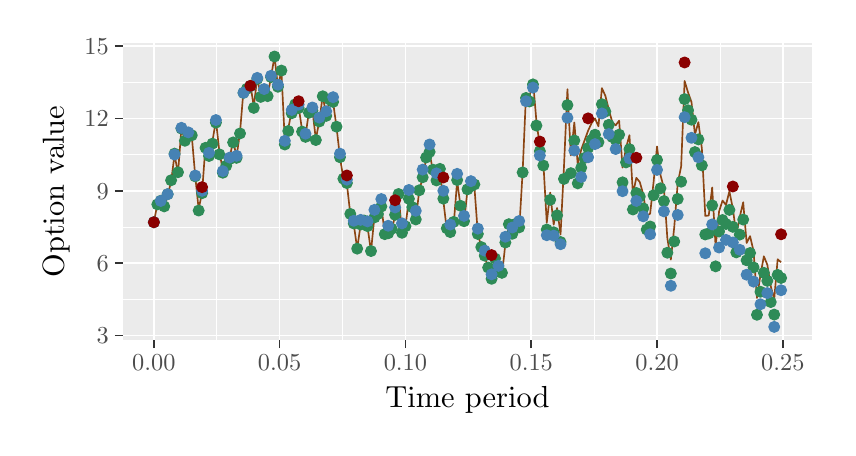
\begin{tikzpicture}[x=1pt,y=1pt]
\definecolor{fillColor}{RGB}{255,255,255}
\path[use as bounding box,fill=fillColor,fill opacity=0.00] (0,0) rectangle (289.08,144.54);
\begin{scope}
\path[clip] (  0.00,  0.00) rectangle (289.08,144.54);
\definecolor{drawColor}{RGB}{255,255,255}
\definecolor{fillColor}{RGB}{255,255,255}

\path[draw=drawColor,line width= 0.6pt,line join=round,line cap=round,fill=fillColor] (  0.00,  0.00) rectangle (289.08,144.54);
\end{scope}
\begin{scope}
\path[clip] ( 34.27, 31.53) rectangle (283.58,139.04);
\definecolor{fillColor}{gray}{0.92}

\path[fill=fillColor] ( 34.27, 31.53) rectangle (283.58,139.04);
\definecolor{drawColor}{RGB}{255,255,255}

\path[draw=drawColor,line width= 0.3pt,line join=round] ( 34.27, 46.37) --
	(283.58, 46.37);

\path[draw=drawColor,line width= 0.3pt,line join=round] ( 34.27, 72.52) --
	(283.58, 72.52);

\path[draw=drawColor,line width= 0.3pt,line join=round] ( 34.27, 98.68) --
	(283.58, 98.68);

\path[draw=drawColor,line width= 0.3pt,line join=round] ( 34.27,124.83) --
	(283.58,124.83);

\path[draw=drawColor,line width= 0.3pt,line join=round] ( 68.33, 31.53) --
	( 68.33,139.04);

\path[draw=drawColor,line width= 0.3pt,line join=round] (113.78, 31.53) --
	(113.78,139.04);

\path[draw=drawColor,line width= 0.3pt,line join=round] (159.24, 31.53) --
	(159.24,139.04);

\path[draw=drawColor,line width= 0.3pt,line join=round] (204.69, 31.53) --
	(204.69,139.04);

\path[draw=drawColor,line width= 0.3pt,line join=round] (250.14, 31.53) --
	(250.14,139.04);

\path[draw=drawColor,line width= 0.6pt,line join=round] ( 34.27, 33.29) --
	(283.58, 33.29);

\path[draw=drawColor,line width= 0.6pt,line join=round] ( 34.27, 59.45) --
	(283.58, 59.45);

\path[draw=drawColor,line width= 0.6pt,line join=round] ( 34.27, 85.60) --
	(283.58, 85.60);

\path[draw=drawColor,line width= 0.6pt,line join=round] ( 34.27,111.76) --
	(283.58,111.76);

\path[draw=drawColor,line width= 0.6pt,line join=round] ( 34.27,137.91) --
	(283.58,137.91);

\path[draw=drawColor,line width= 0.6pt,line join=round] ( 45.60, 31.53) --
	( 45.60,139.04);

\path[draw=drawColor,line width= 0.6pt,line join=round] ( 91.05, 31.53) --
	( 91.05,139.04);

\path[draw=drawColor,line width= 0.6pt,line join=round] (136.51, 31.53) --
	(136.51,139.04);

\path[draw=drawColor,line width= 0.6pt,line join=round] (181.96, 31.53) --
	(181.96,139.04);

\path[draw=drawColor,line width= 0.6pt,line join=round] (227.42, 31.53) --
	(227.42,139.04);

\path[draw=drawColor,line width= 0.6pt,line join=round] (272.87, 31.53) --
	(272.87,139.04);
\definecolor{drawColor}{RGB}{139,69,19}

\path[draw=drawColor,line width= 0.6pt,line join=round] ( 45.60, 74.23) --
	( 46.85, 80.70) --
	( 48.09, 81.83) --
	( 49.34, 79.64) --
	( 50.58, 83.95) --
	( 51.83, 88.90) --
	( 53.07, 98.64) --
	( 54.32, 91.88) --
	( 55.56,108.24) --
	( 56.81,103.72) --
	( 58.05,106.27) --
	( 59.30,105.40) --
	( 60.54, 90.94) --
	( 61.79, 78.90) --
	( 63.03, 85.15) --
	( 64.28,102.30) --
	( 65.53, 99.18) --
	( 66.77,103.53) --
	( 68.02,111.08) --
	( 69.26, 99.77) --
	( 70.51, 93.07) --
	( 71.75, 95.43) --
	( 73.00, 97.69) --
	( 74.24,103.63) --
	( 75.49, 97.96) --
	( 76.73,106.82) --
	( 77.98,121.83) --
	( 79.22,123.15) --
	( 80.47,123.95) --
	( 81.71,116.04) --
	( 82.96,126.58) --
	( 84.20,119.99) --
	( 85.45,122.26) --
	( 86.70,119.96) --
	( 87.94,126.78) --
	( 89.19,134.15) --
	( 90.43,123.26) --
	( 91.68,129.02) --
	( 92.92,103.42) --
	( 94.17,108.18) --
	( 95.41,114.53) --
	( 96.66,117.59) --
	( 97.90,116.11) --
	( 99.15,107.54) --
	(100.39,105.48) --
	(101.64,114.19) --
	(102.88,114.84) --
	(104.13,104.23) --
	(105.38,110.86) --
	(106.62,119.99) --
	(107.87,112.82) --
	(109.11,118.65) --
	(110.36,117.61) --
	(111.60,108.63) --
	(112.85, 97.68) --
	(114.09, 89.88) --
	(115.34, 88.13) --
	(116.58, 77.18) --
	(117.83, 73.56) --
	(119.07, 64.61) --
	(120.32, 73.49) --
	(121.56, 74.73) --
	(122.81, 72.52) --
	(124.06, 63.64) --
	(125.30, 76.33) --
	(126.55, 77.36) --
	(127.79, 79.88) --
	(129.04, 70.05) --
	(130.28, 70.14) --
	(131.53, 71.56) --
	(132.77, 76.51) --
	(134.02, 84.03) --
	(135.26, 70.46) --
	(136.51, 72.62) --
	(137.75, 82.73) --
	(139.00, 79.54) --
	(140.24, 74.94) --
	(141.49, 85.69) --
	(142.73, 90.27) --
	(143.98, 97.35) --
	(145.23, 99.18) --
	(146.47, 92.66) --
	(147.72, 88.61) --
	(148.96, 92.62) --
	(150.21, 81.97) --
	(151.45, 71.43) --
	(152.70, 69.82) --
	(153.94, 73.34) --
	(155.19, 89.13) --
	(156.43, 79.85) --
	(157.68, 74.16) --
	(158.92, 85.95) --
	(160.17, 86.86) --
	(161.41, 87.29) --
	(162.66, 70.14) --
	(163.91, 65.24) --
	(165.15, 61.96) --
	(166.40, 57.48) --
	(167.64, 53.27) --
	(168.89, 60.68) --
	(170.13, 55.88) --
	(171.38, 55.12) --
	(172.62, 66.53) --
	(173.87, 73.11) --
	(175.11, 69.42) --
	(176.36, 72.84) --
	(177.60, 71.31) --
	(178.85, 92.43) --
	(180.09,120.86) --
	(181.34,119.43) --
	(182.58,125.49) --
	(183.83,110.75) --
	(185.08,101.46) --
	(186.32, 96.11) --
	(187.57, 74.04) --
	(188.81, 84.95) --
	(190.06, 73.38) --
	(191.30, 79.38) --
	(192.55, 69.78) --
	(193.79, 94.29) --
	(195.04,122.29) --
	(196.28, 98.37) --
	(197.53,110.29) --
	(198.77, 95.00) --
	(200.02,100.47) --
	(201.26,103.88) --
	(202.51,107.32) --
	(203.76,110.01) --
	(205.00,111.75) --
	(206.25,108.88) --
	(207.49,122.71) --
	(208.74,119.93) --
	(209.98,114.99) --
	(211.23,110.45) --
	(212.47,109.25) --
	(213.72,110.95) --
	(214.96, 93.96) --
	(216.21,101.08) --
	(217.45,105.70) --
	(218.70, 84.47) --
	(219.94, 90.28) --
	(221.19, 88.76) --
	(222.44, 84.29) --
	(223.68, 76.53) --
	(224.93, 77.36) --
	(226.17, 88.74) --
	(227.42,101.62) --
	(228.66, 91.33) --
	(229.91, 86.52) --
	(231.15, 68.37) --
	(232.40, 60.72) --
	(233.64, 72.52) --
	(234.89, 88.31) --
	(236.13, 94.42) --
	(237.38,125.27) --
	(238.62,121.15) --
	(239.87,117.64) --
	(241.11,105.91) --
	(242.36,110.41) --
	(243.61,100.95) --
	(244.85, 76.53) --
	(246.10, 76.66) --
	(247.34, 86.80) --
	(248.59, 65.31) --
	(249.83, 78.09) --
	(251.08, 82.08) --
	(252.32, 80.46) --
	(253.57, 85.42) --
	(254.81, 79.15) --
	(256.06, 69.81) --
	(257.30, 76.13) --
	(258.55, 81.44) --
	(259.79, 66.75) --
	(261.04, 69.20) --
	(262.29, 63.80) --
	(263.53, 46.88) --
	(264.78, 55.16) --
	(266.02, 61.92) --
	(267.27, 58.89) --
	(268.51, 51.10) --
	(269.76, 46.42) --
	(271.00, 60.86) --
	(272.25, 59.74);
\definecolor{drawColor}{RGB}{46,139,87}
\definecolor{fillColor}{RGB}{46,139,87}

\path[draw=drawColor,line width= 0.4pt,line join=round,line cap=round,fill=fillColor] ( 45.60, 74.23) circle (  1.96);

\path[draw=drawColor,line width= 0.4pt,line join=round,line cap=round,fill=fillColor] ( 46.85, 80.69) circle (  1.96);

\path[draw=drawColor,line width= 0.4pt,line join=round,line cap=round,fill=fillColor] ( 48.09, 81.99) circle (  1.96);

\path[draw=drawColor,line width= 0.4pt,line join=round,line cap=round,fill=fillColor] ( 49.34, 79.96) circle (  1.96);

\path[draw=drawColor,line width= 0.4pt,line join=round,line cap=round,fill=fillColor] ( 50.58, 84.37) circle (  1.96);

\path[draw=drawColor,line width= 0.4pt,line join=round,line cap=round,fill=fillColor] ( 51.83, 89.40) circle (  1.96);

\path[draw=drawColor,line width= 0.4pt,line join=round,line cap=round,fill=fillColor] ( 53.07, 99.02) circle (  1.96);

\path[draw=drawColor,line width= 0.4pt,line join=round,line cap=round,fill=fillColor] ( 54.32, 92.30) circle (  1.96);

\path[draw=drawColor,line width= 0.4pt,line join=round,line cap=round,fill=fillColor] ( 55.56,108.07) circle (  1.96);

\path[draw=drawColor,line width= 0.4pt,line join=round,line cap=round,fill=fillColor] ( 56.81,103.66) circle (  1.96);

\path[draw=drawColor,line width= 0.4pt,line join=round,line cap=round,fill=fillColor] ( 58.05,106.37) circle (  1.96);

\path[draw=drawColor,line width= 0.4pt,line join=round,line cap=round,fill=fillColor] ( 59.30,105.66) circle (  1.96);

\path[draw=drawColor,line width= 0.4pt,line join=round,line cap=round,fill=fillColor] ( 60.54, 90.81) circle (  1.96);

\path[draw=drawColor,line width= 0.4pt,line join=round,line cap=round,fill=fillColor] ( 61.79, 78.46) circle (  1.96);

\path[draw=drawColor,line width= 0.4pt,line join=round,line cap=round,fill=fillColor] ( 63.03, 84.73) circle (  1.96);

\path[draw=drawColor,line width= 0.4pt,line join=round,line cap=round,fill=fillColor] ( 64.28,101.13) circle (  1.96);

\path[draw=drawColor,line width= 0.4pt,line join=round,line cap=round,fill=fillColor] ( 65.53, 98.17) circle (  1.96);

\path[draw=drawColor,line width= 0.4pt,line join=round,line cap=round,fill=fillColor] ( 66.77,102.63) circle (  1.96);

\path[draw=drawColor,line width= 0.4pt,line join=round,line cap=round,fill=fillColor] ( 68.02,110.21) circle (  1.96);

\path[draw=drawColor,line width= 0.4pt,line join=round,line cap=round,fill=fillColor] ( 69.26, 98.76) circle (  1.96);

\path[draw=drawColor,line width= 0.4pt,line join=round,line cap=round,fill=fillColor] ( 70.51, 92.11) circle (  1.96);

\path[draw=drawColor,line width= 0.4pt,line join=round,line cap=round,fill=fillColor] ( 71.75, 94.64) circle (  1.96);

\path[draw=drawColor,line width= 0.4pt,line join=round,line cap=round,fill=fillColor] ( 73.00, 97.05) circle (  1.96);

\path[draw=drawColor,line width= 0.4pt,line join=round,line cap=round,fill=fillColor] ( 74.24,103.07) circle (  1.96);

\path[draw=drawColor,line width= 0.4pt,line join=round,line cap=round,fill=fillColor] ( 75.49, 97.50) circle (  1.96);

\path[draw=drawColor,line width= 0.4pt,line join=round,line cap=round,fill=fillColor] ( 76.73,106.32) circle (  1.96);

\path[draw=drawColor,line width= 0.4pt,line join=round,line cap=round,fill=fillColor] ( 77.98,120.98) circle (  1.96);

\path[draw=drawColor,line width= 0.4pt,line join=round,line cap=round,fill=fillColor] ( 79.22,122.46) circle (  1.96);

\path[draw=drawColor,line width= 0.4pt,line join=round,line cap=round,fill=fillColor] ( 80.47,123.42) circle (  1.96);

\path[draw=drawColor,line width= 0.4pt,line join=round,line cap=round,fill=fillColor] ( 81.71,115.55) circle (  1.96);

\path[draw=drawColor,line width= 0.4pt,line join=round,line cap=round,fill=fillColor] ( 82.96,126.03) circle (  1.96);

\path[draw=drawColor,line width= 0.4pt,line join=round,line cap=round,fill=fillColor] ( 84.20,119.52) circle (  1.96);

\path[draw=drawColor,line width= 0.4pt,line join=round,line cap=round,fill=fillColor] ( 85.45,121.95) circle (  1.96);

\path[draw=drawColor,line width= 0.4pt,line join=round,line cap=round,fill=fillColor] ( 86.70,119.80) circle (  1.96);

\path[draw=drawColor,line width= 0.4pt,line join=round,line cap=round,fill=fillColor] ( 87.94,126.69) circle (  1.96);

\path[draw=drawColor,line width= 0.4pt,line join=round,line cap=round,fill=fillColor] ( 89.19,134.11) circle (  1.96);

\path[draw=drawColor,line width= 0.4pt,line join=round,line cap=round,fill=fillColor] ( 90.43,123.18) circle (  1.96);

\path[draw=drawColor,line width= 0.4pt,line join=round,line cap=round,fill=fillColor] ( 91.68,129.04) circle (  1.96);

\path[draw=drawColor,line width= 0.4pt,line join=round,line cap=round,fill=fillColor] ( 92.92,102.32) circle (  1.96);

\path[draw=drawColor,line width= 0.4pt,line join=round,line cap=round,fill=fillColor] ( 94.17,107.20) circle (  1.96);

\path[draw=drawColor,line width= 0.4pt,line join=round,line cap=round,fill=fillColor] ( 95.41,113.62) circle (  1.96);

\path[draw=drawColor,line width= 0.4pt,line join=round,line cap=round,fill=fillColor] ( 96.66,116.83) circle (  1.96);

\path[draw=drawColor,line width= 0.4pt,line join=round,line cap=round,fill=fillColor] ( 97.90,115.51) circle (  1.96);

\path[draw=drawColor,line width= 0.4pt,line join=round,line cap=round,fill=fillColor] ( 99.15,106.98) circle (  1.96);

\path[draw=drawColor,line width= 0.4pt,line join=round,line cap=round,fill=fillColor] (100.39,105.08) circle (  1.96);

\path[draw=drawColor,line width= 0.4pt,line join=round,line cap=round,fill=fillColor] (101.64,113.79) circle (  1.96);

\path[draw=drawColor,line width= 0.4pt,line join=round,line cap=round,fill=fillColor] (102.88,114.61) circle (  1.96);

\path[draw=drawColor,line width= 0.4pt,line join=round,line cap=round,fill=fillColor] (104.13,103.93) circle (  1.96);

\path[draw=drawColor,line width= 0.4pt,line join=round,line cap=round,fill=fillColor] (105.38,110.63) circle (  1.96);

\path[draw=drawColor,line width= 0.4pt,line join=round,line cap=round,fill=fillColor] (106.62,119.75) circle (  1.96);

\path[draw=drawColor,line width= 0.4pt,line join=round,line cap=round,fill=fillColor] (107.87,112.66) circle (  1.96);

\path[draw=drawColor,line width= 0.4pt,line join=round,line cap=round,fill=fillColor] (109.11,118.59) circle (  1.96);

\path[draw=drawColor,line width= 0.4pt,line join=round,line cap=round,fill=fillColor] (110.36,117.72) circle (  1.96);

\path[draw=drawColor,line width= 0.4pt,line join=round,line cap=round,fill=fillColor] (111.60,108.76) circle (  1.96);

\path[draw=drawColor,line width= 0.4pt,line join=round,line cap=round,fill=fillColor] (112.85, 97.71) circle (  1.96);

\path[draw=drawColor,line width= 0.4pt,line join=round,line cap=round,fill=fillColor] (114.09, 89.95) circle (  1.96);

\path[draw=drawColor,line width= 0.4pt,line join=round,line cap=round,fill=fillColor] (115.34, 88.39) circle (  1.96);

\path[draw=drawColor,line width= 0.4pt,line join=round,line cap=round,fill=fillColor] (116.58, 77.24) circle (  1.96);

\path[draw=drawColor,line width= 0.4pt,line join=round,line cap=round,fill=fillColor] (117.83, 73.79) circle (  1.96);

\path[draw=drawColor,line width= 0.4pt,line join=round,line cap=round,fill=fillColor] (119.07, 64.69) circle (  1.96);

\path[draw=drawColor,line width= 0.4pt,line join=round,line cap=round,fill=fillColor] (120.32, 73.41) circle (  1.96);

\path[draw=drawColor,line width= 0.4pt,line join=round,line cap=round,fill=fillColor] (121.56, 74.85) circle (  1.96);

\path[draw=drawColor,line width= 0.4pt,line join=round,line cap=round,fill=fillColor] (122.81, 72.83) circle (  1.96);

\path[draw=drawColor,line width= 0.4pt,line join=round,line cap=round,fill=fillColor] (124.06, 63.82) circle (  1.96);

\path[draw=drawColor,line width= 0.4pt,line join=round,line cap=round,fill=fillColor] (125.30, 75.97) circle (  1.96);

\path[draw=drawColor,line width= 0.4pt,line join=round,line cap=round,fill=fillColor] (126.55, 77.21) circle (  1.96);

\path[draw=drawColor,line width= 0.4pt,line join=round,line cap=round,fill=fillColor] (127.79, 79.91) circle (  1.96);

\path[draw=drawColor,line width= 0.4pt,line join=round,line cap=round,fill=fillColor] (129.04, 69.93) circle (  1.96);

\path[draw=drawColor,line width= 0.4pt,line join=round,line cap=round,fill=fillColor] (130.28, 70.24) circle (  1.96);

\path[draw=drawColor,line width= 0.4pt,line join=round,line cap=round,fill=fillColor] (131.53, 71.86) circle (  1.96);

\path[draw=drawColor,line width= 0.4pt,line join=round,line cap=round,fill=fillColor] (132.77, 76.91) circle (  1.96);

\path[draw=drawColor,line width= 0.4pt,line join=round,line cap=round,fill=fillColor] (134.02, 84.43) circle (  1.96);

\path[draw=drawColor,line width= 0.4pt,line join=round,line cap=round,fill=fillColor] (135.26, 70.42) circle (  1.96);

\path[draw=drawColor,line width= 0.4pt,line join=round,line cap=round,fill=fillColor] (136.51, 72.77) circle (  1.96);

\path[draw=drawColor,line width= 0.4pt,line join=round,line cap=round,fill=fillColor] (137.75, 82.69) circle (  1.96);

\path[draw=drawColor,line width= 0.4pt,line join=round,line cap=round,fill=fillColor] (139.00, 79.68) circle (  1.96);

\path[draw=drawColor,line width= 0.4pt,line join=round,line cap=round,fill=fillColor] (140.24, 75.24) circle (  1.96);

\path[draw=drawColor,line width= 0.4pt,line join=round,line cap=round,fill=fillColor] (141.49, 85.77) circle (  1.96);

\path[draw=drawColor,line width= 0.4pt,line join=round,line cap=round,fill=fillColor] (142.73, 90.48) circle (  1.96);

\path[draw=drawColor,line width= 0.4pt,line join=round,line cap=round,fill=fillColor] (143.98, 97.62) circle (  1.96);

\path[draw=drawColor,line width= 0.4pt,line join=round,line cap=round,fill=fillColor] (145.23, 99.65) circle (  1.96);

\path[draw=drawColor,line width= 0.4pt,line join=round,line cap=round,fill=fillColor] (146.47, 93.22) circle (  1.96);

\path[draw=drawColor,line width= 0.4pt,line join=round,line cap=round,fill=fillColor] (147.72, 89.34) circle (  1.96);

\path[draw=drawColor,line width= 0.4pt,line join=round,line cap=round,fill=fillColor] (148.96, 93.52) circle (  1.96);

\path[draw=drawColor,line width= 0.4pt,line join=round,line cap=round,fill=fillColor] (150.21, 82.76) circle (  1.96);

\path[draw=drawColor,line width= 0.4pt,line join=round,line cap=round,fill=fillColor] (151.45, 72.05) circle (  1.96);

\path[draw=drawColor,line width= 0.4pt,line join=round,line cap=round,fill=fillColor] (152.70, 70.67) circle (  1.96);

\path[draw=drawColor,line width= 0.4pt,line join=round,line cap=round,fill=fillColor] (153.94, 74.36) circle (  1.96);

\path[draw=drawColor,line width= 0.4pt,line join=round,line cap=round,fill=fillColor] (155.19, 89.48) circle (  1.96);

\path[draw=drawColor,line width= 0.4pt,line join=round,line cap=round,fill=fillColor] (156.43, 80.17) circle (  1.96);

\path[draw=drawColor,line width= 0.4pt,line join=round,line cap=round,fill=fillColor] (157.68, 74.61) circle (  1.96);

\path[draw=drawColor,line width= 0.4pt,line join=round,line cap=round,fill=fillColor] (158.92, 86.12) circle (  1.96);

\path[draw=drawColor,line width= 0.4pt,line join=round,line cap=round,fill=fillColor] (160.17, 87.24) circle (  1.96);

\path[draw=drawColor,line width= 0.4pt,line join=round,line cap=round,fill=fillColor] (161.41, 87.89) circle (  1.96);

\path[draw=drawColor,line width= 0.4pt,line join=round,line cap=round,fill=fillColor] (162.66, 69.99) circle (  1.96);

\path[draw=drawColor,line width= 0.4pt,line join=round,line cap=round,fill=fillColor] (163.91, 65.25) circle (  1.96);

\path[draw=drawColor,line width= 0.4pt,line join=round,line cap=round,fill=fillColor] (165.15, 62.17) circle (  1.96);

\path[draw=drawColor,line width= 0.4pt,line join=round,line cap=round,fill=fillColor] (166.40, 57.85) circle (  1.96);

\path[draw=drawColor,line width= 0.4pt,line join=round,line cap=round,fill=fillColor] (167.64, 53.79) circle (  1.96);

\path[draw=drawColor,line width= 0.4pt,line join=round,line cap=round,fill=fillColor] (168.89, 61.11) circle (  1.96);

\path[draw=drawColor,line width= 0.4pt,line join=round,line cap=round,fill=fillColor] (170.13, 56.46) circle (  1.96);

\path[draw=drawColor,line width= 0.4pt,line join=round,line cap=round,fill=fillColor] (171.38, 55.95) circle (  1.96);

\path[draw=drawColor,line width= 0.4pt,line join=round,line cap=round,fill=fillColor] (172.62, 66.91) circle (  1.96);

\path[draw=drawColor,line width= 0.4pt,line join=round,line cap=round,fill=fillColor] (173.87, 73.53) circle (  1.96);

\path[draw=drawColor,line width= 0.4pt,line join=round,line cap=round,fill=fillColor] (175.11, 70.05) circle (  1.96);

\path[draw=drawColor,line width= 0.4pt,line join=round,line cap=round,fill=fillColor] (176.36, 73.66) circle (  1.96);

\path[draw=drawColor,line width= 0.4pt,line join=round,line cap=round,fill=fillColor] (177.60, 72.38) circle (  1.96);

\path[draw=drawColor,line width= 0.4pt,line join=round,line cap=round,fill=fillColor] (178.85, 92.23) circle (  1.96);

\path[draw=drawColor,line width= 0.4pt,line join=round,line cap=round,fill=fillColor] (180.09,119.14) circle (  1.96);

\path[draw=drawColor,line width= 0.4pt,line join=round,line cap=round,fill=fillColor] (181.34,117.87) circle (  1.96);

\path[draw=drawColor,line width= 0.4pt,line join=round,line cap=round,fill=fillColor] (182.58,124.04) circle (  1.96);

\path[draw=drawColor,line width= 0.4pt,line join=round,line cap=round,fill=fillColor] (183.83,109.16) circle (  1.96);

\path[draw=drawColor,line width= 0.4pt,line join=round,line cap=round,fill=fillColor] (185.08, 99.93) circle (  1.96);

\path[draw=drawColor,line width= 0.4pt,line join=round,line cap=round,fill=fillColor] (186.32, 94.73) circle (  1.96);

\path[draw=drawColor,line width= 0.4pt,line join=round,line cap=round,fill=fillColor] (187.57, 71.59) circle (  1.96);

\path[draw=drawColor,line width= 0.4pt,line join=round,line cap=round,fill=fillColor] (188.81, 82.33) circle (  1.96);

\path[draw=drawColor,line width= 0.4pt,line join=round,line cap=round,fill=fillColor] (190.06, 70.61) circle (  1.96);

\path[draw=drawColor,line width= 0.4pt,line join=round,line cap=round,fill=fillColor] (191.30, 76.72) circle (  1.96);

\path[draw=drawColor,line width= 0.4pt,line join=round,line cap=round,fill=fillColor] (192.55, 67.09) circle (  1.96);

\path[draw=drawColor,line width= 0.4pt,line join=round,line cap=round,fill=fillColor] (193.79, 89.88) circle (  1.96);

\path[draw=drawColor,line width= 0.4pt,line join=round,line cap=round,fill=fillColor] (195.04,116.55) circle (  1.96);

\path[draw=drawColor,line width= 0.4pt,line join=round,line cap=round,fill=fillColor] (196.28, 91.96) circle (  1.96);

\path[draw=drawColor,line width= 0.4pt,line join=round,line cap=round,fill=fillColor] (197.53,103.78) circle (  1.96);

\path[draw=drawColor,line width= 0.4pt,line join=round,line cap=round,fill=fillColor] (198.77, 88.29) circle (  1.96);

\path[draw=drawColor,line width= 0.4pt,line join=round,line cap=round,fill=fillColor] (200.02, 93.90) circle (  1.96);

\path[draw=drawColor,line width= 0.4pt,line join=round,line cap=round,fill=fillColor] (201.26, 97.48) circle (  1.96);

\path[draw=drawColor,line width= 0.4pt,line join=round,line cap=round,fill=fillColor] (202.51,101.08) circle (  1.96);

\path[draw=drawColor,line width= 0.4pt,line join=round,line cap=round,fill=fillColor] (203.76,103.95) circle (  1.96);

\path[draw=drawColor,line width= 0.4pt,line join=round,line cap=round,fill=fillColor] (205.00,105.86) circle (  1.96);

\path[draw=drawColor,line width= 0.4pt,line join=round,line cap=round,fill=fillColor] (206.25,103.16) circle (  1.96);

\path[draw=drawColor,line width= 0.4pt,line join=round,line cap=round,fill=fillColor] (207.49,116.87) circle (  1.96);

\path[draw=drawColor,line width= 0.4pt,line join=round,line cap=round,fill=fillColor] (208.74,114.23) circle (  1.96);

\path[draw=drawColor,line width= 0.4pt,line join=round,line cap=round,fill=fillColor] (209.98,109.43) circle (  1.96);

\path[draw=drawColor,line width= 0.4pt,line join=round,line cap=round,fill=fillColor] (211.23,105.04) circle (  1.96);

\path[draw=drawColor,line width= 0.4pt,line join=round,line cap=round,fill=fillColor] (212.47,104.02) circle (  1.96);

\path[draw=drawColor,line width= 0.4pt,line join=round,line cap=round,fill=fillColor] (213.72,105.88) circle (  1.96);

\path[draw=drawColor,line width= 0.4pt,line join=round,line cap=round,fill=fillColor] (214.96, 88.65) circle (  1.96);

\path[draw=drawColor,line width= 0.4pt,line join=round,line cap=round,fill=fillColor] (216.21, 95.87) circle (  1.96);

\path[draw=drawColor,line width= 0.4pt,line join=round,line cap=round,fill=fillColor] (217.45,100.64) circle (  1.96);

\path[draw=drawColor,line width= 0.4pt,line join=round,line cap=round,fill=fillColor] (218.70, 78.84) circle (  1.96);

\path[draw=drawColor,line width= 0.4pt,line join=round,line cap=round,fill=fillColor] (219.94, 84.80) circle (  1.96);

\path[draw=drawColor,line width= 0.4pt,line join=round,line cap=round,fill=fillColor] (221.19, 83.50) circle (  1.96);

\path[draw=drawColor,line width= 0.4pt,line join=round,line cap=round,fill=fillColor] (222.44, 79.24) circle (  1.96);

\path[draw=drawColor,line width= 0.4pt,line join=round,line cap=round,fill=fillColor] (223.68, 71.60) circle (  1.96);

\path[draw=drawColor,line width= 0.4pt,line join=round,line cap=round,fill=fillColor] (224.93, 72.71) circle (  1.96);

\path[draw=drawColor,line width= 0.4pt,line join=round,line cap=round,fill=fillColor] (226.17, 83.98) circle (  1.96);

\path[draw=drawColor,line width= 0.4pt,line join=round,line cap=round,fill=fillColor] (227.42, 96.73) circle (  1.96);

\path[draw=drawColor,line width= 0.4pt,line join=round,line cap=round,fill=fillColor] (228.66, 86.49) circle (  1.96);

\path[draw=drawColor,line width= 0.4pt,line join=round,line cap=round,fill=fillColor] (229.91, 81.87) circle (  1.96);

\path[draw=drawColor,line width= 0.4pt,line join=round,line cap=round,fill=fillColor] (231.15, 63.22) circle (  1.96);

\path[draw=drawColor,line width= 0.4pt,line join=round,line cap=round,fill=fillColor] (232.40, 55.71) circle (  1.96);

\path[draw=drawColor,line width= 0.4pt,line join=round,line cap=round,fill=fillColor] (233.64, 67.27) circle (  1.96);

\path[draw=drawColor,line width= 0.4pt,line join=round,line cap=round,fill=fillColor] (234.89, 82.64) circle (  1.96);

\path[draw=drawColor,line width= 0.4pt,line join=round,line cap=round,fill=fillColor] (236.13, 88.88) circle (  1.96);

\path[draw=drawColor,line width= 0.4pt,line join=round,line cap=round,fill=fillColor] (237.38,118.72) circle (  1.96);

\path[draw=drawColor,line width= 0.4pt,line join=round,line cap=round,fill=fillColor] (238.62,114.69) circle (  1.96);

\path[draw=drawColor,line width= 0.4pt,line join=round,line cap=round,fill=fillColor] (239.87,111.27) circle (  1.96);

\path[draw=drawColor,line width= 0.4pt,line join=round,line cap=round,fill=fillColor] (241.11, 99.58) circle (  1.96);

\path[draw=drawColor,line width= 0.4pt,line join=round,line cap=round,fill=fillColor] (242.36,104.17) circle (  1.96);

\path[draw=drawColor,line width= 0.4pt,line join=round,line cap=round,fill=fillColor] (243.61, 94.78) circle (  1.96);

\path[draw=drawColor,line width= 0.4pt,line join=round,line cap=round,fill=fillColor] (244.85, 69.81) circle (  1.96);

\path[draw=drawColor,line width= 0.4pt,line join=round,line cap=round,fill=fillColor] (246.10, 70.19) circle (  1.96);

\path[draw=drawColor,line width= 0.4pt,line join=round,line cap=round,fill=fillColor] (247.34, 80.32) circle (  1.96);

\path[draw=drawColor,line width= 0.4pt,line join=round,line cap=round,fill=fillColor] (248.59, 58.29) circle (  1.96);

\path[draw=drawColor,line width= 0.4pt,line join=round,line cap=round,fill=fillColor] (249.83, 70.87) circle (  1.96);

\path[draw=drawColor,line width= 0.4pt,line join=round,line cap=round,fill=fillColor] (251.08, 75.03) circle (  1.96);

\path[draw=drawColor,line width= 0.4pt,line join=round,line cap=round,fill=fillColor] (252.32, 73.61) circle (  1.96);

\path[draw=drawColor,line width= 0.4pt,line join=round,line cap=round,fill=fillColor] (253.57, 78.69) circle (  1.96);

\path[draw=drawColor,line width= 0.4pt,line join=round,line cap=round,fill=fillColor] (254.81, 72.57) circle (  1.96);

\path[draw=drawColor,line width= 0.4pt,line join=round,line cap=round,fill=fillColor] (256.06, 63.34) circle (  1.96);

\path[draw=drawColor,line width= 0.4pt,line join=round,line cap=round,fill=fillColor] (257.30, 69.77) circle (  1.96);

\path[draw=drawColor,line width= 0.4pt,line join=round,line cap=round,fill=fillColor] (258.55, 75.19) circle (  1.96);

\path[draw=drawColor,line width= 0.4pt,line join=round,line cap=round,fill=fillColor] (259.79, 60.48) circle (  1.96);

\path[draw=drawColor,line width= 0.4pt,line join=round,line cap=round,fill=fillColor] (261.04, 63.12) circle (  1.96);

\path[draw=drawColor,line width= 0.4pt,line join=round,line cap=round,fill=fillColor] (262.29, 57.91) circle (  1.96);

\path[draw=drawColor,line width= 0.4pt,line join=round,line cap=round,fill=fillColor] (263.53, 40.79) circle (  1.96);

\path[draw=drawColor,line width= 0.4pt,line join=round,line cap=round,fill=fillColor] (264.78, 49.12) circle (  1.96);

\path[draw=drawColor,line width= 0.4pt,line join=round,line cap=round,fill=fillColor] (266.02, 55.95) circle (  1.96);

\path[draw=drawColor,line width= 0.4pt,line join=round,line cap=round,fill=fillColor] (267.27, 53.06) circle (  1.96);

\path[draw=drawColor,line width= 0.4pt,line join=round,line cap=round,fill=fillColor] (268.51, 45.39) circle (  1.96);

\path[draw=drawColor,line width= 0.4pt,line join=round,line cap=round,fill=fillColor] (269.76, 40.86) circle (  1.96);

\path[draw=drawColor,line width= 0.4pt,line join=round,line cap=round,fill=fillColor] (271.00, 55.20) circle (  1.96);

\path[draw=drawColor,line width= 0.4pt,line join=round,line cap=round,fill=fillColor] (272.25, 54.09) circle (  1.96);
\definecolor{drawColor}{RGB}{70,130,180}
\definecolor{fillColor}{RGB}{70,130,180}

\path[draw=drawColor,line width= 0.4pt,line join=round,line cap=round,fill=fillColor] ( 45.60, 74.23) circle (  1.96);

\path[draw=drawColor,line width= 0.4pt,line join=round,line cap=round,fill=fillColor] ( 48.09, 81.92) circle (  1.96);

\path[draw=drawColor,line width= 0.4pt,line join=round,line cap=round,fill=fillColor] ( 50.58, 84.37) circle (  1.96);

\path[draw=drawColor,line width= 0.4pt,line join=round,line cap=round,fill=fillColor] ( 53.07, 98.68) circle (  1.96);

\path[draw=drawColor,line width= 0.4pt,line join=round,line cap=round,fill=fillColor] ( 55.56,108.35) circle (  1.96);

\path[draw=drawColor,line width= 0.4pt,line join=round,line cap=round,fill=fillColor] ( 58.05,106.71) circle (  1.96);

\path[draw=drawColor,line width= 0.4pt,line join=round,line cap=round,fill=fillColor] ( 60.54, 91.11) circle (  1.96);

\path[draw=drawColor,line width= 0.4pt,line join=round,line cap=round,fill=fillColor] ( 63.03, 85.57) circle (  1.96);

\path[draw=drawColor,line width= 0.4pt,line join=round,line cap=round,fill=fillColor] ( 65.53, 99.31) circle (  1.96);

\path[draw=drawColor,line width= 0.4pt,line join=round,line cap=round,fill=fillColor] ( 68.02,111.16) circle (  1.96);

\path[draw=drawColor,line width= 0.4pt,line join=round,line cap=round,fill=fillColor] ( 70.51, 92.69) circle (  1.96);

\path[draw=drawColor,line width= 0.4pt,line join=round,line cap=round,fill=fillColor] ( 73.00, 97.59) circle (  1.96);

\path[draw=drawColor,line width= 0.4pt,line join=round,line cap=round,fill=fillColor] ( 75.49, 98.22) circle (  1.96);

\path[draw=drawColor,line width= 0.4pt,line join=round,line cap=round,fill=fillColor] ( 77.98,121.02) circle (  1.96);

\path[draw=drawColor,line width= 0.4pt,line join=round,line cap=round,fill=fillColor] ( 80.47,123.46) circle (  1.96);

\path[draw=drawColor,line width= 0.4pt,line join=round,line cap=round,fill=fillColor] ( 82.96,126.39) circle (  1.96);

\path[draw=drawColor,line width= 0.4pt,line join=round,line cap=round,fill=fillColor] ( 85.45,122.36) circle (  1.96);

\path[draw=drawColor,line width= 0.4pt,line join=round,line cap=round,fill=fillColor] ( 87.94,127.16) circle (  1.96);

\path[draw=drawColor,line width= 0.4pt,line join=round,line cap=round,fill=fillColor] ( 90.43,123.93) circle (  1.96);

\path[draw=drawColor,line width= 0.4pt,line join=round,line cap=round,fill=fillColor] ( 92.92,103.65) circle (  1.96);

\path[draw=drawColor,line width= 0.4pt,line join=round,line cap=round,fill=fillColor] ( 95.41,114.80) circle (  1.96);

\path[draw=drawColor,line width= 0.4pt,line join=round,line cap=round,fill=fillColor] ( 97.90,116.71) circle (  1.96);

\path[draw=drawColor,line width= 0.4pt,line join=round,line cap=round,fill=fillColor] (100.39,106.21) circle (  1.96);

\path[draw=drawColor,line width= 0.4pt,line join=round,line cap=round,fill=fillColor] (102.88,115.70) circle (  1.96);

\path[draw=drawColor,line width= 0.4pt,line join=round,line cap=round,fill=fillColor] (105.38,112.04) circle (  1.96);

\path[draw=drawColor,line width= 0.4pt,line join=round,line cap=round,fill=fillColor] (107.87,114.34) circle (  1.96);

\path[draw=drawColor,line width= 0.4pt,line join=round,line cap=round,fill=fillColor] (110.36,119.42) circle (  1.96);

\path[draw=drawColor,line width= 0.4pt,line join=round,line cap=round,fill=fillColor] (112.85, 99.01) circle (  1.96);

\path[draw=drawColor,line width= 0.4pt,line join=round,line cap=round,fill=fillColor] (115.34, 89.62) circle (  1.96);

\path[draw=drawColor,line width= 0.4pt,line join=round,line cap=round,fill=fillColor] (117.83, 74.75) circle (  1.96);

\path[draw=drawColor,line width= 0.4pt,line join=round,line cap=round,fill=fillColor] (120.32, 75.09) circle (  1.96);

\path[draw=drawColor,line width= 0.4pt,line join=round,line cap=round,fill=fillColor] (122.81, 74.54) circle (  1.96);

\path[draw=drawColor,line width= 0.4pt,line join=round,line cap=round,fill=fillColor] (125.30, 78.70) circle (  1.96);

\path[draw=drawColor,line width= 0.4pt,line join=round,line cap=round,fill=fillColor] (127.79, 82.61) circle (  1.96);

\path[draw=drawColor,line width= 0.4pt,line join=round,line cap=round,fill=fillColor] (130.28, 72.96) circle (  1.96);

\path[draw=drawColor,line width= 0.4pt,line join=round,line cap=round,fill=fillColor] (132.77, 79.56) circle (  1.96);

\path[draw=drawColor,line width= 0.4pt,line join=round,line cap=round,fill=fillColor] (135.26, 73.83) circle (  1.96);

\path[draw=drawColor,line width= 0.4pt,line join=round,line cap=round,fill=fillColor] (137.75, 85.90) circle (  1.96);

\path[draw=drawColor,line width= 0.4pt,line join=round,line cap=round,fill=fillColor] (140.24, 78.36) circle (  1.96);

\path[draw=drawColor,line width= 0.4pt,line join=round,line cap=round,fill=fillColor] (142.73, 93.25) circle (  1.96);

\path[draw=drawColor,line width= 0.4pt,line join=round,line cap=round,fill=fillColor] (145.23,102.33) circle (  1.96);

\path[draw=drawColor,line width= 0.4pt,line join=round,line cap=round,fill=fillColor] (147.72, 91.90) circle (  1.96);

\path[draw=drawColor,line width= 0.4pt,line join=round,line cap=round,fill=fillColor] (150.21, 85.59) circle (  1.96);

\path[draw=drawColor,line width= 0.4pt,line join=round,line cap=round,fill=fillColor] (152.70, 73.39) circle (  1.96);

\path[draw=drawColor,line width= 0.4pt,line join=round,line cap=round,fill=fillColor] (155.19, 91.72) circle (  1.96);

\path[draw=drawColor,line width= 0.4pt,line join=round,line cap=round,fill=fillColor] (157.68, 76.53) circle (  1.96);

\path[draw=drawColor,line width= 0.4pt,line join=round,line cap=round,fill=fillColor] (160.17, 89.07) circle (  1.96);

\path[draw=drawColor,line width= 0.4pt,line join=round,line cap=round,fill=fillColor] (162.66, 71.92) circle (  1.96);

\path[draw=drawColor,line width= 0.4pt,line join=round,line cap=round,fill=fillColor] (165.15, 63.97) circle (  1.96);

\path[draw=drawColor,line width= 0.4pt,line join=round,line cap=round,fill=fillColor] (167.64, 55.40) circle (  1.96);

\path[draw=drawColor,line width= 0.4pt,line join=round,line cap=round,fill=fillColor] (170.13, 58.47) circle (  1.96);

\path[draw=drawColor,line width= 0.4pt,line join=round,line cap=round,fill=fillColor] (172.62, 68.98) circle (  1.96);

\path[draw=drawColor,line width= 0.4pt,line join=round,line cap=round,fill=fillColor] (175.11, 72.32) circle (  1.96);

\path[draw=drawColor,line width= 0.4pt,line join=round,line cap=round,fill=fillColor] (177.60, 74.68) circle (  1.96);

\path[draw=drawColor,line width= 0.4pt,line join=round,line cap=round,fill=fillColor] (180.09,117.97) circle (  1.96);

\path[draw=drawColor,line width= 0.4pt,line join=round,line cap=round,fill=fillColor] (182.58,122.88) circle (  1.96);

\path[draw=drawColor,line width= 0.4pt,line join=round,line cap=round,fill=fillColor] (185.08, 98.36) circle (  1.96);

\path[draw=drawColor,line width= 0.4pt,line join=round,line cap=round,fill=fillColor] (187.57, 69.54) circle (  1.96);

\path[draw=drawColor,line width= 0.4pt,line join=round,line cap=round,fill=fillColor] (190.06, 69.40) circle (  1.96);

\path[draw=drawColor,line width= 0.4pt,line join=round,line cap=round,fill=fillColor] (192.55, 66.30) circle (  1.96);

\path[draw=drawColor,line width= 0.4pt,line join=round,line cap=round,fill=fillColor] (195.04,111.97) circle (  1.96);

\path[draw=drawColor,line width= 0.4pt,line join=round,line cap=round,fill=fillColor] (197.53,100.15) circle (  1.96);

\path[draw=drawColor,line width= 0.4pt,line join=round,line cap=round,fill=fillColor] (200.02, 90.58) circle (  1.96);

\path[draw=drawColor,line width= 0.4pt,line join=round,line cap=round,fill=fillColor] (202.51, 97.71) circle (  1.96);

\path[draw=drawColor,line width= 0.4pt,line join=round,line cap=round,fill=fillColor] (205.00,102.47) circle (  1.96);

\path[draw=drawColor,line width= 0.4pt,line join=round,line cap=round,fill=fillColor] (207.49,113.55) circle (  1.96);

\path[draw=drawColor,line width= 0.4pt,line join=round,line cap=round,fill=fillColor] (209.98,106.09) circle (  1.96);

\path[draw=drawColor,line width= 0.4pt,line join=round,line cap=round,fill=fillColor] (212.47,100.68) circle (  1.96);

\path[draw=drawColor,line width= 0.4pt,line join=round,line cap=round,fill=fillColor] (214.96, 85.45) circle (  1.96);

\path[draw=drawColor,line width= 0.4pt,line join=round,line cap=round,fill=fillColor] (217.45, 97.30) circle (  1.96);

\path[draw=drawColor,line width= 0.4pt,line join=round,line cap=round,fill=fillColor] (219.94, 81.94) circle (  1.96);

\path[draw=drawColor,line width= 0.4pt,line join=round,line cap=round,fill=fillColor] (222.44, 76.37) circle (  1.96);

\path[draw=drawColor,line width= 0.4pt,line join=round,line cap=round,fill=fillColor] (224.93, 69.88) circle (  1.96);

\path[draw=drawColor,line width= 0.4pt,line join=round,line cap=round,fill=fillColor] (227.42, 93.16) circle (  1.96);

\path[draw=drawColor,line width= 0.4pt,line join=round,line cap=round,fill=fillColor] (229.91, 78.16) circle (  1.96);

\path[draw=drawColor,line width= 0.4pt,line join=round,line cap=round,fill=fillColor] (232.40, 51.27) circle (  1.96);

\path[draw=drawColor,line width= 0.4pt,line join=round,line cap=round,fill=fillColor] (234.89, 76.87) circle (  1.96);

\path[draw=drawColor,line width= 0.4pt,line join=round,line cap=round,fill=fillColor] (237.38,112.20) circle (  1.96);

\path[draw=drawColor,line width= 0.4pt,line join=round,line cap=round,fill=fillColor] (239.87,104.74) circle (  1.96);

\path[draw=drawColor,line width= 0.4pt,line join=round,line cap=round,fill=fillColor] (242.36, 97.70) circle (  1.96);

\path[draw=drawColor,line width= 0.4pt,line join=round,line cap=round,fill=fillColor] (244.85, 63.01) circle (  1.96);

\path[draw=drawColor,line width= 0.4pt,line join=round,line cap=round,fill=fillColor] (247.34, 73.45) circle (  1.96);

\path[draw=drawColor,line width= 0.4pt,line join=round,line cap=round,fill=fillColor] (249.83, 65.09) circle (  1.96);

\path[draw=drawColor,line width= 0.4pt,line join=round,line cap=round,fill=fillColor] (252.32, 67.86) circle (  1.96);

\path[draw=drawColor,line width= 0.4pt,line join=round,line cap=round,fill=fillColor] (254.81, 66.93) circle (  1.96);

\path[draw=drawColor,line width= 0.4pt,line join=round,line cap=round,fill=fillColor] (257.30, 64.28) circle (  1.96);

\path[draw=drawColor,line width= 0.4pt,line join=round,line cap=round,fill=fillColor] (259.79, 55.27) circle (  1.96);

\path[draw=drawColor,line width= 0.4pt,line join=round,line cap=round,fill=fillColor] (262.29, 52.78) circle (  1.96);

\path[draw=drawColor,line width= 0.4pt,line join=round,line cap=round,fill=fillColor] (264.78, 44.59) circle (  1.96);

\path[draw=drawColor,line width= 0.4pt,line join=round,line cap=round,fill=fillColor] (267.27, 48.62) circle (  1.96);

\path[draw=drawColor,line width= 0.4pt,line join=round,line cap=round,fill=fillColor] (269.76, 36.42) circle (  1.96);

\path[draw=drawColor,line width= 0.4pt,line join=round,line cap=round,fill=fillColor] (272.25, 49.66) circle (  1.96);
\definecolor{drawColor}{RGB}{139,0,0}
\definecolor{fillColor}{RGB}{139,0,0}

\path[draw=drawColor,line width= 0.4pt,line join=round,line cap=round,fill=fillColor] ( 45.60, 74.23) circle (  1.96);

\path[draw=drawColor,line width= 0.4pt,line join=round,line cap=round,fill=fillColor] ( 63.03, 86.91) circle (  1.96);

\path[draw=drawColor,line width= 0.4pt,line join=round,line cap=round,fill=fillColor] ( 80.47,123.53) circle (  1.96);

\path[draw=drawColor,line width= 0.4pt,line join=round,line cap=round,fill=fillColor] ( 97.90,117.96) circle (  1.96);

\path[draw=drawColor,line width= 0.4pt,line join=round,line cap=round,fill=fillColor] (115.34, 91.14) circle (  1.96);

\path[draw=drawColor,line width= 0.4pt,line join=round,line cap=round,fill=fillColor] (132.77, 82.18) circle (  1.96);

\path[draw=drawColor,line width= 0.4pt,line join=round,line cap=round,fill=fillColor] (150.21, 90.40) circle (  1.96);

\path[draw=drawColor,line width= 0.4pt,line join=round,line cap=round,fill=fillColor] (167.64, 62.36) circle (  1.96);

\path[draw=drawColor,line width= 0.4pt,line join=round,line cap=round,fill=fillColor] (185.08,103.38) circle (  1.96);

\path[draw=drawColor,line width= 0.4pt,line join=round,line cap=round,fill=fillColor] (202.51,111.76) circle (  1.96);

\path[draw=drawColor,line width= 0.4pt,line join=round,line cap=round,fill=fillColor] (219.94, 97.54) circle (  1.96);

\path[draw=drawColor,line width= 0.4pt,line join=round,line cap=round,fill=fillColor] (237.38,131.96) circle (  1.96);

\path[draw=drawColor,line width= 0.4pt,line join=round,line cap=round,fill=fillColor] (254.81, 87.15) circle (  1.96);

\path[draw=drawColor,line width= 0.4pt,line join=round,line cap=round,fill=fillColor] (272.25, 69.87) circle (  1.96);
\end{scope}
\begin{scope}
\path[clip] (  0.00,  0.00) rectangle (289.08,144.54);
\definecolor{drawColor}{gray}{0.30}

\node[text=drawColor,anchor=base east,inner sep=0pt, outer sep=0pt, scale=  0.88] at ( 29.32, 30.26) {3};

\node[text=drawColor,anchor=base east,inner sep=0pt, outer sep=0pt, scale=  0.88] at ( 29.32, 56.41) {6};

\node[text=drawColor,anchor=base east,inner sep=0pt, outer sep=0pt, scale=  0.88] at ( 29.32, 82.57) {9};

\node[text=drawColor,anchor=base east,inner sep=0pt, outer sep=0pt, scale=  0.88] at ( 29.32,108.73) {12};

\node[text=drawColor,anchor=base east,inner sep=0pt, outer sep=0pt, scale=  0.88] at ( 29.32,134.88) {15};
\end{scope}
\begin{scope}
\path[clip] (  0.00,  0.00) rectangle (289.08,144.54);
\definecolor{drawColor}{gray}{0.20}

\path[draw=drawColor,line width= 0.6pt,line join=round] ( 31.52, 33.29) --
	( 34.27, 33.29);

\path[draw=drawColor,line width= 0.6pt,line join=round] ( 31.52, 59.45) --
	( 34.27, 59.45);

\path[draw=drawColor,line width= 0.6pt,line join=round] ( 31.52, 85.60) --
	( 34.27, 85.60);

\path[draw=drawColor,line width= 0.6pt,line join=round] ( 31.52,111.76) --
	( 34.27,111.76);

\path[draw=drawColor,line width= 0.6pt,line join=round] ( 31.52,137.91) --
	( 34.27,137.91);
\end{scope}
\begin{scope}
\path[clip] (  0.00,  0.00) rectangle (289.08,144.54);
\definecolor{drawColor}{gray}{0.20}

\path[draw=drawColor,line width= 0.6pt,line join=round] ( 45.60, 28.78) --
	( 45.60, 31.53);

\path[draw=drawColor,line width= 0.6pt,line join=round] ( 91.05, 28.78) --
	( 91.05, 31.53);

\path[draw=drawColor,line width= 0.6pt,line join=round] (136.51, 28.78) --
	(136.51, 31.53);

\path[draw=drawColor,line width= 0.6pt,line join=round] (181.96, 28.78) --
	(181.96, 31.53);

\path[draw=drawColor,line width= 0.6pt,line join=round] (227.42, 28.78) --
	(227.42, 31.53);

\path[draw=drawColor,line width= 0.6pt,line join=round] (272.87, 28.78) --
	(272.87, 31.53);
\end{scope}
\begin{scope}
\path[clip] (  0.00,  0.00) rectangle (289.08,144.54);
\definecolor{drawColor}{gray}{0.30}

\node[text=drawColor,anchor=base,inner sep=0pt, outer sep=0pt, scale=  0.88] at ( 45.60, 20.52) {0.00};

\node[text=drawColor,anchor=base,inner sep=0pt, outer sep=0pt, scale=  0.88] at ( 91.05, 20.52) {0.05};

\node[text=drawColor,anchor=base,inner sep=0pt, outer sep=0pt, scale=  0.88] at (136.51, 20.52) {0.10};

\node[text=drawColor,anchor=base,inner sep=0pt, outer sep=0pt, scale=  0.88] at (181.96, 20.52) {0.15};

\node[text=drawColor,anchor=base,inner sep=0pt, outer sep=0pt, scale=  0.88] at (227.42, 20.52) {0.20};

\node[text=drawColor,anchor=base,inner sep=0pt, outer sep=0pt, scale=  0.88] at (272.87, 20.52) {0.25};
\end{scope}
\begin{scope}
\path[clip] (  0.00,  0.00) rectangle (289.08,144.54);
\definecolor{drawColor}{RGB}{0,0,0}

\node[text=drawColor,anchor=base,inner sep=0pt, outer sep=0pt, scale=  1.10] at (158.92,  7.44) {Time period};
\end{scope}
\begin{scope}
\path[clip] (  0.00,  0.00) rectangle (289.08,144.54);
\definecolor{drawColor}{RGB}{0,0,0}

\node[text=drawColor,rotate= 90.00,anchor=base,inner sep=0pt, outer sep=0pt, scale=  1.10] at ( 13.08, 85.29) {Option value};
\end{scope}
\end{tikzpicture}

  % \rule{40mm}{20mm}
  \caption{Delta-neutral portfolio with different frequencies of adjusting.}
   %
  % BEGIN OF FLOATNOTE
  %
  \begin{changemargin}{0.5cm}{0.5cm}
  \medskip
\footnotesize
\setstretch{1.0}\textbf{Notes.} The parameters given to the option function \textit{bsm\_call} are: $\tau = 0.2493$, $K = 186$, $\sigma = 0.1958$, $r = 0.01896$. While those used to construct the dummy underlying asset, by means of the GBM function \textit{bsm\_ts} , are: $\sigma = 0.1958$, $\alpha = 0.48229$.
  \end{changemargin}
  %
  % END OF FLOATNOTE
  %
  \label{p:analysis:gbm:hedges}
\end{figure}

In the light of the above \cref{p:analysis:gbm:hedges}, and as confirmed by the \cref{t:analysis:bsm:pl}, within a log-normal world, a portfolio more regularly balanced will give better results for the BSM delta-hedging strategy.
    
\begin{table}[ht]
\centering
\begin{tabular}{lllll}
  \hline
  \hline
   &  & 91 dbm\footnote{dbm: days before maturity} & 182 dbm & 399 dbm \\ 
   \hdashline
  \multirow{3}{*}{140} & intraday & 0 & 0 & 0 \\ 
  & daily & 0 & 0 & 0 \\ 
  & weekly & 0 & 0 & 0 \\ 
   \hdashline
  \multirow{3}{*}{160} & intraday & 0 & 0 & 0 \\ 
  & daily & 0 & 0 & 0 \\ 
  & weekly & -0.001 & -0.001 & -0.003 \\ 
   \hdashline
  \multirow{3}{*}{186} & intraday & 0 & 0.001 & -0.001 \\ 
  & daily & -0.005 & -0.002 & -0.004 \\ 
  & weekly & -0.01 & -0.019 & -0.021 \\ 
   \hdashline
  \multirow{3}{*}{200} & intraday & 0.022 & 0.008 & -0.001 \\ 
  & daily & -0.002 & -0.005 & -0.006 \\ 
  & weekly & -0.007 & -0.052 & -0.037 \\ 
   \hdashline
  \multirow{3}{*}{230} & intraday & 0.02 & 0.042 & -0.007 \\ 
  & daily & 0.022 & -0.063 & -0.022 \\ 
  & weekly & 0.317 & -0.285 & -0.136 \\ 
   \hline
\end{tabular}
\caption{Hedging with BSM: Relative P\&L} 
\label{t:analysis:bsm:pl}
\end{table}























%%%%%%%%%%%%%%%%%%%%%%%%%%%%%%
% short gamma
%%%%%%%%%%%%%%%%%%%%%%%%%%%%%%

The vast majority of these results shows that with a less rebalancing frequency, the average value of P\&Ls is negative, meaning that the delta-neutral portfolios underperform in comparison with the options themselves. 
The reason is due to the options' gamma. 
As a reminder, gamma gives the acceleration of any changes in the call function with respect to the stock price.
With a positive gamma, and it is always positive for a vanilla stock option within the BSM model, the function $c(S(t), t)$, with $t$  constant, is concave up. 
As \citet{shreve} shows, the delta-neutral portfolio is tangent below the curve of that call function.
Therefore, due to the convexity of the latter, an instantaneous change of the asset price, either by increasing or decreasing, always makes the related delta-neutral portfolio suffer and hence deflates. 
That kind of portfolio is called short gamma.















%%%%%%%%%%%%%%%%%%%%%%%%%%%%%%
% worst value
%%%%%%%%%%%%%%%%%%%%%%%%%%%%%%


On other note, the average worst result comes from the coverage of deep-out-of-the-money options, weekly rebalanced.
However, by opting for a more frequent rebalancing strategy, the mean of the relative P\&Ls reduces.  
Indeed, it goes from 31.7\% to 2\% by choosing a rhythm of readjustment of twice a day instead of once a week.
\Cref{p:analysis:gbm:pl:better} shows the distribution of the P\&Ls mentioned above with a portfolio balancing applied either daily (blue curve), twice a day (green curve) or once a week (red curve).
As expected, the more frequently rebalanced portfolios show less variance and the more values near zero for the associated P\&Ls.

\begin{figure}[h]
  \centering
  % Created by tikzDevice version 0.11 on 2018-07-28 20:14:15
% !TEX encoding = UTF-8 Unicode
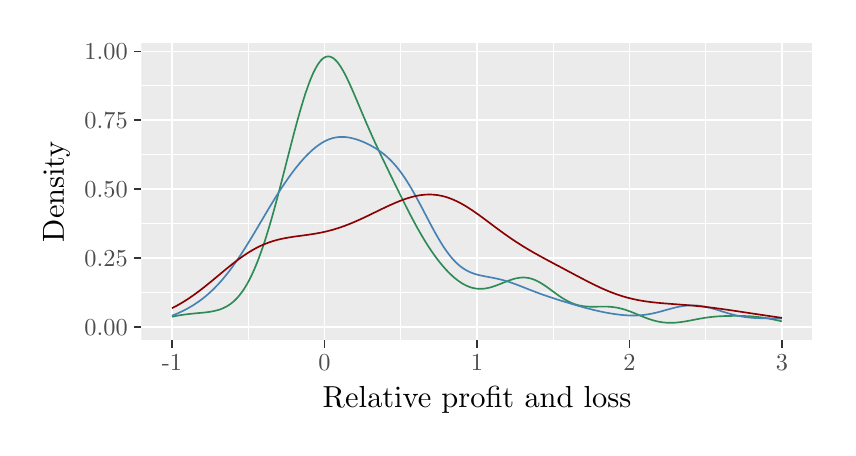
\begin{tikzpicture}[x=1pt,y=1pt]
\definecolor{fillColor}{RGB}{255,255,255}
\path[use as bounding box,fill=fillColor,fill opacity=0.00] (0,0) rectangle (289.08,144.54);
\begin{scope}
\path[clip] (  0.00,  0.00) rectangle (289.08,144.54);
\definecolor{drawColor}{RGB}{255,255,255}
\definecolor{fillColor}{RGB}{255,255,255}

\path[draw=drawColor,line width= 0.6pt,line join=round,line cap=round,fill=fillColor] (  0.00,  0.00) rectangle (289.08,144.54);
\end{scope}
\begin{scope}
\path[clip] ( 41.11, 31.53) rectangle (283.58,139.04);
\definecolor{fillColor}{gray}{0.92}

\path[fill=fillColor] ( 41.11, 31.53) rectangle (283.58,139.04);
\definecolor{drawColor}{RGB}{255,255,255}

\path[draw=drawColor,line width= 0.3pt,line join=round] ( 41.11, 48.86) --
	(283.58, 48.86);

\path[draw=drawColor,line width= 0.3pt,line join=round] ( 41.11, 73.74) --
	(283.58, 73.74);

\path[draw=drawColor,line width= 0.3pt,line join=round] ( 41.11, 98.63) --
	(283.58, 98.63);

\path[draw=drawColor,line width= 0.3pt,line join=round] ( 41.11,123.51) --
	(283.58,123.51);

\path[draw=drawColor,line width= 0.3pt,line join=round] ( 79.69, 31.53) --
	( 79.69,139.04);

\path[draw=drawColor,line width= 0.3pt,line join=round] (134.79, 31.53) --
	(134.79,139.04);

\path[draw=drawColor,line width= 0.3pt,line join=round] (189.90, 31.53) --
	(189.90,139.04);

\path[draw=drawColor,line width= 0.3pt,line join=round] (245.01, 31.53) --
	(245.01,139.04);

\path[draw=drawColor,line width= 0.6pt,line join=round] ( 41.11, 36.42) --
	(283.58, 36.42);

\path[draw=drawColor,line width= 0.6pt,line join=round] ( 41.11, 61.30) --
	(283.58, 61.30);

\path[draw=drawColor,line width= 0.6pt,line join=round] ( 41.11, 86.19) --
	(283.58, 86.19);

\path[draw=drawColor,line width= 0.6pt,line join=round] ( 41.11,111.07) --
	(283.58,111.07);

\path[draw=drawColor,line width= 0.6pt,line join=round] ( 41.11,135.95) --
	(283.58,135.95);

\path[draw=drawColor,line width= 0.6pt,line join=round] ( 52.13, 31.53) --
	( 52.13,139.04);

\path[draw=drawColor,line width= 0.6pt,line join=round] (107.24, 31.53) --
	(107.24,139.04);

\path[draw=drawColor,line width= 0.6pt,line join=round] (162.35, 31.53) --
	(162.35,139.04);

\path[draw=drawColor,line width= 0.6pt,line join=round] (217.45, 31.53) --
	(217.45,139.04);

\path[draw=drawColor,line width= 0.6pt,line join=round] (272.56, 31.53) --
	(272.56,139.04);
\definecolor{drawColor}{RGB}{46,139,87}

\path[draw=drawColor,line width= 0.6pt,line join=round] ( 52.13, 40.09) --
	( 52.56, 40.18) --
	( 52.99, 40.26) --
	( 53.43, 40.35) --
	( 53.86, 40.43) --
	( 54.29, 40.50) --
	( 54.72, 40.58) --
	( 55.15, 40.65) --
	( 55.58, 40.72) --
	( 56.01, 40.78) --
	( 56.45, 40.84) --
	( 56.88, 40.90) --
	( 57.31, 40.95) --
	( 57.74, 41.01) --
	( 58.17, 41.06) --
	( 58.60, 41.11) --
	( 59.03, 41.15) --
	( 59.47, 41.19) --
	( 59.90, 41.24) --
	( 60.33, 41.28) --
	( 60.76, 41.32) --
	( 61.19, 41.36) --
	( 61.62, 41.40) --
	( 62.05, 41.44) --
	( 62.48, 41.48) --
	( 62.92, 41.52) --
	( 63.35, 41.56) --
	( 63.78, 41.60) --
	( 64.21, 41.65) --
	( 64.64, 41.70) --
	( 65.07, 41.76) --
	( 65.50, 41.82) --
	( 65.94, 41.88) --
	( 66.37, 41.96) --
	( 66.80, 42.04) --
	( 67.23, 42.12) --
	( 67.66, 42.22) --
	( 68.09, 42.32) --
	( 68.52, 42.44) --
	( 68.96, 42.56) --
	( 69.39, 42.70) --
	( 69.82, 42.85) --
	( 70.25, 43.02) --
	( 70.68, 43.20) --
	( 71.11, 43.40) --
	( 71.54, 43.62) --
	( 71.97, 43.86) --
	( 72.41, 44.11) --
	( 72.84, 44.39) --
	( 73.27, 44.70) --
	( 73.70, 45.02) --
	( 74.13, 45.37) --
	( 74.56, 45.75) --
	( 74.99, 46.16) --
	( 75.43, 46.59) --
	( 75.86, 47.05) --
	( 76.29, 47.55) --
	( 76.72, 48.08) --
	( 77.15, 48.64) --
	( 77.58, 49.23) --
	( 78.01, 49.86) --
	( 78.45, 50.53) --
	( 78.88, 51.24) --
	( 79.31, 51.97) --
	( 79.74, 52.75) --
	( 80.17, 53.57) --
	( 80.60, 54.43) --
	( 81.03, 55.32) --
	( 81.46, 56.25) --
	( 81.90, 57.23) --
	( 82.33, 58.25) --
	( 82.76, 59.30) --
	( 83.19, 60.39) --
	( 83.62, 61.52) --
	( 84.05, 62.70) --
	( 84.48, 63.90) --
	( 84.92, 65.15) --
	( 85.35, 66.43) --
	( 85.78, 67.75) --
	( 86.21, 69.10) --
	( 86.64, 70.49) --
	( 87.07, 71.91) --
	( 87.50, 73.36) --
	( 87.94, 74.84) --
	( 88.37, 76.35) --
	( 88.80, 77.89) --
	( 89.23, 79.45) --
	( 89.66, 81.03) --
	( 90.09, 82.64) --
	( 90.52, 84.26) --
	( 90.95, 85.90) --
	( 91.39, 87.56) --
	( 91.82, 89.22) --
	( 92.25, 90.90) --
	( 92.68, 92.58) --
	( 93.11, 94.27) --
	( 93.54, 95.96) --
	( 93.97, 97.65) --
	( 94.41, 99.34) --
	( 94.84,101.02) --
	( 95.27,102.70) --
	( 95.70,104.35) --
	( 96.13,106.00) --
	( 96.56,107.63) --
	( 96.99,109.24) --
	( 97.43,110.82) --
	( 97.86,112.37) --
	( 98.29,113.90) --
	( 98.72,115.39) --
	( 99.15,116.84) --
	( 99.58,118.26) --
	(100.01,119.64) --
	(100.44,120.97) --
	(100.88,122.24) --
	(101.31,123.46) --
	(101.74,124.64) --
	(102.17,125.76) --
	(102.60,126.80) --
	(103.03,127.79) --
	(103.46,128.72) --
	(103.90,129.58) --
	(104.33,130.36) --
	(104.76,131.08) --
	(105.19,131.73) --
	(105.62,132.30) --
	(106.05,132.79) --
	(106.48,133.21) --
	(106.92,133.56) --
	(107.35,133.82) --
	(107.78,134.00) --
	(108.21,134.11) --
	(108.64,134.15) --
	(109.07,134.11) --
	(109.50,133.99) --
	(109.93,133.80) --
	(110.37,133.55) --
	(110.80,133.22) --
	(111.23,132.82) --
	(111.66,132.37) --
	(112.09,131.86) --
	(112.52,131.28) --
	(112.95,130.65) --
	(113.39,129.97) --
	(113.82,129.24) --
	(114.25,128.47) --
	(114.68,127.66) --
	(115.11,126.81) --
	(115.54,125.93) --
	(115.97,125.02) --
	(116.41,124.08) --
	(116.84,123.12) --
	(117.27,122.15) --
	(117.70,121.15) --
	(118.13,120.15) --
	(118.56,119.14) --
	(118.99,118.12) --
	(119.42,117.09) --
	(119.86,116.06) --
	(120.29,115.04) --
	(120.72,114.01) --
	(121.15,112.99) --
	(121.58,111.98) --
	(122.01,110.97) --
	(122.44,109.96) --
	(122.88,108.97) --
	(123.31,107.98) --
	(123.74,107.00) --
	(124.17,106.03) --
	(124.60,105.07) --
	(125.03,104.12) --
	(125.46,103.17) --
	(125.90,102.24) --
	(126.33,101.31) --
	(126.76,100.38) --
	(127.19, 99.46) --
	(127.62, 98.55) --
	(128.05, 97.64) --
	(128.48, 96.74) --
	(128.91, 95.84) --
	(129.35, 94.94) --
	(129.78, 94.05) --
	(130.21, 93.16) --
	(130.64, 92.27) --
	(131.07, 91.38) --
	(131.50, 90.50) --
	(131.93, 89.61) --
	(132.37, 88.73) --
	(132.80, 87.85) --
	(133.23, 86.97) --
	(133.66, 86.09) --
	(134.09, 85.21) --
	(134.52, 84.34) --
	(134.95, 83.47) --
	(135.39, 82.60) --
	(135.82, 81.74) --
	(136.25, 80.88) --
	(136.68, 80.02) --
	(137.11, 79.17) --
	(137.54, 78.33) --
	(137.97, 77.49) --
	(138.40, 76.66) --
	(138.84, 75.84) --
	(139.27, 75.03) --
	(139.70, 74.22) --
	(140.13, 73.42) --
	(140.56, 72.64) --
	(140.99, 71.86) --
	(141.42, 71.10) --
	(141.86, 70.34) --
	(142.29, 69.60) --
	(142.72, 68.87) --
	(143.15, 68.14) --
	(143.58, 67.44) --
	(144.01, 66.74) --
	(144.44, 66.06) --
	(144.88, 65.39) --
	(145.31, 64.73) --
	(145.74, 64.09) --
	(146.17, 63.45) --
	(146.60, 62.83) --
	(147.03, 62.23) --
	(147.46, 61.64) --
	(147.89, 61.06) --
	(148.33, 60.49) --
	(148.76, 59.94) --
	(149.19, 59.41) --
	(149.62, 58.88) --
	(150.05, 58.37) --
	(150.48, 57.87) --
	(150.91, 57.39) --
	(151.35, 56.92) --
	(151.78, 56.46) --
	(152.21, 56.02) --
	(152.64, 55.60) --
	(153.07, 55.19) --
	(153.50, 54.79) --
	(153.93, 54.40) --
	(154.37, 54.04) --
	(154.80, 53.69) --
	(155.23, 53.35) --
	(155.66, 53.03) --
	(156.09, 52.73) --
	(156.52, 52.44) --
	(156.95, 52.17) --
	(157.38, 51.91) --
	(157.82, 51.68) --
	(158.25, 51.46) --
	(158.68, 51.25) --
	(159.11, 51.07) --
	(159.54, 50.90) --
	(159.97, 50.75) --
	(160.40, 50.61) --
	(160.84, 50.50) --
	(161.27, 50.40) --
	(161.70, 50.32) --
	(162.13, 50.26) --
	(162.56, 50.21) --
	(162.99, 50.18) --
	(163.42, 50.17) --
	(163.86, 50.17) --
	(164.29, 50.19) --
	(164.72, 50.23) --
	(165.15, 50.27) --
	(165.58, 50.34) --
	(166.01, 50.41) --
	(166.44, 50.50) --
	(166.87, 50.61) --
	(167.31, 50.72) --
	(167.74, 50.84) --
	(168.17, 50.98) --
	(168.60, 51.12) --
	(169.03, 51.27) --
	(169.46, 51.43) --
	(169.89, 51.59) --
	(170.33, 51.76) --
	(170.76, 51.93) --
	(171.19, 52.10) --
	(171.62, 52.28) --
	(172.05, 52.45) --
	(172.48, 52.62) --
	(172.91, 52.79) --
	(173.35, 52.96) --
	(173.78, 53.12) --
	(174.21, 53.28) --
	(174.64, 53.43) --
	(175.07, 53.57) --
	(175.50, 53.70) --
	(175.93, 53.82) --
	(176.36, 53.92) --
	(176.80, 54.01) --
	(177.23, 54.09) --
	(177.66, 54.16) --
	(178.09, 54.21) --
	(178.52, 54.24) --
	(178.95, 54.25) --
	(179.38, 54.25) --
	(179.82, 54.23) --
	(180.25, 54.19) --
	(180.68, 54.13) --
	(181.11, 54.05) --
	(181.54, 53.95) --
	(181.97, 53.83) --
	(182.40, 53.70) --
	(182.84, 53.55) --
	(183.27, 53.37) --
	(183.70, 53.18) --
	(184.13, 52.98) --
	(184.56, 52.76) --
	(184.99, 52.52) --
	(185.42, 52.27) --
	(185.85, 52.01) --
	(186.29, 51.74) --
	(186.72, 51.45) --
	(187.15, 51.16) --
	(187.58, 50.86) --
	(188.01, 50.55) --
	(188.44, 50.24) --
	(188.87, 49.92) --
	(189.31, 49.60) --
	(189.74, 49.28) --
	(190.17, 48.97) --
	(190.60, 48.65) --
	(191.03, 48.34) --
	(191.46, 48.03) --
	(191.89, 47.73) --
	(192.33, 47.43) --
	(192.76, 47.14) --
	(193.19, 46.86) --
	(193.62, 46.59) --
	(194.05, 46.33) --
	(194.48, 46.09) --
	(194.91, 45.85) --
	(195.34, 45.62) --
	(195.78, 45.41) --
	(196.21, 45.21) --
	(196.64, 45.03) --
	(197.07, 44.86) --
	(197.50, 44.70) --
	(197.93, 44.55) --
	(198.36, 44.42) --
	(198.80, 44.30) --
	(199.23, 44.19) --
	(199.66, 44.10) --
	(200.09, 44.02) --
	(200.52, 43.94) --
	(200.95, 43.88) --
	(201.38, 43.83) --
	(201.82, 43.79) --
	(202.25, 43.76) --
	(202.68, 43.74) --
	(203.11, 43.72) --
	(203.54, 43.71) --
	(203.97, 43.70) --
	(204.40, 43.70) --
	(204.83, 43.71) --
	(205.27, 43.71) --
	(205.70, 43.72) --
	(206.13, 43.73) --
	(206.56, 43.74) --
	(206.99, 43.75) --
	(207.42, 43.75) --
	(207.85, 43.75) --
	(208.29, 43.75) --
	(208.72, 43.75) --
	(209.15, 43.74) --
	(209.58, 43.73) --
	(210.01, 43.71) --
	(210.44, 43.68) --
	(210.87, 43.64) --
	(211.31, 43.60) --
	(211.74, 43.55) --
	(212.17, 43.49) --
	(212.60, 43.42) --
	(213.03, 43.34) --
	(213.46, 43.26) --
	(213.89, 43.16) --
	(214.32, 43.06) --
	(214.76, 42.94) --
	(215.19, 42.82) --
	(215.62, 42.70) --
	(216.05, 42.56) --
	(216.48, 42.41) --
	(216.91, 42.26) --
	(217.34, 42.11) --
	(217.78, 41.95) --
	(218.21, 41.78) --
	(218.64, 41.61) --
	(219.07, 41.43) --
	(219.50, 41.26) --
	(219.93, 41.08) --
	(220.36, 40.90) --
	(220.80, 40.72) --
	(221.23, 40.54) --
	(221.66, 40.36) --
	(222.09, 40.19) --
	(222.52, 40.01) --
	(222.95, 39.84) --
	(223.38, 39.68) --
	(223.81, 39.52) --
	(224.25, 39.36) --
	(224.68, 39.21) --
	(225.11, 39.07) --
	(225.54, 38.93) --
	(225.97, 38.80) --
	(226.40, 38.68) --
	(226.83, 38.57) --
	(227.27, 38.46) --
	(227.70, 38.37) --
	(228.13, 38.28) --
	(228.56, 38.20) --
	(228.99, 38.13) --
	(229.42, 38.07) --
	(229.85, 38.02) --
	(230.29, 37.97) --
	(230.72, 37.94) --
	(231.15, 37.91) --
	(231.58, 37.90) --
	(232.01, 37.89) --
	(232.44, 37.89) --
	(232.87, 37.89) --
	(233.30, 37.91) --
	(233.74, 37.93) --
	(234.17, 37.96) --
	(234.60, 38.00) --
	(235.03, 38.04) --
	(235.46, 38.09) --
	(235.89, 38.14) --
	(236.32, 38.20) --
	(236.76, 38.26) --
	(237.19, 38.33) --
	(237.62, 38.40) --
	(238.05, 38.47) --
	(238.48, 38.55) --
	(238.91, 38.63) --
	(239.34, 38.71) --
	(239.78, 38.79) --
	(240.21, 38.88) --
	(240.64, 38.96) --
	(241.07, 39.04) --
	(241.50, 39.13) --
	(241.93, 39.21) --
	(242.36, 39.29) --
	(242.79, 39.37) --
	(243.23, 39.44) --
	(243.66, 39.52) --
	(244.09, 39.59) --
	(244.52, 39.66) --
	(244.95, 39.73) --
	(245.38, 39.79) --
	(245.81, 39.85) --
	(246.25, 39.90) --
	(246.68, 39.96) --
	(247.11, 40.01) --
	(247.54, 40.05) --
	(247.97, 40.09) --
	(248.40, 40.13) --
	(248.83, 40.17) --
	(249.27, 40.20) --
	(249.70, 40.23) --
	(250.13, 40.25) --
	(250.56, 40.28) --
	(250.99, 40.30) --
	(251.42, 40.32) --
	(251.85, 40.33) --
	(252.28, 40.34) --
	(252.72, 40.36) --
	(253.15, 40.37) --
	(253.58, 40.37) --
	(254.01, 40.38) --
	(254.44, 40.38) --
	(254.87, 40.39) --
	(255.30, 40.39) --
	(255.74, 40.39) --
	(256.17, 40.39) --
	(256.60, 40.38) --
	(257.03, 40.38) --
	(257.46, 40.37) --
	(257.89, 40.36) --
	(258.32, 40.35) --
	(258.76, 40.34) --
	(259.19, 40.33) --
	(259.62, 40.31) --
	(260.05, 40.29) --
	(260.48, 40.27) --
	(260.91, 40.25) --
	(261.34, 40.22) --
	(261.77, 40.19) --
	(262.21, 40.16) --
	(262.64, 40.12) --
	(263.07, 40.08) --
	(263.50, 40.04) --
	(263.93, 39.99) --
	(264.36, 39.94) --
	(264.79, 39.89) --
	(265.23, 39.83) --
	(265.66, 39.77) --
	(266.09, 39.70) --
	(266.52, 39.63) --
	(266.95, 39.56) --
	(267.38, 39.49) --
	(267.81, 39.41) --
	(268.25, 39.33) --
	(268.68, 39.24) --
	(269.11, 39.16) --
	(269.54, 39.07) --
	(269.97, 38.98) --
	(270.40, 38.89) --
	(270.83, 38.79) --
	(271.26, 38.70) --
	(271.70, 38.60) --
	(272.13, 38.51) --
	(272.56, 38.42);
\definecolor{drawColor}{RGB}{70,130,180}

\path[draw=drawColor,line width= 0.6pt,line join=round] ( 52.13, 40.46) --
	( 52.56, 40.63) --
	( 52.99, 40.81) --
	( 53.43, 40.98) --
	( 53.86, 41.16) --
	( 54.29, 41.35) --
	( 54.72, 41.54) --
	( 55.15, 41.74) --
	( 55.58, 41.94) --
	( 56.01, 42.15) --
	( 56.45, 42.36) --
	( 56.88, 42.58) --
	( 57.31, 42.81) --
	( 57.74, 43.04) --
	( 58.17, 43.28) --
	( 58.60, 43.53) --
	( 59.03, 43.78) --
	( 59.47, 44.04) --
	( 59.90, 44.30) --
	( 60.33, 44.58) --
	( 60.76, 44.86) --
	( 61.19, 45.15) --
	( 61.62, 45.45) --
	( 62.05, 45.75) --
	( 62.48, 46.07) --
	( 62.92, 46.39) --
	( 63.35, 46.73) --
	( 63.78, 47.07) --
	( 64.21, 47.42) --
	( 64.64, 47.78) --
	( 65.07, 48.15) --
	( 65.50, 48.53) --
	( 65.94, 48.92) --
	( 66.37, 49.32) --
	( 66.80, 49.73) --
	( 67.23, 50.15) --
	( 67.66, 50.59) --
	( 68.09, 51.03) --
	( 68.52, 51.48) --
	( 68.96, 51.94) --
	( 69.39, 52.42) --
	( 69.82, 52.90) --
	( 70.25, 53.40) --
	( 70.68, 53.90) --
	( 71.11, 54.42) --
	( 71.54, 54.95) --
	( 71.97, 55.48) --
	( 72.41, 56.03) --
	( 72.84, 56.59) --
	( 73.27, 57.16) --
	( 73.70, 57.74) --
	( 74.13, 58.33) --
	( 74.56, 58.93) --
	( 74.99, 59.54) --
	( 75.43, 60.16) --
	( 75.86, 60.79) --
	( 76.29, 61.42) --
	( 76.72, 62.07) --
	( 77.15, 62.72) --
	( 77.58, 63.38) --
	( 78.01, 64.05) --
	( 78.45, 64.73) --
	( 78.88, 65.42) --
	( 79.31, 66.11) --
	( 79.74, 66.81) --
	( 80.17, 67.51) --
	( 80.60, 68.22) --
	( 81.03, 68.93) --
	( 81.46, 69.65) --
	( 81.90, 70.37) --
	( 82.33, 71.09) --
	( 82.76, 71.82) --
	( 83.19, 72.55) --
	( 83.62, 73.28) --
	( 84.05, 74.01) --
	( 84.48, 74.75) --
	( 84.92, 75.48) --
	( 85.35, 76.21) --
	( 85.78, 76.94) --
	( 86.21, 77.67) --
	( 86.64, 78.39) --
	( 87.07, 79.11) --
	( 87.50, 79.83) --
	( 87.94, 80.55) --
	( 88.37, 81.26) --
	( 88.80, 81.96) --
	( 89.23, 82.66) --
	( 89.66, 83.36) --
	( 90.09, 84.05) --
	( 90.52, 84.73) --
	( 90.95, 85.40) --
	( 91.39, 86.07) --
	( 91.82, 86.73) --
	( 92.25, 87.38) --
	( 92.68, 88.02) --
	( 93.11, 88.66) --
	( 93.54, 89.28) --
	( 93.97, 89.90) --
	( 94.41, 90.51) --
	( 94.84, 91.11) --
	( 95.27, 91.70) --
	( 95.70, 92.28) --
	( 96.13, 92.85) --
	( 96.56, 93.41) --
	( 96.99, 93.96) --
	( 97.43, 94.50) --
	( 97.86, 95.03) --
	( 98.29, 95.55) --
	( 98.72, 96.05) --
	( 99.15, 96.55) --
	( 99.58, 97.04) --
	(100.01, 97.51) --
	(100.44, 97.97) --
	(100.88, 98.42) --
	(101.31, 98.85) --
	(101.74, 99.27) --
	(102.17, 99.68) --
	(102.60,100.08) --
	(103.03,100.46) --
	(103.46,100.83) --
	(103.90,101.19) --
	(104.33,101.53) --
	(104.76,101.85) --
	(105.19,102.17) --
	(105.62,102.46) --
	(106.05,102.74) --
	(106.48,103.01) --
	(106.92,103.26) --
	(107.35,103.49) --
	(107.78,103.70) --
	(108.21,103.90) --
	(108.64,104.09) --
	(109.07,104.26) --
	(109.50,104.41) --
	(109.93,104.54) --
	(110.37,104.66) --
	(110.80,104.76) --
	(111.23,104.85) --
	(111.66,104.92) --
	(112.09,104.98) --
	(112.52,105.02) --
	(112.95,105.05) --
	(113.39,105.06) --
	(113.82,105.06) --
	(114.25,105.04) --
	(114.68,105.01) --
	(115.11,104.97) --
	(115.54,104.92) --
	(115.97,104.85) --
	(116.41,104.78) --
	(116.84,104.69) --
	(117.27,104.59) --
	(117.70,104.48) --
	(118.13,104.36) --
	(118.56,104.24) --
	(118.99,104.10) --
	(119.42,103.96) --
	(119.86,103.80) --
	(120.29,103.64) --
	(120.72,103.47) --
	(121.15,103.30) --
	(121.58,103.11) --
	(122.01,102.92) --
	(122.44,102.72) --
	(122.88,102.51) --
	(123.31,102.30) --
	(123.74,102.07) --
	(124.17,101.84) --
	(124.60,101.60) --
	(125.03,101.35) --
	(125.46,101.10) --
	(125.90,100.83) --
	(126.33,100.55) --
	(126.76,100.27) --
	(127.19, 99.97) --
	(127.62, 99.66) --
	(128.05, 99.34) --
	(128.48, 99.01) --
	(128.91, 98.66) --
	(129.35, 98.30) --
	(129.78, 97.92) --
	(130.21, 97.54) --
	(130.64, 97.13) --
	(131.07, 96.71) --
	(131.50, 96.27) --
	(131.93, 95.82) --
	(132.37, 95.34) --
	(132.80, 94.85) --
	(133.23, 94.35) --
	(133.66, 93.82) --
	(134.09, 93.28) --
	(134.52, 92.72) --
	(134.95, 92.13) --
	(135.39, 91.53) --
	(135.82, 90.91) --
	(136.25, 90.28) --
	(136.68, 89.62) --
	(137.11, 88.95) --
	(137.54, 88.26) --
	(137.97, 87.56) --
	(138.40, 86.84) --
	(138.84, 86.10) --
	(139.27, 85.35) --
	(139.70, 84.59) --
	(140.13, 83.81) --
	(140.56, 83.03) --
	(140.99, 82.23) --
	(141.42, 81.43) --
	(141.86, 80.62) --
	(142.29, 79.80) --
	(142.72, 78.98) --
	(143.15, 78.15) --
	(143.58, 77.32) --
	(144.01, 76.50) --
	(144.44, 75.67) --
	(144.88, 74.85) --
	(145.31, 74.03) --
	(145.74, 73.21) --
	(146.17, 72.41) --
	(146.60, 71.61) --
	(147.03, 70.82) --
	(147.46, 70.05) --
	(147.89, 69.29) --
	(148.33, 68.54) --
	(148.76, 67.81) --
	(149.19, 67.10) --
	(149.62, 66.40) --
	(150.05, 65.72) --
	(150.48, 65.06) --
	(150.91, 64.42) --
	(151.35, 63.80) --
	(151.78, 63.21) --
	(152.21, 62.64) --
	(152.64, 62.09) --
	(153.07, 61.56) --
	(153.50, 61.05) --
	(153.93, 60.58) --
	(154.37, 60.12) --
	(154.80, 59.68) --
	(155.23, 59.27) --
	(155.66, 58.89) --
	(156.09, 58.52) --
	(156.52, 58.18) --
	(156.95, 57.86) --
	(157.38, 57.56) --
	(157.82, 57.28) --
	(158.25, 57.02) --
	(158.68, 56.78) --
	(159.11, 56.55) --
	(159.54, 56.34) --
	(159.97, 56.15) --
	(160.40, 55.97) --
	(160.84, 55.81) --
	(161.27, 55.66) --
	(161.70, 55.52) --
	(162.13, 55.39) --
	(162.56, 55.27) --
	(162.99, 55.16) --
	(163.42, 55.06) --
	(163.86, 54.96) --
	(164.29, 54.87) --
	(164.72, 54.79) --
	(165.15, 54.70) --
	(165.58, 54.62) --
	(166.01, 54.54) --
	(166.44, 54.46) --
	(166.87, 54.38) --
	(167.31, 54.30) --
	(167.74, 54.22) --
	(168.17, 54.14) --
	(168.60, 54.05) --
	(169.03, 53.96) --
	(169.46, 53.87) --
	(169.89, 53.77) --
	(170.33, 53.67) --
	(170.76, 53.57) --
	(171.19, 53.46) --
	(171.62, 53.35) --
	(172.05, 53.23) --
	(172.48, 53.10) --
	(172.91, 52.98) --
	(173.35, 52.85) --
	(173.78, 52.71) --
	(174.21, 52.57) --
	(174.64, 52.42) --
	(175.07, 52.28) --
	(175.50, 52.12) --
	(175.93, 51.97) --
	(176.36, 51.81) --
	(176.80, 51.65) --
	(177.23, 51.49) --
	(177.66, 51.32) --
	(178.09, 51.15) --
	(178.52, 50.98) --
	(178.95, 50.82) --
	(179.38, 50.65) --
	(179.82, 50.47) --
	(180.25, 50.30) --
	(180.68, 50.13) --
	(181.11, 49.96) --
	(181.54, 49.79) --
	(181.97, 49.62) --
	(182.40, 49.46) --
	(182.84, 49.29) --
	(183.27, 49.13) --
	(183.70, 48.96) --
	(184.13, 48.80) --
	(184.56, 48.64) --
	(184.99, 48.48) --
	(185.42, 48.32) --
	(185.85, 48.17) --
	(186.29, 48.01) --
	(186.72, 47.86) --
	(187.15, 47.71) --
	(187.58, 47.56) --
	(188.01, 47.42) --
	(188.44, 47.27) --
	(188.87, 47.13) --
	(189.31, 46.99) --
	(189.74, 46.85) --
	(190.17, 46.71) --
	(190.60, 46.57) --
	(191.03, 46.43) --
	(191.46, 46.29) --
	(191.89, 46.16) --
	(192.33, 46.02) --
	(192.76, 45.89) --
	(193.19, 45.75) --
	(193.62, 45.62) --
	(194.05, 45.49) --
	(194.48, 45.36) --
	(194.91, 45.23) --
	(195.34, 45.10) --
	(195.78, 44.97) --
	(196.21, 44.84) --
	(196.64, 44.71) --
	(197.07, 44.58) --
	(197.50, 44.45) --
	(197.93, 44.33) --
	(198.36, 44.20) --
	(198.80, 44.08) --
	(199.23, 43.95) --
	(199.66, 43.83) --
	(200.09, 43.71) --
	(200.52, 43.59) --
	(200.95, 43.47) --
	(201.38, 43.35) --
	(201.82, 43.23) --
	(202.25, 43.12) --
	(202.68, 43.01) --
	(203.11, 42.90) --
	(203.54, 42.79) --
	(203.97, 42.68) --
	(204.40, 42.57) --
	(204.83, 42.47) --
	(205.27, 42.37) --
	(205.70, 42.27) --
	(206.13, 42.17) --
	(206.56, 42.07) --
	(206.99, 41.98) --
	(207.42, 41.89) --
	(207.85, 41.80) --
	(208.29, 41.71) --
	(208.72, 41.63) --
	(209.15, 41.55) --
	(209.58, 41.47) --
	(210.01, 41.39) --
	(210.44, 41.32) --
	(210.87, 41.25) --
	(211.31, 41.18) --
	(211.74, 41.11) --
	(212.17, 41.05) --
	(212.60, 40.99) --
	(213.03, 40.93) --
	(213.46, 40.88) --
	(213.89, 40.83) --
	(214.32, 40.78) --
	(214.76, 40.73) --
	(215.19, 40.69) --
	(215.62, 40.66) --
	(216.05, 40.63) --
	(216.48, 40.60) --
	(216.91, 40.57) --
	(217.34, 40.55) --
	(217.78, 40.54) --
	(218.21, 40.53) --
	(218.64, 40.53) --
	(219.07, 40.53) --
	(219.50, 40.53) --
	(219.93, 40.54) --
	(220.36, 40.56) --
	(220.80, 40.58) --
	(221.23, 40.61) --
	(221.66, 40.65) --
	(222.09, 40.69) --
	(222.52, 40.73) --
	(222.95, 40.79) --
	(223.38, 40.84) --
	(223.81, 40.91) --
	(224.25, 40.98) --
	(224.68, 41.05) --
	(225.11, 41.13) --
	(225.54, 41.22) --
	(225.97, 41.31) --
	(226.40, 41.40) --
	(226.83, 41.50) --
	(227.27, 41.61) --
	(227.70, 41.71) --
	(228.13, 41.82) --
	(228.56, 41.94) --
	(228.99, 42.05) --
	(229.42, 42.17) --
	(229.85, 42.29) --
	(230.29, 42.41) --
	(230.72, 42.53) --
	(231.15, 42.65) --
	(231.58, 42.77) --
	(232.01, 42.89) --
	(232.44, 43.00) --
	(232.87, 43.12) --
	(233.30, 43.23) --
	(233.74, 43.33) --
	(234.17, 43.44) --
	(234.60, 43.53) --
	(235.03, 43.63) --
	(235.46, 43.72) --
	(235.89, 43.80) --
	(236.32, 43.87) --
	(236.76, 43.94) --
	(237.19, 44.00) --
	(237.62, 44.05) --
	(238.05, 44.10) --
	(238.48, 44.14) --
	(238.91, 44.17) --
	(239.34, 44.19) --
	(239.78, 44.20) --
	(240.21, 44.20) --
	(240.64, 44.19) --
	(241.07, 44.18) --
	(241.50, 44.15) --
	(241.93, 44.12) --
	(242.36, 44.08) --
	(242.79, 44.03) --
	(243.23, 43.98) --
	(243.66, 43.91) --
	(244.09, 43.84) --
	(244.52, 43.76) --
	(244.95, 43.67) --
	(245.38, 43.58) --
	(245.81, 43.48) --
	(246.25, 43.37) --
	(246.68, 43.26) --
	(247.11, 43.15) --
	(247.54, 43.03) --
	(247.97, 42.90) --
	(248.40, 42.78) --
	(248.83, 42.65) --
	(249.27, 42.52) --
	(249.70, 42.39) --
	(250.13, 42.25) --
	(250.56, 42.12) --
	(250.99, 41.98) --
	(251.42, 41.85) --
	(251.85, 41.72) --
	(252.28, 41.59) --
	(252.72, 41.46) --
	(253.15, 41.33) --
	(253.58, 41.21) --
	(254.01, 41.09) --
	(254.44, 40.97) --
	(254.87, 40.86) --
	(255.30, 40.75) --
	(255.74, 40.64) --
	(256.17, 40.54) --
	(256.60, 40.45) --
	(257.03, 40.36) --
	(257.46, 40.27) --
	(257.89, 40.19) --
	(258.32, 40.12) --
	(258.76, 40.05) --
	(259.19, 39.98) --
	(259.62, 39.92) --
	(260.05, 39.87) --
	(260.48, 39.82) --
	(260.91, 39.78) --
	(261.34, 39.74) --
	(261.77, 39.70) --
	(262.21, 39.67) --
	(262.64, 39.64) --
	(263.07, 39.62) --
	(263.50, 39.60) --
	(263.93, 39.58) --
	(264.36, 39.57) --
	(264.79, 39.56) --
	(265.23, 39.55) --
	(265.66, 39.54) --
	(266.09, 39.53) --
	(266.52, 39.53) --
	(266.95, 39.52) --
	(267.38, 39.52) --
	(267.81, 39.52) --
	(268.25, 39.51) --
	(268.68, 39.51) --
	(269.11, 39.50) --
	(269.54, 39.49) --
	(269.97, 39.49) --
	(270.40, 39.47) --
	(270.83, 39.46) --
	(271.26, 39.45) --
	(271.70, 39.43) --
	(272.13, 39.41) --
	(272.56, 39.39);
\definecolor{drawColor}{RGB}{139,0,0}

\path[draw=drawColor,line width= 0.6pt,line join=round] ( 52.13, 43.16) --
	( 52.56, 43.38) --
	( 52.99, 43.60) --
	( 53.43, 43.83) --
	( 53.86, 44.06) --
	( 54.29, 44.30) --
	( 54.72, 44.55) --
	( 55.15, 44.79) --
	( 55.58, 45.05) --
	( 56.01, 45.31) --
	( 56.45, 45.57) --
	( 56.88, 45.84) --
	( 57.31, 46.12) --
	( 57.74, 46.39) --
	( 58.17, 46.68) --
	( 58.60, 46.97) --
	( 59.03, 47.26) --
	( 59.47, 47.56) --
	( 59.90, 47.86) --
	( 60.33, 48.17) --
	( 60.76, 48.49) --
	( 61.19, 48.80) --
	( 61.62, 49.12) --
	( 62.05, 49.45) --
	( 62.48, 49.78) --
	( 62.92, 50.11) --
	( 63.35, 50.44) --
	( 63.78, 50.78) --
	( 64.21, 51.13) --
	( 64.64, 51.47) --
	( 65.07, 51.82) --
	( 65.50, 52.17) --
	( 65.94, 52.52) --
	( 66.37, 52.87) --
	( 66.80, 53.23) --
	( 67.23, 53.59) --
	( 67.66, 53.94) --
	( 68.09, 54.30) --
	( 68.52, 54.66) --
	( 68.96, 55.02) --
	( 69.39, 55.38) --
	( 69.82, 55.74) --
	( 70.25, 56.10) --
	( 70.68, 56.46) --
	( 71.11, 56.81) --
	( 71.54, 57.17) --
	( 71.97, 57.52) --
	( 72.41, 57.87) --
	( 72.84, 58.22) --
	( 73.27, 58.57) --
	( 73.70, 58.91) --
	( 74.13, 59.25) --
	( 74.56, 59.59) --
	( 74.99, 59.92) --
	( 75.43, 60.25) --
	( 75.86, 60.57) --
	( 76.29, 60.89) --
	( 76.72, 61.21) --
	( 77.15, 61.52) --
	( 77.58, 61.82) --
	( 78.01, 62.12) --
	( 78.45, 62.41) --
	( 78.88, 62.70) --
	( 79.31, 62.98) --
	( 79.74, 63.26) --
	( 80.17, 63.53) --
	( 80.60, 63.79) --
	( 81.03, 64.04) --
	( 81.46, 64.29) --
	( 81.90, 64.53) --
	( 82.33, 64.77) --
	( 82.76, 65.00) --
	( 83.19, 65.22) --
	( 83.62, 65.43) --
	( 84.05, 65.64) --
	( 84.48, 65.84) --
	( 84.92, 66.03) --
	( 85.35, 66.22) --
	( 85.78, 66.40) --
	( 86.21, 66.57) --
	( 86.64, 66.73) --
	( 87.07, 66.89) --
	( 87.50, 67.04) --
	( 87.94, 67.19) --
	( 88.37, 67.33) --
	( 88.80, 67.46) --
	( 89.23, 67.59) --
	( 89.66, 67.71) --
	( 90.09, 67.83) --
	( 90.52, 67.94) --
	( 90.95, 68.04) --
	( 91.39, 68.14) --
	( 91.82, 68.24) --
	( 92.25, 68.33) --
	( 92.68, 68.42) --
	( 93.11, 68.50) --
	( 93.54, 68.58) --
	( 93.97, 68.66) --
	( 94.41, 68.73) --
	( 94.84, 68.80) --
	( 95.27, 68.87) --
	( 95.70, 68.94) --
	( 96.13, 69.00) --
	( 96.56, 69.06) --
	( 96.99, 69.12) --
	( 97.43, 69.18) --
	( 97.86, 69.24) --
	( 98.29, 69.30) --
	( 98.72, 69.35) --
	( 99.15, 69.41) --
	( 99.58, 69.47) --
	(100.01, 69.53) --
	(100.44, 69.58) --
	(100.88, 69.64) --
	(101.31, 69.70) --
	(101.74, 69.77) --
	(102.17, 69.83) --
	(102.60, 69.90) --
	(103.03, 69.96) --
	(103.46, 70.03) --
	(103.90, 70.10) --
	(104.33, 70.18) --
	(104.76, 70.26) --
	(105.19, 70.33) --
	(105.62, 70.42) --
	(106.05, 70.50) --
	(106.48, 70.59) --
	(106.92, 70.69) --
	(107.35, 70.78) --
	(107.78, 70.88) --
	(108.21, 70.98) --
	(108.64, 71.09) --
	(109.07, 71.20) --
	(109.50, 71.32) --
	(109.93, 71.43) --
	(110.37, 71.56) --
	(110.80, 71.68) --
	(111.23, 71.81) --
	(111.66, 71.95) --
	(112.09, 72.08) --
	(112.52, 72.22) --
	(112.95, 72.37) --
	(113.39, 72.52) --
	(113.82, 72.67) --
	(114.25, 72.82) --
	(114.68, 72.98) --
	(115.11, 73.15) --
	(115.54, 73.31) --
	(115.97, 73.48) --
	(116.41, 73.65) --
	(116.84, 73.83) --
	(117.27, 74.01) --
	(117.70, 74.19) --
	(118.13, 74.37) --
	(118.56, 74.56) --
	(118.99, 74.75) --
	(119.42, 74.94) --
	(119.86, 75.13) --
	(120.29, 75.33) --
	(120.72, 75.53) --
	(121.15, 75.73) --
	(121.58, 75.93) --
	(122.01, 76.13) --
	(122.44, 76.34) --
	(122.88, 76.55) --
	(123.31, 76.75) --
	(123.74, 76.96) --
	(124.17, 77.17) --
	(124.60, 77.38) --
	(125.03, 77.59) --
	(125.46, 77.80) --
	(125.90, 78.01) --
	(126.33, 78.22) --
	(126.76, 78.43) --
	(127.19, 78.64) --
	(127.62, 78.85) --
	(128.05, 79.05) --
	(128.48, 79.26) --
	(128.91, 79.47) --
	(129.35, 79.67) --
	(129.78, 79.87) --
	(130.21, 80.07) --
	(130.64, 80.27) --
	(131.07, 80.47) --
	(131.50, 80.66) --
	(131.93, 80.85) --
	(132.37, 81.04) --
	(132.80, 81.23) --
	(133.23, 81.41) --
	(133.66, 81.59) --
	(134.09, 81.76) --
	(134.52, 81.93) --
	(134.95, 82.10) --
	(135.39, 82.26) --
	(135.82, 82.42) --
	(136.25, 82.57) --
	(136.68, 82.71) --
	(137.11, 82.86) --
	(137.54, 82.99) --
	(137.97, 83.12) --
	(138.40, 83.25) --
	(138.84, 83.36) --
	(139.27, 83.48) --
	(139.70, 83.58) --
	(140.13, 83.68) --
	(140.56, 83.77) --
	(140.99, 83.85) --
	(141.42, 83.93) --
	(141.86, 84.00) --
	(142.29, 84.06) --
	(142.72, 84.11) --
	(143.15, 84.15) --
	(143.58, 84.19) --
	(144.01, 84.22) --
	(144.44, 84.23) --
	(144.88, 84.24) --
	(145.31, 84.25) --
	(145.74, 84.24) --
	(146.17, 84.22) --
	(146.60, 84.19) --
	(147.03, 84.16) --
	(147.46, 84.11) --
	(147.89, 84.06) --
	(148.33, 84.00) --
	(148.76, 83.92) --
	(149.19, 83.84) --
	(149.62, 83.75) --
	(150.05, 83.65) --
	(150.48, 83.54) --
	(150.91, 83.42) --
	(151.35, 83.29) --
	(151.78, 83.15) --
	(152.21, 83.00) --
	(152.64, 82.84) --
	(153.07, 82.68) --
	(153.50, 82.51) --
	(153.93, 82.32) --
	(154.37, 82.13) --
	(154.80, 81.93) --
	(155.23, 81.73) --
	(155.66, 81.51) --
	(156.09, 81.29) --
	(156.52, 81.06) --
	(156.95, 80.82) --
	(157.38, 80.58) --
	(157.82, 80.33) --
	(158.25, 80.07) --
	(158.68, 79.81) --
	(159.11, 79.54) --
	(159.54, 79.26) --
	(159.97, 78.98) --
	(160.40, 78.70) --
	(160.84, 78.41) --
	(161.27, 78.11) --
	(161.70, 77.81) --
	(162.13, 77.51) --
	(162.56, 77.21) --
	(162.99, 76.90) --
	(163.42, 76.59) --
	(163.86, 76.27) --
	(164.29, 75.96) --
	(164.72, 75.64) --
	(165.15, 75.32) --
	(165.58, 75.00) --
	(166.01, 74.68) --
	(166.44, 74.35) --
	(166.87, 74.03) --
	(167.31, 73.71) --
	(167.74, 73.38) --
	(168.17, 73.06) --
	(168.60, 72.74) --
	(169.03, 72.42) --
	(169.46, 72.09) --
	(169.89, 71.77) --
	(170.33, 71.46) --
	(170.76, 71.14) --
	(171.19, 70.82) --
	(171.62, 70.51) --
	(172.05, 70.20) --
	(172.48, 69.89) --
	(172.91, 69.58) --
	(173.35, 69.28) --
	(173.78, 68.98) --
	(174.21, 68.68) --
	(174.64, 68.38) --
	(175.07, 68.09) --
	(175.50, 67.80) --
	(175.93, 67.51) --
	(176.36, 67.23) --
	(176.80, 66.95) --
	(177.23, 66.67) --
	(177.66, 66.39) --
	(178.09, 66.12) --
	(178.52, 65.84) --
	(178.95, 65.58) --
	(179.38, 65.31) --
	(179.82, 65.05) --
	(180.25, 64.79) --
	(180.68, 64.53) --
	(181.11, 64.28) --
	(181.54, 64.02) --
	(181.97, 63.77) --
	(182.40, 63.52) --
	(182.84, 63.28) --
	(183.27, 63.03) --
	(183.70, 62.79) --
	(184.13, 62.55) --
	(184.56, 62.31) --
	(184.99, 62.07) --
	(185.42, 61.83) --
	(185.85, 61.60) --
	(186.29, 61.36) --
	(186.72, 61.13) --
	(187.15, 60.90) --
	(187.58, 60.66) --
	(188.01, 60.43) --
	(188.44, 60.20) --
	(188.87, 59.97) --
	(189.31, 59.74) --
	(189.74, 59.51) --
	(190.17, 59.28) --
	(190.60, 59.05) --
	(191.03, 58.82) --
	(191.46, 58.60) --
	(191.89, 58.37) --
	(192.33, 58.14) --
	(192.76, 57.91) --
	(193.19, 57.68) --
	(193.62, 57.45) --
	(194.05, 57.22) --
	(194.48, 56.99) --
	(194.91, 56.76) --
	(195.34, 56.53) --
	(195.78, 56.30) --
	(196.21, 56.07) --
	(196.64, 55.84) --
	(197.07, 55.61) --
	(197.50, 55.38) --
	(197.93, 55.15) --
	(198.36, 54.92) --
	(198.80, 54.70) --
	(199.23, 54.47) --
	(199.66, 54.24) --
	(200.09, 54.01) --
	(200.52, 53.79) --
	(200.95, 53.56) --
	(201.38, 53.34) --
	(201.82, 53.12) --
	(202.25, 52.89) --
	(202.68, 52.67) --
	(203.11, 52.45) --
	(203.54, 52.24) --
	(203.97, 52.02) --
	(204.40, 51.81) --
	(204.83, 51.60) --
	(205.27, 51.39) --
	(205.70, 51.18) --
	(206.13, 50.98) --
	(206.56, 50.77) --
	(206.99, 50.57) --
	(207.42, 50.38) --
	(207.85, 50.18) --
	(208.29, 49.99) --
	(208.72, 49.81) --
	(209.15, 49.62) --
	(209.58, 49.44) --
	(210.01, 49.26) --
	(210.44, 49.09) --
	(210.87, 48.92) --
	(211.31, 48.75) --
	(211.74, 48.59) --
	(212.17, 48.43) --
	(212.60, 48.27) --
	(213.03, 48.12) --
	(213.46, 47.98) --
	(213.89, 47.83) --
	(214.32, 47.69) --
	(214.76, 47.56) --
	(215.19, 47.42) --
	(215.62, 47.30) --
	(216.05, 47.17) --
	(216.48, 47.05) --
	(216.91, 46.94) --
	(217.34, 46.83) --
	(217.78, 46.72) --
	(218.21, 46.61) --
	(218.64, 46.51) --
	(219.07, 46.42) --
	(219.50, 46.32) --
	(219.93, 46.23) --
	(220.36, 46.15) --
	(220.80, 46.06) --
	(221.23, 45.98) --
	(221.66, 45.91) --
	(222.09, 45.84) --
	(222.52, 45.76) --
	(222.95, 45.70) --
	(223.38, 45.63) --
	(223.81, 45.57) --
	(224.25, 45.51) --
	(224.68, 45.46) --
	(225.11, 45.40) --
	(225.54, 45.35) --
	(225.97, 45.30) --
	(226.40, 45.25) --
	(226.83, 45.21) --
	(227.27, 45.16) --
	(227.70, 45.12) --
	(228.13, 45.08) --
	(228.56, 45.04) --
	(228.99, 45.00) --
	(229.42, 44.97) --
	(229.85, 44.93) --
	(230.29, 44.89) --
	(230.72, 44.86) --
	(231.15, 44.83) --
	(231.58, 44.79) --
	(232.01, 44.76) --
	(232.44, 44.73) --
	(232.87, 44.70) --
	(233.30, 44.66) --
	(233.74, 44.63) --
	(234.17, 44.60) --
	(234.60, 44.57) --
	(235.03, 44.54) --
	(235.46, 44.50) --
	(235.89, 44.47) --
	(236.32, 44.44) --
	(236.76, 44.41) --
	(237.19, 44.37) --
	(237.62, 44.34) --
	(238.05, 44.30) --
	(238.48, 44.27) --
	(238.91, 44.23) --
	(239.34, 44.19) --
	(239.78, 44.15) --
	(240.21, 44.12) --
	(240.64, 44.08) --
	(241.07, 44.03) --
	(241.50, 43.99) --
	(241.93, 43.95) --
	(242.36, 43.91) --
	(242.79, 43.86) --
	(243.23, 43.82) --
	(243.66, 43.77) --
	(244.09, 43.73) --
	(244.52, 43.68) --
	(244.95, 43.63) --
	(245.38, 43.58) --
	(245.81, 43.53) --
	(246.25, 43.48) --
	(246.68, 43.43) --
	(247.11, 43.37) --
	(247.54, 43.32) --
	(247.97, 43.26) --
	(248.40, 43.21) --
	(248.83, 43.15) --
	(249.27, 43.10) --
	(249.70, 43.04) --
	(250.13, 42.98) --
	(250.56, 42.92) --
	(250.99, 42.86) --
	(251.42, 42.80) --
	(251.85, 42.74) --
	(252.28, 42.68) --
	(252.72, 42.62) --
	(253.15, 42.56) --
	(253.58, 42.49) --
	(254.01, 42.43) --
	(254.44, 42.37) --
	(254.87, 42.31) --
	(255.30, 42.24) --
	(255.74, 42.18) --
	(256.17, 42.11) --
	(256.60, 42.05) --
	(257.03, 41.98) --
	(257.46, 41.92) --
	(257.89, 41.86) --
	(258.32, 41.79) --
	(258.76, 41.73) --
	(259.19, 41.66) --
	(259.62, 41.60) --
	(260.05, 41.53) --
	(260.48, 41.46) --
	(260.91, 41.40) --
	(261.34, 41.33) --
	(261.77, 41.27) --
	(262.21, 41.20) --
	(262.64, 41.14) --
	(263.07, 41.08) --
	(263.50, 41.01) --
	(263.93, 40.95) --
	(264.36, 40.88) --
	(264.79, 40.82) --
	(265.23, 40.75) --
	(265.66, 40.69) --
	(266.09, 40.62) --
	(266.52, 40.56) --
	(266.95, 40.50) --
	(267.38, 40.43) --
	(267.81, 40.37) --
	(268.25, 40.31) --
	(268.68, 40.24) --
	(269.11, 40.18) --
	(269.54, 40.12) --
	(269.97, 40.06) --
	(270.40, 39.99) --
	(270.83, 39.93) --
	(271.26, 39.87) --
	(271.70, 39.81) --
	(272.13, 39.75) --
	(272.56, 39.69);
\end{scope}
\begin{scope}
\path[clip] (  0.00,  0.00) rectangle (289.08,144.54);
\definecolor{drawColor}{gray}{0.30}

\node[text=drawColor,anchor=base east,inner sep=0pt, outer sep=0pt, scale=  0.88] at ( 36.16, 33.39) {0.00};

\node[text=drawColor,anchor=base east,inner sep=0pt, outer sep=0pt, scale=  0.88] at ( 36.16, 58.27) {0.25};

\node[text=drawColor,anchor=base east,inner sep=0pt, outer sep=0pt, scale=  0.88] at ( 36.16, 83.16) {0.50};

\node[text=drawColor,anchor=base east,inner sep=0pt, outer sep=0pt, scale=  0.88] at ( 36.16,108.04) {0.75};

\node[text=drawColor,anchor=base east,inner sep=0pt, outer sep=0pt, scale=  0.88] at ( 36.16,132.92) {1.00};
\end{scope}
\begin{scope}
\path[clip] (  0.00,  0.00) rectangle (289.08,144.54);
\definecolor{drawColor}{gray}{0.20}

\path[draw=drawColor,line width= 0.6pt,line join=round] ( 38.36, 36.42) --
	( 41.11, 36.42);

\path[draw=drawColor,line width= 0.6pt,line join=round] ( 38.36, 61.30) --
	( 41.11, 61.30);

\path[draw=drawColor,line width= 0.6pt,line join=round] ( 38.36, 86.19) --
	( 41.11, 86.19);

\path[draw=drawColor,line width= 0.6pt,line join=round] ( 38.36,111.07) --
	( 41.11,111.07);

\path[draw=drawColor,line width= 0.6pt,line join=round] ( 38.36,135.95) --
	( 41.11,135.95);
\end{scope}
\begin{scope}
\path[clip] (  0.00,  0.00) rectangle (289.08,144.54);
\definecolor{drawColor}{gray}{0.20}

\path[draw=drawColor,line width= 0.6pt,line join=round] ( 52.13, 28.78) --
	( 52.13, 31.53);

\path[draw=drawColor,line width= 0.6pt,line join=round] (107.24, 28.78) --
	(107.24, 31.53);

\path[draw=drawColor,line width= 0.6pt,line join=round] (162.35, 28.78) --
	(162.35, 31.53);

\path[draw=drawColor,line width= 0.6pt,line join=round] (217.45, 28.78) --
	(217.45, 31.53);

\path[draw=drawColor,line width= 0.6pt,line join=round] (272.56, 28.78) --
	(272.56, 31.53);
\end{scope}
\begin{scope}
\path[clip] (  0.00,  0.00) rectangle (289.08,144.54);
\definecolor{drawColor}{gray}{0.30}

\node[text=drawColor,anchor=base,inner sep=0pt, outer sep=0pt, scale=  0.88] at ( 52.13, 20.52) {-1};

\node[text=drawColor,anchor=base,inner sep=0pt, outer sep=0pt, scale=  0.88] at (107.24, 20.52) {0};

\node[text=drawColor,anchor=base,inner sep=0pt, outer sep=0pt, scale=  0.88] at (162.35, 20.52) {1};

\node[text=drawColor,anchor=base,inner sep=0pt, outer sep=0pt, scale=  0.88] at (217.45, 20.52) {2};

\node[text=drawColor,anchor=base,inner sep=0pt, outer sep=0pt, scale=  0.88] at (272.56, 20.52) {3};
\end{scope}
\begin{scope}
\path[clip] (  0.00,  0.00) rectangle (289.08,144.54);
\definecolor{drawColor}{RGB}{0,0,0}

\node[text=drawColor,anchor=base,inner sep=0pt, outer sep=0pt, scale=  1.10] at (162.35,  7.44) {Relative profit and loss};
\end{scope}
\begin{scope}
\path[clip] (  0.00,  0.00) rectangle (289.08,144.54);
\definecolor{drawColor}{RGB}{0,0,0}

\node[text=drawColor,rotate= 90.00,anchor=base,inner sep=0pt, outer sep=0pt, scale=  1.10] at ( 13.08, 85.29) {Density};
\end{scope}
\end{tikzpicture}

  % \rule{40mm}{20mm}
  \caption{Distributions of relative profits and losses according to the portfolios rebalancing frequencies.}
   %
  % BEGIN OF FLOATNOTE
  %
  \begin{changemargin}{0.5cm}{0.5cm}
  \medskip
\footnotesize
\setstretch{1.0}\textbf{Notes.} The above densities have been constructed on the hedges of options, computed by means of the function \textit{bsm\_call}, with the following parameters: $\tau = 0.2493$, $K = 186$, $\sigma = 0.1958$, $r = 0.01896$. While the underlying asset followed differents dummy paths constructed through the function \textit{bsm\_ts} taking as arguments: $\sigma = 0.1958$, $\alpha = 0.48229$.
  \end{changemargin}
  %
  % END OF FLOATNOTE
  %
  \label{p:analysis:gbm:pl:better}
\end{figure}

















%%%%%%%%%%%%%%%%%%%%%%%%%%%%%%
% Most disruptive
%%%%%%%%%%%%%%%%%%%%%%%%%%%%%%

The more disruptive observation is given by the averaging P\&Ls of the hedging of deep-out-of-the-money, weekly rebalanced options with 91 days before maturity, namely, 0.317.
Unlike the other P\&Ls, this one is positive, meaning that the delta-neutral portfolios that replicate a position in the long European call won on average, which contradicts the previous statement stating the opposite.
The underpinned reason is explained by a high value of options' theta, i.e., the first derivative of the call function with respect to time, all other things staying unchanged.
Indeed, theta gives as information the effect of time on the derivative. As theta is always negative within the BSM model, then when time passes, all other things being equal, the derivative value decreases.
Therefore, the more the value of theta is high in absolute value, the faster the option is going to lose value with respect to time.
Consequently, the adverse effect of theta on the option's value has a positive impact on the hedging-portfolio which is able to overwhelm the negative effect that gamma has on it.
\Cref{t:analysis:bsm:pl:worst} lists all the P\&Ls' results of that hedging scenario.


\begin{table}[h]
\centering
\begin{tabular}{c|llllllllll}
  \hline
  \hline
  & \multicolumn{1}{c}{[1]} & \multicolumn{1}{c}{[2]} & \multicolumn{1}{c}{[3]} & \multicolumn{1}{c}{[4]} & \multicolumn{1}{c}{[5]} & \multicolumn{1}{c}{[6]} & \multicolumn{1}{c}{[7]} & \multicolumn{1}{c}{[8]} & \multicolumn{1}{c}{[9]} & \multicolumn{1}{c}{[10]} \\
  \hline
  [0] & 1.01 & 8.52 & -0.52 & 0.67 & -15.42 & 0.55 & 3.62 & 0.35 & 2.45 & 2.15 \\ \relax
  [10] & 2.55 & 0.85 & 1.61 & 0.06 & -1.68 & -4.93 & 3.16 & 0.61 & 0.27 & 0.97 \\ \relax
  [20] & -9.32 & 0.38 & 3.34 & -0.43 & -9.27 & 0.60 & -0.37 & -0.27 & 0.27 & -0.57 \\ \relax
  [30] & 1.54 & 0.83 & 17.43 & 1.04 & -37.44 & 1.09 & 1.48 & 1.73 & 0.92 & 0.77 \\ \relax
  [40] & 1.17 & 0.29 & -2.33 & 0.45 & -0.51 & 8.98 & -3.76 & -0.55 & 0.83 & 0.69 \\ \relax
  [50] & -8.85 & 0.18 & -0.96 & 0.92 & 4.38 & 0.29 & 2.95 & 4.55 & 5.29 & \hl{23.50} \\ \relax
  [60] & -0.11 & 4.71 & 3.83 & -0.26 & 3.70 & -2.95 & 1.28 & 7.00 & 0.80 & 0.15 \\ \relax
  [70] & -0.21 & 11.00 & 0.54 & 0.23 & 0.71 & -38.71 & 15.04 & 7.75 & -0.49 & 0.85 \\ \relax
  [80] & -15.18 & 1.62 & 5.40 & -9.23 & -0.43 & 1.39 & 0.65 & 1.31 & -7.34 & 1.53 \\ \relax
  [90] & -0.02 & 3.19 & -1.68 & 13.05 & -0.12 & -6.70 & -0.34 & 8.68 & 0.69 & 2.18 \\ 
   \hline
\end{tabular}
\caption{Higher relative P\&Ls for BSM due to theta} 
\label{t:analysis:bsm:pl:worst}
\end{table}


In order to understand what happens to those P\&Ls let us analyze the hedging process behind the one with the highest positive value. Latter is highlighted in \cref{t:analysis:bsm:pl:worst}.
Henceforth, the computed values of theta for the options causing that P\&L result are listed in \cref{t:analysis:bsm:pl:worst:theta}.

 
\begin{table}[h]
\centering
\begin{tabular}{c|llllllll}
  \hline
  \hline
  Time & 0.00 & 0.02 & 0.04 & 0.06 & 0.08 & 0.10 & 0.12 & \ldots\\ 
Theta & -1.83 & -3.80 & -8.50 & -5.26 & -13.88 & -13.84 & -20.39 & \ldots \\ 
   \hdashline
  Time & \ldots & 0.13 & 0.15 & 0.17 & 0.19 & 0.21 & 0.23 & 0.25 \\ 
  Theta & \ldots & -14.89 & -19.05 & -19.84 & -35.54 & -47.81 & -65.66 & Inf \\ 
   \hline
\end{tabular}
\caption{A sample of theta causing higher relative P\&Ls for BSM} 
\label{t:analysis:bsm:pl:worst:theta}
\end{table}



The lowest values of theta appear at the end of the life of the derivative. 
The reason, as shown through \cref{p:analysis:gbm:pl:theta:high},  is due to the fact that at the time near maturity, the values of the option's theta are computed when the option is just in-the-money, letting by consequence the time with a significant influence on its value.


\begin{figure}[h]
  \centering
  % Created by tikzDevice version 0.11 on 2018-07-29 01:05:42
% !TEX encoding = UTF-8 Unicode
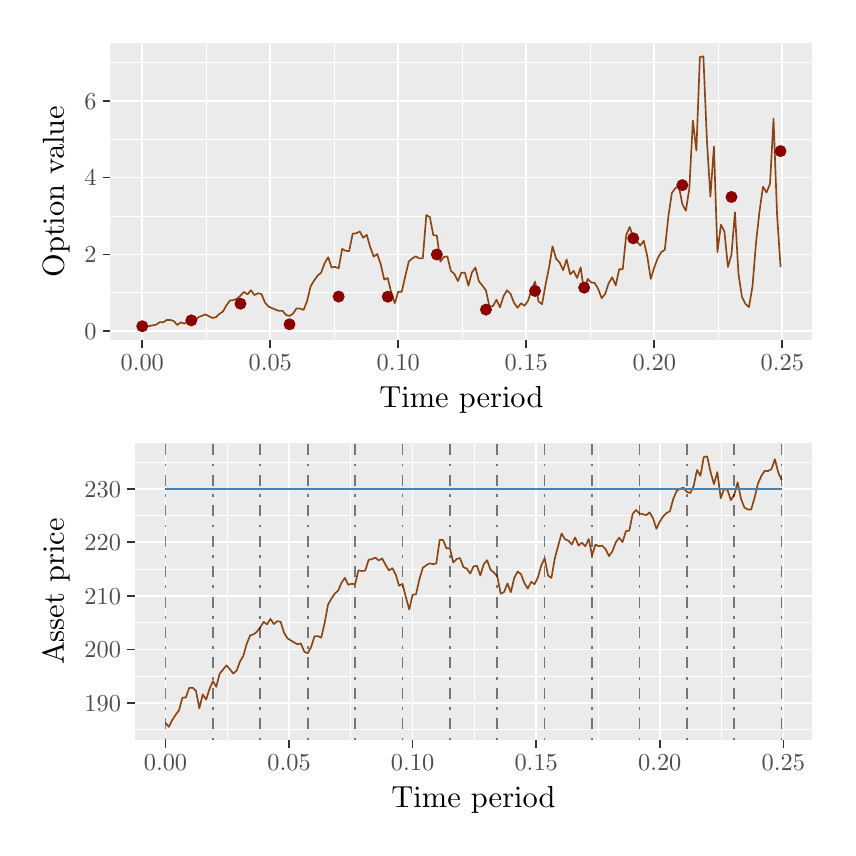
\begin{tikzpicture}[x=1pt,y=1pt]
\definecolor{fillColor}{RGB}{255,255,255}
\path[use as bounding box,fill=fillColor,fill opacity=0.00] (0,0) rectangle (289.08,289.08);
\begin{scope}
\path[clip] (  0.00,144.54) rectangle (289.08,289.08);
\definecolor{drawColor}{RGB}{255,255,255}
\definecolor{fillColor}{RGB}{255,255,255}

\path[draw=drawColor,line width= 0.6pt,line join=round,line cap=round,fill=fillColor] (  0.00,144.54) rectangle (289.08,289.08);
\end{scope}
\begin{scope}
\path[clip] ( 29.87,176.07) rectangle (283.58,283.58);
\definecolor{fillColor}{gray}{0.92}

\path[fill=fillColor] ( 29.87,176.07) rectangle (283.58,283.58);
\definecolor{drawColor}{RGB}{255,255,255}

\path[draw=drawColor,line width= 0.3pt,line join=round] ( 29.87,193.28) --
	(283.58,193.28);

\path[draw=drawColor,line width= 0.3pt,line join=round] ( 29.87,221.03) --
	(283.58,221.03);

\path[draw=drawColor,line width= 0.3pt,line join=round] ( 29.87,248.79) --
	(283.58,248.79);

\path[draw=drawColor,line width= 0.3pt,line join=round] ( 29.87,276.54) --
	(283.58,276.54);

\path[draw=drawColor,line width= 0.3pt,line join=round] ( 64.53,176.07) --
	( 64.53,283.58);

\path[draw=drawColor,line width= 0.3pt,line join=round] (110.79,176.07) --
	(110.79,283.58);

\path[draw=drawColor,line width= 0.3pt,line join=round] (157.04,176.07) --
	(157.04,283.58);

\path[draw=drawColor,line width= 0.3pt,line join=round] (203.30,176.07) --
	(203.30,283.58);

\path[draw=drawColor,line width= 0.3pt,line join=round] (249.55,176.07) --
	(249.55,283.58);

\path[draw=drawColor,line width= 0.6pt,line join=round] ( 29.87,179.41) --
	(283.58,179.41);

\path[draw=drawColor,line width= 0.6pt,line join=round] ( 29.87,207.16) --
	(283.58,207.16);

\path[draw=drawColor,line width= 0.6pt,line join=round] ( 29.87,234.91) --
	(283.58,234.91);

\path[draw=drawColor,line width= 0.6pt,line join=round] ( 29.87,262.66) --
	(283.58,262.66);

\path[draw=drawColor,line width= 0.6pt,line join=round] ( 41.40,176.07) --
	( 41.40,283.58);

\path[draw=drawColor,line width= 0.6pt,line join=round] ( 87.66,176.07) --
	( 87.66,283.58);

\path[draw=drawColor,line width= 0.6pt,line join=round] (133.91,176.07) --
	(133.91,283.58);

\path[draw=drawColor,line width= 0.6pt,line join=round] (180.17,176.07) --
	(180.17,283.58);

\path[draw=drawColor,line width= 0.6pt,line join=round] (226.43,176.07) --
	(226.43,283.58);

\path[draw=drawColor,line width= 0.6pt,line join=round] (272.68,176.07) --
	(272.68,283.58);
\definecolor{drawColor}{RGB}{139,69,19}

\path[draw=drawColor,line width= 0.6pt,line join=round] ( 41.40,181.19) --
	( 42.67,180.96) --
	( 43.94,181.27) --
	( 45.20,181.52) --
	( 46.47,181.77) --
	( 47.74,182.68) --
	( 49.00,182.63) --
	( 50.27,183.47) --
	( 51.54,183.44) --
	( 52.81,183.07) --
	( 54.07,181.63) --
	( 55.34,182.61) --
	( 56.61,182.14) --
	( 57.88,182.99) --
	( 59.14,183.74) --
	( 60.41,183.07) --
	( 61.68,184.48) --
	( 62.95,184.94) --
	( 64.21,185.47) --
	( 65.48,184.82) --
	( 66.75,184.18) --
	( 68.01,184.45) --
	( 69.28,185.65) --
	( 70.55,186.50) --
	( 71.82,188.73) --
	( 73.08,190.49) --
	( 74.35,190.62) --
	( 75.62,191.13) --
	( 76.89,192.21) --
	( 78.15,193.59) --
	( 79.42,192.69) --
	( 80.69,194.19) --
	( 81.95,192.45) --
	( 83.22,193.11) --
	( 84.49,192.79) --
	( 85.76,189.74) --
	( 87.02,188.32) --
	( 88.29,187.73) --
	( 89.56,187.19) --
	( 90.83,186.73) --
	( 92.09,186.76) --
	( 93.36,185.27) --
	( 94.63,184.92) --
	( 95.89,185.77) --
	( 97.16,187.66) --
	( 98.43,187.56) --
	( 99.70,187.10) --
	(100.96,190.26) --
	(102.23,195.62) --
	(103.50,197.68) --
	(104.77,199.50) --
	(106.03,200.51) --
	(107.30,203.98) --
	(108.57,206.12) --
	(109.83,202.41) --
	(111.10,202.65) --
	(112.37,202.13) --
	(113.64,209.15) --
	(114.90,208.44) --
	(116.17,208.36) --
	(117.44,214.61) --
	(118.71,214.78) --
	(119.97,215.45) --
	(121.24,213.16) --
	(122.51,214.21) --
	(123.77,209.83) --
	(125.04,206.34) --
	(126.31,207.29) --
	(127.58,203.57) --
	(128.84,198.08) --
	(130.11,198.59) --
	(131.38,193.33) --
	(132.65,189.50) --
	(133.91,193.66) --
	(135.18,193.64) --
	(136.45,199.32) --
	(137.72,204.62) --
	(138.98,205.69) --
	(140.25,206.45) --
	(141.52,205.70) --
	(142.78,205.73) --
	(144.05,221.38) --
	(145.32,220.64) --
	(146.59,214.06) --
	(147.85,213.98) --
	(149.12,204.56) --
	(150.39,206.24) --
	(151.66,206.42) --
	(152.92,201.16) --
	(154.19,200.08) --
	(155.46,197.49) --
	(156.72,200.57) --
	(157.99,200.50) --
	(159.26,195.84) --
	(160.53,200.64) --
	(161.79,202.38) --
	(163.06,197.40) --
	(164.33,195.87) --
	(165.60,194.12) --
	(166.86,188.28) --
	(168.13,188.48) --
	(169.40,190.78) --
	(170.66,188.02) --
	(171.93,192.04) --
	(173.20,194.18) --
	(174.47,192.90) --
	(175.73,189.69) --
	(177.00,187.87) --
	(178.27,189.50) --
	(179.54,188.59) --
	(180.80,190.38) --
	(182.07,194.42) --
	(183.34,197.35) --
	(184.60,190.14) --
	(185.87,189.17) --
	(187.14,196.23) --
	(188.41,202.50) --
	(189.67,210.06) --
	(190.94,205.60) --
	(192.21,204.23) --
	(193.48,201.45) --
	(194.74,205.31) --
	(196.01,199.97) --
	(197.28,201.20) --
	(198.54,198.63) --
	(199.81,202.49) --
	(201.08,193.50) --
	(202.35,198.30) --
	(203.61,197.02) --
	(204.88,196.84) --
	(206.15,194.69) --
	(207.42,191.33) --
	(208.68,192.87) --
	(209.95,196.76) --
	(211.22,198.88) --
	(212.49,195.98) --
	(213.75,201.81) --
	(215.02,201.78) --
	(216.29,214.16) --
	(217.55,217.07) --
	(218.82,213.16) --
	(220.09,211.84) --
	(221.36,210.34) --
	(222.62,212.08) --
	(223.89,206.43) --
	(225.16,198.29) --
	(226.43,202.49) --
	(227.69,205.82) --
	(228.96,207.99) --
	(230.23,208.79) --
	(231.49,220.62) --
	(232.76,229.32) --
	(234.03,231.09) --
	(235.30,231.75) --
	(236.56,225.34) --
	(237.83,222.91) --
	(239.10,231.05) --
	(240.37,255.49) --
	(241.63,244.67) --
	(242.90,278.48) --
	(244.17,278.69) --
	(245.43,248.47) --
	(246.70,228.01) --
	(247.97,246.11) --
	(249.24,207.96) --
	(250.50,217.88) --
	(251.77,215.36) --
	(253.04,202.59) --
	(254.31,207.06) --
	(255.57,222.38) --
	(256.84,200.14) --
	(258.11,191.74) --
	(259.37,189.21) --
	(260.64,188.12) --
	(261.91,195.61) --
	(263.18,211.30) --
	(264.44,222.75) --
	(265.71,231.60) --
	(266.98,229.52) --
	(268.25,232.69) --
	(269.51,256.19) --
	(270.78,221.72) --
	(272.05,202.60);
\definecolor{drawColor}{RGB}{139,0,0}
\definecolor{fillColor}{RGB}{139,0,0}

\path[draw=drawColor,line width= 0.4pt,line join=round,line cap=round,fill=fillColor] ( 41.40,181.19) circle (  1.96);

\path[draw=drawColor,line width= 0.4pt,line join=round,line cap=round,fill=fillColor] ( 59.14,183.31) circle (  1.96);

\path[draw=drawColor,line width= 0.4pt,line join=round,line cap=round,fill=fillColor] ( 76.89,189.33) circle (  1.96);

\path[draw=drawColor,line width= 0.4pt,line join=round,line cap=round,fill=fillColor] ( 94.63,181.89) circle (  1.96);

\path[draw=drawColor,line width= 0.4pt,line join=round,line cap=round,fill=fillColor] (112.37,191.91) circle (  1.96);

\path[draw=drawColor,line width= 0.4pt,line join=round,line cap=round,fill=fillColor] (130.11,191.87) circle (  1.96);

\path[draw=drawColor,line width= 0.4pt,line join=round,line cap=round,fill=fillColor] (147.85,207.11) circle (  1.96);

\path[draw=drawColor,line width= 0.4pt,line join=round,line cap=round,fill=fillColor] (165.60,187.19) circle (  1.96);

\path[draw=drawColor,line width= 0.4pt,line join=round,line cap=round,fill=fillColor] (183.34,193.94) circle (  1.96);

\path[draw=drawColor,line width= 0.4pt,line join=round,line cap=round,fill=fillColor] (201.08,195.14) circle (  1.96);

\path[draw=drawColor,line width= 0.4pt,line join=round,line cap=round,fill=fillColor] (218.82,212.96) circle (  1.96);

\path[draw=drawColor,line width= 0.4pt,line join=round,line cap=round,fill=fillColor] (236.56,232.18) circle (  1.96);

\path[draw=drawColor,line width= 0.4pt,line join=round,line cap=round,fill=fillColor] (254.31,227.90) circle (  1.96);

\path[draw=drawColor,line width= 0.4pt,line join=round,line cap=round,fill=fillColor] (272.05,244.47) circle (  1.96);
\end{scope}
\begin{scope}
\path[clip] (  0.00,  0.00) rectangle (289.08,289.08);
\definecolor{drawColor}{gray}{0.30}

\node[text=drawColor,anchor=base east,inner sep=0pt, outer sep=0pt, scale=  0.88] at ( 24.92,176.37) {0};

\node[text=drawColor,anchor=base east,inner sep=0pt, outer sep=0pt, scale=  0.88] at ( 24.92,204.13) {2};

\node[text=drawColor,anchor=base east,inner sep=0pt, outer sep=0pt, scale=  0.88] at ( 24.92,231.88) {4};

\node[text=drawColor,anchor=base east,inner sep=0pt, outer sep=0pt, scale=  0.88] at ( 24.92,259.63) {6};
\end{scope}
\begin{scope}
\path[clip] (  0.00,  0.00) rectangle (289.08,289.08);
\definecolor{drawColor}{gray}{0.20}

\path[draw=drawColor,line width= 0.6pt,line join=round] ( 27.12,179.41) --
	( 29.87,179.41);

\path[draw=drawColor,line width= 0.6pt,line join=round] ( 27.12,207.16) --
	( 29.87,207.16);

\path[draw=drawColor,line width= 0.6pt,line join=round] ( 27.12,234.91) --
	( 29.87,234.91);

\path[draw=drawColor,line width= 0.6pt,line join=round] ( 27.12,262.66) --
	( 29.87,262.66);
\end{scope}
\begin{scope}
\path[clip] (  0.00,  0.00) rectangle (289.08,289.08);
\definecolor{drawColor}{gray}{0.20}

\path[draw=drawColor,line width= 0.6pt,line join=round] ( 41.40,173.32) --
	( 41.40,176.07);

\path[draw=drawColor,line width= 0.6pt,line join=round] ( 87.66,173.32) --
	( 87.66,176.07);

\path[draw=drawColor,line width= 0.6pt,line join=round] (133.91,173.32) --
	(133.91,176.07);

\path[draw=drawColor,line width= 0.6pt,line join=round] (180.17,173.32) --
	(180.17,176.07);

\path[draw=drawColor,line width= 0.6pt,line join=round] (226.43,173.32) --
	(226.43,176.07);

\path[draw=drawColor,line width= 0.6pt,line join=round] (272.68,173.32) --
	(272.68,176.07);
\end{scope}
\begin{scope}
\path[clip] (  0.00,  0.00) rectangle (289.08,289.08);
\definecolor{drawColor}{gray}{0.30}

\node[text=drawColor,anchor=base,inner sep=0pt, outer sep=0pt, scale=  0.88] at ( 41.40,165.06) {0.00};

\node[text=drawColor,anchor=base,inner sep=0pt, outer sep=0pt, scale=  0.88] at ( 87.66,165.06) {0.05};

\node[text=drawColor,anchor=base,inner sep=0pt, outer sep=0pt, scale=  0.88] at (133.91,165.06) {0.10};

\node[text=drawColor,anchor=base,inner sep=0pt, outer sep=0pt, scale=  0.88] at (180.17,165.06) {0.15};

\node[text=drawColor,anchor=base,inner sep=0pt, outer sep=0pt, scale=  0.88] at (226.43,165.06) {0.20};

\node[text=drawColor,anchor=base,inner sep=0pt, outer sep=0pt, scale=  0.88] at (272.68,165.06) {0.25};
\end{scope}
\begin{scope}
\path[clip] (  0.00,  0.00) rectangle (289.08,289.08);
\definecolor{drawColor}{RGB}{0,0,0}

\node[text=drawColor,anchor=base,inner sep=0pt, outer sep=0pt, scale=  1.10] at (156.72,151.98) {Time period};
\end{scope}
\begin{scope}
\path[clip] (  0.00,  0.00) rectangle (289.08,289.08);
\definecolor{drawColor}{RGB}{0,0,0}

\node[text=drawColor,rotate= 90.00,anchor=base,inner sep=0pt, outer sep=0pt, scale=  1.10] at ( 13.08,229.83) {Option value};
\end{scope}
\begin{scope}
\path[clip] (  0.00,  0.00) rectangle (289.08,144.54);
\definecolor{drawColor}{RGB}{255,255,255}
\definecolor{fillColor}{RGB}{255,255,255}

\path[draw=drawColor,line width= 0.6pt,line join=round,line cap=round,fill=fillColor] (  0.00,  0.00) rectangle (289.08,144.54);
\end{scope}
\begin{scope}
\path[clip] ( 38.67, 31.53) rectangle (283.58,139.04);
\definecolor{fillColor}{gray}{0.92}

\path[fill=fillColor] ( 38.67, 31.53) rectangle (283.58,139.04);
\definecolor{drawColor}{RGB}{255,255,255}

\path[draw=drawColor,line width= 0.3pt,line join=round] ( 38.67, 35.34) --
	(283.58, 35.34);

\path[draw=drawColor,line width= 0.3pt,line join=round] ( 38.67, 54.70) --
	(283.58, 54.70);

\path[draw=drawColor,line width= 0.3pt,line join=round] ( 38.67, 74.06) --
	(283.58, 74.06);

\path[draw=drawColor,line width= 0.3pt,line join=round] ( 38.67, 93.43) --
	(283.58, 93.43);

\path[draw=drawColor,line width= 0.3pt,line join=round] ( 38.67,112.79) --
	(283.58,112.79);

\path[draw=drawColor,line width= 0.3pt,line join=round] ( 38.67,132.15) --
	(283.58,132.15);

\path[draw=drawColor,line width= 0.3pt,line join=round] ( 72.13, 31.53) --
	( 72.13,139.04);

\path[draw=drawColor,line width= 0.3pt,line join=round] (116.78, 31.53) --
	(116.78,139.04);

\path[draw=drawColor,line width= 0.3pt,line join=round] (161.43, 31.53) --
	(161.43,139.04);

\path[draw=drawColor,line width= 0.3pt,line join=round] (206.08, 31.53) --
	(206.08,139.04);

\path[draw=drawColor,line width= 0.3pt,line join=round] (250.73, 31.53) --
	(250.73,139.04);

\path[draw=drawColor,line width= 0.6pt,line join=round] ( 38.67, 45.02) --
	(283.58, 45.02);

\path[draw=drawColor,line width= 0.6pt,line join=round] ( 38.67, 64.38) --
	(283.58, 64.38);

\path[draw=drawColor,line width= 0.6pt,line join=round] ( 38.67, 83.75) --
	(283.58, 83.75);

\path[draw=drawColor,line width= 0.6pt,line join=round] ( 38.67,103.11) --
	(283.58,103.11);

\path[draw=drawColor,line width= 0.6pt,line join=round] ( 38.67,122.47) --
	(283.58,122.47);

\path[draw=drawColor,line width= 0.6pt,line join=round] ( 49.80, 31.53) --
	( 49.80,139.04);

\path[draw=drawColor,line width= 0.6pt,line join=round] ( 94.45, 31.53) --
	( 94.45,139.04);

\path[draw=drawColor,line width= 0.6pt,line join=round] (139.10, 31.53) --
	(139.10,139.04);

\path[draw=drawColor,line width= 0.6pt,line join=round] (183.76, 31.53) --
	(183.76,139.04);

\path[draw=drawColor,line width= 0.6pt,line join=round] (228.41, 31.53) --
	(228.41,139.04);

\path[draw=drawColor,line width= 0.6pt,line join=round] (273.06, 31.53) --
	(273.06,139.04);
\definecolor{drawColor}{RGB}{139,69,19}

\path[draw=drawColor,line width= 0.6pt,line join=round] ( 49.80, 37.88) --
	( 51.02, 36.42) --
	( 52.25, 38.92) --
	( 53.47, 40.78) --
	( 54.69, 42.43) --
	( 55.92, 47.00) --
	( 57.14, 47.02) --
	( 58.36, 50.46) --
	( 59.59, 50.58) --
	( 60.81, 49.47) --
	( 62.03, 43.14) --
	( 63.26, 48.13) --
	( 64.48, 46.27) --
	( 65.70, 50.11) --
	( 66.93, 52.96) --
	( 68.15, 50.89) --
	( 69.37, 55.64) --
	( 70.60, 57.12) --
	( 71.82, 58.66) --
	( 73.04, 57.27) --
	( 74.27, 55.72) --
	( 75.49, 56.70) --
	( 76.71, 60.01) --
	( 77.94, 62.12) --
	( 79.16, 66.49) --
	( 80.38, 69.46) --
	( 81.61, 69.86) --
	( 82.83, 70.79) --
	( 84.05, 72.44) --
	( 85.28, 74.36) --
	( 86.50, 73.46) --
	( 87.72, 75.45) --
	( 88.95, 73.58) --
	( 90.17, 74.61) --
	( 91.39, 74.43) --
	( 92.62, 70.50) --
	( 93.84, 68.47) --
	( 95.06, 67.66) --
	( 96.29, 66.91) --
	( 97.51, 66.26) --
	( 98.73, 66.56) --
	( 99.96, 63.60) --
	(101.18, 62.99) --
	(102.40, 65.21) --
	(103.63, 69.16) --
	(104.85, 69.23) --
	(106.07, 68.63) --
	(107.30, 73.95) --
	(108.52, 80.54) --
	(109.74, 82.76) --
	(110.97, 84.58) --
	(112.19, 85.64) --
	(113.41, 88.53) --
	(114.64, 90.25) --
	(115.86, 87.76) --
	(117.08, 88.14) --
	(118.31, 87.95) --
	(119.53, 93.00) --
	(120.75, 92.75) --
	(121.98, 92.89) --
	(123.20, 96.77) --
	(124.42, 97.05) --
	(125.65, 97.60) --
	(126.87, 96.53) --
	(128.09, 97.29) --
	(129.32, 94.97) --
	(130.54, 92.97) --
	(131.76, 93.78) --
	(132.99, 91.49) --
	(134.21, 87.41) --
	(135.43, 88.07) --
	(136.66, 83.31) --
	(137.88, 78.89) --
	(139.10, 84.14) --
	(140.33, 84.35) --
	(141.55, 89.79) --
	(142.77, 93.89) --
	(144.00, 94.81) --
	(145.22, 95.51) --
	(146.44, 95.24) --
	(147.67, 95.48) --
	(148.89,104.06) --
	(150.11,103.91) --
	(151.34,100.89) --
	(152.56,101.05) --
	(153.78, 95.80) --
	(155.01, 97.09) --
	(156.23, 97.42) --
	(157.45, 94.15) --
	(158.68, 93.59) --
	(159.90, 91.80) --
	(161.12, 94.42) --
	(162.35, 94.61) --
	(163.57, 91.14) --
	(164.79, 95.18) --
	(166.02, 96.64) --
	(167.24, 93.21) --
	(168.46, 92.19) --
	(169.69, 90.87) --
	(170.91, 84.55) --
	(172.13, 85.12) --
	(173.36, 88.26) --
	(174.58, 85.07) --
	(175.80, 90.19) --
	(177.03, 92.55) --
	(178.25, 91.62) --
	(179.47, 88.45) --
	(180.70, 86.39) --
	(181.92, 88.82) --
	(183.14, 87.98) --
	(184.37, 90.45) --
	(185.59, 94.71) --
	(186.81, 97.36) --
	(188.04, 91.09) --
	(189.26, 90.28) --
	(190.48, 97.33) --
	(191.71,101.92) --
	(192.93,106.30) --
	(194.15,104.22) --
	(195.38,103.72) --
	(196.60,102.34) --
	(197.82,104.84) --
	(199.05,101.95) --
	(200.27,103.00) --
	(201.49,101.64) --
	(202.72,104.33) --
	(203.94, 98.41) --
	(205.16,102.30) --
	(206.39,101.72) --
	(207.61,101.90) --
	(208.83,100.64) --
	(210.06, 98.14) --
	(211.28, 99.84) --
	(212.50,103.09) --
	(213.73,104.79) --
	(214.95,103.20) --
	(216.17,107.11) --
	(217.40,107.40) --
	(218.62,113.40) --
	(219.84,114.77) --
	(221.07,113.53) --
	(222.29,113.27) --
	(223.51,112.94) --
	(224.74,113.92) --
	(225.96,111.83) --
	(227.18,108.01) --
	(228.41,110.59) --
	(229.63,112.47) --
	(230.85,113.72) --
	(232.08,114.35) --
	(233.30,118.87) --
	(234.52,121.71) --
	(235.75,122.44) --
	(236.97,122.86) --
	(238.19,121.34) --
	(239.42,120.91) --
	(240.64,123.40) --
	(241.86,129.24) --
	(243.09,127.12) --
	(244.31,133.97) --
	(245.53,134.15) --
	(246.76,128.56) --
	(247.98,124.16) --
	(249.20,128.48) --
	(250.43,119.05) --
	(251.65,122.39) --
	(252.87,122.02) --
	(254.10,118.34) --
	(255.32,120.28) --
	(256.54,124.79) --
	(257.77,118.79) --
	(258.99,115.71) --
	(260.21,114.94) --
	(261.44,114.97) --
	(262.66,119.20) --
	(263.88,124.29) --
	(265.11,127.08) --
	(266.33,128.96) --
	(267.55,128.86) --
	(268.78,129.59) --
	(270.00,133.14) --
	(271.22,128.31) --
	(272.45,125.70);
\definecolor{drawColor}{RGB}{70,130,180}

\path[draw=drawColor,line width= 0.6pt,line join=round] ( 49.80,122.47) --
	( 51.02,122.47) --
	( 52.25,122.47) --
	( 53.47,122.47) --
	( 54.69,122.47) --
	( 55.92,122.47) --
	( 57.14,122.47) --
	( 58.36,122.47) --
	( 59.59,122.47) --
	( 60.81,122.47) --
	( 62.03,122.47) --
	( 63.26,122.47) --
	( 64.48,122.47) --
	( 65.70,122.47) --
	( 66.93,122.47) --
	( 68.15,122.47) --
	( 69.37,122.47) --
	( 70.60,122.47) --
	( 71.82,122.47) --
	( 73.04,122.47) --
	( 74.27,122.47) --
	( 75.49,122.47) --
	( 76.71,122.47) --
	( 77.94,122.47) --
	( 79.16,122.47) --
	( 80.38,122.47) --
	( 81.61,122.47) --
	( 82.83,122.47) --
	( 84.05,122.47) --
	( 85.28,122.47) --
	( 86.50,122.47) --
	( 87.72,122.47) --
	( 88.95,122.47) --
	( 90.17,122.47) --
	( 91.39,122.47) --
	( 92.62,122.47) --
	( 93.84,122.47) --
	( 95.06,122.47) --
	( 96.29,122.47) --
	( 97.51,122.47) --
	( 98.73,122.47) --
	( 99.96,122.47) --
	(101.18,122.47) --
	(102.40,122.47) --
	(103.63,122.47) --
	(104.85,122.47) --
	(106.07,122.47) --
	(107.30,122.47) --
	(108.52,122.47) --
	(109.74,122.47) --
	(110.97,122.47) --
	(112.19,122.47) --
	(113.41,122.47) --
	(114.64,122.47) --
	(115.86,122.47) --
	(117.08,122.47) --
	(118.31,122.47) --
	(119.53,122.47) --
	(120.75,122.47) --
	(121.98,122.47) --
	(123.20,122.47) --
	(124.42,122.47) --
	(125.65,122.47) --
	(126.87,122.47) --
	(128.09,122.47) --
	(129.32,122.47) --
	(130.54,122.47) --
	(131.76,122.47) --
	(132.99,122.47) --
	(134.21,122.47) --
	(135.43,122.47) --
	(136.66,122.47) --
	(137.88,122.47) --
	(139.10,122.47) --
	(140.33,122.47) --
	(141.55,122.47) --
	(142.77,122.47) --
	(144.00,122.47) --
	(145.22,122.47) --
	(146.44,122.47) --
	(147.67,122.47) --
	(148.89,122.47) --
	(150.11,122.47) --
	(151.34,122.47) --
	(152.56,122.47) --
	(153.78,122.47) --
	(155.01,122.47) --
	(156.23,122.47) --
	(157.45,122.47) --
	(158.68,122.47) --
	(159.90,122.47) --
	(161.12,122.47) --
	(162.35,122.47) --
	(163.57,122.47) --
	(164.79,122.47) --
	(166.02,122.47) --
	(167.24,122.47) --
	(168.46,122.47) --
	(169.69,122.47) --
	(170.91,122.47) --
	(172.13,122.47) --
	(173.36,122.47) --
	(174.58,122.47) --
	(175.80,122.47) --
	(177.03,122.47) --
	(178.25,122.47) --
	(179.47,122.47) --
	(180.70,122.47) --
	(181.92,122.47) --
	(183.14,122.47) --
	(184.37,122.47) --
	(185.59,122.47) --
	(186.81,122.47) --
	(188.04,122.47) --
	(189.26,122.47) --
	(190.48,122.47) --
	(191.71,122.47) --
	(192.93,122.47) --
	(194.15,122.47) --
	(195.38,122.47) --
	(196.60,122.47) --
	(197.82,122.47) --
	(199.05,122.47) --
	(200.27,122.47) --
	(201.49,122.47) --
	(202.72,122.47) --
	(203.94,122.47) --
	(205.16,122.47) --
	(206.39,122.47) --
	(207.61,122.47) --
	(208.83,122.47) --
	(210.06,122.47) --
	(211.28,122.47) --
	(212.50,122.47) --
	(213.73,122.47) --
	(214.95,122.47) --
	(216.17,122.47) --
	(217.40,122.47) --
	(218.62,122.47) --
	(219.84,122.47) --
	(221.07,122.47) --
	(222.29,122.47) --
	(223.51,122.47) --
	(224.74,122.47) --
	(225.96,122.47) --
	(227.18,122.47) --
	(228.41,122.47) --
	(229.63,122.47) --
	(230.85,122.47) --
	(232.08,122.47) --
	(233.30,122.47) --
	(234.52,122.47) --
	(235.75,122.47) --
	(236.97,122.47) --
	(238.19,122.47) --
	(239.42,122.47) --
	(240.64,122.47) --
	(241.86,122.47) --
	(243.09,122.47) --
	(244.31,122.47) --
	(245.53,122.47) --
	(246.76,122.47) --
	(247.98,122.47) --
	(249.20,122.47) --
	(250.43,122.47) --
	(251.65,122.47) --
	(252.87,122.47) --
	(254.10,122.47) --
	(255.32,122.47) --
	(256.54,122.47) --
	(257.77,122.47) --
	(258.99,122.47) --
	(260.21,122.47) --
	(261.44,122.47) --
	(262.66,122.47) --
	(263.88,122.47) --
	(265.11,122.47) --
	(266.33,122.47) --
	(267.55,122.47) --
	(268.78,122.47) --
	(270.00,122.47) --
	(271.22,122.47) --
	(272.45,122.47);
\definecolor{drawColor}{RGB}{0,0,0}

\path[draw=drawColor,draw opacity=0.50,line width= 0.6pt,dash pattern=on 1pt off 3pt on 4pt off 3pt ,line join=round] ( 49.80, 31.53) -- ( 49.80,139.04);

\path[draw=drawColor,draw opacity=0.50,line width= 0.6pt,dash pattern=on 1pt off 3pt on 4pt off 3pt ,line join=round] ( 66.93, 31.53) -- ( 66.93,139.04);

\path[draw=drawColor,draw opacity=0.50,line width= 0.6pt,dash pattern=on 1pt off 3pt on 4pt off 3pt ,line join=round] ( 84.05, 31.53) -- ( 84.05,139.04);

\path[draw=drawColor,draw opacity=0.50,line width= 0.6pt,dash pattern=on 1pt off 3pt on 4pt off 3pt ,line join=round] (101.18, 31.53) -- (101.18,139.04);

\path[draw=drawColor,draw opacity=0.50,line width= 0.6pt,dash pattern=on 1pt off 3pt on 4pt off 3pt ,line join=round] (118.31, 31.53) -- (118.31,139.04);

\path[draw=drawColor,draw opacity=0.50,line width= 0.6pt,dash pattern=on 1pt off 3pt on 4pt off 3pt ,line join=round] (135.43, 31.53) -- (135.43,139.04);

\path[draw=drawColor,draw opacity=0.50,line width= 0.6pt,dash pattern=on 1pt off 3pt on 4pt off 3pt ,line join=round] (152.56, 31.53) -- (152.56,139.04);

\path[draw=drawColor,draw opacity=0.50,line width= 0.6pt,dash pattern=on 1pt off 3pt on 4pt off 3pt ,line join=round] (169.69, 31.53) -- (169.69,139.04);

\path[draw=drawColor,draw opacity=0.50,line width= 0.6pt,dash pattern=on 1pt off 3pt on 4pt off 3pt ,line join=round] (186.81, 31.53) -- (186.81,139.04);

\path[draw=drawColor,draw opacity=0.50,line width= 0.6pt,dash pattern=on 1pt off 3pt on 4pt off 3pt ,line join=round] (203.94, 31.53) -- (203.94,139.04);

\path[draw=drawColor,draw opacity=0.50,line width= 0.6pt,dash pattern=on 1pt off 3pt on 4pt off 3pt ,line join=round] (221.07, 31.53) -- (221.07,139.04);

\path[draw=drawColor,draw opacity=0.50,line width= 0.6pt,dash pattern=on 1pt off 3pt on 4pt off 3pt ,line join=round] (238.19, 31.53) -- (238.19,139.04);

\path[draw=drawColor,draw opacity=0.50,line width= 0.6pt,dash pattern=on 1pt off 3pt on 4pt off 3pt ,line join=round] (255.32, 31.53) -- (255.32,139.04);

\path[draw=drawColor,draw opacity=0.50,line width= 0.6pt,dash pattern=on 1pt off 3pt on 4pt off 3pt ,line join=round] (272.45, 31.53) -- (272.45,139.04);
\end{scope}
\begin{scope}
\path[clip] (  0.00,  0.00) rectangle (289.08,289.08);
\definecolor{drawColor}{gray}{0.30}

\node[text=drawColor,anchor=base east,inner sep=0pt, outer sep=0pt, scale=  0.88] at ( 33.72, 41.99) {190};

\node[text=drawColor,anchor=base east,inner sep=0pt, outer sep=0pt, scale=  0.88] at ( 33.72, 61.35) {200};

\node[text=drawColor,anchor=base east,inner sep=0pt, outer sep=0pt, scale=  0.88] at ( 33.72, 80.72) {210};

\node[text=drawColor,anchor=base east,inner sep=0pt, outer sep=0pt, scale=  0.88] at ( 33.72,100.08) {220};

\node[text=drawColor,anchor=base east,inner sep=0pt, outer sep=0pt, scale=  0.88] at ( 33.72,119.44) {230};
\end{scope}
\begin{scope}
\path[clip] (  0.00,  0.00) rectangle (289.08,289.08);
\definecolor{drawColor}{gray}{0.20}

\path[draw=drawColor,line width= 0.6pt,line join=round] ( 35.92, 45.02) --
	( 38.67, 45.02);

\path[draw=drawColor,line width= 0.6pt,line join=round] ( 35.92, 64.38) --
	( 38.67, 64.38);

\path[draw=drawColor,line width= 0.6pt,line join=round] ( 35.92, 83.75) --
	( 38.67, 83.75);

\path[draw=drawColor,line width= 0.6pt,line join=round] ( 35.92,103.11) --
	( 38.67,103.11);

\path[draw=drawColor,line width= 0.6pt,line join=round] ( 35.92,122.47) --
	( 38.67,122.47);
\end{scope}
\begin{scope}
\path[clip] (  0.00,  0.00) rectangle (289.08,289.08);
\definecolor{drawColor}{gray}{0.20}

\path[draw=drawColor,line width= 0.6pt,line join=round] ( 49.80, 28.78) --
	( 49.80, 31.53);

\path[draw=drawColor,line width= 0.6pt,line join=round] ( 94.45, 28.78) --
	( 94.45, 31.53);

\path[draw=drawColor,line width= 0.6pt,line join=round] (139.10, 28.78) --
	(139.10, 31.53);

\path[draw=drawColor,line width= 0.6pt,line join=round] (183.76, 28.78) --
	(183.76, 31.53);

\path[draw=drawColor,line width= 0.6pt,line join=round] (228.41, 28.78) --
	(228.41, 31.53);

\path[draw=drawColor,line width= 0.6pt,line join=round] (273.06, 28.78) --
	(273.06, 31.53);
\end{scope}
\begin{scope}
\path[clip] (  0.00,  0.00) rectangle (289.08,289.08);
\definecolor{drawColor}{gray}{0.30}

\node[text=drawColor,anchor=base,inner sep=0pt, outer sep=0pt, scale=  0.88] at ( 49.80, 20.52) {0.00};

\node[text=drawColor,anchor=base,inner sep=0pt, outer sep=0pt, scale=  0.88] at ( 94.45, 20.52) {0.05};

\node[text=drawColor,anchor=base,inner sep=0pt, outer sep=0pt, scale=  0.88] at (139.10, 20.52) {0.10};

\node[text=drawColor,anchor=base,inner sep=0pt, outer sep=0pt, scale=  0.88] at (183.76, 20.52) {0.15};

\node[text=drawColor,anchor=base,inner sep=0pt, outer sep=0pt, scale=  0.88] at (228.41, 20.52) {0.20};

\node[text=drawColor,anchor=base,inner sep=0pt, outer sep=0pt, scale=  0.88] at (273.06, 20.52) {0.25};
\end{scope}
\begin{scope}
\path[clip] (  0.00,  0.00) rectangle (289.08,289.08);
\definecolor{drawColor}{RGB}{0,0,0}

\node[text=drawColor,anchor=base,inner sep=0pt, outer sep=0pt, scale=  1.10] at (161.12,  7.44) {Time period};
\end{scope}
\begin{scope}
\path[clip] (  0.00,  0.00) rectangle (289.08,289.08);
\definecolor{drawColor}{RGB}{0,0,0}

\node[text=drawColor,rotate= 90.00,anchor=base,inner sep=0pt, outer sep=0pt, scale=  1.10] at ( 13.08, 85.29) {Asset price};
\end{scope}
\end{tikzpicture}

  % \rule{40mm}{20mm}
  \caption{European call option with higher theta as time goes to maturity}
   %
  % BEGIN OF FLOATNOTE
  %
  \begin{changemargin}{0.5cm}{0.5cm}
  \medskip
\footnotesize
\setstretch{1.0}\textbf{Notes.} The parameters passed to the function \textit{bsm\_call}, to compute the different option values are: $\tau = 0.2493$, $K = 230$, $\sigma = 0.1958$, $r = 0.01896$. While the underlying asset followed differents dummy paths constructed through the function \textit{bsm\_ts} taking as arguments: $\sigma = 0.1958$, $\alpha = 0.48229$. The hedge is weekly balanced.
  \end{changemargin}
  %
  % END OF FLOATNOTE
  %
  \label{p:analysis:gbm:pl:theta:high}
\end{figure}



By resuming the solution of theta given in \citet{shreve}, for the European call option, one gets the following equations.

\begin{align}
  \Theta = -r K e^{-r (T-t)} N\bigg(d_{-}(T-t, S(t))\bigg) -
    \frac{\sigma S(t)}{2\sqrt{T-t}} N^{'}\bigg(d_{+}(T-t, S(t))\bigg) \label{eq:analysis:theta}\\
  \intertext{with}
  d_{\pm}(\tau, x) = \frac{1}{\sigma \sqrt{\tau}} \left [
    \ln\frac{x}{K} + \left( r \pm \frac{\sigma^2}{2} \right) \tau
  \right]\label{eq:analysis:d}
\end{align}
With $N$ and $N^{'}$ respectively standing for the normal cumulative distribution function (CDF) and for the normal probability density function (PDF). 

Intuitively, according to \cref{eq:analysis:theta} As $\tau \downarrow \implies \sigma S(t) / (2\sqrt{T-t}) \uparrow$ and $N^{'}(d_{+}(T-t, S(t)))$ gets its higher value when $d_{+}(T-t, S(t)) \to 0$.
Also, by \cref{eq:analysis:d}, for any given $\tau$ sufficiently small, the function $d_{+}$ is the nearest to zero as $x \to S(t)$.
\Cref{p:analysis:gbm:pl:theta:high} shows that it is exactly what happens for the observed option.




    
    
    

    
    
    
    
    
    
    
    
    
    
    
    







%%%%%%%%%%%%%%%%%%%%%%%%%%%%%%%%%%%%%%%%%%%%%%%%%%%%%%%%%%%%%%%%%%%%%%%%%%%%%%%%
% MERTON
%%%%%%%%%%%%%%%%%%%%%%%%%%%%%%%%%%%%%%%%%%%%%%%%%%%%%%%%%%%%%%%%%%%%%%%%%%%%%%%%
\section{Merton jump-diffusion performance measuring}
\label{sec:section name}

\Cref{t:analysis:merton:pl} is arranged the same way than \cref{t:analysis:bsm:pl} but except that the columns are subdivided to give the information on the relative P\&Ls obtained by either replicating the long position in the European calls with the delta MJD or BSM.
For instance, the result exhibited in the column "91 dbm > $delta_{bsm}$" and row "140 > intraday" gives the mean relative P\&L computed on a series of delta-hedging on European call options with a maturity of 91 days (3 months), a strike of  \$140, a rebalancing done twice a day and with $\Delta(t)$ computed using the BSM equation. 
Whilst the output in the column "91 dbm > $delta_{mjd}$" and row "140 > intraday", gives the same information but with $\Delta(t)$ computed by using the Merton equation.

The dummy time-series of the underlying asset, which will serve the analysis are all displayed in \cref{p:analysis:mjd:100}. 
According to the dimension of \cref{t:analysis:merton:pl}, any of them is used ninety times in the study since each has been involved in the coverage of options with five different strikes, three maturities, three distinctive rebalancing frequencies and depending on two deltas as well.
The total number of samples is one hundred, and consequently, \Cref{t:analysis:merton:pl} summarizes nine thousand delta-hedging strategies.

\begin{figure}[h]
  \centering
  % Created by tikzDevice version 0.11 on 2018-07-29 02:24:26
% !TEX encoding = UTF-8 Unicode
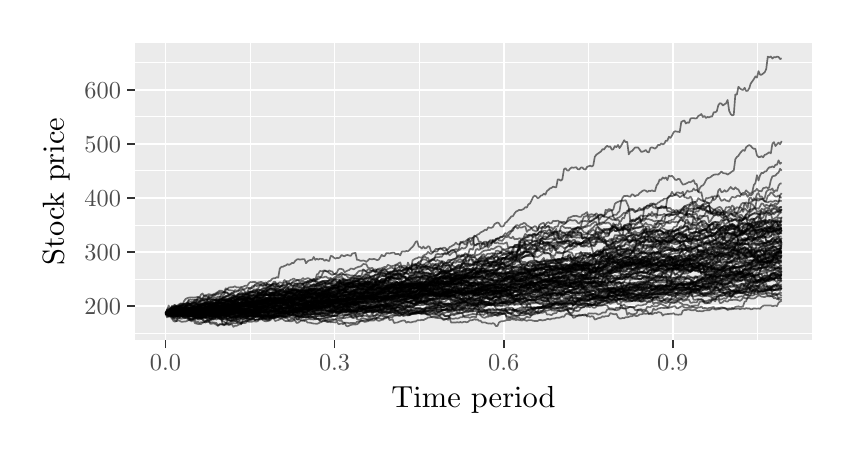
\begin{tikzpicture}[x=1pt,y=1pt]
\definecolor{fillColor}{RGB}{255,255,255}
\path[use as bounding box,fill=fillColor,fill opacity=0.00] (0,0) rectangle (289.08,144.54);
\begin{scope}
\path[clip] (  0.00,  0.00) rectangle (289.08,144.54);
\definecolor{drawColor}{RGB}{255,255,255}
\definecolor{fillColor}{RGB}{255,255,255}

\path[draw=drawColor,line width= 0.6pt,line join=round,line cap=round,fill=fillColor] (  0.00,  0.00) rectangle (289.08,144.54);
\end{scope}
\begin{scope}
\path[clip] ( 38.67, 31.53) rectangle (283.58,139.04);
\definecolor{fillColor}{gray}{0.92}

\path[fill=fillColor] ( 38.67, 31.53) rectangle (283.58,139.04);
\definecolor{drawColor}{RGB}{255,255,255}

\path[draw=drawColor,line width= 0.3pt,line join=round] ( 38.67, 34.18) --
	(283.58, 34.18);

\path[draw=drawColor,line width= 0.3pt,line join=round] ( 38.67, 53.71) --
	(283.58, 53.71);

\path[draw=drawColor,line width= 0.3pt,line join=round] ( 38.67, 73.25) --
	(283.58, 73.25);

\path[draw=drawColor,line width= 0.3pt,line join=round] ( 38.67, 92.79) --
	(283.58, 92.79);

\path[draw=drawColor,line width= 0.3pt,line join=round] ( 38.67,112.33) --
	(283.58,112.33);

\path[draw=drawColor,line width= 0.3pt,line join=round] ( 38.67,131.86) --
	(283.58,131.86);

\path[draw=drawColor,line width= 0.3pt,line join=round] ( 80.35, 31.53) --
	( 80.35,139.04);

\path[draw=drawColor,line width= 0.3pt,line join=round] (141.45, 31.53) --
	(141.45,139.04);

\path[draw=drawColor,line width= 0.3pt,line join=round] (202.56, 31.53) --
	(202.56,139.04);

\path[draw=drawColor,line width= 0.3pt,line join=round] (263.66, 31.53) --
	(263.66,139.04);

\path[draw=drawColor,line width= 0.6pt,line join=round] ( 38.67, 43.94) --
	(283.58, 43.94);

\path[draw=drawColor,line width= 0.6pt,line join=round] ( 38.67, 63.48) --
	(283.58, 63.48);

\path[draw=drawColor,line width= 0.6pt,line join=round] ( 38.67, 83.02) --
	(283.58, 83.02);

\path[draw=drawColor,line width= 0.6pt,line join=round] ( 38.67,102.56) --
	(283.58,102.56);

\path[draw=drawColor,line width= 0.6pt,line join=round] ( 38.67,122.09) --
	(283.58,122.09);

\path[draw=drawColor,line width= 0.6pt,line join=round] ( 49.80, 31.53) --
	( 49.80,139.04);

\path[draw=drawColor,line width= 0.6pt,line join=round] (110.90, 31.53) --
	(110.90,139.04);

\path[draw=drawColor,line width= 0.6pt,line join=round] (172.00, 31.53) --
	(172.00,139.04);

\path[draw=drawColor,line width= 0.6pt,line join=round] (233.11, 31.53) --
	(233.11,139.04);
\definecolor{drawColor}{RGB}{0,0,0}

\path[draw=drawColor,draw opacity=0.55,line width= 0.6pt,line join=round] ( 49.80, 41.27) --
	( 50.36, 41.26) --
	( 50.92, 41.92) --
	( 51.47, 42.53) --
	( 52.03, 43.94) --
	( 52.59, 44.04) --
	( 53.15, 44.38) --
	( 53.71, 44.01) --
	( 54.26, 44.23) --
	( 54.82, 44.01) --
	( 55.38, 44.28) --
	( 55.94, 44.31) --
	( 56.50, 44.08) --
	( 57.05, 44.22) --
	( 57.61, 44.03) --
	( 58.17, 44.08) --
	( 58.73, 44.33) --
	( 59.29, 44.44) --
	( 59.84, 44.22) --
	( 60.40, 44.21) --
	( 60.96, 44.55) --
	( 61.52, 44.54) --
	( 62.08, 44.79) --
	( 62.63, 44.64) --
	( 63.19, 44.87) --
	( 63.75, 45.04) --
	( 64.31, 45.07) --
	( 64.87, 45.01) --
	( 65.42, 45.59) --
	( 65.98, 45.43) --
	( 66.54, 45.56) --
	( 67.10, 45.68) --
	( 67.66, 45.85) --
	( 68.21, 45.82) --
	( 68.77, 45.83) --
	( 69.33, 46.26) --
	( 69.89, 46.28) --
	( 70.45, 46.29) --
	( 71.00, 45.91) --
	( 71.56, 45.90) --
	( 72.12, 45.61) --
	( 72.68, 45.56) --
	( 73.24, 45.56) --
	( 73.79, 45.77) --
	( 74.35, 45.94) --
	( 74.91, 46.10) --
	( 75.47, 46.27) --
	( 76.03, 46.62) --
	( 76.58, 47.03) --
	( 77.14, 46.79) --
	( 77.70, 46.58) --
	( 78.26, 46.55) --
	( 78.82, 47.22) --
	( 79.37, 47.47) --
	( 79.93, 47.79) --
	( 80.49, 47.67) --
	( 81.05, 47.25) --
	( 81.61, 47.44) --
	( 82.16, 47.41) --
	( 82.72, 47.37) --
	( 83.28, 47.49) --
	( 83.84, 48.12) --
	( 84.40, 48.11) --
	( 84.95, 48.28) --
	( 85.51, 48.32) --
	( 86.07, 48.22) --
	( 86.63, 48.19) --
	( 87.19, 48.09) --
	( 87.74, 48.73) --
	( 88.30, 48.65) --
	( 88.86, 48.02) --
	( 89.42, 47.96) --
	( 89.98, 47.67) --
	( 90.53, 47.43) --
	( 91.09, 47.83) --
	( 91.65, 47.42) --
	( 92.21, 47.55) --
	( 92.77, 47.41) --
	( 93.32, 47.06) --
	( 93.88, 47.18) --
	( 94.44, 47.32) --
	( 95.00, 47.03) --
	( 95.56, 47.40) --
	( 96.11, 48.06) --
	( 96.67, 47.85) --
	( 97.23, 47.92) --
	( 97.79, 48.39) --
	( 98.35, 48.51) --
	( 98.90, 49.22) --
	( 99.46, 49.77) --
	(100.02, 50.00) --
	(100.58, 50.03) --
	(101.14, 48.80) --
	(101.69, 48.93) --
	(102.25, 49.11) --
	(102.81, 50.17) --
	(103.37, 50.27) --
	(103.93, 51.41) --
	(104.48, 51.08) --
	(105.04, 51.22) --
	(105.60, 51.29) --
	(106.16, 51.73) --
	(106.72, 52.03) --
	(107.27, 52.13) --
	(107.83, 52.42) --
	(108.39, 52.58) --
	(108.95, 52.11) --
	(109.51, 51.77) --
	(110.06, 52.29) --
	(110.62, 50.70) --
	(111.18, 51.28) --
	(111.74, 51.04) --
	(112.30, 50.93) --
	(112.85, 52.32) --
	(113.41, 52.04) --
	(113.97, 52.19) --
	(114.53, 51.57) --
	(115.09, 51.62) --
	(115.65, 51.66) --
	(116.20, 51.62) --
	(116.76, 51.88) --
	(117.32, 52.26) --
	(117.88, 50.92) --
	(118.44, 50.84) --
	(118.99, 50.77) --
	(119.55, 50.37) --
	(120.11, 50.02) --
	(120.67, 50.03) --
	(121.23, 50.41) --
	(121.78, 50.16) --
	(122.34, 49.68) --
	(122.90, 49.85) --
	(123.46, 50.01) --
	(124.02, 50.42) --
	(124.57, 50.21) --
	(125.13, 50.05) --
	(125.69, 50.14) --
	(126.25, 50.52) --
	(126.81, 50.81) --
	(127.36, 50.61) --
	(127.92, 50.60) --
	(128.48, 50.67) --
	(129.04, 49.30) --
	(129.60, 49.10) --
	(130.15, 49.21) --
	(130.71, 49.52) --
	(131.27, 49.58) --
	(131.83, 49.78) --
	(132.39, 50.18) --
	(132.94, 50.54) --
	(133.50, 49.38) --
	(134.06, 49.42) --
	(134.62, 49.75) --
	(135.18, 50.31) --
	(135.73, 50.49) --
	(136.29, 50.44) --
	(136.85, 50.70) --
	(137.41, 50.58) --
	(137.97, 50.82) --
	(138.52, 50.78) --
	(139.08, 51.13) --
	(139.64, 51.69) --
	(140.20, 52.04) --
	(140.76, 52.23) --
	(141.31, 52.26) --
	(141.87, 52.30) --
	(142.43, 51.49) --
	(142.99, 51.74) --
	(143.55, 51.88) --
	(144.10, 52.12) --
	(144.66, 52.50) --
	(145.22, 52.14) --
	(145.78, 52.20) --
	(146.34, 51.61) --
	(146.89, 51.80) --
	(147.45, 52.36) --
	(148.01, 52.82) --
	(148.57, 52.92) --
	(149.13, 54.79) --
	(149.68, 54.61) --
	(150.24, 54.23) --
	(150.80, 54.07) --
	(151.36, 53.94) --
	(151.92, 54.09) --
	(152.47, 54.40) --
	(153.03, 54.11) --
	(153.59, 54.16) --
	(154.15, 54.72) --
	(154.71, 54.57) --
	(155.26, 54.64) --
	(155.82, 55.02) --
	(156.38, 55.45) --
	(156.94, 55.51) --
	(157.50, 55.80) --
	(158.05, 55.53) --
	(158.61, 52.62) --
	(159.17, 53.04) --
	(159.73, 52.26) --
	(160.29, 52.14) --
	(160.84, 52.51) --
	(161.40, 52.61) --
	(161.96, 53.22) --
	(162.52, 52.89) --
	(163.08, 50.97) --
	(163.63, 50.92) --
	(164.19, 51.83) --
	(164.75, 50.84) --
	(165.31, 50.97) --
	(165.87, 51.04) --
	(166.42, 51.24) --
	(166.98, 51.36) --
	(167.54, 51.55) --
	(168.10, 51.30) --
	(168.66, 51.75) --
	(169.21, 50.18) --
	(169.77, 48.92) --
	(170.33, 48.74) --
	(170.89, 48.54) --
	(171.45, 48.67) --
	(172.00, 48.88) --
	(172.56, 49.29) --
	(173.12, 49.58) --
	(173.68, 49.79) --
	(174.24, 49.37) --
	(174.79, 47.60) --
	(175.35, 47.32) --
	(175.91, 46.72) --
	(176.47, 46.41) --
	(177.03, 46.25) --
	(177.58, 46.39) --
	(178.14, 46.38) --
	(178.70, 46.71) --
	(179.26, 47.07) --
	(179.82, 46.83) --
	(180.37, 46.88) --
	(180.93, 47.36) --
	(181.49, 48.52) --
	(182.05, 48.64) --
	(182.61, 48.71) --
	(183.17, 48.87) --
	(183.72, 49.13) --
	(184.28, 48.95) --
	(184.84, 49.74) --
	(185.40, 50.64) --
	(185.96, 50.49) --
	(186.51, 50.30) --
	(187.07, 50.99) --
	(187.63, 50.93) --
	(188.19, 51.47) --
	(188.75, 51.40) --
	(189.30, 51.37) --
	(189.86, 51.40) --
	(190.42, 51.26) --
	(190.98, 51.76) --
	(191.54, 51.54) --
	(192.09, 51.61) --
	(192.65, 51.07) --
	(193.21, 50.97) --
	(193.77, 51.01) --
	(194.33, 51.07) --
	(194.88, 51.28) --
	(195.44, 51.27) --
	(196.00, 51.21) --
	(196.56, 51.16) --
	(197.12, 51.41) --
	(197.67, 52.61) --
	(198.23, 52.68) --
	(198.79, 52.68) --
	(199.35, 52.91) --
	(199.91, 53.27) --
	(200.46, 53.39) --
	(201.02, 54.29) --
	(201.58, 54.46) --
	(202.14, 54.77) --
	(202.70, 52.79) --
	(203.25, 52.53) --
	(203.81, 52.65) --
	(204.37, 52.32) --
	(204.93, 52.54) --
	(205.49, 52.33) --
	(206.04, 52.22) --
	(206.60, 52.06) --
	(207.16, 52.15) --
	(207.72, 52.62) --
	(208.28, 52.62) --
	(208.83, 53.78) --
	(209.39, 53.82) --
	(209.95, 53.96) --
	(210.51, 54.37) --
	(211.07, 54.94) --
	(211.62, 54.42) --
	(212.18, 53.17) --
	(212.74, 53.84) --
	(213.30, 54.17) --
	(213.86, 54.30) --
	(214.41, 54.57) --
	(214.97, 54.56) --
	(215.53, 54.70) --
	(216.09, 54.51) --
	(216.65, 54.35) --
	(217.20, 54.45) --
	(217.76, 54.90) --
	(218.32, 55.17) --
	(218.88, 55.90) --
	(219.44, 55.64) --
	(219.99, 55.81) --
	(220.55, 54.99) --
	(221.11, 54.73) --
	(221.67, 55.23) --
	(222.23, 54.90) --
	(222.78, 54.88) --
	(223.34, 54.56) --
	(223.90, 55.31) --
	(224.46, 55.31) --
	(225.02, 55.47) --
	(225.57, 55.28) --
	(226.13, 55.02) --
	(226.69, 54.96) --
	(227.25, 54.60) --
	(227.81, 54.89) --
	(228.36, 54.89) --
	(228.92, 54.10) --
	(229.48, 56.09) --
	(230.04, 55.85) --
	(230.60, 55.73) --
	(231.15, 57.74) --
	(231.71, 57.66) --
	(232.27, 57.82) --
	(232.83, 57.36) --
	(233.39, 57.53) --
	(233.94, 57.53) --
	(234.50, 57.88) --
	(235.06, 57.59) --
	(235.62, 57.24) --
	(236.18, 57.01) --
	(236.73, 57.54) --
	(237.29, 57.62) --
	(237.85, 57.30) --
	(238.41, 57.20) --
	(238.97, 56.92) --
	(239.52, 56.84) --
	(240.08, 56.89) --
	(240.64, 57.04) --
	(241.20, 56.82) --
	(241.76, 56.95) --
	(242.31, 56.21) --
	(242.87, 56.45) --
	(243.43, 55.99) --
	(243.99, 56.18) --
	(244.55, 55.89) --
	(245.10, 54.37) --
	(245.66, 54.14) --
	(246.22, 54.19) --
	(246.78, 53.80) --
	(247.34, 53.51) --
	(247.89, 56.02) --
	(248.45, 56.65) --
	(249.01, 56.44) --
	(249.57, 55.98) --
	(250.13, 56.32) --
	(250.68, 56.63) --
	(251.24, 56.65) --
	(251.80, 56.27) --
	(252.36, 56.16) --
	(252.92, 56.11) --
	(253.48, 56.21) --
	(254.03, 56.38) --
	(254.59, 56.05) --
	(255.15, 56.12) --
	(255.71, 56.33) --
	(256.27, 56.74) --
	(256.82, 56.11) --
	(257.38, 56.58) --
	(257.94, 56.20) --
	(258.50, 56.31) --
	(259.06, 57.10) --
	(259.61, 56.77) --
	(260.17, 56.73) --
	(260.73, 56.15) --
	(261.29, 56.83) --
	(261.85, 60.26) --
	(262.40, 60.47) --
	(262.96, 60.25) --
	(263.52, 60.73) --
	(264.08, 61.22) --
	(264.64, 61.09) --
	(265.19, 60.75) --
	(265.75, 60.51) --
	(266.31, 60.37) --
	(266.87, 60.72) --
	(267.43, 60.18) --
	(267.98, 59.51) --
	(268.54, 59.50) --
	(269.10, 59.49) --
	(269.66, 59.63) --
	(270.22, 59.68) --
	(270.77, 60.03) --
	(271.33, 60.35) --
	(271.89, 60.17) --
	(272.45, 59.99);

\path[draw=drawColor,draw opacity=0.55,line width= 0.6pt,line join=round] ( 49.80, 41.27) --
	( 50.36, 41.30) --
	( 50.92, 41.08) --
	( 51.47, 41.23) --
	( 52.03, 41.06) --
	( 52.59, 40.85) --
	( 53.15, 41.16) --
	( 53.71, 41.32) --
	( 54.26, 41.49) --
	( 54.82, 41.38) --
	( 55.38, 41.63) --
	( 55.94, 41.30) --
	( 56.50, 40.96) --
	( 57.05, 40.79) --
	( 57.61, 40.63) --
	( 58.17, 40.63) --
	( 58.73, 40.42) --
	( 59.29, 41.34) --
	( 59.84, 41.01) --
	( 60.40, 40.79) --
	( 60.96, 40.71) --
	( 61.52, 40.81) --
	( 62.08, 40.86) --
	( 62.63, 40.78) --
	( 63.19, 40.82) --
	( 63.75, 40.87) --
	( 64.31, 41.50) --
	( 64.87, 42.05) --
	( 65.42, 42.29) --
	( 65.98, 42.29) --
	( 66.54, 42.29) --
	( 67.10, 42.10) --
	( 67.66, 42.09) --
	( 68.21, 42.47) --
	( 68.77, 42.56) --
	( 69.33, 42.52) --
	( 69.89, 42.42) --
	( 70.45, 42.29) --
	( 71.00, 42.30) --
	( 71.56, 43.42) --
	( 72.12, 43.54) --
	( 72.68, 43.66) --
	( 73.24, 43.92) --
	( 73.79, 44.07) --
	( 74.35, 44.56) --
	( 74.91, 44.43) --
	( 75.47, 44.39) --
	( 76.03, 44.64) --
	( 76.58, 44.57) --
	( 77.14, 44.52) --
	( 77.70, 44.79) --
	( 78.26, 44.79) --
	( 78.82, 44.80) --
	( 79.37, 44.57) --
	( 79.93, 43.20) --
	( 80.49, 43.57) --
	( 81.05, 43.61) --
	( 81.61, 43.55) --
	( 82.16, 42.50) --
	( 82.72, 42.81) --
	( 83.28, 43.19) --
	( 83.84, 43.20) --
	( 84.40, 43.08) --
	( 84.95, 43.09) --
	( 85.51, 43.03) --
	( 86.07, 42.25) --
	( 86.63, 43.32) --
	( 87.19, 42.99) --
	( 87.74, 42.83) --
	( 88.30, 43.06) --
	( 88.86, 43.36) --
	( 89.42, 42.99) --
	( 89.98, 42.56) --
	( 90.53, 42.82) --
	( 91.09, 42.97) --
	( 91.65, 43.12) --
	( 92.21, 43.05) --
	( 92.77, 43.14) --
	( 93.32, 42.74) --
	( 93.88, 43.05) --
	( 94.44, 42.39) --
	( 95.00, 42.46) --
	( 95.56, 42.49) --
	( 96.11, 42.38) --
	( 96.67, 43.25) --
	( 97.23, 43.13) --
	( 97.79, 42.96) --
	( 98.35, 43.19) --
	( 98.90, 44.72) --
	( 99.46, 44.76) --
	(100.02, 45.05) --
	(100.58, 45.27) --
	(101.14, 45.09) --
	(101.69, 45.57) --
	(102.25, 45.62) --
	(102.81, 45.80) --
	(103.37, 46.03) --
	(103.93, 45.78) --
	(104.48, 45.56) --
	(105.04, 45.15) --
	(105.60, 42.92) --
	(106.16, 43.20) --
	(106.72, 43.59) --
	(107.27, 43.56) --
	(107.83, 42.19) --
	(108.39, 42.24) --
	(108.95, 42.49) --
	(109.51, 42.23) --
	(110.06, 42.14) --
	(110.62, 42.24) --
	(111.18, 42.08) --
	(111.74, 42.05) --
	(112.30, 42.12) --
	(112.85, 42.27) --
	(113.41, 42.57) --
	(113.97, 42.90) --
	(114.53, 42.73) --
	(115.09, 42.75) --
	(115.65, 42.98) --
	(116.20, 41.81) --
	(116.76, 41.51) --
	(117.32, 41.90) --
	(117.88, 42.13) --
	(118.44, 42.24) --
	(118.99, 42.52) --
	(119.55, 42.67) --
	(120.11, 43.02) --
	(120.67, 42.73) --
	(121.23, 42.84) --
	(121.78, 42.63) --
	(122.34, 42.39) --
	(122.90, 43.31) --
	(123.46, 43.03) --
	(124.02, 43.35) --
	(124.57, 43.06) --
	(125.13, 42.68) --
	(125.69, 43.45) --
	(126.25, 43.46) --
	(126.81, 43.93) --
	(127.36, 43.81) --
	(127.92, 44.31) --
	(128.48, 44.71) --
	(129.04, 45.76) --
	(129.60, 46.52) --
	(130.15, 46.43) --
	(130.71, 46.76) --
	(131.27, 47.56) --
	(131.83, 48.10) --
	(132.39, 48.40) --
	(132.94, 48.23) --
	(133.50, 48.46) --
	(134.06, 48.88) --
	(134.62, 48.97) --
	(135.18, 49.11) --
	(135.73, 49.23) --
	(136.29, 48.86) --
	(136.85, 49.23) --
	(137.41, 49.69) --
	(137.97, 50.06) --
	(138.52, 50.18) --
	(139.08, 50.84) --
	(139.64, 51.26) --
	(140.20, 52.11) --
	(140.76, 52.16) --
	(141.31, 52.11) --
	(141.87, 51.10) --
	(142.43, 51.36) --
	(142.99, 50.95) --
	(143.55, 50.94) --
	(144.10, 51.01) --
	(144.66, 50.43) --
	(145.22, 50.77) --
	(145.78, 50.86) --
	(146.34, 51.09) --
	(146.89, 51.11) --
	(147.45, 51.37) --
	(148.01, 52.62) --
	(148.57, 52.60) --
	(149.13, 53.15) --
	(149.68, 53.63) --
	(150.24, 54.20) --
	(150.80, 54.62) --
	(151.36, 54.18) --
	(151.92, 53.75) --
	(152.47, 53.83) --
	(153.03, 53.58) --
	(153.59, 54.51) --
	(154.15, 54.43) --
	(154.71, 54.97) --
	(155.26, 54.99) --
	(155.82, 54.86) --
	(156.38, 54.77) --
	(156.94, 54.87) --
	(157.50, 54.47) --
	(158.05, 54.30) --
	(158.61, 54.70) --
	(159.17, 54.57) --
	(159.73, 54.49) --
	(160.29, 54.59) --
	(160.84, 55.24) --
	(161.40, 55.63) --
	(161.96, 55.82) --
	(162.52, 56.40) --
	(163.08, 55.16) --
	(163.63, 54.68) --
	(164.19, 54.86) --
	(164.75, 54.90) --
	(165.31, 55.17) --
	(165.87, 55.09) --
	(166.42, 54.75) --
	(166.98, 54.66) --
	(167.54, 55.06) --
	(168.10, 55.52) --
	(168.66, 56.80) --
	(169.21, 56.79) --
	(169.77, 57.44) --
	(170.33, 57.68) --
	(170.89, 57.93) --
	(171.45, 57.93) --
	(172.00, 57.93) --
	(172.56, 56.46) --
	(173.12, 53.94) --
	(173.68, 54.25) --
	(174.24, 54.14) --
	(174.79, 54.29) --
	(175.35, 54.13) --
	(175.91, 53.75) --
	(176.47, 53.22) --
	(177.03, 52.85) --
	(177.58, 52.85) --
	(178.14, 52.95) --
	(178.70, 53.21) --
	(179.26, 53.47) --
	(179.82, 53.26) --
	(180.37, 54.38) --
	(180.93, 54.65) --
	(181.49, 54.25) --
	(182.05, 54.46) --
	(182.61, 54.53) --
	(183.17, 54.74) --
	(183.72, 54.65) --
	(184.28, 54.26) --
	(184.84, 54.75) --
	(185.40, 53.80) --
	(185.96, 53.55) --
	(186.51, 53.36) --
	(187.07, 53.54) --
	(187.63, 53.86) --
	(188.19, 53.42) --
	(188.75, 53.65) --
	(189.30, 53.39) --
	(189.86, 54.88) --
	(190.42, 54.96) --
	(190.98, 55.51) --
	(191.54, 55.83) --
	(192.09, 56.34) --
	(192.65, 56.17) --
	(193.21, 56.41) --
	(193.77, 57.81) --
	(194.33, 58.05) --
	(194.88, 58.17) --
	(195.44, 57.90) --
	(196.00, 58.98) --
	(196.56, 59.13) --
	(197.12, 59.06) --
	(197.67, 59.25) --
	(198.23, 59.06) --
	(198.79, 58.70) --
	(199.35, 59.29) --
	(199.91, 59.07) --
	(200.46, 57.70) --
	(201.02, 57.37) --
	(201.58, 57.54) --
	(202.14, 57.47) --
	(202.70, 57.35) --
	(203.25, 55.68) --
	(203.81, 56.57) --
	(204.37, 56.29) --
	(204.93, 56.42) --
	(205.49, 56.63) --
	(206.04, 56.32) --
	(206.60, 56.37) --
	(207.16, 57.29) --
	(207.72, 57.36) --
	(208.28, 58.39) --
	(208.83, 58.69) --
	(209.39, 59.27) --
	(209.95, 59.64) --
	(210.51, 59.43) --
	(211.07, 59.51) --
	(211.62, 58.53) --
	(212.18, 58.28) --
	(212.74, 57.98) --
	(213.30, 58.07) --
	(213.86, 57.65) --
	(214.41, 59.03) --
	(214.97, 58.99) --
	(215.53, 59.18) --
	(216.09, 59.42) --
	(216.65, 59.99) --
	(217.20, 61.03) --
	(217.76, 59.54) --
	(218.32, 59.40) --
	(218.88, 59.52) --
	(219.44, 59.23) --
	(219.99, 59.33) --
	(220.55, 59.57) --
	(221.11, 59.61) --
	(221.67, 59.15) --
	(222.23, 59.17) --
	(222.78, 59.40) --
	(223.34, 59.47) --
	(223.90, 58.81) --
	(224.46, 59.33) --
	(225.02, 59.22) --
	(225.57, 59.26) --
	(226.13, 57.61) --
	(226.69, 56.26) --
	(227.25, 56.55) --
	(227.81, 56.92) --
	(228.36, 58.44) --
	(228.92, 58.73) --
	(229.48, 58.60) --
	(230.04, 58.74) --
	(230.60, 58.52) --
	(231.15, 58.29) --
	(231.71, 58.36) --
	(232.27, 58.47) --
	(232.83, 59.08) --
	(233.39, 58.86) --
	(233.94, 59.23) --
	(234.50, 57.30) --
	(235.06, 57.37) --
	(235.62, 58.11) --
	(236.18, 58.33) --
	(236.73, 58.28) --
	(237.29, 58.37) --
	(237.85, 58.76) --
	(238.41, 58.34) --
	(238.97, 58.77) --
	(239.52, 58.96) --
	(240.08, 58.24) --
	(240.64, 58.65) --
	(241.20, 58.39) --
	(241.76, 58.42) --
	(242.31, 58.44) --
	(242.87, 59.34) --
	(243.43, 58.86) --
	(243.99, 58.83) --
	(244.55, 57.88) --
	(245.10, 58.29) --
	(245.66, 58.18) --
	(246.22, 57.69) --
	(246.78, 57.36) --
	(247.34, 57.20) --
	(247.89, 57.25) --
	(248.45, 57.17) --
	(249.01, 57.16) --
	(249.57, 57.27) --
	(250.13, 56.84) --
	(250.68, 57.14) --
	(251.24, 56.97) --
	(251.80, 58.82) --
	(252.36, 58.61) --
	(252.92, 58.34) --
	(253.48, 58.35) --
	(254.03, 57.41) --
	(254.59, 58.45) --
	(255.15, 58.18) --
	(255.71, 57.89) --
	(256.27, 58.04) --
	(256.82, 57.94) --
	(257.38, 58.09) --
	(257.94, 58.66) --
	(258.50, 59.12) --
	(259.06, 59.34) --
	(259.61, 61.57) --
	(260.17, 61.59) --
	(260.73, 61.46) --
	(261.29, 61.85) --
	(261.85, 62.37) --
	(262.40, 62.79) --
	(262.96, 62.90) --
	(263.52, 63.21) --
	(264.08, 61.97) --
	(264.64, 62.26) --
	(265.19, 62.43) --
	(265.75, 62.09) --
	(266.31, 62.08) --
	(266.87, 63.67) --
	(267.43, 64.00) --
	(267.98, 63.98) --
	(268.54, 63.92) --
	(269.10, 64.01) --
	(269.66, 63.92) --
	(270.22, 64.14) --
	(270.77, 64.33) --
	(271.33, 64.45) --
	(271.89, 64.90) --
	(272.45, 64.70);

\path[draw=drawColor,draw opacity=0.55,line width= 0.6pt,line join=round] ( 49.80, 41.27) --
	( 50.36, 41.27) --
	( 50.92, 41.44) --
	( 51.47, 41.55) --
	( 52.03, 41.62) --
	( 52.59, 41.51) --
	( 53.15, 40.88) --
	( 53.71, 41.01) --
	( 54.26, 41.07) --
	( 54.82, 41.14) --
	( 55.38, 41.39) --
	( 55.94, 41.49) --
	( 56.50, 41.69) --
	( 57.05, 41.57) --
	( 57.61, 40.76) --
	( 58.17, 40.69) --
	( 58.73, 40.86) --
	( 59.29, 41.71) --
	( 59.84, 40.99) --
	( 60.40, 41.12) --
	( 60.96, 40.82) --
	( 61.52, 41.06) --
	( 62.08, 40.95) --
	( 62.63, 41.11) --
	( 63.19, 41.93) --
	( 63.75, 41.73) --
	( 64.31, 41.47) --
	( 64.87, 41.82) --
	( 65.42, 41.69) --
	( 65.98, 41.80) --
	( 66.54, 41.94) --
	( 67.10, 41.94) --
	( 67.66, 41.06) --
	( 68.21, 41.04) --
	( 68.77, 41.21) --
	( 69.33, 41.24) --
	( 69.89, 41.20) --
	( 70.45, 40.68) --
	( 71.00, 40.45) --
	( 71.56, 40.39) --
	( 72.12, 40.30) --
	( 72.68, 40.46) --
	( 73.24, 40.87) --
	( 73.79, 41.00) --
	( 74.35, 41.19) --
	( 74.91, 41.47) --
	( 75.47, 42.28) --
	( 76.03, 42.04) --
	( 76.58, 42.45) --
	( 77.14, 42.44) --
	( 77.70, 42.16) --
	( 78.26, 42.36) --
	( 78.82, 42.47) --
	( 79.37, 42.26) --
	( 79.93, 43.07) --
	( 80.49, 43.29) --
	( 81.05, 43.41) --
	( 81.61, 43.16) --
	( 82.16, 43.02) --
	( 82.72, 43.10) --
	( 83.28, 43.34) --
	( 83.84, 43.35) --
	( 84.40, 43.38) --
	( 84.95, 43.13) --
	( 85.51, 41.95) --
	( 86.07, 41.98) --
	( 86.63, 41.85) --
	( 87.19, 41.94) --
	( 87.74, 42.25) --
	( 88.30, 42.34) --
	( 88.86, 42.46) --
	( 89.42, 42.15) --
	( 89.98, 42.20) --
	( 90.53, 41.96) --
	( 91.09, 41.29) --
	( 91.65, 41.42) --
	( 92.21, 41.99) --
	( 92.77, 42.04) --
	( 93.32, 42.08) --
	( 93.88, 42.11) --
	( 94.44, 42.22) --
	( 95.00, 42.25) --
	( 95.56, 42.39) --
	( 96.11, 42.35) --
	( 96.67, 42.27) --
	( 97.23, 42.48) --
	( 97.79, 42.65) --
	( 98.35, 42.74) --
	( 98.90, 42.49) --
	( 99.46, 43.03) --
	(100.02, 43.59) --
	(100.58, 43.55) --
	(101.14, 43.24) --
	(101.69, 43.49) --
	(102.25, 43.49) --
	(102.81, 43.30) --
	(103.37, 43.70) --
	(103.93, 44.56) --
	(104.48, 44.84) --
	(105.04, 45.16) --
	(105.60, 45.14) --
	(106.16, 44.73) --
	(106.72, 43.84) --
	(107.27, 43.90) --
	(107.83, 43.72) --
	(108.39, 43.38) --
	(108.95, 43.72) --
	(109.51, 43.45) --
	(110.06, 43.43) --
	(110.62, 43.68) --
	(111.18, 43.83) --
	(111.74, 43.66) --
	(112.30, 43.60) --
	(112.85, 43.62) --
	(113.41, 43.59) --
	(113.97, 43.76) --
	(114.53, 43.97) --
	(115.09, 43.75) --
	(115.65, 43.67) --
	(116.20, 43.79) --
	(116.76, 44.37) --
	(117.32, 44.72) --
	(117.88, 44.29) --
	(118.44, 44.81) --
	(118.99, 44.62) --
	(119.55, 45.01) --
	(120.11, 44.82) --
	(120.67, 44.95) --
	(121.23, 45.04) --
	(121.78, 45.09) --
	(122.34, 44.88) --
	(122.90, 45.68) --
	(123.46, 45.60) --
	(124.02, 45.41) --
	(124.57, 45.47) --
	(125.13, 46.18) --
	(125.69, 46.38) --
	(126.25, 46.54) --
	(126.81, 46.57) --
	(127.36, 46.61) --
	(127.92, 46.34) --
	(128.48, 46.65) --
	(129.04, 47.10) --
	(129.60, 47.30) --
	(130.15, 46.98) --
	(130.71, 47.21) --
	(131.27, 47.30) --
	(131.83, 47.36) --
	(132.39, 47.18) --
	(132.94, 47.58) --
	(133.50, 47.56) --
	(134.06, 47.16) --
	(134.62, 47.51) --
	(135.18, 48.56) --
	(135.73, 48.71) --
	(136.29, 46.82) --
	(136.85, 46.38) --
	(137.41, 46.33) --
	(137.97, 46.36) --
	(138.52, 46.26) --
	(139.08, 46.33) --
	(139.64, 46.34) --
	(140.20, 47.58) --
	(140.76, 47.99) --
	(141.31, 48.35) --
	(141.87, 49.42) --
	(142.43, 49.44) --
	(142.99, 49.64) --
	(143.55, 49.74) --
	(144.10, 49.63) --
	(144.66, 49.02) --
	(145.22, 48.99) --
	(145.78, 49.21) --
	(146.34, 49.27) --
	(146.89, 48.51) --
	(147.45, 48.74) --
	(148.01, 49.00) --
	(148.57, 48.98) --
	(149.13, 49.16) --
	(149.68, 49.22) --
	(150.24, 48.79) --
	(150.80, 49.18) --
	(151.36, 49.59) --
	(151.92, 49.70) --
	(152.47, 49.33) --
	(153.03, 49.80) --
	(153.59, 50.04) --
	(154.15, 50.36) --
	(154.71, 49.97) --
	(155.26, 50.19) --
	(155.82, 49.98) --
	(156.38, 49.99) --
	(156.94, 49.89) --
	(157.50, 49.92) --
	(158.05, 49.79) --
	(158.61, 48.51) --
	(159.17, 48.72) --
	(159.73, 46.39) --
	(160.29, 46.52) --
	(160.84, 46.14) --
	(161.40, 45.83) --
	(161.96, 45.67) --
	(162.52, 45.79) --
	(163.08, 45.86) --
	(163.63, 45.45) --
	(164.19, 45.73) --
	(164.75, 45.99) --
	(165.31, 46.87) --
	(165.87, 46.85) --
	(166.42, 46.64) --
	(166.98, 46.53) --
	(167.54, 46.56) --
	(168.10, 46.85) --
	(168.66, 47.12) --
	(169.21, 47.50) --
	(169.77, 47.64) --
	(170.33, 46.24) --
	(170.89, 46.35) --
	(171.45, 45.31) --
	(172.00, 46.51) --
	(172.56, 46.37) --
	(173.12, 46.32) --
	(173.68, 46.48) --
	(174.24, 46.92) --
	(174.79, 46.78) --
	(175.35, 46.89) --
	(175.91, 46.11) --
	(176.47, 46.33) --
	(177.03, 46.40) --
	(177.58, 45.47) --
	(178.14, 44.91) --
	(178.70, 43.82) --
	(179.26, 43.57) --
	(179.82, 43.42) --
	(180.37, 43.50) --
	(180.93, 43.45) --
	(181.49, 43.59) --
	(182.05, 43.48) --
	(182.61, 42.83) --
	(183.17, 43.09) --
	(183.72, 43.33) --
	(184.28, 43.56) --
	(184.84, 43.54) --
	(185.40, 43.58) --
	(185.96, 43.11) --
	(186.51, 43.14) --
	(187.07, 44.10) --
	(187.63, 44.18) --
	(188.19, 43.91) --
	(188.75, 43.89) --
	(189.30, 43.27) --
	(189.86, 43.16) --
	(190.42, 42.89) --
	(190.98, 42.93) --
	(191.54, 43.42) --
	(192.09, 43.45) --
	(192.65, 43.57) --
	(193.21, 43.87) --
	(193.77, 43.09) --
	(194.33, 42.81) --
	(194.88, 42.48) --
	(195.44, 42.67) --
	(196.00, 42.84) --
	(196.56, 42.97) --
	(197.12, 44.44) --
	(197.67, 44.48) --
	(198.23, 44.90) --
	(198.79, 44.59) --
	(199.35, 44.84) --
	(199.91, 44.83) --
	(200.46, 45.11) --
	(201.02, 45.18) --
	(201.58, 45.60) --
	(202.14, 45.75) --
	(202.70, 45.85) --
	(203.25, 46.04) --
	(203.81, 46.68) --
	(204.37, 47.50) --
	(204.93, 47.45) --
	(205.49, 47.40) --
	(206.04, 47.93) --
	(206.60, 48.59) --
	(207.16, 48.51) --
	(207.72, 49.30) --
	(208.28, 49.04) --
	(208.83, 49.35) --
	(209.39, 49.28) --
	(209.95, 49.53) --
	(210.51, 49.74) --
	(211.07, 49.91) --
	(211.62, 50.39) --
	(212.18, 50.50) --
	(212.74, 50.59) --
	(213.30, 49.79) --
	(213.86, 49.37) --
	(214.41, 49.87) --
	(214.97, 49.81) --
	(215.53, 49.67) --
	(216.09, 48.82) --
	(216.65, 48.69) --
	(217.20, 49.13) --
	(217.76, 49.52) --
	(218.32, 49.50) --
	(218.88, 49.46) --
	(219.44, 49.48) --
	(219.99, 49.21) --
	(220.55, 49.04) --
	(221.11, 48.41) --
	(221.67, 48.63) --
	(222.23, 48.47) --
	(222.78, 48.69) --
	(223.34, 48.99) --
	(223.90, 49.36) --
	(224.46, 48.97) --
	(225.02, 49.16) --
	(225.57, 49.40) --
	(226.13, 49.97) --
	(226.69, 50.08) --
	(227.25, 50.35) --
	(227.81, 51.55) --
	(228.36, 51.67) --
	(228.92, 51.29) --
	(229.48, 51.24) --
	(230.04, 51.25) --
	(230.60, 51.13) --
	(231.15, 50.36) --
	(231.71, 50.38) --
	(232.27, 50.13) --
	(232.83, 49.71) --
	(233.39, 50.31) --
	(233.94, 50.32) --
	(234.50, 50.26) --
	(235.06, 49.26) --
	(235.62, 49.15) --
	(236.18, 49.42) --
	(236.73, 49.27) --
	(237.29, 48.90) --
	(237.85, 48.84) --
	(238.41, 49.08) --
	(238.97, 49.17) --
	(239.52, 49.58) --
	(240.08, 47.77) --
	(240.64, 46.20) --
	(241.20, 46.16) --
	(241.76, 46.35) --
	(242.31, 46.43) --
	(242.87, 46.34) --
	(243.43, 46.32) --
	(243.99, 46.26) --
	(244.55, 45.00) --
	(245.10, 44.91) --
	(245.66, 45.05) --
	(246.22, 45.60) --
	(246.78, 45.74) --
	(247.34, 46.04) --
	(247.89, 46.08) --
	(248.45, 45.61) --
	(249.01, 47.45) --
	(249.57, 47.47) --
	(250.13, 47.80) --
	(250.68, 48.10) --
	(251.24, 48.68) --
	(251.80, 48.67) --
	(252.36, 49.03) --
	(252.92, 49.04) --
	(253.48, 48.87) --
	(254.03, 49.18) --
	(254.59, 49.14) --
	(255.15, 49.48) --
	(255.71, 49.01) --
	(256.27, 51.15) --
	(256.82, 50.61) --
	(257.38, 51.09) --
	(257.94, 51.33) --
	(258.50, 51.28) --
	(259.06, 51.23) --
	(259.61, 51.22) --
	(260.17, 51.36) --
	(260.73, 50.88) --
	(261.29, 51.24) --
	(261.85, 51.14) --
	(262.40, 52.63) --
	(262.96, 53.02) --
	(263.52, 52.92) --
	(264.08, 53.01) --
	(264.64, 53.24) --
	(265.19, 52.92) --
	(265.75, 52.99) --
	(266.31, 53.63) --
	(266.87, 54.12) --
	(267.43, 54.31) --
	(267.98, 54.75) --
	(268.54, 54.12) --
	(269.10, 53.72) --
	(269.66, 53.84) --
	(270.22, 52.97) --
	(270.77, 52.91) --
	(271.33, 53.24) --
	(271.89, 53.19) --
	(272.45, 53.18);

\path[draw=drawColor,draw opacity=0.55,line width= 0.6pt,line join=round] ( 49.80, 41.27) --
	( 50.36, 41.24) --
	( 50.92, 40.90) --
	( 51.47, 40.77) --
	( 52.03, 41.09) --
	( 52.59, 41.77) --
	( 53.15, 41.66) --
	( 53.71, 40.82) --
	( 54.26, 40.72) --
	( 54.82, 40.86) --
	( 55.38, 40.74) --
	( 55.94, 40.70) --
	( 56.50, 40.74) --
	( 57.05, 40.80) --
	( 57.61, 40.72) --
	( 58.17, 40.61) --
	( 58.73, 40.38) --
	( 59.29, 40.31) --
	( 59.84, 40.31) --
	( 60.40, 40.55) --
	( 60.96, 40.47) --
	( 61.52, 40.30) --
	( 62.08, 40.36) --
	( 62.63, 40.48) --
	( 63.19, 40.36) --
	( 63.75, 40.54) --
	( 64.31, 40.66) --
	( 64.87, 40.67) --
	( 65.42, 40.82) --
	( 65.98, 40.91) --
	( 66.54, 41.18) --
	( 67.10, 41.44) --
	( 67.66, 41.20) --
	( 68.21, 41.57) --
	( 68.77, 41.36) --
	( 69.33, 41.43) --
	( 69.89, 41.53) --
	( 70.45, 41.51) --
	( 71.00, 42.44) --
	( 71.56, 42.46) --
	( 72.12, 42.42) --
	( 72.68, 42.51) --
	( 73.24, 42.35) --
	( 73.79, 42.64) --
	( 74.35, 42.58) --
	( 74.91, 42.30) --
	( 75.47, 42.38) --
	( 76.03, 42.49) --
	( 76.58, 42.57) --
	( 77.14, 42.65) --
	( 77.70, 42.82) --
	( 78.26, 42.85) --
	( 78.82, 42.97) --
	( 79.37, 42.81) --
	( 79.93, 42.79) --
	( 80.49, 43.20) --
	( 81.05, 43.61) --
	( 81.61, 43.40) --
	( 82.16, 43.36) --
	( 82.72, 41.64) --
	( 83.28, 41.71) --
	( 83.84, 42.02) --
	( 84.40, 42.97) --
	( 84.95, 43.20) --
	( 85.51, 43.53) --
	( 86.07, 43.65) --
	( 86.63, 43.62) --
	( 87.19, 43.56) --
	( 87.74, 43.53) --
	( 88.30, 43.20) --
	( 88.86, 43.00) --
	( 89.42, 42.90) --
	( 89.98, 42.70) --
	( 90.53, 42.77) --
	( 91.09, 43.18) --
	( 91.65, 43.24) --
	( 92.21, 43.16) --
	( 92.77, 43.38) --
	( 93.32, 43.41) --
	( 93.88, 43.96) --
	( 94.44, 43.86) --
	( 95.00, 43.83) --
	( 95.56, 43.99) --
	( 96.11, 43.84) --
	( 96.67, 43.65) --
	( 97.23, 42.63) --
	( 97.79, 42.81) --
	( 98.35, 43.05) --
	( 98.90, 43.10) --
	( 99.46, 43.18) --
	(100.02, 43.53) --
	(100.58, 44.87) --
	(101.14, 44.92) --
	(101.69, 45.29) --
	(102.25, 45.27) --
	(102.81, 45.30) --
	(103.37, 45.28) --
	(103.93, 46.15) --
	(104.48, 46.71) --
	(105.04, 47.65) --
	(105.60, 47.91) --
	(106.16, 48.35) --
	(106.72, 48.35) --
	(107.27, 48.56) --
	(107.83, 48.48) --
	(108.39, 48.16) --
	(108.95, 47.92) --
	(109.51, 47.76) --
	(110.06, 46.90) --
	(110.62, 47.18) --
	(111.18, 47.05) --
	(111.74, 47.59) --
	(112.30, 46.53) --
	(112.85, 46.44) --
	(113.41, 46.60) --
	(113.97, 46.30) --
	(114.53, 46.52) --
	(115.09, 46.30) --
	(115.65, 46.04) --
	(116.20, 46.30) --
	(116.76, 46.32) --
	(117.32, 47.27) --
	(117.88, 48.28) --
	(118.44, 48.78) --
	(118.99, 48.93) --
	(119.55, 48.57) --
	(120.11, 47.68) --
	(120.67, 47.87) --
	(121.23, 47.85) --
	(121.78, 47.27) --
	(122.34, 47.25) --
	(122.90, 47.01) --
	(123.46, 46.86) --
	(124.02, 46.83) --
	(124.57, 46.65) --
	(125.13, 46.86) --
	(125.69, 46.76) --
	(126.25, 47.39) --
	(126.81, 47.21) --
	(127.36, 46.88) --
	(127.92, 46.99) --
	(128.48, 46.82) --
	(129.04, 46.86) --
	(129.60, 47.14) --
	(130.15, 47.20) --
	(130.71, 47.07) --
	(131.27, 46.98) --
	(131.83, 47.17) --
	(132.39, 47.71) --
	(132.94, 47.73) --
	(133.50, 47.71) --
	(134.06, 47.40) --
	(134.62, 47.67) --
	(135.18, 48.20) --
	(135.73, 48.18) --
	(136.29, 48.56) --
	(136.85, 48.38) --
	(137.41, 48.06) --
	(137.97, 48.69) --
	(138.52, 48.87) --
	(139.08, 48.94) --
	(139.64, 48.91) --
	(140.20, 48.35) --
	(140.76, 48.25) --
	(141.31, 48.51) --
	(141.87, 48.62) --
	(142.43, 48.42) --
	(142.99, 48.13) --
	(143.55, 48.31) --
	(144.10, 47.82) --
	(144.66, 47.88) --
	(145.22, 47.80) --
	(145.78, 47.83) --
	(146.34, 47.96) --
	(146.89, 47.67) --
	(147.45, 47.70) --
	(148.01, 48.21) --
	(148.57, 48.41) --
	(149.13, 48.48) --
	(149.68, 48.70) --
	(150.24, 48.75) --
	(150.80, 48.86) --
	(151.36, 49.31) --
	(151.92, 49.09) --
	(152.47, 49.24) --
	(153.03, 49.22) --
	(153.59, 49.61) --
	(154.15, 49.15) --
	(154.71, 49.37) --
	(155.26, 49.35) --
	(155.82, 49.31) --
	(156.38, 49.19) --
	(156.94, 49.55) --
	(157.50, 49.80) --
	(158.05, 50.32) --
	(158.61, 50.56) --
	(159.17, 49.47) --
	(159.73, 49.49) --
	(160.29, 49.71) --
	(160.84, 49.53) --
	(161.40, 49.52) --
	(161.96, 49.64) --
	(162.52, 49.68) --
	(163.08, 49.96) --
	(163.63, 49.97) --
	(164.19, 50.11) --
	(164.75, 50.10) --
	(165.31, 50.64) --
	(165.87, 50.60) --
	(166.42, 50.41) --
	(166.98, 50.64) --
	(167.54, 50.57) --
	(168.10, 50.80) --
	(168.66, 50.76) --
	(169.21, 50.60) --
	(169.77, 50.97) --
	(170.33, 51.60) --
	(170.89, 51.58) --
	(171.45, 51.85) --
	(172.00, 51.56) --
	(172.56, 51.63) --
	(173.12, 51.77) --
	(173.68, 51.97) --
	(174.24, 52.46) --
	(174.79, 52.80) --
	(175.35, 52.70) --
	(175.91, 52.84) --
	(176.47, 53.03) --
	(177.03, 54.34) --
	(177.58, 54.29) --
	(178.14, 54.55) --
	(178.70, 54.80) --
	(179.26, 54.89) --
	(179.82, 54.78) --
	(180.37, 54.33) --
	(180.93, 54.22) --
	(181.49, 53.88) --
	(182.05, 54.08) --
	(182.61, 54.21) --
	(183.17, 54.76) --
	(183.72, 54.94) --
	(184.28, 55.34) --
	(184.84, 55.18) --
	(185.40, 56.88) --
	(185.96, 56.45) --
	(186.51, 56.20) --
	(187.07, 56.32) --
	(187.63, 56.01) --
	(188.19, 55.74) --
	(188.75, 56.24) --
	(189.30, 56.00) --
	(189.86, 56.00) --
	(190.42, 56.34) --
	(190.98, 56.35) --
	(191.54, 57.81) --
	(192.09, 57.55) --
	(192.65, 56.96) --
	(193.21, 56.96) --
	(193.77, 58.73) --
	(194.33, 59.17) --
	(194.88, 59.13) --
	(195.44, 58.69) --
	(196.00, 59.12) --
	(196.56, 59.78) --
	(197.12, 60.47) --
	(197.67, 60.35) --
	(198.23, 61.53) --
	(198.79, 61.55) --
	(199.35, 61.74) --
	(199.91, 61.94) --
	(200.46, 61.91) --
	(201.02, 62.06) --
	(201.58, 62.09) --
	(202.14, 61.44) --
	(202.70, 61.57) --
	(203.25, 62.34) --
	(203.81, 62.22) --
	(204.37, 62.02) --
	(204.93, 61.87) --
	(205.49, 62.36) --
	(206.04, 62.62) --
	(206.60, 62.59) --
	(207.16, 62.64) --
	(207.72, 61.08) --
	(208.28, 61.69) --
	(208.83, 61.56) --
	(209.39, 59.80) --
	(209.95, 60.23) --
	(210.51, 60.44) --
	(211.07, 60.57) --
	(211.62, 59.99) --
	(212.18, 59.74) --
	(212.74, 59.78) --
	(213.30, 59.89) --
	(213.86, 60.16) --
	(214.41, 60.06) --
	(214.97, 60.29) --
	(215.53, 59.27) --
	(216.09, 59.47) --
	(216.65, 59.66) --
	(217.20, 59.71) --
	(217.76, 59.68) --
	(218.32, 59.64) --
	(218.88, 59.31) --
	(219.44, 58.58) --
	(219.99, 58.64) --
	(220.55, 58.77) --
	(221.11, 58.87) --
	(221.67, 58.84) --
	(222.23, 58.50) --
	(222.78, 57.99) --
	(223.34, 58.19) --
	(223.90, 56.61) --
	(224.46, 56.43) --
	(225.02, 56.93) --
	(225.57, 57.31) --
	(226.13, 57.41) --
	(226.69, 58.02) --
	(227.25, 57.74) --
	(227.81, 57.92) --
	(228.36, 58.29) --
	(228.92, 58.19) --
	(229.48, 58.35) --
	(230.04, 58.93) --
	(230.60, 59.31) --
	(231.15, 59.28) --
	(231.71, 59.46) --
	(232.27, 59.12) --
	(232.83, 59.62) --
	(233.39, 61.40) --
	(233.94, 61.97) --
	(234.50, 61.94) --
	(235.06, 62.27) --
	(235.62, 62.28) --
	(236.18, 62.22) --
	(236.73, 62.58) --
	(237.29, 62.58) --
	(237.85, 63.14) --
	(238.41, 63.82) --
	(238.97, 63.71) --
	(239.52, 63.80) --
	(240.08, 64.11) --
	(240.64, 63.88) --
	(241.20, 63.73) --
	(241.76, 63.31) --
	(242.31, 63.51) --
	(242.87, 63.59) --
	(243.43, 63.96) --
	(243.99, 64.10) --
	(244.55, 66.17) --
	(245.10, 66.50) --
	(245.66, 66.37) --
	(246.22, 66.72) --
	(246.78, 66.71) --
	(247.34, 67.22) --
	(247.89, 67.54) --
	(248.45, 67.94) --
	(249.01, 68.38) --
	(249.57, 68.54) --
	(250.13, 68.93) --
	(250.68, 68.94) --
	(251.24, 67.87) --
	(251.80, 67.93) --
	(252.36, 72.93) --
	(252.92, 72.55) --
	(253.48, 71.88) --
	(254.03, 71.66) --
	(254.59, 71.80) --
	(255.15, 71.85) --
	(255.71, 71.69) --
	(256.27, 71.97) --
	(256.82, 72.16) --
	(257.38, 70.84) --
	(257.94, 70.53) --
	(258.50, 70.33) --
	(259.06, 70.78) --
	(259.61, 70.80) --
	(260.17, 71.15) --
	(260.73, 71.18) --
	(261.29, 71.01) --
	(261.85, 71.44) --
	(262.40, 71.34) --
	(262.96, 71.40) --
	(263.52, 69.50) --
	(264.08, 69.90) --
	(264.64, 70.66) --
	(265.19, 70.38) --
	(265.75, 69.42) --
	(266.31, 70.05) --
	(266.87, 70.00) --
	(267.43, 70.25) --
	(267.98, 70.78) --
	(268.54, 70.83) --
	(269.10, 70.49) --
	(269.66, 71.37) --
	(270.22, 70.93) --
	(270.77, 71.13) --
	(271.33, 71.12) --
	(271.89, 72.28) --
	(272.45, 72.36);

\path[draw=drawColor,draw opacity=0.55,line width= 0.6pt,line join=round] ( 49.80, 41.27) --
	( 50.36, 41.34) --
	( 50.92, 40.95) --
	( 51.47, 40.70) --
	( 52.03, 40.62) --
	( 52.59, 40.71) --
	( 53.15, 40.48) --
	( 53.71, 40.43) --
	( 54.26, 40.37) --
	( 54.82, 40.63) --
	( 55.38, 40.71) --
	( 55.94, 41.07) --
	( 56.50, 41.22) --
	( 57.05, 41.09) --
	( 57.61, 41.13) --
	( 58.17, 41.26) --
	( 58.73, 41.72) --
	( 59.29, 40.71) --
	( 59.84, 39.81) --
	( 60.40, 39.83) --
	( 60.96, 39.86) --
	( 61.52, 39.77) --
	( 62.08, 39.83) --
	( 62.63, 39.90) --
	( 63.19, 39.85) --
	( 63.75, 39.93) --
	( 64.31, 39.96) --
	( 64.87, 40.35) --
	( 65.42, 40.42) --
	( 65.98, 40.37) --
	( 66.54, 40.43) --
	( 67.10, 40.67) --
	( 67.66, 40.97) --
	( 68.21, 41.25) --
	( 68.77, 41.28) --
	( 69.33, 41.63) --
	( 69.89, 41.64) --
	( 70.45, 41.61) --
	( 71.00, 41.43) --
	( 71.56, 41.25) --
	( 72.12, 41.35) --
	( 72.68, 40.84) --
	( 73.24, 41.03) --
	( 73.79, 41.20) --
	( 74.35, 42.42) --
	( 74.91, 42.26) --
	( 75.47, 42.22) --
	( 76.03, 42.42) --
	( 76.58, 42.58) --
	( 77.14, 42.60) --
	( 77.70, 42.47) --
	( 78.26, 42.81) --
	( 78.82, 43.05) --
	( 79.37, 43.24) --
	( 79.93, 43.98) --
	( 80.49, 44.09) --
	( 81.05, 44.08) --
	( 81.61, 44.17) --
	( 82.16, 43.84) --
	( 82.72, 43.86) --
	( 83.28, 44.96) --
	( 83.84, 44.44) --
	( 84.40, 44.63) --
	( 84.95, 44.70) --
	( 85.51, 45.05) --
	( 86.07, 44.81) --
	( 86.63, 45.04) --
	( 87.19, 44.11) --
	( 87.74, 45.04) --
	( 88.30, 45.28) --
	( 88.86, 45.23) --
	( 89.42, 45.35) --
	( 89.98, 45.85) --
	( 90.53, 45.57) --
	( 91.09, 45.34) --
	( 91.65, 45.00) --
	( 92.21, 45.20) --
	( 92.77, 45.13) --
	( 93.32, 45.39) --
	( 93.88, 45.18) --
	( 94.44, 45.33) --
	( 95.00, 45.33) --
	( 95.56, 45.15) --
	( 96.11, 45.04) --
	( 96.67, 45.84) --
	( 97.23, 45.92) --
	( 97.79, 45.83) --
	( 98.35, 45.76) --
	( 98.90, 46.05) --
	( 99.46, 46.02) --
	(100.02, 46.22) --
	(100.58, 45.83) --
	(101.14, 45.73) --
	(101.69, 45.56) --
	(102.25, 45.70) --
	(102.81, 46.14) --
	(103.37, 46.39) --
	(103.93, 46.84) --
	(104.48, 47.03) --
	(105.04, 47.77) --
	(105.60, 47.46) --
	(106.16, 46.82) --
	(106.72, 46.87) --
	(107.27, 47.39) --
	(107.83, 47.26) --
	(108.39, 47.47) --
	(108.95, 47.57) --
	(109.51, 47.48) --
	(110.06, 47.77) --
	(110.62, 48.03) --
	(111.18, 47.18) --
	(111.74, 47.23) --
	(112.30, 47.33) --
	(112.85, 47.39) --
	(113.41, 47.45) --
	(113.97, 47.60) --
	(114.53, 47.58) --
	(115.09, 47.48) --
	(115.65, 47.22) --
	(116.20, 47.43) --
	(116.76, 46.17) --
	(117.32, 46.21) --
	(117.88, 46.47) --
	(118.44, 46.60) --
	(118.99, 46.98) --
	(119.55, 47.35) --
	(120.11, 47.22) --
	(120.67, 47.37) --
	(121.23, 46.53) --
	(121.78, 46.76) --
	(122.34, 46.43) --
	(122.90, 46.79) --
	(123.46, 46.69) --
	(124.02, 46.78) --
	(124.57, 45.51) --
	(125.13, 45.83) --
	(125.69, 45.56) --
	(126.25, 45.70) --
	(126.81, 45.61) --
	(127.36, 45.72) --
	(127.92, 46.26) --
	(128.48, 46.36) --
	(129.04, 46.26) --
	(129.60, 45.43) --
	(130.15, 46.32) --
	(130.71, 46.39) --
	(131.27, 46.01) --
	(131.83, 46.12) --
	(132.39, 45.78) --
	(132.94, 45.90) --
	(133.50, 46.05) --
	(134.06, 45.73) --
	(134.62, 45.60) --
	(135.18, 46.20) --
	(135.73, 46.32) --
	(136.29, 46.77) --
	(136.85, 46.91) --
	(137.41, 47.25) --
	(137.97, 47.11) --
	(138.52, 47.04) --
	(139.08, 46.85) --
	(139.64, 46.94) --
	(140.20, 47.01) --
	(140.76, 47.05) --
	(141.31, 47.20) --
	(141.87, 47.63) --
	(142.43, 47.78) --
	(142.99, 47.70) --
	(143.55, 46.55) --
	(144.10, 46.50) --
	(144.66, 46.60) --
	(145.22, 46.44) --
	(145.78, 46.57) --
	(146.34, 46.80) --
	(146.89, 46.15) --
	(147.45, 45.02) --
	(148.01, 44.81) --
	(148.57, 44.99) --
	(149.13, 45.14) --
	(149.68, 44.83) --
	(150.24, 44.81) --
	(150.80, 44.61) --
	(151.36, 44.72) --
	(151.92, 44.73) --
	(152.47, 44.82) --
	(153.03, 45.03) --
	(153.59, 45.06) --
	(154.15, 45.49) --
	(154.71, 45.73) --
	(155.26, 45.38) --
	(155.82, 45.65) --
	(156.38, 45.02) --
	(156.94, 45.00) --
	(157.50, 45.82) --
	(158.05, 46.01) --
	(158.61, 46.06) --
	(159.17, 46.52) --
	(159.73, 46.55) --
	(160.29, 46.98) --
	(160.84, 46.90) --
	(161.40, 46.84) --
	(161.96, 46.70) --
	(162.52, 46.59) --
	(163.08, 47.18) --
	(163.63, 47.11) --
	(164.19, 47.63) --
	(164.75, 48.54) --
	(165.31, 48.42) --
	(165.87, 48.85) --
	(166.42, 48.87) --
	(166.98, 49.07) --
	(167.54, 49.06) --
	(168.10, 48.91) --
	(168.66, 48.91) --
	(169.21, 48.64) --
	(169.77, 48.54) --
	(170.33, 49.25) --
	(170.89, 49.42) --
	(171.45, 47.73) --
	(172.00, 47.39) --
	(172.56, 47.42) --
	(173.12, 47.51) --
	(173.68, 47.66) --
	(174.24, 47.86) --
	(174.79, 47.75) --
	(175.35, 47.85) --
	(175.91, 47.68) --
	(176.47, 47.70) --
	(177.03, 47.87) --
	(177.58, 48.08) --
	(178.14, 48.18) --
	(178.70, 48.18) --
	(179.26, 48.15) --
	(179.82, 48.51) --
	(180.37, 48.53) --
	(180.93, 48.56) --
	(181.49, 48.61) --
	(182.05, 48.66) --
	(182.61, 49.21) --
	(183.17, 50.11) --
	(183.72, 49.73) --
	(184.28, 49.82) --
	(184.84, 50.04) --
	(185.40, 50.22) --
	(185.96, 50.61) --
	(186.51, 50.42) --
	(187.07, 50.62) --
	(187.63, 50.19) --
	(188.19, 50.52) --
	(188.75, 50.34) --
	(189.30, 49.92) --
	(189.86, 49.86) --
	(190.42, 49.97) --
	(190.98, 50.10) --
	(191.54, 50.06) --
	(192.09, 49.55) --
	(192.65, 49.44) --
	(193.21, 49.34) --
	(193.77, 49.43) --
	(194.33, 49.11) --
	(194.88, 49.25) --
	(195.44, 49.14) --
	(196.00, 48.92) --
	(196.56, 48.38) --
	(197.12, 48.59) --
	(197.67, 48.42) --
	(198.23, 48.47) --
	(198.79, 48.40) --
	(199.35, 48.48) --
	(199.91, 48.82) --
	(200.46, 48.91) --
	(201.02, 48.98) --
	(201.58, 49.22) --
	(202.14, 49.10) --
	(202.70, 48.87) --
	(203.25, 48.26) --
	(203.81, 48.17) --
	(204.37, 48.19) --
	(204.93, 48.61) --
	(205.49, 49.56) --
	(206.04, 50.10) --
	(206.60, 50.02) --
	(207.16, 49.98) --
	(207.72, 50.04) --
	(208.28, 50.09) --
	(208.83, 49.82) --
	(209.39, 50.29) --
	(209.95, 50.32) --
	(210.51, 50.33) --
	(211.07, 50.22) --
	(211.62, 50.36) --
	(212.18, 50.24) --
	(212.74, 50.31) --
	(213.30, 50.48) --
	(213.86, 50.45) --
	(214.41, 50.25) --
	(214.97, 50.18) --
	(215.53, 50.47) --
	(216.09, 50.36) --
	(216.65, 50.71) --
	(217.20, 50.53) --
	(217.76, 50.57) --
	(218.32, 50.74) --
	(218.88, 50.94) --
	(219.44, 50.69) --
	(219.99, 50.05) --
	(220.55, 49.78) --
	(221.11, 49.49) --
	(221.67, 49.88) --
	(222.23, 50.07) --
	(222.78, 50.02) --
	(223.34, 50.28) --
	(223.90, 50.77) --
	(224.46, 50.62) --
	(225.02, 51.01) --
	(225.57, 51.29) --
	(226.13, 51.48) --
	(226.69, 51.32) --
	(227.25, 51.13) --
	(227.81, 51.17) --
	(228.36, 50.90) --
	(228.92, 50.93) --
	(229.48, 51.37) --
	(230.04, 51.39) --
	(230.60, 51.54) --
	(231.15, 51.49) --
	(231.71, 51.08) --
	(232.27, 51.14) --
	(232.83, 51.94) --
	(233.39, 51.69) --
	(233.94, 52.28) --
	(234.50, 52.11) --
	(235.06, 52.04) --
	(235.62, 52.01) --
	(236.18, 51.64) --
	(236.73, 51.64) --
	(237.29, 51.58) --
	(237.85, 51.75) --
	(238.41, 51.78) --
	(238.97, 51.99) --
	(239.52, 51.93) --
	(240.08, 51.72) --
	(240.64, 51.26) --
	(241.20, 51.19) --
	(241.76, 52.82) --
	(242.31, 52.92) --
	(242.87, 53.15) --
	(243.43, 53.53) --
	(243.99, 53.72) --
	(244.55, 53.81) --
	(245.10, 53.49) --
	(245.66, 54.02) --
	(246.22, 54.45) --
	(246.78, 54.94) --
	(247.34, 55.31) --
	(247.89, 55.32) --
	(248.45, 55.90) --
	(249.01, 56.08) --
	(249.57, 55.73) --
	(250.13, 56.14) --
	(250.68, 56.20) --
	(251.24, 56.45) --
	(251.80, 56.76) --
	(252.36, 56.81) --
	(252.92, 56.84) --
	(253.48, 56.82) --
	(254.03, 56.74) --
	(254.59, 56.42) --
	(255.15, 56.39) --
	(255.71, 56.55) --
	(256.27, 56.46) --
	(256.82, 55.84) --
	(257.38, 56.39) --
	(257.94, 55.57) --
	(258.50, 57.02) --
	(259.06, 57.34) --
	(259.61, 57.37) --
	(260.17, 56.36) --
	(260.73, 57.08) --
	(261.29, 57.02) --
	(261.85, 57.33) --
	(262.40, 57.40) --
	(262.96, 56.90) --
	(263.52, 56.83) --
	(264.08, 57.15) --
	(264.64, 59.09) --
	(265.19, 58.74) --
	(265.75, 58.46) --
	(266.31, 57.58) --
	(266.87, 57.22) --
	(267.43, 56.94) --
	(267.98, 57.53) --
	(268.54, 57.90) --
	(269.10, 58.09) --
	(269.66, 58.35) --
	(270.22, 56.91) --
	(270.77, 56.91) --
	(271.33, 56.51) --
	(271.89, 56.77) --
	(272.45, 56.40);

\path[draw=drawColor,draw opacity=0.55,line width= 0.6pt,line join=round] ( 49.80, 41.27) --
	( 50.36, 41.36) --
	( 50.92, 41.69) --
	( 51.47, 41.49) --
	( 52.03, 41.75) --
	( 52.59, 41.91) --
	( 53.15, 41.97) --
	( 53.71, 41.65) --
	( 54.26, 41.61) --
	( 54.82, 41.88) --
	( 55.38, 42.01) --
	( 55.94, 42.37) --
	( 56.50, 42.32) --
	( 57.05, 42.49) --
	( 57.61, 42.05) --
	( 58.17, 41.85) --
	( 58.73, 42.02) --
	( 59.29, 42.31) --
	( 59.84, 42.23) --
	( 60.40, 42.21) --
	( 60.96, 42.02) --
	( 61.52, 42.31) --
	( 62.08, 42.07) --
	( 62.63, 41.57) --
	( 63.19, 41.21) --
	( 63.75, 41.50) --
	( 64.31, 41.69) --
	( 64.87, 41.54) --
	( 65.42, 41.59) --
	( 65.98, 41.64) --
	( 66.54, 42.00) --
	( 67.10, 41.92) --
	( 67.66, 41.82) --
	( 68.21, 41.89) --
	( 68.77, 42.03) --
	( 69.33, 42.21) --
	( 69.89, 42.10) --
	( 70.45, 41.81) --
	( 71.00, 41.73) --
	( 71.56, 41.97) --
	( 72.12, 42.15) --
	( 72.68, 42.24) --
	( 73.24, 41.58) --
	( 73.79, 41.81) --
	( 74.35, 41.99) --
	( 74.91, 43.30) --
	( 75.47, 44.43) --
	( 76.03, 44.13) --
	( 76.58, 43.94) --
	( 77.14, 43.84) --
	( 77.70, 44.49) --
	( 78.26, 44.59) --
	( 78.82, 44.42) --
	( 79.37, 44.36) --
	( 79.93, 44.67) --
	( 80.49, 44.98) --
	( 81.05, 45.16) --
	( 81.61, 44.93) --
	( 82.16, 44.97) --
	( 82.72, 45.40) --
	( 83.28, 45.53) --
	( 83.84, 45.87) --
	( 84.40, 45.90) --
	( 84.95, 45.72) --
	( 85.51, 45.73) --
	( 86.07, 45.70) --
	( 86.63, 45.91) --
	( 87.19, 46.18) --
	( 87.74, 46.84) --
	( 88.30, 46.95) --
	( 88.86, 46.96) --
	( 89.42, 46.89) --
	( 89.98, 46.46) --
	( 90.53, 46.69) --
	( 91.09, 46.44) --
	( 91.65, 46.05) --
	( 92.21, 45.94) --
	( 92.77, 45.34) --
	( 93.32, 45.26) --
	( 93.88, 44.96) --
	( 94.44, 44.23) --
	( 95.00, 44.46) --
	( 95.56, 44.55) --
	( 96.11, 44.55) --
	( 96.67, 44.66) --
	( 97.23, 44.36) --
	( 97.79, 44.78) --
	( 98.35, 45.43) --
	( 98.90, 46.06) --
	( 99.46, 45.28) --
	(100.02, 45.39) --
	(100.58, 45.46) --
	(101.14, 44.17) --
	(101.69, 44.06) --
	(102.25, 44.11) --
	(102.81, 45.44) --
	(103.37, 45.72) --
	(103.93, 45.68) --
	(104.48, 45.50) --
	(105.04, 45.86) --
	(105.60, 45.80) --
	(106.16, 46.59) --
	(106.72, 46.75) --
	(107.27, 46.92) --
	(107.83, 47.02) --
	(108.39, 47.87) --
	(108.95, 47.66) --
	(109.51, 47.21) --
	(110.06, 47.21) --
	(110.62, 47.13) --
	(111.18, 46.70) --
	(111.74, 46.64) --
	(112.30, 47.22) --
	(112.85, 47.30) --
	(113.41, 47.31) --
	(113.97, 47.71) --
	(114.53, 47.52) --
	(115.09, 47.66) --
	(115.65, 47.39) --
	(116.20, 47.17) --
	(116.76, 47.01) --
	(117.32, 47.24) --
	(117.88, 46.74) --
	(118.44, 46.79) --
	(118.99, 47.39) --
	(119.55, 47.09) --
	(120.11, 47.32) --
	(120.67, 47.19) --
	(121.23, 47.51) --
	(121.78, 47.96) --
	(122.34, 47.49) --
	(122.90, 47.41) --
	(123.46, 47.91) --
	(124.02, 48.04) --
	(124.57, 48.10) --
	(125.13, 49.05) --
	(125.69, 48.78) --
	(126.25, 48.79) --
	(126.81, 48.33) --
	(127.36, 48.73) --
	(127.92, 49.61) --
	(128.48, 49.98) --
	(129.04, 50.14) --
	(129.60, 50.13) --
	(130.15, 50.16) --
	(130.71, 50.32) --
	(131.27, 50.34) --
	(131.83, 50.96) --
	(132.39, 50.82) --
	(132.94, 51.53) --
	(133.50, 50.54) --
	(134.06, 50.20) --
	(134.62, 50.50) --
	(135.18, 50.42) --
	(135.73, 50.81) --
	(136.29, 50.44) --
	(136.85, 50.88) --
	(137.41, 51.11) --
	(137.97, 51.07) --
	(138.52, 49.58) --
	(139.08, 48.81) --
	(139.64, 49.04) --
	(140.20, 48.95) --
	(140.76, 48.87) --
	(141.31, 48.91) --
	(141.87, 49.30) --
	(142.43, 49.75) --
	(142.99, 50.08) --
	(143.55, 50.49) --
	(144.10, 50.35) --
	(144.66, 50.37) --
	(145.22, 50.20) --
	(145.78, 49.93) --
	(146.34, 50.26) --
	(146.89, 47.58) --
	(147.45, 47.90) --
	(148.01, 47.59) --
	(148.57, 47.62) --
	(149.13, 47.46) --
	(149.68, 48.24) --
	(150.24, 48.49) --
	(150.80, 48.65) --
	(151.36, 49.28) --
	(151.92, 49.03) --
	(152.47, 48.95) --
	(153.03, 49.20) --
	(153.59, 49.20) --
	(154.15, 49.51) --
	(154.71, 49.87) --
	(155.26, 50.07) --
	(155.82, 50.06) --
	(156.38, 50.32) --
	(156.94, 50.27) --
	(157.50, 50.10) --
	(158.05, 51.62) --
	(158.61, 51.68) --
	(159.17, 51.48) --
	(159.73, 51.66) --
	(160.29, 52.14) --
	(160.84, 52.27) --
	(161.40, 52.20) --
	(161.96, 52.34) --
	(162.52, 52.35) --
	(163.08, 52.31) --
	(163.63, 52.38) --
	(164.19, 53.35) --
	(164.75, 53.70) --
	(165.31, 54.12) --
	(165.87, 53.92) --
	(166.42, 54.08) --
	(166.98, 54.21) --
	(167.54, 53.85) --
	(168.10, 52.99) --
	(168.66, 52.59) --
	(169.21, 53.04) --
	(169.77, 53.15) --
	(170.33, 54.84) --
	(170.89, 53.98) --
	(171.45, 54.44) --
	(172.00, 54.84) --
	(172.56, 55.83) --
	(173.12, 56.27) --
	(173.68, 56.19) --
	(174.24, 55.66) --
	(174.79, 55.91) --
	(175.35, 55.83) --
	(175.91, 55.23) --
	(176.47, 55.05) --
	(177.03, 55.08) --
	(177.58, 55.55) --
	(178.14, 55.56) --
	(178.70, 55.33) --
	(179.26, 55.80) --
	(179.82, 55.69) --
	(180.37, 55.92) --
	(180.93, 56.22) --
	(181.49, 56.19) --
	(182.05, 56.54) --
	(182.61, 56.39) --
	(183.17, 56.88) --
	(183.72, 57.26) --
	(184.28, 57.56) --
	(184.84, 57.60) --
	(185.40, 57.67) --
	(185.96, 57.69) --
	(186.51, 57.63) --
	(187.07, 57.15) --
	(187.63, 57.25) --
	(188.19, 57.01) --
	(188.75, 57.15) --
	(189.30, 57.11) --
	(189.86, 57.03) --
	(190.42, 57.47) --
	(190.98, 57.55) --
	(191.54, 57.29) --
	(192.09, 56.90) --
	(192.65, 57.86) --
	(193.21, 58.19) --
	(193.77, 57.23) --
	(194.33, 57.27) --
	(194.88, 57.68) --
	(195.44, 57.54) --
	(196.00, 57.79) --
	(196.56, 57.35) --
	(197.12, 59.70) --
	(197.67, 58.73) --
	(198.23, 58.52) --
	(198.79, 58.37) --
	(199.35, 58.85) --
	(199.91, 60.16) --
	(200.46, 60.63) --
	(201.02, 58.18) --
	(201.58, 58.47) --
	(202.14, 58.98) --
	(202.70, 59.31) --
	(203.25, 59.14) --
	(203.81, 58.92) --
	(204.37, 59.72) --
	(204.93, 59.62) --
	(205.49, 60.10) --
	(206.04, 61.53) --
	(206.60, 61.77) --
	(207.16, 63.22) --
	(207.72, 63.72) --
	(208.28, 64.03) --
	(208.83, 64.19) --
	(209.39, 64.20) --
	(209.95, 64.12) --
	(210.51, 64.59) --
	(211.07, 64.73) --
	(211.62, 64.67) --
	(212.18, 64.86) --
	(212.74, 64.82) --
	(213.30, 65.68) --
	(213.86, 65.71) --
	(214.41, 64.62) --
	(214.97, 64.42) --
	(215.53, 64.56) --
	(216.09, 64.31) --
	(216.65, 64.98) --
	(217.20, 64.89) --
	(217.76, 65.83) --
	(218.32, 65.73) --
	(218.88, 66.26) --
	(219.44, 65.70) --
	(219.99, 66.24) --
	(220.55, 66.23) --
	(221.11, 66.36) --
	(221.67, 66.69) --
	(222.23, 67.12) --
	(222.78, 67.09) --
	(223.34, 67.83) --
	(223.90, 68.12) --
	(224.46, 67.40) --
	(225.02, 67.62) --
	(225.57, 67.94) --
	(226.13, 68.21) --
	(226.69, 68.95) --
	(227.25, 68.76) --
	(227.81, 68.70) --
	(228.36, 68.75) --
	(228.92, 68.53) --
	(229.48, 68.62) --
	(230.04, 69.01) --
	(230.60, 68.72) --
	(231.15, 68.93) --
	(231.71, 69.04) --
	(232.27, 69.45) --
	(232.83, 69.87) --
	(233.39, 69.15) --
	(233.94, 68.35) --
	(234.50, 67.64) --
	(235.06, 67.17) --
	(235.62, 67.55) --
	(236.18, 67.00) --
	(236.73, 67.04) --
	(237.29, 66.21) --
	(237.85, 65.08) --
	(238.41, 65.10) --
	(238.97, 64.45) --
	(239.52, 64.08) --
	(240.08, 64.62) --
	(240.64, 64.77) --
	(241.20, 65.18) --
	(241.76, 64.90) --
	(242.31, 63.76) --
	(242.87, 63.45) --
	(243.43, 63.76) --
	(243.99, 63.29) --
	(244.55, 63.43) --
	(245.10, 63.42) --
	(245.66, 63.49) --
	(246.22, 62.44) --
	(246.78, 62.74) --
	(247.34, 63.64) --
	(247.89, 63.48) --
	(248.45, 63.84) --
	(249.01, 63.06) --
	(249.57, 64.97) --
	(250.13, 64.90) --
	(250.68, 64.95) --
	(251.24, 64.66) --
	(251.80, 65.09) --
	(252.36, 64.42) --
	(252.92, 65.36) --
	(253.48, 65.32) --
	(254.03, 64.29) --
	(254.59, 64.40) --
	(255.15, 64.26) --
	(255.71, 64.05) --
	(256.27, 64.16) --
	(256.82, 63.49) --
	(257.38, 63.83) --
	(257.94, 64.04) --
	(258.50, 62.43) --
	(259.06, 61.96) --
	(259.61, 61.77) --
	(260.17, 62.29) --
	(260.73, 62.47) --
	(261.29, 62.81) --
	(261.85, 62.81) --
	(262.40, 62.43) --
	(262.96, 62.41) --
	(263.52, 63.60) --
	(264.08, 63.96) --
	(264.64, 63.74) --
	(265.19, 64.24) --
	(265.75, 64.16) --
	(266.31, 62.62) --
	(266.87, 62.68) --
	(267.43, 62.56) --
	(267.98, 62.68) --
	(268.54, 62.82) --
	(269.10, 63.82) --
	(269.66, 64.13) --
	(270.22, 64.36) --
	(270.77, 64.54) --
	(271.33, 64.83) --
	(271.89, 64.19) --
	(272.45, 63.30);

\path[draw=drawColor,draw opacity=0.55,line width= 0.6pt,line join=round] ( 49.80, 41.27) --
	( 50.36, 41.47) --
	( 50.92, 42.21) --
	( 51.47, 41.88) --
	( 52.03, 42.91) --
	( 52.59, 43.06) --
	( 53.15, 43.73) --
	( 53.71, 43.84) --
	( 54.26, 44.10) --
	( 54.82, 44.68) --
	( 55.38, 44.93) --
	( 55.94, 44.76) --
	( 56.50, 44.80) --
	( 57.05, 44.85) --
	( 57.61, 45.26) --
	( 58.17, 45.03) --
	( 58.73, 44.83) --
	( 59.29, 44.69) --
	( 59.84, 45.46) --
	( 60.40, 45.53) --
	( 60.96, 45.79) --
	( 61.52, 47.04) --
	( 62.08, 47.10) --
	( 62.63, 46.61) --
	( 63.19, 46.62) --
	( 63.75, 46.78) --
	( 64.31, 46.83) --
	( 64.87, 46.20) --
	( 65.42, 46.34) --
	( 65.98, 46.22) --
	( 66.54, 46.44) --
	( 67.10, 46.36) --
	( 67.66, 46.22) --
	( 68.21, 46.02) --
	( 68.77, 45.97) --
	( 69.33, 46.34) --
	( 69.89, 46.52) --
	( 70.45, 46.72) --
	( 71.00, 46.98) --
	( 71.56, 46.48) --
	( 72.12, 46.45) --
	( 72.68, 46.59) --
	( 73.24, 46.63) --
	( 73.79, 45.75) --
	( 74.35, 45.63) --
	( 74.91, 45.44) --
	( 75.47, 45.45) --
	( 76.03, 45.53) --
	( 76.58, 44.76) --
	( 77.14, 44.73) --
	( 77.70, 44.72) --
	( 78.26, 45.14) --
	( 78.82, 45.96) --
	( 79.37, 45.99) --
	( 79.93, 46.35) --
	( 80.49, 46.36) --
	( 81.05, 46.31) --
	( 81.61, 46.56) --
	( 82.16, 47.13) --
	( 82.72, 47.06) --
	( 83.28, 45.84) --
	( 83.84, 45.74) --
	( 84.40, 45.53) --
	( 84.95, 45.70) --
	( 85.51, 45.80) --
	( 86.07, 46.98) --
	( 86.63, 46.78) --
	( 87.19, 46.65) --
	( 87.74, 46.95) --
	( 88.30, 45.68) --
	( 88.86, 45.52) --
	( 89.42, 45.72) --
	( 89.98, 45.87) --
	( 90.53, 46.12) --
	( 91.09, 45.99) --
	( 91.65, 46.14) --
	( 92.21, 46.42) --
	( 92.77, 46.47) --
	( 93.32, 46.20) --
	( 93.88, 46.00) --
	( 94.44, 45.65) --
	( 95.00, 45.44) --
	( 95.56, 45.68) --
	( 96.11, 45.02) --
	( 96.67, 45.24) --
	( 97.23, 45.23) --
	( 97.79, 44.34) --
	( 98.35, 44.58) --
	( 98.90, 44.65) --
	( 99.46, 43.97) --
	(100.02, 43.99) --
	(100.58, 43.75) --
	(101.14, 42.44) --
	(101.69, 42.54) --
	(102.25, 42.72) --
	(102.81, 43.06) --
	(103.37, 43.23) --
	(103.93, 43.50) --
	(104.48, 43.50) --
	(105.04, 43.81) --
	(105.60, 43.79) --
	(106.16, 42.25) --
	(106.72, 42.50) --
	(107.27, 42.65) --
	(107.83, 42.27) --
	(108.39, 42.39) --
	(108.95, 42.32) --
	(109.51, 42.00) --
	(110.06, 41.68) --
	(110.62, 42.00) --
	(111.18, 42.29) --
	(111.74, 43.03) --
	(112.30, 42.93) --
	(112.85, 42.55) --
	(113.41, 41.86) --
	(113.97, 42.06) --
	(114.53, 42.16) --
	(115.09, 42.22) --
	(115.65, 42.16) --
	(116.20, 42.02) --
	(116.76, 42.06) --
	(117.32, 42.13) --
	(117.88, 42.38) --
	(118.44, 42.38) --
	(118.99, 41.76) --
	(119.55, 42.86) --
	(120.11, 42.83) --
	(120.67, 43.21) --
	(121.23, 43.01) --
	(121.78, 42.82) --
	(122.34, 42.39) --
	(122.90, 42.22) --
	(123.46, 42.28) --
	(124.02, 42.41) --
	(124.57, 42.39) --
	(125.13, 42.68) --
	(125.69, 42.70) --
	(126.25, 42.54) --
	(126.81, 42.54) --
	(127.36, 42.57) --
	(127.92, 42.73) --
	(128.48, 42.51) --
	(129.04, 42.39) --
	(129.60, 42.35) --
	(130.15, 43.14) --
	(130.71, 43.35) --
	(131.27, 42.97) --
	(131.83, 42.76) --
	(132.39, 42.77) --
	(132.94, 41.98) --
	(133.50, 41.84) --
	(134.06, 42.12) --
	(134.62, 42.08) --
	(135.18, 42.39) --
	(135.73, 42.46) --
	(136.29, 42.56) --
	(136.85, 42.41) --
	(137.41, 42.51) --
	(137.97, 42.66) --
	(138.52, 42.49) --
	(139.08, 42.40) --
	(139.64, 42.27) --
	(140.20, 42.01) --
	(140.76, 42.38) --
	(141.31, 42.13) --
	(141.87, 42.39) --
	(142.43, 42.36) --
	(142.99, 42.34) --
	(143.55, 42.03) --
	(144.10, 40.85) --
	(144.66, 41.10) --
	(145.22, 41.45) --
	(145.78, 41.48) --
	(146.34, 41.45) --
	(146.89, 41.50) --
	(147.45, 41.45) --
	(148.01, 41.54) --
	(148.57, 41.86) --
	(149.13, 41.78) --
	(149.68, 42.56) --
	(150.24, 42.53) --
	(150.80, 42.67) --
	(151.36, 42.59) --
	(151.92, 42.63) --
	(152.47, 42.48) --
	(153.03, 42.61) --
	(153.59, 42.79) --
	(154.15, 42.93) --
	(154.71, 43.07) --
	(155.26, 44.09) --
	(155.82, 44.14) --
	(156.38, 44.49) --
	(156.94, 44.76) --
	(157.50, 44.92) --
	(158.05, 45.29) --
	(158.61, 45.23) --
	(159.17, 44.92) --
	(159.73, 44.82) --
	(160.29, 44.48) --
	(160.84, 44.15) --
	(161.40, 44.44) --
	(161.96, 44.58) --
	(162.52, 44.72) --
	(163.08, 45.22) --
	(163.63, 45.10) --
	(164.19, 45.32) --
	(164.75, 45.39) --
	(165.31, 45.47) --
	(165.87, 45.54) --
	(166.42, 44.98) --
	(166.98, 45.08) --
	(167.54, 44.53) --
	(168.10, 44.70) --
	(168.66, 44.61) --
	(169.21, 46.31) --
	(169.77, 46.46) --
	(170.33, 46.68) --
	(170.89, 46.47) --
	(171.45, 46.50) --
	(172.00, 46.66) --
	(172.56, 45.77) --
	(173.12, 45.66) --
	(173.68, 46.01) --
	(174.24, 46.57) --
	(174.79, 47.18) --
	(175.35, 47.18) --
	(175.91, 47.28) --
	(176.47, 48.01) --
	(177.03, 48.27) --
	(177.58, 47.95) --
	(178.14, 48.77) --
	(178.70, 50.94) --
	(179.26, 51.26) --
	(179.82, 51.16) --
	(180.37, 50.78) --
	(180.93, 50.18) --
	(181.49, 50.67) --
	(182.05, 49.62) --
	(182.61, 49.75) --
	(183.17, 49.54) --
	(183.72, 49.64) --
	(184.28, 50.08) --
	(184.84, 50.21) --
	(185.40, 49.66) --
	(185.96, 48.73) --
	(186.51, 48.96) --
	(187.07, 48.98) --
	(187.63, 47.82) --
	(188.19, 48.01) --
	(188.75, 48.22) --
	(189.30, 49.56) --
	(189.86, 49.23) --
	(190.42, 49.70) --
	(190.98, 49.61) --
	(191.54, 50.70) --
	(192.09, 50.67) --
	(192.65, 50.84) --
	(193.21, 50.59) --
	(193.77, 50.19) --
	(194.33, 50.24) --
	(194.88, 50.13) --
	(195.44, 49.99) --
	(196.00, 49.29) --
	(196.56, 49.35) --
	(197.12, 48.74) --
	(197.67, 48.61) --
	(198.23, 47.05) --
	(198.79, 46.96) --
	(199.35, 47.07) --
	(199.91, 46.34) --
	(200.46, 46.54) --
	(201.02, 46.85) --
	(201.58, 46.58) --
	(202.14, 46.36) --
	(202.70, 45.91) --
	(203.25, 46.28) --
	(203.81, 46.37) --
	(204.37, 46.44) --
	(204.93, 46.85) --
	(205.49, 47.27) --
	(206.04, 47.33) --
	(206.60, 47.03) --
	(207.16, 46.89) --
	(207.72, 47.04) --
	(208.28, 47.08) --
	(208.83, 46.89) --
	(209.39, 46.92) --
	(209.95, 48.68) --
	(210.51, 48.80) --
	(211.07, 49.18) --
	(211.62, 48.81) --
	(212.18, 48.93) --
	(212.74, 49.18) --
	(213.30, 49.68) --
	(213.86, 50.11) --
	(214.41, 50.54) --
	(214.97, 50.89) --
	(215.53, 51.28) --
	(216.09, 51.54) --
	(216.65, 50.46) --
	(217.20, 50.49) --
	(217.76, 50.89) --
	(218.32, 50.69) --
	(218.88, 51.17) --
	(219.44, 51.44) --
	(219.99, 51.44) --
	(220.55, 50.59) --
	(221.11, 50.27) --
	(221.67, 50.26) --
	(222.23, 50.48) --
	(222.78, 50.30) --
	(223.34, 50.68) --
	(223.90, 50.99) --
	(224.46, 50.61) --
	(225.02, 50.95) --
	(225.57, 50.95) --
	(226.13, 50.95) --
	(226.69, 51.07) --
	(227.25, 50.77) --
	(227.81, 50.66) --
	(228.36, 51.32) --
	(228.92, 51.35) --
	(229.48, 51.17) --
	(230.04, 50.81) --
	(230.60, 50.68) --
	(231.15, 52.11) --
	(231.71, 51.84) --
	(232.27, 52.05) --
	(232.83, 51.76) --
	(233.39, 51.56) --
	(233.94, 51.61) --
	(234.50, 51.85) --
	(235.06, 51.76) --
	(235.62, 52.11) --
	(236.18, 52.29) --
	(236.73, 52.22) --
	(237.29, 53.34) --
	(237.85, 53.84) --
	(238.41, 53.89) --
	(238.97, 53.72) --
	(239.52, 53.51) --
	(240.08, 52.77) --
	(240.64, 52.61) --
	(241.20, 52.56) --
	(241.76, 52.84) --
	(242.31, 53.03) --
	(242.87, 53.13) --
	(243.43, 53.67) --
	(243.99, 51.40) --
	(244.55, 51.66) --
	(245.10, 52.07) --
	(245.66, 52.49) --
	(246.22, 52.12) --
	(246.78, 52.55) --
	(247.34, 52.86) --
	(247.89, 52.65) --
	(248.45, 52.71) --
	(249.01, 52.55) --
	(249.57, 53.57) --
	(250.13, 53.01) --
	(250.68, 53.28) --
	(251.24, 53.64) --
	(251.80, 53.83) --
	(252.36, 53.83) --
	(252.92, 54.41) --
	(253.48, 54.24) --
	(254.03, 54.11) --
	(254.59, 53.98) --
	(255.15, 54.05) --
	(255.71, 54.50) --
	(256.27, 54.42) --
	(256.82, 54.59) --
	(257.38, 54.21) --
	(257.94, 54.38) --
	(258.50, 54.78) --
	(259.06, 54.74) --
	(259.61, 55.35) --
	(260.17, 55.68) --
	(260.73, 55.70) --
	(261.29, 56.13) --
	(261.85, 56.71) --
	(262.40, 57.39) --
	(262.96, 57.22) --
	(263.52, 57.46) --
	(264.08, 57.66) --
	(264.64, 57.49) --
	(265.19, 57.53) --
	(265.75, 57.59) --
	(266.31, 57.15) --
	(266.87, 57.08) --
	(267.43, 57.03) --
	(267.98, 56.79) --
	(268.54, 56.74) --
	(269.10, 56.40) --
	(269.66, 57.16) --
	(270.22, 57.28) --
	(270.77, 57.62) --
	(271.33, 57.17) --
	(271.89, 57.54) --
	(272.45, 57.17);

\path[draw=drawColor,draw opacity=0.55,line width= 0.6pt,line join=round] ( 49.80, 41.27) --
	( 50.36, 41.61) --
	( 50.92, 42.25) --
	( 51.47, 41.58) --
	( 52.03, 41.79) --
	( 52.59, 41.68) --
	( 53.15, 41.80) --
	( 53.71, 41.70) --
	( 54.26, 41.96) --
	( 54.82, 41.99) --
	( 55.38, 41.81) --
	( 55.94, 42.26) --
	( 56.50, 42.19) --
	( 57.05, 42.45) --
	( 57.61, 42.51) --
	( 58.17, 41.57) --
	( 58.73, 41.56) --
	( 59.29, 41.93) --
	( 59.84, 42.18) --
	( 60.40, 42.35) --
	( 60.96, 42.13) --
	( 61.52, 42.56) --
	( 62.08, 44.09) --
	( 62.63, 44.28) --
	( 63.19, 44.40) --
	( 63.75, 44.71) --
	( 64.31, 45.03) --
	( 64.87, 44.88) --
	( 65.42, 44.14) --
	( 65.98, 44.17) --
	( 66.54, 44.38) --
	( 67.10, 44.78) --
	( 67.66, 44.55) --
	( 68.21, 44.30) --
	( 68.77, 44.39) --
	( 69.33, 45.22) --
	( 69.89, 44.76) --
	( 70.45, 44.54) --
	( 71.00, 44.52) --
	( 71.56, 44.79) --
	( 72.12, 45.01) --
	( 72.68, 45.15) --
	( 73.24, 45.16) --
	( 73.79, 46.82) --
	( 74.35, 46.93) --
	( 74.91, 46.99) --
	( 75.47, 47.43) --
	( 76.03, 47.90) --
	( 76.58, 48.83) --
	( 77.14, 49.08) --
	( 77.70, 48.57) --
	( 78.26, 48.62) --
	( 78.82, 48.73) --
	( 79.37, 48.92) --
	( 79.93, 50.34) --
	( 80.49, 50.03) --
	( 81.05, 51.04) --
	( 81.61, 51.20) --
	( 82.16, 51.44) --
	( 82.72, 51.15) --
	( 83.28, 51.37) --
	( 83.84, 51.49) --
	( 84.40, 51.59) --
	( 84.95, 51.40) --
	( 85.51, 51.74) --
	( 86.07, 51.44) --
	( 86.63, 50.91) --
	( 87.19, 51.15) --
	( 87.74, 51.53) --
	( 88.30, 51.52) --
	( 88.86, 52.67) --
	( 89.42, 52.72) --
	( 89.98, 51.93) --
	( 90.53, 52.17) --
	( 91.09, 52.56) --
	( 91.65, 52.37) --
	( 92.21, 52.30) --
	( 92.77, 53.35) --
	( 93.32, 53.01) --
	( 93.88, 51.88) --
	( 94.44, 52.06) --
	( 95.00, 52.06) --
	( 95.56, 52.29) --
	( 96.11, 52.37) --
	( 96.67, 51.97) --
	( 97.23, 52.17) --
	( 97.79, 50.92) --
	( 98.35, 51.25) --
	( 98.90, 51.15) --
	( 99.46, 51.77) --
	(100.02, 52.28) --
	(100.58, 52.60) --
	(101.14, 52.59) --
	(101.69, 52.49) --
	(102.25, 52.56) --
	(102.81, 52.99) --
	(103.37, 53.56) --
	(103.93, 52.96) --
	(104.48, 52.20) --
	(105.04, 52.54) --
	(105.60, 52.60) --
	(106.16, 52.81) --
	(106.72, 52.98) --
	(107.27, 52.89) --
	(107.83, 51.51) --
	(108.39, 51.80) --
	(108.95, 52.37) --
	(109.51, 52.37) --
	(110.06, 52.99) --
	(110.62, 53.42) --
	(111.18, 53.45) --
	(111.74, 53.53) --
	(112.30, 53.62) --
	(112.85, 53.02) --
	(113.41, 53.00) --
	(113.97, 53.29) --
	(114.53, 53.41) --
	(115.09, 53.24) --
	(115.65, 53.11) --
	(116.20, 53.26) --
	(116.76, 53.13) --
	(117.32, 52.90) --
	(117.88, 52.94) --
	(118.44, 53.03) --
	(118.99, 52.88) --
	(119.55, 53.25) --
	(120.11, 53.69) --
	(120.67, 54.04) --
	(121.23, 54.65) --
	(121.78, 55.40) --
	(122.34, 55.35) --
	(122.90, 55.25) --
	(123.46, 55.16) --
	(124.02, 53.78) --
	(124.57, 53.70) --
	(125.13, 54.20) --
	(125.69, 53.36) --
	(126.25, 53.46) --
	(126.81, 52.86) --
	(127.36, 52.78) --
	(127.92, 52.72) --
	(128.48, 52.53) --
	(129.04, 52.86) --
	(129.60, 52.89) --
	(130.15, 52.90) --
	(130.71, 52.20) --
	(131.27, 52.15) --
	(131.83, 51.02) --
	(132.39, 51.74) --
	(132.94, 51.67) --
	(133.50, 51.63) --
	(134.06, 51.59) --
	(134.62, 51.08) --
	(135.18, 51.70) --
	(135.73, 51.85) --
	(136.29, 51.61) --
	(136.85, 51.90) --
	(137.41, 51.82) --
	(137.97, 51.80) --
	(138.52, 51.84) --
	(139.08, 52.20) --
	(139.64, 52.57) --
	(140.20, 51.75) --
	(140.76, 51.92) --
	(141.31, 51.92) --
	(141.87, 51.54) --
	(142.43, 51.57) --
	(142.99, 51.77) --
	(143.55, 51.78) --
	(144.10, 51.77) --
	(144.66, 52.42) --
	(145.22, 52.57) --
	(145.78, 52.95) --
	(146.34, 53.21) --
	(146.89, 52.72) --
	(147.45, 52.86) --
	(148.01, 53.12) --
	(148.57, 52.78) --
	(149.13, 52.82) --
	(149.68, 53.05) --
	(150.24, 53.07) --
	(150.80, 52.71) --
	(151.36, 52.77) --
	(151.92, 52.70) --
	(152.47, 52.97) --
	(153.03, 53.15) --
	(153.59, 52.47) --
	(154.15, 52.98) --
	(154.71, 53.50) --
	(155.26, 53.62) --
	(155.82, 53.79) --
	(156.38, 53.89) --
	(156.94, 55.00) --
	(157.50, 54.96) --
	(158.05, 55.38) --
	(158.61, 55.25) --
	(159.17, 55.73) --
	(159.73, 56.31) --
	(160.29, 56.68) --
	(160.84, 56.71) --
	(161.40, 56.98) --
	(161.96, 56.86) --
	(162.52, 56.88) --
	(163.08, 57.24) --
	(163.63, 56.93) --
	(164.19, 57.63) --
	(164.75, 57.65) --
	(165.31, 57.37) --
	(165.87, 57.78) --
	(166.42, 58.27) --
	(166.98, 58.69) --
	(167.54, 59.51) --
	(168.10, 59.71) --
	(168.66, 59.95) --
	(169.21, 58.97) --
	(169.77, 59.17) --
	(170.33, 58.67) --
	(170.89, 58.50) --
	(171.45, 59.62) --
	(172.00, 59.38) --
	(172.56, 58.37) --
	(173.12, 58.23) --
	(173.68, 58.48) --
	(174.24, 58.52) --
	(174.79, 58.16) --
	(175.35, 58.13) --
	(175.91, 58.12) --
	(176.47, 58.35) --
	(177.03, 58.66) --
	(177.58, 58.89) --
	(178.14, 57.76) --
	(178.70, 57.73) --
	(179.26, 57.72) --
	(179.82, 57.82) --
	(180.37, 56.92) --
	(180.93, 56.43) --
	(181.49, 56.75) --
	(182.05, 56.75) --
	(182.61, 56.91) --
	(183.17, 56.80) --
	(183.72, 56.82) --
	(184.28, 57.31) --
	(184.84, 57.35) --
	(185.40, 57.46) --
	(185.96, 57.43) --
	(186.51, 57.97) --
	(187.07, 58.20) --
	(187.63, 58.84) --
	(188.19, 59.10) --
	(188.75, 57.52) --
	(189.30, 57.34) --
	(189.86, 55.81) --
	(190.42, 55.45) --
	(190.98, 55.53) --
	(191.54, 55.78) --
	(192.09, 56.80) --
	(192.65, 56.08) --
	(193.21, 56.24) --
	(193.77, 55.98) --
	(194.33, 56.16) --
	(194.88, 56.23) --
	(195.44, 56.20) --
	(196.00, 55.99) --
	(196.56, 55.67) --
	(197.12, 56.18) --
	(197.67, 56.85) --
	(198.23, 57.48) --
	(198.79, 57.50) --
	(199.35, 57.68) --
	(199.91, 57.67) --
	(200.46, 57.26) --
	(201.02, 56.94) --
	(201.58, 56.83) --
	(202.14, 56.62) --
	(202.70, 56.58) --
	(203.25, 56.64) --
	(203.81, 56.07) --
	(204.37, 55.96) --
	(204.93, 56.14) --
	(205.49, 56.56) --
	(206.04, 56.56) --
	(206.60, 56.73) --
	(207.16, 56.69) --
	(207.72, 57.06) --
	(208.28, 58.07) --
	(208.83, 58.21) --
	(209.39, 58.56) --
	(209.95, 58.58) --
	(210.51, 59.19) --
	(211.07, 59.49) --
	(211.62, 59.82) --
	(212.18, 60.32) --
	(212.74, 59.87) --
	(213.30, 59.45) --
	(213.86, 59.17) --
	(214.41, 59.82) --
	(214.97, 60.60) --
	(215.53, 60.31) --
	(216.09, 60.25) --
	(216.65, 59.70) --
	(217.20, 59.82) --
	(217.76, 60.18) --
	(218.32, 60.42) --
	(218.88, 60.24) --
	(219.44, 60.68) --
	(219.99, 60.40) --
	(220.55, 61.52) --
	(221.11, 62.20) --
	(221.67, 62.67) --
	(222.23, 63.23) --
	(222.78, 63.13) --
	(223.34, 62.97) --
	(223.90, 62.75) --
	(224.46, 62.57) --
	(225.02, 63.01) --
	(225.57, 63.14) --
	(226.13, 63.28) --
	(226.69, 63.22) --
	(227.25, 62.95) --
	(227.81, 63.47) --
	(228.36, 63.36) --
	(228.92, 63.53) --
	(229.48, 63.78) --
	(230.04, 63.81) --
	(230.60, 64.10) --
	(231.15, 64.28) --
	(231.71, 64.11) --
	(232.27, 64.43) --
	(232.83, 64.76) --
	(233.39, 64.76) --
	(233.94, 63.94) --
	(234.50, 64.18) --
	(235.06, 64.27) --
	(235.62, 64.81) --
	(236.18, 64.66) --
	(236.73, 65.30) --
	(237.29, 66.64) --
	(237.85, 64.76) --
	(238.41, 64.75) --
	(238.97, 65.10) --
	(239.52, 65.31) --
	(240.08, 68.24) --
	(240.64, 68.05) --
	(241.20, 68.27) --
	(241.76, 68.18) --
	(242.31, 67.65) --
	(242.87, 69.91) --
	(243.43, 71.02) --
	(243.99, 71.38) --
	(244.55, 71.84) --
	(245.10, 71.80) --
	(245.66, 72.54) --
	(246.22, 73.02) --
	(246.78, 73.43) --
	(247.34, 74.23) --
	(247.89, 72.78) --
	(248.45, 71.88) --
	(249.01, 72.52) --
	(249.57, 71.34) --
	(250.13, 71.87) --
	(250.68, 72.25) --
	(251.24, 72.34) --
	(251.80, 71.84) --
	(252.36, 71.73) --
	(252.92, 72.88) --
	(253.48, 73.16) --
	(254.03, 73.42) --
	(254.59, 73.20) --
	(255.15, 71.77) --
	(255.71, 72.15) --
	(256.27, 72.36) --
	(256.82, 73.10) --
	(257.38, 69.96) --
	(257.94, 70.47) --
	(258.50, 70.40) --
	(259.06, 70.28) --
	(259.61, 71.61) --
	(260.17, 71.67) --
	(260.73, 72.28) --
	(261.29, 72.58) --
	(261.85, 72.23) --
	(262.40, 71.81) --
	(262.96, 71.27) --
	(263.52, 70.80) --
	(264.08, 70.92) --
	(264.64, 70.89) --
	(265.19, 71.06) --
	(265.75, 71.64) --
	(266.31, 72.34) --
	(266.87, 71.80) --
	(267.43, 71.96) --
	(267.98, 72.80) --
	(268.54, 71.63) --
	(269.10, 72.09) --
	(269.66, 72.15) --
	(270.22, 72.13) --
	(270.77, 71.84) --
	(271.33, 71.54) --
	(271.89, 72.02) --
	(272.45, 72.19);

\path[draw=drawColor,draw opacity=0.55,line width= 0.6pt,line join=round] ( 49.80, 41.27) --
	( 50.36, 41.37) --
	( 50.92, 41.38) --
	( 51.47, 41.52) --
	( 52.03, 41.45) --
	( 52.59, 41.72) --
	( 53.15, 42.05) --
	( 53.71, 42.24) --
	( 54.26, 42.16) --
	( 54.82, 42.36) --
	( 55.38, 42.50) --
	( 55.94, 42.31) --
	( 56.50, 42.55) --
	( 57.05, 42.70) --
	( 57.61, 42.86) --
	( 58.17, 43.07) --
	( 58.73, 43.05) --
	( 59.29, 43.43) --
	( 59.84, 43.38) --
	( 60.40, 43.35) --
	( 60.96, 43.41) --
	( 61.52, 43.57) --
	( 62.08, 43.61) --
	( 62.63, 43.62) --
	( 63.19, 44.87) --
	( 63.75, 45.00) --
	( 64.31, 45.44) --
	( 64.87, 45.76) --
	( 65.42, 45.65) --
	( 65.98, 45.70) --
	( 66.54, 46.17) --
	( 67.10, 46.50) --
	( 67.66, 46.24) --
	( 68.21, 45.99) --
	( 68.77, 45.84) --
	( 69.33, 45.95) --
	( 69.89, 45.79) --
	( 70.45, 45.99) --
	( 71.00, 46.19) --
	( 71.56, 45.77) --
	( 72.12, 45.95) --
	( 72.68, 46.43) --
	( 73.24, 47.00) --
	( 73.79, 47.34) --
	( 74.35, 47.52) --
	( 74.91, 47.41) --
	( 75.47, 47.42) --
	( 76.03, 47.23) --
	( 76.58, 47.21) --
	( 77.14, 47.48) --
	( 77.70, 47.38) --
	( 78.26, 47.81) --
	( 78.82, 48.39) --
	( 79.37, 48.34) --
	( 79.93, 48.26) --
	( 80.49, 48.91) --
	( 81.05, 49.05) --
	( 81.61, 48.89) --
	( 82.16, 48.80) --
	( 82.72, 47.93) --
	( 83.28, 48.43) --
	( 83.84, 48.43) --
	( 84.40, 48.35) --
	( 84.95, 48.24) --
	( 85.51, 48.31) --
	( 86.07, 48.60) --
	( 86.63, 48.68) --
	( 87.19, 48.79) --
	( 87.74, 48.60) --
	( 88.30, 48.46) --
	( 88.86, 48.11) --
	( 89.42, 47.71) --
	( 89.98, 47.88) --
	( 90.53, 47.82) --
	( 91.09, 47.95) --
	( 91.65, 48.21) --
	( 92.21, 47.92) --
	( 92.77, 47.97) --
	( 93.32, 48.77) --
	( 93.88, 48.76) --
	( 94.44, 48.94) --
	( 95.00, 49.69) --
	( 95.56, 49.79) --
	( 96.11, 51.46) --
	( 96.67, 51.39) --
	( 97.23, 51.57) --
	( 97.79, 52.07) --
	( 98.35, 52.14) --
	( 98.90, 52.18) --
	( 99.46, 51.90) --
	(100.02, 50.49) --
	(100.58, 50.52) --
	(101.14, 50.31) --
	(101.69, 50.57) --
	(102.25, 51.12) --
	(102.81, 50.99) --
	(103.37, 51.11) --
	(103.93, 51.11) --
	(104.48, 51.26) --
	(105.04, 51.44) --
	(105.60, 51.07) --
	(106.16, 50.83) --
	(106.72, 50.92) --
	(107.27, 51.74) --
	(107.83, 50.76) --
	(108.39, 51.02) --
	(108.95, 51.07) --
	(109.51, 51.02) --
	(110.06, 51.38) --
	(110.62, 51.41) --
	(111.18, 51.86) --
	(111.74, 51.98) --
	(112.30, 52.66) --
	(112.85, 53.13) --
	(113.41, 51.77) --
	(113.97, 51.83) --
	(114.53, 51.69) --
	(115.09, 51.57) --
	(115.65, 51.96) --
	(116.20, 51.92) --
	(116.76, 52.11) --
	(117.32, 51.89) --
	(117.88, 51.75) --
	(118.44, 51.95) --
	(118.99, 52.06) --
	(119.55, 51.93) --
	(120.11, 51.90) --
	(120.67, 51.21) --
	(121.23, 51.74) --
	(121.78, 50.98) --
	(122.34, 50.82) --
	(122.90, 50.48) --
	(123.46, 50.29) --
	(124.02, 50.68) --
	(124.57, 50.41) --
	(125.13, 50.53) --
	(125.69, 51.39) --
	(126.25, 51.47) --
	(126.81, 51.14) --
	(127.36, 51.09) --
	(127.92, 51.09) --
	(128.48, 51.30) --
	(129.04, 51.40) --
	(129.60, 51.51) --
	(130.15, 51.68) --
	(130.71, 52.10) --
	(131.27, 52.23) --
	(131.83, 52.17) --
	(132.39, 52.05) --
	(132.94, 52.18) --
	(133.50, 52.74) --
	(134.06, 52.29) --
	(134.62, 52.11) --
	(135.18, 52.15) --
	(135.73, 51.59) --
	(136.29, 51.92) --
	(136.85, 52.20) --
	(137.41, 52.02) --
	(137.97, 51.81) --
	(138.52, 51.36) --
	(139.08, 51.17) --
	(139.64, 51.16) --
	(140.20, 50.95) --
	(140.76, 50.26) --
	(141.31, 50.03) --
	(141.87, 50.72) --
	(142.43, 50.73) --
	(142.99, 51.15) --
	(143.55, 50.33) --
	(144.10, 50.22) --
	(144.66, 49.71) --
	(145.22, 49.75) --
	(145.78, 51.23) --
	(146.34, 51.63) --
	(146.89, 51.85) --
	(147.45, 52.42) --
	(148.01, 52.34) --
	(148.57, 52.22) --
	(149.13, 51.58) --
	(149.68, 51.40) --
	(150.24, 51.99) --
	(150.80, 52.48) --
	(151.36, 52.77) --
	(151.92, 52.74) --
	(152.47, 52.85) --
	(153.03, 53.09) --
	(153.59, 53.07) --
	(154.15, 52.83) --
	(154.71, 53.17) --
	(155.26, 53.53) --
	(155.82, 53.63) --
	(156.38, 54.91) --
	(156.94, 54.59) --
	(157.50, 55.01) --
	(158.05, 55.22) --
	(158.61, 55.60) --
	(159.17, 55.77) --
	(159.73, 56.22) --
	(160.29, 56.29) --
	(160.84, 56.91) --
	(161.40, 57.08) --
	(161.96, 57.11) --
	(162.52, 58.32) --
	(163.08, 58.83) --
	(163.63, 59.19) --
	(164.19, 58.86) --
	(164.75, 59.08) --
	(165.31, 58.85) --
	(165.87, 59.37) --
	(166.42, 59.53) --
	(166.98, 59.31) --
	(167.54, 58.74) --
	(168.10, 58.82) --
	(168.66, 59.09) --
	(169.21, 58.74) --
	(169.77, 59.23) --
	(170.33, 58.92) --
	(170.89, 59.18) --
	(171.45, 59.05) --
	(172.00, 58.93) --
	(172.56, 58.55) --
	(173.12, 59.13) --
	(173.68, 59.01) --
	(174.24, 59.41) --
	(174.79, 59.31) --
	(175.35, 60.53) --
	(175.91, 60.75) --
	(176.47, 60.72) --
	(177.03, 61.02) --
	(177.58, 60.93) --
	(178.14, 60.87) --
	(178.70, 61.48) --
	(179.26, 61.73) --
	(179.82, 61.87) --
	(180.37, 62.38) --
	(180.93, 62.62) --
	(181.49, 62.49) --
	(182.05, 62.52) --
	(182.61, 62.31) --
	(183.17, 60.25) --
	(183.72, 60.36) --
	(184.28, 59.65) --
	(184.84, 59.58) --
	(185.40, 59.21) --
	(185.96, 58.75) --
	(186.51, 58.63) --
	(187.07, 59.21) --
	(187.63, 59.23) --
	(188.19, 59.36) --
	(188.75, 59.21) --
	(189.30, 59.72) --
	(189.86, 59.88) --
	(190.42, 59.91) --
	(190.98, 60.49) --
	(191.54, 60.85) --
	(192.09, 60.89) --
	(192.65, 60.98) --
	(193.21, 61.32) --
	(193.77, 63.57) --
	(194.33, 63.48) --
	(194.88, 63.65) --
	(195.44, 64.18) --
	(196.00, 64.46) --
	(196.56, 64.51) --
	(197.12, 64.97) --
	(197.67, 65.33) --
	(198.23, 65.33) --
	(198.79, 66.46) --
	(199.35, 66.27) --
	(199.91, 66.05) --
	(200.46, 65.50) --
	(201.02, 65.39) --
	(201.58, 65.62) --
	(202.14, 65.74) --
	(202.70, 65.33) --
	(203.25, 65.50) --
	(203.81, 65.85) --
	(204.37, 65.89) --
	(204.93, 66.27) --
	(205.49, 66.36) --
	(206.04, 68.30) --
	(206.60, 69.12) --
	(207.16, 69.32) --
	(207.72, 68.44) --
	(208.28, 68.95) --
	(208.83, 69.15) --
	(209.39, 69.17) --
	(209.95, 69.37) --
	(210.51, 71.54) --
	(211.07, 70.99) --
	(211.62, 72.63) --
	(212.18, 72.25) --
	(212.74, 71.92) --
	(213.30, 71.40) --
	(213.86, 71.20) --
	(214.41, 71.58) --
	(214.97, 72.33) --
	(215.53, 73.17) --
	(216.09, 72.90) --
	(216.65, 73.01) --
	(217.20, 71.66) --
	(217.76, 71.48) --
	(218.32, 71.47) --
	(218.88, 71.77) --
	(219.44, 71.96) --
	(219.99, 72.21) --
	(220.55, 72.45) --
	(221.11, 72.51) --
	(221.67, 72.35) --
	(222.23, 72.94) --
	(222.78, 70.62) --
	(223.34, 71.97) --
	(223.90, 70.42) --
	(224.46, 70.94) --
	(225.02, 70.77) --
	(225.57, 70.90) --
	(226.13, 71.25) --
	(226.69, 71.12) --
	(227.25, 71.14) --
	(227.81, 69.94) --
	(228.36, 69.40) --
	(228.92, 69.56) --
	(229.48, 70.36) --
	(230.04, 70.33) --
	(230.60, 70.25) --
	(231.15, 70.37) --
	(231.71, 69.82) --
	(232.27, 70.04) --
	(232.83, 70.21) --
	(233.39, 70.69) --
	(233.94, 69.81) --
	(234.50, 70.19) --
	(235.06, 70.18) --
	(235.62, 70.47) --
	(236.18, 70.85) --
	(236.73, 70.66) --
	(237.29, 71.17) --
	(237.85, 71.47) --
	(238.41, 71.51) --
	(238.97, 71.70) --
	(239.52, 71.79) --
	(240.08, 72.38) --
	(240.64, 73.31) --
	(241.20, 73.04) --
	(241.76, 72.97) --
	(242.31, 73.77) --
	(242.87, 74.07) --
	(243.43, 74.37) --
	(243.99, 74.33) --
	(244.55, 73.63) --
	(245.10, 73.81) --
	(245.66, 73.39) --
	(246.22, 73.22) --
	(246.78, 73.47) --
	(247.34, 73.43) --
	(247.89, 73.58) --
	(248.45, 73.35) --
	(249.01, 73.35) --
	(249.57, 73.39) --
	(250.13, 71.91) --
	(250.68, 72.41) --
	(251.24, 72.54) --
	(251.80, 71.79) --
	(252.36, 71.48) --
	(252.92, 71.23) --
	(253.48, 72.08) --
	(254.03, 72.25) --
	(254.59, 71.94) --
	(255.15, 71.92) --
	(255.71, 70.52) --
	(256.27, 69.35) --
	(256.82, 69.30) --
	(257.38, 69.58) --
	(257.94, 70.53) --
	(258.50, 72.78) --
	(259.06, 71.71) --
	(259.61, 72.13) --
	(260.17, 71.63) --
	(260.73, 71.74) --
	(261.29, 72.37) --
	(261.85, 72.16) --
	(262.40, 72.14) --
	(262.96, 72.28) --
	(263.52, 72.26) --
	(264.08, 72.21) --
	(264.64, 72.67) --
	(265.19, 72.85) --
	(265.75, 73.25) --
	(266.31, 73.67) --
	(266.87, 73.79) --
	(267.43, 74.10) --
	(267.98, 74.56) --
	(268.54, 74.05) --
	(269.10, 73.48) --
	(269.66, 72.93) --
	(270.22, 73.37) --
	(270.77, 73.60) --
	(271.33, 73.28) --
	(271.89, 73.98) --
	(272.45, 74.72);

\path[draw=drawColor,draw opacity=0.55,line width= 0.6pt,line join=round] ( 49.80, 41.27) --
	( 50.36, 41.56) --
	( 50.92, 41.47) --
	( 51.47, 41.61) --
	( 52.03, 42.04) --
	( 52.59, 42.18) --
	( 53.15, 42.50) --
	( 53.71, 42.77) --
	( 54.26, 43.25) --
	( 54.82, 43.45) --
	( 55.38, 43.70) --
	( 55.94, 42.53) --
	( 56.50, 42.72) --
	( 57.05, 43.84) --
	( 57.61, 43.95) --
	( 58.17, 44.94) --
	( 58.73, 44.67) --
	( 59.29, 44.06) --
	( 59.84, 43.84) --
	( 60.40, 43.65) --
	( 60.96, 43.63) --
	( 61.52, 43.67) --
	( 62.08, 43.88) --
	( 62.63, 44.23) --
	( 63.19, 42.99) --
	( 63.75, 42.98) --
	( 64.31, 43.44) --
	( 64.87, 43.58) --
	( 65.42, 43.69) --
	( 65.98, 43.50) --
	( 66.54, 44.03) --
	( 67.10, 43.97) --
	( 67.66, 43.94) --
	( 68.21, 44.05) --
	( 68.77, 44.20) --
	( 69.33, 44.31) --
	( 69.89, 44.18) --
	( 70.45, 43.51) --
	( 71.00, 43.53) --
	( 71.56, 43.28) --
	( 72.12, 43.51) --
	( 72.68, 43.39) --
	( 73.24, 43.59) --
	( 73.79, 43.53) --
	( 74.35, 42.99) --
	( 74.91, 42.40) --
	( 75.47, 42.30) --
	( 76.03, 41.33) --
	( 76.58, 41.40) --
	( 77.14, 41.24) --
	( 77.70, 40.78) --
	( 78.26, 40.76) --
	( 78.82, 40.24) --
	( 79.37, 40.26) --
	( 79.93, 40.38) --
	( 80.49, 40.68) --
	( 81.05, 40.70) --
	( 81.61, 41.16) --
	( 82.16, 41.33) --
	( 82.72, 41.26) --
	( 83.28, 43.55) --
	( 83.84, 43.88) --
	( 84.40, 43.95) --
	( 84.95, 43.47) --
	( 85.51, 43.25) --
	( 86.07, 42.95) --
	( 86.63, 42.79) --
	( 87.19, 43.29) --
	( 87.74, 43.41) --
	( 88.30, 43.35) --
	( 88.86, 43.34) --
	( 89.42, 43.42) --
	( 89.98, 43.37) --
	( 90.53, 43.49) --
	( 91.09, 43.22) --
	( 91.65, 43.53) --
	( 92.21, 44.03) --
	( 92.77, 44.84) --
	( 93.32, 45.00) --
	( 93.88, 44.86) --
	( 94.44, 45.46) --
	( 95.00, 45.27) --
	( 95.56, 44.44) --
	( 96.11, 44.44) --
	( 96.67, 44.77) --
	( 97.23, 44.80) --
	( 97.79, 44.70) --
	( 98.35, 44.93) --
	( 98.90, 44.93) --
	( 99.46, 45.20) --
	(100.02, 44.91) --
	(100.58, 44.57) --
	(101.14, 44.24) --
	(101.69, 44.09) --
	(102.25, 44.24) --
	(102.81, 44.25) --
	(103.37, 43.96) --
	(103.93, 43.73) --
	(104.48, 43.83) --
	(105.04, 43.42) --
	(105.60, 43.33) --
	(106.16, 43.45) --
	(106.72, 43.66) --
	(107.27, 43.46) --
	(107.83, 43.66) --
	(108.39, 43.99) --
	(108.95, 43.80) --
	(109.51, 43.95) --
	(110.06, 43.76) --
	(110.62, 43.43) --
	(111.18, 43.50) --
	(111.74, 43.73) --
	(112.30, 42.65) --
	(112.85, 42.85) --
	(113.41, 41.96) --
	(113.97, 41.80) --
	(114.53, 41.57) --
	(115.09, 41.47) --
	(115.65, 41.52) --
	(116.20, 41.52) --
	(116.76, 41.71) --
	(117.32, 41.21) --
	(117.88, 41.26) --
	(118.44, 40.89) --
	(118.99, 40.99) --
	(119.55, 41.00) --
	(120.11, 41.24) --
	(120.67, 41.40) --
	(121.23, 41.68) --
	(121.78, 41.74) --
	(122.34, 41.59) --
	(122.90, 41.81) --
	(123.46, 41.92) --
	(124.02, 41.97) --
	(124.57, 42.18) --
	(125.13, 42.42) --
	(125.69, 42.63) --
	(126.25, 42.47) --
	(126.81, 42.58) --
	(127.36, 42.52) --
	(127.92, 42.55) --
	(128.48, 42.96) --
	(129.04, 43.20) --
	(129.60, 43.22) --
	(130.15, 43.46) --
	(130.71, 43.63) --
	(131.27, 43.12) --
	(131.83, 43.29) --
	(132.39, 43.60) --
	(132.94, 42.53) --
	(133.50, 42.36) --
	(134.06, 42.39) --
	(134.62, 42.68) --
	(135.18, 42.52) --
	(135.73, 42.78) --
	(136.29, 43.01) --
	(136.85, 43.46) --
	(137.41, 43.55) --
	(137.97, 43.60) --
	(138.52, 43.77) --
	(139.08, 43.63) --
	(139.64, 43.44) --
	(140.20, 43.27) --
	(140.76, 43.25) --
	(141.31, 43.23) --
	(141.87, 43.25) --
	(142.43, 42.91) --
	(142.99, 42.99) --
	(143.55, 42.87) --
	(144.10, 43.19) --
	(144.66, 43.07) --
	(145.22, 43.23) --
	(145.78, 43.35) --
	(146.34, 43.29) --
	(146.89, 43.10) --
	(147.45, 43.29) --
	(148.01, 43.41) --
	(148.57, 43.42) --
	(149.13, 43.40) --
	(149.68, 43.50) --
	(150.24, 43.51) --
	(150.80, 43.92) --
	(151.36, 44.19) --
	(151.92, 44.37) --
	(152.47, 44.74) --
	(153.03, 44.32) --
	(153.59, 44.57) --
	(154.15, 44.90) --
	(154.71, 44.78) --
	(155.26, 44.90) --
	(155.82, 45.00) --
	(156.38, 45.24) --
	(156.94, 45.24) --
	(157.50, 45.02) --
	(158.05, 45.47) --
	(158.61, 45.29) --
	(159.17, 44.85) --
	(159.73, 44.91) --
	(160.29, 44.84) --
	(160.84, 44.77) --
	(161.40, 44.99) --
	(161.96, 45.11) --
	(162.52, 45.12) --
	(163.08, 45.06) --
	(163.63, 45.19) --
	(164.19, 44.88) --
	(164.75, 44.73) --
	(165.31, 45.14) --
	(165.87, 45.43) --
	(166.42, 45.42) --
	(166.98, 44.18) --
	(167.54, 44.08) --
	(168.10, 44.55) --
	(168.66, 44.28) --
	(169.21, 44.41) --
	(169.77, 44.31) --
	(170.33, 44.27) --
	(170.89, 44.29) --
	(171.45, 44.05) --
	(172.00, 45.39) --
	(172.56, 45.49) --
	(173.12, 47.09) --
	(173.68, 47.29) --
	(174.24, 47.27) --
	(174.79, 47.35) --
	(175.35, 46.10) --
	(175.91, 45.67) --
	(176.47, 45.84) --
	(177.03, 45.80) --
	(177.58, 45.97) --
	(178.14, 45.89) --
	(178.70, 45.34) --
	(179.26, 45.61) --
	(179.82, 45.99) --
	(180.37, 45.88) --
	(180.93, 46.42) --
	(181.49, 46.16) --
	(182.05, 46.10) --
	(182.61, 46.38) --
	(183.17, 46.45) --
	(183.72, 46.78) --
	(184.28, 47.25) --
	(184.84, 47.49) --
	(185.40, 47.11) --
	(185.96, 46.83) --
	(186.51, 47.00) --
	(187.07, 47.07) --
	(187.63, 47.24) --
	(188.19, 46.09) --
	(188.75, 44.89) --
	(189.30, 45.07) --
	(189.86, 44.11) --
	(190.42, 44.38) --
	(190.98, 44.65) --
	(191.54, 44.10) --
	(192.09, 44.48) --
	(192.65, 44.69) --
	(193.21, 44.54) --
	(193.77, 45.03) --
	(194.33, 45.30) --
	(194.88, 45.40) --
	(195.44, 45.54) --
	(196.00, 46.77) --
	(196.56, 47.00) --
	(197.12, 46.78) --
	(197.67, 46.54) --
	(198.23, 46.48) --
	(198.79, 46.53) --
	(199.35, 46.60) --
	(199.91, 46.45) --
	(200.46, 46.43) --
	(201.02, 46.26) --
	(201.58, 46.20) --
	(202.14, 46.11) --
	(202.70, 46.43) --
	(203.25, 46.38) --
	(203.81, 46.45) --
	(204.37, 46.82) --
	(204.93, 47.00) --
	(205.49, 47.34) --
	(206.04, 47.25) --
	(206.60, 46.90) --
	(207.16, 47.01) --
	(207.72, 46.71) --
	(208.28, 46.62) --
	(208.83, 46.73) --
	(209.39, 47.23) --
	(209.95, 47.38) --
	(210.51, 47.67) --
	(211.07, 47.76) --
	(211.62, 47.67) --
	(212.18, 47.33) --
	(212.74, 47.59) --
	(213.30, 47.72) --
	(213.86, 47.69) --
	(214.41, 47.57) --
	(214.97, 47.72) --
	(215.53, 47.56) --
	(216.09, 47.10) --
	(216.65, 47.19) --
	(217.20, 47.17) --
	(217.76, 46.97) --
	(218.32, 46.87) --
	(218.88, 46.91) --
	(219.44, 47.58) --
	(219.99, 47.67) --
	(220.55, 48.12) --
	(221.11, 45.75) --
	(221.67, 45.86) --
	(222.23, 46.86) --
	(222.78, 46.08) --
	(223.34, 46.56) --
	(223.90, 46.57) --
	(224.46, 46.63) --
	(225.02, 46.90) --
	(225.57, 47.91) --
	(226.13, 48.08) --
	(226.69, 48.13) --
	(227.25, 47.87) --
	(227.81, 48.48) --
	(228.36, 48.25) --
	(228.92, 48.25) --
	(229.48, 48.07) --
	(230.04, 48.27) --
	(230.60, 48.30) --
	(231.15, 48.20) --
	(231.71, 48.12) --
	(232.27, 48.27) --
	(232.83, 48.27) --
	(233.39, 48.33) --
	(233.94, 48.35) --
	(234.50, 48.56) --
	(235.06, 48.68) --
	(235.62, 48.47) --
	(236.18, 48.50) --
	(236.73, 48.30) --
	(237.29, 48.32) --
	(237.85, 48.50) --
	(238.41, 48.39) --
	(238.97, 48.46) --
	(239.52, 48.98) --
	(240.08, 49.56) --
	(240.64, 49.86) --
	(241.20, 50.86) --
	(241.76, 49.37) --
	(242.31, 49.51) --
	(242.87, 49.78) --
	(243.43, 49.95) --
	(243.99, 49.69) --
	(244.55, 49.86) --
	(245.10, 50.31) --
	(245.66, 50.12) --
	(246.22, 50.13) --
	(246.78, 51.10) --
	(247.34, 50.85) --
	(247.89, 50.85) --
	(248.45, 50.82) --
	(249.01, 50.51) --
	(249.57, 49.88) --
	(250.13, 49.94) --
	(250.68, 50.10) --
	(251.24, 49.44) --
	(251.80, 48.29) --
	(252.36, 47.49) --
	(252.92, 47.64) --
	(253.48, 47.74) --
	(254.03, 47.34) --
	(254.59, 47.52) --
	(255.15, 48.29) --
	(255.71, 48.81) --
	(256.27, 48.78) --
	(256.82, 48.99) --
	(257.38, 48.81) --
	(257.94, 48.86) --
	(258.50, 48.91) --
	(259.06, 49.27) --
	(259.61, 49.15) --
	(260.17, 48.99) --
	(260.73, 49.47) --
	(261.29, 50.80) --
	(261.85, 51.01) --
	(262.40, 50.76) --
	(262.96, 51.15) --
	(263.52, 51.17) --
	(264.08, 51.40) --
	(264.64, 51.85) --
	(265.19, 51.87) --
	(265.75, 51.68) --
	(266.31, 51.05) --
	(266.87, 51.08) --
	(267.43, 51.08) --
	(267.98, 51.22) --
	(268.54, 51.10) --
	(269.10, 51.16) --
	(269.66, 51.59) --
	(270.22, 51.57) --
	(270.77, 51.43) --
	(271.33, 52.14) --
	(271.89, 52.79) --
	(272.45, 52.82);

\path[draw=drawColor,draw opacity=0.55,line width= 0.6pt,line join=round] ( 49.80, 41.27) --
	( 50.36, 41.71) --
	( 50.92, 42.37) --
	( 51.47, 42.42) --
	( 52.03, 42.63) --
	( 52.59, 42.92) --
	( 53.15, 42.84) --
	( 53.71, 42.71) --
	( 54.26, 42.52) --
	( 54.82, 42.34) --
	( 55.38, 42.19) --
	( 55.94, 42.22) --
	( 56.50, 41.74) --
	( 57.05, 41.58) --
	( 57.61, 41.47) --
	( 58.17, 41.24) --
	( 58.73, 40.79) --
	( 59.29, 41.04) --
	( 59.84, 41.00) --
	( 60.40, 41.41) --
	( 60.96, 41.66) --
	( 61.52, 42.17) --
	( 62.08, 42.43) --
	( 62.63, 42.54) --
	( 63.19, 42.53) --
	( 63.75, 42.45) --
	( 64.31, 42.22) --
	( 64.87, 42.27) --
	( 65.42, 42.00) --
	( 65.98, 42.10) --
	( 66.54, 42.23) --
	( 67.10, 42.20) --
	( 67.66, 41.92) --
	( 68.21, 41.95) --
	( 68.77, 41.93) --
	( 69.33, 41.19) --
	( 69.89, 41.15) --
	( 70.45, 40.95) --
	( 71.00, 40.99) --
	( 71.56, 40.98) --
	( 72.12, 41.12) --
	( 72.68, 40.95) --
	( 73.24, 40.51) --
	( 73.79, 40.56) --
	( 74.35, 40.33) --
	( 74.91, 40.51) --
	( 75.47, 40.46) --
	( 76.03, 40.29) --
	( 76.58, 40.29) --
	( 77.14, 40.33) --
	( 77.70, 40.49) --
	( 78.26, 40.65) --
	( 78.82, 41.10) --
	( 79.37, 39.10) --
	( 79.93, 39.22) --
	( 80.49, 39.29) --
	( 81.05, 39.36) --
	( 81.61, 39.30) --
	( 82.16, 38.95) --
	( 82.72, 39.13) --
	( 83.28, 39.14) --
	( 83.84, 39.05) --
	( 84.40, 39.16) --
	( 84.95, 39.18) --
	( 85.51, 39.41) --
	( 86.07, 39.36) --
	( 86.63, 39.14) --
	( 87.19, 39.14) --
	( 87.74, 39.36) --
	( 88.30, 39.48) --
	( 88.86, 39.50) --
	( 89.42, 39.63) --
	( 89.98, 39.96) --
	( 90.53, 39.83) --
	( 91.09, 39.56) --
	( 91.65, 39.50) --
	( 92.21, 39.20) --
	( 92.77, 38.72) --
	( 93.32, 38.49) --
	( 93.88, 38.56) --
	( 94.44, 38.51) --
	( 95.00, 38.39) --
	( 95.56, 38.52) --
	( 96.11, 38.72) --
	( 96.67, 39.86) --
	( 97.23, 39.06) --
	( 97.79, 38.97) --
	( 98.35, 40.00) --
	( 98.90, 40.05) --
	( 99.46, 40.01) --
	(100.02, 39.94) --
	(100.58, 39.83) --
	(101.14, 39.87) --
	(101.69, 40.20) --
	(102.25, 40.27) --
	(102.81, 40.18) --
	(103.37, 40.02) --
	(103.93, 40.34) --
	(104.48, 39.27) --
	(105.04, 39.37) --
	(105.60, 38.80) --
	(106.16, 39.51) --
	(106.72, 39.32) --
	(107.27, 39.11) --
	(107.83, 38.32) --
	(108.39, 38.14) --
	(108.95, 38.37) --
	(109.51, 38.47) --
	(110.06, 38.81) --
	(110.62, 38.98) --
	(111.18, 39.08) --
	(111.74, 38.84) --
	(112.30, 38.80) --
	(112.85, 38.62) --
	(113.41, 38.71) --
	(113.97, 37.96) --
	(114.53, 37.88) --
	(115.09, 36.82) --
	(115.65, 36.63) --
	(116.20, 36.88) --
	(116.76, 37.12) --
	(117.32, 37.26) --
	(117.88, 37.33) --
	(118.44, 37.27) --
	(118.99, 37.36) --
	(119.55, 37.72) --
	(120.11, 38.41) --
	(120.67, 38.54) --
	(121.23, 38.52) --
	(121.78, 38.20) --
	(122.34, 38.32) --
	(122.90, 38.46) --
	(123.46, 38.68) --
	(124.02, 38.74) --
	(124.57, 38.75) --
	(125.13, 38.71) --
	(125.69, 39.19) --
	(126.25, 39.82) --
	(126.81, 39.94) --
	(127.36, 40.50) --
	(127.92, 41.25) --
	(128.48, 40.80) --
	(129.04, 40.82) --
	(129.60, 40.79) --
	(130.15, 41.44) --
	(130.71, 41.68) --
	(131.27, 41.74) --
	(131.83, 41.95) --
	(132.39, 41.51) --
	(132.94, 41.18) --
	(133.50, 41.14) --
	(134.06, 41.47) --
	(134.62, 41.21) --
	(135.18, 41.57) --
	(135.73, 41.66) --
	(136.29, 41.86) --
	(136.85, 41.97) --
	(137.41, 41.83) --
	(137.97, 42.11) --
	(138.52, 42.43) --
	(139.08, 42.58) --
	(139.64, 42.57) --
	(140.20, 42.93) --
	(140.76, 42.64) --
	(141.31, 42.86) --
	(141.87, 43.15) --
	(142.43, 42.82) --
	(142.99, 42.93) --
	(143.55, 43.28) --
	(144.10, 43.33) --
	(144.66, 43.41) --
	(145.22, 43.24) --
	(145.78, 43.50) --
	(146.34, 43.82) --
	(146.89, 43.89) --
	(147.45, 44.26) --
	(148.01, 44.10) --
	(148.57, 44.23) --
	(149.13, 44.54) --
	(149.68, 44.39) --
	(150.24, 44.34) --
	(150.80, 44.28) --
	(151.36, 44.08) --
	(151.92, 43.89) --
	(152.47, 43.92) --
	(153.03, 44.35) --
	(153.59, 42.73) --
	(154.15, 42.41) --
	(154.71, 42.35) --
	(155.26, 42.47) --
	(155.82, 42.43) --
	(156.38, 42.67) --
	(156.94, 42.66) --
	(157.50, 42.81) --
	(158.05, 42.57) --
	(158.61, 42.17) --
	(159.17, 42.10) --
	(159.73, 42.03) --
	(160.29, 41.94) --
	(160.84, 41.99) --
	(161.40, 43.21) --
	(161.96, 43.87) --
	(162.52, 43.76) --
	(163.08, 44.46) --
	(163.63, 44.46) --
	(164.19, 45.97) --
	(164.75, 45.58) --
	(165.31, 45.54) --
	(165.87, 44.57) --
	(166.42, 44.64) --
	(166.98, 44.98) --
	(167.54, 44.57) --
	(168.10, 44.76) --
	(168.66, 44.63) --
	(169.21, 44.35) --
	(169.77, 44.67) --
	(170.33, 44.96) --
	(170.89, 45.28) --
	(171.45, 45.06) --
	(172.00, 45.07) --
	(172.56, 45.24) --
	(173.12, 45.34) --
	(173.68, 45.28) --
	(174.24, 45.71) --
	(174.79, 46.17) --
	(175.35, 45.88) --
	(175.91, 46.03) --
	(176.47, 45.87) --
	(177.03, 45.79) --
	(177.58, 46.37) --
	(178.14, 46.17) --
	(178.70, 46.41) --
	(179.26, 45.93) --
	(179.82, 45.87) --
	(180.37, 46.13) --
	(180.93, 45.05) --
	(181.49, 45.31) --
	(182.05, 45.51) --
	(182.61, 45.24) --
	(183.17, 45.89) --
	(183.72, 45.13) --
	(184.28, 45.02) --
	(184.84, 45.02) --
	(185.40, 45.07) --
	(185.96, 45.10) --
	(186.51, 45.41) --
	(187.07, 45.60) --
	(187.63, 45.45) --
	(188.19, 47.08) --
	(188.75, 47.43) --
	(189.30, 47.72) --
	(189.86, 49.74) --
	(190.42, 49.91) --
	(190.98, 49.06) --
	(191.54, 49.16) --
	(192.09, 49.12) --
	(192.65, 49.21) --
	(193.21, 49.24) --
	(193.77, 49.43) --
	(194.33, 50.43) --
	(194.88, 50.40) --
	(195.44, 50.55) --
	(196.00, 51.09) --
	(196.56, 50.77) --
	(197.12, 50.62) --
	(197.67, 50.87) --
	(198.23, 51.03) --
	(198.79, 51.24) --
	(199.35, 51.31) --
	(199.91, 51.09) --
	(200.46, 51.38) --
	(201.02, 50.26) --
	(201.58, 48.46) --
	(202.14, 49.05) --
	(202.70, 49.19) --
	(203.25, 49.24) --
	(203.81, 49.37) --
	(204.37, 49.60) --
	(204.93, 49.13) --
	(205.49, 48.99) --
	(206.04, 49.06) --
	(206.60, 49.12) --
	(207.16, 49.80) --
	(207.72, 50.01) --
	(208.28, 50.12) --
	(208.83, 50.27) --
	(209.39, 50.00) --
	(209.95, 50.48) --
	(210.51, 50.64) --
	(211.07, 50.80) --
	(211.62, 50.12) --
	(212.18, 51.70) --
	(212.74, 51.33) --
	(213.30, 50.80) --
	(213.86, 50.98) --
	(214.41, 51.36) --
	(214.97, 50.15) --
	(215.53, 49.68) --
	(216.09, 49.86) --
	(216.65, 49.69) --
	(217.20, 49.74) --
	(217.76, 50.72) --
	(218.32, 50.52) --
	(218.88, 50.79) --
	(219.44, 51.04) --
	(219.99, 51.67) --
	(220.55, 51.54) --
	(221.11, 51.58) --
	(221.67, 51.79) --
	(222.23, 51.86) --
	(222.78, 52.00) --
	(223.34, 51.83) --
	(223.90, 51.84) --
	(224.46, 51.89) --
	(225.02, 51.32) --
	(225.57, 51.93) --
	(226.13, 51.80) --
	(226.69, 51.31) --
	(227.25, 50.14) --
	(227.81, 50.52) --
	(228.36, 50.49) --
	(228.92, 50.48) --
	(229.48, 50.71) --
	(230.04, 50.96) --
	(230.60, 51.29) --
	(231.15, 51.36) --
	(231.71, 51.48) --
	(232.27, 51.12) --
	(232.83, 53.27) --
	(233.39, 54.24) --
	(233.94, 53.96) --
	(234.50, 54.00) --
	(235.06, 54.00) --
	(235.62, 53.11) --
	(236.18, 52.99) --
	(236.73, 52.44) --
	(237.29, 52.71) --
	(237.85, 52.77) --
	(238.41, 52.46) --
	(238.97, 52.55) --
	(239.52, 52.30) --
	(240.08, 52.54) --
	(240.64, 52.58) --
	(241.20, 52.54) --
	(241.76, 52.33) --
	(242.31, 52.14) --
	(242.87, 52.06) --
	(243.43, 52.28) --
	(243.99, 51.83) --
	(244.55, 51.89) --
	(245.10, 52.02) --
	(245.66, 52.13) --
	(246.22, 52.15) --
	(246.78, 52.10) --
	(247.34, 52.17) --
	(247.89, 53.26) --
	(248.45, 52.47) --
	(249.01, 52.64) --
	(249.57, 52.49) --
	(250.13, 53.15) --
	(250.68, 53.11) --
	(251.24, 53.10) --
	(251.80, 52.90) --
	(252.36, 53.12) --
	(252.92, 53.18) --
	(253.48, 53.00) --
	(254.03, 52.92) --
	(254.59, 52.12) --
	(255.15, 51.54) --
	(255.71, 52.82) --
	(256.27, 52.71) --
	(256.82, 53.27) --
	(257.38, 53.32) --
	(257.94, 53.32) --
	(258.50, 53.42) --
	(259.06, 53.77) --
	(259.61, 54.20) --
	(260.17, 54.49) --
	(260.73, 54.49) --
	(261.29, 54.75) --
	(261.85, 54.72) --
	(262.40, 54.93) --
	(262.96, 55.11) --
	(263.52, 55.44) --
	(264.08, 55.13) --
	(264.64, 54.26) --
	(265.19, 53.65) --
	(265.75, 53.70) --
	(266.31, 53.97) --
	(266.87, 53.55) --
	(267.43, 53.28) --
	(267.98, 53.54) --
	(268.54, 53.94) --
	(269.10, 53.68) --
	(269.66, 53.70) --
	(270.22, 54.05) --
	(270.77, 53.93) --
	(271.33, 53.95) --
	(271.89, 54.11) --
	(272.45, 53.89);

\path[draw=drawColor,draw opacity=0.55,line width= 0.6pt,line join=round] ( 49.80, 41.27) --
	( 50.36, 41.21) --
	( 50.92, 41.14) --
	( 51.47, 41.30) --
	( 52.03, 41.36) --
	( 52.59, 41.35) --
	( 53.15, 41.60) --
	( 53.71, 41.80) --
	( 54.26, 41.51) --
	( 54.82, 41.68) --
	( 55.38, 41.71) --
	( 55.94, 41.61) --
	( 56.50, 41.81) --
	( 57.05, 41.80) --
	( 57.61, 42.14) --
	( 58.17, 42.01) --
	( 58.73, 42.23) --
	( 59.29, 42.39) --
	( 59.84, 41.86) --
	( 60.40, 41.99) --
	( 60.96, 41.82) --
	( 61.52, 42.89) --
	( 62.08, 42.70) --
	( 62.63, 42.69) --
	( 63.19, 42.95) --
	( 63.75, 43.23) --
	( 64.31, 43.45) --
	( 64.87, 43.36) --
	( 65.42, 44.67) --
	( 65.98, 44.44) --
	( 66.54, 44.36) --
	( 67.10, 43.90) --
	( 67.66, 43.82) --
	( 68.21, 43.80) --
	( 68.77, 43.86) --
	( 69.33, 43.75) --
	( 69.89, 43.79) --
	( 70.45, 43.91) --
	( 71.00, 43.77) --
	( 71.56, 43.83) --
	( 72.12, 43.60) --
	( 72.68, 43.47) --
	( 73.24, 43.23) --
	( 73.79, 43.42) --
	( 74.35, 43.83) --
	( 74.91, 44.00) --
	( 75.47, 44.09) --
	( 76.03, 43.74) --
	( 76.58, 43.62) --
	( 77.14, 45.00) --
	( 77.70, 45.04) --
	( 78.26, 45.27) --
	( 78.82, 45.54) --
	( 79.37, 45.82) --
	( 79.93, 46.01) --
	( 80.49, 45.41) --
	( 81.05, 45.24) --
	( 81.61, 45.06) --
	( 82.16, 45.23) --
	( 82.72, 45.70) --
	( 83.28, 45.62) --
	( 83.84, 46.59) --
	( 84.40, 47.02) --
	( 84.95, 47.39) --
	( 85.51, 47.85) --
	( 86.07, 47.67) --
	( 86.63, 48.02) --
	( 87.19, 47.86) --
	( 87.74, 48.22) --
	( 88.30, 48.38) --
	( 88.86, 48.81) --
	( 89.42, 49.30) --
	( 89.98, 49.49) --
	( 90.53, 49.53) --
	( 91.09, 49.46) --
	( 91.65, 49.26) --
	( 92.21, 49.39) --
	( 92.77, 49.11) --
	( 93.32, 49.15) --
	( 93.88, 49.22) --
	( 94.44, 49.06) --
	( 95.00, 49.38) --
	( 95.56, 49.69) --
	( 96.11, 49.54) --
	( 96.67, 49.41) --
	( 97.23, 49.78) --
	( 97.79, 49.09) --
	( 98.35, 48.11) --
	( 98.90, 48.17) --
	( 99.46, 46.38) --
	(100.02, 46.24) --
	(100.58, 47.35) --
	(101.14, 47.31) --
	(101.69, 47.55) --
	(102.25, 47.46) --
	(102.81, 46.69) --
	(103.37, 46.91) --
	(103.93, 46.84) --
	(104.48, 46.12) --
	(105.04, 45.70) --
	(105.60, 45.32) --
	(106.16, 45.53) --
	(106.72, 47.04) --
	(107.27, 47.00) --
	(107.83, 46.67) --
	(108.39, 46.37) --
	(108.95, 46.56) --
	(109.51, 46.21) --
	(110.06, 45.99) --
	(110.62, 46.11) --
	(111.18, 45.91) --
	(111.74, 46.30) --
	(112.30, 46.52) --
	(112.85, 46.14) --
	(113.41, 46.17) --
	(113.97, 46.33) --
	(114.53, 46.29) --
	(115.09, 47.05) --
	(115.65, 46.89) --
	(116.20, 47.40) --
	(116.76, 47.65) --
	(117.32, 47.81) --
	(117.88, 47.05) --
	(118.44, 49.57) --
	(118.99, 49.99) --
	(119.55, 49.56) --
	(120.11, 49.39) --
	(120.67, 49.00) --
	(121.23, 49.91) --
	(121.78, 49.81) --
	(122.34, 50.01) --
	(122.90, 50.76) --
	(123.46, 50.83) --
	(124.02, 50.92) --
	(124.57, 50.59) --
	(125.13, 50.93) --
	(125.69, 50.88) --
	(126.25, 50.92) --
	(126.81, 51.03) --
	(127.36, 50.70) --
	(127.92, 50.14) --
	(128.48, 50.01) --
	(129.04, 50.22) --
	(129.60, 50.38) --
	(130.15, 50.38) --
	(130.71, 50.30) --
	(131.27, 50.26) --
	(131.83, 50.37) --
	(132.39, 50.77) --
	(132.94, 50.00) --
	(133.50, 50.27) --
	(134.06, 50.09) --
	(134.62, 50.58) --
	(135.18, 50.63) --
	(135.73, 50.39) --
	(136.29, 50.48) --
	(136.85, 50.56) --
	(137.41, 51.09) --
	(137.97, 51.34) --
	(138.52, 50.68) --
	(139.08, 50.87) --
	(139.64, 50.73) --
	(140.20, 50.79) --
	(140.76, 50.56) --
	(141.31, 50.76) --
	(141.87, 50.98) --
	(142.43, 51.31) --
	(142.99, 51.44) --
	(143.55, 51.73) --
	(144.10, 51.72) --
	(144.66, 51.41) --
	(145.22, 51.45) --
	(145.78, 52.07) --
	(146.34, 52.09) --
	(146.89, 52.08) --
	(147.45, 51.98) --
	(148.01, 52.23) --
	(148.57, 52.33) --
	(149.13, 52.20) --
	(149.68, 52.05) --
	(150.24, 51.95) --
	(150.80, 51.61) --
	(151.36, 53.19) --
	(151.92, 52.67) --
	(152.47, 52.45) --
	(153.03, 52.17) --
	(153.59, 52.55) --
	(154.15, 52.87) --
	(154.71, 52.88) --
	(155.26, 53.73) --
	(155.82, 53.61) --
	(156.38, 53.61) --
	(156.94, 53.78) --
	(157.50, 53.98) --
	(158.05, 54.14) --
	(158.61, 54.37) --
	(159.17, 54.15) --
	(159.73, 53.41) --
	(160.29, 52.97) --
	(160.84, 53.44) --
	(161.40, 53.44) --
	(161.96, 53.34) --
	(162.52, 53.50) --
	(163.08, 53.81) --
	(163.63, 53.65) --
	(164.19, 53.80) --
	(164.75, 52.03) --
	(165.31, 52.36) --
	(165.87, 52.24) --
	(166.42, 52.58) --
	(166.98, 52.37) --
	(167.54, 52.16) --
	(168.10, 51.78) --
	(168.66, 51.61) --
	(169.21, 51.58) --
	(169.77, 51.74) --
	(170.33, 51.98) --
	(170.89, 52.36) --
	(171.45, 52.90) --
	(172.00, 52.86) --
	(172.56, 53.07) --
	(173.12, 53.13) --
	(173.68, 53.99) --
	(174.24, 53.94) --
	(174.79, 52.99) --
	(175.35, 53.50) --
	(175.91, 53.77) --
	(176.47, 53.63) --
	(177.03, 53.51) --
	(177.58, 53.49) --
	(178.14, 53.55) --
	(178.70, 53.87) --
	(179.26, 54.14) --
	(179.82, 54.54) --
	(180.37, 54.79) --
	(180.93, 55.60) --
	(181.49, 55.56) --
	(182.05, 54.98) --
	(182.61, 55.19) --
	(183.17, 54.93) --
	(183.72, 54.74) --
	(184.28, 55.70) --
	(184.84, 55.81) --
	(185.40, 56.06) --
	(185.96, 55.72) --
	(186.51, 56.10) --
	(187.07, 56.42) --
	(187.63, 57.10) --
	(188.19, 56.92) --
	(188.75, 57.19) --
	(189.30, 57.14) --
	(189.86, 56.99) --
	(190.42, 56.94) --
	(190.98, 56.89) --
	(191.54, 57.26) --
	(192.09, 57.42) --
	(192.65, 57.31) --
	(193.21, 57.56) --
	(193.77, 57.55) --
	(194.33, 57.70) --
	(194.88, 57.45) --
	(195.44, 57.81) --
	(196.00, 57.75) --
	(196.56, 58.13) --
	(197.12, 58.48) --
	(197.67, 58.77) --
	(198.23, 58.72) --
	(198.79, 58.63) --
	(199.35, 58.67) --
	(199.91, 58.92) --
	(200.46, 58.68) --
	(201.02, 57.90) --
	(201.58, 58.45) --
	(202.14, 58.76) --
	(202.70, 58.60) --
	(203.25, 55.61) --
	(203.81, 55.99) --
	(204.37, 56.82) --
	(204.93, 57.20) --
	(205.49, 57.56) --
	(206.04, 57.77) --
	(206.60, 57.82) --
	(207.16, 57.43) --
	(207.72, 57.73) --
	(208.28, 58.42) --
	(208.83, 58.04) --
	(209.39, 57.92) --
	(209.95, 56.05) --
	(210.51, 56.30) --
	(211.07, 56.52) --
	(211.62, 56.74) --
	(212.18, 56.87) --
	(212.74, 56.82) --
	(213.30, 56.36) --
	(213.86, 56.71) --
	(214.41, 55.33) --
	(214.97, 54.87) --
	(215.53, 55.03) --
	(216.09, 55.21) --
	(216.65, 55.59) --
	(217.20, 55.74) --
	(217.76, 55.76) --
	(218.32, 56.69) --
	(218.88, 56.78) --
	(219.44, 56.72) --
	(219.99, 56.34) --
	(220.55, 56.22) --
	(221.11, 56.26) --
	(221.67, 56.33) --
	(222.23, 55.89) --
	(222.78, 55.95) --
	(223.34, 56.00) --
	(223.90, 55.79) --
	(224.46, 56.91) --
	(225.02, 57.23) --
	(225.57, 56.26) --
	(226.13, 56.39) --
	(226.69, 56.70) --
	(227.25, 56.60) --
	(227.81, 56.84) --
	(228.36, 56.72) --
	(228.92, 56.65) --
	(229.48, 56.40) --
	(230.04, 56.87) --
	(230.60, 56.31) --
	(231.15, 56.60) --
	(231.71, 57.28) --
	(232.27, 58.51) --
	(232.83, 57.15) --
	(233.39, 56.35) --
	(233.94, 55.44) --
	(234.50, 55.53) --
	(235.06, 55.25) --
	(235.62, 54.87) --
	(236.18, 55.08) --
	(236.73, 55.71) --
	(237.29, 56.22) --
	(237.85, 56.13) --
	(238.41, 56.40) --
	(238.97, 56.67) --
	(239.52, 56.39) --
	(240.08, 56.75) --
	(240.64, 56.86) --
	(241.20, 56.63) --
	(241.76, 56.56) --
	(242.31, 56.64) --
	(242.87, 56.62) --
	(243.43, 55.41) --
	(243.99, 55.38) --
	(244.55, 55.25) --
	(245.10, 55.22) --
	(245.66, 55.02) --
	(246.22, 55.18) --
	(246.78, 55.22) --
	(247.34, 55.47) --
	(247.89, 55.39) --
	(248.45, 55.84) --
	(249.01, 55.47) --
	(249.57, 55.66) --
	(250.13, 55.73) --
	(250.68, 55.83) --
	(251.24, 56.67) --
	(251.80, 56.70) --
	(252.36, 57.07) --
	(252.92, 57.47) --
	(253.48, 57.63) --
	(254.03, 57.64) --
	(254.59, 57.76) --
	(255.15, 58.15) --
	(255.71, 57.90) --
	(256.27, 57.77) --
	(256.82, 56.49) --
	(257.38, 57.38) --
	(257.94, 57.77) --
	(258.50, 57.26) --
	(259.06, 57.14) --
	(259.61, 57.09) --
	(260.17, 56.84) --
	(260.73, 57.38) --
	(261.29, 57.72) --
	(261.85, 57.85) --
	(262.40, 57.92) --
	(262.96, 57.77) --
	(263.52, 57.89) --
	(264.08, 57.77) --
	(264.64, 57.63) --
	(265.19, 57.88) --
	(265.75, 57.97) --
	(266.31, 58.03) --
	(266.87, 57.93) --
	(267.43, 58.17) --
	(267.98, 58.52) --
	(268.54, 58.19) --
	(269.10, 58.55) --
	(269.66, 58.65) --
	(270.22, 59.13) --
	(270.77, 59.50) --
	(271.33, 59.35) --
	(271.89, 59.56) --
	(272.45, 59.68);

\path[draw=drawColor,draw opacity=0.55,line width= 0.6pt,line join=round] ( 49.80, 41.27) --
	( 50.36, 41.22) --
	( 50.92, 41.34) --
	( 51.47, 41.77) --
	( 52.03, 41.89) --
	( 52.59, 42.21) --
	( 53.15, 42.46) --
	( 53.71, 42.31) --
	( 54.26, 42.29) --
	( 54.82, 40.81) --
	( 55.38, 41.06) --
	( 55.94, 41.23) --
	( 56.50, 41.78) --
	( 57.05, 41.49) --
	( 57.61, 41.53) --
	( 58.17, 41.10) --
	( 58.73, 41.30) --
	( 59.29, 41.46) --
	( 59.84, 41.32) --
	( 60.40, 41.01) --
	( 60.96, 40.95) --
	( 61.52, 40.18) --
	( 62.08, 40.37) --
	( 62.63, 41.26) --
	( 63.19, 41.09) --
	( 63.75, 40.95) --
	( 64.31, 41.18) --
	( 64.87, 40.88) --
	( 65.42, 40.52) --
	( 65.98, 39.22) --
	( 66.54, 39.64) --
	( 67.10, 40.36) --
	( 67.66, 40.34) --
	( 68.21, 40.35) --
	( 68.77, 40.07) --
	( 69.33, 40.01) --
	( 69.89, 39.98) --
	( 70.45, 40.07) --
	( 71.00, 40.00) --
	( 71.56, 40.33) --
	( 72.12, 40.33) --
	( 72.68, 40.29) --
	( 73.24, 40.08) --
	( 73.79, 40.08) --
	( 74.35, 39.98) --
	( 74.91, 40.03) --
	( 75.47, 40.54) --
	( 76.03, 40.25) --
	( 76.58, 39.92) --
	( 77.14, 40.24) --
	( 77.70, 40.10) --
	( 78.26, 40.33) --
	( 78.82, 39.58) --
	( 79.37, 39.78) --
	( 79.93, 40.32) --
	( 80.49, 40.27) --
	( 81.05, 40.15) --
	( 81.61, 40.45) --
	( 82.16, 40.64) --
	( 82.72, 41.02) --
	( 83.28, 40.23) --
	( 83.84, 40.47) --
	( 84.40, 39.81) --
	( 84.95, 39.79) --
	( 85.51, 39.84) --
	( 86.07, 39.43) --
	( 86.63, 40.23) --
	( 87.19, 39.52) --
	( 87.74, 39.89) --
	( 88.30, 40.19) --
	( 88.86, 40.33) --
	( 89.42, 40.35) --
	( 89.98, 40.31) --
	( 90.53, 40.37) --
	( 91.09, 40.59) --
	( 91.65, 40.39) --
	( 92.21, 40.55) --
	( 92.77, 41.50) --
	( 93.32, 41.55) --
	( 93.88, 41.77) --
	( 94.44, 41.96) --
	( 95.00, 42.13) --
	( 95.56, 42.20) --
	( 96.11, 41.94) --
	( 96.67, 42.42) --
	( 97.23, 42.44) --
	( 97.79, 41.97) --
	( 98.35, 42.92) --
	( 98.90, 42.75) --
	( 99.46, 42.64) --
	(100.02, 42.57) --
	(100.58, 42.73) --
	(101.14, 43.45) --
	(101.69, 43.76) --
	(102.25, 43.90) --
	(102.81, 43.94) --
	(103.37, 43.79) --
	(103.93, 44.16) --
	(104.48, 44.49) --
	(105.04, 44.36) --
	(105.60, 44.17) --
	(106.16, 44.12) --
	(106.72, 44.97) --
	(107.27, 44.93) --
	(107.83, 44.92) --
	(108.39, 45.11) --
	(108.95, 45.74) --
	(109.51, 45.85) --
	(110.06, 45.18) --
	(110.62, 45.23) --
	(111.18, 45.37) --
	(111.74, 45.80) --
	(112.30, 46.04) --
	(112.85, 46.18) --
	(113.41, 45.55) --
	(113.97, 45.90) --
	(114.53, 45.90) --
	(115.09, 45.61) --
	(115.65, 45.24) --
	(116.20, 45.28) --
	(116.76, 45.26) --
	(117.32, 45.05) --
	(117.88, 45.37) --
	(118.44, 46.32) --
	(118.99, 46.45) --
	(119.55, 46.36) --
	(120.11, 46.43) --
	(120.67, 46.41) --
	(121.23, 46.69) --
	(121.78, 46.65) --
	(122.34, 46.84) --
	(122.90, 47.10) --
	(123.46, 46.81) --
	(124.02, 46.54) --
	(124.57, 46.98) --
	(125.13, 47.04) --
	(125.69, 46.45) --
	(126.25, 46.31) --
	(126.81, 46.67) --
	(127.36, 46.85) --
	(127.92, 46.86) --
	(128.48, 47.01) --
	(129.04, 47.17) --
	(129.60, 46.24) --
	(130.15, 46.49) --
	(130.71, 46.74) --
	(131.27, 46.72) --
	(131.83, 46.75) --
	(132.39, 47.00) --
	(132.94, 46.79) --
	(133.50, 46.52) --
	(134.06, 46.48) --
	(134.62, 46.16) --
	(135.18, 46.46) --
	(135.73, 46.70) --
	(136.29, 45.75) --
	(136.85, 45.82) --
	(137.41, 45.49) --
	(137.97, 45.54) --
	(138.52, 45.81) --
	(139.08, 45.85) --
	(139.64, 46.00) --
	(140.20, 46.26) --
	(140.76, 46.45) --
	(141.31, 46.97) --
	(141.87, 47.23) --
	(142.43, 47.43) --
	(142.99, 47.76) --
	(143.55, 47.94) --
	(144.10, 48.12) --
	(144.66, 48.51) --
	(145.22, 48.66) --
	(145.78, 48.55) --
	(146.34, 48.69) --
	(146.89, 49.02) --
	(147.45, 49.28) --
	(148.01, 49.71) --
	(148.57, 49.98) --
	(149.13, 50.69) --
	(149.68, 50.74) --
	(150.24, 50.96) --
	(150.80, 51.55) --
	(151.36, 51.47) --
	(151.92, 51.00) --
	(152.47, 51.19) --
	(153.03, 51.21) --
	(153.59, 51.51) --
	(154.15, 51.66) --
	(154.71, 51.60) --
	(155.26, 52.29) --
	(155.82, 52.52) --
	(156.38, 52.38) --
	(156.94, 52.34) --
	(157.50, 52.37) --
	(158.05, 52.44) --
	(158.61, 52.92) --
	(159.17, 51.65) --
	(159.73, 52.09) --
	(160.29, 52.20) --
	(160.84, 52.30) --
	(161.40, 52.58) --
	(161.96, 52.11) --
	(162.52, 51.85) --
	(163.08, 51.88) --
	(163.63, 51.39) --
	(164.19, 51.66) --
	(164.75, 51.54) --
	(165.31, 51.42) --
	(165.87, 51.24) --
	(166.42, 51.32) --
	(166.98, 51.72) --
	(167.54, 51.70) --
	(168.10, 52.15) --
	(168.66, 52.60) --
	(169.21, 52.91) --
	(169.77, 52.83) --
	(170.33, 52.39) --
	(170.89, 51.72) --
	(171.45, 51.78) --
	(172.00, 51.81) --
	(172.56, 53.00) --
	(173.12, 52.63) --
	(173.68, 52.47) --
	(174.24, 52.56) --
	(174.79, 52.45) --
	(175.35, 52.24) --
	(175.91, 52.20) --
	(176.47, 52.05) --
	(177.03, 52.36) --
	(177.58, 52.28) --
	(178.14, 54.13) --
	(178.70, 54.73) --
	(179.26, 54.62) --
	(179.82, 54.97) --
	(180.37, 55.11) --
	(180.93, 55.18) --
	(181.49, 55.83) --
	(182.05, 55.83) --
	(182.61, 55.80) --
	(183.17, 55.69) --
	(183.72, 55.19) --
	(184.28, 55.09) --
	(184.84, 55.04) --
	(185.40, 55.25) --
	(185.96, 55.02) --
	(186.51, 54.48) --
	(187.07, 54.75) --
	(187.63, 55.01) --
	(188.19, 55.16) --
	(188.75, 55.18) --
	(189.30, 55.24) --
	(189.86, 55.35) --
	(190.42, 55.17) --
	(190.98, 55.52) --
	(191.54, 55.68) --
	(192.09, 55.82) --
	(192.65, 55.63) --
	(193.21, 55.82) --
	(193.77, 56.04) --
	(194.33, 56.60) --
	(194.88, 57.18) --
	(195.44, 57.35) --
	(196.00, 57.54) --
	(196.56, 57.73) --
	(197.12, 58.03) --
	(197.67, 59.60) --
	(198.23, 57.93) --
	(198.79, 59.94) --
	(199.35, 59.89) --
	(199.91, 60.22) --
	(200.46, 60.71) --
	(201.02, 62.10) --
	(201.58, 63.22) --
	(202.14, 63.22) --
	(202.70, 62.96) --
	(203.25, 63.25) --
	(203.81, 62.24) --
	(204.37, 62.85) --
	(204.93, 63.07) --
	(205.49, 63.46) --
	(206.04, 64.14) --
	(206.60, 63.41) --
	(207.16, 63.52) --
	(207.72, 63.25) --
	(208.28, 64.25) --
	(208.83, 63.90) --
	(209.39, 62.04) --
	(209.95, 61.60) --
	(210.51, 61.69) --
	(211.07, 60.98) --
	(211.62, 61.53) --
	(212.18, 61.63) --
	(212.74, 61.82) --
	(213.30, 61.84) --
	(213.86, 61.66) --
	(214.41, 62.14) --
	(214.97, 62.16) --
	(215.53, 62.03) --
	(216.09, 61.80) --
	(216.65, 62.02) --
	(217.20, 61.53) --
	(217.76, 61.35) --
	(218.32, 61.10) --
	(218.88, 61.64) --
	(219.44, 62.09) --
	(219.99, 62.16) --
	(220.55, 61.89) --
	(221.11, 62.21) --
	(221.67, 62.26) --
	(222.23, 61.40) --
	(222.78, 61.31) --
	(223.34, 61.44) --
	(223.90, 61.57) --
	(224.46, 62.01) --
	(225.02, 61.52) --
	(225.57, 61.53) --
	(226.13, 61.73) --
	(226.69, 63.35) --
	(227.25, 63.33) --
	(227.81, 63.69) --
	(228.36, 63.96) --
	(228.92, 62.32) --
	(229.48, 61.88) --
	(230.04, 62.03) --
	(230.60, 61.93) --
	(231.15, 61.68) --
	(231.71, 62.42) --
	(232.27, 62.37) --
	(232.83, 61.21) --
	(233.39, 61.00) --
	(233.94, 60.64) --
	(234.50, 60.96) --
	(235.06, 60.29) --
	(235.62, 60.49) --
	(236.18, 60.59) --
	(236.73, 60.58) --
	(237.29, 60.41) --
	(237.85, 60.85) --
	(238.41, 60.76) --
	(238.97, 59.80) --
	(239.52, 59.42) --
	(240.08, 59.22) --
	(240.64, 59.20) --
	(241.20, 59.25) --
	(241.76, 59.17) --
	(242.31, 59.11) --
	(242.87, 59.05) --
	(243.43, 59.24) --
	(243.99, 59.35) --
	(244.55, 59.18) --
	(245.10, 59.55) --
	(245.66, 60.79) --
	(246.22, 61.13) --
	(246.78, 61.51) --
	(247.34, 62.80) --
	(247.89, 61.69) --
	(248.45, 61.87) --
	(249.01, 62.28) --
	(249.57, 62.54) --
	(250.13, 62.68) --
	(250.68, 63.49) --
	(251.24, 62.38) --
	(251.80, 61.59) --
	(252.36, 61.71) --
	(252.92, 61.92) --
	(253.48, 61.22) --
	(254.03, 61.91) --
	(254.59, 61.85) --
	(255.15, 62.86) --
	(255.71, 62.48) --
	(256.27, 62.91) --
	(256.82, 63.43) --
	(257.38, 63.12) --
	(257.94, 63.03) --
	(258.50, 62.84) --
	(259.06, 63.18) --
	(259.61, 63.26) --
	(260.17, 63.21) --
	(260.73, 63.69) --
	(261.29, 63.32) --
	(261.85, 64.38) --
	(262.40, 64.47) --
	(262.96, 63.32) --
	(263.52, 64.14) --
	(264.08, 64.02) --
	(264.64, 65.25) --
	(265.19, 65.55) --
	(265.75, 65.59) --
	(266.31, 65.65) --
	(266.87, 63.83) --
	(267.43, 63.56) --
	(267.98, 63.39) --
	(268.54, 63.67) --
	(269.10, 62.23) --
	(269.66, 62.81) --
	(270.22, 62.96) --
	(270.77, 63.47) --
	(271.33, 63.26) --
	(271.89, 63.20) --
	(272.45, 63.22);

\path[draw=drawColor,draw opacity=0.55,line width= 0.6pt,line join=round] ( 49.80, 41.27) --
	( 50.36, 41.40) --
	( 50.92, 41.52) --
	( 51.47, 40.71) --
	( 52.03, 40.25) --
	( 52.59, 40.17) --
	( 53.15, 40.20) --
	( 53.71, 40.34) --
	( 54.26, 40.13) --
	( 54.82, 40.31) --
	( 55.38, 40.41) --
	( 55.94, 40.47) --
	( 56.50, 40.67) --
	( 57.05, 40.49) --
	( 57.61, 40.56) --
	( 58.17, 40.19) --
	( 58.73, 40.43) --
	( 59.29, 40.84) --
	( 59.84, 40.49) --
	( 60.40, 40.69) --
	( 60.96, 40.81) --
	( 61.52, 40.54) --
	( 62.08, 40.62) --
	( 62.63, 40.53) --
	( 63.19, 40.82) --
	( 63.75, 40.96) --
	( 64.31, 41.16) --
	( 64.87, 41.52) --
	( 65.42, 41.69) --
	( 65.98, 41.87) --
	( 66.54, 41.86) --
	( 67.10, 41.91) --
	( 67.66, 41.01) --
	( 68.21, 40.81) --
	( 68.77, 40.87) --
	( 69.33, 40.87) --
	( 69.89, 40.92) --
	( 70.45, 41.02) --
	( 71.00, 41.12) --
	( 71.56, 41.09) --
	( 72.12, 40.95) --
	( 72.68, 40.50) --
	( 73.24, 39.88) --
	( 73.79, 39.87) --
	( 74.35, 39.93) --
	( 74.91, 40.34) --
	( 75.47, 40.42) --
	( 76.03, 40.56) --
	( 76.58, 40.64) --
	( 77.14, 41.02) --
	( 77.70, 41.01) --
	( 78.26, 41.38) --
	( 78.82, 40.96) --
	( 79.37, 41.15) --
	( 79.93, 41.02) --
	( 80.49, 41.11) --
	( 81.05, 41.52) --
	( 81.61, 41.01) --
	( 82.16, 40.85) --
	( 82.72, 40.97) --
	( 83.28, 40.95) --
	( 83.84, 41.15) --
	( 84.40, 41.58) --
	( 84.95, 41.79) --
	( 85.51, 41.69) --
	( 86.07, 41.44) --
	( 86.63, 41.51) --
	( 87.19, 40.28) --
	( 87.74, 39.96) --
	( 88.30, 39.96) --
	( 88.86, 39.99) --
	( 89.42, 39.95) --
	( 89.98, 40.23) --
	( 90.53, 40.56) --
	( 91.09, 40.90) --
	( 91.65, 40.84) --
	( 92.21, 40.92) --
	( 92.77, 40.86) --
	( 93.32, 41.14) --
	( 93.88, 41.12) --
	( 94.44, 41.43) --
	( 95.00, 41.67) --
	( 95.56, 41.36) --
	( 96.11, 41.30) --
	( 96.67, 42.06) --
	( 97.23, 42.39) --
	( 97.79, 42.58) --
	( 98.35, 42.64) --
	( 98.90, 42.32) --
	( 99.46, 43.54) --
	(100.02, 43.19) --
	(100.58, 43.32) --
	(101.14, 43.66) --
	(101.69, 44.08) --
	(102.25, 44.40) --
	(102.81, 44.31) --
	(103.37, 44.62) --
	(103.93, 43.87) --
	(104.48, 43.41) --
	(105.04, 43.63) --
	(105.60, 43.68) --
	(106.16, 43.52) --
	(106.72, 43.55) --
	(107.27, 43.95) --
	(107.83, 43.89) --
	(108.39, 43.91) --
	(108.95, 43.91) --
	(109.51, 43.56) --
	(110.06, 43.56) --
	(110.62, 44.41) --
	(111.18, 44.64) --
	(111.74, 45.01) --
	(112.30, 45.98) --
	(112.85, 46.12) --
	(113.41, 45.89) --
	(113.97, 45.89) --
	(114.53, 46.27) --
	(115.09, 46.36) --
	(115.65, 46.32) --
	(116.20, 45.98) --
	(116.76, 45.94) --
	(117.32, 45.86) --
	(117.88, 45.78) --
	(118.44, 45.47) --
	(118.99, 47.13) --
	(119.55, 47.44) --
	(120.11, 47.37) --
	(120.67, 47.59) --
	(121.23, 47.41) --
	(121.78, 47.55) --
	(122.34, 47.59) --
	(122.90, 47.90) --
	(123.46, 48.25) --
	(124.02, 48.36) --
	(124.57, 47.76) --
	(125.13, 48.10) --
	(125.69, 48.11) --
	(126.25, 48.39) --
	(126.81, 48.15) --
	(127.36, 48.23) --
	(127.92, 47.92) --
	(128.48, 47.94) --
	(129.04, 47.68) --
	(129.60, 47.68) --
	(130.15, 48.28) --
	(130.71, 48.58) --
	(131.27, 48.80) --
	(131.83, 48.97) --
	(132.39, 49.11) --
	(132.94, 48.99) --
	(133.50, 48.95) --
	(134.06, 49.09) --
	(134.62, 49.30) --
	(135.18, 49.41) --
	(135.73, 49.20) --
	(136.29, 48.87) --
	(136.85, 48.91) --
	(137.41, 48.93) --
	(137.97, 49.17) --
	(138.52, 49.25) --
	(139.08, 49.12) --
	(139.64, 49.10) --
	(140.20, 49.08) --
	(140.76, 49.55) --
	(141.31, 49.54) --
	(141.87, 49.36) --
	(142.43, 49.57) --
	(142.99, 49.60) --
	(143.55, 49.91) --
	(144.10, 51.20) --
	(144.66, 51.01) --
	(145.22, 51.47) --
	(145.78, 51.35) --
	(146.34, 51.33) --
	(146.89, 51.36) --
	(147.45, 51.56) --
	(148.01, 53.00) --
	(148.57, 52.77) --
	(149.13, 52.70) --
	(149.68, 52.90) --
	(150.24, 52.73) --
	(150.80, 52.49) --
	(151.36, 52.59) --
	(151.92, 52.56) --
	(152.47, 52.71) --
	(153.03, 53.14) --
	(153.59, 53.62) --
	(154.15, 52.04) --
	(154.71, 52.10) --
	(155.26, 52.20) --
	(155.82, 52.31) --
	(156.38, 52.37) --
	(156.94, 51.98) --
	(157.50, 52.21) --
	(158.05, 52.25) --
	(158.61, 51.38) --
	(159.17, 51.12) --
	(159.73, 51.93) --
	(160.29, 52.15) --
	(160.84, 52.46) --
	(161.40, 52.58) --
	(161.96, 52.36) --
	(162.52, 52.64) --
	(163.08, 52.78) --
	(163.63, 52.57) --
	(164.19, 51.81) --
	(164.75, 51.69) --
	(165.31, 51.75) --
	(165.87, 51.68) --
	(166.42, 52.00) --
	(166.98, 51.82) --
	(167.54, 51.51) --
	(168.10, 51.83) --
	(168.66, 51.75) --
	(169.21, 52.40) --
	(169.77, 52.56) --
	(170.33, 52.44) --
	(170.89, 52.71) --
	(171.45, 53.73) --
	(172.00, 53.84) --
	(172.56, 54.47) --
	(173.12, 54.66) --
	(173.68, 54.62) --
	(174.24, 54.49) --
	(174.79, 54.46) --
	(175.35, 54.54) --
	(175.91, 54.63) --
	(176.47, 55.34) --
	(177.03, 55.31) --
	(177.58, 55.76) --
	(178.14, 55.38) --
	(178.70, 55.58) --
	(179.26, 55.75) --
	(179.82, 56.19) --
	(180.37, 56.13) --
	(180.93, 56.22) --
	(181.49, 54.96) --
	(182.05, 55.01) --
	(182.61, 54.75) --
	(183.17, 54.74) --
	(183.72, 54.88) --
	(184.28, 54.83) --
	(184.84, 55.49) --
	(185.40, 55.83) --
	(185.96, 56.11) --
	(186.51, 55.28) --
	(187.07, 55.10) --
	(187.63, 56.23) --
	(188.19, 54.40) --
	(188.75, 54.36) --
	(189.30, 53.92) --
	(189.86, 54.39) --
	(190.42, 53.87) --
	(190.98, 54.07) --
	(191.54, 53.90) --
	(192.09, 53.53) --
	(192.65, 53.95) --
	(193.21, 54.33) --
	(193.77, 54.18) --
	(194.33, 54.85) --
	(194.88, 54.85) --
	(195.44, 54.98) --
	(196.00, 55.09) --
	(196.56, 55.24) --
	(197.12, 54.84) --
	(197.67, 54.33) --
	(198.23, 54.32) --
	(198.79, 54.11) --
	(199.35, 54.36) --
	(199.91, 54.64) --
	(200.46, 54.47) --
	(201.02, 54.30) --
	(201.58, 53.41) --
	(202.14, 53.83) --
	(202.70, 53.59) --
	(203.25, 53.66) --
	(203.81, 53.85) --
	(204.37, 54.12) --
	(204.93, 54.31) --
	(205.49, 56.66) --
	(206.04, 58.02) --
	(206.60, 58.99) --
	(207.16, 59.61) --
	(207.72, 59.97) --
	(208.28, 60.03) --
	(208.83, 60.12) --
	(209.39, 60.35) --
	(209.95, 61.14) --
	(210.51, 60.81) --
	(211.07, 60.92) --
	(211.62, 60.44) --
	(212.18, 60.21) --
	(212.74, 60.48) --
	(213.30, 60.65) --
	(213.86, 60.73) --
	(214.41, 60.51) --
	(214.97, 59.97) --
	(215.53, 59.80) --
	(216.09, 59.59) --
	(216.65, 59.36) --
	(217.20, 59.20) --
	(217.76, 58.54) --
	(218.32, 58.34) --
	(218.88, 58.24) --
	(219.44, 57.95) --
	(219.99, 58.29) --
	(220.55, 58.33) --
	(221.11, 59.11) --
	(221.67, 59.54) --
	(222.23, 59.21) --
	(222.78, 59.23) --
	(223.34, 59.30) --
	(223.90, 60.13) --
	(224.46, 59.34) --
	(225.02, 59.37) --
	(225.57, 56.65) --
	(226.13, 56.85) --
	(226.69, 56.82) --
	(227.25, 56.97) --
	(227.81, 57.08) --
	(228.36, 56.99) --
	(228.92, 57.42) --
	(229.48, 57.29) --
	(230.04, 57.26) --
	(230.60, 57.01) --
	(231.15, 56.70) --
	(231.71, 57.21) --
	(232.27, 57.41) --
	(232.83, 57.59) --
	(233.39, 57.76) --
	(233.94, 57.89) --
	(234.50, 57.91) --
	(235.06, 57.27) --
	(235.62, 57.61) --
	(236.18, 56.92) --
	(236.73, 56.87) --
	(237.29, 57.05) --
	(237.85, 57.12) --
	(238.41, 56.86) --
	(238.97, 56.35) --
	(239.52, 56.42) --
	(240.08, 56.62) --
	(240.64, 58.53) --
	(241.20, 58.15) --
	(241.76, 57.91) --
	(242.31, 57.45) --
	(242.87, 57.29) --
	(243.43, 57.11) --
	(243.99, 57.29) --
	(244.55, 57.26) --
	(245.10, 57.40) --
	(245.66, 57.55) --
	(246.22, 58.06) --
	(246.78, 58.43) --
	(247.34, 57.08) --
	(247.89, 57.75) --
	(248.45, 57.24) --
	(249.01, 57.33) --
	(249.57, 57.09) --
	(250.13, 57.03) --
	(250.68, 56.97) --
	(251.24, 57.13) --
	(251.80, 57.34) --
	(252.36, 57.08) --
	(252.92, 57.43) --
	(253.48, 57.40) --
	(254.03, 57.79) --
	(254.59, 57.88) --
	(255.15, 57.64) --
	(255.71, 57.67) --
	(256.27, 57.95) --
	(256.82, 58.01) --
	(257.38, 56.40) --
	(257.94, 56.35) --
	(258.50, 55.33) --
	(259.06, 55.44) --
	(259.61, 55.42) --
	(260.17, 55.45) --
	(260.73, 55.45) --
	(261.29, 55.59) --
	(261.85, 55.83) --
	(262.40, 56.44) --
	(262.96, 56.84) --
	(263.52, 56.65) --
	(264.08, 57.59) --
	(264.64, 57.75) --
	(265.19, 57.61) --
	(265.75, 57.91) --
	(266.31, 57.91) --
	(266.87, 58.25) --
	(267.43, 58.51) --
	(267.98, 59.14) --
	(268.54, 59.85) --
	(269.10, 59.97) --
	(269.66, 59.98) --
	(270.22, 59.82) --
	(270.77, 61.45) --
	(271.33, 60.40) --
	(271.89, 60.41) --
	(272.45, 60.49);

\path[draw=drawColor,draw opacity=0.55,line width= 0.6pt,line join=round] ( 49.80, 41.27) --
	( 50.36, 41.51) --
	( 50.92, 41.63) --
	( 51.47, 41.90) --
	( 52.03, 41.60) --
	( 52.59, 41.73) --
	( 53.15, 42.49) --
	( 53.71, 42.49) --
	( 54.26, 42.85) --
	( 54.82, 43.16) --
	( 55.38, 43.04) --
	( 55.94, 43.16) --
	( 56.50, 43.04) --
	( 57.05, 43.17) --
	( 57.61, 43.11) --
	( 58.17, 42.96) --
	( 58.73, 44.02) --
	( 59.29, 44.22) --
	( 59.84, 44.53) --
	( 60.40, 44.89) --
	( 60.96, 45.39) --
	( 61.52, 45.08) --
	( 62.08, 45.10) --
	( 62.63, 45.51) --
	( 63.19, 45.91) --
	( 63.75, 45.83) --
	( 64.31, 46.08) --
	( 64.87, 46.05) --
	( 65.42, 47.01) --
	( 65.98, 46.92) --
	( 66.54, 47.32) --
	( 67.10, 48.14) --
	( 67.66, 47.97) --
	( 68.21, 48.46) --
	( 68.77, 48.73) --
	( 69.33, 48.96) --
	( 69.89, 48.87) --
	( 70.45, 48.78) --
	( 71.00, 48.95) --
	( 71.56, 50.36) --
	( 72.12, 50.06) --
	( 72.68, 49.66) --
	( 73.24, 49.64) --
	( 73.79, 49.57) --
	( 74.35, 49.38) --
	( 74.91, 49.03) --
	( 75.47, 49.15) --
	( 76.03, 49.28) --
	( 76.58, 50.10) --
	( 77.14, 50.42) --
	( 77.70, 50.12) --
	( 78.26, 49.55) --
	( 78.82, 48.72) --
	( 79.37, 48.87) --
	( 79.93, 48.99) --
	( 80.49, 49.28) --
	( 81.05, 49.25) --
	( 81.61, 48.96) --
	( 82.16, 49.01) --
	( 82.72, 49.84) --
	( 83.28, 48.38) --
	( 83.84, 48.29) --
	( 84.40, 48.42) --
	( 84.95, 48.69) --
	( 85.51, 48.80) --
	( 86.07, 49.22) --
	( 86.63, 49.60) --
	( 87.19, 49.84) --
	( 87.74, 50.64) --
	( 88.30, 50.08) --
	( 88.86, 49.68) --
	( 89.42, 49.78) --
	( 89.98, 49.85) --
	( 90.53, 49.52) --
	( 91.09, 49.55) --
	( 91.65, 49.68) --
	( 92.21, 49.72) --
	( 92.77, 49.57) --
	( 93.32, 49.84) --
	( 93.88, 49.93) --
	( 94.44, 49.87) --
	( 95.00, 49.98) --
	( 95.56, 49.76) --
	( 96.11, 49.87) --
	( 96.67, 50.39) --
	( 97.23, 50.09) --
	( 97.79, 50.11) --
	( 98.35, 50.70) --
	( 98.90, 50.58) --
	( 99.46, 50.67) --
	(100.02, 50.88) --
	(100.58, 50.87) --
	(101.14, 50.85) --
	(101.69, 50.83) --
	(102.25, 51.11) --
	(102.81, 51.29) --
	(103.37, 51.59) --
	(103.93, 51.65) --
	(104.48, 51.95) --
	(105.04, 52.16) --
	(105.60, 52.59) --
	(106.16, 52.55) --
	(106.72, 52.74) --
	(107.27, 52.79) --
	(107.83, 52.99) --
	(108.39, 52.97) --
	(108.95, 53.23) --
	(109.51, 53.71) --
	(110.06, 53.60) --
	(110.62, 53.68) --
	(111.18, 53.69) --
	(111.74, 52.66) --
	(112.30, 52.46) --
	(112.85, 52.99) --
	(113.41, 51.80) --
	(113.97, 51.56) --
	(114.53, 51.73) --
	(115.09, 52.02) --
	(115.65, 52.14) --
	(116.20, 52.41) --
	(116.76, 52.79) --
	(117.32, 52.35) --
	(117.88, 51.94) --
	(118.44, 52.08) --
	(118.99, 52.03) --
	(119.55, 51.90) --
	(120.11, 51.42) --
	(120.67, 52.04) --
	(121.23, 52.01) --
	(121.78, 52.38) --
	(122.34, 52.30) --
	(122.90, 52.39) --
	(123.46, 52.90) --
	(124.02, 52.83) --
	(124.57, 53.08) --
	(125.13, 53.45) --
	(125.69, 52.57) --
	(126.25, 52.49) --
	(126.81, 52.28) --
	(127.36, 52.94) --
	(127.92, 53.26) --
	(128.48, 53.13) --
	(129.04, 53.46) --
	(129.60, 54.22) --
	(130.15, 54.12) --
	(130.71, 54.09) --
	(131.27, 53.67) --
	(131.83, 55.30) --
	(132.39, 55.35) --
	(132.94, 55.46) --
	(133.50, 55.87) --
	(134.06, 55.48) --
	(134.62, 55.59) --
	(135.18, 55.60) --
	(135.73, 56.09) --
	(136.29, 55.94) --
	(136.85, 56.70) --
	(137.41, 57.29) --
	(137.97, 57.60) --
	(138.52, 57.33) --
	(139.08, 58.14) --
	(139.64, 58.45) --
	(140.20, 59.02) --
	(140.76, 58.53) --
	(141.31, 58.79) --
	(141.87, 59.20) --
	(142.43, 61.01) --
	(142.99, 61.56) --
	(143.55, 61.89) --
	(144.10, 61.27) --
	(144.66, 61.34) --
	(145.22, 59.99) --
	(145.78, 60.46) --
	(146.34, 60.60) --
	(146.89, 60.61) --
	(147.45, 62.52) --
	(148.01, 62.75) --
	(148.57, 62.74) --
	(149.13, 62.55) --
	(149.68, 62.87) --
	(150.24, 62.65) --
	(150.80, 62.85) --
	(151.36, 63.01) --
	(151.92, 62.95) --
	(152.47, 62.30) --
	(153.03, 62.83) --
	(153.59, 63.36) --
	(154.15, 63.45) --
	(154.71, 63.53) --
	(155.26, 63.76) --
	(155.82, 64.13) --
	(156.38, 64.46) --
	(156.94, 64.98) --
	(157.50, 64.70) --
	(158.05, 64.87) --
	(158.61, 65.39) --
	(159.17, 67.04) --
	(159.73, 67.22) --
	(160.29, 66.08) --
	(160.84, 66.19) --
	(161.40, 69.35) --
	(161.96, 69.24) --
	(162.52, 69.79) --
	(163.08, 69.94) --
	(163.63, 70.53) --
	(164.19, 70.78) --
	(164.75, 71.09) --
	(165.31, 71.58) --
	(165.87, 71.38) --
	(166.42, 72.42) --
	(166.98, 72.22) --
	(167.54, 72.18) --
	(168.10, 72.49) --
	(168.66, 73.49) --
	(169.21, 73.88) --
	(169.77, 74.14) --
	(170.33, 73.83) --
	(170.89, 72.78) --
	(171.45, 72.67) --
	(172.00, 72.87) --
	(172.56, 74.00) --
	(173.12, 74.35) --
	(173.68, 75.02) --
	(174.24, 75.66) --
	(174.79, 76.36) --
	(175.35, 76.43) --
	(175.91, 77.39) --
	(176.47, 78.10) --
	(177.03, 78.34) --
	(177.58, 78.69) --
	(178.14, 78.60) --
	(178.70, 78.77) --
	(179.26, 79.04) --
	(179.82, 79.69) --
	(180.37, 79.52) --
	(180.93, 80.74) --
	(181.49, 80.99) --
	(182.05, 82.03) --
	(182.61, 83.30) --
	(183.17, 83.85) --
	(183.72, 83.59) --
	(184.28, 82.89) --
	(184.84, 83.14) --
	(185.40, 83.84) --
	(185.96, 83.99) --
	(186.51, 84.58) --
	(187.07, 84.19) --
	(187.63, 85.53) --
	(188.19, 85.92) --
	(188.75, 86.49) --
	(189.30, 86.64) --
	(189.86, 87.11) --
	(190.42, 86.92) --
	(190.98, 86.82) --
	(191.54, 89.72) --
	(192.09, 89.65) --
	(192.65, 89.24) --
	(193.21, 89.75) --
	(193.77, 93.35) --
	(194.33, 93.75) --
	(194.88, 92.99) --
	(195.44, 92.88) --
	(196.00, 93.59) --
	(196.56, 94.04) --
	(197.12, 93.94) --
	(197.67, 93.99) --
	(198.23, 94.12) --
	(198.79, 93.38) --
	(199.35, 93.32) --
	(199.91, 94.01) --
	(200.46, 93.98) --
	(201.02, 93.40) --
	(201.58, 93.26) --
	(202.14, 94.23) --
	(202.70, 94.45) --
	(203.25, 94.68) --
	(203.81, 94.36) --
	(204.37, 94.74) --
	(204.93, 97.85) --
	(205.49, 98.63) --
	(206.04, 99.03) --
	(206.60, 99.41) --
	(207.16, 99.81) --
	(207.72,100.65) --
	(208.28,100.52) --
	(208.83,101.35) --
	(209.39,101.85) --
	(209.95,101.48) --
	(210.51,101.65) --
	(211.07,100.46) --
	(211.62,100.61) --
	(212.18,101.75) --
	(212.74,101.35) --
	(213.30,102.14) --
	(213.86,101.03) --
	(214.41,101.82) --
	(214.97,102.82) --
	(215.53,103.86) --
	(216.09,103.18) --
	(216.65,103.22) --
	(217.20, 98.77) --
	(217.76, 99.66) --
	(218.32, 99.93) --
	(218.88,100.53) --
	(219.44,101.23) --
	(219.99,101.23) --
	(220.55,101.26) --
	(221.11,100.55) --
	(221.67, 99.68) --
	(222.23, 99.74) --
	(222.78, 99.97) --
	(223.34,100.33) --
	(223.90, 99.62) --
	(224.46, 99.49) --
	(225.02,101.09) --
	(225.57,101.30) --
	(226.13,101.08) --
	(226.69,100.85) --
	(227.25,101.30) --
	(227.81,102.20) --
	(228.36,102.07) --
	(228.92,102.70) --
	(229.48,102.39) --
	(230.04,102.63) --
	(230.60,103.71) --
	(231.15,103.70) --
	(231.71,105.11) --
	(232.27,104.70) --
	(232.83,105.57) --
	(233.39,106.75) --
	(233.94,107.12) --
	(234.50,106.98) --
	(235.06,106.94) --
	(235.62,106.83) --
	(236.18,110.48) --
	(236.73,110.78) --
	(237.29,111.01) --
	(237.85,109.92) --
	(238.41,110.28) --
	(238.97,110.17) --
	(239.52,111.69) --
	(240.08,111.84) --
	(240.64,111.84) --
	(241.20,111.74) --
	(241.76,111.80) --
	(242.31,112.61) --
	(242.87,112.88) --
	(243.43,113.34) --
	(243.99,112.25) --
	(244.55,112.63) --
	(245.10,111.91) --
	(245.66,112.31) --
	(246.22,112.11) --
	(246.78,112.43) --
	(247.34,112.46) --
	(247.89,113.95) --
	(248.45,113.96) --
	(249.01,114.33) --
	(249.57,116.56) --
	(250.13,117.24) --
	(250.68,117.10) --
	(251.24,116.43) --
	(251.80,116.87) --
	(252.36,117.21) --
	(252.92,118.42) --
	(253.48,114.47) --
	(254.03,113.33) --
	(254.59,112.80) --
	(255.15,113.10) --
	(255.71,120.41) --
	(256.27,120.39) --
	(256.82,123.18) --
	(257.38,122.58) --
	(257.94,122.18) --
	(258.50,122.03) --
	(259.06,122.82) --
	(259.61,121.68) --
	(260.17,121.72) --
	(260.73,122.65) --
	(261.29,124.38) --
	(261.85,125.17) --
	(262.40,125.94) --
	(262.96,126.92) --
	(263.52,126.52) --
	(264.08,128.83) --
	(264.64,127.55) --
	(265.19,127.54) --
	(265.75,127.97) --
	(266.31,128.41) --
	(266.87,129.55) --
	(267.43,134.06) --
	(267.98,133.79) --
	(268.54,134.15) --
	(269.10,133.38) --
	(269.66,133.92) --
	(270.22,133.83) --
	(270.77,134.06) --
	(271.33,133.97) --
	(271.89,133.19) --
	(272.45,133.46);

\path[draw=drawColor,draw opacity=0.55,line width= 0.6pt,line join=round] ( 49.80, 41.27) --
	( 50.36, 41.60) --
	( 50.92, 42.35) --
	( 51.47, 42.64) --
	( 52.03, 42.66) --
	( 52.59, 42.73) --
	( 53.15, 43.87) --
	( 53.71, 44.02) --
	( 54.26, 43.82) --
	( 54.82, 44.31) --
	( 55.38, 44.26) --
	( 55.94, 44.23) --
	( 56.50, 44.03) --
	( 57.05, 44.54) --
	( 57.61, 44.90) --
	( 58.17, 44.85) --
	( 58.73, 44.79) --
	( 59.29, 44.87) --
	( 59.84, 44.92) --
	( 60.40, 45.14) --
	( 60.96, 44.99) --
	( 61.52, 45.10) --
	( 62.08, 45.57) --
	( 62.63, 46.30) --
	( 63.19, 46.38) --
	( 63.75, 46.43) --
	( 64.31, 46.42) --
	( 64.87, 46.31) --
	( 65.42, 46.59) --
	( 65.98, 46.77) --
	( 66.54, 46.95) --
	( 67.10, 47.11) --
	( 67.66, 47.12) --
	( 68.21, 46.97) --
	( 68.77, 47.40) --
	( 69.33, 47.31) --
	( 69.89, 47.26) --
	( 70.45, 47.18) --
	( 71.00, 47.22) --
	( 71.56, 47.19) --
	( 72.12, 47.74) --
	( 72.68, 48.04) --
	( 73.24, 48.11) --
	( 73.79, 48.19) --
	( 74.35, 47.59) --
	( 74.91, 47.25) --
	( 75.47, 46.44) --
	( 76.03, 46.54) --
	( 76.58, 47.58) --
	( 77.14, 47.52) --
	( 77.70, 47.38) --
	( 78.26, 47.03) --
	( 78.82, 46.95) --
	( 79.37, 46.91) --
	( 79.93, 47.11) --
	( 80.49, 46.64) --
	( 81.05, 46.41) --
	( 81.61, 45.42) --
	( 82.16, 45.28) --
	( 82.72, 45.71) --
	( 83.28, 45.94) --
	( 83.84, 45.84) --
	( 84.40, 45.64) --
	( 84.95, 46.42) --
	( 85.51, 46.43) --
	( 86.07, 46.45) --
	( 86.63, 45.71) --
	( 87.19, 45.37) --
	( 87.74, 46.14) --
	( 88.30, 46.20) --
	( 88.86, 46.33) --
	( 89.42, 46.67) --
	( 89.98, 46.55) --
	( 90.53, 46.72) --
	( 91.09, 46.51) --
	( 91.65, 46.34) --
	( 92.21, 46.22) --
	( 92.77, 47.00) --
	( 93.32, 48.33) --
	( 93.88, 49.07) --
	( 94.44, 48.90) --
	( 95.00, 48.76) --
	( 95.56, 48.83) --
	( 96.11, 48.71) --
	( 96.67, 47.76) --
	( 97.23, 47.47) --
	( 97.79, 46.33) --
	( 98.35, 46.22) --
	( 98.90, 46.54) --
	( 99.46, 46.83) --
	(100.02, 46.92) --
	(100.58, 47.02) --
	(101.14, 46.86) --
	(101.69, 47.03) --
	(102.25, 46.98) --
	(102.81, 46.68) --
	(103.37, 46.45) --
	(103.93, 46.60) --
	(104.48, 46.41) --
	(105.04, 46.51) --
	(105.60, 46.87) --
	(106.16, 46.71) --
	(106.72, 46.43) --
	(107.27, 46.01) --
	(107.83, 46.33) --
	(108.39, 46.13) --
	(108.95, 45.80) --
	(109.51, 45.83) --
	(110.06, 45.87) --
	(110.62, 46.17) --
	(111.18, 46.13) --
	(111.74, 46.23) --
	(112.30, 46.21) --
	(112.85, 46.20) --
	(113.41, 45.85) --
	(113.97, 46.13) --
	(114.53, 48.03) --
	(115.09, 48.16) --
	(115.65, 48.18) --
	(116.20, 48.25) --
	(116.76, 48.13) --
	(117.32, 48.33) --
	(117.88, 48.36) --
	(118.44, 48.52) --
	(118.99, 48.91) --
	(119.55, 49.16) --
	(120.11, 49.03) --
	(120.67, 48.71) --
	(121.23, 48.80) --
	(121.78, 48.71) --
	(122.34, 49.45) --
	(122.90, 49.77) --
	(123.46, 49.58) --
	(124.02, 49.77) --
	(124.57, 49.73) --
	(125.13, 49.75) --
	(125.69, 49.95) --
	(126.25, 50.30) --
	(126.81, 50.34) --
	(127.36, 50.30) --
	(127.92, 49.95) --
	(128.48, 49.76) --
	(129.04, 49.52) --
	(129.60, 49.78) --
	(130.15, 49.36) --
	(130.71, 49.43) --
	(131.27, 49.19) --
	(131.83, 49.57) --
	(132.39, 49.58) --
	(132.94, 49.62) --
	(133.50, 49.40) --
	(134.06, 49.68) --
	(134.62, 49.87) --
	(135.18, 50.12) --
	(135.73, 50.00) --
	(136.29, 49.94) --
	(136.85, 50.23) --
	(137.41, 49.89) --
	(137.97, 49.81) --
	(138.52, 50.00) --
	(139.08, 50.37) --
	(139.64, 50.50) --
	(140.20, 50.55) --
	(140.76, 50.12) --
	(141.31, 49.97) --
	(141.87, 50.27) --
	(142.43, 50.13) --
	(142.99, 50.02) --
	(143.55, 50.55) --
	(144.10, 50.76) --
	(144.66, 50.54) --
	(145.22, 50.34) --
	(145.78, 50.30) --
	(146.34, 50.83) --
	(146.89, 51.00) --
	(147.45, 51.38) --
	(148.01, 51.68) --
	(148.57, 51.77) --
	(149.13, 52.05) --
	(149.68, 52.05) --
	(150.24, 51.94) --
	(150.80, 51.67) --
	(151.36, 52.09) --
	(151.92, 53.34) --
	(152.47, 53.65) --
	(153.03, 53.58) --
	(153.59, 53.51) --
	(154.15, 53.59) --
	(154.71, 53.57) --
	(155.26, 53.64) --
	(155.82, 53.86) --
	(156.38, 53.94) --
	(156.94, 54.26) --
	(157.50, 54.50) --
	(158.05, 54.47) --
	(158.61, 54.92) --
	(159.17, 54.68) --
	(159.73, 54.24) --
	(160.29, 54.48) --
	(160.84, 54.23) --
	(161.40, 53.97) --
	(161.96, 55.56) --
	(162.52, 56.49) --
	(163.08, 56.73) --
	(163.63, 56.57) --
	(164.19, 56.39) --
	(164.75, 56.68) --
	(165.31, 55.27) --
	(165.87, 55.57) --
	(166.42, 55.55) --
	(166.98, 55.34) --
	(167.54, 55.66) --
	(168.10, 56.25) --
	(168.66, 55.99) --
	(169.21, 55.08) --
	(169.77, 55.69) --
	(170.33, 55.77) --
	(170.89, 55.96) --
	(171.45, 55.74) --
	(172.00, 55.75) --
	(172.56, 55.97) --
	(173.12, 55.89) --
	(173.68, 56.00) --
	(174.24, 56.36) --
	(174.79, 56.61) --
	(175.35, 56.85) --
	(175.91, 56.64) --
	(176.47, 56.48) --
	(177.03, 56.64) --
	(177.58, 57.56) --
	(178.14, 57.25) --
	(178.70, 56.93) --
	(179.26, 56.89) --
	(179.82, 58.47) --
	(180.37, 58.90) --
	(180.93, 58.35) --
	(181.49, 58.89) --
	(182.05, 58.57) --
	(182.61, 58.24) --
	(183.17, 58.70) --
	(183.72, 58.70) --
	(184.28, 58.89) --
	(184.84, 58.98) --
	(185.40, 58.82) --
	(185.96, 59.05) --
	(186.51, 58.98) --
	(187.07, 59.04) --
	(187.63, 57.95) --
	(188.19, 58.34) --
	(188.75, 58.45) --
	(189.30, 58.20) --
	(189.86, 58.13) --
	(190.42, 58.06) --
	(190.98, 58.33) --
	(191.54, 58.30) --
	(192.09, 58.48) --
	(192.65, 58.63) --
	(193.21, 56.91) --
	(193.77, 56.96) --
	(194.33, 56.97) --
	(194.88, 57.00) --
	(195.44, 56.67) --
	(196.00, 56.64) --
	(196.56, 56.61) --
	(197.12, 56.79) --
	(197.67, 57.26) --
	(198.23, 57.48) --
	(198.79, 57.64) --
	(199.35, 57.25) --
	(199.91, 57.02) --
	(200.46, 56.71) --
	(201.02, 59.66) --
	(201.58, 60.12) --
	(202.14, 60.72) --
	(202.70, 61.03) --
	(203.25, 62.25) --
	(203.81, 62.28) --
	(204.37, 60.96) --
	(204.93, 61.15) --
	(205.49, 59.42) --
	(206.04, 59.37) --
	(206.60, 59.53) --
	(207.16, 59.24) --
	(207.72, 59.35) --
	(208.28, 59.14) --
	(208.83, 59.57) --
	(209.39, 60.01) --
	(209.95, 61.18) --
	(210.51, 61.76) --
	(211.07, 62.09) --
	(211.62, 61.02) --
	(212.18, 60.64) --
	(212.74, 61.21) --
	(213.30, 59.82) --
	(213.86, 59.56) --
	(214.41, 58.61) --
	(214.97, 59.29) --
	(215.53, 60.82) --
	(216.09, 60.82) --
	(216.65, 60.77) --
	(217.20, 60.82) --
	(217.76, 61.21) --
	(218.32, 61.24) --
	(218.88, 61.45) --
	(219.44, 61.63) --
	(219.99, 61.52) --
	(220.55, 60.61) --
	(221.11, 60.92) --
	(221.67, 61.16) --
	(222.23, 61.75) --
	(222.78, 61.61) --
	(223.34, 61.91) --
	(223.90, 62.31) --
	(224.46, 62.51) --
	(225.02, 62.75) --
	(225.57, 63.20) --
	(226.13, 63.25) --
	(226.69, 63.10) --
	(227.25, 63.40) --
	(227.81, 63.42) --
	(228.36, 62.97) --
	(228.92, 62.84) --
	(229.48, 62.66) --
	(230.04, 62.45) --
	(230.60, 62.49) --
	(231.15, 61.91) --
	(231.71, 61.99) --
	(232.27, 61.65) --
	(232.83, 61.60) --
	(233.39, 60.07) --
	(233.94, 60.24) --
	(234.50, 60.37) --
	(235.06, 60.04) --
	(235.62, 59.78) --
	(236.18, 59.95) --
	(236.73, 59.90) --
	(237.29, 60.08) --
	(237.85, 60.09) --
	(238.41, 59.99) --
	(238.97, 62.33) --
	(239.52, 62.61) --
	(240.08, 62.52) --
	(240.64, 62.67) --
	(241.20, 62.45) --
	(241.76, 62.56) --
	(242.31, 62.65) --
	(242.87, 62.60) --
	(243.43, 63.00) --
	(243.99, 62.66) --
	(244.55, 63.99) --
	(245.10, 64.02) --
	(245.66, 64.19) --
	(246.22, 64.10) --
	(246.78, 64.68) --
	(247.34, 64.75) --
	(247.89, 64.21) --
	(248.45, 64.29) --
	(249.01, 64.62) --
	(249.57, 64.55) --
	(250.13, 64.28) --
	(250.68, 64.66) --
	(251.24, 65.01) --
	(251.80, 64.54) --
	(252.36, 64.64) --
	(252.92, 64.95) --
	(253.48, 64.85) --
	(254.03, 65.09) --
	(254.59, 65.10) --
	(255.15, 64.97) --
	(255.71, 64.86) --
	(256.27, 66.43) --
	(256.82, 65.75) --
	(257.38, 66.04) --
	(257.94, 66.53) --
	(258.50, 67.20) --
	(259.06, 67.79) --
	(259.61, 67.93) --
	(260.17, 68.23) --
	(260.73, 68.13) --
	(261.29, 68.48) --
	(261.85, 68.36) --
	(262.40, 68.51) --
	(262.96, 68.65) --
	(263.52, 68.69) --
	(264.08, 68.73) --
	(264.64, 69.35) --
	(265.19, 69.05) --
	(265.75, 68.42) --
	(266.31, 69.04) --
	(266.87, 68.79) --
	(267.43, 68.66) --
	(267.98, 68.87) --
	(268.54, 69.12) --
	(269.10, 69.94) --
	(269.66, 69.79) --
	(270.22, 70.42) --
	(270.77, 70.35) --
	(271.33, 69.71) --
	(271.89, 70.32) --
	(272.45, 70.43);

\path[draw=drawColor,draw opacity=0.55,line width= 0.6pt,line join=round] ( 49.80, 41.27) --
	( 50.36, 41.29) --
	( 50.92, 41.72) --
	( 51.47, 42.07) --
	( 52.03, 43.65) --
	( 52.59, 43.77) --
	( 53.15, 43.71) --
	( 53.71, 43.79) --
	( 54.26, 43.71) --
	( 54.82, 43.63) --
	( 55.38, 43.47) --
	( 55.94, 43.57) --
	( 56.50, 43.57) --
	( 57.05, 43.55) --
	( 57.61, 43.03) --
	( 58.17, 43.02) --
	( 58.73, 43.01) --
	( 59.29, 42.71) --
	( 59.84, 42.76) --
	( 60.40, 42.83) --
	( 60.96, 42.88) --
	( 61.52, 43.28) --
	( 62.08, 43.33) --
	( 62.63, 42.97) --
	( 63.19, 43.03) --
	( 63.75, 43.13) --
	( 64.31, 43.33) --
	( 64.87, 43.20) --
	( 65.42, 42.69) --
	( 65.98, 43.94) --
	( 66.54, 44.13) --
	( 67.10, 44.13) --
	( 67.66, 44.14) --
	( 68.21, 44.30) --
	( 68.77, 44.75) --
	( 69.33, 46.61) --
	( 69.89, 46.72) --
	( 70.45, 45.98) --
	( 71.00, 46.11) --
	( 71.56, 45.99) --
	( 72.12, 46.23) --
	( 72.68, 46.39) --
	( 73.24, 46.13) --
	( 73.79, 45.95) --
	( 74.35, 44.39) --
	( 74.91, 44.51) --
	( 75.47, 44.98) --
	( 76.03, 45.13) --
	( 76.58, 45.07) --
	( 77.14, 45.50) --
	( 77.70, 45.77) --
	( 78.26, 46.44) --
	( 78.82, 46.21) --
	( 79.37, 46.08) --
	( 79.93, 46.43) --
	( 80.49, 46.23) --
	( 81.05, 46.48) --
	( 81.61, 46.92) --
	( 82.16, 46.99) --
	( 82.72, 46.99) --
	( 83.28, 47.06) --
	( 83.84, 47.00) --
	( 84.40, 47.02) --
	( 84.95, 46.88) --
	( 85.51, 47.30) --
	( 86.07, 47.91) --
	( 86.63, 48.05) --
	( 87.19, 48.07) --
	( 87.74, 48.42) --
	( 88.30, 48.79) --
	( 88.86, 48.50) --
	( 89.42, 48.79) --
	( 89.98, 49.03) --
	( 90.53, 49.11) --
	( 91.09, 49.08) --
	( 91.65, 49.25) --
	( 92.21, 49.21) --
	( 92.77, 49.14) --
	( 93.32, 49.43) --
	( 93.88, 49.20) --
	( 94.44, 48.66) --
	( 95.00, 48.64) --
	( 95.56, 48.47) --
	( 96.11, 47.79) --
	( 96.67, 47.80) --
	( 97.23, 47.64) --
	( 97.79, 47.56) --
	( 98.35, 47.75) --
	( 98.90, 48.05) --
	( 99.46, 48.00) --
	(100.02, 47.92) --
	(100.58, 49.71) --
	(101.14, 48.98) --
	(101.69, 49.03) --
	(102.25, 49.33) --
	(102.81, 49.63) --
	(103.37, 49.41) --
	(103.93, 48.39) --
	(104.48, 46.70) --
	(105.04, 48.78) --
	(105.60, 48.65) --
	(106.16, 48.43) --
	(106.72, 48.27) --
	(107.27, 48.13) --
	(107.83, 47.97) --
	(108.39, 48.02) --
	(108.95, 48.59) --
	(109.51, 48.51) --
	(110.06, 48.74) --
	(110.62, 48.29) --
	(111.18, 48.60) --
	(111.74, 48.44) --
	(112.30, 49.48) --
	(112.85, 50.00) --
	(113.41, 50.07) --
	(113.97, 50.32) --
	(114.53, 50.43) --
	(115.09, 50.54) --
	(115.65, 50.98) --
	(116.20, 51.36) --
	(116.76, 51.30) --
	(117.32, 51.53) --
	(117.88, 51.42) --
	(118.44, 51.29) --
	(118.99, 51.27) --
	(119.55, 50.88) --
	(120.11, 51.04) --
	(120.67, 51.80) --
	(121.23, 51.86) --
	(121.78, 50.88) --
	(122.34, 50.56) --
	(122.90, 50.34) --
	(123.46, 49.97) --
	(124.02, 50.40) --
	(124.57, 50.18) --
	(125.13, 50.38) --
	(125.69, 49.87) --
	(126.25, 49.68) --
	(126.81, 49.56) --
	(127.36, 49.78) --
	(127.92, 49.58) --
	(128.48, 48.85) --
	(129.04, 49.12) --
	(129.60, 49.18) --
	(130.15, 49.33) --
	(130.71, 49.35) --
	(131.27, 48.53) --
	(131.83, 48.89) --
	(132.39, 48.60) --
	(132.94, 48.59) --
	(133.50, 50.74) --
	(134.06, 50.35) --
	(134.62, 50.11) --
	(135.18, 49.94) --
	(135.73, 50.06) --
	(136.29, 51.58) --
	(136.85, 51.69) --
	(137.41, 51.40) --
	(137.97, 51.56) --
	(138.52, 51.83) --
	(139.08, 51.42) --
	(139.64, 51.61) --
	(140.20, 51.34) --
	(140.76, 51.64) --
	(141.31, 51.48) --
	(141.87, 51.71) --
	(142.43, 52.14) --
	(142.99, 51.93) --
	(143.55, 51.58) --
	(144.10, 51.73) --
	(144.66, 51.84) --
	(145.22, 52.39) --
	(145.78, 52.72) --
	(146.34, 52.87) --
	(146.89, 52.37) --
	(147.45, 52.07) --
	(148.01, 51.78) --
	(148.57, 51.84) --
	(149.13, 52.13) --
	(149.68, 52.66) --
	(150.24, 52.72) --
	(150.80, 52.57) --
	(151.36, 52.71) --
	(151.92, 52.93) --
	(152.47, 52.73) --
	(153.03, 52.81) --
	(153.59, 54.23) --
	(154.15, 54.13) --
	(154.71, 54.09) --
	(155.26, 53.73) --
	(155.82, 53.90) --
	(156.38, 53.95) --
	(156.94, 53.99) --
	(157.50, 54.48) --
	(158.05, 55.75) --
	(158.61, 55.69) --
	(159.17, 55.58) --
	(159.73, 55.93) --
	(160.29, 56.20) --
	(160.84, 57.08) --
	(161.40, 57.52) --
	(161.96, 57.79) --
	(162.52, 57.52) --
	(163.08, 57.40) --
	(163.63, 57.24) --
	(164.19, 57.68) --
	(164.75, 58.41) --
	(165.31, 58.39) --
	(165.87, 58.41) --
	(166.42, 58.18) --
	(166.98, 58.41) --
	(167.54, 58.29) --
	(168.10, 57.89) --
	(168.66, 57.75) --
	(169.21, 57.05) --
	(169.77, 57.55) --
	(170.33, 59.13) --
	(170.89, 59.59) --
	(171.45, 61.26) --
	(172.00, 61.43) --
	(172.56, 61.21) --
	(173.12, 61.33) --
	(173.68, 61.06) --
	(174.24, 61.41) --
	(174.79, 61.33) --
	(175.35, 61.35) --
	(175.91, 61.56) --
	(176.47, 61.52) --
	(177.03, 64.35) --
	(177.58, 64.54) --
	(178.14, 64.97) --
	(178.70, 65.57) --
	(179.26, 65.75) --
	(179.82, 66.49) --
	(180.37, 66.14) --
	(180.93, 66.26) --
	(181.49, 66.67) --
	(182.05, 66.84) --
	(182.61, 69.49) --
	(183.17, 69.90) --
	(183.72, 69.77) --
	(184.28, 69.81) --
	(184.84, 70.63) --
	(185.40, 70.67) --
	(185.96, 70.65) --
	(186.51, 70.49) --
	(187.07, 70.19) --
	(187.63, 70.25) --
	(188.19, 70.33) --
	(188.75, 70.63) --
	(189.30, 70.37) --
	(189.86, 70.32) --
	(190.42, 70.67) --
	(190.98, 71.84) --
	(191.54, 68.83) --
	(192.09, 69.20) --
	(192.65, 68.91) --
	(193.21, 69.59) --
	(193.77, 69.50) --
	(194.33, 69.65) --
	(194.88, 69.78) --
	(195.44, 70.25) --
	(196.00, 70.56) --
	(196.56, 70.78) --
	(197.12, 71.17) --
	(197.67, 71.89) --
	(198.23, 72.15) --
	(198.79, 72.22) --
	(199.35, 71.89) --
	(199.91, 72.01) --
	(200.46, 71.34) --
	(201.02, 70.58) --
	(201.58, 70.51) --
	(202.14, 70.09) --
	(202.70, 71.14) --
	(203.25, 71.35) --
	(203.81, 71.94) --
	(204.37, 72.28) --
	(204.93, 73.13) --
	(205.49, 73.26) --
	(206.04, 73.49) --
	(206.60, 73.79) --
	(207.16, 74.07) --
	(207.72, 74.21) --
	(208.28, 74.21) --
	(208.83, 74.75) --
	(209.39, 75.25) --
	(209.95, 75.91) --
	(210.51, 75.64) --
	(211.07, 75.21) --
	(211.62, 75.07) --
	(212.18, 75.15) --
	(212.74, 75.60) --
	(213.30, 75.84) --
	(213.86, 76.09) --
	(214.41, 76.49) --
	(214.97, 77.15) --
	(215.53, 77.66) --
	(216.09, 77.59) --
	(216.65, 78.41) --
	(217.20, 78.34) --
	(217.76, 78.44) --
	(218.32, 78.75) --
	(218.88, 78.99) --
	(219.44, 78.39) --
	(219.99, 78.16) --
	(220.55, 78.41) --
	(221.11, 78.52) --
	(221.67, 78.75) --
	(222.23, 78.49) --
	(222.78, 79.71) --
	(223.34, 79.67) --
	(223.90, 80.29) --
	(224.46, 80.27) --
	(225.02, 80.93) --
	(225.57, 81.00) --
	(226.13, 80.64) --
	(226.69, 80.57) --
	(227.25, 79.53) --
	(227.81, 79.41) --
	(228.36, 79.53) --
	(228.92, 79.30) --
	(229.48, 79.60) --
	(230.04, 79.28) --
	(230.60, 79.49) --
	(231.15, 82.93) --
	(231.71, 83.60) --
	(232.27, 83.99) --
	(232.83, 85.20) --
	(233.39, 84.33) --
	(233.94, 84.02) --
	(234.50, 85.03) --
	(235.06, 84.99) --
	(235.62, 84.79) --
	(236.18, 84.66) --
	(236.73, 85.23) --
	(237.29, 83.25) --
	(237.85, 83.20) --
	(238.41, 82.83) --
	(238.97, 82.98) --
	(239.52, 83.48) --
	(240.08, 82.52) --
	(240.64, 79.13) --
	(241.20, 80.50) --
	(241.76, 79.89) --
	(242.31, 79.28) --
	(242.87, 79.72) --
	(243.43, 79.36) --
	(243.99, 78.49) --
	(244.55, 78.74) --
	(245.10, 78.39) --
	(245.66, 78.36) --
	(246.22, 78.01) --
	(246.78, 77.71) --
	(247.34, 77.46) --
	(247.89, 78.66) --
	(248.45, 78.85) --
	(249.01, 77.96) --
	(249.57, 78.74) --
	(250.13, 78.64) --
	(250.68, 77.00) --
	(251.24, 76.86) --
	(251.80, 77.51) --
	(252.36, 76.29) --
	(252.92, 75.87) --
	(253.48, 76.62) --
	(254.03, 77.37) --
	(254.59, 77.10) --
	(255.15, 76.28) --
	(255.71, 76.46) --
	(256.27, 77.35) --
	(256.82, 77.61) --
	(257.38, 77.91) --
	(257.94, 78.63) --
	(258.50, 78.94) --
	(259.06, 81.16) --
	(259.61, 80.41) --
	(260.17, 79.35) --
	(260.73, 82.89) --
	(261.29, 83.16) --
	(261.85, 82.19) --
	(262.40, 82.08) --
	(262.96, 82.67) --
	(263.52, 84.38) --
	(264.08, 84.81) --
	(264.64, 83.40) --
	(265.19, 83.57) --
	(265.75, 82.85) --
	(266.31, 82.87) --
	(266.87, 85.20) --
	(267.43, 85.79) --
	(267.98, 86.12) --
	(268.54, 85.96) --
	(269.10, 86.44) --
	(269.66, 85.07) --
	(270.22, 85.81) --
	(270.77, 85.54) --
	(271.33, 87.46) --
	(271.89, 88.22) --
	(272.45, 88.21);

\path[draw=drawColor,draw opacity=0.55,line width= 0.6pt,line join=round] ( 49.80, 41.27) --
	( 50.36, 41.32) --
	( 50.92, 41.35) --
	( 51.47, 41.39) --
	( 52.03, 41.44) --
	( 52.59, 41.38) --
	( 53.15, 41.33) --
	( 53.71, 41.08) --
	( 54.26, 40.40) --
	( 54.82, 40.61) --
	( 55.38, 40.82) --
	( 55.94, 40.78) --
	( 56.50, 40.56) --
	( 57.05, 40.51) --
	( 57.61, 40.57) --
	( 58.17, 40.47) --
	( 58.73, 40.44) --
	( 59.29, 40.78) --
	( 59.84, 40.55) --
	( 60.40, 40.05) --
	( 60.96, 39.53) --
	( 61.52, 39.59) --
	( 62.08, 39.51) --
	( 62.63, 39.46) --
	( 63.19, 39.70) --
	( 63.75, 39.76) --
	( 64.31, 39.74) --
	( 64.87, 40.13) --
	( 65.42, 40.10) --
	( 65.98, 40.23) --
	( 66.54, 40.50) --
	( 67.10, 40.81) --
	( 67.66, 40.98) --
	( 68.21, 40.93) --
	( 68.77, 40.36) --
	( 69.33, 40.39) --
	( 69.89, 40.34) --
	( 70.45, 39.19) --
	( 71.00, 39.05) --
	( 71.56, 39.01) --
	( 72.12, 39.04) --
	( 72.68, 39.07) --
	( 73.24, 38.76) --
	( 73.79, 38.99) --
	( 74.35, 38.44) --
	( 74.91, 38.50) --
	( 75.47, 38.34) --
	( 76.03, 37.67) --
	( 76.58, 37.70) --
	( 77.14, 37.69) --
	( 77.70, 38.03) --
	( 78.26, 38.44) --
	( 78.82, 38.57) --
	( 79.37, 38.45) --
	( 79.93, 39.13) --
	( 80.49, 39.13) --
	( 81.05, 39.50) --
	( 81.61, 39.52) --
	( 82.16, 38.91) --
	( 82.72, 39.07) --
	( 83.28, 38.97) --
	( 83.84, 39.55) --
	( 84.40, 39.47) --
	( 84.95, 39.63) --
	( 85.51, 40.37) --
	( 86.07, 40.27) --
	( 86.63, 39.98) --
	( 87.19, 40.27) --
	( 87.74, 40.19) --
	( 88.30, 41.46) --
	( 88.86, 41.46) --
	( 89.42, 41.61) --
	( 89.98, 41.72) --
	( 90.53, 42.70) --
	( 91.09, 42.98) --
	( 91.65, 43.39) --
	( 92.21, 43.32) --
	( 92.77, 43.42) --
	( 93.32, 43.32) --
	( 93.88, 43.14) --
	( 94.44, 43.06) --
	( 95.00, 43.00) --
	( 95.56, 42.89) --
	( 96.11, 42.79) --
	( 96.67, 41.76) --
	( 97.23, 41.73) --
	( 97.79, 42.18) --
	( 98.35, 42.14) --
	( 98.90, 42.32) --
	( 99.46, 42.58) --
	(100.02, 42.88) --
	(100.58, 43.06) --
	(101.14, 43.93) --
	(101.69, 43.50) --
	(102.25, 43.42) --
	(102.81, 43.77) --
	(103.37, 44.05) --
	(103.93, 44.34) --
	(104.48, 44.29) --
	(105.04, 44.24) --
	(105.60, 43.68) --
	(106.16, 43.60) --
	(106.72, 43.86) --
	(107.27, 45.93) --
	(107.83, 46.25) --
	(108.39, 46.46) --
	(108.95, 45.98) --
	(109.51, 46.19) --
	(110.06, 46.25) --
	(110.62, 46.22) --
	(111.18, 46.30) --
	(111.74, 47.30) --
	(112.30, 47.36) --
	(112.85, 47.36) --
	(113.41, 46.95) --
	(113.97, 47.15) --
	(114.53, 47.76) --
	(115.09, 48.03) --
	(115.65, 48.05) --
	(116.20, 48.14) --
	(116.76, 47.88) --
	(117.32, 47.27) --
	(117.88, 47.60) --
	(118.44, 47.51) --
	(118.99, 47.49) --
	(119.55, 47.64) --
	(120.11, 47.74) --
	(120.67, 47.74) --
	(121.23, 47.71) --
	(121.78, 47.35) --
	(122.34, 47.24) --
	(122.90, 47.22) --
	(123.46, 47.06) --
	(124.02, 47.23) --
	(124.57, 46.61) --
	(125.13, 46.09) --
	(125.69, 46.58) --
	(126.25, 46.61) --
	(126.81, 46.87) --
	(127.36, 47.06) --
	(127.92, 47.31) --
	(128.48, 46.84) --
	(129.04, 47.20) --
	(129.60, 46.95) --
	(130.15, 47.04) --
	(130.71, 47.23) --
	(131.27, 47.29) --
	(131.83, 47.17) --
	(132.39, 47.18) --
	(132.94, 47.35) --
	(133.50, 47.48) --
	(134.06, 47.87) --
	(134.62, 48.26) --
	(135.18, 48.31) --
	(135.73, 48.26) --
	(136.29, 47.95) --
	(136.85, 47.48) --
	(137.41, 47.59) --
	(137.97, 47.68) --
	(138.52, 48.07) --
	(139.08, 48.19) --
	(139.64, 48.19) --
	(140.20, 47.97) --
	(140.76, 48.28) --
	(141.31, 48.12) --
	(141.87, 49.26) --
	(142.43, 49.32) --
	(142.99, 49.77) --
	(143.55, 49.99) --
	(144.10, 50.30) --
	(144.66, 50.44) --
	(145.22, 49.37) --
	(145.78, 48.74) --
	(146.34, 48.78) --
	(146.89, 48.49) --
	(147.45, 47.95) --
	(148.01, 47.58) --
	(148.57, 47.76) --
	(149.13, 48.00) --
	(149.68, 48.21) --
	(150.24, 49.10) --
	(150.80, 49.10) --
	(151.36, 48.82) --
	(151.92, 48.45) --
	(152.47, 50.58) --
	(153.03, 51.03) --
	(153.59, 50.63) --
	(154.15, 50.78) --
	(154.71, 50.62) --
	(155.26, 51.06) --
	(155.82, 50.85) --
	(156.38, 50.42) --
	(156.94, 50.16) --
	(157.50, 50.30) --
	(158.05, 50.63) --
	(158.61, 50.59) --
	(159.17, 50.64) --
	(159.73, 49.86) --
	(160.29, 49.93) --
	(160.84, 49.58) --
	(161.40, 49.33) --
	(161.96, 49.14) --
	(162.52, 49.40) --
	(163.08, 50.01) --
	(163.63, 49.79) --
	(164.19, 49.61) --
	(164.75, 49.71) --
	(165.31, 49.86) --
	(165.87, 49.47) --
	(166.42, 50.02) --
	(166.98, 50.51) --
	(167.54, 50.47) --
	(168.10, 50.60) --
	(168.66, 50.51) --
	(169.21, 50.77) --
	(169.77, 50.98) --
	(170.33, 50.79) --
	(170.89, 50.67) --
	(171.45, 50.78) --
	(172.00, 50.80) --
	(172.56, 50.92) --
	(173.12, 51.35) --
	(173.68, 50.97) --
	(174.24, 51.05) --
	(174.79, 50.28) --
	(175.35, 50.15) --
	(175.91, 50.43) --
	(176.47, 50.22) --
	(177.03, 50.13) --
	(177.58, 49.90) --
	(178.14, 51.25) --
	(178.70, 51.12) --
	(179.26, 50.93) --
	(179.82, 51.30) --
	(180.37, 50.64) --
	(180.93, 50.70) --
	(181.49, 51.19) --
	(182.05, 52.01) --
	(182.61, 51.83) --
	(183.17, 51.97) --
	(183.72, 50.80) --
	(184.28, 50.74) --
	(184.84, 50.93) --
	(185.40, 52.44) --
	(185.96, 52.43) --
	(186.51, 52.60) --
	(187.07, 52.45) --
	(187.63, 53.02) --
	(188.19, 53.14) --
	(188.75, 52.82) --
	(189.30, 52.97) --
	(189.86, 52.95) --
	(190.42, 52.90) --
	(190.98, 53.13) --
	(191.54, 54.01) --
	(192.09, 54.26) --
	(192.65, 53.96) --
	(193.21, 54.79) --
	(193.77, 54.83) --
	(194.33, 54.89) --
	(194.88, 54.84) --
	(195.44, 55.24) --
	(196.00, 55.39) --
	(196.56, 55.44) --
	(197.12, 55.47) --
	(197.67, 55.11) --
	(198.23, 55.36) --
	(198.79, 55.49) --
	(199.35, 55.27) --
	(199.91, 55.09) --
	(200.46, 55.45) --
	(201.02, 53.90) --
	(201.58, 53.89) --
	(202.14, 54.02) --
	(202.70, 53.97) --
	(203.25, 53.52) --
	(203.81, 53.12) --
	(204.37, 52.98) --
	(204.93, 53.68) --
	(205.49, 53.63) --
	(206.04, 53.24) --
	(206.60, 55.15) --
	(207.16, 54.86) --
	(207.72, 54.69) --
	(208.28, 55.40) --
	(208.83, 55.72) --
	(209.39, 55.57) --
	(209.95, 56.98) --
	(210.51, 57.06) --
	(211.07, 57.48) --
	(211.62, 59.65) --
	(212.18, 59.76) --
	(212.74, 59.94) --
	(213.30, 59.53) --
	(213.86, 59.62) --
	(214.41, 59.44) --
	(214.97, 59.48) --
	(215.53, 59.31) --
	(216.09, 60.14) --
	(216.65, 60.37) --
	(217.20, 60.77) --
	(217.76, 60.70) --
	(218.32, 60.87) --
	(218.88, 60.71) --
	(219.44, 59.55) --
	(219.99, 59.16) --
	(220.55, 59.24) --
	(221.11, 59.67) --
	(221.67, 59.43) --
	(222.23, 59.69) --
	(222.78, 59.59) --
	(223.34, 60.04) --
	(223.90, 59.64) --
	(224.46, 58.67) --
	(225.02, 58.51) --
	(225.57, 58.73) --
	(226.13, 58.79) --
	(226.69, 58.64) --
	(227.25, 58.76) --
	(227.81, 59.55) --
	(228.36, 60.11) --
	(228.92, 60.82) --
	(229.48, 60.47) --
	(230.04, 60.09) --
	(230.60, 60.76) --
	(231.15, 61.50) --
	(231.71, 61.69) --
	(232.27, 61.02) --
	(232.83, 61.27) --
	(233.39, 60.94) --
	(233.94, 60.80) --
	(234.50, 61.41) --
	(235.06, 61.33) --
	(235.62, 61.25) --
	(236.18, 61.85) --
	(236.73, 61.85) --
	(237.29, 61.82) --
	(237.85, 62.10) --
	(238.41, 62.12) --
	(238.97, 62.04) --
	(239.52, 61.98) --
	(240.08, 62.37) --
	(240.64, 61.76) --
	(241.20, 62.06) --
	(241.76, 62.56) --
	(242.31, 62.24) --
	(242.87, 61.98) --
	(243.43, 62.81) --
	(243.99, 63.15) --
	(244.55, 63.40) --
	(245.10, 63.20) --
	(245.66, 62.93) --
	(246.22, 62.97) --
	(246.78, 63.05) --
	(247.34, 64.33) --
	(247.89, 64.37) --
	(248.45, 63.47) --
	(249.01, 63.43) --
	(249.57, 63.31) --
	(250.13, 63.05) --
	(250.68, 63.02) --
	(251.24, 63.62) --
	(251.80, 63.97) --
	(252.36, 63.98) --
	(252.92, 64.28) --
	(253.48, 62.71) --
	(254.03, 63.42) --
	(254.59, 64.02) --
	(255.15, 64.52) --
	(255.71, 66.64) --
	(256.27, 66.81) --
	(256.82, 67.80) --
	(257.38, 67.92) --
	(257.94, 67.81) --
	(258.50, 67.95) --
	(259.06, 67.87) --
	(259.61, 68.31) --
	(260.17, 68.25) --
	(260.73, 67.84) --
	(261.29, 67.53) --
	(261.85, 67.43) --
	(262.40, 67.98) --
	(262.96, 67.82) --
	(263.52, 68.14) --
	(264.08, 67.34) --
	(264.64, 67.41) --
	(265.19, 67.41) --
	(265.75, 67.38) --
	(266.31, 66.53) --
	(266.87, 66.41) --
	(267.43, 65.89) --
	(267.98, 66.04) --
	(268.54, 66.28) --
	(269.10, 66.42) --
	(269.66, 67.40) --
	(270.22, 67.87) --
	(270.77, 68.61) --
	(271.33, 68.98) --
	(271.89, 69.06) --
	(272.45, 69.11);

\path[draw=drawColor,draw opacity=0.55,line width= 0.6pt,line join=round] ( 49.80, 41.27) --
	( 50.36, 41.15) --
	( 50.92, 42.10) --
	( 51.47, 42.34) --
	( 52.03, 42.71) --
	( 52.59, 42.77) --
	( 53.15, 42.39) --
	( 53.71, 41.89) --
	( 54.26, 42.09) --
	( 54.82, 42.18) --
	( 55.38, 42.31) --
	( 55.94, 42.47) --
	( 56.50, 42.89) --
	( 57.05, 42.55) --
	( 57.61, 42.75) --
	( 58.17, 42.51) --
	( 58.73, 42.32) --
	( 59.29, 42.41) --
	( 59.84, 42.68) --
	( 60.40, 42.52) --
	( 60.96, 42.29) --
	( 61.52, 42.39) --
	( 62.08, 42.50) --
	( 62.63, 42.66) --
	( 63.19, 42.29) --
	( 63.75, 42.29) --
	( 64.31, 42.43) --
	( 64.87, 42.24) --
	( 65.42, 42.44) --
	( 65.98, 42.25) --
	( 66.54, 42.22) --
	( 67.10, 42.08) --
	( 67.66, 41.94) --
	( 68.21, 41.96) --
	( 68.77, 41.54) --
	( 69.33, 41.56) --
	( 69.89, 41.70) --
	( 70.45, 41.65) --
	( 71.00, 41.83) --
	( 71.56, 41.73) --
	( 72.12, 41.66) --
	( 72.68, 41.84) --
	( 73.24, 41.50) --
	( 73.79, 41.63) --
	( 74.35, 41.64) --
	( 74.91, 41.51) --
	( 75.47, 41.96) --
	( 76.03, 41.95) --
	( 76.58, 42.06) --
	( 77.14, 42.33) --
	( 77.70, 42.17) --
	( 78.26, 41.85) --
	( 78.82, 41.78) --
	( 79.37, 41.84) --
	( 79.93, 41.79) --
	( 80.49, 41.17) --
	( 81.05, 41.33) --
	( 81.61, 41.33) --
	( 82.16, 41.29) --
	( 82.72, 42.42) --
	( 83.28, 42.29) --
	( 83.84, 42.58) --
	( 84.40, 42.52) --
	( 84.95, 42.87) --
	( 85.51, 43.07) --
	( 86.07, 42.96) --
	( 86.63, 42.97) --
	( 87.19, 42.83) --
	( 87.74, 42.22) --
	( 88.30, 42.21) --
	( 88.86, 42.22) --
	( 89.42, 44.78) --
	( 89.98, 44.68) --
	( 90.53, 44.60) --
	( 91.09, 44.76) --
	( 91.65, 44.02) --
	( 92.21, 44.27) --
	( 92.77, 44.26) --
	( 93.32, 44.28) --
	( 93.88, 44.48) --
	( 94.44, 44.13) --
	( 95.00, 43.62) --
	( 95.56, 43.56) --
	( 96.11, 43.48) --
	( 96.67, 43.40) --
	( 97.23, 43.29) --
	( 97.79, 43.52) --
	( 98.35, 43.69) --
	( 98.90, 43.74) --
	( 99.46, 43.87) --
	(100.02, 43.86) --
	(100.58, 44.06) --
	(101.14, 42.66) --
	(101.69, 42.99) --
	(102.25, 42.95) --
	(102.81, 42.99) --
	(103.37, 43.02) --
	(103.93, 43.36) --
	(104.48, 43.39) --
	(105.04, 43.62) --
	(105.60, 43.15) --
	(106.16, 42.74) --
	(106.72, 42.62) --
	(107.27, 42.98) --
	(107.83, 43.14) --
	(108.39, 43.00) --
	(108.95, 41.82) --
	(109.51, 42.20) --
	(110.06, 43.12) --
	(110.62, 43.14) --
	(111.18, 43.42) --
	(111.74, 43.74) --
	(112.30, 43.99) --
	(112.85, 44.64) --
	(113.41, 44.77) --
	(113.97, 44.81) --
	(114.53, 44.54) --
	(115.09, 44.46) --
	(115.65, 44.05) --
	(116.20, 44.37) --
	(116.76, 44.62) --
	(117.32, 45.27) --
	(117.88, 45.27) --
	(118.44, 45.32) --
	(118.99, 45.34) --
	(119.55, 45.66) --
	(120.11, 45.35) --
	(120.67, 44.81) --
	(121.23, 45.96) --
	(121.78, 46.49) --
	(122.34, 46.75) --
	(122.90, 46.70) --
	(123.46, 46.55) --
	(124.02, 46.40) --
	(124.57, 46.31) --
	(125.13, 46.43) --
	(125.69, 46.49) --
	(126.25, 46.36) --
	(126.81, 45.79) --
	(127.36, 46.08) --
	(127.92, 46.41) --
	(128.48, 46.11) --
	(129.04, 45.56) --
	(129.60, 44.36) --
	(130.15, 45.09) --
	(130.71, 45.47) --
	(131.27, 45.34) --
	(131.83, 45.61) --
	(132.39, 45.61) --
	(132.94, 45.51) --
	(133.50, 45.58) --
	(134.06, 45.57) --
	(134.62, 45.61) --
	(135.18, 45.56) --
	(135.73, 45.55) --
	(136.29, 45.73) --
	(136.85, 45.51) --
	(137.41, 45.36) --
	(137.97, 45.61) --
	(138.52, 45.71) --
	(139.08, 45.72) --
	(139.64, 46.00) --
	(140.20, 45.40) --
	(140.76, 45.46) --
	(141.31, 45.62) --
	(141.87, 45.55) --
	(142.43, 45.41) --
	(142.99, 45.63) --
	(143.55, 45.99) --
	(144.10, 46.00) --
	(144.66, 46.02) --
	(145.22, 46.11) --
	(145.78, 46.29) --
	(146.34, 46.23) --
	(146.89, 47.63) --
	(147.45, 47.66) --
	(148.01, 47.97) --
	(148.57, 48.22) --
	(149.13, 46.94) --
	(149.68, 47.25) --
	(150.24, 47.11) --
	(150.80, 47.13) --
	(151.36, 47.21) --
	(151.92, 47.24) --
	(152.47, 47.41) --
	(153.03, 49.59) --
	(153.59, 49.80) --
	(154.15, 49.10) --
	(154.71, 49.15) --
	(155.26, 49.35) --
	(155.82, 49.45) --
	(156.38, 48.40) --
	(156.94, 48.17) --
	(157.50, 47.79) --
	(158.05, 47.81) --
	(158.61, 48.06) --
	(159.17, 47.99) --
	(159.73, 48.91) --
	(160.29, 48.77) --
	(160.84, 48.93) --
	(161.40, 49.62) --
	(161.96, 49.76) --
	(162.52, 49.83) --
	(163.08, 49.80) --
	(163.63, 49.94) --
	(164.19, 50.87) --
	(164.75, 51.13) --
	(165.31, 51.00) --
	(165.87, 50.85) --
	(166.42, 50.40) --
	(166.98, 50.17) --
	(167.54, 50.47) --
	(168.10, 50.57) --
	(168.66, 50.60) --
	(169.21, 51.55) --
	(169.77, 51.69) --
	(170.33, 51.79) --
	(170.89, 51.45) --
	(171.45, 51.52) --
	(172.00, 51.65) --
	(172.56, 51.84) --
	(173.12, 50.71) --
	(173.68, 50.79) --
	(174.24, 51.09) --
	(174.79, 50.93) --
	(175.35, 51.20) --
	(175.91, 51.45) --
	(176.47, 52.81) --
	(177.03, 53.06) --
	(177.58, 53.52) --
	(178.14, 53.53) --
	(178.70, 53.40) --
	(179.26, 54.05) --
	(179.82, 53.90) --
	(180.37, 53.67) --
	(180.93, 53.76) --
	(181.49, 53.49) --
	(182.05, 53.83) --
	(182.61, 54.07) --
	(183.17, 54.36) --
	(183.72, 54.37) --
	(184.28, 55.21) --
	(184.84, 54.37) --
	(185.40, 55.00) --
	(185.96, 55.26) --
	(186.51, 55.82) --
	(187.07, 55.35) --
	(187.63, 55.22) --
	(188.19, 55.36) --
	(188.75, 55.58) --
	(189.30, 55.79) --
	(189.86, 54.39) --
	(190.42, 54.36) --
	(190.98, 53.99) --
	(191.54, 53.92) --
	(192.09, 53.99) --
	(192.65, 54.43) --
	(193.21, 54.18) --
	(193.77, 53.97) --
	(194.33, 52.07) --
	(194.88, 52.25) --
	(195.44, 52.14) --
	(196.00, 52.03) --
	(196.56, 52.17) --
	(197.12, 52.14) --
	(197.67, 52.45) --
	(198.23, 52.15) --
	(198.79, 53.17) --
	(199.35, 53.41) --
	(199.91, 53.43) --
	(200.46, 55.22) --
	(201.02, 55.17) --
	(201.58, 55.28) --
	(202.14, 55.33) --
	(202.70, 55.01) --
	(203.25, 55.25) --
	(203.81, 55.42) --
	(204.37, 54.92) --
	(204.93, 54.66) --
	(205.49, 55.35) --
	(206.04, 55.42) --
	(206.60, 56.50) --
	(207.16, 56.84) --
	(207.72, 56.51) --
	(208.28, 56.89) --
	(208.83, 57.01) --
	(209.39, 56.76) --
	(209.95, 56.00) --
	(210.51, 55.68) --
	(211.07, 56.58) --
	(211.62, 56.64) --
	(212.18, 56.70) --
	(212.74, 57.11) --
	(213.30, 57.47) --
	(213.86, 57.37) --
	(214.41, 58.35) --
	(214.97, 58.08) --
	(215.53, 58.10) --
	(216.09, 58.45) --
	(216.65, 58.70) --
	(217.20, 58.87) --
	(217.76, 59.31) --
	(218.32, 59.47) --
	(218.88, 59.98) --
	(219.44, 60.18) --
	(219.99, 59.98) --
	(220.55, 59.97) --
	(221.11, 60.31) --
	(221.67, 60.33) --
	(222.23, 60.73) --
	(222.78, 60.46) --
	(223.34, 60.47) --
	(223.90, 60.48) --
	(224.46, 62.00) --
	(225.02, 61.84) --
	(225.57, 62.95) --
	(226.13, 63.34) --
	(226.69, 62.87) --
	(227.25, 62.82) --
	(227.81, 63.21) --
	(228.36, 63.01) --
	(228.92, 64.09) --
	(229.48, 64.15) --
	(230.04, 64.57) --
	(230.60, 65.00) --
	(231.15, 65.10) --
	(231.71, 65.26) --
	(232.27, 65.16) --
	(232.83, 64.31) --
	(233.39, 64.56) --
	(233.94, 64.07) --
	(234.50, 64.18) --
	(235.06, 64.31) --
	(235.62, 64.53) --
	(236.18, 64.39) --
	(236.73, 63.22) --
	(237.29, 62.25) --
	(237.85, 61.29) --
	(238.41, 61.14) --
	(238.97, 60.83) --
	(239.52, 60.17) --
	(240.08, 60.35) --
	(240.64, 60.28) --
	(241.20, 60.82) --
	(241.76, 61.44) --
	(242.31, 61.82) --
	(242.87, 62.20) --
	(243.43, 63.35) --
	(243.99, 63.95) --
	(244.55, 64.04) --
	(245.10, 64.72) --
	(245.66, 64.74) --
	(246.22, 64.91) --
	(246.78, 65.04) --
	(247.34, 65.10) --
	(247.89, 64.76) --
	(248.45, 64.98) --
	(249.01, 65.25) --
	(249.57, 65.12) --
	(250.13, 65.37) --
	(250.68, 65.30) --
	(251.24, 65.37) --
	(251.80, 65.48) --
	(252.36, 65.79) --
	(252.92, 65.87) --
	(253.48, 65.58) --
	(254.03, 66.18) --
	(254.59, 65.56) --
	(255.15, 65.31) --
	(255.71, 65.70) --
	(256.27, 66.57) --
	(256.82, 66.18) --
	(257.38, 66.24) --
	(257.94, 68.18) --
	(258.50, 68.06) --
	(259.06, 68.67) --
	(259.61, 68.28) --
	(260.17, 68.01) --
	(260.73, 67.94) --
	(261.29, 67.94) --
	(261.85, 67.91) --
	(262.40, 68.04) --
	(262.96, 68.42) --
	(263.52, 68.39) --
	(264.08, 68.25) --
	(264.64, 68.04) --
	(265.19, 67.67) --
	(265.75, 65.96) --
	(266.31, 65.88) --
	(266.87, 65.59) --
	(267.43, 66.14) --
	(267.98, 65.94) --
	(268.54, 66.17) --
	(269.10, 66.75) --
	(269.66, 67.17) --
	(270.22, 67.48) --
	(270.77, 67.03) --
	(271.33, 67.16) --
	(271.89, 67.88) --
	(272.45, 66.63);

\path[draw=drawColor,draw opacity=0.55,line width= 0.6pt,line join=round] ( 49.80, 41.27) --
	( 50.36, 41.19) --
	( 50.92, 41.29) --
	( 51.47, 41.30) --
	( 52.03, 41.50) --
	( 52.59, 41.61) --
	( 53.15, 41.88) --
	( 53.71, 42.19) --
	( 54.26, 42.42) --
	( 54.82, 42.32) --
	( 55.38, 42.24) --
	( 55.94, 42.08) --
	( 56.50, 42.56) --
	( 57.05, 42.52) --
	( 57.61, 42.43) --
	( 58.17, 42.20) --
	( 58.73, 42.30) --
	( 59.29, 42.21) --
	( 59.84, 40.75) --
	( 60.40, 40.82) --
	( 60.96, 40.72) --
	( 61.52, 40.62) --
	( 62.08, 40.98) --
	( 62.63, 40.69) --
	( 63.19, 40.41) --
	( 63.75, 40.65) --
	( 64.31, 40.73) --
	( 64.87, 40.86) --
	( 65.42, 40.62) --
	( 65.98, 40.49) --
	( 66.54, 40.27) --
	( 67.10, 40.47) --
	( 67.66, 40.27) --
	( 68.21, 40.35) --
	( 68.77, 40.36) --
	( 69.33, 40.15) --
	( 69.89, 40.45) --
	( 70.45, 40.21) --
	( 71.00, 40.17) --
	( 71.56, 40.59) --
	( 72.12, 38.75) --
	( 72.68, 38.77) --
	( 73.24, 38.54) --
	( 73.79, 38.54) --
	( 74.35, 38.70) --
	( 74.91, 39.18) --
	( 75.47, 38.99) --
	( 76.03, 39.02) --
	( 76.58, 38.81) --
	( 77.14, 39.62) --
	( 77.70, 39.92) --
	( 78.26, 40.03) --
	( 78.82, 40.00) --
	( 79.37, 40.17) --
	( 79.93, 40.30) --
	( 80.49, 40.53) --
	( 81.05, 40.55) --
	( 81.61, 41.35) --
	( 82.16, 41.35) --
	( 82.72, 41.48) --
	( 83.28, 41.64) --
	( 83.84, 42.00) --
	( 84.40, 42.09) --
	( 84.95, 42.04) --
	( 85.51, 42.00) --
	( 86.07, 42.04) --
	( 86.63, 41.88) --
	( 87.19, 42.06) --
	( 87.74, 42.37) --
	( 88.30, 42.33) --
	( 88.86, 42.37) --
	( 89.42, 42.16) --
	( 89.98, 42.77) --
	( 90.53, 42.84) --
	( 91.09, 42.67) --
	( 91.65, 42.45) --
	( 92.21, 42.41) --
	( 92.77, 43.34) --
	( 93.32, 43.23) --
	( 93.88, 43.05) --
	( 94.44, 43.24) --
	( 95.00, 43.26) --
	( 95.56, 43.71) --
	( 96.11, 44.05) --
	( 96.67, 44.20) --
	( 97.23, 43.00) --
	( 97.79, 43.09) --
	( 98.35, 43.10) --
	( 98.90, 43.28) --
	( 99.46, 43.37) --
	(100.02, 43.85) --
	(100.58, 43.81) --
	(101.14, 43.76) --
	(101.69, 43.73) --
	(102.25, 44.02) --
	(102.81, 44.57) --
	(103.37, 44.40) --
	(103.93, 44.63) --
	(104.48, 44.92) --
	(105.04, 45.03) --
	(105.60, 45.40) --
	(106.16, 45.20) --
	(106.72, 45.29) --
	(107.27, 45.66) --
	(107.83, 45.75) --
	(108.39, 46.72) --
	(108.95, 47.06) --
	(109.51, 47.13) --
	(110.06, 47.13) --
	(110.62, 47.68) --
	(111.18, 47.66) --
	(111.74, 47.38) --
	(112.30, 47.44) --
	(112.85, 47.45) --
	(113.41, 47.82) --
	(113.97, 47.91) --
	(114.53, 48.06) --
	(115.09, 48.18) --
	(115.65, 48.11) --
	(116.20, 48.33) --
	(116.76, 48.50) --
	(117.32, 48.08) --
	(117.88, 48.02) --
	(118.44, 48.39) --
	(118.99, 48.59) --
	(119.55, 48.50) --
	(120.11, 48.57) --
	(120.67, 48.73) --
	(121.23, 48.78) --
	(121.78, 49.05) --
	(122.34, 49.37) --
	(122.90, 49.29) --
	(123.46, 48.58) --
	(124.02, 48.51) --
	(124.57, 48.67) --
	(125.13, 48.60) --
	(125.69, 48.35) --
	(126.25, 48.77) --
	(126.81, 47.27) --
	(127.36, 47.37) --
	(127.92, 46.78) --
	(128.48, 46.92) --
	(129.04, 46.85) --
	(129.60, 46.97) --
	(130.15, 47.66) --
	(130.71, 47.30) --
	(131.27, 47.43) --
	(131.83, 47.54) --
	(132.39, 47.54) --
	(132.94, 47.73) --
	(133.50, 48.04) --
	(134.06, 47.06) --
	(134.62, 47.32) --
	(135.18, 47.16) --
	(135.73, 46.85) --
	(136.29, 46.50) --
	(136.85, 46.45) --
	(137.41, 46.67) --
	(137.97, 46.81) --
	(138.52, 46.73) --
	(139.08, 46.74) --
	(139.64, 46.95) --
	(140.20, 47.45) --
	(140.76, 48.28) --
	(141.31, 47.92) --
	(141.87, 47.86) --
	(142.43, 48.44) --
	(142.99, 48.87) --
	(143.55, 49.11) --
	(144.10, 48.15) --
	(144.66, 48.46) --
	(145.22, 48.44) --
	(145.78, 48.24) --
	(146.34, 48.15) --
	(146.89, 48.10) --
	(147.45, 47.57) --
	(148.01, 46.75) --
	(148.57, 46.56) --
	(149.13, 46.63) --
	(149.68, 46.64) --
	(150.24, 46.56) --
	(150.80, 46.43) --
	(151.36, 46.71) --
	(151.92, 47.09) --
	(152.47, 46.76) --
	(153.03, 46.76) --
	(153.59, 45.94) --
	(154.15, 46.10) --
	(154.71, 44.98) --
	(155.26, 45.10) --
	(155.82, 45.17) --
	(156.38, 45.16) --
	(156.94, 45.22) --
	(157.50, 45.52) --
	(158.05, 45.48) --
	(158.61, 45.45) --
	(159.17, 45.22) --
	(159.73, 45.44) --
	(160.29, 45.41) --
	(160.84, 45.55) --
	(161.40, 44.97) --
	(161.96, 44.56) --
	(162.52, 43.88) --
	(163.08, 43.72) --
	(163.63, 43.74) --
	(164.19, 43.31) --
	(164.75, 43.43) --
	(165.31, 43.77) --
	(165.87, 44.03) --
	(166.42, 44.23) --
	(166.98, 46.15) --
	(167.54, 46.36) --
	(168.10, 46.57) --
	(168.66, 48.72) --
	(169.21, 48.63) --
	(169.77, 48.56) --
	(170.33, 48.10) --
	(170.89, 46.35) --
	(171.45, 45.43) --
	(172.00, 45.45) --
	(172.56, 45.64) --
	(173.12, 45.80) --
	(173.68, 45.75) --
	(174.24, 45.67) --
	(174.79, 45.49) --
	(175.35, 45.43) --
	(175.91, 45.27) --
	(176.47, 46.48) --
	(177.03, 48.10) --
	(177.58, 48.65) --
	(178.14, 48.76) --
	(178.70, 48.63) --
	(179.26, 49.43) --
	(179.82, 49.43) --
	(180.37, 49.50) --
	(180.93, 49.77) --
	(181.49, 49.95) --
	(182.05, 49.92) --
	(182.61, 49.86) --
	(183.17, 50.08) --
	(183.72, 50.11) --
	(184.28, 49.58) --
	(184.84, 49.42) --
	(185.40, 50.59) --
	(185.96, 51.26) --
	(186.51, 51.58) --
	(187.07, 51.60) --
	(187.63, 51.44) --
	(188.19, 51.86) --
	(188.75, 51.86) --
	(189.30, 51.99) --
	(189.86, 52.23) --
	(190.42, 52.20) --
	(190.98, 52.46) --
	(191.54, 52.52) --
	(192.09, 51.33) --
	(192.65, 51.63) --
	(193.21, 51.51) --
	(193.77, 51.71) --
	(194.33, 51.63) --
	(194.88, 51.45) --
	(195.44, 51.48) --
	(196.00, 51.29) --
	(196.56, 51.06) --
	(197.12, 50.76) --
	(197.67, 50.08) --
	(198.23, 50.35) --
	(198.79, 50.37) --
	(199.35, 51.26) --
	(199.91, 51.07) --
	(200.46, 51.60) --
	(201.02, 51.65) --
	(201.58, 52.19) --
	(202.14, 52.35) --
	(202.70, 51.82) --
	(203.25, 52.85) --
	(203.81, 52.57) --
	(204.37, 52.29) --
	(204.93, 52.16) --
	(205.49, 52.00) --
	(206.04, 52.29) --
	(206.60, 51.43) --
	(207.16, 51.81) --
	(207.72, 52.42) --
	(208.28, 52.54) --
	(208.83, 52.57) --
	(209.39, 52.55) --
	(209.95, 52.58) --
	(210.51, 53.00) --
	(211.07, 52.73) --
	(211.62, 52.91) --
	(212.18, 53.15) --
	(212.74, 53.71) --
	(213.30, 53.65) --
	(213.86, 53.87) --
	(214.41, 53.63) --
	(214.97, 53.87) --
	(215.53, 54.17) --
	(216.09, 54.57) --
	(216.65, 55.23) --
	(217.20, 55.46) --
	(217.76, 56.76) --
	(218.32, 56.89) --
	(218.88, 57.49) --
	(219.44, 57.69) --
	(219.99, 57.55) --
	(220.55, 57.23) --
	(221.11, 57.13) --
	(221.67, 57.98) --
	(222.23, 57.97) --
	(222.78, 58.20) --
	(223.34, 58.84) --
	(223.90, 58.74) --
	(224.46, 58.91) --
	(225.02, 59.04) --
	(225.57, 58.65) --
	(226.13, 58.86) --
	(226.69, 59.22) --
	(227.25, 59.63) --
	(227.81, 59.71) --
	(228.36, 59.96) --
	(228.92, 60.21) --
	(229.48, 60.50) --
	(230.04, 60.77) --
	(230.60, 58.26) --
	(231.15, 57.34) --
	(231.71, 57.70) --
	(232.27, 57.30) --
	(232.83, 57.72) --
	(233.39, 57.47) --
	(233.94, 57.21) --
	(234.50, 57.62) --
	(235.06, 57.44) --
	(235.62, 59.15) --
	(236.18, 58.93) --
	(236.73, 58.94) --
	(237.29, 59.12) --
	(237.85, 59.28) --
	(238.41, 59.44) --
	(238.97, 58.72) --
	(239.52, 59.13) --
	(240.08, 59.35) --
	(240.64, 59.49) --
	(241.20, 59.77) --
	(241.76, 59.59) --
	(242.31, 59.71) --
	(242.87, 60.58) --
	(243.43, 61.23) --
	(243.99, 61.06) --
	(244.55, 60.95) --
	(245.10, 61.35) --
	(245.66, 61.26) --
	(246.22, 61.82) --
	(246.78, 62.27) --
	(247.34, 62.69) --
	(247.89, 62.58) --
	(248.45, 62.37) --
	(249.01, 62.14) --
	(249.57, 62.51) --
	(250.13, 62.91) --
	(250.68, 62.78) --
	(251.24, 62.97) --
	(251.80, 63.29) --
	(252.36, 63.36) --
	(252.92, 63.20) --
	(253.48, 63.39) --
	(254.03, 63.81) --
	(254.59, 64.48) --
	(255.15, 64.22) --
	(255.71, 64.17) --
	(256.27, 64.15) --
	(256.82, 63.84) --
	(257.38, 63.50) --
	(257.94, 63.36) --
	(258.50, 63.22) --
	(259.06, 64.09) --
	(259.61, 64.28) --
	(260.17, 64.04) --
	(260.73, 63.66) --
	(261.29, 62.48) --
	(261.85, 63.29) --
	(262.40, 63.24) --
	(262.96, 61.42) --
	(263.52, 61.47) --
	(264.08, 61.27) --
	(264.64, 62.02) --
	(265.19, 62.49) --
	(265.75, 62.57) --
	(266.31, 62.75) --
	(266.87, 63.53) --
	(267.43, 63.22) --
	(267.98, 63.11) --
	(268.54, 61.96) --
	(269.10, 62.09) --
	(269.66, 62.83) --
	(270.22, 62.78) --
	(270.77, 63.54) --
	(271.33, 63.39) --
	(271.89, 63.37) --
	(272.45, 62.97);

\path[draw=drawColor,draw opacity=0.55,line width= 0.6pt,line join=round] ( 49.80, 41.27) --
	( 50.36, 42.56) --
	( 50.92, 42.30) --
	( 51.47, 42.24) --
	( 52.03, 42.46) --
	( 52.59, 42.85) --
	( 53.15, 42.73) --
	( 53.71, 43.03) --
	( 54.26, 42.83) --
	( 54.82, 42.52) --
	( 55.38, 42.62) --
	( 55.94, 42.30) --
	( 56.50, 42.36) --
	( 57.05, 41.78) --
	( 57.61, 41.74) --
	( 58.17, 42.02) --
	( 58.73, 41.92) --
	( 59.29, 42.01) --
	( 59.84, 42.15) --
	( 60.40, 42.39) --
	( 60.96, 42.54) --
	( 61.52, 42.27) --
	( 62.08, 42.85) --
	( 62.63, 42.82) --
	( 63.19, 42.68) --
	( 63.75, 42.73) --
	( 64.31, 42.74) --
	( 64.87, 42.72) --
	( 65.42, 43.15) --
	( 65.98, 43.04) --
	( 66.54, 43.31) --
	( 67.10, 43.26) --
	( 67.66, 43.67) --
	( 68.21, 42.88) --
	( 68.77, 42.97) --
	( 69.33, 43.01) --
	( 69.89, 43.12) --
	( 70.45, 43.15) --
	( 71.00, 43.26) --
	( 71.56, 43.18) --
	( 72.12, 42.94) --
	( 72.68, 43.43) --
	( 73.24, 43.49) --
	( 73.79, 44.47) --
	( 74.35, 45.03) --
	( 74.91, 44.57) --
	( 75.47, 44.47) --
	( 76.03, 44.67) --
	( 76.58, 44.71) --
	( 77.14, 45.88) --
	( 77.70, 45.98) --
	( 78.26, 46.37) --
	( 78.82, 46.44) --
	( 79.37, 46.68) --
	( 79.93, 46.79) --
	( 80.49, 46.33) --
	( 81.05, 46.22) --
	( 81.61, 46.13) --
	( 82.16, 47.24) --
	( 82.72, 47.55) --
	( 83.28, 49.04) --
	( 83.84, 48.88) --
	( 84.40, 48.84) --
	( 84.95, 48.98) --
	( 85.51, 49.74) --
	( 86.07, 50.33) --
	( 86.63, 50.76) --
	( 87.19, 50.75) --
	( 87.74, 51.17) --
	( 88.30, 51.03) --
	( 88.86, 51.21) --
	( 89.42, 50.82) --
	( 89.98, 51.61) --
	( 90.53, 50.97) --
	( 91.09, 50.82) --
	( 91.65, 51.17) --
	( 92.21, 50.80) --
	( 92.77, 50.74) --
	( 93.32, 50.92) --
	( 93.88, 52.23) --
	( 94.44, 52.39) --
	( 95.00, 51.81) --
	( 95.56, 51.10) --
	( 96.11, 51.30) --
	( 96.67, 52.01) --
	( 97.23, 52.03) --
	( 97.79, 52.09) --
	( 98.35, 52.24) --
	( 98.90, 52.03) --
	( 99.46, 52.01) --
	(100.02, 52.20) --
	(100.58, 52.21) --
	(101.14, 51.93) --
	(101.69, 52.93) --
	(102.25, 53.25) --
	(102.81, 53.27) --
	(103.37, 53.86) --
	(103.93, 53.35) --
	(104.48, 55.37) --
	(105.04, 55.60) --
	(105.60, 56.63) --
	(106.16, 56.54) --
	(106.72, 56.62) --
	(107.27, 56.87) --
	(107.83, 56.57) --
	(108.39, 56.38) --
	(108.95, 55.87) --
	(109.51, 55.48) --
	(110.06, 55.22) --
	(110.62, 55.39) --
	(111.18, 55.71) --
	(111.74, 56.09) --
	(112.30, 57.21) --
	(112.85, 57.42) --
	(113.41, 57.33) --
	(113.97, 57.17) --
	(114.53, 56.16) --
	(115.09, 56.52) --
	(115.65, 56.81) --
	(116.20, 56.95) --
	(116.76, 57.51) --
	(117.32, 57.41) --
	(117.88, 57.22) --
	(118.44, 57.67) --
	(118.99, 57.90) --
	(119.55, 58.14) --
	(120.11, 58.20) --
	(120.67, 58.50) --
	(121.23, 59.14) --
	(121.78, 59.10) --
	(122.34, 59.05) --
	(122.90, 57.91) --
	(123.46, 57.64) --
	(124.02, 57.63) --
	(124.57, 57.75) --
	(125.13, 56.62) --
	(125.69, 56.17) --
	(126.25, 56.16) --
	(126.81, 55.90) --
	(127.36, 56.05) --
	(127.92, 55.66) --
	(128.48, 55.45) --
	(129.04, 55.54) --
	(129.60, 55.42) --
	(130.15, 56.10) --
	(130.71, 55.99) --
	(131.27, 56.06) --
	(131.83, 56.06) --
	(132.39, 56.47) --
	(132.94, 56.70) --
	(133.50, 56.52) --
	(134.06, 55.97) --
	(134.62, 56.30) --
	(135.18, 56.54) --
	(135.73, 56.33) --
	(136.29, 55.90) --
	(136.85, 55.88) --
	(137.41, 55.51) --
	(137.97, 55.80) --
	(138.52, 55.99) --
	(139.08, 57.22) --
	(139.64, 57.04) --
	(140.20, 57.14) --
	(140.76, 57.64) --
	(141.31, 58.09) --
	(141.87, 57.95) --
	(142.43, 58.18) --
	(142.99, 58.39) --
	(143.55, 57.75) --
	(144.10, 57.46) --
	(144.66, 57.39) --
	(145.22, 57.08) --
	(145.78, 56.63) --
	(146.34, 56.68) --
	(146.89, 57.30) --
	(147.45, 57.20) --
	(148.01, 56.97) --
	(148.57, 56.40) --
	(149.13, 55.84) --
	(149.68, 55.46) --
	(150.24, 55.37) --
	(150.80, 54.90) --
	(151.36, 54.66) --
	(151.92, 54.71) --
	(152.47, 55.13) --
	(153.03, 55.02) --
	(153.59, 55.39) --
	(154.15, 55.50) --
	(154.71, 55.66) --
	(155.26, 56.66) --
	(155.82, 56.64) --
	(156.38, 56.37) --
	(156.94, 56.38) --
	(157.50, 56.39) --
	(158.05, 56.67) --
	(158.61, 56.69) --
	(159.17, 56.62) --
	(159.73, 57.14) --
	(160.29, 57.25) --
	(160.84, 57.79) --
	(161.40, 57.39) --
	(161.96, 56.25) --
	(162.52, 56.42) --
	(163.08, 56.23) --
	(163.63, 56.39) --
	(164.19, 58.73) --
	(164.75, 59.07) --
	(165.31, 59.68) --
	(165.87, 60.41) --
	(166.42, 60.69) --
	(166.98, 61.19) --
	(167.54, 61.21) --
	(168.10, 62.74) --
	(168.66, 62.29) --
	(169.21, 62.15) --
	(169.77, 62.74) --
	(170.33, 62.95) --
	(170.89, 63.02) --
	(171.45, 64.29) --
	(172.00, 64.14) --
	(172.56, 64.04) --
	(173.12, 63.68) --
	(173.68, 64.14) --
	(174.24, 63.08) --
	(174.79, 63.47) --
	(175.35, 63.34) --
	(175.91, 63.26) --
	(176.47, 63.41) --
	(177.03, 63.76) --
	(177.58, 64.32) --
	(178.14, 67.85) --
	(178.70, 67.59) --
	(179.26, 68.87) --
	(179.82, 70.01) --
	(180.37, 69.53) --
	(180.93, 69.61) --
	(181.49, 69.48) --
	(182.05, 69.37) --
	(182.61, 68.83) --
	(183.17, 69.30) --
	(183.72, 68.41) --
	(184.28, 68.29) --
	(184.84, 69.13) --
	(185.40, 69.29) --
	(185.96, 68.78) --
	(186.51, 69.94) --
	(187.07, 70.44) --
	(187.63, 70.17) --
	(188.19, 69.54) --
	(188.75, 69.92) --
	(189.30, 69.43) --
	(189.86, 70.07) --
	(190.42, 70.74) --
	(190.98, 70.87) --
	(191.54, 70.67) --
	(192.09, 68.35) --
	(192.65, 68.49) --
	(193.21, 68.92) --
	(193.77, 69.41) --
	(194.33, 69.63) --
	(194.88, 69.63) --
	(195.44, 69.64) --
	(196.00, 69.42) --
	(196.56, 68.67) --
	(197.12, 68.77) --
	(197.67, 68.94) --
	(198.23, 68.61) --
	(198.79, 68.73) --
	(199.35, 68.65) --
	(199.91, 68.67) --
	(200.46, 68.43) --
	(201.02, 68.48) --
	(201.58, 68.69) --
	(202.14, 68.25) --
	(202.70, 68.24) --
	(203.25, 68.58) --
	(203.81, 68.56) --
	(204.37, 68.89) --
	(204.93, 68.64) --
	(205.49, 70.47) --
	(206.04, 70.02) --
	(206.60, 70.81) --
	(207.16, 70.19) --
	(207.72, 70.69) --
	(208.28, 70.60) --
	(208.83, 70.41) --
	(209.39, 70.45) --
	(209.95, 70.16) --
	(210.51, 70.53) --
	(211.07, 71.19) --
	(211.62, 71.41) --
	(212.18, 71.22) --
	(212.74, 71.01) --
	(213.30, 71.31) --
	(213.86, 71.53) --
	(214.41, 71.69) --
	(214.97, 72.30) --
	(215.53, 72.56) --
	(216.09, 71.60) --
	(216.65, 71.55) --
	(217.20, 71.53) --
	(217.76, 71.92) --
	(218.32, 74.73) --
	(218.88, 74.95) --
	(219.44, 74.56) --
	(219.99, 75.66) --
	(220.55, 75.34) --
	(221.11, 76.02) --
	(221.67, 73.75) --
	(222.23, 73.45) --
	(222.78, 73.40) --
	(223.34, 74.06) --
	(223.90, 73.40) --
	(224.46, 73.34) --
	(225.02, 73.32) --
	(225.57, 73.06) --
	(226.13, 72.45) --
	(226.69, 73.85) --
	(227.25, 73.42) --
	(227.81, 74.05) --
	(228.36, 73.76) --
	(228.92, 73.54) --
	(229.48, 72.77) --
	(230.04, 72.96) --
	(230.60, 74.30) --
	(231.15, 73.95) --
	(231.71, 74.74) --
	(232.27, 74.73) --
	(232.83, 75.20) --
	(233.39, 75.12) --
	(233.94, 75.96) --
	(234.50, 76.50) --
	(235.06, 76.53) --
	(235.62, 75.96) --
	(236.18, 76.00) --
	(236.73, 74.64) --
	(237.29, 74.48) --
	(237.85, 73.86) --
	(238.41, 73.89) --
	(238.97, 74.28) --
	(239.52, 73.65) --
	(240.08, 73.69) --
	(240.64, 74.24) --
	(241.20, 73.99) --
	(241.76, 74.00) --
	(242.31, 73.77) --
	(242.87, 74.22) --
	(243.43, 74.44) --
	(243.99, 72.52) --
	(244.55, 72.45) --
	(245.10, 71.86) --
	(245.66, 70.38) --
	(246.22, 70.72) --
	(246.78, 70.67) --
	(247.34, 69.01) --
	(247.89, 69.31) --
	(248.45, 69.77) --
	(249.01, 71.00) --
	(249.57, 70.21) --
	(250.13, 70.73) --
	(250.68, 70.60) --
	(251.24, 68.80) --
	(251.80, 68.69) --
	(252.36, 67.43) --
	(252.92, 66.94) --
	(253.48, 67.49) --
	(254.03, 67.19) --
	(254.59, 67.35) --
	(255.15, 69.30) --
	(255.71, 69.53) --
	(256.27, 69.61) --
	(256.82, 70.21) --
	(257.38, 69.83) --
	(257.94, 69.80) --
	(258.50, 69.63) --
	(259.06, 70.34) --
	(259.61, 70.84) --
	(260.17, 73.01) --
	(260.73, 73.53) --
	(261.29, 73.71) --
	(261.85, 73.12) --
	(262.40, 72.52) --
	(262.96, 72.66) --
	(263.52, 72.54) --
	(264.08, 73.01) --
	(264.64, 72.45) --
	(265.19, 72.55) --
	(265.75, 70.34) --
	(266.31, 70.51) --
	(266.87, 70.84) --
	(267.43, 70.89) --
	(267.98, 71.21) --
	(268.54, 71.39) --
	(269.10, 71.86) --
	(269.66, 71.90) --
	(270.22, 71.79) --
	(270.77, 72.50) --
	(271.33, 72.91) --
	(271.89, 73.05) --
	(272.45, 72.90);

\path[draw=drawColor,draw opacity=0.55,line width= 0.6pt,line join=round] ( 49.80, 41.27) --
	( 50.36, 41.05) --
	( 50.92, 41.52) --
	( 51.47, 41.67) --
	( 52.03, 41.76) --
	( 52.59, 41.95) --
	( 53.15, 42.13) --
	( 53.71, 42.08) --
	( 54.26, 42.03) --
	( 54.82, 42.21) --
	( 55.38, 41.11) --
	( 55.94, 41.05) --
	( 56.50, 41.64) --
	( 57.05, 41.43) --
	( 57.61, 41.33) --
	( 58.17, 41.22) --
	( 58.73, 41.39) --
	( 59.29, 40.53) --
	( 59.84, 40.73) --
	( 60.40, 40.57) --
	( 60.96, 40.59) --
	( 61.52, 40.75) --
	( 62.08, 40.84) --
	( 62.63, 40.75) --
	( 63.19, 40.81) --
	( 63.75, 40.79) --
	( 64.31, 40.82) --
	( 64.87, 40.72) --
	( 65.42, 40.43) --
	( 65.98, 40.39) --
	( 66.54, 40.60) --
	( 67.10, 40.67) --
	( 67.66, 40.67) --
	( 68.21, 40.42) --
	( 68.77, 40.37) --
	( 69.33, 40.48) --
	( 69.89, 40.41) --
	( 70.45, 40.61) --
	( 71.00, 40.41) --
	( 71.56, 41.05) --
	( 72.12, 41.12) --
	( 72.68, 41.09) --
	( 73.24, 42.05) --
	( 73.79, 42.42) --
	( 74.35, 41.50) --
	( 74.91, 41.47) --
	( 75.47, 41.50) --
	( 76.03, 42.61) --
	( 76.58, 42.91) --
	( 77.14, 43.02) --
	( 77.70, 43.02) --
	( 78.26, 43.28) --
	( 78.82, 42.44) --
	( 79.37, 42.97) --
	( 79.93, 43.05) --
	( 80.49, 42.74) --
	( 81.05, 42.41) --
	( 81.61, 42.32) --
	( 82.16, 42.25) --
	( 82.72, 41.82) --
	( 83.28, 41.71) --
	( 83.84, 41.54) --
	( 84.40, 41.64) --
	( 84.95, 41.83) --
	( 85.51, 41.98) --
	( 86.07, 41.65) --
	( 86.63, 41.64) --
	( 87.19, 40.99) --
	( 87.74, 40.68) --
	( 88.30, 40.56) --
	( 88.86, 40.74) --
	( 89.42, 40.77) --
	( 89.98, 40.66) --
	( 90.53, 39.89) --
	( 91.09, 40.07) --
	( 91.65, 40.21) --
	( 92.21, 40.13) --
	( 92.77, 39.87) --
	( 93.32, 39.59) --
	( 93.88, 39.40) --
	( 94.44, 38.73) --
	( 95.00, 39.01) --
	( 95.56, 39.13) --
	( 96.11, 39.35) --
	( 96.67, 38.59) --
	( 97.23, 37.82) --
	( 97.79, 37.96) --
	( 98.35, 38.42) --
	( 98.90, 38.73) --
	( 99.46, 38.63) --
	(100.02, 38.56) --
	(100.58, 38.63) --
	(101.14, 37.95) --
	(101.69, 37.96) --
	(102.25, 37.88) --
	(102.81, 37.72) --
	(103.37, 37.61) --
	(103.93, 37.59) --
	(104.48, 37.49) --
	(105.04, 37.72) --
	(105.60, 38.00) --
	(106.16, 38.18) --
	(106.72, 38.49) --
	(107.27, 38.54) --
	(107.83, 38.76) --
	(108.39, 38.96) --
	(108.95, 38.93) --
	(109.51, 39.02) --
	(110.06, 39.25) --
	(110.62, 39.06) --
	(111.18, 39.05) --
	(111.74, 39.67) --
	(112.30, 39.45) --
	(112.85, 39.33) --
	(113.41, 39.37) --
	(113.97, 39.61) --
	(114.53, 39.58) --
	(115.09, 39.82) --
	(115.65, 39.82) --
	(116.20, 40.00) --
	(116.76, 40.19) --
	(117.32, 40.59) --
	(117.88, 40.74) --
	(118.44, 40.70) --
	(118.99, 39.78) --
	(119.55, 40.53) --
	(120.11, 40.60) --
	(120.67, 40.17) --
	(121.23, 40.72) --
	(121.78, 41.76) --
	(122.34, 42.11) --
	(122.90, 42.36) --
	(123.46, 42.35) --
	(124.02, 42.16) --
	(124.57, 41.71) --
	(125.13, 41.76) --
	(125.69, 41.70) --
	(126.25, 42.05) --
	(126.81, 41.78) --
	(127.36, 41.61) --
	(127.92, 41.58) --
	(128.48, 41.68) --
	(129.04, 41.77) --
	(129.60, 41.78) --
	(130.15, 41.95) --
	(130.71, 41.54) --
	(131.27, 42.16) --
	(131.83, 42.24) --
	(132.39, 42.22) --
	(132.94, 42.35) --
	(133.50, 42.36) --
	(134.06, 41.98) --
	(134.62, 41.76) --
	(135.18, 41.95) --
	(135.73, 41.57) --
	(136.29, 41.33) --
	(136.85, 41.10) --
	(137.41, 41.23) --
	(137.97, 41.15) --
	(138.52, 41.44) --
	(139.08, 41.45) --
	(139.64, 41.48) --
	(140.20, 41.60) --
	(140.76, 41.88) --
	(141.31, 41.82) --
	(141.87, 42.00) --
	(142.43, 41.68) --
	(142.99, 41.84) --
	(143.55, 41.50) --
	(144.10, 41.70) --
	(144.66, 41.63) --
	(145.22, 41.65) --
	(145.78, 42.08) --
	(146.34, 42.15) --
	(146.89, 41.76) --
	(147.45, 40.87) --
	(148.01, 40.75) --
	(148.57, 40.67) --
	(149.13, 40.02) --
	(149.68, 39.57) --
	(150.24, 38.88) --
	(150.80, 39.21) --
	(151.36, 39.28) --
	(151.92, 39.54) --
	(152.47, 39.54) --
	(153.03, 37.96) --
	(153.59, 38.00) --
	(154.15, 37.99) --
	(154.71, 37.99) --
	(155.26, 38.14) --
	(155.82, 37.98) --
	(156.38, 38.20) --
	(156.94, 37.95) --
	(157.50, 38.21) --
	(158.05, 38.26) --
	(158.61, 38.07) --
	(159.17, 38.27) --
	(159.73, 38.79) --
	(160.29, 38.79) --
	(160.84, 38.92) --
	(161.40, 39.22) --
	(161.96, 38.99) --
	(162.52, 39.14) --
	(163.08, 38.61) --
	(163.63, 38.67) --
	(164.19, 37.99) --
	(164.75, 38.04) --
	(165.31, 38.03) --
	(165.87, 37.78) --
	(166.42, 37.65) --
	(166.98, 37.68) --
	(167.54, 37.55) --
	(168.10, 37.80) --
	(168.66, 37.53) --
	(169.21, 36.71) --
	(169.77, 36.77) --
	(170.33, 38.02) --
	(170.89, 38.38) --
	(171.45, 38.46) --
	(172.00, 38.51) --
	(172.56, 38.67) --
	(173.12, 38.90) --
	(173.68, 38.94) --
	(174.24, 38.88) --
	(174.79, 39.23) --
	(175.35, 39.12) --
	(175.91, 39.09) --
	(176.47, 38.86) --
	(177.03, 39.09) --
	(177.58, 38.87) --
	(178.14, 38.80) --
	(178.70, 38.72) --
	(179.26, 39.10) --
	(179.82, 38.79) --
	(180.37, 38.61) --
	(180.93, 38.84) --
	(181.49, 38.87) --
	(182.05, 38.86) --
	(182.61, 38.63) --
	(183.17, 38.56) --
	(183.72, 38.55) --
	(184.28, 38.54) --
	(184.84, 38.90) --
	(185.40, 38.93) --
	(185.96, 38.73) --
	(186.51, 38.86) --
	(187.07, 38.91) --
	(187.63, 39.24) --
	(188.19, 39.31) --
	(188.75, 39.07) --
	(189.30, 39.36) --
	(189.86, 39.45) --
	(190.42, 39.43) --
	(190.98, 39.70) --
	(191.54, 39.76) --
	(192.09, 39.71) --
	(192.65, 39.92) --
	(193.21, 40.19) --
	(193.77, 40.02) --
	(194.33, 40.92) --
	(194.88, 41.26) --
	(195.44, 41.02) --
	(196.00, 40.73) --
	(196.56, 40.66) --
	(197.12, 40.53) --
	(197.67, 40.51) --
	(198.23, 40.45) --
	(198.79, 40.57) --
	(199.35, 40.82) --
	(199.91, 40.56) --
	(200.46, 40.72) --
	(201.02, 40.86) --
	(201.58, 40.88) --
	(202.14, 40.17) --
	(202.70, 40.32) --
	(203.25, 40.06) --
	(203.81, 40.30) --
	(204.37, 40.13) --
	(204.93, 39.05) --
	(205.49, 39.26) --
	(206.04, 39.52) --
	(206.60, 39.65) --
	(207.16, 39.77) --
	(207.72, 40.27) --
	(208.28, 40.04) --
	(208.83, 40.32) --
	(209.39, 40.30) --
	(209.95, 40.38) --
	(210.51, 41.36) --
	(211.07, 41.23) --
	(211.62, 41.03) --
	(212.18, 40.94) --
	(212.74, 41.11) --
	(213.30, 39.95) --
	(213.86, 39.47) --
	(214.41, 39.44) --
	(214.97, 39.64) --
	(215.53, 39.56) --
	(216.09, 39.91) --
	(216.65, 39.87) --
	(217.20, 40.03) --
	(217.76, 40.24) --
	(218.32, 40.23) --
	(218.88, 40.58) --
	(219.44, 40.50) --
	(219.99, 40.30) --
	(220.55, 40.47) --
	(221.11, 40.92) --
	(221.67, 40.96) --
	(222.23, 41.09) --
	(222.78, 41.26) --
	(223.34, 41.10) --
	(223.90, 41.29) --
	(224.46, 41.06) --
	(225.02, 41.25) --
	(225.57, 40.93) --
	(226.13, 41.23) --
	(226.69, 41.55) --
	(227.25, 41.41) --
	(227.81, 41.78) --
	(228.36, 41.66) --
	(228.92, 41.49) --
	(229.48, 40.52) --
	(230.04, 40.91) --
	(230.60, 40.98) --
	(231.15, 41.05) --
	(231.71, 41.08) --
	(232.27, 41.17) --
	(232.83, 41.15) --
	(233.39, 41.39) --
	(233.94, 40.85) --
	(234.50, 40.89) --
	(235.06, 40.80) --
	(235.62, 40.90) --
	(236.18, 40.92) --
	(236.73, 42.28) --
	(237.29, 42.52) --
	(237.85, 42.50) --
	(238.41, 42.66) --
	(238.97, 42.77) --
	(239.52, 42.48) --
	(240.08, 42.43) --
	(240.64, 42.44) --
	(241.20, 42.77) --
	(241.76, 42.18) --
	(242.31, 42.09) --
	(242.87, 42.14) --
	(243.43, 42.06) --
	(243.99, 42.08) --
	(244.55, 42.36) --
	(245.10, 42.39) --
	(245.66, 42.43) --
	(246.22, 42.41) --
	(246.78, 42.69) --
	(247.34, 43.03) --
	(247.89, 42.98) --
	(248.45, 42.67) --
	(249.01, 42.73) --
	(249.57, 42.82) --
	(250.13, 42.93) --
	(250.68, 43.02) --
	(251.24, 43.23) --
	(251.80, 43.12) --
	(252.36, 43.03) --
	(252.92, 42.51) --
	(253.48, 42.74) --
	(254.03, 42.74) --
	(254.59, 42.84) --
	(255.15, 42.93) --
	(255.71, 42.93) --
	(256.27, 42.99) --
	(256.82, 43.11) --
	(257.38, 42.78) --
	(257.94, 43.00) --
	(258.50, 43.10) --
	(259.06, 42.89) --
	(259.61, 43.19) --
	(260.17, 43.06) --
	(260.73, 43.10) --
	(261.29, 42.79) --
	(261.85, 42.85) --
	(262.40, 43.12) --
	(262.96, 43.04) --
	(263.52, 42.99) --
	(264.08, 43.12) --
	(264.64, 42.92) --
	(265.19, 43.65) --
	(265.75, 43.99) --
	(266.31, 44.20) --
	(266.87, 44.12) --
	(267.43, 44.16) --
	(267.98, 44.14) --
	(268.54, 44.17) --
	(269.10, 43.89) --
	(269.66, 44.01) --
	(270.22, 44.13) --
	(270.77, 43.89) --
	(271.33, 45.15) --
	(271.89, 45.56) --
	(272.45, 45.91);

\path[draw=drawColor,draw opacity=0.55,line width= 0.6pt,line join=round] ( 49.80, 41.27) --
	( 50.36, 40.97) --
	( 50.92, 41.18) --
	( 51.47, 41.37) --
	( 52.03, 41.22) --
	( 52.59, 41.48) --
	( 53.15, 41.29) --
	( 53.71, 41.38) --
	( 54.26, 41.45) --
	( 54.82, 41.30) --
	( 55.38, 41.49) --
	( 55.94, 41.89) --
	( 56.50, 42.03) --
	( 57.05, 42.11) --
	( 57.61, 41.37) --
	( 58.17, 41.45) --
	( 58.73, 41.49) --
	( 59.29, 41.55) --
	( 59.84, 41.41) --
	( 60.40, 41.26) --
	( 60.96, 41.15) --
	( 61.52, 41.40) --
	( 62.08, 42.00) --
	( 62.63, 41.92) --
	( 63.19, 41.75) --
	( 63.75, 41.90) --
	( 64.31, 41.72) --
	( 64.87, 41.90) --
	( 65.42, 41.98) --
	( 65.98, 41.81) --
	( 66.54, 41.97) --
	( 67.10, 42.13) --
	( 67.66, 42.09) --
	( 68.21, 42.13) --
	( 68.77, 42.13) --
	( 69.33, 41.88) --
	( 69.89, 41.90) --
	( 70.45, 41.81) --
	( 71.00, 41.45) --
	( 71.56, 41.40) --
	( 72.12, 41.05) --
	( 72.68, 40.80) --
	( 73.24, 40.95) --
	( 73.79, 40.76) --
	( 74.35, 41.04) --
	( 74.91, 41.18) --
	( 75.47, 41.24) --
	( 76.03, 41.12) --
	( 76.58, 41.43) --
	( 77.14, 41.93) --
	( 77.70, 41.78) --
	( 78.26, 41.93) --
	( 78.82, 41.58) --
	( 79.37, 41.93) --
	( 79.93, 42.19) --
	( 80.49, 42.22) --
	( 81.05, 42.29) --
	( 81.61, 42.81) --
	( 82.16, 43.04) --
	( 82.72, 42.82) --
	( 83.28, 42.72) --
	( 83.84, 42.92) --
	( 84.40, 42.61) --
	( 84.95, 43.06) --
	( 85.51, 42.81) --
	( 86.07, 42.53) --
	( 86.63, 43.13) --
	( 87.19, 43.24) --
	( 87.74, 43.43) --
	( 88.30, 43.71) --
	( 88.86, 43.67) --
	( 89.42, 43.73) --
	( 89.98, 44.10) --
	( 90.53, 44.12) --
	( 91.09, 44.22) --
	( 91.65, 44.13) --
	( 92.21, 44.42) --
	( 92.77, 44.50) --
	( 93.32, 44.67) --
	( 93.88, 45.13) --
	( 94.44, 44.64) --
	( 95.00, 44.79) --
	( 95.56, 45.14) --
	( 96.11, 45.39) --
	( 96.67, 45.02) --
	( 97.23, 44.95) --
	( 97.79, 45.17) --
	( 98.35, 44.77) --
	( 98.90, 44.77) --
	( 99.46, 44.72) --
	(100.02, 44.89) --
	(100.58, 45.13) --
	(101.14, 44.85) --
	(101.69, 44.93) --
	(102.25, 44.76) --
	(102.81, 44.71) --
	(103.37, 44.72) --
	(103.93, 45.94) --
	(104.48, 45.35) --
	(105.04, 45.18) --
	(105.60, 45.22) --
	(106.16, 43.83) --
	(106.72, 43.79) --
	(107.27, 43.57) --
	(107.83, 43.54) --
	(108.39, 43.66) --
	(108.95, 43.71) --
	(109.51, 44.47) --
	(110.06, 44.70) --
	(110.62, 44.96) --
	(111.18, 44.89) --
	(111.74, 45.04) --
	(112.30, 44.92) --
	(112.85, 44.89) --
	(113.41, 44.97) --
	(113.97, 43.86) --
	(114.53, 43.97) --
	(115.09, 43.88) --
	(115.65, 44.04) --
	(116.20, 45.14) --
	(116.76, 45.24) --
	(117.32, 44.68) --
	(117.88, 44.45) --
	(118.44, 45.01) --
	(118.99, 45.23) --
	(119.55, 44.24) --
	(120.11, 42.79) --
	(120.67, 42.85) --
	(121.23, 42.50) --
	(121.78, 42.42) --
	(122.34, 42.25) --
	(122.90, 42.18) --
	(123.46, 42.50) --
	(124.02, 42.98) --
	(124.57, 42.90) --
	(125.13, 43.31) --
	(125.69, 43.70) --
	(126.25, 44.38) --
	(126.81, 44.14) --
	(127.36, 43.02) --
	(127.92, 43.38) --
	(128.48, 43.50) --
	(129.04, 43.84) --
	(129.60, 43.58) --
	(130.15, 43.58) --
	(130.71, 43.74) --
	(131.27, 44.26) --
	(131.83, 44.14) --
	(132.39, 44.17) --
	(132.94, 44.05) --
	(133.50, 43.64) --
	(134.06, 44.49) --
	(134.62, 44.47) --
	(135.18, 44.78) --
	(135.73, 44.84) --
	(136.29, 44.29) --
	(136.85, 43.94) --
	(137.41, 44.77) --
	(137.97, 44.88) --
	(138.52, 45.00) --
	(139.08, 44.98) --
	(139.64, 44.84) --
	(140.20, 45.19) --
	(140.76, 46.37) --
	(141.31, 46.61) --
	(141.87, 46.56) --
	(142.43, 45.31) --
	(142.99, 45.69) --
	(143.55, 45.61) --
	(144.10, 45.45) --
	(144.66, 45.25) --
	(145.22, 45.06) --
	(145.78, 45.03) --
	(146.34, 44.88) --
	(146.89, 44.98) --
	(147.45, 43.56) --
	(148.01, 43.82) --
	(148.57, 44.08) --
	(149.13, 44.11) --
	(149.68, 42.53) --
	(150.24, 42.55) --
	(150.80, 42.51) --
	(151.36, 43.06) --
	(151.92, 43.40) --
	(152.47, 43.71) --
	(153.03, 43.48) --
	(153.59, 43.29) --
	(154.15, 43.61) --
	(154.71, 43.70) --
	(155.26, 44.01) --
	(155.82, 43.80) --
	(156.38, 43.07) --
	(156.94, 43.03) --
	(157.50, 41.80) --
	(158.05, 41.85) --
	(158.61, 41.65) --
	(159.17, 41.72) --
	(159.73, 42.05) --
	(160.29, 42.33) --
	(160.84, 42.04) --
	(161.40, 42.09) --
	(161.96, 42.17) --
	(162.52, 41.71) --
	(163.08, 41.82) --
	(163.63, 41.93) --
	(164.19, 41.91) --
	(164.75, 42.19) --
	(165.31, 42.33) --
	(165.87, 42.39) --
	(166.42, 40.50) --
	(166.98, 40.94) --
	(167.54, 40.67) --
	(168.10, 40.94) --
	(168.66, 40.69) --
	(169.21, 40.77) --
	(169.77, 40.47) --
	(170.33, 40.54) --
	(170.89, 40.90) --
	(171.45, 41.08) --
	(172.00, 41.27) --
	(172.56, 41.54) --
	(173.12, 41.92) --
	(173.68, 41.54) --
	(174.24, 41.46) --
	(174.79, 41.02) --
	(175.35, 40.69) --
	(175.91, 40.69) --
	(176.47, 40.33) --
	(177.03, 40.57) --
	(177.58, 40.70) --
	(178.14, 40.66) --
	(178.70, 40.66) --
	(179.26, 40.68) --
	(179.82, 40.83) --
	(180.37, 41.13) --
	(180.93, 41.23) --
	(181.49, 40.91) --
	(182.05, 41.78) --
	(182.61, 42.24) --
	(183.17, 42.35) --
	(183.72, 41.87) --
	(184.28, 41.87) --
	(184.84, 41.89) --
	(185.40, 42.22) --
	(185.96, 42.13) --
	(186.51, 42.75) --
	(187.07, 43.05) --
	(187.63, 43.31) --
	(188.19, 43.26) --
	(188.75, 43.29) --
	(189.30, 43.85) --
	(189.86, 45.06) --
	(190.42, 45.49) --
	(190.98, 45.53) --
	(191.54, 45.94) --
	(192.09, 46.10) --
	(192.65, 45.82) --
	(193.21, 45.96) --
	(193.77, 46.33) --
	(194.33, 46.54) --
	(194.88, 46.53) --
	(195.44, 46.40) --
	(196.00, 45.47) --
	(196.56, 45.24) --
	(197.12, 44.15) --
	(197.67, 44.56) --
	(198.23, 44.66) --
	(198.79, 44.50) --
	(199.35, 44.46) --
	(199.91, 44.35) --
	(200.46, 44.17) --
	(201.02, 44.48) --
	(201.58, 44.80) --
	(202.14, 44.91) --
	(202.70, 44.66) --
	(203.25, 44.97) --
	(203.81, 44.52) --
	(204.37, 44.38) --
	(204.93, 44.63) --
	(205.49, 46.18) --
	(206.04, 46.03) --
	(206.60, 46.09) --
	(207.16, 46.04) --
	(207.72, 46.01) --
	(208.28, 46.43) --
	(208.83, 46.88) --
	(209.39, 46.89) --
	(209.95, 46.87) --
	(210.51, 47.16) --
	(211.07, 47.21) --
	(211.62, 48.03) --
	(212.18, 48.94) --
	(212.74, 47.76) --
	(213.30, 47.81) --
	(213.86, 48.93) --
	(214.41, 48.85) --
	(214.97, 48.99) --
	(215.53, 48.95) --
	(216.09, 48.80) --
	(216.65, 48.82) --
	(217.20, 48.71) --
	(217.76, 48.44) --
	(218.32, 48.59) --
	(218.88, 48.51) --
	(219.44, 49.14) --
	(219.99, 49.57) --
	(220.55, 49.96) --
	(221.11, 49.70) --
	(221.67, 50.02) --
	(222.23, 49.98) --
	(222.78, 50.38) --
	(223.34, 50.70) --
	(223.90, 50.35) --
	(224.46, 50.49) --
	(225.02, 50.85) --
	(225.57, 51.21) --
	(226.13, 51.10) --
	(226.69, 50.77) --
	(227.25, 50.71) --
	(227.81, 51.09) --
	(228.36, 50.78) --
	(228.92, 50.41) --
	(229.48, 50.48) --
	(230.04, 49.70) --
	(230.60, 49.84) --
	(231.15, 49.96) --
	(231.71, 49.72) --
	(232.27, 49.62) --
	(232.83, 50.81) --
	(233.39, 50.71) --
	(233.94, 50.90) --
	(234.50, 51.28) --
	(235.06, 51.57) --
	(235.62, 51.94) --
	(236.18, 51.69) --
	(236.73, 51.61) --
	(237.29, 51.98) --
	(237.85, 51.63) --
	(238.41, 52.43) --
	(238.97, 52.11) --
	(239.52, 52.32) --
	(240.08, 52.55) --
	(240.64, 52.51) --
	(241.20, 52.57) --
	(241.76, 52.38) --
	(242.31, 52.32) --
	(242.87, 53.44) --
	(243.43, 53.71) --
	(243.99, 53.51) --
	(244.55, 54.16) --
	(245.10, 54.54) --
	(245.66, 54.39) --
	(246.22, 54.73) --
	(246.78, 54.82) --
	(247.34, 54.50) --
	(247.89, 54.46) --
	(248.45, 54.33) --
	(249.01, 54.49) --
	(249.57, 54.82) --
	(250.13, 55.07) --
	(250.68, 56.08) --
	(251.24, 55.49) --
	(251.80, 55.88) --
	(252.36, 54.57) --
	(252.92, 54.73) --
	(253.48, 54.78) --
	(254.03, 58.04) --
	(254.59, 57.96) --
	(255.15, 57.80) --
	(255.71, 59.23) --
	(256.27, 59.05) --
	(256.82, 58.95) --
	(257.38, 58.24) --
	(257.94, 58.24) --
	(258.50, 57.99) --
	(259.06, 58.98) --
	(259.61, 59.01) --
	(260.17, 58.69) --
	(260.73, 58.86) --
	(261.29, 59.43) --
	(261.85, 59.52) --
	(262.40, 60.78) --
	(262.96, 60.91) --
	(263.52, 60.67) --
	(264.08, 62.37) --
	(264.64, 61.90) --
	(265.19, 60.28) --
	(265.75, 60.00) --
	(266.31, 59.89) --
	(266.87, 60.08) --
	(267.43, 60.01) --
	(267.98, 60.22) --
	(268.54, 60.41) --
	(269.10, 60.59) --
	(269.66, 61.34) --
	(270.22, 61.17) --
	(270.77, 63.47) --
	(271.33, 63.02) --
	(271.89, 62.67) --
	(272.45, 62.94);

\path[draw=drawColor,draw opacity=0.55,line width= 0.6pt,line join=round] ( 49.80, 41.27) --
	( 50.36, 41.15) --
	( 50.92, 41.08) --
	( 51.47, 41.16) --
	( 52.03, 41.38) --
	( 52.59, 41.44) --
	( 53.15, 41.23) --
	( 53.71, 41.22) --
	( 54.26, 41.25) --
	( 54.82, 41.08) --
	( 55.38, 41.49) --
	( 55.94, 41.33) --
	( 56.50, 41.13) --
	( 57.05, 41.01) --
	( 57.61, 42.66) --
	( 58.17, 42.54) --
	( 58.73, 42.85) --
	( 59.29, 43.11) --
	( 59.84, 43.22) --
	( 60.40, 44.01) --
	( 60.96, 44.04) --
	( 61.52, 44.17) --
	( 62.08, 44.36) --
	( 62.63, 44.13) --
	( 63.19, 44.33) --
	( 63.75, 44.19) --
	( 64.31, 44.23) --
	( 64.87, 44.41) --
	( 65.42, 43.97) --
	( 65.98, 44.08) --
	( 66.54, 44.15) --
	( 67.10, 44.44) --
	( 67.66, 44.59) --
	( 68.21, 44.75) --
	( 68.77, 44.89) --
	( 69.33, 44.78) --
	( 69.89, 44.90) --
	( 70.45, 47.07) --
	( 71.00, 47.29) --
	( 71.56, 47.61) --
	( 72.12, 47.48) --
	( 72.68, 47.77) --
	( 73.24, 48.15) --
	( 73.79, 48.71) --
	( 74.35, 48.66) --
	( 74.91, 49.73) --
	( 75.47, 49.48) --
	( 76.03, 49.62) --
	( 76.58, 49.60) --
	( 77.14, 49.68) --
	( 77.70, 49.87) --
	( 78.26, 49.97) --
	( 78.82, 50.32) --
	( 79.37, 50.67) --
	( 79.93, 50.44) --
	( 80.49, 50.48) --
	( 81.05, 50.41) --
	( 81.61, 50.69) --
	( 82.16, 51.79) --
	( 82.72, 51.90) --
	( 83.28, 51.99) --
	( 83.84, 51.85) --
	( 84.40, 51.93) --
	( 84.95, 51.98) --
	( 85.51, 52.00) --
	( 86.07, 51.56) --
	( 86.63, 51.78) --
	( 87.19, 51.83) --
	( 87.74, 51.49) --
	( 88.30, 51.66) --
	( 88.86, 51.34) --
	( 89.42, 50.85) --
	( 89.98, 50.71) --
	( 90.53, 51.01) --
	( 91.09, 50.75) --
	( 91.65, 51.23) --
	( 92.21, 51.53) --
	( 92.77, 51.52) --
	( 93.32, 51.83) --
	( 93.88, 51.73) --
	( 94.44, 52.01) --
	( 95.00, 51.69) --
	( 95.56, 52.49) --
	( 96.11, 53.03) --
	( 96.67, 52.83) --
	( 97.23, 53.25) --
	( 97.79, 53.29) --
	( 98.35, 52.72) --
	( 98.90, 52.91) --
	( 99.46, 53.07) --
	(100.02, 52.65) --
	(100.58, 52.62) --
	(101.14, 52.80) --
	(101.69, 52.69) --
	(102.25, 52.65) --
	(102.81, 53.04) --
	(103.37, 52.73) --
	(103.93, 53.06) --
	(104.48, 53.37) --
	(105.04, 54.71) --
	(105.60, 54.41) --
	(106.16, 54.29) --
	(106.72, 54.25) --
	(107.27, 54.51) --
	(107.83, 54.56) --
	(108.39, 54.13) --
	(108.95, 53.96) --
	(109.51, 54.10) --
	(110.06, 53.61) --
	(110.62, 54.08) --
	(111.18, 54.51) --
	(111.74, 54.94) --
	(112.30, 54.95) --
	(112.85, 55.39) --
	(113.41, 55.09) --
	(113.97, 55.46) --
	(114.53, 55.24) --
	(115.09, 55.07) --
	(115.65, 54.40) --
	(116.20, 54.11) --
	(116.76, 54.20) --
	(117.32, 54.46) --
	(117.88, 54.83) --
	(118.44, 55.23) --
	(118.99, 55.83) --
	(119.55, 56.49) --
	(120.11, 56.73) --
	(120.67, 56.68) --
	(121.23, 57.24) --
	(121.78, 56.84) --
	(122.34, 56.47) --
	(122.90, 57.20) --
	(123.46, 57.09) --
	(124.02, 56.79) --
	(124.57, 56.77) --
	(125.13, 57.10) --
	(125.69, 57.23) --
	(126.25, 56.37) --
	(126.81, 56.42) --
	(127.36, 56.59) --
	(127.92, 56.67) --
	(128.48, 56.71) --
	(129.04, 56.44) --
	(129.60, 56.60) --
	(130.15, 56.18) --
	(130.71, 56.36) --
	(131.27, 56.45) --
	(131.83, 56.47) --
	(132.39, 56.86) --
	(132.94, 58.56) --
	(133.50, 58.74) --
	(134.06, 58.71) --
	(134.62, 57.45) --
	(135.18, 57.96) --
	(135.73, 57.83) --
	(136.29, 57.15) --
	(136.85, 57.41) --
	(137.41, 57.19) --
	(137.97, 57.83) --
	(138.52, 57.79) --
	(139.08, 58.71) --
	(139.64, 58.79) --
	(140.20, 58.82) --
	(140.76, 59.38) --
	(141.31, 59.65) --
	(141.87, 59.20) --
	(142.43, 58.79) --
	(142.99, 59.00) --
	(143.55, 59.19) --
	(144.10, 59.67) --
	(144.66, 59.75) --
	(145.22, 60.32) --
	(145.78, 60.70) --
	(146.34, 60.85) --
	(146.89, 61.32) --
	(147.45, 61.55) --
	(148.01, 61.59) --
	(148.57, 61.63) --
	(149.13, 61.78) --
	(149.68, 61.76) --
	(150.24, 62.84) --
	(150.80, 63.19) --
	(151.36, 62.60) --
	(151.92, 63.39) --
	(152.47, 63.45) --
	(153.03, 63.95) --
	(153.59, 64.23) --
	(154.15, 64.11) --
	(154.71, 63.43) --
	(155.26, 61.75) --
	(155.82, 62.38) --
	(156.38, 62.13) --
	(156.94, 61.99) --
	(157.50, 62.09) --
	(158.05, 61.64) --
	(158.61, 59.48) --
	(159.17, 59.35) --
	(159.73, 61.45) --
	(160.29, 61.49) --
	(160.84, 59.71) --
	(161.40, 59.83) --
	(161.96, 60.55) --
	(162.52, 60.76) --
	(163.08, 60.95) --
	(163.63, 61.61) --
	(164.19, 62.39) --
	(164.75, 62.71) --
	(165.31, 61.76) --
	(165.87, 62.61) --
	(166.42, 62.91) --
	(166.98, 62.78) --
	(167.54, 63.01) --
	(168.10, 63.09) --
	(168.66, 62.91) --
	(169.21, 62.78) --
	(169.77, 63.02) --
	(170.33, 62.93) --
	(170.89, 63.65) --
	(171.45, 62.51) --
	(172.00, 62.47) --
	(172.56, 62.54) --
	(173.12, 62.77) --
	(173.68, 63.07) --
	(174.24, 63.17) --
	(174.79, 62.35) --
	(175.35, 63.15) --
	(175.91, 66.01) --
	(176.47, 65.97) --
	(177.03, 66.05) --
	(177.58, 66.21) --
	(178.14, 67.61) --
	(178.70, 67.97) --
	(179.26, 67.79) --
	(179.82, 68.55) --
	(180.37, 68.72) --
	(180.93, 69.50) --
	(181.49, 69.80) --
	(182.05, 69.62) --
	(182.61, 69.94) --
	(183.17, 70.17) --
	(183.72, 69.42) --
	(184.28, 69.90) --
	(184.84, 69.66) --
	(185.40, 69.89) --
	(185.96, 72.55) --
	(186.51, 72.23) --
	(187.07, 72.10) --
	(187.63, 72.71) --
	(188.19, 72.94) --
	(188.75, 72.38) --
	(189.30, 72.34) --
	(189.86, 71.57) --
	(190.42, 72.48) --
	(190.98, 72.69) --
	(191.54, 72.68) --
	(192.09, 74.23) --
	(192.65, 74.09) --
	(193.21, 73.88) --
	(193.77, 73.44) --
	(194.33, 73.90) --
	(194.88, 74.69) --
	(195.44, 75.91) --
	(196.00, 75.96) --
	(196.56, 76.23) --
	(197.12, 76.48) --
	(197.67, 76.49) --
	(198.23, 76.56) --
	(198.79, 76.35) --
	(199.35, 76.16) --
	(199.91, 76.19) --
	(200.46, 76.96) --
	(201.02, 77.09) --
	(201.58, 77.48) --
	(202.14, 77.89) --
	(202.70, 76.47) --
	(203.25, 77.06) --
	(203.81, 77.13) --
	(204.37, 76.93) --
	(204.93, 76.98) --
	(205.49, 77.45) --
	(206.04, 76.90) --
	(206.60, 76.62) --
	(207.16, 77.02) --
	(207.72, 76.48) --
	(208.28, 76.28) --
	(208.83, 78.73) --
	(209.39, 78.49) --
	(209.95, 78.96) --
	(210.51, 78.87) --
	(211.07, 78.49) --
	(211.62, 76.31) --
	(212.18, 75.19) --
	(212.74, 74.91) --
	(213.30, 75.26) --
	(213.86, 74.58) --
	(214.41, 74.63) --
	(214.97, 75.87) --
	(215.53, 75.67) --
	(216.09, 77.50) --
	(216.65, 77.49) --
	(217.20, 78.96) --
	(217.76, 79.00) --
	(218.32, 79.08) --
	(218.88, 78.44) --
	(219.44, 77.79) --
	(219.99, 78.25) --
	(220.55, 78.77) --
	(221.11, 79.39) --
	(221.67, 78.82) --
	(222.23, 79.11) --
	(222.78, 79.02) --
	(223.34, 79.31) --
	(223.90, 79.17) --
	(224.46, 79.63) --
	(225.02, 80.34) --
	(225.57, 80.28) --
	(226.13, 79.53) --
	(226.69, 79.61) --
	(227.25, 79.17) --
	(227.81, 79.22) --
	(228.36, 79.42) --
	(228.92, 80.10) --
	(229.48, 79.97) --
	(230.04, 79.80) --
	(230.60, 79.89) --
	(231.15, 78.30) --
	(231.71, 78.15) --
	(232.27, 77.99) --
	(232.83, 77.90) --
	(233.39, 77.75) --
	(233.94, 78.40) --
	(234.50, 78.67) --
	(235.06, 77.91) --
	(235.62, 77.64) --
	(236.18, 77.46) --
	(236.73, 77.54) --
	(237.29, 79.35) --
	(237.85, 79.30) --
	(238.41, 75.97) --
	(238.97, 76.29) --
	(239.52, 76.18) --
	(240.08, 76.18) --
	(240.64, 78.94) --
	(241.20, 79.24) --
	(241.76, 79.38) --
	(242.31, 79.39) --
	(242.87, 79.34) --
	(243.43, 79.35) --
	(243.99, 80.57) --
	(244.55, 78.69) --
	(245.10, 79.18) --
	(245.66, 77.66) --
	(246.22, 78.22) --
	(246.78, 78.31) --
	(247.34, 77.94) --
	(247.89, 78.26) --
	(248.45, 78.47) --
	(249.01, 77.77) --
	(249.57, 77.03) --
	(250.13, 76.97) --
	(250.68, 76.13) --
	(251.24, 75.68) --
	(251.80, 76.20) --
	(252.36, 76.35) --
	(252.92, 75.66) --
	(253.48, 74.08) --
	(254.03, 72.78) --
	(254.59, 72.82) --
	(255.15, 73.09) --
	(255.71, 72.75) --
	(256.27, 72.29) --
	(256.82, 72.82) --
	(257.38, 73.08) --
	(257.94, 73.61) --
	(258.50, 73.91) --
	(259.06, 74.17) --
	(259.61, 73.71) --
	(260.17, 73.97) --
	(260.73, 73.62) --
	(261.29, 73.67) --
	(261.85, 74.33) --
	(262.40, 74.00) --
	(262.96, 74.07) --
	(263.52, 74.23) --
	(264.08, 74.28) --
	(264.64, 74.30) --
	(265.19, 74.63) --
	(265.75, 74.69) --
	(266.31, 74.47) --
	(266.87, 74.87) --
	(267.43, 74.72) --
	(267.98, 75.09) --
	(268.54, 74.72) --
	(269.10, 74.37) --
	(269.66, 74.83) --
	(270.22, 75.05) --
	(270.77, 75.22) --
	(271.33, 75.97) --
	(271.89, 75.61) --
	(272.45, 75.91);

\path[draw=drawColor,draw opacity=0.55,line width= 0.6pt,line join=round] ( 49.80, 41.27) --
	( 50.36, 41.10) --
	( 50.92, 41.25) --
	( 51.47, 41.35) --
	( 52.03, 40.49) --
	( 52.59, 38.63) --
	( 53.15, 38.32) --
	( 53.71, 38.49) --
	( 54.26, 39.75) --
	( 54.82, 39.72) --
	( 55.38, 39.35) --
	( 55.94, 39.47) --
	( 56.50, 39.51) --
	( 57.05, 39.61) --
	( 57.61, 39.40) --
	( 58.17, 39.32) --
	( 58.73, 39.23) --
	( 59.29, 39.37) --
	( 59.84, 39.68) --
	( 60.40, 39.83) --
	( 60.96, 39.78) --
	( 61.52, 39.85) --
	( 62.08, 39.62) --
	( 62.63, 39.78) --
	( 63.19, 39.77) --
	( 63.75, 41.19) --
	( 64.31, 41.14) --
	( 64.87, 40.87) --
	( 65.42, 40.38) --
	( 65.98, 40.72) --
	( 66.54, 40.70) --
	( 67.10, 40.94) --
	( 67.66, 41.00) --
	( 68.21, 41.39) --
	( 68.77, 41.37) --
	( 69.33, 41.72) --
	( 69.89, 42.22) --
	( 70.45, 42.56) --
	( 71.00, 42.67) --
	( 71.56, 43.47) --
	( 72.12, 43.41) --
	( 72.68, 43.50) --
	( 73.24, 43.15) --
	( 73.79, 43.23) --
	( 74.35, 43.36) --
	( 74.91, 43.37) --
	( 75.47, 43.48) --
	( 76.03, 43.55) --
	( 76.58, 41.95) --
	( 77.14, 42.06) --
	( 77.70, 41.94) --
	( 78.26, 41.91) --
	( 78.82, 41.98) --
	( 79.37, 42.00) --
	( 79.93, 42.01) --
	( 80.49, 42.12) --
	( 81.05, 42.18) --
	( 81.61, 41.20) --
	( 82.16, 41.27) --
	( 82.72, 41.26) --
	( 83.28, 41.64) --
	( 83.84, 41.35) --
	( 84.40, 41.72) --
	( 84.95, 41.61) --
	( 85.51, 41.57) --
	( 86.07, 41.74) --
	( 86.63, 41.75) --
	( 87.19, 41.86) --
	( 87.74, 42.31) --
	( 88.30, 42.38) --
	( 88.86, 42.23) --
	( 89.42, 41.95) --
	( 89.98, 41.87) --
	( 90.53, 42.04) --
	( 91.09, 41.68) --
	( 91.65, 41.41) --
	( 92.21, 41.34) --
	( 92.77, 41.18) --
	( 93.32, 41.05) --
	( 93.88, 41.26) --
	( 94.44, 40.91) --
	( 95.00, 41.70) --
	( 95.56, 41.94) --
	( 96.11, 41.60) --
	( 96.67, 41.79) --
	( 97.23, 39.25) --
	( 97.79, 39.28) --
	( 98.35, 39.06) --
	( 98.90, 38.76) --
	( 99.46, 38.86) --
	(100.02, 38.91) --
	(100.58, 39.21) --
	(101.14, 39.12) --
	(101.69, 39.41) --
	(102.25, 39.12) --
	(102.81, 39.14) --
	(103.37, 39.09) --
	(103.93, 39.34) --
	(104.48, 39.30) --
	(105.04, 39.40) --
	(105.60, 39.26) --
	(106.16, 39.34) --
	(106.72, 39.50) --
	(107.27, 39.53) --
	(107.83, 39.69) --
	(108.39, 39.60) --
	(108.95, 39.76) --
	(109.51, 39.86) --
	(110.06, 40.60) --
	(110.62, 40.29) --
	(111.18, 40.43) --
	(111.74, 40.63) --
	(112.30, 41.24) --
	(112.85, 41.41) --
	(113.41, 41.50) --
	(113.97, 40.89) --
	(114.53, 40.87) --
	(115.09, 40.78) --
	(115.65, 40.72) --
	(116.20, 41.02) --
	(116.76, 40.04) --
	(117.32, 39.72) --
	(117.88, 39.62) --
	(118.44, 40.11) --
	(118.99, 39.26) --
	(119.55, 38.96) --
	(120.11, 39.08) --
	(120.67, 39.51) --
	(121.23, 39.56) --
	(121.78, 39.38) --
	(122.34, 39.22) --
	(122.90, 38.86) --
	(123.46, 38.90) --
	(124.02, 39.16) --
	(124.57, 39.36) --
	(125.13, 39.53) --
	(125.69, 39.96) --
	(126.25, 38.83) --
	(126.81, 38.58) --
	(127.36, 38.70) --
	(127.92, 38.96) --
	(128.48, 39.02) --
	(129.04, 40.00) --
	(129.60, 39.76) --
	(130.15, 40.21) --
	(130.71, 38.91) --
	(131.27, 38.95) --
	(131.83, 39.23) --
	(132.39, 37.82) --
	(132.94, 37.95) --
	(133.50, 37.97) --
	(134.06, 38.19) --
	(134.62, 38.42) --
	(135.18, 38.61) --
	(135.73, 38.75) --
	(136.29, 38.70) --
	(136.85, 37.91) --
	(137.41, 38.28) --
	(137.97, 38.09) --
	(138.52, 38.02) --
	(139.08, 38.21) --
	(139.64, 38.35) --
	(140.20, 38.35) --
	(140.76, 38.79) --
	(141.31, 38.82) --
	(141.87, 38.82) --
	(142.43, 38.98) --
	(142.99, 38.85) --
	(143.55, 39.20) --
	(144.10, 39.37) --
	(144.66, 39.83) --
	(145.22, 39.83) --
	(145.78, 39.95) --
	(146.34, 39.88) --
	(146.89, 39.85) --
	(147.45, 39.71) --
	(148.01, 39.63) --
	(148.57, 39.63) --
	(149.13, 39.53) --
	(149.68, 39.43) --
	(150.24, 39.36) --
	(150.80, 39.05) --
	(151.36, 39.38) --
	(151.92, 38.95) --
	(152.47, 40.47) --
	(153.03, 40.74) --
	(153.59, 40.76) --
	(154.15, 40.69) --
	(154.71, 40.97) --
	(155.26, 41.11) --
	(155.82, 41.26) --
	(156.38, 41.38) --
	(156.94, 41.58) --
	(157.50, 40.15) --
	(158.05, 39.85) --
	(158.61, 39.89) --
	(159.17, 39.95) --
	(159.73, 39.64) --
	(160.29, 39.93) --
	(160.84, 40.08) --
	(161.40, 40.12) --
	(161.96, 39.80) --
	(162.52, 41.85) --
	(163.08, 41.79) --
	(163.63, 40.88) --
	(164.19, 40.97) --
	(164.75, 40.70) --
	(165.31, 41.17) --
	(165.87, 41.34) --
	(166.42, 41.50) --
	(166.98, 41.57) --
	(167.54, 41.12) --
	(168.10, 41.23) --
	(168.66, 41.42) --
	(169.21, 41.06) --
	(169.77, 41.20) --
	(170.33, 41.15) --
	(170.89, 41.49) --
	(171.45, 41.17) --
	(172.00, 41.29) --
	(172.56, 41.04) --
	(173.12, 40.22) --
	(173.68, 40.21) --
	(174.24, 39.93) --
	(174.79, 40.30) --
	(175.35, 40.17) --
	(175.91, 40.38) --
	(176.47, 40.44) --
	(177.03, 40.38) --
	(177.58, 40.48) --
	(178.14, 41.47) --
	(178.70, 41.44) --
	(179.26, 41.27) --
	(179.82, 41.31) --
	(180.37, 42.32) --
	(180.93, 42.57) --
	(181.49, 42.69) --
	(182.05, 42.96) --
	(182.61, 42.91) --
	(183.17, 43.22) --
	(183.72, 43.38) --
	(184.28, 43.54) --
	(184.84, 43.41) --
	(185.40, 43.56) --
	(185.96, 43.80) --
	(186.51, 43.53) --
	(187.07, 43.60) --
	(187.63, 43.57) --
	(188.19, 43.62) --
	(188.75, 43.80) --
	(189.30, 43.99) --
	(189.86, 44.34) --
	(190.42, 44.93) --
	(190.98, 44.99) --
	(191.54, 45.26) --
	(192.09, 45.56) --
	(192.65, 45.28) --
	(193.21, 45.22) --
	(193.77, 44.96) --
	(194.33, 44.79) --
	(194.88, 44.83) --
	(195.44, 45.05) --
	(196.00, 45.01) --
	(196.56, 45.48) --
	(197.12, 45.73) --
	(197.67, 45.38) --
	(198.23, 44.96) --
	(198.79, 45.21) --
	(199.35, 45.28) --
	(199.91, 45.69) --
	(200.46, 45.97) --
	(201.02, 45.76) --
	(201.58, 45.77) --
	(202.14, 45.92) --
	(202.70, 46.34) --
	(203.25, 46.29) --
	(203.81, 46.65) --
	(204.37, 47.17) --
	(204.93, 46.61) --
	(205.49, 46.76) --
	(206.04, 46.59) --
	(206.60, 46.57) --
	(207.16, 46.61) --
	(207.72, 46.73) --
	(208.28, 46.82) --
	(208.83, 47.10) --
	(209.39, 47.15) --
	(209.95, 48.19) --
	(210.51, 49.22) --
	(211.07, 49.64) --
	(211.62, 49.48) --
	(212.18, 49.52) --
	(212.74, 49.65) --
	(213.30, 49.96) --
	(213.86, 50.21) --
	(214.41, 50.25) --
	(214.97, 49.80) --
	(215.53, 49.71) --
	(216.09, 49.54) --
	(216.65, 49.57) --
	(217.20, 49.75) --
	(217.76, 49.90) --
	(218.32, 49.95) --
	(218.88, 49.88) --
	(219.44, 49.68) --
	(219.99, 50.44) --
	(220.55, 51.03) --
	(221.11, 50.84) --
	(221.67, 50.84) --
	(222.23, 50.67) --
	(222.78, 50.95) --
	(223.34, 51.28) --
	(223.90, 51.53) --
	(224.46, 53.09) --
	(225.02, 53.22) --
	(225.57, 53.28) --
	(226.13, 53.26) --
	(226.69, 53.44) --
	(227.25, 52.53) --
	(227.81, 52.43) --
	(228.36, 52.34) --
	(228.92, 52.42) --
	(229.48, 52.57) --
	(230.04, 52.40) --
	(230.60, 52.62) --
	(231.15, 52.64) --
	(231.71, 52.81) --
	(232.27, 52.63) --
	(232.83, 52.49) --
	(233.39, 52.66) --
	(233.94, 52.72) --
	(234.50, 52.76) --
	(235.06, 52.72) --
	(235.62, 52.65) --
	(236.18, 52.32) --
	(236.73, 51.70) --
	(237.29, 50.85) --
	(237.85, 50.49) --
	(238.41, 50.66) --
	(238.97, 50.52) --
	(239.52, 50.37) --
	(240.08, 50.03) --
	(240.64, 50.18) --
	(241.20, 49.94) --
	(241.76, 49.86) --
	(242.31, 49.71) --
	(242.87, 49.33) --
	(243.43, 48.96) --
	(243.99, 48.49) --
	(244.55, 48.66) --
	(245.10, 48.45) --
	(245.66, 48.57) --
	(246.22, 48.46) --
	(246.78, 48.74) --
	(247.34, 48.59) --
	(247.89, 48.52) --
	(248.45, 48.11) --
	(249.01, 48.00) --
	(249.57, 48.02) --
	(250.13, 47.95) --
	(250.68, 47.87) --
	(251.24, 47.86) --
	(251.80, 48.01) --
	(252.36, 48.53) --
	(252.92, 49.13) --
	(253.48, 48.94) --
	(254.03, 48.54) --
	(254.59, 48.48) --
	(255.15, 48.77) --
	(255.71, 48.88) --
	(256.27, 49.13) --
	(256.82, 49.34) --
	(257.38, 49.57) --
	(257.94, 49.76) --
	(258.50, 49.96) --
	(259.06, 49.91) --
	(259.61, 50.72) --
	(260.17, 51.26) --
	(260.73, 52.16) --
	(261.29, 52.11) --
	(261.85, 52.29) --
	(262.40, 52.27) --
	(262.96, 52.29) --
	(263.52, 52.23) --
	(264.08, 52.71) --
	(264.64, 52.68) --
	(265.19, 53.85) --
	(265.75, 53.53) --
	(266.31, 53.82) --
	(266.87, 53.68) --
	(267.43, 53.75) --
	(267.98, 53.82) --
	(268.54, 55.92) --
	(269.10, 55.79) --
	(269.66, 56.00) --
	(270.22, 54.88) --
	(270.77, 54.39) --
	(271.33, 53.17) --
	(271.89, 53.65) --
	(272.45, 52.90);

\path[draw=drawColor,draw opacity=0.55,line width= 0.6pt,line join=round] ( 49.80, 41.27) --
	( 50.36, 41.61) --
	( 50.92, 42.03) --
	( 51.47, 42.27) --
	( 52.03, 42.51) --
	( 52.59, 41.95) --
	( 53.15, 41.81) --
	( 53.71, 41.74) --
	( 54.26, 41.52) --
	( 54.82, 41.69) --
	( 55.38, 41.62) --
	( 55.94, 41.41) --
	( 56.50, 41.66) --
	( 57.05, 41.71) --
	( 57.61, 42.09) --
	( 58.17, 42.12) --
	( 58.73, 42.10) --
	( 59.29, 42.12) --
	( 59.84, 42.16) --
	( 60.40, 41.84) --
	( 60.96, 41.60) --
	( 61.52, 41.68) --
	( 62.08, 41.55) --
	( 62.63, 41.49) --
	( 63.19, 41.16) --
	( 63.75, 41.27) --
	( 64.31, 41.71) --
	( 64.87, 42.79) --
	( 65.42, 42.71) --
	( 65.98, 42.87) --
	( 66.54, 42.62) --
	( 67.10, 43.50) --
	( 67.66, 43.48) --
	( 68.21, 43.14) --
	( 68.77, 43.22) --
	( 69.33, 43.48) --
	( 69.89, 43.59) --
	( 70.45, 43.45) --
	( 71.00, 43.64) --
	( 71.56, 44.15) --
	( 72.12, 44.27) --
	( 72.68, 44.45) --
	( 73.24, 44.45) --
	( 73.79, 44.61) --
	( 74.35, 44.89) --
	( 74.91, 44.87) --
	( 75.47, 46.21) --
	( 76.03, 46.21) --
	( 76.58, 46.04) --
	( 77.14, 46.34) --
	( 77.70, 46.62) --
	( 78.26, 46.34) --
	( 78.82, 46.34) --
	( 79.37, 46.44) --
	( 79.93, 47.58) --
	( 80.49, 47.81) --
	( 81.05, 47.63) --
	( 81.61, 48.00) --
	( 82.16, 48.50) --
	( 82.72, 48.56) --
	( 83.28, 48.73) --
	( 83.84, 48.60) --
	( 84.40, 48.79) --
	( 84.95, 49.04) --
	( 85.51, 49.22) --
	( 86.07, 49.13) --
	( 86.63, 49.52) --
	( 87.19, 49.57) --
	( 87.74, 49.59) --
	( 88.30, 49.62) --
	( 88.86, 49.65) --
	( 89.42, 49.68) --
	( 89.98, 50.22) --
	( 90.53, 50.11) --
	( 91.09, 49.82) --
	( 91.65, 50.21) --
	( 92.21, 49.92) --
	( 92.77, 48.99) --
	( 93.32, 48.74) --
	( 93.88, 48.80) --
	( 94.44, 49.02) --
	( 95.00, 48.97) --
	( 95.56, 48.69) --
	( 96.11, 48.65) --
	( 96.67, 48.30) --
	( 97.23, 48.25) --
	( 97.79, 47.90) --
	( 98.35, 47.39) --
	( 98.90, 47.29) --
	( 99.46, 47.37) --
	(100.02, 47.63) --
	(100.58, 46.70) --
	(101.14, 46.88) --
	(101.69, 47.71) --
	(102.25, 47.97) --
	(102.81, 47.97) --
	(103.37, 48.22) --
	(103.93, 48.34) --
	(104.48, 47.50) --
	(105.04, 48.99) --
	(105.60, 48.53) --
	(106.16, 48.48) --
	(106.72, 48.86) --
	(107.27, 48.36) --
	(107.83, 48.28) --
	(108.39, 48.74) --
	(108.95, 48.90) --
	(109.51, 48.82) --
	(110.06, 48.96) --
	(110.62, 49.21) --
	(111.18, 49.82) --
	(111.74, 49.39) --
	(112.30, 49.67) --
	(112.85, 49.25) --
	(113.41, 49.39) --
	(113.97, 49.68) --
	(114.53, 50.60) --
	(115.09, 50.99) --
	(115.65, 50.89) --
	(116.20, 50.87) --
	(116.76, 50.59) --
	(117.32, 50.53) --
	(117.88, 50.67) --
	(118.44, 50.30) --
	(118.99, 50.54) --
	(119.55, 51.43) --
	(120.11, 51.70) --
	(120.67, 52.14) --
	(121.23, 52.01) --
	(121.78, 51.77) --
	(122.34, 51.74) --
	(122.90, 51.64) --
	(123.46, 51.75) --
	(124.02, 51.61) --
	(124.57, 51.74) --
	(125.13, 52.13) --
	(125.69, 52.33) --
	(126.25, 51.60) --
	(126.81, 51.67) --
	(127.36, 51.42) --
	(127.92, 51.67) --
	(128.48, 51.69) --
	(129.04, 52.77) --
	(129.60, 54.36) --
	(130.15, 54.34) --
	(130.71, 56.00) --
	(131.27, 55.44) --
	(131.83, 55.23) --
	(132.39, 55.59) --
	(132.94, 56.49) --
	(133.50, 56.36) --
	(134.06, 56.66) --
	(134.62, 56.88) --
	(135.18, 56.64) --
	(135.73, 57.03) --
	(136.29, 56.92) --
	(136.85, 56.91) --
	(137.41, 57.07) --
	(137.97, 57.08) --
	(138.52, 57.16) --
	(139.08, 57.17) --
	(139.64, 57.74) --
	(140.20, 58.18) --
	(140.76, 57.71) --
	(141.31, 57.55) --
	(141.87, 57.49) --
	(142.43, 58.21) --
	(142.99, 58.24) --
	(143.55, 58.30) --
	(144.10, 58.72) --
	(144.66, 59.07) --
	(145.22, 59.56) --
	(145.78, 58.87) --
	(146.34, 59.27) --
	(146.89, 58.94) --
	(147.45, 59.21) --
	(148.01, 59.23) --
	(148.57, 58.90) --
	(149.13, 59.09) --
	(149.68, 60.24) --
	(150.24, 58.38) --
	(150.80, 58.53) --
	(151.36, 58.67) --
	(151.92, 58.46) --
	(152.47, 58.49) --
	(153.03, 56.50) --
	(153.59, 57.18) --
	(154.15, 56.10) --
	(154.71, 56.97) --
	(155.26, 57.42) --
	(155.82, 57.55) --
	(156.38, 57.43) --
	(156.94, 57.73) --
	(157.50, 57.99) --
	(158.05, 58.45) --
	(158.61, 58.47) --
	(159.17, 58.20) --
	(159.73, 58.39) --
	(160.29, 58.62) --
	(160.84, 58.65) --
	(161.40, 58.88) --
	(161.96, 58.88) --
	(162.52, 59.54) --
	(163.08, 61.19) --
	(163.63, 61.38) --
	(164.19, 61.92) --
	(164.75, 61.75) --
	(165.31, 61.42) --
	(165.87, 61.34) --
	(166.42, 61.62) --
	(166.98, 61.50) --
	(167.54, 61.70) --
	(168.10, 61.88) --
	(168.66, 62.42) --
	(169.21, 63.85) --
	(169.77, 63.92) --
	(170.33, 63.73) --
	(170.89, 63.12) --
	(171.45, 63.49) --
	(172.00, 63.05) --
	(172.56, 63.22) --
	(173.12, 63.62) --
	(173.68, 63.41) --
	(174.24, 62.63) --
	(174.79, 63.05) --
	(175.35, 63.55) --
	(175.91, 63.64) --
	(176.47, 63.65) --
	(177.03, 63.87) --
	(177.58, 64.04) --
	(178.14, 64.94) --
	(178.70, 64.95) --
	(179.26, 65.19) --
	(179.82, 64.70) --
	(180.37, 64.45) --
	(180.93, 64.53) --
	(181.49, 64.36) --
	(182.05, 64.72) --
	(182.61, 64.88) --
	(183.17, 64.40) --
	(183.72, 64.82) --
	(184.28, 66.85) --
	(184.84, 67.09) --
	(185.40, 67.45) --
	(185.96, 67.63) --
	(186.51, 66.42) --
	(187.07, 66.85) --
	(187.63, 66.54) --
	(188.19, 66.71) --
	(188.75, 63.98) --
	(189.30, 63.40) --
	(189.86, 65.43) --
	(190.42, 66.08) --
	(190.98, 66.42) --
	(191.54, 66.85) --
	(192.09, 66.79) --
	(192.65, 67.24) --
	(193.21, 67.30) --
	(193.77, 67.19) --
	(194.33, 67.27) --
	(194.88, 67.28) --
	(195.44, 67.72) --
	(196.00, 65.34) --
	(196.56, 65.84) --
	(197.12, 65.65) --
	(197.67, 65.60) --
	(198.23, 66.17) --
	(198.79, 66.20) --
	(199.35, 66.32) --
	(199.91, 66.76) --
	(200.46, 66.80) --
	(201.02, 67.35) --
	(201.58, 67.88) --
	(202.14, 68.29) --
	(202.70, 68.32) --
	(203.25, 68.78) --
	(203.81, 69.62) --
	(204.37, 69.67) --
	(204.93, 68.69) --
	(205.49, 68.75) --
	(206.04, 68.42) --
	(206.60, 68.18) --
	(207.16, 67.92) --
	(207.72, 67.61) --
	(208.28, 66.56) --
	(208.83, 66.96) --
	(209.39, 67.35) --
	(209.95, 67.35) --
	(210.51, 67.02) --
	(211.07, 68.31) --
	(211.62, 67.98) --
	(212.18, 69.59) --
	(212.74, 69.56) --
	(213.30, 69.50) --
	(213.86, 69.61) --
	(214.41, 69.36) --
	(214.97, 69.67) --
	(215.53, 69.57) --
	(216.09, 69.11) --
	(216.65, 67.78) --
	(217.20, 66.82) --
	(217.76, 66.96) --
	(218.32, 67.43) --
	(218.88, 67.73) --
	(219.44, 67.59) --
	(219.99, 67.53) --
	(220.55, 67.65) --
	(221.11, 67.37) --
	(221.67, 65.58) --
	(222.23, 65.98) --
	(222.78, 64.74) --
	(223.34, 64.72) --
	(223.90, 64.95) --
	(224.46, 64.98) --
	(225.02, 65.08) --
	(225.57, 65.93) --
	(226.13, 65.90) --
	(226.69, 65.89) --
	(227.25, 66.48) --
	(227.81, 66.50) --
	(228.36, 66.92) --
	(228.92, 66.80) --
	(229.48, 67.23) --
	(230.04, 68.31) --
	(230.60, 68.36) --
	(231.15, 68.15) --
	(231.71, 68.54) --
	(232.27, 68.25) --
	(232.83, 67.98) --
	(233.39, 68.20) --
	(233.94, 68.21) --
	(234.50, 68.49) --
	(235.06, 68.80) --
	(235.62, 69.49) --
	(236.18, 69.12) --
	(236.73, 69.30) --
	(237.29, 69.70) --
	(237.85, 69.06) --
	(238.41, 68.74) --
	(238.97, 67.46) --
	(239.52, 67.41) --
	(240.08, 67.79) --
	(240.64, 68.94) --
	(241.20, 68.74) --
	(241.76, 69.11) --
	(242.31, 69.14) --
	(242.87, 69.41) --
	(243.43, 69.74) --
	(243.99, 69.51) --
	(244.55, 69.40) --
	(245.10, 68.98) --
	(245.66, 69.03) --
	(246.22, 69.24) --
	(246.78, 69.70) --
	(247.34, 68.37) --
	(247.89, 68.04) --
	(248.45, 67.77) --
	(249.01, 68.39) --
	(249.57, 68.93) --
	(250.13, 69.73) --
	(250.68, 70.02) --
	(251.24, 70.11) --
	(251.80, 70.26) --
	(252.36, 70.09) --
	(252.92, 70.65) --
	(253.48, 70.23) --
	(254.03, 70.32) --
	(254.59, 70.69) --
	(255.15, 70.83) --
	(255.71, 69.44) --
	(256.27, 69.43) --
	(256.82, 67.39) --
	(257.38, 66.32) --
	(257.94, 66.59) --
	(258.50, 67.65) --
	(259.06, 67.71) --
	(259.61, 67.67) --
	(260.17, 68.65) --
	(260.73, 68.79) --
	(261.29, 68.98) --
	(261.85, 68.76) --
	(262.40, 69.21) --
	(262.96, 69.79) --
	(263.52, 70.44) --
	(264.08, 70.65) --
	(264.64, 70.64) --
	(265.19, 71.43) --
	(265.75, 70.56) --
	(266.31, 71.84) --
	(266.87, 71.38) --
	(267.43, 71.26) --
	(267.98, 71.98) --
	(268.54, 72.17) --
	(269.10, 72.16) --
	(269.66, 71.39) --
	(270.22, 71.18) --
	(270.77, 71.84) --
	(271.33, 72.03) --
	(271.89, 71.68) --
	(272.45, 72.24);

\path[draw=drawColor,draw opacity=0.55,line width= 0.6pt,line join=round] ( 49.80, 41.27) --
	( 50.36, 41.45) --
	( 50.92, 41.45) --
	( 51.47, 41.89) --
	( 52.03, 41.90) --
	( 52.59, 42.11) --
	( 53.15, 42.22) --
	( 53.71, 42.29) --
	( 54.26, 42.32) --
	( 54.82, 42.55) --
	( 55.38, 42.68) --
	( 55.94, 43.08) --
	( 56.50, 43.32) --
	( 57.05, 43.96) --
	( 57.61, 43.79) --
	( 58.17, 44.07) --
	( 58.73, 44.34) --
	( 59.29, 43.55) --
	( 59.84, 43.98) --
	( 60.40, 43.84) --
	( 60.96, 44.55) --
	( 61.52, 44.63) --
	( 62.08, 44.53) --
	( 62.63, 44.22) --
	( 63.19, 43.08) --
	( 63.75, 42.86) --
	( 64.31, 43.04) --
	( 64.87, 43.02) --
	( 65.42, 42.74) --
	( 65.98, 42.88) --
	( 66.54, 43.96) --
	( 67.10, 43.55) --
	( 67.66, 43.60) --
	( 68.21, 42.84) --
	( 68.77, 42.84) --
	( 69.33, 41.87) --
	( 69.89, 41.81) --
	( 70.45, 41.84) --
	( 71.00, 41.72) --
	( 71.56, 41.59) --
	( 72.12, 41.64) --
	( 72.68, 41.71) --
	( 73.24, 41.33) --
	( 73.79, 41.57) --
	( 74.35, 41.78) --
	( 74.91, 41.84) --
	( 75.47, 41.84) --
	( 76.03, 42.27) --
	( 76.58, 42.44) --
	( 77.14, 42.31) --
	( 77.70, 42.27) --
	( 78.26, 42.30) --
	( 78.82, 42.29) --
	( 79.37, 42.28) --
	( 79.93, 42.41) --
	( 80.49, 42.51) --
	( 81.05, 42.31) --
	( 81.61, 42.46) --
	( 82.16, 43.34) --
	( 82.72, 43.58) --
	( 83.28, 43.49) --
	( 83.84, 43.43) --
	( 84.40, 43.54) --
	( 84.95, 43.91) --
	( 85.51, 44.12) --
	( 86.07, 44.46) --
	( 86.63, 44.79) --
	( 87.19, 44.57) --
	( 87.74, 44.35) --
	( 88.30, 44.40) --
	( 88.86, 44.20) --
	( 89.42, 44.34) --
	( 89.98, 45.55) --
	( 90.53, 46.95) --
	( 91.09, 46.92) --
	( 91.65, 46.54) --
	( 92.21, 46.49) --
	( 92.77, 47.24) --
	( 93.32, 48.83) --
	( 93.88, 48.99) --
	( 94.44, 49.37) --
	( 95.00, 49.14) --
	( 95.56, 49.48) --
	( 96.11, 49.59) --
	( 96.67, 49.83) --
	( 97.23, 49.43) --
	( 97.79, 49.50) --
	( 98.35, 49.53) --
	( 98.90, 49.76) --
	( 99.46, 49.70) --
	(100.02, 49.57) --
	(100.58, 49.37) --
	(101.14, 49.18) --
	(101.69, 50.09) --
	(102.25, 49.55) --
	(102.81, 49.44) --
	(103.37, 49.93) --
	(103.93, 50.07) --
	(104.48, 50.36) --
	(105.04, 50.25) --
	(105.60, 49.83) --
	(106.16, 49.43) --
	(106.72, 49.26) --
	(107.27, 49.14) --
	(107.83, 49.99) --
	(108.39, 50.08) --
	(108.95, 50.14) --
	(109.51, 50.47) --
	(110.06, 49.98) --
	(110.62, 50.37) --
	(111.18, 50.54) --
	(111.74, 50.47) --
	(112.30, 50.55) --
	(112.85, 49.88) --
	(113.41, 49.90) --
	(113.97, 49.96) --
	(114.53, 50.32) --
	(115.09, 51.48) --
	(115.65, 51.65) --
	(116.20, 52.03) --
	(116.76, 52.29) --
	(117.32, 52.46) --
	(117.88, 53.81) --
	(118.44, 53.57) --
	(118.99, 53.79) --
	(119.55, 53.67) --
	(120.11, 53.10) --
	(120.67, 52.78) --
	(121.23, 53.14) --
	(121.78, 53.95) --
	(122.34, 53.98) --
	(122.90, 54.36) --
	(123.46, 54.16) --
	(124.02, 54.38) --
	(124.57, 54.36) --
	(125.13, 54.77) --
	(125.69, 55.38) --
	(126.25, 55.37) --
	(126.81, 55.63) --
	(127.36, 55.76) --
	(127.92, 56.34) --
	(128.48, 55.81) --
	(129.04, 55.72) --
	(129.60, 55.65) --
	(130.15, 55.42) --
	(130.71, 55.59) --
	(131.27, 55.80) --
	(131.83, 55.69) --
	(132.39, 55.18) --
	(132.94, 55.31) --
	(133.50, 55.86) --
	(134.06, 55.24) --
	(134.62, 55.31) --
	(135.18, 54.61) --
	(135.73, 54.78) --
	(136.29, 54.60) --
	(136.85, 53.38) --
	(137.41, 53.32) --
	(137.97, 53.48) --
	(138.52, 54.32) --
	(139.08, 54.22) --
	(139.64, 54.35) --
	(140.20, 54.60) --
	(140.76, 54.63) --
	(141.31, 54.47) --
	(141.87, 53.78) --
	(142.43, 54.07) --
	(142.99, 54.36) --
	(143.55, 54.93) --
	(144.10, 54.82) --
	(144.66, 54.37) --
	(145.22, 54.06) --
	(145.78, 53.86) --
	(146.34, 53.80) --
	(146.89, 53.22) --
	(147.45, 53.67) --
	(148.01, 53.94) --
	(148.57, 54.07) --
	(149.13, 54.21) --
	(149.68, 54.89) --
	(150.24, 54.72) --
	(150.80, 55.57) --
	(151.36, 55.83) --
	(151.92, 55.54) --
	(152.47, 55.54) --
	(153.03, 54.17) --
	(153.59, 53.64) --
	(154.15, 53.61) --
	(154.71, 54.14) --
	(155.26, 54.25) --
	(155.82, 54.79) --
	(156.38, 54.85) --
	(156.94, 55.06) --
	(157.50, 55.32) --
	(158.05, 55.33) --
	(158.61, 55.56) --
	(159.17, 55.75) --
	(159.73, 56.02) --
	(160.29, 55.98) --
	(160.84, 56.11) --
	(161.40, 55.97) --
	(161.96, 56.21) --
	(162.52, 56.14) --
	(163.08, 56.13) --
	(163.63, 56.55) --
	(164.19, 56.43) --
	(164.75, 56.53) --
	(165.31, 56.82) --
	(165.87, 55.54) --
	(166.42, 55.62) --
	(166.98, 55.69) --
	(167.54, 55.78) --
	(168.10, 55.94) --
	(168.66, 56.10) --
	(169.21, 56.42) --
	(169.77, 56.00) --
	(170.33, 55.86) --
	(170.89, 55.71) --
	(171.45, 55.49) --
	(172.00, 55.82) --
	(172.56, 55.69) --
	(173.12, 55.66) --
	(173.68, 55.81) --
	(174.24, 55.53) --
	(174.79, 55.52) --
	(175.35, 55.53) --
	(175.91, 55.45) --
	(176.47, 55.71) --
	(177.03, 55.71) --
	(177.58, 55.90) --
	(178.14, 55.79) --
	(178.70, 56.05) --
	(179.26, 56.17) --
	(179.82, 55.39) --
	(180.37, 55.72) --
	(180.93, 55.90) --
	(181.49, 56.05) --
	(182.05, 55.60) --
	(182.61, 54.82) --
	(183.17, 55.06) --
	(183.72, 54.94) --
	(184.28, 54.21) --
	(184.84, 54.27) --
	(185.40, 54.13) --
	(185.96, 55.06) --
	(186.51, 55.07) --
	(187.07, 54.88) --
	(187.63, 54.64) --
	(188.19, 54.73) --
	(188.75, 55.11) --
	(189.30, 55.45) --
	(189.86, 55.52) --
	(190.42, 55.88) --
	(190.98, 55.54) --
	(191.54, 56.05) --
	(192.09, 56.34) --
	(192.65, 55.80) --
	(193.21, 55.97) --
	(193.77, 56.36) --
	(194.33, 56.51) --
	(194.88, 56.55) --
	(195.44, 56.27) --
	(196.00, 56.57) --
	(196.56, 57.79) --
	(197.12, 57.69) --
	(197.67, 57.80) --
	(198.23, 58.02) --
	(198.79, 58.00) --
	(199.35, 58.23) --
	(199.91, 57.95) --
	(200.46, 58.47) --
	(201.02, 58.03) --
	(201.58, 57.73) --
	(202.14, 58.04) --
	(202.70, 57.66) --
	(203.25, 57.49) --
	(203.81, 57.18) --
	(204.37, 57.36) --
	(204.93, 58.31) --
	(205.49, 55.91) --
	(206.04, 56.07) --
	(206.60, 56.36) --
	(207.16, 55.86) --
	(207.72, 55.53) --
	(208.28, 55.61) --
	(208.83, 56.01) --
	(209.39, 56.47) --
	(209.95, 56.31) --
	(210.51, 56.92) --
	(211.07, 57.04) --
	(211.62, 57.06) --
	(212.18, 57.36) --
	(212.74, 57.80) --
	(213.30, 57.77) --
	(213.86, 56.96) --
	(214.41, 57.74) --
	(214.97, 58.73) --
	(215.53, 58.65) --
	(216.09, 58.98) --
	(216.65, 58.35) --
	(217.20, 58.77) --
	(217.76, 58.86) --
	(218.32, 58.94) --
	(218.88, 59.44) --
	(219.44, 59.28) --
	(219.99, 59.30) --
	(220.55, 59.36) --
	(221.11, 59.34) --
	(221.67, 59.15) --
	(222.23, 58.80) --
	(222.78, 58.66) --
	(223.34, 58.96) --
	(223.90, 57.69) --
	(224.46, 58.33) --
	(225.02, 57.82) --
	(225.57, 57.54) --
	(226.13, 57.53) --
	(226.69, 57.59) --
	(227.25, 57.56) --
	(227.81, 57.99) --
	(228.36, 58.36) --
	(228.92, 58.32) --
	(229.48, 58.33) --
	(230.04, 58.39) --
	(230.60, 58.29) --
	(231.15, 58.55) --
	(231.71, 59.65) --
	(232.27, 59.46) --
	(232.83, 59.74) --
	(233.39, 59.23) --
	(233.94, 58.87) --
	(234.50, 58.75) --
	(235.06, 58.70) --
	(235.62, 59.30) --
	(236.18, 59.48) --
	(236.73, 59.00) --
	(237.29, 57.28) --
	(237.85, 57.93) --
	(238.41, 58.00) --
	(238.97, 58.12) --
	(239.52, 57.98) --
	(240.08, 57.62) --
	(240.64, 57.47) --
	(241.20, 57.56) --
	(241.76, 57.93) --
	(242.31, 58.50) --
	(242.87, 59.39) --
	(243.43, 59.06) --
	(243.99, 59.72) --
	(244.55, 59.19) --
	(245.10, 57.91) --
	(245.66, 57.54) --
	(246.22, 56.39) --
	(246.78, 56.56) --
	(247.34, 57.49) --
	(247.89, 57.53) --
	(248.45, 57.56) --
	(249.01, 57.90) --
	(249.57, 56.65) --
	(250.13, 56.95) --
	(250.68, 57.41) --
	(251.24, 57.53) --
	(251.80, 57.61) --
	(252.36, 57.25) --
	(252.92, 57.38) --
	(253.48, 57.36) --
	(254.03, 57.03) --
	(254.59, 57.34) --
	(255.15, 57.74) --
	(255.71, 57.65) --
	(256.27, 56.26) --
	(256.82, 56.12) --
	(257.38, 56.09) --
	(257.94, 56.20) --
	(258.50, 55.73) --
	(259.06, 54.70) --
	(259.61, 55.33) --
	(260.17, 55.32) --
	(260.73, 56.13) --
	(261.29, 57.68) --
	(261.85, 58.20) --
	(262.40, 58.40) --
	(262.96, 58.28) --
	(263.52, 59.87) --
	(264.08, 59.98) --
	(264.64, 59.92) --
	(265.19, 60.29) --
	(265.75, 60.28) --
	(266.31, 60.63) --
	(266.87, 62.07) --
	(267.43, 62.31) --
	(267.98, 62.32) --
	(268.54, 61.60) --
	(269.10, 61.92) --
	(269.66, 61.55) --
	(270.22, 61.52) --
	(270.77, 61.68) --
	(271.33, 61.71) --
	(271.89, 61.70) --
	(272.45, 62.53);

\path[draw=drawColor,draw opacity=0.55,line width= 0.6pt,line join=round] ( 49.80, 41.27) --
	( 50.36, 41.30) --
	( 50.92, 41.44) --
	( 51.47, 41.26) --
	( 52.03, 41.32) --
	( 52.59, 41.32) --
	( 53.15, 41.39) --
	( 53.71, 41.74) --
	( 54.26, 41.89) --
	( 54.82, 41.97) --
	( 55.38, 41.62) --
	( 55.94, 41.65) --
	( 56.50, 41.87) --
	( 57.05, 42.20) --
	( 57.61, 42.63) --
	( 58.17, 42.30) --
	( 58.73, 42.60) --
	( 59.29, 42.73) --
	( 59.84, 42.95) --
	( 60.40, 42.44) --
	( 60.96, 42.92) --
	( 61.52, 42.84) --
	( 62.08, 43.14) --
	( 62.63, 43.44) --
	( 63.19, 43.41) --
	( 63.75, 43.43) --
	( 64.31, 43.19) --
	( 64.87, 43.29) --
	( 65.42, 43.09) --
	( 65.98, 42.93) --
	( 66.54, 42.59) --
	( 67.10, 42.34) --
	( 67.66, 41.50) --
	( 68.21, 41.76) --
	( 68.77, 42.58) --
	( 69.33, 42.65) --
	( 69.89, 43.47) --
	( 70.45, 43.43) --
	( 71.00, 43.16) --
	( 71.56, 43.16) --
	( 72.12, 43.69) --
	( 72.68, 43.66) --
	( 73.24, 43.95) --
	( 73.79, 44.37) --
	( 74.35, 44.36) --
	( 74.91, 44.39) --
	( 75.47, 44.62) --
	( 76.03, 44.54) --
	( 76.58, 44.67) --
	( 77.14, 43.32) --
	( 77.70, 43.15) --
	( 78.26, 43.36) --
	( 78.82, 43.11) --
	( 79.37, 43.08) --
	( 79.93, 43.42) --
	( 80.49, 43.50) --
	( 81.05, 43.79) --
	( 81.61, 43.97) --
	( 82.16, 44.06) --
	( 82.72, 45.04) --
	( 83.28, 45.41) --
	( 83.84, 45.96) --
	( 84.40, 46.08) --
	( 84.95, 46.61) --
	( 85.51, 48.28) --
	( 86.07, 48.20) --
	( 86.63, 47.90) --
	( 87.19, 47.72) --
	( 87.74, 47.77) --
	( 88.30, 47.90) --
	( 88.86, 48.00) --
	( 89.42, 48.70) --
	( 89.98, 48.92) --
	( 90.53, 48.81) --
	( 91.09, 49.94) --
	( 91.65, 49.04) --
	( 92.21, 48.85) --
	( 92.77, 48.97) --
	( 93.32, 49.00) --
	( 93.88, 48.56) --
	( 94.44, 48.54) --
	( 95.00, 49.13) --
	( 95.56, 49.51) --
	( 96.11, 49.33) --
	( 96.67, 49.67) --
	( 97.23, 49.59) --
	( 97.79, 49.46) --
	( 98.35, 49.24) --
	( 98.90, 49.13) --
	( 99.46, 49.46) --
	(100.02, 49.50) --
	(100.58, 49.27) --
	(101.14, 49.92) --
	(101.69, 49.81) --
	(102.25, 49.66) --
	(102.81, 49.42) --
	(103.37, 49.37) --
	(103.93, 49.56) --
	(104.48, 49.86) --
	(105.04, 50.10) --
	(105.60, 49.99) --
	(106.16, 49.26) --
	(106.72, 49.26) --
	(107.27, 49.39) --
	(107.83, 49.16) --
	(108.39, 49.71) --
	(108.95, 50.21) --
	(109.51, 50.37) --
	(110.06, 50.21) --
	(110.62, 50.68) --
	(111.18, 50.78) --
	(111.74, 52.01) --
	(112.30, 51.97) --
	(112.85, 52.16) --
	(113.41, 52.26) --
	(113.97, 52.50) --
	(114.53, 52.55) --
	(115.09, 52.25) --
	(115.65, 52.12) --
	(116.20, 52.22) --
	(116.76, 51.88) --
	(117.32, 52.60) --
	(117.88, 52.89) --
	(118.44, 53.06) --
	(118.99, 52.94) --
	(119.55, 53.36) --
	(120.11, 51.71) --
	(120.67, 51.50) --
	(121.23, 51.92) --
	(121.78, 52.02) --
	(122.34, 52.13) --
	(122.90, 53.11) --
	(123.46, 52.58) --
	(124.02, 52.58) --
	(124.57, 51.65) --
	(125.13, 51.51) --
	(125.69, 51.72) --
	(126.25, 51.54) --
	(126.81, 51.50) --
	(127.36, 52.13) --
	(127.92, 52.76) --
	(128.48, 52.99) --
	(129.04, 53.24) --
	(129.60, 53.86) --
	(130.15, 54.10) --
	(130.71, 54.27) --
	(131.27, 54.48) --
	(131.83, 54.10) --
	(132.39, 53.95) --
	(132.94, 53.80) --
	(133.50, 53.72) --
	(134.06, 54.10) --
	(134.62, 53.77) --
	(135.18, 53.54) --
	(135.73, 54.00) --
	(136.29, 54.13) --
	(136.85, 53.80) --
	(137.41, 53.66) --
	(137.97, 53.36) --
	(138.52, 52.82) --
	(139.08, 52.70) --
	(139.64, 52.82) --
	(140.20, 52.72) --
	(140.76, 53.02) --
	(141.31, 52.21) --
	(141.87, 52.27) --
	(142.43, 52.23) --
	(142.99, 49.78) --
	(143.55, 49.44) --
	(144.10, 49.03) --
	(144.66, 49.00) --
	(145.22, 49.38) --
	(145.78, 49.10) --
	(146.34, 49.05) --
	(146.89, 49.17) --
	(147.45, 48.69) --
	(148.01, 48.47) --
	(148.57, 47.76) --
	(149.13, 47.54) --
	(149.68, 48.45) --
	(150.24, 48.66) --
	(150.80, 48.42) --
	(151.36, 48.31) --
	(151.92, 49.42) --
	(152.47, 51.24) --
	(153.03, 51.37) --
	(153.59, 51.78) --
	(154.15, 52.06) --
	(154.71, 51.83) --
	(155.26, 52.16) --
	(155.82, 52.06) --
	(156.38, 51.81) --
	(156.94, 52.08) --
	(157.50, 52.01) --
	(158.05, 52.27) --
	(158.61, 52.37) --
	(159.17, 52.72) --
	(159.73, 52.51) --
	(160.29, 52.20) --
	(160.84, 51.48) --
	(161.40, 51.61) --
	(161.96, 51.65) --
	(162.52, 51.74) --
	(163.08, 52.30) --
	(163.63, 52.05) --
	(164.19, 52.48) --
	(164.75, 52.41) --
	(165.31, 52.26) --
	(165.87, 52.68) --
	(166.42, 52.95) --
	(166.98, 53.57) --
	(167.54, 53.79) --
	(168.10, 53.15) --
	(168.66, 53.16) --
	(169.21, 53.00) --
	(169.77, 53.06) --
	(170.33, 53.66) --
	(170.89, 53.79) --
	(171.45, 54.10) --
	(172.00, 53.66) --
	(172.56, 54.03) --
	(173.12, 54.07) --
	(173.68, 54.89) --
	(174.24, 55.11) --
	(174.79, 55.11) --
	(175.35, 55.12) --
	(175.91, 53.22) --
	(176.47, 53.23) --
	(177.03, 53.08) --
	(177.58, 53.27) --
	(178.14, 54.00) --
	(178.70, 53.91) --
	(179.26, 54.03) --
	(179.82, 54.18) --
	(180.37, 54.11) --
	(180.93, 54.27) --
	(181.49, 54.47) --
	(182.05, 54.23) --
	(182.61, 54.37) --
	(183.17, 54.48) --
	(183.72, 54.48) --
	(184.28, 54.12) --
	(184.84, 54.17) --
	(185.40, 54.29) --
	(185.96, 52.86) --
	(186.51, 53.25) --
	(187.07, 53.37) --
	(187.63, 53.05) --
	(188.19, 52.95) --
	(188.75, 53.03) --
	(189.30, 53.11) --
	(189.86, 53.43) --
	(190.42, 53.94) --
	(190.98, 54.54) --
	(191.54, 54.58) --
	(192.09, 54.68) --
	(192.65, 54.58) --
	(193.21, 54.48) --
	(193.77, 54.09) --
	(194.33, 54.13) --
	(194.88, 54.56) --
	(195.44, 54.46) --
	(196.00, 54.50) --
	(196.56, 54.77) --
	(197.12, 54.73) --
	(197.67, 54.67) --
	(198.23, 54.84) --
	(198.79, 54.52) --
	(199.35, 54.29) --
	(199.91, 53.41) --
	(200.46, 53.63) --
	(201.02, 53.58) --
	(201.58, 53.68) --
	(202.14, 53.62) --
	(202.70, 53.77) --
	(203.25, 53.52) --
	(203.81, 53.86) --
	(204.37, 53.99) --
	(204.93, 53.77) --
	(205.49, 54.02) --
	(206.04, 54.16) --
	(206.60, 54.88) --
	(207.16, 54.73) --
	(207.72, 55.07) --
	(208.28, 55.34) --
	(208.83, 55.54) --
	(209.39, 55.75) --
	(209.95, 55.74) --
	(210.51, 55.86) --
	(211.07, 56.04) --
	(211.62, 56.09) --
	(212.18, 56.32) --
	(212.74, 56.12) --
	(213.30, 56.10) --
	(213.86, 55.86) --
	(214.41, 56.46) --
	(214.97, 56.55) --
	(215.53, 57.01) --
	(216.09, 57.05) --
	(216.65, 57.24) --
	(217.20, 57.62) --
	(217.76, 57.36) --
	(218.32, 59.20) --
	(218.88, 59.52) --
	(219.44, 59.33) --
	(219.99, 59.33) --
	(220.55, 59.29) --
	(221.11, 59.81) --
	(221.67, 60.29) --
	(222.23, 58.92) --
	(222.78, 58.37) --
	(223.34, 58.26) --
	(223.90, 58.51) --
	(224.46, 58.88) --
	(225.02, 59.21) --
	(225.57, 59.18) --
	(226.13, 59.10) --
	(226.69, 58.74) --
	(227.25, 58.70) --
	(227.81, 58.85) --
	(228.36, 59.28) --
	(228.92, 59.54) --
	(229.48, 59.83) --
	(230.04, 60.07) --
	(230.60, 60.13) --
	(231.15, 60.14) --
	(231.71, 60.42) --
	(232.27, 60.60) --
	(232.83, 59.68) --
	(233.39, 59.61) --
	(233.94, 60.02) --
	(234.50, 59.97) --
	(235.06, 60.05) --
	(235.62, 60.41) --
	(236.18, 60.66) --
	(236.73, 61.21) --
	(237.29, 60.98) --
	(237.85, 61.12) --
	(238.41, 61.21) --
	(238.97, 60.97) --
	(239.52, 61.08) --
	(240.08, 60.63) --
	(240.64, 61.10) --
	(241.20, 61.03) --
	(241.76, 61.16) --
	(242.31, 61.44) --
	(242.87, 61.98) --
	(243.43, 62.00) --
	(243.99, 61.92) --
	(244.55, 62.64) --
	(245.10, 62.07) --
	(245.66, 62.06) --
	(246.22, 62.63) --
	(246.78, 62.64) --
	(247.34, 62.61) --
	(247.89, 62.49) --
	(248.45, 62.77) --
	(249.01, 63.35) --
	(249.57, 63.72) --
	(250.13, 63.64) --
	(250.68, 64.28) --
	(251.24, 64.78) --
	(251.80, 64.94) --
	(252.36, 64.42) --
	(252.92, 64.45) --
	(253.48, 64.25) --
	(254.03, 65.21) --
	(254.59, 64.73) --
	(255.15, 66.80) --
	(255.71, 66.25) --
	(256.27, 66.51) --
	(256.82, 67.77) --
	(257.38, 67.51) --
	(257.94, 67.66) --
	(258.50, 67.85) --
	(259.06, 68.08) --
	(259.61, 68.17) --
	(260.17, 68.66) --
	(260.73, 69.12) --
	(261.29, 69.04) --
	(261.85, 69.24) --
	(262.40, 69.28) --
	(262.96, 71.70) --
	(263.52, 71.73) --
	(264.08, 71.65) --
	(264.64, 71.08) --
	(265.19, 70.80) --
	(265.75, 71.28) --
	(266.31, 71.11) --
	(266.87, 71.79) --
	(267.43, 72.72) --
	(267.98, 72.08) --
	(268.54, 72.47) --
	(269.10, 73.38) --
	(269.66, 73.80) --
	(270.22, 74.41) --
	(270.77, 74.03) --
	(271.33, 72.66) --
	(271.89, 73.15) --
	(272.45, 73.43);

\path[draw=drawColor,draw opacity=0.55,line width= 0.6pt,line join=round] ( 49.80, 41.27) --
	( 50.36, 42.17) --
	( 50.92, 42.18) --
	( 51.47, 42.13) --
	( 52.03, 42.16) --
	( 52.59, 42.37) --
	( 53.15, 42.47) --
	( 53.71, 42.65) --
	( 54.26, 42.96) --
	( 54.82, 42.95) --
	( 55.38, 42.70) --
	( 55.94, 42.81) --
	( 56.50, 42.50) --
	( 57.05, 42.84) --
	( 57.61, 42.69) --
	( 58.17, 42.88) --
	( 58.73, 43.12) --
	( 59.29, 42.99) --
	( 59.84, 43.08) --
	( 60.40, 43.17) --
	( 60.96, 43.24) --
	( 61.52, 43.11) --
	( 62.08, 42.46) --
	( 62.63, 42.62) --
	( 63.19, 42.49) --
	( 63.75, 42.37) --
	( 64.31, 42.42) --
	( 64.87, 42.35) --
	( 65.42, 42.40) --
	( 65.98, 42.49) --
	( 66.54, 43.72) --
	( 67.10, 43.83) --
	( 67.66, 42.56) --
	( 68.21, 42.56) --
	( 68.77, 42.83) --
	( 69.33, 42.91) --
	( 69.89, 42.93) --
	( 70.45, 43.60) --
	( 71.00, 43.44) --
	( 71.56, 43.26) --
	( 72.12, 43.22) --
	( 72.68, 43.75) --
	( 73.24, 44.10) --
	( 73.79, 44.36) --
	( 74.35, 44.36) --
	( 74.91, 44.42) --
	( 75.47, 44.31) --
	( 76.03, 44.72) --
	( 76.58, 43.81) --
	( 77.14, 43.96) --
	( 77.70, 44.13) --
	( 78.26, 43.89) --
	( 78.82, 44.14) --
	( 79.37, 44.13) --
	( 79.93, 43.95) --
	( 80.49, 44.57) --
	( 81.05, 44.74) --
	( 81.61, 44.39) --
	( 82.16, 45.87) --
	( 82.72, 46.09) --
	( 83.28, 46.32) --
	( 83.84, 46.47) --
	( 84.40, 46.46) --
	( 84.95, 46.25) --
	( 85.51, 46.31) --
	( 86.07, 45.45) --
	( 86.63, 45.81) --
	( 87.19, 45.49) --
	( 87.74, 45.78) --
	( 88.30, 46.00) --
	( 88.86, 46.19) --
	( 89.42, 46.09) --
	( 89.98, 46.30) --
	( 90.53, 46.18) --
	( 91.09, 46.69) --
	( 91.65, 47.18) --
	( 92.21, 47.16) --
	( 92.77, 46.87) --
	( 93.32, 46.92) --
	( 93.88, 47.04) --
	( 94.44, 46.79) --
	( 95.00, 46.30) --
	( 95.56, 46.66) --
	( 96.11, 47.43) --
	( 96.67, 47.39) --
	( 97.23, 47.62) --
	( 97.79, 47.53) --
	( 98.35, 47.73) --
	( 98.90, 48.02) --
	( 99.46, 48.30) --
	(100.02, 48.73) --
	(100.58, 49.34) --
	(101.14, 49.31) --
	(101.69, 49.29) --
	(102.25, 50.26) --
	(102.81, 50.86) --
	(103.37, 50.89) --
	(103.93, 51.04) --
	(104.48, 51.36) --
	(105.04, 51.29) --
	(105.60, 51.63) --
	(106.16, 51.49) --
	(106.72, 52.08) --
	(107.27, 52.26) --
	(107.83, 52.40) --
	(108.39, 52.72) --
	(108.95, 53.46) --
	(109.51, 53.28) --
	(110.06, 52.83) --
	(110.62, 53.35) --
	(111.18, 53.79) --
	(111.74, 54.34) --
	(112.30, 54.33) --
	(112.85, 54.45) --
	(113.41, 54.63) --
	(113.97, 53.95) --
	(114.53, 50.71) --
	(115.09, 50.91) --
	(115.65, 51.20) --
	(116.20, 50.74) --
	(116.76, 51.17) --
	(117.32, 51.05) --
	(117.88, 52.31) --
	(118.44, 52.16) --
	(118.99, 52.14) --
	(119.55, 51.91) --
	(120.11, 51.99) --
	(120.67, 52.15) --
	(121.23, 52.29) --
	(121.78, 52.58) --
	(122.34, 52.57) --
	(122.90, 53.07) --
	(123.46, 50.76) --
	(124.02, 50.86) --
	(124.57, 50.77) --
	(125.13, 51.52) --
	(125.69, 51.44) --
	(126.25, 51.91) --
	(126.81, 51.73) --
	(127.36, 51.33) --
	(127.92, 51.06) --
	(128.48, 51.20) --
	(129.04, 50.97) --
	(129.60, 51.18) --
	(130.15, 50.98) --
	(130.71, 51.36) --
	(131.27, 51.00) --
	(131.83, 50.68) --
	(132.39, 50.33) --
	(132.94, 50.37) --
	(133.50, 49.81) --
	(134.06, 49.47) --
	(134.62, 49.59) --
	(135.18, 49.81) --
	(135.73, 49.89) --
	(136.29, 50.13) --
	(136.85, 49.70) --
	(137.41, 50.07) --
	(137.97, 50.10) --
	(138.52, 50.11) --
	(139.08, 50.28) --
	(139.64, 50.12) --
	(140.20, 50.24) --
	(140.76, 51.05) --
	(141.31, 51.06) --
	(141.87, 50.89) --
	(142.43, 51.27) --
	(142.99, 51.00) --
	(143.55, 50.95) --
	(144.10, 51.21) --
	(144.66, 50.91) --
	(145.22, 52.06) --
	(145.78, 51.95) --
	(146.34, 51.79) --
	(146.89, 50.12) --
	(147.45, 50.04) --
	(148.01, 50.24) --
	(148.57, 49.10) --
	(149.13, 49.18) --
	(149.68, 49.39) --
	(150.24, 48.54) --
	(150.80, 48.78) --
	(151.36, 48.87) --
	(151.92, 49.00) --
	(152.47, 48.73) --
	(153.03, 48.90) --
	(153.59, 48.97) --
	(154.15, 49.02) --
	(154.71, 49.02) --
	(155.26, 48.82) --
	(155.82, 48.76) --
	(156.38, 48.63) --
	(156.94, 48.64) --
	(157.50, 47.37) --
	(158.05, 47.85) --
	(158.61, 47.68) --
	(159.17, 48.58) --
	(159.73, 48.71) --
	(160.29, 48.73) --
	(160.84, 48.94) --
	(161.40, 49.06) --
	(161.96, 49.47) --
	(162.52, 49.55) --
	(163.08, 50.75) --
	(163.63, 50.70) --
	(164.19, 51.01) --
	(164.75, 50.85) --
	(165.31, 51.10) --
	(165.87, 49.60) --
	(166.42, 50.73) --
	(166.98, 50.75) --
	(167.54, 49.58) --
	(168.10, 49.84) --
	(168.66, 49.78) --
	(169.21, 50.11) --
	(169.77, 50.44) --
	(170.33, 51.15) --
	(170.89, 51.01) --
	(171.45, 50.68) --
	(172.00, 50.77) --
	(172.56, 50.08) --
	(173.12, 50.11) --
	(173.68, 49.63) --
	(174.24, 50.06) --
	(174.79, 50.25) --
	(175.35, 50.18) --
	(175.91, 50.11) --
	(176.47, 50.49) --
	(177.03, 50.15) --
	(177.58, 49.99) --
	(178.14, 49.73) --
	(178.70, 49.96) --
	(179.26, 49.87) --
	(179.82, 50.51) --
	(180.37, 50.55) --
	(180.93, 50.55) --
	(181.49, 50.89) --
	(182.05, 50.42) --
	(182.61, 50.71) --
	(183.17, 50.93) --
	(183.72, 51.04) --
	(184.28, 50.99) --
	(184.84, 50.71) --
	(185.40, 51.01) --
	(185.96, 51.24) --
	(186.51, 51.47) --
	(187.07, 51.93) --
	(187.63, 52.00) --
	(188.19, 52.45) --
	(188.75, 52.88) --
	(189.30, 52.78) --
	(189.86, 52.78) --
	(190.42, 52.52) --
	(190.98, 52.52) --
	(191.54, 52.18) --
	(192.09, 52.30) --
	(192.65, 52.64) --
	(193.21, 52.44) --
	(193.77, 52.86) --
	(194.33, 53.35) --
	(194.88, 53.22) --
	(195.44, 53.50) --
	(196.00, 53.36) --
	(196.56, 53.23) --
	(197.12, 52.64) --
	(197.67, 52.97) --
	(198.23, 52.63) --
	(198.79, 52.37) --
	(199.35, 52.50) --
	(199.91, 52.83) --
	(200.46, 51.29) --
	(201.02, 51.09) --
	(201.58, 51.25) --
	(202.14, 51.42) --
	(202.70, 52.25) --
	(203.25, 52.38) --
	(203.81, 52.41) --
	(204.37, 52.56) --
	(204.93, 52.54) --
	(205.49, 52.29) --
	(206.04, 52.08) --
	(206.60, 51.94) --
	(207.16, 51.87) --
	(207.72, 51.81) --
	(208.28, 51.38) --
	(208.83, 51.27) --
	(209.39, 51.31) --
	(209.95, 52.69) --
	(210.51, 52.77) --
	(211.07, 52.37) --
	(211.62, 53.35) --
	(212.18, 53.78) --
	(212.74, 53.63) --
	(213.30, 53.64) --
	(213.86, 53.61) --
	(214.41, 55.54) --
	(214.97, 55.56) --
	(215.53, 55.26) --
	(216.09, 55.53) --
	(216.65, 54.88) --
	(217.20, 55.22) --
	(217.76, 55.20) --
	(218.32, 55.21) --
	(218.88, 55.51) --
	(219.44, 55.75) --
	(219.99, 55.62) --
	(220.55, 55.77) --
	(221.11, 56.06) --
	(221.67, 56.12) --
	(222.23, 55.95) --
	(222.78, 55.86) --
	(223.34, 55.93) --
	(223.90, 55.90) --
	(224.46, 56.98) --
	(225.02, 56.84) --
	(225.57, 57.05) --
	(226.13, 56.97) --
	(226.69, 57.07) --
	(227.25, 57.28) --
	(227.81, 58.27) --
	(228.36, 58.07) --
	(228.92, 59.09) --
	(229.48, 58.86) --
	(230.04, 58.76) --
	(230.60, 58.95) --
	(231.15, 59.19) --
	(231.71, 59.78) --
	(232.27, 60.03) --
	(232.83, 59.93) --
	(233.39, 59.32) --
	(233.94, 59.59) --
	(234.50, 59.36) --
	(235.06, 58.94) --
	(235.62, 59.14) --
	(236.18, 60.06) --
	(236.73, 59.96) --
	(237.29, 60.17) --
	(237.85, 59.61) --
	(238.41, 59.61) --
	(238.97, 59.53) --
	(239.52, 59.49) --
	(240.08, 58.74) --
	(240.64, 57.83) --
	(241.20, 57.86) --
	(241.76, 57.94) --
	(242.31, 58.16) --
	(242.87, 57.83) --
	(243.43, 57.80) --
	(243.99, 58.10) --
	(244.55, 58.37) --
	(245.10, 58.08) --
	(245.66, 57.70) --
	(246.22, 57.90) --
	(246.78, 57.78) --
	(247.34, 58.02) --
	(247.89, 57.76) --
	(248.45, 57.85) --
	(249.01, 57.85) --
	(249.57, 58.00) --
	(250.13, 58.07) --
	(250.68, 57.95) --
	(251.24, 57.91) --
	(251.80, 57.61) --
	(252.36, 57.83) --
	(252.92, 57.84) --
	(253.48, 57.82) --
	(254.03, 56.23) --
	(254.59, 56.22) --
	(255.15, 55.83) --
	(255.71, 55.70) --
	(256.27, 55.61) --
	(256.82, 55.72) --
	(257.38, 56.45) --
	(257.94, 56.50) --
	(258.50, 56.53) --
	(259.06, 56.29) --
	(259.61, 57.14) --
	(260.17, 57.21) --
	(260.73, 57.47) --
	(261.29, 57.67) --
	(261.85, 57.42) --
	(262.40, 57.32) --
	(262.96, 57.43) --
	(263.52, 57.19) --
	(264.08, 57.69) --
	(264.64, 56.83) --
	(265.19, 57.98) --
	(265.75, 58.88) --
	(266.31, 59.03) --
	(266.87, 59.42) --
	(267.43, 59.65) --
	(267.98, 62.38) --
	(268.54, 62.28) --
	(269.10, 62.67) --
	(269.66, 62.71) --
	(270.22, 63.37) --
	(270.77, 63.41) --
	(271.33, 63.49) --
	(271.89, 63.30) --
	(272.45, 63.56);

\path[draw=drawColor,draw opacity=0.55,line width= 0.6pt,line join=round] ( 49.80, 41.27) --
	( 50.36, 41.49) --
	( 50.92, 42.42) --
	( 51.47, 42.90) --
	( 52.03, 42.94) --
	( 52.59, 41.77) --
	( 53.15, 41.96) --
	( 53.71, 41.84) --
	( 54.26, 41.37) --
	( 54.82, 41.11) --
	( 55.38, 41.66) --
	( 55.94, 41.94) --
	( 56.50, 42.32) --
	( 57.05, 42.41) --
	( 57.61, 42.61) --
	( 58.17, 42.80) --
	( 58.73, 43.19) --
	( 59.29, 43.40) --
	( 59.84, 43.71) --
	( 60.40, 43.71) --
	( 60.96, 43.92) --
	( 61.52, 43.93) --
	( 62.08, 43.69) --
	( 62.63, 44.02) --
	( 63.19, 44.32) --
	( 63.75, 44.50) --
	( 64.31, 44.74) --
	( 64.87, 44.44) --
	( 65.42, 44.42) --
	( 65.98, 44.43) --
	( 66.54, 44.36) --
	( 67.10, 44.57) --
	( 67.66, 44.47) --
	( 68.21, 46.17) --
	( 68.77, 46.12) --
	( 69.33, 46.07) --
	( 69.89, 46.43) --
	( 70.45, 46.88) --
	( 71.00, 46.84) --
	( 71.56, 47.27) --
	( 72.12, 47.39) --
	( 72.68, 47.29) --
	( 73.24, 46.99) --
	( 73.79, 47.22) --
	( 74.35, 47.29) --
	( 74.91, 47.45) --
	( 75.47, 47.52) --
	( 76.03, 47.78) --
	( 76.58, 48.00) --
	( 77.14, 48.22) --
	( 77.70, 47.92) --
	( 78.26, 47.77) --
	( 78.82, 48.25) --
	( 79.37, 48.20) --
	( 79.93, 48.51) --
	( 80.49, 49.07) --
	( 81.05, 49.16) --
	( 81.61, 49.83) --
	( 82.16, 49.96) --
	( 82.72, 49.98) --
	( 83.28, 50.39) --
	( 83.84, 51.20) --
	( 84.40, 51.41) --
	( 84.95, 51.06) --
	( 85.51, 51.35) --
	( 86.07, 51.27) --
	( 86.63, 52.50) --
	( 87.19, 52.94) --
	( 87.74, 53.08) --
	( 88.30, 53.76) --
	( 88.86, 53.99) --
	( 89.42, 53.96) --
	( 89.98, 54.37) --
	( 90.53, 54.21) --
	( 91.09, 57.46) --
	( 91.65, 58.12) --
	( 92.21, 58.14) --
	( 92.77, 58.44) --
	( 93.32, 58.64) --
	( 93.88, 59.10) --
	( 94.44, 58.84) --
	( 95.00, 59.11) --
	( 95.56, 59.57) --
	( 96.11, 59.47) --
	( 96.67, 60.26) --
	( 97.23, 60.74) --
	( 97.79, 60.93) --
	( 98.35, 60.72) --
	( 98.90, 60.81) --
	( 99.46, 60.90) --
	(100.02, 60.88) --
	(100.58, 59.41) --
	(101.14, 60.10) --
	(101.69, 60.46) --
	(102.25, 60.59) --
	(102.81, 60.67) --
	(103.37, 61.66) --
	(103.93, 60.65) --
	(104.48, 61.04) --
	(105.04, 60.74) --
	(105.60, 61.03) --
	(106.16, 60.97) --
	(106.72, 60.91) --
	(107.27, 60.28) --
	(107.83, 60.71) --
	(108.39, 60.37) --
	(108.95, 60.22) --
	(109.51, 62.07) --
	(110.06, 61.94) --
	(110.62, 61.48) --
	(111.18, 61.09) --
	(111.74, 61.35) --
	(112.30, 61.24) --
	(112.85, 61.54) --
	(113.41, 62.40) --
	(113.97, 62.08) --
	(114.53, 61.96) --
	(115.09, 62.35) --
	(115.65, 62.38) --
	(116.20, 62.21) --
	(116.76, 62.06) --
	(117.32, 62.97) --
	(117.88, 63.01) --
	(118.44, 63.19) --
	(118.99, 60.62) --
	(119.55, 60.65) --
	(120.11, 60.33) --
	(120.67, 60.29) --
	(121.23, 60.41) --
	(121.78, 60.28) --
	(122.34, 59.90) --
	(122.90, 60.36) --
	(123.46, 60.95) --
	(124.02, 60.89) --
	(124.57, 60.86) --
	(125.13, 61.00) --
	(125.69, 60.79) --
	(126.25, 60.54) --
	(126.81, 60.70) --
	(127.36, 61.46) --
	(127.92, 62.43) --
	(128.48, 61.98) --
	(129.04, 62.06) --
	(129.60, 63.06) --
	(130.15, 63.07) --
	(130.71, 62.95) --
	(131.27, 63.11) --
	(131.83, 63.24) --
	(132.39, 63.26) --
	(132.94, 62.69) --
	(133.50, 62.75) --
	(134.06, 62.76) --
	(134.62, 62.27) --
	(135.18, 63.60) --
	(135.73, 63.72) --
	(136.29, 63.61) --
	(136.85, 63.85) --
	(137.41, 63.73) --
	(137.97, 64.22) --
	(138.52, 64.87) --
	(139.08, 65.32) --
	(139.64, 66.06) --
	(140.20, 67.17) --
	(140.76, 67.35) --
	(141.31, 65.40) --
	(141.87, 65.26) --
	(142.43, 64.72) --
	(142.99, 65.46) --
	(143.55, 64.77) --
	(144.10, 64.96) --
	(144.66, 65.55) --
	(145.22, 65.35) --
	(145.78, 63.67) --
	(146.34, 63.45) --
	(146.89, 63.72) --
	(147.45, 63.66) --
	(148.01, 63.60) --
	(148.57, 64.57) --
	(149.13, 64.63) --
	(149.68, 64.66) --
	(150.24, 65.00) --
	(150.80, 65.00) --
	(151.36, 64.51) --
	(151.92, 63.12) --
	(152.47, 63.58) --
	(153.03, 64.05) --
	(153.59, 64.01) --
	(154.15, 64.23) --
	(154.71, 64.54) --
	(155.26, 64.25) --
	(155.82, 64.70) --
	(156.38, 67.15) --
	(156.94, 66.92) --
	(157.50, 67.32) --
	(158.05, 67.11) --
	(158.61, 67.80) --
	(159.17, 67.77) --
	(159.73, 68.54) --
	(160.29, 68.39) --
	(160.84, 68.66) --
	(161.40, 69.17) --
	(161.96, 69.15) --
	(162.52, 68.67) --
	(163.08, 67.13) --
	(163.63, 67.24) --
	(164.19, 66.56) --
	(164.75, 66.87) --
	(165.31, 65.53) --
	(165.87, 66.07) --
	(166.42, 66.69) --
	(166.98, 67.70) --
	(167.54, 67.70) --
	(168.10, 67.41) --
	(168.66, 66.72) --
	(169.21, 66.69) --
	(169.77, 66.99) --
	(170.33, 66.51) --
	(170.89, 66.52) --
	(171.45, 66.58) --
	(172.00, 66.43) --
	(172.56, 66.73) --
	(173.12, 66.94) --
	(173.68, 64.90) --
	(174.24, 65.30) --
	(174.79, 65.16) --
	(175.35, 65.18) --
	(175.91, 65.57) --
	(176.47, 65.21) --
	(177.03, 65.12) --
	(177.58, 65.80) --
	(178.14, 66.07) --
	(178.70, 65.54) --
	(179.26, 64.62) --
	(179.82, 66.12) --
	(180.37, 66.11) --
	(180.93, 66.04) --
	(181.49, 66.39) --
	(182.05, 66.16) --
	(182.61, 65.81) --
	(183.17, 65.83) --
	(183.72, 65.41) --
	(184.28, 63.80) --
	(184.84, 64.20) --
	(185.40, 64.48) --
	(185.96, 64.78) --
	(186.51, 63.35) --
	(187.07, 62.86) --
	(187.63, 63.05) --
	(188.19, 63.01) --
	(188.75, 62.87) --
	(189.30, 61.16) --
	(189.86, 61.70) --
	(190.42, 60.92) --
	(190.98, 60.76) --
	(191.54, 60.97) --
	(192.09, 60.92) --
	(192.65, 60.50) --
	(193.21, 60.98) --
	(193.77, 61.36) --
	(194.33, 61.76) --
	(194.88, 61.83) --
	(195.44, 62.15) --
	(196.00, 61.79) --
	(196.56, 60.03) --
	(197.12, 60.40) --
	(197.67, 60.32) --
	(198.23, 60.57) --
	(198.79, 60.24) --
	(199.35, 58.70) --
	(199.91, 58.79) --
	(200.46, 58.80) --
	(201.02, 58.84) --
	(201.58, 58.64) --
	(202.14, 57.97) --
	(202.70, 59.73) --
	(203.25, 59.95) --
	(203.81, 60.16) --
	(204.37, 60.65) --
	(204.93, 62.50) --
	(205.49, 62.13) --
	(206.04, 62.50) --
	(206.60, 62.37) --
	(207.16, 63.10) --
	(207.72, 63.68) --
	(208.28, 61.25) --
	(208.83, 61.02) --
	(209.39, 61.11) --
	(209.95, 61.11) --
	(210.51, 61.10) --
	(211.07, 61.34) --
	(211.62, 61.62) --
	(212.18, 61.62) --
	(212.74, 61.56) --
	(213.30, 61.46) --
	(213.86, 61.59) --
	(214.41, 62.37) --
	(214.97, 62.23) --
	(215.53, 62.27) --
	(216.09, 62.04) --
	(216.65, 60.85) --
	(217.20, 60.77) --
	(217.76, 60.92) --
	(218.32, 61.10) --
	(218.88, 61.25) --
	(219.44, 61.28) --
	(219.99, 60.32) --
	(220.55, 60.21) --
	(221.11, 59.92) --
	(221.67, 59.97) --
	(222.23, 60.02) --
	(222.78, 59.47) --
	(223.34, 60.37) --
	(223.90, 59.24) --
	(224.46, 59.46) --
	(225.02, 59.50) --
	(225.57, 59.87) --
	(226.13, 59.37) --
	(226.69, 59.47) --
	(227.25, 58.67) --
	(227.81, 58.42) --
	(228.36, 58.55) --
	(228.92, 58.77) --
	(229.48, 59.00) --
	(230.04, 59.52) --
	(230.60, 59.41) --
	(231.15, 59.51) --
	(231.71, 61.88) --
	(232.27, 59.83) --
	(232.83, 59.28) --
	(233.39, 59.41) --
	(233.94, 59.55) --
	(234.50, 59.43) --
	(235.06, 58.86) --
	(235.62, 58.88) --
	(236.18, 59.02) --
	(236.73, 58.26) --
	(237.29, 57.96) --
	(237.85, 57.89) --
	(238.41, 57.28) --
	(238.97, 58.69) --
	(239.52, 59.06) --
	(240.08, 58.57) --
	(240.64, 60.11) --
	(241.20, 58.65) --
	(241.76, 58.59) --
	(242.31, 58.51) --
	(242.87, 58.70) --
	(243.43, 58.73) --
	(243.99, 58.56) --
	(244.55, 56.26) --
	(245.10, 56.51) --
	(245.66, 57.09) --
	(246.22, 57.01) --
	(246.78, 57.38) --
	(247.34, 58.60) --
	(247.89, 58.48) --
	(248.45, 58.78) --
	(249.01, 59.66) --
	(249.57, 59.76) --
	(250.13, 60.19) --
	(250.68, 60.49) --
	(251.24, 60.95) --
	(251.80, 60.71) --
	(252.36, 60.59) --
	(252.92, 60.87) --
	(253.48, 60.70) --
	(254.03, 60.49) --
	(254.59, 60.27) --
	(255.15, 60.69) --
	(255.71, 60.62) --
	(256.27, 61.01) --
	(256.82, 60.82) --
	(257.38, 61.51) --
	(257.94, 61.25) --
	(258.50, 61.14) --
	(259.06, 61.59) --
	(259.61, 63.12) --
	(260.17, 63.18) --
	(260.73, 63.01) --
	(261.29, 63.21) --
	(261.85, 63.76) --
	(262.40, 63.52) --
	(262.96, 64.04) --
	(263.52, 64.30) --
	(264.08, 64.35) --
	(264.64, 63.97) --
	(265.19, 64.02) --
	(265.75, 63.76) --
	(266.31, 63.90) --
	(266.87, 63.92) --
	(267.43, 64.16) --
	(267.98, 64.48) --
	(268.54, 64.64) --
	(269.10, 65.65) --
	(269.66, 65.05) --
	(270.22, 65.32) --
	(270.77, 65.56) --
	(271.33, 65.57) --
	(271.89, 65.91) --
	(272.45, 66.73);

\path[draw=drawColor,draw opacity=0.55,line width= 0.6pt,line join=round] ( 49.80, 41.27) --
	( 50.36, 41.48) --
	( 50.92, 41.88) --
	( 51.47, 41.66) --
	( 52.03, 41.83) --
	( 52.59, 41.92) --
	( 53.15, 41.84) --
	( 53.71, 42.16) --
	( 54.26, 42.23) --
	( 54.82, 42.37) --
	( 55.38, 42.40) --
	( 55.94, 42.53) --
	( 56.50, 42.62) --
	( 57.05, 42.81) --
	( 57.61, 44.63) --
	( 58.17, 44.74) --
	( 58.73, 44.62) --
	( 59.29, 44.80) --
	( 59.84, 44.83) --
	( 60.40, 45.10) --
	( 60.96, 44.82) --
	( 61.52, 44.35) --
	( 62.08, 44.43) --
	( 62.63, 44.23) --
	( 63.19, 44.63) --
	( 63.75, 44.76) --
	( 64.31, 44.89) --
	( 64.87, 44.54) --
	( 65.42, 44.77) --
	( 65.98, 43.29) --
	( 66.54, 43.18) --
	( 67.10, 43.38) --
	( 67.66, 43.37) --
	( 68.21, 42.58) --
	( 68.77, 42.69) --
	( 69.33, 42.75) --
	( 69.89, 42.85) --
	( 70.45, 44.35) --
	( 71.00, 44.21) --
	( 71.56, 44.32) --
	( 72.12, 44.39) --
	( 72.68, 44.46) --
	( 73.24, 44.72) --
	( 73.79, 45.05) --
	( 74.35, 44.97) --
	( 74.91, 45.25) --
	( 75.47, 45.17) --
	( 76.03, 45.14) --
	( 76.58, 43.87) --
	( 77.14, 43.89) --
	( 77.70, 43.76) --
	( 78.26, 43.90) --
	( 78.82, 44.06) --
	( 79.37, 43.82) --
	( 79.93, 43.79) --
	( 80.49, 43.86) --
	( 81.05, 45.77) --
	( 81.61, 45.63) --
	( 82.16, 45.59) --
	( 82.72, 45.23) --
	( 83.28, 45.00) --
	( 83.84, 44.81) --
	( 84.40, 44.78) --
	( 84.95, 44.97) --
	( 85.51, 45.32) --
	( 86.07, 45.37) --
	( 86.63, 45.19) --
	( 87.19, 45.43) --
	( 87.74, 45.65) --
	( 88.30, 46.44) --
	( 88.86, 45.71) --
	( 89.42, 45.96) --
	( 89.98, 46.38) --
	( 90.53, 46.42) --
	( 91.09, 45.58) --
	( 91.65, 45.93) --
	( 92.21, 45.97) --
	( 92.77, 46.29) --
	( 93.32, 46.35) --
	( 93.88, 46.60) --
	( 94.44, 46.75) --
	( 95.00, 46.68) --
	( 95.56, 45.77) --
	( 96.11, 45.96) --
	( 96.67, 46.51) --
	( 97.23, 46.35) --
	( 97.79, 46.41) --
	( 98.35, 46.42) --
	( 98.90, 46.25) --
	( 99.46, 46.77) --
	(100.02, 48.08) --
	(100.58, 47.91) --
	(101.14, 48.27) --
	(101.69, 48.79) --
	(102.25, 48.18) --
	(102.81, 48.43) --
	(103.37, 48.68) --
	(103.93, 48.85) --
	(104.48, 49.15) --
	(105.04, 49.67) --
	(105.60, 49.93) --
	(106.16, 50.09) --
	(106.72, 49.84) --
	(107.27, 49.97) --
	(107.83, 49.81) --
	(108.39, 49.90) --
	(108.95, 49.90) --
	(109.51, 50.36) --
	(110.06, 50.40) --
	(110.62, 51.29) --
	(111.18, 51.47) --
	(111.74, 51.43) --
	(112.30, 50.61) --
	(112.85, 50.92) --
	(113.41, 50.86) --
	(113.97, 50.84) --
	(114.53, 51.01) --
	(115.09, 51.23) --
	(115.65, 51.24) --
	(116.20, 50.97) --
	(116.76, 51.16) --
	(117.32, 51.28) --
	(117.88, 51.19) --
	(118.44, 51.47) --
	(118.99, 51.22) --
	(119.55, 51.33) --
	(120.11, 51.39) --
	(120.67, 51.23) --
	(121.23, 51.99) --
	(121.78, 52.25) --
	(122.34, 52.27) --
	(122.90, 51.86) --
	(123.46, 51.87) --
	(124.02, 52.38) --
	(124.57, 52.69) --
	(125.13, 51.79) --
	(125.69, 52.65) --
	(126.25, 52.68) --
	(126.81, 52.41) --
	(127.36, 52.61) --
	(127.92, 52.13) --
	(128.48, 51.88) --
	(129.04, 52.70) --
	(129.60, 53.93) --
	(130.15, 54.14) --
	(130.71, 54.44) --
	(131.27, 54.51) --
	(131.83, 54.28) --
	(132.39, 53.71) --
	(132.94, 53.82) --
	(133.50, 53.69) --
	(134.06, 53.82) --
	(134.62, 53.79) --
	(135.18, 54.16) --
	(135.73, 54.39) --
	(136.29, 54.65) --
	(136.85, 54.39) --
	(137.41, 54.15) --
	(137.97, 54.33) --
	(138.52, 53.91) --
	(139.08, 53.31) --
	(139.64, 53.60) --
	(140.20, 53.67) --
	(140.76, 53.42) --
	(141.31, 53.38) --
	(141.87, 53.70) --
	(142.43, 54.87) --
	(142.99, 55.81) --
	(143.55, 54.79) --
	(144.10, 54.87) --
	(144.66, 54.91) --
	(145.22, 54.87) --
	(145.78, 54.64) --
	(146.34, 54.66) --
	(146.89, 54.88) --
	(147.45, 55.04) --
	(148.01, 55.05) --
	(148.57, 55.49) --
	(149.13, 56.07) --
	(149.68, 56.40) --
	(150.24, 56.64) --
	(150.80, 56.47) --
	(151.36, 55.93) --
	(151.92, 55.66) --
	(152.47, 56.26) --
	(153.03, 54.60) --
	(153.59, 53.10) --
	(154.15, 52.99) --
	(154.71, 52.73) --
	(155.26, 52.73) --
	(155.82, 52.73) --
	(156.38, 53.11) --
	(156.94, 53.37) --
	(157.50, 53.23) --
	(158.05, 53.41) --
	(158.61, 53.35) --
	(159.17, 52.87) --
	(159.73, 53.46) --
	(160.29, 53.77) --
	(160.84, 54.44) --
	(161.40, 54.04) --
	(161.96, 54.62) --
	(162.52, 54.44) --
	(163.08, 54.54) --
	(163.63, 54.68) --
	(164.19, 54.83) --
	(164.75, 54.25) --
	(165.31, 53.91) --
	(165.87, 55.30) --
	(166.42, 55.18) --
	(166.98, 54.97) --
	(167.54, 54.62) --
	(168.10, 55.13) --
	(168.66, 55.40) --
	(169.21, 55.60) --
	(169.77, 54.86) --
	(170.33, 55.03) --
	(170.89, 54.70) --
	(171.45, 55.14) --
	(172.00, 55.62) --
	(172.56, 55.48) --
	(173.12, 55.71) --
	(173.68, 55.92) --
	(174.24, 55.85) --
	(174.79, 56.24) --
	(175.35, 56.35) --
	(175.91, 55.76) --
	(176.47, 55.72) --
	(177.03, 55.93) --
	(177.58, 56.04) --
	(178.14, 56.09) --
	(178.70, 56.04) --
	(179.26, 56.13) --
	(179.82, 56.74) --
	(180.37, 56.94) --
	(180.93, 57.15) --
	(181.49, 56.66) --
	(182.05, 57.14) --
	(182.61, 56.99) --
	(183.17, 58.21) --
	(183.72, 57.76) --
	(184.28, 57.14) --
	(184.84, 57.36) --
	(185.40, 57.68) --
	(185.96, 57.70) --
	(186.51, 57.40) --
	(187.07, 58.39) --
	(187.63, 58.55) --
	(188.19, 58.49) --
	(188.75, 58.43) --
	(189.30, 56.99) --
	(189.86, 56.46) --
	(190.42, 56.48) --
	(190.98, 56.18) --
	(191.54, 56.77) --
	(192.09, 57.37) --
	(192.65, 57.56) --
	(193.21, 57.16) --
	(193.77, 56.83) --
	(194.33, 57.67) --
	(194.88, 57.51) --
	(195.44, 57.42) --
	(196.00, 57.33) --
	(196.56, 57.37) --
	(197.12, 57.57) --
	(197.67, 56.93) --
	(198.23, 56.79) --
	(198.79, 56.95) --
	(199.35, 57.18) --
	(199.91, 57.57) --
	(200.46, 57.63) --
	(201.02, 57.54) --
	(201.58, 57.43) --
	(202.14, 57.75) --
	(202.70, 58.20) --
	(203.25, 58.69) --
	(203.81, 58.99) --
	(204.37, 58.74) --
	(204.93, 58.94) --
	(205.49, 58.95) --
	(206.04, 58.94) --
	(206.60, 59.52) --
	(207.16, 60.97) --
	(207.72, 60.47) --
	(208.28, 60.15) --
	(208.83, 60.35) --
	(209.39, 59.89) --
	(209.95, 60.22) --
	(210.51, 61.53) --
	(211.07, 62.31) --
	(211.62, 60.94) --
	(212.18, 61.22) --
	(212.74, 61.10) --
	(213.30, 60.94) --
	(213.86, 60.19) --
	(214.41, 60.85) --
	(214.97, 60.33) --
	(215.53, 60.33) --
	(216.09, 60.28) --
	(216.65, 59.88) --
	(217.20, 59.67) --
	(217.76, 59.68) --
	(218.32, 59.78) --
	(218.88, 59.85) --
	(219.44, 58.84) --
	(219.99, 59.03) --
	(220.55, 59.24) --
	(221.11, 59.43) --
	(221.67, 58.89) --
	(222.23, 59.68) --
	(222.78, 59.29) --
	(223.34, 58.84) --
	(223.90, 58.58) --
	(224.46, 58.68) --
	(225.02, 59.02) --
	(225.57, 58.88) --
	(226.13, 59.15) --
	(226.69, 58.99) --
	(227.25, 58.92) --
	(227.81, 60.86) --
	(228.36, 60.33) --
	(228.92, 60.57) --
	(229.48, 60.57) --
	(230.04, 60.67) --
	(230.60, 60.56) --
	(231.15, 60.73) --
	(231.71, 60.83) --
	(232.27, 60.56) --
	(232.83, 60.47) --
	(233.39, 61.25) --
	(233.94, 62.17) --
	(234.50, 60.00) --
	(235.06, 58.92) --
	(235.62, 58.14) --
	(236.18, 58.11) --
	(236.73, 57.84) --
	(237.29, 58.46) --
	(237.85, 58.52) --
	(238.41, 58.92) --
	(238.97, 58.89) --
	(239.52, 59.21) --
	(240.08, 58.98) --
	(240.64, 59.10) --
	(241.20, 58.74) --
	(241.76, 58.59) --
	(242.31, 58.65) --
	(242.87, 58.47) --
	(243.43, 58.43) --
	(243.99, 58.60) --
	(244.55, 59.04) --
	(245.10, 59.20) --
	(245.66, 59.43) --
	(246.22, 59.53) --
	(246.78, 59.62) --
	(247.34, 59.34) --
	(247.89, 60.09) --
	(248.45, 60.21) --
	(249.01, 59.42) --
	(249.57, 59.80) --
	(250.13, 59.90) --
	(250.68, 59.67) --
	(251.24, 59.84) --
	(251.80, 60.05) --
	(252.36, 59.82) --
	(252.92, 59.83) --
	(253.48, 59.88) --
	(254.03, 59.80) --
	(254.59, 59.31) --
	(255.15, 58.13) --
	(255.71, 57.90) --
	(256.27, 57.99) --
	(256.82, 57.74) --
	(257.38, 57.95) --
	(257.94, 58.47) --
	(258.50, 58.62) --
	(259.06, 58.85) --
	(259.61, 59.02) --
	(260.17, 58.96) --
	(260.73, 59.41) --
	(261.29, 59.92) --
	(261.85, 60.13) --
	(262.40, 60.39) --
	(262.96, 59.83) --
	(263.52, 59.50) --
	(264.08, 59.78) --
	(264.64, 59.63) --
	(265.19, 58.73) --
	(265.75, 58.80) --
	(266.31, 59.67) --
	(266.87, 59.55) --
	(267.43, 59.72) --
	(267.98, 60.14) --
	(268.54, 60.33) --
	(269.10, 60.49) --
	(269.66, 62.28) --
	(270.22, 62.34) --
	(270.77, 62.28) --
	(271.33, 63.16) --
	(271.89, 65.16) --
	(272.45, 65.78);

\path[draw=drawColor,draw opacity=0.55,line width= 0.6pt,line join=round] ( 49.80, 41.27) --
	( 50.36, 41.39) --
	( 50.92, 41.49) --
	( 51.47, 41.38) --
	( 52.03, 41.59) --
	( 52.59, 41.80) --
	( 53.15, 41.80) --
	( 53.71, 42.20) --
	( 54.26, 41.95) --
	( 54.82, 41.38) --
	( 55.38, 41.38) --
	( 55.94, 41.58) --
	( 56.50, 41.41) --
	( 57.05, 41.48) --
	( 57.61, 40.45) --
	( 58.17, 40.28) --
	( 58.73, 40.31) --
	( 59.29, 40.42) --
	( 59.84, 40.53) --
	( 60.40, 40.53) --
	( 60.96, 40.67) --
	( 61.52, 40.56) --
	( 62.08, 40.02) --
	( 62.63, 39.87) --
	( 63.19, 40.04) --
	( 63.75, 39.85) --
	( 64.31, 40.01) --
	( 64.87, 40.44) --
	( 65.42, 40.67) --
	( 65.98, 40.36) --
	( 66.54, 39.61) --
	( 67.10, 39.63) --
	( 67.66, 39.71) --
	( 68.21, 39.72) --
	( 68.77, 39.90) --
	( 69.33, 39.93) --
	( 69.89, 39.71) --
	( 70.45, 39.64) --
	( 71.00, 39.78) --
	( 71.56, 39.76) --
	( 72.12, 40.18) --
	( 72.68, 40.10) --
	( 73.24, 39.79) --
	( 73.79, 39.79) --
	( 74.35, 40.27) --
	( 74.91, 40.04) --
	( 75.47, 40.03) --
	( 76.03, 40.00) --
	( 76.58, 40.70) --
	( 77.14, 40.70) --
	( 77.70, 39.86) --
	( 78.26, 40.33) --
	( 78.82, 40.51) --
	( 79.37, 40.67) --
	( 79.93, 41.88) --
	( 80.49, 42.16) --
	( 81.05, 42.30) --
	( 81.61, 42.35) --
	( 82.16, 42.32) --
	( 82.72, 42.72) --
	( 83.28, 42.68) --
	( 83.84, 42.89) --
	( 84.40, 43.03) --
	( 84.95, 43.19) --
	( 85.51, 43.31) --
	( 86.07, 43.30) --
	( 86.63, 43.82) --
	( 87.19, 44.11) --
	( 87.74, 44.19) --
	( 88.30, 43.95) --
	( 88.86, 43.91) --
	( 89.42, 43.90) --
	( 89.98, 43.87) --
	( 90.53, 44.24) --
	( 91.09, 44.05) --
	( 91.65, 43.17) --
	( 92.21, 43.18) --
	( 92.77, 43.29) --
	( 93.32, 43.93) --
	( 93.88, 44.02) --
	( 94.44, 45.44) --
	( 95.00, 45.10) --
	( 95.56, 45.52) --
	( 96.11, 45.34) --
	( 96.67, 45.35) --
	( 97.23, 45.00) --
	( 97.79, 45.21) --
	( 98.35, 45.51) --
	( 98.90, 45.52) --
	( 99.46, 45.19) --
	(100.02, 44.78) --
	(100.58, 45.02) --
	(101.14, 45.09) --
	(101.69, 45.52) --
	(102.25, 45.55) --
	(102.81, 45.66) --
	(103.37, 45.53) --
	(103.93, 45.70) --
	(104.48, 45.85) --
	(105.04, 45.87) --
	(105.60, 46.38) --
	(106.16, 45.72) --
	(106.72, 44.56) --
	(107.27, 44.77) --
	(107.83, 45.32) --
	(108.39, 44.66) --
	(108.95, 44.77) --
	(109.51, 44.67) --
	(110.06, 44.45) --
	(110.62, 44.33) --
	(111.18, 42.74) --
	(111.74, 42.67) --
	(112.30, 42.96) --
	(112.85, 43.19) --
	(113.41, 43.38) --
	(113.97, 43.70) --
	(114.53, 44.06) --
	(115.09, 44.99) --
	(115.65, 45.20) --
	(116.20, 45.55) --
	(116.76, 45.47) --
	(117.32, 45.44) --
	(117.88, 45.74) --
	(118.44, 45.37) --
	(118.99, 45.20) --
	(119.55, 45.70) --
	(120.11, 45.44) --
	(120.67, 45.56) --
	(121.23, 45.94) --
	(121.78, 45.63) --
	(122.34, 45.55) --
	(122.90, 45.05) --
	(123.46, 45.09) --
	(124.02, 44.16) --
	(124.57, 44.36) --
	(125.13, 44.41) --
	(125.69, 44.23) --
	(126.25, 44.43) --
	(126.81, 45.06) --
	(127.36, 44.84) --
	(127.92, 44.64) --
	(128.48, 44.48) --
	(129.04, 44.39) --
	(129.60, 44.48) --
	(130.15, 44.79) --
	(130.71, 44.67) --
	(131.27, 44.79) --
	(131.83, 44.69) --
	(132.39, 45.53) --
	(132.94, 45.52) --
	(133.50, 45.75) --
	(134.06, 45.65) --
	(134.62, 46.35) --
	(135.18, 46.24) --
	(135.73, 46.23) --
	(136.29, 46.38) --
	(136.85, 46.63) --
	(137.41, 47.08) --
	(137.97, 47.36) --
	(138.52, 47.82) --
	(139.08, 48.31) --
	(139.64, 48.91) --
	(140.20, 48.99) --
	(140.76, 49.34) --
	(141.31, 48.85) --
	(141.87, 48.93) --
	(142.43, 49.30) --
	(142.99, 49.42) --
	(143.55, 49.48) --
	(144.10, 49.38) --
	(144.66, 51.40) --
	(145.22, 51.35) --
	(145.78, 51.42) --
	(146.34, 51.32) --
	(146.89, 51.45) --
	(147.45, 51.45) --
	(148.01, 51.45) --
	(148.57, 51.12) --
	(149.13, 51.24) --
	(149.68, 51.31) --
	(150.24, 51.27) --
	(150.80, 51.13) --
	(151.36, 51.30) --
	(151.92, 51.23) --
	(152.47, 51.98) --
	(153.03, 52.21) --
	(153.59, 52.64) --
	(154.15, 52.02) --
	(154.71, 51.95) --
	(155.26, 51.82) --
	(155.82, 52.23) --
	(156.38, 52.30) --
	(156.94, 52.28) --
	(157.50, 52.41) --
	(158.05, 52.60) --
	(158.61, 52.51) --
	(159.17, 52.21) --
	(159.73, 51.89) --
	(160.29, 52.00) --
	(160.84, 52.26) --
	(161.40, 52.20) --
	(161.96, 51.95) --
	(162.52, 51.81) --
	(163.08, 51.61) --
	(163.63, 51.90) --
	(164.19, 51.81) --
	(164.75, 52.12) --
	(165.31, 52.59) --
	(165.87, 52.50) --
	(166.42, 52.75) --
	(166.98, 52.52) --
	(167.54, 53.10) --
	(168.10, 53.39) --
	(168.66, 53.09) --
	(169.21, 53.40) --
	(169.77, 53.08) --
	(170.33, 52.90) --
	(170.89, 53.21) --
	(171.45, 53.07) --
	(172.00, 53.52) --
	(172.56, 53.70) --
	(173.12, 55.41) --
	(173.68, 55.72) --
	(174.24, 55.81) --
	(174.79, 55.63) --
	(175.35, 55.78) --
	(175.91, 55.44) --
	(176.47, 55.30) --
	(177.03, 55.32) --
	(177.58, 56.12) --
	(178.14, 55.93) --
	(178.70, 56.07) --
	(179.26, 55.84) --
	(179.82, 55.68) --
	(180.37, 56.20) --
	(180.93, 56.59) --
	(181.49, 55.78) --
	(182.05, 54.36) --
	(182.61, 54.53) --
	(183.17, 55.36) --
	(183.72, 55.13) --
	(184.28, 53.80) --
	(184.84, 53.60) --
	(185.40, 53.91) --
	(185.96, 54.04) --
	(186.51, 54.18) --
	(187.07, 53.82) --
	(187.63, 53.94) --
	(188.19, 53.96) --
	(188.75, 56.45) --
	(189.30, 56.32) --
	(189.86, 54.88) --
	(190.42, 55.53) --
	(190.98, 55.24) --
	(191.54, 55.20) --
	(192.09, 55.72) --
	(192.65, 55.75) --
	(193.21, 56.03) --
	(193.77, 56.06) --
	(194.33, 56.09) --
	(194.88, 56.66) --
	(195.44, 56.59) --
	(196.00, 56.61) --
	(196.56, 56.39) --
	(197.12, 57.57) --
	(197.67, 57.87) --
	(198.23, 57.97) --
	(198.79, 58.12) --
	(199.35, 58.37) --
	(199.91, 58.21) --
	(200.46, 56.78) --
	(201.02, 57.04) --
	(201.58, 57.65) --
	(202.14, 57.67) --
	(202.70, 57.61) --
	(203.25, 57.78) --
	(203.81, 57.88) --
	(204.37, 57.86) --
	(204.93, 58.31) --
	(205.49, 57.91) --
	(206.04, 58.04) --
	(206.60, 57.85) --
	(207.16, 57.87) --
	(207.72, 58.16) --
	(208.28, 58.19) --
	(208.83, 58.21) --
	(209.39, 58.65) --
	(209.95, 58.78) --
	(210.51, 59.36) --
	(211.07, 59.69) --
	(211.62, 60.03) --
	(212.18, 59.61) --
	(212.74, 59.37) --
	(213.30, 58.95) --
	(213.86, 58.86) --
	(214.41, 58.88) --
	(214.97, 58.54) --
	(215.53, 59.17) --
	(216.09, 58.95) --
	(216.65, 59.08) --
	(217.20, 58.81) --
	(217.76, 58.65) --
	(218.32, 59.20) --
	(218.88, 59.29) --
	(219.44, 59.19) --
	(219.99, 59.13) --
	(220.55, 59.56) --
	(221.11, 59.87) --
	(221.67, 60.21) --
	(222.23, 60.37) --
	(222.78, 61.26) --
	(223.34, 61.12) --
	(223.90, 60.98) --
	(224.46, 61.02) --
	(225.02, 59.65) --
	(225.57, 58.51) --
	(226.13, 58.43) --
	(226.69, 58.61) --
	(227.25, 59.04) --
	(227.81, 59.60) --
	(228.36, 60.05) --
	(228.92, 59.41) --
	(229.48, 58.70) --
	(230.04, 58.67) --
	(230.60, 57.92) --
	(231.15, 58.14) --
	(231.71, 56.90) --
	(232.27, 56.68) --
	(232.83, 56.72) --
	(233.39, 57.30) --
	(233.94, 60.01) --
	(234.50, 60.40) --
	(235.06, 60.50) --
	(235.62, 60.54) --
	(236.18, 60.44) --
	(236.73, 60.44) --
	(237.29, 60.81) --
	(237.85, 60.36) --
	(238.41, 60.91) --
	(238.97, 60.89) --
	(239.52, 60.94) --
	(240.08, 61.27) --
	(240.64, 61.67) --
	(241.20, 61.61) --
	(241.76, 61.28) --
	(242.31, 60.99) --
	(242.87, 60.58) --
	(243.43, 60.74) --
	(243.99, 61.37) --
	(244.55, 60.31) --
	(245.10, 60.53) --
	(245.66, 58.79) --
	(246.22, 58.88) --
	(246.78, 58.92) --
	(247.34, 58.99) --
	(247.89, 59.41) --
	(248.45, 60.00) --
	(249.01, 59.90) --
	(249.57, 60.23) --
	(250.13, 60.58) --
	(250.68, 59.28) --
	(251.24, 59.08) --
	(251.80, 59.78) --
	(252.36, 60.15) --
	(252.92, 59.65) --
	(253.48, 59.56) --
	(254.03, 60.20) --
	(254.59, 59.77) --
	(255.15, 59.61) --
	(255.71, 59.80) --
	(256.27, 60.15) --
	(256.82, 59.96) --
	(257.38, 59.92) --
	(257.94, 60.04) --
	(258.50, 60.18) --
	(259.06, 60.29) --
	(259.61, 60.31) --
	(260.17, 59.09) --
	(260.73, 59.11) --
	(261.29, 58.93) --
	(261.85, 58.97) --
	(262.40, 59.08) --
	(262.96, 58.83) --
	(263.52, 59.07) --
	(264.08, 59.17) --
	(264.64, 59.10) --
	(265.19, 59.22) --
	(265.75, 59.06) --
	(266.31, 58.88) --
	(266.87, 57.69) --
	(267.43, 59.68) --
	(267.98, 59.99) --
	(268.54, 59.72) --
	(269.10, 59.76) --
	(269.66, 59.73) --
	(270.22, 59.72) --
	(270.77, 59.63) --
	(271.33, 59.68) --
	(271.89, 58.53) --
	(272.45, 58.74);

\path[draw=drawColor,draw opacity=0.55,line width= 0.6pt,line join=round] ( 49.80, 41.27) --
	( 50.36, 41.14) --
	( 50.92, 41.29) --
	( 51.47, 40.91) --
	( 52.03, 41.02) --
	( 52.59, 41.14) --
	( 53.15, 41.04) --
	( 53.71, 41.26) --
	( 54.26, 41.31) --
	( 54.82, 41.45) --
	( 55.38, 41.71) --
	( 55.94, 41.57) --
	( 56.50, 41.46) --
	( 57.05, 41.59) --
	( 57.61, 41.30) --
	( 58.17, 41.54) --
	( 58.73, 41.81) --
	( 59.29, 41.89) --
	( 59.84, 42.28) --
	( 60.40, 42.31) --
	( 60.96, 42.37) --
	( 61.52, 42.67) --
	( 62.08, 42.59) --
	( 62.63, 42.75) --
	( 63.19, 42.41) --
	( 63.75, 42.16) --
	( 64.31, 42.18) --
	( 64.87, 42.16) --
	( 65.42, 42.46) --
	( 65.98, 42.73) --
	( 66.54, 42.83) --
	( 67.10, 43.12) --
	( 67.66, 43.14) --
	( 68.21, 43.02) --
	( 68.77, 43.09) --
	( 69.33, 43.30) --
	( 69.89, 43.13) --
	( 70.45, 43.29) --
	( 71.00, 43.10) --
	( 71.56, 43.15) --
	( 72.12, 43.24) --
	( 72.68, 43.17) --
	( 73.24, 43.11) --
	( 73.79, 43.10) --
	( 74.35, 44.03) --
	( 74.91, 43.99) --
	( 75.47, 44.20) --
	( 76.03, 44.04) --
	( 76.58, 44.15) --
	( 77.14, 44.18) --
	( 77.70, 44.31) --
	( 78.26, 44.47) --
	( 78.82, 44.48) --
	( 79.37, 44.20) --
	( 79.93, 44.44) --
	( 80.49, 43.93) --
	( 81.05, 43.95) --
	( 81.61, 43.97) --
	( 82.16, 44.01) --
	( 82.72, 44.44) --
	( 83.28, 44.62) --
	( 83.84, 43.72) --
	( 84.40, 43.74) --
	( 84.95, 43.46) --
	( 85.51, 43.81) --
	( 86.07, 43.71) --
	( 86.63, 43.35) --
	( 87.19, 43.43) --
	( 87.74, 43.40) --
	( 88.30, 43.21) --
	( 88.86, 43.34) --
	( 89.42, 43.55) --
	( 89.98, 43.82) --
	( 90.53, 43.81) --
	( 91.09, 43.78) --
	( 91.65, 43.76) --
	( 92.21, 43.76) --
	( 92.77, 43.63) --
	( 93.32, 43.60) --
	( 93.88, 43.50) --
	( 94.44, 43.00) --
	( 95.00, 42.65) --
	( 95.56, 42.95) --
	( 96.11, 42.73) --
	( 96.67, 42.65) --
	( 97.23, 43.00) --
	( 97.79, 42.60) --
	( 98.35, 42.44) --
	( 98.90, 42.01) --
	( 99.46, 41.84) --
	(100.02, 41.59) --
	(100.58, 41.56) --
	(101.14, 41.40) --
	(101.69, 41.39) --
	(102.25, 41.58) --
	(102.81, 41.75) --
	(103.37, 42.00) --
	(103.93, 41.96) --
	(104.48, 42.74) --
	(105.04, 42.79) --
	(105.60, 43.28) --
	(106.16, 43.42) --
	(106.72, 43.14) --
	(107.27, 43.31) --
	(107.83, 43.07) --
	(108.39, 43.16) --
	(108.95, 43.14) --
	(109.51, 43.03) --
	(110.06, 43.00) --
	(110.62, 43.18) --
	(111.18, 43.33) --
	(111.74, 43.77) --
	(112.30, 44.16) --
	(112.85, 44.36) --
	(113.41, 45.10) --
	(113.97, 44.93) --
	(114.53, 45.01) --
	(115.09, 44.98) --
	(115.65, 45.14) --
	(116.20, 45.18) --
	(116.76, 45.31) --
	(117.32, 45.06) --
	(117.88, 45.06) --
	(118.44, 45.00) --
	(118.99, 45.13) --
	(119.55, 45.62) --
	(120.11, 45.63) --
	(120.67, 46.00) --
	(121.23, 45.89) --
	(121.78, 45.56) --
	(122.34, 45.73) --
	(122.90, 45.83) --
	(123.46, 45.93) --
	(124.02, 45.92) --
	(124.57, 46.33) --
	(125.13, 46.48) --
	(125.69, 46.64) --
	(126.25, 46.87) --
	(126.81, 45.17) --
	(127.36, 45.29) --
	(127.92, 45.89) --
	(128.48, 45.84) --
	(129.04, 45.80) --
	(129.60, 46.30) --
	(130.15, 46.19) --
	(130.71, 45.84) --
	(131.27, 46.24) --
	(131.83, 46.33) --
	(132.39, 46.45) --
	(132.94, 46.44) --
	(133.50, 46.73) --
	(134.06, 46.70) --
	(134.62, 46.63) --
	(135.18, 46.29) --
	(135.73, 46.21) --
	(136.29, 46.21) --
	(136.85, 46.41) --
	(137.41, 47.23) --
	(137.97, 46.88) --
	(138.52, 47.03) --
	(139.08, 46.99) --
	(139.64, 46.90) --
	(140.20, 48.06) --
	(140.76, 48.19) --
	(141.31, 48.40) --
	(141.87, 48.35) --
	(142.43, 48.42) --
	(142.99, 48.26) --
	(143.55, 47.46) --
	(144.10, 47.53) --
	(144.66, 48.04) --
	(145.22, 47.92) --
	(145.78, 48.05) --
	(146.34, 48.27) --
	(146.89, 48.61) --
	(147.45, 48.70) --
	(148.01, 48.07) --
	(148.57, 47.55) --
	(149.13, 47.78) --
	(149.68, 47.93) --
	(150.24, 48.08) --
	(150.80, 47.94) --
	(151.36, 48.28) --
	(151.92, 48.58) --
	(152.47, 48.62) --
	(153.03, 48.65) --
	(153.59, 49.03) --
	(154.15, 49.41) --
	(154.71, 49.55) --
	(155.26, 49.18) --
	(155.82, 49.05) --
	(156.38, 48.88) --
	(156.94, 48.53) --
	(157.50, 48.63) --
	(158.05, 48.88) --
	(158.61, 49.17) --
	(159.17, 49.26) --
	(159.73, 49.50) --
	(160.29, 49.71) --
	(160.84, 49.56) --
	(161.40, 47.97) --
	(161.96, 48.05) --
	(162.52, 48.04) --
	(163.08, 48.15) --
	(163.63, 48.24) --
	(164.19, 48.03) --
	(164.75, 48.03) --
	(165.31, 48.09) --
	(165.87, 48.09) --
	(166.42, 48.18) --
	(166.98, 48.04) --
	(167.54, 48.18) --
	(168.10, 48.28) --
	(168.66, 49.46) --
	(169.21, 49.55) --
	(169.77, 49.22) --
	(170.33, 49.29) --
	(170.89, 49.32) --
	(171.45, 49.57) --
	(172.00, 49.58) --
	(172.56, 49.24) --
	(173.12, 48.58) --
	(173.68, 48.35) --
	(174.24, 48.12) --
	(174.79, 47.79) --
	(175.35, 46.79) --
	(175.91, 46.84) --
	(176.47, 46.29) --
	(177.03, 46.59) --
	(177.58, 46.49) --
	(178.14, 45.76) --
	(178.70, 45.58) --
	(179.26, 45.64) --
	(179.82, 45.40) --
	(180.37, 46.04) --
	(180.93, 46.11) --
	(181.49, 46.13) --
	(182.05, 46.08) --
	(182.61, 46.04) --
	(183.17, 46.06) --
	(183.72, 45.42) --
	(184.28, 45.45) --
	(184.84, 45.78) --
	(185.40, 45.89) --
	(185.96, 46.04) --
	(186.51, 45.68) --
	(187.07, 45.98) --
	(187.63, 45.54) --
	(188.19, 45.82) --
	(188.75, 45.41) --
	(189.30, 45.39) --
	(189.86, 45.76) --
	(190.42, 45.30) --
	(190.98, 45.75) --
	(191.54, 45.51) --
	(192.09, 45.53) --
	(192.65, 45.41) --
	(193.21, 45.53) --
	(193.77, 45.58) --
	(194.33, 45.71) --
	(194.88, 45.87) --
	(195.44, 46.03) --
	(196.00, 46.15) --
	(196.56, 45.97) --
	(197.12, 45.83) --
	(197.67, 45.79) --
	(198.23, 45.94) --
	(198.79, 45.79) --
	(199.35, 45.85) --
	(199.91, 46.09) --
	(200.46, 46.35) --
	(201.02, 46.76) --
	(201.58, 46.83) --
	(202.14, 46.77) --
	(202.70, 45.97) --
	(203.25, 46.49) --
	(203.81, 46.77) --
	(204.37, 46.44) --
	(204.93, 46.27) --
	(205.49, 46.64) --
	(206.04, 46.42) --
	(206.60, 46.62) --
	(207.16, 46.71) --
	(207.72, 46.76) --
	(208.28, 47.04) --
	(208.83, 47.17) --
	(209.39, 47.16) --
	(209.95, 47.28) --
	(210.51, 47.42) --
	(211.07, 47.63) --
	(211.62, 47.65) --
	(212.18, 47.73) --
	(212.74, 47.82) --
	(213.30, 48.08) --
	(213.86, 47.96) --
	(214.41, 47.96) --
	(214.97, 48.18) --
	(215.53, 48.25) --
	(216.09, 48.11) --
	(216.65, 48.43) --
	(217.20, 46.67) --
	(217.76, 46.92) --
	(218.32, 46.70) --
	(218.88, 46.74) --
	(219.44, 46.49) --
	(219.99, 46.40) --
	(220.55, 46.78) --
	(221.11, 46.58) --
	(221.67, 47.02) --
	(222.23, 46.96) --
	(222.78, 46.75) --
	(223.34, 46.87) --
	(223.90, 47.01) --
	(224.46, 46.84) --
	(225.02, 47.32) --
	(225.57, 47.04) --
	(226.13, 46.08) --
	(226.69, 46.19) --
	(227.25, 46.45) --
	(227.81, 45.81) --
	(228.36, 45.78) --
	(228.92, 45.70) --
	(229.48, 45.99) --
	(230.04, 46.07) --
	(230.60, 46.35) --
	(231.15, 46.24) --
	(231.71, 46.10) --
	(232.27, 46.17) --
	(232.83, 46.20) --
	(233.39, 46.15) --
	(233.94, 46.08) --
	(234.50, 46.30) --
	(235.06, 46.41) --
	(235.62, 46.40) --
	(236.18, 46.47) --
	(236.73, 46.48) --
	(237.29, 46.26) --
	(237.85, 46.50) --
	(238.41, 46.82) --
	(238.97, 48.34) --
	(239.52, 47.82) --
	(240.08, 47.56) --
	(240.64, 47.44) --
	(241.20, 47.48) --
	(241.76, 47.66) --
	(242.31, 47.76) --
	(242.87, 47.96) --
	(243.43, 48.31) --
	(243.99, 47.80) --
	(244.55, 47.91) --
	(245.10, 47.97) --
	(245.66, 48.15) --
	(246.22, 48.15) --
	(246.78, 47.94) --
	(247.34, 47.95) --
	(247.89, 48.11) --
	(248.45, 48.84) --
	(249.01, 48.47) --
	(249.57, 48.90) --
	(250.13, 49.19) --
	(250.68, 50.32) --
	(251.24, 50.37) --
	(251.80, 50.53) --
	(252.36, 50.53) --
	(252.92, 50.82) --
	(253.48, 50.87) --
	(254.03, 51.32) --
	(254.59, 51.37) --
	(255.15, 51.03) --
	(255.71, 51.26) --
	(256.27, 51.39) --
	(256.82, 50.67) --
	(257.38, 50.71) --
	(257.94, 51.95) --
	(258.50, 52.09) --
	(259.06, 50.81) --
	(259.61, 50.73) --
	(260.17, 50.91) --
	(260.73, 50.64) --
	(261.29, 51.09) --
	(261.85, 51.18) --
	(262.40, 51.13) --
	(262.96, 51.17) --
	(263.52, 51.21) --
	(264.08, 51.32) --
	(264.64, 51.21) --
	(265.19, 50.99) --
	(265.75, 51.32) --
	(266.31, 50.43) --
	(266.87, 50.81) --
	(267.43, 50.92) --
	(267.98, 50.70) --
	(268.54, 50.91) --
	(269.10, 50.91) --
	(269.66, 51.36) --
	(270.22, 51.43) --
	(270.77, 52.37) --
	(271.33, 51.38) --
	(271.89, 51.26) --
	(272.45, 51.00);

\path[draw=drawColor,draw opacity=0.55,line width= 0.6pt,line join=round] ( 49.80, 41.27) --
	( 50.36, 41.13) --
	( 50.92, 41.04) --
	( 51.47, 41.21) --
	( 52.03, 41.04) --
	( 52.59, 41.34) --
	( 53.15, 41.40) --
	( 53.71, 41.45) --
	( 54.26, 41.61) --
	( 54.82, 41.72) --
	( 55.38, 41.75) --
	( 55.94, 41.63) --
	( 56.50, 41.80) --
	( 57.05, 41.98) --
	( 57.61, 41.92) --
	( 58.17, 41.62) --
	( 58.73, 41.89) --
	( 59.29, 42.44) --
	( 59.84, 42.15) --
	( 60.40, 41.82) --
	( 60.96, 41.44) --
	( 61.52, 41.33) --
	( 62.08, 41.48) --
	( 62.63, 42.55) --
	( 63.19, 42.73) --
	( 63.75, 43.11) --
	( 64.31, 43.33) --
	( 64.87, 43.45) --
	( 65.42, 43.56) --
	( 65.98, 44.04) --
	( 66.54, 44.37) --
	( 67.10, 44.64) --
	( 67.66, 44.57) --
	( 68.21, 45.84) --
	( 68.77, 45.57) --
	( 69.33, 45.74) --
	( 69.89, 46.19) --
	( 70.45, 46.51) --
	( 71.00, 46.30) --
	( 71.56, 46.04) --
	( 72.12, 45.78) --
	( 72.68, 45.75) --
	( 73.24, 45.54) --
	( 73.79, 45.87) --
	( 74.35, 45.58) --
	( 74.91, 46.01) --
	( 75.47, 46.23) --
	( 76.03, 46.65) --
	( 76.58, 46.70) --
	( 77.14, 46.93) --
	( 77.70, 47.17) --
	( 78.26, 47.10) --
	( 78.82, 46.90) --
	( 79.37, 47.08) --
	( 79.93, 46.80) --
	( 80.49, 46.83) --
	( 81.05, 46.81) --
	( 81.61, 46.26) --
	( 82.16, 46.27) --
	( 82.72, 46.48) --
	( 83.28, 48.25) --
	( 83.84, 49.57) --
	( 84.40, 49.59) --
	( 84.95, 50.03) --
	( 85.51, 50.34) --
	( 86.07, 50.08) --
	( 86.63, 50.38) --
	( 87.19, 50.32) --
	( 87.74, 50.33) --
	( 88.30, 50.20) --
	( 88.86, 50.42) --
	( 89.42, 49.76) --
	( 89.98, 48.57) --
	( 90.53, 48.16) --
	( 91.09, 48.08) --
	( 91.65, 47.96) --
	( 92.21, 47.71) --
	( 92.77, 47.86) --
	( 93.32, 47.69) --
	( 93.88, 47.61) --
	( 94.44, 47.33) --
	( 95.00, 47.11) --
	( 95.56, 47.04) --
	( 96.11, 47.95) --
	( 96.67, 48.08) --
	( 97.23, 47.89) --
	( 97.79, 47.92) --
	( 98.35, 47.99) --
	( 98.90, 47.85) --
	( 99.46, 47.87) --
	(100.02, 47.93) --
	(100.58, 48.15) --
	(101.14, 48.36) --
	(101.69, 48.61) --
	(102.25, 48.51) --
	(102.81, 48.53) --
	(103.37, 48.29) --
	(103.93, 48.49) --
	(104.48, 48.55) --
	(105.04, 47.97) --
	(105.60, 47.76) --
	(106.16, 47.76) --
	(106.72, 47.82) --
	(107.27, 48.05) --
	(107.83, 48.12) --
	(108.39, 48.28) --
	(108.95, 47.98) --
	(109.51, 48.30) --
	(110.06, 48.44) --
	(110.62, 48.61) --
	(111.18, 48.78) --
	(111.74, 48.76) --
	(112.30, 48.86) --
	(112.85, 48.56) --
	(113.41, 48.52) --
	(113.97, 47.90) --
	(114.53, 47.53) --
	(115.09, 47.90) --
	(115.65, 48.09) --
	(116.20, 47.74) --
	(116.76, 49.38) --
	(117.32, 49.52) --
	(117.88, 49.80) --
	(118.44, 49.92) --
	(118.99, 49.99) --
	(119.55, 51.38) --
	(120.11, 51.23) --
	(120.67, 51.59) --
	(121.23, 51.28) --
	(121.78, 50.98) --
	(122.34, 51.10) --
	(122.90, 50.91) --
	(123.46, 51.44) --
	(124.02, 51.09) --
	(124.57, 49.93) --
	(125.13, 49.89) --
	(125.69, 49.80) --
	(126.25, 50.19) --
	(126.81, 50.52) --
	(127.36, 50.55) --
	(127.92, 50.36) --
	(128.48, 50.64) --
	(129.04, 50.56) --
	(129.60, 50.73) --
	(130.15, 50.91) --
	(130.71, 50.82) --
	(131.27, 50.83) --
	(131.83, 50.91) --
	(132.39, 51.36) --
	(132.94, 51.42) --
	(133.50, 51.35) --
	(134.06, 51.84) --
	(134.62, 51.62) --
	(135.18, 51.97) --
	(135.73, 52.69) --
	(136.29, 52.64) --
	(136.85, 53.13) --
	(137.41, 53.34) --
	(137.97, 53.55) --
	(138.52, 53.55) --
	(139.08, 53.91) --
	(139.64, 54.05) --
	(140.20, 54.30) --
	(140.76, 54.13) --
	(141.31, 54.54) --
	(141.87, 54.56) --
	(142.43, 54.79) --
	(142.99, 53.95) --
	(143.55, 54.20) --
	(144.10, 54.32) --
	(144.66, 54.03) --
	(145.22, 54.23) --
	(145.78, 54.25) --
	(146.34, 53.96) --
	(146.89, 53.92) --
	(147.45, 53.88) --
	(148.01, 54.14) --
	(148.57, 54.36) --
	(149.13, 54.47) --
	(149.68, 54.34) --
	(150.24, 53.95) --
	(150.80, 53.79) --
	(151.36, 53.77) --
	(151.92, 53.90) --
	(152.47, 53.78) --
	(153.03, 53.54) --
	(153.59, 53.56) --
	(154.15, 53.56) --
	(154.71, 53.62) --
	(155.26, 53.41) --
	(155.82, 53.10) --
	(156.38, 53.21) --
	(156.94, 53.09) --
	(157.50, 52.98) --
	(158.05, 52.93) --
	(158.61, 52.95) --
	(159.17, 52.72) --
	(159.73, 52.21) --
	(160.29, 52.29) --
	(160.84, 52.24) --
	(161.40, 53.30) --
	(161.96, 53.76) --
	(162.52, 54.53) --
	(163.08, 54.60) --
	(163.63, 54.55) --
	(164.19, 54.94) --
	(164.75, 55.79) --
	(165.31, 55.90) --
	(165.87, 55.80) --
	(166.42, 54.45) --
	(166.98, 54.65) --
	(167.54, 54.86) --
	(168.10, 54.74) --
	(168.66, 54.78) --
	(169.21, 55.17) --
	(169.77, 55.48) --
	(170.33, 55.21) --
	(170.89, 55.45) --
	(171.45, 54.15) --
	(172.00, 53.94) --
	(172.56, 53.94) --
	(173.12, 54.37) --
	(173.68, 54.52) --
	(174.24, 54.31) --
	(174.79, 54.16) --
	(175.35, 53.72) --
	(175.91, 53.56) --
	(176.47, 53.30) --
	(177.03, 53.24) --
	(177.58, 53.33) --
	(178.14, 52.59) --
	(178.70, 52.56) --
	(179.26, 52.55) --
	(179.82, 52.50) --
	(180.37, 51.04) --
	(180.93, 51.65) --
	(181.49, 51.98) --
	(182.05, 52.15) --
	(182.61, 52.17) --
	(183.17, 52.14) --
	(183.72, 51.74) --
	(184.28, 51.49) --
	(184.84, 51.54) --
	(185.40, 51.62) --
	(185.96, 51.50) --
	(186.51, 51.72) --
	(187.07, 51.98) --
	(187.63, 51.21) --
	(188.19, 51.23) --
	(188.75, 51.92) --
	(189.30, 51.23) --
	(189.86, 51.33) --
	(190.42, 51.69) --
	(190.98, 51.82) --
	(191.54, 51.24) --
	(192.09, 51.66) --
	(192.65, 51.93) --
	(193.21, 51.46) --
	(193.77, 51.33) --
	(194.33, 51.18) --
	(194.88, 51.11) --
	(195.44, 50.67) --
	(196.00, 50.95) --
	(196.56, 50.70) --
	(197.12, 50.63) --
	(197.67, 51.15) --
	(198.23, 51.01) --
	(198.79, 51.10) --
	(199.35, 50.37) --
	(199.91, 50.61) --
	(200.46, 50.46) --
	(201.02, 50.74) --
	(201.58, 50.64) --
	(202.14, 51.14) --
	(202.70, 51.25) --
	(203.25, 51.34) --
	(203.81, 51.43) --
	(204.37, 51.29) --
	(204.93, 51.01) --
	(205.49, 50.90) --
	(206.04, 51.11) --
	(206.60, 51.23) --
	(207.16, 51.05) --
	(207.72, 51.25) --
	(208.28, 51.65) --
	(208.83, 51.33) --
	(209.39, 52.27) --
	(209.95, 51.96) --
	(210.51, 52.08) --
	(211.07, 52.82) --
	(211.62, 52.75) --
	(212.18, 52.50) --
	(212.74, 52.55) --
	(213.30, 52.50) --
	(213.86, 52.52) --
	(214.41, 52.04) --
	(214.97, 52.55) --
	(215.53, 52.64) --
	(216.09, 54.41) --
	(216.65, 54.42) --
	(217.20, 54.60) --
	(217.76, 54.67) --
	(218.32, 56.02) --
	(218.88, 56.27) --
	(219.44, 56.18) --
	(219.99, 55.67) --
	(220.55, 55.80) --
	(221.11, 56.16) --
	(221.67, 56.12) --
	(222.23, 56.25) --
	(222.78, 56.98) --
	(223.34, 57.31) --
	(223.90, 57.38) --
	(224.46, 57.84) --
	(225.02, 58.08) --
	(225.57, 58.71) --
	(226.13, 59.12) --
	(226.69, 59.40) --
	(227.25, 58.94) --
	(227.81, 58.97) --
	(228.36, 59.04) --
	(228.92, 58.34) --
	(229.48, 58.07) --
	(230.04, 58.35) --
	(230.60, 58.32) --
	(231.15, 59.16) --
	(231.71, 58.83) --
	(232.27, 59.11) --
	(232.83, 58.92) --
	(233.39, 58.17) --
	(233.94, 58.06) --
	(234.50, 56.77) --
	(235.06, 57.33) --
	(235.62, 56.40) --
	(236.18, 56.20) --
	(236.73, 55.99) --
	(237.29, 56.95) --
	(237.85, 56.95) --
	(238.41, 57.02) --
	(238.97, 57.33) --
	(239.52, 57.24) --
	(240.08, 57.34) --
	(240.64, 57.20) --
	(241.20, 57.43) --
	(241.76, 57.77) --
	(242.31, 58.05) --
	(242.87, 58.40) --
	(243.43, 58.55) --
	(243.99, 58.68) --
	(244.55, 58.69) --
	(245.10, 58.81) --
	(245.66, 58.84) --
	(246.22, 59.30) --
	(246.78, 59.06) --
	(247.34, 57.24) --
	(247.89, 57.51) --
	(248.45, 57.18) --
	(249.01, 57.27) --
	(249.57, 57.57) --
	(250.13, 56.88) --
	(250.68, 56.57) --
	(251.24, 56.50) --
	(251.80, 56.73) --
	(252.36, 56.73) --
	(252.92, 56.67) --
	(253.48, 57.08) --
	(254.03, 56.93) --
	(254.59, 57.51) --
	(255.15, 57.84) --
	(255.71, 57.85) --
	(256.27, 57.86) --
	(256.82, 58.06) --
	(257.38, 58.13) --
	(257.94, 58.17) --
	(258.50, 58.32) --
	(259.06, 58.60) --
	(259.61, 57.91) --
	(260.17, 57.71) --
	(260.73, 57.75) --
	(261.29, 57.94) --
	(261.85, 58.11) --
	(262.40, 58.53) --
	(262.96, 58.52) --
	(263.52, 58.33) --
	(264.08, 59.98) --
	(264.64, 59.94) --
	(265.19, 59.52) --
	(265.75, 59.61) --
	(266.31, 59.81) --
	(266.87, 59.81) --
	(267.43, 60.17) --
	(267.98, 60.17) --
	(268.54, 59.99) --
	(269.10, 61.79) --
	(269.66, 62.09) --
	(270.22, 62.57) --
	(270.77, 62.48) --
	(271.33, 63.01) --
	(271.89, 63.30) --
	(272.45, 63.07);

\path[draw=drawColor,draw opacity=0.55,line width= 0.6pt,line join=round] ( 49.80, 41.27) --
	( 50.36, 41.28) --
	( 50.92, 41.54) --
	( 51.47, 41.92) --
	( 52.03, 41.64) --
	( 52.59, 41.47) --
	( 53.15, 41.61) --
	( 53.71, 41.96) --
	( 54.26, 42.04) --
	( 54.82, 42.08) --
	( 55.38, 42.55) --
	( 55.94, 41.02) --
	( 56.50, 41.44) --
	( 57.05, 41.53) --
	( 57.61, 41.89) --
	( 58.17, 41.99) --
	( 58.73, 42.21) --
	( 59.29, 42.54) --
	( 59.84, 43.36) --
	( 60.40, 43.52) --
	( 60.96, 43.42) --
	( 61.52, 44.17) --
	( 62.08, 44.16) --
	( 62.63, 44.98) --
	( 63.19, 44.81) --
	( 63.75, 44.71) --
	( 64.31, 44.57) --
	( 64.87, 44.47) --
	( 65.42, 44.74) --
	( 65.98, 44.82) --
	( 66.54, 44.99) --
	( 67.10, 45.05) --
	( 67.66, 45.24) --
	( 68.21, 45.28) --
	( 68.77, 45.42) --
	( 69.33, 45.12) --
	( 69.89, 45.13) --
	( 70.45, 45.07) --
	( 71.00, 45.18) --
	( 71.56, 45.17) --
	( 72.12, 45.10) --
	( 72.68, 45.29) --
	( 73.24, 45.60) --
	( 73.79, 44.93) --
	( 74.35, 44.81) --
	( 74.91, 44.48) --
	( 75.47, 44.22) --
	( 76.03, 44.40) --
	( 76.58, 44.55) --
	( 77.14, 44.88) --
	( 77.70, 45.04) --
	( 78.26, 45.19) --
	( 78.82, 45.17) --
	( 79.37, 44.97) --
	( 79.93, 45.39) --
	( 80.49, 44.19) --
	( 81.05, 44.43) --
	( 81.61, 44.66) --
	( 82.16, 44.77) --
	( 82.72, 44.61) --
	( 83.28, 44.90) --
	( 83.84, 44.79) --
	( 84.40, 45.08) --
	( 84.95, 45.44) --
	( 85.51, 45.47) --
	( 86.07, 45.07) --
	( 86.63, 45.40) --
	( 87.19, 45.00) --
	( 87.74, 44.93) --
	( 88.30, 45.06) --
	( 88.86, 45.05) --
	( 89.42, 45.38) --
	( 89.98, 45.00) --
	( 90.53, 44.88) --
	( 91.09, 44.81) --
	( 91.65, 44.93) --
	( 92.21, 44.99) --
	( 92.77, 44.22) --
	( 93.32, 44.28) --
	( 93.88, 44.11) --
	( 94.44, 44.01) --
	( 95.00, 44.56) --
	( 95.56, 44.26) --
	( 96.11, 44.23) --
	( 96.67, 44.17) --
	( 97.23, 44.15) --
	( 97.79, 44.41) --
	( 98.35, 44.04) --
	( 98.90, 44.36) --
	( 99.46, 44.44) --
	(100.02, 44.21) --
	(100.58, 44.13) --
	(101.14, 44.83) --
	(101.69, 45.07) --
	(102.25, 45.25) --
	(102.81, 47.46) --
	(103.37, 46.10) --
	(103.93, 45.12) --
	(104.48, 45.03) --
	(105.04, 45.18) --
	(105.60, 45.32) --
	(106.16, 45.33) --
	(106.72, 45.50) --
	(107.27, 45.68) --
	(107.83, 45.45) --
	(108.39, 45.70) --
	(108.95, 47.24) --
	(109.51, 47.75) --
	(110.06, 47.90) --
	(110.62, 47.74) --
	(111.18, 47.70) --
	(111.74, 47.82) --
	(112.30, 47.90) --
	(112.85, 47.91) --
	(113.41, 47.99) --
	(113.97, 48.82) --
	(114.53, 48.80) --
	(115.09, 48.97) --
	(115.65, 48.81) --
	(116.20, 49.04) --
	(116.76, 49.11) --
	(117.32, 49.00) --
	(117.88, 49.00) --
	(118.44, 48.27) --
	(118.99, 48.37) --
	(119.55, 48.60) --
	(120.11, 48.57) --
	(120.67, 48.20) --
	(121.23, 48.49) --
	(121.78, 48.10) --
	(122.34, 49.09) --
	(122.90, 48.86) --
	(123.46, 49.28) --
	(124.02, 49.83) --
	(124.57, 49.89) --
	(125.13, 51.18) --
	(125.69, 51.81) --
	(126.25, 51.81) --
	(126.81, 51.33) --
	(127.36, 52.80) --
	(127.92, 53.73) --
	(128.48, 53.75) --
	(129.04, 53.21) --
	(129.60, 53.35) --
	(130.15, 53.23) --
	(130.71, 53.45) --
	(131.27, 54.12) --
	(131.83, 54.12) --
	(132.39, 54.08) --
	(132.94, 53.94) --
	(133.50, 53.79) --
	(134.06, 53.62) --
	(134.62, 54.05) --
	(135.18, 52.67) --
	(135.73, 51.80) --
	(136.29, 51.88) --
	(136.85, 52.05) --
	(137.41, 51.78) --
	(137.97, 51.81) --
	(138.52, 51.55) --
	(139.08, 51.90) --
	(139.64, 52.19) --
	(140.20, 51.96) --
	(140.76, 52.04) --
	(141.31, 51.75) --
	(141.87, 51.94) --
	(142.43, 52.43) --
	(142.99, 52.51) --
	(143.55, 52.71) --
	(144.10, 52.12) --
	(144.66, 51.85) --
	(145.22, 52.88) --
	(145.78, 52.64) --
	(146.34, 52.49) --
	(146.89, 52.85) --
	(147.45, 54.05) --
	(148.01, 54.06) --
	(148.57, 54.23) --
	(149.13, 54.31) --
	(149.68, 54.59) --
	(150.24, 54.78) --
	(150.80, 55.21) --
	(151.36, 54.99) --
	(151.92, 54.76) --
	(152.47, 54.46) --
	(153.03, 52.42) --
	(153.59, 52.61) --
	(154.15, 52.71) --
	(154.71, 52.91) --
	(155.26, 52.75) --
	(155.82, 52.83) --
	(156.38, 52.87) --
	(156.94, 53.36) --
	(157.50, 53.02) --
	(158.05, 52.86) --
	(158.61, 52.46) --
	(159.17, 52.60) --
	(159.73, 51.79) --
	(160.29, 51.38) --
	(160.84, 51.23) --
	(161.40, 51.20) --
	(161.96, 51.71) --
	(162.52, 51.88) --
	(163.08, 51.43) --
	(163.63, 52.18) --
	(164.19, 52.68) --
	(164.75, 53.20) --
	(165.31, 53.21) --
	(165.87, 53.18) --
	(166.42, 53.42) --
	(166.98, 53.43) --
	(167.54, 53.17) --
	(168.10, 53.30) --
	(168.66, 52.59) --
	(169.21, 52.30) --
	(169.77, 53.05) --
	(170.33, 53.95) --
	(170.89, 53.42) --
	(171.45, 53.97) --
	(172.00, 54.27) --
	(172.56, 54.19) --
	(173.12, 53.81) --
	(173.68, 54.24) --
	(174.24, 54.92) --
	(174.79, 54.96) --
	(175.35, 54.80) --
	(175.91, 53.90) --
	(176.47, 54.03) --
	(177.03, 53.91) --
	(177.58, 53.89) --
	(178.14, 53.70) --
	(178.70, 53.92) --
	(179.26, 53.20) --
	(179.82, 53.13) --
	(180.37, 53.35) --
	(180.93, 53.14) --
	(181.49, 53.06) --
	(182.05, 52.93) --
	(182.61, 53.26) --
	(183.17, 53.77) --
	(183.72, 53.41) --
	(184.28, 53.26) --
	(184.84, 53.13) --
	(185.40, 52.95) --
	(185.96, 53.09) --
	(186.51, 53.06) --
	(187.07, 52.61) --
	(187.63, 52.60) --
	(188.19, 52.66) --
	(188.75, 52.68) --
	(189.30, 52.56) --
	(189.86, 52.18) --
	(190.42, 52.02) --
	(190.98, 52.02) --
	(191.54, 52.13) --
	(192.09, 52.27) --
	(192.65, 52.59) --
	(193.21, 52.59) --
	(193.77, 52.26) --
	(194.33, 52.23) --
	(194.88, 52.73) --
	(195.44, 52.64) --
	(196.00, 52.95) --
	(196.56, 53.26) --
	(197.12, 53.43) --
	(197.67, 53.52) --
	(198.23, 54.71) --
	(198.79, 54.57) --
	(199.35, 54.93) --
	(199.91, 55.34) --
	(200.46, 55.22) --
	(201.02, 55.06) --
	(201.58, 55.78) --
	(202.14, 56.11) --
	(202.70, 56.31) --
	(203.25, 56.09) --
	(203.81, 56.12) --
	(204.37, 56.19) --
	(204.93, 56.20) --
	(205.49, 56.05) --
	(206.04, 56.14) --
	(206.60, 56.27) --
	(207.16, 56.64) --
	(207.72, 56.63) --
	(208.28, 55.06) --
	(208.83, 55.13) --
	(209.39, 53.82) --
	(209.95, 52.82) --
	(210.51, 52.74) --
	(211.07, 52.49) --
	(211.62, 52.64) --
	(212.18, 52.89) --
	(212.74, 52.13) --
	(213.30, 52.39) --
	(213.86, 52.74) --
	(214.41, 52.07) --
	(214.97, 52.22) --
	(215.53, 52.61) --
	(216.09, 52.36) --
	(216.65, 52.24) --
	(217.20, 52.19) --
	(217.76, 51.77) --
	(218.32, 51.55) --
	(218.88, 51.87) --
	(219.44, 52.42) --
	(219.99, 52.32) --
	(220.55, 52.66) --
	(221.11, 52.81) --
	(221.67, 52.75) --
	(222.23, 52.90) --
	(222.78, 52.15) --
	(223.34, 52.29) --
	(223.90, 52.47) --
	(224.46, 52.69) --
	(225.02, 52.22) --
	(225.57, 52.38) --
	(226.13, 52.44) --
	(226.69, 52.36) --
	(227.25, 52.84) --
	(227.81, 52.90) --
	(228.36, 53.14) --
	(228.92, 53.04) --
	(229.48, 53.06) --
	(230.04, 53.05) --
	(230.60, 53.13) --
	(231.15, 53.18) --
	(231.71, 53.31) --
	(232.27, 53.25) --
	(232.83, 52.58) --
	(233.39, 52.81) --
	(233.94, 52.76) --
	(234.50, 53.57) --
	(235.06, 53.46) --
	(235.62, 53.65) --
	(236.18, 53.77) --
	(236.73, 53.45) --
	(237.29, 53.76) --
	(237.85, 54.04) --
	(238.41, 54.90) --
	(238.97, 54.78) --
	(239.52, 54.40) --
	(240.08, 54.29) --
	(240.64, 54.27) --
	(241.20, 54.74) --
	(241.76, 54.47) --
	(242.31, 54.29) --
	(242.87, 54.28) --
	(243.43, 53.98) --
	(243.99, 54.15) --
	(244.55, 54.00) --
	(245.10, 54.03) --
	(245.66, 54.11) --
	(246.22, 54.20) --
	(246.78, 54.36) --
	(247.34, 53.99) --
	(247.89, 53.68) --
	(248.45, 53.52) --
	(249.01, 53.70) --
	(249.57, 54.01) --
	(250.13, 54.11) --
	(250.68, 53.81) --
	(251.24, 54.35) --
	(251.80, 54.58) --
	(252.36, 54.24) --
	(252.92, 54.70) --
	(253.48, 55.26) --
	(254.03, 55.21) --
	(254.59, 55.32) --
	(255.15, 55.29) --
	(255.71, 54.95) --
	(256.27, 55.51) --
	(256.82, 55.86) --
	(257.38, 55.85) --
	(257.94, 55.67) --
	(258.50, 56.10) --
	(259.06, 55.01) --
	(259.61, 55.06) --
	(260.17, 55.52) --
	(260.73, 55.33) --
	(261.29, 55.59) --
	(261.85, 55.65) --
	(262.40, 54.73) --
	(262.96, 53.40) --
	(263.52, 52.98) --
	(264.08, 53.14) --
	(264.64, 53.28) --
	(265.19, 53.77) --
	(265.75, 53.40) --
	(266.31, 53.09) --
	(266.87, 53.18) --
	(267.43, 53.44) --
	(267.98, 53.58) --
	(268.54, 53.58) --
	(269.10, 53.99) --
	(269.66, 53.71) --
	(270.22, 54.03) --
	(270.77, 53.90) --
	(271.33, 54.01) --
	(271.89, 53.99) --
	(272.45, 53.60);

\path[draw=drawColor,draw opacity=0.55,line width= 0.6pt,line join=round] ( 49.80, 41.27) --
	( 50.36, 41.46) --
	( 50.92, 41.28) --
	( 51.47, 41.10) --
	( 52.03, 41.20) --
	( 52.59, 41.03) --
	( 53.15, 40.91) --
	( 53.71, 41.00) --
	( 54.26, 40.29) --
	( 54.82, 41.37) --
	( 55.38, 41.51) --
	( 55.94, 41.67) --
	( 56.50, 41.79) --
	( 57.05, 41.74) --
	( 57.61, 41.62) --
	( 58.17, 41.52) --
	( 58.73, 41.50) --
	( 59.29, 41.65) --
	( 59.84, 41.75) --
	( 60.40, 41.89) --
	( 60.96, 42.02) --
	( 61.52, 42.55) --
	( 62.08, 42.88) --
	( 62.63, 42.91) --
	( 63.19, 43.38) --
	( 63.75, 43.36) --
	( 64.31, 43.64) --
	( 64.87, 43.63) --
	( 65.42, 43.84) --
	( 65.98, 44.34) --
	( 66.54, 44.78) --
	( 67.10, 44.74) --
	( 67.66, 44.78) --
	( 68.21, 44.62) --
	( 68.77, 45.07) --
	( 69.33, 44.85) --
	( 69.89, 45.05) --
	( 70.45, 45.20) --
	( 71.00, 45.16) --
	( 71.56, 45.31) --
	( 72.12, 45.57) --
	( 72.68, 44.71) --
	( 73.24, 44.59) --
	( 73.79, 45.39) --
	( 74.35, 45.57) --
	( 74.91, 45.84) --
	( 75.47, 45.90) --
	( 76.03, 44.77) --
	( 76.58, 44.90) --
	( 77.14, 44.94) --
	( 77.70, 45.12) --
	( 78.26, 45.09) --
	( 78.82, 44.03) --
	( 79.37, 43.98) --
	( 79.93, 43.90) --
	( 80.49, 43.85) --
	( 81.05, 44.26) --
	( 81.61, 43.96) --
	( 82.16, 44.15) --
	( 82.72, 43.94) --
	( 83.28, 43.85) --
	( 83.84, 43.81) --
	( 84.40, 43.59) --
	( 84.95, 43.86) --
	( 85.51, 43.94) --
	( 86.07, 44.44) --
	( 86.63, 44.77) --
	( 87.19, 44.93) --
	( 87.74, 44.96) --
	( 88.30, 45.20) --
	( 88.86, 45.06) --
	( 89.42, 45.13) --
	( 89.98, 45.87) --
	( 90.53, 46.09) --
	( 91.09, 46.20) --
	( 91.65, 46.04) --
	( 92.21, 46.11) --
	( 92.77, 46.10) --
	( 93.32, 46.23) --
	( 93.88, 46.09) --
	( 94.44, 46.35) --
	( 95.00, 46.10) --
	( 95.56, 46.65) --
	( 96.11, 46.74) --
	( 96.67, 46.67) --
	( 97.23, 46.53) --
	( 97.79, 46.98) --
	( 98.35, 46.78) --
	( 98.90, 46.40) --
	( 99.46, 46.70) --
	(100.02, 46.54) --
	(100.58, 47.19) --
	(101.14, 47.56) --
	(101.69, 47.40) --
	(102.25, 47.23) --
	(102.81, 47.34) --
	(103.37, 46.87) --
	(103.93, 46.98) --
	(104.48, 47.02) --
	(105.04, 47.03) --
	(105.60, 47.13) --
	(106.16, 46.65) --
	(106.72, 46.91) --
	(107.27, 46.53) --
	(107.83, 45.12) --
	(108.39, 45.27) --
	(108.95, 45.04) --
	(109.51, 45.46) --
	(110.06, 45.41) --
	(110.62, 45.37) --
	(111.18, 45.68) --
	(111.74, 45.47) --
	(112.30, 44.51) --
	(112.85, 44.64) --
	(113.41, 45.35) --
	(113.97, 45.54) --
	(114.53, 45.51) --
	(115.09, 45.75) --
	(115.65, 46.02) --
	(116.20, 45.86) --
	(116.76, 45.88) --
	(117.32, 45.74) --
	(117.88, 45.69) --
	(118.44, 45.97) --
	(118.99, 46.39) --
	(119.55, 46.50) --
	(120.11, 46.73) --
	(120.67, 46.90) --
	(121.23, 47.15) --
	(121.78, 46.12) --
	(122.34, 45.16) --
	(122.90, 45.16) --
	(123.46, 45.57) --
	(124.02, 45.60) --
	(124.57, 45.52) --
	(125.13, 45.33) --
	(125.69, 45.66) --
	(126.25, 46.08) --
	(126.81, 45.78) --
	(127.36, 45.91) --
	(127.92, 46.37) --
	(128.48, 46.66) --
	(129.04, 46.24) --
	(129.60, 46.62) --
	(130.15, 46.87) --
	(130.71, 47.16) --
	(131.27, 47.34) --
	(131.83, 47.56) --
	(132.39, 47.63) --
	(132.94, 47.83) --
	(133.50, 48.08) --
	(134.06, 47.80) --
	(134.62, 47.77) --
	(135.18, 47.94) --
	(135.73, 48.06) --
	(136.29, 48.12) --
	(136.85, 48.17) --
	(137.41, 48.45) --
	(137.97, 48.80) --
	(138.52, 48.57) --
	(139.08, 48.82) --
	(139.64, 49.09) --
	(140.20, 48.99) --
	(140.76, 49.11) --
	(141.31, 48.81) --
	(141.87, 48.95) --
	(142.43, 49.01) --
	(142.99, 49.18) --
	(143.55, 49.62) --
	(144.10, 49.52) --
	(144.66, 50.03) --
	(145.22, 50.19) --
	(145.78, 50.55) --
	(146.34, 50.67) --
	(146.89, 50.08) --
	(147.45, 50.12) --
	(148.01, 50.12) --
	(148.57, 51.93) --
	(149.13, 52.23) --
	(149.68, 52.39) --
	(150.24, 52.86) --
	(150.80, 52.00) --
	(151.36, 52.00) --
	(151.92, 51.98) --
	(152.47, 52.02) --
	(153.03, 52.34) --
	(153.59, 53.51) --
	(154.15, 53.29) --
	(154.71, 53.53) --
	(155.26, 53.74) --
	(155.82, 54.11) --
	(156.38, 54.03) --
	(156.94, 53.81) --
	(157.50, 53.81) --
	(158.05, 54.03) --
	(158.61, 54.34) --
	(159.17, 54.08) --
	(159.73, 54.19) --
	(160.29, 54.65) --
	(160.84, 54.63) --
	(161.40, 54.45) --
	(161.96, 54.91) --
	(162.52, 55.12) --
	(163.08, 56.18) --
	(163.63, 56.07) --
	(164.19, 56.92) --
	(164.75, 56.78) --
	(165.31, 56.27) --
	(165.87, 56.39) --
	(166.42, 56.69) --
	(166.98, 56.29) --
	(167.54, 57.06) --
	(168.10, 57.07) --
	(168.66, 58.42) --
	(169.21, 58.41) --
	(169.77, 59.80) --
	(170.33, 59.72) --
	(170.89, 59.96) --
	(171.45, 59.79) --
	(172.00, 59.74) --
	(172.56, 58.21) --
	(173.12, 58.36) --
	(173.68, 58.41) --
	(174.24, 58.92) --
	(174.79, 58.83) --
	(175.35, 59.06) --
	(175.91, 59.02) --
	(176.47, 60.00) --
	(177.03, 60.10) --
	(177.58, 60.88) --
	(178.14, 59.25) --
	(178.70, 58.56) --
	(179.26, 58.81) --
	(179.82, 56.79) --
	(180.37, 56.75) --
	(180.93, 56.28) --
	(181.49, 56.32) --
	(182.05, 56.24) --
	(182.61, 56.60) --
	(183.17, 56.65) --
	(183.72, 57.82) --
	(184.28, 57.75) --
	(184.84, 57.59) --
	(185.40, 57.69) --
	(185.96, 57.95) --
	(186.51, 58.29) --
	(187.07, 58.02) --
	(187.63, 58.02) --
	(188.19, 58.17) --
	(188.75, 57.95) --
	(189.30, 57.99) --
	(189.86, 58.34) --
	(190.42, 58.42) --
	(190.98, 58.44) --
	(191.54, 57.30) --
	(192.09, 57.68) --
	(192.65, 57.58) --
	(193.21, 57.18) --
	(193.77, 57.61) --
	(194.33, 57.95) --
	(194.88, 58.65) --
	(195.44, 58.84) --
	(196.00, 58.85) --
	(196.56, 58.92) --
	(197.12, 57.04) --
	(197.67, 57.08) --
	(198.23, 57.31) --
	(198.79, 57.03) --
	(199.35, 57.05) --
	(199.91, 57.57) --
	(200.46, 57.62) --
	(201.02, 57.59) --
	(201.58, 56.14) --
	(202.14, 56.72) --
	(202.70, 57.00) --
	(203.25, 56.89) --
	(203.81, 56.88) --
	(204.37, 57.65) --
	(204.93, 57.86) --
	(205.49, 57.43) --
	(206.04, 57.63) --
	(206.60, 58.82) --
	(207.16, 58.69) --
	(207.72, 58.59) --
	(208.28, 58.14) --
	(208.83, 58.86) --
	(209.39, 58.91) --
	(209.95, 59.42) --
	(210.51, 59.00) --
	(211.07, 58.86) --
	(211.62, 59.08) --
	(212.18, 59.22) --
	(212.74, 59.40) --
	(213.30, 58.93) --
	(213.86, 58.45) --
	(214.41, 56.96) --
	(214.97, 57.97) --
	(215.53, 57.89) --
	(216.09, 58.24) --
	(216.65, 57.28) --
	(217.20, 57.29) --
	(217.76, 57.27) --
	(218.32, 57.35) --
	(218.88, 57.43) --
	(219.44, 57.59) --
	(219.99, 57.78) --
	(220.55, 57.80) --
	(221.11, 57.87) --
	(221.67, 58.27) --
	(222.23, 58.36) --
	(222.78, 58.24) --
	(223.34, 58.22) --
	(223.90, 58.40) --
	(224.46, 58.07) --
	(225.02, 57.78) --
	(225.57, 57.93) --
	(226.13, 56.94) --
	(226.69, 56.93) --
	(227.25, 57.11) --
	(227.81, 57.23) --
	(228.36, 57.52) --
	(228.92, 57.53) --
	(229.48, 57.34) --
	(230.04, 57.97) --
	(230.60, 58.18) --
	(231.15, 58.15) --
	(231.71, 58.88) --
	(232.27, 58.93) --
	(232.83, 58.84) --
	(233.39, 58.40) --
	(233.94, 58.17) --
	(234.50, 58.16) --
	(235.06, 58.11) --
	(235.62, 58.60) --
	(236.18, 58.68) --
	(236.73, 58.70) --
	(237.29, 59.15) --
	(237.85, 58.68) --
	(238.41, 58.90) --
	(238.97, 58.99) --
	(239.52, 60.54) --
	(240.08, 60.62) --
	(240.64, 60.69) --
	(241.20, 60.52) --
	(241.76, 60.74) --
	(242.31, 59.41) --
	(242.87, 59.31) --
	(243.43, 59.84) --
	(243.99, 60.10) --
	(244.55, 60.08) --
	(245.10, 60.24) --
	(245.66, 60.31) --
	(246.22, 60.49) --
	(246.78, 60.62) --
	(247.34, 60.63) --
	(247.89, 60.53) --
	(248.45, 60.71) --
	(249.01, 60.94) --
	(249.57, 61.06) --
	(250.13, 60.97) --
	(250.68, 61.98) --
	(251.24, 61.91) --
	(251.80, 62.39) --
	(252.36, 62.27) --
	(252.92, 62.48) --
	(253.48, 62.37) --
	(254.03, 62.66) --
	(254.59, 63.20) --
	(255.15, 63.18) --
	(255.71, 63.81) --
	(256.27, 63.68) --
	(256.82, 64.31) --
	(257.38, 62.86) --
	(257.94, 63.97) --
	(258.50, 64.61) --
	(259.06, 62.42) --
	(259.61, 62.09) --
	(260.17, 62.79) --
	(260.73, 62.92) --
	(261.29, 61.81) --
	(261.85, 62.13) --
	(262.40, 61.58) --
	(262.96, 62.09) --
	(263.52, 62.01) --
	(264.08, 61.86) --
	(264.64, 61.74) --
	(265.19, 62.08) --
	(265.75, 62.62) --
	(266.31, 62.96) --
	(266.87, 63.08) --
	(267.43, 63.01) --
	(267.98, 62.80) --
	(268.54, 62.52) --
	(269.10, 62.12) --
	(269.66, 61.72) --
	(270.22, 62.25) --
	(270.77, 62.11) --
	(271.33, 62.66) --
	(271.89, 61.47) --
	(272.45, 61.67);

\path[draw=drawColor,draw opacity=0.55,line width= 0.6pt,line join=round] ( 49.80, 41.27) --
	( 50.36, 41.03) --
	( 50.92, 41.40) --
	( 51.47, 41.38) --
	( 52.03, 41.06) --
	( 52.59, 41.56) --
	( 53.15, 41.36) --
	( 53.71, 41.51) --
	( 54.26, 41.61) --
	( 54.82, 41.88) --
	( 55.38, 42.46) --
	( 55.94, 42.69) --
	( 56.50, 42.57) --
	( 57.05, 42.93) --
	( 57.61, 42.69) --
	( 58.17, 42.42) --
	( 58.73, 42.32) --
	( 59.29, 42.54) --
	( 59.84, 42.26) --
	( 60.40, 42.62) --
	( 60.96, 42.66) --
	( 61.52, 41.98) --
	( 62.08, 42.60) --
	( 62.63, 42.83) --
	( 63.19, 42.90) --
	( 63.75, 42.93) --
	( 64.31, 42.94) --
	( 64.87, 43.07) --
	( 65.42, 43.12) --
	( 65.98, 43.14) --
	( 66.54, 43.26) --
	( 67.10, 43.58) --
	( 67.66, 43.93) --
	( 68.21, 44.14) --
	( 68.77, 44.54) --
	( 69.33, 44.79) --
	( 69.89, 44.52) --
	( 70.45, 44.64) --
	( 71.00, 45.67) --
	( 71.56, 45.57) --
	( 72.12, 45.62) --
	( 72.68, 45.96) --
	( 73.24, 45.64) --
	( 73.79, 45.92) --
	( 74.35, 46.60) --
	( 74.91, 46.33) --
	( 75.47, 46.49) --
	( 76.03, 46.68) --
	( 76.58, 46.98) --
	( 77.14, 46.67) --
	( 77.70, 47.04) --
	( 78.26, 47.24) --
	( 78.82, 47.07) --
	( 79.37, 47.07) --
	( 79.93, 47.35) --
	( 80.49, 46.78) --
	( 81.05, 46.49) --
	( 81.61, 46.51) --
	( 82.16, 47.24) --
	( 82.72, 47.37) --
	( 83.28, 47.91) --
	( 83.84, 47.82) --
	( 84.40, 47.93) --
	( 84.95, 48.80) --
	( 85.51, 48.88) --
	( 86.07, 49.04) --
	( 86.63, 49.44) --
	( 87.19, 49.06) --
	( 87.74, 47.72) --
	( 88.30, 47.84) --
	( 88.86, 47.65) --
	( 89.42, 48.31) --
	( 89.98, 48.44) --
	( 90.53, 48.64) --
	( 91.09, 48.58) --
	( 91.65, 48.58) --
	( 92.21, 48.66) --
	( 92.77, 48.70) --
	( 93.32, 48.38) --
	( 93.88, 49.68) --
	( 94.44, 49.58) --
	( 95.00, 49.96) --
	( 95.56, 49.67) --
	( 96.11, 49.73) --
	( 96.67, 49.89) --
	( 97.23, 49.71) --
	( 97.79, 48.53) --
	( 98.35, 48.91) --
	( 98.90, 48.57) --
	( 99.46, 48.08) --
	(100.02, 47.94) --
	(100.58, 47.30) --
	(101.14, 47.46) --
	(101.69, 47.46) --
	(102.25, 47.87) --
	(102.81, 48.06) --
	(103.37, 48.59) --
	(103.93, 49.15) --
	(104.48, 49.49) --
	(105.04, 49.68) --
	(105.60, 49.53) --
	(106.16, 49.37) --
	(106.72, 49.89) --
	(107.27, 50.29) --
	(107.83, 50.67) --
	(108.39, 50.70) --
	(108.95, 50.54) --
	(109.51, 50.20) --
	(110.06, 50.16) --
	(110.62, 50.10) --
	(111.18, 50.22) --
	(111.74, 50.57) --
	(112.30, 50.96) --
	(112.85, 51.07) --
	(113.41, 50.85) --
	(113.97, 50.78) --
	(114.53, 51.13) --
	(115.09, 50.94) --
	(115.65, 51.14) --
	(116.20, 50.82) --
	(116.76, 50.74) --
	(117.32, 50.99) --
	(117.88, 50.69) --
	(118.44, 51.20) --
	(118.99, 51.00) --
	(119.55, 50.59) --
	(120.11, 51.16) --
	(120.67, 50.88) --
	(121.23, 51.58) --
	(121.78, 52.25) --
	(122.34, 52.78) --
	(122.90, 50.66) --
	(123.46, 50.58) --
	(124.02, 50.42) --
	(124.57, 48.90) --
	(125.13, 48.75) --
	(125.69, 48.38) --
	(126.25, 48.55) --
	(126.81, 48.90) --
	(127.36, 49.00) --
	(127.92, 48.94) --
	(128.48, 48.60) --
	(129.04, 48.63) --
	(129.60, 47.49) --
	(130.15, 47.86) --
	(130.71, 47.52) --
	(131.27, 47.17) --
	(131.83, 47.70) --
	(132.39, 48.21) --
	(132.94, 48.57) --
	(133.50, 48.46) --
	(134.06, 47.94) --
	(134.62, 47.83) --
	(135.18, 47.41) --
	(135.73, 47.28) --
	(136.29, 47.25) --
	(136.85, 47.04) --
	(137.41, 47.41) --
	(137.97, 47.57) --
	(138.52, 47.60) --
	(139.08, 47.47) --
	(139.64, 47.50) --
	(140.20, 47.63) --
	(140.76, 47.06) --
	(141.31, 47.16) --
	(141.87, 47.48) --
	(142.43, 47.62) --
	(142.99, 47.87) --
	(143.55, 48.06) --
	(144.10, 48.09) --
	(144.66, 48.13) --
	(145.22, 47.97) --
	(145.78, 48.50) --
	(146.34, 48.53) --
	(146.89, 48.41) --
	(147.45, 48.36) --
	(148.01, 47.64) --
	(148.57, 48.16) --
	(149.13, 47.93) --
	(149.68, 47.97) --
	(150.24, 48.12) --
	(150.80, 48.71) --
	(151.36, 48.72) --
	(151.92, 49.58) --
	(152.47, 49.50) --
	(153.03, 49.56) --
	(153.59, 49.37) --
	(154.15, 49.28) --
	(154.71, 49.44) --
	(155.26, 49.45) --
	(155.82, 50.01) --
	(156.38, 49.40) --
	(156.94, 49.83) --
	(157.50, 49.89) --
	(158.05, 50.43) --
	(158.61, 50.31) --
	(159.17, 50.58) --
	(159.73, 50.90) --
	(160.29, 50.77) --
	(160.84, 50.96) --
	(161.40, 50.13) --
	(161.96, 50.07) --
	(162.52, 50.21) --
	(163.08, 50.29) --
	(163.63, 50.27) --
	(164.19, 50.53) --
	(164.75, 51.27) --
	(165.31, 51.23) --
	(165.87, 51.32) --
	(166.42, 51.67) --
	(166.98, 51.37) --
	(167.54, 51.47) --
	(168.10, 51.33) --
	(168.66, 51.63) --
	(169.21, 51.61) --
	(169.77, 51.53) --
	(170.33, 51.54) --
	(170.89, 51.72) --
	(171.45, 51.93) --
	(172.00, 53.78) --
	(172.56, 54.18) --
	(173.12, 53.87) --
	(173.68, 53.52) --
	(174.24, 53.25) --
	(174.79, 53.01) --
	(175.35, 54.00) --
	(175.91, 54.04) --
	(176.47, 54.29) --
	(177.03, 54.36) --
	(177.58, 54.47) --
	(178.14, 54.49) --
	(178.70, 54.61) --
	(179.26, 54.51) --
	(179.82, 54.61) --
	(180.37, 54.67) --
	(180.93, 55.20) --
	(181.49, 55.21) --
	(182.05, 55.17) --
	(182.61, 54.85) --
	(183.17, 54.93) --
	(183.72, 54.77) --
	(184.28, 54.99) --
	(184.84, 55.16) --
	(185.40, 54.98) --
	(185.96, 55.44) --
	(186.51, 55.44) --
	(187.07, 54.62) --
	(187.63, 54.75) --
	(188.19, 54.78) --
	(188.75, 53.34) --
	(189.30, 53.70) --
	(189.86, 53.74) --
	(190.42, 54.04) --
	(190.98, 54.07) --
	(191.54, 54.40) --
	(192.09, 54.57) --
	(192.65, 53.79) --
	(193.21, 53.81) --
	(193.77, 54.07) --
	(194.33, 53.97) --
	(194.88, 54.20) --
	(195.44, 54.26) --
	(196.00, 54.14) --
	(196.56, 54.04) --
	(197.12, 54.29) --
	(197.67, 54.48) --
	(198.23, 54.98) --
	(198.79, 54.94) --
	(199.35, 54.66) --
	(199.91, 54.73) --
	(200.46, 55.01) --
	(201.02, 54.70) --
	(201.58, 55.02) --
	(202.14, 55.35) --
	(202.70, 55.40) --
	(203.25, 56.33) --
	(203.81, 56.71) --
	(204.37, 56.60) --
	(204.93, 56.67) --
	(205.49, 56.60) --
	(206.04, 56.97) --
	(206.60, 57.41) --
	(207.16, 57.23) --
	(207.72, 57.06) --
	(208.28, 57.32) --
	(208.83, 57.48) --
	(209.39, 57.43) --
	(209.95, 57.70) --
	(210.51, 57.18) --
	(211.07, 57.44) --
	(211.62, 57.87) --
	(212.18, 58.40) --
	(212.74, 58.71) --
	(213.30, 58.79) --
	(213.86, 58.96) --
	(214.41, 58.26) --
	(214.97, 58.13) --
	(215.53, 58.35) --
	(216.09, 59.20) --
	(216.65, 58.67) --
	(217.20, 59.50) --
	(217.76, 59.74) --
	(218.32, 59.66) --
	(218.88, 59.57) --
	(219.44, 59.72) --
	(219.99, 59.31) --
	(220.55, 59.14) --
	(221.11, 59.36) --
	(221.67, 59.92) --
	(222.23, 60.08) --
	(222.78, 59.83) --
	(223.34, 59.56) --
	(223.90, 60.37) --
	(224.46, 61.03) --
	(225.02, 60.85) --
	(225.57, 60.81) --
	(226.13, 60.66) --
	(226.69, 59.80) --
	(227.25, 58.99) --
	(227.81, 58.48) --
	(228.36, 58.48) --
	(228.92, 58.48) --
	(229.48, 58.72) --
	(230.04, 58.76) --
	(230.60, 58.99) --
	(231.15, 58.90) --
	(231.71, 58.82) --
	(232.27, 58.86) --
	(232.83, 58.63) --
	(233.39, 58.29) --
	(233.94, 58.64) --
	(234.50, 58.86) --
	(235.06, 58.75) --
	(235.62, 58.89) --
	(236.18, 59.51) --
	(236.73, 59.93) --
	(237.29, 60.05) --
	(237.85, 60.27) --
	(238.41, 60.70) --
	(238.97, 60.60) --
	(239.52, 61.05) --
	(240.08, 61.30) --
	(240.64, 60.70) --
	(241.20, 60.84) --
	(241.76, 60.78) --
	(242.31, 61.12) --
	(242.87, 61.07) --
	(243.43, 61.69) --
	(243.99, 61.83) --
	(244.55, 61.89) --
	(245.10, 61.70) --
	(245.66, 62.20) --
	(246.22, 62.52) --
	(246.78, 60.98) --
	(247.34, 60.66) --
	(247.89, 60.98) --
	(248.45, 61.34) --
	(249.01, 61.60) --
	(249.57, 60.34) --
	(250.13, 60.42) --
	(250.68, 61.95) --
	(251.24, 61.87) --
	(251.80, 62.38) --
	(252.36, 62.42) --
	(252.92, 62.79) --
	(253.48, 62.77) --
	(254.03, 62.45) --
	(254.59, 62.87) --
	(255.15, 62.79) --
	(255.71, 62.82) --
	(256.27, 62.83) --
	(256.82, 63.23) --
	(257.38, 63.37) --
	(257.94, 63.05) --
	(258.50, 62.93) --
	(259.06, 63.36) --
	(259.61, 64.73) --
	(260.17, 64.58) --
	(260.73, 64.06) --
	(261.29, 63.87) --
	(261.85, 63.52) --
	(262.40, 63.08) --
	(262.96, 63.61) --
	(263.52, 63.73) --
	(264.08, 63.51) --
	(264.64, 63.32) --
	(265.19, 64.52) --
	(265.75, 64.86) --
	(266.31, 65.45) --
	(266.87, 65.75) --
	(267.43, 65.38) --
	(267.98, 64.79) --
	(268.54, 65.58) --
	(269.10, 65.50) --
	(269.66, 65.39) --
	(270.22, 65.40) --
	(270.77, 64.25) --
	(271.33, 64.59) --
	(271.89, 64.72) --
	(272.45, 65.17);

\path[draw=drawColor,draw opacity=0.55,line width= 0.6pt,line join=round] ( 49.80, 41.27) --
	( 50.36, 42.77) --
	( 50.92, 42.97) --
	( 51.47, 43.07) --
	( 52.03, 43.33) --
	( 52.59, 43.67) --
	( 53.15, 44.27) --
	( 53.71, 43.49) --
	( 54.26, 43.63) --
	( 54.82, 43.26) --
	( 55.38, 43.15) --
	( 55.94, 42.51) --
	( 56.50, 42.05) --
	( 57.05, 42.31) --
	( 57.61, 42.45) --
	( 58.17, 42.48) --
	( 58.73, 42.71) --
	( 59.29, 42.82) --
	( 59.84, 42.70) --
	( 60.40, 42.52) --
	( 60.96, 43.13) --
	( 61.52, 43.16) --
	( 62.08, 42.01) --
	( 62.63, 41.48) --
	( 63.19, 41.41) --
	( 63.75, 40.48) --
	( 64.31, 40.47) --
	( 64.87, 40.82) --
	( 65.42, 40.93) --
	( 65.98, 41.08) --
	( 66.54, 40.76) --
	( 67.10, 40.33) --
	( 67.66, 40.65) --
	( 68.21, 40.78) --
	( 68.77, 41.02) --
	( 69.33, 41.30) --
	( 69.89, 41.20) --
	( 70.45, 41.20) --
	( 71.00, 41.26) --
	( 71.56, 41.49) --
	( 72.12, 41.26) --
	( 72.68, 41.56) --
	( 73.24, 41.61) --
	( 73.79, 41.58) --
	( 74.35, 41.58) --
	( 74.91, 41.88) --
	( 75.47, 42.06) --
	( 76.03, 41.91) --
	( 76.58, 41.22) --
	( 77.14, 40.92) --
	( 77.70, 41.07) --
	( 78.26, 41.43) --
	( 78.82, 41.61) --
	( 79.37, 40.36) --
	( 79.93, 40.34) --
	( 80.49, 40.43) --
	( 81.05, 40.49) --
	( 81.61, 40.41) --
	( 82.16, 40.18) --
	( 82.72, 40.53) --
	( 83.28, 40.42) --
	( 83.84, 40.07) --
	( 84.40, 40.00) --
	( 84.95, 40.00) --
	( 85.51, 40.16) --
	( 86.07, 40.07) --
	( 86.63, 40.57) --
	( 87.19, 39.90) --
	( 87.74, 40.00) --
	( 88.30, 40.20) --
	( 88.86, 40.18) --
	( 89.42, 40.10) --
	( 89.98, 40.09) --
	( 90.53, 40.23) --
	( 91.09, 40.19) --
	( 91.65, 40.19) --
	( 92.21, 40.03) --
	( 92.77, 40.20) --
	( 93.32, 40.02) --
	( 93.88, 39.97) --
	( 94.44, 40.12) --
	( 95.00, 39.64) --
	( 95.56, 39.66) --
	( 96.11, 39.98) --
	( 96.67, 39.96) --
	( 97.23, 40.14) --
	( 97.79, 40.28) --
	( 98.35, 40.32) --
	( 98.90, 40.47) --
	( 99.46, 40.41) --
	(100.02, 40.53) --
	(100.58, 41.02) --
	(101.14, 41.16) --
	(101.69, 40.99) --
	(102.25, 41.23) --
	(102.81, 40.94) --
	(103.37, 40.98) --
	(103.93, 40.88) --
	(104.48, 40.95) --
	(105.04, 41.14) --
	(105.60, 41.47) --
	(106.16, 40.93) --
	(106.72, 41.43) --
	(107.27, 41.13) --
	(107.83, 41.18) --
	(108.39, 41.12) --
	(108.95, 41.28) --
	(109.51, 41.34) --
	(110.06, 41.47) --
	(110.62, 41.71) --
	(111.18, 41.62) --
	(111.74, 41.68) --
	(112.30, 41.38) --
	(112.85, 41.47) --
	(113.41, 41.56) --
	(113.97, 41.70) --
	(114.53, 41.85) --
	(115.09, 41.67) --
	(115.65, 42.49) --
	(116.20, 42.73) --
	(116.76, 42.69) --
	(117.32, 42.78) --
	(117.88, 43.20) --
	(118.44, 43.36) --
	(118.99, 43.56) --
	(119.55, 43.25) --
	(120.11, 43.15) --
	(120.67, 43.06) --
	(121.23, 43.15) --
	(121.78, 43.11) --
	(122.34, 42.96) --
	(122.90, 43.28) --
	(123.46, 42.14) --
	(124.02, 42.34) --
	(124.57, 42.48) --
	(125.13, 42.63) --
	(125.69, 42.78) --
	(126.25, 42.92) --
	(126.81, 41.80) --
	(127.36, 41.74) --
	(127.92, 42.16) --
	(128.48, 42.10) --
	(129.04, 41.98) --
	(129.60, 42.09) --
	(130.15, 42.38) --
	(130.71, 42.17) --
	(131.27, 42.19) --
	(131.83, 42.45) --
	(132.39, 42.41) --
	(132.94, 42.57) --
	(133.50, 42.40) --
	(134.06, 42.57) --
	(134.62, 42.73) --
	(135.18, 42.87) --
	(135.73, 43.14) --
	(136.29, 43.01) --
	(136.85, 43.77) --
	(137.41, 43.58) --
	(137.97, 43.85) --
	(138.52, 43.82) --
	(139.08, 44.15) --
	(139.64, 44.16) --
	(140.20, 44.23) --
	(140.76, 45.03) --
	(141.31, 45.27) --
	(141.87, 45.19) --
	(142.43, 44.88) --
	(142.99, 44.85) --
	(143.55, 45.04) --
	(144.10, 44.69) --
	(144.66, 44.55) --
	(145.22, 44.71) --
	(145.78, 44.53) --
	(146.34, 44.72) --
	(146.89, 44.88) --
	(147.45, 44.94) --
	(148.01, 44.98) --
	(148.57, 45.02) --
	(149.13, 45.19) --
	(149.68, 45.11) --
	(150.24, 44.89) --
	(150.80, 44.65) --
	(151.36, 44.91) --
	(151.92, 44.91) --
	(152.47, 44.17) --
	(153.03, 44.21) --
	(153.59, 44.53) --
	(154.15, 44.53) --
	(154.71, 44.51) --
	(155.26, 44.36) --
	(155.82, 44.70) --
	(156.38, 44.97) --
	(156.94, 45.31) --
	(157.50, 45.31) --
	(158.05, 45.50) --
	(158.61, 45.88) --
	(159.17, 45.95) --
	(159.73, 46.00) --
	(160.29, 46.19) --
	(160.84, 46.09) --
	(161.40, 46.26) --
	(161.96, 46.39) --
	(162.52, 46.47) --
	(163.08, 46.03) --
	(163.63, 47.28) --
	(164.19, 47.27) --
	(164.75, 47.17) --
	(165.31, 46.84) --
	(165.87, 46.67) --
	(166.42, 46.41) --
	(166.98, 46.61) --
	(167.54, 46.57) --
	(168.10, 47.01) --
	(168.66, 47.23) --
	(169.21, 47.27) --
	(169.77, 47.33) --
	(170.33, 47.63) --
	(170.89, 47.37) --
	(171.45, 49.67) --
	(172.00, 49.34) --
	(172.56, 49.45) --
	(173.12, 49.19) --
	(173.68, 49.35) --
	(174.24, 49.47) --
	(174.79, 49.54) --
	(175.35, 49.65) --
	(175.91, 49.45) --
	(176.47, 49.48) --
	(177.03, 49.51) --
	(177.58, 49.97) --
	(178.14, 50.99) --
	(178.70, 51.58) --
	(179.26, 51.51) --
	(179.82, 51.39) --
	(180.37, 51.82) --
	(180.93, 51.38) --
	(181.49, 51.19) --
	(182.05, 52.73) --
	(182.61, 52.76) --
	(183.17, 51.81) --
	(183.72, 52.01) --
	(184.28, 51.69) --
	(184.84, 51.24) --
	(185.40, 50.60) --
	(185.96, 50.39) --
	(186.51, 50.46) --
	(187.07, 51.43) --
	(187.63, 51.70) --
	(188.19, 51.78) --
	(188.75, 51.80) --
	(189.30, 51.89) --
	(189.86, 52.30) --
	(190.42, 52.40) --
	(190.98, 52.86) --
	(191.54, 52.56) --
	(192.09, 50.88) --
	(192.65, 51.07) --
	(193.21, 50.92) --
	(193.77, 51.75) --
	(194.33, 51.45) --
	(194.88, 51.78) --
	(195.44, 51.50) --
	(196.00, 51.72) --
	(196.56, 52.54) --
	(197.12, 52.24) --
	(197.67, 52.03) --
	(198.23, 51.57) --
	(198.79, 51.80) --
	(199.35, 51.85) --
	(199.91, 51.78) --
	(200.46, 51.90) --
	(201.02, 50.72) --
	(201.58, 51.16) --
	(202.14, 51.56) --
	(202.70, 51.66) --
	(203.25, 51.99) --
	(203.81, 52.34) --
	(204.37, 52.54) --
	(204.93, 52.80) --
	(205.49, 50.93) --
	(206.04, 50.95) --
	(206.60, 51.14) --
	(207.16, 51.39) --
	(207.72, 50.83) --
	(208.28, 50.98) --
	(208.83, 50.89) --
	(209.39, 50.81) --
	(209.95, 49.65) --
	(210.51, 49.86) --
	(211.07, 50.25) --
	(211.62, 50.47) --
	(212.18, 50.22) --
	(212.74, 49.77) --
	(213.30, 49.66) --
	(213.86, 49.93) --
	(214.41, 49.97) --
	(214.97, 50.05) --
	(215.53, 47.70) --
	(216.09, 47.75) --
	(216.65, 47.99) --
	(217.20, 47.87) --
	(217.76, 47.96) --
	(218.32, 48.32) --
	(218.88, 48.54) --
	(219.44, 48.47) --
	(219.99, 48.14) --
	(220.55, 47.93) --
	(221.11, 48.41) --
	(221.67, 47.72) --
	(222.23, 47.83) --
	(222.78, 47.99) --
	(223.34, 48.34) --
	(223.90, 48.36) --
	(224.46, 48.38) --
	(225.02, 48.45) --
	(225.57, 48.53) --
	(226.13, 48.77) --
	(226.69, 48.99) --
	(227.25, 49.18) --
	(227.81, 49.20) --
	(228.36, 49.03) --
	(228.92, 49.13) --
	(229.48, 48.98) --
	(230.04, 48.55) --
	(230.60, 48.25) --
	(231.15, 48.74) --
	(231.71, 49.11) --
	(232.27, 49.08) --
	(232.83, 49.11) --
	(233.39, 49.02) --
	(233.94, 48.99) --
	(234.50, 48.01) --
	(235.06, 48.20) --
	(235.62, 48.57) --
	(236.18, 48.85) --
	(236.73, 48.66) --
	(237.29, 48.93) --
	(237.85, 48.76) --
	(238.41, 48.78) --
	(238.97, 48.73) --
	(239.52, 48.63) --
	(240.08, 48.06) --
	(240.64, 48.59) --
	(241.20, 48.78) --
	(241.76, 48.74) --
	(242.31, 48.68) --
	(242.87, 48.40) --
	(243.43, 48.43) --
	(243.99, 48.18) --
	(244.55, 47.60) --
	(245.10, 47.53) --
	(245.66, 47.70) --
	(246.22, 47.55) --
	(246.78, 47.34) --
	(247.34, 47.03) --
	(247.89, 47.15) --
	(248.45, 47.37) --
	(249.01, 47.33) --
	(249.57, 47.44) --
	(250.13, 47.66) --
	(250.68, 47.43) --
	(251.24, 47.79) --
	(251.80, 47.83) --
	(252.36, 48.18) --
	(252.92, 48.18) --
	(253.48, 48.00) --
	(254.03, 48.93) --
	(254.59, 48.93) --
	(255.15, 49.05) --
	(255.71, 48.99) --
	(256.27, 49.22) --
	(256.82, 50.05) --
	(257.38, 48.71) --
	(257.94, 48.56) --
	(258.50, 48.49) --
	(259.06, 48.49) --
	(259.61, 47.96) --
	(260.17, 48.00) --
	(260.73, 47.73) --
	(261.29, 48.08) --
	(261.85, 49.55) --
	(262.40, 49.75) --
	(262.96, 49.82) --
	(263.52, 49.94) --
	(264.08, 49.21) --
	(264.64, 49.17) --
	(265.19, 49.33) --
	(265.75, 49.19) --
	(266.31, 49.35) --
	(266.87, 48.55) --
	(267.43, 47.71) --
	(267.98, 47.84) --
	(268.54, 47.51) --
	(269.10, 47.60) --
	(269.66, 47.57) --
	(270.22, 47.89) --
	(270.77, 48.02) --
	(271.33, 48.23) --
	(271.89, 48.12) --
	(272.45, 47.61);

\path[draw=drawColor,draw opacity=0.55,line width= 0.6pt,line join=round] ( 49.80, 41.27) --
	( 50.36, 40.30) --
	( 50.92, 40.35) --
	( 51.47, 40.25) --
	( 52.03, 40.34) --
	( 52.59, 40.04) --
	( 53.15, 40.21) --
	( 53.71, 40.36) --
	( 54.26, 40.77) --
	( 54.82, 40.80) --
	( 55.38, 40.78) --
	( 55.94, 41.48) --
	( 56.50, 41.48) --
	( 57.05, 41.57) --
	( 57.61, 41.42) --
	( 58.17, 41.27) --
	( 58.73, 41.52) --
	( 59.29, 41.08) --
	( 59.84, 40.96) --
	( 60.40, 41.38) --
	( 60.96, 41.60) --
	( 61.52, 42.69) --
	( 62.08, 42.70) --
	( 62.63, 42.71) --
	( 63.19, 42.79) --
	( 63.75, 42.78) --
	( 64.31, 42.93) --
	( 64.87, 43.00) --
	( 65.42, 42.57) --
	( 65.98, 42.55) --
	( 66.54, 42.61) --
	( 67.10, 42.20) --
	( 67.66, 42.32) --
	( 68.21, 42.31) --
	( 68.77, 42.58) --
	( 69.33, 42.57) --
	( 69.89, 42.85) --
	( 70.45, 42.50) --
	( 71.00, 43.95) --
	( 71.56, 43.84) --
	( 72.12, 44.03) --
	( 72.68, 42.83) --
	( 73.24, 42.43) --
	( 73.79, 42.76) --
	( 74.35, 43.13) --
	( 74.91, 42.85) --
	( 75.47, 43.34) --
	( 76.03, 43.49) --
	( 76.58, 43.40) --
	( 77.14, 43.72) --
	( 77.70, 44.15) --
	( 78.26, 44.08) --
	( 78.82, 43.91) --
	( 79.37, 44.31) --
	( 79.93, 43.39) --
	( 80.49, 43.50) --
	( 81.05, 43.55) --
	( 81.61, 43.79) --
	( 82.16, 44.01) --
	( 82.72, 44.21) --
	( 83.28, 43.91) --
	( 83.84, 43.80) --
	( 84.40, 44.02) --
	( 84.95, 43.77) --
	( 85.51, 43.74) --
	( 86.07, 43.85) --
	( 86.63, 44.06) --
	( 87.19, 44.46) --
	( 87.74, 44.61) --
	( 88.30, 45.13) --
	( 88.86, 45.28) --
	( 89.42, 45.15) --
	( 89.98, 45.30) --
	( 90.53, 45.52) --
	( 91.09, 44.84) --
	( 91.65, 45.46) --
	( 92.21, 45.51) --
	( 92.77, 45.51) --
	( 93.32, 44.65) --
	( 93.88, 44.88) --
	( 94.44, 45.31) --
	( 95.00, 45.37) --
	( 95.56, 45.32) --
	( 96.11, 46.02) --
	( 96.67, 46.34) --
	( 97.23, 46.06) --
	( 97.79, 46.27) --
	( 98.35, 45.98) --
	( 98.90, 47.03) --
	( 99.46, 47.15) --
	(100.02, 47.08) --
	(100.58, 46.22) --
	(101.14, 44.13) --
	(101.69, 44.25) --
	(102.25, 44.20) --
	(102.81, 44.19) --
	(103.37, 44.32) --
	(103.93, 44.45) --
	(104.48, 43.44) --
	(105.04, 43.49) --
	(105.60, 43.71) --
	(106.16, 43.64) --
	(106.72, 43.85) --
	(107.27, 43.58) --
	(107.83, 43.94) --
	(108.39, 44.48) --
	(108.95, 44.96) --
	(109.51, 45.12) --
	(110.06, 44.70) --
	(110.62, 43.81) --
	(111.18, 43.05) --
	(111.74, 43.22) --
	(112.30, 43.51) --
	(112.85, 43.66) --
	(113.41, 43.52) --
	(113.97, 43.84) --
	(114.53, 43.91) --
	(115.09, 43.81) --
	(115.65, 44.31) --
	(116.20, 44.10) --
	(116.76, 43.94) --
	(117.32, 43.98) --
	(117.88, 44.20) --
	(118.44, 44.10) --
	(118.99, 44.06) --
	(119.55, 43.93) --
	(120.11, 44.15) --
	(120.67, 44.13) --
	(121.23, 44.29) --
	(121.78, 43.73) --
	(122.34, 43.40) --
	(122.90, 43.75) --
	(123.46, 43.72) --
	(124.02, 43.09) --
	(124.57, 43.62) --
	(125.13, 43.98) --
	(125.69, 43.33) --
	(126.25, 43.28) --
	(126.81, 43.09) --
	(127.36, 43.27) --
	(127.92, 43.77) --
	(128.48, 44.02) --
	(129.04, 43.75) --
	(129.60, 44.05) --
	(130.15, 43.68) --
	(130.71, 43.44) --
	(131.27, 43.83) --
	(131.83, 43.92) --
	(132.39, 44.11) --
	(132.94, 44.01) --
	(133.50, 44.31) --
	(134.06, 44.09) --
	(134.62, 44.25) --
	(135.18, 44.01) --
	(135.73, 43.63) --
	(136.29, 43.60) --
	(136.85, 43.81) --
	(137.41, 43.72) --
	(137.97, 43.90) --
	(138.52, 45.26) --
	(139.08, 44.55) --
	(139.64, 44.64) --
	(140.20, 44.76) --
	(140.76, 45.07) --
	(141.31, 45.30) --
	(141.87, 45.76) --
	(142.43, 45.71) --
	(142.99, 45.16) --
	(143.55, 45.32) --
	(144.10, 45.41) --
	(144.66, 45.86) --
	(145.22, 46.14) --
	(145.78, 45.94) --
	(146.34, 45.94) --
	(146.89, 45.28) --
	(147.45, 45.44) --
	(148.01, 45.29) --
	(148.57, 45.30) --
	(149.13, 45.29) --
	(149.68, 44.99) --
	(150.24, 44.65) --
	(150.80, 44.57) --
	(151.36, 44.51) --
	(151.92, 44.22) --
	(152.47, 44.59) --
	(153.03, 44.60) --
	(153.59, 44.05) --
	(154.15, 44.30) --
	(154.71, 44.35) --
	(155.26, 44.31) --
	(155.82, 44.28) --
	(156.38, 44.36) --
	(156.94, 44.47) --
	(157.50, 44.36) --
	(158.05, 44.70) --
	(158.61, 44.36) --
	(159.17, 44.35) --
	(159.73, 44.43) --
	(160.29, 44.30) --
	(160.84, 44.66) --
	(161.40, 44.14) --
	(161.96, 44.33) --
	(162.52, 44.42) --
	(163.08, 44.47) --
	(163.63, 44.27) --
	(164.19, 44.07) --
	(164.75, 43.77) --
	(165.31, 43.85) --
	(165.87, 44.31) --
	(166.42, 44.32) --
	(166.98, 44.37) --
	(167.54, 45.31) --
	(168.10, 45.95) --
	(168.66, 45.22) --
	(169.21, 44.90) --
	(169.77, 45.01) --
	(170.33, 45.00) --
	(170.89, 45.01) --
	(171.45, 45.20) --
	(172.00, 45.36) --
	(172.56, 44.99) --
	(173.12, 44.79) --
	(173.68, 44.88) --
	(174.24, 44.89) --
	(174.79, 45.05) --
	(175.35, 45.04) --
	(175.91, 46.01) --
	(176.47, 45.92) --
	(177.03, 45.72) --
	(177.58, 45.72) --
	(178.14, 46.42) --
	(178.70, 46.38) --
	(179.26, 46.54) --
	(179.82, 46.92) --
	(180.37, 45.86) --
	(180.93, 46.19) --
	(181.49, 46.19) --
	(182.05, 46.18) --
	(182.61, 46.01) --
	(183.17, 46.11) --
	(183.72, 46.08) --
	(184.28, 46.31) --
	(184.84, 46.36) --
	(185.40, 46.42) --
	(185.96, 45.82) --
	(186.51, 46.36) --
	(187.07, 46.65) --
	(187.63, 46.47) --
	(188.19, 46.74) --
	(188.75, 46.77) --
	(189.30, 46.74) --
	(189.86, 46.88) --
	(190.42, 46.56) --
	(190.98, 46.53) --
	(191.54, 46.41) --
	(192.09, 46.85) --
	(192.65, 46.08) --
	(193.21, 45.52) --
	(193.77, 45.78) --
	(194.33, 46.02) --
	(194.88, 46.41) --
	(195.44, 46.63) --
	(196.00, 46.76) --
	(196.56, 47.15) --
	(197.12, 47.11) --
	(197.67, 46.99) --
	(198.23, 47.05) --
	(198.79, 46.11) --
	(199.35, 45.90) --
	(199.91, 46.99) --
	(200.46, 47.32) --
	(201.02, 46.99) --
	(201.58, 47.30) --
	(202.14, 47.33) --
	(202.70, 47.54) --
	(203.25, 47.87) --
	(203.81, 48.40) --
	(204.37, 48.32) --
	(204.93, 48.06) --
	(205.49, 48.52) --
	(206.04, 48.52) --
	(206.60, 48.65) --
	(207.16, 49.06) --
	(207.72, 49.12) --
	(208.28, 49.43) --
	(208.83, 49.26) --
	(209.39, 49.02) --
	(209.95, 48.72) --
	(210.51, 49.24) --
	(211.07, 49.32) --
	(211.62, 49.00) --
	(212.18, 49.30) --
	(212.74, 49.45) --
	(213.30, 49.84) --
	(213.86, 49.82) --
	(214.41, 49.19) --
	(214.97, 49.11) --
	(215.53, 49.09) --
	(216.09, 50.03) --
	(216.65, 49.73) --
	(217.20, 50.06) --
	(217.76, 51.74) --
	(218.32, 51.66) --
	(218.88, 51.78) --
	(219.44, 51.71) --
	(219.99, 51.77) --
	(220.55, 51.72) --
	(221.11, 52.06) --
	(221.67, 52.59) --
	(222.23, 52.38) --
	(222.78, 52.70) --
	(223.34, 52.93) --
	(223.90, 54.18) --
	(224.46, 54.19) --
	(225.02, 54.31) --
	(225.57, 53.93) --
	(226.13, 53.86) --
	(226.69, 53.80) --
	(227.25, 53.94) --
	(227.81, 54.10) --
	(228.36, 54.07) --
	(228.92, 54.46) --
	(229.48, 54.32) --
	(230.04, 54.65) --
	(230.60, 54.95) --
	(231.15, 53.65) --
	(231.71, 54.07) --
	(232.27, 54.54) --
	(232.83, 55.63) --
	(233.39, 55.84) --
	(233.94, 55.14) --
	(234.50, 55.63) --
	(235.06, 56.22) --
	(235.62, 56.35) --
	(236.18, 56.77) --
	(236.73, 56.55) --
	(237.29, 56.58) --
	(237.85, 56.59) --
	(238.41, 56.92) --
	(238.97, 56.73) --
	(239.52, 56.31) --
	(240.08, 56.71) --
	(240.64, 56.89) --
	(241.20, 56.77) --
	(241.76, 56.91) --
	(242.31, 56.92) --
	(242.87, 56.97) --
	(243.43, 57.39) --
	(243.99, 57.67) --
	(244.55, 58.03) --
	(245.10, 58.70) --
	(245.66, 58.84) --
	(246.22, 59.39) --
	(246.78, 60.11) --
	(247.34, 60.48) --
	(247.89, 61.11) --
	(248.45, 61.92) --
	(249.01, 62.19) --
	(249.57, 62.52) --
	(250.13, 62.35) --
	(250.68, 62.99) --
	(251.24, 63.00) --
	(251.80, 63.02) --
	(252.36, 62.63) --
	(252.92, 62.40) --
	(253.48, 62.19) --
	(254.03, 61.86) --
	(254.59, 62.91) --
	(255.15, 63.17) --
	(255.71, 63.16) --
	(256.27, 62.74) --
	(256.82, 62.61) --
	(257.38, 62.25) --
	(257.94, 62.14) --
	(258.50, 62.57) --
	(259.06, 62.24) --
	(259.61, 62.02) --
	(260.17, 61.77) --
	(260.73, 61.81) --
	(261.29, 61.91) --
	(261.85, 62.10) --
	(262.40, 61.67) --
	(262.96, 62.97) --
	(263.52, 62.51) --
	(264.08, 62.04) --
	(264.64, 62.75) --
	(265.19, 62.74) --
	(265.75, 62.29) --
	(266.31, 63.71) --
	(266.87, 64.02) --
	(267.43, 64.00) --
	(267.98, 64.15) --
	(268.54, 63.95) --
	(269.10, 64.93) --
	(269.66, 64.56) --
	(270.22, 62.36) --
	(270.77, 61.92) --
	(271.33, 62.03) --
	(271.89, 61.95) --
	(272.45, 61.61);

\path[draw=drawColor,draw opacity=0.55,line width= 0.6pt,line join=round] ( 49.80, 41.27) --
	( 50.36, 41.42) --
	( 50.92, 41.19) --
	( 51.47, 40.90) --
	( 52.03, 41.05) --
	( 52.59, 40.77) --
	( 53.15, 40.83) --
	( 53.71, 40.68) --
	( 54.26, 40.70) --
	( 54.82, 40.79) --
	( 55.38, 41.43) --
	( 55.94, 41.55) --
	( 56.50, 41.38) --
	( 57.05, 41.11) --
	( 57.61, 41.26) --
	( 58.17, 41.55) --
	( 58.73, 41.82) --
	( 59.29, 42.03) --
	( 59.84, 42.19) --
	( 60.40, 42.51) --
	( 60.96, 42.06) --
	( 61.52, 42.04) --
	( 62.08, 42.21) --
	( 62.63, 42.54) --
	( 63.19, 42.50) --
	( 63.75, 42.70) --
	( 64.31, 42.41) --
	( 64.87, 41.95) --
	( 65.42, 41.07) --
	( 65.98, 41.24) --
	( 66.54, 40.98) --
	( 67.10, 41.07) --
	( 67.66, 40.58) --
	( 68.21, 41.34) --
	( 68.77, 41.38) --
	( 69.33, 41.59) --
	( 69.89, 41.51) --
	( 70.45, 41.42) --
	( 71.00, 41.48) --
	( 71.56, 41.40) --
	( 72.12, 41.11) --
	( 72.68, 41.24) --
	( 73.24, 40.70) --
	( 73.79, 40.93) --
	( 74.35, 40.80) --
	( 74.91, 40.65) --
	( 75.47, 41.07) --
	( 76.03, 41.04) --
	( 76.58, 40.96) --
	( 77.14, 40.99) --
	( 77.70, 41.07) --
	( 78.26, 41.48) --
	( 78.82, 40.36) --
	( 79.37, 40.48) --
	( 79.93, 40.45) --
	( 80.49, 40.33) --
	( 81.05, 40.28) --
	( 81.61, 40.03) --
	( 82.16, 40.04) --
	( 82.72, 40.22) --
	( 83.28, 40.39) --
	( 83.84, 40.47) --
	( 84.40, 40.73) --
	( 84.95, 40.98) --
	( 85.51, 41.05) --
	( 86.07, 40.12) --
	( 86.63, 40.07) --
	( 87.19, 40.11) --
	( 87.74, 40.03) --
	( 88.30, 39.82) --
	( 88.86, 39.99) --
	( 89.42, 40.13) --
	( 89.98, 41.07) --
	( 90.53, 40.99) --
	( 91.09, 41.41) --
	( 91.65, 42.09) --
	( 92.21, 42.10) --
	( 92.77, 42.12) --
	( 93.32, 42.05) --
	( 93.88, 41.97) --
	( 94.44, 42.25) --
	( 95.00, 42.16) --
	( 95.56, 41.80) --
	( 96.11, 41.60) --
	( 96.67, 41.67) --
	( 97.23, 41.62) --
	( 97.79, 41.73) --
	( 98.35, 41.47) --
	( 98.90, 41.54) --
	( 99.46, 41.48) --
	(100.02, 41.51) --
	(100.58, 42.56) --
	(101.14, 42.22) --
	(101.69, 44.35) --
	(102.25, 44.39) --
	(102.81, 45.26) --
	(103.37, 45.17) --
	(103.93, 45.18) --
	(104.48, 45.53) --
	(105.04, 46.93) --
	(105.60, 46.68) --
	(106.16, 46.19) --
	(106.72, 44.84) --
	(107.27, 45.31) --
	(107.83, 45.62) --
	(108.39, 45.79) --
	(108.95, 43.81) --
	(109.51, 42.74) --
	(110.06, 42.83) --
	(110.62, 42.06) --
	(111.18, 41.90) --
	(111.74, 42.10) --
	(112.30, 41.97) --
	(112.85, 41.80) --
	(113.41, 42.16) --
	(113.97, 42.34) --
	(114.53, 42.52) --
	(115.09, 42.69) --
	(115.65, 43.03) --
	(116.20, 43.51) --
	(116.76, 44.80) --
	(117.32, 44.75) --
	(117.88, 44.84) --
	(118.44, 44.77) --
	(118.99, 44.72) --
	(119.55, 44.96) --
	(120.11, 45.48) --
	(120.67, 45.56) --
	(121.23, 45.42) --
	(121.78, 45.89) --
	(122.34, 46.59) --
	(122.90, 46.43) --
	(123.46, 46.72) --
	(124.02, 46.15) --
	(124.57, 46.20) --
	(125.13, 46.08) --
	(125.69, 46.49) --
	(126.25, 46.49) --
	(126.81, 46.46) --
	(127.36, 46.45) --
	(127.92, 46.32) --
	(128.48, 46.53) --
	(129.04, 46.64) --
	(129.60, 46.16) --
	(130.15, 46.40) --
	(130.71, 46.37) --
	(131.27, 45.99) --
	(131.83, 47.05) --
	(132.39, 46.84) --
	(132.94, 47.20) --
	(133.50, 47.72) --
	(134.06, 47.94) --
	(134.62, 47.67) --
	(135.18, 47.70) --
	(135.73, 47.68) --
	(136.29, 47.44) --
	(136.85, 47.47) --
	(137.41, 47.57) --
	(137.97, 47.63) --
	(138.52, 47.72) --
	(139.08, 47.60) --
	(139.64, 47.91) --
	(140.20, 47.66) --
	(140.76, 47.57) --
	(141.31, 47.70) --
	(141.87, 47.72) --
	(142.43, 48.00) --
	(142.99, 48.04) --
	(143.55, 48.41) --
	(144.10, 48.39) --
	(144.66, 48.36) --
	(145.22, 48.55) --
	(145.78, 49.79) --
	(146.34, 50.09) --
	(146.89, 50.54) --
	(147.45, 50.65) --
	(148.01, 50.53) --
	(148.57, 50.47) --
	(149.13, 50.44) --
	(149.68, 50.01) --
	(150.24, 49.81) --
	(150.80, 49.93) --
	(151.36, 49.85) --
	(151.92, 49.83) --
	(152.47, 49.96) --
	(153.03, 50.14) --
	(153.59, 50.31) --
	(154.15, 50.72) --
	(154.71, 48.77) --
	(155.26, 48.82) --
	(155.82, 49.01) --
	(156.38, 49.33) --
	(156.94, 49.11) --
	(157.50, 49.33) --
	(158.05, 49.57) --
	(158.61, 49.00) --
	(159.17, 48.78) --
	(159.73, 49.16) --
	(160.29, 48.69) --
	(160.84, 48.75) --
	(161.40, 49.05) --
	(161.96, 49.20) --
	(162.52, 48.79) --
	(163.08, 48.88) --
	(163.63, 49.13) --
	(164.19, 49.14) --
	(164.75, 49.17) --
	(165.31, 49.28) --
	(165.87, 49.00) --
	(166.42, 48.70) --
	(166.98, 49.23) --
	(167.54, 49.18) --
	(168.10, 49.56) --
	(168.66, 50.25) --
	(169.21, 51.02) --
	(169.77, 50.69) --
	(170.33, 50.29) --
	(170.89, 47.60) --
	(171.45, 48.00) --
	(172.00, 48.26) --
	(172.56, 48.13) --
	(173.12, 47.75) --
	(173.68, 47.83) --
	(174.24, 48.06) --
	(174.79, 48.41) --
	(175.35, 47.99) --
	(175.91, 47.97) --
	(176.47, 47.99) --
	(177.03, 47.38) --
	(177.58, 47.29) --
	(178.14, 47.27) --
	(178.70, 47.58) --
	(179.26, 47.49) --
	(179.82, 47.57) --
	(180.37, 47.66) --
	(180.93, 47.45) --
	(181.49, 47.58) --
	(182.05, 47.48) --
	(182.61, 48.06) --
	(183.17, 48.04) --
	(183.72, 47.49) --
	(184.28, 47.65) --
	(184.84, 47.56) --
	(185.40, 47.66) --
	(185.96, 47.87) --
	(186.51, 47.99) --
	(187.07, 47.91) --
	(187.63, 47.78) --
	(188.19, 47.93) --
	(188.75, 47.18) --
	(189.30, 47.52) --
	(189.86, 48.51) --
	(190.42, 48.73) --
	(190.98, 48.63) --
	(191.54, 48.56) --
	(192.09, 48.64) --
	(192.65, 48.95) --
	(193.21, 47.52) --
	(193.77, 47.94) --
	(194.33, 46.93) --
	(194.88, 47.36) --
	(195.44, 47.30) --
	(196.00, 47.44) --
	(196.56, 47.79) --
	(197.12, 47.75) --
	(197.67, 47.58) --
	(198.23, 47.91) --
	(198.79, 47.81) --
	(199.35, 48.01) --
	(199.91, 47.78) --
	(200.46, 47.77) --
	(201.02, 47.55) --
	(201.58, 47.56) --
	(202.14, 47.54) --
	(202.70, 47.73) --
	(203.25, 47.92) --
	(203.81, 47.92) --
	(204.37, 48.12) --
	(204.93, 48.10) --
	(205.49, 47.84) --
	(206.04, 47.69) --
	(206.60, 47.89) --
	(207.16, 47.84) --
	(207.72, 47.46) --
	(208.28, 47.42) --
	(208.83, 47.85) --
	(209.39, 47.81) --
	(209.95, 46.49) --
	(210.51, 46.46) --
	(211.07, 46.95) --
	(211.62, 46.98) --
	(212.18, 47.20) --
	(212.74, 46.70) --
	(213.30, 46.71) --
	(213.86, 46.33) --
	(214.41, 46.67) --
	(214.97, 46.85) --
	(215.53, 47.11) --
	(216.09, 47.23) --
	(216.65, 47.41) --
	(217.20, 47.45) --
	(217.76, 47.65) --
	(218.32, 47.56) --
	(218.88, 47.44) --
	(219.44, 47.43) --
	(219.99, 48.01) --
	(220.55, 48.58) --
	(221.11, 48.58) --
	(221.67, 48.99) --
	(222.23, 49.39) --
	(222.78, 49.57) --
	(223.34, 49.27) --
	(223.90, 49.42) --
	(224.46, 49.52) --
	(225.02, 49.75) --
	(225.57, 49.79) --
	(226.13, 49.94) --
	(226.69, 50.31) --
	(227.25, 50.87) --
	(227.81, 50.92) --
	(228.36, 51.19) --
	(228.92, 51.74) --
	(229.48, 51.52) --
	(230.04, 51.21) --
	(230.60, 51.40) --
	(231.15, 51.18) --
	(231.71, 51.07) --
	(232.27, 51.46) --
	(232.83, 51.36) --
	(233.39, 51.06) --
	(233.94, 50.71) --
	(234.50, 50.83) --
	(235.06, 50.80) --
	(235.62, 50.71) --
	(236.18, 50.59) --
	(236.73, 50.68) --
	(237.29, 50.13) --
	(237.85, 49.70) --
	(238.41, 49.98) --
	(238.97, 49.75) --
	(239.52, 50.56) --
	(240.08, 50.69) --
	(240.64, 51.26) --
	(241.20, 51.44) --
	(241.76, 51.41) --
	(242.31, 51.24) --
	(242.87, 50.76) --
	(243.43, 51.05) --
	(243.99, 51.11) --
	(244.55, 50.75) --
	(245.10, 50.61) --
	(245.66, 50.88) --
	(246.22, 50.90) --
	(246.78, 51.04) --
	(247.34, 51.57) --
	(247.89, 51.61) --
	(248.45, 51.66) --
	(249.01, 51.81) --
	(249.57, 52.15) --
	(250.13, 51.97) --
	(250.68, 51.90) --
	(251.24, 51.31) --
	(251.80, 51.56) --
	(252.36, 51.90) --
	(252.92, 52.04) --
	(253.48, 52.24) --
	(254.03, 52.51) --
	(254.59, 53.13) --
	(255.15, 53.34) --
	(255.71, 53.30) --
	(256.27, 53.27) --
	(256.82, 53.38) --
	(257.38, 53.06) --
	(257.94, 53.18) --
	(258.50, 53.48) --
	(259.06, 53.33) --
	(259.61, 53.04) --
	(260.17, 52.89) --
	(260.73, 53.61) --
	(261.29, 52.94) --
	(261.85, 52.86) --
	(262.40, 52.76) --
	(262.96, 52.75) --
	(263.52, 52.91) --
	(264.08, 53.45) --
	(264.64, 53.69) --
	(265.19, 53.55) --
	(265.75, 53.60) --
	(266.31, 52.99) --
	(266.87, 52.69) --
	(267.43, 52.95) --
	(267.98, 53.25) --
	(268.54, 53.32) --
	(269.10, 53.69) --
	(269.66, 53.69) --
	(270.22, 54.13) --
	(270.77, 54.36) --
	(271.33, 54.81) --
	(271.89, 54.63) --
	(272.45, 55.42);

\path[draw=drawColor,draw opacity=0.55,line width= 0.6pt,line join=round] ( 49.80, 41.27) --
	( 50.36, 41.27) --
	( 50.92, 41.17) --
	( 51.47, 41.05) --
	( 52.03, 41.01) --
	( 52.59, 41.28) --
	( 53.15, 41.16) --
	( 53.71, 41.61) --
	( 54.26, 41.68) --
	( 54.82, 41.41) --
	( 55.38, 41.76) --
	( 55.94, 41.68) --
	( 56.50, 41.65) --
	( 57.05, 41.50) --
	( 57.61, 40.99) --
	( 58.17, 41.27) --
	( 58.73, 41.25) --
	( 59.29, 41.21) --
	( 59.84, 41.22) --
	( 60.40, 40.95) --
	( 60.96, 41.30) --
	( 61.52, 41.04) --
	( 62.08, 41.19) --
	( 62.63, 41.37) --
	( 63.19, 40.44) --
	( 63.75, 40.83) --
	( 64.31, 41.06) --
	( 64.87, 40.92) --
	( 65.42, 41.28) --
	( 65.98, 41.28) --
	( 66.54, 41.28) --
	( 67.10, 41.02) --
	( 67.66, 41.35) --
	( 68.21, 41.40) --
	( 68.77, 39.74) --
	( 69.33, 39.46) --
	( 69.89, 39.69) --
	( 70.45, 37.21) --
	( 71.00, 36.94) --
	( 71.56, 37.88) --
	( 72.12, 37.53) --
	( 72.68, 37.41) --
	( 73.24, 37.42) --
	( 73.79, 37.87) --
	( 74.35, 37.80) --
	( 74.91, 37.70) --
	( 75.47, 37.77) --
	( 76.03, 38.29) --
	( 76.58, 38.57) --
	( 77.14, 37.49) --
	( 77.70, 38.39) --
	( 78.26, 38.33) --
	( 78.82, 38.63) --
	( 79.37, 38.62) --
	( 79.93, 38.65) --
	( 80.49, 39.14) --
	( 81.05, 39.11) --
	( 81.61, 39.44) --
	( 82.16, 38.83) --
	( 82.72, 39.04) --
	( 83.28, 39.10) --
	( 83.84, 39.26) --
	( 84.40, 39.11) --
	( 84.95, 39.35) --
	( 85.51, 39.28) --
	( 86.07, 39.28) --
	( 86.63, 39.47) --
	( 87.19, 39.42) --
	( 87.74, 39.59) --
	( 88.30, 39.47) --
	( 88.86, 39.53) --
	( 89.42, 39.66) --
	( 89.98, 39.76) --
	( 90.53, 40.40) --
	( 91.09, 40.32) --
	( 91.65, 40.11) --
	( 92.21, 40.26) --
	( 92.77, 40.52) --
	( 93.32, 40.14) --
	( 93.88, 40.04) --
	( 94.44, 40.25) --
	( 95.00, 40.48) --
	( 95.56, 40.95) --
	( 96.11, 41.86) --
	( 96.67, 41.97) --
	( 97.23, 41.74) --
	( 97.79, 39.96) --
	( 98.35, 39.92) --
	( 98.90, 39.61) --
	( 99.46, 39.80) --
	(100.02, 39.84) --
	(100.58, 40.03) --
	(101.14, 39.93) --
	(101.69, 40.16) --
	(102.25, 40.21) --
	(102.81, 40.05) --
	(103.37, 40.14) --
	(103.93, 40.47) --
	(104.48, 40.30) --
	(105.04, 40.29) --
	(105.60, 40.17) --
	(106.16, 40.16) --
	(106.72, 40.18) --
	(107.27, 40.33) --
	(107.83, 40.45) --
	(108.39, 40.65) --
	(108.95, 40.70) --
	(109.51, 40.43) --
	(110.06, 40.39) --
	(110.62, 40.52) --
	(111.18, 40.36) --
	(111.74, 40.37) --
	(112.30, 40.86) --
	(112.85, 40.68) --
	(113.41, 40.68) --
	(113.97, 40.42) --
	(114.53, 40.51) --
	(115.09, 40.81) --
	(115.65, 40.93) --
	(116.20, 40.83) --
	(116.76, 40.99) --
	(117.32, 39.76) --
	(117.88, 40.21) --
	(118.44, 40.50) --
	(118.99, 40.26) --
	(119.55, 40.20) --
	(120.11, 40.32) --
	(120.67, 40.27) --
	(121.23, 40.40) --
	(121.78, 40.40) --
	(122.34, 40.38) --
	(122.90, 40.13) --
	(123.46, 39.87) --
	(124.02, 40.04) --
	(124.57, 40.12) --
	(125.13, 40.44) --
	(125.69, 40.55) --
	(126.25, 40.84) --
	(126.81, 40.55) --
	(127.36, 40.54) --
	(127.92, 40.42) --
	(128.48, 40.32) --
	(129.04, 40.16) --
	(129.60, 40.07) --
	(130.15, 40.12) --
	(130.71, 40.29) --
	(131.27, 40.59) --
	(131.83, 40.73) --
	(132.39, 40.78) --
	(132.94, 40.49) --
	(133.50, 40.55) --
	(134.06, 40.64) --
	(134.62, 40.51) --
	(135.18, 40.89) --
	(135.73, 40.30) --
	(136.29, 40.52) --
	(136.85, 40.60) --
	(137.41, 40.54) --
	(137.97, 40.63) --
	(138.52, 41.65) --
	(139.08, 41.52) --
	(139.64, 41.48) --
	(140.20, 41.47) --
	(140.76, 41.40) --
	(141.31, 41.43) --
	(141.87, 41.27) --
	(142.43, 41.15) --
	(142.99, 41.14) --
	(143.55, 41.21) --
	(144.10, 41.31) --
	(144.66, 40.73) --
	(145.22, 40.87) --
	(145.78, 41.00) --
	(146.34, 41.15) --
	(146.89, 40.85) --
	(147.45, 40.89) --
	(148.01, 41.24) --
	(148.57, 41.63) --
	(149.13, 40.96) --
	(149.68, 41.31) --
	(150.24, 41.05) --
	(150.80, 40.35) --
	(151.36, 40.33) --
	(151.92, 40.55) --
	(152.47, 39.82) --
	(153.03, 39.43) --
	(153.59, 39.30) --
	(154.15, 39.39) --
	(154.71, 39.60) --
	(155.26, 39.41) --
	(155.82, 39.58) --
	(156.38, 39.91) --
	(156.94, 39.85) --
	(157.50, 40.35) --
	(158.05, 40.35) --
	(158.61, 40.54) --
	(159.17, 40.68) --
	(159.73, 40.80) --
	(160.29, 40.92) --
	(160.84, 41.11) --
	(161.40, 41.04) --
	(161.96, 41.01) --
	(162.52, 40.99) --
	(163.08, 40.91) --
	(163.63, 40.67) --
	(164.19, 40.03) --
	(164.75, 39.76) --
	(165.31, 39.71) --
	(165.87, 40.12) --
	(166.42, 40.08) --
	(166.98, 40.30) --
	(167.54, 40.20) --
	(168.10, 40.47) --
	(168.66, 40.72) --
	(169.21, 40.65) --
	(169.77, 40.41) --
	(170.33, 41.66) --
	(170.89, 42.02) --
	(171.45, 42.03) --
	(172.00, 42.32) --
	(172.56, 42.54) --
	(173.12, 42.65) --
	(173.68, 42.87) --
	(174.24, 42.82) --
	(174.79, 42.58) --
	(175.35, 42.63) --
	(175.91, 42.53) --
	(176.47, 42.58) --
	(177.03, 42.96) --
	(177.58, 43.10) --
	(178.14, 43.37) --
	(178.70, 43.19) --
	(179.26, 43.26) --
	(179.82, 42.98) --
	(180.37, 44.35) --
	(180.93, 44.63) --
	(181.49, 44.63) --
	(182.05, 44.94) --
	(182.61, 44.94) --
	(183.17, 45.06) --
	(183.72, 45.20) --
	(184.28, 45.19) --
	(184.84, 44.77) --
	(185.40, 44.52) --
	(185.96, 45.02) --
	(186.51, 43.75) --
	(187.07, 43.76) --
	(187.63, 44.08) --
	(188.19, 44.44) --
	(188.75, 44.41) --
	(189.30, 44.36) --
	(189.86, 44.65) --
	(190.42, 44.91) --
	(190.98, 45.18) --
	(191.54, 44.76) --
	(192.09, 45.01) --
	(192.65, 44.56) --
	(193.21, 44.58) --
	(193.77, 44.65) --
	(194.33, 44.64) --
	(194.88, 44.77) --
	(195.44, 44.79) --
	(196.00, 44.94) --
	(196.56, 44.94) --
	(197.12, 44.60) --
	(197.67, 44.63) --
	(198.23, 45.63) --
	(198.79, 45.53) --
	(199.35, 45.35) --
	(199.91, 44.90) --
	(200.46, 44.93) --
	(201.02, 44.92) --
	(201.58, 44.91) --
	(202.14, 44.89) --
	(202.70, 43.64) --
	(203.25, 43.59) --
	(203.81, 44.31) --
	(204.37, 44.32) --
	(204.93, 44.34) --
	(205.49, 44.29) --
	(206.04, 44.27) --
	(206.60, 44.21) --
	(207.16, 44.04) --
	(207.72, 44.35) --
	(208.28, 44.61) --
	(208.83, 44.99) --
	(209.39, 45.02) --
	(209.95, 45.20) --
	(210.51, 45.42) --
	(211.07, 45.51) --
	(211.62, 45.51) --
	(212.18, 45.94) --
	(212.74, 45.79) --
	(213.30, 46.11) --
	(213.86, 46.42) --
	(214.41, 46.37) --
	(214.97, 46.55) --
	(215.53, 46.70) --
	(216.09, 46.17) --
	(216.65, 46.69) --
	(217.20, 46.78) --
	(217.76, 46.70) --
	(218.32, 46.89) --
	(218.88, 47.16) --
	(219.44, 47.47) --
	(219.99, 47.36) --
	(220.55, 47.81) --
	(221.11, 47.92) --
	(221.67, 48.17) --
	(222.23, 49.35) --
	(222.78, 49.53) --
	(223.34, 49.25) --
	(223.90, 49.61) --
	(224.46, 49.50) --
	(225.02, 49.02) --
	(225.57, 48.72) --
	(226.13, 49.00) --
	(226.69, 49.34) --
	(227.25, 49.27) --
	(227.81, 49.52) --
	(228.36, 49.65) --
	(228.92, 49.65) --
	(229.48, 50.00) --
	(230.04, 49.46) --
	(230.60, 49.34) --
	(231.15, 49.47) --
	(231.71, 49.90) --
	(232.27, 49.57) --
	(232.83, 49.80) --
	(233.39, 49.76) --
	(233.94, 49.85) --
	(234.50, 50.36) --
	(235.06, 50.13) --
	(235.62, 49.75) --
	(236.18, 49.65) --
	(236.73, 49.46) --
	(237.29, 49.82) --
	(237.85, 49.91) --
	(238.41, 50.25) --
	(238.97, 50.70) --
	(239.52, 50.56) --
	(240.08, 50.83) --
	(240.64, 50.97) --
	(241.20, 51.13) --
	(241.76, 51.03) --
	(242.31, 51.20) --
	(242.87, 51.22) --
	(243.43, 50.74) --
	(243.99, 51.22) --
	(244.55, 50.87) --
	(245.10, 51.14) --
	(245.66, 51.07) --
	(246.22, 51.23) --
	(246.78, 52.00) --
	(247.34, 51.91) --
	(247.89, 51.88) --
	(248.45, 52.17) --
	(249.01, 51.78) --
	(249.57, 51.86) --
	(250.13, 51.75) --
	(250.68, 52.08) --
	(251.24, 50.73) --
	(251.80, 50.65) --
	(252.36, 50.65) --
	(252.92, 50.81) --
	(253.48, 49.96) --
	(254.03, 49.58) --
	(254.59, 49.45) --
	(255.15, 49.49) --
	(255.71, 49.12) --
	(256.27, 48.64) --
	(256.82, 48.65) --
	(257.38, 48.75) --
	(257.94, 48.94) --
	(258.50, 48.49) --
	(259.06, 48.70) --
	(259.61, 48.94) --
	(260.17, 48.93) --
	(260.73, 48.97) --
	(261.29, 49.22) --
	(261.85, 49.48) --
	(262.40, 50.18) --
	(262.96, 50.32) --
	(263.52, 50.43) --
	(264.08, 50.53) --
	(264.64, 52.14) --
	(265.19, 52.22) --
	(265.75, 52.41) --
	(266.31, 52.44) --
	(266.87, 52.96) --
	(267.43, 53.78) --
	(267.98, 53.71) --
	(268.54, 54.01) --
	(269.10, 53.97) --
	(269.66, 54.85) --
	(270.22, 55.17) --
	(270.77, 55.21) --
	(271.33, 55.36) --
	(271.89, 55.36) --
	(272.45, 55.27);

\path[draw=drawColor,draw opacity=0.55,line width= 0.6pt,line join=round] ( 49.80, 41.27) --
	( 50.36, 41.23) --
	( 50.92, 41.35) --
	( 51.47, 41.48) --
	( 52.03, 41.90) --
	( 52.59, 42.44) --
	( 53.15, 42.92) --
	( 53.71, 42.64) --
	( 54.26, 42.53) --
	( 54.82, 44.07) --
	( 55.38, 44.13) --
	( 55.94, 44.00) --
	( 56.50, 44.72) --
	( 57.05, 44.59) --
	( 57.61, 44.66) --
	( 58.17, 44.62) --
	( 58.73, 44.61) --
	( 59.29, 43.39) --
	( 59.84, 43.23) --
	( 60.40, 43.52) --
	( 60.96, 43.79) --
	( 61.52, 44.06) --
	( 62.08, 43.90) --
	( 62.63, 44.12) --
	( 63.19, 44.05) --
	( 63.75, 44.02) --
	( 64.31, 43.62) --
	( 64.87, 43.65) --
	( 65.42, 43.72) --
	( 65.98, 43.80) --
	( 66.54, 43.85) --
	( 67.10, 44.04) --
	( 67.66, 44.35) --
	( 68.21, 44.77) --
	( 68.77, 45.10) --
	( 69.33, 45.17) --
	( 69.89, 45.05) --
	( 70.45, 45.00) --
	( 71.00, 44.82) --
	( 71.56, 43.72) --
	( 72.12, 43.98) --
	( 72.68, 44.17) --
	( 73.24, 43.99) --
	( 73.79, 43.83) --
	( 74.35, 43.37) --
	( 74.91, 43.84) --
	( 75.47, 43.69) --
	( 76.03, 44.22) --
	( 76.58, 44.28) --
	( 77.14, 44.54) --
	( 77.70, 44.52) --
	( 78.26, 44.48) --
	( 78.82, 44.85) --
	( 79.37, 45.46) --
	( 79.93, 45.15) --
	( 80.49, 45.22) --
	( 81.05, 45.70) --
	( 81.61, 45.92) --
	( 82.16, 46.11) --
	( 82.72, 46.14) --
	( 83.28, 45.61) --
	( 83.84, 45.76) --
	( 84.40, 45.60) --
	( 84.95, 45.12) --
	( 85.51, 44.75) --
	( 86.07, 45.10) --
	( 86.63, 45.80) --
	( 87.19, 45.79) --
	( 87.74, 46.12) --
	( 88.30, 46.23) --
	( 88.86, 46.17) --
	( 89.42, 46.06) --
	( 89.98, 46.20) --
	( 90.53, 45.36) --
	( 91.09, 45.73) --
	( 91.65, 46.19) --
	( 92.21, 46.41) --
	( 92.77, 46.58) --
	( 93.32, 46.56) --
	( 93.88, 46.55) --
	( 94.44, 46.63) --
	( 95.00, 47.11) --
	( 95.56, 47.35) --
	( 96.11, 46.52) --
	( 96.67, 46.97) --
	( 97.23, 46.95) --
	( 97.79, 47.06) --
	( 98.35, 47.39) --
	( 98.90, 47.26) --
	( 99.46, 47.25) --
	(100.02, 47.13) --
	(100.58, 47.03) --
	(101.14, 46.91) --
	(101.69, 47.09) --
	(102.25, 47.08) --
	(102.81, 47.14) --
	(103.37, 47.66) --
	(103.93, 48.01) --
	(104.48, 47.85) --
	(105.04, 47.73) --
	(105.60, 47.89) --
	(106.16, 47.72) --
	(106.72, 48.37) --
	(107.27, 48.26) --
	(107.83, 48.93) --
	(108.39, 49.56) --
	(108.95, 48.76) --
	(109.51, 49.03) --
	(110.06, 49.10) --
	(110.62, 49.10) --
	(111.18, 48.95) --
	(111.74, 49.27) --
	(112.30, 50.96) --
	(112.85, 51.24) --
	(113.41, 51.75) --
	(113.97, 51.56) --
	(114.53, 51.41) --
	(115.09, 52.34) --
	(115.65, 52.43) --
	(116.20, 52.53) --
	(116.76, 52.26) --
	(117.32, 51.91) --
	(117.88, 52.64) --
	(118.44, 52.69) --
	(118.99, 52.69) --
	(119.55, 52.65) --
	(120.11, 52.49) --
	(120.67, 52.81) --
	(121.23, 52.81) --
	(121.78, 52.78) --
	(122.34, 53.98) --
	(122.90, 54.19) --
	(123.46, 53.63) --
	(124.02, 53.93) --
	(124.57, 53.73) --
	(125.13, 54.01) --
	(125.69, 54.01) --
	(126.25, 53.90) --
	(126.81, 53.02) --
	(127.36, 52.60) --
	(127.92, 52.53) --
	(128.48, 51.91) --
	(129.04, 52.15) --
	(129.60, 52.17) --
	(130.15, 51.37) --
	(130.71, 51.66) --
	(131.27, 51.67) --
	(131.83, 51.80) --
	(132.39, 51.63) --
	(132.94, 51.49) --
	(133.50, 50.64) --
	(134.06, 50.81) --
	(134.62, 51.07) --
	(135.18, 51.54) --
	(135.73, 51.72) --
	(136.29, 51.70) --
	(136.85, 51.81) --
	(137.41, 51.83) --
	(137.97, 51.85) --
	(138.52, 51.29) --
	(139.08, 51.61) --
	(139.64, 51.19) --
	(140.20, 52.12) --
	(140.76, 53.04) --
	(141.31, 53.57) --
	(141.87, 54.25) --
	(142.43, 54.36) --
	(142.99, 55.14) --
	(143.55, 55.01) --
	(144.10, 55.00) --
	(144.66, 55.20) --
	(145.22, 55.68) --
	(145.78, 55.83) --
	(146.34, 56.08) --
	(146.89, 55.44) --
	(147.45, 55.01) --
	(148.01, 55.65) --
	(148.57, 55.65) --
	(149.13, 56.13) --
	(149.68, 56.36) --
	(150.24, 56.13) --
	(150.80, 55.88) --
	(151.36, 55.46) --
	(151.92, 55.02) --
	(152.47, 55.03) --
	(153.03, 55.44) --
	(153.59, 55.48) --
	(154.15, 55.57) --
	(154.71, 55.80) --
	(155.26, 56.06) --
	(155.82, 55.35) --
	(156.38, 55.21) --
	(156.94, 55.30) --
	(157.50, 57.07) --
	(158.05, 57.29) --
	(158.61, 57.53) --
	(159.17, 56.92) --
	(159.73, 57.30) --
	(160.29, 55.71) --
	(160.84, 57.19) --
	(161.40, 57.16) --
	(161.96, 57.32) --
	(162.52, 59.60) --
	(163.08, 59.33) --
	(163.63, 59.21) --
	(164.19, 59.12) --
	(164.75, 59.15) --
	(165.31, 59.46) --
	(165.87, 59.30) --
	(166.42, 59.56) --
	(166.98, 59.20) --
	(167.54, 59.55) --
	(168.10, 59.78) --
	(168.66, 59.99) --
	(169.21, 59.91) --
	(169.77, 60.59) --
	(170.33, 61.03) --
	(170.89, 61.36) --
	(171.45, 60.99) --
	(172.00, 60.60) --
	(172.56, 60.69) --
	(173.12, 60.95) --
	(173.68, 60.79) --
	(174.24, 60.73) --
	(174.79, 61.36) --
	(175.35, 61.12) --
	(175.91, 61.52) --
	(176.47, 62.09) --
	(177.03, 62.22) --
	(177.58, 62.63) --
	(178.14, 62.69) --
	(178.70, 62.77) --
	(179.26, 63.30) --
	(179.82, 64.94) --
	(180.37, 65.51) --
	(180.93, 65.79) --
	(181.49, 65.78) --
	(182.05, 66.11) --
	(182.61, 66.04) --
	(183.17, 66.10) --
	(183.72, 65.77) --
	(184.28, 65.84) --
	(184.84, 65.67) --
	(185.40, 68.18) --
	(185.96, 68.34) --
	(186.51, 68.18) --
	(187.07, 68.12) --
	(187.63, 68.03) --
	(188.19, 68.14) --
	(188.75, 68.30) --
	(189.30, 68.40) --
	(189.86, 68.13) --
	(190.42, 67.76) --
	(190.98, 67.80) --
	(191.54, 66.75) --
	(192.09, 67.10) --
	(192.65, 66.77) --
	(193.21, 66.66) --
	(193.77, 67.21) --
	(194.33, 68.38) --
	(194.88, 68.95) --
	(195.44, 69.53) --
	(196.00, 70.11) --
	(196.56, 68.75) --
	(197.12, 69.32) --
	(197.67, 69.52) --
	(198.23, 69.35) --
	(198.79, 69.67) --
	(199.35, 69.63) --
	(199.91, 69.09) --
	(200.46, 70.00) --
	(201.02, 69.66) --
	(201.58, 69.87) --
	(202.14, 70.14) --
	(202.70, 70.08) --
	(203.25, 69.86) --
	(203.81, 69.62) --
	(204.37, 69.68) --
	(204.93, 70.34) --
	(205.49, 69.98) --
	(206.04, 69.99) --
	(206.60, 67.56) --
	(207.16, 67.44) --
	(207.72, 67.07) --
	(208.28, 67.28) --
	(208.83, 67.78) --
	(209.39, 67.27) --
	(209.95, 67.65) --
	(210.51, 68.21) --
	(211.07, 67.71) --
	(211.62, 66.89) --
	(212.18, 67.28) --
	(212.74, 67.26) --
	(213.30, 67.22) --
	(213.86, 67.68) --
	(214.41, 67.97) --
	(214.97, 68.18) --
	(215.53, 68.51) --
	(216.09, 67.63) --
	(216.65, 67.88) --
	(217.20, 67.78) --
	(217.76, 67.88) --
	(218.32, 67.56) --
	(218.88, 69.00) --
	(219.44, 68.46) --
	(219.99, 67.77) --
	(220.55, 67.80) --
	(221.11, 68.00) --
	(221.67, 68.86) --
	(222.23, 69.12) --
	(222.78, 68.93) --
	(223.34, 67.79) --
	(223.90, 68.03) --
	(224.46, 68.00) --
	(225.02, 68.19) --
	(225.57, 67.19) --
	(226.13, 67.45) --
	(226.69, 67.85) --
	(227.25, 67.18) --
	(227.81, 67.40) --
	(228.36, 67.14) --
	(228.92, 66.98) --
	(229.48, 66.77) --
	(230.04, 66.12) --
	(230.60, 67.25) --
	(231.15, 66.47) --
	(231.71, 67.06) --
	(232.27, 66.84) --
	(232.83, 66.89) --
	(233.39, 66.86) --
	(233.94, 66.92) --
	(234.50, 67.28) --
	(235.06, 66.88) --
	(235.62, 66.72) --
	(236.18, 66.97) --
	(236.73, 67.69) --
	(237.29, 67.33) --
	(237.85, 67.85) --
	(238.41, 67.20) --
	(238.97, 67.19) --
	(239.52, 67.02) --
	(240.08, 66.86) --
	(240.64, 67.06) --
	(241.20, 67.43) --
	(241.76, 67.80) --
	(242.31, 67.84) --
	(242.87, 68.48) --
	(243.43, 68.49) --
	(243.99, 68.85) --
	(244.55, 68.90) --
	(245.10, 68.64) --
	(245.66, 68.51) --
	(246.22, 67.86) --
	(246.78, 65.97) --
	(247.34, 65.94) --
	(247.89, 66.37) --
	(248.45, 66.73) --
	(249.01, 66.90) --
	(249.57, 67.08) --
	(250.13, 66.76) --
	(250.68, 66.80) --
	(251.24, 66.66) --
	(251.80, 66.53) --
	(252.36, 66.73) --
	(252.92, 66.96) --
	(253.48, 67.69) --
	(254.03, 68.38) --
	(254.59, 68.65) --
	(255.15, 68.27) --
	(255.71, 67.76) --
	(256.27, 67.55) --
	(256.82, 68.31) --
	(257.38, 68.81) --
	(257.94, 68.44) --
	(258.50, 67.62) --
	(259.06, 67.88) --
	(259.61, 67.77) --
	(260.17, 67.87) --
	(260.73, 70.28) --
	(261.29, 70.48) --
	(261.85, 71.04) --
	(262.40, 71.69) --
	(262.96, 71.37) --
	(263.52, 71.38) --
	(264.08, 71.52) --
	(264.64, 71.83) --
	(265.19, 71.79) --
	(265.75, 71.03) --
	(266.31, 71.07) --
	(266.87, 70.95) --
	(267.43, 71.55) --
	(267.98, 72.10) --
	(268.54, 71.57) --
	(269.10, 71.81) --
	(269.66, 70.74) --
	(270.22, 70.74) --
	(270.77, 70.26) --
	(271.33, 70.12) --
	(271.89, 70.51) --
	(272.45, 69.97);

\path[draw=drawColor,draw opacity=0.55,line width= 0.6pt,line join=round] ( 49.80, 41.27) --
	( 50.36, 42.14) --
	( 50.92, 42.18) --
	( 51.47, 42.10) --
	( 52.03, 42.01) --
	( 52.59, 41.88) --
	( 53.15, 41.81) --
	( 53.71, 41.68) --
	( 54.26, 42.02) --
	( 54.82, 42.25) --
	( 55.38, 42.20) --
	( 55.94, 42.06) --
	( 56.50, 42.13) --
	( 57.05, 42.01) --
	( 57.61, 41.51) --
	( 58.17, 41.29) --
	( 58.73, 41.43) --
	( 59.29, 41.44) --
	( 59.84, 42.02) --
	( 60.40, 43.10) --
	( 60.96, 43.31) --
	( 61.52, 43.36) --
	( 62.08, 43.56) --
	( 62.63, 43.41) --
	( 63.19, 43.12) --
	( 63.75, 43.43) --
	( 64.31, 43.87) --
	( 64.87, 44.08) --
	( 65.42, 44.01) --
	( 65.98, 43.86) --
	( 66.54, 43.81) --
	( 67.10, 43.88) --
	( 67.66, 44.39) --
	( 68.21, 44.66) --
	( 68.77, 45.14) --
	( 69.33, 45.18) --
	( 69.89, 45.54) --
	( 70.45, 46.12) --
	( 71.00, 46.07) --
	( 71.56, 46.35) --
	( 72.12, 46.11) --
	( 72.68, 46.35) --
	( 73.24, 46.21) --
	( 73.79, 46.10) --
	( 74.35, 46.03) --
	( 74.91, 46.12) --
	( 75.47, 46.36) --
	( 76.03, 46.42) --
	( 76.58, 46.55) --
	( 77.14, 46.46) --
	( 77.70, 48.12) --
	( 78.26, 48.08) --
	( 78.82, 48.13) --
	( 79.37, 47.68) --
	( 79.93, 47.97) --
	( 80.49, 48.39) --
	( 81.05, 48.52) --
	( 81.61, 48.74) --
	( 82.16, 48.89) --
	( 82.72, 48.83) --
	( 83.28, 49.05) --
	( 83.84, 48.66) --
	( 84.40, 48.79) --
	( 84.95, 49.36) --
	( 85.51, 48.92) --
	( 86.07, 48.76) --
	( 86.63, 47.98) --
	( 87.19, 48.15) --
	( 87.74, 46.62) --
	( 88.30, 46.41) --
	( 88.86, 46.68) --
	( 89.42, 46.95) --
	( 89.98, 47.06) --
	( 90.53, 47.16) --
	( 91.09, 46.73) --
	( 91.65, 46.98) --
	( 92.21, 47.55) --
	( 92.77, 47.37) --
	( 93.32, 47.80) --
	( 93.88, 48.34) --
	( 94.44, 48.71) --
	( 95.00, 49.04) --
	( 95.56, 48.96) --
	( 96.11, 48.03) --
	( 96.67, 48.26) --
	( 97.23, 48.68) --
	( 97.79, 48.29) --
	( 98.35, 48.73) --
	( 98.90, 48.85) --
	( 99.46, 48.96) --
	(100.02, 49.06) --
	(100.58, 49.30) --
	(101.14, 49.81) --
	(101.69, 49.25) --
	(102.25, 49.32) --
	(102.81, 49.61) --
	(103.37, 49.64) --
	(103.93, 49.83) --
	(104.48, 48.50) --
	(105.04, 48.55) --
	(105.60, 48.47) --
	(106.16, 49.17) --
	(106.72, 48.75) --
	(107.27, 49.23) --
	(107.83, 49.54) --
	(108.39, 49.03) --
	(108.95, 49.45) --
	(109.51, 49.60) --
	(110.06, 50.18) --
	(110.62, 50.77) --
	(111.18, 50.45) --
	(111.74, 50.32) --
	(112.30, 49.82) --
	(112.85, 49.57) --
	(113.41, 49.67) --
	(113.97, 49.72) --
	(114.53, 49.03) --
	(115.09, 49.10) --
	(115.65, 49.17) --
	(116.20, 48.17) --
	(116.76, 48.59) --
	(117.32, 48.59) --
	(117.88, 48.84) --
	(118.44, 49.11) --
	(118.99, 48.82) --
	(119.55, 49.14) --
	(120.11, 49.21) --
	(120.67, 49.70) --
	(121.23, 49.30) --
	(121.78, 48.86) --
	(122.34, 48.76) --
	(122.90, 49.24) --
	(123.46, 50.09) --
	(124.02, 49.84) --
	(124.57, 49.86) --
	(125.13, 50.00) --
	(125.69, 49.95) --
	(126.25, 49.85) --
	(126.81, 49.76) --
	(127.36, 50.38) --
	(127.92, 50.11) --
	(128.48, 49.96) --
	(129.04, 49.95) --
	(129.60, 50.52) --
	(130.15, 50.70) --
	(130.71, 50.35) --
	(131.27, 50.76) --
	(131.83, 50.67) --
	(132.39, 50.91) --
	(132.94, 51.53) --
	(133.50, 51.64) --
	(134.06, 51.47) --
	(134.62, 51.59) --
	(135.18, 52.88) --
	(135.73, 52.91) --
	(136.29, 53.22) --
	(136.85, 53.50) --
	(137.41, 53.54) --
	(137.97, 54.85) --
	(138.52, 55.13) --
	(139.08, 54.73) --
	(139.64, 54.87) --
	(140.20, 56.25) --
	(140.76, 55.58) --
	(141.31, 56.18) --
	(141.87, 56.05) --
	(142.43, 57.18) --
	(142.99, 58.07) --
	(143.55, 58.18) --
	(144.10, 58.54) --
	(144.66, 57.47) --
	(145.22, 57.57) --
	(145.78, 58.33) --
	(146.34, 57.55) --
	(146.89, 57.47) --
	(147.45, 57.80) --
	(148.01, 57.39) --
	(148.57, 57.17) --
	(149.13, 57.30) --
	(149.68, 57.03) --
	(150.24, 56.90) --
	(150.80, 55.92) --
	(151.36, 56.63) --
	(151.92, 57.37) --
	(152.47, 55.42) --
	(153.03, 55.50) --
	(153.59, 55.33) --
	(154.15, 55.15) --
	(154.71, 54.97) --
	(155.26, 55.33) --
	(155.82, 55.20) --
	(156.38, 55.38) --
	(156.94, 55.22) --
	(157.50, 55.45) --
	(158.05, 54.65) --
	(158.61, 54.64) --
	(159.17, 54.88) --
	(159.73, 55.23) --
	(160.29, 55.12) --
	(160.84, 54.73) --
	(161.40, 54.71) --
	(161.96, 55.39) --
	(162.52, 56.39) --
	(163.08, 56.35) --
	(163.63, 56.83) --
	(164.19, 56.50) --
	(164.75, 56.58) --
	(165.31, 57.07) --
	(165.87, 56.81) --
	(166.42, 56.50) --
	(166.98, 56.49) --
	(167.54, 56.35) --
	(168.10, 55.75) --
	(168.66, 55.99) --
	(169.21, 55.89) --
	(169.77, 56.23) --
	(170.33, 56.20) --
	(170.89, 56.08) --
	(171.45, 55.89) --
	(172.00, 55.81) --
	(172.56, 55.95) --
	(173.12, 56.08) --
	(173.68, 56.20) --
	(174.24, 56.37) --
	(174.79, 55.92) --
	(175.35, 56.46) --
	(175.91, 56.76) --
	(176.47, 56.76) --
	(177.03, 56.40) --
	(177.58, 56.01) --
	(178.14, 56.02) --
	(178.70, 57.10) --
	(179.26, 57.25) --
	(179.82, 57.08) --
	(180.37, 57.46) --
	(180.93, 57.21) --
	(181.49, 57.66) --
	(182.05, 57.63) --
	(182.61, 59.30) --
	(183.17, 59.69) --
	(183.72, 57.21) --
	(184.28, 57.10) --
	(184.84, 56.77) --
	(185.40, 56.91) --
	(185.96, 57.21) --
	(186.51, 57.49) --
	(187.07, 56.92) --
	(187.63, 57.22) --
	(188.19, 57.67) --
	(188.75, 57.73) --
	(189.30, 58.37) --
	(189.86, 58.22) --
	(190.42, 57.57) --
	(190.98, 59.95) --
	(191.54, 59.69) --
	(192.09, 59.78) --
	(192.65, 59.52) --
	(193.21, 59.75) --
	(193.77, 61.00) --
	(194.33, 60.83) --
	(194.88, 60.92) --
	(195.44, 62.48) --
	(196.00, 62.61) --
	(196.56, 60.88) --
	(197.12, 60.75) --
	(197.67, 59.81) --
	(198.23, 59.96) --
	(198.79, 59.86) --
	(199.35, 59.84) --
	(199.91, 59.61) --
	(200.46, 59.58) --
	(201.02, 59.82) --
	(201.58, 59.70) --
	(202.14, 59.25) --
	(202.70, 59.27) --
	(203.25, 58.73) --
	(203.81, 58.77) --
	(204.37, 58.98) --
	(204.93, 59.07) --
	(205.49, 58.96) --
	(206.04, 59.11) --
	(206.60, 59.12) --
	(207.16, 59.01) --
	(207.72, 59.12) --
	(208.28, 59.76) --
	(208.83, 60.13) --
	(209.39, 61.12) --
	(209.95, 60.98) --
	(210.51, 62.93) --
	(211.07, 63.57) --
	(211.62, 63.45) --
	(212.18, 63.50) --
	(212.74, 63.91) --
	(213.30, 64.02) --
	(213.86, 63.92) --
	(214.41, 64.57) --
	(214.97, 64.40) --
	(215.53, 64.47) --
	(216.09, 63.27) --
	(216.65, 63.33) --
	(217.20, 63.49) --
	(217.76, 62.27) --
	(218.32, 63.31) --
	(218.88, 63.57) --
	(219.44, 64.98) --
	(219.99, 66.02) --
	(220.55, 65.84) --
	(221.11, 66.37) --
	(221.67, 66.58) --
	(222.23, 67.19) --
	(222.78, 67.30) --
	(223.34, 69.86) --
	(223.90, 70.12) --
	(224.46, 69.91) --
	(225.02, 69.95) --
	(225.57, 70.42) --
	(226.13, 69.89) --
	(226.69, 70.00) --
	(227.25, 71.19) --
	(227.81, 70.96) --
	(228.36, 71.29) --
	(228.92, 70.89) --
	(229.48, 70.65) --
	(230.04, 70.21) --
	(230.60, 70.75) --
	(231.15, 70.47) --
	(231.71, 71.26) --
	(232.27, 71.43) --
	(232.83, 71.57) --
	(233.39, 70.94) --
	(233.94, 71.31) --
	(234.50, 71.55) --
	(235.06, 71.61) --
	(235.62, 69.86) --
	(236.18, 69.75) --
	(236.73, 69.94) --
	(237.29, 69.94) --
	(237.85, 70.09) --
	(238.41, 67.82) --
	(238.97, 67.94) --
	(239.52, 69.05) --
	(240.08, 69.58) --
	(240.64, 69.80) --
	(241.20, 70.14) --
	(241.76, 72.52) --
	(242.31, 72.01) --
	(242.87, 72.05) --
	(243.43, 71.67) --
	(243.99, 71.32) --
	(244.55, 71.80) --
	(245.10, 71.76) --
	(245.66, 70.48) --
	(246.22, 70.54) --
	(246.78, 70.77) --
	(247.34, 70.39) --
	(247.89, 69.96) --
	(248.45, 69.72) --
	(249.01, 70.74) --
	(249.57, 70.61) --
	(250.13, 71.33) --
	(250.68, 71.27) --
	(251.24, 71.35) --
	(251.80, 71.26) --
	(252.36, 71.49) --
	(252.92, 70.38) --
	(253.48, 70.33) --
	(254.03, 69.95) --
	(254.59, 70.08) --
	(255.15, 70.23) --
	(255.71, 68.94) --
	(256.27, 69.14) --
	(256.82, 69.47) --
	(257.38, 69.57) --
	(257.94, 69.71) --
	(258.50, 69.92) --
	(259.06, 70.85) --
	(259.61, 71.22) --
	(260.17, 71.38) --
	(260.73, 71.74) --
	(261.29, 71.48) --
	(261.85, 71.38) --
	(262.40, 71.63) --
	(262.96, 71.60) --
	(263.52, 71.15) --
	(264.08, 71.35) --
	(264.64, 71.69) --
	(265.19, 71.93) --
	(265.75, 71.42) --
	(266.31, 71.02) --
	(266.87, 71.46) --
	(267.43, 70.69) --
	(267.98, 69.31) --
	(268.54, 69.15) --
	(269.10, 70.91) --
	(269.66, 69.36) --
	(270.22, 69.66) --
	(270.77, 69.85) --
	(271.33, 70.09) --
	(271.89, 70.23) --
	(272.45, 71.38);

\path[draw=drawColor,draw opacity=0.55,line width= 0.6pt,line join=round] ( 49.80, 41.27) --
	( 50.36, 40.96) --
	( 50.92, 41.21) --
	( 51.47, 41.44) --
	( 52.03, 42.82) --
	( 52.59, 42.87) --
	( 53.15, 43.24) --
	( 53.71, 43.50) --
	( 54.26, 43.35) --
	( 54.82, 43.26) --
	( 55.38, 43.42) --
	( 55.94, 43.58) --
	( 56.50, 43.44) --
	( 57.05, 43.03) --
	( 57.61, 43.02) --
	( 58.17, 43.06) --
	( 58.73, 43.07) --
	( 59.29, 43.39) --
	( 59.84, 43.27) --
	( 60.40, 43.08) --
	( 60.96, 42.82) --
	( 61.52, 42.90) --
	( 62.08, 42.81) --
	( 62.63, 42.67) --
	( 63.19, 42.92) --
	( 63.75, 42.80) --
	( 64.31, 42.74) --
	( 64.87, 43.02) --
	( 65.42, 43.00) --
	( 65.98, 43.12) --
	( 66.54, 43.35) --
	( 67.10, 43.35) --
	( 67.66, 43.67) --
	( 68.21, 43.68) --
	( 68.77, 43.44) --
	( 69.33, 44.00) --
	( 69.89, 43.95) --
	( 70.45, 44.18) --
	( 71.00, 43.85) --
	( 71.56, 43.81) --
	( 72.12, 43.91) --
	( 72.68, 44.03) --
	( 73.24, 44.27) --
	( 73.79, 44.16) --
	( 74.35, 45.29) --
	( 74.91, 45.50) --
	( 75.47, 45.90) --
	( 76.03, 45.89) --
	( 76.58, 46.13) --
	( 77.14, 46.28) --
	( 77.70, 46.41) --
	( 78.26, 46.46) --
	( 78.82, 46.61) --
	( 79.37, 46.44) --
	( 79.93, 46.94) --
	( 80.49, 47.40) --
	( 81.05, 47.70) --
	( 81.61, 47.94) --
	( 82.16, 47.81) --
	( 82.72, 47.27) --
	( 83.28, 47.06) --
	( 83.84, 46.79) --
	( 84.40, 46.95) --
	( 84.95, 47.23) --
	( 85.51, 46.96) --
	( 86.07, 46.92) --
	( 86.63, 46.71) --
	( 87.19, 47.06) --
	( 87.74, 47.21) --
	( 88.30, 47.62) --
	( 88.86, 47.48) --
	( 89.42, 46.90) --
	( 89.98, 46.85) --
	( 90.53, 46.34) --
	( 91.09, 45.56) --
	( 91.65, 45.56) --
	( 92.21, 45.29) --
	( 92.77, 45.71) --
	( 93.32, 46.44) --
	( 93.88, 46.10) --
	( 94.44, 46.17) --
	( 95.00, 46.33) --
	( 95.56, 46.08) --
	( 96.11, 46.07) --
	( 96.67, 46.07) --
	( 97.23, 46.25) --
	( 97.79, 46.31) --
	( 98.35, 46.32) --
	( 98.90, 46.47) --
	( 99.46, 46.69) --
	(100.02, 46.75) --
	(100.58, 47.11) --
	(101.14, 48.15) --
	(101.69, 48.30) --
	(102.25, 48.77) --
	(102.81, 48.80) --
	(103.37, 48.54) --
	(103.93, 48.77) --
	(104.48, 48.56) --
	(105.04, 48.64) --
	(105.60, 48.80) --
	(106.16, 48.80) --
	(106.72, 49.14) --
	(107.27, 49.14) --
	(107.83, 49.43) --
	(108.39, 49.64) --
	(108.95, 49.82) --
	(109.51, 50.48) --
	(110.06, 50.44) --
	(110.62, 50.35) --
	(111.18, 50.50) --
	(111.74, 49.69) --
	(112.30, 50.30) --
	(112.85, 50.44) --
	(113.41, 50.05) --
	(113.97, 50.24) --
	(114.53, 49.29) --
	(115.09, 48.96) --
	(115.65, 50.45) --
	(116.20, 50.56) --
	(116.76, 50.78) --
	(117.32, 50.65) --
	(117.88, 51.64) --
	(118.44, 51.42) --
	(118.99, 51.44) --
	(119.55, 51.66) --
	(120.11, 52.26) --
	(120.67, 52.62) --
	(121.23, 52.58) --
	(121.78, 52.72) --
	(122.34, 52.81) --
	(122.90, 52.67) --
	(123.46, 52.73) --
	(124.02, 51.62) --
	(124.57, 51.50) --
	(125.13, 51.57) --
	(125.69, 51.49) --
	(126.25, 51.34) --
	(126.81, 50.92) --
	(127.36, 51.00) --
	(127.92, 51.13) --
	(128.48, 53.17) --
	(129.04, 52.99) --
	(129.60, 53.46) --
	(130.15, 53.34) --
	(130.71, 53.84) --
	(131.27, 54.49) --
	(131.83, 54.29) --
	(132.39, 54.45) --
	(132.94, 54.98) --
	(133.50, 55.28) --
	(134.06, 55.56) --
	(134.62, 55.69) --
	(135.18, 54.35) --
	(135.73, 54.53) --
	(136.29, 54.55) --
	(136.85, 53.73) --
	(137.41, 53.82) --
	(137.97, 54.33) --
	(138.52, 54.42) --
	(139.08, 53.56) --
	(139.64, 54.05) --
	(140.20, 54.21) --
	(140.76, 54.35) --
	(141.31, 54.29) --
	(141.87, 54.21) --
	(142.43, 54.45) --
	(142.99, 54.45) --
	(143.55, 54.18) --
	(144.10, 53.80) --
	(144.66, 53.74) --
	(145.22, 54.10) --
	(145.78, 54.18) --
	(146.34, 53.93) --
	(146.89, 53.59) --
	(147.45, 53.79) --
	(148.01, 55.13) --
	(148.57, 55.59) --
	(149.13, 55.76) --
	(149.68, 56.46) --
	(150.24, 55.59) --
	(150.80, 55.72) --
	(151.36, 55.80) --
	(151.92, 55.90) --
	(152.47, 55.53) --
	(153.03, 55.57) --
	(153.59, 55.68) --
	(154.15, 55.95) --
	(154.71, 56.00) --
	(155.26, 56.16) --
	(155.82, 55.92) --
	(156.38, 56.17) --
	(156.94, 56.26) --
	(157.50, 56.04) --
	(158.05, 56.30) --
	(158.61, 57.71) --
	(159.17, 57.58) --
	(159.73, 57.33) --
	(160.29, 57.20) --
	(160.84, 57.47) --
	(161.40, 58.94) --
	(161.96, 59.06) --
	(162.52, 58.85) --
	(163.08, 58.65) --
	(163.63, 58.21) --
	(164.19, 58.32) --
	(164.75, 59.01) --
	(165.31, 58.74) --
	(165.87, 58.65) --
	(166.42, 58.64) --
	(166.98, 58.56) --
	(167.54, 59.10) --
	(168.10, 59.51) --
	(168.66, 60.11) --
	(169.21, 60.33) --
	(169.77, 60.53) --
	(170.33, 60.81) --
	(170.89, 61.20) --
	(171.45, 61.10) --
	(172.00, 61.43) --
	(172.56, 61.25) --
	(173.12, 62.25) --
	(173.68, 62.39) --
	(174.24, 62.95) --
	(174.79, 62.85) --
	(175.35, 65.17) --
	(175.91, 65.71) --
	(176.47, 66.01) --
	(177.03, 66.09) --
	(177.58, 65.86) --
	(178.14, 63.33) --
	(178.70, 63.42) --
	(179.26, 63.66) --
	(179.82, 63.53) --
	(180.37, 63.71) --
	(180.93, 63.28) --
	(181.49, 63.74) --
	(182.05, 64.39) --
	(182.61, 64.37) --
	(183.17, 64.49) --
	(183.72, 64.27) --
	(184.28, 64.80) --
	(184.84, 65.23) --
	(185.40, 65.18) --
	(185.96, 64.84) --
	(186.51, 64.47) --
	(187.07, 64.23) --
	(187.63, 64.15) --
	(188.19, 64.79) --
	(188.75, 64.74) --
	(189.30, 64.96) --
	(189.86, 65.58) --
	(190.42, 64.22) --
	(190.98, 64.17) --
	(191.54, 65.92) --
	(192.09, 65.92) --
	(192.65, 66.12) --
	(193.21, 66.16) --
	(193.77, 66.37) --
	(194.33, 67.02) --
	(194.88, 67.50) --
	(195.44, 67.71) --
	(196.00, 66.92) --
	(196.56, 67.30) --
	(197.12, 67.84) --
	(197.67, 67.92) --
	(198.23, 66.58) --
	(198.79, 66.55) --
	(199.35, 66.45) --
	(199.91, 66.33) --
	(200.46, 66.57) --
	(201.02, 66.68) --
	(201.58, 67.07) --
	(202.14, 67.60) --
	(202.70, 67.82) --
	(203.25, 68.01) --
	(203.81, 67.78) --
	(204.37, 68.02) --
	(204.93, 68.30) --
	(205.49, 68.62) --
	(206.04, 68.85) --
	(206.60, 68.95) --
	(207.16, 67.84) --
	(207.72, 67.84) --
	(208.28, 67.97) --
	(208.83, 67.66) --
	(209.39, 65.68) --
	(209.95, 65.85) --
	(210.51, 65.87) --
	(211.07, 66.61) --
	(211.62, 68.15) --
	(212.18, 68.11) --
	(212.74, 68.78) --
	(213.30, 68.14) --
	(213.86, 68.23) --
	(214.41, 68.24) --
	(214.97, 68.54) --
	(215.53, 68.52) --
	(216.09, 68.92) --
	(216.65, 69.13) --
	(217.20, 69.39) --
	(217.76, 69.42) --
	(218.32, 69.35) --
	(218.88, 69.69) --
	(219.44, 69.37) --
	(219.99, 69.61) --
	(220.55, 69.17) --
	(221.11, 69.49) --
	(221.67, 70.12) --
	(222.23, 70.38) --
	(222.78, 70.49) --
	(223.34, 70.36) --
	(223.90, 70.84) --
	(224.46, 70.63) --
	(225.02, 70.86) --
	(225.57, 71.15) --
	(226.13, 71.28) --
	(226.69, 71.49) --
	(227.25, 71.63) --
	(227.81, 70.93) --
	(228.36, 71.57) --
	(228.92, 71.29) --
	(229.48, 70.81) --
	(230.04, 69.49) --
	(230.60, 69.57) --
	(231.15, 69.87) --
	(231.71, 70.37) --
	(232.27, 70.06) --
	(232.83, 70.89) --
	(233.39, 72.39) --
	(233.94, 72.62) --
	(234.50, 72.76) --
	(235.06, 74.16) --
	(235.62, 74.76) --
	(236.18, 75.97) --
	(236.73, 75.93) --
	(237.29, 76.89) --
	(237.85, 77.08) --
	(238.41, 77.23) --
	(238.97, 77.26) --
	(239.52, 76.94) --
	(240.08, 76.19) --
	(240.64, 76.24) --
	(241.20, 75.13) --
	(241.76, 74.54) --
	(242.31, 75.37) --
	(242.87, 75.41) --
	(243.43, 74.52) --
	(243.99, 74.81) --
	(244.55, 74.75) --
	(245.10, 74.04) --
	(245.66, 73.35) --
	(246.22, 73.42) --
	(246.78, 70.70) --
	(247.34, 70.23) --
	(247.89, 70.49) --
	(248.45, 70.24) --
	(249.01, 70.83) --
	(249.57, 71.24) --
	(250.13, 71.24) --
	(250.68, 69.64) --
	(251.24, 68.62) --
	(251.80, 68.53) --
	(252.36, 68.66) --
	(252.92, 68.67) --
	(253.48, 68.55) --
	(254.03, 69.02) --
	(254.59, 69.25) --
	(255.15, 69.66) --
	(255.71, 70.00) --
	(256.27, 70.53) --
	(256.82, 70.84) --
	(257.38, 70.41) --
	(257.94, 70.07) --
	(258.50, 70.40) --
	(259.06, 70.74) --
	(259.61, 71.26) --
	(260.17, 72.46) --
	(260.73, 73.44) --
	(261.29, 73.39) --
	(261.85, 73.23) --
	(262.40, 72.89) --
	(262.96, 73.32) --
	(263.52, 73.58) --
	(264.08, 73.75) --
	(264.64, 73.23) --
	(265.19, 73.82) --
	(265.75, 73.74) --
	(266.31, 74.10) --
	(266.87, 73.41) --
	(267.43, 72.34) --
	(267.98, 72.33) --
	(268.54, 72.92) --
	(269.10, 72.89) --
	(269.66, 72.38) --
	(270.22, 72.78) --
	(270.77, 72.71) --
	(271.33, 73.48) --
	(271.89, 73.57) --
	(272.45, 73.34);

\path[draw=drawColor,draw opacity=0.55,line width= 0.6pt,line join=round] ( 49.80, 41.27) --
	( 50.36, 41.19) --
	( 50.92, 40.92) --
	( 51.47, 40.90) --
	( 52.03, 41.09) --
	( 52.59, 41.19) --
	( 53.15, 41.16) --
	( 53.71, 41.22) --
	( 54.26, 42.04) --
	( 54.82, 41.71) --
	( 55.38, 41.98) --
	( 55.94, 41.94) --
	( 56.50, 42.44) --
	( 57.05, 44.22) --
	( 57.61, 44.33) --
	( 58.17, 45.85) --
	( 58.73, 45.45) --
	( 59.29, 45.48) --
	( 59.84, 45.14) --
	( 60.40, 46.31) --
	( 60.96, 46.22) --
	( 61.52, 45.97) --
	( 62.08, 45.69) --
	( 62.63, 45.94) --
	( 63.19, 46.04) --
	( 63.75, 45.94) --
	( 64.31, 43.62) --
	( 64.87, 43.64) --
	( 65.42, 43.61) --
	( 65.98, 43.92) --
	( 66.54, 43.86) --
	( 67.10, 43.55) --
	( 67.66, 43.51) --
	( 68.21, 43.09) --
	( 68.77, 43.19) --
	( 69.33, 43.42) --
	( 69.89, 43.67) --
	( 70.45, 44.22) --
	( 71.00, 44.25) --
	( 71.56, 44.33) --
	( 72.12, 44.64) --
	( 72.68, 44.70) --
	( 73.24, 45.07) --
	( 73.79, 45.12) --
	( 74.35, 45.23) --
	( 74.91, 44.46) --
	( 75.47, 44.53) --
	( 76.03, 45.71) --
	( 76.58, 45.07) --
	( 77.14, 45.35) --
	( 77.70, 45.53) --
	( 78.26, 45.60) --
	( 78.82, 45.79) --
	( 79.37, 45.94) --
	( 79.93, 45.84) --
	( 80.49, 45.72) --
	( 81.05, 45.75) --
	( 81.61, 45.65) --
	( 82.16, 45.70) --
	( 82.72, 45.83) --
	( 83.28, 46.24) --
	( 83.84, 47.27) --
	( 84.40, 47.45) --
	( 84.95, 47.69) --
	( 85.51, 47.90) --
	( 86.07, 47.84) --
	( 86.63, 47.81) --
	( 87.19, 47.78) --
	( 87.74, 47.89) --
	( 88.30, 48.41) --
	( 88.86, 48.77) --
	( 89.42, 48.81) --
	( 89.98, 49.23) --
	( 90.53, 49.08) --
	( 91.09, 49.07) --
	( 91.65, 49.79) --
	( 92.21, 50.03) --
	( 92.77, 50.54) --
	( 93.32, 50.75) --
	( 93.88, 50.26) --
	( 94.44, 49.97) --
	( 95.00, 49.96) --
	( 95.56, 50.18) --
	( 96.11, 50.77) --
	( 96.67, 50.83) --
	( 97.23, 50.85) --
	( 97.79, 50.72) --
	( 98.35, 50.73) --
	( 98.90, 50.38) --
	( 99.46, 50.24) --
	(100.02, 50.69) --
	(100.58, 50.57) --
	(101.14, 51.03) --
	(101.69, 51.04) --
	(102.25, 51.33) --
	(102.81, 51.34) --
	(103.37, 51.92) --
	(103.93, 51.82) --
	(104.48, 51.93) --
	(105.04, 51.89) --
	(105.60, 51.74) --
	(106.16, 51.84) --
	(106.72, 51.33) --
	(107.27, 50.81) --
	(107.83, 50.88) --
	(108.39, 50.71) --
	(108.95, 50.89) --
	(109.51, 51.16) --
	(110.06, 51.40) --
	(110.62, 51.42) --
	(111.18, 51.26) --
	(111.74, 51.47) --
	(112.30, 51.65) --
	(112.85, 51.25) --
	(113.41, 51.22) --
	(113.97, 51.63) --
	(114.53, 52.06) --
	(115.09, 51.65) --
	(115.65, 52.24) --
	(116.20, 52.08) --
	(116.76, 52.37) --
	(117.32, 52.41) --
	(117.88, 52.48) --
	(118.44, 52.79) --
	(118.99, 53.43) --
	(119.55, 52.40) --
	(120.11, 52.48) --
	(120.67, 51.25) --
	(121.23, 51.18) --
	(121.78, 51.60) --
	(122.34, 51.85) --
	(122.90, 51.61) --
	(123.46, 51.93) --
	(124.02, 51.81) --
	(124.57, 51.91) --
	(125.13, 51.78) --
	(125.69, 51.66) --
	(126.25, 51.68) --
	(126.81, 52.60) --
	(127.36, 52.67) --
	(127.92, 52.56) --
	(128.48, 52.85) --
	(129.04, 52.50) --
	(129.60, 52.36) --
	(130.15, 52.40) --
	(130.71, 52.82) --
	(131.27, 52.46) --
	(131.83, 52.47) --
	(132.39, 52.72) --
	(132.94, 52.42) --
	(133.50, 52.64) --
	(134.06, 51.50) --
	(134.62, 51.37) --
	(135.18, 51.04) --
	(135.73, 51.61) --
	(136.29, 50.85) --
	(136.85, 50.93) --
	(137.41, 51.20) --
	(137.97, 51.18) --
	(138.52, 50.99) --
	(139.08, 51.10) --
	(139.64, 50.92) --
	(140.20, 51.36) --
	(140.76, 50.91) --
	(141.31, 50.86) --
	(141.87, 51.25) --
	(142.43, 49.71) --
	(142.99, 49.87) --
	(143.55, 50.04) --
	(144.10, 49.70) --
	(144.66, 48.30) --
	(145.22, 48.37) --
	(145.78, 47.94) --
	(146.34, 47.88) --
	(146.89, 48.43) --
	(147.45, 47.94) --
	(148.01, 47.74) --
	(148.57, 47.80) --
	(149.13, 47.64) --
	(149.68, 47.60) --
	(150.24, 47.45) --
	(150.80, 47.68) --
	(151.36, 47.59) --
	(151.92, 47.30) --
	(152.47, 47.30) --
	(153.03, 47.66) --
	(153.59, 47.47) --
	(154.15, 47.86) --
	(154.71, 46.64) --
	(155.26, 46.86) --
	(155.82, 47.73) --
	(156.38, 46.66) --
	(156.94, 46.20) --
	(157.50, 46.40) --
	(158.05, 46.70) --
	(158.61, 46.46) --
	(159.17, 46.41) --
	(159.73, 46.59) --
	(160.29, 45.47) --
	(160.84, 45.09) --
	(161.40, 45.51) --
	(161.96, 46.45) --
	(162.52, 46.75) --
	(163.08, 46.56) --
	(163.63, 46.41) --
	(164.19, 46.72) --
	(164.75, 47.11) --
	(165.31, 47.17) --
	(165.87, 47.66) --
	(166.42, 47.97) --
	(166.98, 47.87) --
	(167.54, 47.96) --
	(168.10, 48.24) --
	(168.66, 48.48) --
	(169.21, 49.19) --
	(169.77, 49.44) --
	(170.33, 49.05) --
	(170.89, 49.32) --
	(171.45, 49.33) --
	(172.00, 49.05) --
	(172.56, 49.02) --
	(173.12, 48.84) --
	(173.68, 48.48) --
	(174.24, 48.06) --
	(174.79, 47.95) --
	(175.35, 47.52) --
	(175.91, 47.31) --
	(176.47, 47.53) --
	(177.03, 47.83) --
	(177.58, 48.00) --
	(178.14, 48.58) --
	(178.70, 48.97) --
	(179.26, 49.33) --
	(179.82, 49.57) --
	(180.37, 49.95) --
	(180.93, 50.41) --
	(181.49, 50.54) --
	(182.05, 50.61) --
	(182.61, 50.80) --
	(183.17, 50.91) --
	(183.72, 52.33) --
	(184.28, 52.38) --
	(184.84, 52.69) --
	(185.40, 52.81) --
	(185.96, 53.14) --
	(186.51, 52.84) --
	(187.07, 53.36) --
	(187.63, 52.85) --
	(188.19, 52.94) --
	(188.75, 53.24) --
	(189.30, 53.61) --
	(189.86, 53.99) --
	(190.42, 54.11) --
	(190.98, 54.22) --
	(191.54, 54.57) --
	(192.09, 54.35) --
	(192.65, 54.10) --
	(193.21, 54.84) --
	(193.77, 54.98) --
	(194.33, 55.80) --
	(194.88, 55.83) --
	(195.44, 55.87) --
	(196.00, 55.71) --
	(196.56, 56.22) --
	(197.12, 56.29) --
	(197.67, 56.21) --
	(198.23, 56.05) --
	(198.79, 55.68) --
	(199.35, 56.01) --
	(199.91, 56.07) --
	(200.46, 56.65) --
	(201.02, 56.37) --
	(201.58, 55.57) --
	(202.14, 55.57) --
	(202.70, 56.28) --
	(203.25, 56.96) --
	(203.81, 57.21) --
	(204.37, 56.75) --
	(204.93, 55.48) --
	(205.49, 55.48) --
	(206.04, 55.62) --
	(206.60, 55.80) --
	(207.16, 54.77) --
	(207.72, 54.76) --
	(208.28, 54.56) --
	(208.83, 54.62) --
	(209.39, 54.52) --
	(209.95, 53.25) --
	(210.51, 52.50) --
	(211.07, 52.52) --
	(211.62, 52.98) --
	(212.18, 53.17) --
	(212.74, 53.32) --
	(213.30, 53.52) --
	(213.86, 53.83) --
	(214.41, 53.61) --
	(214.97, 53.68) --
	(215.53, 54.17) --
	(216.09, 54.54) --
	(216.65, 54.21) --
	(217.20, 54.43) --
	(217.76, 54.63) --
	(218.32, 54.03) --
	(218.88, 54.44) --
	(219.44, 54.09) --
	(219.99, 54.44) --
	(220.55, 55.16) --
	(221.11, 55.05) --
	(221.67, 54.86) --
	(222.23, 54.75) --
	(222.78, 54.20) --
	(223.34, 54.23) --
	(223.90, 54.38) --
	(224.46, 54.09) --
	(225.02, 55.95) --
	(225.57, 55.94) --
	(226.13, 56.16) --
	(226.69, 56.51) --
	(227.25, 56.78) --
	(227.81, 56.64) --
	(228.36, 56.87) --
	(228.92, 56.51) --
	(229.48, 56.14) --
	(230.04, 56.41) --
	(230.60, 57.00) --
	(231.15, 57.23) --
	(231.71, 57.17) --
	(232.27, 56.83) --
	(232.83, 56.76) --
	(233.39, 56.77) --
	(233.94, 57.15) --
	(234.50, 57.14) --
	(235.06, 57.59) --
	(235.62, 56.85) --
	(236.18, 57.63) --
	(236.73, 58.78) --
	(237.29, 59.40) --
	(237.85, 59.58) --
	(238.41, 58.25) --
	(238.97, 58.25) --
	(239.52, 58.23) --
	(240.08, 58.20) --
	(240.64, 57.82) --
	(241.20, 57.79) --
	(241.76, 57.73) --
	(242.31, 57.60) --
	(242.87, 58.09) --
	(243.43, 59.52) --
	(243.99, 58.30) --
	(244.55, 56.34) --
	(245.10, 55.71) --
	(245.66, 55.03) --
	(246.22, 55.33) --
	(246.78, 54.42) --
	(247.34, 54.43) --
	(247.89, 54.34) --
	(248.45, 55.21) --
	(249.01, 56.35) --
	(249.57, 56.58) --
	(250.13, 57.00) --
	(250.68, 57.18) --
	(251.24, 57.42) --
	(251.80, 57.80) --
	(252.36, 58.30) --
	(252.92, 59.70) --
	(253.48, 59.81) --
	(254.03, 59.56) --
	(254.59, 59.97) --
	(255.15, 60.15) --
	(255.71, 61.26) --
	(256.27, 61.00) --
	(256.82, 61.25) --
	(257.38, 61.55) --
	(257.94, 61.84) --
	(258.50, 61.85) --
	(259.06, 62.16) --
	(259.61, 62.77) --
	(260.17, 63.16) --
	(260.73, 63.34) --
	(261.29, 64.06) --
	(261.85, 62.56) --
	(262.40, 61.76) --
	(262.96, 62.09) --
	(263.52, 62.32) --
	(264.08, 61.83) --
	(264.64, 61.51) --
	(265.19, 61.41) --
	(265.75, 61.07) --
	(266.31, 61.30) --
	(266.87, 61.37) --
	(267.43, 61.68) --
	(267.98, 60.40) --
	(268.54, 60.43) --
	(269.10, 60.46) --
	(269.66, 61.52) --
	(270.22, 61.03) --
	(270.77, 60.99) --
	(271.33, 60.91) --
	(271.89, 60.95) --
	(272.45, 62.30);

\path[draw=drawColor,draw opacity=0.55,line width= 0.6pt,line join=round] ( 49.80, 41.27) --
	( 50.36, 41.40) --
	( 50.92, 41.05) --
	( 51.47, 41.25) --
	( 52.03, 41.15) --
	( 52.59, 40.88) --
	( 53.15, 40.99) --
	( 53.71, 40.87) --
	( 54.26, 40.76) --
	( 54.82, 40.68) --
	( 55.38, 40.73) --
	( 55.94, 40.15) --
	( 56.50, 40.49) --
	( 57.05, 40.61) --
	( 57.61, 40.50) --
	( 58.17, 40.59) --
	( 58.73, 40.84) --
	( 59.29, 41.37) --
	( 59.84, 41.76) --
	( 60.40, 41.39) --
	( 60.96, 41.18) --
	( 61.52, 41.34) --
	( 62.08, 41.64) --
	( 62.63, 41.26) --
	( 63.19, 41.12) --
	( 63.75, 41.07) --
	( 64.31, 41.35) --
	( 64.87, 42.40) --
	( 65.42, 41.94) --
	( 65.98, 42.09) --
	( 66.54, 42.17) --
	( 67.10, 42.18) --
	( 67.66, 41.00) --
	( 68.21, 40.96) --
	( 68.77, 40.07) --
	( 69.33, 40.28) --
	( 69.89, 40.27) --
	( 70.45, 40.37) --
	( 71.00, 40.42) --
	( 71.56, 40.62) --
	( 72.12, 40.62) --
	( 72.68, 41.81) --
	( 73.24, 42.00) --
	( 73.79, 42.05) --
	( 74.35, 42.07) --
	( 74.91, 42.04) --
	( 75.47, 42.08) --
	( 76.03, 42.34) --
	( 76.58, 42.59) --
	( 77.14, 42.52) --
	( 77.70, 42.54) --
	( 78.26, 42.56) --
	( 78.82, 42.74) --
	( 79.37, 42.91) --
	( 79.93, 42.65) --
	( 80.49, 42.78) --
	( 81.05, 42.94) --
	( 81.61, 43.39) --
	( 82.16, 43.37) --
	( 82.72, 43.26) --
	( 83.28, 43.30) --
	( 83.84, 42.50) --
	( 84.40, 42.14) --
	( 84.95, 42.38) --
	( 85.51, 42.56) --
	( 86.07, 42.21) --
	( 86.63, 42.18) --
	( 87.19, 42.04) --
	( 87.74, 42.26) --
	( 88.30, 42.20) --
	( 88.86, 42.39) --
	( 89.42, 42.33) --
	( 89.98, 42.77) --
	( 90.53, 42.72) --
	( 91.09, 42.75) --
	( 91.65, 42.55) --
	( 92.21, 42.85) --
	( 92.77, 42.94) --
	( 93.32, 43.09) --
	( 93.88, 43.27) --
	( 94.44, 43.29) --
	( 95.00, 43.29) --
	( 95.56, 44.74) --
	( 96.11, 44.62) --
	( 96.67, 44.65) --
	( 97.23, 44.90) --
	( 97.79, 43.96) --
	( 98.35, 43.70) --
	( 98.90, 43.80) --
	( 99.46, 43.83) --
	(100.02, 43.93) --
	(100.58, 44.21) --
	(101.14, 44.53) --
	(101.69, 44.36) --
	(102.25, 44.33) --
	(102.81, 44.32) --
	(103.37, 44.53) --
	(103.93, 45.00) --
	(104.48, 45.24) --
	(105.04, 45.44) --
	(105.60, 45.51) --
	(106.16, 45.50) --
	(106.72, 45.60) --
	(107.27, 45.76) --
	(107.83, 46.06) --
	(108.39, 46.18) --
	(108.95, 46.54) --
	(109.51, 46.60) --
	(110.06, 46.73) --
	(110.62, 46.99) --
	(111.18, 46.23) --
	(111.74, 46.32) --
	(112.30, 47.01) --
	(112.85, 46.53) --
	(113.41, 46.23) --
	(113.97, 45.60) --
	(114.53, 45.75) --
	(115.09, 44.60) --
	(115.65, 44.86) --
	(116.20, 45.02) --
	(116.76, 45.21) --
	(117.32, 45.45) --
	(117.88, 47.03) --
	(118.44, 46.75) --
	(118.99, 46.85) --
	(119.55, 46.80) --
	(120.11, 46.77) --
	(120.67, 46.80) --
	(121.23, 46.62) --
	(121.78, 47.32) --
	(122.34, 47.50) --
	(122.90, 48.59) --
	(123.46, 48.72) --
	(124.02, 49.17) --
	(124.57, 49.28) --
	(125.13, 48.95) --
	(125.69, 48.79) --
	(126.25, 48.97) --
	(126.81, 49.35) --
	(127.36, 49.21) --
	(127.92, 49.31) --
	(128.48, 49.26) --
	(129.04, 49.32) --
	(129.60, 49.90) --
	(130.15, 50.21) --
	(130.71, 50.83) --
	(131.27, 50.98) --
	(131.83, 51.16) --
	(132.39, 51.10) --
	(132.94, 51.52) --
	(133.50, 51.33) --
	(134.06, 51.65) --
	(134.62, 52.09) --
	(135.18, 50.55) --
	(135.73, 50.77) --
	(136.29, 50.91) --
	(136.85, 51.01) --
	(137.41, 51.02) --
	(137.97, 52.01) --
	(138.52, 52.23) --
	(139.08, 52.12) --
	(139.64, 52.38) --
	(140.20, 53.17) --
	(140.76, 52.86) --
	(141.31, 53.25) --
	(141.87, 52.93) --
	(142.43, 52.75) --
	(142.99, 53.69) --
	(143.55, 53.69) --
	(144.10, 53.53) --
	(144.66, 53.74) --
	(145.22, 52.84) --
	(145.78, 52.75) --
	(146.34, 52.47) --
	(146.89, 52.23) --
	(147.45, 52.28) --
	(148.01, 52.02) --
	(148.57, 53.60) --
	(149.13, 53.77) --
	(149.68, 53.82) --
	(150.24, 53.98) --
	(150.80, 54.23) --
	(151.36, 54.58) --
	(151.92, 55.15) --
	(152.47, 54.58) --
	(153.03, 54.71) --
	(153.59, 54.99) --
	(154.15, 54.80) --
	(154.71, 55.01) --
	(155.26, 55.19) --
	(155.82, 55.31) --
	(156.38, 56.03) --
	(156.94, 56.45) --
	(157.50, 57.14) --
	(158.05, 57.12) --
	(158.61, 56.92) --
	(159.17, 56.80) --
	(159.73, 56.87) --
	(160.29, 56.43) --
	(160.84, 56.49) --
	(161.40, 56.19) --
	(161.96, 56.27) --
	(162.52, 55.88) --
	(163.08, 55.90) --
	(163.63, 56.29) --
	(164.19, 55.87) --
	(164.75, 55.98) --
	(165.31, 55.99) --
	(165.87, 56.50) --
	(166.42, 56.52) --
	(166.98, 56.25) --
	(167.54, 55.47) --
	(168.10, 55.40) --
	(168.66, 55.50) --
	(169.21, 55.44) --
	(169.77, 55.74) --
	(170.33, 55.34) --
	(170.89, 55.52) --
	(171.45, 56.55) --
	(172.00, 57.25) --
	(172.56, 57.63) --
	(173.12, 57.33) --
	(173.68, 57.58) --
	(174.24, 56.84) --
	(174.79, 57.13) --
	(175.35, 57.58) --
	(175.91, 57.99) --
	(176.47, 58.04) --
	(177.03, 58.09) --
	(177.58, 58.02) --
	(178.14, 57.95) --
	(178.70, 57.70) --
	(179.26, 57.58) --
	(179.82, 57.79) --
	(180.37, 57.74) --
	(180.93, 56.65) --
	(181.49, 56.06) --
	(182.05, 57.09) --
	(182.61, 57.35) --
	(183.17, 57.51) --
	(183.72, 58.27) --
	(184.28, 58.31) --
	(184.84, 59.01) --
	(185.40, 58.59) --
	(185.96, 56.95) --
	(186.51, 57.25) --
	(187.07, 57.07) --
	(187.63, 56.85) --
	(188.19, 57.25) --
	(188.75, 57.85) --
	(189.30, 57.44) --
	(189.86, 57.54) --
	(190.42, 57.86) --
	(190.98, 57.60) --
	(191.54, 58.24) --
	(192.09, 57.51) --
	(192.65, 57.49) --
	(193.21, 57.55) --
	(193.77, 57.84) --
	(194.33, 57.96) --
	(194.88, 58.03) --
	(195.44, 57.85) --
	(196.00, 58.53) --
	(196.56, 58.82) --
	(197.12, 58.99) --
	(197.67, 58.81) --
	(198.23, 60.36) --
	(198.79, 60.52) --
	(199.35, 60.47) --
	(199.91, 60.59) --
	(200.46, 61.15) --
	(201.02, 61.13) --
	(201.58, 58.50) --
	(202.14, 58.81) --
	(202.70, 58.07) --
	(203.25, 59.67) --
	(203.81, 59.42) --
	(204.37, 60.15) --
	(204.93, 60.24) --
	(205.49, 60.24) --
	(206.04, 60.07) --
	(206.60, 60.08) --
	(207.16, 59.82) --
	(207.72, 60.35) --
	(208.28, 60.99) --
	(208.83, 60.68) --
	(209.39, 60.98) --
	(209.95, 61.30) --
	(210.51, 61.01) --
	(211.07, 61.00) --
	(211.62, 60.79) --
	(212.18, 60.48) --
	(212.74, 60.64) --
	(213.30, 60.49) --
	(213.86, 60.74) --
	(214.41, 61.02) --
	(214.97, 61.35) --
	(215.53, 61.51) --
	(216.09, 61.70) --
	(216.65, 61.71) --
	(217.20, 61.75) --
	(217.76, 61.43) --
	(218.32, 61.49) --
	(218.88, 59.57) --
	(219.44, 59.95) --
	(219.99, 59.95) --
	(220.55, 60.20) --
	(221.11, 58.86) --
	(221.67, 58.62) --
	(222.23, 58.12) --
	(222.78, 58.68) --
	(223.34, 58.60) --
	(223.90, 59.35) --
	(224.46, 60.24) --
	(225.02, 59.49) --
	(225.57, 59.64) --
	(226.13, 59.18) --
	(226.69, 58.90) --
	(227.25, 59.56) --
	(227.81, 59.78) --
	(228.36, 59.54) --
	(228.92, 59.66) --
	(229.48, 59.29) --
	(230.04, 59.63) --
	(230.60, 60.04) --
	(231.15, 60.09) --
	(231.71, 59.94) --
	(232.27, 61.08) --
	(232.83, 61.17) --
	(233.39, 61.02) --
	(233.94, 61.68) --
	(234.50, 61.53) --
	(235.06, 61.49) --
	(235.62, 61.88) --
	(236.18, 61.68) --
	(236.73, 60.62) --
	(237.29, 61.04) --
	(237.85, 61.08) --
	(238.41, 61.68) --
	(238.97, 61.05) --
	(239.52, 62.33) --
	(240.08, 62.34) --
	(240.64, 62.37) --
	(241.20, 63.01) --
	(241.76, 62.84) --
	(242.31, 63.37) --
	(242.87, 63.67) --
	(243.43, 63.25) --
	(243.99, 63.32) --
	(244.55, 64.30) --
	(245.10, 65.09) --
	(245.66, 62.94) --
	(246.22, 63.08) --
	(246.78, 63.10) --
	(247.34, 62.92) --
	(247.89, 62.99) --
	(248.45, 63.24) --
	(249.01, 63.12) --
	(249.57, 63.16) --
	(250.13, 63.30) --
	(250.68, 63.75) --
	(251.24, 63.63) --
	(251.80, 65.00) --
	(252.36, 64.68) --
	(252.92, 64.77) --
	(253.48, 64.93) --
	(254.03, 65.21) --
	(254.59, 65.30) --
	(255.15, 65.52) --
	(255.71, 64.66) --
	(256.27, 64.65) --
	(256.82, 64.64) --
	(257.38, 64.20) --
	(257.94, 64.62) --
	(258.50, 64.57) --
	(259.06, 64.25) --
	(259.61, 63.71) --
	(260.17, 63.52) --
	(260.73, 63.86) --
	(261.29, 64.07) --
	(261.85, 65.77) --
	(262.40, 66.79) --
	(262.96, 66.31) --
	(263.52, 66.46) --
	(264.08, 66.19) --
	(264.64, 65.90) --
	(265.19, 65.44) --
	(265.75, 65.85) --
	(266.31, 66.75) --
	(266.87, 67.07) --
	(267.43, 67.38) --
	(267.98, 67.35) --
	(268.54, 67.29) --
	(269.10, 67.54) --
	(269.66, 67.67) --
	(270.22, 67.90) --
	(270.77, 68.17) --
	(271.33, 67.96) --
	(271.89, 67.55) --
	(272.45, 67.75);

\path[draw=drawColor,draw opacity=0.55,line width= 0.6pt,line join=round] ( 49.80, 41.27) --
	( 50.36, 41.28) --
	( 50.92, 41.41) --
	( 51.47, 41.19) --
	( 52.03, 41.21) --
	( 52.59, 41.19) --
	( 53.15, 41.37) --
	( 53.71, 41.38) --
	( 54.26, 41.32) --
	( 54.82, 41.24) --
	( 55.38, 41.09) --
	( 55.94, 41.01) --
	( 56.50, 41.08) --
	( 57.05, 41.58) --
	( 57.61, 41.63) --
	( 58.17, 41.77) --
	( 58.73, 41.73) --
	( 59.29, 41.71) --
	( 59.84, 41.61) --
	( 60.40, 41.98) --
	( 60.96, 42.15) --
	( 61.52, 42.16) --
	( 62.08, 41.82) --
	( 62.63, 41.96) --
	( 63.19, 42.39) --
	( 63.75, 42.17) --
	( 64.31, 41.40) --
	( 64.87, 40.86) --
	( 65.42, 41.21) --
	( 65.98, 40.95) --
	( 66.54, 40.80) --
	( 67.10, 40.91) --
	( 67.66, 40.88) --
	( 68.21, 40.69) --
	( 68.77, 40.68) --
	( 69.33, 39.37) --
	( 69.89, 39.07) --
	( 70.45, 38.98) --
	( 71.00, 39.86) --
	( 71.56, 39.80) --
	( 72.12, 39.27) --
	( 72.68, 39.31) --
	( 73.24, 39.38) --
	( 73.79, 39.69) --
	( 74.35, 39.68) --
	( 74.91, 39.45) --
	( 75.47, 39.84) --
	( 76.03, 40.21) --
	( 76.58, 40.45) --
	( 77.14, 40.48) --
	( 77.70, 40.61) --
	( 78.26, 40.75) --
	( 78.82, 40.87) --
	( 79.37, 41.07) --
	( 79.93, 41.16) --
	( 80.49, 40.67) --
	( 81.05, 41.06) --
	( 81.61, 40.92) --
	( 82.16, 40.81) --
	( 82.72, 40.93) --
	( 83.28, 40.67) --
	( 83.84, 40.52) --
	( 84.40, 40.29) --
	( 84.95, 40.32) --
	( 85.51, 40.35) --
	( 86.07, 40.24) --
	( 86.63, 40.51) --
	( 87.19, 40.45) --
	( 87.74, 40.31) --
	( 88.30, 40.18) --
	( 88.86, 40.32) --
	( 89.42, 40.39) --
	( 89.98, 40.35) --
	( 90.53, 40.16) --
	( 91.09, 40.58) --
	( 91.65, 40.47) --
	( 92.21, 40.12) --
	( 92.77, 39.98) --
	( 93.32, 40.47) --
	( 93.88, 40.66) --
	( 94.44, 40.75) --
	( 95.00, 40.38) --
	( 95.56, 40.41) --
	( 96.11, 40.52) --
	( 96.67, 40.40) --
	( 97.23, 40.28) --
	( 97.79, 40.24) --
	( 98.35, 40.54) --
	( 98.90, 40.69) --
	( 99.46, 39.86) --
	(100.02, 40.79) --
	(100.58, 40.44) --
	(101.14, 40.83) --
	(101.69, 40.85) --
	(102.25, 40.92) --
	(102.81, 41.16) --
	(103.37, 41.60) --
	(103.93, 42.32) --
	(104.48, 42.38) --
	(105.04, 42.41) --
	(105.60, 43.41) --
	(106.16, 43.54) --
	(106.72, 43.70) --
	(107.27, 44.04) --
	(107.83, 44.14) --
	(108.39, 44.31) --
	(108.95, 44.51) --
	(109.51, 44.51) --
	(110.06, 44.74) --
	(110.62, 44.89) --
	(111.18, 45.27) --
	(111.74, 45.29) --
	(112.30, 45.00) --
	(112.85, 44.73) --
	(113.41, 45.01) --
	(113.97, 44.83) --
	(114.53, 45.26) --
	(115.09, 45.27) --
	(115.65, 45.39) --
	(116.20, 44.80) --
	(116.76, 44.81) --
	(117.32, 44.67) --
	(117.88, 44.73) --
	(118.44, 45.05) --
	(118.99, 45.27) --
	(119.55, 45.50) --
	(120.11, 45.53) --
	(120.67, 45.97) --
	(121.23, 45.09) --
	(121.78, 44.93) --
	(122.34, 45.18) --
	(122.90, 47.46) --
	(123.46, 47.61) --
	(124.02, 47.91) --
	(124.57, 47.72) --
	(125.13, 48.05) --
	(125.69, 48.02) --
	(126.25, 48.29) --
	(126.81, 48.41) --
	(127.36, 48.96) --
	(127.92, 49.34) --
	(128.48, 49.59) --
	(129.04, 49.70) --
	(129.60, 50.36) --
	(130.15, 49.83) --
	(130.71, 49.76) --
	(131.27, 51.49) --
	(131.83, 52.22) --
	(132.39, 52.12) --
	(132.94, 52.46) --
	(133.50, 52.34) --
	(134.06, 52.13) --
	(134.62, 51.71) --
	(135.18, 52.07) --
	(135.73, 51.66) --
	(136.29, 50.80) --
	(136.85, 50.92) --
	(137.41, 50.62) --
	(137.97, 50.33) --
	(138.52, 51.08) --
	(139.08, 51.11) --
	(139.64, 50.40) --
	(140.20, 50.51) --
	(140.76, 50.68) --
	(141.31, 50.44) --
	(141.87, 53.47) --
	(142.43, 53.69) --
	(142.99, 53.77) --
	(143.55, 53.58) --
	(144.10, 53.67) --
	(144.66, 53.48) --
	(145.22, 53.38) --
	(145.78, 53.75) --
	(146.34, 53.34) --
	(146.89, 53.47) --
	(147.45, 53.32) --
	(148.01, 53.91) --
	(148.57, 53.92) --
	(149.13, 54.10) --
	(149.68, 54.42) --
	(150.24, 53.86) --
	(150.80, 54.19) --
	(151.36, 54.60) --
	(151.92, 54.31) --
	(152.47, 54.29) --
	(153.03, 53.98) --
	(153.59, 53.99) --
	(154.15, 53.95) --
	(154.71, 54.63) --
	(155.26, 54.53) --
	(155.82, 55.16) --
	(156.38, 54.82) --
	(156.94, 54.71) --
	(157.50, 54.46) --
	(158.05, 54.96) --
	(158.61, 55.24) --
	(159.17, 55.10) --
	(159.73, 55.05) --
	(160.29, 55.11) --
	(160.84, 55.42) --
	(161.40, 55.88) --
	(161.96, 56.33) --
	(162.52, 55.68) --
	(163.08, 56.31) --
	(163.63, 56.90) --
	(164.19, 57.57) --
	(164.75, 57.59) --
	(165.31, 57.52) --
	(165.87, 57.45) --
	(166.42, 57.59) --
	(166.98, 57.97) --
	(167.54, 58.51) --
	(168.10, 59.78) --
	(168.66, 61.58) --
	(169.21, 61.67) --
	(169.77, 62.06) --
	(170.33, 60.63) --
	(170.89, 60.65) --
	(171.45, 60.77) --
	(172.00, 61.38) --
	(172.56, 60.89) --
	(173.12, 60.64) --
	(173.68, 60.86) --
	(174.24, 61.22) --
	(174.79, 61.50) --
	(175.35, 62.27) --
	(175.91, 61.95) --
	(176.47, 61.71) --
	(177.03, 62.03) --
	(177.58, 62.03) --
	(178.14, 62.71) --
	(178.70, 62.31) --
	(179.26, 63.22) --
	(179.82, 63.67) --
	(180.37, 63.51) --
	(180.93, 63.49) --
	(181.49, 63.20) --
	(182.05, 63.51) --
	(182.61, 61.99) --
	(183.17, 61.61) --
	(183.72, 61.89) --
	(184.28, 61.55) --
	(184.84, 62.03) --
	(185.40, 62.34) --
	(185.96, 62.86) --
	(186.51, 63.01) --
	(187.07, 63.39) --
	(187.63, 63.24) --
	(188.19, 63.01) --
	(188.75, 62.86) --
	(189.30, 62.17) --
	(189.86, 62.20) --
	(190.42, 62.13) --
	(190.98, 63.34) --
	(191.54, 63.13) --
	(192.09, 62.97) --
	(192.65, 63.08) --
	(193.21, 62.92) --
	(193.77, 63.32) --
	(194.33, 64.81) --
	(194.88, 65.30) --
	(195.44, 65.70) --
	(196.00, 66.11) --
	(196.56, 65.56) --
	(197.12, 66.67) --
	(197.67, 67.26) --
	(198.23, 67.26) --
	(198.79, 67.27) --
	(199.35, 67.04) --
	(199.91, 65.46) --
	(200.46, 65.67) --
	(201.02, 65.77) --
	(201.58, 65.88) --
	(202.14, 66.20) --
	(202.70, 66.43) --
	(203.25, 66.63) --
	(203.81, 66.08) --
	(204.37, 65.63) --
	(204.93, 65.62) --
	(205.49, 67.92) --
	(206.04, 67.96) --
	(206.60, 68.27) --
	(207.16, 68.60) --
	(207.72, 68.07) --
	(208.28, 68.58) --
	(208.83, 66.69) --
	(209.39, 65.51) --
	(209.95, 66.25) --
	(210.51, 66.31) --
	(211.07, 66.59) --
	(211.62, 66.72) --
	(212.18, 65.22) --
	(212.74, 64.74) --
	(213.30, 65.19) --
	(213.86, 65.49) --
	(214.41, 65.01) --
	(214.97, 65.83) --
	(215.53, 65.93) --
	(216.09, 66.31) --
	(216.65, 66.25) --
	(217.20, 65.98) --
	(217.76, 67.35) --
	(218.32, 67.46) --
	(218.88, 67.82) --
	(219.44, 67.71) --
	(219.99, 68.46) --
	(220.55, 68.41) --
	(221.11, 68.35) --
	(221.67, 68.64) --
	(222.23, 68.46) --
	(222.78, 68.89) --
	(223.34, 68.83) --
	(223.90, 68.94) --
	(224.46, 69.35) --
	(225.02, 68.67) --
	(225.57, 68.99) --
	(226.13, 68.46) --
	(226.69, 68.53) --
	(227.25, 67.46) --
	(227.81, 67.65) --
	(228.36, 67.53) --
	(228.92, 65.65) --
	(229.48, 66.21) --
	(230.04, 66.06) --
	(230.60, 66.29) --
	(231.15, 66.26) --
	(231.71, 66.72) --
	(232.27, 67.40) --
	(232.83, 68.30) --
	(233.39, 68.68) --
	(233.94, 69.17) --
	(234.50, 69.30) --
	(235.06, 69.52) --
	(235.62, 70.31) --
	(236.18, 69.95) --
	(236.73, 70.41) --
	(237.29, 70.93) --
	(237.85, 71.11) --
	(238.41, 72.60) --
	(238.97, 70.55) --
	(239.52, 70.57) --
	(240.08, 70.19) --
	(240.64, 70.56) --
	(241.20, 70.54) --
	(241.76, 70.73) --
	(242.31, 70.44) --
	(242.87, 70.65) --
	(243.43, 71.13) --
	(243.99, 71.51) --
	(244.55, 71.47) --
	(245.10, 71.39) --
	(245.66, 71.85) --
	(246.22, 72.99) --
	(246.78, 72.99) --
	(247.34, 73.82) --
	(247.89, 73.96) --
	(248.45, 74.32) --
	(249.01, 74.34) --
	(249.57, 74.28) --
	(250.13, 74.21) --
	(250.68, 75.09) --
	(251.24, 74.82) --
	(251.80, 75.05) --
	(252.36, 75.29) --
	(252.92, 75.11) --
	(253.48, 74.64) --
	(254.03, 74.84) --
	(254.59, 74.51) --
	(255.15, 75.19) --
	(255.71, 75.20) --
	(256.27, 75.49) --
	(256.82, 74.90) --
	(257.38, 75.12) --
	(257.94, 74.87) --
	(258.50, 74.91) --
	(259.06, 76.26) --
	(259.61, 77.03) --
	(260.17, 77.67) --
	(260.73, 78.14) --
	(261.29, 77.98) --
	(261.85, 78.57) --
	(262.40, 79.05) --
	(262.96, 79.27) --
	(263.52, 78.22) --
	(264.08, 77.97) --
	(264.64, 78.57) --
	(265.19, 77.99) --
	(265.75, 77.79) --
	(266.31, 78.57) --
	(266.87, 78.28) --
	(267.43, 78.66) --
	(267.98, 79.05) --
	(268.54, 78.68) --
	(269.10, 79.23) --
	(269.66, 79.40) --
	(270.22, 79.72) --
	(270.77, 79.02) --
	(271.33, 79.08) --
	(271.89, 78.31) --
	(272.45, 78.97);

\path[draw=drawColor,draw opacity=0.55,line width= 0.6pt,line join=round] ( 49.80, 41.27) --
	( 50.36, 41.35) --
	( 50.92, 41.51) --
	( 51.47, 41.83) --
	( 52.03, 41.45) --
	( 52.59, 41.29) --
	( 53.15, 41.46) --
	( 53.71, 41.57) --
	( 54.26, 41.53) --
	( 54.82, 41.71) --
	( 55.38, 41.67) --
	( 55.94, 41.41) --
	( 56.50, 41.22) --
	( 57.05, 41.60) --
	( 57.61, 41.81) --
	( 58.17, 41.79) --
	( 58.73, 41.97) --
	( 59.29, 41.87) --
	( 59.84, 42.01) --
	( 60.40, 42.33) --
	( 60.96, 42.46) --
	( 61.52, 42.44) --
	( 62.08, 42.48) --
	( 62.63, 42.32) --
	( 63.19, 41.34) --
	( 63.75, 41.21) --
	( 64.31, 41.28) --
	( 64.87, 41.07) --
	( 65.42, 40.94) --
	( 65.98, 40.90) --
	( 66.54, 40.81) --
	( 67.10, 39.93) --
	( 67.66, 40.00) --
	( 68.21, 40.04) --
	( 68.77, 40.27) --
	( 69.33, 40.16) --
	( 69.89, 39.84) --
	( 70.45, 39.80) --
	( 71.00, 39.73) --
	( 71.56, 39.31) --
	( 72.12, 39.34) --
	( 72.68, 39.67) --
	( 73.24, 39.84) --
	( 73.79, 39.43) --
	( 74.35, 39.35) --
	( 74.91, 39.02) --
	( 75.47, 39.29) --
	( 76.03, 39.46) --
	( 76.58, 39.53) --
	( 77.14, 39.79) --
	( 77.70, 39.88) --
	( 78.26, 40.00) --
	( 78.82, 40.02) --
	( 79.37, 40.30) --
	( 79.93, 40.14) --
	( 80.49, 39.91) --
	( 81.05, 39.87) --
	( 81.61, 40.04) --
	( 82.16, 40.04) --
	( 82.72, 39.97) --
	( 83.28, 40.07) --
	( 83.84, 40.10) --
	( 84.40, 39.88) --
	( 84.95, 40.65) --
	( 85.51, 40.62) --
	( 86.07, 40.66) --
	( 86.63, 40.74) --
	( 87.19, 41.67) --
	( 87.74, 41.84) --
	( 88.30, 42.02) --
	( 88.86, 42.14) --
	( 89.42, 41.95) --
	( 89.98, 42.22) --
	( 90.53, 42.12) --
	( 91.09, 42.14) --
	( 91.65, 41.40) --
	( 92.21, 41.58) --
	( 92.77, 41.79) --
	( 93.32, 41.42) --
	( 93.88, 41.56) --
	( 94.44, 41.81) --
	( 95.00, 41.82) --
	( 95.56, 41.73) --
	( 96.11, 40.96) --
	( 96.67, 40.89) --
	( 97.23, 40.88) --
	( 97.79, 40.89) --
	( 98.35, 41.09) --
	( 98.90, 40.96) --
	( 99.46, 41.10) --
	(100.02, 40.69) --
	(100.58, 40.61) --
	(101.14, 40.51) --
	(101.69, 40.52) --
	(102.25, 40.80) --
	(102.81, 41.05) --
	(103.37, 40.89) --
	(103.93, 41.27) --
	(104.48, 41.13) --
	(105.04, 41.21) --
	(105.60, 41.09) --
	(106.16, 40.43) --
	(106.72, 40.46) --
	(107.27, 39.83) --
	(107.83, 39.84) --
	(108.39, 39.98) --
	(108.95, 40.25) --
	(109.51, 40.09) --
	(110.06, 40.18) --
	(110.62, 40.46) --
	(111.18, 41.09) --
	(111.74, 41.57) --
	(112.30, 41.45) --
	(112.85, 41.55) --
	(113.41, 41.86) --
	(113.97, 41.91) --
	(114.53, 42.05) --
	(115.09, 42.32) --
	(115.65, 42.14) --
	(116.20, 42.09) --
	(116.76, 42.03) --
	(117.32, 42.28) --
	(117.88, 41.83) --
	(118.44, 42.02) --
	(118.99, 42.19) --
	(119.55, 42.20) --
	(120.11, 42.00) --
	(120.67, 42.16) --
	(121.23, 42.60) --
	(121.78, 42.66) --
	(122.34, 43.15) --
	(122.90, 43.52) --
	(123.46, 43.51) --
	(124.02, 43.75) --
	(124.57, 43.13) --
	(125.13, 43.71) --
	(125.69, 43.97) --
	(126.25, 44.04) --
	(126.81, 43.78) --
	(127.36, 44.06) --
	(127.92, 44.02) --
	(128.48, 44.20) --
	(129.04, 44.24) --
	(129.60, 45.69) --
	(130.15, 45.87) --
	(130.71, 47.14) --
	(131.27, 47.38) --
	(131.83, 47.65) --
	(132.39, 47.80) --
	(132.94, 46.81) --
	(133.50, 47.60) --
	(134.06, 46.76) --
	(134.62, 47.08) --
	(135.18, 47.53) --
	(135.73, 47.16) --
	(136.29, 47.31) --
	(136.85, 47.40) --
	(137.41, 47.50) --
	(137.97, 47.39) --
	(138.52, 47.53) --
	(139.08, 47.46) --
	(139.64, 47.64) --
	(140.20, 46.73) --
	(140.76, 46.85) --
	(141.31, 47.08) --
	(141.87, 47.02) --
	(142.43, 46.97) --
	(142.99, 47.81) --
	(143.55, 48.04) --
	(144.10, 48.14) --
	(144.66, 47.91) --
	(145.22, 47.86) --
	(145.78, 48.08) --
	(146.34, 48.18) --
	(146.89, 48.53) --
	(147.45, 48.40) --
	(148.01, 48.32) --
	(148.57, 48.26) --
	(149.13, 48.37) --
	(149.68, 48.79) --
	(150.24, 48.71) --
	(150.80, 48.70) --
	(151.36, 48.56) --
	(151.92, 48.99) --
	(152.47, 48.47) --
	(153.03, 48.53) --
	(153.59, 48.68) --
	(154.15, 49.13) --
	(154.71, 49.07) --
	(155.26, 48.81) --
	(155.82, 48.84) --
	(156.38, 48.52) --
	(156.94, 48.20) --
	(157.50, 48.51) --
	(158.05, 48.21) --
	(158.61, 48.51) --
	(159.17, 48.55) --
	(159.73, 48.92) --
	(160.29, 48.53) --
	(160.84, 48.66) --
	(161.40, 48.19) --
	(161.96, 48.22) --
	(162.52, 48.08) --
	(163.08, 47.91) --
	(163.63, 48.01) --
	(164.19, 48.01) --
	(164.75, 47.98) --
	(165.31, 48.23) --
	(165.87, 49.83) --
	(166.42, 49.80) --
	(166.98, 49.53) --
	(167.54, 49.43) --
	(168.10, 48.98) --
	(168.66, 49.18) --
	(169.21, 48.31) --
	(169.77, 48.21) --
	(170.33, 48.62) --
	(170.89, 48.92) --
	(171.45, 49.55) --
	(172.00, 49.53) --
	(172.56, 49.45) --
	(173.12, 50.76) --
	(173.68, 50.70) --
	(174.24, 50.95) --
	(174.79, 51.87) --
	(175.35, 51.84) --
	(175.91, 52.03) --
	(176.47, 52.01) --
	(177.03, 51.63) --
	(177.58, 51.83) --
	(178.14, 51.95) --
	(178.70, 51.90) --
	(179.26, 51.56) --
	(179.82, 51.45) --
	(180.37, 51.36) --
	(180.93, 51.55) --
	(181.49, 52.04) --
	(182.05, 52.14) --
	(182.61, 52.27) --
	(183.17, 52.19) --
	(183.72, 52.24) --
	(184.28, 52.66) --
	(184.84, 52.64) --
	(185.40, 53.12) --
	(185.96, 53.23) --
	(186.51, 53.32) --
	(187.07, 53.36) --
	(187.63, 53.35) --
	(188.19, 53.50) --
	(188.75, 54.04) --
	(189.30, 53.96) --
	(189.86, 54.14) --
	(190.42, 54.52) --
	(190.98, 52.52) --
	(191.54, 52.04) --
	(192.09, 52.77) --
	(192.65, 52.48) --
	(193.21, 52.09) --
	(193.77, 52.21) --
	(194.33, 51.55) --
	(194.88, 53.42) --
	(195.44, 53.52) --
	(196.00, 52.33) --
	(196.56, 52.47) --
	(197.12, 52.55) --
	(197.67, 52.78) --
	(198.23, 52.35) --
	(198.79, 52.41) --
	(199.35, 52.47) --
	(199.91, 52.64) --
	(200.46, 52.90) --
	(201.02, 53.31) --
	(201.58, 53.75) --
	(202.14, 54.69) --
	(202.70, 54.40) --
	(203.25, 55.05) --
	(203.81, 55.84) --
	(204.37, 55.98) --
	(204.93, 56.26) --
	(205.49, 57.48) --
	(206.04, 58.01) --
	(206.60, 58.23) --
	(207.16, 57.43) --
	(207.72, 57.35) --
	(208.28, 57.82) --
	(208.83, 58.22) --
	(209.39, 58.67) --
	(209.95, 59.73) --
	(210.51, 59.74) --
	(211.07, 59.90) --
	(211.62, 59.54) --
	(212.18, 59.45) --
	(212.74, 59.65) --
	(213.30, 59.61) --
	(213.86, 58.61) --
	(214.41, 58.90) --
	(214.97, 59.57) --
	(215.53, 59.97) --
	(216.09, 59.15) --
	(216.65, 58.55) --
	(217.20, 58.94) --
	(217.76, 59.93) --
	(218.32, 59.31) --
	(218.88, 60.84) --
	(219.44, 60.63) --
	(219.99, 61.63) --
	(220.55, 60.78) --
	(221.11, 60.63) --
	(221.67, 60.82) --
	(222.23, 60.42) --
	(222.78, 60.23) --
	(223.34, 59.97) --
	(223.90, 60.14) --
	(224.46, 60.22) --
	(225.02, 59.83) --
	(225.57, 62.28) --
	(226.13, 62.69) --
	(226.69, 62.37) --
	(227.25, 62.73) --
	(227.81, 62.77) --
	(228.36, 62.85) --
	(228.92, 63.35) --
	(229.48, 63.38) --
	(230.04, 63.81) --
	(230.60, 64.15) --
	(231.15, 64.12) --
	(231.71, 64.51) --
	(232.27, 64.19) --
	(232.83, 64.17) --
	(233.39, 64.70) --
	(233.94, 64.45) --
	(234.50, 64.77) --
	(235.06, 65.27) --
	(235.62, 65.62) --
	(236.18, 65.97) --
	(236.73, 66.35) --
	(237.29, 67.56) --
	(237.85, 67.35) --
	(238.41, 67.29) --
	(238.97, 67.34) --
	(239.52, 68.16) --
	(240.08, 68.61) --
	(240.64, 68.42) --
	(241.20, 68.19) --
	(241.76, 67.91) --
	(242.31, 67.77) --
	(242.87, 67.82) --
	(243.43, 66.80) --
	(243.99, 66.67) --
	(244.55, 66.33) --
	(245.10, 66.58) --
	(245.66, 66.82) --
	(246.22, 66.99) --
	(246.78, 67.16) --
	(247.34, 67.46) --
	(247.89, 66.32) --
	(248.45, 66.62) --
	(249.01, 66.43) --
	(249.57, 66.79) --
	(250.13, 67.27) --
	(250.68, 66.72) --
	(251.24, 67.68) --
	(251.80, 70.11) --
	(252.36, 70.29) --
	(252.92, 70.40) --
	(253.48, 70.00) --
	(254.03, 69.80) --
	(254.59, 70.11) --
	(255.15, 69.68) --
	(255.71, 69.60) --
	(256.27, 69.21) --
	(256.82, 69.52) --
	(257.38, 69.81) --
	(257.94, 70.11) --
	(258.50, 70.84) --
	(259.06, 71.37) --
	(259.61, 71.51) --
	(260.17, 71.92) --
	(260.73, 71.61) --
	(261.29, 72.27) --
	(261.85, 74.79) --
	(262.40, 75.49) --
	(262.96, 74.07) --
	(263.52, 74.42) --
	(264.08, 74.21) --
	(264.64, 74.94) --
	(265.19, 74.91) --
	(265.75, 74.80) --
	(266.31, 75.17) --
	(266.87, 74.90) --
	(267.43, 74.22) --
	(267.98, 73.53) --
	(268.54, 73.46) --
	(269.10, 74.62) --
	(269.66, 74.35) --
	(270.22, 73.98) --
	(270.77, 74.44) --
	(271.33, 74.93) --
	(271.89, 74.16) --
	(272.45, 74.19);

\path[draw=drawColor,draw opacity=0.55,line width= 0.6pt,line join=round] ( 49.80, 41.27) --
	( 50.36, 41.36) --
	( 50.92, 41.73) --
	( 51.47, 41.40) --
	( 52.03, 41.35) --
	( 52.59, 41.37) --
	( 53.15, 41.31) --
	( 53.71, 40.30) --
	( 54.26, 40.47) --
	( 54.82, 40.89) --
	( 55.38, 40.87) --
	( 55.94, 41.10) --
	( 56.50, 40.98) --
	( 57.05, 40.21) --
	( 57.61, 40.19) --
	( 58.17, 38.86) --
	( 58.73, 38.75) --
	( 59.29, 38.39) --
	( 59.84, 39.14) --
	( 60.40, 39.14) --
	( 60.96, 37.96) --
	( 61.52, 38.25) --
	( 62.08, 37.90) --
	( 62.63, 38.14) --
	( 63.19, 38.15) --
	( 63.75, 38.14) --
	( 64.31, 38.37) --
	( 64.87, 38.17) --
	( 65.42, 38.18) --
	( 65.98, 37.99) --
	( 66.54, 38.07) --
	( 67.10, 38.06) --
	( 67.66, 37.94) --
	( 68.21, 37.86) --
	( 68.77, 36.88) --
	( 69.33, 37.41) --
	( 69.89, 37.29) --
	( 70.45, 37.42) --
	( 71.00, 37.21) --
	( 71.56, 37.25) --
	( 72.12, 37.32) --
	( 72.68, 37.09) --
	( 73.24, 37.28) --
	( 73.79, 37.40) --
	( 74.35, 36.42) --
	( 74.91, 36.83) --
	( 75.47, 36.77) --
	( 76.03, 37.14) --
	( 76.58, 37.33) --
	( 77.14, 37.37) --
	( 77.70, 39.01) --
	( 78.26, 39.25) --
	( 78.82, 39.58) --
	( 79.37, 39.68) --
	( 79.93, 39.58) --
	( 80.49, 38.77) --
	( 81.05, 39.07) --
	( 81.61, 39.99) --
	( 82.16, 40.06) --
	( 82.72, 40.38) --
	( 83.28, 40.18) --
	( 83.84, 40.17) --
	( 84.40, 39.89) --
	( 84.95, 38.88) --
	( 85.51, 38.56) --
	( 86.07, 38.39) --
	( 86.63, 38.51) --
	( 87.19, 38.62) --
	( 87.74, 39.82) --
	( 88.30, 39.69) --
	( 88.86, 39.67) --
	( 89.42, 38.52) --
	( 89.98, 38.74) --
	( 90.53, 38.88) --
	( 91.09, 39.09) --
	( 91.65, 39.52) --
	( 92.21, 39.87) --
	( 92.77, 39.73) --
	( 93.32, 40.08) --
	( 93.88, 40.60) --
	( 94.44, 40.82) --
	( 95.00, 40.65) --
	( 95.56, 40.85) --
	( 96.11, 40.92) --
	( 96.67, 40.90) --
	( 97.23, 40.49) --
	( 97.79, 40.21) --
	( 98.35, 40.21) --
	( 98.90, 40.24) --
	( 99.46, 41.00) --
	(100.02, 40.86) --
	(100.58, 41.00) --
	(101.14, 40.83) --
	(101.69, 39.69) --
	(102.25, 39.82) --
	(102.81, 39.70) --
	(103.37, 39.76) --
	(103.93, 39.15) --
	(104.48, 39.40) --
	(105.04, 39.17) --
	(105.60, 38.51) --
	(106.16, 38.47) --
	(106.72, 38.62) --
	(107.27, 38.65) --
	(107.83, 38.82) --
	(108.39, 38.40) --
	(108.95, 38.34) --
	(109.51, 38.10) --
	(110.06, 38.20) --
	(110.62, 38.10) --
	(111.18, 38.00) --
	(111.74, 38.34) --
	(112.30, 37.39) --
	(112.85, 37.51) --
	(113.41, 37.65) --
	(113.97, 37.39) --
	(114.53, 37.94) --
	(115.09, 37.93) --
	(115.65, 37.87) --
	(116.20, 37.72) --
	(116.76, 37.87) --
	(117.32, 37.83) --
	(117.88, 37.84) --
	(118.44, 37.70) --
	(118.99, 38.32) --
	(119.55, 38.24) --
	(120.11, 38.50) --
	(120.67, 38.80) --
	(121.23, 38.70) --
	(121.78, 38.70) --
	(122.34, 38.75) --
	(122.90, 39.22) --
	(123.46, 39.39) --
	(124.02, 39.16) --
	(124.57, 39.24) --
	(125.13, 39.52) --
	(125.69, 39.33) --
	(126.25, 39.62) --
	(126.81, 39.56) --
	(127.36, 39.42) --
	(127.92, 39.30) --
	(128.48, 39.44) --
	(129.04, 39.42) --
	(129.60, 39.71) --
	(130.15, 39.78) --
	(130.71, 39.72) --
	(131.27, 39.86) --
	(131.83, 39.97) --
	(132.39, 40.41) --
	(132.94, 40.63) --
	(133.50, 40.84) --
	(134.06, 40.44) --
	(134.62, 40.45) --
	(135.18, 40.87) --
	(135.73, 41.03) --
	(136.29, 41.36) --
	(136.85, 41.75) --
	(137.41, 41.76) --
	(137.97, 41.02) --
	(138.52, 41.12) --
	(139.08, 41.13) --
	(139.64, 41.34) --
	(140.20, 41.72) --
	(140.76, 41.62) --
	(141.31, 41.36) --
	(141.87, 41.30) --
	(142.43, 41.60) --
	(142.99, 41.92) --
	(143.55, 42.32) --
	(144.10, 42.03) --
	(144.66, 42.13) --
	(145.22, 42.20) --
	(145.78, 42.05) --
	(146.34, 42.36) --
	(146.89, 42.22) --
	(147.45, 42.01) --
	(148.01, 42.07) --
	(148.57, 42.17) --
	(149.13, 42.14) --
	(149.68, 41.94) --
	(150.24, 41.62) --
	(150.80, 41.45) --
	(151.36, 41.84) --
	(151.92, 41.78) --
	(152.47, 42.33) --
	(153.03, 42.21) --
	(153.59, 42.38) --
	(154.15, 42.45) --
	(154.71, 42.69) --
	(155.26, 42.56) --
	(155.82, 42.56) --
	(156.38, 42.69) --
	(156.94, 43.15) --
	(157.50, 43.24) --
	(158.05, 43.16) --
	(158.61, 43.03) --
	(159.17, 43.01) --
	(159.73, 43.16) --
	(160.29, 42.79) --
	(160.84, 43.09) --
	(161.40, 43.23) --
	(161.96, 42.99) --
	(162.52, 42.52) --
	(163.08, 42.61) --
	(163.63, 42.23) --
	(164.19, 41.74) --
	(164.75, 41.92) --
	(165.31, 41.72) --
	(165.87, 42.09) --
	(166.42, 42.17) --
	(166.98, 42.44) --
	(167.54, 41.34) --
	(168.10, 41.46) --
	(168.66, 41.59) --
	(169.21, 41.68) --
	(169.77, 41.47) --
	(170.33, 41.08) --
	(170.89, 40.99) --
	(171.45, 41.02) --
	(172.00, 41.06) --
	(172.56, 41.23) --
	(173.12, 39.54) --
	(173.68, 39.63) --
	(174.24, 39.56) --
	(174.79, 39.71) --
	(175.35, 39.55) --
	(175.91, 39.56) --
	(176.47, 39.60) --
	(177.03, 39.90) --
	(177.58, 39.70) --
	(178.14, 39.23) --
	(178.70, 39.41) --
	(179.26, 39.32) --
	(179.82, 39.63) --
	(180.37, 40.17) --
	(180.93, 39.89) --
	(181.49, 39.77) --
	(182.05, 40.72) --
	(182.61, 41.06) --
	(183.17, 41.47) --
	(183.72, 41.70) --
	(184.28, 41.32) --
	(184.84, 41.43) --
	(185.40, 41.54) --
	(185.96, 41.47) --
	(186.51, 41.70) --
	(187.07, 42.03) --
	(187.63, 40.89) --
	(188.19, 40.94) --
	(188.75, 40.82) --
	(189.30, 40.65) --
	(189.86, 41.21) --
	(190.42, 41.35) --
	(190.98, 41.42) --
	(191.54, 42.16) --
	(192.09, 42.26) --
	(192.65, 41.97) --
	(193.21, 42.11) --
	(193.77, 42.18) --
	(194.33, 42.50) --
	(194.88, 42.68) --
	(195.44, 41.98) --
	(196.00, 41.10) --
	(196.56, 40.70) --
	(197.12, 39.71) --
	(197.67, 39.78) --
	(198.23, 40.25) --
	(198.79, 40.38) --
	(199.35, 40.45) --
	(199.91, 40.56) --
	(200.46, 40.71) --
	(201.02, 40.52) --
	(201.58, 40.65) --
	(202.14, 40.54) --
	(202.70, 41.36) --
	(203.25, 41.22) --
	(203.81, 41.28) --
	(204.37, 41.19) --
	(204.93, 41.32) --
	(205.49, 41.22) --
	(206.04, 40.89) --
	(206.60, 40.95) --
	(207.16, 41.23) --
	(207.72, 41.60) --
	(208.28, 41.63) --
	(208.83, 41.59) --
	(209.39, 42.66) --
	(209.95, 42.83) --
	(210.51, 42.64) --
	(211.07, 42.66) --
	(211.62, 42.67) --
	(212.18, 42.52) --
	(212.74, 42.45) --
	(213.30, 42.58) --
	(213.86, 42.71) --
	(214.41, 44.23) --
	(214.97, 43.29) --
	(215.53, 42.99) --
	(216.09, 43.08) --
	(216.65, 40.75) --
	(217.20, 41.48) --
	(217.76, 41.16) --
	(218.32, 40.98) --
	(218.88, 41.03) --
	(219.44, 41.08) --
	(219.99, 41.29) --
	(220.55, 42.65) --
	(221.11, 42.75) --
	(221.67, 42.84) --
	(222.23, 42.50) --
	(222.78, 42.61) --
	(223.34, 42.56) --
	(223.90, 43.77) --
	(224.46, 43.59) --
	(225.02, 43.52) --
	(225.57, 44.09) --
	(226.13, 43.81) --
	(226.69, 43.90) --
	(227.25, 43.83) --
	(227.81, 44.17) --
	(228.36, 44.59) --
	(228.92, 44.71) --
	(229.48, 44.39) --
	(230.04, 44.09) --
	(230.60, 43.94) --
	(231.15, 43.49) --
	(231.71, 43.79) --
	(232.27, 45.04) --
	(232.83, 45.11) --
	(233.39, 44.98) --
	(233.94, 45.22) --
	(234.50, 45.22) --
	(235.06, 46.07) --
	(235.62, 46.14) --
	(236.18, 46.54) --
	(236.73, 45.78) --
	(237.29, 45.86) --
	(237.85, 46.08) --
	(238.41, 46.21) --
	(238.97, 46.21) --
	(239.52, 45.08) --
	(240.08, 45.17) --
	(240.64, 45.37) --
	(241.20, 45.27) --
	(241.76, 45.26) --
	(242.31, 46.29) --
	(242.87, 46.26) --
	(243.43, 46.47) --
	(243.99, 45.73) --
	(244.55, 45.39) --
	(245.10, 45.22) --
	(245.66, 45.11) --
	(246.22, 45.00) --
	(246.78, 45.19) --
	(247.34, 46.28) --
	(247.89, 46.56) --
	(248.45, 46.47) --
	(249.01, 47.05) --
	(249.57, 47.35) --
	(250.13, 46.21) --
	(250.68, 46.37) --
	(251.24, 46.61) --
	(251.80, 46.85) --
	(252.36, 46.56) --
	(252.92, 47.32) --
	(253.48, 47.53) --
	(254.03, 47.60) --
	(254.59, 47.38) --
	(255.15, 47.59) --
	(255.71, 47.08) --
	(256.27, 46.93) --
	(256.82, 47.20) --
	(257.38, 47.40) --
	(257.94, 47.48) --
	(258.50, 47.43) --
	(259.06, 47.89) --
	(259.61, 48.25) --
	(260.17, 47.80) --
	(260.73, 48.81) --
	(261.29, 48.53) --
	(261.85, 48.58) --
	(262.40, 48.64) --
	(262.96, 48.17) --
	(263.52, 48.16) --
	(264.08, 49.01) --
	(264.64, 49.26) --
	(265.19, 49.43) --
	(265.75, 49.14) --
	(266.31, 49.21) --
	(266.87, 49.21) --
	(267.43, 49.79) --
	(267.98, 49.59) --
	(268.54, 50.63) --
	(269.10, 49.83) --
	(269.66, 49.82) --
	(270.22, 50.08) --
	(270.77, 50.89) --
	(271.33, 50.35) --
	(271.89, 50.85) --
	(272.45, 51.30);

\path[draw=drawColor,draw opacity=0.55,line width= 0.6pt,line join=round] ( 49.80, 41.27) --
	( 50.36, 41.16) --
	( 50.92, 41.10) --
	( 51.47, 41.20) --
	( 52.03, 41.16) --
	( 52.59, 41.53) --
	( 53.15, 41.39) --
	( 53.71, 41.35) --
	( 54.26, 41.54) --
	( 54.82, 41.93) --
	( 55.38, 41.77) --
	( 55.94, 41.72) --
	( 56.50, 41.95) --
	( 57.05, 42.16) --
	( 57.61, 41.97) --
	( 58.17, 42.37) --
	( 58.73, 42.39) --
	( 59.29, 42.15) --
	( 59.84, 42.25) --
	( 60.40, 42.24) --
	( 60.96, 42.41) --
	( 61.52, 42.24) --
	( 62.08, 42.29) --
	( 62.63, 41.91) --
	( 63.19, 41.97) --
	( 63.75, 42.03) --
	( 64.31, 42.10) --
	( 64.87, 41.95) --
	( 65.42, 41.91) --
	( 65.98, 41.81) --
	( 66.54, 41.93) --
	( 67.10, 41.96) --
	( 67.66, 42.21) --
	( 68.21, 41.98) --
	( 68.77, 41.76) --
	( 69.33, 41.73) --
	( 69.89, 42.00) --
	( 70.45, 41.74) --
	( 71.00, 42.31) --
	( 71.56, 42.91) --
	( 72.12, 42.31) --
	( 72.68, 42.34) --
	( 73.24, 42.71) --
	( 73.79, 43.06) --
	( 74.35, 43.44) --
	( 74.91, 43.71) --
	( 75.47, 43.93) --
	( 76.03, 43.90) --
	( 76.58, 43.60) --
	( 77.14, 43.79) --
	( 77.70, 43.99) --
	( 78.26, 43.92) --
	( 78.82, 43.94) --
	( 79.37, 44.49) --
	( 79.93, 44.49) --
	( 80.49, 44.52) --
	( 81.05, 44.59) --
	( 81.61, 44.68) --
	( 82.16, 44.95) --
	( 82.72, 45.48) --
	( 83.28, 44.79) --
	( 83.84, 44.81) --
	( 84.40, 44.53) --
	( 84.95, 44.64) --
	( 85.51, 45.06) --
	( 86.07, 45.24) --
	( 86.63, 45.72) --
	( 87.19, 46.02) --
	( 87.74, 46.16) --
	( 88.30, 45.83) --
	( 88.86, 45.97) --
	( 89.42, 46.19) --
	( 89.98, 45.72) --
	( 90.53, 45.71) --
	( 91.09, 46.16) --
	( 91.65, 45.94) --
	( 92.21, 45.76) --
	( 92.77, 45.98) --
	( 93.32, 45.75) --
	( 93.88, 45.92) --
	( 94.44, 46.12) --
	( 95.00, 46.07) --
	( 95.56, 45.71) --
	( 96.11, 46.26) --
	( 96.67, 46.45) --
	( 97.23, 47.43) --
	( 97.79, 46.52) --
	( 98.35, 46.62) --
	( 98.90, 46.82) --
	( 99.46, 47.00) --
	(100.02, 45.92) --
	(100.58, 46.10) --
	(101.14, 46.14) --
	(101.69, 46.34) --
	(102.25, 46.40) --
	(102.81, 46.60) --
	(103.37, 46.78) --
	(103.93, 47.07) --
	(104.48, 47.20) --
	(105.04, 47.44) --
	(105.60, 47.33) --
	(106.16, 46.89) --
	(106.72, 46.98) --
	(107.27, 47.10) --
	(107.83, 46.44) --
	(108.39, 47.06) --
	(108.95, 46.45) --
	(109.51, 45.93) --
	(110.06, 45.68) --
	(110.62, 45.84) --
	(111.18, 45.91) --
	(111.74, 45.57) --
	(112.30, 45.97) --
	(112.85, 46.24) --
	(113.41, 46.48) --
	(113.97, 46.09) --
	(114.53, 45.88) --
	(115.09, 45.96) --
	(115.65, 44.02) --
	(116.20, 42.85) --
	(116.76, 43.41) --
	(117.32, 43.43) --
	(117.88, 43.41) --
	(118.44, 43.57) --
	(118.99, 43.69) --
	(119.55, 43.61) --
	(120.11, 43.76) --
	(120.67, 43.76) --
	(121.23, 42.95) --
	(121.78, 42.99) --
	(122.34, 42.97) --
	(122.90, 42.97) --
	(123.46, 43.70) --
	(124.02, 44.59) --
	(124.57, 45.15) --
	(125.13, 45.17) --
	(125.69, 45.17) --
	(126.25, 45.27) --
	(126.81, 45.42) --
	(127.36, 44.44) --
	(127.92, 44.27) --
	(128.48, 44.24) --
	(129.04, 44.29) --
	(129.60, 44.69) --
	(130.15, 44.71) --
	(130.71, 44.88) --
	(131.27, 44.76) --
	(131.83, 46.19) --
	(132.39, 46.20) --
	(132.94, 46.25) --
	(133.50, 46.15) --
	(134.06, 46.12) --
	(134.62, 46.16) --
	(135.18, 46.23) --
	(135.73, 46.17) --
	(136.29, 46.23) --
	(136.85, 46.17) --
	(137.41, 46.21) --
	(137.97, 46.80) --
	(138.52, 46.71) --
	(139.08, 46.94) --
	(139.64, 46.50) --
	(140.20, 45.92) --
	(140.76, 46.04) --
	(141.31, 46.38) --
	(141.87, 46.54) --
	(142.43, 46.49) --
	(142.99, 46.66) --
	(143.55, 46.53) --
	(144.10, 46.99) --
	(144.66, 47.48) --
	(145.22, 47.28) --
	(145.78, 47.47) --
	(146.34, 47.68) --
	(146.89, 47.51) --
	(147.45, 47.60) --
	(148.01, 48.10) --
	(148.57, 48.30) --
	(149.13, 48.32) --
	(149.68, 48.29) --
	(150.24, 47.82) --
	(150.80, 47.72) --
	(151.36, 47.81) --
	(151.92, 47.66) --
	(152.47, 47.50) --
	(153.03, 47.71) --
	(153.59, 47.75) --
	(154.15, 47.94) --
	(154.71, 48.01) --
	(155.26, 48.31) --
	(155.82, 50.37) --
	(156.38, 50.22) --
	(156.94, 51.77) --
	(157.50, 52.40) --
	(158.05, 54.51) --
	(158.61, 54.79) --
	(159.17, 54.87) --
	(159.73, 54.75) --
	(160.29, 54.06) --
	(160.84, 54.24) --
	(161.40, 54.54) --
	(161.96, 54.90) --
	(162.52, 55.25) --
	(163.08, 55.23) --
	(163.63, 55.38) --
	(164.19, 55.11) --
	(164.75, 54.21) --
	(165.31, 53.55) --
	(165.87, 53.55) --
	(166.42, 53.54) --
	(166.98, 53.58) --
	(167.54, 53.60) --
	(168.10, 53.36) --
	(168.66, 53.33) --
	(169.21, 53.44) --
	(169.77, 53.24) --
	(170.33, 53.16) --
	(170.89, 52.81) --
	(171.45, 53.21) --
	(172.00, 53.12) --
	(172.56, 53.63) --
	(173.12, 53.81) --
	(173.68, 53.69) --
	(174.24, 53.87) --
	(174.79, 53.88) --
	(175.35, 55.59) --
	(175.91, 55.98) --
	(176.47, 55.90) --
	(177.03, 55.86) --
	(177.58, 56.17) --
	(178.14, 56.35) --
	(178.70, 56.36) --
	(179.26, 55.92) --
	(179.82, 56.27) --
	(180.37, 56.58) --
	(180.93, 56.48) --
	(181.49, 56.94) --
	(182.05, 57.13) --
	(182.61, 57.48) --
	(183.17, 56.35) --
	(183.72, 55.04) --
	(184.28, 54.91) --
	(184.84, 55.12) --
	(185.40, 55.48) --
	(185.96, 55.48) --
	(186.51, 55.90) --
	(187.07, 56.37) --
	(187.63, 56.47) --
	(188.19, 56.08) --
	(188.75, 56.53) --
	(189.30, 57.44) --
	(189.86, 57.23) --
	(190.42, 56.85) --
	(190.98, 57.82) --
	(191.54, 59.33) --
	(192.09, 59.11) --
	(192.65, 59.04) --
	(193.21, 59.11) --
	(193.77, 58.93) --
	(194.33, 59.06) --
	(194.88, 58.56) --
	(195.44, 58.42) --
	(196.00, 58.26) --
	(196.56, 58.43) --
	(197.12, 58.84) --
	(197.67, 58.69) --
	(198.23, 58.91) --
	(198.79, 59.10) --
	(199.35, 57.72) --
	(199.91, 57.53) --
	(200.46, 57.55) --
	(201.02, 57.84) --
	(201.58, 57.86) --
	(202.14, 58.55) --
	(202.70, 58.51) --
	(203.25, 58.90) --
	(203.81, 59.20) --
	(204.37, 59.00) --
	(204.93, 59.24) --
	(205.49, 59.57) --
	(206.04, 59.75) --
	(206.60, 59.83) --
	(207.16, 59.83) --
	(207.72, 60.53) --
	(208.28, 60.17) --
	(208.83, 61.18) --
	(209.39, 60.98) --
	(209.95, 61.53) --
	(210.51, 62.40) --
	(211.07, 62.33) --
	(211.62, 61.98) --
	(212.18, 62.24) --
	(212.74, 62.72) --
	(213.30, 62.91) --
	(213.86, 62.29) --
	(214.41, 62.87) --
	(214.97, 63.07) --
	(215.53, 62.72) --
	(216.09, 62.85) --
	(216.65, 62.81) --
	(217.20, 62.94) --
	(217.76, 63.06) --
	(218.32, 63.44) --
	(218.88, 64.27) --
	(219.44, 65.44) --
	(219.99, 65.09) --
	(220.55, 65.85) --
	(221.11, 65.88) --
	(221.67, 66.17) --
	(222.23, 66.13) --
	(222.78, 65.94) --
	(223.34, 66.08) --
	(223.90, 66.07) --
	(224.46, 66.14) --
	(225.02, 65.89) --
	(225.57, 65.24) --
	(226.13, 65.42) --
	(226.69, 65.38) --
	(227.25, 65.04) --
	(227.81, 64.48) --
	(228.36, 64.97) --
	(228.92, 65.57) --
	(229.48, 65.43) --
	(230.04, 65.12) --
	(230.60, 64.86) --
	(231.15, 64.63) --
	(231.71, 64.69) --
	(232.27, 64.05) --
	(232.83, 63.67) --
	(233.39, 64.05) --
	(233.94, 63.67) --
	(234.50, 63.82) --
	(235.06, 63.96) --
	(235.62, 63.41) --
	(236.18, 63.81) --
	(236.73, 64.73) --
	(237.29, 64.62) --
	(237.85, 64.22) --
	(238.41, 64.04) --
	(238.97, 63.28) --
	(239.52, 63.05) --
	(240.08, 64.55) --
	(240.64, 64.76) --
	(241.20, 65.05) --
	(241.76, 65.58) --
	(242.31, 65.64) --
	(242.87, 66.89) --
	(243.43, 67.00) --
	(243.99, 67.37) --
	(244.55, 66.67) --
	(245.10, 67.23) --
	(245.66, 67.57) --
	(246.22, 67.29) --
	(246.78, 67.58) --
	(247.34, 67.65) --
	(247.89, 67.83) --
	(248.45, 67.66) --
	(249.01, 68.12) --
	(249.57, 68.07) --
	(250.13, 70.08) --
	(250.68, 69.86) --
	(251.24, 70.67) --
	(251.80, 70.97) --
	(252.36, 69.91) --
	(252.92, 70.89) --
	(253.48, 71.82) --
	(254.03, 72.38) --
	(254.59, 72.68) --
	(255.15, 72.81) --
	(255.71, 72.34) --
	(256.27, 72.74) --
	(256.82, 73.13) --
	(257.38, 75.24) --
	(257.94, 74.70) --
	(258.50, 75.28) --
	(259.06, 75.76) --
	(259.61, 76.12) --
	(260.17, 75.98) --
	(260.73, 76.42) --
	(261.29, 76.91) --
	(261.85, 77.27) --
	(262.40, 77.40) --
	(262.96, 77.81) --
	(263.52, 77.52) --
	(264.08, 77.08) --
	(264.64, 76.97) --
	(265.19, 74.17) --
	(265.75, 74.57) --
	(266.31, 74.91) --
	(266.87, 74.09) --
	(267.43, 74.51) --
	(267.98, 75.02) --
	(268.54, 75.14) --
	(269.10, 74.91) --
	(269.66, 74.52) --
	(270.22, 74.48) --
	(270.77, 74.41) --
	(271.33, 74.50) --
	(271.89, 74.19) --
	(272.45, 76.19);

\path[draw=drawColor,draw opacity=0.55,line width= 0.6pt,line join=round] ( 49.80, 41.27) --
	( 50.36, 41.61) --
	( 50.92, 41.84) --
	( 51.47, 41.91) --
	( 52.03, 43.23) --
	( 52.59, 42.39) --
	( 53.15, 42.97) --
	( 53.71, 43.06) --
	( 54.26, 42.61) --
	( 54.82, 43.03) --
	( 55.38, 43.13) --
	( 55.94, 42.22) --
	( 56.50, 42.40) --
	( 57.05, 42.71) --
	( 57.61, 42.48) --
	( 58.17, 42.43) --
	( 58.73, 42.63) --
	( 59.29, 42.96) --
	( 59.84, 43.04) --
	( 60.40, 43.14) --
	( 60.96, 43.20) --
	( 61.52, 42.93) --
	( 62.08, 43.12) --
	( 62.63, 42.93) --
	( 63.19, 42.89) --
	( 63.75, 42.90) --
	( 64.31, 42.76) --
	( 64.87, 42.74) --
	( 65.42, 43.00) --
	( 65.98, 43.16) --
	( 66.54, 43.20) --
	( 67.10, 43.60) --
	( 67.66, 43.40) --
	( 68.21, 44.84) --
	( 68.77, 44.25) --
	( 69.33, 44.15) --
	( 69.89, 44.24) --
	( 70.45, 44.86) --
	( 71.00, 44.68) --
	( 71.56, 45.00) --
	( 72.12, 44.75) --
	( 72.68, 44.60) --
	( 73.24, 44.29) --
	( 73.79, 44.14) --
	( 74.35, 44.13) --
	( 74.91, 44.42) --
	( 75.47, 44.51) --
	( 76.03, 44.87) --
	( 76.58, 44.83) --
	( 77.14, 44.38) --
	( 77.70, 46.54) --
	( 78.26, 46.64) --
	( 78.82, 46.68) --
	( 79.37, 46.83) --
	( 79.93, 47.55) --
	( 80.49, 46.98) --
	( 81.05, 46.95) --
	( 81.61, 47.21) --
	( 82.16, 47.12) --
	( 82.72, 47.00) --
	( 83.28, 46.85) --
	( 83.84, 46.89) --
	( 84.40, 46.87) --
	( 84.95, 47.05) --
	( 85.51, 46.93) --
	( 86.07, 46.80) --
	( 86.63, 46.80) --
	( 87.19, 47.28) --
	( 87.74, 47.68) --
	( 88.30, 47.77) --
	( 88.86, 47.89) --
	( 89.42, 47.44) --
	( 89.98, 47.38) --
	( 90.53, 47.16) --
	( 91.09, 47.29) --
	( 91.65, 47.54) --
	( 92.21, 47.56) --
	( 92.77, 47.47) --
	( 93.32, 47.10) --
	( 93.88, 47.06) --
	( 94.44, 47.48) --
	( 95.00, 47.85) --
	( 95.56, 47.67) --
	( 96.11, 47.63) --
	( 96.67, 47.49) --
	( 97.23, 47.72) --
	( 97.79, 48.07) --
	( 98.35, 48.20) --
	( 98.90, 48.17) --
	( 99.46, 47.97) --
	(100.02, 48.10) --
	(100.58, 48.22) --
	(101.14, 48.51) --
	(101.69, 48.54) --
	(102.25, 48.31) --
	(102.81, 48.54) --
	(103.37, 48.50) --
	(103.93, 48.26) --
	(104.48, 47.96) --
	(105.04, 47.39) --
	(105.60, 47.73) --
	(106.16, 47.94) --
	(106.72, 48.06) --
	(107.27, 47.75) --
	(107.83, 47.57) --
	(108.39, 47.15) --
	(108.95, 47.27) --
	(109.51, 47.91) --
	(110.06, 47.42) --
	(110.62, 47.52) --
	(111.18, 47.10) --
	(111.74, 46.87) --
	(112.30, 46.77) --
	(112.85, 46.69) --
	(113.41, 47.00) --
	(113.97, 46.91) --
	(114.53, 47.02) --
	(115.09, 46.98) --
	(115.65, 46.89) --
	(116.20, 47.05) --
	(116.76, 46.65) --
	(117.32, 46.55) --
	(117.88, 46.45) --
	(118.44, 46.29) --
	(118.99, 46.57) --
	(119.55, 46.69) --
	(120.11, 47.04) --
	(120.67, 47.33) --
	(121.23, 47.46) --
	(121.78, 47.43) --
	(122.34, 47.66) --
	(122.90, 48.09) --
	(123.46, 48.06) --
	(124.02, 48.33) --
	(124.57, 46.44) --
	(125.13, 46.54) --
	(125.69, 45.26) --
	(126.25, 45.40) --
	(126.81, 45.70) --
	(127.36, 45.70) --
	(127.92, 46.05) --
	(128.48, 46.32) --
	(129.04, 46.37) --
	(129.60, 46.57) --
	(130.15, 47.19) --
	(130.71, 47.35) --
	(131.27, 47.72) --
	(131.83, 47.63) --
	(132.39, 48.23) --
	(132.94, 48.39) --
	(133.50, 48.59) --
	(134.06, 48.89) --
	(134.62, 48.62) --
	(135.18, 48.96) --
	(135.73, 49.07) --
	(136.29, 49.15) --
	(136.85, 48.83) --
	(137.41, 48.34) --
	(137.97, 48.13) --
	(138.52, 48.61) --
	(139.08, 48.86) --
	(139.64, 48.08) --
	(140.20, 48.01) --
	(140.76, 48.23) --
	(141.31, 48.31) --
	(141.87, 48.05) --
	(142.43, 48.19) --
	(142.99, 48.33) --
	(143.55, 48.60) --
	(144.10, 48.26) --
	(144.66, 48.29) --
	(145.22, 48.92) --
	(145.78, 49.02) --
	(146.34, 49.41) --
	(146.89, 49.90) --
	(147.45, 50.51) --
	(148.01, 50.59) --
	(148.57, 50.52) --
	(149.13, 50.61) --
	(149.68, 50.22) --
	(150.24, 50.02) --
	(150.80, 50.09) --
	(151.36, 50.36) --
	(151.92, 50.10) --
	(152.47, 50.13) --
	(153.03, 49.95) --
	(153.59, 50.40) --
	(154.15, 50.99) --
	(154.71, 51.55) --
	(155.26, 51.99) --
	(155.82, 52.32) --
	(156.38, 52.34) --
	(156.94, 52.16) --
	(157.50, 52.04) --
	(158.05, 51.77) --
	(158.61, 51.46) --
	(159.17, 51.06) --
	(159.73, 51.16) --
	(160.29, 51.43) --
	(160.84, 51.56) --
	(161.40, 51.72) --
	(161.96, 51.99) --
	(162.52, 51.78) --
	(163.08, 49.85) --
	(163.63, 50.00) --
	(164.19, 50.24) --
	(164.75, 50.48) --
	(165.31, 50.63) --
	(165.87, 50.98) --
	(166.42, 51.01) --
	(166.98, 50.99) --
	(167.54, 50.97) --
	(168.10, 51.00) --
	(168.66, 51.15) --
	(169.21, 50.22) --
	(169.77, 50.35) --
	(170.33, 50.42) --
	(170.89, 50.57) --
	(171.45, 50.76) --
	(172.00, 50.31) --
	(172.56, 50.06) --
	(173.12, 50.49) --
	(173.68, 50.72) --
	(174.24, 50.74) --
	(174.79, 50.90) --
	(175.35, 50.97) --
	(175.91, 52.13) --
	(176.47, 52.02) --
	(177.03, 51.79) --
	(177.58, 51.94) --
	(178.14, 51.99) --
	(178.70, 52.01) --
	(179.26, 51.70) --
	(179.82, 51.98) --
	(180.37, 52.02) --
	(180.93, 52.07) --
	(181.49, 52.44) --
	(182.05, 52.55) --
	(182.61, 52.64) --
	(183.17, 51.98) --
	(183.72, 51.97) --
	(184.28, 52.47) --
	(184.84, 52.25) --
	(185.40, 52.18) --
	(185.96, 52.46) --
	(186.51, 52.58) --
	(187.07, 53.11) --
	(187.63, 52.61) --
	(188.19, 52.84) --
	(188.75, 53.36) --
	(189.30, 53.50) --
	(189.86, 54.17) --
	(190.42, 54.74) --
	(190.98, 54.66) --
	(191.54, 54.76) --
	(192.09, 53.96) --
	(192.65, 54.25) --
	(193.21, 54.69) --
	(193.77, 54.52) --
	(194.33, 54.97) --
	(194.88, 55.23) --
	(195.44, 55.25) --
	(196.00, 55.38) --
	(196.56, 55.49) --
	(197.12, 54.93) --
	(197.67, 55.42) --
	(198.23, 55.42) --
	(198.79, 54.84) --
	(199.35, 54.77) --
	(199.91, 55.26) --
	(200.46, 54.15) --
	(201.02, 54.09) --
	(201.58, 53.94) --
	(202.14, 54.21) --
	(202.70, 54.12) --
	(203.25, 54.52) --
	(203.81, 54.26) --
	(204.37, 54.39) --
	(204.93, 54.21) --
	(205.49, 54.02) --
	(206.04, 54.13) --
	(206.60, 55.62) --
	(207.16, 55.32) --
	(207.72, 55.71) --
	(208.28, 55.66) --
	(208.83, 55.77) --
	(209.39, 55.97) --
	(209.95, 56.28) --
	(210.51, 56.86) --
	(211.07, 56.70) --
	(211.62, 56.80) --
	(212.18, 57.42) --
	(212.74, 56.96) --
	(213.30, 56.63) --
	(213.86, 56.56) --
	(214.41, 56.86) --
	(214.97, 56.26) --
	(215.53, 56.21) --
	(216.09, 56.30) --
	(216.65, 57.46) --
	(217.20, 57.89) --
	(217.76, 57.52) --
	(218.32, 57.31) --
	(218.88, 57.17) --
	(219.44, 56.64) --
	(219.99, 57.15) --
	(220.55, 56.07) --
	(221.11, 55.93) --
	(221.67, 56.00) --
	(222.23, 56.30) --
	(222.78, 56.23) --
	(223.34, 55.92) --
	(223.90, 56.13) --
	(224.46, 56.14) --
	(225.02, 55.80) --
	(225.57, 55.39) --
	(226.13, 55.64) --
	(226.69, 56.83) --
	(227.25, 57.04) --
	(227.81, 57.28) --
	(228.36, 57.47) --
	(228.92, 57.45) --
	(229.48, 57.02) --
	(230.04, 56.90) --
	(230.60, 56.90) --
	(231.15, 57.17) --
	(231.71, 57.39) --
	(232.27, 57.39) --
	(232.83, 57.39) --
	(233.39, 57.37) --
	(233.94, 57.43) --
	(234.50, 57.24) --
	(235.06, 57.91) --
	(235.62, 57.98) --
	(236.18, 58.51) --
	(236.73, 58.65) --
	(237.29, 58.59) --
	(237.85, 58.74) --
	(238.41, 59.18) --
	(238.97, 58.78) --
	(239.52, 59.11) --
	(240.08, 59.45) --
	(240.64, 59.20) --
	(241.20, 59.06) --
	(241.76, 59.67) --
	(242.31, 59.51) --
	(242.87, 57.19) --
	(243.43, 55.75) --
	(243.99, 56.10) --
	(244.55, 55.66) --
	(245.10, 55.60) --
	(245.66, 58.19) --
	(246.22, 58.11) --
	(246.78, 58.42) --
	(247.34, 58.53) --
	(247.89, 58.33) --
	(248.45, 57.09) --
	(249.01, 56.93) --
	(249.57, 57.09) --
	(250.13, 57.14) --
	(250.68, 57.42) --
	(251.24, 57.17) --
	(251.80, 57.14) --
	(252.36, 55.48) --
	(252.92, 55.75) --
	(253.48, 56.02) --
	(254.03, 55.84) --
	(254.59, 56.53) --
	(255.15, 57.70) --
	(255.71, 58.14) --
	(256.27, 58.01) --
	(256.82, 58.03) --
	(257.38, 58.00) --
	(257.94, 58.18) --
	(258.50, 58.56) --
	(259.06, 58.52) --
	(259.61, 58.35) --
	(260.17, 58.26) --
	(260.73, 60.19) --
	(261.29, 60.48) --
	(261.85, 60.37) --
	(262.40, 60.85) --
	(262.96, 60.86) --
	(263.52, 61.84) --
	(264.08, 60.26) --
	(264.64, 59.99) --
	(265.19, 60.25) --
	(265.75, 60.77) --
	(266.31, 61.01) --
	(266.87, 61.09) --
	(267.43, 61.43) --
	(267.98, 61.83) --
	(268.54, 61.67) --
	(269.10, 61.59) --
	(269.66, 61.53) --
	(270.22, 62.07) --
	(270.77, 63.07) --
	(271.33, 63.50) --
	(271.89, 63.85) --
	(272.45, 66.45);

\path[draw=drawColor,draw opacity=0.55,line width= 0.6pt,line join=round] ( 49.80, 41.27) --
	( 50.36, 41.09) --
	( 50.92, 41.01) --
	( 51.47, 41.22) --
	( 52.03, 41.19) --
	( 52.59, 41.32) --
	( 53.15, 40.89) --
	( 53.71, 40.61) --
	( 54.26, 40.52) --
	( 54.82, 41.32) --
	( 55.38, 41.55) --
	( 55.94, 41.60) --
	( 56.50, 41.92) --
	( 57.05, 42.22) --
	( 57.61, 42.37) --
	( 58.17, 42.23) --
	( 58.73, 42.56) --
	( 59.29, 42.91) --
	( 59.84, 42.86) --
	( 60.40, 42.65) --
	( 60.96, 42.87) --
	( 61.52, 44.09) --
	( 62.08, 44.08) --
	( 62.63, 44.35) --
	( 63.19, 44.27) --
	( 63.75, 44.07) --
	( 64.31, 44.01) --
	( 64.87, 43.81) --
	( 65.42, 42.31) --
	( 65.98, 42.05) --
	( 66.54, 42.70) --
	( 67.10, 44.08) --
	( 67.66, 44.42) --
	( 68.21, 45.41) --
	( 68.77, 45.57) --
	( 69.33, 45.46) --
	( 69.89, 45.23) --
	( 70.45, 45.17) --
	( 71.00, 45.33) --
	( 71.56, 44.58) --
	( 72.12, 44.66) --
	( 72.68, 44.65) --
	( 73.24, 43.87) --
	( 73.79, 44.31) --
	( 74.35, 44.85) --
	( 74.91, 45.10) --
	( 75.47, 43.51) --
	( 76.03, 43.35) --
	( 76.58, 42.22) --
	( 77.14, 42.11) --
	( 77.70, 42.82) --
	( 78.26, 42.57) --
	( 78.82, 42.88) --
	( 79.37, 44.06) --
	( 79.93, 44.86) --
	( 80.49, 45.17) --
	( 81.05, 44.88) --
	( 81.61, 45.05) --
	( 82.16, 45.01) --
	( 82.72, 45.16) --
	( 83.28, 45.19) --
	( 83.84, 45.02) --
	( 84.40, 45.22) --
	( 84.95, 45.03) --
	( 85.51, 45.15) --
	( 86.07, 45.64) --
	( 86.63, 45.81) --
	( 87.19, 46.07) --
	( 87.74, 46.01) --
	( 88.30, 46.08) --
	( 88.86, 47.10) --
	( 89.42, 46.99) --
	( 89.98, 46.56) --
	( 90.53, 46.54) --
	( 91.09, 46.77) --
	( 91.65, 45.10) --
	( 92.21, 44.76) --
	( 92.77, 45.01) --
	( 93.32, 44.95) --
	( 93.88, 45.26) --
	( 94.44, 45.64) --
	( 95.00, 45.92) --
	( 95.56, 45.84) --
	( 96.11, 45.78) --
	( 96.67, 45.74) --
	( 97.23, 45.46) --
	( 97.79, 45.40) --
	( 98.35, 45.83) --
	( 98.90, 46.03) --
	( 99.46, 46.09) --
	(100.02, 46.09) --
	(100.58, 46.12) --
	(101.14, 45.88) --
	(101.69, 45.99) --
	(102.25, 46.20) --
	(102.81, 46.48) --
	(103.37, 46.29) --
	(103.93, 46.14) --
	(104.48, 46.29) --
	(105.04, 46.75) --
	(105.60, 47.02) --
	(106.16, 47.42) --
	(106.72, 47.56) --
	(107.27, 47.95) --
	(107.83, 48.06) --
	(108.39, 48.25) --
	(108.95, 48.50) --
	(109.51, 48.44) --
	(110.06, 48.54) --
	(110.62, 48.28) --
	(111.18, 46.86) --
	(111.74, 46.67) --
	(112.30, 46.55) --
	(112.85, 44.71) --
	(113.41, 44.53) --
	(113.97, 44.51) --
	(114.53, 44.54) --
	(115.09, 45.00) --
	(115.65, 45.04) --
	(116.20, 44.75) --
	(116.76, 44.54) --
	(117.32, 45.47) --
	(117.88, 45.33) --
	(118.44, 45.42) --
	(118.99, 46.58) --
	(119.55, 46.73) --
	(120.11, 46.41) --
	(120.67, 46.26) --
	(121.23, 46.39) --
	(121.78, 46.46) --
	(122.34, 47.35) --
	(122.90, 47.22) --
	(123.46, 47.52) --
	(124.02, 47.24) --
	(124.57, 47.41) --
	(125.13, 47.59) --
	(125.69, 47.91) --
	(126.25, 47.94) --
	(126.81, 48.34) --
	(127.36, 48.25) --
	(127.92, 48.51) --
	(128.48, 48.66) --
	(129.04, 48.62) --
	(129.60, 48.65) --
	(130.15, 48.70) --
	(130.71, 49.07) --
	(131.27, 49.32) --
	(131.83, 48.80) --
	(132.39, 48.99) --
	(132.94, 48.53) --
	(133.50, 48.46) --
	(134.06, 48.08) --
	(134.62, 47.96) --
	(135.18, 48.21) --
	(135.73, 48.45) --
	(136.29, 48.34) --
	(136.85, 48.57) --
	(137.41, 48.51) --
	(137.97, 48.31) --
	(138.52, 48.49) --
	(139.08, 47.38) --
	(139.64, 47.58) --
	(140.20, 49.34) --
	(140.76, 49.68) --
	(141.31, 50.25) --
	(141.87, 49.88) --
	(142.43, 49.93) --
	(142.99, 50.05) --
	(143.55, 51.66) --
	(144.10, 51.72) --
	(144.66, 51.72) --
	(145.22, 51.59) --
	(145.78, 51.73) --
	(146.34, 51.25) --
	(146.89, 51.44) --
	(147.45, 51.14) --
	(148.01, 51.13) --
	(148.57, 51.55) --
	(149.13, 51.59) --
	(149.68, 51.78) --
	(150.24, 52.00) --
	(150.80, 52.30) --
	(151.36, 52.07) --
	(151.92, 51.83) --
	(152.47, 51.65) --
	(153.03, 51.80) --
	(153.59, 52.06) --
	(154.15, 52.01) --
	(154.71, 52.33) --
	(155.26, 50.71) --
	(155.82, 51.15) --
	(156.38, 51.54) --
	(156.94, 51.59) --
	(157.50, 51.49) --
	(158.05, 51.27) --
	(158.61, 51.23) --
	(159.17, 51.46) --
	(159.73, 51.48) --
	(160.29, 51.52) --
	(160.84, 50.20) --
	(161.40, 50.30) --
	(161.96, 50.59) --
	(162.52, 50.09) --
	(163.08, 49.72) --
	(163.63, 50.00) --
	(164.19, 50.78) --
	(164.75, 50.54) --
	(165.31, 50.25) --
	(165.87, 50.18) --
	(166.42, 51.30) --
	(166.98, 51.39) --
	(167.54, 51.49) --
	(168.10, 51.69) --
	(168.66, 51.32) --
	(169.21, 51.50) --
	(169.77, 51.66) --
	(170.33, 51.70) --
	(170.89, 51.47) --
	(171.45, 51.18) --
	(172.00, 51.65) --
	(172.56, 51.89) --
	(173.12, 51.93) --
	(173.68, 51.84) --
	(174.24, 51.81) --
	(174.79, 51.64) --
	(175.35, 53.12) --
	(175.91, 53.88) --
	(176.47, 54.05) --
	(177.03, 53.77) --
	(177.58, 53.97) --
	(178.14, 53.96) --
	(178.70, 53.13) --
	(179.26, 53.05) --
	(179.82, 53.26) --
	(180.37, 53.63) --
	(180.93, 53.69) --
	(181.49, 53.69) --
	(182.05, 53.81) --
	(182.61, 53.94) --
	(183.17, 53.96) --
	(183.72, 53.81) --
	(184.28, 53.90) --
	(184.84, 53.86) --
	(185.40, 53.60) --
	(185.96, 53.57) --
	(186.51, 53.43) --
	(187.07, 52.84) --
	(187.63, 53.35) --
	(188.19, 52.73) --
	(188.75, 52.70) --
	(189.30, 53.21) --
	(189.86, 53.01) --
	(190.42, 52.89) --
	(190.98, 52.74) --
	(191.54, 52.91) --
	(192.09, 53.18) --
	(192.65, 53.13) --
	(193.21, 53.33) --
	(193.77, 53.65) --
	(194.33, 54.25) --
	(194.88, 54.39) --
	(195.44, 53.65) --
	(196.00, 53.22) --
	(196.56, 53.29) --
	(197.12, 53.34) --
	(197.67, 53.32) --
	(198.23, 53.32) --
	(198.79, 53.17) --
	(199.35, 52.78) --
	(199.91, 53.15) --
	(200.46, 53.22) --
	(201.02, 53.55) --
	(201.58, 54.01) --
	(202.14, 55.24) --
	(202.70, 54.87) --
	(203.25, 54.86) --
	(203.81, 53.62) --
	(204.37, 52.90) --
	(204.93, 53.05) --
	(205.49, 52.70) --
	(206.04, 52.91) --
	(206.60, 52.87) --
	(207.16, 52.69) --
	(207.72, 52.15) --
	(208.28, 52.57) --
	(208.83, 52.15) --
	(209.39, 52.16) --
	(209.95, 52.73) --
	(210.51, 53.06) --
	(211.07, 51.97) --
	(211.62, 52.28) --
	(212.18, 52.11) --
	(212.74, 52.29) --
	(213.30, 52.48) --
	(213.86, 52.41) --
	(214.41, 51.99) --
	(214.97, 50.36) --
	(215.53, 50.33) --
	(216.09, 51.07) --
	(216.65, 51.49) --
	(217.20, 51.07) --
	(217.76, 50.95) --
	(218.32, 50.83) --
	(218.88, 51.44) --
	(219.44, 51.38) --
	(219.99, 51.14) --
	(220.55, 50.29) --
	(221.11, 50.76) --
	(221.67, 50.95) --
	(222.23, 48.79) --
	(222.78, 48.55) --
	(223.34, 48.54) --
	(223.90, 48.40) --
	(224.46, 48.53) --
	(225.02, 49.77) --
	(225.57, 50.00) --
	(226.13, 50.16) --
	(226.69, 49.78) --
	(227.25, 50.15) --
	(227.81, 49.84) --
	(228.36, 50.11) --
	(228.92, 50.24) --
	(229.48, 50.17) --
	(230.04, 50.29) --
	(230.60, 51.06) --
	(231.15, 51.23) --
	(231.71, 51.07) --
	(232.27, 50.06) --
	(232.83, 50.41) --
	(233.39, 50.31) --
	(233.94, 50.27) --
	(234.50, 50.32) --
	(235.06, 50.42) --
	(235.62, 50.56) --
	(236.18, 50.68) --
	(236.73, 50.75) --
	(237.29, 50.59) --
	(237.85, 50.42) --
	(238.41, 50.32) --
	(238.97, 50.80) --
	(239.52, 50.31) --
	(240.08, 50.03) --
	(240.64, 49.70) --
	(241.20, 49.63) --
	(241.76, 48.92) --
	(242.31, 49.01) --
	(242.87, 49.01) --
	(243.43, 48.30) --
	(243.99, 47.98) --
	(244.55, 48.09) --
	(245.10, 48.49) --
	(245.66, 48.49) --
	(246.22, 48.64) --
	(246.78, 48.83) --
	(247.34, 49.11) --
	(247.89, 49.36) --
	(248.45, 51.16) --
	(249.01, 51.33) --
	(249.57, 51.41) --
	(250.13, 51.53) --
	(250.68, 51.83) --
	(251.24, 51.11) --
	(251.80, 51.30) --
	(252.36, 51.66) --
	(252.92, 51.75) --
	(253.48, 52.07) --
	(254.03, 52.35) --
	(254.59, 52.07) --
	(255.15, 51.51) --
	(255.71, 51.62) --
	(256.27, 51.48) --
	(256.82, 51.46) --
	(257.38, 51.75) --
	(257.94, 51.95) --
	(258.50, 51.81) --
	(259.06, 51.86) --
	(259.61, 51.11) --
	(260.17, 51.49) --
	(260.73, 51.97) --
	(261.29, 53.28) --
	(261.85, 53.24) --
	(262.40, 53.48) --
	(262.96, 53.59) --
	(263.52, 53.57) --
	(264.08, 53.19) --
	(264.64, 53.09) --
	(265.19, 53.17) --
	(265.75, 53.54) --
	(266.31, 53.87) --
	(266.87, 54.36) --
	(267.43, 54.08) --
	(267.98, 54.07) --
	(268.54, 54.24) --
	(269.10, 54.18) --
	(269.66, 54.17) --
	(270.22, 54.23) --
	(270.77, 54.75) --
	(271.33, 54.25) --
	(271.89, 54.09) --
	(272.45, 53.94);

\path[draw=drawColor,draw opacity=0.55,line width= 0.6pt,line join=round] ( 49.80, 41.27) --
	( 50.36, 41.22) --
	( 50.92, 41.11) --
	( 51.47, 41.44) --
	( 52.03, 41.60) --
	( 52.59, 41.75) --
	( 53.15, 42.76) --
	( 53.71, 42.05) --
	( 54.26, 41.87) --
	( 54.82, 42.05) --
	( 55.38, 42.33) --
	( 55.94, 42.69) --
	( 56.50, 42.86) --
	( 57.05, 43.15) --
	( 57.61, 43.07) --
	( 58.17, 42.97) --
	( 58.73, 42.91) --
	( 59.29, 42.91) --
	( 59.84, 42.88) --
	( 60.40, 43.18) --
	( 60.96, 43.17) --
	( 61.52, 41.96) --
	( 62.08, 41.61) --
	( 62.63, 41.47) --
	( 63.19, 41.73) --
	( 63.75, 41.96) --
	( 64.31, 42.21) --
	( 64.87, 42.25) --
	( 65.42, 42.28) --
	( 65.98, 42.19) --
	( 66.54, 42.35) --
	( 67.10, 42.60) --
	( 67.66, 42.67) --
	( 68.21, 42.96) --
	( 68.77, 43.10) --
	( 69.33, 43.18) --
	( 69.89, 42.99) --
	( 70.45, 43.01) --
	( 71.00, 42.89) --
	( 71.56, 42.64) --
	( 72.12, 42.55) --
	( 72.68, 42.20) --
	( 73.24, 42.16) --
	( 73.79, 42.02) --
	( 74.35, 42.38) --
	( 74.91, 42.94) --
	( 75.47, 42.83) --
	( 76.03, 43.91) --
	( 76.58, 43.64) --
	( 77.14, 42.97) --
	( 77.70, 43.27) --
	( 78.26, 43.60) --
	( 78.82, 44.46) --
	( 79.37, 44.16) --
	( 79.93, 44.32) --
	( 80.49, 44.43) --
	( 81.05, 44.28) --
	( 81.61, 44.17) --
	( 82.16, 44.44) --
	( 82.72, 44.58) --
	( 83.28, 44.69) --
	( 83.84, 44.47) --
	( 84.40, 44.71) --
	( 84.95, 44.66) --
	( 85.51, 44.94) --
	( 86.07, 45.03) --
	( 86.63, 46.05) --
	( 87.19, 46.09) --
	( 87.74, 46.28) --
	( 88.30, 46.56) --
	( 88.86, 46.73) --
	( 89.42, 45.74) --
	( 89.98, 45.73) --
	( 90.53, 45.87) --
	( 91.09, 45.67) --
	( 91.65, 45.55) --
	( 92.21, 45.51) --
	( 92.77, 45.48) --
	( 93.32, 45.92) --
	( 93.88, 45.85) --
	( 94.44, 45.39) --
	( 95.00, 44.99) --
	( 95.56, 44.81) --
	( 96.11, 44.87) --
	( 96.67, 44.60) --
	( 97.23, 44.41) --
	( 97.79, 43.91) --
	( 98.35, 43.66) --
	( 98.90, 44.60) --
	( 99.46, 43.39) --
	(100.02, 43.85) --
	(100.58, 43.64) --
	(101.14, 43.78) --
	(101.69, 43.66) --
	(102.25, 43.74) --
	(102.81, 43.94) --
	(103.37, 43.91) --
	(103.93, 44.25) --
	(104.48, 44.13) --
	(105.04, 43.48) --
	(105.60, 43.64) --
	(106.16, 45.06) --
	(106.72, 45.24) --
	(107.27, 45.00) --
	(107.83, 45.39) --
	(108.39, 45.83) --
	(108.95, 45.57) --
	(109.51, 45.50) --
	(110.06, 45.91) --
	(110.62, 46.16) --
	(111.18, 45.80) --
	(111.74, 46.34) --
	(112.30, 46.38) --
	(112.85, 46.59) --
	(113.41, 46.79) --
	(113.97, 46.54) --
	(114.53, 46.32) --
	(115.09, 47.18) --
	(115.65, 47.47) --
	(116.20, 47.77) --
	(116.76, 47.86) --
	(117.32, 47.83) --
	(117.88, 47.58) --
	(118.44, 47.50) --
	(118.99, 47.62) --
	(119.55, 47.50) --
	(120.11, 47.59) --
	(120.67, 47.42) --
	(121.23, 47.69) --
	(121.78, 48.68) --
	(122.34, 49.61) --
	(122.90, 49.90) --
	(123.46, 50.20) --
	(124.02, 50.50) --
	(124.57, 50.87) --
	(125.13, 50.99) --
	(125.69, 50.38) --
	(126.25, 50.56) --
	(126.81, 50.35) --
	(127.36, 50.65) --
	(127.92, 50.87) --
	(128.48, 51.17) --
	(129.04, 51.21) --
	(129.60, 50.88) --
	(130.15, 51.17) --
	(130.71, 51.17) --
	(131.27, 51.46) --
	(131.83, 51.59) --
	(132.39, 51.23) --
	(132.94, 50.51) --
	(133.50, 50.82) --
	(134.06, 51.10) --
	(134.62, 51.63) --
	(135.18, 51.59) --
	(135.73, 51.54) --
	(136.29, 51.36) --
	(136.85, 51.56) --
	(137.41, 51.95) --
	(137.97, 52.29) --
	(138.52, 52.26) --
	(139.08, 52.11) --
	(139.64, 51.80) --
	(140.20, 51.72) --
	(140.76, 51.55) --
	(141.31, 52.40) --
	(141.87, 52.13) --
	(142.43, 52.33) --
	(142.99, 52.33) --
	(143.55, 52.30) --
	(144.10, 53.30) --
	(144.66, 53.43) --
	(145.22, 54.90) --
	(145.78, 54.50) --
	(146.34, 54.12) --
	(146.89, 54.12) --
	(147.45, 54.62) --
	(148.01, 54.81) --
	(148.57, 55.34) --
	(149.13, 55.68) --
	(149.68, 55.63) --
	(150.24, 55.66) --
	(150.80, 56.26) --
	(151.36, 55.77) --
	(151.92, 56.91) --
	(152.47, 56.43) --
	(153.03, 56.71) --
	(153.59, 57.08) --
	(154.15, 56.68) --
	(154.71, 55.03) --
	(155.26, 55.40) --
	(155.82, 54.00) --
	(156.38, 54.38) --
	(156.94, 54.25) --
	(157.50, 54.11) --
	(158.05, 54.70) --
	(158.61, 54.88) --
	(159.17, 55.19) --
	(159.73, 55.25) --
	(160.29, 55.30) --
	(160.84, 55.16) --
	(161.40, 55.42) --
	(161.96, 55.43) --
	(162.52, 55.21) --
	(163.08, 55.43) --
	(163.63, 55.60) --
	(164.19, 56.14) --
	(164.75, 56.06) --
	(165.31, 56.13) --
	(165.87, 56.45) --
	(166.42, 56.08) --
	(166.98, 56.46) --
	(167.54, 56.69) --
	(168.10, 57.03) --
	(168.66, 57.19) --
	(169.21, 56.80) --
	(169.77, 57.22) --
	(170.33, 57.79) --
	(170.89, 57.56) --
	(171.45, 57.92) --
	(172.00, 56.48) --
	(172.56, 56.48) --
	(173.12, 57.54) --
	(173.68, 57.38) --
	(174.24, 57.58) --
	(174.79, 57.92) --
	(175.35, 57.94) --
	(175.91, 58.29) --
	(176.47, 57.73) --
	(177.03, 57.90) --
	(177.58, 57.67) --
	(178.14, 57.99) --
	(178.70, 58.25) --
	(179.26, 58.16) --
	(179.82, 58.33) --
	(180.37, 58.54) --
	(180.93, 59.88) --
	(181.49, 60.14) --
	(182.05, 60.28) --
	(182.61, 60.35) --
	(183.17, 60.41) --
	(183.72, 60.27) --
	(184.28, 60.08) --
	(184.84, 59.90) --
	(185.40, 60.08) --
	(185.96, 59.91) --
	(186.51, 60.27) --
	(187.07, 60.25) --
	(187.63, 60.80) --
	(188.19, 60.53) --
	(188.75, 60.54) --
	(189.30, 60.35) --
	(189.86, 60.43) --
	(190.42, 60.49) --
	(190.98, 60.04) --
	(191.54, 59.96) --
	(192.09, 60.85) --
	(192.65, 60.79) --
	(193.21, 61.37) --
	(193.77, 60.87) --
	(194.33, 61.09) --
	(194.88, 60.94) --
	(195.44, 61.42) --
	(196.00, 61.46) --
	(196.56, 60.89) --
	(197.12, 61.36) --
	(197.67, 61.56) --
	(198.23, 62.88) --
	(198.79, 62.90) --
	(199.35, 63.02) --
	(199.91, 63.48) --
	(200.46, 62.26) --
	(201.02, 62.33) --
	(201.58, 62.13) --
	(202.14, 61.71) --
	(202.70, 61.77) --
	(203.25, 61.65) --
	(203.81, 61.74) --
	(204.37, 61.88) --
	(204.93, 62.37) --
	(205.49, 61.95) --
	(206.04, 62.68) --
	(206.60, 63.32) --
	(207.16, 64.30) --
	(207.72, 64.34) --
	(208.28, 65.14) --
	(208.83, 65.47) --
	(209.39, 65.79) --
	(209.95, 65.26) --
	(210.51, 64.65) --
	(211.07, 65.03) --
	(211.62, 65.53) --
	(212.18, 66.28) --
	(212.74, 66.64) --
	(213.30, 66.81) --
	(213.86, 66.91) --
	(214.41, 67.53) --
	(214.97, 67.58) --
	(215.53, 67.88) --
	(216.09, 67.96) --
	(216.65, 68.07) --
	(217.20, 67.19) --
	(217.76, 67.46) --
	(218.32, 67.68) --
	(218.88, 68.20) --
	(219.44, 67.65) --
	(219.99, 67.40) --
	(220.55, 67.65) --
	(221.11, 67.29) --
	(221.67, 67.09) --
	(222.23, 67.16) --
	(222.78, 68.47) --
	(223.34, 68.04) --
	(223.90, 67.95) --
	(224.46, 67.18) --
	(225.02, 67.20) --
	(225.57, 67.15) --
	(226.13, 66.90) --
	(226.69, 67.30) --
	(227.25, 67.53) --
	(227.81, 67.62) --
	(228.36, 67.76) --
	(228.92, 68.07) --
	(229.48, 67.83) --
	(230.04, 67.91) --
	(230.60, 67.26) --
	(231.15, 67.28) --
	(231.71, 67.42) --
	(232.27, 67.51) --
	(232.83, 67.45) --
	(233.39, 67.82) --
	(233.94, 67.79) --
	(234.50, 67.79) --
	(235.06, 67.50) --
	(235.62, 67.18) --
	(236.18, 68.55) --
	(236.73, 68.83) --
	(237.29, 68.99) --
	(237.85, 68.96) --
	(238.41, 69.20) --
	(238.97, 69.42) --
	(239.52, 69.93) --
	(240.08, 70.16) --
	(240.64, 70.64) --
	(241.20, 70.71) --
	(241.76, 70.59) --
	(242.31, 70.74) --
	(242.87, 71.47) --
	(243.43, 71.25) --
	(243.99, 71.43) --
	(244.55, 71.38) --
	(245.10, 71.47) --
	(245.66, 72.13) --
	(246.22, 72.54) --
	(246.78, 71.57) --
	(247.34, 71.74) --
	(247.89, 71.80) --
	(248.45, 72.04) --
	(249.01, 73.07) --
	(249.57, 73.38) --
	(250.13, 73.24) --
	(250.68, 72.06) --
	(251.24, 72.69) --
	(251.80, 73.03) --
	(252.36, 72.19) --
	(252.92, 72.64) --
	(253.48, 72.95) --
	(254.03, 73.32) --
	(254.59, 73.65) --
	(255.15, 73.29) --
	(255.71, 72.49) --
	(256.27, 72.49) --
	(256.82, 71.09) --
	(257.38, 71.19) --
	(257.94, 71.02) --
	(258.50, 71.10) --
	(259.06, 71.13) --
	(259.61, 70.97) --
	(260.17, 71.13) --
	(260.73, 71.16) --
	(261.29, 69.74) --
	(261.85, 69.98) --
	(262.40, 70.97) --
	(262.96, 70.53) --
	(263.52, 70.42) --
	(264.08, 68.80) --
	(264.64, 69.06) --
	(265.19, 69.62) --
	(265.75, 69.58) --
	(266.31, 69.93) --
	(266.87, 70.58) --
	(267.43, 71.08) --
	(267.98, 70.90) --
	(268.54, 71.09) --
	(269.10, 70.96) --
	(269.66, 71.56) --
	(270.22, 71.57) --
	(270.77, 72.06) --
	(271.33, 71.56) --
	(271.89, 70.77) --
	(272.45, 70.91);

\path[draw=drawColor,draw opacity=0.55,line width= 0.6pt,line join=round] ( 49.80, 41.27) --
	( 50.36, 40.98) --
	( 50.92, 41.40) --
	( 51.47, 41.70) --
	( 52.03, 41.11) --
	( 52.59, 41.16) --
	( 53.15, 41.52) --
	( 53.71, 41.40) --
	( 54.26, 41.12) --
	( 54.82, 40.55) --
	( 55.38, 40.89) --
	( 55.94, 40.14) --
	( 56.50, 39.73) --
	( 57.05, 39.75) --
	( 57.61, 39.82) --
	( 58.17, 40.01) --
	( 58.73, 39.20) --
	( 59.29, 39.05) --
	( 59.84, 39.15) --
	( 60.40, 39.45) --
	( 60.96, 39.97) --
	( 61.52, 39.89) --
	( 62.08, 39.89) --
	( 62.63, 39.88) --
	( 63.19, 40.01) --
	( 63.75, 40.38) --
	( 64.31, 40.59) --
	( 64.87, 40.84) --
	( 65.42, 41.12) --
	( 65.98, 40.47) --
	( 66.54, 40.59) --
	( 67.10, 40.61) --
	( 67.66, 40.64) --
	( 68.21, 40.60) --
	( 68.77, 40.67) --
	( 69.33, 41.10) --
	( 69.89, 41.09) --
	( 70.45, 41.02) --
	( 71.00, 41.28) --
	( 71.56, 41.27) --
	( 72.12, 41.33) --
	( 72.68, 41.38) --
	( 73.24, 41.25) --
	( 73.79, 41.20) --
	( 74.35, 41.73) --
	( 74.91, 42.11) --
	( 75.47, 41.79) --
	( 76.03, 41.76) --
	( 76.58, 41.65) --
	( 77.14, 41.73) --
	( 77.70, 41.64) --
	( 78.26, 41.69) --
	( 78.82, 41.86) --
	( 79.37, 42.03) --
	( 79.93, 40.74) --
	( 80.49, 41.62) --
	( 81.05, 41.49) --
	( 81.61, 41.58) --
	( 82.16, 41.56) --
	( 82.72, 41.55) --
	( 83.28, 42.06) --
	( 83.84, 43.21) --
	( 84.40, 43.25) --
	( 84.95, 43.47) --
	( 85.51, 43.61) --
	( 86.07, 43.80) --
	( 86.63, 43.81) --
	( 87.19, 44.13) --
	( 87.74, 43.77) --
	( 88.30, 43.70) --
	( 88.86, 44.72) --
	( 89.42, 44.21) --
	( 89.98, 44.09) --
	( 90.53, 45.36) --
	( 91.09, 45.71) --
	( 91.65, 45.22) --
	( 92.21, 45.62) --
	( 92.77, 46.11) --
	( 93.32, 45.87) --
	( 93.88, 45.81) --
	( 94.44, 45.83) --
	( 95.00, 45.61) --
	( 95.56, 45.58) --
	( 96.11, 45.51) --
	( 96.67, 45.50) --
	( 97.23, 45.19) --
	( 97.79, 45.47) --
	( 98.35, 46.05) --
	( 98.90, 45.51) --
	( 99.46, 46.15) --
	(100.02, 46.23) --
	(100.58, 46.20) --
	(101.14, 46.73) --
	(101.69, 46.88) --
	(102.25, 47.00) --
	(102.81, 47.60) --
	(103.37, 47.44) --
	(103.93, 47.27) --
	(104.48, 47.72) --
	(105.04, 47.57) --
	(105.60, 47.45) --
	(106.16, 47.65) --
	(106.72, 47.65) --
	(107.27, 48.11) --
	(107.83, 48.63) --
	(108.39, 48.85) --
	(108.95, 49.19) --
	(109.51, 48.07) --
	(110.06, 48.01) --
	(110.62, 47.95) --
	(111.18, 47.59) --
	(111.74, 47.78) --
	(112.30, 47.54) --
	(112.85, 47.56) --
	(113.41, 48.20) --
	(113.97, 48.26) --
	(114.53, 48.05) --
	(115.09, 47.50) --
	(115.65, 47.52) --
	(116.20, 48.64) --
	(116.76, 48.97) --
	(117.32, 49.23) --
	(117.88, 49.26) --
	(118.44, 49.60) --
	(118.99, 49.97) --
	(119.55, 50.29) --
	(120.11, 50.08) --
	(120.67, 50.30) --
	(121.23, 50.54) --
	(121.78, 51.05) --
	(122.34, 51.26) --
	(122.90, 51.21) --
	(123.46, 51.47) --
	(124.02, 51.39) --
	(124.57, 51.27) --
	(125.13, 50.82) --
	(125.69, 50.96) --
	(126.25, 50.64) --
	(126.81, 50.26) --
	(127.36, 50.46) --
	(127.92, 50.09) --
	(128.48, 50.43) --
	(129.04, 50.58) --
	(129.60, 50.56) --
	(130.15, 50.35) --
	(130.71, 48.75) --
	(131.27, 48.83) --
	(131.83, 49.55) --
	(132.39, 49.67) --
	(132.94, 49.45) --
	(133.50, 49.18) --
	(134.06, 50.43) --
	(134.62, 50.28) --
	(135.18, 49.65) --
	(135.73, 48.82) --
	(136.29, 50.22) --
	(136.85, 49.24) --
	(137.41, 49.05) --
	(137.97, 48.95) --
	(138.52, 50.21) --
	(139.08, 50.25) --
	(139.64, 50.55) --
	(140.20, 50.29) --
	(140.76, 50.62) --
	(141.31, 51.34) --
	(141.87, 51.10) --
	(142.43, 51.48) --
	(142.99, 51.59) --
	(143.55, 51.54) --
	(144.10, 50.99) --
	(144.66, 51.46) --
	(145.22, 51.58) --
	(145.78, 52.22) --
	(146.34, 52.49) --
	(146.89, 52.62) --
	(147.45, 52.86) --
	(148.01, 53.13) --
	(148.57, 52.96) --
	(149.13, 52.97) --
	(149.68, 53.01) --
	(150.24, 51.89) --
	(150.80, 52.16) --
	(151.36, 52.13) --
	(151.92, 52.69) --
	(152.47, 52.96) --
	(153.03, 54.01) --
	(153.59, 54.22) --
	(154.15, 54.59) --
	(154.71, 54.78) --
	(155.26, 53.72) --
	(155.82, 52.44) --
	(156.38, 52.49) --
	(156.94, 52.68) --
	(157.50, 53.12) --
	(158.05, 52.99) --
	(158.61, 52.57) --
	(159.17, 52.59) --
	(159.73, 51.30) --
	(160.29, 51.52) --
	(160.84, 51.19) --
	(161.40, 51.23) --
	(161.96, 50.60) --
	(162.52, 50.38) --
	(163.08, 50.13) --
	(163.63, 49.68) --
	(164.19, 49.53) --
	(164.75, 49.11) --
	(165.31, 49.58) --
	(165.87, 49.08) --
	(166.42, 49.72) --
	(166.98, 49.66) --
	(167.54, 49.94) --
	(168.10, 48.60) --
	(168.66, 48.76) --
	(169.21, 48.59) --
	(169.77, 48.75) --
	(170.33, 48.82) --
	(170.89, 49.40) --
	(171.45, 49.24) --
	(172.00, 49.60) --
	(172.56, 49.30) --
	(173.12, 49.46) --
	(173.68, 49.77) --
	(174.24, 50.13) --
	(174.79, 49.92) --
	(175.35, 50.57) --
	(175.91, 50.27) --
	(176.47, 51.55) --
	(177.03, 51.80) --
	(177.58, 51.83) --
	(178.14, 51.55) --
	(178.70, 51.43) --
	(179.26, 51.38) --
	(179.82, 51.46) --
	(180.37, 51.24) --
	(180.93, 51.48) --
	(181.49, 51.27) --
	(182.05, 51.13) --
	(182.61, 51.51) --
	(183.17, 50.06) --
	(183.72, 50.18) --
	(184.28, 50.72) --
	(184.84, 50.27) --
	(185.40, 50.11) --
	(185.96, 50.19) --
	(186.51, 50.42) --
	(187.07, 50.74) --
	(187.63, 50.71) --
	(188.19, 49.92) --
	(188.75, 49.97) --
	(189.30, 49.90) --
	(189.86, 50.27) --
	(190.42, 50.75) --
	(190.98, 51.06) --
	(191.54, 51.32) --
	(192.09, 51.85) --
	(192.65, 52.03) --
	(193.21, 51.78) --
	(193.77, 51.94) --
	(194.33, 52.19) --
	(194.88, 52.09) --
	(195.44, 52.29) --
	(196.00, 52.33) --
	(196.56, 51.03) --
	(197.12, 51.07) --
	(197.67, 51.40) --
	(198.23, 51.16) --
	(198.79, 51.56) --
	(199.35, 51.58) --
	(199.91, 51.85) --
	(200.46, 52.08) --
	(201.02, 51.88) --
	(201.58, 52.07) --
	(202.14, 52.18) --
	(202.70, 52.51) --
	(203.25, 52.57) --
	(203.81, 52.35) --
	(204.37, 52.60) --
	(204.93, 52.77) --
	(205.49, 53.20) --
	(206.04, 53.08) --
	(206.60, 52.70) --
	(207.16, 52.61) --
	(207.72, 52.99) --
	(208.28, 53.96) --
	(208.83, 54.40) --
	(209.39, 54.69) --
	(209.95, 54.68) --
	(210.51, 54.72) --
	(211.07, 54.97) --
	(211.62, 54.61) --
	(212.18, 55.07) --
	(212.74, 54.74) --
	(213.30, 53.90) --
	(213.86, 54.17) --
	(214.41, 54.30) --
	(214.97, 53.65) --
	(215.53, 54.14) --
	(216.09, 53.53) --
	(216.65, 53.83) --
	(217.20, 53.76) --
	(217.76, 54.01) --
	(218.32, 54.33) --
	(218.88, 53.89) --
	(219.44, 53.79) --
	(219.99, 53.70) --
	(220.55, 53.85) --
	(221.11, 53.59) --
	(221.67, 53.88) --
	(222.23, 54.19) --
	(222.78, 53.42) --
	(223.34, 53.86) --
	(223.90, 53.85) --
	(224.46, 53.72) --
	(225.02, 53.78) --
	(225.57, 53.75) --
	(226.13, 53.89) --
	(226.69, 54.47) --
	(227.25, 54.57) --
	(227.81, 54.74) --
	(228.36, 54.90) --
	(228.92, 55.46) --
	(229.48, 54.48) --
	(230.04, 54.06) --
	(230.60, 54.46) --
	(231.15, 54.57) --
	(231.71, 54.50) --
	(232.27, 54.61) --
	(232.83, 56.91) --
	(233.39, 57.43) --
	(233.94, 57.49) --
	(234.50, 58.90) --
	(235.06, 58.64) --
	(235.62, 58.70) --
	(236.18, 58.90) --
	(236.73, 58.92) --
	(237.29, 59.46) --
	(237.85, 59.70) --
	(238.41, 59.93) --
	(238.97, 60.08) --
	(239.52, 61.09) --
	(240.08, 61.45) --
	(240.64, 61.58) --
	(241.20, 61.83) --
	(241.76, 61.97) --
	(242.31, 64.15) --
	(242.87, 64.15) --
	(243.43, 64.21) --
	(243.99, 63.78) --
	(244.55, 63.38) --
	(245.10, 63.66) --
	(245.66, 63.80) --
	(246.22, 65.18) --
	(246.78, 65.40) --
	(247.34, 65.13) --
	(247.89, 65.44) --
	(248.45, 64.70) --
	(249.01, 65.06) --
	(249.57, 65.67) --
	(250.13, 66.19) --
	(250.68, 66.15) --
	(251.24, 66.57) --
	(251.80, 66.62) --
	(252.36, 66.99) --
	(252.92, 67.72) --
	(253.48, 67.73) --
	(254.03, 68.15) --
	(254.59, 70.23) --
	(255.15, 70.06) --
	(255.71, 69.49) --
	(256.27, 68.99) --
	(256.82, 69.08) --
	(257.38, 69.17) --
	(257.94, 69.43) --
	(258.50, 70.20) --
	(259.06, 70.44) --
	(259.61, 69.82) --
	(260.17, 70.21) --
	(260.73, 70.37) --
	(261.29, 71.00) --
	(261.85, 70.99) --
	(262.40, 71.33) --
	(262.96, 70.81) --
	(263.52, 71.17) --
	(264.08, 71.40) --
	(264.64, 71.73) --
	(265.19, 71.45) --
	(265.75, 71.73) --
	(266.31, 71.93) --
	(266.87, 72.54) --
	(267.43, 70.59) --
	(267.98, 70.53) --
	(268.54, 70.78) --
	(269.10, 71.11) --
	(269.66, 70.71) --
	(270.22, 71.31) --
	(270.77, 71.27) --
	(271.33, 71.62) --
	(271.89, 71.73) --
	(272.45, 72.01);

\path[draw=drawColor,draw opacity=0.55,line width= 0.6pt,line join=round] ( 49.80, 41.27) --
	( 50.36, 41.32) --
	( 50.92, 41.74) --
	( 51.47, 41.45) --
	( 52.03, 41.53) --
	( 52.59, 41.97) --
	( 53.15, 41.95) --
	( 53.71, 41.74) --
	( 54.26, 41.82) --
	( 54.82, 41.21) --
	( 55.38, 41.06) --
	( 55.94, 41.29) --
	( 56.50, 41.42) --
	( 57.05, 41.19) --
	( 57.61, 40.90) --
	( 58.17, 40.79) --
	( 58.73, 40.36) --
	( 59.29, 40.36) --
	( 59.84, 40.14) --
	( 60.40, 40.46) --
	( 60.96, 40.43) --
	( 61.52, 40.48) --
	( 62.08, 40.48) --
	( 62.63, 40.41) --
	( 63.19, 41.09) --
	( 63.75, 40.96) --
	( 64.31, 40.92) --
	( 64.87, 40.97) --
	( 65.42, 41.36) --
	( 65.98, 41.65) --
	( 66.54, 41.70) --
	( 67.10, 41.58) --
	( 67.66, 41.88) --
	( 68.21, 41.94) --
	( 68.77, 42.08) --
	( 69.33, 42.15) --
	( 69.89, 42.54) --
	( 70.45, 42.73) --
	( 71.00, 42.99) --
	( 71.56, 42.76) --
	( 72.12, 43.09) --
	( 72.68, 43.00) --
	( 73.24, 43.06) --
	( 73.79, 43.13) --
	( 74.35, 43.21) --
	( 74.91, 43.17) --
	( 75.47, 43.60) --
	( 76.03, 43.78) --
	( 76.58, 43.97) --
	( 77.14, 44.13) --
	( 77.70, 44.21) --
	( 78.26, 44.68) --
	( 78.82, 44.77) --
	( 79.37, 44.91) --
	( 79.93, 44.80) --
	( 80.49, 44.27) --
	( 81.05, 43.78) --
	( 81.61, 44.83) --
	( 82.16, 44.92) --
	( 82.72, 45.14) --
	( 83.28, 45.29) --
	( 83.84, 45.25) --
	( 84.40, 45.17) --
	( 84.95, 46.25) --
	( 85.51, 46.47) --
	( 86.07, 46.78) --
	( 86.63, 47.08) --
	( 87.19, 47.20) --
	( 87.74, 47.06) --
	( 88.30, 47.20) --
	( 88.86, 47.27) --
	( 89.42, 48.52) --
	( 89.98, 48.04) --
	( 90.53, 47.94) --
	( 91.09, 48.09) --
	( 91.65, 48.05) --
	( 92.21, 47.81) --
	( 92.77, 47.95) --
	( 93.32, 47.97) --
	( 93.88, 47.91) --
	( 94.44, 47.97) --
	( 95.00, 48.26) --
	( 95.56, 48.34) --
	( 96.11, 48.48) --
	( 96.67, 48.72) --
	( 97.23, 48.92) --
	( 97.79, 49.48) --
	( 98.35, 49.50) --
	( 98.90, 49.84) --
	( 99.46, 50.06) --
	(100.02, 50.20) --
	(100.58, 48.96) --
	(101.14, 48.97) --
	(101.69, 48.95) --
	(102.25, 48.86) --
	(102.81, 49.94) --
	(103.37, 49.89) --
	(103.93, 50.16) --
	(104.48, 49.91) --
	(105.04, 49.80) --
	(105.60, 49.99) --
	(106.16, 50.54) --
	(106.72, 50.41) --
	(107.27, 50.77) --
	(107.83, 50.50) --
	(108.39, 50.45) --
	(108.95, 50.60) --
	(109.51, 50.24) --
	(110.06, 50.58) --
	(110.62, 50.47) --
	(111.18, 50.67) --
	(111.74, 50.67) --
	(112.30, 50.73) --
	(112.85, 48.29) --
	(113.41, 48.14) --
	(113.97, 48.54) --
	(114.53, 48.74) --
	(115.09, 48.86) --
	(115.65, 49.09) --
	(116.20, 48.99) --
	(116.76, 48.56) --
	(117.32, 48.30) --
	(117.88, 47.99) --
	(118.44, 47.76) --
	(118.99, 47.64) --
	(119.55, 47.82) --
	(120.11, 48.36) --
	(120.67, 48.39) --
	(121.23, 48.51) --
	(121.78, 49.03) --
	(122.34, 48.81) --
	(122.90, 48.89) --
	(123.46, 48.43) --
	(124.02, 48.44) --
	(124.57, 48.36) --
	(125.13, 48.14) --
	(125.69, 48.25) --
	(126.25, 48.96) --
	(126.81, 49.05) --
	(127.36, 49.39) --
	(127.92, 49.42) --
	(128.48, 49.43) --
	(129.04, 50.58) --
	(129.60, 51.19) --
	(130.15, 51.60) --
	(130.71, 51.59) --
	(131.27, 51.64) --
	(131.83, 51.68) --
	(132.39, 51.72) --
	(132.94, 52.47) --
	(133.50, 52.41) --
	(134.06, 52.25) --
	(134.62, 52.56) --
	(135.18, 52.80) --
	(135.73, 52.11) --
	(136.29, 51.99) --
	(136.85, 51.58) --
	(137.41, 51.83) --
	(137.97, 51.97) --
	(138.52, 52.36) --
	(139.08, 52.72) --
	(139.64, 52.76) --
	(140.20, 52.68) --
	(140.76, 52.53) --
	(141.31, 52.75) --
	(141.87, 52.52) --
	(142.43, 52.67) --
	(142.99, 52.81) --
	(143.55, 52.95) --
	(144.10, 52.82) --
	(144.66, 52.83) --
	(145.22, 53.17) --
	(145.78, 53.46) --
	(146.34, 53.67) --
	(146.89, 54.02) --
	(147.45, 54.50) --
	(148.01, 53.96) --
	(148.57, 53.73) --
	(149.13, 53.77) --
	(149.68, 53.75) --
	(150.24, 54.02) --
	(150.80, 54.10) --
	(151.36, 54.22) --
	(151.92, 54.43) --
	(152.47, 54.33) --
	(153.03, 54.07) --
	(153.59, 53.79) --
	(154.15, 53.78) --
	(154.71, 53.96) --
	(155.26, 53.93) --
	(155.82, 53.74) --
	(156.38, 54.19) --
	(156.94, 53.93) --
	(157.50, 54.17) --
	(158.05, 53.90) --
	(158.61, 53.92) --
	(159.17, 53.84) --
	(159.73, 53.91) --
	(160.29, 54.05) --
	(160.84, 54.33) --
	(161.40, 54.68) --
	(161.96, 53.55) --
	(162.52, 53.95) --
	(163.08, 54.29) --
	(163.63, 54.46) --
	(164.19, 54.10) --
	(164.75, 54.18) --
	(165.31, 54.07) --
	(165.87, 53.76) --
	(166.42, 53.61) --
	(166.98, 53.18) --
	(167.54, 53.35) --
	(168.10, 53.90) --
	(168.66, 54.39) --
	(169.21, 54.60) --
	(169.77, 54.81) --
	(170.33, 54.96) --
	(170.89, 54.79) --
	(171.45, 54.53) --
	(172.00, 54.68) --
	(172.56, 54.25) --
	(173.12, 54.26) --
	(173.68, 54.63) --
	(174.24, 54.82) --
	(174.79, 54.35) --
	(175.35, 54.84) --
	(175.91, 54.67) --
	(176.47, 54.51) --
	(177.03, 54.56) --
	(177.58, 54.92) --
	(178.14, 54.98) --
	(178.70, 54.73) --
	(179.26, 54.75) --
	(179.82, 54.34) --
	(180.37, 54.19) --
	(180.93, 54.04) --
	(181.49, 53.94) --
	(182.05, 53.92) --
	(182.61, 54.27) --
	(183.17, 54.33) --
	(183.72, 54.85) --
	(184.28, 56.51) --
	(184.84, 55.90) --
	(185.40, 55.71) --
	(185.96, 55.66) --
	(186.51, 55.50) --
	(187.07, 55.93) --
	(187.63, 56.23) --
	(188.19, 56.27) --
	(188.75, 56.63) --
	(189.30, 56.71) --
	(189.86, 56.77) --
	(190.42, 57.18) --
	(190.98, 56.91) --
	(191.54, 56.58) --
	(192.09, 55.48) --
	(192.65, 55.82) --
	(193.21, 54.93) --
	(193.77, 55.10) --
	(194.33, 55.54) --
	(194.88, 56.04) --
	(195.44, 57.29) --
	(196.00, 57.34) --
	(196.56, 57.09) --
	(197.12, 57.18) --
	(197.67, 57.34) --
	(198.23, 57.30) --
	(198.79, 57.08) --
	(199.35, 57.17) --
	(199.91, 56.98) --
	(200.46, 57.18) --
	(201.02, 57.53) --
	(201.58, 56.87) --
	(202.14, 57.27) --
	(202.70, 57.47) --
	(203.25, 57.26) --
	(203.81, 57.08) --
	(204.37, 57.37) --
	(204.93, 57.29) --
	(205.49, 56.94) --
	(206.04, 57.34) --
	(206.60, 57.43) --
	(207.16, 58.02) --
	(207.72, 58.25) --
	(208.28, 58.56) --
	(208.83, 57.64) --
	(209.39, 57.91) --
	(209.95, 58.04) --
	(210.51, 58.84) --
	(211.07, 57.85) --
	(211.62, 57.93) --
	(212.18, 58.00) --
	(212.74, 57.94) --
	(213.30, 58.21) --
	(213.86, 58.48) --
	(214.41, 58.54) --
	(214.97, 58.71) --
	(215.53, 58.57) --
	(216.09, 59.55) --
	(216.65, 59.44) --
	(217.20, 59.22) --
	(217.76, 60.21) --
	(218.32, 60.67) --
	(218.88, 60.62) --
	(219.44, 60.69) --
	(219.99, 60.75) --
	(220.55, 60.51) --
	(221.11, 60.72) --
	(221.67, 60.00) --
	(222.23, 61.32) --
	(222.78, 60.90) --
	(223.34, 61.07) --
	(223.90, 60.88) --
	(224.46, 61.05) --
	(225.02, 60.82) --
	(225.57, 61.38) --
	(226.13, 61.20) --
	(226.69, 61.65) --
	(227.25, 61.52) --
	(227.81, 59.60) --
	(228.36, 59.64) --
	(228.92, 59.73) --
	(229.48, 59.35) --
	(230.04, 60.17) --
	(230.60, 60.26) --
	(231.15, 60.40) --
	(231.71, 60.41) --
	(232.27, 60.77) --
	(232.83, 61.13) --
	(233.39, 60.75) --
	(233.94, 60.90) --
	(234.50, 61.06) --
	(235.06, 60.85) --
	(235.62, 60.75) --
	(236.18, 60.27) --
	(236.73, 60.11) --
	(237.29, 60.48) --
	(237.85, 60.44) --
	(238.41, 60.58) --
	(238.97, 61.07) --
	(239.52, 58.27) --
	(240.08, 57.75) --
	(240.64, 57.89) --
	(241.20, 57.78) --
	(241.76, 57.88) --
	(242.31, 57.59) --
	(242.87, 56.39) --
	(243.43, 56.48) --
	(243.99, 56.19) --
	(244.55, 57.28) --
	(245.10, 57.01) --
	(245.66, 57.02) --
	(246.22, 57.40) --
	(246.78, 57.68) --
	(247.34, 57.62) --
	(247.89, 57.85) --
	(248.45, 58.32) --
	(249.01, 58.47) --
	(249.57, 58.65) --
	(250.13, 58.62) --
	(250.68, 58.70) --
	(251.24, 58.64) --
	(251.80, 58.29) --
	(252.36, 59.49) --
	(252.92, 60.58) --
	(253.48, 62.19) --
	(254.03, 61.96) --
	(254.59, 62.12) --
	(255.15, 62.04) --
	(255.71, 62.47) --
	(256.27, 62.43) --
	(256.82, 62.23) --
	(257.38, 60.58) --
	(257.94, 60.72) --
	(258.50, 60.68) --
	(259.06, 61.04) --
	(259.61, 61.24) --
	(260.17, 61.61) --
	(260.73, 62.05) --
	(261.29, 61.85) --
	(261.85, 62.30) --
	(262.40, 61.86) --
	(262.96, 60.78) --
	(263.52, 60.78) --
	(264.08, 60.66) --
	(264.64, 60.44) --
	(265.19, 60.73) --
	(265.75, 60.98) --
	(266.31, 60.84) --
	(266.87, 60.96) --
	(267.43, 61.35) --
	(267.98, 61.37) --
	(268.54, 60.44) --
	(269.10, 60.21) --
	(269.66, 60.51) --
	(270.22, 60.79) --
	(270.77, 61.19) --
	(271.33, 59.73) --
	(271.89, 59.87) --
	(272.45, 59.98);

\path[draw=drawColor,draw opacity=0.55,line width= 0.6pt,line join=round] ( 49.80, 41.27) --
	( 50.36, 41.22) --
	( 50.92, 41.51) --
	( 51.47, 41.80) --
	( 52.03, 41.10) --
	( 52.59, 40.90) --
	( 53.15, 41.11) --
	( 53.71, 41.19) --
	( 54.26, 41.32) --
	( 54.82, 41.06) --
	( 55.38, 40.99) --
	( 55.94, 40.29) --
	( 56.50, 40.50) --
	( 57.05, 40.78) --
	( 57.61, 40.96) --
	( 58.17, 40.97) --
	( 58.73, 41.11) --
	( 59.29, 40.91) --
	( 59.84, 40.88) --
	( 60.40, 40.91) --
	( 60.96, 40.89) --
	( 61.52, 40.99) --
	( 62.08, 41.21) --
	( 62.63, 41.02) --
	( 63.19, 40.70) --
	( 63.75, 40.39) --
	( 64.31, 40.75) --
	( 64.87, 40.75) --
	( 65.42, 40.79) --
	( 65.98, 41.09) --
	( 66.54, 41.30) --
	( 67.10, 41.34) --
	( 67.66, 41.49) --
	( 68.21, 41.69) --
	( 68.77, 41.76) --
	( 69.33, 41.86) --
	( 69.89, 41.92) --
	( 70.45, 42.49) --
	( 71.00, 42.39) --
	( 71.56, 42.62) --
	( 72.12, 42.82) --
	( 72.68, 42.80) --
	( 73.24, 42.77) --
	( 73.79, 43.04) --
	( 74.35, 42.11) --
	( 74.91, 42.35) --
	( 75.47, 42.32) --
	( 76.03, 42.72) --
	( 76.58, 43.26) --
	( 77.14, 43.24) --
	( 77.70, 43.64) --
	( 78.26, 43.62) --
	( 78.82, 45.23) --
	( 79.37, 45.42) --
	( 79.93, 45.34) --
	( 80.49, 45.10) --
	( 81.05, 44.90) --
	( 81.61, 45.01) --
	( 82.16, 45.06) --
	( 82.72, 45.18) --
	( 83.28, 45.57) --
	( 83.84, 45.55) --
	( 84.40, 45.61) --
	( 84.95, 45.43) --
	( 85.51, 45.58) --
	( 86.07, 45.92) --
	( 86.63, 46.25) --
	( 87.19, 46.58) --
	( 87.74, 46.28) --
	( 88.30, 46.36) --
	( 88.86, 46.30) --
	( 89.42, 46.61) --
	( 89.98, 46.40) --
	( 90.53, 46.59) --
	( 91.09, 46.42) --
	( 91.65, 46.77) --
	( 92.21, 45.74) --
	( 92.77, 45.82) --
	( 93.32, 45.86) --
	( 93.88, 46.15) --
	( 94.44, 46.56) --
	( 95.00, 46.91) --
	( 95.56, 46.91) --
	( 96.11, 46.92) --
	( 96.67, 46.71) --
	( 97.23, 47.11) --
	( 97.79, 47.09) --
	( 98.35, 47.00) --
	( 98.90, 47.03) --
	( 99.46, 48.80) --
	(100.02, 48.58) --
	(100.58, 48.64) --
	(101.14, 48.85) --
	(101.69, 48.81) --
	(102.25, 47.50) --
	(102.81, 46.75) --
	(103.37, 46.95) --
	(103.93, 46.81) --
	(104.48, 47.02) --
	(105.04, 47.25) --
	(105.60, 47.25) --
	(106.16, 47.45) --
	(106.72, 47.74) --
	(107.27, 48.65) --
	(107.83, 48.17) --
	(108.39, 48.16) --
	(108.95, 48.39) --
	(109.51, 47.29) --
	(110.06, 47.19) --
	(110.62, 47.83) --
	(111.18, 48.06) --
	(111.74, 48.44) --
	(112.30, 49.26) --
	(112.85, 49.51) --
	(113.41, 49.74) --
	(113.97, 49.81) --
	(114.53, 50.13) --
	(115.09, 50.40) --
	(115.65, 51.44) --
	(116.20, 51.80) --
	(116.76, 52.53) --
	(117.32, 52.90) --
	(117.88, 53.14) --
	(118.44, 52.93) --
	(118.99, 52.92) --
	(119.55, 53.12) --
	(120.11, 51.27) --
	(120.67, 51.00) --
	(121.23, 51.30) --
	(121.78, 51.66) --
	(122.34, 51.59) --
	(122.90, 51.43) --
	(123.46, 52.23) --
	(124.02, 53.29) --
	(124.57, 53.41) --
	(125.13, 53.34) --
	(125.69, 52.81) --
	(126.25, 52.29) --
	(126.81, 52.17) --
	(127.36, 52.41) --
	(127.92, 52.12) --
	(128.48, 52.57) --
	(129.04, 52.74) --
	(129.60, 53.01) --
	(130.15, 52.86) --
	(130.71, 53.28) --
	(131.27, 53.54) --
	(131.83, 53.76) --
	(132.39, 53.77) --
	(132.94, 53.86) --
	(133.50, 54.14) --
	(134.06, 53.82) --
	(134.62, 52.19) --
	(135.18, 52.50) --
	(135.73, 52.38) --
	(136.29, 52.78) --
	(136.85, 52.15) --
	(137.41, 52.63) --
	(137.97, 51.76) --
	(138.52, 51.54) --
	(139.08, 51.85) --
	(139.64, 51.75) --
	(140.20, 52.02) --
	(140.76, 52.18) --
	(141.31, 50.75) --
	(141.87, 50.49) --
	(142.43, 50.29) --
	(142.99, 50.64) --
	(143.55, 50.25) --
	(144.10, 49.51) --
	(144.66, 49.51) --
	(145.22, 49.41) --
	(145.78, 49.31) --
	(146.34, 49.69) --
	(146.89, 49.87) --
	(147.45, 49.88) --
	(148.01, 50.15) --
	(148.57, 49.77) --
	(149.13, 50.00) --
	(149.68, 50.34) --
	(150.24, 50.09) --
	(150.80, 49.96) --
	(151.36, 49.89) --
	(151.92, 49.78) --
	(152.47, 49.61) --
	(153.03, 49.64) --
	(153.59, 49.33) --
	(154.15, 48.99) --
	(154.71, 49.22) --
	(155.26, 49.30) --
	(155.82, 49.26) --
	(156.38, 49.45) --
	(156.94, 49.27) --
	(157.50, 49.63) --
	(158.05, 49.32) --
	(158.61, 49.67) --
	(159.17, 49.75) --
	(159.73, 50.33) --
	(160.29, 50.33) --
	(160.84, 50.87) --
	(161.40, 52.29) --
	(161.96, 52.04) --
	(162.52, 52.01) --
	(163.08, 52.35) --
	(163.63, 52.16) --
	(164.19, 52.28) --
	(164.75, 52.67) --
	(165.31, 52.62) --
	(165.87, 52.80) --
	(166.42, 52.58) --
	(166.98, 52.31) --
	(167.54, 52.30) --
	(168.10, 52.51) --
	(168.66, 52.11) --
	(169.21, 52.36) --
	(169.77, 52.90) --
	(170.33, 53.17) --
	(170.89, 52.85) --
	(171.45, 53.13) --
	(172.00, 53.21) --
	(172.56, 53.43) --
	(173.12, 53.03) --
	(173.68, 52.84) --
	(174.24, 52.82) --
	(174.79, 51.31) --
	(175.35, 51.65) --
	(175.91, 51.93) --
	(176.47, 51.50) --
	(177.03, 51.86) --
	(177.58, 51.95) --
	(178.14, 52.00) --
	(178.70, 52.17) --
	(179.26, 52.27) --
	(179.82, 52.48) --
	(180.37, 52.78) --
	(180.93, 53.15) --
	(181.49, 54.73) --
	(182.05, 55.17) --
	(182.61, 54.73) --
	(183.17, 54.96) --
	(183.72, 55.04) --
	(184.28, 55.16) --
	(184.84, 55.22) --
	(185.40, 55.00) --
	(185.96, 55.46) --
	(186.51, 55.94) --
	(187.07, 56.55) --
	(187.63, 57.06) --
	(188.19, 56.89) --
	(188.75, 57.00) --
	(189.30, 56.98) --
	(189.86, 56.87) --
	(190.42, 57.08) --
	(190.98, 57.93) --
	(191.54, 57.87) --
	(192.09, 57.84) --
	(192.65, 58.10) --
	(193.21, 58.01) --
	(193.77, 57.31) --
	(194.33, 57.22) --
	(194.88, 57.00) --
	(195.44, 57.00) --
	(196.00, 57.09) --
	(196.56, 57.26) --
	(197.12, 57.49) --
	(197.67, 58.17) --
	(198.23, 59.21) --
	(198.79, 58.62) --
	(199.35, 58.10) --
	(199.91, 58.32) --
	(200.46, 58.03) --
	(201.02, 58.63) --
	(201.58, 58.55) --
	(202.14, 59.44) --
	(202.70, 59.92) --
	(203.25, 60.43) --
	(203.81, 61.04) --
	(204.37, 61.57) --
	(204.93, 61.80) --
	(205.49, 62.80) --
	(206.04, 62.54) --
	(206.60, 64.03) --
	(207.16, 63.71) --
	(207.72, 63.56) --
	(208.28, 64.47) --
	(208.83, 64.43) --
	(209.39, 64.22) --
	(209.95, 64.69) --
	(210.51, 65.25) --
	(211.07, 65.30) --
	(211.62, 65.24) --
	(212.18, 65.62) --
	(212.74, 65.15) --
	(213.30, 65.62) --
	(213.86, 65.90) --
	(214.41, 66.43) --
	(214.97, 67.19) --
	(215.53, 67.49) --
	(216.09, 67.87) --
	(216.65, 69.03) --
	(217.20, 69.22) --
	(217.76, 69.48) --
	(218.32, 69.82) --
	(218.88, 69.99) --
	(219.44, 70.23) --
	(219.99, 69.93) --
	(220.55, 69.58) --
	(221.11, 69.66) --
	(221.67, 70.12) --
	(222.23, 70.08) --
	(222.78, 70.93) --
	(223.34, 70.56) --
	(223.90, 70.98) --
	(224.46, 71.13) --
	(225.02, 70.46) --
	(225.57, 70.69) --
	(226.13, 70.73) --
	(226.69, 70.73) --
	(227.25, 71.24) --
	(227.81, 71.50) --
	(228.36, 71.70) --
	(228.92, 72.43) --
	(229.48, 71.98) --
	(230.04, 71.77) --
	(230.60, 71.41) --
	(231.15, 71.27) --
	(231.71, 71.05) --
	(232.27, 71.01) --
	(232.83, 70.96) --
	(233.39, 70.97) --
	(233.94, 71.17) --
	(234.50, 71.13) --
	(235.06, 71.62) --
	(235.62, 71.34) --
	(236.18, 71.97) --
	(236.73, 72.12) --
	(237.29, 72.61) --
	(237.85, 72.67) --
	(238.41, 72.72) --
	(238.97, 72.07) --
	(239.52, 72.61) --
	(240.08, 73.37) --
	(240.64, 73.31) --
	(241.20, 73.35) --
	(241.76, 73.32) --
	(242.31, 73.46) --
	(242.87, 72.54) --
	(243.43, 72.97) --
	(243.99, 73.38) --
	(244.55, 72.97) --
	(245.10, 72.84) --
	(245.66, 72.99) --
	(246.22, 72.64) --
	(246.78, 73.47) --
	(247.34, 73.49) --
	(247.89, 74.28) --
	(248.45, 74.41) --
	(249.01, 73.80) --
	(249.57, 72.40) --
	(250.13, 71.39) --
	(250.68, 71.31) --
	(251.24, 71.39) --
	(251.80, 72.00) --
	(252.36, 71.95) --
	(252.92, 71.92) --
	(253.48, 72.65) --
	(254.03, 72.80) --
	(254.59, 73.60) --
	(255.15, 73.40) --
	(255.71, 72.94) --
	(256.27, 73.02) --
	(256.82, 73.70) --
	(257.38, 73.92) --
	(257.94, 74.30) --
	(258.50, 73.23) --
	(259.06, 73.31) --
	(259.61, 73.49) --
	(260.17, 73.50) --
	(260.73, 73.19) --
	(261.29, 72.84) --
	(261.85, 72.82) --
	(262.40, 72.75) --
	(262.96, 73.12) --
	(263.52, 73.34) --
	(264.08, 75.11) --
	(264.64, 76.87) --
	(265.19, 79.09) --
	(265.75, 78.85) --
	(266.31, 78.99) --
	(266.87, 79.49) --
	(267.43, 79.32) --
	(267.98, 79.57) --
	(268.54, 80.83) --
	(269.10, 80.48) --
	(269.66, 80.55) --
	(270.22, 81.06) --
	(270.77, 80.71) --
	(271.33, 81.37) --
	(271.89, 84.06) --
	(272.45, 84.74);

\path[draw=drawColor,draw opacity=0.55,line width= 0.6pt,line join=round] ( 49.80, 41.27) --
	( 50.36, 41.33) --
	( 50.92, 41.75) --
	( 51.47, 41.58) --
	( 52.03, 41.14) --
	( 52.59, 41.05) --
	( 53.15, 41.32) --
	( 53.71, 41.41) --
	( 54.26, 41.39) --
	( 54.82, 41.53) --
	( 55.38, 41.85) --
	( 55.94, 41.27) --
	( 56.50, 41.44) --
	( 57.05, 41.36) --
	( 57.61, 41.31) --
	( 58.17, 41.48) --
	( 58.73, 41.51) --
	( 59.29, 40.99) --
	( 59.84, 41.47) --
	( 60.40, 41.83) --
	( 60.96, 42.31) --
	( 61.52, 42.18) --
	( 62.08, 41.03) --
	( 62.63, 41.59) --
	( 63.19, 41.86) --
	( 63.75, 41.50) --
	( 64.31, 41.61) --
	( 64.87, 41.76) --
	( 65.42, 42.81) --
	( 65.98, 42.69) --
	( 66.54, 42.75) --
	( 67.10, 42.37) --
	( 67.66, 42.05) --
	( 68.21, 42.08) --
	( 68.77, 41.88) --
	( 69.33, 41.90) --
	( 69.89, 41.83) --
	( 70.45, 41.80) --
	( 71.00, 41.47) --
	( 71.56, 41.72) --
	( 72.12, 42.06) --
	( 72.68, 42.48) --
	( 73.24, 42.86) --
	( 73.79, 42.49) --
	( 74.35, 42.72) --
	( 74.91, 42.62) --
	( 75.47, 42.46) --
	( 76.03, 42.82) --
	( 76.58, 41.72) --
	( 77.14, 41.81) --
	( 77.70, 41.63) --
	( 78.26, 41.57) --
	( 78.82, 41.49) --
	( 79.37, 41.50) --
	( 79.93, 42.29) --
	( 80.49, 42.16) --
	( 81.05, 42.01) --
	( 81.61, 41.99) --
	( 82.16, 41.83) --
	( 82.72, 41.97) --
	( 83.28, 41.99) --
	( 83.84, 42.02) --
	( 84.40, 41.99) --
	( 84.95, 41.91) --
	( 85.51, 41.75) --
	( 86.07, 41.54) --
	( 86.63, 41.75) --
	( 87.19, 41.73) --
	( 87.74, 42.04) --
	( 88.30, 43.27) --
	( 88.86, 43.10) --
	( 89.42, 43.10) --
	( 89.98, 43.47) --
	( 90.53, 43.42) --
	( 91.09, 43.23) --
	( 91.65, 44.47) --
	( 92.21, 44.52) --
	( 92.77, 44.47) --
	( 93.32, 44.32) --
	( 93.88, 44.17) --
	( 94.44, 43.10) --
	( 95.00, 43.19) --
	( 95.56, 44.10) --
	( 96.11, 44.72) --
	( 96.67, 44.69) --
	( 97.23, 44.57) --
	( 97.79, 44.49) --
	( 98.35, 44.58) --
	( 98.90, 44.81) --
	( 99.46, 44.63) --
	(100.02, 44.92) --
	(100.58, 45.13) --
	(101.14, 45.57) --
	(101.69, 45.58) --
	(102.25, 45.64) --
	(102.81, 45.50) --
	(103.37, 45.73) --
	(103.93, 46.06) --
	(104.48, 45.56) --
	(105.04, 45.44) --
	(105.60, 45.51) --
	(106.16, 45.79) --
	(106.72, 45.76) --
	(107.27, 45.58) --
	(107.83, 45.95) --
	(108.39, 45.40) --
	(108.95, 45.48) --
	(109.51, 46.18) --
	(110.06, 46.13) --
	(110.62, 46.12) --
	(111.18, 45.07) --
	(111.74, 45.46) --
	(112.30, 45.63) --
	(112.85, 45.88) --
	(113.41, 46.18) --
	(113.97, 46.19) --
	(114.53, 46.18) --
	(115.09, 46.34) --
	(115.65, 46.31) --
	(116.20, 46.52) --
	(116.76, 46.74) --
	(117.32, 46.35) --
	(117.88, 46.56) --
	(118.44, 46.51) --
	(118.99, 47.19) --
	(119.55, 46.90) --
	(120.11, 47.90) --
	(120.67, 48.01) --
	(121.23, 48.27) --
	(121.78, 49.32) --
	(122.34, 49.04) --
	(122.90, 49.26) --
	(123.46, 49.52) --
	(124.02, 49.50) --
	(124.57, 49.40) --
	(125.13, 49.51) --
	(125.69, 49.56) --
	(126.25, 49.87) --
	(126.81, 50.08) --
	(127.36, 50.57) --
	(127.92, 50.33) --
	(128.48, 50.31) --
	(129.04, 50.66) --
	(129.60, 50.74) --
	(130.15, 50.08) --
	(130.71, 50.16) --
	(131.27, 50.03) --
	(131.83, 49.86) --
	(132.39, 49.82) --
	(132.94, 49.97) --
	(133.50, 49.83) --
	(134.06, 49.96) --
	(134.62, 49.93) --
	(135.18, 49.75) --
	(135.73, 49.55) --
	(136.29, 49.50) --
	(136.85, 49.03) --
	(137.41, 49.28) --
	(137.97, 49.22) --
	(138.52, 49.31) --
	(139.08, 49.25) --
	(139.64, 49.41) --
	(140.20, 49.37) --
	(140.76, 49.31) --
	(141.31, 49.86) --
	(141.87, 50.29) --
	(142.43, 50.75) --
	(142.99, 50.47) --
	(143.55, 49.95) --
	(144.10, 50.44) --
	(144.66, 51.13) --
	(145.22, 51.43) --
	(145.78, 51.29) --
	(146.34, 51.36) --
	(146.89, 51.25) --
	(147.45, 51.53) --
	(148.01, 51.50) --
	(148.57, 51.68) --
	(149.13, 52.25) --
	(149.68, 51.81) --
	(150.24, 51.95) --
	(150.80, 49.89) --
	(151.36, 49.38) --
	(151.92, 48.91) --
	(152.47, 48.66) --
	(153.03, 48.87) --
	(153.59, 49.17) --
	(154.15, 48.87) --
	(154.71, 48.98) --
	(155.26, 49.11) --
	(155.82, 49.34) --
	(156.38, 49.14) --
	(156.94, 49.00) --
	(157.50, 48.85) --
	(158.05, 48.87) --
	(158.61, 49.01) --
	(159.17, 49.04) --
	(159.73, 48.96) --
	(160.29, 48.45) --
	(160.84, 49.02) --
	(161.40, 48.75) --
	(161.96, 48.43) --
	(162.52, 48.40) --
	(163.08, 48.29) --
	(163.63, 48.64) --
	(164.19, 48.56) --
	(164.75, 48.47) --
	(165.31, 48.78) --
	(165.87, 47.72) --
	(166.42, 47.75) --
	(166.98, 47.76) --
	(167.54, 48.00) --
	(168.10, 48.16) --
	(168.66, 48.20) --
	(169.21, 49.52) --
	(169.77, 49.57) --
	(170.33, 49.79) --
	(170.89, 49.58) --
	(171.45, 49.84) --
	(172.00, 49.95) --
	(172.56, 50.15) --
	(173.12, 50.03) --
	(173.68, 50.38) --
	(174.24, 50.88) --
	(174.79, 50.88) --
	(175.35, 50.82) --
	(175.91, 50.75) --
	(176.47, 50.44) --
	(177.03, 51.24) --
	(177.58, 50.88) --
	(178.14, 50.70) --
	(178.70, 50.64) --
	(179.26, 50.63) --
	(179.82, 51.47) --
	(180.37, 51.50) --
	(180.93, 51.96) --
	(181.49, 52.60) --
	(182.05, 52.65) --
	(182.61, 52.68) --
	(183.17, 52.45) --
	(183.72, 52.64) --
	(184.28, 52.46) --
	(184.84, 52.87) --
	(185.40, 52.10) --
	(185.96, 51.70) --
	(186.51, 51.44) --
	(187.07, 51.45) --
	(187.63, 51.26) --
	(188.19, 51.31) --
	(188.75, 51.71) --
	(189.30, 51.49) --
	(189.86, 51.91) --
	(190.42, 53.09) --
	(190.98, 52.99) --
	(191.54, 52.92) --
	(192.09, 51.91) --
	(192.65, 52.04) --
	(193.21, 51.88) --
	(193.77, 52.18) --
	(194.33, 52.06) --
	(194.88, 51.81) --
	(195.44, 51.83) --
	(196.00, 51.97) --
	(196.56, 52.15) --
	(197.12, 52.12) --
	(197.67, 52.05) --
	(198.23, 52.00) --
	(198.79, 51.82) --
	(199.35, 51.93) --
	(199.91, 52.16) --
	(200.46, 52.52) --
	(201.02, 52.43) --
	(201.58, 52.97) --
	(202.14, 52.66) --
	(202.70, 52.68) --
	(203.25, 51.32) --
	(203.81, 51.20) --
	(204.37, 51.14) --
	(204.93, 51.21) --
	(205.49, 51.26) --
	(206.04, 51.89) --
	(206.60, 51.40) --
	(207.16, 51.33) --
	(207.72, 51.61) --
	(208.28, 52.03) --
	(208.83, 53.61) --
	(209.39, 53.83) --
	(209.95, 53.90) --
	(210.51, 53.60) --
	(211.07, 53.80) --
	(211.62, 53.84) --
	(212.18, 54.14) --
	(212.74, 54.03) --
	(213.30, 54.06) --
	(213.86, 54.17) --
	(214.41, 54.25) --
	(214.97, 54.38) --
	(215.53, 54.56) --
	(216.09, 54.69) --
	(216.65, 54.14) --
	(217.20, 54.62) --
	(217.76, 54.98) --
	(218.32, 54.20) --
	(218.88, 54.78) --
	(219.44, 54.46) --
	(219.99, 55.01) --
	(220.55, 53.74) --
	(221.11, 53.73) --
	(221.67, 53.54) --
	(222.23, 54.39) --
	(222.78, 54.75) --
	(223.34, 54.49) --
	(223.90, 54.61) --
	(224.46, 54.43) --
	(225.02, 54.00) --
	(225.57, 54.17) --
	(226.13, 54.11) --
	(226.69, 54.25) --
	(227.25, 54.15) --
	(227.81, 54.33) --
	(228.36, 54.37) --
	(228.92, 54.57) --
	(229.48, 55.62) --
	(230.04, 55.43) --
	(230.60, 55.40) --
	(231.15, 55.42) --
	(231.71, 54.85) --
	(232.27, 54.37) --
	(232.83, 52.87) --
	(233.39, 52.89) --
	(233.94, 53.65) --
	(234.50, 54.16) --
	(235.06, 54.70) --
	(235.62, 54.64) --
	(236.18, 54.36) --
	(236.73, 54.17) --
	(237.29, 54.24) --
	(237.85, 53.72) --
	(238.41, 53.90) --
	(238.97, 53.89) --
	(239.52, 53.52) --
	(240.08, 53.09) --
	(240.64, 53.32) --
	(241.20, 54.38) --
	(241.76, 54.67) --
	(242.31, 53.17) --
	(242.87, 53.27) --
	(243.43, 53.34) --
	(243.99, 53.54) --
	(244.55, 53.49) --
	(245.10, 53.74) --
	(245.66, 53.66) --
	(246.22, 53.88) --
	(246.78, 55.10) --
	(247.34, 55.79) --
	(247.89, 56.50) --
	(248.45, 54.77) --
	(249.01, 54.56) --
	(249.57, 54.74) --
	(250.13, 54.88) --
	(250.68, 55.06) --
	(251.24, 54.86) --
	(251.80, 55.03) --
	(252.36, 55.20) --
	(252.92, 54.98) --
	(253.48, 55.17) --
	(254.03, 55.19) --
	(254.59, 55.07) --
	(255.15, 55.07) --
	(255.71, 55.61) --
	(256.27, 55.57) --
	(256.82, 55.95) --
	(257.38, 55.93) --
	(257.94, 56.35) --
	(258.50, 56.53) --
	(259.06, 57.20) --
	(259.61, 58.55) --
	(260.17, 58.37) --
	(260.73, 58.71) --
	(261.29, 59.49) --
	(261.85, 59.63) --
	(262.40, 59.65) --
	(262.96, 59.85) --
	(263.52, 60.73) --
	(264.08, 60.57) --
	(264.64, 60.46) --
	(265.19, 60.74) --
	(265.75, 59.82) --
	(266.31, 59.94) --
	(266.87, 60.04) --
	(267.43, 60.25) --
	(267.98, 59.98) --
	(268.54, 59.57) --
	(269.10, 59.08) --
	(269.66, 58.79) --
	(270.22, 58.49) --
	(270.77, 58.18) --
	(271.33, 57.93) --
	(271.89, 57.41) --
	(272.45, 57.95);

\path[draw=drawColor,draw opacity=0.55,line width= 0.6pt,line join=round] ( 49.80, 41.27) --
	( 50.36, 41.49) --
	( 50.92, 41.44) --
	( 51.47, 41.02) --
	( 52.03, 41.79) --
	( 52.59, 41.77) --
	( 53.15, 41.80) --
	( 53.71, 41.96) --
	( 54.26, 42.18) --
	( 54.82, 42.29) --
	( 55.38, 42.36) --
	( 55.94, 42.30) --
	( 56.50, 42.55) --
	( 57.05, 43.05) --
	( 57.61, 42.82) --
	( 58.17, 43.43) --
	( 58.73, 43.07) --
	( 59.29, 43.03) --
	( 59.84, 42.92) --
	( 60.40, 42.73) --
	( 60.96, 42.81) --
	( 61.52, 43.31) --
	( 62.08, 43.32) --
	( 62.63, 43.61) --
	( 63.19, 43.36) --
	( 63.75, 43.87) --
	( 64.31, 44.43) --
	( 64.87, 44.64) --
	( 65.42, 44.56) --
	( 65.98, 45.29) --
	( 66.54, 45.44) --
	( 67.10, 45.30) --
	( 67.66, 44.74) --
	( 68.21, 45.04) --
	( 68.77, 44.94) --
	( 69.33, 45.26) --
	( 69.89, 45.54) --
	( 70.45, 45.67) --
	( 71.00, 45.96) --
	( 71.56, 45.90) --
	( 72.12, 45.60) --
	( 72.68, 45.83) --
	( 73.24, 46.04) --
	( 73.79, 46.02) --
	( 74.35, 45.79) --
	( 74.91, 45.75) --
	( 75.47, 45.81) --
	( 76.03, 46.14) --
	( 76.58, 46.26) --
	( 77.14, 46.43) --
	( 77.70, 46.23) --
	( 78.26, 46.77) --
	( 78.82, 45.70) --
	( 79.37, 45.83) --
	( 79.93, 44.86) --
	( 80.49, 44.63) --
	( 81.05, 44.47) --
	( 81.61, 44.32) --
	( 82.16, 44.02) --
	( 82.72, 43.92) --
	( 83.28, 43.64) --
	( 83.84, 43.60) --
	( 84.40, 43.61) --
	( 84.95, 43.57) --
	( 85.51, 43.95) --
	( 86.07, 43.43) --
	( 86.63, 43.76) --
	( 87.19, 43.59) --
	( 87.74, 43.53) --
	( 88.30, 43.67) --
	( 88.86, 43.80) --
	( 89.42, 43.64) --
	( 89.98, 42.53) --
	( 90.53, 42.83) --
	( 91.09, 44.29) --
	( 91.65, 44.47) --
	( 92.21, 42.94) --
	( 92.77, 42.97) --
	( 93.32, 43.01) --
	( 93.88, 43.00) --
	( 94.44, 43.21) --
	( 95.00, 43.53) --
	( 95.56, 44.46) --
	( 96.11, 42.92) --
	( 96.67, 43.04) --
	( 97.23, 42.66) --
	( 97.79, 42.62) --
	( 98.35, 42.64) --
	( 98.90, 42.54) --
	( 99.46, 42.55) --
	(100.02, 42.94) --
	(100.58, 43.20) --
	(101.14, 43.49) --
	(101.69, 43.83) --
	(102.25, 43.82) --
	(102.81, 43.86) --
	(103.37, 44.34) --
	(103.93, 44.34) --
	(104.48, 44.57) --
	(105.04, 44.75) --
	(105.60, 44.91) --
	(106.16, 45.41) --
	(106.72, 45.70) --
	(107.27, 45.93) --
	(107.83, 45.88) --
	(108.39, 45.71) --
	(108.95, 45.58) --
	(109.51, 45.46) --
	(110.06, 45.75) --
	(110.62, 46.02) --
	(111.18, 46.01) --
	(111.74, 45.73) --
	(112.30, 45.69) --
	(112.85, 45.95) --
	(113.41, 45.79) --
	(113.97, 46.36) --
	(114.53, 46.17) --
	(115.09, 45.92) --
	(115.65, 45.61) --
	(116.20, 45.67) --
	(116.76, 45.27) --
	(117.32, 45.49) --
	(117.88, 45.38) --
	(118.44, 45.56) --
	(118.99, 45.75) --
	(119.55, 45.92) --
	(120.11, 46.43) --
	(120.67, 46.55) --
	(121.23, 46.89) --
	(121.78, 46.87) --
	(122.34, 46.29) --
	(122.90, 46.63) --
	(123.46, 47.97) --
	(124.02, 47.88) --
	(124.57, 47.94) --
	(125.13, 48.00) --
	(125.69, 48.18) --
	(126.25, 48.40) --
	(126.81, 48.74) --
	(127.36, 48.97) --
	(127.92, 48.36) --
	(128.48, 48.63) --
	(129.04, 49.01) --
	(129.60, 48.53) --
	(130.15, 48.10) --
	(130.71, 48.30) --
	(131.27, 48.60) --
	(131.83, 48.74) --
	(132.39, 48.76) --
	(132.94, 48.75) --
	(133.50, 48.90) --
	(134.06, 48.98) --
	(134.62, 49.17) --
	(135.18, 49.51) --
	(135.73, 49.84) --
	(136.29, 49.28) --
	(136.85, 49.56) --
	(137.41, 49.82) --
	(137.97, 49.91) --
	(138.52, 50.23) --
	(139.08, 50.48) --
	(139.64, 50.38) --
	(140.20, 50.14) --
	(140.76, 51.76) --
	(141.31, 51.40) --
	(141.87, 51.24) --
	(142.43, 51.59) --
	(142.99, 51.98) --
	(143.55, 52.29) --
	(144.10, 52.51) --
	(144.66, 52.34) --
	(145.22, 52.45) --
	(145.78, 52.66) --
	(146.34, 53.15) --
	(146.89, 53.08) --
	(147.45, 52.29) --
	(148.01, 52.28) --
	(148.57, 52.35) --
	(149.13, 52.25) --
	(149.68, 50.83) --
	(150.24, 51.12) --
	(150.80, 51.58) --
	(151.36, 51.91) --
	(151.92, 51.98) --
	(152.47, 52.25) --
	(153.03, 51.73) --
	(153.59, 51.90) --
	(154.15, 51.39) --
	(154.71, 50.97) --
	(155.26, 51.33) --
	(155.82, 51.95) --
	(156.38, 51.95) --
	(156.94, 50.39) --
	(157.50, 50.43) --
	(158.05, 50.65) --
	(158.61, 50.65) --
	(159.17, 51.23) --
	(159.73, 51.49) --
	(160.29, 51.65) --
	(160.84, 51.38) --
	(161.40, 51.53) --
	(161.96, 51.32) --
	(162.52, 51.55) --
	(163.08, 51.62) --
	(163.63, 51.74) --
	(164.19, 51.94) --
	(164.75, 51.74) --
	(165.31, 51.73) --
	(165.87, 51.64) --
	(166.42, 51.51) --
	(166.98, 51.25) --
	(167.54, 51.34) --
	(168.10, 51.41) --
	(168.66, 51.08) --
	(169.21, 50.80) --
	(169.77, 50.99) --
	(170.33, 50.25) --
	(170.89, 50.23) --
	(171.45, 51.39) --
	(172.00, 51.29) --
	(172.56, 51.50) --
	(173.12, 51.31) --
	(173.68, 51.36) --
	(174.24, 51.64) --
	(174.79, 51.50) --
	(175.35, 51.99) --
	(175.91, 51.74) --
	(176.47, 51.35) --
	(177.03, 51.55) --
	(177.58, 51.70) --
	(178.14, 51.00) --
	(178.70, 52.03) --
	(179.26, 52.28) --
	(179.82, 52.27) --
	(180.37, 52.16) --
	(180.93, 51.96) --
	(181.49, 51.63) --
	(182.05, 51.55) --
	(182.61, 51.37) --
	(183.17, 51.82) --
	(183.72, 52.18) --
	(184.28, 51.83) --
	(184.84, 52.05) --
	(185.40, 52.26) --
	(185.96, 52.14) --
	(186.51, 50.92) --
	(187.07, 50.63) --
	(187.63, 49.37) --
	(188.19, 49.36) --
	(188.75, 50.13) --
	(189.30, 49.96) --
	(189.86, 49.84) --
	(190.42, 49.51) --
	(190.98, 49.53) --
	(191.54, 49.50) --
	(192.09, 49.68) --
	(192.65, 49.92) --
	(193.21, 49.96) --
	(193.77, 50.32) --
	(194.33, 50.27) --
	(194.88, 50.29) --
	(195.44, 50.71) --
	(196.00, 51.25) --
	(196.56, 51.86) --
	(197.12, 51.90) --
	(197.67, 52.20) --
	(198.23, 51.43) --
	(198.79, 51.73) --
	(199.35, 51.91) --
	(199.91, 51.86) --
	(200.46, 50.14) --
	(201.02, 51.34) --
	(201.58, 50.46) --
	(202.14, 50.45) --
	(202.70, 50.62) --
	(203.25, 50.38) --
	(203.81, 50.40) --
	(204.37, 50.93) --
	(204.93, 51.21) --
	(205.49, 51.09) --
	(206.04, 51.57) --
	(206.60, 51.46) --
	(207.16, 51.73) --
	(207.72, 54.04) --
	(208.28, 54.48) --
	(208.83, 54.58) --
	(209.39, 55.18) --
	(209.95, 55.52) --
	(210.51, 55.37) --
	(211.07, 57.29) --
	(211.62, 57.60) --
	(212.18, 57.52) --
	(212.74, 57.57) --
	(213.30, 57.95) --
	(213.86, 57.85) --
	(214.41, 57.84) --
	(214.97, 57.79) --
	(215.53, 57.59) --
	(216.09, 57.83) --
	(216.65, 58.08) --
	(217.20, 58.41) --
	(217.76, 58.68) --
	(218.32, 57.28) --
	(218.88, 57.27) --
	(219.44, 57.36) --
	(219.99, 57.43) --
	(220.55, 58.48) --
	(221.11, 58.85) --
	(221.67, 60.90) --
	(222.23, 60.56) --
	(222.78, 60.93) --
	(223.34, 61.86) --
	(223.90, 61.37) --
	(224.46, 60.16) --
	(225.02, 60.27) --
	(225.57, 60.53) --
	(226.13, 60.57) --
	(226.69, 60.79) --
	(227.25, 61.06) --
	(227.81, 60.94) --
	(228.36, 61.81) --
	(228.92, 62.05) --
	(229.48, 61.67) --
	(230.04, 61.79) --
	(230.60, 61.32) --
	(231.15, 61.07) --
	(231.71, 61.11) --
	(232.27, 61.64) --
	(232.83, 61.76) --
	(233.39, 61.75) --
	(233.94, 61.85) --
	(234.50, 61.81) --
	(235.06, 62.15) --
	(235.62, 62.22) --
	(236.18, 62.07) --
	(236.73, 61.14) --
	(237.29, 61.14) --
	(237.85, 61.29) --
	(238.41, 61.71) --
	(238.97, 62.50) --
	(239.52, 60.73) --
	(240.08, 60.50) --
	(240.64, 60.60) --
	(241.20, 60.23) --
	(241.76, 59.59) --
	(242.31, 59.86) --
	(242.87, 59.28) --
	(243.43, 59.12) --
	(243.99, 59.64) --
	(244.55, 59.58) --
	(245.10, 59.26) --
	(245.66, 59.54) --
	(246.22, 59.57) --
	(246.78, 60.12) --
	(247.34, 60.09) --
	(247.89, 59.04) --
	(248.45, 59.43) --
	(249.01, 59.98) --
	(249.57, 62.06) --
	(250.13, 64.93) --
	(250.68, 64.80) --
	(251.24, 64.98) --
	(251.80, 65.23) --
	(252.36, 64.95) --
	(252.92, 65.22) --
	(253.48, 64.03) --
	(254.03, 63.91) --
	(254.59, 64.28) --
	(255.15, 64.35) --
	(255.71, 63.98) --
	(256.27, 64.12) --
	(256.82, 63.95) --
	(257.38, 64.50) --
	(257.94, 64.52) --
	(258.50, 64.83) --
	(259.06, 65.01) --
	(259.61, 65.14) --
	(260.17, 64.79) --
	(260.73, 63.49) --
	(261.29, 62.98) --
	(261.85, 61.48) --
	(262.40, 61.53) --
	(262.96, 61.65) --
	(263.52, 61.45) --
	(264.08, 61.88) --
	(264.64, 61.72) --
	(265.19, 61.92) --
	(265.75, 61.73) --
	(266.31, 61.76) --
	(266.87, 61.12) --
	(267.43, 61.45) --
	(267.98, 61.31) --
	(268.54, 61.02) --
	(269.10, 60.80) --
	(269.66, 61.05) --
	(270.22, 61.43) --
	(270.77, 61.38) --
	(271.33, 61.07) --
	(271.89, 61.19) --
	(272.45, 61.12);

\path[draw=drawColor,draw opacity=0.55,line width= 0.6pt,line join=round] ( 49.80, 41.27) --
	( 50.36, 41.00) --
	( 50.92, 40.86) --
	( 51.47, 40.70) --
	( 52.03, 40.92) --
	( 52.59, 41.11) --
	( 53.15, 40.79) --
	( 53.71, 41.18) --
	( 54.26, 40.84) --
	( 54.82, 41.45) --
	( 55.38, 41.46) --
	( 55.94, 41.49) --
	( 56.50, 41.60) --
	( 57.05, 41.80) --
	( 57.61, 41.83) --
	( 58.17, 41.94) --
	( 58.73, 41.80) --
	( 59.29, 41.05) --
	( 59.84, 41.21) --
	( 60.40, 41.55) --
	( 60.96, 41.58) --
	( 61.52, 41.31) --
	( 62.08, 41.48) --
	( 62.63, 39.64) --
	( 63.19, 39.64) --
	( 63.75, 39.72) --
	( 64.31, 39.63) --
	( 64.87, 39.66) --
	( 65.42, 39.57) --
	( 65.98, 39.42) --
	( 66.54, 39.42) --
	( 67.10, 39.99) --
	( 67.66, 39.95) --
	( 68.21, 40.01) --
	( 68.77, 40.49) --
	( 69.33, 40.48) --
	( 69.89, 40.64) --
	( 70.45, 40.72) --
	( 71.00, 40.29) --
	( 71.56, 40.24) --
	( 72.12, 40.43) --
	( 72.68, 40.29) --
	( 73.24, 40.22) --
	( 73.79, 40.45) --
	( 74.35, 40.59) --
	( 74.91, 39.89) --
	( 75.47, 40.00) --
	( 76.03, 39.98) --
	( 76.58, 40.15) --
	( 77.14, 39.53) --
	( 77.70, 39.61) --
	( 78.26, 39.73) --
	( 78.82, 39.37) --
	( 79.37, 39.22) --
	( 79.93, 40.78) --
	( 80.49, 40.90) --
	( 81.05, 40.79) --
	( 81.61, 40.73) --
	( 82.16, 40.85) --
	( 82.72, 41.38) --
	( 83.28, 41.05) --
	( 83.84, 40.34) --
	( 84.40, 40.38) --
	( 84.95, 40.24) --
	( 85.51, 39.62) --
	( 86.07, 39.83) --
	( 86.63, 39.49) --
	( 87.19, 39.58) --
	( 87.74, 40.16) --
	( 88.30, 40.46) --
	( 88.86, 40.67) --
	( 89.42, 40.94) --
	( 89.98, 41.21) --
	( 90.53, 41.19) --
	( 91.09, 41.52) --
	( 91.65, 41.21) --
	( 92.21, 42.14) --
	( 92.77, 42.25) --
	( 93.32, 42.13) --
	( 93.88, 43.40) --
	( 94.44, 43.60) --
	( 95.00, 43.47) --
	( 95.56, 43.89) --
	( 96.11, 44.16) --
	( 96.67, 44.21) --
	( 97.23, 44.24) --
	( 97.79, 44.22) --
	( 98.35, 44.68) --
	( 98.90, 44.57) --
	( 99.46, 44.50) --
	(100.02, 44.42) --
	(100.58, 44.03) --
	(101.14, 44.59) --
	(101.69, 44.77) --
	(102.25, 44.97) --
	(102.81, 45.33) --
	(103.37, 45.62) --
	(103.93, 45.79) --
	(104.48, 45.61) --
	(105.04, 45.99) --
	(105.60, 45.94) --
	(106.16, 46.28) --
	(106.72, 46.32) --
	(107.27, 45.91) --
	(107.83, 46.08) --
	(108.39, 46.27) --
	(108.95, 46.70) --
	(109.51, 45.59) --
	(110.06, 45.45) --
	(110.62, 45.31) --
	(111.18, 45.65) --
	(111.74, 45.56) --
	(112.30, 45.34) --
	(112.85, 45.63) --
	(113.41, 45.60) --
	(113.97, 45.52) --
	(114.53, 45.13) --
	(115.09, 46.10) --
	(115.65, 46.48) --
	(116.20, 46.80) --
	(116.76, 46.85) --
	(117.32, 46.86) --
	(117.88, 47.59) --
	(118.44, 47.66) --
	(118.99, 47.75) --
	(119.55, 47.66) --
	(120.11, 48.03) --
	(120.67, 48.26) --
	(121.23, 48.42) --
	(121.78, 48.86) --
	(122.34, 48.79) --
	(122.90, 48.86) --
	(123.46, 46.92) --
	(124.02, 47.53) --
	(124.57, 47.31) --
	(125.13, 47.45) --
	(125.69, 46.93) --
	(126.25, 46.90) --
	(126.81, 47.28) --
	(127.36, 46.64) --
	(127.92, 46.87) --
	(128.48, 47.75) --
	(129.04, 46.90) --
	(129.60, 46.62) --
	(130.15, 46.53) --
	(130.71, 46.37) --
	(131.27, 46.48) --
	(131.83, 46.52) --
	(132.39, 46.51) --
	(132.94, 46.68) --
	(133.50, 46.63) --
	(134.06, 46.62) --
	(134.62, 47.19) --
	(135.18, 47.40) --
	(135.73, 47.31) --
	(136.29, 47.57) --
	(136.85, 47.54) --
	(137.41, 48.33) --
	(137.97, 47.53) --
	(138.52, 47.20) --
	(139.08, 46.80) --
	(139.64, 46.91) --
	(140.20, 46.87) --
	(140.76, 47.08) --
	(141.31, 48.45) --
	(141.87, 48.37) --
	(142.43, 48.41) --
	(142.99, 48.56) --
	(143.55, 48.52) --
	(144.10, 48.11) --
	(144.66, 47.98) --
	(145.22, 48.25) --
	(145.78, 48.17) --
	(146.34, 48.18) --
	(146.89, 48.60) --
	(147.45, 48.89) --
	(148.01, 48.70) --
	(148.57, 48.99) --
	(149.13, 49.44) --
	(149.68, 49.64) --
	(150.24, 49.56) --
	(150.80, 49.93) --
	(151.36, 50.03) --
	(151.92, 49.81) --
	(152.47, 49.79) --
	(153.03, 49.92) --
	(153.59, 49.59) --
	(154.15, 49.99) --
	(154.71, 50.11) --
	(155.26, 50.12) --
	(155.82, 49.74) --
	(156.38, 49.79) --
	(156.94, 49.68) --
	(157.50, 49.54) --
	(158.05, 49.45) --
	(158.61, 49.31) --
	(159.17, 49.43) --
	(159.73, 48.85) --
	(160.29, 48.73) --
	(160.84, 48.60) --
	(161.40, 48.37) --
	(161.96, 48.56) --
	(162.52, 48.23) --
	(163.08, 47.73) --
	(163.63, 46.54) --
	(164.19, 45.47) --
	(164.75, 45.34) --
	(165.31, 45.56) --
	(165.87, 45.45) --
	(166.42, 45.32) --
	(166.98, 45.82) --
	(167.54, 46.06) --
	(168.10, 46.49) --
	(168.66, 46.15) --
	(169.21, 46.22) --
	(169.77, 45.80) --
	(170.33, 45.92) --
	(170.89, 45.53) --
	(171.45, 45.60) --
	(172.00, 45.61) --
	(172.56, 45.61) --
	(173.12, 45.65) --
	(173.68, 45.99) --
	(174.24, 45.93) --
	(174.79, 46.11) --
	(175.35, 46.30) --
	(175.91, 46.57) --
	(176.47, 46.73) --
	(177.03, 46.52) --
	(177.58, 46.53) --
	(178.14, 47.73) --
	(178.70, 48.48) --
	(179.26, 48.49) --
	(179.82, 48.42) --
	(180.37, 49.06) --
	(180.93, 49.32) --
	(181.49, 49.17) --
	(182.05, 49.06) --
	(182.61, 48.86) --
	(183.17, 48.91) --
	(183.72, 49.18) --
	(184.28, 49.00) --
	(184.84, 49.00) --
	(185.40, 49.47) --
	(185.96, 47.91) --
	(186.51, 48.37) --
	(187.07, 48.21) --
	(187.63, 48.09) --
	(188.19, 48.22) --
	(188.75, 47.93) --
	(189.30, 48.25) --
	(189.86, 48.34) --
	(190.42, 48.51) --
	(190.98, 48.42) --
	(191.54, 47.86) --
	(192.09, 47.98) --
	(192.65, 48.70) --
	(193.21, 48.26) --
	(193.77, 48.41) --
	(194.33, 48.65) --
	(194.88, 48.85) --
	(195.44, 49.16) --
	(196.00, 49.08) --
	(196.56, 48.82) --
	(197.12, 48.95) --
	(197.67, 48.98) --
	(198.23, 48.89) --
	(198.79, 48.62) --
	(199.35, 48.57) --
	(199.91, 48.58) --
	(200.46, 48.30) --
	(201.02, 48.76) --
	(201.58, 48.34) --
	(202.14, 48.49) --
	(202.70, 48.06) --
	(203.25, 47.84) --
	(203.81, 47.77) --
	(204.37, 48.35) --
	(204.93, 46.47) --
	(205.49, 46.80) --
	(206.04, 47.05) --
	(206.60, 47.21) --
	(207.16, 47.26) --
	(207.72, 47.14) --
	(208.28, 47.05) --
	(208.83, 47.09) --
	(209.39, 46.17) --
	(209.95, 46.20) --
	(210.51, 46.22) --
	(211.07, 46.00) --
	(211.62, 46.61) --
	(212.18, 46.22) --
	(212.74, 46.28) --
	(213.30, 46.48) --
	(213.86, 46.29) --
	(214.41, 46.56) --
	(214.97, 46.42) --
	(215.53, 46.25) --
	(216.09, 46.10) --
	(216.65, 46.54) --
	(217.20, 46.17) --
	(217.76, 46.15) --
	(218.32, 46.54) --
	(218.88, 46.33) --
	(219.44, 46.49) --
	(219.99, 46.96) --
	(220.55, 47.27) --
	(221.11, 47.04) --
	(221.67, 47.16) --
	(222.23, 47.26) --
	(222.78, 47.51) --
	(223.34, 47.71) --
	(223.90, 47.81) --
	(224.46, 48.14) --
	(225.02, 48.12) --
	(225.57, 48.25) --
	(226.13, 48.55) --
	(226.69, 48.73) --
	(227.25, 48.50) --
	(227.81, 48.85) --
	(228.36, 49.02) --
	(228.92, 48.54) --
	(229.48, 48.84) --
	(230.04, 49.22) --
	(230.60, 49.66) --
	(231.15, 49.86) --
	(231.71, 50.10) --
	(232.27, 49.70) --
	(232.83, 49.85) --
	(233.39, 50.29) --
	(233.94, 50.19) --
	(234.50, 51.26) --
	(235.06, 51.78) --
	(235.62, 52.07) --
	(236.18, 52.32) --
	(236.73, 51.97) --
	(237.29, 51.91) --
	(237.85, 51.68) --
	(238.41, 51.53) --
	(238.97, 51.43) --
	(239.52, 51.71) --
	(240.08, 51.54) --
	(240.64, 51.14) --
	(241.20, 50.88) --
	(241.76, 51.07) --
	(242.31, 51.33) --
	(242.87, 51.35) --
	(243.43, 50.54) --
	(243.99, 50.51) --
	(244.55, 51.01) --
	(245.10, 50.81) --
	(245.66, 50.61) --
	(246.22, 50.74) --
	(246.78, 50.38) --
	(247.34, 51.69) --
	(247.89, 51.68) --
	(248.45, 50.79) --
	(249.01, 50.88) --
	(249.57, 50.36) --
	(250.13, 48.81) --
	(250.68, 48.80) --
	(251.24, 48.68) --
	(251.80, 48.75) --
	(252.36, 48.53) --
	(252.92, 48.36) --
	(253.48, 48.28) --
	(254.03, 48.37) --
	(254.59, 47.90) --
	(255.15, 48.18) --
	(255.71, 48.33) --
	(256.27, 48.43) --
	(256.82, 48.79) --
	(257.38, 48.78) --
	(257.94, 48.73) --
	(258.50, 48.96) --
	(259.06, 49.23) --
	(259.61, 49.28) --
	(260.17, 50.40) --
	(260.73, 50.43) --
	(261.29, 50.25) --
	(261.85, 50.61) --
	(262.40, 50.69) --
	(262.96, 50.24) --
	(263.52, 50.86) --
	(264.08, 50.87) --
	(264.64, 50.68) --
	(265.19, 50.50) --
	(265.75, 50.39) --
	(266.31, 50.31) --
	(266.87, 50.21) --
	(267.43, 50.38) --
	(267.98, 50.37) --
	(268.54, 50.38) --
	(269.10, 50.30) --
	(269.66, 49.67) --
	(270.22, 49.83) --
	(270.77, 50.06) --
	(271.33, 49.81) --
	(271.89, 49.45) --
	(272.45, 50.52);

\path[draw=drawColor,draw opacity=0.55,line width= 0.6pt,line join=round] ( 49.80, 41.27) --
	( 50.36, 41.47) --
	( 50.92, 41.33) --
	( 51.47, 41.70) --
	( 52.03, 41.72) --
	( 52.59, 41.96) --
	( 53.15, 41.99) --
	( 53.71, 41.87) --
	( 54.26, 41.78) --
	( 54.82, 42.08) --
	( 55.38, 42.28) --
	( 55.94, 42.28) --
	( 56.50, 42.64) --
	( 57.05, 42.17) --
	( 57.61, 42.04) --
	( 58.17, 41.86) --
	( 58.73, 41.80) --
	( 59.29, 41.53) --
	( 59.84, 41.90) --
	( 60.40, 42.00) --
	( 60.96, 41.60) --
	( 61.52, 41.78) --
	( 62.08, 41.77) --
	( 62.63, 42.01) --
	( 63.19, 42.93) --
	( 63.75, 43.41) --
	( 64.31, 43.33) --
	( 64.87, 43.57) --
	( 65.42, 42.70) --
	( 65.98, 42.44) --
	( 66.54, 42.61) --
	( 67.10, 42.53) --
	( 67.66, 43.04) --
	( 68.21, 43.33) --
	( 68.77, 43.39) --
	( 69.33, 43.49) --
	( 69.89, 43.49) --
	( 70.45, 43.20) --
	( 71.00, 43.67) --
	( 71.56, 43.88) --
	( 72.12, 43.78) --
	( 72.68, 43.78) --
	( 73.24, 43.73) --
	( 73.79, 43.93) --
	( 74.35, 43.95) --
	( 74.91, 43.90) --
	( 75.47, 43.87) --
	( 76.03, 44.21) --
	( 76.58, 44.41) --
	( 77.14, 44.13) --
	( 77.70, 44.18) --
	( 78.26, 44.39) --
	( 78.82, 44.47) --
	( 79.37, 44.64) --
	( 79.93, 44.83) --
	( 80.49, 44.44) --
	( 81.05, 44.74) --
	( 81.61, 44.94) --
	( 82.16, 45.03) --
	( 82.72, 45.16) --
	( 83.28, 45.21) --
	( 83.84, 45.56) --
	( 84.40, 45.20) --
	( 84.95, 45.05) --
	( 85.51, 44.76) --
	( 86.07, 44.94) --
	( 86.63, 44.62) --
	( 87.19, 44.40) --
	( 87.74, 44.12) --
	( 88.30, 44.09) --
	( 88.86, 43.90) --
	( 89.42, 43.91) --
	( 89.98, 44.31) --
	( 90.53, 43.94) --
	( 91.09, 44.10) --
	( 91.65, 43.75) --
	( 92.21, 44.29) --
	( 92.77, 44.37) --
	( 93.32, 44.85) --
	( 93.88, 44.22) --
	( 94.44, 45.07) --
	( 95.00, 45.01) --
	( 95.56, 45.21) --
	( 96.11, 45.41) --
	( 96.67, 45.38) --
	( 97.23, 45.06) --
	( 97.79, 45.24) --
	( 98.35, 45.42) --
	( 98.90, 46.04) --
	( 99.46, 46.43) --
	(100.02, 45.50) --
	(100.58, 45.65) --
	(101.14, 45.52) --
	(101.69, 45.45) --
	(102.25, 45.14) --
	(102.81, 45.23) --
	(103.37, 45.20) --
	(103.93, 45.33) --
	(104.48, 44.96) --
	(105.04, 44.94) --
	(105.60, 44.81) --
	(106.16, 44.93) --
	(106.72, 45.05) --
	(107.27, 45.26) --
	(107.83, 45.02) --
	(108.39, 45.10) --
	(108.95, 45.12) --
	(109.51, 45.73) --
	(110.06, 46.06) --
	(110.62, 46.24) --
	(111.18, 46.37) --
	(111.74, 46.09) --
	(112.30, 46.06) --
	(112.85, 45.93) --
	(113.41, 46.36) --
	(113.97, 46.41) --
	(114.53, 46.72) --
	(115.09, 46.60) --
	(115.65, 46.89) --
	(116.20, 46.78) --
	(116.76, 46.63) --
	(117.32, 46.50) --
	(117.88, 46.60) --
	(118.44, 46.51) --
	(118.99, 46.58) --
	(119.55, 46.64) --
	(120.11, 46.85) --
	(120.67, 46.61) --
	(121.23, 46.62) --
	(121.78, 46.79) --
	(122.34, 46.90) --
	(122.90, 47.08) --
	(123.46, 46.99) --
	(124.02, 47.07) --
	(124.57, 47.42) --
	(125.13, 47.27) --
	(125.69, 47.32) --
	(126.25, 47.40) --
	(126.81, 47.23) --
	(127.36, 47.01) --
	(127.92, 47.31) --
	(128.48, 47.49) --
	(129.04, 47.84) --
	(129.60, 47.69) --
	(130.15, 47.38) --
	(130.71, 47.28) --
	(131.27, 47.02) --
	(131.83, 46.83) --
	(132.39, 46.18) --
	(132.94, 46.24) --
	(133.50, 46.15) --
	(134.06, 47.36) --
	(134.62, 47.16) --
	(135.18, 47.64) --
	(135.73, 47.58) --
	(136.29, 47.48) --
	(136.85, 47.74) --
	(137.41, 47.96) --
	(137.97, 47.84) --
	(138.52, 47.60) --
	(139.08, 47.57) --
	(139.64, 47.81) --
	(140.20, 48.04) --
	(140.76, 47.77) --
	(141.31, 47.88) --
	(141.87, 48.98) --
	(142.43, 48.87) --
	(142.99, 48.92) --
	(143.55, 49.20) --
	(144.10, 49.50) --
	(144.66, 49.61) --
	(145.22, 49.63) --
	(145.78, 50.07) --
	(146.34, 49.94) --
	(146.89, 50.33) --
	(147.45, 50.91) --
	(148.01, 50.48) --
	(148.57, 51.00) --
	(149.13, 51.30) --
	(149.68, 51.04) --
	(150.24, 50.98) --
	(150.80, 50.92) --
	(151.36, 51.25) --
	(151.92, 51.49) --
	(152.47, 51.77) --
	(153.03, 51.63) --
	(153.59, 51.62) --
	(154.15, 51.76) --
	(154.71, 51.87) --
	(155.26, 52.08) --
	(155.82, 52.14) --
	(156.38, 52.39) --
	(156.94, 53.67) --
	(157.50, 54.12) --
	(158.05, 54.42) --
	(158.61, 54.63) --
	(159.17, 54.71) --
	(159.73, 54.72) --
	(160.29, 54.40) --
	(160.84, 54.24) --
	(161.40, 54.52) --
	(161.96, 54.46) --
	(162.52, 54.66) --
	(163.08, 54.39) --
	(163.63, 54.43) --
	(164.19, 54.36) --
	(164.75, 54.42) --
	(165.31, 54.60) --
	(165.87, 54.71) --
	(166.42, 54.74) --
	(166.98, 54.78) --
	(167.54, 55.11) --
	(168.10, 54.97) --
	(168.66, 56.20) --
	(169.21, 56.07) --
	(169.77, 56.87) --
	(170.33, 57.19) --
	(170.89, 57.44) --
	(171.45, 57.28) --
	(172.00, 57.66) --
	(172.56, 57.87) --
	(173.12, 58.21) --
	(173.68, 58.56) --
	(174.24, 58.84) --
	(174.79, 59.39) --
	(175.35, 59.66) --
	(175.91, 60.20) --
	(176.47, 60.37) --
	(177.03, 63.03) --
	(177.58, 62.67) --
	(178.14, 63.16) --
	(178.70, 63.06) --
	(179.26, 63.38) --
	(179.82, 63.74) --
	(180.37, 64.31) --
	(180.93, 64.60) --
	(181.49, 65.08) --
	(182.05, 64.89) --
	(182.61, 65.46) --
	(183.17, 65.51) --
	(183.72, 67.33) --
	(184.28, 67.48) --
	(184.84, 67.59) --
	(185.40, 68.35) --
	(185.96, 68.44) --
	(186.51, 68.20) --
	(187.07, 68.05) --
	(187.63, 68.79) --
	(188.19, 69.05) --
	(188.75, 69.27) --
	(189.30, 69.55) --
	(189.86, 69.84) --
	(190.42, 69.86) --
	(190.98, 69.69) --
	(191.54, 69.35) --
	(192.09, 69.83) --
	(192.65, 69.76) --
	(193.21, 70.48) --
	(193.77, 70.23) --
	(194.33, 70.37) --
	(194.88, 70.67) --
	(195.44, 70.51) --
	(196.00, 70.82) --
	(196.56, 70.38) --
	(197.12, 70.98) --
	(197.67, 70.45) --
	(198.23, 70.50) --
	(198.79, 70.83) --
	(199.35, 71.68) --
	(199.91, 71.96) --
	(200.46, 72.00) --
	(201.02, 72.45) --
	(201.58, 72.52) --
	(202.14, 72.65) --
	(202.70, 73.02) --
	(203.25, 72.95) --
	(203.81, 73.62) --
	(204.37, 73.98) --
	(204.93, 74.33) --
	(205.49, 74.21) --
	(206.04, 72.63) --
	(206.60, 72.11) --
	(207.16, 71.68) --
	(207.72, 71.10) --
	(208.28, 70.70) --
	(208.83, 69.69) --
	(209.39, 70.32) --
	(209.95, 69.61) --
	(210.51, 71.56) --
	(211.07, 71.92) --
	(211.62, 72.56) --
	(212.18, 72.49) --
	(212.74, 72.10) --
	(213.30, 72.10) --
	(213.86, 71.47) --
	(214.41, 71.15) --
	(214.97, 71.43) --
	(215.53, 72.36) --
	(216.09, 73.17) --
	(216.65, 72.93) --
	(217.20, 73.34) --
	(217.76, 73.55) --
	(218.32, 72.21) --
	(218.88, 72.09) --
	(219.44, 71.99) --
	(219.99, 72.36) --
	(220.55, 72.11) --
	(221.11, 72.24) --
	(221.67, 72.70) --
	(222.23, 72.97) --
	(222.78, 72.77) --
	(223.34, 72.60) --
	(223.90, 72.69) --
	(224.46, 72.66) --
	(225.02, 70.88) --
	(225.57, 70.88) --
	(226.13, 71.60) --
	(226.69, 72.21) --
	(227.25, 72.36) --
	(227.81, 72.64) --
	(228.36, 73.70) --
	(228.92, 73.77) --
	(229.48, 73.73) --
	(230.04, 74.23) --
	(230.60, 74.14) --
	(231.15, 74.44) --
	(231.71, 73.83) --
	(232.27, 74.01) --
	(232.83, 74.37) --
	(233.39, 74.35) --
	(233.94, 74.18) --
	(234.50, 74.48) --
	(235.06, 74.14) --
	(235.62, 75.01) --
	(236.18, 75.01) --
	(236.73, 74.83) --
	(237.29, 75.72) --
	(237.85, 76.88) --
	(238.41, 78.26) --
	(238.97, 78.54) --
	(239.52, 78.26) --
	(240.08, 78.29) --
	(240.64, 77.83) --
	(241.20, 77.84) --
	(241.76, 78.24) --
	(242.31, 78.05) --
	(242.87, 79.08) --
	(243.43, 80.29) --
	(243.99, 80.79) --
	(244.55, 80.83) --
	(245.10, 80.86) --
	(245.66, 81.36) --
	(246.22, 81.19) --
	(246.78, 81.25) --
	(247.34, 82.18) --
	(247.89, 83.58) --
	(248.45, 83.62) --
	(249.01, 83.47) --
	(249.57, 84.03) --
	(250.13, 82.87) --
	(250.68, 81.92) --
	(251.24, 82.19) --
	(251.80, 82.61) --
	(252.36, 82.05) --
	(252.92, 81.94) --
	(253.48, 81.69) --
	(254.03, 82.76) --
	(254.59, 83.40) --
	(255.15, 83.22) --
	(255.71, 83.17) --
	(256.27, 83.73) --
	(256.82, 83.88) --
	(257.38, 83.54) --
	(257.94, 84.47) --
	(258.50, 84.81) --
	(259.06, 84.85) --
	(259.61, 85.77) --
	(260.17, 85.20) --
	(260.73, 84.71) --
	(261.29, 84.55) --
	(261.85, 85.24) --
	(262.40, 87.70) --
	(262.96, 88.35) --
	(263.52, 91.23) --
	(264.08, 89.29) --
	(264.64, 91.14) --
	(265.19, 92.12) --
	(265.75, 91.96) --
	(266.31, 92.57) --
	(266.87, 92.61) --
	(267.43, 93.50) --
	(267.98, 94.08) --
	(268.54, 94.10) --
	(269.10, 94.38) --
	(269.66, 94.09) --
	(270.22, 95.02) --
	(270.77, 95.02) --
	(271.33, 96.60) --
	(271.89, 95.35) --
	(272.45, 95.86);

\path[draw=drawColor,draw opacity=0.55,line width= 0.6pt,line join=round] ( 49.80, 41.27) --
	( 50.36, 41.16) --
	( 50.92, 41.02) --
	( 51.47, 41.00) --
	( 52.03, 41.13) --
	( 52.59, 41.01) --
	( 53.15, 41.10) --
	( 53.71, 41.22) --
	( 54.26, 41.27) --
	( 54.82, 41.46) --
	( 55.38, 41.81) --
	( 55.94, 41.90) --
	( 56.50, 41.91) --
	( 57.05, 42.12) --
	( 57.61, 42.09) --
	( 58.17, 42.24) --
	( 58.73, 41.75) --
	( 59.29, 41.87) --
	( 59.84, 42.15) --
	( 60.40, 42.21) --
	( 60.96, 41.17) --
	( 61.52, 41.18) --
	( 62.08, 41.09) --
	( 62.63, 40.93) --
	( 63.19, 41.21) --
	( 63.75, 41.28) --
	( 64.31, 41.11) --
	( 64.87, 40.96) --
	( 65.42, 40.63) --
	( 65.98, 40.51) --
	( 66.54, 40.42) --
	( 67.10, 40.48) --
	( 67.66, 40.45) --
	( 68.21, 40.41) --
	( 68.77, 40.67) --
	( 69.33, 40.62) --
	( 69.89, 40.83) --
	( 70.45, 40.65) --
	( 71.00, 41.00) --
	( 71.56, 40.80) --
	( 72.12, 40.99) --
	( 72.68, 40.86) --
	( 73.24, 41.35) --
	( 73.79, 41.30) --
	( 74.35, 40.93) --
	( 74.91, 40.76) --
	( 75.47, 38.86) --
	( 76.03, 39.25) --
	( 76.58, 39.32) --
	( 77.14, 39.36) --
	( 77.70, 39.19) --
	( 78.26, 39.41) --
	( 78.82, 39.39) --
	( 79.37, 39.58) --
	( 79.93, 39.29) --
	( 80.49, 39.36) --
	( 81.05, 39.69) --
	( 81.61, 39.78) --
	( 82.16, 40.00) --
	( 82.72, 40.17) --
	( 83.28, 40.74) --
	( 83.84, 40.86) --
	( 84.40, 40.75) --
	( 84.95, 39.88) --
	( 85.51, 40.56) --
	( 86.07, 40.69) --
	( 86.63, 40.95) --
	( 87.19, 40.50) --
	( 87.74, 40.44) --
	( 88.30, 40.65) --
	( 88.86, 40.31) --
	( 89.42, 40.10) --
	( 89.98, 40.35) --
	( 90.53, 40.52) --
	( 91.09, 40.55) --
	( 91.65, 40.46) --
	( 92.21, 40.55) --
	( 92.77, 40.38) --
	( 93.32, 40.36) --
	( 93.88, 40.54) --
	( 94.44, 41.22) --
	( 95.00, 41.48) --
	( 95.56, 41.50) --
	( 96.11, 41.55) --
	( 96.67, 42.08) --
	( 97.23, 42.16) --
	( 97.79, 42.50) --
	( 98.35, 42.26) --
	( 98.90, 42.01) --
	( 99.46, 41.51) --
	(100.02, 41.59) --
	(100.58, 41.59) --
	(101.14, 41.33) --
	(101.69, 42.31) --
	(102.25, 42.24) --
	(102.81, 42.12) --
	(103.37, 42.67) --
	(103.93, 41.09) --
	(104.48, 41.08) --
	(105.04, 41.04) --
	(105.60, 40.85) --
	(106.16, 40.29) --
	(106.72, 40.52) --
	(107.27, 40.44) --
	(107.83, 40.62) --
	(108.39, 40.75) --
	(108.95, 40.92) --
	(109.51, 41.11) --
	(110.06, 40.94) --
	(110.62, 41.89) --
	(111.18, 41.78) --
	(111.74, 41.60) --
	(112.30, 41.99) --
	(112.85, 42.16) --
	(113.41, 42.36) --
	(113.97, 42.58) --
	(114.53, 41.89) --
	(115.09, 41.76) --
	(115.65, 41.92) --
	(116.20, 42.11) --
	(116.76, 41.85) --
	(117.32, 42.04) --
	(117.88, 42.09) --
	(118.44, 42.36) --
	(118.99, 43.36) --
	(119.55, 43.32) --
	(120.11, 43.47) --
	(120.67, 43.44) --
	(121.23, 43.83) --
	(121.78, 43.43) --
	(122.34, 43.43) --
	(122.90, 43.32) --
	(123.46, 43.31) --
	(124.02, 43.49) --
	(124.57, 43.70) --
	(125.13, 44.11) --
	(125.69, 44.02) --
	(126.25, 43.68) --
	(126.81, 44.24) --
	(127.36, 44.10) --
	(127.92, 44.38) --
	(128.48, 43.47) --
	(129.04, 43.55) --
	(129.60, 43.64) --
	(130.15, 44.11) --
	(130.71, 44.01) --
	(131.27, 43.41) --
	(131.83, 43.24) --
	(132.39, 43.25) --
	(132.94, 43.25) --
	(133.50, 43.31) --
	(134.06, 43.49) --
	(134.62, 42.83) --
	(135.18, 42.40) --
	(135.73, 42.51) --
	(136.29, 42.46) --
	(136.85, 42.37) --
	(137.41, 42.37) --
	(137.97, 41.25) --
	(138.52, 41.07) --
	(139.08, 41.41) --
	(139.64, 41.56) --
	(140.20, 41.36) --
	(140.76, 41.65) --
	(141.31, 41.29) --
	(141.87, 41.32) --
	(142.43, 41.51) --
	(142.99, 41.44) --
	(143.55, 41.28) --
	(144.10, 41.02) --
	(144.66, 40.87) --
	(145.22, 40.85) --
	(145.78, 39.99) --
	(146.34, 40.16) --
	(146.89, 40.23) --
	(147.45, 40.08) --
	(148.01, 40.06) --
	(148.57, 40.36) --
	(149.13, 40.66) --
	(149.68, 41.09) --
	(150.24, 40.70) --
	(150.80, 40.26) --
	(151.36, 40.30) --
	(151.92, 40.33) --
	(152.47, 40.40) --
	(153.03, 41.39) --
	(153.59, 41.14) --
	(154.15, 41.10) --
	(154.71, 41.35) --
	(155.26, 41.47) --
	(155.82, 41.33) --
	(156.38, 41.40) --
	(156.94, 41.42) --
	(157.50, 41.52) --
	(158.05, 42.08) --
	(158.61, 42.26) --
	(159.17, 42.42) --
	(159.73, 42.47) --
	(160.29, 42.30) --
	(160.84, 42.55) --
	(161.40, 42.91) --
	(161.96, 42.89) --
	(162.52, 42.56) --
	(163.08, 42.62) --
	(163.63, 43.55) --
	(164.19, 42.81) --
	(164.75, 42.79) --
	(165.31, 42.27) --
	(165.87, 42.44) --
	(166.42, 42.61) --
	(166.98, 42.85) --
	(167.54, 42.72) --
	(168.10, 43.00) --
	(168.66, 42.43) --
	(169.21, 42.35) --
	(169.77, 42.66) --
	(170.33, 42.64) --
	(170.89, 42.58) --
	(171.45, 42.95) --
	(172.00, 42.91) --
	(172.56, 43.09) --
	(173.12, 41.38) --
	(173.68, 41.41) --
	(174.24, 41.15) --
	(174.79, 40.98) --
	(175.35, 42.88) --
	(175.91, 42.68) --
	(176.47, 42.54) --
	(177.03, 42.19) --
	(177.58, 42.52) --
	(178.14, 42.59) --
	(178.70, 42.65) --
	(179.26, 42.64) --
	(179.82, 42.57) --
	(180.37, 42.73) --
	(180.93, 42.52) --
	(181.49, 42.75) --
	(182.05, 42.63) --
	(182.61, 43.20) --
	(183.17, 43.32) --
	(183.72, 43.32) --
	(184.28, 43.48) --
	(184.84, 43.43) --
	(185.40, 43.17) --
	(185.96, 43.23) --
	(186.51, 42.85) --
	(187.07, 43.28) --
	(187.63, 43.21) --
	(188.19, 43.29) --
	(188.75, 43.26) --
	(189.30, 42.34) --
	(189.86, 42.39) --
	(190.42, 42.20) --
	(190.98, 42.38) --
	(191.54, 42.46) --
	(192.09, 42.15) --
	(192.65, 42.20) --
	(193.21, 42.55) --
	(193.77, 42.49) --
	(194.33, 42.75) --
	(194.88, 42.85) --
	(195.44, 43.01) --
	(196.00, 43.32) --
	(196.56, 42.79) --
	(197.12, 42.52) --
	(197.67, 42.24) --
	(198.23, 42.19) --
	(198.79, 42.11) --
	(199.35, 42.37) --
	(199.91, 43.23) --
	(200.46, 43.40) --
	(201.02, 43.70) --
	(201.58, 44.03) --
	(202.14, 43.64) --
	(202.70, 44.19) --
	(203.25, 44.44) --
	(203.81, 44.41) --
	(204.37, 44.61) --
	(204.93, 44.71) --
	(205.49, 44.40) --
	(206.04, 44.71) --
	(206.60, 45.01) --
	(207.16, 45.11) --
	(207.72, 45.15) --
	(208.28, 45.71) --
	(208.83, 46.10) --
	(209.39, 46.12) --
	(209.95, 47.44) --
	(210.51, 48.92) --
	(211.07, 48.55) --
	(211.62, 48.53) --
	(212.18, 48.90) --
	(212.74, 49.27) --
	(213.30, 49.16) --
	(213.86, 48.93) --
	(214.41, 48.68) --
	(214.97, 48.48) --
	(215.53, 48.81) --
	(216.09, 48.85) --
	(216.65, 49.64) --
	(217.20, 49.83) --
	(217.76, 49.77) --
	(218.32, 49.82) --
	(218.88, 49.97) --
	(219.44, 51.02) --
	(219.99, 51.06) --
	(220.55, 51.42) --
	(221.11, 52.16) --
	(221.67, 51.55) --
	(222.23, 51.69) --
	(222.78, 51.57) --
	(223.34, 51.52) --
	(223.90, 51.79) --
	(224.46, 51.85) --
	(225.02, 51.23) --
	(225.57, 49.56) --
	(226.13, 51.00) --
	(226.69, 50.69) --
	(227.25, 50.76) --
	(227.81, 49.43) --
	(228.36, 49.90) --
	(228.92, 49.79) --
	(229.48, 49.90) --
	(230.04, 50.08) --
	(230.60, 49.87) --
	(231.15, 50.17) --
	(231.71, 49.53) --
	(232.27, 49.63) --
	(232.83, 50.06) --
	(233.39, 50.17) --
	(233.94, 50.21) --
	(234.50, 50.08) --
	(235.06, 50.20) --
	(235.62, 49.99) --
	(236.18, 50.08) --
	(236.73, 50.07) --
	(237.29, 50.03) --
	(237.85, 50.13) --
	(238.41, 50.41) --
	(238.97, 50.23) --
	(239.52, 52.69) --
	(240.08, 52.19) --
	(240.64, 51.65) --
	(241.20, 51.77) --
	(241.76, 52.12) --
	(242.31, 52.62) --
	(242.87, 52.42) --
	(243.43, 52.58) --
	(243.99, 52.73) --
	(244.55, 53.00) --
	(245.10, 52.85) --
	(245.66, 52.85) --
	(246.22, 52.89) --
	(246.78, 53.07) --
	(247.34, 52.55) --
	(247.89, 52.55) --
	(248.45, 52.68) --
	(249.01, 54.37) --
	(249.57, 54.44) --
	(250.13, 54.70) --
	(250.68, 54.89) --
	(251.24, 54.70) --
	(251.80, 54.84) --
	(252.36, 54.71) --
	(252.92, 53.85) --
	(253.48, 53.94) --
	(254.03, 53.57) --
	(254.59, 53.83) --
	(255.15, 54.31) --
	(255.71, 54.80) --
	(256.27, 54.18) --
	(256.82, 54.01) --
	(257.38, 54.46) --
	(257.94, 54.38) --
	(258.50, 54.81) --
	(259.06, 55.08) --
	(259.61, 55.22) --
	(260.17, 55.19) --
	(260.73, 55.12) --
	(261.29, 54.88) --
	(261.85, 54.85) --
	(262.40, 55.12) --
	(262.96, 54.91) --
	(263.52, 55.28) --
	(264.08, 55.24) --
	(264.64, 56.78) --
	(265.19, 56.33) --
	(265.75, 56.65) --
	(266.31, 56.57) --
	(266.87, 56.63) --
	(267.43, 54.84) --
	(267.98, 54.67) --
	(268.54, 55.06) --
	(269.10, 55.73) --
	(269.66, 55.66) --
	(270.22, 55.29) --
	(270.77, 55.24) --
	(271.33, 55.29) --
	(271.89, 54.24) --
	(272.45, 56.66);

\path[draw=drawColor,draw opacity=0.55,line width= 0.6pt,line join=round] ( 49.80, 41.27) --
	( 50.36, 40.85) --
	( 50.92, 40.25) --
	( 51.47, 40.26) --
	( 52.03, 41.19) --
	( 52.59, 41.61) --
	( 53.15, 41.51) --
	( 53.71, 41.51) --
	( 54.26, 41.07) --
	( 54.82, 41.42) --
	( 55.38, 41.95) --
	( 55.94, 42.19) --
	( 56.50, 42.40) --
	( 57.05, 42.53) --
	( 57.61, 42.32) --
	( 58.17, 42.27) --
	( 58.73, 42.53) --
	( 59.29, 42.99) --
	( 59.84, 43.72) --
	( 60.40, 44.46) --
	( 60.96, 44.70) --
	( 61.52, 44.39) --
	( 62.08, 44.50) --
	( 62.63, 44.10) --
	( 63.19, 44.21) --
	( 63.75, 44.27) --
	( 64.31, 44.66) --
	( 64.87, 44.64) --
	( 65.42, 44.94) --
	( 65.98, 45.07) --
	( 66.54, 45.05) --
	( 67.10, 45.12) --
	( 67.66, 44.93) --
	( 68.21, 44.87) --
	( 68.77, 43.43) --
	( 69.33, 43.73) --
	( 69.89, 44.08) --
	( 70.45, 43.95) --
	( 71.00, 44.12) --
	( 71.56, 44.11) --
	( 72.12, 44.19) --
	( 72.68, 43.71) --
	( 73.24, 43.86) --
	( 73.79, 42.67) --
	( 74.35, 42.69) --
	( 74.91, 42.15) --
	( 75.47, 43.08) --
	( 76.03, 43.12) --
	( 76.58, 42.78) --
	( 77.14, 42.68) --
	( 77.70, 42.43) --
	( 78.26, 42.56) --
	( 78.82, 42.98) --
	( 79.37, 43.08) --
	( 79.93, 43.52) --
	( 80.49, 44.03) --
	( 81.05, 44.36) --
	( 81.61, 43.98) --
	( 82.16, 43.77) --
	( 82.72, 44.00) --
	( 83.28, 43.81) --
	( 83.84, 43.47) --
	( 84.40, 43.25) --
	( 84.95, 43.19) --
	( 85.51, 43.39) --
	( 86.07, 43.88) --
	( 86.63, 43.83) --
	( 87.19, 44.09) --
	( 87.74, 43.44) --
	( 88.30, 43.48) --
	( 88.86, 43.44) --
	( 89.42, 42.98) --
	( 89.98, 42.81) --
	( 90.53, 43.29) --
	( 91.09, 43.29) --
	( 91.65, 43.44) --
	( 92.21, 43.48) --
	( 92.77, 43.52) --
	( 93.32, 43.72) --
	( 93.88, 43.68) --
	( 94.44, 43.76) --
	( 95.00, 43.96) --
	( 95.56, 44.18) --
	( 96.11, 44.64) --
	( 96.67, 44.73) --
	( 97.23, 42.95) --
	( 97.79, 43.10) --
	( 98.35, 43.39) --
	( 98.90, 43.47) --
	( 99.46, 43.77) --
	(100.02, 43.62) --
	(100.58, 43.17) --
	(101.14, 42.95) --
	(101.69, 43.18) --
	(102.25, 43.33) --
	(102.81, 43.47) --
	(103.37, 43.61) --
	(103.93, 43.27) --
	(104.48, 43.10) --
	(105.04, 43.42) --
	(105.60, 43.30) --
	(106.16, 43.07) --
	(106.72, 43.33) --
	(107.27, 43.23) --
	(107.83, 43.94) --
	(108.39, 44.19) --
	(108.95, 43.62) --
	(109.51, 41.98) --
	(110.06, 41.47) --
	(110.62, 42.09) --
	(111.18, 41.92) --
	(111.74, 41.11) --
	(112.30, 41.24) --
	(112.85, 41.45) --
	(113.41, 42.62) --
	(113.97, 42.75) --
	(114.53, 42.88) --
	(115.09, 42.49) --
	(115.65, 42.28) --
	(116.20, 42.24) --
	(116.76, 42.24) --
	(117.32, 42.16) --
	(117.88, 42.52) --
	(118.44, 42.66) --
	(118.99, 43.45) --
	(119.55, 43.56) --
	(120.11, 43.67) --
	(120.67, 43.51) --
	(121.23, 43.89) --
	(121.78, 44.17) --
	(122.34, 44.02) --
	(122.90, 43.69) --
	(123.46, 43.76) --
	(124.02, 43.70) --
	(124.57, 43.74) --
	(125.13, 43.84) --
	(125.69, 43.96) --
	(126.25, 43.53) --
	(126.81, 43.72) --
	(127.36, 44.25) --
	(127.92, 44.43) --
	(128.48, 43.63) --
	(129.04, 43.37) --
	(129.60, 43.62) --
	(130.15, 43.89) --
	(130.71, 44.41) --
	(131.27, 44.37) --
	(131.83, 44.67) --
	(132.39, 44.72) --
	(132.94, 44.63) --
	(133.50, 44.48) --
	(134.06, 44.47) --
	(134.62, 44.71) --
	(135.18, 45.14) --
	(135.73, 45.10) --
	(136.29, 44.86) --
	(136.85, 45.15) --
	(137.41, 45.17) --
	(137.97, 45.20) --
	(138.52, 45.09) --
	(139.08, 44.72) --
	(139.64, 44.38) --
	(140.20, 45.19) --
	(140.76, 45.09) --
	(141.31, 45.09) --
	(141.87, 45.80) --
	(142.43, 47.26) --
	(142.99, 47.38) --
	(143.55, 47.37) --
	(144.10, 46.53) --
	(144.66, 47.00) --
	(145.22, 46.56) --
	(145.78, 46.50) --
	(146.34, 46.49) --
	(146.89, 46.37) --
	(147.45, 46.26) --
	(148.01, 46.42) --
	(148.57, 47.77) --
	(149.13, 47.81) --
	(149.68, 47.44) --
	(150.24, 47.54) --
	(150.80, 47.18) --
	(151.36, 47.49) --
	(151.92, 47.39) --
	(152.47, 47.30) --
	(153.03, 47.55) --
	(153.59, 47.10) --
	(154.15, 47.26) --
	(154.71, 47.83) --
	(155.26, 47.70) --
	(155.82, 47.90) --
	(156.38, 48.13) --
	(156.94, 48.24) --
	(157.50, 48.47) --
	(158.05, 48.37) --
	(158.61, 48.47) --
	(159.17, 48.82) --
	(159.73, 48.73) --
	(160.29, 48.38) --
	(160.84, 48.47) --
	(161.40, 48.19) --
	(161.96, 47.40) --
	(162.52, 47.54) --
	(163.08, 48.32) --
	(163.63, 48.44) --
	(164.19, 48.22) --
	(164.75, 47.94) --
	(165.31, 47.60) --
	(165.87, 47.71) --
	(166.42, 46.47) --
	(166.98, 46.48) --
	(167.54, 46.21) --
	(168.10, 45.87) --
	(168.66, 45.78) --
	(169.21, 45.68) --
	(169.77, 45.85) --
	(170.33, 45.74) --
	(170.89, 44.84) --
	(171.45, 45.06) --
	(172.00, 45.04) --
	(172.56, 45.00) --
	(173.12, 45.21) --
	(173.68, 45.29) --
	(174.24, 45.37) --
	(174.79, 45.16) --
	(175.35, 45.20) --
	(175.91, 45.35) --
	(176.47, 46.48) --
	(177.03, 46.77) --
	(177.58, 46.65) --
	(178.14, 46.85) --
	(178.70, 46.72) --
	(179.26, 46.56) --
	(179.82, 46.88) --
	(180.37, 46.80) --
	(180.93, 46.69) --
	(181.49, 47.04) --
	(182.05, 47.22) --
	(182.61, 47.24) --
	(183.17, 47.27) --
	(183.72, 47.35) --
	(184.28, 47.22) --
	(184.84, 47.47) --
	(185.40, 47.49) --
	(185.96, 47.53) --
	(186.51, 46.94) --
	(187.07, 46.97) --
	(187.63, 46.40) --
	(188.19, 46.16) --
	(188.75, 46.24) --
	(189.30, 45.91) --
	(189.86, 45.89) --
	(190.42, 46.36) --
	(190.98, 46.46) --
	(191.54, 46.54) --
	(192.09, 46.77) --
	(192.65, 47.29) --
	(193.21, 47.31) --
	(193.77, 46.72) --
	(194.33, 46.76) --
	(194.88, 46.80) --
	(195.44, 46.97) --
	(196.00, 46.94) --
	(196.56, 47.08) --
	(197.12, 48.08) --
	(197.67, 48.00) --
	(198.23, 48.49) --
	(198.79, 48.64) --
	(199.35, 49.08) --
	(199.91, 49.03) --
	(200.46, 49.00) --
	(201.02, 48.74) --
	(201.58, 48.88) --
	(202.14, 48.88) --
	(202.70, 48.86) --
	(203.25, 48.94) --
	(203.81, 49.29) --
	(204.37, 49.53) --
	(204.93, 49.78) --
	(205.49, 49.98) --
	(206.04, 49.63) --
	(206.60, 49.48) --
	(207.16, 49.30) --
	(207.72, 49.39) --
	(208.28, 49.81) --
	(208.83, 49.92) --
	(209.39, 49.50) --
	(209.95, 49.47) --
	(210.51, 49.39) --
	(211.07, 49.24) --
	(211.62, 49.16) --
	(212.18, 48.86) --
	(212.74, 51.10) --
	(213.30, 50.66) --
	(213.86, 50.68) --
	(214.41, 51.13) --
	(214.97, 51.12) --
	(215.53, 51.54) --
	(216.09, 51.39) --
	(216.65, 51.47) --
	(217.20, 52.05) --
	(217.76, 52.21) --
	(218.32, 51.76) --
	(218.88, 51.82) --
	(219.44, 51.43) --
	(219.99, 51.65) --
	(220.55, 51.38) --
	(221.11, 50.93) --
	(221.67, 50.90) --
	(222.23, 51.29) --
	(222.78, 50.03) --
	(223.34, 49.87) --
	(223.90, 50.05) --
	(224.46, 50.48) --
	(225.02, 50.31) --
	(225.57, 49.57) --
	(226.13, 49.89) --
	(226.69, 50.45) --
	(227.25, 50.69) --
	(227.81, 50.41) --
	(228.36, 49.99) --
	(228.92, 49.58) --
	(229.48, 49.47) --
	(230.04, 49.54) --
	(230.60, 50.41) --
	(231.15, 50.39) --
	(231.71, 50.56) --
	(232.27, 50.74) --
	(232.83, 50.99) --
	(233.39, 50.13) --
	(233.94, 50.84) --
	(234.50, 50.95) --
	(235.06, 51.06) --
	(235.62, 50.35) --
	(236.18, 50.27) --
	(236.73, 50.75) --
	(237.29, 50.57) --
	(237.85, 50.63) --
	(238.41, 50.72) --
	(238.97, 50.90) --
	(239.52, 50.57) --
	(240.08, 50.86) --
	(240.64, 50.88) --
	(241.20, 50.96) --
	(241.76, 50.29) --
	(242.31, 50.25) --
	(242.87, 50.12) --
	(243.43, 50.19) --
	(243.99, 50.52) --
	(244.55, 50.30) --
	(245.10, 50.35) --
	(245.66, 50.80) --
	(246.22, 51.18) --
	(246.78, 51.65) --
	(247.34, 50.41) --
	(247.89, 50.67) --
	(248.45, 50.53) --
	(249.01, 50.82) --
	(249.57, 50.45) --
	(250.13, 49.86) --
	(250.68, 50.15) --
	(251.24, 50.38) --
	(251.80, 50.38) --
	(252.36, 49.96) --
	(252.92, 49.44) --
	(253.48, 49.95) --
	(254.03, 49.66) --
	(254.59, 49.39) --
	(255.15, 49.30) --
	(255.71, 50.15) --
	(256.27, 49.64) --
	(256.82, 49.26) --
	(257.38, 49.19) --
	(257.94, 49.57) --
	(258.50, 49.30) --
	(259.06, 48.90) --
	(259.61, 49.49) --
	(260.17, 49.95) --
	(260.73, 50.03) --
	(261.29, 49.65) --
	(261.85, 49.49) --
	(262.40, 49.80) --
	(262.96, 49.71) --
	(263.52, 49.67) --
	(264.08, 48.21) --
	(264.64, 48.42) --
	(265.19, 48.27) --
	(265.75, 48.30) --
	(266.31, 48.41) --
	(266.87, 48.47) --
	(267.43, 48.75) --
	(267.98, 48.63) --
	(268.54, 48.48) --
	(269.10, 48.10) --
	(269.66, 48.40) --
	(270.22, 48.59) --
	(270.77, 48.14) --
	(271.33, 48.49) --
	(271.89, 48.74) --
	(272.45, 48.66);

\path[draw=drawColor,draw opacity=0.55,line width= 0.6pt,line join=round] ( 49.80, 41.27) --
	( 50.36, 41.02) --
	( 50.92, 40.92) --
	( 51.47, 41.25) --
	( 52.03, 41.08) --
	( 52.59, 40.88) --
	( 53.15, 41.55) --
	( 53.71, 41.84) --
	( 54.26, 42.03) --
	( 54.82, 42.13) --
	( 55.38, 41.74) --
	( 55.94, 41.50) --
	( 56.50, 40.73) --
	( 57.05, 40.66) --
	( 57.61, 40.85) --
	( 58.17, 41.05) --
	( 58.73, 40.10) --
	( 59.29, 40.33) --
	( 59.84, 40.47) --
	( 60.40, 40.44) --
	( 60.96, 40.50) --
	( 61.52, 40.62) --
	( 62.08, 40.02) --
	( 62.63, 40.37) --
	( 63.19, 40.22) --
	( 63.75, 39.94) --
	( 64.31, 40.07) --
	( 64.87, 41.51) --
	( 65.42, 41.37) --
	( 65.98, 40.93) --
	( 66.54, 41.28) --
	( 67.10, 41.35) --
	( 67.66, 41.46) --
	( 68.21, 41.70) --
	( 68.77, 41.30) --
	( 69.33, 41.26) --
	( 69.89, 41.30) --
	( 70.45, 41.57) --
	( 71.00, 41.80) --
	( 71.56, 42.28) --
	( 72.12, 42.65) --
	( 72.68, 42.76) --
	( 73.24, 43.00) --
	( 73.79, 43.24) --
	( 74.35, 42.73) --
	( 74.91, 42.84) --
	( 75.47, 43.78) --
	( 76.03, 44.38) --
	( 76.58, 44.12) --
	( 77.14, 44.33) --
	( 77.70, 44.26) --
	( 78.26, 44.27) --
	( 78.82, 44.45) --
	( 79.37, 44.99) --
	( 79.93, 45.03) --
	( 80.49, 45.46) --
	( 81.05, 45.52) --
	( 81.61, 45.11) --
	( 82.16, 45.22) --
	( 82.72, 45.73) --
	( 83.28, 45.71) --
	( 83.84, 45.72) --
	( 84.40, 45.95) --
	( 84.95, 45.82) --
	( 85.51, 46.17) --
	( 86.07, 46.40) --
	( 86.63, 46.66) --
	( 87.19, 46.55) --
	( 87.74, 46.78) --
	( 88.30, 46.21) --
	( 88.86, 46.00) --
	( 89.42, 46.56) --
	( 89.98, 46.49) --
	( 90.53, 46.16) --
	( 91.09, 46.40) --
	( 91.65, 44.85) --
	( 92.21, 45.05) --
	( 92.77, 45.22) --
	( 93.32, 45.29) --
	( 93.88, 45.09) --
	( 94.44, 43.86) --
	( 95.00, 43.96) --
	( 95.56, 44.04) --
	( 96.11, 44.08) --
	( 96.67, 43.48) --
	( 97.23, 43.25) --
	( 97.79, 43.36) --
	( 98.35, 43.37) --
	( 98.90, 43.38) --
	( 99.46, 44.15) --
	(100.02, 44.02) --
	(100.58, 44.00) --
	(101.14, 44.24) --
	(101.69, 44.45) --
	(102.25, 42.98) --
	(102.81, 42.99) --
	(103.37, 43.39) --
	(103.93, 43.37) --
	(104.48, 44.46) --
	(105.04, 44.90) --
	(105.60, 44.96) --
	(106.16, 45.20) --
	(106.72, 45.41) --
	(107.27, 45.56) --
	(107.83, 45.49) --
	(108.39, 45.15) --
	(108.95, 44.71) --
	(109.51, 44.70) --
	(110.06, 44.64) --
	(110.62, 44.77) --
	(111.18, 44.61) --
	(111.74, 44.54) --
	(112.30, 44.53) --
	(112.85, 44.17) --
	(113.41, 44.11) --
	(113.97, 44.52) --
	(114.53, 44.73) --
	(115.09, 44.68) --
	(115.65, 42.34) --
	(116.20, 42.58) --
	(116.76, 42.80) --
	(117.32, 42.78) --
	(117.88, 42.67) --
	(118.44, 43.06) --
	(118.99, 43.05) --
	(119.55, 43.12) --
	(120.11, 43.11) --
	(120.67, 42.88) --
	(121.23, 43.13) --
	(121.78, 43.55) --
	(122.34, 43.86) --
	(122.90, 43.90) --
	(123.46, 43.85) --
	(124.02, 44.22) --
	(124.57, 43.74) --
	(125.13, 43.47) --
	(125.69, 43.61) --
	(126.25, 43.47) --
	(126.81, 43.39) --
	(127.36, 43.19) --
	(127.92, 41.91) --
	(128.48, 41.65) --
	(129.04, 41.70) --
	(129.60, 41.62) --
	(130.15, 41.68) --
	(130.71, 41.58) --
	(131.27, 41.55) --
	(131.83, 41.77) --
	(132.39, 41.80) --
	(132.94, 42.11) --
	(133.50, 42.21) --
	(134.06, 41.44) --
	(134.62, 41.34) --
	(135.18, 40.94) --
	(135.73, 40.67) --
	(136.29, 40.82) --
	(136.85, 40.87) --
	(137.41, 40.70) --
	(137.97, 40.68) --
	(138.52, 40.82) --
	(139.08, 41.22) --
	(139.64, 41.08) --
	(140.20, 41.52) --
	(140.76, 41.70) --
	(141.31, 41.99) --
	(141.87, 42.03) --
	(142.43, 42.01) --
	(142.99, 42.19) --
	(143.55, 42.56) --
	(144.10, 43.79) --
	(144.66, 43.69) --
	(145.22, 43.77) --
	(145.78, 43.92) --
	(146.34, 44.01) --
	(146.89, 43.61) --
	(147.45, 43.64) --
	(148.01, 43.48) --
	(148.57, 45.07) --
	(149.13, 46.56) --
	(149.68, 46.50) --
	(150.24, 46.48) --
	(150.80, 46.67) --
	(151.36, 46.74) --
	(151.92, 46.96) --
	(152.47, 47.59) --
	(153.03, 47.83) --
	(153.59, 47.77) --
	(154.15, 47.95) --
	(154.71, 46.93) --
	(155.26, 46.77) --
	(155.82, 47.01) --
	(156.38, 46.34) --
	(156.94, 46.55) --
	(157.50, 46.34) --
	(158.05, 46.61) --
	(158.61, 46.42) --
	(159.17, 46.19) --
	(159.73, 47.14) --
	(160.29, 46.79) --
	(160.84, 47.37) --
	(161.40, 47.63) --
	(161.96, 47.93) --
	(162.52, 47.69) --
	(163.08, 48.11) --
	(163.63, 48.05) --
	(164.19, 48.31) --
	(164.75, 48.70) --
	(165.31, 48.72) --
	(165.87, 48.38) --
	(166.42, 48.20) --
	(166.98, 47.90) --
	(167.54, 47.86) --
	(168.10, 47.93) --
	(168.66, 47.88) --
	(169.21, 47.60) --
	(169.77, 47.32) --
	(170.33, 47.07) --
	(170.89, 47.20) --
	(171.45, 46.92) --
	(172.00, 47.77) --
	(172.56, 47.83) --
	(173.12, 48.48) --
	(173.68, 48.73) --
	(174.24, 48.57) --
	(174.79, 48.55) --
	(175.35, 48.59) --
	(175.91, 48.93) --
	(176.47, 49.31) --
	(177.03, 49.43) --
	(177.58, 49.55) --
	(178.14, 51.10) --
	(178.70, 51.49) --
	(179.26, 51.31) --
	(179.82, 51.57) --
	(180.37, 51.95) --
	(180.93, 51.91) --
	(181.49, 51.99) --
	(182.05, 51.61) --
	(182.61, 51.69) --
	(183.17, 51.93) --
	(183.72, 52.39) --
	(184.28, 52.36) --
	(184.84, 52.10) --
	(185.40, 52.33) --
	(185.96, 52.44) --
	(186.51, 52.29) --
	(187.07, 53.07) --
	(187.63, 52.64) --
	(188.19, 52.08) --
	(188.75, 53.51) --
	(189.30, 53.87) --
	(189.86, 53.21) --
	(190.42, 53.03) --
	(190.98, 53.33) --
	(191.54, 53.40) --
	(192.09, 55.17) --
	(192.65, 55.32) --
	(193.21, 56.03) --
	(193.77, 54.59) --
	(194.33, 54.49) --
	(194.88, 56.23) --
	(195.44, 56.25) --
	(196.00, 56.33) --
	(196.56, 56.31) --
	(197.12, 56.06) --
	(197.67, 56.04) --
	(198.23, 56.61) --
	(198.79, 56.78) --
	(199.35, 56.72) --
	(199.91, 56.94) --
	(200.46, 57.07) --
	(201.02, 57.00) --
	(201.58, 56.90) --
	(202.14, 57.00) --
	(202.70, 57.49) --
	(203.25, 57.17) --
	(203.81, 57.21) --
	(204.37, 57.65) --
	(204.93, 57.58) --
	(205.49, 57.62) --
	(206.04, 57.26) --
	(206.60, 57.39) --
	(207.16, 57.94) --
	(207.72, 58.17) --
	(208.28, 58.86) --
	(208.83, 59.07) --
	(209.39, 59.50) --
	(209.95, 59.35) --
	(210.51, 60.75) --
	(211.07, 61.07) --
	(211.62, 61.56) --
	(212.18, 61.90) --
	(212.74, 61.84) --
	(213.30, 62.25) --
	(213.86, 62.30) --
	(214.41, 62.02) --
	(214.97, 62.71) --
	(215.53, 63.38) --
	(216.09, 63.47) --
	(216.65, 64.09) --
	(217.20, 64.40) --
	(217.76, 64.45) --
	(218.32, 63.72) --
	(218.88, 64.22) --
	(219.44, 62.09) --
	(219.99, 61.56) --
	(220.55, 61.56) --
	(221.11, 61.10) --
	(221.67, 60.93) --
	(222.23, 61.60) --
	(222.78, 61.77) --
	(223.34, 61.70) --
	(223.90, 61.79) --
	(224.46, 62.34) --
	(225.02, 62.76) --
	(225.57, 62.85) --
	(226.13, 63.79) --
	(226.69, 63.24) --
	(227.25, 63.39) --
	(227.81, 63.51) --
	(228.36, 64.54) --
	(228.92, 64.93) --
	(229.48, 64.57) --
	(230.04, 64.87) --
	(230.60, 65.39) --
	(231.15, 65.23) --
	(231.71, 65.10) --
	(232.27, 64.51) --
	(232.83, 65.65) --
	(233.39, 64.58) --
	(233.94, 64.48) --
	(234.50, 64.35) --
	(235.06, 64.05) --
	(235.62, 64.10) --
	(236.18, 64.55) --
	(236.73, 64.56) --
	(237.29, 64.66) --
	(237.85, 65.19) --
	(238.41, 63.97) --
	(238.97, 64.19) --
	(239.52, 64.52) --
	(240.08, 64.54) --
	(240.64, 64.73) --
	(241.20, 64.21) --
	(241.76, 64.27) --
	(242.31, 64.34) --
	(242.87, 62.16) --
	(243.43, 62.28) --
	(243.99, 62.71) --
	(244.55, 62.69) --
	(245.10, 62.57) --
	(245.66, 63.15) --
	(246.22, 63.68) --
	(246.78, 63.76) --
	(247.34, 63.66) --
	(247.89, 63.85) --
	(248.45, 61.33) --
	(249.01, 61.52) --
	(249.57, 61.83) --
	(250.13, 62.09) --
	(250.68, 62.03) --
	(251.24, 60.55) --
	(251.80, 61.69) --
	(252.36, 61.57) --
	(252.92, 61.37) --
	(253.48, 60.95) --
	(254.03, 61.68) --
	(254.59, 62.19) --
	(255.15, 61.02) --
	(255.71, 61.77) --
	(256.27, 62.41) --
	(256.82, 62.49) --
	(257.38, 62.54) --
	(257.94, 62.92) --
	(258.50, 62.45) --
	(259.06, 62.61) --
	(259.61, 63.06) --
	(260.17, 63.74) --
	(260.73, 63.70) --
	(261.29, 63.43) --
	(261.85, 62.42) --
	(262.40, 62.53) --
	(262.96, 63.27) --
	(263.52, 63.76) --
	(264.08, 63.97) --
	(264.64, 64.16) --
	(265.19, 64.20) --
	(265.75, 63.90) --
	(266.31, 63.11) --
	(266.87, 65.03) --
	(267.43, 64.80) --
	(267.98, 64.79) --
	(268.54, 65.05) --
	(269.10, 65.27) --
	(269.66, 65.66) --
	(270.22, 65.06) --
	(270.77, 64.80) --
	(271.33, 64.00) --
	(271.89, 64.55) --
	(272.45, 64.72);

\path[draw=drawColor,draw opacity=0.55,line width= 0.6pt,line join=round] ( 49.80, 41.27) --
	( 50.36, 41.89) --
	( 50.92, 41.97) --
	( 51.47, 41.89) --
	( 52.03, 42.01) --
	( 52.59, 43.02) --
	( 53.15, 42.76) --
	( 53.71, 40.92) --
	( 54.26, 40.61) --
	( 54.82, 40.64) --
	( 55.38, 40.78) --
	( 55.94, 40.83) --
	( 56.50, 41.05) --
	( 57.05, 40.76) --
	( 57.61, 40.92) --
	( 58.17, 40.72) --
	( 58.73, 41.15) --
	( 59.29, 41.24) --
	( 59.84, 41.48) --
	( 60.40, 41.97) --
	( 60.96, 41.95) --
	( 61.52, 41.68) --
	( 62.08, 40.94) --
	( 62.63, 41.51) --
	( 63.19, 40.86) --
	( 63.75, 40.67) --
	( 64.31, 40.57) --
	( 64.87, 40.73) --
	( 65.42, 41.01) --
	( 65.98, 41.20) --
	( 66.54, 41.36) --
	( 67.10, 41.72) --
	( 67.66, 41.77) --
	( 68.21, 41.61) --
	( 68.77, 41.42) --
	( 69.33, 41.15) --
	( 69.89, 41.34) --
	( 70.45, 41.58) --
	( 71.00, 42.42) --
	( 71.56, 42.96) --
	( 72.12, 43.04) --
	( 72.68, 43.27) --
	( 73.24, 42.90) --
	( 73.79, 43.38) --
	( 74.35, 43.69) --
	( 74.91, 43.90) --
	( 75.47, 43.86) --
	( 76.03, 44.28) --
	( 76.58, 44.46) --
	( 77.14, 44.87) --
	( 77.70, 45.08) --
	( 78.26, 45.00) --
	( 78.82, 45.17) --
	( 79.37, 45.41) --
	( 79.93, 45.09) --
	( 80.49, 44.95) --
	( 81.05, 45.62) --
	( 81.61, 45.82) --
	( 82.16, 45.49) --
	( 82.72, 45.18) --
	( 83.28, 45.46) --
	( 83.84, 45.54) --
	( 84.40, 45.48) --
	( 84.95, 44.17) --
	( 85.51, 44.20) --
	( 86.07, 44.18) --
	( 86.63, 43.85) --
	( 87.19, 44.29) --
	( 87.74, 44.20) --
	( 88.30, 44.66) --
	( 88.86, 44.60) --
	( 89.42, 44.60) --
	( 89.98, 44.93) --
	( 90.53, 44.98) --
	( 91.09, 45.21) --
	( 91.65, 45.11) --
	( 92.21, 45.10) --
	( 92.77, 44.66) --
	( 93.32, 44.26) --
	( 93.88, 44.29) --
	( 94.44, 44.33) --
	( 95.00, 44.60) --
	( 95.56, 44.83) --
	( 96.11, 44.93) --
	( 96.67, 44.65) --
	( 97.23, 44.66) --
	( 97.79, 44.58) --
	( 98.35, 45.07) --
	( 98.90, 45.18) --
	( 99.46, 45.69) --
	(100.02, 44.76) --
	(100.58, 44.73) --
	(101.14, 45.02) --
	(101.69, 45.47) --
	(102.25, 45.84) --
	(102.81, 45.82) --
	(103.37, 45.63) --
	(103.93, 45.55) --
	(104.48, 45.43) --
	(105.04, 45.46) --
	(105.60, 45.13) --
	(106.16, 45.04) --
	(106.72, 45.34) --
	(107.27, 44.62) --
	(107.83, 44.47) --
	(108.39, 44.63) --
	(108.95, 44.80) --
	(109.51, 44.59) --
	(110.06, 45.16) --
	(110.62, 45.43) --
	(111.18, 45.45) --
	(111.74, 45.29) --
	(112.30, 45.49) --
	(112.85, 45.58) --
	(113.41, 45.70) --
	(113.97, 45.83) --
	(114.53, 45.91) --
	(115.09, 45.39) --
	(115.65, 45.83) --
	(116.20, 46.37) --
	(116.76, 47.99) --
	(117.32, 48.35) --
	(117.88, 48.44) --
	(118.44, 48.70) --
	(118.99, 48.98) --
	(119.55, 48.54) --
	(120.11, 48.57) --
	(120.67, 48.57) --
	(121.23, 48.48) --
	(121.78, 48.30) --
	(122.34, 48.48) --
	(122.90, 48.71) --
	(123.46, 49.05) --
	(124.02, 48.84) --
	(124.57, 48.66) --
	(125.13, 48.64) --
	(125.69, 49.00) --
	(126.25, 49.39) --
	(126.81, 49.41) --
	(127.36, 49.70) --
	(127.92, 50.10) --
	(128.48, 50.17) --
	(129.04, 50.04) --
	(129.60, 50.16) --
	(130.15, 50.56) --
	(130.71, 50.46) --
	(131.27, 50.16) --
	(131.83, 50.36) --
	(132.39, 50.71) --
	(132.94, 50.73) --
	(133.50, 50.96) --
	(134.06, 50.86) --
	(134.62, 50.56) --
	(135.18, 50.46) --
	(135.73, 50.80) --
	(136.29, 51.29) --
	(136.85, 51.20) --
	(137.41, 50.95) --
	(137.97, 51.41) --
	(138.52, 51.45) --
	(139.08, 51.76) --
	(139.64, 51.81) --
	(140.20, 51.90) --
	(140.76, 51.78) --
	(141.31, 51.89) --
	(141.87, 51.93) --
	(142.43, 51.62) --
	(142.99, 51.93) --
	(143.55, 52.31) --
	(144.10, 52.66) --
	(144.66, 53.10) --
	(145.22, 53.36) --
	(145.78, 53.38) --
	(146.34, 53.26) --
	(146.89, 52.48) --
	(147.45, 52.49) --
	(148.01, 52.77) --
	(148.57, 54.42) --
	(149.13, 54.64) --
	(149.68, 54.76) --
	(150.24, 54.87) --
	(150.80, 54.26) --
	(151.36, 54.72) --
	(151.92, 54.80) --
	(152.47, 54.46) --
	(153.03, 54.92) --
	(153.59, 55.34) --
	(154.15, 55.00) --
	(154.71, 56.61) --
	(155.26, 56.66) --
	(155.82, 56.67) --
	(156.38, 56.84) --
	(156.94, 56.53) --
	(157.50, 57.00) --
	(158.05, 56.18) --
	(158.61, 56.12) --
	(159.17, 55.73) --
	(159.73, 55.65) --
	(160.29, 55.91) --
	(160.84, 55.82) --
	(161.40, 55.83) --
	(161.96, 55.69) --
	(162.52, 55.79) --
	(163.08, 55.58) --
	(163.63, 55.86) --
	(164.19, 55.91) --
	(164.75, 56.11) --
	(165.31, 56.53) --
	(165.87, 56.62) --
	(166.42, 56.93) --
	(166.98, 56.70) --
	(167.54, 56.88) --
	(168.10, 56.75) --
	(168.66, 56.91) --
	(169.21, 56.77) --
	(169.77, 57.03) --
	(170.33, 57.32) --
	(170.89, 59.42) --
	(171.45, 59.45) --
	(172.00, 59.25) --
	(172.56, 59.67) --
	(173.12, 60.01) --
	(173.68, 59.85) --
	(174.24, 60.15) --
	(174.79, 60.42) --
	(175.35, 61.06) --
	(175.91, 61.05) --
	(176.47, 61.26) --
	(177.03, 61.47) --
	(177.58, 61.32) --
	(178.14, 62.34) --
	(178.70, 62.60) --
	(179.26, 62.94) --
	(179.82, 63.58) --
	(180.37, 63.47) --
	(180.93, 63.68) --
	(181.49, 63.34) --
	(182.05, 62.75) --
	(182.61, 61.86) --
	(183.17, 63.57) --
	(183.72, 64.08) --
	(184.28, 64.36) --
	(184.84, 64.72) --
	(185.40, 65.11) --
	(185.96, 65.12) --
	(186.51, 65.61) --
	(187.07, 65.88) --
	(187.63, 66.14) --
	(188.19, 66.76) --
	(188.75, 66.13) --
	(189.30, 65.86) --
	(189.86, 65.53) --
	(190.42, 64.78) --
	(190.98, 64.66) --
	(191.54, 64.57) --
	(192.09, 65.54) --
	(192.65, 65.62) --
	(193.21, 65.38) --
	(193.77, 64.87) --
	(194.33, 65.01) --
	(194.88, 65.37) --
	(195.44, 65.79) --
	(196.00, 65.54) --
	(196.56, 65.83) --
	(197.12, 66.60) --
	(197.67, 66.92) --
	(198.23, 66.80) --
	(198.79, 66.85) --
	(199.35, 66.81) --
	(199.91, 66.80) --
	(200.46, 66.66) --
	(201.02, 67.56) --
	(201.58, 67.73) --
	(202.14, 67.45) --
	(202.70, 67.80) --
	(203.25, 68.42) --
	(203.81, 68.66) --
	(204.37, 69.24) --
	(204.93, 69.53) --
	(205.49, 72.33) --
	(206.04, 72.38) --
	(206.60, 71.52) --
	(207.16, 71.23) --
	(207.72, 71.48) --
	(208.28, 71.85) --
	(208.83, 71.69) --
	(209.39, 71.85) --
	(209.95, 71.76) --
	(210.51, 71.85) --
	(211.07, 72.06) --
	(211.62, 73.86) --
	(212.18, 73.04) --
	(212.74, 73.46) --
	(213.30, 72.92) --
	(213.86, 74.24) --
	(214.41, 73.24) --
	(214.97, 71.27) --
	(215.53, 71.77) --
	(216.09, 71.92) --
	(216.65, 71.75) --
	(217.20, 70.97) --
	(217.76, 71.21) --
	(218.32, 69.55) --
	(218.88, 69.86) --
	(219.44, 69.62) --
	(219.99, 69.55) --
	(220.55, 69.32) --
	(221.11, 69.21) --
	(221.67, 69.01) --
	(222.23, 70.94) --
	(222.78, 70.97) --
	(223.34, 71.63) --
	(223.90, 71.79) --
	(224.46, 71.59) --
	(225.02, 71.66) --
	(225.57, 71.92) --
	(226.13, 72.37) --
	(226.69, 72.37) --
	(227.25, 73.84) --
	(227.81, 74.51) --
	(228.36, 74.80) --
	(228.92, 74.90) --
	(229.48, 74.62) --
	(230.04, 74.61) --
	(230.60, 76.79) --
	(231.15, 76.98) --
	(231.71, 77.18) --
	(232.27, 77.42) --
	(232.83, 76.79) --
	(233.39, 76.94) --
	(233.94, 77.11) --
	(234.50, 77.05) --
	(235.06, 77.23) --
	(235.62, 77.50) --
	(236.18, 78.57) --
	(236.73, 78.99) --
	(237.29, 80.05) --
	(237.85, 79.91) --
	(238.41, 79.23) --
	(238.97, 79.05) --
	(239.52, 79.03) --
	(240.08, 79.21) --
	(240.64, 78.85) --
	(241.20, 78.78) --
	(241.76, 79.04) --
	(242.31, 79.49) --
	(242.87, 79.19) --
	(243.43, 78.77) --
	(243.99, 79.24) --
	(244.55, 79.02) --
	(245.10, 79.54) --
	(245.66, 80.17) --
	(246.22, 80.06) --
	(246.78, 79.60) --
	(247.34, 79.16) --
	(247.89, 78.75) --
	(248.45, 78.94) --
	(249.01, 79.24) --
	(249.57, 79.62) --
	(250.13, 79.77) --
	(250.68, 79.32) --
	(251.24, 78.41) --
	(251.80, 78.17) --
	(252.36, 79.63) --
	(252.92, 79.61) --
	(253.48, 79.80) --
	(254.03, 79.48) --
	(254.59, 80.27) --
	(255.15, 79.80) --
	(255.71, 77.18) --
	(256.27, 77.77) --
	(256.82, 78.38) --
	(257.38, 79.92) --
	(257.94, 80.88) --
	(258.50, 81.25) --
	(259.06, 80.98) --
	(259.61, 81.40) --
	(260.17, 80.99) --
	(260.73, 81.15) --
	(261.29, 81.44) --
	(261.85, 81.77) --
	(262.40, 82.94) --
	(262.96, 82.29) --
	(263.52, 82.23) --
	(264.08, 82.02) --
	(264.64, 82.37) --
	(265.19, 82.60) --
	(265.75, 82.68) --
	(266.31, 81.76) --
	(266.87, 81.55) --
	(267.43, 81.43) --
	(267.98, 81.66) --
	(268.54, 81.81) --
	(269.10, 81.56) --
	(269.66, 81.81) --
	(270.22, 82.06) --
	(270.77, 81.82) --
	(271.33, 81.72) --
	(271.89, 82.04) --
	(272.45, 81.82);

\path[draw=drawColor,draw opacity=0.55,line width= 0.6pt,line join=round] ( 49.80, 41.27) --
	( 50.36, 41.37) --
	( 50.92, 41.32) --
	( 51.47, 41.07) --
	( 52.03, 41.15) --
	( 52.59, 41.22) --
	( 53.15, 41.15) --
	( 53.71, 41.28) --
	( 54.26, 41.31) --
	( 54.82, 42.16) --
	( 55.38, 42.12) --
	( 55.94, 42.10) --
	( 56.50, 42.45) --
	( 57.05, 42.40) --
	( 57.61, 42.48) --
	( 58.17, 42.23) --
	( 58.73, 42.72) --
	( 59.29, 42.52) --
	( 59.84, 42.45) --
	( 60.40, 42.64) --
	( 60.96, 43.10) --
	( 61.52, 43.02) --
	( 62.08, 43.21) --
	( 62.63, 42.97) --
	( 63.19, 43.21) --
	( 63.75, 43.12) --
	( 64.31, 43.27) --
	( 64.87, 43.43) --
	( 65.42, 42.80) --
	( 65.98, 42.72) --
	( 66.54, 42.59) --
	( 67.10, 42.73) --
	( 67.66, 42.88) --
	( 68.21, 42.64) --
	( 68.77, 42.70) --
	( 69.33, 42.84) --
	( 69.89, 43.11) --
	( 70.45, 43.21) --
	( 71.00, 43.36) --
	( 71.56, 43.26) --
	( 72.12, 42.98) --
	( 72.68, 42.70) --
	( 73.24, 42.60) --
	( 73.79, 42.16) --
	( 74.35, 42.50) --
	( 74.91, 42.56) --
	( 75.47, 42.95) --
	( 76.03, 42.96) --
	( 76.58, 43.36) --
	( 77.14, 43.54) --
	( 77.70, 43.60) --
	( 78.26, 43.34) --
	( 78.82, 43.80) --
	( 79.37, 43.87) --
	( 79.93, 43.79) --
	( 80.49, 43.81) --
	( 81.05, 43.82) --
	( 81.61, 43.28) --
	( 82.16, 43.46) --
	( 82.72, 43.41) --
	( 83.28, 43.54) --
	( 83.84, 43.17) --
	( 84.40, 43.24) --
	( 84.95, 43.52) --
	( 85.51, 43.84) --
	( 86.07, 44.01) --
	( 86.63, 44.40) --
	( 87.19, 44.63) --
	( 87.74, 44.49) --
	( 88.30, 44.69) --
	( 88.86, 44.99) --
	( 89.42, 44.96) --
	( 89.98, 45.47) --
	( 90.53, 45.65) --
	( 91.09, 45.88) --
	( 91.65, 45.79) --
	( 92.21, 45.92) --
	( 92.77, 45.79) --
	( 93.32, 45.57) --
	( 93.88, 45.57) --
	( 94.44, 46.27) --
	( 95.00, 46.53) --
	( 95.56, 46.36) --
	( 96.11, 46.04) --
	( 96.67, 46.27) --
	( 97.23, 46.43) --
	( 97.79, 46.43) --
	( 98.35, 46.16) --
	( 98.90, 45.94) --
	( 99.46, 45.94) --
	(100.02, 45.83) --
	(100.58, 45.18) --
	(101.14, 45.32) --
	(101.69, 45.27) --
	(102.25, 45.09) --
	(102.81, 44.46) --
	(103.37, 44.82) --
	(103.93, 45.39) --
	(104.48, 45.35) --
	(105.04, 45.27) --
	(105.60, 45.51) --
	(106.16, 45.47) --
	(106.72, 45.34) --
	(107.27, 46.03) --
	(107.83, 44.65) --
	(108.39, 44.47) --
	(108.95, 44.48) --
	(109.51, 45.06) --
	(110.06, 45.25) --
	(110.62, 45.32) --
	(111.18, 45.26) --
	(111.74, 45.40) --
	(112.30, 45.46) --
	(112.85, 45.72) --
	(113.41, 45.87) --
	(113.97, 46.03) --
	(114.53, 46.10) --
	(115.09, 46.10) --
	(115.65, 46.58) --
	(116.20, 46.57) --
	(116.76, 46.92) --
	(117.32, 47.21) --
	(117.88, 47.50) --
	(118.44, 47.49) --
	(118.99, 47.06) --
	(119.55, 46.99) --
	(120.11, 46.93) --
	(120.67, 46.83) --
	(121.23, 47.05) --
	(121.78, 47.20) --
	(122.34, 47.05) --
	(122.90, 46.87) --
	(123.46, 46.17) --
	(124.02, 46.33) --
	(124.57, 47.29) --
	(125.13, 46.97) --
	(125.69, 46.81) --
	(126.25, 47.10) --
	(126.81, 47.26) --
	(127.36, 47.39) --
	(127.92, 47.03) --
	(128.48, 46.79) --
	(129.04, 46.70) --
	(129.60, 46.97) --
	(130.15, 46.51) --
	(130.71, 46.42) --
	(131.27, 46.55) --
	(131.83, 46.70) --
	(132.39, 46.77) --
	(132.94, 47.08) --
	(133.50, 47.22) --
	(134.06, 47.50) --
	(134.62, 47.53) --
	(135.18, 47.77) --
	(135.73, 47.78) --
	(136.29, 48.19) --
	(136.85, 48.68) --
	(137.41, 49.13) --
	(137.97, 49.68) --
	(138.52, 47.86) --
	(139.08, 46.92) --
	(139.64, 47.16) --
	(140.20, 47.35) --
	(140.76, 47.37) --
	(141.31, 47.76) --
	(141.87, 47.63) --
	(142.43, 48.67) --
	(142.99, 48.07) --
	(143.55, 48.38) --
	(144.10, 48.04) --
	(144.66, 48.32) --
	(145.22, 48.35) --
	(145.78, 48.32) --
	(146.34, 48.65) --
	(146.89, 48.45) --
	(147.45, 48.43) --
	(148.01, 48.46) --
	(148.57, 48.68) --
	(149.13, 49.00) --
	(149.68, 49.04) --
	(150.24, 49.37) --
	(150.80, 49.73) --
	(151.36, 49.72) --
	(151.92, 50.99) --
	(152.47, 51.13) --
	(153.03, 50.68) --
	(153.59, 50.78) --
	(154.15, 50.72) --
	(154.71, 50.94) --
	(155.26, 50.44) --
	(155.82, 50.57) --
	(156.38, 49.84) --
	(156.94, 50.35) --
	(157.50, 50.22) --
	(158.05, 50.26) --
	(158.61, 50.11) --
	(159.17, 50.18) --
	(159.73, 50.22) --
	(160.29, 49.44) --
	(160.84, 47.95) --
	(161.40, 47.90) --
	(161.96, 49.51) --
	(162.52, 49.68) --
	(163.08, 49.89) --
	(163.63, 49.73) --
	(164.19, 49.79) --
	(164.75, 49.59) --
	(165.31, 49.81) --
	(165.87, 49.88) --
	(166.42, 48.47) --
	(166.98, 48.34) --
	(167.54, 48.36) --
	(168.10, 48.24) --
	(168.66, 49.22) --
	(169.21, 49.44) --
	(169.77, 49.55) --
	(170.33, 49.42) --
	(170.89, 49.15) --
	(171.45, 49.10) --
	(172.00, 48.87) --
	(172.56, 49.26) --
	(173.12, 48.98) --
	(173.68, 48.55) --
	(174.24, 48.59) --
	(174.79, 49.07) --
	(175.35, 48.95) --
	(175.91, 49.08) --
	(176.47, 48.92) --
	(177.03, 48.97) --
	(177.58, 49.24) --
	(178.14, 49.37) --
	(178.70, 49.49) --
	(179.26, 49.40) --
	(179.82, 48.94) --
	(180.37, 49.05) --
	(180.93, 48.85) --
	(181.49, 49.18) --
	(182.05, 49.40) --
	(182.61, 49.22) --
	(183.17, 49.81) --
	(183.72, 49.61) --
	(184.28, 49.50) --
	(184.84, 49.44) --
	(185.40, 49.66) --
	(185.96, 50.05) --
	(186.51, 49.71) --
	(187.07, 49.39) --
	(187.63, 48.60) --
	(188.19, 48.96) --
	(188.75, 48.71) --
	(189.30, 48.71) --
	(189.86, 48.35) --
	(190.42, 48.35) --
	(190.98, 48.09) --
	(191.54, 48.46) --
	(192.09, 48.46) --
	(192.65, 48.33) --
	(193.21, 48.15) --
	(193.77, 48.61) --
	(194.33, 48.89) --
	(194.88, 48.83) --
	(195.44, 48.88) --
	(196.00, 48.90) --
	(196.56, 48.66) --
	(197.12, 48.84) --
	(197.67, 49.06) --
	(198.23, 49.14) --
	(198.79, 48.93) --
	(199.35, 49.61) --
	(199.91, 49.94) --
	(200.46, 50.07) --
	(201.02, 50.11) --
	(201.58, 49.90) --
	(202.14, 49.85) --
	(202.70, 49.97) --
	(203.25, 49.74) --
	(203.81, 49.94) --
	(204.37, 50.01) --
	(204.93, 50.52) --
	(205.49, 50.14) --
	(206.04, 49.79) --
	(206.60, 50.36) --
	(207.16, 50.28) --
	(207.72, 50.32) --
	(208.28, 50.35) --
	(208.83, 50.38) --
	(209.39, 50.27) --
	(209.95, 49.82) --
	(210.51, 49.85) --
	(211.07, 50.19) --
	(211.62, 49.86) --
	(212.18, 49.80) --
	(212.74, 49.63) --
	(213.30, 49.55) --
	(213.86, 49.36) --
	(214.41, 49.43) --
	(214.97, 49.43) --
	(215.53, 49.24) --
	(216.09, 49.18) --
	(216.65, 49.39) --
	(217.20, 48.72) --
	(217.76, 48.55) --
	(218.32, 48.36) --
	(218.88, 48.28) --
	(219.44, 48.27) --
	(219.99, 47.93) --
	(220.55, 48.03) --
	(221.11, 47.73) --
	(221.67, 47.71) --
	(222.23, 47.93) --
	(222.78, 47.95) --
	(223.34, 48.23) --
	(223.90, 46.94) --
	(224.46, 47.17) --
	(225.02, 46.53) --
	(225.57, 46.28) --
	(226.13, 46.66) --
	(226.69, 47.13) --
	(227.25, 47.20) --
	(227.81, 47.03) --
	(228.36, 46.13) --
	(228.92, 45.82) --
	(229.48, 45.88) --
	(230.04, 46.29) --
	(230.60, 46.60) --
	(231.15, 46.89) --
	(231.71, 46.61) --
	(232.27, 46.41) --
	(232.83, 46.52) --
	(233.39, 46.71) --
	(233.94, 47.00) --
	(234.50, 47.89) --
	(235.06, 48.07) --
	(235.62, 48.10) --
	(236.18, 48.31) --
	(236.73, 48.11) --
	(237.29, 48.21) --
	(237.85, 48.26) --
	(238.41, 48.95) --
	(238.97, 49.10) --
	(239.52, 48.85) --
	(240.08, 49.11) --
	(240.64, 49.12) --
	(241.20, 49.37) --
	(241.76, 49.44) --
	(242.31, 50.53) --
	(242.87, 50.53) --
	(243.43, 50.78) --
	(243.99, 50.59) --
	(244.55, 50.57) --
	(245.10, 50.58) --
	(245.66, 50.74) --
	(246.22, 50.77) --
	(246.78, 49.14) --
	(247.34, 49.03) --
	(247.89, 50.06) --
	(248.45, 50.15) --
	(249.01, 51.61) --
	(249.57, 52.32) --
	(250.13, 52.44) --
	(250.68, 52.55) --
	(251.24, 52.73) --
	(251.80, 51.86) --
	(252.36, 52.05) --
	(252.92, 52.02) --
	(253.48, 52.31) --
	(254.03, 52.89) --
	(254.59, 53.29) --
	(255.15, 53.50) --
	(255.71, 54.67) --
	(256.27, 55.00) --
	(256.82, 55.15) --
	(257.38, 55.30) --
	(257.94, 55.25) --
	(258.50, 54.19) --
	(259.06, 54.06) --
	(259.61, 53.52) --
	(260.17, 53.38) --
	(260.73, 53.26) --
	(261.29, 53.48) --
	(261.85, 54.73) --
	(262.40, 54.41) --
	(262.96, 54.01) --
	(263.52, 52.31) --
	(264.08, 52.46) --
	(264.64, 52.68) --
	(265.19, 53.16) --
	(265.75, 52.19) --
	(266.31, 51.54) --
	(266.87, 51.95) --
	(267.43, 50.51) --
	(267.98, 50.65) --
	(268.54, 50.75) --
	(269.10, 50.77) --
	(269.66, 50.80) --
	(270.22, 50.97) --
	(270.77, 51.46) --
	(271.33, 51.33) --
	(271.89, 51.61) --
	(272.45, 51.83);

\path[draw=drawColor,draw opacity=0.55,line width= 0.6pt,line join=round] ( 49.80, 41.27) --
	( 50.36, 41.97) --
	( 50.92, 42.05) --
	( 51.47, 42.04) --
	( 52.03, 42.32) --
	( 52.59, 42.62) --
	( 53.15, 42.55) --
	( 53.71, 42.63) --
	( 54.26, 42.67) --
	( 54.82, 42.47) --
	( 55.38, 42.61) --
	( 55.94, 42.57) --
	( 56.50, 42.77) --
	( 57.05, 42.84) --
	( 57.61, 42.87) --
	( 58.17, 43.27) --
	( 58.73, 43.23) --
	( 59.29, 43.01) --
	( 59.84, 43.17) --
	( 60.40, 43.31) --
	( 60.96, 42.92) --
	( 61.52, 42.79) --
	( 62.08, 42.34) --
	( 62.63, 42.21) --
	( 63.19, 41.91) --
	( 63.75, 41.97) --
	( 64.31, 41.86) --
	( 64.87, 41.99) --
	( 65.42, 41.88) --
	( 65.98, 42.93) --
	( 66.54, 42.98) --
	( 67.10, 43.21) --
	( 67.66, 43.22) --
	( 68.21, 43.64) --
	( 68.77, 43.80) --
	( 69.33, 44.00) --
	( 69.89, 44.07) --
	( 70.45, 44.27) --
	( 71.00, 44.15) --
	( 71.56, 43.96) --
	( 72.12, 43.88) --
	( 72.68, 44.41) --
	( 73.24, 44.11) --
	( 73.79, 44.23) --
	( 74.35, 44.40) --
	( 74.91, 44.27) --
	( 75.47, 45.17) --
	( 76.03, 45.20) --
	( 76.58, 45.30) --
	( 77.14, 45.13) --
	( 77.70, 45.59) --
	( 78.26, 45.83) --
	( 78.82, 45.83) --
	( 79.37, 45.81) --
	( 79.93, 45.21) --
	( 80.49, 45.20) --
	( 81.05, 45.13) --
	( 81.61, 45.50) --
	( 82.16, 45.68) --
	( 82.72, 44.83) --
	( 83.28, 44.84) --
	( 83.84, 45.09) --
	( 84.40, 45.18) --
	( 84.95, 45.12) --
	( 85.51, 45.15) --
	( 86.07, 45.29) --
	( 86.63, 45.16) --
	( 87.19, 46.47) --
	( 87.74, 46.38) --
	( 88.30, 45.60) --
	( 88.86, 45.67) --
	( 89.42, 45.89) --
	( 89.98, 46.08) --
	( 90.53, 46.10) --
	( 91.09, 46.67) --
	( 91.65, 46.52) --
	( 92.21, 46.83) --
	( 92.77, 46.94) --
	( 93.32, 46.98) --
	( 93.88, 46.66) --
	( 94.44, 46.78) --
	( 95.00, 47.25) --
	( 95.56, 46.85) --
	( 96.11, 46.84) --
	( 96.67, 47.06) --
	( 97.23, 47.05) --
	( 97.79, 47.00) --
	( 98.35, 46.96) --
	( 98.90, 46.98) --
	( 99.46, 46.88) --
	(100.02, 47.27) --
	(100.58, 47.63) --
	(101.14, 46.69) --
	(101.69, 46.69) --
	(102.25, 47.26) --
	(102.81, 47.03) --
	(103.37, 47.02) --
	(103.93, 46.76) --
	(104.48, 46.89) --
	(105.04, 46.16) --
	(105.60, 46.35) --
	(106.16, 46.57) --
	(106.72, 47.03) --
	(107.27, 47.18) --
	(107.83, 47.14) --
	(108.39, 47.13) --
	(108.95, 46.94) --
	(109.51, 46.29) --
	(110.06, 46.09) --
	(110.62, 46.45) --
	(111.18, 46.32) --
	(111.74, 46.41) --
	(112.30, 46.63) --
	(112.85, 46.39) --
	(113.41, 46.74) --
	(113.97, 46.82) --
	(114.53, 46.49) --
	(115.09, 46.69) --
	(115.65, 46.84) --
	(116.20, 46.47) --
	(116.76, 46.63) --
	(117.32, 46.52) --
	(117.88, 45.76) --
	(118.44, 45.84) --
	(118.99, 45.75) --
	(119.55, 46.83) --
	(120.11, 46.75) --
	(120.67, 46.70) --
	(121.23, 46.75) --
	(121.78, 47.59) --
	(122.34, 47.66) --
	(122.90, 47.60) --
	(123.46, 47.50) --
	(124.02, 47.75) --
	(124.57, 47.64) --
	(125.13, 47.54) --
	(125.69, 47.56) --
	(126.25, 47.64) --
	(126.81, 47.89) --
	(127.36, 47.77) --
	(127.92, 47.21) --
	(128.48, 47.23) --
	(129.04, 47.29) --
	(129.60, 47.11) --
	(130.15, 47.31) --
	(130.71, 47.18) --
	(131.27, 47.74) --
	(131.83, 47.77) --
	(132.39, 47.66) --
	(132.94, 47.91) --
	(133.50, 47.87) --
	(134.06, 47.47) --
	(134.62, 47.56) --
	(135.18, 47.63) --
	(135.73, 47.07) --
	(136.29, 46.89) --
	(136.85, 46.81) --
	(137.41, 47.39) --
	(137.97, 48.36) --
	(138.52, 48.38) --
	(139.08, 48.42) --
	(139.64, 47.44) --
	(140.20, 47.49) --
	(140.76, 46.60) --
	(141.31, 46.59) --
	(141.87, 46.62) --
	(142.43, 46.82) --
	(142.99, 48.00) --
	(143.55, 47.82) --
	(144.10, 48.40) --
	(144.66, 48.41) --
	(145.22, 48.86) --
	(145.78, 49.00) --
	(146.34, 49.13) --
	(146.89, 49.18) --
	(147.45, 49.30) --
	(148.01, 49.45) --
	(148.57, 49.67) --
	(149.13, 49.68) --
	(149.68, 49.66) --
	(150.24, 50.95) --
	(150.80, 50.92) --
	(151.36, 51.03) --
	(151.92, 51.18) --
	(152.47, 51.13) --
	(153.03, 50.74) --
	(153.59, 50.03) --
	(154.15, 50.95) --
	(154.71, 50.29) --
	(155.26, 50.74) --
	(155.82, 49.25) --
	(156.38, 49.27) --
	(156.94, 49.11) --
	(157.50, 49.00) --
	(158.05, 48.75) --
	(158.61, 48.99) --
	(159.17, 48.97) --
	(159.73, 49.07) --
	(160.29, 49.25) --
	(160.84, 49.58) --
	(161.40, 49.76) --
	(161.96, 49.60) --
	(162.52, 50.42) --
	(163.08, 50.36) --
	(163.63, 49.81) --
	(164.19, 49.70) --
	(164.75, 49.10) --
	(165.31, 49.23) --
	(165.87, 49.54) --
	(166.42, 48.77) --
	(166.98, 48.73) --
	(167.54, 48.49) --
	(168.10, 48.55) --
	(168.66, 48.03) --
	(169.21, 47.94) --
	(169.77, 48.22) --
	(170.33, 48.15) --
	(170.89, 49.57) --
	(171.45, 49.39) --
	(172.00, 49.39) --
	(172.56, 49.61) --
	(173.12, 50.00) --
	(173.68, 49.81) --
	(174.24, 50.06) --
	(174.79, 49.58) --
	(175.35, 49.64) --
	(175.91, 49.71) --
	(176.47, 49.61) --
	(177.03, 49.51) --
	(177.58, 49.44) --
	(178.14, 49.79) --
	(178.70, 49.86) --
	(179.26, 50.04) --
	(179.82, 50.24) --
	(180.37, 49.95) --
	(180.93, 50.42) --
	(181.49, 51.24) --
	(182.05, 51.83) --
	(182.61, 51.27) --
	(183.17, 50.58) --
	(183.72, 50.72) --
	(184.28, 49.62) --
	(184.84, 49.81) --
	(185.40, 49.81) --
	(185.96, 49.95) --
	(186.51, 49.37) --
	(187.07, 50.53) --
	(187.63, 50.24) --
	(188.19, 50.03) --
	(188.75, 50.43) --
	(189.30, 50.57) --
	(189.86, 50.97) --
	(190.42, 50.72) --
	(190.98, 50.84) --
	(191.54, 50.58) --
	(192.09, 51.08) --
	(192.65, 50.83) --
	(193.21, 50.88) --
	(193.77, 51.13) --
	(194.33, 51.27) --
	(194.88, 51.44) --
	(195.44, 51.48) --
	(196.00, 51.78) --
	(196.56, 52.02) --
	(197.12, 52.02) --
	(197.67, 53.71) --
	(198.23, 53.57) --
	(198.79, 53.73) --
	(199.35, 54.07) --
	(199.91, 53.82) --
	(200.46, 53.99) --
	(201.02, 54.92) --
	(201.58, 54.81) --
	(202.14, 53.46) --
	(202.70, 54.07) --
	(203.25, 54.11) --
	(203.81, 50.63) --
	(204.37, 50.95) --
	(204.93, 50.84) --
	(205.49, 50.83) --
	(206.04, 50.80) --
	(206.60, 51.04) --
	(207.16, 51.10) --
	(207.72, 51.12) --
	(208.28, 50.40) --
	(208.83, 49.92) --
	(209.39, 49.87) --
	(209.95, 50.27) --
	(210.51, 50.22) --
	(211.07, 49.98) --
	(211.62, 50.09) --
	(212.18, 50.32) --
	(212.74, 48.82) --
	(213.30, 49.09) --
	(213.86, 49.18) --
	(214.41, 49.02) --
	(214.97, 49.18) --
	(215.53, 49.39) --
	(216.09, 49.87) --
	(216.65, 49.85) --
	(217.20, 49.79) --
	(217.76, 49.98) --
	(218.32, 50.27) --
	(218.88, 50.64) --
	(219.44, 50.38) --
	(219.99, 50.65) --
	(220.55, 50.59) --
	(221.11, 50.52) --
	(221.67, 50.44) --
	(222.23, 50.73) --
	(222.78, 50.90) --
	(223.34, 50.71) --
	(223.90, 51.14) --
	(224.46, 51.57) --
	(225.02, 51.29) --
	(225.57, 51.31) --
	(226.13, 52.59) --
	(226.69, 52.84) --
	(227.25, 53.14) --
	(227.81, 53.30) --
	(228.36, 53.18) --
	(228.92, 53.11) --
	(229.48, 53.44) --
	(230.04, 54.18) --
	(230.60, 53.99) --
	(231.15, 54.28) --
	(231.71, 53.89) --
	(232.27, 54.05) --
	(232.83, 54.20) --
	(233.39, 54.13) --
	(233.94, 54.18) --
	(234.50, 54.63) --
	(235.06, 54.36) --
	(235.62, 54.27) --
	(236.18, 55.59) --
	(236.73, 55.75) --
	(237.29, 55.64) --
	(237.85, 55.71) --
	(238.41, 55.64) --
	(238.97, 56.12) --
	(239.52, 56.12) --
	(240.08, 57.41) --
	(240.64, 57.17) --
	(241.20, 57.28) --
	(241.76, 57.12) --
	(242.31, 57.00) --
	(242.87, 56.82) --
	(243.43, 56.13) --
	(243.99, 56.34) --
	(244.55, 56.04) --
	(245.10, 56.40) --
	(245.66, 56.29) --
	(246.22, 56.04) --
	(246.78, 56.06) --
	(247.34, 56.76) --
	(247.89, 57.34) --
	(248.45, 56.03) --
	(249.01, 56.20) --
	(249.57, 56.82) --
	(250.13, 57.29) --
	(250.68, 57.49) --
	(251.24, 58.22) --
	(251.80, 57.70) --
	(252.36, 58.23) --
	(252.92, 59.07) --
	(253.48, 59.42) --
	(254.03, 59.87) --
	(254.59, 60.26) --
	(255.15, 60.22) --
	(255.71, 60.21) --
	(256.27, 60.12) --
	(256.82, 61.93) --
	(257.38, 61.60) --
	(257.94, 60.81) --
	(258.50, 61.22) --
	(259.06, 61.43) --
	(259.61, 62.12) --
	(260.17, 60.39) --
	(260.73, 60.49) --
	(261.29, 60.49) --
	(261.85, 60.31) --
	(262.40, 60.38) --
	(262.96, 61.18) --
	(263.52, 61.23) --
	(264.08, 59.30) --
	(264.64, 59.70) --
	(265.19, 59.84) --
	(265.75, 59.56) --
	(266.31, 59.81) --
	(266.87, 59.40) --
	(267.43, 59.51) --
	(267.98, 59.20) --
	(268.54, 58.89) --
	(269.10, 57.73) --
	(269.66, 57.85) --
	(270.22, 57.58) --
	(270.77, 57.57) --
	(271.33, 57.70) --
	(271.89, 57.00) --
	(272.45, 57.21);

\path[draw=drawColor,draw opacity=0.55,line width= 0.6pt,line join=round] ( 49.80, 41.27) --
	( 50.36, 41.38) --
	( 50.92, 41.26) --
	( 51.47, 41.35) --
	( 52.03, 41.48) --
	( 52.59, 41.15) --
	( 53.15, 41.49) --
	( 53.71, 42.95) --
	( 54.26, 42.88) --
	( 54.82, 42.79) --
	( 55.38, 42.88) --
	( 55.94, 43.29) --
	( 56.50, 43.05) --
	( 57.05, 43.07) --
	( 57.61, 43.45) --
	( 58.17, 43.47) --
	( 58.73, 42.95) --
	( 59.29, 42.65) --
	( 59.84, 42.86) --
	( 60.40, 42.95) --
	( 60.96, 42.92) --
	( 61.52, 43.58) --
	( 62.08, 44.04) --
	( 62.63, 44.22) --
	( 63.19, 44.12) --
	( 63.75, 44.10) --
	( 64.31, 44.35) --
	( 64.87, 44.42) --
	( 65.42, 44.56) --
	( 65.98, 44.66) --
	( 66.54, 44.69) --
	( 67.10, 44.55) --
	( 67.66, 44.88) --
	( 68.21, 45.18) --
	( 68.77, 45.27) --
	( 69.33, 45.32) --
	( 69.89, 45.20) --
	( 70.45, 44.76) --
	( 71.00, 44.59) --
	( 71.56, 44.48) --
	( 72.12, 44.60) --
	( 72.68, 44.28) --
	( 73.24, 44.30) --
	( 73.79, 44.10) --
	( 74.35, 43.98) --
	( 74.91, 44.14) --
	( 75.47, 43.99) --
	( 76.03, 44.24) --
	( 76.58, 44.58) --
	( 77.14, 44.41) --
	( 77.70, 44.22) --
	( 78.26, 44.85) --
	( 78.82, 45.16) --
	( 79.37, 45.06) --
	( 79.93, 45.03) --
	( 80.49, 44.92) --
	( 81.05, 44.90) --
	( 81.61, 45.26) --
	( 82.16, 45.19) --
	( 82.72, 45.47) --
	( 83.28, 45.35) --
	( 83.84, 45.30) --
	( 84.40, 45.03) --
	( 84.95, 43.95) --
	( 85.51, 43.75) --
	( 86.07, 43.88) --
	( 86.63, 43.78) --
	( 87.19, 43.98) --
	( 87.74, 44.17) --
	( 88.30, 44.04) --
	( 88.86, 43.85) --
	( 89.42, 43.87) --
	( 89.98, 44.08) --
	( 90.53, 43.93) --
	( 91.09, 44.57) --
	( 91.65, 43.11) --
	( 92.21, 42.90) --
	( 92.77, 43.05) --
	( 93.32, 43.39) --
	( 93.88, 43.56) --
	( 94.44, 43.56) --
	( 95.00, 43.65) --
	( 95.56, 43.88) --
	( 96.11, 44.53) --
	( 96.67, 44.54) --
	( 97.23, 44.59) --
	( 97.79, 44.52) --
	( 98.35, 44.39) --
	( 98.90, 44.45) --
	( 99.46, 44.70) --
	(100.02, 44.52) --
	(100.58, 45.09) --
	(101.14, 45.21) --
	(101.69, 46.20) --
	(102.25, 46.19) --
	(102.81, 46.42) --
	(103.37, 46.24) --
	(103.93, 46.39) --
	(104.48, 47.27) --
	(105.04, 47.76) --
	(105.60, 48.10) --
	(106.16, 47.59) --
	(106.72, 46.95) --
	(107.27, 47.42) --
	(107.83, 47.24) --
	(108.39, 47.98) --
	(108.95, 48.17) --
	(109.51, 47.94) --
	(110.06, 48.23) --
	(110.62, 48.05) --
	(111.18, 48.15) --
	(111.74, 48.15) --
	(112.30, 48.26) --
	(112.85, 48.87) --
	(113.41, 48.68) --
	(113.97, 48.82) --
	(114.53, 49.04) --
	(115.09, 48.82) --
	(115.65, 48.68) --
	(116.20, 48.89) --
	(116.76, 48.88) --
	(117.32, 49.22) --
	(117.88, 49.33) --
	(118.44, 49.86) --
	(118.99, 49.78) --
	(119.55, 50.01) --
	(120.11, 50.23) --
	(120.67, 50.18) --
	(121.23, 50.65) --
	(121.78, 51.31) --
	(122.34, 51.01) --
	(122.90, 50.65) --
	(123.46, 50.66) --
	(124.02, 50.96) --
	(124.57, 50.97) --
	(125.13, 51.64) --
	(125.69, 51.56) --
	(126.25, 51.84) --
	(126.81, 51.85) --
	(127.36, 51.90) --
	(127.92, 51.69) --
	(128.48, 51.76) --
	(129.04, 51.66) --
	(129.60, 51.36) --
	(130.15, 50.86) --
	(130.71, 51.37) --
	(131.27, 51.81) --
	(131.83, 51.59) --
	(132.39, 51.72) --
	(132.94, 51.94) --
	(133.50, 51.75) --
	(134.06, 51.63) --
	(134.62, 51.47) --
	(135.18, 51.44) --
	(135.73, 51.38) --
	(136.29, 50.85) --
	(136.85, 50.83) --
	(137.41, 50.75) --
	(137.97, 50.73) --
	(138.52, 50.96) --
	(139.08, 51.13) --
	(139.64, 51.83) --
	(140.20, 51.55) --
	(140.76, 51.48) --
	(141.31, 51.48) --
	(141.87, 51.20) --
	(142.43, 49.81) --
	(142.99, 49.68) --
	(143.55, 49.22) --
	(144.10, 49.34) --
	(144.66, 49.16) --
	(145.22, 49.78) --
	(145.78, 49.56) --
	(146.34, 49.73) --
	(146.89, 50.04) --
	(147.45, 49.85) --
	(148.01, 49.91) --
	(148.57, 50.37) --
	(149.13, 50.37) --
	(149.68, 49.96) --
	(150.24, 49.57) --
	(150.80, 48.80) --
	(151.36, 49.47) --
	(151.92, 49.25) --
	(152.47, 49.00) --
	(153.03, 49.08) --
	(153.59, 49.29) --
	(154.15, 49.13) --
	(154.71, 49.24) --
	(155.26, 49.00) --
	(155.82, 48.69) --
	(156.38, 48.96) --
	(156.94, 48.89) --
	(157.50, 48.63) --
	(158.05, 48.32) --
	(158.61, 47.50) --
	(159.17, 47.47) --
	(159.73, 47.13) --
	(160.29, 47.03) --
	(160.84, 46.79) --
	(161.40, 46.37) --
	(161.96, 46.60) --
	(162.52, 46.80) --
	(163.08, 46.92) --
	(163.63, 45.64) --
	(164.19, 46.18) --
	(164.75, 47.60) --
	(165.31, 47.54) --
	(165.87, 47.32) --
	(166.42, 47.03) --
	(166.98, 47.18) --
	(167.54, 47.31) --
	(168.10, 47.45) --
	(168.66, 47.38) --
	(169.21, 47.53) --
	(169.77, 49.10) --
	(170.33, 48.74) --
	(170.89, 48.43) --
	(171.45, 48.57) --
	(172.00, 48.59) --
	(172.56, 48.50) --
	(173.12, 48.46) --
	(173.68, 48.20) --
	(174.24, 49.10) --
	(174.79, 50.74) --
	(175.35, 50.74) --
	(175.91, 51.25) --
	(176.47, 50.88) --
	(177.03, 51.13) --
	(177.58, 51.07) --
	(178.14, 51.02) --
	(178.70, 50.84) --
	(179.26, 50.70) --
	(179.82, 50.53) --
	(180.37, 50.04) --
	(180.93, 50.02) --
	(181.49, 50.45) --
	(182.05, 50.24) --
	(182.61, 49.82) --
	(183.17, 49.20) --
	(183.72, 48.94) --
	(184.28, 49.15) --
	(184.84, 48.96) --
	(185.40, 47.88) --
	(185.96, 47.78) --
	(186.51, 48.29) --
	(187.07, 48.46) --
	(187.63, 48.27) --
	(188.19, 48.64) --
	(188.75, 48.49) --
	(189.30, 46.47) --
	(189.86, 46.67) --
	(190.42, 46.69) --
	(190.98, 46.83) --
	(191.54, 47.05) --
	(192.09, 47.06) --
	(192.65, 47.73) --
	(193.21, 48.89) --
	(193.77, 49.93) --
	(194.33, 50.00) --
	(194.88, 49.96) --
	(195.44, 49.73) --
	(196.00, 49.79) --
	(196.56, 49.84) --
	(197.12, 50.34) --
	(197.67, 50.80) --
	(198.23, 51.16) --
	(198.79, 51.05) --
	(199.35, 51.32) --
	(199.91, 51.26) --
	(200.46, 50.25) --
	(201.02, 50.48) --
	(201.58, 50.25) --
	(202.14, 48.82) --
	(202.70, 48.98) --
	(203.25, 48.62) --
	(203.81, 47.51) --
	(204.37, 47.09) --
	(204.93, 47.22) --
	(205.49, 47.52) --
	(206.04, 47.60) --
	(206.60, 47.85) --
	(207.16, 47.80) --
	(207.72, 47.62) --
	(208.28, 47.93) --
	(208.83, 48.14) --
	(209.39, 47.93) --
	(209.95, 48.47) --
	(210.51, 48.18) --
	(211.07, 49.30) --
	(211.62, 49.52) --
	(212.18, 48.23) --
	(212.74, 48.12) --
	(213.30, 47.86) --
	(213.86, 47.92) --
	(214.41, 47.87) --
	(214.97, 47.93) --
	(215.53, 47.73) --
	(216.09, 48.13) --
	(216.65, 48.11) --
	(217.20, 47.74) --
	(217.76, 47.86) --
	(218.32, 47.58) --
	(218.88, 47.14) --
	(219.44, 47.35) --
	(219.99, 47.67) --
	(220.55, 47.61) --
	(221.11, 47.83) --
	(221.67, 48.42) --
	(222.23, 48.49) --
	(222.78, 48.59) --
	(223.34, 48.50) --
	(223.90, 48.39) --
	(224.46, 47.93) --
	(225.02, 47.81) --
	(225.57, 47.91) --
	(226.13, 47.97) --
	(226.69, 48.23) --
	(227.25, 48.70) --
	(227.81, 48.59) --
	(228.36, 48.56) --
	(228.92, 48.88) --
	(229.48, 48.68) --
	(230.04, 48.99) --
	(230.60, 48.73) --
	(231.15, 49.06) --
	(231.71, 48.81) --
	(232.27, 48.58) --
	(232.83, 49.07) --
	(233.39, 49.81) --
	(233.94, 50.72) --
	(234.50, 50.43) --
	(235.06, 50.51) --
	(235.62, 50.61) --
	(236.18, 50.88) --
	(236.73, 51.12) --
	(237.29, 51.39) --
	(237.85, 52.16) --
	(238.41, 52.03) --
	(238.97, 52.09) --
	(239.52, 52.47) --
	(240.08, 53.39) --
	(240.64, 51.86) --
	(241.20, 51.33) --
	(241.76, 51.52) --
	(242.31, 51.90) --
	(242.87, 52.63) --
	(243.43, 52.88) --
	(243.99, 52.94) --
	(244.55, 53.02) --
	(245.10, 53.28) --
	(245.66, 53.35) --
	(246.22, 53.62) --
	(246.78, 54.70) --
	(247.34, 54.85) --
	(247.89, 54.79) --
	(248.45, 54.75) --
	(249.01, 54.11) --
	(249.57, 54.54) --
	(250.13, 54.80) --
	(250.68, 54.98) --
	(251.24, 54.81) --
	(251.80, 55.14) --
	(252.36, 55.18) --
	(252.92, 55.47) --
	(253.48, 55.58) --
	(254.03, 55.77) --
	(254.59, 55.95) --
	(255.15, 55.90) --
	(255.71, 55.19) --
	(256.27, 54.84) --
	(256.82, 54.72) --
	(257.38, 54.78) --
	(257.94, 54.29) --
	(258.50, 54.44) --
	(259.06, 54.63) --
	(259.61, 54.84) --
	(260.17, 55.12) --
	(260.73, 55.55) --
	(261.29, 55.18) --
	(261.85, 53.95) --
	(262.40, 54.35) --
	(262.96, 55.09) --
	(263.52, 54.95) --
	(264.08, 55.34) --
	(264.64, 55.49) --
	(265.19, 55.50) --
	(265.75, 55.83) --
	(266.31, 56.01) --
	(266.87, 55.99) --
	(267.43, 56.31) --
	(267.98, 56.47) --
	(268.54, 56.73) --
	(269.10, 57.11) --
	(269.66, 56.84) --
	(270.22, 57.68) --
	(270.77, 57.66) --
	(271.33, 57.99) --
	(271.89, 57.88) --
	(272.45, 57.60);

\path[draw=drawColor,draw opacity=0.55,line width= 0.6pt,line join=round] ( 49.80, 41.27) --
	( 50.36, 42.00) --
	( 50.92, 41.90) --
	( 51.47, 41.68) --
	( 52.03, 41.60) --
	( 52.59, 41.99) --
	( 53.15, 42.48) --
	( 53.71, 42.91) --
	( 54.26, 43.31) --
	( 54.82, 43.19) --
	( 55.38, 44.11) --
	( 55.94, 44.40) --
	( 56.50, 45.72) --
	( 57.05, 46.50) --
	( 57.61, 46.77) --
	( 58.17, 46.99) --
	( 58.73, 47.03) --
	( 59.29, 47.09) --
	( 59.84, 47.00) --
	( 60.40, 47.04) --
	( 60.96, 47.13) --
	( 61.52, 47.28) --
	( 62.08, 47.08) --
	( 62.63, 48.10) --
	( 63.19, 48.49) --
	( 63.75, 47.56) --
	( 64.31, 47.58) --
	( 64.87, 47.98) --
	( 65.42, 48.25) --
	( 65.98, 48.10) --
	( 66.54, 48.04) --
	( 67.10, 48.15) --
	( 67.66, 48.42) --
	( 68.21, 48.72) --
	( 68.77, 49.10) --
	( 69.33, 49.50) --
	( 69.89, 49.48) --
	( 70.45, 49.30) --
	( 71.00, 48.86) --
	( 71.56, 48.68) --
	( 72.12, 48.92) --
	( 72.68, 47.95) --
	( 73.24, 47.95) --
	( 73.79, 47.83) --
	( 74.35, 47.79) --
	( 74.91, 47.65) --
	( 75.47, 47.88) --
	( 76.03, 48.17) --
	( 76.58, 48.27) --
	( 77.14, 48.27) --
	( 77.70, 48.23) --
	( 78.26, 48.48) --
	( 78.82, 48.33) --
	( 79.37, 48.18) --
	( 79.93, 48.63) --
	( 80.49, 48.86) --
	( 81.05, 48.92) --
	( 81.61, 49.20) --
	( 82.16, 49.38) --
	( 82.72, 49.42) --
	( 83.28, 49.70) --
	( 83.84, 49.77) --
	( 84.40, 49.92) --
	( 84.95, 50.38) --
	( 85.51, 50.54) --
	( 86.07, 50.53) --
	( 86.63, 50.63) --
	( 87.19, 50.92) --
	( 87.74, 51.05) --
	( 88.30, 51.76) --
	( 88.86, 52.06) --
	( 89.42, 51.71) --
	( 89.98, 51.84) --
	( 90.53, 51.99) --
	( 91.09, 51.21) --
	( 91.65, 51.35) --
	( 92.21, 51.39) --
	( 92.77, 51.26) --
	( 93.32, 51.30) --
	( 93.88, 51.30) --
	( 94.44, 49.45) --
	( 95.00, 49.59) --
	( 95.56, 49.78) --
	( 96.11, 49.97) --
	( 96.67, 50.21) --
	( 97.23, 50.00) --
	( 97.79, 49.74) --
	( 98.35, 49.79) --
	( 98.90, 50.01) --
	( 99.46, 50.43) --
	(100.02, 50.89) --
	(100.58, 51.64) --
	(101.14, 53.07) --
	(101.69, 53.12) --
	(102.25, 53.47) --
	(102.81, 53.08) --
	(103.37, 53.01) --
	(103.93, 52.83) --
	(104.48, 52.95) --
	(105.04, 52.15) --
	(105.60, 52.23) --
	(106.16, 52.82) --
	(106.72, 53.00) --
	(107.27, 53.08) --
	(107.83, 53.11) --
	(108.39, 53.15) --
	(108.95, 52.92) --
	(109.51, 52.76) --
	(110.06, 52.94) --
	(110.62, 53.01) --
	(111.18, 52.80) --
	(111.74, 52.61) --
	(112.30, 52.94) --
	(112.85, 53.13) --
	(113.41, 53.05) --
	(113.97, 53.54) --
	(114.53, 53.25) --
	(115.09, 53.27) --
	(115.65, 53.35) --
	(116.20, 53.42) --
	(116.76, 53.41) --
	(117.32, 53.44) --
	(117.88, 53.55) --
	(118.44, 53.92) --
	(118.99, 53.86) --
	(119.55, 53.74) --
	(120.11, 53.84) --
	(120.67, 53.61) --
	(121.23, 53.50) --
	(121.78, 53.77) --
	(122.34, 53.87) --
	(122.90, 53.51) --
	(123.46, 54.29) --
	(124.02, 54.63) --
	(124.57, 54.59) --
	(125.13, 54.75) --
	(125.69, 55.03) --
	(126.25, 54.86) --
	(126.81, 55.85) --
	(127.36, 56.25) --
	(127.92, 56.85) --
	(128.48, 57.49) --
	(129.04, 57.15) --
	(129.60, 57.15) --
	(130.15, 57.35) --
	(130.71, 57.58) --
	(131.27, 57.86) --
	(131.83, 57.71) --
	(132.39, 57.42) --
	(132.94, 57.26) --
	(133.50, 56.78) --
	(134.06, 56.90) --
	(134.62, 56.91) --
	(135.18, 56.67) --
	(135.73, 57.04) --
	(136.29, 57.15) --
	(136.85, 57.67) --
	(137.41, 57.56) --
	(137.97, 57.66) --
	(138.52, 57.45) --
	(139.08, 57.16) --
	(139.64, 57.14) --
	(140.20, 57.68) --
	(140.76, 58.46) --
	(141.31, 58.45) --
	(141.87, 58.21) --
	(142.43, 56.87) --
	(142.99, 57.16) --
	(143.55, 57.05) --
	(144.10, 57.10) --
	(144.66, 57.42) --
	(145.22, 57.10) --
	(145.78, 56.53) --
	(146.34, 57.19) --
	(146.89, 57.54) --
	(147.45, 57.76) --
	(148.01, 57.92) --
	(148.57, 57.89) --
	(149.13, 57.10) --
	(149.68, 56.71) --
	(150.24, 57.04) --
	(150.80, 56.66) --
	(151.36, 56.13) --
	(151.92, 56.23) --
	(152.47, 56.49) --
	(153.03, 57.17) --
	(153.59, 57.13) --
	(154.15, 57.24) --
	(154.71, 57.28) --
	(155.26, 57.52) --
	(155.82, 57.44) --
	(156.38, 57.66) --
	(156.94, 59.40) --
	(157.50, 59.47) --
	(158.05, 59.27) --
	(158.61, 59.08) --
	(159.17, 59.05) --
	(159.73, 58.81) --
	(160.29, 59.01) --
	(160.84, 59.00) --
	(161.40, 59.12) --
	(161.96, 59.89) --
	(162.52, 59.85) --
	(163.08, 60.39) --
	(163.63, 60.93) --
	(164.19, 61.20) --
	(164.75, 60.79) --
	(165.31, 59.94) --
	(165.87, 60.16) --
	(166.42, 60.10) --
	(166.98, 58.87) --
	(167.54, 58.71) --
	(168.10, 59.09) --
	(168.66, 58.41) --
	(169.21, 58.39) --
	(169.77, 58.42) --
	(170.33, 58.06) --
	(170.89, 58.19) --
	(171.45, 58.09) --
	(172.00, 58.14) --
	(172.56, 58.22) --
	(173.12, 58.51) --
	(173.68, 58.66) --
	(174.24, 58.63) --
	(174.79, 58.29) --
	(175.35, 58.21) --
	(175.91, 57.26) --
	(176.47, 57.14) --
	(177.03, 57.25) --
	(177.58, 56.92) --
	(178.14, 57.03) --
	(178.70, 58.81) --
	(179.26, 59.12) --
	(179.82, 58.89) --
	(180.37, 58.80) --
	(180.93, 58.38) --
	(181.49, 58.34) --
	(182.05, 58.11) --
	(182.61, 58.60) --
	(183.17, 59.09) --
	(183.72, 59.10) --
	(184.28, 59.66) --
	(184.84, 59.76) --
	(185.40, 59.96) --
	(185.96, 59.75) --
	(186.51, 60.50) --
	(187.07, 60.16) --
	(187.63, 60.14) --
	(188.19, 60.26) --
	(188.75, 60.48) --
	(189.30, 60.65) --
	(189.86, 60.57) --
	(190.42, 60.71) --
	(190.98, 60.21) --
	(191.54, 59.98) --
	(192.09, 59.42) --
	(192.65, 58.81) --
	(193.21, 58.89) --
	(193.77, 58.22) --
	(194.33, 58.47) --
	(194.88, 58.22) --
	(195.44, 58.59) --
	(196.00, 58.52) --
	(196.56, 58.37) --
	(197.12, 58.14) --
	(197.67, 58.12) --
	(198.23, 58.15) --
	(198.79, 58.49) --
	(199.35, 58.55) --
	(199.91, 58.24) --
	(200.46, 58.82) --
	(201.02, 58.69) --
	(201.58, 59.42) --
	(202.14, 59.63) --
	(202.70, 59.34) --
	(203.25, 59.06) --
	(203.81, 58.06) --
	(204.37, 57.93) --
	(204.93, 57.86) --
	(205.49, 57.37) --
	(206.04, 57.73) --
	(206.60, 58.79) --
	(207.16, 59.22) --
	(207.72, 59.47) --
	(208.28, 59.02) --
	(208.83, 58.93) --
	(209.39, 59.41) --
	(209.95, 60.27) --
	(210.51, 60.16) --
	(211.07, 59.97) --
	(211.62, 59.92) --
	(212.18, 59.98) --
	(212.74, 59.84) --
	(213.30, 60.38) --
	(213.86, 60.82) --
	(214.41, 60.85) --
	(214.97, 60.97) --
	(215.53, 61.39) --
	(216.09, 61.02) --
	(216.65, 61.60) --
	(217.20, 61.52) --
	(217.76, 61.37) --
	(218.32, 61.38) --
	(218.88, 61.51) --
	(219.44, 61.70) --
	(219.99, 62.24) --
	(220.55, 62.66) --
	(221.11, 63.11) --
	(221.67, 63.44) --
	(222.23, 63.52) --
	(222.78, 63.87) --
	(223.34, 64.16) --
	(223.90, 65.90) --
	(224.46, 65.52) --
	(225.02, 65.36) --
	(225.57, 65.22) --
	(226.13, 65.51) --
	(226.69, 65.58) --
	(227.25, 65.96) --
	(227.81, 65.63) --
	(228.36, 66.12) --
	(228.92, 66.14) --
	(229.48, 68.19) --
	(230.04, 67.72) --
	(230.60, 67.57) --
	(231.15, 67.00) --
	(231.71, 67.86) --
	(232.27, 68.02) --
	(232.83, 67.87) --
	(233.39, 67.68) --
	(233.94, 68.20) --
	(234.50, 68.46) --
	(235.06, 69.04) --
	(235.62, 68.64) --
	(236.18, 68.57) --
	(236.73, 68.12) --
	(237.29, 68.83) --
	(237.85, 68.90) --
	(238.41, 68.54) --
	(238.97, 68.23) --
	(239.52, 68.18) --
	(240.08, 67.68) --
	(240.64, 69.24) --
	(241.20, 69.24) --
	(241.76, 69.19) --
	(242.31, 69.39) --
	(242.87, 69.45) --
	(243.43, 67.71) --
	(243.99, 67.95) --
	(244.55, 68.47) --
	(245.10, 68.48) --
	(245.66, 68.86) --
	(246.22, 69.41) --
	(246.78, 69.14) --
	(247.34, 70.05) --
	(247.89, 70.16) --
	(248.45, 70.20) --
	(249.01, 69.94) --
	(249.57, 69.68) --
	(250.13, 69.71) --
	(250.68, 68.39) --
	(251.24, 69.07) --
	(251.80, 69.03) --
	(252.36, 69.40) --
	(252.92, 69.19) --
	(253.48, 69.41) --
	(254.03, 69.49) --
	(254.59, 69.42) --
	(255.15, 70.00) --
	(255.71, 71.91) --
	(256.27, 72.11) --
	(256.82, 72.32) --
	(257.38, 73.47) --
	(257.94, 73.83) --
	(258.50, 73.78) --
	(259.06, 73.53) --
	(259.61, 73.69) --
	(260.17, 73.27) --
	(260.73, 73.46) --
	(261.29, 72.65) --
	(261.85, 72.74) --
	(262.40, 75.05) --
	(262.96, 73.73) --
	(263.52, 72.49) --
	(264.08, 72.65) --
	(264.64, 72.76) --
	(265.19, 72.77) --
	(265.75, 72.49) --
	(266.31, 72.05) --
	(266.87, 72.01) --
	(267.43, 71.94) --
	(267.98, 72.06) --
	(268.54, 72.48) --
	(269.10, 72.56) --
	(269.66, 74.06) --
	(270.22, 74.29) --
	(270.77, 74.75) --
	(271.33, 74.14) --
	(271.89, 74.39) --
	(272.45, 74.97);

\path[draw=drawColor,draw opacity=0.55,line width= 0.6pt,line join=round] ( 49.80, 41.27) --
	( 50.36, 41.37) --
	( 50.92, 41.51) --
	( 51.47, 41.41) --
	( 52.03, 41.45) --
	( 52.59, 41.32) --
	( 53.15, 42.81) --
	( 53.71, 43.07) --
	( 54.26, 43.13) --
	( 54.82, 43.47) --
	( 55.38, 43.66) --
	( 55.94, 43.56) --
	( 56.50, 43.56) --
	( 57.05, 43.29) --
	( 57.61, 42.84) --
	( 58.17, 43.09) --
	( 58.73, 43.19) --
	( 59.29, 43.15) --
	( 59.84, 42.97) --
	( 60.40, 43.01) --
	( 60.96, 42.93) --
	( 61.52, 42.77) --
	( 62.08, 42.31) --
	( 62.63, 42.39) --
	( 63.19, 43.12) --
	( 63.75, 43.20) --
	( 64.31, 42.78) --
	( 64.87, 42.62) --
	( 65.42, 42.81) --
	( 65.98, 42.81) --
	( 66.54, 42.62) --
	( 67.10, 41.98) --
	( 67.66, 42.08) --
	( 68.21, 41.99) --
	( 68.77, 42.49) --
	( 69.33, 42.79) --
	( 69.89, 42.81) --
	( 70.45, 43.15) --
	( 71.00, 43.29) --
	( 71.56, 43.16) --
	( 72.12, 43.42) --
	( 72.68, 43.45) --
	( 73.24, 43.68) --
	( 73.79, 43.94) --
	( 74.35, 43.99) --
	( 74.91, 43.59) --
	( 75.47, 43.75) --
	( 76.03, 43.24) --
	( 76.58, 43.16) --
	( 77.14, 43.04) --
	( 77.70, 42.85) --
	( 78.26, 42.90) --
	( 78.82, 42.97) --
	( 79.37, 42.88) --
	( 79.93, 42.88) --
	( 80.49, 42.72) --
	( 81.05, 42.39) --
	( 81.61, 42.29) --
	( 82.16, 42.01) --
	( 82.72, 42.19) --
	( 83.28, 42.35) --
	( 83.84, 42.17) --
	( 84.40, 42.21) --
	( 84.95, 42.14) --
	( 85.51, 41.71) --
	( 86.07, 42.02) --
	( 86.63, 41.56) --
	( 87.19, 41.33) --
	( 87.74, 41.40) --
	( 88.30, 41.70) --
	( 88.86, 41.83) --
	( 89.42, 41.90) --
	( 89.98, 42.10) --
	( 90.53, 41.80) --
	( 91.09, 41.95) --
	( 91.65, 41.86) --
	( 92.21, 41.77) --
	( 92.77, 41.93) --
	( 93.32, 42.39) --
	( 93.88, 41.48) --
	( 94.44, 41.41) --
	( 95.00, 41.31) --
	( 95.56, 41.22) --
	( 96.11, 40.66) --
	( 96.67, 40.66) --
	( 97.23, 40.28) --
	( 97.79, 40.31) --
	( 98.35, 40.38) --
	( 98.90, 40.45) --
	( 99.46, 40.85) --
	(100.02, 42.00) --
	(100.58, 41.84) --
	(101.14, 42.22) --
	(101.69, 42.45) --
	(102.25, 42.62) --
	(102.81, 42.94) --
	(103.37, 42.81) --
	(103.93, 42.87) --
	(104.48, 42.89) --
	(105.04, 43.22) --
	(105.60, 43.36) --
	(106.16, 43.70) --
	(106.72, 44.03) --
	(107.27, 44.08) --
	(107.83, 44.27) --
	(108.39, 44.22) --
	(108.95, 43.97) --
	(109.51, 44.05) --
	(110.06, 44.05) --
	(110.62, 44.00) --
	(111.18, 43.96) --
	(111.74, 43.87) --
	(112.30, 44.09) --
	(112.85, 44.20) --
	(113.41, 44.44) --
	(113.97, 44.32) --
	(114.53, 44.40) --
	(115.09, 44.20) --
	(115.65, 44.15) --
	(116.20, 43.82) --
	(116.76, 43.93) --
	(117.32, 43.54) --
	(117.88, 43.60) --
	(118.44, 44.02) --
	(118.99, 44.44) --
	(119.55, 44.54) --
	(120.11, 44.94) --
	(120.67, 45.14) --
	(121.23, 45.15) --
	(121.78, 45.19) --
	(122.34, 44.93) --
	(122.90, 45.12) --
	(123.46, 43.51) --
	(124.02, 43.31) --
	(124.57, 43.45) --
	(125.13, 43.38) --
	(125.69, 43.45) --
	(126.25, 43.70) --
	(126.81, 43.66) --
	(127.36, 43.59) --
	(127.92, 43.95) --
	(128.48, 44.14) --
	(129.04, 44.01) --
	(129.60, 44.19) --
	(130.15, 44.31) --
	(130.71, 43.93) --
	(131.27, 43.99) --
	(131.83, 43.87) --
	(132.39, 44.72) --
	(132.94, 44.57) --
	(133.50, 44.74) --
	(134.06, 44.61) --
	(134.62, 44.89) --
	(135.18, 45.13) --
	(135.73, 45.12) --
	(136.29, 45.27) --
	(136.85, 45.41) --
	(137.41, 45.48) --
	(137.97, 45.50) --
	(138.52, 44.95) --
	(139.08, 45.10) --
	(139.64, 44.65) --
	(140.20, 44.45) --
	(140.76, 44.46) --
	(141.31, 44.85) --
	(141.87, 45.42) --
	(142.43, 45.46) --
	(142.99, 45.69) --
	(143.55, 45.69) --
	(144.10, 45.70) --
	(144.66, 46.67) --
	(145.22, 46.42) --
	(145.78, 46.66) --
	(146.34, 46.77) --
	(146.89, 46.67) --
	(147.45, 46.56) --
	(148.01, 46.63) --
	(148.57, 46.71) --
	(149.13, 47.53) --
	(149.68, 47.68) --
	(150.24, 47.61) --
	(150.80, 47.74) --
	(151.36, 47.57) --
	(151.92, 47.80) --
	(152.47, 47.96) --
	(153.03, 46.14) --
	(153.59, 45.89) --
	(154.15, 45.98) --
	(154.71, 46.08) --
	(155.26, 45.57) --
	(155.82, 46.00) --
	(156.38, 46.39) --
	(156.94, 46.65) --
	(157.50, 46.51) --
	(158.05, 46.84) --
	(158.61, 46.83) --
	(159.17, 46.94) --
	(159.73, 47.92) --
	(160.29, 47.98) --
	(160.84, 47.86) --
	(161.40, 47.94) --
	(161.96, 49.67) --
	(162.52, 49.75) --
	(163.08, 50.17) --
	(163.63, 49.88) --
	(164.19, 50.05) --
	(164.75, 50.06) --
	(165.31, 50.05) --
	(165.87, 49.94) --
	(166.42, 49.56) --
	(166.98, 49.53) --
	(167.54, 49.19) --
	(168.10, 49.37) --
	(168.66, 49.72) --
	(169.21, 49.81) --
	(169.77, 50.64) --
	(170.33, 50.31) --
	(170.89, 50.49) --
	(171.45, 50.13) --
	(172.00, 50.27) --
	(172.56, 51.32) --
	(173.12, 51.65) --
	(173.68, 51.38) --
	(174.24, 51.41) --
	(174.79, 51.76) --
	(175.35, 52.25) --
	(175.91, 52.35) --
	(176.47, 52.55) --
	(177.03, 52.39) --
	(177.58, 52.54) --
	(178.14, 52.76) --
	(178.70, 52.85) --
	(179.26, 53.20) --
	(179.82, 53.39) --
	(180.37, 54.38) --
	(180.93, 54.82) --
	(181.49, 54.90) --
	(182.05, 54.99) --
	(182.61, 55.80) --
	(183.17, 55.83) --
	(183.72, 55.56) --
	(184.28, 55.30) --
	(184.84, 55.35) --
	(185.40, 55.72) --
	(185.96, 55.63) --
	(186.51, 55.76) --
	(187.07, 56.14) --
	(187.63, 55.86) --
	(188.19, 54.88) --
	(188.75, 54.99) --
	(189.30, 54.93) --
	(189.86, 55.16) --
	(190.42, 55.44) --
	(190.98, 55.71) --
	(191.54, 55.83) --
	(192.09, 55.95) --
	(192.65, 56.35) --
	(193.21, 56.29) --
	(193.77, 56.61) --
	(194.33, 56.59) --
	(194.88, 56.42) --
	(195.44, 56.52) --
	(196.00, 56.80) --
	(196.56, 56.50) --
	(197.12, 56.75) --
	(197.67, 56.85) --
	(198.23, 56.77) --
	(198.79, 57.21) --
	(199.35, 58.47) --
	(199.91, 58.30) --
	(200.46, 58.67) --
	(201.02, 58.70) --
	(201.58, 58.78) --
	(202.14, 58.58) --
	(202.70, 58.56) --
	(203.25, 58.97) --
	(203.81, 58.65) --
	(204.37, 58.77) --
	(204.93, 58.76) --
	(205.49, 60.00) --
	(206.04, 60.04) --
	(206.60, 60.17) --
	(207.16, 61.45) --
	(207.72, 61.86) --
	(208.28, 62.35) --
	(208.83, 62.40) --
	(209.39, 63.18) --
	(209.95, 63.06) --
	(210.51, 63.26) --
	(211.07, 63.43) --
	(211.62, 63.92) --
	(212.18, 63.95) --
	(212.74, 64.14) --
	(213.30, 64.27) --
	(213.86, 64.31) --
	(214.41, 64.32) --
	(214.97, 64.49) --
	(215.53, 63.93) --
	(216.09, 64.71) --
	(216.65, 64.18) --
	(217.20, 64.46) --
	(217.76, 64.40) --
	(218.32, 65.29) --
	(218.88, 65.53) --
	(219.44, 64.41) --
	(219.99, 67.10) --
	(220.55, 68.12) --
	(221.11, 68.42) --
	(221.67, 68.60) --
	(222.23, 70.19) --
	(222.78, 70.50) --
	(223.34, 70.29) --
	(223.90, 69.81) --
	(224.46, 68.46) --
	(225.02, 68.66) --
	(225.57, 67.23) --
	(226.13, 67.10) --
	(226.69, 66.98) --
	(227.25, 67.42) --
	(227.81, 67.53) --
	(228.36, 67.25) --
	(228.92, 66.73) --
	(229.48, 67.09) --
	(230.04, 67.41) --
	(230.60, 67.51) --
	(231.15, 67.27) --
	(231.71, 67.53) --
	(232.27, 67.21) --
	(232.83, 66.58) --
	(233.39, 66.40) --
	(233.94, 66.33) --
	(234.50, 66.34) --
	(235.06, 66.51) --
	(235.62, 66.56) --
	(236.18, 67.10) --
	(236.73, 67.40) --
	(237.29, 67.59) --
	(237.85, 67.93) --
	(238.41, 68.31) --
	(238.97, 68.30) --
	(239.52, 68.03) --
	(240.08, 68.02) --
	(240.64, 67.91) --
	(241.20, 68.12) --
	(241.76, 67.84) --
	(242.31, 65.99) --
	(242.87, 65.50) --
	(243.43, 65.69) --
	(243.99, 65.12) --
	(244.55, 64.99) --
	(245.10, 65.59) --
	(245.66, 66.43) --
	(246.22, 65.96) --
	(246.78, 66.02) --
	(247.34, 65.35) --
	(247.89, 65.38) --
	(248.45, 65.40) --
	(249.01, 65.62) --
	(249.57, 65.44) --
	(250.13, 65.23) --
	(250.68, 66.02) --
	(251.24, 65.88) --
	(251.80, 66.40) --
	(252.36, 66.36) --
	(252.92, 67.05) --
	(253.48, 66.57) --
	(254.03, 66.71) --
	(254.59, 66.79) --
	(255.15, 66.90) --
	(255.71, 67.11) --
	(256.27, 66.97) --
	(256.82, 66.62) --
	(257.38, 66.38) --
	(257.94, 66.50) --
	(258.50, 66.90) --
	(259.06, 67.26) --
	(259.61, 67.65) --
	(260.17, 67.34) --
	(260.73, 65.31) --
	(261.29, 65.75) --
	(261.85, 67.11) --
	(262.40, 68.70) --
	(262.96, 68.13) --
	(263.52, 68.82) --
	(264.08, 68.99) --
	(264.64, 68.74) --
	(265.19, 68.85) --
	(265.75, 69.33) --
	(266.31, 69.74) --
	(266.87, 67.36) --
	(267.43, 67.10) --
	(267.98, 67.13) --
	(268.54, 67.38) --
	(269.10, 68.39) --
	(269.66, 68.78) --
	(270.22, 68.80) --
	(270.77, 69.14) --
	(271.33, 69.24) --
	(271.89, 67.19) --
	(272.45, 67.49);

\path[draw=drawColor,draw opacity=0.55,line width= 0.6pt,line join=round] ( 49.80, 41.27) --
	( 50.36, 41.20) --
	( 50.92, 41.24) --
	( 51.47, 40.91) --
	( 52.03, 39.36) --
	( 52.59, 39.43) --
	( 53.15, 39.59) --
	( 53.71, 39.50) --
	( 54.26, 39.27) --
	( 54.82, 39.53) --
	( 55.38, 40.29) --
	( 55.94, 40.06) --
	( 56.50, 40.09) --
	( 57.05, 39.65) --
	( 57.61, 39.95) --
	( 58.17, 39.55) --
	( 58.73, 39.45) --
	( 59.29, 39.45) --
	( 59.84, 39.47) --
	( 60.40, 39.91) --
	( 60.96, 40.14) --
	( 61.52, 40.24) --
	( 62.08, 39.86) --
	( 62.63, 39.72) --
	( 63.19, 39.75) --
	( 63.75, 39.67) --
	( 64.31, 39.83) --
	( 64.87, 40.01) --
	( 65.42, 39.80) --
	( 65.98, 40.15) --
	( 66.54, 40.07) --
	( 67.10, 40.43) --
	( 67.66, 41.08) --
	( 68.21, 41.37) --
	( 68.77, 41.32) --
	( 69.33, 41.50) --
	( 69.89, 41.75) --
	( 70.45, 41.75) --
	( 71.00, 40.98) --
	( 71.56, 40.56) --
	( 72.12, 41.19) --
	( 72.68, 41.31) --
	( 73.24, 41.51) --
	( 73.79, 41.70) --
	( 74.35, 41.86) --
	( 74.91, 42.11) --
	( 75.47, 41.87) --
	( 76.03, 41.82) --
	( 76.58, 41.79) --
	( 77.14, 41.48) --
	( 77.70, 41.40) --
	( 78.26, 41.23) --
	( 78.82, 41.77) --
	( 79.37, 42.09) --
	( 79.93, 42.20) --
	( 80.49, 42.85) --
	( 81.05, 42.83) --
	( 81.61, 42.94) --
	( 82.16, 42.98) --
	( 82.72, 43.08) --
	( 83.28, 43.31) --
	( 83.84, 43.28) --
	( 84.40, 42.33) --
	( 84.95, 43.14) --
	( 85.51, 41.75) --
	( 86.07, 42.37) --
	( 86.63, 42.02) --
	( 87.19, 42.01) --
	( 87.74, 42.35) --
	( 88.30, 42.04) --
	( 88.86, 42.36) --
	( 89.42, 42.49) --
	( 89.98, 42.34) --
	( 90.53, 42.62) --
	( 91.09, 42.64) --
	( 91.65, 42.72) --
	( 92.21, 43.03) --
	( 92.77, 43.13) --
	( 93.32, 43.01) --
	( 93.88, 43.32) --
	( 94.44, 43.20) --
	( 95.00, 43.18) --
	( 95.56, 44.21) --
	( 96.11, 43.06) --
	( 96.67, 43.14) --
	( 97.23, 43.05) --
	( 97.79, 43.00) --
	( 98.35, 43.04) --
	( 98.90, 42.95) --
	( 99.46, 42.82) --
	(100.02, 43.07) --
	(100.58, 43.25) --
	(101.14, 43.01) --
	(101.69, 43.18) --
	(102.25, 43.42) --
	(102.81, 44.09) --
	(103.37, 44.05) --
	(103.93, 43.98) --
	(104.48, 43.89) --
	(105.04, 43.74) --
	(105.60, 43.82) --
	(106.16, 43.79) --
	(106.72, 44.17) --
	(107.27, 44.10) --
	(107.83, 43.98) --
	(108.39, 44.23) --
	(108.95, 44.36) --
	(109.51, 44.61) --
	(110.06, 44.79) --
	(110.62, 44.06) --
	(111.18, 43.47) --
	(111.74, 43.37) --
	(112.30, 43.55) --
	(112.85, 43.65) --
	(113.41, 43.71) --
	(113.97, 43.98) --
	(114.53, 44.14) --
	(115.09, 44.26) --
	(115.65, 44.34) --
	(116.20, 44.58) --
	(116.76, 44.80) --
	(117.32, 45.49) --
	(117.88, 45.20) --
	(118.44, 45.21) --
	(118.99, 45.38) --
	(119.55, 45.17) --
	(120.11, 45.34) --
	(120.67, 44.97) --
	(121.23, 44.80) --
	(121.78, 45.78) --
	(122.34, 45.93) --
	(122.90, 46.08) --
	(123.46, 46.15) --
	(124.02, 45.97) --
	(124.57, 46.38) --
	(125.13, 47.29) --
	(125.69, 47.11) --
	(126.25, 47.40) --
	(126.81, 47.36) --
	(127.36, 47.40) --
	(127.92, 47.41) --
	(128.48, 47.41) --
	(129.04, 47.60) --
	(129.60, 47.54) --
	(130.15, 48.21) --
	(130.71, 48.48) --
	(131.27, 48.23) --
	(131.83, 48.68) --
	(132.39, 48.47) --
	(132.94, 48.24) --
	(133.50, 48.43) --
	(134.06, 48.42) --
	(134.62, 49.15) --
	(135.18, 49.09) --
	(135.73, 49.09) --
	(136.29, 49.14) --
	(136.85, 49.19) --
	(137.41, 49.29) --
	(137.97, 49.29) --
	(138.52, 49.05) --
	(139.08, 49.52) --
	(139.64, 49.96) --
	(140.20, 50.48) --
	(140.76, 50.50) --
	(141.31, 50.01) --
	(141.87, 50.18) --
	(142.43, 50.49) --
	(142.99, 50.66) --
	(143.55, 51.23) --
	(144.10, 51.36) --
	(144.66, 51.50) --
	(145.22, 51.55) --
	(145.78, 51.83) --
	(146.34, 51.82) --
	(146.89, 51.61) --
	(147.45, 50.84) --
	(148.01, 51.18) --
	(148.57, 51.09) --
	(149.13, 50.70) --
	(149.68, 50.71) --
	(150.24, 50.46) --
	(150.80, 50.46) --
	(151.36, 51.13) --
	(151.92, 51.83) --
	(152.47, 52.15) --
	(153.03, 52.06) --
	(153.59, 52.88) --
	(154.15, 53.07) --
	(154.71, 53.83) --
	(155.26, 53.66) --
	(155.82, 54.34) --
	(156.38, 53.27) --
	(156.94, 53.16) --
	(157.50, 53.73) --
	(158.05, 54.05) --
	(158.61, 54.14) --
	(159.17, 54.26) --
	(159.73, 54.19) --
	(160.29, 54.34) --
	(160.84, 54.33) --
	(161.40, 54.54) --
	(161.96, 54.53) --
	(162.52, 54.27) --
	(163.08, 54.23) --
	(163.63, 53.54) --
	(164.19, 53.32) --
	(164.75, 53.68) --
	(165.31, 53.87) --
	(165.87, 53.90) --
	(166.42, 54.21) --
	(166.98, 53.94) --
	(167.54, 54.28) --
	(168.10, 53.96) --
	(168.66, 54.40) --
	(169.21, 54.13) --
	(169.77, 54.23) --
	(170.33, 55.22) --
	(170.89, 54.81) --
	(171.45, 54.64) --
	(172.00, 54.89) --
	(172.56, 55.06) --
	(173.12, 55.18) --
	(173.68, 55.17) --
	(174.24, 54.41) --
	(174.79, 54.97) --
	(175.35, 54.99) --
	(175.91, 54.92) --
	(176.47, 55.18) --
	(177.03, 55.09) --
	(177.58, 55.16) --
	(178.14, 55.67) --
	(178.70, 55.39) --
	(179.26, 55.69) --
	(179.82, 55.85) --
	(180.37, 55.34) --
	(180.93, 55.45) --
	(181.49, 55.72) --
	(182.05, 55.48) --
	(182.61, 56.00) --
	(183.17, 56.82) --
	(183.72, 57.23) --
	(184.28, 58.77) --
	(184.84, 58.18) --
	(185.40, 57.48) --
	(185.96, 58.95) --
	(186.51, 59.15) --
	(187.07, 58.84) --
	(187.63, 58.75) --
	(188.19, 58.73) --
	(188.75, 59.37) --
	(189.30, 59.58) --
	(189.86, 59.58) --
	(190.42, 59.50) --
	(190.98, 59.20) --
	(191.54, 59.35) --
	(192.09, 59.75) --
	(192.65, 59.91) --
	(193.21, 59.84) --
	(193.77, 60.03) --
	(194.33, 60.59) --
	(194.88, 60.43) --
	(195.44, 60.69) --
	(196.00, 60.80) --
	(196.56, 60.46) --
	(197.12, 60.95) --
	(197.67, 60.73) --
	(198.23, 61.26) --
	(198.79, 60.92) --
	(199.35, 61.06) --
	(199.91, 62.03) --
	(200.46, 62.68) --
	(201.02, 62.36) --
	(201.58, 62.37) --
	(202.14, 62.60) --
	(202.70, 62.57) --
	(203.25, 62.50) --
	(203.81, 62.47) --
	(204.37, 62.71) --
	(204.93, 62.51) --
	(205.49, 62.38) --
	(206.04, 62.40) --
	(206.60, 62.11) --
	(207.16, 61.53) --
	(207.72, 61.78) --
	(208.28, 62.08) --
	(208.83, 61.94) --
	(209.39, 62.35) --
	(209.95, 63.36) --
	(210.51, 63.76) --
	(211.07, 64.15) --
	(211.62, 64.52) --
	(212.18, 64.45) --
	(212.74, 64.45) --
	(213.30, 62.43) --
	(213.86, 62.55) --
	(214.41, 62.52) --
	(214.97, 62.65) --
	(215.53, 63.04) --
	(216.09, 62.58) --
	(216.65, 62.74) --
	(217.20, 62.53) --
	(217.76, 62.97) --
	(218.32, 63.12) --
	(218.88, 63.84) --
	(219.44, 64.07) --
	(219.99, 64.08) --
	(220.55, 64.77) --
	(221.11, 64.52) --
	(221.67, 64.81) --
	(222.23, 65.16) --
	(222.78, 66.98) --
	(223.34, 67.29) --
	(223.90, 67.28) --
	(224.46, 66.93) --
	(225.02, 67.23) --
	(225.57, 67.22) --
	(226.13, 67.82) --
	(226.69, 67.91) --
	(227.25, 67.80) --
	(227.81, 68.21) --
	(228.36, 69.26) --
	(228.92, 68.37) --
	(229.48, 68.71) --
	(230.04, 68.64) --
	(230.60, 68.77) --
	(231.15, 68.68) --
	(231.71, 69.20) --
	(232.27, 69.77) --
	(232.83, 70.79) --
	(233.39, 71.06) --
	(233.94, 70.79) --
	(234.50, 71.81) --
	(235.06, 71.75) --
	(235.62, 72.24) --
	(236.18, 72.14) --
	(236.73, 72.23) --
	(237.29, 72.77) --
	(237.85, 75.04) --
	(238.41, 75.19) --
	(238.97, 73.35) --
	(239.52, 73.22) --
	(240.08, 73.45) --
	(240.64, 76.23) --
	(241.20, 75.51) --
	(241.76, 75.66) --
	(242.31, 75.69) --
	(242.87, 76.71) --
	(243.43, 76.44) --
	(243.99, 76.52) --
	(244.55, 76.44) --
	(245.10, 76.35) --
	(245.66, 76.66) --
	(246.22, 74.19) --
	(246.78, 74.78) --
	(247.34, 75.70) --
	(247.89, 76.46) --
	(248.45, 76.76) --
	(249.01, 77.63) --
	(249.57, 77.95) --
	(250.13, 77.46) --
	(250.68, 77.80) --
	(251.24, 77.79) --
	(251.80, 78.14) --
	(252.36, 77.77) --
	(252.92, 77.49) --
	(253.48, 77.85) --
	(254.03, 78.03) --
	(254.59, 76.78) --
	(255.15, 76.98) --
	(255.71, 76.32) --
	(256.27, 76.02) --
	(256.82, 75.92) --
	(257.38, 76.18) --
	(257.94, 75.67) --
	(258.50, 75.17) --
	(259.06, 75.85) --
	(259.61, 77.02) --
	(260.17, 77.06) --
	(260.73, 76.65) --
	(261.29, 80.91) --
	(261.85, 80.71) --
	(262.40, 80.10) --
	(262.96, 79.16) --
	(263.52, 79.32) --
	(264.08, 79.07) --
	(264.64, 79.93) --
	(265.19, 81.05) --
	(265.75, 80.84) --
	(266.31, 79.92) --
	(266.87, 80.55) --
	(267.43, 80.25) --
	(267.98, 80.09) --
	(268.54, 80.35) --
	(269.10, 80.06) --
	(269.66, 80.01) --
	(270.22, 80.29) --
	(270.77, 79.72) --
	(271.33, 79.48) --
	(271.89, 79.68) --
	(272.45, 79.73);

\path[draw=drawColor,draw opacity=0.55,line width= 0.6pt,line join=round] ( 49.80, 41.27) --
	( 50.36, 40.93) --
	( 50.92, 41.13) --
	( 51.47, 41.31) --
	( 52.03, 41.58) --
	( 52.59, 41.47) --
	( 53.15, 41.42) --
	( 53.71, 41.35) --
	( 54.26, 42.23) --
	( 54.82, 42.05) --
	( 55.38, 42.26) --
	( 55.94, 42.48) --
	( 56.50, 42.50) --
	( 57.05, 42.06) --
	( 57.61, 42.37) --
	( 58.17, 42.84) --
	( 58.73, 42.74) --
	( 59.29, 42.48) --
	( 59.84, 42.47) --
	( 60.40, 42.33) --
	( 60.96, 41.63) --
	( 61.52, 41.73) --
	( 62.08, 42.07) --
	( 62.63, 41.75) --
	( 63.19, 41.38) --
	( 63.75, 41.35) --
	( 64.31, 41.20) --
	( 64.87, 42.59) --
	( 65.42, 42.87) --
	( 65.98, 43.05) --
	( 66.54, 42.73) --
	( 67.10, 42.78) --
	( 67.66, 42.93) --
	( 68.21, 42.73) --
	( 68.77, 42.83) --
	( 69.33, 42.45) --
	( 69.89, 42.47) --
	( 70.45, 42.75) --
	( 71.00, 43.71) --
	( 71.56, 43.62) --
	( 72.12, 43.78) --
	( 72.68, 43.29) --
	( 73.24, 43.36) --
	( 73.79, 43.23) --
	( 74.35, 41.86) --
	( 74.91, 41.78) --
	( 75.47, 41.99) --
	( 76.03, 41.38) --
	( 76.58, 41.71) --
	( 77.14, 41.79) --
	( 77.70, 41.68) --
	( 78.26, 41.86) --
	( 78.82, 40.81) --
	( 79.37, 41.10) --
	( 79.93, 41.38) --
	( 80.49, 41.88) --
	( 81.05, 41.32) --
	( 81.61, 41.31) --
	( 82.16, 41.49) --
	( 82.72, 41.61) --
	( 83.28, 41.32) --
	( 83.84, 41.39) --
	( 84.40, 41.22) --
	( 84.95, 41.40) --
	( 85.51, 41.08) --
	( 86.07, 40.56) --
	( 86.63, 40.52) --
	( 87.19, 40.93) --
	( 87.74, 40.51) --
	( 88.30, 40.89) --
	( 88.86, 40.80) --
	( 89.42, 40.85) --
	( 89.98, 41.07) --
	( 90.53, 41.42) --
	( 91.09, 41.03) --
	( 91.65, 40.83) --
	( 92.21, 41.03) --
	( 92.77, 41.28) --
	( 93.32, 41.54) --
	( 93.88, 41.70) --
	( 94.44, 41.86) --
	( 95.00, 42.15) --
	( 95.56, 42.18) --
	( 96.11, 42.26) --
	( 96.67, 42.47) --
	( 97.23, 42.67) --
	( 97.79, 42.87) --
	( 98.35, 43.19) --
	( 98.90, 42.98) --
	( 99.46, 43.13) --
	(100.02, 43.22) --
	(100.58, 43.13) --
	(101.14, 43.88) --
	(101.69, 44.24) --
	(102.25, 44.31) --
	(102.81, 44.21) --
	(103.37, 45.51) --
	(103.93, 45.84) --
	(104.48, 45.79) --
	(105.04, 45.71) --
	(105.60, 45.89) --
	(106.16, 45.81) --
	(106.72, 46.51) --
	(107.27, 46.54) --
	(107.83, 46.67) --
	(108.39, 46.33) --
	(108.95, 46.16) --
	(109.51, 46.03) --
	(110.06, 46.40) --
	(110.62, 47.78) --
	(111.18, 47.55) --
	(111.74, 48.24) --
	(112.30, 49.57) --
	(112.85, 50.39) --
	(113.41, 50.96) --
	(113.97, 50.23) --
	(114.53, 50.16) --
	(115.09, 49.36) --
	(115.65, 49.07) --
	(116.20, 49.24) --
	(116.76, 48.98) --
	(117.32, 49.04) --
	(117.88, 48.98) --
	(118.44, 49.26) --
	(118.99, 49.49) --
	(119.55, 50.11) --
	(120.11, 50.01) --
	(120.67, 49.98) --
	(121.23, 50.22) --
	(121.78, 49.75) --
	(122.34, 49.78) --
	(122.90, 49.92) --
	(123.46, 50.22) --
	(124.02, 50.45) --
	(124.57, 51.49) --
	(125.13, 51.52) --
	(125.69, 51.58) --
	(126.25, 53.50) --
	(126.81, 52.72) --
	(127.36, 53.19) --
	(127.92, 53.36) --
	(128.48, 52.81) --
	(129.04, 52.31) --
	(129.60, 52.20) --
	(130.15, 52.04) --
	(130.71, 53.89) --
	(131.27, 54.31) --
	(131.83, 54.86) --
	(132.39, 55.13) --
	(132.94, 55.38) --
	(133.50, 54.91) --
	(134.06, 55.02) --
	(134.62, 55.28) --
	(135.18, 55.30) --
	(135.73, 55.36) --
	(136.29, 55.96) --
	(136.85, 55.80) --
	(137.41, 55.66) --
	(137.97, 54.95) --
	(138.52, 55.12) --
	(139.08, 55.02) --
	(139.64, 55.29) --
	(140.20, 56.23) --
	(140.76, 56.23) --
	(141.31, 56.27) --
	(141.87, 56.49) --
	(142.43, 56.45) --
	(142.99, 56.39) --
	(143.55, 55.76) --
	(144.10, 55.91) --
	(144.66, 55.63) --
	(145.22, 55.72) --
	(145.78, 55.42) --
	(146.34, 55.42) --
	(146.89, 55.76) --
	(147.45, 56.41) --
	(148.01, 56.21) --
	(148.57, 56.09) --
	(149.13, 56.49) --
	(149.68, 56.33) --
	(150.24, 56.59) --
	(150.80, 56.65) --
	(151.36, 56.67) --
	(151.92, 56.56) --
	(152.47, 56.79) --
	(153.03, 57.47) --
	(153.59, 57.10) --
	(154.15, 57.20) --
	(154.71, 57.81) --
	(155.26, 58.45) --
	(155.82, 58.88) --
	(156.38, 58.77) --
	(156.94, 59.24) --
	(157.50, 59.41) --
	(158.05, 60.07) --
	(158.61, 60.31) --
	(159.17, 60.34) --
	(159.73, 60.70) --
	(160.29, 60.74) --
	(160.84, 60.73) --
	(161.40, 59.55) --
	(161.96, 59.73) --
	(162.52, 59.76) --
	(163.08, 60.10) --
	(163.63, 60.02) --
	(164.19, 60.39) --
	(164.75, 59.82) --
	(165.31, 60.28) --
	(165.87, 60.57) --
	(166.42, 60.13) --
	(166.98, 60.00) --
	(167.54, 59.94) --
	(168.10, 59.78) --
	(168.66, 59.42) --
	(169.21, 59.64) --
	(169.77, 60.59) --
	(170.33, 61.49) --
	(170.89, 62.02) --
	(171.45, 62.27) --
	(172.00, 62.89) --
	(172.56, 62.70) --
	(173.12, 62.83) --
	(173.68, 63.03) --
	(174.24, 63.38) --
	(174.79, 63.79) --
	(175.35, 61.99) --
	(175.91, 62.47) --
	(176.47, 62.32) --
	(177.03, 63.70) --
	(177.58, 65.25) --
	(178.14, 65.33) --
	(178.70, 65.73) --
	(179.26, 66.24) --
	(179.82, 67.19) --
	(180.37, 67.54) --
	(180.93, 67.77) --
	(181.49, 67.77) --
	(182.05, 67.77) --
	(182.61, 67.19) --
	(183.17, 67.39) --
	(183.72, 67.37) --
	(184.28, 67.96) --
	(184.84, 68.00) --
	(185.40, 67.64) --
	(185.96, 68.52) --
	(186.51, 68.89) --
	(187.07, 69.17) --
	(187.63, 68.57) --
	(188.19, 68.90) --
	(188.75, 69.95) --
	(189.30, 70.21) --
	(189.86, 70.65) --
	(190.42, 70.15) --
	(190.98, 70.43) --
	(191.54, 70.13) --
	(192.09, 70.29) --
	(192.65, 72.62) --
	(193.21, 73.03) --
	(193.77, 72.44) --
	(194.33, 72.12) --
	(194.88, 72.24) --
	(195.44, 72.13) --
	(196.00, 72.23) --
	(196.56, 71.82) --
	(197.12, 71.55) --
	(197.67, 72.09) --
	(198.23, 72.04) --
	(198.79, 72.18) --
	(199.35, 72.40) --
	(199.91, 72.74) --
	(200.46, 74.94) --
	(201.02, 76.32) --
	(201.58, 76.32) --
	(202.14, 76.87) --
	(202.70, 75.41) --
	(203.25, 76.18) --
	(203.81, 76.32) --
	(204.37, 76.28) --
	(204.93, 76.90) --
	(205.49, 76.17) --
	(206.04, 76.56) --
	(206.60, 73.32) --
	(207.16, 73.42) --
	(207.72, 73.84) --
	(208.28, 73.98) --
	(208.83, 73.86) --
	(209.39, 74.07) --
	(209.95, 74.04) --
	(210.51, 73.62) --
	(211.07, 72.82) --
	(211.62, 72.46) --
	(212.18, 72.62) --
	(212.74, 72.59) --
	(213.30, 71.49) --
	(213.86, 71.54) --
	(214.41, 72.01) --
	(214.97, 71.72) --
	(215.53, 72.44) --
	(216.09, 72.13) --
	(216.65, 72.23) --
	(217.20, 72.37) --
	(217.76, 74.95) --
	(218.32, 75.04) --
	(218.88, 74.47) --
	(219.44, 74.77) --
	(219.99, 75.16) --
	(220.55, 75.49) --
	(221.11, 75.82) --
	(221.67, 74.57) --
	(222.23, 75.35) --
	(222.78, 79.29) --
	(223.34, 79.72) --
	(223.90, 80.20) --
	(224.46, 80.19) --
	(225.02, 80.06) --
	(225.57, 80.57) --
	(226.13, 81.03) --
	(226.69, 80.77) --
	(227.25, 80.77) --
	(227.81, 81.32) --
	(228.36, 81.58) --
	(228.92, 82.04) --
	(229.48, 82.21) --
	(230.04, 82.77) --
	(230.60, 82.76) --
	(231.15, 82.82) --
	(231.71, 83.32) --
	(232.27, 83.76) --
	(232.83, 83.64) --
	(233.39, 83.83) --
	(233.94, 84.30) --
	(234.50, 84.16) --
	(235.06, 83.80) --
	(235.62, 83.30) --
	(236.18, 83.58) --
	(236.73, 84.03) --
	(237.29, 84.11) --
	(237.85, 84.87) --
	(238.41, 85.69) --
	(238.97, 85.23) --
	(239.52, 85.37) --
	(240.08, 85.50) --
	(240.64, 86.41) --
	(241.20, 85.80) --
	(241.76, 85.89) --
	(242.31, 85.34) --
	(242.87, 84.92) --
	(243.43, 85.06) --
	(243.99, 82.38) --
	(244.55, 81.51) --
	(245.10, 83.00) --
	(245.66, 82.89) --
	(246.22, 83.08) --
	(246.78, 83.18) --
	(247.34, 83.60) --
	(247.89, 82.24) --
	(248.45, 82.61) --
	(249.01, 83.35) --
	(249.57, 85.72) --
	(250.13, 86.30) --
	(250.68, 85.07) --
	(251.24, 85.22) --
	(251.80, 85.82) --
	(252.36, 85.26) --
	(252.92, 85.57) --
	(253.48, 86.33) --
	(254.03, 86.97) --
	(254.59, 86.39) --
	(255.15, 86.08) --
	(255.71, 86.85) --
	(256.27, 86.29) --
	(256.82, 86.07) --
	(257.38, 84.95) --
	(257.94, 84.26) --
	(258.50, 84.11) --
	(259.06, 84.29) --
	(259.61, 84.56) --
	(260.17, 83.44) --
	(260.73, 84.19) --
	(261.29, 83.92) --
	(261.85, 84.32) --
	(262.40, 85.41) --
	(262.96, 85.59) --
	(263.52, 86.31) --
	(264.08, 85.53) --
	(264.64, 85.54) --
	(265.19, 85.38) --
	(265.75, 86.54) --
	(266.31, 86.66) --
	(266.87, 86.89) --
	(267.43, 86.57) --
	(267.98, 86.89) --
	(268.54, 89.39) --
	(269.10, 90.82) --
	(269.66, 90.96) --
	(270.22, 91.12) --
	(270.77, 91.81) --
	(271.33, 92.18) --
	(271.89, 93.54) --
	(272.45, 92.86);

\path[draw=drawColor,draw opacity=0.55,line width= 0.6pt,line join=round] ( 49.80, 41.27) --
	( 50.36, 41.34) --
	( 50.92, 41.39) --
	( 51.47, 41.35) --
	( 52.03, 43.07) --
	( 52.59, 43.43) --
	( 53.15, 43.50) --
	( 53.71, 43.65) --
	( 54.26, 42.55) --
	( 54.82, 42.20) --
	( 55.38, 42.25) --
	( 55.94, 42.43) --
	( 56.50, 42.30) --
	( 57.05, 41.92) --
	( 57.61, 42.07) --
	( 58.17, 42.19) --
	( 58.73, 42.15) --
	( 59.29, 42.14) --
	( 59.84, 42.32) --
	( 60.40, 42.28) --
	( 60.96, 43.22) --
	( 61.52, 43.56) --
	( 62.08, 43.93) --
	( 62.63, 43.97) --
	( 63.19, 44.41) --
	( 63.75, 44.69) --
	( 64.31, 44.73) --
	( 64.87, 45.01) --
	( 65.42, 44.31) --
	( 65.98, 43.44) --
	( 66.54, 43.22) --
	( 67.10, 43.76) --
	( 67.66, 44.35) --
	( 68.21, 43.84) --
	( 68.77, 44.05) --
	( 69.33, 43.71) --
	( 69.89, 43.98) --
	( 70.45, 44.01) --
	( 71.00, 43.97) --
	( 71.56, 43.63) --
	( 72.12, 43.28) --
	( 72.68, 43.23) --
	( 73.24, 43.20) --
	( 73.79, 42.79) --
	( 74.35, 42.77) --
	( 74.91, 42.37) --
	( 75.47, 42.39) --
	( 76.03, 42.99) --
	( 76.58, 42.25) --
	( 77.14, 41.69) --
	( 77.70, 41.20) --
	( 78.26, 41.47) --
	( 78.82, 41.52) --
	( 79.37, 42.17) --
	( 79.93, 42.03) --
	( 80.49, 42.10) --
	( 81.05, 42.07) --
	( 81.61, 41.92) --
	( 82.16, 42.63) --
	( 82.72, 42.72) --
	( 83.28, 42.89) --
	( 83.84, 41.13) --
	( 84.40, 40.84) --
	( 84.95, 40.31) --
	( 85.51, 41.59) --
	( 86.07, 41.35) --
	( 86.63, 41.57) --
	( 87.19, 41.35) --
	( 87.74, 41.35) --
	( 88.30, 41.69) --
	( 88.86, 41.83) --
	( 89.42, 42.23) --
	( 89.98, 42.12) --
	( 90.53, 41.98) --
	( 91.09, 42.18) --
	( 91.65, 42.03) --
	( 92.21, 42.16) --
	( 92.77, 42.20) --
	( 93.32, 41.73) --
	( 93.88, 41.62) --
	( 94.44, 41.89) --
	( 95.00, 42.16) --
	( 95.56, 41.98) --
	( 96.11, 42.44) --
	( 96.67, 42.46) --
	( 97.23, 42.49) --
	( 97.79, 42.27) --
	( 98.35, 42.23) --
	( 98.90, 42.02) --
	( 99.46, 41.87) --
	(100.02, 41.85) --
	(100.58, 41.89) --
	(101.14, 41.94) --
	(101.69, 41.92) --
	(102.25, 41.81) --
	(102.81, 41.91) --
	(103.37, 41.25) --
	(103.93, 41.61) --
	(104.48, 41.67) --
	(105.04, 41.77) --
	(105.60, 41.66) --
	(106.16, 41.92) --
	(106.72, 41.41) --
	(107.27, 41.30) --
	(107.83, 41.62) --
	(108.39, 41.38) --
	(108.95, 41.59) --
	(109.51, 41.88) --
	(110.06, 41.96) --
	(110.62, 42.40) --
	(111.18, 42.18) --
	(111.74, 42.13) --
	(112.30, 41.96) --
	(112.85, 42.01) --
	(113.41, 42.01) --
	(113.97, 42.08) --
	(114.53, 42.13) --
	(115.09, 42.26) --
	(115.65, 42.23) --
	(116.20, 42.62) --
	(116.76, 42.66) --
	(117.32, 42.27) --
	(117.88, 41.98) --
	(118.44, 41.66) --
	(118.99, 41.71) --
	(119.55, 43.29) --
	(120.11, 43.37) --
	(120.67, 43.42) --
	(121.23, 44.29) --
	(121.78, 44.27) --
	(122.34, 44.39) --
	(122.90, 44.54) --
	(123.46, 44.37) --
	(124.02, 44.46) --
	(124.57, 44.41) --
	(125.13, 44.88) --
	(125.69, 44.92) --
	(126.25, 44.61) --
	(126.81, 45.32) --
	(127.36, 45.54) --
	(127.92, 45.39) --
	(128.48, 45.47) --
	(129.04, 45.06) --
	(129.60, 44.82) --
	(130.15, 44.96) --
	(130.71, 45.35) --
	(131.27, 45.45) --
	(131.83, 45.24) --
	(132.39, 44.41) --
	(132.94, 44.40) --
	(133.50, 44.15) --
	(134.06, 44.37) --
	(134.62, 44.24) --
	(135.18, 44.42) --
	(135.73, 45.33) --
	(136.29, 45.77) --
	(136.85, 45.83) --
	(137.41, 45.33) --
	(137.97, 45.38) --
	(138.52, 45.39) --
	(139.08, 45.88) --
	(139.64, 45.82) --
	(140.20, 45.69) --
	(140.76, 45.55) --
	(141.31, 45.81) --
	(141.87, 44.90) --
	(142.43, 46.37) --
	(142.99, 46.06) --
	(143.55, 46.12) --
	(144.10, 45.76) --
	(144.66, 45.76) --
	(145.22, 45.90) --
	(145.78, 45.94) --
	(146.34, 45.93) --
	(146.89, 45.79) --
	(147.45, 45.96) --
	(148.01, 45.66) --
	(148.57, 45.83) --
	(149.13, 45.61) --
	(149.68, 45.46) --
	(150.24, 45.49) --
	(150.80, 45.43) --
	(151.36, 46.08) --
	(151.92, 46.46) --
	(152.47, 46.38) --
	(153.03, 46.29) --
	(153.59, 46.34) --
	(154.15, 46.52) --
	(154.71, 46.21) --
	(155.26, 46.26) --
	(155.82, 45.57) --
	(156.38, 45.87) --
	(156.94, 46.10) --
	(157.50, 46.41) --
	(158.05, 45.50) --
	(158.61, 45.65) --
	(159.17, 45.51) --
	(159.73, 45.47) --
	(160.29, 45.86) --
	(160.84, 45.70) --
	(161.40, 46.05) --
	(161.96, 46.05) --
	(162.52, 45.93) --
	(163.08, 45.87) --
	(163.63, 45.84) --
	(164.19, 45.95) --
	(164.75, 45.88) --
	(165.31, 44.49) --
	(165.87, 44.73) --
	(166.42, 44.67) --
	(166.98, 44.72) --
	(167.54, 44.92) --
	(168.10, 44.83) --
	(168.66, 44.94) --
	(169.21, 45.11) --
	(169.77, 44.83) --
	(170.33, 44.55) --
	(170.89, 44.94) --
	(171.45, 44.81) --
	(172.00, 44.91) --
	(172.56, 44.87) --
	(173.12, 45.09) --
	(173.68, 45.19) --
	(174.24, 45.32) --
	(174.79, 45.24) --
	(175.35, 45.24) --
	(175.91, 45.08) --
	(176.47, 45.51) --
	(177.03, 45.64) --
	(177.58, 45.45) --
	(178.14, 45.31) --
	(178.70, 45.13) --
	(179.26, 45.26) --
	(179.82, 45.57) --
	(180.37, 45.69) --
	(180.93, 45.95) --
	(181.49, 46.30) --
	(182.05, 46.16) --
	(182.61, 47.21) --
	(183.17, 47.02) --
	(183.72, 47.09) --
	(184.28, 47.25) --
	(184.84, 47.18) --
	(185.40, 47.03) --
	(185.96, 47.28) --
	(186.51, 47.35) --
	(187.07, 47.65) --
	(187.63, 47.86) --
	(188.19, 48.35) --
	(188.75, 48.30) --
	(189.30, 48.42) --
	(189.86, 48.67) --
	(190.42, 48.60) --
	(190.98, 48.42) --
	(191.54, 48.65) --
	(192.09, 48.44) --
	(192.65, 47.95) --
	(193.21, 48.05) --
	(193.77, 48.06) --
	(194.33, 48.17) --
	(194.88, 48.26) --
	(195.44, 48.20) --
	(196.00, 48.56) --
	(196.56, 48.57) --
	(197.12, 48.48) --
	(197.67, 48.73) --
	(198.23, 48.72) --
	(198.79, 48.64) --
	(199.35, 48.84) --
	(199.91, 49.86) --
	(200.46, 50.36) --
	(201.02, 50.08) --
	(201.58, 49.86) --
	(202.14, 49.99) --
	(202.70, 49.83) --
	(203.25, 48.75) --
	(203.81, 48.82) --
	(204.37, 46.98) --
	(204.93, 46.89) --
	(205.49, 47.41) --
	(206.04, 47.28) --
	(206.60, 47.33) --
	(207.16, 47.42) --
	(207.72, 47.73) --
	(208.28, 48.48) --
	(208.83, 48.44) --
	(209.39, 48.48) --
	(209.95, 47.80) --
	(210.51, 47.49) --
	(211.07, 47.44) --
	(211.62, 46.88) --
	(212.18, 47.09) --
	(212.74, 47.07) --
	(213.30, 46.76) --
	(213.86, 46.54) --
	(214.41, 47.56) --
	(214.97, 48.33) --
	(215.53, 48.64) --
	(216.09, 48.59) --
	(216.65, 48.30) --
	(217.20, 48.57) --
	(217.76, 48.79) --
	(218.32, 48.65) --
	(218.88, 48.45) --
	(219.44, 47.49) --
	(219.99, 47.26) --
	(220.55, 46.13) --
	(221.11, 45.88) --
	(221.67, 45.43) --
	(222.23, 45.59) --
	(222.78, 46.70) --
	(223.34, 46.90) --
	(223.90, 46.72) --
	(224.46, 47.22) --
	(225.02, 47.15) --
	(225.57, 47.29) --
	(226.13, 47.02) --
	(226.69, 47.46) --
	(227.25, 46.63) --
	(227.81, 47.92) --
	(228.36, 48.04) --
	(228.92, 47.97) --
	(229.48, 48.05) --
	(230.04, 48.25) --
	(230.60, 48.12) --
	(231.15, 48.81) --
	(231.71, 49.03) --
	(232.27, 49.03) --
	(232.83, 49.10) --
	(233.39, 49.58) --
	(233.94, 49.72) --
	(234.50, 49.57) --
	(235.06, 49.62) --
	(235.62, 49.88) --
	(236.18, 50.01) --
	(236.73, 50.29) --
	(237.29, 50.66) --
	(237.85, 50.56) --
	(238.41, 51.01) --
	(238.97, 51.82) --
	(239.52, 51.94) --
	(240.08, 52.03) --
	(240.64, 52.22) --
	(241.20, 52.08) --
	(241.76, 53.23) --
	(242.31, 53.52) --
	(242.87, 53.88) --
	(243.43, 53.68) --
	(243.99, 54.28) --
	(244.55, 54.14) --
	(245.10, 55.21) --
	(245.66, 55.35) --
	(246.22, 55.61) --
	(246.78, 55.66) --
	(247.34, 53.73) --
	(247.89, 54.68) --
	(248.45, 54.78) --
	(249.01, 55.40) --
	(249.57, 55.37) --
	(250.13, 55.38) --
	(250.68, 55.40) --
	(251.24, 55.20) --
	(251.80, 55.82) --
	(252.36, 55.93) --
	(252.92, 55.35) --
	(253.48, 54.60) --
	(254.03, 55.27) --
	(254.59, 55.48) --
	(255.15, 55.41) --
	(255.71, 55.72) --
	(256.27, 55.84) --
	(256.82, 55.81) --
	(257.38, 55.45) --
	(257.94, 55.78) --
	(258.50, 55.81) --
	(259.06, 55.95) --
	(259.61, 56.03) --
	(260.17, 55.95) --
	(260.73, 55.81) --
	(261.29, 55.74) --
	(261.85, 55.53) --
	(262.40, 54.56) --
	(262.96, 54.31) --
	(263.52, 54.15) --
	(264.08, 54.55) --
	(264.64, 54.25) --
	(265.19, 53.95) --
	(265.75, 53.87) --
	(266.31, 52.64) --
	(266.87, 53.26) --
	(267.43, 53.07) --
	(267.98, 52.90) --
	(268.54, 53.20) --
	(269.10, 53.31) --
	(269.66, 53.17) --
	(270.22, 54.61) --
	(270.77, 54.63) --
	(271.33, 54.80) --
	(271.89, 55.08) --
	(272.45, 55.25);

\path[draw=drawColor,draw opacity=0.55,line width= 0.6pt,line join=round] ( 49.80, 41.27) --
	( 50.36, 41.28) --
	( 50.92, 41.22) --
	( 51.47, 41.47) --
	( 52.03, 41.51) --
	( 52.59, 40.53) --
	( 53.15, 40.64) --
	( 53.71, 41.34) --
	( 54.26, 41.35) --
	( 54.82, 41.25) --
	( 55.38, 41.40) --
	( 55.94, 41.65) --
	( 56.50, 41.76) --
	( 57.05, 41.64) --
	( 57.61, 41.64) --
	( 58.17, 41.64) --
	( 58.73, 41.99) --
	( 59.29, 42.56) --
	( 59.84, 42.30) --
	( 60.40, 42.07) --
	( 60.96, 41.83) --
	( 61.52, 41.81) --
	( 62.08, 41.59) --
	( 62.63, 41.43) --
	( 63.19, 42.29) --
	( 63.75, 42.30) --
	( 64.31, 41.94) --
	( 64.87, 41.62) --
	( 65.42, 41.90) --
	( 65.98, 42.25) --
	( 66.54, 42.95) --
	( 67.10, 43.10) --
	( 67.66, 42.96) --
	( 68.21, 42.83) --
	( 68.77, 43.22) --
	( 69.33, 43.39) --
	( 69.89, 43.60) --
	( 70.45, 43.55) --
	( 71.00, 43.66) --
	( 71.56, 43.97) --
	( 72.12, 43.97) --
	( 72.68, 43.74) --
	( 73.24, 43.60) --
	( 73.79, 44.00) --
	( 74.35, 44.15) --
	( 74.91, 44.22) --
	( 75.47, 44.05) --
	( 76.03, 44.37) --
	( 76.58, 44.56) --
	( 77.14, 44.43) --
	( 77.70, 44.27) --
	( 78.26, 44.19) --
	( 78.82, 44.12) --
	( 79.37, 44.72) --
	( 79.93, 44.76) --
	( 80.49, 44.49) --
	( 81.05, 44.38) --
	( 81.61, 44.98) --
	( 82.16, 45.81) --
	( 82.72, 46.20) --
	( 83.28, 46.28) --
	( 83.84, 46.25) --
	( 84.40, 46.32) --
	( 84.95, 46.39) --
	( 85.51, 46.53) --
	( 86.07, 46.12) --
	( 86.63, 46.57) --
	( 87.19, 46.65) --
	( 87.74, 46.77) --
	( 88.30, 46.91) --
	( 88.86, 46.93) --
	( 89.42, 46.74) --
	( 89.98, 46.53) --
	( 90.53, 46.31) --
	( 91.09, 46.26) --
	( 91.65, 46.49) --
	( 92.21, 46.67) --
	( 92.77, 46.37) --
	( 93.32, 46.20) --
	( 93.88, 46.22) --
	( 94.44, 46.19) --
	( 95.00, 46.19) --
	( 95.56, 46.10) --
	( 96.11, 46.33) --
	( 96.67, 46.45) --
	( 97.23, 47.01) --
	( 97.79, 47.20) --
	( 98.35, 46.73) --
	( 98.90, 45.54) --
	( 99.46, 45.72) --
	(100.02, 45.43) --
	(100.58, 44.97) --
	(101.14, 45.40) --
	(101.69, 45.35) --
	(102.25, 45.19) --
	(102.81, 44.35) --
	(103.37, 44.20) --
	(103.93, 44.33) --
	(104.48, 43.84) --
	(105.04, 44.10) --
	(105.60, 44.15) --
	(106.16, 44.43) --
	(106.72, 44.62) --
	(107.27, 44.49) --
	(107.83, 44.46) --
	(108.39, 45.64) --
	(108.95, 46.71) --
	(109.51, 46.36) --
	(110.06, 45.35) --
	(110.62, 45.05) --
	(111.18, 44.82) --
	(111.74, 44.93) --
	(112.30, 44.99) --
	(112.85, 45.19) --
	(113.41, 44.80) --
	(113.97, 44.45) --
	(114.53, 44.71) --
	(115.09, 44.49) --
	(115.65, 44.69) --
	(116.20, 44.65) --
	(116.76, 44.43) --
	(117.32, 44.26) --
	(117.88, 44.03) --
	(118.44, 44.23) --
	(118.99, 45.06) --
	(119.55, 45.35) --
	(120.11, 46.24) --
	(120.67, 46.20) --
	(121.23, 46.69) --
	(121.78, 46.43) --
	(122.34, 46.61) --
	(122.90, 46.80) --
	(123.46, 46.68) --
	(124.02, 46.77) --
	(124.57, 47.21) --
	(125.13, 47.24) --
	(125.69, 47.38) --
	(126.25, 48.09) --
	(126.81, 48.38) --
	(127.36, 48.75) --
	(127.92, 48.94) --
	(128.48, 48.79) --
	(129.04, 48.69) --
	(129.60, 48.62) --
	(130.15, 48.62) --
	(130.71, 48.69) --
	(131.27, 48.51) --
	(131.83, 48.60) --
	(132.39, 48.79) --
	(132.94, 48.84) --
	(133.50, 48.95) --
	(134.06, 48.45) --
	(134.62, 48.86) --
	(135.18, 49.94) --
	(135.73, 49.81) --
	(136.29, 49.89) --
	(136.85, 50.06) --
	(137.41, 49.87) --
	(137.97, 49.73) --
	(138.52, 49.79) --
	(139.08, 49.45) --
	(139.64, 49.32) --
	(140.20, 48.19) --
	(140.76, 49.73) --
	(141.31, 49.64) --
	(141.87, 49.53) --
	(142.43, 49.29) --
	(142.99, 49.67) --
	(143.55, 49.68) --
	(144.10, 49.42) --
	(144.66, 49.40) --
	(145.22, 49.62) --
	(145.78, 48.95) --
	(146.34, 48.81) --
	(146.89, 48.51) --
	(147.45, 48.78) --
	(148.01, 48.73) --
	(148.57, 48.95) --
	(149.13, 48.88) --
	(149.68, 48.88) --
	(150.24, 48.65) --
	(150.80, 47.68) --
	(151.36, 48.08) --
	(151.92, 48.46) --
	(152.47, 49.19) --
	(153.03, 49.25) --
	(153.59, 49.14) --
	(154.15, 48.97) --
	(154.71, 48.67) --
	(155.26, 49.32) --
	(155.82, 48.68) --
	(156.38, 48.59) --
	(156.94, 48.22) --
	(157.50, 48.35) --
	(158.05, 48.46) --
	(158.61, 48.56) --
	(159.17, 48.62) --
	(159.73, 48.21) --
	(160.29, 48.54) --
	(160.84, 48.66) --
	(161.40, 48.64) --
	(161.96, 48.73) --
	(162.52, 48.87) --
	(163.08, 49.10) --
	(163.63, 49.14) --
	(164.19, 49.38) --
	(164.75, 49.62) --
	(165.31, 49.60) --
	(165.87, 49.63) --
	(166.42, 49.76) --
	(166.98, 50.34) --
	(167.54, 49.23) --
	(168.10, 49.57) --
	(168.66, 49.37) --
	(169.21, 49.25) --
	(169.77, 49.09) --
	(170.33, 49.04) --
	(170.89, 49.41) --
	(171.45, 49.11) --
	(172.00, 49.35) --
	(172.56, 49.75) --
	(173.12, 49.78) --
	(173.68, 49.89) --
	(174.24, 49.90) --
	(174.79, 49.78) --
	(175.35, 49.59) --
	(175.91, 49.67) --
	(176.47, 49.56) --
	(177.03, 48.74) --
	(177.58, 48.83) --
	(178.14, 48.74) --
	(178.70, 48.28) --
	(179.26, 48.10) --
	(179.82, 48.11) --
	(180.37, 48.10) --
	(180.93, 48.41) --
	(181.49, 48.44) --
	(182.05, 48.41) --
	(182.61, 48.02) --
	(183.17, 48.03) --
	(183.72, 48.44) --
	(184.28, 48.38) --
	(184.84, 48.39) --
	(185.40, 48.84) --
	(185.96, 48.51) --
	(186.51, 48.09) --
	(187.07, 47.78) --
	(187.63, 47.56) --
	(188.19, 47.81) --
	(188.75, 48.16) --
	(189.30, 48.61) --
	(189.86, 48.61) --
	(190.42, 48.80) --
	(190.98, 48.50) --
	(191.54, 47.20) --
	(192.09, 49.11) --
	(192.65, 48.11) --
	(193.21, 47.92) --
	(193.77, 48.09) --
	(194.33, 48.85) --
	(194.88, 48.80) --
	(195.44, 49.45) --
	(196.00, 49.31) --
	(196.56, 49.22) --
	(197.12, 49.82) --
	(197.67, 49.68) --
	(198.23, 49.74) --
	(198.79, 48.53) --
	(199.35, 48.42) --
	(199.91, 48.44) --
	(200.46, 48.68) --
	(201.02, 48.84) --
	(201.58, 48.03) --
	(202.14, 47.40) --
	(202.70, 47.06) --
	(203.25, 46.70) --
	(203.81, 46.47) --
	(204.37, 46.89) --
	(204.93, 46.70) --
	(205.49, 46.64) --
	(206.04, 46.82) --
	(206.60, 47.03) --
	(207.16, 47.05) --
	(207.72, 47.29) --
	(208.28, 46.97) --
	(208.83, 47.02) --
	(209.39, 47.09) --
	(209.95, 47.74) --
	(210.51, 47.58) --
	(211.07, 47.66) --
	(211.62, 47.79) --
	(212.18, 47.84) --
	(212.74, 48.12) --
	(213.30, 47.61) --
	(213.86, 47.57) --
	(214.41, 47.53) --
	(214.97, 47.45) --
	(215.53, 47.77) --
	(216.09, 47.61) --
	(216.65, 48.18) --
	(217.20, 48.34) --
	(217.76, 48.10) --
	(218.32, 48.21) --
	(218.88, 48.03) --
	(219.44, 48.07) --
	(219.99, 48.09) --
	(220.55, 48.16) --
	(221.11, 48.12) --
	(221.67, 48.08) --
	(222.23, 47.57) --
	(222.78, 47.96) --
	(223.34, 47.89) --
	(223.90, 48.50) --
	(224.46, 48.57) --
	(225.02, 48.71) --
	(225.57, 48.48) --
	(226.13, 48.42) --
	(226.69, 48.13) --
	(227.25, 48.15) --
	(227.81, 48.31) --
	(228.36, 48.32) --
	(228.92, 48.19) --
	(229.48, 48.16) --
	(230.04, 48.59) --
	(230.60, 48.80) --
	(231.15, 48.93) --
	(231.71, 47.82) --
	(232.27, 47.86) --
	(232.83, 47.98) --
	(233.39, 48.35) --
	(233.94, 48.37) --
	(234.50, 48.57) --
	(235.06, 49.00) --
	(235.62, 49.45) --
	(236.18, 49.67) --
	(236.73, 49.73) --
	(237.29, 49.57) --
	(237.85, 49.86) --
	(238.41, 50.03) --
	(238.97, 50.03) --
	(239.52, 50.03) --
	(240.08, 50.26) --
	(240.64, 49.45) --
	(241.20, 50.28) --
	(241.76, 49.92) --
	(242.31, 50.17) --
	(242.87, 48.36) --
	(243.43, 48.49) --
	(243.99, 48.48) --
	(244.55, 48.42) --
	(245.10, 48.65) --
	(245.66, 48.84) --
	(246.22, 49.19) --
	(246.78, 49.31) --
	(247.34, 49.70) --
	(247.89, 49.65) --
	(248.45, 49.69) --
	(249.01, 49.62) --
	(249.57, 49.63) --
	(250.13, 49.47) --
	(250.68, 48.91) --
	(251.24, 48.77) --
	(251.80, 48.47) --
	(252.36, 48.65) --
	(252.92, 48.60) --
	(253.48, 49.22) --
	(254.03, 46.81) --
	(254.59, 47.81) --
	(255.15, 48.50) --
	(255.71, 48.62) --
	(256.27, 49.39) --
	(256.82, 49.09) --
	(257.38, 50.46) --
	(257.94, 50.67) --
	(258.50, 50.31) --
	(259.06, 51.88) --
	(259.61, 52.31) --
	(260.17, 52.29) --
	(260.73, 52.82) --
	(261.29, 52.55) --
	(261.85, 52.83) --
	(262.40, 52.61) --
	(262.96, 52.20) --
	(263.52, 52.59) --
	(264.08, 52.46) --
	(264.64, 52.75) --
	(265.19, 52.38) --
	(265.75, 52.38) --
	(266.31, 53.06) --
	(266.87, 53.22) --
	(267.43, 53.28) --
	(267.98, 53.71) --
	(268.54, 54.26) --
	(269.10, 54.79) --
	(269.66, 54.90) --
	(270.22, 54.97) --
	(270.77, 55.25) --
	(271.33, 55.04) --
	(271.89, 54.87) --
	(272.45, 54.63);

\path[draw=drawColor,draw opacity=0.55,line width= 0.6pt,line join=round] ( 49.80, 41.27) --
	( 50.36, 41.28) --
	( 50.92, 41.15) --
	( 51.47, 41.53) --
	( 52.03, 41.74) --
	( 52.59, 41.25) --
	( 53.15, 41.42) --
	( 53.71, 41.62) --
	( 54.26, 41.76) --
	( 54.82, 41.89) --
	( 55.38, 41.81) --
	( 55.94, 41.70) --
	( 56.50, 41.75) --
	( 57.05, 41.52) --
	( 57.61, 40.58) --
	( 58.17, 40.61) --
	( 58.73, 40.43) --
	( 59.29, 40.45) --
	( 59.84, 41.11) --
	( 60.40, 39.81) --
	( 60.96, 40.05) --
	( 61.52, 40.29) --
	( 62.08, 40.38) --
	( 62.63, 40.29) --
	( 63.19, 40.23) --
	( 63.75, 40.26) --
	( 64.31, 40.04) --
	( 64.87, 39.13) --
	( 65.42, 39.41) --
	( 65.98, 39.17) --
	( 66.54, 39.33) --
	( 67.10, 39.29) --
	( 67.66, 39.34) --
	( 68.21, 40.41) --
	( 68.77, 40.74) --
	( 69.33, 40.87) --
	( 69.89, 40.88) --
	( 70.45, 40.75) --
	( 71.00, 41.24) --
	( 71.56, 41.06) --
	( 72.12, 40.11) --
	( 72.68, 40.56) --
	( 73.24, 40.72) --
	( 73.79, 40.77) --
	( 74.35, 40.90) --
	( 74.91, 41.12) --
	( 75.47, 41.60) --
	( 76.03, 41.41) --
	( 76.58, 41.30) --
	( 77.14, 41.65) --
	( 77.70, 41.62) --
	( 78.26, 41.89) --
	( 78.82, 42.36) --
	( 79.37, 42.20) --
	( 79.93, 41.95) --
	( 80.49, 42.55) --
	( 81.05, 43.41) --
	( 81.61, 43.39) --
	( 82.16, 43.73) --
	( 82.72, 43.57) --
	( 83.28, 43.75) --
	( 83.84, 43.74) --
	( 84.40, 43.93) --
	( 84.95, 43.53) --
	( 85.51, 43.96) --
	( 86.07, 44.07) --
	( 86.63, 44.08) --
	( 87.19, 44.38) --
	( 87.74, 44.59) --
	( 88.30, 44.52) --
	( 88.86, 44.17) --
	( 89.42, 44.01) --
	( 89.98, 44.03) --
	( 90.53, 43.50) --
	( 91.09, 43.49) --
	( 91.65, 43.77) --
	( 92.21, 42.09) --
	( 92.77, 41.69) --
	( 93.32, 41.81) --
	( 93.88, 41.74) --
	( 94.44, 42.41) --
	( 95.00, 42.00) --
	( 95.56, 41.94) --
	( 96.11, 41.85) --
	( 96.67, 42.17) --
	( 97.23, 42.09) --
	( 97.79, 42.06) --
	( 98.35, 42.09) --
	( 98.90, 42.18) --
	( 99.46, 42.20) --
	(100.02, 42.76) --
	(100.58, 43.40) --
	(101.14, 43.81) --
	(101.69, 44.12) --
	(102.25, 44.35) --
	(102.81, 44.88) --
	(103.37, 44.90) --
	(103.93, 45.04) --
	(104.48, 44.90) --
	(105.04, 45.92) --
	(105.60, 46.02) --
	(106.16, 46.29) --
	(106.72, 46.51) --
	(107.27, 46.88) --
	(107.83, 46.97) --
	(108.39, 47.20) --
	(108.95, 47.23) --
	(109.51, 47.47) --
	(110.06, 47.25) --
	(110.62, 47.16) --
	(111.18, 47.52) --
	(111.74, 48.02) --
	(112.30, 48.34) --
	(112.85, 48.32) --
	(113.41, 48.49) --
	(113.97, 48.69) --
	(114.53, 47.89) --
	(115.09, 49.89) --
	(115.65, 50.15) --
	(116.20, 50.77) --
	(116.76, 51.17) --
	(117.32, 51.12) --
	(117.88, 50.94) --
	(118.44, 50.94) --
	(118.99, 50.79) --
	(119.55, 50.74) --
	(120.11, 50.68) --
	(120.67, 50.48) --
	(121.23, 50.12) --
	(121.78, 49.48) --
	(122.34, 49.95) --
	(122.90, 48.68) --
	(123.46, 48.80) --
	(124.02, 48.80) --
	(124.57, 48.53) --
	(125.13, 49.55) --
	(125.69, 50.10) --
	(126.25, 50.58) --
	(126.81, 50.19) --
	(127.36, 49.89) --
	(127.92, 50.21) --
	(128.48, 50.45) --
	(129.04, 50.80) --
	(129.60, 50.38) --
	(130.15, 50.63) --
	(130.71, 50.52) --
	(131.27, 50.68) --
	(131.83, 50.73) --
	(132.39, 50.69) --
	(132.94, 50.43) --
	(133.50, 50.23) --
	(134.06, 50.33) --
	(134.62, 50.76) --
	(135.18, 50.84) --
	(135.73, 50.95) --
	(136.29, 50.97) --
	(136.85, 50.46) --
	(137.41, 50.53) --
	(137.97, 50.31) --
	(138.52, 50.34) --
	(139.08, 50.34) --
	(139.64, 50.20) --
	(140.20, 50.27) --
	(140.76, 50.68) --
	(141.31, 50.63) --
	(141.87, 50.76) --
	(142.43, 51.04) --
	(142.99, 51.06) --
	(143.55, 50.85) --
	(144.10, 49.87) --
	(144.66, 49.82) --
	(145.22, 49.97) --
	(145.78, 50.15) --
	(146.34, 50.74) --
	(146.89, 50.60) --
	(147.45, 50.85) --
	(148.01, 50.99) --
	(148.57, 50.93) --
	(149.13, 50.34) --
	(149.68, 50.79) --
	(150.24, 49.10) --
	(150.80, 49.00) --
	(151.36, 49.07) --
	(151.92, 48.06) --
	(152.47, 47.81) --
	(153.03, 47.82) --
	(153.59, 48.03) --
	(154.15, 48.18) --
	(154.71, 48.44) --
	(155.26, 48.55) --
	(155.82, 48.33) --
	(156.38, 48.10) --
	(156.94, 48.38) --
	(157.50, 48.55) --
	(158.05, 48.45) --
	(158.61, 48.49) --
	(159.17, 48.55) --
	(159.73, 48.58) --
	(160.29, 48.67) --
	(160.84, 48.81) --
	(161.40, 48.96) --
	(161.96, 48.92) --
	(162.52, 48.51) --
	(163.08, 49.14) --
	(163.63, 49.43) --
	(164.19, 48.44) --
	(164.75, 48.69) --
	(165.31, 48.52) --
	(165.87, 48.83) --
	(166.42, 48.68) --
	(166.98, 48.60) --
	(167.54, 48.88) --
	(168.10, 49.00) --
	(168.66, 49.41) --
	(169.21, 49.30) --
	(169.77, 49.84) --
	(170.33, 49.66) --
	(170.89, 49.71) --
	(171.45, 50.19) --
	(172.00, 50.11) --
	(172.56, 49.91) --
	(173.12, 49.60) --
	(173.68, 49.34) --
	(174.24, 49.24) --
	(174.79, 48.39) --
	(175.35, 48.62) --
	(175.91, 49.45) --
	(176.47, 49.81) --
	(177.03, 49.84) --
	(177.58, 49.92) --
	(178.14, 50.33) --
	(178.70, 50.56) --
	(179.26, 50.36) --
	(179.82, 51.80) --
	(180.37, 51.83) --
	(180.93, 52.22) --
	(181.49, 52.41) --
	(182.05, 53.31) --
	(182.61, 53.90) --
	(183.17, 53.90) --
	(183.72, 54.25) --
	(184.28, 52.80) --
	(184.84, 52.80) --
	(185.40, 53.14) --
	(185.96, 53.05) --
	(186.51, 53.08) --
	(187.07, 53.15) --
	(187.63, 53.19) --
	(188.19, 53.26) --
	(188.75, 53.16) --
	(189.30, 53.26) --
	(189.86, 53.11) --
	(190.42, 53.26) --
	(190.98, 53.37) --
	(191.54, 53.37) --
	(192.09, 53.54) --
	(192.65, 53.08) --
	(193.21, 52.96) --
	(193.77, 52.90) --
	(194.33, 52.98) --
	(194.88, 53.73) --
	(195.44, 53.83) --
	(196.00, 53.66) --
	(196.56, 53.50) --
	(197.12, 53.99) --
	(197.67, 53.70) --
	(198.23, 53.83) --
	(198.79, 53.79) --
	(199.35, 53.82) --
	(199.91, 54.46) --
	(200.46, 54.94) --
	(201.02, 54.76) --
	(201.58, 54.83) --
	(202.14, 55.13) --
	(202.70, 56.40) --
	(203.25, 56.09) --
	(203.81, 56.05) --
	(204.37, 56.13) --
	(204.93, 56.49) --
	(205.49, 56.76) --
	(206.04, 56.67) --
	(206.60, 56.80) --
	(207.16, 56.88) --
	(207.72, 56.79) --
	(208.28, 57.05) --
	(208.83, 57.20) --
	(209.39, 56.89) --
	(209.95, 56.63) --
	(210.51, 56.66) --
	(211.07, 56.58) --
	(211.62, 57.85) --
	(212.18, 57.72) --
	(212.74, 58.59) --
	(213.30, 59.14) --
	(213.86, 59.93) --
	(214.41, 59.97) --
	(214.97, 60.99) --
	(215.53, 61.23) --
	(216.09, 61.34) --
	(216.65, 61.47) --
	(217.20, 62.00) --
	(217.76, 62.31) --
	(218.32, 63.06) --
	(218.88, 63.24) --
	(219.44, 63.02) --
	(219.99, 63.09) --
	(220.55, 62.97) --
	(221.11, 62.81) --
	(221.67, 63.06) --
	(222.23, 63.20) --
	(222.78, 63.41) --
	(223.34, 63.18) --
	(223.90, 62.79) --
	(224.46, 63.23) --
	(225.02, 63.61) --
	(225.57, 64.22) --
	(226.13, 66.46) --
	(226.69, 66.76) --
	(227.25, 67.16) --
	(227.81, 67.37) --
	(228.36, 67.27) --
	(228.92, 67.56) --
	(229.48, 67.26) --
	(230.04, 67.37) --
	(230.60, 67.46) --
	(231.15, 66.98) --
	(231.71, 68.19) --
	(232.27, 68.43) --
	(232.83, 69.00) --
	(233.39, 68.80) --
	(233.94, 67.94) --
	(234.50, 67.91) --
	(235.06, 67.88) --
	(235.62, 66.87) --
	(236.18, 67.41) --
	(236.73, 67.28) --
	(237.29, 67.26) --
	(237.85, 67.39) --
	(238.41, 67.48) --
	(238.97, 66.59) --
	(239.52, 66.41) --
	(240.08, 66.61) --
	(240.64, 66.40) --
	(241.20, 66.50) --
	(241.76, 66.31) --
	(242.31, 65.80) --
	(242.87, 65.67) --
	(243.43, 65.59) --
	(243.99, 65.79) --
	(244.55, 66.72) --
	(245.10, 67.06) --
	(245.66, 66.71) --
	(246.22, 66.42) --
	(246.78, 66.28) --
	(247.34, 66.38) --
	(247.89, 66.41) --
	(248.45, 66.26) --
	(249.01, 66.41) --
	(249.57, 66.45) --
	(250.13, 66.55) --
	(250.68, 66.36) --
	(251.24, 65.70) --
	(251.80, 65.32) --
	(252.36, 65.70) --
	(252.92, 65.62) --
	(253.48, 65.87) --
	(254.03, 65.59) --
	(254.59, 66.06) --
	(255.15, 66.29) --
	(255.71, 66.45) --
	(256.27, 66.49) --
	(256.82, 66.25) --
	(257.38, 65.95) --
	(257.94, 65.77) --
	(258.50, 66.17) --
	(259.06, 66.45) --
	(259.61, 66.30) --
	(260.17, 66.40) --
	(260.73, 66.33) --
	(261.29, 66.30) --
	(261.85, 66.57) --
	(262.40, 66.66) --
	(262.96, 65.92) --
	(263.52, 66.11) --
	(264.08, 66.19) --
	(264.64, 67.18) --
	(265.19, 66.56) --
	(265.75, 66.80) --
	(266.31, 66.66) --
	(266.87, 66.80) --
	(267.43, 66.97) --
	(267.98, 66.86) --
	(268.54, 66.26) --
	(269.10, 66.40) --
	(269.66, 66.26) --
	(270.22, 66.44) --
	(270.77, 66.61) --
	(271.33, 66.85) --
	(271.89, 66.41) --
	(272.45, 67.12);

\path[draw=drawColor,draw opacity=0.55,line width= 0.6pt,line join=round] ( 49.80, 41.27) --
	( 50.36, 41.34) --
	( 50.92, 41.31) --
	( 51.47, 41.32) --
	( 52.03, 41.52) --
	( 52.59, 41.52) --
	( 53.15, 42.94) --
	( 53.71, 42.76) --
	( 54.26, 42.65) --
	( 54.82, 42.80) --
	( 55.38, 42.82) --
	( 55.94, 42.78) --
	( 56.50, 43.09) --
	( 57.05, 44.07) --
	( 57.61, 44.05) --
	( 58.17, 44.32) --
	( 58.73, 44.50) --
	( 59.29, 45.10) --
	( 59.84, 45.29) --
	( 60.40, 45.26) --
	( 60.96, 45.46) --
	( 61.52, 45.71) --
	( 62.08, 45.23) --
	( 62.63, 45.94) --
	( 63.19, 46.12) --
	( 63.75, 46.16) --
	( 64.31, 46.24) --
	( 64.87, 46.24) --
	( 65.42, 47.71) --
	( 65.98, 47.65) --
	( 66.54, 47.75) --
	( 67.10, 47.66) --
	( 67.66, 47.94) --
	( 68.21, 48.13) --
	( 68.77, 48.23) --
	( 69.33, 48.45) --
	( 69.89, 48.37) --
	( 70.45, 48.63) --
	( 71.00, 49.13) --
	( 71.56, 48.93) --
	( 72.12, 48.69) --
	( 72.68, 48.33) --
	( 73.24, 48.48) --
	( 73.79, 48.62) --
	( 74.35, 48.62) --
	( 74.91, 47.31) --
	( 75.47, 47.27) --
	( 76.03, 47.19) --
	( 76.58, 47.24) --
	( 77.14, 47.44) --
	( 77.70, 47.37) --
	( 78.26, 47.17) --
	( 78.82, 47.24) --
	( 79.37, 47.19) --
	( 79.93, 47.37) --
	( 80.49, 47.78) --
	( 81.05, 47.62) --
	( 81.61, 47.85) --
	( 82.16, 47.80) --
	( 82.72, 48.05) --
	( 83.28, 48.28) --
	( 83.84, 47.97) --
	( 84.40, 47.98) --
	( 84.95, 47.79) --
	( 85.51, 47.50) --
	( 86.07, 47.98) --
	( 86.63, 48.19) --
	( 87.19, 48.25) --
	( 87.74, 48.26) --
	( 88.30, 48.38) --
	( 88.86, 48.61) --
	( 89.42, 47.76) --
	( 89.98, 47.79) --
	( 90.53, 47.84) --
	( 91.09, 47.94) --
	( 91.65, 48.05) --
	( 92.21, 47.87) --
	( 92.77, 48.01) --
	( 93.32, 48.04) --
	( 93.88, 48.74) --
	( 94.44, 48.73) --
	( 95.00, 48.54) --
	( 95.56, 49.16) --
	( 96.11, 49.35) --
	( 96.67, 49.09) --
	( 97.23, 48.74) --
	( 97.79, 49.36) --
	( 98.35, 49.48) --
	( 98.90, 49.51) --
	( 99.46, 49.75) --
	(100.02, 49.35) --
	(100.58, 49.40) --
	(101.14, 49.44) --
	(101.69, 49.75) --
	(102.25, 50.06) --
	(102.81, 50.16) --
	(103.37, 50.13) --
	(103.93, 50.38) --
	(104.48, 50.56) --
	(105.04, 50.69) --
	(105.60, 50.45) --
	(106.16, 50.94) --
	(106.72, 49.06) --
	(107.27, 49.20) --
	(107.83, 49.31) --
	(108.39, 49.44) --
	(108.95, 50.01) --
	(109.51, 49.46) --
	(110.06, 49.72) --
	(110.62, 49.75) --
	(111.18, 49.81) --
	(111.74, 50.08) --
	(112.30, 51.10) --
	(112.85, 53.66) --
	(113.41, 53.69) --
	(113.97, 53.83) --
	(114.53, 53.77) --
	(115.09, 53.17) --
	(115.65, 53.59) --
	(116.20, 53.60) --
	(116.76, 54.03) --
	(117.32, 53.90) --
	(117.88, 54.08) --
	(118.44, 53.92) --
	(118.99, 53.89) --
	(119.55, 54.13) --
	(120.11, 54.02) --
	(120.67, 53.91) --
	(121.23, 53.57) --
	(121.78, 52.86) --
	(122.34, 52.09) --
	(122.90, 52.17) --
	(123.46, 52.09) --
	(124.02, 52.16) --
	(124.57, 52.77) --
	(125.13, 52.61) --
	(125.69, 52.57) --
	(126.25, 52.93) --
	(126.81, 52.97) --
	(127.36, 53.23) --
	(127.92, 53.65) --
	(128.48, 53.57) --
	(129.04, 53.79) --
	(129.60, 53.94) --
	(130.15, 54.16) --
	(130.71, 54.74) --
	(131.27, 54.77) --
	(131.83, 54.71) --
	(132.39, 54.94) --
	(132.94, 55.35) --
	(133.50, 55.36) --
	(134.06, 54.35) --
	(134.62, 54.16) --
	(135.18, 54.72) --
	(135.73, 54.84) --
	(136.29, 56.08) --
	(136.85, 56.13) --
	(137.41, 56.94) --
	(137.97, 56.23) --
	(138.52, 55.90) --
	(139.08, 55.71) --
	(139.64, 56.25) --
	(140.20, 56.62) --
	(140.76, 57.86) --
	(141.31, 56.68) --
	(141.87, 55.82) --
	(142.43, 55.66) --
	(142.99, 55.99) --
	(143.55, 55.75) --
	(144.10, 55.74) --
	(144.66, 55.74) --
	(145.22, 55.45) --
	(145.78, 55.45) --
	(146.34, 55.37) --
	(146.89, 55.03) --
	(147.45, 55.16) --
	(148.01, 55.29) --
	(148.57, 55.39) --
	(149.13, 55.87) --
	(149.68, 55.60) --
	(150.24, 55.87) --
	(150.80, 56.40) --
	(151.36, 57.41) --
	(151.92, 57.76) --
	(152.47, 58.20) --
	(153.03, 57.29) --
	(153.59, 57.43) --
	(154.15, 57.92) --
	(154.71, 58.17) --
	(155.26, 58.61) --
	(155.82, 58.62) --
	(156.38, 58.47) --
	(156.94, 58.77) --
	(157.50, 59.10) --
	(158.05, 59.41) --
	(158.61, 58.95) --
	(159.17, 59.14) --
	(159.73, 58.51) --
	(160.29, 58.68) --
	(160.84, 58.90) --
	(161.40, 59.67) --
	(161.96, 59.95) --
	(162.52, 59.63) --
	(163.08, 60.14) --
	(163.63, 60.31) --
	(164.19, 61.31) --
	(164.75, 61.22) --
	(165.31, 61.14) --
	(165.87, 61.10) --
	(166.42, 60.94) --
	(166.98, 61.13) --
	(167.54, 60.85) --
	(168.10, 61.12) --
	(168.66, 61.48) --
	(169.21, 61.73) --
	(169.77, 61.78) --
	(170.33, 60.36) --
	(170.89, 60.46) --
	(171.45, 61.03) --
	(172.00, 61.20) --
	(172.56, 61.14) --
	(173.12, 61.78) --
	(173.68, 62.07) --
	(174.24, 61.79) --
	(174.79, 61.67) --
	(175.35, 61.79) --
	(175.91, 61.79) --
	(176.47, 61.62) --
	(177.03, 60.52) --
	(177.58, 60.49) --
	(178.14, 59.01) --
	(178.70, 59.27) --
	(179.26, 59.01) --
	(179.82, 59.20) --
	(180.37, 59.33) --
	(180.93, 59.40) --
	(181.49, 59.27) --
	(182.05, 59.60) --
	(182.61, 60.03) --
	(183.17, 59.64) --
	(183.72, 59.87) --
	(184.28, 59.90) --
	(184.84, 59.66) --
	(185.40, 59.85) --
	(185.96, 60.72) --
	(186.51, 61.35) --
	(187.07, 59.40) --
	(187.63, 59.83) --
	(188.19, 59.95) --
	(188.75, 60.13) --
	(189.30, 60.37) --
	(189.86, 60.67) --
	(190.42, 60.67) --
	(190.98, 60.44) --
	(191.54, 60.59) --
	(192.09, 60.79) --
	(192.65, 59.56) --
	(193.21, 61.34) --
	(193.77, 61.11) --
	(194.33, 60.87) --
	(194.88, 61.00) --
	(195.44, 60.98) --
	(196.00, 61.41) --
	(196.56, 61.17) --
	(197.12, 60.93) --
	(197.67, 61.56) --
	(198.23, 61.34) --
	(198.79, 61.57) --
	(199.35, 61.11) --
	(199.91, 61.25) --
	(200.46, 61.29) --
	(201.02, 61.09) --
	(201.58, 61.35) --
	(202.14, 61.15) --
	(202.70, 61.70) --
	(203.25, 62.11) --
	(203.81, 62.21) --
	(204.37, 62.61) --
	(204.93, 63.04) --
	(205.49, 62.67) --
	(206.04, 62.68) --
	(206.60, 62.71) --
	(207.16, 63.19) --
	(207.72, 63.54) --
	(208.28, 64.83) --
	(208.83, 64.57) --
	(209.39, 65.11) --
	(209.95, 65.37) --
	(210.51, 65.46) --
	(211.07, 65.71) --
	(211.62, 66.95) --
	(212.18, 67.39) --
	(212.74, 67.29) --
	(213.30, 67.12) --
	(213.86, 67.19) --
	(214.41, 67.83) --
	(214.97, 67.83) --
	(215.53, 67.77) --
	(216.09, 68.22) --
	(216.65, 68.28) --
	(217.20, 69.10) --
	(217.76, 69.42) --
	(218.32, 68.29) --
	(218.88, 68.95) --
	(219.44, 68.99) --
	(219.99, 66.75) --
	(220.55, 66.66) --
	(221.11, 66.82) --
	(221.67, 67.05) --
	(222.23, 67.40) --
	(222.78, 67.07) --
	(223.34, 67.66) --
	(223.90, 67.94) --
	(224.46, 69.26) --
	(225.02, 69.10) --
	(225.57, 68.73) --
	(226.13, 68.60) --
	(226.69, 68.21) --
	(227.25, 67.89) --
	(227.81, 67.41) --
	(228.36, 66.48) --
	(228.92, 67.57) --
	(229.48, 68.02) --
	(230.04, 67.44) --
	(230.60, 68.23) --
	(231.15, 69.45) --
	(231.71, 69.37) --
	(232.27, 69.21) --
	(232.83, 68.92) --
	(233.39, 69.01) --
	(233.94, 69.51) --
	(234.50, 69.66) --
	(235.06, 70.03) --
	(235.62, 69.89) --
	(236.18, 70.49) --
	(236.73, 68.93) --
	(237.29, 68.64) --
	(237.85, 68.61) --
	(238.41, 68.20) --
	(238.97, 68.40) --
	(239.52, 69.14) --
	(240.08, 68.99) --
	(240.64, 69.18) --
	(241.20, 69.49) --
	(241.76, 69.45) --
	(242.31, 70.07) --
	(242.87, 71.10) --
	(243.43, 70.68) --
	(243.99, 71.09) --
	(244.55, 71.18) --
	(245.10, 71.25) --
	(245.66, 71.22) --
	(246.22, 71.52) --
	(246.78, 71.63) --
	(247.34, 71.42) --
	(247.89, 72.90) --
	(248.45, 72.63) --
	(249.01, 73.02) --
	(249.57, 74.06) --
	(250.13, 73.44) --
	(250.68, 73.74) --
	(251.24, 74.98) --
	(251.80, 73.31) --
	(252.36, 73.60) --
	(252.92, 74.10) --
	(253.48, 74.62) --
	(254.03, 74.45) --
	(254.59, 75.40) --
	(255.15, 75.01) --
	(255.71, 75.16) --
	(256.27, 74.61) --
	(256.82, 74.25) --
	(257.38, 75.99) --
	(257.94, 75.62) --
	(258.50, 75.28) --
	(259.06, 75.36) --
	(259.61, 75.65) --
	(260.17, 73.62) --
	(260.73, 73.89) --
	(261.29, 75.25) --
	(261.85, 75.60) --
	(262.40, 75.43) --
	(262.96, 75.56) --
	(263.52, 76.25) --
	(264.08, 76.66) --
	(264.64, 77.62) --
	(265.19, 77.53) --
	(265.75, 77.50) --
	(266.31, 77.36) --
	(266.87, 77.48) --
	(267.43, 77.67) --
	(267.98, 77.35) --
	(268.54, 78.02) --
	(269.10, 78.69) --
	(269.66, 79.12) --
	(270.22, 78.95) --
	(270.77, 78.61) --
	(271.33, 78.18) --
	(271.89, 79.69) --
	(272.45, 79.78);

\path[draw=drawColor,draw opacity=0.55,line width= 0.6pt,line join=round] ( 49.80, 41.27) --
	( 50.36, 41.40) --
	( 50.92, 42.66) --
	( 51.47, 42.91) --
	( 52.03, 42.80) --
	( 52.59, 43.09) --
	( 53.15, 43.16) --
	( 53.71, 43.19) --
	( 54.26, 43.37) --
	( 54.82, 43.89) --
	( 55.38, 43.85) --
	( 55.94, 44.09) --
	( 56.50, 44.29) --
	( 57.05, 44.14) --
	( 57.61, 43.88) --
	( 58.17, 44.40) --
	( 58.73, 44.02) --
	( 59.29, 43.92) --
	( 59.84, 44.05) --
	( 60.40, 44.45) --
	( 60.96, 44.65) --
	( 61.52, 44.63) --
	( 62.08, 43.87) --
	( 62.63, 43.90) --
	( 63.19, 43.92) --
	( 63.75, 44.11) --
	( 64.31, 45.18) --
	( 64.87, 45.68) --
	( 65.42, 45.08) --
	( 65.98, 44.96) --
	( 66.54, 45.26) --
	( 67.10, 45.05) --
	( 67.66, 44.95) --
	( 68.21, 44.01) --
	( 68.77, 43.86) --
	( 69.33, 44.22) --
	( 69.89, 43.98) --
	( 70.45, 44.15) --
	( 71.00, 44.52) --
	( 71.56, 44.55) --
	( 72.12, 44.41) --
	( 72.68, 44.57) --
	( 73.24, 44.53) --
	( 73.79, 44.64) --
	( 74.35, 44.83) --
	( 74.91, 44.56) --
	( 75.47, 44.87) --
	( 76.03, 44.41) --
	( 76.58, 44.27) --
	( 77.14, 44.41) --
	( 77.70, 44.82) --
	( 78.26, 44.54) --
	( 78.82, 44.51) --
	( 79.37, 44.78) --
	( 79.93, 45.06) --
	( 80.49, 45.07) --
	( 81.05, 45.26) --
	( 81.61, 45.39) --
	( 82.16, 44.55) --
	( 82.72, 45.19) --
	( 83.28, 45.41) --
	( 83.84, 45.83) --
	( 84.40, 45.96) --
	( 84.95, 45.75) --
	( 85.51, 46.05) --
	( 86.07, 46.30) --
	( 86.63, 46.10) --
	( 87.19, 46.68) --
	( 87.74, 46.80) --
	( 88.30, 49.00) --
	( 88.86, 48.64) --
	( 89.42, 48.31) --
	( 89.98, 48.55) --
	( 90.53, 48.43) --
	( 91.09, 48.26) --
	( 91.65, 48.30) --
	( 92.21, 48.60) --
	( 92.77, 48.77) --
	( 93.32, 49.30) --
	( 93.88, 49.18) --
	( 94.44, 50.42) --
	( 95.00, 50.40) --
	( 95.56, 50.26) --
	( 96.11, 50.11) --
	( 96.67, 49.90) --
	( 97.23, 49.64) --
	( 97.79, 49.76) --
	( 98.35, 49.62) --
	( 98.90, 49.39) --
	( 99.46, 49.20) --
	(100.02, 48.68) --
	(100.58, 48.88) --
	(101.14, 48.55) --
	(101.69, 49.95) --
	(102.25, 50.27) --
	(102.81, 50.34) --
	(103.37, 50.15) --
	(103.93, 50.23) --
	(104.48, 50.40) --
	(105.04, 49.51) --
	(105.60, 49.61) --
	(106.16, 49.48) --
	(106.72, 49.52) --
	(107.27, 49.71) --
	(107.83, 50.06) --
	(108.39, 50.31) --
	(108.95, 50.12) --
	(109.51, 50.51) --
	(110.06, 50.67) --
	(110.62, 50.84) --
	(111.18, 50.59) --
	(111.74, 50.72) --
	(112.30, 50.99) --
	(112.85, 50.81) --
	(113.41, 51.41) --
	(113.97, 51.29) --
	(114.53, 51.41) --
	(115.09, 51.50) --
	(115.65, 52.06) --
	(116.20, 51.97) --
	(116.76, 51.52) --
	(117.32, 51.73) --
	(117.88, 51.72) --
	(118.44, 51.62) --
	(118.99, 51.33) --
	(119.55, 51.24) --
	(120.11, 51.78) --
	(120.67, 51.95) --
	(121.23, 51.89) --
	(121.78, 51.78) --
	(122.34, 52.12) --
	(122.90, 52.33) --
	(123.46, 52.37) --
	(124.02, 53.32) --
	(124.57, 53.71) --
	(125.13, 53.59) --
	(125.69, 53.35) --
	(126.25, 53.96) --
	(126.81, 54.51) --
	(127.36, 55.28) --
	(127.92, 55.30) --
	(128.48, 55.02) --
	(129.04, 54.70) --
	(129.60, 55.28) --
	(130.15, 55.40) --
	(130.71, 55.82) --
	(131.27, 55.99) --
	(131.83, 56.17) --
	(132.39, 56.83) --
	(132.94, 57.35) --
	(133.50, 57.66) --
	(134.06, 57.96) --
	(134.62, 58.38) --
	(135.18, 58.25) --
	(135.73, 58.55) --
	(136.29, 58.51) --
	(136.85, 57.95) --
	(137.41, 57.92) --
	(137.97, 57.95) --
	(138.52, 58.31) --
	(139.08, 58.58) --
	(139.64, 58.64) --
	(140.20, 58.65) --
	(140.76, 59.04) --
	(141.31, 59.92) --
	(141.87, 60.15) --
	(142.43, 60.54) --
	(142.99, 60.81) --
	(143.55, 60.73) --
	(144.10, 60.59) --
	(144.66, 60.04) --
	(145.22, 59.98) --
	(145.78, 60.23) --
	(146.34, 60.99) --
	(146.89, 60.67) --
	(147.45, 60.18) --
	(148.01, 60.61) --
	(148.57, 60.30) --
	(149.13, 60.13) --
	(149.68, 60.00) --
	(150.24, 60.07) --
	(150.80, 59.61) --
	(151.36, 59.49) --
	(151.92, 59.43) --
	(152.47, 59.96) --
	(153.03, 60.53) --
	(153.59, 60.75) --
	(154.15, 61.05) --
	(154.71, 61.03) --
	(155.26, 61.40) --
	(155.82, 61.41) --
	(156.38, 61.47) --
	(156.94, 62.45) --
	(157.50, 62.38) --
	(158.05, 62.47) --
	(158.61, 62.55) --
	(159.17, 61.81) --
	(159.73, 62.17) --
	(160.29, 62.22) --
	(160.84, 62.45) --
	(161.40, 62.28) --
	(161.96, 64.31) --
	(162.52, 64.58) --
	(163.08, 64.18) --
	(163.63, 64.66) --
	(164.19, 64.72) --
	(164.75, 65.10) --
	(165.31, 65.50) --
	(165.87, 65.48) --
	(166.42, 66.13) --
	(166.98, 66.47) --
	(167.54, 66.69) --
	(168.10, 67.51) --
	(168.66, 67.47) --
	(169.21, 68.29) --
	(169.77, 68.38) --
	(170.33, 68.51) --
	(170.89, 68.84) --
	(171.45, 68.92) --
	(172.00, 69.16) --
	(172.56, 69.24) --
	(173.12, 69.57) --
	(173.68, 69.53) --
	(174.24, 70.07) --
	(174.79, 70.93) --
	(175.35, 71.20) --
	(175.91, 72.41) --
	(176.47, 72.60) --
	(177.03, 71.95) --
	(177.58, 72.43) --
	(178.14, 72.30) --
	(178.70, 72.37) --
	(179.26, 72.68) --
	(179.82, 72.77) --
	(180.37, 70.73) --
	(180.93, 71.38) --
	(181.49, 71.53) --
	(182.05, 72.28) --
	(182.61, 72.36) --
	(183.17, 72.82) --
	(183.72, 72.72) --
	(184.28, 71.30) --
	(184.84, 72.63) --
	(185.40, 72.01) --
	(185.96, 72.42) --
	(186.51, 72.63) --
	(187.07, 73.26) --
	(187.63, 73.99) --
	(188.19, 74.26) --
	(188.75, 73.84) --
	(189.30, 73.90) --
	(189.86, 74.75) --
	(190.42, 74.64) --
	(190.98, 74.68) --
	(191.54, 74.83) --
	(192.09, 74.49) --
	(192.65, 74.39) --
	(193.21, 74.25) --
	(193.77, 74.38) --
	(194.33, 73.91) --
	(194.88, 74.40) --
	(195.44, 74.73) --
	(196.00, 75.18) --
	(196.56, 74.88) --
	(197.12, 74.87) --
	(197.67, 74.99) --
	(198.23, 74.73) --
	(198.79, 74.00) --
	(199.35, 73.75) --
	(199.91, 74.60) --
	(200.46, 74.58) --
	(201.02, 74.66) --
	(201.58, 74.71) --
	(202.14, 74.43) --
	(202.70, 75.11) --
	(203.25, 74.30) --
	(203.81, 74.84) --
	(204.37, 75.30) --
	(204.93, 75.68) --
	(205.49, 75.80) --
	(206.04, 76.22) --
	(206.60, 77.01) --
	(207.16, 77.04) --
	(207.72, 76.95) --
	(208.28, 76.22) --
	(208.83, 76.19) --
	(209.39, 76.03) --
	(209.95, 75.91) --
	(210.51, 76.33) --
	(211.07, 76.29) --
	(211.62, 76.78) --
	(212.18, 76.99) --
	(212.74, 76.88) --
	(213.30, 77.71) --
	(213.86, 78.27) --
	(214.41, 81.61) --
	(214.97, 83.08) --
	(215.53, 83.75) --
	(216.09, 83.71) --
	(216.65, 83.80) --
	(217.20, 83.56) --
	(217.76, 83.46) --
	(218.32, 84.34) --
	(218.88, 84.17) --
	(219.44, 83.53) --
	(219.99, 83.98) --
	(220.55, 84.03) --
	(221.11, 84.78) --
	(221.67, 85.14) --
	(222.23, 85.61) --
	(222.78, 85.80) --
	(223.34, 85.64) --
	(223.90, 85.15) --
	(224.46, 85.62) --
	(225.02, 85.50) --
	(225.57, 85.74) --
	(226.13, 85.49) --
	(226.69, 85.48) --
	(227.25, 87.51) --
	(227.81, 88.24) --
	(228.36, 89.70) --
	(228.92, 89.53) --
	(229.48, 90.43) --
	(230.04, 90.00) --
	(230.60, 90.43) --
	(231.15, 89.44) --
	(231.71, 91.06) --
	(232.27, 90.81) --
	(232.83, 91.02) --
	(233.39, 90.42) --
	(233.94, 89.59) --
	(234.50, 89.51) --
	(235.06, 89.92) --
	(235.62, 89.80) --
	(236.18, 88.66) --
	(236.73, 87.86) --
	(237.29, 87.93) --
	(237.85, 88.15) --
	(238.41, 88.47) --
	(238.97, 88.76) --
	(239.52, 88.67) --
	(240.08, 89.03) --
	(240.64, 89.47) --
	(241.20, 88.09) --
	(241.76, 88.02) --
	(242.31, 85.19) --
	(242.87, 86.60) --
	(243.43, 87.33) --
	(243.99, 87.55) --
	(244.55, 88.24) --
	(245.10, 89.44) --
	(245.66, 90.18) --
	(246.22, 90.26) --
	(246.78, 90.53) --
	(247.34, 91.03) --
	(247.89, 91.36) --
	(248.45, 91.50) --
	(249.01, 91.52) --
	(249.57, 91.48) --
	(250.13, 92.00) --
	(250.68, 92.57) --
	(251.24, 92.03) --
	(251.80, 91.88) --
	(252.36, 91.86) --
	(252.92, 91.46) --
	(253.48, 91.79) --
	(254.03, 92.20) --
	(254.59, 92.63) --
	(255.15, 92.94) --
	(255.71, 97.04) --
	(256.27, 97.82) --
	(256.82, 98.24) --
	(257.38, 99.14) --
	(257.94, 99.78) --
	(258.50,100.35) --
	(259.06,100.03) --
	(259.61,101.33) --
	(260.17,101.83) --
	(260.73,102.09) --
	(261.29,101.83) --
	(261.85,101.11) --
	(262.40,100.77) --
	(262.96,100.76) --
	(263.52, 98.47) --
	(264.08, 97.75) --
	(264.64, 97.82) --
	(265.19, 98.12) --
	(265.75, 97.69) --
	(266.31, 98.58) --
	(266.87, 98.76) --
	(267.43, 99.14) --
	(267.98, 99.55) --
	(268.54, 99.11) --
	(269.10,102.60) --
	(269.66,103.16) --
	(270.22,101.76) --
	(270.77,102.44) --
	(271.33,103.01) --
	(271.89,102.41) --
	(272.45,103.58);

\path[draw=drawColor,draw opacity=0.55,line width= 0.6pt,line join=round] ( 49.80, 41.27) --
	( 50.36, 41.46) --
	( 50.92, 41.59) --
	( 51.47, 41.62) --
	( 52.03, 41.55) --
	( 52.59, 41.25) --
	( 53.15, 41.51) --
	( 53.71, 41.76) --
	( 54.26, 41.55) --
	( 54.82, 41.48) --
	( 55.38, 41.09) --
	( 55.94, 40.95) --
	( 56.50, 40.81) --
	( 57.05, 40.07) --
	( 57.61, 40.04) --
	( 58.17, 40.03) --
	( 58.73, 40.06) --
	( 59.29, 40.12) --
	( 59.84, 40.07) --
	( 60.40, 40.16) --
	( 60.96, 39.73) --
	( 61.52, 39.64) --
	( 62.08, 39.67) --
	( 62.63, 39.56) --
	( 63.19, 39.61) --
	( 63.75, 40.39) --
	( 64.31, 40.23) --
	( 64.87, 41.90) --
	( 65.42, 42.49) --
	( 65.98, 42.09) --
	( 66.54, 42.20) --
	( 67.10, 42.21) --
	( 67.66, 42.46) --
	( 68.21, 42.12) --
	( 68.77, 42.22) --
	( 69.33, 42.08) --
	( 69.89, 42.21) --
	( 70.45, 42.10) --
	( 71.00, 42.07) --
	( 71.56, 41.86) --
	( 72.12, 41.87) --
	( 72.68, 42.25) --
	( 73.24, 41.87) --
	( 73.79, 41.99) --
	( 74.35, 42.23) --
	( 74.91, 42.64) --
	( 75.47, 42.14) --
	( 76.03, 42.61) --
	( 76.58, 42.49) --
	( 77.14, 42.48) --
	( 77.70, 41.87) --
	( 78.26, 42.08) --
	( 78.82, 42.27) --
	( 79.37, 42.39) --
	( 79.93, 42.03) --
	( 80.49, 41.66) --
	( 81.05, 40.39) --
	( 81.61, 40.45) --
	( 82.16, 40.54) --
	( 82.72, 40.19) --
	( 83.28, 40.90) --
	( 83.84, 40.80) --
	( 84.40, 40.89) --
	( 84.95, 40.68) --
	( 85.51, 40.75) --
	( 86.07, 40.80) --
	( 86.63, 40.93) --
	( 87.19, 41.18) --
	( 87.74, 41.29) --
	( 88.30, 41.40) --
	( 88.86, 41.32) --
	( 89.42, 41.64) --
	( 89.98, 41.56) --
	( 90.53, 41.57) --
	( 91.09, 41.64) --
	( 91.65, 41.86) --
	( 92.21, 41.84) --
	( 92.77, 41.70) --
	( 93.32, 41.45) --
	( 93.88, 41.27) --
	( 94.44, 40.89) --
	( 95.00, 42.10) --
	( 95.56, 42.15) --
	( 96.11, 42.62) --
	( 96.67, 42.22) --
	( 97.23, 42.00) --
	( 97.79, 41.83) --
	( 98.35, 41.85) --
	( 98.90, 42.08) --
	( 99.46, 41.82) --
	(100.02, 41.45) --
	(100.58, 41.64) --
	(101.14, 41.82) --
	(101.69, 42.39) --
	(102.25, 41.39) --
	(102.81, 41.81) --
	(103.37, 42.16) --
	(103.93, 42.42) --
	(104.48, 42.66) --
	(105.04, 42.36) --
	(105.60, 42.27) --
	(106.16, 42.55) --
	(106.72, 42.48) --
	(107.27, 41.88) --
	(107.83, 42.20) --
	(108.39, 42.14) --
	(108.95, 42.05) --
	(109.51, 42.34) --
	(110.06, 42.47) --
	(110.62, 42.50) --
	(111.18, 42.63) --
	(111.74, 42.69) --
	(112.30, 43.29) --
	(112.85, 43.22) --
	(113.41, 43.33) --
	(113.97, 43.48) --
	(114.53, 43.69) --
	(115.09, 43.52) --
	(115.65, 43.85) --
	(116.20, 43.49) --
	(116.76, 41.97) --
	(117.32, 41.98) --
	(117.88, 41.64) --
	(118.44, 41.98) --
	(118.99, 41.13) --
	(119.55, 41.19) --
	(120.11, 41.04) --
	(120.67, 40.76) --
	(121.23, 41.31) --
	(121.78, 41.58) --
	(122.34, 41.78) --
	(122.90, 41.73) --
	(123.46, 41.80) --
	(124.02, 41.64) --
	(124.57, 41.55) --
	(125.13, 41.88) --
	(125.69, 42.53) --
	(126.25, 41.98) --
	(126.81, 42.51) --
	(127.36, 42.63) --
	(127.92, 42.70) --
	(128.48, 43.07) --
	(129.04, 43.14) --
	(129.60, 43.18) --
	(130.15, 42.92) --
	(130.71, 42.75) --
	(131.27, 43.10) --
	(131.83, 43.57) --
	(132.39, 43.78) --
	(132.94, 43.76) --
	(133.50, 43.52) --
	(134.06, 43.40) --
	(134.62, 43.22) --
	(135.18, 43.30) --
	(135.73, 43.03) --
	(136.29, 42.84) --
	(136.85, 42.86) --
	(137.41, 42.11) --
	(137.97, 42.07) --
	(138.52, 41.85) --
	(139.08, 41.98) --
	(139.64, 42.16) --
	(140.20, 42.15) --
	(140.76, 42.14) --
	(141.31, 41.86) --
	(141.87, 41.96) --
	(142.43, 41.81) --
	(142.99, 42.05) --
	(143.55, 41.86) --
	(144.10, 42.03) --
	(144.66, 42.15) --
	(145.22, 42.61) --
	(145.78, 42.65) --
	(146.34, 42.51) --
	(146.89, 42.68) --
	(147.45, 42.97) --
	(148.01, 43.32) --
	(148.57, 43.36) --
	(149.13, 43.26) --
	(149.68, 43.61) --
	(150.24, 43.47) --
	(150.80, 43.72) --
	(151.36, 43.58) --
	(151.92, 41.89) --
	(152.47, 41.80) --
	(153.03, 41.93) --
	(153.59, 41.91) --
	(154.15, 42.22) --
	(154.71, 42.52) --
	(155.26, 41.71) --
	(155.82, 41.52) --
	(156.38, 42.44) --
	(156.94, 42.58) --
	(157.50, 42.61) --
	(158.05, 43.63) --
	(158.61, 43.89) --
	(159.17, 43.37) --
	(159.73, 43.23) --
	(160.29, 43.68) --
	(160.84, 43.81) --
	(161.40, 44.34) --
	(161.96, 44.13) --
	(162.52, 43.98) --
	(163.08, 45.50) --
	(163.63, 45.19) --
	(164.19, 44.90) --
	(164.75, 44.84) --
	(165.31, 44.59) --
	(165.87, 44.31) --
	(166.42, 44.52) --
	(166.98, 44.41) --
	(167.54, 44.33) --
	(168.10, 44.40) --
	(168.66, 44.04) --
	(169.21, 43.97) --
	(169.77, 43.93) --
	(170.33, 44.10) --
	(170.89, 43.96) --
	(171.45, 44.08) --
	(172.00, 44.22) --
	(172.56, 43.99) --
	(173.12, 44.41) --
	(173.68, 44.42) --
	(174.24, 44.62) --
	(174.79, 44.49) --
	(175.35, 44.65) --
	(175.91, 44.27) --
	(176.47, 44.53) --
	(177.03, 44.44) --
	(177.58, 44.56) --
	(178.14, 44.57) --
	(178.70, 44.61) --
	(179.26, 44.60) --
	(179.82, 44.50) --
	(180.37, 44.51) --
	(180.93, 42.91) --
	(181.49, 43.28) --
	(182.05, 43.18) --
	(182.61, 43.51) --
	(183.17, 43.53) --
	(183.72, 43.24) --
	(184.28, 43.09) --
	(184.84, 43.19) --
	(185.40, 43.21) --
	(185.96, 43.74) --
	(186.51, 44.75) --
	(187.07, 44.87) --
	(187.63, 44.88) --
	(188.19, 44.71) --
	(188.75, 44.69) --
	(189.30, 44.82) --
	(189.86, 44.67) --
	(190.42, 44.81) --
	(190.98, 45.05) --
	(191.54, 45.03) --
	(192.09, 44.06) --
	(192.65, 44.05) --
	(193.21, 44.81) --
	(193.77, 44.93) --
	(194.33, 45.17) --
	(194.88, 45.08) --
	(195.44, 44.87) --
	(196.00, 44.92) --
	(196.56, 44.82) --
	(197.12, 45.19) --
	(197.67, 45.18) --
	(198.23, 45.36) --
	(198.79, 45.88) --
	(199.35, 45.75) --
	(199.91, 46.04) --
	(200.46, 45.90) --
	(201.02, 45.85) --
	(201.58, 46.79) --
	(202.14, 47.30) --
	(202.70, 47.46) --
	(203.25, 46.37) --
	(203.81, 46.21) --
	(204.37, 46.23) --
	(204.93, 45.82) --
	(205.49, 45.36) --
	(206.04, 45.20) --
	(206.60, 45.66) --
	(207.16, 46.29) --
	(207.72, 45.57) --
	(208.28, 45.52) --
	(208.83, 45.86) --
	(209.39, 45.08) --
	(209.95, 45.52) --
	(210.51, 45.50) --
	(211.07, 45.81) --
	(211.62, 46.01) --
	(212.18, 47.13) --
	(212.74, 47.29) --
	(213.30, 47.82) --
	(213.86, 48.02) --
	(214.41, 48.00) --
	(214.97, 48.03) --
	(215.53, 48.25) --
	(216.09, 48.41) --
	(216.65, 48.29) --
	(217.20, 48.34) --
	(217.76, 48.34) --
	(218.32, 48.64) --
	(218.88, 49.20) --
	(219.44, 49.49) --
	(219.99, 49.83) --
	(220.55, 49.77) --
	(221.11, 51.50) --
	(221.67, 51.68) --
	(222.23, 51.61) --
	(222.78, 51.38) --
	(223.34, 52.34) --
	(223.90, 52.79) --
	(224.46, 53.12) --
	(225.02, 53.16) --
	(225.57, 53.49) --
	(226.13, 53.40) --
	(226.69, 53.32) --
	(227.25, 53.51) --
	(227.81, 53.08) --
	(228.36, 53.82) --
	(228.92, 53.29) --
	(229.48, 53.65) --
	(230.04, 53.43) --
	(230.60, 53.45) --
	(231.15, 53.48) --
	(231.71, 53.47) --
	(232.27, 52.73) --
	(232.83, 52.62) --
	(233.39, 52.18) --
	(233.94, 52.02) --
	(234.50, 51.89) --
	(235.06, 52.36) --
	(235.62, 51.34) --
	(236.18, 51.38) --
	(236.73, 51.49) --
	(237.29, 50.99) --
	(237.85, 50.40) --
	(238.41, 50.07) --
	(238.97, 50.00) --
	(239.52, 49.72) --
	(240.08, 49.91) --
	(240.64, 50.16) --
	(241.20, 50.32) --
	(241.76, 50.17) --
	(242.31, 49.85) --
	(242.87, 49.74) --
	(243.43, 49.35) --
	(243.99, 49.97) --
	(244.55, 50.21) --
	(245.10, 49.75) --
	(245.66, 49.86) --
	(246.22, 52.72) --
	(246.78, 52.81) --
	(247.34, 52.99) --
	(247.89, 53.19) --
	(248.45, 53.33) --
	(249.01, 52.41) --
	(249.57, 52.53) --
	(250.13, 52.53) --
	(250.68, 51.77) --
	(251.24, 53.38) --
	(251.80, 53.47) --
	(252.36, 53.71) --
	(252.92, 53.69) --
	(253.48, 54.94) --
	(254.03, 54.60) --
	(254.59, 54.36) --
	(255.15, 54.92) --
	(255.71, 55.00) --
	(256.27, 55.42) --
	(256.82, 55.39) --
	(257.38, 55.66) --
	(257.94, 54.82) --
	(258.50, 54.97) --
	(259.06, 54.92) --
	(259.61, 54.19) --
	(260.17, 54.33) --
	(260.73, 54.16) --
	(261.29, 53.75) --
	(261.85, 53.67) --
	(262.40, 52.86) --
	(262.96, 53.48) --
	(263.52, 52.68) --
	(264.08, 53.14) --
	(264.64, 53.80) --
	(265.19, 54.23) --
	(265.75, 54.18) --
	(266.31, 54.84) --
	(266.87, 54.96) --
	(267.43, 55.00) --
	(267.98, 54.96) --
	(268.54, 55.44) --
	(269.10, 55.69) --
	(269.66, 56.04) --
	(270.22, 55.86) --
	(270.77, 55.73) --
	(271.33, 55.95) --
	(271.89, 56.16) --
	(272.45, 56.47);

\path[draw=drawColor,draw opacity=0.55,line width= 0.6pt,line join=round] ( 49.80, 41.27) --
	( 50.36, 41.55) --
	( 50.92, 41.52) --
	( 51.47, 41.36) --
	( 52.03, 41.11) --
	( 52.59, 41.04) --
	( 53.15, 40.75) --
	( 53.71, 40.86) --
	( 54.26, 41.02) --
	( 54.82, 40.98) --
	( 55.38, 40.92) --
	( 55.94, 41.05) --
	( 56.50, 41.29) --
	( 57.05, 41.01) --
	( 57.61, 40.87) --
	( 58.17, 42.19) --
	( 58.73, 41.74) --
	( 59.29, 42.08) --
	( 59.84, 42.24) --
	( 60.40, 42.46) --
	( 60.96, 42.69) --
	( 61.52, 43.01) --
	( 62.08, 43.05) --
	( 62.63, 41.11) --
	( 63.19, 41.20) --
	( 63.75, 41.24) --
	( 64.31, 40.89) --
	( 64.87, 41.13) --
	( 65.42, 41.62) --
	( 65.98, 41.69) --
	( 66.54, 41.82) --
	( 67.10, 41.91) --
	( 67.66, 42.24) --
	( 68.21, 42.32) --
	( 68.77, 42.21) --
	( 69.33, 42.46) --
	( 69.89, 42.56) --
	( 70.45, 42.68) --
	( 71.00, 42.54) --
	( 71.56, 42.13) --
	( 72.12, 41.26) --
	( 72.68, 41.14) --
	( 73.24, 41.30) --
	( 73.79, 41.58) --
	( 74.35, 41.50) --
	( 74.91, 41.26) --
	( 75.47, 41.59) --
	( 76.03, 41.48) --
	( 76.58, 41.62) --
	( 77.14, 41.73) --
	( 77.70, 42.05) --
	( 78.26, 41.85) --
	( 78.82, 41.03) --
	( 79.37, 41.08) --
	( 79.93, 41.69) --
	( 80.49, 41.38) --
	( 81.05, 41.57) --
	( 81.61, 41.44) --
	( 82.16, 41.41) --
	( 82.72, 41.23) --
	( 83.28, 41.44) --
	( 83.84, 41.50) --
	( 84.40, 41.89) --
	( 84.95, 41.64) --
	( 85.51, 42.47) --
	( 86.07, 42.67) --
	( 86.63, 42.79) --
	( 87.19, 42.94) --
	( 87.74, 42.59) --
	( 88.30, 43.30) --
	( 88.86, 43.62) --
	( 89.42, 44.15) --
	( 89.98, 44.64) --
	( 90.53, 44.99) --
	( 91.09, 45.42) --
	( 91.65, 45.71) --
	( 92.21, 46.80) --
	( 92.77, 47.15) --
	( 93.32, 47.82) --
	( 93.88, 48.03) --
	( 94.44, 48.45) --
	( 95.00, 48.52) --
	( 95.56, 48.93) --
	( 96.11, 49.18) --
	( 96.67, 49.69) --
	( 97.23, 49.54) --
	( 97.79, 49.46) --
	( 98.35, 49.36) --
	( 98.90, 49.02) --
	( 99.46, 48.76) --
	(100.02, 49.27) --
	(100.58, 49.71) --
	(101.14, 50.37) --
	(101.69, 50.40) --
	(102.25, 50.05) --
	(102.81, 49.68) --
	(103.37, 49.86) --
	(103.93, 50.04) --
	(104.48, 49.83) --
	(105.04, 49.63) --
	(105.60, 48.09) --
	(106.16, 48.39) --
	(106.72, 49.00) --
	(107.27, 49.40) --
	(107.83, 49.98) --
	(108.39, 49.81) --
	(108.95, 49.81) --
	(109.51, 49.45) --
	(110.06, 49.32) --
	(110.62, 49.26) --
	(111.18, 49.21) --
	(111.74, 49.28) --
	(112.30, 49.19) --
	(112.85, 49.45) --
	(113.41, 50.01) --
	(113.97, 49.79) --
	(114.53, 49.86) --
	(115.09, 50.25) --
	(115.65, 50.15) --
	(116.20, 49.57) --
	(116.76, 49.83) --
	(117.32, 49.56) --
	(117.88, 49.84) --
	(118.44, 48.93) --
	(118.99, 49.35) --
	(119.55, 49.65) --
	(120.11, 49.62) --
	(120.67, 49.85) --
	(121.23, 50.02) --
	(121.78, 48.04) --
	(122.34, 47.94) --
	(122.90, 47.36) --
	(123.46, 47.43) --
	(124.02, 47.45) --
	(124.57, 47.82) --
	(125.13, 48.00) --
	(125.69, 47.99) --
	(126.25, 48.36) --
	(126.81, 48.36) --
	(127.36, 48.12) --
	(127.92, 48.18) --
	(128.48, 49.10) --
	(129.04, 49.10) --
	(129.60, 49.46) --
	(130.15, 49.58) --
	(130.71, 49.58) --
	(131.27, 50.58) --
	(131.83, 51.43) --
	(132.39, 52.05) --
	(132.94, 52.19) --
	(133.50, 52.26) --
	(134.06, 52.31) --
	(134.62, 52.58) --
	(135.18, 52.54) --
	(135.73, 52.74) --
	(136.29, 53.04) --
	(136.85, 53.81) --
	(137.41, 53.82) --
	(137.97, 53.37) --
	(138.52, 53.80) --
	(139.08, 54.10) --
	(139.64, 54.31) --
	(140.20, 54.33) --
	(140.76, 55.80) --
	(141.31, 55.78) --
	(141.87, 57.92) --
	(142.43, 58.01) --
	(142.99, 58.19) --
	(143.55, 58.19) --
	(144.10, 58.36) --
	(144.66, 58.33) --
	(145.22, 58.39) --
	(145.78, 58.69) --
	(146.34, 58.49) --
	(146.89, 58.55) --
	(147.45, 58.85) --
	(148.01, 57.02) --
	(148.57, 57.26) --
	(149.13, 57.51) --
	(149.68, 56.38) --
	(150.24, 56.23) --
	(150.80, 56.04) --
	(151.36, 56.20) --
	(151.92, 56.25) --
	(152.47, 56.50) --
	(153.03, 56.89) --
	(153.59, 57.26) --
	(154.15, 57.25) --
	(154.71, 58.03) --
	(155.26, 57.95) --
	(155.82, 58.27) --
	(156.38, 57.93) --
	(156.94, 57.79) --
	(157.50, 57.66) --
	(158.05, 57.11) --
	(158.61, 57.30) --
	(159.17, 57.58) --
	(159.73, 57.13) --
	(160.29, 57.15) --
	(160.84, 57.00) --
	(161.40, 57.22) --
	(161.96, 57.58) --
	(162.52, 57.55) --
	(163.08, 57.47) --
	(163.63, 58.01) --
	(164.19, 58.59) --
	(164.75, 58.51) --
	(165.31, 59.02) --
	(165.87, 59.30) --
	(166.42, 59.42) --
	(166.98, 59.83) --
	(167.54, 59.92) --
	(168.10, 59.98) --
	(168.66, 60.11) --
	(169.21, 59.73) --
	(169.77, 59.70) --
	(170.33, 59.48) --
	(170.89, 59.09) --
	(171.45, 59.02) --
	(172.00, 58.87) --
	(172.56, 59.20) --
	(173.12, 59.76) --
	(173.68, 59.96) --
	(174.24, 60.47) --
	(174.79, 61.01) --
	(175.35, 60.78) --
	(175.91, 60.37) --
	(176.47, 60.66) --
	(177.03, 60.00) --
	(177.58, 59.88) --
	(178.14, 60.54) --
	(178.70, 59.82) --
	(179.26, 59.89) --
	(179.82, 59.84) --
	(180.37, 59.48) --
	(180.93, 59.69) --
	(181.49, 59.79) --
	(182.05, 59.66) --
	(182.61, 59.19) --
	(183.17, 58.37) --
	(183.72, 58.60) --
	(184.28, 58.86) --
	(184.84, 59.01) --
	(185.40, 59.14) --
	(185.96, 59.03) --
	(186.51, 59.00) --
	(187.07, 59.54) --
	(187.63, 59.19) --
	(188.19, 59.53) --
	(188.75, 59.62) --
	(189.30, 59.74) --
	(189.86, 59.27) --
	(190.42, 59.31) --
	(190.98, 59.26) --
	(191.54, 59.79) --
	(192.09, 59.41) --
	(192.65, 59.16) --
	(193.21, 58.41) --
	(193.77, 58.54) --
	(194.33, 58.64) --
	(194.88, 58.65) --
	(195.44, 58.39) --
	(196.00, 58.02) --
	(196.56, 58.12) --
	(197.12, 57.80) --
	(197.67, 58.10) --
	(198.23, 56.39) --
	(198.79, 56.16) --
	(199.35, 55.80) --
	(199.91, 55.58) --
	(200.46, 56.97) --
	(201.02, 57.61) --
	(201.58, 57.48) --
	(202.14, 57.48) --
	(202.70, 57.33) --
	(203.25, 57.02) --
	(203.81, 56.94) --
	(204.37, 56.36) --
	(204.93, 56.31) --
	(205.49, 57.16) --
	(206.04, 57.13) --
	(206.60, 57.57) --
	(207.16, 57.62) --
	(207.72, 58.00) --
	(208.28, 57.88) --
	(208.83, 59.05) --
	(209.39, 58.33) --
	(209.95, 58.66) --
	(210.51, 58.10) --
	(211.07, 58.10) --
	(211.62, 58.18) --
	(212.18, 58.49) --
	(212.74, 57.95) --
	(213.30, 59.37) --
	(213.86, 59.74) --
	(214.41, 59.89) --
	(214.97, 59.14) --
	(215.53, 59.64) --
	(216.09, 58.58) --
	(216.65, 59.22) --
	(217.20, 59.95) --
	(217.76, 60.37) --
	(218.32, 58.92) --
	(218.88, 58.69) --
	(219.44, 58.83) --
	(219.99, 58.58) --
	(220.55, 58.26) --
	(221.11, 58.30) --
	(221.67, 58.52) --
	(222.23, 58.67) --
	(222.78, 60.61) --
	(223.34, 60.20) --
	(223.90, 60.14) --
	(224.46, 59.25) --
	(225.02, 61.04) --
	(225.57, 61.17) --
	(226.13, 60.58) --
	(226.69, 60.34) --
	(227.25, 60.73) --
	(227.81, 60.88) --
	(228.36, 60.14) --
	(228.92, 60.18) --
	(229.48, 60.13) --
	(230.04, 60.24) --
	(230.60, 61.01) --
	(231.15, 61.20) --
	(231.71, 61.45) --
	(232.27, 61.59) --
	(232.83, 61.46) --
	(233.39, 60.71) --
	(233.94, 59.78) --
	(234.50, 59.93) --
	(235.06, 60.05) --
	(235.62, 59.61) --
	(236.18, 59.66) --
	(236.73, 59.80) --
	(237.29, 59.74) --
	(237.85, 60.15) --
	(238.41, 60.23) --
	(238.97, 60.67) --
	(239.52, 60.84) --
	(240.08, 60.02) --
	(240.64, 60.32) --
	(241.20, 60.04) --
	(241.76, 60.52) --
	(242.31, 60.22) --
	(242.87, 60.38) --
	(243.43, 60.85) --
	(243.99, 61.02) --
	(244.55, 61.32) --
	(245.10, 61.60) --
	(245.66, 61.81) --
	(246.22, 61.80) --
	(246.78, 61.80) --
	(247.34, 61.71) --
	(247.89, 61.84) --
	(248.45, 61.97) --
	(249.01, 62.29) --
	(249.57, 62.07) --
	(250.13, 62.08) --
	(250.68, 62.52) --
	(251.24, 62.32) --
	(251.80, 62.77) --
	(252.36, 62.36) --
	(252.92, 61.98) --
	(253.48, 62.50) --
	(254.03, 61.33) --
	(254.59, 61.78) --
	(255.15, 64.41) --
	(255.71, 65.19) --
	(256.27, 63.45) --
	(256.82, 63.32) --
	(257.38, 60.15) --
	(257.94, 59.70) --
	(258.50, 59.65) --
	(259.06, 59.87) --
	(259.61, 59.68) --
	(260.17, 59.60) --
	(260.73, 59.56) --
	(261.29, 58.52) --
	(261.85, 59.13) --
	(262.40, 59.28) --
	(262.96, 59.38) --
	(263.52, 59.81) --
	(264.08, 59.88) --
	(264.64, 60.30) --
	(265.19, 59.90) --
	(265.75, 59.86) --
	(266.31, 59.90) --
	(266.87, 59.92) --
	(267.43, 58.38) --
	(267.98, 58.60) --
	(268.54, 58.92) --
	(269.10, 58.90) --
	(269.66, 58.79) --
	(270.22, 59.50) --
	(270.77, 59.93) --
	(271.33, 60.25) --
	(271.89, 60.27) --
	(272.45, 60.38);

\path[draw=drawColor,draw opacity=0.55,line width= 0.6pt,line join=round] ( 49.80, 41.27) --
	( 50.36, 41.43) --
	( 50.92, 41.34) --
	( 51.47, 41.48) --
	( 52.03, 41.31) --
	( 52.59, 40.87) --
	( 53.15, 40.86) --
	( 53.71, 40.79) --
	( 54.26, 40.54) --
	( 54.82, 40.76) --
	( 55.38, 41.00) --
	( 55.94, 41.23) --
	( 56.50, 41.23) --
	( 57.05, 42.24) --
	( 57.61, 42.42) --
	( 58.17, 42.27) --
	( 58.73, 42.68) --
	( 59.29, 42.83) --
	( 59.84, 43.13) --
	( 60.40, 43.35) --
	( 60.96, 43.47) --
	( 61.52, 43.23) --
	( 62.08, 43.28) --
	( 62.63, 43.14) --
	( 63.19, 43.14) --
	( 63.75, 42.73) --
	( 64.31, 42.89) --
	( 64.87, 43.02) --
	( 65.42, 42.65) --
	( 65.98, 42.51) --
	( 66.54, 42.45) --
	( 67.10, 42.11) --
	( 67.66, 41.75) --
	( 68.21, 41.62) --
	( 68.77, 41.83) --
	( 69.33, 42.01) --
	( 69.89, 42.00) --
	( 70.45, 42.10) --
	( 71.00, 42.25) --
	( 71.56, 41.87) --
	( 72.12, 42.17) --
	( 72.68, 42.15) --
	( 73.24, 42.34) --
	( 73.79, 42.32) --
	( 74.35, 42.23) --
	( 74.91, 41.94) --
	( 75.47, 42.33) --
	( 76.03, 42.22) --
	( 76.58, 42.19) --
	( 77.14, 42.29) --
	( 77.70, 42.24) --
	( 78.26, 42.07) --
	( 78.82, 41.64) --
	( 79.37, 41.63) --
	( 79.93, 41.71) --
	( 80.49, 41.87) --
	( 81.05, 41.79) --
	( 81.61, 41.76) --
	( 82.16, 42.22) --
	( 82.72, 42.27) --
	( 83.28, 41.54) --
	( 83.84, 41.20) --
	( 84.40, 41.45) --
	( 84.95, 41.59) --
	( 85.51, 41.44) --
	( 86.07, 41.07) --
	( 86.63, 41.46) --
	( 87.19, 41.11) --
	( 87.74, 40.65) --
	( 88.30, 40.83) --
	( 88.86, 40.82) --
	( 89.42, 41.40) --
	( 89.98, 41.13) --
	( 90.53, 41.10) --
	( 91.09, 41.28) --
	( 91.65, 41.15) --
	( 92.21, 41.15) --
	( 92.77, 41.27) --
	( 93.32, 41.32) --
	( 93.88, 42.18) --
	( 94.44, 42.58) --
	( 95.00, 42.76) --
	( 95.56, 42.47) --
	( 96.11, 42.78) --
	( 96.67, 41.83) --
	( 97.23, 41.93) --
	( 97.79, 40.91) --
	( 98.35, 41.88) --
	( 98.90, 41.22) --
	( 99.46, 41.51) --
	(100.02, 41.56) --
	(100.58, 41.38) --
	(101.14, 41.95) --
	(101.69, 42.33) --
	(102.25, 42.84) --
	(102.81, 42.71) --
	(103.37, 41.61) --
	(103.93, 41.42) --
	(104.48, 41.81) --
	(105.04, 41.75) --
	(105.60, 41.54) --
	(106.16, 41.48) --
	(106.72, 41.51) --
	(107.27, 41.69) --
	(107.83, 41.61) --
	(108.39, 41.64) --
	(108.95, 41.90) --
	(109.51, 41.90) --
	(110.06, 42.00) --
	(110.62, 42.03) --
	(111.18, 42.08) --
	(111.74, 41.83) --
	(112.30, 41.88) --
	(112.85, 41.87) --
	(113.41, 41.96) --
	(113.97, 43.28) --
	(114.53, 43.18) --
	(115.09, 43.17) --
	(115.65, 42.42) --
	(116.20, 41.95) --
	(116.76, 41.80) --
	(117.32, 41.71) --
	(117.88, 41.99) --
	(118.44, 42.08) --
	(118.99, 42.23) --
	(119.55, 42.31) --
	(120.11, 42.45) --
	(120.67, 42.29) --
	(121.23, 42.59) --
	(121.78, 42.61) --
	(122.34, 41.13) --
	(122.90, 40.64) --
	(123.46, 40.32) --
	(124.02, 40.61) --
	(124.57, 40.59) --
	(125.13, 40.38) --
	(125.69, 40.52) --
	(126.25, 41.17) --
	(126.81, 41.17) --
	(127.36, 41.38) --
	(127.92, 41.37) --
	(128.48, 41.18) --
	(129.04, 41.41) --
	(129.60, 41.34) --
	(130.15, 41.29) --
	(130.71, 41.41) --
	(131.27, 41.36) --
	(131.83, 41.67) --
	(132.39, 41.44) --
	(132.94, 41.46) --
	(133.50, 41.93) --
	(134.06, 41.66) --
	(134.62, 41.57) --
	(135.18, 41.46) --
	(135.73, 41.59) --
	(136.29, 41.87) --
	(136.85, 41.87) --
	(137.41, 41.89) --
	(137.97, 42.07) --
	(138.52, 42.71) --
	(139.08, 41.78) --
	(139.64, 41.54) --
	(140.20, 41.49) --
	(140.76, 41.70) --
	(141.31, 41.81) --
	(141.87, 42.24) --
	(142.43, 42.34) --
	(142.99, 42.29) --
	(143.55, 42.82) --
	(144.10, 43.09) --
	(144.66, 43.16) --
	(145.22, 43.27) --
	(145.78, 42.92) --
	(146.34, 43.03) --
	(146.89, 43.24) --
	(147.45, 43.08) --
	(148.01, 41.74) --
	(148.57, 41.94) --
	(149.13, 41.93) --
	(149.68, 42.36) --
	(150.24, 42.71) --
	(150.80, 42.81) --
	(151.36, 43.01) --
	(151.92, 43.12) --
	(152.47, 43.27) --
	(153.03, 43.52) --
	(153.59, 43.34) --
	(154.15, 42.58) --
	(154.71, 43.25) --
	(155.26, 43.51) --
	(155.82, 43.65) --
	(156.38, 43.78) --
	(156.94, 43.36) --
	(157.50, 43.19) --
	(158.05, 43.55) --
	(158.61, 42.68) --
	(159.17, 42.77) --
	(159.73, 43.04) --
	(160.29, 42.89) --
	(160.84, 43.00) --
	(161.40, 43.22) --
	(161.96, 43.45) --
	(162.52, 43.44) --
	(163.08, 42.01) --
	(163.63, 41.83) --
	(164.19, 42.10) --
	(164.75, 41.92) --
	(165.31, 41.90) --
	(165.87, 41.47) --
	(166.42, 41.61) --
	(166.98, 41.66) --
	(167.54, 41.67) --
	(168.10, 41.70) --
	(168.66, 41.71) --
	(169.21, 41.77) --
	(169.77, 41.62) --
	(170.33, 41.53) --
	(170.89, 41.68) --
	(171.45, 41.29) --
	(172.00, 41.70) --
	(172.56, 42.23) --
	(173.12, 42.48) --
	(173.68, 41.32) --
	(174.24, 41.44) --
	(174.79, 41.34) --
	(175.35, 41.33) --
	(175.91, 42.49) --
	(176.47, 42.68) --
	(177.03, 42.13) --
	(177.58, 42.16) --
	(178.14, 42.18) --
	(178.70, 42.35) --
	(179.26, 42.02) --
	(179.82, 41.98) --
	(180.37, 42.29) --
	(180.93, 42.33) --
	(181.49, 42.11) --
	(182.05, 42.22) --
	(182.61, 42.34) --
	(183.17, 42.66) --
	(183.72, 43.15) --
	(184.28, 43.23) --
	(184.84, 43.14) --
	(185.40, 43.19) --
	(185.96, 43.82) --
	(186.51, 43.63) --
	(187.07, 43.52) --
	(187.63, 43.70) --
	(188.19, 43.69) --
	(188.75, 43.68) --
	(189.30, 43.59) --
	(189.86, 43.59) --
	(190.42, 43.60) --
	(190.98, 43.40) --
	(191.54, 43.06) --
	(192.09, 43.32) --
	(192.65, 43.34) --
	(193.21, 43.23) --
	(193.77, 43.58) --
	(194.33, 43.59) --
	(194.88, 44.17) --
	(195.44, 44.40) --
	(196.00, 44.44) --
	(196.56, 44.61) --
	(197.12, 44.19) --
	(197.67, 44.93) --
	(198.23, 44.38) --
	(198.79, 44.21) --
	(199.35, 44.36) --
	(199.91, 44.61) --
	(200.46, 44.75) --
	(201.02, 44.92) --
	(201.58, 44.96) --
	(202.14, 44.89) --
	(202.70, 44.22) --
	(203.25, 44.26) --
	(203.81, 44.33) --
	(204.37, 44.22) --
	(204.93, 44.23) --
	(205.49, 44.11) --
	(206.04, 43.97) --
	(206.60, 44.09) --
	(207.16, 44.34) --
	(207.72, 44.12) --
	(208.28, 44.33) --
	(208.83, 44.32) --
	(209.39, 44.14) --
	(209.95, 43.21) --
	(210.51, 43.10) --
	(211.07, 43.10) --
	(211.62, 42.88) --
	(212.18, 42.71) --
	(212.74, 43.40) --
	(213.30, 43.22) --
	(213.86, 43.46) --
	(214.41, 43.20) --
	(214.97, 43.14) --
	(215.53, 43.15) --
	(216.09, 43.13) --
	(216.65, 43.14) --
	(217.20, 43.46) --
	(217.76, 43.69) --
	(218.32, 43.50) --
	(218.88, 43.37) --
	(219.44, 43.62) --
	(219.99, 44.05) --
	(220.55, 44.23) --
	(221.11, 44.18) --
	(221.67, 44.15) --
	(222.23, 44.26) --
	(222.78, 44.54) --
	(223.34, 44.50) --
	(223.90, 45.26) --
	(224.46, 45.40) --
	(225.02, 45.38) --
	(225.57, 45.85) --
	(226.13, 47.09) --
	(226.69, 46.94) --
	(227.25, 47.04) --
	(227.81, 47.27) --
	(228.36, 47.49) --
	(228.92, 47.52) --
	(229.48, 47.21) --
	(230.04, 47.69) --
	(230.60, 48.14) --
	(231.15, 48.03) --
	(231.71, 47.73) --
	(232.27, 48.06) --
	(232.83, 47.46) --
	(233.39, 47.67) --
	(233.94, 47.80) --
	(234.50, 46.73) --
	(235.06, 46.78) --
	(235.62, 47.00) --
	(236.18, 46.80) --
	(236.73, 47.26) --
	(237.29, 47.22) --
	(237.85, 47.67) --
	(238.41, 47.30) --
	(238.97, 47.36) --
	(239.52, 49.00) --
	(240.08, 49.04) --
	(240.64, 49.24) --
	(241.20, 48.78) --
	(241.76, 48.48) --
	(242.31, 47.93) --
	(242.87, 47.72) --
	(243.43, 47.46) --
	(243.99, 47.39) --
	(244.55, 47.79) --
	(245.10, 47.92) --
	(245.66, 48.16) --
	(246.22, 48.45) --
	(246.78, 48.26) --
	(247.34, 48.48) --
	(247.89, 48.70) --
	(248.45, 49.37) --
	(249.01, 49.54) --
	(249.57, 49.57) --
	(250.13, 49.94) --
	(250.68, 49.43) --
	(251.24, 49.78) --
	(251.80, 49.73) --
	(252.36, 49.97) --
	(252.92, 50.03) --
	(253.48, 50.20) --
	(254.03, 49.30) --
	(254.59, 49.53) --
	(255.15, 49.79) --
	(255.71, 49.30) --
	(256.27, 49.64) --
	(256.82, 49.31) --
	(257.38, 49.34) --
	(257.94, 49.51) --
	(258.50, 49.75) --
	(259.06, 49.87) --
	(259.61, 50.17) --
	(260.17, 50.61) --
	(260.73, 50.37) --
	(261.29, 50.55) --
	(261.85, 49.92) --
	(262.40, 49.13) --
	(262.96, 49.07) --
	(263.52, 49.02) --
	(264.08, 49.27) --
	(264.64, 49.30) --
	(265.19, 49.48) --
	(265.75, 49.24) --
	(266.31, 49.70) --
	(266.87, 49.81) --
	(267.43, 49.69) --
	(267.98, 49.97) --
	(268.54, 50.14) --
	(269.10, 49.31) --
	(269.66, 49.74) --
	(270.22, 49.75) --
	(270.77, 49.94) --
	(271.33, 50.08) --
	(271.89, 50.19) --
	(272.45, 50.06);

\path[draw=drawColor,draw opacity=0.55,line width= 0.6pt,line join=round] ( 49.80, 41.27) --
	( 50.36, 41.41) --
	( 50.92, 41.56) --
	( 51.47, 41.60) --
	( 52.03, 41.62) --
	( 52.59, 41.62) --
	( 53.15, 41.49) --
	( 53.71, 41.52) --
	( 54.26, 41.67) --
	( 54.82, 41.66) --
	( 55.38, 42.77) --
	( 55.94, 42.58) --
	( 56.50, 42.69) --
	( 57.05, 42.80) --
	( 57.61, 43.43) --
	( 58.17, 43.49) --
	( 58.73, 43.20) --
	( 59.29, 43.24) --
	( 59.84, 43.40) --
	( 60.40, 41.97) --
	( 60.96, 41.98) --
	( 61.52, 42.04) --
	( 62.08, 41.86) --
	( 62.63, 41.89) --
	( 63.19, 41.97) --
	( 63.75, 41.90) --
	( 64.31, 41.83) --
	( 64.87, 41.60) --
	( 65.42, 41.65) --
	( 65.98, 41.07) --
	( 66.54, 41.31) --
	( 67.10, 41.49) --
	( 67.66, 41.62) --
	( 68.21, 41.79) --
	( 68.77, 42.00) --
	( 69.33, 42.52) --
	( 69.89, 42.65) --
	( 70.45, 41.93) --
	( 71.00, 42.03) --
	( 71.56, 43.06) --
	( 72.12, 42.90) --
	( 72.68, 42.07) --
	( 73.24, 42.20) --
	( 73.79, 41.94) --
	( 74.35, 40.94) --
	( 74.91, 41.19) --
	( 75.47, 41.06) --
	( 76.03, 40.70) --
	( 76.58, 40.73) --
	( 77.14, 41.02) --
	( 77.70, 41.19) --
	( 78.26, 41.73) --
	( 78.82, 41.62) --
	( 79.37, 41.80) --
	( 79.93, 41.88) --
	( 80.49, 41.76) --
	( 81.05, 41.72) --
	( 81.61, 40.61) --
	( 82.16, 40.74) --
	( 82.72, 40.58) --
	( 83.28, 41.17) --
	( 83.84, 41.11) --
	( 84.40, 40.60) --
	( 84.95, 40.50) --
	( 85.51, 40.19) --
	( 86.07, 40.14) --
	( 86.63, 40.15) --
	( 87.19, 40.06) --
	( 87.74, 40.28) --
	( 88.30, 40.31) --
	( 88.86, 40.42) --
	( 89.42, 41.53) --
	( 89.98, 41.27) --
	( 90.53, 41.26) --
	( 91.09, 41.43) --
	( 91.65, 41.54) --
	( 92.21, 41.51) --
	( 92.77, 41.73) --
	( 93.32, 41.74) --
	( 93.88, 41.68) --
	( 94.44, 41.72) --
	( 95.00, 42.07) --
	( 95.56, 42.44) --
	( 96.11, 42.46) --
	( 96.67, 42.58) --
	( 97.23, 42.45) --
	( 97.79, 42.66) --
	( 98.35, 42.58) --
	( 98.90, 42.72) --
	( 99.46, 42.76) --
	(100.02, 42.71) --
	(100.58, 42.75) --
	(101.14, 42.41) --
	(101.69, 42.25) --
	(102.25, 42.47) --
	(102.81, 42.17) --
	(103.37, 42.23) --
	(103.93, 42.30) --
	(104.48, 42.61) --
	(105.04, 42.33) --
	(105.60, 42.30) --
	(106.16, 42.08) --
	(106.72, 42.16) --
	(107.27, 42.37) --
	(107.83, 42.32) --
	(108.39, 42.19) --
	(108.95, 42.39) --
	(109.51, 42.78) --
	(110.06, 42.90) --
	(110.62, 42.95) --
	(111.18, 42.79) --
	(111.74, 42.92) --
	(112.30, 42.77) --
	(112.85, 42.85) --
	(113.41, 42.94) --
	(113.97, 42.96) --
	(114.53, 43.48) --
	(115.09, 43.64) --
	(115.65, 43.58) --
	(116.20, 43.58) --
	(116.76, 43.77) --
	(117.32, 43.70) --
	(117.88, 44.12) --
	(118.44, 44.35) --
	(118.99, 44.81) --
	(119.55, 45.29) --
	(120.11, 45.48) --
	(120.67, 45.40) --
	(121.23, 45.42) --
	(121.78, 45.85) --
	(122.34, 45.78) --
	(122.90, 45.87) --
	(123.46, 45.54) --
	(124.02, 45.50) --
	(124.57, 45.39) --
	(125.13, 45.87) --
	(125.69, 45.48) --
	(126.25, 45.73) --
	(126.81, 46.12) --
	(127.36, 46.03) --
	(127.92, 45.84) --
	(128.48, 46.00) --
	(129.04, 47.07) --
	(129.60, 46.80) --
	(130.15, 47.05) --
	(130.71, 48.94) --
	(131.27, 48.89) --
	(131.83, 49.11) --
	(132.39, 49.76) --
	(132.94, 48.81) --
	(133.50, 49.29) --
	(134.06, 49.25) --
	(134.62, 49.89) --
	(135.18, 51.22) --
	(135.73, 51.32) --
	(136.29, 51.55) --
	(136.85, 51.58) --
	(137.41, 51.15) --
	(137.97, 51.35) --
	(138.52, 51.67) --
	(139.08, 52.03) --
	(139.64, 51.12) --
	(140.20, 51.12) --
	(140.76, 51.40) --
	(141.31, 50.99) --
	(141.87, 50.88) --
	(142.43, 51.01) --
	(142.99, 51.26) --
	(143.55, 51.33) --
	(144.10, 51.50) --
	(144.66, 51.62) --
	(145.22, 51.92) --
	(145.78, 49.49) --
	(146.34, 49.40) --
	(146.89, 49.74) --
	(147.45, 49.63) --
	(148.01, 50.01) --
	(148.57, 50.03) --
	(149.13, 49.82) --
	(149.68, 49.88) --
	(150.24, 49.19) --
	(150.80, 49.19) --
	(151.36, 48.66) --
	(151.92, 48.28) --
	(152.47, 48.82) --
	(153.03, 48.87) --
	(153.59, 48.50) --
	(154.15, 48.40) --
	(154.71, 48.59) --
	(155.26, 48.97) --
	(155.82, 49.13) --
	(156.38, 49.23) --
	(156.94, 49.51) --
	(157.50, 49.75) --
	(158.05, 50.18) --
	(158.61, 50.27) --
	(159.17, 50.30) --
	(159.73, 50.39) --
	(160.29, 50.31) --
	(160.84, 50.18) --
	(161.40, 50.20) --
	(161.96, 49.95) --
	(162.52, 49.90) --
	(163.08, 49.87) --
	(163.63, 50.98) --
	(164.19, 51.33) --
	(164.75, 51.60) --
	(165.31, 51.55) --
	(165.87, 51.46) --
	(166.42, 51.80) --
	(166.98, 51.96) --
	(167.54, 52.03) --
	(168.10, 52.04) --
	(168.66, 52.03) --
	(169.21, 52.02) --
	(169.77, 52.39) --
	(170.33, 52.37) --
	(170.89, 52.64) --
	(171.45, 53.32) --
	(172.00, 53.57) --
	(172.56, 54.34) --
	(173.12, 54.45) --
	(173.68, 54.81) --
	(174.24, 54.71) --
	(174.79, 54.57) --
	(175.35, 54.12) --
	(175.91, 54.43) --
	(176.47, 54.93) --
	(177.03, 55.01) --
	(177.58, 55.24) --
	(178.14, 55.38) --
	(178.70, 55.51) --
	(179.26, 55.64) --
	(179.82, 55.79) --
	(180.37, 55.70) --
	(180.93, 56.55) --
	(181.49, 56.44) --
	(182.05, 56.62) --
	(182.61, 56.67) --
	(183.17, 56.61) --
	(183.72, 56.81) --
	(184.28, 56.73) --
	(184.84, 57.16) --
	(185.40, 57.14) --
	(185.96, 57.89) --
	(186.51, 58.21) --
	(187.07, 58.13) --
	(187.63, 57.95) --
	(188.19, 58.11) --
	(188.75, 58.44) --
	(189.30, 58.26) --
	(189.86, 58.52) --
	(190.42, 58.46) --
	(190.98, 58.69) --
	(191.54, 58.60) --
	(192.09, 58.51) --
	(192.65, 58.61) --
	(193.21, 58.25) --
	(193.77, 57.24) --
	(194.33, 57.13) --
	(194.88, 57.47) --
	(195.44, 57.38) --
	(196.00, 58.32) --
	(196.56, 58.23) --
	(197.12, 58.57) --
	(197.67, 59.33) --
	(198.23, 59.35) --
	(198.79, 58.91) --
	(199.35, 58.76) --
	(199.91, 58.75) --
	(200.46, 59.07) --
	(201.02, 59.26) --
	(201.58, 59.13) --
	(202.14, 59.57) --
	(202.70, 59.28) --
	(203.25, 58.27) --
	(203.81, 58.54) --
	(204.37, 57.89) --
	(204.93, 58.58) --
	(205.49, 59.38) --
	(206.04, 59.46) --
	(206.60, 60.01) --
	(207.16, 59.94) --
	(207.72, 63.22) --
	(208.28, 63.27) --
	(208.83, 63.38) --
	(209.39, 62.72) --
	(209.95, 62.76) --
	(210.51, 63.10) --
	(211.07, 62.58) --
	(211.62, 62.59) --
	(212.18, 63.07) --
	(212.74, 63.24) --
	(213.30, 62.77) --
	(213.86, 62.25) --
	(214.41, 63.75) --
	(214.97, 63.76) --
	(215.53, 63.38) --
	(216.09, 63.75) --
	(216.65, 63.87) --
	(217.20, 63.78) --
	(217.76, 63.97) --
	(218.32, 63.95) --
	(218.88, 63.62) --
	(219.44, 63.81) --
	(219.99, 63.94) --
	(220.55, 63.70) --
	(221.11, 64.18) --
	(221.67, 63.69) --
	(222.23, 63.71) --
	(222.78, 63.51) --
	(223.34, 63.05) --
	(223.90, 63.14) --
	(224.46, 63.18) --
	(225.02, 63.15) --
	(225.57, 61.69) --
	(226.13, 61.29) --
	(226.69, 61.19) --
	(227.25, 61.44) --
	(227.81, 62.00) --
	(228.36, 62.76) --
	(228.92, 62.71) --
	(229.48, 62.45) --
	(230.04, 62.72) --
	(230.60, 62.97) --
	(231.15, 62.57) --
	(231.71, 63.12) --
	(232.27, 63.32) --
	(232.83, 63.79) --
	(233.39, 63.91) --
	(233.94, 63.92) --
	(234.50, 64.04) --
	(235.06, 63.92) --
	(235.62, 65.52) --
	(236.18, 65.89) --
	(236.73, 66.19) --
	(237.29, 65.84) --
	(237.85, 65.60) --
	(238.41, 65.74) --
	(238.97, 65.62) --
	(239.52, 65.21) --
	(240.08, 64.96) --
	(240.64, 64.88) --
	(241.20, 64.87) --
	(241.76, 65.22) --
	(242.31, 65.62) --
	(242.87, 65.83) --
	(243.43, 66.04) --
	(243.99, 66.18) --
	(244.55, 66.69) --
	(245.10, 66.71) --
	(245.66, 66.61) --
	(246.22, 66.77) --
	(246.78, 67.04) --
	(247.34, 67.03) --
	(247.89, 67.51) --
	(248.45, 67.54) --
	(249.01, 67.50) --
	(249.57, 67.35) --
	(250.13, 67.71) --
	(250.68, 68.12) --
	(251.24, 68.07) --
	(251.80, 67.76) --
	(252.36, 67.37) --
	(252.92, 67.40) --
	(253.48, 67.70) --
	(254.03, 67.40) --
	(254.59, 67.64) --
	(255.15, 68.16) --
	(255.71, 68.80) --
	(256.27, 69.13) --
	(256.82, 69.50) --
	(257.38, 69.89) --
	(257.94, 71.05) --
	(258.50, 70.60) --
	(259.06, 69.91) --
	(259.61, 69.82) --
	(260.17, 69.40) --
	(260.73, 68.58) --
	(261.29, 69.31) --
	(261.85, 68.69) --
	(262.40, 68.37) --
	(262.96, 66.49) --
	(263.52, 66.65) --
	(264.08, 66.67) --
	(264.64, 66.44) --
	(265.19, 66.42) --
	(265.75, 66.23) --
	(266.31, 66.58) --
	(266.87, 66.35) --
	(267.43, 67.32) --
	(267.98, 67.46) --
	(268.54, 67.81) --
	(269.10, 68.12) --
	(269.66, 67.96) --
	(270.22, 67.83) --
	(270.77, 68.21) --
	(271.33, 68.44) --
	(271.89, 68.26) --
	(272.45, 68.33);

\path[draw=drawColor,draw opacity=0.55,line width= 0.6pt,line join=round] ( 49.80, 41.27) --
	( 50.36, 39.89) --
	( 50.92, 40.14) --
	( 51.47, 40.21) --
	( 52.03, 40.12) --
	( 52.59, 39.94) --
	( 53.15, 40.03) --
	( 53.71, 40.20) --
	( 54.26, 40.14) --
	( 54.82, 40.06) --
	( 55.38, 40.15) --
	( 55.94, 40.01) --
	( 56.50, 39.81) --
	( 57.05, 40.23) --
	( 57.61, 41.45) --
	( 58.17, 42.72) --
	( 58.73, 42.92) --
	( 59.29, 42.99) --
	( 59.84, 43.47) --
	( 60.40, 43.44) --
	( 60.96, 43.57) --
	( 61.52, 43.95) --
	( 62.08, 44.04) --
	( 62.63, 44.16) --
	( 63.19, 44.29) --
	( 63.75, 44.71) --
	( 64.31, 44.88) --
	( 64.87, 45.11) --
	( 65.42, 45.24) --
	( 65.98, 45.36) --
	( 66.54, 45.62) --
	( 67.10, 46.02) --
	( 67.66, 46.19) --
	( 68.21, 46.52) --
	( 68.77, 46.67) --
	( 69.33, 46.93) --
	( 69.89, 47.96) --
	( 70.45, 47.84) --
	( 71.00, 48.08) --
	( 71.56, 49.73) --
	( 72.12, 50.02) --
	( 72.68, 50.65) --
	( 73.24, 50.73) --
	( 73.79, 50.75) --
	( 74.35, 50.82) --
	( 74.91, 51.11) --
	( 75.47, 50.67) --
	( 76.03, 50.73) --
	( 76.58, 50.59) --
	( 77.14, 50.83) --
	( 77.70, 50.86) --
	( 78.26, 51.18) --
	( 78.82, 51.29) --
	( 79.37, 51.31) --
	( 79.93, 52.18) --
	( 80.49, 52.62) --
	( 81.05, 52.58) --
	( 81.61, 52.68) --
	( 82.16, 52.63) --
	( 82.72, 52.34) --
	( 83.28, 52.42) --
	( 83.84, 52.58) --
	( 84.40, 52.68) --
	( 84.95, 52.43) --
	( 85.51, 52.18) --
	( 86.07, 52.49) --
	( 86.63, 51.73) --
	( 87.19, 51.54) --
	( 87.74, 51.26) --
	( 88.30, 51.85) --
	( 88.86, 51.81) --
	( 89.42, 52.24) --
	( 89.98, 51.16) --
	( 90.53, 51.27) --
	( 91.09, 50.81) --
	( 91.65, 50.97) --
	( 92.21, 51.89) --
	( 92.77, 52.40) --
	( 93.32, 52.59) --
	( 93.88, 52.92) --
	( 94.44, 52.92) --
	( 95.00, 53.39) --
	( 95.56, 53.57) --
	( 96.11, 53.92) --
	( 96.67, 53.50) --
	( 97.23, 53.34) --
	( 97.79, 53.36) --
	( 98.35, 53.48) --
	( 98.90, 53.48) --
	( 99.46, 54.05) --
	(100.02, 53.54) --
	(100.58, 53.77) --
	(101.14, 54.06) --
	(101.69, 53.88) --
	(102.25, 53.52) --
	(102.81, 53.51) --
	(103.37, 53.51) --
	(103.93, 53.54) --
	(104.48, 53.71) --
	(105.04, 53.62) --
	(105.60, 54.04) --
	(106.16, 54.76) --
	(106.72, 56.03) --
	(107.27, 56.66) --
	(107.83, 56.54) --
	(108.39, 56.36) --
	(108.95, 56.81) --
	(109.51, 56.52) --
	(110.06, 56.46) --
	(110.62, 55.50) --
	(111.18, 55.51) --
	(111.74, 55.40) --
	(112.30, 55.31) --
	(112.85, 55.49) --
	(113.41, 56.00) --
	(113.97, 55.44) --
	(114.53, 55.36) --
	(115.09, 55.44) --
	(115.65, 55.34) --
	(116.20, 55.13) --
	(116.76, 54.97) --
	(117.32, 55.02) --
	(117.88, 54.87) --
	(118.44, 54.89) --
	(118.99, 54.77) --
	(119.55, 54.73) --
	(120.11, 54.69) --
	(120.67, 54.25) --
	(121.23, 54.44) --
	(121.78, 54.53) --
	(122.34, 55.59) --
	(122.90, 56.03) --
	(123.46, 56.08) --
	(124.02, 56.57) --
	(124.57, 56.69) --
	(125.13, 56.68) --
	(125.69, 56.46) --
	(126.25, 57.13) --
	(126.81, 57.45) --
	(127.36, 57.55) --
	(127.92, 57.59) --
	(128.48, 57.89) --
	(129.04, 58.11) --
	(129.60, 58.04) --
	(130.15, 58.87) --
	(130.71, 58.60) --
	(131.27, 58.33) --
	(131.83, 58.42) --
	(132.39, 58.53) --
	(132.94, 58.86) --
	(133.50, 59.06) --
	(134.06, 59.45) --
	(134.62, 59.74) --
	(135.18, 57.89) --
	(135.73, 57.76) --
	(136.29, 57.67) --
	(136.85, 57.45) --
	(137.41, 59.67) --
	(137.97, 58.38) --
	(138.52, 58.57) --
	(139.08, 59.12) --
	(139.64, 59.09) --
	(140.20, 59.16) --
	(140.76, 57.94) --
	(141.31, 58.49) --
	(141.87, 58.81) --
	(142.43, 58.72) --
	(142.99, 58.75) --
	(143.55, 58.78) --
	(144.10, 57.38) --
	(144.66, 58.06) --
	(145.22, 58.03) --
	(145.78, 57.44) --
	(146.34, 57.73) --
	(146.89, 57.63) --
	(147.45, 57.80) --
	(148.01, 57.64) --
	(148.57, 58.66) --
	(149.13, 57.85) --
	(149.68, 58.52) --
	(150.24, 58.91) --
	(150.80, 59.46) --
	(151.36, 59.68) --
	(151.92, 60.51) --
	(152.47, 60.66) --
	(153.03, 60.48) --
	(153.59, 60.81) --
	(154.15, 60.81) --
	(154.71, 61.19) --
	(155.26, 61.98) --
	(155.82, 61.95) --
	(156.38, 61.80) --
	(156.94, 61.92) --
	(157.50, 62.17) --
	(158.05, 63.07) --
	(158.61, 62.80) --
	(159.17, 62.40) --
	(159.73, 62.50) --
	(160.29, 62.14) --
	(160.84, 61.76) --
	(161.40, 61.45) --
	(161.96, 62.30) --
	(162.52, 62.43) --
	(163.08, 62.61) --
	(163.63, 62.92) --
	(164.19, 63.50) --
	(164.75, 63.85) --
	(165.31, 64.01) --
	(165.87, 64.04) --
	(166.42, 64.24) --
	(166.98, 64.14) --
	(167.54, 64.70) --
	(168.10, 64.55) --
	(168.66, 64.74) --
	(169.21, 65.20) --
	(169.77, 65.48) --
	(170.33, 65.54) --
	(170.89, 65.35) --
	(171.45, 64.65) --
	(172.00, 64.48) --
	(172.56, 64.39) --
	(173.12, 64.56) --
	(173.68, 64.71) --
	(174.24, 65.01) --
	(174.79, 65.34) --
	(175.35, 65.22) --
	(175.91, 65.37) --
	(176.47, 65.23) --
	(177.03, 65.48) --
	(177.58, 65.48) --
	(178.14, 65.81) --
	(178.70, 65.81) --
	(179.26, 66.33) --
	(179.82, 67.88) --
	(180.37, 67.72) --
	(180.93, 67.14) --
	(181.49, 66.74) --
	(182.05, 66.68) --
	(182.61, 67.30) --
	(183.17, 67.47) --
	(183.72, 67.73) --
	(184.28, 67.03) --
	(184.84, 66.58) --
	(185.40, 66.62) --
	(185.96, 66.43) --
	(186.51, 66.72) --
	(187.07, 66.71) --
	(187.63, 66.95) --
	(188.19, 66.90) --
	(188.75, 66.98) --
	(189.30, 67.13) --
	(189.86, 67.72) --
	(190.42, 68.28) --
	(190.98, 68.85) --
	(191.54, 68.72) --
	(192.09, 68.08) --
	(192.65, 67.94) --
	(193.21, 68.28) --
	(193.77, 69.17) --
	(194.33, 68.99) --
	(194.88, 68.90) --
	(195.44, 69.23) --
	(196.00, 69.69) --
	(196.56, 70.01) --
	(197.12, 70.50) --
	(197.67, 70.84) --
	(198.23, 72.14) --
	(198.79, 72.61) --
	(199.35, 72.27) --
	(199.91, 72.26) --
	(200.46, 72.63) --
	(201.02, 72.58) --
	(201.58, 72.97) --
	(202.14, 73.26) --
	(202.70, 74.16) --
	(203.25, 74.64) --
	(203.81, 74.67) --
	(204.37, 74.82) --
	(204.93, 75.51) --
	(205.49, 75.82) --
	(206.04, 76.32) --
	(206.60, 75.16) --
	(207.16, 76.08) --
	(207.72, 76.44) --
	(208.28, 76.68) --
	(208.83, 77.07) --
	(209.39, 77.93) --
	(209.95, 78.24) --
	(210.51, 78.42) --
	(211.07, 78.55) --
	(211.62, 78.79) --
	(212.18, 80.88) --
	(212.74, 81.35) --
	(213.30, 81.57) --
	(213.86, 81.84) --
	(214.41, 81.98) --
	(214.97, 81.96) --
	(215.53, 82.07) --
	(216.09, 82.16) --
	(216.65, 80.94) --
	(217.20, 79.67) --
	(217.76, 74.56) --
	(218.32, 74.79) --
	(218.88, 75.27) --
	(219.44, 75.10) --
	(219.99, 75.26) --
	(220.55, 75.78) --
	(221.11, 76.28) --
	(221.67, 76.75) --
	(222.23, 76.49) --
	(222.78, 76.50) --
	(223.34, 76.59) --
	(223.90, 76.46) --
	(224.46, 76.66) --
	(225.02, 76.88) --
	(225.57, 76.47) --
	(226.13, 76.66) --
	(226.69, 76.90) --
	(227.25, 75.79) --
	(227.81, 79.47) --
	(228.36, 79.37) --
	(228.92, 79.79) --
	(229.48, 79.59) --
	(230.04, 79.67) --
	(230.60, 79.83) --
	(231.15, 79.29) --
	(231.71, 79.42) --
	(232.27, 79.31) --
	(232.83, 78.57) --
	(233.39, 78.64) --
	(233.94, 77.82) --
	(234.50, 77.86) --
	(235.06, 78.50) --
	(235.62, 78.56) --
	(236.18, 78.93) --
	(236.73, 79.39) --
	(237.29, 79.88) --
	(237.85, 80.25) --
	(238.41, 80.47) --
	(238.97, 80.66) --
	(239.52, 80.22) --
	(240.08, 81.11) --
	(240.64, 80.94) --
	(241.20, 81.61) --
	(241.76, 81.74) --
	(242.31, 82.96) --
	(242.87, 82.50) --
	(243.43, 82.13) --
	(243.99, 81.91) --
	(244.55, 81.86) --
	(245.10, 81.58) --
	(245.66, 81.30) --
	(246.22, 80.91) --
	(246.78, 77.30) --
	(247.34, 77.79) --
	(247.89, 77.41) --
	(248.45, 77.56) --
	(249.01, 77.14) --
	(249.57, 76.47) --
	(250.13, 76.90) --
	(250.68, 77.04) --
	(251.24, 77.08) --
	(251.80, 74.85) --
	(252.36, 75.47) --
	(252.92, 75.01) --
	(253.48, 75.51) --
	(254.03, 75.77) --
	(254.59, 74.85) --
	(255.15, 75.13) --
	(255.71, 75.44) --
	(256.27, 74.82) --
	(256.82, 74.75) --
	(257.38, 74.68) --
	(257.94, 74.67) --
	(258.50, 75.24) --
	(259.06, 75.63) --
	(259.61, 75.98) --
	(260.17, 74.83) --
	(260.73, 75.06) --
	(261.29, 75.23) --
	(261.85, 75.17) --
	(262.40, 75.31) --
	(262.96, 75.48) --
	(263.52, 75.88) --
	(264.08, 76.28) --
	(264.64, 75.57) --
	(265.19, 75.64) --
	(265.75, 75.95) --
	(266.31, 77.28) --
	(266.87, 77.96) --
	(267.43, 78.26) --
	(267.98, 78.36) --
	(268.54, 78.38) --
	(269.10, 77.60) --
	(269.66, 77.16) --
	(270.22, 77.65) --
	(270.77, 77.93) --
	(271.33, 78.23) --
	(271.89, 78.22) --
	(272.45, 79.07);

\path[draw=drawColor,draw opacity=0.55,line width= 0.6pt,line join=round] ( 49.80, 41.27) --
	( 50.36, 41.19) --
	( 50.92, 41.01) --
	( 51.47, 41.03) --
	( 52.03, 40.95) --
	( 52.59, 41.28) --
	( 53.15, 41.22) --
	( 53.71, 41.22) --
	( 54.26, 41.21) --
	( 54.82, 41.30) --
	( 55.38, 43.10) --
	( 55.94, 43.34) --
	( 56.50, 43.18) --
	( 57.05, 43.24) --
	( 57.61, 43.14) --
	( 58.17, 43.37) --
	( 58.73, 43.36) --
	( 59.29, 43.34) --
	( 59.84, 43.63) --
	( 60.40, 42.98) --
	( 60.96, 42.99) --
	( 61.52, 43.32) --
	( 62.08, 44.36) --
	( 62.63, 44.73) --
	( 63.19, 44.87) --
	( 63.75, 44.82) --
	( 64.31, 45.33) --
	( 64.87, 45.33) --
	( 65.42, 44.72) --
	( 65.98, 44.85) --
	( 66.54, 44.87) --
	( 67.10, 44.81) --
	( 67.66, 44.86) --
	( 68.21, 44.91) --
	( 68.77, 45.17) --
	( 69.33, 45.20) --
	( 69.89, 45.20) --
	( 70.45, 45.17) --
	( 71.00, 44.78) --
	( 71.56, 45.72) --
	( 72.12, 45.95) --
	( 72.68, 46.06) --
	( 73.24, 45.24) --
	( 73.79, 45.16) --
	( 74.35, 44.99) --
	( 74.91, 45.35) --
	( 75.47, 43.79) --
	( 76.03, 43.01) --
	( 76.58, 43.93) --
	( 77.14, 43.82) --
	( 77.70, 44.00) --
	( 78.26, 44.85) --
	( 78.82, 45.24) --
	( 79.37, 45.30) --
	( 79.93, 45.49) --
	( 80.49, 45.43) --
	( 81.05, 45.61) --
	( 81.61, 45.49) --
	( 82.16, 45.34) --
	( 82.72, 45.25) --
	( 83.28, 45.34) --
	( 83.84, 45.38) --
	( 84.40, 45.63) --
	( 84.95, 45.55) --
	( 85.51, 45.19) --
	( 86.07, 45.16) --
	( 86.63, 45.58) --
	( 87.19, 45.70) --
	( 87.74, 45.49) --
	( 88.30, 45.68) --
	( 88.86, 45.59) --
	( 89.42, 45.50) --
	( 89.98, 45.46) --
	( 90.53, 45.85) --
	( 91.09, 45.81) --
	( 91.65, 46.04) --
	( 92.21, 45.96) --
	( 92.77, 45.30) --
	( 93.32, 45.33) --
	( 93.88, 46.01) --
	( 94.44, 46.65) --
	( 95.00, 46.50) --
	( 95.56, 46.56) --
	( 96.11, 46.49) --
	( 96.67, 46.83) --
	( 97.23, 46.83) --
	( 97.79, 46.81) --
	( 98.35, 46.76) --
	( 98.90, 46.80) --
	( 99.46, 46.85) --
	(100.02, 47.18) --
	(100.58, 47.64) --
	(101.14, 47.83) --
	(101.69, 48.37) --
	(102.25, 48.46) --
	(102.81, 48.69) --
	(103.37, 48.84) --
	(103.93, 48.68) --
	(104.48, 49.11) --
	(105.04, 49.68) --
	(105.60, 50.04) --
	(106.16, 50.24) --
	(106.72, 50.19) --
	(107.27, 48.95) --
	(107.83, 48.98) --
	(108.39, 48.65) --
	(108.95, 48.87) --
	(109.51, 48.62) --
	(110.06, 48.87) --
	(110.62, 48.93) --
	(111.18, 49.40) --
	(111.74, 49.40) --
	(112.30, 49.53) --
	(112.85, 49.45) --
	(113.41, 49.62) --
	(113.97, 49.53) --
	(114.53, 48.99) --
	(115.09, 50.84) --
	(115.65, 50.87) --
	(116.20, 50.68) --
	(116.76, 50.60) --
	(117.32, 50.87) --
	(117.88, 50.72) --
	(118.44, 51.22) --
	(118.99, 51.71) --
	(119.55, 51.95) --
	(120.11, 51.67) --
	(120.67, 51.74) --
	(121.23, 51.83) --
	(121.78, 51.45) --
	(122.34, 51.73) --
	(122.90, 52.54) --
	(123.46, 52.42) --
	(124.02, 52.41) --
	(124.57, 52.33) --
	(125.13, 51.40) --
	(125.69, 51.85) --
	(126.25, 53.49) --
	(126.81, 54.38) --
	(127.36, 54.43) --
	(127.92, 54.73) --
	(128.48, 54.68) --
	(129.04, 54.56) --
	(129.60, 54.88) --
	(130.15, 54.73) --
	(130.71, 53.79) --
	(131.27, 55.51) --
	(131.83, 55.38) --
	(132.39, 55.68) --
	(132.94, 55.51) --
	(133.50, 55.64) --
	(134.06, 55.81) --
	(134.62, 55.58) --
	(135.18, 55.41) --
	(135.73, 55.31) --
	(136.29, 55.56) --
	(136.85, 55.68) --
	(137.41, 57.31) --
	(137.97, 57.70) --
	(138.52, 57.78) --
	(139.08, 55.94) --
	(139.64, 55.98) --
	(140.20, 56.41) --
	(140.76, 56.22) --
	(141.31, 56.06) --
	(141.87, 55.68) --
	(142.43, 56.03) --
	(142.99, 57.49) --
	(143.55, 57.92) --
	(144.10, 58.09) --
	(144.66, 58.16) --
	(145.22, 57.95) --
	(145.78, 57.80) --
	(146.34, 57.98) --
	(146.89, 58.70) --
	(147.45, 58.91) --
	(148.01, 58.53) --
	(148.57, 58.49) --
	(149.13, 58.34) --
	(149.68, 58.34) --
	(150.24, 57.67) --
	(150.80, 57.83) --
	(151.36, 58.93) --
	(151.92, 58.90) --
	(152.47, 58.71) --
	(153.03, 57.99) --
	(153.59, 59.57) --
	(154.15, 60.25) --
	(154.71, 60.32) --
	(155.26, 60.44) --
	(155.82, 60.70) --
	(156.38, 60.84) --
	(156.94, 60.35) --
	(157.50, 60.73) --
	(158.05, 60.61) --
	(158.61, 61.14) --
	(159.17, 62.60) --
	(159.73, 64.51) --
	(160.29, 64.58) --
	(160.84, 64.35) --
	(161.40, 66.07) --
	(161.96, 66.06) --
	(162.52, 66.47) --
	(163.08, 66.52) --
	(163.63, 66.58) --
	(164.19, 66.33) --
	(164.75, 67.02) --
	(165.31, 67.22) --
	(165.87, 67.14) --
	(166.42, 64.96) --
	(166.98, 65.80) --
	(167.54, 66.06) --
	(168.10, 67.89) --
	(168.66, 67.46) --
	(169.21, 68.02) --
	(169.77, 68.38) --
	(170.33, 68.34) --
	(170.89, 69.05) --
	(171.45, 68.92) --
	(172.00, 69.53) --
	(172.56, 70.30) --
	(173.12, 70.03) --
	(173.68, 70.53) --
	(174.24, 70.98) --
	(174.79, 71.11) --
	(175.35, 72.00) --
	(175.91, 72.50) --
	(176.47, 73.11) --
	(177.03, 73.14) --
	(177.58, 72.90) --
	(178.14, 73.47) --
	(178.70, 73.56) --
	(179.26, 73.97) --
	(179.82, 73.84) --
	(180.37, 73.16) --
	(180.93, 72.84) --
	(181.49, 72.52) --
	(182.05, 72.14) --
	(182.61, 71.29) --
	(183.17, 71.20) --
	(183.72, 70.81) --
	(184.28, 71.41) --
	(184.84, 73.12) --
	(185.40, 73.60) --
	(185.96, 73.88) --
	(186.51, 73.98) --
	(187.07, 72.67) --
	(187.63, 72.56) --
	(188.19, 72.77) --
	(188.75, 71.51) --
	(189.30, 71.14) --
	(189.86, 70.89) --
	(190.42, 70.97) --
	(190.98, 70.74) --
	(191.54, 70.81) --
	(192.09, 71.04) --
	(192.65, 71.12) --
	(193.21, 70.52) --
	(193.77, 70.59) --
	(194.33, 69.98) --
	(194.88, 69.60) --
	(195.44, 70.50) --
	(196.00, 71.02) --
	(196.56, 71.33) --
	(197.12, 72.05) --
	(197.67, 71.81) --
	(198.23, 71.83) --
	(198.79, 70.56) --
	(199.35, 70.60) --
	(199.91, 70.32) --
	(200.46, 68.21) --
	(201.02, 68.94) --
	(201.58, 68.68) --
	(202.14, 68.21) --
	(202.70, 68.61) --
	(203.25, 66.99) --
	(203.81, 65.17) --
	(204.37, 63.11) --
	(204.93, 63.09) --
	(205.49, 63.77) --
	(206.04, 63.50) --
	(206.60, 63.53) --
	(207.16, 63.74) --
	(207.72, 62.81) --
	(208.28, 62.86) --
	(208.83, 62.69) --
	(209.39, 62.53) --
	(209.95, 60.38) --
	(210.51, 60.15) --
	(211.07, 60.18) --
	(211.62, 59.95) --
	(212.18, 62.19) --
	(212.74, 62.45) --
	(213.30, 62.60) --
	(213.86, 62.78) --
	(214.41, 62.67) --
	(214.97, 61.33) --
	(215.53, 61.61) --
	(216.09, 61.31) --
	(216.65, 61.58) --
	(217.20, 61.41) --
	(217.76, 62.20) --
	(218.32, 61.91) --
	(218.88, 62.15) --
	(219.44, 62.31) --
	(219.99, 62.74) --
	(220.55, 62.59) --
	(221.11, 63.15) --
	(221.67, 63.40) --
	(222.23, 65.15) --
	(222.78, 65.54) --
	(223.34, 65.86) --
	(223.90, 65.67) --
	(224.46, 65.27) --
	(225.02, 65.72) --
	(225.57, 66.34) --
	(226.13, 66.38) --
	(226.69, 66.26) --
	(227.25, 66.37) --
	(227.81, 66.44) --
	(228.36, 66.35) --
	(228.92, 66.28) --
	(229.48, 66.56) --
	(230.04, 66.66) --
	(230.60, 67.15) --
	(231.15, 67.01) --
	(231.71, 67.02) --
	(232.27, 67.26) --
	(232.83, 67.51) --
	(233.39, 68.85) --
	(233.94, 69.39) --
	(234.50, 70.06) --
	(235.06, 70.30) --
	(235.62, 70.35) --
	(236.18, 69.97) --
	(236.73, 70.16) --
	(237.29, 68.82) --
	(237.85, 69.86) --
	(238.41, 69.49) --
	(238.97, 69.47) --
	(239.52, 70.41) --
	(240.08, 70.42) --
	(240.64, 70.11) --
	(241.20, 70.73) --
	(241.76, 70.68) --
	(242.31, 70.52) --
	(242.87, 70.18) --
	(243.43, 70.22) --
	(243.99, 70.00) --
	(244.55, 70.34) --
	(245.10, 70.68) --
	(245.66, 70.69) --
	(246.22, 71.16) --
	(246.78, 71.42) --
	(247.34, 71.55) --
	(247.89, 71.28) --
	(248.45, 72.06) --
	(249.01, 72.17) --
	(249.57, 71.63) --
	(250.13, 71.48) --
	(250.68, 71.91) --
	(251.24, 72.60) --
	(251.80, 72.91) --
	(252.36, 72.73) --
	(252.92, 72.81) --
	(253.48, 72.42) --
	(254.03, 72.91) --
	(254.59, 73.30) --
	(255.15, 72.81) --
	(255.71, 72.34) --
	(256.27, 72.53) --
	(256.82, 72.73) --
	(257.38, 71.73) --
	(257.94, 70.96) --
	(258.50, 72.32) --
	(259.06, 72.41) --
	(259.61, 72.74) --
	(260.17, 72.95) --
	(260.73, 73.16) --
	(261.29, 72.24) --
	(261.85, 72.21) --
	(262.40, 72.84) --
	(262.96, 73.97) --
	(263.52, 73.77) --
	(264.08, 73.22) --
	(264.64, 73.91) --
	(265.19, 74.13) --
	(265.75, 74.34) --
	(266.31, 74.33) --
	(266.87, 73.98) --
	(267.43, 74.04) --
	(267.98, 74.27) --
	(268.54, 74.18) --
	(269.10, 74.92) --
	(269.66, 74.77) --
	(270.22, 74.70) --
	(270.77, 74.22) --
	(271.33, 72.41) --
	(271.89, 72.75) --
	(272.45, 70.90);

\path[draw=drawColor,draw opacity=0.55,line width= 0.6pt,line join=round] ( 49.80, 41.27) --
	( 50.36, 41.00) --
	( 50.92, 40.53) --
	( 51.47, 40.60) --
	( 52.03, 40.85) --
	( 52.59, 41.08) --
	( 53.15, 41.04) --
	( 53.71, 39.72) --
	( 54.26, 40.21) --
	( 54.82, 40.06) --
	( 55.38, 40.48) --
	( 55.94, 40.54) --
	( 56.50, 40.84) --
	( 57.05, 41.06) --
	( 57.61, 41.16) --
	( 58.17, 39.87) --
	( 58.73, 38.97) --
	( 59.29, 39.03) --
	( 59.84, 39.20) --
	( 60.40, 37.77) --
	( 60.96, 37.61) --
	( 61.52, 37.48) --
	( 62.08, 37.46) --
	( 62.63, 37.43) --
	( 63.19, 37.88) --
	( 63.75, 38.04) --
	( 64.31, 38.47) --
	( 64.87, 38.78) --
	( 65.42, 38.82) --
	( 65.98, 39.00) --
	( 66.54, 39.09) --
	( 67.10, 39.45) --
	( 67.66, 39.60) --
	( 68.21, 39.69) --
	( 68.77, 39.63) --
	( 69.33, 39.40) --
	( 69.89, 39.17) --
	( 70.45, 38.43) --
	( 71.00, 38.26) --
	( 71.56, 37.88) --
	( 72.12, 37.77) --
	( 72.68, 37.84) --
	( 73.24, 38.01) --
	( 73.79, 38.98) --
	( 74.35, 39.27) --
	( 74.91, 39.58) --
	( 75.47, 39.51) --
	( 76.03, 39.90) --
	( 76.58, 39.89) --
	( 77.14, 40.46) --
	( 77.70, 40.48) --
	( 78.26, 40.60) --
	( 78.82, 41.92) --
	( 79.37, 42.25) --
	( 79.93, 42.25) --
	( 80.49, 42.01) --
	( 81.05, 42.38) --
	( 81.61, 42.64) --
	( 82.16, 42.89) --
	( 82.72, 44.03) --
	( 83.28, 44.52) --
	( 83.84, 44.30) --
	( 84.40, 43.91) --
	( 84.95, 45.60) --
	( 85.51, 45.88) --
	( 86.07, 45.85) --
	( 86.63, 46.11) --
	( 87.19, 46.37) --
	( 87.74, 46.26) --
	( 88.30, 46.26) --
	( 88.86, 46.22) --
	( 89.42, 46.25) --
	( 89.98, 46.42) --
	( 90.53, 46.44) --
	( 91.09, 46.50) --
	( 91.65, 46.54) --
	( 92.21, 46.58) --
	( 92.77, 46.36) --
	( 93.32, 45.95) --
	( 93.88, 46.42) --
	( 94.44, 47.69) --
	( 95.00, 47.65) --
	( 95.56, 46.51) --
	( 96.11, 46.60) --
	( 96.67, 47.17) --
	( 97.23, 47.32) --
	( 97.79, 47.29) --
	( 98.35, 47.45) --
	( 98.90, 47.81) --
	( 99.46, 47.65) --
	(100.02, 48.01) --
	(100.58, 48.08) --
	(101.14, 47.93) --
	(101.69, 47.97) --
	(102.25, 48.37) --
	(102.81, 48.23) --
	(103.37, 48.17) --
	(103.93, 48.69) --
	(104.48, 48.37) --
	(105.04, 48.28) --
	(105.60, 47.85) --
	(106.16, 48.73) --
	(106.72, 48.51) --
	(107.27, 48.54) --
	(107.83, 48.72) --
	(108.39, 49.34) --
	(108.95, 49.57) --
	(109.51, 50.26) --
	(110.06, 51.22) --
	(110.62, 51.50) --
	(111.18, 51.58) --
	(111.74, 51.63) --
	(112.30, 52.05) --
	(112.85, 52.24) --
	(113.41, 52.34) --
	(113.97, 52.75) --
	(114.53, 52.95) --
	(115.09, 53.22) --
	(115.65, 53.04) --
	(116.20, 51.91) --
	(116.76, 52.36) --
	(117.32, 52.04) --
	(117.88, 52.36) --
	(118.44, 52.76) --
	(118.99, 52.80) --
	(119.55, 53.25) --
	(120.11, 53.54) --
	(120.67, 53.67) --
	(121.23, 53.75) --
	(121.78, 54.08) --
	(122.34, 54.34) --
	(122.90, 55.13) --
	(123.46, 54.69) --
	(124.02, 54.39) --
	(124.57, 54.84) --
	(125.13, 54.97) --
	(125.69, 55.39) --
	(126.25, 55.34) --
	(126.81, 55.17) --
	(127.36, 55.48) --
	(127.92, 56.04) --
	(128.48, 55.91) --
	(129.04, 56.13) --
	(129.60, 54.45) --
	(130.15, 54.23) --
	(130.71, 54.29) --
	(131.27, 53.14) --
	(131.83, 53.24) --
	(132.39, 53.09) --
	(132.94, 53.00) --
	(133.50, 52.57) --
	(134.06, 52.22) --
	(134.62, 51.73) --
	(135.18, 51.71) --
	(135.73, 51.43) --
	(136.29, 51.15) --
	(136.85, 51.24) --
	(137.41, 50.94) --
	(137.97, 51.92) --
	(138.52, 51.87) --
	(139.08, 51.90) --
	(139.64, 52.01) --
	(140.20, 52.09) --
	(140.76, 52.16) --
	(141.31, 52.26) --
	(141.87, 52.51) --
	(142.43, 52.55) --
	(142.99, 52.32) --
	(143.55, 52.48) --
	(144.10, 52.82) --
	(144.66, 52.84) --
	(145.22, 52.65) --
	(145.78, 52.99) --
	(146.34, 53.07) --
	(146.89, 52.42) --
	(147.45, 52.42) --
	(148.01, 52.32) --
	(148.57, 52.17) --
	(149.13, 52.12) --
	(149.68, 52.10) --
	(150.24, 53.50) --
	(150.80, 53.89) --
	(151.36, 53.82) --
	(151.92, 53.54) --
	(152.47, 53.44) --
	(153.03, 53.30) --
	(153.59, 53.47) --
	(154.15, 53.76) --
	(154.71, 54.47) --
	(155.26, 55.99) --
	(155.82, 56.02) --
	(156.38, 58.28) --
	(156.94, 58.72) --
	(157.50, 60.58) --
	(158.05, 61.23) --
	(158.61, 61.90) --
	(159.17, 61.80) --
	(159.73, 61.95) --
	(160.29, 61.50) --
	(160.84, 61.53) --
	(161.40, 61.64) --
	(161.96, 61.18) --
	(162.52, 60.48) --
	(163.08, 59.84) --
	(163.63, 59.96) --
	(164.19, 59.85) --
	(164.75, 59.84) --
	(165.31, 60.46) --
	(165.87, 60.88) --
	(166.42, 61.42) --
	(166.98, 61.38) --
	(167.54, 62.00) --
	(168.10, 61.60) --
	(168.66, 61.04) --
	(169.21, 59.78) --
	(169.77, 59.90) --
	(170.33, 59.76) --
	(170.89, 60.26) --
	(171.45, 61.40) --
	(172.00, 61.23) --
	(172.56, 61.34) --
	(173.12, 61.79) --
	(173.68, 61.15) --
	(174.24, 60.88) --
	(174.79, 60.14) --
	(175.35, 61.09) --
	(175.91, 62.28) --
	(176.47, 62.45) --
	(177.03, 62.55) --
	(177.58, 62.38) --
	(178.14, 62.02) --
	(178.70, 61.48) --
	(179.26, 61.62) --
	(179.82, 62.21) --
	(180.37, 62.16) --
	(180.93, 62.05) --
	(181.49, 61.97) --
	(182.05, 62.01) --
	(182.61, 62.03) --
	(183.17, 62.00) --
	(183.72, 64.10) --
	(184.28, 65.40) --
	(184.84, 65.94) --
	(185.40, 67.33) --
	(185.96, 67.73) --
	(186.51, 65.79) --
	(187.07, 66.12) --
	(187.63, 66.48) --
	(188.19, 67.01) --
	(188.75, 66.48) --
	(189.30, 66.10) --
	(189.86, 65.51) --
	(190.42, 65.26) --
	(190.98, 65.65) --
	(191.54, 66.24) --
	(192.09, 66.61) --
	(192.65, 66.65) --
	(193.21, 66.61) --
	(193.77, 66.56) --
	(194.33, 66.59) --
	(194.88, 66.64) --
	(195.44, 66.39) --
	(196.00, 66.32) --
	(196.56, 66.38) --
	(197.12, 66.49) --
	(197.67, 66.57) --
	(198.23, 66.28) --
	(198.79, 66.21) --
	(199.35, 66.45) --
	(199.91, 66.34) --
	(200.46, 66.97) --
	(201.02, 65.94) --
	(201.58, 66.80) --
	(202.14, 66.69) --
	(202.70, 66.78) --
	(203.25, 67.13) --
	(203.81, 67.08) --
	(204.37, 66.83) --
	(204.93, 66.95) --
	(205.49, 67.31) --
	(206.04, 67.10) --
	(206.60, 67.05) --
	(207.16, 66.95) --
	(207.72, 67.40) --
	(208.28, 67.13) --
	(208.83, 66.59) --
	(209.39, 66.32) --
	(209.95, 65.96) --
	(210.51, 65.85) --
	(211.07, 66.41) --
	(211.62, 66.82) --
	(212.18, 66.60) --
	(212.74, 68.04) --
	(213.30, 69.21) --
	(213.86, 69.27) --
	(214.41, 68.99) --
	(214.97, 68.77) --
	(215.53, 69.29) --
	(216.09, 69.62) --
	(216.65, 70.25) --
	(217.20, 70.37) --
	(217.76, 72.05) --
	(218.32, 72.04) --
	(218.88, 71.93) --
	(219.44, 73.18) --
	(219.99, 73.33) --
	(220.55, 73.98) --
	(221.11, 74.05) --
	(221.67, 74.50) --
	(222.23, 74.94) --
	(222.78, 74.72) --
	(223.34, 75.71) --
	(223.90, 76.44) --
	(224.46, 77.33) --
	(225.02, 76.94) --
	(225.57, 77.95) --
	(226.13, 77.06) --
	(226.69, 77.38) --
	(227.25, 77.15) --
	(227.81, 76.72) --
	(228.36, 76.82) --
	(228.92, 76.88) --
	(229.48, 76.91) --
	(230.04, 77.27) --
	(230.60, 76.84) --
	(231.15, 76.81) --
	(231.71, 76.33) --
	(232.27, 76.85) --
	(232.83, 76.95) --
	(233.39, 76.90) --
	(233.94, 77.13) --
	(234.50, 77.02) --
	(235.06, 77.12) --
	(235.62, 77.93) --
	(236.18, 77.74) --
	(236.73, 77.24) --
	(237.29, 77.15) --
	(237.85, 76.70) --
	(238.41, 78.08) --
	(238.97, 79.92) --
	(239.52, 81.20) --
	(240.08, 81.46) --
	(240.64, 81.63) --
	(241.20, 81.56) --
	(241.76, 80.69) --
	(242.31, 80.08) --
	(242.87, 80.12) --
	(243.43, 79.96) --
	(243.99, 80.34) --
	(244.55, 79.91) --
	(245.10, 79.66) --
	(245.66, 79.90) --
	(246.22, 80.36) --
	(246.78, 77.67) --
	(247.34, 77.48) --
	(247.89, 76.75) --
	(248.45, 77.02) --
	(249.01, 76.85) --
	(249.57, 77.12) --
	(250.13, 76.89) --
	(250.68, 77.57) --
	(251.24, 77.74) --
	(251.80, 77.19) --
	(252.36, 77.91) --
	(252.92, 78.16) --
	(253.48, 78.68) --
	(254.03, 79.18) --
	(254.59, 78.16) --
	(255.15, 78.91) --
	(255.71, 79.09) --
	(256.27, 79.68) --
	(256.82, 79.44) --
	(257.38, 79.63) --
	(257.94, 79.42) --
	(258.50, 77.98) --
	(259.06, 79.26) --
	(259.61, 78.77) --
	(260.17, 78.11) --
	(260.73, 78.64) --
	(261.29, 78.86) --
	(261.85, 79.01) --
	(262.40, 79.33) --
	(262.96, 79.68) --
	(263.52, 82.90) --
	(264.08, 82.73) --
	(264.64, 82.71) --
	(265.19, 82.60) --
	(265.75, 82.34) --
	(266.31, 81.75) --
	(266.87, 82.00) --
	(267.43, 83.75) --
	(267.98, 84.09) --
	(268.54, 85.03) --
	(269.10, 84.72) --
	(269.66, 83.98) --
	(270.22, 83.50) --
	(270.77, 83.50) --
	(271.33, 83.93) --
	(271.89, 83.26) --
	(272.45, 83.13);

\path[draw=drawColor,draw opacity=0.55,line width= 0.6pt,line join=round] ( 49.80, 41.27) --
	( 50.36, 41.58) --
	( 50.92, 41.37) --
	( 51.47, 41.55) --
	( 52.03, 41.49) --
	( 52.59, 41.17) --
	( 53.15, 40.71) --
	( 53.71, 41.45) --
	( 54.26, 41.42) --
	( 54.82, 41.64) --
	( 55.38, 41.64) --
	( 55.94, 41.56) --
	( 56.50, 41.00) --
	( 57.05, 40.84) --
	( 57.61, 41.72) --
	( 58.17, 41.93) --
	( 58.73, 42.10) --
	( 59.29, 42.37) --
	( 59.84, 42.57) --
	( 60.40, 41.90) --
	( 60.96, 41.77) --
	( 61.52, 41.99) --
	( 62.08, 42.20) --
	( 62.63, 42.44) --
	( 63.19, 42.81) --
	( 63.75, 42.81) --
	( 64.31, 42.76) --
	( 64.87, 42.92) --
	( 65.42, 43.20) --
	( 65.98, 43.33) --
	( 66.54, 43.73) --
	( 67.10, 43.75) --
	( 67.66, 43.53) --
	( 68.21, 42.46) --
	( 68.77, 42.70) --
	( 69.33, 42.15) --
	( 69.89, 42.01) --
	( 70.45, 42.19) --
	( 71.00, 43.58) --
	( 71.56, 43.64) --
	( 72.12, 43.76) --
	( 72.68, 44.11) --
	( 73.24, 43.58) --
	( 73.79, 43.59) --
	( 74.35, 43.71) --
	( 74.91, 43.92) --
	( 75.47, 43.91) --
	( 76.03, 44.09) --
	( 76.58, 44.02) --
	( 77.14, 44.30) --
	( 77.70, 44.55) --
	( 78.26, 44.89) --
	( 78.82, 44.81) --
	( 79.37, 44.84) --
	( 79.93, 44.79) --
	( 80.49, 44.89) --
	( 81.05, 45.33) --
	( 81.61, 45.28) --
	( 82.16, 44.67) --
	( 82.72, 45.41) --
	( 83.28, 45.46) --
	( 83.84, 45.20) --
	( 84.40, 44.95) --
	( 84.95, 45.13) --
	( 85.51, 45.26) --
	( 86.07, 45.44) --
	( 86.63, 45.63) --
	( 87.19, 45.52) --
	( 87.74, 45.94) --
	( 88.30, 46.15) --
	( 88.86, 45.31) --
	( 89.42, 45.36) --
	( 89.98, 45.53) --
	( 90.53, 45.26) --
	( 91.09, 45.36) --
	( 91.65, 45.07) --
	( 92.21, 44.76) --
	( 92.77, 44.72) --
	( 93.32, 44.87) --
	( 93.88, 45.09) --
	( 94.44, 45.31) --
	( 95.00, 45.20) --
	( 95.56, 47.37) --
	( 96.11, 47.73) --
	( 96.67, 47.92) --
	( 97.23, 48.26) --
	( 97.79, 48.27) --
	( 98.35, 48.37) --
	( 98.90, 48.85) --
	( 99.46, 48.48) --
	(100.02, 48.53) --
	(100.58, 48.61) --
	(101.14, 49.00) --
	(101.69, 50.23) --
	(102.25, 50.31) --
	(102.81, 49.11) --
	(103.37, 49.26) --
	(103.93, 49.43) --
	(104.48, 48.39) --
	(105.04, 48.35) --
	(105.60, 48.11) --
	(106.16, 48.35) --
	(106.72, 48.06) --
	(107.27, 47.23) --
	(107.83, 47.78) --
	(108.39, 47.74) --
	(108.95, 47.70) --
	(109.51, 47.65) --
	(110.06, 47.71) --
	(110.62, 47.82) --
	(111.18, 48.14) --
	(111.74, 48.02) --
	(112.30, 48.76) --
	(112.85, 49.03) --
	(113.41, 49.41) --
	(113.97, 49.50) --
	(114.53, 49.58) --
	(115.09, 49.46) --
	(115.65, 48.22) --
	(116.20, 48.37) --
	(116.76, 49.01) --
	(117.32, 49.27) --
	(117.88, 49.48) --
	(118.44, 50.01) --
	(118.99, 50.26) --
	(119.55, 50.36) --
	(120.11, 50.49) --
	(120.67, 50.03) --
	(121.23, 50.29) --
	(121.78, 50.25) --
	(122.34, 50.00) --
	(122.90, 49.45) --
	(123.46, 49.77) --
	(124.02, 49.89) --
	(124.57, 50.24) --
	(125.13, 49.75) --
	(125.69, 49.75) --
	(126.25, 48.96) --
	(126.81, 49.12) --
	(127.36, 49.41) --
	(127.92, 49.66) --
	(128.48, 49.82) --
	(129.04, 50.26) --
	(129.60, 50.41) --
	(130.15, 50.12) --
	(130.71, 50.26) --
	(131.27, 50.59) --
	(131.83, 50.89) --
	(132.39, 51.22) --
	(132.94, 51.38) --
	(133.50, 51.47) --
	(134.06, 51.58) --
	(134.62, 51.50) --
	(135.18, 52.49) --
	(135.73, 52.70) --
	(136.29, 52.85) --
	(136.85, 53.33) --
	(137.41, 53.12) --
	(137.97, 53.03) --
	(138.52, 52.71) --
	(139.08, 53.31) --
	(139.64, 53.29) --
	(140.20, 53.63) --
	(140.76, 54.38) --
	(141.31, 54.37) --
	(141.87, 54.71) --
	(142.43, 54.58) --
	(142.99, 55.05) --
	(143.55, 55.15) --
	(144.10, 55.16) --
	(144.66, 54.67) --
	(145.22, 54.43) --
	(145.78, 54.90) --
	(146.34, 54.85) --
	(146.89, 54.99) --
	(147.45, 53.59) --
	(148.01, 53.39) --
	(148.57, 53.61) --
	(149.13, 53.83) --
	(149.68, 52.31) --
	(150.24, 52.50) --
	(150.80, 51.87) --
	(151.36, 52.16) --
	(151.92, 52.13) --
	(152.47, 52.43) --
	(153.03, 52.77) --
	(153.59, 52.98) --
	(154.15, 53.09) --
	(154.71, 53.29) --
	(155.26, 53.20) --
	(155.82, 53.20) --
	(156.38, 53.65) --
	(156.94, 53.83) --
	(157.50, 54.08) --
	(158.05, 54.37) --
	(158.61, 54.61) --
	(159.17, 53.92) --
	(159.73, 54.15) --
	(160.29, 53.89) --
	(160.84, 53.85) --
	(161.40, 54.04) --
	(161.96, 54.26) --
	(162.52, 54.07) --
	(163.08, 54.51) --
	(163.63, 54.30) --
	(164.19, 53.82) --
	(164.75, 54.00) --
	(165.31, 54.46) --
	(165.87, 55.48) --
	(166.42, 55.37) --
	(166.98, 56.02) --
	(167.54, 55.97) --
	(168.10, 56.03) --
	(168.66, 55.77) --
	(169.21, 55.67) --
	(169.77, 55.75) --
	(170.33, 55.58) --
	(170.89, 55.66) --
	(171.45, 55.48) --
	(172.00, 55.37) --
	(172.56, 55.16) --
	(173.12, 55.57) --
	(173.68, 55.56) --
	(174.24, 56.55) --
	(174.79, 56.67) --
	(175.35, 59.79) --
	(175.91, 59.92) --
	(176.47, 61.39) --
	(177.03, 61.75) --
	(177.58, 61.41) --
	(178.14, 61.28) --
	(178.70, 61.28) --
	(179.26, 61.87) --
	(179.82, 61.88) --
	(180.37, 61.98) --
	(180.93, 62.22) --
	(181.49, 62.76) --
	(182.05, 63.10) --
	(182.61, 63.00) --
	(183.17, 63.77) --
	(183.72, 63.63) --
	(184.28, 64.18) --
	(184.84, 63.97) --
	(185.40, 63.49) --
	(185.96, 63.56) --
	(186.51, 63.40) --
	(187.07, 65.53) --
	(187.63, 65.74) --
	(188.19, 66.19) --
	(188.75, 65.71) --
	(189.30, 65.41) --
	(189.86, 65.97) --
	(190.42, 65.50) --
	(190.98, 63.66) --
	(191.54, 63.40) --
	(192.09, 63.52) --
	(192.65, 63.23) --
	(193.21, 63.22) --
	(193.77, 63.27) --
	(194.33, 63.63) --
	(194.88, 63.76) --
	(195.44, 63.61) --
	(196.00, 63.32) --
	(196.56, 63.32) --
	(197.12, 62.08) --
	(197.67, 61.25) --
	(198.23, 61.19) --
	(198.79, 61.65) --
	(199.35, 62.16) --
	(199.91, 63.37) --
	(200.46, 63.09) --
	(201.02, 63.24) --
	(201.58, 62.94) --
	(202.14, 62.87) --
	(202.70, 62.69) --
	(203.25, 62.61) --
	(203.81, 62.03) --
	(204.37, 62.19) --
	(204.93, 62.27) --
	(205.49, 62.25) --
	(206.04, 62.18) --
	(206.60, 62.34) --
	(207.16, 62.64) --
	(207.72, 63.80) --
	(208.28, 64.16) --
	(208.83, 64.37) --
	(209.39, 64.53) --
	(209.95, 64.67) --
	(210.51, 64.66) --
	(211.07, 64.74) --
	(211.62, 64.66) --
	(212.18, 65.10) --
	(212.74, 64.58) --
	(213.30, 64.06) --
	(213.86, 64.49) --
	(214.41, 65.83) --
	(214.97, 65.44) --
	(215.53, 65.61) --
	(216.09, 66.91) --
	(216.65, 67.13) --
	(217.20, 67.19) --
	(217.76, 66.88) --
	(218.32, 67.65) --
	(218.88, 67.58) --
	(219.44, 66.80) --
	(219.99, 66.53) --
	(220.55, 66.62) --
	(221.11, 67.14) --
	(221.67, 67.99) --
	(222.23, 68.63) --
	(222.78, 69.22) --
	(223.34, 69.17) --
	(223.90, 68.94) --
	(224.46, 69.26) --
	(225.02, 69.56) --
	(225.57, 70.01) --
	(226.13, 68.92) --
	(226.69, 69.61) --
	(227.25, 69.17) --
	(227.81, 69.63) --
	(228.36, 69.95) --
	(228.92, 70.09) --
	(229.48, 69.63) --
	(230.04, 70.32) --
	(230.60, 69.92) --
	(231.15, 70.18) --
	(231.71, 71.22) --
	(232.27, 70.59) --
	(232.83, 71.02) --
	(233.39, 70.83) --
	(233.94, 71.30) --
	(234.50, 71.28) --
	(235.06, 71.44) --
	(235.62, 72.54) --
	(236.18, 72.86) --
	(236.73, 72.37) --
	(237.29, 73.22) --
	(237.85, 72.66) --
	(238.41, 73.10) --
	(238.97, 71.51) --
	(239.52, 71.74) --
	(240.08, 71.75) --
	(240.64, 71.98) --
	(241.20, 72.40) --
	(241.76, 71.75) --
	(242.31, 71.76) --
	(242.87, 70.44) --
	(243.43, 69.94) --
	(243.99, 70.12) --
	(244.55, 69.95) --
	(245.10, 69.24) --
	(245.66, 68.92) --
	(246.22, 69.31) --
	(246.78, 69.46) --
	(247.34, 69.40) --
	(247.89, 69.36) --
	(248.45, 68.72) --
	(249.01, 69.39) --
	(249.57, 69.73) --
	(250.13, 70.15) --
	(250.68, 70.93) --
	(251.24, 70.67) --
	(251.80, 70.55) --
	(252.36, 69.99) --
	(252.92, 70.02) --
	(253.48, 69.89) --
	(254.03, 70.14) --
	(254.59, 70.14) --
	(255.15, 70.56) --
	(255.71, 70.59) --
	(256.27, 70.62) --
	(256.82, 71.20) --
	(257.38, 71.41) --
	(257.94, 71.16) --
	(258.50, 70.98) --
	(259.06, 70.93) --
	(259.61, 70.58) --
	(260.17, 69.68) --
	(260.73, 70.08) --
	(261.29, 69.86) --
	(261.85, 69.85) --
	(262.40, 69.80) --
	(262.96, 70.33) --
	(263.52, 70.36) --
	(264.08, 70.54) --
	(264.64, 69.55) --
	(265.19, 70.01) --
	(265.75, 70.17) --
	(266.31, 69.98) --
	(266.87, 70.73) --
	(267.43, 70.70) --
	(267.98, 70.81) --
	(268.54, 72.75) --
	(269.10, 72.57) --
	(269.66, 72.18) --
	(270.22, 71.02) --
	(270.77, 71.43) --
	(271.33, 71.17) --
	(271.89, 71.75) --
	(272.45, 71.94);

\path[draw=drawColor,draw opacity=0.55,line width= 0.6pt,line join=round] ( 49.80, 41.27) --
	( 50.36, 41.24) --
	( 50.92, 41.19) --
	( 51.47, 40.82) --
	( 52.03, 40.61) --
	( 52.59, 40.28) --
	( 53.15, 38.90) --
	( 53.71, 38.46) --
	( 54.26, 38.68) --
	( 54.82, 38.66) --
	( 55.38, 38.31) --
	( 55.94, 38.24) --
	( 56.50, 38.37) --
	( 57.05, 38.34) --
	( 57.61, 38.58) --
	( 58.17, 38.88) --
	( 58.73, 38.91) --
	( 59.29, 38.96) --
	( 59.84, 39.29) --
	( 60.40, 39.32) --
	( 60.96, 39.47) --
	( 61.52, 39.29) --
	( 62.08, 39.49) --
	( 62.63, 39.36) --
	( 63.19, 39.09) --
	( 63.75, 38.79) --
	( 64.31, 38.67) --
	( 64.87, 38.89) --
	( 65.42, 38.93) --
	( 65.98, 37.50) --
	( 66.54, 37.56) --
	( 67.10, 37.65) --
	( 67.66, 37.51) --
	( 68.21, 37.15) --
	( 68.77, 36.80) --
	( 69.33, 37.30) --
	( 69.89, 37.39) --
	( 70.45, 37.41) --
	( 71.00, 37.33) --
	( 71.56, 37.29) --
	( 72.12, 38.61) --
	( 72.68, 38.77) --
	( 73.24, 38.74) --
	( 73.79, 38.63) --
	( 74.35, 38.82) --
	( 74.91, 38.56) --
	( 75.47, 38.51) --
	( 76.03, 38.34) --
	( 76.58, 37.95) --
	( 77.14, 37.80) --
	( 77.70, 37.76) --
	( 78.26, 37.78) --
	( 78.82, 37.89) --
	( 79.37, 38.60) --
	( 79.93, 38.23) --
	( 80.49, 38.30) --
	( 81.05, 38.29) --
	( 81.61, 38.49) --
	( 82.16, 38.39) --
	( 82.72, 38.32) --
	( 83.28, 38.59) --
	( 83.84, 39.49) --
	( 84.40, 39.54) --
	( 84.95, 39.59) --
	( 85.51, 39.90) --
	( 86.07, 39.99) --
	( 86.63, 40.31) --
	( 87.19, 40.53) --
	( 87.74, 39.92) --
	( 88.30, 39.86) --
	( 88.86, 39.78) --
	( 89.42, 40.08) --
	( 89.98, 40.29) --
	( 90.53, 40.58) --
	( 91.09, 40.86) --
	( 91.65, 40.77) --
	( 92.21, 40.38) --
	( 92.77, 40.62) --
	( 93.32, 41.20) --
	( 93.88, 41.41) --
	( 94.44, 40.82) --
	( 95.00, 40.86) --
	( 95.56, 40.67) --
	( 96.11, 40.75) --
	( 96.67, 40.64) --
	( 97.23, 40.41) --
	( 97.79, 39.90) --
	( 98.35, 39.80) --
	( 98.90, 39.97) --
	( 99.46, 40.21) --
	(100.02, 40.10) --
	(100.58, 39.99) --
	(101.14, 40.01) --
	(101.69, 40.03) --
	(102.25, 39.66) --
	(102.81, 40.10) --
	(103.37, 39.64) --
	(103.93, 39.68) --
	(104.48, 40.27) --
	(105.04, 40.59) --
	(105.60, 41.03) --
	(106.16, 41.32) --
	(106.72, 40.88) --
	(107.27, 41.02) --
	(107.83, 40.58) --
	(108.39, 40.52) --
	(108.95, 40.34) --
	(109.51, 40.45) --
	(110.06, 40.45) --
	(110.62, 40.36) --
	(111.18, 40.41) --
	(111.74, 40.51) --
	(112.30, 40.14) --
	(112.85, 39.93) --
	(113.41, 39.85) --
	(113.97, 39.69) --
	(114.53, 40.60) --
	(115.09, 40.54) --
	(115.65, 40.71) --
	(116.20, 41.02) --
	(116.76, 41.14) --
	(117.32, 41.20) --
	(117.88, 41.37) --
	(118.44, 41.14) --
	(118.99, 41.65) --
	(119.55, 42.00) --
	(120.11, 42.04) --
	(120.67, 42.48) --
	(121.23, 41.65) --
	(121.78, 41.62) --
	(122.34, 41.67) --
	(122.90, 42.46) --
	(123.46, 42.66) --
	(124.02, 42.69) --
	(124.57, 40.84) --
	(125.13, 42.08) --
	(125.69, 42.16) --
	(126.25, 42.12) --
	(126.81, 41.79) --
	(127.36, 41.81) --
	(127.92, 41.63) --
	(128.48, 41.77) --
	(129.04, 41.97) --
	(129.60, 41.97) --
	(130.15, 41.71) --
	(130.71, 41.67) --
	(131.27, 42.73) --
	(131.83, 43.03) --
	(132.39, 43.13) --
	(132.94, 43.43) --
	(133.50, 43.37) --
	(134.06, 43.48) --
	(134.62, 43.66) --
	(135.18, 43.96) --
	(135.73, 43.51) --
	(136.29, 42.93) --
	(136.85, 43.34) --
	(137.41, 43.32) --
	(137.97, 43.30) --
	(138.52, 43.45) --
	(139.08, 43.59) --
	(139.64, 43.88) --
	(140.20, 44.26) --
	(140.76, 44.26) --
	(141.31, 44.29) --
	(141.87, 44.14) --
	(142.43, 44.36) --
	(142.99, 44.34) --
	(143.55, 44.68) --
	(144.10, 44.68) --
	(144.66, 44.75) --
	(145.22, 44.38) --
	(145.78, 44.69) --
	(146.34, 45.06) --
	(146.89, 44.56) --
	(147.45, 44.56) --
	(148.01, 44.41) --
	(148.57, 44.21) --
	(149.13, 43.95) --
	(149.68, 43.99) --
	(150.24, 44.35) --
	(150.80, 44.58) --
	(151.36, 44.57) --
	(151.92, 44.91) --
	(152.47, 44.73) --
	(153.03, 44.84) --
	(153.59, 44.72) --
	(154.15, 44.72) --
	(154.71, 44.91) --
	(155.26, 44.93) --
	(155.82, 44.78) --
	(156.38, 45.78) --
	(156.94, 45.90) --
	(157.50, 45.72) --
	(158.05, 45.67) --
	(158.61, 45.99) --
	(159.17, 45.81) --
	(159.73, 46.21) --
	(160.29, 46.42) --
	(160.84, 46.58) --
	(161.40, 46.15) --
	(161.96, 45.84) --
	(162.52, 45.91) --
	(163.08, 45.98) --
	(163.63, 45.84) --
	(164.19, 46.23) --
	(164.75, 46.65) --
	(165.31, 46.62) --
	(165.87, 46.81) --
	(166.42, 46.93) --
	(166.98, 47.06) --
	(167.54, 46.76) --
	(168.10, 46.84) --
	(168.66, 46.90) --
	(169.21, 47.15) --
	(169.77, 47.09) --
	(170.33, 47.04) --
	(170.89, 47.31) --
	(171.45, 47.66) --
	(172.00, 47.65) --
	(172.56, 47.70) --
	(173.12, 47.78) --
	(173.68, 48.17) --
	(174.24, 48.17) --
	(174.79, 48.24) --
	(175.35, 47.94) --
	(175.91, 47.81) --
	(176.47, 47.50) --
	(177.03, 47.64) --
	(177.58, 47.82) --
	(178.14, 48.42) --
	(178.70, 48.14) --
	(179.26, 46.70) --
	(179.82, 46.57) --
	(180.37, 46.39) --
	(180.93, 46.07) --
	(181.49, 46.11) --
	(182.05, 45.92) --
	(182.61, 46.03) --
	(183.17, 46.19) --
	(183.72, 46.57) --
	(184.28, 46.23) --
	(184.84, 46.53) --
	(185.40, 46.58) --
	(185.96, 45.90) --
	(186.51, 45.94) --
	(187.07, 45.82) --
	(187.63, 45.88) --
	(188.19, 45.81) --
	(188.75, 44.82) --
	(189.30, 44.88) --
	(189.86, 44.89) --
	(190.42, 44.20) --
	(190.98, 45.01) --
	(191.54, 45.13) --
	(192.09, 45.04) --
	(192.65, 44.82) --
	(193.21, 45.02) --
	(193.77, 45.00) --
	(194.33, 44.65) --
	(194.88, 44.55) --
	(195.44, 44.88) --
	(196.00, 44.95) --
	(196.56, 44.75) --
	(197.12, 44.99) --
	(197.67, 45.54) --
	(198.23, 45.44) --
	(198.79, 45.91) --
	(199.35, 46.45) --
	(199.91, 46.63) --
	(200.46, 46.73) --
	(201.02, 47.40) --
	(201.58, 47.70) --
	(202.14, 47.84) --
	(202.70, 48.02) --
	(203.25, 47.97) --
	(203.81, 48.07) --
	(204.37, 48.19) --
	(204.93, 48.04) --
	(205.49, 47.71) --
	(206.04, 47.91) --
	(206.60, 50.08) --
	(207.16, 49.88) --
	(207.72, 49.67) --
	(208.28, 49.65) --
	(208.83, 49.64) --
	(209.39, 49.46) --
	(209.95, 49.24) --
	(210.51, 49.91) --
	(211.07, 48.39) --
	(211.62, 48.51) --
	(212.18, 48.50) --
	(212.74, 48.33) --
	(213.30, 48.36) --
	(213.86, 48.48) --
	(214.41, 49.07) --
	(214.97, 48.83) --
	(215.53, 48.10) --
	(216.09, 47.71) --
	(216.65, 47.31) --
	(217.20, 46.48) --
	(217.76, 46.14) --
	(218.32, 45.72) --
	(218.88, 45.90) --
	(219.44, 45.90) --
	(219.99, 46.13) --
	(220.55, 46.51) --
	(221.11, 46.59) --
	(221.67, 46.41) --
	(222.23, 46.56) --
	(222.78, 47.12) --
	(223.34, 47.35) --
	(223.90, 47.65) --
	(224.46, 47.26) --
	(225.02, 47.06) --
	(225.57, 47.11) --
	(226.13, 46.83) --
	(226.69, 47.13) --
	(227.25, 47.10) --
	(227.81, 47.32) --
	(228.36, 46.76) --
	(228.92, 46.78) --
	(229.48, 46.87) --
	(230.04, 46.12) --
	(230.60, 45.67) --
	(231.15, 45.66) --
	(231.71, 45.35) --
	(232.27, 45.30) --
	(232.83, 45.44) --
	(233.39, 45.56) --
	(233.94, 45.19) --
	(234.50, 45.86) --
	(235.06, 45.69) --
	(235.62, 45.13) --
	(236.18, 44.99) --
	(236.73, 44.43) --
	(237.29, 44.41) --
	(237.85, 44.46) --
	(238.41, 44.38) --
	(238.97, 43.98) --
	(239.52, 43.90) --
	(240.08, 43.98) --
	(240.64, 44.08) --
	(241.20, 44.15) --
	(241.76, 44.11) --
	(242.31, 44.14) --
	(242.87, 45.50) --
	(243.43, 45.57) --
	(243.99, 45.51) --
	(244.55, 45.84) --
	(245.10, 45.68) --
	(245.66, 45.87) --
	(246.22, 46.12) --
	(246.78, 46.15) --
	(247.34, 46.78) --
	(247.89, 46.27) --
	(248.45, 46.48) --
	(249.01, 46.26) --
	(249.57, 46.45) --
	(250.13, 45.03) --
	(250.68, 45.08) --
	(251.24, 45.45) --
	(251.80, 46.05) --
	(252.36, 45.66) --
	(252.92, 45.54) --
	(253.48, 46.14) --
	(254.03, 46.15) --
	(254.59, 46.13) --
	(255.15, 46.23) --
	(255.71, 46.21) --
	(256.27, 46.16) --
	(256.82, 46.07) --
	(257.38, 45.80) --
	(257.94, 46.17) --
	(258.50, 47.00) --
	(259.06, 46.87) --
	(259.61, 46.62) --
	(260.17, 46.81) --
	(260.73, 46.94) --
	(261.29, 46.70) --
	(261.85, 46.69) --
	(262.40, 46.67) --
	(262.96, 46.94) --
	(263.52, 47.36) --
	(264.08, 47.82) --
	(264.64, 47.67) --
	(265.19, 47.34) --
	(265.75, 47.26) --
	(266.31, 47.16) --
	(266.87, 47.50) --
	(267.43, 47.52) --
	(267.98, 47.40) --
	(268.54, 47.55) --
	(269.10, 47.37) --
	(269.66, 46.75) --
	(270.22, 46.89) --
	(270.77, 46.47) --
	(271.33, 46.70) --
	(271.89, 47.12) --
	(272.45, 46.91);

\path[draw=drawColor,draw opacity=0.55,line width= 0.6pt,line join=round] ( 49.80, 41.27) --
	( 50.36, 41.60) --
	( 50.92, 41.62) --
	( 51.47, 41.20) --
	( 52.03, 41.22) --
	( 52.59, 41.44) --
	( 53.15, 41.41) --
	( 53.71, 41.49) --
	( 54.26, 41.36) --
	( 54.82, 41.64) --
	( 55.38, 41.70) --
	( 55.94, 41.66) --
	( 56.50, 41.99) --
	( 57.05, 42.09) --
	( 57.61, 42.15) --
	( 58.17, 42.03) --
	( 58.73, 42.01) --
	( 59.29, 42.00) --
	( 59.84, 41.96) --
	( 60.40, 42.48) --
	( 60.96, 42.66) --
	( 61.52, 42.86) --
	( 62.08, 43.17) --
	( 62.63, 43.29) --
	( 63.19, 43.35) --
	( 63.75, 43.48) --
	( 64.31, 43.58) --
	( 64.87, 43.55) --
	( 65.42, 43.39) --
	( 65.98, 43.79) --
	( 66.54, 43.86) --
	( 67.10, 43.77) --
	( 67.66, 43.93) --
	( 68.21, 44.20) --
	( 68.77, 44.20) --
	( 69.33, 44.30) --
	( 69.89, 44.53) --
	( 70.45, 43.87) --
	( 71.00, 45.14) --
	( 71.56, 45.54) --
	( 72.12, 45.68) --
	( 72.68, 45.66) --
	( 73.24, 45.54) --
	( 73.79, 46.65) --
	( 74.35, 46.91) --
	( 74.91, 46.11) --
	( 75.47, 46.22) --
	( 76.03, 48.38) --
	( 76.58, 48.15) --
	( 77.14, 48.46) --
	( 77.70, 48.32) --
	( 78.26, 48.18) --
	( 78.82, 48.08) --
	( 79.37, 48.13) --
	( 79.93, 49.13) --
	( 80.49, 49.10) --
	( 81.05, 49.10) --
	( 81.61, 49.55) --
	( 82.16, 49.52) --
	( 82.72, 49.33) --
	( 83.28, 49.92) --
	( 83.84, 49.82) --
	( 84.40, 49.60) --
	( 84.95, 49.35) --
	( 85.51, 49.47) --
	( 86.07, 49.54) --
	( 86.63, 50.04) --
	( 87.19, 50.00) --
	( 87.74, 50.18) --
	( 88.30, 50.39) --
	( 88.86, 50.38) --
	( 89.42, 50.42) --
	( 89.98, 50.25) --
	( 90.53, 50.19) --
	( 91.09, 49.95) --
	( 91.65, 49.70) --
	( 92.21, 50.05) --
	( 92.77, 50.43) --
	( 93.32, 50.19) --
	( 93.88, 50.48) --
	( 94.44, 50.90) --
	( 95.00, 51.36) --
	( 95.56, 51.46) --
	( 96.11, 51.37) --
	( 96.67, 51.30) --
	( 97.23, 51.14) --
	( 97.79, 51.62) --
	( 98.35, 51.72) --
	( 98.90, 51.64) --
	( 99.46, 52.31) --
	(100.02, 51.20) --
	(100.58, 51.49) --
	(101.14, 51.49) --
	(101.69, 52.04) --
	(102.25, 51.48) --
	(102.81, 51.66) --
	(103.37, 51.61) --
	(103.93, 51.50) --
	(104.48, 51.64) --
	(105.04, 51.77) --
	(105.60, 51.99) --
	(106.16, 52.18) --
	(106.72, 52.42) --
	(107.27, 52.38) --
	(107.83, 52.23) --
	(108.39, 51.97) --
	(108.95, 51.97) --
	(109.51, 52.08) --
	(110.06, 51.17) --
	(110.62, 51.21) --
	(111.18, 51.36) --
	(111.74, 51.25) --
	(112.30, 51.43) --
	(112.85, 51.84) --
	(113.41, 52.00) --
	(113.97, 52.28) --
	(114.53, 52.10) --
	(115.09, 52.03) --
	(115.65, 51.80) --
	(116.20, 51.53) --
	(116.76, 50.50) --
	(117.32, 51.03) --
	(117.88, 51.06) --
	(118.44, 50.90) --
	(118.99, 50.74) --
	(119.55, 50.58) --
	(120.11, 50.68) --
	(120.67, 50.76) --
	(121.23, 50.75) --
	(121.78, 50.94) --
	(122.34, 50.79) --
	(122.90, 50.52) --
	(123.46, 50.67) --
	(124.02, 51.04) --
	(124.57, 50.87) --
	(125.13, 51.02) --
	(125.69, 53.53) --
	(126.25, 54.47) --
	(126.81, 54.35) --
	(127.36, 55.17) --
	(127.92, 54.88) --
	(128.48, 54.84) --
	(129.04, 54.88) --
	(129.60, 55.33) --
	(130.15, 55.59) --
	(130.71, 55.77) --
	(131.27, 54.66) --
	(131.83, 54.35) --
	(132.39, 54.14) --
	(132.94, 54.19) --
	(133.50, 54.41) --
	(134.06, 54.56) --
	(134.62, 54.77) --
	(135.18, 54.90) --
	(135.73, 54.75) --
	(136.29, 54.41) --
	(136.85, 53.97) --
	(137.41, 54.08) --
	(137.97, 54.45) --
	(138.52, 54.75) --
	(139.08, 55.12) --
	(139.64, 55.56) --
	(140.20, 55.19) --
	(140.76, 54.86) --
	(141.31, 55.24) --
	(141.87, 55.27) --
	(142.43, 55.63) --
	(142.99, 56.09) --
	(143.55, 56.11) --
	(144.10, 56.04) --
	(144.66, 56.10) --
	(145.22, 55.47) --
	(145.78, 55.61) --
	(146.34, 56.08) --
	(146.89, 57.12) --
	(147.45, 57.24) --
	(148.01, 57.57) --
	(148.57, 59.50) --
	(149.13, 59.53) --
	(149.68, 59.74) --
	(150.24, 59.43) --
	(150.80, 59.30) --
	(151.36, 59.42) --
	(151.92, 59.61) --
	(152.47, 59.91) --
	(153.03, 59.47) --
	(153.59, 58.60) --
	(154.15, 58.24) --
	(154.71, 57.71) --
	(155.26, 57.82) --
	(155.82, 58.05) --
	(156.38, 58.20) --
	(156.94, 58.23) --
	(157.50, 58.07) --
	(158.05, 57.62) --
	(158.61, 55.50) --
	(159.17, 55.97) --
	(159.73, 56.13) --
	(160.29, 56.24) --
	(160.84, 56.84) --
	(161.40, 56.87) --
	(161.96, 56.71) --
	(162.52, 56.77) --
	(163.08, 56.81) --
	(163.63, 57.34) --
	(164.19, 57.35) --
	(164.75, 57.51) --
	(165.31, 56.48) --
	(165.87, 56.77) --
	(166.42, 56.93) --
	(166.98, 57.05) --
	(167.54, 57.08) --
	(168.10, 56.82) --
	(168.66, 56.30) --
	(169.21, 56.95) --
	(169.77, 57.00) --
	(170.33, 57.32) --
	(170.89, 58.10) --
	(171.45, 58.21) --
	(172.00, 57.45) --
	(172.56, 57.56) --
	(173.12, 58.07) --
	(173.68, 58.15) --
	(174.24, 57.87) --
	(174.79, 57.50) --
	(175.35, 56.23) --
	(175.91, 56.38) --
	(176.47, 56.33) --
	(177.03, 56.16) --
	(177.58, 56.80) --
	(178.14, 56.97) --
	(178.70, 57.39) --
	(179.26, 57.01) --
	(179.82, 57.42) --
	(180.37, 57.06) --
	(180.93, 57.45) --
	(181.49, 57.22) --
	(182.05, 57.04) --
	(182.61, 57.19) --
	(183.17, 57.71) --
	(183.72, 57.07) --
	(184.28, 57.13) --
	(184.84, 58.58) --
	(185.40, 59.44) --
	(185.96, 59.14) --
	(186.51, 58.81) --
	(187.07, 58.99) --
	(187.63, 60.21) --
	(188.19, 60.07) --
	(188.75, 60.18) --
	(189.30, 60.09) --
	(189.86, 60.06) --
	(190.42, 60.62) --
	(190.98, 60.72) --
	(191.54, 60.60) --
	(192.09, 60.45) --
	(192.65, 60.28) --
	(193.21, 60.41) --
	(193.77, 60.66) --
	(194.33, 60.40) --
	(194.88, 60.18) --
	(195.44, 60.44) --
	(196.00, 60.23) --
	(196.56, 59.77) --
	(197.12, 59.45) --
	(197.67, 59.32) --
	(198.23, 59.25) --
	(198.79, 59.73) --
	(199.35, 59.69) --
	(199.91, 59.67) --
	(200.46, 59.57) --
	(201.02, 59.74) --
	(201.58, 59.47) --
	(202.14, 59.94) --
	(202.70, 60.48) --
	(203.25, 60.55) --
	(203.81, 60.51) --
	(204.37, 60.90) --
	(204.93, 61.17) --
	(205.49, 60.68) --
	(206.04, 60.39) --
	(206.60, 60.80) --
	(207.16, 61.30) --
	(207.72, 61.67) --
	(208.28, 61.90) --
	(208.83, 61.95) --
	(209.39, 62.06) --
	(209.95, 62.10) --
	(210.51, 62.29) --
	(211.07, 62.59) --
	(211.62, 63.32) --
	(212.18, 63.22) --
	(212.74, 63.60) --
	(213.30, 63.30) --
	(213.86, 63.20) --
	(214.41, 63.45) --
	(214.97, 63.64) --
	(215.53, 63.46) --
	(216.09, 63.63) --
	(216.65, 64.73) --
	(217.20, 64.10) --
	(217.76, 64.22) --
	(218.32, 63.85) --
	(218.88, 65.19) --
	(219.44, 64.35) --
	(219.99, 64.62) --
	(220.55, 64.79) --
	(221.11, 63.39) --
	(221.67, 63.02) --
	(222.23, 63.03) --
	(222.78, 62.78) --
	(223.34, 63.36) --
	(223.90, 63.68) --
	(224.46, 64.03) --
	(225.02, 64.57) --
	(225.57, 64.72) --
	(226.13, 65.07) --
	(226.69, 65.19) --
	(227.25, 65.37) --
	(227.81, 65.33) --
	(228.36, 66.11) --
	(228.92, 63.81) --
	(229.48, 64.92) --
	(230.04, 65.27) --
	(230.60, 65.63) --
	(231.15, 65.91) --
	(231.71, 65.93) --
	(232.27, 67.49) --
	(232.83, 67.59) --
	(233.39, 67.30) --
	(233.94, 67.11) --
	(234.50, 67.24) --
	(235.06, 67.23) --
	(235.62, 67.18) --
	(236.18, 64.84) --
	(236.73, 64.18) --
	(237.29, 64.11) --
	(237.85, 64.20) --
	(238.41, 64.32) --
	(238.97, 64.76) --
	(239.52, 65.13) --
	(240.08, 65.40) --
	(240.64, 65.49) --
	(241.20, 65.90) --
	(241.76, 65.18) --
	(242.31, 63.98) --
	(242.87, 64.07) --
	(243.43, 63.85) --
	(243.99, 63.69) --
	(244.55, 63.93) --
	(245.10, 64.45) --
	(245.66, 64.17) --
	(246.22, 64.29) --
	(246.78, 64.25) --
	(247.34, 64.51) --
	(247.89, 65.73) --
	(248.45, 65.88) --
	(249.01, 65.91) --
	(249.57, 65.77) --
	(250.13, 66.03) --
	(250.68, 66.44) --
	(251.24, 66.40) --
	(251.80, 66.72) --
	(252.36, 66.29) --
	(252.92, 66.02) --
	(253.48, 66.32) --
	(254.03, 66.53) --
	(254.59, 66.79) --
	(255.15, 66.91) --
	(255.71, 66.72) --
	(256.27, 66.79) --
	(256.82, 64.95) --
	(257.38, 65.04) --
	(257.94, 64.62) --
	(258.50, 64.94) --
	(259.06, 65.36) --
	(259.61, 64.49) --
	(260.17, 64.62) --
	(260.73, 65.15) --
	(261.29, 65.14) --
	(261.85, 65.02) --
	(262.40, 64.86) --
	(262.96, 64.84) --
	(263.52, 64.82) --
	(264.08, 64.91) --
	(264.64, 65.28) --
	(265.19, 64.97) --
	(265.75, 64.58) --
	(266.31, 64.62) --
	(266.87, 64.37) --
	(267.43, 64.78) --
	(267.98, 63.95) --
	(268.54, 64.75) --
	(269.10, 64.72) --
	(269.66, 66.67) --
	(270.22, 66.89) --
	(270.77, 66.60) --
	(271.33, 67.01) --
	(271.89, 66.97) --
	(272.45, 67.33);

\path[draw=drawColor,draw opacity=0.55,line width= 0.6pt,line join=round] ( 49.80, 41.27) --
	( 50.36, 40.79) --
	( 50.92, 40.46) --
	( 51.47, 40.75) --
	( 52.03, 40.58) --
	( 52.59, 40.16) --
	( 53.15, 40.12) --
	( 53.71, 40.16) --
	( 54.26, 40.50) --
	( 54.82, 40.47) --
	( 55.38, 40.64) --
	( 55.94, 40.63) --
	( 56.50, 40.46) --
	( 57.05, 40.48) --
	( 57.61, 40.50) --
	( 58.17, 40.92) --
	( 58.73, 41.18) --
	( 59.29, 40.98) --
	( 59.84, 40.94) --
	( 60.40, 41.78) --
	( 60.96, 41.80) --
	( 61.52, 41.81) --
	( 62.08, 41.79) --
	( 62.63, 42.08) --
	( 63.19, 41.99) --
	( 63.75, 41.75) --
	( 64.31, 41.67) --
	( 64.87, 41.62) --
	( 65.42, 41.78) --
	( 65.98, 42.03) --
	( 66.54, 41.87) --
	( 67.10, 41.51) --
	( 67.66, 41.71) --
	( 68.21, 42.00) --
	( 68.77, 41.64) --
	( 69.33, 41.47) --
	( 69.89, 41.47) --
	( 70.45, 41.51) --
	( 71.00, 41.65) --
	( 71.56, 41.65) --
	( 72.12, 41.72) --
	( 72.68, 41.97) --
	( 73.24, 42.52) --
	( 73.79, 42.46) --
	( 74.35, 42.75) --
	( 74.91, 43.80) --
	( 75.47, 44.44) --
	( 76.03, 43.90) --
	( 76.58, 43.83) --
	( 77.14, 43.94) --
	( 77.70, 44.39) --
	( 78.26, 44.18) --
	( 78.82, 44.98) --
	( 79.37, 44.04) --
	( 79.93, 44.16) --
	( 80.49, 44.16) --
	( 81.05, 43.91) --
	( 81.61, 44.07) --
	( 82.16, 44.19) --
	( 82.72, 44.42) --
	( 83.28, 44.34) --
	( 83.84, 44.54) --
	( 84.40, 44.46) --
	( 84.95, 44.77) --
	( 85.51, 44.39) --
	( 86.07, 44.67) --
	( 86.63, 45.03) --
	( 87.19, 45.02) --
	( 87.74, 44.96) --
	( 88.30, 44.96) --
	( 88.86, 44.90) --
	( 89.42, 45.04) --
	( 89.98, 44.96) --
	( 90.53, 44.95) --
	( 91.09, 45.15) --
	( 91.65, 45.51) --
	( 92.21, 46.19) --
	( 92.77, 45.97) --
	( 93.32, 46.13) --
	( 93.88, 46.48) --
	( 94.44, 46.69) --
	( 95.00, 46.40) --
	( 95.56, 47.67) --
	( 96.11, 47.67) --
	( 96.67, 46.78) --
	( 97.23, 46.32) --
	( 97.79, 46.36) --
	( 98.35, 46.68) --
	( 98.90, 47.39) --
	( 99.46, 46.94) --
	(100.02, 46.92) --
	(100.58, 46.98) --
	(101.14, 47.08) --
	(101.69, 47.21) --
	(102.25, 47.15) --
	(102.81, 47.26) --
	(103.37, 47.37) --
	(103.93, 47.30) --
	(104.48, 47.55) --
	(105.04, 47.18) --
	(105.60, 46.54) --
	(106.16, 46.58) --
	(106.72, 47.67) --
	(107.27, 47.45) --
	(107.83, 47.62) --
	(108.39, 47.70) --
	(108.95, 47.94) --
	(109.51, 47.80) --
	(110.06, 47.58) --
	(110.62, 47.63) --
	(111.18, 47.81) --
	(111.74, 47.37) --
	(112.30, 47.45) --
	(112.85, 47.89) --
	(113.41, 47.67) --
	(113.97, 47.24) --
	(114.53, 47.51) --
	(115.09, 47.27) --
	(115.65, 46.93) --
	(116.20, 46.92) --
	(116.76, 47.17) --
	(117.32, 47.38) --
	(117.88, 47.71) --
	(118.44, 47.82) --
	(118.99, 48.13) --
	(119.55, 48.18) --
	(120.11, 48.32) --
	(120.67, 49.78) --
	(121.23, 50.04) --
	(121.78, 50.32) --
	(122.34, 50.13) --
	(122.90, 50.02) --
	(123.46, 50.75) --
	(124.02, 51.06) --
	(124.57, 51.15) --
	(125.13, 51.56) --
	(125.69, 51.14) --
	(126.25, 50.89) --
	(126.81, 50.61) --
	(127.36, 50.40) --
	(127.92, 50.20) --
	(128.48, 50.14) --
	(129.04, 49.97) --
	(129.60, 51.21) --
	(130.15, 51.29) --
	(130.71, 51.76) --
	(131.27, 51.77) --
	(131.83, 52.21) --
	(132.39, 51.20) --
	(132.94, 51.15) --
	(133.50, 49.92) --
	(134.06, 50.56) --
	(134.62, 50.96) --
	(135.18, 51.70) --
	(135.73, 51.70) --
	(136.29, 51.50) --
	(136.85, 51.17) --
	(137.41, 50.90) --
	(137.97, 49.92) --
	(138.52, 50.17) --
	(139.08, 50.25) --
	(139.64, 50.16) --
	(140.20, 50.47) --
	(140.76, 50.69) --
	(141.31, 51.22) --
	(141.87, 51.48) --
	(142.43, 50.37) --
	(142.99, 50.58) --
	(143.55, 51.18) --
	(144.10, 51.35) --
	(144.66, 51.58) --
	(145.22, 52.08) --
	(145.78, 51.97) --
	(146.34, 52.52) --
	(146.89, 53.90) --
	(147.45, 53.67) --
	(148.01, 53.43) --
	(148.57, 53.55) --
	(149.13, 53.32) --
	(149.68, 53.18) --
	(150.24, 53.49) --
	(150.80, 53.57) --
	(151.36, 53.87) --
	(151.92, 54.38) --
	(152.47, 54.21) --
	(153.03, 54.22) --
	(153.59, 53.94) --
	(154.15, 54.03) --
	(154.71, 54.62) --
	(155.26, 54.27) --
	(155.82, 53.95) --
	(156.38, 54.12) --
	(156.94, 51.66) --
	(157.50, 51.79) --
	(158.05, 51.58) --
	(158.61, 51.17) --
	(159.17, 51.12) --
	(159.73, 51.37) --
	(160.29, 51.17) --
	(160.84, 51.39) --
	(161.40, 50.87) --
	(161.96, 51.30) --
	(162.52, 51.26) --
	(163.08, 50.34) --
	(163.63, 50.58) --
	(164.19, 50.99) --
	(164.75, 51.23) --
	(165.31, 51.13) --
	(165.87, 51.44) --
	(166.42, 51.51) --
	(166.98, 51.31) --
	(167.54, 51.31) --
	(168.10, 51.46) --
	(168.66, 51.62) --
	(169.21, 51.99) --
	(169.77, 52.13) --
	(170.33, 52.13) --
	(170.89, 52.07) --
	(171.45, 52.22) --
	(172.00, 52.55) --
	(172.56, 53.33) --
	(173.12, 53.33) --
	(173.68, 53.60) --
	(174.24, 53.70) --
	(174.79, 53.22) --
	(175.35, 52.79) --
	(175.91, 52.67) --
	(176.47, 53.23) --
	(177.03, 52.88) --
	(177.58, 52.96) --
	(178.14, 52.99) --
	(178.70, 52.78) --
	(179.26, 52.73) --
	(179.82, 52.79) --
	(180.37, 52.57) --
	(180.93, 52.58) --
	(181.49, 52.58) --
	(182.05, 52.36) --
	(182.61, 52.07) --
	(183.17, 52.40) --
	(183.72, 52.27) --
	(184.28, 52.52) --
	(184.84, 52.83) --
	(185.40, 52.80) --
	(185.96, 52.54) --
	(186.51, 53.74) --
	(187.07, 53.78) --
	(187.63, 52.69) --
	(188.19, 52.96) --
	(188.75, 52.14) --
	(189.30, 52.33) --
	(189.86, 52.56) --
	(190.42, 52.51) --
	(190.98, 52.62) --
	(191.54, 52.91) --
	(192.09, 52.83) --
	(192.65, 51.74) --
	(193.21, 51.41) --
	(193.77, 51.41) --
	(194.33, 51.62) --
	(194.88, 51.15) --
	(195.44, 51.18) --
	(196.00, 51.62) --
	(196.56, 51.46) --
	(197.12, 51.66) --
	(197.67, 51.80) --
	(198.23, 52.30) --
	(198.79, 52.74) --
	(199.35, 52.78) --
	(199.91, 52.31) --
	(200.46, 52.59) --
	(201.02, 52.83) --
	(201.58, 52.71) --
	(202.14, 52.27) --
	(202.70, 52.31) --
	(203.25, 52.28) --
	(203.81, 51.93) --
	(204.37, 52.54) --
	(204.93, 52.76) --
	(205.49, 52.43) --
	(206.04, 52.32) --
	(206.60, 52.48) --
	(207.16, 52.92) --
	(207.72, 52.88) --
	(208.28, 52.72) --
	(208.83, 52.14) --
	(209.39, 51.49) --
	(209.95, 51.40) --
	(210.51, 51.53) --
	(211.07, 51.74) --
	(211.62, 51.32) --
	(212.18, 52.11) --
	(212.74, 51.74) --
	(213.30, 51.87) --
	(213.86, 52.08) --
	(214.41, 52.10) --
	(214.97, 52.24) --
	(215.53, 50.90) --
	(216.09, 50.99) --
	(216.65, 51.26) --
	(217.20, 51.54) --
	(217.76, 52.36) --
	(218.32, 52.19) --
	(218.88, 52.46) --
	(219.44, 52.03) --
	(219.99, 52.13) --
	(220.55, 52.18) --
	(221.11, 52.24) --
	(221.67, 52.20) --
	(222.23, 52.41) --
	(222.78, 52.54) --
	(223.34, 52.81) --
	(223.90, 53.13) --
	(224.46, 53.45) --
	(225.02, 53.36) --
	(225.57, 53.51) --
	(226.13, 54.24) --
	(226.69, 54.32) --
	(227.25, 54.74) --
	(227.81, 54.48) --
	(228.36, 54.56) --
	(228.92, 54.39) --
	(229.48, 54.28) --
	(230.04, 54.49) --
	(230.60, 54.57) --
	(231.15, 52.18) --
	(231.71, 52.41) --
	(232.27, 52.24) --
	(232.83, 52.26) --
	(233.39, 52.14) --
	(233.94, 51.74) --
	(234.50, 51.32) --
	(235.06, 51.44) --
	(235.62, 51.68) --
	(236.18, 51.60) --
	(236.73, 51.92) --
	(237.29, 51.49) --
	(237.85, 51.85) --
	(238.41, 51.22) --
	(238.97, 51.16) --
	(239.52, 51.48) --
	(240.08, 51.81) --
	(240.64, 52.27) --
	(241.20, 52.02) --
	(241.76, 51.51) --
	(242.31, 51.29) --
	(242.87, 51.43) --
	(243.43, 51.56) --
	(243.99, 51.73) --
	(244.55, 52.90) --
	(245.10, 52.60) --
	(245.66, 52.89) --
	(246.22, 53.22) --
	(246.78, 53.64) --
	(247.34, 53.83) --
	(247.89, 53.86) --
	(248.45, 54.08) --
	(249.01, 54.17) --
	(249.57, 54.03) --
	(250.13, 53.83) --
	(250.68, 53.69) --
	(251.24, 53.70) --
	(251.80, 53.44) --
	(252.36, 53.12) --
	(252.92, 53.40) --
	(253.48, 53.76) --
	(254.03, 53.69) --
	(254.59, 53.70) --
	(255.15, 53.73) --
	(255.71, 53.74) --
	(256.27, 53.83) --
	(256.82, 53.54) --
	(257.38, 53.27) --
	(257.94, 54.79) --
	(258.50, 54.99) --
	(259.06, 54.53) --
	(259.61, 54.67) --
	(260.17, 55.10) --
	(260.73, 54.74) --
	(261.29, 54.82) --
	(261.85, 54.90) --
	(262.40, 54.93) --
	(262.96, 54.69) --
	(263.52, 54.83) --
	(264.08, 55.23) --
	(264.64, 55.53) --
	(265.19, 55.64) --
	(265.75, 53.46) --
	(266.31, 54.21) --
	(266.87, 54.44) --
	(267.43, 54.21) --
	(267.98, 54.27) --
	(268.54, 55.21) --
	(269.10, 55.14) --
	(269.66, 55.66) --
	(270.22, 56.12) --
	(270.77, 56.52) --
	(271.33, 56.63) --
	(271.89, 55.85) --
	(272.45, 55.65);

\path[draw=drawColor,draw opacity=0.55,line width= 0.6pt,line join=round] ( 49.80, 41.27) --
	( 50.36, 41.38) --
	( 50.92, 41.50) --
	( 51.47, 41.30) --
	( 52.03, 41.09) --
	( 52.59, 42.13) --
	( 53.15, 42.22) --
	( 53.71, 42.44) --
	( 54.26, 42.39) --
	( 54.82, 42.61) --
	( 55.38, 42.78) --
	( 55.94, 42.76) --
	( 56.50, 42.47) --
	( 57.05, 42.97) --
	( 57.61, 42.73) --
	( 58.17, 42.62) --
	( 58.73, 42.61) --
	( 59.29, 42.66) --
	( 59.84, 42.42) --
	( 60.40, 42.35) --
	( 60.96, 42.47) --
	( 61.52, 42.99) --
	( 62.08, 43.09) --
	( 62.63, 43.02) --
	( 63.19, 43.41) --
	( 63.75, 43.43) --
	( 64.31, 43.49) --
	( 64.87, 43.26) --
	( 65.42, 43.10) --
	( 65.98, 43.01) --
	( 66.54, 43.35) --
	( 67.10, 43.40) --
	( 67.66, 43.43) --
	( 68.21, 43.50) --
	( 68.77, 43.65) --
	( 69.33, 43.87) --
	( 69.89, 44.10) --
	( 70.45, 44.80) --
	( 71.00, 45.08) --
	( 71.56, 45.20) --
	( 72.12, 44.97) --
	( 72.68, 45.61) --
	( 73.24, 46.67) --
	( 73.79, 46.76) --
	( 74.35, 46.91) --
	( 74.91, 45.67) --
	( 75.47, 45.55) --
	( 76.03, 45.86) --
	( 76.58, 46.30) --
	( 77.14, 46.05) --
	( 77.70, 46.27) --
	( 78.26, 46.01) --
	( 78.82, 45.87) --
	( 79.37, 46.61) --
	( 79.93, 46.51) --
	( 80.49, 46.66) --
	( 81.05, 46.35) --
	( 81.61, 46.56) --
	( 82.16, 46.71) --
	( 82.72, 47.13) --
	( 83.28, 47.45) --
	( 83.84, 47.76) --
	( 84.40, 47.77) --
	( 84.95, 47.82) --
	( 85.51, 48.09) --
	( 86.07, 48.48) --
	( 86.63, 47.97) --
	( 87.19, 47.86) --
	( 87.74, 47.88) --
	( 88.30, 48.09) --
	( 88.86, 47.74) --
	( 89.42, 47.57) --
	( 89.98, 47.85) --
	( 90.53, 47.82) --
	( 91.09, 48.70) --
	( 91.65, 47.97) --
	( 92.21, 48.05) --
	( 92.77, 47.98) --
	( 93.32, 48.09) --
	( 93.88, 48.41) --
	( 94.44, 48.45) --
	( 95.00, 48.24) --
	( 95.56, 48.51) --
	( 96.11, 48.47) --
	( 96.67, 48.91) --
	( 97.23, 49.09) --
	( 97.79, 49.50) --
	( 98.35, 47.65) --
	( 98.90, 47.84) --
	( 99.46, 47.75) --
	(100.02, 47.72) --
	(100.58, 47.81) --
	(101.14, 47.99) --
	(101.69, 47.77) --
	(102.25, 47.89) --
	(102.81, 49.99) --
	(103.37, 50.12) --
	(103.93, 49.35) --
	(104.48, 49.66) --
	(105.04, 49.78) --
	(105.60, 50.24) --
	(106.16, 50.22) --
	(106.72, 50.62) --
	(107.27, 50.84) --
	(107.83, 51.99) --
	(108.39, 52.07) --
	(108.95, 52.24) --
	(109.51, 52.32) --
	(110.06, 52.21) --
	(110.62, 52.29) --
	(111.18, 52.05) --
	(111.74, 52.30) --
	(112.30, 52.47) --
	(112.85, 52.26) --
	(113.41, 52.74) --
	(113.97, 52.63) --
	(114.53, 52.65) --
	(115.09, 52.67) --
	(115.65, 52.36) --
	(116.20, 52.43) --
	(116.76, 53.69) --
	(117.32, 54.17) --
	(117.88, 54.14) --
	(118.44, 54.32) --
	(118.99, 54.44) --
	(119.55, 54.78) --
	(120.11, 54.78) --
	(120.67, 55.05) --
	(121.23, 56.93) --
	(121.78, 56.75) --
	(122.34, 56.30) --
	(122.90, 56.00) --
	(123.46, 55.90) --
	(124.02, 56.04) --
	(124.57, 56.64) --
	(125.13, 56.40) --
	(125.69, 56.33) --
	(126.25, 57.19) --
	(126.81, 57.05) --
	(127.36, 57.06) --
	(127.92, 56.97) --
	(128.48, 56.94) --
	(129.04, 57.39) --
	(129.60, 56.88) --
	(130.15, 55.99) --
	(130.71, 56.07) --
	(131.27, 56.30) --
	(131.83, 56.30) --
	(132.39, 56.60) --
	(132.94, 56.68) --
	(133.50, 56.47) --
	(134.06, 57.12) --
	(134.62, 56.73) --
	(135.18, 56.66) --
	(135.73, 56.96) --
	(136.29, 57.13) --
	(136.85, 57.73) --
	(137.41, 57.63) --
	(137.97, 57.56) --
	(138.52, 57.35) --
	(139.08, 60.47) --
	(139.64, 60.82) --
	(140.20, 61.15) --
	(140.76, 61.27) --
	(141.31, 61.61) --
	(141.87, 61.50) --
	(142.43, 61.49) --
	(142.99, 62.20) --
	(143.55, 62.51) --
	(144.10, 62.73) --
	(144.66, 63.50) --
	(145.22, 63.08) --
	(145.78, 62.76) --
	(146.34, 63.22) --
	(146.89, 63.84) --
	(147.45, 64.59) --
	(148.01, 64.56) --
	(148.57, 64.57) --
	(149.13, 64.90) --
	(149.68, 64.62) --
	(150.24, 64.00) --
	(150.80, 63.93) --
	(151.36, 64.24) --
	(151.92, 64.45) --
	(152.47, 65.25) --
	(153.03, 65.49) --
	(153.59, 65.87) --
	(154.15, 66.15) --
	(154.71, 66.86) --
	(155.26, 66.36) --
	(155.82, 66.15) --
	(156.38, 66.60) --
	(156.94, 67.10) --
	(157.50, 66.63) --
	(158.05, 66.19) --
	(158.61, 66.39) --
	(159.17, 68.32) --
	(159.73, 67.58) --
	(160.29, 67.40) --
	(160.84, 68.62) --
	(161.40, 65.97) --
	(161.96, 65.87) --
	(162.52, 66.37) --
	(163.08, 66.55) --
	(163.63, 64.76) --
	(164.19, 66.35) --
	(164.75, 66.24) --
	(165.31, 66.39) --
	(165.87, 66.87) --
	(166.42, 66.99) --
	(166.98, 67.39) --
	(167.54, 66.53) --
	(168.10, 67.19) --
	(168.66, 67.15) --
	(169.21, 67.77) --
	(169.77, 68.31) --
	(170.33, 67.64) --
	(170.89, 67.64) --
	(171.45, 67.47) --
	(172.00, 68.17) --
	(172.56, 68.86) --
	(173.12, 68.87) --
	(173.68, 69.15) --
	(174.24, 68.64) --
	(174.79, 68.45) --
	(175.35, 69.05) --
	(175.91, 68.08) --
	(176.47, 68.19) --
	(177.03, 68.14) --
	(177.58, 68.44) --
	(178.14, 68.38) --
	(178.70, 68.25) --
	(179.26, 68.34) --
	(179.82, 68.90) --
	(180.37, 68.95) --
	(180.93, 68.81) --
	(181.49, 69.44) --
	(182.05, 69.35) --
	(182.61, 69.84) --
	(183.17, 69.88) --
	(183.72, 69.36) --
	(184.28, 70.03) --
	(184.84, 70.61) --
	(185.40, 70.97) --
	(185.96, 70.89) --
	(186.51, 71.21) --
	(187.07, 71.15) --
	(187.63, 70.87) --
	(188.19, 71.42) --
	(188.75, 71.38) --
	(189.30, 70.32) --
	(189.86, 70.63) --
	(190.42, 68.16) --
	(190.98, 68.19) --
	(191.54, 68.22) --
	(192.09, 68.37) --
	(192.65, 68.46) --
	(193.21, 67.34) --
	(193.77, 67.37) --
	(194.33, 67.37) --
	(194.88, 67.88) --
	(195.44, 68.72) --
	(196.00, 68.89) --
	(196.56, 69.04) --
	(197.12, 70.66) --
	(197.67, 70.43) --
	(198.23, 69.74) --
	(198.79, 70.32) --
	(199.35, 70.35) --
	(199.91, 70.48) --
	(200.46, 68.47) --
	(201.02, 68.69) --
	(201.58, 68.69) --
	(202.14, 68.92) --
	(202.70, 70.75) --
	(203.25, 70.61) --
	(203.81, 71.17) --
	(204.37, 71.48) --
	(204.93, 71.11) --
	(205.49, 70.72) --
	(206.04, 70.70) --
	(206.60, 70.32) --
	(207.16, 70.70) --
	(207.72, 71.13) --
	(208.28, 71.22) --
	(208.83, 71.60) --
	(209.39, 71.54) --
	(209.95, 71.69) --
	(210.51, 72.06) --
	(211.07, 71.84) --
	(211.62, 72.33) --
	(212.18, 71.01) --
	(212.74, 71.03) --
	(213.30, 72.21) --
	(213.86, 72.27) --
	(214.41, 72.58) --
	(214.97, 71.65) --
	(215.53, 71.60) --
	(216.09, 71.72) --
	(216.65, 71.49) --
	(217.20, 70.43) --
	(217.76, 70.10) --
	(218.32, 70.35) --
	(218.88, 70.50) --
	(219.44, 71.04) --
	(219.99, 70.51) --
	(220.55, 70.40) --
	(221.11, 70.35) --
	(221.67, 70.77) --
	(222.23, 71.51) --
	(222.78, 71.26) --
	(223.34, 72.32) --
	(223.90, 69.90) --
	(224.46, 69.94) --
	(225.02, 70.25) --
	(225.57, 69.98) --
	(226.13, 70.51) --
	(226.69, 70.79) --
	(227.25, 71.09) --
	(227.81, 71.12) --
	(228.36, 71.32) --
	(228.92, 71.03) --
	(229.48, 70.61) --
	(230.04, 70.56) --
	(230.60, 70.67) --
	(231.15, 71.19) --
	(231.71, 68.96) --
	(232.27, 68.85) --
	(232.83, 69.35) --
	(233.39, 69.31) --
	(233.94, 69.66) --
	(234.50, 69.92) --
	(235.06, 70.28) --
	(235.62, 69.61) --
	(236.18, 69.32) --
	(236.73, 69.20) --
	(237.29, 69.64) --
	(237.85, 69.61) --
	(238.41, 68.29) --
	(238.97, 67.82) --
	(239.52, 67.28) --
	(240.08, 67.50) --
	(240.64, 67.69) --
	(241.20, 67.71) --
	(241.76, 67.48) --
	(242.31, 68.10) --
	(242.87, 67.69) --
	(243.43, 68.12) --
	(243.99, 68.48) --
	(244.55, 68.55) --
	(245.10, 69.11) --
	(245.66, 68.94) --
	(246.22, 68.97) --
	(246.78, 69.25) --
	(247.34, 69.18) --
	(247.89, 69.67) --
	(248.45, 70.21) --
	(249.01, 70.44) --
	(249.57, 71.13) --
	(250.13, 71.77) --
	(250.68, 72.37) --
	(251.24, 71.49) --
	(251.80, 70.96) --
	(252.36, 71.45) --
	(252.92, 71.52) --
	(253.48, 71.32) --
	(254.03, 71.58) --
	(254.59, 72.49) --
	(255.15, 72.16) --
	(255.71, 71.68) --
	(256.27, 71.36) --
	(256.82, 71.50) --
	(257.38, 72.09) --
	(257.94, 72.58) --
	(258.50, 72.78) --
	(259.06, 73.09) --
	(259.61, 73.40) --
	(260.17, 73.73) --
	(260.73, 73.72) --
	(261.29, 73.62) --
	(261.85, 72.60) --
	(262.40, 71.91) --
	(262.96, 72.24) --
	(263.52, 72.36) --
	(264.08, 72.42) --
	(264.64, 74.59) --
	(265.19, 73.76) --
	(265.75, 73.14) --
	(266.31, 73.51) --
	(266.87, 76.93) --
	(267.43, 77.05) --
	(267.98, 76.81) --
	(268.54, 77.08) --
	(269.10, 77.25) --
	(269.66, 77.75) --
	(270.22, 77.95) --
	(270.77, 78.38) --
	(271.33, 77.83) --
	(271.89, 77.88) --
	(272.45, 78.70);

\path[draw=drawColor,draw opacity=0.55,line width= 0.6pt,line join=round] ( 49.80, 41.27) --
	( 50.36, 41.30) --
	( 50.92, 41.46) --
	( 51.47, 42.76) --
	( 52.03, 42.58) --
	( 52.59, 41.99) --
	( 53.15, 41.92) --
	( 53.71, 41.93) --
	( 54.26, 42.21) --
	( 54.82, 42.41) --
	( 55.38, 42.23) --
	( 55.94, 42.40) --
	( 56.50, 42.53) --
	( 57.05, 42.54) --
	( 57.61, 41.77) --
	( 58.17, 41.89) --
	( 58.73, 41.42) --
	( 59.29, 41.50) --
	( 59.84, 41.36) --
	( 60.40, 41.45) --
	( 60.96, 41.11) --
	( 61.52, 40.86) --
	( 62.08, 41.02) --
	( 62.63, 41.25) --
	( 63.19, 41.09) --
	( 63.75, 41.31) --
	( 64.31, 41.37) --
	( 64.87, 41.42) --
	( 65.42, 41.43) --
	( 65.98, 41.40) --
	( 66.54, 41.25) --
	( 67.10, 41.28) --
	( 67.66, 41.39) --
	( 68.21, 41.17) --
	( 68.77, 41.07) --
	( 69.33, 41.34) --
	( 69.89, 41.20) --
	( 70.45, 40.84) --
	( 71.00, 40.53) --
	( 71.56, 40.67) --
	( 72.12, 40.92) --
	( 72.68, 40.65) --
	( 73.24, 39.88) --
	( 73.79, 39.89) --
	( 74.35, 40.09) --
	( 74.91, 40.16) --
	( 75.47, 40.02) --
	( 76.03, 40.23) --
	( 76.58, 40.22) --
	( 77.14, 40.14) --
	( 77.70, 40.15) --
	( 78.26, 40.18) --
	( 78.82, 40.36) --
	( 79.37, 40.66) --
	( 79.93, 40.78) --
	( 80.49, 40.56) --
	( 81.05, 40.34) --
	( 81.61, 40.46) --
	( 82.16, 40.61) --
	( 82.72, 41.60) --
	( 83.28, 41.83) --
	( 83.84, 41.86) --
	( 84.40, 41.90) --
	( 84.95, 41.87) --
	( 85.51, 41.90) --
	( 86.07, 42.35) --
	( 86.63, 42.40) --
	( 87.19, 42.26) --
	( 87.74, 42.17) --
	( 88.30, 42.37) --
	( 88.86, 42.42) --
	( 89.42, 42.80) --
	( 89.98, 43.02) --
	( 90.53, 42.85) --
	( 91.09, 42.84) --
	( 91.65, 42.85) --
	( 92.21, 43.03) --
	( 92.77, 43.25) --
	( 93.32, 43.35) --
	( 93.88, 43.30) --
	( 94.44, 43.32) --
	( 95.00, 43.30) --
	( 95.56, 43.30) --
	( 96.11, 42.95) --
	( 96.67, 42.63) --
	( 97.23, 42.94) --
	( 97.79, 42.80) --
	( 98.35, 42.09) --
	( 98.90, 42.13) --
	( 99.46, 42.32) --
	(100.02, 42.51) --
	(100.58, 42.59) --
	(101.14, 42.60) --
	(101.69, 43.47) --
	(102.25, 43.12) --
	(102.81, 43.34) --
	(103.37, 43.60) --
	(103.93, 43.95) --
	(104.48, 43.61) --
	(105.04, 44.45) --
	(105.60, 44.64) --
	(106.16, 44.82) --
	(106.72, 45.08) --
	(107.27, 45.04) --
	(107.83, 45.00) --
	(108.39, 45.43) --
	(108.95, 44.14) --
	(109.51, 43.84) --
	(110.06, 44.90) --
	(110.62, 44.79) --
	(111.18, 45.24) --
	(111.74, 45.55) --
	(112.30, 45.82) --
	(112.85, 46.08) --
	(113.41, 46.24) --
	(113.97, 46.31) --
	(114.53, 46.20) --
	(115.09, 46.80) --
	(115.65, 46.70) --
	(116.20, 46.54) --
	(116.76, 46.01) --
	(117.32, 45.93) --
	(117.88, 46.04) --
	(118.44, 46.21) --
	(118.99, 45.95) --
	(119.55, 46.06) --
	(120.11, 46.31) --
	(120.67, 46.38) --
	(121.23, 46.46) --
	(121.78, 46.66) --
	(122.34, 46.60) --
	(122.90, 46.74) --
	(123.46, 46.71) --
	(124.02, 46.84) --
	(124.57, 47.16) --
	(125.13, 47.07) --
	(125.69, 47.53) --
	(126.25, 47.91) --
	(126.81, 48.65) --
	(127.36, 48.62) --
	(127.92, 48.73) --
	(128.48, 48.68) --
	(129.04, 47.48) --
	(129.60, 48.07) --
	(130.15, 48.31) --
	(130.71, 48.50) --
	(131.27, 48.74) --
	(131.83, 48.85) --
	(132.39, 50.24) --
	(132.94, 50.02) --
	(133.50, 50.53) --
	(134.06, 50.51) --
	(134.62, 51.68) --
	(135.18, 51.55) --
	(135.73, 51.32) --
	(136.29, 51.49) --
	(136.85, 50.76) --
	(137.41, 51.06) --
	(137.97, 51.21) --
	(138.52, 51.13) --
	(139.08, 51.45) --
	(139.64, 51.53) --
	(140.20, 51.43) --
	(140.76, 51.35) --
	(141.31, 51.54) --
	(141.87, 51.76) --
	(142.43, 51.85) --
	(142.99, 52.15) --
	(143.55, 52.69) --
	(144.10, 53.15) --
	(144.66, 54.66) --
	(145.22, 54.45) --
	(145.78, 54.70) --
	(146.34, 54.65) --
	(146.89, 54.70) --
	(147.45, 54.96) --
	(148.01, 55.24) --
	(148.57, 55.75) --
	(149.13, 56.51) --
	(149.68, 57.87) --
	(150.24, 59.19) --
	(150.80, 58.68) --
	(151.36, 58.62) --
	(151.92, 58.71) --
	(152.47, 58.85) --
	(153.03, 58.58) --
	(153.59, 59.52) --
	(154.15, 59.65) --
	(154.71, 59.59) --
	(155.26, 60.14) --
	(155.82, 59.85) --
	(156.38, 59.84) --
	(156.94, 59.98) --
	(157.50, 60.38) --
	(158.05, 58.83) --
	(158.61, 58.22) --
	(159.17, 58.59) --
	(159.73, 59.21) --
	(160.29, 59.07) --
	(160.84, 59.14) --
	(161.40, 59.40) --
	(161.96, 59.77) --
	(162.52, 59.64) --
	(163.08, 59.59) --
	(163.63, 60.34) --
	(164.19, 60.48) --
	(164.75, 60.37) --
	(165.31, 60.67) --
	(165.87, 61.00) --
	(166.42, 59.07) --
	(166.98, 58.12) --
	(167.54, 58.46) --
	(168.10, 58.15) --
	(168.66, 58.78) --
	(169.21, 58.69) --
	(169.77, 58.98) --
	(170.33, 58.41) --
	(170.89, 58.93) --
	(171.45, 59.46) --
	(172.00, 59.72) --
	(172.56, 61.14) --
	(173.12, 61.99) --
	(173.68, 62.18) --
	(174.24, 62.44) --
	(174.79, 63.15) --
	(175.35, 62.58) --
	(175.91, 62.69) --
	(176.47, 63.07) --
	(177.03, 63.28) --
	(177.58, 67.41) --
	(178.14, 66.91) --
	(178.70, 66.81) --
	(179.26, 67.41) --
	(179.82, 66.28) --
	(180.37, 63.24) --
	(180.93, 63.92) --
	(181.49, 65.23) --
	(182.05, 65.40) --
	(182.61, 66.01) --
	(183.17, 66.32) --
	(183.72, 66.42) --
	(184.28, 66.53) --
	(184.84, 66.65) --
	(185.40, 66.38) --
	(185.96, 66.26) --
	(186.51, 67.21) --
	(187.07, 66.86) --
	(187.63, 67.09) --
	(188.19, 66.93) --
	(188.75, 66.85) --
	(189.30, 66.80) --
	(189.86, 66.55) --
	(190.42, 66.86) --
	(190.98, 66.93) --
	(191.54, 67.28) --
	(192.09, 66.97) --
	(192.65, 67.15) --
	(193.21, 67.06) --
	(193.77, 67.32) --
	(194.33, 67.06) --
	(194.88, 67.51) --
	(195.44, 67.46) --
	(196.00, 67.68) --
	(196.56, 66.75) --
	(197.12, 66.76) --
	(197.67, 66.57) --
	(198.23, 66.74) --
	(198.79, 66.39) --
	(199.35, 66.05) --
	(199.91, 66.41) --
	(200.46, 66.91) --
	(201.02, 67.21) --
	(201.58, 66.99) --
	(202.14, 67.05) --
	(202.70, 67.33) --
	(203.25, 67.61) --
	(203.81, 67.78) --
	(204.37, 68.48) --
	(204.93, 67.98) --
	(205.49, 68.19) --
	(206.04, 69.64) --
	(206.60, 69.61) --
	(207.16, 69.93) --
	(207.72, 70.58) --
	(208.28, 71.35) --
	(208.83, 71.27) --
	(209.39, 71.09) --
	(209.95, 71.40) --
	(210.51, 71.35) --
	(211.07, 72.79) --
	(211.62, 72.94) --
	(212.18, 73.34) --
	(212.74, 71.84) --
	(213.30, 71.37) --
	(213.86, 70.46) --
	(214.41, 69.63) --
	(214.97, 69.40) --
	(215.53, 73.03) --
	(216.09, 73.31) --
	(216.65, 73.51) --
	(217.20, 73.74) --
	(217.76, 73.46) --
	(218.32, 73.32) --
	(218.88, 73.75) --
	(219.44, 73.53) --
	(219.99, 74.02) --
	(220.55, 74.18) --
	(221.11, 74.77) --
	(221.67, 75.07) --
	(222.23, 75.32) --
	(222.78, 75.68) --
	(223.34, 75.49) --
	(223.90, 75.32) --
	(224.46, 75.38) --
	(225.02, 75.10) --
	(225.57, 75.03) --
	(226.13, 74.64) --
	(226.69, 74.59) --
	(227.25, 74.82) --
	(227.81, 74.75) --
	(228.36, 74.46) --
	(228.92, 74.81) --
	(229.48, 76.18) --
	(230.04, 76.39) --
	(230.60, 76.71) --
	(231.15, 77.09) --
	(231.71, 77.07) --
	(232.27, 76.72) --
	(232.83, 77.68) --
	(233.39, 77.80) --
	(233.94, 77.73) --
	(234.50, 77.49) --
	(235.06, 77.99) --
	(235.62, 77.69) --
	(236.18, 78.52) --
	(236.73, 78.74) --
	(237.29, 78.61) --
	(237.85, 77.15) --
	(238.41, 76.53) --
	(238.97, 77.24) --
	(239.52, 77.13) --
	(240.08, 77.04) --
	(240.64, 76.89) --
	(241.20, 77.22) --
	(241.76, 77.25) --
	(242.31, 75.13) --
	(242.87, 75.65) --
	(243.43, 75.76) --
	(243.99, 76.30) --
	(244.55, 76.72) --
	(245.10, 78.02) --
	(245.66, 78.40) --
	(246.22, 77.31) --
	(246.78, 77.42) --
	(247.34, 77.21) --
	(247.89, 77.37) --
	(248.45, 77.64) --
	(249.01, 77.64) --
	(249.57, 78.03) --
	(250.13, 77.66) --
	(250.68, 77.66) --
	(251.24, 78.40) --
	(251.80, 76.52) --
	(252.36, 76.23) --
	(252.92, 76.68) --
	(253.48, 77.19) --
	(254.03, 77.34) --
	(254.59, 77.13) --
	(255.15, 77.88) --
	(255.71, 77.63) --
	(256.27, 77.54) --
	(256.82, 76.26) --
	(257.38, 76.86) --
	(257.94, 76.93) --
	(258.50, 76.11) --
	(259.06, 75.93) --
	(259.61, 75.64) --
	(260.17, 75.38) --
	(260.73, 76.44) --
	(261.29, 76.76) --
	(261.85, 77.03) --
	(262.40, 77.48) --
	(262.96, 77.24) --
	(263.52, 77.33) --
	(264.08, 77.16) --
	(264.64, 77.16) --
	(265.19, 77.18) --
	(265.75, 77.17) --
	(266.31, 77.72) --
	(266.87, 78.02) --
	(267.43, 77.57) --
	(267.98, 77.61) --
	(268.54, 77.23) --
	(269.10, 75.37) --
	(269.66, 75.47) --
	(270.22, 75.90) --
	(270.77, 76.10) --
	(271.33, 77.03) --
	(271.89, 77.58) --
	(272.45, 77.89);

\path[draw=drawColor,draw opacity=0.55,line width= 0.6pt,line join=round] ( 49.80, 41.27) --
	( 50.36, 41.10) --
	( 50.92, 41.10) --
	( 51.47, 41.05) --
	( 52.03, 41.26) --
	( 52.59, 42.20) --
	( 53.15, 42.37) --
	( 53.71, 41.50) --
	( 54.26, 41.70) --
	( 54.82, 40.74) --
	( 55.38, 40.81) --
	( 55.94, 41.55) --
	( 56.50, 41.69) --
	( 57.05, 42.21) --
	( 57.61, 42.20) --
	( 58.17, 41.75) --
	( 58.73, 40.71) --
	( 59.29, 40.67) --
	( 59.84, 40.78) --
	( 60.40, 39.61) --
	( 60.96, 39.72) --
	( 61.52, 39.04) --
	( 62.08, 39.04) --
	( 62.63, 39.29) --
	( 63.19, 39.04) --
	( 63.75, 38.32) --
	( 64.31, 37.95) --
	( 64.87, 38.61) --
	( 65.42, 38.52) --
	( 65.98, 38.65) --
	( 66.54, 39.14) --
	( 67.10, 39.07) --
	( 67.66, 39.23) --
	( 68.21, 39.09) --
	( 68.77, 39.31) --
	( 69.33, 39.64) --
	( 69.89, 39.46) --
	( 70.45, 39.34) --
	( 71.00, 39.39) --
	( 71.56, 39.65) --
	( 72.12, 39.57) --
	( 72.68, 39.50) --
	( 73.24, 39.74) --
	( 73.79, 39.67) --
	( 74.35, 39.73) --
	( 74.91, 40.02) --
	( 75.47, 39.93) --
	( 76.03, 40.77) --
	( 76.58, 40.72) --
	( 77.14, 40.79) --
	( 77.70, 40.70) --
	( 78.26, 42.06) --
	( 78.82, 42.05) --
	( 79.37, 42.08) --
	( 79.93, 41.91) --
	( 80.49, 41.89) --
	( 81.05, 41.99) --
	( 81.61, 42.11) --
	( 82.16, 42.02) --
	( 82.72, 41.82) --
	( 83.28, 41.78) --
	( 83.84, 41.97) --
	( 84.40, 42.07) --
	( 84.95, 41.98) --
	( 85.51, 42.37) --
	( 86.07, 42.65) --
	( 86.63, 42.51) --
	( 87.19, 42.72) --
	( 87.74, 42.39) --
	( 88.30, 42.34) --
	( 88.86, 42.66) --
	( 89.42, 43.01) --
	( 89.98, 42.61) --
	( 90.53, 42.54) --
	( 91.09, 41.70) --
	( 91.65, 41.90) --
	( 92.21, 41.97) --
	( 92.77, 41.16) --
	( 93.32, 41.12) --
	( 93.88, 41.22) --
	( 94.44, 41.19) --
	( 95.00, 40.79) --
	( 95.56, 40.84) --
	( 96.11, 41.29) --
	( 96.67, 41.21) --
	( 97.23, 41.46) --
	( 97.79, 41.27) --
	( 98.35, 40.92) --
	( 98.90, 40.84) --
	( 99.46, 41.17) --
	(100.02, 40.90) --
	(100.58, 40.82) --
	(101.14, 40.98) --
	(101.69, 40.91) --
	(102.25, 40.71) --
	(102.81, 40.92) --
	(103.37, 41.05) --
	(103.93, 40.93) --
	(104.48, 41.10) --
	(105.04, 41.05) --
	(105.60, 41.18) --
	(106.16, 41.49) --
	(106.72, 41.37) --
	(107.27, 41.13) --
	(107.83, 41.14) --
	(108.39, 41.08) --
	(108.95, 41.07) --
	(109.51, 42.36) --
	(110.06, 42.54) --
	(110.62, 42.73) --
	(111.18, 42.96) --
	(111.74, 43.08) --
	(112.30, 43.33) --
	(112.85, 43.29) --
	(113.41, 43.36) --
	(113.97, 42.67) --
	(114.53, 42.56) --
	(115.09, 42.71) --
	(115.65, 43.15) --
	(116.20, 43.09) --
	(116.76, 42.74) --
	(117.32, 42.23) --
	(117.88, 42.19) --
	(118.44, 42.25) --
	(118.99, 41.86) --
	(119.55, 41.79) --
	(120.11, 41.84) --
	(120.67, 42.09) --
	(121.23, 41.85) --
	(121.78, 42.12) --
	(122.34, 42.05) --
	(122.90, 41.85) --
	(123.46, 42.03) --
	(124.02, 42.28) --
	(124.57, 41.97) --
	(125.13, 41.95) --
	(125.69, 41.98) --
	(126.25, 42.02) --
	(126.81, 42.28) --
	(127.36, 42.42) --
	(127.92, 42.11) --
	(128.48, 42.26) --
	(129.04, 43.85) --
	(129.60, 44.05) --
	(130.15, 44.30) --
	(130.71, 44.70) --
	(131.27, 44.74) --
	(131.83, 45.26) --
	(132.39, 45.32) --
	(132.94, 45.55) --
	(133.50, 45.37) --
	(134.06, 45.56) --
	(134.62, 45.82) --
	(135.18, 45.48) --
	(135.73, 45.91) --
	(136.29, 45.60) --
	(136.85, 45.62) --
	(137.41, 45.27) --
	(137.97, 45.45) --
	(138.52, 45.82) --
	(139.08, 45.92) --
	(139.64, 46.21) --
	(140.20, 46.37) --
	(140.76, 46.67) --
	(141.31, 46.99) --
	(141.87, 47.97) --
	(142.43, 47.99) --
	(142.99, 48.03) --
	(143.55, 47.92) --
	(144.10, 46.95) --
	(144.66, 47.53) --
	(145.22, 47.58) --
	(145.78, 47.33) --
	(146.34, 47.71) --
	(146.89, 47.87) --
	(147.45, 47.11) --
	(148.01, 47.27) --
	(148.57, 47.36) --
	(149.13, 47.25) --
	(149.68, 46.99) --
	(150.24, 47.16) --
	(150.80, 47.37) --
	(151.36, 47.50) --
	(151.92, 47.27) --
	(152.47, 47.38) --
	(153.03, 47.37) --
	(153.59, 48.17) --
	(154.15, 48.25) --
	(154.71, 48.64) --
	(155.26, 48.68) --
	(155.82, 48.79) --
	(156.38, 48.88) --
	(156.94, 48.80) --
	(157.50, 48.81) --
	(158.05, 49.00) --
	(158.61, 49.06) --
	(159.17, 48.94) --
	(159.73, 48.79) --
	(160.29, 49.21) --
	(160.84, 49.37) --
	(161.40, 49.66) --
	(161.96, 50.03) --
	(162.52, 50.28) --
	(163.08, 48.68) --
	(163.63, 48.74) --
	(164.19, 48.37) --
	(164.75, 48.36) --
	(165.31, 48.40) --
	(165.87, 48.35) --
	(166.42, 48.67) --
	(166.98, 48.95) --
	(167.54, 49.37) --
	(168.10, 49.48) --
	(168.66, 49.64) --
	(169.21, 49.56) --
	(169.77, 49.58) --
	(170.33, 49.40) --
	(170.89, 49.37) --
	(171.45, 50.05) --
	(172.00, 50.15) --
	(172.56, 50.94) --
	(173.12, 50.84) --
	(173.68, 50.91) --
	(174.24, 50.90) --
	(174.79, 50.64) --
	(175.35, 50.72) --
	(175.91, 50.58) --
	(176.47, 50.57) --
	(177.03, 50.74) --
	(177.58, 50.64) --
	(178.14, 51.06) --
	(178.70, 50.87) --
	(179.26, 51.06) --
	(179.82, 51.07) --
	(180.37, 51.34) --
	(180.93, 51.90) --
	(181.49, 51.61) --
	(182.05, 51.49) --
	(182.61, 51.25) --
	(183.17, 51.30) --
	(183.72, 51.46) --
	(184.28, 51.79) --
	(184.84, 51.04) --
	(185.40, 51.22) --
	(185.96, 51.59) --
	(186.51, 51.60) --
	(187.07, 51.63) --
	(187.63, 51.78) --
	(188.19, 51.74) --
	(188.75, 52.12) --
	(189.30, 52.32) --
	(189.86, 52.62) --
	(190.42, 53.11) --
	(190.98, 52.78) --
	(191.54, 52.79) --
	(192.09, 52.87) --
	(192.65, 52.85) --
	(193.21, 53.29) --
	(193.77, 52.80) --
	(194.33, 53.09) --
	(194.88, 53.74) --
	(195.44, 54.49) --
	(196.00, 52.20) --
	(196.56, 52.27) --
	(197.12, 52.24) --
	(197.67, 52.33) --
	(198.23, 52.72) --
	(198.79, 52.32) --
	(199.35, 52.35) --
	(199.91, 52.70) --
	(200.46, 52.52) --
	(201.02, 52.64) --
	(201.58, 52.66) --
	(202.14, 52.88) --
	(202.70, 52.83) --
	(203.25, 52.56) --
	(203.81, 52.49) --
	(204.37, 52.41) --
	(204.93, 52.46) --
	(205.49, 52.70) --
	(206.04, 52.63) --
	(206.60, 52.68) --
	(207.16, 52.56) --
	(207.72, 52.63) --
	(208.28, 52.55) --
	(208.83, 53.08) --
	(209.39, 53.24) --
	(209.95, 53.51) --
	(210.51, 53.69) --
	(211.07, 53.99) --
	(211.62, 54.27) --
	(212.18, 54.18) --
	(212.74, 54.06) --
	(213.30, 54.91) --
	(213.86, 55.09) --
	(214.41, 55.07) --
	(214.97, 55.50) --
	(215.53, 55.25) --
	(216.09, 55.27) --
	(216.65, 55.72) --
	(217.20, 55.24) --
	(217.76, 55.44) --
	(218.32, 55.45) --
	(218.88, 55.65) --
	(219.44, 55.89) --
	(219.99, 55.80) --
	(220.55, 57.26) --
	(221.11, 57.84) --
	(221.67, 57.62) --
	(222.23, 57.50) --
	(222.78, 57.50) --
	(223.34, 57.59) --
	(223.90, 58.22) --
	(224.46, 58.11) --
	(225.02, 58.52) --
	(225.57, 58.43) --
	(226.13, 58.36) --
	(226.69, 58.20) --
	(227.25, 58.51) --
	(227.81, 58.61) --
	(228.36, 58.41) --
	(228.92, 58.68) --
	(229.48, 59.32) --
	(230.04, 59.66) --
	(230.60, 59.27) --
	(231.15, 59.30) --
	(231.71, 59.24) --
	(232.27, 58.63) --
	(232.83, 58.60) --
	(233.39, 58.64) --
	(233.94, 58.52) --
	(234.50, 58.84) --
	(235.06, 58.66) --
	(235.62, 58.86) --
	(236.18, 58.18) --
	(236.73, 58.42) --
	(237.29, 60.60) --
	(237.85, 60.75) --
	(238.41, 60.74) --
	(238.97, 60.78) --
	(239.52, 61.86) --
	(240.08, 61.93) --
	(240.64, 61.91) --
	(241.20, 61.99) --
	(241.76, 61.68) --
	(242.31, 61.57) --
	(242.87, 61.76) --
	(243.43, 61.96) --
	(243.99, 62.40) --
	(244.55, 62.87) --
	(245.10, 63.00) --
	(245.66, 62.42) --
	(246.22, 62.53) --
	(246.78, 62.59) --
	(247.34, 62.88) --
	(247.89, 62.05) --
	(248.45, 61.93) --
	(249.01, 61.90) --
	(249.57, 61.79) --
	(250.13, 61.88) --
	(250.68, 61.91) --
	(251.24, 62.37) --
	(251.80, 62.57) --
	(252.36, 62.74) --
	(252.92, 63.07) --
	(253.48, 63.41) --
	(254.03, 63.43) --
	(254.59, 63.53) --
	(255.15, 63.84) --
	(255.71, 63.83) --
	(256.27, 63.42) --
	(256.82, 65.41) --
	(257.38, 65.25) --
	(257.94, 65.43) --
	(258.50, 66.02) --
	(259.06, 66.31) --
	(259.61, 68.07) --
	(260.17, 68.04) --
	(260.73, 68.10) --
	(261.29, 68.30) --
	(261.85, 68.24) --
	(262.40, 68.21) --
	(262.96, 68.49) --
	(263.52, 68.91) --
	(264.08, 68.85) --
	(264.64, 68.77) --
	(265.19, 68.61) --
	(265.75, 69.41) --
	(266.31, 68.77) --
	(266.87, 68.96) --
	(267.43, 69.89) --
	(267.98, 70.32) --
	(268.54, 70.60) --
	(269.10, 70.87) --
	(269.66, 71.13) --
	(270.22, 71.18) --
	(270.77, 70.98) --
	(271.33, 70.49) --
	(271.89, 71.21) --
	(272.45, 71.47);

\path[draw=drawColor,draw opacity=0.55,line width= 0.6pt,line join=round] ( 49.80, 41.27) --
	( 50.36, 41.76) --
	( 50.92, 42.39) --
	( 51.47, 42.61) --
	( 52.03, 42.95) --
	( 52.59, 43.27) --
	( 53.15, 43.20) --
	( 53.71, 43.62) --
	( 54.26, 43.63) --
	( 54.82, 43.77) --
	( 55.38, 44.75) --
	( 55.94, 44.61) --
	( 56.50, 44.68) --
	( 57.05, 44.70) --
	( 57.61, 45.08) --
	( 58.17, 46.21) --
	( 58.73, 46.30) --
	( 59.29, 46.21) --
	( 59.84, 46.22) --
	( 60.40, 46.05) --
	( 60.96, 46.22) --
	( 61.52, 46.43) --
	( 62.08, 46.51) --
	( 62.63, 46.68) --
	( 63.19, 46.73) --
	( 63.75, 47.70) --
	( 64.31, 47.90) --
	( 64.87, 47.20) --
	( 65.42, 47.41) --
	( 65.98, 46.10) --
	( 66.54, 46.25) --
	( 67.10, 45.96) --
	( 67.66, 46.34) --
	( 68.21, 46.45) --
	( 68.77, 46.15) --
	( 69.33, 45.96) --
	( 69.89, 46.38) --
	( 70.45, 46.41) --
	( 71.00, 46.40) --
	( 71.56, 46.39) --
	( 72.12, 46.60) --
	( 72.68, 46.57) --
	( 73.24, 46.64) --
	( 73.79, 46.86) --
	( 74.35, 46.96) --
	( 74.91, 46.96) --
	( 75.47, 46.90) --
	( 76.03, 46.64) --
	( 76.58, 46.31) --
	( 77.14, 46.35) --
	( 77.70, 46.25) --
	( 78.26, 46.13) --
	( 78.82, 46.10) --
	( 79.37, 45.66) --
	( 79.93, 45.90) --
	( 80.49, 45.74) --
	( 81.05, 45.34) --
	( 81.61, 45.58) --
	( 82.16, 44.87) --
	( 82.72, 45.72) --
	( 83.28, 46.01) --
	( 83.84, 46.17) --
	( 84.40, 46.23) --
	( 84.95, 46.15) --
	( 85.51, 46.30) --
	( 86.07, 45.84) --
	( 86.63, 45.75) --
	( 87.19, 44.66) --
	( 87.74, 44.74) --
	( 88.30, 45.02) --
	( 88.86, 44.66) --
	( 89.42, 44.59) --
	( 89.98, 44.22) --
	( 90.53, 44.18) --
	( 91.09, 43.62) --
	( 91.65, 43.59) --
	( 92.21, 43.09) --
	( 92.77, 43.08) --
	( 93.32, 43.03) --
	( 93.88, 43.19) --
	( 94.44, 42.88) --
	( 95.00, 42.94) --
	( 95.56, 43.06) --
	( 96.11, 43.00) --
	( 96.67, 42.82) --
	( 97.23, 43.11) --
	( 97.79, 42.64) --
	( 98.35, 42.68) --
	( 98.90, 43.02) --
	( 99.46, 43.15) --
	(100.02, 43.09) --
	(100.58, 43.06) --
	(101.14, 42.76) --
	(101.69, 42.62) --
	(102.25, 42.93) --
	(102.81, 42.88) --
	(103.37, 42.95) --
	(103.93, 43.06) --
	(104.48, 43.23) --
	(105.04, 43.06) --
	(105.60, 43.24) --
	(106.16, 43.30) --
	(106.72, 43.23) --
	(107.27, 43.45) --
	(107.83, 43.47) --
	(108.39, 43.43) --
	(108.95, 43.65) --
	(109.51, 43.96) --
	(110.06, 43.82) --
	(110.62, 43.95) --
	(111.18, 44.08) --
	(111.74, 44.17) --
	(112.30, 44.23) --
	(112.85, 43.94) --
	(113.41, 43.47) --
	(113.97, 43.40) --
	(114.53, 43.43) --
	(115.09, 43.28) --
	(115.65, 43.45) --
	(116.20, 43.49) --
	(116.76, 43.62) --
	(117.32, 43.48) --
	(117.88, 43.04) --
	(118.44, 42.93) --
	(118.99, 42.90) --
	(119.55, 42.37) --
	(120.11, 42.15) --
	(120.67, 42.29) --
	(121.23, 42.75) --
	(121.78, 42.86) --
	(122.34, 42.68) --
	(122.90, 43.19) --
	(123.46, 43.07) --
	(124.02, 43.09) --
	(124.57, 43.48) --
	(125.13, 43.69) --
	(125.69, 43.97) --
	(126.25, 44.00) --
	(126.81, 42.93) --
	(127.36, 42.94) --
	(127.92, 42.86) --
	(128.48, 43.22) --
	(129.04, 43.04) --
	(129.60, 42.99) --
	(130.15, 42.64) --
	(130.71, 43.11) --
	(131.27, 42.72) --
	(131.83, 43.11) --
	(132.39, 42.95) --
	(132.94, 42.97) --
	(133.50, 43.56) --
	(134.06, 43.42) --
	(134.62, 43.47) --
	(135.18, 43.20) --
	(135.73, 43.75) --
	(136.29, 43.75) --
	(136.85, 43.97) --
	(137.41, 44.10) --
	(137.97, 44.04) --
	(138.52, 44.14) --
	(139.08, 44.09) --
	(139.64, 43.99) --
	(140.20, 44.55) --
	(140.76, 44.67) --
	(141.31, 44.91) --
	(141.87, 44.81) --
	(142.43, 44.91) --
	(142.99, 45.19) --
	(143.55, 45.02) --
	(144.10, 45.02) --
	(144.66, 46.08) --
	(145.22, 46.02) --
	(145.78, 46.29) --
	(146.34, 46.21) --
	(146.89, 46.30) --
	(147.45, 46.67) --
	(148.01, 48.08) --
	(148.57, 48.25) --
	(149.13, 48.21) --
	(149.68, 48.23) --
	(150.24, 47.98) --
	(150.80, 48.01) --
	(151.36, 48.24) --
	(151.92, 48.32) --
	(152.47, 48.50) --
	(153.03, 48.35) --
	(153.59, 48.31) --
	(154.15, 47.87) --
	(154.71, 47.71) --
	(155.26, 47.63) --
	(155.82, 47.96) --
	(156.38, 48.13) --
	(156.94, 47.98) --
	(157.50, 48.55) --
	(158.05, 48.79) --
	(158.61, 49.41) --
	(159.17, 49.47) --
	(159.73, 49.26) --
	(160.29, 49.06) --
	(160.84, 49.36) --
	(161.40, 49.81) --
	(161.96, 50.35) --
	(162.52, 50.46) --
	(163.08, 50.83) --
	(163.63, 51.14) --
	(164.19, 50.64) --
	(164.75, 50.30) --
	(165.31, 50.28) --
	(165.87, 50.45) --
	(166.42, 50.20) --
	(166.98, 50.01) --
	(167.54, 49.86) --
	(168.10, 50.27) --
	(168.66, 50.21) --
	(169.21, 50.87) --
	(169.77, 50.77) --
	(170.33, 50.98) --
	(170.89, 50.98) --
	(171.45, 51.18) --
	(172.00, 51.68) --
	(172.56, 52.00) --
	(173.12, 51.96) --
	(173.68, 52.31) --
	(174.24, 52.35) --
	(174.79, 52.78) --
	(175.35, 52.91) --
	(175.91, 52.73) --
	(176.47, 53.10) --
	(177.03, 52.82) --
	(177.58, 53.10) --
	(178.14, 53.35) --
	(178.70, 53.81) --
	(179.26, 53.75) --
	(179.82, 53.91) --
	(180.37, 53.51) --
	(180.93, 53.13) --
	(181.49, 52.76) --
	(182.05, 53.06) --
	(182.61, 53.30) --
	(183.17, 53.31) --
	(183.72, 53.41) --
	(184.28, 53.49) --
	(184.84, 53.67) --
	(185.40, 53.63) --
	(185.96, 53.35) --
	(186.51, 53.43) --
	(187.07, 53.33) --
	(187.63, 53.54) --
	(188.19, 53.98) --
	(188.75, 52.96) --
	(189.30, 52.84) --
	(189.86, 53.29) --
	(190.42, 53.16) --
	(190.98, 53.42) --
	(191.54, 52.92) --
	(192.09, 53.01) --
	(192.65, 52.90) --
	(193.21, 52.86) --
	(193.77, 52.83) --
	(194.33, 52.76) --
	(194.88, 52.96) --
	(195.44, 54.45) --
	(196.00, 54.62) --
	(196.56, 54.96) --
	(197.12, 55.15) --
	(197.67, 55.07) --
	(198.23, 53.84) --
	(198.79, 53.93) --
	(199.35, 54.04) --
	(199.91, 54.06) --
	(200.46, 53.99) --
	(201.02, 53.94) --
	(201.58, 54.16) --
	(202.14, 54.28) --
	(202.70, 54.37) --
	(203.25, 54.22) --
	(203.81, 54.00) --
	(204.37, 54.18) --
	(204.93, 54.01) --
	(205.49, 54.13) --
	(206.04, 53.87) --
	(206.60, 53.79) --
	(207.16, 54.51) --
	(207.72, 54.61) --
	(208.28, 54.21) --
	(208.83, 54.17) --
	(209.39, 54.93) --
	(209.95, 54.78) --
	(210.51, 54.44) --
	(211.07, 55.90) --
	(211.62, 56.06) --
	(212.18, 56.28) --
	(212.74, 56.28) --
	(213.30, 58.08) --
	(213.86, 58.21) --
	(214.41, 58.16) --
	(214.97, 58.52) --
	(215.53, 58.31) --
	(216.09, 58.38) --
	(216.65, 58.73) --
	(217.20, 58.12) --
	(217.76, 58.71) --
	(218.32, 58.93) --
	(218.88, 58.88) --
	(219.44, 59.49) --
	(219.99, 60.06) --
	(220.55, 60.58) --
	(221.11, 60.93) --
	(221.67, 59.60) --
	(222.23, 59.52) --
	(222.78, 60.09) --
	(223.34, 60.40) --
	(223.90, 60.19) --
	(224.46, 60.13) --
	(225.02, 60.15) --
	(225.57, 60.20) --
	(226.13, 60.08) --
	(226.69, 60.61) --
	(227.25, 60.85) --
	(227.81, 60.95) --
	(228.36, 61.37) --
	(228.92, 62.07) --
	(229.48, 61.92) --
	(230.04, 62.25) --
	(230.60, 62.48) --
	(231.15, 62.22) --
	(231.71, 62.16) --
	(232.27, 62.98) --
	(232.83, 62.72) --
	(233.39, 62.94) --
	(233.94, 63.10) --
	(234.50, 62.98) --
	(235.06, 63.21) --
	(235.62, 62.99) --
	(236.18, 63.64) --
	(236.73, 63.71) --
	(237.29, 64.19) --
	(237.85, 64.24) --
	(238.41, 63.85) --
	(238.97, 64.06) --
	(239.52, 63.24) --
	(240.08, 63.56) --
	(240.64, 61.81) --
	(241.20, 62.06) --
	(241.76, 61.51) --
	(242.31, 62.44) --
	(242.87, 62.24) --
	(243.43, 62.43) --
	(243.99, 61.18) --
	(244.55, 61.26) --
	(245.10, 61.48) --
	(245.66, 61.58) --
	(246.22, 60.82) --
	(246.78, 60.77) --
	(247.34, 61.19) --
	(247.89, 61.47) --
	(248.45, 61.88) --
	(249.01, 62.63) --
	(249.57, 62.71) --
	(250.13, 62.90) --
	(250.68, 62.83) --
	(251.24, 62.88) --
	(251.80, 63.06) --
	(252.36, 62.83) --
	(252.92, 63.30) --
	(253.48, 63.35) --
	(254.03, 63.21) --
	(254.59, 64.51) --
	(255.15, 64.32) --
	(255.71, 65.69) --
	(256.27, 65.89) --
	(256.82, 66.21) --
	(257.38, 65.97) --
	(257.94, 66.39) --
	(258.50, 66.53) --
	(259.06, 66.70) --
	(259.61, 66.19) --
	(260.17, 66.14) --
	(260.73, 65.90) --
	(261.29, 65.25) --
	(261.85, 64.23) --
	(262.40, 64.32) --
	(262.96, 64.60) --
	(263.52, 65.97) --
	(264.08, 65.86) --
	(264.64, 66.13) --
	(265.19, 66.60) --
	(265.75, 66.73) --
	(266.31, 66.75) --
	(266.87, 66.64) --
	(267.43, 66.93) --
	(267.98, 66.57) --
	(268.54, 67.16) --
	(269.10, 67.10) --
	(269.66, 67.21) --
	(270.22, 66.98) --
	(270.77, 67.42) --
	(271.33, 67.36) --
	(271.89, 67.34) --
	(272.45, 68.61);

\path[draw=drawColor,draw opacity=0.55,line width= 0.6pt,line join=round] ( 49.80, 41.27) --
	( 50.36, 41.33) --
	( 50.92, 41.99) --
	( 51.47, 41.88) --
	( 52.03, 42.63) --
	( 52.59, 42.59) --
	( 53.15, 42.39) --
	( 53.71, 42.50) --
	( 54.26, 41.42) --
	( 54.82, 41.41) --
	( 55.38, 41.50) --
	( 55.94, 41.64) --
	( 56.50, 41.54) --
	( 57.05, 41.54) --
	( 57.61, 41.29) --
	( 58.17, 41.64) --
	( 58.73, 41.65) --
	( 59.29, 41.63) --
	( 59.84, 41.77) --
	( 60.40, 41.59) --
	( 60.96, 41.38) --
	( 61.52, 41.52) --
	( 62.08, 40.07) --
	( 62.63, 40.54) --
	( 63.19, 40.79) --
	( 63.75, 40.47) --
	( 64.31, 40.03) --
	( 64.87, 39.78) --
	( 65.42, 39.84) --
	( 65.98, 39.59) --
	( 66.54, 39.99) --
	( 67.10, 40.00) --
	( 67.66, 40.17) --
	( 68.21, 40.20) --
	( 68.77, 40.41) --
	( 69.33, 40.69) --
	( 69.89, 41.20) --
	( 70.45, 41.49) --
	( 71.00, 41.19) --
	( 71.56, 41.51) --
	( 72.12, 41.24) --
	( 72.68, 41.35) --
	( 73.24, 41.26) --
	( 73.79, 41.25) --
	( 74.35, 41.31) --
	( 74.91, 41.09) --
	( 75.47, 40.43) --
	( 76.03, 40.43) --
	( 76.58, 41.63) --
	( 77.14, 41.95) --
	( 77.70, 42.17) --
	( 78.26, 42.26) --
	( 78.82, 42.34) --
	( 79.37, 42.17) --
	( 79.93, 42.01) --
	( 80.49, 42.48) --
	( 81.05, 42.24) --
	( 81.61, 42.45) --
	( 82.16, 42.34) --
	( 82.72, 42.47) --
	( 83.28, 42.42) --
	( 83.84, 42.35) --
	( 84.40, 42.65) --
	( 84.95, 41.61) --
	( 85.51, 41.90) --
	( 86.07, 41.81) --
	( 86.63, 41.78) --
	( 87.19, 41.77) --
	( 87.74, 41.92) --
	( 88.30, 41.97) --
	( 88.86, 42.19) --
	( 89.42, 41.92) --
	( 89.98, 41.93) --
	( 90.53, 42.59) --
	( 91.09, 41.86) --
	( 91.65, 41.92) --
	( 92.21, 41.69) --
	( 92.77, 42.59) --
	( 93.32, 42.82) --
	( 93.88, 43.09) --
	( 94.44, 42.98) --
	( 95.00, 43.21) --
	( 95.56, 43.77) --
	( 96.11, 43.81) --
	( 96.67, 44.24) --
	( 97.23, 44.11) --
	( 97.79, 44.19) --
	( 98.35, 44.27) --
	( 98.90, 44.33) --
	( 99.46, 44.01) --
	(100.02, 44.51) --
	(100.58, 44.65) --
	(101.14, 44.82) --
	(101.69, 43.73) --
	(102.25, 43.76) --
	(102.81, 43.81) --
	(103.37, 43.40) --
	(103.93, 43.87) --
	(104.48, 44.18) --
	(105.04, 44.31) --
	(105.60, 44.48) --
	(106.16, 44.72) --
	(106.72, 44.44) --
	(107.27, 44.28) --
	(107.83, 44.03) --
	(108.39, 43.84) --
	(108.95, 44.15) --
	(109.51, 44.58) --
	(110.06, 44.60) --
	(110.62, 45.09) --
	(111.18, 45.40) --
	(111.74, 45.42) --
	(112.30, 45.43) --
	(112.85, 45.80) --
	(113.41, 45.70) --
	(113.97, 45.61) --
	(114.53, 45.95) --
	(115.09, 45.71) --
	(115.65, 45.68) --
	(116.20, 46.17) --
	(116.76, 46.27) --
	(117.32, 46.47) --
	(117.88, 46.61) --
	(118.44, 46.74) --
	(118.99, 46.63) --
	(119.55, 46.53) --
	(120.11, 46.62) --
	(120.67, 47.03) --
	(121.23, 46.72) --
	(121.78, 47.11) --
	(122.34, 47.18) --
	(122.90, 47.38) --
	(123.46, 46.38) --
	(124.02, 46.55) --
	(124.57, 46.57) --
	(125.13, 46.32) --
	(125.69, 46.56) --
	(126.25, 47.06) --
	(126.81, 46.94) --
	(127.36, 47.02) --
	(127.92, 46.86) --
	(128.48, 46.93) --
	(129.04, 47.37) --
	(129.60, 47.32) --
	(130.15, 47.62) --
	(130.71, 47.39) --
	(131.27, 46.59) --
	(131.83, 47.84) --
	(132.39, 47.52) --
	(132.94, 47.62) --
	(133.50, 47.85) --
	(134.06, 48.14) --
	(134.62, 48.23) --
	(135.18, 48.42) --
	(135.73, 48.31) --
	(136.29, 48.30) --
	(136.85, 48.20) --
	(137.41, 47.78) --
	(137.97, 46.97) --
	(138.52, 46.79) --
	(139.08, 46.71) --
	(139.64, 46.38) --
	(140.20, 46.55) --
	(140.76, 46.70) --
	(141.31, 45.91) --
	(141.87, 45.71) --
	(142.43, 45.55) --
	(142.99, 45.68) --
	(143.55, 44.49) --
	(144.10, 44.42) --
	(144.66, 44.39) --
	(145.22, 43.92) --
	(145.78, 43.76) --
	(146.34, 43.76) --
	(146.89, 44.13) --
	(147.45, 44.27) --
	(148.01, 44.25) --
	(148.57, 44.19) --
	(149.13, 44.14) --
	(149.68, 43.72) --
	(150.24, 43.59) --
	(150.80, 43.91) --
	(151.36, 43.92) --
	(151.92, 44.01) --
	(152.47, 43.88) --
	(153.03, 43.65) --
	(153.59, 43.96) --
	(154.15, 44.24) --
	(154.71, 44.62) --
	(155.26, 45.13) --
	(155.82, 45.25) --
	(156.38, 45.04) --
	(156.94, 45.57) --
	(157.50, 45.95) --
	(158.05, 45.72) --
	(158.61, 45.13) --
	(159.17, 45.01) --
	(159.73, 45.12) --
	(160.29, 44.85) --
	(160.84, 44.95) --
	(161.40, 44.93) --
	(161.96, 45.15) --
	(162.52, 44.99) --
	(163.08, 44.76) --
	(163.63, 44.89) --
	(164.19, 44.79) --
	(164.75, 45.27) --
	(165.31, 45.18) --
	(165.87, 44.84) --
	(166.42, 44.73) --
	(166.98, 45.14) --
	(167.54, 45.10) --
	(168.10, 45.21) --
	(168.66, 45.51) --
	(169.21, 46.21) --
	(169.77, 46.30) --
	(170.33, 46.29) --
	(170.89, 48.35) --
	(171.45, 48.51) --
	(172.00, 48.40) --
	(172.56, 48.17) --
	(173.12, 47.84) --
	(173.68, 47.49) --
	(174.24, 47.48) --
	(174.79, 47.74) --
	(175.35, 47.58) --
	(175.91, 47.24) --
	(176.47, 47.46) --
	(177.03, 48.02) --
	(177.58, 47.96) --
	(178.14, 47.66) --
	(178.70, 47.73) --
	(179.26, 48.02) --
	(179.82, 48.16) --
	(180.37, 48.51) --
	(180.93, 47.89) --
	(181.49, 47.99) --
	(182.05, 46.77) --
	(182.61, 46.69) --
	(183.17, 45.98) --
	(183.72, 46.11) --
	(184.28, 46.67) --
	(184.84, 46.65) --
	(185.40, 46.72) --
	(185.96, 47.15) --
	(186.51, 47.09) --
	(187.07, 47.01) --
	(187.63, 46.93) --
	(188.19, 46.69) --
	(188.75, 46.67) --
	(189.30, 47.41) --
	(189.86, 47.51) --
	(190.42, 47.86) --
	(190.98, 47.46) --
	(191.54, 48.62) --
	(192.09, 48.70) --
	(192.65, 48.71) --
	(193.21, 48.68) --
	(193.77, 48.98) --
	(194.33, 48.25) --
	(194.88, 49.33) --
	(195.44, 49.09) --
	(196.00, 49.35) --
	(196.56, 49.64) --
	(197.12, 49.73) --
	(197.67, 49.89) --
	(198.23, 50.24) --
	(198.79, 50.30) --
	(199.35, 50.75) --
	(199.91, 50.70) --
	(200.46, 50.75) --
	(201.02, 50.74) --
	(201.58, 51.17) --
	(202.14, 50.17) --
	(202.70, 50.95) --
	(203.25, 50.85) --
	(203.81, 51.25) --
	(204.37, 50.47) --
	(204.93, 50.50) --
	(205.49, 50.43) --
	(206.04, 50.43) --
	(206.60, 48.83) --
	(207.16, 48.91) --
	(207.72, 49.41) --
	(208.28, 49.23) --
	(208.83, 49.01) --
	(209.39, 49.20) --
	(209.95, 49.51) --
	(210.51, 49.37) --
	(211.07, 49.02) --
	(211.62, 48.82) --
	(212.18, 49.04) --
	(212.74, 48.97) --
	(213.30, 48.97) --
	(213.86, 50.04) --
	(214.41, 50.24) --
	(214.97, 50.58) --
	(215.53, 50.11) --
	(216.09, 50.33) --
	(216.65, 50.39) --
	(217.20, 50.58) --
	(217.76, 49.69) --
	(218.32, 50.12) --
	(218.88, 50.32) --
	(219.44, 50.63) --
	(219.99, 50.90) --
	(220.55, 51.37) --
	(221.11, 51.48) --
	(221.67, 51.71) --
	(222.23, 51.89) --
	(222.78, 52.19) --
	(223.34, 52.33) --
	(223.90, 52.73) --
	(224.46, 52.70) --
	(225.02, 52.24) --
	(225.57, 50.10) --
	(226.13, 49.96) --
	(226.69, 49.90) --
	(227.25, 51.45) --
	(227.81, 51.29) --
	(228.36, 51.21) --
	(228.92, 51.03) --
	(229.48, 50.69) --
	(230.04, 50.95) --
	(230.60, 51.46) --
	(231.15, 53.18) --
	(231.71, 52.99) --
	(232.27, 53.18) --
	(232.83, 53.40) --
	(233.39, 53.52) --
	(233.94, 53.43) --
	(234.50, 54.05) --
	(235.06, 54.25) --
	(235.62, 54.09) --
	(236.18, 54.67) --
	(236.73, 54.42) --
	(237.29, 54.49) --
	(237.85, 54.23) --
	(238.41, 54.17) --
	(238.97, 54.23) --
	(239.52, 54.30) --
	(240.08, 54.14) --
	(240.64, 54.00) --
	(241.20, 54.15) --
	(241.76, 54.19) --
	(242.31, 54.66) --
	(242.87, 54.78) --
	(243.43, 54.78) --
	(243.99, 53.77) --
	(244.55, 53.48) --
	(245.10, 52.80) --
	(245.66, 53.71) --
	(246.22, 53.59) --
	(246.78, 53.26) --
	(247.34, 53.32) --
	(247.89, 53.46) --
	(248.45, 53.60) --
	(249.01, 54.70) --
	(249.57, 54.55) --
	(250.13, 54.64) --
	(250.68, 52.44) --
	(251.24, 51.72) --
	(251.80, 51.89) --
	(252.36, 51.85) --
	(252.92, 51.90) --
	(253.48, 52.66) --
	(254.03, 52.46) --
	(254.59, 52.40) --
	(255.15, 52.89) --
	(255.71, 53.10) --
	(256.27, 52.96) --
	(256.82, 52.71) --
	(257.38, 53.13) --
	(257.94, 52.88) --
	(258.50, 54.14) --
	(259.06, 53.99) --
	(259.61, 51.75) --
	(260.17, 51.96) --
	(260.73, 51.90) --
	(261.29, 51.35) --
	(261.85, 51.66) --
	(262.40, 51.51) --
	(262.96, 51.56) --
	(263.52, 51.43) --
	(264.08, 50.57) --
	(264.64, 50.29) --
	(265.19, 49.98) --
	(265.75, 50.00) --
	(266.31, 49.95) --
	(266.87, 49.57) --
	(267.43, 49.41) --
	(267.98, 49.66) --
	(268.54, 49.75) --
	(269.10, 49.92) --
	(269.66, 49.74) --
	(270.22, 49.92) --
	(270.77, 49.53) --
	(271.33, 50.22) --
	(271.89, 50.28) --
	(272.45, 50.47);

\path[draw=drawColor,draw opacity=0.55,line width= 0.6pt,line join=round] ( 49.80, 41.27) --
	( 50.36, 41.05) --
	( 50.92, 41.07) --
	( 51.47, 40.74) --
	( 52.03, 40.98) --
	( 52.59, 40.84) --
	( 53.15, 40.80) --
	( 53.71, 41.73) --
	( 54.26, 41.77) --
	( 54.82, 41.61) --
	( 55.38, 41.65) --
	( 55.94, 41.87) --
	( 56.50, 42.05) --
	( 57.05, 41.80) --
	( 57.61, 42.05) --
	( 58.17, 41.68) --
	( 58.73, 41.71) --
	( 59.29, 41.60) --
	( 59.84, 41.69) --
	( 60.40, 41.79) --
	( 60.96, 41.90) --
	( 61.52, 42.05) --
	( 62.08, 42.24) --
	( 62.63, 42.46) --
	( 63.19, 42.19) --
	( 63.75, 42.32) --
	( 64.31, 42.41) --
	( 64.87, 42.65) --
	( 65.42, 42.85) --
	( 65.98, 42.92) --
	( 66.54, 42.91) --
	( 67.10, 42.86) --
	( 67.66, 43.27) --
	( 68.21, 42.79) --
	( 68.77, 43.00) --
	( 69.33, 43.48) --
	( 69.89, 43.83) --
	( 70.45, 43.85) --
	( 71.00, 44.06) --
	( 71.56, 43.99) --
	( 72.12, 43.84) --
	( 72.68, 43.92) --
	( 73.24, 43.97) --
	( 73.79, 44.30) --
	( 74.35, 44.63) --
	( 74.91, 44.88) --
	( 75.47, 44.80) --
	( 76.03, 44.63) --
	( 76.58, 44.73) --
	( 77.14, 45.26) --
	( 77.70, 45.51) --
	( 78.26, 45.64) --
	( 78.82, 46.14) --
	( 79.37, 46.46) --
	( 79.93, 46.84) --
	( 80.49, 46.43) --
	( 81.05, 46.00) --
	( 81.61, 46.42) --
	( 82.16, 46.62) --
	( 82.72, 46.80) --
	( 83.28, 46.82) --
	( 83.84, 46.98) --
	( 84.40, 46.55) --
	( 84.95, 46.27) --
	( 85.51, 46.10) --
	( 86.07, 46.21) --
	( 86.63, 45.89) --
	( 87.19, 46.13) --
	( 87.74, 46.10) --
	( 88.30, 44.75) --
	( 88.86, 45.11) --
	( 89.42, 44.81) --
	( 89.98, 45.70) --
	( 90.53, 45.62) --
	( 91.09, 45.21) --
	( 91.65, 45.25) --
	( 92.21, 44.58) --
	( 92.77, 44.42) --
	( 93.32, 44.71) --
	( 93.88, 44.31) --
	( 94.44, 43.87) --
	( 95.00, 44.14) --
	( 95.56, 44.16) --
	( 96.11, 43.10) --
	( 96.67, 43.09) --
	( 97.23, 43.30) --
	( 97.79, 43.64) --
	( 98.35, 43.09) --
	( 98.90, 43.30) --
	( 99.46, 42.81) --
	(100.02, 42.93) --
	(100.58, 43.32) --
	(101.14, 43.85) --
	(101.69, 43.64) --
	(102.25, 43.76) --
	(102.81, 43.60) --
	(103.37, 43.47) --
	(103.93, 42.99) --
	(104.48, 43.16) --
	(105.04, 42.90) --
	(105.60, 42.82) --
	(106.16, 42.60) --
	(106.72, 43.55) --
	(107.27, 43.68) --
	(107.83, 43.60) --
	(108.39, 44.07) --
	(108.95, 44.30) --
	(109.51, 44.26) --
	(110.06, 44.45) --
	(110.62, 44.84) --
	(111.18, 45.67) --
	(111.74, 45.75) --
	(112.30, 45.69) --
	(112.85, 45.53) --
	(113.41, 45.50) --
	(113.97, 45.25) --
	(114.53, 45.78) --
	(115.09, 45.89) --
	(115.65, 46.05) --
	(116.20, 46.26) --
	(116.76, 46.29) --
	(117.32, 46.57) --
	(117.88, 46.62) --
	(118.44, 46.56) --
	(118.99, 46.67) --
	(119.55, 47.03) --
	(120.11, 47.29) --
	(120.67, 47.34) --
	(121.23, 47.67) --
	(121.78, 47.43) --
	(122.34, 47.62) --
	(122.90, 47.55) --
	(123.46, 47.82) --
	(124.02, 47.77) --
	(124.57, 47.85) --
	(125.13, 47.82) --
	(125.69, 47.73) --
	(126.25, 47.85) --
	(126.81, 47.83) --
	(127.36, 47.73) --
	(127.92, 47.98) --
	(128.48, 47.96) --
	(129.04, 48.15) --
	(129.60, 47.44) --
	(130.15, 47.68) --
	(130.71, 47.50) --
	(131.27, 47.41) --
	(131.83, 47.60) --
	(132.39, 47.55) --
	(132.94, 47.81) --
	(133.50, 47.86) --
	(134.06, 47.65) --
	(134.62, 47.06) --
	(135.18, 47.47) --
	(135.73, 47.92) --
	(136.29, 47.95) --
	(136.85, 48.29) --
	(137.41, 48.10) --
	(137.97, 48.52) --
	(138.52, 48.55) --
	(139.08, 48.37) --
	(139.64, 49.47) --
	(140.20, 49.56) --
	(140.76, 49.75) --
	(141.31, 49.82) --
	(141.87, 49.97) --
	(142.43, 50.10) --
	(142.99, 48.55) --
	(143.55, 48.84) --
	(144.10, 48.86) --
	(144.66, 49.33) --
	(145.22, 47.91) --
	(145.78, 48.23) --
	(146.34, 48.11) --
	(146.89, 48.40) --
	(147.45, 48.63) --
	(148.01, 49.00) --
	(148.57, 49.05) --
	(149.13, 48.43) --
	(149.68, 48.17) --
	(150.24, 48.39) --
	(150.80, 48.69) --
	(151.36, 47.62) --
	(151.92, 48.00) --
	(152.47, 47.56) --
	(153.03, 46.99) --
	(153.59, 47.11) --
	(154.15, 47.24) --
	(154.71, 46.93) --
	(155.26, 46.80) --
	(155.82, 46.51) --
	(156.38, 46.45) --
	(156.94, 46.67) --
	(157.50, 47.04) --
	(158.05, 47.15) --
	(158.61, 46.73) --
	(159.17, 46.41) --
	(159.73, 46.63) --
	(160.29, 47.02) --
	(160.84, 47.43) --
	(161.40, 47.72) --
	(161.96, 47.68) --
	(162.52, 47.73) --
	(163.08, 48.77) --
	(163.63, 48.92) --
	(164.19, 49.62) --
	(164.75, 49.78) --
	(165.31, 49.63) --
	(165.87, 49.86) --
	(166.42, 49.78) --
	(166.98, 48.92) --
	(167.54, 49.12) --
	(168.10, 47.96) --
	(168.66, 48.17) --
	(169.21, 48.40) --
	(169.77, 48.73) --
	(170.33, 49.48) --
	(170.89, 48.08) --
	(171.45, 47.84) --
	(172.00, 48.09) --
	(172.56, 48.41) --
	(173.12, 48.13) --
	(173.68, 47.82) --
	(174.24, 47.97) --
	(174.79, 48.80) --
	(175.35, 48.57) --
	(175.91, 49.57) --
	(176.47, 49.38) --
	(177.03, 49.20) --
	(177.58, 49.10) --
	(178.14, 49.10) --
	(178.70, 49.49) --
	(179.26, 49.50) --
	(179.82, 49.20) --
	(180.37, 49.58) --
	(180.93, 49.82) --
	(181.49, 49.53) --
	(182.05, 49.30) --
	(182.61, 49.16) --
	(183.17, 49.33) --
	(183.72, 49.94) --
	(184.28, 50.04) --
	(184.84, 50.25) --
	(185.40, 50.78) --
	(185.96, 50.45) --
	(186.51, 50.58) --
	(187.07, 50.93) --
	(187.63, 50.86) --
	(188.19, 49.18) --
	(188.75, 49.16) --
	(189.30, 49.38) --
	(189.86, 49.62) --
	(190.42, 51.49) --
	(190.98, 51.53) --
	(191.54, 51.44) --
	(192.09, 51.28) --
	(192.65, 52.27) --
	(193.21, 52.49) --
	(193.77, 52.19) --
	(194.33, 52.23) --
	(194.88, 52.30) --
	(195.44, 52.63) --
	(196.00, 52.35) --
	(196.56, 52.71) --
	(197.12, 52.89) --
	(197.67, 52.81) --
	(198.23, 53.48) --
	(198.79, 53.50) --
	(199.35, 52.63) --
	(199.91, 53.10) --
	(200.46, 53.48) --
	(201.02, 52.54) --
	(201.58, 52.50) --
	(202.14, 52.26) --
	(202.70, 52.27) --
	(203.25, 52.35) --
	(203.81, 51.72) --
	(204.37, 51.98) --
	(204.93, 51.72) --
	(205.49, 51.79) --
	(206.04, 51.58) --
	(206.60, 51.83) --
	(207.16, 51.68) --
	(207.72, 52.01) --
	(208.28, 51.68) --
	(208.83, 51.61) --
	(209.39, 51.38) --
	(209.95, 49.82) --
	(210.51, 50.51) --
	(211.07, 50.44) --
	(211.62, 50.44) --
	(212.18, 50.13) --
	(212.74, 49.76) --
	(213.30, 50.02) --
	(213.86, 50.21) --
	(214.41, 50.30) --
	(214.97, 50.37) --
	(215.53, 50.09) --
	(216.09, 50.48) --
	(216.65, 51.86) --
	(217.20, 51.84) --
	(217.76, 53.54) --
	(218.32, 53.52) --
	(218.88, 53.86) --
	(219.44, 53.72) --
	(219.99, 53.84) --
	(220.55, 53.78) --
	(221.11, 53.84) --
	(221.67, 53.67) --
	(222.23, 54.07) --
	(222.78, 54.33) --
	(223.34, 54.36) --
	(223.90, 54.30) --
	(224.46, 54.58) --
	(225.02, 54.72) --
	(225.57, 54.58) --
	(226.13, 54.86) --
	(226.69, 55.13) --
	(227.25, 54.63) --
	(227.81, 55.28) --
	(228.36, 55.74) --
	(228.92, 55.97) --
	(229.48, 56.09) --
	(230.04, 55.85) --
	(230.60, 55.90) --
	(231.15, 56.26) --
	(231.71, 56.50) --
	(232.27, 56.14) --
	(232.83, 56.01) --
	(233.39, 57.97) --
	(233.94, 58.66) --
	(234.50, 58.84) --
	(235.06, 57.01) --
	(235.62, 56.76) --
	(236.18, 56.80) --
	(236.73, 57.13) --
	(237.29, 57.46) --
	(237.85, 57.35) --
	(238.41, 57.10) --
	(238.97, 56.62) --
	(239.52, 56.68) --
	(240.08, 58.33) --
	(240.64, 57.94) --
	(241.20, 57.71) --
	(241.76, 57.55) --
	(242.31, 57.76) --
	(242.87, 57.56) --
	(243.43, 57.31) --
	(243.99, 57.58) --
	(244.55, 57.32) --
	(245.10, 56.42) --
	(245.66, 56.24) --
	(246.22, 56.44) --
	(246.78, 56.97) --
	(247.34, 56.41) --
	(247.89, 56.51) --
	(248.45, 56.52) --
	(249.01, 56.66) --
	(249.57, 57.55) --
	(250.13, 57.88) --
	(250.68, 57.88) --
	(251.24, 58.25) --
	(251.80, 58.41) --
	(252.36, 59.16) --
	(252.92, 59.69) --
	(253.48, 59.69) --
	(254.03, 60.10) --
	(254.59, 60.57) --
	(255.15, 60.97) --
	(255.71, 61.44) --
	(256.27, 61.31) --
	(256.82, 63.76) --
	(257.38, 64.39) --
	(257.94, 64.83) --
	(258.50, 64.80) --
	(259.06, 65.03) --
	(259.61, 64.45) --
	(260.17, 64.40) --
	(260.73, 64.23) --
	(261.29, 64.37) --
	(261.85, 64.20) --
	(262.40, 64.33) --
	(262.96, 63.33) --
	(263.52, 63.57) --
	(264.08, 63.78) --
	(264.64, 63.62) --
	(265.19, 63.15) --
	(265.75, 62.22) --
	(266.31, 62.47) --
	(266.87, 62.49) --
	(267.43, 62.81) --
	(267.98, 63.11) --
	(268.54, 63.01) --
	(269.10, 63.17) --
	(269.66, 64.16) --
	(270.22, 63.82) --
	(270.77, 63.95) --
	(271.33, 63.96) --
	(271.89, 63.68) --
	(272.45, 63.81);

\path[draw=drawColor,draw opacity=0.55,line width= 0.6pt,line join=round] ( 49.80, 41.27) --
	( 50.36, 41.18) --
	( 50.92, 41.47) --
	( 51.47, 41.48) --
	( 52.03, 42.05) --
	( 52.59, 42.36) --
	( 53.15, 42.28) --
	( 53.71, 41.07) --
	( 54.26, 41.17) --
	( 54.82, 41.35) --
	( 55.38, 41.34) --
	( 55.94, 41.21) --
	( 56.50, 41.27) --
	( 57.05, 41.20) --
	( 57.61, 41.22) --
	( 58.17, 41.23) --
	( 58.73, 41.35) --
	( 59.29, 41.23) --
	( 59.84, 41.18) --
	( 60.40, 41.64) --
	( 60.96, 41.67) --
	( 61.52, 41.92) --
	( 62.08, 42.20) --
	( 62.63, 42.17) --
	( 63.19, 42.78) --
	( 63.75, 43.00) --
	( 64.31, 42.93) --
	( 64.87, 42.73) --
	( 65.42, 42.83) --
	( 65.98, 42.83) --
	( 66.54, 42.88) --
	( 67.10, 44.03) --
	( 67.66, 44.02) --
	( 68.21, 44.10) --
	( 68.77, 44.09) --
	( 69.33, 43.95) --
	( 69.89, 43.75) --
	( 70.45, 44.14) --
	( 71.00, 43.41) --
	( 71.56, 43.66) --
	( 72.12, 43.76) --
	( 72.68, 43.06) --
	( 73.24, 43.43) --
	( 73.79, 43.41) --
	( 74.35, 43.35) --
	( 74.91, 43.00) --
	( 75.47, 43.09) --
	( 76.03, 42.82) --
	( 76.58, 42.27) --
	( 77.14, 41.64) --
	( 77.70, 41.72) --
	( 78.26, 41.78) --
	( 78.82, 41.73) --
	( 79.37, 42.07) --
	( 79.93, 42.16) --
	( 80.49, 42.32) --
	( 81.05, 42.45) --
	( 81.61, 42.26) --
	( 82.16, 42.35) --
	( 82.72, 42.30) --
	( 83.28, 42.51) --
	( 83.84, 42.88) --
	( 84.40, 43.47) --
	( 84.95, 43.98) --
	( 85.51, 44.54) --
	( 86.07, 45.00) --
	( 86.63, 44.84) --
	( 87.19, 44.73) --
	( 87.74, 44.58) --
	( 88.30, 44.76) --
	( 88.86, 44.98) --
	( 89.42, 45.17) --
	( 89.98, 45.02) --
	( 90.53, 45.22) --
	( 91.09, 45.57) --
	( 91.65, 45.53) --
	( 92.21, 45.52) --
	( 92.77, 45.67) --
	( 93.32, 45.96) --
	( 93.88, 45.94) --
	( 94.44, 46.17) --
	( 95.00, 44.92) --
	( 95.56, 44.74) --
	( 96.11, 45.77) --
	( 96.67, 45.57) --
	( 97.23, 45.84) --
	( 97.79, 45.90) --
	( 98.35, 45.97) --
	( 98.90, 46.09) --
	( 99.46, 46.28) --
	(100.02, 46.51) --
	(100.58, 47.28) --
	(101.14, 47.03) --
	(101.69, 46.96) --
	(102.25, 46.70) --
	(102.81, 47.97) --
	(103.37, 48.00) --
	(103.93, 47.96) --
	(104.48, 47.90) --
	(105.04, 48.33) --
	(105.60, 48.33) --
	(106.16, 48.68) --
	(106.72, 48.88) --
	(107.27, 48.75) --
	(107.83, 48.64) --
	(108.39, 48.71) --
	(108.95, 49.98) --
	(109.51, 49.41) --
	(110.06, 49.24) --
	(110.62, 48.88) --
	(111.18, 48.80) --
	(111.74, 48.43) --
	(112.30, 48.60) --
	(112.85, 48.80) --
	(113.41, 49.20) --
	(113.97, 48.79) --
	(114.53, 49.19) --
	(115.09, 49.84) --
	(115.65, 50.01) --
	(116.20, 50.30) --
	(116.76, 50.49) --
	(117.32, 50.54) --
	(117.88, 49.77) --
	(118.44, 49.37) --
	(118.99, 48.89) --
	(119.55, 48.57) --
	(120.11, 48.79) --
	(120.67, 48.81) --
	(121.23, 49.12) --
	(121.78, 48.87) --
	(122.34, 48.98) --
	(122.90, 48.97) --
	(123.46, 48.81) --
	(124.02, 48.79) --
	(124.57, 48.84) --
	(125.13, 49.11) --
	(125.69, 49.06) --
	(126.25, 49.26) --
	(126.81, 49.34) --
	(127.36, 49.03) --
	(127.92, 48.85) --
	(128.48, 49.14) --
	(129.04, 49.35) --
	(129.60, 49.36) --
	(130.15, 49.60) --
	(130.71, 50.16) --
	(131.27, 50.33) --
	(131.83, 50.27) --
	(132.39, 49.98) --
	(132.94, 50.08) --
	(133.50, 50.65) --
	(134.06, 50.68) --
	(134.62, 50.59) --
	(135.18, 50.71) --
	(135.73, 51.84) --
	(136.29, 52.54) --
	(136.85, 52.52) --
	(137.41, 52.35) --
	(137.97, 52.63) --
	(138.52, 52.95) --
	(139.08, 51.65) --
	(139.64, 51.74) --
	(140.20, 51.61) --
	(140.76, 51.67) --
	(141.31, 51.70) --
	(141.87, 51.48) --
	(142.43, 51.74) --
	(142.99, 51.60) --
	(143.55, 51.83) --
	(144.10, 51.75) --
	(144.66, 52.26) --
	(145.22, 52.37) --
	(145.78, 52.77) --
	(146.34, 52.55) --
	(146.89, 53.19) --
	(147.45, 53.15) --
	(148.01, 53.58) --
	(148.57, 53.94) --
	(149.13, 54.16) --
	(149.68, 54.46) --
	(150.24, 54.22) --
	(150.80, 55.13) --
	(151.36, 52.02) --
	(151.92, 52.10) --
	(152.47, 52.23) --
	(153.03, 52.34) --
	(153.59, 52.13) --
	(154.15, 52.00) --
	(154.71, 51.80) --
	(155.26, 51.87) --
	(155.82, 51.54) --
	(156.38, 51.51) --
	(156.94, 51.39) --
	(157.50, 51.42) --
	(158.05, 50.18) --
	(158.61, 50.48) --
	(159.17, 50.19) --
	(159.73, 50.88) --
	(160.29, 50.91) --
	(160.84, 49.25) --
	(161.40, 49.00) --
	(161.96, 48.56) --
	(162.52, 48.53) --
	(163.08, 48.78) --
	(163.63, 47.32) --
	(164.19, 47.32) --
	(164.75, 47.07) --
	(165.31, 47.12) --
	(165.87, 47.43) --
	(166.42, 47.33) --
	(166.98, 46.28) --
	(167.54, 46.47) --
	(168.10, 46.77) --
	(168.66, 47.23) --
	(169.21, 47.23) --
	(169.77, 46.95) --
	(170.33, 46.94) --
	(170.89, 47.06) --
	(171.45, 47.42) --
	(172.00, 47.41) --
	(172.56, 47.36) --
	(173.12, 47.33) --
	(173.68, 47.14) --
	(174.24, 46.87) --
	(174.79, 46.92) --
	(175.35, 46.63) --
	(175.91, 46.24) --
	(176.47, 46.29) --
	(177.03, 46.71) --
	(177.58, 46.83) --
	(178.14, 46.74) --
	(178.70, 46.61) --
	(179.26, 46.73) --
	(179.82, 48.15) --
	(180.37, 47.94) --
	(180.93, 48.67) --
	(181.49, 48.61) --
	(182.05, 47.27) --
	(182.61, 47.40) --
	(183.17, 47.19) --
	(183.72, 46.92) --
	(184.28, 47.97) --
	(184.84, 48.01) --
	(185.40, 47.91) --
	(185.96, 47.90) --
	(186.51, 48.24) --
	(187.07, 48.64) --
	(187.63, 48.69) --
	(188.19, 48.89) --
	(188.75, 47.87) --
	(189.30, 48.07) --
	(189.86, 47.96) --
	(190.42, 47.75) --
	(190.98, 47.86) --
	(191.54, 48.14) --
	(192.09, 48.13) --
	(192.65, 47.89) --
	(193.21, 48.06) --
	(193.77, 48.01) --
	(194.33, 48.11) --
	(194.88, 48.02) --
	(195.44, 48.17) --
	(196.00, 47.43) --
	(196.56, 47.60) --
	(197.12, 45.83) --
	(197.67, 45.51) --
	(198.23, 45.60) --
	(198.79, 46.32) --
	(199.35, 46.77) --
	(199.91, 46.53) --
	(200.46, 47.93) --
	(201.02, 47.86) --
	(201.58, 48.02) --
	(202.14, 48.04) --
	(202.70, 48.19) --
	(203.25, 47.02) --
	(203.81, 47.35) --
	(204.37, 47.33) --
	(204.93, 47.45) --
	(205.49, 47.64) --
	(206.04, 47.66) --
	(206.60, 47.53) --
	(207.16, 47.33) --
	(207.72, 46.99) --
	(208.28, 47.23) --
	(208.83, 47.40) --
	(209.39, 47.59) --
	(209.95, 48.29) --
	(210.51, 47.86) --
	(211.07, 47.40) --
	(211.62, 47.63) --
	(212.18, 47.27) --
	(212.74, 47.23) --
	(213.30, 46.66) --
	(213.86, 46.50) --
	(214.41, 46.43) --
	(214.97, 46.35) --
	(215.53, 46.15) --
	(216.09, 46.11) --
	(216.65, 45.82) --
	(217.20, 45.89) --
	(217.76, 45.89) --
	(218.32, 45.72) --
	(218.88, 46.15) --
	(219.44, 46.05) --
	(219.99, 46.23) --
	(220.55, 46.82) --
	(221.11, 47.02) --
	(221.67, 47.46) --
	(222.23, 47.72) --
	(222.78, 47.17) --
	(223.34, 47.65) --
	(223.90, 47.69) --
	(224.46, 48.16) --
	(225.02, 48.11) --
	(225.57, 47.99) --
	(226.13, 48.14) --
	(226.69, 48.08) --
	(227.25, 48.40) --
	(227.81, 48.15) --
	(228.36, 48.24) --
	(228.92, 48.48) --
	(229.48, 48.77) --
	(230.04, 49.02) --
	(230.60, 48.72) --
	(231.15, 48.47) --
	(231.71, 48.83) --
	(232.27, 48.96) --
	(232.83, 48.65) --
	(233.39, 49.03) --
	(233.94, 48.64) --
	(234.50, 48.73) --
	(235.06, 47.71) --
	(235.62, 47.66) --
	(236.18, 47.59) --
	(236.73, 47.73) --
	(237.29, 47.78) --
	(237.85, 48.13) --
	(238.41, 48.45) --
	(238.97, 48.39) --
	(239.52, 49.37) --
	(240.08, 49.65) --
	(240.64, 49.61) --
	(241.20, 49.90) --
	(241.76, 49.88) --
	(242.31, 49.94) --
	(242.87, 49.72) --
	(243.43, 50.82) --
	(243.99, 52.10) --
	(244.55, 52.01) --
	(245.10, 51.97) --
	(245.66, 51.90) --
	(246.22, 52.19) --
	(246.78, 52.16) --
	(247.34, 52.12) --
	(247.89, 52.10) --
	(248.45, 52.44) --
	(249.01, 52.50) --
	(249.57, 52.19) --
	(250.13, 52.01) --
	(250.68, 51.88) --
	(251.24, 51.81) --
	(251.80, 52.14) --
	(252.36, 52.43) --
	(252.92, 52.54) --
	(253.48, 52.88) --
	(254.03, 53.12) --
	(254.59, 53.51) --
	(255.15, 54.13) --
	(255.71, 53.41) --
	(256.27, 53.26) --
	(256.82, 53.94) --
	(257.38, 53.99) --
	(257.94, 54.28) --
	(258.50, 54.44) --
	(259.06, 54.41) --
	(259.61, 54.38) --
	(260.17, 52.81) --
	(260.73, 52.58) --
	(261.29, 52.37) --
	(261.85, 52.49) --
	(262.40, 52.73) --
	(262.96, 52.68) --
	(263.52, 53.13) --
	(264.08, 53.36) --
	(264.64, 53.17) --
	(265.19, 54.02) --
	(265.75, 54.65) --
	(266.31, 55.13) --
	(266.87, 54.82) --
	(267.43, 54.65) --
	(267.98, 54.76) --
	(268.54, 55.20) --
	(269.10, 55.78) --
	(269.66, 55.50) --
	(270.22, 55.82) --
	(270.77, 55.62) --
	(271.33, 55.28) --
	(271.89, 54.85) --
	(272.45, 55.10);

\path[draw=drawColor,draw opacity=0.55,line width= 0.6pt,line join=round] ( 49.80, 41.27) --
	( 50.36, 41.53) --
	( 50.92, 41.55) --
	( 51.47, 41.41) --
	( 52.03, 41.39) --
	( 52.59, 41.25) --
	( 53.15, 41.45) --
	( 53.71, 41.57) --
	( 54.26, 41.44) --
	( 54.82, 41.66) --
	( 55.38, 41.84) --
	( 55.94, 42.06) --
	( 56.50, 42.18) --
	( 57.05, 42.33) --
	( 57.61, 42.20) --
	( 58.17, 42.22) --
	( 58.73, 42.55) --
	( 59.29, 42.29) --
	( 59.84, 42.29) --
	( 60.40, 42.61) --
	( 60.96, 41.55) --
	( 61.52, 42.00) --
	( 62.08, 42.17) --
	( 62.63, 42.65) --
	( 63.19, 42.86) --
	( 63.75, 42.76) --
	( 64.31, 42.29) --
	( 64.87, 42.70) --
	( 65.42, 42.81) --
	( 65.98, 42.71) --
	( 66.54, 42.65) --
	( 67.10, 42.49) --
	( 67.66, 43.19) --
	( 68.21, 43.58) --
	( 68.77, 42.95) --
	( 69.33, 43.08) --
	( 69.89, 43.15) --
	( 70.45, 43.62) --
	( 71.00, 43.56) --
	( 71.56, 43.78) --
	( 72.12, 43.73) --
	( 72.68, 44.05) --
	( 73.24, 43.95) --
	( 73.79, 44.05) --
	( 74.35, 44.27) --
	( 74.91, 43.76) --
	( 75.47, 43.18) --
	( 76.03, 43.02) --
	( 76.58, 42.93) --
	( 77.14, 43.02) --
	( 77.70, 42.92) --
	( 78.26, 42.64) --
	( 78.82, 42.79) --
	( 79.37, 44.12) --
	( 79.93, 43.77) --
	( 80.49, 43.82) --
	( 81.05, 44.08) --
	( 81.61, 44.19) --
	( 82.16, 44.03) --
	( 82.72, 43.79) --
	( 83.28, 43.66) --
	( 83.84, 43.80) --
	( 84.40, 43.65) --
	( 84.95, 43.94) --
	( 85.51, 44.13) --
	( 86.07, 42.44) --
	( 86.63, 42.59) --
	( 87.19, 42.50) --
	( 87.74, 41.87) --
	( 88.30, 42.49) --
	( 88.86, 42.37) --
	( 89.42, 42.24) --
	( 89.98, 42.22) --
	( 90.53, 42.13) --
	( 91.09, 42.19) --
	( 91.65, 42.53) --
	( 92.21, 42.27) --
	( 92.77, 42.30) --
	( 93.32, 42.02) --
	( 93.88, 42.16) --
	( 94.44, 42.20) --
	( 95.00, 42.37) --
	( 95.56, 42.24) --
	( 96.11, 43.39) --
	( 96.67, 43.52) --
	( 97.23, 43.46) --
	( 97.79, 43.56) --
	( 98.35, 44.57) --
	( 98.90, 44.50) --
	( 99.46, 44.40) --
	(100.02, 44.79) --
	(100.58, 45.08) --
	(101.14, 45.21) --
	(101.69, 45.40) --
	(102.25, 45.51) --
	(102.81, 45.68) --
	(103.37, 45.72) --
	(103.93, 45.88) --
	(104.48, 46.11) --
	(105.04, 45.72) --
	(105.60, 45.61) --
	(106.16, 45.76) --
	(106.72, 46.04) --
	(107.27, 45.86) --
	(107.83, 46.09) --
	(108.39, 45.14) --
	(108.95, 45.33) --
	(109.51, 45.51) --
	(110.06, 45.55) --
	(110.62, 45.42) --
	(111.18, 45.17) --
	(111.74, 45.23) --
	(112.30, 45.27) --
	(112.85, 45.56) --
	(113.41, 45.95) --
	(113.97, 46.13) --
	(114.53, 46.26) --
	(115.09, 46.44) --
	(115.65, 46.36) --
	(116.20, 46.12) --
	(116.76, 45.61) --
	(117.32, 44.59) --
	(117.88, 44.82) --
	(118.44, 44.45) --
	(118.99, 44.65) --
	(119.55, 44.75) --
	(120.11, 44.46) --
	(120.67, 44.24) --
	(121.23, 44.08) --
	(121.78, 43.82) --
	(122.34, 43.53) --
	(122.90, 43.48) --
	(123.46, 43.49) --
	(124.02, 43.59) --
	(124.57, 42.44) --
	(125.13, 42.20) --
	(125.69, 42.02) --
	(126.25, 42.06) --
	(126.81, 42.15) --
	(127.36, 42.41) --
	(127.92, 42.25) --
	(128.48, 42.53) --
	(129.04, 42.94) --
	(129.60, 42.77) --
	(130.15, 42.75) --
	(130.71, 42.82) --
	(131.27, 42.52) --
	(131.83, 42.41) --
	(132.39, 43.00) --
	(132.94, 41.39) --
	(133.50, 41.41) --
	(134.06, 41.08) --
	(134.62, 41.15) --
	(135.18, 40.98) --
	(135.73, 41.01) --
	(136.29, 41.35) --
	(136.85, 41.47) --
	(137.41, 40.91) --
	(137.97, 40.81) --
	(138.52, 41.05) --
	(139.08, 41.02) --
	(139.64, 41.17) --
	(140.20, 41.05) --
	(140.76, 41.21) --
	(141.31, 41.62) --
	(141.87, 41.32) --
	(142.43, 41.17) --
	(142.99, 41.46) --
	(143.55, 42.04) --
	(144.10, 42.32) --
	(144.66, 42.15) --
	(145.22, 42.31) --
	(145.78, 42.35) --
	(146.34, 42.20) --
	(146.89, 42.52) --
	(147.45, 42.15) --
	(148.01, 42.61) --
	(148.57, 42.65) --
	(149.13, 42.68) --
	(149.68, 42.51) --
	(150.24, 42.76) --
	(150.80, 42.56) --
	(151.36, 42.44) --
	(151.92, 42.62) --
	(152.47, 42.86) --
	(153.03, 42.90) --
	(153.59, 42.89) --
	(154.15, 43.07) --
	(154.71, 43.03) --
	(155.26, 43.11) --
	(155.82, 42.82) --
	(156.38, 43.25) --
	(156.94, 43.20) --
	(157.50, 44.22) --
	(158.05, 44.29) --
	(158.61, 44.31) --
	(159.17, 44.35) --
	(159.73, 44.70) --
	(160.29, 44.62) --
	(160.84, 44.76) --
	(161.40, 44.63) --
	(161.96, 44.77) --
	(162.52, 44.59) --
	(163.08, 44.40) --
	(163.63, 44.36) --
	(164.19, 44.70) --
	(164.75, 44.47) --
	(165.31, 44.31) --
	(165.87, 44.60) --
	(166.42, 44.32) --
	(166.98, 44.37) --
	(167.54, 44.44) --
	(168.10, 44.82) --
	(168.66, 45.11) --
	(169.21, 45.26) --
	(169.77, 45.26) --
	(170.33, 45.06) --
	(170.89, 45.07) --
	(171.45, 44.90) --
	(172.00, 44.97) --
	(172.56, 44.69) --
	(173.12, 44.84) --
	(173.68, 44.31) --
	(174.24, 44.48) --
	(174.79, 45.33) --
	(175.35, 45.26) --
	(175.91, 44.63) --
	(176.47, 44.84) --
	(177.03, 44.95) --
	(177.58, 45.08) --
	(178.14, 44.64) --
	(178.70, 44.94) --
	(179.26, 45.12) --
	(179.82, 45.07) --
	(180.37, 44.97) --
	(180.93, 44.76) --
	(181.49, 44.74) --
	(182.05, 42.94) --
	(182.61, 42.88) --
	(183.17, 42.74) --
	(183.72, 43.06) --
	(184.28, 43.30) --
	(184.84, 43.57) --
	(185.40, 43.39) --
	(185.96, 43.67) --
	(186.51, 43.82) --
	(187.07, 44.04) --
	(187.63, 44.26) --
	(188.19, 44.16) --
	(188.75, 43.72) --
	(189.30, 44.10) --
	(189.86, 44.49) --
	(190.42, 44.67) --
	(190.98, 44.55) --
	(191.54, 44.45) --
	(192.09, 44.88) --
	(192.65, 44.52) --
	(193.21, 44.70) --
	(193.77, 44.57) --
	(194.33, 44.88) --
	(194.88, 45.49) --
	(195.44, 45.82) --
	(196.00, 45.93) --
	(196.56, 45.84) --
	(197.12, 46.50) --
	(197.67, 46.91) --
	(198.23, 46.63) --
	(198.79, 46.92) --
	(199.35, 45.85) --
	(199.91, 46.14) --
	(200.46, 45.96) --
	(201.02, 46.14) --
	(201.58, 46.22) --
	(202.14, 45.82) --
	(202.70, 45.94) --
	(203.25, 45.48) --
	(203.81, 45.26) --
	(204.37, 45.30) --
	(204.93, 45.53) --
	(205.49, 45.58) --
	(206.04, 46.06) --
	(206.60, 46.06) --
	(207.16, 46.11) --
	(207.72, 46.34) --
	(208.28, 46.06) --
	(208.83, 45.96) --
	(209.39, 45.77) --
	(209.95, 45.88) --
	(210.51, 46.07) --
	(211.07, 46.14) --
	(211.62, 46.38) --
	(212.18, 46.49) --
	(212.74, 45.55) --
	(213.30, 46.28) --
	(213.86, 46.25) --
	(214.41, 45.07) --
	(214.97, 45.93) --
	(215.53, 45.68) --
	(216.09, 45.45) --
	(216.65, 45.55) --
	(217.20, 45.57) --
	(217.76, 45.60) --
	(218.32, 45.73) --
	(218.88, 45.93) --
	(219.44, 45.77) --
	(219.99, 45.83) --
	(220.55, 45.63) --
	(221.11, 45.87) --
	(221.67, 45.75) --
	(222.23, 45.66) --
	(222.78, 45.70) --
	(223.34, 45.78) --
	(223.90, 45.48) --
	(224.46, 45.82) --
	(225.02, 45.82) --
	(225.57, 46.16) --
	(226.13, 44.65) --
	(226.69, 45.12) --
	(227.25, 45.09) --
	(227.81, 45.05) --
	(228.36, 45.14) --
	(228.92, 45.41) --
	(229.48, 45.39) --
	(230.04, 45.17) --
	(230.60, 45.02) --
	(231.15, 45.17) --
	(231.71, 45.71) --
	(232.27, 46.22) --
	(232.83, 47.33) --
	(233.39, 47.68) --
	(233.94, 47.56) --
	(234.50, 48.51) --
	(235.06, 48.79) --
	(235.62, 48.65) --
	(236.18, 48.76) --
	(236.73, 49.77) --
	(237.29, 49.61) --
	(237.85, 49.45) --
	(238.41, 49.53) --
	(238.97, 49.98) --
	(239.52, 49.89) --
	(240.08, 48.85) --
	(240.64, 49.07) --
	(241.20, 49.00) --
	(241.76, 49.58) --
	(242.31, 49.82) --
	(242.87, 50.35) --
	(243.43, 50.58) --
	(243.99, 51.11) --
	(244.55, 51.24) --
	(245.10, 51.57) --
	(245.66, 51.52) --
	(246.22, 52.31) --
	(246.78, 52.29) --
	(247.34, 52.43) --
	(247.89, 52.26) --
	(248.45, 52.82) --
	(249.01, 53.08) --
	(249.57, 52.87) --
	(250.13, 53.26) --
	(250.68, 53.30) --
	(251.24, 54.03) --
	(251.80, 54.02) --
	(252.36, 54.57) --
	(252.92, 55.30) --
	(253.48, 55.27) --
	(254.03, 55.21) --
	(254.59, 55.16) --
	(255.15, 56.24) --
	(255.71, 56.06) --
	(256.27, 56.37) --
	(256.82, 55.30) --
	(257.38, 55.56) --
	(257.94, 55.77) --
	(258.50, 55.47) --
	(259.06, 55.69) --
	(259.61, 56.22) --
	(260.17, 55.16) --
	(260.73, 55.51) --
	(261.29, 55.53) --
	(261.85, 55.90) --
	(262.40, 53.97) --
	(262.96, 55.75) --
	(263.52, 56.02) --
	(264.08, 55.90) --
	(264.64, 56.24) --
	(265.19, 58.27) --
	(265.75, 57.98) --
	(266.31, 57.90) --
	(266.87, 57.71) --
	(267.43, 57.93) --
	(267.98, 58.08) --
	(268.54, 57.83) --
	(269.10, 57.41) --
	(269.66, 57.65) --
	(270.22, 57.49) --
	(270.77, 57.56) --
	(271.33, 57.89) --
	(271.89, 58.35) --
	(272.45, 58.50);

\path[draw=drawColor,draw opacity=0.55,line width= 0.6pt,line join=round] ( 49.80, 41.27) --
	( 50.36, 40.96) --
	( 50.92, 40.96) --
	( 51.47, 41.37) --
	( 52.03, 41.15) --
	( 52.59, 40.94) --
	( 53.15, 41.41) --
	( 53.71, 41.55) --
	( 54.26, 41.37) --
	( 54.82, 40.84) --
	( 55.38, 40.77) --
	( 55.94, 40.17) --
	( 56.50, 40.58) --
	( 57.05, 40.41) --
	( 57.61, 40.60) --
	( 58.17, 40.76) --
	( 58.73, 40.45) --
	( 59.29, 40.56) --
	( 59.84, 40.45) --
	( 60.40, 40.52) --
	( 60.96, 41.16) --
	( 61.52, 41.09) --
	( 62.08, 41.17) --
	( 62.63, 41.14) --
	( 63.19, 41.12) --
	( 63.75, 40.82) --
	( 64.31, 41.02) --
	( 64.87, 41.27) --
	( 65.42, 41.52) --
	( 65.98, 41.64) --
	( 66.54, 40.47) --
	( 67.10, 40.80) --
	( 67.66, 41.12) --
	( 68.21, 41.33) --
	( 68.77, 41.10) --
	( 69.33, 41.10) --
	( 69.89, 41.13) --
	( 70.45, 41.48) --
	( 71.00, 41.49) --
	( 71.56, 41.79) --
	( 72.12, 40.52) --
	( 72.68, 41.11) --
	( 73.24, 41.24) --
	( 73.79, 41.13) --
	( 74.35, 41.55) --
	( 74.91, 41.88) --
	( 75.47, 42.07) --
	( 76.03, 42.32) --
	( 76.58, 42.30) --
	( 77.14, 42.15) --
	( 77.70, 42.16) --
	( 78.26, 42.11) --
	( 78.82, 41.98) --
	( 79.37, 41.54) --
	( 79.93, 41.88) --
	( 80.49, 42.05) --
	( 81.05, 41.96) --
	( 81.61, 41.99) --
	( 82.16, 41.84) --
	( 82.72, 41.46) --
	( 83.28, 42.38) --
	( 83.84, 42.39) --
	( 84.40, 42.84) --
	( 84.95, 42.53) --
	( 85.51, 42.46) --
	( 86.07, 41.81) --
	( 86.63, 41.90) --
	( 87.19, 42.06) --
	( 87.74, 42.19) --
	( 88.30, 41.97) --
	( 88.86, 41.86) --
	( 89.42, 42.20) --
	( 89.98, 42.26) --
	( 90.53, 41.62) --
	( 91.09, 41.61) --
	( 91.65, 41.88) --
	( 92.21, 41.73) --
	( 92.77, 41.75) --
	( 93.32, 43.20) --
	( 93.88, 43.04) --
	( 94.44, 42.90) --
	( 95.00, 43.02) --
	( 95.56, 42.24) --
	( 96.11, 42.29) --
	( 96.67, 42.06) --
	( 97.23, 42.06) --
	( 97.79, 42.22) --
	( 98.35, 41.84) --
	( 98.90, 43.24) --
	( 99.46, 43.32) --
	(100.02, 43.62) --
	(100.58, 43.38) --
	(101.14, 43.21) --
	(101.69, 42.69) --
	(102.25, 42.42) --
	(102.81, 43.07) --
	(103.37, 43.05) --
	(103.93, 43.01) --
	(104.48, 43.38) --
	(105.04, 43.11) --
	(105.60, 43.34) --
	(106.16, 43.47) --
	(106.72, 43.46) --
	(107.27, 43.46) --
	(107.83, 43.33) --
	(108.39, 43.36) --
	(108.95, 43.55) --
	(109.51, 44.35) --
	(110.06, 44.52) --
	(110.62, 43.62) --
	(111.18, 44.18) --
	(111.74, 44.00) --
	(112.30, 44.15) --
	(112.85, 44.27) --
	(113.41, 44.40) --
	(113.97, 44.62) --
	(114.53, 44.29) --
	(115.09, 44.41) --
	(115.65, 44.58) --
	(116.20, 44.58) --
	(116.76, 44.44) --
	(117.32, 44.40) --
	(117.88, 44.53) --
	(118.44, 44.67) --
	(118.99, 44.87) --
	(119.55, 44.86) --
	(120.11, 43.33) --
	(120.67, 43.08) --
	(121.23, 43.71) --
	(121.78, 43.73) --
	(122.34, 43.20) --
	(122.90, 43.39) --
	(123.46, 43.18) --
	(124.02, 43.08) --
	(124.57, 43.34) --
	(125.13, 43.39) --
	(125.69, 43.53) --
	(126.25, 43.33) --
	(126.81, 43.48) --
	(127.36, 43.70) --
	(127.92, 44.47) --
	(128.48, 44.11) --
	(129.04, 43.89) --
	(129.60, 43.89) --
	(130.15, 44.25) --
	(130.71, 43.97) --
	(131.27, 44.00) --
	(131.83, 44.07) --
	(132.39, 44.27) --
	(132.94, 44.66) --
	(133.50, 45.22) --
	(134.06, 45.01) --
	(134.62, 45.28) --
	(135.18, 44.97) --
	(135.73, 44.99) --
	(136.29, 45.16) --
	(136.85, 45.26) --
	(137.41, 45.50) --
	(137.97, 45.59) --
	(138.52, 45.23) --
	(139.08, 44.90) --
	(139.64, 44.73) --
	(140.20, 44.84) --
	(140.76, 45.81) --
	(141.31, 45.48) --
	(141.87, 45.67) --
	(142.43, 45.60) --
	(142.99, 45.42) --
	(143.55, 45.50) --
	(144.10, 45.51) --
	(144.66, 45.44) --
	(145.22, 45.74) --
	(145.78, 45.13) --
	(146.34, 45.27) --
	(146.89, 44.79) --
	(147.45, 44.63) --
	(148.01, 44.58) --
	(148.57, 44.69) --
	(149.13, 44.79) --
	(149.68, 46.24) --
	(150.24, 46.45) --
	(150.80, 46.80) --
	(151.36, 46.74) --
	(151.92, 46.49) --
	(152.47, 46.48) --
	(153.03, 45.38) --
	(153.59, 45.41) --
	(154.15, 45.53) --
	(154.71, 45.69) --
	(155.26, 45.97) --
	(155.82, 46.48) --
	(156.38, 46.79) --
	(156.94, 45.65) --
	(157.50, 45.62) --
	(158.05, 45.04) --
	(158.61, 45.18) --
	(159.17, 43.86) --
	(159.73, 43.84) --
	(160.29, 43.97) --
	(160.84, 44.20) --
	(161.40, 43.92) --
	(161.96, 43.86) --
	(162.52, 44.14) --
	(163.08, 43.14) --
	(163.63, 42.52) --
	(164.19, 42.37) --
	(164.75, 42.58) --
	(165.31, 42.44) --
	(165.87, 42.49) --
	(166.42, 42.81) --
	(166.98, 42.67) --
	(167.54, 42.30) --
	(168.10, 42.43) --
	(168.66, 42.61) --
	(169.21, 42.61) --
	(169.77, 42.66) --
	(170.33, 42.47) --
	(170.89, 42.46) --
	(171.45, 42.56) --
	(172.00, 42.22) --
	(172.56, 42.22) --
	(173.12, 42.19) --
	(173.68, 42.29) --
	(174.24, 42.74) --
	(174.79, 42.58) --
	(175.35, 42.39) --
	(175.91, 42.30) --
	(176.47, 42.03) --
	(177.03, 41.49) --
	(177.58, 41.27) --
	(178.14, 41.31) --
	(178.70, 41.80) --
	(179.26, 41.90) --
	(179.82, 41.94) --
	(180.37, 41.65) --
	(180.93, 41.50) --
	(181.49, 41.64) --
	(182.05, 41.37) --
	(182.61, 41.69) --
	(183.17, 41.75) --
	(183.72, 41.88) --
	(184.28, 41.67) --
	(184.84, 43.45) --
	(185.40, 43.46) --
	(185.96, 43.42) --
	(186.51, 44.08) --
	(187.07, 44.35) --
	(187.63, 44.58) --
	(188.19, 44.73) --
	(188.75, 44.43) --
	(189.30, 44.54) --
	(189.86, 44.35) --
	(190.42, 44.87) --
	(190.98, 44.84) --
	(191.54, 44.81) --
	(192.09, 44.75) --
	(192.65, 44.43) --
	(193.21, 44.22) --
	(193.77, 44.17) --
	(194.33, 44.04) --
	(194.88, 43.85) --
	(195.44, 43.30) --
	(196.00, 43.01) --
	(196.56, 43.01) --
	(197.12, 43.01) --
	(197.67, 43.00) --
	(198.23, 43.20) --
	(198.79, 43.65) --
	(199.35, 43.56) --
	(199.91, 43.33) --
	(200.46, 43.50) --
	(201.02, 43.48) --
	(201.58, 44.04) --
	(202.14, 44.14) --
	(202.70, 44.31) --
	(203.25, 44.41) --
	(203.81, 44.43) --
	(204.37, 44.55) --
	(204.93, 44.98) --
	(205.49, 44.96) --
	(206.04, 45.06) --
	(206.60, 45.02) --
	(207.16, 45.31) --
	(207.72, 45.55) --
	(208.28, 45.92) --
	(208.83, 45.79) --
	(209.39, 45.67) --
	(209.95, 45.26) --
	(210.51, 44.67) --
	(211.07, 45.06) --
	(211.62, 45.21) --
	(212.18, 45.29) --
	(212.74, 45.52) --
	(213.30, 44.64) --
	(213.86, 44.85) --
	(214.41, 44.14) --
	(214.97, 44.14) --
	(215.53, 44.51) --
	(216.09, 43.75) --
	(216.65, 43.78) --
	(217.20, 43.57) --
	(217.76, 43.67) --
	(218.32, 43.55) --
	(218.88, 43.64) --
	(219.44, 42.55) --
	(219.99, 42.49) --
	(220.55, 42.59) --
	(221.11, 42.40) --
	(221.67, 42.47) --
	(222.23, 41.74) --
	(222.78, 41.92) --
	(223.34, 42.30) --
	(223.90, 42.07) --
	(224.46, 41.18) --
	(225.02, 41.36) --
	(225.57, 41.59) --
	(226.13, 43.03) --
	(226.69, 42.55) --
	(227.25, 42.63) --
	(227.81, 43.05) --
	(228.36, 43.15) --
	(228.92, 43.31) --
	(229.48, 43.27) --
	(230.04, 43.20) --
	(230.60, 43.32) --
	(231.15, 43.21) --
	(231.71, 43.30) --
	(232.27, 43.50) --
	(232.83, 43.62) --
	(233.39, 43.83) --
	(233.94, 43.91) --
	(234.50, 43.18) --
	(235.06, 43.15) --
	(235.62, 43.51) --
	(236.18, 43.86) --
	(236.73, 43.89) --
	(237.29, 43.41) --
	(237.85, 43.35) --
	(238.41, 43.29) --
	(238.97, 43.48) --
	(239.52, 43.25) --
	(240.08, 43.57) --
	(240.64, 43.64) --
	(241.20, 43.40) --
	(241.76, 43.16) --
	(242.31, 43.49) --
	(242.87, 43.47) --
	(243.43, 43.82) --
	(243.99, 43.14) --
	(244.55, 43.26) --
	(245.10, 43.18) --
	(245.66, 42.98) --
	(246.22, 43.27) --
	(246.78, 43.34) --
	(247.34, 43.49) --
	(247.89, 43.59) --
	(248.45, 43.08) --
	(249.01, 43.16) --
	(249.57, 43.26) --
	(250.13, 43.22) --
	(250.68, 43.49) --
	(251.24, 43.37) --
	(251.80, 43.30) --
	(252.36, 43.01) --
	(252.92, 42.98) --
	(253.48, 43.06) --
	(254.03, 43.02) --
	(254.59, 43.30) --
	(255.15, 43.12) --
	(255.71, 43.61) --
	(256.27, 43.77) --
	(256.82, 43.86) --
	(257.38, 43.65) --
	(257.94, 43.68) --
	(258.50, 43.89) --
	(259.06, 45.51) --
	(259.61, 45.68) --
	(260.17, 47.16) --
	(260.73, 47.52) --
	(261.29, 47.73) --
	(261.85, 47.75) --
	(262.40, 47.85) --
	(262.96, 49.79) --
	(263.52, 50.18) --
	(264.08, 50.16) --
	(264.64, 49.90) --
	(265.19, 49.79) --
	(265.75, 49.88) --
	(266.31, 49.89) --
	(266.87, 49.78) --
	(267.43, 50.10) --
	(267.98, 50.30) --
	(268.54, 49.58) --
	(269.10, 51.19) --
	(269.66, 51.05) --
	(270.22, 51.54) --
	(270.77, 51.01) --
	(271.33, 51.03) --
	(271.89, 50.72) --
	(272.45, 50.30);

\path[draw=drawColor,draw opacity=0.55,line width= 0.6pt,line join=round] ( 49.80, 41.27) --
	( 50.36, 42.17) --
	( 50.92, 44.15) --
	( 51.47, 42.99) --
	( 52.03, 43.50) --
	( 52.59, 43.59) --
	( 53.15, 43.13) --
	( 53.71, 43.35) --
	( 54.26, 43.60) --
	( 54.82, 43.56) --
	( 55.38, 44.04) --
	( 55.94, 43.94) --
	( 56.50, 43.78) --
	( 57.05, 43.71) --
	( 57.61, 42.97) --
	( 58.17, 41.91) --
	( 58.73, 42.03) --
	( 59.29, 42.35) --
	( 59.84, 42.12) --
	( 60.40, 42.87) --
	( 60.96, 42.80) --
	( 61.52, 42.73) --
	( 62.08, 42.51) --
	( 62.63, 42.52) --
	( 63.19, 42.86) --
	( 63.75, 42.92) --
	( 64.31, 43.16) --
	( 64.87, 42.70) --
	( 65.42, 42.77) --
	( 65.98, 42.90) --
	( 66.54, 42.80) --
	( 67.10, 42.70) --
	( 67.66, 43.58) --
	( 68.21, 43.60) --
	( 68.77, 43.94) --
	( 69.33, 44.15) --
	( 69.89, 44.09) --
	( 70.45, 43.99) --
	( 71.00, 44.39) --
	( 71.56, 44.35) --
	( 72.12, 44.52) --
	( 72.68, 44.78) --
	( 73.24, 44.72) --
	( 73.79, 45.07) --
	( 74.35, 44.88) --
	( 74.91, 46.34) --
	( 75.47, 46.47) --
	( 76.03, 46.79) --
	( 76.58, 47.12) --
	( 77.14, 47.40) --
	( 77.70, 47.57) --
	( 78.26, 47.60) --
	( 78.82, 47.64) --
	( 79.37, 48.18) --
	( 79.93, 47.87) --
	( 80.49, 48.20) --
	( 81.05, 47.91) --
	( 81.61, 47.88) --
	( 82.16, 47.83) --
	( 82.72, 47.68) --
	( 83.28, 47.93) --
	( 83.84, 47.98) --
	( 84.40, 48.71) --
	( 84.95, 49.37) --
	( 85.51, 49.42) --
	( 86.07, 49.72) --
	( 86.63, 49.21) --
	( 87.19, 48.58) --
	( 87.74, 48.78) --
	( 88.30, 48.83) --
	( 88.86, 49.17) --
	( 89.42, 48.90) --
	( 89.98, 49.35) --
	( 90.53, 49.47) --
	( 91.09, 48.10) --
	( 91.65, 47.66) --
	( 92.21, 46.87) --
	( 92.77, 47.18) --
	( 93.32, 47.34) --
	( 93.88, 47.44) --
	( 94.44, 47.30) --
	( 95.00, 47.30) --
	( 95.56, 46.72) --
	( 96.11, 46.50) --
	( 96.67, 47.05) --
	( 97.23, 46.55) --
	( 97.79, 46.33) --
	( 98.35, 46.23) --
	( 98.90, 46.28) --
	( 99.46, 46.37) --
	(100.02, 45.26) --
	(100.58, 45.59) --
	(101.14, 46.05) --
	(101.69, 45.80) --
	(102.25, 45.73) --
	(102.81, 45.33) --
	(103.37, 44.93) --
	(103.93, 45.41) --
	(104.48, 45.56) --
	(105.04, 45.09) --
	(105.60, 44.21) --
	(106.16, 44.28) --
	(106.72, 44.44) --
	(107.27, 44.97) --
	(107.83, 44.96) --
	(108.39, 45.18) --
	(108.95, 45.17) --
	(109.51, 45.32) --
	(110.06, 45.44) --
	(110.62, 44.92) --
	(111.18, 44.83) --
	(111.74, 44.63) --
	(112.30, 44.81) --
	(112.85, 45.25) --
	(113.41, 45.25) --
	(113.97, 45.44) --
	(114.53, 45.59) --
	(115.09, 46.38) --
	(115.65, 46.00) --
	(116.20, 45.00) --
	(116.76, 44.89) --
	(117.32, 44.68) --
	(117.88, 44.47) --
	(118.44, 44.22) --
	(118.99, 44.30) --
	(119.55, 44.31) --
	(120.11, 44.26) --
	(120.67, 43.75) --
	(121.23, 43.79) --
	(121.78, 44.14) --
	(122.34, 43.99) --
	(122.90, 45.35) --
	(123.46, 44.99) --
	(124.02, 45.14) --
	(124.57, 45.18) --
	(125.13, 45.20) --
	(125.69, 44.64) --
	(126.25, 44.47) --
	(126.81, 44.47) --
	(127.36, 44.38) --
	(127.92, 45.49) --
	(128.48, 45.44) --
	(129.04, 45.58) --
	(129.60, 45.96) --
	(130.15, 45.85) --
	(130.71, 46.00) --
	(131.27, 46.00) --
	(131.83, 46.09) --
	(132.39, 45.65) --
	(132.94, 45.81) --
	(133.50, 45.68) --
	(134.06, 45.44) --
	(134.62, 45.51) --
	(135.18, 45.99) --
	(135.73, 46.45) --
	(136.29, 46.43) --
	(136.85, 46.39) --
	(137.41, 46.39) --
	(137.97, 46.72) --
	(138.52, 46.97) --
	(139.08, 46.62) --
	(139.64, 46.63) --
	(140.20, 46.36) --
	(140.76, 45.25) --
	(141.31, 45.60) --
	(141.87, 45.94) --
	(142.43, 45.63) --
	(142.99, 45.43) --
	(143.55, 45.89) --
	(144.10, 45.97) --
	(144.66, 46.27) --
	(145.22, 46.57) --
	(145.78, 46.50) --
	(146.34, 46.39) --
	(146.89, 46.70) --
	(147.45, 46.61) --
	(148.01, 46.47) --
	(148.57, 46.43) --
	(149.13, 47.35) --
	(149.68, 47.63) --
	(150.24, 48.01) --
	(150.80, 47.56) --
	(151.36, 47.49) --
	(151.92, 48.07) --
	(152.47, 47.79) --
	(153.03, 48.07) --
	(153.59, 47.64) --
	(154.15, 47.30) --
	(154.71, 47.21) --
	(155.26, 47.20) --
	(155.82, 47.21) --
	(156.38, 47.31) --
	(156.94, 47.65) --
	(157.50, 47.00) --
	(158.05, 48.15) --
	(158.61, 48.13) --
	(159.17, 48.57) --
	(159.73, 48.77) --
	(160.29, 48.92) --
	(160.84, 47.66) --
	(161.40, 48.00) --
	(161.96, 48.20) --
	(162.52, 49.39) --
	(163.08, 48.97) --
	(163.63, 49.17) --
	(164.19, 50.50) --
	(164.75, 50.39) --
	(165.31, 50.80) --
	(165.87, 51.19) --
	(166.42, 51.10) --
	(166.98, 51.27) --
	(167.54, 51.09) --
	(168.10, 51.08) --
	(168.66, 50.91) --
	(169.21, 50.69) --
	(169.77, 50.86) --
	(170.33, 50.59) --
	(170.89, 50.64) --
	(171.45, 50.48) --
	(172.00, 50.46) --
	(172.56, 50.42) --
	(173.12, 50.71) --
	(173.68, 50.92) --
	(174.24, 50.58) --
	(174.79, 50.68) --
	(175.35, 50.70) --
	(175.91, 50.43) --
	(176.47, 50.55) --
	(177.03, 50.43) --
	(177.58, 50.87) --
	(178.14, 51.09) --
	(178.70, 50.73) --
	(179.26, 50.75) --
	(179.82, 50.75) --
	(180.37, 50.64) --
	(180.93, 50.40) --
	(181.49, 50.26) --
	(182.05, 50.64) --
	(182.61, 51.29) --
	(183.17, 51.27) --
	(183.72, 51.27) --
	(184.28, 51.66) --
	(184.84, 51.36) --
	(185.40, 50.38) --
	(185.96, 50.76) --
	(186.51, 50.60) --
	(187.07, 50.31) --
	(187.63, 50.71) --
	(188.19, 50.90) --
	(188.75, 50.93) --
	(189.30, 50.90) --
	(189.86, 50.82) --
	(190.42, 50.91) --
	(190.98, 50.93) --
	(191.54, 50.66) --
	(192.09, 50.70) --
	(192.65, 50.43) --
	(193.21, 49.49) --
	(193.77, 49.20) --
	(194.33, 48.89) --
	(194.88, 49.40) --
	(195.44, 48.99) --
	(196.00, 49.23) --
	(196.56, 49.89) --
	(197.12, 49.89) --
	(197.67, 49.97) --
	(198.23, 50.41) --
	(198.79, 50.54) --
	(199.35, 51.78) --
	(199.91, 51.93) --
	(200.46, 52.06) --
	(201.02, 52.20) --
	(201.58, 52.18) --
	(202.14, 51.99) --
	(202.70, 52.18) --
	(203.25, 52.22) --
	(203.81, 51.96) --
	(204.37, 52.23) --
	(204.93, 54.47) --
	(205.49, 54.84) --
	(206.04, 55.43) --
	(206.60, 55.45) --
	(207.16, 55.31) --
	(207.72, 55.82) --
	(208.28, 56.15) --
	(208.83, 56.37) --
	(209.39, 55.85) --
	(209.95, 56.32) --
	(210.51, 55.79) --
	(211.07, 55.78) --
	(211.62, 56.07) --
	(212.18, 56.35) --
	(212.74, 56.70) --
	(213.30, 56.62) --
	(213.86, 56.52) --
	(214.41, 56.87) --
	(214.97, 57.90) --
	(215.53, 58.34) --
	(216.09, 58.52) --
	(216.65, 58.45) --
	(217.20, 58.23) --
	(217.76, 58.66) --
	(218.32, 58.80) --
	(218.88, 58.82) --
	(219.44, 58.88) --
	(219.99, 57.90) --
	(220.55, 57.71) --
	(221.11, 58.08) --
	(221.67, 57.85) --
	(222.23, 58.03) --
	(222.78, 58.51) --
	(223.34, 58.40) --
	(223.90, 58.84) --
	(224.46, 59.06) --
	(225.02, 59.32) --
	(225.57, 59.80) --
	(226.13, 60.19) --
	(226.69, 61.92) --
	(227.25, 61.69) --
	(227.81, 61.53) --
	(228.36, 61.09) --
	(228.92, 61.40) --
	(229.48, 61.54) --
	(230.04, 61.77) --
	(230.60, 61.46) --
	(231.15, 61.68) --
	(231.71, 61.74) --
	(232.27, 61.78) --
	(232.83, 61.03) --
	(233.39, 58.91) --
	(233.94, 58.90) --
	(234.50, 59.36) --
	(235.06, 60.35) --
	(235.62, 62.83) --
	(236.18, 63.52) --
	(236.73, 64.31) --
	(237.29, 64.30) --
	(237.85, 64.67) --
	(238.41, 65.09) --
	(238.97, 64.82) --
	(239.52, 64.74) --
	(240.08, 64.65) --
	(240.64, 64.64) --
	(241.20, 65.13) --
	(241.76, 65.22) --
	(242.31, 65.34) --
	(242.87, 66.09) --
	(243.43, 66.30) --
	(243.99, 68.28) --
	(244.55, 68.24) --
	(245.10, 69.12) --
	(245.66, 69.27) --
	(246.22, 70.15) --
	(246.78, 69.32) --
	(247.34, 69.36) --
	(247.89, 69.58) --
	(248.45, 69.68) --
	(249.01, 66.22) --
	(249.57, 66.86) --
	(250.13, 67.05) --
	(250.68, 65.57) --
	(251.24, 66.25) --
	(251.80, 66.51) --
	(252.36, 65.96) --
	(252.92, 66.16) --
	(253.48, 66.00) --
	(254.03, 67.23) --
	(254.59, 68.20) --
	(255.15, 68.32) --
	(255.71, 68.74) --
	(256.27, 68.96) --
	(256.82, 67.17) --
	(257.38, 66.48) --
	(257.94, 66.44) --
	(258.50, 66.21) --
	(259.06, 66.43) --
	(259.61, 66.57) --
	(260.17, 66.26) --
	(260.73, 66.87) --
	(261.29, 67.31) --
	(261.85, 67.55) --
	(262.40, 67.99) --
	(262.96, 68.44) --
	(263.52, 67.28) --
	(264.08, 68.14) --
	(264.64, 68.40) --
	(265.19, 69.44) --
	(265.75, 69.02) --
	(266.31, 69.12) --
	(266.87, 67.75) --
	(267.43, 67.45) --
	(267.98, 67.03) --
	(268.54, 67.63) --
	(269.10, 68.36) --
	(269.66, 68.45) --
	(270.22, 67.43) --
	(270.77, 67.20) --
	(271.33, 66.23) --
	(271.89, 65.66) --
	(272.45, 65.83);

\path[draw=drawColor,draw opacity=0.55,line width= 0.6pt,line join=round] ( 49.80, 41.27) --
	( 50.36, 41.37) --
	( 50.92, 42.12) --
	( 51.47, 42.09) --
	( 52.03, 41.39) --
	( 52.59, 41.39) --
	( 53.15, 41.38) --
	( 53.71, 41.49) --
	( 54.26, 41.49) --
	( 54.82, 41.68) --
	( 55.38, 41.63) --
	( 55.94, 41.57) --
	( 56.50, 41.42) --
	( 57.05, 41.59) --
	( 57.61, 41.51) --
	( 58.17, 42.18) --
	( 58.73, 42.04) --
	( 59.29, 41.81) --
	( 59.84, 42.09) --
	( 60.40, 41.98) --
	( 60.96, 42.04) --
	( 61.52, 42.22) --
	( 62.08, 42.27) --
	( 62.63, 42.52) --
	( 63.19, 42.25) --
	( 63.75, 42.25) --
	( 64.31, 41.79) --
	( 64.87, 41.93) --
	( 65.42, 41.95) --
	( 65.98, 43.48) --
	( 66.54, 43.93) --
	( 67.10, 44.03) --
	( 67.66, 44.00) --
	( 68.21, 44.13) --
	( 68.77, 44.25) --
	( 69.33, 43.33) --
	( 69.89, 43.46) --
	( 70.45, 43.64) --
	( 71.00, 43.86) --
	( 71.56, 43.67) --
	( 72.12, 43.51) --
	( 72.68, 43.57) --
	( 73.24, 43.49) --
	( 73.79, 43.53) --
	( 74.35, 43.56) --
	( 74.91, 43.35) --
	( 75.47, 43.16) --
	( 76.03, 42.87) --
	( 76.58, 43.16) --
	( 77.14, 43.34) --
	( 77.70, 42.95) --
	( 78.26, 42.02) --
	( 78.82, 41.86) --
	( 79.37, 41.90) --
	( 79.93, 42.18) --
	( 80.49, 41.91) --
	( 81.05, 41.93) --
	( 81.61, 41.69) --
	( 82.16, 42.00) --
	( 82.72, 41.05) --
	( 83.28, 39.80) --
	( 83.84, 39.70) --
	( 84.40, 39.72) --
	( 84.95, 39.64) --
	( 85.51, 39.63) --
	( 86.07, 38.92) --
	( 86.63, 38.88) --
	( 87.19, 38.89) --
	( 87.74, 38.82) --
	( 88.30, 39.98) --
	( 88.86, 41.02) --
	( 89.42, 41.12) --
	( 89.98, 41.34) --
	( 90.53, 41.68) --
	( 91.09, 41.93) --
	( 91.65, 41.81) --
	( 92.21, 41.79) --
	( 92.77, 42.19) --
	( 93.32, 42.22) --
	( 93.88, 41.78) --
	( 94.44, 41.96) --
	( 95.00, 41.93) --
	( 95.56, 41.78) --
	( 96.11, 41.58) --
	( 96.67, 41.60) --
	( 97.23, 41.52) --
	( 97.79, 41.48) --
	( 98.35, 42.02) --
	( 98.90, 42.08) --
	( 99.46, 42.18) --
	(100.02, 42.17) --
	(100.58, 42.49) --
	(101.14, 42.31) --
	(101.69, 42.71) --
	(102.25, 43.00) --
	(102.81, 42.62) --
	(103.37, 42.69) --
	(103.93, 42.85) --
	(104.48, 42.45) --
	(105.04, 42.52) --
	(105.60, 42.55) --
	(106.16, 42.69) --
	(106.72, 42.56) --
	(107.27, 42.65) --
	(107.83, 42.62) --
	(108.39, 42.02) --
	(108.95, 41.97) --
	(109.51, 42.04) --
	(110.06, 41.69) --
	(110.62, 42.46) --
	(111.18, 42.41) --
	(111.74, 42.55) --
	(112.30, 42.32) --
	(112.85, 42.57) --
	(113.41, 42.51) --
	(113.97, 42.85) --
	(114.53, 42.96) --
	(115.09, 42.06) --
	(115.65, 42.16) --
	(116.20, 42.31) --
	(116.76, 42.29) --
	(117.32, 42.29) --
	(117.88, 42.59) --
	(118.44, 42.41) --
	(118.99, 42.40) --
	(119.55, 42.84) --
	(120.11, 42.89) --
	(120.67, 43.16) --
	(121.23, 42.90) --
	(121.78, 43.02) --
	(122.34, 42.93) --
	(122.90, 43.10) --
	(123.46, 43.17) --
	(124.02, 43.45) --
	(124.57, 43.35) --
	(125.13, 43.29) --
	(125.69, 43.27) --
	(126.25, 43.67) --
	(126.81, 44.30) --
	(127.36, 44.36) --
	(127.92, 44.22) --
	(128.48, 44.20) --
	(129.04, 44.82) --
	(129.60, 44.99) --
	(130.15, 43.82) --
	(130.71, 44.36) --
	(131.27, 44.23) --
	(131.83, 43.12) --
	(132.39, 43.03) --
	(132.94, 43.07) --
	(133.50, 43.60) --
	(134.06, 44.01) --
	(134.62, 44.05) --
	(135.18, 43.93) --
	(135.73, 43.97) --
	(136.29, 44.05) --
	(136.85, 44.57) --
	(137.41, 43.95) --
	(137.97, 43.91) --
	(138.52, 43.12) --
	(139.08, 43.38) --
	(139.64, 43.04) --
	(140.20, 42.90) --
	(140.76, 43.10) --
	(141.31, 43.05) --
	(141.87, 42.78) --
	(142.43, 42.83) --
	(142.99, 42.65) --
	(143.55, 42.63) --
	(144.10, 42.58) --
	(144.66, 42.74) --
	(145.22, 42.82) --
	(145.78, 42.95) --
	(146.34, 42.98) --
	(146.89, 42.96) --
	(147.45, 43.09) --
	(148.01, 42.75) --
	(148.57, 42.74) --
	(149.13, 42.65) --
	(149.68, 42.47) --
	(150.24, 42.50) --
	(150.80, 42.51) --
	(151.36, 42.71) --
	(151.92, 42.64) --
	(152.47, 42.43) --
	(153.03, 42.26) --
	(153.59, 43.71) --
	(154.15, 43.64) --
	(154.71, 43.77) --
	(155.26, 43.85) --
	(155.82, 44.29) --
	(156.38, 44.12) --
	(156.94, 43.78) --
	(157.50, 43.68) --
	(158.05, 44.06) --
	(158.61, 44.20) --
	(159.17, 44.22) --
	(159.73, 44.03) --
	(160.29, 44.22) --
	(160.84, 44.27) --
	(161.40, 44.27) --
	(161.96, 44.07) --
	(162.52, 44.58) --
	(163.08, 45.33) --
	(163.63, 45.24) --
	(164.19, 44.84) --
	(164.75, 44.30) --
	(165.31, 44.40) --
	(165.87, 44.57) --
	(166.42, 44.58) --
	(166.98, 44.57) --
	(167.54, 44.47) --
	(168.10, 44.51) --
	(168.66, 44.18) --
	(169.21, 43.13) --
	(169.77, 42.76) --
	(170.33, 42.70) --
	(170.89, 42.63) --
	(171.45, 42.37) --
	(172.00, 42.41) --
	(172.56, 42.83) --
	(173.12, 43.51) --
	(173.68, 43.54) --
	(174.24, 43.22) --
	(174.79, 43.41) --
	(175.35, 43.10) --
	(175.91, 41.99) --
	(176.47, 42.10) --
	(177.03, 42.10) --
	(177.58, 41.84) --
	(178.14, 41.59) --
	(178.70, 41.41) --
	(179.26, 41.82) --
	(179.82, 41.10) --
	(180.37, 41.12) --
	(180.93, 41.16) --
	(181.49, 40.69) --
	(182.05, 40.59) --
	(182.61, 40.89) --
	(183.17, 40.97) --
	(183.72, 41.29) --
	(184.28, 41.23) --
	(184.84, 41.50) --
	(185.40, 41.67) --
	(185.96, 42.17) --
	(186.51, 42.19) --
	(187.07, 42.40) --
	(187.63, 42.31) --
	(188.19, 42.43) --
	(188.75, 42.71) --
	(189.30, 42.86) --
	(189.86, 42.93) --
	(190.42, 42.98) --
	(190.98, 43.09) --
	(191.54, 43.22) --
	(192.09, 42.82) --
	(192.65, 43.12) --
	(193.21, 43.17) --
	(193.77, 44.15) --
	(194.33, 43.89) --
	(194.88, 43.23) --
	(195.44, 41.70) --
	(196.00, 41.47) --
	(196.56, 41.36) --
	(197.12, 41.84) --
	(197.67, 43.46) --
	(198.23, 43.64) --
	(198.79, 43.99) --
	(199.35, 44.24) --
	(199.91, 44.28) --
	(200.46, 44.43) --
	(201.02, 44.45) --
	(201.58, 44.39) --
	(202.14, 44.46) --
	(202.70, 44.81) --
	(203.25, 44.75) --
	(203.81, 43.84) --
	(204.37, 43.37) --
	(204.93, 43.31) --
	(205.49, 43.75) --
	(206.04, 44.80) --
	(206.60, 44.65) --
	(207.16, 45.67) --
	(207.72, 46.16) --
	(208.28, 46.85) --
	(208.83, 47.17) --
	(209.39, 47.17) --
	(209.95, 46.69) --
	(210.51, 46.40) --
	(211.07, 46.17) --
	(211.62, 46.29) --
	(212.18, 46.21) --
	(212.74, 46.02) --
	(213.30, 46.58) --
	(213.86, 46.50) --
	(214.41, 46.64) --
	(214.97, 46.65) --
	(215.53, 46.66) --
	(216.09, 46.92) --
	(216.65, 47.04) --
	(217.20, 47.30) --
	(217.76, 47.25) --
	(218.32, 47.21) --
	(218.88, 46.77) --
	(219.44, 46.79) --
	(219.99, 47.05) --
	(220.55, 47.02) --
	(221.11, 47.21) --
	(221.67, 47.43) --
	(222.23, 46.92) --
	(222.78, 47.01) --
	(223.34, 47.53) --
	(223.90, 47.56) --
	(224.46, 47.94) --
	(225.02, 48.09) --
	(225.57, 48.39) --
	(226.13, 48.46) --
	(226.69, 49.23) --
	(227.25, 49.43) --
	(227.81, 49.77) --
	(228.36, 49.52) --
	(228.92, 50.19) --
	(229.48, 50.03) --
	(230.04, 50.32) --
	(230.60, 50.38) --
	(231.15, 50.83) --
	(231.71, 50.92) --
	(232.27, 52.25) --
	(232.83, 51.88) --
	(233.39, 51.71) --
	(233.94, 51.62) --
	(234.50, 51.54) --
	(235.06, 51.49) --
	(235.62, 51.92) --
	(236.18, 52.07) --
	(236.73, 51.48) --
	(237.29, 51.72) --
	(237.85, 51.77) --
	(238.41, 51.82) --
	(238.97, 52.04) --
	(239.52, 52.07) --
	(240.08, 52.27) --
	(240.64, 52.58) --
	(241.20, 52.69) --
	(241.76, 52.87) --
	(242.31, 53.30) --
	(242.87, 53.48) --
	(243.43, 53.38) --
	(243.99, 54.31) --
	(244.55, 54.99) --
	(245.10, 55.09) --
	(245.66, 55.47) --
	(246.22, 55.27) --
	(246.78, 55.01) --
	(247.34, 55.05) --
	(247.89, 54.91) --
	(248.45, 54.79) --
	(249.01, 55.15) --
	(249.57, 55.30) --
	(250.13, 55.29) --
	(250.68, 54.93) --
	(251.24, 54.93) --
	(251.80, 54.65) --
	(252.36, 54.42) --
	(252.92, 54.47) --
	(253.48, 54.81) --
	(254.03, 54.55) --
	(254.59, 54.52) --
	(255.15, 54.91) --
	(255.71, 55.17) --
	(256.27, 55.10) --
	(256.82, 55.31) --
	(257.38, 55.43) --
	(257.94, 55.64) --
	(258.50, 56.98) --
	(259.06, 57.27) --
	(259.61, 57.25) --
	(260.17, 57.34) --
	(260.73, 57.56) --
	(261.29, 58.76) --
	(261.85, 58.56) --
	(262.40, 58.18) --
	(262.96, 58.44) --
	(263.52, 58.78) --
	(264.08, 58.46) --
	(264.64, 58.84) --
	(265.19, 58.82) --
	(265.75, 59.10) --
	(266.31, 59.78) --
	(266.87, 59.83) --
	(267.43, 60.21) --
	(267.98, 59.86) --
	(268.54, 60.04) --
	(269.10, 60.36) --
	(269.66, 60.51) --
	(270.22, 60.62) --
	(270.77, 60.74) --
	(271.33, 62.23) --
	(271.89, 62.13) --
	(272.45, 62.17);

\path[draw=drawColor,draw opacity=0.55,line width= 0.6pt,line join=round] ( 49.80, 41.27) --
	( 50.36, 41.25) --
	( 50.92, 40.95) --
	( 51.47, 41.23) --
	( 52.03, 41.14) --
	( 52.59, 41.19) --
	( 53.15, 41.38) --
	( 53.71, 41.37) --
	( 54.26, 42.58) --
	( 54.82, 42.45) --
	( 55.38, 42.52) --
	( 55.94, 42.68) --
	( 56.50, 41.54) --
	( 57.05, 41.43) --
	( 57.61, 41.46) --
	( 58.17, 42.55) --
	( 58.73, 42.29) --
	( 59.29, 42.34) --
	( 59.84, 42.02) --
	( 60.40, 42.25) --
	( 60.96, 42.18) --
	( 61.52, 42.24) --
	( 62.08, 42.30) --
	( 62.63, 42.52) --
	( 63.19, 42.60) --
	( 63.75, 42.73) --
	( 64.31, 42.64) --
	( 64.87, 42.94) --
	( 65.42, 42.61) --
	( 65.98, 42.42) --
	( 66.54, 42.62) --
	( 67.10, 42.55) --
	( 67.66, 42.39) --
	( 68.21, 42.54) --
	( 68.77, 42.26) --
	( 69.33, 42.25) --
	( 69.89, 42.69) --
	( 70.45, 42.88) --
	( 71.00, 42.84) --
	( 71.56, 42.65) --
	( 72.12, 42.83) --
	( 72.68, 42.98) --
	( 73.24, 43.42) --
	( 73.79, 43.85) --
	( 74.35, 43.79) --
	( 74.91, 43.56) --
	( 75.47, 43.36) --
	( 76.03, 43.60) --
	( 76.58, 43.92) --
	( 77.14, 44.23) --
	( 77.70, 44.52) --
	( 78.26, 44.78) --
	( 78.82, 44.95) --
	( 79.37, 45.01) --
	( 79.93, 45.55) --
	( 80.49, 45.71) --
	( 81.05, 46.59) --
	( 81.61, 46.89) --
	( 82.16, 47.14) --
	( 82.72, 47.65) --
	( 83.28, 47.44) --
	( 83.84, 47.45) --
	( 84.40, 47.85) --
	( 84.95, 47.99) --
	( 85.51, 48.08) --
	( 86.07, 48.31) --
	( 86.63, 49.92) --
	( 87.19, 49.97) --
	( 87.74, 50.23) --
	( 88.30, 49.96) --
	( 88.86, 49.96) --
	( 89.42, 50.16) --
	( 89.98, 49.07) --
	( 90.53, 48.37) --
	( 91.09, 48.53) --
	( 91.65, 48.44) --
	( 92.21, 48.98) --
	( 92.77, 49.35) --
	( 93.32, 49.85) --
	( 93.88, 48.49) --
	( 94.44, 48.67) --
	( 95.00, 48.46) --
	( 95.56, 48.31) --
	( 96.11, 48.51) --
	( 96.67, 48.50) --
	( 97.23, 48.92) --
	( 97.79, 49.27) --
	( 98.35, 49.00) --
	( 98.90, 48.90) --
	( 99.46, 48.76) --
	(100.02, 48.43) --
	(100.58, 48.51) --
	(101.14, 49.60) --
	(101.69, 49.75) --
	(102.25, 49.77) --
	(102.81, 49.03) --
	(103.37, 48.78) --
	(103.93, 48.85) --
	(104.48, 49.12) --
	(105.04, 48.74) --
	(105.60, 49.14) --
	(106.16, 47.85) --
	(106.72, 47.67) --
	(107.27, 47.40) --
	(107.83, 47.53) --
	(108.39, 47.77) --
	(108.95, 49.26) --
	(109.51, 48.60) --
	(110.06, 48.51) --
	(110.62, 48.46) --
	(111.18, 48.23) --
	(111.74, 48.47) --
	(112.30, 48.43) --
	(112.85, 48.40) --
	(113.41, 48.81) --
	(113.97, 48.82) --
	(114.53, 49.28) --
	(115.09, 49.67) --
	(115.65, 49.74) --
	(116.20, 49.59) --
	(116.76, 49.79) --
	(117.32, 49.67) --
	(117.88, 48.38) --
	(118.44, 48.14) --
	(118.99, 48.39) --
	(119.55, 47.95) --
	(120.11, 48.25) --
	(120.67, 48.07) --
	(121.23, 48.63) --
	(121.78, 48.41) --
	(122.34, 48.71) --
	(122.90, 48.66) --
	(123.46, 48.70) --
	(124.02, 49.04) --
	(124.57, 48.67) --
	(125.13, 48.08) --
	(125.69, 48.15) --
	(126.25, 48.27) --
	(126.81, 48.23) --
	(127.36, 48.04) --
	(127.92, 48.68) --
	(128.48, 48.52) --
	(129.04, 48.91) --
	(129.60, 49.12) --
	(130.15, 49.10) --
	(130.71, 49.22) --
	(131.27, 49.19) --
	(131.83, 48.98) --
	(132.39, 48.57) --
	(132.94, 48.68) --
	(133.50, 48.93) --
	(134.06, 49.36) --
	(134.62, 48.91) --
	(135.18, 49.24) --
	(135.73, 49.17) --
	(136.29, 49.32) --
	(136.85, 49.24) --
	(137.41, 49.39) --
	(137.97, 49.33) --
	(138.52, 49.21) --
	(139.08, 49.00) --
	(139.64, 48.75) --
	(140.20, 48.61) --
	(140.76, 49.51) --
	(141.31, 49.57) --
	(141.87, 49.39) --
	(142.43, 50.25) --
	(142.99, 50.38) --
	(143.55, 50.60) --
	(144.10, 51.12) --
	(144.66, 51.36) --
	(145.22, 51.78) --
	(145.78, 51.77) --
	(146.34, 51.89) --
	(146.89, 52.27) --
	(147.45, 52.47) --
	(148.01, 52.44) --
	(148.57, 51.62) --
	(149.13, 52.34) --
	(149.68, 52.86) --
	(150.24, 52.88) --
	(150.80, 52.54) --
	(151.36, 51.24) --
	(151.92, 51.91) --
	(152.47, 51.52) --
	(153.03, 51.64) --
	(153.59, 51.75) --
	(154.15, 52.00) --
	(154.71, 52.40) --
	(155.26, 52.55) --
	(155.82, 52.63) --
	(156.38, 52.70) --
	(156.94, 53.29) --
	(157.50, 53.07) --
	(158.05, 52.96) --
	(158.61, 53.02) --
	(159.17, 53.57) --
	(159.73, 53.92) --
	(160.29, 53.66) --
	(160.84, 55.41) --
	(161.40, 55.62) --
	(161.96, 55.48) --
	(162.52, 56.11) --
	(163.08, 56.03) --
	(163.63, 56.27) --
	(164.19, 56.76) --
	(164.75, 56.83) --
	(165.31, 57.01) --
	(165.87, 57.07) --
	(166.42, 55.54) --
	(166.98, 55.30) --
	(167.54, 55.67) --
	(168.10, 55.51) --
	(168.66, 55.24) --
	(169.21, 55.48) --
	(169.77, 54.19) --
	(170.33, 54.18) --
	(170.89, 53.25) --
	(171.45, 52.96) --
	(172.00, 53.13) --
	(172.56, 53.46) --
	(173.12, 53.72) --
	(173.68, 53.64) --
	(174.24, 54.11) --
	(174.79, 53.56) --
	(175.35, 53.44) --
	(175.91, 53.38) --
	(176.47, 53.16) --
	(177.03, 53.23) --
	(177.58, 53.27) --
	(178.14, 52.93) --
	(178.70, 53.08) --
	(179.26, 53.09) --
	(179.82, 53.23) --
	(180.37, 52.29) --
	(180.93, 52.39) --
	(181.49, 52.59) --
	(182.05, 52.36) --
	(182.61, 52.35) --
	(183.17, 52.00) --
	(183.72, 49.76) --
	(184.28, 49.57) --
	(184.84, 49.35) --
	(185.40, 48.94) --
	(185.96, 49.04) --
	(186.51, 48.84) --
	(187.07, 48.93) --
	(187.63, 48.89) --
	(188.19, 49.35) --
	(188.75, 49.41) --
	(189.30, 49.67) --
	(189.86, 50.28) --
	(190.42, 50.48) --
	(190.98, 51.04) --
	(191.54, 50.74) --
	(192.09, 50.64) --
	(192.65, 50.79) --
	(193.21, 50.75) --
	(193.77, 50.64) --
	(194.33, 50.70) --
	(194.88, 51.03) --
	(195.44, 50.82) --
	(196.00, 50.85) --
	(196.56, 50.86) --
	(197.12, 50.69) --
	(197.67, 49.93) --
	(198.23, 50.16) --
	(198.79, 50.02) --
	(199.35, 49.91) --
	(199.91, 49.63) --
	(200.46, 49.46) --
	(201.02, 49.54) --
	(201.58, 49.46) --
	(202.14, 49.49) --
	(202.70, 49.15) --
	(203.25, 49.48) --
	(203.81, 49.66) --
	(204.37, 49.40) --
	(204.93, 49.46) --
	(205.49, 47.84) --
	(206.04, 47.88) --
	(206.60, 47.92) --
	(207.16, 48.33) --
	(207.72, 48.78) --
	(208.28, 48.79) --
	(208.83, 48.67) --
	(209.39, 48.64) --
	(209.95, 48.83) --
	(210.51, 48.96) --
	(211.07, 48.84) --
	(211.62, 48.68) --
	(212.18, 48.39) --
	(212.74, 47.96) --
	(213.30, 48.26) --
	(213.86, 48.35) --
	(214.41, 49.03) --
	(214.97, 49.35) --
	(215.53, 49.38) --
	(216.09, 49.09) --
	(216.65, 49.03) --
	(217.20, 49.12) --
	(217.76, 49.35) --
	(218.32, 49.37) --
	(218.88, 49.51) --
	(219.44, 49.52) --
	(219.99, 49.55) --
	(220.55, 50.21) --
	(221.11, 50.00) --
	(221.67, 49.72) --
	(222.23, 49.82) --
	(222.78, 49.89) --
	(223.34, 50.06) --
	(223.90, 50.19) --
	(224.46, 50.28) --
	(225.02, 50.26) --
	(225.57, 49.56) --
	(226.13, 49.57) --
	(226.69, 49.91) --
	(227.25, 49.75) --
	(227.81, 50.33) --
	(228.36, 50.25) --
	(228.92, 50.50) --
	(229.48, 50.66) --
	(230.04, 51.03) --
	(230.60, 51.32) --
	(231.15, 50.97) --
	(231.71, 51.31) --
	(232.27, 51.31) --
	(232.83, 50.84) --
	(233.39, 51.00) --
	(233.94, 50.93) --
	(234.50, 51.21) --
	(235.06, 51.84) --
	(235.62, 51.88) --
	(236.18, 51.62) --
	(236.73, 51.54) --
	(237.29, 52.06) --
	(237.85, 51.75) --
	(238.41, 51.96) --
	(238.97, 51.93) --
	(239.52, 52.01) --
	(240.08, 52.07) --
	(240.64, 51.98) --
	(241.20, 51.52) --
	(241.76, 51.41) --
	(242.31, 51.29) --
	(242.87, 50.90) --
	(243.43, 50.82) --
	(243.99, 51.01) --
	(244.55, 51.45) --
	(245.10, 50.34) --
	(245.66, 50.17) --
	(246.22, 50.53) --
	(246.78, 49.84) --
	(247.34, 49.90) --
	(247.89, 50.16) --
	(248.45, 50.22) --
	(249.01, 50.56) --
	(249.57, 50.71) --
	(250.13, 51.27) --
	(250.68, 50.82) --
	(251.24, 50.88) --
	(251.80, 51.06) --
	(252.36, 51.11) --
	(252.92, 51.25) --
	(253.48, 51.27) --
	(254.03, 50.85) --
	(254.59, 50.87) --
	(255.15, 51.07) --
	(255.71, 50.84) --
	(256.27, 50.57) --
	(256.82, 50.18) --
	(257.38, 50.13) --
	(257.94, 50.19) --
	(258.50, 50.14) --
	(259.06, 50.28) --
	(259.61, 50.10) --
	(260.17, 50.44) --
	(260.73, 50.46) --
	(261.29, 49.15) --
	(261.85, 49.08) --
	(262.40, 49.19) --
	(262.96, 49.31) --
	(263.52, 49.77) --
	(264.08, 49.39) --
	(264.64, 48.98) --
	(265.19, 48.96) --
	(265.75, 49.14) --
	(266.31, 49.60) --
	(266.87, 49.58) --
	(267.43, 49.98) --
	(267.98, 49.95) --
	(268.54, 50.11) --
	(269.10, 48.27) --
	(269.66, 48.23) --
	(270.22, 48.13) --
	(270.77, 47.91) --
	(271.33, 46.23) --
	(271.89, 46.38) --
	(272.45, 46.14);

\path[draw=drawColor,draw opacity=0.55,line width= 0.6pt,line join=round] ( 49.80, 41.27) --
	( 50.36, 41.42) --
	( 50.92, 41.82) --
	( 51.47, 42.26) --
	( 52.03, 42.26) --
	( 52.59, 42.08) --
	( 53.15, 42.16) --
	( 53.71, 41.96) --
	( 54.26, 41.59) --
	( 54.82, 41.34) --
	( 55.38, 41.50) --
	( 55.94, 41.82) --
	( 56.50, 41.81) --
	( 57.05, 41.98) --
	( 57.61, 42.05) --
	( 58.17, 42.11) --
	( 58.73, 42.42) --
	( 59.29, 42.47) --
	( 59.84, 42.01) --
	( 60.40, 42.04) --
	( 60.96, 42.04) --
	( 61.52, 41.88) --
	( 62.08, 43.21) --
	( 62.63, 42.70) --
	( 63.19, 42.49) --
	( 63.75, 42.76) --
	( 64.31, 42.68) --
	( 64.87, 43.44) --
	( 65.42, 43.32) --
	( 65.98, 43.36) --
	( 66.54, 43.98) --
	( 67.10, 43.49) --
	( 67.66, 43.52) --
	( 68.21, 43.22) --
	( 68.77, 42.71) --
	( 69.33, 42.76) --
	( 69.89, 42.97) --
	( 70.45, 42.95) --
	( 71.00, 42.90) --
	( 71.56, 43.27) --
	( 72.12, 43.27) --
	( 72.68, 43.37) --
	( 73.24, 43.40) --
	( 73.79, 43.68) --
	( 74.35, 43.95) --
	( 74.91, 44.11) --
	( 75.47, 44.18) --
	( 76.03, 44.69) --
	( 76.58, 44.59) --
	( 77.14, 44.09) --
	( 77.70, 44.35) --
	( 78.26, 44.11) --
	( 78.82, 43.89) --
	( 79.37, 43.70) --
	( 79.93, 43.96) --
	( 80.49, 44.02) --
	( 81.05, 44.81) --
	( 81.61, 44.77) --
	( 82.16, 44.79) --
	( 82.72, 44.54) --
	( 83.28, 44.26) --
	( 83.84, 44.55) --
	( 84.40, 44.22) --
	( 84.95, 44.40) --
	( 85.51, 44.54) --
	( 86.07, 44.63) --
	( 86.63, 44.72) --
	( 87.19, 45.40) --
	( 87.74, 45.41) --
	( 88.30, 45.68) --
	( 88.86, 45.47) --
	( 89.42, 46.63) --
	( 89.98, 46.86) --
	( 90.53, 46.73) --
	( 91.09, 46.80) --
	( 91.65, 46.89) --
	( 92.21, 46.59) --
	( 92.77, 47.07) --
	( 93.32, 47.01) --
	( 93.88, 47.16) --
	( 94.44, 47.72) --
	( 95.00, 47.64) --
	( 95.56, 47.86) --
	( 96.11, 47.75) --
	( 96.67, 47.98) --
	( 97.23, 49.06) --
	( 97.79, 49.23) --
	( 98.35, 49.50) --
	( 98.90, 49.16) --
	( 99.46, 49.35) --
	(100.02, 49.63) --
	(100.58, 49.24) --
	(101.14, 49.09) --
	(101.69, 47.14) --
	(102.25, 47.43) --
	(102.81, 47.63) --
	(103.37, 47.97) --
	(103.93, 47.58) --
	(104.48, 47.31) --
	(105.04, 48.03) --
	(105.60, 48.03) --
	(106.16, 47.93) --
	(106.72, 47.71) --
	(107.27, 47.45) --
	(107.83, 47.25) --
	(108.39, 47.07) --
	(108.95, 46.94) --
	(109.51, 46.71) --
	(110.06, 46.41) --
	(110.62, 46.62) --
	(111.18, 46.30) --
	(111.74, 46.50) --
	(112.30, 47.12) --
	(112.85, 47.60) --
	(113.41, 47.62) --
	(113.97, 47.72) --
	(114.53, 47.65) --
	(115.09, 48.08) --
	(115.65, 47.67) --
	(116.20, 47.80) --
	(116.76, 48.04) --
	(117.32, 48.37) --
	(117.88, 48.45) --
	(118.44, 48.18) --
	(118.99, 48.13) --
	(119.55, 48.67) --
	(120.11, 48.67) --
	(120.67, 48.65) --
	(121.23, 48.05) --
	(121.78, 49.11) --
	(122.34, 49.19) --
	(122.90, 47.12) --
	(123.46, 47.25) --
	(124.02, 47.23) --
	(124.57, 47.15) --
	(125.13, 46.98) --
	(125.69, 46.53) --
	(126.25, 45.81) --
	(126.81, 45.91) --
	(127.36, 45.61) --
	(127.92, 45.90) --
	(128.48, 46.15) --
	(129.04, 46.38) --
	(129.60, 46.65) --
	(130.15, 46.68) --
	(130.71, 46.92) --
	(131.27, 47.11) --
	(131.83, 46.90) --
	(132.39, 46.68) --
	(132.94, 46.89) --
	(133.50, 46.91) --
	(134.06, 47.79) --
	(134.62, 47.70) --
	(135.18, 46.76) --
	(135.73, 47.77) --
	(136.29, 47.87) --
	(136.85, 47.64) --
	(137.41, 47.95) --
	(137.97, 48.07) --
	(138.52, 47.21) --
	(139.08, 46.88) --
	(139.64, 47.20) --
	(140.20, 47.35) --
	(140.76, 47.04) --
	(141.31, 47.29) --
	(141.87, 47.26) --
	(142.43, 47.17) --
	(142.99, 47.06) --
	(143.55, 47.07) --
	(144.10, 47.25) --
	(144.66, 47.26) --
	(145.22, 48.42) --
	(145.78, 48.11) --
	(146.34, 48.31) --
	(146.89, 48.65) --
	(147.45, 48.32) --
	(148.01, 48.29) --
	(148.57, 48.16) --
	(149.13, 48.03) --
	(149.68, 48.33) --
	(150.24, 48.10) --
	(150.80, 48.03) --
	(151.36, 47.88) --
	(151.92, 47.71) --
	(152.47, 47.87) --
	(153.03, 48.09) --
	(153.59, 48.13) --
	(154.15, 47.72) --
	(154.71, 48.31) --
	(155.26, 48.54) --
	(155.82, 48.37) --
	(156.38, 48.25) --
	(156.94, 47.65) --
	(157.50, 47.97) --
	(158.05, 48.07) --
	(158.61, 48.75) --
	(159.17, 49.24) --
	(159.73, 49.37) --
	(160.29, 49.11) --
	(160.84, 48.60) --
	(161.40, 48.46) --
	(161.96, 48.76) --
	(162.52, 49.23) --
	(163.08, 49.45) --
	(163.63, 49.60) --
	(164.19, 49.38) --
	(164.75, 49.69) --
	(165.31, 49.79) --
	(165.87, 49.72) --
	(166.42, 50.20) --
	(166.98, 50.23) --
	(167.54, 50.63) --
	(168.10, 50.24) --
	(168.66, 50.40) --
	(169.21, 50.57) --
	(169.77, 50.66) --
	(170.33, 50.28) --
	(170.89, 50.27) --
	(171.45, 49.38) --
	(172.00, 49.54) --
	(172.56, 49.53) --
	(173.12, 49.32) --
	(173.68, 51.12) --
	(174.24, 51.13) --
	(174.79, 52.91) --
	(175.35, 54.51) --
	(175.91, 54.28) --
	(176.47, 54.76) --
	(177.03, 55.61) --
	(177.58, 55.95) --
	(178.14, 56.15) --
	(178.70, 56.04) --
	(179.26, 55.51) --
	(179.82, 57.00) --
	(180.37, 56.65) --
	(180.93, 56.60) --
	(181.49, 57.01) --
	(182.05, 57.36) --
	(182.61, 57.61) --
	(183.17, 57.44) --
	(183.72, 56.88) --
	(184.28, 57.37) --
	(184.84, 57.53) --
	(185.40, 57.65) --
	(185.96, 57.44) --
	(186.51, 57.40) --
	(187.07, 57.72) --
	(187.63, 58.12) --
	(188.19, 58.30) --
	(188.75, 57.32) --
	(189.30, 57.26) --
	(189.86, 57.61) --
	(190.42, 58.05) --
	(190.98, 57.46) --
	(191.54, 57.74) --
	(192.09, 57.14) --
	(192.65, 57.21) --
	(193.21, 56.92) --
	(193.77, 56.99) --
	(194.33, 57.11) --
	(194.88, 57.35) --
	(195.44, 57.58) --
	(196.00, 57.53) --
	(196.56, 55.18) --
	(197.12, 54.90) --
	(197.67, 55.24) --
	(198.23, 55.30) --
	(198.79, 55.57) --
	(199.35, 55.46) --
	(199.91, 55.47) --
	(200.46, 55.23) --
	(201.02, 55.21) --
	(201.58, 55.14) --
	(202.14, 55.71) --
	(202.70, 55.79) --
	(203.25, 56.20) --
	(203.81, 54.49) --
	(204.37, 54.19) --
	(204.93, 54.28) --
	(205.49, 54.43) --
	(206.04, 53.98) --
	(206.60, 53.72) --
	(207.16, 53.69) --
	(207.72, 53.66) --
	(208.28, 55.04) --
	(208.83, 55.21) --
	(209.39, 55.30) --
	(209.95, 54.96) --
	(210.51, 56.66) --
	(211.07, 56.76) --
	(211.62, 57.13) --
	(212.18, 57.41) --
	(212.74, 57.41) --
	(213.30, 57.30) --
	(213.86, 57.26) --
	(214.41, 58.00) --
	(214.97, 57.43) --
	(215.53, 56.60) --
	(216.09, 56.59) --
	(216.65, 56.54) --
	(217.20, 56.18) --
	(217.76, 56.47) --
	(218.32, 56.86) --
	(218.88, 56.96) --
	(219.44, 57.15) --
	(219.99, 58.15) --
	(220.55, 58.47) --
	(221.11, 56.52) --
	(221.67, 56.42) --
	(222.23, 56.33) --
	(222.78, 56.67) --
	(223.34, 56.24) --
	(223.90, 56.09) --
	(224.46, 55.45) --
	(225.02, 55.63) --
	(225.57, 56.80) --
	(226.13, 57.04) --
	(226.69, 56.95) --
	(227.25, 57.91) --
	(227.81, 58.05) --
	(228.36, 57.39) --
	(228.92, 57.70) --
	(229.48, 57.68) --
	(230.04, 57.43) --
	(230.60, 57.54) --
	(231.15, 57.56) --
	(231.71, 57.48) --
	(232.27, 57.45) --
	(232.83, 57.77) --
	(233.39, 58.44) --
	(233.94, 58.65) --
	(234.50, 59.11) --
	(235.06, 58.19) --
	(235.62, 57.64) --
	(236.18, 57.68) --
	(236.73, 57.15) --
	(237.29, 57.73) --
	(237.85, 57.95) --
	(238.41, 57.66) --
	(238.97, 57.90) --
	(239.52, 58.26) --
	(240.08, 58.47) --
	(240.64, 58.12) --
	(241.20, 58.04) --
	(241.76, 58.50) --
	(242.31, 58.36) --
	(242.87, 59.33) --
	(243.43, 58.82) --
	(243.99, 58.70) --
	(244.55, 58.55) --
	(245.10, 58.39) --
	(245.66, 58.21) --
	(246.22, 58.01) --
	(246.78, 58.20) --
	(247.34, 58.49) --
	(247.89, 59.09) --
	(248.45, 59.08) --
	(249.01, 58.76) --
	(249.57, 58.90) --
	(250.13, 58.75) --
	(250.68, 58.27) --
	(251.24, 57.41) --
	(251.80, 57.71) --
	(252.36, 58.19) --
	(252.92, 58.39) --
	(253.48, 58.46) --
	(254.03, 58.23) --
	(254.59, 58.36) --
	(255.15, 58.36) --
	(255.71, 59.01) --
	(256.27, 59.37) --
	(256.82, 59.57) --
	(257.38, 59.39) --
	(257.94, 59.43) --
	(258.50, 59.46) --
	(259.06, 59.32) --
	(259.61, 59.72) --
	(260.17, 59.72) --
	(260.73, 59.42) --
	(261.29, 59.60) --
	(261.85, 60.18) --
	(262.40, 60.41) --
	(262.96, 60.35) --
	(263.52, 60.20) --
	(264.08, 60.21) --
	(264.64, 59.88) --
	(265.19, 59.76) --
	(265.75, 60.95) --
	(266.31, 62.57) --
	(266.87, 60.84) --
	(267.43, 60.10) --
	(267.98, 59.53) --
	(268.54, 60.00) --
	(269.10, 60.13) --
	(269.66, 62.07) --
	(270.22, 62.65) --
	(270.77, 63.25) --
	(271.33, 63.48) --
	(271.89, 63.75) --
	(272.45, 64.08);
\end{scope}
\begin{scope}
\path[clip] (  0.00,  0.00) rectangle (289.08,144.54);
\definecolor{drawColor}{gray}{0.30}

\node[text=drawColor,anchor=base east,inner sep=0pt, outer sep=0pt, scale=  0.88] at ( 33.72, 40.91) {200};

\node[text=drawColor,anchor=base east,inner sep=0pt, outer sep=0pt, scale=  0.88] at ( 33.72, 60.45) {300};

\node[text=drawColor,anchor=base east,inner sep=0pt, outer sep=0pt, scale=  0.88] at ( 33.72, 79.99) {400};

\node[text=drawColor,anchor=base east,inner sep=0pt, outer sep=0pt, scale=  0.88] at ( 33.72, 99.53) {500};

\node[text=drawColor,anchor=base east,inner sep=0pt, outer sep=0pt, scale=  0.88] at ( 33.72,119.06) {600};
\end{scope}
\begin{scope}
\path[clip] (  0.00,  0.00) rectangle (289.08,144.54);
\definecolor{drawColor}{gray}{0.20}

\path[draw=drawColor,line width= 0.6pt,line join=round] ( 35.92, 43.94) --
	( 38.67, 43.94);

\path[draw=drawColor,line width= 0.6pt,line join=round] ( 35.92, 63.48) --
	( 38.67, 63.48);

\path[draw=drawColor,line width= 0.6pt,line join=round] ( 35.92, 83.02) --
	( 38.67, 83.02);

\path[draw=drawColor,line width= 0.6pt,line join=round] ( 35.92,102.56) --
	( 38.67,102.56);

\path[draw=drawColor,line width= 0.6pt,line join=round] ( 35.92,122.09) --
	( 38.67,122.09);
\end{scope}
\begin{scope}
\path[clip] (  0.00,  0.00) rectangle (289.08,144.54);
\definecolor{drawColor}{gray}{0.20}

\path[draw=drawColor,line width= 0.6pt,line join=round] ( 49.80, 28.78) --
	( 49.80, 31.53);

\path[draw=drawColor,line width= 0.6pt,line join=round] (110.90, 28.78) --
	(110.90, 31.53);

\path[draw=drawColor,line width= 0.6pt,line join=round] (172.00, 28.78) --
	(172.00, 31.53);

\path[draw=drawColor,line width= 0.6pt,line join=round] (233.11, 28.78) --
	(233.11, 31.53);
\end{scope}
\begin{scope}
\path[clip] (  0.00,  0.00) rectangle (289.08,144.54);
\definecolor{drawColor}{gray}{0.30}

\node[text=drawColor,anchor=base,inner sep=0pt, outer sep=0pt, scale=  0.88] at ( 49.80, 20.52) {0.0};

\node[text=drawColor,anchor=base,inner sep=0pt, outer sep=0pt, scale=  0.88] at (110.90, 20.52) {0.3};

\node[text=drawColor,anchor=base,inner sep=0pt, outer sep=0pt, scale=  0.88] at (172.00, 20.52) {0.6};

\node[text=drawColor,anchor=base,inner sep=0pt, outer sep=0pt, scale=  0.88] at (233.11, 20.52) {0.9};
\end{scope}
\begin{scope}
\path[clip] (  0.00,  0.00) rectangle (289.08,144.54);
\definecolor{drawColor}{RGB}{0,0,0}

\node[text=drawColor,anchor=base,inner sep=0pt, outer sep=0pt, scale=  1.10] at (161.12,  7.44) {Time period};
\end{scope}
\begin{scope}
\path[clip] (  0.00,  0.00) rectangle (289.08,144.54);
\definecolor{drawColor}{RGB}{0,0,0}

\node[text=drawColor,rotate= 90.00,anchor=base,inner sep=0pt, outer sep=0pt, scale=  1.10] at ( 13.08, 85.29) {Stock price};
\end{scope}
\end{tikzpicture}

  % \rule{40mm}{20mm}
  \caption{A sample of one hundred Merton jump-diffusion processes.}
    %
  % BEGIN OF FLOATNOTE
  %
  \begin{changemargin}{0.5cm}{0.5cm}
  \medskip
\footnotesize
\setstretch{1.0}\textbf{Notes.} The function used is \textit{mjd\_ts} of the R package \textit{randomwalk}, with the following arguments $S(0) = 186.31$, $T = 1.0932$, $\sigma = 0.1021$, $\alpha = 0.4817$, $\lambda = 99.5434$, $\mu = -0.0007$, $\delta = 0.01610$, and a time-step of $(365 * 2)^-1$.
  \end{changemargin}
  %
  % END OF FLOATNOTE
  %
  \label{p:analysis:mjd:100}
\end{figure}












%%%%%%%%%%%%%%%%%%%%%%%%
% Positiveness of the frequency
%%%%%%%%%%%%%%%%%%%%%%%%%%%%%%%%%%

From \cref{t:analysis:bsm:pl}, one can see that the effect of the rebalancing frequency is not as clear as it was within the hedging of the BSM model, in a lognormal world.
At first sight, however, one can observe that with the increase of the balancing rhythm comes a rise in the value of the delta-neutral portfolios on average, which even tend to outperform the European calls systematically.
Nonetheless, the only information provided by \cref{t:analysis:bsm:pl} is the mean of all the calculated P\&Ls, what therefore lacks in exhaustiveness.




\begin{table}[h]
\centering
\begin{tabular}{llllllll}
  \hline
  \hline
 Strikes & frequency  &\multicolumn{2}{c}{91 dbm} & \multicolumn{2}{c}{182 dbm} & \multicolumn{2}{c}{399 dbm} \\ 
   &  & $\Delta_{mrt}$ & $\Delta_{bsm}$ & $\Delta_{mrt}$ & $\Delta_{bsm}$ & $\Delta_{mrt}$ & $\Delta_{bsm}$ \\ 
   \hdashline
  \multirow{3}{*}{140} & intraday & 0.004 & 0.006 & 0.011 & 0.012 & 0.01 & 0.021 \\ 
  & daily & 0.002 & 0.006 & 0.008 & 0.012 & 0.016 & 0.021 \\ 
  & weekly & 0.004 & 0.006 & 0.006 & 0.011 & 0.007 & 0.021 \\ 
   \hdashline
  \multirow{3}{*}{160} & intraday & 0.011 & 0.018 & 0.021 & 0.029 & 0.025 & 0.042 \\ 
  & daily & 0.016 & 0.018 & 0.022 & 0.029 & 0.019 & 0.042 \\ 
  & weekly & 0.013 & 0.016 & 0.018 & 0.026 & 0.018 & 0.04 \\ 
   \hdashline
  \multirow{3}{*}{186} & intraday & 0.036 & 0.021 & 0.078 & 0.055 & 0.079 & 0.074 \\ 
  & daily & 0.039 & 0.022 & 0.072 & 0.055 & 0.068 & 0.074 \\ 
  & weekly & 0.014 & -0.008 & 0.055 & 0.037 & 0.057 & 0.061 \\ 
   \hdashline
  \multirow{3}{*}{200} & intraday & 0.072 & -0.002 & 0.139 & 0.061 & 0.13 & 0.086 \\ 
  & daily & 0.06 & -0.013 & 0.131 & 0.057 & 0.115 & 0.085 \\ 
  & weekly & -0.02 & -0.1 & 0.083 & 0.005 & 0.085 & 0.053 \\ 
   \hdashline
  \multirow{3}{*}{230} & intraday & 0.955 & 0.331 & 0.444 & -0.061 & 0.301 & 0.063 \\ 
  & daily & 1.098 & 0.466 & 0.409 & -0.091 & 0.261 & 0.054 \\ 
  & weekly & -0.741 & -1.335 & 0.085 & -0.438 & 0.174 & -0.088 \\ 
   \hline
\end{tabular}
\caption{Hedging with MJD: Relative P\&L} 
\label{t:analysis:merton:pl}
\end{table}



In order to get a deeper understanding of the results provided in \cref{t:analysis:merton:pl}, let us focus on the distributions of the P\&Ls. 
Latter are depicted in \cref{p:analysis:mjd:pl:dist:big} (appendix \ref{cha:appendanalysis:plot}) where the green, blue and red-filled density curves respectively denote the P\&Ls' distributions when the delta-neutral portfolios are balanced twice a day, daily or weekly.

In the light of \cref{p:analysis:mjd:pl:dist:big}, one can observe that as the rhythm of balancing increases, the variance of the averaged relative profits and losses decreases, with the most of the distribution so concentrated around the mean.

Likewise,  the time before maturity and the strike price of the options to be covered both affect the distributions of the portfolios' P\&Ls.
%

On the one hand, concerning the effect of the maturity on the shape of the distributions, the observations are split into two categories.
The first concentrates the computed measures when $0 < K/S(t) < 1$ at time zero, that is, all the [deep]-in-the-money options, while the second gathers all the others, namely, [deep]-out-of|at-the-money. 
To observe how such specificities of the delta-neutral portfolio affect the distribution, \cref{p:analysis:mjd:pl:dist:big} is zoomed-in for the interesting P\&Ls' density curves of the first aforementioned category, so giving \cref{p:analysis:mjd:pl:dist:in}.


\begin{figure}[h]
  \centering
  % Created by tikzDevice version 0.11 on 2018-07-29 14:58:37
% !TEX encoding = UTF-8 Unicode
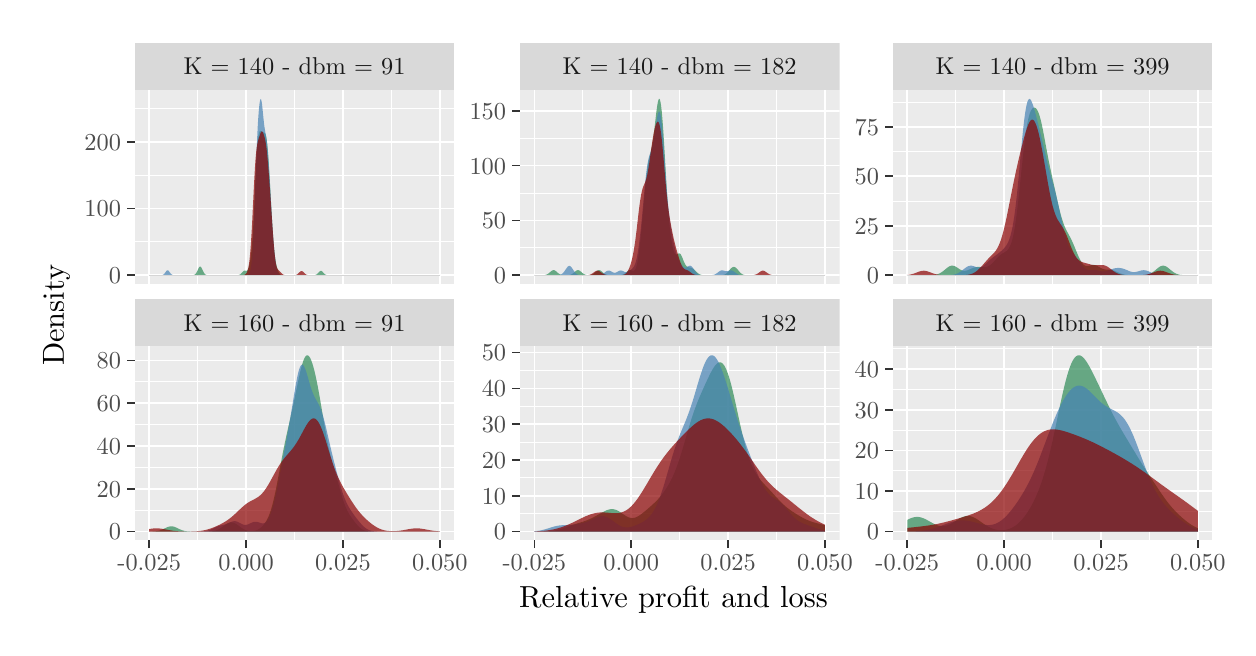
\begin{tikzpicture}[x=1pt,y=1pt]
\definecolor{fillColor}{RGB}{255,255,255}
\path[use as bounding box,fill=fillColor,fill opacity=0.00] (0,0) rectangle (433.62,216.81);
\begin{scope}
\path[clip] (  0.00,  0.00) rectangle (433.62,216.81);
\definecolor{drawColor}{RGB}{255,255,255}
\definecolor{fillColor}{RGB}{255,255,255}

\path[draw=drawColor,line width= 0.6pt,line join=round,line cap=round,fill=fillColor] (  0.00,  0.00) rectangle (433.62,216.81);
\end{scope}
\begin{scope}
\path[clip] ( 38.67,124.17) rectangle (154.19,194.25);
\definecolor{fillColor}{gray}{0.92}

\path[fill=fillColor] ( 38.67,124.17) rectangle (154.19,194.25);
\definecolor{drawColor}{RGB}{255,255,255}

\path[draw=drawColor,line width= 0.3pt,line join=round] ( 38.67,139.42) --
	(154.19,139.42);

\path[draw=drawColor,line width= 0.3pt,line join=round] ( 38.67,163.54) --
	(154.19,163.54);

\path[draw=drawColor,line width= 0.3pt,line join=round] ( 38.67,187.67) --
	(154.19,187.67);

\path[draw=drawColor,line width= 0.3pt,line join=round] ( 61.42,124.17) --
	( 61.42,194.25);

\path[draw=drawColor,line width= 0.3pt,line join=round] ( 96.43,124.17) --
	( 96.43,194.25);

\path[draw=drawColor,line width= 0.3pt,line join=round] (131.43,124.17) --
	(131.43,194.25);

\path[draw=drawColor,line width= 0.6pt,line join=round] ( 38.67,127.36) --
	(154.19,127.36);

\path[draw=drawColor,line width= 0.6pt,line join=round] ( 38.67,151.48) --
	(154.19,151.48);

\path[draw=drawColor,line width= 0.6pt,line join=round] ( 38.67,175.60) --
	(154.19,175.60);

\path[draw=drawColor,line width= 0.6pt,line join=round] ( 43.92,124.17) --
	( 43.92,194.25);

\path[draw=drawColor,line width= 0.6pt,line join=round] ( 78.92,124.17) --
	( 78.92,194.25);

\path[draw=drawColor,line width= 0.6pt,line join=round] (113.93,124.17) --
	(113.93,194.25);

\path[draw=drawColor,line width= 0.6pt,line join=round] (148.94,124.17) --
	(148.94,194.25);
\definecolor{fillColor}{RGB}{46,139,87}

\path[fill=fillColor,fill opacity=0.70] ( 43.92,127.36) --
	( 44.12,127.36) --
	( 44.33,127.36) --
	( 44.53,127.36) --
	( 44.74,127.36) --
	( 44.95,127.36) --
	( 45.15,127.36) --
	( 45.36,127.36) --
	( 45.56,127.36) --
	( 45.77,127.36) --
	( 45.97,127.36) --
	( 46.18,127.36) --
	( 46.38,127.36) --
	( 46.59,127.36) --
	( 46.79,127.36) --
	( 47.00,127.36) --
	( 47.21,127.36) --
	( 47.41,127.36) --
	( 47.62,127.36) --
	( 47.82,127.36) --
	( 48.03,127.36) --
	( 48.23,127.36) --
	( 48.44,127.36) --
	( 48.64,127.36) --
	( 48.85,127.36) --
	( 49.06,127.36) --
	( 49.26,127.36) --
	( 49.47,127.36) --
	( 49.67,127.36) --
	( 49.88,127.36) --
	( 50.08,127.36) --
	( 50.29,127.36) --
	( 50.49,127.36) --
	( 50.70,127.36) --
	( 50.91,127.36) --
	( 51.11,127.36) --
	( 51.32,127.36) --
	( 51.52,127.36) --
	( 51.73,127.36) --
	( 51.93,127.36) --
	( 52.14,127.36) --
	( 52.34,127.36) --
	( 52.55,127.36) --
	( 52.75,127.36) --
	( 52.96,127.36) --
	( 53.17,127.36) --
	( 53.37,127.36) --
	( 53.58,127.36) --
	( 53.78,127.36) --
	( 53.99,127.36) --
	( 54.19,127.36) --
	( 54.40,127.36) --
	( 54.60,127.36) --
	( 54.81,127.36) --
	( 55.02,127.36) --
	( 55.22,127.36) --
	( 55.43,127.36) --
	( 55.63,127.36) --
	( 55.84,127.36) --
	( 56.04,127.36) --
	( 56.25,127.36) --
	( 56.45,127.36) --
	( 56.66,127.36) --
	( 56.87,127.36) --
	( 57.07,127.36) --
	( 57.28,127.36) --
	( 57.48,127.36) --
	( 57.69,127.36) --
	( 57.89,127.36) --
	( 58.10,127.36) --
	( 58.30,127.36) --
	( 58.51,127.36) --
	( 58.71,127.36) --
	( 58.92,127.36) --
	( 59.13,127.36) --
	( 59.33,127.36) --
	( 59.54,127.37) --
	( 59.74,127.39) --
	( 59.95,127.42) --
	( 60.15,127.49) --
	( 60.36,127.59) --
	( 60.56,127.74) --
	( 60.77,127.97) --
	( 60.98,128.27) --
	( 61.18,128.65) --
	( 61.39,129.09) --
	( 61.59,129.54) --
	( 61.80,129.96) --
	( 62.00,130.29) --
	( 62.21,130.48) --
	( 62.41,130.49) --
	( 62.62,130.32) --
	( 62.82,130.01) --
	( 63.03,129.59) --
	( 63.24,129.14) --
	( 63.44,128.71) --
	( 63.65,128.32) --
	( 63.85,128.01) --
	( 64.06,127.77) --
	( 64.26,127.60) --
	( 64.47,127.50) --
	( 64.67,127.43) --
	( 64.88,127.39) --
	( 65.09,127.37) --
	( 65.29,127.36) --
	( 65.50,127.36) --
	( 65.70,127.36) --
	( 65.91,127.36) --
	( 66.11,127.36) --
	( 66.32,127.36) --
	( 66.52,127.36) --
	( 66.73,127.36) --
	( 66.94,127.36) --
	( 67.14,127.36) --
	( 67.35,127.36) --
	( 67.55,127.36) --
	( 67.76,127.36) --
	( 67.96,127.36) --
	( 68.17,127.36) --
	( 68.37,127.36) --
	( 68.58,127.36) --
	( 68.78,127.36) --
	( 68.99,127.36) --
	( 69.20,127.36) --
	( 69.40,127.36) --
	( 69.61,127.36) --
	( 69.81,127.36) --
	( 70.02,127.36) --
	( 70.22,127.36) --
	( 70.43,127.36) --
	( 70.63,127.36) --
	( 70.84,127.36) --
	( 71.05,127.36) --
	( 71.25,127.36) --
	( 71.46,127.36) --
	( 71.66,127.36) --
	( 71.87,127.36) --
	( 72.07,127.36) --
	( 72.28,127.36) --
	( 72.48,127.36) --
	( 72.69,127.36) --
	( 72.90,127.36) --
	( 73.10,127.36) --
	( 73.31,127.36) --
	( 73.51,127.36) --
	( 73.72,127.36) --
	( 73.92,127.36) --
	( 74.13,127.36) --
	( 74.33,127.36) --
	( 74.54,127.36) --
	( 74.74,127.36) --
	( 74.95,127.36) --
	( 75.16,127.36) --
	( 75.36,127.36) --
	( 75.57,127.36) --
	( 75.77,127.37) --
	( 75.98,127.39) --
	( 76.18,127.43) --
	( 76.39,127.48) --
	( 76.59,127.56) --
	( 76.80,127.69) --
	( 77.01,127.85) --
	( 77.21,128.05) --
	( 77.42,128.27) --
	( 77.62,128.50) --
	( 77.83,128.71) --
	( 78.03,128.88) --
	( 78.24,128.98) --
	( 78.44,129.01) --
	( 78.65,128.99) --
	( 78.86,128.95) --
	( 79.06,128.94) --
	( 79.27,129.01) --
	( 79.47,129.21) --
	( 79.68,129.59) --
	( 79.88,130.16) --
	( 80.09,130.93) --
	( 80.29,131.93) --
	( 80.50,133.19) --
	( 80.70,134.76) --
	( 80.91,136.72) --
	( 81.12,139.14) --
	( 81.32,142.08) --
	( 81.53,145.57) --
	( 81.73,149.56) --
	( 81.94,153.93) --
	( 82.14,158.48) --
	( 82.35,162.98) --
	( 82.55,167.19) --
	( 82.76,170.89) --
	( 82.97,173.88) --
	( 83.17,176.15) --
	( 83.38,177.74) --
	( 83.58,178.74) --
	( 83.79,179.29) --
	( 83.99,179.51) --
	( 84.20,179.52) --
	( 84.40,179.42) --
	( 84.61,179.27) --
	( 84.81,179.14) --
	( 85.02,179.03) --
	( 85.23,178.96) --
	( 85.43,178.90) --
	( 85.64,178.79) --
	( 85.84,178.54) --
	( 86.05,178.03) --
	( 86.25,177.13) --
	( 86.46,175.75) --
	( 86.66,173.86) --
	( 86.87,171.46) --
	( 87.08,168.61) --
	( 87.28,165.36) --
	( 87.49,161.81) --
	( 87.69,158.08) --
	( 87.90,154.27) --
	( 88.10,150.52) --
	( 88.31,146.95) --
	( 88.51,143.66) --
	( 88.72,140.73) --
	( 88.93,138.19) --
	( 89.13,136.05) --
	( 89.34,134.28) --
	( 89.54,132.84) --
	( 89.75,131.68) --
	( 89.95,130.74) --
	( 90.16,129.96) --
	( 90.36,129.31) --
	( 90.57,128.79) --
	( 90.77,128.37) --
	( 90.98,128.05) --
	( 91.19,127.81) --
	( 91.39,127.64) --
	( 91.60,127.52) --
	( 91.80,127.45) --
	( 92.01,127.40) --
	( 92.21,127.38) --
	( 92.42,127.37) --
	( 92.62,127.36) --
	( 92.83,127.36) --
	( 93.04,127.36) --
	( 93.24,127.36) --
	( 93.45,127.36) --
	( 93.65,127.36) --
	( 93.86,127.36) --
	( 94.06,127.36) --
	( 94.27,127.36) --
	( 94.47,127.36) --
	( 94.68,127.36) --
	( 94.89,127.36) --
	( 95.09,127.36) --
	( 95.30,127.36) --
	( 95.50,127.36) --
	( 95.71,127.36) --
	( 95.91,127.36) --
	( 96.12,127.36) --
	( 96.32,127.36) --
	( 96.53,127.36) --
	( 96.73,127.36) --
	( 96.94,127.36) --
	( 97.15,127.36) --
	( 97.35,127.36) --
	( 97.56,127.36) --
	( 97.76,127.36) --
	( 97.97,127.36) --
	( 98.17,127.36) --
	( 98.38,127.36) --
	( 98.58,127.36) --
	( 98.79,127.36) --
	( 99.00,127.36) --
	( 99.20,127.36) --
	( 99.41,127.36) --
	( 99.61,127.36) --
	( 99.82,127.36) --
	(100.02,127.36) --
	(100.23,127.36) --
	(100.43,127.36) --
	(100.64,127.36) --
	(100.85,127.36) --
	(101.05,127.36) --
	(101.26,127.36) --
	(101.46,127.36) --
	(101.67,127.36) --
	(101.87,127.36) --
	(102.08,127.36) --
	(102.28,127.36) --
	(102.49,127.36) --
	(102.69,127.36) --
	(102.90,127.36) --
	(103.11,127.36) --
	(103.31,127.37) --
	(103.52,127.38) --
	(103.72,127.40) --
	(103.93,127.45) --
	(104.13,127.51) --
	(104.34,127.61) --
	(104.54,127.75) --
	(104.75,127.94) --
	(104.96,128.15) --
	(105.16,128.38) --
	(105.37,128.60) --
	(105.57,128.79) --
	(105.78,128.91) --
	(105.98,128.95) --
	(106.19,128.89) --
	(106.39,128.75) --
	(106.60,128.55) --
	(106.80,128.32) --
	(107.01,128.09) --
	(107.22,127.88) --
	(107.42,127.71) --
	(107.63,127.59) --
	(107.83,127.49) --
	(108.04,127.44) --
	(108.24,127.40) --
	(108.45,127.38) --
	(108.65,127.37) --
	(108.86,127.36) --
	(109.07,127.36) --
	(109.27,127.36) --
	(109.48,127.36) --
	(109.68,127.36) --
	(109.89,127.36) --
	(110.09,127.36) --
	(110.30,127.36) --
	(110.50,127.36) --
	(110.71,127.36) --
	(110.92,127.36) --
	(111.12,127.36) --
	(111.33,127.36) --
	(111.53,127.36) --
	(111.74,127.36) --
	(111.94,127.36) --
	(112.15,127.36) --
	(112.35,127.36) --
	(112.56,127.36) --
	(112.76,127.36) --
	(112.97,127.36) --
	(113.18,127.36) --
	(113.38,127.36) --
	(113.59,127.36) --
	(113.79,127.36) --
	(114.00,127.36) --
	(114.20,127.36) --
	(114.41,127.36) --
	(114.61,127.36) --
	(114.82,127.36) --
	(115.03,127.36) --
	(115.23,127.36) --
	(115.44,127.36) --
	(115.64,127.36) --
	(115.85,127.36) --
	(116.05,127.36) --
	(116.26,127.36) --
	(116.46,127.36) --
	(116.67,127.36) --
	(116.88,127.36) --
	(117.08,127.36) --
	(117.29,127.36) --
	(117.49,127.36) --
	(117.70,127.36) --
	(117.90,127.36) --
	(118.11,127.36) --
	(118.31,127.36) --
	(118.52,127.36) --
	(118.72,127.36) --
	(118.93,127.36) --
	(119.14,127.36) --
	(119.34,127.36) --
	(119.55,127.36) --
	(119.75,127.36) --
	(119.96,127.36) --
	(120.16,127.36) --
	(120.37,127.36) --
	(120.57,127.36) --
	(120.78,127.36) --
	(120.99,127.36) --
	(121.19,127.36) --
	(121.40,127.36) --
	(121.60,127.36) --
	(121.81,127.36) --
	(122.01,127.36) --
	(122.22,127.36) --
	(122.42,127.36) --
	(122.63,127.36) --
	(122.84,127.36) --
	(123.04,127.36) --
	(123.25,127.36) --
	(123.45,127.36) --
	(123.66,127.36) --
	(123.86,127.36) --
	(124.07,127.36) --
	(124.27,127.36) --
	(124.48,127.36) --
	(124.68,127.36) --
	(124.89,127.36) --
	(125.10,127.36) --
	(125.30,127.36) --
	(125.51,127.36) --
	(125.71,127.36) --
	(125.92,127.36) --
	(126.12,127.36) --
	(126.33,127.36) --
	(126.53,127.36) --
	(126.74,127.36) --
	(126.95,127.36) --
	(127.15,127.36) --
	(127.36,127.36) --
	(127.56,127.36) --
	(127.77,127.36) --
	(127.97,127.36) --
	(128.18,127.36) --
	(128.38,127.36) --
	(128.59,127.36) --
	(128.79,127.36) --
	(129.00,127.36) --
	(129.21,127.36) --
	(129.41,127.36) --
	(129.62,127.36) --
	(129.82,127.36) --
	(130.03,127.36) --
	(130.23,127.36) --
	(130.44,127.36) --
	(130.64,127.36) --
	(130.85,127.36) --
	(131.06,127.36) --
	(131.26,127.36) --
	(131.47,127.36) --
	(131.67,127.36) --
	(131.88,127.36) --
	(132.08,127.36) --
	(132.29,127.36) --
	(132.49,127.36) --
	(132.70,127.36) --
	(132.91,127.36) --
	(133.11,127.36) --
	(133.32,127.36) --
	(133.52,127.36) --
	(133.73,127.36) --
	(133.93,127.36) --
	(134.14,127.36) --
	(134.34,127.36) --
	(134.55,127.36) --
	(134.75,127.36) --
	(134.96,127.36) --
	(135.17,127.36) --
	(135.37,127.36) --
	(135.58,127.36) --
	(135.78,127.36) --
	(135.99,127.36) --
	(136.19,127.36) --
	(136.40,127.36) --
	(136.60,127.36) --
	(136.81,127.36) --
	(137.02,127.36) --
	(137.22,127.36) --
	(137.43,127.36) --
	(137.63,127.36) --
	(137.84,127.36) --
	(138.04,127.36) --
	(138.25,127.36) --
	(138.45,127.36) --
	(138.66,127.36) --
	(138.87,127.36) --
	(139.07,127.36) --
	(139.28,127.36) --
	(139.48,127.36) --
	(139.69,127.36) --
	(139.89,127.36) --
	(140.10,127.36) --
	(140.30,127.36) --
	(140.51,127.36) --
	(140.71,127.36) --
	(140.92,127.36) --
	(141.13,127.36) --
	(141.33,127.36) --
	(141.54,127.36) --
	(141.74,127.36) --
	(141.95,127.36) --
	(142.15,127.36) --
	(142.36,127.36) --
	(142.56,127.36) --
	(142.77,127.36) --
	(142.98,127.36) --
	(143.18,127.36) --
	(143.39,127.36) --
	(143.59,127.36) --
	(143.80,127.36) --
	(144.00,127.36) --
	(144.21,127.36) --
	(144.41,127.36) --
	(144.62,127.36) --
	(144.83,127.36) --
	(145.03,127.36) --
	(145.24,127.36) --
	(145.44,127.36) --
	(145.65,127.36) --
	(145.85,127.36) --
	(146.06,127.36) --
	(146.26,127.36) --
	(146.47,127.36) --
	(146.67,127.36) --
	(146.88,127.36) --
	(147.09,127.36) --
	(147.29,127.36) --
	(147.50,127.36) --
	(147.70,127.36) --
	(147.91,127.36) --
	(148.11,127.36) --
	(148.32,127.36) --
	(148.52,127.36) --
	(148.73,127.36) --
	(148.94,127.36) --
	(148.94,127.36) --
	(148.73,127.36) --
	(148.52,127.36) --
	(148.32,127.36) --
	(148.11,127.36) --
	(147.91,127.36) --
	(147.70,127.36) --
	(147.50,127.36) --
	(147.29,127.36) --
	(147.09,127.36) --
	(146.88,127.36) --
	(146.67,127.36) --
	(146.47,127.36) --
	(146.26,127.36) --
	(146.06,127.36) --
	(145.85,127.36) --
	(145.65,127.36) --
	(145.44,127.36) --
	(145.24,127.36) --
	(145.03,127.36) --
	(144.83,127.36) --
	(144.62,127.36) --
	(144.41,127.36) --
	(144.21,127.36) --
	(144.00,127.36) --
	(143.80,127.36) --
	(143.59,127.36) --
	(143.39,127.36) --
	(143.18,127.36) --
	(142.98,127.36) --
	(142.77,127.36) --
	(142.56,127.36) --
	(142.36,127.36) --
	(142.15,127.36) --
	(141.95,127.36) --
	(141.74,127.36) --
	(141.54,127.36) --
	(141.33,127.36) --
	(141.13,127.36) --
	(140.92,127.36) --
	(140.71,127.36) --
	(140.51,127.36) --
	(140.30,127.36) --
	(140.10,127.36) --
	(139.89,127.36) --
	(139.69,127.36) --
	(139.48,127.36) --
	(139.28,127.36) --
	(139.07,127.36) --
	(138.87,127.36) --
	(138.66,127.36) --
	(138.45,127.36) --
	(138.25,127.36) --
	(138.04,127.36) --
	(137.84,127.36) --
	(137.63,127.36) --
	(137.43,127.36) --
	(137.22,127.36) --
	(137.02,127.36) --
	(136.81,127.36) --
	(136.60,127.36) --
	(136.40,127.36) --
	(136.19,127.36) --
	(135.99,127.36) --
	(135.78,127.36) --
	(135.58,127.36) --
	(135.37,127.36) --
	(135.17,127.36) --
	(134.96,127.36) --
	(134.75,127.36) --
	(134.55,127.36) --
	(134.34,127.36) --
	(134.14,127.36) --
	(133.93,127.36) --
	(133.73,127.36) --
	(133.52,127.36) --
	(133.32,127.36) --
	(133.11,127.36) --
	(132.91,127.36) --
	(132.70,127.36) --
	(132.49,127.36) --
	(132.29,127.36) --
	(132.08,127.36) --
	(131.88,127.36) --
	(131.67,127.36) --
	(131.47,127.36) --
	(131.26,127.36) --
	(131.06,127.36) --
	(130.85,127.36) --
	(130.64,127.36) --
	(130.44,127.36) --
	(130.23,127.36) --
	(130.03,127.36) --
	(129.82,127.36) --
	(129.62,127.36) --
	(129.41,127.36) --
	(129.21,127.36) --
	(129.00,127.36) --
	(128.79,127.36) --
	(128.59,127.36) --
	(128.38,127.36) --
	(128.18,127.36) --
	(127.97,127.36) --
	(127.77,127.36) --
	(127.56,127.36) --
	(127.36,127.36) --
	(127.15,127.36) --
	(126.95,127.36) --
	(126.74,127.36) --
	(126.53,127.36) --
	(126.33,127.36) --
	(126.12,127.36) --
	(125.92,127.36) --
	(125.71,127.36) --
	(125.51,127.36) --
	(125.30,127.36) --
	(125.10,127.36) --
	(124.89,127.36) --
	(124.68,127.36) --
	(124.48,127.36) --
	(124.27,127.36) --
	(124.07,127.36) --
	(123.86,127.36) --
	(123.66,127.36) --
	(123.45,127.36) --
	(123.25,127.36) --
	(123.04,127.36) --
	(122.84,127.36) --
	(122.63,127.36) --
	(122.42,127.36) --
	(122.22,127.36) --
	(122.01,127.36) --
	(121.81,127.36) --
	(121.60,127.36) --
	(121.40,127.36) --
	(121.19,127.36) --
	(120.99,127.36) --
	(120.78,127.36) --
	(120.57,127.36) --
	(120.37,127.36) --
	(120.16,127.36) --
	(119.96,127.36) --
	(119.75,127.36) --
	(119.55,127.36) --
	(119.34,127.36) --
	(119.14,127.36) --
	(118.93,127.36) --
	(118.72,127.36) --
	(118.52,127.36) --
	(118.31,127.36) --
	(118.11,127.36) --
	(117.90,127.36) --
	(117.70,127.36) --
	(117.49,127.36) --
	(117.29,127.36) --
	(117.08,127.36) --
	(116.88,127.36) --
	(116.67,127.36) --
	(116.46,127.36) --
	(116.26,127.36) --
	(116.05,127.36) --
	(115.85,127.36) --
	(115.64,127.36) --
	(115.44,127.36) --
	(115.23,127.36) --
	(115.03,127.36) --
	(114.82,127.36) --
	(114.61,127.36) --
	(114.41,127.36) --
	(114.20,127.36) --
	(114.00,127.36) --
	(113.79,127.36) --
	(113.59,127.36) --
	(113.38,127.36) --
	(113.18,127.36) --
	(112.97,127.36) --
	(112.76,127.36) --
	(112.56,127.36) --
	(112.35,127.36) --
	(112.15,127.36) --
	(111.94,127.36) --
	(111.74,127.36) --
	(111.53,127.36) --
	(111.33,127.36) --
	(111.12,127.36) --
	(110.92,127.36) --
	(110.71,127.36) --
	(110.50,127.36) --
	(110.30,127.36) --
	(110.09,127.36) --
	(109.89,127.36) --
	(109.68,127.36) --
	(109.48,127.36) --
	(109.27,127.36) --
	(109.07,127.36) --
	(108.86,127.36) --
	(108.65,127.36) --
	(108.45,127.36) --
	(108.24,127.36) --
	(108.04,127.36) --
	(107.83,127.36) --
	(107.63,127.36) --
	(107.42,127.36) --
	(107.22,127.36) --
	(107.01,127.36) --
	(106.80,127.36) --
	(106.60,127.36) --
	(106.39,127.36) --
	(106.19,127.36) --
	(105.98,127.36) --
	(105.78,127.36) --
	(105.57,127.36) --
	(105.37,127.36) --
	(105.16,127.36) --
	(104.96,127.36) --
	(104.75,127.36) --
	(104.54,127.36) --
	(104.34,127.36) --
	(104.13,127.36) --
	(103.93,127.36) --
	(103.72,127.36) --
	(103.52,127.36) --
	(103.31,127.36) --
	(103.11,127.36) --
	(102.90,127.36) --
	(102.69,127.36) --
	(102.49,127.36) --
	(102.28,127.36) --
	(102.08,127.36) --
	(101.87,127.36) --
	(101.67,127.36) --
	(101.46,127.36) --
	(101.26,127.36) --
	(101.05,127.36) --
	(100.85,127.36) --
	(100.64,127.36) --
	(100.43,127.36) --
	(100.23,127.36) --
	(100.02,127.36) --
	( 99.82,127.36) --
	( 99.61,127.36) --
	( 99.41,127.36) --
	( 99.20,127.36) --
	( 99.00,127.36) --
	( 98.79,127.36) --
	( 98.58,127.36) --
	( 98.38,127.36) --
	( 98.17,127.36) --
	( 97.97,127.36) --
	( 97.76,127.36) --
	( 97.56,127.36) --
	( 97.35,127.36) --
	( 97.15,127.36) --
	( 96.94,127.36) --
	( 96.73,127.36) --
	( 96.53,127.36) --
	( 96.32,127.36) --
	( 96.12,127.36) --
	( 95.91,127.36) --
	( 95.71,127.36) --
	( 95.50,127.36) --
	( 95.30,127.36) --
	( 95.09,127.36) --
	( 94.89,127.36) --
	( 94.68,127.36) --
	( 94.47,127.36) --
	( 94.27,127.36) --
	( 94.06,127.36) --
	( 93.86,127.36) --
	( 93.65,127.36) --
	( 93.45,127.36) --
	( 93.24,127.36) --
	( 93.04,127.36) --
	( 92.83,127.36) --
	( 92.62,127.36) --
	( 92.42,127.36) --
	( 92.21,127.36) --
	( 92.01,127.36) --
	( 91.80,127.36) --
	( 91.60,127.36) --
	( 91.39,127.36) --
	( 91.19,127.36) --
	( 90.98,127.36) --
	( 90.77,127.36) --
	( 90.57,127.36) --
	( 90.36,127.36) --
	( 90.16,127.36) --
	( 89.95,127.36) --
	( 89.75,127.36) --
	( 89.54,127.36) --
	( 89.34,127.36) --
	( 89.13,127.36) --
	( 88.93,127.36) --
	( 88.72,127.36) --
	( 88.51,127.36) --
	( 88.31,127.36) --
	( 88.10,127.36) --
	( 87.90,127.36) --
	( 87.69,127.36) --
	( 87.49,127.36) --
	( 87.28,127.36) --
	( 87.08,127.36) --
	( 86.87,127.36) --
	( 86.66,127.36) --
	( 86.46,127.36) --
	( 86.25,127.36) --
	( 86.05,127.36) --
	( 85.84,127.36) --
	( 85.64,127.36) --
	( 85.43,127.36) --
	( 85.23,127.36) --
	( 85.02,127.36) --
	( 84.81,127.36) --
	( 84.61,127.36) --
	( 84.40,127.36) --
	( 84.20,127.36) --
	( 83.99,127.36) --
	( 83.79,127.36) --
	( 83.58,127.36) --
	( 83.38,127.36) --
	( 83.17,127.36) --
	( 82.97,127.36) --
	( 82.76,127.36) --
	( 82.55,127.36) --
	( 82.35,127.36) --
	( 82.14,127.36) --
	( 81.94,127.36) --
	( 81.73,127.36) --
	( 81.53,127.36) --
	( 81.32,127.36) --
	( 81.12,127.36) --
	( 80.91,127.36) --
	( 80.70,127.36) --
	( 80.50,127.36) --
	( 80.29,127.36) --
	( 80.09,127.36) --
	( 79.88,127.36) --
	( 79.68,127.36) --
	( 79.47,127.36) --
	( 79.27,127.36) --
	( 79.06,127.36) --
	( 78.86,127.36) --
	( 78.65,127.36) --
	( 78.44,127.36) --
	( 78.24,127.36) --
	( 78.03,127.36) --
	( 77.83,127.36) --
	( 77.62,127.36) --
	( 77.42,127.36) --
	( 77.21,127.36) --
	( 77.01,127.36) --
	( 76.80,127.36) --
	( 76.59,127.36) --
	( 76.39,127.36) --
	( 76.18,127.36) --
	( 75.98,127.36) --
	( 75.77,127.36) --
	( 75.57,127.36) --
	( 75.36,127.36) --
	( 75.16,127.36) --
	( 74.95,127.36) --
	( 74.74,127.36) --
	( 74.54,127.36) --
	( 74.33,127.36) --
	( 74.13,127.36) --
	( 73.92,127.36) --
	( 73.72,127.36) --
	( 73.51,127.36) --
	( 73.31,127.36) --
	( 73.10,127.36) --
	( 72.90,127.36) --
	( 72.69,127.36) --
	( 72.48,127.36) --
	( 72.28,127.36) --
	( 72.07,127.36) --
	( 71.87,127.36) --
	( 71.66,127.36) --
	( 71.46,127.36) --
	( 71.25,127.36) --
	( 71.05,127.36) --
	( 70.84,127.36) --
	( 70.63,127.36) --
	( 70.43,127.36) --
	( 70.22,127.36) --
	( 70.02,127.36) --
	( 69.81,127.36) --
	( 69.61,127.36) --
	( 69.40,127.36) --
	( 69.20,127.36) --
	( 68.99,127.36) --
	( 68.78,127.36) --
	( 68.58,127.36) --
	( 68.37,127.36) --
	( 68.17,127.36) --
	( 67.96,127.36) --
	( 67.76,127.36) --
	( 67.55,127.36) --
	( 67.35,127.36) --
	( 67.14,127.36) --
	( 66.94,127.36) --
	( 66.73,127.36) --
	( 66.52,127.36) --
	( 66.32,127.36) --
	( 66.11,127.36) --
	( 65.91,127.36) --
	( 65.70,127.36) --
	( 65.50,127.36) --
	( 65.29,127.36) --
	( 65.09,127.36) --
	( 64.88,127.36) --
	( 64.67,127.36) --
	( 64.47,127.36) --
	( 64.26,127.36) --
	( 64.06,127.36) --
	( 63.85,127.36) --
	( 63.65,127.36) --
	( 63.44,127.36) --
	( 63.24,127.36) --
	( 63.03,127.36) --
	( 62.82,127.36) --
	( 62.62,127.36) --
	( 62.41,127.36) --
	( 62.21,127.36) --
	( 62.00,127.36) --
	( 61.80,127.36) --
	( 61.59,127.36) --
	( 61.39,127.36) --
	( 61.18,127.36) --
	( 60.98,127.36) --
	( 60.77,127.36) --
	( 60.56,127.36) --
	( 60.36,127.36) --
	( 60.15,127.36) --
	( 59.95,127.36) --
	( 59.74,127.36) --
	( 59.54,127.36) --
	( 59.33,127.36) --
	( 59.13,127.36) --
	( 58.92,127.36) --
	( 58.71,127.36) --
	( 58.51,127.36) --
	( 58.30,127.36) --
	( 58.10,127.36) --
	( 57.89,127.36) --
	( 57.69,127.36) --
	( 57.48,127.36) --
	( 57.28,127.36) --
	( 57.07,127.36) --
	( 56.87,127.36) --
	( 56.66,127.36) --
	( 56.45,127.36) --
	( 56.25,127.36) --
	( 56.04,127.36) --
	( 55.84,127.36) --
	( 55.63,127.36) --
	( 55.43,127.36) --
	( 55.22,127.36) --
	( 55.02,127.36) --
	( 54.81,127.36) --
	( 54.60,127.36) --
	( 54.40,127.36) --
	( 54.19,127.36) --
	( 53.99,127.36) --
	( 53.78,127.36) --
	( 53.58,127.36) --
	( 53.37,127.36) --
	( 53.17,127.36) --
	( 52.96,127.36) --
	( 52.75,127.36) --
	( 52.55,127.36) --
	( 52.34,127.36) --
	( 52.14,127.36) --
	( 51.93,127.36) --
	( 51.73,127.36) --
	( 51.52,127.36) --
	( 51.32,127.36) --
	( 51.11,127.36) --
	( 50.91,127.36) --
	( 50.70,127.36) --
	( 50.49,127.36) --
	( 50.29,127.36) --
	( 50.08,127.36) --
	( 49.88,127.36) --
	( 49.67,127.36) --
	( 49.47,127.36) --
	( 49.26,127.36) --
	( 49.06,127.36) --
	( 48.85,127.36) --
	( 48.64,127.36) --
	( 48.44,127.36) --
	( 48.23,127.36) --
	( 48.03,127.36) --
	( 47.82,127.36) --
	( 47.62,127.36) --
	( 47.41,127.36) --
	( 47.21,127.36) --
	( 47.00,127.36) --
	( 46.79,127.36) --
	( 46.59,127.36) --
	( 46.38,127.36) --
	( 46.18,127.36) --
	( 45.97,127.36) --
	( 45.77,127.36) --
	( 45.56,127.36) --
	( 45.36,127.36) --
	( 45.15,127.36) --
	( 44.95,127.36) --
	( 44.74,127.36) --
	( 44.53,127.36) --
	( 44.33,127.36) --
	( 44.12,127.36) --
	( 43.92,127.36) --
	cycle;
\definecolor{fillColor}{RGB}{70,130,180}

\path[fill=fillColor,fill opacity=0.70] ( 43.92,127.36) --
	( 44.12,127.36) --
	( 44.33,127.36) --
	( 44.53,127.36) --
	( 44.74,127.36) --
	( 44.95,127.36) --
	( 45.15,127.36) --
	( 45.36,127.36) --
	( 45.56,127.36) --
	( 45.77,127.36) --
	( 45.97,127.36) --
	( 46.18,127.36) --
	( 46.38,127.36) --
	( 46.59,127.36) --
	( 46.79,127.36) --
	( 47.00,127.36) --
	( 47.21,127.36) --
	( 47.41,127.36) --
	( 47.62,127.36) --
	( 47.82,127.36) --
	( 48.03,127.36) --
	( 48.23,127.37) --
	( 48.44,127.39) --
	( 48.64,127.43) --
	( 48.85,127.50) --
	( 49.06,127.61) --
	( 49.26,127.78) --
	( 49.47,128.00) --
	( 49.67,128.27) --
	( 49.88,128.56) --
	( 50.08,128.83) --
	( 50.29,129.04) --
	( 50.49,129.15) --
	( 50.70,129.12) --
	( 50.91,128.97) --
	( 51.11,128.73) --
	( 51.32,128.44) --
	( 51.52,128.16) --
	( 51.73,127.91) --
	( 51.93,127.71) --
	( 52.14,127.57) --
	( 52.34,127.47) --
	( 52.55,127.42) --
	( 52.75,127.38) --
	( 52.96,127.37) --
	( 53.17,127.36) --
	( 53.37,127.36) --
	( 53.58,127.36) --
	( 53.78,127.36) --
	( 53.99,127.36) --
	( 54.19,127.36) --
	( 54.40,127.36) --
	( 54.60,127.36) --
	( 54.81,127.36) --
	( 55.02,127.36) --
	( 55.22,127.36) --
	( 55.43,127.36) --
	( 55.63,127.36) --
	( 55.84,127.36) --
	( 56.04,127.36) --
	( 56.25,127.36) --
	( 56.45,127.36) --
	( 56.66,127.36) --
	( 56.87,127.36) --
	( 57.07,127.36) --
	( 57.28,127.36) --
	( 57.48,127.36) --
	( 57.69,127.36) --
	( 57.89,127.36) --
	( 58.10,127.36) --
	( 58.30,127.36) --
	( 58.51,127.36) --
	( 58.71,127.36) --
	( 58.92,127.36) --
	( 59.13,127.36) --
	( 59.33,127.36) --
	( 59.54,127.36) --
	( 59.74,127.36) --
	( 59.95,127.36) --
	( 60.15,127.36) --
	( 60.36,127.36) --
	( 60.56,127.36) --
	( 60.77,127.36) --
	( 60.98,127.36) --
	( 61.18,127.36) --
	( 61.39,127.36) --
	( 61.59,127.36) --
	( 61.80,127.36) --
	( 62.00,127.36) --
	( 62.21,127.36) --
	( 62.41,127.36) --
	( 62.62,127.36) --
	( 62.82,127.36) --
	( 63.03,127.36) --
	( 63.24,127.36) --
	( 63.44,127.36) --
	( 63.65,127.36) --
	( 63.85,127.36) --
	( 64.06,127.36) --
	( 64.26,127.36) --
	( 64.47,127.36) --
	( 64.67,127.36) --
	( 64.88,127.36) --
	( 65.09,127.36) --
	( 65.29,127.36) --
	( 65.50,127.36) --
	( 65.70,127.36) --
	( 65.91,127.36) --
	( 66.11,127.36) --
	( 66.32,127.36) --
	( 66.52,127.36) --
	( 66.73,127.36) --
	( 66.94,127.36) --
	( 67.14,127.36) --
	( 67.35,127.36) --
	( 67.55,127.36) --
	( 67.76,127.36) --
	( 67.96,127.36) --
	( 68.17,127.36) --
	( 68.37,127.36) --
	( 68.58,127.36) --
	( 68.78,127.36) --
	( 68.99,127.36) --
	( 69.20,127.36) --
	( 69.40,127.36) --
	( 69.61,127.36) --
	( 69.81,127.36) --
	( 70.02,127.36) --
	( 70.22,127.36) --
	( 70.43,127.36) --
	( 70.63,127.36) --
	( 70.84,127.36) --
	( 71.05,127.36) --
	( 71.25,127.36) --
	( 71.46,127.36) --
	( 71.66,127.36) --
	( 71.87,127.36) --
	( 72.07,127.36) --
	( 72.28,127.36) --
	( 72.48,127.36) --
	( 72.69,127.36) --
	( 72.90,127.36) --
	( 73.10,127.36) --
	( 73.31,127.36) --
	( 73.51,127.36) --
	( 73.72,127.36) --
	( 73.92,127.36) --
	( 74.13,127.36) --
	( 74.33,127.36) --
	( 74.54,127.36) --
	( 74.74,127.36) --
	( 74.95,127.36) --
	( 75.16,127.36) --
	( 75.36,127.36) --
	( 75.57,127.36) --
	( 75.77,127.36) --
	( 75.98,127.36) --
	( 76.18,127.36) --
	( 76.39,127.36) --
	( 76.59,127.36) --
	( 76.80,127.36) --
	( 77.01,127.36) --
	( 77.21,127.36) --
	( 77.42,127.36) --
	( 77.62,127.36) --
	( 77.83,127.36) --
	( 78.03,127.36) --
	( 78.24,127.36) --
	( 78.44,127.36) --
	( 78.65,127.36) --
	( 78.86,127.36) --
	( 79.06,127.37) --
	( 79.27,127.39) --
	( 79.47,127.43) --
	( 79.68,127.50) --
	( 79.88,127.65) --
	( 80.09,127.92) --
	( 80.29,128.37) --
	( 80.50,129.10) --
	( 80.70,130.21) --
	( 80.91,131.83) --
	( 81.12,134.09) --
	( 81.32,137.13) --
	( 81.53,140.99) --
	( 81.73,145.62) --
	( 81.94,150.90) --
	( 82.14,156.60) --
	( 82.35,162.44) --
	( 82.55,168.11) --
	( 82.76,173.35) --
	( 82.97,177.96) --
	( 83.17,181.87) --
	( 83.38,185.06) --
	( 83.58,187.57) --
	( 83.79,189.42) --
	( 83.99,190.60) --
	( 84.20,191.06) --
	( 84.40,190.76) --
	( 84.61,189.69) --
	( 84.81,187.99) --
	( 85.02,185.92) --
	( 85.23,183.80) --
	( 85.43,181.94) --
	( 85.64,180.44) --
	( 85.84,179.24) --
	( 86.05,178.15) --
	( 86.25,176.91) --
	( 86.46,175.32) --
	( 86.66,173.27) --
	( 86.87,170.76) --
	( 87.08,167.83) --
	( 87.28,164.60) --
	( 87.49,161.15) --
	( 87.69,157.58) --
	( 87.90,153.98) --
	( 88.10,150.44) --
	( 88.31,147.03) --
	( 88.51,143.85) --
	( 88.72,140.94) --
	( 88.93,138.35) --
	( 89.13,136.08) --
	( 89.34,134.11) --
	( 89.54,132.45) --
	( 89.75,131.06) --
	( 89.95,129.95) --
	( 90.16,129.09) --
	( 90.36,128.45) --
	( 90.57,128.02) --
	( 90.77,127.73) --
	( 90.98,127.55) --
	( 91.19,127.46) --
	( 91.39,127.40) --
	( 91.60,127.38) --
	( 91.80,127.36) --
	( 92.01,127.36) --
	( 92.21,127.36) --
	( 92.42,127.36) --
	( 92.62,127.36) --
	( 92.83,127.36) --
	( 93.04,127.36) --
	( 93.24,127.36) --
	( 93.45,127.36) --
	( 93.65,127.36) --
	( 93.86,127.36) --
	( 94.06,127.36) --
	( 94.27,127.36) --
	( 94.47,127.36) --
	( 94.68,127.36) --
	( 94.89,127.36) --
	( 95.09,127.36) --
	( 95.30,127.36) --
	( 95.50,127.36) --
	( 95.71,127.36) --
	( 95.91,127.36) --
	( 96.12,127.36) --
	( 96.32,127.36) --
	( 96.53,127.36) --
	( 96.73,127.36) --
	( 96.94,127.36) --
	( 97.15,127.36) --
	( 97.35,127.36) --
	( 97.56,127.36) --
	( 97.76,127.36) --
	( 97.97,127.36) --
	( 98.17,127.36) --
	( 98.38,127.36) --
	( 98.58,127.36) --
	( 98.79,127.36) --
	( 99.00,127.36) --
	( 99.20,127.36) --
	( 99.41,127.36) --
	( 99.61,127.36) --
	( 99.82,127.36) --
	(100.02,127.36) --
	(100.23,127.36) --
	(100.43,127.36) --
	(100.64,127.36) --
	(100.85,127.36) --
	(101.05,127.36) --
	(101.26,127.36) --
	(101.46,127.36) --
	(101.67,127.36) --
	(101.87,127.36) --
	(102.08,127.36) --
	(102.28,127.36) --
	(102.49,127.36) --
	(102.69,127.36) --
	(102.90,127.36) --
	(103.11,127.36) --
	(103.31,127.36) --
	(103.52,127.36) --
	(103.72,127.36) --
	(103.93,127.36) --
	(104.13,127.36) --
	(104.34,127.36) --
	(104.54,127.36) --
	(104.75,127.36) --
	(104.96,127.36) --
	(105.16,127.36) --
	(105.37,127.36) --
	(105.57,127.36) --
	(105.78,127.36) --
	(105.98,127.36) --
	(106.19,127.36) --
	(106.39,127.36) --
	(106.60,127.36) --
	(106.80,127.36) --
	(107.01,127.36) --
	(107.22,127.36) --
	(107.42,127.36) --
	(107.63,127.36) --
	(107.83,127.36) --
	(108.04,127.36) --
	(108.24,127.36) --
	(108.45,127.36) --
	(108.65,127.36) --
	(108.86,127.36) --
	(109.07,127.36) --
	(109.27,127.36) --
	(109.48,127.36) --
	(109.68,127.36) --
	(109.89,127.36) --
	(110.09,127.36) --
	(110.30,127.36) --
	(110.50,127.36) --
	(110.71,127.36) --
	(110.92,127.36) --
	(111.12,127.36) --
	(111.33,127.36) --
	(111.53,127.36) --
	(111.74,127.36) --
	(111.94,127.36) --
	(112.15,127.36) --
	(112.35,127.36) --
	(112.56,127.36) --
	(112.76,127.36) --
	(112.97,127.36) --
	(113.18,127.36) --
	(113.38,127.36) --
	(113.59,127.36) --
	(113.79,127.36) --
	(114.00,127.36) --
	(114.20,127.36) --
	(114.41,127.36) --
	(114.61,127.36) --
	(114.82,127.36) --
	(115.03,127.36) --
	(115.23,127.36) --
	(115.44,127.36) --
	(115.64,127.36) --
	(115.85,127.36) --
	(116.05,127.36) --
	(116.26,127.36) --
	(116.46,127.36) --
	(116.67,127.36) --
	(116.88,127.36) --
	(117.08,127.36) --
	(117.29,127.36) --
	(117.49,127.36) --
	(117.70,127.36) --
	(117.90,127.36) --
	(118.11,127.36) --
	(118.31,127.36) --
	(118.52,127.36) --
	(118.72,127.36) --
	(118.93,127.36) --
	(119.14,127.36) --
	(119.34,127.36) --
	(119.55,127.36) --
	(119.75,127.36) --
	(119.96,127.36) --
	(120.16,127.36) --
	(120.37,127.36) --
	(120.57,127.36) --
	(120.78,127.36) --
	(120.99,127.36) --
	(121.19,127.36) --
	(121.40,127.36) --
	(121.60,127.36) --
	(121.81,127.36) --
	(122.01,127.36) --
	(122.22,127.36) --
	(122.42,127.36) --
	(122.63,127.36) --
	(122.84,127.36) --
	(123.04,127.36) --
	(123.25,127.36) --
	(123.45,127.36) --
	(123.66,127.36) --
	(123.86,127.36) --
	(124.07,127.36) --
	(124.27,127.36) --
	(124.48,127.36) --
	(124.68,127.36) --
	(124.89,127.36) --
	(125.10,127.36) --
	(125.30,127.36) --
	(125.51,127.36) --
	(125.71,127.36) --
	(125.92,127.36) --
	(126.12,127.36) --
	(126.33,127.36) --
	(126.53,127.36) --
	(126.74,127.36) --
	(126.95,127.36) --
	(127.15,127.36) --
	(127.36,127.36) --
	(127.56,127.36) --
	(127.77,127.36) --
	(127.97,127.36) --
	(128.18,127.36) --
	(128.38,127.36) --
	(128.59,127.36) --
	(128.79,127.36) --
	(129.00,127.36) --
	(129.21,127.36) --
	(129.41,127.36) --
	(129.62,127.36) --
	(129.82,127.36) --
	(130.03,127.36) --
	(130.23,127.36) --
	(130.44,127.36) --
	(130.64,127.36) --
	(130.85,127.36) --
	(131.06,127.36) --
	(131.26,127.36) --
	(131.47,127.36) --
	(131.67,127.36) --
	(131.88,127.36) --
	(132.08,127.36) --
	(132.29,127.36) --
	(132.49,127.36) --
	(132.70,127.36) --
	(132.91,127.36) --
	(133.11,127.36) --
	(133.32,127.36) --
	(133.52,127.36) --
	(133.73,127.36) --
	(133.93,127.36) --
	(134.14,127.36) --
	(134.34,127.36) --
	(134.55,127.36) --
	(134.75,127.36) --
	(134.96,127.36) --
	(135.17,127.36) --
	(135.37,127.36) --
	(135.58,127.36) --
	(135.78,127.36) --
	(135.99,127.36) --
	(136.19,127.36) --
	(136.40,127.36) --
	(136.60,127.36) --
	(136.81,127.36) --
	(137.02,127.36) --
	(137.22,127.36) --
	(137.43,127.36) --
	(137.63,127.36) --
	(137.84,127.36) --
	(138.04,127.36) --
	(138.25,127.36) --
	(138.45,127.36) --
	(138.66,127.36) --
	(138.87,127.36) --
	(139.07,127.36) --
	(139.28,127.36) --
	(139.48,127.36) --
	(139.69,127.36) --
	(139.89,127.36) --
	(140.10,127.36) --
	(140.30,127.36) --
	(140.51,127.36) --
	(140.71,127.36) --
	(140.92,127.36) --
	(141.13,127.36) --
	(141.33,127.36) --
	(141.54,127.36) --
	(141.74,127.36) --
	(141.95,127.36) --
	(142.15,127.36) --
	(142.36,127.36) --
	(142.56,127.36) --
	(142.77,127.36) --
	(142.98,127.36) --
	(143.18,127.36) --
	(143.39,127.36) --
	(143.59,127.36) --
	(143.80,127.36) --
	(144.00,127.36) --
	(144.21,127.36) --
	(144.41,127.36) --
	(144.62,127.36) --
	(144.83,127.36) --
	(145.03,127.36) --
	(145.24,127.36) --
	(145.44,127.36) --
	(145.65,127.36) --
	(145.85,127.36) --
	(146.06,127.36) --
	(146.26,127.36) --
	(146.47,127.36) --
	(146.67,127.36) --
	(146.88,127.36) --
	(147.09,127.36) --
	(147.29,127.36) --
	(147.50,127.36) --
	(147.70,127.36) --
	(147.91,127.36) --
	(148.11,127.36) --
	(148.32,127.36) --
	(148.52,127.36) --
	(148.73,127.36) --
	(148.94,127.36) --
	(148.94,127.36) --
	(148.73,127.36) --
	(148.52,127.36) --
	(148.32,127.36) --
	(148.11,127.36) --
	(147.91,127.36) --
	(147.70,127.36) --
	(147.50,127.36) --
	(147.29,127.36) --
	(147.09,127.36) --
	(146.88,127.36) --
	(146.67,127.36) --
	(146.47,127.36) --
	(146.26,127.36) --
	(146.06,127.36) --
	(145.85,127.36) --
	(145.65,127.36) --
	(145.44,127.36) --
	(145.24,127.36) --
	(145.03,127.36) --
	(144.83,127.36) --
	(144.62,127.36) --
	(144.41,127.36) --
	(144.21,127.36) --
	(144.00,127.36) --
	(143.80,127.36) --
	(143.59,127.36) --
	(143.39,127.36) --
	(143.18,127.36) --
	(142.98,127.36) --
	(142.77,127.36) --
	(142.56,127.36) --
	(142.36,127.36) --
	(142.15,127.36) --
	(141.95,127.36) --
	(141.74,127.36) --
	(141.54,127.36) --
	(141.33,127.36) --
	(141.13,127.36) --
	(140.92,127.36) --
	(140.71,127.36) --
	(140.51,127.36) --
	(140.30,127.36) --
	(140.10,127.36) --
	(139.89,127.36) --
	(139.69,127.36) --
	(139.48,127.36) --
	(139.28,127.36) --
	(139.07,127.36) --
	(138.87,127.36) --
	(138.66,127.36) --
	(138.45,127.36) --
	(138.25,127.36) --
	(138.04,127.36) --
	(137.84,127.36) --
	(137.63,127.36) --
	(137.43,127.36) --
	(137.22,127.36) --
	(137.02,127.36) --
	(136.81,127.36) --
	(136.60,127.36) --
	(136.40,127.36) --
	(136.19,127.36) --
	(135.99,127.36) --
	(135.78,127.36) --
	(135.58,127.36) --
	(135.37,127.36) --
	(135.17,127.36) --
	(134.96,127.36) --
	(134.75,127.36) --
	(134.55,127.36) --
	(134.34,127.36) --
	(134.14,127.36) --
	(133.93,127.36) --
	(133.73,127.36) --
	(133.52,127.36) --
	(133.32,127.36) --
	(133.11,127.36) --
	(132.91,127.36) --
	(132.70,127.36) --
	(132.49,127.36) --
	(132.29,127.36) --
	(132.08,127.36) --
	(131.88,127.36) --
	(131.67,127.36) --
	(131.47,127.36) --
	(131.26,127.36) --
	(131.06,127.36) --
	(130.85,127.36) --
	(130.64,127.36) --
	(130.44,127.36) --
	(130.23,127.36) --
	(130.03,127.36) --
	(129.82,127.36) --
	(129.62,127.36) --
	(129.41,127.36) --
	(129.21,127.36) --
	(129.00,127.36) --
	(128.79,127.36) --
	(128.59,127.36) --
	(128.38,127.36) --
	(128.18,127.36) --
	(127.97,127.36) --
	(127.77,127.36) --
	(127.56,127.36) --
	(127.36,127.36) --
	(127.15,127.36) --
	(126.95,127.36) --
	(126.74,127.36) --
	(126.53,127.36) --
	(126.33,127.36) --
	(126.12,127.36) --
	(125.92,127.36) --
	(125.71,127.36) --
	(125.51,127.36) --
	(125.30,127.36) --
	(125.10,127.36) --
	(124.89,127.36) --
	(124.68,127.36) --
	(124.48,127.36) --
	(124.27,127.36) --
	(124.07,127.36) --
	(123.86,127.36) --
	(123.66,127.36) --
	(123.45,127.36) --
	(123.25,127.36) --
	(123.04,127.36) --
	(122.84,127.36) --
	(122.63,127.36) --
	(122.42,127.36) --
	(122.22,127.36) --
	(122.01,127.36) --
	(121.81,127.36) --
	(121.60,127.36) --
	(121.40,127.36) --
	(121.19,127.36) --
	(120.99,127.36) --
	(120.78,127.36) --
	(120.57,127.36) --
	(120.37,127.36) --
	(120.16,127.36) --
	(119.96,127.36) --
	(119.75,127.36) --
	(119.55,127.36) --
	(119.34,127.36) --
	(119.14,127.36) --
	(118.93,127.36) --
	(118.72,127.36) --
	(118.52,127.36) --
	(118.31,127.36) --
	(118.11,127.36) --
	(117.90,127.36) --
	(117.70,127.36) --
	(117.49,127.36) --
	(117.29,127.36) --
	(117.08,127.36) --
	(116.88,127.36) --
	(116.67,127.36) --
	(116.46,127.36) --
	(116.26,127.36) --
	(116.05,127.36) --
	(115.85,127.36) --
	(115.64,127.36) --
	(115.44,127.36) --
	(115.23,127.36) --
	(115.03,127.36) --
	(114.82,127.36) --
	(114.61,127.36) --
	(114.41,127.36) --
	(114.20,127.36) --
	(114.00,127.36) --
	(113.79,127.36) --
	(113.59,127.36) --
	(113.38,127.36) --
	(113.18,127.36) --
	(112.97,127.36) --
	(112.76,127.36) --
	(112.56,127.36) --
	(112.35,127.36) --
	(112.15,127.36) --
	(111.94,127.36) --
	(111.74,127.36) --
	(111.53,127.36) --
	(111.33,127.36) --
	(111.12,127.36) --
	(110.92,127.36) --
	(110.71,127.36) --
	(110.50,127.36) --
	(110.30,127.36) --
	(110.09,127.36) --
	(109.89,127.36) --
	(109.68,127.36) --
	(109.48,127.36) --
	(109.27,127.36) --
	(109.07,127.36) --
	(108.86,127.36) --
	(108.65,127.36) --
	(108.45,127.36) --
	(108.24,127.36) --
	(108.04,127.36) --
	(107.83,127.36) --
	(107.63,127.36) --
	(107.42,127.36) --
	(107.22,127.36) --
	(107.01,127.36) --
	(106.80,127.36) --
	(106.60,127.36) --
	(106.39,127.36) --
	(106.19,127.36) --
	(105.98,127.36) --
	(105.78,127.36) --
	(105.57,127.36) --
	(105.37,127.36) --
	(105.16,127.36) --
	(104.96,127.36) --
	(104.75,127.36) --
	(104.54,127.36) --
	(104.34,127.36) --
	(104.13,127.36) --
	(103.93,127.36) --
	(103.72,127.36) --
	(103.52,127.36) --
	(103.31,127.36) --
	(103.11,127.36) --
	(102.90,127.36) --
	(102.69,127.36) --
	(102.49,127.36) --
	(102.28,127.36) --
	(102.08,127.36) --
	(101.87,127.36) --
	(101.67,127.36) --
	(101.46,127.36) --
	(101.26,127.36) --
	(101.05,127.36) --
	(100.85,127.36) --
	(100.64,127.36) --
	(100.43,127.36) --
	(100.23,127.36) --
	(100.02,127.36) --
	( 99.82,127.36) --
	( 99.61,127.36) --
	( 99.41,127.36) --
	( 99.20,127.36) --
	( 99.00,127.36) --
	( 98.79,127.36) --
	( 98.58,127.36) --
	( 98.38,127.36) --
	( 98.17,127.36) --
	( 97.97,127.36) --
	( 97.76,127.36) --
	( 97.56,127.36) --
	( 97.35,127.36) --
	( 97.15,127.36) --
	( 96.94,127.36) --
	( 96.73,127.36) --
	( 96.53,127.36) --
	( 96.32,127.36) --
	( 96.12,127.36) --
	( 95.91,127.36) --
	( 95.71,127.36) --
	( 95.50,127.36) --
	( 95.30,127.36) --
	( 95.09,127.36) --
	( 94.89,127.36) --
	( 94.68,127.36) --
	( 94.47,127.36) --
	( 94.27,127.36) --
	( 94.06,127.36) --
	( 93.86,127.36) --
	( 93.65,127.36) --
	( 93.45,127.36) --
	( 93.24,127.36) --
	( 93.04,127.36) --
	( 92.83,127.36) --
	( 92.62,127.36) --
	( 92.42,127.36) --
	( 92.21,127.36) --
	( 92.01,127.36) --
	( 91.80,127.36) --
	( 91.60,127.36) --
	( 91.39,127.36) --
	( 91.19,127.36) --
	( 90.98,127.36) --
	( 90.77,127.36) --
	( 90.57,127.36) --
	( 90.36,127.36) --
	( 90.16,127.36) --
	( 89.95,127.36) --
	( 89.75,127.36) --
	( 89.54,127.36) --
	( 89.34,127.36) --
	( 89.13,127.36) --
	( 88.93,127.36) --
	( 88.72,127.36) --
	( 88.51,127.36) --
	( 88.31,127.36) --
	( 88.10,127.36) --
	( 87.90,127.36) --
	( 87.69,127.36) --
	( 87.49,127.36) --
	( 87.28,127.36) --
	( 87.08,127.36) --
	( 86.87,127.36) --
	( 86.66,127.36) --
	( 86.46,127.36) --
	( 86.25,127.36) --
	( 86.05,127.36) --
	( 85.84,127.36) --
	( 85.64,127.36) --
	( 85.43,127.36) --
	( 85.23,127.36) --
	( 85.02,127.36) --
	( 84.81,127.36) --
	( 84.61,127.36) --
	( 84.40,127.36) --
	( 84.20,127.36) --
	( 83.99,127.36) --
	( 83.79,127.36) --
	( 83.58,127.36) --
	( 83.38,127.36) --
	( 83.17,127.36) --
	( 82.97,127.36) --
	( 82.76,127.36) --
	( 82.55,127.36) --
	( 82.35,127.36) --
	( 82.14,127.36) --
	( 81.94,127.36) --
	( 81.73,127.36) --
	( 81.53,127.36) --
	( 81.32,127.36) --
	( 81.12,127.36) --
	( 80.91,127.36) --
	( 80.70,127.36) --
	( 80.50,127.36) --
	( 80.29,127.36) --
	( 80.09,127.36) --
	( 79.88,127.36) --
	( 79.68,127.36) --
	( 79.47,127.36) --
	( 79.27,127.36) --
	( 79.06,127.36) --
	( 78.86,127.36) --
	( 78.65,127.36) --
	( 78.44,127.36) --
	( 78.24,127.36) --
	( 78.03,127.36) --
	( 77.83,127.36) --
	( 77.62,127.36) --
	( 77.42,127.36) --
	( 77.21,127.36) --
	( 77.01,127.36) --
	( 76.80,127.36) --
	( 76.59,127.36) --
	( 76.39,127.36) --
	( 76.18,127.36) --
	( 75.98,127.36) --
	( 75.77,127.36) --
	( 75.57,127.36) --
	( 75.36,127.36) --
	( 75.16,127.36) --
	( 74.95,127.36) --
	( 74.74,127.36) --
	( 74.54,127.36) --
	( 74.33,127.36) --
	( 74.13,127.36) --
	( 73.92,127.36) --
	( 73.72,127.36) --
	( 73.51,127.36) --
	( 73.31,127.36) --
	( 73.10,127.36) --
	( 72.90,127.36) --
	( 72.69,127.36) --
	( 72.48,127.36) --
	( 72.28,127.36) --
	( 72.07,127.36) --
	( 71.87,127.36) --
	( 71.66,127.36) --
	( 71.46,127.36) --
	( 71.25,127.36) --
	( 71.05,127.36) --
	( 70.84,127.36) --
	( 70.63,127.36) --
	( 70.43,127.36) --
	( 70.22,127.36) --
	( 70.02,127.36) --
	( 69.81,127.36) --
	( 69.61,127.36) --
	( 69.40,127.36) --
	( 69.20,127.36) --
	( 68.99,127.36) --
	( 68.78,127.36) --
	( 68.58,127.36) --
	( 68.37,127.36) --
	( 68.17,127.36) --
	( 67.96,127.36) --
	( 67.76,127.36) --
	( 67.55,127.36) --
	( 67.35,127.36) --
	( 67.14,127.36) --
	( 66.94,127.36) --
	( 66.73,127.36) --
	( 66.52,127.36) --
	( 66.32,127.36) --
	( 66.11,127.36) --
	( 65.91,127.36) --
	( 65.70,127.36) --
	( 65.50,127.36) --
	( 65.29,127.36) --
	( 65.09,127.36) --
	( 64.88,127.36) --
	( 64.67,127.36) --
	( 64.47,127.36) --
	( 64.26,127.36) --
	( 64.06,127.36) --
	( 63.85,127.36) --
	( 63.65,127.36) --
	( 63.44,127.36) --
	( 63.24,127.36) --
	( 63.03,127.36) --
	( 62.82,127.36) --
	( 62.62,127.36) --
	( 62.41,127.36) --
	( 62.21,127.36) --
	( 62.00,127.36) --
	( 61.80,127.36) --
	( 61.59,127.36) --
	( 61.39,127.36) --
	( 61.18,127.36) --
	( 60.98,127.36) --
	( 60.77,127.36) --
	( 60.56,127.36) --
	( 60.36,127.36) --
	( 60.15,127.36) --
	( 59.95,127.36) --
	( 59.74,127.36) --
	( 59.54,127.36) --
	( 59.33,127.36) --
	( 59.13,127.36) --
	( 58.92,127.36) --
	( 58.71,127.36) --
	( 58.51,127.36) --
	( 58.30,127.36) --
	( 58.10,127.36) --
	( 57.89,127.36) --
	( 57.69,127.36) --
	( 57.48,127.36) --
	( 57.28,127.36) --
	( 57.07,127.36) --
	( 56.87,127.36) --
	( 56.66,127.36) --
	( 56.45,127.36) --
	( 56.25,127.36) --
	( 56.04,127.36) --
	( 55.84,127.36) --
	( 55.63,127.36) --
	( 55.43,127.36) --
	( 55.22,127.36) --
	( 55.02,127.36) --
	( 54.81,127.36) --
	( 54.60,127.36) --
	( 54.40,127.36) --
	( 54.19,127.36) --
	( 53.99,127.36) --
	( 53.78,127.36) --
	( 53.58,127.36) --
	( 53.37,127.36) --
	( 53.17,127.36) --
	( 52.96,127.36) --
	( 52.75,127.36) --
	( 52.55,127.36) --
	( 52.34,127.36) --
	( 52.14,127.36) --
	( 51.93,127.36) --
	( 51.73,127.36) --
	( 51.52,127.36) --
	( 51.32,127.36) --
	( 51.11,127.36) --
	( 50.91,127.36) --
	( 50.70,127.36) --
	( 50.49,127.36) --
	( 50.29,127.36) --
	( 50.08,127.36) --
	( 49.88,127.36) --
	( 49.67,127.36) --
	( 49.47,127.36) --
	( 49.26,127.36) --
	( 49.06,127.36) --
	( 48.85,127.36) --
	( 48.64,127.36) --
	( 48.44,127.36) --
	( 48.23,127.36) --
	( 48.03,127.36) --
	( 47.82,127.36) --
	( 47.62,127.36) --
	( 47.41,127.36) --
	( 47.21,127.36) --
	( 47.00,127.36) --
	( 46.79,127.36) --
	( 46.59,127.36) --
	( 46.38,127.36) --
	( 46.18,127.36) --
	( 45.97,127.36) --
	( 45.77,127.36) --
	( 45.56,127.36) --
	( 45.36,127.36) --
	( 45.15,127.36) --
	( 44.95,127.36) --
	( 44.74,127.36) --
	( 44.53,127.36) --
	( 44.33,127.36) --
	( 44.12,127.36) --
	( 43.92,127.36) --
	cycle;
\definecolor{fillColor}{RGB}{139,0,0}

\path[fill=fillColor,fill opacity=0.70] ( 43.92,127.36) --
	( 44.12,127.36) --
	( 44.33,127.36) --
	( 44.53,127.36) --
	( 44.74,127.36) --
	( 44.95,127.36) --
	( 45.15,127.36) --
	( 45.36,127.36) --
	( 45.56,127.36) --
	( 45.77,127.36) --
	( 45.97,127.36) --
	( 46.18,127.36) --
	( 46.38,127.36) --
	( 46.59,127.36) --
	( 46.79,127.36) --
	( 47.00,127.36) --
	( 47.21,127.36) --
	( 47.41,127.36) --
	( 47.62,127.36) --
	( 47.82,127.36) --
	( 48.03,127.36) --
	( 48.23,127.36) --
	( 48.44,127.36) --
	( 48.64,127.36) --
	( 48.85,127.36) --
	( 49.06,127.36) --
	( 49.26,127.36) --
	( 49.47,127.36) --
	( 49.67,127.36) --
	( 49.88,127.36) --
	( 50.08,127.36) --
	( 50.29,127.36) --
	( 50.49,127.36) --
	( 50.70,127.36) --
	( 50.91,127.36) --
	( 51.11,127.36) --
	( 51.32,127.36) --
	( 51.52,127.36) --
	( 51.73,127.36) --
	( 51.93,127.36) --
	( 52.14,127.36) --
	( 52.34,127.36) --
	( 52.55,127.36) --
	( 52.75,127.36) --
	( 52.96,127.36) --
	( 53.17,127.36) --
	( 53.37,127.36) --
	( 53.58,127.36) --
	( 53.78,127.36) --
	( 53.99,127.36) --
	( 54.19,127.36) --
	( 54.40,127.36) --
	( 54.60,127.36) --
	( 54.81,127.36) --
	( 55.02,127.36) --
	( 55.22,127.36) --
	( 55.43,127.36) --
	( 55.63,127.36) --
	( 55.84,127.36) --
	( 56.04,127.36) --
	( 56.25,127.36) --
	( 56.45,127.36) --
	( 56.66,127.36) --
	( 56.87,127.36) --
	( 57.07,127.36) --
	( 57.28,127.36) --
	( 57.48,127.36) --
	( 57.69,127.36) --
	( 57.89,127.36) --
	( 58.10,127.36) --
	( 58.30,127.36) --
	( 58.51,127.36) --
	( 58.71,127.36) --
	( 58.92,127.36) --
	( 59.13,127.36) --
	( 59.33,127.36) --
	( 59.54,127.36) --
	( 59.74,127.36) --
	( 59.95,127.36) --
	( 60.15,127.36) --
	( 60.36,127.36) --
	( 60.56,127.36) --
	( 60.77,127.36) --
	( 60.98,127.36) --
	( 61.18,127.36) --
	( 61.39,127.36) --
	( 61.59,127.36) --
	( 61.80,127.36) --
	( 62.00,127.36) --
	( 62.21,127.36) --
	( 62.41,127.36) --
	( 62.62,127.36) --
	( 62.82,127.36) --
	( 63.03,127.36) --
	( 63.24,127.36) --
	( 63.44,127.36) --
	( 63.65,127.36) --
	( 63.85,127.36) --
	( 64.06,127.36) --
	( 64.26,127.36) --
	( 64.47,127.36) --
	( 64.67,127.36) --
	( 64.88,127.36) --
	( 65.09,127.36) --
	( 65.29,127.36) --
	( 65.50,127.36) --
	( 65.70,127.36) --
	( 65.91,127.36) --
	( 66.11,127.36) --
	( 66.32,127.36) --
	( 66.52,127.36) --
	( 66.73,127.36) --
	( 66.94,127.36) --
	( 67.14,127.36) --
	( 67.35,127.36) --
	( 67.55,127.36) --
	( 67.76,127.36) --
	( 67.96,127.36) --
	( 68.17,127.36) --
	( 68.37,127.36) --
	( 68.58,127.36) --
	( 68.78,127.36) --
	( 68.99,127.36) --
	( 69.20,127.36) --
	( 69.40,127.36) --
	( 69.61,127.36) --
	( 69.81,127.36) --
	( 70.02,127.36) --
	( 70.22,127.36) --
	( 70.43,127.36) --
	( 70.63,127.36) --
	( 70.84,127.36) --
	( 71.05,127.36) --
	( 71.25,127.36) --
	( 71.46,127.36) --
	( 71.66,127.36) --
	( 71.87,127.36) --
	( 72.07,127.36) --
	( 72.28,127.36) --
	( 72.48,127.36) --
	( 72.69,127.36) --
	( 72.90,127.36) --
	( 73.10,127.36) --
	( 73.31,127.36) --
	( 73.51,127.36) --
	( 73.72,127.36) --
	( 73.92,127.36) --
	( 74.13,127.36) --
	( 74.33,127.36) --
	( 74.54,127.36) --
	( 74.74,127.36) --
	( 74.95,127.36) --
	( 75.16,127.36) --
	( 75.36,127.36) --
	( 75.57,127.36) --
	( 75.77,127.36) --
	( 75.98,127.36) --
	( 76.18,127.36) --
	( 76.39,127.36) --
	( 76.59,127.36) --
	( 76.80,127.36) --
	( 77.01,127.36) --
	( 77.21,127.36) --
	( 77.42,127.36) --
	( 77.62,127.37) --
	( 77.83,127.39) --
	( 78.03,127.42) --
	( 78.24,127.46) --
	( 78.44,127.54) --
	( 78.65,127.67) --
	( 78.86,127.86) --
	( 79.06,128.13) --
	( 79.27,128.52) --
	( 79.47,129.07) --
	( 79.68,129.83) --
	( 79.88,130.87) --
	( 80.09,132.25) --
	( 80.29,134.08) --
	( 80.50,136.43) --
	( 80.70,139.30) --
	( 80.91,142.69) --
	( 81.12,146.52) --
	( 81.32,150.64) --
	( 81.53,154.89) --
	( 81.73,159.07) --
	( 81.94,162.97) --
	( 82.14,166.44) --
	( 82.35,169.36) --
	( 82.55,171.69) --
	( 82.76,173.45) --
	( 82.97,174.73) --
	( 83.17,175.67) --
	( 83.38,176.40) --
	( 83.58,177.06) --
	( 83.79,177.70) --
	( 83.99,178.31) --
	( 84.20,178.83) --
	( 84.40,179.19) --
	( 84.61,179.33) --
	( 84.81,179.23) --
	( 85.02,178.91) --
	( 85.23,178.42) --
	( 85.43,177.80) --
	( 85.64,177.06) --
	( 85.84,176.17) --
	( 86.05,175.06) --
	( 86.25,173.66) --
	( 86.46,171.91) --
	( 86.66,169.81) --
	( 86.87,167.38) --
	( 87.08,164.73) --
	( 87.28,161.94) --
	( 87.49,159.07) --
	( 87.69,156.14) --
	( 87.90,153.17) --
	( 88.10,150.15) --
	( 88.31,147.12) --
	( 88.51,144.12) --
	( 88.72,141.22) --
	( 88.93,138.53) --
	( 89.13,136.13) --
	( 89.34,134.11) --
	( 89.54,132.50) --
	( 89.75,131.29) --
	( 89.95,130.45) --
	( 90.16,129.90) --
	( 90.36,129.55) --
	( 90.57,129.29) --
	( 90.77,129.08) --
	( 90.98,128.88) --
	( 91.19,128.67) --
	( 91.39,128.45) --
	( 91.60,128.22) --
	( 91.80,128.01) --
	( 92.01,127.83) --
	( 92.21,127.68) --
	( 92.42,127.57) --
	( 92.62,127.48) --
	( 92.83,127.43) --
	( 93.04,127.40) --
	( 93.24,127.38) --
	( 93.45,127.37) --
	( 93.65,127.36) --
	( 93.86,127.36) --
	( 94.06,127.36) --
	( 94.27,127.36) --
	( 94.47,127.36) --
	( 94.68,127.36) --
	( 94.89,127.36) --
	( 95.09,127.36) --
	( 95.30,127.36) --
	( 95.50,127.36) --
	( 95.71,127.36) --
	( 95.91,127.36) --
	( 96.12,127.37) --
	( 96.32,127.37) --
	( 96.53,127.39) --
	( 96.73,127.42) --
	( 96.94,127.47) --
	( 97.15,127.55) --
	( 97.35,127.66) --
	( 97.56,127.80) --
	( 97.76,127.98) --
	( 97.97,128.18) --
	( 98.17,128.39) --
	( 98.38,128.58) --
	( 98.58,128.74) --
	( 98.79,128.84) --
	( 99.00,128.87) --
	( 99.20,128.81) --
	( 99.41,128.69) --
	( 99.61,128.51) --
	( 99.82,128.30) --
	(100.02,128.09) --
	(100.23,127.90) --
	(100.43,127.74) --
	(100.64,127.61) --
	(100.85,127.52) --
	(101.05,127.45) --
	(101.26,127.41) --
	(101.46,127.39) --
	(101.67,127.37) --
	(101.87,127.36) --
	(102.08,127.36) --
	(102.28,127.36) --
	(102.49,127.36) --
	(102.69,127.36) --
	(102.90,127.36) --
	(103.11,127.36) --
	(103.31,127.36) --
	(103.52,127.36) --
	(103.72,127.36) --
	(103.93,127.36) --
	(104.13,127.36) --
	(104.34,127.36) --
	(104.54,127.36) --
	(104.75,127.36) --
	(104.96,127.36) --
	(105.16,127.36) --
	(105.37,127.36) --
	(105.57,127.36) --
	(105.78,127.36) --
	(105.98,127.36) --
	(106.19,127.36) --
	(106.39,127.36) --
	(106.60,127.36) --
	(106.80,127.36) --
	(107.01,127.36) --
	(107.22,127.36) --
	(107.42,127.36) --
	(107.63,127.36) --
	(107.83,127.36) --
	(108.04,127.36) --
	(108.24,127.36) --
	(108.45,127.36) --
	(108.65,127.36) --
	(108.86,127.36) --
	(109.07,127.36) --
	(109.27,127.36) --
	(109.48,127.36) --
	(109.68,127.36) --
	(109.89,127.36) --
	(110.09,127.36) --
	(110.30,127.36) --
	(110.50,127.36) --
	(110.71,127.36) --
	(110.92,127.36) --
	(111.12,127.36) --
	(111.33,127.36) --
	(111.53,127.36) --
	(111.74,127.36) --
	(111.94,127.36) --
	(112.15,127.36) --
	(112.35,127.36) --
	(112.56,127.36) --
	(112.76,127.36) --
	(112.97,127.36) --
	(113.18,127.36) --
	(113.38,127.36) --
	(113.59,127.36) --
	(113.79,127.36) --
	(114.00,127.36) --
	(114.20,127.36) --
	(114.41,127.36) --
	(114.61,127.36) --
	(114.82,127.36) --
	(115.03,127.36) --
	(115.23,127.36) --
	(115.44,127.36) --
	(115.64,127.36) --
	(115.85,127.36) --
	(116.05,127.36) --
	(116.26,127.36) --
	(116.46,127.36) --
	(116.67,127.36) --
	(116.88,127.36) --
	(117.08,127.36) --
	(117.29,127.36) --
	(117.49,127.36) --
	(117.70,127.36) --
	(117.90,127.36) --
	(118.11,127.36) --
	(118.31,127.36) --
	(118.52,127.36) --
	(118.72,127.36) --
	(118.93,127.36) --
	(119.14,127.36) --
	(119.34,127.36) --
	(119.55,127.36) --
	(119.75,127.36) --
	(119.96,127.36) --
	(120.16,127.36) --
	(120.37,127.36) --
	(120.57,127.36) --
	(120.78,127.36) --
	(120.99,127.36) --
	(121.19,127.36) --
	(121.40,127.36) --
	(121.60,127.36) --
	(121.81,127.36) --
	(122.01,127.36) --
	(122.22,127.36) --
	(122.42,127.36) --
	(122.63,127.36) --
	(122.84,127.36) --
	(123.04,127.36) --
	(123.25,127.36) --
	(123.45,127.36) --
	(123.66,127.36) --
	(123.86,127.36) --
	(124.07,127.36) --
	(124.27,127.36) --
	(124.48,127.36) --
	(124.68,127.36) --
	(124.89,127.36) --
	(125.10,127.36) --
	(125.30,127.36) --
	(125.51,127.36) --
	(125.71,127.36) --
	(125.92,127.36) --
	(126.12,127.36) --
	(126.33,127.36) --
	(126.53,127.36) --
	(126.74,127.36) --
	(126.95,127.36) --
	(127.15,127.36) --
	(127.36,127.36) --
	(127.56,127.36) --
	(127.77,127.36) --
	(127.97,127.36) --
	(128.18,127.36) --
	(128.38,127.36) --
	(128.59,127.36) --
	(128.79,127.36) --
	(129.00,127.36) --
	(129.21,127.36) --
	(129.41,127.36) --
	(129.62,127.36) --
	(129.82,127.36) --
	(130.03,127.36) --
	(130.23,127.36) --
	(130.44,127.36) --
	(130.64,127.36) --
	(130.85,127.36) --
	(131.06,127.36) --
	(131.26,127.36) --
	(131.47,127.36) --
	(131.67,127.36) --
	(131.88,127.36) --
	(132.08,127.36) --
	(132.29,127.36) --
	(132.49,127.36) --
	(132.70,127.36) --
	(132.91,127.36) --
	(133.11,127.36) --
	(133.32,127.36) --
	(133.52,127.36) --
	(133.73,127.36) --
	(133.93,127.36) --
	(134.14,127.36) --
	(134.34,127.36) --
	(134.55,127.36) --
	(134.75,127.36) --
	(134.96,127.36) --
	(135.17,127.36) --
	(135.37,127.36) --
	(135.58,127.36) --
	(135.78,127.36) --
	(135.99,127.36) --
	(136.19,127.36) --
	(136.40,127.36) --
	(136.60,127.36) --
	(136.81,127.36) --
	(137.02,127.36) --
	(137.22,127.36) --
	(137.43,127.36) --
	(137.63,127.36) --
	(137.84,127.36) --
	(138.04,127.36) --
	(138.25,127.36) --
	(138.45,127.36) --
	(138.66,127.36) --
	(138.87,127.36) --
	(139.07,127.36) --
	(139.28,127.36) --
	(139.48,127.36) --
	(139.69,127.36) --
	(139.89,127.36) --
	(140.10,127.36) --
	(140.30,127.36) --
	(140.51,127.36) --
	(140.71,127.36) --
	(140.92,127.36) --
	(141.13,127.36) --
	(141.33,127.36) --
	(141.54,127.36) --
	(141.74,127.36) --
	(141.95,127.36) --
	(142.15,127.36) --
	(142.36,127.36) --
	(142.56,127.36) --
	(142.77,127.36) --
	(142.98,127.36) --
	(143.18,127.36) --
	(143.39,127.36) --
	(143.59,127.36) --
	(143.80,127.36) --
	(144.00,127.36) --
	(144.21,127.36) --
	(144.41,127.36) --
	(144.62,127.36) --
	(144.83,127.36) --
	(145.03,127.36) --
	(145.24,127.36) --
	(145.44,127.36) --
	(145.65,127.36) --
	(145.85,127.36) --
	(146.06,127.36) --
	(146.26,127.36) --
	(146.47,127.36) --
	(146.67,127.36) --
	(146.88,127.36) --
	(147.09,127.36) --
	(147.29,127.36) --
	(147.50,127.36) --
	(147.70,127.36) --
	(147.91,127.36) --
	(148.11,127.36) --
	(148.32,127.36) --
	(148.52,127.36) --
	(148.73,127.36) --
	(148.94,127.36) --
	(148.94,127.36) --
	(148.73,127.36) --
	(148.52,127.36) --
	(148.32,127.36) --
	(148.11,127.36) --
	(147.91,127.36) --
	(147.70,127.36) --
	(147.50,127.36) --
	(147.29,127.36) --
	(147.09,127.36) --
	(146.88,127.36) --
	(146.67,127.36) --
	(146.47,127.36) --
	(146.26,127.36) --
	(146.06,127.36) --
	(145.85,127.36) --
	(145.65,127.36) --
	(145.44,127.36) --
	(145.24,127.36) --
	(145.03,127.36) --
	(144.83,127.36) --
	(144.62,127.36) --
	(144.41,127.36) --
	(144.21,127.36) --
	(144.00,127.36) --
	(143.80,127.36) --
	(143.59,127.36) --
	(143.39,127.36) --
	(143.18,127.36) --
	(142.98,127.36) --
	(142.77,127.36) --
	(142.56,127.36) --
	(142.36,127.36) --
	(142.15,127.36) --
	(141.95,127.36) --
	(141.74,127.36) --
	(141.54,127.36) --
	(141.33,127.36) --
	(141.13,127.36) --
	(140.92,127.36) --
	(140.71,127.36) --
	(140.51,127.36) --
	(140.30,127.36) --
	(140.10,127.36) --
	(139.89,127.36) --
	(139.69,127.36) --
	(139.48,127.36) --
	(139.28,127.36) --
	(139.07,127.36) --
	(138.87,127.36) --
	(138.66,127.36) --
	(138.45,127.36) --
	(138.25,127.36) --
	(138.04,127.36) --
	(137.84,127.36) --
	(137.63,127.36) --
	(137.43,127.36) --
	(137.22,127.36) --
	(137.02,127.36) --
	(136.81,127.36) --
	(136.60,127.36) --
	(136.40,127.36) --
	(136.19,127.36) --
	(135.99,127.36) --
	(135.78,127.36) --
	(135.58,127.36) --
	(135.37,127.36) --
	(135.17,127.36) --
	(134.96,127.36) --
	(134.75,127.36) --
	(134.55,127.36) --
	(134.34,127.36) --
	(134.14,127.36) --
	(133.93,127.36) --
	(133.73,127.36) --
	(133.52,127.36) --
	(133.32,127.36) --
	(133.11,127.36) --
	(132.91,127.36) --
	(132.70,127.36) --
	(132.49,127.36) --
	(132.29,127.36) --
	(132.08,127.36) --
	(131.88,127.36) --
	(131.67,127.36) --
	(131.47,127.36) --
	(131.26,127.36) --
	(131.06,127.36) --
	(130.85,127.36) --
	(130.64,127.36) --
	(130.44,127.36) --
	(130.23,127.36) --
	(130.03,127.36) --
	(129.82,127.36) --
	(129.62,127.36) --
	(129.41,127.36) --
	(129.21,127.36) --
	(129.00,127.36) --
	(128.79,127.36) --
	(128.59,127.36) --
	(128.38,127.36) --
	(128.18,127.36) --
	(127.97,127.36) --
	(127.77,127.36) --
	(127.56,127.36) --
	(127.36,127.36) --
	(127.15,127.36) --
	(126.95,127.36) --
	(126.74,127.36) --
	(126.53,127.36) --
	(126.33,127.36) --
	(126.12,127.36) --
	(125.92,127.36) --
	(125.71,127.36) --
	(125.51,127.36) --
	(125.30,127.36) --
	(125.10,127.36) --
	(124.89,127.36) --
	(124.68,127.36) --
	(124.48,127.36) --
	(124.27,127.36) --
	(124.07,127.36) --
	(123.86,127.36) --
	(123.66,127.36) --
	(123.45,127.36) --
	(123.25,127.36) --
	(123.04,127.36) --
	(122.84,127.36) --
	(122.63,127.36) --
	(122.42,127.36) --
	(122.22,127.36) --
	(122.01,127.36) --
	(121.81,127.36) --
	(121.60,127.36) --
	(121.40,127.36) --
	(121.19,127.36) --
	(120.99,127.36) --
	(120.78,127.36) --
	(120.57,127.36) --
	(120.37,127.36) --
	(120.16,127.36) --
	(119.96,127.36) --
	(119.75,127.36) --
	(119.55,127.36) --
	(119.34,127.36) --
	(119.14,127.36) --
	(118.93,127.36) --
	(118.72,127.36) --
	(118.52,127.36) --
	(118.31,127.36) --
	(118.11,127.36) --
	(117.90,127.36) --
	(117.70,127.36) --
	(117.49,127.36) --
	(117.29,127.36) --
	(117.08,127.36) --
	(116.88,127.36) --
	(116.67,127.36) --
	(116.46,127.36) --
	(116.26,127.36) --
	(116.05,127.36) --
	(115.85,127.36) --
	(115.64,127.36) --
	(115.44,127.36) --
	(115.23,127.36) --
	(115.03,127.36) --
	(114.82,127.36) --
	(114.61,127.36) --
	(114.41,127.36) --
	(114.20,127.36) --
	(114.00,127.36) --
	(113.79,127.36) --
	(113.59,127.36) --
	(113.38,127.36) --
	(113.18,127.36) --
	(112.97,127.36) --
	(112.76,127.36) --
	(112.56,127.36) --
	(112.35,127.36) --
	(112.15,127.36) --
	(111.94,127.36) --
	(111.74,127.36) --
	(111.53,127.36) --
	(111.33,127.36) --
	(111.12,127.36) --
	(110.92,127.36) --
	(110.71,127.36) --
	(110.50,127.36) --
	(110.30,127.36) --
	(110.09,127.36) --
	(109.89,127.36) --
	(109.68,127.36) --
	(109.48,127.36) --
	(109.27,127.36) --
	(109.07,127.36) --
	(108.86,127.36) --
	(108.65,127.36) --
	(108.45,127.36) --
	(108.24,127.36) --
	(108.04,127.36) --
	(107.83,127.36) --
	(107.63,127.36) --
	(107.42,127.36) --
	(107.22,127.36) --
	(107.01,127.36) --
	(106.80,127.36) --
	(106.60,127.36) --
	(106.39,127.36) --
	(106.19,127.36) --
	(105.98,127.36) --
	(105.78,127.36) --
	(105.57,127.36) --
	(105.37,127.36) --
	(105.16,127.36) --
	(104.96,127.36) --
	(104.75,127.36) --
	(104.54,127.36) --
	(104.34,127.36) --
	(104.13,127.36) --
	(103.93,127.36) --
	(103.72,127.36) --
	(103.52,127.36) --
	(103.31,127.36) --
	(103.11,127.36) --
	(102.90,127.36) --
	(102.69,127.36) --
	(102.49,127.36) --
	(102.28,127.36) --
	(102.08,127.36) --
	(101.87,127.36) --
	(101.67,127.36) --
	(101.46,127.36) --
	(101.26,127.36) --
	(101.05,127.36) --
	(100.85,127.36) --
	(100.64,127.36) --
	(100.43,127.36) --
	(100.23,127.36) --
	(100.02,127.36) --
	( 99.82,127.36) --
	( 99.61,127.36) --
	( 99.41,127.36) --
	( 99.20,127.36) --
	( 99.00,127.36) --
	( 98.79,127.36) --
	( 98.58,127.36) --
	( 98.38,127.36) --
	( 98.17,127.36) --
	( 97.97,127.36) --
	( 97.76,127.36) --
	( 97.56,127.36) --
	( 97.35,127.36) --
	( 97.15,127.36) --
	( 96.94,127.36) --
	( 96.73,127.36) --
	( 96.53,127.36) --
	( 96.32,127.36) --
	( 96.12,127.36) --
	( 95.91,127.36) --
	( 95.71,127.36) --
	( 95.50,127.36) --
	( 95.30,127.36) --
	( 95.09,127.36) --
	( 94.89,127.36) --
	( 94.68,127.36) --
	( 94.47,127.36) --
	( 94.27,127.36) --
	( 94.06,127.36) --
	( 93.86,127.36) --
	( 93.65,127.36) --
	( 93.45,127.36) --
	( 93.24,127.36) --
	( 93.04,127.36) --
	( 92.83,127.36) --
	( 92.62,127.36) --
	( 92.42,127.36) --
	( 92.21,127.36) --
	( 92.01,127.36) --
	( 91.80,127.36) --
	( 91.60,127.36) --
	( 91.39,127.36) --
	( 91.19,127.36) --
	( 90.98,127.36) --
	( 90.77,127.36) --
	( 90.57,127.36) --
	( 90.36,127.36) --
	( 90.16,127.36) --
	( 89.95,127.36) --
	( 89.75,127.36) --
	( 89.54,127.36) --
	( 89.34,127.36) --
	( 89.13,127.36) --
	( 88.93,127.36) --
	( 88.72,127.36) --
	( 88.51,127.36) --
	( 88.31,127.36) --
	( 88.10,127.36) --
	( 87.90,127.36) --
	( 87.69,127.36) --
	( 87.49,127.36) --
	( 87.28,127.36) --
	( 87.08,127.36) --
	( 86.87,127.36) --
	( 86.66,127.36) --
	( 86.46,127.36) --
	( 86.25,127.36) --
	( 86.05,127.36) --
	( 85.84,127.36) --
	( 85.64,127.36) --
	( 85.43,127.36) --
	( 85.23,127.36) --
	( 85.02,127.36) --
	( 84.81,127.36) --
	( 84.61,127.36) --
	( 84.40,127.36) --
	( 84.20,127.36) --
	( 83.99,127.36) --
	( 83.79,127.36) --
	( 83.58,127.36) --
	( 83.38,127.36) --
	( 83.17,127.36) --
	( 82.97,127.36) --
	( 82.76,127.36) --
	( 82.55,127.36) --
	( 82.35,127.36) --
	( 82.14,127.36) --
	( 81.94,127.36) --
	( 81.73,127.36) --
	( 81.53,127.36) --
	( 81.32,127.36) --
	( 81.12,127.36) --
	( 80.91,127.36) --
	( 80.70,127.36) --
	( 80.50,127.36) --
	( 80.29,127.36) --
	( 80.09,127.36) --
	( 79.88,127.36) --
	( 79.68,127.36) --
	( 79.47,127.36) --
	( 79.27,127.36) --
	( 79.06,127.36) --
	( 78.86,127.36) --
	( 78.65,127.36) --
	( 78.44,127.36) --
	( 78.24,127.36) --
	( 78.03,127.36) --
	( 77.83,127.36) --
	( 77.62,127.36) --
	( 77.42,127.36) --
	( 77.21,127.36) --
	( 77.01,127.36) --
	( 76.80,127.36) --
	( 76.59,127.36) --
	( 76.39,127.36) --
	( 76.18,127.36) --
	( 75.98,127.36) --
	( 75.77,127.36) --
	( 75.57,127.36) --
	( 75.36,127.36) --
	( 75.16,127.36) --
	( 74.95,127.36) --
	( 74.74,127.36) --
	( 74.54,127.36) --
	( 74.33,127.36) --
	( 74.13,127.36) --
	( 73.92,127.36) --
	( 73.72,127.36) --
	( 73.51,127.36) --
	( 73.31,127.36) --
	( 73.10,127.36) --
	( 72.90,127.36) --
	( 72.69,127.36) --
	( 72.48,127.36) --
	( 72.28,127.36) --
	( 72.07,127.36) --
	( 71.87,127.36) --
	( 71.66,127.36) --
	( 71.46,127.36) --
	( 71.25,127.36) --
	( 71.05,127.36) --
	( 70.84,127.36) --
	( 70.63,127.36) --
	( 70.43,127.36) --
	( 70.22,127.36) --
	( 70.02,127.36) --
	( 69.81,127.36) --
	( 69.61,127.36) --
	( 69.40,127.36) --
	( 69.20,127.36) --
	( 68.99,127.36) --
	( 68.78,127.36) --
	( 68.58,127.36) --
	( 68.37,127.36) --
	( 68.17,127.36) --
	( 67.96,127.36) --
	( 67.76,127.36) --
	( 67.55,127.36) --
	( 67.35,127.36) --
	( 67.14,127.36) --
	( 66.94,127.36) --
	( 66.73,127.36) --
	( 66.52,127.36) --
	( 66.32,127.36) --
	( 66.11,127.36) --
	( 65.91,127.36) --
	( 65.70,127.36) --
	( 65.50,127.36) --
	( 65.29,127.36) --
	( 65.09,127.36) --
	( 64.88,127.36) --
	( 64.67,127.36) --
	( 64.47,127.36) --
	( 64.26,127.36) --
	( 64.06,127.36) --
	( 63.85,127.36) --
	( 63.65,127.36) --
	( 63.44,127.36) --
	( 63.24,127.36) --
	( 63.03,127.36) --
	( 62.82,127.36) --
	( 62.62,127.36) --
	( 62.41,127.36) --
	( 62.21,127.36) --
	( 62.00,127.36) --
	( 61.80,127.36) --
	( 61.59,127.36) --
	( 61.39,127.36) --
	( 61.18,127.36) --
	( 60.98,127.36) --
	( 60.77,127.36) --
	( 60.56,127.36) --
	( 60.36,127.36) --
	( 60.15,127.36) --
	( 59.95,127.36) --
	( 59.74,127.36) --
	( 59.54,127.36) --
	( 59.33,127.36) --
	( 59.13,127.36) --
	( 58.92,127.36) --
	( 58.71,127.36) --
	( 58.51,127.36) --
	( 58.30,127.36) --
	( 58.10,127.36) --
	( 57.89,127.36) --
	( 57.69,127.36) --
	( 57.48,127.36) --
	( 57.28,127.36) --
	( 57.07,127.36) --
	( 56.87,127.36) --
	( 56.66,127.36) --
	( 56.45,127.36) --
	( 56.25,127.36) --
	( 56.04,127.36) --
	( 55.84,127.36) --
	( 55.63,127.36) --
	( 55.43,127.36) --
	( 55.22,127.36) --
	( 55.02,127.36) --
	( 54.81,127.36) --
	( 54.60,127.36) --
	( 54.40,127.36) --
	( 54.19,127.36) --
	( 53.99,127.36) --
	( 53.78,127.36) --
	( 53.58,127.36) --
	( 53.37,127.36) --
	( 53.17,127.36) --
	( 52.96,127.36) --
	( 52.75,127.36) --
	( 52.55,127.36) --
	( 52.34,127.36) --
	( 52.14,127.36) --
	( 51.93,127.36) --
	( 51.73,127.36) --
	( 51.52,127.36) --
	( 51.32,127.36) --
	( 51.11,127.36) --
	( 50.91,127.36) --
	( 50.70,127.36) --
	( 50.49,127.36) --
	( 50.29,127.36) --
	( 50.08,127.36) --
	( 49.88,127.36) --
	( 49.67,127.36) --
	( 49.47,127.36) --
	( 49.26,127.36) --
	( 49.06,127.36) --
	( 48.85,127.36) --
	( 48.64,127.36) --
	( 48.44,127.36) --
	( 48.23,127.36) --
	( 48.03,127.36) --
	( 47.82,127.36) --
	( 47.62,127.36) --
	( 47.41,127.36) --
	( 47.21,127.36) --
	( 47.00,127.36) --
	( 46.79,127.36) --
	( 46.59,127.36) --
	( 46.38,127.36) --
	( 46.18,127.36) --
	( 45.97,127.36) --
	( 45.77,127.36) --
	( 45.56,127.36) --
	( 45.36,127.36) --
	( 45.15,127.36) --
	( 44.95,127.36) --
	( 44.74,127.36) --
	( 44.53,127.36) --
	( 44.33,127.36) --
	( 44.12,127.36) --
	( 43.92,127.36) --
	cycle;
\end{scope}
\begin{scope}
\path[clip] ( 38.67, 31.53) rectangle (154.19,101.61);
\definecolor{fillColor}{gray}{0.92}

\path[fill=fillColor] ( 38.67, 31.53) rectangle (154.19,101.61);
\definecolor{drawColor}{RGB}{255,255,255}

\path[draw=drawColor,line width= 0.3pt,line join=round] ( 38.67, 42.45) --
	(154.19, 42.45);

\path[draw=drawColor,line width= 0.3pt,line join=round] ( 38.67, 57.92) --
	(154.19, 57.92);

\path[draw=drawColor,line width= 0.3pt,line join=round] ( 38.67, 73.39) --
	(154.19, 73.39);

\path[draw=drawColor,line width= 0.3pt,line join=round] ( 38.67, 88.86) --
	(154.19, 88.86);

\path[draw=drawColor,line width= 0.3pt,line join=round] ( 61.42, 31.53) --
	( 61.42,101.61);

\path[draw=drawColor,line width= 0.3pt,line join=round] ( 96.43, 31.53) --
	( 96.43,101.61);

\path[draw=drawColor,line width= 0.3pt,line join=round] (131.43, 31.53) --
	(131.43,101.61);

\path[draw=drawColor,line width= 0.6pt,line join=round] ( 38.67, 34.72) --
	(154.19, 34.72);

\path[draw=drawColor,line width= 0.6pt,line join=round] ( 38.67, 50.19) --
	(154.19, 50.19);

\path[draw=drawColor,line width= 0.6pt,line join=round] ( 38.67, 65.66) --
	(154.19, 65.66);

\path[draw=drawColor,line width= 0.6pt,line join=round] ( 38.67, 81.13) --
	(154.19, 81.13);

\path[draw=drawColor,line width= 0.6pt,line join=round] ( 38.67, 96.60) --
	(154.19, 96.60);

\path[draw=drawColor,line width= 0.6pt,line join=round] ( 43.92, 31.53) --
	( 43.92,101.61);

\path[draw=drawColor,line width= 0.6pt,line join=round] ( 78.92, 31.53) --
	( 78.92,101.61);

\path[draw=drawColor,line width= 0.6pt,line join=round] (113.93, 31.53) --
	(113.93,101.61);

\path[draw=drawColor,line width= 0.6pt,line join=round] (148.94, 31.53) --
	(148.94,101.61);
\definecolor{fillColor}{RGB}{46,139,87}

\path[fill=fillColor,fill opacity=0.70] ( 43.92, 34.72) --
	( 44.12, 34.73) --
	( 44.33, 34.73) --
	( 44.53, 34.73) --
	( 44.74, 34.74) --
	( 44.95, 34.74) --
	( 45.15, 34.75) --
	( 45.36, 34.76) --
	( 45.56, 34.77) --
	( 45.77, 34.79) --
	( 45.97, 34.80) --
	( 46.18, 34.82) --
	( 46.38, 34.85) --
	( 46.59, 34.87) --
	( 46.79, 34.91) --
	( 47.00, 34.95) --
	( 47.21, 34.99) --
	( 47.41, 35.04) --
	( 47.62, 35.09) --
	( 47.82, 35.16) --
	( 48.03, 35.22) --
	( 48.23, 35.30) --
	( 48.44, 35.38) --
	( 48.64, 35.47) --
	( 48.85, 35.56) --
	( 49.06, 35.65) --
	( 49.26, 35.75) --
	( 49.47, 35.85) --
	( 49.67, 35.95) --
	( 49.88, 36.05) --
	( 50.08, 36.14) --
	( 50.29, 36.24) --
	( 50.49, 36.32) --
	( 50.70, 36.40) --
	( 50.91, 36.47) --
	( 51.11, 36.53) --
	( 51.32, 36.57) --
	( 51.52, 36.60) --
	( 51.73, 36.62) --
	( 51.93, 36.63) --
	( 52.14, 36.62) --
	( 52.34, 36.60) --
	( 52.55, 36.56) --
	( 52.75, 36.51) --
	( 52.96, 36.45) --
	( 53.17, 36.38) --
	( 53.37, 36.30) --
	( 53.58, 36.21) --
	( 53.78, 36.12) --
	( 53.99, 36.02) --
	( 54.19, 35.92) --
	( 54.40, 35.82) --
	( 54.60, 35.72) --
	( 54.81, 35.62) --
	( 55.02, 35.53) --
	( 55.22, 35.44) --
	( 55.43, 35.36) --
	( 55.63, 35.28) --
	( 55.84, 35.20) --
	( 56.04, 35.14) --
	( 56.25, 35.08) --
	( 56.45, 35.02) --
	( 56.66, 34.98) --
	( 56.87, 34.93) --
	( 57.07, 34.90) --
	( 57.28, 34.87) --
	( 57.48, 34.84) --
	( 57.69, 34.82) --
	( 57.89, 34.80) --
	( 58.10, 34.78) --
	( 58.30, 34.77) --
	( 58.51, 34.76) --
	( 58.71, 34.75) --
	( 58.92, 34.74) --
	( 59.13, 34.74) --
	( 59.33, 34.73) --
	( 59.54, 34.73) --
	( 59.74, 34.72) --
	( 59.95, 34.72) --
	( 60.15, 34.72) --
	( 60.36, 34.72) --
	( 60.56, 34.72) --
	( 60.77, 34.72) --
	( 60.98, 34.72) --
	( 61.18, 34.72) --
	( 61.39, 34.72) --
	( 61.59, 34.72) --
	( 61.80, 34.72) --
	( 62.00, 34.72) --
	( 62.21, 34.72) --
	( 62.41, 34.72) --
	( 62.62, 34.72) --
	( 62.82, 34.72) --
	( 63.03, 34.72) --
	( 63.24, 34.72) --
	( 63.44, 34.72) --
	( 63.65, 34.72) --
	( 63.85, 34.72) --
	( 64.06, 34.72) --
	( 64.26, 34.72) --
	( 64.47, 34.72) --
	( 64.67, 34.73) --
	( 64.88, 34.73) --
	( 65.09, 34.74) --
	( 65.29, 34.74) --
	( 65.50, 34.75) --
	( 65.70, 34.76) --
	( 65.91, 34.77) --
	( 66.11, 34.78) --
	( 66.32, 34.80) --
	( 66.52, 34.82) --
	( 66.73, 34.84) --
	( 66.94, 34.87) --
	( 67.14, 34.90) --
	( 67.35, 34.94) --
	( 67.55, 34.99) --
	( 67.76, 35.04) --
	( 67.96, 35.10) --
	( 68.17, 35.17) --
	( 68.37, 35.25) --
	( 68.58, 35.33) --
	( 68.78, 35.42) --
	( 68.99, 35.53) --
	( 69.20, 35.64) --
	( 69.40, 35.76) --
	( 69.61, 35.88) --
	( 69.81, 36.02) --
	( 70.02, 36.16) --
	( 70.22, 36.30) --
	( 70.43, 36.45) --
	( 70.63, 36.60) --
	( 70.84, 36.76) --
	( 71.05, 36.91) --
	( 71.25, 37.06) --
	( 71.46, 37.20) --
	( 71.66, 37.34) --
	( 71.87, 37.47) --
	( 72.07, 37.59) --
	( 72.28, 37.70) --
	( 72.48, 37.80) --
	( 72.69, 37.88) --
	( 72.90, 37.95) --
	( 73.10, 38.00) --
	( 73.31, 38.03) --
	( 73.51, 38.05) --
	( 73.72, 38.04) --
	( 73.92, 38.02) --
	( 74.13, 37.98) --
	( 74.33, 37.93) --
	( 74.54, 37.86) --
	( 74.74, 37.77) --
	( 74.95, 37.67) --
	( 75.16, 37.56) --
	( 75.36, 37.43) --
	( 75.57, 37.30) --
	( 75.77, 37.16) --
	( 75.98, 37.01) --
	( 76.18, 36.86) --
	( 76.39, 36.71) --
	( 76.59, 36.56) --
	( 76.80, 36.40) --
	( 77.01, 36.26) --
	( 77.21, 36.11) --
	( 77.42, 35.97) --
	( 77.62, 35.84) --
	( 77.83, 35.72) --
	( 78.03, 35.60) --
	( 78.24, 35.50) --
	( 78.44, 35.40) --
	( 78.65, 35.31) --
	( 78.86, 35.23) --
	( 79.06, 35.16) --
	( 79.27, 35.10) --
	( 79.47, 35.04) --
	( 79.68, 35.00) --
	( 79.88, 34.96) --
	( 80.09, 34.93) --
	( 80.29, 34.91) --
	( 80.50, 34.90) --
	( 80.70, 34.89) --
	( 80.91, 34.89) --
	( 81.12, 34.90) --
	( 81.32, 34.92) --
	( 81.53, 34.94) --
	( 81.73, 34.97) --
	( 81.94, 35.01) --
	( 82.14, 35.06) --
	( 82.35, 35.11) --
	( 82.55, 35.18) --
	( 82.76, 35.25) --
	( 82.97, 35.34) --
	( 83.17, 35.44) --
	( 83.38, 35.54) --
	( 83.58, 35.66) --
	( 83.79, 35.80) --
	( 83.99, 35.94) --
	( 84.20, 36.10) --
	( 84.40, 36.27) --
	( 84.61, 36.46) --
	( 84.81, 36.66) --
	( 85.02, 36.88) --
	( 85.23, 37.12) --
	( 85.43, 37.37) --
	( 85.64, 37.64) --
	( 85.84, 37.94) --
	( 86.05, 38.26) --
	( 86.25, 38.61) --
	( 86.46, 38.98) --
	( 86.66, 39.39) --
	( 86.87, 39.82) --
	( 87.08, 40.29) --
	( 87.28, 40.80) --
	( 87.49, 41.35) --
	( 87.69, 41.94) --
	( 87.90, 42.58) --
	( 88.10, 43.25) --
	( 88.31, 43.97) --
	( 88.51, 44.74) --
	( 88.72, 45.56) --
	( 88.93, 46.42) --
	( 89.13, 47.32) --
	( 89.34, 48.25) --
	( 89.54, 49.23) --
	( 89.75, 50.23) --
	( 89.95, 51.27) --
	( 90.16, 52.33) --
	( 90.36, 53.41) --
	( 90.57, 54.51) --
	( 90.77, 55.61) --
	( 90.98, 56.72) --
	( 91.19, 57.83) --
	( 91.39, 58.93) --
	( 91.60, 60.03) --
	( 91.80, 61.11) --
	( 92.01, 62.18) --
	( 92.21, 63.24) --
	( 92.42, 64.27) --
	( 92.62, 65.29) --
	( 92.83, 66.29) --
	( 93.04, 67.27) --
	( 93.24, 68.23) --
	( 93.45, 69.18) --
	( 93.65, 70.12) --
	( 93.86, 71.04) --
	( 94.06, 71.96) --
	( 94.27, 72.88) --
	( 94.47, 73.79) --
	( 94.68, 74.70) --
	( 94.89, 75.61) --
	( 95.09, 76.53) --
	( 95.30, 77.46) --
	( 95.50, 78.40) --
	( 95.71, 79.35) --
	( 95.91, 80.30) --
	( 96.12, 81.27) --
	( 96.32, 82.25) --
	( 96.53, 83.23) --
	( 96.73, 84.23) --
	( 96.94, 85.23) --
	( 97.15, 86.23) --
	( 97.35, 87.22) --
	( 97.56, 88.21) --
	( 97.76, 89.19) --
	( 97.97, 90.15) --
	( 98.17, 91.09) --
	( 98.38, 91.99) --
	( 98.58, 92.86) --
	( 98.79, 93.69) --
	( 99.00, 94.47) --
	( 99.20, 95.19) --
	( 99.41, 95.85) --
	( 99.61, 96.44) --
	( 99.82, 96.96) --
	(100.02, 97.41) --
	(100.23, 97.78) --
	(100.43, 98.07) --
	(100.64, 98.27) --
	(100.85, 98.39) --
	(101.05, 98.42) --
	(101.26, 98.38) --
	(101.46, 98.26) --
	(101.67, 98.06) --
	(101.87, 97.78) --
	(102.08, 97.43) --
	(102.28, 97.00) --
	(102.49, 96.51) --
	(102.69, 95.96) --
	(102.90, 95.35) --
	(103.11, 94.69) --
	(103.31, 93.96) --
	(103.52, 93.18) --
	(103.72, 92.35) --
	(103.93, 91.47) --
	(104.13, 90.55) --
	(104.34, 89.59) --
	(104.54, 88.59) --
	(104.75, 87.54) --
	(104.96, 86.45) --
	(105.16, 85.34) --
	(105.37, 84.19) --
	(105.57, 83.02) --
	(105.78, 81.83) --
	(105.98, 80.61) --
	(106.19, 79.39) --
	(106.39, 78.16) --
	(106.60, 76.93) --
	(106.80, 75.70) --
	(107.01, 74.48) --
	(107.22, 73.27) --
	(107.42, 72.09) --
	(107.63, 70.93) --
	(107.83, 69.80) --
	(108.04, 68.71) --
	(108.24, 67.64) --
	(108.45, 66.62) --
	(108.65, 65.63) --
	(108.86, 64.69) --
	(109.07, 63.78) --
	(109.27, 62.90) --
	(109.48, 62.06) --
	(109.68, 61.24) --
	(109.89, 60.46) --
	(110.09, 59.69) --
	(110.30, 58.95) --
	(110.50, 58.22) --
	(110.71, 57.49) --
	(110.92, 56.77) --
	(111.12, 56.05) --
	(111.33, 55.34) --
	(111.53, 54.62) --
	(111.74, 53.89) --
	(111.94, 53.16) --
	(112.15, 52.43) --
	(112.35, 51.69) --
	(112.56, 50.96) --
	(112.76, 50.22) --
	(112.97, 49.50) --
	(113.18, 48.78) --
	(113.38, 48.08) --
	(113.59, 47.39) --
	(113.79, 46.72) --
	(114.00, 46.08) --
	(114.20, 45.47) --
	(114.41, 44.88) --
	(114.61, 44.33) --
	(114.82, 43.80) --
	(115.03, 43.30) --
	(115.23, 42.84) --
	(115.44, 42.41) --
	(115.64, 42.00) --
	(115.85, 41.62) --
	(116.05, 41.25) --
	(116.26, 40.91) --
	(116.46, 40.58) --
	(116.67, 40.27) --
	(116.88, 39.96) --
	(117.08, 39.67) --
	(117.29, 39.38) --
	(117.49, 39.10) --
	(117.70, 38.82) --
	(117.90, 38.55) --
	(118.11, 38.28) --
	(118.31, 38.02) --
	(118.52, 37.76) --
	(118.72, 37.51) --
	(118.93, 37.26) --
	(119.14, 37.03) --
	(119.34, 36.80) --
	(119.55, 36.59) --
	(119.75, 36.39) --
	(119.96, 36.20) --
	(120.16, 36.02) --
	(120.37, 35.86) --
	(120.57, 35.70) --
	(120.78, 35.57) --
	(120.99, 35.45) --
	(121.19, 35.34) --
	(121.40, 35.24) --
	(121.60, 35.16) --
	(121.81, 35.09) --
	(122.01, 35.02) --
	(122.22, 34.97) --
	(122.42, 34.92) --
	(122.63, 34.88) --
	(122.84, 34.85) --
	(123.04, 34.82) --
	(123.25, 34.80) --
	(123.45, 34.78) --
	(123.66, 34.77) --
	(123.86, 34.76) --
	(124.07, 34.75) --
	(124.27, 34.74) --
	(124.48, 34.73) --
	(124.68, 34.73) --
	(124.89, 34.73) --
	(125.10, 34.72) --
	(125.30, 34.72) --
	(125.51, 34.72) --
	(125.71, 34.72) --
	(125.92, 34.72) --
	(126.12, 34.72) --
	(126.33, 34.72) --
	(126.53, 34.72) --
	(126.74, 34.72) --
	(126.95, 34.72) --
	(127.15, 34.72) --
	(127.36, 34.72) --
	(127.56, 34.72) --
	(127.77, 34.72) --
	(127.97, 34.72) --
	(128.18, 34.72) --
	(128.38, 34.72) --
	(128.59, 34.72) --
	(128.79, 34.72) --
	(129.00, 34.72) --
	(129.21, 34.72) --
	(129.41, 34.72) --
	(129.62, 34.72) --
	(129.82, 34.72) --
	(130.03, 34.72) --
	(130.23, 34.72) --
	(130.44, 34.72) --
	(130.64, 34.72) --
	(130.85, 34.72) --
	(131.06, 34.72) --
	(131.26, 34.72) --
	(131.47, 34.72) --
	(131.67, 34.72) --
	(131.88, 34.72) --
	(132.08, 34.72) --
	(132.29, 34.72) --
	(132.49, 34.72) --
	(132.70, 34.72) --
	(132.91, 34.72) --
	(133.11, 34.72) --
	(133.32, 34.72) --
	(133.52, 34.72) --
	(133.73, 34.72) --
	(133.93, 34.72) --
	(134.14, 34.72) --
	(134.34, 34.72) --
	(134.55, 34.72) --
	(134.75, 34.72) --
	(134.96, 34.72) --
	(135.17, 34.72) --
	(135.37, 34.72) --
	(135.58, 34.72) --
	(135.78, 34.72) --
	(135.99, 34.72) --
	(136.19, 34.72) --
	(136.40, 34.72) --
	(136.60, 34.72) --
	(136.81, 34.72) --
	(137.02, 34.72) --
	(137.22, 34.72) --
	(137.43, 34.72) --
	(137.63, 34.72) --
	(137.84, 34.72) --
	(138.04, 34.72) --
	(138.25, 34.72) --
	(138.45, 34.72) --
	(138.66, 34.72) --
	(138.87, 34.72) --
	(139.07, 34.72) --
	(139.28, 34.72) --
	(139.48, 34.72) --
	(139.69, 34.72) --
	(139.89, 34.72) --
	(140.10, 34.72) --
	(140.30, 34.72) --
	(140.51, 34.72) --
	(140.71, 34.72) --
	(140.92, 34.72) --
	(141.13, 34.72) --
	(141.33, 34.72) --
	(141.54, 34.72) --
	(141.74, 34.72) --
	(141.95, 34.72) --
	(142.15, 34.72) --
	(142.36, 34.72) --
	(142.56, 34.72) --
	(142.77, 34.72) --
	(142.98, 34.72) --
	(143.18, 34.72) --
	(143.39, 34.72) --
	(143.59, 34.72) --
	(143.80, 34.72) --
	(144.00, 34.72) --
	(144.21, 34.72) --
	(144.41, 34.72) --
	(144.62, 34.72) --
	(144.83, 34.72) --
	(145.03, 34.72) --
	(145.24, 34.72) --
	(145.44, 34.72) --
	(145.65, 34.72) --
	(145.85, 34.72) --
	(146.06, 34.72) --
	(146.26, 34.72) --
	(146.47, 34.72) --
	(146.67, 34.72) --
	(146.88, 34.72) --
	(147.09, 34.72) --
	(147.29, 34.72) --
	(147.50, 34.72) --
	(147.70, 34.72) --
	(147.91, 34.72) --
	(148.11, 34.72) --
	(148.32, 34.72) --
	(148.52, 34.72) --
	(148.73, 34.72) --
	(148.94, 34.72) --
	(148.94, 34.72) --
	(148.73, 34.72) --
	(148.52, 34.72) --
	(148.32, 34.72) --
	(148.11, 34.72) --
	(147.91, 34.72) --
	(147.70, 34.72) --
	(147.50, 34.72) --
	(147.29, 34.72) --
	(147.09, 34.72) --
	(146.88, 34.72) --
	(146.67, 34.72) --
	(146.47, 34.72) --
	(146.26, 34.72) --
	(146.06, 34.72) --
	(145.85, 34.72) --
	(145.65, 34.72) --
	(145.44, 34.72) --
	(145.24, 34.72) --
	(145.03, 34.72) --
	(144.83, 34.72) --
	(144.62, 34.72) --
	(144.41, 34.72) --
	(144.21, 34.72) --
	(144.00, 34.72) --
	(143.80, 34.72) --
	(143.59, 34.72) --
	(143.39, 34.72) --
	(143.18, 34.72) --
	(142.98, 34.72) --
	(142.77, 34.72) --
	(142.56, 34.72) --
	(142.36, 34.72) --
	(142.15, 34.72) --
	(141.95, 34.72) --
	(141.74, 34.72) --
	(141.54, 34.72) --
	(141.33, 34.72) --
	(141.13, 34.72) --
	(140.92, 34.72) --
	(140.71, 34.72) --
	(140.51, 34.72) --
	(140.30, 34.72) --
	(140.10, 34.72) --
	(139.89, 34.72) --
	(139.69, 34.72) --
	(139.48, 34.72) --
	(139.28, 34.72) --
	(139.07, 34.72) --
	(138.87, 34.72) --
	(138.66, 34.72) --
	(138.45, 34.72) --
	(138.25, 34.72) --
	(138.04, 34.72) --
	(137.84, 34.72) --
	(137.63, 34.72) --
	(137.43, 34.72) --
	(137.22, 34.72) --
	(137.02, 34.72) --
	(136.81, 34.72) --
	(136.60, 34.72) --
	(136.40, 34.72) --
	(136.19, 34.72) --
	(135.99, 34.72) --
	(135.78, 34.72) --
	(135.58, 34.72) --
	(135.37, 34.72) --
	(135.17, 34.72) --
	(134.96, 34.72) --
	(134.75, 34.72) --
	(134.55, 34.72) --
	(134.34, 34.72) --
	(134.14, 34.72) --
	(133.93, 34.72) --
	(133.73, 34.72) --
	(133.52, 34.72) --
	(133.32, 34.72) --
	(133.11, 34.72) --
	(132.91, 34.72) --
	(132.70, 34.72) --
	(132.49, 34.72) --
	(132.29, 34.72) --
	(132.08, 34.72) --
	(131.88, 34.72) --
	(131.67, 34.72) --
	(131.47, 34.72) --
	(131.26, 34.72) --
	(131.06, 34.72) --
	(130.85, 34.72) --
	(130.64, 34.72) --
	(130.44, 34.72) --
	(130.23, 34.72) --
	(130.03, 34.72) --
	(129.82, 34.72) --
	(129.62, 34.72) --
	(129.41, 34.72) --
	(129.21, 34.72) --
	(129.00, 34.72) --
	(128.79, 34.72) --
	(128.59, 34.72) --
	(128.38, 34.72) --
	(128.18, 34.72) --
	(127.97, 34.72) --
	(127.77, 34.72) --
	(127.56, 34.72) --
	(127.36, 34.72) --
	(127.15, 34.72) --
	(126.95, 34.72) --
	(126.74, 34.72) --
	(126.53, 34.72) --
	(126.33, 34.72) --
	(126.12, 34.72) --
	(125.92, 34.72) --
	(125.71, 34.72) --
	(125.51, 34.72) --
	(125.30, 34.72) --
	(125.10, 34.72) --
	(124.89, 34.72) --
	(124.68, 34.72) --
	(124.48, 34.72) --
	(124.27, 34.72) --
	(124.07, 34.72) --
	(123.86, 34.72) --
	(123.66, 34.72) --
	(123.45, 34.72) --
	(123.25, 34.72) --
	(123.04, 34.72) --
	(122.84, 34.72) --
	(122.63, 34.72) --
	(122.42, 34.72) --
	(122.22, 34.72) --
	(122.01, 34.72) --
	(121.81, 34.72) --
	(121.60, 34.72) --
	(121.40, 34.72) --
	(121.19, 34.72) --
	(120.99, 34.72) --
	(120.78, 34.72) --
	(120.57, 34.72) --
	(120.37, 34.72) --
	(120.16, 34.72) --
	(119.96, 34.72) --
	(119.75, 34.72) --
	(119.55, 34.72) --
	(119.34, 34.72) --
	(119.14, 34.72) --
	(118.93, 34.72) --
	(118.72, 34.72) --
	(118.52, 34.72) --
	(118.31, 34.72) --
	(118.11, 34.72) --
	(117.90, 34.72) --
	(117.70, 34.72) --
	(117.49, 34.72) --
	(117.29, 34.72) --
	(117.08, 34.72) --
	(116.88, 34.72) --
	(116.67, 34.72) --
	(116.46, 34.72) --
	(116.26, 34.72) --
	(116.05, 34.72) --
	(115.85, 34.72) --
	(115.64, 34.72) --
	(115.44, 34.72) --
	(115.23, 34.72) --
	(115.03, 34.72) --
	(114.82, 34.72) --
	(114.61, 34.72) --
	(114.41, 34.72) --
	(114.20, 34.72) --
	(114.00, 34.72) --
	(113.79, 34.72) --
	(113.59, 34.72) --
	(113.38, 34.72) --
	(113.18, 34.72) --
	(112.97, 34.72) --
	(112.76, 34.72) --
	(112.56, 34.72) --
	(112.35, 34.72) --
	(112.15, 34.72) --
	(111.94, 34.72) --
	(111.74, 34.72) --
	(111.53, 34.72) --
	(111.33, 34.72) --
	(111.12, 34.72) --
	(110.92, 34.72) --
	(110.71, 34.72) --
	(110.50, 34.72) --
	(110.30, 34.72) --
	(110.09, 34.72) --
	(109.89, 34.72) --
	(109.68, 34.72) --
	(109.48, 34.72) --
	(109.27, 34.72) --
	(109.07, 34.72) --
	(108.86, 34.72) --
	(108.65, 34.72) --
	(108.45, 34.72) --
	(108.24, 34.72) --
	(108.04, 34.72) --
	(107.83, 34.72) --
	(107.63, 34.72) --
	(107.42, 34.72) --
	(107.22, 34.72) --
	(107.01, 34.72) --
	(106.80, 34.72) --
	(106.60, 34.72) --
	(106.39, 34.72) --
	(106.19, 34.72) --
	(105.98, 34.72) --
	(105.78, 34.72) --
	(105.57, 34.72) --
	(105.37, 34.72) --
	(105.16, 34.72) --
	(104.96, 34.72) --
	(104.75, 34.72) --
	(104.54, 34.72) --
	(104.34, 34.72) --
	(104.13, 34.72) --
	(103.93, 34.72) --
	(103.72, 34.72) --
	(103.52, 34.72) --
	(103.31, 34.72) --
	(103.11, 34.72) --
	(102.90, 34.72) --
	(102.69, 34.72) --
	(102.49, 34.72) --
	(102.28, 34.72) --
	(102.08, 34.72) --
	(101.87, 34.72) --
	(101.67, 34.72) --
	(101.46, 34.72) --
	(101.26, 34.72) --
	(101.05, 34.72) --
	(100.85, 34.72) --
	(100.64, 34.72) --
	(100.43, 34.72) --
	(100.23, 34.72) --
	(100.02, 34.72) --
	( 99.82, 34.72) --
	( 99.61, 34.72) --
	( 99.41, 34.72) --
	( 99.20, 34.72) --
	( 99.00, 34.72) --
	( 98.79, 34.72) --
	( 98.58, 34.72) --
	( 98.38, 34.72) --
	( 98.17, 34.72) --
	( 97.97, 34.72) --
	( 97.76, 34.72) --
	( 97.56, 34.72) --
	( 97.35, 34.72) --
	( 97.15, 34.72) --
	( 96.94, 34.72) --
	( 96.73, 34.72) --
	( 96.53, 34.72) --
	( 96.32, 34.72) --
	( 96.12, 34.72) --
	( 95.91, 34.72) --
	( 95.71, 34.72) --
	( 95.50, 34.72) --
	( 95.30, 34.72) --
	( 95.09, 34.72) --
	( 94.89, 34.72) --
	( 94.68, 34.72) --
	( 94.47, 34.72) --
	( 94.27, 34.72) --
	( 94.06, 34.72) --
	( 93.86, 34.72) --
	( 93.65, 34.72) --
	( 93.45, 34.72) --
	( 93.24, 34.72) --
	( 93.04, 34.72) --
	( 92.83, 34.72) --
	( 92.62, 34.72) --
	( 92.42, 34.72) --
	( 92.21, 34.72) --
	( 92.01, 34.72) --
	( 91.80, 34.72) --
	( 91.60, 34.72) --
	( 91.39, 34.72) --
	( 91.19, 34.72) --
	( 90.98, 34.72) --
	( 90.77, 34.72) --
	( 90.57, 34.72) --
	( 90.36, 34.72) --
	( 90.16, 34.72) --
	( 89.95, 34.72) --
	( 89.75, 34.72) --
	( 89.54, 34.72) --
	( 89.34, 34.72) --
	( 89.13, 34.72) --
	( 88.93, 34.72) --
	( 88.72, 34.72) --
	( 88.51, 34.72) --
	( 88.31, 34.72) --
	( 88.10, 34.72) --
	( 87.90, 34.72) --
	( 87.69, 34.72) --
	( 87.49, 34.72) --
	( 87.28, 34.72) --
	( 87.08, 34.72) --
	( 86.87, 34.72) --
	( 86.66, 34.72) --
	( 86.46, 34.72) --
	( 86.25, 34.72) --
	( 86.05, 34.72) --
	( 85.84, 34.72) --
	( 85.64, 34.72) --
	( 85.43, 34.72) --
	( 85.23, 34.72) --
	( 85.02, 34.72) --
	( 84.81, 34.72) --
	( 84.61, 34.72) --
	( 84.40, 34.72) --
	( 84.20, 34.72) --
	( 83.99, 34.72) --
	( 83.79, 34.72) --
	( 83.58, 34.72) --
	( 83.38, 34.72) --
	( 83.17, 34.72) --
	( 82.97, 34.72) --
	( 82.76, 34.72) --
	( 82.55, 34.72) --
	( 82.35, 34.72) --
	( 82.14, 34.72) --
	( 81.94, 34.72) --
	( 81.73, 34.72) --
	( 81.53, 34.72) --
	( 81.32, 34.72) --
	( 81.12, 34.72) --
	( 80.91, 34.72) --
	( 80.70, 34.72) --
	( 80.50, 34.72) --
	( 80.29, 34.72) --
	( 80.09, 34.72) --
	( 79.88, 34.72) --
	( 79.68, 34.72) --
	( 79.47, 34.72) --
	( 79.27, 34.72) --
	( 79.06, 34.72) --
	( 78.86, 34.72) --
	( 78.65, 34.72) --
	( 78.44, 34.72) --
	( 78.24, 34.72) --
	( 78.03, 34.72) --
	( 77.83, 34.72) --
	( 77.62, 34.72) --
	( 77.42, 34.72) --
	( 77.21, 34.72) --
	( 77.01, 34.72) --
	( 76.80, 34.72) --
	( 76.59, 34.72) --
	( 76.39, 34.72) --
	( 76.18, 34.72) --
	( 75.98, 34.72) --
	( 75.77, 34.72) --
	( 75.57, 34.72) --
	( 75.36, 34.72) --
	( 75.16, 34.72) --
	( 74.95, 34.72) --
	( 74.74, 34.72) --
	( 74.54, 34.72) --
	( 74.33, 34.72) --
	( 74.13, 34.72) --
	( 73.92, 34.72) --
	( 73.72, 34.72) --
	( 73.51, 34.72) --
	( 73.31, 34.72) --
	( 73.10, 34.72) --
	( 72.90, 34.72) --
	( 72.69, 34.72) --
	( 72.48, 34.72) --
	( 72.28, 34.72) --
	( 72.07, 34.72) --
	( 71.87, 34.72) --
	( 71.66, 34.72) --
	( 71.46, 34.72) --
	( 71.25, 34.72) --
	( 71.05, 34.72) --
	( 70.84, 34.72) --
	( 70.63, 34.72) --
	( 70.43, 34.72) --
	( 70.22, 34.72) --
	( 70.02, 34.72) --
	( 69.81, 34.72) --
	( 69.61, 34.72) --
	( 69.40, 34.72) --
	( 69.20, 34.72) --
	( 68.99, 34.72) --
	( 68.78, 34.72) --
	( 68.58, 34.72) --
	( 68.37, 34.72) --
	( 68.17, 34.72) --
	( 67.96, 34.72) --
	( 67.76, 34.72) --
	( 67.55, 34.72) --
	( 67.35, 34.72) --
	( 67.14, 34.72) --
	( 66.94, 34.72) --
	( 66.73, 34.72) --
	( 66.52, 34.72) --
	( 66.32, 34.72) --
	( 66.11, 34.72) --
	( 65.91, 34.72) --
	( 65.70, 34.72) --
	( 65.50, 34.72) --
	( 65.29, 34.72) --
	( 65.09, 34.72) --
	( 64.88, 34.72) --
	( 64.67, 34.72) --
	( 64.47, 34.72) --
	( 64.26, 34.72) --
	( 64.06, 34.72) --
	( 63.85, 34.72) --
	( 63.65, 34.72) --
	( 63.44, 34.72) --
	( 63.24, 34.72) --
	( 63.03, 34.72) --
	( 62.82, 34.72) --
	( 62.62, 34.72) --
	( 62.41, 34.72) --
	( 62.21, 34.72) --
	( 62.00, 34.72) --
	( 61.80, 34.72) --
	( 61.59, 34.72) --
	( 61.39, 34.72) --
	( 61.18, 34.72) --
	( 60.98, 34.72) --
	( 60.77, 34.72) --
	( 60.56, 34.72) --
	( 60.36, 34.72) --
	( 60.15, 34.72) --
	( 59.95, 34.72) --
	( 59.74, 34.72) --
	( 59.54, 34.72) --
	( 59.33, 34.72) --
	( 59.13, 34.72) --
	( 58.92, 34.72) --
	( 58.71, 34.72) --
	( 58.51, 34.72) --
	( 58.30, 34.72) --
	( 58.10, 34.72) --
	( 57.89, 34.72) --
	( 57.69, 34.72) --
	( 57.48, 34.72) --
	( 57.28, 34.72) --
	( 57.07, 34.72) --
	( 56.87, 34.72) --
	( 56.66, 34.72) --
	( 56.45, 34.72) --
	( 56.25, 34.72) --
	( 56.04, 34.72) --
	( 55.84, 34.72) --
	( 55.63, 34.72) --
	( 55.43, 34.72) --
	( 55.22, 34.72) --
	( 55.02, 34.72) --
	( 54.81, 34.72) --
	( 54.60, 34.72) --
	( 54.40, 34.72) --
	( 54.19, 34.72) --
	( 53.99, 34.72) --
	( 53.78, 34.72) --
	( 53.58, 34.72) --
	( 53.37, 34.72) --
	( 53.17, 34.72) --
	( 52.96, 34.72) --
	( 52.75, 34.72) --
	( 52.55, 34.72) --
	( 52.34, 34.72) --
	( 52.14, 34.72) --
	( 51.93, 34.72) --
	( 51.73, 34.72) --
	( 51.52, 34.72) --
	( 51.32, 34.72) --
	( 51.11, 34.72) --
	( 50.91, 34.72) --
	( 50.70, 34.72) --
	( 50.49, 34.72) --
	( 50.29, 34.72) --
	( 50.08, 34.72) --
	( 49.88, 34.72) --
	( 49.67, 34.72) --
	( 49.47, 34.72) --
	( 49.26, 34.72) --
	( 49.06, 34.72) --
	( 48.85, 34.72) --
	( 48.64, 34.72) --
	( 48.44, 34.72) --
	( 48.23, 34.72) --
	( 48.03, 34.72) --
	( 47.82, 34.72) --
	( 47.62, 34.72) --
	( 47.41, 34.72) --
	( 47.21, 34.72) --
	( 47.00, 34.72) --
	( 46.79, 34.72) --
	( 46.59, 34.72) --
	( 46.38, 34.72) --
	( 46.18, 34.72) --
	( 45.97, 34.72) --
	( 45.77, 34.72) --
	( 45.56, 34.72) --
	( 45.36, 34.72) --
	( 45.15, 34.72) --
	( 44.95, 34.72) --
	( 44.74, 34.72) --
	( 44.53, 34.72) --
	( 44.33, 34.72) --
	( 44.12, 34.72) --
	( 43.92, 34.72) --
	cycle;
\definecolor{fillColor}{RGB}{70,130,180}

\path[fill=fillColor,fill opacity=0.70] ( 43.92, 34.72) --
	( 44.12, 34.72) --
	( 44.33, 34.72) --
	( 44.53, 34.72) --
	( 44.74, 34.72) --
	( 44.95, 34.72) --
	( 45.15, 34.72) --
	( 45.36, 34.72) --
	( 45.56, 34.72) --
	( 45.77, 34.72) --
	( 45.97, 34.72) --
	( 46.18, 34.72) --
	( 46.38, 34.72) --
	( 46.59, 34.72) --
	( 46.79, 34.72) --
	( 47.00, 34.72) --
	( 47.21, 34.72) --
	( 47.41, 34.72) --
	( 47.62, 34.72) --
	( 47.82, 34.72) --
	( 48.03, 34.72) --
	( 48.23, 34.72) --
	( 48.44, 34.72) --
	( 48.64, 34.72) --
	( 48.85, 34.72) --
	( 49.06, 34.72) --
	( 49.26, 34.72) --
	( 49.47, 34.72) --
	( 49.67, 34.72) --
	( 49.88, 34.72) --
	( 50.08, 34.72) --
	( 50.29, 34.72) --
	( 50.49, 34.72) --
	( 50.70, 34.72) --
	( 50.91, 34.72) --
	( 51.11, 34.72) --
	( 51.32, 34.72) --
	( 51.52, 34.72) --
	( 51.73, 34.72) --
	( 51.93, 34.72) --
	( 52.14, 34.72) --
	( 52.34, 34.72) --
	( 52.55, 34.72) --
	( 52.75, 34.72) --
	( 52.96, 34.72) --
	( 53.17, 34.72) --
	( 53.37, 34.72) --
	( 53.58, 34.72) --
	( 53.78, 34.72) --
	( 53.99, 34.72) --
	( 54.19, 34.72) --
	( 54.40, 34.72) --
	( 54.60, 34.72) --
	( 54.81, 34.72) --
	( 55.02, 34.72) --
	( 55.22, 34.72) --
	( 55.43, 34.72) --
	( 55.63, 34.72) --
	( 55.84, 34.72) --
	( 56.04, 34.72) --
	( 56.25, 34.72) --
	( 56.45, 34.72) --
	( 56.66, 34.72) --
	( 56.87, 34.72) --
	( 57.07, 34.72) --
	( 57.28, 34.72) --
	( 57.48, 34.72) --
	( 57.69, 34.72) --
	( 57.89, 34.72) --
	( 58.10, 34.72) --
	( 58.30, 34.72) --
	( 58.51, 34.72) --
	( 58.71, 34.72) --
	( 58.92, 34.72) --
	( 59.13, 34.72) --
	( 59.33, 34.72) --
	( 59.54, 34.72) --
	( 59.74, 34.72) --
	( 59.95, 34.72) --
	( 60.15, 34.72) --
	( 60.36, 34.72) --
	( 60.56, 34.72) --
	( 60.77, 34.72) --
	( 60.98, 34.72) --
	( 61.18, 34.72) --
	( 61.39, 34.72) --
	( 61.59, 34.73) --
	( 61.80, 34.73) --
	( 62.00, 34.73) --
	( 62.21, 34.74) --
	( 62.41, 34.74) --
	( 62.62, 34.75) --
	( 62.82, 34.76) --
	( 63.03, 34.77) --
	( 63.24, 34.78) --
	( 63.44, 34.80) --
	( 63.65, 34.82) --
	( 63.85, 34.84) --
	( 64.06, 34.87) --
	( 64.26, 34.90) --
	( 64.47, 34.94) --
	( 64.67, 34.98) --
	( 64.88, 35.02) --
	( 65.09, 35.08) --
	( 65.29, 35.14) --
	( 65.50, 35.20) --
	( 65.70, 35.27) --
	( 65.91, 35.35) --
	( 66.11, 35.43) --
	( 66.32, 35.52) --
	( 66.52, 35.62) --
	( 66.73, 35.71) --
	( 66.94, 35.81) --
	( 67.14, 35.91) --
	( 67.35, 36.01) --
	( 67.55, 36.12) --
	( 67.76, 36.22) --
	( 67.96, 36.31) --
	( 68.17, 36.41) --
	( 68.37, 36.50) --
	( 68.58, 36.58) --
	( 68.78, 36.66) --
	( 68.99, 36.73) --
	( 69.20, 36.79) --
	( 69.40, 36.85) --
	( 69.61, 36.91) --
	( 69.81, 36.95) --
	( 70.02, 37.00) --
	( 70.22, 37.04) --
	( 70.43, 37.09) --
	( 70.63, 37.13) --
	( 70.84, 37.18) --
	( 71.05, 37.23) --
	( 71.25, 37.28) --
	( 71.46, 37.34) --
	( 71.66, 37.41) --
	( 71.87, 37.48) --
	( 72.07, 37.56) --
	( 72.28, 37.65) --
	( 72.48, 37.74) --
	( 72.69, 37.83) --
	( 72.90, 37.93) --
	( 73.10, 38.02) --
	( 73.31, 38.11) --
	( 73.51, 38.20) --
	( 73.72, 38.28) --
	( 73.92, 38.35) --
	( 74.13, 38.40) --
	( 74.33, 38.44) --
	( 74.54, 38.47) --
	( 74.74, 38.48) --
	( 74.95, 38.47) --
	( 75.16, 38.45) --
	( 75.36, 38.40) --
	( 75.57, 38.34) --
	( 75.77, 38.27) --
	( 75.98, 38.18) --
	( 76.18, 38.08) --
	( 76.39, 37.98) --
	( 76.59, 37.86) --
	( 76.80, 37.75) --
	( 77.01, 37.64) --
	( 77.21, 37.54) --
	( 77.42, 37.44) --
	( 77.62, 37.35) --
	( 77.83, 37.27) --
	( 78.03, 37.21) --
	( 78.24, 37.17) --
	( 78.44, 37.15) --
	( 78.65, 37.14) --
	( 78.86, 37.15) --
	( 79.06, 37.18) --
	( 79.27, 37.22) --
	( 79.47, 37.28) --
	( 79.68, 37.36) --
	( 79.88, 37.44) --
	( 80.09, 37.53) --
	( 80.29, 37.63) --
	( 80.50, 37.73) --
	( 80.70, 37.83) --
	( 80.91, 37.92) --
	( 81.12, 38.01) --
	( 81.32, 38.09) --
	( 81.53, 38.16) --
	( 81.73, 38.21) --
	( 81.94, 38.25) --
	( 82.14, 38.27) --
	( 82.35, 38.27) --
	( 82.55, 38.26) --
	( 82.76, 38.24) --
	( 82.97, 38.20) --
	( 83.17, 38.15) --
	( 83.38, 38.09) --
	( 83.58, 38.03) --
	( 83.79, 37.96) --
	( 83.99, 37.89) --
	( 84.20, 37.82) --
	( 84.40, 37.77) --
	( 84.61, 37.72) --
	( 84.81, 37.70) --
	( 85.02, 37.69) --
	( 85.23, 37.71) --
	( 85.43, 37.76) --
	( 85.64, 37.84) --
	( 85.84, 37.95) --
	( 86.05, 38.11) --
	( 86.25, 38.31) --
	( 86.46, 38.54) --
	( 86.66, 38.82) --
	( 86.87, 39.15) --
	( 87.08, 39.52) --
	( 87.28, 39.94) --
	( 87.49, 40.41) --
	( 87.69, 40.92) --
	( 87.90, 41.48) --
	( 88.10, 42.08) --
	( 88.31, 42.73) --
	( 88.51, 43.42) --
	( 88.72, 44.16) --
	( 88.93, 44.93) --
	( 89.13, 45.74) --
	( 89.34, 46.59) --
	( 89.54, 47.47) --
	( 89.75, 48.38) --
	( 89.95, 49.33) --
	( 90.16, 50.30) --
	( 90.36, 51.30) --
	( 90.57, 52.32) --
	( 90.77, 53.36) --
	( 90.98, 54.42) --
	( 91.19, 55.49) --
	( 91.39, 56.58) --
	( 91.60, 57.67) --
	( 91.80, 58.77) --
	( 92.01, 59.87) --
	( 92.21, 60.97) --
	( 92.42, 62.08) --
	( 92.62, 63.18) --
	( 92.83, 64.29) --
	( 93.04, 65.39) --
	( 93.24, 66.50) --
	( 93.45, 67.61) --
	( 93.65, 68.73) --
	( 93.86, 69.86) --
	( 94.06, 70.99) --
	( 94.27, 72.15) --
	( 94.47, 73.32) --
	( 94.68, 74.51) --
	( 94.89, 75.71) --
	( 95.09, 76.94) --
	( 95.30, 78.19) --
	( 95.50, 79.45) --
	( 95.71, 80.72) --
	( 95.91, 81.99) --
	( 96.12, 83.27) --
	( 96.32, 84.53) --
	( 96.53, 85.77) --
	( 96.73, 86.98) --
	( 96.94, 88.14) --
	( 97.15, 89.24) --
	( 97.35, 90.28) --
	( 97.56, 91.25) --
	( 97.76, 92.12) --
	( 97.97, 92.88) --
	( 98.17, 93.53) --
	( 98.38, 94.06) --
	( 98.58, 94.48) --
	( 98.79, 94.79) --
	( 99.00, 94.97) --
	( 99.20, 95.02) --
	( 99.41, 94.94) --
	( 99.61, 94.76) --
	( 99.82, 94.47) --
	(100.02, 94.09) --
	(100.23, 93.63) --
	(100.43, 93.10) --
	(100.64, 92.49) --
	(100.85, 91.84) --
	(101.05, 91.15) --
	(101.26, 90.44) --
	(101.46, 89.72) --
	(101.67, 88.99) --
	(101.87, 88.28) --
	(102.08, 87.59) --
	(102.28, 86.92) --
	(102.49, 86.29) --
	(102.69, 85.69) --
	(102.90, 85.13) --
	(103.11, 84.60) --
	(103.31, 84.12) --
	(103.52, 83.68) --
	(103.72, 83.26) --
	(103.93, 82.87) --
	(104.13, 82.49) --
	(104.34, 82.13) --
	(104.54, 81.77) --
	(104.75, 81.41) --
	(104.96, 81.03) --
	(105.16, 80.63) --
	(105.37, 80.21) --
	(105.57, 79.76) --
	(105.78, 79.27) --
	(105.98, 78.73) --
	(106.19, 78.16) --
	(106.39, 77.54) --
	(106.60, 76.88) --
	(106.80, 76.17) --
	(107.01, 75.43) --
	(107.22, 74.65) --
	(107.42, 73.84) --
	(107.63, 73.01) --
	(107.83, 72.15) --
	(108.04, 71.27) --
	(108.24, 70.39) --
	(108.45, 69.49) --
	(108.65, 68.60) --
	(108.86, 67.70) --
	(109.07, 66.81) --
	(109.27, 65.92) --
	(109.48, 65.04) --
	(109.68, 64.17) --
	(109.89, 63.31) --
	(110.09, 62.46) --
	(110.30, 61.61) --
	(110.50, 60.78) --
	(110.71, 59.95) --
	(110.92, 59.14) --
	(111.12, 58.33) --
	(111.33, 57.52) --
	(111.53, 56.73) --
	(111.74, 55.94) --
	(111.94, 55.17) --
	(112.15, 54.40) --
	(112.35, 53.64) --
	(112.56, 52.90) --
	(112.76, 52.17) --
	(112.97, 51.46) --
	(113.18, 50.76) --
	(113.38, 50.09) --
	(113.59, 49.44) --
	(113.79, 48.81) --
	(114.00, 48.21) --
	(114.20, 47.63) --
	(114.41, 47.08) --
	(114.61, 46.56) --
	(114.82, 46.06) --
	(115.03, 45.59) --
	(115.23, 45.14) --
	(115.44, 44.72) --
	(115.64, 44.31) --
	(115.85, 43.93) --
	(116.05, 43.56) --
	(116.26, 43.21) --
	(116.46, 42.87) --
	(116.67, 42.55) --
	(116.88, 42.23) --
	(117.08, 41.93) --
	(117.29, 41.63) --
	(117.49, 41.34) --
	(117.70, 41.05) --
	(117.90, 40.76) --
	(118.11, 40.48) --
	(118.31, 40.21) --
	(118.52, 39.93) --
	(118.72, 39.66) --
	(118.93, 39.39) --
	(119.14, 39.13) --
	(119.34, 38.87) --
	(119.55, 38.61) --
	(119.75, 38.36) --
	(119.96, 38.11) --
	(120.16, 37.87) --
	(120.37, 37.63) --
	(120.57, 37.40) --
	(120.78, 37.18) --
	(120.99, 36.97) --
	(121.19, 36.77) --
	(121.40, 36.58) --
	(121.60, 36.39) --
	(121.81, 36.22) --
	(122.01, 36.06) --
	(122.22, 35.91) --
	(122.42, 35.77) --
	(122.63, 35.64) --
	(122.84, 35.52) --
	(123.04, 35.42) --
	(123.25, 35.32) --
	(123.45, 35.24) --
	(123.66, 35.16) --
	(123.86, 35.09) --
	(124.07, 35.03) --
	(124.27, 34.98) --
	(124.48, 34.94) --
	(124.68, 34.90) --
	(124.89, 34.87) --
	(125.10, 34.84) --
	(125.30, 34.81) --
	(125.51, 34.80) --
	(125.71, 34.78) --
	(125.92, 34.77) --
	(126.12, 34.76) --
	(126.33, 34.75) --
	(126.53, 34.74) --
	(126.74, 34.73) --
	(126.95, 34.73) --
	(127.15, 34.73) --
	(127.36, 34.72) --
	(127.56, 34.72) --
	(127.77, 34.72) --
	(127.97, 34.72) --
	(128.18, 34.72) --
	(128.38, 34.72) --
	(128.59, 34.72) --
	(128.79, 34.72) --
	(129.00, 34.72) --
	(129.21, 34.72) --
	(129.41, 34.72) --
	(129.62, 34.72) --
	(129.82, 34.72) --
	(130.03, 34.72) --
	(130.23, 34.72) --
	(130.44, 34.72) --
	(130.64, 34.72) --
	(130.85, 34.72) --
	(131.06, 34.72) --
	(131.26, 34.72) --
	(131.47, 34.72) --
	(131.67, 34.72) --
	(131.88, 34.72) --
	(132.08, 34.72) --
	(132.29, 34.72) --
	(132.49, 34.72) --
	(132.70, 34.72) --
	(132.91, 34.72) --
	(133.11, 34.72) --
	(133.32, 34.72) --
	(133.52, 34.72) --
	(133.73, 34.72) --
	(133.93, 34.72) --
	(134.14, 34.72) --
	(134.34, 34.72) --
	(134.55, 34.72) --
	(134.75, 34.72) --
	(134.96, 34.72) --
	(135.17, 34.72) --
	(135.37, 34.72) --
	(135.58, 34.72) --
	(135.78, 34.72) --
	(135.99, 34.72) --
	(136.19, 34.72) --
	(136.40, 34.72) --
	(136.60, 34.72) --
	(136.81, 34.72) --
	(137.02, 34.72) --
	(137.22, 34.72) --
	(137.43, 34.72) --
	(137.63, 34.72) --
	(137.84, 34.72) --
	(138.04, 34.72) --
	(138.25, 34.72) --
	(138.45, 34.72) --
	(138.66, 34.72) --
	(138.87, 34.72) --
	(139.07, 34.72) --
	(139.28, 34.72) --
	(139.48, 34.72) --
	(139.69, 34.72) --
	(139.89, 34.72) --
	(140.10, 34.72) --
	(140.30, 34.72) --
	(140.51, 34.72) --
	(140.71, 34.72) --
	(140.92, 34.72) --
	(141.13, 34.72) --
	(141.33, 34.72) --
	(141.54, 34.72) --
	(141.74, 34.72) --
	(141.95, 34.72) --
	(142.15, 34.72) --
	(142.36, 34.72) --
	(142.56, 34.72) --
	(142.77, 34.72) --
	(142.98, 34.72) --
	(143.18, 34.72) --
	(143.39, 34.72) --
	(143.59, 34.72) --
	(143.80, 34.72) --
	(144.00, 34.72) --
	(144.21, 34.72) --
	(144.41, 34.72) --
	(144.62, 34.72) --
	(144.83, 34.72) --
	(145.03, 34.72) --
	(145.24, 34.72) --
	(145.44, 34.72) --
	(145.65, 34.72) --
	(145.85, 34.72) --
	(146.06, 34.72) --
	(146.26, 34.72) --
	(146.47, 34.72) --
	(146.67, 34.72) --
	(146.88, 34.72) --
	(147.09, 34.72) --
	(147.29, 34.72) --
	(147.50, 34.72) --
	(147.70, 34.72) --
	(147.91, 34.72) --
	(148.11, 34.72) --
	(148.32, 34.72) --
	(148.52, 34.72) --
	(148.73, 34.72) --
	(148.94, 34.72) --
	(148.94, 34.72) --
	(148.73, 34.72) --
	(148.52, 34.72) --
	(148.32, 34.72) --
	(148.11, 34.72) --
	(147.91, 34.72) --
	(147.70, 34.72) --
	(147.50, 34.72) --
	(147.29, 34.72) --
	(147.09, 34.72) --
	(146.88, 34.72) --
	(146.67, 34.72) --
	(146.47, 34.72) --
	(146.26, 34.72) --
	(146.06, 34.72) --
	(145.85, 34.72) --
	(145.65, 34.72) --
	(145.44, 34.72) --
	(145.24, 34.72) --
	(145.03, 34.72) --
	(144.83, 34.72) --
	(144.62, 34.72) --
	(144.41, 34.72) --
	(144.21, 34.72) --
	(144.00, 34.72) --
	(143.80, 34.72) --
	(143.59, 34.72) --
	(143.39, 34.72) --
	(143.18, 34.72) --
	(142.98, 34.72) --
	(142.77, 34.72) --
	(142.56, 34.72) --
	(142.36, 34.72) --
	(142.15, 34.72) --
	(141.95, 34.72) --
	(141.74, 34.72) --
	(141.54, 34.72) --
	(141.33, 34.72) --
	(141.13, 34.72) --
	(140.92, 34.72) --
	(140.71, 34.72) --
	(140.51, 34.72) --
	(140.30, 34.72) --
	(140.10, 34.72) --
	(139.89, 34.72) --
	(139.69, 34.72) --
	(139.48, 34.72) --
	(139.28, 34.72) --
	(139.07, 34.72) --
	(138.87, 34.72) --
	(138.66, 34.72) --
	(138.45, 34.72) --
	(138.25, 34.72) --
	(138.04, 34.72) --
	(137.84, 34.72) --
	(137.63, 34.72) --
	(137.43, 34.72) --
	(137.22, 34.72) --
	(137.02, 34.72) --
	(136.81, 34.72) --
	(136.60, 34.72) --
	(136.40, 34.72) --
	(136.19, 34.72) --
	(135.99, 34.72) --
	(135.78, 34.72) --
	(135.58, 34.72) --
	(135.37, 34.72) --
	(135.17, 34.72) --
	(134.96, 34.72) --
	(134.75, 34.72) --
	(134.55, 34.72) --
	(134.34, 34.72) --
	(134.14, 34.72) --
	(133.93, 34.72) --
	(133.73, 34.72) --
	(133.52, 34.72) --
	(133.32, 34.72) --
	(133.11, 34.72) --
	(132.91, 34.72) --
	(132.70, 34.72) --
	(132.49, 34.72) --
	(132.29, 34.72) --
	(132.08, 34.72) --
	(131.88, 34.72) --
	(131.67, 34.72) --
	(131.47, 34.72) --
	(131.26, 34.72) --
	(131.06, 34.72) --
	(130.85, 34.72) --
	(130.64, 34.72) --
	(130.44, 34.72) --
	(130.23, 34.72) --
	(130.03, 34.72) --
	(129.82, 34.72) --
	(129.62, 34.72) --
	(129.41, 34.72) --
	(129.21, 34.72) --
	(129.00, 34.72) --
	(128.79, 34.72) --
	(128.59, 34.72) --
	(128.38, 34.72) --
	(128.18, 34.72) --
	(127.97, 34.72) --
	(127.77, 34.72) --
	(127.56, 34.72) --
	(127.36, 34.72) --
	(127.15, 34.72) --
	(126.95, 34.72) --
	(126.74, 34.72) --
	(126.53, 34.72) --
	(126.33, 34.72) --
	(126.12, 34.72) --
	(125.92, 34.72) --
	(125.71, 34.72) --
	(125.51, 34.72) --
	(125.30, 34.72) --
	(125.10, 34.72) --
	(124.89, 34.72) --
	(124.68, 34.72) --
	(124.48, 34.72) --
	(124.27, 34.72) --
	(124.07, 34.72) --
	(123.86, 34.72) --
	(123.66, 34.72) --
	(123.45, 34.72) --
	(123.25, 34.72) --
	(123.04, 34.72) --
	(122.84, 34.72) --
	(122.63, 34.72) --
	(122.42, 34.72) --
	(122.22, 34.72) --
	(122.01, 34.72) --
	(121.81, 34.72) --
	(121.60, 34.72) --
	(121.40, 34.72) --
	(121.19, 34.72) --
	(120.99, 34.72) --
	(120.78, 34.72) --
	(120.57, 34.72) --
	(120.37, 34.72) --
	(120.16, 34.72) --
	(119.96, 34.72) --
	(119.75, 34.72) --
	(119.55, 34.72) --
	(119.34, 34.72) --
	(119.14, 34.72) --
	(118.93, 34.72) --
	(118.72, 34.72) --
	(118.52, 34.72) --
	(118.31, 34.72) --
	(118.11, 34.72) --
	(117.90, 34.72) --
	(117.70, 34.72) --
	(117.49, 34.72) --
	(117.29, 34.72) --
	(117.08, 34.72) --
	(116.88, 34.72) --
	(116.67, 34.72) --
	(116.46, 34.72) --
	(116.26, 34.72) --
	(116.05, 34.72) --
	(115.85, 34.72) --
	(115.64, 34.72) --
	(115.44, 34.72) --
	(115.23, 34.72) --
	(115.03, 34.72) --
	(114.82, 34.72) --
	(114.61, 34.72) --
	(114.41, 34.72) --
	(114.20, 34.72) --
	(114.00, 34.72) --
	(113.79, 34.72) --
	(113.59, 34.72) --
	(113.38, 34.72) --
	(113.18, 34.72) --
	(112.97, 34.72) --
	(112.76, 34.72) --
	(112.56, 34.72) --
	(112.35, 34.72) --
	(112.15, 34.72) --
	(111.94, 34.72) --
	(111.74, 34.72) --
	(111.53, 34.72) --
	(111.33, 34.72) --
	(111.12, 34.72) --
	(110.92, 34.72) --
	(110.71, 34.72) --
	(110.50, 34.72) --
	(110.30, 34.72) --
	(110.09, 34.72) --
	(109.89, 34.72) --
	(109.68, 34.72) --
	(109.48, 34.72) --
	(109.27, 34.72) --
	(109.07, 34.72) --
	(108.86, 34.72) --
	(108.65, 34.72) --
	(108.45, 34.72) --
	(108.24, 34.72) --
	(108.04, 34.72) --
	(107.83, 34.72) --
	(107.63, 34.72) --
	(107.42, 34.72) --
	(107.22, 34.72) --
	(107.01, 34.72) --
	(106.80, 34.72) --
	(106.60, 34.72) --
	(106.39, 34.72) --
	(106.19, 34.72) --
	(105.98, 34.72) --
	(105.78, 34.72) --
	(105.57, 34.72) --
	(105.37, 34.72) --
	(105.16, 34.72) --
	(104.96, 34.72) --
	(104.75, 34.72) --
	(104.54, 34.72) --
	(104.34, 34.72) --
	(104.13, 34.72) --
	(103.93, 34.72) --
	(103.72, 34.72) --
	(103.52, 34.72) --
	(103.31, 34.72) --
	(103.11, 34.72) --
	(102.90, 34.72) --
	(102.69, 34.72) --
	(102.49, 34.72) --
	(102.28, 34.72) --
	(102.08, 34.72) --
	(101.87, 34.72) --
	(101.67, 34.72) --
	(101.46, 34.72) --
	(101.26, 34.72) --
	(101.05, 34.72) --
	(100.85, 34.72) --
	(100.64, 34.72) --
	(100.43, 34.72) --
	(100.23, 34.72) --
	(100.02, 34.72) --
	( 99.82, 34.72) --
	( 99.61, 34.72) --
	( 99.41, 34.72) --
	( 99.20, 34.72) --
	( 99.00, 34.72) --
	( 98.79, 34.72) --
	( 98.58, 34.72) --
	( 98.38, 34.72) --
	( 98.17, 34.72) --
	( 97.97, 34.72) --
	( 97.76, 34.72) --
	( 97.56, 34.72) --
	( 97.35, 34.72) --
	( 97.15, 34.72) --
	( 96.94, 34.72) --
	( 96.73, 34.72) --
	( 96.53, 34.72) --
	( 96.32, 34.72) --
	( 96.12, 34.72) --
	( 95.91, 34.72) --
	( 95.71, 34.72) --
	( 95.50, 34.72) --
	( 95.30, 34.72) --
	( 95.09, 34.72) --
	( 94.89, 34.72) --
	( 94.68, 34.72) --
	( 94.47, 34.72) --
	( 94.27, 34.72) --
	( 94.06, 34.72) --
	( 93.86, 34.72) --
	( 93.65, 34.72) --
	( 93.45, 34.72) --
	( 93.24, 34.72) --
	( 93.04, 34.72) --
	( 92.83, 34.72) --
	( 92.62, 34.72) --
	( 92.42, 34.72) --
	( 92.21, 34.72) --
	( 92.01, 34.72) --
	( 91.80, 34.72) --
	( 91.60, 34.72) --
	( 91.39, 34.72) --
	( 91.19, 34.72) --
	( 90.98, 34.72) --
	( 90.77, 34.72) --
	( 90.57, 34.72) --
	( 90.36, 34.72) --
	( 90.16, 34.72) --
	( 89.95, 34.72) --
	( 89.75, 34.72) --
	( 89.54, 34.72) --
	( 89.34, 34.72) --
	( 89.13, 34.72) --
	( 88.93, 34.72) --
	( 88.72, 34.72) --
	( 88.51, 34.72) --
	( 88.31, 34.72) --
	( 88.10, 34.72) --
	( 87.90, 34.72) --
	( 87.69, 34.72) --
	( 87.49, 34.72) --
	( 87.28, 34.72) --
	( 87.08, 34.72) --
	( 86.87, 34.72) --
	( 86.66, 34.72) --
	( 86.46, 34.72) --
	( 86.25, 34.72) --
	( 86.05, 34.72) --
	( 85.84, 34.72) --
	( 85.64, 34.72) --
	( 85.43, 34.72) --
	( 85.23, 34.72) --
	( 85.02, 34.72) --
	( 84.81, 34.72) --
	( 84.61, 34.72) --
	( 84.40, 34.72) --
	( 84.20, 34.72) --
	( 83.99, 34.72) --
	( 83.79, 34.72) --
	( 83.58, 34.72) --
	( 83.38, 34.72) --
	( 83.17, 34.72) --
	( 82.97, 34.72) --
	( 82.76, 34.72) --
	( 82.55, 34.72) --
	( 82.35, 34.72) --
	( 82.14, 34.72) --
	( 81.94, 34.72) --
	( 81.73, 34.72) --
	( 81.53, 34.72) --
	( 81.32, 34.72) --
	( 81.12, 34.72) --
	( 80.91, 34.72) --
	( 80.70, 34.72) --
	( 80.50, 34.72) --
	( 80.29, 34.72) --
	( 80.09, 34.72) --
	( 79.88, 34.72) --
	( 79.68, 34.72) --
	( 79.47, 34.72) --
	( 79.27, 34.72) --
	( 79.06, 34.72) --
	( 78.86, 34.72) --
	( 78.65, 34.72) --
	( 78.44, 34.72) --
	( 78.24, 34.72) --
	( 78.03, 34.72) --
	( 77.83, 34.72) --
	( 77.62, 34.72) --
	( 77.42, 34.72) --
	( 77.21, 34.72) --
	( 77.01, 34.72) --
	( 76.80, 34.72) --
	( 76.59, 34.72) --
	( 76.39, 34.72) --
	( 76.18, 34.72) --
	( 75.98, 34.72) --
	( 75.77, 34.72) --
	( 75.57, 34.72) --
	( 75.36, 34.72) --
	( 75.16, 34.72) --
	( 74.95, 34.72) --
	( 74.74, 34.72) --
	( 74.54, 34.72) --
	( 74.33, 34.72) --
	( 74.13, 34.72) --
	( 73.92, 34.72) --
	( 73.72, 34.72) --
	( 73.51, 34.72) --
	( 73.31, 34.72) --
	( 73.10, 34.72) --
	( 72.90, 34.72) --
	( 72.69, 34.72) --
	( 72.48, 34.72) --
	( 72.28, 34.72) --
	( 72.07, 34.72) --
	( 71.87, 34.72) --
	( 71.66, 34.72) --
	( 71.46, 34.72) --
	( 71.25, 34.72) --
	( 71.05, 34.72) --
	( 70.84, 34.72) --
	( 70.63, 34.72) --
	( 70.43, 34.72) --
	( 70.22, 34.72) --
	( 70.02, 34.72) --
	( 69.81, 34.72) --
	( 69.61, 34.72) --
	( 69.40, 34.72) --
	( 69.20, 34.72) --
	( 68.99, 34.72) --
	( 68.78, 34.72) --
	( 68.58, 34.72) --
	( 68.37, 34.72) --
	( 68.17, 34.72) --
	( 67.96, 34.72) --
	( 67.76, 34.72) --
	( 67.55, 34.72) --
	( 67.35, 34.72) --
	( 67.14, 34.72) --
	( 66.94, 34.72) --
	( 66.73, 34.72) --
	( 66.52, 34.72) --
	( 66.32, 34.72) --
	( 66.11, 34.72) --
	( 65.91, 34.72) --
	( 65.70, 34.72) --
	( 65.50, 34.72) --
	( 65.29, 34.72) --
	( 65.09, 34.72) --
	( 64.88, 34.72) --
	( 64.67, 34.72) --
	( 64.47, 34.72) --
	( 64.26, 34.72) --
	( 64.06, 34.72) --
	( 63.85, 34.72) --
	( 63.65, 34.72) --
	( 63.44, 34.72) --
	( 63.24, 34.72) --
	( 63.03, 34.72) --
	( 62.82, 34.72) --
	( 62.62, 34.72) --
	( 62.41, 34.72) --
	( 62.21, 34.72) --
	( 62.00, 34.72) --
	( 61.80, 34.72) --
	( 61.59, 34.72) --
	( 61.39, 34.72) --
	( 61.18, 34.72) --
	( 60.98, 34.72) --
	( 60.77, 34.72) --
	( 60.56, 34.72) --
	( 60.36, 34.72) --
	( 60.15, 34.72) --
	( 59.95, 34.72) --
	( 59.74, 34.72) --
	( 59.54, 34.72) --
	( 59.33, 34.72) --
	( 59.13, 34.72) --
	( 58.92, 34.72) --
	( 58.71, 34.72) --
	( 58.51, 34.72) --
	( 58.30, 34.72) --
	( 58.10, 34.72) --
	( 57.89, 34.72) --
	( 57.69, 34.72) --
	( 57.48, 34.72) --
	( 57.28, 34.72) --
	( 57.07, 34.72) --
	( 56.87, 34.72) --
	( 56.66, 34.72) --
	( 56.45, 34.72) --
	( 56.25, 34.72) --
	( 56.04, 34.72) --
	( 55.84, 34.72) --
	( 55.63, 34.72) --
	( 55.43, 34.72) --
	( 55.22, 34.72) --
	( 55.02, 34.72) --
	( 54.81, 34.72) --
	( 54.60, 34.72) --
	( 54.40, 34.72) --
	( 54.19, 34.72) --
	( 53.99, 34.72) --
	( 53.78, 34.72) --
	( 53.58, 34.72) --
	( 53.37, 34.72) --
	( 53.17, 34.72) --
	( 52.96, 34.72) --
	( 52.75, 34.72) --
	( 52.55, 34.72) --
	( 52.34, 34.72) --
	( 52.14, 34.72) --
	( 51.93, 34.72) --
	( 51.73, 34.72) --
	( 51.52, 34.72) --
	( 51.32, 34.72) --
	( 51.11, 34.72) --
	( 50.91, 34.72) --
	( 50.70, 34.72) --
	( 50.49, 34.72) --
	( 50.29, 34.72) --
	( 50.08, 34.72) --
	( 49.88, 34.72) --
	( 49.67, 34.72) --
	( 49.47, 34.72) --
	( 49.26, 34.72) --
	( 49.06, 34.72) --
	( 48.85, 34.72) --
	( 48.64, 34.72) --
	( 48.44, 34.72) --
	( 48.23, 34.72) --
	( 48.03, 34.72) --
	( 47.82, 34.72) --
	( 47.62, 34.72) --
	( 47.41, 34.72) --
	( 47.21, 34.72) --
	( 47.00, 34.72) --
	( 46.79, 34.72) --
	( 46.59, 34.72) --
	( 46.38, 34.72) --
	( 46.18, 34.72) --
	( 45.97, 34.72) --
	( 45.77, 34.72) --
	( 45.56, 34.72) --
	( 45.36, 34.72) --
	( 45.15, 34.72) --
	( 44.95, 34.72) --
	( 44.74, 34.72) --
	( 44.53, 34.72) --
	( 44.33, 34.72) --
	( 44.12, 34.72) --
	( 43.92, 34.72) --
	cycle;
\definecolor{fillColor}{RGB}{139,0,0}

\path[fill=fillColor,fill opacity=0.70] ( 43.92, 35.64) --
	( 44.12, 35.67) --
	( 44.33, 35.70) --
	( 44.53, 35.74) --
	( 44.74, 35.76) --
	( 44.95, 35.79) --
	( 45.15, 35.81) --
	( 45.36, 35.84) --
	( 45.56, 35.85) --
	( 45.77, 35.87) --
	( 45.97, 35.88) --
	( 46.18, 35.89) --
	( 46.38, 35.89) --
	( 46.59, 35.89) --
	( 46.79, 35.89) --
	( 47.00, 35.88) --
	( 47.21, 35.87) --
	( 47.41, 35.86) --
	( 47.62, 35.84) --
	( 47.82, 35.82) --
	( 48.03, 35.80) --
	( 48.23, 35.77) --
	( 48.44, 35.74) --
	( 48.64, 35.71) --
	( 48.85, 35.68) --
	( 49.06, 35.65) --
	( 49.26, 35.61) --
	( 49.47, 35.57) --
	( 49.67, 35.54) --
	( 49.88, 35.50) --
	( 50.08, 35.46) --
	( 50.29, 35.42) --
	( 50.49, 35.38) --
	( 50.70, 35.34) --
	( 50.91, 35.30) --
	( 51.11, 35.26) --
	( 51.32, 35.23) --
	( 51.52, 35.19) --
	( 51.73, 35.16) --
	( 51.93, 35.12) --
	( 52.14, 35.09) --
	( 52.34, 35.06) --
	( 52.55, 35.03) --
	( 52.75, 35.00) --
	( 52.96, 34.98) --
	( 53.17, 34.95) --
	( 53.37, 34.93) --
	( 53.58, 34.91) --
	( 53.78, 34.89) --
	( 53.99, 34.87) --
	( 54.19, 34.86) --
	( 54.40, 34.84) --
	( 54.60, 34.83) --
	( 54.81, 34.81) --
	( 55.02, 34.80) --
	( 55.22, 34.79) --
	( 55.43, 34.78) --
	( 55.63, 34.78) --
	( 55.84, 34.77) --
	( 56.04, 34.76) --
	( 56.25, 34.76) --
	( 56.45, 34.75) --
	( 56.66, 34.75) --
	( 56.87, 34.75) --
	( 57.07, 34.74) --
	( 57.28, 34.74) --
	( 57.48, 34.74) --
	( 57.69, 34.74) --
	( 57.89, 34.74) --
	( 58.10, 34.74) --
	( 58.30, 34.74) --
	( 58.51, 34.74) --
	( 58.71, 34.75) --
	( 58.92, 34.75) --
	( 59.13, 34.75) --
	( 59.33, 34.76) --
	( 59.54, 34.76) --
	( 59.74, 34.77) --
	( 59.95, 34.78) --
	( 60.15, 34.79) --
	( 60.36, 34.80) --
	( 60.56, 34.81) --
	( 60.77, 34.82) --
	( 60.98, 34.83) --
	( 61.18, 34.85) --
	( 61.39, 34.86) --
	( 61.59, 34.88) --
	( 61.80, 34.90) --
	( 62.00, 34.92) --
	( 62.21, 34.95) --
	( 62.41, 34.97) --
	( 62.62, 35.00) --
	( 62.82, 35.03) --
	( 63.03, 35.06) --
	( 63.24, 35.10) --
	( 63.44, 35.14) --
	( 63.65, 35.17) --
	( 63.85, 35.22) --
	( 64.06, 35.26) --
	( 64.26, 35.31) --
	( 64.47, 35.36) --
	( 64.67, 35.41) --
	( 64.88, 35.47) --
	( 65.09, 35.52) --
	( 65.29, 35.58) --
	( 65.50, 35.65) --
	( 65.70, 35.71) --
	( 65.91, 35.78) --
	( 66.11, 35.85) --
	( 66.32, 35.92) --
	( 66.52, 35.99) --
	( 66.73, 36.07) --
	( 66.94, 36.15) --
	( 67.14, 36.23) --
	( 67.35, 36.31) --
	( 67.55, 36.39) --
	( 67.76, 36.48) --
	( 67.96, 36.57) --
	( 68.17, 36.66) --
	( 68.37, 36.75) --
	( 68.58, 36.84) --
	( 68.78, 36.94) --
	( 68.99, 37.03) --
	( 69.20, 37.13) --
	( 69.40, 37.23) --
	( 69.61, 37.33) --
	( 69.81, 37.44) --
	( 70.02, 37.55) --
	( 70.22, 37.66) --
	( 70.43, 37.77) --
	( 70.63, 37.88) --
	( 70.84, 38.00) --
	( 71.05, 38.12) --
	( 71.25, 38.25) --
	( 71.46, 38.37) --
	( 71.66, 38.51) --
	( 71.87, 38.64) --
	( 72.07, 38.78) --
	( 72.28, 38.92) --
	( 72.48, 39.06) --
	( 72.69, 39.21) --
	( 72.90, 39.37) --
	( 73.10, 39.52) --
	( 73.31, 39.68) --
	( 73.51, 39.85) --
	( 73.72, 40.02) --
	( 73.92, 40.19) --
	( 74.13, 40.36) --
	( 74.33, 40.54) --
	( 74.54, 40.73) --
	( 74.74, 40.91) --
	( 74.95, 41.10) --
	( 75.16, 41.29) --
	( 75.36, 41.48) --
	( 75.57, 41.68) --
	( 75.77, 41.87) --
	( 75.98, 42.07) --
	( 76.18, 42.27) --
	( 76.39, 42.46) --
	( 76.59, 42.66) --
	( 76.80, 42.85) --
	( 77.01, 43.05) --
	( 77.21, 43.24) --
	( 77.42, 43.42) --
	( 77.62, 43.61) --
	( 77.83, 43.79) --
	( 78.03, 43.97) --
	( 78.24, 44.14) --
	( 78.44, 44.31) --
	( 78.65, 44.47) --
	( 78.86, 44.63) --
	( 79.06, 44.78) --
	( 79.27, 44.92) --
	( 79.47, 45.06) --
	( 79.68, 45.20) --
	( 79.88, 45.33) --
	( 80.09, 45.45) --
	( 80.29, 45.57) --
	( 80.50, 45.69) --
	( 80.70, 45.80) --
	( 80.91, 45.91) --
	( 81.12, 46.02) --
	( 81.32, 46.12) --
	( 81.53, 46.23) --
	( 81.73, 46.33) --
	( 81.94, 46.44) --
	( 82.14, 46.55) --
	( 82.35, 46.66) --
	( 82.55, 46.78) --
	( 82.76, 46.90) --
	( 82.97, 47.03) --
	( 83.17, 47.16) --
	( 83.38, 47.31) --
	( 83.58, 47.46) --
	( 83.79, 47.62) --
	( 83.99, 47.80) --
	( 84.20, 47.98) --
	( 84.40, 48.18) --
	( 84.61, 48.39) --
	( 84.81, 48.62) --
	( 85.02, 48.85) --
	( 85.23, 49.10) --
	( 85.43, 49.36) --
	( 85.64, 49.63) --
	( 85.84, 49.92) --
	( 86.05, 50.22) --
	( 86.25, 50.53) --
	( 86.46, 50.85) --
	( 86.66, 51.18) --
	( 86.87, 51.52) --
	( 87.08, 51.87) --
	( 87.28, 52.23) --
	( 87.49, 52.59) --
	( 87.69, 52.96) --
	( 87.90, 53.33) --
	( 88.10, 53.71) --
	( 88.31, 54.08) --
	( 88.51, 54.46) --
	( 88.72, 54.84) --
	( 88.93, 55.22) --
	( 89.13, 55.60) --
	( 89.34, 55.97) --
	( 89.54, 56.34) --
	( 89.75, 56.71) --
	( 89.95, 57.07) --
	( 90.16, 57.42) --
	( 90.36, 57.77) --
	( 90.57, 58.11) --
	( 90.77, 58.44) --
	( 90.98, 58.77) --
	( 91.19, 59.08) --
	( 91.39, 59.39) --
	( 91.60, 59.69) --
	( 91.80, 59.98) --
	( 92.01, 60.27) --
	( 92.21, 60.54) --
	( 92.42, 60.81) --
	( 92.62, 61.07) --
	( 92.83, 61.33) --
	( 93.04, 61.58) --
	( 93.24, 61.82) --
	( 93.45, 62.07) --
	( 93.65, 62.30) --
	( 93.86, 62.54) --
	( 94.06, 62.77) --
	( 94.27, 63.01) --
	( 94.47, 63.24) --
	( 94.68, 63.48) --
	( 94.89, 63.72) --
	( 95.09, 63.96) --
	( 95.30, 64.20) --
	( 95.50, 64.46) --
	( 95.71, 64.71) --
	( 95.91, 64.98) --
	( 96.12, 65.25) --
	( 96.32, 65.54) --
	( 96.53, 65.83) --
	( 96.73, 66.13) --
	( 96.94, 66.44) --
	( 97.15, 66.76) --
	( 97.35, 67.09) --
	( 97.56, 67.43) --
	( 97.76, 67.78) --
	( 97.97, 68.13) --
	( 98.17, 68.50) --
	( 98.38, 68.87) --
	( 98.58, 69.25) --
	( 98.79, 69.63) --
	( 99.00, 70.01) --
	( 99.20, 70.40) --
	( 99.41, 70.79) --
	( 99.61, 71.17) --
	( 99.82, 71.56) --
	(100.02, 71.93) --
	(100.23, 72.31) --
	(100.43, 72.67) --
	(100.64, 73.02) --
	(100.85, 73.36) --
	(101.05, 73.68) --
	(101.26, 73.98) --
	(101.46, 74.27) --
	(101.67, 74.53) --
	(101.87, 74.77) --
	(102.08, 74.98) --
	(102.28, 75.16) --
	(102.49, 75.32) --
	(102.69, 75.44) --
	(102.90, 75.54) --
	(103.11, 75.59) --
	(103.31, 75.61) --
	(103.52, 75.60) --
	(103.72, 75.55) --
	(103.93, 75.46) --
	(104.13, 75.33) --
	(104.34, 75.16) --
	(104.54, 74.95) --
	(104.75, 74.71) --
	(104.96, 74.42) --
	(105.16, 74.10) --
	(105.37, 73.74) --
	(105.57, 73.35) --
	(105.78, 72.92) --
	(105.98, 72.45) --
	(106.19, 71.96) --
	(106.39, 71.44) --
	(106.60, 70.89) --
	(106.80, 70.32) --
	(107.01, 69.72) --
	(107.22, 69.10) --
	(107.42, 68.46) --
	(107.63, 67.82) --
	(107.83, 67.15) --
	(108.04, 66.48) --
	(108.24, 65.81) --
	(108.45, 65.13) --
	(108.65, 64.44) --
	(108.86, 63.76) --
	(109.07, 63.09) --
	(109.27, 62.41) --
	(109.48, 61.75) --
	(109.68, 61.10) --
	(109.89, 60.46) --
	(110.09, 59.83) --
	(110.30, 59.21) --
	(110.50, 58.61) --
	(110.71, 58.03) --
	(110.92, 57.47) --
	(111.12, 56.92) --
	(111.33, 56.38) --
	(111.53, 55.87) --
	(111.74, 55.37) --
	(111.94, 54.89) --
	(112.15, 54.42) --
	(112.35, 53.97) --
	(112.56, 53.53) --
	(112.76, 53.11) --
	(112.97, 52.69) --
	(113.18, 52.29) --
	(113.38, 51.90) --
	(113.59, 51.52) --
	(113.79, 51.14) --
	(114.00, 50.78) --
	(114.20, 50.41) --
	(114.41, 50.06) --
	(114.61, 49.70) --
	(114.82, 49.36) --
	(115.03, 49.01) --
	(115.23, 48.67) --
	(115.44, 48.33) --
	(115.64, 47.99) --
	(115.85, 47.66) --
	(116.05, 47.32) --
	(116.26, 46.99) --
	(116.46, 46.66) --
	(116.67, 46.33) --
	(116.88, 46.01) --
	(117.08, 45.69) --
	(117.29, 45.37) --
	(117.49, 45.06) --
	(117.70, 44.75) --
	(117.90, 44.44) --
	(118.11, 44.14) --
	(118.31, 43.84) --
	(118.52, 43.55) --
	(118.72, 43.27) --
	(118.93, 42.99) --
	(119.14, 42.71) --
	(119.34, 42.44) --
	(119.55, 42.18) --
	(119.75, 41.92) --
	(119.96, 41.67) --
	(120.16, 41.43) --
	(120.37, 41.19) --
	(120.57, 40.96) --
	(120.78, 40.73) --
	(120.99, 40.51) --
	(121.19, 40.29) --
	(121.40, 40.08) --
	(121.60, 39.87) --
	(121.81, 39.67) --
	(122.01, 39.47) --
	(122.22, 39.27) --
	(122.42, 39.08) --
	(122.63, 38.89) --
	(122.84, 38.71) --
	(123.04, 38.53) --
	(123.25, 38.35) --
	(123.45, 38.18) --
	(123.66, 38.01) --
	(123.86, 37.84) --
	(124.07, 37.68) --
	(124.27, 37.52) --
	(124.48, 37.37) --
	(124.68, 37.22) --
	(124.89, 37.07) --
	(125.10, 36.93) --
	(125.30, 36.79) --
	(125.51, 36.66) --
	(125.71, 36.53) --
	(125.92, 36.41) --
	(126.12, 36.29) --
	(126.33, 36.17) --
	(126.53, 36.07) --
	(126.74, 35.96) --
	(126.95, 35.87) --
	(127.15, 35.77) --
	(127.36, 35.68) --
	(127.56, 35.60) --
	(127.77, 35.53) --
	(127.97, 35.45) --
	(128.18, 35.39) --
	(128.38, 35.32) --
	(128.59, 35.27) --
	(128.79, 35.21) --
	(129.00, 35.16) --
	(129.21, 35.12) --
	(129.41, 35.08) --
	(129.62, 35.04) --
	(129.82, 35.01) --
	(130.03, 34.98) --
	(130.23, 34.96) --
	(130.44, 34.94) --
	(130.64, 34.92) --
	(130.85, 34.90) --
	(131.06, 34.89) --
	(131.26, 34.88) --
	(131.47, 34.87) --
	(131.67, 34.87) --
	(131.88, 34.87) --
	(132.08, 34.87) --
	(132.29, 34.87) --
	(132.49, 34.88) --
	(132.70, 34.88) --
	(132.91, 34.89) --
	(133.11, 34.91) --
	(133.32, 34.92) --
	(133.52, 34.94) --
	(133.73, 34.96) --
	(133.93, 34.98) --
	(134.14, 35.00) --
	(134.34, 35.02) --
	(134.55, 35.05) --
	(134.75, 35.08) --
	(134.96, 35.11) --
	(135.17, 35.14) --
	(135.37, 35.17) --
	(135.58, 35.21) --
	(135.78, 35.24) --
	(135.99, 35.28) --
	(136.19, 35.32) --
	(136.40, 35.36) --
	(136.60, 35.39) --
	(136.81, 35.43) --
	(137.02, 35.47) --
	(137.22, 35.51) --
	(137.43, 35.55) --
	(137.63, 35.59) --
	(137.84, 35.62) --
	(138.04, 35.66) --
	(138.25, 35.69) --
	(138.45, 35.72) --
	(138.66, 35.75) --
	(138.87, 35.78) --
	(139.07, 35.81) --
	(139.28, 35.83) --
	(139.48, 35.85) --
	(139.69, 35.86) --
	(139.89, 35.87) --
	(140.10, 35.88) --
	(140.30, 35.89) --
	(140.51, 35.89) --
	(140.71, 35.89) --
	(140.92, 35.88) --
	(141.13, 35.88) --
	(141.33, 35.86) --
	(141.54, 35.85) --
	(141.74, 35.83) --
	(141.95, 35.81) --
	(142.15, 35.78) --
	(142.36, 35.75) --
	(142.56, 35.72) --
	(142.77, 35.69) --
	(142.98, 35.66) --
	(143.18, 35.62) --
	(143.39, 35.59) --
	(143.59, 35.55) --
	(143.80, 35.51) --
	(144.00, 35.47) --
	(144.21, 35.43) --
	(144.41, 35.39) --
	(144.62, 35.35) --
	(144.83, 35.32) --
	(145.03, 35.28) --
	(145.24, 35.24) --
	(145.44, 35.20) --
	(145.65, 35.17) --
	(145.85, 35.13) --
	(146.06, 35.10) --
	(146.26, 35.07) --
	(146.47, 35.04) --
	(146.67, 35.01) --
	(146.88, 34.99) --
	(147.09, 34.96) --
	(147.29, 34.94) --
	(147.50, 34.92) --
	(147.70, 34.90) --
	(147.91, 34.88) --
	(148.11, 34.86) --
	(148.32, 34.85) --
	(148.52, 34.83) --
	(148.73, 34.82) --
	(148.94, 34.81) --
	(148.94, 34.72) --
	(148.73, 34.72) --
	(148.52, 34.72) --
	(148.32, 34.72) --
	(148.11, 34.72) --
	(147.91, 34.72) --
	(147.70, 34.72) --
	(147.50, 34.72) --
	(147.29, 34.72) --
	(147.09, 34.72) --
	(146.88, 34.72) --
	(146.67, 34.72) --
	(146.47, 34.72) --
	(146.26, 34.72) --
	(146.06, 34.72) --
	(145.85, 34.72) --
	(145.65, 34.72) --
	(145.44, 34.72) --
	(145.24, 34.72) --
	(145.03, 34.72) --
	(144.83, 34.72) --
	(144.62, 34.72) --
	(144.41, 34.72) --
	(144.21, 34.72) --
	(144.00, 34.72) --
	(143.80, 34.72) --
	(143.59, 34.72) --
	(143.39, 34.72) --
	(143.18, 34.72) --
	(142.98, 34.72) --
	(142.77, 34.72) --
	(142.56, 34.72) --
	(142.36, 34.72) --
	(142.15, 34.72) --
	(141.95, 34.72) --
	(141.74, 34.72) --
	(141.54, 34.72) --
	(141.33, 34.72) --
	(141.13, 34.72) --
	(140.92, 34.72) --
	(140.71, 34.72) --
	(140.51, 34.72) --
	(140.30, 34.72) --
	(140.10, 34.72) --
	(139.89, 34.72) --
	(139.69, 34.72) --
	(139.48, 34.72) --
	(139.28, 34.72) --
	(139.07, 34.72) --
	(138.87, 34.72) --
	(138.66, 34.72) --
	(138.45, 34.72) --
	(138.25, 34.72) --
	(138.04, 34.72) --
	(137.84, 34.72) --
	(137.63, 34.72) --
	(137.43, 34.72) --
	(137.22, 34.72) --
	(137.02, 34.72) --
	(136.81, 34.72) --
	(136.60, 34.72) --
	(136.40, 34.72) --
	(136.19, 34.72) --
	(135.99, 34.72) --
	(135.78, 34.72) --
	(135.58, 34.72) --
	(135.37, 34.72) --
	(135.17, 34.72) --
	(134.96, 34.72) --
	(134.75, 34.72) --
	(134.55, 34.72) --
	(134.34, 34.72) --
	(134.14, 34.72) --
	(133.93, 34.72) --
	(133.73, 34.72) --
	(133.52, 34.72) --
	(133.32, 34.72) --
	(133.11, 34.72) --
	(132.91, 34.72) --
	(132.70, 34.72) --
	(132.49, 34.72) --
	(132.29, 34.72) --
	(132.08, 34.72) --
	(131.88, 34.72) --
	(131.67, 34.72) --
	(131.47, 34.72) --
	(131.26, 34.72) --
	(131.06, 34.72) --
	(130.85, 34.72) --
	(130.64, 34.72) --
	(130.44, 34.72) --
	(130.23, 34.72) --
	(130.03, 34.72) --
	(129.82, 34.72) --
	(129.62, 34.72) --
	(129.41, 34.72) --
	(129.21, 34.72) --
	(129.00, 34.72) --
	(128.79, 34.72) --
	(128.59, 34.72) --
	(128.38, 34.72) --
	(128.18, 34.72) --
	(127.97, 34.72) --
	(127.77, 34.72) --
	(127.56, 34.72) --
	(127.36, 34.72) --
	(127.15, 34.72) --
	(126.95, 34.72) --
	(126.74, 34.72) --
	(126.53, 34.72) --
	(126.33, 34.72) --
	(126.12, 34.72) --
	(125.92, 34.72) --
	(125.71, 34.72) --
	(125.51, 34.72) --
	(125.30, 34.72) --
	(125.10, 34.72) --
	(124.89, 34.72) --
	(124.68, 34.72) --
	(124.48, 34.72) --
	(124.27, 34.72) --
	(124.07, 34.72) --
	(123.86, 34.72) --
	(123.66, 34.72) --
	(123.45, 34.72) --
	(123.25, 34.72) --
	(123.04, 34.72) --
	(122.84, 34.72) --
	(122.63, 34.72) --
	(122.42, 34.72) --
	(122.22, 34.72) --
	(122.01, 34.72) --
	(121.81, 34.72) --
	(121.60, 34.72) --
	(121.40, 34.72) --
	(121.19, 34.72) --
	(120.99, 34.72) --
	(120.78, 34.72) --
	(120.57, 34.72) --
	(120.37, 34.72) --
	(120.16, 34.72) --
	(119.96, 34.72) --
	(119.75, 34.72) --
	(119.55, 34.72) --
	(119.34, 34.72) --
	(119.14, 34.72) --
	(118.93, 34.72) --
	(118.72, 34.72) --
	(118.52, 34.72) --
	(118.31, 34.72) --
	(118.11, 34.72) --
	(117.90, 34.72) --
	(117.70, 34.72) --
	(117.49, 34.72) --
	(117.29, 34.72) --
	(117.08, 34.72) --
	(116.88, 34.72) --
	(116.67, 34.72) --
	(116.46, 34.72) --
	(116.26, 34.72) --
	(116.05, 34.72) --
	(115.85, 34.72) --
	(115.64, 34.72) --
	(115.44, 34.72) --
	(115.23, 34.72) --
	(115.03, 34.72) --
	(114.82, 34.72) --
	(114.61, 34.72) --
	(114.41, 34.72) --
	(114.20, 34.72) --
	(114.00, 34.72) --
	(113.79, 34.72) --
	(113.59, 34.72) --
	(113.38, 34.72) --
	(113.18, 34.72) --
	(112.97, 34.72) --
	(112.76, 34.72) --
	(112.56, 34.72) --
	(112.35, 34.72) --
	(112.15, 34.72) --
	(111.94, 34.72) --
	(111.74, 34.72) --
	(111.53, 34.72) --
	(111.33, 34.72) --
	(111.12, 34.72) --
	(110.92, 34.72) --
	(110.71, 34.72) --
	(110.50, 34.72) --
	(110.30, 34.72) --
	(110.09, 34.72) --
	(109.89, 34.72) --
	(109.68, 34.72) --
	(109.48, 34.72) --
	(109.27, 34.72) --
	(109.07, 34.72) --
	(108.86, 34.72) --
	(108.65, 34.72) --
	(108.45, 34.72) --
	(108.24, 34.72) --
	(108.04, 34.72) --
	(107.83, 34.72) --
	(107.63, 34.72) --
	(107.42, 34.72) --
	(107.22, 34.72) --
	(107.01, 34.72) --
	(106.80, 34.72) --
	(106.60, 34.72) --
	(106.39, 34.72) --
	(106.19, 34.72) --
	(105.98, 34.72) --
	(105.78, 34.72) --
	(105.57, 34.72) --
	(105.37, 34.72) --
	(105.16, 34.72) --
	(104.96, 34.72) --
	(104.75, 34.72) --
	(104.54, 34.72) --
	(104.34, 34.72) --
	(104.13, 34.72) --
	(103.93, 34.72) --
	(103.72, 34.72) --
	(103.52, 34.72) --
	(103.31, 34.72) --
	(103.11, 34.72) --
	(102.90, 34.72) --
	(102.69, 34.72) --
	(102.49, 34.72) --
	(102.28, 34.72) --
	(102.08, 34.72) --
	(101.87, 34.72) --
	(101.67, 34.72) --
	(101.46, 34.72) --
	(101.26, 34.72) --
	(101.05, 34.72) --
	(100.85, 34.72) --
	(100.64, 34.72) --
	(100.43, 34.72) --
	(100.23, 34.72) --
	(100.02, 34.72) --
	( 99.82, 34.72) --
	( 99.61, 34.72) --
	( 99.41, 34.72) --
	( 99.20, 34.72) --
	( 99.00, 34.72) --
	( 98.79, 34.72) --
	( 98.58, 34.72) --
	( 98.38, 34.72) --
	( 98.17, 34.72) --
	( 97.97, 34.72) --
	( 97.76, 34.72) --
	( 97.56, 34.72) --
	( 97.35, 34.72) --
	( 97.15, 34.72) --
	( 96.94, 34.72) --
	( 96.73, 34.72) --
	( 96.53, 34.72) --
	( 96.32, 34.72) --
	( 96.12, 34.72) --
	( 95.91, 34.72) --
	( 95.71, 34.72) --
	( 95.50, 34.72) --
	( 95.30, 34.72) --
	( 95.09, 34.72) --
	( 94.89, 34.72) --
	( 94.68, 34.72) --
	( 94.47, 34.72) --
	( 94.27, 34.72) --
	( 94.06, 34.72) --
	( 93.86, 34.72) --
	( 93.65, 34.72) --
	( 93.45, 34.72) --
	( 93.24, 34.72) --
	( 93.04, 34.72) --
	( 92.83, 34.72) --
	( 92.62, 34.72) --
	( 92.42, 34.72) --
	( 92.21, 34.72) --
	( 92.01, 34.72) --
	( 91.80, 34.72) --
	( 91.60, 34.72) --
	( 91.39, 34.72) --
	( 91.19, 34.72) --
	( 90.98, 34.72) --
	( 90.77, 34.72) --
	( 90.57, 34.72) --
	( 90.36, 34.72) --
	( 90.16, 34.72) --
	( 89.95, 34.72) --
	( 89.75, 34.72) --
	( 89.54, 34.72) --
	( 89.34, 34.72) --
	( 89.13, 34.72) --
	( 88.93, 34.72) --
	( 88.72, 34.72) --
	( 88.51, 34.72) --
	( 88.31, 34.72) --
	( 88.10, 34.72) --
	( 87.90, 34.72) --
	( 87.69, 34.72) --
	( 87.49, 34.72) --
	( 87.28, 34.72) --
	( 87.08, 34.72) --
	( 86.87, 34.72) --
	( 86.66, 34.72) --
	( 86.46, 34.72) --
	( 86.25, 34.72) --
	( 86.05, 34.72) --
	( 85.84, 34.72) --
	( 85.64, 34.72) --
	( 85.43, 34.72) --
	( 85.23, 34.72) --
	( 85.02, 34.72) --
	( 84.81, 34.72) --
	( 84.61, 34.72) --
	( 84.40, 34.72) --
	( 84.20, 34.72) --
	( 83.99, 34.72) --
	( 83.79, 34.72) --
	( 83.58, 34.72) --
	( 83.38, 34.72) --
	( 83.17, 34.72) --
	( 82.97, 34.72) --
	( 82.76, 34.72) --
	( 82.55, 34.72) --
	( 82.35, 34.72) --
	( 82.14, 34.72) --
	( 81.94, 34.72) --
	( 81.73, 34.72) --
	( 81.53, 34.72) --
	( 81.32, 34.72) --
	( 81.12, 34.72) --
	( 80.91, 34.72) --
	( 80.70, 34.72) --
	( 80.50, 34.72) --
	( 80.29, 34.72) --
	( 80.09, 34.72) --
	( 79.88, 34.72) --
	( 79.68, 34.72) --
	( 79.47, 34.72) --
	( 79.27, 34.72) --
	( 79.06, 34.72) --
	( 78.86, 34.72) --
	( 78.65, 34.72) --
	( 78.44, 34.72) --
	( 78.24, 34.72) --
	( 78.03, 34.72) --
	( 77.83, 34.72) --
	( 77.62, 34.72) --
	( 77.42, 34.72) --
	( 77.21, 34.72) --
	( 77.01, 34.72) --
	( 76.80, 34.72) --
	( 76.59, 34.72) --
	( 76.39, 34.72) --
	( 76.18, 34.72) --
	( 75.98, 34.72) --
	( 75.77, 34.72) --
	( 75.57, 34.72) --
	( 75.36, 34.72) --
	( 75.16, 34.72) --
	( 74.95, 34.72) --
	( 74.74, 34.72) --
	( 74.54, 34.72) --
	( 74.33, 34.72) --
	( 74.13, 34.72) --
	( 73.92, 34.72) --
	( 73.72, 34.72) --
	( 73.51, 34.72) --
	( 73.31, 34.72) --
	( 73.10, 34.72) --
	( 72.90, 34.72) --
	( 72.69, 34.72) --
	( 72.48, 34.72) --
	( 72.28, 34.72) --
	( 72.07, 34.72) --
	( 71.87, 34.72) --
	( 71.66, 34.72) --
	( 71.46, 34.72) --
	( 71.25, 34.72) --
	( 71.05, 34.72) --
	( 70.84, 34.72) --
	( 70.63, 34.72) --
	( 70.43, 34.72) --
	( 70.22, 34.72) --
	( 70.02, 34.72) --
	( 69.81, 34.72) --
	( 69.61, 34.72) --
	( 69.40, 34.72) --
	( 69.20, 34.72) --
	( 68.99, 34.72) --
	( 68.78, 34.72) --
	( 68.58, 34.72) --
	( 68.37, 34.72) --
	( 68.17, 34.72) --
	( 67.96, 34.72) --
	( 67.76, 34.72) --
	( 67.55, 34.72) --
	( 67.35, 34.72) --
	( 67.14, 34.72) --
	( 66.94, 34.72) --
	( 66.73, 34.72) --
	( 66.52, 34.72) --
	( 66.32, 34.72) --
	( 66.11, 34.72) --
	( 65.91, 34.72) --
	( 65.70, 34.72) --
	( 65.50, 34.72) --
	( 65.29, 34.72) --
	( 65.09, 34.72) --
	( 64.88, 34.72) --
	( 64.67, 34.72) --
	( 64.47, 34.72) --
	( 64.26, 34.72) --
	( 64.06, 34.72) --
	( 63.85, 34.72) --
	( 63.65, 34.72) --
	( 63.44, 34.72) --
	( 63.24, 34.72) --
	( 63.03, 34.72) --
	( 62.82, 34.72) --
	( 62.62, 34.72) --
	( 62.41, 34.72) --
	( 62.21, 34.72) --
	( 62.00, 34.72) --
	( 61.80, 34.72) --
	( 61.59, 34.72) --
	( 61.39, 34.72) --
	( 61.18, 34.72) --
	( 60.98, 34.72) --
	( 60.77, 34.72) --
	( 60.56, 34.72) --
	( 60.36, 34.72) --
	( 60.15, 34.72) --
	( 59.95, 34.72) --
	( 59.74, 34.72) --
	( 59.54, 34.72) --
	( 59.33, 34.72) --
	( 59.13, 34.72) --
	( 58.92, 34.72) --
	( 58.71, 34.72) --
	( 58.51, 34.72) --
	( 58.30, 34.72) --
	( 58.10, 34.72) --
	( 57.89, 34.72) --
	( 57.69, 34.72) --
	( 57.48, 34.72) --
	( 57.28, 34.72) --
	( 57.07, 34.72) --
	( 56.87, 34.72) --
	( 56.66, 34.72) --
	( 56.45, 34.72) --
	( 56.25, 34.72) --
	( 56.04, 34.72) --
	( 55.84, 34.72) --
	( 55.63, 34.72) --
	( 55.43, 34.72) --
	( 55.22, 34.72) --
	( 55.02, 34.72) --
	( 54.81, 34.72) --
	( 54.60, 34.72) --
	( 54.40, 34.72) --
	( 54.19, 34.72) --
	( 53.99, 34.72) --
	( 53.78, 34.72) --
	( 53.58, 34.72) --
	( 53.37, 34.72) --
	( 53.17, 34.72) --
	( 52.96, 34.72) --
	( 52.75, 34.72) --
	( 52.55, 34.72) --
	( 52.34, 34.72) --
	( 52.14, 34.72) --
	( 51.93, 34.72) --
	( 51.73, 34.72) --
	( 51.52, 34.72) --
	( 51.32, 34.72) --
	( 51.11, 34.72) --
	( 50.91, 34.72) --
	( 50.70, 34.72) --
	( 50.49, 34.72) --
	( 50.29, 34.72) --
	( 50.08, 34.72) --
	( 49.88, 34.72) --
	( 49.67, 34.72) --
	( 49.47, 34.72) --
	( 49.26, 34.72) --
	( 49.06, 34.72) --
	( 48.85, 34.72) --
	( 48.64, 34.72) --
	( 48.44, 34.72) --
	( 48.23, 34.72) --
	( 48.03, 34.72) --
	( 47.82, 34.72) --
	( 47.62, 34.72) --
	( 47.41, 34.72) --
	( 47.21, 34.72) --
	( 47.00, 34.72) --
	( 46.79, 34.72) --
	( 46.59, 34.72) --
	( 46.38, 34.72) --
	( 46.18, 34.72) --
	( 45.97, 34.72) --
	( 45.77, 34.72) --
	( 45.56, 34.72) --
	( 45.36, 34.72) --
	( 45.15, 34.72) --
	( 44.95, 34.72) --
	( 44.74, 34.72) --
	( 44.53, 34.72) --
	( 44.33, 34.72) --
	( 44.12, 34.72) --
	( 43.92, 34.72) --
	cycle;
\end{scope}
\begin{scope}
\path[clip] (177.83,124.17) rectangle (293.35,194.25);
\definecolor{fillColor}{gray}{0.92}

\path[fill=fillColor] (177.83,124.17) rectangle (293.35,194.25);
\definecolor{drawColor}{RGB}{255,255,255}

\path[draw=drawColor,line width= 0.3pt,line join=round] (177.83,137.26) --
	(293.35,137.26);

\path[draw=drawColor,line width= 0.3pt,line join=round] (177.83,157.06) --
	(293.35,157.06);

\path[draw=drawColor,line width= 0.3pt,line join=round] (177.83,176.87) --
	(293.35,176.87);

\path[draw=drawColor,line width= 0.3pt,line join=round] (200.59,124.17) --
	(200.59,194.25);

\path[draw=drawColor,line width= 0.3pt,line join=round] (235.59,124.17) --
	(235.59,194.25);

\path[draw=drawColor,line width= 0.3pt,line join=round] (270.60,124.17) --
	(270.60,194.25);

\path[draw=drawColor,line width= 0.6pt,line join=round] (177.83,127.36) --
	(293.35,127.36);

\path[draw=drawColor,line width= 0.6pt,line join=round] (177.83,147.16) --
	(293.35,147.16);

\path[draw=drawColor,line width= 0.6pt,line join=round] (177.83,166.96) --
	(293.35,166.96);

\path[draw=drawColor,line width= 0.6pt,line join=round] (177.83,186.77) --
	(293.35,186.77);

\path[draw=drawColor,line width= 0.6pt,line join=round] (183.08,124.17) --
	(183.08,194.25);

\path[draw=drawColor,line width= 0.6pt,line join=round] (218.09,124.17) --
	(218.09,194.25);

\path[draw=drawColor,line width= 0.6pt,line join=round] (253.10,124.17) --
	(253.10,194.25);

\path[draw=drawColor,line width= 0.6pt,line join=round] (288.10,124.17) --
	(288.10,194.25);
\definecolor{fillColor}{RGB}{46,139,87}

\path[fill=fillColor,fill opacity=0.70] (183.08,127.36) --
	(183.29,127.36) --
	(183.50,127.36) --
	(183.70,127.36) --
	(183.91,127.36) --
	(184.11,127.36) --
	(184.32,127.36) --
	(184.52,127.36) --
	(184.73,127.36) --
	(184.93,127.36) --
	(185.14,127.36) --
	(185.34,127.36) --
	(185.55,127.36) --
	(185.76,127.36) --
	(185.96,127.37) --
	(186.17,127.37) --
	(186.37,127.38) --
	(186.58,127.40) --
	(186.78,127.42) --
	(186.99,127.45) --
	(187.19,127.50) --
	(187.40,127.56) --
	(187.61,127.64) --
	(187.81,127.74) --
	(188.02,127.86) --
	(188.22,128.01) --
	(188.43,128.17) --
	(188.63,128.35) --
	(188.84,128.53) --
	(189.04,128.71) --
	(189.25,128.87) --
	(189.45,129.01) --
	(189.66,129.11) --
	(189.87,129.17) --
	(190.07,129.19) --
	(190.28,129.16) --
	(190.48,129.08) --
	(190.69,128.96) --
	(190.89,128.81) --
	(191.10,128.63) --
	(191.30,128.45) --
	(191.51,128.27) --
	(191.72,128.10) --
	(191.92,127.95) --
	(192.13,127.81) --
	(192.33,127.70) --
	(192.54,127.61) --
	(192.74,127.53) --
	(192.95,127.48) --
	(193.15,127.44) --
	(193.36,127.41) --
	(193.57,127.39) --
	(193.77,127.38) --
	(193.98,127.37) --
	(194.18,127.37) --
	(194.39,127.36) --
	(194.59,127.36) --
	(194.80,127.37) --
	(195.00,127.37) --
	(195.21,127.38) --
	(195.41,127.40) --
	(195.62,127.42) --
	(195.83,127.46) --
	(196.03,127.51) --
	(196.24,127.57) --
	(196.44,127.65) --
	(196.65,127.76) --
	(196.85,127.88) --
	(197.06,128.02) --
	(197.26,128.19) --
	(197.47,128.36) --
	(197.68,128.54) --
	(197.88,128.72) --
	(198.09,128.88) --
	(198.29,129.02) --
	(198.50,129.12) --
	(198.70,129.17) --
	(198.91,129.18) --
	(199.11,129.14) --
	(199.32,129.06) --
	(199.53,128.94) --
	(199.73,128.79) --
	(199.94,128.62) --
	(200.14,128.44) --
	(200.35,128.26) --
	(200.55,128.09) --
	(200.76,127.94) --
	(200.96,127.80) --
	(201.17,127.69) --
	(201.37,127.60) --
	(201.58,127.53) --
	(201.79,127.48) --
	(201.99,127.44) --
	(202.20,127.41) --
	(202.40,127.40) --
	(202.61,127.39) --
	(202.81,127.40) --
	(203.02,127.41) --
	(203.22,127.43) --
	(203.43,127.46) --
	(203.64,127.51) --
	(203.84,127.57) --
	(204.05,127.65) --
	(204.25,127.75) --
	(204.46,127.87) --
	(204.66,128.02) --
	(204.87,128.18) --
	(205.07,128.36) --
	(205.28,128.54) --
	(205.49,128.72) --
	(205.69,128.88) --
	(205.90,129.02) --
	(206.10,129.12) --
	(206.31,129.18) --
	(206.51,129.19) --
	(206.72,129.15) --
	(206.92,129.07) --
	(207.13,128.95) --
	(207.33,128.79) --
	(207.54,128.62) --
	(207.75,128.44) --
	(207.95,128.26) --
	(208.16,128.09) --
	(208.36,127.94) --
	(208.57,127.80) --
	(208.77,127.69) --
	(208.98,127.60) --
	(209.18,127.53) --
	(209.39,127.48) --
	(209.60,127.44) --
	(209.80,127.41) --
	(210.01,127.39) --
	(210.21,127.38) --
	(210.42,127.37) --
	(210.62,127.36) --
	(210.83,127.36) --
	(211.03,127.36) --
	(211.24,127.36) --
	(211.44,127.36) --
	(211.65,127.36) --
	(211.86,127.36) --
	(212.06,127.36) --
	(212.27,127.36) --
	(212.47,127.36) --
	(212.68,127.36) --
	(212.88,127.36) --
	(213.09,127.36) --
	(213.29,127.36) --
	(213.50,127.36) --
	(213.71,127.37) --
	(213.91,127.38) --
	(214.12,127.39) --
	(214.32,127.42) --
	(214.53,127.45) --
	(214.73,127.49) --
	(214.94,127.55) --
	(215.14,127.63) --
	(215.35,127.72) --
	(215.56,127.84) --
	(215.76,127.98) --
	(215.97,128.14) --
	(216.17,128.31) --
	(216.38,128.49) --
	(216.58,128.67) --
	(216.79,128.84) --
	(216.99,128.98) --
	(217.20,129.10) --
	(217.40,129.18) --
	(217.61,129.21) --
	(217.82,129.21) --
	(218.02,129.17) --
	(218.23,129.11) --
	(218.43,129.04) --
	(218.64,128.98) --
	(218.84,128.96) --
	(219.05,128.99) --
	(219.25,129.11) --
	(219.46,129.35) --
	(219.67,129.72) --
	(219.87,130.24) --
	(220.08,130.94) --
	(220.28,131.82) --
	(220.49,132.88) --
	(220.69,134.15) --
	(220.90,135.60) --
	(221.10,137.24) --
	(221.31,139.06) --
	(221.52,141.04) --
	(221.72,143.16) --
	(221.93,145.39) --
	(222.13,147.69) --
	(222.34,150.05) --
	(222.54,152.42) --
	(222.75,154.77) --
	(222.95,157.06) --
	(223.16,159.26) --
	(223.36,161.32) --
	(223.57,163.21) --
	(223.78,164.92) --
	(223.98,166.40) --
	(224.19,167.69) --
	(224.39,168.80) --
	(224.60,169.76) --
	(224.80,170.62) --
	(225.01,171.44) --
	(225.21,172.27) --
	(225.42,173.18) --
	(225.63,174.21) --
	(225.83,175.40) --
	(226.04,176.78) --
	(226.24,178.34) --
	(226.45,180.05) --
	(226.65,181.86) --
	(226.86,183.69) --
	(227.06,185.47) --
	(227.27,187.12) --
	(227.48,188.57) --
	(227.68,189.74) --
	(227.89,190.58) --
	(228.09,191.03) --
	(228.30,191.06) --
	(228.50,190.65) --
	(228.71,189.73) --
	(228.91,188.36) --
	(229.12,186.53) --
	(229.32,184.29) --
	(229.53,181.66) --
	(229.74,178.69) --
	(229.94,175.45) --
	(230.15,172.00) --
	(230.35,168.44) --
	(230.56,164.84) --
	(230.76,161.29) --
	(230.97,157.89) --
	(231.17,154.70) --
	(231.38,151.77) --
	(231.59,149.12) --
	(231.79,146.76) --
	(232.00,144.68) --
	(232.20,142.87) --
	(232.41,141.30) --
	(232.61,139.93) --
	(232.82,138.75) --
	(233.02,137.74) --
	(233.23,136.87) --
	(233.43,136.17) --
	(233.64,135.62) --
	(233.85,135.21) --
	(234.05,134.95) --
	(234.26,134.82) --
	(234.46,134.81) --
	(234.67,134.88) --
	(234.87,135.00) --
	(235.08,135.13) --
	(235.28,135.22) --
	(235.49,135.25) --
	(235.70,135.17) --
	(235.90,134.97) --
	(236.11,134.67) --
	(236.31,134.27) --
	(236.52,133.79) --
	(236.72,133.28) --
	(236.93,132.75) --
	(237.13,132.25) --
	(237.34,131.78) --
	(237.55,131.38) --
	(237.75,131.04) --
	(237.96,130.78) --
	(238.16,130.58) --
	(238.37,130.43) --
	(238.57,130.32) --
	(238.78,130.25) --
	(238.98,130.19) --
	(239.19,130.15) --
	(239.39,130.11) --
	(239.60,130.06) --
	(239.81,130.00) --
	(240.01,129.93) --
	(240.22,129.84) --
	(240.42,129.73) --
	(240.63,129.59) --
	(240.83,129.42) --
	(241.04,129.24) --
	(241.24,129.04) --
	(241.45,128.83) --
	(241.66,128.61) --
	(241.86,128.41) --
	(242.07,128.22) --
	(242.27,128.04) --
	(242.48,127.89) --
	(242.68,127.76) --
	(242.89,127.65) --
	(243.09,127.57) --
	(243.30,127.51) --
	(243.51,127.46) --
	(243.71,127.43) --
	(243.92,127.40) --
	(244.12,127.38) --
	(244.33,127.37) --
	(244.53,127.37) --
	(244.74,127.36) --
	(244.94,127.36) --
	(245.15,127.36) --
	(245.35,127.36) --
	(245.56,127.36) --
	(245.77,127.36) --
	(245.97,127.36) --
	(246.18,127.36) --
	(246.38,127.36) --
	(246.59,127.36) --
	(246.79,127.36) --
	(247.00,127.36) --
	(247.20,127.36) --
	(247.41,127.36) --
	(247.62,127.36) --
	(247.82,127.36) --
	(248.03,127.36) --
	(248.23,127.36) --
	(248.44,127.36) --
	(248.64,127.36) --
	(248.85,127.36) --
	(249.05,127.36) --
	(249.26,127.36) --
	(249.47,127.36) --
	(249.67,127.36) --
	(249.88,127.36) --
	(250.08,127.36) --
	(250.29,127.37) --
	(250.49,127.37) --
	(250.70,127.38) --
	(250.90,127.40) --
	(251.11,127.42) --
	(251.31,127.46) --
	(251.52,127.50) --
	(251.73,127.57) --
	(251.93,127.65) --
	(252.14,127.76) --
	(252.34,127.89) --
	(252.55,128.05) --
	(252.75,128.24) --
	(252.96,128.45) --
	(253.16,128.68) --
	(253.37,128.92) --
	(253.58,129.17) --
	(253.78,129.42) --
	(253.99,129.65) --
	(254.19,129.86) --
	(254.40,130.04) --
	(254.60,130.19) --
	(254.81,130.29) --
	(255.01,130.34) --
	(255.22,130.35) --
	(255.42,130.31) --
	(255.63,130.23) --
	(255.84,130.10) --
	(256.04,129.94) --
	(256.25,129.74) --
	(256.45,129.51) --
	(256.66,129.27) --
	(256.86,129.02) --
	(257.07,128.78) --
	(257.27,128.54) --
	(257.48,128.32) --
	(257.69,128.12) --
	(257.89,127.95) --
	(258.10,127.81) --
	(258.30,127.69) --
	(258.51,127.60) --
	(258.71,127.53) --
	(258.92,127.47) --
	(259.12,127.43) --
	(259.33,127.41) --
	(259.54,127.39) --
	(259.74,127.38) --
	(259.95,127.37) --
	(260.15,127.36) --
	(260.36,127.36) --
	(260.56,127.36) --
	(260.77,127.36) --
	(260.97,127.36) --
	(261.18,127.36) --
	(261.38,127.36) --
	(261.59,127.36) --
	(261.80,127.36) --
	(262.00,127.36) --
	(262.21,127.36) --
	(262.41,127.36) --
	(262.62,127.36) --
	(262.82,127.36) --
	(263.03,127.36) --
	(263.23,127.36) --
	(263.44,127.36) --
	(263.65,127.36) --
	(263.85,127.36) --
	(264.06,127.36) --
	(264.26,127.36) --
	(264.47,127.36) --
	(264.67,127.36) --
	(264.88,127.36) --
	(265.08,127.36) --
	(265.29,127.36) --
	(265.50,127.36) --
	(265.70,127.36) --
	(265.91,127.36) --
	(266.11,127.36) --
	(266.32,127.36) --
	(266.52,127.36) --
	(266.73,127.36) --
	(266.93,127.36) --
	(267.14,127.36) --
	(267.34,127.36) --
	(267.55,127.36) --
	(267.76,127.36) --
	(267.96,127.36) --
	(268.17,127.36) --
	(268.37,127.36) --
	(268.58,127.36) --
	(268.78,127.36) --
	(268.99,127.36) --
	(269.19,127.36) --
	(269.40,127.36) --
	(269.61,127.36) --
	(269.81,127.36) --
	(270.02,127.36) --
	(270.22,127.36) --
	(270.43,127.36) --
	(270.63,127.36) --
	(270.84,127.36) --
	(271.04,127.36) --
	(271.25,127.36) --
	(271.46,127.36) --
	(271.66,127.36) --
	(271.87,127.36) --
	(272.07,127.36) --
	(272.28,127.36) --
	(272.48,127.36) --
	(272.69,127.36) --
	(272.89,127.36) --
	(273.10,127.36) --
	(273.30,127.36) --
	(273.51,127.36) --
	(273.72,127.36) --
	(273.92,127.36) --
	(274.13,127.36) --
	(274.33,127.36) --
	(274.54,127.36) --
	(274.74,127.36) --
	(274.95,127.36) --
	(275.15,127.36) --
	(275.36,127.36) --
	(275.57,127.36) --
	(275.77,127.36) --
	(275.98,127.36) --
	(276.18,127.36) --
	(276.39,127.36) --
	(276.59,127.36) --
	(276.80,127.36) --
	(277.00,127.36) --
	(277.21,127.36) --
	(277.41,127.36) --
	(277.62,127.36) --
	(277.83,127.36) --
	(278.03,127.36) --
	(278.24,127.36) --
	(278.44,127.36) --
	(278.65,127.36) --
	(278.85,127.36) --
	(279.06,127.36) --
	(279.26,127.36) --
	(279.47,127.36) --
	(279.68,127.36) --
	(279.88,127.36) --
	(280.09,127.36) --
	(280.29,127.36) --
	(280.50,127.36) --
	(280.70,127.36) --
	(280.91,127.36) --
	(281.11,127.36) --
	(281.32,127.36) --
	(281.53,127.36) --
	(281.73,127.36) --
	(281.94,127.36) --
	(282.14,127.36) --
	(282.35,127.36) --
	(282.55,127.36) --
	(282.76,127.36) --
	(282.96,127.36) --
	(283.17,127.36) --
	(283.37,127.36) --
	(283.58,127.36) --
	(283.79,127.36) --
	(283.99,127.36) --
	(284.20,127.36) --
	(284.40,127.36) --
	(284.61,127.36) --
	(284.81,127.36) --
	(285.02,127.36) --
	(285.22,127.36) --
	(285.43,127.36) --
	(285.64,127.36) --
	(285.84,127.36) --
	(286.05,127.36) --
	(286.25,127.36) --
	(286.46,127.36) --
	(286.66,127.36) --
	(286.87,127.36) --
	(287.07,127.36) --
	(287.28,127.36) --
	(287.49,127.36) --
	(287.69,127.36) --
	(287.90,127.36) --
	(288.10,127.36) --
	(288.10,127.36) --
	(287.90,127.36) --
	(287.69,127.36) --
	(287.49,127.36) --
	(287.28,127.36) --
	(287.07,127.36) --
	(286.87,127.36) --
	(286.66,127.36) --
	(286.46,127.36) --
	(286.25,127.36) --
	(286.05,127.36) --
	(285.84,127.36) --
	(285.64,127.36) --
	(285.43,127.36) --
	(285.22,127.36) --
	(285.02,127.36) --
	(284.81,127.36) --
	(284.61,127.36) --
	(284.40,127.36) --
	(284.20,127.36) --
	(283.99,127.36) --
	(283.79,127.36) --
	(283.58,127.36) --
	(283.37,127.36) --
	(283.17,127.36) --
	(282.96,127.36) --
	(282.76,127.36) --
	(282.55,127.36) --
	(282.35,127.36) --
	(282.14,127.36) --
	(281.94,127.36) --
	(281.73,127.36) --
	(281.53,127.36) --
	(281.32,127.36) --
	(281.11,127.36) --
	(280.91,127.36) --
	(280.70,127.36) --
	(280.50,127.36) --
	(280.29,127.36) --
	(280.09,127.36) --
	(279.88,127.36) --
	(279.68,127.36) --
	(279.47,127.36) --
	(279.26,127.36) --
	(279.06,127.36) --
	(278.85,127.36) --
	(278.65,127.36) --
	(278.44,127.36) --
	(278.24,127.36) --
	(278.03,127.36) --
	(277.83,127.36) --
	(277.62,127.36) --
	(277.41,127.36) --
	(277.21,127.36) --
	(277.00,127.36) --
	(276.80,127.36) --
	(276.59,127.36) --
	(276.39,127.36) --
	(276.18,127.36) --
	(275.98,127.36) --
	(275.77,127.36) --
	(275.57,127.36) --
	(275.36,127.36) --
	(275.15,127.36) --
	(274.95,127.36) --
	(274.74,127.36) --
	(274.54,127.36) --
	(274.33,127.36) --
	(274.13,127.36) --
	(273.92,127.36) --
	(273.72,127.36) --
	(273.51,127.36) --
	(273.30,127.36) --
	(273.10,127.36) --
	(272.89,127.36) --
	(272.69,127.36) --
	(272.48,127.36) --
	(272.28,127.36) --
	(272.07,127.36) --
	(271.87,127.36) --
	(271.66,127.36) --
	(271.46,127.36) --
	(271.25,127.36) --
	(271.04,127.36) --
	(270.84,127.36) --
	(270.63,127.36) --
	(270.43,127.36) --
	(270.22,127.36) --
	(270.02,127.36) --
	(269.81,127.36) --
	(269.61,127.36) --
	(269.40,127.36) --
	(269.19,127.36) --
	(268.99,127.36) --
	(268.78,127.36) --
	(268.58,127.36) --
	(268.37,127.36) --
	(268.17,127.36) --
	(267.96,127.36) --
	(267.76,127.36) --
	(267.55,127.36) --
	(267.34,127.36) --
	(267.14,127.36) --
	(266.93,127.36) --
	(266.73,127.36) --
	(266.52,127.36) --
	(266.32,127.36) --
	(266.11,127.36) --
	(265.91,127.36) --
	(265.70,127.36) --
	(265.50,127.36) --
	(265.29,127.36) --
	(265.08,127.36) --
	(264.88,127.36) --
	(264.67,127.36) --
	(264.47,127.36) --
	(264.26,127.36) --
	(264.06,127.36) --
	(263.85,127.36) --
	(263.65,127.36) --
	(263.44,127.36) --
	(263.23,127.36) --
	(263.03,127.36) --
	(262.82,127.36) --
	(262.62,127.36) --
	(262.41,127.36) --
	(262.21,127.36) --
	(262.00,127.36) --
	(261.80,127.36) --
	(261.59,127.36) --
	(261.38,127.36) --
	(261.18,127.36) --
	(260.97,127.36) --
	(260.77,127.36) --
	(260.56,127.36) --
	(260.36,127.36) --
	(260.15,127.36) --
	(259.95,127.36) --
	(259.74,127.36) --
	(259.54,127.36) --
	(259.33,127.36) --
	(259.12,127.36) --
	(258.92,127.36) --
	(258.71,127.36) --
	(258.51,127.36) --
	(258.30,127.36) --
	(258.10,127.36) --
	(257.89,127.36) --
	(257.69,127.36) --
	(257.48,127.36) --
	(257.27,127.36) --
	(257.07,127.36) --
	(256.86,127.36) --
	(256.66,127.36) --
	(256.45,127.36) --
	(256.25,127.36) --
	(256.04,127.36) --
	(255.84,127.36) --
	(255.63,127.36) --
	(255.42,127.36) --
	(255.22,127.36) --
	(255.01,127.36) --
	(254.81,127.36) --
	(254.60,127.36) --
	(254.40,127.36) --
	(254.19,127.36) --
	(253.99,127.36) --
	(253.78,127.36) --
	(253.58,127.36) --
	(253.37,127.36) --
	(253.16,127.36) --
	(252.96,127.36) --
	(252.75,127.36) --
	(252.55,127.36) --
	(252.34,127.36) --
	(252.14,127.36) --
	(251.93,127.36) --
	(251.73,127.36) --
	(251.52,127.36) --
	(251.31,127.36) --
	(251.11,127.36) --
	(250.90,127.36) --
	(250.70,127.36) --
	(250.49,127.36) --
	(250.29,127.36) --
	(250.08,127.36) --
	(249.88,127.36) --
	(249.67,127.36) --
	(249.47,127.36) --
	(249.26,127.36) --
	(249.05,127.36) --
	(248.85,127.36) --
	(248.64,127.36) --
	(248.44,127.36) --
	(248.23,127.36) --
	(248.03,127.36) --
	(247.82,127.36) --
	(247.62,127.36) --
	(247.41,127.36) --
	(247.20,127.36) --
	(247.00,127.36) --
	(246.79,127.36) --
	(246.59,127.36) --
	(246.38,127.36) --
	(246.18,127.36) --
	(245.97,127.36) --
	(245.77,127.36) --
	(245.56,127.36) --
	(245.35,127.36) --
	(245.15,127.36) --
	(244.94,127.36) --
	(244.74,127.36) --
	(244.53,127.36) --
	(244.33,127.36) --
	(244.12,127.36) --
	(243.92,127.36) --
	(243.71,127.36) --
	(243.51,127.36) --
	(243.30,127.36) --
	(243.09,127.36) --
	(242.89,127.36) --
	(242.68,127.36) --
	(242.48,127.36) --
	(242.27,127.36) --
	(242.07,127.36) --
	(241.86,127.36) --
	(241.66,127.36) --
	(241.45,127.36) --
	(241.24,127.36) --
	(241.04,127.36) --
	(240.83,127.36) --
	(240.63,127.36) --
	(240.42,127.36) --
	(240.22,127.36) --
	(240.01,127.36) --
	(239.81,127.36) --
	(239.60,127.36) --
	(239.39,127.36) --
	(239.19,127.36) --
	(238.98,127.36) --
	(238.78,127.36) --
	(238.57,127.36) --
	(238.37,127.36) --
	(238.16,127.36) --
	(237.96,127.36) --
	(237.75,127.36) --
	(237.55,127.36) --
	(237.34,127.36) --
	(237.13,127.36) --
	(236.93,127.36) --
	(236.72,127.36) --
	(236.52,127.36) --
	(236.31,127.36) --
	(236.11,127.36) --
	(235.90,127.36) --
	(235.70,127.36) --
	(235.49,127.36) --
	(235.28,127.36) --
	(235.08,127.36) --
	(234.87,127.36) --
	(234.67,127.36) --
	(234.46,127.36) --
	(234.26,127.36) --
	(234.05,127.36) --
	(233.85,127.36) --
	(233.64,127.36) --
	(233.43,127.36) --
	(233.23,127.36) --
	(233.02,127.36) --
	(232.82,127.36) --
	(232.61,127.36) --
	(232.41,127.36) --
	(232.20,127.36) --
	(232.00,127.36) --
	(231.79,127.36) --
	(231.59,127.36) --
	(231.38,127.36) --
	(231.17,127.36) --
	(230.97,127.36) --
	(230.76,127.36) --
	(230.56,127.36) --
	(230.35,127.36) --
	(230.15,127.36) --
	(229.94,127.36) --
	(229.74,127.36) --
	(229.53,127.36) --
	(229.32,127.36) --
	(229.12,127.36) --
	(228.91,127.36) --
	(228.71,127.36) --
	(228.50,127.36) --
	(228.30,127.36) --
	(228.09,127.36) --
	(227.89,127.36) --
	(227.68,127.36) --
	(227.48,127.36) --
	(227.27,127.36) --
	(227.06,127.36) --
	(226.86,127.36) --
	(226.65,127.36) --
	(226.45,127.36) --
	(226.24,127.36) --
	(226.04,127.36) --
	(225.83,127.36) --
	(225.63,127.36) --
	(225.42,127.36) --
	(225.21,127.36) --
	(225.01,127.36) --
	(224.80,127.36) --
	(224.60,127.36) --
	(224.39,127.36) --
	(224.19,127.36) --
	(223.98,127.36) --
	(223.78,127.36) --
	(223.57,127.36) --
	(223.36,127.36) --
	(223.16,127.36) --
	(222.95,127.36) --
	(222.75,127.36) --
	(222.54,127.36) --
	(222.34,127.36) --
	(222.13,127.36) --
	(221.93,127.36) --
	(221.72,127.36) --
	(221.52,127.36) --
	(221.31,127.36) --
	(221.10,127.36) --
	(220.90,127.36) --
	(220.69,127.36) --
	(220.49,127.36) --
	(220.28,127.36) --
	(220.08,127.36) --
	(219.87,127.36) --
	(219.67,127.36) --
	(219.46,127.36) --
	(219.25,127.36) --
	(219.05,127.36) --
	(218.84,127.36) --
	(218.64,127.36) --
	(218.43,127.36) --
	(218.23,127.36) --
	(218.02,127.36) --
	(217.82,127.36) --
	(217.61,127.36) --
	(217.40,127.36) --
	(217.20,127.36) --
	(216.99,127.36) --
	(216.79,127.36) --
	(216.58,127.36) --
	(216.38,127.36) --
	(216.17,127.36) --
	(215.97,127.36) --
	(215.76,127.36) --
	(215.56,127.36) --
	(215.35,127.36) --
	(215.14,127.36) --
	(214.94,127.36) --
	(214.73,127.36) --
	(214.53,127.36) --
	(214.32,127.36) --
	(214.12,127.36) --
	(213.91,127.36) --
	(213.71,127.36) --
	(213.50,127.36) --
	(213.29,127.36) --
	(213.09,127.36) --
	(212.88,127.36) --
	(212.68,127.36) --
	(212.47,127.36) --
	(212.27,127.36) --
	(212.06,127.36) --
	(211.86,127.36) --
	(211.65,127.36) --
	(211.44,127.36) --
	(211.24,127.36) --
	(211.03,127.36) --
	(210.83,127.36) --
	(210.62,127.36) --
	(210.42,127.36) --
	(210.21,127.36) --
	(210.01,127.36) --
	(209.80,127.36) --
	(209.60,127.36) --
	(209.39,127.36) --
	(209.18,127.36) --
	(208.98,127.36) --
	(208.77,127.36) --
	(208.57,127.36) --
	(208.36,127.36) --
	(208.16,127.36) --
	(207.95,127.36) --
	(207.75,127.36) --
	(207.54,127.36) --
	(207.33,127.36) --
	(207.13,127.36) --
	(206.92,127.36) --
	(206.72,127.36) --
	(206.51,127.36) --
	(206.31,127.36) --
	(206.10,127.36) --
	(205.90,127.36) --
	(205.69,127.36) --
	(205.49,127.36) --
	(205.28,127.36) --
	(205.07,127.36) --
	(204.87,127.36) --
	(204.66,127.36) --
	(204.46,127.36) --
	(204.25,127.36) --
	(204.05,127.36) --
	(203.84,127.36) --
	(203.64,127.36) --
	(203.43,127.36) --
	(203.22,127.36) --
	(203.02,127.36) --
	(202.81,127.36) --
	(202.61,127.36) --
	(202.40,127.36) --
	(202.20,127.36) --
	(201.99,127.36) --
	(201.79,127.36) --
	(201.58,127.36) --
	(201.37,127.36) --
	(201.17,127.36) --
	(200.96,127.36) --
	(200.76,127.36) --
	(200.55,127.36) --
	(200.35,127.36) --
	(200.14,127.36) --
	(199.94,127.36) --
	(199.73,127.36) --
	(199.53,127.36) --
	(199.32,127.36) --
	(199.11,127.36) --
	(198.91,127.36) --
	(198.70,127.36) --
	(198.50,127.36) --
	(198.29,127.36) --
	(198.09,127.36) --
	(197.88,127.36) --
	(197.68,127.36) --
	(197.47,127.36) --
	(197.26,127.36) --
	(197.06,127.36) --
	(196.85,127.36) --
	(196.65,127.36) --
	(196.44,127.36) --
	(196.24,127.36) --
	(196.03,127.36) --
	(195.83,127.36) --
	(195.62,127.36) --
	(195.41,127.36) --
	(195.21,127.36) --
	(195.00,127.36) --
	(194.80,127.36) --
	(194.59,127.36) --
	(194.39,127.36) --
	(194.18,127.36) --
	(193.98,127.36) --
	(193.77,127.36) --
	(193.57,127.36) --
	(193.36,127.36) --
	(193.15,127.36) --
	(192.95,127.36) --
	(192.74,127.36) --
	(192.54,127.36) --
	(192.33,127.36) --
	(192.13,127.36) --
	(191.92,127.36) --
	(191.72,127.36) --
	(191.51,127.36) --
	(191.30,127.36) --
	(191.10,127.36) --
	(190.89,127.36) --
	(190.69,127.36) --
	(190.48,127.36) --
	(190.28,127.36) --
	(190.07,127.36) --
	(189.87,127.36) --
	(189.66,127.36) --
	(189.45,127.36) --
	(189.25,127.36) --
	(189.04,127.36) --
	(188.84,127.36) --
	(188.63,127.36) --
	(188.43,127.36) --
	(188.22,127.36) --
	(188.02,127.36) --
	(187.81,127.36) --
	(187.61,127.36) --
	(187.40,127.36) --
	(187.19,127.36) --
	(186.99,127.36) --
	(186.78,127.36) --
	(186.58,127.36) --
	(186.37,127.36) --
	(186.17,127.36) --
	(185.96,127.36) --
	(185.76,127.36) --
	(185.55,127.36) --
	(185.34,127.36) --
	(185.14,127.36) --
	(184.93,127.36) --
	(184.73,127.36) --
	(184.52,127.36) --
	(184.32,127.36) --
	(184.11,127.36) --
	(183.91,127.36) --
	(183.70,127.36) --
	(183.50,127.36) --
	(183.29,127.36) --
	(183.08,127.36) --
	cycle;
\definecolor{fillColor}{RGB}{70,130,180}

\path[fill=fillColor,fill opacity=0.70] (183.08,127.36) --
	(183.29,127.36) --
	(183.50,127.36) --
	(183.70,127.36) --
	(183.91,127.36) --
	(184.11,127.36) --
	(184.32,127.36) --
	(184.52,127.36) --
	(184.73,127.36) --
	(184.93,127.36) --
	(185.14,127.36) --
	(185.34,127.36) --
	(185.55,127.36) --
	(185.76,127.36) --
	(185.96,127.36) --
	(186.17,127.36) --
	(186.37,127.36) --
	(186.58,127.36) --
	(186.78,127.36) --
	(186.99,127.36) --
	(187.19,127.36) --
	(187.40,127.36) --
	(187.61,127.36) --
	(187.81,127.36) --
	(188.02,127.36) --
	(188.22,127.36) --
	(188.43,127.36) --
	(188.63,127.36) --
	(188.84,127.36) --
	(189.04,127.36) --
	(189.25,127.36) --
	(189.45,127.36) --
	(189.66,127.36) --
	(189.87,127.36) --
	(190.07,127.36) --
	(190.28,127.36) --
	(190.48,127.36) --
	(190.69,127.36) --
	(190.89,127.36) --
	(191.10,127.36) --
	(191.30,127.37) --
	(191.51,127.38) --
	(191.72,127.40) --
	(191.92,127.42) --
	(192.13,127.45) --
	(192.33,127.50) --
	(192.54,127.56) --
	(192.74,127.64) --
	(192.95,127.75) --
	(193.15,127.89) --
	(193.36,128.07) --
	(193.57,128.28) --
	(193.77,128.53) --
	(193.98,128.80) --
	(194.18,129.10) --
	(194.39,129.41) --
	(194.59,129.72) --
	(194.80,130.01) --
	(195.00,130.27) --
	(195.21,130.49) --
	(195.41,130.64) --
	(195.62,130.72) --
	(195.83,130.71) --
	(196.03,130.63) --
	(196.24,130.48) --
	(196.44,130.27) --
	(196.65,130.01) --
	(196.85,129.72) --
	(197.06,129.41) --
	(197.26,129.10) --
	(197.47,128.80) --
	(197.68,128.52) --
	(197.88,128.28) --
	(198.09,128.07) --
	(198.29,127.90) --
	(198.50,127.75) --
	(198.70,127.64) --
	(198.91,127.56) --
	(199.11,127.49) --
	(199.32,127.45) --
	(199.53,127.42) --
	(199.73,127.39) --
	(199.94,127.38) --
	(200.14,127.37) --
	(200.35,127.36) --
	(200.55,127.36) --
	(200.76,127.36) --
	(200.96,127.36) --
	(201.17,127.36) --
	(201.37,127.36) --
	(201.58,127.36) --
	(201.79,127.36) --
	(201.99,127.36) --
	(202.20,127.36) --
	(202.40,127.36) --
	(202.61,127.36) --
	(202.81,127.36) --
	(203.02,127.36) --
	(203.22,127.36) --
	(203.43,127.36) --
	(203.64,127.36) --
	(203.84,127.36) --
	(204.05,127.36) --
	(204.25,127.36) --
	(204.46,127.36) --
	(204.66,127.36) --
	(204.87,127.36) --
	(205.07,127.36) --
	(205.28,127.36) --
	(205.49,127.36) --
	(205.69,127.37) --
	(205.90,127.37) --
	(206.10,127.38) --
	(206.31,127.40) --
	(206.51,127.42) --
	(206.72,127.45) --
	(206.92,127.49) --
	(207.13,127.55) --
	(207.33,127.62) --
	(207.54,127.70) --
	(207.75,127.81) --
	(207.95,127.93) --
	(208.16,128.07) --
	(208.36,128.21) --
	(208.57,128.37) --
	(208.77,128.53) --
	(208.98,128.68) --
	(209.18,128.81) --
	(209.39,128.92) --
	(209.60,129.00) --
	(209.80,129.04) --
	(210.01,129.05) --
	(210.21,129.02) --
	(210.42,128.96) --
	(210.62,128.87) --
	(210.83,128.76) --
	(211.03,128.64) --
	(211.24,128.52) --
	(211.44,128.41) --
	(211.65,128.33) --
	(211.86,128.27) --
	(212.06,128.24) --
	(212.27,128.25) --
	(212.47,128.30) --
	(212.68,128.37) --
	(212.88,128.47) --
	(213.09,128.58) --
	(213.29,128.70) --
	(213.50,128.82) --
	(213.71,128.92) --
	(213.91,129.00) --
	(214.12,129.05) --
	(214.32,129.07) --
	(214.53,129.05) --
	(214.73,129.01) --
	(214.94,128.93) --
	(215.14,128.84) --
	(215.35,128.74) --
	(215.56,128.64) --
	(215.76,128.56) --
	(215.97,128.50) --
	(216.17,128.47) --
	(216.38,128.47) --
	(216.58,128.50) --
	(216.79,128.56) --
	(216.99,128.66) --
	(217.20,128.78) --
	(217.40,128.91) --
	(217.61,129.06) --
	(217.82,129.21) --
	(218.02,129.37) --
	(218.23,129.54) --
	(218.43,129.72) --
	(218.64,129.93) --
	(218.84,130.18) --
	(219.05,130.48) --
	(219.25,130.86) --
	(219.46,131.34) --
	(219.67,131.92) --
	(219.87,132.64) --
	(220.08,133.50) --
	(220.28,134.52) --
	(220.49,135.70) --
	(220.69,137.03) --
	(220.90,138.51) --
	(221.10,140.14) --
	(221.31,141.90) --
	(221.52,143.79) --
	(221.72,145.79) --
	(221.93,147.88) --
	(222.13,150.06) --
	(222.34,152.28) --
	(222.54,154.53) --
	(222.75,156.76) --
	(222.95,158.94) --
	(223.16,161.01) --
	(223.36,162.95) --
	(223.57,164.71) --
	(223.78,166.27) --
	(223.98,167.61) --
	(224.19,168.73) --
	(224.39,169.65) --
	(224.60,170.39) --
	(224.80,171.01) --
	(225.01,171.56) --
	(225.21,172.12) --
	(225.42,172.73) --
	(225.63,173.44) --
	(225.83,174.28) --
	(226.04,175.28) --
	(226.24,176.42) --
	(226.45,177.70) --
	(226.65,179.09) --
	(226.86,180.52) --
	(227.06,181.94) --
	(227.27,183.28) --
	(227.48,184.47) --
	(227.68,185.43) --
	(227.89,186.12) --
	(228.09,186.48) --
	(228.30,186.45) --
	(228.50,186.01) --
	(228.71,185.15) --
	(228.91,183.85) --
	(229.12,182.11) --
	(229.32,180.00) --
	(229.53,177.59) --
	(229.74,174.93) --
	(229.94,172.09) --
	(230.15,169.16) --
	(230.35,166.20) --
	(230.56,163.28) --
	(230.76,160.47) --
	(230.97,157.81) --
	(231.17,155.35) --
	(231.38,153.11) --
	(231.59,151.08) --
	(231.79,149.25) --
	(232.00,147.61) --
	(232.20,146.12) --
	(232.41,144.76) --
	(232.61,143.50) --
	(232.82,142.32) --
	(233.02,141.20) --
	(233.23,140.14) --
	(233.43,139.12) --
	(233.64,138.15) --
	(233.85,137.24) --
	(234.05,136.39) --
	(234.26,135.61) --
	(234.46,134.91) --
	(234.67,134.28) --
	(234.87,133.73) --
	(235.08,133.24) --
	(235.28,132.81) --
	(235.49,132.42) --
	(235.70,132.06) --
	(235.90,131.73) --
	(236.11,131.42) --
	(236.31,131.12) --
	(236.52,130.85) --
	(236.72,130.60) --
	(236.93,130.39) --
	(237.13,130.22) --
	(237.34,130.11) --
	(237.55,130.05) --
	(237.75,130.06) --
	(237.96,130.12) --
	(238.16,130.22) --
	(238.37,130.36) --
	(238.57,130.50) --
	(238.78,130.63) --
	(238.98,130.73) --
	(239.19,130.79) --
	(239.39,130.80) --
	(239.60,130.74) --
	(239.81,130.61) --
	(240.01,130.43) --
	(240.22,130.19) --
	(240.42,129.91) --
	(240.63,129.60) --
	(240.83,129.29) --
	(241.04,128.99) --
	(241.24,128.70) --
	(241.45,128.44) --
	(241.66,128.20) --
	(241.86,128.01) --
	(242.07,127.84) --
	(242.27,127.71) --
	(242.48,127.61) --
	(242.68,127.53) --
	(242.89,127.48) --
	(243.09,127.44) --
	(243.30,127.41) --
	(243.51,127.39) --
	(243.71,127.38) --
	(243.92,127.37) --
	(244.12,127.36) --
	(244.33,127.36) --
	(244.53,127.36) --
	(244.74,127.36) --
	(244.94,127.36) --
	(245.15,127.36) --
	(245.35,127.36) --
	(245.56,127.36) --
	(245.77,127.36) --
	(245.97,127.36) --
	(246.18,127.36) --
	(246.38,127.36) --
	(246.59,127.37) --
	(246.79,127.38) --
	(247.00,127.39) --
	(247.20,127.40) --
	(247.41,127.43) --
	(247.62,127.46) --
	(247.82,127.50) --
	(248.03,127.56) --
	(248.23,127.63) --
	(248.44,127.72) --
	(248.64,127.83) --
	(248.85,127.95) --
	(249.05,128.09) --
	(249.26,128.24) --
	(249.47,128.40) --
	(249.67,128.56) --
	(249.88,128.71) --
	(250.08,128.84) --
	(250.29,128.95) --
	(250.49,129.03) --
	(250.70,129.09) --
	(250.90,129.11) --
	(251.11,129.10) --
	(251.31,129.06) --
	(251.52,129.01) --
	(251.73,128.95) --
	(251.93,128.89) --
	(252.14,128.84) --
	(252.34,128.81) --
	(252.55,128.80) --
	(252.75,128.82) --
	(252.96,128.85) --
	(253.16,128.91) --
	(253.37,128.97) --
	(253.58,129.03) --
	(253.78,129.08) --
	(253.99,129.11) --
	(254.19,129.11) --
	(254.40,129.08) --
	(254.60,129.02) --
	(254.81,128.93) --
	(255.01,128.81) --
	(255.22,128.67) --
	(255.42,128.52) --
	(255.63,128.36) --
	(255.84,128.20) --
	(256.04,128.05) --
	(256.25,127.92) --
	(256.45,127.80) --
	(256.66,127.70) --
	(256.86,127.61) --
	(257.07,127.54) --
	(257.27,127.49) --
	(257.48,127.45) --
	(257.69,127.42) --
	(257.89,127.40) --
	(258.10,127.38) --
	(258.30,127.37) --
	(258.51,127.37) --
	(258.71,127.36) --
	(258.92,127.36) --
	(259.12,127.36) --
	(259.33,127.36) --
	(259.54,127.36) --
	(259.74,127.36) --
	(259.95,127.36) --
	(260.15,127.36) --
	(260.36,127.36) --
	(260.56,127.36) --
	(260.77,127.36) --
	(260.97,127.36) --
	(261.18,127.36) --
	(261.38,127.36) --
	(261.59,127.36) --
	(261.80,127.36) --
	(262.00,127.36) --
	(262.21,127.36) --
	(262.41,127.36) --
	(262.62,127.36) --
	(262.82,127.36) --
	(263.03,127.36) --
	(263.23,127.36) --
	(263.44,127.36) --
	(263.65,127.36) --
	(263.85,127.36) --
	(264.06,127.36) --
	(264.26,127.36) --
	(264.47,127.36) --
	(264.67,127.36) --
	(264.88,127.36) --
	(265.08,127.36) --
	(265.29,127.36) --
	(265.50,127.36) --
	(265.70,127.36) --
	(265.91,127.36) --
	(266.11,127.36) --
	(266.32,127.36) --
	(266.52,127.36) --
	(266.73,127.36) --
	(266.93,127.36) --
	(267.14,127.36) --
	(267.34,127.36) --
	(267.55,127.36) --
	(267.76,127.36) --
	(267.96,127.36) --
	(268.17,127.36) --
	(268.37,127.36) --
	(268.58,127.36) --
	(268.78,127.36) --
	(268.99,127.36) --
	(269.19,127.36) --
	(269.40,127.36) --
	(269.61,127.36) --
	(269.81,127.36) --
	(270.02,127.36) --
	(270.22,127.36) --
	(270.43,127.36) --
	(270.63,127.36) --
	(270.84,127.36) --
	(271.04,127.36) --
	(271.25,127.36) --
	(271.46,127.36) --
	(271.66,127.36) --
	(271.87,127.36) --
	(272.07,127.36) --
	(272.28,127.36) --
	(272.48,127.36) --
	(272.69,127.36) --
	(272.89,127.36) --
	(273.10,127.36) --
	(273.30,127.36) --
	(273.51,127.36) --
	(273.72,127.36) --
	(273.92,127.36) --
	(274.13,127.36) --
	(274.33,127.36) --
	(274.54,127.36) --
	(274.74,127.36) --
	(274.95,127.36) --
	(275.15,127.36) --
	(275.36,127.36) --
	(275.57,127.36) --
	(275.77,127.36) --
	(275.98,127.36) --
	(276.18,127.36) --
	(276.39,127.36) --
	(276.59,127.36) --
	(276.80,127.36) --
	(277.00,127.36) --
	(277.21,127.36) --
	(277.41,127.36) --
	(277.62,127.36) --
	(277.83,127.36) --
	(278.03,127.36) --
	(278.24,127.36) --
	(278.44,127.36) --
	(278.65,127.36) --
	(278.85,127.36) --
	(279.06,127.36) --
	(279.26,127.36) --
	(279.47,127.36) --
	(279.68,127.36) --
	(279.88,127.36) --
	(280.09,127.36) --
	(280.29,127.36) --
	(280.50,127.36) --
	(280.70,127.36) --
	(280.91,127.36) --
	(281.11,127.36) --
	(281.32,127.36) --
	(281.53,127.36) --
	(281.73,127.36) --
	(281.94,127.36) --
	(282.14,127.36) --
	(282.35,127.36) --
	(282.55,127.36) --
	(282.76,127.36) --
	(282.96,127.36) --
	(283.17,127.36) --
	(283.37,127.36) --
	(283.58,127.36) --
	(283.79,127.36) --
	(283.99,127.36) --
	(284.20,127.36) --
	(284.40,127.36) --
	(284.61,127.36) --
	(284.81,127.36) --
	(285.02,127.36) --
	(285.22,127.36) --
	(285.43,127.36) --
	(285.64,127.36) --
	(285.84,127.36) --
	(286.05,127.36) --
	(286.25,127.36) --
	(286.46,127.36) --
	(286.66,127.36) --
	(286.87,127.36) --
	(287.07,127.36) --
	(287.28,127.36) --
	(287.49,127.36) --
	(287.69,127.36) --
	(287.90,127.36) --
	(288.10,127.36) --
	(288.10,127.36) --
	(287.90,127.36) --
	(287.69,127.36) --
	(287.49,127.36) --
	(287.28,127.36) --
	(287.07,127.36) --
	(286.87,127.36) --
	(286.66,127.36) --
	(286.46,127.36) --
	(286.25,127.36) --
	(286.05,127.36) --
	(285.84,127.36) --
	(285.64,127.36) --
	(285.43,127.36) --
	(285.22,127.36) --
	(285.02,127.36) --
	(284.81,127.36) --
	(284.61,127.36) --
	(284.40,127.36) --
	(284.20,127.36) --
	(283.99,127.36) --
	(283.79,127.36) --
	(283.58,127.36) --
	(283.37,127.36) --
	(283.17,127.36) --
	(282.96,127.36) --
	(282.76,127.36) --
	(282.55,127.36) --
	(282.35,127.36) --
	(282.14,127.36) --
	(281.94,127.36) --
	(281.73,127.36) --
	(281.53,127.36) --
	(281.32,127.36) --
	(281.11,127.36) --
	(280.91,127.36) --
	(280.70,127.36) --
	(280.50,127.36) --
	(280.29,127.36) --
	(280.09,127.36) --
	(279.88,127.36) --
	(279.68,127.36) --
	(279.47,127.36) --
	(279.26,127.36) --
	(279.06,127.36) --
	(278.85,127.36) --
	(278.65,127.36) --
	(278.44,127.36) --
	(278.24,127.36) --
	(278.03,127.36) --
	(277.83,127.36) --
	(277.62,127.36) --
	(277.41,127.36) --
	(277.21,127.36) --
	(277.00,127.36) --
	(276.80,127.36) --
	(276.59,127.36) --
	(276.39,127.36) --
	(276.18,127.36) --
	(275.98,127.36) --
	(275.77,127.36) --
	(275.57,127.36) --
	(275.36,127.36) --
	(275.15,127.36) --
	(274.95,127.36) --
	(274.74,127.36) --
	(274.54,127.36) --
	(274.33,127.36) --
	(274.13,127.36) --
	(273.92,127.36) --
	(273.72,127.36) --
	(273.51,127.36) --
	(273.30,127.36) --
	(273.10,127.36) --
	(272.89,127.36) --
	(272.69,127.36) --
	(272.48,127.36) --
	(272.28,127.36) --
	(272.07,127.36) --
	(271.87,127.36) --
	(271.66,127.36) --
	(271.46,127.36) --
	(271.25,127.36) --
	(271.04,127.36) --
	(270.84,127.36) --
	(270.63,127.36) --
	(270.43,127.36) --
	(270.22,127.36) --
	(270.02,127.36) --
	(269.81,127.36) --
	(269.61,127.36) --
	(269.40,127.36) --
	(269.19,127.36) --
	(268.99,127.36) --
	(268.78,127.36) --
	(268.58,127.36) --
	(268.37,127.36) --
	(268.17,127.36) --
	(267.96,127.36) --
	(267.76,127.36) --
	(267.55,127.36) --
	(267.34,127.36) --
	(267.14,127.36) --
	(266.93,127.36) --
	(266.73,127.36) --
	(266.52,127.36) --
	(266.32,127.36) --
	(266.11,127.36) --
	(265.91,127.36) --
	(265.70,127.36) --
	(265.50,127.36) --
	(265.29,127.36) --
	(265.08,127.36) --
	(264.88,127.36) --
	(264.67,127.36) --
	(264.47,127.36) --
	(264.26,127.36) --
	(264.06,127.36) --
	(263.85,127.36) --
	(263.65,127.36) --
	(263.44,127.36) --
	(263.23,127.36) --
	(263.03,127.36) --
	(262.82,127.36) --
	(262.62,127.36) --
	(262.41,127.36) --
	(262.21,127.36) --
	(262.00,127.36) --
	(261.80,127.36) --
	(261.59,127.36) --
	(261.38,127.36) --
	(261.18,127.36) --
	(260.97,127.36) --
	(260.77,127.36) --
	(260.56,127.36) --
	(260.36,127.36) --
	(260.15,127.36) --
	(259.95,127.36) --
	(259.74,127.36) --
	(259.54,127.36) --
	(259.33,127.36) --
	(259.12,127.36) --
	(258.92,127.36) --
	(258.71,127.36) --
	(258.51,127.36) --
	(258.30,127.36) --
	(258.10,127.36) --
	(257.89,127.36) --
	(257.69,127.36) --
	(257.48,127.36) --
	(257.27,127.36) --
	(257.07,127.36) --
	(256.86,127.36) --
	(256.66,127.36) --
	(256.45,127.36) --
	(256.25,127.36) --
	(256.04,127.36) --
	(255.84,127.36) --
	(255.63,127.36) --
	(255.42,127.36) --
	(255.22,127.36) --
	(255.01,127.36) --
	(254.81,127.36) --
	(254.60,127.36) --
	(254.40,127.36) --
	(254.19,127.36) --
	(253.99,127.36) --
	(253.78,127.36) --
	(253.58,127.36) --
	(253.37,127.36) --
	(253.16,127.36) --
	(252.96,127.36) --
	(252.75,127.36) --
	(252.55,127.36) --
	(252.34,127.36) --
	(252.14,127.36) --
	(251.93,127.36) --
	(251.73,127.36) --
	(251.52,127.36) --
	(251.31,127.36) --
	(251.11,127.36) --
	(250.90,127.36) --
	(250.70,127.36) --
	(250.49,127.36) --
	(250.29,127.36) --
	(250.08,127.36) --
	(249.88,127.36) --
	(249.67,127.36) --
	(249.47,127.36) --
	(249.26,127.36) --
	(249.05,127.36) --
	(248.85,127.36) --
	(248.64,127.36) --
	(248.44,127.36) --
	(248.23,127.36) --
	(248.03,127.36) --
	(247.82,127.36) --
	(247.62,127.36) --
	(247.41,127.36) --
	(247.20,127.36) --
	(247.00,127.36) --
	(246.79,127.36) --
	(246.59,127.36) --
	(246.38,127.36) --
	(246.18,127.36) --
	(245.97,127.36) --
	(245.77,127.36) --
	(245.56,127.36) --
	(245.35,127.36) --
	(245.15,127.36) --
	(244.94,127.36) --
	(244.74,127.36) --
	(244.53,127.36) --
	(244.33,127.36) --
	(244.12,127.36) --
	(243.92,127.36) --
	(243.71,127.36) --
	(243.51,127.36) --
	(243.30,127.36) --
	(243.09,127.36) --
	(242.89,127.36) --
	(242.68,127.36) --
	(242.48,127.36) --
	(242.27,127.36) --
	(242.07,127.36) --
	(241.86,127.36) --
	(241.66,127.36) --
	(241.45,127.36) --
	(241.24,127.36) --
	(241.04,127.36) --
	(240.83,127.36) --
	(240.63,127.36) --
	(240.42,127.36) --
	(240.22,127.36) --
	(240.01,127.36) --
	(239.81,127.36) --
	(239.60,127.36) --
	(239.39,127.36) --
	(239.19,127.36) --
	(238.98,127.36) --
	(238.78,127.36) --
	(238.57,127.36) --
	(238.37,127.36) --
	(238.16,127.36) --
	(237.96,127.36) --
	(237.75,127.36) --
	(237.55,127.36) --
	(237.34,127.36) --
	(237.13,127.36) --
	(236.93,127.36) --
	(236.72,127.36) --
	(236.52,127.36) --
	(236.31,127.36) --
	(236.11,127.36) --
	(235.90,127.36) --
	(235.70,127.36) --
	(235.49,127.36) --
	(235.28,127.36) --
	(235.08,127.36) --
	(234.87,127.36) --
	(234.67,127.36) --
	(234.46,127.36) --
	(234.26,127.36) --
	(234.05,127.36) --
	(233.85,127.36) --
	(233.64,127.36) --
	(233.43,127.36) --
	(233.23,127.36) --
	(233.02,127.36) --
	(232.82,127.36) --
	(232.61,127.36) --
	(232.41,127.36) --
	(232.20,127.36) --
	(232.00,127.36) --
	(231.79,127.36) --
	(231.59,127.36) --
	(231.38,127.36) --
	(231.17,127.36) --
	(230.97,127.36) --
	(230.76,127.36) --
	(230.56,127.36) --
	(230.35,127.36) --
	(230.15,127.36) --
	(229.94,127.36) --
	(229.74,127.36) --
	(229.53,127.36) --
	(229.32,127.36) --
	(229.12,127.36) --
	(228.91,127.36) --
	(228.71,127.36) --
	(228.50,127.36) --
	(228.30,127.36) --
	(228.09,127.36) --
	(227.89,127.36) --
	(227.68,127.36) --
	(227.48,127.36) --
	(227.27,127.36) --
	(227.06,127.36) --
	(226.86,127.36) --
	(226.65,127.36) --
	(226.45,127.36) --
	(226.24,127.36) --
	(226.04,127.36) --
	(225.83,127.36) --
	(225.63,127.36) --
	(225.42,127.36) --
	(225.21,127.36) --
	(225.01,127.36) --
	(224.80,127.36) --
	(224.60,127.36) --
	(224.39,127.36) --
	(224.19,127.36) --
	(223.98,127.36) --
	(223.78,127.36) --
	(223.57,127.36) --
	(223.36,127.36) --
	(223.16,127.36) --
	(222.95,127.36) --
	(222.75,127.36) --
	(222.54,127.36) --
	(222.34,127.36) --
	(222.13,127.36) --
	(221.93,127.36) --
	(221.72,127.36) --
	(221.52,127.36) --
	(221.31,127.36) --
	(221.10,127.36) --
	(220.90,127.36) --
	(220.69,127.36) --
	(220.49,127.36) --
	(220.28,127.36) --
	(220.08,127.36) --
	(219.87,127.36) --
	(219.67,127.36) --
	(219.46,127.36) --
	(219.25,127.36) --
	(219.05,127.36) --
	(218.84,127.36) --
	(218.64,127.36) --
	(218.43,127.36) --
	(218.23,127.36) --
	(218.02,127.36) --
	(217.82,127.36) --
	(217.61,127.36) --
	(217.40,127.36) --
	(217.20,127.36) --
	(216.99,127.36) --
	(216.79,127.36) --
	(216.58,127.36) --
	(216.38,127.36) --
	(216.17,127.36) --
	(215.97,127.36) --
	(215.76,127.36) --
	(215.56,127.36) --
	(215.35,127.36) --
	(215.14,127.36) --
	(214.94,127.36) --
	(214.73,127.36) --
	(214.53,127.36) --
	(214.32,127.36) --
	(214.12,127.36) --
	(213.91,127.36) --
	(213.71,127.36) --
	(213.50,127.36) --
	(213.29,127.36) --
	(213.09,127.36) --
	(212.88,127.36) --
	(212.68,127.36) --
	(212.47,127.36) --
	(212.27,127.36) --
	(212.06,127.36) --
	(211.86,127.36) --
	(211.65,127.36) --
	(211.44,127.36) --
	(211.24,127.36) --
	(211.03,127.36) --
	(210.83,127.36) --
	(210.62,127.36) --
	(210.42,127.36) --
	(210.21,127.36) --
	(210.01,127.36) --
	(209.80,127.36) --
	(209.60,127.36) --
	(209.39,127.36) --
	(209.18,127.36) --
	(208.98,127.36) --
	(208.77,127.36) --
	(208.57,127.36) --
	(208.36,127.36) --
	(208.16,127.36) --
	(207.95,127.36) --
	(207.75,127.36) --
	(207.54,127.36) --
	(207.33,127.36) --
	(207.13,127.36) --
	(206.92,127.36) --
	(206.72,127.36) --
	(206.51,127.36) --
	(206.31,127.36) --
	(206.10,127.36) --
	(205.90,127.36) --
	(205.69,127.36) --
	(205.49,127.36) --
	(205.28,127.36) --
	(205.07,127.36) --
	(204.87,127.36) --
	(204.66,127.36) --
	(204.46,127.36) --
	(204.25,127.36) --
	(204.05,127.36) --
	(203.84,127.36) --
	(203.64,127.36) --
	(203.43,127.36) --
	(203.22,127.36) --
	(203.02,127.36) --
	(202.81,127.36) --
	(202.61,127.36) --
	(202.40,127.36) --
	(202.20,127.36) --
	(201.99,127.36) --
	(201.79,127.36) --
	(201.58,127.36) --
	(201.37,127.36) --
	(201.17,127.36) --
	(200.96,127.36) --
	(200.76,127.36) --
	(200.55,127.36) --
	(200.35,127.36) --
	(200.14,127.36) --
	(199.94,127.36) --
	(199.73,127.36) --
	(199.53,127.36) --
	(199.32,127.36) --
	(199.11,127.36) --
	(198.91,127.36) --
	(198.70,127.36) --
	(198.50,127.36) --
	(198.29,127.36) --
	(198.09,127.36) --
	(197.88,127.36) --
	(197.68,127.36) --
	(197.47,127.36) --
	(197.26,127.36) --
	(197.06,127.36) --
	(196.85,127.36) --
	(196.65,127.36) --
	(196.44,127.36) --
	(196.24,127.36) --
	(196.03,127.36) --
	(195.83,127.36) --
	(195.62,127.36) --
	(195.41,127.36) --
	(195.21,127.36) --
	(195.00,127.36) --
	(194.80,127.36) --
	(194.59,127.36) --
	(194.39,127.36) --
	(194.18,127.36) --
	(193.98,127.36) --
	(193.77,127.36) --
	(193.57,127.36) --
	(193.36,127.36) --
	(193.15,127.36) --
	(192.95,127.36) --
	(192.74,127.36) --
	(192.54,127.36) --
	(192.33,127.36) --
	(192.13,127.36) --
	(191.92,127.36) --
	(191.72,127.36) --
	(191.51,127.36) --
	(191.30,127.36) --
	(191.10,127.36) --
	(190.89,127.36) --
	(190.69,127.36) --
	(190.48,127.36) --
	(190.28,127.36) --
	(190.07,127.36) --
	(189.87,127.36) --
	(189.66,127.36) --
	(189.45,127.36) --
	(189.25,127.36) --
	(189.04,127.36) --
	(188.84,127.36) --
	(188.63,127.36) --
	(188.43,127.36) --
	(188.22,127.36) --
	(188.02,127.36) --
	(187.81,127.36) --
	(187.61,127.36) --
	(187.40,127.36) --
	(187.19,127.36) --
	(186.99,127.36) --
	(186.78,127.36) --
	(186.58,127.36) --
	(186.37,127.36) --
	(186.17,127.36) --
	(185.96,127.36) --
	(185.76,127.36) --
	(185.55,127.36) --
	(185.34,127.36) --
	(185.14,127.36) --
	(184.93,127.36) --
	(184.73,127.36) --
	(184.52,127.36) --
	(184.32,127.36) --
	(184.11,127.36) --
	(183.91,127.36) --
	(183.70,127.36) --
	(183.50,127.36) --
	(183.29,127.36) --
	(183.08,127.36) --
	cycle;
\definecolor{fillColor}{RGB}{139,0,0}

\path[fill=fillColor,fill opacity=0.70] (183.08,127.36) --
	(183.29,127.36) --
	(183.50,127.36) --
	(183.70,127.36) --
	(183.91,127.36) --
	(184.11,127.36) --
	(184.32,127.36) --
	(184.52,127.36) --
	(184.73,127.36) --
	(184.93,127.36) --
	(185.14,127.36) --
	(185.34,127.36) --
	(185.55,127.36) --
	(185.76,127.36) --
	(185.96,127.36) --
	(186.17,127.36) --
	(186.37,127.36) --
	(186.58,127.36) --
	(186.78,127.36) --
	(186.99,127.36) --
	(187.19,127.36) --
	(187.40,127.36) --
	(187.61,127.36) --
	(187.81,127.36) --
	(188.02,127.36) --
	(188.22,127.36) --
	(188.43,127.36) --
	(188.63,127.36) --
	(188.84,127.36) --
	(189.04,127.36) --
	(189.25,127.36) --
	(189.45,127.36) --
	(189.66,127.36) --
	(189.87,127.36) --
	(190.07,127.36) --
	(190.28,127.36) --
	(190.48,127.36) --
	(190.69,127.36) --
	(190.89,127.36) --
	(191.10,127.36) --
	(191.30,127.36) --
	(191.51,127.36) --
	(191.72,127.36) --
	(191.92,127.36) --
	(192.13,127.36) --
	(192.33,127.36) --
	(192.54,127.36) --
	(192.74,127.36) --
	(192.95,127.36) --
	(193.15,127.36) --
	(193.36,127.36) --
	(193.57,127.36) --
	(193.77,127.36) --
	(193.98,127.36) --
	(194.18,127.36) --
	(194.39,127.36) --
	(194.59,127.36) --
	(194.80,127.36) --
	(195.00,127.36) --
	(195.21,127.36) --
	(195.41,127.36) --
	(195.62,127.36) --
	(195.83,127.36) --
	(196.03,127.36) --
	(196.24,127.36) --
	(196.44,127.36) --
	(196.65,127.36) --
	(196.85,127.36) --
	(197.06,127.36) --
	(197.26,127.36) --
	(197.47,127.36) --
	(197.68,127.36) --
	(197.88,127.36) --
	(198.09,127.36) --
	(198.29,127.36) --
	(198.50,127.36) --
	(198.70,127.36) --
	(198.91,127.36) --
	(199.11,127.36) --
	(199.32,127.36) --
	(199.53,127.36) --
	(199.73,127.36) --
	(199.94,127.36) --
	(200.14,127.36) --
	(200.35,127.36) --
	(200.55,127.36) --
	(200.76,127.36) --
	(200.96,127.36) --
	(201.17,127.36) --
	(201.37,127.36) --
	(201.58,127.37) --
	(201.79,127.37) --
	(201.99,127.38) --
	(202.20,127.39) --
	(202.40,127.41) --
	(202.61,127.44) --
	(202.81,127.47) --
	(203.02,127.52) --
	(203.22,127.58) --
	(203.43,127.66) --
	(203.64,127.76) --
	(203.84,127.87) --
	(204.05,127.99) --
	(204.25,128.13) --
	(204.46,128.28) --
	(204.66,128.44) --
	(204.87,128.59) --
	(205.07,128.72) --
	(205.28,128.84) --
	(205.49,128.93) --
	(205.69,128.98) --
	(205.90,129.00) --
	(206.10,128.98) --
	(206.31,128.93) --
	(206.51,128.84) --
	(206.72,128.72) --
	(206.92,128.59) --
	(207.13,128.44) --
	(207.33,128.29) --
	(207.54,128.14) --
	(207.75,128.00) --
	(207.95,127.87) --
	(208.16,127.76) --
	(208.36,127.66) --
	(208.57,127.58) --
	(208.77,127.52) --
	(208.98,127.47) --
	(209.18,127.44) --
	(209.39,127.41) --
	(209.60,127.39) --
	(209.80,127.38) --
	(210.01,127.37) --
	(210.21,127.37) --
	(210.42,127.36) --
	(210.62,127.36) --
	(210.83,127.36) --
	(211.03,127.36) --
	(211.24,127.36) --
	(211.44,127.36) --
	(211.65,127.36) --
	(211.86,127.36) --
	(212.06,127.36) --
	(212.27,127.36) --
	(212.47,127.36) --
	(212.68,127.36) --
	(212.88,127.36) --
	(213.09,127.36) --
	(213.29,127.36) --
	(213.50,127.36) --
	(213.71,127.36) --
	(213.91,127.36) --
	(214.12,127.37) --
	(214.32,127.37) --
	(214.53,127.39) --
	(214.73,127.40) --
	(214.94,127.43) --
	(215.14,127.46) --
	(215.35,127.52) --
	(215.56,127.59) --
	(215.76,127.69) --
	(215.97,127.82) --
	(216.17,127.99) --
	(216.38,128.20) --
	(216.58,128.45) --
	(216.79,128.76) --
	(216.99,129.12) --
	(217.20,129.55) --
	(217.40,130.02) --
	(217.61,130.56) --
	(217.82,131.17) --
	(218.02,131.84) --
	(218.23,132.60) --
	(218.43,133.43) --
	(218.64,134.36) --
	(218.84,135.39) --
	(219.05,136.54) --
	(219.25,137.81) --
	(219.46,139.20) --
	(219.67,140.72) --
	(219.87,142.35) --
	(220.08,144.08) --
	(220.28,145.87) --
	(220.49,147.67) --
	(220.69,149.45) --
	(220.90,151.16) --
	(221.10,152.77) --
	(221.31,154.24) --
	(221.52,155.55) --
	(221.72,156.68) --
	(221.93,157.64) --
	(222.13,158.43) --
	(222.34,159.07) --
	(222.54,159.61) --
	(222.75,160.09) --
	(222.95,160.57) --
	(223.16,161.07) --
	(223.36,161.66) --
	(223.57,162.35) --
	(223.78,163.17) --
	(223.98,164.14) --
	(224.19,165.25) --
	(224.39,166.50) --
	(224.60,167.86) --
	(224.80,169.30) --
	(225.01,170.78) --
	(225.21,172.27) --
	(225.42,173.73) --
	(225.63,175.14) --
	(225.83,176.46) --
	(226.04,177.69) --
	(226.24,178.81) --
	(226.45,179.81) --
	(226.65,180.68) --
	(226.86,181.41) --
	(227.06,182.00) --
	(227.27,182.45) --
	(227.48,182.73) --
	(227.68,182.84) --
	(227.89,182.74) --
	(228.09,182.41) --
	(228.30,181.82) --
	(228.50,180.95) --
	(228.71,179.80) --
	(228.91,178.34) --
	(229.12,176.58) --
	(229.32,174.56) --
	(229.53,172.35) --
	(229.74,169.99) --
	(229.94,167.55) --
	(230.15,165.09) --
	(230.35,162.66) --
	(230.56,160.32) --
	(230.76,158.11) --
	(230.97,156.05) --
	(231.17,154.16) --
	(231.38,152.45) --
	(231.59,150.89) --
	(231.79,149.46) --
	(232.00,148.14) --
	(232.20,146.91) --
	(232.41,145.75) --
	(232.61,144.64) --
	(232.82,143.57) --
	(233.02,142.55) --
	(233.23,141.57) --
	(233.43,140.64) --
	(233.64,139.75) --
	(233.85,138.91) --
	(234.05,138.10) --
	(234.26,137.33) --
	(234.46,136.59) --
	(234.67,135.87) --
	(234.87,135.16) --
	(235.08,134.47) --
	(235.28,133.79) --
	(235.49,133.14) --
	(235.70,132.51) --
	(235.90,131.93) --
	(236.11,131.40) --
	(236.31,130.94) --
	(236.52,130.53) --
	(236.72,130.20) --
	(236.93,129.94) --
	(237.13,129.73) --
	(237.34,129.58) --
	(237.55,129.47) --
	(237.75,129.39) --
	(237.96,129.32) --
	(238.16,129.25) --
	(238.37,129.16) --
	(238.57,129.07) --
	(238.78,128.95) --
	(238.98,128.82) --
	(239.19,128.67) --
	(239.39,128.52) --
	(239.60,128.36) --
	(239.81,128.20) --
	(240.01,128.05) --
	(240.22,127.92) --
	(240.42,127.80) --
	(240.63,127.70) --
	(240.83,127.61) --
	(241.04,127.55) --
	(241.24,127.49) --
	(241.45,127.45) --
	(241.66,127.42) --
	(241.86,127.40) --
	(242.07,127.38) --
	(242.27,127.37) --
	(242.48,127.37) --
	(242.68,127.36) --
	(242.89,127.36) --
	(243.09,127.36) --
	(243.30,127.36) --
	(243.51,127.36) --
	(243.71,127.36) --
	(243.92,127.36) --
	(244.12,127.36) --
	(244.33,127.36) --
	(244.53,127.36) --
	(244.74,127.36) --
	(244.94,127.36) --
	(245.15,127.36) --
	(245.35,127.36) --
	(245.56,127.36) --
	(245.77,127.36) --
	(245.97,127.36) --
	(246.18,127.36) --
	(246.38,127.36) --
	(246.59,127.36) --
	(246.79,127.36) --
	(247.00,127.36) --
	(247.20,127.36) --
	(247.41,127.36) --
	(247.62,127.36) --
	(247.82,127.36) --
	(248.03,127.36) --
	(248.23,127.36) --
	(248.44,127.36) --
	(248.64,127.36) --
	(248.85,127.36) --
	(249.05,127.36) --
	(249.26,127.36) --
	(249.47,127.36) --
	(249.67,127.36) --
	(249.88,127.36) --
	(250.08,127.36) --
	(250.29,127.36) --
	(250.49,127.36) --
	(250.70,127.36) --
	(250.90,127.36) --
	(251.11,127.36) --
	(251.31,127.36) --
	(251.52,127.36) --
	(251.73,127.36) --
	(251.93,127.36) --
	(252.14,127.36) --
	(252.34,127.36) --
	(252.55,127.36) --
	(252.75,127.36) --
	(252.96,127.36) --
	(253.16,127.36) --
	(253.37,127.36) --
	(253.58,127.36) --
	(253.78,127.36) --
	(253.99,127.36) --
	(254.19,127.36) --
	(254.40,127.36) --
	(254.60,127.36) --
	(254.81,127.36) --
	(255.01,127.36) --
	(255.22,127.36) --
	(255.42,127.36) --
	(255.63,127.36) --
	(255.84,127.36) --
	(256.04,127.36) --
	(256.25,127.36) --
	(256.45,127.36) --
	(256.66,127.36) --
	(256.86,127.36) --
	(257.07,127.36) --
	(257.27,127.36) --
	(257.48,127.36) --
	(257.69,127.36) --
	(257.89,127.36) --
	(258.10,127.36) --
	(258.30,127.36) --
	(258.51,127.36) --
	(258.71,127.36) --
	(258.92,127.36) --
	(259.12,127.36) --
	(259.33,127.36) --
	(259.54,127.36) --
	(259.74,127.36) --
	(259.95,127.36) --
	(260.15,127.36) --
	(260.36,127.36) --
	(260.56,127.36) --
	(260.77,127.36) --
	(260.97,127.36) --
	(261.18,127.36) --
	(261.38,127.37) --
	(261.59,127.37) --
	(261.80,127.38) --
	(262.00,127.40) --
	(262.21,127.41) --
	(262.41,127.44) --
	(262.62,127.48) --
	(262.82,127.53) --
	(263.03,127.60) --
	(263.23,127.68) --
	(263.44,127.77) --
	(263.65,127.89) --
	(263.85,128.02) --
	(264.06,128.16) --
	(264.26,128.31) --
	(264.47,128.46) --
	(264.67,128.61) --
	(264.88,128.74) --
	(265.08,128.85) --
	(265.29,128.94) --
	(265.50,128.99) --
	(265.70,129.00) --
	(265.91,128.98) --
	(266.11,128.92) --
	(266.32,128.82) --
	(266.52,128.70) --
	(266.73,128.56) --
	(266.93,128.41) --
	(267.14,128.26) --
	(267.34,128.11) --
	(267.55,127.98) --
	(267.76,127.85) --
	(267.96,127.74) --
	(268.17,127.65) --
	(268.37,127.57) --
	(268.58,127.51) --
	(268.78,127.47) --
	(268.99,127.43) --
	(269.19,127.41) --
	(269.40,127.39) --
	(269.61,127.38) --
	(269.81,127.37) --
	(270.02,127.36) --
	(270.22,127.36) --
	(270.43,127.36) --
	(270.63,127.36) --
	(270.84,127.36) --
	(271.04,127.36) --
	(271.25,127.36) --
	(271.46,127.36) --
	(271.66,127.36) --
	(271.87,127.36) --
	(272.07,127.36) --
	(272.28,127.36) --
	(272.48,127.36) --
	(272.69,127.36) --
	(272.89,127.36) --
	(273.10,127.36) --
	(273.30,127.36) --
	(273.51,127.36) --
	(273.72,127.36) --
	(273.92,127.36) --
	(274.13,127.36) --
	(274.33,127.36) --
	(274.54,127.36) --
	(274.74,127.36) --
	(274.95,127.36) --
	(275.15,127.36) --
	(275.36,127.36) --
	(275.57,127.36) --
	(275.77,127.36) --
	(275.98,127.36) --
	(276.18,127.36) --
	(276.39,127.36) --
	(276.59,127.36) --
	(276.80,127.36) --
	(277.00,127.36) --
	(277.21,127.36) --
	(277.41,127.36) --
	(277.62,127.36) --
	(277.83,127.36) --
	(278.03,127.36) --
	(278.24,127.36) --
	(278.44,127.36) --
	(278.65,127.36) --
	(278.85,127.36) --
	(279.06,127.36) --
	(279.26,127.36) --
	(279.47,127.36) --
	(279.68,127.36) --
	(279.88,127.36) --
	(280.09,127.36) --
	(280.29,127.36) --
	(280.50,127.36) --
	(280.70,127.36) --
	(280.91,127.36) --
	(281.11,127.36) --
	(281.32,127.36) --
	(281.53,127.36) --
	(281.73,127.36) --
	(281.94,127.36) --
	(282.14,127.36) --
	(282.35,127.36) --
	(282.55,127.36) --
	(282.76,127.36) --
	(282.96,127.36) --
	(283.17,127.36) --
	(283.37,127.36) --
	(283.58,127.36) --
	(283.79,127.36) --
	(283.99,127.36) --
	(284.20,127.36) --
	(284.40,127.36) --
	(284.61,127.36) --
	(284.81,127.36) --
	(285.02,127.36) --
	(285.22,127.36) --
	(285.43,127.36) --
	(285.64,127.36) --
	(285.84,127.36) --
	(286.05,127.36) --
	(286.25,127.36) --
	(286.46,127.36) --
	(286.66,127.36) --
	(286.87,127.36) --
	(287.07,127.36) --
	(287.28,127.36) --
	(287.49,127.36) --
	(287.69,127.36) --
	(287.90,127.36) --
	(288.10,127.36) --
	(288.10,127.36) --
	(287.90,127.36) --
	(287.69,127.36) --
	(287.49,127.36) --
	(287.28,127.36) --
	(287.07,127.36) --
	(286.87,127.36) --
	(286.66,127.36) --
	(286.46,127.36) --
	(286.25,127.36) --
	(286.05,127.36) --
	(285.84,127.36) --
	(285.64,127.36) --
	(285.43,127.36) --
	(285.22,127.36) --
	(285.02,127.36) --
	(284.81,127.36) --
	(284.61,127.36) --
	(284.40,127.36) --
	(284.20,127.36) --
	(283.99,127.36) --
	(283.79,127.36) --
	(283.58,127.36) --
	(283.37,127.36) --
	(283.17,127.36) --
	(282.96,127.36) --
	(282.76,127.36) --
	(282.55,127.36) --
	(282.35,127.36) --
	(282.14,127.36) --
	(281.94,127.36) --
	(281.73,127.36) --
	(281.53,127.36) --
	(281.32,127.36) --
	(281.11,127.36) --
	(280.91,127.36) --
	(280.70,127.36) --
	(280.50,127.36) --
	(280.29,127.36) --
	(280.09,127.36) --
	(279.88,127.36) --
	(279.68,127.36) --
	(279.47,127.36) --
	(279.26,127.36) --
	(279.06,127.36) --
	(278.85,127.36) --
	(278.65,127.36) --
	(278.44,127.36) --
	(278.24,127.36) --
	(278.03,127.36) --
	(277.83,127.36) --
	(277.62,127.36) --
	(277.41,127.36) --
	(277.21,127.36) --
	(277.00,127.36) --
	(276.80,127.36) --
	(276.59,127.36) --
	(276.39,127.36) --
	(276.18,127.36) --
	(275.98,127.36) --
	(275.77,127.36) --
	(275.57,127.36) --
	(275.36,127.36) --
	(275.15,127.36) --
	(274.95,127.36) --
	(274.74,127.36) --
	(274.54,127.36) --
	(274.33,127.36) --
	(274.13,127.36) --
	(273.92,127.36) --
	(273.72,127.36) --
	(273.51,127.36) --
	(273.30,127.36) --
	(273.10,127.36) --
	(272.89,127.36) --
	(272.69,127.36) --
	(272.48,127.36) --
	(272.28,127.36) --
	(272.07,127.36) --
	(271.87,127.36) --
	(271.66,127.36) --
	(271.46,127.36) --
	(271.25,127.36) --
	(271.04,127.36) --
	(270.84,127.36) --
	(270.63,127.36) --
	(270.43,127.36) --
	(270.22,127.36) --
	(270.02,127.36) --
	(269.81,127.36) --
	(269.61,127.36) --
	(269.40,127.36) --
	(269.19,127.36) --
	(268.99,127.36) --
	(268.78,127.36) --
	(268.58,127.36) --
	(268.37,127.36) --
	(268.17,127.36) --
	(267.96,127.36) --
	(267.76,127.36) --
	(267.55,127.36) --
	(267.34,127.36) --
	(267.14,127.36) --
	(266.93,127.36) --
	(266.73,127.36) --
	(266.52,127.36) --
	(266.32,127.36) --
	(266.11,127.36) --
	(265.91,127.36) --
	(265.70,127.36) --
	(265.50,127.36) --
	(265.29,127.36) --
	(265.08,127.36) --
	(264.88,127.36) --
	(264.67,127.36) --
	(264.47,127.36) --
	(264.26,127.36) --
	(264.06,127.36) --
	(263.85,127.36) --
	(263.65,127.36) --
	(263.44,127.36) --
	(263.23,127.36) --
	(263.03,127.36) --
	(262.82,127.36) --
	(262.62,127.36) --
	(262.41,127.36) --
	(262.21,127.36) --
	(262.00,127.36) --
	(261.80,127.36) --
	(261.59,127.36) --
	(261.38,127.36) --
	(261.18,127.36) --
	(260.97,127.36) --
	(260.77,127.36) --
	(260.56,127.36) --
	(260.36,127.36) --
	(260.15,127.36) --
	(259.95,127.36) --
	(259.74,127.36) --
	(259.54,127.36) --
	(259.33,127.36) --
	(259.12,127.36) --
	(258.92,127.36) --
	(258.71,127.36) --
	(258.51,127.36) --
	(258.30,127.36) --
	(258.10,127.36) --
	(257.89,127.36) --
	(257.69,127.36) --
	(257.48,127.36) --
	(257.27,127.36) --
	(257.07,127.36) --
	(256.86,127.36) --
	(256.66,127.36) --
	(256.45,127.36) --
	(256.25,127.36) --
	(256.04,127.36) --
	(255.84,127.36) --
	(255.63,127.36) --
	(255.42,127.36) --
	(255.22,127.36) --
	(255.01,127.36) --
	(254.81,127.36) --
	(254.60,127.36) --
	(254.40,127.36) --
	(254.19,127.36) --
	(253.99,127.36) --
	(253.78,127.36) --
	(253.58,127.36) --
	(253.37,127.36) --
	(253.16,127.36) --
	(252.96,127.36) --
	(252.75,127.36) --
	(252.55,127.36) --
	(252.34,127.36) --
	(252.14,127.36) --
	(251.93,127.36) --
	(251.73,127.36) --
	(251.52,127.36) --
	(251.31,127.36) --
	(251.11,127.36) --
	(250.90,127.36) --
	(250.70,127.36) --
	(250.49,127.36) --
	(250.29,127.36) --
	(250.08,127.36) --
	(249.88,127.36) --
	(249.67,127.36) --
	(249.47,127.36) --
	(249.26,127.36) --
	(249.05,127.36) --
	(248.85,127.36) --
	(248.64,127.36) --
	(248.44,127.36) --
	(248.23,127.36) --
	(248.03,127.36) --
	(247.82,127.36) --
	(247.62,127.36) --
	(247.41,127.36) --
	(247.20,127.36) --
	(247.00,127.36) --
	(246.79,127.36) --
	(246.59,127.36) --
	(246.38,127.36) --
	(246.18,127.36) --
	(245.97,127.36) --
	(245.77,127.36) --
	(245.56,127.36) --
	(245.35,127.36) --
	(245.15,127.36) --
	(244.94,127.36) --
	(244.74,127.36) --
	(244.53,127.36) --
	(244.33,127.36) --
	(244.12,127.36) --
	(243.92,127.36) --
	(243.71,127.36) --
	(243.51,127.36) --
	(243.30,127.36) --
	(243.09,127.36) --
	(242.89,127.36) --
	(242.68,127.36) --
	(242.48,127.36) --
	(242.27,127.36) --
	(242.07,127.36) --
	(241.86,127.36) --
	(241.66,127.36) --
	(241.45,127.36) --
	(241.24,127.36) --
	(241.04,127.36) --
	(240.83,127.36) --
	(240.63,127.36) --
	(240.42,127.36) --
	(240.22,127.36) --
	(240.01,127.36) --
	(239.81,127.36) --
	(239.60,127.36) --
	(239.39,127.36) --
	(239.19,127.36) --
	(238.98,127.36) --
	(238.78,127.36) --
	(238.57,127.36) --
	(238.37,127.36) --
	(238.16,127.36) --
	(237.96,127.36) --
	(237.75,127.36) --
	(237.55,127.36) --
	(237.34,127.36) --
	(237.13,127.36) --
	(236.93,127.36) --
	(236.72,127.36) --
	(236.52,127.36) --
	(236.31,127.36) --
	(236.11,127.36) --
	(235.90,127.36) --
	(235.70,127.36) --
	(235.49,127.36) --
	(235.28,127.36) --
	(235.08,127.36) --
	(234.87,127.36) --
	(234.67,127.36) --
	(234.46,127.36) --
	(234.26,127.36) --
	(234.05,127.36) --
	(233.85,127.36) --
	(233.64,127.36) --
	(233.43,127.36) --
	(233.23,127.36) --
	(233.02,127.36) --
	(232.82,127.36) --
	(232.61,127.36) --
	(232.41,127.36) --
	(232.20,127.36) --
	(232.00,127.36) --
	(231.79,127.36) --
	(231.59,127.36) --
	(231.38,127.36) --
	(231.17,127.36) --
	(230.97,127.36) --
	(230.76,127.36) --
	(230.56,127.36) --
	(230.35,127.36) --
	(230.15,127.36) --
	(229.94,127.36) --
	(229.74,127.36) --
	(229.53,127.36) --
	(229.32,127.36) --
	(229.12,127.36) --
	(228.91,127.36) --
	(228.71,127.36) --
	(228.50,127.36) --
	(228.30,127.36) --
	(228.09,127.36) --
	(227.89,127.36) --
	(227.68,127.36) --
	(227.48,127.36) --
	(227.27,127.36) --
	(227.06,127.36) --
	(226.86,127.36) --
	(226.65,127.36) --
	(226.45,127.36) --
	(226.24,127.36) --
	(226.04,127.36) --
	(225.83,127.36) --
	(225.63,127.36) --
	(225.42,127.36) --
	(225.21,127.36) --
	(225.01,127.36) --
	(224.80,127.36) --
	(224.60,127.36) --
	(224.39,127.36) --
	(224.19,127.36) --
	(223.98,127.36) --
	(223.78,127.36) --
	(223.57,127.36) --
	(223.36,127.36) --
	(223.16,127.36) --
	(222.95,127.36) --
	(222.75,127.36) --
	(222.54,127.36) --
	(222.34,127.36) --
	(222.13,127.36) --
	(221.93,127.36) --
	(221.72,127.36) --
	(221.52,127.36) --
	(221.31,127.36) --
	(221.10,127.36) --
	(220.90,127.36) --
	(220.69,127.36) --
	(220.49,127.36) --
	(220.28,127.36) --
	(220.08,127.36) --
	(219.87,127.36) --
	(219.67,127.36) --
	(219.46,127.36) --
	(219.25,127.36) --
	(219.05,127.36) --
	(218.84,127.36) --
	(218.64,127.36) --
	(218.43,127.36) --
	(218.23,127.36) --
	(218.02,127.36) --
	(217.82,127.36) --
	(217.61,127.36) --
	(217.40,127.36) --
	(217.20,127.36) --
	(216.99,127.36) --
	(216.79,127.36) --
	(216.58,127.36) --
	(216.38,127.36) --
	(216.17,127.36) --
	(215.97,127.36) --
	(215.76,127.36) --
	(215.56,127.36) --
	(215.35,127.36) --
	(215.14,127.36) --
	(214.94,127.36) --
	(214.73,127.36) --
	(214.53,127.36) --
	(214.32,127.36) --
	(214.12,127.36) --
	(213.91,127.36) --
	(213.71,127.36) --
	(213.50,127.36) --
	(213.29,127.36) --
	(213.09,127.36) --
	(212.88,127.36) --
	(212.68,127.36) --
	(212.47,127.36) --
	(212.27,127.36) --
	(212.06,127.36) --
	(211.86,127.36) --
	(211.65,127.36) --
	(211.44,127.36) --
	(211.24,127.36) --
	(211.03,127.36) --
	(210.83,127.36) --
	(210.62,127.36) --
	(210.42,127.36) --
	(210.21,127.36) --
	(210.01,127.36) --
	(209.80,127.36) --
	(209.60,127.36) --
	(209.39,127.36) --
	(209.18,127.36) --
	(208.98,127.36) --
	(208.77,127.36) --
	(208.57,127.36) --
	(208.36,127.36) --
	(208.16,127.36) --
	(207.95,127.36) --
	(207.75,127.36) --
	(207.54,127.36) --
	(207.33,127.36) --
	(207.13,127.36) --
	(206.92,127.36) --
	(206.72,127.36) --
	(206.51,127.36) --
	(206.31,127.36) --
	(206.10,127.36) --
	(205.90,127.36) --
	(205.69,127.36) --
	(205.49,127.36) --
	(205.28,127.36) --
	(205.07,127.36) --
	(204.87,127.36) --
	(204.66,127.36) --
	(204.46,127.36) --
	(204.25,127.36) --
	(204.05,127.36) --
	(203.84,127.36) --
	(203.64,127.36) --
	(203.43,127.36) --
	(203.22,127.36) --
	(203.02,127.36) --
	(202.81,127.36) --
	(202.61,127.36) --
	(202.40,127.36) --
	(202.20,127.36) --
	(201.99,127.36) --
	(201.79,127.36) --
	(201.58,127.36) --
	(201.37,127.36) --
	(201.17,127.36) --
	(200.96,127.36) --
	(200.76,127.36) --
	(200.55,127.36) --
	(200.35,127.36) --
	(200.14,127.36) --
	(199.94,127.36) --
	(199.73,127.36) --
	(199.53,127.36) --
	(199.32,127.36) --
	(199.11,127.36) --
	(198.91,127.36) --
	(198.70,127.36) --
	(198.50,127.36) --
	(198.29,127.36) --
	(198.09,127.36) --
	(197.88,127.36) --
	(197.68,127.36) --
	(197.47,127.36) --
	(197.26,127.36) --
	(197.06,127.36) --
	(196.85,127.36) --
	(196.65,127.36) --
	(196.44,127.36) --
	(196.24,127.36) --
	(196.03,127.36) --
	(195.83,127.36) --
	(195.62,127.36) --
	(195.41,127.36) --
	(195.21,127.36) --
	(195.00,127.36) --
	(194.80,127.36) --
	(194.59,127.36) --
	(194.39,127.36) --
	(194.18,127.36) --
	(193.98,127.36) --
	(193.77,127.36) --
	(193.57,127.36) --
	(193.36,127.36) --
	(193.15,127.36) --
	(192.95,127.36) --
	(192.74,127.36) --
	(192.54,127.36) --
	(192.33,127.36) --
	(192.13,127.36) --
	(191.92,127.36) --
	(191.72,127.36) --
	(191.51,127.36) --
	(191.30,127.36) --
	(191.10,127.36) --
	(190.89,127.36) --
	(190.69,127.36) --
	(190.48,127.36) --
	(190.28,127.36) --
	(190.07,127.36) --
	(189.87,127.36) --
	(189.66,127.36) --
	(189.45,127.36) --
	(189.25,127.36) --
	(189.04,127.36) --
	(188.84,127.36) --
	(188.63,127.36) --
	(188.43,127.36) --
	(188.22,127.36) --
	(188.02,127.36) --
	(187.81,127.36) --
	(187.61,127.36) --
	(187.40,127.36) --
	(187.19,127.36) --
	(186.99,127.36) --
	(186.78,127.36) --
	(186.58,127.36) --
	(186.37,127.36) --
	(186.17,127.36) --
	(185.96,127.36) --
	(185.76,127.36) --
	(185.55,127.36) --
	(185.34,127.36) --
	(185.14,127.36) --
	(184.93,127.36) --
	(184.73,127.36) --
	(184.52,127.36) --
	(184.32,127.36) --
	(184.11,127.36) --
	(183.91,127.36) --
	(183.70,127.36) --
	(183.50,127.36) --
	(183.29,127.36) --
	(183.08,127.36) --
	cycle;
\end{scope}
\begin{scope}
\path[clip] (177.83, 31.53) rectangle (293.35,101.61);
\definecolor{fillColor}{gray}{0.92}

\path[fill=fillColor] (177.83, 31.53) rectangle (293.35,101.61);
\definecolor{drawColor}{RGB}{255,255,255}

\path[draw=drawColor,line width= 0.3pt,line join=round] (177.83, 41.19) --
	(293.35, 41.19);

\path[draw=drawColor,line width= 0.3pt,line join=round] (177.83, 54.13) --
	(293.35, 54.13);

\path[draw=drawColor,line width= 0.3pt,line join=round] (177.83, 67.07) --
	(293.35, 67.07);

\path[draw=drawColor,line width= 0.3pt,line join=round] (177.83, 80.01) --
	(293.35, 80.01);

\path[draw=drawColor,line width= 0.3pt,line join=round] (177.83, 92.95) --
	(293.35, 92.95);

\path[draw=drawColor,line width= 0.3pt,line join=round] (200.59, 31.53) --
	(200.59,101.61);

\path[draw=drawColor,line width= 0.3pt,line join=round] (235.59, 31.53) --
	(235.59,101.61);

\path[draw=drawColor,line width= 0.3pt,line join=round] (270.60, 31.53) --
	(270.60,101.61);

\path[draw=drawColor,line width= 0.6pt,line join=round] (177.83, 34.72) --
	(293.35, 34.72);

\path[draw=drawColor,line width= 0.6pt,line join=round] (177.83, 47.66) --
	(293.35, 47.66);

\path[draw=drawColor,line width= 0.6pt,line join=round] (177.83, 60.60) --
	(293.35, 60.60);

\path[draw=drawColor,line width= 0.6pt,line join=round] (177.83, 73.54) --
	(293.35, 73.54);

\path[draw=drawColor,line width= 0.6pt,line join=round] (177.83, 86.48) --
	(293.35, 86.48);

\path[draw=drawColor,line width= 0.6pt,line join=round] (177.83, 99.42) --
	(293.35, 99.42);

\path[draw=drawColor,line width= 0.6pt,line join=round] (183.08, 31.53) --
	(183.08,101.61);

\path[draw=drawColor,line width= 0.6pt,line join=round] (218.09, 31.53) --
	(218.09,101.61);

\path[draw=drawColor,line width= 0.6pt,line join=round] (253.10, 31.53) --
	(253.10,101.61);

\path[draw=drawColor,line width= 0.6pt,line join=round] (288.10, 31.53) --
	(288.10,101.61);
\definecolor{fillColor}{RGB}{46,139,87}

\path[fill=fillColor,fill opacity=0.70] (183.08, 34.72) --
	(183.29, 34.72) --
	(183.50, 34.72) --
	(183.70, 34.72) --
	(183.91, 34.72) --
	(184.11, 34.72) --
	(184.32, 34.72) --
	(184.52, 34.72) --
	(184.73, 34.73) --
	(184.93, 34.73) --
	(185.14, 34.73) --
	(185.34, 34.73) --
	(185.55, 34.73) --
	(185.76, 34.74) --
	(185.96, 34.74) --
	(186.17, 34.75) --
	(186.37, 34.75) --
	(186.58, 34.76) --
	(186.78, 34.76) --
	(186.99, 34.77) --
	(187.19, 34.78) --
	(187.40, 34.79) --
	(187.61, 34.80) --
	(187.81, 34.81) --
	(188.02, 34.82) --
	(188.22, 34.83) --
	(188.43, 34.85) --
	(188.63, 34.86) --
	(188.84, 34.88) --
	(189.04, 34.90) --
	(189.25, 34.93) --
	(189.45, 34.95) --
	(189.66, 34.98) --
	(189.87, 35.00) --
	(190.07, 35.04) --
	(190.28, 35.07) --
	(190.48, 35.10) --
	(190.69, 35.14) --
	(190.89, 35.18) --
	(191.10, 35.22) --
	(191.30, 35.27) --
	(191.51, 35.32) --
	(191.72, 35.37) --
	(191.92, 35.42) --
	(192.13, 35.48) --
	(192.33, 35.54) --
	(192.54, 35.60) --
	(192.74, 35.66) --
	(192.95, 35.72) --
	(193.15, 35.79) --
	(193.36, 35.86) --
	(193.57, 35.93) --
	(193.77, 36.00) --
	(193.98, 36.07) --
	(194.18, 36.15) --
	(194.39, 36.22) --
	(194.59, 36.30) --
	(194.80, 36.37) --
	(195.00, 36.45) --
	(195.21, 36.52) --
	(195.41, 36.60) --
	(195.62, 36.67) --
	(195.83, 36.75) --
	(196.03, 36.82) --
	(196.24, 36.89) --
	(196.44, 36.97) --
	(196.65, 37.04) --
	(196.85, 37.11) --
	(197.06, 37.17) --
	(197.26, 37.24) --
	(197.47, 37.31) --
	(197.68, 37.37) --
	(197.88, 37.44) --
	(198.09, 37.50) --
	(198.29, 37.57) --
	(198.50, 37.63) --
	(198.70, 37.69) --
	(198.91, 37.75) --
	(199.11, 37.82) --
	(199.32, 37.88) --
	(199.53, 37.94) --
	(199.73, 38.00) --
	(199.94, 38.07) --
	(200.14, 38.13) --
	(200.35, 38.20) --
	(200.55, 38.27) --
	(200.76, 38.33) --
	(200.96, 38.40) --
	(201.17, 38.48) --
	(201.37, 38.55) --
	(201.58, 38.62) --
	(201.79, 38.70) --
	(201.99, 38.78) --
	(202.20, 38.86) --
	(202.40, 38.95) --
	(202.61, 39.03) --
	(202.81, 39.12) --
	(203.02, 39.21) --
	(203.22, 39.30) --
	(203.43, 39.40) --
	(203.64, 39.49) --
	(203.84, 39.59) --
	(204.05, 39.69) --
	(204.25, 39.80) --
	(204.46, 39.90) --
	(204.66, 40.01) --
	(204.87, 40.11) --
	(205.07, 40.22) --
	(205.28, 40.33) --
	(205.49, 40.45) --
	(205.69, 40.56) --
	(205.90, 40.67) --
	(206.10, 40.79) --
	(206.31, 40.91) --
	(206.51, 41.02) --
	(206.72, 41.14) --
	(206.92, 41.26) --
	(207.13, 41.37) --
	(207.33, 41.49) --
	(207.54, 41.60) --
	(207.75, 41.71) --
	(207.95, 41.82) --
	(208.16, 41.93) --
	(208.36, 42.03) --
	(208.57, 42.13) --
	(208.77, 42.23) --
	(208.98, 42.32) --
	(209.18, 42.41) --
	(209.39, 42.48) --
	(209.60, 42.56) --
	(209.80, 42.62) --
	(210.01, 42.68) --
	(210.21, 42.73) --
	(210.42, 42.77) --
	(210.62, 42.80) --
	(210.83, 42.82) --
	(211.03, 42.83) --
	(211.24, 42.83) --
	(211.44, 42.82) --
	(211.65, 42.80) --
	(211.86, 42.76) --
	(212.06, 42.72) --
	(212.27, 42.66) --
	(212.47, 42.60) --
	(212.68, 42.52) --
	(212.88, 42.43) --
	(213.09, 42.34) --
	(213.29, 42.24) --
	(213.50, 42.12) --
	(213.71, 42.00) --
	(213.91, 41.87) --
	(214.12, 41.74) --
	(214.32, 41.61) --
	(214.53, 41.47) --
	(214.73, 41.32) --
	(214.94, 41.18) --
	(215.14, 41.04) --
	(215.35, 40.90) --
	(215.56, 40.76) --
	(215.76, 40.62) --
	(215.97, 40.49) --
	(216.17, 40.36) --
	(216.38, 40.24) --
	(216.58, 40.13) --
	(216.79, 40.03) --
	(216.99, 39.94) --
	(217.20, 39.86) --
	(217.40, 39.79) --
	(217.61, 39.73) --
	(217.82, 39.68) --
	(218.02, 39.65) --
	(218.23, 39.63) --
	(218.43, 39.62) --
	(218.64, 39.62) --
	(218.84, 39.64) --
	(219.05, 39.67) --
	(219.25, 39.71) --
	(219.46, 39.77) --
	(219.67, 39.83) --
	(219.87, 39.91) --
	(220.08, 40.00) --
	(220.28, 40.10) --
	(220.49, 40.21) --
	(220.69, 40.33) --
	(220.90, 40.45) --
	(221.10, 40.58) --
	(221.31, 40.72) --
	(221.52, 40.87) --
	(221.72, 41.02) --
	(221.93, 41.17) --
	(222.13, 41.33) --
	(222.34, 41.49) --
	(222.54, 41.66) --
	(222.75, 41.83) --
	(222.95, 42.00) --
	(223.16, 42.17) --
	(223.36, 42.34) --
	(223.57, 42.52) --
	(223.78, 42.69) --
	(223.98, 42.87) --
	(224.19, 43.04) --
	(224.39, 43.22) --
	(224.60, 43.40) --
	(224.80, 43.58) --
	(225.01, 43.76) --
	(225.21, 43.94) --
	(225.42, 44.12) --
	(225.63, 44.31) --
	(225.83, 44.50) --
	(226.04, 44.69) --
	(226.24, 44.88) --
	(226.45, 45.07) --
	(226.65, 45.27) --
	(226.86, 45.47) --
	(227.06, 45.68) --
	(227.27, 45.89) --
	(227.48, 46.11) --
	(227.68, 46.32) --
	(227.89, 46.55) --
	(228.09, 46.78) --
	(228.30, 47.01) --
	(228.50, 47.25) --
	(228.71, 47.50) --
	(228.91, 47.75) --
	(229.12, 48.01) --
	(229.32, 48.27) --
	(229.53, 48.55) --
	(229.74, 48.82) --
	(229.94, 49.11) --
	(230.15, 49.40) --
	(230.35, 49.70) --
	(230.56, 50.01) --
	(230.76, 50.32) --
	(230.97, 50.65) --
	(231.17, 50.98) --
	(231.38, 51.32) --
	(231.59, 51.68) --
	(231.79, 52.04) --
	(232.00, 52.41) --
	(232.20, 52.80) --
	(232.41, 53.19) --
	(232.61, 53.60) --
	(232.82, 54.02) --
	(233.02, 54.46) --
	(233.23, 54.91) --
	(233.43, 55.37) --
	(233.64, 55.85) --
	(233.85, 56.34) --
	(234.05, 56.85) --
	(234.26, 57.38) --
	(234.46, 57.92) --
	(234.67, 58.47) --
	(234.87, 59.05) --
	(235.08, 59.63) --
	(235.28, 60.24) --
	(235.49, 60.85) --
	(235.70, 61.48) --
	(235.90, 62.13) --
	(236.11, 62.78) --
	(236.31, 63.45) --
	(236.52, 64.13) --
	(236.72, 64.82) --
	(236.93, 65.51) --
	(237.13, 66.21) --
	(237.34, 66.92) --
	(237.55, 67.63) --
	(237.75, 68.34) --
	(237.96, 69.05) --
	(238.16, 69.76) --
	(238.37, 70.47) --
	(238.57, 71.17) --
	(238.78, 71.87) --
	(238.98, 72.56) --
	(239.19, 73.24) --
	(239.39, 73.91) --
	(239.60, 74.58) --
	(239.81, 75.23) --
	(240.01, 75.87) --
	(240.22, 76.50) --
	(240.42, 77.11) --
	(240.63, 77.71) --
	(240.83, 78.31) --
	(241.04, 78.88) --
	(241.24, 79.45) --
	(241.45, 80.00) --
	(241.66, 80.54) --
	(241.86, 81.07) --
	(242.07, 81.59) --
	(242.27, 82.10) --
	(242.48, 82.60) --
	(242.68, 83.09) --
	(242.89, 83.58) --
	(243.09, 84.06) --
	(243.30, 84.53) --
	(243.51, 85.00) --
	(243.71, 85.46) --
	(243.92, 85.92) --
	(244.12, 86.38) --
	(244.33, 86.84) --
	(244.53, 87.29) --
	(244.74, 87.74) --
	(244.94, 88.19) --
	(245.15, 88.64) --
	(245.35, 89.08) --
	(245.56, 89.52) --
	(245.77, 89.96) --
	(245.97, 90.39) --
	(246.18, 90.82) --
	(246.38, 91.24) --
	(246.59, 91.65) --
	(246.79, 92.05) --
	(247.00, 92.44) --
	(247.20, 92.82) --
	(247.41, 93.19) --
	(247.62, 93.54) --
	(247.82, 93.87) --
	(248.03, 94.19) --
	(248.23, 94.48) --
	(248.44, 94.75) --
	(248.64, 94.99) --
	(248.85, 95.22) --
	(249.05, 95.41) --
	(249.26, 95.57) --
	(249.47, 95.70) --
	(249.67, 95.80) --
	(249.88, 95.86) --
	(250.08, 95.88) --
	(250.29, 95.87) --
	(250.49, 95.83) --
	(250.70, 95.74) --
	(250.90, 95.61) --
	(251.11, 95.43) --
	(251.31, 95.22) --
	(251.52, 94.97) --
	(251.73, 94.67) --
	(251.93, 94.32) --
	(252.14, 93.93) --
	(252.34, 93.51) --
	(252.55, 93.04) --
	(252.75, 92.52) --
	(252.96, 91.97) --
	(253.16, 91.38) --
	(253.37, 90.76) --
	(253.58, 90.08) --
	(253.78, 89.38) --
	(253.99, 88.64) --
	(254.19, 87.88) --
	(254.40, 87.08) --
	(254.60, 86.26) --
	(254.81, 85.41) --
	(255.01, 84.54) --
	(255.22, 83.65) --
	(255.42, 82.75) --
	(255.63, 81.82) --
	(255.84, 80.89) --
	(256.04, 79.95) --
	(256.25, 79.01) --
	(256.45, 78.06) --
	(256.66, 77.10) --
	(256.86, 76.16) --
	(257.07, 75.21) --
	(257.27, 74.27) --
	(257.48, 73.34) --
	(257.69, 72.42) --
	(257.89, 71.52) --
	(258.10, 70.63) --
	(258.30, 69.76) --
	(258.51, 68.90) --
	(258.71, 68.06) --
	(258.92, 67.25) --
	(259.12, 66.46) --
	(259.33, 65.69) --
	(259.54, 64.94) --
	(259.74, 64.22) --
	(259.95, 63.53) --
	(260.15, 62.86) --
	(260.36, 62.21) --
	(260.56, 61.58) --
	(260.77, 60.99) --
	(260.97, 60.42) --
	(261.18, 59.87) --
	(261.38, 59.35) --
	(261.59, 58.85) --
	(261.80, 58.38) --
	(262.00, 57.92) --
	(262.21, 57.48) --
	(262.41, 57.07) --
	(262.62, 56.68) --
	(262.82, 56.30) --
	(263.03, 55.94) --
	(263.23, 55.60) --
	(263.44, 55.27) --
	(263.65, 54.96) --
	(263.85, 54.65) --
	(264.06, 54.36) --
	(264.26, 54.08) --
	(264.47, 53.82) --
	(264.67, 53.56) --
	(264.88, 53.30) --
	(265.08, 53.06) --
	(265.29, 52.82) --
	(265.50, 52.58) --
	(265.70, 52.35) --
	(265.91, 52.13) --
	(266.11, 51.90) --
	(266.32, 51.68) --
	(266.52, 51.46) --
	(266.73, 51.24) --
	(266.93, 51.03) --
	(267.14, 50.81) --
	(267.34, 50.59) --
	(267.55, 50.38) --
	(267.76, 50.16) --
	(267.96, 49.94) --
	(268.17, 49.72) --
	(268.37, 49.50) --
	(268.58, 49.28) --
	(268.78, 49.06) --
	(268.99, 48.83) --
	(269.19, 48.61) --
	(269.40, 48.38) --
	(269.61, 48.16) --
	(269.81, 47.93) --
	(270.02, 47.71) --
	(270.22, 47.48) --
	(270.43, 47.25) --
	(270.63, 47.03) --
	(270.84, 46.81) --
	(271.04, 46.59) --
	(271.25, 46.36) --
	(271.46, 46.15) --
	(271.66, 45.93) --
	(271.87, 45.72) --
	(272.07, 45.51) --
	(272.28, 45.30) --
	(272.48, 45.10) --
	(272.69, 44.90) --
	(272.89, 44.70) --
	(273.10, 44.51) --
	(273.30, 44.32) --
	(273.51, 44.14) --
	(273.72, 43.96) --
	(273.92, 43.78) --
	(274.13, 43.61) --
	(274.33, 43.44) --
	(274.54, 43.27) --
	(274.74, 43.11) --
	(274.95, 42.95) --
	(275.15, 42.80) --
	(275.36, 42.65) --
	(275.57, 42.50) --
	(275.77, 42.35) --
	(275.98, 42.21) --
	(276.18, 42.07) --
	(276.39, 41.93) --
	(276.59, 41.80) --
	(276.80, 41.66) --
	(277.00, 41.53) --
	(277.21, 41.40) --
	(277.41, 41.27) --
	(277.62, 41.14) --
	(277.83, 41.01) --
	(278.03, 40.89) --
	(278.24, 40.76) --
	(278.44, 40.64) --
	(278.65, 40.51) --
	(278.85, 40.39) --
	(279.06, 40.27) --
	(279.26, 40.16) --
	(279.47, 40.04) --
	(279.68, 39.93) --
	(279.88, 39.81) --
	(280.09, 39.70) --
	(280.29, 39.59) --
	(280.50, 39.49) --
	(280.70, 39.38) --
	(280.91, 39.28) --
	(281.11, 39.18) --
	(281.32, 39.08) --
	(281.53, 38.99) --
	(281.73, 38.90) --
	(281.94, 38.81) --
	(282.14, 38.73) --
	(282.35, 38.64) --
	(282.55, 38.56) --
	(282.76, 38.49) --
	(282.96, 38.41) --
	(283.17, 38.34) --
	(283.37, 38.27) --
	(283.58, 38.21) --
	(283.79, 38.15) --
	(283.99, 38.08) --
	(284.20, 38.02) --
	(284.40, 37.97) --
	(284.61, 37.91) --
	(284.81, 37.86) --
	(285.02, 37.80) --
	(285.22, 37.75) --
	(285.43, 37.70) --
	(285.64, 37.64) --
	(285.84, 37.59) --
	(286.05, 37.54) --
	(286.25, 37.49) --
	(286.46, 37.43) --
	(286.66, 37.38) --
	(286.87, 37.32) --
	(287.07, 37.27) --
	(287.28, 37.21) --
	(287.49, 37.15) --
	(287.69, 37.09) --
	(287.90, 37.03) --
	(288.10, 36.96) --
	(288.10, 34.72) --
	(287.90, 34.72) --
	(287.69, 34.72) --
	(287.49, 34.72) --
	(287.28, 34.72) --
	(287.07, 34.72) --
	(286.87, 34.72) --
	(286.66, 34.72) --
	(286.46, 34.72) --
	(286.25, 34.72) --
	(286.05, 34.72) --
	(285.84, 34.72) --
	(285.64, 34.72) --
	(285.43, 34.72) --
	(285.22, 34.72) --
	(285.02, 34.72) --
	(284.81, 34.72) --
	(284.61, 34.72) --
	(284.40, 34.72) --
	(284.20, 34.72) --
	(283.99, 34.72) --
	(283.79, 34.72) --
	(283.58, 34.72) --
	(283.37, 34.72) --
	(283.17, 34.72) --
	(282.96, 34.72) --
	(282.76, 34.72) --
	(282.55, 34.72) --
	(282.35, 34.72) --
	(282.14, 34.72) --
	(281.94, 34.72) --
	(281.73, 34.72) --
	(281.53, 34.72) --
	(281.32, 34.72) --
	(281.11, 34.72) --
	(280.91, 34.72) --
	(280.70, 34.72) --
	(280.50, 34.72) --
	(280.29, 34.72) --
	(280.09, 34.72) --
	(279.88, 34.72) --
	(279.68, 34.72) --
	(279.47, 34.72) --
	(279.26, 34.72) --
	(279.06, 34.72) --
	(278.85, 34.72) --
	(278.65, 34.72) --
	(278.44, 34.72) --
	(278.24, 34.72) --
	(278.03, 34.72) --
	(277.83, 34.72) --
	(277.62, 34.72) --
	(277.41, 34.72) --
	(277.21, 34.72) --
	(277.00, 34.72) --
	(276.80, 34.72) --
	(276.59, 34.72) --
	(276.39, 34.72) --
	(276.18, 34.72) --
	(275.98, 34.72) --
	(275.77, 34.72) --
	(275.57, 34.72) --
	(275.36, 34.72) --
	(275.15, 34.72) --
	(274.95, 34.72) --
	(274.74, 34.72) --
	(274.54, 34.72) --
	(274.33, 34.72) --
	(274.13, 34.72) --
	(273.92, 34.72) --
	(273.72, 34.72) --
	(273.51, 34.72) --
	(273.30, 34.72) --
	(273.10, 34.72) --
	(272.89, 34.72) --
	(272.69, 34.72) --
	(272.48, 34.72) --
	(272.28, 34.72) --
	(272.07, 34.72) --
	(271.87, 34.72) --
	(271.66, 34.72) --
	(271.46, 34.72) --
	(271.25, 34.72) --
	(271.04, 34.72) --
	(270.84, 34.72) --
	(270.63, 34.72) --
	(270.43, 34.72) --
	(270.22, 34.72) --
	(270.02, 34.72) --
	(269.81, 34.72) --
	(269.61, 34.72) --
	(269.40, 34.72) --
	(269.19, 34.72) --
	(268.99, 34.72) --
	(268.78, 34.72) --
	(268.58, 34.72) --
	(268.37, 34.72) --
	(268.17, 34.72) --
	(267.96, 34.72) --
	(267.76, 34.72) --
	(267.55, 34.72) --
	(267.34, 34.72) --
	(267.14, 34.72) --
	(266.93, 34.72) --
	(266.73, 34.72) --
	(266.52, 34.72) --
	(266.32, 34.72) --
	(266.11, 34.72) --
	(265.91, 34.72) --
	(265.70, 34.72) --
	(265.50, 34.72) --
	(265.29, 34.72) --
	(265.08, 34.72) --
	(264.88, 34.72) --
	(264.67, 34.72) --
	(264.47, 34.72) --
	(264.26, 34.72) --
	(264.06, 34.72) --
	(263.85, 34.72) --
	(263.65, 34.72) --
	(263.44, 34.72) --
	(263.23, 34.72) --
	(263.03, 34.72) --
	(262.82, 34.72) --
	(262.62, 34.72) --
	(262.41, 34.72) --
	(262.21, 34.72) --
	(262.00, 34.72) --
	(261.80, 34.72) --
	(261.59, 34.72) --
	(261.38, 34.72) --
	(261.18, 34.72) --
	(260.97, 34.72) --
	(260.77, 34.72) --
	(260.56, 34.72) --
	(260.36, 34.72) --
	(260.15, 34.72) --
	(259.95, 34.72) --
	(259.74, 34.72) --
	(259.54, 34.72) --
	(259.33, 34.72) --
	(259.12, 34.72) --
	(258.92, 34.72) --
	(258.71, 34.72) --
	(258.51, 34.72) --
	(258.30, 34.72) --
	(258.10, 34.72) --
	(257.89, 34.72) --
	(257.69, 34.72) --
	(257.48, 34.72) --
	(257.27, 34.72) --
	(257.07, 34.72) --
	(256.86, 34.72) --
	(256.66, 34.72) --
	(256.45, 34.72) --
	(256.25, 34.72) --
	(256.04, 34.72) --
	(255.84, 34.72) --
	(255.63, 34.72) --
	(255.42, 34.72) --
	(255.22, 34.72) --
	(255.01, 34.72) --
	(254.81, 34.72) --
	(254.60, 34.72) --
	(254.40, 34.72) --
	(254.19, 34.72) --
	(253.99, 34.72) --
	(253.78, 34.72) --
	(253.58, 34.72) --
	(253.37, 34.72) --
	(253.16, 34.72) --
	(252.96, 34.72) --
	(252.75, 34.72) --
	(252.55, 34.72) --
	(252.34, 34.72) --
	(252.14, 34.72) --
	(251.93, 34.72) --
	(251.73, 34.72) --
	(251.52, 34.72) --
	(251.31, 34.72) --
	(251.11, 34.72) --
	(250.90, 34.72) --
	(250.70, 34.72) --
	(250.49, 34.72) --
	(250.29, 34.72) --
	(250.08, 34.72) --
	(249.88, 34.72) --
	(249.67, 34.72) --
	(249.47, 34.72) --
	(249.26, 34.72) --
	(249.05, 34.72) --
	(248.85, 34.72) --
	(248.64, 34.72) --
	(248.44, 34.72) --
	(248.23, 34.72) --
	(248.03, 34.72) --
	(247.82, 34.72) --
	(247.62, 34.72) --
	(247.41, 34.72) --
	(247.20, 34.72) --
	(247.00, 34.72) --
	(246.79, 34.72) --
	(246.59, 34.72) --
	(246.38, 34.72) --
	(246.18, 34.72) --
	(245.97, 34.72) --
	(245.77, 34.72) --
	(245.56, 34.72) --
	(245.35, 34.72) --
	(245.15, 34.72) --
	(244.94, 34.72) --
	(244.74, 34.72) --
	(244.53, 34.72) --
	(244.33, 34.72) --
	(244.12, 34.72) --
	(243.92, 34.72) --
	(243.71, 34.72) --
	(243.51, 34.72) --
	(243.30, 34.72) --
	(243.09, 34.72) --
	(242.89, 34.72) --
	(242.68, 34.72) --
	(242.48, 34.72) --
	(242.27, 34.72) --
	(242.07, 34.72) --
	(241.86, 34.72) --
	(241.66, 34.72) --
	(241.45, 34.72) --
	(241.24, 34.72) --
	(241.04, 34.72) --
	(240.83, 34.72) --
	(240.63, 34.72) --
	(240.42, 34.72) --
	(240.22, 34.72) --
	(240.01, 34.72) --
	(239.81, 34.72) --
	(239.60, 34.72) --
	(239.39, 34.72) --
	(239.19, 34.72) --
	(238.98, 34.72) --
	(238.78, 34.72) --
	(238.57, 34.72) --
	(238.37, 34.72) --
	(238.16, 34.72) --
	(237.96, 34.72) --
	(237.75, 34.72) --
	(237.55, 34.72) --
	(237.34, 34.72) --
	(237.13, 34.72) --
	(236.93, 34.72) --
	(236.72, 34.72) --
	(236.52, 34.72) --
	(236.31, 34.72) --
	(236.11, 34.72) --
	(235.90, 34.72) --
	(235.70, 34.72) --
	(235.49, 34.72) --
	(235.28, 34.72) --
	(235.08, 34.72) --
	(234.87, 34.72) --
	(234.67, 34.72) --
	(234.46, 34.72) --
	(234.26, 34.72) --
	(234.05, 34.72) --
	(233.85, 34.72) --
	(233.64, 34.72) --
	(233.43, 34.72) --
	(233.23, 34.72) --
	(233.02, 34.72) --
	(232.82, 34.72) --
	(232.61, 34.72) --
	(232.41, 34.72) --
	(232.20, 34.72) --
	(232.00, 34.72) --
	(231.79, 34.72) --
	(231.59, 34.72) --
	(231.38, 34.72) --
	(231.17, 34.72) --
	(230.97, 34.72) --
	(230.76, 34.72) --
	(230.56, 34.72) --
	(230.35, 34.72) --
	(230.15, 34.72) --
	(229.94, 34.72) --
	(229.74, 34.72) --
	(229.53, 34.72) --
	(229.32, 34.72) --
	(229.12, 34.72) --
	(228.91, 34.72) --
	(228.71, 34.72) --
	(228.50, 34.72) --
	(228.30, 34.72) --
	(228.09, 34.72) --
	(227.89, 34.72) --
	(227.68, 34.72) --
	(227.48, 34.72) --
	(227.27, 34.72) --
	(227.06, 34.72) --
	(226.86, 34.72) --
	(226.65, 34.72) --
	(226.45, 34.72) --
	(226.24, 34.72) --
	(226.04, 34.72) --
	(225.83, 34.72) --
	(225.63, 34.72) --
	(225.42, 34.72) --
	(225.21, 34.72) --
	(225.01, 34.72) --
	(224.80, 34.72) --
	(224.60, 34.72) --
	(224.39, 34.72) --
	(224.19, 34.72) --
	(223.98, 34.72) --
	(223.78, 34.72) --
	(223.57, 34.72) --
	(223.36, 34.72) --
	(223.16, 34.72) --
	(222.95, 34.72) --
	(222.75, 34.72) --
	(222.54, 34.72) --
	(222.34, 34.72) --
	(222.13, 34.72) --
	(221.93, 34.72) --
	(221.72, 34.72) --
	(221.52, 34.72) --
	(221.31, 34.72) --
	(221.10, 34.72) --
	(220.90, 34.72) --
	(220.69, 34.72) --
	(220.49, 34.72) --
	(220.28, 34.72) --
	(220.08, 34.72) --
	(219.87, 34.72) --
	(219.67, 34.72) --
	(219.46, 34.72) --
	(219.25, 34.72) --
	(219.05, 34.72) --
	(218.84, 34.72) --
	(218.64, 34.72) --
	(218.43, 34.72) --
	(218.23, 34.72) --
	(218.02, 34.72) --
	(217.82, 34.72) --
	(217.61, 34.72) --
	(217.40, 34.72) --
	(217.20, 34.72) --
	(216.99, 34.72) --
	(216.79, 34.72) --
	(216.58, 34.72) --
	(216.38, 34.72) --
	(216.17, 34.72) --
	(215.97, 34.72) --
	(215.76, 34.72) --
	(215.56, 34.72) --
	(215.35, 34.72) --
	(215.14, 34.72) --
	(214.94, 34.72) --
	(214.73, 34.72) --
	(214.53, 34.72) --
	(214.32, 34.72) --
	(214.12, 34.72) --
	(213.91, 34.72) --
	(213.71, 34.72) --
	(213.50, 34.72) --
	(213.29, 34.72) --
	(213.09, 34.72) --
	(212.88, 34.72) --
	(212.68, 34.72) --
	(212.47, 34.72) --
	(212.27, 34.72) --
	(212.06, 34.72) --
	(211.86, 34.72) --
	(211.65, 34.72) --
	(211.44, 34.72) --
	(211.24, 34.72) --
	(211.03, 34.72) --
	(210.83, 34.72) --
	(210.62, 34.72) --
	(210.42, 34.72) --
	(210.21, 34.72) --
	(210.01, 34.72) --
	(209.80, 34.72) --
	(209.60, 34.72) --
	(209.39, 34.72) --
	(209.18, 34.72) --
	(208.98, 34.72) --
	(208.77, 34.72) --
	(208.57, 34.72) --
	(208.36, 34.72) --
	(208.16, 34.72) --
	(207.95, 34.72) --
	(207.75, 34.72) --
	(207.54, 34.72) --
	(207.33, 34.72) --
	(207.13, 34.72) --
	(206.92, 34.72) --
	(206.72, 34.72) --
	(206.51, 34.72) --
	(206.31, 34.72) --
	(206.10, 34.72) --
	(205.90, 34.72) --
	(205.69, 34.72) --
	(205.49, 34.72) --
	(205.28, 34.72) --
	(205.07, 34.72) --
	(204.87, 34.72) --
	(204.66, 34.72) --
	(204.46, 34.72) --
	(204.25, 34.72) --
	(204.05, 34.72) --
	(203.84, 34.72) --
	(203.64, 34.72) --
	(203.43, 34.72) --
	(203.22, 34.72) --
	(203.02, 34.72) --
	(202.81, 34.72) --
	(202.61, 34.72) --
	(202.40, 34.72) --
	(202.20, 34.72) --
	(201.99, 34.72) --
	(201.79, 34.72) --
	(201.58, 34.72) --
	(201.37, 34.72) --
	(201.17, 34.72) --
	(200.96, 34.72) --
	(200.76, 34.72) --
	(200.55, 34.72) --
	(200.35, 34.72) --
	(200.14, 34.72) --
	(199.94, 34.72) --
	(199.73, 34.72) --
	(199.53, 34.72) --
	(199.32, 34.72) --
	(199.11, 34.72) --
	(198.91, 34.72) --
	(198.70, 34.72) --
	(198.50, 34.72) --
	(198.29, 34.72) --
	(198.09, 34.72) --
	(197.88, 34.72) --
	(197.68, 34.72) --
	(197.47, 34.72) --
	(197.26, 34.72) --
	(197.06, 34.72) --
	(196.85, 34.72) --
	(196.65, 34.72) --
	(196.44, 34.72) --
	(196.24, 34.72) --
	(196.03, 34.72) --
	(195.83, 34.72) --
	(195.62, 34.72) --
	(195.41, 34.72) --
	(195.21, 34.72) --
	(195.00, 34.72) --
	(194.80, 34.72) --
	(194.59, 34.72) --
	(194.39, 34.72) --
	(194.18, 34.72) --
	(193.98, 34.72) --
	(193.77, 34.72) --
	(193.57, 34.72) --
	(193.36, 34.72) --
	(193.15, 34.72) --
	(192.95, 34.72) --
	(192.74, 34.72) --
	(192.54, 34.72) --
	(192.33, 34.72) --
	(192.13, 34.72) --
	(191.92, 34.72) --
	(191.72, 34.72) --
	(191.51, 34.72) --
	(191.30, 34.72) --
	(191.10, 34.72) --
	(190.89, 34.72) --
	(190.69, 34.72) --
	(190.48, 34.72) --
	(190.28, 34.72) --
	(190.07, 34.72) --
	(189.87, 34.72) --
	(189.66, 34.72) --
	(189.45, 34.72) --
	(189.25, 34.72) --
	(189.04, 34.72) --
	(188.84, 34.72) --
	(188.63, 34.72) --
	(188.43, 34.72) --
	(188.22, 34.72) --
	(188.02, 34.72) --
	(187.81, 34.72) --
	(187.61, 34.72) --
	(187.40, 34.72) --
	(187.19, 34.72) --
	(186.99, 34.72) --
	(186.78, 34.72) --
	(186.58, 34.72) --
	(186.37, 34.72) --
	(186.17, 34.72) --
	(185.96, 34.72) --
	(185.76, 34.72) --
	(185.55, 34.72) --
	(185.34, 34.72) --
	(185.14, 34.72) --
	(184.93, 34.72) --
	(184.73, 34.72) --
	(184.52, 34.72) --
	(184.32, 34.72) --
	(184.11, 34.72) --
	(183.91, 34.72) --
	(183.70, 34.72) --
	(183.50, 34.72) --
	(183.29, 34.72) --
	(183.08, 34.72) --
	cycle;
\definecolor{fillColor}{RGB}{70,130,180}

\path[fill=fillColor,fill opacity=0.70] (183.08, 34.85) --
	(183.29, 34.87) --
	(183.50, 34.88) --
	(183.70, 34.90) --
	(183.91, 34.93) --
	(184.11, 34.95) --
	(184.32, 34.98) --
	(184.52, 35.01) --
	(184.73, 35.04) --
	(184.93, 35.07) --
	(185.14, 35.11) --
	(185.34, 35.15) --
	(185.55, 35.19) --
	(185.76, 35.24) --
	(185.96, 35.28) --
	(186.17, 35.33) --
	(186.37, 35.38) --
	(186.58, 35.44) --
	(186.78, 35.49) --
	(186.99, 35.55) --
	(187.19, 35.61) --
	(187.40, 35.67) --
	(187.61, 35.73) --
	(187.81, 35.80) --
	(188.02, 35.86) --
	(188.22, 35.93) --
	(188.43, 36.00) --
	(188.63, 36.06) --
	(188.84, 36.13) --
	(189.04, 36.19) --
	(189.25, 36.26) --
	(189.45, 36.32) --
	(189.66, 36.38) --
	(189.87, 36.44) --
	(190.07, 36.50) --
	(190.28, 36.56) --
	(190.48, 36.61) --
	(190.69, 36.66) --
	(190.89, 36.71) --
	(191.10, 36.75) --
	(191.30, 36.79) --
	(191.51, 36.83) --
	(191.72, 36.87) --
	(191.92, 36.90) --
	(192.13, 36.93) --
	(192.33, 36.95) --
	(192.54, 36.97) --
	(192.74, 36.99) --
	(192.95, 37.01) --
	(193.15, 37.03) --
	(193.36, 37.04) --
	(193.57, 37.05) --
	(193.77, 37.06) --
	(193.98, 37.07) --
	(194.18, 37.08) --
	(194.39, 37.08) --
	(194.59, 37.09) --
	(194.80, 37.10) --
	(195.00, 37.10) --
	(195.21, 37.11) --
	(195.41, 37.12) --
	(195.62, 37.13) --
	(195.83, 37.14) --
	(196.03, 37.15) --
	(196.24, 37.16) --
	(196.44, 37.17) --
	(196.65, 37.19) --
	(196.85, 37.21) --
	(197.06, 37.23) --
	(197.26, 37.25) --
	(197.47, 37.27) --
	(197.68, 37.29) --
	(197.88, 37.32) --
	(198.09, 37.35) --
	(198.29, 37.38) --
	(198.50, 37.41) --
	(198.70, 37.44) --
	(198.91, 37.47) --
	(199.11, 37.51) --
	(199.32, 37.55) --
	(199.53, 37.59) --
	(199.73, 37.63) --
	(199.94, 37.67) --
	(200.14, 37.72) --
	(200.35, 37.77) --
	(200.55, 37.82) --
	(200.76, 37.87) --
	(200.96, 37.93) --
	(201.17, 37.98) --
	(201.37, 38.05) --
	(201.58, 38.11) --
	(201.79, 38.18) --
	(201.99, 38.25) --
	(202.20, 38.32) --
	(202.40, 38.40) --
	(202.61, 38.48) --
	(202.81, 38.57) --
	(203.02, 38.65) --
	(203.22, 38.74) --
	(203.43, 38.84) --
	(203.64, 38.93) --
	(203.84, 39.03) --
	(204.05, 39.12) --
	(204.25, 39.22) --
	(204.46, 39.32) --
	(204.66, 39.41) --
	(204.87, 39.51) --
	(205.07, 39.60) --
	(205.28, 39.69) --
	(205.49, 39.78) --
	(205.69, 39.87) --
	(205.90, 39.94) --
	(206.10, 40.01) --
	(206.31, 40.08) --
	(206.51, 40.14) --
	(206.72, 40.19) --
	(206.92, 40.23) --
	(207.13, 40.26) --
	(207.33, 40.28) --
	(207.54, 40.30) --
	(207.75, 40.30) --
	(207.95, 40.29) --
	(208.16, 40.27) --
	(208.36, 40.23) --
	(208.57, 40.19) --
	(208.77, 40.13) --
	(208.98, 40.07) --
	(209.18, 39.99) --
	(209.39, 39.90) --
	(209.60, 39.80) --
	(209.80, 39.70) --
	(210.01, 39.58) --
	(210.21, 39.46) --
	(210.42, 39.33) --
	(210.62, 39.19) --
	(210.83, 39.05) --
	(211.03, 38.90) --
	(211.24, 38.75) --
	(211.44, 38.60) --
	(211.65, 38.45) --
	(211.86, 38.29) --
	(212.06, 38.14) --
	(212.27, 37.98) --
	(212.47, 37.83) --
	(212.68, 37.68) --
	(212.88, 37.54) --
	(213.09, 37.40) --
	(213.29, 37.27) --
	(213.50, 37.14) --
	(213.71, 37.02) --
	(213.91, 36.90) --
	(214.12, 36.80) --
	(214.32, 36.70) --
	(214.53, 36.61) --
	(214.73, 36.53) --
	(214.94, 36.46) --
	(215.14, 36.40) --
	(215.35, 36.35) --
	(215.56, 36.31) --
	(215.76, 36.27) --
	(215.97, 36.25) --
	(216.17, 36.23) --
	(216.38, 36.22) --
	(216.58, 36.22) --
	(216.79, 36.23) --
	(216.99, 36.25) --
	(217.20, 36.27) --
	(217.40, 36.30) --
	(217.61, 36.34) --
	(217.82, 36.38) --
	(218.02, 36.43) --
	(218.23, 36.48) --
	(218.43, 36.54) --
	(218.64, 36.60) --
	(218.84, 36.67) --
	(219.05, 36.74) --
	(219.25, 36.81) --
	(219.46, 36.89) --
	(219.67, 36.97) --
	(219.87, 37.05) --
	(220.08, 37.14) --
	(220.28, 37.22) --
	(220.49, 37.31) --
	(220.69, 37.40) --
	(220.90, 37.50) --
	(221.10, 37.59) --
	(221.31, 37.69) --
	(221.52, 37.79) --
	(221.72, 37.90) --
	(221.93, 38.01) --
	(222.13, 38.12) --
	(222.34, 38.24) --
	(222.54, 38.36) --
	(222.75, 38.49) --
	(222.95, 38.62) --
	(223.16, 38.77) --
	(223.36, 38.92) --
	(223.57, 39.07) --
	(223.78, 39.24) --
	(223.98, 39.42) --
	(224.19, 39.61) --
	(224.39, 39.80) --
	(224.60, 40.02) --
	(224.80, 40.24) --
	(225.01, 40.48) --
	(225.21, 40.74) --
	(225.42, 41.00) --
	(225.63, 41.29) --
	(225.83, 41.59) --
	(226.04, 41.91) --
	(226.24, 42.25) --
	(226.45, 42.61) --
	(226.65, 42.98) --
	(226.86, 43.38) --
	(227.06, 43.79) --
	(227.27, 44.23) --
	(227.48, 44.68) --
	(227.68, 45.16) --
	(227.89, 45.66) --
	(228.09, 46.17) --
	(228.30, 46.70) --
	(228.50, 47.26) --
	(228.71, 47.83) --
	(228.91, 48.42) --
	(229.12, 49.03) --
	(229.32, 49.65) --
	(229.53, 50.29) --
	(229.74, 50.95) --
	(229.94, 51.62) --
	(230.15, 52.29) --
	(230.35, 52.99) --
	(230.56, 53.69) --
	(230.76, 54.39) --
	(230.97, 55.10) --
	(231.17, 55.82) --
	(231.38, 56.54) --
	(231.59, 57.26) --
	(231.79, 57.97) --
	(232.00, 58.69) --
	(232.20, 59.40) --
	(232.41, 60.10) --
	(232.61, 60.80) --
	(232.82, 61.49) --
	(233.02, 62.17) --
	(233.23, 62.83) --
	(233.43, 63.49) --
	(233.64, 64.13) --
	(233.85, 64.76) --
	(234.05, 65.37) --
	(234.26, 65.97) --
	(234.46, 66.56) --
	(234.67, 67.13) --
	(234.87, 67.69) --
	(235.08, 68.24) --
	(235.28, 68.77) --
	(235.49, 69.30) --
	(235.70, 69.81) --
	(235.90, 70.32) --
	(236.11, 70.82) --
	(236.31, 71.31) --
	(236.52, 71.80) --
	(236.72, 72.29) --
	(236.93, 72.77) --
	(237.13, 73.26) --
	(237.34, 73.75) --
	(237.55, 74.25) --
	(237.75, 74.75) --
	(237.96, 75.27) --
	(238.16, 75.78) --
	(238.37, 76.31) --
	(238.57, 76.86) --
	(238.78, 77.41) --
	(238.98, 77.98) --
	(239.19, 78.56) --
	(239.39, 79.15) --
	(239.60, 79.76) --
	(239.81, 80.38) --
	(240.01, 81.02) --
	(240.22, 81.66) --
	(240.42, 82.32) --
	(240.63, 82.99) --
	(240.83, 83.67) --
	(241.04, 84.35) --
	(241.24, 85.04) --
	(241.45, 85.74) --
	(241.66, 86.44) --
	(241.86, 87.13) --
	(242.07, 87.83) --
	(242.27, 88.52) --
	(242.48, 89.20) --
	(242.68, 89.88) --
	(242.89, 90.55) --
	(243.09, 91.20) --
	(243.30, 91.83) --
	(243.51, 92.45) --
	(243.71, 93.04) --
	(243.92, 93.62) --
	(244.12, 94.16) --
	(244.33, 94.69) --
	(244.53, 95.18) --
	(244.74, 95.65) --
	(244.94, 96.07) --
	(245.15, 96.47) --
	(245.35, 96.84) --
	(245.56, 97.17) --
	(245.77, 97.46) --
	(245.97, 97.71) --
	(246.18, 97.92) --
	(246.38, 98.11) --
	(246.59, 98.25) --
	(246.79, 98.34) --
	(247.00, 98.40) --
	(247.20, 98.42) --
	(247.41, 98.41) --
	(247.62, 98.35) --
	(247.82, 98.26) --
	(248.03, 98.13) --
	(248.23, 97.96) --
	(248.44, 97.76) --
	(248.64, 97.52) --
	(248.85, 97.25) --
	(249.05, 96.95) --
	(249.26, 96.61) --
	(249.47, 96.25) --
	(249.67, 95.85) --
	(249.88, 95.43) --
	(250.08, 94.98) --
	(250.29, 94.51) --
	(250.49, 94.01) --
	(250.70, 93.49) --
	(250.90, 92.95) --
	(251.11, 92.40) --
	(251.31, 91.82) --
	(251.52, 91.22) --
	(251.73, 90.62) --
	(251.93, 90.00) --
	(252.14, 89.36) --
	(252.34, 88.72) --
	(252.55, 88.06) --
	(252.75, 87.40) --
	(252.96, 86.73) --
	(253.16, 86.06) --
	(253.37, 85.38) --
	(253.58, 84.69) --
	(253.78, 84.01) --
	(253.99, 83.32) --
	(254.19, 82.63) --
	(254.40, 81.95) --
	(254.60, 81.26) --
	(254.81, 80.58) --
	(255.01, 79.90) --
	(255.22, 79.22) --
	(255.42, 78.54) --
	(255.63, 77.87) --
	(255.84, 77.21) --
	(256.04, 76.55) --
	(256.25, 75.89) --
	(256.45, 75.24) --
	(256.66, 74.60) --
	(256.86, 73.97) --
	(257.07, 73.34) --
	(257.27, 72.71) --
	(257.48, 72.10) --
	(257.69, 71.49) --
	(257.89, 70.88) --
	(258.10, 70.29) --
	(258.30, 69.69) --
	(258.51, 69.11) --
	(258.71, 68.53) --
	(258.92, 67.95) --
	(259.12, 67.38) --
	(259.33, 66.82) --
	(259.54, 66.26) --
	(259.74, 65.70) --
	(259.95, 65.15) --
	(260.15, 64.60) --
	(260.36, 64.05) --
	(260.56, 63.51) --
	(260.77, 62.97) --
	(260.97, 62.44) --
	(261.18, 61.90) --
	(261.38, 61.37) --
	(261.59, 60.84) --
	(261.80, 60.32) --
	(262.00, 59.79) --
	(262.21, 59.27) --
	(262.41, 58.75) --
	(262.62, 58.24) --
	(262.82, 57.73) --
	(263.03, 57.22) --
	(263.23, 56.72) --
	(263.44, 56.23) --
	(263.65, 55.74) --
	(263.85, 55.26) --
	(264.06, 54.78) --
	(264.26, 54.32) --
	(264.47, 53.86) --
	(264.67, 53.41) --
	(264.88, 52.98) --
	(265.08, 52.56) --
	(265.29, 52.14) --
	(265.50, 51.75) --
	(265.70, 51.36) --
	(265.91, 51.00) --
	(266.11, 50.64) --
	(266.32, 50.30) --
	(266.52, 49.98) --
	(266.73, 49.68) --
	(266.93, 49.39) --
	(267.14, 49.11) --
	(267.34, 48.85) --
	(267.55, 48.61) --
	(267.76, 48.38) --
	(267.96, 48.17) --
	(268.17, 47.97) --
	(268.37, 47.78) --
	(268.58, 47.60) --
	(268.78, 47.44) --
	(268.99, 47.28) --
	(269.19, 47.13) --
	(269.40, 46.99) --
	(269.61, 46.85) --
	(269.81, 46.72) --
	(270.02, 46.59) --
	(270.22, 46.46) --
	(270.43, 46.33) --
	(270.63, 46.20) --
	(270.84, 46.06) --
	(271.04, 45.92) --
	(271.25, 45.78) --
	(271.46, 45.63) --
	(271.66, 45.47) --
	(271.87, 45.31) --
	(272.07, 45.14) --
	(272.28, 44.97) --
	(272.48, 44.78) --
	(272.69, 44.59) --
	(272.89, 44.39) --
	(273.10, 44.18) --
	(273.30, 43.96) --
	(273.51, 43.74) --
	(273.72, 43.51) --
	(273.92, 43.28) --
	(274.13, 43.04) --
	(274.33, 42.80) --
	(274.54, 42.55) --
	(274.74, 42.31) --
	(274.95, 42.06) --
	(275.15, 41.82) --
	(275.36, 41.57) --
	(275.57, 41.33) --
	(275.77, 41.09) --
	(275.98, 40.86) --
	(276.18, 40.63) --
	(276.39, 40.41) --
	(276.59, 40.19) --
	(276.80, 39.98) --
	(277.00, 39.78) --
	(277.21, 39.58) --
	(277.41, 39.40) --
	(277.62, 39.22) --
	(277.83, 39.06) --
	(278.03, 38.90) --
	(278.24, 38.74) --
	(278.44, 38.60) --
	(278.65, 38.47) --
	(278.85, 38.34) --
	(279.06, 38.22) --
	(279.26, 38.11) --
	(279.47, 38.00) --
	(279.68, 37.90) --
	(279.88, 37.80) --
	(280.09, 37.71) --
	(280.29, 37.62) --
	(280.50, 37.54) --
	(280.70, 37.46) --
	(280.91, 37.38) --
	(281.11, 37.31) --
	(281.32, 37.23) --
	(281.53, 37.16) --
	(281.73, 37.09) --
	(281.94, 37.01) --
	(282.14, 36.94) --
	(282.35, 36.87) --
	(282.55, 36.80) --
	(282.76, 36.73) --
	(282.96, 36.65) --
	(283.17, 36.58) --
	(283.37, 36.51) --
	(283.58, 36.43) --
	(283.79, 36.36) --
	(283.99, 36.29) --
	(284.20, 36.21) --
	(284.40, 36.14) --
	(284.61, 36.07) --
	(284.81, 36.00) --
	(285.02, 35.93) --
	(285.22, 35.86) --
	(285.43, 35.79) --
	(285.64, 35.72) --
	(285.84, 35.66) --
	(286.05, 35.59) --
	(286.25, 35.53) --
	(286.46, 35.48) --
	(286.66, 35.42) --
	(286.87, 35.37) --
	(287.07, 35.31) --
	(287.28, 35.27) --
	(287.49, 35.22) --
	(287.69, 35.18) --
	(287.90, 35.13) --
	(288.10, 35.10) --
	(288.10, 34.72) --
	(287.90, 34.72) --
	(287.69, 34.72) --
	(287.49, 34.72) --
	(287.28, 34.72) --
	(287.07, 34.72) --
	(286.87, 34.72) --
	(286.66, 34.72) --
	(286.46, 34.72) --
	(286.25, 34.72) --
	(286.05, 34.72) --
	(285.84, 34.72) --
	(285.64, 34.72) --
	(285.43, 34.72) --
	(285.22, 34.72) --
	(285.02, 34.72) --
	(284.81, 34.72) --
	(284.61, 34.72) --
	(284.40, 34.72) --
	(284.20, 34.72) --
	(283.99, 34.72) --
	(283.79, 34.72) --
	(283.58, 34.72) --
	(283.37, 34.72) --
	(283.17, 34.72) --
	(282.96, 34.72) --
	(282.76, 34.72) --
	(282.55, 34.72) --
	(282.35, 34.72) --
	(282.14, 34.72) --
	(281.94, 34.72) --
	(281.73, 34.72) --
	(281.53, 34.72) --
	(281.32, 34.72) --
	(281.11, 34.72) --
	(280.91, 34.72) --
	(280.70, 34.72) --
	(280.50, 34.72) --
	(280.29, 34.72) --
	(280.09, 34.72) --
	(279.88, 34.72) --
	(279.68, 34.72) --
	(279.47, 34.72) --
	(279.26, 34.72) --
	(279.06, 34.72) --
	(278.85, 34.72) --
	(278.65, 34.72) --
	(278.44, 34.72) --
	(278.24, 34.72) --
	(278.03, 34.72) --
	(277.83, 34.72) --
	(277.62, 34.72) --
	(277.41, 34.72) --
	(277.21, 34.72) --
	(277.00, 34.72) --
	(276.80, 34.72) --
	(276.59, 34.72) --
	(276.39, 34.72) --
	(276.18, 34.72) --
	(275.98, 34.72) --
	(275.77, 34.72) --
	(275.57, 34.72) --
	(275.36, 34.72) --
	(275.15, 34.72) --
	(274.95, 34.72) --
	(274.74, 34.72) --
	(274.54, 34.72) --
	(274.33, 34.72) --
	(274.13, 34.72) --
	(273.92, 34.72) --
	(273.72, 34.72) --
	(273.51, 34.72) --
	(273.30, 34.72) --
	(273.10, 34.72) --
	(272.89, 34.72) --
	(272.69, 34.72) --
	(272.48, 34.72) --
	(272.28, 34.72) --
	(272.07, 34.72) --
	(271.87, 34.72) --
	(271.66, 34.72) --
	(271.46, 34.72) --
	(271.25, 34.72) --
	(271.04, 34.72) --
	(270.84, 34.72) --
	(270.63, 34.72) --
	(270.43, 34.72) --
	(270.22, 34.72) --
	(270.02, 34.72) --
	(269.81, 34.72) --
	(269.61, 34.72) --
	(269.40, 34.72) --
	(269.19, 34.72) --
	(268.99, 34.72) --
	(268.78, 34.72) --
	(268.58, 34.72) --
	(268.37, 34.72) --
	(268.17, 34.72) --
	(267.96, 34.72) --
	(267.76, 34.72) --
	(267.55, 34.72) --
	(267.34, 34.72) --
	(267.14, 34.72) --
	(266.93, 34.72) --
	(266.73, 34.72) --
	(266.52, 34.72) --
	(266.32, 34.72) --
	(266.11, 34.72) --
	(265.91, 34.72) --
	(265.70, 34.72) --
	(265.50, 34.72) --
	(265.29, 34.72) --
	(265.08, 34.72) --
	(264.88, 34.72) --
	(264.67, 34.72) --
	(264.47, 34.72) --
	(264.26, 34.72) --
	(264.06, 34.72) --
	(263.85, 34.72) --
	(263.65, 34.72) --
	(263.44, 34.72) --
	(263.23, 34.72) --
	(263.03, 34.72) --
	(262.82, 34.72) --
	(262.62, 34.72) --
	(262.41, 34.72) --
	(262.21, 34.72) --
	(262.00, 34.72) --
	(261.80, 34.72) --
	(261.59, 34.72) --
	(261.38, 34.72) --
	(261.18, 34.72) --
	(260.97, 34.72) --
	(260.77, 34.72) --
	(260.56, 34.72) --
	(260.36, 34.72) --
	(260.15, 34.72) --
	(259.95, 34.72) --
	(259.74, 34.72) --
	(259.54, 34.72) --
	(259.33, 34.72) --
	(259.12, 34.72) --
	(258.92, 34.72) --
	(258.71, 34.72) --
	(258.51, 34.72) --
	(258.30, 34.72) --
	(258.10, 34.72) --
	(257.89, 34.72) --
	(257.69, 34.72) --
	(257.48, 34.72) --
	(257.27, 34.72) --
	(257.07, 34.72) --
	(256.86, 34.72) --
	(256.66, 34.72) --
	(256.45, 34.72) --
	(256.25, 34.72) --
	(256.04, 34.72) --
	(255.84, 34.72) --
	(255.63, 34.72) --
	(255.42, 34.72) --
	(255.22, 34.72) --
	(255.01, 34.72) --
	(254.81, 34.72) --
	(254.60, 34.72) --
	(254.40, 34.72) --
	(254.19, 34.72) --
	(253.99, 34.72) --
	(253.78, 34.72) --
	(253.58, 34.72) --
	(253.37, 34.72) --
	(253.16, 34.72) --
	(252.96, 34.72) --
	(252.75, 34.72) --
	(252.55, 34.72) --
	(252.34, 34.72) --
	(252.14, 34.72) --
	(251.93, 34.72) --
	(251.73, 34.72) --
	(251.52, 34.72) --
	(251.31, 34.72) --
	(251.11, 34.72) --
	(250.90, 34.72) --
	(250.70, 34.72) --
	(250.49, 34.72) --
	(250.29, 34.72) --
	(250.08, 34.72) --
	(249.88, 34.72) --
	(249.67, 34.72) --
	(249.47, 34.72) --
	(249.26, 34.72) --
	(249.05, 34.72) --
	(248.85, 34.72) --
	(248.64, 34.72) --
	(248.44, 34.72) --
	(248.23, 34.72) --
	(248.03, 34.72) --
	(247.82, 34.72) --
	(247.62, 34.72) --
	(247.41, 34.72) --
	(247.20, 34.72) --
	(247.00, 34.72) --
	(246.79, 34.72) --
	(246.59, 34.72) --
	(246.38, 34.72) --
	(246.18, 34.72) --
	(245.97, 34.72) --
	(245.77, 34.72) --
	(245.56, 34.72) --
	(245.35, 34.72) --
	(245.15, 34.72) --
	(244.94, 34.72) --
	(244.74, 34.72) --
	(244.53, 34.72) --
	(244.33, 34.72) --
	(244.12, 34.72) --
	(243.92, 34.72) --
	(243.71, 34.72) --
	(243.51, 34.72) --
	(243.30, 34.72) --
	(243.09, 34.72) --
	(242.89, 34.72) --
	(242.68, 34.72) --
	(242.48, 34.72) --
	(242.27, 34.72) --
	(242.07, 34.72) --
	(241.86, 34.72) --
	(241.66, 34.72) --
	(241.45, 34.72) --
	(241.24, 34.72) --
	(241.04, 34.72) --
	(240.83, 34.72) --
	(240.63, 34.72) --
	(240.42, 34.72) --
	(240.22, 34.72) --
	(240.01, 34.72) --
	(239.81, 34.72) --
	(239.60, 34.72) --
	(239.39, 34.72) --
	(239.19, 34.72) --
	(238.98, 34.72) --
	(238.78, 34.72) --
	(238.57, 34.72) --
	(238.37, 34.72) --
	(238.16, 34.72) --
	(237.96, 34.72) --
	(237.75, 34.72) --
	(237.55, 34.72) --
	(237.34, 34.72) --
	(237.13, 34.72) --
	(236.93, 34.72) --
	(236.72, 34.72) --
	(236.52, 34.72) --
	(236.31, 34.72) --
	(236.11, 34.72) --
	(235.90, 34.72) --
	(235.70, 34.72) --
	(235.49, 34.72) --
	(235.28, 34.72) --
	(235.08, 34.72) --
	(234.87, 34.72) --
	(234.67, 34.72) --
	(234.46, 34.72) --
	(234.26, 34.72) --
	(234.05, 34.72) --
	(233.85, 34.72) --
	(233.64, 34.72) --
	(233.43, 34.72) --
	(233.23, 34.72) --
	(233.02, 34.72) --
	(232.82, 34.72) --
	(232.61, 34.72) --
	(232.41, 34.72) --
	(232.20, 34.72) --
	(232.00, 34.72) --
	(231.79, 34.72) --
	(231.59, 34.72) --
	(231.38, 34.72) --
	(231.17, 34.72) --
	(230.97, 34.72) --
	(230.76, 34.72) --
	(230.56, 34.72) --
	(230.35, 34.72) --
	(230.15, 34.72) --
	(229.94, 34.72) --
	(229.74, 34.72) --
	(229.53, 34.72) --
	(229.32, 34.72) --
	(229.12, 34.72) --
	(228.91, 34.72) --
	(228.71, 34.72) --
	(228.50, 34.72) --
	(228.30, 34.72) --
	(228.09, 34.72) --
	(227.89, 34.72) --
	(227.68, 34.72) --
	(227.48, 34.72) --
	(227.27, 34.72) --
	(227.06, 34.72) --
	(226.86, 34.72) --
	(226.65, 34.72) --
	(226.45, 34.72) --
	(226.24, 34.72) --
	(226.04, 34.72) --
	(225.83, 34.72) --
	(225.63, 34.72) --
	(225.42, 34.72) --
	(225.21, 34.72) --
	(225.01, 34.72) --
	(224.80, 34.72) --
	(224.60, 34.72) --
	(224.39, 34.72) --
	(224.19, 34.72) --
	(223.98, 34.72) --
	(223.78, 34.72) --
	(223.57, 34.72) --
	(223.36, 34.72) --
	(223.16, 34.72) --
	(222.95, 34.72) --
	(222.75, 34.72) --
	(222.54, 34.72) --
	(222.34, 34.72) --
	(222.13, 34.72) --
	(221.93, 34.72) --
	(221.72, 34.72) --
	(221.52, 34.72) --
	(221.31, 34.72) --
	(221.10, 34.72) --
	(220.90, 34.72) --
	(220.69, 34.72) --
	(220.49, 34.72) --
	(220.28, 34.72) --
	(220.08, 34.72) --
	(219.87, 34.72) --
	(219.67, 34.72) --
	(219.46, 34.72) --
	(219.25, 34.72) --
	(219.05, 34.72) --
	(218.84, 34.72) --
	(218.64, 34.72) --
	(218.43, 34.72) --
	(218.23, 34.72) --
	(218.02, 34.72) --
	(217.82, 34.72) --
	(217.61, 34.72) --
	(217.40, 34.72) --
	(217.20, 34.72) --
	(216.99, 34.72) --
	(216.79, 34.72) --
	(216.58, 34.72) --
	(216.38, 34.72) --
	(216.17, 34.72) --
	(215.97, 34.72) --
	(215.76, 34.72) --
	(215.56, 34.72) --
	(215.35, 34.72) --
	(215.14, 34.72) --
	(214.94, 34.72) --
	(214.73, 34.72) --
	(214.53, 34.72) --
	(214.32, 34.72) --
	(214.12, 34.72) --
	(213.91, 34.72) --
	(213.71, 34.72) --
	(213.50, 34.72) --
	(213.29, 34.72) --
	(213.09, 34.72) --
	(212.88, 34.72) --
	(212.68, 34.72) --
	(212.47, 34.72) --
	(212.27, 34.72) --
	(212.06, 34.72) --
	(211.86, 34.72) --
	(211.65, 34.72) --
	(211.44, 34.72) --
	(211.24, 34.72) --
	(211.03, 34.72) --
	(210.83, 34.72) --
	(210.62, 34.72) --
	(210.42, 34.72) --
	(210.21, 34.72) --
	(210.01, 34.72) --
	(209.80, 34.72) --
	(209.60, 34.72) --
	(209.39, 34.72) --
	(209.18, 34.72) --
	(208.98, 34.72) --
	(208.77, 34.72) --
	(208.57, 34.72) --
	(208.36, 34.72) --
	(208.16, 34.72) --
	(207.95, 34.72) --
	(207.75, 34.72) --
	(207.54, 34.72) --
	(207.33, 34.72) --
	(207.13, 34.72) --
	(206.92, 34.72) --
	(206.72, 34.72) --
	(206.51, 34.72) --
	(206.31, 34.72) --
	(206.10, 34.72) --
	(205.90, 34.72) --
	(205.69, 34.72) --
	(205.49, 34.72) --
	(205.28, 34.72) --
	(205.07, 34.72) --
	(204.87, 34.72) --
	(204.66, 34.72) --
	(204.46, 34.72) --
	(204.25, 34.72) --
	(204.05, 34.72) --
	(203.84, 34.72) --
	(203.64, 34.72) --
	(203.43, 34.72) --
	(203.22, 34.72) --
	(203.02, 34.72) --
	(202.81, 34.72) --
	(202.61, 34.72) --
	(202.40, 34.72) --
	(202.20, 34.72) --
	(201.99, 34.72) --
	(201.79, 34.72) --
	(201.58, 34.72) --
	(201.37, 34.72) --
	(201.17, 34.72) --
	(200.96, 34.72) --
	(200.76, 34.72) --
	(200.55, 34.72) --
	(200.35, 34.72) --
	(200.14, 34.72) --
	(199.94, 34.72) --
	(199.73, 34.72) --
	(199.53, 34.72) --
	(199.32, 34.72) --
	(199.11, 34.72) --
	(198.91, 34.72) --
	(198.70, 34.72) --
	(198.50, 34.72) --
	(198.29, 34.72) --
	(198.09, 34.72) --
	(197.88, 34.72) --
	(197.68, 34.72) --
	(197.47, 34.72) --
	(197.26, 34.72) --
	(197.06, 34.72) --
	(196.85, 34.72) --
	(196.65, 34.72) --
	(196.44, 34.72) --
	(196.24, 34.72) --
	(196.03, 34.72) --
	(195.83, 34.72) --
	(195.62, 34.72) --
	(195.41, 34.72) --
	(195.21, 34.72) --
	(195.00, 34.72) --
	(194.80, 34.72) --
	(194.59, 34.72) --
	(194.39, 34.72) --
	(194.18, 34.72) --
	(193.98, 34.72) --
	(193.77, 34.72) --
	(193.57, 34.72) --
	(193.36, 34.72) --
	(193.15, 34.72) --
	(192.95, 34.72) --
	(192.74, 34.72) --
	(192.54, 34.72) --
	(192.33, 34.72) --
	(192.13, 34.72) --
	(191.92, 34.72) --
	(191.72, 34.72) --
	(191.51, 34.72) --
	(191.30, 34.72) --
	(191.10, 34.72) --
	(190.89, 34.72) --
	(190.69, 34.72) --
	(190.48, 34.72) --
	(190.28, 34.72) --
	(190.07, 34.72) --
	(189.87, 34.72) --
	(189.66, 34.72) --
	(189.45, 34.72) --
	(189.25, 34.72) --
	(189.04, 34.72) --
	(188.84, 34.72) --
	(188.63, 34.72) --
	(188.43, 34.72) --
	(188.22, 34.72) --
	(188.02, 34.72) --
	(187.81, 34.72) --
	(187.61, 34.72) --
	(187.40, 34.72) --
	(187.19, 34.72) --
	(186.99, 34.72) --
	(186.78, 34.72) --
	(186.58, 34.72) --
	(186.37, 34.72) --
	(186.17, 34.72) --
	(185.96, 34.72) --
	(185.76, 34.72) --
	(185.55, 34.72) --
	(185.34, 34.72) --
	(185.14, 34.72) --
	(184.93, 34.72) --
	(184.73, 34.72) --
	(184.52, 34.72) --
	(184.32, 34.72) --
	(184.11, 34.72) --
	(183.91, 34.72) --
	(183.70, 34.72) --
	(183.50, 34.72) --
	(183.29, 34.72) --
	(183.08, 34.72) --
	cycle;
\definecolor{fillColor}{RGB}{139,0,0}

\path[fill=fillColor,fill opacity=0.70] (183.08, 34.80) --
	(183.29, 34.81) --
	(183.50, 34.81) --
	(183.70, 34.82) --
	(183.91, 34.83) --
	(184.11, 34.84) --
	(184.32, 34.85) --
	(184.52, 34.86) --
	(184.73, 34.87) --
	(184.93, 34.88) --
	(185.14, 34.90) --
	(185.34, 34.91) --
	(185.55, 34.92) --
	(185.76, 34.94) --
	(185.96, 34.96) --
	(186.17, 34.97) --
	(186.37, 34.99) --
	(186.58, 35.01) --
	(186.78, 35.03) --
	(186.99, 35.05) --
	(187.19, 35.08) --
	(187.40, 35.10) --
	(187.61, 35.13) --
	(187.81, 35.15) --
	(188.02, 35.18) --
	(188.22, 35.21) --
	(188.43, 35.24) --
	(188.63, 35.27) --
	(188.84, 35.31) --
	(189.04, 35.34) --
	(189.25, 35.38) --
	(189.45, 35.41) --
	(189.66, 35.45) --
	(189.87, 35.50) --
	(190.07, 35.54) --
	(190.28, 35.58) --
	(190.48, 35.63) --
	(190.69, 35.68) --
	(190.89, 35.73) --
	(191.10, 35.78) --
	(191.30, 35.83) --
	(191.51, 35.89) --
	(191.72, 35.95) --
	(191.92, 36.01) --
	(192.13, 36.07) --
	(192.33, 36.13) --
	(192.54, 36.19) --
	(192.74, 36.26) --
	(192.95, 36.33) --
	(193.15, 36.40) --
	(193.36, 36.47) --
	(193.57, 36.54) --
	(193.77, 36.62) --
	(193.98, 36.70) --
	(194.18, 36.77) --
	(194.39, 36.86) --
	(194.59, 36.94) --
	(194.80, 37.02) --
	(195.00, 37.11) --
	(195.21, 37.19) --
	(195.41, 37.28) --
	(195.62, 37.37) --
	(195.83, 37.46) --
	(196.03, 37.56) --
	(196.24, 37.65) --
	(196.44, 37.75) --
	(196.65, 37.84) --
	(196.85, 37.94) --
	(197.06, 38.04) --
	(197.26, 38.14) --
	(197.47, 38.24) --
	(197.68, 38.34) --
	(197.88, 38.44) --
	(198.09, 38.54) --
	(198.29, 38.64) --
	(198.50, 38.74) --
	(198.70, 38.85) --
	(198.91, 38.95) --
	(199.11, 39.05) --
	(199.32, 39.15) --
	(199.53, 39.26) --
	(199.73, 39.36) --
	(199.94, 39.46) --
	(200.14, 39.56) --
	(200.35, 39.66) --
	(200.55, 39.75) --
	(200.76, 39.85) --
	(200.96, 39.95) --
	(201.17, 40.04) --
	(201.37, 40.14) --
	(201.58, 40.23) --
	(201.79, 40.32) --
	(201.99, 40.40) --
	(202.20, 40.49) --
	(202.40, 40.57) --
	(202.61, 40.65) --
	(202.81, 40.73) --
	(203.02, 40.81) --
	(203.22, 40.88) --
	(203.43, 40.95) --
	(203.64, 41.02) --
	(203.84, 41.08) --
	(204.05, 41.14) --
	(204.25, 41.20) --
	(204.46, 41.25) --
	(204.66, 41.30) --
	(204.87, 41.35) --
	(205.07, 41.39) --
	(205.28, 41.43) --
	(205.49, 41.47) --
	(205.69, 41.50) --
	(205.90, 41.53) --
	(206.10, 41.56) --
	(206.31, 41.58) --
	(206.51, 41.60) --
	(206.72, 41.62) --
	(206.92, 41.63) --
	(207.13, 41.64) --
	(207.33, 41.64) --
	(207.54, 41.65) --
	(207.75, 41.65) --
	(207.95, 41.64) --
	(208.16, 41.64) --
	(208.36, 41.63) --
	(208.57, 41.62) --
	(208.77, 41.61) --
	(208.98, 41.60) --
	(209.18, 41.58) --
	(209.39, 41.56) --
	(209.60, 41.55) --
	(209.80, 41.53) --
	(210.01, 41.51) --
	(210.21, 41.49) --
	(210.42, 41.47) --
	(210.62, 41.45) --
	(210.83, 41.44) --
	(211.03, 41.42) --
	(211.24, 41.40) --
	(211.44, 41.39) --
	(211.65, 41.38) --
	(211.86, 41.37) --
	(212.06, 41.37) --
	(212.27, 41.36) --
	(212.47, 41.36) --
	(212.68, 41.37) --
	(212.88, 41.38) --
	(213.09, 41.39) --
	(213.29, 41.41) --
	(213.50, 41.43) --
	(213.71, 41.46) --
	(213.91, 41.50) --
	(214.12, 41.54) --
	(214.32, 41.59) --
	(214.53, 41.64) --
	(214.73, 41.70) --
	(214.94, 41.77) --
	(215.14, 41.85) --
	(215.35, 41.93) --
	(215.56, 42.02) --
	(215.76, 42.13) --
	(215.97, 42.23) --
	(216.17, 42.35) --
	(216.38, 42.48) --
	(216.58, 42.61) --
	(216.79, 42.75) --
	(216.99, 42.90) --
	(217.20, 43.06) --
	(217.40, 43.23) --
	(217.61, 43.41) --
	(217.82, 43.60) --
	(218.02, 43.79) --
	(218.23, 43.99) --
	(218.43, 44.21) --
	(218.64, 44.43) --
	(218.84, 44.66) --
	(219.05, 44.89) --
	(219.25, 45.14) --
	(219.46, 45.39) --
	(219.67, 45.65) --
	(219.87, 45.92) --
	(220.08, 46.19) --
	(220.28, 46.48) --
	(220.49, 46.76) --
	(220.69, 47.06) --
	(220.90, 47.36) --
	(221.10, 47.66) --
	(221.31, 47.97) --
	(221.52, 48.29) --
	(221.72, 48.61) --
	(221.93, 48.94) --
	(222.13, 49.27) --
	(222.34, 49.60) --
	(222.54, 49.94) --
	(222.75, 50.27) --
	(222.95, 50.62) --
	(223.16, 50.96) --
	(223.36, 51.31) --
	(223.57, 51.65) --
	(223.78, 52.00) --
	(223.98, 52.35) --
	(224.19, 52.70) --
	(224.39, 53.05) --
	(224.60, 53.40) --
	(224.80, 53.75) --
	(225.01, 54.10) --
	(225.21, 54.45) --
	(225.42, 54.79) --
	(225.63, 55.14) --
	(225.83, 55.48) --
	(226.04, 55.82) --
	(226.24, 56.16) --
	(226.45, 56.50) --
	(226.65, 56.83) --
	(226.86, 57.16) --
	(227.06, 57.49) --
	(227.27, 57.82) --
	(227.48, 58.14) --
	(227.68, 58.46) --
	(227.89, 58.77) --
	(228.09, 59.08) --
	(228.30, 59.39) --
	(228.50, 59.70) --
	(228.71, 60.00) --
	(228.91, 60.29) --
	(229.12, 60.59) --
	(229.32, 60.88) --
	(229.53, 61.16) --
	(229.74, 61.44) --
	(229.94, 61.72) --
	(230.15, 61.99) --
	(230.35, 62.27) --
	(230.56, 62.53) --
	(230.76, 62.80) --
	(230.97, 63.06) --
	(231.17, 63.32) --
	(231.38, 63.57) --
	(231.59, 63.82) --
	(231.79, 64.07) --
	(232.00, 64.32) --
	(232.20, 64.56) --
	(232.41, 64.80) --
	(232.61, 65.04) --
	(232.82, 65.28) --
	(233.02, 65.51) --
	(233.23, 65.75) --
	(233.43, 65.98) --
	(233.64, 66.20) --
	(233.85, 66.43) --
	(234.05, 66.66) --
	(234.26, 66.88) --
	(234.46, 67.11) --
	(234.67, 67.33) --
	(234.87, 67.55) --
	(235.08, 67.77) --
	(235.28, 67.99) --
	(235.49, 68.20) --
	(235.70, 68.42) --
	(235.90, 68.64) --
	(236.11, 68.85) --
	(236.31, 69.07) --
	(236.52, 69.28) --
	(236.72, 69.49) --
	(236.93, 69.70) --
	(237.13, 69.91) --
	(237.34, 70.12) --
	(237.55, 70.33) --
	(237.75, 70.54) --
	(237.96, 70.74) --
	(238.16, 70.95) --
	(238.37, 71.15) --
	(238.57, 71.35) --
	(238.78, 71.55) --
	(238.98, 71.74) --
	(239.19, 71.94) --
	(239.39, 72.13) --
	(239.60, 72.32) --
	(239.81, 72.51) --
	(240.01, 72.69) --
	(240.22, 72.87) --
	(240.42, 73.05) --
	(240.63, 73.22) --
	(240.83, 73.39) --
	(241.04, 73.55) --
	(241.24, 73.71) --
	(241.45, 73.86) --
	(241.66, 74.01) --
	(241.86, 74.16) --
	(242.07, 74.30) --
	(242.27, 74.43) --
	(242.48, 74.56) --
	(242.68, 74.68) --
	(242.89, 74.79) --
	(243.09, 74.90) --
	(243.30, 75.00) --
	(243.51, 75.09) --
	(243.71, 75.18) --
	(243.92, 75.26) --
	(244.12, 75.33) --
	(244.33, 75.40) --
	(244.53, 75.45) --
	(244.74, 75.50) --
	(244.94, 75.54) --
	(245.15, 75.57) --
	(245.35, 75.60) --
	(245.56, 75.61) --
	(245.77, 75.62) --
	(245.97, 75.62) --
	(246.18, 75.61) --
	(246.38, 75.60) --
	(246.59, 75.57) --
	(246.79, 75.54) --
	(247.00, 75.50) --
	(247.20, 75.45) --
	(247.41, 75.39) --
	(247.62, 75.33) --
	(247.82, 75.26) --
	(248.03, 75.18) --
	(248.23, 75.09) --
	(248.44, 75.00) --
	(248.64, 74.90) --
	(248.85, 74.79) --
	(249.05, 74.67) --
	(249.26, 74.55) --
	(249.47, 74.43) --
	(249.67, 74.30) --
	(249.88, 74.16) --
	(250.08, 74.01) --
	(250.29, 73.86) --
	(250.49, 73.71) --
	(250.70, 73.55) --
	(250.90, 73.39) --
	(251.11, 73.22) --
	(251.31, 73.04) --
	(251.52, 72.87) --
	(251.73, 72.68) --
	(251.93, 72.50) --
	(252.14, 72.31) --
	(252.34, 72.12) --
	(252.55, 71.92) --
	(252.75, 71.72) --
	(252.96, 71.52) --
	(253.16, 71.31) --
	(253.37, 71.10) --
	(253.58, 70.89) --
	(253.78, 70.67) --
	(253.99, 70.45) --
	(254.19, 70.23) --
	(254.40, 70.01) --
	(254.60, 69.78) --
	(254.81, 69.55) --
	(255.01, 69.32) --
	(255.22, 69.09) --
	(255.42, 68.85) --
	(255.63, 68.61) --
	(255.84, 68.37) --
	(256.04, 68.13) --
	(256.25, 67.88) --
	(256.45, 67.63) --
	(256.66, 67.38) --
	(256.86, 67.13) --
	(257.07, 66.87) --
	(257.27, 66.61) --
	(257.48, 66.35) --
	(257.69, 66.08) --
	(257.89, 65.82) --
	(258.10, 65.55) --
	(258.30, 65.28) --
	(258.51, 65.00) --
	(258.71, 64.72) --
	(258.92, 64.45) --
	(259.12, 64.17) --
	(259.33, 63.88) --
	(259.54, 63.60) --
	(259.74, 63.31) --
	(259.95, 63.02) --
	(260.15, 62.73) --
	(260.36, 62.44) --
	(260.56, 62.15) --
	(260.77, 61.85) --
	(260.97, 61.56) --
	(261.18, 61.26) --
	(261.38, 60.97) --
	(261.59, 60.67) --
	(261.80, 60.37) --
	(262.00, 60.07) --
	(262.21, 59.78) --
	(262.41, 59.48) --
	(262.62, 59.18) --
	(262.82, 58.89) --
	(263.03, 58.59) --
	(263.23, 58.30) --
	(263.44, 58.01) --
	(263.65, 57.72) --
	(263.85, 57.43) --
	(264.06, 57.15) --
	(264.26, 56.86) --
	(264.47, 56.58) --
	(264.67, 56.30) --
	(264.88, 56.03) --
	(265.08, 55.75) --
	(265.29, 55.48) --
	(265.50, 55.22) --
	(265.70, 54.96) --
	(265.91, 54.70) --
	(266.11, 54.44) --
	(266.32, 54.19) --
	(266.52, 53.94) --
	(266.73, 53.70) --
	(266.93, 53.46) --
	(267.14, 53.23) --
	(267.34, 52.99) --
	(267.55, 52.77) --
	(267.76, 52.54) --
	(267.96, 52.32) --
	(268.17, 52.11) --
	(268.37, 51.89) --
	(268.58, 51.69) --
	(268.78, 51.48) --
	(268.99, 51.28) --
	(269.19, 51.08) --
	(269.40, 50.89) --
	(269.61, 50.70) --
	(269.81, 50.51) --
	(270.02, 50.32) --
	(270.22, 50.14) --
	(270.43, 49.96) --
	(270.63, 49.78) --
	(270.84, 49.61) --
	(271.04, 49.43) --
	(271.25, 49.26) --
	(271.46, 49.09) --
	(271.66, 48.92) --
	(271.87, 48.75) --
	(272.07, 48.59) --
	(272.28, 48.42) --
	(272.48, 48.26) --
	(272.69, 48.09) --
	(272.89, 47.93) --
	(273.10, 47.77) --
	(273.30, 47.60) --
	(273.51, 47.44) --
	(273.72, 47.28) --
	(273.92, 47.11) --
	(274.13, 46.95) --
	(274.33, 46.79) --
	(274.54, 46.63) --
	(274.74, 46.46) --
	(274.95, 46.30) --
	(275.15, 46.14) --
	(275.36, 45.97) --
	(275.57, 45.81) --
	(275.77, 45.64) --
	(275.98, 45.48) --
	(276.18, 45.31) --
	(276.39, 45.14) --
	(276.59, 44.98) --
	(276.80, 44.81) --
	(277.00, 44.64) --
	(277.21, 44.48) --
	(277.41, 44.31) --
	(277.62, 44.14) --
	(277.83, 43.98) --
	(278.03, 43.81) --
	(278.24, 43.64) --
	(278.44, 43.48) --
	(278.65, 43.31) --
	(278.85, 43.15) --
	(279.06, 42.98) --
	(279.26, 42.82) --
	(279.47, 42.66) --
	(279.68, 42.49) --
	(279.88, 42.33) --
	(280.09, 42.17) --
	(280.29, 42.01) --
	(280.50, 41.85) --
	(280.70, 41.70) --
	(280.91, 41.54) --
	(281.11, 41.39) --
	(281.32, 41.23) --
	(281.53, 41.08) --
	(281.73, 40.93) --
	(281.94, 40.79) --
	(282.14, 40.64) --
	(282.35, 40.49) --
	(282.55, 40.35) --
	(282.76, 40.21) --
	(282.96, 40.07) --
	(283.17, 39.93) --
	(283.37, 39.80) --
	(283.58, 39.66) --
	(283.79, 39.53) --
	(283.99, 39.40) --
	(284.20, 39.27) --
	(284.40, 39.14) --
	(284.61, 39.02) --
	(284.81, 38.90) --
	(285.02, 38.78) --
	(285.22, 38.66) --
	(285.43, 38.54) --
	(285.64, 38.43) --
	(285.84, 38.31) --
	(286.05, 38.20) --
	(286.25, 38.10) --
	(286.46, 37.99) --
	(286.66, 37.88) --
	(286.87, 37.78) --
	(287.07, 37.68) --
	(287.28, 37.58) --
	(287.49, 37.48) --
	(287.69, 37.39) --
	(287.90, 37.30) --
	(288.10, 37.21) --
	(288.10, 34.72) --
	(287.90, 34.72) --
	(287.69, 34.72) --
	(287.49, 34.72) --
	(287.28, 34.72) --
	(287.07, 34.72) --
	(286.87, 34.72) --
	(286.66, 34.72) --
	(286.46, 34.72) --
	(286.25, 34.72) --
	(286.05, 34.72) --
	(285.84, 34.72) --
	(285.64, 34.72) --
	(285.43, 34.72) --
	(285.22, 34.72) --
	(285.02, 34.72) --
	(284.81, 34.72) --
	(284.61, 34.72) --
	(284.40, 34.72) --
	(284.20, 34.72) --
	(283.99, 34.72) --
	(283.79, 34.72) --
	(283.58, 34.72) --
	(283.37, 34.72) --
	(283.17, 34.72) --
	(282.96, 34.72) --
	(282.76, 34.72) --
	(282.55, 34.72) --
	(282.35, 34.72) --
	(282.14, 34.72) --
	(281.94, 34.72) --
	(281.73, 34.72) --
	(281.53, 34.72) --
	(281.32, 34.72) --
	(281.11, 34.72) --
	(280.91, 34.72) --
	(280.70, 34.72) --
	(280.50, 34.72) --
	(280.29, 34.72) --
	(280.09, 34.72) --
	(279.88, 34.72) --
	(279.68, 34.72) --
	(279.47, 34.72) --
	(279.26, 34.72) --
	(279.06, 34.72) --
	(278.85, 34.72) --
	(278.65, 34.72) --
	(278.44, 34.72) --
	(278.24, 34.72) --
	(278.03, 34.72) --
	(277.83, 34.72) --
	(277.62, 34.72) --
	(277.41, 34.72) --
	(277.21, 34.72) --
	(277.00, 34.72) --
	(276.80, 34.72) --
	(276.59, 34.72) --
	(276.39, 34.72) --
	(276.18, 34.72) --
	(275.98, 34.72) --
	(275.77, 34.72) --
	(275.57, 34.72) --
	(275.36, 34.72) --
	(275.15, 34.72) --
	(274.95, 34.72) --
	(274.74, 34.72) --
	(274.54, 34.72) --
	(274.33, 34.72) --
	(274.13, 34.72) --
	(273.92, 34.72) --
	(273.72, 34.72) --
	(273.51, 34.72) --
	(273.30, 34.72) --
	(273.10, 34.72) --
	(272.89, 34.72) --
	(272.69, 34.72) --
	(272.48, 34.72) --
	(272.28, 34.72) --
	(272.07, 34.72) --
	(271.87, 34.72) --
	(271.66, 34.72) --
	(271.46, 34.72) --
	(271.25, 34.72) --
	(271.04, 34.72) --
	(270.84, 34.72) --
	(270.63, 34.72) --
	(270.43, 34.72) --
	(270.22, 34.72) --
	(270.02, 34.72) --
	(269.81, 34.72) --
	(269.61, 34.72) --
	(269.40, 34.72) --
	(269.19, 34.72) --
	(268.99, 34.72) --
	(268.78, 34.72) --
	(268.58, 34.72) --
	(268.37, 34.72) --
	(268.17, 34.72) --
	(267.96, 34.72) --
	(267.76, 34.72) --
	(267.55, 34.72) --
	(267.34, 34.72) --
	(267.14, 34.72) --
	(266.93, 34.72) --
	(266.73, 34.72) --
	(266.52, 34.72) --
	(266.32, 34.72) --
	(266.11, 34.72) --
	(265.91, 34.72) --
	(265.70, 34.72) --
	(265.50, 34.72) --
	(265.29, 34.72) --
	(265.08, 34.72) --
	(264.88, 34.72) --
	(264.67, 34.72) --
	(264.47, 34.72) --
	(264.26, 34.72) --
	(264.06, 34.72) --
	(263.85, 34.72) --
	(263.65, 34.72) --
	(263.44, 34.72) --
	(263.23, 34.72) --
	(263.03, 34.72) --
	(262.82, 34.72) --
	(262.62, 34.72) --
	(262.41, 34.72) --
	(262.21, 34.72) --
	(262.00, 34.72) --
	(261.80, 34.72) --
	(261.59, 34.72) --
	(261.38, 34.72) --
	(261.18, 34.72) --
	(260.97, 34.72) --
	(260.77, 34.72) --
	(260.56, 34.72) --
	(260.36, 34.72) --
	(260.15, 34.72) --
	(259.95, 34.72) --
	(259.74, 34.72) --
	(259.54, 34.72) --
	(259.33, 34.72) --
	(259.12, 34.72) --
	(258.92, 34.72) --
	(258.71, 34.72) --
	(258.51, 34.72) --
	(258.30, 34.72) --
	(258.10, 34.72) --
	(257.89, 34.72) --
	(257.69, 34.72) --
	(257.48, 34.72) --
	(257.27, 34.72) --
	(257.07, 34.72) --
	(256.86, 34.72) --
	(256.66, 34.72) --
	(256.45, 34.72) --
	(256.25, 34.72) --
	(256.04, 34.72) --
	(255.84, 34.72) --
	(255.63, 34.72) --
	(255.42, 34.72) --
	(255.22, 34.72) --
	(255.01, 34.72) --
	(254.81, 34.72) --
	(254.60, 34.72) --
	(254.40, 34.72) --
	(254.19, 34.72) --
	(253.99, 34.72) --
	(253.78, 34.72) --
	(253.58, 34.72) --
	(253.37, 34.72) --
	(253.16, 34.72) --
	(252.96, 34.72) --
	(252.75, 34.72) --
	(252.55, 34.72) --
	(252.34, 34.72) --
	(252.14, 34.72) --
	(251.93, 34.72) --
	(251.73, 34.72) --
	(251.52, 34.72) --
	(251.31, 34.72) --
	(251.11, 34.72) --
	(250.90, 34.72) --
	(250.70, 34.72) --
	(250.49, 34.72) --
	(250.29, 34.72) --
	(250.08, 34.72) --
	(249.88, 34.72) --
	(249.67, 34.72) --
	(249.47, 34.72) --
	(249.26, 34.72) --
	(249.05, 34.72) --
	(248.85, 34.72) --
	(248.64, 34.72) --
	(248.44, 34.72) --
	(248.23, 34.72) --
	(248.03, 34.72) --
	(247.82, 34.72) --
	(247.62, 34.72) --
	(247.41, 34.72) --
	(247.20, 34.72) --
	(247.00, 34.72) --
	(246.79, 34.72) --
	(246.59, 34.72) --
	(246.38, 34.72) --
	(246.18, 34.72) --
	(245.97, 34.72) --
	(245.77, 34.72) --
	(245.56, 34.72) --
	(245.35, 34.72) --
	(245.15, 34.72) --
	(244.94, 34.72) --
	(244.74, 34.72) --
	(244.53, 34.72) --
	(244.33, 34.72) --
	(244.12, 34.72) --
	(243.92, 34.72) --
	(243.71, 34.72) --
	(243.51, 34.72) --
	(243.30, 34.72) --
	(243.09, 34.72) --
	(242.89, 34.72) --
	(242.68, 34.72) --
	(242.48, 34.72) --
	(242.27, 34.72) --
	(242.07, 34.72) --
	(241.86, 34.72) --
	(241.66, 34.72) --
	(241.45, 34.72) --
	(241.24, 34.72) --
	(241.04, 34.72) --
	(240.83, 34.72) --
	(240.63, 34.72) --
	(240.42, 34.72) --
	(240.22, 34.72) --
	(240.01, 34.72) --
	(239.81, 34.72) --
	(239.60, 34.72) --
	(239.39, 34.72) --
	(239.19, 34.72) --
	(238.98, 34.72) --
	(238.78, 34.72) --
	(238.57, 34.72) --
	(238.37, 34.72) --
	(238.16, 34.72) --
	(237.96, 34.72) --
	(237.75, 34.72) --
	(237.55, 34.72) --
	(237.34, 34.72) --
	(237.13, 34.72) --
	(236.93, 34.72) --
	(236.72, 34.72) --
	(236.52, 34.72) --
	(236.31, 34.72) --
	(236.11, 34.72) --
	(235.90, 34.72) --
	(235.70, 34.72) --
	(235.49, 34.72) --
	(235.28, 34.72) --
	(235.08, 34.72) --
	(234.87, 34.72) --
	(234.67, 34.72) --
	(234.46, 34.72) --
	(234.26, 34.72) --
	(234.05, 34.72) --
	(233.85, 34.72) --
	(233.64, 34.72) --
	(233.43, 34.72) --
	(233.23, 34.72) --
	(233.02, 34.72) --
	(232.82, 34.72) --
	(232.61, 34.72) --
	(232.41, 34.72) --
	(232.20, 34.72) --
	(232.00, 34.72) --
	(231.79, 34.72) --
	(231.59, 34.72) --
	(231.38, 34.72) --
	(231.17, 34.72) --
	(230.97, 34.72) --
	(230.76, 34.72) --
	(230.56, 34.72) --
	(230.35, 34.72) --
	(230.15, 34.72) --
	(229.94, 34.72) --
	(229.74, 34.72) --
	(229.53, 34.72) --
	(229.32, 34.72) --
	(229.12, 34.72) --
	(228.91, 34.72) --
	(228.71, 34.72) --
	(228.50, 34.72) --
	(228.30, 34.72) --
	(228.09, 34.72) --
	(227.89, 34.72) --
	(227.68, 34.72) --
	(227.48, 34.72) --
	(227.27, 34.72) --
	(227.06, 34.72) --
	(226.86, 34.72) --
	(226.65, 34.72) --
	(226.45, 34.72) --
	(226.24, 34.72) --
	(226.04, 34.72) --
	(225.83, 34.72) --
	(225.63, 34.72) --
	(225.42, 34.72) --
	(225.21, 34.72) --
	(225.01, 34.72) --
	(224.80, 34.72) --
	(224.60, 34.72) --
	(224.39, 34.72) --
	(224.19, 34.72) --
	(223.98, 34.72) --
	(223.78, 34.72) --
	(223.57, 34.72) --
	(223.36, 34.72) --
	(223.16, 34.72) --
	(222.95, 34.72) --
	(222.75, 34.72) --
	(222.54, 34.72) --
	(222.34, 34.72) --
	(222.13, 34.72) --
	(221.93, 34.72) --
	(221.72, 34.72) --
	(221.52, 34.72) --
	(221.31, 34.72) --
	(221.10, 34.72) --
	(220.90, 34.72) --
	(220.69, 34.72) --
	(220.49, 34.72) --
	(220.28, 34.72) --
	(220.08, 34.72) --
	(219.87, 34.72) --
	(219.67, 34.72) --
	(219.46, 34.72) --
	(219.25, 34.72) --
	(219.05, 34.72) --
	(218.84, 34.72) --
	(218.64, 34.72) --
	(218.43, 34.72) --
	(218.23, 34.72) --
	(218.02, 34.72) --
	(217.82, 34.72) --
	(217.61, 34.72) --
	(217.40, 34.72) --
	(217.20, 34.72) --
	(216.99, 34.72) --
	(216.79, 34.72) --
	(216.58, 34.72) --
	(216.38, 34.72) --
	(216.17, 34.72) --
	(215.97, 34.72) --
	(215.76, 34.72) --
	(215.56, 34.72) --
	(215.35, 34.72) --
	(215.14, 34.72) --
	(214.94, 34.72) --
	(214.73, 34.72) --
	(214.53, 34.72) --
	(214.32, 34.72) --
	(214.12, 34.72) --
	(213.91, 34.72) --
	(213.71, 34.72) --
	(213.50, 34.72) --
	(213.29, 34.72) --
	(213.09, 34.72) --
	(212.88, 34.72) --
	(212.68, 34.72) --
	(212.47, 34.72) --
	(212.27, 34.72) --
	(212.06, 34.72) --
	(211.86, 34.72) --
	(211.65, 34.72) --
	(211.44, 34.72) --
	(211.24, 34.72) --
	(211.03, 34.72) --
	(210.83, 34.72) --
	(210.62, 34.72) --
	(210.42, 34.72) --
	(210.21, 34.72) --
	(210.01, 34.72) --
	(209.80, 34.72) --
	(209.60, 34.72) --
	(209.39, 34.72) --
	(209.18, 34.72) --
	(208.98, 34.72) --
	(208.77, 34.72) --
	(208.57, 34.72) --
	(208.36, 34.72) --
	(208.16, 34.72) --
	(207.95, 34.72) --
	(207.75, 34.72) --
	(207.54, 34.72) --
	(207.33, 34.72) --
	(207.13, 34.72) --
	(206.92, 34.72) --
	(206.72, 34.72) --
	(206.51, 34.72) --
	(206.31, 34.72) --
	(206.10, 34.72) --
	(205.90, 34.72) --
	(205.69, 34.72) --
	(205.49, 34.72) --
	(205.28, 34.72) --
	(205.07, 34.72) --
	(204.87, 34.72) --
	(204.66, 34.72) --
	(204.46, 34.72) --
	(204.25, 34.72) --
	(204.05, 34.72) --
	(203.84, 34.72) --
	(203.64, 34.72) --
	(203.43, 34.72) --
	(203.22, 34.72) --
	(203.02, 34.72) --
	(202.81, 34.72) --
	(202.61, 34.72) --
	(202.40, 34.72) --
	(202.20, 34.72) --
	(201.99, 34.72) --
	(201.79, 34.72) --
	(201.58, 34.72) --
	(201.37, 34.72) --
	(201.17, 34.72) --
	(200.96, 34.72) --
	(200.76, 34.72) --
	(200.55, 34.72) --
	(200.35, 34.72) --
	(200.14, 34.72) --
	(199.94, 34.72) --
	(199.73, 34.72) --
	(199.53, 34.72) --
	(199.32, 34.72) --
	(199.11, 34.72) --
	(198.91, 34.72) --
	(198.70, 34.72) --
	(198.50, 34.72) --
	(198.29, 34.72) --
	(198.09, 34.72) --
	(197.88, 34.72) --
	(197.68, 34.72) --
	(197.47, 34.72) --
	(197.26, 34.72) --
	(197.06, 34.72) --
	(196.85, 34.72) --
	(196.65, 34.72) --
	(196.44, 34.72) --
	(196.24, 34.72) --
	(196.03, 34.72) --
	(195.83, 34.72) --
	(195.62, 34.72) --
	(195.41, 34.72) --
	(195.21, 34.72) --
	(195.00, 34.72) --
	(194.80, 34.72) --
	(194.59, 34.72) --
	(194.39, 34.72) --
	(194.18, 34.72) --
	(193.98, 34.72) --
	(193.77, 34.72) --
	(193.57, 34.72) --
	(193.36, 34.72) --
	(193.15, 34.72) --
	(192.95, 34.72) --
	(192.74, 34.72) --
	(192.54, 34.72) --
	(192.33, 34.72) --
	(192.13, 34.72) --
	(191.92, 34.72) --
	(191.72, 34.72) --
	(191.51, 34.72) --
	(191.30, 34.72) --
	(191.10, 34.72) --
	(190.89, 34.72) --
	(190.69, 34.72) --
	(190.48, 34.72) --
	(190.28, 34.72) --
	(190.07, 34.72) --
	(189.87, 34.72) --
	(189.66, 34.72) --
	(189.45, 34.72) --
	(189.25, 34.72) --
	(189.04, 34.72) --
	(188.84, 34.72) --
	(188.63, 34.72) --
	(188.43, 34.72) --
	(188.22, 34.72) --
	(188.02, 34.72) --
	(187.81, 34.72) --
	(187.61, 34.72) --
	(187.40, 34.72) --
	(187.19, 34.72) --
	(186.99, 34.72) --
	(186.78, 34.72) --
	(186.58, 34.72) --
	(186.37, 34.72) --
	(186.17, 34.72) --
	(185.96, 34.72) --
	(185.76, 34.72) --
	(185.55, 34.72) --
	(185.34, 34.72) --
	(185.14, 34.72) --
	(184.93, 34.72) --
	(184.73, 34.72) --
	(184.52, 34.72) --
	(184.32, 34.72) --
	(184.11, 34.72) --
	(183.91, 34.72) --
	(183.70, 34.72) --
	(183.50, 34.72) --
	(183.29, 34.72) --
	(183.08, 34.72) --
	cycle;
\end{scope}
\begin{scope}
\path[clip] (312.60,124.17) rectangle (428.12,194.25);
\definecolor{fillColor}{gray}{0.92}

\path[fill=fillColor] (312.60,124.17) rectangle (428.12,194.25);
\definecolor{drawColor}{RGB}{255,255,255}

\path[draw=drawColor,line width= 0.3pt,line join=round] (312.60,136.30) --
	(428.12,136.30);

\path[draw=drawColor,line width= 0.3pt,line join=round] (312.60,154.19) --
	(428.12,154.19);

\path[draw=drawColor,line width= 0.3pt,line join=round] (312.60,172.07) --
	(428.12,172.07);

\path[draw=drawColor,line width= 0.3pt,line join=round] (312.60,189.96) --
	(428.12,189.96);

\path[draw=drawColor,line width= 0.3pt,line join=round] (335.35,124.17) --
	(335.35,194.25);

\path[draw=drawColor,line width= 0.3pt,line join=round] (370.36,124.17) --
	(370.36,194.25);

\path[draw=drawColor,line width= 0.3pt,line join=round] (405.37,124.17) --
	(405.37,194.25);

\path[draw=drawColor,line width= 0.6pt,line join=round] (312.60,127.36) --
	(428.12,127.36);

\path[draw=drawColor,line width= 0.6pt,line join=round] (312.60,145.24) --
	(428.12,145.24);

\path[draw=drawColor,line width= 0.6pt,line join=round] (312.60,163.13) --
	(428.12,163.13);

\path[draw=drawColor,line width= 0.6pt,line join=round] (312.60,181.02) --
	(428.12,181.02);

\path[draw=drawColor,line width= 0.6pt,line join=round] (317.85,124.17) --
	(317.85,194.25);

\path[draw=drawColor,line width= 0.6pt,line join=round] (352.86,124.17) --
	(352.86,194.25);

\path[draw=drawColor,line width= 0.6pt,line join=round] (387.86,124.17) --
	(387.86,194.25);

\path[draw=drawColor,line width= 0.6pt,line join=round] (422.87,124.17) --
	(422.87,194.25);
\definecolor{fillColor}{RGB}{46,139,87}

\path[fill=fillColor,fill opacity=0.70] (317.85,127.36) --
	(318.06,127.36) --
	(318.26,127.36) --
	(318.47,127.36) --
	(318.67,127.36) --
	(318.88,127.36) --
	(319.08,127.36) --
	(319.29,127.36) --
	(319.50,127.36) --
	(319.70,127.36) --
	(319.91,127.36) --
	(320.11,127.36) --
	(320.32,127.36) --
	(320.52,127.36) --
	(320.73,127.36) --
	(320.93,127.36) --
	(321.14,127.36) --
	(321.35,127.36) --
	(321.55,127.36) --
	(321.76,127.36) --
	(321.96,127.36) --
	(322.17,127.36) --
	(322.37,127.36) --
	(322.58,127.36) --
	(322.78,127.36) --
	(322.99,127.36) --
	(323.19,127.36) --
	(323.40,127.36) --
	(323.61,127.36) --
	(323.81,127.36) --
	(324.02,127.36) --
	(324.22,127.36) --
	(324.43,127.36) --
	(324.63,127.36) --
	(324.84,127.36) --
	(325.04,127.36) --
	(325.25,127.36) --
	(325.46,127.36) --
	(325.66,127.37) --
	(325.87,127.37) --
	(326.07,127.38) --
	(326.28,127.38) --
	(326.48,127.39) --
	(326.69,127.40) --
	(326.89,127.41) --
	(327.10,127.43) --
	(327.31,127.45) --
	(327.51,127.47) --
	(327.72,127.49) --
	(327.92,127.53) --
	(328.13,127.56) --
	(328.33,127.61) --
	(328.54,127.66) --
	(328.74,127.72) --
	(328.95,127.79) --
	(329.15,127.86) --
	(329.36,127.95) --
	(329.57,128.05) --
	(329.77,128.16) --
	(329.98,128.28) --
	(330.18,128.40) --
	(330.39,128.54) --
	(330.59,128.69) --
	(330.80,128.84) --
	(331.00,129.01) --
	(331.21,129.17) --
	(331.42,129.35) --
	(331.62,129.52) --
	(331.83,129.69) --
	(332.03,129.86) --
	(332.24,130.02) --
	(332.44,130.17) --
	(332.65,130.31) --
	(332.85,130.44) --
	(333.06,130.55) --
	(333.26,130.65) --
	(333.47,130.72) --
	(333.68,130.77) --
	(333.88,130.81) --
	(334.09,130.82) --
	(334.29,130.80) --
	(334.50,130.77) --
	(334.70,130.72) --
	(334.91,130.64) --
	(335.11,130.55) --
	(335.32,130.44) --
	(335.53,130.33) --
	(335.73,130.20) --
	(335.94,130.06) --
	(336.14,129.93) --
	(336.35,129.79) --
	(336.55,129.66) --
	(336.76,129.53) --
	(336.96,129.41) --
	(337.17,129.30) --
	(337.38,129.20) --
	(337.58,129.12) --
	(337.79,129.05) --
	(337.99,129.00) --
	(338.20,128.97) --
	(338.40,128.95) --
	(338.61,128.95) --
	(338.81,128.96) --
	(339.02,129.00) --
	(339.22,129.04) --
	(339.43,129.10) --
	(339.64,129.16) --
	(339.84,129.24) --
	(340.05,129.32) --
	(340.25,129.41) --
	(340.46,129.50) --
	(340.66,129.59) --
	(340.87,129.68) --
	(341.07,129.77) --
	(341.28,129.86) --
	(341.49,129.94) --
	(341.69,130.01) --
	(341.90,130.08) --
	(342.10,130.14) --
	(342.31,130.20) --
	(342.51,130.24) --
	(342.72,130.28) --
	(342.92,130.31) --
	(343.13,130.33) --
	(343.34,130.34) --
	(343.54,130.35) --
	(343.75,130.35) --
	(343.95,130.34) --
	(344.16,130.33) --
	(344.36,130.32) --
	(344.57,130.30) --
	(344.77,130.29) --
	(344.98,130.28) --
	(345.18,130.27) --
	(345.39,130.26) --
	(345.60,130.26) --
	(345.80,130.27) --
	(346.01,130.29) --
	(346.21,130.32) --
	(346.42,130.36) --
	(346.62,130.41) --
	(346.83,130.48) --
	(347.03,130.57) --
	(347.24,130.67) --
	(347.45,130.78) --
	(347.65,130.91) --
	(347.86,131.06) --
	(348.06,131.23) --
	(348.27,131.40) --
	(348.47,131.59) --
	(348.68,131.79) --
	(348.88,132.00) --
	(349.09,132.22) --
	(349.30,132.44) --
	(349.50,132.67) --
	(349.71,132.90) --
	(349.91,133.13) --
	(350.12,133.35) --
	(350.32,133.58) --
	(350.53,133.79) --
	(350.73,134.00) --
	(350.94,134.20) --
	(351.14,134.38) --
	(351.35,134.56) --
	(351.56,134.73) --
	(351.76,134.88) --
	(351.97,135.03) --
	(352.17,135.16) --
	(352.38,135.29) --
	(352.58,135.41) --
	(352.79,135.52) --
	(352.99,135.64) --
	(353.20,135.76) --
	(353.41,135.90) --
	(353.61,136.04) --
	(353.82,136.21) --
	(354.02,136.40) --
	(354.23,136.63) --
	(354.43,136.89) --
	(354.64,137.21) --
	(354.84,137.58) --
	(355.05,138.02) --
	(355.25,138.52) --
	(355.46,139.11) --
	(355.67,139.77) --
	(355.87,140.54) --
	(356.08,141.41) --
	(356.28,142.38) --
	(356.49,143.45) --
	(356.69,144.64) --
	(356.90,145.93) --
	(357.10,147.32) --
	(357.31,148.84) --
	(357.52,150.46) --
	(357.72,152.17) --
	(357.93,153.96) --
	(358.13,155.83) --
	(358.34,157.75) --
	(358.54,159.73) --
	(358.75,161.74) --
	(358.95,163.75) --
	(359.16,165.76) --
	(359.37,167.75) --
	(359.57,169.71) --
	(359.78,171.60) --
	(359.98,173.41) --
	(360.19,175.14) --
	(360.39,176.77) --
	(360.60,178.29) --
	(360.80,179.70) --
	(361.01,180.99) --
	(361.21,182.14) --
	(361.42,183.16) --
	(361.63,184.07) --
	(361.83,184.87) --
	(362.04,185.56) --
	(362.24,186.15) --
	(362.45,186.64) --
	(362.65,187.03) --
	(362.86,187.35) --
	(363.06,187.59) --
	(363.27,187.76) --
	(363.48,187.87) --
	(363.68,187.92) --
	(363.89,187.90) --
	(364.09,187.82) --
	(364.30,187.67) --
	(364.50,187.46) --
	(364.71,187.18) --
	(364.91,186.83) --
	(365.12,186.40) --
	(365.33,185.88) --
	(365.53,185.29) --
	(365.74,184.63) --
	(365.94,183.89) --
	(366.15,183.08) --
	(366.35,182.21) --
	(366.56,181.26) --
	(366.76,180.27) --
	(366.97,179.23) --
	(367.17,178.16) --
	(367.38,177.07) --
	(367.59,175.96) --
	(367.79,174.84) --
	(368.00,173.73) --
	(368.20,172.63) --
	(368.41,171.54) --
	(368.61,170.47) --
	(368.82,169.42) --
	(369.02,168.39) --
	(369.23,167.38) --
	(369.44,166.40) --
	(369.64,165.43) --
	(369.85,164.48) --
	(370.05,163.54) --
	(370.26,162.60) --
	(370.46,161.67) --
	(370.67,160.74) --
	(370.87,159.81) --
	(371.08,158.88) --
	(371.29,157.95) --
	(371.49,157.01) --
	(371.70,156.08) --
	(371.90,155.15) --
	(372.11,154.23) --
	(372.31,153.32) --
	(372.52,152.43) --
	(372.72,151.56) --
	(372.93,150.72) --
	(373.13,149.90) --
	(373.34,149.13) --
	(373.55,148.40) --
	(373.75,147.70) --
	(373.96,147.05) --
	(374.16,146.43) --
	(374.37,145.86) --
	(374.57,145.33) --
	(374.78,144.84) --
	(374.98,144.37) --
	(375.19,143.94) --
	(375.40,143.52) --
	(375.60,143.12) --
	(375.81,142.74) --
	(376.01,142.36) --
	(376.22,141.98) --
	(376.42,141.60) --
	(376.63,141.21) --
	(376.83,140.81) --
	(377.04,140.40) --
	(377.24,139.98) --
	(377.45,139.54) --
	(377.66,139.08) --
	(377.86,138.61) --
	(378.07,138.13) --
	(378.27,137.64) --
	(378.48,137.14) --
	(378.68,136.63) --
	(378.89,136.13) --
	(379.09,135.63) --
	(379.30,135.13) --
	(379.51,134.65) --
	(379.71,134.18) --
	(379.92,133.73) --
	(380.12,133.30) --
	(380.33,132.90) --
	(380.53,132.53) --
	(380.74,132.19) --
	(380.94,131.88) --
	(381.15,131.60) --
	(381.36,131.37) --
	(381.56,131.17) --
	(381.77,131.01) --
	(381.97,130.87) --
	(382.18,130.77) --
	(382.38,130.71) --
	(382.59,130.67) --
	(382.79,130.66) --
	(383.00,130.67) --
	(383.20,130.70) --
	(383.41,130.74) --
	(383.62,130.79) --
	(383.82,130.85) --
	(384.03,130.91) --
	(384.23,130.96) --
	(384.44,131.01) --
	(384.64,131.04) --
	(384.85,131.07) --
	(385.05,131.08) --
	(385.26,131.07) --
	(385.47,131.05) --
	(385.67,131.01) --
	(385.88,130.95) --
	(386.08,130.88) --
	(386.29,130.79) --
	(386.49,130.70) --
	(386.70,130.59) --
	(386.90,130.47) --
	(387.11,130.36) --
	(387.32,130.24) --
	(387.52,130.12) --
	(387.73,130.00) --
	(387.93,129.90) --
	(388.14,129.80) --
	(388.34,129.71) --
	(388.55,129.63) --
	(388.75,129.57) --
	(388.96,129.51) --
	(389.16,129.47) --
	(389.37,129.43) --
	(389.58,129.41) --
	(389.78,129.39) --
	(389.99,129.38) --
	(390.19,129.37) --
	(390.40,129.36) --
	(390.60,129.35) --
	(390.81,129.34) --
	(391.01,129.33) --
	(391.22,129.31) --
	(391.43,129.28) --
	(391.63,129.25) --
	(391.84,129.21) --
	(392.04,129.15) --
	(392.25,129.10) --
	(392.45,129.03) --
	(392.66,128.96) --
	(392.86,128.88) --
	(393.07,128.79) --
	(393.28,128.70) --
	(393.48,128.61) --
	(393.69,128.51) --
	(393.89,128.42) --
	(394.10,128.33) --
	(394.30,128.23) --
	(394.51,128.15) --
	(394.71,128.06) --
	(394.92,127.98) --
	(395.12,127.91) --
	(395.33,127.84) --
	(395.54,127.77) --
	(395.74,127.71) --
	(395.95,127.66) --
	(396.15,127.62) --
	(396.36,127.58) --
	(396.56,127.54) --
	(396.77,127.51) --
	(396.97,127.48) --
	(397.18,127.46) --
	(397.39,127.44) --
	(397.59,127.42) --
	(397.80,127.41) --
	(398.00,127.40) --
	(398.21,127.39) --
	(398.41,127.38) --
	(398.62,127.38) --
	(398.82,127.37) --
	(399.03,127.37) --
	(399.23,127.37) --
	(399.44,127.36) --
	(399.65,127.36) --
	(399.85,127.36) --
	(400.06,127.36) --
	(400.26,127.36) --
	(400.47,127.36) --
	(400.67,127.36) --
	(400.88,127.36) --
	(401.08,127.36) --
	(401.29,127.36) --
	(401.50,127.36) --
	(401.70,127.36) --
	(401.91,127.37) --
	(402.11,127.37) --
	(402.32,127.38) --
	(402.52,127.38) --
	(402.73,127.39) --
	(402.93,127.40) --
	(403.14,127.41) --
	(403.35,127.43) --
	(403.55,127.44) --
	(403.76,127.47) --
	(403.96,127.49) --
	(404.17,127.52) --
	(404.37,127.56) --
	(404.58,127.60) --
	(404.78,127.65) --
	(404.99,127.71) --
	(405.19,127.78) --
	(405.40,127.86) --
	(405.61,127.94) --
	(405.81,128.04) --
	(406.02,128.15) --
	(406.22,128.26) --
	(406.43,128.39) --
	(406.63,128.53) --
	(406.84,128.68) --
	(407.04,128.83) --
	(407.25,129.00) --
	(407.46,129.16) --
	(407.66,129.33) --
	(407.87,129.51) --
	(408.07,129.68) --
	(408.28,129.85) --
	(408.48,130.01) --
	(408.69,130.16) --
	(408.89,130.31) --
	(409.10,130.44) --
	(409.31,130.55) --
	(409.51,130.64) --
	(409.72,130.72) --
	(409.92,130.77) --
	(410.13,130.80) --
	(410.33,130.81) --
	(410.54,130.79) --
	(410.74,130.75) --
	(410.95,130.69) --
	(411.15,130.61) --
	(411.36,130.51) --
	(411.57,130.39) --
	(411.77,130.25) --
	(411.98,130.10) --
	(412.18,129.95) --
	(412.39,129.78) --
	(412.59,129.61) --
	(412.80,129.44) --
	(413.00,129.27) --
	(413.21,129.10) --
	(413.42,128.93) --
	(413.62,128.77) --
	(413.83,128.62) --
	(414.03,128.48) --
	(414.24,128.34) --
	(414.44,128.22) --
	(414.65,128.10) --
	(414.85,128.00) --
	(415.06,127.91) --
	(415.27,127.83) --
	(415.47,127.75) --
	(415.68,127.69) --
	(415.88,127.63) --
	(416.09,127.59) --
	(416.29,127.54) --
	(416.50,127.51) --
	(416.70,127.48) --
	(416.91,127.46) --
	(417.11,127.44) --
	(417.32,127.42) --
	(417.53,127.41) --
	(417.73,127.40) --
	(417.94,127.39) --
	(418.14,127.38) --
	(418.35,127.37) --
	(418.55,127.37) --
	(418.76,127.37) --
	(418.96,127.36) --
	(419.17,127.36) --
	(419.38,127.36) --
	(419.58,127.36) --
	(419.79,127.36) --
	(419.99,127.36) --
	(420.20,127.36) --
	(420.40,127.36) --
	(420.61,127.36) --
	(420.81,127.36) --
	(421.02,127.36) --
	(421.23,127.36) --
	(421.43,127.36) --
	(421.64,127.36) --
	(421.84,127.36) --
	(422.05,127.36) --
	(422.25,127.36) --
	(422.46,127.36) --
	(422.66,127.36) --
	(422.87,127.36) --
	(422.87,127.36) --
	(422.66,127.36) --
	(422.46,127.36) --
	(422.25,127.36) --
	(422.05,127.36) --
	(421.84,127.36) --
	(421.64,127.36) --
	(421.43,127.36) --
	(421.23,127.36) --
	(421.02,127.36) --
	(420.81,127.36) --
	(420.61,127.36) --
	(420.40,127.36) --
	(420.20,127.36) --
	(419.99,127.36) --
	(419.79,127.36) --
	(419.58,127.36) --
	(419.38,127.36) --
	(419.17,127.36) --
	(418.96,127.36) --
	(418.76,127.36) --
	(418.55,127.36) --
	(418.35,127.36) --
	(418.14,127.36) --
	(417.94,127.36) --
	(417.73,127.36) --
	(417.53,127.36) --
	(417.32,127.36) --
	(417.11,127.36) --
	(416.91,127.36) --
	(416.70,127.36) --
	(416.50,127.36) --
	(416.29,127.36) --
	(416.09,127.36) --
	(415.88,127.36) --
	(415.68,127.36) --
	(415.47,127.36) --
	(415.27,127.36) --
	(415.06,127.36) --
	(414.85,127.36) --
	(414.65,127.36) --
	(414.44,127.36) --
	(414.24,127.36) --
	(414.03,127.36) --
	(413.83,127.36) --
	(413.62,127.36) --
	(413.42,127.36) --
	(413.21,127.36) --
	(413.00,127.36) --
	(412.80,127.36) --
	(412.59,127.36) --
	(412.39,127.36) --
	(412.18,127.36) --
	(411.98,127.36) --
	(411.77,127.36) --
	(411.57,127.36) --
	(411.36,127.36) --
	(411.15,127.36) --
	(410.95,127.36) --
	(410.74,127.36) --
	(410.54,127.36) --
	(410.33,127.36) --
	(410.13,127.36) --
	(409.92,127.36) --
	(409.72,127.36) --
	(409.51,127.36) --
	(409.31,127.36) --
	(409.10,127.36) --
	(408.89,127.36) --
	(408.69,127.36) --
	(408.48,127.36) --
	(408.28,127.36) --
	(408.07,127.36) --
	(407.87,127.36) --
	(407.66,127.36) --
	(407.46,127.36) --
	(407.25,127.36) --
	(407.04,127.36) --
	(406.84,127.36) --
	(406.63,127.36) --
	(406.43,127.36) --
	(406.22,127.36) --
	(406.02,127.36) --
	(405.81,127.36) --
	(405.61,127.36) --
	(405.40,127.36) --
	(405.19,127.36) --
	(404.99,127.36) --
	(404.78,127.36) --
	(404.58,127.36) --
	(404.37,127.36) --
	(404.17,127.36) --
	(403.96,127.36) --
	(403.76,127.36) --
	(403.55,127.36) --
	(403.35,127.36) --
	(403.14,127.36) --
	(402.93,127.36) --
	(402.73,127.36) --
	(402.52,127.36) --
	(402.32,127.36) --
	(402.11,127.36) --
	(401.91,127.36) --
	(401.70,127.36) --
	(401.50,127.36) --
	(401.29,127.36) --
	(401.08,127.36) --
	(400.88,127.36) --
	(400.67,127.36) --
	(400.47,127.36) --
	(400.26,127.36) --
	(400.06,127.36) --
	(399.85,127.36) --
	(399.65,127.36) --
	(399.44,127.36) --
	(399.23,127.36) --
	(399.03,127.36) --
	(398.82,127.36) --
	(398.62,127.36) --
	(398.41,127.36) --
	(398.21,127.36) --
	(398.00,127.36) --
	(397.80,127.36) --
	(397.59,127.36) --
	(397.39,127.36) --
	(397.18,127.36) --
	(396.97,127.36) --
	(396.77,127.36) --
	(396.56,127.36) --
	(396.36,127.36) --
	(396.15,127.36) --
	(395.95,127.36) --
	(395.74,127.36) --
	(395.54,127.36) --
	(395.33,127.36) --
	(395.12,127.36) --
	(394.92,127.36) --
	(394.71,127.36) --
	(394.51,127.36) --
	(394.30,127.36) --
	(394.10,127.36) --
	(393.89,127.36) --
	(393.69,127.36) --
	(393.48,127.36) --
	(393.28,127.36) --
	(393.07,127.36) --
	(392.86,127.36) --
	(392.66,127.36) --
	(392.45,127.36) --
	(392.25,127.36) --
	(392.04,127.36) --
	(391.84,127.36) --
	(391.63,127.36) --
	(391.43,127.36) --
	(391.22,127.36) --
	(391.01,127.36) --
	(390.81,127.36) --
	(390.60,127.36) --
	(390.40,127.36) --
	(390.19,127.36) --
	(389.99,127.36) --
	(389.78,127.36) --
	(389.58,127.36) --
	(389.37,127.36) --
	(389.16,127.36) --
	(388.96,127.36) --
	(388.75,127.36) --
	(388.55,127.36) --
	(388.34,127.36) --
	(388.14,127.36) --
	(387.93,127.36) --
	(387.73,127.36) --
	(387.52,127.36) --
	(387.32,127.36) --
	(387.11,127.36) --
	(386.90,127.36) --
	(386.70,127.36) --
	(386.49,127.36) --
	(386.29,127.36) --
	(386.08,127.36) --
	(385.88,127.36) --
	(385.67,127.36) --
	(385.47,127.36) --
	(385.26,127.36) --
	(385.05,127.36) --
	(384.85,127.36) --
	(384.64,127.36) --
	(384.44,127.36) --
	(384.23,127.36) --
	(384.03,127.36) --
	(383.82,127.36) --
	(383.62,127.36) --
	(383.41,127.36) --
	(383.20,127.36) --
	(383.00,127.36) --
	(382.79,127.36) --
	(382.59,127.36) --
	(382.38,127.36) --
	(382.18,127.36) --
	(381.97,127.36) --
	(381.77,127.36) --
	(381.56,127.36) --
	(381.36,127.36) --
	(381.15,127.36) --
	(380.94,127.36) --
	(380.74,127.36) --
	(380.53,127.36) --
	(380.33,127.36) --
	(380.12,127.36) --
	(379.92,127.36) --
	(379.71,127.36) --
	(379.51,127.36) --
	(379.30,127.36) --
	(379.09,127.36) --
	(378.89,127.36) --
	(378.68,127.36) --
	(378.48,127.36) --
	(378.27,127.36) --
	(378.07,127.36) --
	(377.86,127.36) --
	(377.66,127.36) --
	(377.45,127.36) --
	(377.24,127.36) --
	(377.04,127.36) --
	(376.83,127.36) --
	(376.63,127.36) --
	(376.42,127.36) --
	(376.22,127.36) --
	(376.01,127.36) --
	(375.81,127.36) --
	(375.60,127.36) --
	(375.40,127.36) --
	(375.19,127.36) --
	(374.98,127.36) --
	(374.78,127.36) --
	(374.57,127.36) --
	(374.37,127.36) --
	(374.16,127.36) --
	(373.96,127.36) --
	(373.75,127.36) --
	(373.55,127.36) --
	(373.34,127.36) --
	(373.13,127.36) --
	(372.93,127.36) --
	(372.72,127.36) --
	(372.52,127.36) --
	(372.31,127.36) --
	(372.11,127.36) --
	(371.90,127.36) --
	(371.70,127.36) --
	(371.49,127.36) --
	(371.29,127.36) --
	(371.08,127.36) --
	(370.87,127.36) --
	(370.67,127.36) --
	(370.46,127.36) --
	(370.26,127.36) --
	(370.05,127.36) --
	(369.85,127.36) --
	(369.64,127.36) --
	(369.44,127.36) --
	(369.23,127.36) --
	(369.02,127.36) --
	(368.82,127.36) --
	(368.61,127.36) --
	(368.41,127.36) --
	(368.20,127.36) --
	(368.00,127.36) --
	(367.79,127.36) --
	(367.59,127.36) --
	(367.38,127.36) --
	(367.17,127.36) --
	(366.97,127.36) --
	(366.76,127.36) --
	(366.56,127.36) --
	(366.35,127.36) --
	(366.15,127.36) --
	(365.94,127.36) --
	(365.74,127.36) --
	(365.53,127.36) --
	(365.33,127.36) --
	(365.12,127.36) --
	(364.91,127.36) --
	(364.71,127.36) --
	(364.50,127.36) --
	(364.30,127.36) --
	(364.09,127.36) --
	(363.89,127.36) --
	(363.68,127.36) --
	(363.48,127.36) --
	(363.27,127.36) --
	(363.06,127.36) --
	(362.86,127.36) --
	(362.65,127.36) --
	(362.45,127.36) --
	(362.24,127.36) --
	(362.04,127.36) --
	(361.83,127.36) --
	(361.63,127.36) --
	(361.42,127.36) --
	(361.21,127.36) --
	(361.01,127.36) --
	(360.80,127.36) --
	(360.60,127.36) --
	(360.39,127.36) --
	(360.19,127.36) --
	(359.98,127.36) --
	(359.78,127.36) --
	(359.57,127.36) --
	(359.37,127.36) --
	(359.16,127.36) --
	(358.95,127.36) --
	(358.75,127.36) --
	(358.54,127.36) --
	(358.34,127.36) --
	(358.13,127.36) --
	(357.93,127.36) --
	(357.72,127.36) --
	(357.52,127.36) --
	(357.31,127.36) --
	(357.10,127.36) --
	(356.90,127.36) --
	(356.69,127.36) --
	(356.49,127.36) --
	(356.28,127.36) --
	(356.08,127.36) --
	(355.87,127.36) --
	(355.67,127.36) --
	(355.46,127.36) --
	(355.25,127.36) --
	(355.05,127.36) --
	(354.84,127.36) --
	(354.64,127.36) --
	(354.43,127.36) --
	(354.23,127.36) --
	(354.02,127.36) --
	(353.82,127.36) --
	(353.61,127.36) --
	(353.41,127.36) --
	(353.20,127.36) --
	(352.99,127.36) --
	(352.79,127.36) --
	(352.58,127.36) --
	(352.38,127.36) --
	(352.17,127.36) --
	(351.97,127.36) --
	(351.76,127.36) --
	(351.56,127.36) --
	(351.35,127.36) --
	(351.14,127.36) --
	(350.94,127.36) --
	(350.73,127.36) --
	(350.53,127.36) --
	(350.32,127.36) --
	(350.12,127.36) --
	(349.91,127.36) --
	(349.71,127.36) --
	(349.50,127.36) --
	(349.30,127.36) --
	(349.09,127.36) --
	(348.88,127.36) --
	(348.68,127.36) --
	(348.47,127.36) --
	(348.27,127.36) --
	(348.06,127.36) --
	(347.86,127.36) --
	(347.65,127.36) --
	(347.45,127.36) --
	(347.24,127.36) --
	(347.03,127.36) --
	(346.83,127.36) --
	(346.62,127.36) --
	(346.42,127.36) --
	(346.21,127.36) --
	(346.01,127.36) --
	(345.80,127.36) --
	(345.60,127.36) --
	(345.39,127.36) --
	(345.18,127.36) --
	(344.98,127.36) --
	(344.77,127.36) --
	(344.57,127.36) --
	(344.36,127.36) --
	(344.16,127.36) --
	(343.95,127.36) --
	(343.75,127.36) --
	(343.54,127.36) --
	(343.34,127.36) --
	(343.13,127.36) --
	(342.92,127.36) --
	(342.72,127.36) --
	(342.51,127.36) --
	(342.31,127.36) --
	(342.10,127.36) --
	(341.90,127.36) --
	(341.69,127.36) --
	(341.49,127.36) --
	(341.28,127.36) --
	(341.07,127.36) --
	(340.87,127.36) --
	(340.66,127.36) --
	(340.46,127.36) --
	(340.25,127.36) --
	(340.05,127.36) --
	(339.84,127.36) --
	(339.64,127.36) --
	(339.43,127.36) --
	(339.22,127.36) --
	(339.02,127.36) --
	(338.81,127.36) --
	(338.61,127.36) --
	(338.40,127.36) --
	(338.20,127.36) --
	(337.99,127.36) --
	(337.79,127.36) --
	(337.58,127.36) --
	(337.38,127.36) --
	(337.17,127.36) --
	(336.96,127.36) --
	(336.76,127.36) --
	(336.55,127.36) --
	(336.35,127.36) --
	(336.14,127.36) --
	(335.94,127.36) --
	(335.73,127.36) --
	(335.53,127.36) --
	(335.32,127.36) --
	(335.11,127.36) --
	(334.91,127.36) --
	(334.70,127.36) --
	(334.50,127.36) --
	(334.29,127.36) --
	(334.09,127.36) --
	(333.88,127.36) --
	(333.68,127.36) --
	(333.47,127.36) --
	(333.26,127.36) --
	(333.06,127.36) --
	(332.85,127.36) --
	(332.65,127.36) --
	(332.44,127.36) --
	(332.24,127.36) --
	(332.03,127.36) --
	(331.83,127.36) --
	(331.62,127.36) --
	(331.42,127.36) --
	(331.21,127.36) --
	(331.00,127.36) --
	(330.80,127.36) --
	(330.59,127.36) --
	(330.39,127.36) --
	(330.18,127.36) --
	(329.98,127.36) --
	(329.77,127.36) --
	(329.57,127.36) --
	(329.36,127.36) --
	(329.15,127.36) --
	(328.95,127.36) --
	(328.74,127.36) --
	(328.54,127.36) --
	(328.33,127.36) --
	(328.13,127.36) --
	(327.92,127.36) --
	(327.72,127.36) --
	(327.51,127.36) --
	(327.31,127.36) --
	(327.10,127.36) --
	(326.89,127.36) --
	(326.69,127.36) --
	(326.48,127.36) --
	(326.28,127.36) --
	(326.07,127.36) --
	(325.87,127.36) --
	(325.66,127.36) --
	(325.46,127.36) --
	(325.25,127.36) --
	(325.04,127.36) --
	(324.84,127.36) --
	(324.63,127.36) --
	(324.43,127.36) --
	(324.22,127.36) --
	(324.02,127.36) --
	(323.81,127.36) --
	(323.61,127.36) --
	(323.40,127.36) --
	(323.19,127.36) --
	(322.99,127.36) --
	(322.78,127.36) --
	(322.58,127.36) --
	(322.37,127.36) --
	(322.17,127.36) --
	(321.96,127.36) --
	(321.76,127.36) --
	(321.55,127.36) --
	(321.35,127.36) --
	(321.14,127.36) --
	(320.93,127.36) --
	(320.73,127.36) --
	(320.52,127.36) --
	(320.32,127.36) --
	(320.11,127.36) --
	(319.91,127.36) --
	(319.70,127.36) --
	(319.50,127.36) --
	(319.29,127.36) --
	(319.08,127.36) --
	(318.88,127.36) --
	(318.67,127.36) --
	(318.47,127.36) --
	(318.26,127.36) --
	(318.06,127.36) --
	(317.85,127.36) --
	cycle;
\definecolor{fillColor}{RGB}{70,130,180}

\path[fill=fillColor,fill opacity=0.70] (317.85,127.36) --
	(318.06,127.36) --
	(318.26,127.36) --
	(318.47,127.36) --
	(318.67,127.36) --
	(318.88,127.36) --
	(319.08,127.36) --
	(319.29,127.36) --
	(319.50,127.36) --
	(319.70,127.36) --
	(319.91,127.36) --
	(320.11,127.36) --
	(320.32,127.36) --
	(320.52,127.36) --
	(320.73,127.36) --
	(320.93,127.36) --
	(321.14,127.36) --
	(321.35,127.36) --
	(321.55,127.36) --
	(321.76,127.36) --
	(321.96,127.36) --
	(322.17,127.36) --
	(322.37,127.36) --
	(322.58,127.36) --
	(322.78,127.36) --
	(322.99,127.36) --
	(323.19,127.36) --
	(323.40,127.36) --
	(323.61,127.36) --
	(323.81,127.36) --
	(324.02,127.36) --
	(324.22,127.36) --
	(324.43,127.36) --
	(324.63,127.36) --
	(324.84,127.36) --
	(325.04,127.36) --
	(325.25,127.36) --
	(325.46,127.36) --
	(325.66,127.36) --
	(325.87,127.36) --
	(326.07,127.36) --
	(326.28,127.36) --
	(326.48,127.36) --
	(326.69,127.36) --
	(326.89,127.36) --
	(327.10,127.36) --
	(327.31,127.36) --
	(327.51,127.36) --
	(327.72,127.36) --
	(327.92,127.36) --
	(328.13,127.36) --
	(328.33,127.36) --
	(328.54,127.36) --
	(328.74,127.36) --
	(328.95,127.36) --
	(329.15,127.36) --
	(329.36,127.36) --
	(329.57,127.36) --
	(329.77,127.36) --
	(329.98,127.36) --
	(330.18,127.36) --
	(330.39,127.36) --
	(330.59,127.36) --
	(330.80,127.36) --
	(331.00,127.36) --
	(331.21,127.36) --
	(331.42,127.36) --
	(331.62,127.36) --
	(331.83,127.36) --
	(332.03,127.37) --
	(332.24,127.37) --
	(332.44,127.37) --
	(332.65,127.38) --
	(332.85,127.39) --
	(333.06,127.39) --
	(333.26,127.41) --
	(333.47,127.42) --
	(333.68,127.44) --
	(333.88,127.45) --
	(334.09,127.48) --
	(334.29,127.51) --
	(334.50,127.54) --
	(334.70,127.58) --
	(334.91,127.63) --
	(335.11,127.68) --
	(335.32,127.74) --
	(335.53,127.81) --
	(335.73,127.89) --
	(335.94,127.98) --
	(336.14,128.07) --
	(336.35,128.18) --
	(336.55,128.30) --
	(336.76,128.42) --
	(336.96,128.56) --
	(337.17,128.70) --
	(337.38,128.85) --
	(337.58,129.01) --
	(337.79,129.17) --
	(337.99,129.34) --
	(338.20,129.50) --
	(338.40,129.67) --
	(338.61,129.83) --
	(338.81,129.98) --
	(339.02,130.13) --
	(339.22,130.26) --
	(339.43,130.39) --
	(339.64,130.50) --
	(339.84,130.60) --
	(340.05,130.67) --
	(340.25,130.73) --
	(340.46,130.77) --
	(340.66,130.80) --
	(340.87,130.81) --
	(341.07,130.80) --
	(341.28,130.77) --
	(341.49,130.73) --
	(341.69,130.67) --
	(341.90,130.61) --
	(342.10,130.55) --
	(342.31,130.47) --
	(342.51,130.40) --
	(342.72,130.34) --
	(342.92,130.28) --
	(343.13,130.23) --
	(343.34,130.19) --
	(343.54,130.16) --
	(343.75,130.16) --
	(343.95,130.17) --
	(344.16,130.20) --
	(344.36,130.25) --
	(344.57,130.33) --
	(344.77,130.42) --
	(344.98,130.53) --
	(345.18,130.66) --
	(345.39,130.80) --
	(345.60,130.96) --
	(345.80,131.14) --
	(346.01,131.32) --
	(346.21,131.50) --
	(346.42,131.70) --
	(346.62,131.89) --
	(346.83,132.09) --
	(347.03,132.29) --
	(347.24,132.48) --
	(347.45,132.67) --
	(347.65,132.85) --
	(347.86,133.03) --
	(348.06,133.20) --
	(348.27,133.37) --
	(348.47,133.53) --
	(348.68,133.69) --
	(348.88,133.85) --
	(349.09,134.00) --
	(349.30,134.15) --
	(349.50,134.30) --
	(349.71,134.45) --
	(349.91,134.60) --
	(350.12,134.75) --
	(350.32,134.90) --
	(350.53,135.06) --
	(350.73,135.22) --
	(350.94,135.38) --
	(351.14,135.54) --
	(351.35,135.71) --
	(351.56,135.88) --
	(351.76,136.06) --
	(351.97,136.24) --
	(352.17,136.43) --
	(352.38,136.63) --
	(352.58,136.84) --
	(352.79,137.06) --
	(352.99,137.29) --
	(353.20,137.54) --
	(353.41,137.81) --
	(353.61,138.10) --
	(353.82,138.43) --
	(354.02,138.79) --
	(354.23,139.19) --
	(354.43,139.64) --
	(354.64,140.15) --
	(354.84,140.73) --
	(355.05,141.37) --
	(355.25,142.10) --
	(355.46,142.90) --
	(355.67,143.80) --
	(355.87,144.82) --
	(356.08,145.95) --
	(356.28,147.19) --
	(356.49,148.54) --
	(356.69,150.01) --
	(356.90,151.60) --
	(357.10,153.31) --
	(357.31,155.14) --
	(357.52,157.08) --
	(357.72,159.11) --
	(357.93,161.22) --
	(358.13,163.39) --
	(358.34,165.62) --
	(358.54,167.88) --
	(358.75,170.14) --
	(358.95,172.38) --
	(359.16,174.59) --
	(359.37,176.73) --
	(359.57,178.79) --
	(359.78,180.74) --
	(359.98,182.54) --
	(360.19,184.20) --
	(360.39,185.69) --
	(360.60,187.02) --
	(360.80,188.16) --
	(361.01,189.13) --
	(361.21,189.87) --
	(361.42,190.42) --
	(361.63,190.80) --
	(361.83,191.01) --
	(362.04,191.06) --
	(362.24,190.97) --
	(362.45,190.74) --
	(362.65,190.38) --
	(362.86,189.93) --
	(363.06,189.39) --
	(363.27,188.80) --
	(363.48,188.14) --
	(363.68,187.45) --
	(363.89,186.72) --
	(364.09,185.97) --
	(364.30,185.21) --
	(364.50,184.43) --
	(364.71,183.65) --
	(364.91,182.85) --
	(365.12,182.05) --
	(365.33,181.25) --
	(365.53,180.43) --
	(365.74,179.60) --
	(365.94,178.76) --
	(366.15,177.91) --
	(366.35,177.05) --
	(366.56,176.17) --
	(366.76,175.29) --
	(366.97,174.40) --
	(367.17,173.50) --
	(367.38,172.60) --
	(367.59,171.71) --
	(367.79,170.82) --
	(368.00,169.95) --
	(368.20,169.08) --
	(368.41,168.24) --
	(368.61,167.41) --
	(368.82,166.60) --
	(369.02,165.81) --
	(369.23,165.04) --
	(369.44,164.29) --
	(369.64,163.54) --
	(369.85,162.81) --
	(370.05,162.08) --
	(370.26,161.35) --
	(370.46,160.62) --
	(370.67,159.87) --
	(370.87,159.11) --
	(371.08,158.34) --
	(371.29,157.54) --
	(371.49,156.73) --
	(371.70,155.89) --
	(371.90,155.02) --
	(372.11,154.13) --
	(372.31,153.22) --
	(372.52,152.29) --
	(372.72,151.34) --
	(372.93,150.38) --
	(373.13,149.42) --
	(373.34,148.45) --
	(373.55,147.49) --
	(373.75,146.54) --
	(373.96,145.61) --
	(374.16,144.70) --
	(374.37,143.81) --
	(374.57,142.97) --
	(374.78,142.17) --
	(374.98,141.40) --
	(375.19,140.69) --
	(375.40,140.01) --
	(375.60,139.39) --
	(375.81,138.82) --
	(376.01,138.29) --
	(376.22,137.82) --
	(376.42,137.38) --
	(376.63,136.98) --
	(376.83,136.62) --
	(377.04,136.28) --
	(377.24,135.98) --
	(377.45,135.69) --
	(377.66,135.42) --
	(377.86,135.16) --
	(378.07,134.90) --
	(378.27,134.64) --
	(378.48,134.38) --
	(378.68,134.12) --
	(378.89,133.85) --
	(379.09,133.57) --
	(379.30,133.29) --
	(379.51,133.00) --
	(379.71,132.70) --
	(379.92,132.40) --
	(380.12,132.10) --
	(380.33,131.80) --
	(380.53,131.51) --
	(380.74,131.23) --
	(380.94,130.95) --
	(381.15,130.70) --
	(381.36,130.46) --
	(381.56,130.24) --
	(381.77,130.04) --
	(381.97,129.86) --
	(382.18,129.71) --
	(382.38,129.58) --
	(382.59,129.48) --
	(382.79,129.39) --
	(383.00,129.33) --
	(383.20,129.28) --
	(383.41,129.25) --
	(383.62,129.23) --
	(383.82,129.22) --
	(384.03,129.23) --
	(384.23,129.23) --
	(384.44,129.24) --
	(384.64,129.25) --
	(384.85,129.26) --
	(385.05,129.27) --
	(385.26,129.27) --
	(385.47,129.26) --
	(385.67,129.25) --
	(385.88,129.22) --
	(386.08,129.20) --
	(386.29,129.16) --
	(386.49,129.12) --
	(386.70,129.07) --
	(386.90,129.03) --
	(387.11,128.98) --
	(387.32,128.93) --
	(387.52,128.88) --
	(387.73,128.83) --
	(387.93,128.79) --
	(388.14,128.76) --
	(388.34,128.74) --
	(388.55,128.72) --
	(388.75,128.72) --
	(388.96,128.73) --
	(389.16,128.74) --
	(389.37,128.77) --
	(389.58,128.81) --
	(389.78,128.86) --
	(389.99,128.91) --
	(390.19,128.97) --
	(390.40,129.04) --
	(390.60,129.12) --
	(390.81,129.20) --
	(391.01,129.27) --
	(391.22,129.35) --
	(391.43,129.43) --
	(391.63,129.51) --
	(391.84,129.58) --
	(392.04,129.65) --
	(392.25,129.71) --
	(392.45,129.77) --
	(392.66,129.82) --
	(392.86,129.86) --
	(393.07,129.90) --
	(393.28,129.93) --
	(393.48,129.95) --
	(393.69,129.97) --
	(393.89,129.98) --
	(394.10,129.98) --
	(394.30,129.98) --
	(394.51,129.97) --
	(394.71,129.95) --
	(394.92,129.92) --
	(395.12,129.89) --
	(395.33,129.85) --
	(395.54,129.81) --
	(395.74,129.76) --
	(395.95,129.69) --
	(396.15,129.63) --
	(396.36,129.55) --
	(396.56,129.48) --
	(396.77,129.39) --
	(396.97,129.31) --
	(397.18,129.22) --
	(397.39,129.13) --
	(397.59,129.04) --
	(397.80,128.95) --
	(398.00,128.87) --
	(398.21,128.79) --
	(398.41,128.71) --
	(398.62,128.65) --
	(398.82,128.60) --
	(399.03,128.55) --
	(399.23,128.51) --
	(399.44,128.49) --
	(399.65,128.48) --
	(399.85,128.48) --
	(400.06,128.49) --
	(400.26,128.52) --
	(400.47,128.55) --
	(400.67,128.59) --
	(400.88,128.64) --
	(401.08,128.70) --
	(401.29,128.76) --
	(401.50,128.82) --
	(401.70,128.88) --
	(401.91,128.94) --
	(402.11,128.99) --
	(402.32,129.05) --
	(402.52,129.09) --
	(402.73,129.12) --
	(402.93,129.15) --
	(403.14,129.16) --
	(403.35,129.16) --
	(403.55,129.15) --
	(403.76,129.13) --
	(403.96,129.10) --
	(404.17,129.05) --
	(404.37,128.99) --
	(404.58,128.93) --
	(404.78,128.86) --
	(404.99,128.78) --
	(405.19,128.69) --
	(405.40,128.60) --
	(405.61,128.51) --
	(405.81,128.41) --
	(406.02,128.32) --
	(406.22,128.23) --
	(406.43,128.14) --
	(406.63,128.06) --
	(406.84,127.98) --
	(407.04,127.90) --
	(407.25,127.83) --
	(407.46,127.77) --
	(407.66,127.71) --
	(407.87,127.66) --
	(408.07,127.61) --
	(408.28,127.57) --
	(408.48,127.54) --
	(408.69,127.51) --
	(408.89,127.48) --
	(409.10,127.46) --
	(409.31,127.44) --
	(409.51,127.42) --
	(409.72,127.41) --
	(409.92,127.40) --
	(410.13,127.39) --
	(410.33,127.38) --
	(410.54,127.38) --
	(410.74,127.37) --
	(410.95,127.37) --
	(411.15,127.36) --
	(411.36,127.36) --
	(411.57,127.36) --
	(411.77,127.36) --
	(411.98,127.36) --
	(412.18,127.36) --
	(412.39,127.36) --
	(412.59,127.36) --
	(412.80,127.36) --
	(413.00,127.36) --
	(413.21,127.36) --
	(413.42,127.36) --
	(413.62,127.36) --
	(413.83,127.36) --
	(414.03,127.36) --
	(414.24,127.36) --
	(414.44,127.36) --
	(414.65,127.36) --
	(414.85,127.36) --
	(415.06,127.36) --
	(415.27,127.36) --
	(415.47,127.36) --
	(415.68,127.36) --
	(415.88,127.36) --
	(416.09,127.36) --
	(416.29,127.36) --
	(416.50,127.36) --
	(416.70,127.36) --
	(416.91,127.36) --
	(417.11,127.36) --
	(417.32,127.36) --
	(417.53,127.36) --
	(417.73,127.36) --
	(417.94,127.36) --
	(418.14,127.36) --
	(418.35,127.36) --
	(418.55,127.36) --
	(418.76,127.36) --
	(418.96,127.36) --
	(419.17,127.36) --
	(419.38,127.36) --
	(419.58,127.36) --
	(419.79,127.36) --
	(419.99,127.36) --
	(420.20,127.36) --
	(420.40,127.36) --
	(420.61,127.36) --
	(420.81,127.36) --
	(421.02,127.36) --
	(421.23,127.36) --
	(421.43,127.36) --
	(421.64,127.36) --
	(421.84,127.36) --
	(422.05,127.36) --
	(422.25,127.36) --
	(422.46,127.36) --
	(422.66,127.36) --
	(422.87,127.36) --
	(422.87,127.36) --
	(422.66,127.36) --
	(422.46,127.36) --
	(422.25,127.36) --
	(422.05,127.36) --
	(421.84,127.36) --
	(421.64,127.36) --
	(421.43,127.36) --
	(421.23,127.36) --
	(421.02,127.36) --
	(420.81,127.36) --
	(420.61,127.36) --
	(420.40,127.36) --
	(420.20,127.36) --
	(419.99,127.36) --
	(419.79,127.36) --
	(419.58,127.36) --
	(419.38,127.36) --
	(419.17,127.36) --
	(418.96,127.36) --
	(418.76,127.36) --
	(418.55,127.36) --
	(418.35,127.36) --
	(418.14,127.36) --
	(417.94,127.36) --
	(417.73,127.36) --
	(417.53,127.36) --
	(417.32,127.36) --
	(417.11,127.36) --
	(416.91,127.36) --
	(416.70,127.36) --
	(416.50,127.36) --
	(416.29,127.36) --
	(416.09,127.36) --
	(415.88,127.36) --
	(415.68,127.36) --
	(415.47,127.36) --
	(415.27,127.36) --
	(415.06,127.36) --
	(414.85,127.36) --
	(414.65,127.36) --
	(414.44,127.36) --
	(414.24,127.36) --
	(414.03,127.36) --
	(413.83,127.36) --
	(413.62,127.36) --
	(413.42,127.36) --
	(413.21,127.36) --
	(413.00,127.36) --
	(412.80,127.36) --
	(412.59,127.36) --
	(412.39,127.36) --
	(412.18,127.36) --
	(411.98,127.36) --
	(411.77,127.36) --
	(411.57,127.36) --
	(411.36,127.36) --
	(411.15,127.36) --
	(410.95,127.36) --
	(410.74,127.36) --
	(410.54,127.36) --
	(410.33,127.36) --
	(410.13,127.36) --
	(409.92,127.36) --
	(409.72,127.36) --
	(409.51,127.36) --
	(409.31,127.36) --
	(409.10,127.36) --
	(408.89,127.36) --
	(408.69,127.36) --
	(408.48,127.36) --
	(408.28,127.36) --
	(408.07,127.36) --
	(407.87,127.36) --
	(407.66,127.36) --
	(407.46,127.36) --
	(407.25,127.36) --
	(407.04,127.36) --
	(406.84,127.36) --
	(406.63,127.36) --
	(406.43,127.36) --
	(406.22,127.36) --
	(406.02,127.36) --
	(405.81,127.36) --
	(405.61,127.36) --
	(405.40,127.36) --
	(405.19,127.36) --
	(404.99,127.36) --
	(404.78,127.36) --
	(404.58,127.36) --
	(404.37,127.36) --
	(404.17,127.36) --
	(403.96,127.36) --
	(403.76,127.36) --
	(403.55,127.36) --
	(403.35,127.36) --
	(403.14,127.36) --
	(402.93,127.36) --
	(402.73,127.36) --
	(402.52,127.36) --
	(402.32,127.36) --
	(402.11,127.36) --
	(401.91,127.36) --
	(401.70,127.36) --
	(401.50,127.36) --
	(401.29,127.36) --
	(401.08,127.36) --
	(400.88,127.36) --
	(400.67,127.36) --
	(400.47,127.36) --
	(400.26,127.36) --
	(400.06,127.36) --
	(399.85,127.36) --
	(399.65,127.36) --
	(399.44,127.36) --
	(399.23,127.36) --
	(399.03,127.36) --
	(398.82,127.36) --
	(398.62,127.36) --
	(398.41,127.36) --
	(398.21,127.36) --
	(398.00,127.36) --
	(397.80,127.36) --
	(397.59,127.36) --
	(397.39,127.36) --
	(397.18,127.36) --
	(396.97,127.36) --
	(396.77,127.36) --
	(396.56,127.36) --
	(396.36,127.36) --
	(396.15,127.36) --
	(395.95,127.36) --
	(395.74,127.36) --
	(395.54,127.36) --
	(395.33,127.36) --
	(395.12,127.36) --
	(394.92,127.36) --
	(394.71,127.36) --
	(394.51,127.36) --
	(394.30,127.36) --
	(394.10,127.36) --
	(393.89,127.36) --
	(393.69,127.36) --
	(393.48,127.36) --
	(393.28,127.36) --
	(393.07,127.36) --
	(392.86,127.36) --
	(392.66,127.36) --
	(392.45,127.36) --
	(392.25,127.36) --
	(392.04,127.36) --
	(391.84,127.36) --
	(391.63,127.36) --
	(391.43,127.36) --
	(391.22,127.36) --
	(391.01,127.36) --
	(390.81,127.36) --
	(390.60,127.36) --
	(390.40,127.36) --
	(390.19,127.36) --
	(389.99,127.36) --
	(389.78,127.36) --
	(389.58,127.36) --
	(389.37,127.36) --
	(389.16,127.36) --
	(388.96,127.36) --
	(388.75,127.36) --
	(388.55,127.36) --
	(388.34,127.36) --
	(388.14,127.36) --
	(387.93,127.36) --
	(387.73,127.36) --
	(387.52,127.36) --
	(387.32,127.36) --
	(387.11,127.36) --
	(386.90,127.36) --
	(386.70,127.36) --
	(386.49,127.36) --
	(386.29,127.36) --
	(386.08,127.36) --
	(385.88,127.36) --
	(385.67,127.36) --
	(385.47,127.36) --
	(385.26,127.36) --
	(385.05,127.36) --
	(384.85,127.36) --
	(384.64,127.36) --
	(384.44,127.36) --
	(384.23,127.36) --
	(384.03,127.36) --
	(383.82,127.36) --
	(383.62,127.36) --
	(383.41,127.36) --
	(383.20,127.36) --
	(383.00,127.36) --
	(382.79,127.36) --
	(382.59,127.36) --
	(382.38,127.36) --
	(382.18,127.36) --
	(381.97,127.36) --
	(381.77,127.36) --
	(381.56,127.36) --
	(381.36,127.36) --
	(381.15,127.36) --
	(380.94,127.36) --
	(380.74,127.36) --
	(380.53,127.36) --
	(380.33,127.36) --
	(380.12,127.36) --
	(379.92,127.36) --
	(379.71,127.36) --
	(379.51,127.36) --
	(379.30,127.36) --
	(379.09,127.36) --
	(378.89,127.36) --
	(378.68,127.36) --
	(378.48,127.36) --
	(378.27,127.36) --
	(378.07,127.36) --
	(377.86,127.36) --
	(377.66,127.36) --
	(377.45,127.36) --
	(377.24,127.36) --
	(377.04,127.36) --
	(376.83,127.36) --
	(376.63,127.36) --
	(376.42,127.36) --
	(376.22,127.36) --
	(376.01,127.36) --
	(375.81,127.36) --
	(375.60,127.36) --
	(375.40,127.36) --
	(375.19,127.36) --
	(374.98,127.36) --
	(374.78,127.36) --
	(374.57,127.36) --
	(374.37,127.36) --
	(374.16,127.36) --
	(373.96,127.36) --
	(373.75,127.36) --
	(373.55,127.36) --
	(373.34,127.36) --
	(373.13,127.36) --
	(372.93,127.36) --
	(372.72,127.36) --
	(372.52,127.36) --
	(372.31,127.36) --
	(372.11,127.36) --
	(371.90,127.36) --
	(371.70,127.36) --
	(371.49,127.36) --
	(371.29,127.36) --
	(371.08,127.36) --
	(370.87,127.36) --
	(370.67,127.36) --
	(370.46,127.36) --
	(370.26,127.36) --
	(370.05,127.36) --
	(369.85,127.36) --
	(369.64,127.36) --
	(369.44,127.36) --
	(369.23,127.36) --
	(369.02,127.36) --
	(368.82,127.36) --
	(368.61,127.36) --
	(368.41,127.36) --
	(368.20,127.36) --
	(368.00,127.36) --
	(367.79,127.36) --
	(367.59,127.36) --
	(367.38,127.36) --
	(367.17,127.36) --
	(366.97,127.36) --
	(366.76,127.36) --
	(366.56,127.36) --
	(366.35,127.36) --
	(366.15,127.36) --
	(365.94,127.36) --
	(365.74,127.36) --
	(365.53,127.36) --
	(365.33,127.36) --
	(365.12,127.36) --
	(364.91,127.36) --
	(364.71,127.36) --
	(364.50,127.36) --
	(364.30,127.36) --
	(364.09,127.36) --
	(363.89,127.36) --
	(363.68,127.36) --
	(363.48,127.36) --
	(363.27,127.36) --
	(363.06,127.36) --
	(362.86,127.36) --
	(362.65,127.36) --
	(362.45,127.36) --
	(362.24,127.36) --
	(362.04,127.36) --
	(361.83,127.36) --
	(361.63,127.36) --
	(361.42,127.36) --
	(361.21,127.36) --
	(361.01,127.36) --
	(360.80,127.36) --
	(360.60,127.36) --
	(360.39,127.36) --
	(360.19,127.36) --
	(359.98,127.36) --
	(359.78,127.36) --
	(359.57,127.36) --
	(359.37,127.36) --
	(359.16,127.36) --
	(358.95,127.36) --
	(358.75,127.36) --
	(358.54,127.36) --
	(358.34,127.36) --
	(358.13,127.36) --
	(357.93,127.36) --
	(357.72,127.36) --
	(357.52,127.36) --
	(357.31,127.36) --
	(357.10,127.36) --
	(356.90,127.36) --
	(356.69,127.36) --
	(356.49,127.36) --
	(356.28,127.36) --
	(356.08,127.36) --
	(355.87,127.36) --
	(355.67,127.36) --
	(355.46,127.36) --
	(355.25,127.36) --
	(355.05,127.36) --
	(354.84,127.36) --
	(354.64,127.36) --
	(354.43,127.36) --
	(354.23,127.36) --
	(354.02,127.36) --
	(353.82,127.36) --
	(353.61,127.36) --
	(353.41,127.36) --
	(353.20,127.36) --
	(352.99,127.36) --
	(352.79,127.36) --
	(352.58,127.36) --
	(352.38,127.36) --
	(352.17,127.36) --
	(351.97,127.36) --
	(351.76,127.36) --
	(351.56,127.36) --
	(351.35,127.36) --
	(351.14,127.36) --
	(350.94,127.36) --
	(350.73,127.36) --
	(350.53,127.36) --
	(350.32,127.36) --
	(350.12,127.36) --
	(349.91,127.36) --
	(349.71,127.36) --
	(349.50,127.36) --
	(349.30,127.36) --
	(349.09,127.36) --
	(348.88,127.36) --
	(348.68,127.36) --
	(348.47,127.36) --
	(348.27,127.36) --
	(348.06,127.36) --
	(347.86,127.36) --
	(347.65,127.36) --
	(347.45,127.36) --
	(347.24,127.36) --
	(347.03,127.36) --
	(346.83,127.36) --
	(346.62,127.36) --
	(346.42,127.36) --
	(346.21,127.36) --
	(346.01,127.36) --
	(345.80,127.36) --
	(345.60,127.36) --
	(345.39,127.36) --
	(345.18,127.36) --
	(344.98,127.36) --
	(344.77,127.36) --
	(344.57,127.36) --
	(344.36,127.36) --
	(344.16,127.36) --
	(343.95,127.36) --
	(343.75,127.36) --
	(343.54,127.36) --
	(343.34,127.36) --
	(343.13,127.36) --
	(342.92,127.36) --
	(342.72,127.36) --
	(342.51,127.36) --
	(342.31,127.36) --
	(342.10,127.36) --
	(341.90,127.36) --
	(341.69,127.36) --
	(341.49,127.36) --
	(341.28,127.36) --
	(341.07,127.36) --
	(340.87,127.36) --
	(340.66,127.36) --
	(340.46,127.36) --
	(340.25,127.36) --
	(340.05,127.36) --
	(339.84,127.36) --
	(339.64,127.36) --
	(339.43,127.36) --
	(339.22,127.36) --
	(339.02,127.36) --
	(338.81,127.36) --
	(338.61,127.36) --
	(338.40,127.36) --
	(338.20,127.36) --
	(337.99,127.36) --
	(337.79,127.36) --
	(337.58,127.36) --
	(337.38,127.36) --
	(337.17,127.36) --
	(336.96,127.36) --
	(336.76,127.36) --
	(336.55,127.36) --
	(336.35,127.36) --
	(336.14,127.36) --
	(335.94,127.36) --
	(335.73,127.36) --
	(335.53,127.36) --
	(335.32,127.36) --
	(335.11,127.36) --
	(334.91,127.36) --
	(334.70,127.36) --
	(334.50,127.36) --
	(334.29,127.36) --
	(334.09,127.36) --
	(333.88,127.36) --
	(333.68,127.36) --
	(333.47,127.36) --
	(333.26,127.36) --
	(333.06,127.36) --
	(332.85,127.36) --
	(332.65,127.36) --
	(332.44,127.36) --
	(332.24,127.36) --
	(332.03,127.36) --
	(331.83,127.36) --
	(331.62,127.36) --
	(331.42,127.36) --
	(331.21,127.36) --
	(331.00,127.36) --
	(330.80,127.36) --
	(330.59,127.36) --
	(330.39,127.36) --
	(330.18,127.36) --
	(329.98,127.36) --
	(329.77,127.36) --
	(329.57,127.36) --
	(329.36,127.36) --
	(329.15,127.36) --
	(328.95,127.36) --
	(328.74,127.36) --
	(328.54,127.36) --
	(328.33,127.36) --
	(328.13,127.36) --
	(327.92,127.36) --
	(327.72,127.36) --
	(327.51,127.36) --
	(327.31,127.36) --
	(327.10,127.36) --
	(326.89,127.36) --
	(326.69,127.36) --
	(326.48,127.36) --
	(326.28,127.36) --
	(326.07,127.36) --
	(325.87,127.36) --
	(325.66,127.36) --
	(325.46,127.36) --
	(325.25,127.36) --
	(325.04,127.36) --
	(324.84,127.36) --
	(324.63,127.36) --
	(324.43,127.36) --
	(324.22,127.36) --
	(324.02,127.36) --
	(323.81,127.36) --
	(323.61,127.36) --
	(323.40,127.36) --
	(323.19,127.36) --
	(322.99,127.36) --
	(322.78,127.36) --
	(322.58,127.36) --
	(322.37,127.36) --
	(322.17,127.36) --
	(321.96,127.36) --
	(321.76,127.36) --
	(321.55,127.36) --
	(321.35,127.36) --
	(321.14,127.36) --
	(320.93,127.36) --
	(320.73,127.36) --
	(320.52,127.36) --
	(320.32,127.36) --
	(320.11,127.36) --
	(319.91,127.36) --
	(319.70,127.36) --
	(319.50,127.36) --
	(319.29,127.36) --
	(319.08,127.36) --
	(318.88,127.36) --
	(318.67,127.36) --
	(318.47,127.36) --
	(318.26,127.36) --
	(318.06,127.36) --
	(317.85,127.36) --
	cycle;
\definecolor{fillColor}{RGB}{139,0,0}

\path[fill=fillColor,fill opacity=0.70] (317.85,127.46) --
	(318.06,127.48) --
	(318.26,127.50) --
	(318.47,127.53) --
	(318.67,127.56) --
	(318.88,127.60) --
	(319.08,127.64) --
	(319.29,127.69) --
	(319.50,127.74) --
	(319.70,127.79) --
	(319.91,127.85) --
	(320.11,127.92) --
	(320.32,127.99) --
	(320.52,128.06) --
	(320.73,128.13) --
	(320.93,128.21) --
	(321.14,128.29) --
	(321.35,128.37) --
	(321.55,128.45) --
	(321.76,128.53) --
	(321.96,128.61) --
	(322.17,128.68) --
	(322.37,128.74) --
	(322.58,128.80) --
	(322.78,128.86) --
	(322.99,128.90) --
	(323.19,128.93) --
	(323.40,128.96) --
	(323.61,128.97) --
	(323.81,128.98) --
	(324.02,128.97) --
	(324.22,128.95) --
	(324.43,128.92) --
	(324.63,128.89) --
	(324.84,128.84) --
	(325.04,128.78) --
	(325.25,128.72) --
	(325.46,128.65) --
	(325.66,128.58) --
	(325.87,128.51) --
	(326.07,128.43) --
	(326.28,128.35) --
	(326.48,128.27) --
	(326.69,128.19) --
	(326.89,128.11) --
	(327.10,128.04) --
	(327.31,127.96) --
	(327.51,127.90) --
	(327.72,127.83) --
	(327.92,127.77) --
	(328.13,127.72) --
	(328.33,127.67) --
	(328.54,127.63) --
	(328.74,127.59) --
	(328.95,127.55) --
	(329.15,127.52) --
	(329.36,127.49) --
	(329.57,127.47) --
	(329.77,127.45) --
	(329.98,127.43) --
	(330.18,127.42) --
	(330.39,127.41) --
	(330.59,127.40) --
	(330.80,127.39) --
	(331.00,127.38) --
	(331.21,127.38) --
	(331.42,127.37) --
	(331.62,127.37) --
	(331.83,127.37) --
	(332.03,127.36) --
	(332.24,127.36) --
	(332.44,127.36) --
	(332.65,127.36) --
	(332.85,127.36) --
	(333.06,127.36) --
	(333.26,127.36) --
	(333.47,127.36) --
	(333.68,127.36) --
	(333.88,127.36) --
	(334.09,127.36) --
	(334.29,127.36) --
	(334.50,127.36) --
	(334.70,127.36) --
	(334.91,127.36) --
	(335.11,127.36) --
	(335.32,127.36) --
	(335.53,127.36) --
	(335.73,127.36) --
	(335.94,127.36) --
	(336.14,127.36) --
	(336.35,127.36) --
	(336.55,127.36) --
	(336.76,127.36) --
	(336.96,127.36) --
	(337.17,127.37) --
	(337.38,127.37) --
	(337.58,127.37) --
	(337.79,127.38) --
	(337.99,127.38) --
	(338.20,127.39) --
	(338.40,127.40) --
	(338.61,127.41) --
	(338.81,127.42) --
	(339.02,127.43) --
	(339.22,127.45) --
	(339.43,127.47) --
	(339.64,127.50) --
	(339.84,127.53) --
	(340.05,127.57) --
	(340.25,127.61) --
	(340.46,127.65) --
	(340.66,127.71) --
	(340.87,127.77) --
	(341.07,127.83) --
	(341.28,127.91) --
	(341.49,128.00) --
	(341.69,128.09) --
	(341.90,128.20) --
	(342.10,128.31) --
	(342.31,128.44) --
	(342.51,128.57) --
	(342.72,128.72) --
	(342.92,128.87) --
	(343.13,129.04) --
	(343.34,129.22) --
	(343.54,129.40) --
	(343.75,129.60) --
	(343.95,129.80) --
	(344.16,130.01) --
	(344.36,130.23) --
	(344.57,130.45) --
	(344.77,130.68) --
	(344.98,130.91) --
	(345.18,131.14) --
	(345.39,131.38) --
	(345.60,131.62) --
	(345.80,131.86) --
	(346.01,132.10) --
	(346.21,132.33) --
	(346.42,132.57) --
	(346.62,132.80) --
	(346.83,133.02) --
	(347.03,133.24) --
	(347.24,133.46) --
	(347.45,133.68) --
	(347.65,133.88) --
	(347.86,134.09) --
	(348.06,134.29) --
	(348.27,134.50) --
	(348.47,134.70) --
	(348.68,134.91) --
	(348.88,135.12) --
	(349.09,135.34) --
	(349.30,135.57) --
	(349.50,135.82) --
	(349.71,136.08) --
	(349.91,136.37) --
	(350.12,136.68) --
	(350.32,137.02) --
	(350.53,137.39) --
	(350.73,137.79) --
	(350.94,138.23) --
	(351.14,138.71) --
	(351.35,139.24) --
	(351.56,139.81) --
	(351.76,140.42) --
	(351.97,141.07) --
	(352.17,141.77) --
	(352.38,142.51) --
	(352.58,143.29) --
	(352.79,144.11) --
	(352.99,144.97) --
	(353.20,145.86) --
	(353.41,146.78) --
	(353.61,147.73) --
	(353.82,148.70) --
	(354.02,149.70) --
	(354.23,150.71) --
	(354.43,151.73) --
	(354.64,152.76) --
	(354.84,153.80) --
	(355.05,154.84) --
	(355.25,155.88) --
	(355.46,156.92) --
	(355.67,157.95) --
	(355.87,158.97) --
	(356.08,159.99) --
	(356.28,160.99) --
	(356.49,161.98) --
	(356.69,162.95) --
	(356.90,163.92) --
	(357.10,164.86) --
	(357.31,165.80) --
	(357.52,166.72) --
	(357.72,167.62) --
	(357.93,168.52) --
	(358.13,169.40) --
	(358.34,170.26) --
	(358.54,171.12) --
	(358.75,171.97) --
	(358.95,172.81) --
	(359.16,173.63) --
	(359.37,174.44) --
	(359.57,175.24) --
	(359.78,176.03) --
	(359.98,176.80) --
	(360.19,177.55) --
	(360.39,178.28) --
	(360.60,178.98) --
	(360.80,179.64) --
	(361.01,180.28) --
	(361.21,180.87) --
	(361.42,181.42) --
	(361.63,181.91) --
	(361.83,182.35) --
	(362.04,182.73) --
	(362.24,183.04) --
	(362.45,183.29) --
	(362.65,183.47) --
	(362.86,183.55) --
	(363.06,183.56) --
	(363.27,183.50) --
	(363.48,183.35) --
	(363.68,183.13) --
	(363.89,182.83) --
	(364.09,182.43) --
	(364.30,181.96) --
	(364.50,181.42) --
	(364.71,180.80) --
	(364.91,180.12) --
	(365.12,179.37) --
	(365.33,178.56) --
	(365.53,177.69) --
	(365.74,176.76) --
	(365.94,175.79) --
	(366.15,174.78) --
	(366.35,173.73) --
	(366.56,172.64) --
	(366.76,171.52) --
	(366.97,170.37) --
	(367.17,169.21) --
	(367.38,168.03) --
	(367.59,166.84) --
	(367.79,165.65) --
	(368.00,164.45) --
	(368.20,163.26) --
	(368.41,162.09) --
	(368.61,160.93) --
	(368.82,159.79) --
	(369.02,158.67) --
	(369.23,157.59) --
	(369.44,156.56) --
	(369.64,155.56) --
	(369.85,154.61) --
	(370.05,153.70) --
	(370.26,152.85) --
	(370.46,152.05) --
	(370.67,151.32) --
	(370.87,150.63) --
	(371.08,150.01) --
	(371.29,149.43) --
	(371.49,148.90) --
	(371.70,148.42) --
	(371.90,147.98) --
	(372.11,147.58) --
	(372.31,147.22) --
	(372.52,146.87) --
	(372.72,146.55) --
	(372.93,146.24) --
	(373.13,145.93) --
	(373.34,145.63) --
	(373.55,145.32) --
	(373.75,145.01) --
	(373.96,144.68) --
	(374.16,144.33) --
	(374.37,143.96) --
	(374.57,143.57) --
	(374.78,143.16) --
	(374.98,142.72) --
	(375.19,142.26) --
	(375.40,141.79) --
	(375.60,141.29) --
	(375.81,140.77) --
	(376.01,140.25) --
	(376.22,139.71) --
	(376.42,139.17) --
	(376.63,138.64) --
	(376.83,138.10) --
	(377.04,137.58) --
	(377.24,137.07) --
	(377.45,136.58) --
	(377.66,136.11) --
	(377.86,135.66) --
	(378.07,135.23) --
	(378.27,134.84) --
	(378.48,134.48) --
	(378.68,134.14) --
	(378.89,133.83) --
	(379.09,133.56) --
	(379.30,133.31) --
	(379.51,133.09) --
	(379.71,132.90) --
	(379.92,132.73) --
	(380.12,132.58) --
	(380.33,132.45) --
	(380.53,132.33) --
	(380.74,132.23) --
	(380.94,132.15) --
	(381.15,132.07) --
	(381.36,132.00) --
	(381.56,131.94) --
	(381.77,131.87) --
	(381.97,131.82) --
	(382.18,131.76) --
	(382.38,131.70) --
	(382.59,131.65) --
	(382.79,131.59) --
	(383.00,131.53) --
	(383.20,131.48) --
	(383.41,131.42) --
	(383.62,131.36) --
	(383.82,131.31) --
	(384.03,131.25) --
	(384.23,131.20) --
	(384.44,131.15) --
	(384.64,131.11) --
	(384.85,131.07) --
	(385.05,131.04) --
	(385.26,131.01) --
	(385.47,130.99) --
	(385.67,130.97) --
	(385.88,130.96) --
	(386.08,130.96) --
	(386.29,130.96) --
	(386.49,130.96) --
	(386.70,130.97) --
	(386.90,130.99) --
	(387.11,131.00) --
	(387.32,131.01) --
	(387.52,131.03) --
	(387.73,131.04) --
	(387.93,131.04) --
	(388.14,131.04) --
	(388.34,131.03) --
	(388.55,131.01) --
	(388.75,130.98) --
	(388.96,130.94) --
	(389.16,130.88) --
	(389.37,130.82) --
	(389.58,130.74) --
	(389.78,130.64) --
	(389.99,130.54) --
	(390.19,130.42) --
	(390.40,130.29) --
	(390.60,130.16) --
	(390.81,130.01) --
	(391.01,129.86) --
	(391.22,129.71) --
	(391.43,129.55) --
	(391.63,129.39) --
	(391.84,129.23) --
	(392.04,129.07) --
	(392.25,128.92) --
	(392.45,128.77) --
	(392.66,128.63) --
	(392.86,128.50) --
	(393.07,128.37) --
	(393.28,128.25) --
	(393.48,128.14) --
	(393.69,128.04) --
	(393.89,127.95) --
	(394.10,127.87) --
	(394.30,127.80) --
	(394.51,127.73) --
	(394.71,127.67) --
	(394.92,127.62) --
	(395.12,127.58) --
	(395.33,127.54) --
	(395.54,127.51) --
	(395.74,127.48) --
	(395.95,127.46) --
	(396.15,127.44) --
	(396.36,127.42) --
	(396.56,127.41) --
	(396.77,127.40) --
	(396.97,127.39) --
	(397.18,127.38) --
	(397.39,127.38) --
	(397.59,127.37) --
	(397.80,127.37) --
	(398.00,127.37) --
	(398.21,127.36) --
	(398.41,127.36) --
	(398.62,127.36) --
	(398.82,127.36) --
	(399.03,127.36) --
	(399.23,127.36) --
	(399.44,127.36) --
	(399.65,127.36) --
	(399.85,127.36) --
	(400.06,127.36) --
	(400.26,127.36) --
	(400.47,127.36) --
	(400.67,127.36) --
	(400.88,127.36) --
	(401.08,127.36) --
	(401.29,127.37) --
	(401.50,127.37) --
	(401.70,127.37) --
	(401.91,127.38) --
	(402.11,127.38) --
	(402.32,127.39) --
	(402.52,127.40) --
	(402.73,127.41) --
	(402.93,127.42) --
	(403.14,127.44) --
	(403.35,127.45) --
	(403.55,127.47) --
	(403.76,127.50) --
	(403.96,127.53) --
	(404.17,127.56) --
	(404.37,127.59) --
	(404.58,127.63) --
	(404.78,127.68) --
	(404.99,127.73) --
	(405.19,127.78) --
	(405.40,127.84) --
	(405.61,127.91) --
	(405.81,127.97) --
	(406.02,128.05) --
	(406.22,128.12) --
	(406.43,128.20) --
	(406.63,128.28) --
	(406.84,128.36) --
	(407.04,128.44) --
	(407.25,128.52) --
	(407.46,128.59) --
	(407.66,128.66) --
	(407.87,128.73) --
	(408.07,128.79) --
	(408.28,128.85) --
	(408.48,128.89) --
	(408.69,128.93) --
	(408.89,128.96) --
	(409.10,128.97) --
	(409.31,128.98) --
	(409.51,128.97) --
	(409.72,128.96) --
	(409.92,128.93) --
	(410.13,128.89) --
	(410.33,128.85) --
	(410.54,128.79) --
	(410.74,128.73) --
	(410.95,128.67) --
	(411.15,128.59) --
	(411.36,128.52) --
	(411.57,128.44) --
	(411.77,128.36) --
	(411.98,128.28) --
	(412.18,128.20) --
	(412.39,128.12) --
	(412.59,128.05) --
	(412.80,127.98) --
	(413.00,127.91) --
	(413.21,127.84) --
	(413.42,127.78) --
	(413.62,127.73) --
	(413.83,127.68) --
	(414.03,127.63) --
	(414.24,127.59) --
	(414.44,127.56) --
	(414.65,127.53) --
	(414.85,127.50) --
	(415.06,127.48) --
	(415.27,127.45) --
	(415.47,127.44) --
	(415.68,127.42) --
	(415.88,127.41) --
	(416.09,127.40) --
	(416.29,127.39) --
	(416.50,127.38) --
	(416.70,127.38) --
	(416.91,127.37) --
	(417.11,127.37) --
	(417.32,127.37) --
	(417.53,127.36) --
	(417.73,127.36) --
	(417.94,127.36) --
	(418.14,127.36) --
	(418.35,127.36) --
	(418.55,127.36) --
	(418.76,127.36) --
	(418.96,127.36) --
	(419.17,127.36) --
	(419.38,127.36) --
	(419.58,127.36) --
	(419.79,127.36) --
	(419.99,127.36) --
	(420.20,127.36) --
	(420.40,127.36) --
	(420.61,127.36) --
	(420.81,127.36) --
	(421.02,127.36) --
	(421.23,127.36) --
	(421.43,127.36) --
	(421.64,127.36) --
	(421.84,127.36) --
	(422.05,127.36) --
	(422.25,127.36) --
	(422.46,127.36) --
	(422.66,127.36) --
	(422.87,127.36) --
	(422.87,127.36) --
	(422.66,127.36) --
	(422.46,127.36) --
	(422.25,127.36) --
	(422.05,127.36) --
	(421.84,127.36) --
	(421.64,127.36) --
	(421.43,127.36) --
	(421.23,127.36) --
	(421.02,127.36) --
	(420.81,127.36) --
	(420.61,127.36) --
	(420.40,127.36) --
	(420.20,127.36) --
	(419.99,127.36) --
	(419.79,127.36) --
	(419.58,127.36) --
	(419.38,127.36) --
	(419.17,127.36) --
	(418.96,127.36) --
	(418.76,127.36) --
	(418.55,127.36) --
	(418.35,127.36) --
	(418.14,127.36) --
	(417.94,127.36) --
	(417.73,127.36) --
	(417.53,127.36) --
	(417.32,127.36) --
	(417.11,127.36) --
	(416.91,127.36) --
	(416.70,127.36) --
	(416.50,127.36) --
	(416.29,127.36) --
	(416.09,127.36) --
	(415.88,127.36) --
	(415.68,127.36) --
	(415.47,127.36) --
	(415.27,127.36) --
	(415.06,127.36) --
	(414.85,127.36) --
	(414.65,127.36) --
	(414.44,127.36) --
	(414.24,127.36) --
	(414.03,127.36) --
	(413.83,127.36) --
	(413.62,127.36) --
	(413.42,127.36) --
	(413.21,127.36) --
	(413.00,127.36) --
	(412.80,127.36) --
	(412.59,127.36) --
	(412.39,127.36) --
	(412.18,127.36) --
	(411.98,127.36) --
	(411.77,127.36) --
	(411.57,127.36) --
	(411.36,127.36) --
	(411.15,127.36) --
	(410.95,127.36) --
	(410.74,127.36) --
	(410.54,127.36) --
	(410.33,127.36) --
	(410.13,127.36) --
	(409.92,127.36) --
	(409.72,127.36) --
	(409.51,127.36) --
	(409.31,127.36) --
	(409.10,127.36) --
	(408.89,127.36) --
	(408.69,127.36) --
	(408.48,127.36) --
	(408.28,127.36) --
	(408.07,127.36) --
	(407.87,127.36) --
	(407.66,127.36) --
	(407.46,127.36) --
	(407.25,127.36) --
	(407.04,127.36) --
	(406.84,127.36) --
	(406.63,127.36) --
	(406.43,127.36) --
	(406.22,127.36) --
	(406.02,127.36) --
	(405.81,127.36) --
	(405.61,127.36) --
	(405.40,127.36) --
	(405.19,127.36) --
	(404.99,127.36) --
	(404.78,127.36) --
	(404.58,127.36) --
	(404.37,127.36) --
	(404.17,127.36) --
	(403.96,127.36) --
	(403.76,127.36) --
	(403.55,127.36) --
	(403.35,127.36) --
	(403.14,127.36) --
	(402.93,127.36) --
	(402.73,127.36) --
	(402.52,127.36) --
	(402.32,127.36) --
	(402.11,127.36) --
	(401.91,127.36) --
	(401.70,127.36) --
	(401.50,127.36) --
	(401.29,127.36) --
	(401.08,127.36) --
	(400.88,127.36) --
	(400.67,127.36) --
	(400.47,127.36) --
	(400.26,127.36) --
	(400.06,127.36) --
	(399.85,127.36) --
	(399.65,127.36) --
	(399.44,127.36) --
	(399.23,127.36) --
	(399.03,127.36) --
	(398.82,127.36) --
	(398.62,127.36) --
	(398.41,127.36) --
	(398.21,127.36) --
	(398.00,127.36) --
	(397.80,127.36) --
	(397.59,127.36) --
	(397.39,127.36) --
	(397.18,127.36) --
	(396.97,127.36) --
	(396.77,127.36) --
	(396.56,127.36) --
	(396.36,127.36) --
	(396.15,127.36) --
	(395.95,127.36) --
	(395.74,127.36) --
	(395.54,127.36) --
	(395.33,127.36) --
	(395.12,127.36) --
	(394.92,127.36) --
	(394.71,127.36) --
	(394.51,127.36) --
	(394.30,127.36) --
	(394.10,127.36) --
	(393.89,127.36) --
	(393.69,127.36) --
	(393.48,127.36) --
	(393.28,127.36) --
	(393.07,127.36) --
	(392.86,127.36) --
	(392.66,127.36) --
	(392.45,127.36) --
	(392.25,127.36) --
	(392.04,127.36) --
	(391.84,127.36) --
	(391.63,127.36) --
	(391.43,127.36) --
	(391.22,127.36) --
	(391.01,127.36) --
	(390.81,127.36) --
	(390.60,127.36) --
	(390.40,127.36) --
	(390.19,127.36) --
	(389.99,127.36) --
	(389.78,127.36) --
	(389.58,127.36) --
	(389.37,127.36) --
	(389.16,127.36) --
	(388.96,127.36) --
	(388.75,127.36) --
	(388.55,127.36) --
	(388.34,127.36) --
	(388.14,127.36) --
	(387.93,127.36) --
	(387.73,127.36) --
	(387.52,127.36) --
	(387.32,127.36) --
	(387.11,127.36) --
	(386.90,127.36) --
	(386.70,127.36) --
	(386.49,127.36) --
	(386.29,127.36) --
	(386.08,127.36) --
	(385.88,127.36) --
	(385.67,127.36) --
	(385.47,127.36) --
	(385.26,127.36) --
	(385.05,127.36) --
	(384.85,127.36) --
	(384.64,127.36) --
	(384.44,127.36) --
	(384.23,127.36) --
	(384.03,127.36) --
	(383.82,127.36) --
	(383.62,127.36) --
	(383.41,127.36) --
	(383.20,127.36) --
	(383.00,127.36) --
	(382.79,127.36) --
	(382.59,127.36) --
	(382.38,127.36) --
	(382.18,127.36) --
	(381.97,127.36) --
	(381.77,127.36) --
	(381.56,127.36) --
	(381.36,127.36) --
	(381.15,127.36) --
	(380.94,127.36) --
	(380.74,127.36) --
	(380.53,127.36) --
	(380.33,127.36) --
	(380.12,127.36) --
	(379.92,127.36) --
	(379.71,127.36) --
	(379.51,127.36) --
	(379.30,127.36) --
	(379.09,127.36) --
	(378.89,127.36) --
	(378.68,127.36) --
	(378.48,127.36) --
	(378.27,127.36) --
	(378.07,127.36) --
	(377.86,127.36) --
	(377.66,127.36) --
	(377.45,127.36) --
	(377.24,127.36) --
	(377.04,127.36) --
	(376.83,127.36) --
	(376.63,127.36) --
	(376.42,127.36) --
	(376.22,127.36) --
	(376.01,127.36) --
	(375.81,127.36) --
	(375.60,127.36) --
	(375.40,127.36) --
	(375.19,127.36) --
	(374.98,127.36) --
	(374.78,127.36) --
	(374.57,127.36) --
	(374.37,127.36) --
	(374.16,127.36) --
	(373.96,127.36) --
	(373.75,127.36) --
	(373.55,127.36) --
	(373.34,127.36) --
	(373.13,127.36) --
	(372.93,127.36) --
	(372.72,127.36) --
	(372.52,127.36) --
	(372.31,127.36) --
	(372.11,127.36) --
	(371.90,127.36) --
	(371.70,127.36) --
	(371.49,127.36) --
	(371.29,127.36) --
	(371.08,127.36) --
	(370.87,127.36) --
	(370.67,127.36) --
	(370.46,127.36) --
	(370.26,127.36) --
	(370.05,127.36) --
	(369.85,127.36) --
	(369.64,127.36) --
	(369.44,127.36) --
	(369.23,127.36) --
	(369.02,127.36) --
	(368.82,127.36) --
	(368.61,127.36) --
	(368.41,127.36) --
	(368.20,127.36) --
	(368.00,127.36) --
	(367.79,127.36) --
	(367.59,127.36) --
	(367.38,127.36) --
	(367.17,127.36) --
	(366.97,127.36) --
	(366.76,127.36) --
	(366.56,127.36) --
	(366.35,127.36) --
	(366.15,127.36) --
	(365.94,127.36) --
	(365.74,127.36) --
	(365.53,127.36) --
	(365.33,127.36) --
	(365.12,127.36) --
	(364.91,127.36) --
	(364.71,127.36) --
	(364.50,127.36) --
	(364.30,127.36) --
	(364.09,127.36) --
	(363.89,127.36) --
	(363.68,127.36) --
	(363.48,127.36) --
	(363.27,127.36) --
	(363.06,127.36) --
	(362.86,127.36) --
	(362.65,127.36) --
	(362.45,127.36) --
	(362.24,127.36) --
	(362.04,127.36) --
	(361.83,127.36) --
	(361.63,127.36) --
	(361.42,127.36) --
	(361.21,127.36) --
	(361.01,127.36) --
	(360.80,127.36) --
	(360.60,127.36) --
	(360.39,127.36) --
	(360.19,127.36) --
	(359.98,127.36) --
	(359.78,127.36) --
	(359.57,127.36) --
	(359.37,127.36) --
	(359.16,127.36) --
	(358.95,127.36) --
	(358.75,127.36) --
	(358.54,127.36) --
	(358.34,127.36) --
	(358.13,127.36) --
	(357.93,127.36) --
	(357.72,127.36) --
	(357.52,127.36) --
	(357.31,127.36) --
	(357.10,127.36) --
	(356.90,127.36) --
	(356.69,127.36) --
	(356.49,127.36) --
	(356.28,127.36) --
	(356.08,127.36) --
	(355.87,127.36) --
	(355.67,127.36) --
	(355.46,127.36) --
	(355.25,127.36) --
	(355.05,127.36) --
	(354.84,127.36) --
	(354.64,127.36) --
	(354.43,127.36) --
	(354.23,127.36) --
	(354.02,127.36) --
	(353.82,127.36) --
	(353.61,127.36) --
	(353.41,127.36) --
	(353.20,127.36) --
	(352.99,127.36) --
	(352.79,127.36) --
	(352.58,127.36) --
	(352.38,127.36) --
	(352.17,127.36) --
	(351.97,127.36) --
	(351.76,127.36) --
	(351.56,127.36) --
	(351.35,127.36) --
	(351.14,127.36) --
	(350.94,127.36) --
	(350.73,127.36) --
	(350.53,127.36) --
	(350.32,127.36) --
	(350.12,127.36) --
	(349.91,127.36) --
	(349.71,127.36) --
	(349.50,127.36) --
	(349.30,127.36) --
	(349.09,127.36) --
	(348.88,127.36) --
	(348.68,127.36) --
	(348.47,127.36) --
	(348.27,127.36) --
	(348.06,127.36) --
	(347.86,127.36) --
	(347.65,127.36) --
	(347.45,127.36) --
	(347.24,127.36) --
	(347.03,127.36) --
	(346.83,127.36) --
	(346.62,127.36) --
	(346.42,127.36) --
	(346.21,127.36) --
	(346.01,127.36) --
	(345.80,127.36) --
	(345.60,127.36) --
	(345.39,127.36) --
	(345.18,127.36) --
	(344.98,127.36) --
	(344.77,127.36) --
	(344.57,127.36) --
	(344.36,127.36) --
	(344.16,127.36) --
	(343.95,127.36) --
	(343.75,127.36) --
	(343.54,127.36) --
	(343.34,127.36) --
	(343.13,127.36) --
	(342.92,127.36) --
	(342.72,127.36) --
	(342.51,127.36) --
	(342.31,127.36) --
	(342.10,127.36) --
	(341.90,127.36) --
	(341.69,127.36) --
	(341.49,127.36) --
	(341.28,127.36) --
	(341.07,127.36) --
	(340.87,127.36) --
	(340.66,127.36) --
	(340.46,127.36) --
	(340.25,127.36) --
	(340.05,127.36) --
	(339.84,127.36) --
	(339.64,127.36) --
	(339.43,127.36) --
	(339.22,127.36) --
	(339.02,127.36) --
	(338.81,127.36) --
	(338.61,127.36) --
	(338.40,127.36) --
	(338.20,127.36) --
	(337.99,127.36) --
	(337.79,127.36) --
	(337.58,127.36) --
	(337.38,127.36) --
	(337.17,127.36) --
	(336.96,127.36) --
	(336.76,127.36) --
	(336.55,127.36) --
	(336.35,127.36) --
	(336.14,127.36) --
	(335.94,127.36) --
	(335.73,127.36) --
	(335.53,127.36) --
	(335.32,127.36) --
	(335.11,127.36) --
	(334.91,127.36) --
	(334.70,127.36) --
	(334.50,127.36) --
	(334.29,127.36) --
	(334.09,127.36) --
	(333.88,127.36) --
	(333.68,127.36) --
	(333.47,127.36) --
	(333.26,127.36) --
	(333.06,127.36) --
	(332.85,127.36) --
	(332.65,127.36) --
	(332.44,127.36) --
	(332.24,127.36) --
	(332.03,127.36) --
	(331.83,127.36) --
	(331.62,127.36) --
	(331.42,127.36) --
	(331.21,127.36) --
	(331.00,127.36) --
	(330.80,127.36) --
	(330.59,127.36) --
	(330.39,127.36) --
	(330.18,127.36) --
	(329.98,127.36) --
	(329.77,127.36) --
	(329.57,127.36) --
	(329.36,127.36) --
	(329.15,127.36) --
	(328.95,127.36) --
	(328.74,127.36) --
	(328.54,127.36) --
	(328.33,127.36) --
	(328.13,127.36) --
	(327.92,127.36) --
	(327.72,127.36) --
	(327.51,127.36) --
	(327.31,127.36) --
	(327.10,127.36) --
	(326.89,127.36) --
	(326.69,127.36) --
	(326.48,127.36) --
	(326.28,127.36) --
	(326.07,127.36) --
	(325.87,127.36) --
	(325.66,127.36) --
	(325.46,127.36) --
	(325.25,127.36) --
	(325.04,127.36) --
	(324.84,127.36) --
	(324.63,127.36) --
	(324.43,127.36) --
	(324.22,127.36) --
	(324.02,127.36) --
	(323.81,127.36) --
	(323.61,127.36) --
	(323.40,127.36) --
	(323.19,127.36) --
	(322.99,127.36) --
	(322.78,127.36) --
	(322.58,127.36) --
	(322.37,127.36) --
	(322.17,127.36) --
	(321.96,127.36) --
	(321.76,127.36) --
	(321.55,127.36) --
	(321.35,127.36) --
	(321.14,127.36) --
	(320.93,127.36) --
	(320.73,127.36) --
	(320.52,127.36) --
	(320.32,127.36) --
	(320.11,127.36) --
	(319.91,127.36) --
	(319.70,127.36) --
	(319.50,127.36) --
	(319.29,127.36) --
	(319.08,127.36) --
	(318.88,127.36) --
	(318.67,127.36) --
	(318.47,127.36) --
	(318.26,127.36) --
	(318.06,127.36) --
	(317.85,127.36) --
	cycle;
\end{scope}
\begin{scope}
\path[clip] (312.60, 31.53) rectangle (428.12,101.61);
\definecolor{fillColor}{gray}{0.92}

\path[fill=fillColor] (312.60, 31.53) rectangle (428.12,101.61);
\definecolor{drawColor}{RGB}{255,255,255}

\path[draw=drawColor,line width= 0.3pt,line join=round] (312.60, 42.05) --
	(428.12, 42.05);

\path[draw=drawColor,line width= 0.3pt,line join=round] (312.60, 56.73) --
	(428.12, 56.73);

\path[draw=drawColor,line width= 0.3pt,line join=round] (312.60, 71.40) --
	(428.12, 71.40);

\path[draw=drawColor,line width= 0.3pt,line join=round] (312.60, 86.07) --
	(428.12, 86.07);

\path[draw=drawColor,line width= 0.3pt,line join=round] (312.60,100.75) --
	(428.12,100.75);

\path[draw=drawColor,line width= 0.3pt,line join=round] (335.35, 31.53) --
	(335.35,101.61);

\path[draw=drawColor,line width= 0.3pt,line join=round] (370.36, 31.53) --
	(370.36,101.61);

\path[draw=drawColor,line width= 0.3pt,line join=round] (405.37, 31.53) --
	(405.37,101.61);

\path[draw=drawColor,line width= 0.6pt,line join=round] (312.60, 34.72) --
	(428.12, 34.72);

\path[draw=drawColor,line width= 0.6pt,line join=round] (312.60, 49.39) --
	(428.12, 49.39);

\path[draw=drawColor,line width= 0.6pt,line join=round] (312.60, 64.06) --
	(428.12, 64.06);

\path[draw=drawColor,line width= 0.6pt,line join=round] (312.60, 78.74) --
	(428.12, 78.74);

\path[draw=drawColor,line width= 0.6pt,line join=round] (312.60, 93.41) --
	(428.12, 93.41);

\path[draw=drawColor,line width= 0.6pt,line join=round] (317.85, 31.53) --
	(317.85,101.61);

\path[draw=drawColor,line width= 0.6pt,line join=round] (352.86, 31.53) --
	(352.86,101.61);

\path[draw=drawColor,line width= 0.6pt,line join=round] (387.86, 31.53) --
	(387.86,101.61);

\path[draw=drawColor,line width= 0.6pt,line join=round] (422.87, 31.53) --
	(422.87,101.61);
\definecolor{fillColor}{RGB}{46,139,87}

\path[fill=fillColor,fill opacity=0.70] (317.85, 38.94) --
	(318.06, 39.05) --
	(318.26, 39.15) --
	(318.47, 39.26) --
	(318.67, 39.35) --
	(318.88, 39.44) --
	(319.08, 39.53) --
	(319.29, 39.61) --
	(319.50, 39.68) --
	(319.70, 39.75) --
	(319.91, 39.81) --
	(320.11, 39.86) --
	(320.32, 39.91) --
	(320.52, 39.95) --
	(320.73, 39.98) --
	(320.93, 40.00) --
	(321.14, 40.01) --
	(321.35, 40.02) --
	(321.55, 40.01) --
	(321.76, 40.00) --
	(321.96, 39.99) --
	(322.17, 39.96) --
	(322.37, 39.92) --
	(322.58, 39.88) --
	(322.78, 39.83) --
	(322.99, 39.77) --
	(323.19, 39.71) --
	(323.40, 39.64) --
	(323.61, 39.56) --
	(323.81, 39.47) --
	(324.02, 39.38) --
	(324.22, 39.29) --
	(324.43, 39.19) --
	(324.63, 39.09) --
	(324.84, 38.98) --
	(325.04, 38.87) --
	(325.25, 38.76) --
	(325.46, 38.65) --
	(325.66, 38.53) --
	(325.87, 38.41) --
	(326.07, 38.30) --
	(326.28, 38.18) --
	(326.48, 38.07) --
	(326.69, 37.95) --
	(326.89, 37.84) --
	(327.10, 37.73) --
	(327.31, 37.63) --
	(327.51, 37.52) --
	(327.72, 37.42) --
	(327.92, 37.33) --
	(328.13, 37.24) --
	(328.33, 37.16) --
	(328.54, 37.08) --
	(328.74, 37.01) --
	(328.95, 36.94) --
	(329.15, 36.88) --
	(329.36, 36.83) --
	(329.57, 36.79) --
	(329.77, 36.75) --
	(329.98, 36.72) --
	(330.18, 36.70) --
	(330.39, 36.69) --
	(330.59, 36.69) --
	(330.80, 36.69) --
	(331.00, 36.70) --
	(331.21, 36.72) --
	(331.42, 36.75) --
	(331.62, 36.79) --
	(331.83, 36.84) --
	(332.03, 36.89) --
	(332.24, 36.95) --
	(332.44, 37.02) --
	(332.65, 37.09) --
	(332.85, 37.18) --
	(333.06, 37.27) --
	(333.26, 37.36) --
	(333.47, 37.47) --
	(333.68, 37.57) --
	(333.88, 37.69) --
	(334.09, 37.80) --
	(334.29, 37.92) --
	(334.50, 38.05) --
	(334.70, 38.17) --
	(334.91, 38.30) --
	(335.11, 38.43) --
	(335.32, 38.56) --
	(335.53, 38.69) --
	(335.73, 38.83) --
	(335.94, 38.95) --
	(336.14, 39.08) --
	(336.35, 39.21) --
	(336.55, 39.33) --
	(336.76, 39.45) --
	(336.96, 39.56) --
	(337.17, 39.67) --
	(337.38, 39.77) --
	(337.58, 39.87) --
	(337.79, 39.96) --
	(337.99, 40.04) --
	(338.20, 40.11) --
	(338.40, 40.18) --
	(338.61, 40.24) --
	(338.81, 40.28) --
	(339.02, 40.32) --
	(339.22, 40.35) --
	(339.43, 40.37) --
	(339.64, 40.38) --
	(339.84, 40.38) --
	(340.05, 40.36) --
	(340.25, 40.34) --
	(340.46, 40.31) --
	(340.66, 40.27) --
	(340.87, 40.22) --
	(341.07, 40.16) --
	(341.28, 40.09) --
	(341.49, 40.01) --
	(341.69, 39.93) --
	(341.90, 39.83) --
	(342.10, 39.73) --
	(342.31, 39.62) --
	(342.51, 39.51) --
	(342.72, 39.39) --
	(342.92, 39.26) --
	(343.13, 39.13) --
	(343.34, 39.00) --
	(343.54, 38.86) --
	(343.75, 38.72) --
	(343.95, 38.58) --
	(344.16, 38.44) --
	(344.36, 38.29) --
	(344.57, 38.15) --
	(344.77, 38.00) --
	(344.98, 37.86) --
	(345.18, 37.71) --
	(345.39, 37.57) --
	(345.60, 37.43) --
	(345.80, 37.29) --
	(346.01, 37.16) --
	(346.21, 37.03) --
	(346.42, 36.90) --
	(346.62, 36.77) --
	(346.83, 36.65) --
	(347.03, 36.54) --
	(347.24, 36.43) --
	(347.45, 36.32) --
	(347.65, 36.22) --
	(347.86, 36.12) --
	(348.06, 36.03) --
	(348.27, 35.94) --
	(348.47, 35.86) --
	(348.68, 35.78) --
	(348.88, 35.71) --
	(349.09, 35.64) --
	(349.30, 35.58) --
	(349.50, 35.52) --
	(349.71, 35.47) --
	(349.91, 35.42) --
	(350.12, 35.38) --
	(350.32, 35.34) --
	(350.53, 35.31) --
	(350.73, 35.28) --
	(350.94, 35.26) --
	(351.14, 35.24) --
	(351.35, 35.23) --
	(351.56, 35.22) --
	(351.76, 35.22) --
	(351.97, 35.22) --
	(352.17, 35.22) --
	(352.38, 35.23) --
	(352.58, 35.25) --
	(352.79, 35.27) --
	(352.99, 35.30) --
	(353.20, 35.33) --
	(353.41, 35.36) --
	(353.61, 35.40) --
	(353.82, 35.45) --
	(354.02, 35.50) --
	(354.23, 35.55) --
	(354.43, 35.62) --
	(354.64, 35.69) --
	(354.84, 35.76) --
	(355.05, 35.84) --
	(355.25, 35.93) --
	(355.46, 36.02) --
	(355.67, 36.12) --
	(355.87, 36.22) --
	(356.08, 36.34) --
	(356.28, 36.45) --
	(356.49, 36.58) --
	(356.69, 36.71) --
	(356.90, 36.85) --
	(357.10, 37.00) --
	(357.31, 37.15) --
	(357.52, 37.32) --
	(357.72, 37.49) --
	(357.93, 37.67) --
	(358.13, 37.85) --
	(358.34, 38.05) --
	(358.54, 38.25) --
	(358.75, 38.46) --
	(358.95, 38.67) --
	(359.16, 38.90) --
	(359.37, 39.13) --
	(359.57, 39.37) --
	(359.78, 39.62) --
	(359.98, 39.88) --
	(360.19, 40.15) --
	(360.39, 40.42) --
	(360.60, 40.70) --
	(360.80, 40.99) --
	(361.01, 41.29) --
	(361.21, 41.60) --
	(361.42, 41.91) --
	(361.63, 42.23) --
	(361.83, 42.57) --
	(362.04, 42.91) --
	(362.24, 43.26) --
	(362.45, 43.62) --
	(362.65, 43.98) --
	(362.86, 44.36) --
	(363.06, 44.75) --
	(363.27, 45.14) --
	(363.48, 45.55) --
	(363.68, 45.97) --
	(363.89, 46.40) --
	(364.09, 46.84) --
	(364.30, 47.29) --
	(364.50, 47.76) --
	(364.71, 48.23) --
	(364.91, 48.72) --
	(365.12, 49.22) --
	(365.33, 49.74) --
	(365.53, 50.27) --
	(365.74, 50.82) --
	(365.94, 51.38) --
	(366.15, 51.96) --
	(366.35, 52.55) --
	(366.56, 53.16) --
	(366.76, 53.79) --
	(366.97, 54.44) --
	(367.17, 55.10) --
	(367.38, 55.78) --
	(367.59, 56.48) --
	(367.79, 57.20) --
	(368.00, 57.93) --
	(368.20, 58.68) --
	(368.41, 59.46) --
	(368.61, 60.25) --
	(368.82, 61.05) --
	(369.02, 61.88) --
	(369.23, 62.73) --
	(369.44, 63.58) --
	(369.64, 64.46) --
	(369.85, 65.35) --
	(370.05, 66.26) --
	(370.26, 67.18) --
	(370.46, 68.11) --
	(370.67, 69.06) --
	(370.87, 70.01) --
	(371.08, 70.97) --
	(371.29, 71.94) --
	(371.49, 72.92) --
	(371.70, 73.90) --
	(371.90, 74.89) --
	(372.11, 75.87) --
	(372.31, 76.86) --
	(372.52, 77.84) --
	(372.72, 78.82) --
	(372.93, 79.80) --
	(373.13, 80.76) --
	(373.34, 81.72) --
	(373.55, 82.66) --
	(373.75, 83.59) --
	(373.96, 84.51) --
	(374.16, 85.41) --
	(374.37, 86.28) --
	(374.57, 87.14) --
	(374.78, 87.97) --
	(374.98, 88.79) --
	(375.19, 89.57) --
	(375.40, 90.33) --
	(375.60, 91.06) --
	(375.81, 91.76) --
	(376.01, 92.42) --
	(376.22, 93.05) --
	(376.42, 93.66) --
	(376.63, 94.23) --
	(376.83, 94.75) --
	(377.04, 95.25) --
	(377.24, 95.72) --
	(377.45, 96.14) --
	(377.66, 96.52) --
	(377.86, 96.88) --
	(378.07, 97.20) --
	(378.27, 97.47) --
	(378.48, 97.71) --
	(378.68, 97.92) --
	(378.89, 98.09) --
	(379.09, 98.22) --
	(379.30, 98.32) --
	(379.51, 98.39) --
	(379.71, 98.42) --
	(379.92, 98.42) --
	(380.12, 98.40) --
	(380.33, 98.35) --
	(380.53, 98.26) --
	(380.74, 98.14) --
	(380.94, 98.01) --
	(381.15, 97.85) --
	(381.36, 97.66) --
	(381.56, 97.45) --
	(381.77, 97.22) --
	(381.97, 96.97) --
	(382.18, 96.70) --
	(382.38, 96.42) --
	(382.59, 96.12) --
	(382.79, 95.81) --
	(383.00, 95.48) --
	(383.20, 95.14) --
	(383.41, 94.79) --
	(383.62, 94.43) --
	(383.82, 94.05) --
	(384.03, 93.68) --
	(384.23, 93.29) --
	(384.44, 92.90) --
	(384.64, 92.50) --
	(384.85, 92.09) --
	(385.05, 91.68) --
	(385.26, 91.27) --
	(385.47, 90.85) --
	(385.67, 90.43) --
	(385.88, 90.01) --
	(386.08, 89.59) --
	(386.29, 89.16) --
	(386.49, 88.73) --
	(386.70, 88.30) --
	(386.90, 87.87) --
	(387.11, 87.44) --
	(387.32, 87.01) --
	(387.52, 86.58) --
	(387.73, 86.14) --
	(387.93, 85.71) --
	(388.14, 85.28) --
	(388.34, 84.84) --
	(388.55, 84.41) --
	(388.75, 83.98) --
	(388.96, 83.55) --
	(389.16, 83.12) --
	(389.37, 82.69) --
	(389.58, 82.26) --
	(389.78, 81.83) --
	(389.99, 81.41) --
	(390.19, 80.98) --
	(390.40, 80.56) --
	(390.60, 80.14) --
	(390.81, 79.73) --
	(391.01, 79.31) --
	(391.22, 78.90) --
	(391.43, 78.49) --
	(391.63, 78.08) --
	(391.84, 77.67) --
	(392.04, 77.27) --
	(392.25, 76.88) --
	(392.45, 76.48) --
	(392.66, 76.09) --
	(392.86, 75.70) --
	(393.07, 75.32) --
	(393.28, 74.94) --
	(393.48, 74.56) --
	(393.69, 74.19) --
	(393.89, 73.82) --
	(394.10, 73.45) --
	(394.30, 73.08) --
	(394.51, 72.72) --
	(394.71, 72.36) --
	(394.92, 72.01) --
	(395.12, 71.65) --
	(395.33, 71.30) --
	(395.54, 70.95) --
	(395.74, 70.60) --
	(395.95, 70.26) --
	(396.15, 69.91) --
	(396.36, 69.57) --
	(396.56, 69.23) --
	(396.77, 68.88) --
	(396.97, 68.54) --
	(397.18, 68.20) --
	(397.39, 67.86) --
	(397.59, 67.52) --
	(397.80, 67.18) --
	(398.00, 66.83) --
	(398.21, 66.49) --
	(398.41, 66.15) --
	(398.62, 65.81) --
	(398.82, 65.47) --
	(399.03, 65.13) --
	(399.23, 64.78) --
	(399.44, 64.44) --
	(399.65, 64.10) --
	(399.85, 63.76) --
	(400.06, 63.42) --
	(400.26, 63.07) --
	(400.47, 62.73) --
	(400.67, 62.39) --
	(400.88, 62.06) --
	(401.08, 61.72) --
	(401.29, 61.38) --
	(401.50, 61.04) --
	(401.70, 60.71) --
	(401.91, 60.37) --
	(402.11, 60.04) --
	(402.32, 59.71) --
	(402.52, 59.38) --
	(402.73, 59.05) --
	(402.93, 58.73) --
	(403.14, 58.40) --
	(403.35, 58.08) --
	(403.55, 57.76) --
	(403.76, 57.44) --
	(403.96, 57.12) --
	(404.17, 56.80) --
	(404.37, 56.48) --
	(404.58, 56.16) --
	(404.78, 55.85) --
	(404.99, 55.53) --
	(405.19, 55.22) --
	(405.40, 54.90) --
	(405.61, 54.59) --
	(405.81, 54.28) --
	(406.02, 53.96) --
	(406.22, 53.65) --
	(406.43, 53.34) --
	(406.63, 53.03) --
	(406.84, 52.71) --
	(407.04, 52.40) --
	(407.25, 52.09) --
	(407.46, 51.78) --
	(407.66, 51.47) --
	(407.87, 51.16) --
	(408.07, 50.85) --
	(408.28, 50.54) --
	(408.48, 50.23) --
	(408.69, 49.92) --
	(408.89, 49.61) --
	(409.10, 49.31) --
	(409.31, 49.00) --
	(409.51, 48.70) --
	(409.72, 48.40) --
	(409.92, 48.10) --
	(410.13, 47.80) --
	(410.33, 47.51) --
	(410.54, 47.22) --
	(410.74, 46.93) --
	(410.95, 46.65) --
	(411.15, 46.36) --
	(411.36, 46.09) --
	(411.57, 45.81) --
	(411.77, 45.54) --
	(411.98, 45.27) --
	(412.18, 45.01) --
	(412.39, 44.75) --
	(412.59, 44.49) --
	(412.80, 44.24) --
	(413.00, 44.00) --
	(413.21, 43.75) --
	(413.42, 43.51) --
	(413.62, 43.28) --
	(413.83, 43.05) --
	(414.03, 42.82) --
	(414.24, 42.59) --
	(414.44, 42.37) --
	(414.65, 42.15) --
	(414.85, 41.94) --
	(415.06, 41.73) --
	(415.27, 41.52) --
	(415.47, 41.32) --
	(415.68, 41.12) --
	(415.88, 40.92) --
	(416.09, 40.72) --
	(416.29, 40.53) --
	(416.50, 40.34) --
	(416.70, 40.15) --
	(416.91, 39.97) --
	(417.11, 39.78) --
	(417.32, 39.60) --
	(417.53, 39.43) --
	(417.73, 39.25) --
	(417.94, 39.08) --
	(418.14, 38.91) --
	(418.35, 38.74) --
	(418.55, 38.58) --
	(418.76, 38.42) --
	(418.96, 38.26) --
	(419.17, 38.10) --
	(419.38, 37.95) --
	(419.58, 37.80) --
	(419.79, 37.66) --
	(419.99, 37.52) --
	(420.20, 37.38) --
	(420.40, 37.24) --
	(420.61, 37.11) --
	(420.81, 36.99) --
	(421.02, 36.86) --
	(421.23, 36.74) --
	(421.43, 36.63) --
	(421.64, 36.52) --
	(421.84, 36.41) --
	(422.05, 36.31) --
	(422.25, 36.21) --
	(422.46, 36.11) --
	(422.66, 36.02) --
	(422.87, 35.93) --
	(422.87, 34.72) --
	(422.66, 34.72) --
	(422.46, 34.72) --
	(422.25, 34.72) --
	(422.05, 34.72) --
	(421.84, 34.72) --
	(421.64, 34.72) --
	(421.43, 34.72) --
	(421.23, 34.72) --
	(421.02, 34.72) --
	(420.81, 34.72) --
	(420.61, 34.72) --
	(420.40, 34.72) --
	(420.20, 34.72) --
	(419.99, 34.72) --
	(419.79, 34.72) --
	(419.58, 34.72) --
	(419.38, 34.72) --
	(419.17, 34.72) --
	(418.96, 34.72) --
	(418.76, 34.72) --
	(418.55, 34.72) --
	(418.35, 34.72) --
	(418.14, 34.72) --
	(417.94, 34.72) --
	(417.73, 34.72) --
	(417.53, 34.72) --
	(417.32, 34.72) --
	(417.11, 34.72) --
	(416.91, 34.72) --
	(416.70, 34.72) --
	(416.50, 34.72) --
	(416.29, 34.72) --
	(416.09, 34.72) --
	(415.88, 34.72) --
	(415.68, 34.72) --
	(415.47, 34.72) --
	(415.27, 34.72) --
	(415.06, 34.72) --
	(414.85, 34.72) --
	(414.65, 34.72) --
	(414.44, 34.72) --
	(414.24, 34.72) --
	(414.03, 34.72) --
	(413.83, 34.72) --
	(413.62, 34.72) --
	(413.42, 34.72) --
	(413.21, 34.72) --
	(413.00, 34.72) --
	(412.80, 34.72) --
	(412.59, 34.72) --
	(412.39, 34.72) --
	(412.18, 34.72) --
	(411.98, 34.72) --
	(411.77, 34.72) --
	(411.57, 34.72) --
	(411.36, 34.72) --
	(411.15, 34.72) --
	(410.95, 34.72) --
	(410.74, 34.72) --
	(410.54, 34.72) --
	(410.33, 34.72) --
	(410.13, 34.72) --
	(409.92, 34.72) --
	(409.72, 34.72) --
	(409.51, 34.72) --
	(409.31, 34.72) --
	(409.10, 34.72) --
	(408.89, 34.72) --
	(408.69, 34.72) --
	(408.48, 34.72) --
	(408.28, 34.72) --
	(408.07, 34.72) --
	(407.87, 34.72) --
	(407.66, 34.72) --
	(407.46, 34.72) --
	(407.25, 34.72) --
	(407.04, 34.72) --
	(406.84, 34.72) --
	(406.63, 34.72) --
	(406.43, 34.72) --
	(406.22, 34.72) --
	(406.02, 34.72) --
	(405.81, 34.72) --
	(405.61, 34.72) --
	(405.40, 34.72) --
	(405.19, 34.72) --
	(404.99, 34.72) --
	(404.78, 34.72) --
	(404.58, 34.72) --
	(404.37, 34.72) --
	(404.17, 34.72) --
	(403.96, 34.72) --
	(403.76, 34.72) --
	(403.55, 34.72) --
	(403.35, 34.72) --
	(403.14, 34.72) --
	(402.93, 34.72) --
	(402.73, 34.72) --
	(402.52, 34.72) --
	(402.32, 34.72) --
	(402.11, 34.72) --
	(401.91, 34.72) --
	(401.70, 34.72) --
	(401.50, 34.72) --
	(401.29, 34.72) --
	(401.08, 34.72) --
	(400.88, 34.72) --
	(400.67, 34.72) --
	(400.47, 34.72) --
	(400.26, 34.72) --
	(400.06, 34.72) --
	(399.85, 34.72) --
	(399.65, 34.72) --
	(399.44, 34.72) --
	(399.23, 34.72) --
	(399.03, 34.72) --
	(398.82, 34.72) --
	(398.62, 34.72) --
	(398.41, 34.72) --
	(398.21, 34.72) --
	(398.00, 34.72) --
	(397.80, 34.72) --
	(397.59, 34.72) --
	(397.39, 34.72) --
	(397.18, 34.72) --
	(396.97, 34.72) --
	(396.77, 34.72) --
	(396.56, 34.72) --
	(396.36, 34.72) --
	(396.15, 34.72) --
	(395.95, 34.72) --
	(395.74, 34.72) --
	(395.54, 34.72) --
	(395.33, 34.72) --
	(395.12, 34.72) --
	(394.92, 34.72) --
	(394.71, 34.72) --
	(394.51, 34.72) --
	(394.30, 34.72) --
	(394.10, 34.72) --
	(393.89, 34.72) --
	(393.69, 34.72) --
	(393.48, 34.72) --
	(393.28, 34.72) --
	(393.07, 34.72) --
	(392.86, 34.72) --
	(392.66, 34.72) --
	(392.45, 34.72) --
	(392.25, 34.72) --
	(392.04, 34.72) --
	(391.84, 34.72) --
	(391.63, 34.72) --
	(391.43, 34.72) --
	(391.22, 34.72) --
	(391.01, 34.72) --
	(390.81, 34.72) --
	(390.60, 34.72) --
	(390.40, 34.72) --
	(390.19, 34.72) --
	(389.99, 34.72) --
	(389.78, 34.72) --
	(389.58, 34.72) --
	(389.37, 34.72) --
	(389.16, 34.72) --
	(388.96, 34.72) --
	(388.75, 34.72) --
	(388.55, 34.72) --
	(388.34, 34.72) --
	(388.14, 34.72) --
	(387.93, 34.72) --
	(387.73, 34.72) --
	(387.52, 34.72) --
	(387.32, 34.72) --
	(387.11, 34.72) --
	(386.90, 34.72) --
	(386.70, 34.72) --
	(386.49, 34.72) --
	(386.29, 34.72) --
	(386.08, 34.72) --
	(385.88, 34.72) --
	(385.67, 34.72) --
	(385.47, 34.72) --
	(385.26, 34.72) --
	(385.05, 34.72) --
	(384.85, 34.72) --
	(384.64, 34.72) --
	(384.44, 34.72) --
	(384.23, 34.72) --
	(384.03, 34.72) --
	(383.82, 34.72) --
	(383.62, 34.72) --
	(383.41, 34.72) --
	(383.20, 34.72) --
	(383.00, 34.72) --
	(382.79, 34.72) --
	(382.59, 34.72) --
	(382.38, 34.72) --
	(382.18, 34.72) --
	(381.97, 34.72) --
	(381.77, 34.72) --
	(381.56, 34.72) --
	(381.36, 34.72) --
	(381.15, 34.72) --
	(380.94, 34.72) --
	(380.74, 34.72) --
	(380.53, 34.72) --
	(380.33, 34.72) --
	(380.12, 34.72) --
	(379.92, 34.72) --
	(379.71, 34.72) --
	(379.51, 34.72) --
	(379.30, 34.72) --
	(379.09, 34.72) --
	(378.89, 34.72) --
	(378.68, 34.72) --
	(378.48, 34.72) --
	(378.27, 34.72) --
	(378.07, 34.72) --
	(377.86, 34.72) --
	(377.66, 34.72) --
	(377.45, 34.72) --
	(377.24, 34.72) --
	(377.04, 34.72) --
	(376.83, 34.72) --
	(376.63, 34.72) --
	(376.42, 34.72) --
	(376.22, 34.72) --
	(376.01, 34.72) --
	(375.81, 34.72) --
	(375.60, 34.72) --
	(375.40, 34.72) --
	(375.19, 34.72) --
	(374.98, 34.72) --
	(374.78, 34.72) --
	(374.57, 34.72) --
	(374.37, 34.72) --
	(374.16, 34.72) --
	(373.96, 34.72) --
	(373.75, 34.72) --
	(373.55, 34.72) --
	(373.34, 34.72) --
	(373.13, 34.72) --
	(372.93, 34.72) --
	(372.72, 34.72) --
	(372.52, 34.72) --
	(372.31, 34.72) --
	(372.11, 34.72) --
	(371.90, 34.72) --
	(371.70, 34.72) --
	(371.49, 34.72) --
	(371.29, 34.72) --
	(371.08, 34.72) --
	(370.87, 34.72) --
	(370.67, 34.72) --
	(370.46, 34.72) --
	(370.26, 34.72) --
	(370.05, 34.72) --
	(369.85, 34.72) --
	(369.64, 34.72) --
	(369.44, 34.72) --
	(369.23, 34.72) --
	(369.02, 34.72) --
	(368.82, 34.72) --
	(368.61, 34.72) --
	(368.41, 34.72) --
	(368.20, 34.72) --
	(368.00, 34.72) --
	(367.79, 34.72) --
	(367.59, 34.72) --
	(367.38, 34.72) --
	(367.17, 34.72) --
	(366.97, 34.72) --
	(366.76, 34.72) --
	(366.56, 34.72) --
	(366.35, 34.72) --
	(366.15, 34.72) --
	(365.94, 34.72) --
	(365.74, 34.72) --
	(365.53, 34.72) --
	(365.33, 34.72) --
	(365.12, 34.72) --
	(364.91, 34.72) --
	(364.71, 34.72) --
	(364.50, 34.72) --
	(364.30, 34.72) --
	(364.09, 34.72) --
	(363.89, 34.72) --
	(363.68, 34.72) --
	(363.48, 34.72) --
	(363.27, 34.72) --
	(363.06, 34.72) --
	(362.86, 34.72) --
	(362.65, 34.72) --
	(362.45, 34.72) --
	(362.24, 34.72) --
	(362.04, 34.72) --
	(361.83, 34.72) --
	(361.63, 34.72) --
	(361.42, 34.72) --
	(361.21, 34.72) --
	(361.01, 34.72) --
	(360.80, 34.72) --
	(360.60, 34.72) --
	(360.39, 34.72) --
	(360.19, 34.72) --
	(359.98, 34.72) --
	(359.78, 34.72) --
	(359.57, 34.72) --
	(359.37, 34.72) --
	(359.16, 34.72) --
	(358.95, 34.72) --
	(358.75, 34.72) --
	(358.54, 34.72) --
	(358.34, 34.72) --
	(358.13, 34.72) --
	(357.93, 34.72) --
	(357.72, 34.72) --
	(357.52, 34.72) --
	(357.31, 34.72) --
	(357.10, 34.72) --
	(356.90, 34.72) --
	(356.69, 34.72) --
	(356.49, 34.72) --
	(356.28, 34.72) --
	(356.08, 34.72) --
	(355.87, 34.72) --
	(355.67, 34.72) --
	(355.46, 34.72) --
	(355.25, 34.72) --
	(355.05, 34.72) --
	(354.84, 34.72) --
	(354.64, 34.72) --
	(354.43, 34.72) --
	(354.23, 34.72) --
	(354.02, 34.72) --
	(353.82, 34.72) --
	(353.61, 34.72) --
	(353.41, 34.72) --
	(353.20, 34.72) --
	(352.99, 34.72) --
	(352.79, 34.72) --
	(352.58, 34.72) --
	(352.38, 34.72) --
	(352.17, 34.72) --
	(351.97, 34.72) --
	(351.76, 34.72) --
	(351.56, 34.72) --
	(351.35, 34.72) --
	(351.14, 34.72) --
	(350.94, 34.72) --
	(350.73, 34.72) --
	(350.53, 34.72) --
	(350.32, 34.72) --
	(350.12, 34.72) --
	(349.91, 34.72) --
	(349.71, 34.72) --
	(349.50, 34.72) --
	(349.30, 34.72) --
	(349.09, 34.72) --
	(348.88, 34.72) --
	(348.68, 34.72) --
	(348.47, 34.72) --
	(348.27, 34.72) --
	(348.06, 34.72) --
	(347.86, 34.72) --
	(347.65, 34.72) --
	(347.45, 34.72) --
	(347.24, 34.72) --
	(347.03, 34.72) --
	(346.83, 34.72) --
	(346.62, 34.72) --
	(346.42, 34.72) --
	(346.21, 34.72) --
	(346.01, 34.72) --
	(345.80, 34.72) --
	(345.60, 34.72) --
	(345.39, 34.72) --
	(345.18, 34.72) --
	(344.98, 34.72) --
	(344.77, 34.72) --
	(344.57, 34.72) --
	(344.36, 34.72) --
	(344.16, 34.72) --
	(343.95, 34.72) --
	(343.75, 34.72) --
	(343.54, 34.72) --
	(343.34, 34.72) --
	(343.13, 34.72) --
	(342.92, 34.72) --
	(342.72, 34.72) --
	(342.51, 34.72) --
	(342.31, 34.72) --
	(342.10, 34.72) --
	(341.90, 34.72) --
	(341.69, 34.72) --
	(341.49, 34.72) --
	(341.28, 34.72) --
	(341.07, 34.72) --
	(340.87, 34.72) --
	(340.66, 34.72) --
	(340.46, 34.72) --
	(340.25, 34.72) --
	(340.05, 34.72) --
	(339.84, 34.72) --
	(339.64, 34.72) --
	(339.43, 34.72) --
	(339.22, 34.72) --
	(339.02, 34.72) --
	(338.81, 34.72) --
	(338.61, 34.72) --
	(338.40, 34.72) --
	(338.20, 34.72) --
	(337.99, 34.72) --
	(337.79, 34.72) --
	(337.58, 34.72) --
	(337.38, 34.72) --
	(337.17, 34.72) --
	(336.96, 34.72) --
	(336.76, 34.72) --
	(336.55, 34.72) --
	(336.35, 34.72) --
	(336.14, 34.72) --
	(335.94, 34.72) --
	(335.73, 34.72) --
	(335.53, 34.72) --
	(335.32, 34.72) --
	(335.11, 34.72) --
	(334.91, 34.72) --
	(334.70, 34.72) --
	(334.50, 34.72) --
	(334.29, 34.72) --
	(334.09, 34.72) --
	(333.88, 34.72) --
	(333.68, 34.72) --
	(333.47, 34.72) --
	(333.26, 34.72) --
	(333.06, 34.72) --
	(332.85, 34.72) --
	(332.65, 34.72) --
	(332.44, 34.72) --
	(332.24, 34.72) --
	(332.03, 34.72) --
	(331.83, 34.72) --
	(331.62, 34.72) --
	(331.42, 34.72) --
	(331.21, 34.72) --
	(331.00, 34.72) --
	(330.80, 34.72) --
	(330.59, 34.72) --
	(330.39, 34.72) --
	(330.18, 34.72) --
	(329.98, 34.72) --
	(329.77, 34.72) --
	(329.57, 34.72) --
	(329.36, 34.72) --
	(329.15, 34.72) --
	(328.95, 34.72) --
	(328.74, 34.72) --
	(328.54, 34.72) --
	(328.33, 34.72) --
	(328.13, 34.72) --
	(327.92, 34.72) --
	(327.72, 34.72) --
	(327.51, 34.72) --
	(327.31, 34.72) --
	(327.10, 34.72) --
	(326.89, 34.72) --
	(326.69, 34.72) --
	(326.48, 34.72) --
	(326.28, 34.72) --
	(326.07, 34.72) --
	(325.87, 34.72) --
	(325.66, 34.72) --
	(325.46, 34.72) --
	(325.25, 34.72) --
	(325.04, 34.72) --
	(324.84, 34.72) --
	(324.63, 34.72) --
	(324.43, 34.72) --
	(324.22, 34.72) --
	(324.02, 34.72) --
	(323.81, 34.72) --
	(323.61, 34.72) --
	(323.40, 34.72) --
	(323.19, 34.72) --
	(322.99, 34.72) --
	(322.78, 34.72) --
	(322.58, 34.72) --
	(322.37, 34.72) --
	(322.17, 34.72) --
	(321.96, 34.72) --
	(321.76, 34.72) --
	(321.55, 34.72) --
	(321.35, 34.72) --
	(321.14, 34.72) --
	(320.93, 34.72) --
	(320.73, 34.72) --
	(320.52, 34.72) --
	(320.32, 34.72) --
	(320.11, 34.72) --
	(319.91, 34.72) --
	(319.70, 34.72) --
	(319.50, 34.72) --
	(319.29, 34.72) --
	(319.08, 34.72) --
	(318.88, 34.72) --
	(318.67, 34.72) --
	(318.47, 34.72) --
	(318.26, 34.72) --
	(318.06, 34.72) --
	(317.85, 34.72) --
	cycle;
\definecolor{fillColor}{RGB}{70,130,180}

\path[fill=fillColor,fill opacity=0.70] (317.85, 34.74) --
	(318.06, 34.75) --
	(318.26, 34.75) --
	(318.47, 34.75) --
	(318.67, 34.76) --
	(318.88, 34.76) --
	(319.08, 34.77) --
	(319.29, 34.77) --
	(319.50, 34.78) --
	(319.70, 34.79) --
	(319.91, 34.79) --
	(320.11, 34.80) --
	(320.32, 34.81) --
	(320.52, 34.82) --
	(320.73, 34.83) --
	(320.93, 34.84) --
	(321.14, 34.85) --
	(321.35, 34.87) --
	(321.55, 34.88) --
	(321.76, 34.89) --
	(321.96, 34.91) --
	(322.17, 34.93) --
	(322.37, 34.95) --
	(322.58, 34.96) --
	(322.78, 34.99) --
	(322.99, 35.01) --
	(323.19, 35.03) --
	(323.40, 35.06) --
	(323.61, 35.08) --
	(323.81, 35.11) --
	(324.02, 35.14) --
	(324.22, 35.17) --
	(324.43, 35.20) --
	(324.63, 35.24) --
	(324.84, 35.27) --
	(325.04, 35.31) --
	(325.25, 35.35) --
	(325.46, 35.40) --
	(325.66, 35.44) --
	(325.87, 35.49) --
	(326.07, 35.53) --
	(326.28, 35.58) --
	(326.48, 35.63) --
	(326.69, 35.69) --
	(326.89, 35.74) --
	(327.10, 35.80) --
	(327.31, 35.86) --
	(327.51, 35.92) --
	(327.72, 35.98) --
	(327.92, 36.05) --
	(328.13, 36.11) --
	(328.33, 36.18) --
	(328.54, 36.25) --
	(328.74, 36.32) --
	(328.95, 36.39) --
	(329.15, 36.47) --
	(329.36, 36.54) --
	(329.57, 36.62) --
	(329.77, 36.69) --
	(329.98, 36.77) --
	(330.18, 36.85) --
	(330.39, 36.92) --
	(330.59, 37.00) --
	(330.80, 37.08) --
	(331.00, 37.16) --
	(331.21, 37.24) --
	(331.42, 37.32) --
	(331.62, 37.39) --
	(331.83, 37.47) --
	(332.03, 37.55) --
	(332.24, 37.62) --
	(332.44, 37.70) --
	(332.65, 37.77) --
	(332.85, 37.84) --
	(333.06, 37.91) --
	(333.26, 37.98) --
	(333.47, 38.05) --
	(333.68, 38.11) --
	(333.88, 38.17) --
	(334.09, 38.23) --
	(334.29, 38.29) --
	(334.50, 38.34) --
	(334.70, 38.39) --
	(334.91, 38.44) --
	(335.11, 38.49) --
	(335.32, 38.53) --
	(335.53, 38.57) --
	(335.73, 38.60) --
	(335.94, 38.64) --
	(336.14, 38.67) --
	(336.35, 38.69) --
	(336.55, 38.71) --
	(336.76, 38.73) --
	(336.96, 38.75) --
	(337.17, 38.76) --
	(337.38, 38.76) --
	(337.58, 38.77) --
	(337.79, 38.77) --
	(337.99, 38.77) --
	(338.20, 38.76) --
	(338.40, 38.75) --
	(338.61, 38.73) --
	(338.81, 38.72) --
	(339.02, 38.70) --
	(339.22, 38.67) --
	(339.43, 38.65) --
	(339.64, 38.62) --
	(339.84, 38.58) --
	(340.05, 38.55) --
	(340.25, 38.51) --
	(340.46, 38.47) --
	(340.66, 38.43) --
	(340.87, 38.38) --
	(341.07, 38.34) --
	(341.28, 38.29) --
	(341.49, 38.24) --
	(341.69, 38.18) --
	(341.90, 38.13) --
	(342.10, 38.08) --
	(342.31, 38.02) --
	(342.51, 37.97) --
	(342.72, 37.91) --
	(342.92, 37.85) --
	(343.13, 37.80) --
	(343.34, 37.74) --
	(343.54, 37.69) --
	(343.75, 37.63) --
	(343.95, 37.58) --
	(344.16, 37.53) --
	(344.36, 37.48) --
	(344.57, 37.43) --
	(344.77, 37.38) --
	(344.98, 37.34) --
	(345.18, 37.30) --
	(345.39, 37.26) --
	(345.60, 37.22) --
	(345.80, 37.19) --
	(346.01, 37.16) --
	(346.21, 37.14) --
	(346.42, 37.12) --
	(346.62, 37.10) --
	(346.83, 37.09) --
	(347.03, 37.09) --
	(347.24, 37.08) --
	(347.45, 37.09) --
	(347.65, 37.10) --
	(347.86, 37.11) --
	(348.06, 37.14) --
	(348.27, 37.16) --
	(348.47, 37.20) --
	(348.68, 37.24) --
	(348.88, 37.28) --
	(349.09, 37.34) --
	(349.30, 37.40) --
	(349.50, 37.47) --
	(349.71, 37.54) --
	(349.91, 37.63) --
	(350.12, 37.71) --
	(350.32, 37.81) --
	(350.53, 37.92) --
	(350.73, 38.03) --
	(350.94, 38.14) --
	(351.14, 38.27) --
	(351.35, 38.41) --
	(351.56, 38.55) --
	(351.76, 38.69) --
	(351.97, 38.85) --
	(352.17, 39.01) --
	(352.38, 39.18) --
	(352.58, 39.36) --
	(352.79, 39.54) --
	(352.99, 39.73) --
	(353.20, 39.93) --
	(353.41, 40.13) --
	(353.61, 40.34) --
	(353.82, 40.55) --
	(354.02, 40.77) --
	(354.23, 41.00) --
	(354.43, 41.23) --
	(354.64, 41.47) --
	(354.84, 41.71) --
	(355.05, 41.96) --
	(355.25, 42.21) --
	(355.46, 42.47) --
	(355.67, 42.73) --
	(355.87, 42.99) --
	(356.08, 43.26) --
	(356.28, 43.54) --
	(356.49, 43.82) --
	(356.69, 44.10) --
	(356.90, 44.39) --
	(357.10, 44.68) --
	(357.31, 44.98) --
	(357.52, 45.27) --
	(357.72, 45.58) --
	(357.93, 45.88) --
	(358.13, 46.20) --
	(358.34, 46.51) --
	(358.54, 46.83) --
	(358.75, 47.16) --
	(358.95, 47.48) --
	(359.16, 47.82) --
	(359.37, 48.15) --
	(359.57, 48.50) --
	(359.78, 48.84) --
	(359.98, 49.20) --
	(360.19, 49.55) --
	(360.39, 49.92) --
	(360.60, 50.29) --
	(360.80, 50.66) --
	(361.01, 51.04) --
	(361.21, 51.43) --
	(361.42, 51.82) --
	(361.63, 52.22) --
	(361.83, 52.63) --
	(362.04, 53.04) --
	(362.24, 53.46) --
	(362.45, 53.88) --
	(362.65, 54.32) --
	(362.86, 54.76) --
	(363.06, 55.20) --
	(363.27, 55.66) --
	(363.48, 56.12) --
	(363.68, 56.59) --
	(363.89, 57.06) --
	(364.09, 57.54) --
	(364.30, 58.03) --
	(364.50, 58.53) --
	(364.71, 59.03) --
	(364.91, 59.53) --
	(365.12, 60.04) --
	(365.33, 60.56) --
	(365.53, 61.08) --
	(365.74, 61.61) --
	(365.94, 62.14) --
	(366.15, 62.68) --
	(366.35, 63.22) --
	(366.56, 63.76) --
	(366.76, 64.30) --
	(366.97, 64.85) --
	(367.17, 65.40) --
	(367.38, 65.95) --
	(367.59, 66.50) --
	(367.79, 67.05) --
	(368.00, 67.60) --
	(368.20, 68.15) --
	(368.41, 68.70) --
	(368.61, 69.24) --
	(368.82, 69.79) --
	(369.02, 70.33) --
	(369.23, 70.87) --
	(369.44, 71.41) --
	(369.64, 71.94) --
	(369.85, 72.47) --
	(370.05, 73.00) --
	(370.26, 73.51) --
	(370.46, 74.03) --
	(370.67, 74.54) --
	(370.87, 75.04) --
	(371.08, 75.54) --
	(371.29, 76.02) --
	(371.49, 76.51) --
	(371.70, 76.98) --
	(371.90, 77.45) --
	(372.11, 77.91) --
	(372.31, 78.36) --
	(372.52, 78.81) --
	(372.72, 79.24) --
	(372.93, 79.67) --
	(373.13, 80.09) --
	(373.34, 80.49) --
	(373.55, 80.89) --
	(373.75, 81.28) --
	(373.96, 81.66) --
	(374.16, 82.03) --
	(374.37, 82.39) --
	(374.57, 82.74) --
	(374.78, 83.08) --
	(374.98, 83.41) --
	(375.19, 83.73) --
	(375.40, 84.03) --
	(375.60, 84.33) --
	(375.81, 84.61) --
	(376.01, 84.88) --
	(376.22, 85.14) --
	(376.42, 85.38) --
	(376.63, 85.62) --
	(376.83, 85.84) --
	(377.04, 86.04) --
	(377.24, 86.24) --
	(377.45, 86.42) --
	(377.66, 86.58) --
	(377.86, 86.73) --
	(378.07, 86.87) --
	(378.27, 86.99) --
	(378.48, 87.10) --
	(378.68, 87.20) --
	(378.89, 87.28) --
	(379.09, 87.34) --
	(379.30, 87.40) --
	(379.51, 87.43) --
	(379.71, 87.46) --
	(379.92, 87.47) --
	(380.12, 87.46) --
	(380.33, 87.44) --
	(380.53, 87.41) --
	(380.74, 87.36) --
	(380.94, 87.30) --
	(381.15, 87.23) --
	(381.36, 87.15) --
	(381.56, 87.05) --
	(381.77, 86.94) --
	(381.97, 86.82) --
	(382.18, 86.69) --
	(382.38, 86.55) --
	(382.59, 86.40) --
	(382.79, 86.25) --
	(383.00, 86.08) --
	(383.20, 85.91) --
	(383.41, 85.73) --
	(383.62, 85.54) --
	(383.82, 85.35) --
	(384.03, 85.15) --
	(384.23, 84.95) --
	(384.44, 84.74) --
	(384.64, 84.53) --
	(384.85, 84.32) --
	(385.05, 84.11) --
	(385.26, 83.90) --
	(385.47, 83.69) --
	(385.67, 83.47) --
	(385.88, 83.26) --
	(386.08, 83.05) --
	(386.29, 82.84) --
	(386.49, 82.64) --
	(386.70, 82.44) --
	(386.90, 82.24) --
	(387.11, 82.04) --
	(387.32, 81.85) --
	(387.52, 81.66) --
	(387.73, 81.48) --
	(387.93, 81.30) --
	(388.14, 81.13) --
	(388.34, 80.97) --
	(388.55, 80.81) --
	(388.75, 80.65) --
	(388.96, 80.50) --
	(389.16, 80.35) --
	(389.37, 80.22) --
	(389.58, 80.08) --
	(389.78, 79.95) --
	(389.99, 79.83) --
	(390.19, 79.71) --
	(390.40, 79.59) --
	(390.60, 79.48) --
	(390.81, 79.37) --
	(391.01, 79.26) --
	(391.22, 79.15) --
	(391.43, 79.05) --
	(391.63, 78.95) --
	(391.84, 78.85) --
	(392.04, 78.74) --
	(392.25, 78.64) --
	(392.45, 78.54) --
	(392.66, 78.43) --
	(392.86, 78.32) --
	(393.07, 78.20) --
	(393.28, 78.09) --
	(393.48, 77.96) --
	(393.69, 77.83) --
	(393.89, 77.70) --
	(394.10, 77.55) --
	(394.30, 77.40) --
	(394.51, 77.24) --
	(394.71, 77.07) --
	(394.92, 76.89) --
	(395.12, 76.69) --
	(395.33, 76.49) --
	(395.54, 76.27) --
	(395.74, 76.05) --
	(395.95, 75.81) --
	(396.15, 75.55) --
	(396.36, 75.28) --
	(396.56, 75.00) --
	(396.77, 74.71) --
	(396.97, 74.40) --
	(397.18, 74.07) --
	(397.39, 73.73) --
	(397.59, 73.38) --
	(397.80, 73.01) --
	(398.00, 72.63) --
	(398.21, 72.23) --
	(398.41, 71.82) --
	(398.62, 71.39) --
	(398.82, 70.96) --
	(399.03, 70.50) --
	(399.23, 70.04) --
	(399.44, 69.57) --
	(399.65, 69.08) --
	(399.85, 68.58) --
	(400.06, 68.07) --
	(400.26, 67.56) --
	(400.47, 67.03) --
	(400.67, 66.50) --
	(400.88, 65.96) --
	(401.08, 65.41) --
	(401.29, 64.86) --
	(401.50, 64.30) --
	(401.70, 63.74) --
	(401.91, 63.18) --
	(402.11, 62.61) --
	(402.32, 62.05) --
	(402.52, 61.48) --
	(402.73, 60.92) --
	(402.93, 60.35) --
	(403.14, 59.79) --
	(403.35, 59.23) --
	(403.55, 58.68) --
	(403.76, 58.13) --
	(403.96, 57.58) --
	(404.17, 57.04) --
	(404.37, 56.51) --
	(404.58, 55.98) --
	(404.78, 55.46) --
	(404.99, 54.95) --
	(405.19, 54.45) --
	(405.40, 53.96) --
	(405.61, 53.47) --
	(405.81, 53.00) --
	(406.02, 52.53) --
	(406.22, 52.08) --
	(406.43, 51.63) --
	(406.63, 51.20) --
	(406.84, 50.77) --
	(407.04, 50.36) --
	(407.25, 49.96) --
	(407.46, 49.57) --
	(407.66, 49.18) --
	(407.87, 48.81) --
	(408.07, 48.45) --
	(408.28, 48.10) --
	(408.48, 47.75) --
	(408.69, 47.42) --
	(408.89, 47.10) --
	(409.10, 46.78) --
	(409.31, 46.48) --
	(409.51, 46.18) --
	(409.72, 45.89) --
	(409.92, 45.61) --
	(410.13, 45.34) --
	(410.33, 45.07) --
	(410.54, 44.81) --
	(410.74, 44.56) --
	(410.95, 44.31) --
	(411.15, 44.07) --
	(411.36, 43.83) --
	(411.57, 43.60) --
	(411.77, 43.37) --
	(411.98, 43.15) --
	(412.18, 42.93) --
	(412.39, 42.72) --
	(412.59, 42.51) --
	(412.80, 42.30) --
	(413.00, 42.10) --
	(413.21, 41.90) --
	(413.42, 41.70) --
	(413.62, 41.50) --
	(413.83, 41.31) --
	(414.03, 41.12) --
	(414.24, 40.94) --
	(414.44, 40.75) --
	(414.65, 40.57) --
	(414.85, 40.39) --
	(415.06, 40.21) --
	(415.27, 40.03) --
	(415.47, 39.86) --
	(415.68, 39.69) --
	(415.88, 39.52) --
	(416.09, 39.35) --
	(416.29, 39.19) --
	(416.50, 39.03) --
	(416.70, 38.87) --
	(416.91, 38.71) --
	(417.11, 38.56) --
	(417.32, 38.41) --
	(417.53, 38.26) --
	(417.73, 38.11) --
	(417.94, 37.97) --
	(418.14, 37.83) --
	(418.35, 37.69) --
	(418.55, 37.56) --
	(418.76, 37.43) --
	(418.96, 37.30) --
	(419.17, 37.18) --
	(419.38, 37.06) --
	(419.58, 36.94) --
	(419.79, 36.83) --
	(419.99, 36.72) --
	(420.20, 36.61) --
	(420.40, 36.51) --
	(420.61, 36.41) --
	(420.81, 36.32) --
	(421.02, 36.23) --
	(421.23, 36.14) --
	(421.43, 36.06) --
	(421.64, 35.97) --
	(421.84, 35.90) --
	(422.05, 35.82) --
	(422.25, 35.75) --
	(422.46, 35.69) --
	(422.66, 35.62) --
	(422.87, 35.56) --
	(422.87, 34.72) --
	(422.66, 34.72) --
	(422.46, 34.72) --
	(422.25, 34.72) --
	(422.05, 34.72) --
	(421.84, 34.72) --
	(421.64, 34.72) --
	(421.43, 34.72) --
	(421.23, 34.72) --
	(421.02, 34.72) --
	(420.81, 34.72) --
	(420.61, 34.72) --
	(420.40, 34.72) --
	(420.20, 34.72) --
	(419.99, 34.72) --
	(419.79, 34.72) --
	(419.58, 34.72) --
	(419.38, 34.72) --
	(419.17, 34.72) --
	(418.96, 34.72) --
	(418.76, 34.72) --
	(418.55, 34.72) --
	(418.35, 34.72) --
	(418.14, 34.72) --
	(417.94, 34.72) --
	(417.73, 34.72) --
	(417.53, 34.72) --
	(417.32, 34.72) --
	(417.11, 34.72) --
	(416.91, 34.72) --
	(416.70, 34.72) --
	(416.50, 34.72) --
	(416.29, 34.72) --
	(416.09, 34.72) --
	(415.88, 34.72) --
	(415.68, 34.72) --
	(415.47, 34.72) --
	(415.27, 34.72) --
	(415.06, 34.72) --
	(414.85, 34.72) --
	(414.65, 34.72) --
	(414.44, 34.72) --
	(414.24, 34.72) --
	(414.03, 34.72) --
	(413.83, 34.72) --
	(413.62, 34.72) --
	(413.42, 34.72) --
	(413.21, 34.72) --
	(413.00, 34.72) --
	(412.80, 34.72) --
	(412.59, 34.72) --
	(412.39, 34.72) --
	(412.18, 34.72) --
	(411.98, 34.72) --
	(411.77, 34.72) --
	(411.57, 34.72) --
	(411.36, 34.72) --
	(411.15, 34.72) --
	(410.95, 34.72) --
	(410.74, 34.72) --
	(410.54, 34.72) --
	(410.33, 34.72) --
	(410.13, 34.72) --
	(409.92, 34.72) --
	(409.72, 34.72) --
	(409.51, 34.72) --
	(409.31, 34.72) --
	(409.10, 34.72) --
	(408.89, 34.72) --
	(408.69, 34.72) --
	(408.48, 34.72) --
	(408.28, 34.72) --
	(408.07, 34.72) --
	(407.87, 34.72) --
	(407.66, 34.72) --
	(407.46, 34.72) --
	(407.25, 34.72) --
	(407.04, 34.72) --
	(406.84, 34.72) --
	(406.63, 34.72) --
	(406.43, 34.72) --
	(406.22, 34.72) --
	(406.02, 34.72) --
	(405.81, 34.72) --
	(405.61, 34.72) --
	(405.40, 34.72) --
	(405.19, 34.72) --
	(404.99, 34.72) --
	(404.78, 34.72) --
	(404.58, 34.72) --
	(404.37, 34.72) --
	(404.17, 34.72) --
	(403.96, 34.72) --
	(403.76, 34.72) --
	(403.55, 34.72) --
	(403.35, 34.72) --
	(403.14, 34.72) --
	(402.93, 34.72) --
	(402.73, 34.72) --
	(402.52, 34.72) --
	(402.32, 34.72) --
	(402.11, 34.72) --
	(401.91, 34.72) --
	(401.70, 34.72) --
	(401.50, 34.72) --
	(401.29, 34.72) --
	(401.08, 34.72) --
	(400.88, 34.72) --
	(400.67, 34.72) --
	(400.47, 34.72) --
	(400.26, 34.72) --
	(400.06, 34.72) --
	(399.85, 34.72) --
	(399.65, 34.72) --
	(399.44, 34.72) --
	(399.23, 34.72) --
	(399.03, 34.72) --
	(398.82, 34.72) --
	(398.62, 34.72) --
	(398.41, 34.72) --
	(398.21, 34.72) --
	(398.00, 34.72) --
	(397.80, 34.72) --
	(397.59, 34.72) --
	(397.39, 34.72) --
	(397.18, 34.72) --
	(396.97, 34.72) --
	(396.77, 34.72) --
	(396.56, 34.72) --
	(396.36, 34.72) --
	(396.15, 34.72) --
	(395.95, 34.72) --
	(395.74, 34.72) --
	(395.54, 34.72) --
	(395.33, 34.72) --
	(395.12, 34.72) --
	(394.92, 34.72) --
	(394.71, 34.72) --
	(394.51, 34.72) --
	(394.30, 34.72) --
	(394.10, 34.72) --
	(393.89, 34.72) --
	(393.69, 34.72) --
	(393.48, 34.72) --
	(393.28, 34.72) --
	(393.07, 34.72) --
	(392.86, 34.72) --
	(392.66, 34.72) --
	(392.45, 34.72) --
	(392.25, 34.72) --
	(392.04, 34.72) --
	(391.84, 34.72) --
	(391.63, 34.72) --
	(391.43, 34.72) --
	(391.22, 34.72) --
	(391.01, 34.72) --
	(390.81, 34.72) --
	(390.60, 34.72) --
	(390.40, 34.72) --
	(390.19, 34.72) --
	(389.99, 34.72) --
	(389.78, 34.72) --
	(389.58, 34.72) --
	(389.37, 34.72) --
	(389.16, 34.72) --
	(388.96, 34.72) --
	(388.75, 34.72) --
	(388.55, 34.72) --
	(388.34, 34.72) --
	(388.14, 34.72) --
	(387.93, 34.72) --
	(387.73, 34.72) --
	(387.52, 34.72) --
	(387.32, 34.72) --
	(387.11, 34.72) --
	(386.90, 34.72) --
	(386.70, 34.72) --
	(386.49, 34.72) --
	(386.29, 34.72) --
	(386.08, 34.72) --
	(385.88, 34.72) --
	(385.67, 34.72) --
	(385.47, 34.72) --
	(385.26, 34.72) --
	(385.05, 34.72) --
	(384.85, 34.72) --
	(384.64, 34.72) --
	(384.44, 34.72) --
	(384.23, 34.72) --
	(384.03, 34.72) --
	(383.82, 34.72) --
	(383.62, 34.72) --
	(383.41, 34.72) --
	(383.20, 34.72) --
	(383.00, 34.72) --
	(382.79, 34.72) --
	(382.59, 34.72) --
	(382.38, 34.72) --
	(382.18, 34.72) --
	(381.97, 34.72) --
	(381.77, 34.72) --
	(381.56, 34.72) --
	(381.36, 34.72) --
	(381.15, 34.72) --
	(380.94, 34.72) --
	(380.74, 34.72) --
	(380.53, 34.72) --
	(380.33, 34.72) --
	(380.12, 34.72) --
	(379.92, 34.72) --
	(379.71, 34.72) --
	(379.51, 34.72) --
	(379.30, 34.72) --
	(379.09, 34.72) --
	(378.89, 34.72) --
	(378.68, 34.72) --
	(378.48, 34.72) --
	(378.27, 34.72) --
	(378.07, 34.72) --
	(377.86, 34.72) --
	(377.66, 34.72) --
	(377.45, 34.72) --
	(377.24, 34.72) --
	(377.04, 34.72) --
	(376.83, 34.72) --
	(376.63, 34.72) --
	(376.42, 34.72) --
	(376.22, 34.72) --
	(376.01, 34.72) --
	(375.81, 34.72) --
	(375.60, 34.72) --
	(375.40, 34.72) --
	(375.19, 34.72) --
	(374.98, 34.72) --
	(374.78, 34.72) --
	(374.57, 34.72) --
	(374.37, 34.72) --
	(374.16, 34.72) --
	(373.96, 34.72) --
	(373.75, 34.72) --
	(373.55, 34.72) --
	(373.34, 34.72) --
	(373.13, 34.72) --
	(372.93, 34.72) --
	(372.72, 34.72) --
	(372.52, 34.72) --
	(372.31, 34.72) --
	(372.11, 34.72) --
	(371.90, 34.72) --
	(371.70, 34.72) --
	(371.49, 34.72) --
	(371.29, 34.72) --
	(371.08, 34.72) --
	(370.87, 34.72) --
	(370.67, 34.72) --
	(370.46, 34.72) --
	(370.26, 34.72) --
	(370.05, 34.72) --
	(369.85, 34.72) --
	(369.64, 34.72) --
	(369.44, 34.72) --
	(369.23, 34.72) --
	(369.02, 34.72) --
	(368.82, 34.72) --
	(368.61, 34.72) --
	(368.41, 34.72) --
	(368.20, 34.72) --
	(368.00, 34.72) --
	(367.79, 34.72) --
	(367.59, 34.72) --
	(367.38, 34.72) --
	(367.17, 34.72) --
	(366.97, 34.72) --
	(366.76, 34.72) --
	(366.56, 34.72) --
	(366.35, 34.72) --
	(366.15, 34.72) --
	(365.94, 34.72) --
	(365.74, 34.72) --
	(365.53, 34.72) --
	(365.33, 34.72) --
	(365.12, 34.72) --
	(364.91, 34.72) --
	(364.71, 34.72) --
	(364.50, 34.72) --
	(364.30, 34.72) --
	(364.09, 34.72) --
	(363.89, 34.72) --
	(363.68, 34.72) --
	(363.48, 34.72) --
	(363.27, 34.72) --
	(363.06, 34.72) --
	(362.86, 34.72) --
	(362.65, 34.72) --
	(362.45, 34.72) --
	(362.24, 34.72) --
	(362.04, 34.72) --
	(361.83, 34.72) --
	(361.63, 34.72) --
	(361.42, 34.72) --
	(361.21, 34.72) --
	(361.01, 34.72) --
	(360.80, 34.72) --
	(360.60, 34.72) --
	(360.39, 34.72) --
	(360.19, 34.72) --
	(359.98, 34.72) --
	(359.78, 34.72) --
	(359.57, 34.72) --
	(359.37, 34.72) --
	(359.16, 34.72) --
	(358.95, 34.72) --
	(358.75, 34.72) --
	(358.54, 34.72) --
	(358.34, 34.72) --
	(358.13, 34.72) --
	(357.93, 34.72) --
	(357.72, 34.72) --
	(357.52, 34.72) --
	(357.31, 34.72) --
	(357.10, 34.72) --
	(356.90, 34.72) --
	(356.69, 34.72) --
	(356.49, 34.72) --
	(356.28, 34.72) --
	(356.08, 34.72) --
	(355.87, 34.72) --
	(355.67, 34.72) --
	(355.46, 34.72) --
	(355.25, 34.72) --
	(355.05, 34.72) --
	(354.84, 34.72) --
	(354.64, 34.72) --
	(354.43, 34.72) --
	(354.23, 34.72) --
	(354.02, 34.72) --
	(353.82, 34.72) --
	(353.61, 34.72) --
	(353.41, 34.72) --
	(353.20, 34.72) --
	(352.99, 34.72) --
	(352.79, 34.72) --
	(352.58, 34.72) --
	(352.38, 34.72) --
	(352.17, 34.72) --
	(351.97, 34.72) --
	(351.76, 34.72) --
	(351.56, 34.72) --
	(351.35, 34.72) --
	(351.14, 34.72) --
	(350.94, 34.72) --
	(350.73, 34.72) --
	(350.53, 34.72) --
	(350.32, 34.72) --
	(350.12, 34.72) --
	(349.91, 34.72) --
	(349.71, 34.72) --
	(349.50, 34.72) --
	(349.30, 34.72) --
	(349.09, 34.72) --
	(348.88, 34.72) --
	(348.68, 34.72) --
	(348.47, 34.72) --
	(348.27, 34.72) --
	(348.06, 34.72) --
	(347.86, 34.72) --
	(347.65, 34.72) --
	(347.45, 34.72) --
	(347.24, 34.72) --
	(347.03, 34.72) --
	(346.83, 34.72) --
	(346.62, 34.72) --
	(346.42, 34.72) --
	(346.21, 34.72) --
	(346.01, 34.72) --
	(345.80, 34.72) --
	(345.60, 34.72) --
	(345.39, 34.72) --
	(345.18, 34.72) --
	(344.98, 34.72) --
	(344.77, 34.72) --
	(344.57, 34.72) --
	(344.36, 34.72) --
	(344.16, 34.72) --
	(343.95, 34.72) --
	(343.75, 34.72) --
	(343.54, 34.72) --
	(343.34, 34.72) --
	(343.13, 34.72) --
	(342.92, 34.72) --
	(342.72, 34.72) --
	(342.51, 34.72) --
	(342.31, 34.72) --
	(342.10, 34.72) --
	(341.90, 34.72) --
	(341.69, 34.72) --
	(341.49, 34.72) --
	(341.28, 34.72) --
	(341.07, 34.72) --
	(340.87, 34.72) --
	(340.66, 34.72) --
	(340.46, 34.72) --
	(340.25, 34.72) --
	(340.05, 34.72) --
	(339.84, 34.72) --
	(339.64, 34.72) --
	(339.43, 34.72) --
	(339.22, 34.72) --
	(339.02, 34.72) --
	(338.81, 34.72) --
	(338.61, 34.72) --
	(338.40, 34.72) --
	(338.20, 34.72) --
	(337.99, 34.72) --
	(337.79, 34.72) --
	(337.58, 34.72) --
	(337.38, 34.72) --
	(337.17, 34.72) --
	(336.96, 34.72) --
	(336.76, 34.72) --
	(336.55, 34.72) --
	(336.35, 34.72) --
	(336.14, 34.72) --
	(335.94, 34.72) --
	(335.73, 34.72) --
	(335.53, 34.72) --
	(335.32, 34.72) --
	(335.11, 34.72) --
	(334.91, 34.72) --
	(334.70, 34.72) --
	(334.50, 34.72) --
	(334.29, 34.72) --
	(334.09, 34.72) --
	(333.88, 34.72) --
	(333.68, 34.72) --
	(333.47, 34.72) --
	(333.26, 34.72) --
	(333.06, 34.72) --
	(332.85, 34.72) --
	(332.65, 34.72) --
	(332.44, 34.72) --
	(332.24, 34.72) --
	(332.03, 34.72) --
	(331.83, 34.72) --
	(331.62, 34.72) --
	(331.42, 34.72) --
	(331.21, 34.72) --
	(331.00, 34.72) --
	(330.80, 34.72) --
	(330.59, 34.72) --
	(330.39, 34.72) --
	(330.18, 34.72) --
	(329.98, 34.72) --
	(329.77, 34.72) --
	(329.57, 34.72) --
	(329.36, 34.72) --
	(329.15, 34.72) --
	(328.95, 34.72) --
	(328.74, 34.72) --
	(328.54, 34.72) --
	(328.33, 34.72) --
	(328.13, 34.72) --
	(327.92, 34.72) --
	(327.72, 34.72) --
	(327.51, 34.72) --
	(327.31, 34.72) --
	(327.10, 34.72) --
	(326.89, 34.72) --
	(326.69, 34.72) --
	(326.48, 34.72) --
	(326.28, 34.72) --
	(326.07, 34.72) --
	(325.87, 34.72) --
	(325.66, 34.72) --
	(325.46, 34.72) --
	(325.25, 34.72) --
	(325.04, 34.72) --
	(324.84, 34.72) --
	(324.63, 34.72) --
	(324.43, 34.72) --
	(324.22, 34.72) --
	(324.02, 34.72) --
	(323.81, 34.72) --
	(323.61, 34.72) --
	(323.40, 34.72) --
	(323.19, 34.72) --
	(322.99, 34.72) --
	(322.78, 34.72) --
	(322.58, 34.72) --
	(322.37, 34.72) --
	(322.17, 34.72) --
	(321.96, 34.72) --
	(321.76, 34.72) --
	(321.55, 34.72) --
	(321.35, 34.72) --
	(321.14, 34.72) --
	(320.93, 34.72) --
	(320.73, 34.72) --
	(320.52, 34.72) --
	(320.32, 34.72) --
	(320.11, 34.72) --
	(319.91, 34.72) --
	(319.70, 34.72) --
	(319.50, 34.72) --
	(319.29, 34.72) --
	(319.08, 34.72) --
	(318.88, 34.72) --
	(318.67, 34.72) --
	(318.47, 34.72) --
	(318.26, 34.72) --
	(318.06, 34.72) --
	(317.85, 34.72) --
	cycle;
\definecolor{fillColor}{RGB}{139,0,0}

\path[fill=fillColor,fill opacity=0.70] (317.85, 36.04) --
	(318.06, 36.06) --
	(318.26, 36.09) --
	(318.47, 36.11) --
	(318.67, 36.13) --
	(318.88, 36.15) --
	(319.08, 36.17) --
	(319.29, 36.19) --
	(319.50, 36.22) --
	(319.70, 36.24) --
	(319.91, 36.26) --
	(320.11, 36.28) --
	(320.32, 36.30) --
	(320.52, 36.32) --
	(320.73, 36.35) --
	(320.93, 36.37) --
	(321.14, 36.39) --
	(321.35, 36.41) --
	(321.55, 36.44) --
	(321.76, 36.46) --
	(321.96, 36.48) --
	(322.17, 36.50) --
	(322.37, 36.53) --
	(322.58, 36.55) --
	(322.78, 36.57) --
	(322.99, 36.60) --
	(323.19, 36.62) --
	(323.40, 36.65) --
	(323.61, 36.67) --
	(323.81, 36.70) --
	(324.02, 36.73) --
	(324.22, 36.75) --
	(324.43, 36.78) --
	(324.63, 36.81) --
	(324.84, 36.84) --
	(325.04, 36.86) --
	(325.25, 36.89) --
	(325.46, 36.92) --
	(325.66, 36.96) --
	(325.87, 36.99) --
	(326.07, 37.02) --
	(326.28, 37.05) --
	(326.48, 37.09) --
	(326.69, 37.12) --
	(326.89, 37.16) --
	(327.10, 37.19) --
	(327.31, 37.23) --
	(327.51, 37.27) --
	(327.72, 37.30) --
	(327.92, 37.34) --
	(328.13, 37.38) --
	(328.33, 37.42) --
	(328.54, 37.47) --
	(328.74, 37.51) --
	(328.95, 37.55) --
	(329.15, 37.59) --
	(329.36, 37.64) --
	(329.57, 37.68) --
	(329.77, 37.73) --
	(329.98, 37.78) --
	(330.18, 37.82) --
	(330.39, 37.87) --
	(330.59, 37.92) --
	(330.80, 37.97) --
	(331.00, 38.02) --
	(331.21, 38.07) --
	(331.42, 38.12) --
	(331.62, 38.17) --
	(331.83, 38.22) --
	(332.03, 38.28) --
	(332.24, 38.33) --
	(332.44, 38.38) --
	(332.65, 38.44) --
	(332.85, 38.49) --
	(333.06, 38.55) --
	(333.26, 38.60) --
	(333.47, 38.66) --
	(333.68, 38.71) --
	(333.88, 38.77) --
	(334.09, 38.83) --
	(334.29, 38.88) --
	(334.50, 38.94) --
	(334.70, 39.00) --
	(334.91, 39.05) --
	(335.11, 39.11) --
	(335.32, 39.17) --
	(335.53, 39.23) --
	(335.73, 39.29) --
	(335.94, 39.35) --
	(336.14, 39.41) --
	(336.35, 39.47) --
	(336.55, 39.53) --
	(336.76, 39.59) --
	(336.96, 39.65) --
	(337.17, 39.71) --
	(337.38, 39.77) --
	(337.58, 39.83) --
	(337.79, 39.89) --
	(337.99, 39.96) --
	(338.20, 40.02) --
	(338.40, 40.08) --
	(338.61, 40.15) --
	(338.81, 40.21) --
	(339.02, 40.28) --
	(339.22, 40.35) --
	(339.43, 40.41) --
	(339.64, 40.48) --
	(339.84, 40.55) --
	(340.05, 40.62) --
	(340.25, 40.69) --
	(340.46, 40.76) --
	(340.66, 40.84) --
	(340.87, 40.91) --
	(341.07, 40.99) --
	(341.28, 41.06) --
	(341.49, 41.14) --
	(341.69, 41.22) --
	(341.90, 41.31) --
	(342.10, 41.39) --
	(342.31, 41.48) --
	(342.51, 41.57) --
	(342.72, 41.66) --
	(342.92, 41.75) --
	(343.13, 41.84) --
	(343.34, 41.94) --
	(343.54, 42.04) --
	(343.75, 42.14) --
	(343.95, 42.25) --
	(344.16, 42.36) --
	(344.36, 42.47) --
	(344.57, 42.58) --
	(344.77, 42.70) --
	(344.98, 42.82) --
	(345.18, 42.94) --
	(345.39, 43.07) --
	(345.60, 43.20) --
	(345.80, 43.33) --
	(346.01, 43.47) --
	(346.21, 43.62) --
	(346.42, 43.76) --
	(346.62, 43.91) --
	(346.83, 44.07) --
	(347.03, 44.23) --
	(347.24, 44.39) --
	(347.45, 44.56) --
	(347.65, 44.73) --
	(347.86, 44.91) --
	(348.06, 45.09) --
	(348.27, 45.28) --
	(348.47, 45.47) --
	(348.68, 45.66) --
	(348.88, 45.86) --
	(349.09, 46.07) --
	(349.30, 46.28) --
	(349.50, 46.50) --
	(349.71, 46.72) --
	(349.91, 46.95) --
	(350.12, 47.18) --
	(350.32, 47.42) --
	(350.53, 47.66) --
	(350.73, 47.91) --
	(350.94, 48.16) --
	(351.14, 48.42) --
	(351.35, 48.68) --
	(351.56, 48.95) --
	(351.76, 49.22) --
	(351.97, 49.50) --
	(352.17, 49.78) --
	(352.38, 50.07) --
	(352.58, 50.36) --
	(352.79, 50.66) --
	(352.99, 50.96) --
	(353.20, 51.27) --
	(353.41, 51.58) --
	(353.61, 51.90) --
	(353.82, 52.22) --
	(354.02, 52.54) --
	(354.23, 52.87) --
	(354.43, 53.20) --
	(354.64, 53.53) --
	(354.84, 53.87) --
	(355.05, 54.21) --
	(355.25, 54.55) --
	(355.46, 54.90) --
	(355.67, 55.25) --
	(355.87, 55.60) --
	(356.08, 55.95) --
	(356.28, 56.31) --
	(356.49, 56.67) --
	(356.69, 57.02) --
	(356.90, 57.38) --
	(357.10, 57.74) --
	(357.31, 58.10) --
	(357.52, 58.46) --
	(357.72, 58.82) --
	(357.93, 59.18) --
	(358.13, 59.54) --
	(358.34, 59.90) --
	(358.54, 60.26) --
	(358.75, 60.61) --
	(358.95, 60.96) --
	(359.16, 61.32) --
	(359.37, 61.67) --
	(359.57, 62.01) --
	(359.78, 62.36) --
	(359.98, 62.70) --
	(360.19, 63.03) --
	(360.39, 63.37) --
	(360.60, 63.69) --
	(360.80, 64.02) --
	(361.01, 64.34) --
	(361.21, 64.65) --
	(361.42, 64.97) --
	(361.63, 65.27) --
	(361.83, 65.57) --
	(362.04, 65.86) --
	(362.24, 66.15) --
	(362.45, 66.43) --
	(362.65, 66.70) --
	(362.86, 66.97) --
	(363.06, 67.23) --
	(363.27, 67.49) --
	(363.48, 67.73) --
	(363.68, 67.98) --
	(363.89, 68.21) --
	(364.09, 68.43) --
	(364.30, 68.65) --
	(364.50, 68.86) --
	(364.71, 69.06) --
	(364.91, 69.25) --
	(365.12, 69.44) --
	(365.33, 69.62) --
	(365.53, 69.79) --
	(365.74, 69.95) --
	(365.94, 70.11) --
	(366.15, 70.25) --
	(366.35, 70.39) --
	(366.56, 70.52) --
	(366.76, 70.65) --
	(366.97, 70.76) --
	(367.17, 70.87) --
	(367.38, 70.97) --
	(367.59, 71.06) --
	(367.79, 71.15) --
	(368.00, 71.23) --
	(368.20, 71.30) --
	(368.41, 71.36) --
	(368.61, 71.42) --
	(368.82, 71.47) --
	(369.02, 71.52) --
	(369.23, 71.56) --
	(369.44, 71.59) --
	(369.64, 71.62) --
	(369.85, 71.64) --
	(370.05, 71.65) --
	(370.26, 71.66) --
	(370.46, 71.67) --
	(370.67, 71.67) --
	(370.87, 71.66) --
	(371.08, 71.65) --
	(371.29, 71.64) --
	(371.49, 71.62) --
	(371.70, 71.60) --
	(371.90, 71.57) --
	(372.11, 71.55) --
	(372.31, 71.51) --
	(372.52, 71.48) --
	(372.72, 71.44) --
	(372.93, 71.40) --
	(373.13, 71.35) --
	(373.34, 71.31) --
	(373.55, 71.26) --
	(373.75, 71.21) --
	(373.96, 71.15) --
	(374.16, 71.10) --
	(374.37, 71.04) --
	(374.57, 70.98) --
	(374.78, 70.92) --
	(374.98, 70.86) --
	(375.19, 70.79) --
	(375.40, 70.73) --
	(375.60, 70.66) --
	(375.81, 70.60) --
	(376.01, 70.53) --
	(376.22, 70.46) --
	(376.42, 70.39) --
	(376.63, 70.32) --
	(376.83, 70.25) --
	(377.04, 70.18) --
	(377.24, 70.11) --
	(377.45, 70.03) --
	(377.66, 69.96) --
	(377.86, 69.89) --
	(378.07, 69.81) --
	(378.27, 69.74) --
	(378.48, 69.66) --
	(378.68, 69.59) --
	(378.89, 69.51) --
	(379.09, 69.43) --
	(379.30, 69.35) --
	(379.51, 69.28) --
	(379.71, 69.20) --
	(379.92, 69.12) --
	(380.12, 69.04) --
	(380.33, 68.96) --
	(380.53, 68.87) --
	(380.74, 68.79) --
	(380.94, 68.71) --
	(381.15, 68.63) --
	(381.36, 68.54) --
	(381.56, 68.46) --
	(381.77, 68.37) --
	(381.97, 68.29) --
	(382.18, 68.20) --
	(382.38, 68.11) --
	(382.59, 68.03) --
	(382.79, 67.94) --
	(383.00, 67.85) --
	(383.20, 67.76) --
	(383.41, 67.67) --
	(383.62, 67.57) --
	(383.82, 67.48) --
	(384.03, 67.39) --
	(384.23, 67.29) --
	(384.44, 67.20) --
	(384.64, 67.10) --
	(384.85, 67.01) --
	(385.05, 66.91) --
	(385.26, 66.81) --
	(385.47, 66.72) --
	(385.67, 66.62) --
	(385.88, 66.52) --
	(386.08, 66.42) --
	(386.29, 66.32) --
	(386.49, 66.22) --
	(386.70, 66.11) --
	(386.90, 66.01) --
	(387.11, 65.91) --
	(387.32, 65.80) --
	(387.52, 65.70) --
	(387.73, 65.60) --
	(387.93, 65.49) --
	(388.14, 65.39) --
	(388.34, 65.28) --
	(388.55, 65.17) --
	(388.75, 65.07) --
	(388.96, 64.96) --
	(389.16, 64.85) --
	(389.37, 64.74) --
	(389.58, 64.64) --
	(389.78, 64.53) --
	(389.99, 64.42) --
	(390.19, 64.31) --
	(390.40, 64.20) --
	(390.60, 64.09) --
	(390.81, 63.98) --
	(391.01, 63.87) --
	(391.22, 63.76) --
	(391.43, 63.65) --
	(391.63, 63.53) --
	(391.84, 63.42) --
	(392.04, 63.31) --
	(392.25, 63.20) --
	(392.45, 63.08) --
	(392.66, 62.97) --
	(392.86, 62.86) --
	(393.07, 62.74) --
	(393.28, 62.63) --
	(393.48, 62.51) --
	(393.69, 62.40) --
	(393.89, 62.28) --
	(394.10, 62.17) --
	(394.30, 62.05) --
	(394.51, 61.93) --
	(394.71, 61.82) --
	(394.92, 61.70) --
	(395.12, 61.58) --
	(395.33, 61.46) --
	(395.54, 61.34) --
	(395.74, 61.22) --
	(395.95, 61.10) --
	(396.15, 60.98) --
	(396.36, 60.86) --
	(396.56, 60.73) --
	(396.77, 60.61) --
	(396.97, 60.49) --
	(397.18, 60.36) --
	(397.39, 60.24) --
	(397.59, 60.11) --
	(397.80, 59.99) --
	(398.00, 59.86) --
	(398.21, 59.73) --
	(398.41, 59.61) --
	(398.62, 59.48) --
	(398.82, 59.35) --
	(399.03, 59.22) --
	(399.23, 59.09) --
	(399.44, 58.96) --
	(399.65, 58.82) --
	(399.85, 58.69) --
	(400.06, 58.56) --
	(400.26, 58.42) --
	(400.47, 58.29) --
	(400.67, 58.15) --
	(400.88, 58.01) --
	(401.08, 57.88) --
	(401.29, 57.74) --
	(401.50, 57.60) --
	(401.70, 57.46) --
	(401.91, 57.32) --
	(402.11, 57.18) --
	(402.32, 57.04) --
	(402.52, 56.90) --
	(402.73, 56.75) --
	(402.93, 56.61) --
	(403.14, 56.47) --
	(403.35, 56.32) --
	(403.55, 56.18) --
	(403.76, 56.03) --
	(403.96, 55.89) --
	(404.17, 55.74) --
	(404.37, 55.59) --
	(404.58, 55.44) --
	(404.78, 55.30) --
	(404.99, 55.15) --
	(405.19, 55.00) --
	(405.40, 54.85) --
	(405.61, 54.70) --
	(405.81, 54.55) --
	(406.02, 54.40) --
	(406.22, 54.25) --
	(406.43, 54.10) --
	(406.63, 53.95) --
	(406.84, 53.80) --
	(407.04, 53.64) --
	(407.25, 53.49) --
	(407.46, 53.34) --
	(407.66, 53.19) --
	(407.87, 53.04) --
	(408.07, 52.89) --
	(408.28, 52.74) --
	(408.48, 52.59) --
	(408.69, 52.43) --
	(408.89, 52.28) --
	(409.10, 52.13) --
	(409.31, 51.98) --
	(409.51, 51.83) --
	(409.72, 51.68) --
	(409.92, 51.53) --
	(410.13, 51.38) --
	(410.33, 51.23) --
	(410.54, 51.09) --
	(410.74, 50.94) --
	(410.95, 50.79) --
	(411.15, 50.64) --
	(411.36, 50.49) --
	(411.57, 50.35) --
	(411.77, 50.20) --
	(411.98, 50.05) --
	(412.18, 49.91) --
	(412.39, 49.76) --
	(412.59, 49.61) --
	(412.80, 49.47) --
	(413.00, 49.32) --
	(413.21, 49.18) --
	(413.42, 49.03) --
	(413.62, 48.89) --
	(413.83, 48.74) --
	(414.03, 48.60) --
	(414.24, 48.45) --
	(414.44, 48.31) --
	(414.65, 48.17) --
	(414.85, 48.02) --
	(415.06, 47.88) --
	(415.27, 47.73) --
	(415.47, 47.59) --
	(415.68, 47.44) --
	(415.88, 47.30) --
	(416.09, 47.15) --
	(416.29, 47.01) --
	(416.50, 46.86) --
	(416.70, 46.72) --
	(416.91, 46.57) --
	(417.11, 46.43) --
	(417.32, 46.28) --
	(417.53, 46.13) --
	(417.73, 45.99) --
	(417.94, 45.84) --
	(418.14, 45.69) --
	(418.35, 45.54) --
	(418.55, 45.39) --
	(418.76, 45.25) --
	(418.96, 45.10) --
	(419.17, 44.95) --
	(419.38, 44.80) --
	(419.58, 44.64) --
	(419.79, 44.49) --
	(419.99, 44.34) --
	(420.20, 44.19) --
	(420.40, 44.04) --
	(420.61, 43.89) --
	(420.81, 43.73) --
	(421.02, 43.58) --
	(421.23, 43.43) --
	(421.43, 43.27) --
	(421.64, 43.12) --
	(421.84, 42.97) --
	(422.05, 42.81) --
	(422.25, 42.66) --
	(422.46, 42.51) --
	(422.66, 42.35) --
	(422.87, 42.20) --
	(422.87, 34.72) --
	(422.66, 34.72) --
	(422.46, 34.72) --
	(422.25, 34.72) --
	(422.05, 34.72) --
	(421.84, 34.72) --
	(421.64, 34.72) --
	(421.43, 34.72) --
	(421.23, 34.72) --
	(421.02, 34.72) --
	(420.81, 34.72) --
	(420.61, 34.72) --
	(420.40, 34.72) --
	(420.20, 34.72) --
	(419.99, 34.72) --
	(419.79, 34.72) --
	(419.58, 34.72) --
	(419.38, 34.72) --
	(419.17, 34.72) --
	(418.96, 34.72) --
	(418.76, 34.72) --
	(418.55, 34.72) --
	(418.35, 34.72) --
	(418.14, 34.72) --
	(417.94, 34.72) --
	(417.73, 34.72) --
	(417.53, 34.72) --
	(417.32, 34.72) --
	(417.11, 34.72) --
	(416.91, 34.72) --
	(416.70, 34.72) --
	(416.50, 34.72) --
	(416.29, 34.72) --
	(416.09, 34.72) --
	(415.88, 34.72) --
	(415.68, 34.72) --
	(415.47, 34.72) --
	(415.27, 34.72) --
	(415.06, 34.72) --
	(414.85, 34.72) --
	(414.65, 34.72) --
	(414.44, 34.72) --
	(414.24, 34.72) --
	(414.03, 34.72) --
	(413.83, 34.72) --
	(413.62, 34.72) --
	(413.42, 34.72) --
	(413.21, 34.72) --
	(413.00, 34.72) --
	(412.80, 34.72) --
	(412.59, 34.72) --
	(412.39, 34.72) --
	(412.18, 34.72) --
	(411.98, 34.72) --
	(411.77, 34.72) --
	(411.57, 34.72) --
	(411.36, 34.72) --
	(411.15, 34.72) --
	(410.95, 34.72) --
	(410.74, 34.72) --
	(410.54, 34.72) --
	(410.33, 34.72) --
	(410.13, 34.72) --
	(409.92, 34.72) --
	(409.72, 34.72) --
	(409.51, 34.72) --
	(409.31, 34.72) --
	(409.10, 34.72) --
	(408.89, 34.72) --
	(408.69, 34.72) --
	(408.48, 34.72) --
	(408.28, 34.72) --
	(408.07, 34.72) --
	(407.87, 34.72) --
	(407.66, 34.72) --
	(407.46, 34.72) --
	(407.25, 34.72) --
	(407.04, 34.72) --
	(406.84, 34.72) --
	(406.63, 34.72) --
	(406.43, 34.72) --
	(406.22, 34.72) --
	(406.02, 34.72) --
	(405.81, 34.72) --
	(405.61, 34.72) --
	(405.40, 34.72) --
	(405.19, 34.72) --
	(404.99, 34.72) --
	(404.78, 34.72) --
	(404.58, 34.72) --
	(404.37, 34.72) --
	(404.17, 34.72) --
	(403.96, 34.72) --
	(403.76, 34.72) --
	(403.55, 34.72) --
	(403.35, 34.72) --
	(403.14, 34.72) --
	(402.93, 34.72) --
	(402.73, 34.72) --
	(402.52, 34.72) --
	(402.32, 34.72) --
	(402.11, 34.72) --
	(401.91, 34.72) --
	(401.70, 34.72) --
	(401.50, 34.72) --
	(401.29, 34.72) --
	(401.08, 34.72) --
	(400.88, 34.72) --
	(400.67, 34.72) --
	(400.47, 34.72) --
	(400.26, 34.72) --
	(400.06, 34.72) --
	(399.85, 34.72) --
	(399.65, 34.72) --
	(399.44, 34.72) --
	(399.23, 34.72) --
	(399.03, 34.72) --
	(398.82, 34.72) --
	(398.62, 34.72) --
	(398.41, 34.72) --
	(398.21, 34.72) --
	(398.00, 34.72) --
	(397.80, 34.72) --
	(397.59, 34.72) --
	(397.39, 34.72) --
	(397.18, 34.72) --
	(396.97, 34.72) --
	(396.77, 34.72) --
	(396.56, 34.72) --
	(396.36, 34.72) --
	(396.15, 34.72) --
	(395.95, 34.72) --
	(395.74, 34.72) --
	(395.54, 34.72) --
	(395.33, 34.72) --
	(395.12, 34.72) --
	(394.92, 34.72) --
	(394.71, 34.72) --
	(394.51, 34.72) --
	(394.30, 34.72) --
	(394.10, 34.72) --
	(393.89, 34.72) --
	(393.69, 34.72) --
	(393.48, 34.72) --
	(393.28, 34.72) --
	(393.07, 34.72) --
	(392.86, 34.72) --
	(392.66, 34.72) --
	(392.45, 34.72) --
	(392.25, 34.72) --
	(392.04, 34.72) --
	(391.84, 34.72) --
	(391.63, 34.72) --
	(391.43, 34.72) --
	(391.22, 34.72) --
	(391.01, 34.72) --
	(390.81, 34.72) --
	(390.60, 34.72) --
	(390.40, 34.72) --
	(390.19, 34.72) --
	(389.99, 34.72) --
	(389.78, 34.72) --
	(389.58, 34.72) --
	(389.37, 34.72) --
	(389.16, 34.72) --
	(388.96, 34.72) --
	(388.75, 34.72) --
	(388.55, 34.72) --
	(388.34, 34.72) --
	(388.14, 34.72) --
	(387.93, 34.72) --
	(387.73, 34.72) --
	(387.52, 34.72) --
	(387.32, 34.72) --
	(387.11, 34.72) --
	(386.90, 34.72) --
	(386.70, 34.72) --
	(386.49, 34.72) --
	(386.29, 34.72) --
	(386.08, 34.72) --
	(385.88, 34.72) --
	(385.67, 34.72) --
	(385.47, 34.72) --
	(385.26, 34.72) --
	(385.05, 34.72) --
	(384.85, 34.72) --
	(384.64, 34.72) --
	(384.44, 34.72) --
	(384.23, 34.72) --
	(384.03, 34.72) --
	(383.82, 34.72) --
	(383.62, 34.72) --
	(383.41, 34.72) --
	(383.20, 34.72) --
	(383.00, 34.72) --
	(382.79, 34.72) --
	(382.59, 34.72) --
	(382.38, 34.72) --
	(382.18, 34.72) --
	(381.97, 34.72) --
	(381.77, 34.72) --
	(381.56, 34.72) --
	(381.36, 34.72) --
	(381.15, 34.72) --
	(380.94, 34.72) --
	(380.74, 34.72) --
	(380.53, 34.72) --
	(380.33, 34.72) --
	(380.12, 34.72) --
	(379.92, 34.72) --
	(379.71, 34.72) --
	(379.51, 34.72) --
	(379.30, 34.72) --
	(379.09, 34.72) --
	(378.89, 34.72) --
	(378.68, 34.72) --
	(378.48, 34.72) --
	(378.27, 34.72) --
	(378.07, 34.72) --
	(377.86, 34.72) --
	(377.66, 34.72) --
	(377.45, 34.72) --
	(377.24, 34.72) --
	(377.04, 34.72) --
	(376.83, 34.72) --
	(376.63, 34.72) --
	(376.42, 34.72) --
	(376.22, 34.72) --
	(376.01, 34.72) --
	(375.81, 34.72) --
	(375.60, 34.72) --
	(375.40, 34.72) --
	(375.19, 34.72) --
	(374.98, 34.72) --
	(374.78, 34.72) --
	(374.57, 34.72) --
	(374.37, 34.72) --
	(374.16, 34.72) --
	(373.96, 34.72) --
	(373.75, 34.72) --
	(373.55, 34.72) --
	(373.34, 34.72) --
	(373.13, 34.72) --
	(372.93, 34.72) --
	(372.72, 34.72) --
	(372.52, 34.72) --
	(372.31, 34.72) --
	(372.11, 34.72) --
	(371.90, 34.72) --
	(371.70, 34.72) --
	(371.49, 34.72) --
	(371.29, 34.72) --
	(371.08, 34.72) --
	(370.87, 34.72) --
	(370.67, 34.72) --
	(370.46, 34.72) --
	(370.26, 34.72) --
	(370.05, 34.72) --
	(369.85, 34.72) --
	(369.64, 34.72) --
	(369.44, 34.72) --
	(369.23, 34.72) --
	(369.02, 34.72) --
	(368.82, 34.72) --
	(368.61, 34.72) --
	(368.41, 34.72) --
	(368.20, 34.72) --
	(368.00, 34.72) --
	(367.79, 34.72) --
	(367.59, 34.72) --
	(367.38, 34.72) --
	(367.17, 34.72) --
	(366.97, 34.72) --
	(366.76, 34.72) --
	(366.56, 34.72) --
	(366.35, 34.72) --
	(366.15, 34.72) --
	(365.94, 34.72) --
	(365.74, 34.72) --
	(365.53, 34.72) --
	(365.33, 34.72) --
	(365.12, 34.72) --
	(364.91, 34.72) --
	(364.71, 34.72) --
	(364.50, 34.72) --
	(364.30, 34.72) --
	(364.09, 34.72) --
	(363.89, 34.72) --
	(363.68, 34.72) --
	(363.48, 34.72) --
	(363.27, 34.72) --
	(363.06, 34.72) --
	(362.86, 34.72) --
	(362.65, 34.72) --
	(362.45, 34.72) --
	(362.24, 34.72) --
	(362.04, 34.72) --
	(361.83, 34.72) --
	(361.63, 34.72) --
	(361.42, 34.72) --
	(361.21, 34.72) --
	(361.01, 34.72) --
	(360.80, 34.72) --
	(360.60, 34.72) --
	(360.39, 34.72) --
	(360.19, 34.72) --
	(359.98, 34.72) --
	(359.78, 34.72) --
	(359.57, 34.72) --
	(359.37, 34.72) --
	(359.16, 34.72) --
	(358.95, 34.72) --
	(358.75, 34.72) --
	(358.54, 34.72) --
	(358.34, 34.72) --
	(358.13, 34.72) --
	(357.93, 34.72) --
	(357.72, 34.72) --
	(357.52, 34.72) --
	(357.31, 34.72) --
	(357.10, 34.72) --
	(356.90, 34.72) --
	(356.69, 34.72) --
	(356.49, 34.72) --
	(356.28, 34.72) --
	(356.08, 34.72) --
	(355.87, 34.72) --
	(355.67, 34.72) --
	(355.46, 34.72) --
	(355.25, 34.72) --
	(355.05, 34.72) --
	(354.84, 34.72) --
	(354.64, 34.72) --
	(354.43, 34.72) --
	(354.23, 34.72) --
	(354.02, 34.72) --
	(353.82, 34.72) --
	(353.61, 34.72) --
	(353.41, 34.72) --
	(353.20, 34.72) --
	(352.99, 34.72) --
	(352.79, 34.72) --
	(352.58, 34.72) --
	(352.38, 34.72) --
	(352.17, 34.72) --
	(351.97, 34.72) --
	(351.76, 34.72) --
	(351.56, 34.72) --
	(351.35, 34.72) --
	(351.14, 34.72) --
	(350.94, 34.72) --
	(350.73, 34.72) --
	(350.53, 34.72) --
	(350.32, 34.72) --
	(350.12, 34.72) --
	(349.91, 34.72) --
	(349.71, 34.72) --
	(349.50, 34.72) --
	(349.30, 34.72) --
	(349.09, 34.72) --
	(348.88, 34.72) --
	(348.68, 34.72) --
	(348.47, 34.72) --
	(348.27, 34.72) --
	(348.06, 34.72) --
	(347.86, 34.72) --
	(347.65, 34.72) --
	(347.45, 34.72) --
	(347.24, 34.72) --
	(347.03, 34.72) --
	(346.83, 34.72) --
	(346.62, 34.72) --
	(346.42, 34.72) --
	(346.21, 34.72) --
	(346.01, 34.72) --
	(345.80, 34.72) --
	(345.60, 34.72) --
	(345.39, 34.72) --
	(345.18, 34.72) --
	(344.98, 34.72) --
	(344.77, 34.72) --
	(344.57, 34.72) --
	(344.36, 34.72) --
	(344.16, 34.72) --
	(343.95, 34.72) --
	(343.75, 34.72) --
	(343.54, 34.72) --
	(343.34, 34.72) --
	(343.13, 34.72) --
	(342.92, 34.72) --
	(342.72, 34.72) --
	(342.51, 34.72) --
	(342.31, 34.72) --
	(342.10, 34.72) --
	(341.90, 34.72) --
	(341.69, 34.72) --
	(341.49, 34.72) --
	(341.28, 34.72) --
	(341.07, 34.72) --
	(340.87, 34.72) --
	(340.66, 34.72) --
	(340.46, 34.72) --
	(340.25, 34.72) --
	(340.05, 34.72) --
	(339.84, 34.72) --
	(339.64, 34.72) --
	(339.43, 34.72) --
	(339.22, 34.72) --
	(339.02, 34.72) --
	(338.81, 34.72) --
	(338.61, 34.72) --
	(338.40, 34.72) --
	(338.20, 34.72) --
	(337.99, 34.72) --
	(337.79, 34.72) --
	(337.58, 34.72) --
	(337.38, 34.72) --
	(337.17, 34.72) --
	(336.96, 34.72) --
	(336.76, 34.72) --
	(336.55, 34.72) --
	(336.35, 34.72) --
	(336.14, 34.72) --
	(335.94, 34.72) --
	(335.73, 34.72) --
	(335.53, 34.72) --
	(335.32, 34.72) --
	(335.11, 34.72) --
	(334.91, 34.72) --
	(334.70, 34.72) --
	(334.50, 34.72) --
	(334.29, 34.72) --
	(334.09, 34.72) --
	(333.88, 34.72) --
	(333.68, 34.72) --
	(333.47, 34.72) --
	(333.26, 34.72) --
	(333.06, 34.72) --
	(332.85, 34.72) --
	(332.65, 34.72) --
	(332.44, 34.72) --
	(332.24, 34.72) --
	(332.03, 34.72) --
	(331.83, 34.72) --
	(331.62, 34.72) --
	(331.42, 34.72) --
	(331.21, 34.72) --
	(331.00, 34.72) --
	(330.80, 34.72) --
	(330.59, 34.72) --
	(330.39, 34.72) --
	(330.18, 34.72) --
	(329.98, 34.72) --
	(329.77, 34.72) --
	(329.57, 34.72) --
	(329.36, 34.72) --
	(329.15, 34.72) --
	(328.95, 34.72) --
	(328.74, 34.72) --
	(328.54, 34.72) --
	(328.33, 34.72) --
	(328.13, 34.72) --
	(327.92, 34.72) --
	(327.72, 34.72) --
	(327.51, 34.72) --
	(327.31, 34.72) --
	(327.10, 34.72) --
	(326.89, 34.72) --
	(326.69, 34.72) --
	(326.48, 34.72) --
	(326.28, 34.72) --
	(326.07, 34.72) --
	(325.87, 34.72) --
	(325.66, 34.72) --
	(325.46, 34.72) --
	(325.25, 34.72) --
	(325.04, 34.72) --
	(324.84, 34.72) --
	(324.63, 34.72) --
	(324.43, 34.72) --
	(324.22, 34.72) --
	(324.02, 34.72) --
	(323.81, 34.72) --
	(323.61, 34.72) --
	(323.40, 34.72) --
	(323.19, 34.72) --
	(322.99, 34.72) --
	(322.78, 34.72) --
	(322.58, 34.72) --
	(322.37, 34.72) --
	(322.17, 34.72) --
	(321.96, 34.72) --
	(321.76, 34.72) --
	(321.55, 34.72) --
	(321.35, 34.72) --
	(321.14, 34.72) --
	(320.93, 34.72) --
	(320.73, 34.72) --
	(320.52, 34.72) --
	(320.32, 34.72) --
	(320.11, 34.72) --
	(319.91, 34.72) --
	(319.70, 34.72) --
	(319.50, 34.72) --
	(319.29, 34.72) --
	(319.08, 34.72) --
	(318.88, 34.72) --
	(318.67, 34.72) --
	(318.47, 34.72) --
	(318.26, 34.72) --
	(318.06, 34.72) --
	(317.85, 34.72) --
	cycle;
\end{scope}
\begin{scope}
\path[clip] ( 38.67,101.61) rectangle (154.19,118.67);
\definecolor{fillColor}{gray}{0.85}

\path[fill=fillColor] ( 38.67,101.61) rectangle (154.19,118.67);
\definecolor{drawColor}{gray}{0.10}

\node[text=drawColor,anchor=base,inner sep=0pt, outer sep=0pt, scale=  0.88] at ( 96.43,107.11) {K = 160 - dbm = 91};
\end{scope}
\begin{scope}
\path[clip] (177.83,101.61) rectangle (293.35,118.67);
\definecolor{fillColor}{gray}{0.85}

\path[fill=fillColor] (177.83,101.61) rectangle (293.35,118.67);
\definecolor{drawColor}{gray}{0.10}

\node[text=drawColor,anchor=base,inner sep=0pt, outer sep=0pt, scale=  0.88] at (235.59,107.11) {K = 160 - dbm = 182};
\end{scope}
\begin{scope}
\path[clip] (312.60,101.61) rectangle (428.12,118.67);
\definecolor{fillColor}{gray}{0.85}

\path[fill=fillColor] (312.60,101.61) rectangle (428.12,118.67);
\definecolor{drawColor}{gray}{0.10}

\node[text=drawColor,anchor=base,inner sep=0pt, outer sep=0pt, scale=  0.88] at (370.36,107.11) {K = 160 - dbm = 399};
\end{scope}
\begin{scope}
\path[clip] ( 38.67,194.25) rectangle (154.19,211.31);
\definecolor{fillColor}{gray}{0.85}

\path[fill=fillColor] ( 38.67,194.25) rectangle (154.19,211.31);
\definecolor{drawColor}{gray}{0.10}

\node[text=drawColor,anchor=base,inner sep=0pt, outer sep=0pt, scale=  0.88] at ( 96.43,199.75) {K = 140 - dbm = 91};
\end{scope}
\begin{scope}
\path[clip] (177.83,194.25) rectangle (293.35,211.31);
\definecolor{fillColor}{gray}{0.85}

\path[fill=fillColor] (177.83,194.25) rectangle (293.35,211.31);
\definecolor{drawColor}{gray}{0.10}

\node[text=drawColor,anchor=base,inner sep=0pt, outer sep=0pt, scale=  0.88] at (235.59,199.75) {K = 140 - dbm = 182};
\end{scope}
\begin{scope}
\path[clip] (312.60,194.25) rectangle (428.12,211.31);
\definecolor{fillColor}{gray}{0.85}

\path[fill=fillColor] (312.60,194.25) rectangle (428.12,211.31);
\definecolor{drawColor}{gray}{0.10}

\node[text=drawColor,anchor=base,inner sep=0pt, outer sep=0pt, scale=  0.88] at (370.36,199.75) {K = 140 - dbm = 399};
\end{scope}
\begin{scope}
\path[clip] (  0.00,  0.00) rectangle (433.62,216.81);
\definecolor{drawColor}{gray}{0.20}

\path[draw=drawColor,line width= 0.6pt,line join=round] ( 43.92, 28.78) --
	( 43.92, 31.53);

\path[draw=drawColor,line width= 0.6pt,line join=round] ( 78.92, 28.78) --
	( 78.92, 31.53);

\path[draw=drawColor,line width= 0.6pt,line join=round] (113.93, 28.78) --
	(113.93, 31.53);

\path[draw=drawColor,line width= 0.6pt,line join=round] (148.94, 28.78) --
	(148.94, 31.53);
\end{scope}
\begin{scope}
\path[clip] (  0.00,  0.00) rectangle (433.62,216.81);
\definecolor{drawColor}{gray}{0.30}

\node[text=drawColor,anchor=base,inner sep=0pt, outer sep=0pt, scale=  0.88] at ( 43.92, 20.52) {-0.025};

\node[text=drawColor,anchor=base,inner sep=0pt, outer sep=0pt, scale=  0.88] at ( 78.92, 20.52) {0.000};

\node[text=drawColor,anchor=base,inner sep=0pt, outer sep=0pt, scale=  0.88] at (113.93, 20.52) {0.025};

\node[text=drawColor,anchor=base,inner sep=0pt, outer sep=0pt, scale=  0.88] at (148.94, 20.52) {0.050};
\end{scope}
\begin{scope}
\path[clip] (  0.00,  0.00) rectangle (433.62,216.81);
\definecolor{drawColor}{gray}{0.20}

\path[draw=drawColor,line width= 0.6pt,line join=round] (183.08, 28.78) --
	(183.08, 31.53);

\path[draw=drawColor,line width= 0.6pt,line join=round] (218.09, 28.78) --
	(218.09, 31.53);

\path[draw=drawColor,line width= 0.6pt,line join=round] (253.10, 28.78) --
	(253.10, 31.53);

\path[draw=drawColor,line width= 0.6pt,line join=round] (288.10, 28.78) --
	(288.10, 31.53);
\end{scope}
\begin{scope}
\path[clip] (  0.00,  0.00) rectangle (433.62,216.81);
\definecolor{drawColor}{gray}{0.30}

\node[text=drawColor,anchor=base,inner sep=0pt, outer sep=0pt, scale=  0.88] at (183.08, 20.52) {-0.025};

\node[text=drawColor,anchor=base,inner sep=0pt, outer sep=0pt, scale=  0.88] at (218.09, 20.52) {0.000};

\node[text=drawColor,anchor=base,inner sep=0pt, outer sep=0pt, scale=  0.88] at (253.10, 20.52) {0.025};

\node[text=drawColor,anchor=base,inner sep=0pt, outer sep=0pt, scale=  0.88] at (288.10, 20.52) {0.050};
\end{scope}
\begin{scope}
\path[clip] (  0.00,  0.00) rectangle (433.62,216.81);
\definecolor{drawColor}{gray}{0.20}

\path[draw=drawColor,line width= 0.6pt,line join=round] (317.85, 28.78) --
	(317.85, 31.53);

\path[draw=drawColor,line width= 0.6pt,line join=round] (352.86, 28.78) --
	(352.86, 31.53);

\path[draw=drawColor,line width= 0.6pt,line join=round] (387.86, 28.78) --
	(387.86, 31.53);

\path[draw=drawColor,line width= 0.6pt,line join=round] (422.87, 28.78) --
	(422.87, 31.53);
\end{scope}
\begin{scope}
\path[clip] (  0.00,  0.00) rectangle (433.62,216.81);
\definecolor{drawColor}{gray}{0.30}

\node[text=drawColor,anchor=base,inner sep=0pt, outer sep=0pt, scale=  0.88] at (317.85, 20.52) {-0.025};

\node[text=drawColor,anchor=base,inner sep=0pt, outer sep=0pt, scale=  0.88] at (352.86, 20.52) {0.000};

\node[text=drawColor,anchor=base,inner sep=0pt, outer sep=0pt, scale=  0.88] at (387.86, 20.52) {0.025};

\node[text=drawColor,anchor=base,inner sep=0pt, outer sep=0pt, scale=  0.88] at (422.87, 20.52) {0.050};
\end{scope}
\begin{scope}
\path[clip] (  0.00,  0.00) rectangle (433.62,216.81);
\definecolor{drawColor}{gray}{0.30}

\node[text=drawColor,anchor=base east,inner sep=0pt, outer sep=0pt, scale=  0.88] at (307.65,124.33) {0};

\node[text=drawColor,anchor=base east,inner sep=0pt, outer sep=0pt, scale=  0.88] at (307.65,142.21) {25};

\node[text=drawColor,anchor=base east,inner sep=0pt, outer sep=0pt, scale=  0.88] at (307.65,160.10) {50};

\node[text=drawColor,anchor=base east,inner sep=0pt, outer sep=0pt, scale=  0.88] at (307.65,177.99) {75};
\end{scope}
\begin{scope}
\path[clip] (  0.00,  0.00) rectangle (433.62,216.81);
\definecolor{drawColor}{gray}{0.20}

\path[draw=drawColor,line width= 0.6pt,line join=round] (309.85,127.36) --
	(312.60,127.36);

\path[draw=drawColor,line width= 0.6pt,line join=round] (309.85,145.24) --
	(312.60,145.24);

\path[draw=drawColor,line width= 0.6pt,line join=round] (309.85,163.13) --
	(312.60,163.13);

\path[draw=drawColor,line width= 0.6pt,line join=round] (309.85,181.02) --
	(312.60,181.02);
\end{scope}
\begin{scope}
\path[clip] (  0.00,  0.00) rectangle (433.62,216.81);
\definecolor{drawColor}{gray}{0.30}

\node[text=drawColor,anchor=base east,inner sep=0pt, outer sep=0pt, scale=  0.88] at (307.65, 31.69) {0};

\node[text=drawColor,anchor=base east,inner sep=0pt, outer sep=0pt, scale=  0.88] at (307.65, 46.36) {10};

\node[text=drawColor,anchor=base east,inner sep=0pt, outer sep=0pt, scale=  0.88] at (307.65, 61.03) {20};

\node[text=drawColor,anchor=base east,inner sep=0pt, outer sep=0pt, scale=  0.88] at (307.65, 75.71) {30};

\node[text=drawColor,anchor=base east,inner sep=0pt, outer sep=0pt, scale=  0.88] at (307.65, 90.38) {40};
\end{scope}
\begin{scope}
\path[clip] (  0.00,  0.00) rectangle (433.62,216.81);
\definecolor{drawColor}{gray}{0.20}

\path[draw=drawColor,line width= 0.6pt,line join=round] (309.85, 34.72) --
	(312.60, 34.72);

\path[draw=drawColor,line width= 0.6pt,line join=round] (309.85, 49.39) --
	(312.60, 49.39);

\path[draw=drawColor,line width= 0.6pt,line join=round] (309.85, 64.06) --
	(312.60, 64.06);

\path[draw=drawColor,line width= 0.6pt,line join=round] (309.85, 78.74) --
	(312.60, 78.74);

\path[draw=drawColor,line width= 0.6pt,line join=round] (309.85, 93.41) --
	(312.60, 93.41);
\end{scope}
\begin{scope}
\path[clip] (  0.00,  0.00) rectangle (433.62,216.81);
\definecolor{drawColor}{gray}{0.30}

\node[text=drawColor,anchor=base east,inner sep=0pt, outer sep=0pt, scale=  0.88] at (172.88,124.33) {0};

\node[text=drawColor,anchor=base east,inner sep=0pt, outer sep=0pt, scale=  0.88] at (172.88,144.13) {50};

\node[text=drawColor,anchor=base east,inner sep=0pt, outer sep=0pt, scale=  0.88] at (172.88,163.93) {100};

\node[text=drawColor,anchor=base east,inner sep=0pt, outer sep=0pt, scale=  0.88] at (172.88,183.74) {150};
\end{scope}
\begin{scope}
\path[clip] (  0.00,  0.00) rectangle (433.62,216.81);
\definecolor{drawColor}{gray}{0.20}

\path[draw=drawColor,line width= 0.6pt,line join=round] (175.08,127.36) --
	(177.83,127.36);

\path[draw=drawColor,line width= 0.6pt,line join=round] (175.08,147.16) --
	(177.83,147.16);

\path[draw=drawColor,line width= 0.6pt,line join=round] (175.08,166.96) --
	(177.83,166.96);

\path[draw=drawColor,line width= 0.6pt,line join=round] (175.08,186.77) --
	(177.83,186.77);
\end{scope}
\begin{scope}
\path[clip] (  0.00,  0.00) rectangle (433.62,216.81);
\definecolor{drawColor}{gray}{0.30}

\node[text=drawColor,anchor=base east,inner sep=0pt, outer sep=0pt, scale=  0.88] at (172.88, 31.69) {0};

\node[text=drawColor,anchor=base east,inner sep=0pt, outer sep=0pt, scale=  0.88] at (172.88, 44.63) {10};

\node[text=drawColor,anchor=base east,inner sep=0pt, outer sep=0pt, scale=  0.88] at (172.88, 57.57) {20};

\node[text=drawColor,anchor=base east,inner sep=0pt, outer sep=0pt, scale=  0.88] at (172.88, 70.51) {30};

\node[text=drawColor,anchor=base east,inner sep=0pt, outer sep=0pt, scale=  0.88] at (172.88, 83.45) {40};

\node[text=drawColor,anchor=base east,inner sep=0pt, outer sep=0pt, scale=  0.88] at (172.88, 96.39) {50};
\end{scope}
\begin{scope}
\path[clip] (  0.00,  0.00) rectangle (433.62,216.81);
\definecolor{drawColor}{gray}{0.20}

\path[draw=drawColor,line width= 0.6pt,line join=round] (175.08, 34.72) --
	(177.83, 34.72);

\path[draw=drawColor,line width= 0.6pt,line join=round] (175.08, 47.66) --
	(177.83, 47.66);

\path[draw=drawColor,line width= 0.6pt,line join=round] (175.08, 60.60) --
	(177.83, 60.60);

\path[draw=drawColor,line width= 0.6pt,line join=round] (175.08, 73.54) --
	(177.83, 73.54);

\path[draw=drawColor,line width= 0.6pt,line join=round] (175.08, 86.48) --
	(177.83, 86.48);

\path[draw=drawColor,line width= 0.6pt,line join=round] (175.08, 99.42) --
	(177.83, 99.42);
\end{scope}
\begin{scope}
\path[clip] (  0.00,  0.00) rectangle (433.62,216.81);
\definecolor{drawColor}{gray}{0.30}

\node[text=drawColor,anchor=base east,inner sep=0pt, outer sep=0pt, scale=  0.88] at ( 33.72,124.33) {0};

\node[text=drawColor,anchor=base east,inner sep=0pt, outer sep=0pt, scale=  0.88] at ( 33.72,148.45) {100};

\node[text=drawColor,anchor=base east,inner sep=0pt, outer sep=0pt, scale=  0.88] at ( 33.72,172.57) {200};
\end{scope}
\begin{scope}
\path[clip] (  0.00,  0.00) rectangle (433.62,216.81);
\definecolor{drawColor}{gray}{0.20}

\path[draw=drawColor,line width= 0.6pt,line join=round] ( 35.92,127.36) --
	( 38.67,127.36);

\path[draw=drawColor,line width= 0.6pt,line join=round] ( 35.92,151.48) --
	( 38.67,151.48);

\path[draw=drawColor,line width= 0.6pt,line join=round] ( 35.92,175.60) --
	( 38.67,175.60);
\end{scope}
\begin{scope}
\path[clip] (  0.00,  0.00) rectangle (433.62,216.81);
\definecolor{drawColor}{gray}{0.30}

\node[text=drawColor,anchor=base east,inner sep=0pt, outer sep=0pt, scale=  0.88] at ( 33.72, 31.69) {0};

\node[text=drawColor,anchor=base east,inner sep=0pt, outer sep=0pt, scale=  0.88] at ( 33.72, 47.16) {20};

\node[text=drawColor,anchor=base east,inner sep=0pt, outer sep=0pt, scale=  0.88] at ( 33.72, 62.63) {40};

\node[text=drawColor,anchor=base east,inner sep=0pt, outer sep=0pt, scale=  0.88] at ( 33.72, 78.10) {60};

\node[text=drawColor,anchor=base east,inner sep=0pt, outer sep=0pt, scale=  0.88] at ( 33.72, 93.57) {80};
\end{scope}
\begin{scope}
\path[clip] (  0.00,  0.00) rectangle (433.62,216.81);
\definecolor{drawColor}{gray}{0.20}

\path[draw=drawColor,line width= 0.6pt,line join=round] ( 35.92, 34.72) --
	( 38.67, 34.72);

\path[draw=drawColor,line width= 0.6pt,line join=round] ( 35.92, 50.19) --
	( 38.67, 50.19);

\path[draw=drawColor,line width= 0.6pt,line join=round] ( 35.92, 65.66) --
	( 38.67, 65.66);

\path[draw=drawColor,line width= 0.6pt,line join=round] ( 35.92, 81.13) --
	( 38.67, 81.13);

\path[draw=drawColor,line width= 0.6pt,line join=round] ( 35.92, 96.60) --
	( 38.67, 96.60);
\end{scope}
\begin{scope}
\path[clip] (  0.00,  0.00) rectangle (433.62,216.81);
\definecolor{drawColor}{RGB}{0,0,0}

\node[text=drawColor,anchor=base,inner sep=0pt, outer sep=0pt, scale=  1.10] at (233.39,  7.44) {Relative profit and loss};
\end{scope}
\begin{scope}
\path[clip] (  0.00,  0.00) rectangle (433.62,216.81);
\definecolor{drawColor}{RGB}{0,0,0}

\node[text=drawColor,rotate= 90.00,anchor=base,inner sep=0pt, outer sep=0pt, scale=  1.10] at ( 13.08,112.89) {Density};
\end{scope}
\end{tikzpicture}

  % \rule{40mm}{20mm}
  \caption{Relative profits and losses of delta-hedges concerning MJD processes split by prices and maturities (zoom-in on in-the-money options).}
    %
  % BEGIN OF FLOATNOTE
  %
  \begin{changemargin}{0.5cm}{0.5cm}
  \medskip
\footnotesize
\setstretch{1.0}\textbf{Notes.} The above densities have been constructed on the hedges of options, computed by means of the function \textit{mjd\_call}, with the following parameters $\sigma = 0.1858$, $\lambda = 0.1031$, $\mu = -0.2974$, $\delta = 0.1955$. While the underlying asset followed differents dummy paths constructed through the function \textit{mjd\_ts} taking as arguments: $S(0) = 186.31$, $T = 1.0932$, $\sigma = 0.1021$, $\alpha = 0.4817$, $\lambda = 99.5434$, $\mu = -0.0007$ and $\delta = 0.01610$. 
  \end{changemargin}
  %
  % END OF FLOATNOTE
  %
  \label{p:analysis:mjd:pl:dist:in}
\end{figure}

From \cref{p:analysis:mjd:pl:dist:in}, it can be observed that as the time to maturity increases for options with a strike below the underlying asset price at original date, the volatility of the hedging portfolios performance also increases.
Whereas, according to \cref{p:analysis:mjd:pl:dist:big}, the inverse behavior is observed for the coverage performance's volatility of options with a higher strike price, meaning that the farther the derivative's maturity, the lower the uncertainty about the associated delta-neutral portfolios' performances.


On the other hand, as shown by \cref{p:analysis:mjd:pl:dist:in,p:analysis:mjd:pl:dist:big} and \cref{t:analysis:merton:pl}, the performances of poorly rebalanced portfolios are better for options the more in-the-money. 
A weaker gamma for the deep-in-the-money options explains such behavior.
Indeed, as time passes, the prices of the underlying assets tend to get more valuable in the vast majority, as illustrated by \cref{p:analysis:mjd:100}. 
Therefore, the associated options with smaller strikes continue to gain value but at a lower rate because the incidences of the stock price changes become less impacting. 
The inverse reasoning is applied to deep-out-of-the-money options. 
Effectively, the initial price of such options is near zero, so are the associated deltas.
However, with high growth time-series as described in \cref{p:analysis:mjd:100}, a collateral effect is that they rapidly affect such out-of-the-money options prices, just as a higher rate of change influences the values of the delta.
Consequently, according to and for the measured options, gamma is lower for in-the-money and higher for out-of-the-money options, letting the performances of the low-frequency balancing delta-neutral portfolios more accurate for options which are originally the deeper in-the-money. 










%%%%%%%%%%%%%%%%%%%%%%%%
% delta vs delta merton
%%%%%%%%%%%%%%%%%%%%%%%%%%%%%%%%%%

\Cref{p:analysis:mjd:pl:dist:deltas} (appendix \ref{cha:appendanalysis:plot}) shows the distribution of the P\&Ls when the hedging is built either with BSM or MJD deltas. The red density curve concerns the data related to BSM deltas while the green represents the distributions of the performance's metrics for the MJD delta-hedging.



Regarding the gotten measures of \cref{t:analysis:merton:pl} and according to \cref{p:analysis:mjd:pl:dist:deltas}, hedging in real life with the BSM-related delta seems not so wrong when the prices process of the underlying asset is driven by MJD.
Let us dive more deeply into those delta-hedging strategies by observing what happens under the hood.

\Cref{p:analysis:mjd:hedge:deltas} (appendix \ref{cha:appendanalysis:plot}) illustrates how the delta-hedging works depending on the strike price and computed delta.
The circles represent the replicated portfolios at each rebalancing time, whereas the underpinned black lines denote the courses of the options' values as time passes. 
The blue and red circles respectively stand for the MJD and BSM delta-hedging portfolios' values.



\Cref{p:analysis:mjd:hedge:deltas} definitely shows that for the particular case examined in that master thesis, applying either the BSM or MJD-related delta formula does not significantly impact the performance of the hedge when a Merton mixed jump-diffusion process drives the underlying asset.


%%%%%%%%%%%%%%%%%%%%%%%%%% STOP MERTON

















































%%%%%%%%%%%%%%%%%%%%%%%%%%%%%%%%%%%%%%%%%%%%%%%%%%%%%%%%%%%%%%%%%%%%%%%%%%%%%%%%
% Heston
%%%%%%%%%%%%%%%%%%%%%%%%%%%%%%%%%%%%%%%%%%%%%%%%%%%%%%%%%%%%%%%%%%%%%%%%%%%%%%%%
\section{Heston stochastic volatility performance measuring}
\label{sec:section name}


In \cref{t:analysis:heston:pl}, the information are completely organized the same way that in \cref{t:analysis:merton:pl}. 
\Cref{p:analysis:hsv:100} illustrates all the dummy time-series that will be considered for the analysis of delta-hedging using HSV as a stochastic process for the underlying asset.


\begin{figure}[ht]
  \centering
  % Created by tikzDevice version 0.11 on 2018-07-29 02:39:34
% !TEX encoding = UTF-8 Unicode
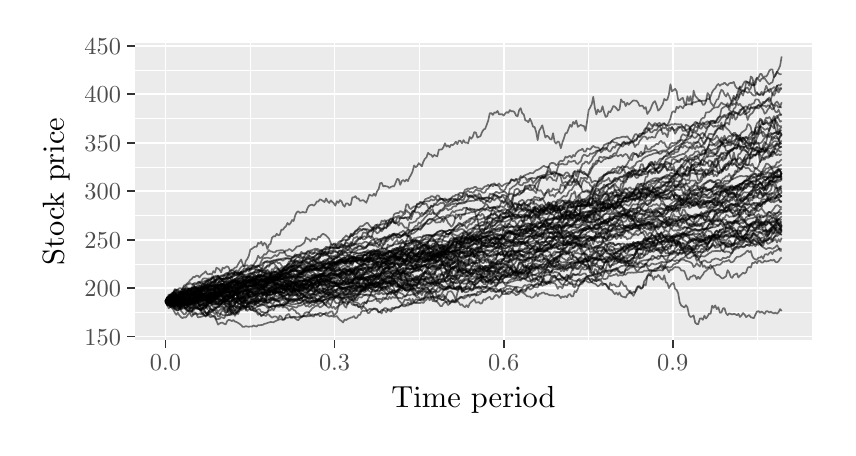
\begin{tikzpicture}[x=1pt,y=1pt]
\definecolor{fillColor}{RGB}{255,255,255}
\path[use as bounding box,fill=fillColor,fill opacity=0.00] (0,0) rectangle (289.08,144.54);
\begin{scope}
\path[clip] (  0.00,  0.00) rectangle (289.08,144.54);
\definecolor{drawColor}{RGB}{255,255,255}
\definecolor{fillColor}{RGB}{255,255,255}

\path[draw=drawColor,line width= 0.6pt,line join=round,line cap=round,fill=fillColor] (  0.00,  0.00) rectangle (289.08,144.54);
\end{scope}
\begin{scope}
\path[clip] ( 38.67, 31.53) rectangle (283.58,139.04);
\definecolor{fillColor}{gray}{0.92}

\path[fill=fillColor] ( 38.67, 31.53) rectangle (283.58,139.04);
\definecolor{drawColor}{RGB}{255,255,255}

\path[draw=drawColor,line width= 0.3pt,line join=round] ( 38.67, 41.65) --
	(283.58, 41.65);

\path[draw=drawColor,line width= 0.3pt,line join=round] ( 38.67, 59.17) --
	(283.58, 59.17);

\path[draw=drawColor,line width= 0.3pt,line join=round] ( 38.67, 76.68) --
	(283.58, 76.68);

\path[draw=drawColor,line width= 0.3pt,line join=round] ( 38.67, 94.19) --
	(283.58, 94.19);

\path[draw=drawColor,line width= 0.3pt,line join=round] ( 38.67,111.71) --
	(283.58,111.71);

\path[draw=drawColor,line width= 0.3pt,line join=round] ( 38.67,129.22) --
	(283.58,129.22);

\path[draw=drawColor,line width= 0.3pt,line join=round] ( 80.35, 31.53) --
	( 80.35,139.04);

\path[draw=drawColor,line width= 0.3pt,line join=round] (141.45, 31.53) --
	(141.45,139.04);

\path[draw=drawColor,line width= 0.3pt,line join=round] (202.56, 31.53) --
	(202.56,139.04);

\path[draw=drawColor,line width= 0.3pt,line join=round] (263.66, 31.53) --
	(263.66,139.04);

\path[draw=drawColor,line width= 0.6pt,line join=round] ( 38.67, 32.90) --
	(283.58, 32.90);

\path[draw=drawColor,line width= 0.6pt,line join=round] ( 38.67, 50.41) --
	(283.58, 50.41);

\path[draw=drawColor,line width= 0.6pt,line join=round] ( 38.67, 67.92) --
	(283.58, 67.92);

\path[draw=drawColor,line width= 0.6pt,line join=round] ( 38.67, 85.44) --
	(283.58, 85.44);

\path[draw=drawColor,line width= 0.6pt,line join=round] ( 38.67,102.95) --
	(283.58,102.95);

\path[draw=drawColor,line width= 0.6pt,line join=round] ( 38.67,120.46) --
	(283.58,120.46);

\path[draw=drawColor,line width= 0.6pt,line join=round] ( 38.67,137.98) --
	(283.58,137.98);

\path[draw=drawColor,line width= 0.6pt,line join=round] ( 49.80, 31.53) --
	( 49.80,139.04);

\path[draw=drawColor,line width= 0.6pt,line join=round] (110.90, 31.53) --
	(110.90,139.04);

\path[draw=drawColor,line width= 0.6pt,line join=round] (172.00, 31.53) --
	(172.00,139.04);

\path[draw=drawColor,line width= 0.6pt,line join=round] (233.11, 31.53) --
	(233.11,139.04);
\definecolor{drawColor}{RGB}{0,0,0}

\path[draw=drawColor,draw opacity=0.55,line width= 0.6pt,line join=round] ( 49.80, 45.61) --
	( 50.36, 45.48) --
	( 50.92, 45.87) --
	( 51.47, 45.76) --
	( 52.03, 46.32) --
	( 52.59, 46.51) --
	( 53.15, 47.31) --
	( 53.71, 46.41) --
	( 54.26, 46.91) --
	( 54.82, 47.30) --
	( 55.38, 47.91) --
	( 55.94, 48.52) --
	( 56.50, 48.06) --
	( 57.05, 48.33) --
	( 57.61, 47.89) --
	( 58.17, 47.94) --
	( 58.73, 48.50) --
	( 59.29, 48.70) --
	( 59.84, 48.15) --
	( 60.40, 48.07) --
	( 60.96, 48.94) --
	( 61.52, 48.85) --
	( 62.08, 49.46) --
	( 62.63, 48.97) --
	( 63.19, 49.56) --
	( 63.75, 50.00) --
	( 64.31, 50.03) --
	( 64.87, 49.79) --
	( 65.42, 51.32) --
	( 65.98, 50.95) --
	( 66.54, 51.18) --
	( 67.10, 51.93) --
	( 67.66, 52.20) --
	( 68.21, 52.13) --
	( 68.77, 52.18) --
	( 69.33, 52.98) --
	( 69.89, 53.02) --
	( 70.45, 53.00) --
	( 71.00, 52.80) --
	( 71.56, 52.77) --
	( 72.12, 52.71) --
	( 72.68, 52.58) --
	( 73.24, 52.61) --
	( 73.79, 53.01) --
	( 74.35, 53.34) --
	( 74.91, 53.67) --
	( 75.47, 54.01) --
	( 76.03, 54.79) --
	( 76.58, 55.66) --
	( 77.14, 55.09) --
	( 77.70, 54.54) --
	( 78.26, 54.40) --
	( 78.82, 54.24) --
	( 79.37, 54.71) --
	( 79.93, 55.29) --
	( 80.49, 55.97) --
	( 81.05, 55.76) --
	( 81.61, 56.08) --
	( 82.16, 56.04) --
	( 82.72, 55.98) --
	( 83.28, 56.17) --
	( 83.84, 56.52) --
	( 84.40, 56.48) --
	( 84.95, 56.84) --
	( 85.51, 56.90) --
	( 86.07, 56.63) --
	( 86.63, 56.53) --
	( 87.19, 56.23) --
	( 87.74, 55.80) --
	( 88.30, 55.57) --
	( 88.86, 55.35) --
	( 89.42, 55.14) --
	( 89.98, 54.37) --
	( 90.53, 53.64) --
	( 91.09, 54.73) --
	( 91.65, 53.45) --
	( 92.21, 53.78) --
	( 92.77, 53.18) --
	( 93.32, 51.80) --
	( 93.88, 52.12) --
	( 94.44, 52.55) --
	( 95.00, 52.77) --
	( 95.56, 53.90) --
	( 96.11, 54.68) --
	( 96.67, 54.01) --
	( 97.23, 54.14) --
	( 97.79, 55.23) --
	( 98.35, 55.48) --
	( 98.90, 55.42) --
	( 99.46, 56.46) --
	(100.02, 57.14) --
	(100.58, 57.24) --
	(101.14, 56.93) --
	(101.69, 57.16) --
	(102.25, 57.50) --
	(102.81, 57.13) --
	(103.37, 57.32) --
	(103.93, 57.46) --
	(104.48, 56.73) --
	(105.04, 57.02) --
	(105.60, 57.14) --
	(106.16, 57.96) --
	(106.72, 58.43) --
	(107.27, 58.61) --
	(107.83, 59.10) --
	(108.39, 59.35) --
	(108.95, 59.51) --
	(109.51, 59.20) --
	(110.06, 59.83) --
	(110.62, 59.71) --
	(111.18, 59.91) --
	(111.74, 59.81) --
	(112.30, 59.75) --
	(112.85, 60.04) --
	(113.41, 59.66) --
	(113.97, 59.87) --
	(114.53, 59.12) --
	(115.09, 59.21) --
	(115.65, 59.28) --
	(116.20, 59.22) --
	(116.76, 59.61) --
	(117.32, 60.24) --
	(117.88, 60.13) --
	(118.44, 60.03) --
	(118.99, 59.89) --
	(119.55, 60.33) --
	(120.11, 60.65) --
	(120.67, 60.63) --
	(121.23, 61.45) --
	(121.78, 60.81) --
	(122.34, 60.88) --
	(122.90, 61.23) --
	(123.46, 61.57) --
	(124.02, 62.60) --
	(124.57, 62.02) --
	(125.13, 61.65) --
	(125.69, 61.80) --
	(126.25, 62.56) --
	(126.81, 63.06) --
	(127.36, 62.75) --
	(127.92, 62.71) --
	(128.48, 62.81) --
	(129.04, 63.07) --
	(129.60, 62.73) --
	(130.15, 62.93) --
	(130.71, 63.50) --
	(131.27, 63.61) --
	(131.83, 63.27) --
	(132.39, 64.15) --
	(132.94, 64.91) --
	(133.50, 64.90) --
	(134.06, 64.98) --
	(134.62, 65.69) --
	(135.18, 66.88) --
	(135.73, 67.22) --
	(136.29, 67.08) --
	(136.85, 67.54) --
	(137.41, 67.31) --
	(137.97, 67.79) --
	(138.52, 67.69) --
	(139.08, 67.53) --
	(139.64, 68.53) --
	(140.20, 68.41) --
	(140.76, 68.75) --
	(141.31, 68.83) --
	(141.87, 68.92) --
	(142.43, 68.79) --
	(142.99, 69.11) --
	(143.55, 69.28) --
	(144.10, 69.49) --
	(144.66, 69.49) --
	(145.22, 69.53) --
	(145.78, 69.64) --
	(146.34, 69.01) --
	(146.89, 69.31) --
	(147.45, 70.06) --
	(148.01, 70.60) --
	(148.57, 70.77) --
	(149.13, 71.19) --
	(149.68, 71.16) --
	(150.24, 71.05) --
	(150.80, 71.02) --
	(151.36, 70.98) --
	(151.92, 71.19) --
	(152.47, 71.45) --
	(153.03, 71.44) --
	(153.59, 71.54) --
	(154.15, 71.59) --
	(154.71, 71.59) --
	(155.26, 71.70) --
	(155.82, 72.23) --
	(156.38, 72.80) --
	(156.94, 72.77) --
	(157.50, 73.20) --
	(158.05, 72.89) --
	(158.61, 72.02) --
	(159.17, 72.93) --
	(159.73, 73.63) --
	(160.29, 73.35) --
	(160.84, 74.18) --
	(161.40, 74.37) --
	(161.96, 75.37) --
	(162.52, 75.28) --
	(163.08, 75.22) --
	(163.63, 75.24) --
	(164.19, 75.54) --
	(164.75, 75.74) --
	(165.31, 76.01) --
	(165.87, 76.15) --
	(166.42, 76.47) --
	(166.98, 76.78) --
	(167.54, 77.16) --
	(168.10, 76.62) --
	(168.66, 77.70) --
	(169.21, 76.79) --
	(169.77, 76.30) --
	(170.33, 75.76) --
	(170.89, 75.03) --
	(171.45, 75.38) --
	(172.00, 76.00) --
	(172.56, 76.13) --
	(173.12, 77.01) --
	(173.68, 77.55) --
	(174.24, 76.28) --
	(174.79, 75.51) --
	(175.35, 74.55) --
	(175.91, 74.87) --
	(176.47, 73.88) --
	(177.03, 73.26) --
	(177.58, 72.42) --
	(178.14, 72.27) --
	(178.70, 73.50) --
	(179.26, 74.68) --
	(179.82, 74.94) --
	(180.37, 75.03) --
	(180.93, 76.33) --
	(181.49, 75.43) --
	(182.05, 75.73) --
	(182.61, 75.82) --
	(183.17, 76.29) --
	(183.72, 77.16) --
	(184.28, 76.30) --
	(184.84, 75.86) --
	(185.40, 79.17) --
	(185.96, 78.41) --
	(186.51, 77.48) --
	(187.07, 78.65) --
	(187.63, 78.15) --
	(188.19, 80.61) --
	(188.75, 79.92) --
	(189.30, 79.55) --
	(189.86, 79.47) --
	(190.42, 78.46) --
	(190.98, 81.17) --
	(191.54, 79.78) --
	(192.09, 80.00) --
	(192.65, 76.96) --
	(193.21, 76.24) --
	(193.77, 76.20) --
	(194.33, 76.28) --
	(194.88, 77.17) --
	(195.44, 76.86) --
	(196.00, 76.35) --
	(196.56, 74.84) --
	(197.12, 75.91) --
	(197.67, 76.77) --
	(198.23, 76.82) --
	(198.79, 76.66) --
	(199.35, 77.46) --
	(199.91, 78.69) --
	(200.46, 79.04) --
	(201.02, 79.12) --
	(201.58, 79.61) --
	(202.14, 80.47) --
	(202.70, 80.54) --
	(203.25, 79.47) --
	(203.81, 79.77) --
	(204.37, 79.05) --
	(204.93, 79.65) --
	(205.49, 78.90) --
	(206.04, 78.50) --
	(206.60, 78.02) --
	(207.16, 78.23) --
	(207.72, 78.52) --
	(208.28, 78.51) --
	(208.83, 78.72) --
	(209.39, 78.81) --
	(209.95, 79.04) --
	(210.51, 79.71) --
	(211.07, 80.73) --
	(211.62, 79.76) --
	(212.18, 79.40) --
	(212.74, 80.92) --
	(213.30, 81.49) --
	(213.86, 81.73) --
	(214.41, 81.76) --
	(214.97, 81.78) --
	(215.53, 82.09) --
	(216.09, 81.89) --
	(216.65, 81.62) --
	(217.20, 81.84) --
	(217.76, 82.38) --
	(218.32, 82.92) --
	(218.88, 82.55) --
	(219.44, 82.02) --
	(219.99, 82.96) --
	(220.55, 83.23) --
	(221.11, 82.91) --
	(221.67, 83.72) --
	(222.23, 83.29) --
	(222.78, 83.28) --
	(223.34, 82.63) --
	(223.90, 84.39) --
	(224.46, 84.29) --
	(225.02, 84.69) --
	(225.57, 85.42) --
	(226.13, 84.57) --
	(226.69, 84.29) --
	(227.25, 83.00) --
	(227.81, 83.99) --
	(228.36, 83.87) --
	(228.92, 81.77) --
	(229.48, 81.96) --
	(230.04, 80.83) --
	(230.60, 80.25) --
	(231.15, 79.96) --
	(231.71, 79.59) --
	(232.27, 80.04) --
	(232.83, 78.47) --
	(233.39, 78.95) --
	(233.94, 78.84) --
	(234.50, 79.90) --
	(235.06, 78.67) --
	(235.62, 77.18) --
	(236.18, 76.80) --
	(236.73, 78.67) --
	(237.29, 78.82) --
	(237.85, 77.56) --
	(238.41, 77.22) --
	(238.97, 76.29) --
	(239.52, 75.89) --
	(240.08, 75.98) --
	(240.64, 76.33) --
	(241.20, 75.59) --
	(241.76, 75.92) --
	(242.31, 76.36) --
	(242.87, 77.05) --
	(243.43, 75.44) --
	(243.99, 75.96) --
	(244.55, 74.88) --
	(245.10, 75.26) --
	(245.66, 76.26) --
	(246.22, 76.32) --
	(246.78, 74.78) --
	(247.34, 73.58) --
	(247.89, 75.89) --
	(248.45, 78.10) --
	(249.01, 77.24) --
	(249.57, 75.64) --
	(250.13, 76.64) --
	(250.68, 77.54) --
	(251.24, 77.49) --
	(251.80, 78.78) --
	(252.36, 78.35) --
	(252.92, 78.04) --
	(253.48, 78.26) --
	(254.03, 78.66) --
	(254.59, 77.44) --
	(255.15, 77.60) --
	(255.71, 78.18) --
	(256.27, 79.40) --
	(256.82, 77.09) --
	(257.38, 78.67) --
	(257.94, 77.12) --
	(258.50, 77.47) --
	(259.06, 79.77) --
	(259.61, 78.57) --
	(260.17, 78.34) --
	(260.73, 76.31) --
	(261.29, 78.54) --
	(261.85, 78.75) --
	(262.40, 79.31) --
	(262.96, 78.46) --
	(263.52, 79.90) --
	(264.08, 81.34) --
	(264.64, 80.83) --
	(265.19, 79.56) --
	(265.75, 81.35) --
	(266.31, 80.83) --
	(266.87, 81.75) --
	(267.43, 82.37) --
	(267.98, 82.75) --
	(268.54, 82.58) --
	(269.10, 82.54) --
	(269.66, 82.83) --
	(270.22, 82.95) --
	(270.77, 83.82) --
	(271.33, 84.47) --
	(271.89, 84.00) --
	(272.45, 83.53);

\path[draw=drawColor,draw opacity=0.55,line width= 0.6pt,line join=round] ( 49.80, 45.61) --
	( 50.36, 46.68) --
	( 50.92, 47.04) --
	( 51.47, 46.79) --
	( 52.03, 47.42) --
	( 52.59, 46.98) --
	( 53.15, 47.28) --
	( 53.71, 46.82) --
	( 54.26, 47.66) --
	( 54.82, 47.75) --
	( 55.38, 47.08) --
	( 55.94, 48.34) --
	( 56.50, 48.13) --
	( 57.05, 48.68) --
	( 57.61, 48.80) --
	( 58.17, 49.26) --
	( 58.73, 49.22) --
	( 59.29, 49.94) --
	( 59.84, 50.39) --
	( 60.40, 50.68) --
	( 60.96, 50.41) --
	( 61.52, 50.71) --
	( 62.08, 51.18) --
	( 62.63, 51.50) --
	( 63.19, 51.72) --
	( 63.75, 52.19) --
	( 64.31, 52.76) --
	( 64.87, 53.37) --
	( 65.42, 53.33) --
	( 65.98, 53.39) --
	( 66.54, 53.90) --
	( 67.10, 53.95) --
	( 67.66, 53.33) --
	( 68.21, 52.36) --
	( 68.77, 52.55) --
	( 69.33, 52.86) --
	( 69.89, 51.40) --
	( 70.45, 50.65) --
	( 71.00, 50.51) --
	( 71.56, 51.30) --
	( 72.12, 51.93) --
	( 72.68, 53.15) --
	( 73.24, 53.11) --
	( 73.79, 52.78) --
	( 74.35, 53.02) --
	( 74.91, 53.10) --
	( 75.47, 52.16) --
	( 76.03, 53.52) --
	( 76.58, 54.22) --
	( 77.14, 54.76) --
	( 77.70, 53.40) --
	( 78.26, 53.46) --
	( 78.82, 53.68) --
	( 79.37, 54.08) --
	( 79.93, 54.56) --
	( 80.49, 53.85) --
	( 81.05, 53.88) --
	( 81.61, 54.08) --
	( 82.16, 54.32) --
	( 82.72, 54.15) --
	( 83.28, 54.40) --
	( 83.84, 54.55) --
	( 84.40, 54.70) --
	( 84.95, 54.46) --
	( 85.51, 54.92) --
	( 86.07, 54.57) --
	( 86.63, 53.86) --
	( 87.19, 54.23) --
	( 87.74, 54.74) --
	( 88.30, 54.72) --
	( 88.86, 54.59) --
	( 89.42, 54.64) --
	( 89.98, 53.21) --
	( 90.53, 53.64) --
	( 91.09, 54.35) --
	( 91.65, 53.87) --
	( 92.21, 53.69) --
	( 92.77, 54.18) --
	( 93.32, 53.26) --
	( 93.88, 51.27) --
	( 94.44, 51.25) --
	( 95.00, 51.18) --
	( 95.56, 50.64) --
	( 96.11, 50.76) --
	( 96.67, 49.45) --
	( 97.23, 49.92) --
	( 97.79, 49.96) --
	( 98.35, 50.84) --
	( 98.90, 50.46) --
	( 99.46, 52.17) --
	(100.02, 53.50) --
	(100.58, 54.18) --
	(101.14, 54.17) --
	(101.69, 54.42) --
	(102.25, 54.49) --
	(102.81, 54.81) --
	(103.37, 55.37) --
	(103.93, 54.14) --
	(104.48, 54.07) --
	(105.04, 54.42) --
	(105.60, 54.49) --
	(106.16, 54.94) --
	(106.72, 55.28) --
	(107.27, 55.01) --
	(107.83, 54.07) --
	(108.39, 54.70) --
	(108.95, 56.01) --
	(109.51, 55.93) --
	(110.06, 57.40) --
	(110.62, 58.28) --
	(111.18, 58.33) --
	(111.74, 58.45) --
	(112.30, 58.59) --
	(112.85, 56.86) --
	(113.41, 56.77) --
	(113.97, 57.38) --
	(114.53, 57.59) --
	(115.09, 57.00) --
	(115.65, 56.64) --
	(116.20, 56.91) --
	(116.76, 56.56) --
	(117.32, 55.95) --
	(117.88, 55.97) --
	(118.44, 56.13) --
	(118.99, 55.77) --
	(119.55, 56.41) --
	(120.11, 57.12) --
	(120.67, 57.61) --
	(121.23, 58.47) --
	(121.78, 59.06) --
	(122.34, 59.00) --
	(122.90, 58.94) --
	(123.46, 58.88) --
	(124.02, 59.06) --
	(124.57, 58.99) --
	(125.13, 59.48) --
	(125.69, 59.48) --
	(126.25, 59.62) --
	(126.81, 59.03) --
	(127.36, 58.87) --
	(127.92, 58.74) --
	(128.48, 58.36) --
	(129.04, 58.92) --
	(129.60, 58.94) --
	(130.15, 58.90) --
	(130.71, 57.45) --
	(131.27, 57.28) --
	(131.83, 56.81) --
	(132.39, 56.97) --
	(132.94, 56.85) --
	(133.50, 56.75) --
	(134.06, 56.63) --
	(134.62, 56.72) --
	(135.18, 57.27) --
	(135.73, 57.56) --
	(136.29, 57.06) --
	(136.85, 57.57) --
	(137.41, 57.43) --
	(137.97, 57.37) --
	(138.52, 57.40) --
	(139.08, 58.06) --
	(139.64, 58.84) --
	(140.20, 58.64) --
	(140.76, 58.97) --
	(141.31, 58.98) --
	(141.87, 58.26) --
	(142.43, 58.29) --
	(142.99, 58.68) --
	(143.55, 58.68) --
	(144.10, 58.60) --
	(144.66, 59.90) --
	(145.22, 60.15) --
	(145.78, 60.87) --
	(146.34, 61.36) --
	(146.89, 62.25) --
	(147.45, 62.50) --
	(148.01, 62.94) --
	(148.57, 63.12) --
	(149.13, 63.20) --
	(149.68, 63.53) --
	(150.24, 63.07) --
	(150.80, 62.44) --
	(151.36, 62.55) --
	(151.92, 62.50) --
	(152.47, 62.82) --
	(153.03, 63.04) --
	(153.59, 63.16) --
	(154.15, 63.71) --
	(154.71, 64.16) --
	(155.26, 64.14) --
	(155.82, 64.15) --
	(156.38, 64.31) --
	(156.94, 64.43) --
	(157.50, 64.40) --
	(158.05, 64.86) --
	(158.61, 64.69) --
	(159.17, 65.46) --
	(159.73, 65.48) --
	(160.29, 66.03) --
	(160.84, 66.09) --
	(161.40, 66.55) --
	(161.96, 66.33) --
	(162.52, 65.91) --
	(163.08, 66.65) --
	(163.63, 66.08) --
	(164.19, 67.27) --
	(164.75, 67.31) --
	(165.31, 67.69) --
	(165.87, 68.40) --
	(166.42, 69.31) --
	(166.98, 70.06) --
	(167.54, 71.27) --
	(168.10, 71.56) --
	(168.66, 71.91) --
	(169.21, 71.41) --
	(169.77, 71.75) --
	(170.33, 71.65) --
	(170.89, 71.41) --
	(171.45, 71.68) --
	(172.00, 71.22) --
	(172.56, 71.00) --
	(173.12, 70.65) --
	(173.68, 71.15) --
	(174.24, 71.19) --
	(174.79, 70.38) --
	(175.35, 70.27) --
	(175.91, 70.23) --
	(176.47, 70.67) --
	(177.03, 71.16) --
	(177.58, 71.50) --
	(178.14, 71.56) --
	(178.70, 71.54) --
	(179.26, 71.52) --
	(179.82, 71.73) --
	(180.37, 71.24) --
	(180.93, 70.68) --
	(181.49, 71.06) --
	(182.05, 71.10) --
	(182.61, 71.37) --
	(183.17, 71.19) --
	(183.72, 71.21) --
	(184.28, 71.98) --
	(184.84, 72.06) --
	(185.40, 72.23) --
	(185.96, 72.23) --
	(186.51, 72.87) --
	(187.07, 73.17) --
	(187.63, 73.79) --
	(188.19, 74.06) --
	(188.75, 73.62) --
	(189.30, 73.40) --
	(189.86, 73.22) --
	(190.42, 72.84) --
	(190.98, 73.12) --
	(191.54, 73.50) --
	(192.09, 73.36) --
	(192.65, 72.90) --
	(193.21, 73.16) --
	(193.77, 72.75) --
	(194.33, 73.08) --
	(194.88, 73.21) --
	(195.44, 73.19) --
	(196.00, 72.84) --
	(196.56, 72.26) --
	(197.12, 73.18) --
	(197.67, 74.42) --
	(198.23, 75.39) --
	(198.79, 75.06) --
	(199.35, 75.34) --
	(199.91, 75.69) --
	(200.46, 75.10) --
	(201.02, 74.68) --
	(201.58, 74.54) --
	(202.14, 74.22) --
	(202.70, 74.15) --
	(203.25, 74.25) --
	(203.81, 74.30) --
	(204.37, 74.13) --
	(204.93, 74.46) --
	(205.49, 75.11) --
	(206.04, 75.12) --
	(206.60, 75.42) --
	(207.16, 75.33) --
	(207.72, 76.05) --
	(208.28, 76.92) --
	(208.83, 77.18) --
	(209.39, 78.00) --
	(209.95, 77.97) --
	(210.51, 79.45) --
	(211.07, 80.02) --
	(211.62, 80.57) --
	(212.18, 81.47) --
	(212.74, 80.68) --
	(213.30, 79.80) --
	(213.86, 79.15) --
	(214.41, 80.54) --
	(214.97, 82.07) --
	(215.53, 83.40) --
	(216.09, 83.33) --
	(216.65, 82.35) --
	(217.20, 82.60) --
	(217.76, 83.49) --
	(218.32, 84.00) --
	(218.88, 83.53) --
	(219.44, 84.48) --
	(219.99, 83.81) --
	(220.55, 82.62) --
	(221.11, 83.66) --
	(221.67, 84.96) --
	(222.23, 86.65) --
	(222.78, 86.17) --
	(223.34, 87.53) --
	(223.90, 86.66) --
	(224.46, 85.89) --
	(225.02, 87.25) --
	(225.57, 87.51) --
	(226.13, 86.49) --
	(226.69, 86.21) --
	(227.25, 85.17) --
	(227.81, 86.75) --
	(228.36, 86.31) --
	(228.92, 86.71) --
	(229.48, 87.38) --
	(230.04, 87.39) --
	(230.60, 88.24) --
	(231.15, 88.69) --
	(231.71, 88.06) --
	(232.27, 89.08) --
	(232.83, 90.34) --
	(233.39, 90.17) --
	(233.94, 86.78) --
	(234.50, 87.06) --
	(235.06, 87.25) --
	(235.62, 89.28) --
	(236.18, 88.33) --
	(236.73, 91.07) --
	(237.29, 92.11) --
	(237.85, 91.00) --
	(238.41, 90.77) --
	(238.97, 91.99) --
	(239.52, 93.59) --
	(240.08, 94.95) --
	(240.64, 94.02) --
	(241.20, 92.10) --
	(241.76, 91.27) --
	(242.31, 89.24) --
	(242.87, 89.30) --
	(243.43, 90.69) --
	(243.99, 91.56) --
	(244.55, 92.69) --
	(245.10, 91.46) --
	(245.66, 92.00) --
	(246.22, 93.15) --
	(246.78, 94.05) --
	(247.34, 95.76) --
	(247.89, 94.99) --
	(248.45, 96.16) --
	(249.01, 97.22) --
	(249.57, 97.47) --
	(250.13, 98.34) --
	(250.68, 98.83) --
	(251.24, 99.04) --
	(251.80, 98.31) --
	(252.36, 98.41) --
	(252.92, 99.72) --
	(253.48,100.13) --
	(254.03,100.46) --
	(254.59,100.29) --
	(255.15,100.88) --
	(255.71,101.27) --
	(256.27,101.45) --
	(256.82,102.03) --
	(257.38,101.56) --
	(257.94,101.49) --
	(258.50,101.47) --
	(259.06,101.45) --
	(259.61,101.97) --
	(260.17,102.05) --
	(260.73,102.61) --
	(261.29,102.94) --
	(261.85,102.81) --
	(262.40,102.52) --
	(262.96,102.96) --
	(263.52,102.56) --
	(264.08,102.76) --
	(264.64,102.80) --
	(265.19,103.07) --
	(265.75,103.91) --
	(266.31,104.84) --
	(266.87,104.93) --
	(267.43,105.13) --
	(267.98,105.54) --
	(268.54,105.89) --
	(269.10,106.28) --
	(269.66,106.44) --
	(270.22,106.51) --
	(270.77,106.96) --
	(271.33,106.69) --
	(271.89,107.34) --
	(272.45,107.50);

\path[draw=drawColor,draw opacity=0.55,line width= 0.6pt,line join=round] ( 49.80, 45.61) --
	( 50.36, 45.87) --
	( 50.92, 45.86) --
	( 51.47, 46.23) --
	( 52.03, 45.96) --
	( 52.59, 46.68) --
	( 53.15, 47.53) --
	( 53.71, 47.91) --
	( 54.26, 47.68) --
	( 54.82, 48.13) --
	( 55.38, 48.43) --
	( 55.94, 47.85) --
	( 56.50, 48.44) --
	( 57.05, 48.79) --
	( 57.61, 49.63) --
	( 58.17, 50.15) --
	( 58.73, 50.06) --
	( 59.29, 49.79) --
	( 59.84, 49.62) --
	( 60.40, 49.93) --
	( 60.96, 50.01) --
	( 61.52, 50.39) --
	( 62.08, 50.44) --
	( 62.63, 50.41) --
	( 63.19, 50.70) --
	( 63.75, 50.95) --
	( 64.31, 51.31) --
	( 64.87, 51.82) --
	( 65.42, 51.64) --
	( 65.98, 51.78) --
	( 66.54, 52.54) --
	( 67.10, 52.21) --
	( 67.66, 51.85) --
	( 68.21, 51.46) --
	( 68.77, 51.19) --
	( 69.33, 51.37) --
	( 69.89, 51.08) --
	( 70.45, 51.44) --
	( 71.00, 51.82) --
	( 71.56, 50.95) --
	( 72.12, 51.28) --
	( 72.68, 52.16) --
	( 73.24, 52.50) --
	( 73.79, 52.50) --
	( 74.35, 52.81) --
	( 74.91, 52.62) --
	( 75.47, 52.62) --
	( 76.03, 52.25) --
	( 76.58, 52.23) --
	( 77.14, 52.72) --
	( 77.70, 53.04) --
	( 78.26, 53.68) --
	( 78.82, 54.55) --
	( 79.37, 54.49) --
	( 79.93, 54.36) --
	( 80.49, 55.47) --
	( 81.05, 55.70) --
	( 81.61, 55.45) --
	( 82.16, 55.29) --
	( 82.72, 54.55) --
	( 83.28, 55.36) --
	( 83.84, 55.34) --
	( 84.40, 55.22) --
	( 84.95, 55.04) --
	( 85.51, 55.15) --
	( 86.07, 55.62) --
	( 86.63, 55.77) --
	( 87.19, 55.94) --
	( 87.74, 55.54) --
	( 88.30, 55.26) --
	( 88.86, 54.59) --
	( 89.42, 53.85) --
	( 89.98, 54.17) --
	( 90.53, 54.04) --
	( 91.09, 54.26) --
	( 91.65, 54.77) --
	( 92.21, 54.17) --
	( 92.77, 54.24) --
	( 93.32, 54.00) --
	( 93.88, 53.97) --
	( 94.44, 54.27) --
	( 95.00, 54.62) --
	( 95.56, 54.74) --
	( 96.11, 55.32) --
	( 96.67, 55.29) --
	( 97.23, 55.50) --
	( 97.79, 55.88) --
	( 98.35, 55.99) --
	( 98.90, 56.06) --
	( 99.46, 56.88) --
	(100.02, 56.15) --
	(100.58, 56.20) --
	(101.14, 55.93) --
	(101.69, 56.28) --
	(102.25, 56.97) --
	(102.81, 56.83) --
	(103.37, 57.03) --
	(103.93, 57.02) --
	(104.48, 57.26) --
	(105.04, 57.54) --
	(105.60, 57.57) --
	(106.16, 57.88) --
	(106.72, 58.01) --
	(107.27, 57.80) --
	(107.83, 57.34) --
	(108.39, 57.69) --
	(108.95, 57.80) --
	(109.51, 57.75) --
	(110.06, 58.16) --
	(110.62, 58.35) --
	(111.18, 58.76) --
	(111.74, 58.96) --
	(112.30, 59.98) --
	(112.85, 60.68) --
	(113.41, 60.65) --
	(113.97, 60.76) --
	(114.53, 60.65) --
	(115.09, 60.51) --
	(115.65, 61.11) --
	(116.20, 61.10) --
	(116.76, 61.94) --
	(117.32, 61.58) --
	(117.88, 60.86) --
	(118.44, 61.19) --
	(118.99, 61.38) --
	(119.55, 61.11) --
	(120.11, 61.03) --
	(120.67, 60.87) --
	(121.23, 62.01) --
	(121.78, 62.61) --
	(122.34, 62.14) --
	(122.90, 62.46) --
	(123.46, 62.06) --
	(124.02, 62.84) --
	(124.57, 62.22) --
	(125.13, 62.51) --
	(125.69, 62.79) --
	(126.25, 62.94) --
	(126.81, 62.36) --
	(127.36, 62.27) --
	(127.92, 62.22) --
	(128.48, 62.57) --
	(129.04, 62.73) --
	(129.60, 62.89) --
	(130.15, 63.14) --
	(130.71, 63.79) --
	(131.27, 63.96) --
	(131.83, 63.94) --
	(132.39, 63.77) --
	(132.94, 63.98) --
	(133.50, 64.95) --
	(134.06, 64.07) --
	(134.62, 63.59) --
	(135.18, 63.64) --
	(135.73, 62.11) --
	(136.29, 62.97) --
	(136.85, 63.94) --
	(137.41, 63.35) --
	(137.97, 62.69) --
	(138.52, 61.48) --
	(139.08, 60.83) --
	(139.64, 60.75) --
	(140.20, 60.06) --
	(140.76, 60.19) --
	(141.31, 60.61) --
	(141.87, 62.57) --
	(142.43, 63.51) --
	(142.99, 64.62) --
	(143.55, 64.39) --
	(144.10, 64.07) --
	(144.66, 64.85) --
	(145.22, 64.93) --
	(145.78, 64.48) --
	(146.34, 65.43) --
	(146.89, 65.87) --
	(147.45, 67.11) --
	(148.01, 66.87) --
	(148.57, 67.12) --
	(149.13, 67.46) --
	(149.68, 66.93) --
	(150.24, 68.42) --
	(150.80, 69.43) --
	(151.36, 70.01) --
	(151.92, 69.93) --
	(152.47, 70.15) --
	(153.03, 70.69) --
	(153.59, 70.56) --
	(154.15, 71.88) --
	(154.71, 72.40) --
	(155.26, 73.05) --
	(155.82, 73.22) --
	(156.38, 73.75) --
	(156.94, 73.28) --
	(157.50, 74.00) --
	(158.05, 74.30) --
	(158.61, 74.71) --
	(159.17, 74.92) --
	(159.73, 75.54) --
	(160.29, 75.68) --
	(160.84, 75.93) --
	(161.40, 76.22) --
	(161.96, 76.27) --
	(162.52, 76.63) --
	(163.08, 77.56) --
	(163.63, 78.16) --
	(164.19, 78.51) --
	(164.75, 78.88) --
	(165.31, 78.47) --
	(165.87, 79.38) --
	(166.42, 79.68) --
	(166.98, 79.25) --
	(167.54, 79.49) --
	(168.10, 79.59) --
	(168.66, 79.85) --
	(169.21, 78.81) --
	(169.77, 78.74) --
	(170.33, 77.90) --
	(170.89, 78.46) --
	(171.45, 78.15) --
	(172.00, 77.80) --
	(172.56, 76.91) --
	(173.12, 78.22) --
	(173.68, 77.97) --
	(174.24, 78.03) --
	(174.79, 77.83) --
	(175.35, 78.76) --
	(175.91, 79.22) --
	(176.47, 79.13) --
	(177.03, 79.72) --
	(177.58, 79.48) --
	(178.14, 79.28) --
	(178.70, 80.50) --
	(179.26, 80.93) --
	(179.82, 81.17) --
	(180.37, 82.01) --
	(180.93, 82.41) --
	(181.49, 82.24) --
	(182.05, 82.28) --
	(182.61, 81.84) --
	(183.17, 80.80) --
	(183.72, 81.00) --
	(184.28, 80.41) --
	(184.84, 80.16) --
	(185.40, 79.23) --
	(185.96, 78.09) --
	(186.51, 77.77) --
	(187.07, 79.06) --
	(187.63, 79.04) --
	(188.19, 79.31) --
	(188.75, 79.00) --
	(189.30, 79.99) --
	(189.86, 80.27) --
	(190.42, 80.29) --
	(190.98, 81.54) --
	(191.54, 82.32) --
	(192.09, 82.41) --
	(192.65, 82.66) --
	(193.21, 83.35) --
	(193.77, 83.77) --
	(194.33, 83.50) --
	(194.88, 83.84) --
	(195.44, 85.20) --
	(196.00, 85.81) --
	(196.56, 85.86) --
	(197.12, 86.97) --
	(197.67, 87.77) --
	(198.23, 87.71) --
	(198.79, 88.22) --
	(199.35, 87.74) --
	(199.91, 87.14) --
	(200.46, 85.54) --
	(201.02, 85.14) --
	(201.58, 85.61) --
	(202.14, 85.84) --
	(202.70, 84.86) --
	(203.25, 85.20) --
	(203.81, 85.98) --
	(204.37, 86.40) --
	(204.93, 87.29) --
	(205.49, 87.41) --
	(206.04, 88.71) --
	(206.60, 90.16) --
	(207.16, 90.47) --
	(207.72, 90.81) --
	(208.28, 91.46) --
	(208.83, 91.67) --
	(209.39, 91.78) --
	(209.95, 92.01) --
	(210.51, 92.23) --
	(211.07, 92.22) --
	(211.62, 92.33) --
	(212.18, 92.25) --
	(212.74, 92.12) --
	(213.30, 91.91) --
	(213.86, 91.78) --
	(214.41, 92.28) --
	(214.97, 93.22) --
	(215.53, 94.30) --
	(216.09, 94.16) --
	(216.65, 94.37) --
	(217.20, 93.78) --
	(217.76, 93.51) --
	(218.32, 94.10) --
	(218.88, 94.46) --
	(219.44, 94.71) --
	(219.99, 95.86) --
	(220.55, 96.15) --
	(221.11, 96.39) --
	(221.67, 96.31) --
	(222.23, 97.19) --
	(222.78, 97.59) --
	(223.34, 97.94) --
	(223.90, 98.13) --
	(224.46, 98.48) --
	(225.02, 98.56) --
	(225.57, 98.76) --
	(226.13, 99.07) --
	(226.69, 99.15) --
	(227.25, 99.29) --
	(227.81, 99.37) --
	(228.36, 98.90) --
	(228.92, 99.11) --
	(229.48, 99.75) --
	(230.04, 99.77) --
	(230.60, 99.69) --
	(231.15, 99.90) --
	(231.71, 99.10) --
	(232.27, 99.47) --
	(232.83, 99.72) --
	(233.39,100.37) --
	(233.94,101.19) --
	(234.50,101.65) --
	(235.06,101.71) --
	(235.62,102.09) --
	(236.18,102.60) --
	(236.73,102.38) --
	(237.29,103.39) --
	(237.85,103.97) --
	(238.41,104.02) --
	(238.97,104.57) --
	(239.52,104.71) --
	(240.08,105.83) --
	(240.64,107.56) --
	(241.20,107.14) --
	(241.76,107.00) --
	(242.31,108.50) --
	(242.87,109.02) --
	(243.43,109.60) --
	(243.99,109.47) --
	(244.55,110.03) --
	(245.10,110.37) --
	(245.66,110.75) --
	(246.22,110.31) --
	(246.78,110.82) --
	(247.34,110.70) --
	(247.89,110.99) --
	(248.45,110.30) --
	(249.01,110.24) --
	(249.57,110.25) --
	(250.13,111.06) --
	(250.68,111.93) --
	(251.24,112.16) --
	(251.80,112.61) --
	(252.36,112.13) --
	(252.92,111.65) --
	(253.48,113.29) --
	(254.03,113.59) --
	(254.59,113.04) --
	(255.15,112.98) --
	(255.71,114.05) --
	(256.27,113.51) --
	(256.82,113.24) --
	(257.38,113.93) --
	(257.94,115.15) --
	(258.50,115.74) --
	(259.06,113.17) --
	(259.61,113.43) --
	(260.17,113.86) --
	(260.73,114.15) --
	(261.29,115.93) --
	(261.85,115.39) --
	(262.40,115.31) --
	(262.96,115.60) --
	(263.52,115.49) --
	(264.08,115.35) --
	(264.64,115.97) --
	(265.19,116.30) --
	(265.75,117.01) --
	(266.31,117.75) --
	(266.87,118.00) --
	(267.43,118.48) --
	(267.98,119.30) --
	(268.54,118.17) --
	(269.10,116.72) --
	(269.66,116.46) --
	(270.22,117.38) --
	(270.77,117.85) --
	(271.33,117.11) --
	(271.89,115.86) --
	(272.45,117.59);

\path[draw=drawColor,draw opacity=0.55,line width= 0.6pt,line join=round] ( 49.80, 45.61) --
	( 50.36, 46.98) --
	( 50.92, 46.27) --
	( 51.47, 46.36) --
	( 52.03, 47.00) --
	( 52.59, 47.81) --
	( 53.15, 47.49) --
	( 53.71, 46.96) --
	( 54.26, 47.27) --
	( 54.82, 46.57) --
	( 55.38, 47.66) --
	( 55.94, 47.63) --
	( 56.50, 46.92) --
	( 57.05, 46.29) --
	( 57.61, 45.83) --
	( 58.17, 44.83) --
	( 58.73, 44.52) --
	( 59.29, 45.43) --
	( 59.84, 45.13) --
	( 60.40, 44.89) --
	( 60.96, 45.73) --
	( 61.52, 47.56) --
	( 62.08, 48.36) --
	( 62.63, 48.63) --
	( 63.19, 48.54) --
	( 63.75, 48.23) --
	( 64.31, 47.49) --
	( 64.87, 47.57) --
	( 65.42, 46.75) --
	( 65.98, 47.00) --
	( 66.54, 47.33) --
	( 67.10, 47.12) --
	( 67.66, 46.62) --
	( 68.21, 46.67) --
	( 68.77, 46.54) --
	( 69.33, 46.52) --
	( 69.89, 46.32) --
	( 70.45, 45.73) --
	( 71.00, 45.77) --
	( 71.56, 45.74) --
	( 72.12, 46.02) --
	( 72.68, 45.54) --
	( 73.24, 46.05) --
	( 73.79, 46.14) --
	( 74.35, 45.25) --
	( 74.91, 45.78) --
	( 75.47, 45.51) --
	( 76.03, 44.87) --
	( 76.58, 44.76) --
	( 77.14, 44.83) --
	( 77.70, 45.28) --
	( 78.26, 45.73) --
	( 78.82, 47.10) --
	( 79.37, 46.87) --
	( 79.93, 47.14) --
	( 80.49, 47.29) --
	( 81.05, 47.42) --
	( 81.61, 47.25) --
	( 82.16, 48.00) --
	( 82.72, 48.48) --
	( 83.28, 48.47) --
	( 83.84, 48.22) --
	( 84.40, 48.46) --
	( 84.95, 48.48) --
	( 85.51, 49.06) --
	( 86.07, 48.88) --
	( 86.63, 48.20) --
	( 87.19, 48.12) --
	( 87.74, 47.90) --
	( 88.30, 48.22) --
	( 88.86, 48.29) --
	( 89.42, 48.59) --
	( 89.98, 49.58) --
	( 90.53, 49.11) --
	( 91.09, 48.22) --
	( 91.65, 48.02) --
	( 92.21, 48.05) --
	( 92.77, 48.76) --
	( 93.32, 48.04) --
	( 93.88, 48.19) --
	( 94.44, 48.00) --
	( 95.00, 47.60) --
	( 95.56, 47.92) --
	( 96.11, 48.48) --
	( 96.67, 48.71) --
	( 97.23, 49.36) --
	( 97.79, 49.03) --
	( 98.35, 49.14) --
	( 98.90, 49.21) --
	( 99.46, 49.12) --
	(100.02, 48.97) --
	(100.58, 48.72) --
	(101.14, 48.77) --
	(101.69, 49.55) --
	(102.25, 49.69) --
	(102.81, 49.44) --
	(103.37, 49.02) --
	(103.93, 49.84) --
	(104.48, 49.62) --
	(105.04, 49.83) --
	(105.60, 50.34) --
	(106.16, 50.41) --
	(106.72, 50.43) --
	(107.27, 49.95) --
	(107.83, 50.02) --
	(108.39, 49.67) --
	(108.95, 49.98) --
	(109.51, 50.19) --
	(110.06, 50.88) --
	(110.62, 51.24) --
	(111.18, 51.47) --
	(111.74, 51.00) --
	(112.30, 50.94) --
	(112.85, 50.58) --
	(113.41, 50.79) --
	(113.97, 50.31) --
	(114.53, 50.04) --
	(115.09, 49.08) --
	(115.65, 48.67) --
	(116.20, 49.23) --
	(116.76, 49.79) --
	(117.32, 50.08) --
	(117.88, 50.22) --
	(118.44, 50.16) --
	(118.99, 50.36) --
	(119.55, 50.62) --
	(120.11, 50.90) --
	(120.67, 51.13) --
	(121.23, 51.11) --
	(121.78, 50.60) --
	(122.34, 50.85) --
	(122.90, 51.14) --
	(123.46, 51.60) --
	(124.02, 51.71) --
	(124.57, 51.72) --
	(125.13, 51.61) --
	(125.69, 52.72) --
	(126.25, 52.29) --
	(126.81, 52.52) --
	(127.36, 53.08) --
	(127.92, 53.30) --
	(128.48, 52.22) --
	(129.04, 52.22) --
	(129.60, 52.10) --
	(130.15, 51.92) --
	(130.71, 52.54) --
	(131.27, 52.69) --
	(131.83, 53.12) --
	(132.39, 52.00) --
	(132.94, 50.99) --
	(133.50, 50.78) --
	(134.06, 51.77) --
	(134.62, 50.77) --
	(135.18, 52.11) --
	(135.73, 52.36) --
	(136.29, 53.06) --
	(136.85, 53.38) --
	(137.41, 52.77) --
	(137.97, 53.64) --
	(138.52, 53.98) --
	(139.08, 53.70) --
	(139.64, 53.60) --
	(140.20, 54.60) --
	(140.76, 53.63) --
	(141.31, 54.34) --
	(141.87, 55.27) --
	(142.43, 55.55) --
	(142.99, 55.87) --
	(143.55, 56.44) --
	(144.10, 55.66) --
	(144.66, 55.83) --
	(145.22, 55.07) --
	(145.78, 55.94) --
	(146.34, 56.97) --
	(146.89, 57.12) --
	(147.45, 57.34) --
	(148.01, 56.90) --
	(148.57, 57.18) --
	(149.13, 57.98) --
	(149.68, 57.48) --
	(150.24, 57.80) --
	(150.80, 57.62) --
	(151.36, 57.05) --
	(151.92, 56.56) --
	(152.47, 56.62) --
	(153.03, 57.68) --
	(153.59, 57.84) --
	(154.15, 56.84) --
	(154.71, 56.59) --
	(155.26, 56.89) --
	(155.82, 56.69) --
	(156.38, 57.25) --
	(156.94, 57.19) --
	(157.50, 57.50) --
	(158.05, 57.11) --
	(158.61, 56.32) --
	(159.17, 56.11) --
	(159.73, 55.92) --
	(160.29, 55.66) --
	(160.84, 55.74) --
	(161.40, 55.86) --
	(161.96, 55.54) --
	(162.52, 55.22) --
	(163.08, 55.22) --
	(163.63, 55.22) --
	(164.19, 54.95) --
	(164.75, 53.55) --
	(165.31, 53.36) --
	(165.87, 52.61) --
	(166.42, 52.80) --
	(166.98, 53.78) --
	(167.54, 52.21) --
	(168.10, 52.81) --
	(168.66, 52.22) --
	(169.21, 51.02) --
	(169.77, 52.00) --
	(170.33, 53.13) --
	(170.89, 54.30) --
	(171.45, 55.33) --
	(172.00, 55.28) --
	(172.56, 55.78) --
	(173.12, 55.98) --
	(173.68, 55.73) --
	(174.24, 57.18) --
	(174.79, 58.75) --
	(175.35, 57.73) --
	(175.91, 58.12) --
	(176.47, 57.45) --
	(177.03, 57.04) --
	(177.58, 59.66) --
	(178.14, 58.97) --
	(178.70, 59.62) --
	(179.26, 58.12) --
	(179.82, 57.82) --
	(180.37, 58.41) --
	(180.93, 57.49) --
	(181.49, 58.21) --
	(182.05, 58.72) --
	(182.61, 57.79) --
	(183.17, 59.15) --
	(183.72, 59.31) --
	(184.28, 58.90) --
	(184.84, 58.84) --
	(185.40, 58.89) --
	(185.96, 58.94) --
	(186.51, 59.78) --
	(187.07, 60.26) --
	(187.63, 59.84) --
	(188.19, 60.55) --
	(188.75, 61.37) --
	(189.30, 62.10) --
	(189.86, 62.12) --
	(190.42, 62.47) --
	(190.98, 63.29) --
	(191.54, 63.49) --
	(192.09, 63.40) --
	(192.65, 63.58) --
	(193.21, 63.58) --
	(193.77, 63.98) --
	(194.33, 63.60) --
	(194.88, 63.54) --
	(195.44, 63.83) --
	(196.00, 65.03) --
	(196.56, 65.16) --
	(197.12, 64.85) --
	(197.67, 65.37) --
	(198.23, 65.71) --
	(198.79, 66.24) --
	(199.35, 66.35) --
	(199.91, 65.63) --
	(200.46, 66.44) --
	(201.02, 66.00) --
	(201.58, 65.20) --
	(202.14, 67.16) --
	(202.70, 67.51) --
	(203.25, 67.59) --
	(203.81, 67.92) --
	(204.37, 68.58) --
	(204.93, 69.41) --
	(205.49, 68.83) --
	(206.04, 68.95) --
	(206.60, 68.50) --
	(207.16, 70.84) --
	(207.72, 71.45) --
	(208.28, 71.72) --
	(208.83, 72.13) --
	(209.39, 71.14) --
	(209.95, 72.68) --
	(210.51, 73.10) --
	(211.07, 73.52) --
	(211.62, 73.33) --
	(212.18, 73.40) --
	(212.74, 72.04) --
	(213.30, 72.98) --
	(213.86, 73.59) --
	(214.41, 74.72) --
	(214.97, 74.05) --
	(215.53, 72.36) --
	(216.09, 72.88) --
	(216.65, 72.23) --
	(217.20, 72.26) --
	(217.76, 72.48) --
	(218.32, 71.70) --
	(218.88, 72.47) --
	(219.44, 73.20) --
	(219.99, 73.22) --
	(220.55, 72.82) --
	(221.11, 72.98) --
	(221.67, 73.46) --
	(222.23, 73.58) --
	(222.78, 73.91) --
	(223.34, 73.41) --
	(223.90, 73.46) --
	(224.46, 73.56) --
	(225.02, 71.79) --
	(225.57, 73.64) --
	(226.13, 74.01) --
	(226.69, 72.36) --
	(227.25, 73.11) --
	(227.81, 74.26) --
	(228.36, 74.09) --
	(228.92, 74.00) --
	(229.48, 74.60) --
	(230.04, 75.19) --
	(230.60, 75.73) --
	(231.15, 75.88) --
	(231.71, 76.20) --
	(232.27, 74.79) --
	(232.83, 75.78) --
	(233.39, 77.22) --
	(233.94, 76.26) --
	(234.50, 76.27) --
	(235.06, 76.19) --
	(235.62, 74.94) --
	(236.18, 74.43) --
	(236.73, 73.99) --
	(237.29, 74.94) --
	(237.85, 74.99) --
	(238.41, 73.66) --
	(238.97, 73.86) --
	(239.52, 72.66) --
	(240.08, 73.44) --
	(240.64, 73.44) --
	(241.20, 73.11) --
	(241.76, 74.10) --
	(242.31, 73.24) --
	(242.87, 72.76) --
	(243.43, 73.46) --
	(243.99, 71.47) --
	(244.55, 71.56) --
	(245.10, 71.94) --
	(245.66, 72.55) --
	(246.22, 73.71) --
	(246.78, 73.31) --
	(247.34, 73.42) --
	(247.89, 74.56) --
	(248.45, 75.10) --
	(249.01, 75.67) --
	(249.57, 74.81) --
	(250.13, 75.07) --
	(250.68, 74.67) --
	(251.24, 74.44) --
	(251.80, 73.29) --
	(252.36, 74.15) --
	(252.92, 74.23) --
	(253.48, 73.17) --
	(254.03, 72.59) --
	(254.59, 72.32) --
	(255.15, 69.07) --
	(255.71, 70.64) --
	(256.27, 69.85) --
	(256.82, 72.49) --
	(257.38, 72.50) --
	(257.94, 72.29) --
	(258.50, 72.55) --
	(259.06, 72.69) --
	(259.61, 72.26) --
	(260.17, 73.46) --
	(260.73, 73.21) --
	(261.29, 73.32) --
	(261.85, 72.89) --
	(262.40, 73.75) --
	(262.96, 74.40) --
	(263.52, 75.94) --
	(264.08, 74.02) --
	(264.64, 76.41) --
	(265.19, 73.11) --
	(265.75, 72.35) --
	(266.31, 73.49) --
	(266.87, 71.03) --
	(267.43, 69.46) --
	(267.98, 70.39) --
	(268.54, 71.99) --
	(269.10, 70.62) --
	(269.66, 70.51) --
	(270.22, 71.89) --
	(270.77, 71.18) --
	(271.33, 71.06) --
	(271.89, 71.61) --
	(272.45, 72.89);

\path[draw=drawColor,draw opacity=0.55,line width= 0.6pt,line join=round] ( 49.80, 45.61) --
	( 50.36, 45.97) --
	( 50.92, 46.25) --
	( 51.47, 46.39) --
	( 52.03, 44.66) --
	( 52.59, 44.25) --
	( 53.15, 44.25) --
	( 53.71, 44.69) --
	( 54.26, 43.85) --
	( 54.82, 44.40) --
	( 55.38, 44.63) --
	( 55.94, 44.75) --
	( 56.50, 45.39) --
	( 57.05, 44.59) --
	( 57.61, 43.79) --
	( 58.17, 42.37) --
	( 58.73, 43.13) --
	( 59.29, 44.53) --
	( 59.84, 43.25) --
	( 60.40, 43.53) --
	( 60.96, 43.85) --
	( 61.52, 42.82) --
	( 62.08, 42.99) --
	( 62.63, 42.54) --
	( 63.19, 43.51) --
	( 63.75, 43.95) --
	( 64.31, 44.58) --
	( 64.87, 45.43) --
	( 65.42, 45.91) --
	( 65.98, 46.43) --
	( 66.54, 46.30) --
	( 67.10, 46.38) --
	( 67.66, 45.83) --
	( 68.21, 45.66) --
	( 68.77, 45.76) --
	( 69.33, 45.59) --
	( 69.89, 45.66) --
	( 70.45, 45.94) --
	( 71.00, 47.01) --
	( 71.56, 46.71) --
	( 72.12, 45.98) --
	( 72.68, 47.05) --
	( 73.24, 47.26) --
	( 73.79, 47.08) --
	( 74.35, 47.21) --
	( 74.91, 48.77) --
	( 75.47, 49.06) --
	( 76.03, 49.33) --
	( 76.58, 49.54) --
	( 77.14, 50.95) --
	( 77.70, 50.81) --
	( 78.26, 51.07) --
	( 78.82, 52.11) --
	( 79.37, 52.67) --
	( 79.93, 52.56) --
	( 80.49, 52.22) --
	( 81.05, 53.51) --
	( 81.61, 52.49) --
	( 82.16, 51.95) --
	( 82.72, 52.18) --
	( 83.28, 52.11) --
	( 83.84, 52.55) --
	( 84.40, 53.49) --
	( 84.95, 53.89) --
	( 85.51, 53.68) --
	( 86.07, 53.32) --
	( 86.63, 53.44) --
	( 87.19, 53.64) --
	( 87.74, 53.09) --
	( 88.30, 53.08) --
	( 88.86, 53.17) --
	( 89.42, 53.02) --
	( 89.98, 53.78) --
	( 90.53, 53.82) --
	( 91.09, 54.63) --
	( 91.65, 54.49) --
	( 92.21, 54.67) --
	( 92.77, 54.55) --
	( 93.32, 55.09) --
	( 93.88, 55.04) --
	( 94.44, 55.73) --
	( 95.00, 56.23) --
	( 95.56, 56.86) --
	( 96.11, 56.68) --
	( 96.67, 56.90) --
	( 97.23, 57.51) --
	( 97.79, 57.85) --
	( 98.35, 57.97) --
	( 98.90, 57.46) --
	( 99.46, 57.26) --
	(100.02, 57.59) --
	(100.58, 57.79) --
	(101.14, 58.14) --
	(101.69, 58.57) --
	(102.25, 58.87) --
	(102.81, 58.86) --
	(103.37, 58.92) --
	(103.93, 58.64) --
	(104.48, 58.39) --
	(105.04, 58.68) --
	(105.60, 58.80) --
	(106.16, 58.71) --
	(106.72, 58.79) --
	(107.27, 59.21) --
	(107.83, 59.16) --
	(108.39, 59.20) --
	(108.95, 59.24) --
	(109.51, 58.60) --
	(110.06, 58.65) --
	(110.62, 58.26) --
	(111.18, 59.46) --
	(111.74, 60.45) --
	(112.30, 60.67) --
	(112.85, 60.95) --
	(113.41, 60.57) --
	(113.97, 60.56) --
	(114.53, 61.34) --
	(115.09, 61.48) --
	(115.65, 62.44) --
	(116.20, 61.92) --
	(116.76, 61.85) --
	(117.32, 61.74) --
	(117.88, 61.67) --
	(118.44, 61.21) --
	(118.99, 61.64) --
	(119.55, 62.20) --
	(120.11, 62.10) --
	(120.67, 62.53) --
	(121.23, 62.16) --
	(121.78, 62.42) --
	(122.34, 62.51) --
	(122.90, 63.04) --
	(123.46, 63.08) --
	(124.02, 63.26) --
	(124.57, 63.41) --
	(125.13, 63.55) --
	(125.69, 63.59) --
	(126.25, 64.04) --
	(126.81, 63.81) --
	(127.36, 63.95) --
	(127.92, 64.56) --
	(128.48, 64.78) --
	(129.04, 64.68) --
	(129.60, 64.74) --
	(130.15, 65.09) --
	(130.71, 65.40) --
	(131.27, 65.65) --
	(131.83, 65.85) --
	(132.39, 66.25) --
	(132.94, 66.26) --
	(133.50, 66.31) --
	(134.06, 66.46) --
	(134.62, 66.67) --
	(135.18, 66.81) --
	(135.73, 66.66) --
	(136.29, 66.36) --
	(136.85, 66.43) --
	(137.41, 66.46) --
	(137.97, 66.91) --
	(138.52, 67.04) --
	(139.08, 67.85) --
	(139.64, 67.84) --
	(140.20, 67.81) --
	(140.76, 67.61) --
	(141.31, 67.59) --
	(141.87, 67.26) --
	(142.43, 67.65) --
	(142.99, 67.72) --
	(143.55, 68.27) --
	(144.10, 68.92) --
	(144.66, 68.63) --
	(145.22, 69.34) --
	(145.78, 69.23) --
	(146.34, 69.24) --
	(146.89, 69.35) --
	(147.45, 69.56) --
	(148.01, 69.56) --
	(148.57, 69.31) --
	(149.13, 69.29) --
	(149.68, 69.51) --
	(150.24, 69.26) --
	(150.80, 68.91) --
	(151.36, 69.09) --
	(151.92, 68.98) --
	(152.47, 70.47) --
	(153.03, 69.87) --
	(153.59, 69.18) --
	(154.15, 68.24) --
	(154.71, 68.35) --
	(155.26, 68.54) --
	(155.82, 68.77) --
	(156.38, 68.87) --
	(156.94, 67.92) --
	(157.50, 68.41) --
	(158.05, 68.47) --
	(158.61, 67.86) --
	(159.17, 67.09) --
	(159.73, 66.35) --
	(160.29, 66.85) --
	(160.84, 67.55) --
	(161.40, 67.80) --
	(161.96, 67.18) --
	(162.52, 67.75) --
	(163.08, 68.01) --
	(163.63, 67.59) --
	(164.19, 67.12) --
	(164.75, 66.76) --
	(165.31, 66.85) --
	(165.87, 66.66) --
	(166.42, 67.23) --
	(166.98, 67.00) --
	(167.54, 66.55) --
	(168.10, 66.82) --
	(168.66, 66.60) --
	(169.21, 68.32) --
	(169.77, 68.66) --
	(170.33, 68.07) --
	(170.89, 68.70) --
	(171.45, 68.40) --
	(172.00, 68.61) --
	(172.56, 69.29) --
	(173.12, 69.74) --
	(173.68, 70.87) --
	(174.24, 70.62) --
	(174.79, 70.55) --
	(175.35, 70.70) --
	(175.91, 70.83) --
	(176.47, 72.24) --
	(177.03, 72.16) --
	(177.58, 73.01) --
	(178.14, 72.14) --
	(178.70, 72.61) --
	(179.26, 72.94) --
	(179.82, 73.89) --
	(180.37, 73.72) --
	(180.93, 73.87) --
	(181.49, 73.46) --
	(182.05, 73.51) --
	(182.61, 72.88) --
	(183.17, 72.80) --
	(183.72, 73.09) --
	(184.28, 72.95) --
	(184.84, 74.09) --
	(185.40, 74.56) --
	(185.96, 74.96) --
	(186.51, 75.10) --
	(187.07, 75.04) --
	(187.63, 75.40) --
	(188.19, 75.07) --
	(188.75, 75.11) --
	(189.30, 74.98) --
	(189.86, 75.62) --
	(190.42, 75.25) --
	(190.98, 75.48) --
	(191.54, 75.35) --
	(192.09, 74.99) --
	(192.65, 75.50) --
	(193.21, 76.02) --
	(193.77, 75.89) --
	(194.33, 76.61) --
	(194.88, 76.71) --
	(195.44, 76.72) --
	(196.00, 76.88) --
	(196.56, 77.10) --
	(197.12, 76.76) --
	(197.67, 76.93) --
	(198.23, 76.95) --
	(198.79, 76.68) --
	(199.35, 77.11) --
	(199.91, 77.59) --
	(200.46, 77.36) --
	(201.02, 77.20) --
	(201.58, 76.37) --
	(202.14, 75.98) --
	(202.70, 76.75) --
	(203.25, 76.90) --
	(203.81, 77.20) --
	(204.37, 77.57) --
	(204.93, 77.86) --
	(205.49, 78.04) --
	(206.04, 78.07) --
	(206.60, 78.27) --
	(207.16, 79.05) --
	(207.72, 79.51) --
	(208.28, 79.32) --
	(208.83, 79.47) --
	(209.39, 79.83) --
	(209.95, 80.92) --
	(210.51, 80.46) --
	(211.07, 80.58) --
	(211.62, 80.09) --
	(212.18, 79.67) --
	(212.74, 80.24) --
	(213.30, 80.54) --
	(213.86, 80.67) --
	(214.41, 80.23) --
	(214.97, 79.61) --
	(215.53, 79.26) --
	(216.09, 78.71) --
	(216.65, 78.13) --
	(217.20, 77.71) --
	(217.76, 78.37) --
	(218.32, 77.96) --
	(218.88, 77.67) --
	(219.44, 76.83) --
	(219.99, 77.71) --
	(220.55, 77.77) --
	(221.11, 78.03) --
	(221.67, 79.17) --
	(222.23, 78.18) --
	(222.78, 78.19) --
	(223.34, 78.28) --
	(223.90, 78.43) --
	(224.46, 79.97) --
	(225.02, 79.97) --
	(225.57, 80.17) --
	(226.13, 80.68) --
	(226.69, 80.48) --
	(227.25, 80.86) --
	(227.81, 80.32) --
	(228.36, 80.00) --
	(228.92, 81.18) --
	(229.48, 80.73) --
	(230.04, 80.50) --
	(230.60, 79.60) --
	(231.15, 78.38) --
	(231.71, 80.13) --
	(232.27, 80.70) --
	(232.83, 81.20) --
	(233.39, 81.66) --
	(233.94, 81.97) --
	(234.50, 81.92) --
	(235.06, 81.98) --
	(235.62, 82.94) --
	(236.18, 80.51) --
	(236.73, 80.23) --
	(237.29, 80.73) --
	(237.85, 80.83) --
	(238.41, 81.06) --
	(238.97, 79.38) --
	(239.52, 79.50) --
	(240.08, 80.05) --
	(240.64, 80.55) --
	(241.20, 81.80) --
	(241.76, 81.34) --
	(242.31, 80.23) --
	(242.87, 79.79) --
	(243.43, 79.39) --
	(243.99, 79.74) --
	(244.55, 79.68) --
	(245.10, 79.94) --
	(245.66, 80.25) --
	(246.22, 81.10) --
	(246.78, 81.77) --
	(247.34, 82.63) --
	(247.89, 82.81) --
	(248.45, 81.79) --
	(249.01, 81.94) --
	(249.57, 81.38) --
	(250.13, 81.20) --
	(250.68, 81.05) --
	(251.24, 81.40) --
	(251.80, 81.90) --
	(252.36, 81.10) --
	(252.92, 82.02) --
	(253.48, 81.89) --
	(254.03, 82.97) --
	(254.59, 83.21) --
	(255.15, 83.42) --
	(255.71, 83.41) --
	(256.27, 84.21) --
	(256.82, 84.29) --
	(257.38, 84.16) --
	(257.94, 83.92) --
	(258.50, 84.84) --
	(259.06, 85.09) --
	(259.61, 84.97) --
	(260.17, 84.98) --
	(260.73, 84.94) --
	(261.29, 85.24) --
	(261.85, 85.74) --
	(262.40, 85.60) --
	(262.96, 86.47) --
	(263.52, 85.91) --
	(264.08, 86.05) --
	(264.64, 86.44) --
	(265.19, 86.13) --
	(265.75, 86.81) --
	(266.31, 86.77) --
	(266.87, 87.43) --
	(267.43, 87.90) --
	(267.98, 88.97) --
	(268.54, 90.07) --
	(269.10, 90.33) --
	(269.66, 90.46) --
	(270.22, 90.31) --
	(270.77, 90.43) --
	(271.33, 90.58) --
	(271.89, 90.61) --
	(272.45, 90.75);

\path[draw=drawColor,draw opacity=0.55,line width= 0.6pt,line join=round] ( 49.80, 45.61) --
	( 50.36, 46.33) --
	( 50.92, 46.71) --
	( 51.47, 48.14) --
	( 52.03, 46.90) --
	( 52.59, 47.02) --
	( 53.15, 46.13) --
	( 53.71, 45.98) --
	( 54.26, 47.37) --
	( 54.82, 48.62) --
	( 55.38, 47.88) --
	( 55.94, 48.26) --
	( 56.50, 46.69) --
	( 57.05, 47.16) --
	( 57.61, 46.68) --
	( 58.17, 45.75) --
	( 58.73, 44.27) --
	( 59.29, 45.05) --
	( 59.84, 46.38) --
	( 60.40, 47.88) --
	( 60.96, 50.07) --
	( 61.52, 49.16) --
	( 62.08, 49.08) --
	( 62.63, 50.67) --
	( 63.19, 52.14) --
	( 63.75, 51.63) --
	( 64.31, 52.56) --
	( 64.87, 52.28) --
	( 65.42, 53.42) --
	( 65.98, 52.88) --
	( 66.54, 54.36) --
	( 67.10, 54.77) --
	( 67.66, 52.38) --
	( 68.21, 54.11) --
	( 68.77, 54.99) --
	( 69.33, 53.95) --
	( 69.89, 53.49) --
	( 70.45, 52.85) --
	( 71.00, 53.31) --
	( 71.56, 54.14) --
	( 72.12, 53.96) --
	( 72.68, 55.19) --
	( 73.24, 54.91) --
	( 73.79, 54.38) --
	( 74.35, 53.23) --
	( 74.91, 53.72) --
	( 75.47, 54.07) --
	( 76.03, 54.44) --
	( 76.58, 55.00) --
	( 77.14, 56.38) --
	( 77.70, 54.73) --
	( 78.26, 51.54) --
	( 78.82, 51.31) --
	( 79.37, 51.87) --
	( 79.93, 52.22) --
	( 80.49, 53.79) --
	( 81.05, 53.46) --
	( 81.61, 51.88) --
	( 82.16, 51.91) --
	( 82.72, 50.65) --
	( 83.28, 50.40) --
	( 83.84, 49.61) --
	( 84.40, 50.12) --
	( 84.95, 51.44) --
	( 85.51, 49.80) --
	( 86.07, 50.63) --
	( 86.63, 52.31) --
	( 87.19, 53.26) --
	( 87.74, 54.97) --
	( 88.30, 54.09) --
	( 88.86, 52.18) --
	( 89.42, 52.40) --
	( 89.98, 52.55) --
	( 90.53, 50.82) --
	( 91.09, 50.74) --
	( 91.65, 51.14) --
	( 92.21, 51.13) --
	( 92.77, 50.25) --
	( 93.32, 51.30) --
	( 93.88, 51.49) --
	( 94.44, 50.96) --
	( 95.00, 51.25) --
	( 95.56, 49.91) --
	( 96.11, 50.19) --
	( 96.67, 52.51) --
	( 97.23, 50.78) --
	( 97.79, 50.64) --
	( 98.35, 48.68) --
	( 98.90, 47.94) --
	( 99.46, 48.15) --
	(100.02, 47.32) --
	(100.58, 47.07) --
	(101.14, 46.80) --
	(101.69, 46.53) --
	(102.25, 46.84) --
	(102.81, 47.31) --
	(103.37, 48.21) --
	(103.93, 47.39) --
	(104.48, 48.22) --
	(105.04, 48.75) --
	(105.60, 49.95) --
	(106.16, 49.68) --
	(106.72, 50.17) --
	(107.27, 50.20) --
	(107.83, 50.73) --
	(108.39, 50.54) --
	(108.95, 51.19) --
	(109.51, 52.49) --
	(110.06, 52.05) --
	(110.62, 52.18) --
	(111.18, 52.10) --
	(111.74, 52.37) --
	(112.30, 51.68) --
	(112.85, 53.19) --
	(113.41, 52.20) --
	(113.97, 51.24) --
	(114.53, 51.69) --
	(115.09, 52.58) --
	(115.65, 52.87) --
	(116.20, 53.68) --
	(116.76, 54.87) --
	(117.32, 53.24) --
	(117.88, 53.85) --
	(118.44, 54.20) --
	(118.99, 53.92) --
	(119.55, 53.41) --
	(120.11, 53.08) --
	(120.67, 55.10) --
	(121.23, 54.84) --
	(121.78, 56.01) --
	(122.34, 56.64) --
	(122.90, 56.83) --
	(123.46, 57.79) --
	(124.02, 57.48) --
	(124.57, 57.92) --
	(125.13, 58.84) --
	(125.69, 59.16) --
	(126.25, 58.78) --
	(126.81, 57.89) --
	(127.36, 56.31) --
	(127.92, 57.24) --
	(128.48, 56.71) --
	(129.04, 57.66) --
	(129.60, 57.77) --
	(130.15, 57.52) --
	(130.71, 57.30) --
	(131.27, 55.93) --
	(131.83, 55.61) --
	(132.39, 55.61) --
	(132.94, 55.82) --
	(133.50, 56.89) --
	(134.06, 55.66) --
	(134.62, 55.88) --
	(135.18, 55.82) --
	(135.73, 56.94) --
	(136.29, 56.50) --
	(136.85, 57.96) --
	(137.41, 59.14) --
	(137.97, 59.72) --
	(138.52, 59.04) --
	(139.08, 59.38) --
	(139.64, 59.94) --
	(140.20, 58.84) --
	(140.76, 57.74) --
	(141.31, 58.21) --
	(141.87, 58.75) --
	(142.43, 58.77) --
	(142.99, 58.48) --
	(143.55, 58.94) --
	(144.10, 58.07) --
	(144.66, 58.14) --
	(145.22, 57.68) --
	(145.78, 58.25) --
	(146.34, 58.42) --
	(146.89, 58.44) --
	(147.45, 58.59) --
	(148.01, 58.87) --
	(148.57, 58.86) --
	(149.13, 58.58) --
	(149.68, 59.01) --
	(150.24, 58.71) --
	(150.80, 58.98) --
	(151.36, 59.19) --
	(151.92, 59.11) --
	(152.47, 58.07) --
	(153.03, 58.96) --
	(153.59, 59.75) --
	(154.15, 59.87) --
	(154.71, 59.97) --
	(155.26, 60.24) --
	(155.82, 60.67) --
	(156.38, 61.06) --
	(156.94, 61.61) --
	(157.50, 61.37) --
	(158.05, 61.56) --
	(158.61, 62.02) --
	(159.17, 61.87) --
	(159.73, 62.04) --
	(160.29, 61.75) --
	(160.84, 61.88) --
	(161.40, 62.13) --
	(161.96, 62.07) --
	(162.52, 62.57) --
	(163.08, 63.01) --
	(163.63, 63.28) --
	(164.19, 63.44) --
	(164.75, 63.69) --
	(165.31, 64.09) --
	(165.87, 64.00) --
	(166.42, 64.18) --
	(166.98, 64.02) --
	(167.54, 64.07) --
	(168.10, 64.36) --
	(168.66, 64.50) --
	(169.21, 64.99) --
	(169.77, 65.25) --
	(170.33, 64.96) --
	(170.89, 64.58) --
	(171.45, 64.50) --
	(172.00, 64.70) --
	(172.56, 64.79) --
	(173.12, 65.03) --
	(173.68, 65.57) --
	(174.24, 66.02) --
	(174.79, 66.60) --
	(175.35, 66.68) --
	(175.91, 67.99) --
	(176.47, 68.70) --
	(177.03, 68.90) --
	(177.58, 69.20) --
	(178.14, 69.20) --
	(178.70, 69.38) --
	(179.26, 69.63) --
	(179.82, 70.23) --
	(180.37, 70.14) --
	(180.93, 71.19) --
	(181.49, 71.38) --
	(182.05, 71.59) --
	(182.61, 72.17) --
	(183.17, 72.55) --
	(183.72, 72.51) --
	(184.28, 72.15) --
	(184.84, 72.35) --
	(185.40, 72.89) --
	(185.96, 73.05) --
	(186.51, 73.68) --
	(187.07, 73.49) --
	(187.63, 74.60) --
	(188.19, 74.93) --
	(188.75, 75.34) --
	(189.30, 75.49) --
	(189.86, 75.88) --
	(190.42, 75.82) --
	(190.98, 75.98) --
	(191.54, 76.55) --
	(192.09, 76.52) --
	(192.65, 76.21) --
	(193.21, 76.63) --
	(193.77, 77.05) --
	(194.33, 77.39) --
	(194.88, 76.33) --
	(195.44, 76.25) --
	(196.00, 77.03) --
	(196.56, 77.53) --
	(197.12, 77.44) --
	(197.67, 77.83) --
	(198.23, 77.95) --
	(198.79, 77.19) --
	(199.35, 77.10) --
	(199.91, 77.07) --
	(200.46, 76.94) --
	(201.02, 75.90) --
	(201.58, 75.53) --
	(202.14, 75.87) --
	(202.70, 76.14) --
	(203.25, 76.43) --
	(203.81, 75.80) --
	(204.37, 76.36) --
	(204.93, 77.62) --
	(205.49, 78.62) --
	(206.04, 79.13) --
	(206.60, 79.62) --
	(207.16, 78.73) --
	(207.72, 78.27) --
	(208.28, 78.08) --
	(208.83, 78.93) --
	(209.39, 79.35) --
	(209.95, 79.07) --
	(210.51, 79.23) --
	(211.07, 78.13) --
	(211.62, 78.26) --
	(212.18, 79.56) --
	(212.74, 79.21) --
	(213.30, 80.05) --
	(213.86, 80.32) --
	(214.41, 81.10) --
	(214.97, 82.06) --
	(215.53, 82.98) --
	(216.09, 83.02) --
	(216.65, 83.06) --
	(217.20, 83.04) --
	(217.76, 84.13) --
	(218.32, 84.47) --
	(218.88, 85.24) --
	(219.44, 86.11) --
	(219.99, 86.08) --
	(220.55, 86.08) --
	(221.11, 85.35) --
	(221.67, 84.58) --
	(222.23, 84.68) --
	(222.78, 84.89) --
	(223.34, 84.50) --
	(223.90, 84.03) --
	(224.46, 83.89) --
	(225.02, 83.31) --
	(225.57, 83.51) --
	(226.13, 83.33) --
	(226.69, 83.17) --
	(227.25, 83.60) --
	(227.81, 84.52) --
	(228.36, 84.42) --
	(228.92, 85.07) --
	(229.48, 84.79) --
	(230.04, 85.02) --
	(230.60, 86.08) --
	(231.15, 86.00) --
	(231.71, 86.88) --
	(232.27, 86.84) --
	(232.83, 87.96) --
	(233.39, 88.82) --
	(233.94, 89.25) --
	(234.50, 89.03) --
	(235.06, 88.95) --
	(235.62, 88.67) --
	(236.18, 89.41) --
	(236.73, 89.82) --
	(237.29, 90.06) --
	(237.85, 89.16) --
	(238.41, 89.62) --
	(238.97, 89.35) --
	(239.52, 91.88) --
	(240.08, 92.01) --
	(240.64, 91.91) --
	(241.20, 91.67) --
	(241.76, 91.65) --
	(242.31, 92.86) --
	(242.87, 93.20) --
	(243.43, 93.86) --
	(243.99, 91.97) --
	(244.55, 92.51) --
	(245.10, 91.05) --
	(245.66, 91.64) --
	(246.22, 91.20) --
	(246.78, 91.66) --
	(247.34, 91.59) --
	(247.89, 94.18) --
	(248.45, 94.08) --
	(249.01, 94.61) --
	(249.57, 96.89) --
	(250.13, 97.89) --
	(250.68, 97.54) --
	(251.24, 96.42) --
	(251.80, 96.98) --
	(252.36, 97.41) --
	(252.92, 99.15) --
	(253.48, 99.29) --
	(254.03, 97.42) --
	(254.59, 96.40) --
	(255.15, 96.88) --
	(255.71, 96.94) --
	(256.27, 96.77) --
	(256.82, 97.24) --
	(257.38, 97.57) --
	(257.94, 96.72) --
	(258.50, 96.29) --
	(259.06, 97.65) --
	(259.61, 95.02) --
	(260.17, 94.92) --
	(260.73, 95.66) --
	(261.29, 99.25) --
	(261.85,100.69) --
	(262.40,102.05) --
	(262.96,103.90) --
	(263.52,102.93) --
	(264.08,102.94) --
	(264.64,100.69) --
	(265.19,100.39) --
	(265.75,101.10) --
	(266.31,101.86) --
	(266.87,103.26) --
	(267.43,105.60) --
	(267.98,104.99) --
	(268.54,105.39) --
	(269.10,103.88) --
	(269.66,104.77) --
	(270.22,104.41) --
	(270.77,104.65) --
	(271.33,104.28) --
	(271.89,102.42) --
	(272.45,102.77);

\path[draw=drawColor,draw opacity=0.55,line width= 0.6pt,line join=round] ( 49.80, 45.61) --
	( 50.36, 46.64) --
	( 50.92, 47.32) --
	( 51.47, 48.14) --
	( 52.03, 48.13) --
	( 52.59, 48.27) --
	( 53.15, 48.04) --
	( 53.71, 48.44) --
	( 54.26, 47.74) --
	( 54.82, 49.06) --
	( 55.38, 48.92) --
	( 55.94, 48.77) --
	( 56.50, 48.06) --
	( 57.05, 48.15) --
	( 57.61, 47.98) --
	( 58.17, 47.78) --
	( 58.73, 47.52) --
	( 59.29, 47.67) --
	( 59.84, 46.96) --
	( 60.40, 47.50) --
	( 60.96, 47.04) --
	( 61.52, 47.27) --
	( 62.08, 48.67) --
	( 62.63, 51.00) --
	( 63.19, 51.18) --
	( 63.75, 51.24) --
	( 64.31, 51.08) --
	( 64.87, 50.64) --
	( 65.42, 51.41) --
	( 65.98, 51.92) --
	( 66.54, 52.33) --
	( 67.10, 52.76) --
	( 67.66, 52.71) --
	( 68.21, 53.21) --
	( 68.77, 54.28) --
	( 69.33, 54.03) --
	( 69.89, 53.88) --
	( 70.45, 53.67) --
	( 71.00, 53.71) --
	( 71.56, 53.58) --
	( 72.12, 54.95) --
	( 72.68, 55.61) --
	( 73.24, 55.70) --
	( 73.79, 55.90) --
	( 74.35, 55.83) --
	( 74.91, 55.19) --
	( 75.47, 55.48) --
	( 76.03, 55.65) --
	( 76.58, 55.83) --
	( 77.14, 55.75) --
	( 77.70, 55.50) --
	( 78.26, 54.83) --
	( 78.82, 54.70) --
	( 79.37, 54.62) --
	( 79.93, 54.96) --
	( 80.49, 54.42) --
	( 81.05, 53.87) --
	( 81.61, 53.32) --
	( 82.16, 53.08) --
	( 82.72, 54.16) --
	( 83.28, 54.71) --
	( 83.84, 54.39) --
	( 84.40, 53.56) --
	( 84.95, 52.98) --
	( 85.51, 52.93) --
	( 86.07, 52.91) --
	( 86.63, 52.52) --
	( 87.19, 51.68) --
	( 87.74, 52.39) --
	( 88.30, 52.49) --
	( 88.86, 52.80) --
	( 89.42, 53.57) --
	( 89.98, 53.19) --
	( 90.53, 53.59) --
	( 91.09, 52.91) --
	( 91.65, 52.37) --
	( 92.21, 51.94) --
	( 92.77, 53.07) --
	( 93.32, 53.20) --
	( 93.88, 53.51) --
	( 94.44, 52.96) --
	( 95.00, 52.46) --
	( 95.56, 52.56) --
	( 96.11, 52.14) --
	( 96.67, 52.39) --
	( 97.23, 52.17) --
	( 97.79, 51.51) --
	( 98.35, 51.13) --
	( 98.90, 52.05) --
	( 99.46, 52.86) --
	(100.02, 53.05) --
	(100.58, 53.27) --
	(101.14, 52.77) --
	(101.69, 53.19) --
	(102.25, 52.95) --
	(102.81, 52.06) --
	(103.37, 51.30) --
	(103.93, 51.71) --
	(104.48, 50.96) --
	(105.04, 51.21) --
	(105.60, 52.34) --
	(106.16, 51.77) --
	(106.72, 50.16) --
	(107.27, 48.45) --
	(107.83, 49.54) --
	(108.39, 48.66) --
	(108.95, 47.14) --
	(109.51, 47.16) --
	(110.06, 47.14) --
	(110.62, 48.33) --
	(111.18, 47.95) --
	(111.74, 48.21) --
	(112.30, 47.99) --
	(112.85, 47.74) --
	(113.41, 46.03) --
	(113.97, 47.09) --
	(114.53, 47.71) --
	(115.09, 48.06) --
	(115.65, 48.24) --
	(116.20, 48.36) --
	(116.76, 47.89) --
	(117.32, 48.49) --
	(117.88, 48.47) --
	(118.44, 48.88) --
	(118.99, 50.07) --
	(119.55, 50.85) --
	(120.11, 50.28) --
	(120.67, 49.11) --
	(121.23, 49.24) --
	(121.78, 48.89) --
	(122.34, 50.94) --
	(122.90, 51.78) --
	(123.46, 51.14) --
	(124.02, 51.60) --
	(124.57, 51.39) --
	(125.13, 51.17) --
	(125.69, 51.65) --
	(126.25, 51.38) --
	(126.81, 51.43) --
	(127.36, 51.25) --
	(127.92, 50.41) --
	(128.48, 50.40) --
	(129.04, 49.68) --
	(129.60, 50.32) --
	(130.15, 49.27) --
	(130.71, 49.38) --
	(131.27, 48.67) --
	(131.83, 49.60) --
	(132.39, 49.57) --
	(132.94, 49.61) --
	(133.50, 48.83) --
	(134.06, 49.64) --
	(134.62, 50.11) --
	(135.18, 50.85) --
	(135.73, 50.11) --
	(136.29, 49.78) --
	(136.85, 50.52) --
	(137.41, 50.47) --
	(137.97, 50.14) --
	(138.52, 50.49) --
	(139.08, 51.47) --
	(139.64, 51.71) --
	(140.20, 51.76) --
	(140.76, 50.63) --
	(141.31, 50.23) --
	(141.87, 50.89) --
	(142.43, 50.48) --
	(142.99, 50.15) --
	(143.55, 50.30) --
	(144.10, 50.71) --
	(144.66, 50.15) --
	(145.22, 49.53) --
	(145.78, 49.37) --
	(146.34, 50.60) --
	(146.89, 50.94) --
	(147.45, 51.56) --
	(148.01, 52.16) --
	(148.57, 52.33) --
	(149.13, 52.86) --
	(149.68, 52.82) --
	(150.24, 52.53) --
	(150.80, 53.37) --
	(151.36, 54.24) --
	(151.92, 54.55) --
	(152.47, 55.21) --
	(153.03, 54.96) --
	(153.59, 54.78) --
	(154.15, 54.89) --
	(154.71, 54.82) --
	(155.26, 54.92) --
	(155.82, 55.25) --
	(156.38, 55.37) --
	(156.94, 55.85) --
	(157.50, 56.17) --
	(158.05, 56.11) --
	(158.61, 56.86) --
	(159.17, 56.37) --
	(159.73, 55.48) --
	(160.29, 55.96) --
	(160.84, 55.27) --
	(161.40, 55.97) --
	(161.96, 56.86) --
	(162.52, 57.50) --
	(163.08, 58.00) --
	(163.63, 57.64) --
	(164.19, 57.20) --
	(164.75, 57.73) --
	(165.31, 57.40) --
	(165.87, 57.98) --
	(166.42, 57.90) --
	(166.98, 58.12) --
	(167.54, 58.78) --
	(168.10, 60.02) --
	(168.66, 59.40) --
	(169.21, 58.95) --
	(169.77, 60.42) --
	(170.33, 60.55) --
	(170.89, 60.90) --
	(171.45, 60.93) --
	(172.00, 60.90) --
	(172.56, 61.31) --
	(173.12, 61.05) --
	(173.68, 61.23) --
	(174.24, 61.89) --
	(174.79, 62.31) --
	(175.35, 62.66) --
	(175.91, 62.34) --
	(176.47, 62.09) --
	(177.03, 62.36) --
	(177.58, 62.90) --
	(178.14, 62.44) --
	(178.70, 61.95) --
	(179.26, 61.86) --
	(179.82, 62.87) --
	(180.37, 63.50) --
	(180.93, 62.84) --
	(181.49, 63.55) --
	(182.05, 63.14) --
	(182.61, 62.66) --
	(183.17, 63.36) --
	(183.72, 63.35) --
	(184.28, 63.62) --
	(184.84, 63.77) --
	(185.40, 63.68) --
	(185.96, 64.03) --
	(186.51, 63.93) --
	(187.07, 63.91) --
	(187.63, 64.20) --
	(188.19, 64.72) --
	(188.75, 64.90) --
	(189.30, 65.09) --
	(189.86, 65.12) --
	(190.42, 65.18) --
	(190.98, 65.32) --
	(191.54, 65.41) --
	(192.09, 65.60) --
	(192.65, 65.76) --
	(193.21, 65.86) --
	(193.77, 65.97) --
	(194.33, 66.15) --
	(194.88, 66.27) --
	(195.44, 66.40) --
	(196.00, 66.43) --
	(196.56, 66.46) --
	(197.12, 66.67) --
	(197.67, 66.97) --
	(198.23, 67.19) --
	(198.79, 67.34) --
	(199.35, 67.32) --
	(199.91, 67.30) --
	(200.46, 67.15) --
	(201.02, 67.62) --
	(201.58, 67.76) --
	(202.14, 68.23) --
	(202.70, 68.52) --
	(203.25, 68.80) --
	(203.81, 68.88) --
	(204.37, 68.40) --
	(204.93, 68.68) --
	(205.49, 69.01) --
	(206.04, 68.90) --
	(206.60, 69.17) --
	(207.16, 68.63) --
	(207.72, 68.80) --
	(208.28, 68.46) --
	(208.83, 68.30) --
	(209.39, 68.98) --
	(209.95, 68.50) --
	(210.51, 69.43) --
	(211.07, 69.88) --
	(211.62, 69.74) --
	(212.18, 69.27) --
	(212.74, 70.16) --
	(213.30, 69.65) --
	(213.86, 69.31) --
	(214.41, 69.86) --
	(214.97, 70.80) --
	(215.53, 71.41) --
	(216.09, 71.40) --
	(216.65, 71.35) --
	(217.20, 71.42) --
	(217.76, 71.98) --
	(218.32, 72.06) --
	(218.88, 71.97) --
	(219.44, 72.20) --
	(219.99, 72.07) --
	(220.55, 71.83) --
	(221.11, 72.30) --
	(221.67, 72.65) --
	(222.23, 73.11) --
	(222.78, 72.89) --
	(223.34, 73.36) --
	(223.90, 73.79) --
	(224.46, 74.10) --
	(225.02, 74.50) --
	(225.57, 75.15) --
	(226.13, 75.23) --
	(226.69, 75.07) --
	(227.25, 75.54) --
	(227.81, 75.56) --
	(228.36, 74.84) --
	(228.92, 74.64) --
	(229.48, 74.33) --
	(230.04, 73.98) --
	(230.60, 74.02) --
	(231.15, 72.88) --
	(231.71, 73.02) --
	(232.27, 72.29) --
	(232.83, 72.06) --
	(233.39, 73.23) --
	(233.94, 73.61) --
	(234.50, 73.87) --
	(235.06, 72.85) --
	(235.62, 71.96) --
	(236.18, 72.38) --
	(236.73, 72.10) --
	(237.29, 72.53) --
	(237.85, 72.41) --
	(238.41, 71.89) --
	(238.97, 73.02) --
	(239.52, 73.77) --
	(240.08, 73.34) --
	(240.64, 73.68) --
	(241.20, 76.40) --
	(241.76, 76.59) --
	(242.31, 76.50) --
	(242.87, 77.05) --
	(243.43, 77.93) --
	(243.99, 76.93) --
	(244.55, 77.58) --
	(245.10, 77.57) --
	(245.66, 77.88) --
	(246.22, 77.67) --
	(246.78, 78.74) --
	(247.34, 78.80) --
	(247.89, 79.45) --
	(248.45, 79.56) --
	(249.01, 80.22) --
	(249.57, 80.67) --
	(250.13, 80.04) --
	(250.68, 80.75) --
	(251.24, 81.39) --
	(251.80, 80.97) --
	(252.36, 79.77) --
	(252.92, 80.48) --
	(253.48, 80.15) --
	(254.03, 80.65) --
	(254.59, 80.63) --
	(255.15, 80.35) --
	(255.71, 80.02) --
	(256.27, 82.48) --
	(256.82, 80.47) --
	(257.38, 81.21) --
	(257.94, 82.54) --
	(258.50, 81.58) --
	(259.06, 83.11) --
	(259.61, 83.40) --
	(260.17, 84.15) --
	(260.73, 83.75) --
	(261.29, 84.62) --
	(261.85, 84.13) --
	(262.40, 82.96) --
	(262.96, 83.26) --
	(263.52, 83.24) --
	(264.08, 84.29) --
	(264.64, 85.64) --
	(265.19, 84.90) --
	(265.75, 83.31) --
	(266.31, 84.74) --
	(266.87, 84.20) --
	(267.43, 84.89) --
	(267.98, 85.32) --
	(268.54, 85.80) --
	(269.10, 87.78) --
	(269.66, 87.46) --
	(270.22, 86.65) --
	(270.77, 86.45) --
	(271.33, 85.17) --
	(271.89, 86.42) --
	(272.45, 86.58);

\path[draw=drawColor,draw opacity=0.55,line width= 0.6pt,line join=round] ( 49.80, 45.61) --
	( 50.36, 45.71) --
	( 50.92, 45.72) --
	( 51.47, 46.30) --
	( 52.03, 46.39) --
	( 52.59, 46.13) --
	( 53.15, 45.86) --
	( 53.71, 45.06) --
	( 54.26, 45.07) --
	( 54.82, 45.66) --
	( 55.38, 46.24) --
	( 55.94, 46.05) --
	( 56.50, 45.30) --
	( 57.05, 45.09) --
	( 57.61, 45.19) --
	( 58.17, 44.81) --
	( 58.73, 44.62) --
	( 59.29, 45.59) --
	( 59.84, 45.49) --
	( 60.40, 43.82) --
	( 60.96, 43.11) --
	( 61.52, 43.24) --
	( 62.08, 42.74) --
	( 62.63, 42.40) --
	( 63.19, 43.27) --
	( 63.75, 43.40) --
	( 64.31, 43.21) --
	( 64.87, 44.64) --
	( 65.42, 44.73) --
	( 65.98, 45.12) --
	( 66.54, 46.01) --
	( 67.10, 47.04) --
	( 67.66, 47.60) --
	( 68.21, 47.29) --
	( 68.77, 46.21) --
	( 69.33, 46.14) --
	( 69.89, 45.80) --
	( 70.45, 45.69) --
	( 71.00, 45.05) --
	( 71.56, 44.74) --
	( 72.12, 44.76) --
	( 72.68, 44.77) --
	( 73.24, 43.43) --
	( 73.79, 44.20) --
	( 74.35, 43.79) --
	( 74.91, 43.92) --
	( 75.47, 43.24) --
	( 76.03, 43.16) --
	( 76.58, 43.21) --
	( 77.14, 43.08) --
	( 77.70, 44.18) --
	( 78.26, 45.58) --
	( 78.82, 45.97) --
	( 79.37, 45.45) --
	( 79.93, 45.05) --
	( 80.49, 44.99) --
	( 81.05, 46.23) --
	( 81.61, 46.24) --
	( 82.16, 44.96) --
	( 82.72, 44.17) --
	( 83.28, 43.84) --
	( 83.84, 44.34) --
	( 84.40, 44.07) --
	( 84.95, 44.45) --
	( 85.51, 44.23) --
	( 86.07, 43.92) --
	( 86.63, 43.27) --
	( 87.19, 43.81) --
	( 87.74, 43.65) --
	( 88.30, 43.89) --
	( 88.86, 43.90) --
	( 89.42, 44.11) --
	( 89.98, 44.25) --
	( 90.53, 44.16) --
	( 91.09, 44.54) --
	( 91.65, 44.37) --
	( 92.21, 44.25) --
	( 92.77, 44.40) --
	( 93.32, 44.28) --
	( 93.88, 44.09) --
	( 94.44, 44.00) --
	( 95.00, 43.93) --
	( 95.56, 43.82) --
	( 96.11, 43.65) --
	( 96.67, 43.46) --
	( 97.23, 43.43) --
	( 97.79, 44.06) --
	( 98.35, 44.01) --
	( 98.90, 44.22) --
	( 99.46, 44.51) --
	(100.02, 44.86) --
	(100.58, 45.09) --
	(101.14, 45.57) --
	(101.69, 45.10) --
	(102.25, 45.00) --
	(102.81, 45.51) --
	(103.37, 45.87) --
	(103.93, 45.95) --
	(104.48, 45.92) --
	(105.04, 45.88) --
	(105.60, 45.66) --
	(106.16, 45.55) --
	(106.72, 46.24) --
	(107.27, 46.21) --
	(107.83, 46.52) --
	(108.39, 46.71) --
	(108.95, 46.49) --
	(109.51, 46.67) --
	(110.06, 46.75) --
	(110.62, 46.78) --
	(111.18, 46.90) --
	(111.74, 46.95) --
	(112.30, 47.04) --
	(112.85, 47.11) --
	(113.41, 46.85) --
	(113.97, 47.02) --
	(114.53, 46.92) --
	(115.09, 47.19) --
	(115.65, 47.24) --
	(116.20, 47.35) --
	(116.76, 47.42) --
	(117.32, 47.58) --
	(117.88, 47.81) --
	(118.44, 47.78) --
	(118.99, 47.81) --
	(119.55, 48.00) --
	(120.11, 48.17) --
	(120.67, 48.26) --
	(121.23, 48.23) --
	(121.78, 47.78) --
	(122.34, 48.16) --
	(122.90, 48.15) --
	(123.46, 47.99) --
	(124.02, 48.20) --
	(124.57, 47.98) --
	(125.13, 47.70) --
	(125.69, 48.44) --
	(126.25, 48.48) --
	(126.81, 48.14) --
	(127.36, 48.44) --
	(127.92, 48.82) --
	(128.48, 48.09) --
	(129.04, 48.50) --
	(129.60, 48.31) --
	(130.15, 48.45) --
	(130.71, 48.72) --
	(131.27, 48.82) --
	(131.83, 48.70) --
	(132.39, 48.74) --
	(132.94, 48.97) --
	(133.50, 49.15) --
	(134.06, 49.79) --
	(134.62, 50.43) --
	(135.18, 50.34) --
	(135.73, 50.34) --
	(136.29, 49.86) --
	(136.85, 49.75) --
	(137.41, 49.91) --
	(137.97, 49.78) --
	(138.52, 50.26) --
	(139.08, 50.42) --
	(139.64, 50.42) --
	(140.20, 50.13) --
	(140.76, 50.57) --
	(141.31, 50.50) --
	(141.87, 50.18) --
	(142.43, 50.29) --
	(142.99, 51.03) --
	(143.55, 51.38) --
	(144.10, 51.88) --
	(144.66, 52.09) --
	(145.22, 52.34) --
	(145.78, 52.35) --
	(146.34, 52.39) --
	(146.89, 51.76) --
	(147.45, 52.25) --
	(148.01, 51.33) --
	(148.57, 51.72) --
	(149.13, 52.30) --
	(149.68, 52.78) --
	(150.24, 53.04) --
	(150.80, 52.97) --
	(151.36, 52.28) --
	(151.92, 51.44) --
	(152.47, 52.27) --
	(153.03, 53.14) --
	(153.59, 52.34) --
	(154.15, 52.62) --
	(154.71, 52.32) --
	(155.26, 53.05) --
	(155.82, 52.71) --
	(156.38, 51.93) --
	(156.94, 52.60) --
	(157.50, 52.83) --
	(158.05, 53.32) --
	(158.61, 53.27) --
	(159.17, 53.34) --
	(159.73, 51.90) --
	(160.29, 52.01) --
	(160.84, 51.89) --
	(161.40, 51.40) --
	(161.96, 50.98) --
	(162.52, 50.61) --
	(163.08, 50.95) --
	(163.63, 50.36) --
	(164.19, 49.92) --
	(164.75, 50.10) --
	(165.31, 50.40) --
	(165.87, 51.25) --
	(166.42, 52.40) --
	(166.98, 53.23) --
	(167.54, 53.10) --
	(168.10, 53.34) --
	(168.66, 53.14) --
	(169.21, 54.30) --
	(169.77, 55.04) --
	(170.33, 54.84) --
	(170.89, 54.68) --
	(171.45, 54.84) --
	(172.00, 54.89) --
	(172.56, 55.05) --
	(173.12, 55.58) --
	(173.68, 55.20) --
	(174.24, 55.34) --
	(174.79, 56.10) --
	(175.35, 55.96) --
	(175.91, 56.33) --
	(176.47, 56.26) --
	(177.03, 56.17) --
	(177.58, 55.88) --
	(178.14, 56.31) --
	(178.70, 56.11) --
	(179.26, 55.77) --
	(179.82, 56.43) --
	(180.37, 56.86) --
	(180.93, 56.92) --
	(181.49, 57.54) --
	(182.05, 58.24) --
	(182.61, 58.12) --
	(183.17, 57.97) --
	(183.72, 58.35) --
	(184.28, 58.32) --
	(184.84, 58.55) --
	(185.40, 58.85) --
	(185.96, 58.88) --
	(186.51, 59.06) --
	(187.07, 58.90) --
	(187.63, 59.48) --
	(188.19, 59.51) --
	(188.75, 59.16) --
	(189.30, 59.36) --
	(189.86, 59.41) --
	(190.42, 59.40) --
	(190.98, 59.69) --
	(191.54, 59.95) --
	(192.09, 60.29) --
	(192.65, 59.83) --
	(193.21, 59.71) --
	(193.77, 59.78) --
	(194.33, 59.88) --
	(194.88, 59.81) --
	(195.44, 60.51) --
	(196.00, 60.81) --
	(196.56, 60.87) --
	(197.12, 60.88) --
	(197.67, 60.05) --
	(198.23, 60.52) --
	(198.79, 60.77) --
	(199.35, 60.19) --
	(199.91, 59.69) --
	(200.46, 60.46) --
	(201.02, 58.89) --
	(201.58, 58.76) --
	(202.14, 59.04) --
	(202.70, 58.79) --
	(203.25, 57.26) --
	(203.81, 55.70) --
	(204.37, 55.02) --
	(204.93, 57.32) --
	(205.49, 57.01) --
	(206.04, 55.51) --
	(206.60, 56.17) --
	(207.16, 55.13) --
	(207.72, 54.51) --
	(208.28, 55.79) --
	(208.83, 56.60) --
	(209.39, 56.05) --
	(209.95, 55.58) --
	(210.51, 55.69) --
	(211.07, 56.78) --
	(211.62, 57.13) --
	(212.18, 57.31) --
	(212.74, 57.66) --
	(213.30, 56.36) --
	(213.86, 56.49) --
	(214.41, 55.95) --
	(214.97, 55.97) --
	(215.53, 55.48) --
	(216.09, 57.46) --
	(216.65, 57.89) --
	(217.20, 58.72) --
	(217.76, 58.44) --
	(218.32, 58.73) --
	(218.88, 58.30) --
	(219.44, 57.51) --
	(219.99, 56.59) --
	(220.55, 56.70) --
	(221.11, 57.46) --
	(221.67, 57.89) --
	(222.23, 58.43) --
	(222.78, 58.10) --
	(223.34, 59.19) --
	(223.90, 57.95) --
	(224.46, 56.95) --
	(225.02, 56.29) --
	(225.57, 56.80) --
	(226.13, 56.82) --
	(226.69, 57.43) --
	(227.25, 57.63) --
	(227.81, 57.68) --
	(228.36, 57.77) --
	(228.92, 59.28) --
	(229.48, 58.38) --
	(230.04, 57.50) --
	(230.60, 58.82) --
	(231.15, 60.19) --
	(231.71, 60.55) --
	(232.27, 60.17) --
	(232.83, 60.62) --
	(233.39, 60.39) --
	(233.94, 60.09) --
	(234.50, 60.55) --
	(235.06, 60.39) --
	(235.62, 60.23) --
	(236.18, 60.74) --
	(236.73, 60.71) --
	(237.29, 60.61) --
	(237.85, 60.22) --
	(238.41, 60.19) --
	(238.97, 59.95) --
	(239.52, 59.74) --
	(240.08, 59.31) --
	(240.64, 58.02) --
	(241.20, 58.52) --
	(241.76, 59.44) --
	(242.31, 58.74) --
	(242.87, 58.22) --
	(243.43, 59.66) --
	(243.99, 60.14) --
	(244.55, 60.51) --
	(245.10, 60.15) --
	(245.66, 59.71) --
	(246.22, 59.75) --
	(246.78, 59.88) --
	(247.34, 60.71) --
	(247.89, 60.77) --
	(248.45, 61.13) --
	(249.01, 61.07) --
	(249.57, 60.91) --
	(250.13, 60.60) --
	(250.68, 60.61) --
	(251.24, 61.40) --
	(251.80, 61.25) --
	(252.36, 61.25) --
	(252.92, 61.69) --
	(253.48, 61.59) --
	(254.03, 62.44) --
	(254.59, 63.53) --
	(255.15, 64.42) --
	(255.71, 65.12) --
	(256.27, 65.37) --
	(256.82, 65.30) --
	(257.38, 65.45) --
	(257.94, 65.34) --
	(258.50, 65.51) --
	(259.06, 65.41) --
	(259.61, 66.00) --
	(260.17, 66.00) --
	(260.73, 66.22) --
	(261.29, 65.85) --
	(261.85, 65.75) --
	(262.40, 66.32) --
	(262.96, 66.22) --
	(263.52, 66.51) --
	(264.08, 66.79) --
	(264.64, 66.88) --
	(265.19, 66.88) --
	(265.75, 66.84) --
	(266.31, 67.44) --
	(266.87, 67.23) --
	(267.43, 66.38) --
	(267.98, 66.63) --
	(268.54, 67.03) --
	(269.10, 67.24) --
	(269.66, 68.78) --
	(270.22, 69.43) --
	(270.77, 69.98) --
	(271.33, 70.48) --
	(271.89, 70.57) --
	(272.45, 70.64);

\path[draw=drawColor,draw opacity=0.55,line width= 0.6pt,line join=round] ( 49.80, 45.61) --
	( 50.36, 47.14) --
	( 50.92, 46.17) --
	( 51.47, 45.88) --
	( 52.03, 46.54) --
	( 52.59, 47.76) --
	( 53.15, 47.33) --
	( 53.71, 48.21) --
	( 54.26, 47.54) --
	( 54.82, 46.44) --
	( 55.38, 46.65) --
	( 55.94, 45.97) --
	( 56.50, 46.07) --
	( 57.05, 44.45) --
	( 57.61, 44.25) --
	( 58.17, 45.01) --
	( 58.73, 44.72) --
	( 59.29, 44.92) --
	( 59.84, 45.23) --
	( 60.40, 45.81) --
	( 60.96, 46.11) --
	( 61.52, 45.48) --
	( 62.08, 46.81) --
	( 62.63, 46.03) --
	( 63.19, 45.64) --
	( 63.75, 45.70) --
	( 64.31, 45.66) --
	( 64.87, 45.57) --
	( 65.42, 46.75) --
	( 65.98, 47.47) --
	( 66.54, 48.18) --
	( 67.10, 47.98) --
	( 67.66, 49.11) --
	( 68.21, 48.37) --
	( 68.77, 48.55) --
	( 69.33, 48.61) --
	( 69.89, 48.84) --
	( 70.45, 48.88) --
	( 71.00, 49.11) --
	( 71.56, 48.82) --
	( 72.12, 50.11) --
	( 72.68, 51.57) --
	( 73.24, 51.67) --
	( 73.79, 51.85) --
	( 74.35, 52.36) --
	( 74.91, 51.01) --
	( 75.47, 50.60) --
	( 76.03, 51.42) --
	( 76.58, 51.48) --
	( 77.14, 52.08) --
	( 77.70, 52.35) --
	( 78.26, 53.54) --
	( 78.82, 53.66) --
	( 79.37, 54.34) --
	( 79.93, 54.60) --
	( 80.49, 54.81) --
	( 81.05, 55.48) --
	( 81.61, 55.15) --
	( 82.16, 56.63) --
	( 82.72, 57.36) --
	( 83.28, 57.14) --
	( 83.84, 56.63) --
	( 84.40, 56.43) --
	( 84.95, 56.75) --
	( 85.51, 57.04) --
	( 86.07, 57.70) --
	( 86.63, 58.70) --
	( 87.19, 58.63) --
	( 87.74, 59.56) --
	( 88.30, 59.24) --
	( 88.86, 59.57) --
	( 89.42, 58.83) --
	( 89.98, 58.17) --
	( 90.53, 57.44) --
	( 91.09, 57.07) --
	( 91.65, 57.77) --
	( 92.21, 56.93) --
	( 92.77, 56.73) --
	( 93.32, 57.11) --
	( 93.88, 57.00) --
	( 94.44, 57.59) --
	( 95.00, 58.12) --
	( 95.56, 59.04) --
	( 96.11, 59.47) --
	( 96.67, 60.18) --
	( 97.23, 60.19) --
	( 97.79, 60.32) --
	( 98.35, 60.59) --
	( 98.90, 59.95) --
	( 99.46, 59.78) --
	(100.02, 60.23) --
	(100.58, 60.15) --
	(101.14, 59.26) --
	(101.69, 59.38) --
	(102.25, 60.15) --
	(102.81, 60.12) --
	(103.37, 61.37) --
	(103.93, 60.37) --
	(104.48, 61.02) --
	(105.04, 61.40) --
	(105.60, 63.18) --
	(106.16, 62.97) --
	(106.72, 62.87) --
	(107.27, 63.25) --
	(107.83, 62.81) --
	(108.39, 62.50) --
	(108.95, 61.74) --
	(109.51, 61.08) --
	(110.06, 60.60) --
	(110.62, 60.96) --
	(111.18, 61.03) --
	(111.74, 61.84) --
	(112.30, 63.73) --
	(112.85, 64.08) --
	(113.41, 63.86) --
	(113.97, 64.11) --
	(114.53, 64.28) --
	(115.09, 65.01) --
	(115.65, 65.59) --
	(116.20, 65.86) --
	(116.76, 67.06) --
	(117.32, 66.76) --
	(117.88, 66.27) --
	(118.44, 67.30) --
	(118.99, 67.79) --
	(119.55, 68.31) --
	(120.11, 68.37) --
	(120.67, 69.04) --
	(121.23, 70.56) --
	(121.78, 70.44) --
	(122.34, 70.37) --
	(122.90, 69.79) --
	(123.46, 69.17) --
	(124.02, 69.09) --
	(124.57, 68.90) --
	(125.13, 67.97) --
	(125.69, 66.76) --
	(126.25, 66.65) --
	(126.81, 65.91) --
	(127.36, 66.22) --
	(127.92, 65.16) --
	(128.48, 64.57) --
	(129.04, 64.79) --
	(129.60, 64.29) --
	(130.15, 66.13) --
	(130.71, 65.73) --
	(131.27, 65.85) --
	(131.83, 65.79) --
	(132.39, 66.77) --
	(132.94, 67.32) --
	(133.50, 67.88) --
	(134.06, 66.55) --
	(134.62, 67.35) --
	(135.18, 67.93) --
	(135.73, 67.39) --
	(136.29, 66.32) --
	(136.85, 66.23) --
	(137.41, 65.17) --
	(137.97, 65.83) --
	(138.52, 66.23) --
	(139.08, 67.18) --
	(139.64, 66.67) --
	(140.20, 66.89) --
	(140.76, 65.40) --
	(141.31, 66.54) --
	(141.87, 66.07) --
	(142.43, 65.63) --
	(142.99, 66.16) --
	(143.55, 66.12) --
	(144.10, 65.13) --
	(144.66, 64.79) --
	(145.22, 63.68) --
	(145.78, 62.94) --
	(146.34, 62.94) --
	(146.89, 64.91) --
	(147.45, 64.45) --
	(148.01, 63.51) --
	(148.57, 63.91) --
	(149.13, 64.75) --
	(149.68, 63.59) --
	(150.24, 63.29) --
	(150.80, 63.54) --
	(151.36, 62.69) --
	(151.92, 62.73) --
	(152.47, 63.79) --
	(153.03, 63.39) --
	(153.59, 64.29) --
	(154.15, 64.48) --
	(154.71, 64.84) --
	(155.26, 67.16) --
	(155.82, 67.08) --
	(156.38, 67.09) --
	(156.94, 67.09) --
	(157.50, 67.12) --
	(158.05, 68.10) --
	(158.61, 68.15) --
	(159.17, 68.10) --
	(159.73, 68.62) --
	(160.29, 68.79) --
	(160.84, 68.90) --
	(161.40, 69.12) --
	(161.96, 69.23) --
	(162.52, 69.40) --
	(163.08, 69.36) --
	(163.63, 69.62) --
	(164.19, 69.83) --
	(164.75, 70.17) --
	(165.31, 70.11) --
	(165.87, 70.71) --
	(166.42, 70.97) --
	(166.98, 71.49) --
	(167.54, 71.57) --
	(168.10, 72.07) --
	(168.66, 71.59) --
	(169.21, 72.24) --
	(169.77, 72.96) --
	(170.33, 73.27) --
	(170.89, 73.37) --
	(171.45, 73.15) --
	(172.00, 72.72) --
	(172.56, 72.47) --
	(173.12, 72.83) --
	(173.68, 73.79) --
	(174.24, 73.53) --
	(174.79, 72.98) --
	(175.35, 72.72) --
	(175.91, 72.56) --
	(176.47, 72.79) --
	(177.03, 73.52) --
	(177.58, 74.49) --
	(178.14, 74.99) --
	(178.70, 74.61) --
	(179.26, 75.03) --
	(179.82, 76.59) --
	(180.37, 76.43) --
	(180.93, 76.56) --
	(181.49, 76.28) --
	(182.05, 76.04) --
	(182.61, 76.52) --
	(183.17, 77.21) --
	(183.72, 77.30) --
	(184.28, 77.18) --
	(184.84, 78.24) --
	(185.40, 78.45) --
	(185.96, 78.00) --
	(186.51, 78.50) --
	(187.07, 79.17) --
	(187.63, 78.80) --
	(188.19, 77.94) --
	(188.75, 77.81) --
	(189.30, 77.08) --
	(189.86, 78.08) --
	(190.42, 79.06) --
	(190.98, 79.22) --
	(191.54, 78.97) --
	(192.09, 78.96) --
	(192.65, 79.17) --
	(193.21, 79.67) --
	(193.77, 80.29) --
	(194.33, 80.82) --
	(194.88, 80.84) --
	(195.44, 80.89) --
	(196.00, 80.57) --
	(196.56, 79.63) --
	(197.12, 79.77) --
	(197.67, 80.07) --
	(198.23, 79.87) --
	(198.79, 80.06) --
	(199.35, 80.07) --
	(199.91, 80.12) --
	(200.46, 79.97) --
	(201.02, 80.08) --
	(201.58, 80.34) --
	(202.14, 80.00) --
	(202.70, 80.03) --
	(203.25, 80.47) --
	(203.81, 80.48) --
	(204.37, 80.07) --
	(204.93, 79.84) --
	(205.49, 80.68) --
	(206.04, 80.31) --
	(206.60, 81.15) --
	(207.16, 80.60) --
	(207.72, 81.19) --
	(208.28, 81.21) --
	(208.83, 81.08) --
	(209.39, 81.15) --
	(209.95, 80.83) --
	(210.51, 80.82) --
	(211.07, 81.75) --
	(211.62, 82.18) --
	(212.18, 81.84) --
	(212.74, 81.39) --
	(213.30, 82.43) --
	(213.86, 82.83) --
	(214.41, 83.51) --
	(214.97, 84.79) --
	(215.53, 85.24) --
	(216.09, 84.95) --
	(216.65, 84.77) --
	(217.20, 84.69) --
	(217.76, 85.48) --
	(218.32, 84.71) --
	(218.88, 85.08) --
	(219.44, 83.76) --
	(219.99, 84.41) --
	(220.55, 84.76) --
	(221.11, 86.20) --
	(221.67, 86.40) --
	(222.23, 85.76) --
	(222.78, 85.60) --
	(223.34, 86.74) --
	(223.90, 85.74) --
	(224.46, 85.64) --
	(225.02, 85.57) --
	(225.57, 85.15) --
	(226.13, 85.03) --
	(226.69, 84.96) --
	(227.25, 84.73) --
	(227.81, 85.00) --
	(228.36, 84.76) --
	(228.92, 84.58) --
	(229.48, 83.88) --
	(230.04, 84.12) --
	(230.60, 84.19) --
	(231.15, 83.66) --
	(231.71, 84.71) --
	(232.27, 85.11) --
	(232.83, 85.64) --
	(233.39, 85.55) --
	(233.94, 86.74) --
	(234.50, 87.33) --
	(235.06, 87.41) --
	(235.62, 86.84) --
	(236.18, 86.91) --
	(236.73, 87.00) --
	(237.29, 86.71) --
	(237.85, 85.57) --
	(238.41, 85.60) --
	(238.97, 86.22) --
	(239.52, 85.25) --
	(240.08, 85.32) --
	(240.64, 85.96) --
	(241.20, 85.80) --
	(241.76, 85.86) --
	(242.31, 85.65) --
	(242.87, 86.15) --
	(243.43, 86.43) --
	(243.99, 86.94) --
	(244.55, 86.88) --
	(245.10, 86.08) --
	(245.66, 85.51) --
	(246.22, 86.11) --
	(246.78, 85.94) --
	(247.34, 86.44) --
	(247.89, 87.06) --
	(248.45, 87.91) --
	(249.01, 88.44) --
	(249.57, 87.02) --
	(250.13, 87.97) --
	(250.68, 87.73) --
	(251.24, 87.00) --
	(251.80, 86.82) --
	(252.36, 86.55) --
	(252.92, 85.56) --
	(253.48, 86.57) --
	(254.03, 86.04) --
	(254.59, 85.84) --
	(255.15, 85.85) --
	(255.71, 86.26) --
	(256.27, 86.39) --
	(256.82, 87.62) --
	(257.38, 86.85) --
	(257.94, 86.73) --
	(258.50, 86.43) --
	(259.06, 87.52) --
	(259.61, 88.20) --
	(260.17, 88.08) --
	(260.73, 88.52) --
	(261.29, 88.79) --
	(261.85, 87.80) --
	(262.40, 86.71) --
	(262.96, 86.92) --
	(263.52, 86.78) --
	(264.08, 87.46) --
	(264.64, 86.77) --
	(265.19, 86.91) --
	(265.75, 85.78) --
	(266.31, 86.04) --
	(266.87, 87.39) --
	(267.43, 87.45) --
	(267.98, 88.01) --
	(268.54, 88.07) --
	(269.10, 88.89) --
	(269.66, 88.94) --
	(270.22, 88.69) --
	(270.77, 89.93) --
	(271.33, 90.70) --
	(271.89, 90.90) --
	(272.45, 90.58);

\path[draw=drawColor,draw opacity=0.55,line width= 0.6pt,line join=round] ( 49.80, 45.61) --
	( 50.36, 44.77) --
	( 50.92, 43.14) --
	( 51.47, 43.61) --
	( 52.03, 43.86) --
	( 52.59, 44.79) --
	( 53.15, 45.26) --
	( 53.71, 45.02) --
	( 54.26, 44.70) --
	( 54.82, 45.20) --
	( 55.38, 45.51) --
	( 55.94, 45.28) --
	( 56.50, 45.44) --
	( 57.05, 44.83) --
	( 57.61, 44.59) --
	( 58.17, 44.21) --
	( 58.73, 44.65) --
	( 59.29, 45.58) --
	( 59.84, 46.06) --
	( 60.40, 45.60) --
	( 60.96, 45.59) --
	( 61.52, 45.93) --
	( 62.08, 46.09) --
	( 62.63, 45.95) --
	( 63.19, 46.12) --
	( 63.75, 46.06) --
	( 64.31, 46.09) --
	( 64.87, 45.85) --
	( 65.42, 45.15) --
	( 65.98, 45.02) --
	( 66.54, 45.49) --
	( 67.10, 45.62) --
	( 67.66, 45.35) --
	( 68.21, 44.82) --
	( 68.77, 44.51) --
	( 69.33, 44.72) --
	( 69.89, 44.70) --
	( 70.45, 45.14) --
	( 71.00, 44.56) --
	( 71.56, 46.25) --
	( 72.12, 46.37) --
	( 72.68, 46.27) --
	( 73.24, 47.14) --
	( 73.79, 47.94) --
	( 74.35, 47.90) --
	( 74.91, 47.88) --
	( 75.47, 47.92) --
	( 76.03, 48.42) --
	( 76.58, 49.04) --
	( 77.14, 49.25) --
	( 77.70, 49.23) --
	( 78.26, 49.70) --
	( 78.82, 49.80) --
	( 79.37, 49.79) --
	( 79.93, 49.92) --
	( 80.49, 49.47) --
	( 81.05, 48.96) --
	( 81.61, 48.44) --
	( 82.16, 48.31) --
	( 82.72, 47.99) --
	( 83.28, 47.82) --
	( 83.84, 47.60) --
	( 84.40, 47.80) --
	( 84.95, 48.05) --
	( 85.51, 48.27) --
	( 86.07, 47.73) --
	( 86.63, 47.69) --
	( 87.19, 47.72) --
	( 87.74, 46.92) --
	( 88.30, 46.61) --
	( 88.86, 46.28) --
	( 89.42, 46.30) --
	( 89.98, 45.92) --
	( 90.53, 46.57) --
	( 91.09, 47.06) --
	( 91.65, 47.44) --
	( 92.21, 47.12) --
	( 92.77, 47.68) --
	( 93.32, 46.55) --
	( 93.88, 45.88) --
	( 94.44, 45.86) --
	( 95.00, 46.82) --
	( 95.56, 47.23) --
	( 96.11, 47.86) --
	( 96.67, 47.93) --
	( 97.23, 47.52) --
	( 97.79, 47.92) --
	( 98.35, 47.57) --
	( 98.90, 48.69) --
	( 99.46, 48.17) --
	(100.02, 47.77) --
	(100.58, 47.93) --
	(101.14, 48.10) --
	(101.69, 47.96) --
	(102.25, 47.50) --
	(102.81, 46.70) --
	(103.37, 46.09) --
	(103.93, 45.90) --
	(104.48, 45.36) --
	(105.04, 46.25) --
	(105.60, 47.30) --
	(106.16, 46.33) --
	(106.72, 47.46) --
	(107.27, 47.56) --
	(107.83, 48.28) --
	(108.39, 48.90) --
	(108.95, 48.71) --
	(109.51, 48.88) --
	(110.06, 49.60) --
	(110.62, 48.95) --
	(111.18, 48.83) --
	(111.74, 49.33) --
	(112.30, 48.56) --
	(112.85, 48.11) --
	(113.41, 48.15) --
	(113.97, 48.88) --
	(114.53, 48.73) --
	(115.09, 49.50) --
	(115.65, 49.42) --
	(116.20, 49.94) --
	(116.76, 50.47) --
	(117.32, 50.94) --
	(117.88, 51.36) --
	(118.44, 51.67) --
	(118.99, 50.77) --
	(119.55, 51.14) --
	(120.11, 51.28) --
	(120.67, 50.32) --
	(121.23, 50.60) --
	(121.78, 51.05) --
	(122.34, 51.77) --
	(122.90, 52.24) --
	(123.46, 52.20) --
	(124.02, 51.90) --
	(124.57, 50.90) --
	(125.13, 50.97) --
	(125.69, 50.78) --
	(126.25, 51.47) --
	(126.81, 50.94) --
	(127.36, 50.60) --
	(127.92, 50.52) --
	(128.48, 50.70) --
	(129.04, 50.85) --
	(129.60, 50.87) --
	(130.15, 51.19) --
	(130.71, 51.22) --
	(131.27, 51.88) --
	(131.83, 52.01) --
	(132.39, 51.95) --
	(132.94, 52.22) --
	(133.50, 52.22) --
	(134.06, 51.41) --
	(134.62, 50.89) --
	(135.18, 51.62) --
	(135.73, 50.61) --
	(136.29, 49.99) --
	(136.85, 49.30) --
	(137.41, 49.61) --
	(137.97, 49.35) --
	(138.52, 50.05) --
	(139.08, 50.04) --
	(139.64, 51.19) --
	(140.20, 51.47) --
	(140.76, 51.86) --
	(141.31, 51.74) --
	(141.87, 52.11) --
	(142.43, 51.49) --
	(142.99, 51.74) --
	(143.55, 51.21) --
	(144.10, 51.55) --
	(144.66, 51.43) --
	(145.22, 51.46) --
	(145.78, 52.27) --
	(146.34, 52.40) --
	(146.89, 51.58) --
	(147.45, 51.45) --
	(148.01, 51.23) --
	(148.57, 51.08) --
	(149.13, 50.23) --
	(149.68, 50.24) --
	(150.24, 50.23) --
	(150.80, 50.31) --
	(151.36, 50.47) --
	(151.92, 51.04) --
	(152.47, 51.02) --
	(153.03, 50.22) --
	(153.59, 50.26) --
	(154.15, 50.20) --
	(154.71, 50.14) --
	(155.26, 50.53) --
	(155.82, 50.03) --
	(156.38, 50.66) --
	(156.94, 49.92) --
	(157.50, 50.64) --
	(158.05, 50.74) --
	(158.61, 50.02) --
	(159.17, 50.56) --
	(159.73, 50.23) --
	(160.29, 50.21) --
	(160.84, 50.10) --
	(161.40, 50.96) --
	(161.96, 50.22) --
	(162.52, 50.63) --
	(163.08, 50.19) --
	(163.63, 50.32) --
	(164.19, 50.73) --
	(164.75, 50.90) --
	(165.31, 50.85) --
	(165.87, 51.07) --
	(166.42, 50.71) --
	(166.98, 50.46) --
	(167.54, 50.06) --
	(168.10, 49.98) --
	(168.66, 49.13) --
	(169.21, 49.16) --
	(169.77, 49.31) --
	(170.33, 49.70) --
	(170.89, 50.11) --
	(171.45, 50.28) --
	(172.00, 50.38) --
	(172.56, 50.74) --
	(173.12, 51.24) --
	(173.68, 51.30) --
	(174.24, 51.21) --
	(174.79, 51.07) --
	(175.35, 50.91) --
	(175.91, 50.85) --
	(176.47, 50.47) --
	(177.03, 50.86) --
	(177.58, 50.59) --
	(178.14, 50.62) --
	(178.70, 50.42) --
	(179.26, 51.24) --
	(179.82, 51.57) --
	(180.37, 51.16) --
	(180.93, 51.69) --
	(181.49, 51.75) --
	(182.05, 51.70) --
	(182.61, 51.07) --
	(183.17, 50.83) --
	(183.72, 50.75) --
	(184.28, 50.67) --
	(184.84, 51.86) --
	(185.40, 51.90) --
	(185.96, 51.23) --
	(186.51, 51.56) --
	(187.07, 51.65) --
	(187.63, 52.48) --
	(188.19, 52.63) --
	(188.75, 51.97) --
	(189.30, 52.73) --
	(189.86, 52.93) --
	(190.42, 52.88) --
	(190.98, 53.43) --
	(191.54, 53.54) --
	(192.09, 53.40) --
	(192.65, 53.85) --
	(193.21, 54.42) --
	(193.77, 54.00) --
	(194.33, 54.35) --
	(194.88, 55.25) --
	(195.44, 54.61) --
	(196.00, 53.78) --
	(196.56, 53.55) --
	(197.12, 53.18) --
	(197.67, 53.09) --
	(198.23, 53.00) --
	(198.79, 53.24) --
	(199.35, 53.81) --
	(199.91, 53.13) --
	(200.46, 53.57) --
	(201.02, 53.94) --
	(201.58, 53.93) --
	(202.14, 53.62) --
	(202.70, 54.06) --
	(203.25, 53.29) --
	(203.81, 53.90) --
	(204.37, 53.43) --
	(204.93, 53.28) --
	(205.49, 53.87) --
	(206.04, 54.55) --
	(206.60, 54.90) --
	(207.16, 55.21) --
	(207.72, 56.66) --
	(208.28, 56.09) --
	(208.83, 56.83) --
	(209.39, 56.73) --
	(209.95, 56.91) --
	(210.51, 56.95) --
	(211.07, 56.46) --
	(211.62, 56.80) --
	(212.18, 56.62) --
	(212.74, 57.09) --
	(213.30, 57.35) --
	(213.86, 55.95) --
	(214.41, 55.83) --
	(214.97, 56.32) --
	(215.53, 56.03) --
	(216.09, 57.08) --
	(216.65, 56.96) --
	(217.20, 57.36) --
	(217.76, 57.88) --
	(218.32, 57.84) --
	(218.88, 58.66) --
	(219.44, 58.47) --
	(219.99, 58.94) --
	(220.55, 59.27) --
	(221.11, 60.08) --
	(221.67, 60.17) --
	(222.23, 60.35) --
	(222.78, 60.52) --
	(223.34, 60.47) --
	(223.90, 60.72) --
	(224.46, 60.46) --
	(225.02, 61.02) --
	(225.57, 60.57) --
	(226.13, 61.06) --
	(226.69, 61.55) --
	(227.25, 61.42) --
	(227.81, 62.05) --
	(228.36, 61.92) --
	(228.92, 62.16) --
	(229.48, 61.98) --
	(230.04, 61.92) --
	(230.60, 62.08) --
	(231.15, 62.20) --
	(231.71, 62.28) --
	(232.27, 62.56) --
	(232.83, 62.60) --
	(233.39, 62.94) --
	(233.94, 62.93) --
	(234.50, 63.03) --
	(235.06, 62.97) --
	(235.62, 63.14) --
	(236.18, 63.21) --
	(236.73, 62.98) --
	(237.29, 63.40) --
	(237.85, 63.39) --
	(238.41, 63.72) --
	(238.97, 63.93) --
	(239.52, 63.38) --
	(240.08, 63.25) --
	(240.64, 63.25) --
	(241.20, 63.45) --
	(241.76, 63.83) --
	(242.31, 63.57) --
	(242.87, 63.67) --
	(243.43, 63.41) --
	(243.99, 63.42) --
	(244.55, 64.42) --
	(245.10, 64.46) --
	(245.66, 64.52) --
	(246.22, 64.36) --
	(246.78, 65.25) --
	(247.34, 66.42) --
	(247.89, 66.13) --
	(248.45, 64.97) --
	(249.01, 65.11) --
	(249.57, 65.31) --
	(250.13, 65.66) --
	(250.68, 65.91) --
	(251.24, 66.60) --
	(251.80, 66.06) --
	(252.36, 65.59) --
	(252.92, 65.44) --
	(253.48, 66.29) --
	(254.03, 66.14) --
	(254.59, 66.47) --
	(255.15, 66.75) --
	(255.71, 66.61) --
	(256.27, 66.76) --
	(256.82, 67.15) --
	(257.38, 67.59) --
	(257.94, 68.61) --
	(258.50, 68.95) --
	(259.06, 67.66) --
	(259.61, 69.08) --
	(260.17, 68.31) --
	(260.73, 68.32) --
	(261.29, 66.60) --
	(261.85, 66.71) --
	(262.40, 67.90) --
	(262.96, 67.40) --
	(263.52, 67.03) --
	(264.08, 67.47) --
	(264.64, 66.34) --
	(265.19, 65.93) --
	(265.75, 67.34) --
	(266.31, 68.12) --
	(266.87, 67.63) --
	(267.43, 67.77) --
	(267.98, 68.62) --
	(268.54, 68.63) --
	(269.10, 67.36) --
	(269.66, 67.73) --
	(270.22, 68.12) --
	(270.77, 66.89) --
	(271.33, 68.11) --
	(271.89, 67.19) --
	(272.45, 68.61);

\path[draw=drawColor,draw opacity=0.55,line width= 0.6pt,line join=round] ( 49.80, 45.61) --
	( 50.36, 44.48) --
	( 50.92, 45.17) --
	( 51.47, 45.71) --
	( 52.03, 45.10) --
	( 52.59, 45.95) --
	( 53.15, 47.15) --
	( 53.71, 47.36) --
	( 54.26, 47.50) --
	( 54.82, 46.92) --
	( 55.38, 47.44) --
	( 55.94, 48.51) --
	( 56.50, 48.73) --
	( 57.05, 48.88) --
	( 57.61, 48.60) --
	( 58.17, 48.77) --
	( 58.73, 48.83) --
	( 59.29, 48.95) --
	( 59.84, 48.38) --
	( 60.40, 47.19) --
	( 60.96, 46.68) --
	( 61.52, 47.56) --
	( 62.08, 48.37) --
	( 62.63, 47.98) --
	( 63.19, 47.78) --
	( 63.75, 48.20) --
	( 64.31, 47.60) --
	( 64.87, 48.06) --
	( 65.42, 48.22) --
	( 65.98, 47.64) --
	( 66.54, 48.05) --
	( 67.10, 48.50) --
	( 67.66, 48.31) --
	( 68.21, 48.35) --
	( 68.77, 48.26) --
	( 69.33, 47.31) --
	( 69.89, 47.43) --
	( 70.45, 46.95) --
	( 71.00, 45.42) --
	( 71.56, 44.23) --
	( 72.12, 42.59) --
	( 72.68, 41.32) --
	( 73.24, 41.85) --
	( 73.79, 40.82) --
	( 74.35, 41.17) --
	( 74.91, 41.65) --
	( 75.47, 41.74) --
	( 76.03, 41.06) --
	( 76.58, 42.40) --
	( 77.14, 44.69) --
	( 77.70, 43.79) --
	( 78.26, 44.32) --
	( 78.82, 42.42) --
	( 79.37, 44.32) --
	( 79.93, 45.38) --
	( 80.49, 45.36) --
	( 81.05, 45.54) --
	( 81.61, 45.72) --
	( 82.16, 46.56) --
	( 82.72, 45.49) --
	( 83.28, 44.93) --
	( 83.84, 45.59) --
	( 84.40, 45.98) --
	( 84.95, 47.51) --
	( 85.51, 46.60) --
	( 86.07, 45.62) --
	( 86.63, 44.97) --
	( 87.19, 45.21) --
	( 87.74, 45.58) --
	( 88.30, 46.13) --
	( 88.86, 46.02) --
	( 89.42, 46.11) --
	( 89.98, 46.77) --
	( 90.53, 46.78) --
	( 91.09, 47.11) --
	( 91.65, 46.94) --
	( 92.21, 47.38) --
	( 92.77, 47.49) --
	( 93.32, 47.75) --
	( 93.88, 48.37) --
	( 94.44, 47.99) --
	( 95.00, 47.97) --
	( 95.56, 48.34) --
	( 96.11, 48.66) --
	( 96.67, 48.09) --
	( 97.23, 47.98) --
	( 97.79, 48.33) --
	( 98.35, 48.49) --
	( 98.90, 48.48) --
	( 99.46, 48.38) --
	(100.02, 48.66) --
	(100.58, 49.10) --
	(101.14, 48.55) --
	(101.69, 48.66) --
	(102.25, 48.29) --
	(102.81, 48.19) --
	(103.37, 48.17) --
	(103.93, 49.40) --
	(104.48, 49.34) --
	(105.04, 49.01) --
	(105.60, 49.07) --
	(106.16, 49.31) --
	(106.72, 49.22) --
	(107.27, 48.74) --
	(107.83, 48.66) --
	(108.39, 48.88) --
	(108.95, 49.11) --
	(109.51, 48.52) --
	(110.06, 49.06) --
	(110.62, 49.68) --
	(111.18, 49.52) --
	(111.74, 49.82) --
	(112.30, 50.48) --
	(112.85, 50.36) --
	(113.41, 50.47) --
	(113.97, 50.40) --
	(114.53, 50.57) --
	(115.09, 50.40) --
	(115.65, 50.67) --
	(116.20, 50.63) --
	(116.76, 50.82) --
	(117.32, 49.75) --
	(117.88, 49.25) --
	(118.44, 50.44) --
	(118.99, 50.86) --
	(119.55, 50.94) --
	(120.11, 51.42) --
	(120.67, 51.53) --
	(121.23, 52.22) --
	(121.78, 52.00) --
	(122.34, 51.66) --
	(122.90, 51.47) --
	(123.46, 51.77) --
	(124.02, 51.70) --
	(124.57, 51.73) --
	(125.13, 52.14) --
	(125.69, 52.56) --
	(126.25, 52.66) --
	(126.81, 52.53) --
	(127.36, 52.54) --
	(127.92, 53.03) --
	(128.48, 53.24) --
	(129.04, 53.78) --
	(129.60, 53.87) --
	(130.15, 53.91) --
	(130.71, 54.12) --
	(131.27, 54.71) --
	(131.83, 54.76) --
	(132.39, 54.83) --
	(132.94, 54.77) --
	(133.50, 54.36) --
	(134.06, 54.33) --
	(134.62, 54.35) --
	(135.18, 54.74) --
	(135.73, 54.87) --
	(136.29, 54.62) --
	(136.85, 54.04) --
	(137.41, 52.79) --
	(137.97, 53.00) --
	(138.52, 53.21) --
	(139.08, 53.20) --
	(139.64, 53.05) --
	(140.20, 53.49) --
	(140.76, 53.22) --
	(141.31, 53.57) --
	(141.87, 53.52) --
	(142.43, 53.33) --
	(142.99, 53.79) --
	(143.55, 53.76) --
	(144.10, 53.65) --
	(144.66, 53.42) --
	(145.22, 53.09) --
	(145.78, 53.02) --
	(146.34, 52.72) --
	(146.89, 52.89) --
	(147.45, 52.60) --
	(148.01, 53.06) --
	(148.57, 53.55) --
	(149.13, 53.59) --
	(149.68, 53.77) --
	(150.24, 53.80) --
	(150.80, 53.63) --
	(151.36, 54.52) --
	(151.92, 55.42) --
	(152.47, 56.21) --
	(153.03, 57.40) --
	(153.59, 57.07) --
	(154.15, 57.73) --
	(154.71, 57.89) --
	(155.26, 58.33) --
	(155.82, 57.82) --
	(156.38, 56.84) --
	(156.94, 56.70) --
	(157.50, 56.79) --
	(158.05, 56.89) --
	(158.61, 56.36) --
	(159.17, 56.54) --
	(159.73, 57.22) --
	(160.29, 57.76) --
	(160.84, 57.12) --
	(161.40, 57.21) --
	(161.96, 57.34) --
	(162.52, 57.12) --
	(163.08, 57.38) --
	(163.63, 57.62) --
	(164.19, 57.56) --
	(164.75, 58.14) --
	(165.31, 58.37) --
	(165.87, 58.49) --
	(166.42, 58.50) --
	(166.98, 58.65) --
	(167.54, 58.10) --
	(168.10, 58.68) --
	(168.66, 57.96) --
	(169.21, 58.08) --
	(169.77, 57.07) --
	(170.33, 57.26) --
	(170.89, 57.10) --
	(171.45, 57.64) --
	(172.00, 58.12) --
	(172.56, 59.07) --
	(173.12, 59.04) --
	(173.68, 58.00) --
	(174.24, 57.74) --
	(174.79, 57.45) --
	(175.35, 56.45) --
	(175.91, 56.38) --
	(176.47, 54.88) --
	(177.03, 55.74) --
	(177.58, 56.16) --
	(178.14, 55.92) --
	(178.70, 55.75) --
	(179.26, 56.01) --
	(179.82, 56.58) --
	(180.37, 58.08) --
	(180.93, 58.44) --
	(181.49, 56.49) --
	(182.05, 57.51) --
	(182.61, 59.79) --
	(183.17, 60.18) --
	(183.72, 62.32) --
	(184.28, 62.23) --
	(184.84, 62.33) --
	(185.40, 63.08) --
	(185.96, 62.61) --
	(186.51, 63.44) --
	(187.07, 64.35) --
	(187.63, 65.14) --
	(188.19, 64.86) --
	(188.75, 64.99) --
	(189.30, 66.84) --
	(189.86, 67.66) --
	(190.42, 69.16) --
	(190.98, 69.28) --
	(191.54, 70.66) --
	(192.09, 70.56) --
	(192.65, 70.05) --
	(193.21, 70.49) --
	(193.77, 70.56) --
	(194.33, 71.26) --
	(194.88, 71.15) --
	(195.44, 70.56) --
	(196.00, 69.69) --
	(196.56, 68.64) --
	(197.12, 68.74) --
	(197.67, 68.16) --
	(198.23, 68.44) --
	(198.79, 67.71) --
	(199.35, 67.47) --
	(199.91, 66.18) --
	(200.46, 65.39) --
	(201.02, 65.33) --
	(201.58, 66.42) --
	(202.14, 66.70) --
	(202.70, 65.88) --
	(203.25, 66.71) --
	(203.81, 65.24) --
	(204.37, 64.74) --
	(204.93, 65.46) --
	(205.49, 65.34) --
	(206.04, 64.86) --
	(206.60, 64.97) --
	(207.16, 65.42) --
	(207.72, 65.30) --
	(208.28, 65.17) --
	(208.83, 66.24) --
	(209.39, 66.25) --
	(209.95, 66.21) --
	(210.51, 66.79) --
	(211.07, 66.88) --
	(211.62, 66.70) --
	(212.18, 65.83) --
	(212.74, 66.24) --
	(213.30, 66.33) --
	(213.86, 66.49) --
	(214.41, 66.28) --
	(214.97, 66.55) --
	(215.53, 66.41) --
	(216.09, 66.05) --
	(216.65, 66.08) --
	(217.20, 65.85) --
	(217.76, 65.24) --
	(218.32, 65.54) --
	(218.88, 66.12) --
	(219.44, 66.84) --
	(219.99, 66.33) --
	(220.55, 67.16) --
	(221.11, 66.45) --
	(221.67, 67.23) --
	(222.23, 67.08) --
	(222.78, 68.10) --
	(223.34, 68.77) --
	(223.90, 68.00) --
	(224.46, 68.35) --
	(225.02, 69.01) --
	(225.57, 69.59) --
	(226.13, 69.46) --
	(226.69, 69.05) --
	(227.25, 68.97) --
	(227.81, 69.55) --
	(228.36, 69.10) --
	(228.92, 68.51) --
	(229.48, 68.65) --
	(230.04, 68.76) --
	(230.60, 69.00) --
	(231.15, 69.24) --
	(231.71, 69.04) --
	(232.27, 69.04) --
	(232.83, 69.26) --
	(233.39, 69.22) --
	(233.94, 69.37) --
	(234.50, 69.58) --
	(235.06, 69.78) --
	(235.62, 69.90) --
	(236.18, 69.83) --
	(236.73, 69.85) --
	(237.29, 70.31) --
	(237.85, 69.89) --
	(238.41, 70.97) --
	(238.97, 70.58) --
	(239.52, 70.81) --
	(240.08, 71.06) --
	(240.64, 71.14) --
	(241.20, 71.25) --
	(241.76, 71.28) --
	(242.31, 71.33) --
	(242.87, 71.48) --
	(243.43, 71.76) --
	(243.99, 71.66) --
	(244.55, 71.51) --
	(245.10, 72.05) --
	(245.66, 71.88) --
	(246.22, 72.03) --
	(246.78, 72.17) --
	(247.34, 72.39) --
	(247.89, 72.36) --
	(248.45, 72.49) --
	(249.01, 72.76) --
	(249.57, 73.25) --
	(250.13, 73.62) --
	(250.68, 73.62) --
	(251.24, 72.75) --
	(251.80, 73.43) --
	(252.36, 73.34) --
	(252.92, 73.62) --
	(253.48, 73.71) --
	(254.03, 74.41) --
	(254.59, 74.28) --
	(255.15, 73.99) --
	(255.71, 74.94) --
	(256.27, 74.63) --
	(256.82, 74.42) --
	(257.38, 72.90) --
	(257.94, 72.87) --
	(258.50, 72.21) --
	(259.06, 72.48) --
	(259.61, 72.48) --
	(260.17, 71.61) --
	(260.73, 71.94) --
	(261.29, 73.23) --
	(261.85, 73.38) --
	(262.40, 73.32) --
	(262.96, 73.58) --
	(263.52, 73.00) --
	(264.08, 73.57) --
	(264.64, 72.51) --
	(265.19, 72.53) --
	(265.75, 71.53) --
	(266.31, 71.02) --
	(266.87, 71.47) --
	(267.43, 71.09) --
	(267.98, 71.69) --
	(268.54, 72.28) --
	(269.10, 72.77) --
	(269.66, 72.95) --
	(270.22, 72.04) --
	(270.77, 75.63) --
	(271.33, 73.48) --
	(271.89, 71.86) --
	(272.45, 72.67);

\path[draw=drawColor,draw opacity=0.55,line width= 0.6pt,line join=round] ( 49.80, 45.61) --
	( 50.36, 45.37) --
	( 50.92, 45.73) --
	( 51.47, 45.84) --
	( 52.03, 46.15) --
	( 52.59, 47.08) --
	( 53.15, 47.91) --
	( 53.71, 47.27) --
	( 54.26, 47.11) --
	( 54.82, 47.62) --
	( 55.38, 48.32) --
	( 55.94, 48.76) --
	( 56.50, 49.98) --
	( 57.05, 49.25) --
	( 57.61, 49.33) --
	( 58.17, 49.77) --
	( 58.73, 50.16) --
	( 59.29, 50.51) --
	( 59.84, 50.11) --
	( 60.40, 49.19) --
	( 60.96, 48.95) --
	( 61.52, 48.04) --
	( 62.08, 48.69) --
	( 62.63, 50.12) --
	( 63.19, 50.03) --
	( 63.75, 49.49) --
	( 64.31, 50.05) --
	( 64.87, 50.40) --
	( 65.42, 49.37) --
	( 65.98, 49.71) --
	( 66.54, 50.92) --
	( 67.10, 51.08) --
	( 67.66, 50.97) --
	( 68.21, 50.93) --
	( 68.77, 49.93) --
	( 69.33, 49.65) --
	( 69.89, 49.49) --
	( 70.45, 49.69) --
	( 71.00, 49.39) --
	( 71.56, 50.34) --
	( 72.12, 50.29) --
	( 72.68, 50.15) --
	( 73.24, 49.46) --
	( 73.79, 49.43) --
	( 74.35, 49.08) --
	( 74.91, 49.17) --
	( 75.47, 50.81) --
	( 76.03, 49.73) --
	( 76.58, 48.53) --
	( 77.14, 49.51) --
	( 77.70, 48.96) --
	( 78.26, 49.68) --
	( 78.82, 49.28) --
	( 79.37, 49.96) --
	( 79.93, 51.45) --
	( 80.49, 51.18) --
	( 81.05, 50.66) --
	( 81.61, 51.64) --
	( 82.16, 52.25) --
	( 82.72, 53.63) --
	( 83.28, 53.32) --
	( 83.84, 54.28) --
	( 84.40, 55.16) --
	( 84.95, 54.94) --
	( 85.51, 55.02) --
	( 86.07, 52.99) --
	( 86.63, 53.72) --
	( 87.19, 53.13) --
	( 87.74, 54.67) --
	( 88.30, 55.83) --
	( 88.86, 56.27) --
	( 89.42, 56.25) --
	( 89.98, 55.98) --
	( 90.53, 56.13) --
	( 91.09, 56.85) --
	( 91.65, 56.05) --
	( 92.21, 56.55) --
	( 92.77, 56.62) --
	( 93.32, 56.75) --
	( 93.88, 57.41) --
	( 94.44, 57.93) --
	( 95.00, 57.94) --
	( 95.56, 58.08) --
	( 96.11, 57.27) --
	( 96.67, 57.46) --
	( 97.23, 57.49) --
	( 97.79, 58.34) --
	( 98.35, 58.62) --
	( 98.90, 58.00) --
	( 99.46, 57.60) --
	(100.02, 57.51) --
	(100.58, 56.82) --
	(101.14, 56.63) --
	(101.69, 57.31) --
	(102.25, 57.58) --
	(102.81, 57.62) --
	(103.37, 57.35) --
	(103.93, 57.03) --
	(104.48, 57.64) --
	(105.04, 57.30) --
	(105.60, 56.81) --
	(106.16, 56.66) --
	(106.72, 57.75) --
	(107.27, 57.65) --
	(107.83, 57.61) --
	(108.39, 57.97) --
	(108.95, 58.23) --
	(109.51, 58.46) --
	(110.06, 58.76) --
	(110.62, 58.82) --
	(111.18, 59.12) --
	(111.74, 59.58) --
	(112.30, 60.07) --
	(112.85, 60.35) --
	(113.41, 60.70) --
	(113.97, 61.38) --
	(114.53, 61.33) --
	(115.09, 61.19) --
	(115.65, 60.10) --
	(116.20, 60.18) --
	(116.76, 60.08) --
	(117.32, 61.57) --
	(117.88, 62.55) --
	(118.44, 62.77) --
	(118.99, 63.04) --
	(119.55, 62.80) --
	(120.11, 62.93) --
	(120.67, 62.84) --
	(121.23, 63.46) --
	(121.78, 63.39) --
	(122.34, 63.73) --
	(122.90, 64.14) --
	(123.46, 63.84) --
	(124.02, 63.48) --
	(124.57, 64.17) --
	(125.13, 64.40) --
	(125.69, 63.74) --
	(126.25, 63.41) --
	(126.81, 64.26) --
	(127.36, 64.76) --
	(127.92, 64.75) --
	(128.48, 66.02) --
	(129.04, 66.40) --
	(129.60, 68.12) --
	(130.15, 68.90) --
	(130.71, 69.64) --
	(131.27, 69.51) --
	(131.83, 69.57) --
	(132.39, 70.17) --
	(132.94, 69.62) --
	(133.50, 68.96) --
	(134.06, 68.86) --
	(134.62, 68.60) --
	(135.18, 69.23) --
	(135.73, 69.68) --
	(136.29, 69.98) --
	(136.85, 70.11) --
	(137.41, 69.32) --
	(137.97, 69.41) --
	(138.52, 69.97) --
	(139.08, 70.05) --
	(139.64, 70.37) --
	(140.20, 70.87) --
	(140.76, 71.29) --
	(141.31, 72.39) --
	(141.87, 72.85) --
	(142.43, 73.19) --
	(142.99, 73.52) --
	(143.55, 73.90) --
	(144.10, 74.28) --
	(144.66, 75.05) --
	(145.22, 75.35) --
	(145.78, 75.13) --
	(146.34, 75.41) --
	(146.89, 75.81) --
	(147.45, 76.23) --
	(148.01, 76.97) --
	(148.57, 77.36) --
	(149.13, 78.27) --
	(149.68, 78.38) --
	(150.24, 78.66) --
	(150.80, 79.31) --
	(151.36, 79.28) --
	(151.92, 78.58) --
	(152.47, 78.92) --
	(153.03, 78.96) --
	(153.59, 79.76) --
	(154.15, 80.04) --
	(154.71, 79.93) --
	(155.26, 80.83) --
	(155.82, 81.25) --
	(156.38, 80.98) --
	(156.94, 80.98) --
	(157.50, 81.10) --
	(158.05, 81.23) --
	(158.61, 81.97) --
	(159.17, 82.57) --
	(159.73, 83.38) --
	(160.29, 83.59) --
	(160.84, 83.79) --
	(161.40, 84.29) --
	(161.96, 83.54) --
	(162.52, 82.99) --
	(163.08, 83.35) --
	(163.63, 82.28) --
	(164.19, 82.84) --
	(164.75, 82.58) --
	(165.31, 82.32) --
	(165.87, 81.87) --
	(166.42, 82.06) --
	(166.98, 82.99) --
	(167.54, 82.99) --
	(168.10, 83.86) --
	(168.66, 84.66) --
	(169.21, 85.19) --
	(169.77, 85.09) --
	(170.33, 84.72) --
	(170.89, 85.01) --
	(171.45, 85.14) --
	(172.00, 85.21) --
	(172.56, 85.21) --
	(173.12, 84.50) --
	(173.68, 84.20) --
	(174.24, 84.36) --
	(174.79, 84.63) --
	(175.35, 84.20) --
	(175.91, 84.14) --
	(176.47, 83.84) --
	(177.03, 84.43) --
	(177.58, 85.13) --
	(178.14, 85.51) --
	(178.70, 85.67) --
	(179.26, 85.60) --
	(179.82, 86.12) --
	(180.37, 86.37) --
	(180.93, 86.48) --
	(181.49, 87.59) --
	(182.05, 87.63) --
	(182.61, 87.61) --
	(183.17, 87.39) --
	(183.72, 86.25) --
	(184.28, 85.93) --
	(184.84, 85.57) --
	(185.40, 85.85) --
	(185.96, 85.02) --
	(186.51, 83.92) --
	(187.07, 84.70) --
	(187.63, 84.96) --
	(188.19, 85.37) --
	(188.75, 83.81) --
	(189.30, 83.91) --
	(189.86, 84.16) --
	(190.42, 83.38) --
	(190.98, 84.57) --
	(191.54, 84.97) --
	(192.09, 85.31) --
	(192.65, 84.57) --
	(193.21, 85.09) --
	(193.77, 85.76) --
	(194.33, 87.54) --
	(194.88, 88.19) --
	(195.44, 89.02) --
	(196.00, 89.53) --
	(196.56, 90.10) --
	(197.12, 91.04) --
	(197.67, 92.53) --
	(198.23, 90.88) --
	(198.79, 93.05) --
	(199.35, 92.74) --
	(199.91, 93.81) --
	(200.46, 95.29) --
	(201.02, 95.46) --
	(201.58, 96.18) --
	(202.14, 96.06) --
	(202.70, 95.34) --
	(203.25, 96.02) --
	(203.81, 96.61) --
	(204.37, 97.89) --
	(204.93, 98.41) --
	(205.49, 99.24) --
	(206.04,100.09) --
	(206.60,100.25) --
	(207.16,100.54) --
	(207.72,100.85) --
	(208.28,102.16) --
	(208.83,102.38) --
	(209.39,102.72) --
	(209.95,102.89) --
	(210.51,103.09) --
	(211.07,103.52) --
	(211.62,104.12) --
	(212.18,104.31) --
	(212.74,104.64) --
	(213.30,104.73) --
	(213.86,104.72) --
	(214.41,104.96) --
	(214.97,105.13) --
	(215.53,105.15) --
	(216.09,104.97) --
	(216.65,105.33) --
	(217.20,104.49) --
	(217.76,104.05) --
	(218.32,103.42) --
	(218.88,104.89) --
	(219.44,105.99) --
	(219.99,106.07) --
	(220.55,105.44) --
	(221.11,106.15) --
	(221.67,106.26) --
	(222.23,106.27) --
	(222.78,106.28) --
	(223.34,106.62) --
	(223.90,106.95) --
	(224.46,108.31) --
	(225.02,106.72) --
	(225.57,106.69) --
	(226.13,107.27) --
	(226.69,107.64) --
	(227.25,107.46) --
	(227.81,108.50) --
	(228.36,109.24) --
	(228.92,107.73) --
	(229.48,106.09) --
	(230.04,106.49) --
	(230.60,106.05) --
	(231.15,105.00) --
	(231.71,107.56) --
	(232.27,107.25) --
	(232.83,108.69) --
	(233.39,107.69) --
	(233.94,106.20) --
	(234.50,107.19) --
	(235.06,107.99) --
	(235.62,108.61) --
	(236.18,108.84) --
	(236.73,108.77) --
	(237.29,108.12) --
	(237.85,109.53) --
	(238.41,109.18) --
	(238.97,108.95) --
	(239.52,107.60) --
	(240.08,106.75) --
	(240.64,106.65) --
	(241.20,106.70) --
	(241.76,106.32) --
	(242.31,106.01) --
	(242.87,105.67) --
	(243.43,106.23) --
	(243.99,106.55) --
	(244.55,105.70) --
	(245.10,106.98) --
	(245.66,108.27) --
	(246.22,109.35) --
	(246.78,110.66) --
	(247.34,110.90) --
	(247.89,110.67) --
	(248.45,109.95) --
	(249.01,111.43) --
	(249.57,112.21) --
	(250.13,112.57) --
	(250.68,115.13) --
	(251.24,115.62) --
	(251.80,115.96) --
	(252.36,116.25) --
	(252.92,117.28) --
	(253.48,114.75) --
	(254.03,117.09) --
	(254.59,118.40) --
	(255.15,119.96) --
	(255.71,118.49) --
	(256.27,120.02) --
	(256.82,121.93) --
	(257.38,123.32) --
	(257.94,122.91) --
	(258.50,124.09) --
	(259.06,125.05) --
	(259.61,125.22) --
	(260.17,124.62) --
	(260.73,124.85) --
	(261.29,123.96) --
	(261.85,123.76) --
	(262.40,123.95) --
	(262.96,123.88) --
	(263.52,126.29) --
	(264.08,125.84) --
	(264.64,125.20) --
	(265.19,126.10) --
	(265.75,126.16) --
	(266.31,126.25) --
	(266.87,125.41) --
	(267.43,124.65) --
	(267.98,124.04) --
	(268.54,124.57) --
	(269.10,124.76) --
	(269.66,126.73) --
	(270.22,127.13) --
	(270.77,128.67) --
	(271.33,127.96) --
	(271.89,127.72) --
	(272.45,127.77);

\path[draw=drawColor,draw opacity=0.55,line width= 0.6pt,line join=round] ( 49.80, 45.61) --
	( 50.36, 44.92) --
	( 50.92, 45.36) --
	( 51.47, 45.56) --
	( 52.03, 45.36) --
	( 52.59, 45.28) --
	( 53.15, 43.87) --
	( 53.71, 43.55) --
	( 54.26, 44.24) --
	( 54.82, 44.06) --
	( 55.38, 42.69) --
	( 55.94, 43.05) --
	( 56.50, 43.07) --
	( 57.05, 43.37) --
	( 57.61, 42.46) --
	( 58.17, 42.03) --
	( 58.73, 41.53) --
	( 59.29, 41.97) --
	( 59.84, 43.07) --
	( 60.40, 43.50) --
	( 60.96, 43.29) --
	( 61.52, 43.46) --
	( 62.08, 42.67) --
	( 62.63, 43.07) --
	( 63.19, 42.95) --
	( 63.75, 42.00) --
	( 64.31, 41.77) --
	( 64.87, 40.87) --
	( 65.42, 40.85) --
	( 65.98, 41.91) --
	( 66.54, 41.80) --
	( 67.10, 42.48) --
	( 67.66, 42.59) --
	( 68.21, 43.50) --
	( 68.77, 43.43) --
	( 69.33, 44.28) --
	( 69.89, 44.53) --
	( 70.45, 45.29) --
	( 71.00, 45.51) --
	( 71.56, 45.77) --
	( 72.12, 45.53) --
	( 72.68, 45.71) --
	( 73.24, 45.57) --
	( 73.79, 45.83) --
	( 74.35, 46.13) --
	( 74.91, 46.12) --
	( 75.47, 46.36) --
	( 76.03, 46.51) --
	( 76.58, 46.12) --
	( 77.14, 46.37) --
	( 77.70, 45.92) --
	( 78.26, 45.72) --
	( 78.82, 45.89) --
	( 79.37, 45.88) --
	( 79.93, 45.86) --
	( 80.49, 46.08) --
	( 81.05, 46.19) --
	( 81.61, 45.47) --
	( 82.16, 45.64) --
	( 82.72, 45.60) --
	( 83.28, 46.38) --
	( 83.84, 45.90) --
	( 84.40, 46.55) --
	( 84.95, 46.43) --
	( 85.51, 46.31) --
	( 86.07, 45.94) --
	( 86.63, 45.92) --
	( 87.19, 46.13) --
	( 87.74, 46.99) --
	( 88.30, 47.09) --
	( 88.86, 46.63) --
	( 89.42, 46.05) --
	( 89.98, 45.87) --
	( 90.53, 45.97) --
	( 91.09, 45.12) --
	( 91.65, 44.44) --
	( 92.21, 44.20) --
	( 92.77, 43.72) --
	( 93.32, 43.42) --
	( 93.88, 43.16) --
	( 94.44, 42.25) --
	( 95.00, 42.71) --
	( 95.56, 43.23) --
	( 96.11, 42.50) --
	( 96.67, 42.31) --
	( 97.23, 41.34) --
	( 97.79, 41.37) --
	( 98.35, 40.66) --
	( 98.90, 40.07) --
	( 99.46, 40.32) --
	(100.02, 40.38) --
	(100.58, 40.45) --
	(101.14, 40.65) --
	(101.69, 41.55) --
	(102.25, 40.43) --
	(102.81, 40.37) --
	(103.37, 40.09) --
	(103.93, 41.05) --
	(104.48, 40.74) --
	(105.04, 41.02) --
	(105.60, 40.25) --
	(106.16, 40.46) --
	(106.72, 41.08) --
	(107.27, 41.04) --
	(107.83, 41.63) --
	(108.39, 41.07) --
	(108.95, 41.64) --
	(109.51, 41.94) --
	(110.06, 42.00) --
	(110.62, 40.60) --
	(111.18, 41.06) --
	(111.74, 41.72) --
	(112.30, 43.90) --
	(112.85, 44.42) --
	(113.41, 44.65) --
	(113.97, 45.35) --
	(114.53, 45.19) --
	(115.09, 44.85) --
	(115.65, 44.62) --
	(116.20, 45.36) --
	(116.76, 45.33) --
	(117.32, 44.42) --
	(117.88, 44.34) --
	(118.44, 44.45) --
	(118.99, 44.45) --
	(119.55, 43.48) --
	(120.11, 43.78) --
	(120.67, 43.81) --
	(121.23, 43.91) --
	(121.78, 43.34) --
	(122.34, 42.76) --
	(122.90, 41.41) --
	(123.46, 41.48) --
	(124.02, 42.34) --
	(124.57, 42.58) --
	(125.13, 43.13) --
	(125.69, 42.73) --
	(126.25, 42.46) --
	(126.81, 41.60) --
	(127.36, 41.86) --
	(127.92, 42.51) --
	(128.48, 42.59) --
	(129.04, 42.37) --
	(129.60, 41.68) --
	(130.15, 42.82) --
	(130.71, 42.73) --
	(131.27, 42.78) --
	(131.83, 43.39) --
	(132.39, 43.10) --
	(132.94, 43.38) --
	(133.50, 43.48) --
	(134.06, 43.41) --
	(134.62, 43.93) --
	(135.18, 44.27) --
	(135.73, 44.57) --
	(136.29, 44.45) --
	(136.85, 44.33) --
	(137.41, 45.21) --
	(137.97, 44.64) --
	(138.52, 44.51) --
	(139.08, 44.86) --
	(139.64, 45.13) --
	(140.20, 45.12) --
	(140.76, 45.05) --
	(141.31, 45.07) --
	(141.87, 45.05) --
	(142.43, 45.35) --
	(142.99, 45.03) --
	(143.55, 45.84) --
	(144.10, 46.19) --
	(144.66, 47.11) --
	(145.22, 47.12) --
	(145.78, 47.36) --
	(146.34, 47.19) --
	(146.89, 47.21) --
	(147.45, 46.97) --
	(148.01, 46.74) --
	(148.57, 46.73) --
	(149.13, 46.48) --
	(149.68, 46.25) --
	(150.24, 46.14) --
	(150.80, 45.88) --
	(151.36, 45.21) --
	(151.92, 44.31) --
	(152.47, 44.73) --
	(153.03, 45.28) --
	(153.59, 45.85) --
	(154.15, 45.62) --
	(154.71, 46.20) --
	(155.26, 46.45) --
	(155.82, 46.72) --
	(156.38, 46.93) --
	(156.94, 47.27) --
	(157.50, 47.22) --
	(158.05, 47.72) --
	(158.61, 47.82) --
	(159.17, 47.92) --
	(159.73, 47.22) --
	(160.29, 47.89) --
	(160.84, 48.21) --
	(161.40, 48.28) --
	(161.96, 47.66) --
	(162.52, 49.08) --
	(163.08, 48.99) --
	(163.63, 49.37) --
	(164.19, 49.47) --
	(164.75, 49.05) --
	(165.31, 48.92) --
	(165.87, 49.22) --
	(166.42, 49.53) --
	(166.98, 50.05) --
	(167.54, 49.17) --
	(168.10, 49.40) --
	(168.66, 49.85) --
	(169.21, 48.91) --
	(169.77, 49.27) --
	(170.33, 49.06) --
	(170.89, 49.96) --
	(171.45, 48.91) --
	(172.00, 49.83) --
	(172.56, 49.08) --
	(173.12, 48.39) --
	(173.68, 48.30) --
	(174.24, 48.43) --
	(174.79, 49.01) --
	(175.35, 49.48) --
	(175.91, 50.10) --
	(176.47, 49.18) --
	(177.03, 48.89) --
	(177.58, 49.25) --
	(178.14, 49.82) --
	(178.70, 49.65) --
	(179.26, 49.12) --
	(179.82, 49.15) --
	(180.37, 50.08) --
	(180.93, 50.75) --
	(181.49, 51.02) --
	(182.05, 51.54) --
	(182.61, 51.33) --
	(183.17, 51.44) --
	(183.72, 51.91) --
	(184.28, 52.35) --
	(184.84, 51.82) --
	(185.40, 52.24) --
	(185.96, 53.01) --
	(186.51, 52.18) --
	(187.07, 52.30) --
	(187.63, 52.14) --
	(188.19, 52.22) --
	(188.75, 52.75) --
	(189.30, 53.33) --
	(189.86, 54.36) --
	(190.42, 54.23) --
	(190.98, 54.34) --
	(191.54, 55.04) --
	(192.09, 55.73) --
	(192.65, 54.89) --
	(193.21, 54.66) --
	(193.77, 53.86) --
	(194.33, 53.26) --
	(194.88, 53.31) --
	(195.44, 53.92) --
	(196.00, 53.74) --
	(196.56, 55.00) --
	(197.12, 55.66) --
	(197.67, 55.35) --
	(198.23, 55.20) --
	(198.79, 55.54) --
	(199.35, 55.69) --
	(199.91, 57.00) --
	(200.46, 57.59) --
	(201.02, 57.13) --
	(201.58, 57.11) --
	(202.14, 57.44) --
	(202.70, 58.50) --
	(203.25, 58.28) --
	(203.81, 59.21) --
	(204.37, 60.55) --
	(204.93, 60.64) --
	(205.49, 60.98) --
	(206.04, 60.58) --
	(206.60, 60.50) --
	(207.16, 60.56) --
	(207.72, 60.82) --
	(208.28, 61.00) --
	(208.83, 61.61) --
	(209.39, 61.68) --
	(209.95, 61.55) --
	(210.51, 62.58) --
	(211.07, 63.15) --
	(211.62, 62.92) --
	(212.18, 62.97) --
	(212.74, 63.21) --
	(213.30, 63.79) --
	(213.86, 64.24) --
	(214.41, 64.29) --
	(214.97, 64.83) --
	(215.53, 64.73) --
	(216.09, 64.53) --
	(216.65, 64.85) --
	(217.20, 65.10) --
	(217.76, 65.35) --
	(218.32, 65.39) --
	(218.88, 65.92) --
	(219.44, 65.50) --
	(219.99, 65.44) --
	(220.55, 66.91) --
	(221.11, 66.42) --
	(221.67, 66.37) --
	(222.23, 65.82) --
	(222.78, 66.47) --
	(223.34, 67.21) --
	(223.90, 67.68) --
	(224.46, 68.21) --
	(225.02, 68.45) --
	(225.57, 68.56) --
	(226.13, 68.48) --
	(226.69, 68.82) --
	(227.25, 67.75) --
	(227.81, 67.44) --
	(228.36, 67.15) --
	(228.92, 67.30) --
	(229.48, 67.61) --
	(230.04, 67.26) --
	(230.60, 67.67) --
	(231.15, 67.69) --
	(231.71, 68.05) --
	(232.27, 67.54) --
	(232.83, 67.14) --
	(233.39, 67.48) --
	(233.94, 67.58) --
	(234.50, 67.62) --
	(235.06, 67.40) --
	(235.62, 67.05) --
	(236.18, 65.79) --
	(236.73, 66.50) --
	(237.29, 65.79) --
	(237.85, 64.53) --
	(238.41, 64.96) --
	(238.97, 64.50) --
	(239.52, 64.75) --
	(240.08, 63.68) --
	(240.64, 63.27) --
	(241.20, 62.31) --
	(241.76, 61.89) --
	(242.31, 61.28) --
	(242.87, 59.77) --
	(243.43, 59.99) --
	(243.99, 58.09) --
	(244.55, 58.61) --
	(245.10, 57.69) --
	(245.66, 58.03) --
	(246.22, 57.86) --
	(246.78, 58.80) --
	(247.34, 57.98) --
	(247.89, 57.57) --
	(248.45, 55.85) --
	(249.01, 55.22) --
	(249.57, 55.13) --
	(250.13, 54.69) --
	(250.68, 54.11) --
	(251.24, 53.90) --
	(251.80, 54.33) --
	(252.36, 54.72) --
	(252.92, 56.92) --
	(253.48, 56.09) --
	(254.03, 54.49) --
	(254.59, 54.13) --
	(255.15, 55.14) --
	(255.71, 55.44) --
	(256.27, 55.73) --
	(256.82, 54.27) --
	(257.38, 54.93) --
	(257.94, 55.43) --
	(258.50, 55.99) --
	(259.06, 55.69) --
	(259.61, 56.16) --
	(260.17, 57.82) --
	(260.73, 58.08) --
	(261.29, 57.83) --
	(261.85, 59.56) --
	(262.40, 59.43) --
	(262.96, 60.03) --
	(263.52, 59.37) --
	(264.08, 60.34) --
	(264.64, 60.26) --
	(265.19, 59.65) --
	(265.75, 59.71) --
	(266.31, 60.36) --
	(266.87, 60.03) --
	(267.43, 60.19) --
	(267.98, 60.30) --
	(268.54, 60.62) --
	(269.10, 60.34) --
	(269.66, 60.73) --
	(270.22, 59.89) --
	(270.77, 59.76) --
	(271.33, 60.14) --
	(271.89, 61.03) --
	(272.45, 61.54);

\path[draw=drawColor,draw opacity=0.55,line width= 0.6pt,line join=round] ( 49.80, 45.61) --
	( 50.36, 45.62) --
	( 50.92, 46.10) --
	( 51.47, 45.44) --
	( 52.03, 45.54) --
	( 52.59, 45.49) --
	( 53.15, 45.63) --
	( 53.71, 46.53) --
	( 54.26, 46.87) --
	( 54.82, 47.03) --
	( 55.38, 46.96) --
	( 55.94, 47.00) --
	( 56.50, 47.55) --
	( 57.05, 47.79) --
	( 57.61, 48.90) --
	( 58.17, 47.84) --
	( 58.73, 48.67) --
	( 59.29, 49.01) --
	( 59.84, 49.63) --
	( 60.40, 49.55) --
	( 60.96, 49.31) --
	( 61.52, 48.95) --
	( 62.08, 49.87) --
	( 62.63, 50.75) --
	( 63.19, 50.59) --
	( 63.75, 51.43) --
	( 64.31, 50.49) --
	( 64.87, 50.74) --
	( 65.42, 49.95) --
	( 65.98, 49.27) --
	( 66.54, 47.99) --
	( 67.10, 48.27) --
	( 67.66, 47.96) --
	( 68.21, 48.16) --
	( 68.77, 47.52) --
	( 69.33, 47.64) --
	( 69.89, 49.43) --
	( 70.45, 49.27) --
	( 71.00, 50.71) --
	( 71.56, 50.68) --
	( 72.12, 52.21) --
	( 72.68, 52.07) --
	( 73.24, 52.69) --
	( 73.79, 52.45) --
	( 74.35, 52.45) --
	( 74.91, 52.50) --
	( 75.47, 52.97) --
	( 76.03, 52.80) --
	( 76.58, 53.08) --
	( 77.14, 53.11) --
	( 77.70, 52.57) --
	( 78.26, 53.10) --
	( 78.82, 52.66) --
	( 79.37, 52.65) --
	( 79.93, 52.55) --
	( 80.49, 52.70) --
	( 81.05, 53.36) --
	( 81.61, 53.72) --
	( 82.16, 53.90) --
	( 82.72, 54.25) --
	( 83.28, 55.26) --
	( 83.84, 56.81) --
	( 84.40, 57.06) --
	( 84.95, 58.26) --
	( 85.51, 59.89) --
	( 86.07, 60.07) --
	( 86.63, 59.65) --
	( 87.19, 59.80) --
	( 87.74, 59.88) --
	( 88.30, 60.06) --
	( 88.86, 60.22) --
	( 89.42, 60.36) --
	( 89.98, 60.51) --
	( 90.53, 60.54) --
	( 91.09, 60.88) --
	( 91.65, 60.96) --
	( 92.21, 61.08) --
	( 92.77, 61.23) --
	( 93.32, 61.31) --
	( 93.88, 61.20) --
	( 94.44, 61.21) --
	( 95.00, 61.01) --
	( 95.56, 61.56) --
	( 96.11, 61.34) --
	( 96.67, 62.07) --
	( 97.23, 61.95) --
	( 97.79, 61.71) --
	( 98.35, 61.32) --
	( 98.90, 61.11) --
	( 99.46, 61.57) --
	(100.02, 61.65) --
	(100.58, 61.43) --
	(101.14, 62.12) --
	(101.69, 62.06) --
	(102.25, 61.92) --
	(102.81, 61.61) --
	(103.37, 61.83) --
	(103.93, 62.11) --
	(104.48, 62.61) --
	(105.04, 62.93) --
	(105.60, 62.85) --
	(106.16, 62.63) --
	(106.72, 62.65) --
	(107.27, 62.85) --
	(107.83, 62.52) --
	(108.39, 62.75) --
	(108.95, 63.66) --
	(109.51, 63.91) --
	(110.06, 63.76) --
	(110.62, 64.52) --
	(111.18, 64.66) --
	(111.74, 64.88) --
	(112.30, 64.82) --
	(112.85, 65.16) --
	(113.41, 65.35) --
	(113.97, 65.75) --
	(114.53, 65.84) --
	(115.09, 65.44) --
	(115.65, 65.18) --
	(116.20, 65.36) --
	(116.76, 64.70) --
	(117.32, 64.24) --
	(117.88, 64.82) --
	(118.44, 65.15) --
	(118.99, 64.85) --
	(119.55, 65.75) --
	(120.11, 65.81) --
	(120.67, 65.23) --
	(121.23, 64.52) --
	(121.78, 64.76) --
	(122.34, 64.97) --
	(122.90, 66.03) --
	(123.46, 66.35) --
	(124.02, 66.32) --
	(124.57, 66.03) --
	(125.13, 65.69) --
	(125.69, 65.87) --
	(126.25, 65.37) --
	(126.81, 65.23) --
	(127.36, 66.67) --
	(127.92, 68.03) --
	(128.48, 68.53) --
	(129.04, 69.00) --
	(129.60, 67.97) --
	(130.15, 68.39) --
	(130.71, 68.81) --
	(131.27, 69.20) --
	(131.83, 70.08) --
	(132.39, 69.81) --
	(132.94, 69.52) --
	(133.50, 69.40) --
	(134.06, 69.92) --
	(134.62, 69.51) --
	(135.18, 69.23) --
	(135.73, 69.93) --
	(136.29, 70.16) --
	(136.85, 69.64) --
	(137.41, 69.42) --
	(137.97, 68.80) --
	(138.52, 67.53) --
	(139.08, 67.18) --
	(139.64, 67.40) --
	(140.20, 67.12) --
	(140.76, 67.72) --
	(141.31, 66.75) --
	(141.87, 66.83) --
	(142.43, 66.67) --
	(142.99, 66.88) --
	(143.55, 66.77) --
	(144.10, 67.15) --
	(144.66, 67.04) --
	(145.22, 67.85) --
	(145.78, 67.98) --
	(146.34, 67.81) --
	(146.89, 68.06) --
	(147.45, 66.90) --
	(148.01, 66.38) --
	(148.57, 65.43) --
	(149.13, 64.84) --
	(149.68, 65.20) --
	(150.24, 65.82) --
	(150.80, 64.98) --
	(151.36, 64.56) --
	(151.92, 64.32) --
	(152.47, 65.52) --
	(153.03, 65.83) --
	(153.59, 67.00) --
	(154.15, 67.73) --
	(154.71, 66.91) --
	(155.26, 67.89) --
	(155.82, 67.42) --
	(156.38, 66.30) --
	(156.94, 67.22) --
	(157.50, 66.80) --
	(158.05, 67.65) --
	(158.61, 68.41) --
	(159.17, 69.53) --
	(159.73, 68.68) --
	(160.29, 67.45) --
	(160.84, 68.25) --
	(161.40, 68.57) --
	(161.96, 68.63) --
	(162.52, 68.78) --
	(163.08, 68.71) --
	(163.63, 67.75) --
	(164.19, 69.09) --
	(164.75, 68.82) --
	(165.31, 68.24) --
	(165.87, 69.41) --
	(166.42, 70.05) --
	(166.98, 70.45) --
	(167.54, 70.98) --
	(168.10, 70.42) --
	(168.66, 70.40) --
	(169.21, 70.96) --
	(169.77, 71.05) --
	(170.33, 70.92) --
	(170.89, 71.81) --
	(171.45, 72.35) --
	(172.00, 71.55) --
	(172.56, 72.22) --
	(173.12, 72.29) --
	(173.68, 72.10) --
	(174.24, 72.57) --
	(174.79, 72.61) --
	(175.35, 72.64) --
	(175.91, 71.59) --
	(176.47, 71.53) --
	(177.03, 71.12) --
	(177.58, 71.52) --
	(178.14, 73.11) --
	(178.70, 72.92) --
	(179.26, 73.17) --
	(179.82, 73.48) --
	(180.37, 73.31) --
	(180.93, 73.65) --
	(181.49, 73.62) --
	(182.05, 73.07) --
	(182.61, 73.37) --
	(183.17, 73.58) --
	(183.72, 73.51) --
	(184.28, 72.45) --
	(184.84, 72.52) --
	(185.40, 72.79) --
	(185.96, 73.21) --
	(186.51, 74.40) --
	(187.07, 74.69) --
	(187.63, 73.94) --
	(188.19, 73.45) --
	(188.75, 73.62) --
	(189.30, 73.77) --
	(189.86, 74.94) --
	(190.42, 76.93) --
	(190.98, 77.67) --
	(191.54, 77.65) --
	(192.09, 77.86) --
	(192.65, 77.50) --
	(193.21, 76.93) --
	(193.77, 75.51) --
	(194.33, 75.60) --
	(194.88, 77.03) --
	(195.44, 76.54) --
	(196.00, 75.96) --
	(196.56, 76.83) --
	(197.12, 76.52) --
	(197.67, 76.20) --
	(198.23, 76.69) --
	(198.79, 75.39) --
	(199.35, 76.46) --
	(199.91, 79.96) --
	(200.46, 80.77) --
	(201.02, 80.34) --
	(201.58, 80.63) --
	(202.14, 80.10) --
	(202.70, 80.65) --
	(203.25, 80.15) --
	(203.81, 81.36) --
	(204.37, 82.76) --
	(204.93, 81.59) --
	(205.49, 81.97) --
	(206.04, 82.43) --
	(206.60, 83.01) --
	(207.16, 82.38) --
	(207.72, 83.43) --
	(208.28, 84.29) --
	(208.83, 84.87) --
	(209.39, 85.61) --
	(209.95, 86.45) --
	(210.51, 86.77) --
	(211.07, 87.38) --
	(211.62, 87.41) --
	(212.18, 88.23) --
	(212.74, 87.10) --
	(213.30, 86.81) --
	(213.86, 85.41) --
	(214.41, 88.04) --
	(214.97, 88.27) --
	(215.53, 90.25) --
	(216.09, 90.25) --
	(216.65, 90.79) --
	(217.20, 92.46) --
	(217.76, 90.99) --
	(218.32, 92.72) --
	(218.88, 93.87) --
	(219.44, 92.84) --
	(219.99, 92.64) --
	(220.55, 91.70) --
	(221.11, 93.61) --
	(221.67, 95.19) --
	(222.23, 95.16) --
	(222.78, 93.37) --
	(223.34, 92.88) --
	(223.90, 93.69) --
	(224.46, 94.94) --
	(225.02, 96.01) --
	(225.57, 95.75) --
	(226.13, 95.32) --
	(226.69, 93.71) --
	(227.25, 93.30) --
	(227.81, 93.80) --
	(228.36, 95.58) --
	(228.92, 96.57) --
	(229.48, 97.30) --
	(230.04, 98.01) --
	(230.60, 98.08) --
	(231.15, 97.99) --
	(231.71, 98.88) --
	(232.27, 99.39) --
	(232.83, 99.95) --
	(233.39, 99.62) --
	(233.94,100.55) --
	(234.50,100.47) --
	(235.06,100.61) --
	(235.62,101.43) --
	(236.18,101.99) --
	(236.73,103.29) --
	(237.29,102.72) --
	(237.85,103.04) --
	(238.41,103.23) --
	(238.97,102.82) --
	(239.52,103.04) --
	(240.08,102.13) --
	(240.64,103.14) --
	(241.20,102.98) --
	(241.76,102.79) --
	(242.31,103.52) --
	(242.87,104.64) --
	(243.43,104.70) --
	(243.99,104.57) --
	(244.55,106.10) --
	(245.10,104.92) --
	(245.66,104.90) --
	(246.22,106.14) --
	(246.78,106.16) --
	(247.34,106.05) --
	(247.89,105.75) --
	(248.45,106.36) --
	(249.01,107.49) --
	(249.57,108.20) --
	(250.13,108.04) --
	(250.68,107.84) --
	(251.24,108.99) --
	(251.80,109.34) --
	(252.36,110.06) --
	(252.92,110.08) --
	(253.48,109.50) --
	(254.03,113.09) --
	(254.59,111.73) --
	(255.15,112.96) --
	(255.71,111.28) --
	(256.27,111.96) --
	(256.82,113.63) --
	(257.38,112.84) --
	(257.94,113.19) --
	(258.50,113.67) --
	(259.06,114.29) --
	(259.61,114.47) --
	(260.17,115.70) --
	(260.73,116.82) --
	(261.29,116.57) --
	(261.85,117.09) --
	(262.40,117.15) --
	(262.96,118.58) --
	(263.52,118.63) --
	(264.08,118.49) --
	(264.64,117.36) --
	(265.19,116.69) --
	(265.75,117.71) --
	(266.31,117.32) --
	(266.87,118.26) --
	(267.43,118.90) --
	(267.98,117.75) --
	(268.54,118.59) --
	(269.10,120.51) --
	(269.66,121.36) --
	(270.22,122.45) --
	(270.77,121.89) --
	(271.33,121.11) --
	(271.89,122.05) --
	(272.45,122.61);

\path[draw=drawColor,draw opacity=0.55,line width= 0.6pt,line join=round] ( 49.80, 45.61) --
	( 50.36, 46.17) --
	( 50.92, 45.64) --
	( 51.47, 45.38) --
	( 52.03, 45.41) --
	( 52.59, 46.00) --
	( 53.15, 46.24) --
	( 53.71, 46.72) --
	( 54.26, 47.64) --
	( 54.82, 47.52) --
	( 55.38, 46.67) --
	( 55.94, 47.20) --
	( 56.50, 46.13) --
	( 57.05, 46.74) --
	( 57.61, 46.24) --
	( 58.17, 46.73) --
	( 58.73, 46.98) --
	( 59.29, 46.58) --
	( 59.84, 46.76) --
	( 60.40, 46.94) --
	( 60.96, 47.06) --
	( 61.52, 46.69) --
	( 62.08, 45.33) --
	( 62.63, 45.74) --
	( 63.19, 46.71) --
	( 63.75, 46.81) --
	( 64.31, 46.90) --
	( 64.87, 46.59) --
	( 65.42, 46.66) --
	( 65.98, 46.84) --
	( 66.54, 47.51) --
	( 67.10, 47.75) --
	( 67.66, 46.55) --
	( 68.21, 46.45) --
	( 68.77, 47.17) --
	( 69.33, 47.34) --
	( 69.89, 47.28) --
	( 70.45, 48.31) --
	( 71.00, 47.67) --
	( 71.56, 47.02) --
	( 72.12, 46.83) --
	( 72.68, 47.67) --
	( 73.24, 48.67) --
	( 73.79, 49.36) --
	( 74.35, 49.29) --
	( 74.91, 49.38) --
	( 75.47, 49.03) --
	( 76.03, 50.09) --
	( 76.58, 49.63) --
	( 77.14, 49.95) --
	( 77.70, 50.33) --
	( 78.26, 49.65) --
	( 78.82, 50.30) --
	( 79.37, 50.75) --
	( 79.93, 50.16) --
	( 80.49, 51.82) --
	( 81.05, 52.20) --
	( 81.61, 51.60) --
	( 82.16, 51.92) --
	( 82.72, 52.43) --
	( 83.28, 52.28) --
	( 83.84, 52.61) --
	( 84.40, 53.89) --
	( 84.95, 53.33) --
	( 85.51, 53.41) --
	( 86.07, 52.66) --
	( 86.63, 53.37) --
	( 87.19, 53.33) --
	( 87.74, 53.78) --
	( 88.30, 54.18) --
	( 88.86, 54.52) --
	( 89.42, 54.36) --
	( 89.98, 54.75) --
	( 90.53, 54.62) --
	( 91.09, 54.48) --
	( 91.65, 55.21) --
	( 92.21, 55.07) --
	( 92.77, 55.50) --
	( 93.32, 55.59) --
	( 93.88, 55.81) --
	( 94.44, 55.38) --
	( 95.00, 54.35) --
	( 95.56, 54.98) --
	( 96.11, 55.14) --
	( 96.67, 54.99) --
	( 97.23, 55.42) --
	( 97.79, 55.22) --
	( 98.35, 55.56) --
	( 98.90, 56.05) --
	( 99.46, 56.50) --
	(100.02, 57.15) --
	(100.58, 58.06) --
	(101.14, 58.03) --
	(101.69, 58.02) --
	(102.25, 58.38) --
	(102.81, 58.28) --
	(103.37, 58.36) --
	(103.93, 58.55) --
	(104.48, 58.98) --
	(105.04, 58.93) --
	(105.60, 59.33) --
	(106.16, 59.17) --
	(106.72, 59.17) --
	(107.27, 59.42) --
	(107.83, 59.58) --
	(108.39, 59.74) --
	(108.95, 59.87) --
	(109.51, 59.84) --
	(110.06, 60.02) --
	(110.62, 59.72) --
	(111.18, 59.46) --
	(111.74, 60.16) --
	(112.30, 60.23) --
	(112.85, 60.48) --
	(113.41, 60.71) --
	(113.97, 59.94) --
	(114.53, 60.28) --
	(115.09, 60.56) --
	(115.65, 60.89) --
	(116.20, 61.00) --
	(116.76, 61.27) --
	(117.32, 61.20) --
	(117.88, 61.37) --
	(118.44, 61.55) --
	(118.99, 61.53) --
	(119.55, 61.28) --
	(120.11, 61.38) --
	(120.67, 61.61) --
	(121.23, 61.84) --
	(121.78, 62.35) --
	(122.34, 62.33) --
	(122.90, 63.14) --
	(123.46, 63.52) --
	(124.02, 63.68) --
	(124.57, 63.52) --
	(125.13, 63.97) --
	(125.69, 63.85) --
	(126.25, 64.43) --
	(126.81, 64.21) --
	(127.36, 63.52) --
	(127.92, 63.34) --
	(128.48, 63.60) --
	(129.04, 63.15) --
	(129.60, 63.52) --
	(130.15, 63.22) --
	(130.71, 63.83) --
	(131.27, 63.31) --
	(131.83, 62.81) --
	(132.39, 63.22) --
	(132.94, 63.30) --
	(133.50, 62.84) --
	(134.06, 62.48) --
	(134.62, 62.69) --
	(135.18, 63.08) --
	(135.73, 64.02) --
	(136.29, 64.41) --
	(136.85, 63.61) --
	(137.41, 64.32) --
	(137.97, 64.35) --
	(138.52, 64.41) --
	(139.08, 64.67) --
	(139.64, 64.49) --
	(140.20, 64.67) --
	(140.76, 64.75) --
	(141.31, 64.81) --
	(141.87, 64.70) --
	(142.43, 65.20) --
	(142.99, 64.94) --
	(143.55, 64.85) --
	(144.10, 65.29) --
	(144.66, 64.64) --
	(145.22, 65.89) --
	(145.78, 65.68) --
	(146.34, 65.37) --
	(146.89, 65.69) --
	(147.45, 65.98) --
	(148.01, 66.36) --
	(148.57, 65.74) --
	(149.13, 65.92) --
	(149.68, 66.33) --
	(150.24, 66.12) --
	(150.80, 66.28) --
	(151.36, 66.46) --
	(151.92, 67.07) --
	(152.47, 66.61) --
	(153.03, 66.94) --
	(153.59, 67.03) --
	(154.15, 67.13) --
	(154.71, 67.10) --
	(155.26, 66.66) --
	(155.82, 66.54) --
	(156.38, 66.20) --
	(156.94, 66.17) --
	(157.50, 66.78) --
	(158.05, 68.03) --
	(158.61, 67.53) --
	(159.17, 67.86) --
	(159.73, 68.16) --
	(160.29, 68.16) --
	(160.84, 69.11) --
	(161.40, 68.83) --
	(161.96, 69.70) --
	(162.52, 69.85) --
	(163.08, 70.00) --
	(163.63, 69.92) --
	(164.19, 70.37) --
	(164.75, 70.22) --
	(165.31, 70.56) --
	(165.87, 70.43) --
	(166.42, 70.82) --
	(166.98, 70.90) --
	(167.54, 70.83) --
	(168.10, 71.12) --
	(168.66, 71.14) --
	(169.21, 71.51) --
	(169.77, 71.81) --
	(170.33, 72.18) --
	(170.89, 72.15) --
	(171.45, 72.63) --
	(172.00, 72.77) --
	(172.56, 72.34) --
	(173.12, 72.43) --
	(173.68, 72.79) --
	(174.24, 72.40) --
	(174.79, 72.70) --
	(175.35, 72.54) --
	(175.91, 72.38) --
	(176.47, 73.15) --
	(177.03, 72.41) --
	(177.58, 71.93) --
	(178.14, 71.14) --
	(178.70, 71.75) --
	(179.26, 71.55) --
	(179.82, 71.73) --
	(180.37, 71.82) --
	(180.93, 71.74) --
	(181.49, 72.59) --
	(182.05, 71.14) --
	(182.61, 72.05) --
	(183.17, 72.69) --
	(183.72, 72.92) --
	(184.28, 72.62) --
	(184.84, 71.64) --
	(185.40, 72.50) --
	(185.96, 73.19) --
	(186.51, 73.86) --
	(187.07, 75.02) --
	(187.63, 75.13) --
	(188.19, 76.29) --
	(188.75, 77.28) --
	(189.30, 76.99) --
	(189.86, 76.95) --
	(190.42, 76.20) --
	(190.98, 76.15) --
	(191.54, 75.20) --
	(192.09, 75.48) --
	(192.65, 76.33) --
	(193.21, 75.75) --
	(193.77, 76.87) --
	(194.33, 78.11) --
	(194.88, 77.71) --
	(195.44, 78.63) --
	(196.00, 78.26) --
	(196.56, 77.88) --
	(197.12, 77.63) --
	(197.67, 78.49) --
	(198.23, 77.68) --
	(198.79, 76.88) --
	(199.35, 77.18) --
	(199.91, 78.11) --
	(200.46, 78.11) --
	(201.02, 77.38) --
	(201.58, 77.81) --
	(202.14, 78.23) --
	(202.70, 77.89) --
	(203.25, 78.23) --
	(203.81, 78.25) --
	(204.37, 78.58) --
	(204.93, 78.49) --
	(205.49, 77.71) --
	(206.04, 77.03) --
	(206.60, 76.52) --
	(207.16, 76.18) --
	(207.72, 75.89) --
	(208.28, 74.40) --
	(208.83, 73.88) --
	(209.39, 73.95) --
	(209.95, 74.58) --
	(210.51, 74.73) --
	(211.07, 75.21) --
	(211.62, 75.75) --
	(212.18, 76.64) --
	(212.74, 76.34) --
	(213.30, 76.37) --
	(213.86, 76.31) --
	(214.41, 76.08) --
	(214.97, 76.12) --
	(215.53, 75.58) --
	(216.09, 76.02) --
	(216.65, 75.93) --
	(217.20, 76.54) --
	(217.76, 76.48) --
	(218.32, 76.46) --
	(218.88, 77.11) --
	(219.44, 77.66) --
	(219.99, 77.35) --
	(220.55, 77.63) --
	(221.11, 77.34) --
	(221.67, 77.45) --
	(222.23, 77.06) --
	(222.78, 76.80) --
	(223.34, 76.94) --
	(223.90, 76.91) --
	(224.46, 76.66) --
	(225.02, 76.37) --
	(225.57, 76.80) --
	(226.13, 76.61) --
	(226.69, 76.78) --
	(227.25, 77.17) --
	(227.81, 78.23) --
	(228.36, 77.77) --
	(228.92, 77.32) --
	(229.48, 76.80) --
	(230.04, 76.58) --
	(230.60, 76.97) --
	(231.15, 77.49) --
	(231.71, 78.97) --
	(232.27, 79.46) --
	(232.83, 79.14) --
	(233.39, 78.10) --
	(233.94, 78.78) --
	(234.50, 78.07) --
	(235.06, 78.71) --
	(235.62, 78.42) --
	(236.18, 81.19) --
	(236.73, 80.79) --
	(237.29, 81.37) --
	(237.85, 81.56) --
	(238.41, 81.45) --
	(238.97, 81.12) --
	(239.52, 80.89) --
	(240.08, 80.29) --
	(240.64, 80.78) --
	(241.20, 80.76) --
	(241.76, 80.95) --
	(242.31, 81.52) --
	(242.87, 80.33) --
	(243.43, 80.14) --
	(243.99, 80.91) --
	(244.55, 81.65) --
	(245.10, 80.61) --
	(245.66, 79.21) --
	(246.22, 79.73) --
	(246.78, 79.28) --
	(247.34, 79.89) --
	(247.89, 79.58) --
	(248.45, 80.44) --
	(249.01, 80.29) --
	(249.57, 80.71) --
	(250.13, 80.83) --
	(250.68, 80.21) --
	(251.24, 80.27) --
	(251.80, 78.91) --
	(252.36, 79.54) --
	(252.92, 79.44) --
	(253.48, 79.24) --
	(254.03, 77.87) --
	(254.59, 77.74) --
	(255.15, 76.20) --
	(255.71, 77.28) --
	(256.27, 76.86) --
	(256.82, 77.09) --
	(257.38, 78.69) --
	(257.94, 78.77) --
	(258.50, 78.75) --
	(259.06, 78.13) --
	(259.61, 79.04) --
	(260.17, 79.14) --
	(260.73, 79.73) --
	(261.29, 80.14) --
	(261.85, 79.50) --
	(262.40, 79.19) --
	(262.96, 79.43) --
	(263.52, 78.64) --
	(264.08, 80.10) --
	(264.64, 79.96) --
	(265.19, 80.71) --
	(265.75, 81.01) --
	(266.31, 81.42) --
	(266.87, 82.41) --
	(267.43, 83.04) --
	(267.98, 84.34) --
	(268.54, 83.90) --
	(269.10, 84.94) --
	(269.66, 84.94) --
	(270.22, 86.57) --
	(270.77, 86.59) --
	(271.33, 86.73) --
	(271.89, 86.88) --
	(272.45, 87.43);

\path[draw=drawColor,draw opacity=0.55,line width= 0.6pt,line join=round] ( 49.80, 45.61) --
	( 50.36, 46.26) --
	( 50.92, 46.31) --
	( 51.47, 47.91) --
	( 52.03, 47.90) --
	( 52.59, 48.77) --
	( 53.15, 49.33) --
	( 53.71, 48.76) --
	( 54.26, 46.93) --
	( 54.82, 47.29) --
	( 55.38, 49.28) --
	( 55.94, 50.19) --
	( 56.50, 51.39) --
	( 57.05, 51.58) --
	( 57.61, 52.09) --
	( 58.17, 52.52) --
	( 58.73, 53.34) --
	( 59.29, 53.74) --
	( 59.84, 54.51) --
	( 60.40, 54.41) --
	( 60.96, 54.93) --
	( 61.52, 54.90) --
	( 62.08, 54.27) --
	( 62.63, 55.05) --
	( 63.19, 55.51) --
	( 63.75, 55.91) --
	( 64.31, 56.52) --
	( 64.87, 55.56) --
	( 65.42, 55.42) --
	( 65.98, 55.63) --
	( 66.54, 55.31) --
	( 67.10, 56.56) --
	( 67.66, 56.02) --
	( 68.21, 57.84) --
	( 68.77, 57.51) --
	( 69.33, 57.14) --
	( 69.89, 56.10) --
	( 70.45, 57.81) --
	( 71.00, 57.51) --
	( 71.56, 58.01) --
	( 72.12, 58.35) --
	( 72.68, 57.80) --
	( 73.24, 56.34) --
	( 73.79, 57.12) --
	( 74.35, 57.27) --
	( 74.91, 57.85) --
	( 75.47, 57.97) --
	( 76.03, 59.05) --
	( 76.58, 59.94) --
	( 77.14, 60.78) --
	( 77.70, 59.11) --
	( 78.26, 58.15) --
	( 78.82, 60.25) --
	( 79.37, 60.96) --
	( 79.93, 62.18) --
	( 80.49, 64.41) --
	( 81.05, 64.63) --
	( 81.61, 65.09) --
	( 82.16, 65.43) --
	( 82.72, 65.36) --
	( 83.28, 66.76) --
	( 83.84, 66.47) --
	( 84.40, 67.20) --
	( 84.95, 65.84) --
	( 85.51, 66.78) --
	( 86.07, 66.33) --
	( 86.63, 64.56) --
	( 87.19, 66.11) --
	( 87.74, 66.46) --
	( 88.30, 68.65) --
	( 88.86, 69.20) --
	( 89.42, 69.09) --
	( 89.98, 70.05) --
	( 90.53, 69.54) --
	( 91.09, 69.66) --
	( 91.65, 71.54) --
	( 92.21, 71.50) --
	( 92.77, 72.29) --
	( 93.32, 72.77) --
	( 93.88, 73.97) --
	( 94.44, 73.33) --
	( 95.00, 73.92) --
	( 95.56, 75.03) --
	( 96.11, 74.67) --
	( 96.67, 76.69) --
	( 97.23, 77.82) --
	( 97.79, 78.21) --
	( 98.35, 77.63) --
	( 98.90, 77.78) --
	( 99.46, 77.94) --
	(100.02, 77.77) --
	(100.58, 77.79) --
	(101.14, 79.40) --
	(101.69, 80.23) --
	(102.25, 80.46) --
	(102.81, 80.62) --
	(103.37, 80.18) --
	(103.93, 80.75) --
	(104.48, 81.76) --
	(105.04, 81.72) --
	(105.60, 82.53) --
	(106.16, 82.26) --
	(106.72, 81.93) --
	(107.27, 81.52) --
	(107.83, 82.83) --
	(108.39, 81.75) --
	(108.95, 81.20) --
	(109.51, 82.15) --
	(110.06, 81.59) --
	(110.62, 81.06) --
	(111.18, 80.21) --
	(111.74, 81.85) --
	(112.30, 81.25) --
	(112.85, 82.22) --
	(113.41, 81.79) --
	(113.97, 80.46) --
	(114.53, 79.85) --
	(115.09, 81.06) --
	(115.65, 81.05) --
	(116.20, 80.36) --
	(116.76, 80.59) --
	(117.32, 83.21) --
	(117.88, 83.24) --
	(118.44, 83.66) --
	(118.99, 82.81) --
	(119.55, 82.81) --
	(120.11, 81.93) --
	(120.67, 82.11) --
	(121.23, 82.23) --
	(121.78, 81.79) --
	(122.34, 81.27) --
	(122.90, 82.59) --
	(123.46, 84.20) --
	(124.02, 83.94) --
	(124.57, 83.77) --
	(125.13, 84.54) --
	(125.69, 83.76) --
	(126.25, 85.45) --
	(126.81, 86.14) --
	(127.36, 88.31) --
	(127.92, 88.50) --
	(128.48, 87.22) --
	(129.04, 87.36) --
	(129.60, 87.21) --
	(130.15, 87.11) --
	(130.71, 86.61) --
	(131.27, 86.99) --
	(131.83, 87.23) --
	(132.39, 87.21) --
	(132.94, 88.44) --
	(133.50, 89.87) --
	(134.06, 89.76) --
	(134.62, 87.74) --
	(135.18, 89.14) --
	(135.73, 89.49) --
	(136.29, 88.94) --
	(136.85, 89.66) --
	(137.41, 89.11) --
	(137.97, 90.47) --
	(138.52, 91.37) --
	(139.08, 92.60) --
	(139.64, 94.74) --
	(140.20, 94.11) --
	(140.76, 94.54) --
	(141.31, 95.56) --
	(141.87, 95.06) --
	(142.43, 94.40) --
	(142.99, 96.14) --
	(143.55, 97.18) --
	(144.10, 97.67) --
	(144.66, 99.30) --
	(145.22, 98.76) --
	(145.78, 98.64) --
	(146.34, 97.83) --
	(146.89, 98.57) --
	(147.45, 98.27) --
	(148.01, 98.03) --
	(148.57,100.43) --
	(149.13,100.54) --
	(149.68,100.54) --
	(150.24,101.38) --
	(150.80,102.77) --
	(151.36,101.57) --
	(151.92,102.01) --
	(152.47,101.32) --
	(153.03,102.29) --
	(153.59,102.10) --
	(154.15,102.61) --
	(154.71,103.35) --
	(155.26,102.42) --
	(155.82,103.69) --
	(156.38,103.64) --
	(156.94,102.77) --
	(157.50,103.92) --
	(158.05,102.97) --
	(158.61,103.02) --
	(159.17,102.74) --
	(159.73,105.03) --
	(160.29,104.40) --
	(160.84,105.15) --
	(161.40,106.81) --
	(161.96,106.62) --
	(162.52,104.83) --
	(163.08,105.10) --
	(163.63,105.35) --
	(164.19,106.83) --
	(164.75,107.70) --
	(165.31,107.98) --
	(165.87,109.46) --
	(166.42,111.00) --
	(166.98,113.61) --
	(167.54,113.66) --
	(168.10,113.01) --
	(168.66,113.91) --
	(169.21,113.79) --
	(169.77,114.45) --
	(170.33,113.24) --
	(170.89,113.22) --
	(171.45,113.30) --
	(172.00,112.76) --
	(172.56,113.55) --
	(173.12,114.05) --
	(173.68,113.74) --
	(174.24,114.75) --
	(174.79,114.32) --
	(175.35,114.36) --
	(175.91,114.03) --
	(176.47,112.79) --
	(177.03,112.49) --
	(177.58,114.69) --
	(178.14,115.45) --
	(178.70,113.61) --
	(179.26,113.20) --
	(179.82,111.04) --
	(180.37,110.89) --
	(180.93,110.36) --
	(181.49,111.65) --
	(182.05,110.50) --
	(182.61,108.75) --
	(183.17,108.66) --
	(183.72,106.88) --
	(184.28,103.90) --
	(184.84,107.28) --
	(185.40,108.22) --
	(185.96,109.27) --
	(186.51,107.11) --
	(187.07,104.85) --
	(187.63,105.52) --
	(188.19,105.11) --
	(188.75,104.26) --
	(189.30,104.13) --
	(189.86,106.39) --
	(190.42,103.24) --
	(190.98,102.65) --
	(191.54,103.46) --
	(192.09,103.12) --
	(192.65,100.97) --
	(193.21,103.01) --
	(193.77,104.57) --
	(194.33,106.40) --
	(194.88,106.51) --
	(195.44,107.96) --
	(196.00,109.43) --
	(196.56,108.69) --
	(197.12,110.48) --
	(197.67,109.75) --
	(198.23,110.97) --
	(198.79,108.71) --
	(199.35,109.11) --
	(199.91,109.39) --
	(200.46,109.08) --
	(201.02,108.99) --
	(201.58,107.25) --
	(202.14,110.73) --
	(202.70,114.69) --
	(203.25,115.74) --
	(203.81,116.78) --
	(204.37,119.53) --
	(204.93,115.60) --
	(205.49,113.18) --
	(206.04,114.96) --
	(206.60,114.03) --
	(207.16,114.33) --
	(207.72,116.14) --
	(208.28,113.96) --
	(208.83,112.29) --
	(209.39,112.53) --
	(209.95,114.31) --
	(210.51,113.99) --
	(211.07,115.02) --
	(211.62,116.24) --
	(212.18,115.99) --
	(212.74,115.41) --
	(213.30,114.60) --
	(213.86,115.03) --
	(214.41,118.65) --
	(214.97,117.68) --
	(215.53,117.68) --
	(216.09,116.19) --
	(216.65,117.40) --
	(217.20,116.73) --
	(217.76,117.24) --
	(218.32,117.80) --
	(218.88,118.29) --
	(219.44,118.17) --
	(219.99,118.14) --
	(220.55,117.49) --
	(221.11,116.24) --
	(221.67,116.30) --
	(222.23,116.32) --
	(222.78,115.27) --
	(223.34,115.79) --
	(223.90,113.34) --
	(224.46,114.16) --
	(225.02,114.99) --
	(225.57,116.43) --
	(226.13,117.54) --
	(226.69,117.97) --
	(227.25,116.51) --
	(227.81,114.56) --
	(228.36,115.00) --
	(228.92,115.90) --
	(229.48,116.84) --
	(230.04,118.79) --
	(230.60,118.30) --
	(231.15,118.56) --
	(231.71,120.44) --
	(232.27,124.08) --
	(232.83,121.51) --
	(233.39,121.93) --
	(233.94,122.42) --
	(234.50,121.64) --
	(235.06,118.44) --
	(235.62,118.30) --
	(236.18,118.85) --
	(236.73,119.21) --
	(237.29,117.23) --
	(237.85,116.64) --
	(238.41,119.75) --
	(238.97,118.01) --
	(239.52,119.78) --
	(240.08,116.61) --
	(240.64,121.77) --
	(241.20,119.87) --
	(241.76,119.31) --
	(242.31,118.66) --
	(242.87,117.97) --
	(243.43,117.88) --
	(243.99,116.63) --
	(244.55,116.72) --
	(245.10,117.94) --
	(245.66,120.92) --
	(246.22,120.24) --
	(246.78,117.48) --
	(247.34,116.82) --
	(247.89,116.03) --
	(248.45,117.36) --
	(249.01,118.49) --
	(249.57,118.80) --
	(250.13,120.81) --
	(250.68,122.12) --
	(251.24,121.65) --
	(251.80,120.39) --
	(252.36,119.66) --
	(252.92,120.91) --
	(253.48,119.88) --
	(254.03,118.48) --
	(254.59,117.00) --
	(255.15,119.05) --
	(255.71,118.44) --
	(256.27,120.29) --
	(256.82,119.20) --
	(257.38,122.35) --
	(257.94,120.85) --
	(258.50,120.02) --
	(259.06,122.00) --
	(259.61,122.72) --
	(260.17,122.87) --
	(260.73,121.94) --
	(261.29,122.61) --
	(261.85,124.75) --
	(262.40,123.55) --
	(262.96,125.56) --
	(263.52,126.46) --
	(264.08,126.51) --
	(264.64,127.77) --
	(265.19,127.82) --
	(265.75,126.48) --
	(266.31,126.94) --
	(266.87,126.86) --
	(267.43,127.72) --
	(267.98,128.98) --
	(268.54,129.48) --
	(269.10,129.48) --
	(269.66,126.65) --
	(270.22,127.65) --
	(270.77,128.57) --
	(271.33,129.51) --
	(271.89,130.79) --
	(272.45,134.15);

\path[draw=drawColor,draw opacity=0.55,line width= 0.6pt,line join=round] ( 49.80, 45.61) --
	( 50.36, 46.22) --
	( 50.92, 47.25) --
	( 51.47, 46.61) --
	( 52.03, 46.25) --
	( 52.59, 46.41) --
	( 53.15, 46.19) --
	( 53.71, 46.98) --
	( 54.26, 47.12) --
	( 54.82, 47.42) --
	( 55.38, 47.42) --
	( 55.94, 47.72) --
	( 56.50, 47.89) --
	( 57.05, 48.44) --
	( 57.61, 48.30) --
	( 58.17, 48.54) --
	( 58.73, 48.12) --
	( 59.29, 48.56) --
	( 59.84, 48.62) --
	( 60.40, 49.28) --
	( 60.96, 49.04) --
	( 61.52, 49.29) --
	( 62.08, 49.43) --
	( 62.63, 49.76) --
	( 63.19, 50.83) --
	( 63.75, 51.12) --
	( 64.31, 51.67) --
	( 64.87, 51.92) --
	( 65.42, 51.87) --
	( 65.98, 51.37) --
	( 66.54, 51.10) --
	( 67.10, 51.54) --
	( 67.66, 51.48) --
	( 68.21, 51.42) --
	( 68.77, 51.63) --
	( 69.33, 51.74) --
	( 69.89, 51.92) --
	( 70.45, 51.75) --
	( 71.00, 51.40) --
	( 71.56, 51.63) --
	( 72.12, 51.75) --
	( 72.68, 51.85) --
	( 73.24, 52.32) --
	( 73.79, 52.85) --
	( 74.35, 52.68) --
	( 74.91, 53.17) --
	( 75.47, 53.01) --
	( 76.03, 52.97) --
	( 76.58, 53.16) --
	( 77.14, 53.23) --
	( 77.70, 53.01) --
	( 78.26, 52.98) --
	( 78.82, 53.23) --
	( 79.37, 52.87) --
	( 79.93, 52.84) --
	( 80.49, 52.97) --
	( 81.05, 53.48) --
	( 81.61, 53.28) --
	( 82.16, 53.18) --
	( 82.72, 52.30) --
	( 83.28, 51.66) --
	( 83.84, 51.11) --
	( 84.40, 51.04) --
	( 84.95, 51.44) --
	( 85.51, 52.21) --
	( 86.07, 52.30) --
	( 86.63, 51.93) --
	( 87.19, 52.39) --
	( 87.74, 53.50) --
	( 88.30, 53.76) --
	( 88.86, 53.32) --
	( 89.42, 53.90) --
	( 89.98, 54.94) --
	( 90.53, 55.00) --
	( 91.09, 56.10) --
	( 91.65, 56.83) --
	( 92.21, 56.90) --
	( 92.77, 57.59) --
	( 93.32, 57.71) --
	( 93.88, 58.24) --
	( 94.44, 58.55) --
	( 95.00, 58.35) --
	( 95.56, 58.40) --
	( 96.11, 58.81) --
	( 96.67, 59.84) --
	( 97.23, 59.83) --
	( 97.79, 59.92) --
	( 98.35, 59.92) --
	( 98.90, 59.54) --
	( 99.46, 60.75) --
	(100.02, 61.31) --
	(100.58, 60.84) --
	(101.14, 61.16) --
	(101.69, 62.22) --
	(102.25, 60.88) --
	(102.81, 61.49) --
	(103.37, 61.65) --
	(103.93, 62.02) --
	(104.48, 62.51) --
	(105.04, 63.25) --
	(105.60, 63.58) --
	(106.16, 63.80) --
	(106.72, 64.36) --
	(107.27, 64.54) --
	(107.83, 64.40) --
	(108.39, 64.53) --
	(108.95, 64.60) --
	(109.51, 65.10) --
	(110.06, 65.19) --
	(110.62, 64.92) --
	(111.18, 65.20) --
	(111.74, 65.13) --
	(112.30, 64.71) --
	(112.85, 65.21) --
	(113.41, 65.17) --
	(113.97, 65.15) --
	(114.53, 65.44) --
	(115.09, 65.76) --
	(115.65, 65.75) --
	(116.20, 65.48) --
	(116.76, 65.76) --
	(117.32, 65.98) --
	(117.88, 65.81) --
	(118.44, 66.49) --
	(118.99, 66.01) --
	(119.55, 66.49) --
	(120.11, 66.58) --
	(120.67, 66.36) --
	(121.23, 66.80) --
	(121.78, 67.13) --
	(122.34, 67.19) --
	(122.90, 66.73) --
	(123.46, 66.76) --
	(124.02, 67.47) --
	(124.57, 67.91) --
	(125.13, 67.96) --
	(125.69, 68.38) --
	(126.25, 68.42) --
	(126.81, 67.84) --
	(127.36, 68.16) --
	(127.92, 66.82) --
	(128.48, 66.08) --
	(129.04, 67.66) --
	(129.60, 67.23) --
	(130.15, 67.63) --
	(130.71, 68.31) --
	(131.27, 68.43) --
	(131.83, 67.70) --
	(132.39, 68.67) --
	(132.94, 68.85) --
	(133.50, 68.60) --
	(134.06, 68.82) --
	(134.62, 68.81) --
	(135.18, 69.35) --
	(135.73, 69.36) --
	(136.29, 69.65) --
	(136.85, 69.34) --
	(137.41, 69.00) --
	(137.97, 69.30) --
	(138.52, 68.71) --
	(139.08, 67.49) --
	(139.64, 67.35) --
	(140.20, 67.47) --
	(140.76, 66.95) --
	(141.31, 66.86) --
	(141.87, 67.48) --
	(142.43, 68.35) --
	(142.99, 69.49) --
	(143.55, 69.45) --
	(144.10, 69.59) --
	(144.66, 69.65) --
	(145.22, 69.59) --
	(145.78, 69.27) --
	(146.34, 69.36) --
	(146.89, 69.70) --
	(147.45, 69.89) --
	(148.01, 69.96) --
	(148.57, 69.90) --
	(149.13, 69.83) --
	(149.68, 70.30) --
	(150.24, 70.63) --
	(150.80, 70.50) --
	(151.36, 69.92) --
	(151.92, 69.74) --
	(152.47, 70.22) --
	(153.03, 70.56) --
	(153.59, 69.97) --
	(154.15, 69.83) --
	(154.71, 69.50) --
	(155.26, 69.48) --
	(155.82, 69.48) --
	(156.38, 70.00) --
	(156.94, 70.36) --
	(157.50, 70.20) --
	(158.05, 70.57) --
	(158.61, 70.44) --
	(159.17, 69.41) --
	(159.73, 70.12) --
	(160.29, 70.72) --
	(160.84, 71.88) --
	(161.40, 72.55) --
	(161.96, 73.32) --
	(162.52, 73.11) --
	(163.08, 73.06) --
	(163.63, 72.93) --
	(164.19, 73.10) --
	(164.75, 73.03) --
	(165.31, 73.69) --
	(165.87, 73.86) --
	(166.42, 73.86) --
	(166.98, 73.66) --
	(167.54, 73.33) --
	(168.10, 74.07) --
	(168.66, 74.36) --
	(169.21, 74.70) --
	(169.77, 74.66) --
	(170.33, 74.91) --
	(170.89, 74.40) --
	(171.45, 75.08) --
	(172.00, 75.80) --
	(172.56, 75.65) --
	(173.12, 76.00) --
	(173.68, 76.31) --
	(174.24, 76.25) --
	(174.79, 76.87) --
	(175.35, 77.08) --
	(175.91, 76.29) --
	(176.47, 76.16) --
	(177.03, 76.62) --
	(177.58, 76.85) --
	(178.14, 76.92) --
	(178.70, 76.76) --
	(179.26, 76.93) --
	(179.82, 77.37) --
	(180.37, 77.83) --
	(180.93, 78.29) --
	(181.49, 76.84) --
	(182.05, 78.06) --
	(182.61, 77.59) --
	(183.17, 78.89) --
	(183.72, 78.27) --
	(184.28, 77.79) --
	(184.84, 78.27) --
	(185.40, 78.98) --
	(185.96, 79.00) --
	(186.51, 78.30) --
	(187.07, 78.33) --
	(187.63, 78.62) --
	(188.19, 78.46) --
	(188.75, 78.31) --
	(189.30, 79.26) --
	(189.86, 78.25) --
	(190.42, 78.27) --
	(190.98, 77.70) --
	(191.54, 78.90) --
	(192.09, 80.01) --
	(192.65, 80.37) --
	(193.21, 79.58) --
	(193.77, 78.78) --
	(194.33, 80.48) --
	(194.88, 80.13) --
	(195.44, 79.94) --
	(196.00, 79.69) --
	(196.56, 79.76) --
	(197.12, 80.17) --
	(197.67, 80.05) --
	(198.23, 79.77) --
	(198.79, 80.08) --
	(199.35, 79.94) --
	(199.91, 80.79) --
	(200.46, 80.83) --
	(201.02, 80.62) --
	(201.58, 80.31) --
	(202.14, 80.91) --
	(202.70, 81.72) --
	(203.25, 82.45) --
	(203.81, 82.87) --
	(204.37, 82.55) --
	(204.93, 82.89) --
	(205.49, 82.95) --
	(206.04, 82.96) --
	(206.60, 83.85) --
	(207.16, 83.81) --
	(207.72, 83.94) --
	(208.28, 84.30) --
	(208.83, 84.58) --
	(209.39, 84.24) --
	(209.95, 84.62) --
	(210.51, 84.69) --
	(211.07, 84.59) --
	(211.62, 84.73) --
	(212.18, 85.17) --
	(212.74, 85.03) --
	(213.30, 84.93) --
	(213.86, 84.25) --
	(214.41, 85.07) --
	(214.97, 84.66) --
	(215.53, 84.68) --
	(216.09, 84.61) --
	(216.65, 83.93) --
	(217.20, 83.53) --
	(217.76, 83.57) --
	(218.32, 83.73) --
	(218.88, 84.47) --
	(219.44, 84.14) --
	(219.99, 84.25) --
	(220.55, 84.63) --
	(221.11, 84.96) --
	(221.67, 83.80) --
	(222.23, 84.56) --
	(222.78, 83.56) --
	(223.34, 84.37) --
	(223.90, 83.43) --
	(224.46, 83.65) --
	(225.02, 84.67) --
	(225.57, 84.11) --
	(226.13, 84.86) --
	(226.69, 84.23) --
	(227.25, 83.89) --
	(227.81, 84.34) --
	(228.36, 82.50) --
	(228.92, 83.16) --
	(229.48, 83.07) --
	(230.04, 83.26) --
	(230.60, 82.85) --
	(231.15, 83.25) --
	(231.71, 83.43) --
	(232.27, 82.51) --
	(232.83, 82.18) --
	(233.39, 82.72) --
	(233.94, 84.92) --
	(234.50, 83.86) --
	(235.06, 83.64) --
	(235.62, 82.81) --
	(236.18, 82.66) --
	(236.73, 81.91) --
	(237.29, 82.42) --
	(237.85, 82.51) --
	(238.41, 83.66) --
	(238.97, 83.93) --
	(239.52, 84.85) --
	(240.08, 84.12) --
	(240.64, 85.30) --
	(241.20, 84.11) --
	(241.76, 84.75) --
	(242.31, 84.81) --
	(242.87, 83.97) --
	(243.43, 84.45) --
	(243.99, 86.60) --
	(244.55, 87.99) --
	(245.10, 88.39) --
	(245.66, 89.12) --
	(246.22, 89.36) --
	(246.78, 89.52) --
	(247.34, 88.67) --
	(247.89, 88.67) --
	(248.45, 88.95) --
	(249.01, 86.66) --
	(249.57, 87.42) --
	(250.13, 87.44) --
	(250.68, 86.76) --
	(251.24, 87.14) --
	(251.80, 87.58) --
	(252.36, 87.09) --
	(252.92, 87.07) --
	(253.48, 87.20) --
	(254.03, 87.05) --
	(254.59, 86.11) --
	(255.15, 86.93) --
	(255.71, 86.65) --
	(256.27, 87.24) --
	(256.82, 86.90) --
	(257.38, 87.27) --
	(257.94, 88.21) --
	(258.50, 88.50) --
	(259.06, 88.96) --
	(259.61, 89.35) --
	(260.17, 89.32) --
	(260.73, 90.00) --
	(261.29, 90.80) --
	(261.85, 91.14) --
	(262.40, 91.56) --
	(262.96, 91.88) --
	(263.52, 91.29) --
	(264.08, 91.70) --
	(264.64, 91.44) --
	(265.19, 91.80) --
	(265.75, 91.97) --
	(266.31, 92.29) --
	(266.87, 92.14) --
	(267.43, 92.45) --
	(267.98, 93.16) --
	(268.54, 93.50) --
	(269.10, 93.77) --
	(269.66, 93.99) --
	(270.22, 94.12) --
	(270.77, 94.04) --
	(271.33, 94.49) --
	(271.89, 94.74) --
	(272.45, 95.03);

\path[draw=drawColor,draw opacity=0.55,line width= 0.6pt,line join=round] ( 49.80, 45.61) --
	( 50.36, 45.09) --
	( 50.92, 45.50) --
	( 51.47, 44.26) --
	( 52.03, 44.53) --
	( 52.59, 44.82) --
	( 53.15, 44.46) --
	( 53.71, 45.04) --
	( 54.26, 45.13) --
	( 54.82, 45.42) --
	( 55.38, 46.01) --
	( 55.94, 45.66) --
	( 56.50, 45.31) --
	( 57.05, 45.64) --
	( 57.61, 45.42) --
	( 58.17, 46.13) --
	( 58.73, 46.91) --
	( 59.29, 46.70) --
	( 59.84, 47.87) --
	( 60.40, 47.89) --
	( 60.96, 48.01) --
	( 61.52, 48.84) --
	( 62.08, 48.57) --
	( 62.63, 48.91) --
	( 63.19, 48.12) --
	( 63.75, 47.50) --
	( 64.31, 47.50) --
	( 64.87, 47.42) --
	( 65.42, 48.06) --
	( 65.98, 48.63) --
	( 66.54, 48.83) --
	( 67.10, 49.65) --
	( 67.66, 49.69) --
	( 68.21, 49.40) --
	( 68.77, 49.50) --
	( 69.33, 49.97) --
	( 69.89, 49.74) --
	( 70.45, 50.09) --
	( 71.00, 50.12) --
	( 71.56, 50.21) --
	( 72.12, 50.37) --
	( 72.68, 49.95) --
	( 73.24, 49.82) --
	( 73.79, 49.77) --
	( 74.35, 50.49) --
	( 74.91, 50.46) --
	( 75.47, 50.81) --
	( 76.03, 50.55) --
	( 76.58, 50.72) --
	( 77.14, 50.74) --
	( 77.70, 50.90) --
	( 78.26, 51.09) --
	( 78.82, 51.12) --
	( 79.37, 50.74) --
	( 79.93, 51.15) --
	( 80.49, 51.11) --
	( 81.05, 51.16) --
	( 81.61, 51.22) --
	( 82.16, 51.57) --
	( 82.72, 52.39) --
	( 83.28, 52.72) --
	( 83.84, 52.88) --
	( 84.40, 52.91) --
	( 84.95, 53.17) --
	( 85.51, 53.77) --
	( 86.07, 53.63) --
	( 86.63, 52.97) --
	( 87.19, 52.85) --
	( 87.74, 52.44) --
	( 88.30, 51.91) --
	( 88.86, 52.85) --
	( 89.42, 53.31) --
	( 89.98, 53.88) --
	( 90.53, 53.81) --
	( 91.09, 53.74) --
	( 91.65, 53.65) --
	( 92.21, 53.63) --
	( 92.77, 53.35) --
	( 93.32, 53.21) --
	( 93.88, 52.95) --
	( 94.44, 52.07) --
	( 95.00, 51.06) --
	( 95.56, 51.81) --
	( 96.11, 51.17) --
	( 96.67, 50.91) --
	( 97.23, 51.67) --
	( 97.79, 51.29) --
	( 98.35, 50.90) --
	( 98.90, 51.28) --
	( 99.46, 50.81) --
	(100.02, 50.01) --
	(100.58, 49.88) --
	(101.14, 49.35) --
	(101.69, 49.24) --
	(102.25, 49.78) --
	(102.81, 50.16) --
	(103.37, 50.73) --
	(103.93, 50.56) --
	(104.48, 51.08) --
	(105.04, 51.17) --
	(105.60, 52.37) --
	(106.16, 52.66) --
	(106.72, 51.91) --
	(107.27, 52.34) --
	(107.83, 51.57) --
	(108.39, 51.76) --
	(108.95, 51.63) --
	(109.51, 51.28) --
	(110.06, 51.16) --
	(110.62, 51.57) --
	(111.18, 51.89) --
	(111.74, 52.90) --
	(112.30, 53.73) --
	(112.85, 54.20) --
	(113.41, 55.86) --
	(113.97, 55.58) --
	(114.53, 55.71) --
	(115.09, 56.25) --
	(115.65, 56.49) --
	(116.20, 56.58) --
	(116.76, 56.87) --
	(117.32, 55.74) --
	(117.88, 55.70) --
	(118.44, 55.52) --
	(118.99, 56.25) --
	(119.55, 57.29) --
	(120.11, 57.30) --
	(120.67, 56.91) --
	(121.23, 56.86) --
	(121.78, 56.11) --
	(122.34, 56.08) --
	(122.90, 56.27) --
	(123.46, 56.49) --
	(124.02, 56.42) --
	(124.57, 57.41) --
	(125.13, 57.72) --
	(125.69, 58.06) --
	(126.25, 58.53) --
	(126.81, 58.18) --
	(127.36, 58.39) --
	(127.92, 59.79) --
	(128.48, 59.70) --
	(129.04, 60.08) --
	(129.60, 60.29) --
	(130.15, 59.99) --
	(130.71, 59.19) --
	(131.27, 60.10) --
	(131.83, 60.29) --
	(132.39, 60.53) --
	(132.94, 60.49) --
	(133.50, 61.21) --
	(134.06, 61.07) --
	(134.62, 60.93) --
	(135.18, 60.12) --
	(135.73, 59.85) --
	(136.29, 59.78) --
	(136.85, 60.30) --
	(137.41, 62.80) --
	(137.97, 62.94) --
	(138.52, 63.27) --
	(139.08, 63.08) --
	(139.64, 62.73) --
	(140.20, 62.55) --
	(140.76, 62.88) --
	(141.31, 63.44) --
	(141.87, 63.21) --
	(142.43, 63.33) --
	(142.99, 62.81) --
	(143.55, 61.74) --
	(144.10, 61.89) --
	(144.66, 63.40) --
	(145.22, 62.96) --
	(145.78, 63.30) --
	(146.34, 63.88) --
	(146.89, 64.81) --
	(147.45, 65.04) --
	(148.01, 63.95) --
	(148.57, 62.51) --
	(149.13, 63.13) --
	(149.68, 63.54) --
	(150.24, 63.92) --
	(150.80, 63.42) --
	(151.36, 64.35) --
	(151.92, 65.16) --
	(152.47, 65.21) --
	(153.03, 65.20) --
	(153.59, 66.26) --
	(154.15, 67.21) --
	(154.71, 67.51) --
	(155.26, 66.70) --
	(155.82, 66.41) --
	(156.38, 66.00) --
	(156.94, 65.12) --
	(157.50, 65.33) --
	(158.05, 65.96) --
	(158.61, 66.68) --
	(159.17, 66.83) --
	(159.73, 67.41) --
	(160.29, 67.86) --
	(160.84, 67.44) --
	(161.40, 67.91) --
	(161.96, 68.08) --
	(162.52, 68.00) --
	(163.08, 68.24) --
	(163.63, 68.41) --
	(164.19, 67.77) --
	(164.75, 67.73) --
	(165.31, 67.82) --
	(165.87, 67.78) --
	(166.42, 67.99) --
	(166.98, 67.59) --
	(167.54, 67.87) --
	(168.10, 68.09) --
	(168.66, 68.65) --
	(169.21, 68.86) --
	(169.77, 67.87) --
	(170.33, 68.03) --
	(170.89, 68.03) --
	(171.45, 68.79) --
	(172.00, 68.74) --
	(172.56, 67.65) --
	(173.12, 68.06) --
	(173.68, 67.92) --
	(174.24, 67.17) --
	(174.79, 66.58) --
	(175.35, 67.40) --
	(175.91, 67.44) --
	(176.47, 67.00) --
	(177.03, 66.83) --
	(177.58, 66.69) --
	(178.14, 66.80) --
	(178.70, 66.36) --
	(179.26, 66.47) --
	(179.82, 65.81) --
	(180.37, 65.61) --
	(180.93, 65.74) --
	(181.49, 65.79) --
	(182.05, 65.67) --
	(182.61, 65.58) --
	(183.17, 65.79) --
	(183.72, 66.29) --
	(184.28, 66.38) --
	(184.84, 66.80) --
	(185.40, 66.97) --
	(185.96, 67.24) --
	(186.51, 66.73) --
	(187.07, 67.31) --
	(187.63, 66.87) --
	(188.19, 67.41) --
	(188.75, 67.47) --
	(189.30, 67.59) --
	(189.86, 68.22) --
	(190.42, 68.52) --
	(190.98, 69.33) --
	(191.54, 68.95) --
	(192.09, 68.96) --
	(192.65, 68.64) --
	(193.21, 68.91) --
	(193.77, 68.38) --
	(194.33, 68.75) --
	(194.88, 69.12) --
	(195.44, 69.55) --
	(196.00, 69.88) --
	(196.56, 69.30) --
	(197.12, 68.81) --
	(197.67, 68.62) --
	(198.23, 69.01) --
	(198.79, 69.26) --
	(199.35, 69.36) --
	(199.91, 69.97) --
	(200.46, 70.76) --
	(201.02, 71.94) --
	(201.58, 72.10) --
	(202.14, 71.85) --
	(202.70, 71.79) --
	(203.25, 73.18) --
	(203.81, 73.78) --
	(204.37, 72.97) --
	(204.93, 73.20) --
	(205.49, 73.39) --
	(206.04, 73.64) --
	(206.60, 73.98) --
	(207.16, 74.16) --
	(207.72, 74.27) --
	(208.28, 74.88) --
	(208.83, 75.12) --
	(209.39, 75.24) --
	(209.95, 75.46) --
	(210.51, 75.73) --
	(211.07, 76.08) --
	(211.62, 76.16) --
	(212.18, 76.31) --
	(212.74, 76.48) --
	(213.30, 77.00) --
	(213.86, 76.76) --
	(214.41, 76.55) --
	(214.97, 77.01) --
	(215.53, 77.14) --
	(216.09, 76.97) --
	(216.65, 77.50) --
	(217.20, 77.71) --
	(217.76, 78.26) --
	(218.32, 78.20) --
	(218.88, 78.30) --
	(219.44, 77.72) --
	(219.99, 77.50) --
	(220.55, 78.38) --
	(221.11, 77.92) --
	(221.67, 78.92) --
	(222.23, 78.77) --
	(222.78, 78.27) --
	(223.34, 78.52) --
	(223.90, 78.88) --
	(224.46, 78.56) --
	(225.02, 79.02) --
	(225.57, 78.32) --
	(226.13, 77.16) --
	(226.69, 77.44) --
	(227.25, 78.10) --
	(227.81, 77.81) --
	(228.36, 77.65) --
	(228.92, 77.36) --
	(229.48, 78.21) --
	(230.04, 78.39) --
	(230.60, 79.20) --
	(231.15, 80.11) --
	(231.71, 79.74) --
	(232.27, 80.01) --
	(232.83, 80.13) --
	(233.39, 80.01) --
	(233.94, 79.86) --
	(234.50, 80.35) --
	(235.06, 80.60) --
	(235.62, 80.56) --
	(236.18, 80.50) --
	(236.73, 80.48) --
	(237.29, 80.05) --
	(237.85, 80.57) --
	(238.41, 81.04) --
	(238.97, 81.62) --
	(239.52, 80.69) --
	(240.08, 80.28) --
	(240.64, 80.16) --
	(241.20, 80.27) --
	(241.76, 80.61) --
	(242.31, 80.82) --
	(242.87, 81.28) --
	(243.43, 82.05) --
	(243.99, 82.57) --
	(244.55, 81.56) --
	(245.10, 81.68) --
	(245.66, 82.09) --
	(246.22, 82.02) --
	(246.78, 81.40) --
	(247.34, 81.39) --
	(247.89, 80.58) --
	(248.45, 82.94) --
	(249.01, 81.49) --
	(249.57, 83.19) --
	(250.13, 84.27) --
	(250.68, 85.26) --
	(251.24, 85.36) --
	(251.80, 85.79) --
	(252.36, 85.11) --
	(252.92, 86.00) --
	(253.48, 86.07) --
	(254.03, 87.47) --
	(254.59, 87.56) --
	(255.15, 86.46) --
	(255.71, 87.10) --
	(256.27, 87.46) --
	(256.82, 87.90) --
	(257.38, 87.94) --
	(257.94, 87.88) --
	(258.50, 88.27) --
	(259.06, 88.16) --
	(259.61, 87.79) --
	(260.17, 88.25) --
	(260.73, 87.36) --
	(261.29, 88.80) --
	(261.85, 89.00) --
	(262.40, 88.85) --
	(262.96, 88.90) --
	(263.52, 88.96) --
	(264.08, 89.24) --
	(264.64, 88.64) --
	(265.19, 87.52) --
	(265.75, 88.82) --
	(266.31, 88.45) --
	(266.87, 89.77) --
	(267.43, 90.09) --
	(267.98, 89.12) --
	(268.54, 89.27) --
	(269.10, 89.11) --
	(269.66, 90.86) --
	(270.22, 91.02) --
	(270.77, 90.85) --
	(271.33, 91.36) --
	(271.89, 91.01) --
	(272.45, 91.89);

\path[draw=drawColor,draw opacity=0.55,line width= 0.6pt,line join=round] ( 49.80, 45.61) --
	( 50.36, 44.97) --
	( 50.92, 44.50) --
	( 51.47, 45.10) --
	( 52.03, 44.20) --
	( 52.59, 45.43) --
	( 53.15, 45.55) --
	( 53.71, 45.60) --
	( 54.26, 45.11) --
	( 54.82, 45.41) --
	( 55.38, 45.43) --
	( 55.94, 44.96) --
	( 56.50, 45.47) --
	( 57.05, 46.03) --
	( 57.61, 45.67) --
	( 58.17, 44.41) --
	( 58.73, 45.36) --
	( 59.29, 47.16) --
	( 59.84, 46.20) --
	( 60.40, 45.24) --
	( 60.96, 44.04) --
	( 61.52, 43.65) --
	( 62.08, 44.03) --
	( 62.63, 44.14) --
	( 63.19, 44.56) --
	( 63.75, 45.50) --
	( 64.31, 46.05) --
	( 64.87, 46.30) --
	( 65.42, 46.53) --
	( 65.98, 47.11) --
	( 66.54, 47.81) --
	( 67.10, 48.30) --
	( 67.66, 48.53) --
	( 68.21, 48.70) --
	( 68.77, 48.75) --
	( 69.33, 49.06) --
	( 69.89, 49.84) --
	( 70.45, 50.32) --
	( 71.00, 50.01) --
	( 71.56, 49.53) --
	( 72.12, 49.09) --
	( 72.68, 49.01) --
	( 73.24, 48.62) --
	( 73.79, 49.22) --
	( 74.35, 48.70) --
	( 74.91, 48.99) --
	( 75.47, 49.33) --
	( 76.03, 49.99) --
	( 76.58, 50.07) --
	( 77.14, 50.53) --
	( 77.70, 51.41) --
	( 78.26, 51.26) --
	( 78.82, 50.85) --
	( 79.37, 51.13) --
	( 79.93, 51.20) --
	( 80.49, 51.32) --
	( 81.05, 51.27) --
	( 81.61, 50.26) --
	( 82.16, 50.29) --
	( 82.72, 50.70) --
	( 83.28, 50.59) --
	( 83.84, 50.69) --
	( 84.40, 50.69) --
	( 84.95, 51.54) --
	( 85.51, 51.49) --
	( 86.07, 50.90) --
	( 86.63, 51.46) --
	( 87.19, 51.32) --
	( 87.74, 51.29) --
	( 88.30, 51.56) --
	( 88.86, 51.89) --
	( 89.42, 51.86) --
	( 89.98, 51.96) --
	( 90.53, 52.21) --
	( 91.09, 52.02) --
	( 91.65, 51.73) --
	( 92.21, 51.12) --
	( 92.77, 51.46) --
	( 93.32, 51.01) --
	( 93.88, 50.76) --
	( 94.44, 49.95) --
	( 95.00, 49.22) --
	( 95.56, 48.90) --
	( 96.11, 49.69) --
	( 96.67, 50.02) --
	( 97.23, 50.00) --
	( 97.79, 49.99) --
	( 98.35, 50.08) --
	( 98.90, 49.49) --
	( 99.46, 49.40) --
	(100.02, 49.52) --
	(100.58, 50.14) --
	(101.14, 50.18) --
	(101.69, 49.97) --
	(102.25, 49.60) --
	(102.81, 49.55) --
	(103.37, 48.72) --
	(103.93, 49.24) --
	(104.48, 49.35) --
	(105.04, 50.65) --
	(105.60, 49.69) --
	(106.16, 49.54) --
	(106.72, 49.60) --
	(107.27, 50.33) --
	(107.83, 49.68) --
	(108.39, 50.15) --
	(108.95, 48.70) --
	(109.51, 49.90) --
	(110.06, 50.33) --
	(110.62, 50.83) --
	(111.18, 51.34) --
	(111.74, 51.10) --
	(112.30, 51.35) --
	(112.85, 50.16) --
	(113.41, 49.91) --
	(113.97, 49.23) --
	(114.53, 47.66) --
	(115.09, 47.84) --
	(115.65, 48.35) --
	(116.20, 47.97) --
	(116.76, 48.56) --
	(117.32, 48.89) --
	(117.88, 49.54) --
	(118.44, 49.81) --
	(118.99, 49.93) --
	(119.55, 50.89) --
	(120.11, 50.56) --
	(120.67, 51.41) --
	(121.23, 50.59) --
	(121.78, 49.79) --
	(122.34, 50.04) --
	(122.90, 49.77) --
	(123.46, 51.13) --
	(124.02, 50.15) --
	(124.57, 50.91) --
	(125.13, 50.74) --
	(125.69, 50.45) --
	(126.25, 51.34) --
	(126.81, 51.92) --
	(127.36, 51.93) --
	(127.92, 51.44) --
	(128.48, 52.00) --
	(129.04, 51.74) --
	(129.60, 52.10) --
	(130.15, 52.49) --
	(130.71, 52.25) --
	(131.27, 52.20) --
	(131.83, 52.34) --
	(132.39, 53.12) --
	(132.94, 53.24) --
	(133.50, 53.07) --
	(134.06, 53.87) --
	(134.62, 53.40) --
	(135.18, 54.02) --
	(135.73, 54.16) --
	(136.29, 54.27) --
	(136.85, 55.18) --
	(137.41, 55.52) --
	(137.97, 55.84) --
	(138.52, 55.82) --
	(139.08, 56.40) --
	(139.64, 56.59) --
	(140.20, 56.91) --
	(140.76, 56.74) --
	(141.31, 57.21) --
	(141.87, 57.99) --
	(142.43, 58.23) --
	(142.99, 58.37) --
	(143.55, 58.67) --
	(144.10, 58.85) --
	(144.66, 58.98) --
	(145.22, 59.25) --
	(145.78, 59.28) --
	(146.34, 59.33) --
	(146.89, 59.29) --
	(147.45, 59.17) --
	(148.01, 59.69) --
	(148.57, 60.05) --
	(149.13, 60.23) --
	(149.68, 59.89) --
	(150.24, 58.92) --
	(150.80, 58.50) --
	(151.36, 58.39) --
	(151.92, 58.66) --
	(152.47, 58.31) --
	(153.03, 57.63) --
	(153.59, 57.60) --
	(154.15, 57.53) --
	(154.71, 57.59) --
	(155.26, 56.93) --
	(155.82, 55.97) --
	(156.38, 56.24) --
	(156.94, 55.82) --
	(157.50, 55.47) --
	(158.05, 55.28) --
	(158.61, 55.24) --
	(159.17, 54.43) --
	(159.73, 52.71) --
	(160.29, 52.86) --
	(160.84, 52.57) --
	(161.40, 52.53) --
	(161.96, 53.78) --
	(162.52, 54.67) --
	(163.08, 54.77) --
	(163.63, 54.52) --
	(164.19, 55.61) --
	(164.75, 57.23) --
	(165.31, 57.40) --
	(165.87, 57.04) --
	(166.42, 55.88) --
	(166.98, 56.37) --
	(167.54, 56.84) --
	(168.10, 56.40) --
	(168.66, 56.39) --
	(169.21, 57.33) --
	(169.77, 57.98) --
	(170.33, 57.22) --
	(170.89, 57.74) --
	(171.45, 57.45) --
	(172.00, 56.82) --
	(172.56, 56.74) --
	(173.12, 57.76) --
	(173.68, 58.05) --
	(174.24, 57.51) --
	(174.79, 57.09) --
	(175.35, 55.77) --
	(175.91, 55.26) --
	(176.47, 54.87) --
	(177.03, 54.64) --
	(177.58, 54.79) --
	(178.14, 54.21) --
	(178.70, 54.02) --
	(179.26, 53.95) --
	(179.82, 53.72) --
	(180.37, 54.18) --
	(180.93, 55.79) --
	(181.49, 57.17) --
	(182.05, 57.60) --
	(182.61, 57.57) --
	(183.17, 57.43) --
	(183.72, 58.28) --
	(184.28, 57.57) --
	(184.84, 57.64) --
	(185.40, 58.02) --
	(185.96, 57.68) --
	(186.51, 58.23) --
	(187.07, 58.89) --
	(187.63, 58.70) --
	(188.19, 58.68) --
	(188.75, 59.90) --
	(189.30, 60.05) --
	(189.86, 60.19) --
	(190.42, 60.92) --
	(190.98, 61.16) --
	(191.54, 60.88) --
	(192.09, 61.75) --
	(192.65, 62.28) --
	(193.21, 61.31) --
	(193.77, 61.03) --
	(194.33, 60.63) --
	(194.88, 60.40) --
	(195.44, 61.36) --
	(196.00, 61.44) --
	(196.56, 60.94) --
	(197.12, 62.24) --
	(197.67, 63.30) --
	(198.23, 62.97) --
	(198.79, 63.14) --
	(199.35, 62.81) --
	(199.91, 62.77) --
	(200.46, 62.53) --
	(201.02, 63.14) --
	(201.58, 63.97) --
	(202.14, 64.31) --
	(202.70, 64.51) --
	(203.25, 64.66) --
	(203.81, 64.50) --
	(204.37, 64.21) --
	(204.93, 63.69) --
	(205.49, 63.48) --
	(206.04, 63.88) --
	(206.60, 64.09) --
	(207.16, 63.69) --
	(207.72, 64.05) --
	(208.28, 64.91) --
	(208.83, 64.10) --
	(209.39, 63.55) --
	(209.95, 62.77) --
	(210.51, 63.03) --
	(211.07, 62.11) --
	(211.62, 61.87) --
	(212.18, 61.15) --
	(212.74, 61.27) --
	(213.30, 61.03) --
	(213.86, 61.00) --
	(214.41, 59.45) --
	(214.97, 59.58) --
	(215.53, 59.71) --
	(216.09, 59.95) --
	(216.65, 59.90) --
	(217.20, 60.28) --
	(217.76, 60.39) --
	(218.32, 61.01) --
	(218.88, 61.63) --
	(219.44, 61.24) --
	(219.99, 61.66) --
	(220.55, 61.94) --
	(221.11, 63.00) --
	(221.67, 62.72) --
	(222.23, 63.03) --
	(222.78, 65.03) --
	(223.34, 65.86) --
	(223.90, 67.91) --
	(224.46, 69.14) --
	(225.02, 68.60) --
	(225.57, 70.14) --
	(226.13, 71.11) --
	(226.69, 71.77) --
	(227.25, 70.63) --
	(227.81, 69.81) --
	(228.36, 69.93) --
	(228.92, 70.35) --
	(229.48, 69.54) --
	(230.04, 68.69) --
	(230.60, 68.47) --
	(231.15, 67.99) --
	(231.71, 66.95) --
	(232.27, 67.62) --
	(232.83, 67.00) --
	(233.39, 67.70) --
	(233.94, 66.67) --
	(234.50, 65.35) --
	(235.06, 67.00) --
	(235.62, 65.37) --
	(236.18, 64.60) --
	(236.73, 63.75) --
	(237.29, 63.90) --
	(237.85, 63.80) --
	(238.41, 63.88) --
	(238.97, 64.68) --
	(239.52, 64.25) --
	(240.08, 64.56) --
	(240.64, 64.06) --
	(241.20, 64.64) --
	(241.76, 65.61) --
	(242.31, 66.30) --
	(242.87, 67.18) --
	(243.43, 67.52) --
	(243.99, 67.75) --
	(244.55, 67.67) --
	(245.10, 67.88) --
	(245.66, 67.87) --
	(246.22, 68.99) --
	(246.78, 68.30) --
	(247.34, 69.00) --
	(247.89, 69.54) --
	(248.45, 68.81) --
	(249.01, 68.94) --
	(249.57, 69.58) --
	(250.13, 67.82) --
	(250.68, 66.89) --
	(251.24, 66.48) --
	(251.80, 67.03) --
	(252.36, 66.92) --
	(252.92, 66.61) --
	(253.48, 67.73) --
	(254.03, 67.14) --
	(254.59, 65.55) --
	(255.15, 66.40) --
	(255.71, 66.33) --
	(256.27, 66.24) --
	(256.82, 66.68) --
	(257.38, 66.77) --
	(257.94, 66.79) --
	(258.50, 67.14) --
	(259.06, 67.81) --
	(259.61, 67.45) --
	(260.17, 66.82) --
	(260.73, 66.83) --
	(261.29, 67.23) --
	(261.85, 67.59) --
	(262.40, 68.52) --
	(262.96, 68.49) --
	(263.52, 67.81) --
	(264.08, 68.68) --
	(264.64, 68.46) --
	(265.19, 67.04) --
	(265.75, 67.19) --
	(266.31, 67.65) --
	(266.87, 67.56) --
	(267.43, 68.31) --
	(267.98, 68.25) --
	(268.54, 67.83) --
	(269.10, 68.21) --
	(269.66, 68.62) --
	(270.22, 69.28) --
	(270.77, 69.17) --
	(271.33, 69.68) --
	(271.89, 69.99) --
	(272.45, 69.76);

\path[draw=drawColor,draw opacity=0.55,line width= 0.6pt,line join=round] ( 49.80, 45.61) --
	( 50.36, 46.15) --
	( 50.92, 45.47) --
	( 51.47, 44.78) --
	( 52.03, 44.98) --
	( 52.59, 44.38) --
	( 53.15, 43.90) --
	( 53.71, 44.15) --
	( 54.26, 44.83) --
	( 54.82, 45.23) --
	( 55.38, 45.61) --
	( 55.94, 45.96) --
	( 56.50, 46.20) --
	( 57.05, 46.07) --
	( 57.61, 45.77) --
	( 58.17, 45.56) --
	( 58.73, 45.53) --
	( 59.29, 45.73) --
	( 59.84, 45.86) --
	( 60.40, 45.78) --
	( 60.96, 45.97) --
	( 61.52, 46.37) --
	( 62.08, 46.79) --
	( 62.63, 46.73) --
	( 63.19, 47.24) --
	( 63.75, 47.25) --
	( 64.31, 47.67) --
	( 64.87, 47.65) --
	( 65.42, 47.99) --
	( 65.98, 48.65) --
	( 66.54, 48.99) --
	( 67.10, 48.99) --
	( 67.66, 49.05) --
	( 68.21, 48.95) --
	( 68.77, 48.95) --
	( 69.33, 49.06) --
	( 69.89, 49.27) --
	( 70.45, 49.48) --
	( 71.00, 49.52) --
	( 71.56, 49.66) --
	( 72.12, 49.86) --
	( 72.68, 49.85) --
	( 73.24, 49.79) --
	( 73.79, 49.91) --
	( 74.35, 50.03) --
	( 74.91, 50.26) --
	( 75.47, 50.36) --
	( 76.03, 50.14) --
	( 76.58, 50.26) --
	( 77.14, 50.33) --
	( 77.70, 50.60) --
	( 78.26, 50.59) --
	( 78.82, 51.21) --
	( 79.37, 51.20) --
	( 79.93, 51.13) --
	( 80.49, 51.08) --
	( 81.05, 51.58) --
	( 81.61, 51.71) --
	( 82.16, 51.69) --
	( 82.72, 51.69) --
	( 83.28, 51.71) --
	( 83.84, 51.75) --
	( 84.40, 51.64) --
	( 84.95, 51.78) --
	( 85.51, 51.90) --
	( 86.07, 52.38) --
	( 86.63, 52.69) --
	( 87.19, 52.88) --
	( 87.74, 52.95) --
	( 88.30, 53.25) --
	( 88.86, 53.13) --
	( 89.42, 53.23) --
	( 89.98, 53.51) --
	( 90.53, 53.90) --
	( 91.09, 54.06) --
	( 91.65, 53.97) --
	( 92.21, 53.95) --
	( 92.77, 54.00) --
	( 93.32, 54.18) --
	( 93.88, 54.05) --
	( 94.44, 54.13) --
	( 95.00, 53.89) --
	( 95.56, 54.36) --
	( 96.11, 54.49) --
	( 96.67, 54.48) --
	( 97.23, 54.52) --
	( 97.79, 54.62) --
	( 98.35, 54.52) --
	( 98.90, 54.47) --
	( 99.46, 54.81) --
	(100.02, 54.68) --
	(100.58, 55.35) --
	(101.14, 55.23) --
	(101.69, 55.04) --
	(102.25, 54.92) --
	(102.81, 55.09) --
	(103.37, 54.47) --
	(103.93, 54.66) --
	(104.48, 54.76) --
	(105.04, 54.80) --
	(105.60, 54.95) --
	(106.16, 55.14) --
	(106.72, 55.56) --
	(107.27, 54.92) --
	(107.83, 54.50) --
	(108.39, 54.79) --
	(108.95, 54.35) --
	(109.51, 55.05) --
	(110.06, 55.00) --
	(110.62, 55.01) --
	(111.18, 55.42) --
	(111.74, 55.16) --
	(112.30, 55.52) --
	(112.85, 55.75) --
	(113.41, 55.94) --
	(113.97, 56.35) --
	(114.53, 56.27) --
	(115.09, 56.72) --
	(115.65, 57.21) --
	(116.20, 56.86) --
	(116.76, 56.88) --
	(117.32, 56.60) --
	(117.88, 56.43) --
	(118.44, 56.46) --
	(118.99, 57.20) --
	(119.55, 57.15) --
	(120.11, 57.21) --
	(120.67, 57.44) --
	(121.23, 57.76) --
	(121.78, 57.86) --
	(122.34, 57.54) --
	(122.90, 57.58) --
	(123.46, 57.84) --
	(124.02, 57.91) --
	(124.57, 57.77) --
	(125.13, 57.44) --
	(125.69, 58.05) --
	(126.25, 58.88) --
	(126.81, 58.71) --
	(127.36, 58.96) --
	(127.92, 59.97) --
	(128.48, 60.56) --
	(129.04, 59.46) --
	(129.60, 60.36) --
	(130.15, 60.91) --
	(130.71, 61.54) --
	(131.27, 61.87) --
	(131.83, 62.28) --
	(132.39, 62.42) --
	(132.94, 62.84) --
	(133.50, 63.33) --
	(134.06, 62.79) --
	(134.62, 62.73) --
	(135.18, 63.08) --
	(135.73, 63.27) --
	(136.29, 63.41) --
	(136.85, 63.50) --
	(137.41, 64.03) --
	(137.97, 64.64) --
	(138.52, 64.21) --
	(139.08, 64.68) --
	(139.64, 65.18) --
	(140.20, 64.95) --
	(140.76, 65.15) --
	(141.31, 64.51) --
	(141.87, 64.80) --
	(142.43, 64.90) --
	(142.99, 65.24) --
	(143.55, 66.32) --
	(144.10, 65.99) --
	(144.66, 67.34) --
	(145.22, 67.59) --
	(145.78, 68.46) --
	(146.34, 68.70) --
	(146.89, 67.22) --
	(147.45, 67.21) --
	(148.01, 67.09) --
	(148.57, 67.98) --
	(149.13, 68.90) --
	(149.68, 69.28) --
	(150.24, 70.58) --
	(150.80, 70.88) --
	(151.36, 70.09) --
	(151.92, 70.01) --
	(152.47, 70.05) --
	(153.03, 70.74) --
	(153.59, 71.42) --
	(154.15, 72.21) --
	(154.71, 72.72) --
	(155.26, 73.12) --
	(155.82, 73.99) --
	(156.38, 73.78) --
	(156.94, 73.22) --
	(157.50, 73.16) --
	(158.05, 73.63) --
	(158.61, 74.23) --
	(159.17, 74.24) --
	(159.73, 74.43) --
	(160.29, 75.60) --
	(160.84, 75.52) --
	(161.40, 75.03) --
	(161.96, 76.21) --
	(162.52, 76.72) --
	(163.08, 77.05) --
	(163.63, 76.51) --
	(164.19, 77.30) --
	(164.75, 76.80) --
	(165.31, 75.26) --
	(165.87, 75.52) --
	(166.42, 76.33) --
	(166.98, 76.59) --
	(167.54, 77.19) --
	(168.10, 77.16) --
	(168.66, 77.31) --
	(169.21, 77.18) --
	(169.77, 76.61) --
	(170.33, 76.26) --
	(170.89, 76.87) --
	(171.45, 76.21) --
	(172.00, 75.90) --
	(172.56, 75.88) --
	(173.12, 76.23) --
	(173.68, 76.26) --
	(174.24, 77.58) --
	(174.79, 77.23) --
	(175.35, 77.79) --
	(175.91, 77.61) --
	(176.47, 78.78) --
	(177.03, 78.95) --
	(177.58, 80.73) --
	(178.14, 80.32) --
	(178.70, 78.37) --
	(179.26, 79.08) --
	(179.82, 78.68) --
	(180.37, 78.46) --
	(180.93, 78.69) --
	(181.49, 78.69) --
	(182.05, 78.31) --
	(182.61, 79.48) --
	(183.17, 79.55) --
	(183.72, 79.23) --
	(184.28, 78.94) --
	(184.84, 78.42) --
	(185.40, 78.62) --
	(185.96, 79.28) --
	(186.51, 80.12) --
	(187.07, 79.31) --
	(187.63, 79.50) --
	(188.19, 79.81) --
	(188.75, 78.99) --
	(189.30, 78.98) --
	(189.86, 80.09) --
	(190.42, 80.24) --
	(190.98, 80.18) --
	(191.54, 78.76) --
	(192.09, 75.40) --
	(192.65, 74.90) --
	(193.21, 73.32) --
	(193.77, 74.87) --
	(194.33, 76.16) --
	(194.88, 78.99) --
	(195.44, 79.58) --
	(196.00, 79.45) --
	(196.56, 79.56) --
	(197.12, 79.47) --
	(197.67, 79.47) --
	(198.23, 79.61) --
	(198.79, 78.47) --
	(199.35, 78.38) --
	(199.91, 80.10) --
	(200.46, 80.14) --
	(201.02, 80.19) --
	(201.58, 80.55) --
	(202.14, 80.36) --
	(202.70, 81.24) --
	(203.25, 80.66) --
	(203.81, 80.45) --
	(204.37, 83.37) --
	(204.93, 84.07) --
	(205.49, 81.89) --
	(206.04, 81.95) --
	(206.60, 82.32) --
	(207.16, 81.55) --
	(207.72, 80.98) --
	(208.28, 78.99) --
	(208.83, 80.16) --
	(209.39, 80.17) --
	(209.95, 82.08) --
	(210.51, 82.60) --
	(211.07, 82.46) --
	(211.62, 83.12) --
	(212.18, 83.49) --
	(212.74, 83.92) --
	(213.30, 84.19) --
	(213.86, 82.63) --
	(214.41, 82.73) --
	(214.97, 83.07) --
	(215.53, 82.80) --
	(216.09, 83.70) --
	(216.65, 84.26) --
	(217.20, 84.20) --
	(217.76, 84.17) --
	(218.32, 84.38) --
	(218.88, 84.53) --
	(219.44, 84.88) --
	(219.99, 85.08) --
	(220.55, 85.12) --
	(221.11, 85.18) --
	(221.67, 86.08) --
	(222.23, 86.28) --
	(222.78, 86.04) --
	(223.34, 85.99) --
	(223.90, 86.35) --
	(224.46, 85.75) --
	(225.02, 85.07) --
	(225.57, 85.34) --
	(226.13, 85.11) --
	(226.69, 85.13) --
	(227.25, 85.40) --
	(227.81, 85.61) --
	(228.36, 86.12) --
	(228.92, 86.12) --
	(229.48, 85.67) --
	(230.04, 85.09) --
	(230.60, 85.60) --
	(231.15, 85.43) --
	(231.71, 85.89) --
	(232.27, 85.49) --
	(232.83, 85.11) --
	(233.39, 83.61) --
	(233.94, 82.77) --
	(234.50, 82.66) --
	(235.06, 82.41) --
	(235.62, 83.79) --
	(236.18, 83.90) --
	(236.73, 84.04) --
	(237.29, 85.44) --
	(237.85, 83.77) --
	(238.41, 84.36) --
	(238.97, 84.53) --
	(239.52, 85.54) --
	(240.08, 85.65) --
	(240.64, 85.76) --
	(241.20, 86.07) --
	(241.76, 86.53) --
	(242.31, 86.43) --
	(242.87, 86.12) --
	(243.43, 87.28) --
	(243.99, 87.88) --
	(244.55, 88.27) --
	(245.10, 88.56) --
	(245.66, 88.67) --
	(246.22, 89.01) --
	(246.78, 89.29) --
	(247.34, 89.35) --
	(247.89, 88.64) --
	(248.45, 88.98) --
	(249.01, 89.38) --
	(249.57, 89.58) --
	(250.13, 89.39) --
	(250.68, 88.43) --
	(251.24, 88.27) --
	(251.80, 89.24) --
	(252.36, 88.89) --
	(252.92, 89.33) --
	(253.48, 88.98) --
	(254.03, 89.73) --
	(254.59, 91.18) --
	(255.15, 91.03) --
	(255.71, 92.89) --
	(256.27, 92.41) --
	(256.82, 94.01) --
	(257.38, 93.50) --
	(257.94, 93.30) --
	(258.50, 94.56) --
	(259.06, 95.40) --
	(259.61, 94.84) --
	(260.17, 94.82) --
	(260.73, 95.06) --
	(261.29, 94.64) --
	(261.85, 95.43) --
	(262.40, 94.06) --
	(262.96, 93.72) --
	(263.52, 93.46) --
	(264.08, 92.98) --
	(264.64, 92.55) --
	(265.19, 91.90) --
	(265.75, 93.36) --
	(266.31, 94.20) --
	(266.87, 95.44) --
	(267.43, 95.32) --
	(267.98, 94.89) --
	(268.54, 94.26) --
	(269.10, 93.19) --
	(269.66, 91.89) --
	(270.22, 92.42) --
	(270.77, 91.91) --
	(271.33, 93.42) --
	(271.89, 92.74) --
	(272.45, 91.67);

\path[draw=drawColor,draw opacity=0.55,line width= 0.6pt,line join=round] ( 49.80, 45.61) --
	( 50.36, 46.08) --
	( 50.92, 46.62) --
	( 51.47, 46.85) --
	( 52.03, 47.60) --
	( 52.59, 48.50) --
	( 53.15, 50.08) --
	( 53.71, 49.48) --
	( 54.26, 49.81) --
	( 54.82, 48.68) --
	( 55.38, 48.33) --
	( 55.94, 47.57) --
	( 56.50, 48.08) --
	( 57.05, 48.78) --
	( 57.61, 48.12) --
	( 58.17, 48.15) --
	( 58.73, 48.63) --
	( 59.29, 48.86) --
	( 59.84, 48.55) --
	( 60.40, 48.08) --
	( 60.96, 47.44) --
	( 61.52, 47.47) --
	( 62.08, 47.56) --
	( 62.63, 47.34) --
	( 63.19, 47.63) --
	( 63.75, 47.77) --
	( 64.31, 47.74) --
	( 64.87, 48.41) --
	( 65.42, 48.59) --
	( 65.98, 48.85) --
	( 66.54, 48.37) --
	( 67.10, 48.41) --
	( 67.66, 49.04) --
	( 68.21, 49.31) --
	( 68.77, 49.78) --
	( 69.33, 50.33) --
	( 69.89, 50.07) --
	( 70.45, 50.06) --
	( 71.00, 50.17) --
	( 71.56, 50.66) --
	( 72.12, 50.17) --
	( 72.68, 50.84) --
	( 73.24, 50.93) --
	( 73.79, 50.86) --
	( 74.35, 50.81) --
	( 74.91, 51.58) --
	( 75.47, 52.03) --
	( 76.03, 52.95) --
	( 76.58, 52.21) --
	( 77.14, 51.19) --
	( 77.70, 51.62) --
	( 78.26, 52.76) --
	( 78.82, 53.35) --
	( 79.37, 53.14) --
	( 79.93, 52.95) --
	( 80.49, 53.20) --
	( 81.05, 53.33) --
	( 81.61, 52.96) --
	( 82.16, 52.06) --
	( 82.72, 53.39) --
	( 83.28, 52.85) --
	( 83.84, 51.38) --
	( 84.40, 50.98) --
	( 84.95, 50.85) --
	( 85.51, 49.54) --
	( 86.07, 49.04) --
	( 86.63, 49.19) --
	( 87.19, 49.87) --
	( 87.74, 50.15) --
	( 88.30, 50.83) --
	( 88.86, 50.67) --
	( 89.42, 50.27) --
	( 89.98, 50.15) --
	( 90.53, 50.55) --
	( 91.09, 50.27) --
	( 91.65, 50.28) --
	( 92.21, 49.77) --
	( 92.77, 50.20) --
	( 93.32, 49.56) --
	( 93.88, 49.34) --
	( 94.44, 49.76) --
	( 95.00, 49.28) --
	( 95.56, 49.27) --
	( 96.11, 50.37) --
	( 96.67, 50.21) --
	( 97.23, 50.84) --
	( 97.79, 51.22) --
	( 98.35, 51.26) --
	( 98.90, 51.66) --
	( 99.46, 51.40) --
	(100.02, 51.75) --
	(100.58, 51.60) --
	(101.14, 52.02) --
	(101.69, 51.31) --
	(102.25, 52.00) --
	(102.81, 50.93) --
	(103.37, 50.94) --
	(103.93, 50.39) --
	(104.48, 50.55) --
	(105.04, 51.26) --
	(105.60, 52.61) --
	(106.16, 51.62) --
	(106.72, 53.76) --
	(107.27, 52.18) --
	(107.83, 51.09) --
	(108.39, 50.65) --
	(108.95, 51.20) --
	(109.51, 51.30) --
	(110.06, 51.70) --
	(110.62, 52.56) --
	(111.18, 51.90) --
	(111.74, 52.01) --
	(112.30, 51.33) --
	(112.85, 51.55) --
	(113.41, 51.81) --
	(113.97, 52.21) --
	(114.53, 52.66) --
	(115.09, 51.92) --
	(115.65, 51.67) --
	(116.20, 52.46) --
	(116.76, 52.18) --
	(117.32, 52.39) --
	(117.88, 53.64) --
	(118.44, 53.97) --
	(118.99, 54.37) --
	(119.55, 54.39) --
	(120.11, 54.16) --
	(120.67, 53.95) --
	(121.23, 54.15) --
	(121.78, 54.00) --
	(122.34, 53.56) --
	(122.90, 54.43) --
	(123.46, 53.92) --
	(124.02, 54.46) --
	(124.57, 54.83) --
	(125.13, 54.03) --
	(125.69, 54.33) --
	(126.25, 54.63) --
	(126.81, 55.03) --
	(127.36, 54.87) --
	(127.92, 55.89) --
	(128.48, 55.82) --
	(129.04, 55.94) --
	(129.60, 56.14) --
	(130.15, 56.61) --
	(130.71, 56.36) --
	(131.27, 56.41) --
	(131.83, 56.72) --
	(132.39, 56.74) --
	(132.94, 56.94) --
	(133.50, 56.76) --
	(134.06, 57.02) --
	(134.62, 57.31) --
	(135.18, 57.37) --
	(135.73, 57.79) --
	(136.29, 57.61) --
	(136.85, 57.50) --
	(137.41, 57.14) --
	(137.97, 57.29) --
	(138.52, 57.18) --
	(139.08, 57.25) --
	(139.64, 57.26) --
	(140.20, 57.38) --
	(140.76, 57.84) --
	(141.31, 58.41) --
	(141.87, 58.19) --
	(142.43, 58.42) --
	(142.99, 58.31) --
	(143.55, 58.73) --
	(144.10, 57.81) --
	(144.66, 57.42) --
	(145.22, 57.79) --
	(145.78, 57.26) --
	(146.34, 57.75) --
	(146.89, 57.65) --
	(147.45, 58.31) --
	(148.01, 58.34) --
	(148.57, 58.40) --
	(149.13, 58.83) --
	(149.68, 59.23) --
	(150.24, 58.32) --
	(150.80, 57.36) --
	(151.36, 57.06) --
	(151.92, 56.97) --
	(152.47, 57.34) --
	(153.03, 57.39) --
	(153.59, 58.26) --
	(154.15, 58.19) --
	(154.71, 58.64) --
	(155.26, 58.12) --
	(155.82, 59.13) --
	(156.38, 59.96) --
	(156.94, 61.01) --
	(157.50, 60.93) --
	(158.05, 61.15) --
	(158.61, 62.00) --
	(159.17, 62.11) --
	(159.73, 62.20) --
	(160.29, 62.58) --
	(160.84, 62.91) --
	(161.40, 63.25) --
	(161.96, 63.50) --
	(162.52, 63.65) --
	(163.08, 63.25) --
	(163.63, 63.61) --
	(164.19, 63.72) --
	(164.75, 63.45) --
	(165.31, 62.68) --
	(165.87, 62.19) --
	(166.42, 61.43) --
	(166.98, 62.03) --
	(167.54, 61.84) --
	(168.10, 61.72) --
	(168.66, 62.29) --
	(169.21, 62.31) --
	(169.77, 62.41) --
	(170.33, 63.15) --
	(170.89, 62.44) --
	(171.45, 62.91) --
	(172.00, 61.97) --
	(172.56, 62.21) --
	(173.12, 63.15) --
	(173.68, 63.52) --
	(174.24, 63.80) --
	(174.79, 63.93) --
	(175.35, 64.17) --
	(175.91, 63.49) --
	(176.47, 63.49) --
	(177.03, 63.49) --
	(177.58, 64.74) --
	(178.14, 65.82) --
	(178.70, 67.12) --
	(179.26, 66.87) --
	(179.82, 66.52) --
	(180.37, 67.59) --
	(180.93, 66.57) --
	(181.49, 66.08) --
	(182.05, 65.40) --
	(182.61, 65.41) --
	(183.17, 65.21) --
	(183.72, 65.59) --
	(184.28, 64.80) --
	(184.84, 63.55) --
	(185.40, 63.90) --
	(185.96, 63.43) --
	(186.51, 63.59) --
	(187.07, 63.55) --
	(187.63, 64.29) --
	(188.19, 64.44) --
	(188.75, 64.41) --
	(189.30, 64.58) --
	(189.86, 65.78) --
	(190.42, 65.97) --
	(190.98, 65.60) --
	(191.54, 64.59) --
	(192.09, 64.50) --
	(192.65, 65.02) --
	(193.21, 64.48) --
	(193.77, 67.20) --
	(194.33, 66.20) --
	(194.88, 67.12) --
	(195.44, 67.86) --
	(196.00, 68.40) --
	(196.56, 70.69) --
	(197.12, 69.96) --
	(197.67, 69.39) --
	(198.23, 68.05) --
	(198.79, 68.68) --
	(199.35, 68.74) --
	(199.91, 68.50) --
	(200.46, 68.76) --
	(201.02, 68.63) --
	(201.58, 69.67) --
	(202.14, 70.54) --
	(202.70, 70.70) --
	(203.25, 71.24) --
	(203.81, 71.07) --
	(204.37, 71.39) --
	(204.93, 71.79) --
	(205.49, 71.90) --
	(206.04, 71.88) --
	(206.60, 72.19) --
	(207.16, 72.59) --
	(207.72, 71.67) --
	(208.28, 71.94) --
	(208.83, 71.82) --
	(209.39, 71.71) --
	(209.95, 71.11) --
	(210.51, 71.42) --
	(211.07, 71.98) --
	(211.62, 72.31) --
	(212.18, 72.33) --
	(212.74, 71.66) --
	(213.30, 71.46) --
	(213.86, 71.45) --
	(214.41, 71.50) --
	(214.97, 71.66) --
	(215.53, 71.89) --
	(216.09, 71.99) --
	(216.65, 72.44) --
	(217.20, 72.27) --
	(217.76, 72.45) --
	(218.32, 73.04) --
	(218.88, 73.36) --
	(219.44, 73.36) --
	(219.99, 72.97) --
	(220.55, 72.74) --
	(221.11, 73.52) --
	(221.67, 74.08) --
	(222.23, 74.27) --
	(222.78, 74.53) --
	(223.34, 75.07) --
	(223.90, 75.15) --
	(224.46, 75.20) --
	(225.02, 75.32) --
	(225.57, 75.47) --
	(226.13, 75.83) --
	(226.69, 76.12) --
	(227.25, 76.36) --
	(227.81, 76.45) --
	(228.36, 76.24) --
	(228.92, 76.42) --
	(229.48, 76.21) --
	(230.04, 75.20) --
	(230.60, 74.54) --
	(231.15, 74.94) --
	(231.71, 75.39) --
	(232.27, 75.30) --
	(232.83, 75.31) --
	(233.39, 75.03) --
	(233.94, 74.88) --
	(234.50, 75.24) --
	(235.06, 75.63) --
	(235.62, 76.29) --
	(236.18, 76.70) --
	(236.73, 76.54) --
	(237.29, 76.96) --
	(237.85, 76.77) --
	(238.41, 76.85) --
	(238.97, 76.86) --
	(239.52, 76.67) --
	(240.08, 76.37) --
	(240.64, 76.72) --
	(241.20, 77.11) --
	(241.76, 77.09) --
	(242.31, 77.02) --
	(242.87, 76.60) --
	(243.43, 76.66) --
	(243.99, 76.17) --
	(244.55, 75.01) --
	(245.10, 75.08) --
	(245.66, 75.54) --
	(246.22, 75.09) --
	(246.78, 74.51) --
	(247.34, 73.60) --
	(247.89, 73.88) --
	(248.45, 74.72) --
	(249.01, 74.61) --
	(249.57, 74.85) --
	(250.13, 75.47) --
	(250.68, 74.71) --
	(251.24, 75.74) --
	(251.80, 75.82) --
	(252.36, 76.86) --
	(252.92, 76.76) --
	(253.48, 76.10) --
	(254.03, 76.30) --
	(254.59, 76.30) --
	(255.15, 76.60) --
	(255.71, 76.34) --
	(256.27, 77.00) --
	(256.82, 77.62) --
	(257.38, 76.15) --
	(257.94, 75.34) --
	(258.50, 75.08) --
	(259.06, 75.13) --
	(259.61, 73.52) --
	(260.17, 73.57) --
	(260.73, 72.81) --
	(261.29, 73.64) --
	(261.85, 73.90) --
	(262.40, 74.24) --
	(262.96, 74.38) --
	(263.52, 74.62) --
	(264.08, 74.18) --
	(264.64, 74.01) --
	(265.19, 74.45) --
	(265.75, 73.94) --
	(266.31, 74.35) --
	(266.87, 74.78) --
	(267.43, 74.19) --
	(267.98, 74.58) --
	(268.54, 73.22) --
	(269.10, 73.44) --
	(269.66, 73.21) --
	(270.22, 74.19) --
	(270.77, 74.53) --
	(271.33, 75.15) --
	(271.89, 74.69) --
	(272.45, 72.75);

\path[draw=drawColor,draw opacity=0.55,line width= 0.6pt,line join=round] ( 49.80, 45.61) --
	( 50.36, 44.95) --
	( 50.92, 45.02) --
	( 51.47, 44.59) --
	( 52.03, 44.82) --
	( 52.59, 43.91) --
	( 53.15, 44.34) --
	( 53.71, 44.72) --
	( 54.26, 45.81) --
	( 54.82, 45.87) --
	( 55.38, 45.78) --
	( 55.94, 46.08) --
	( 56.50, 46.03) --
	( 57.05, 46.22) --
	( 57.61, 45.84) --
	( 58.17, 45.48) --
	( 58.73, 46.24) --
	( 59.29, 46.76) --
	( 59.84, 46.58) --
	( 60.40, 47.32) --
	( 60.96, 47.70) --
	( 61.52, 48.16) --
	( 62.08, 48.17) --
	( 62.63, 48.22) --
	( 63.19, 48.36) --
	( 63.75, 48.30) --
	( 64.31, 48.60) --
	( 64.87, 48.71) --
	( 65.42, 47.64) --
	( 65.98, 47.57) --
	( 66.54, 47.65) --
	( 67.10, 47.71) --
	( 67.66, 47.94) --
	( 68.21, 47.88) --
	( 68.77, 47.62) --
	( 69.33, 47.55) --
	( 69.89, 48.19) --
	( 70.45, 48.28) --
	( 71.00, 48.99) --
	( 71.56, 48.71) --
	( 72.12, 49.10) --
	( 72.68, 48.96) --
	( 73.24, 48.03) --
	( 73.79, 48.80) --
	( 74.35, 49.77) --
	( 74.91, 48.98) --
	( 75.47, 50.29) --
	( 76.03, 50.65) --
	( 76.58, 50.38) --
	( 77.14, 50.91) --
	( 77.70, 51.61) --
	( 78.26, 51.54) --
	( 78.82, 51.36) --
	( 79.37, 51.87) --
	( 79.93, 52.00) --
	( 80.49, 52.19) --
	( 81.05, 52.28) --
	( 81.61, 52.71) --
	( 82.16, 53.44) --
	( 82.72, 53.83) --
	( 83.28, 53.24) --
	( 83.84, 53.00) --
	( 84.40, 53.40) --
	( 84.95, 53.57) --
	( 85.51, 53.51) --
	( 86.07, 53.71) --
	( 86.63, 54.17) --
	( 87.19, 55.00) --
	( 87.74, 55.29) --
	( 88.30, 56.31) --
	( 88.86, 56.63) --
	( 89.42, 56.31) --
	( 89.98, 56.67) --
	( 90.53, 57.19) --
	( 91.09, 56.46) --
	( 91.65, 56.19) --
	( 92.21, 56.89) --
	( 92.77, 57.16) --
	( 93.32, 56.45) --
	( 93.88, 57.07) --
	( 94.44, 58.16) --
	( 95.00, 58.28) --
	( 95.56, 58.14) --
	( 96.11, 58.31) --
	( 96.67, 59.04) --
	( 97.23, 58.30) --
	( 97.79, 58.77) --
	( 98.35, 58.67) --
	( 98.90, 58.87) --
	( 99.46, 59.11) --
	(100.02, 58.88) --
	(100.58, 58.69) --
	(101.14, 58.32) --
	(101.69, 58.61) --
	(102.25, 58.43) --
	(102.81, 58.37) --
	(103.37, 58.65) --
	(103.93, 58.99) --
	(104.48, 59.55) --
	(105.04, 59.66) --
	(105.60, 59.78) --
	(106.16, 59.58) --
	(106.72, 60.12) --
	(107.27, 59.49) --
	(107.83, 60.23) --
	(108.39, 60.50) --
	(108.95, 61.59) --
	(109.51, 61.91) --
	(110.06, 61.01) --
	(110.62, 60.65) --
	(111.18, 58.89) --
	(111.74, 59.56) --
	(112.30, 60.36) --
	(112.85, 60.68) --
	(113.41, 60.27) --
	(113.97, 60.05) --
	(114.53, 60.18) --
	(115.09, 59.97) --
	(115.65, 60.81) --
	(116.20, 60.41) --
	(116.76, 60.09) --
	(117.32, 60.54) --
	(117.88, 60.97) --
	(118.44, 60.78) --
	(118.99, 60.73) --
	(119.55, 60.51) --
	(120.11, 60.86) --
	(120.67, 60.89) --
	(121.23, 61.17) --
	(121.78, 61.11) --
	(122.34, 60.77) --
	(122.90, 61.29) --
	(123.46, 61.26) --
	(124.02, 61.21) --
	(124.57, 61.93) --
	(125.13, 62.42) --
	(125.69, 63.05) --
	(126.25, 63.00) --
	(126.81, 63.21) --
	(127.36, 63.56) --
	(127.92, 63.71) --
	(128.48, 64.09) --
	(129.04, 63.77) --
	(129.60, 64.31) --
	(130.15, 64.08) --
	(130.71, 63.63) --
	(131.27, 63.75) --
	(131.83, 63.96) --
	(132.39, 64.40) --
	(132.94, 64.15) --
	(133.50, 64.79) --
	(134.06, 64.55) --
	(134.62, 64.90) --
	(135.18, 65.20) --
	(135.73, 64.37) --
	(136.29, 64.28) --
	(136.85, 64.81) --
	(137.41, 64.58) --
	(137.97, 64.97) --
	(138.52, 65.08) --
	(139.08, 64.10) --
	(139.64, 64.28) --
	(140.20, 64.36) --
	(140.76, 64.77) --
	(141.31, 65.05) --
	(141.87, 65.65) --
	(142.43, 65.63) --
	(142.99, 66.01) --
	(143.55, 66.31) --
	(144.10, 66.47) --
	(144.66, 67.16) --
	(145.22, 67.59) --
	(145.78, 67.34) --
	(146.34, 67.37) --
	(146.89, 67.61) --
	(147.45, 67.85) --
	(148.01, 68.12) --
	(148.57, 68.18) --
	(149.13, 68.21) --
	(149.68, 67.96) --
	(150.24, 67.52) --
	(150.80, 67.44) --
	(151.36, 67.36) --
	(151.92, 66.93) --
	(152.47, 67.55) --
	(153.03, 67.55) --
	(153.59, 67.55) --
	(154.15, 68.13) --
	(154.71, 68.22) --
	(155.26, 68.14) --
	(155.82, 68.05) --
	(156.38, 67.53) --
	(156.94, 67.79) --
	(157.50, 67.46) --
	(158.05, 68.41) --
	(158.61, 68.60) --
	(159.17, 68.55) --
	(159.73, 68.72) --
	(160.29, 68.30) --
	(160.84, 69.14) --
	(161.40, 68.22) --
	(161.96, 68.66) --
	(162.52, 68.89) --
	(163.08, 69.01) --
	(163.63, 69.53) --
	(164.19, 69.16) --
	(164.75, 68.76) --
	(165.31, 68.92) --
	(165.87, 69.17) --
	(166.42, 69.20) --
	(166.98, 69.31) --
	(167.54, 69.46) --
	(168.10, 69.93) --
	(168.66, 68.80) --
	(169.21, 67.79) --
	(169.77, 68.19) --
	(170.33, 68.14) --
	(170.89, 68.13) --
	(171.45, 68.57) --
	(172.00, 69.02) --
	(172.56, 68.04) --
	(173.12, 67.34) --
	(173.68, 67.56) --
	(174.24, 67.52) --
	(174.79, 67.86) --
	(175.35, 67.74) --
	(175.91, 68.89) --
	(176.47, 68.49) --
	(177.03, 67.60) --
	(177.58, 67.47) --
	(178.14, 67.14) --
	(178.70, 66.95) --
	(179.26, 67.44) --
	(179.82, 68.74) --
	(180.37, 68.62) --
	(180.93, 69.30) --
	(181.49, 69.20) --
	(182.05, 69.07) --
	(182.61, 68.30) --
	(183.17, 68.63) --
	(183.72, 68.35) --
	(184.28, 69.09) --
	(184.84, 69.16) --
	(185.40, 69.28) --
	(185.96, 68.49) --
	(186.51, 70.69) --
	(187.07, 71.69) --
	(187.63, 70.93) --
	(188.19, 71.83) --
	(188.75, 71.85) --
	(189.30, 71.68) --
	(189.86, 72.04) --
	(190.42, 72.81) --
	(190.98, 72.70) --
	(191.54, 72.42) --
	(192.09, 73.47) --
	(192.65, 72.67) --
	(193.21, 71.85) --
	(193.77, 72.50) --
	(194.33, 73.08) --
	(194.88, 73.01) --
	(195.44, 72.38) --
	(196.00, 72.72) --
	(196.56, 73.57) --
	(197.12, 73.53) --
	(197.67, 73.27) --
	(198.23, 73.41) --
	(198.79, 73.35) --
	(199.35, 73.26) --
	(199.91, 73.93) --
	(200.46, 74.82) --
	(201.02, 73.84) --
	(201.58, 74.93) --
	(202.14, 74.97) --
	(202.70, 75.53) --
	(203.25, 76.48) --
	(203.81, 77.88) --
	(204.37, 77.64) --
	(204.93, 76.90) --
	(205.49, 78.11) --
	(206.04, 78.14) --
	(206.60, 78.41) --
	(207.16, 79.06) --
	(207.72, 79.21) --
	(208.28, 79.91) --
	(208.83, 79.50) --
	(209.39, 79.27) --
	(209.95, 79.47) --
	(210.51, 80.74) --
	(211.07, 80.92) --
	(211.62, 80.53) --
	(212.18, 80.95) --
	(212.74, 81.19) --
	(213.30, 81.78) --
	(213.86, 81.76) --
	(214.41, 81.75) --
	(214.97, 81.71) --
	(215.53, 81.74) --
	(216.09, 82.07) --
	(216.65, 81.64) --
	(217.20, 82.16) --
	(217.76, 82.47) --
	(218.32, 82.42) --
	(218.88, 82.62) --
	(219.44, 82.62) --
	(219.99, 82.74) --
	(220.55, 82.75) --
	(221.11, 83.17) --
	(221.67, 83.67) --
	(222.23, 83.52) --
	(222.78, 83.91) --
	(223.34, 84.22) --
	(223.90, 84.42) --
	(224.46, 84.47) --
	(225.02, 84.31) --
	(225.57, 83.88) --
	(226.13, 83.85) --
	(226.69, 83.78) --
	(227.25, 84.04) --
	(227.81, 84.35) --
	(228.36, 84.31) --
	(228.92, 85.13) --
	(229.48, 84.71) --
	(230.04, 85.58) --
	(230.60, 86.45) --
	(231.15, 87.33) --
	(231.71, 88.63) --
	(232.27, 90.16) --
	(232.83, 90.86) --
	(233.39, 90.89) --
	(233.94, 90.47) --
	(234.50, 91.97) --
	(235.06, 93.68) --
	(235.62, 93.98) --
	(236.18, 94.97) --
	(236.73, 94.32) --
	(237.29, 93.22) --
	(237.85, 93.10) --
	(238.41, 94.16) --
	(238.97, 93.39) --
	(239.52, 94.01) --
	(240.08, 94.81) --
	(240.64, 95.25) --
	(241.20, 94.82) --
	(241.76, 95.16) --
	(242.31, 95.08) --
	(242.87, 95.16) --
	(243.43, 96.60) --
	(243.99, 97.20) --
	(244.55, 98.28) --
	(245.10,100.35) --
	(245.66,100.75) --
	(246.22,102.40) --
	(246.78,104.24) --
	(247.34,104.45) --
	(247.89,105.69) --
	(248.45,107.14) --
	(249.01,107.64) --
	(249.57,108.36) --
	(250.13,108.13) --
	(250.68,109.24) --
	(251.24,109.24) --
	(251.80,109.27) --
	(252.36,108.37) --
	(252.92,107.84) --
	(253.48,107.35) --
	(254.03,106.47) --
	(254.59,105.87) --
	(255.15,106.52) --
	(255.71,106.48) --
	(256.27,105.41) --
	(256.82,104.97) --
	(257.38,103.88) --
	(257.94,103.51) --
	(258.50,104.88) --
	(259.06,104.00) --
	(259.61,103.28) --
	(260.17,103.96) --
	(260.73,104.02) --
	(261.29,104.29) --
	(261.85,104.86) --
	(262.40,102.83) --
	(262.96,108.27) --
	(263.52,108.54) --
	(264.08,108.69) --
	(264.64,111.60) --
	(265.19,111.38) --
	(265.75,109.42) --
	(266.31,110.97) --
	(266.87,112.02) --
	(267.43,111.82) --
	(267.98,112.25) --
	(268.54,111.47) --
	(269.10,110.54) --
	(269.66,109.34) --
	(270.22,107.90) --
	(270.77,106.01) --
	(271.33,106.23) --
	(271.89,107.12) --
	(272.45,105.48);

\path[draw=drawColor,draw opacity=0.55,line width= 0.6pt,line join=round] ( 49.80, 45.61) --
	( 50.36, 45.55) --
	( 50.92, 46.28) --
	( 51.47, 47.35) --
	( 52.03, 46.87) --
	( 52.59, 48.33) --
	( 53.15, 48.63) --
	( 53.71, 48.83) --
	( 54.26, 49.00) --
	( 54.82, 49.49) --
	( 55.38, 49.44) --
	( 55.94, 50.11) --
	( 56.50, 50.86) --
	( 57.05, 51.02) --
	( 57.61, 51.71) --
	( 58.17, 51.87) --
	( 58.73, 52.28) --
	( 59.29, 51.78) --
	( 59.84, 51.98) --
	( 60.40, 52.28) --
	( 60.96, 52.03) --
	( 61.52, 52.62) --
	( 62.08, 52.61) --
	( 62.63, 52.11) --
	( 63.19, 52.11) --
	( 63.75, 51.83) --
	( 64.31, 51.45) --
	( 64.87, 51.67) --
	( 65.42, 52.24) --
	( 65.98, 52.37) --
	( 66.54, 52.88) --
	( 67.10, 52.95) --
	( 67.66, 53.34) --
	( 68.21, 53.40) --
	( 68.77, 53.65) --
	( 69.33, 53.85) --
	( 69.89, 53.85) --
	( 70.45, 53.71) --
	( 71.00, 53.93) --
	( 71.56, 53.93) --
	( 72.12, 53.80) --
	( 72.68, 54.27) --
	( 73.24, 53.80) --
	( 73.79, 53.24) --
	( 74.35, 52.75) --
	( 74.91, 52.91) --
	( 75.47, 52.36) --
	( 76.03, 52.71) --
	( 76.58, 53.02) --
	( 77.14, 53.71) --
	( 77.70, 54.01) --
	( 78.26, 54.27) --
	( 78.82, 54.27) --
	( 79.37, 53.96) --
	( 79.93, 54.62) --
	( 80.49, 54.10) --
	( 81.05, 54.44) --
	( 81.61, 54.76) --
	( 82.16, 54.93) --
	( 82.72, 54.67) --
	( 83.28, 55.04) --
	( 83.84, 54.74) --
	( 84.40, 55.41) --
	( 84.95, 56.15) --
	( 85.51, 56.09) --
	( 86.07, 55.33) --
	( 86.63, 55.92) --
	( 87.19, 55.31) --
	( 87.74, 55.52) --
	( 88.30, 55.75) --
	( 88.86, 55.68) --
	( 89.42, 56.27) --
	( 89.98, 56.34) --
	( 90.53, 56.13) --
	( 91.09, 56.03) --
	( 91.65, 56.21) --
	( 92.21, 56.34) --
	( 92.77, 56.84) --
	( 93.32, 56.96) --
	( 93.88, 56.77) --
	( 94.44, 56.66) --
	( 95.00, 56.93) --
	( 95.56, 56.62) --
	( 96.11, 56.63) --
	( 96.67, 56.54) --
	( 97.23, 56.53) --
	( 97.79, 56.97) --
	( 98.35, 56.53) --
	( 98.90, 56.98) --
	( 99.46, 57.12) --
	(100.02, 56.86) --
	(100.58, 56.78) --
	(101.14, 56.73) --
	(101.69, 57.02) --
	(102.25, 57.30) --
	(102.81, 57.42) --
	(103.37, 57.37) --
	(103.93, 57.31) --
	(104.48, 57.14) --
	(105.04, 57.40) --
	(105.60, 57.73) --
	(106.16, 57.72) --
	(106.72, 58.09) --
	(107.27, 58.45) --
	(107.83, 57.86) --
	(108.39, 58.42) --
	(108.95, 58.35) --
	(109.51, 59.17) --
	(110.06, 59.50) --
	(110.62, 59.10) --
	(111.18, 58.95) --
	(111.74, 59.22) --
	(112.30, 59.35) --
	(112.85, 59.45) --
	(113.41, 59.59) --
	(113.97, 60.03) --
	(114.53, 60.01) --
	(115.09, 60.27) --
	(115.65, 60.06) --
	(116.20, 60.07) --
	(116.76, 60.16) --
	(117.32, 60.04) --
	(117.88, 60.05) --
	(118.44, 60.27) --
	(118.99, 60.44) --
	(119.55, 60.87) --
	(120.11, 60.76) --
	(120.67, 59.78) --
	(121.23, 60.44) --
	(121.78, 60.27) --
	(122.34, 60.63) --
	(122.90, 59.99) --
	(123.46, 61.01) --
	(124.02, 62.41) --
	(124.57, 62.48) --
	(125.13, 62.89) --
	(125.69, 63.74) --
	(126.25, 63.66) --
	(126.81, 62.31) --
	(127.36, 63.06) --
	(127.92, 62.18) --
	(128.48, 62.17) --
	(129.04, 60.67) --
	(129.60, 60.98) --
	(130.15, 60.58) --
	(130.71, 61.10) --
	(131.27, 62.95) --
	(131.83, 62.84) --
	(132.39, 62.24) --
	(132.94, 61.67) --
	(133.50, 61.15) --
	(134.06, 60.66) --
	(134.62, 61.94) --
	(135.18, 61.76) --
	(135.73, 61.77) --
	(136.29, 61.90) --
	(136.85, 62.23) --
	(137.41, 61.59) --
	(137.97, 61.62) --
	(138.52, 60.98) --
	(139.08, 61.72) --
	(139.64, 62.31) --
	(140.20, 61.80) --
	(140.76, 62.11) --
	(141.31, 61.35) --
	(141.87, 61.76) --
	(142.43, 62.89) --
	(142.99, 63.01) --
	(143.55, 63.45) --
	(144.10, 63.42) --
	(144.66, 62.72) --
	(145.22, 63.23) --
	(145.78, 62.55) --
	(146.34, 62.10) --
	(146.89, 62.97) --
	(147.45, 63.05) --
	(148.01, 63.03) --
	(148.57, 63.39) --
	(149.13, 63.53) --
	(149.68, 64.17) --
	(150.24, 64.58) --
	(150.80, 65.66) --
	(151.36, 65.02) --
	(151.92, 64.35) --
	(152.47, 63.46) --
	(153.03, 63.42) --
	(153.59, 63.86) --
	(154.15, 64.00) --
	(154.71, 64.47) --
	(155.26, 64.00) --
	(155.82, 64.13) --
	(156.38, 65.95) --
	(156.94, 66.51) --
	(157.50, 65.78) --
	(158.05, 65.47) --
	(158.61, 64.62) --
	(159.17, 64.88) --
	(159.73, 64.84) --
	(160.29, 64.65) --
	(160.84, 64.35) --
	(161.40, 64.37) --
	(161.96, 64.21) --
	(162.52, 64.56) --
	(163.08, 63.46) --
	(163.63, 64.56) --
	(164.19, 65.68) --
	(164.75, 65.72) --
	(165.31, 65.70) --
	(165.87, 65.62) --
	(166.42, 66.11) --
	(166.98, 66.10) --
	(167.54, 65.50) --
	(168.10, 65.74) --
	(168.66, 65.49) --
	(169.21, 64.66) --
	(169.77, 65.12) --
	(170.33, 67.61) --
	(170.89, 66.07) --
	(171.45, 67.54) --
	(172.00, 68.24) --
	(172.56, 68.00) --
	(173.12, 68.31) --
	(173.68, 69.13) --
	(174.24, 70.37) --
	(174.79, 70.44) --
	(175.35, 70.14) --
	(175.91, 69.82) --
	(176.47, 70.13) --
	(177.03, 69.86) --
	(177.58, 69.80) --
	(178.14, 69.46) --
	(178.70, 69.77) --
	(179.26, 70.14) --
	(179.82, 70.10) --
	(180.37, 70.42) --
	(180.93, 70.18) --
	(181.49, 70.12) --
	(182.05, 69.94) --
	(182.61, 70.48) --
	(183.17, 71.22) --
	(183.72, 70.75) --
	(184.28, 70.56) --
	(184.84, 70.02) --
	(185.40, 69.75) --
	(185.96, 69.98) --
	(186.51, 69.94) --
	(187.07, 70.14) --
	(187.63, 70.20) --
	(188.19, 70.34) --
	(188.75, 70.38) --
	(189.30, 70.19) --
	(189.86, 69.55) --
	(190.42, 69.22) --
	(190.98, 69.16) --
	(191.54, 69.40) --
	(192.09, 69.76) --
	(192.65, 69.47) --
	(193.21, 69.37) --
	(193.77, 68.39) --
	(194.33, 68.27) --
	(194.88, 69.43) --
	(195.44, 69.22) --
	(196.00, 69.89) --
	(196.56, 69.87) --
	(197.12, 70.22) --
	(197.67, 70.40) --
	(198.23, 70.70) --
	(198.79, 70.34) --
	(199.35, 71.15) --
	(199.91, 71.98) --
	(200.46, 71.74) --
	(201.02, 71.42) --
	(201.58, 71.23) --
	(202.14, 71.83) --
	(202.70, 72.21) --
	(203.25, 71.82) --
	(203.81, 71.88) --
	(204.37, 71.97) --
	(204.93, 73.45) --
	(205.49, 73.03) --
	(206.04, 73.19) --
	(206.60, 73.48) --
	(207.16, 74.43) --
	(207.72, 74.29) --
	(208.28, 73.79) --
	(208.83, 73.92) --
	(209.39, 73.06) --
	(209.95, 74.57) --
	(210.51, 74.27) --
	(211.07, 73.52) --
	(211.62, 73.84) --
	(212.18, 74.44) --
	(212.74, 74.52) --
	(213.30, 75.13) --
	(213.86, 75.99) --
	(214.41, 76.38) --
	(214.97, 76.74) --
	(215.53, 77.71) --
	(216.09, 77.14) --
	(216.65, 76.69) --
	(217.20, 76.51) --
	(217.76, 75.37) --
	(218.32, 75.76) --
	(218.88, 74.91) --
	(219.44, 76.35) --
	(219.99, 76.08) --
	(220.55, 76.92) --
	(221.11, 77.21) --
	(221.67, 77.13) --
	(222.23, 77.46) --
	(222.78, 77.28) --
	(223.34, 77.52) --
	(223.90, 77.80) --
	(224.46, 78.16) --
	(225.02, 77.60) --
	(225.57, 77.88) --
	(226.13, 77.97) --
	(226.69, 77.90) --
	(227.25, 78.58) --
	(227.81, 78.70) --
	(228.36, 79.07) --
	(228.92, 78.97) --
	(229.48, 79.04) --
	(230.04, 78.35) --
	(230.60, 78.52) --
	(231.15, 78.57) --
	(231.71, 78.81) --
	(232.27, 78.73) --
	(232.83, 78.78) --
	(233.39, 79.15) --
	(233.94, 79.16) --
	(234.50, 80.10) --
	(235.06, 80.85) --
	(235.62, 81.18) --
	(236.18, 81.40) --
	(236.73, 80.85) --
	(237.29, 81.45) --
	(237.85, 81.98) --
	(238.41, 82.69) --
	(238.97, 82.49) --
	(239.52, 81.97) --
	(240.08, 82.09) --
	(240.64, 81.99) --
	(241.20, 83.09) --
	(241.76, 82.41) --
	(242.31, 81.89) --
	(242.87, 81.83) --
	(243.43, 80.98) --
	(243.99, 81.38) --
	(244.55, 80.93) --
	(245.10, 80.95) --
	(245.66, 81.14) --
	(246.22, 81.34) --
	(246.78, 81.69) --
	(247.34, 81.74) --
	(247.89, 80.90) --
	(248.45, 80.38) --
	(249.01, 80.82) --
	(249.57, 81.66) --
	(250.13, 81.86) --
	(250.68, 81.17) --
	(251.24, 82.41) --
	(251.80, 82.96) --
	(252.36, 81.98) --
	(252.92, 83.21) --
	(253.48, 84.58) --
	(254.03, 84.44) --
	(254.59, 84.69) --
	(255.15, 84.53) --
	(255.71, 83.32) --
	(256.27, 85.09) --
	(256.82, 86.14) --
	(257.38, 85.99) --
	(257.94, 87.17) --
	(258.50, 88.45) --
	(259.06, 89.32) --
	(259.61, 89.40) --
	(260.17, 90.66) --
	(260.73, 90.11) --
	(261.29, 90.78) --
	(261.85, 90.90) --
	(262.40, 90.30) --
	(262.96, 90.41) --
	(263.52, 89.27) --
	(264.08, 89.70) --
	(264.64, 89.99) --
	(265.19, 91.14) --
	(265.75, 90.24) --
	(266.31, 89.46) --
	(266.87, 89.65) --
	(267.43, 90.27) --
	(267.98, 90.57) --
	(268.54, 90.52) --
	(269.10, 90.82) --
	(269.66, 89.79) --
	(270.22, 90.84) --
	(270.77, 90.50) --
	(271.33, 90.75) --
	(271.89, 90.66) --
	(272.45, 89.54);

\path[draw=drawColor,draw opacity=0.55,line width= 0.6pt,line join=round] ( 49.80, 45.61) --
	( 50.36, 46.02) --
	( 50.92, 45.13) --
	( 51.47, 43.84) --
	( 52.03, 44.36) --
	( 52.59, 43.07) --
	( 53.15, 43.18) --
	( 53.71, 42.43) --
	( 54.26, 42.39) --
	( 54.82, 42.65) --
	( 55.38, 45.18) --
	( 55.94, 45.52) --
	( 56.50, 44.77) --
	( 57.05, 43.58) --
	( 57.61, 44.05) --
	( 58.17, 45.10) --
	( 58.73, 46.03) --
	( 59.29, 46.11) --
	( 59.84, 46.62) --
	( 60.40, 46.82) --
	( 60.96, 46.73) --
	( 61.52, 46.57) --
	( 62.08, 47.08) --
	( 62.63, 48.03) --
	( 63.19, 47.80) --
	( 63.75, 48.42) --
	( 64.31, 47.34) --
	( 64.87, 45.50) --
	( 65.42, 46.99) --
	( 65.98, 46.22) --
	( 66.54, 44.98) --
	( 67.10, 45.26) --
	( 67.66, 44.37) --
	( 68.21, 44.92) --
	( 68.77, 44.93) --
	( 69.33, 45.39) --
	( 69.89, 44.99) --
	( 70.45, 44.48) --
	( 71.00, 44.62) --
	( 71.56, 44.16) --
	( 72.12, 43.91) --
	( 72.68, 44.32) --
	( 73.24, 41.80) --
	( 73.79, 42.71) --
	( 74.35, 41.95) --
	( 74.91, 42.46) --
	( 75.47, 44.02) --
	( 76.03, 43.77) --
	( 76.58, 43.36) --
	( 77.14, 42.50) --
	( 77.70, 42.67) --
	( 78.26, 43.89) --
	( 78.82, 43.45) --
	( 79.37, 43.72) --
	( 79.93, 43.58) --
	( 80.49, 43.87) --
	( 81.05, 43.73) --
	( 81.61, 43.20) --
	( 82.16, 43.22) --
	( 82.72, 43.57) --
	( 83.28, 43.86) --
	( 83.84, 44.00) --
	( 84.40, 44.51) --
	( 84.95, 44.93) --
	( 85.51, 45.10) --
	( 86.07, 45.34) --
	( 86.63, 45.22) --
	( 87.19, 45.35) --
	( 87.74, 45.18) --
	( 88.30, 44.67) --
	( 88.86, 45.03) --
	( 89.42, 45.84) --
	( 89.98, 45.69) --
	( 90.53, 45.49) --
	( 91.09, 46.38) --
	( 91.65, 46.61) --
	( 92.21, 46.61) --
	( 92.77, 46.65) --
	( 93.32, 46.49) --
	( 93.88, 46.27) --
	( 94.44, 46.79) --
	( 95.00, 46.60) --
	( 95.56, 46.28) --
	( 96.11, 46.36) --
	( 96.67, 46.48) --
	( 97.23, 46.36) --
	( 97.79, 46.58) --
	( 98.35, 46.01) --
	( 98.90, 46.11) --
	( 99.46, 45.99) --
	(100.02, 46.13) --
	(100.58, 45.90) --
	(101.14, 45.52) --
	(101.69, 45.40) --
	(102.25, 45.48) --
	(102.81, 45.96) --
	(103.37, 45.92) --
	(103.93, 45.96) --
	(104.48, 46.37) --
	(105.04, 46.44) --
	(105.60, 46.28) --
	(106.16, 45.71) --
	(106.72, 45.86) --
	(107.27, 46.31) --
	(107.83, 46.64) --
	(108.39, 46.83) --
	(108.95, 46.73) --
	(109.51, 47.03) --
	(110.06, 47.17) --
	(110.62, 47.36) --
	(111.18, 47.20) --
	(111.74, 47.48) --
	(112.30, 47.36) --
	(112.85, 47.17) --
	(113.41, 47.67) --
	(113.97, 47.87) --
	(114.53, 48.07) --
	(115.09, 48.28) --
	(115.65, 48.34) --
	(116.20, 49.00) --
	(116.76, 49.34) --
	(117.32, 49.33) --
	(117.88, 49.46) --
	(118.44, 49.44) --
	(118.99, 49.43) --
	(119.55, 49.72) --
	(120.11, 49.97) --
	(120.67, 50.09) --
	(121.23, 49.92) --
	(121.78, 50.66) --
	(122.34, 51.11) --
	(122.90, 50.88) --
	(123.46, 51.35) --
	(124.02, 51.95) --
	(124.57, 52.05) --
	(125.13, 51.97) --
	(125.69, 52.33) --
	(126.25, 52.26) --
	(126.81, 52.26) --
	(127.36, 52.25) --
	(127.92, 52.11) --
	(128.48, 52.58) --
	(129.04, 52.78) --
	(129.60, 51.91) --
	(130.15, 52.37) --
	(130.71, 52.24) --
	(131.27, 51.20) --
	(131.83, 51.44) --
	(132.39, 52.16) --
	(132.94, 51.72) --
	(133.50, 51.07) --
	(134.06, 51.66) --
	(134.62, 50.71) --
	(135.18, 50.71) --
	(135.73, 50.55) --
	(136.29, 49.64) --
	(136.85, 49.59) --
	(137.41, 49.79) --
	(137.97, 49.91) --
	(138.52, 49.95) --
	(139.08, 49.54) --
	(139.64, 50.31) --
	(140.20, 49.62) --
	(140.76, 49.38) --
	(141.31, 49.61) --
	(141.87, 49.62) --
	(142.43, 50.10) --
	(142.99, 50.17) --
	(143.55, 50.73) --
	(144.10, 50.70) --
	(144.66, 50.78) --
	(145.22, 51.06) --
	(145.78, 51.02) --
	(146.34, 51.52) --
	(146.89, 52.28) --
	(147.45, 52.46) --
	(148.01, 52.16) --
	(148.57, 52.07) --
	(149.13, 52.01) --
	(149.68, 51.29) --
	(150.24, 50.86) --
	(150.80, 51.06) --
	(151.36, 50.89) --
	(151.92, 50.84) --
	(152.47, 51.07) --
	(153.03, 51.40) --
	(153.59, 51.73) --
	(154.15, 52.53) --
	(154.71, 52.17) --
	(155.26, 52.22) --
	(155.82, 52.52) --
	(156.38, 53.04) --
	(156.94, 52.72) --
	(157.50, 53.09) --
	(158.05, 53.52) --
	(158.61, 53.84) --
	(159.17, 53.62) --
	(159.73, 54.15) --
	(160.29, 53.62) --
	(160.84, 53.73) --
	(161.40, 54.11) --
	(161.96, 54.31) --
	(162.52, 53.84) --
	(163.08, 53.97) --
	(163.63, 54.28) --
	(164.19, 54.35) --
	(164.75, 54.49) --
	(165.31, 54.63) --
	(165.87, 54.34) --
	(166.42, 53.98) --
	(166.98, 54.69) --
	(167.54, 54.67) --
	(168.10, 55.19) --
	(168.66, 56.14) --
	(169.21, 56.88) --
	(169.77, 56.56) --
	(170.33, 56.11) --
	(170.89, 55.53) --
	(171.45, 56.02) --
	(172.00, 56.36) --
	(172.56, 56.19) --
	(173.12, 56.63) --
	(173.68, 56.76) --
	(174.24, 57.10) --
	(174.79, 57.65) --
	(175.35, 56.96) --
	(175.91, 56.90) --
	(176.47, 57.02) --
	(177.03, 56.40) --
	(177.58, 56.23) --
	(178.14, 56.24) --
	(178.70, 56.80) --
	(179.26, 56.58) --
	(179.82, 56.73) --
	(180.37, 56.85) --
	(180.93, 55.86) --
	(181.49, 56.12) --
	(182.05, 55.83) --
	(182.61, 55.26) --
	(183.17, 55.12) --
	(183.72, 55.47) --
	(184.28, 55.83) --
	(184.84, 55.57) --
	(185.40, 55.73) --
	(185.96, 56.16) --
	(186.51, 56.33) --
	(187.07, 56.16) --
	(187.63, 55.94) --
	(188.19, 56.18) --
	(188.75, 56.00) --
	(189.30, 56.55) --
	(189.86, 57.02) --
	(190.42, 57.31) --
	(190.98, 57.18) --
	(191.54, 57.10) --
	(192.09, 57.22) --
	(192.65, 57.78) --
	(193.21, 57.63) --
	(193.77, 58.60) --
	(194.33, 58.00) --
	(194.88, 59.01) --
	(195.44, 58.81) --
	(196.00, 59.12) --
	(196.56, 59.93) --
	(197.12, 59.84) --
	(197.67, 59.48) --
	(198.23, 59.71) --
	(198.79, 59.48) --
	(199.35, 59.82) --
	(199.91, 59.41) --
	(200.46, 59.38) --
	(201.02, 60.05) --
	(201.58, 60.06) --
	(202.14, 59.96) --
	(202.70, 60.34) --
	(203.25, 60.69) --
	(203.81, 61.09) --
	(204.37, 61.45) --
	(204.93, 61.39) --
	(205.49, 60.77) --
	(206.04, 60.40) --
	(206.60, 60.83) --
	(207.16, 60.68) --
	(207.72, 59.80) --
	(208.28, 59.66) --
	(208.83, 59.79) --
	(209.39, 59.72) --
	(209.95, 59.99) --
	(210.51, 59.94) --
	(211.07, 60.75) --
	(211.62, 60.81) --
	(212.18, 61.14) --
	(212.74, 61.21) --
	(213.30, 61.10) --
	(213.86, 60.62) --
	(214.41, 61.12) --
	(214.97, 61.38) --
	(215.53, 61.80) --
	(216.09, 61.99) --
	(216.65, 62.23) --
	(217.20, 62.31) --
	(217.76, 62.58) --
	(218.32, 62.52) --
	(218.88, 62.28) --
	(219.44, 62.24) --
	(219.99, 63.54) --
	(220.55, 64.76) --
	(221.11, 64.73) --
	(221.67, 65.62) --
	(222.23, 66.43) --
	(222.78, 66.79) --
	(223.34, 66.07) --
	(223.90, 66.40) --
	(224.46, 66.60) --
	(225.02, 67.13) --
	(225.57, 67.17) --
	(226.13, 67.51) --
	(226.69, 68.43) --
	(227.25, 69.00) --
	(227.81, 69.08) --
	(228.36, 69.79) --
	(228.92, 70.32) --
	(229.48, 69.51) --
	(230.04, 68.58) --
	(230.60, 69.06) --
	(231.15, 68.34) --
	(231.71, 68.03) --
	(232.27, 68.92) --
	(232.83, 68.73) --
	(233.39, 68.07) --
	(233.94, 67.14) --
	(234.50, 67.41) --
	(235.06, 67.23) --
	(235.62, 66.93) --
	(236.18, 66.60) --
	(236.73, 66.76) --
	(237.29, 66.50) --
	(237.85, 66.10) --
	(238.41, 66.82) --
	(238.97, 67.60) --
	(239.52, 68.02) --
	(240.08, 67.57) --
	(240.64, 67.55) --
	(241.20, 67.87) --
	(241.76, 67.78) --
	(242.31, 67.50) --
	(242.87, 67.08) --
	(243.43, 67.58) --
	(243.99, 67.71) --
	(244.55, 67.05) --
	(245.10, 66.71) --
	(245.66, 67.27) --
	(246.22, 67.31) --
	(246.78, 67.59) --
	(247.34, 68.34) --
	(247.89, 68.43) --
	(248.45, 68.54) --
	(249.01, 68.74) --
	(249.57, 68.91) --
	(250.13, 68.93) --
	(250.68, 68.96) --
	(251.24, 69.14) --
	(251.80, 69.40) --
	(252.36, 69.67) --
	(252.92, 69.88) --
	(253.48, 70.05) --
	(254.03, 70.32) --
	(254.59, 70.87) --
	(255.15, 71.11) --
	(255.71, 71.12) --
	(256.27, 71.14) --
	(256.82, 71.34) --
	(257.38, 70.96) --
	(257.94, 71.17) --
	(258.50, 71.79) --
	(259.06, 71.62) --
	(259.61, 71.11) --
	(260.17, 70.76) --
	(260.73, 72.38) --
	(261.29, 72.79) --
	(261.85, 72.57) --
	(262.40, 72.28) --
	(262.96, 72.28) --
	(263.52, 72.55) --
	(264.08, 73.33) --
	(264.64, 73.26) --
	(265.19, 73.12) --
	(265.75, 73.20) --
	(266.31, 73.66) --
	(266.87, 73.27) --
	(267.43, 73.68) --
	(267.98, 74.07) --
	(268.54, 74.19) --
	(269.10, 74.26) --
	(269.66, 74.34) --
	(270.22, 74.71) --
	(270.77, 74.94) --
	(271.33, 75.44) --
	(271.89, 75.31) --
	(272.45, 75.10);

\path[draw=drawColor,draw opacity=0.55,line width= 0.6pt,line join=round] ( 49.80, 45.61) --
	( 50.36, 45.54) --
	( 50.92, 45.10) --
	( 51.47, 44.64) --
	( 52.03, 44.45) --
	( 52.59, 45.17) --
	( 53.15, 44.93) --
	( 53.71, 46.04) --
	( 54.26, 46.17) --
	( 54.82, 46.18) --
	( 55.38, 47.14) --
	( 55.94, 46.80) --
	( 56.50, 46.56) --
	( 57.05, 46.39) --
	( 57.61, 46.11) --
	( 58.17, 47.03) --
	( 58.73, 46.79) --
	( 59.29, 46.50) --
	( 59.84, 46.40) --
	( 60.40, 47.21) --
	( 60.96, 48.42) --
	( 61.52, 47.39) --
	( 62.08, 47.82) --
	( 62.63, 48.32) --
	( 63.19, 48.79) --
	( 63.75, 49.84) --
	( 64.31, 50.38) --
	( 64.87, 50.12) --
	( 65.42, 50.84) --
	( 65.98, 51.26) --
	( 66.54, 51.25) --
	( 67.10, 50.61) --
	( 67.66, 51.36) --
	( 68.21, 51.47) --
	( 68.77, 51.08) --
	( 69.33, 50.44) --
	( 69.89, 50.95) --
	( 70.45, 51.72) --
	( 71.00, 52.30) --
	( 71.56, 52.54) --
	( 72.12, 51.29) --
	( 72.68, 50.81) --
	( 73.24, 50.74) --
	( 73.79, 52.22) --
	( 74.35, 52.01) --
	( 74.91, 51.64) --
	( 75.47, 51.81) --
	( 76.03, 51.43) --
	( 76.58, 52.32) --
	( 77.14, 52.20) --
	( 77.70, 52.97) --
	( 78.26, 52.82) --
	( 78.82, 53.59) --
	( 79.37, 53.55) --
	( 79.93, 53.28) --
	( 80.49, 53.19) --
	( 81.05, 53.53) --
	( 81.61, 54.46) --
	( 82.16, 54.00) --
	( 82.72, 54.60) --
	( 83.28, 54.72) --
	( 83.84, 55.09) --
	( 84.40, 54.71) --
	( 84.95, 54.64) --
	( 85.51, 54.34) --
	( 86.07, 54.28) --
	( 86.63, 54.88) --
	( 87.19, 54.66) --
	( 87.74, 55.24) --
	( 88.30, 54.61) --
	( 88.86, 54.74) --
	( 89.42, 55.14) --
	( 89.98, 55.42) --
	( 90.53, 55.50) --
	( 91.09, 55.21) --
	( 91.65, 54.59) --
	( 92.21, 54.97) --
	( 92.77, 55.51) --
	( 93.32, 54.65) --
	( 93.88, 54.43) --
	( 94.44, 54.92) --
	( 95.00, 55.42) --
	( 95.56, 56.63) --
	( 96.11, 57.49) --
	( 96.67, 57.06) --
	( 97.23, 56.53) --
	( 97.79, 56.34) --
	( 98.35, 56.68) --
	( 98.90, 55.89) --
	( 99.46, 56.36) --
	(100.02, 56.34) --
	(100.58, 56.82) --
	(101.14, 56.65) --
	(101.69, 57.12) --
	(102.25, 57.21) --
	(102.81, 56.87) --
	(103.37, 57.07) --
	(103.93, 57.90) --
	(104.48, 57.46) --
	(105.04, 56.95) --
	(105.60, 56.65) --
	(106.16, 56.61) --
	(106.72, 56.64) --
	(107.27, 56.98) --
	(107.83, 57.21) --
	(108.39, 57.64) --
	(108.95, 57.76) --
	(109.51, 57.11) --
	(110.06, 56.97) --
	(110.62, 56.10) --
	(111.18, 55.43) --
	(111.74, 55.38) --
	(112.30, 55.08) --
	(112.85, 54.19) --
	(113.41, 54.08) --
	(113.97, 52.84) --
	(114.53, 53.09) --
	(115.09, 54.18) --
	(115.65, 53.94) --
	(116.20, 53.46) --
	(116.76, 53.32) --
	(117.32, 52.18) --
	(117.88, 53.75) --
	(118.44, 54.67) --
	(118.99, 53.84) --
	(119.55, 53.56) --
	(120.11, 53.89) --
	(120.67, 53.66) --
	(121.23, 53.97) --
	(121.78, 53.96) --
	(122.34, 53.83) --
	(122.90, 52.99) --
	(123.46, 52.10) --
	(124.02, 52.58) --
	(124.57, 52.75) --
	(125.13, 53.71) --
	(125.69, 54.01) --
	(126.25, 54.84) --
	(126.81, 53.98) --
	(127.36, 53.92) --
	(127.92, 53.69) --
	(128.48, 53.34) --
	(129.04, 52.83) --
	(129.60, 52.44) --
	(130.15, 52.51) --
	(130.71, 52.15) --
	(131.27, 53.04) --
	(131.83, 53.44) --
	(132.39, 53.53) --
	(132.94, 52.70) --
	(133.50, 52.79) --
	(134.06, 53.01) --
	(134.62, 52.61) --
	(135.18, 53.60) --
	(135.73, 53.12) --
	(136.29, 53.64) --
	(136.85, 53.79) --
	(137.41, 53.60) --
	(137.97, 53.83) --
	(138.52, 53.75) --
	(139.08, 53.39) --
	(139.64, 53.26) --
	(140.20, 53.23) --
	(140.76, 53.73) --
	(141.31, 53.86) --
	(141.87, 53.88) --
	(142.43, 53.60) --
	(142.99, 53.56) --
	(143.55, 53.67) --
	(144.10, 53.85) --
	(144.66, 53.91) --
	(145.22, 54.11) --
	(145.78, 54.30) --
	(146.34, 54.53) --
	(146.89, 54.11) --
	(147.45, 54.19) --
	(148.01, 54.75) --
	(148.57, 55.42) --
	(149.13, 55.44) --
	(149.68, 55.47) --
	(150.24, 54.96) --
	(150.80, 54.31) --
	(151.36, 54.23) --
	(151.92, 54.77) --
	(152.47, 54.88) --
	(153.03, 54.02) --
	(153.59, 53.71) --
	(154.15, 53.89) --
	(154.71, 54.42) --
	(155.26, 53.52) --
	(155.82, 53.98) --
	(156.38, 54.93) --
	(156.94, 54.70) --
	(157.50, 55.94) --
	(158.05, 55.92) --
	(158.61, 56.23) --
	(159.17, 56.48) --
	(159.73, 56.76) --
	(160.29, 57.00) --
	(160.84, 56.92) --
	(161.40, 56.75) --
	(161.96, 56.62) --
	(162.52, 56.53) --
	(163.08, 56.17) --
	(163.63, 55.25) --
	(164.19, 53.00) --
	(164.75, 51.98) --
	(165.31, 51.74) --
	(165.87, 53.02) --
	(166.42, 52.79) --
	(166.98, 53.44) --
	(167.54, 53.06) --
	(168.10, 53.83) --
	(168.66, 54.61) --
	(169.21, 54.29) --
	(169.77, 53.36) --
	(170.33, 53.60) --
	(170.89, 54.46) --
	(171.45, 54.48) --
	(172.00, 54.80) --
	(172.56, 54.31) --
	(173.12, 54.60) --
	(173.68, 55.15) --
	(174.24, 54.95) --
	(174.79, 54.17) --
	(175.35, 54.27) --
	(175.91, 53.97) --
	(176.47, 54.23) --
	(177.03, 55.12) --
	(177.58, 55.43) --
	(178.14, 56.11) --
	(178.70, 55.60) --
	(179.26, 55.74) --
	(179.82, 54.85) --
	(180.37, 55.57) --
	(180.93, 56.31) --
	(181.49, 56.26) --
	(182.05, 57.11) --
	(182.61, 57.02) --
	(183.17, 57.33) --
	(183.72, 57.82) --
	(184.28, 57.67) --
	(184.84, 56.07) --
	(185.40, 55.94) --
	(185.96, 56.70) --
	(186.51, 56.93) --
	(187.07, 56.83) --
	(187.63, 57.98) --
	(188.19, 59.16) --
	(188.75, 58.92) --
	(189.30, 58.63) --
	(189.86, 59.56) --
	(190.42, 60.53) --
	(190.98, 61.50) --
	(191.54, 59.76) --
	(192.09, 60.60) --
	(192.65, 62.57) --
	(193.21, 62.50) --
	(193.77, 62.71) --
	(194.33, 62.51) --
	(194.88, 62.95) --
	(195.44, 62.88) --
	(196.00, 63.41) --
	(196.56, 63.23) --
	(197.12, 61.54) --
	(197.67, 61.54) --
	(198.23, 61.37) --
	(198.79, 60.67) --
	(199.35, 59.72) --
	(199.91, 59.25) --
	(200.46, 59.16) --
	(201.02, 58.94) --
	(201.58, 58.65) --
	(202.14, 58.33) --
	(202.70, 57.77) --
	(203.25, 57.32) --
	(203.81, 58.70) --
	(204.37, 58.59) --
	(204.93, 58.49) --
	(205.49, 58.18) --
	(206.04, 58.05) --
	(206.60, 57.69) --
	(207.16, 56.98) --
	(207.72, 58.04) --
	(208.28, 58.86) --
	(208.83, 60.22) --
	(209.39, 60.20) --
	(209.95, 60.78) --
	(210.51, 61.40) --
	(211.07, 61.56) --
	(211.62, 61.50) --
	(212.18, 61.35) --
	(212.74, 60.82) --
	(213.30, 59.71) --
	(213.86, 60.65) --
	(214.41, 60.37) --
	(214.97, 60.95) --
	(215.53, 61.36) --
	(216.09, 59.60) --
	(216.65, 60.17) --
	(217.20, 60.36) --
	(217.76, 60.04) --
	(218.32, 60.53) --
	(218.88, 61.31) --
	(219.44, 62.25) --
	(219.99, 62.91) --
	(220.55, 64.26) --
	(221.11, 64.51) --
	(221.67, 65.14) --
	(222.23, 65.18) --
	(222.78, 65.57) --
	(223.34, 64.83) --
	(223.90, 65.57) --
	(224.46, 65.29) --
	(225.02, 64.11) --
	(225.57, 64.39) --
	(226.13, 65.02) --
	(226.69, 64.41) --
	(227.25, 64.14) --
	(227.81, 64.72) --
	(228.36, 64.98) --
	(228.92, 64.95) --
	(229.48, 65.65) --
	(230.04, 64.52) --
	(230.60, 64.18) --
	(231.15, 64.44) --
	(231.71, 65.47) --
	(232.27, 65.39) --
	(232.83, 65.88) --
	(233.39, 65.75) --
	(233.94, 65.93) --
	(234.50, 67.30) --
	(235.06, 66.58) --
	(235.62, 65.39) --
	(236.18, 65.06) --
	(236.73, 64.43) --
	(237.29, 65.34) --
	(237.85, 65.58) --
	(238.41, 66.33) --
	(238.97, 67.34) --
	(239.52, 67.07) --
	(240.08, 67.59) --
	(240.64, 67.81) --
	(241.20, 68.10) --
	(241.76, 67.85) --
	(242.31, 68.20) --
	(242.87, 68.22) --
	(243.43, 67.01) --
	(243.99, 68.18) --
	(244.55, 67.33) --
	(245.10, 67.96) --
	(245.66, 67.75) --
	(246.22, 68.16) --
	(246.78, 69.16) --
	(247.34, 69.06) --
	(247.89, 68.91) --
	(248.45, 69.64) --
	(249.01, 69.50) --
	(249.57, 69.65) --
	(250.13, 69.30) --
	(250.68, 70.12) --
	(251.24, 70.88) --
	(251.80, 70.62) --
	(252.36, 70.58) --
	(252.92, 70.95) --
	(253.48, 70.71) --
	(254.03, 69.72) --
	(254.59, 69.33) --
	(255.15, 69.38) --
	(255.71, 69.89) --
	(256.27, 68.40) --
	(256.82, 68.36) --
	(257.38, 68.56) --
	(257.94, 69.07) --
	(258.50, 67.63) --
	(259.06, 68.26) --
	(259.61, 68.23) --
	(260.17, 68.17) --
	(260.73, 68.21) --
	(261.29, 68.88) --
	(261.85, 69.52) --
	(262.40, 71.06) --
	(262.96, 71.36) --
	(263.52, 71.61) --
	(264.08, 71.82) --
	(264.64, 73.50) --
	(265.19, 73.90) --
	(265.75, 74.27) --
	(266.31, 74.29) --
	(266.87, 75.27) --
	(267.43, 76.27) --
	(267.98, 76.14) --
	(268.54, 76.70) --
	(269.10, 76.68) --
	(269.66, 76.92) --
	(270.22, 77.46) --
	(270.77, 77.56) --
	(271.33, 77.86) --
	(271.89, 77.84) --
	(272.45, 77.51);

\path[draw=drawColor,draw opacity=0.55,line width= 0.6pt,line join=round] ( 49.80, 45.61) --
	( 50.36, 45.38) --
	( 50.92, 45.67) --
	( 51.47, 45.98) --
	( 52.03, 46.60) --
	( 52.59, 47.60) --
	( 53.15, 48.92) --
	( 53.71, 48.17) --
	( 54.26, 47.82) --
	( 54.82, 48.16) --
	( 55.38, 48.26) --
	( 55.94, 47.96) --
	( 56.50, 48.59) --
	( 57.05, 48.28) --
	( 57.61, 48.39) --
	( 58.17, 48.28) --
	( 58.73, 48.24) --
	( 59.29, 48.08) --
	( 59.84, 47.71) --
	( 60.40, 48.30) --
	( 60.96, 48.91) --
	( 61.52, 49.48) --
	( 62.08, 49.16) --
	( 62.63, 49.53) --
	( 63.19, 49.43) --
	( 63.75, 49.37) --
	( 64.31, 49.61) --
	( 64.87, 49.65) --
	( 65.42, 49.78) --
	( 65.98, 49.91) --
	( 66.54, 50.00) --
	( 67.10, 50.29) --
	( 67.66, 50.75) --
	( 68.21, 51.24) --
	( 68.77, 51.62) --
	( 69.33, 51.74) --
	( 69.89, 51.62) --
	( 70.45, 51.77) --
	( 71.00, 51.48) --
	( 71.56, 51.14) --
	( 72.12, 51.04) --
	( 72.68, 51.37) --
	( 73.24, 51.09) --
	( 73.79, 50.90) --
	( 74.35, 50.38) --
	( 74.91, 50.63) --
	( 75.47, 50.25) --
	( 76.03, 50.77) --
	( 76.58, 50.88) --
	( 77.14, 51.36) --
	( 77.70, 51.34) --
	( 78.26, 51.14) --
	( 78.82, 51.67) --
	( 79.37, 52.45) --
	( 79.93, 52.40) --
	( 80.49, 52.51) --
	( 81.05, 53.18) --
	( 81.61, 53.50) --
	( 82.16, 53.76) --
	( 82.72, 53.82) --
	( 83.28, 53.37) --
	( 83.84, 53.54) --
	( 84.40, 53.41) --
	( 84.95, 53.52) --
	( 85.51, 53.33) --
	( 86.07, 53.72) --
	( 86.63, 53.95) --
	( 87.19, 54.00) --
	( 87.74, 54.34) --
	( 88.30, 54.51) --
	( 88.86, 54.54) --
	( 89.42, 54.52) --
	( 89.98, 54.70) --
	( 90.53, 54.58) --
	( 91.09, 54.98) --
	( 91.65, 55.58) --
	( 92.21, 55.88) --
	( 92.77, 56.13) --
	( 93.32, 56.12) --
	( 93.88, 56.11) --
	( 94.44, 56.26) --
	( 95.00, 56.89) --
	( 95.56, 57.19) --
	( 96.11, 57.32) --
	( 96.67, 57.85) --
	( 97.23, 57.89) --
	( 97.79, 58.13) --
	( 98.35, 58.56) --
	( 98.90, 58.48) --
	( 99.46, 58.48) --
	(100.02, 58.30) --
	(100.58, 58.08) --
	(101.14, 57.82) --
	(101.69, 58.13) --
	(102.25, 58.10) --
	(102.81, 58.20) --
	(103.37, 59.34) --
	(103.93, 60.11) --
	(104.48, 59.66) --
	(105.04, 59.29) --
	(105.60, 59.71) --
	(106.16, 59.27) --
	(106.72, 58.72) --
	(107.27, 58.37) --
	(107.83, 58.89) --
	(108.39, 59.44) --
	(108.95, 58.86) --
	(109.51, 59.51) --
	(110.06, 59.69) --
	(110.62, 59.66) --
	(111.18, 59.24) --
	(111.74, 59.23) --
	(112.30, 59.09) --
	(112.85, 59.21) --
	(113.41, 60.15) --
	(113.97, 59.78) --
	(114.53, 59.49) --
	(115.09, 59.98) --
	(115.65, 60.12) --
	(116.20, 60.30) --
	(116.76, 59.53) --
	(117.32, 58.45) --
	(117.88, 60.58) --
	(118.44, 60.65) --
	(118.99, 60.57) --
	(119.55, 60.39) --
	(120.11, 59.84) --
	(120.67, 60.76) --
	(121.23, 60.65) --
	(121.78, 60.44) --
	(122.34, 61.35) --
	(122.90, 61.80) --
	(123.46, 62.22) --
	(124.02, 63.06) --
	(124.57, 62.30) --
	(125.13, 63.09) --
	(125.69, 62.95) --
	(126.25, 62.44) --
	(126.81, 62.72) --
	(127.36, 60.98) --
	(127.92, 60.52) --
	(128.48, 60.74) --
	(129.04, 61.56) --
	(129.60, 61.48) --
	(130.15, 62.44) --
	(130.71, 63.48) --
	(131.27, 63.44) --
	(131.83, 63.78) --
	(132.39, 63.28) --
	(132.94, 62.39) --
	(133.50, 60.29) --
	(134.06, 59.71) --
	(134.62, 61.76) --
	(135.18, 64.07) --
	(135.73, 64.81) --
	(136.29, 64.45) --
	(136.85, 64.77) --
	(137.41, 64.60) --
	(137.97, 64.41) --
	(138.52, 63.25) --
	(139.08, 64.82) --
	(139.64, 62.08) --
	(140.20, 63.73) --
	(140.76, 60.93) --
	(141.31, 62.48) --
	(141.87, 61.73) --
	(142.43, 62.06) --
	(142.99, 64.32) --
	(143.55, 63.29) --
	(144.10, 62.95) --
	(144.66, 63.80) --
	(145.22, 62.69) --
	(145.78, 63.22) --
	(146.34, 64.35) --
	(146.89, 62.41) --
	(147.45, 59.58) --
	(148.01, 62.87) --
	(148.57, 62.55) --
	(149.13, 65.02) --
	(149.68, 65.97) --
	(150.24, 64.52) --
	(150.80, 63.07) --
	(151.36, 60.68) --
	(151.92, 58.17) --
	(152.47, 57.99) --
	(153.03, 59.76) --
	(153.59, 59.36) --
	(154.15, 59.37) --
	(154.71, 60.08) --
	(155.26, 60.95) --
	(155.82, 57.58) --
	(156.38, 56.71) --
	(156.94, 56.40) --
	(157.50, 57.04) --
	(158.05, 57.77) --
	(158.61, 58.53) --
	(159.17, 58.63) --
	(159.73, 60.00) --
	(160.29, 59.47) --
	(160.84, 59.49) --
	(161.40, 59.10) --
	(161.96, 59.61) --
	(162.52, 62.32) --
	(163.08, 60.91) --
	(163.63, 60.14) --
	(164.19, 59.55) --
	(164.75, 59.43) --
	(165.31, 60.52) --
	(165.87, 59.69) --
	(166.42, 60.53) --
	(166.98, 58.77) --
	(167.54, 60.01) --
	(168.10, 60.72) --
	(168.66, 61.32) --
	(169.21, 60.78) --
	(169.77, 63.56) --
	(170.33, 64.74) --
	(170.89, 65.98) --
	(171.45, 64.08) --
	(172.00, 61.97) --
	(172.56, 62.14) --
	(173.12, 63.04) --
	(173.68, 62.04) --
	(174.24, 61.50) --
	(174.79, 64.07) --
	(175.35, 65.35) --
	(175.91, 66.76) --
	(176.47, 66.33) --
	(177.03, 66.66) --
	(177.58, 68.12) --
	(178.14, 68.11) --
	(178.70, 68.16) --
	(179.26, 70.09) --
	(179.82, 70.26) --
	(180.37, 72.16) --
	(180.93, 72.96) --
	(181.49, 72.77) --
	(182.05, 73.72) --
	(182.61, 73.27) --
	(183.17, 73.31) --
	(183.72, 72.26) --
	(184.28, 72.32) --
	(184.84, 71.68) --
	(185.40, 72.87) --
	(185.96, 73.19) --
	(186.51, 72.63) --
	(187.07, 72.33) --
	(187.63, 71.88) --
	(188.19, 72.06) --
	(188.75, 72.42) --
	(189.30, 72.58) --
	(189.86, 71.71) --
	(190.42, 70.54) --
	(190.98, 70.48) --
	(191.54, 69.81) --
	(192.09, 70.71) --
	(192.65, 71.71) --
	(193.21, 70.65) --
	(193.77, 72.08) --
	(194.33, 73.25) --
	(194.88, 73.95) --
	(195.44, 75.30) --
	(196.00, 76.69) --
	(196.56, 75.82) --
	(197.12, 76.63) --
	(197.67, 77.09) --
	(198.23, 76.37) --
	(198.79, 77.19) --
	(199.35, 76.90) --
	(199.91, 75.67) --
	(200.46, 77.15) --
	(201.02, 76.05) --
	(201.58, 76.50) --
	(202.14, 77.02) --
	(202.70, 76.69) --
	(203.25, 75.92) --
	(203.81, 75.08) --
	(204.37, 75.15) --
	(204.93, 76.93) --
	(205.49, 75.68) --
	(206.04, 75.57) --
	(206.60, 75.12) --
	(207.16, 74.61) --
	(207.72, 73.41) --
	(208.28, 73.80) --
	(208.83, 74.95) --
	(209.39, 74.11) --
	(209.95, 74.96) --
	(210.51, 76.20) --
	(211.07, 74.80) --
	(211.62, 75.67) --
	(212.18, 76.79) --
	(212.74, 76.52) --
	(213.30, 76.26) --
	(213.86, 77.44) --
	(214.41, 78.19) --
	(214.97, 78.65) --
	(215.53, 79.38) --
	(216.09, 76.65) --
	(216.65, 77.29) --
	(217.20, 76.84) --
	(217.76, 77.00) --
	(218.32, 75.86) --
	(218.88, 75.36) --
	(219.44, 73.52) --
	(219.99, 72.72) --
	(220.55, 72.66) --
	(221.11, 73.09) --
	(221.67, 73.47) --
	(222.23, 74.04) --
	(222.78, 73.39) --
	(223.34, 73.65) --
	(223.90, 74.15) --
	(224.46, 73.75) --
	(225.02, 74.10) --
	(225.57, 73.54) --
	(226.13, 74.00) --
	(226.69, 74.67) --
	(227.25, 74.43) --
	(227.81, 75.37) --
	(228.36, 74.86) --
	(228.92, 74.54) --
	(229.48, 74.10) --
	(230.04, 74.06) --
	(230.60, 75.14) --
	(231.15, 73.14) --
	(231.71, 74.59) --
	(232.27, 73.89) --
	(232.83, 73.93) --
	(233.39, 73.74) --
	(233.94, 73.80) --
	(234.50, 74.50) --
	(235.06, 73.60) --
	(235.62, 72.62) --
	(236.18, 73.14) --
	(236.73, 74.68) --
	(237.29, 73.90) --
	(237.85, 74.68) --
	(238.41, 73.34) --
	(238.97, 73.28) --
	(239.52, 72.87) --
	(240.08, 72.83) --
	(240.64, 73.15) --
	(241.20, 73.83) --
	(241.76, 74.58) --
	(242.31, 74.62) --
	(242.87, 75.85) --
	(243.43, 75.82) --
	(243.99, 76.43) --
	(244.55, 76.47) --
	(245.10, 75.99) --
	(245.66, 76.27) --
	(246.22, 77.28) --
	(246.78, 78.13) --
	(247.34, 78.06) --
	(247.89, 78.13) --
	(248.45, 78.69) --
	(249.01, 78.85) --
	(249.57, 79.18) --
	(250.13, 78.51) --
	(250.68, 78.54) --
	(251.24, 78.26) --
	(251.80, 77.98) --
	(252.36, 78.30) --
	(252.92, 78.61) --
	(253.48, 79.66) --
	(254.03, 80.59) --
	(254.59, 80.99) --
	(255.15, 80.50) --
	(255.71, 80.33) --
	(256.27, 79.90) --
	(256.82, 81.45) --
	(257.38, 82.54) --
	(257.94, 81.64) --
	(258.50, 82.04) --
	(259.06, 82.65) --
	(259.61, 82.93) --
	(260.17, 83.06) --
	(260.73, 84.51) --
	(261.29, 83.87) --
	(261.85, 85.30) --
	(262.40, 86.89) --
	(262.96, 85.90) --
	(263.52, 85.80) --
	(264.08, 86.05) --
	(264.64, 86.78) --
	(265.19, 86.58) --
	(265.75, 86.42) --
	(266.31, 86.40) --
	(266.87, 85.92) --
	(267.43, 87.44) --
	(267.98, 88.75) --
	(268.54, 87.35) --
	(269.10, 87.90) --
	(269.66, 88.22) --
	(270.22, 88.09) --
	(270.77, 86.54) --
	(271.33, 85.89) --
	(271.89, 87.07) --
	(272.45, 84.90);

\path[draw=drawColor,draw opacity=0.55,line width= 0.6pt,line join=round] ( 49.80, 45.61) --
	( 50.36, 45.56) --
	( 50.92, 45.92) --
	( 51.47, 45.08) --
	( 52.03, 45.06) --
	( 52.59, 44.95) --
	( 53.15, 45.46) --
	( 53.71, 45.38) --
	( 54.26, 45.09) --
	( 54.82, 44.74) --
	( 55.38, 44.12) --
	( 55.94, 43.73) --
	( 56.50, 43.88) --
	( 57.05, 45.67) --
	( 57.61, 45.76) --
	( 58.17, 46.13) --
	( 58.73, 45.91) --
	( 59.29, 45.76) --
	( 59.84, 45.31) --
	( 60.40, 46.47) --
	( 60.96, 46.93) --
	( 61.52, 46.87) --
	( 62.08, 45.58) --
	( 62.63, 45.97) --
	( 63.19, 45.70) --
	( 63.75, 44.76) --
	( 64.31, 45.03) --
	( 64.87, 42.83) --
	( 65.42, 44.01) --
	( 65.98, 42.99) --
	( 66.54, 42.34) --
	( 67.10, 42.61) --
	( 67.66, 42.39) --
	( 68.21, 41.59) --
	( 68.77, 41.48) --
	( 69.33, 41.19) --
	( 69.89, 41.05) --
	( 70.45, 40.70) --
	( 71.00, 40.54) --
	( 71.56, 40.84) --
	( 72.12, 40.73) --
	( 72.68, 40.80) --
	( 73.24, 40.93) --
	( 73.79, 41.53) --
	( 74.35, 41.48) --
	( 74.91, 40.99) --
	( 75.47, 41.80) --
	( 76.03, 42.50) --
	( 76.58, 42.93) --
	( 77.14, 42.97) --
	( 77.70, 43.24) --
	( 78.26, 42.99) --
	( 78.82, 43.20) --
	( 79.37, 43.62) --
	( 79.93, 43.83) --
	( 80.49, 42.45) --
	( 81.05, 42.64) --
	( 81.61, 42.26) --
	( 82.16, 41.93) --
	( 82.72, 42.21) --
	( 83.28, 41.61) --
	( 83.84, 41.18) --
	( 84.40, 40.62) --
	( 84.95, 40.68) --
	( 85.51, 40.69) --
	( 86.07, 40.34) --
	( 86.63, 41.06) --
	( 87.19, 40.80) --
	( 87.74, 40.22) --
	( 88.30, 39.72) --
	( 88.86, 40.09) --
	( 89.42, 40.21) --
	( 89.98, 40.02) --
	( 90.53, 39.34) --
	( 91.09, 40.49) --
	( 91.65, 40.13) --
	( 92.21, 39.12) --
	( 92.77, 39.09) --
	( 93.32, 40.41) --
	( 93.88, 40.89) --
	( 94.44, 41.09) --
	( 95.00, 39.71) --
	( 95.56, 39.71) --
	( 96.11, 39.99) --
	( 96.67, 39.52) --
	( 97.23, 39.03) --
	( 97.79, 38.84) --
	( 98.35, 39.53) --
	( 98.90, 39.88) --
	( 99.46, 40.19) --
	(100.02, 41.32) --
	(100.58, 41.66) --
	(101.14, 41.73) --
	(101.69, 41.73) --
	(102.25, 42.40) --
	(102.81, 43.09) --
	(103.37, 43.46) --
	(103.93, 43.93) --
	(104.48, 44.03) --
	(105.04, 44.05) --
	(105.60, 43.42) --
	(106.16, 43.75) --
	(106.72, 44.17) --
	(107.27, 45.13) --
	(107.83, 45.36) --
	(108.39, 45.78) --
	(108.95, 46.25) --
	(109.51, 46.22) --
	(110.06, 46.18) --
	(110.62, 46.52) --
	(111.18, 47.33) --
	(111.74, 47.34) --
	(112.30, 46.67) --
	(112.85, 46.03) --
	(113.41, 46.59) --
	(113.97, 46.12) --
	(114.53, 47.13) --
	(115.09, 47.11) --
	(115.65, 47.36) --
	(116.20, 46.44) --
	(116.76, 46.41) --
	(117.32, 45.89) --
	(117.88, 45.98) --
	(118.44, 46.93) --
	(118.99, 47.60) --
	(119.55, 48.24) --
	(120.11, 48.25) --
	(120.67, 49.53) --
	(121.23, 49.96) --
	(121.78, 50.27) --
	(122.34, 50.91) --
	(122.90, 51.66) --
	(123.46, 51.99) --
	(124.02, 52.70) --
	(124.57, 52.18) --
	(125.13, 53.06) --
	(125.69, 52.90) --
	(126.25, 53.72) --
	(126.81, 54.00) --
	(127.36, 55.18) --
	(127.92, 56.33) --
	(128.48, 57.05) --
	(129.04, 57.33) --
	(129.60, 59.25) --
	(130.15, 57.60) --
	(130.71, 57.29) --
	(131.27, 57.83) --
	(131.83, 57.88) --
	(132.39, 57.55) --
	(132.94, 57.48) --
	(133.50, 57.12) --
	(134.06, 56.44) --
	(134.62, 55.18) --
	(135.18, 56.08) --
	(135.73, 56.48) --
	(136.29, 55.33) --
	(136.85, 55.81) --
	(137.41, 55.48) --
	(137.97, 54.59) --
	(138.52, 55.26) --
	(139.08, 55.27) --
	(139.64, 54.32) --
	(140.20, 54.58) --
	(140.76, 54.94) --
	(141.31, 54.29) --
	(141.87, 54.17) --
	(142.43, 54.64) --
	(142.99, 54.77) --
	(143.55, 54.31) --
	(144.10, 54.45) --
	(144.66, 53.92) --
	(145.22, 53.59) --
	(145.78, 54.38) --
	(146.34, 53.47) --
	(146.89, 53.70) --
	(147.45, 53.27) --
	(148.01, 54.60) --
	(148.57, 54.56) --
	(149.13, 54.93) --
	(149.68, 55.56) --
	(150.24, 55.23) --
	(150.80, 55.56) --
	(151.36, 56.36) --
	(151.92, 55.69) --
	(152.47, 55.59) --
	(153.03, 54.81) --
	(153.59, 54.76) --
	(154.15, 54.55) --
	(154.71, 56.21) --
	(155.26, 56.08) --
	(155.82, 57.43) --
	(156.38, 56.59) --
	(156.94, 56.30) --
	(157.50, 55.66) --
	(158.05, 55.60) --
	(158.61, 56.22) --
	(159.17, 55.80) --
	(159.73, 55.52) --
	(160.29, 55.60) --
	(160.84, 56.26) --
	(161.40, 57.26) --
	(161.96, 56.88) --
	(162.52, 55.52) --
	(163.08, 56.77) --
	(163.63, 56.36) --
	(164.19, 56.94) --
	(164.75, 56.92) --
	(165.31, 56.66) --
	(165.87, 56.45) --
	(166.42, 56.70) --
	(166.98, 57.35) --
	(167.54, 58.23) --
	(168.10, 57.74) --
	(168.66, 58.78) --
	(169.21, 59.69) --
	(169.77, 60.27) --
	(170.33, 60.05) --
	(170.89, 60.08) --
	(171.45, 60.25) --
	(172.00, 60.97) --
	(172.56, 61.83) --
	(173.12, 61.57) --
	(173.68, 61.86) --
	(174.24, 62.38) --
	(174.79, 62.79) --
	(175.35, 63.82) --
	(175.91, 63.41) --
	(176.47, 63.07) --
	(177.03, 63.59) --
	(177.58, 63.56) --
	(178.14, 64.61) --
	(178.70, 64.48) --
	(179.26, 64.38) --
	(179.82, 65.04) --
	(180.37, 64.88) --
	(180.93, 64.85) --
	(181.49, 64.37) --
	(182.05, 64.86) --
	(182.61, 64.69) --
	(183.17, 63.89) --
	(183.72, 64.43) --
	(184.28, 63.61) --
	(184.84, 64.67) --
	(185.40, 65.38) --
	(185.96, 66.55) --
	(186.51, 66.79) --
	(187.07, 67.52) --
	(187.63, 67.15) --
	(188.19, 66.62) --
	(188.75, 66.35) --
	(189.30, 65.01) --
	(189.86, 65.02) --
	(190.42, 64.83) --
	(190.98, 65.15) --
	(191.54, 64.75) --
	(192.09, 64.42) --
	(192.65, 64.61) --
	(193.21, 64.33) --
	(193.77, 65.01) --
	(194.33, 64.83) --
	(194.88, 65.61) --
	(195.44, 66.33) --
	(196.00, 67.00) --
	(196.56, 66.03) --
	(197.12, 66.19) --
	(197.67, 67.03) --
	(198.23, 66.98) --
	(198.79, 66.96) --
	(199.35, 66.46) --
	(199.91, 65.63) --
	(200.46, 66.01) --
	(201.02, 66.32) --
	(201.58, 66.46) --
	(202.14, 67.99) --
	(202.70, 68.29) --
	(203.25, 68.54) --
	(203.81, 68.08) --
	(204.37, 67.79) --
	(204.93, 67.73) --
	(205.49, 68.55) --
	(206.04, 68.58) --
	(206.60, 69.03) --
	(207.16, 69.53) --
	(207.72, 68.68) --
	(208.28, 68.85) --
	(208.83, 68.21) --
	(209.39, 67.61) --
	(209.95, 68.92) --
	(210.51, 68.99) --
	(211.07, 69.46) --
	(211.62, 69.18) --
	(212.18, 69.01) --
	(212.74, 68.07) --
	(213.30, 68.83) --
	(213.86, 69.34) --
	(214.41, 68.39) --
	(214.97, 69.91) --
	(215.53, 70.06) --
	(216.09, 71.33) --
	(216.65, 71.23) --
	(217.20, 70.86) --
	(217.76, 71.59) --
	(218.32, 71.76) --
	(218.88, 72.36) --
	(219.44, 72.23) --
	(219.99, 73.29) --
	(220.55, 73.24) --
	(221.11, 73.11) --
	(221.67, 73.39) --
	(222.23, 73.18) --
	(222.78, 73.79) --
	(223.34, 73.71) --
	(223.90, 73.87) --
	(224.46, 74.41) --
	(225.02, 73.38) --
	(225.57, 73.98) --
	(226.13, 73.06) --
	(226.69, 73.15) --
	(227.25, 72.49) --
	(227.81, 72.85) --
	(228.36, 72.49) --
	(228.92, 73.25) --
	(229.48, 74.44) --
	(230.04, 74.04) --
	(230.60, 74.47) --
	(231.15, 74.33) --
	(231.71, 75.19) --
	(232.27, 76.41) --
	(232.83, 77.75) --
	(233.39, 78.26) --
	(233.94, 78.89) --
	(234.50, 79.07) --
	(235.06, 79.36) --
	(235.62, 80.72) --
	(236.18, 80.10) --
	(236.73, 80.84) --
	(237.29, 81.24) --
	(237.85, 81.50) --
	(238.41, 82.67) --
	(238.97, 82.79) --
	(239.52, 82.81) --
	(240.08, 82.03) --
	(240.64, 82.76) --
	(241.20, 82.64) --
	(241.76, 83.01) --
	(242.31, 82.28) --
	(242.87, 82.66) --
	(243.43, 83.81) --
	(243.99, 84.54) --
	(244.55, 84.39) --
	(245.10, 84.11) --
	(245.66, 83.42) --
	(246.22, 83.19) --
	(246.78, 83.07) --
	(247.34, 83.44) --
	(247.89, 83.67) --
	(248.45, 84.48) --
	(249.01, 84.35) --
	(249.57, 84.06) --
	(250.13, 83.77) --
	(250.68, 86.03) --
	(251.24, 85.17) --
	(251.80, 85.64) --
	(252.36, 85.02) --
	(252.92, 84.52) --
	(253.48, 83.29) --
	(254.03, 83.70) --
	(254.59, 82.73) --
	(255.15, 84.37) --
	(255.71, 84.28) --
	(256.27, 84.88) --
	(256.82, 83.37) --
	(257.38, 83.82) --
	(257.94, 83.10) --
	(258.50, 83.13) --
	(259.06, 83.61) --
	(259.61, 82.98) --
	(260.17, 83.96) --
	(260.73, 84.56) --
	(261.29, 84.04) --
	(261.85, 84.76) --
	(262.40, 85.35) --
	(262.96, 85.62) --
	(263.52, 84.45) --
	(264.08, 84.12) --
	(264.64, 85.02) --
	(265.19, 84.09) --
	(265.75, 83.76) --
	(266.31, 84.84) --
	(266.87, 84.47) --
	(267.43, 82.71) --
	(267.98, 83.38) --
	(268.54, 82.69) --
	(269.10, 83.45) --
	(269.66, 83.70) --
	(270.22, 84.21) --
	(270.77, 82.95) --
	(271.33, 83.00) --
	(271.89, 81.50) --
	(272.45, 81.95);

\path[draw=drawColor,draw opacity=0.55,line width= 0.6pt,line join=round] ( 49.80, 45.61) --
	( 50.36, 45.81) --
	( 50.92, 45.86) --
	( 51.47, 46.89) --
	( 52.03, 45.39) --
	( 52.59, 45.05) --
	( 53.15, 45.59) --
	( 53.71, 45.93) --
	( 54.26, 45.66) --
	( 54.82, 46.24) --
	( 55.38, 45.93) --
	( 55.94, 44.80) --
	( 56.50, 44.29) --
	( 57.05, 44.40) --
	( 57.61, 45.11) --
	( 58.17, 44.94) --
	( 58.73, 45.46) --
	( 59.29, 45.01) --
	( 59.84, 45.37) --
	( 60.40, 46.27) --
	( 60.96, 46.58) --
	( 61.52, 46.44) --
	( 62.08, 46.51) --
	( 62.63, 45.87) --
	( 63.19, 46.18) --
	( 63.75, 46.10) --
	( 64.31, 46.24) --
	( 64.87, 45.68) --
	( 65.42, 45.16) --
	( 65.98, 44.95) --
	( 66.54, 44.57) --
	( 67.10, 43.51) --
	( 67.66, 43.62) --
	( 68.21, 43.28) --
	( 68.77, 44.06) --
	( 69.33, 43.60) --
	( 69.89, 43.71) --
	( 70.45, 43.46) --
	( 71.00, 42.74) --
	( 71.56, 41.75) --
	( 72.12, 41.75) --
	( 72.68, 43.11) --
	( 73.24, 43.73) --
	( 73.79, 41.83) --
	( 74.35, 41.34) --
	( 74.91, 40.39) --
	( 75.47, 41.45) --
	( 76.03, 42.05) --
	( 76.58, 42.22) --
	( 77.14, 43.25) --
	( 77.70, 43.56) --
	( 78.26, 43.89) --
	( 78.82, 43.84) --
	( 79.37, 44.92) --
	( 79.93, 44.04) --
	( 80.49, 42.82) --
	( 81.05, 42.46) --
	( 81.61, 43.06) --
	( 82.16, 42.93) --
	( 82.72, 42.48) --
	( 83.28, 42.79) --
	( 83.84, 42.77) --
	( 84.40, 41.81) --
	( 84.95, 41.79) --
	( 85.51, 41.55) --
	( 86.07, 41.59) --
	( 86.63, 41.76) --
	( 87.19, 43.15) --
	( 87.74, 43.61) --
	( 88.30, 44.12) --
	( 88.86, 44.43) --
	( 89.42, 43.70) --
	( 89.98, 44.47) --
	( 90.53, 44.10) --
	( 91.09, 44.08) --
	( 91.65, 44.29) --
	( 92.21, 44.77) --
	( 92.77, 45.33) --
	( 93.32, 44.92) --
	( 93.88, 45.23) --
	( 94.44, 45.83) --
	( 95.00, 46.20) --
	( 95.56, 45.90) --
	( 96.11, 46.52) --
	( 96.67, 46.27) --
	( 97.23, 46.18) --
	( 97.79, 46.15) --
	( 98.35, 46.64) --
	( 98.90, 46.74) --
	( 99.46, 47.10) --
	(100.02, 47.59) --
	(100.58, 47.43) --
	(101.14, 47.01) --
	(101.69, 46.94) --
	(102.25, 47.79) --
	(102.81, 48.53) --
	(103.37, 48.21) --
	(103.93, 48.05) --
	(104.48, 47.60) --
	(105.04, 47.94) --
	(105.60, 47.52) --
	(106.16, 47.45) --
	(106.72, 47.48) --
	(107.27, 47.22) --
	(107.83, 47.34) --
	(108.39, 47.68) --
	(108.95, 48.41) --
	(109.51, 47.97) --
	(110.06, 48.18) --
	(110.62, 48.85) --
	(111.18, 48.88) --
	(111.74, 49.89) --
	(112.30, 49.64) --
	(112.85, 49.82) --
	(113.41, 50.39) --
	(113.97, 50.49) --
	(114.53, 50.73) --
	(115.09, 51.15) --
	(115.65, 50.95) --
	(116.20, 50.89) --
	(116.76, 50.81) --
	(117.32, 51.19) --
	(117.88, 50.64) --
	(118.44, 50.95) --
	(118.99, 51.26) --
	(119.55, 51.25) --
	(120.11, 50.91) --
	(120.67, 51.20) --
	(121.23, 50.91) --
	(121.78, 51.01) --
	(122.34, 51.84) --
	(122.90, 52.29) --
	(123.46, 52.31) --
	(124.02, 52.41) --
	(124.57, 51.67) --
	(125.13, 51.58) --
	(125.69, 52.08) --
	(126.25, 52.20) --
	(126.81, 51.70) --
	(127.36, 52.25) --
	(127.92, 52.14) --
	(128.48, 52.52) --
	(129.04, 52.56) --
	(129.60, 53.22) --
	(130.15, 53.60) --
	(130.71, 54.02) --
	(131.27, 54.45) --
	(131.83, 54.95) --
	(132.39, 55.22) --
	(132.94, 55.47) --
	(133.50, 55.65) --
	(134.06, 55.24) --
	(134.62, 54.84) --
	(135.18, 55.79) --
	(135.73, 56.26) --
	(136.29, 55.77) --
	(136.85, 55.90) --
	(137.41, 56.11) --
	(137.97, 55.93) --
	(138.52, 56.18) --
	(139.08, 56.11) --
	(139.64, 56.41) --
	(140.20, 56.53) --
	(140.76, 56.74) --
	(141.31, 57.13) --
	(141.87, 56.98) --
	(142.43, 56.84) --
	(142.99, 57.65) --
	(143.55, 58.12) --
	(144.10, 58.32) --
	(144.66, 57.76) --
	(145.22, 57.62) --
	(145.78, 58.08) --
	(146.34, 58.26) --
	(146.89, 58.53) --
	(147.45, 58.24) --
	(148.01, 58.01) --
	(148.57, 57.55) --
	(149.13, 57.78) --
	(149.68, 58.68) --
	(150.24, 59.28) --
	(150.80, 59.26) --
	(151.36, 58.98) --
	(151.92, 59.85) --
	(152.47, 58.76) --
	(153.03, 58.85) --
	(153.59, 59.13) --
	(154.15, 59.79) --
	(154.71, 59.68) --
	(155.26, 59.02) --
	(155.82, 60.48) --
	(156.38, 59.56) --
	(156.94, 58.58) --
	(157.50, 59.31) --
	(158.05, 58.53) --
	(158.61, 59.22) --
	(159.17, 59.27) --
	(159.73, 58.80) --
	(160.29, 58.27) --
	(160.84, 58.53) --
	(161.40, 58.11) --
	(161.96, 58.11) --
	(162.52, 57.68) --
	(163.08, 57.15) --
	(163.63, 57.39) --
	(164.19, 57.32) --
	(164.75, 57.36) --
	(165.31, 58.06) --
	(165.87, 57.93) --
	(166.42, 57.73) --
	(166.98, 56.77) --
	(167.54, 56.28) --
	(168.10, 56.34) --
	(168.66, 56.95) --
	(169.21, 56.29) --
	(169.77, 55.74) --
	(170.33, 57.31) --
	(170.89, 58.42) --
	(171.45, 60.83) --
	(172.00, 60.64) --
	(172.56, 60.22) --
	(173.12, 60.24) --
	(173.68, 59.82) --
	(174.24, 60.66) --
	(174.79, 60.55) --
	(175.35, 60.31) --
	(175.91, 60.84) --
	(176.47, 60.69) --
	(177.03, 61.78) --
	(177.58, 62.41) --
	(178.14, 62.73) --
	(178.70, 62.37) --
	(179.26, 60.88) --
	(179.82, 60.27) --
	(180.37, 60.80) --
	(180.93, 61.41) --
	(181.49, 63.30) --
	(182.05, 63.54) --
	(182.61, 63.94) --
	(183.17, 63.46) --
	(183.72, 63.49) --
	(184.28, 65.21) --
	(184.84, 64.92) --
	(185.40, 66.84) --
	(185.96, 67.08) --
	(186.51, 67.24) --
	(187.07, 67.22) --
	(187.63, 68.38) --
	(188.19, 68.85) --
	(188.75, 70.67) --
	(189.30, 70.22) --
	(189.86, 70.81) --
	(190.42, 72.00) --
	(190.98, 71.68) --
	(191.54, 70.94) --
	(192.09, 73.33) --
	(192.65, 72.25) --
	(193.21, 70.88) --
	(193.77, 71.17) --
	(194.33, 70.66) --
	(194.88, 71.84) --
	(195.44, 72.09) --
	(196.00, 72.59) --
	(196.56, 72.95) --
	(197.12, 73.16) --
	(197.67, 73.84) --
	(198.23, 72.25) --
	(198.79, 72.34) --
	(199.35, 72.40) --
	(199.91, 72.85) --
	(200.46, 73.64) --
	(201.02, 75.02) --
	(201.58, 76.50) --
	(202.14, 77.14) --
	(202.70, 76.04) --
	(203.25, 78.05) --
	(203.81, 78.22) --
	(204.37, 78.59) --
	(204.93, 79.44) --
	(205.49, 79.32) --
	(206.04, 81.10) --
	(206.60, 82.89) --
	(207.16, 79.50) --
	(207.72, 79.02) --
	(208.28, 80.77) --
	(208.83, 80.77) --
	(209.39, 82.26) --
	(209.95, 83.74) --
	(210.51, 84.73) --
	(211.07, 85.26) --
	(211.62, 84.15) --
	(212.18, 83.89) --
	(212.74, 84.26) --
	(213.30, 84.16) --
	(213.86, 83.77) --
	(214.41, 84.28) --
	(214.97, 85.57) --
	(215.53, 86.28) --
	(216.09, 86.59) --
	(216.65, 86.07) --
	(217.20, 86.58) --
	(217.76, 86.88) --
	(218.32, 85.98) --
	(218.88, 86.37) --
	(219.44, 86.01) --
	(219.99, 87.34) --
	(220.55, 88.20) --
	(221.11, 87.82) --
	(221.67, 88.19) --
	(222.23, 87.37) --
	(222.78, 86.89) --
	(223.34, 86.14) --
	(223.90, 86.50) --
	(224.46, 86.74) --
	(225.02, 85.82) --
	(225.57, 86.02) --
	(226.13, 86.78) --
	(226.69, 86.24) --
	(227.25, 86.83) --
	(227.81, 86.88) --
	(228.36, 87.03) --
	(228.92, 87.85) --
	(229.48, 87.47) --
	(230.04, 88.06) --
	(230.60, 88.57) --
	(231.15, 88.57) --
	(231.71, 89.10) --
	(232.27, 88.66) --
	(232.83, 89.31) --
	(233.39, 89.94) --
	(233.94, 89.72) --
	(234.50, 90.15) --
	(235.06, 90.78) --
	(235.62, 91.29) --
	(236.18, 90.86) --
	(236.73, 91.58) --
	(237.29, 91.73) --
	(237.85, 91.29) --
	(238.41, 91.15) --
	(238.97, 91.21) --
	(239.52, 92.90) --
	(240.08, 93.75) --
	(240.64, 93.42) --
	(241.20, 92.83) --
	(241.76, 92.04) --
	(242.31, 91.57) --
	(242.87, 91.64) --
	(243.43, 91.79) --
	(243.99, 91.37) --
	(244.55, 90.39) --
	(245.10, 91.00) --
	(245.66, 91.59) --
	(246.22, 91.96) --
	(246.78, 92.31) --
	(247.34, 93.06) --
	(247.89, 90.80) --
	(248.45, 91.48) --
	(249.01, 90.88) --
	(249.57, 91.60) --
	(250.13, 92.64) --
	(250.68, 92.41) --
	(251.24, 94.05) --
	(251.80, 94.96) --
	(252.36, 95.30) --
	(252.92, 95.49) --
	(253.48, 94.82) --
	(254.03, 95.32) --
	(254.59, 95.74) --
	(255.15, 95.22) --
	(255.71, 95.10) --
	(256.27, 94.43) --
	(256.82, 94.96) --
	(257.38, 95.48) --
	(257.94, 96.05) --
	(258.50, 95.59) --
	(259.06, 96.74) --
	(259.61, 96.97) --
	(260.17, 97.65) --
	(260.73, 97.20) --
	(261.29, 97.64) --
	(261.85, 98.12) --
	(262.40, 98.62) --
	(262.96, 98.51) --
	(263.52, 98.88) --
	(264.08, 98.69) --
	(264.64, 99.69) --
	(265.19, 99.70) --
	(265.75, 99.64) --
	(266.31,100.14) --
	(266.87,100.39) --
	(267.43, 99.41) --
	(267.98, 98.22) --
	(268.54, 98.06) --
	(269.10, 99.80) --
	(269.66, 99.54) --
	(270.22, 99.09) --
	(270.77, 99.85) --
	(271.33,100.32) --
	(271.89, 99.74) --
	(272.45, 99.82);

\path[draw=drawColor,draw opacity=0.55,line width= 0.6pt,line join=round] ( 49.80, 45.61) --
	( 50.36, 46.83) --
	( 50.92, 47.57) --
	( 51.47, 47.74) --
	( 52.03, 47.20) --
	( 52.59, 48.64) --
	( 53.15, 49.76) --
	( 53.71, 49.95) --
	( 54.26, 48.77) --
	( 54.82, 48.85) --
	( 55.38, 49.05) --
	( 55.94, 48.71) --
	( 56.50, 49.12) --
	( 57.05, 49.94) --
	( 57.61, 49.22) --
	( 58.17, 49.02) --
	( 58.73, 49.54) --
	( 59.29, 50.35) --
	( 59.84, 50.52) --
	( 60.40, 50.79) --
	( 60.96, 50.91) --
	( 61.52, 50.23) --
	( 62.08, 50.71) --
	( 62.63, 49.86) --
	( 63.19, 49.69) --
	( 63.75, 49.65) --
	( 64.31, 49.20) --
	( 64.87, 49.06) --
	( 65.42, 49.78) --
	( 65.98, 50.16) --
	( 66.54, 50.22) --
	( 67.10, 50.65) --
	( 67.66, 50.02) --
	( 68.21, 51.12) --
	( 68.77, 50.52) --
	( 69.33, 50.12) --
	( 69.89, 50.29) --
	( 70.45, 49.76) --
	( 71.00, 49.19) --
	( 71.56, 49.98) --
	( 72.12, 49.18) --
	( 72.68, 49.31) --
	( 73.24, 48.25) --
	( 73.79, 47.90) --
	( 74.35, 47.78) --
	( 74.91, 48.61) --
	( 75.47, 48.81) --
	( 76.03, 50.03) --
	( 76.58, 48.48) --
	( 77.14, 46.60) --
	( 77.70, 48.07) --
	( 78.26, 48.32) --
	( 78.82, 48.32) --
	( 79.37, 48.79) --
	( 79.93, 51.55) --
	( 80.49, 52.02) --
	( 81.05, 51.77) --
	( 81.61, 52.66) --
	( 82.16, 52.19) --
	( 82.72, 51.65) --
	( 83.28, 50.96) --
	( 83.84, 50.99) --
	( 84.40, 50.82) --
	( 84.95, 51.31) --
	( 85.51, 50.82) --
	( 86.07, 50.96) --
	( 86.63, 51.91) --
	( 87.19, 53.35) --
	( 87.74, 54.28) --
	( 88.30, 54.44) --
	( 88.86, 54.66) --
	( 89.42, 53.70) --
	( 89.98, 53.48) --
	( 90.53, 52.84) --
	( 91.09, 53.11) --
	( 91.65, 53.60) --
	( 92.21, 53.63) --
	( 92.77, 53.40) --
	( 93.32, 53.97) --
	( 93.88, 53.85) --
	( 94.44, 54.70) --
	( 95.00, 55.26) --
	( 95.56, 54.92) --
	( 96.11, 54.81) --
	( 96.67, 54.53) --
	( 97.23, 55.01) --
	( 97.79, 55.70) --
	( 98.35, 55.92) --
	( 98.90, 55.82) --
	( 99.46, 55.18) --
	(100.02, 55.47) --
	(100.58, 55.75) --
	(101.14, 56.52) --
	(101.69, 56.53) --
	(102.25, 55.72) --
	(102.81, 56.40) --
	(103.37, 56.14) --
	(103.93, 55.27) --
	(104.48, 54.17) --
	(105.04, 52.74) --
	(105.60, 53.73) --
	(106.16, 54.28) --
	(106.72, 54.63) --
	(107.27, 53.67) --
	(107.83, 53.09) --
	(108.39, 51.98) --
	(108.95, 52.27) --
	(109.51, 52.92) --
	(110.06, 52.42) --
	(110.62, 52.62) --
	(111.18, 52.23) --
	(111.74, 51.50) --
	(112.30, 51.14) --
	(112.85, 50.81) --
	(113.41, 50.08) --
	(113.97, 50.34) --
	(114.53, 50.57) --
	(115.09, 50.39) --
	(115.65, 49.99) --
	(116.20, 49.93) --
	(116.76, 48.31) --
	(117.32, 47.82) --
	(117.88, 47.32) --
	(118.44, 46.58) --
	(118.99, 47.45) --
	(119.55, 47.75) --
	(120.11, 48.78) --
	(120.67, 49.58) --
	(121.23, 49.89) --
	(121.78, 49.67) --
	(122.34, 50.32) --
	(122.90, 50.65) --
	(123.46, 50.49) --
	(124.02, 49.99) --
	(124.57, 49.89) --
	(125.13, 50.84) --
	(125.69, 50.75) --
	(126.25, 51.12) --
	(126.81, 52.02) --
	(127.36, 51.94) --
	(127.92, 52.95) --
	(128.48, 53.71) --
	(129.04, 53.77) --
	(129.60, 54.25) --
	(130.15, 54.41) --
	(130.71, 54.88) --
	(131.27, 56.05) --
	(131.83, 55.68) --
	(132.39, 54.65) --
	(132.94, 55.07) --
	(133.50, 55.59) --
	(134.06, 55.61) --
	(134.62, 54.70) --
	(135.18, 55.60) --
	(135.73, 55.84) --
	(136.29, 54.91) --
	(136.85, 53.77) --
	(137.41, 52.04) --
	(137.97, 51.19) --
	(138.52, 53.13) --
	(139.08, 53.83) --
	(139.64, 52.85) --
	(140.20, 52.48) --
	(140.76, 53.12) --
	(141.31, 53.25) --
	(141.87, 52.32) --
	(142.43, 52.69) --
	(142.99, 53.03) --
	(143.55, 53.80) --
	(144.10, 52.63) --
	(144.66, 52.58) --
	(145.22, 52.14) --
	(145.78, 52.40) --
	(146.34, 53.71) --
	(146.89, 55.31) --
	(147.45, 57.24) --
	(148.01, 57.42) --
	(148.57, 57.16) --
	(149.13, 57.34) --
	(149.68, 56.26) --
	(150.24, 56.07) --
	(150.80, 56.21) --
	(151.36, 56.92) --
	(151.92, 56.24) --
	(152.47, 56.26) --
	(153.03, 55.74) --
	(153.59, 56.80) --
	(154.15, 58.05) --
	(154.71, 58.91) --
	(155.26, 59.42) --
	(155.82, 59.96) --
	(156.38, 59.98) --
	(156.94, 59.66) --
	(157.50, 59.40) --
	(158.05, 58.82) --
	(158.61, 58.45) --
	(159.17, 58.77) --
	(159.73, 58.98) --
	(160.29, 59.47) --
	(160.84, 59.69) --
	(161.40, 59.98) --
	(161.96, 60.46) --
	(162.52, 60.45) --
	(163.08, 60.40) --
	(163.63, 60.67) --
	(164.19, 61.09) --
	(164.75, 61.46) --
	(165.31, 61.68) --
	(165.87, 62.20) --
	(166.42, 62.25) --
	(166.98, 62.24) --
	(167.54, 62.23) --
	(168.10, 62.28) --
	(168.66, 62.55) --
	(169.21, 62.58) --
	(169.77, 62.82) --
	(170.33, 62.93) --
	(170.89, 63.36) --
	(171.45, 63.72) --
	(172.00, 62.83) --
	(172.56, 62.42) --
	(173.12, 63.17) --
	(173.68, 63.54) --
	(174.24, 63.58) --
	(174.79, 63.85) --
	(175.35, 63.96) --
	(175.91, 63.89) --
	(176.47, 63.78) --
	(177.03, 63.44) --
	(177.58, 63.69) --
	(178.14, 63.77) --
	(178.70, 63.83) --
	(179.26, 63.28) --
	(179.82, 63.74) --
	(180.37, 63.79) --
	(180.93, 63.90) --
	(181.49, 64.47) --
	(182.05, 64.63) --
	(182.61, 64.77) --
	(183.17, 63.99) --
	(183.72, 63.98) --
	(184.28, 64.81) --
	(184.84, 64.45) --
	(185.40, 64.42) --
	(185.96, 64.86) --
	(186.51, 65.04) --
	(187.07, 66.00) --
	(187.63, 66.08) --
	(188.19, 66.46) --
	(188.75, 67.41) --
	(189.30, 67.69) --
	(189.86, 68.76) --
	(190.42, 69.01) --
	(190.98, 68.93) --
	(191.54, 69.07) --
	(192.09, 69.14) --
	(192.65, 69.54) --
	(193.21, 70.15) --
	(193.77, 69.96) --
	(194.33, 69.83) --
	(194.88, 70.27) --
	(195.44, 70.30) --
	(196.00, 70.52) --
	(196.56, 70.67) --
	(197.12, 70.05) --
	(197.67, 70.71) --
	(198.23, 70.75) --
	(198.79, 70.81) --
	(199.35, 70.79) --
	(199.91, 71.35) --
	(200.46, 71.50) --
	(201.02, 71.53) --
	(201.58, 71.39) --
	(202.14, 71.77) --
	(202.70, 71.67) --
	(203.25, 72.29) --
	(203.81, 72.11) --
	(204.37, 72.32) --
	(204.93, 72.04) --
	(205.49, 71.64) --
	(206.04, 71.85) --
	(206.60, 72.72) --
	(207.16, 72.24) --
	(207.72, 72.86) --
	(208.28, 72.78) --
	(208.83, 73.58) --
	(209.39, 73.99) --
	(209.95, 74.47) --
	(210.51, 75.27) --
	(211.07, 75.19) --
	(211.62, 75.38) --
	(212.18, 76.05) --
	(212.74, 75.49) --
	(213.30, 75.00) --
	(213.86, 74.89) --
	(214.41, 75.35) --
	(214.97, 74.43) --
	(215.53, 74.36) --
	(216.09, 74.55) --
	(216.65, 75.53) --
	(217.20, 76.23) --
	(217.76, 75.62) --
	(218.32, 75.29) --
	(218.88, 75.08) --
	(219.44, 74.14) --
	(219.99, 75.06) --
	(220.55, 74.48) --
	(221.11, 74.14) --
	(221.67, 74.29) --
	(222.23, 74.93) --
	(222.78, 74.74) --
	(223.34, 73.95) --
	(223.90, 74.42) --
	(224.46, 74.34) --
	(225.02, 73.32) --
	(225.57, 71.97) --
	(226.13, 72.64) --
	(226.69, 72.21) --
	(227.25, 72.69) --
	(227.81, 73.27) --
	(228.36, 73.69) --
	(228.92, 73.64) --
	(229.48, 72.68) --
	(230.04, 72.38) --
	(230.60, 72.34) --
	(231.15, 72.83) --
	(231.71, 73.25) --
	(232.27, 73.24) --
	(232.83, 73.08) --
	(233.39, 73.00) --
	(233.94, 73.09) --
	(234.50, 72.73) --
	(235.06, 74.01) --
	(235.62, 74.15) --
	(236.18, 74.94) --
	(236.73, 75.19) --
	(237.29, 75.65) --
	(237.85, 75.87) --
	(238.41, 76.42) --
	(238.97, 75.97) --
	(239.52, 76.44) --
	(240.08, 76.48) --
	(240.64, 76.19) --
	(241.20, 76.04) --
	(241.76, 76.89) --
	(242.31, 76.73) --
	(242.87, 76.56) --
	(243.43, 76.55) --
	(243.99, 77.12) --
	(244.55, 77.12) --
	(245.10, 77.12) --
	(245.66, 78.08) --
	(246.22, 77.96) --
	(246.78, 78.44) --
	(247.34, 78.63) --
	(247.89, 78.35) --
	(248.45, 78.24) --
	(249.01, 78.03) --
	(249.57, 78.29) --
	(250.13, 78.39) --
	(250.68, 78.81) --
	(251.24, 78.50) --
	(251.80, 78.42) --
	(252.36, 78.22) --
	(252.92, 78.66) --
	(253.48, 79.07) --
	(254.03, 78.86) --
	(254.59, 79.25) --
	(255.15, 79.50) --
	(255.71, 79.88) --
	(256.27, 79.83) --
	(256.82, 79.99) --
	(257.38, 80.00) --
	(257.94, 79.71) --
	(258.50, 80.24) --
	(259.06, 80.71) --
	(259.61, 80.60) --
	(260.17, 80.45) --
	(260.73, 80.86) --
	(261.29, 80.52) --
	(261.85, 80.28) --
	(262.40, 81.17) --
	(262.96, 81.21) --
	(263.52, 81.22) --
	(264.08, 80.55) --
	(264.64, 80.05) --
	(265.19, 80.50) --
	(265.75, 81.34) --
	(266.31, 81.68) --
	(266.87, 81.80) --
	(267.43, 82.24) --
	(267.98, 82.45) --
	(268.54, 82.26) --
	(269.10, 82.15) --
	(269.66, 82.08) --
	(270.22, 83.02) --
	(270.77, 83.67) --
	(271.33, 84.18) --
	(271.89, 84.60) --
	(272.45, 84.79);

\path[draw=drawColor,draw opacity=0.55,line width= 0.6pt,line join=round] ( 49.80, 45.61) --
	( 50.36, 44.97) --
	( 50.92, 44.58) --
	( 51.47, 45.17) --
	( 52.03, 44.98) --
	( 52.59, 45.27) --
	( 53.15, 45.03) --
	( 53.71, 44.20) --
	( 54.26, 43.91) --
	( 54.82, 45.07) --
	( 55.38, 45.46) --
	( 55.94, 45.55) --
	( 56.50, 46.04) --
	( 57.05, 46.52) --
	( 57.61, 46.81) --
	( 58.17, 46.55) --
	( 58.73, 47.19) --
	( 59.29, 46.96) --
	( 59.84, 46.83) --
	( 60.40, 46.78) --
	( 60.96, 47.39) --
	( 61.52, 47.90) --
	( 62.08, 48.09) --
	( 62.63, 48.81) --
	( 63.19, 48.47) --
	( 63.75, 47.69) --
	( 64.31, 47.35) --
	( 64.87, 46.50) --
	( 65.42, 46.63) --
	( 65.98, 46.21) --
	( 66.54, 45.07) --
	( 67.10, 46.10) --
	( 67.66, 47.38) --
	( 68.21, 46.98) --
	( 68.77, 47.51) --
	( 69.33, 46.86) --
	( 69.89, 45.85) --
	( 70.45, 45.47) --
	( 71.00, 45.95) --
	( 71.56, 46.15) --
	( 72.12, 46.29) --
	( 72.68, 46.09) --
	( 73.24, 44.04) --
	( 73.79, 45.91) --
	( 74.35, 47.14) --
	( 74.91, 48.10) --
	( 75.47, 48.05) --
	( 76.03, 47.05) --
	( 76.58, 46.27) --
	( 77.14, 45.35) --
	( 77.70, 46.37) --
	( 78.26, 44.84) --
	( 78.82, 46.18) --
	( 79.37, 47.78) --
	( 79.93, 48.61) --
	( 80.49, 49.96) --
	( 81.05, 51.15) --
	( 81.61, 51.77) --
	( 82.16, 51.46) --
	( 82.72, 51.94) --
	( 83.28, 51.89) --
	( 83.84, 51.58) --
	( 84.40, 52.27) --
	( 84.95, 50.48) --
	( 85.51, 50.85) --
	( 86.07, 52.33) --
	( 86.63, 52.89) --
	( 87.19, 53.80) --
	( 87.74, 53.46) --
	( 88.30, 53.59) --
	( 88.86, 52.64) --
	( 89.42, 52.15) --
	( 89.98, 50.56) --
	( 90.53, 50.30) --
	( 91.09, 51.04) --
	( 91.65, 50.92) --
	( 92.21, 49.63) --
	( 92.77, 50.40) --
	( 93.32, 50.13) --
	( 93.88, 51.00) --
	( 94.44, 52.24) --
	( 95.00, 53.06) --
	( 95.56, 52.68) --
	( 96.11, 52.35) --
	( 96.67, 52.10) --
	( 97.23, 52.27) --
	( 97.79, 51.84) --
	( 98.35, 50.62) --
	( 98.90, 50.49) --
	( 99.46, 50.57) --
	(100.02, 50.41) --
	(100.58, 50.43) --
	(101.14, 49.21) --
	(101.69, 49.54) --
	(102.25, 50.35) --
	(102.81, 51.46) --
	(103.37, 50.42) --
	(103.93, 49.52) --
	(104.48, 50.09) --
	(105.04, 52.07) --
	(105.60, 53.17) --
	(106.16, 54.81) --
	(106.72, 55.23) --
	(107.27, 56.68) --
	(107.83, 56.72) --
	(108.39, 57.30) --
	(108.95, 57.75) --
	(109.51, 58.21) --
	(110.06, 58.41) --
	(110.62, 57.38) --
	(111.18, 56.24) --
	(111.74, 55.34) --
	(112.30, 55.03) --
	(112.85, 55.27) --
	(113.41, 54.33) --
	(113.97, 54.05) --
	(114.53, 54.02) --
	(115.09, 53.55) --
	(115.65, 53.58) --
	(116.20, 51.87) --
	(116.76, 50.65) --
	(117.32, 51.27) --
	(117.88, 50.39) --
	(118.44, 50.59) --
	(118.99, 52.48) --
	(119.55, 52.96) --
	(120.11, 51.28) --
	(120.67, 50.36) --
	(121.23, 50.76) --
	(121.78, 50.90) --
	(122.34, 52.14) --
	(122.90, 53.23) --
	(123.46, 54.37) --
	(124.02, 53.06) --
	(124.57, 53.58) --
	(125.13, 53.09) --
	(125.69, 54.32) --
	(126.25, 54.26) --
	(126.81, 55.87) --
	(127.36, 55.31) --
	(127.92, 56.20) --
	(128.48, 56.64) --
	(129.04, 56.37) --
	(129.60, 56.31) --
	(130.15, 56.34) --
	(130.71, 57.62) --
	(131.27, 58.37) --
	(131.83, 58.10) --
	(132.39, 58.67) --
	(132.94, 57.74) --
	(133.50, 57.41) --
	(134.06, 55.92) --
	(134.62, 55.38) --
	(135.18, 56.14) --
	(135.73, 56.82) --
	(136.29, 56.40) --
	(136.85, 56.98) --
	(137.41, 57.99) --
	(137.97, 57.25) --
	(138.52, 57.70) --
	(139.08, 57.32) --
	(139.64, 57.86) --
	(140.20, 59.16) --
	(140.76, 60.12) --
	(141.31, 61.70) --
	(141.87, 61.22) --
	(142.43, 61.26) --
	(142.99, 61.56) --
	(143.55, 62.56) --
	(144.10, 62.63) --
	(144.66, 62.56) --
	(145.22, 61.98) --
	(145.78, 62.34) --
	(146.34, 60.69) --
	(146.89, 61.21) --
	(147.45, 59.88) --
	(148.01, 59.69) --
	(148.57, 61.11) --
	(149.13, 61.11) --
	(149.68, 61.69) --
	(150.24, 62.35) --
	(150.80, 63.32) --
	(151.36, 62.28) --
	(151.92, 61.17) --
	(152.47, 60.33) --
	(153.03, 60.74) --
	(153.59, 60.36) --
	(154.15, 60.02) --
	(154.71, 61.07) --
	(155.26, 60.44) --
	(155.82, 61.76) --
	(156.38, 63.01) --
	(156.94, 63.06) --
	(157.50, 62.63) --
	(158.05, 61.73) --
	(158.61, 61.46) --
	(159.17, 62.17) --
	(159.73, 62.14) --
	(160.29, 63.32) --
	(160.84, 63.48) --
	(161.40, 63.70) --
	(161.96, 64.63) --
	(162.52, 65.56) --
	(163.08, 64.21) --
	(163.63, 64.93) --
	(164.19, 66.57) --
	(164.75, 65.95) --
	(165.31, 65.26) --
	(165.87, 65.05) --
	(166.42, 65.76) --
	(166.98, 65.95) --
	(167.54, 66.11) --
	(168.10, 66.84) --
	(168.66, 66.17) --
	(169.21, 66.51) --
	(169.77, 66.80) --
	(170.33, 66.88) --
	(170.89, 66.52) --
	(171.45, 66.16) --
	(172.00, 66.84) --
	(172.56, 67.15) --
	(173.12, 67.23) --
	(173.68, 67.17) --
	(174.24, 67.17) --
	(174.79, 67.06) --
	(175.35, 67.52) --
	(175.91, 68.07) --
	(176.47, 68.25) --
	(177.03, 68.06) --
	(177.58, 68.27) --
	(178.14, 68.30) --
	(178.70, 68.18) --
	(179.26, 68.15) --
	(179.82, 68.40) --
	(180.37, 68.79) --
	(180.93, 68.90) --
	(181.49, 68.97) --
	(182.05, 69.15) --
	(182.61, 69.33) --
	(183.17, 69.38) --
	(183.72, 69.23) --
	(184.28, 69.37) --
	(184.84, 69.33) --
	(185.40, 69.00) --
	(185.96, 68.95) --
	(186.51, 68.72) --
	(187.07, 67.66) --
	(187.63, 68.64) --
	(188.19, 68.82) --
	(188.75, 68.68) --
	(189.30, 69.08) --
	(189.86, 68.53) --
	(190.42, 68.16) --
	(190.98, 67.69) --
	(191.54, 68.09) --
	(192.09, 68.76) --
	(192.65, 68.56) --
	(193.21, 69.09) --
	(193.77, 69.52) --
	(194.33, 68.88) --
	(194.88, 69.19) --
	(195.44, 68.77) --
	(196.00, 69.27) --
	(196.56, 69.38) --
	(197.12, 69.47) --
	(197.67, 69.17) --
	(198.23, 69.10) --
	(198.79, 68.66) --
	(199.35, 69.53) --
	(199.91, 70.51) --
	(200.46, 70.59) --
	(201.02, 71.45) --
	(201.58, 72.66) --
	(202.14, 73.49) --
	(202.70, 72.48) --
	(203.25, 72.36) --
	(203.81, 71.37) --
	(204.37, 70.56) --
	(204.93, 70.93) --
	(205.49, 69.88) --
	(206.04, 70.38) --
	(206.60, 70.22) --
	(207.16, 69.71) --
	(207.72, 68.11) --
	(208.28, 69.22) --
	(208.83, 67.99) --
	(209.39, 68.15) --
	(209.95, 69.63) --
	(210.51, 70.72) --
	(211.07, 71.39) --
	(211.62, 72.12) --
	(212.18, 71.69) --
	(212.74, 71.57) --
	(213.30, 72.01) --
	(213.86, 71.70) --
	(214.41, 72.21) --
	(214.97, 72.05) --
	(215.53, 71.96) --
	(216.09, 72.25) --
	(216.65, 73.31) --
	(217.20, 72.31) --
	(217.76, 71.94) --
	(218.32, 71.59) --
	(218.88, 72.94) --
	(219.44, 72.79) --
	(219.99, 72.19) --
	(220.55, 72.13) --
	(221.11, 73.23) --
	(221.67, 73.63) --
	(222.23, 72.92) --
	(222.78, 72.21) --
	(223.34, 72.09) --
	(223.90, 71.59) --
	(224.46, 71.97) --
	(225.02, 71.91) --
	(225.57, 72.60) --
	(226.13, 73.03) --
	(226.69, 71.73) --
	(227.25, 72.68) --
	(227.81, 71.70) --
	(228.36, 72.48) --
	(228.92, 72.90) --
	(229.48, 72.62) --
	(230.04, 71.50) --
	(230.60, 73.22) --
	(231.15, 73.63) --
	(231.71, 72.94) --
	(232.27, 73.77) --
	(232.83, 74.60) --
	(233.39, 74.42) --
	(233.94, 74.36) --
	(234.50, 74.69) --
	(235.06, 74.87) --
	(235.62, 75.12) --
	(236.18, 75.32) --
	(236.73, 75.48) --
	(237.29, 75.31) --
	(237.85, 75.11) --
	(238.41, 74.94) --
	(238.97, 75.78) --
	(239.52, 74.99) --
	(240.08, 74.50) --
	(240.64, 73.76) --
	(241.20, 73.54) --
	(241.76, 72.78) --
	(242.31, 72.99) --
	(242.87, 73.02) --
	(243.43, 73.70) --
	(243.99, 72.76) --
	(244.55, 73.89) --
	(245.10, 74.76) --
	(245.66, 74.79) --
	(246.22, 75.11) --
	(246.78, 74.74) --
	(247.34, 75.43) --
	(247.89, 76.10) --
	(248.45, 77.08) --
	(249.01, 77.48) --
	(249.57, 77.62) --
	(250.13, 77.90) --
	(250.68, 78.62) --
	(251.24, 78.50) --
	(251.80, 78.91) --
	(252.36, 79.70) --
	(252.92, 79.88) --
	(253.48, 80.50) --
	(254.03, 80.99) --
	(254.59, 80.53) --
	(255.15, 80.58) --
	(255.71, 80.77) --
	(256.27, 80.35) --
	(256.82, 80.26) --
	(257.38, 80.83) --
	(257.94, 81.23) --
	(258.50, 81.01) --
	(259.06, 81.20) --
	(259.61, 81.02) --
	(260.17, 81.89) --
	(260.73, 82.97) --
	(261.29, 83.21) --
	(261.85, 83.11) --
	(262.40, 83.62) --
	(262.96, 83.78) --
	(263.52, 83.75) --
	(264.08, 82.99) --
	(264.64, 82.80) --
	(265.19, 82.97) --
	(265.75, 83.78) --
	(266.31, 83.77) --
	(266.87, 85.01) --
	(267.43, 84.40) --
	(267.98, 84.37) --
	(268.54, 84.72) --
	(269.10, 84.55) --
	(269.66, 84.50) --
	(270.22, 84.61) --
	(270.77, 85.81) --
	(271.33, 84.49) --
	(271.89, 83.92) --
	(272.45, 83.44);

\path[draw=drawColor,draw opacity=0.55,line width= 0.6pt,line join=round] ( 49.80, 45.61) --
	( 50.36, 45.35) --
	( 50.92, 44.81) --
	( 51.47, 45.99) --
	( 52.03, 46.47) --
	( 52.59, 46.93) --
	( 53.15, 47.10) --
	( 53.71, 46.69) --
	( 54.26, 45.91) --
	( 54.82, 46.50) --
	( 55.38, 47.52) --
	( 55.94, 48.76) --
	( 56.50, 49.28) --
	( 57.05, 50.23) --
	( 57.61, 49.83) --
	( 58.17, 49.35) --
	( 58.73, 49.05) --
	( 59.29, 48.94) --
	( 59.84, 48.73) --
	( 60.40, 48.36) --
	( 60.96, 48.26) --
	( 61.52, 46.92) --
	( 62.08, 45.84) --
	( 62.63, 45.14) --
	( 63.19, 46.01) --
	( 63.75, 46.72) --
	( 64.31, 47.44) --
	( 64.87, 47.49) --
	( 65.42, 47.50) --
	( 65.98, 47.20) --
	( 66.54, 47.56) --
	( 67.10, 48.15) --
	( 67.66, 48.30) --
	( 68.21, 49.03) --
	( 68.77, 49.33) --
	( 69.33, 49.47) --
	( 69.89, 49.04) --
	( 70.45, 49.04) --
	( 71.00, 48.77) --
	( 71.56, 48.19) --
	( 72.12, 47.95) --
	( 72.68, 47.01) --
	( 73.24, 46.86) --
	( 73.79, 46.48) --
	( 74.35, 47.28) --
	( 74.91, 48.63) --
	( 75.47, 48.37) --
	( 76.03, 48.71) --
	( 76.58, 48.21) --
	( 77.14, 47.74) --
	( 77.70, 48.46) --
	( 78.26, 49.14) --
	( 78.82, 49.55) --
	( 79.37, 49.67) --
	( 79.93, 49.95) --
	( 80.49, 50.13) --
	( 81.05, 49.88) --
	( 81.61, 49.64) --
	( 82.16, 50.13) --
	( 82.72, 50.38) --
	( 83.28, 50.57) --
	( 83.84, 50.19) --
	( 84.40, 50.24) --
	( 84.95, 50.10) --
	( 85.51, 50.61) --
	( 86.07, 50.75) --
	( 86.63, 50.22) --
	( 87.19, 50.27) --
	( 87.74, 50.62) --
	( 88.30, 51.17) --
	( 88.86, 51.44) --
	( 89.42, 51.73) --
	( 89.98, 51.70) --
	( 90.53, 51.95) --
	( 91.09, 51.51) --
	( 91.65, 51.25) --
	( 92.21, 51.17) --
	( 92.77, 51.04) --
	( 93.32, 52.00) --
	( 93.88, 51.84) --
	( 94.44, 50.88) --
	( 95.00, 50.10) --
	( 95.56, 49.69) --
	( 96.11, 49.76) --
	( 96.67, 49.00) --
	( 97.23, 48.41) --
	( 97.79, 46.85) --
	( 98.35, 45.98) --
	( 98.90, 47.14) --
	( 99.46, 45.77) --
	(100.02, 44.64) --
	(100.58, 43.81) --
	(101.14, 44.18) --
	(101.69, 43.65) --
	(102.25, 43.85) --
	(102.81, 44.50) --
	(103.37, 44.25) --
	(103.93, 45.31) --
	(104.48, 44.82) --
	(105.04, 44.55) --
	(105.60, 44.99) --
	(106.16, 45.17) --
	(106.72, 45.66) --
	(107.27, 44.73) --
	(107.83, 44.27) --
	(108.39, 45.68) --
	(108.95, 44.65) --
	(109.51, 44.28) --
	(110.06, 45.68) --
	(110.62, 46.50) --
	(111.18, 45.15) --
	(111.74, 45.00) --
	(112.30, 44.99) --
	(112.85, 45.56) --
	(113.41, 46.09) --
	(113.97, 45.08) --
	(114.53, 43.88) --
	(115.09, 43.34) --
	(115.65, 45.00) --
	(116.20, 46.11) --
	(116.76, 46.33) --
	(117.32, 45.98) --
	(117.88, 44.60) --
	(118.44, 44.04) --
	(118.99, 44.38) --
	(119.55, 43.67) --
	(120.11, 43.84) --
	(120.67, 42.83) --
	(121.23, 43.88) --
	(121.78, 45.27) --
	(122.34, 45.03) --
	(122.90, 46.15) --
	(123.46, 47.26) --
	(124.02, 48.41) --
	(124.57, 49.74) --
	(125.13, 50.09) --
	(125.69, 49.09) --
	(126.25, 49.63) --
	(126.81, 48.70) --
	(127.36, 49.63) --
	(127.92, 50.24) --
	(128.48, 51.10) --
	(129.04, 51.14) --
	(129.60, 49.86) --
	(130.15, 50.65) --
	(130.71, 50.52) --
	(131.27, 51.29) --
	(131.83, 51.62) --
	(132.39, 50.23) --
	(132.94, 47.40) --
	(133.50, 48.34) --
	(134.06, 49.19) --
	(134.62, 48.68) --
	(135.18, 48.42) --
	(135.73, 48.12) --
	(136.29, 47.32) --
	(136.85, 47.86) --
	(137.41, 48.92) --
	(137.97, 49.83) --
	(138.52, 49.63) --
	(139.08, 49.00) --
	(139.64, 47.91) --
	(140.20, 47.54) --
	(140.76, 46.98) --
	(141.31, 47.25) --
	(141.87, 46.34) --
	(142.43, 46.81) --
	(142.99, 46.74) --
	(143.55, 46.50) --
	(144.10, 47.76) --
	(144.66, 48.03) --
	(145.22, 48.38) --
	(145.78, 47.09) --
	(146.34, 45.79) --
	(146.89, 45.69) --
	(147.45, 45.55) --
	(148.01, 45.96) --
	(148.57, 47.27) --
	(149.13, 46.36) --
	(149.68, 46.12) --
	(150.24, 46.06) --
	(150.80, 47.52) --
	(151.36, 46.46) --
	(151.92, 46.25) --
	(152.47, 45.01) --
	(153.03, 45.56) --
	(153.59, 46.27) --
	(154.15, 45.39) --
	(154.71, 45.23) --
	(155.26, 45.95) --
	(155.82, 46.58) --
	(156.38, 47.36) --
	(156.94, 46.99) --
	(157.50, 46.57) --
	(158.05, 46.95) --
	(158.61, 47.30) --
	(159.17, 47.95) --
	(159.73, 48.02) --
	(160.29, 48.11) --
	(160.84, 47.78) --
	(161.40, 48.23) --
	(161.96, 48.20) --
	(162.52, 47.77) --
	(163.08, 48.14) --
	(163.63, 48.39) --
	(164.19, 49.20) --
	(164.75, 49.05) --
	(165.31, 49.13) --
	(165.87, 49.51) --
	(166.42, 49.98) --
	(166.98, 50.40) --
	(167.54, 50.65) --
	(168.10, 51.02) --
	(168.66, 51.21) --
	(169.21, 51.33) --
	(169.77, 51.73) --
	(170.33, 52.22) --
	(170.89, 52.34) --
	(171.45, 52.62) --
	(172.00, 52.36) --
	(172.56, 52.41) --
	(173.12, 52.41) --
	(173.68, 52.29) --
	(174.24, 52.50) --
	(174.79, 52.81) --
	(175.35, 52.85) --
	(175.91, 53.14) --
	(176.47, 53.22) --
	(177.03, 53.39) --
	(177.58, 53.26) --
	(178.14, 53.58) --
	(178.70, 53.86) --
	(179.26, 53.80) --
	(179.82, 54.00) --
	(180.37, 54.26) --
	(180.93, 54.56) --
	(181.49, 54.89) --
	(182.05, 55.08) --
	(182.61, 55.21) --
	(183.17, 55.26) --
	(183.72, 55.02) --
	(184.28, 54.73) --
	(184.84, 54.37) --
	(185.40, 54.63) --
	(185.96, 54.30) --
	(186.51, 54.92) --
	(187.07, 54.84) --
	(187.63, 55.26) --
	(188.19, 55.26) --
	(188.75, 55.25) --
	(189.30, 54.82) --
	(189.86, 54.90) --
	(190.42, 54.95) --
	(190.98, 53.89) --
	(191.54, 53.60) --
	(192.09, 53.78) --
	(192.65, 53.50) --
	(193.21, 53.18) --
	(193.77, 53.89) --
	(194.33, 54.35) --
	(194.88, 53.87) --
	(195.44, 55.00) --
	(196.00, 54.99) --
	(196.56, 56.58) --
	(197.12, 57.64) --
	(197.67, 58.01) --
	(198.23, 57.33) --
	(198.79, 57.29) --
	(199.35, 57.46) --
	(199.91, 58.44) --
	(200.46, 57.88) --
	(201.02, 57.94) --
	(201.58, 58.67) --
	(202.14, 57.45) --
	(202.70, 57.47) --
	(203.25, 55.94) --
	(203.81, 56.04) --
	(204.37, 56.28) --
	(204.93, 55.56) --
	(205.49, 54.18) --
	(206.04, 56.19) --
	(206.60, 57.79) --
	(207.16, 57.34) --
	(207.72, 57.34) --
	(208.28, 59.24) --
	(208.83, 59.94) --
	(209.39, 60.55) --
	(209.95, 59.44) --
	(210.51, 58.12) --
	(211.07, 58.74) --
	(211.62, 59.54) --
	(212.18, 60.61) --
	(212.74, 61.61) --
	(213.30, 61.84) --
	(213.86, 61.96) --
	(214.41, 62.81) --
	(214.97, 63.43) --
	(215.53, 63.81) --
	(216.09, 63.90) --
	(216.65, 64.86) --
	(217.20, 63.80) --
	(217.76, 64.21) --
	(218.32, 64.47) --
	(218.88, 65.00) --
	(219.44, 64.52) --
	(219.99, 64.33) --
	(220.55, 64.63) --
	(221.11, 64.46) --
	(221.67, 64.24) --
	(222.23, 64.33) --
	(222.78, 64.51) --
	(223.34, 63.97) --
	(223.90, 63.91) --
	(224.46, 63.93) --
	(225.02, 63.99) --
	(225.57, 63.87) --
	(226.13, 63.48) --
	(226.69, 64.01) --
	(227.25, 64.24) --
	(227.81, 64.34) --
	(228.36, 64.50) --
	(228.92, 64.31) --
	(229.48, 63.92) --
	(230.04, 64.02) --
	(230.60, 63.01) --
	(231.15, 63.06) --
	(231.71, 62.98) --
	(232.27, 63.07) --
	(232.83, 62.89) --
	(233.39, 63.61) --
	(233.94, 63.47) --
	(234.50, 63.39) --
	(235.06, 62.57) --
	(235.62, 63.25) --
	(236.18, 62.63) --
	(236.73, 63.17) --
	(237.29, 63.42) --
	(237.85, 62.13) --
	(238.41, 62.52) --
	(238.97, 62.84) --
	(239.52, 63.62) --
	(240.08, 63.96) --
	(240.64, 64.65) --
	(241.20, 64.72) --
	(241.76, 64.48) --
	(242.31, 64.69) --
	(242.87, 65.88) --
	(243.43, 66.11) --
	(243.99, 65.51) --
	(244.55, 65.36) --
	(245.10, 65.46) --
	(245.66, 66.43) --
	(246.22, 66.95) --
	(246.78, 67.48) --
	(247.34, 67.70) --
	(247.89, 67.77) --
	(248.45, 68.09) --
	(249.01, 67.84) --
	(249.57, 68.27) --
	(250.13, 68.03) --
	(250.68, 67.96) --
	(251.24, 67.40) --
	(251.80, 67.94) --
	(252.36, 67.51) --
	(252.92, 68.25) --
	(253.48, 68.68) --
	(254.03, 69.19) --
	(254.59, 69.58) --
	(255.15, 69.08) --
	(255.71, 68.79) --
	(256.27, 68.75) --
	(256.82, 68.93) --
	(257.38, 69.06) --
	(257.94, 68.69) --
	(258.50, 68.76) --
	(259.06, 68.78) --
	(259.61, 68.51) --
	(260.17, 68.87) --
	(260.73, 68.88) --
	(261.29, 68.63) --
	(261.85, 68.99) --
	(262.40, 69.95) --
	(262.96, 69.19) --
	(263.52, 68.92) --
	(264.08, 67.40) --
	(264.64, 67.82) --
	(265.19, 68.68) --
	(265.75, 68.61) --
	(266.31, 69.06) --
	(266.87, 69.91) --
	(267.43, 70.57) --
	(267.98, 71.10) --
	(268.54, 71.36) --
	(269.10, 71.20) --
	(269.66, 71.81) --
	(270.22, 71.89) --
	(270.77, 72.34) --
	(271.33, 72.00) --
	(271.89, 71.41) --
	(272.45, 71.57);

\path[draw=drawColor,draw opacity=0.55,line width= 0.6pt,line join=round] ( 49.80, 45.61) --
	( 50.36, 45.69) --
	( 50.92, 45.89) --
	( 51.47, 44.82) --
	( 52.03, 45.03) --
	( 52.59, 46.50) --
	( 53.15, 46.38) --
	( 53.71, 45.64) --
	( 54.26, 45.85) --
	( 54.82, 46.39) --
	( 55.38, 45.78) --
	( 55.94, 46.49) --
	( 56.50, 46.88) --
	( 57.05, 45.91) --
	( 57.61, 44.66) --
	( 58.17, 44.11) --
	( 58.73, 43.24) --
	( 59.29, 43.14) --
	( 59.84, 42.16) --
	( 60.40, 43.17) --
	( 60.96, 42.97) --
	( 61.52, 43.06) --
	( 62.08, 42.89) --
	( 62.63, 42.54) --
	( 63.19, 41.41) --
	( 63.75, 40.73) --
	( 64.31, 40.45) --
	( 64.87, 40.53) --
	( 65.42, 41.78) --
	( 65.98, 42.67) --
	( 66.54, 42.74) --
	( 67.10, 42.24) --
	( 67.66, 43.19) --
	( 68.21, 43.33) --
	( 68.77, 43.67) --
	( 69.33, 43.79) --
	( 69.89, 44.75) --
	( 70.45, 45.19) --
	( 71.00, 45.67) --
	( 71.56, 45.07) --
	( 72.12, 44.68) --
	( 72.68, 44.50) --
	( 73.24, 44.62) --
	( 73.79, 44.72) --
	( 74.35, 44.86) --
	( 74.91, 44.68) --
	( 75.47, 45.77) --
	( 76.03, 46.19) --
	( 76.58, 46.65) --
	( 77.14, 47.04) --
	( 77.70, 47.21) --
	( 78.26, 47.33) --
	( 78.82, 47.51) --
	( 79.37, 47.80) --
	( 79.93, 47.45) --
	( 80.49, 47.30) --
	( 81.05, 45.95) --
	( 81.61, 46.68) --
	( 82.16, 46.86) --
	( 82.72, 47.34) --
	( 83.28, 47.63) --
	( 83.84, 47.46) --
	( 84.40, 47.22) --
	( 84.95, 47.76) --
	( 85.51, 48.20) --
	( 86.07, 48.80) --
	( 86.63, 49.29) --
	( 87.19, 49.86) --
	( 87.74, 49.70) --
	( 88.30, 49.91) --
	( 88.86, 50.03) --
	( 89.42, 50.35) --
	( 89.98, 50.89) --
	( 90.53, 50.86) --
	( 91.09, 51.03) --
	( 91.65, 51.01) --
	( 92.21, 51.53) --
	( 92.77, 51.69) --
	( 93.32, 51.76) --
	( 93.88, 51.73) --
	( 94.44, 51.84) --
	( 95.00, 52.17) --
	( 95.56, 52.31) --
	( 96.11, 52.53) --
	( 96.67, 52.92) --
	( 97.23, 53.28) --
	( 97.79, 54.35) --
	( 98.35, 54.53) --
	( 98.90, 55.19) --
	( 99.46, 55.66) --
	(100.02, 56.26) --
	(100.58, 56.71) --
	(101.14, 56.70) --
	(101.69, 56.59) --
	(102.25, 56.37) --
	(102.81, 56.86) --
	(103.37, 56.71) --
	(103.93, 57.20) --
	(104.48, 56.73) --
	(105.04, 56.51) --
	(105.60, 56.85) --
	(106.16, 57.68) --
	(106.72, 57.43) --
	(107.27, 58.09) --
	(107.83, 57.55) --
	(108.39, 57.41) --
	(108.95, 57.68) --
	(109.51, 56.92) --
	(110.06, 57.57) --
	(110.62, 57.36) --
	(111.18, 57.70) --
	(111.74, 57.67) --
	(112.30, 57.79) --
	(112.85, 56.93) --
	(113.41, 56.45) --
	(113.97, 57.31) --
	(114.53, 57.68) --
	(115.09, 57.89) --
	(115.65, 58.16) --
	(116.20, 57.91) --
	(116.76, 56.90) --
	(117.32, 56.24) --
	(117.88, 55.44) --
	(118.44, 54.72) --
	(118.99, 54.31) --
	(119.55, 54.76) --
	(120.11, 54.51) --
	(120.67, 54.51) --
	(121.23, 54.79) --
	(121.78, 56.12) --
	(122.34, 56.22) --
	(122.90, 56.39) --
	(123.46, 57.32) --
	(124.02, 57.51) --
	(124.57, 57.21) --
	(125.13, 56.45) --
	(125.69, 56.67) --
	(126.25, 57.28) --
	(126.81, 57.43) --
	(127.36, 58.30) --
	(127.92, 58.31) --
	(128.48, 58.27) --
	(129.04, 58.29) --
	(129.60, 59.93) --
	(130.15, 59.56) --
	(130.71, 59.43) --
	(131.27, 59.49) --
	(131.83, 59.55) --
	(132.39, 59.57) --
	(132.94, 61.16) --
	(133.50, 61.04) --
	(134.06, 60.79) --
	(134.62, 61.40) --
	(135.18, 61.86) --
	(135.73, 60.30) --
	(136.29, 59.93) --
	(136.85, 58.81) --
	(137.41, 59.39) --
	(137.97, 59.62) --
	(138.52, 60.44) --
	(139.08, 61.12) --
	(139.64, 61.16) --
	(140.20, 60.98) --
	(140.76, 60.66) --
	(141.31, 61.07) --
	(141.87, 60.64) --
	(142.43, 60.94) --
	(142.99, 60.45) --
	(143.55, 60.73) --
	(144.10, 60.37) --
	(144.66, 60.34) --
	(145.22, 61.08) --
	(145.78, 61.29) --
	(146.34, 61.74) --
	(146.89, 62.53) --
	(147.45, 63.65) --
	(148.01, 62.22) --
	(148.57, 61.52) --
	(149.13, 61.52) --
	(149.68, 61.38) --
	(150.24, 61.57) --
	(150.80, 61.41) --
	(151.36, 61.61) --
	(151.92, 62.10) --
	(152.47, 61.70) --
	(153.03, 61.99) --
	(153.59, 63.02) --
	(154.15, 62.93) --
	(154.71, 63.31) --
	(155.26, 63.18) --
	(155.82, 62.68) --
	(156.38, 63.73) --
	(156.94, 63.22) --
	(157.50, 63.67) --
	(158.05, 63.02) --
	(158.61, 63.03) --
	(159.17, 62.82) --
	(159.73, 62.93) --
	(160.29, 63.19) --
	(160.84, 63.75) --
	(161.40, 64.38) --
	(161.96, 63.92) --
	(162.52, 64.69) --
	(163.08, 65.29) --
	(163.63, 65.57) --
	(164.19, 65.97) --
	(164.75, 66.10) --
	(165.31, 65.97) --
	(165.87, 65.52) --
	(166.42, 65.26) --
	(166.98, 65.25) --
	(167.54, 65.58) --
	(168.10, 65.21) --
	(168.66, 66.24) --
	(169.21, 66.63) --
	(169.77, 67.00) --
	(170.33, 67.25) --
	(170.89, 66.94) --
	(171.45, 66.40) --
	(172.00, 66.60) --
	(172.56, 66.68) --
	(173.12, 66.70) --
	(173.68, 67.27) --
	(174.24, 67.60) --
	(174.79, 66.81) --
	(175.35, 67.14) --
	(175.91, 66.67) --
	(176.47, 66.21) --
	(177.03, 66.28) --
	(177.58, 67.15) --
	(178.14, 67.23) --
	(178.70, 67.39) --
	(179.26, 67.39) --
	(179.82, 66.20) --
	(180.37, 65.71) --
	(180.93, 65.20) --
	(181.49, 64.90) --
	(182.05, 64.78) --
	(182.61, 65.58) --
	(183.17, 65.67) --
	(183.72, 66.80) --
	(184.28, 67.59) --
	(184.84, 66.52) --
	(185.40, 66.18) --
	(185.96, 66.08) --
	(186.51, 65.76) --
	(187.07, 65.68) --
	(187.63, 66.26) --
	(188.19, 66.29) --
	(188.75, 67.07) --
	(189.30, 67.24) --
	(189.86, 67.33) --
	(190.42, 68.30) --
	(190.98, 67.69) --
	(191.54, 67.02) --
	(192.09, 67.95) --
	(192.65, 68.59) --
	(193.21, 68.66) --
	(193.77, 68.95) --
	(194.33, 69.69) --
	(194.88, 70.44) --
	(195.44, 70.68) --
	(196.00, 70.78) --
	(196.56, 71.26) --
	(197.12, 71.38) --
	(197.67, 71.55) --
	(198.23, 71.54) --
	(198.79, 71.29) --
	(199.35, 71.44) --
	(199.91, 71.17) --
	(200.46, 71.56) --
	(201.02, 72.27) --
	(201.58, 71.92) --
	(202.14, 72.75) --
	(202.70, 73.15) --
	(203.25, 72.55) --
	(203.81, 72.10) --
	(204.37, 72.74) --
	(204.93, 72.51) --
	(205.49, 71.65) --
	(206.04, 72.50) --
	(206.60, 72.61) --
	(207.16, 73.79) --
	(207.72, 74.23) --
	(208.28, 74.85) --
	(208.83, 74.80) --
	(209.39, 75.35) --
	(209.95, 75.61) --
	(210.51, 77.09) --
	(211.07, 77.01) --
	(211.62, 77.13) --
	(212.18, 77.25) --
	(212.74, 77.19) --
	(213.30, 77.55) --
	(213.86, 77.88) --
	(214.41, 77.97) --
	(214.97, 78.25) --
	(215.53, 78.38) --
	(216.09, 78.86) --
	(216.65, 78.75) --
	(217.20, 78.35) --
	(217.76, 79.04) --
	(218.32, 79.12) --
	(218.88, 79.02) --
	(219.44, 79.13) --
	(219.99, 79.22) --
	(220.55, 79.65) --
	(221.11, 79.97) --
	(221.67, 78.85) --
	(222.23, 79.80) --
	(222.78, 80.56) --
	(223.34, 80.84) --
	(223.90, 80.39) --
	(224.46, 80.75) --
	(225.02, 80.97) --
	(225.57, 82.24) --
	(226.13, 81.83) --
	(226.69, 82.78) --
	(227.25, 84.55) --
	(227.81, 83.47) --
	(228.36, 83.51) --
	(228.92, 83.68) --
	(229.48, 82.64) --
	(230.04, 82.41) --
	(230.60, 82.57) --
	(231.15, 82.88) --
	(231.71, 82.81) --
	(232.27, 83.73) --
	(232.83, 84.72) --
	(233.39, 83.65) --
	(233.94, 83.95) --
	(234.50, 84.26) --
	(235.06, 83.90) --
	(235.62, 83.73) --
	(236.18, 82.82) --
	(236.73, 82.48) --
	(237.29, 83.23) --
	(237.85, 83.13) --
	(238.41, 83.42) --
	(238.97, 84.39) --
	(239.52, 85.03) --
	(240.08, 84.34) --
	(240.64, 84.14) --
	(241.20, 83.90) --
	(241.76, 84.08) --
	(242.31, 83.60) --
	(242.87, 83.53) --
	(243.43, 83.68) --
	(243.99, 84.00) --
	(244.55, 84.32) --
	(245.10, 84.03) --
	(245.66, 84.09) --
	(246.22, 84.73) --
	(246.78, 85.16) --
	(247.34, 85.09) --
	(247.89, 85.51) --
	(248.45, 85.78) --
	(249.01, 86.10) --
	(249.57, 86.50) --
	(250.13, 86.49) --
	(250.68, 86.61) --
	(251.24, 86.50) --
	(251.80, 86.16) --
	(252.36, 86.11) --
	(252.92, 86.69) --
	(253.48, 86.87) --
	(254.03, 86.59) --
	(254.59, 86.87) --
	(255.15, 86.72) --
	(255.71, 87.39) --
	(256.27, 87.38) --
	(256.82, 87.21) --
	(257.38, 88.08) --
	(257.94, 88.27) --
	(258.50, 88.34) --
	(259.06, 88.77) --
	(259.61, 89.04) --
	(260.17, 89.41) --
	(260.73, 89.88) --
	(261.29, 89.83) --
	(261.85, 90.25) --
	(262.40, 90.48) --
	(262.96, 90.73) --
	(263.52, 90.90) --
	(264.08, 91.00) --
	(264.64, 90.98) --
	(265.19, 91.36) --
	(265.75, 91.58) --
	(266.31, 91.51) --
	(266.87, 91.71) --
	(267.43, 92.18) --
	(267.98, 92.03) --
	(268.54, 92.06) --
	(269.10, 91.85) --
	(269.66, 92.26) --
	(270.22, 92.64) --
	(270.77, 93.12) --
	(271.33, 93.09) --
	(271.89, 93.35) --
	(272.45, 93.53);

\path[draw=drawColor,draw opacity=0.55,line width= 0.6pt,line join=round] ( 49.80, 45.61) --
	( 50.36, 46.28) --
	( 50.92, 46.02) --
	( 51.47, 44.40) --
	( 52.03, 45.24) --
	( 52.59, 45.08) --
	( 53.15, 45.06) --
	( 53.71, 45.52) --
	( 54.26, 46.19) --
	( 54.82, 46.45) --
	( 55.38, 46.60) --
	( 55.94, 46.32) --
	( 56.50, 46.94) --
	( 57.05, 47.29) --
	( 57.61, 46.76) --
	( 58.17, 48.04) --
	( 58.73, 48.50) --
	( 59.29, 48.42) --
	( 59.84, 48.20) --
	( 60.40, 47.83) --
	( 60.96, 47.98) --
	( 61.52, 49.00) --
	( 62.08, 49.31) --
	( 62.63, 49.78) --
	( 63.19, 49.41) --
	( 63.75, 50.08) --
	( 64.31, 50.77) --
	( 64.87, 51.01) --
	( 65.42, 51.01) --
	( 65.98, 51.07) --
	( 66.54, 51.12) --
	( 67.10, 51.04) --
	( 67.66, 50.86) --
	( 68.21, 51.17) --
	( 68.77, 51.15) --
	( 69.33, 51.50) --
	( 69.89, 51.78) --
	( 70.45, 51.92) --
	( 71.00, 52.14) --
	( 71.56, 52.02) --
	( 72.12, 51.79) --
	( 72.68, 52.34) --
	( 73.24, 53.23) --
	( 73.79, 53.37) --
	( 74.35, 53.14) --
	( 74.91, 53.08) --
	( 75.47, 53.19) --
	( 76.03, 53.73) --
	( 76.58, 53.94) --
	( 77.14, 54.61) --
	( 77.70, 54.27) --
	( 78.26, 55.12) --
	( 78.82, 54.48) --
	( 79.37, 54.69) --
	( 79.93, 53.73) --
	( 80.49, 53.06) --
	( 81.05, 52.45) --
	( 81.61, 51.88) --
	( 82.16, 50.75) --
	( 82.72, 50.27) --
	( 83.28, 50.16) --
	( 83.84, 49.89) --
	( 84.40, 49.79) --
	( 84.95, 49.54) --
	( 85.51, 50.80) --
	( 86.07, 52.70) --
	( 86.63, 53.56) --
	( 87.19, 53.06) --
	( 87.74, 52.84) --
	( 88.30, 53.19) --
	( 88.86, 53.38) --
	( 89.42, 52.75) --
	( 89.98, 53.04) --
	( 90.53, 53.88) --
	( 91.09, 54.65) --
	( 91.65, 55.09) --
	( 92.21, 55.59) --
	( 92.77, 55.64) --
	( 93.32, 55.66) --
	( 93.88, 55.58) --
	( 94.44, 56.14) --
	( 95.00, 57.00) --
	( 95.56, 58.13) --
	( 96.11, 58.22) --
	( 96.67, 57.60) --
	( 97.23, 56.29) --
	( 97.79, 56.03) --
	( 98.35, 56.01) --
	( 98.90, 55.40) --
	( 99.46, 55.32) --
	(100.02, 56.85) --
	(100.58, 57.73) --
	(101.14, 58.73) --
	(101.69, 59.09) --
	(102.25, 58.97) --
	(102.81, 58.99) --
	(103.37, 60.61) --
	(103.93, 60.02) --
	(104.48, 60.62) --
	(105.04, 61.05) --
	(105.60, 61.47) --
	(106.16, 62.87) --
	(106.72, 62.04) --
	(107.27, 62.58) --
	(107.83, 62.43) --
	(108.39, 63.38) --
	(108.95, 63.05) --
	(109.51, 62.83) --
	(110.06, 63.40) --
	(110.62, 63.88) --
	(111.18, 63.88) --
	(111.74, 63.47) --
	(112.30, 63.46) --
	(112.85, 63.89) --
	(113.41, 63.63) --
	(113.97, 64.65) --
	(114.53, 65.11) --
	(115.09, 64.75) --
	(115.65, 64.17) --
	(116.20, 64.33) --
	(116.76, 63.37) --
	(117.32, 63.51) --
	(117.88, 63.23) --
	(118.44, 63.64) --
	(118.99, 64.06) --
	(119.55, 64.42) --
	(120.11, 64.39) --
	(120.67, 64.61) --
	(121.23, 65.09) --
	(121.78, 64.92) --
	(122.34, 65.26) --
	(122.90, 65.81) --
	(123.46, 66.03) --
	(124.02, 65.92) --
	(124.57, 66.02) --
	(125.13, 66.12) --
	(125.69, 66.41) --
	(126.25, 66.73) --
	(126.81, 67.12) --
	(127.36, 67.37) --
	(127.92, 67.54) --
	(128.48, 67.88) --
	(129.04, 68.29) --
	(129.60, 68.56) --
	(130.15, 68.60) --
	(130.71, 68.87) --
	(131.27, 69.25) --
	(131.83, 69.48) --
	(132.39, 70.07) --
	(132.94, 70.09) --
	(133.50, 69.94) --
	(134.06, 70.09) --
	(134.62, 70.55) --
	(135.18, 70.73) --
	(135.73, 71.20) --
	(136.29, 70.51) --
	(136.85, 70.94) --
	(137.41, 71.35) --
	(137.97, 71.48) --
	(138.52, 71.18) --
	(139.08, 71.49) --
	(139.64, 71.41) --
	(140.20, 71.83) --
	(140.76, 72.10) --
	(141.31, 71.65) --
	(141.87, 71.45) --
	(142.43, 72.13) --
	(142.99, 72.87) --
	(143.55, 73.46) --
	(144.10, 73.87) --
	(144.66, 73.55) --
	(145.22, 73.77) --
	(145.78, 74.20) --
	(146.34, 74.85) --
	(146.89, 74.79) --
	(147.45, 74.12) --
	(148.01, 74.13) --
	(148.57, 74.25) --
	(149.13, 74.18) --
	(149.68, 75.15) --
	(150.24, 75.66) --
	(150.80, 75.62) --
	(151.36, 75.94) --
	(151.92, 76.08) --
	(152.47, 76.48) --
	(153.03, 76.56) --
	(153.59, 76.80) --
	(154.15, 76.25) --
	(154.71, 75.58) --
	(155.26, 76.15) --
	(155.82, 77.00) --
	(156.38, 77.05) --
	(156.94, 77.04) --
	(157.50, 77.14) --
	(158.05, 77.34) --
	(158.61, 77.43) --
	(159.17, 77.44) --
	(159.73, 77.71) --
	(160.29, 77.95) --
	(160.84, 77.84) --
	(161.40, 78.08) --
	(161.96, 78.17) --
	(162.52, 78.55) --
	(163.08, 78.69) --
	(163.63, 78.89) --
	(164.19, 79.22) --
	(164.75, 78.99) --
	(165.31, 79.01) --
	(165.87, 78.87) --
	(166.42, 78.70) --
	(166.98, 78.28) --
	(167.54, 78.45) --
	(168.10, 78.69) --
	(168.66, 78.24) --
	(169.21, 77.73) --
	(169.77, 78.15) --
	(170.33, 78.34) --
	(170.89, 78.26) --
	(171.45, 78.78) --
	(172.00, 78.46) --
	(172.56, 79.10) --
	(173.12, 78.60) --
	(173.68, 78.67) --
	(174.24, 79.34) --
	(174.79, 78.85) --
	(175.35, 80.46) --
	(175.91, 79.60) --
	(176.47, 78.12) --
	(177.03, 78.71) --
	(177.58, 78.83) --
	(178.14, 79.10) --
	(178.70, 78.77) --
	(179.26, 79.48) --
	(179.82, 79.38) --
	(180.37, 78.97) --
	(180.93, 78.39) --
	(181.49, 78.54) --
	(182.05, 78.31) --
	(182.61, 77.77) --
	(183.17, 79.08) --
	(183.72, 80.02) --
	(184.28, 79.05) --
	(184.84, 79.96) --
	(185.40, 80.48) --
	(185.96, 80.72) --
	(186.51, 79.78) --
	(187.07, 79.47) --
	(187.63, 79.61) --
	(188.19, 79.59) --
	(188.75, 81.34) --
	(189.30, 80.81) --
	(189.86, 80.39) --
	(190.42, 79.28) --
	(190.98, 79.31) --
	(191.54, 79.14) --
	(192.09, 79.67) --
	(192.65, 80.23) --
	(193.21, 80.30) --
	(193.77, 81.34) --
	(194.33, 81.14) --
	(194.88, 81.21) --
	(195.44, 81.87) --
	(196.00, 82.76) --
	(196.56, 84.52) --
	(197.12, 84.57) --
	(197.67, 85.44) --
	(198.23, 82.67) --
	(198.79, 83.66) --
	(199.35, 84.21) --
	(199.91, 84.79) --
	(200.46, 85.24) --
	(201.02, 85.25) --
	(201.58, 85.39) --
	(202.14, 85.26) --
	(202.70, 85.78) --
	(203.25, 84.74) --
	(203.81, 85.40) --
	(204.37, 87.25) --
	(204.93, 88.06) --
	(205.49, 87.74) --
	(206.04, 88.84) --
	(206.60, 88.91) --
	(207.16, 89.43) --
	(207.72, 90.34) --
	(208.28, 91.15) --
	(208.83, 91.37) --
	(209.39, 92.14) --
	(209.95, 92.58) --
	(210.51, 92.41) --
	(211.07, 93.09) --
	(211.62, 93.65) --
	(212.18, 93.50) --
	(212.74, 93.55) --
	(213.30, 94.40) --
	(213.86, 94.12) --
	(214.41, 94.04) --
	(214.97, 94.61) --
	(215.53, 93.95) --
	(216.09, 94.63) --
	(216.65, 95.33) --
	(217.20, 96.33) --
	(217.76, 97.11) --
	(218.32, 96.67) --
	(218.88, 98.63) --
	(219.44, 98.85) --
	(219.99, 99.01) --
	(220.55, 97.65) --
	(221.11, 98.94) --
	(221.67, 99.78) --
	(222.23, 98.64) --
	(222.78, 99.59) --
	(223.34,102.03) --
	(223.90,100.67) --
	(224.46,100.51) --
	(225.02,100.78) --
	(225.57,101.49) --
	(226.13,101.57) --
	(226.69,102.06) --
	(227.25,102.58) --
	(227.81,102.40) --
	(228.36,103.23) --
	(228.92,103.65) --
	(229.48,102.84) --
	(230.04,103.09) --
	(230.60,101.76) --
	(231.15,101.13) --
	(231.71,101.22) --
	(232.27,102.63) --
	(232.83,102.90) --
	(233.39,102.79) --
	(233.94,102.98) --
	(234.50,102.87) --
	(235.06,103.65) --
	(235.62,103.77) --
	(236.18,104.07) --
	(236.73,103.81) --
	(237.29,103.79) --
	(237.85,104.09) --
	(238.41,105.18) --
	(238.97,107.04) --
	(239.52,108.14) --
	(240.08,107.54) --
	(240.64,107.75) --
	(241.20,108.99) --
	(241.76,108.51) --
	(242.31,109.15) --
	(242.87,108.21) --
	(243.43,107.97) --
	(243.99,109.07) --
	(244.55,108.92) --
	(245.10,108.08) --
	(245.66,108.82) --
	(246.22,108.88) --
	(246.78,110.11) --
	(247.34,110.08) --
	(247.89,109.98) --
	(248.45,110.69) --
	(249.01,110.92) --
	(249.57,111.81) --
	(250.13,112.41) --
	(250.68,112.34) --
	(251.24,112.61) --
	(251.80,113.09) --
	(252.36,112.59) --
	(252.92,113.17) --
	(253.48,113.67) --
	(254.03,113.41) --
	(254.59,114.22) --
	(255.15,114.34) --
	(255.71,113.55) --
	(256.27,113.84) --
	(256.82,113.58) --
	(257.38,114.82) --
	(257.94,114.88) --
	(258.50,115.47) --
	(259.06,115.88) --
	(259.61,116.17) --
	(260.17,115.52) --
	(260.73,115.10) --
	(261.29,115.66) --
	(261.85,115.67) --
	(262.40,115.80) --
	(262.96,116.04) --
	(263.52,115.67) --
	(264.08,116.58) --
	(264.64,116.22) --
	(265.19,116.62) --
	(265.75,116.28) --
	(266.31,116.39) --
	(266.87,115.85) --
	(267.43,116.52) --
	(267.98,116.27) --
	(268.54,115.60) --
	(269.10,114.95) --
	(269.66,115.53) --
	(270.22,116.57) --
	(270.77,116.42) --
	(271.33,115.63) --
	(271.89,115.95) --
	(272.45,115.66);

\path[draw=drawColor,draw opacity=0.55,line width= 0.6pt,line join=round] ( 49.80, 45.61) --
	( 50.36, 45.92) --
	( 50.92, 45.46) --
	( 51.47, 46.03) --
	( 52.03, 45.61) --
	( 52.59, 45.62) --
	( 53.15, 45.87) --
	( 53.71, 45.37) --
	( 54.26, 44.92) --
	( 54.82, 43.84) --
	( 55.38, 43.91) --
	( 55.94, 44.90) --
	( 56.50, 46.10) --
	( 57.05, 46.46) --
	( 57.61, 48.19) --
	( 58.17, 47.42) --
	( 58.73, 48.35) --
	( 59.29, 50.41) --
	( 59.84, 51.99) --
	( 60.40, 50.49) --
	( 60.96, 49.56) --
	( 61.52, 50.07) --
	( 62.08, 51.16) --
	( 62.63, 51.33) --
	( 63.19, 50.69) --
	( 63.75, 50.34) --
	( 64.31, 51.24) --
	( 64.87, 51.55) --
	( 65.42, 51.10) --
	( 65.98, 51.53) --
	( 66.54, 51.72) --
	( 67.10, 51.65) --
	( 67.66, 51.70) --
	( 68.21, 51.21) --
	( 68.77, 49.97) --
	( 69.33, 49.20) --
	( 69.89, 49.04) --
	( 70.45, 49.35) --
	( 71.00, 49.58) --
	( 71.56, 50.29) --
	( 72.12, 50.17) --
	( 72.68, 49.61) --
	( 73.24, 50.22) --
	( 73.79, 50.30) --
	( 74.35, 51.45) --
	( 74.91, 51.27) --
	( 75.47, 51.25) --
	( 76.03, 52.10) --
	( 76.58, 52.86) --
	( 77.14, 52.52) --
	( 77.70, 52.50) --
	( 78.26, 52.23) --
	( 78.82, 52.72) --
	( 79.37, 53.18) --
	( 79.93, 52.34) --
	( 80.49, 52.71) --
	( 81.05, 53.16) --
	( 81.61, 54.68) --
	( 82.16, 54.56) --
	( 82.72, 54.18) --
	( 83.28, 54.21) --
	( 83.84, 55.23) --
	( 84.40, 54.04) --
	( 84.95, 54.73) --
	( 85.51, 55.22) --
	( 86.07, 54.21) --
	( 86.63, 54.17) --
	( 87.19, 53.78) --
	( 87.74, 54.32) --
	( 88.30, 54.22) --
	( 88.86, 54.59) --
	( 89.42, 54.46) --
	( 89.98, 55.34) --
	( 90.53, 55.26) --
	( 91.09, 55.33) --
	( 91.65, 55.05) --
	( 92.21, 55.57) --
	( 92.77, 55.74) --
	( 93.32, 56.00) --
	( 93.88, 56.27) --
	( 94.44, 56.33) --
	( 95.00, 56.36) --
	( 95.56, 56.96) --
	( 96.11, 56.69) --
	( 96.67, 56.74) --
	( 97.23, 56.66) --
	( 97.79, 56.36) --
	( 98.35, 55.42) --
	( 98.90, 55.62) --
	( 99.46, 55.91) --
	(100.02, 56.17) --
	(100.58, 56.75) --
	(101.14, 57.30) --
	(101.69, 56.99) --
	(102.25, 56.95) --
	(102.81, 56.96) --
	(103.37, 57.32) --
	(103.93, 57.43) --
	(104.48, 57.87) --
	(105.04, 58.21) --
	(105.60, 58.31) --
	(106.16, 58.32) --
	(106.72, 58.51) --
	(107.27, 58.78) --
	(107.83, 59.26) --
	(108.39, 59.46) --
	(108.95, 60.05) --
	(109.51, 60.17) --
	(110.06, 60.37) --
	(110.62, 60.85) --
	(111.18, 61.23) --
	(111.74, 61.38) --
	(112.30, 61.83) --
	(112.85, 61.54) --
	(113.41, 61.00) --
	(113.97, 59.95) --
	(114.53, 60.21) --
	(115.09, 59.99) --
	(115.65, 60.52) --
	(116.20, 60.86) --
	(116.76, 61.23) --
	(117.32, 61.39) --
	(117.88, 61.83) --
	(118.44, 61.32) --
	(118.99, 61.52) --
	(119.55, 61.40) --
	(120.11, 61.31) --
	(120.67, 61.33) --
	(121.23, 60.38) --
	(121.78, 60.08) --
	(122.34, 60.43) --
	(122.90, 60.07) --
	(123.46, 60.34) --
	(124.02, 61.29) --
	(124.57, 61.50) --
	(125.13, 60.67) --
	(125.69, 60.22) --
	(126.25, 60.66) --
	(126.81, 61.67) --
	(127.36, 61.13) --
	(127.92, 61.33) --
	(128.48, 61.14) --
	(129.04, 61.23) --
	(129.60, 60.78) --
	(130.15, 61.53) --
	(130.71, 62.12) --
	(131.27, 62.43) --
	(131.83, 62.79) --
	(132.39, 62.59) --
	(132.94, 63.63) --
	(133.50, 63.94) --
	(134.06, 64.62) --
	(134.62, 65.56) --
	(135.18, 64.87) --
	(135.73, 65.22) --
	(136.29, 65.47) --
	(136.85, 65.75) --
	(137.41, 65.72) --
	(137.97, 66.65) --
	(138.52, 67.18) --
	(139.08, 66.75) --
	(139.64, 67.34) --
	(140.20, 67.89) --
	(140.76, 67.10) --
	(141.31, 67.42) --
	(141.87, 66.74) --
	(142.43, 66.29) --
	(142.99, 65.98) --
	(143.55, 65.93) --
	(144.10, 65.47) --
	(144.66, 65.93) --
	(145.22, 63.71) --
	(145.78, 63.38) --
	(146.34, 62.52) --
	(146.89, 61.81) --
	(147.45, 62.51) --
	(148.01, 61.83) --
	(148.57, 62.06) --
	(149.13, 62.39) --
	(149.68, 62.38) --
	(150.24, 62.75) --
	(150.80, 63.54) --
	(151.36, 64.42) --
	(151.92, 64.80) --
	(152.47, 64.41) --
	(153.03, 64.71) --
	(153.59, 65.48) --
	(154.15, 64.76) --
	(154.71, 65.24) --
	(155.26, 65.67) --
	(155.82, 65.92) --
	(156.38, 67.84) --
	(156.94, 68.93) --
	(157.50, 70.84) --
	(158.05, 70.98) --
	(158.61, 70.49) --
	(159.17, 70.48) --
	(159.73, 70.61) --
	(160.29, 69.25) --
	(160.84, 69.32) --
	(161.40, 68.20) --
	(161.96, 68.32) --
	(162.52, 66.93) --
	(163.08, 66.87) --
	(163.63, 68.22) --
	(164.19, 66.46) --
	(164.75, 66.72) --
	(165.31, 66.63) --
	(165.87, 68.45) --
	(166.42, 68.37) --
	(166.98, 67.08) --
	(167.54, 68.67) --
	(168.10, 68.14) --
	(168.66, 68.37) --
	(169.21, 67.94) --
	(169.77, 69.01) --
	(170.33, 67.16) --
	(170.89, 67.74) --
	(171.45, 69.61) --
	(172.00, 72.41) --
	(172.56, 73.81) --
	(173.12, 72.37) --
	(173.68, 73.19) --
	(174.24, 74.19) --
	(174.79, 75.15) --
	(175.35, 76.75) --
	(175.91, 76.86) --
	(176.47, 76.90) --
	(177.03, 76.89) --
	(177.58, 76.49) --
	(178.14, 76.02) --
	(178.70, 74.64) --
	(179.26, 73.92) --
	(179.82, 76.31) --
	(180.37, 75.92) --
	(180.93, 75.76) --
	(181.49, 76.87) --
	(182.05, 74.14) --
	(182.61, 75.08) --
	(183.17, 75.55) --
	(183.72, 76.71) --
	(184.28, 76.67) --
	(184.84, 76.10) --
	(185.40, 74.15) --
	(185.96, 72.85) --
	(186.51, 73.93) --
	(187.07, 72.93) --
	(187.63, 71.71) --
	(188.19, 73.42) --
	(188.75, 73.76) --
	(189.30, 71.64) --
	(189.86, 71.86) --
	(190.42, 73.05) --
	(190.98, 71.63) --
	(191.54, 74.03) --
	(192.09, 74.45) --
	(192.65, 74.09) --
	(193.21, 74.15) --
	(193.77, 75.19) --
	(194.33, 75.48) --
	(194.88, 75.61) --
	(195.44, 74.68) --
	(196.00, 77.33) --
	(196.56, 78.29) --
	(197.12, 78.76) --
	(197.67, 77.98) --
	(198.23, 80.03) --
	(198.79, 80.40) --
	(199.35, 80.14) --
	(199.91, 80.39) --
	(200.46, 81.71) --
	(201.02, 81.61) --
	(201.58, 81.93) --
	(202.14, 82.60) --
	(202.70, 82.20) --
	(203.25, 83.32) --
	(203.81, 82.79) --
	(204.37, 84.27) --
	(204.93, 84.42) --
	(205.49, 84.39) --
	(206.04, 83.98) --
	(206.60, 83.93) --
	(207.16, 83.02) --
	(207.72, 83.72) --
	(208.28, 85.47) --
	(208.83, 84.39) --
	(209.39, 85.28) --
	(209.95, 82.90) --
	(210.51, 81.62) --
	(211.07, 81.27) --
	(211.62, 80.39) --
	(212.18, 79.17) --
	(212.74, 79.64) --
	(213.30, 79.95) --
	(213.86, 80.64) --
	(214.41, 81.44) --
	(214.97, 82.37) --
	(215.53, 82.76) --
	(216.09, 83.25) --
	(216.65, 83.15) --
	(217.20, 83.16) --
	(217.76, 84.78) --
	(218.32, 84.64) --
	(218.88, 84.75) --
	(219.44, 85.81) --
	(219.99, 85.74) --
	(220.55, 86.38) --
	(221.11, 85.33) --
	(221.67, 84.54) --
	(222.23, 85.35) --
	(222.78, 85.09) --
	(223.34, 84.85) --
	(223.90, 85.94) --
	(224.46, 87.85) --
	(225.02, 87.92) --
	(225.57, 88.25) --
	(226.13, 88.20) --
	(226.69, 88.71) --
	(227.25, 89.45) --
	(227.81, 89.77) --
	(228.36, 89.53) --
	(228.92, 89.74) --
	(229.48, 90.27) --
	(230.04, 90.68) --
	(230.60, 91.13) --
	(231.15, 91.40) --
	(231.71, 91.29) --
	(232.27, 90.90) --
	(232.83, 91.06) --
	(233.39, 90.88) --
	(233.94, 91.65) --
	(234.50, 91.53) --
	(235.06, 91.50) --
	(235.62, 91.99) --
	(236.18, 91.94) --
	(236.73, 91.94) --
	(237.29, 92.49) --
	(237.85, 92.55) --
	(238.41, 93.12) --
	(238.97, 92.71) --
	(239.52, 92.96) --
	(240.08, 93.02) --
	(240.64, 93.11) --
	(241.20, 94.18) --
	(241.76, 94.18) --
	(242.31, 95.17) --
	(242.87, 95.73) --
	(243.43, 94.88) --
	(243.99, 95.00) --
	(244.55, 96.81) --
	(245.10, 97.72) --
	(245.66, 97.87) --
	(246.22, 98.01) --
	(246.78, 98.10) --
	(247.34, 98.06) --
	(247.89, 98.19) --
	(248.45, 98.65) --
	(249.01, 98.14) --
	(249.57, 98.15) --
	(250.13, 98.41) --
	(250.68, 99.39) --
	(251.24, 99.12) --
	(251.80, 99.49) --
	(252.36, 99.08) --
	(252.92, 99.30) --
	(253.48, 99.60) --
	(254.03,100.17) --
	(254.59,100.45) --
	(255.15,100.96) --
	(255.71,102.23) --
	(256.27,102.15) --
	(256.82,102.03) --
	(257.38,100.63) --
	(257.94,101.79) --
	(258.50,101.59) --
	(259.06,100.57) --
	(259.61,100.06) --
	(260.17, 99.33) --
	(260.73,100.43) --
	(261.29,100.98) --
	(261.85,100.90) --
	(262.40,100.88) --
	(262.96,101.06) --
	(263.52,101.43) --
	(264.08,100.45) --
	(264.64, 98.64) --
	(265.19, 97.49) --
	(265.75, 98.76) --
	(266.31, 99.40) --
	(266.87,100.23) --
	(267.43,101.03) --
	(267.98,100.99) --
	(268.54,100.80) --
	(269.10,101.30) --
	(269.66,101.49) --
	(270.22,101.93) --
	(270.77,102.41) --
	(271.33,102.04) --
	(271.89,101.17) --
	(272.45,101.68);

\path[draw=drawColor,draw opacity=0.55,line width= 0.6pt,line join=round] ( 49.80, 45.61) --
	( 50.36, 45.34) --
	( 50.92, 44.76) --
	( 51.47, 44.12) --
	( 52.03, 44.79) --
	( 52.59, 45.36) --
	( 53.15, 44.14) --
	( 53.71, 45.45) --
	( 54.26, 44.11) --
	( 54.82, 44.78) --
	( 55.38, 44.73) --
	( 55.94, 44.73) --
	( 56.50, 45.02) --
	( 57.05, 45.65) --
	( 57.61, 45.77) --
	( 58.17, 46.06) --
	( 58.73, 46.14) --
	( 59.29, 45.76) --
	( 59.84, 46.25) --
	( 60.40, 47.25) --
	( 60.96, 47.29) --
	( 61.52, 46.35) --
	( 62.08, 46.81) --
	( 62.63, 47.48) --
	( 63.19, 47.47) --
	( 63.75, 47.67) --
	( 64.31, 47.22) --
	( 64.87, 47.24) --
	( 65.42, 46.79) --
	( 65.98, 46.15) --
	( 66.54, 46.08) --
	( 67.10, 46.60) --
	( 67.66, 46.39) --
	( 68.21, 46.54) --
	( 68.77, 47.85) --
	( 69.33, 47.61) --
	( 69.89, 48.04) --
	( 70.45, 47.32) --
	( 71.00, 45.75) --
	( 71.56, 45.54) --
	( 72.12, 46.06) --
	( 72.68, 45.50) --
	( 73.24, 45.19) --
	( 73.79, 45.85) --
	( 74.35, 46.21) --
	( 74.91, 45.38) --
	( 75.47, 45.68) --
	( 76.03, 45.58) --
	( 76.58, 45.97) --
	( 77.14, 45.29) --
	( 77.70, 45.45) --
	( 78.26, 45.79) --
	( 78.82, 45.13) --
	( 79.37, 44.50) --
	( 79.93, 44.92) --
	( 80.49, 45.21) --
	( 81.05, 44.77) --
	( 81.61, 44.45) --
	( 82.16, 44.77) --
	( 82.72, 46.54) --
	( 83.28, 45.39) --
	( 83.84, 45.96) --
	( 84.40, 46.03) --
	( 84.95, 45.41) --
	( 85.51, 45.32) --
	( 86.07, 46.00) --
	( 86.63, 45.20) --
	( 87.19, 45.39) --
	( 87.74, 46.06) --
	( 88.30, 46.89) --
	( 88.86, 47.49) --
	( 89.42, 48.25) --
	( 89.98, 49.01) --
	( 90.53, 48.88) --
	( 91.09, 49.78) --
	( 91.65, 48.87) --
	( 92.21, 49.83) --
	( 92.77, 50.05) --
	( 93.32, 49.70) --
	( 93.88, 51.12) --
	( 94.44, 51.55) --
	( 95.00, 51.24) --
	( 95.56, 51.99) --
	( 96.11, 52.48) --
	( 96.67, 52.57) --
	( 97.23, 52.61) --
	( 97.79, 52.57) --
	( 98.35, 53.40) --
	( 98.90, 53.24) --
	( 99.46, 53.12) --
	(100.02, 52.97) --
	(100.58, 52.34) --
	(101.14, 52.73) --
	(101.69, 53.11) --
	(102.25, 53.44) --
	(102.81, 54.03) --
	(103.37, 54.51) --
	(103.93, 54.76) --
	(104.48, 54.52) --
	(105.04, 55.07) --
	(105.60, 55.08) --
	(106.16, 55.50) --
	(106.72, 55.58) --
	(107.27, 55.83) --
	(107.83, 56.05) --
	(108.39, 56.26) --
	(108.95, 56.65) --
	(109.51, 56.75) --
	(110.06, 56.68) --
	(110.62, 56.68) --
	(111.18, 57.05) --
	(111.74, 57.04) --
	(112.30, 56.90) --
	(112.85, 57.19) --
	(113.41, 57.20) --
	(113.97, 57.13) --
	(114.53, 57.27) --
	(115.09, 57.03) --
	(115.65, 56.85) --
	(116.20, 57.45) --
	(116.76, 57.53) --
	(117.32, 57.54) --
	(117.88, 57.82) --
	(118.44, 57.92) --
	(118.99, 58.07) --
	(119.55, 57.91) --
	(120.11, 58.56) --
	(120.67, 58.97) --
	(121.23, 59.27) --
	(121.78, 60.13) --
	(122.34, 60.66) --
	(122.90, 60.80) --
	(123.46, 60.99) --
	(124.02, 61.35) --
	(124.57, 60.99) --
	(125.13, 61.26) --
	(125.69, 61.07) --
	(126.25, 60.98) --
	(126.81, 60.86) --
	(127.36, 60.94) --
	(127.92, 61.42) --
	(128.48, 62.26) --
	(129.04, 62.56) --
	(129.60, 62.00) --
	(130.15, 61.70) --
	(130.71, 61.16) --
	(131.27, 61.42) --
	(131.83, 61.46) --
	(132.39, 61.55) --
	(132.94, 62.00) --
	(133.50, 61.78) --
	(134.06, 61.67) --
	(134.62, 61.92) --
	(135.18, 62.49) --
	(135.73, 62.17) --
	(136.29, 62.93) --
	(136.85, 62.74) --
	(137.41, 62.76) --
	(137.97, 62.25) --
	(138.52, 61.23) --
	(139.08, 61.78) --
	(139.64, 62.02) --
	(140.20, 61.87) --
	(140.76, 62.35) --
	(141.31, 62.86) --
	(141.87, 62.76) --
	(142.43, 62.83) --
	(142.99, 63.13) --
	(143.55, 63.04) --
	(144.10, 62.04) --
	(144.66, 61.61) --
	(145.22, 62.30) --
	(145.78, 62.12) --
	(146.34, 62.15) --
	(146.89, 61.55) --
	(147.45, 62.02) --
	(148.01, 61.68) --
	(148.57, 62.21) --
	(149.13, 63.02) --
	(149.68, 63.40) --
	(150.24, 63.25) --
	(150.80, 63.97) --
	(151.36, 64.15) --
	(151.92, 63.64) --
	(152.47, 63.56) --
	(153.03, 63.81) --
	(153.59, 62.94) --
	(154.15, 62.18) --
	(154.71, 62.39) --
	(155.26, 61.39) --
	(155.82, 60.31) --
	(156.38, 60.39) --
	(156.94, 60.01) --
	(157.50, 59.47) --
	(158.05, 59.52) --
	(158.61, 58.91) --
	(159.17, 59.20) --
	(159.73, 61.19) --
	(160.29, 60.94) --
	(160.84, 60.33) --
	(161.40, 59.40) --
	(161.96, 59.89) --
	(162.52, 59.34) --
	(163.08, 57.64) --
	(163.63, 58.22) --
	(164.19, 58.23) --
	(164.75, 57.96) --
	(165.31, 58.46) --
	(165.87, 58.14) --
	(166.42, 57.81) --
	(166.98, 58.90) --
	(167.54, 59.37) --
	(168.10, 59.64) --
	(168.66, 58.89) --
	(169.21, 59.01) --
	(169.77, 59.71) --
	(170.33, 59.94) --
	(170.89, 59.13) --
	(171.45, 59.25) --
	(172.00, 59.27) --
	(172.56, 59.12) --
	(173.12, 59.16) --
	(173.68, 59.99) --
	(174.24, 59.77) --
	(174.79, 60.26) --
	(175.35, 60.69) --
	(175.91, 61.25) --
	(176.47, 61.57) --
	(177.03, 61.06) --
	(177.58, 61.06) --
	(178.14, 59.82) --
	(178.70, 60.08) --
	(179.26, 59.83) --
	(179.82, 59.66) --
	(180.37, 61.08) --
	(180.93, 61.57) --
	(181.49, 61.22) --
	(182.05, 60.91) --
	(182.61, 60.39) --
	(183.17, 60.46) --
	(183.72, 61.05) --
	(184.28, 60.53) --
	(184.84, 60.49) --
	(185.40, 59.84) --
	(185.96, 60.06) --
	(186.51, 61.38) --
	(187.07, 60.80) --
	(187.63, 60.37) --
	(188.19, 60.71) --
	(188.75, 59.81) --
	(189.30, 60.72) --
	(189.86, 60.93) --
	(190.42, 61.39) --
	(190.98, 60.99) --
	(191.54, 61.63) --
	(192.09, 61.93) --
	(192.65, 63.92) --
	(193.21, 64.25) --
	(193.77, 64.56) --
	(194.33, 64.96) --
	(194.88, 65.37) --
	(195.44, 65.94) --
	(196.00, 65.75) --
	(196.56, 66.50) --
	(197.12, 66.82) --
	(197.67, 66.82) --
	(198.23, 66.82) --
	(198.79, 65.98) --
	(199.35, 65.73) --
	(199.91, 65.28) --
	(200.46, 64.18) --
	(201.02, 63.17) --
	(201.58, 61.20) --
	(202.14, 60.61) --
	(202.70, 58.54) --
	(203.25, 57.38) --
	(203.81, 56.91) --
	(204.37, 59.23) --
	(204.93, 58.64) --
	(205.49, 59.30) --
	(206.04, 60.23) --
	(206.60, 60.90) --
	(207.16, 60.97) --
	(207.72, 60.31) --
	(208.28, 59.76) --
	(208.83, 59.85) --
	(209.39, 60.73) --
	(209.95, 61.35) --
	(210.51, 61.31) --
	(211.07, 60.24) --
	(211.62, 61.68) --
	(212.18, 59.94) --
	(212.74, 60.05) --
	(213.30, 60.67) --
	(213.86, 59.79) --
	(214.41, 60.70) --
	(214.97, 60.09) --
	(215.53, 59.35) --
	(216.09, 58.68) --
	(216.65, 60.13) --
	(217.20, 58.79) --
	(217.76, 58.61) --
	(218.32, 59.74) --
	(218.88, 59.04) --
	(219.44, 59.46) --
	(219.99, 60.72) --
	(220.55, 61.58) --
	(221.11, 61.04) --
	(221.67, 61.29) --
	(222.23, 61.52) --
	(222.78, 62.11) --
	(223.34, 62.57) --
	(223.90, 62.75) --
	(224.46, 63.56) --
	(225.02, 63.46) --
	(225.57, 63.77) --
	(226.13, 64.58) --
	(226.69, 65.00) --
	(227.25, 64.34) --
	(227.81, 63.84) --
	(228.36, 64.28) --
	(228.92, 62.74) --
	(229.48, 63.54) --
	(230.04, 64.56) --
	(230.60, 65.66) --
	(231.15, 66.06) --
	(231.71, 66.67) --
	(232.27, 65.53) --
	(232.83, 65.91) --
	(233.39, 66.94) --
	(233.94, 66.70) --
	(234.50, 66.36) --
	(235.06, 67.50) --
	(235.62, 68.12) --
	(236.18, 68.64) --
	(236.73, 67.85) --
	(237.29, 67.71) --
	(237.85, 67.25) --
	(238.41, 66.90) --
	(238.97, 66.59) --
	(239.52, 67.24) --
	(240.08, 67.94) --
	(240.64, 68.40) --
	(241.20, 67.64) --
	(241.76, 68.10) --
	(242.31, 68.73) --
	(242.87, 68.95) --
	(243.43, 68.89) --
	(243.99, 68.76) --
	(244.55, 69.94) --
	(245.10, 69.42) --
	(245.66, 68.84) --
	(246.22, 69.14) --
	(246.78, 68.17) --
	(247.34, 68.93) --
	(247.89, 68.86) --
	(248.45, 68.43) --
	(249.01, 68.62) --
	(249.57, 67.12) --
	(250.13, 67.14) --
	(250.68, 67.01) --
	(251.24, 66.53) --
	(251.80, 66.88) --
	(252.36, 66.19) --
	(252.92, 65.63) --
	(253.48, 65.36) --
	(254.03, 65.53) --
	(254.59, 64.25) --
	(255.15, 64.87) --
	(255.71, 65.20) --
	(256.27, 65.44) --
	(256.82, 66.33) --
	(257.38, 66.17) --
	(257.94, 65.99) --
	(258.50, 66.55) --
	(259.06, 67.27) --
	(259.61, 67.33) --
	(260.17, 67.36) --
	(260.73, 67.36) --
	(261.29, 66.88) --
	(261.85, 67.74) --
	(262.40, 67.91) --
	(262.96, 67.55) --
	(263.52, 66.97) --
	(264.08, 66.94) --
	(264.64, 66.28) --
	(265.19, 65.62) --
	(265.75, 65.19) --
	(266.31, 64.86) --
	(266.87, 64.48) --
	(267.43, 64.88) --
	(267.98, 64.91) --
	(268.54, 64.89) --
	(269.10, 64.58) --
	(269.66, 64.92) --
	(270.22, 65.33) --
	(270.77, 65.93) --
	(271.33, 65.08) --
	(271.89, 63.89) --
	(272.45, 63.98);

\path[draw=drawColor,draw opacity=0.55,line width= 0.6pt,line join=round] ( 49.80, 45.61) --
	( 50.36, 45.44) --
	( 50.92, 44.90) --
	( 51.47, 44.75) --
	( 52.03, 45.09) --
	( 52.59, 44.48) --
	( 53.15, 44.72) --
	( 53.71, 45.11) --
	( 54.26, 45.19) --
	( 54.82, 45.62) --
	( 55.38, 47.10) --
	( 55.94, 47.33) --
	( 56.50, 47.28) --
	( 57.05, 48.02) --
	( 57.61, 47.75) --
	( 58.17, 48.21) --
	( 58.73, 47.71) --
	( 59.29, 48.08) --
	( 59.84, 49.14) --
	( 60.40, 49.27) --
	( 60.96, 50.49) --
	( 61.52, 50.41) --
	( 62.08, 49.91) --
	( 62.63, 49.16) --
	( 63.19, 50.23) --
	( 63.75, 50.35) --
	( 64.31, 50.85) --
	( 64.87, 50.20) --
	( 65.42, 48.60) --
	( 65.98, 47.94) --
	( 66.54, 48.30) --
	( 67.10, 48.41) --
	( 67.66, 48.20) --
	( 68.21, 47.90) --
	( 68.77, 48.86) --
	( 69.33, 48.54) --
	( 69.89, 49.26) --
	( 70.45, 48.43) --
	( 71.00, 48.54) --
	( 71.56, 47.51) --
	( 72.12, 48.14) --
	( 72.68, 47.48) --
	( 73.24, 49.19) --
	( 73.79, 48.91) --
	( 74.35, 47.46) --
	( 74.91, 46.68) --
	( 75.47, 46.67) --
	( 76.03, 48.09) --
	( 76.58, 49.19) --
	( 77.14, 49.26) --
	( 77.70, 48.84) --
	( 78.26, 49.61) --
	( 78.82, 49.46) --
	( 79.37, 50.08) --
	( 79.93, 48.92) --
	( 80.49, 49.09) --
	( 81.05, 50.13) --
	( 81.61, 50.37) --
	( 82.16, 51.10) --
	( 82.72, 51.65) --
	( 83.28, 51.23) --
	( 83.84, 51.57) --
	( 84.40, 51.14) --
	( 84.95, 50.69) --
	( 85.51, 49.69) --
	( 86.07, 50.03) --
	( 86.63, 50.75) --
	( 87.19, 49.28) --
	( 87.74, 49.00) --
	( 88.30, 49.59) --
	( 88.86, 48.37) --
	( 89.42, 49.42) --
	( 89.98, 50.23) --
	( 90.53, 50.73) --
	( 91.09, 50.76) --
	( 91.65, 50.32) --
	( 92.21, 50.55) --
	( 92.77, 49.89) --
	( 93.32, 49.72) --
	( 93.88, 50.31) --
	( 94.44, 51.23) --
	( 95.00, 51.98) --
	( 95.56, 51.97) --
	( 96.11, 51.96) --
	( 96.67, 52.20) --
	( 97.23, 52.37) --
	( 97.79, 53.37) --
	( 98.35, 52.47) --
	( 98.90, 51.55) --
	( 99.46, 51.67) --
	(100.02, 51.86) --
	(100.58, 51.77) --
	(101.14, 50.76) --
	(101.69, 51.15) --
	(102.25, 50.87) --
	(102.81, 50.38) --
	(103.37, 51.01) --
	(103.93, 49.87) --
	(104.48, 49.73) --
	(105.04, 49.45) --
	(105.60, 48.59) --
	(106.16, 48.59) --
	(106.72, 49.48) --
	(107.27, 49.02) --
	(107.83, 49.70) --
	(108.39, 50.10) --
	(108.95, 50.77) --
	(109.51, 50.63) --
	(110.06, 49.69) --
	(110.62, 50.14) --
	(111.18, 49.49) --
	(111.74, 48.52) --
	(112.30, 48.46) --
	(112.85, 49.02) --
	(113.41, 49.68) --
	(113.97, 50.40) --
	(114.53, 50.48) --
	(115.09, 49.87) --
	(115.65, 50.37) --
	(116.20, 50.95) --
	(116.76, 50.90) --
	(117.32, 51.43) --
	(117.88, 51.48) --
	(118.44, 52.28) --
	(118.99, 52.06) --
	(119.55, 51.85) --
	(120.11, 52.29) --
	(120.67, 52.17) --
	(121.23, 53.10) --
	(121.78, 53.44) --
	(122.34, 53.43) --
	(122.90, 53.16) --
	(123.46, 53.14) --
	(124.02, 53.56) --
	(124.57, 54.06) --
	(125.13, 55.07) --
	(125.69, 54.79) --
	(126.25, 54.14) --
	(126.81, 53.70) --
	(127.36, 53.33) --
	(127.92, 53.94) --
	(128.48, 53.35) --
	(129.04, 53.52) --
	(129.60, 53.72) --
	(130.15, 55.03) --
	(130.71, 54.81) --
	(131.27, 54.57) --
	(131.83, 54.05) --
	(132.39, 54.01) --
	(132.94, 53.96) --
	(133.50, 54.06) --
	(134.06, 54.49) --
	(134.62, 54.73) --
	(135.18, 53.27) --
	(135.73, 53.53) --
	(136.29, 53.33) --
	(136.85, 53.07) --
	(137.41, 53.04) --
	(137.97, 53.23) --
	(138.52, 52.70) --
	(139.08, 53.59) --
	(139.64, 53.98) --
	(140.20, 53.42) --
	(140.76, 54.23) --
	(141.31, 53.21) --
	(141.87, 53.25) --
	(142.43, 53.76) --
	(142.99, 53.52) --
	(143.55, 52.98) --
	(144.10, 52.78) --
	(144.66, 52.20) --
	(145.22, 52.02) --
	(145.78, 51.83) --
	(146.34, 52.39) --
	(146.89, 52.57) --
	(147.45, 51.96) --
	(148.01, 52.37) --
	(148.57, 53.47) --
	(149.13, 54.56) --
	(149.68, 56.01) --
	(150.24, 54.51) --
	(150.80, 52.82) --
	(151.36, 52.94) --
	(151.92, 52.99) --
	(152.47, 53.12) --
	(153.03, 54.47) --
	(153.59, 53.68) --
	(154.15, 53.49) --
	(154.71, 53.41) --
	(155.26, 53.74) --
	(155.82, 53.16) --
	(156.38, 53.32) --
	(156.94, 53.28) --
	(157.50, 53.58) --
	(158.05, 54.28) --
	(158.61, 54.77) --
	(159.17, 55.20) --
	(159.73, 55.27) --
	(160.29, 54.79) --
	(160.84, 55.38) --
	(161.40, 56.27) --
	(161.96, 56.20) --
	(162.52, 55.27) --
	(163.08, 55.37) --
	(163.63, 55.54) --
	(164.19, 54.35) --
	(164.75, 54.23) --
	(165.31, 54.32) --
	(165.87, 54.75) --
	(166.42, 55.12) --
	(166.98, 55.63) --
	(167.54, 55.27) --
	(168.10, 55.89) --
	(168.66, 55.54) --
	(169.21, 55.32) --
	(169.77, 56.03) --
	(170.33, 55.95) --
	(170.89, 55.76) --
	(171.45, 56.55) --
	(172.00, 56.47) --
	(172.56, 56.82) --
	(173.12, 56.02) --
	(173.68, 56.07) --
	(174.24, 55.39) --
	(174.79, 54.84) --
	(175.35, 55.50) --
	(175.91, 56.28) --
	(176.47, 55.94) --
	(177.03, 55.12) --
	(177.58, 55.89) --
	(178.14, 56.01) --
	(178.70, 56.13) --
	(179.26, 56.07) --
	(179.82, 55.51) --
	(180.37, 55.90) --
	(180.93, 55.78) --
	(181.49, 56.25) --
	(182.05, 55.97) --
	(182.61, 56.60) --
	(183.17, 56.82) --
	(183.72, 57.37) --
	(184.28, 57.69) --
	(184.84, 57.59) --
	(185.40, 57.06) --
	(185.96, 57.24) --
	(186.51, 57.04) --
	(187.07, 58.14) --
	(187.63, 57.97) --
	(188.19, 58.22) --
	(188.75, 58.05) --
	(189.30, 58.70) --
	(189.86, 58.77) --
	(190.42, 58.23) --
	(190.98, 58.84) --
	(191.54, 59.03) --
	(192.09, 58.30) --
	(192.65, 58.41) --
	(193.21, 58.05) --
	(193.77, 57.85) --
	(194.33, 58.27) --
	(194.88, 58.45) --
	(195.44, 58.83) --
	(196.00, 59.66) --
	(196.56, 57.99) --
	(197.12, 56.99) --
	(197.67, 58.06) --
	(198.23, 57.81) --
	(198.79, 57.46) --
	(199.35, 58.32) --
	(199.91, 58.81) --
	(200.46, 59.30) --
	(201.02, 60.31) --
	(201.58, 61.46) --
	(202.14, 59.82) --
	(202.70, 61.83) --
	(203.25, 62.68) --
	(203.81, 62.47) --
	(204.37, 63.05) --
	(204.93, 63.28) --
	(205.49, 64.03) --
	(206.04, 65.00) --
	(206.60, 65.88) --
	(207.16, 66.12) --
	(207.72, 67.09) --
	(208.28, 68.91) --
	(208.83, 70.04) --
	(209.39, 70.06) --
	(209.95, 72.09) --
	(210.51, 73.14) --
	(211.07, 73.04) --
	(211.62, 72.97) --
	(212.18, 73.69) --
	(212.74, 74.13) --
	(213.30, 73.82) --
	(213.86, 73.18) --
	(214.41, 72.50) --
	(214.97, 71.93) --
	(215.53, 72.79) --
	(216.09, 72.86) --
	(216.65, 72.65) --
	(217.20, 73.06) --
	(217.76, 72.90) --
	(218.32, 73.00) --
	(218.88, 73.36) --
	(219.44, 73.84) --
	(219.99, 73.92) --
	(220.55, 74.55) --
	(221.11, 75.70) --
	(221.67, 75.47) --
	(222.23, 75.64) --
	(222.78, 75.64) --
	(223.34, 75.63) --
	(223.90, 76.05) --
	(224.46, 76.16) --
	(225.02, 76.13) --
	(225.57, 76.18) --
	(226.13, 76.64) --
	(226.69, 76.26) --
	(227.25, 76.39) --
	(227.81, 76.17) --
	(228.36, 77.21) --
	(228.92, 77.01) --
	(229.48, 77.26) --
	(230.04, 77.63) --
	(230.60, 77.20) --
	(231.15, 77.85) --
	(231.71, 78.10) --
	(232.27, 78.29) --
	(232.83, 79.21) --
	(233.39, 79.39) --
	(233.94, 79.47) --
	(234.50, 79.25) --
	(235.06, 79.49) --
	(235.62, 79.28) --
	(236.18, 79.49) --
	(236.73, 79.56) --
	(237.29, 79.52) --
	(237.85, 79.70) --
	(238.41, 80.29) --
	(238.97, 79.91) --
	(239.52, 81.65) --
	(240.08, 81.06) --
	(240.64, 80.10) --
	(241.20, 80.34) --
	(241.76, 81.06) --
	(242.31, 81.96) --
	(242.87, 81.61) --
	(243.43, 81.97) --
	(243.99, 81.44) --
	(244.55, 82.21) --
	(245.10, 81.59) --
	(245.66, 81.49) --
	(246.22, 81.53) --
	(246.78, 82.07) --
	(247.34, 81.95) --
	(247.89, 82.64) --
	(248.45, 82.99) --
	(249.01, 85.27) --
	(249.57, 85.41) --
	(250.13, 86.14) --
	(250.68, 86.66) --
	(251.24, 86.04) --
	(251.80, 86.38) --
	(252.36, 85.97) --
	(252.92, 85.46) --
	(253.48, 85.67) --
	(254.03, 84.70) --
	(254.59, 85.30) --
	(255.15, 86.57) --
	(255.71, 86.44) --
	(256.27, 87.53) --
	(256.82, 87.26) --
	(257.38, 88.03) --
	(257.94, 88.05) --
	(258.50, 88.67) --
	(259.06, 89.08) --
	(259.61, 89.39) --
	(260.17, 89.37) --
	(260.73, 89.30) --
	(261.29, 88.94) --
	(261.85, 88.93) --
	(262.40, 89.35) --
	(262.96, 89.13) --
	(263.52, 89.70) --
	(264.08, 89.70) --
	(264.64, 90.08) --
	(265.19, 89.89) --
	(265.75, 90.55) --
	(266.31, 90.64) --
	(266.87, 90.84) --
	(267.43, 90.39) --
	(267.98, 90.00) --
	(268.54, 90.83) --
	(269.10, 91.47) --
	(269.66, 91.46) --
	(270.22, 90.66) --
	(270.77, 90.54) --
	(271.33, 90.64) --
	(271.89, 90.47) --
	(272.45, 91.85);

\path[draw=drawColor,draw opacity=0.55,line width= 0.6pt,line join=round] ( 49.80, 45.61) --
	( 50.36, 44.08) --
	( 50.92, 44.30) --
	( 51.47, 44.24) --
	( 52.03, 44.63) --
	( 52.59, 45.87) --
	( 53.15, 45.53) --
	( 53.71, 45.48) --
	( 54.26, 44.25) --
	( 54.82, 44.56) --
	( 55.38, 44.27) --
	( 55.94, 44.86) --
	( 56.50, 45.35) --
	( 57.05, 45.63) --
	( 57.61, 45.12) --
	( 58.17, 44.97) --
	( 58.73, 45.53) --
	( 59.29, 46.46) --
	( 59.84, 46.87) --
	( 60.40, 46.72) --
	( 60.96, 47.06) --
	( 61.52, 46.65) --
	( 62.08, 46.81) --
	( 62.63, 47.27) --
	( 63.19, 47.45) --
	( 63.75, 47.53) --
	( 64.31, 48.15) --
	( 64.87, 48.11) --
	( 65.42, 48.66) --
	( 65.98, 48.85) --
	( 66.54, 48.85) --
	( 67.10, 48.96) --
	( 67.66, 49.09) --
	( 68.21, 48.99) --
	( 68.77, 49.38) --
	( 69.33, 49.90) --
	( 69.89, 50.46) --
	( 70.45, 50.26) --
	( 71.00, 50.49) --
	( 71.56, 50.51) --
	( 72.12, 50.66) --
	( 72.68, 50.93) --
	( 73.24, 51.11) --
	( 73.79, 51.59) --
	( 74.35, 51.63) --
	( 74.91, 51.88) --
	( 75.47, 51.99) --
	( 76.03, 52.06) --
	( 76.58, 51.59) --
	( 77.14, 51.94) --
	( 77.70, 51.65) --
	( 78.26, 51.90) --
	( 78.82, 52.32) --
	( 79.37, 52.44) --
	( 79.93, 52.83) --
	( 80.49, 53.11) --
	( 81.05, 53.39) --
	( 81.61, 53.55) --
	( 82.16, 53.44) --
	( 82.72, 53.70) --
	( 83.28, 53.55) --
	( 83.84, 53.20) --
	( 84.40, 52.86) --
	( 84.95, 52.76) --
	( 85.51, 53.09) --
	( 86.07, 53.83) --
	( 86.63, 53.78) --
	( 87.19, 54.18) --
	( 87.74, 54.00) --
	( 88.30, 54.09) --
	( 88.86, 54.04) --
	( 89.42, 54.63) --
	( 89.98, 54.41) --
	( 90.53, 55.21) --
	( 91.09, 55.23) --
	( 91.65, 55.50) --
	( 92.21, 55.56) --
	( 92.77, 55.64) --
	( 93.32, 56.01) --
	( 93.88, 55.88) --
	( 94.44, 56.04) --
	( 95.00, 56.47) --
	( 95.56, 56.96) --
	( 96.11, 58.00) --
	( 96.67, 58.15) --
	( 97.23, 57.96) --
	( 97.79, 58.23) --
	( 98.35, 58.77) --
	( 98.90, 58.91) --
	( 99.46, 59.37) --
	(100.02, 59.12) --
	(100.58, 59.62) --
	(101.14, 59.34) --
	(101.69, 59.71) --
	(102.25, 60.03) --
	(102.81, 60.33) --
	(103.37, 60.57) --
	(103.93, 59.99) --
	(104.48, 59.63) --
	(105.04, 60.27) --
	(105.60, 60.10) --
	(106.16, 59.76) --
	(106.72, 60.20) --
	(107.27, 60.07) --
	(107.83, 60.17) --
	(108.39, 60.59) --
	(108.95, 59.59) --
	(109.51, 58.81) --
	(110.06, 58.60) --
	(110.62, 59.70) --
	(111.18, 59.27) --
	(111.74, 58.91) --
	(112.30, 59.26) --
	(112.85, 59.79) --
	(113.41, 61.00) --
	(113.97, 61.30) --
	(114.53, 61.59) --
	(115.09, 60.47) --
	(115.65, 59.73) --
	(116.20, 59.54) --
	(116.76, 59.46) --
	(117.32, 59.13) --
	(117.88, 60.14) --
	(118.44, 60.49) --
	(118.99, 61.01) --
	(119.55, 61.25) --
	(120.11, 61.51) --
	(120.67, 61.01) --
	(121.23, 61.95) --
	(121.78, 62.52) --
	(122.34, 62.23) --
	(122.90, 61.30) --
	(123.46, 61.43) --
	(124.02, 61.17) --
	(124.57, 61.21) --
	(125.13, 61.49) --
	(125.69, 61.82) --
	(126.25, 61.63) --
	(126.81, 62.12) --
	(127.36, 62.93) --
	(127.92, 63.43) --
	(128.48, 63.09) --
	(129.04, 62.24) --
	(129.60, 62.96) --
	(130.15, 63.79) --
	(130.71, 63.58) --
	(131.27, 63.39) --
	(131.83, 64.54) --
	(132.39, 64.64) --
	(132.94, 64.33) --
	(133.50, 63.87) --
	(134.06, 63.76) --
	(134.62, 63.94) --
	(135.18, 65.26) --
	(135.73, 65.12) --
	(136.29, 65.77) --
	(136.85, 66.48) --
	(137.41, 66.54) --
	(137.97, 66.62) --
	(138.52, 66.59) --
	(139.08, 66.55) --
	(139.64, 65.76) --
	(140.20, 65.54) --
	(140.76, 65.17) --
	(141.31, 65.07) --
	(141.87, 65.27) --
	(142.43, 65.44) --
	(142.99, 65.73) --
	(143.55, 65.58) --
	(144.10, 65.05) --
	(144.66, 66.79) --
	(145.22, 64.94) --
	(145.78, 64.60) --
	(146.34, 64.43) --
	(146.89, 64.50) --
	(147.45, 63.99) --
	(148.01, 64.45) --
	(148.57, 63.53) --
	(149.13, 63.56) --
	(149.68, 62.00) --
	(150.24, 62.25) --
	(150.80, 60.53) --
	(151.36, 61.78) --
	(151.92, 61.16) --
	(152.47, 60.54) --
	(153.03, 61.52) --
	(153.59, 59.06) --
	(154.15, 59.66) --
	(154.71, 62.21) --
	(155.26, 61.47) --
	(155.82, 62.24) --
	(156.38, 63.10) --
	(156.94, 63.46) --
	(157.50, 64.34) --
	(158.05, 63.71) --
	(158.61, 63.97) --
	(159.17, 65.34) --
	(159.73, 64.79) --
	(160.29, 63.05) --
	(160.84, 63.28) --
	(161.40, 61.68) --
	(161.96, 62.77) --
	(162.52, 63.29) --
	(163.08, 64.94) --
	(163.63, 65.33) --
	(164.19, 64.10) --
	(164.75, 62.55) --
	(165.31, 60.82) --
	(165.87, 61.12) --
	(166.42, 60.86) --
	(166.98, 60.77) --
	(167.54, 59.61) --
	(168.10, 58.16) --
	(168.66, 57.70) --
	(169.21, 57.23) --
	(169.77, 57.11) --
	(170.33, 56.54) --
	(170.89, 57.46) --
	(171.45, 58.24) --
	(172.00, 58.03) --
	(172.56, 57.73) --
	(173.12, 58.40) --
	(173.68, 58.62) --
	(174.24, 58.79) --
	(174.79, 57.88) --
	(175.35, 58.77) --
	(175.91, 59.16) --
	(176.47, 60.05) --
	(177.03, 60.76) --
	(177.58, 60.32) --
	(178.14, 60.86) --
	(178.70, 60.46) --
	(179.26, 59.88) --
	(179.82, 60.74) --
	(180.37, 60.47) --
	(180.93, 60.03) --
	(181.49, 61.14) --
	(182.05, 61.67) --
	(182.61, 61.62) --
	(183.17, 61.63) --
	(183.72, 61.76) --
	(184.28, 61.17) --
	(184.84, 62.00) --
	(185.40, 62.73) --
	(185.96, 62.73) --
	(186.51, 60.98) --
	(187.07, 60.97) --
	(187.63, 61.03) --
	(188.19, 59.81) --
	(188.75, 59.99) --
	(189.30, 58.39) --
	(189.86, 58.17) --
	(190.42, 58.07) --
	(190.98, 58.30) --
	(191.54, 58.49) --
	(192.09, 59.20) --
	(192.65, 58.39) --
	(193.21, 58.33) --
	(193.77, 57.54) --
	(194.33, 57.59) --
	(194.88, 57.61) --
	(195.44, 58.09) --
	(196.00, 57.87) --
	(196.56, 58.23) --
	(197.12, 58.64) --
	(197.67, 58.31) --
	(198.23, 59.72) --
	(198.79, 60.07) --
	(199.35, 61.52) --
	(199.91, 61.33) --
	(200.46, 61.22) --
	(201.02, 60.83) --
	(201.58, 61.16) --
	(202.14, 61.10) --
	(202.70, 61.00) --
	(203.25, 61.15) --
	(203.81, 62.02) --
	(204.37, 62.52) --
	(204.93, 62.99) --
	(205.49, 63.34) --
	(206.04, 63.02) --
	(206.60, 62.75) --
	(207.16, 62.40) --
	(207.72, 62.54) --
	(208.28, 63.10) --
	(208.83, 63.50) --
	(209.39, 62.92) --
	(209.95, 62.95) --
	(210.51, 62.56) --
	(211.07, 62.34) --
	(211.62, 62.74) --
	(212.18, 63.07) --
	(212.74, 63.60) --
	(213.30, 63.81) --
	(213.86, 63.84) --
	(214.41, 64.61) --
	(214.97, 64.62) --
	(215.53, 65.39) --
	(216.09, 65.11) --
	(216.65, 65.25) --
	(217.20, 66.30) --
	(217.76, 66.53) --
	(218.32, 65.85) --
	(218.88, 65.94) --
	(219.44, 65.17) --
	(219.99, 65.57) --
	(220.55, 64.89) --
	(221.11, 64.51) --
	(221.67, 64.45) --
	(222.23, 65.28) --
	(222.78, 65.22) --
	(223.34, 64.83) --
	(223.90, 65.18) --
	(224.46, 66.02) --
	(225.02, 65.67) --
	(225.57, 65.98) --
	(226.13, 66.52) --
	(226.69, 67.51) --
	(227.25, 67.94) --
	(227.81, 67.50) --
	(228.36, 66.93) --
	(228.92, 66.40) --
	(229.48, 66.19) --
	(230.04, 66.32) --
	(230.60, 67.21) --
	(231.15, 67.16) --
	(231.71, 67.43) --
	(232.27, 67.71) --
	(232.83, 68.13) --
	(233.39, 67.67) --
	(233.94, 68.90) --
	(234.50, 69.21) --
	(235.06, 69.39) --
	(235.62, 69.41) --
	(236.18, 69.33) --
	(236.73, 70.07) --
	(237.29, 69.84) --
	(237.85, 69.96) --
	(238.41, 70.12) --
	(238.97, 70.48) --
	(239.52, 71.16) --
	(240.08, 71.57) --
	(240.64, 71.62) --
	(241.20, 71.78) --
	(241.76, 71.54) --
	(242.31, 71.47) --
	(242.87, 71.36) --
	(243.43, 71.50) --
	(243.99, 72.11) --
	(244.55, 71.58) --
	(245.10, 71.67) --
	(245.66, 72.71) --
	(246.22, 73.44) --
	(246.78, 74.39) --
	(247.34, 74.45) --
	(247.89, 74.99) --
	(248.45, 74.67) --
	(249.01, 75.23) --
	(249.57, 74.58) --
	(250.13, 74.32) --
	(250.68, 74.81) --
	(251.24, 75.17) --
	(251.80, 75.25) --
	(252.36, 75.05) --
	(252.92, 74.14) --
	(253.48, 74.60) --
	(254.03, 74.02) --
	(254.59, 73.58) --
	(255.15, 74.37) --
	(255.71, 74.75) --
	(256.27, 74.17) --
	(256.82, 73.65) --
	(257.38, 73.58) --
	(257.94, 74.23) --
	(258.50, 73.93) --
	(259.06, 74.29) --
	(259.61, 74.77) --
	(260.17, 75.39) --
	(260.73, 75.52) --
	(261.29, 75.66) --
	(261.85, 75.63) --
	(262.40, 75.94) --
	(262.96, 75.94) --
	(263.52, 76.05) --
	(264.08, 76.27) --
	(264.64, 76.12) --
	(265.19, 75.93) --
	(265.75, 76.06) --
	(266.31, 76.27) --
	(266.87, 76.40) --
	(267.43, 76.94) --
	(267.98, 76.68) --
	(268.54, 76.32) --
	(269.10, 75.67) --
	(269.66, 76.46) --
	(270.22, 76.89) --
	(270.77, 76.06) --
	(271.33, 76.79) --
	(271.89, 77.24) --
	(272.45, 77.09);

\path[draw=drawColor,draw opacity=0.55,line width= 0.6pt,line join=round] ( 49.80, 45.61) --
	( 50.36, 44.66) --
	( 50.92, 44.17) --
	( 51.47, 45.15) --
	( 52.03, 44.58) --
	( 52.59, 43.89) --
	( 53.15, 44.71) --
	( 53.71, 44.11) --
	( 54.26, 44.68) --
	( 54.82, 44.94) --
	( 55.38, 43.95) --
	( 55.94, 43.39) --
	( 56.50, 43.36) --
	( 57.05, 43.14) --
	( 57.61, 43.54) --
	( 58.17, 44.00) --
	( 58.73, 44.06) --
	( 59.29, 44.80) --
	( 59.84, 45.04) --
	( 60.40, 44.96) --
	( 60.96, 45.07) --
	( 61.52, 45.27) --
	( 62.08, 43.92) --
	( 62.63, 44.72) --
	( 63.19, 44.42) --
	( 63.75, 43.80) --
	( 64.31, 44.09) --
	( 64.87, 44.47) --
	( 65.42, 44.02) --
	( 65.98, 43.77) --
	( 66.54, 44.60) --
	( 67.10, 44.75) --
	( 67.66, 44.99) --
	( 68.21, 45.57) --
	( 68.77, 44.84) --
	( 69.33, 44.70) --
	( 69.89, 44.77) --
	( 70.45, 45.38) --
	( 71.00, 45.89) --
	( 71.56, 45.43) --
	( 72.12, 46.37) --
	( 72.68, 46.58) --
	( 73.24, 47.10) --
	( 73.79, 47.64) --
	( 74.35, 46.47) --
	( 74.91, 46.69) --
	( 75.47, 46.71) --
	( 76.03, 47.85) --
	( 76.58, 47.44) --
	( 77.14, 47.83) --
	( 77.70, 47.67) --
	( 78.26, 47.66) --
	( 78.82, 47.99) --
	( 79.37, 48.43) --
	( 79.93, 48.49) --
	( 80.49, 49.29) --
	( 81.05, 49.38) --
	( 81.61, 48.55) --
	( 82.16, 48.77) --
	( 82.72, 49.93) --
	( 83.28, 49.84) --
	( 83.84, 49.82) --
	( 84.40, 50.29) --
	( 84.95, 49.93) --
	( 85.51, 50.72) --
	( 86.07, 51.18) --
	( 86.63, 51.54) --
	( 87.19, 51.32) --
	( 87.74, 51.76) --
	( 88.30, 51.17) --
	( 88.86, 50.68) --
	( 89.42, 51.77) --
	( 89.98, 51.64) --
	( 90.53, 51.65) --
	( 91.09, 52.10) --
	( 91.65, 51.70) --
	( 92.21, 52.07) --
	( 92.77, 52.38) --
	( 93.32, 52.49) --
	( 93.88, 52.11) --
	( 94.44, 51.68) --
	( 95.00, 51.86) --
	( 95.56, 51.98) --
	( 96.11, 52.08) --
	( 96.67, 51.28) --
	( 97.23, 51.74) --
	( 97.79, 51.91) --
	( 98.35, 51.93) --
	( 98.90, 51.95) --
	( 99.46, 53.16) --
	(100.02, 53.02) --
	(100.58, 53.01) --
	(101.14, 53.38) --
	(101.69, 53.66) --
	(102.25, 53.87) --
	(102.81, 53.91) --
	(103.37, 54.08) --
	(103.93, 54.08) --
	(104.48, 54.86) --
	(105.04, 55.15) --
	(105.60, 55.26) --
	(106.16, 55.45) --
	(106.72, 55.61) --
	(107.27, 55.76) --
	(107.83, 55.75) --
	(108.39, 55.44) --
	(108.95, 55.62) --
	(109.51, 55.64) --
	(110.06, 55.59) --
	(110.62, 55.67) --
	(111.18, 56.55) --
	(111.74, 56.46) --
	(112.30, 56.46) --
	(112.85, 55.78) --
	(113.41, 55.66) --
	(113.97, 56.39) --
	(114.53, 56.71) --
	(115.09, 56.64) --
	(115.65, 56.35) --
	(116.20, 56.73) --
	(116.76, 57.12) --
	(117.32, 57.15) --
	(117.88, 57.01) --
	(118.44, 57.58) --
	(118.99, 57.61) --
	(119.55, 57.78) --
	(120.11, 57.80) --
	(120.67, 58.41) --
	(121.23, 58.77) --
	(121.78, 59.28) --
	(122.34, 59.65) --
	(122.90, 59.97) --
	(123.46, 59.95) --
	(124.02, 60.50) --
	(124.57, 60.07) --
	(125.13, 59.76) --
	(125.69, 59.99) --
	(126.25, 59.83) --
	(126.81, 59.74) --
	(127.36, 59.46) --
	(127.92, 59.08) --
	(128.48, 59.37) --
	(129.04, 59.46) --
	(129.60, 59.31) --
	(130.15, 59.42) --
	(130.71, 59.24) --
	(131.27, 59.18) --
	(131.83, 59.67) --
	(132.39, 59.72) --
	(132.94, 60.40) --
	(133.50, 60.60) --
	(134.06, 61.29) --
	(134.62, 61.17) --
	(135.18, 60.64) --
	(135.73, 60.56) --
	(136.29, 60.85) --
	(136.85, 60.96) --
	(137.41, 60.67) --
	(137.97, 60.63) --
	(138.52, 60.95) --
	(139.08, 61.75) --
	(139.64, 61.46) --
	(140.20, 62.41) --
	(140.76, 62.80) --
	(141.31, 63.40) --
	(141.87, 63.47) --
	(142.43, 63.41) --
	(142.99, 63.80) --
	(143.55, 64.55) --
	(144.10, 64.74) --
	(144.66, 64.64) --
	(145.22, 64.79) --
	(145.78, 65.05) --
	(146.34, 65.27) --
	(146.89, 65.45) --
	(147.45, 65.50) --
	(148.01, 65.15) --
	(148.57, 65.03) --
	(149.13, 64.80) --
	(149.68, 64.57) --
	(150.24, 64.44) --
	(150.80, 65.08) --
	(151.36, 65.25) --
	(151.92, 65.85) --
	(152.47, 67.83) --
	(153.03, 68.49) --
	(153.59, 68.21) --
	(154.15, 68.62) --
	(154.71, 68.57) --
	(155.26, 68.16) --
	(155.82, 68.75) --
	(156.38, 68.26) --
	(156.94, 68.66) --
	(157.50, 68.33) --
	(158.05, 68.79) --
	(158.61, 68.67) --
	(159.17, 68.38) --
	(159.73, 68.32) --
	(160.29, 68.00) --
	(160.84, 67.65) --
	(161.40, 67.99) --
	(161.96, 68.01) --
	(162.52, 67.77) --
	(163.08, 68.21) --
	(163.63, 68.21) --
	(164.19, 68.58) --
	(164.75, 69.08) --
	(165.31, 69.14) --
	(165.87, 68.72) --
	(166.42, 68.48) --
	(166.98, 67.92) --
	(167.54, 67.81) --
	(168.10, 67.91) --
	(168.66, 67.75) --
	(169.21, 67.08) --
	(169.77, 66.35) --
	(170.33, 65.75) --
	(170.89, 65.66) --
	(171.45, 64.94) --
	(172.00, 65.59) --
	(172.56, 66.93) --
	(173.12, 67.68) --
	(173.68, 68.30) --
	(174.24, 67.83) --
	(174.79, 67.74) --
	(175.35, 67.79) --
	(175.91, 68.77) --
	(176.47, 69.77) --
	(177.03, 70.04) --
	(177.58, 70.34) --
	(178.14, 70.75) --
	(178.70, 71.77) --
	(179.26, 71.47) --
	(179.82, 72.12) --
	(180.37, 73.09) --
	(180.93, 72.90) --
	(181.49, 73.01) --
	(182.05, 74.05) --
	(182.61, 74.20) --
	(183.17, 74.83) --
	(183.72, 76.01) --
	(184.28, 75.89) --
	(184.84, 75.19) --
	(185.40, 75.75) --
	(185.96, 76.13) --
	(186.51, 75.74) --
	(187.07, 75.56) --
	(187.63, 74.48) --
	(188.19, 72.95) --
	(188.75, 73.20) --
	(189.30, 74.07) --
	(189.86, 74.03) --
	(190.42, 73.50) --
	(190.98, 73.97) --
	(191.54, 74.11) --
	(192.09, 74.76) --
	(192.65, 75.14) --
	(193.21, 77.36) --
	(193.77, 78.12) --
	(194.33, 77.78) --
	(194.88, 77.88) --
	(195.44, 77.87) --
	(196.00, 78.03) --
	(196.56, 77.88) --
	(197.12, 76.99) --
	(197.67, 77.93) --
	(198.23, 79.71) --
	(198.79, 80.16) --
	(199.35, 79.90) --
	(199.91, 80.48) --
	(200.46, 80.84) --
	(201.02, 80.49) --
	(201.58, 79.96) --
	(202.14, 80.19) --
	(202.70, 81.74) --
	(203.25, 80.47) --
	(203.81, 80.49) --
	(204.37, 81.98) --
	(204.93, 81.62) --
	(205.49, 81.64) --
	(206.04, 80.50) --
	(206.60, 80.79) --
	(207.16, 80.64) --
	(207.72, 80.69) --
	(208.28, 82.55) --
	(208.83, 83.09) --
	(209.39, 84.19) --
	(209.95, 83.68) --
	(210.51, 83.15) --
	(211.07, 83.94) --
	(211.62, 85.12) --
	(212.18, 85.93) --
	(212.74, 85.75) --
	(213.30, 85.85) --
	(213.86, 85.91) --
	(214.41, 85.17) --
	(214.97, 86.78) --
	(215.53, 88.48) --
	(216.09, 88.68) --
	(216.65, 90.20) --
	(217.20, 90.93) --
	(217.76, 91.01) --
	(218.32, 90.76) --
	(218.88, 91.56) --
	(219.44, 91.86) --
	(219.99, 91.40) --
	(220.55, 91.47) --
	(221.11, 91.18) --
	(221.67, 91.12) --
	(222.23, 91.38) --
	(222.78, 91.63) --
	(223.34, 91.62) --
	(223.90, 91.84) --
	(224.46, 92.65) --
	(225.02, 93.24) --
	(225.57, 93.43) --
	(226.13, 93.71) --
	(226.69, 92.89) --
	(227.25, 93.46) --
	(227.81, 93.69) --
	(228.36, 94.58) --
	(228.92, 95.36) --
	(229.48, 94.69) --
	(230.04, 95.22) --
	(230.60, 96.12) --
	(231.15, 95.93) --
	(231.71, 95.73) --
	(232.27, 94.68) --
	(232.83, 96.81) --
	(233.39, 97.10) --
	(233.94, 96.89) --
	(234.50, 96.59) --
	(235.06, 95.95) --
	(235.62, 96.00) --
	(236.18, 96.97) --
	(236.73, 97.28) --
	(237.29, 97.47) --
	(237.85, 98.39) --
	(238.41, 97.36) --
	(238.97, 97.77) --
	(239.52, 98.45) --
	(240.08, 98.46) --
	(240.64, 98.86) --
	(241.20, 99.73) --
	(241.76, 99.80) --
	(242.31, 99.93) --
	(242.87, 98.95) --
	(243.43, 99.21) --
	(243.99,100.32) --
	(244.55,100.21) --
	(245.10, 99.94) --
	(245.66,101.12) --
	(246.22,102.10) --
	(246.78,102.26) --
	(247.34,101.98) --
	(247.89,102.36) --
	(248.45,101.80) --
	(249.01,102.18) --
	(249.57,102.77) --
	(250.13,103.25) --
	(250.68,103.19) --
	(251.24,102.52) --
	(251.80,104.25) --
	(252.36,104.03) --
	(252.92,103.61) --
	(253.48,103.00) --
	(254.03,102.67) --
	(254.59,102.54) --
	(255.15,102.71) --
	(255.71,103.63) --
	(256.27,105.35) --
	(256.82,105.53) --
	(257.38,105.58) --
	(257.94,106.63) --
	(258.50,106.99) --
	(259.06,107.38) --
	(259.61,107.84) --
	(260.17,109.69) --
	(260.73,109.50) --
	(261.29,108.62) --
	(261.85,105.72) --
	(262.40,105.95) --
	(262.96,108.39) --
	(263.52,109.92) --
	(264.08,110.53) --
	(264.64,111.04) --
	(265.19,111.06) --
	(265.75,109.61) --
	(266.31,109.72) --
	(266.87,110.99) --
	(267.43,110.11) --
	(267.98,109.96) --
	(268.54,110.70) --
	(269.10,111.31) --
	(269.66,112.59) --
	(270.22,110.34) --
	(270.77,109.22) --
	(271.33,105.91) --
	(271.89,108.12) --
	(272.45,108.67);

\path[draw=drawColor,draw opacity=0.55,line width= 0.6pt,line join=round] ( 49.80, 45.61) --
	( 50.36, 46.89) --
	( 50.92, 47.07) --
	( 51.47, 46.71) --
	( 52.03, 47.02) --
	( 52.59, 47.04) --
	( 53.15, 46.28) --
	( 53.71, 45.68) --
	( 54.26, 45.44) --
	( 54.82, 45.45) --
	( 55.38, 45.78) --
	( 55.94, 45.87) --
	( 56.50, 46.47) --
	( 57.05, 45.69) --
	( 57.61, 46.05) --
	( 58.17, 45.51) --
	( 58.73, 46.57) --
	( 59.29, 46.73) --
	( 59.84, 47.31) --
	( 60.40, 47.70) --
	( 60.96, 47.60) --
	( 61.52, 46.82) --
	( 62.08, 47.28) --
	( 62.63, 47.39) --
	( 63.19, 47.05) --
	( 63.75, 46.44) --
	( 64.31, 46.15) --
	( 64.87, 46.52) --
	( 65.42, 47.15) --
	( 65.98, 47.51) --
	( 66.54, 47.80) --
	( 67.10, 47.49) --
	( 67.66, 47.57) --
	( 68.21, 47.09) --
	( 68.77, 46.45) --
	( 69.33, 45.35) --
	( 69.89, 44.94) --
	( 70.45, 45.62) --
	( 71.00, 45.88) --
	( 71.56, 47.61) --
	( 72.12, 47.79) --
	( 72.68, 48.43) --
	( 73.24, 47.14) --
	( 73.79, 47.61) --
	( 74.35, 48.51) --
	( 74.91, 49.09) --
	( 75.47, 48.88) --
	( 76.03, 50.17) --
	( 76.58, 50.67) --
	( 77.14, 51.73) --
	( 77.70, 52.26) --
	( 78.26, 52.01) --
	( 78.82, 52.41) --
	( 79.37, 52.98) --
	( 79.93, 53.50) --
	( 80.49, 53.07) --
	( 81.05, 53.39) --
	( 81.61, 53.85) --
	( 82.16, 52.96) --
	( 82.72, 52.13) --
	( 83.28, 52.61) --
	( 83.84, 52.74) --
	( 84.40, 52.53) --
	( 84.95, 52.77) --
	( 85.51, 52.79) --
	( 86.07, 52.68) --
	( 86.63, 51.58) --
	( 87.19, 52.83) --
	( 87.74, 52.47) --
	( 88.30, 53.85) --
	( 88.86, 53.60) --
	( 89.42, 53.54) --
	( 89.98, 54.34) --
	( 90.53, 54.43) --
	( 91.09, 54.96) --
	( 91.65, 54.69) --
	( 92.21, 54.62) --
	( 92.77, 55.11) --
	( 93.32, 55.14) --
	( 93.88, 55.53) --
	( 94.44, 55.57) --
	( 95.00, 55.14) --
	( 95.56, 55.67) --
	( 96.11, 55.91) --
	( 96.67, 55.02) --
	( 97.23, 54.96) --
	( 97.79, 54.66) --
	( 98.35, 55.26) --
	( 98.90, 55.45) --
	( 99.46, 56.70) --
	(100.02, 56.80) --
	(100.58, 56.69) --
	(101.14, 57.29) --
	(101.69, 57.77) --
	(102.25, 58.47) --
	(102.81, 58.42) --
	(103.37, 58.12) --
	(103.93, 57.97) --
	(104.48, 58.26) --
	(105.04, 58.31) --
	(105.60, 58.58) --
	(106.16, 58.66) --
	(106.72, 59.21) --
	(107.27, 57.76) --
	(107.83, 57.40) --
	(108.39, 57.75) --
	(108.95, 58.14) --
	(109.51, 57.41) --
	(110.06, 59.06) --
	(110.62, 59.76) --
	(111.18, 59.77) --
	(111.74, 59.32) --
	(112.30, 59.78) --
	(112.85, 59.95) --
	(113.41, 60.22) --
	(113.97, 60.58) --
	(114.53, 60.72) --
	(115.09, 59.12) --
	(115.65, 60.37) --
	(116.20, 61.98) --
	(116.76, 63.16) --
	(117.32, 64.01) --
	(117.88, 64.21) --
	(118.44, 64.71) --
	(118.99, 65.24) --
	(119.55, 65.55) --
	(120.11, 65.60) --
	(120.67, 65.62) --
	(121.23, 65.51) --
	(121.78, 65.10) --
	(122.34, 65.50) --
	(122.90, 66.05) --
	(123.46, 66.65) --
	(124.02, 66.84) --
	(124.57, 66.61) --
	(125.13, 66.59) --
	(125.69, 67.24) --
	(126.25, 67.81) --
	(126.81, 67.87) --
	(127.36, 68.14) --
	(127.92, 68.39) --
	(128.48, 68.48) --
	(129.04, 68.69) --
	(129.60, 68.84) --
	(130.15, 69.07) --
	(130.71, 69.07) --
	(131.27, 68.85) --
	(131.83, 69.10) --
	(132.39, 69.47) --
	(132.94, 69.54) --
	(133.50, 69.82) --
	(134.06, 69.78) --
	(134.62, 69.46) --
	(135.18, 69.35) --
	(135.73, 69.85) --
	(136.29, 70.35) --
	(136.85, 70.36) --
	(137.41, 70.16) --
	(137.97, 70.87) --
	(138.52, 70.95) --
	(139.08, 71.44) --
	(139.64, 71.54) --
	(140.20, 71.75) --
	(140.76, 71.64) --
	(141.31, 71.83) --
	(141.87, 71.86) --
	(142.43, 72.50) --
	(142.99, 73.04) --
	(143.55, 73.74) --
	(144.10, 74.35) --
	(144.66, 75.05) --
	(145.22, 75.43) --
	(145.78, 75.48) --
	(146.34, 75.32) --
	(146.89, 74.99) --
	(147.45, 75.05) --
	(148.01, 75.48) --
	(148.57, 75.61) --
	(149.13, 75.97) --
	(149.68, 76.16) --
	(150.24, 76.35) --
	(150.80, 75.92) --
	(151.36, 76.69) --
	(151.92, 76.83) --
	(152.47, 76.75) --
	(153.03, 77.55) --
	(153.59, 78.27) --
	(154.15, 77.80) --
	(154.71, 78.36) --
	(155.26, 78.49) --
	(155.82, 78.54) --
	(156.38, 78.79) --
	(156.94, 78.63) --
	(157.50, 79.35) --
	(158.05, 79.46) --
	(158.61, 79.38) --
	(159.17, 78.77) --
	(159.73, 78.63) --
	(160.29, 79.10) --
	(160.84, 78.96) --
	(161.40, 78.96) --
	(161.96, 78.71) --
	(162.52, 78.88) --
	(163.08, 78.60) --
	(163.63, 79.06) --
	(164.19, 79.21) --
	(164.75, 79.66) --
	(165.31, 80.61) --
	(165.87, 80.79) --
	(166.42, 79.93) --
	(166.98, 79.22) --
	(167.54, 79.62) --
	(168.10, 79.31) --
	(168.66, 79.64) --
	(169.21, 79.32) --
	(169.77, 79.40) --
	(170.33, 79.93) --
	(170.89, 79.89) --
	(171.45, 79.92) --
	(172.00, 79.43) --
	(172.56, 80.37) --
	(173.12, 81.25) --
	(173.68, 80.70) --
	(174.24, 81.51) --
	(174.79, 82.14) --
	(175.35, 83.72) --
	(175.91, 83.66) --
	(176.47, 84.11) --
	(177.03, 84.55) --
	(177.58, 84.07) --
	(178.14, 84.52) --
	(178.70, 85.08) --
	(179.26, 85.87) --
	(179.82, 87.48) --
	(180.37, 87.13) --
	(180.93, 87.54) --
	(181.49, 87.68) --
	(182.05, 86.21) --
	(182.61, 86.09) --
	(183.17, 87.07) --
	(183.72, 88.32) --
	(184.28, 88.92) --
	(184.84, 89.78) --
	(185.40, 90.26) --
	(185.96, 90.24) --
	(186.51, 91.38) --
	(187.07, 91.14) --
	(187.63, 91.65) --
	(188.19, 92.81) --
	(188.75, 92.24) --
	(189.30, 91.64) --
	(189.86, 92.55) --
	(190.42, 92.44) --
	(190.98, 92.10) --
	(191.54, 91.82) --
	(192.09, 91.35) --
	(192.65, 91.52) --
	(193.21, 91.08) --
	(193.77, 89.97) --
	(194.33, 90.23) --
	(194.88, 91.01) --
	(195.44, 91.04) --
	(196.00, 90.40) --
	(196.56, 90.20) --
	(197.12, 92.05) --
	(197.67, 92.77) --
	(198.23, 92.50) --
	(198.79, 92.54) --
	(199.35, 92.41) --
	(199.91, 92.33) --
	(200.46, 92.04) --
	(201.02, 91.59) --
	(201.58, 91.92) --
	(202.14, 91.14) --
	(202.70, 91.93) --
	(203.25, 93.48) --
	(203.81, 94.02) --
	(204.37, 95.45) --
	(204.93, 95.40) --
	(205.49, 96.47) --
	(206.04, 96.51) --
	(206.60, 96.38) --
	(207.16, 95.81) --
	(207.72, 96.36) --
	(208.28, 96.98) --
	(208.83, 97.10) --
	(209.39, 97.37) --
	(209.95, 97.27) --
	(210.51, 97.41) --
	(211.07, 97.69) --
	(211.62, 98.04) --
	(212.18, 98.26) --
	(212.74, 98.57) --
	(213.30, 98.02) --
	(213.86, 98.41) --
	(214.41, 98.66) --
	(214.97, 97.95) --
	(215.53, 98.61) --
	(216.09, 98.90) --
	(216.65, 98.57) --
	(217.20, 97.36) --
	(217.76, 97.81) --
	(218.32, 98.87) --
	(218.88, 99.39) --
	(219.44, 98.89) --
	(219.99, 98.70) --
	(220.55, 98.20) --
	(221.11, 98.06) --
	(221.67, 98.20) --
	(222.23, 98.98) --
	(222.78, 99.12) --
	(223.34, 99.64) --
	(223.90, 99.83) --
	(224.46, 99.71) --
	(225.02, 99.85) --
	(225.57,100.14) --
	(226.13,100.29) --
	(226.69,100.37) --
	(227.25,100.16) --
	(227.81, 99.34) --
	(228.36, 99.79) --
	(228.92, 99.94) --
	(229.48,100.21) --
	(230.04,100.20) --
	(230.60,100.14) --
	(231.15,100.43) --
	(231.71,100.77) --
	(232.27,101.16) --
	(232.83,101.71) --
	(233.39,101.93) --
	(233.94,102.18) --
	(234.50,102.60) --
	(235.06,102.92) --
	(235.62,103.37) --
	(236.18,105.28) --
	(236.73,106.07) --
	(237.29,105.77) --
	(237.85,105.48) --
	(238.41,105.73) --
	(238.97,105.30) --
	(239.52,105.24) --
	(240.08,105.54) --
	(240.64,104.85) --
	(241.20,104.68) --
	(241.76,105.14) --
	(242.31,105.94) --
	(242.87,105.41) --
	(243.43,104.38) --
	(243.99,103.14) --
	(244.55,102.52) --
	(245.10,103.53) --
	(245.66,104.83) --
	(246.22,104.53) --
	(246.78,103.65) --
	(247.34,102.92) --
	(247.89,102.34) --
	(248.45,102.62) --
	(249.01,103.10) --
	(249.57,103.66) --
	(250.13,103.90) --
	(250.68,103.31) --
	(251.24,101.84) --
	(251.80,101.48) --
	(252.36,102.00) --
	(252.92,102.02) --
	(253.48,102.27) --
	(254.03,101.92) --
	(254.59,103.14) --
	(255.15,102.43) --
	(255.71,102.07) --
	(256.27,103.05) --
	(256.82,104.10) --
	(257.38,104.11) --
	(257.94,104.12) --
	(258.50,104.73) --
	(259.06,104.31) --
	(259.61,104.91) --
	(260.17,104.45) --
	(260.73,104.67) --
	(261.29,105.07) --
	(261.85,105.52) --
	(262.40,106.60) --
	(262.96,106.17) --
	(263.52,106.17) --
	(264.08,106.06) --
	(264.64,106.44) --
	(265.19,106.80) --
	(265.75,106.95) --
	(266.31,106.05) --
	(266.87,105.80) --
	(267.43,105.87) --
	(267.98,106.24) --
	(268.54,106.48) --
	(269.10,105.91) --
	(269.66,106.32) --
	(270.22,106.75) --
	(270.77,106.27) --
	(271.33,106.03) --
	(271.89,106.60) --
	(272.45,106.06);

\path[draw=drawColor,draw opacity=0.55,line width= 0.6pt,line join=round] ( 49.80, 45.61) --
	( 50.36, 46.22) --
	( 50.92, 45.84) --
	( 51.47, 44.90) --
	( 52.03, 45.10) --
	( 52.59, 45.30) --
	( 53.15, 44.98) --
	( 53.71, 45.31) --
	( 54.26, 45.31) --
	( 54.82, 45.15) --
	( 55.38, 45.01) --
	( 55.94, 45.01) --
	( 56.50, 45.85) --
	( 57.05, 45.68) --
	( 57.61, 45.85) --
	( 58.17, 45.16) --
	( 58.73, 45.47) --
	( 59.29, 44.84) --
	( 59.84, 44.59) --
	( 60.40, 45.06) --
	( 60.96, 46.37) --
	( 61.52, 46.07) --
	( 62.08, 45.90) --
	( 62.63, 45.21) --
	( 63.19, 45.16) --
	( 63.75, 44.81) --
	( 64.31, 45.17) --
	( 64.87, 45.59) --
	( 65.42, 46.23) --
	( 65.98, 45.88) --
	( 66.54, 45.39) --
	( 67.10, 45.72) --
	( 67.66, 46.04) --
	( 68.21, 45.23) --
	( 68.77, 45.37) --
	( 69.33, 45.68) --
	( 69.89, 46.02) --
	( 70.45, 46.23) --
	( 71.00, 46.59) --
	( 71.56, 46.30) --
	( 72.12, 45.99) --
	( 72.68, 45.12) --
	( 73.24, 44.81) --
	( 73.79, 43.47) --
	( 74.35, 44.41) --
	( 74.91, 44.50) --
	( 75.47, 45.56) --
	( 76.03, 45.51) --
	( 76.58, 46.62) --
	( 77.14, 47.17) --
	( 77.70, 47.26) --
	( 78.26, 46.32) --
	( 78.82, 47.88) --
	( 79.37, 48.01) --
	( 79.93, 47.48) --
	( 80.49, 47.46) --
	( 81.05, 47.37) --
	( 81.61, 47.85) --
	( 82.16, 48.43) --
	( 82.72, 48.11) --
	( 83.28, 48.44) --
	( 83.84, 48.38) --
	( 84.40, 48.53) --
	( 84.95, 48.12) --
	( 85.51, 48.83) --
	( 86.07, 49.17) --
	( 86.63, 49.99) --
	( 87.19, 50.44) --
	( 87.74, 50.14) --
	( 88.30, 50.18) --
	( 88.86, 50.35) --
	( 89.42, 50.24) --
	( 89.98, 52.05) --
	( 90.53, 52.39) --
	( 91.09, 52.88) --
	( 91.65, 52.67) --
	( 92.21, 52.95) --
	( 92.77, 52.62) --
	( 93.32, 51.99) --
	( 93.88, 51.91) --
	( 94.44, 53.61) --
	( 95.00, 54.06) --
	( 95.56, 53.77) --
	( 96.11, 53.28) --
	( 96.67, 53.67) --
	( 97.23, 53.95) --
	( 97.79, 54.10) --
	( 98.35, 54.07) --
	( 98.90, 53.89) --
	( 99.46, 53.91) --
	(100.02, 53.78) --
	(100.58, 53.83) --
	(101.14, 54.38) --
	(101.69, 54.25) --
	(102.25, 53.86) --
	(102.81, 53.84) --
	(103.37, 54.70) --
	(103.93, 55.01) --
	(104.48, 54.88) --
	(105.04, 54.69) --
	(105.60, 55.20) --
	(106.16, 55.06) --
	(106.72, 54.66) --
	(107.27, 55.21) --
	(107.83, 54.76) --
	(108.39, 54.07) --
	(108.95, 54.02) --
	(109.51, 55.90) --
	(110.06, 56.46) --
	(110.62, 56.59) --
	(111.18, 56.31) --
	(111.74, 56.69) --
	(112.30, 56.77) --
	(112.85, 57.55) --
	(113.41, 57.98) --
	(113.97, 58.43) --
	(114.53, 58.59) --
	(115.09, 58.48) --
	(115.65, 58.39) --
	(116.20, 58.23) --
	(116.76, 59.46) --
	(117.32, 60.47) --
	(117.88, 61.50) --
	(118.44, 61.35) --
	(118.99, 59.61) --
	(119.55, 59.21) --
	(120.11, 58.83) --
	(120.67, 58.35) --
	(121.23, 59.04) --
	(121.78, 59.44) --
	(122.34, 58.85) --
	(122.90, 58.28) --
	(123.46, 60.27) --
	(124.02, 60.64) --
	(124.57, 60.53) --
	(125.13, 59.58) --
	(125.69, 59.01) --
	(126.25, 59.77) --
	(126.81, 60.21) --
	(127.36, 60.50) --
	(127.92, 60.22) --
	(128.48, 59.31) --
	(129.04, 59.59) --
	(129.60, 59.86) --
	(130.15, 60.69) --
	(130.71, 60.18) --
	(131.27, 60.59) --
	(131.83, 61.10) --
	(132.39, 61.29) --
	(132.94, 62.56) --
	(133.50, 63.04) --
	(134.06, 63.32) --
	(134.62, 63.29) --
	(135.18, 64.20) --
	(135.73, 64.08) --
	(136.29, 65.70) --
	(136.85, 67.53) --
	(137.41, 69.11) --
	(137.97, 70.96) --
	(138.52, 70.31) --
	(139.08, 71.41) --
	(139.64, 72.29) --
	(140.20, 72.94) --
	(140.76, 72.89) --
	(141.31, 74.22) --
	(141.87, 73.67) --
	(142.43, 74.62) --
	(142.99, 75.13) --
	(143.55, 75.94) --
	(144.10, 76.48) --
	(144.66, 77.12) --
	(145.22, 77.21) --
	(145.78, 77.11) --
	(146.34, 77.91) --
	(146.89, 77.47) --
	(147.45, 77.40) --
	(148.01, 77.46) --
	(148.57, 78.08) --
	(149.13, 78.65) --
	(149.68, 78.75) --
	(150.24, 79.37) --
	(150.80, 80.00) --
	(151.36, 80.06) --
	(151.92, 80.10) --
	(152.47, 80.26) --
	(153.03, 80.65) --
	(153.59, 80.82) --
	(154.15, 80.84) --
	(154.71, 81.13) --
	(155.26, 80.75) --
	(155.82, 80.93) --
	(156.38, 81.14) --
	(156.94, 81.47) --
	(157.50, 81.52) --
	(158.05, 81.69) --
	(158.61, 81.64) --
	(159.17, 81.78) --
	(159.73, 81.89) --
	(160.29, 81.93) --
	(160.84, 81.95) --
	(161.40, 81.94) --
	(161.96, 82.49) --
	(162.52, 82.79) --
	(163.08, 83.11) --
	(163.63, 82.96) --
	(164.19, 83.06) --
	(164.75, 82.54) --
	(165.31, 83.07) --
	(165.87, 83.21) --
	(166.42, 83.20) --
	(166.98, 82.86) --
	(167.54, 82.86) --
	(168.10, 82.57) --
	(168.66, 82.09) --
	(169.21, 82.80) --
	(169.77, 83.06) --
	(170.33, 82.62) --
	(170.89, 81.86) --
	(171.45, 81.79) --
	(172.00, 81.05) --
	(172.56, 82.09) --
	(173.12, 81.17) --
	(173.68, 79.61) --
	(174.24, 79.75) --
	(174.79, 81.36) --
	(175.35, 80.89) --
	(175.91, 81.22) --
	(176.47, 80.68) --
	(177.03, 80.80) --
	(177.58, 81.67) --
	(178.14, 82.00) --
	(178.70, 82.31) --
	(179.26, 81.92) --
	(179.82, 80.25) --
	(180.37, 80.54) --
	(180.93, 79.77) --
	(181.49, 80.73) --
	(182.05, 81.30) --
	(182.61, 80.80) --
	(183.17, 82.34) --
	(183.72, 82.46) --
	(184.28, 82.24) --
	(184.84, 82.02) --
	(185.40, 82.64) --
	(185.96, 82.96) --
	(186.51, 82.02) --
	(187.07, 81.02) --
	(187.63, 80.20) --
	(188.19, 81.39) --
	(188.75, 80.33) --
	(189.30, 80.24) --
	(189.86, 78.89) --
	(190.42, 78.80) --
	(190.98, 77.78) --
	(191.54, 78.94) --
	(192.09, 78.86) --
	(192.65, 78.38) --
	(193.21, 79.25) --
	(193.77, 80.71) --
	(194.33, 81.53) --
	(194.88, 81.29) --
	(195.44, 81.38) --
	(196.00, 81.38) --
	(196.56, 79.44) --
	(197.12, 80.04) --
	(197.67, 80.80) --
	(198.23, 81.10) --
	(198.79, 80.20) --
	(199.35, 80.89) --
	(199.91, 82.13) --
	(200.46, 82.54) --
	(201.02, 82.60) --
	(201.58, 81.46) --
	(202.14, 81.09) --
	(202.70, 81.31) --
	(203.25, 80.36) --
	(203.81, 80.33) --
	(204.37, 80.49) --
	(204.93, 82.03) --
	(205.49, 81.19) --
	(206.04, 80.16) --
	(206.60, 80.92) --
	(207.16, 80.72) --
	(207.72, 80.75) --
	(208.28, 80.82) --
	(208.83, 80.88) --
	(209.39, 80.59) --
	(209.95, 79.32) --
	(210.51, 79.38) --
	(211.07, 80.33) --
	(211.62, 79.27) --
	(212.18, 79.00) --
	(212.74, 78.38) --
	(213.30, 78.01) --
	(213.86, 77.24) --
	(214.41, 77.34) --
	(214.97, 77.25) --
	(215.53, 76.57) --
	(216.09, 76.32) --
	(216.65, 76.88) --
	(217.20, 77.31) --
	(217.76, 76.96) --
	(218.32, 76.50) --
	(218.88, 76.29) --
	(219.44, 76.26) --
	(219.99, 75.45) --
	(220.55, 75.67) --
	(221.11, 74.80) --
	(221.67, 74.73) --
	(222.23, 75.02) --
	(222.78, 75.01) --
	(223.34, 75.81) --
	(223.90, 75.87) --
	(224.46, 76.58) --
	(225.02, 77.30) --
	(225.57, 77.75) --
	(226.13, 77.10) --
	(226.69, 78.49) --
	(227.25, 78.65) --
	(227.81, 78.09) --
	(228.36, 77.84) --
	(228.92, 76.78) --
	(229.48, 76.98) --
	(230.04, 77.98) --
	(230.60, 78.68) --
	(231.15, 79.50) --
	(231.71, 78.58) --
	(232.27, 78.87) --
	(232.83, 79.12) --
	(233.39, 79.70) --
	(233.94, 80.59) --
	(234.50, 81.27) --
	(235.06, 81.81) --
	(235.62, 81.86) --
	(236.18, 82.35) --
	(236.73, 81.75) --
	(237.29, 81.99) --
	(237.85, 82.13) --
	(238.41, 82.81) --
	(238.97, 83.18) --
	(239.52, 82.76) --
	(240.08, 83.33) --
	(240.64, 83.37) --
	(241.20, 83.97) --
	(241.76, 84.17) --
	(242.31, 84.97) --
	(242.87, 84.99) --
	(243.43, 85.57) --
	(243.99, 85.06) --
	(244.55, 85.37) --
	(245.10, 85.31) --
	(245.66, 85.76) --
	(246.22, 85.81) --
	(246.78, 85.68) --
	(247.34, 85.38) --
	(247.89, 86.81) --
	(248.45, 87.00) --
	(249.01, 86.94) --
	(249.57, 86.85) --
	(250.13, 87.06) --
	(250.68, 87.29) --
	(251.24, 87.55) --
	(251.80, 87.90) --
	(252.36, 88.17) --
	(252.92, 88.20) --
	(253.48, 88.66) --
	(254.03, 89.29) --
	(254.59, 89.74) --
	(255.15, 90.00) --
	(255.71, 90.24) --
	(256.27, 90.55) --
	(256.82, 90.72) --
	(257.38, 90.93) --
	(257.94, 91.00) --
	(258.50, 90.81) --
	(259.06, 90.80) --
	(259.61, 91.00) --
	(260.17, 90.87) --
	(260.73, 90.76) --
	(261.29, 91.24) --
	(261.85, 91.61) --
	(262.40, 91.81) --
	(262.96, 91.60) --
	(263.52, 90.77) --
	(264.08, 91.22) --
	(264.64, 91.63) --
	(265.19, 92.46) --
	(265.75, 92.59) --
	(266.31, 92.87) --
	(266.87, 93.69) --
	(267.43, 93.71) --
	(267.98, 94.00) --
	(268.54, 94.22) --
	(269.10, 94.37) --
	(269.66, 94.41) --
	(270.22, 94.83) --
	(270.77, 96.00) --
	(271.33, 95.74) --
	(271.89, 96.41) --
	(272.45, 96.96);

\path[draw=drawColor,draw opacity=0.55,line width= 0.6pt,line join=round] ( 49.80, 45.61) --
	( 50.36, 46.27) --
	( 50.92, 46.45) --
	( 51.47, 46.35) --
	( 52.03, 47.18) --
	( 52.59, 48.10) --
	( 53.15, 47.76) --
	( 53.71, 47.95) --
	( 54.26, 47.99) --
	( 54.82, 47.21) --
	( 55.38, 47.63) --
	( 55.94, 47.41) --
	( 56.50, 48.07) --
	( 57.05, 48.20) --
	( 57.61, 48.21) --
	( 58.17, 49.57) --
	( 58.73, 49.33) --
	( 59.29, 48.48) --
	( 59.84, 48.90) --
	( 60.40, 49.26) --
	( 60.96, 49.12) --
	( 61.52, 48.58) --
	( 62.08, 48.69) --
	( 62.63, 49.30) --
	( 63.19, 48.22) --
	( 63.75, 48.34) --
	( 64.31, 47.91) --
	( 64.87, 48.25) --
	( 65.42, 47.86) --
	( 65.98, 48.04) --
	( 66.54, 48.11) --
	( 67.10, 48.83) --
	( 67.66, 48.78) --
	( 68.21, 49.91) --
	( 68.77, 50.24) --
	( 69.33, 50.67) --
	( 69.89, 50.78) --
	( 70.45, 51.22) --
	( 71.00, 50.88) --
	( 71.56, 50.38) --
	( 72.12, 50.17) --
	( 72.68, 51.44) --
	( 73.24, 51.99) --
	( 73.79, 52.23) --
	( 74.35, 52.55) --
	( 74.91, 52.32) --
	( 75.47, 52.02) --
	( 76.03, 52.09) --
	( 76.58, 52.23) --
	( 77.14, 52.17) --
	( 77.70, 52.60) --
	( 78.26, 52.83) --
	( 78.82, 52.90) --
	( 79.37, 52.91) --
	( 79.93, 53.24) --
	( 80.49, 53.28) --
	( 81.05, 53.24) --
	( 81.61, 53.64) --
	( 82.16, 53.94) --
	( 82.72, 53.93) --
	( 83.28, 53.92) --
	( 83.84, 54.36) --
	( 84.40, 54.58) --
	( 84.95, 54.49) --
	( 85.51, 54.53) --
	( 86.07, 54.81) --
	( 86.63, 54.00) --
	( 87.19, 53.77) --
	( 87.74, 53.53) --
	( 88.30, 54.55) --
	( 88.86, 54.68) --
	( 89.42, 55.15) --
	( 89.98, 55.53) --
	( 90.53, 55.59) --
	( 91.09, 55.40) --
	( 91.65, 55.10) --
	( 92.21, 55.72) --
	( 92.77, 55.92) --
	( 93.32, 56.02) --
	( 93.88, 55.43) --
	( 94.44, 55.66) --
	( 95.00, 56.30) --
	( 95.56, 56.59) --
	( 96.11, 56.57) --
	( 96.67, 56.96) --
	( 97.23, 57.05) --
	( 97.79, 56.73) --
	( 98.35, 56.65) --
	( 98.90, 56.69) --
	( 99.46, 56.48) --
	(100.02, 57.16) --
	(100.58, 57.66) --
	(101.14, 57.31) --
	(101.69, 57.31) --
	(102.25, 58.21) --
	(102.81, 57.97) --
	(103.37, 57.99) --
	(103.93, 57.72) --
	(104.48, 57.92) --
	(105.04, 57.47) --
	(105.60, 57.80) --
	(106.16, 58.19) --
	(106.72, 59.03) --
	(107.27, 59.36) --
	(107.83, 59.27) --
	(108.39, 59.23) --
	(108.95, 58.78) --
	(109.51, 59.30) --
	(110.06, 58.99) --
	(110.62, 59.59) --
	(111.18, 59.40) --
	(111.74, 59.57) --
	(112.30, 59.95) --
	(112.85, 59.56) --
	(113.41, 59.84) --
	(113.97, 59.99) --
	(114.53, 59.57) --
	(115.09, 59.30) --
	(115.65, 60.44) --
	(116.20, 59.82) --
	(116.76, 60.13) --
	(117.32, 59.92) --
	(117.88, 60.04) --
	(118.44, 60.19) --
	(118.99, 60.07) --
	(119.55, 60.75) --
	(120.11, 60.69) --
	(120.67, 60.62) --
	(121.23, 60.71) --
	(121.78, 60.66) --
	(122.34, 60.78) --
	(122.90, 60.62) --
	(123.46, 60.38) --
	(124.02, 60.89) --
	(124.57, 60.67) --
	(125.13, 60.46) --
	(125.69, 60.50) --
	(126.25, 61.08) --
	(126.81, 61.47) --
	(127.36, 61.32) --
	(127.92, 61.11) --
	(128.48, 61.15) --
	(129.04, 61.26) --
	(129.60, 61.01) --
	(130.15, 61.38) --
	(130.71, 61.06) --
	(131.27, 62.07) --
	(131.83, 62.14) --
	(132.39, 61.84) --
	(132.94, 62.42) --
	(133.50, 62.30) --
	(134.06, 61.28) --
	(134.62, 61.46) --
	(135.18, 61.61) --
	(135.73, 60.02) --
	(136.29, 59.34) --
	(136.85, 60.51) --
	(137.41, 62.22) --
	(137.97, 62.24) --
	(138.52, 62.21) --
	(139.08, 62.26) --
	(139.64, 62.47) --
	(140.20, 62.55) --
	(140.76, 61.99) --
	(141.31, 61.88) --
	(141.87, 61.90) --
	(142.43, 62.51) --
	(142.99, 63.91) --
	(143.55, 63.11) --
	(144.10, 61.77) --
	(144.66, 62.90) --
	(145.22, 63.08) --
	(145.78, 63.41) --
	(146.34, 63.71) --
	(146.89, 63.74) --
	(147.45, 64.01) --
	(148.01, 64.40) --
	(148.57, 64.99) --
	(149.13, 64.94) --
	(149.68, 64.78) --
	(150.24, 65.72) --
	(150.80, 65.57) --
	(151.36, 65.80) --
	(151.92, 66.13) --
	(152.47, 65.93) --
	(153.03, 66.30) --
	(153.59, 66.01) --
	(154.15, 66.35) --
	(154.71, 66.12) --
	(155.26, 67.25) --
	(155.82, 67.36) --
	(156.38, 67.37) --
	(156.94, 66.82) --
	(157.50, 66.44) --
	(158.05, 66.81) --
	(158.61, 66.70) --
	(159.17, 66.63) --
	(159.73, 66.79) --
	(160.29, 67.14) --
	(160.84, 67.75) --
	(161.40, 68.04) --
	(161.96, 67.83) --
	(162.52, 68.23) --
	(163.08, 68.14) --
	(163.63, 68.44) --
	(164.19, 68.31) --
	(164.75, 68.56) --
	(165.31, 68.77) --
	(165.87, 69.41) --
	(166.42, 69.11) --
	(166.98, 68.95) --
	(167.54, 68.34) --
	(168.10, 68.79) --
	(168.66, 68.99) --
	(169.21, 68.78) --
	(169.77, 69.43) --
	(170.33, 69.21) --
	(170.89, 69.59) --
	(171.45, 69.23) --
	(172.00, 69.41) --
	(172.56, 69.85) --
	(173.12, 70.59) --
	(173.68, 70.26) --
	(174.24, 70.74) --
	(174.79, 69.97) --
	(175.35, 70.07) --
	(175.91, 70.13) --
	(176.47, 69.80) --
	(177.03, 69.46) --
	(177.58, 69.18) --
	(178.14, 70.24) --
	(178.70, 70.37) --
	(179.26, 70.88) --
	(179.82, 71.44) --
	(180.37, 70.46) --
	(180.93, 70.85) --
	(181.49, 71.28) --
	(182.05, 72.71) --
	(182.61, 71.37) --
	(183.17, 69.68) --
	(183.72, 69.97) --
	(184.28, 69.27) --
	(184.84, 69.74) --
	(185.40, 69.67) --
	(185.96, 69.99) --
	(186.51, 70.42) --
	(187.07, 71.36) --
	(187.63, 72.07) --
	(188.19, 71.43) --
	(188.75, 72.10) --
	(189.30, 72.38) --
	(189.86, 72.56) --
	(190.42, 71.98) --
	(190.98, 72.27) --
	(191.54, 71.71) --
	(192.09, 73.01) --
	(192.65, 72.37) --
	(193.21, 72.46) --
	(193.77, 73.13) --
	(194.33, 73.52) --
	(194.88, 73.92) --
	(195.44, 73.96) --
	(196.00, 74.96) --
	(196.56, 75.61) --
	(197.12, 75.53) --
	(197.67, 76.01) --
	(198.23, 75.44) --
	(198.79, 75.89) --
	(199.35, 76.95) --
	(199.91, 76.02) --
	(200.46, 76.47) --
	(201.02, 76.78) --
	(201.58, 76.29) --
	(202.14, 76.43) --
	(202.70, 78.33) --
	(203.25, 78.34) --
	(203.81, 78.44) --
	(204.37, 79.59) --
	(204.93, 79.09) --
	(205.49, 78.94) --
	(206.04, 78.72) --
	(206.60, 79.45) --
	(207.16, 79.56) --
	(207.72, 79.54) --
	(208.28, 81.42) --
	(208.83, 79.54) --
	(209.39, 79.26) --
	(209.95, 80.60) --
	(210.51, 80.32) --
	(211.07, 80.21) --
	(211.62, 78.83) --
	(212.18, 79.57) --
	(212.74, 79.11) --
	(213.30, 80.11) --
	(213.86, 80.35) --
	(214.41, 79.59) --
	(214.97, 80.15) --
	(215.53, 80.85) --
	(216.09, 80.64) --
	(216.65, 80.37) --
	(217.20, 80.14) --
	(217.76, 80.76) --
	(218.32, 81.79) --
	(218.88, 83.10) --
	(219.44, 81.97) --
	(219.99, 82.92) --
	(220.55, 82.59) --
	(221.11, 82.31) --
	(221.67, 81.95) --
	(222.23, 82.81) --
	(222.78, 83.25) --
	(223.34, 83.08) --
	(223.90, 84.29) --
	(224.46, 85.51) --
	(225.02, 85.24) --
	(225.57, 85.25) --
	(226.13, 86.82) --
	(226.69, 87.47) --
	(227.25, 88.33) --
	(227.81, 88.73) --
	(228.36, 89.77) --
	(228.92, 89.52) --
	(229.48, 90.35) --
	(230.04, 90.31) --
	(230.60, 89.92) --
	(231.15, 90.57) --
	(231.71, 89.62) --
	(232.27, 89.97) --
	(232.83, 90.30) --
	(233.39, 90.97) --
	(233.94, 91.05) --
	(234.50, 92.27) --
	(235.06, 91.51) --
	(235.62, 91.27) --
	(236.18, 91.43) --
	(236.73, 91.83) --
	(237.29, 91.48) --
	(237.85, 91.61) --
	(238.41, 91.42) --
	(238.97, 92.42) --
	(239.52, 93.00) --
	(240.08, 93.29) --
	(240.64, 93.04) --
	(241.20, 93.26) --
	(241.76, 93.08) --
	(242.31, 92.95) --
	(242.87, 92.68) --
	(243.43, 92.89) --
	(243.99, 93.29) --
	(244.55, 92.76) --
	(245.10, 93.35) --
	(245.66, 93.16) --
	(246.22, 92.61) --
	(246.78, 92.63) --
	(247.34, 93.98) --
	(247.89, 94.85) --
	(248.45, 94.20) --
	(249.01, 94.49) --
	(249.57, 95.67) --
	(250.13, 96.51) --
	(250.68, 96.82) --
	(251.24, 98.02) --
	(251.80, 97.16) --
	(252.36, 98.12) --
	(252.92, 98.72) --
	(253.48, 99.34) --
	(254.03,100.11) --
	(254.59,100.87) --
	(255.15,100.83) --
	(255.71,100.88) --
	(256.27,100.76) --
	(256.82,102.68) --
	(257.38,102.05) --
	(257.94,100.09) --
	(258.50,101.03) --
	(259.06,101.48) --
	(259.61,101.55) --
	(260.17,100.66) --
	(260.73,100.93) --
	(261.29,100.92) --
	(261.85,100.42) --
	(262.40,100.57) --
	(262.96,100.15) --
	(263.52,100.20) --
	(264.08, 99.51) --
	(264.64,100.39) --
	(265.19,100.70) --
	(265.75,100.70) --
	(266.31,101.24) --
	(266.87,100.33) --
	(267.43,100.58) --
	(267.98, 99.73) --
	(268.54, 98.70) --
	(269.10, 99.39) --
	(269.66, 99.75) --
	(270.22, 98.64) --
	(270.77, 98.48) --
	(271.33, 98.85) --
	(271.89, 98.37) --
	(272.45, 98.93);

\path[draw=drawColor,draw opacity=0.55,line width= 0.6pt,line join=round] ( 49.80, 45.61) --
	( 50.36, 45.91) --
	( 50.92, 45.46) --
	( 51.47, 45.60) --
	( 52.03, 45.89) --
	( 52.59, 45.12) --
	( 53.15, 45.27) --
	( 53.71, 45.14) --
	( 54.26, 44.93) --
	( 54.82, 44.63) --
	( 55.38, 44.81) --
	( 55.94, 45.73) --
	( 56.50, 45.14) --
	( 57.05, 45.16) --
	( 57.61, 45.88) --
	( 58.17, 45.91) --
	( 58.73, 45.46) --
	( 59.29, 44.85) --
	( 59.84, 45.23) --
	( 60.40, 45.36) --
	( 60.96, 45.28) --
	( 61.52, 45.56) --
	( 62.08, 46.37) --
	( 62.63, 46.70) --
	( 63.19, 46.49) --
	( 63.75, 46.41) --
	( 64.31, 46.89) --
	( 64.87, 47.03) --
	( 65.42, 46.24) --
	( 65.98, 46.44) --
	( 66.54, 46.49) --
	( 67.10, 46.08) --
	( 67.66, 46.88) --
	( 68.21, 47.48) --
	( 68.77, 47.63) --
	( 69.33, 48.19) --
	( 69.89, 47.94) --
	( 70.45, 47.85) --
	( 71.00, 47.55) --
	( 71.56, 47.34) --
	( 72.12, 47.57) --
	( 72.68, 46.80) --
	( 73.24, 46.79) --
	( 73.79, 46.59) --
	( 74.35, 46.34) --
	( 74.91, 46.64) --
	( 75.47, 46.26) --
	( 76.03, 46.82) --
	( 76.58, 47.59) --
	( 77.14, 47.12) --
	( 77.70, 46.62) --
	( 78.26, 48.06) --
	( 78.82, 48.69) --
	( 79.37, 48.45) --
	( 79.93, 48.23) --
	( 80.49, 48.07) --
	( 81.05, 48.07) --
	( 81.61, 48.47) --
	( 82.16, 48.63) --
	( 82.72, 48.85) --
	( 83.28, 48.89) --
	( 83.84, 48.88) --
	( 84.40, 48.70) --
	( 84.95, 48.83) --
	( 85.51, 48.55) --
	( 86.07, 48.77) --
	( 86.63, 48.60) --
	( 87.19, 48.96) --
	( 87.74, 49.31) --
	( 88.30, 49.08) --
	( 88.86, 48.75) --
	( 89.42, 48.76) --
	( 89.98, 49.20) --
	( 90.53, 48.84) --
	( 91.09, 48.81) --
	( 91.65, 49.16) --
	( 92.21, 48.67) --
	( 92.77, 48.98) --
	( 93.32, 49.75) --
	( 93.88, 50.01) --
	( 94.44, 50.01) --
	( 95.00, 50.74) --
	( 95.56, 50.99) --
	( 96.11, 51.68) --
	( 96.67, 51.73) --
	( 97.23, 51.81) --
	( 97.79, 51.82) --
	( 98.35, 51.79) --
	( 98.90, 51.88) --
	( 99.46, 52.07) --
	(100.02, 51.98) --
	(100.58, 52.67) --
	(101.14, 52.81) --
	(101.69, 53.12) --
	(102.25, 53.16) --
	(102.81, 53.42) --
	(103.37, 53.33) --
	(103.93, 53.51) --
	(104.48, 53.66) --
	(105.04, 54.29) --
	(105.60, 54.76) --
	(106.16, 54.73) --
	(106.72, 54.67) --
	(107.27, 55.56) --
	(107.83, 55.16) --
	(108.39, 54.97) --
	(108.95, 55.35) --
	(109.51, 54.86) --
	(110.06, 55.49) --
	(110.62, 55.05) --
	(111.18, 55.23) --
	(111.74, 55.15) --
	(112.30, 55.38) --
	(112.85, 55.55) --
	(113.41, 55.08) --
	(113.97, 55.36) --
	(114.53, 55.80) --
	(115.09, 55.31) --
	(115.65, 54.92) --
	(116.20, 55.35) --
	(116.76, 55.23) --
	(117.32, 56.11) --
	(117.88, 56.97) --
	(118.44, 58.25) --
	(118.99, 58.00) --
	(119.55, 58.44) --
	(120.11, 58.89) --
	(120.67, 58.83) --
	(121.23, 59.58) --
	(121.78, 60.61) --
	(122.34, 60.19) --
	(122.90, 59.74) --
	(123.46, 59.77) --
	(124.02, 60.12) --
	(124.57, 60.18) --
	(125.13, 61.00) --
	(125.69, 60.98) --
	(126.25, 61.27) --
	(126.81, 61.33) --
	(127.36, 61.41) --
	(127.92, 61.14) --
	(128.48, 61.27) --
	(129.04, 61.06) --
	(129.60, 60.49) --
	(130.15, 60.33) --
	(130.71, 61.11) --
	(131.27, 61.70) --
	(131.83, 61.47) --
	(132.39, 61.67) --
	(132.94, 61.98) --
	(133.50, 61.73) --
	(134.06, 61.57) --
	(134.62, 61.25) --
	(135.18, 61.17) --
	(135.73, 61.02) --
	(136.29, 60.35) --
	(136.85, 60.21) --
	(137.41, 59.92) --
	(137.97, 59.77) --
	(138.52, 60.30) --
	(139.08, 60.66) --
	(139.64, 61.04) --
	(140.20, 60.74) --
	(140.76, 60.57) --
	(141.31, 60.58) --
	(141.87, 61.00) --
	(142.43, 60.85) --
	(142.99, 60.38) --
	(143.55, 60.65) --
	(144.10, 60.91) --
	(144.66, 60.27) --
	(145.22, 62.15) --
	(145.78, 61.40) --
	(146.34, 61.84) --
	(146.89, 62.74) --
	(147.45, 62.05) --
	(148.01, 62.12) --
	(148.57, 63.38) --
	(149.13, 63.32) --
	(149.68, 64.27) --
	(150.24, 63.41) --
	(150.80, 63.62) --
	(151.36, 63.61) --
	(151.92, 63.92) --
	(152.47, 63.46) --
	(153.03, 63.59) --
	(153.59, 63.88) --
	(154.15, 63.61) --
	(154.71, 63.82) --
	(155.26, 63.28) --
	(155.82, 63.26) --
	(156.38, 63.90) --
	(156.94, 63.74) --
	(157.50, 63.15) --
	(158.05, 62.40) --
	(158.61, 62.72) --
	(159.17, 62.63) --
	(159.73, 62.85) --
	(160.29, 62.57) --
	(160.84, 61.97) --
	(161.40, 61.61) --
	(161.96, 62.79) --
	(162.52, 63.31) --
	(163.08, 63.58) --
	(163.63, 63.49) --
	(164.19, 63.60) --
	(164.75, 63.53) --
	(165.31, 63.37) --
	(165.87, 62.22) --
	(166.42, 62.83) --
	(166.98, 63.16) --
	(167.54, 63.44) --
	(168.10, 63.76) --
	(168.66, 63.51) --
	(169.21, 63.85) --
	(169.77, 63.74) --
	(170.33, 62.93) --
	(170.89, 62.34) --
	(171.45, 62.57) --
	(172.00, 62.60) --
	(172.56, 62.19) --
	(173.12, 62.10) --
	(173.68, 61.70) --
	(174.24, 62.16) --
	(174.79, 62.69) --
	(175.35, 62.74) --
	(175.91, 63.42) --
	(176.47, 63.77) --
	(177.03, 64.08) --
	(177.58, 64.02) --
	(178.14, 64.00) --
	(178.70, 63.74) --
	(179.26, 63.53) --
	(179.82, 63.25) --
	(180.37, 62.94) --
	(180.93, 63.41) --
	(181.49, 64.29) --
	(182.05, 64.85) --
	(182.61, 65.14) --
	(183.17, 64.61) --
	(183.72, 64.30) --
	(184.28, 64.63) --
	(184.84, 64.39) --
	(185.40, 64.52) --
	(185.96, 64.75) --
	(186.51, 65.70) --
	(187.07, 66.06) --
	(187.63, 65.67) --
	(188.19, 66.43) --
	(188.75, 66.09) --
	(189.30, 65.37) --
	(189.86, 65.85) --
	(190.42, 66.25) --
	(190.98, 66.55) --
	(191.54, 67.04) --
	(192.09, 67.06) --
	(192.65, 66.69) --
	(193.21, 66.57) --
	(193.77, 67.66) --
	(194.33, 67.77) --
	(194.88, 67.72) --
	(195.44, 67.18) --
	(196.00, 67.32) --
	(196.56, 67.39) --
	(197.12, 68.13) --
	(197.67, 67.96) --
	(198.23, 68.49) --
	(198.79, 68.37) --
	(199.35, 68.76) --
	(199.91, 68.87) --
	(200.46, 68.59) --
	(201.02, 68.93) --
	(201.58, 68.72) --
	(202.14, 69.12) --
	(202.70, 69.39) --
	(203.25, 68.80) --
	(203.81, 68.93) --
	(204.37, 68.74) --
	(204.93, 68.99) --
	(205.49, 69.60) --
	(206.04, 69.76) --
	(206.60, 70.27) --
	(207.16, 70.20) --
	(207.72, 69.97) --
	(208.28, 70.42) --
	(208.83, 70.76) --
	(209.39, 70.42) --
	(209.95, 71.46) --
	(210.51, 70.94) --
	(211.07, 71.02) --
	(211.62, 71.43) --
	(212.18, 71.25) --
	(212.74, 71.04) --
	(213.30, 70.55) --
	(213.86, 70.69) --
	(214.41, 70.62) --
	(214.97, 70.73) --
	(215.53, 70.47) --
	(216.09, 71.10) --
	(216.65, 71.09) --
	(217.20, 70.37) --
	(217.76, 70.62) --
	(218.32, 69.81) --
	(218.88, 69.97) --
	(219.44, 70.48) --
	(219.99, 71.27) --
	(220.55, 71.08) --
	(221.11, 71.56) --
	(221.67, 73.02) --
	(222.23, 73.19) --
	(222.78, 73.40) --
	(223.34, 73.15) --
	(223.90, 72.88) --
	(224.46, 71.68) --
	(225.02, 71.25) --
	(225.57, 71.51) --
	(226.13, 71.65) --
	(226.69, 72.35) --
	(227.25, 72.76) --
	(227.81, 72.39) --
	(228.36, 73.08) --
	(228.92, 73.84) --
	(229.48, 73.39) --
	(230.04, 74.01) --
	(230.60, 73.51) --
	(231.15, 74.12) --
	(231.71, 73.57) --
	(232.27, 72.87) --
	(232.83, 74.35) --
	(233.39, 75.63) --
	(233.94, 75.48) --
	(234.50, 74.60) --
	(235.06, 74.74) --
	(235.62, 74.95) --
	(236.18, 75.56) --
	(236.73, 76.04) --
	(237.29, 76.63) --
	(237.85, 75.71) --
	(238.41, 75.37) --
	(238.97, 75.49) --
	(239.52, 76.38) --
	(240.08, 76.02) --
	(240.64, 75.25) --
	(241.20, 75.60) --
	(241.76, 76.05) --
	(242.31, 76.98) --
	(242.87, 76.67) --
	(243.43, 77.26) --
	(243.99, 77.40) --
	(244.55, 77.55) --
	(245.10, 78.20) --
	(245.66, 78.35) --
	(246.22, 79.03) --
	(246.78, 80.37) --
	(247.34, 80.75) --
	(247.89, 80.47) --
	(248.45, 80.26) --
	(249.01, 80.36) --
	(249.57, 81.36) --
	(250.13, 81.92) --
	(250.68, 82.22) --
	(251.24, 82.64) --
	(251.80, 83.38) --
	(252.36, 83.44) --
	(252.92, 83.98) --
	(253.48, 84.20) --
	(254.03, 84.56) --
	(254.59, 84.88) --
	(255.15, 84.83) --
	(255.71, 83.67) --
	(256.27, 82.92) --
	(256.82, 82.67) --
	(257.38, 82.74) --
	(257.94, 81.60) --
	(258.50, 81.89) --
	(259.06, 82.39) --
	(259.61, 82.91) --
	(260.17, 83.62) --
	(260.73, 84.70) --
	(261.29, 85.41) --
	(261.85, 85.86) --
	(262.40, 87.03) --
	(262.96, 87.23) --
	(263.52, 86.69) --
	(264.08, 87.86) --
	(264.64, 88.25) --
	(265.19, 88.18) --
	(265.75, 89.11) --
	(266.31, 89.53) --
	(266.87, 89.40) --
	(267.43, 90.23) --
	(267.98, 90.60) --
	(268.54, 91.07) --
	(269.10, 92.06) --
	(269.66, 91.37) --
	(270.22, 92.21) --
	(270.77, 92.11) --
	(271.33, 92.91) --
	(271.89, 92.70) --
	(272.45, 92.19);

\path[draw=drawColor,draw opacity=0.55,line width= 0.6pt,line join=round] ( 49.80, 45.61) --
	( 50.36, 45.15) --
	( 50.92, 45.57) --
	( 51.47, 45.10) --
	( 52.03, 45.10) --
	( 52.59, 44.49) --
	( 53.15, 44.55) --
	( 53.71, 45.43) --
	( 54.26, 45.52) --
	( 54.82, 46.56) --
	( 55.38, 47.09) --
	( 55.94, 46.65) --
	( 56.50, 46.54) --
	( 57.05, 45.39) --
	( 57.61, 44.98) --
	( 58.17, 45.78) --
	( 58.73, 46.07) --
	( 59.29, 45.86) --
	( 59.84, 45.88) --
	( 60.40, 45.90) --
	( 60.96, 45.56) --
	( 61.52, 44.97) --
	( 62.08, 43.96) --
	( 62.63, 44.14) --
	( 63.19, 44.71) --
	( 63.75, 44.86) --
	( 64.31, 45.52) --
	( 64.87, 44.90) --
	( 65.42, 45.47) --
	( 65.98, 45.32) --
	( 66.54, 44.38) --
	( 67.10, 44.41) --
	( 67.66, 44.87) --
	( 68.21, 44.35) --
	( 68.77, 44.72) --
	( 69.33, 45.76) --
	( 69.89, 45.75) --
	( 70.45, 46.88) --
	( 71.00, 47.24) --
	( 71.56, 46.66) --
	( 72.12, 47.50) --
	( 72.68, 47.46) --
	( 73.24, 48.25) --
	( 73.79, 49.11) --
	( 74.35, 49.20) --
	( 74.91, 47.89) --
	( 75.47, 48.31) --
	( 76.03, 46.47) --
	( 76.58, 46.13) --
	( 77.14, 45.61) --
	( 77.70, 44.90) --
	( 78.26, 44.97) --
	( 78.82, 45.10) --
	( 79.37, 45.35) --
	( 79.93, 45.29) --
	( 80.49, 44.70) --
	( 81.05, 44.82) --
	( 81.61, 45.22) --
	( 82.16, 44.26) --
	( 82.72, 44.73) --
	( 83.28, 45.13) --
	( 83.84, 44.61) --
	( 84.40, 44.66) --
	( 84.95, 44.44) --
	( 85.51, 44.34) --
	( 86.07, 45.01) --
	( 86.63, 44.02) --
	( 87.19, 43.46) --
	( 87.74, 43.59) --
	( 88.30, 43.65) --
	( 88.86, 43.86) --
	( 89.42, 43.80) --
	( 89.98, 44.07) --
	( 90.53, 44.21) --
	( 91.09, 44.43) --
	( 91.65, 44.33) --
	( 92.21, 44.22) --
	( 92.77, 44.40) --
	( 93.32, 44.98) --
	( 93.88, 44.96) --
	( 94.44, 44.86) --
	( 95.00, 44.69) --
	( 95.56, 44.53) --
	( 96.11, 44.64) --
	( 96.67, 44.66) --
	( 97.23, 44.78) --
	( 97.79, 44.84) --
	( 98.35, 44.97) --
	( 98.90, 45.08) --
	( 99.46, 45.80) --
	(100.02, 46.31) --
	(100.58, 46.08) --
	(101.14, 45.85) --
	(101.69, 45.54) --
	(102.25, 45.83) --
	(102.81, 45.73) --
	(103.37, 45.38) --
	(103.93, 45.49) --
	(104.48, 45.49) --
	(105.04, 46.20) --
	(105.60, 46.50) --
	(106.16, 47.26) --
	(106.72, 47.88) --
	(107.27, 47.98) --
	(107.83, 48.30) --
	(108.39, 48.23) --
	(108.95, 47.80) --
	(109.51, 47.92) --
	(110.06, 47.95) --
	(110.62, 47.80) --
	(111.18, 47.68) --
	(111.74, 47.46) --
	(112.30, 47.91) --
	(112.85, 48.12) --
	(113.41, 48.52) --
	(113.97, 48.30) --
	(114.53, 48.45) --
	(115.09, 48.05) --
	(115.65, 47.94) --
	(116.20, 47.08) --
	(116.76, 47.30) --
	(117.32, 47.13) --
	(117.88, 47.24) --
	(118.44, 48.27) --
	(118.99, 48.19) --
	(119.55, 48.40) --
	(120.11, 49.23) --
	(120.67, 49.59) --
	(121.23, 49.58) --
	(121.78, 49.63) --
	(122.34, 49.35) --
	(122.90, 49.72) --
	(123.46, 49.34) --
	(124.02, 48.97) --
	(124.57, 49.27) --
	(125.13, 49.13) --
	(125.69, 49.25) --
	(126.25, 49.75) --
	(126.81, 49.62) --
	(127.36, 49.36) --
	(127.92, 50.43) --
	(128.48, 50.93) --
	(129.04, 50.47) --
	(129.60, 50.96) --
	(130.15, 51.24) --
	(130.71, 49.97) --
	(131.27, 50.09) --
	(131.83, 49.63) --
	(132.39, 49.57) --
	(132.94, 49.00) --
	(133.50, 49.46) --
	(134.06, 50.33) --
	(134.62, 51.08) --
	(135.18, 51.46) --
	(135.73, 51.35) --
	(136.29, 51.80) --
	(136.85, 51.52) --
	(137.41, 51.68) --
	(137.97, 51.66) --
	(138.52, 49.97) --
	(139.08, 50.33) --
	(139.64, 48.69) --
	(140.20, 47.83) --
	(140.76, 47.79) --
	(141.31, 49.09) --
	(141.87, 49.34) --
	(142.43, 49.36) --
	(142.99, 50.05) --
	(143.55, 49.93) --
	(144.10, 49.86) --
	(144.66, 50.34) --
	(145.22, 49.44) --
	(145.78, 50.08) --
	(146.34, 50.31) --
	(146.89, 49.95) --
	(147.45, 49.55) --
	(148.01, 48.97) --
	(148.57, 49.14) --
	(149.13, 49.79) --
	(149.68, 50.06) --
	(150.24, 49.90) --
	(150.80, 50.13) --
	(151.36, 49.82) --
	(151.92, 50.20) --
	(152.47, 50.45) --
	(153.03, 50.55) --
	(153.59, 50.11) --
	(154.15, 50.26) --
	(154.71, 50.43) --
	(155.26, 49.96) --
	(155.82, 51.07) --
	(156.38, 52.10) --
	(156.94, 52.43) --
	(157.50, 52.00) --
	(158.05, 52.10) --
	(158.61, 52.00) --
	(159.17, 52.25) --
	(159.73, 52.86) --
	(160.29, 52.94) --
	(160.84, 52.47) --
	(161.40, 52.62) --
	(161.96, 53.60) --
	(162.52, 53.75) --
	(163.08, 53.97) --
	(163.63, 53.03) --
	(164.19, 53.45) --
	(164.75, 53.39) --
	(165.31, 53.29) --
	(165.87, 52.92) --
	(166.42, 53.36) --
	(166.98, 53.21) --
	(167.54, 52.35) --
	(168.10, 52.70) --
	(168.66, 53.38) --
	(169.21, 53.51) --
	(169.77, 53.88) --
	(170.33, 53.19) --
	(170.89, 53.58) --
	(171.45, 53.74) --
	(172.00, 53.93) --
	(172.56, 54.35) --
	(173.12, 54.91) --
	(173.68, 54.40) --
	(174.24, 54.44) --
	(174.79, 55.08) --
	(175.35, 56.00) --
	(175.91, 56.15) --
	(176.47, 56.45) --
	(177.03, 56.50) --
	(177.58, 56.77) --
	(178.14, 57.19) --
	(178.70, 57.08) --
	(179.26, 57.44) --
	(179.82, 57.84) --
	(180.37, 58.41) --
	(180.93, 59.25) --
	(181.49, 59.38) --
	(182.05, 59.57) --
	(182.61, 60.92) --
	(183.17, 60.94) --
	(183.72, 60.54) --
	(184.28, 60.11) --
	(184.84, 60.18) --
	(185.40, 60.84) --
	(185.96, 60.66) --
	(186.51, 60.90) --
	(187.07, 61.79) --
	(187.63, 61.27) --
	(188.19, 60.19) --
	(188.75, 60.38) --
	(189.30, 60.20) --
	(189.86, 60.75) --
	(190.42, 61.19) --
	(190.98, 61.70) --
	(191.54, 61.91) --
	(192.09, 62.09) --
	(192.65, 62.84) --
	(193.21, 62.67) --
	(193.77, 63.29) --
	(194.33, 63.21) --
	(194.88, 62.80) --
	(195.44, 62.98) --
	(196.00, 63.53) --
	(196.56, 63.17) --
	(197.12, 63.71) --
	(197.67, 63.87) --
	(198.23, 63.60) --
	(198.79, 64.54) --
	(199.35, 64.97) --
	(199.91, 64.55) --
	(200.46, 65.27) --
	(201.02, 65.29) --
	(201.58, 65.42) --
	(202.14, 64.89) --
	(202.70, 64.78) --
	(203.25, 65.70) --
	(203.81, 64.87) --
	(204.37, 65.08) --
	(204.93, 65.05) --
	(205.49, 65.71) --
	(206.04, 65.74) --
	(206.60, 65.92) --
	(207.16, 66.02) --
	(207.72, 66.60) --
	(208.28, 67.30) --
	(208.83, 67.38) --
	(209.39, 67.76) --
	(209.95, 67.58) --
	(210.51, 67.85) --
	(211.07, 68.10) --
	(211.62, 68.91) --
	(212.18, 68.94) --
	(212.74, 69.22) --
	(213.30, 69.40) --
	(213.86, 69.43) --
	(214.41, 69.48) --
	(214.97, 69.72) --
	(215.53, 68.90) --
	(216.09, 68.89) --
	(216.65, 67.97) --
	(217.20, 68.44) --
	(217.76, 68.27) --
	(218.32, 69.14) --
	(218.88, 69.57) --
	(219.44, 69.70) --
	(219.99, 70.00) --
	(220.55, 69.46) --
	(221.11, 70.02) --
	(221.67, 70.34) --
	(222.23, 70.64) --
	(222.78, 71.20) --
	(223.34, 70.67) --
	(223.90, 69.45) --
	(224.46, 70.25) --
	(225.02, 70.57) --
	(225.57, 69.69) --
	(226.13, 69.30) --
	(226.69, 68.91) --
	(227.25, 69.91) --
	(227.81, 70.13) --
	(228.36, 69.36) --
	(228.92, 67.93) --
	(229.48, 68.77) --
	(230.04, 69.52) --
	(230.60, 69.65) --
	(231.15, 68.78) --
	(231.71, 69.51) --
	(232.27, 68.20) --
	(232.83, 69.00) --
	(233.39, 68.25) --
	(233.94, 67.94) --
	(234.50, 67.92) --
	(235.06, 68.21) --
	(235.62, 68.21) --
	(236.18, 69.59) --
	(236.73, 70.25) --
	(237.29, 70.60) --
	(237.85, 71.28) --
	(238.41, 72.37) --
	(238.97, 72.31) --
	(239.52, 71.70) --
	(240.08, 71.65) --
	(240.64, 71.45) --
	(241.20, 71.74) --
	(241.76, 71.27) --
	(242.31, 71.04) --
	(242.87, 71.07) --
	(243.43, 71.34) --
	(243.99, 70.29) --
	(244.55, 70.01) --
	(245.10, 70.82) --
	(245.66, 71.44) --
	(246.22, 70.98) --
	(246.78, 71.04) --
	(247.34, 70.16) --
	(247.89, 69.57) --
	(248.45, 69.57) --
	(249.01, 69.89) --
	(249.57, 69.59) --
	(250.13, 69.20) --
	(250.68, 68.59) --
	(251.24, 68.22) --
	(251.80, 69.25) --
	(252.36, 69.09) --
	(252.92, 69.60) --
	(253.48, 68.72) --
	(254.03, 68.91) --
	(254.59, 69.04) --
	(255.15, 69.19) --
	(255.71, 69.51) --
	(256.27, 69.15) --
	(256.82, 68.30) --
	(257.38, 67.66) --
	(257.94, 67.86) --
	(258.50, 68.75) --
	(259.06, 69.46) --
	(259.61, 70.17) --
	(260.17, 69.63) --
	(260.73, 70.04) --
	(261.29, 70.79) --
	(261.85, 71.13) --
	(262.40, 71.82) --
	(262.96, 70.95) --
	(263.52, 70.58) --
	(264.08, 70.79) --
	(264.64, 70.48) --
	(265.19, 70.20) --
	(265.75, 70.89) --
	(266.31, 71.39) --
	(266.87, 71.26) --
	(267.43, 70.80) --
	(267.98, 70.81) --
	(268.54, 71.15) --
	(269.10, 72.50) --
	(269.66, 73.03) --
	(270.22, 73.07) --
	(270.77, 73.56) --
	(271.33, 73.70) --
	(271.89, 74.08) --
	(272.45, 74.52);

\path[draw=drawColor,draw opacity=0.55,line width= 0.6pt,line join=round] ( 49.80, 45.61) --
	( 50.36, 45.29) --
	( 50.92, 45.37) --
	( 51.47, 44.74) --
	( 52.03, 44.78) --
	( 52.59, 44.98) --
	( 53.15, 45.43) --
	( 53.71, 45.06) --
	( 54.26, 44.17) --
	( 54.82, 45.04) --
	( 55.38, 45.04) --
	( 55.94, 44.25) --
	( 56.50, 44.28) --
	( 57.05, 42.60) --
	( 57.61, 43.67) --
	( 58.17, 43.95) --
	( 58.73, 43.41) --
	( 59.29, 43.29) --
	( 59.84, 43.21) --
	( 60.40, 45.03) --
	( 60.96, 45.96) --
	( 61.52, 46.26) --
	( 62.08, 44.37) --
	( 62.63, 43.52) --
	( 63.19, 43.51) --
	( 63.75, 42.87) --
	( 64.31, 43.50) --
	( 64.87, 44.27) --
	( 65.42, 44.96) --
	( 65.98, 46.51) --
	( 66.54, 45.96) --
	( 67.10, 47.47) --
	( 67.66, 50.13) --
	( 68.21, 51.19) --
	( 68.77, 50.90) --
	( 69.33, 51.43) --
	( 69.89, 52.15) --
	( 70.45, 51.57) --
	( 71.00, 51.27) --
	( 71.56, 51.69) --
	( 72.12, 51.49) --
	( 72.68, 51.77) --
	( 73.24, 52.31) --
	( 73.79, 52.78) --
	( 74.35, 53.13) --
	( 74.91, 53.70) --
	( 75.47, 53.22) --
	( 76.03, 52.66) --
	( 76.58, 52.61) --
	( 77.14, 51.94) --
	( 77.70, 51.73) --
	( 78.26, 51.10) --
	( 78.82, 51.86) --
	( 79.37, 52.63) --
	( 79.93, 52.90) --
	( 80.49, 54.70) --
	( 81.05, 54.18) --
	( 81.61, 54.47) --
	( 82.16, 54.54) --
	( 82.72, 54.81) --
	( 83.28, 54.55) --
	( 83.84, 54.87) --
	( 84.40, 55.00) --
	( 84.95, 54.71) --
	( 85.51, 55.49) --
	( 86.07, 55.94) --
	( 86.63, 54.38) --
	( 87.19, 54.23) --
	( 87.74, 55.50) --
	( 88.30, 54.12) --
	( 88.86, 55.25) --
	( 89.42, 55.65) --
	( 89.98, 55.04) --
	( 90.53, 55.90) --
	( 91.09, 55.93) --
	( 91.65, 56.12) --
	( 92.21, 57.18) --
	( 92.77, 57.46) --
	( 93.32, 56.90) --
	( 93.88, 57.96) --
	( 94.44, 57.39) --
	( 95.00, 57.23) --
	( 95.56, 58.31) --
	( 96.11, 58.54) --
	( 96.67, 58.72) --
	( 97.23, 58.40) --
	( 97.79, 58.09) --
	( 98.35, 58.14) --
	( 98.90, 57.77) --
	( 99.46, 57.30) --
	(100.02, 58.00) --
	(100.58, 58.00) --
	(101.14, 57.12) --
	(101.69, 57.61) --
	(102.25, 58.39) --
	(102.81, 58.58) --
	(103.37, 58.36) --
	(103.93, 58.06) --
	(104.48, 57.68) --
	(105.04, 57.04) --
	(105.60, 57.28) --
	(106.16, 57.02) --
	(106.72, 58.42) --
	(107.27, 57.95) --
	(107.83, 57.32) --
	(108.39, 58.26) --
	(108.95, 58.68) --
	(109.51, 59.73) --
	(110.06, 60.42) --
	(110.62, 60.92) --
	(111.18, 61.85) --
	(111.74, 61.28) --
	(112.30, 61.97) --
	(112.85, 62.23) --
	(113.41, 62.37) --
	(113.97, 63.26) --
	(114.53, 63.70) --
	(115.09, 64.05) --
	(115.65, 64.24) --
	(116.20, 64.85) --
	(116.76, 65.44) --
	(117.32, 67.17) --
	(117.88, 68.64) --
	(118.44, 68.64) --
	(118.99, 69.16) --
	(119.55, 68.41) --
	(120.11, 68.89) --
	(120.67, 68.68) --
	(121.23, 67.98) --
	(121.78, 68.09) --
	(122.34, 68.55) --
	(122.90, 68.94) --
	(123.46, 69.05) --
	(124.02, 68.42) --
	(124.57, 69.71) --
	(125.13, 72.00) --
	(125.69, 71.46) --
	(126.25, 72.34) --
	(126.81, 72.15) --
	(127.36, 72.20) --
	(127.92, 71.88) --
	(128.48, 71.78) --
	(129.04, 72.34) --
	(129.60, 72.06) --
	(130.15, 73.98) --
	(130.71, 74.62) --
	(131.27, 73.90) --
	(131.83, 75.28) --
	(132.39, 74.60) --
	(132.94, 73.76) --
	(133.50, 74.27) --
	(134.06, 74.14) --
	(134.62, 75.94) --
	(135.18, 75.74) --
	(135.73, 75.70) --
	(136.29, 75.79) --
	(136.85, 75.87) --
	(137.41, 76.09) --
	(137.97, 76.08) --
	(138.52, 75.31) --
	(139.08, 76.86) --
	(139.64, 78.19) --
	(140.20, 79.85) --
	(140.76, 79.83) --
	(141.31, 79.48) --
	(141.87, 79.95) --
	(142.43, 80.74) --
	(142.99, 81.15) --
	(143.55, 82.48) --
	(144.10, 82.73) --
	(144.66, 82.97) --
	(145.22, 83.08) --
	(145.78, 83.62) --
	(146.34, 83.62) --
	(146.89, 83.25) --
	(147.45, 83.27) --
	(148.01, 83.97) --
	(148.57, 83.74) --
	(149.13, 82.75) --
	(149.68, 82.75) --
	(150.24, 82.15) --
	(150.80, 82.12) --
	(151.36, 82.31) --
	(151.92, 81.77) --
	(152.47, 82.60) --
	(153.03, 82.24) --
	(153.59, 81.86) --
	(154.15, 82.43) --
	(154.71, 82.70) --
	(155.26, 82.07) --
	(155.82, 84.21) --
	(156.38, 83.65) --
	(156.94, 83.12) --
	(157.50, 85.01) --
	(158.05, 85.97) --
	(158.61, 86.16) --
	(159.17, 86.44) --
	(159.73, 86.22) --
	(160.29, 86.56) --
	(160.84, 86.52) --
	(161.40, 86.96) --
	(161.96, 87.01) --
	(162.52, 86.45) --
	(163.08, 86.36) --
	(163.63, 86.44) --
	(164.19, 86.05) --
	(164.75, 86.81) --
	(165.31, 87.22) --
	(165.87, 87.29) --
	(166.42, 87.79) --
	(166.98, 87.25) --
	(167.54, 87.74) --
	(168.10, 87.21) --
	(168.66, 87.86) --
	(169.21, 87.55) --
	(169.77, 87.73) --
	(170.33, 88.26) --
	(170.89, 87.50) --
	(171.45, 87.18) --
	(172.00, 87.74) --
	(172.56, 88.07) --
	(173.12, 88.30) --
	(173.68, 88.29) --
	(174.24, 88.40) --
	(174.79, 89.47) --
	(175.35, 89.53) --
	(175.91, 89.38) --
	(176.47, 89.93) --
	(177.03, 89.71) --
	(177.58, 89.82) --
	(178.14, 90.94) --
	(178.70, 90.38) --
	(179.26, 90.99) --
	(179.82, 91.25) --
	(180.37, 91.52) --
	(180.93, 91.68) --
	(181.49, 92.06) --
	(182.05, 91.97) --
	(182.61, 91.96) --
	(183.17, 92.54) --
	(183.72, 93.03) --
	(184.28, 93.14) --
	(184.84, 93.44) --
	(185.40, 93.80) --
	(185.96, 94.30) --
	(186.51, 94.64) --
	(187.07, 94.28) --
	(187.63, 94.17) --
	(188.19, 94.14) --
	(188.75, 95.36) --
	(189.30, 95.67) --
	(189.86, 95.65) --
	(190.42, 95.49) --
	(190.98, 94.82) --
	(191.54, 95.13) --
	(192.09, 96.11) --
	(192.65, 96.50) --
	(193.21, 96.25) --
	(193.77, 96.67) --
	(194.33, 97.91) --
	(194.88, 97.53) --
	(195.44, 98.01) --
	(196.00, 98.22) --
	(196.56, 97.54) --
	(197.12, 98.53) --
	(197.67, 98.07) --
	(198.23, 99.28) --
	(198.79, 99.82) --
	(199.35,100.25) --
	(199.91,100.33) --
	(200.46,100.79) --
	(201.02, 99.81) --
	(201.58, 99.74) --
	(202.14,100.91) --
	(202.70,100.74) --
	(203.25,100.47) --
	(203.81,101.27) --
	(204.37,101.82) --
	(204.93,101.41) --
	(205.49,101.20) --
	(206.04,101.30) --
	(206.60,100.82) --
	(207.16, 99.44) --
	(207.72, 99.98) --
	(208.28,100.63) --
	(208.83,100.35) --
	(209.39,101.24) --
	(209.95,102.66) --
	(210.51,102.64) --
	(211.07,103.63) --
	(211.62,103.20) --
	(212.18,103.01) --
	(212.74,102.98) --
	(213.30,102.62) --
	(213.86,102.34) --
	(214.41,102.21) --
	(214.97,102.47) --
	(215.53,103.42) --
	(216.09,102.35) --
	(216.65,102.73) --
	(217.20,102.12) --
	(217.76,103.19) --
	(218.32,103.50) --
	(218.88,103.37) --
	(219.44,104.15) --
	(219.99,104.15) --
	(220.55,105.41) --
	(221.11,104.94) --
	(221.67,105.48) --
	(222.23,106.11) --
	(222.78,107.59) --
	(223.34,108.25) --
	(223.90,108.19) --
	(224.46,107.47) --
	(225.02,108.05) --
	(225.57,108.01) --
	(226.13,109.16) --
	(226.69,109.33) --
	(227.25,109.06) --
	(227.81,109.86) --
	(228.36,110.18) --
	(228.92,109.22) --
	(229.48,109.98) --
	(230.04,109.79) --
	(230.60,109.44) --
	(231.15,109.22) --
	(231.71,110.43) --
	(232.27,111.76) --
	(232.83,113.95) --
	(233.39,114.37) --
	(233.94,113.94) --
	(234.50,115.95) --
	(235.06,115.40) --
	(235.62,116.17) --
	(236.18,115.98) --
	(236.73,115.37) --
	(237.29,116.41) --
	(237.85,116.60) --
	(238.41,116.83) --
	(238.97,116.89) --
	(239.52,116.86) --
	(240.08,117.22) --
	(240.64,117.58) --
	(241.20,117.58) --
	(241.76,117.84) --
	(242.31,118.01) --
	(242.87,118.37) --
	(243.43,118.04) --
	(243.99,118.17) --
	(244.55,118.14) --
	(245.10,118.21) --
	(245.66,118.94) --
	(246.22,118.68) --
	(246.78,119.71) --
	(247.34,121.25) --
	(247.89,122.14) --
	(248.45,122.58) --
	(249.01,123.65) --
	(249.57,124.19) --
	(250.13,123.54) --
	(250.68,124.06) --
	(251.24,124.16) --
	(251.80,124.68) --
	(252.36,124.13) --
	(252.92,123.64) --
	(253.48,124.38) --
	(254.03,124.57) --
	(254.59,124.55) --
	(255.15,124.93) --
	(255.71,123.39) --
	(256.27,122.63) --
	(256.82,122.47) --
	(257.38,123.00) --
	(257.94,121.70) --
	(258.50,121.78) --
	(259.06,121.57) --
	(259.61,124.87) --
	(260.17,124.91) --
	(260.73,123.56) --
	(261.29,126.90) --
	(261.85,126.40) --
	(262.40,124.31) --
	(262.96,120.91) --
	(263.52,121.26) --
	(264.08,120.21) --
	(264.64,120.49) --
	(265.19,121.37) --
	(265.75,120.42) --
	(266.31,121.81) --
	(266.87,123.55) --
	(267.43,122.14) --
	(267.98,121.28) --
	(268.54,122.19) --
	(269.10,120.51) --
	(269.66,119.96) --
	(270.22,120.93) --
	(270.77,123.62) --
	(271.33,122.09) --
	(271.89,122.72) --
	(272.45,122.64);

\path[draw=drawColor,draw opacity=0.55,line width= 0.6pt,line join=round] ( 49.80, 45.61) --
	( 50.36, 45.52) --
	( 50.92, 46.89) --
	( 51.47, 47.17) --
	( 52.03, 47.01) --
	( 52.59, 46.55) --
	( 53.15, 46.93) --
	( 53.71, 47.16) --
	( 54.26, 46.97) --
	( 54.82, 47.39) --
	( 55.38, 48.51) --
	( 55.94, 48.14) --
	( 56.50, 48.65) --
	( 57.05, 48.20) --
	( 57.61, 49.67) --
	( 58.17, 50.23) --
	( 58.73, 50.21) --
	( 59.29, 49.04) --
	( 59.84, 49.69) --
	( 60.40, 50.97) --
	( 60.96, 50.18) --
	( 61.52, 49.60) --
	( 62.08, 49.38) --
	( 62.63, 49.20) --
	( 63.19, 50.16) --
	( 63.75, 50.36) --
	( 64.31, 50.68) --
	( 64.87, 51.19) --
	( 65.42, 51.25) --
	( 65.98, 49.73) --
	( 66.54, 49.82) --
	( 67.10, 50.34) --
	( 67.66, 48.89) --
	( 68.21, 48.90) --
	( 68.77, 48.31) --
	( 69.33, 48.24) --
	( 69.89, 47.84) --
	( 70.45, 47.55) --
	( 71.00, 47.00) --
	( 71.56, 47.63) --
	( 72.12, 48.91) --
	( 72.68, 50.50) --
	( 73.24, 51.80) --
	( 73.79, 50.31) --
	( 74.35, 51.06) --
	( 74.91, 50.66) --
	( 75.47, 49.99) --
	( 76.03, 51.10) --
	( 76.58, 50.47) --
	( 77.14, 50.71) --
	( 77.70, 50.12) --
	( 78.26, 49.87) --
	( 78.82, 49.52) --
	( 79.37, 49.49) --
	( 79.93, 49.74) --
	( 80.49, 49.38) --
	( 81.05, 48.93) --
	( 81.61, 48.83) --
	( 82.16, 49.01) --
	( 82.72, 49.35) --
	( 83.28, 49.37) --
	( 83.84, 49.40) --
	( 84.40, 49.22) --
	( 84.95, 48.92) --
	( 85.51, 48.34) --
	( 86.07, 47.52) --
	( 86.63, 48.14) --
	( 87.19, 48.00) --
	( 87.74, 48.93) --
	( 88.30, 49.94) --
	( 88.86, 49.45) --
	( 89.42, 49.38) --
	( 89.98, 50.27) --
	( 90.53, 50.14) --
	( 91.09, 49.56) --
	( 91.65, 50.16) --
	( 92.21, 50.26) --
	( 92.77, 50.13) --
	( 93.32, 49.67) --
	( 93.88, 49.09) --
	( 94.44, 47.41) --
	( 95.00, 48.21) --
	( 95.56, 48.82) --
	( 96.11, 50.49) --
	( 96.67, 50.20) --
	( 97.23, 49.73) --
	( 97.79, 49.36) --
	( 98.35, 49.86) --
	( 98.90, 50.62) --
	( 99.46, 49.70) --
	(100.02, 50.87) --
	(100.58, 51.62) --
	(101.14, 50.82) --
	(101.69, 51.22) --
	(102.25, 51.33) --
	(102.81, 50.63) --
	(103.37, 51.38) --
	(103.93, 52.57) --
	(104.48, 50.95) --
	(105.04, 51.22) --
	(105.60, 51.36) --
	(106.16, 51.85) --
	(106.72, 51.69) --
	(107.27, 51.10) --
	(107.83, 52.01) --
	(108.39, 50.59) --
	(108.95, 50.74) --
	(109.51, 51.30) --
	(110.06, 51.09) --
	(110.62, 50.99) --
	(111.18, 51.28) --
	(111.74, 51.21) --
	(112.30, 51.59) --
	(112.85, 51.05) --
	(113.41, 51.72) --
	(113.97, 51.67) --
	(114.53, 51.65) --
	(115.09, 51.92) --
	(115.65, 51.86) --
	(116.20, 52.26) --
	(116.76, 52.67) --
	(117.32, 52.08) --
	(117.88, 52.41) --
	(118.44, 52.35) --
	(118.99, 52.44) --
	(119.55, 52.16) --
	(120.11, 51.70) --
	(120.67, 51.89) --
	(121.23, 52.29) --
	(121.78, 53.37) --
	(122.34, 52.79) --
	(122.90, 53.16) --
	(123.46, 53.54) --
	(124.02, 53.54) --
	(124.57, 53.37) --
	(125.13, 53.55) --
	(125.69, 53.60) --
	(126.25, 53.40) --
	(126.81, 53.70) --
	(127.36, 54.48) --
	(127.92, 54.03) --
	(128.48, 53.93) --
	(129.04, 54.66) --
	(129.60, 54.83) --
	(130.15, 54.48) --
	(130.71, 54.63) --
	(131.27, 54.21) --
	(131.83, 53.79) --
	(132.39, 53.64) --
	(132.94, 53.93) --
	(133.50, 53.59) --
	(134.06, 53.82) --
	(134.62, 53.73) --
	(135.18, 53.24) --
	(135.73, 52.65) --
	(136.29, 52.45) --
	(136.85, 51.13) --
	(137.41, 51.72) --
	(137.97, 51.49) --
	(138.52, 51.66) --
	(139.08, 51.41) --
	(139.64, 51.79) --
	(140.20, 51.56) --
	(140.76, 51.25) --
	(141.31, 52.92) --
	(141.87, 53.67) --
	(142.43, 55.04) --
	(142.99, 54.47) --
	(143.55, 55.88) --
	(144.10, 57.52) --
	(144.66, 57.91) --
	(145.22, 58.88) --
	(145.78, 58.31) --
	(146.34, 58.41) --
	(146.89, 58.01) --
	(147.45, 57.75) --
	(148.01, 57.58) --
	(148.57, 58.01) --
	(149.13, 59.49) --
	(149.68, 58.62) --
	(150.24, 58.90) --
	(150.80, 58.05) --
	(151.36, 58.96) --
	(151.92, 57.60) --
	(152.47, 56.73) --
	(153.03, 57.30) --
	(153.59, 58.18) --
	(154.15, 57.86) --
	(154.71, 58.16) --
	(155.26, 58.51) --
	(155.82, 59.21) --
	(156.38, 58.24) --
	(156.94, 57.49) --
	(157.50, 56.96) --
	(158.05, 56.91) --
	(158.61, 57.34) --
	(159.17, 57.31) --
	(159.73, 56.83) --
	(160.29, 54.75) --
	(160.84, 56.58) --
	(161.40, 57.34) --
	(161.96, 56.89) --
	(162.52, 56.77) --
	(163.08, 56.40) --
	(163.63, 57.26) --
	(164.19, 57.02) --
	(164.75, 56.69) --
	(165.31, 57.82) --
	(165.87, 57.56) --
	(166.42, 57.58) --
	(166.98, 57.55) --
	(167.54, 58.02) --
	(168.10, 58.35) --
	(168.66, 58.39) --
	(169.21, 58.92) --
	(169.77, 59.00) --
	(170.33, 59.36) --
	(170.89, 59.07) --
	(171.45, 59.47) --
	(172.00, 59.66) --
	(172.56, 59.97) --
	(173.12, 59.84) --
	(173.68, 60.34) --
	(174.24, 60.84) --
	(174.79, 60.97) --
	(175.35, 61.04) --
	(175.91, 60.99) --
	(176.47, 60.99) --
	(177.03, 61.40) --
	(177.58, 60.92) --
	(178.14, 60.63) --
	(178.70, 60.52) --
	(179.26, 60.50) --
	(179.82, 60.69) --
	(180.37, 60.73) --
	(180.93, 60.92) --
	(181.49, 61.37) --
	(182.05, 61.47) --
	(182.61, 61.57) --
	(183.17, 61.43) --
	(183.72, 61.68) --
	(184.28, 61.55) --
	(184.84, 62.00) --
	(185.40, 61.64) --
	(185.96, 62.58) --
	(186.51, 62.19) --
	(187.07, 62.24) --
	(187.63, 61.84) --
	(188.19, 61.95) --
	(188.75, 62.62) --
	(189.30, 62.26) --
	(189.86, 63.06) --
	(190.42, 63.75) --
	(190.98, 63.49) --
	(191.54, 63.26) --
	(192.09, 63.29) --
	(192.65, 63.63) --
	(193.21, 63.86) --
	(193.77, 64.62) --
	(194.33, 64.15) --
	(194.88, 63.12) --
	(195.44, 63.08) --
	(196.00, 61.98) --
	(196.56, 62.46) --
	(197.12, 62.23) --
	(197.67, 61.83) --
	(198.23, 61.55) --
	(198.79, 60.78) --
	(199.35, 61.02) --
	(199.91, 61.74) --
	(200.46, 62.91) --
	(201.02, 62.45) --
	(201.58, 63.03) --
	(202.14, 61.68) --
	(202.70, 61.62) --
	(203.25, 61.81) --
	(203.81, 61.20) --
	(204.37, 61.37) --
	(204.93, 61.47) --
	(205.49, 61.51) --
	(206.04, 63.80) --
	(206.60, 61.92) --
	(207.16, 61.56) --
	(207.72, 62.42) --
	(208.28, 63.71) --
	(208.83, 63.82) --
	(209.39, 64.41) --
	(209.95, 64.50) --
	(210.51, 63.70) --
	(211.07, 64.13) --
	(211.62, 64.18) --
	(212.18, 64.69) --
	(212.74, 64.56) --
	(213.30, 64.59) --
	(213.86, 64.77) --
	(214.41, 64.90) --
	(214.97, 65.09) --
	(215.53, 65.37) --
	(216.09, 65.56) --
	(216.65, 64.85) --
	(217.20, 65.52) --
	(217.76, 66.01) --
	(218.32, 65.65) --
	(218.88, 66.47) --
	(219.44, 65.95) --
	(219.99, 66.95) --
	(220.55, 67.17) --
	(221.11, 67.16) --
	(221.67, 66.81) --
	(222.23, 67.59) --
	(222.78, 68.32) --
	(223.34, 67.75) --
	(223.90, 68.00) --
	(224.46, 67.48) --
	(225.02, 66.38) --
	(225.57, 66.75) --
	(226.13, 66.55) --
	(226.69, 66.84) --
	(227.25, 66.49) --
	(227.81, 66.91) --
	(228.36, 66.95) --
	(228.92, 67.35) --
	(229.48, 65.03) --
	(230.04, 64.51) --
	(230.60, 64.35) --
	(231.15, 64.31) --
	(231.71, 62.96) --
	(232.27, 62.84) --
	(232.83, 63.28) --
	(233.39, 63.31) --
	(233.94, 64.97) --
	(234.50, 65.52) --
	(235.06, 66.67) --
	(235.62, 66.50) --
	(236.18, 65.82) --
	(236.73, 65.33) --
	(237.29, 65.45) --
	(237.85, 65.55) --
	(238.41, 66.00) --
	(238.97, 65.86) --
	(239.52, 64.56) --
	(240.08, 65.17) --
	(240.64, 65.80) --
	(241.20, 65.37) --
	(241.76, 66.08) --
	(242.31, 65.56) --
	(242.87, 65.74) --
	(243.43, 65.87) --
	(243.99, 66.38) --
	(244.55, 66.19) --
	(245.10, 66.80) --
	(245.66, 66.50) --
	(246.22, 67.05) --
	(246.78, 67.74) --
	(247.34, 69.44) --
	(247.89, 69.81) --
	(248.45, 69.06) --
	(249.01, 68.49) --
	(249.57, 68.87) --
	(250.13, 69.18) --
	(250.68, 69.61) --
	(251.24, 68.81) --
	(251.80, 69.27) --
	(252.36, 69.71) --
	(252.92, 68.98) --
	(253.48, 69.41) --
	(254.03, 69.44) --
	(254.59, 69.12) --
	(255.15, 69.06) --
	(255.71, 70.29) --
	(256.27, 70.15) --
	(256.82, 70.19) --
	(257.38, 70.02) --
	(257.94, 70.97) --
	(258.50, 71.36) --
	(259.06, 72.80) --
	(259.61, 72.81) --
	(260.17, 72.45) --
	(260.73, 73.07) --
	(261.29, 73.54) --
	(261.85, 73.73) --
	(262.40, 73.82) --
	(262.96, 74.07) --
	(263.52, 74.03) --
	(264.08, 73.88) --
	(264.64, 73.75) --
	(265.19, 74.14) --
	(265.75, 73.66) --
	(266.31, 73.87) --
	(266.87, 74.08) --
	(267.43, 74.39) --
	(267.98, 73.97) --
	(268.54, 73.84) --
	(269.10, 72.81) --
	(269.66, 72.15) --
	(270.22, 71.45) --
	(270.77, 70.56) --
	(271.33, 70.98) --
	(271.89, 70.36) --
	(272.45, 71.53);

\path[draw=drawColor,draw opacity=0.55,line width= 0.6pt,line join=round] ( 49.80, 45.61) --
	( 50.36, 45.57) --
	( 50.92, 45.23) --
	( 51.47, 45.92) --
	( 52.03, 45.99) --
	( 52.59, 45.15) --
	( 53.15, 45.46) --
	( 53.71, 45.11) --
	( 54.26, 45.05) --
	( 54.82, 44.61) --
	( 55.38, 44.98) --
	( 55.94, 45.74) --
	( 56.50, 46.00) --
	( 57.05, 45.51) --
	( 57.61, 45.40) --
	( 58.17, 45.32) --
	( 58.73, 46.60) --
	( 59.29, 46.18) --
	( 59.84, 44.94) --
	( 60.40, 45.72) --
	( 60.96, 45.40) --
	( 61.52, 45.16) --
	( 62.08, 44.10) --
	( 62.63, 43.29) --
	( 63.19, 43.11) --
	( 63.75, 43.01) --
	( 64.31, 41.37) --
	( 64.87, 40.89) --
	( 65.42, 41.95) --
	( 65.98, 43.27) --
	( 66.54, 42.47) --
	( 67.10, 42.89) --
	( 67.66, 43.31) --
	( 68.21, 42.77) --
	( 68.77, 41.93) --
	( 69.33, 42.41) --
	( 69.89, 43.03) --
	( 70.45, 42.74) --
	( 71.00, 43.02) --
	( 71.56, 43.88) --
	( 72.12, 43.79) --
	( 72.68, 43.10) --
	( 73.24, 42.62) --
	( 73.79, 43.68) --
	( 74.35, 43.99) --
	( 74.91, 44.10) --
	( 75.47, 43.54) --
	( 76.03, 44.42) --
	( 76.58, 44.91) --
	( 77.14, 44.43) --
	( 77.70, 43.93) --
	( 78.26, 43.67) --
	( 78.82, 43.45) --
	( 79.37, 44.78) --
	( 79.93, 44.81) --
	( 80.49, 44.16) --
	( 81.05, 43.84) --
	( 81.61, 43.74) --
	( 82.16, 44.75) --
	( 82.72, 45.58) --
	( 83.28, 45.75) --
	( 83.84, 45.68) --
	( 84.40, 45.78) --
	( 84.95, 45.86) --
	( 85.51, 46.05) --
	( 86.07, 45.74) --
	( 86.63, 46.22) --
	( 87.19, 46.33) --
	( 87.74, 46.48) --
	( 88.30, 46.67) --
	( 88.86, 46.79) --
	( 89.42, 46.52) --
	( 89.98, 46.20) --
	( 90.53, 45.77) --
	( 91.09, 45.63) --
	( 91.65, 46.04) --
	( 92.21, 46.37) --
	( 92.77, 45.93) --
	( 93.32, 45.57) --
	( 93.88, 45.59) --
	( 94.44, 45.51) --
	( 95.00, 45.51) --
	( 95.56, 45.26) --
	( 96.11, 45.73) --
	( 96.67, 46.17) --
	( 97.23, 46.66) --
	( 97.79, 46.98) --
	( 98.35, 47.41) --
	( 98.90, 46.68) --
	( 99.46, 47.02) --
	(100.02, 47.16) --
	(100.58, 46.30) --
	(101.14, 47.14) --
	(101.69, 47.04) --
	(102.25, 46.75) --
	(102.81, 46.95) --
	(103.37, 46.68) --
	(103.93, 46.91) --
	(104.48, 45.93) --
	(105.04, 46.42) --
	(105.60, 46.52) --
	(106.16, 47.08) --
	(106.72, 47.44) --
	(107.27, 47.13) --
	(107.83, 47.16) --
	(108.39, 47.37) --
	(108.95, 47.99) --
	(109.51, 48.71) --
	(110.06, 48.34) --
	(110.62, 47.59) --
	(111.18, 46.95) --
	(111.74, 47.71) --
	(112.30, 47.88) --
	(112.85, 48.42) --
	(113.41, 49.28) --
	(113.97, 48.71) --
	(114.53, 49.37) --
	(115.09, 49.57) --
	(115.65, 50.07) --
	(116.20, 49.92) --
	(116.76, 49.22) --
	(117.32, 48.65) --
	(117.88, 47.93) --
	(118.44, 48.44) --
	(118.99, 48.06) --
	(119.55, 48.86) --
	(120.11, 49.50) --
	(120.67, 49.30) --
	(121.23, 50.55) --
	(121.78, 49.83) --
	(122.34, 50.22) --
	(122.90, 50.63) --
	(123.46, 50.57) --
	(124.02, 50.75) --
	(124.57, 51.81) --
	(125.13, 51.84) --
	(125.69, 52.11) --
	(126.25, 51.73) --
	(126.81, 52.30) --
	(127.36, 53.13) --
	(127.92, 53.58) --
	(128.48, 53.12) --
	(129.04, 52.81) --
	(129.60, 52.51) --
	(130.15, 52.44) --
	(130.71, 52.57) --
	(131.27, 52.05) --
	(131.83, 52.76) --
	(132.39, 53.19) --
	(132.94, 52.33) --
	(133.50, 52.59) --
	(134.06, 51.09) --
	(134.62, 52.21) --
	(135.18, 52.30) --
	(135.73, 51.93) --
	(136.29, 52.06) --
	(136.85, 52.39) --
	(137.41, 51.92) --
	(137.97, 51.63) --
	(138.52, 51.69) --
	(139.08, 50.70) --
	(139.64, 50.19) --
	(140.20, 49.19) --
	(140.76, 48.81) --
	(141.31, 48.31) --
	(141.87, 48.90) --
	(142.43, 47.87) --
	(142.99, 49.19) --
	(143.55, 49.06) --
	(144.10, 48.77) --
	(144.66, 48.47) --
	(145.22, 49.25) --
	(145.78, 48.86) --
	(146.34, 48.06) --
	(146.89, 46.47) --
	(147.45, 47.46) --
	(148.01, 47.14) --
	(148.57, 47.81) --
	(149.13, 47.36) --
	(149.68, 47.18) --
	(150.24, 48.09) --
	(150.80, 46.47) --
	(151.36, 47.82) --
	(151.92, 49.12) --
	(152.47, 49.22) --
	(153.03, 49.33) --
	(153.59, 48.62) --
	(154.15, 47.60) --
	(154.71, 45.98) --
	(155.26, 48.72) --
	(155.82, 49.97) --
	(156.38, 51.14) --
	(156.94, 49.13) --
	(157.50, 49.53) --
	(158.05, 49.87) --
	(158.61, 50.16) --
	(159.17, 50.21) --
	(159.73, 50.05) --
	(160.29, 51.49) --
	(160.84, 51.86) --
	(161.40, 51.53) --
	(161.96, 51.76) --
	(162.52, 52.19) --
	(163.08, 53.15) --
	(163.63, 53.13) --
	(164.19, 54.10) --
	(164.75, 55.12) --
	(165.31, 56.73) --
	(165.87, 56.67) --
	(166.42, 57.10) --
	(166.98, 55.10) --
	(167.54, 53.37) --
	(168.10, 54.96) --
	(168.66, 55.15) --
	(169.21, 54.30) --
	(169.77, 53.31) --
	(170.33, 52.85) --
	(170.89, 54.32) --
	(171.45, 54.80) --
	(172.00, 55.62) --
	(172.56, 57.12) --
	(173.12, 57.09) --
	(173.68, 58.16) --
	(174.24, 58.05) --
	(174.79, 57.41) --
	(175.35, 56.54) --
	(175.91, 56.47) --
	(176.47, 55.88) --
	(177.03, 55.68) --
	(177.58, 55.87) --
	(178.14, 55.31) --
	(178.70, 55.64) --
	(179.26, 54.78) --
	(179.82, 54.70) --
	(180.37, 54.52) --
	(180.93, 55.60) --
	(181.49, 55.60) --
	(182.05, 55.33) --
	(182.61, 53.69) --
	(183.17, 53.61) --
	(183.72, 53.82) --
	(184.28, 53.47) --
	(184.84, 53.39) --
	(185.40, 54.58) --
	(185.96, 53.60) --
	(186.51, 53.87) --
	(187.07, 52.48) --
	(187.63, 51.78) --
	(188.19, 52.44) --
	(188.75, 53.35) --
	(189.30, 54.59) --
	(189.86, 54.49) --
	(190.42, 54.93) --
	(190.98, 54.07) --
	(191.54, 53.60) --
	(192.09, 52.80) --
	(192.65, 52.10) --
	(193.21, 51.52) --
	(193.77, 51.95) --
	(194.33, 52.85) --
	(194.88, 53.28) --
	(195.44, 54.84) --
	(196.00, 54.46) --
	(196.56, 54.17) --
	(197.12, 55.42) --
	(197.67, 55.13) --
	(198.23, 55.22) --
	(198.79, 55.34) --
	(199.35, 55.10) --
	(199.91, 55.12) --
	(200.46, 55.50) --
	(201.02, 55.73) --
	(201.58, 55.71) --
	(202.14, 54.62) --
	(202.70, 53.97) --
	(203.25, 53.12) --
	(203.81, 52.56) --
	(204.37, 53.38) --
	(204.93, 52.98) --
	(205.49, 52.91) --
	(206.04, 53.20) --
	(206.60, 53.63) --
	(207.16, 53.65) --
	(207.72, 54.08) --
	(208.28, 53.66) --
	(208.83, 53.72) --
	(209.39, 53.93) --
	(209.95, 55.05) --
	(210.51, 54.76) --
	(211.07, 54.89) --
	(211.62, 55.15) --
	(212.18, 55.22) --
	(212.74, 55.68) --
	(213.30, 54.82) --
	(213.86, 55.14) --
	(214.41, 55.08) --
	(214.97, 54.97) --
	(215.53, 55.39) --
	(216.09, 55.23) --
	(216.65, 55.87) --
	(217.20, 56.09) --
	(217.76, 55.95) --
	(218.32, 56.11) --
	(218.88, 55.97) --
	(219.44, 56.05) --
	(219.99, 56.08) --
	(220.55, 56.19) --
	(221.11, 56.21) --
	(221.67, 56.21) --
	(222.23, 56.29) --
	(222.78, 56.72) --
	(223.34, 56.73) --
	(223.90, 56.73) --
	(224.46, 56.82) --
	(225.02, 57.03) --
	(225.57, 56.85) --
	(226.13, 56.85) --
	(226.69, 56.61) --
	(227.25, 56.66) --
	(227.81, 56.88) --
	(228.36, 56.93) --
	(228.92, 56.84) --
	(229.48, 56.78) --
	(230.04, 57.57) --
	(230.60, 57.90) --
	(231.15, 58.13) --
	(231.71, 57.89) --
	(232.27, 57.93) --
	(232.83, 58.20) --
	(233.39, 59.11) --
	(233.94, 59.08) --
	(234.50, 59.52) --
	(235.06, 59.53) --
	(235.62, 60.66) --
	(236.18, 61.14) --
	(236.73, 61.27) --
	(237.29, 61.49) --
	(237.85, 62.23) --
	(238.41, 61.27) --
	(238.97, 61.21) --
	(239.52, 61.35) --
	(240.08, 61.89) --
	(240.64, 62.05) --
	(241.20, 62.46) --
	(241.76, 61.57) --
	(242.31, 62.11) --
	(242.87, 61.73) --
	(243.43, 61.97) --
	(243.99, 61.93) --
	(244.55, 61.81) --
	(245.10, 62.20) --
	(245.66, 62.54) --
	(246.22, 63.07) --
	(246.78, 63.26) --
	(247.34, 63.77) --
	(247.89, 63.76) --
	(248.45, 63.85) --
	(249.01, 63.81) --
	(249.57, 63.89) --
	(250.13, 63.68) --
	(250.68, 64.18) --
	(251.24, 63.92) --
	(251.80, 63.36) --
	(252.36, 63.71) --
	(252.92, 63.57) --
	(253.48, 63.52) --
	(254.03, 63.06) --
	(254.59, 63.08) --
	(255.15, 64.20) --
	(255.71, 64.41) --
	(256.27, 64.98) --
	(256.82, 64.73) --
	(257.38, 65.34) --
	(257.94, 65.56) --
	(258.50, 65.15) --
	(259.06, 65.36) --
	(259.61, 66.03) --
	(260.17, 66.03) --
	(260.73, 65.62) --
	(261.29, 66.48) --
	(261.85, 66.94) --
	(262.40, 66.28) --
	(262.96, 65.56) --
	(263.52, 66.33) --
	(264.08, 66.03) --
	(264.64, 66.63) --
	(265.19, 65.73) --
	(265.75, 65.69) --
	(266.31, 67.29) --
	(266.87, 67.60) --
	(267.43, 67.71) --
	(267.98, 68.53) --
	(268.54, 68.92) --
	(269.10, 69.93) --
	(269.66, 70.14) --
	(270.22, 70.25) --
	(270.77, 70.69) --
	(271.33, 70.33) --
	(271.89, 70.08) --
	(272.45, 69.57);

\path[draw=drawColor,draw opacity=0.55,line width= 0.6pt,line join=round] ( 49.80, 45.61) --
	( 50.36, 45.55) --
	( 50.92, 45.02) --
	( 51.47, 46.23) --
	( 52.03, 46.81) --
	( 52.59, 46.47) --
	( 53.15, 46.94) --
	( 53.71, 47.56) --
	( 54.26, 47.94) --
	( 54.82, 48.29) --
	( 55.38, 47.97) --
	( 55.94, 47.62) --
	( 56.50, 47.67) --
	( 57.05, 46.87) --
	( 57.61, 46.95) --
	( 58.17, 46.97) --
	( 58.73, 46.35) --
	( 59.29, 46.34) --
	( 59.84, 46.56) --
	( 60.40, 46.15) --
	( 60.96, 46.91) --
	( 61.52, 47.66) --
	( 62.08, 48.79) --
	( 62.63, 48.36) --
	( 63.19, 48.00) --
	( 63.75, 48.00) --
	( 64.31, 47.00) --
	( 64.87, 46.57) --
	( 65.42, 47.74) --
	( 65.98, 46.48) --
	( 66.54, 47.08) --
	( 67.10, 46.75) --
	( 67.66, 46.85) --
	( 68.21, 47.29) --
	( 68.77, 48.47) --
	( 69.33, 48.84) --
	( 69.89, 48.79) --
	( 70.45, 48.91) --
	( 71.00, 50.56) --
	( 71.56, 49.86) --
	( 72.12, 50.11) --
	( 72.68, 49.95) --
	( 73.24, 50.44) --
	( 73.79, 50.50) --
	( 74.35, 49.93) --
	( 74.91, 50.61) --
	( 75.47, 52.08) --
	( 76.03, 51.43) --
	( 76.58, 51.03) --
	( 77.14, 51.00) --
	( 77.70, 50.84) --
	( 78.26, 51.60) --
	( 78.82, 50.86) --
	( 79.37, 50.31) --
	( 79.93, 49.54) --
	( 80.49, 50.22) --
	( 81.05, 50.05) --
	( 81.61, 49.92) --
	( 82.16, 50.72) --
	( 82.72, 51.27) --
	( 83.28, 51.65) --
	( 83.84, 51.62) --
	( 84.40, 52.00) --
	( 84.95, 51.14) --
	( 85.51, 52.12) --
	( 86.07, 52.36) --
	( 86.63, 52.37) --
	( 87.19, 53.14) --
	( 87.74, 53.67) --
	( 88.30, 53.44) --
	( 88.86, 52.37) --
	( 89.42, 51.78) --
	( 89.98, 51.75) --
	( 90.53, 51.53) --
	( 91.09, 51.39) --
	( 91.65, 51.84) --
	( 92.21, 52.26) --
	( 92.77, 50.53) --
	( 93.32, 50.87) --
	( 93.88, 50.48) --
	( 94.44, 49.68) --
	( 95.00, 49.79) --
	( 95.56, 49.45) --
	( 96.11, 48.97) --
	( 96.67, 50.01) --
	( 97.23, 49.62) --
	( 97.79, 49.46) --
	( 98.35, 49.45) --
	( 98.90, 49.67) --
	( 99.46, 49.65) --
	(100.02, 51.54) --
	(100.58, 51.42) --
	(101.14, 52.57) --
	(101.69, 53.35) --
	(102.25, 53.91) --
	(102.81, 55.27) --
	(103.37, 55.29) --
	(103.93, 55.56) --
	(104.48, 55.25) --
	(105.04, 54.99) --
	(105.60, 55.18) --
	(106.16, 55.65) --
	(106.72, 56.05) --
	(107.27, 56.73) --
	(107.83, 56.89) --
	(108.39, 57.36) --
	(108.95, 57.42) --
	(109.51, 57.71) --
	(110.06, 57.48) --
	(110.62, 57.37) --
	(111.18, 57.66) --
	(111.74, 58.43) --
	(112.30, 58.87) --
	(112.85, 58.84) --
	(113.41, 59.08) --
	(113.97, 59.36) --
	(114.53, 59.40) --
	(115.09, 60.09) --
	(115.65, 60.49) --
	(116.20, 60.90) --
	(116.76, 61.47) --
	(117.32, 61.41) --
	(117.88, 61.11) --
	(118.44, 61.12) --
	(118.99, 60.88) --
	(119.55, 60.75) --
	(120.11, 60.59) --
	(120.67, 60.14) --
	(121.23, 60.20) --
	(121.78, 60.35) --
	(122.34, 61.42) --
	(122.90, 60.51) --
	(123.46, 60.77) --
	(124.02, 60.69) --
	(124.57, 59.87) --
	(125.13, 60.55) --
	(125.69, 59.98) --
	(126.25, 60.09) --
	(126.81, 58.72) --
	(127.36, 57.68) --
	(127.92, 58.62) --
	(128.48, 59.31) --
	(129.04, 60.37) --
	(129.60, 58.76) --
	(130.15, 59.47) --
	(130.71, 59.02) --
	(131.27, 59.49) --
	(131.83, 59.52) --
	(132.39, 59.32) --
	(132.94, 58.39) --
	(133.50, 57.60) --
	(134.06, 57.82) --
	(134.62, 59.04) --
	(135.18, 59.18) --
	(135.73, 59.41) --
	(136.29, 59.39) --
	(136.85, 57.57) --
	(137.41, 57.68) --
	(137.97, 58.43) --
	(138.52, 58.39) --
	(139.08, 58.30) --
	(139.64, 57.89) --
	(140.20, 58.00) --
	(140.76, 58.93) --
	(141.31, 58.78) --
	(141.87, 59.06) --
	(142.43, 59.65) --
	(142.99, 60.11) --
	(143.55, 59.60) --
	(144.10, 60.53) --
	(144.66, 60.35) --
	(145.22, 60.74) --
	(145.78, 61.17) --
	(146.34, 62.55) --
	(146.89, 62.15) --
	(147.45, 62.71) --
	(148.01, 62.99) --
	(148.57, 62.45) --
	(149.13, 61.85) --
	(149.68, 62.30) --
	(150.24, 61.83) --
	(150.80, 61.49) --
	(151.36, 61.61) --
	(151.92, 61.29) --
	(152.47, 60.74) --
	(153.03, 60.70) --
	(153.59, 61.17) --
	(154.15, 61.50) --
	(154.71, 61.98) --
	(155.26, 62.03) --
	(155.82, 61.77) --
	(156.38, 61.41) --
	(156.94, 61.91) --
	(157.50, 62.21) --
	(158.05, 61.98) --
	(158.61, 62.06) --
	(159.17, 62.22) --
	(159.73, 62.26) --
	(160.29, 62.41) --
	(160.84, 62.64) --
	(161.40, 62.90) --
	(161.96, 62.91) --
	(162.52, 62.45) --
	(163.08, 62.01) --
	(163.63, 62.57) --
	(164.19, 62.43) --
	(164.75, 62.86) --
	(165.31, 63.61) --
	(165.87, 64.19) --
	(166.42, 63.84) --
	(166.98, 63.62) --
	(167.54, 63.70) --
	(168.10, 63.97) --
	(168.66, 64.96) --
	(169.21, 64.69) --
	(169.77, 65.77) --
	(170.33, 65.48) --
	(170.89, 65.55) --
	(171.45, 66.09) --
	(172.00, 66.01) --
	(172.56, 65.75) --
	(173.12, 65.83) --
	(173.68, 65.51) --
	(174.24, 65.40) --
	(174.79, 65.84) --
	(175.35, 66.23) --
	(175.91, 65.58) --
	(176.47, 65.57) --
	(177.03, 65.62) --
	(177.58, 65.79) --
	(178.14, 66.49) --
	(178.70, 66.81) --
	(179.26, 66.55) --
	(179.82, 67.07) --
	(180.37, 67.17) --
	(180.93, 67.84) --
	(181.49, 68.15) --
	(182.05, 68.42) --
	(182.61, 69.30) --
	(183.17, 69.36) --
	(183.72, 69.93) --
	(184.28, 69.91) --
	(184.84, 69.93) --
	(185.40, 70.50) --
	(185.96, 70.31) --
	(186.51, 70.34) --
	(187.07, 70.48) --
	(187.63, 70.52) --
	(188.19, 70.64) --
	(188.75, 70.29) --
	(189.30, 70.50) --
	(189.86, 69.91) --
	(190.42, 70.28) --
	(190.98, 70.57) --
	(191.54, 70.51) --
	(192.09, 70.96) --
	(192.65, 69.28) --
	(193.21, 68.67) --
	(193.77, 68.39) --
	(194.33, 68.12) --
	(194.88, 69.00) --
	(195.44, 69.24) --
	(196.00, 68.42) --
	(196.56, 67.68) --
	(197.12, 69.38) --
	(197.67, 68.28) --
	(198.23, 68.56) --
	(198.79, 68.33) --
	(199.35, 68.29) --
	(199.91, 70.35) --
	(200.46, 71.80) --
	(201.02, 71.11) --
	(201.58, 71.22) --
	(202.14, 72.08) --
	(202.70, 72.77) --
	(203.25, 71.93) --
	(203.81, 71.71) --
	(204.37, 71.84) --
	(204.93, 72.85) --
	(205.49, 73.59) --
	(206.04, 73.14) --
	(206.60, 73.42) --
	(207.16, 73.53) --
	(207.72, 73.90) --
	(208.28, 74.47) --
	(208.83, 74.80) --
	(209.39, 73.95) --
	(209.95, 73.12) --
	(210.51, 73.11) --
	(211.07, 72.82) --
	(211.62, 73.47) --
	(212.18, 72.92) --
	(212.74, 73.93) --
	(213.30, 74.61) --
	(213.86, 75.72) --
	(214.41, 75.76) --
	(214.97, 76.54) --
	(215.53, 77.04) --
	(216.09, 77.30) --
	(216.65, 77.53) --
	(217.20, 78.61) --
	(217.76, 79.14) --
	(218.32, 80.29) --
	(218.88, 80.78) --
	(219.44, 80.59) --
	(219.99, 80.74) --
	(220.55, 80.67) --
	(221.11, 80.49) --
	(221.67, 80.87) --
	(222.23, 81.10) --
	(222.78, 81.38) --
	(223.34, 81.07) --
	(223.90, 80.38) --
	(224.46, 81.13) --
	(225.02, 81.33) --
	(225.57, 82.49) --
	(226.13, 82.25) --
	(226.69, 82.36) --
	(227.25, 82.89) --
	(227.81, 83.19) --
	(228.36, 83.05) --
	(228.92, 83.52) --
	(229.48, 83.02) --
	(230.04, 83.19) --
	(230.60, 83.31) --
	(231.15, 82.62) --
	(231.71, 82.75) --
	(232.27, 83.13) --
	(232.83, 84.07) --
	(233.39, 83.67) --
	(233.94, 82.44) --
	(234.50, 82.39) --
	(235.06, 82.34) --
	(235.62, 82.03) --
	(236.18, 82.63) --
	(236.73, 82.54) --
	(237.29, 82.56) --
	(237.85, 82.75) --
	(238.41, 82.96) --
	(238.97, 81.60) --
	(239.52, 81.23) --
	(240.08, 81.57) --
	(240.64, 81.19) --
	(241.20, 81.36) --
	(241.76, 81.02) --
	(242.31, 80.83) --
	(242.87, 80.59) --
	(243.43, 80.53) --
	(243.99, 80.87) --
	(244.55, 80.73) --
	(245.10, 81.23) --
	(245.66, 82.00) --
	(246.22, 81.68) --
	(246.78, 81.49) --
	(247.34, 81.36) --
	(247.89, 81.37) --
	(248.45, 81.06) --
	(249.01, 81.30) --
	(249.57, 81.32) --
	(250.13, 81.46) --
	(250.68, 81.11) --
	(251.24, 79.77) --
	(251.80, 78.97) --
	(252.36, 79.66) --
	(252.92, 79.54) --
	(253.48, 79.89) --
	(254.03, 79.42) --
	(254.59, 80.25) --
	(255.15, 80.61) --
	(255.71, 80.84) --
	(256.27, 80.89) --
	(256.82, 80.45) --
	(257.38, 79.88) --
	(257.94, 79.78) --
	(258.50, 80.40) --
	(259.06, 80.89) --
	(259.61, 80.68) --
	(260.17, 80.85) --
	(260.73, 80.70) --
	(261.29, 80.66) --
	(261.85, 81.05) --
	(262.40, 81.20) --
	(262.96, 80.05) --
	(263.52, 80.34) --
	(264.08, 80.46) --
	(264.64, 80.91) --
	(265.19, 81.38) --
	(265.75, 81.81) --
	(266.31, 81.52) --
	(266.87, 81.77) --
	(267.43, 82.03) --
	(267.98, 82.28) --
	(268.54, 81.44) --
	(269.10, 81.70) --
	(269.66, 81.43) --
	(270.22, 81.76) --
	(270.77, 82.04) --
	(271.33, 82.42) --
	(271.89, 81.95) --
	(272.45, 81.41);

\path[draw=drawColor,draw opacity=0.55,line width= 0.6pt,line join=round] ( 49.80, 45.61) --
	( 50.36, 45.77) --
	( 50.92, 45.57) --
	( 51.47, 45.51) --
	( 52.03, 46.18) --
	( 52.59, 46.04) --
	( 53.15, 45.96) --
	( 53.71, 44.52) --
	( 54.26, 44.05) --
	( 54.82, 44.45) --
	( 55.38, 44.44) --
	( 55.94, 44.22) --
	( 56.50, 45.09) --
	( 57.05, 45.24) --
	( 57.61, 45.06) --
	( 58.17, 45.81) --
	( 58.73, 46.32) --
	( 59.29, 45.90) --
	( 59.84, 46.46) --
	( 60.40, 46.21) --
	( 60.96, 46.82) --
	( 61.52, 47.66) --
	( 62.08, 46.30) --
	( 62.63, 47.05) --
	( 63.19, 47.61) --
	( 63.75, 47.64) --
	( 64.31, 47.84) --
	( 64.87, 47.68) --
	( 65.42, 48.17) --
	( 65.98, 47.74) --
	( 66.54, 48.83) --
	( 67.10, 48.32) --
	( 67.66, 49.38) --
	( 68.21, 50.06) --
	( 68.77, 50.31) --
	( 69.33, 51.06) --
	( 69.89, 50.54) --
	( 70.45, 51.45) --
	( 71.00, 49.85) --
	( 71.56, 48.78) --
	( 72.12, 47.51) --
	( 72.68, 46.42) --
	( 73.24, 46.91) --
	( 73.79, 47.35) --
	( 74.35, 47.12) --
	( 74.91, 45.51) --
	( 75.47, 45.31) --
	( 76.03, 44.77) --
	( 76.58, 44.77) --
	( 77.14, 45.51) --
	( 77.70, 44.98) --
	( 78.26, 43.92) --
	( 78.82, 44.05) --
	( 79.37, 43.65) --
	( 79.93, 44.24) --
	( 80.49, 45.76) --
	( 81.05, 44.97) --
	( 81.61, 45.64) --
	( 82.16, 45.38) --
	( 82.72, 46.09) --
	( 83.28, 46.73) --
	( 83.84, 45.54) --
	( 84.40, 45.46) --
	( 84.95, 45.47) --
	( 85.51, 45.80) --
	( 86.07, 47.27) --
	( 86.63, 47.96) --
	( 87.19, 48.05) --
	( 87.74, 47.97) --
	( 88.30, 48.24) --
	( 88.86, 48.81) --
	( 89.42, 48.68) --
	( 89.98, 48.68) --
	( 90.53, 48.75) --
	( 91.09, 48.92) --
	( 91.65, 49.12) --
	( 92.21, 48.71) --
	( 92.77, 48.98) --
	( 93.32, 49.91) --
	( 93.88, 51.48) --
	( 94.44, 51.42) --
	( 95.00, 50.98) --
	( 95.56, 52.16) --
	( 96.11, 52.46) --
	( 96.67, 51.89) --
	( 97.23, 51.10) --
	( 97.79, 50.80) --
	( 98.35, 51.01) --
	( 98.90, 51.04) --
	( 99.46, 51.53) --
	(100.02, 50.71) --
	(100.58, 50.51) --
	(101.14, 50.54) --
	(101.69, 51.28) --
	(102.25, 52.02) --
	(102.81, 52.20) --
	(103.37, 52.07) --
	(103.93, 52.63) --
	(104.48, 53.00) --
	(105.04, 53.23) --
	(105.60, 52.68) --
	(106.16, 53.76) --
	(106.72, 52.69) --
	(107.27, 53.01) --
	(107.83, 53.21) --
	(108.39, 53.45) --
	(108.95, 54.58) --
	(109.51, 53.48) --
	(110.06, 54.03) --
	(110.62, 54.03) --
	(111.18, 54.12) --
	(111.74, 54.64) --
	(112.30, 54.48) --
	(112.85, 54.57) --
	(113.41, 54.61) --
	(113.97, 54.84) --
	(114.53, 54.66) --
	(115.09, 54.00) --
	(115.65, 55.04) --
	(116.20, 54.96) --
	(116.76, 56.04) --
	(117.32, 55.63) --
	(117.88, 54.80) --
	(118.44, 54.24) --
	(118.99, 54.03) --
	(119.55, 54.39) --
	(120.11, 53.96) --
	(120.67, 53.56) --
	(121.23, 54.44) --
	(121.78, 54.25) --
	(122.34, 54.47) --
	(122.90, 54.57) --
	(123.46, 54.30) --
	(124.02, 54.42) --
	(124.57, 54.30) --
	(125.13, 53.84) --
	(125.69, 53.70) --
	(126.25, 54.53) --
	(126.81, 54.53) --
	(127.36, 55.08) --
	(127.92, 56.02) --
	(128.48, 55.74) --
	(129.04, 56.16) --
	(129.60, 56.43) --
	(130.15, 56.88) --
	(130.71, 58.18) --
	(131.27, 58.17) --
	(131.83, 57.95) --
	(132.39, 58.33) --
	(132.94, 59.01) --
	(133.50, 59.02) --
	(134.06, 59.25) --
	(134.62, 58.92) --
	(135.18, 59.92) --
	(135.73, 60.09) --
	(136.29, 60.17) --
	(136.85, 60.26) --
	(137.41, 60.50) --
	(137.97, 60.20) --
	(138.52, 59.71) --
	(139.08, 59.43) --
	(139.64, 60.30) --
	(140.20, 60.90) --
	(140.76, 62.16) --
	(141.31, 61.64) --
	(141.87, 61.32) --
	(142.43, 61.03) --
	(142.99, 61.63) --
	(143.55, 61.19) --
	(144.10, 61.16) --
	(144.66, 61.15) --
	(145.22, 60.63) --
	(145.78, 60.63) --
	(146.34, 60.47) --
	(146.89, 59.69) --
	(147.45, 59.91) --
	(148.01, 60.18) --
	(148.57, 60.36) --
	(149.13, 61.55) --
	(149.68, 60.78) --
	(150.24, 61.37) --
	(150.80, 62.74) --
	(151.36, 63.37) --
	(151.92, 64.19) --
	(152.47, 65.23) --
	(153.03, 65.96) --
	(153.59, 66.81) --
	(154.15, 67.73) --
	(154.71, 68.18) --
	(155.26, 69.11) --
	(155.82, 69.13) --
	(156.38, 68.93) --
	(156.94, 69.28) --
	(157.50, 69.65) --
	(158.05, 69.99) --
	(158.61, 69.79) --
	(159.17, 69.99) --
	(159.73, 70.11) --
	(160.29, 70.34) --
	(160.84, 70.65) --
	(161.40, 71.86) --
	(161.96, 72.60) --
	(162.52, 72.99) --
	(163.08, 73.75) --
	(163.63, 73.99) --
	(164.19, 74.41) --
	(164.75, 74.29) --
	(165.31, 74.24) --
	(165.87, 74.27) --
	(166.42, 74.16) --
	(166.98, 74.42) --
	(167.54, 74.14) --
	(168.10, 75.09) --
	(168.66, 75.49) --
	(169.21, 75.75) --
	(169.77, 75.60) --
	(170.33, 75.64) --
	(170.89, 75.83) --
	(171.45, 76.01) --
	(172.00, 76.26) --
	(172.56, 76.23) --
	(173.12, 76.20) --
	(173.68, 76.50) --
	(174.24, 76.27) --
	(174.79, 76.18) --
	(175.35, 76.42) --
	(175.91, 76.41) --
	(176.47, 76.13) --
	(177.03, 76.41) --
	(177.58, 76.36) --
	(178.14, 76.02) --
	(178.70, 76.46) --
	(179.26, 76.00) --
	(179.82, 76.36) --
	(180.37, 76.57) --
	(180.93, 76.68) --
	(181.49, 76.67) --
	(182.05, 77.55) --
	(182.61, 78.74) --
	(183.17, 77.55) --
	(183.72, 78.12) --
	(184.28, 78.04) --
	(184.84, 77.25) --
	(185.40, 77.67) --
	(185.96, 78.07) --
	(186.51, 79.63) --
	(187.07, 78.72) --
	(187.63, 79.95) --
	(188.19, 80.21) --
	(188.75, 80.44) --
	(189.30, 81.05) --
	(189.86, 81.75) --
	(190.42, 81.73) --
	(190.98, 81.31) --
	(191.54, 81.57) --
	(192.09, 81.95) --
	(192.65, 82.07) --
	(193.21, 82.17) --
	(193.77, 81.67) --
	(194.33, 81.09) --
	(194.88, 81.28) --
	(195.44, 81.25) --
	(196.00, 82.06) --
	(196.56, 81.55) --
	(197.12, 80.95) --
	(197.67, 82.37) --
	(198.23, 81.77) --
	(198.79, 82.27) --
	(199.35, 81.09) --
	(199.91, 81.38) --
	(200.46, 80.05) --
	(201.02, 79.38) --
	(201.58, 80.05) --
	(202.14, 80.58) --
	(202.70, 81.96) --
	(203.25, 82.95) --
	(203.81, 83.11) --
	(204.37, 84.10) --
	(204.93, 85.11) --
	(205.49, 84.15) --
	(206.04, 83.69) --
	(206.60, 85.00) --
	(207.16, 85.97) --
	(207.72, 86.60) --
	(208.28, 87.83) --
	(208.83, 87.43) --
	(209.39, 87.43) --
	(209.95, 87.89) --
	(210.51, 88.04) --
	(211.07, 88.49) --
	(211.62, 89.46) --
	(212.18, 90.26) --
	(212.74, 90.08) --
	(213.30, 89.72) --
	(213.86, 89.82) --
	(214.41, 89.02) --
	(214.97, 88.99) --
	(215.53, 88.80) --
	(216.09, 89.68) --
	(216.65, 89.76) --
	(217.20, 91.46) --
	(217.76, 92.07) --
	(218.32, 91.28) --
	(218.88, 92.71) --
	(219.44, 92.75) --
	(219.99, 91.40) --
	(220.55, 91.11) --
	(221.11, 91.46) --
	(221.67, 91.96) --
	(222.23, 92.80) --
	(222.78, 91.88) --
	(223.34, 93.31) --
	(223.90, 93.94) --
	(224.46, 95.39) --
	(225.02, 95.00) --
	(225.57, 94.30) --
	(226.13, 94.02) --
	(226.69, 93.33) --
	(227.25, 92.88) --
	(227.81, 92.10) --
	(228.36, 92.81) --
	(228.92, 92.95) --
	(229.48, 93.63) --
	(230.04, 94.36) --
	(230.60, 95.11) --
	(231.15, 95.41) --
	(231.71, 95.47) --
	(232.27, 95.42) --
	(232.83, 95.13) --
	(233.39, 95.28) --
	(233.94, 95.86) --
	(234.50, 96.11) --
	(235.06, 96.56) --
	(235.62, 96.56) --
	(236.18, 97.17) --
	(236.73, 96.92) --
	(237.29, 96.58) --
	(237.85, 96.62) --
	(238.41, 96.13) --
	(238.97, 96.44) --
	(239.52, 97.45) --
	(240.08, 97.33) --
	(240.64, 97.60) --
	(241.20, 98.08) --
	(241.76, 98.09) --
	(242.31, 98.77) --
	(242.87, 98.70) --
	(243.43, 98.41) --
	(243.99, 99.02) --
	(244.55, 99.25) --
	(245.10, 99.34) --
	(245.66, 99.29) --
	(246.22, 99.83) --
	(246.78,100.05) --
	(247.34, 99.57) --
	(247.89, 99.40) --
	(248.45, 98.76) --
	(249.01, 99.53) --
	(249.57,101.58) --
	(250.13,101.56) --
	(250.68,102.10) --
	(251.24,103.90) --
	(251.80,103.80) --
	(252.36,104.23) --
	(252.92,104.86) --
	(253.48,105.48) --
	(254.03,105.28) --
	(254.59,106.03) --
	(255.15,105.42) --
	(255.71,105.67) --
	(256.27,104.67) --
	(256.82,103.87) --
	(257.38,104.61) --
	(257.94,103.58) --
	(258.50,102.33) --
	(259.06,102.44) --
	(259.61,103.16) --
	(260.17,102.78) --
	(260.73,103.42) --
	(261.29,102.11) --
	(261.85,103.01) --
	(262.40,102.32) --
	(262.96,102.56) --
	(263.52,104.69) --
	(264.08,105.89) --
	(264.64,109.08) --
	(265.19,108.57) --
	(265.75,108.23) --
	(266.31,107.61) --
	(266.87,107.85) --
	(267.43,108.23) --
	(267.98,107.19) --
	(268.54,109.00) --
	(269.10,110.63) --
	(269.66,111.45) --
	(270.22,111.11) --
	(270.77,110.32) --
	(271.33,109.18) --
	(271.89,108.90) --
	(272.45,108.99);

\path[draw=drawColor,draw opacity=0.55,line width= 0.6pt,line join=round] ( 49.80, 45.61) --
	( 50.36, 45.93) --
	( 50.92, 46.69) --
	( 51.47, 47.26) --
	( 52.03, 46.94) --
	( 52.59, 47.61) --
	( 53.15, 46.56) --
	( 53.71, 46.58) --
	( 54.26, 47.01) --
	( 54.82, 48.32) --
	( 55.38, 48.80) --
	( 55.94, 49.28) --
	( 56.50, 49.64) --
	( 57.05, 49.34) --
	( 57.61, 48.92) --
	( 58.17, 49.73) --
	( 58.73, 49.29) --
	( 59.29, 49.11) --
	( 59.84, 49.09) --
	( 60.40, 49.20) --
	( 60.96, 49.52) --
	( 61.52, 49.49) --
	( 62.08, 49.38) --
	( 62.63, 49.64) --
	( 63.19, 49.67) --
	( 63.75, 50.00) --
	( 64.31, 50.01) --
	( 64.87, 50.73) --
	( 65.42, 49.87) --
	( 65.98, 49.67) --
	( 66.54, 49.92) --
	( 67.10, 50.10) --
	( 67.66, 50.03) --
	( 68.21, 50.16) --
	( 68.77, 50.14) --
	( 69.33, 50.59) --
	( 69.89, 50.38) --
	( 70.45, 50.56) --
	( 71.00, 50.98) --
	( 71.56, 51.05) --
	( 72.12, 50.94) --
	( 72.68, 51.13) --
	( 73.24, 51.12) --
	( 73.79, 51.29) --
	( 74.35, 51.52) --
	( 74.91, 51.18) --
	( 75.47, 51.67) --
	( 76.03, 51.10) --
	( 76.58, 50.95) --
	( 77.14, 51.13) --
	( 77.70, 51.67) --
	( 78.26, 51.31) --
	( 78.82, 51.31) --
	( 79.37, 51.04) --
	( 79.93, 51.47) --
	( 80.49, 51.50) --
	( 81.05, 51.81) --
	( 81.61, 51.51) --
	( 82.16, 51.57) --
	( 82.72, 51.86) --
	( 83.28, 52.24) --
	( 83.84, 52.83) --
	( 84.40, 53.02) --
	( 84.95, 52.79) --
	( 85.51, 53.15) --
	( 86.07, 53.42) --
	( 86.63, 53.39) --
	( 87.19, 53.26) --
	( 87.74, 53.41) --
	( 88.30, 53.65) --
	( 88.86, 53.83) --
	( 89.42, 53.56) --
	( 89.98, 53.83) --
	( 90.53, 53.76) --
	( 91.09, 53.63) --
	( 91.65, 53.71) --
	( 92.21, 53.98) --
	( 92.77, 54.22) --
	( 93.32, 54.90) --
	( 93.88, 54.54) --
	( 94.44, 54.68) --
	( 95.00, 54.66) --
	( 95.56, 54.47) --
	( 96.11, 54.23) --
	( 96.67, 53.78) --
	( 97.23, 53.21) --
	( 97.79, 53.39) --
	( 98.35, 53.03) --
	( 98.90, 52.37) --
	( 99.46, 51.83) --
	(100.02, 50.43) --
	(100.58, 50.90) --
	(101.14, 49.99) --
	(101.69, 50.76) --
	(102.25, 51.45) --
	(102.81, 51.56) --
	(103.37, 51.65) --
	(103.93, 51.78) --
	(104.48, 52.11) --
	(105.04, 51.95) --
	(105.60, 52.11) --
	(106.16, 51.77) --
	(106.72, 51.82) --
	(107.27, 52.19) --
	(107.83, 52.92) --
	(108.39, 53.46) --
	(108.95, 52.91) --
	(109.51, 53.75) --
	(110.06, 54.06) --
	(110.62, 54.41) --
	(111.18, 53.73) --
	(111.74, 54.01) --
	(112.30, 54.64) --
	(112.85, 54.18) --
	(113.41, 53.43) --
	(113.97, 53.02) --
	(114.53, 53.32) --
	(115.09, 53.46) --
	(115.65, 53.41) --
	(116.20, 53.01) --
	(116.76, 53.48) --
	(117.32, 53.09) --
	(117.88, 53.68) --
	(118.44, 53.25) --
	(118.99, 52.31) --
	(119.55, 51.94) --
	(120.11, 53.50) --
	(120.67, 53.92) --
	(121.23, 53.62) --
	(121.78, 53.23) --
	(122.34, 54.01) --
	(122.90, 54.47) --
	(123.46, 54.50) --
	(124.02, 55.01) --
	(124.57, 55.86) --
	(125.13, 55.45) --
	(125.69, 54.65) --
	(126.25, 56.42) --
	(126.81, 57.94) --
	(127.36, 58.17) --
	(127.92, 58.12) --
	(128.48, 57.21) --
	(129.04, 56.16) --
	(129.60, 57.62) --
	(130.15, 57.83) --
	(130.71, 58.67) --
	(131.27, 58.97) --
	(131.83, 59.28) --
	(132.39, 60.36) --
	(132.94, 61.18) --
	(133.50, 61.58) --
	(134.06, 61.96) --
	(134.62, 62.46) --
	(135.18, 62.42) --
	(135.73, 62.70) --
	(136.29, 62.71) --
	(136.85, 62.99) --
	(137.41, 63.02) --
	(137.97, 63.13) --
	(138.52, 63.58) --
	(139.08, 63.90) --
	(139.64, 63.97) --
	(140.20, 64.00) --
	(140.76, 64.55) --
	(141.31, 64.70) --
	(141.87, 65.02) --
	(142.43, 65.56) --
	(142.99, 66.16) --
	(143.55, 66.14) --
	(144.10, 65.97) --
	(144.66, 65.31) --
	(145.22, 65.25) --
	(145.78, 65.60) --
	(146.34, 66.48) --
	(146.89, 66.56) --
	(147.45, 65.86) --
	(148.01, 66.50) --
	(148.57, 65.98) --
	(149.13, 65.59) --
	(149.68, 65.19) --
	(150.24, 65.27) --
	(150.80, 63.96) --
	(151.36, 63.52) --
	(151.92, 63.24) --
	(152.47, 64.60) --
	(153.03, 66.01) --
	(153.59, 65.94) --
	(154.15, 65.80) --
	(154.71, 65.70) --
	(155.26, 66.56) --
	(155.82, 66.48) --
	(156.38, 66.55) --
	(156.94, 68.92) --
	(157.50, 68.69) --
	(158.05, 68.79) --
	(158.61, 68.96) --
	(159.17, 68.32) --
	(159.73, 68.96) --
	(160.29, 69.03) --
	(160.84, 69.46) --
	(161.40, 70.26) --
	(161.96, 70.58) --
	(162.52, 71.09) --
	(163.08, 70.65) --
	(163.63, 71.66) --
	(164.19, 71.72) --
	(164.75, 71.06) --
	(165.31, 71.85) --
	(165.87, 71.73) --
	(166.42, 72.99) --
	(166.98, 73.60) --
	(167.54, 73.98) --
	(168.10, 75.69) --
	(168.66, 75.52) --
	(169.21, 75.86) --
	(169.77, 75.94) --
	(170.33, 76.15) --
	(170.89, 76.87) --
	(171.45, 76.99) --
	(172.00, 77.46) --
	(172.56, 77.55) --
	(173.12, 77.65) --
	(173.68, 77.46) --
	(174.24, 78.67) --
	(174.79, 79.56) --
	(175.35, 80.10) --
	(175.91, 80.87) --
	(176.47, 81.17) --
	(177.03, 79.88) --
	(177.58, 80.76) --
	(178.14, 80.37) --
	(178.70, 80.46) --
	(179.26, 80.13) --
	(179.82, 79.60) --
	(180.37, 79.35) --
	(180.93, 80.72) --
	(181.49, 80.96) --
	(182.05, 82.51) --
	(182.61, 82.58) --
	(183.17, 83.45) --
	(183.72, 83.20) --
	(184.28, 83.03) --
	(184.84, 83.14) --
	(185.40, 82.04) --
	(185.96, 82.75) --
	(186.51, 83.11) --
	(187.07, 84.31) --
	(187.63, 85.68) --
	(188.19, 86.14) --
	(188.75, 85.32) --
	(189.30, 85.38) --
	(189.86, 86.44) --
	(190.42, 85.93) --
	(190.98, 85.93) --
	(191.54, 86.17) --
	(192.09, 85.38) --
	(192.65, 87.79) --
	(193.21, 87.47) --
	(193.77, 87.69) --
	(194.33, 86.44) --
	(194.88, 87.55) --
	(195.44, 88.29) --
	(196.00, 89.44) --
	(196.56, 88.53) --
	(197.12, 88.96) --
	(197.67, 89.14) --
	(198.23, 88.31) --
	(198.79, 89.04) --
	(199.35, 88.19) --
	(199.91, 90.29) --
	(200.46, 90.12) --
	(201.02, 90.20) --
	(201.58, 90.28) --
	(202.14, 89.83) --
	(202.70, 91.30) --
	(203.25, 92.21) --
	(203.81, 93.46) --
	(204.37, 94.34) --
	(204.93, 95.05) --
	(205.49, 95.26) --
	(206.04, 96.12) --
	(206.60, 97.81) --
	(207.16, 97.80) --
	(207.72, 97.52) --
	(208.28, 97.85) --
	(208.83, 97.67) --
	(209.39, 97.66) --
	(209.95, 97.40) --
	(210.51, 98.17) --
	(211.07, 98.10) --
	(211.62, 98.84) --
	(212.18, 99.18) --
	(212.74, 99.12) --
	(213.30,100.42) --
	(213.86,101.27) --
	(214.41,102.01) --
	(214.97,103.15) --
	(215.53,102.92) --
	(216.09,102.96) --
	(216.65,103.13) --
	(217.20,102.90) --
	(217.76,102.78) --
	(218.32,103.16) --
	(218.88,102.80) --
	(219.44,101.39) --
	(219.99,102.27) --
	(220.55,102.29) --
	(221.11,103.58) --
	(221.67,104.25) --
	(222.23,105.00) --
	(222.78,105.29) --
	(223.34,105.06) --
	(223.90,104.19) --
	(224.46,104.93) --
	(225.02,104.76) --
	(225.57,105.13) --
	(226.13,104.85) --
	(226.69,104.84) --
	(227.25,106.22) --
	(227.81,107.07) --
	(228.36,107.65) --
	(228.92,107.49) --
	(229.48,108.66) --
	(230.04,108.12) --
	(230.60,108.62) --
	(231.15,107.51) --
	(231.71,108.31) --
	(232.27,108.18) --
	(232.83,108.46) --
	(233.39,107.59) --
	(233.94,107.56) --
	(234.50,107.94) --
	(235.06,108.69) --
	(235.62,108.47) --
	(236.18,108.48) --
	(236.73,107.22) --
	(237.29,107.31) --
	(237.85,107.67) --
	(238.41,107.66) --
	(238.97,108.08) --
	(239.52,108.66) --
	(240.08,109.10) --
	(240.64,109.67) --
	(241.20,110.46) --
	(241.76,110.32) --
	(242.31,109.14) --
	(242.87,110.20) --
	(243.43,111.57) --
	(243.99,111.91) --
	(244.55,112.00) --
	(245.10,113.91) --
	(245.66,113.95) --
	(246.22,114.03) --
	(246.78,114.41) --
	(247.34,115.09) --
	(247.89,115.53) --
	(248.45,115.72) --
	(249.01,115.76) --
	(249.57,115.85) --
	(250.13,116.67) --
	(250.68,117.46) --
	(251.24,116.99) --
	(251.80,116.76) --
	(252.36,116.69) --
	(252.92,115.73) --
	(253.48,116.35) --
	(254.03,117.10) --
	(254.59,116.45) --
	(255.15,117.04) --
	(255.71,116.88) --
	(256.27,118.21) --
	(256.82,118.91) --
	(257.38,120.35) --
	(257.94,121.27) --
	(258.50,122.02) --
	(259.06,121.63) --
	(259.61,121.37) --
	(260.17,120.99) --
	(260.73,121.32) --
	(261.29,121.10) --
	(261.85,120.35) --
	(262.40,120.01) --
	(262.96,120.01) --
	(263.52,120.91) --
	(264.08,120.41) --
	(264.64,120.18) --
	(265.19,120.53) --
	(265.75,120.08) --
	(266.31,121.16) --
	(266.87,121.37) --
	(267.43,121.78) --
	(267.98,122.18) --
	(268.54,122.48) --
	(269.10,122.51) --
	(269.66,123.06) --
	(270.22,122.80) --
	(270.77,123.42) --
	(271.33,123.85) --
	(271.89,123.62) --
	(272.45,124.32);

\path[draw=drawColor,draw opacity=0.55,line width= 0.6pt,line join=round] ( 49.80, 45.61) --
	( 50.36, 46.17) --
	( 50.92, 46.54) --
	( 51.47, 46.57) --
	( 52.03, 46.22) --
	( 52.59, 45.09) --
	( 53.15, 44.40) --
	( 53.71, 45.27) --
	( 54.26, 44.36) --
	( 54.82, 43.96) --
	( 55.38, 42.28) --
	( 55.94, 41.59) --
	( 56.50, 40.92) --
	( 57.05, 41.10) --
	( 57.61, 42.22) --
	( 58.17, 42.02) --
	( 58.73, 42.04) --
	( 59.29, 42.18) --
	( 59.84, 42.80) --
	( 60.40, 43.04) --
	( 60.96, 43.61) --
	( 61.52, 43.13) --
	( 62.08, 43.12) --
	( 62.63, 42.51) --
	( 63.19, 42.62) --
	( 63.75, 44.32) --
	( 64.31, 43.38) --
	( 64.87, 44.45) --
	( 65.42, 47.22) --
	( 65.98, 45.05) --
	( 66.54, 45.43) --
	( 67.10, 45.27) --
	( 67.66, 46.33) --
	( 68.21, 44.54) --
	( 68.77, 44.87) --
	( 69.33, 44.02) --
	( 69.89, 44.43) --
	( 70.45, 43.76) --
	( 71.00, 43.48) --
	( 71.56, 42.35) --
	( 72.12, 42.27) --
	( 72.68, 43.90) --
	( 73.24, 42.00) --
	( 73.79, 42.38) --
	( 74.35, 43.12) --
	( 74.91, 44.86) --
	( 75.47, 45.47) --
	( 76.03, 47.50) --
	( 76.58, 46.90) --
	( 77.14, 46.70) --
	( 77.70, 46.70) --
	( 78.26, 47.45) --
	( 78.82, 48.05) --
	( 79.37, 48.37) --
	( 79.93, 47.06) --
	( 80.49, 47.43) --
	( 81.05, 47.39) --
	( 81.61, 47.51) --
	( 82.16, 47.72) --
	( 82.72, 46.39) --
	( 83.28, 48.81) --
	( 83.84, 48.39) --
	( 84.40, 48.61) --
	( 84.95, 47.83) --
	( 85.51, 48.01) --
	( 86.07, 48.10) --
	( 86.63, 48.49) --
	( 87.19, 48.99) --
	( 87.74, 49.32) --
	( 88.30, 49.60) --
	( 88.86, 49.22) --
	( 89.42, 50.10) --
	( 89.98, 49.79) --
	( 90.53, 49.79) --
	( 91.09, 49.94) --
	( 91.65, 50.46) --
	( 92.21, 50.35) --
	( 92.77, 49.94) --
	( 93.32, 49.14) --
	( 93.88, 48.52) --
	( 94.44, 48.37) --
	( 95.00, 49.03) --
	( 95.56, 49.11) --
	( 96.11, 50.43) --
	( 96.67, 49.13) --
	( 97.23, 48.33) --
	( 97.79, 47.63) --
	( 98.35, 47.62) --
	( 98.90, 48.28) --
	( 99.46, 47.39) --
	(100.02, 47.74) --
	(100.58, 48.29) --
	(101.14, 48.84) --
	(101.69, 49.61) --
	(102.25, 49.56) --
	(102.81, 50.90) --
	(103.37, 51.96) --
	(103.93, 52.67) --
	(104.48, 53.29) --
	(105.04, 52.41) --
	(105.60, 52.11) --
	(106.16, 52.91) --
	(106.72, 52.71) --
	(107.27, 52.58) --
	(107.83, 53.62) --
	(108.39, 53.30) --
	(108.95, 52.80) --
	(109.51, 53.90) --
	(110.06, 54.34) --
	(110.62, 54.30) --
	(111.18, 54.71) --
	(111.74, 54.86) --
	(112.30, 54.91) --
	(112.85, 54.50) --
	(113.41, 54.81) --
	(113.97, 55.25) --
	(114.53, 55.91) --
	(115.09, 55.26) --
	(115.65, 56.34) --
	(116.20, 56.86) --
	(116.76, 57.59) --
	(117.32, 57.57) --
	(117.88, 56.42) --
	(118.44, 57.52) --
	(118.99, 56.52) --
	(119.55, 56.64) --
	(120.11, 56.08) --
	(120.67, 55.14) --
	(121.23, 56.95) --
	(121.78, 57.58) --
	(122.34, 58.03) --
	(122.90, 57.82) --
	(123.46, 58.00) --
	(124.02, 57.52) --
	(124.57, 58.23) --
	(125.13, 59.17) --
	(125.69, 59.84) --
	(126.25, 58.81) --
	(126.81, 59.87) --
	(127.36, 60.12) --
	(127.92, 60.23) --
	(128.48, 60.79) --
	(129.04, 60.92) --
	(129.60, 61.03) --
	(130.15, 60.57) --
	(130.71, 60.23) --
	(131.27, 60.99) --
	(131.83, 61.80) --
	(132.39, 62.27) --
	(132.94, 62.22) --
	(133.50, 61.76) --
	(134.06, 61.51) --
	(134.62, 61.00) --
	(135.18, 61.18) --
	(135.73, 60.99) --
	(136.29, 60.46) --
	(136.85, 60.52) --
	(137.41, 60.28) --
	(137.97, 60.14) --
	(138.52, 59.61) --
	(139.08, 59.91) --
	(139.64, 60.26) --
	(140.20, 60.24) --
	(140.76, 60.23) --
	(141.31, 59.71) --
	(141.87, 59.93) --
	(142.43, 59.93) --
	(142.99, 60.32) --
	(143.55, 60.09) --
	(144.10, 60.44) --
	(144.66, 60.66) --
	(145.22, 60.88) --
	(145.78, 60.96) --
	(146.34, 60.74) --
	(146.89, 61.04) --
	(147.45, 61.74) --
	(148.01, 62.21) --
	(148.57, 62.29) --
	(149.13, 62.18) --
	(149.68, 62.75) --
	(150.24, 62.60) --
	(150.80, 62.99) --
	(151.36, 62.80) --
	(151.92, 62.55) --
	(152.47, 62.42) --
	(153.03, 62.67) --
	(153.59, 62.62) --
	(154.15, 63.31) --
	(154.71, 63.89) --
	(155.26, 64.23) --
	(155.82, 64.27) --
	(156.38, 64.86) --
	(156.94, 65.13) --
	(157.50, 65.24) --
	(158.05, 65.40) --
	(158.61, 65.65) --
	(159.17, 65.61) --
	(159.73, 65.45) --
	(160.29, 66.03) --
	(160.84, 66.07) --
	(161.40, 66.63) --
	(161.96, 66.49) --
	(162.52, 66.32) --
	(163.08, 67.18) --
	(163.63, 67.38) --
	(164.19, 66.92) --
	(164.75, 66.81) --
	(165.31, 66.39) --
	(165.87, 66.43) --
	(166.42, 66.77) --
	(166.98, 66.63) --
	(167.54, 66.58) --
	(168.10, 66.72) --
	(168.66, 66.37) --
	(169.21, 66.32) --
	(169.77, 66.25) --
	(170.33, 66.51) --
	(170.89, 66.39) --
	(171.45, 66.59) --
	(172.00, 66.00) --
	(172.56, 65.51) --
	(173.12, 66.50) --
	(173.68, 66.49) --
	(174.24, 66.98) --
	(174.79, 66.98) --
	(175.35, 67.35) --
	(175.91, 66.36) --
	(176.47, 67.15) --
	(177.03, 66.80) --
	(177.58, 67.12) --
	(178.14, 67.09) --
	(178.70, 67.19) --
	(179.26, 67.03) --
	(179.82, 66.53) --
	(180.37, 66.48) --
	(180.93, 67.74) --
	(181.49, 69.44) --
	(182.05, 69.99) --
	(182.61, 71.50) --
	(183.17, 71.44) --
	(183.72, 69.84) --
	(184.28, 68.98) --
	(184.84, 69.31) --
	(185.40, 69.26) --
	(185.96, 71.55) --
	(186.51, 71.19) --
	(187.07, 71.58) --
	(187.63, 71.51) --
	(188.19, 70.65) --
	(188.75, 70.44) --
	(189.30, 70.86) --
	(189.86, 70.15) --
	(190.42, 70.61) --
	(190.98, 71.51) --
	(191.54, 71.29) --
	(192.09, 70.14) --
	(192.65, 70.01) --
	(193.21, 72.79) --
	(193.77, 73.13) --
	(194.33, 73.92) --
	(194.88, 73.99) --
	(195.44, 73.20) --
	(196.00, 73.29) --
	(196.56, 72.80) --
	(197.12, 74.13) --
	(197.67, 74.01) --
	(198.23, 74.64) --
	(198.79, 75.18) --
	(199.35, 74.62) --
	(199.91, 75.62) --
	(200.46, 76.05) --
	(201.02, 75.69) --
	(201.58, 74.86) --
	(202.14, 76.70) --
	(202.70, 77.17) --
	(203.25, 77.75) --
	(203.81, 77.00) --
	(204.37, 77.01) --
	(204.93, 75.26) --
	(205.49, 75.18) --
	(206.04, 74.38) --
	(206.60, 75.94) --
	(207.16, 78.14) --
	(207.72, 78.48) --
	(208.28, 78.23) --
	(208.83, 79.37) --
	(209.39, 78.36) --
	(209.95, 79.83) --
	(210.51, 79.68) --
	(211.07, 79.73) --
	(211.62, 80.31) --
	(212.18, 80.38) --
	(212.74, 80.79) --
	(213.30, 82.26) --
	(213.86, 82.53) --
	(214.41, 82.50) --
	(214.97, 82.55) --
	(215.53, 83.02) --
	(216.09, 83.43) --
	(216.65, 83.17) --
	(217.20, 83.26) --
	(217.76, 83.22) --
	(218.32, 84.00) --
	(218.88, 85.39) --
	(219.44, 85.95) --
	(219.99, 86.61) --
	(220.55, 86.54) --
	(221.11, 87.00) --
	(221.67, 87.33) --
	(222.23, 87.33) --
	(222.78, 88.02) --
	(223.34, 87.86) --
	(223.90, 88.50) --
	(224.46, 88.82) --
	(225.02, 88.64) --
	(225.57, 89.12) --
	(226.13, 89.14) --
	(226.69, 89.16) --
	(227.25, 89.48) --
	(227.81, 88.95) --
	(228.36, 88.72) --
	(228.92, 88.34) --
	(229.48, 89.04) --
	(230.04, 88.61) --
	(230.60, 88.72) --
	(231.15, 88.74) --
	(231.71, 88.74) --
	(232.27, 89.00) --
	(232.83, 88.81) --
	(233.39, 87.61) --
	(233.94, 87.07) --
	(234.50, 86.65) --
	(235.06, 87.99) --
	(235.62, 87.97) --
	(236.18, 87.99) --
	(236.73, 88.24) --
	(237.29, 86.89) --
	(237.85, 88.46) --
	(238.41, 87.33) --
	(238.97, 87.00) --
	(239.52, 85.82) --
	(240.08, 86.44) --
	(240.64, 87.22) --
	(241.20, 87.69) --
	(241.76, 87.35) --
	(242.31, 86.36) --
	(242.87, 85.92) --
	(243.43, 84.69) --
	(243.99, 85.80) --
	(244.55, 86.43) --
	(245.10, 85.73) --
	(245.66, 86.00) --
	(246.22, 85.81) --
	(246.78, 85.99) --
	(247.34, 86.46) --
	(247.89, 86.92) --
	(248.45, 87.27) --
	(249.01, 88.15) --
	(249.57, 88.41) --
	(250.13, 88.35) --
	(250.68, 89.14) --
	(251.24, 90.01) --
	(251.80, 90.20) --
	(252.36, 90.90) --
	(252.92, 90.75) --
	(253.48, 91.73) --
	(254.03, 90.59) --
	(254.59, 89.71) --
	(255.15, 91.40) --
	(255.71, 91.54) --
	(256.27, 92.56) --
	(256.82, 92.47) --
	(257.38, 93.12) --
	(257.94, 93.98) --
	(258.50, 94.32) --
	(259.06, 94.17) --
	(259.61, 93.65) --
	(260.17, 93.95) --
	(260.73, 93.62) --
	(261.29, 92.77) --
	(261.85, 92.56) --
	(262.40, 92.35) --
	(262.96, 93.90) --
	(263.52, 93.66) --
	(264.08, 94.76) --
	(264.64, 96.10) --
	(265.19, 96.82) --
	(265.75, 96.79) --
	(266.31, 97.71) --
	(266.87, 97.97) --
	(267.43, 98.06) --
	(267.98, 97.91) --
	(268.54, 99.33) --
	(269.10,100.00) --
	(269.66,100.89) --
	(270.22,100.73) --
	(270.77,100.37) --
	(271.33,100.91) --
	(271.89,101.39) --
	(272.45,101.42);

\path[draw=drawColor,draw opacity=0.55,line width= 0.6pt,line join=round] ( 49.80, 45.61) --
	( 50.36, 46.46) --
	( 50.92, 46.27) --
	( 51.47, 45.53) --
	( 52.03, 44.51) --
	( 52.59, 44.14) --
	( 53.15, 42.93) --
	( 53.71, 42.94) --
	( 54.26, 43.46) --
	( 54.82, 43.24) --
	( 55.38, 42.96) --
	( 55.94, 43.29) --
	( 56.50, 43.93) --
	( 57.05, 43.01) --
	( 57.61, 42.50) --
	( 58.17, 42.22) --
	( 58.73, 42.63) --
	( 59.29, 43.48) --
	( 59.84, 43.86) --
	( 60.40, 44.37) --
	( 60.96, 44.90) --
	( 61.52, 45.12) --
	( 62.08, 45.16) --
	( 62.63, 44.35) --
	( 63.19, 44.53) --
	( 63.75, 44.59) --
	( 64.31, 43.44) --
	( 64.87, 44.05) --
	( 65.42, 44.76) --
	( 65.98, 44.92) --
	( 66.54, 45.23) --
	( 67.10, 45.42) --
	( 67.66, 46.35) --
	( 68.21, 47.17) --
	( 68.77, 46.80) --
	( 69.33, 47.21) --
	( 69.89, 47.42) --
	( 70.45, 47.69) --
	( 71.00, 47.19) --
	( 71.56, 45.73) --
	( 72.12, 45.15) --
	( 72.68, 44.58) --
	( 73.24, 45.11) --
	( 73.79, 46.08) --
	( 74.35, 45.68) --
	( 74.91, 44.70) --
	( 75.47, 45.91) --
	( 76.03, 45.30) --
	( 76.58, 45.78) --
	( 77.14, 46.11) --
	( 77.70, 47.41) --
	( 78.26, 47.49) --
	( 78.82, 46.10) --
	( 79.37, 46.17) --
	( 79.93, 47.47) --
	( 80.49, 46.35) --
	( 81.05, 47.07) --
	( 81.61, 46.34) --
	( 82.16, 45.88) --
	( 82.72, 44.91) --
	( 83.28, 45.71) --
	( 83.84, 45.85) --
	( 84.40, 47.38) --
	( 84.95, 46.18) --
	( 85.51, 45.14) --
	( 86.07, 45.84) --
	( 86.63, 49.13) --
	( 87.19, 49.65) --
	( 87.74, 48.01) --
	( 88.30, 47.98) --
	( 88.86, 49.23) --
	( 89.42, 51.43) --
	( 89.98, 52.02) --
	( 90.53, 53.40) --
	( 91.09, 55.16) --
	( 91.65, 56.17) --
	( 92.21, 57.40) --
	( 92.77, 58.38) --
	( 93.32, 58.27) --
	( 93.88, 58.88) --
	( 94.44, 60.07) --
	( 95.00, 60.18) --
	( 95.56, 61.21) --
	( 96.11, 61.71) --
	( 96.67, 62.68) --
	( 97.23, 62.42) --
	( 97.79, 62.56) --
	( 98.35, 62.35) --
	( 98.90, 61.72) --
	( 99.46, 61.13) --
	(100.02, 62.08) --
	(100.58, 62.87) --
	(101.14, 63.49) --
	(101.69, 63.54) --
	(102.25, 63.01) --
	(102.81, 62.68) --
	(103.37, 63.01) --
	(103.93, 63.28) --
	(104.48, 62.92) --
	(105.04, 62.57) --
	(105.60, 62.72) --
	(106.16, 63.21) --
	(106.72, 64.23) --
	(107.27, 64.75) --
	(107.83, 65.37) --
	(108.39, 65.18) --
	(108.95, 65.16) --
	(109.51, 65.35) --
	(110.06, 65.18) --
	(110.62, 65.10) --
	(111.18, 64.98) --
	(111.74, 65.11) --
	(112.30, 64.94) --
	(112.85, 65.43) --
	(113.41, 66.35) --
	(113.97, 65.99) --
	(114.53, 66.14) --
	(115.09, 66.92) --
	(115.65, 66.71) --
	(116.20, 65.90) --
	(116.76, 66.51) --
	(117.32, 65.73) --
	(117.88, 66.47) --
	(118.44, 66.26) --
	(118.99, 67.34) --
	(119.55, 68.02) --
	(120.11, 68.06) --
	(120.67, 68.57) --
	(121.23, 68.94) --
	(121.78, 69.17) --
	(122.34, 68.78) --
	(122.90, 70.20) --
	(123.46, 70.83) --
	(124.02, 70.84) --
	(124.57, 71.88) --
	(125.13, 72.38) --
	(125.69, 72.25) --
	(126.25, 73.43) --
	(126.81, 73.33) --
	(127.36, 73.27) --
	(127.92, 73.40) --
	(128.48, 73.70) --
	(129.04, 73.63) --
	(129.60, 74.68) --
	(130.15, 74.99) --
	(130.71, 74.90) --
	(131.27, 75.36) --
	(131.83, 75.27) --
	(132.39, 77.10) --
	(132.94, 77.44) --
	(133.50, 77.59) --
	(134.06, 77.53) --
	(134.62, 78.28) --
	(135.18, 78.05) --
	(135.73, 77.48) --
	(136.29, 78.30) --
	(136.85, 80.67) --
	(137.41, 80.63) --
	(137.97, 79.28) --
	(138.52, 79.01) --
	(139.08, 79.59) --
	(139.64, 79.95) --
	(140.20, 80.01) --
	(140.76, 80.68) --
	(141.31, 80.73) --
	(141.87, 81.16) --
	(142.43, 81.31) --
	(142.99, 81.59) --
	(143.55, 81.60) --
	(144.10, 81.88) --
	(144.66, 81.81) --
	(145.22, 81.89) --
	(145.78, 82.51) --
	(146.34, 82.15) --
	(146.89, 82.25) --
	(147.45, 82.89) --
	(148.01, 81.99) --
	(148.57, 82.50) --
	(149.13, 82.71) --
	(149.68, 82.55) --
	(150.24, 82.31) --
	(150.80, 81.77) --
	(151.36, 81.32) --
	(151.92, 81.42) --
	(152.47, 81.96) --
	(153.03, 82.86) --
	(153.59, 83.60) --
	(154.15, 83.59) --
	(154.71, 84.16) --
	(155.26, 84.10) --
	(155.82, 84.61) --
	(156.38, 84.93) --
	(156.94, 84.76) --
	(157.50, 84.61) --
	(158.05, 85.00) --
	(158.61, 85.30) --
	(159.17, 85.71) --
	(159.73, 85.06) --
	(160.29, 85.16) --
	(160.84, 84.84) --
	(161.40, 85.30) --
	(161.96, 85.99) --
	(162.52, 85.74) --
	(163.08, 85.56) --
	(163.63, 85.64) --
	(164.19, 85.06) --
	(164.75, 84.81) --
	(165.31, 85.13) --
	(165.87, 86.16) --
	(166.42, 86.38) --
	(166.98, 87.36) --
	(167.54, 87.93) --
	(168.10, 88.04) --
	(168.66, 88.29) --
	(169.21, 87.64) --
	(169.77, 87.56) --
	(170.33, 87.14) --
	(170.89, 86.00) --
	(171.45, 85.83) --
	(172.00, 85.47) --
	(172.56, 86.18) --
	(173.12, 87.47) --
	(173.68, 87.85) --
	(174.24, 88.82) --
	(174.79, 89.81) --
	(175.35, 89.43) --
	(175.91, 89.00) --
	(176.47, 89.63) --
	(177.03, 89.03) --
	(177.58, 88.65) --
	(178.14, 90.17) --
	(178.70, 90.44) --
	(179.26, 90.58) --
	(179.82, 90.39) --
	(180.37, 89.36) --
	(180.93, 89.86) --
	(181.49, 90.06) --
	(182.05, 89.69) --
	(182.61, 88.39) --
	(183.17, 89.08) --
	(183.72, 89.65) --
	(184.28, 90.34) --
	(184.84, 90.75) --
	(185.40, 91.01) --
	(185.96, 90.65) --
	(186.51, 90.50) --
	(187.07, 90.67) --
	(187.63, 89.51) --
	(188.19, 90.46) --
	(188.75, 90.65) --
	(189.30, 90.26) --
	(189.86, 89.42) --
	(190.42, 89.45) --
	(190.98, 89.13) --
	(191.54, 90.93) --
	(192.09, 91.50) --
	(192.65, 90.58) --
	(193.21, 88.23) --
	(193.77, 88.56) --
	(194.33, 88.76) --
	(194.88, 88.67) --
	(195.44, 87.67) --
	(196.00, 87.60) --
	(196.56, 87.76) --
	(197.12, 88.95) --
	(197.67, 89.83) --
	(198.23, 89.63) --
	(198.79, 88.95) --
	(199.35, 87.65) --
	(199.91, 86.76) --
	(200.46, 88.83) --
	(201.02, 89.59) --
	(201.58, 89.17) --
	(202.14, 88.60) --
	(202.70, 88.65) --
	(203.25, 87.57) --
	(203.81, 87.17) --
	(204.37, 85.67) --
	(204.93, 85.51) --
	(205.49, 87.37) --
	(206.04, 87.31) --
	(206.60, 88.20) --
	(207.16, 88.27) --
	(207.72, 89.23) --
	(208.28, 88.94) --
	(208.83, 89.36) --
	(209.39, 89.57) --
	(209.95, 90.28) --
	(210.51, 89.03) --
	(211.07, 89.00) --
	(211.62, 89.15) --
	(212.18, 89.77) --
	(212.74, 88.83) --
	(213.30, 89.65) --
	(213.86, 90.30) --
	(214.41, 90.57) --
	(214.97, 90.48) --
	(215.53, 91.41) --
	(216.09, 90.80) --
	(216.65, 91.81) --
	(217.20, 92.05) --
	(217.76, 92.53) --
	(218.32, 92.90) --
	(218.88, 92.83) --
	(219.44, 93.12) --
	(219.99, 93.02) --
	(220.55, 92.83) --
	(221.11, 92.97) --
	(221.67, 93.29) --
	(222.23, 93.46) --
	(222.78, 93.63) --
	(223.34, 93.83) --
	(223.90, 94.21) --
	(224.46, 94.38) --
	(225.02, 94.91) --
	(225.57, 95.09) --
	(226.13, 95.03) --
	(226.69, 95.00) --
	(227.25, 94.99) --
	(227.81, 95.19) --
	(228.36, 95.16) --
	(228.92, 95.25) --
	(229.48, 95.16) --
	(230.04, 95.37) --
	(230.60, 96.89) --
	(231.15, 97.21) --
	(231.71, 97.61) --
	(232.27, 97.85) --
	(232.83, 97.56) --
	(233.39, 97.85) --
	(233.94, 97.81) --
	(234.50, 98.07) --
	(235.06, 98.33) --
	(235.62, 98.58) --
	(236.18, 98.66) --
	(236.73, 98.94) --
	(237.29, 98.82) --
	(237.85, 99.59) --
	(238.41, 99.85) --
	(238.97,100.84) --
	(239.52,101.25) --
	(240.08,100.76) --
	(240.64,101.46) --
	(241.20,100.64) --
	(241.76,101.93) --
	(242.31,101.11) --
	(242.87,101.53) --
	(243.43,101.74) --
	(243.99,102.18) --
	(244.55,103.11) --
	(245.10,104.02) --
	(245.66,104.66) --
	(246.22,104.45) --
	(246.78,104.35) --
	(247.34,103.81) --
	(247.89,104.15) --
	(248.45,104.50) --
	(249.01,105.50) --
	(249.57,104.63) --
	(250.13,103.42) --
	(250.68,104.90) --
	(251.24,104.10) --
	(251.80,105.52) --
	(252.36,103.95) --
	(252.92,102.45) --
	(253.48,104.18) --
	(254.03,103.29) --
	(254.59,104.87) --
	(255.15,105.83) --
	(255.71,105.89) --
	(256.27,105.87) --
	(256.82,105.30) --
	(257.38,105.73) --
	(257.94,103.91) --
	(258.50,103.58) --
	(259.06,104.29) --
	(259.61,103.29) --
	(260.17,102.77) --
	(260.73,102.47) --
	(261.29,101.61) --
	(261.85,104.19) --
	(262.40,104.69) --
	(262.96,104.73) --
	(263.52,106.61) --
	(264.08,106.75) --
	(264.64,108.87) --
	(265.19,106.71) --
	(265.75,105.27) --
	(266.31,105.48) --
	(266.87,105.31) --
	(267.43,105.81) --
	(267.98,107.79) --
	(268.54,109.20) --
	(269.10,108.84) --
	(269.66,108.09) --
	(270.22,111.63) --
	(270.77,111.79) --
	(271.33,113.04) --
	(271.89,112.86) --
	(272.45,113.17);

\path[draw=drawColor,draw opacity=0.55,line width= 0.6pt,line join=round] ( 49.80, 45.61) --
	( 50.36, 46.00) --
	( 50.92, 46.45) --
	( 51.47, 46.48) --
	( 52.03, 46.46) --
	( 52.59, 46.33) --
	( 53.15, 45.68) --
	( 53.71, 45.69) --
	( 54.26, 46.11) --
	( 54.82, 45.96) --
	( 55.38, 46.45) --
	( 55.94, 45.66) --
	( 56.50, 45.95) --
	( 57.05, 46.25) --
	( 57.61, 48.63) --
	( 58.17, 48.73) --
	( 58.73, 47.78) --
	( 59.29, 47.82) --
	( 59.84, 48.26) --
	( 60.40, 46.97) --
	( 60.96, 46.90) --
	( 61.52, 47.01) --
	( 62.08, 46.39) --
	( 62.63, 46.42) --
	( 63.19, 46.58) --
	( 63.75, 46.32) --
	( 64.31, 46.01) --
	( 64.87, 46.72) --
	( 65.42, 46.89) --
	( 65.98, 46.16) --
	( 66.54, 46.77) --
	( 67.10, 47.24) --
	( 67.66, 47.52) --
	( 68.21, 47.91) --
	( 68.77, 48.55) --
	( 69.33, 48.38) --
	( 69.89, 48.64) --
	( 70.45, 48.43) --
	( 71.00, 48.63) --
	( 71.56, 50.75) --
	( 72.12, 50.39) --
	( 72.68, 50.29) --
	( 73.24, 50.53) --
	( 73.79, 49.98) --
	( 74.35, 49.26) --
	( 74.91, 49.84) --
	( 75.47, 49.52) --
	( 76.03, 48.49) --
	( 76.58, 48.54) --
	( 77.14, 49.31) --
	( 77.70, 49.73) --
	( 78.26, 51.15) --
	( 78.82, 50.87) --
	( 79.37, 51.26) --
	( 79.93, 51.43) --
	( 80.49, 51.16) --
	( 81.05, 51.05) --
	( 81.61, 51.21) --
	( 82.16, 51.48) --
	( 82.72, 51.09) --
	( 83.28, 50.67) --
	( 83.84, 50.55) --
	( 84.40, 51.03) --
	( 84.95, 50.70) --
	( 85.51, 49.81) --
	( 86.07, 49.60) --
	( 86.63, 49.60) --
	( 87.19, 50.25) --
	( 87.74, 50.82) --
	( 88.30, 50.87) --
	( 88.86, 51.14) --
	( 89.42, 52.45) --
	( 89.98, 51.67) --
	( 90.53, 51.58) --
	( 91.09, 51.29) --
	( 91.65, 51.60) --
	( 92.21, 51.35) --
	( 92.77, 51.08) --
	( 93.32, 51.24) --
	( 93.88, 50.97) --
	( 94.44, 51.00) --
	( 95.00, 51.84) --
	( 95.56, 52.73) --
	( 96.11, 52.75) --
	( 96.67, 52.99) --
	( 97.23, 52.69) --
	( 97.79, 53.02) --
	( 98.35, 52.91) --
	( 98.90, 53.17) --
	( 99.46, 53.24) --
	(100.02, 53.47) --
	(100.58, 53.54) --
	(101.14, 52.87) --
	(101.69, 52.49) --
	(102.25, 52.97) --
	(102.81, 52.21) --
	(103.37, 52.33) --
	(103.93, 52.65) --
	(104.48, 53.35) --
	(105.04, 52.67) --
	(105.60, 52.57) --
	(106.16, 52.76) --
	(106.72, 52.89) --
	(107.27, 53.17) --
	(107.83, 53.05) --
	(108.39, 52.58) --
	(108.95, 51.98) --
	(109.51, 53.30) --
	(110.06, 52.85) --
	(110.62, 52.90) --
	(111.18, 52.19) --
	(111.74, 52.56) --
	(112.30, 51.97) --
	(112.85, 52.15) --
	(113.41, 52.34) --
	(113.97, 52.33) --
	(114.53, 51.96) --
	(115.09, 52.37) --
	(115.65, 52.17) --
	(116.20, 52.12) --
	(116.76, 52.55) --
	(117.32, 52.82) --
	(117.88, 53.70) --
	(118.44, 54.07) --
	(118.99, 54.36) --
	(119.55, 55.09) --
	(120.11, 55.35) --
	(120.67, 55.27) --
	(121.23, 55.32) --
	(121.78, 55.43) --
	(122.34, 55.39) --
	(122.90, 55.52) --
	(123.46, 55.10) --
	(124.02, 55.03) --
	(124.57, 54.91) --
	(125.13, 54.90) --
	(125.69, 54.41) --
	(126.25, 54.74) --
	(126.81, 55.20) --
	(127.36, 55.10) --
	(127.92, 54.91) --
	(128.48, 55.14) --
	(129.04, 55.81) --
	(129.60, 55.50) --
	(130.15, 55.82) --
	(130.71, 56.21) --
	(131.27, 56.18) --
	(131.83, 56.46) --
	(132.39, 56.00) --
	(132.94, 55.78) --
	(133.50, 56.51) --
	(134.06, 56.43) --
	(134.62, 55.92) --
	(135.18, 55.82) --
	(135.73, 55.98) --
	(136.29, 56.45) --
	(136.85, 56.49) --
	(137.41, 56.13) --
	(137.97, 56.56) --
	(138.52, 57.20) --
	(139.08, 57.55) --
	(139.64, 57.56) --
	(140.20, 57.51) --
	(140.76, 58.14) --
	(141.31, 58.11) --
	(141.87, 57.76) --
	(142.43, 58.02) --
	(142.99, 58.64) --
	(143.55, 58.78) --
	(144.10, 59.15) --
	(144.66, 59.40) --
	(145.22, 60.10) --
	(145.78, 59.64) --
	(146.34, 59.29) --
	(146.89, 60.16) --
	(147.45, 60.67) --
	(148.01, 61.66) --
	(148.57, 61.64) --
	(149.13, 60.94) --
	(149.68, 61.03) --
	(150.24, 58.51) --
	(150.80, 58.39) --
	(151.36, 56.32) --
	(151.92, 54.77) --
	(152.47, 56.56) --
	(153.03, 56.60) --
	(153.59, 55.06) --
	(154.15, 54.50) --
	(154.71, 55.04) --
	(155.26, 56.32) --
	(155.82, 56.80) --
	(156.38, 57.07) --
	(156.94, 58.10) --
	(157.50, 58.88) --
	(158.05, 60.44) --
	(158.61, 60.63) --
	(159.17, 60.60) --
	(159.73, 60.79) --
	(160.29, 60.33) --
	(160.84, 59.64) --
	(161.40, 59.61) --
	(161.96, 58.65) --
	(162.52, 58.35) --
	(163.08, 58.16) --
	(163.63, 58.73) --
	(164.19, 58.43) --
	(164.75, 57.43) --
	(165.31, 57.21) --
	(165.87, 56.47) --
	(166.42, 57.34) --
	(166.98, 57.70) --
	(167.54, 57.78) --
	(168.10, 57.72) --
	(168.66, 57.59) --
	(169.21, 58.13) --
	(169.77, 59.19) --
	(170.33, 59.04) --
	(170.89, 59.74) --
	(171.45, 60.21) --
	(172.00, 60.68) --
	(172.56, 62.20) --
	(173.12, 62.42) --
	(173.68, 63.08) --
	(174.24, 62.84) --
	(174.79, 62.49) --
	(175.35, 61.41) --
	(175.91, 62.10) --
	(176.47, 62.91) --
	(177.03, 63.01) --
	(177.58, 63.53) --
	(178.14, 63.83) --
	(178.70, 64.07) --
	(179.26, 64.32) --
	(179.82, 64.66) --
	(180.37, 64.37) --
	(180.93, 66.54) --
	(181.49, 66.10) --
	(182.05, 66.51) --
	(182.61, 66.54) --
	(183.17, 66.74) --
	(183.72, 67.26) --
	(184.28, 66.85) --
	(184.84, 68.13) --
	(185.40, 67.91) --
	(185.96, 68.34) --
	(186.51, 69.29) --
	(187.07, 68.90) --
	(187.63, 68.26) --
	(188.19, 68.65) --
	(188.75, 69.03) --
	(189.30, 68.46) --
	(189.86, 69.09) --
	(190.42, 70.32) --
	(190.98, 70.86) --
	(191.54, 70.55) --
	(192.09, 70.21) --
	(192.65, 70.31) --
	(193.21, 69.36) --
	(193.77, 66.49) --
	(194.33, 66.05) --
	(194.88, 66.97) --
	(195.44, 66.70) --
	(196.00, 67.04) --
	(196.56, 66.78) --
	(197.12, 67.54) --
	(197.67, 69.31) --
	(198.23, 69.31) --
	(198.79, 68.16) --
	(199.35, 67.74) --
	(199.91, 67.61) --
	(200.46, 68.44) --
	(201.02, 68.85) --
	(201.58, 68.36) --
	(202.14, 68.22) --
	(202.70, 67.16) --
	(203.25, 67.80) --
	(203.81, 68.56) --
	(204.37, 66.19) --
	(204.93, 68.46) --
	(205.49, 70.85) --
	(206.04, 70.94) --
	(206.60, 72.19) --
	(207.16, 71.91) --
	(207.72, 71.03) --
	(208.28, 71.08) --
	(208.83, 71.26) --
	(209.39, 69.34) --
	(209.95, 69.36) --
	(210.51, 70.07) --
	(211.07, 68.76) --
	(211.62, 68.71) --
	(212.18, 69.97) --
	(212.74, 70.35) --
	(213.30, 69.69) --
	(213.86, 69.78) --
	(214.41, 70.65) --
	(214.97, 70.62) --
	(215.53, 71.50) --
	(216.09, 72.36) --
	(216.65, 72.54) --
	(217.20, 72.30) --
	(217.76, 73.20) --
	(218.32, 73.12) --
	(218.88, 72.28) --
	(219.44, 72.66) --
	(219.99, 72.82) --
	(220.55, 72.12) --
	(221.11, 71.88) --
	(221.67, 70.37) --
	(222.23, 70.39) --
	(222.78, 69.75) --
	(223.34, 68.32) --
	(223.90, 68.43) --
	(224.46, 68.42) --
	(225.02, 68.12) --
	(225.57, 67.88) --
	(226.13, 66.02) --
	(226.69, 65.34) --
	(227.25, 66.04) --
	(227.81, 67.97) --
	(228.36, 68.25) --
	(228.92, 67.99) --
	(229.48, 67.10) --
	(230.04, 67.77) --
	(230.60, 68.35) --
	(231.15, 67.13) --
	(231.71, 67.51) --
	(232.27, 67.90) --
	(232.83, 68.91) --
	(233.39, 69.10) --
	(233.94, 69.04) --
	(234.50, 69.23) --
	(235.06, 68.97) --
	(235.62, 69.41) --
	(236.18, 70.09) --
	(236.73, 70.64) --
	(237.29, 69.92) --
	(237.85, 69.35) --
	(238.41, 69.58) --
	(238.97, 69.22) --
	(239.52, 68.11) --
	(240.08, 68.53) --
	(240.64, 68.21) --
	(241.20, 68.10) --
	(241.76, 68.81) --
	(242.31, 69.58) --
	(242.87, 69.94) --
	(243.43, 70.32) --
	(243.99, 70.58) --
	(244.55, 72.01) --
	(245.10, 71.97) --
	(245.66, 71.72) --
	(246.22, 72.00) --
	(246.78, 72.52) --
	(247.34, 72.40) --
	(247.89, 73.45) --
	(248.45, 73.41) --
	(249.01, 73.24) --
	(249.57, 72.79) --
	(250.13, 73.59) --
	(250.68, 74.38) --
	(251.24, 74.00) --
	(251.80, 73.20) --
	(252.36, 72.30) --
	(252.92, 72.29) --
	(253.48, 72.89) --
	(254.03, 72.13) --
	(254.59, 72.62) --
	(255.15, 73.50) --
	(255.71, 74.93) --
	(256.27, 75.49) --
	(256.82, 76.22) --
	(257.38, 76.93) --
	(257.94, 76.36) --
	(258.50, 75.45) --
	(259.06, 74.32) --
	(259.61, 74.01) --
	(260.17, 72.90) --
	(260.73, 73.33) --
	(261.29, 73.81) --
	(261.85, 72.73) --
	(262.40, 72.09) --
	(262.96, 71.92) --
	(263.52, 72.18) --
	(264.08, 72.19) --
	(264.64, 71.70) --
	(265.19, 71.60) --
	(265.75, 71.10) --
	(266.31, 71.03) --
	(266.87, 70.52) --
	(267.43, 71.12) --
	(267.98, 71.30) --
	(268.54, 71.94) --
	(269.10, 72.43) --
	(269.66, 72.46) --
	(270.22, 72.06) --
	(270.77, 72.90) --
	(271.33, 73.40) --
	(271.89, 72.78) --
	(272.45, 72.85);

\path[draw=drawColor,draw opacity=0.55,line width= 0.6pt,line join=round] ( 49.80, 45.61) --
	( 50.36, 45.44) --
	( 50.92, 46.20) --
	( 51.47, 46.36) --
	( 52.03, 45.94) --
	( 52.59, 45.23) --
	( 53.15, 45.47) --
	( 53.71, 45.96) --
	( 54.26, 45.60) --
	( 54.82, 45.16) --
	( 55.38, 45.38) --
	( 55.94, 44.78) --
	( 56.50, 43.79) --
	( 57.05, 45.43) --
	( 57.61, 46.56) --
	( 58.17, 46.77) --
	( 58.73, 47.49) --
	( 59.29, 47.64) --
	( 59.84, 49.16) --
	( 60.40, 48.97) --
	( 60.96, 49.29) --
	( 61.52, 50.30) --
	( 62.08, 50.48) --
	( 62.63, 50.76) --
	( 63.19, 51.08) --
	( 63.75, 50.33) --
	( 64.31, 50.68) --
	( 64.87, 51.36) --
	( 65.42, 51.61) --
	( 65.98, 51.85) --
	( 66.54, 52.35) --
	( 67.10, 52.68) --
	( 67.66, 53.02) --
	( 68.21, 53.63) --
	( 68.77, 53.91) --
	( 69.33, 54.37) --
	( 69.89, 55.06) --
	( 70.45, 54.79) --
	( 71.00, 55.29) --
	( 71.56, 55.77) --
	( 72.12, 55.95) --
	( 72.68, 55.20) --
	( 73.24, 55.35) --
	( 73.79, 55.35) --
	( 74.35, 55.45) --
	( 74.91, 56.06) --
	( 75.47, 55.88) --
	( 76.03, 55.96) --
	( 76.58, 55.60) --
	( 77.14, 56.09) --
	( 77.70, 56.11) --
	( 78.26, 56.81) --
	( 78.82, 57.03) --
	( 79.37, 57.03) --
	( 79.93, 56.52) --
	( 80.49, 57.36) --
	( 81.05, 57.27) --
	( 81.61, 57.43) --
	( 82.16, 57.32) --
	( 82.72, 56.68) --
	( 83.28, 56.80) --
	( 83.84, 57.08) --
	( 84.40, 57.24) --
	( 84.95, 56.61) --
	( 85.51, 55.88) --
	( 86.07, 56.63) --
	( 86.63, 57.04) --
	( 87.19, 56.55) --
	( 87.74, 55.78) --
	( 88.30, 57.32) --
	( 88.86, 57.11) --
	( 89.42, 58.05) --
	( 89.98, 57.40) --
	( 90.53, 57.60) --
	( 91.09, 56.52) --
	( 91.65, 56.86) --
	( 92.21, 56.57) --
	( 92.77, 57.86) --
	( 93.32, 58.29) --
	( 93.88, 59.02) --
	( 94.44, 58.95) --
	( 95.00, 60.09) --
	( 95.56, 60.44) --
	( 96.11, 60.40) --
	( 96.67, 59.59) --
	( 97.23, 59.20) --
	( 97.79, 59.20) --
	( 98.35, 59.42) --
	( 98.90, 59.38) --
	( 99.46, 60.53) --
	(100.02, 60.56) --
	(100.58, 60.99) --
	(101.14, 61.51) --
	(101.69, 61.15) --
	(102.25, 60.36) --
	(102.81, 60.66) --
	(103.37, 60.61) --
	(103.93, 60.60) --
	(104.48, 60.95) --
	(105.04, 60.69) --
	(105.60, 61.53) --
	(106.16, 63.07) --
	(106.72, 62.97) --
	(107.27, 63.52) --
	(107.83, 63.24) --
	(108.39, 62.75) --
	(108.95, 63.58) --
	(109.51, 63.07) --
	(110.06, 62.88) --
	(110.62, 63.54) --
	(111.18, 63.56) --
	(111.74, 63.25) --
	(112.30, 62.96) --
	(112.85, 62.54) --
	(113.41, 63.64) --
	(113.97, 62.33) --
	(114.53, 62.09) --
	(115.09, 62.21) --
	(115.65, 61.91) --
	(116.20, 61.26) --
	(116.76, 60.72) --
	(117.32, 60.76) --
	(117.88, 60.25) --
	(118.44, 60.21) --
	(118.99, 59.68) --
	(119.55, 59.38) --
	(120.11, 59.22) --
	(120.67, 59.80) --
	(121.23, 60.23) --
	(121.78, 60.41) --
	(122.34, 60.43) --
	(122.90, 61.51) --
	(123.46, 61.56) --
	(124.02, 62.70) --
	(124.57, 62.92) --
	(125.13, 62.87) --
	(125.69, 62.28) --
	(126.25, 62.15) --
	(126.81, 61.98) --
	(127.36, 62.16) --
	(127.92, 62.18) --
	(128.48, 62.85) --
	(129.04, 63.29) --
	(129.60, 63.07) --
	(130.15, 62.71) --
	(130.71, 61.98) --
	(131.27, 61.69) --
	(131.83, 61.92) --
	(132.39, 62.08) --
	(132.94, 62.80) --
	(133.50, 63.24) --
	(134.06, 64.13) --
	(134.62, 64.75) --
	(135.18, 63.77) --
	(135.73, 63.32) --
	(136.29, 62.92) --
	(136.85, 62.10) --
	(137.41, 62.53) --
	(137.97, 61.69) --
	(138.52, 62.11) --
	(139.08, 63.55) --
	(139.64, 62.19) --
	(140.20, 62.30) --
	(140.76, 62.89) --
	(141.31, 63.51) --
	(141.87, 64.38) --
	(142.43, 64.00) --
	(142.99, 63.92) --
	(143.55, 63.87) --
	(144.10, 62.67) --
	(144.66, 63.33) --
	(145.22, 63.09) --
	(145.78, 60.94) --
	(146.34, 61.75) --
	(146.89, 61.92) --
	(147.45, 62.37) --
	(148.01, 61.76) --
	(148.57, 61.26) --
	(149.13, 61.71) --
	(149.68, 62.41) --
	(150.24, 63.22) --
	(150.80, 64.25) --
	(151.36, 64.64) --
	(151.92, 65.42) --
	(152.47, 64.88) --
	(153.03, 64.59) --
	(153.59, 65.17) --
	(154.15, 65.17) --
	(154.71, 65.91) --
	(155.26, 67.41) --
	(155.82, 67.30) --
	(156.38, 66.95) --
	(156.94, 67.15) --
	(157.50, 67.61) --
	(158.05, 68.40) --
	(158.61, 68.49) --
	(159.17, 67.85) --
	(159.73, 68.00) --
	(160.29, 67.18) --
	(160.84, 67.55) --
	(161.40, 66.71) --
	(161.96, 68.47) --
	(162.52, 69.00) --
	(163.08, 69.30) --
	(163.63, 69.84) --
	(164.19, 70.89) --
	(164.75, 71.36) --
	(165.31, 71.64) --
	(165.87, 71.93) --
	(166.42, 72.25) --
	(166.98, 72.06) --
	(167.54, 73.11) --
	(168.10, 72.81) --
	(168.66, 73.08) --
	(169.21, 73.77) --
	(169.77, 74.16) --
	(170.33, 74.24) --
	(170.89, 73.84) --
	(171.45, 74.54) --
	(172.00, 74.43) --
	(172.56, 74.40) --
	(173.12, 74.61) --
	(173.68, 74.93) --
	(174.24, 75.23) --
	(174.79, 75.52) --
	(175.35, 75.45) --
	(175.91, 75.62) --
	(176.47, 75.41) --
	(177.03, 75.78) --
	(177.58, 75.83) --
	(178.14, 76.19) --
	(178.70, 76.25) --
	(179.26, 76.68) --
	(179.82, 76.83) --
	(180.37, 76.76) --
	(180.93, 76.29) --
	(181.49, 75.96) --
	(182.05, 75.97) --
	(182.61, 76.73) --
	(183.17, 76.88) --
	(183.72, 77.13) --
	(184.28, 76.97) --
	(184.84, 76.74) --
	(185.40, 76.85) --
	(185.96, 76.77) --
	(186.51, 77.02) --
	(187.07, 77.05) --
	(187.63, 77.30) --
	(188.19, 77.37) --
	(188.75, 77.49) --
	(189.30, 77.68) --
	(189.86, 78.07) --
	(190.42, 78.30) --
	(190.98, 78.53) --
	(191.54, 78.56) --
	(192.09, 78.43) --
	(192.65, 78.37) --
	(193.21, 78.78) --
	(193.77, 79.64) --
	(194.33, 79.53) --
	(194.88, 79.44) --
	(195.44, 80.26) --
	(196.00, 80.78) --
	(196.56, 81.17) --
	(197.12, 81.72) --
	(197.67, 81.20) --
	(198.23, 81.50) --
	(198.79, 82.03) --
	(199.35, 81.88) --
	(199.91, 81.95) --
	(200.46, 82.30) --
	(201.02, 82.34) --
	(201.58, 82.75) --
	(202.14, 83.12) --
	(202.70, 83.84) --
	(203.25, 84.27) --
	(203.81, 84.36) --
	(204.37, 84.59) --
	(204.93, 85.10) --
	(205.49, 85.39) --
	(206.04, 85.67) --
	(206.60, 86.01) --
	(207.16, 86.44) --
	(207.72, 86.69) --
	(208.28, 86.92) --
	(208.83, 87.22) --
	(209.39, 87.82) --
	(209.95, 88.07) --
	(210.51, 88.27) --
	(211.07, 88.45) --
	(211.62, 88.75) --
	(212.18, 89.43) --
	(212.74, 89.98) --
	(213.30, 90.22) --
	(213.86, 90.61) --
	(214.41, 90.77) --
	(214.97, 90.77) --
	(215.53, 90.93) --
	(216.09, 91.06) --
	(216.65, 91.21) --
	(217.20, 90.55) --
	(217.76, 90.33) --
	(218.32, 90.73) --
	(218.88, 91.56) --
	(219.44, 91.31) --
	(219.99, 91.72) --
	(220.55, 92.49) --
	(221.11, 93.13) --
	(221.67, 92.91) --
	(222.23, 92.53) --
	(222.78, 92.52) --
	(223.34, 92.63) --
	(223.90, 92.31) --
	(224.46, 92.65) --
	(225.02, 93.09) --
	(225.57, 92.14) --
	(226.13, 92.46) --
	(226.69, 92.90) --
	(227.25, 93.76) --
	(227.81, 94.13) --
	(228.36, 93.80) --
	(228.92, 94.69) --
	(229.48, 94.12) --
	(230.04, 94.21) --
	(230.60, 94.45) --
	(231.15, 93.11) --
	(231.71, 93.28) --
	(232.27, 92.96) --
	(232.83, 93.28) --
	(233.39, 93.34) --
	(233.94, 91.56) --
	(234.50, 91.56) --
	(235.06, 92.86) --
	(235.62, 93.73) --
	(236.18, 94.47) --
	(236.73, 95.25) --
	(237.29, 96.09) --
	(237.85, 96.71) --
	(238.41, 97.13) --
	(238.97, 95.94) --
	(239.52, 94.88) --
	(240.08, 96.84) --
	(240.64, 96.37) --
	(241.20, 97.86) --
	(241.76, 98.04) --
	(242.31, 97.48) --
	(242.87, 96.45) --
	(243.43, 95.55) --
	(243.99, 94.94) --
	(244.55, 94.68) --
	(245.10, 95.50) --
	(245.66, 95.78) --
	(246.22, 94.42) --
	(246.78, 94.64) --
	(247.34, 95.99) --
	(247.89, 94.83) --
	(248.45, 95.12) --
	(249.01, 93.77) --
	(249.57, 91.90) --
	(250.13, 92.87) --
	(250.68, 93.12) --
	(251.24, 93.12) --
	(251.80, 93.52) --
	(252.36, 94.92) --
	(252.92, 94.58) --
	(253.48, 95.64) --
	(254.03, 95.60) --
	(254.59, 94.73) --
	(255.15, 95.30) --
	(255.71, 96.00) --
	(256.27, 94.35) --
	(256.82, 94.05) --
	(257.38, 93.76) --
	(257.94, 93.61) --
	(258.50, 94.87) --
	(259.06, 95.66) --
	(259.61, 96.37) --
	(260.17, 97.97) --
	(260.73, 98.43) --
	(261.29, 98.76) --
	(261.85, 98.55) --
	(262.40, 98.76) --
	(262.96, 98.43) --
	(263.52, 99.17) --
	(264.08, 99.93) --
	(264.64, 99.65) --
	(265.19, 99.74) --
	(265.75,100.38) --
	(266.31, 99.81) --
	(266.87,101.11) --
	(267.43,101.60) --
	(267.98,101.72) --
	(268.54,101.71) --
	(269.10,102.25) --
	(269.66,101.41) --
	(270.22,102.33) --
	(270.77,102.87) --
	(271.33,102.53) --
	(271.89,102.88) --
	(272.45,102.82);

\path[draw=drawColor,draw opacity=0.55,line width= 0.6pt,line join=round] ( 49.80, 45.61) --
	( 50.36, 44.61) --
	( 50.92, 44.76) --
	( 51.47, 44.93) --
	( 52.03, 45.65) --
	( 52.59, 46.28) --
	( 53.15, 46.05) --
	( 53.71, 46.59) --
	( 54.26, 48.18) --
	( 54.82, 47.63) --
	( 55.38, 48.98) --
	( 55.94, 49.28) --
	( 56.50, 49.99) --
	( 57.05, 50.56) --
	( 57.61, 50.78) --
	( 58.17, 50.01) --
	( 58.73, 49.75) --
	( 59.29, 49.85) --
	( 59.84, 50.28) --
	( 60.40, 50.47) --
	( 60.96, 50.01) --
	( 61.52, 49.61) --
	( 62.08, 49.49) --
	( 62.63, 49.31) --
	( 63.19, 50.73) --
	( 63.75, 51.15) --
	( 64.31, 52.34) --
	( 64.87, 53.07) --
	( 65.42, 53.11) --
	( 65.98, 53.53) --
	( 66.54, 53.71) --
	( 67.10, 54.43) --
	( 67.66, 54.74) --
	( 68.21, 54.92) --
	( 68.77, 54.79) --
	( 69.33, 54.23) --
	( 69.89, 53.56) --
	( 70.45, 53.13) --
	( 71.00, 52.50) --
	( 71.56, 52.97) --
	( 72.12, 53.72) --
	( 72.68, 53.89) --
	( 73.24, 54.06) --
	( 73.79, 54.67) --
	( 74.35, 55.49) --
	( 74.91, 56.38) --
	( 75.47, 56.08) --
	( 76.03, 55.26) --
	( 76.58, 55.18) --
	( 77.14, 55.98) --
	( 77.70, 55.98) --
	( 78.26, 56.36) --
	( 78.82, 56.58) --
	( 79.37, 57.73) --
	( 79.93, 57.57) --
	( 80.49, 56.67) --
	( 81.05, 57.89) --
	( 81.61, 58.78) --
	( 82.16, 59.66) --
	( 82.72, 60.48) --
	( 83.28, 62.15) --
	( 83.84, 61.30) --
	( 84.40, 61.39) --
	( 84.95, 61.87) --
	( 85.51, 62.75) --
	( 86.07, 62.57) --
	( 86.63, 63.35) --
	( 87.19, 64.18) --
	( 87.74, 63.72) --
	( 88.30, 63.61) --
	( 88.86, 63.36) --
	( 89.42, 63.38) --
	( 89.98, 63.95) --
	( 90.53, 63.97) --
	( 91.09, 64.07) --
	( 91.65, 64.13) --
	( 92.21, 64.16) --
	( 92.77, 63.51) --
	( 93.32, 62.45) --
	( 93.88, 62.01) --
	( 94.44, 62.07) --
	( 95.00, 61.89) --
	( 95.56, 61.66) --
	( 96.11, 61.88) --
	( 96.67, 62.00) --
	( 97.23, 62.40) --
	( 97.79, 62.21) --
	( 98.35, 62.60) --
	( 98.90, 63.53) --
	( 99.46, 63.03) --
	(100.02, 62.77) --
	(100.58, 62.90) --
	(101.14, 62.63) --
	(101.69, 62.79) --
	(102.25, 63.72) --
	(102.81, 63.36) --
	(103.37, 62.93) --
	(103.93, 64.15) --
	(104.48, 64.10) --
	(105.04, 63.74) --
	(105.60, 63.81) --
	(106.16, 64.00) --
	(106.72, 63.16) --
	(107.27, 63.15) --
	(107.83, 63.60) --
	(108.39, 63.59) --
	(108.95, 64.17) --
	(109.51, 66.22) --
	(110.06, 65.81) --
	(110.62, 66.47) --
	(111.18, 66.60) --
	(111.74, 66.05) --
	(112.30, 67.03) --
	(112.85, 67.45) --
	(113.41, 67.35) --
	(113.97, 68.38) --
	(114.53, 68.84) --
	(115.09, 69.49) --
	(115.65, 68.99) --
	(116.20, 68.80) --
	(116.76, 70.13) --
	(117.32, 69.21) --
	(117.88, 70.02) --
	(118.44, 71.00) --
	(118.99, 71.08) --
	(119.55, 72.12) --
	(120.11, 72.76) --
	(120.67, 72.78) --
	(121.23, 72.94) --
	(121.78, 73.49) --
	(122.34, 73.94) --
	(122.90, 73.94) --
	(123.46, 73.12) --
	(124.02, 72.47) --
	(124.57, 72.29) --
	(125.13, 72.54) --
	(125.69, 73.27) --
	(126.25, 73.11) --
	(126.81, 72.70) --
	(127.36, 73.43) --
	(127.92, 74.84) --
	(128.48, 74.44) --
	(129.04, 75.00) --
	(129.60, 74.28) --
	(130.15, 73.62) --
	(130.71, 73.71) --
	(131.27, 74.32) --
	(131.83, 74.52) --
	(132.39, 74.06) --
	(132.94, 73.78) --
	(133.50, 73.88) --
	(134.06, 73.02) --
	(134.62, 73.91) --
	(135.18, 73.84) --
	(135.73, 73.02) --
	(136.29, 72.19) --
	(136.85, 72.38) --
	(137.41, 71.49) --
	(137.97, 74.15) --
	(138.52, 74.01) --
	(139.08, 74.08) --
	(139.64, 74.36) --
	(140.20, 74.53) --
	(140.76, 75.51) --
	(141.31, 75.73) --
	(141.87, 76.38) --
	(142.43, 76.42) --
	(142.99, 76.89) --
	(143.55, 77.34) --
	(144.10, 78.41) --
	(144.66, 78.47) --
	(145.22, 77.81) --
	(145.78, 78.72) --
	(146.34, 78.96) --
	(146.89, 77.12) --
	(147.45, 77.05) --
	(148.01, 76.58) --
	(148.57, 75.98) --
	(149.13, 75.73) --
	(149.68, 75.55) --
	(150.24, 74.33) --
	(150.80, 75.66) --
	(151.36, 75.22) --
	(151.92, 73.98) --
	(152.47, 73.40) --
	(153.03, 72.62) --
	(153.59, 73.14) --
	(154.15, 74.22) --
	(154.71, 77.12) --
	(155.26, 76.97) --
	(155.82, 76.91) --
	(156.38, 75.30) --
	(156.94, 76.97) --
	(157.50, 76.96) --
	(158.05, 76.95) --
	(158.61, 79.49) --
	(159.17, 78.91) --
	(159.73, 79.31) --
	(160.29, 78.51) --
	(160.84, 78.45) --
	(161.40, 78.73) --
	(161.96, 76.75) --
	(162.52, 75.42) --
	(163.08, 72.46) --
	(163.63, 71.07) --
	(164.19, 70.44) --
	(164.75, 70.20) --
	(165.31, 72.46) --
	(165.87, 73.86) --
	(166.42, 76.08) --
	(166.98, 75.71) --
	(167.54, 77.73) --
	(168.10, 79.66) --
	(168.66, 79.27) --
	(169.21, 79.80) --
	(169.77, 80.07) --
	(170.33, 79.48) --
	(170.89, 80.87) --
	(171.45, 82.08) --
	(172.00, 81.49) --
	(172.56, 81.69) --
	(173.12, 82.84) --
	(173.68, 81.06) --
	(174.24, 80.09) --
	(174.79, 79.72) --
	(175.35, 82.55) --
	(175.91, 85.81) --
	(176.47, 86.20) --
	(177.03, 86.39) --
	(177.58, 85.81) --
	(178.14, 84.72) --
	(178.70, 84.92) --
	(179.26, 85.24) --
	(179.82, 86.91) --
	(180.37, 86.68) --
	(180.93, 86.21) --
	(181.49, 85.81) --
	(182.05, 85.80) --
	(182.61, 85.73) --
	(183.17, 85.44) --
	(183.72, 84.77) --
	(184.28, 86.75) --
	(184.84, 88.70) --
	(185.40, 89.94) --
	(185.96, 91.25) --
	(186.51, 90.16) --
	(187.07, 91.23) --
	(187.63, 92.43) --
	(188.19, 94.28) --
	(188.75, 93.34) --
	(189.30, 91.81) --
	(189.86, 91.84) --
	(190.42, 90.69) --
	(190.98, 92.00) --
	(191.54, 94.01) --
	(192.09, 95.19) --
	(192.65, 95.19) --
	(193.21, 95.45) --
	(193.77, 95.11) --
	(194.33, 95.08) --
	(194.88, 95.13) --
	(195.44, 96.37) --
	(196.00, 96.04) --
	(196.56, 96.11) --
	(197.12, 96.33) --
	(197.67, 96.47) --
	(198.23, 95.56) --
	(198.79, 95.27) --
	(199.35, 95.85) --
	(199.91, 96.30) --
	(200.46, 98.01) --
	(201.02, 98.66) --
	(201.58, 98.48) --
	(202.14, 98.09) --
	(202.70, 98.28) --
	(203.25, 99.13) --
	(203.81, 98.90) --
	(204.37, 99.21) --
	(204.93, 99.42) --
	(205.49,100.05) --
	(206.04,100.05) --
	(206.60,100.04) --
	(207.16,100.39) --
	(207.72,101.10) --
	(208.28,100.81) --
	(208.83,101.18) --
	(209.39,100.69) --
	(209.95,100.00) --
	(210.51, 99.70) --
	(211.07,100.75) --
	(211.62,101.52) --
	(212.18,101.14) --
	(212.74,102.24) --
	(213.30,102.13) --
	(213.86,102.25) --
	(214.41,101.86) --
	(214.97,101.52) --
	(215.53,102.22) --
	(216.09,102.73) --
	(216.65,102.73) --
	(217.20,102.94) --
	(217.76,103.47) --
	(218.32,103.44) --
	(218.88,103.21) --
	(219.44,103.62) --
	(219.99,103.89) --
	(220.55,105.20) --
	(221.11,105.32) --
	(221.67,105.70) --
	(222.23,106.55) --
	(222.78,106.17) --
	(223.34,107.83) --
	(223.90,108.93) --
	(224.46,110.26) --
	(225.02,109.68) --
	(225.57,109.01) --
	(226.13,109.49) --
	(226.69,110.09) --
	(227.25,109.69) --
	(227.81,108.93) --
	(228.36,109.15) --
	(228.92,109.27) --
	(229.48,109.29) --
	(230.04,110.07) --
	(230.60,109.13) --
	(231.15,109.10) --
	(231.71,109.10) --
	(232.27,109.53) --
	(232.83,109.66) --
	(233.39,109.47) --
	(233.94,109.94) --
	(234.50,109.53) --
	(235.06,109.69) --
	(235.62,109.56) --
	(236.18,109.71) --
	(236.73,108.67) --
	(237.29,108.43) --
	(237.85,107.33) --
	(238.41,106.81) --
	(238.97,106.01) --
	(239.52,108.69) --
	(240.08,109.15) --
	(240.64,109.46) --
	(241.20,109.34) --
	(241.76,110.23) --
	(242.31,109.92) --
	(242.87,109.96) --
	(243.43,109.68) --
	(243.99,110.31) --
	(244.55,109.70) --
	(245.10,109.41) --
	(245.66,109.79) --
	(246.22,110.46) --
	(246.78,109.56) --
	(247.34,109.24) --
	(247.89,108.63) --
	(248.45,109.12) --
	(249.01,108.75) --
	(249.57,109.28) --
	(250.13,108.54) --
	(250.68,110.28) --
	(251.24,107.57) --
	(251.80,109.56) --
	(252.36,111.41) --
	(252.92,111.94) --
	(253.48,113.25) --
	(254.03,114.45) --
	(254.59,113.19) --
	(255.15,115.28) --
	(255.71,115.69) --
	(256.27,117.52) --
	(256.82,116.51) --
	(257.38,117.01) --
	(257.94,116.17) --
	(258.50,115.79) --
	(259.06,115.14) --
	(259.61,113.37) --
	(260.17,111.18) --
	(260.73,112.74) --
	(261.29,113.30) --
	(261.85,113.65) --
	(262.40,114.58) --
	(262.96,115.58) --
	(263.52,116.18) --
	(264.08,116.63) --
	(264.64,116.44) --
	(265.19,115.63) --
	(265.75,114.91) --
	(266.31,113.41) --
	(266.87,113.88) --
	(267.43,114.99) --
	(267.98,115.59) --
	(268.54,117.29) --
	(269.10,116.74) --
	(269.66,115.24) --
	(270.22,114.11) --
	(270.77,113.98) --
	(271.33,114.86) --
	(271.89,113.42) --
	(272.45,113.06);

\path[draw=drawColor,draw opacity=0.55,line width= 0.6pt,line join=round] ( 49.80, 45.61) --
	( 50.36, 46.55) --
	( 50.92, 45.82) --
	( 51.47, 46.29) --
	( 52.03, 46.02) --
	( 52.59, 44.77) --
	( 53.15, 43.93) --
	( 53.71, 44.59) --
	( 54.26, 44.36) --
	( 54.82, 45.13) --
	( 55.38, 44.98) --
	( 55.94, 44.54) --
	( 56.50, 44.73) --
	( 57.05, 44.94) --
	( 57.61, 45.75) --
	( 58.17, 46.37) --
	( 58.73, 46.85) --
	( 59.29, 46.08) --
	( 59.84, 46.57) --
	( 60.40, 46.83) --
	( 60.96, 46.52) --
	( 61.52, 46.99) --
	( 62.08, 47.48) --
	( 62.63, 48.08) --
	( 63.19, 48.91) --
	( 63.75, 48.87) --
	( 64.31, 48.71) --
	( 64.87, 49.58) --
	( 65.42, 50.20) --
	( 65.98, 50.44) --
	( 66.54, 51.22) --
	( 67.10, 51.25) --
	( 67.66, 50.66) --
	( 68.21, 50.74) --
	( 68.77, 51.39) --
	( 69.33, 51.82) --
	( 69.89, 51.37) --
	( 70.45, 51.84) --
	( 71.00, 52.70) --
	( 71.56, 52.79) --
	( 72.12, 53.08) --
	( 72.68, 53.90) --
	( 73.24, 54.43) --
	( 73.79, 54.40) --
	( 74.35, 54.63) --
	( 74.91, 55.02) --
	( 75.47, 54.96) --
	( 76.03, 55.32) --
	( 76.58, 55.96) --
	( 77.14, 56.36) --
	( 77.70, 56.87) --
	( 78.26, 57.61) --
	( 78.82, 57.39) --
	( 79.37, 57.40) --
	( 79.93, 57.26) --
	( 80.49, 57.45) --
	( 81.05, 58.42) --
	( 81.61, 58.29) --
	( 82.16, 57.74) --
	( 82.72, 58.54) --
	( 83.28, 58.63) --
	( 83.84, 58.10) --
	( 84.40, 57.53) --
	( 84.95, 57.37) --
	( 85.51, 57.64) --
	( 86.07, 58.01) --
	( 86.63, 58.38) --
	( 87.19, 58.11) --
	( 87.74, 59.02) --
	( 88.30, 59.43) --
	( 88.86, 59.67) --
	( 89.42, 59.78) --
	( 89.98, 60.15) --
	( 90.53, 59.36) --
	( 91.09, 59.57) --
	( 91.65, 58.76) --
	( 92.21, 57.90) --
	( 92.77, 57.70) --
	( 93.32, 58.12) --
	( 93.88, 58.75) --
	( 94.44, 59.34) --
	( 95.00, 58.92) --
	( 95.56, 59.37) --
	( 96.11, 60.29) --
	( 96.67, 60.77) --
	( 97.23, 61.62) --
	( 97.79, 61.59) --
	( 98.35, 61.80) --
	( 98.90, 62.78) --
	( 99.46, 62.93) --
	(100.02, 63.02) --
	(100.58, 63.22) --
	(101.14, 63.76) --
	(101.69, 63.91) --
	(102.25, 64.05) --
	(102.81, 64.16) --
	(103.37, 64.42) --
	(103.93, 64.66) --
	(104.48, 64.59) --
	(105.04, 64.49) --
	(105.60, 64.01) --
	(106.16, 64.29) --
	(106.72, 63.57) --
	(107.27, 63.34) --
	(107.83, 64.70) --
	(108.39, 65.18) --
	(108.95, 65.01) --
	(109.51, 64.76) --
	(110.06, 64.87) --
	(110.62, 65.15) --
	(111.18, 66.06) --
	(111.74, 65.65) --
	(112.30, 66.06) --
	(112.85, 66.71) --
	(113.41, 67.58) --
	(113.97, 67.77) --
	(114.53, 67.93) --
	(115.09, 67.62) --
	(115.65, 67.80) --
	(116.20, 68.11) --
	(116.76, 69.52) --
	(117.32, 69.98) --
	(117.88, 70.38) --
	(118.44, 71.15) --
	(118.99, 71.49) --
	(119.55, 71.65) --
	(120.11, 71.88) --
	(120.67, 71.43) --
	(121.23, 71.84) --
	(121.78, 71.84) --
	(122.34, 71.50) --
	(122.90, 70.41) --
	(123.46, 71.15) --
	(124.02, 71.41) --
	(124.57, 72.34) --
	(125.13, 71.01) --
	(125.69, 70.93) --
	(126.25, 70.16) --
	(126.81, 70.52) --
	(127.36, 71.20) --
	(127.92, 71.83) --
	(128.48, 72.20) --
	(129.04, 73.40) --
	(129.60, 73.75) --
	(130.15, 72.78) --
	(130.71, 73.14) --
	(131.27, 74.09) --
	(131.83, 74.93) --
	(132.39, 75.78) --
	(132.94, 76.15) --
	(133.50, 76.31) --
	(134.06, 76.57) --
	(134.62, 76.29) --
	(135.18, 76.38) --
	(135.73, 76.91) --
	(136.29, 77.28) --
	(136.85, 78.61) --
	(137.41, 77.88) --
	(137.97, 77.55) --
	(138.52, 76.50) --
	(139.08, 78.24) --
	(139.64, 78.09) --
	(140.20, 79.01) --
	(140.76, 80.97) --
	(141.31, 80.90) --
	(141.87, 81.65) --
	(142.43, 81.33) --
	(142.99, 80.66) --
	(143.55, 80.87) --
	(144.10, 80.92) --
	(144.66, 79.70) --
	(145.22, 79.13) --
	(145.78, 80.09) --
	(146.34, 79.99) --
	(146.89, 80.29) --
	(147.45, 80.65) --
	(148.01, 80.37) --
	(148.57, 80.78) --
	(149.13, 81.19) --
	(149.68, 81.12) --
	(150.24, 81.49) --
	(150.80, 80.18) --
	(151.36, 80.77) --
	(151.92, 80.72) --
	(152.47, 80.90) --
	(153.03, 81.36) --
	(153.59, 81.65) --
	(154.15, 81.82) --
	(154.71, 82.16) --
	(155.26, 82.02) --
	(155.82, 82.02) --
	(156.38, 82.90) --
	(156.94, 83.26) --
	(157.50, 83.76) --
	(158.05, 84.31) --
	(158.61, 84.68) --
	(159.17, 83.40) --
	(159.73, 83.90) --
	(160.29, 83.30) --
	(160.84, 83.19) --
	(161.40, 83.55) --
	(161.96, 84.06) --
	(162.52, 83.57) --
	(163.08, 84.72) --
	(163.63, 84.03) --
	(164.19, 82.51) --
	(164.75, 83.02) --
	(165.31, 82.94) --
	(165.87, 83.15) --
	(166.42, 82.77) --
	(166.98, 84.49) --
	(167.54, 84.30) --
	(168.10, 84.52) --
	(168.66, 83.97) --
	(169.21, 83.60) --
	(169.77, 83.77) --
	(170.33, 83.05) --
	(170.89, 83.20) --
	(171.45, 83.71) --
	(172.00, 83.29) --
	(172.56, 82.42) --
	(173.12, 83.63) --
	(173.68, 83.51) --
	(174.24, 86.30) --
	(174.79, 86.54) --
	(175.35, 87.10) --
	(175.91, 87.37) --
	(176.47, 87.81) --
	(177.03, 88.57) --
	(177.58, 87.91) --
	(178.14, 87.61) --
	(178.70, 87.60) --
	(179.26, 88.45) --
	(179.82, 88.48) --
	(180.37, 88.64) --
	(180.93, 88.91) --
	(181.49, 89.77) --
	(182.05, 90.27) --
	(182.61, 90.17) --
	(183.17, 90.17) --
	(183.72, 89.98) --
	(184.28, 90.75) --
	(184.84, 90.58) --
	(185.40, 90.22) --
	(185.96, 90.36) --
	(186.51, 90.20) --
	(187.07, 90.68) --
	(187.63, 90.99) --
	(188.19, 91.48) --
	(188.75, 91.53) --
	(189.30, 91.59) --
	(189.86, 91.96) --
	(190.42, 92.01) --
	(190.98, 91.89) --
	(191.54, 91.66) --
	(192.09, 91.82) --
	(192.65, 91.21) --
	(193.21, 91.15) --
	(193.77, 91.19) --
	(194.33, 92.02) --
	(194.88, 92.28) --
	(195.44, 91.86) --
	(196.00, 90.96) --
	(196.56, 90.96) --
	(197.12, 91.09) --
	(197.67, 88.46) --
	(198.23, 89.08) --
	(198.79, 90.41) --
	(199.35, 92.40) --
	(199.91, 93.05) --
	(200.46, 92.12) --
	(201.02, 92.47) --
	(201.58, 91.55) --
	(202.14, 91.23) --
	(202.70, 90.67) --
	(203.25, 90.35) --
	(203.81, 88.58) --
	(204.37, 88.94) --
	(204.93, 89.21) --
	(205.49, 89.07) --
	(206.04, 88.85) --
	(206.60, 89.23) --
	(207.16, 89.88) --
	(207.72, 89.73) --
	(208.28, 91.05) --
	(208.83, 91.40) --
	(209.39, 91.68) --
	(209.95, 91.96) --
	(210.51, 91.88) --
	(211.07, 92.23) --
	(211.62, 91.97) --
	(212.18, 93.00) --
	(212.74, 92.74) --
	(213.30, 92.39) --
	(213.86, 93.35) --
	(214.41, 94.06) --
	(214.97, 92.99) --
	(215.53, 93.31) --
	(216.09, 91.52) --
	(216.65, 91.99) --
	(217.20, 92.19) --
	(217.76, 91.52) --
	(218.32, 92.75) --
	(218.88, 92.55) --
	(219.44, 90.84) --
	(219.99, 90.21) --
	(220.55, 90.36) --
	(221.11, 91.34) --
	(221.67, 91.21) --
	(222.23, 92.32) --
	(222.78, 93.44) --
	(223.34, 93.26) --
	(223.90, 93.85) --
	(224.46, 94.50) --
	(225.02, 95.11) --
	(225.57, 96.04) --
	(226.13, 94.81) --
	(226.69, 96.22) --
	(227.25, 95.32) --
	(227.81, 96.11) --
	(228.36, 97.04) --
	(228.92, 97.27) --
	(229.48, 97.08) --
	(230.04, 97.97) --
	(230.60, 98.25) --
	(231.15, 99.24) --
	(231.71, 99.06) --
	(232.27, 98.28) --
	(232.83, 98.95) --
	(233.39, 98.82) --
	(233.94, 99.50) --
	(234.50, 99.54) --
	(235.06, 99.77) --
	(235.62,101.17) --
	(236.18,101.56) --
	(236.73,101.14) --
	(237.29,102.04) --
	(237.85,101.67) --
	(238.41,101.20) --
	(238.97,101.23) --
	(239.52,101.59) --
	(240.08,101.57) --
	(240.64,102.05) --
	(241.20,102.88) --
	(241.76,103.21) --
	(242.31,103.18) --
	(242.87,102.68) --
	(243.43,101.27) --
	(243.99,101.66) --
	(244.55,101.12) --
	(245.10, 99.06) --
	(245.66, 97.97) --
	(246.22, 99.07) --
	(246.78, 99.37) --
	(247.34, 99.06) --
	(247.89, 98.80) --
	(248.45, 98.86) --
	(249.01, 98.99) --
	(249.57, 99.95) --
	(250.13,101.24) --
	(250.68,103.58) --
	(251.24,102.63) --
	(251.80,102.04) --
	(252.36,100.05) --
	(252.92,100.01) --
	(253.48, 99.42) --
	(254.03,100.06) --
	(254.59, 99.94) --
	(255.15,100.94) --
	(255.71,100.94) --
	(256.27,100.90) --
	(256.82,102.46) --
	(257.38,104.74) --
	(257.94,103.84) --
	(258.50,103.20) --
	(259.06,102.92) --
	(259.61,101.67) --
	(260.17,100.93) --
	(260.73,102.10) --
	(261.29,101.24) --
	(261.85,101.06) --
	(262.40,100.71) --
	(262.96,100.29) --
	(263.52,100.26) --
	(264.08, 99.34) --
	(264.64, 95.93) --
	(265.19, 97.32) --
	(265.75, 97.57) --
	(266.31, 96.84) --
	(266.87, 97.69) --
	(267.43, 97.47) --
	(267.98, 97.71) --
	(268.54, 98.65) --
	(269.10, 98.03) --
	(269.66, 99.72) --
	(270.22,101.42) --
	(270.77,102.54) --
	(271.33,101.65) --
	(271.89,103.30) --
	(272.45,103.73);

\path[draw=drawColor,draw opacity=0.55,line width= 0.6pt,line join=round] ( 49.80, 45.61) --
	( 50.36, 46.02) --
	( 50.92, 45.64) --
	( 51.47, 46.04) --
	( 52.03, 45.54) --
	( 52.59, 43.85) --
	( 53.15, 43.69) --
	( 53.71, 43.30) --
	( 54.26, 42.98) --
	( 54.82, 43.66) --
	( 55.38, 44.38) --
	( 55.94, 45.02) --
	( 56.50, 44.95) --
	( 57.05, 45.32) --
	( 57.61, 45.78) --
	( 58.17, 45.31) --
	( 58.73, 46.28) --
	( 59.29, 45.59) --
	( 59.84, 46.32) --
	( 60.40, 46.43) --
	( 60.96, 46.67) --
	( 61.52, 46.66) --
	( 62.08, 46.73) --
	( 62.63, 46.27) --
	( 63.19, 46.19) --
	( 63.75, 46.12) --
	( 64.31, 46.51) --
	( 64.87, 46.82) --
	( 65.42, 47.48) --
	( 65.98, 47.10) --
	( 66.54, 46.91) --
	( 67.10, 47.22) --
	( 67.66, 46.48) --
	( 68.21, 46.18) --
	( 68.77, 46.56) --
	( 69.33, 46.34) --
	( 69.89, 46.28) --
	( 70.45, 46.46) --
	( 71.00, 46.75) --
	( 71.56, 46.22) --
	( 72.12, 46.88) --
	( 72.68, 46.80) --
	( 73.24, 47.18) --
	( 73.79, 47.19) --
	( 74.35, 46.99) --
	( 74.91, 46.29) --
	( 75.47, 47.13) --
	( 76.03, 46.89) --
	( 76.58, 46.79) --
	( 77.14, 46.96) --
	( 77.70, 46.81) --
	( 78.26, 46.34) --
	( 78.82, 45.21) --
	( 79.37, 45.14) --
	( 79.93, 45.32) --
	( 80.49, 45.69) --
	( 81.05, 45.38) --
	( 81.61, 45.22) --
	( 82.16, 46.56) --
	( 82.72, 47.32) --
	( 83.28, 46.87) --
	( 83.84, 45.85) --
	( 84.40, 46.54) --
	( 84.95, 46.87) --
	( 85.51, 46.46) --
	( 86.07, 46.34) --
	( 86.63, 47.29) --
	( 87.19, 46.34) --
	( 87.74, 45.82) --
	( 88.30, 46.27) --
	( 88.86, 46.23) --
	( 89.42, 47.77) --
	( 89.98, 47.54) --
	( 90.53, 47.45) --
	( 91.09, 47.98) --
	( 91.65, 47.61) --
	( 92.21, 47.57) --
	( 92.77, 47.83) --
	( 93.32, 47.90) --
	( 93.88, 48.01) --
	( 94.44, 48.68) --
	( 95.00, 49.01) --
	( 95.56, 48.36) --
	( 96.11, 49.06) --
	( 96.67, 49.31) --
	( 97.23, 49.54) --
	( 97.79, 49.32) --
	( 98.35, 49.68) --
	( 98.90, 49.84) --
	( 99.46, 50.54) --
	(100.02, 50.59) --
	(100.58, 50.14) --
	(101.14, 50.26) --
	(101.69, 51.22) --
	(102.25, 52.63) --
	(102.81, 52.21) --
	(103.37, 52.03) --
	(103.93, 51.52) --
	(104.48, 52.46) --
	(105.04, 52.22) --
	(105.60, 51.54) --
	(106.16, 51.29) --
	(106.72, 51.31) --
	(107.27, 51.73) --
	(107.83, 51.48) --
	(108.39, 51.49) --
	(108.95, 52.10) --
	(109.51, 52.08) --
	(110.06, 52.31) --
	(110.62, 52.33) --
	(111.18, 52.43) --
	(111.74, 51.69) --
	(112.30, 51.82) --
	(112.85, 51.73) --
	(113.41, 51.93) --
	(113.97, 52.77) --
	(114.53, 52.81) --
	(115.09, 52.65) --
	(115.65, 52.88) --
	(116.20, 52.51) --
	(116.76, 52.93) --
	(117.32, 52.47) --
	(117.88, 53.47) --
	(118.44, 53.74) --
	(118.99, 53.56) --
	(119.55, 53.80) --
	(120.11, 54.27) --
	(120.67, 53.46) --
	(121.23, 53.80) --
	(121.78, 53.79) --
	(122.34, 53.35) --
	(122.90, 53.50) --
	(123.46, 51.67) --
	(124.02, 53.05) --
	(124.57, 52.78) --
	(125.13, 51.43) --
	(125.69, 52.01) --
	(126.25, 52.33) --
	(126.81, 52.18) --
	(127.36, 50.88) --
	(127.92, 50.66) --
	(128.48, 49.38) --
	(129.04, 49.04) --
	(129.60, 48.52) --
	(130.15, 48.07) --
	(130.71, 48.51) --
	(131.27, 48.12) --
	(131.83, 49.40) --
	(132.39, 48.06) --
	(132.94, 48.03) --
	(133.50, 47.28) --
	(134.06, 45.99) --
	(134.62, 45.46) --
	(135.18, 44.80) --
	(135.73, 45.22) --
	(136.29, 46.31) --
	(136.85, 46.17) --
	(137.41, 46.05) --
	(137.97, 46.71) --
	(138.52, 45.11) --
	(139.08, 46.52) --
	(139.64, 45.41) --
	(140.20, 45.06) --
	(140.76, 45.72) --
	(141.31, 46.08) --
	(141.87, 46.03) --
	(142.43, 46.28) --
	(142.99, 46.03) --
	(143.55, 47.87) --
	(144.10, 48.70) --
	(144.66, 49.32) --
	(145.22, 49.58) --
	(145.78, 48.35) --
	(146.34, 48.59) --
	(146.89, 49.32) --
	(147.45, 48.68) --
	(148.01, 47.24) --
	(148.57, 47.94) --
	(149.13, 47.73) --
	(149.68, 48.50) --
	(150.24, 49.68) --
	(150.80, 49.93) --
	(151.36, 50.56) --
	(151.92, 50.85) --
	(152.47, 51.37) --
	(153.03, 52.52) --
	(153.59, 52.56) --
	(154.15, 50.63) --
	(154.71, 50.16) --
	(155.26, 50.93) --
	(155.82, 51.04) --
	(156.38, 51.35) --
	(156.94, 49.97) --
	(157.50, 49.36) --
	(158.05, 48.91) --
	(158.61, 49.00) --
	(159.17, 49.23) --
	(159.73, 49.92) --
	(160.29, 49.46) --
	(160.84, 49.70) --
	(161.40, 50.17) --
	(161.96, 50.70) --
	(162.52, 50.62) --
	(163.08, 51.15) --
	(163.63, 50.63) --
	(164.19, 51.22) --
	(164.75, 50.82) --
	(165.31, 50.76) --
	(165.87, 50.39) --
	(166.42, 50.22) --
	(166.98, 50.32) --
	(167.54, 50.25) --
	(168.10, 50.32) --
	(168.66, 50.27) --
	(169.21, 50.45) --
	(169.77, 49.84) --
	(170.33, 49.42) --
	(170.89, 49.84) --
	(171.45, 48.38) --
	(172.00, 49.28) --
	(172.56, 49.49) --
	(173.12, 50.24) --
	(173.68, 50.09) --
	(174.24, 50.46) --
	(174.79, 49.93) --
	(175.35, 49.82) --
	(175.91, 50.37) --
	(176.47, 50.92) --
	(177.03, 49.08) --
	(177.58, 49.08) --
	(178.14, 49.44) --
	(178.70, 49.93) --
	(179.26, 49.93) --
	(179.82, 49.69) --
	(180.37, 50.59) --
	(180.93, 50.67) --
	(181.49, 49.87) --
	(182.05, 50.19) --
	(182.61, 50.53) --
	(183.17, 51.69) --
	(183.72, 51.66) --
	(184.28, 51.88) --
	(184.84, 51.44) --
	(185.40, 51.52) --
	(185.96, 53.44) --
	(186.51, 52.78) --
	(187.07, 52.35) --
	(187.63, 52.87) --
	(188.19, 52.79) --
	(188.75, 52.71) --
	(189.30, 52.38) --
	(189.86, 52.28) --
	(190.42, 52.23) --
	(190.98, 51.51) --
	(191.54, 50.16) --
	(192.09, 50.99) --
	(192.65, 50.92) --
	(193.21, 50.37) --
	(193.77, 51.68) --
	(194.33, 51.57) --
	(194.88, 51.41) --
	(195.44, 52.20) --
	(196.00, 52.22) --
	(196.56, 52.80) --
	(197.12, 51.04) --
	(197.67, 50.68) --
	(198.23, 51.84) --
	(198.79, 51.17) --
	(199.35, 51.58) --
	(199.91, 52.32) --
	(200.46, 52.67) --
	(201.02, 53.15) --
	(201.58, 53.17) --
	(202.14, 52.85) --
	(202.70, 52.45) --
	(203.25, 52.51) --
	(203.81, 52.69) --
	(204.37, 52.17) --
	(204.93, 52.08) --
	(205.49, 51.60) --
	(206.04, 51.05) --
	(206.60, 51.40) --
	(207.16, 52.06) --
	(207.72, 51.42) --
	(208.28, 51.97) --
	(208.83, 51.96) --
	(209.39, 51.26) --
	(209.95, 50.40) --
	(210.51, 49.87) --
	(211.07, 49.75) --
	(211.62, 48.90) --
	(212.18, 48.23) --
	(212.74, 48.81) --
	(213.30, 48.04) --
	(213.86, 48.88) --
	(214.41, 47.67) --
	(214.97, 47.33) --
	(215.53, 47.22) --
	(216.09, 47.01) --
	(216.65, 48.11) --
	(217.20, 48.55) --
	(217.76, 49.45) --
	(218.32, 48.41) --
	(218.88, 47.63) --
	(219.44, 48.68) --
	(219.99, 50.51) --
	(220.55, 51.14) --
	(221.11, 50.58) --
	(221.67, 50.25) --
	(222.23, 50.56) --
	(222.78, 51.79) --
	(223.34, 51.41) --
	(223.90, 54.71) --
	(224.46, 55.16) --
	(225.02, 54.91) --
	(225.57, 56.64) --
	(226.13, 56.64) --
	(226.69, 56.79) --
	(227.25, 57.02) --
	(227.81, 57.71) --
	(228.36, 58.33) --
	(228.92, 58.35) --
	(229.48, 57.17) --
	(230.04, 58.78) --
	(230.60, 57.77) --
	(231.15, 57.28) --
	(231.71, 56.10) --
	(232.27, 57.14) --
	(232.83, 57.04) --
	(233.39, 57.71) --
	(233.94, 58.06) --
	(234.50, 57.92) --
	(235.06, 57.99) --
	(235.62, 57.65) --
	(236.18, 56.80) --
	(236.73, 56.80) --
	(237.29, 56.58) --
	(237.85, 55.02) --
	(238.41, 53.48) --
	(238.97, 53.57) --
	(239.52, 54.56) --
	(240.08, 54.58) --
	(240.64, 55.09) --
	(241.20, 54.84) --
	(241.76, 53.72) --
	(242.31, 54.55) --
	(242.87, 53.75) --
	(243.43, 54.62) --
	(243.99, 55.30) --
	(244.55, 56.34) --
	(245.10, 56.63) --
	(245.66, 57.18) --
	(246.22, 57.81) --
	(246.78, 57.39) --
	(247.34, 58.16) --
	(247.89, 58.56) --
	(248.45, 58.51) --
	(249.01, 58.84) --
	(249.57, 58.85) --
	(250.13, 58.87) --
	(250.68, 59.36) --
	(251.24, 60.06) --
	(251.80, 59.96) --
	(252.36, 60.20) --
	(252.92, 60.29) --
	(253.48, 60.62) --
	(254.03, 59.79) --
	(254.59, 59.78) --
	(255.15, 60.20) --
	(255.71, 61.11) --
	(256.27, 61.71) --
	(256.82, 61.76) --
	(257.38, 61.84) --
	(257.94, 62.18) --
	(258.50, 62.62) --
	(259.06, 62.88) --
	(259.61, 63.53) --
	(260.17, 64.03) --
	(260.73, 63.41) --
	(261.29, 63.83) --
	(261.85, 61.95) --
	(262.40, 61.10) --
	(262.96, 60.84) --
	(263.52, 60.62) --
	(264.08, 61.47) --
	(264.64, 61.44) --
	(265.19, 61.96) --
	(265.75, 61.04) --
	(266.31, 62.51) --
	(266.87, 62.75) --
	(267.43, 62.40) --
	(267.98, 63.10) --
	(268.54, 63.51) --
	(269.10, 62.70) --
	(269.66, 63.78) --
	(270.22, 63.76) --
	(270.77, 64.19) --
	(271.33, 64.49) --
	(271.89, 64.72) --
	(272.45, 64.37);

\path[draw=drawColor,draw opacity=0.55,line width= 0.6pt,line join=round] ( 49.80, 45.61) --
	( 50.36, 45.43) --
	( 50.92, 45.23) --
	( 51.47, 44.04) --
	( 52.03, 43.24) --
	( 52.59, 42.79) --
	( 53.15, 41.55) --
	( 53.71, 40.79) --
	( 54.26, 41.52) --
	( 54.82, 40.58) --
	( 55.38, 39.96) --
	( 55.94, 39.57) --
	( 56.50, 39.94) --
	( 57.05, 39.75) --
	( 57.61, 40.44) --
	( 58.17, 41.20) --
	( 58.73, 41.24) --
	( 59.29, 40.11) --
	( 59.84, 40.93) --
	( 60.40, 40.99) --
	( 60.96, 41.33) --
	( 61.52, 40.86) --
	( 62.08, 41.30) --
	( 62.63, 40.99) --
	( 63.19, 41.35) --
	( 63.75, 40.76) --
	( 64.31, 40.48) --
	( 64.87, 40.57) --
	( 65.42, 40.64) --
	( 65.98, 39.93) --
	( 66.54, 40.06) --
	( 67.10, 40.27) --
	( 67.66, 39.82) --
	( 68.21, 38.64) --
	( 68.77, 37.24) --
	( 69.33, 37.67) --
	( 69.89, 37.91) --
	( 70.45, 37.91) --
	( 71.00, 37.53) --
	( 71.56, 37.32) --
	( 72.12, 38.57) --
	( 72.68, 38.98) --
	( 73.24, 38.83) --
	( 73.79, 38.49) --
	( 74.35, 38.92) --
	( 74.91, 38.32) --
	( 75.47, 38.20) --
	( 76.03, 37.84) --
	( 76.58, 37.51) --
	( 77.14, 37.07) --
	( 77.70, 36.42) --
	( 78.26, 36.43) --
	( 78.82, 36.68) --
	( 79.37, 36.55) --
	( 79.93, 36.45) --
	( 80.49, 36.61) --
	( 81.05, 36.52) --
	( 81.61, 36.93) --
	( 82.16, 36.70) --
	( 82.72, 36.56) --
	( 83.28, 37.07) --
	( 83.84, 37.03) --
	( 84.40, 37.09) --
	( 84.95, 37.16) --
	( 85.51, 37.51) --
	( 86.07, 37.61) --
	( 86.63, 37.83) --
	( 87.19, 38.02) --
	( 87.74, 38.17) --
	( 88.30, 38.15) --
	( 88.86, 38.09) --
	( 89.42, 38.46) --
	( 89.98, 38.70) --
	( 90.53, 38.95) --
	( 91.09, 39.15) --
	( 91.65, 39.15) --
	( 92.21, 38.91) --
	( 92.77, 39.17) --
	( 93.32, 39.64) --
	( 93.88, 39.70) --
	( 94.44, 39.86) --
	( 95.00, 39.95) --
	( 95.56, 39.98) --
	( 96.11, 40.07) --
	( 96.67, 40.03) --
	( 97.23, 39.90) --
	( 97.79, 39.97) --
	( 98.35, 39.98) --
	( 98.90, 40.10) --
	( 99.46, 40.25) --
	(100.02, 40.24) --
	(100.58, 40.18) --
	(101.14, 40.22) --
	(101.69, 40.28) --
	(102.25, 40.53) --
	(102.81, 40.95) --
	(103.37, 40.79) --
	(103.93, 40.86) --
	(104.48, 40.89) --
	(105.04, 41.17) --
	(105.60, 41.45) --
	(106.16, 41.35) --
	(106.72, 40.99) --
	(107.27, 41.19) --
	(107.83, 40.56) --
	(108.39, 40.47) --
	(108.95, 40.15) --
	(109.51, 40.37) --
	(110.06, 40.33) --
	(110.62, 40.07) --
	(111.18, 40.16) --
	(111.74, 40.35) --
	(112.30, 39.47) --
	(112.85, 38.89) --
	(113.41, 38.57) --
	(113.97, 38.02) --
	(114.53, 39.11) --
	(115.09, 38.88) --
	(115.65, 39.29) --
	(116.20, 39.52) --
	(116.76, 39.79) --
	(117.32, 39.90) --
	(117.88, 40.32) --
	(118.44, 39.55) --
	(118.99, 39.77) --
	(119.55, 40.72) --
	(120.11, 40.75) --
	(120.67, 42.00) --
	(121.23, 42.29) --
	(121.78, 42.16) --
	(122.34, 42.25) --
	(122.90, 42.45) --
	(123.46, 42.87) --
	(124.02, 42.89) --
	(124.57, 42.72) --
	(125.13, 42.90) --
	(125.69, 43.05) --
	(126.25, 42.85) --
	(126.81, 41.87) --
	(127.36, 41.84) --
	(127.92, 41.26) --
	(128.48, 42.80) --
	(129.04, 43.23) --
	(129.60, 43.15) --
	(130.15, 42.47) --
	(130.71, 42.31) --
	(131.27, 41.95) --
	(131.83, 42.71) --
	(132.39, 42.94) --
	(132.94, 43.55) --
	(133.50, 43.39) --
	(134.06, 43.61) --
	(134.62, 43.91) --
	(135.18, 44.40) --
	(135.73, 43.88) --
	(136.29, 43.84) --
	(136.85, 44.13) --
	(137.41, 44.09) --
	(137.97, 44.49) --
	(138.52, 44.80) --
	(139.08, 45.05) --
	(139.64, 45.62) --
	(140.20, 46.38) --
	(140.76, 46.33) --
	(141.31, 46.35) --
	(141.87, 45.97) --
	(142.43, 46.49) --
	(142.99, 46.38) --
	(143.55, 47.14) --
	(144.10, 47.10) --
	(144.66, 47.22) --
	(145.22, 46.01) --
	(145.78, 46.90) --
	(146.34, 47.57) --
	(146.89, 46.05) --
	(147.45, 45.92) --
	(148.01, 45.40) --
	(148.57, 44.74) --
	(149.13, 43.94) --
	(149.68, 43.92) --
	(150.24, 44.86) --
	(150.80, 45.40) --
	(151.36, 45.30) --
	(151.92, 46.02) --
	(152.47, 45.53) --
	(153.03, 45.75) --
	(153.59, 45.35) --
	(154.15, 45.28) --
	(154.71, 45.77) --
	(155.26, 45.79) --
	(155.82, 45.16) --
	(156.38, 44.30) --
	(156.94, 44.62) --
	(157.50, 43.85) --
	(158.05, 43.55) --
	(158.61, 44.27) --
	(159.17, 43.52) --
	(159.73, 44.84) --
	(160.29, 45.45) --
	(160.84, 45.90) --
	(161.40, 46.41) --
	(161.96, 45.14) --
	(162.52, 45.27) --
	(163.08, 45.40) --
	(163.63, 44.76) --
	(164.19, 45.07) --
	(164.75, 46.37) --
	(165.31, 46.15) --
	(165.87, 46.69) --
	(166.42, 47.02) --
	(166.98, 47.29) --
	(167.54, 46.38) --
	(168.10, 46.54) --
	(168.66, 47.43) --
	(169.21, 47.95) --
	(169.77, 47.78) --
	(170.33, 46.94) --
	(170.89, 47.56) --
	(171.45, 48.30) --
	(172.00, 48.24) --
	(172.56, 48.29) --
	(173.12, 48.41) --
	(173.68, 49.12) --
	(174.24, 49.10) --
	(174.79, 49.21) --
	(175.35, 48.73) --
	(175.91, 48.49) --
	(176.47, 47.87) --
	(177.03, 48.13) --
	(177.58, 48.43) --
	(178.14, 49.48) --
	(178.70, 48.91) --
	(179.26, 48.52) --
	(179.82, 48.13) --
	(180.37, 47.52) --
	(180.93, 47.41) --
	(181.49, 47.43) --
	(182.05, 46.89) --
	(182.61, 47.11) --
	(183.17, 47.53) --
	(183.72, 48.66) --
	(184.28, 47.46) --
	(184.84, 48.33) --
	(185.40, 48.40) --
	(185.96, 48.80) --
	(186.51, 48.82) --
	(187.07, 48.31) --
	(187.63, 48.43) --
	(188.19, 48.07) --
	(188.75, 47.82) --
	(189.30, 47.89) --
	(189.86, 47.84) --
	(190.42, 47.61) --
	(190.98, 47.75) --
	(191.54, 48.02) --
	(192.09, 47.65) --
	(192.65, 46.83) --
	(193.21, 47.40) --
	(193.77, 47.20) --
	(194.33, 47.58) --
	(194.88, 47.08) --
	(195.44, 48.14) --
	(196.00, 48.25) --
	(196.56, 47.40) --
	(197.12, 47.51) --
	(197.67, 49.33) --
	(198.23, 48.99) --
	(198.79, 50.16) --
	(199.35, 51.50) --
	(199.91, 51.89) --
	(200.46, 52.07) --
	(201.02, 53.16) --
	(201.58, 54.12) --
	(202.14, 54.48) --
	(202.70, 54.99) --
	(203.25, 54.70) --
	(203.81, 54.90) --
	(204.37, 55.20) --
	(204.93, 54.50) --
	(205.49, 52.98) --
	(206.04, 53.70) --
	(206.60, 53.18) --
	(207.16, 53.13) --
	(207.72, 52.24) --
	(208.28, 52.03) --
	(208.83, 51.85) --
	(209.39, 51.04) --
	(209.95, 50.12) --
	(210.51, 52.39) --
	(211.07, 51.44) --
	(211.62, 51.75) --
	(212.18, 51.63) --
	(212.74, 50.95) --
	(213.30, 50.97) --
	(213.86, 51.22) --
	(214.41, 52.95) --
	(214.97, 52.09) --
	(215.53, 51.16) --
	(216.09, 51.34) --
	(216.65, 49.90) --
	(217.20, 49.51) --
	(217.76, 48.59) --
	(218.32, 48.54) --
	(218.88, 49.11) --
	(219.44, 48.98) --
	(219.99, 49.68) --
	(220.55, 50.96) --
	(221.11, 51.16) --
	(221.67, 50.24) --
	(222.23, 50.77) --
	(222.78, 52.88) --
	(223.34, 53.65) --
	(223.90, 54.67) --
	(224.46, 55.81) --
	(225.02, 54.86) --
	(225.57, 54.92) --
	(226.13, 53.41) --
	(226.69, 54.67) --
	(227.25, 54.35) --
	(227.81, 55.19) --
	(228.36, 54.62) --
	(228.92, 53.79) --
	(229.48, 53.46) --
	(230.04, 55.05) --
	(230.60, 52.54) --
	(231.15, 52.24) --
	(231.71, 50.41) --
	(232.27, 51.45) --
	(232.83, 51.97) --
	(233.39, 52.36) --
	(233.94, 50.19) --
	(234.50, 49.76) --
	(235.06, 48.57) --
	(235.62, 45.20) --
	(236.18, 44.14) --
	(236.73, 43.79) --
	(237.29, 43.42) --
	(237.85, 44.27) --
	(238.41, 43.45) --
	(238.97, 40.76) --
	(239.52, 39.99) --
	(240.08, 40.19) --
	(240.64, 40.55) --
	(241.20, 37.95) --
	(241.76, 37.46) --
	(242.31, 37.38) --
	(242.87, 39.41) --
	(243.43, 39.52) --
	(243.99, 38.97) --
	(244.55, 40.49) --
	(245.10, 39.46) --
	(245.66, 40.16) --
	(246.22, 41.21) --
	(246.78, 41.15) --
	(247.34, 44.07) --
	(247.89, 43.32) --
	(248.45, 44.18) --
	(249.01, 42.83) --
	(249.57, 43.51) --
	(250.13, 41.55) --
	(250.68, 41.57) --
	(251.24, 43.11) --
	(251.80, 43.17) --
	(252.36, 41.32) --
	(252.92, 40.64) --
	(253.48, 41.27) --
	(254.03, 41.13) --
	(254.59, 40.90) --
	(255.15, 41.14) --
	(255.71, 40.97) --
	(256.27, 40.62) --
	(256.82, 41.13) --
	(257.38, 40.00) --
	(257.94, 40.54) --
	(258.50, 41.42) --
	(259.06, 40.86) --
	(259.61, 39.94) --
	(260.17, 40.39) --
	(260.73, 40.71) --
	(261.29, 39.90) --
	(261.85, 39.75) --
	(262.40, 39.57) --
	(262.96, 40.85) --
	(263.52, 41.94) --
	(264.08, 42.13) --
	(264.64, 41.54) --
	(265.19, 41.95) --
	(265.75, 41.57) --
	(266.31, 41.14) --
	(266.87, 42.07) --
	(267.43, 42.06) --
	(267.98, 41.60) --
	(268.54, 41.91) --
	(269.10, 41.50) --
	(269.66, 41.30) --
	(270.22, 41.58) --
	(270.77, 41.17) --
	(271.33, 41.75) --
	(271.89, 42.85) --
	(272.45, 42.16);

\path[draw=drawColor,draw opacity=0.55,line width= 0.6pt,line join=round] ( 49.80, 45.61) --
	( 50.36, 46.65) --
	( 50.92, 46.47) --
	( 51.47, 46.50) --
	( 52.03, 46.47) --
	( 52.59, 47.18) --
	( 53.15, 46.94) --
	( 53.71, 47.14) --
	( 54.26, 46.53) --
	( 54.82, 47.46) --
	( 55.38, 47.58) --
	( 55.94, 47.34) --
	( 56.50, 48.31) --
	( 57.05, 48.54) --
	( 57.61, 48.67) --
	( 58.17, 48.31) --
	( 58.73, 48.19) --
	( 59.29, 48.97) --
	( 59.84, 48.81) --
	( 60.40, 50.07) --
	( 60.96, 50.88) --
	( 61.52, 51.37) --
	( 62.08, 52.19) --
	( 62.63, 52.43) --
	( 63.19, 52.58) --
	( 63.75, 52.90) --
	( 64.31, 53.14) --
	( 64.87, 52.98) --
	( 65.42, 52.48) --
	( 65.98, 52.48) --
	( 66.54, 52.62) --
	( 67.10, 52.31) --
	( 67.66, 52.68) --
	( 68.21, 53.29) --
	( 68.77, 53.25) --
	( 69.33, 53.47) --
	( 69.89, 53.85) --
	( 70.45, 53.69) --
	( 71.00, 53.72) --
	( 71.56, 54.08) --
	( 72.12, 54.27) --
	( 72.68, 54.26) --
	( 73.24, 54.10) --
	( 73.79, 54.57) --
	( 74.35, 54.85) --
	( 74.91, 55.27) --
	( 75.47, 55.16) --
	( 76.03, 55.47) --
	( 76.58, 55.21) --
	( 77.14, 55.71) --
	( 77.70, 55.55) --
	( 78.26, 55.38) --
	( 78.82, 55.29) --
	( 79.37, 55.28) --
	( 79.93, 55.75) --
	( 80.49, 55.68) --
	( 81.05, 55.70) --
	( 81.61, 56.22) --
	( 82.16, 56.23) --
	( 82.72, 55.96) --
	( 83.28, 57.01) --
	( 83.84, 56.84) --
	( 84.40, 56.41) --
	( 84.95, 55.89) --
	( 85.51, 56.10) --
	( 86.07, 56.22) --
	( 86.63, 55.54) --
	( 87.19, 55.42) --
	( 87.74, 55.77) --
	( 88.30, 56.18) --
	( 88.86, 56.22) --
	( 89.42, 56.24) --
	( 89.98, 55.90) --
	( 90.53, 55.72) --
	( 91.09, 55.21) --
	( 91.65, 55.70) --
	( 92.21, 56.44) --
	( 92.77, 57.19) --
	( 93.32, 57.22) --
	( 93.88, 57.75) --
	( 94.44, 57.85) --
	( 95.00, 58.52) --
	( 95.56, 58.65) --
	( 96.11, 58.62) --
	( 96.67, 58.52) --
	( 97.23, 58.72) --
	( 97.79, 59.51) --
	( 98.35, 59.67) --
	( 98.90, 59.56) --
	( 99.46, 60.35) --
	(100.02, 60.30) --
	(100.58, 60.70) --
	(101.14, 60.73) --
	(101.69, 61.16) --
	(102.25, 61.10) --
	(102.81, 61.29) --
	(103.37, 61.32) --
	(103.93, 61.25) --
	(104.48, 61.42) --
	(105.04, 61.59) --
	(105.60, 61.86) --
	(106.16, 62.05) --
	(106.72, 62.29) --
	(107.27, 62.33) --
	(107.83, 62.28) --
	(108.39, 62.07) --
	(108.95, 62.06) --
	(109.51, 62.24) --
	(110.06, 61.97) --
	(110.62, 62.02) --
	(111.18, 62.30) --
	(111.74, 62.17) --
	(112.30, 62.48) --
	(112.85, 63.05) --
	(113.41, 63.32) --
	(113.97, 63.77) --
	(114.53, 63.51) --
	(115.09, 63.39) --
	(115.65, 63.14) --
	(116.20, 63.38) --
	(116.76, 63.23) --
	(117.32, 63.24) --
	(117.88, 63.30) --
	(118.44, 63.20) --
	(118.99, 63.08) --
	(119.55, 62.97) --
	(120.11, 63.10) --
	(120.67, 63.24) --
	(121.23, 63.28) --
	(121.78, 63.53) --
	(122.34, 63.36) --
	(122.90, 63.02) --
	(123.46, 63.26) --
	(124.02, 63.93) --
	(124.57, 63.58) --
	(125.13, 63.85) --
	(125.69, 63.67) --
	(126.25, 63.78) --
	(126.81, 63.48) --
	(127.36, 63.02) --
	(127.92, 62.41) --
	(128.48, 62.31) --
	(129.04, 62.32) --
	(129.60, 63.15) --
	(130.15, 63.57) --
	(130.71, 63.88) --
	(131.27, 63.65) --
	(131.83, 63.12) --
	(132.39, 62.73) --
	(132.94, 62.80) --
	(133.50, 63.25) --
	(134.06, 63.52) --
	(134.62, 63.96) --
	(135.18, 64.22) --
	(135.73, 63.83) --
	(136.29, 63.03) --
	(136.85, 62.00) --
	(137.41, 62.21) --
	(137.97, 63.02) --
	(138.52, 63.62) --
	(139.08, 64.38) --
	(139.64, 65.27) --
	(140.20, 66.25) --
	(140.76, 65.66) --
	(141.31, 66.35) --
	(141.87, 66.36) --
	(142.43, 67.14) --
	(142.99, 68.13) --
	(143.55, 68.12) --
	(144.10, 67.94) --
	(144.66, 68.03) --
	(145.22, 68.32) --
	(145.78, 68.60) --
	(146.34, 69.53) --
	(146.89, 69.86) --
	(147.45, 70.12) --
	(148.01, 70.69) --
	(148.57, 70.97) --
	(149.13, 71.02) --
	(149.68, 71.31) --
	(150.24, 70.98) --
	(150.80, 70.75) --
	(151.36, 70.96) --
	(151.92, 71.18) --
	(152.47, 71.53) --
	(153.03, 71.18) --
	(153.59, 71.65) --
	(154.15, 71.14) --
	(154.71, 70.91) --
	(155.26, 71.08) --
	(155.82, 71.47) --
	(156.38, 71.72) --
	(156.94, 71.77) --
	(157.50, 71.55) --
	(158.05, 70.91) --
	(158.61, 70.66) --
	(159.17, 71.42) --
	(159.73, 71.71) --
	(160.29, 71.88) --
	(160.84, 72.14) --
	(161.40, 72.17) --
	(161.96, 71.71) --
	(162.52, 71.77) --
	(163.08, 71.81) --
	(163.63, 73.10) --
	(164.19, 73.10) --
	(164.75, 73.42) --
	(165.31, 74.84) --
	(165.87, 75.37) --
	(166.42, 75.68) --
	(166.98, 75.89) --
	(167.54, 75.93) --
	(168.10, 75.25) --
	(168.66, 75.01) --
	(169.21, 74.85) --
	(169.77, 74.89) --
	(170.33, 75.59) --
	(170.89, 77.39) --
	(171.45, 77.63) --
	(172.00, 77.35) --
	(172.56, 77.52) --
	(173.12, 78.52) --
	(173.68, 78.72) --
	(174.24, 78.12) --
	(174.79, 77.33) --
	(175.35, 76.93) --
	(175.91, 77.18) --
	(176.47, 77.07) --
	(177.03, 76.69) --
	(177.58, 77.88) --
	(178.14, 78.19) --
	(178.70, 78.98) --
	(179.26, 78.17) --
	(179.82, 79.18) --
	(180.37, 78.20) --
	(180.93, 79.08) --
	(181.49, 78.39) --
	(182.05, 77.83) --
	(182.61, 78.18) --
	(183.17, 79.56) --
	(183.72, 77.98) --
	(184.28, 78.06) --
	(184.84, 77.66) --
	(185.40, 80.06) --
	(185.96, 79.22) --
	(186.51, 78.20) --
	(187.07, 78.62) --
	(187.63, 79.36) --
	(188.19, 78.86) --
	(188.75, 79.11) --
	(189.30, 78.77) --
	(189.86, 78.61) --
	(190.42, 79.96) --
	(190.98, 80.15) --
	(191.54, 79.78) --
	(192.09, 79.24) --
	(192.65, 78.54) --
	(193.21, 78.84) --
	(193.77, 79.54) --
	(194.33, 78.58) --
	(194.88, 77.71) --
	(195.44, 78.40) --
	(196.00, 77.66) --
	(196.56, 76.08) --
	(197.12, 74.90) --
	(197.67, 74.30) --
	(198.23, 74.21) --
	(198.79, 75.61) --
	(199.35, 75.35) --
	(199.91, 75.15) --
	(200.46, 74.79) --
	(201.02, 75.20) --
	(201.58, 74.30) --
	(202.14, 75.51) --
	(202.70, 76.86) --
	(203.25, 76.95) --
	(203.81, 76.76) --
	(204.37, 77.79) --
	(204.93, 78.36) --
	(205.49, 77.29) --
	(206.04, 76.53) --
	(206.60, 77.58) --
	(207.16, 78.92) --
	(207.72, 79.76) --
	(208.28, 80.22) --
	(208.83, 79.28) --
	(209.39, 79.45) --
	(209.95, 79.50) --
	(210.51, 79.89) --
	(211.07, 80.45) --
	(211.62, 81.08) --
	(212.18, 80.93) --
	(212.74, 81.57) --
	(213.30, 81.19) --
	(213.86, 81.01) --
	(214.41, 81.46) --
	(214.97, 81.78) --
	(215.53, 81.43) --
	(216.09, 81.70) --
	(216.65, 83.52) --
	(217.20, 82.64) --
	(217.76, 82.85) --
	(218.32, 82.27) --
	(218.88, 82.42) --
	(219.44, 82.94) --
	(219.99, 83.38) --
	(220.55, 83.69) --
	(221.11, 83.21) --
	(221.67, 82.41) --
	(222.23, 82.40) --
	(222.78, 81.77) --
	(223.34, 82.95) --
	(223.90, 83.58) --
	(224.46, 84.11) --
	(225.02, 84.83) --
	(225.57, 85.06) --
	(226.13, 85.19) --
	(226.69, 85.40) --
	(227.25, 85.67) --
	(227.81, 85.63) --
	(228.36, 84.89) --
	(228.92, 84.85) --
	(229.48, 84.90) --
	(230.04, 84.84) --
	(230.60, 85.48) --
	(231.15, 85.92) --
	(231.71, 85.99) --
	(232.27, 86.62) --
	(232.83, 86.79) --
	(233.39, 86.27) --
	(233.94, 85.87) --
	(234.50, 86.08) --
	(235.06, 86.00) --
	(235.62, 85.79) --
	(236.18, 86.67) --
	(236.73, 84.81) --
	(237.29, 84.54) --
	(237.85, 84.68) --
	(238.41, 84.91) --
	(238.97, 85.98) --
	(239.52, 86.77) --
	(240.08, 87.34) --
	(240.64, 87.51) --
	(241.20, 88.40) --
	(241.76, 88.36) --
	(242.31, 86.93) --
	(242.87, 87.11) --
	(243.43, 86.59) --
	(243.99, 86.15) --
	(244.55, 86.67) --
	(245.10, 86.80) --
	(245.66, 86.00) --
	(246.22, 86.22) --
	(246.78, 86.38) --
	(247.34, 85.25) --
	(247.89, 84.31) --
	(248.45, 84.65) --
	(249.01, 84.62) --
	(249.57, 84.14) --
	(250.13, 84.71) --
	(250.68, 85.61) --
	(251.24, 85.45) --
	(251.80, 86.08) --
	(252.36, 85.15) --
	(252.92, 84.51) --
	(253.48, 85.12) --
	(254.03, 85.54) --
	(254.59, 86.11) --
	(255.15, 86.30) --
	(255.71, 85.84) --
	(256.27, 86.01) --
	(256.82, 86.54) --
	(257.38, 86.68) --
	(257.94, 85.59) --
	(258.50, 86.29) --
	(259.06, 87.18) --
	(259.61, 87.62) --
	(260.17, 87.88) --
	(260.73, 89.10) --
	(261.29, 89.01) --
	(261.85, 88.58) --
	(262.40, 87.95) --
	(262.96, 87.76) --
	(263.52, 87.67) --
	(264.08, 87.81) --
	(264.64, 88.73) --
	(265.19, 88.07) --
	(265.75, 87.18) --
	(266.31, 86.39) --
	(266.87, 85.62) --
	(267.43, 86.59) --
	(267.98, 87.53) --
	(268.54, 89.29) --
	(269.10, 89.19) --
	(269.66, 88.66) --
	(270.22, 89.06) --
	(270.77, 88.51) --
	(271.33, 89.14) --
	(271.89, 89.11) --
	(272.45, 89.68);

\path[draw=drawColor,draw opacity=0.55,line width= 0.6pt,line join=round] ( 49.80, 45.61) --
	( 50.36, 45.90) --
	( 50.92, 46.29) --
	( 51.47, 46.65) --
	( 52.03, 45.98) --
	( 52.59, 45.83) --
	( 53.15, 45.97) --
	( 53.71, 46.48) --
	( 54.26, 46.32) --
	( 54.82, 46.83) --
	( 55.38, 47.21) --
	( 55.94, 47.11) --
	( 56.50, 46.60) --
	( 57.05, 46.73) --
	( 57.61, 46.13) --
	( 58.17, 45.80) --
	( 58.73, 45.76) --
	( 59.29, 45.81) --
	( 59.84, 45.82) --
	( 60.40, 45.61) --
	( 60.96, 45.34) --
	( 61.52, 46.47) --
	( 62.08, 46.65) --
	( 62.63, 46.50) --
	( 63.19, 47.35) --
	( 63.75, 47.35) --
	( 64.31, 47.47) --
	( 64.87, 47.01) --
	( 65.42, 46.60) --
	( 65.98, 46.40) --
	( 66.54, 47.03) --
	( 67.10, 47.10) --
	( 67.66, 47.15) --
	( 68.21, 47.27) --
	( 68.77, 47.47) --
	( 69.33, 47.75) --
	( 69.89, 48.00) --
	( 70.45, 48.84) --
	( 71.00, 49.18) --
	( 71.56, 49.34) --
	( 72.12, 49.04) --
	( 72.68, 49.04) --
	( 73.24, 49.32) --
	( 73.79, 49.44) --
	( 74.35, 49.25) --
	( 74.91, 48.71) --
	( 75.47, 48.47) --
	( 76.03, 47.58) --
	( 76.58, 48.44) --
	( 77.14, 49.15) --
	( 77.70, 49.51) --
	( 78.26, 49.18) --
	( 78.82, 49.03) --
	( 79.37, 49.05) --
	( 79.93, 48.94) --
	( 80.49, 49.19) --
	( 81.05, 48.60) --
	( 81.61, 49.01) --
	( 82.16, 49.31) --
	( 82.72, 49.46) --
	( 83.28, 50.06) --
	( 83.84, 50.60) --
	( 84.40, 50.60) --
	( 84.95, 50.69) --
	( 85.51, 51.13) --
	( 86.07, 51.76) --
	( 86.63, 50.88) --
	( 87.19, 50.64) --
	( 87.74, 50.48) --
	( 88.30, 50.87) --
	( 88.86, 50.41) --
	( 89.42, 50.08) --
	( 89.98, 50.56) --
	( 90.53, 50.57) --
	( 91.09, 50.62) --
	( 91.65, 50.43) --
	( 92.21, 50.52) --
	( 92.77, 50.44) --
	( 93.32, 50.59) --
	( 93.88, 51.05) --
	( 94.44, 51.16) --
	( 95.00, 50.85) --
	( 95.56, 51.24) --
	( 96.11, 51.20) --
	( 96.67, 51.73) --
	( 97.23, 51.94) --
	( 97.79, 52.38) --
	( 98.35, 52.95) --
	( 98.90, 53.15) --
	( 99.46, 53.15) --
	(100.02, 53.21) --
	(100.58, 53.32) --
	(101.14, 53.50) --
	(101.69, 53.35) --
	(102.25, 53.55) --
	(102.81, 54.08) --
	(103.37, 54.27) --
	(103.93, 54.14) --
	(104.48, 54.66) --
	(105.04, 54.83) --
	(105.60, 55.61) --
	(106.16, 55.15) --
	(106.72, 55.79) --
	(107.27, 56.17) --
	(107.83, 56.62) --
	(108.39, 56.73) --
	(108.95, 56.93) --
	(109.51, 57.05) --
	(110.06, 56.98) --
	(110.62, 57.07) --
	(111.18, 56.66) --
	(111.74, 57.03) --
	(112.30, 57.24) --
	(112.85, 56.96) --
	(113.41, 56.39) --
	(113.97, 56.16) --
	(114.53, 56.14) --
	(115.09, 56.13) --
	(115.65, 55.39) --
	(116.20, 55.48) --
	(116.76, 56.22) --
	(117.32, 57.20) --
	(117.88, 57.12) --
	(118.44, 57.47) --
	(118.99, 57.69) --
	(119.55, 58.31) --
	(120.11, 58.28) --
	(120.67, 58.69) --
	(121.23, 59.41) --
	(121.78, 59.07) --
	(122.34, 58.63) --
	(122.90, 58.14) --
	(123.46, 57.93) --
	(124.02, 58.16) --
	(124.57, 59.16) --
	(125.13, 58.77) --
	(125.69, 58.63) --
	(126.25, 59.92) --
	(126.81, 59.79) --
	(127.36, 59.81) --
	(127.92, 59.72) --
	(128.48, 59.42) --
	(129.04, 59.98) --
	(129.60, 60.17) --
	(130.15, 60.12) --
	(130.71, 60.37) --
	(131.27, 60.63) --
	(131.83, 60.68) --
	(132.39, 61.05) --
	(132.94, 61.23) --
	(133.50, 60.90) --
	(134.06, 60.52) --
	(134.62, 60.11) --
	(135.18, 60.05) --
	(135.73, 60.47) --
	(136.29, 60.71) --
	(136.85, 61.56) --
	(137.41, 61.41) --
	(137.97, 61.27) --
	(138.52, 60.80) --
	(139.08, 61.00) --
	(139.64, 61.59) --
	(140.20, 62.14) --
	(140.76, 62.31) --
	(141.31, 62.84) --
	(141.87, 62.73) --
	(142.43, 62.72) --
	(142.99, 63.54) --
	(143.55, 63.86) --
	(144.10, 64.11) --
	(144.66, 64.74) --
	(145.22, 64.88) --
	(145.78, 64.81) --
	(146.34, 65.11) --
	(146.89, 65.26) --
	(147.45, 65.50) --
	(148.01, 65.57) --
	(148.57, 65.64) --
	(149.13, 65.93) --
	(149.68, 66.00) --
	(150.24, 65.63) --
	(150.80, 65.60) --
	(151.36, 66.00) --
	(151.92, 66.25) --
	(152.47, 67.22) --
	(153.03, 67.48) --
	(153.59, 67.90) --
	(154.15, 68.19) --
	(154.71, 67.99) --
	(155.26, 67.84) --
	(155.82, 67.68) --
	(156.38, 68.21) --
	(156.94, 68.77) --
	(157.50, 69.49) --
	(158.05, 68.94) --
	(158.61, 69.21) --
	(159.17, 69.96) --
	(159.73, 69.27) --
	(160.29, 69.06) --
	(160.84, 69.82) --
	(161.40, 69.74) --
	(161.96, 69.61) --
	(162.52, 70.41) --
	(163.08, 70.65) --
	(163.63, 70.92) --
	(164.19, 71.86) --
	(164.75, 71.68) --
	(165.31, 71.94) --
	(165.87, 72.63) --
	(166.42, 72.81) --
	(166.98, 73.36) --
	(167.54, 72.08) --
	(168.10, 73.09) --
	(168.66, 73.02) --
	(169.21, 73.78) --
	(169.77, 74.39) --
	(170.33, 74.72) --
	(170.89, 74.70) --
	(171.45, 74.50) --
	(172.00, 75.28) --
	(172.56, 76.00) --
	(173.12, 76.02) --
	(173.68, 76.28) --
	(174.24, 76.66) --
	(174.79, 76.40) --
	(175.35, 77.37) --
	(175.91, 75.80) --
	(176.47, 75.94) --
	(177.03, 75.85) --
	(177.58, 76.29) --
	(178.14, 76.14) --
	(178.70, 75.83) --
	(179.26, 75.98) --
	(179.82, 76.93) --
	(180.37, 76.98) --
	(180.93, 76.66) --
	(181.49, 78.00) --
	(182.05, 77.74) --
	(182.61, 77.75) --
	(183.17, 77.20) --
	(183.72, 76.33) --
	(184.28, 75.79) --
	(184.84, 76.78) --
	(185.40, 77.38) --
	(185.96, 77.20) --
	(186.51, 77.66) --
	(187.07, 77.54) --
	(187.63, 77.04) --
	(188.19, 77.87) --
	(188.75, 77.75) --
	(189.30, 78.95) --
	(189.86, 79.56) --
	(190.42, 78.62) --
	(190.98, 78.61) --
	(191.54, 78.61) --
	(192.09, 78.86) --
	(192.65, 76.88) --
	(193.21, 76.69) --
	(193.77, 76.65) --
	(194.33, 76.61) --
	(194.88, 75.46) --
	(195.44, 77.15) --
	(196.00, 77.44) --
	(196.56, 77.20) --
	(197.12, 77.00) --
	(197.67, 76.37) --
	(198.23, 74.48) --
	(198.79, 74.88) --
	(199.35, 74.84) --
	(199.91, 76.70) --
	(200.46, 75.48) --
	(201.02, 75.91) --
	(201.58, 75.85) --
	(202.14, 75.31) --
	(202.70, 74.31) --
	(203.25, 73.95) --
	(203.81, 74.95) --
	(204.37, 75.44) --
	(204.93, 74.78) --
	(205.49, 73.99) --
	(206.04, 73.88) --
	(206.60, 72.92) --
	(207.16, 73.69) --
	(207.72, 73.84) --
	(208.28, 73.94) --
	(208.83, 74.69) --
	(209.39, 74.43) --
	(209.95, 74.69) --
	(210.51, 75.46) --
	(211.07, 74.84) --
	(211.62, 75.85) --
	(212.18, 75.61) --
	(212.74, 75.58) --
	(213.30, 76.25) --
	(213.86, 76.35) --
	(214.41, 76.84) --
	(214.97, 77.30) --
	(215.53, 76.86) --
	(216.09, 77.05) --
	(216.65, 76.64) --
	(217.20, 74.89) --
	(217.76, 74.29) --
	(218.32, 74.70) --
	(218.88, 74.93) --
	(219.44, 75.84) --
	(219.99, 74.82) --
	(220.55, 74.51) --
	(221.11, 74.26) --
	(221.67, 75.16) --
	(222.23, 76.85) --
	(222.78, 76.30) --
	(223.34, 78.43) --
	(223.90, 77.67) --
	(224.46, 77.72) --
	(225.02, 78.22) --
	(225.57, 77.87) --
	(226.13, 78.53) --
	(226.69, 78.89) --
	(227.25, 79.26) --
	(227.81, 79.29) --
	(228.36, 79.53) --
	(228.92, 79.42) --
	(229.48, 79.11) --
	(230.04, 79.09) --
	(230.60, 79.23) --
	(231.15, 79.95) --
	(231.71, 79.66) --
	(232.27, 79.48) --
	(232.83, 80.24) --
	(233.39, 80.17) --
	(233.94, 80.65) --
	(234.50, 81.05) --
	(235.06, 81.59) --
	(235.62, 81.79) --
	(236.18, 81.50) --
	(236.73, 81.39) --
	(237.29, 82.08) --
	(237.85, 82.02) --
	(238.41, 81.78) --
	(238.97, 81.15) --
	(239.52, 81.07) --
	(240.08, 81.42) --
	(240.64, 81.78) --
	(241.20, 81.80) --
	(241.76, 81.40) --
	(242.31, 80.02) --
	(242.87, 79.28) --
	(243.43, 80.00) --
	(243.99, 80.54) --
	(244.55, 80.65) --
	(245.10, 81.51) --
	(245.66, 81.30) --
	(246.22, 81.32) --
	(246.78, 81.79) --
	(247.34, 81.60) --
	(247.89, 82.49) --
	(248.45, 82.66) --
	(249.01, 83.32) --
	(249.57, 82.06) --
	(250.13, 83.42) --
	(250.68, 84.65) --
	(251.24, 83.62) --
	(251.80, 83.32) --
	(252.36, 84.33) --
	(252.92, 84.99) --
	(253.48, 84.37) --
	(254.03, 85.02) --
	(254.59, 84.41) --
	(255.15, 85.11) --
	(255.71, 83.93) --
	(256.27, 83.07) --
	(256.82, 83.35) --
	(257.38, 84.48) --
	(257.94, 85.35) --
	(258.50, 85.67) --
	(259.06, 86.36) --
	(259.61, 86.74) --
	(260.17, 87.17) --
	(260.73, 87.20) --
	(261.29, 87.03) --
	(261.85, 87.01) --
	(262.40, 87.08) --
	(262.96, 87.70) --
	(263.52, 87.88) --
	(264.08, 87.97) --
	(264.64, 88.51) --
	(265.19, 88.11) --
	(265.75, 86.83) --
	(266.31, 87.50) --
	(266.87, 88.43) --
	(267.43, 88.57) --
	(267.98, 88.72) --
	(268.54, 89.19) --
	(269.10, 89.46) --
	(269.66, 90.44) --
	(270.22, 90.76) --
	(270.77, 91.46) --
	(271.33, 90.47) --
	(271.89, 90.97) --
	(272.45, 92.20);

\path[draw=drawColor,draw opacity=0.55,line width= 0.6pt,line join=round] ( 49.80, 45.61) --
	( 50.36, 45.67) --
	( 50.92, 45.01) --
	( 51.47, 45.66) --
	( 52.03, 46.63) --
	( 52.59, 47.58) --
	( 53.15, 47.25) --
	( 53.71, 48.59) --
	( 54.26, 48.55) --
	( 54.82, 48.90) --
	( 55.38, 49.09) --
	( 55.94, 48.81) --
	( 56.50, 48.93) --
	( 57.05, 48.90) --
	( 57.61, 49.20) --
	( 58.17, 49.46) --
	( 58.73, 49.63) --
	( 59.29, 49.30) --
	( 59.84, 49.23) --
	( 60.40, 48.67) --
	( 60.96, 49.09) --
	( 61.52, 49.60) --
	( 62.08, 49.86) --
	( 62.63, 50.00) --
	( 63.19, 50.06) --
	( 63.75, 50.33) --
	( 64.31, 50.68) --
	( 64.87, 50.44) --
	( 65.42, 50.77) --
	( 65.98, 51.38) --
	( 66.54, 51.62) --
	( 67.10, 51.14) --
	( 67.66, 51.72) --
	( 68.21, 51.88) --
	( 68.77, 51.49) --
	( 69.33, 51.21) --
	( 69.89, 51.88) --
	( 70.45, 51.91) --
	( 71.00, 51.84) --
	( 71.56, 51.84) --
	( 72.12, 52.52) --
	( 72.68, 52.39) --
	( 73.24, 52.50) --
	( 73.79, 52.87) --
	( 74.35, 52.69) --
	( 74.91, 52.66) --
	( 75.47, 52.51) --
	( 76.03, 51.92) --
	( 76.58, 51.05) --
	( 77.14, 51.08) --
	( 77.70, 50.78) --
	( 78.26, 50.42) --
	( 78.82, 50.28) --
	( 79.37, 48.90) --
	( 79.93, 49.54) --
	( 80.49, 49.00) --
	( 81.05, 49.00) --
	( 81.61, 49.59) --
	( 82.16, 49.19) --
	( 82.72, 48.98) --
	( 83.28, 49.74) --
	( 83.84, 50.14) --
	( 84.40, 50.25) --
	( 84.95, 49.93) --
	( 85.51, 50.29) --
	( 86.07, 48.78) --
	( 86.63, 48.36) --
	( 87.19, 48.79) --
	( 87.74, 48.98) --
	( 88.30, 49.73) --
	( 88.86, 48.55) --
	( 89.42, 48.23) --
	( 89.98, 49.20) --
	( 90.53, 48.98) --
	( 91.09, 48.31) --
	( 91.65, 48.18) --
	( 92.21, 46.74) --
	( 92.77, 46.65) --
	( 93.32, 46.47) --
	( 93.88, 46.81) --
	( 94.44, 46.11) --
	( 95.00, 46.20) --
	( 95.56, 46.45) --
	( 96.11, 46.28) --
	( 96.67, 45.86) --
	( 97.23, 45.84) --
	( 97.79, 44.88) --
	( 98.35, 44.92) --
	( 98.90, 45.48) --
	( 99.46, 45.69) --
	(100.02, 45.60) --
	(100.58, 45.54) --
	(101.14, 44.95) --
	(101.69, 44.64) --
	(102.25, 45.31) --
	(102.81, 45.18) --
	(103.37, 45.28) --
	(103.93, 45.49) --
	(104.48, 45.83) --
	(105.04, 45.44) --
	(105.60, 45.87) --
	(106.16, 45.96) --
	(106.72, 45.71) --
	(107.27, 46.24) --
	(107.83, 46.23) --
	(108.39, 46.05) --
	(108.95, 46.65) --
	(109.51, 47.46) --
	(110.06, 46.97) --
	(110.62, 47.23) --
	(111.18, 47.50) --
	(111.74, 47.66) --
	(112.30, 47.54) --
	(112.85, 46.87) --
	(113.41, 46.92) --
	(113.97, 46.73) --
	(114.53, 46.79) --
	(115.09, 46.41) --
	(115.65, 46.71) --
	(116.20, 46.75) --
	(116.76, 47.00) --
	(117.32, 46.65) --
	(117.88, 45.64) --
	(118.44, 45.32) --
	(118.99, 45.17) --
	(119.55, 44.93) --
	(120.11, 44.32) --
	(120.67, 44.64) --
	(121.23, 45.15) --
	(121.78, 45.36) --
	(122.34, 44.87) --
	(122.90, 45.93) --
	(123.46, 45.70) --
	(124.02, 45.73) --
	(124.57, 45.82) --
	(125.13, 46.17) --
	(125.69, 46.53) --
	(126.25, 46.58) --
	(126.81, 46.47) --
	(127.36, 46.49) --
	(127.92, 46.41) --
	(128.48, 47.05) --
	(129.04, 46.79) --
	(129.60, 46.68) --
	(130.15, 46.30) --
	(130.71, 47.31) --
	(131.27, 46.55) --
	(131.83, 47.29) --
	(132.39, 46.96) --
	(132.94, 46.98) --
	(133.50, 46.96) --
	(134.06, 46.80) --
	(134.62, 46.90) --
	(135.18, 46.56) --
	(135.73, 47.36) --
	(136.29, 47.39) --
	(136.85, 47.76) --
	(137.41, 47.97) --
	(137.97, 47.84) --
	(138.52, 48.04) --
	(139.08, 48.17) --
	(139.64, 48.27) --
	(140.20, 48.43) --
	(140.76, 48.76) --
	(141.31, 49.34) --
	(141.87, 49.01) --
	(142.43, 49.24) --
	(142.99, 49.88) --
	(143.55, 49.40) --
	(144.10, 49.31) --
	(144.66, 48.91) --
	(145.22, 48.65) --
	(145.78, 49.34) --
	(146.34, 49.06) --
	(146.89, 49.24) --
	(147.45, 49.15) --
	(148.01, 50.37) --
	(148.57, 50.69) --
	(149.13, 50.56) --
	(149.68, 50.56) --
	(150.24, 49.85) --
	(150.80, 49.87) --
	(151.36, 50.43) --
	(151.92, 50.59) --
	(152.47, 51.04) --
	(153.03, 50.59) --
	(153.59, 50.38) --
	(154.15, 50.52) --
	(154.71, 49.94) --
	(155.26, 49.65) --
	(155.82, 50.46) --
	(156.38, 50.83) --
	(156.94, 50.37) --
	(157.50, 50.21) --
	(158.05, 50.76) --
	(158.61, 51.07) --
	(159.17, 51.16) --
	(159.73, 50.53) --
	(160.29, 49.86) --
	(160.84, 49.87) --
	(161.40, 50.97) --
	(161.96, 52.07) --
	(162.52, 52.23) --
	(163.08, 52.86) --
	(163.63, 53.39) --
	(164.19, 52.55) --
	(164.75, 52.72) --
	(165.31, 52.61) --
	(165.87, 52.91) --
	(166.42, 52.51) --
	(166.98, 52.14) --
	(167.54, 51.76) --
	(168.10, 52.65) --
	(168.66, 52.49) --
	(169.21, 52.46) --
	(169.77, 52.17) --
	(170.33, 52.58) --
	(170.89, 52.53) --
	(171.45, 52.95) --
	(172.00, 54.15) --
	(172.56, 54.87) --
	(173.12, 54.69) --
	(173.68, 55.66) --
	(174.24, 55.68) --
	(174.79, 56.32) --
	(175.35, 56.61) --
	(175.91, 55.94) --
	(176.47, 56.98) --
	(177.03, 56.02) --
	(177.58, 56.80) --
	(178.14, 57.40) --
	(178.70, 58.69) --
	(179.26, 58.42) --
	(179.82, 58.79) --
	(180.37, 57.62) --
	(180.93, 57.69) --
	(181.49, 56.52) --
	(182.05, 57.23) --
	(182.61, 57.68) --
	(183.17, 57.65) --
	(183.72, 57.80) --
	(184.28, 57.92) --
	(184.84, 58.25) --
	(185.40, 58.11) --
	(185.96, 57.45) --
	(186.51, 57.56) --
	(187.07, 57.26) --
	(187.63, 57.70) --
	(188.19, 58.63) --
	(188.75, 58.03) --
	(189.30, 57.74) --
	(189.86, 58.75) --
	(190.42, 58.41) --
	(190.98, 58.95) --
	(191.54, 57.73) --
	(192.09, 57.88) --
	(192.65, 57.58) --
	(193.21, 57.43) --
	(193.77, 57.32) --
	(194.33, 57.14) --
	(194.88, 57.52) --
	(195.44, 57.90) --
	(196.00, 58.20) --
	(196.56, 58.84) --
	(197.12, 59.15) --
	(197.67, 59.50) --
	(198.23, 59.66) --
	(198.79, 59.80) --
	(199.35, 59.96) --
	(199.91, 59.99) --
	(200.46, 59.84) --
	(201.02, 59.63) --
	(201.58, 60.10) --
	(202.14, 60.31) --
	(202.70, 60.47) --
	(203.25, 59.99) --
	(203.81, 59.24) --
	(204.37, 59.65) --
	(204.93, 59.13) --
	(205.49, 59.37) --
	(206.04, 58.58) --
	(206.60, 58.30) --
	(207.16, 58.50) --
	(207.72, 57.91) --
	(208.28, 57.32) --
	(208.83, 57.09) --
	(209.39, 59.24) --
	(209.95, 58.75) --
	(210.51, 57.74) --
	(211.07, 58.92) --
	(211.62, 58.78) --
	(212.18, 59.28) --
	(212.74, 59.22) --
	(213.30, 59.75) --
	(213.86, 59.97) --
	(214.41, 59.78) --
	(214.97, 60.56) --
	(215.53, 59.98) --
	(216.09, 60.07) --
	(216.65, 60.96) --
	(217.20, 59.04) --
	(217.76, 60.71) --
	(218.32, 61.26) --
	(218.88, 61.00) --
	(219.44, 62.85) --
	(219.99, 64.48) --
	(220.55, 65.83) --
	(221.11, 66.65) --
	(221.67, 66.46) --
	(222.23, 66.28) --
	(222.78, 67.30) --
	(223.34, 67.80) --
	(223.90, 67.32) --
	(224.46, 67.13) --
	(225.02, 67.11) --
	(225.57, 67.19) --
	(226.13, 66.90) --
	(226.69, 67.94) --
	(227.25, 68.36) --
	(227.81, 68.52) --
	(228.36, 69.36) --
	(228.92, 70.66) --
	(229.48, 70.33) --
	(230.04, 70.94) --
	(230.60, 71.36) --
	(231.15, 70.85) --
	(231.71, 70.71) --
	(232.27, 71.99) --
	(232.83, 71.67) --
	(233.39, 71.12) --
	(233.94, 71.35) --
	(234.50, 71.15) --
	(235.06, 71.50) --
	(235.62, 71.24) --
	(236.18, 71.62) --
	(236.73, 71.73) --
	(237.29, 72.31) --
	(237.85, 72.39) --
	(238.41, 72.02) --
	(238.97, 72.27) --
	(239.52, 72.05) --
	(240.08, 72.52) --
	(240.64, 72.76) --
	(241.20, 73.00) --
	(241.76, 73.09) --
	(242.31, 73.55) --
	(242.87, 73.57) --
	(243.43, 73.77) --
	(243.99, 73.98) --
	(244.55, 74.11) --
	(245.10, 74.37) --
	(245.66, 74.52) --
	(246.22, 74.66) --
	(246.78, 74.55) --
	(247.34, 75.22) --
	(247.89, 75.65) --
	(248.45, 76.29) --
	(249.01, 77.48) --
	(249.57, 77.59) --
	(250.13, 77.92) --
	(250.68, 77.83) --
	(251.24, 77.91) --
	(251.80, 78.04) --
	(252.36, 77.69) --
	(252.92, 78.54) --
	(253.48, 78.61) --
	(254.03, 78.37) --
	(254.59, 78.90) --
	(255.15, 78.56) --
	(255.71, 78.04) --
	(256.27, 78.42) --
	(256.82, 79.07) --
	(257.38, 78.39) --
	(257.94, 79.38) --
	(258.50, 79.64) --
	(259.06, 79.95) --
	(259.61, 78.74) --
	(260.17, 78.50) --
	(260.73, 77.82) --
	(261.29, 78.08) --
	(261.85, 78.34) --
	(262.40, 78.47) --
	(262.96, 79.19) --
	(263.52, 80.94) --
	(264.08, 80.45) --
	(264.64, 81.16) --
	(265.19, 82.33) --
	(265.75, 82.60) --
	(266.31, 82.56) --
	(266.87, 82.23) --
	(267.43, 82.88) --
	(267.98, 81.80) --
	(268.54, 83.30) --
	(269.10, 83.10) --
	(269.66, 83.29) --
	(270.22, 82.74) --
	(270.77, 83.54) --
	(271.33, 83.36) --
	(271.89, 83.31) --
	(272.45, 83.87);

\path[draw=drawColor,draw opacity=0.55,line width= 0.6pt,line join=round] ( 49.80, 45.61) --
	( 50.36, 44.76) --
	( 50.92, 44.77) --
	( 51.47, 43.52) --
	( 52.03, 44.28) --
	( 52.59, 43.66) --
	( 53.15, 43.39) --
	( 53.71, 44.22) --
	( 54.26, 44.28) --
	( 54.82, 43.61) --
	( 55.38, 43.61) --
	( 55.94, 44.40) --
	( 56.50, 44.94) --
	( 57.05, 45.65) --
	( 57.61, 46.46) --
	( 58.17, 44.98) --
	( 58.73, 44.98) --
	( 59.29, 44.44) --
	( 59.84, 44.67) --
	( 60.40, 45.25) --
	( 60.96, 45.51) --
	( 61.52, 45.98) --
	( 62.08, 46.48) --
	( 62.63, 47.01) --
	( 63.19, 46.86) --
	( 63.75, 47.14) --
	( 64.31, 47.31) --
	( 64.87, 47.87) --
	( 65.42, 47.68) --
	( 65.98, 47.84) --
	( 66.54, 47.78) --
	( 67.10, 47.66) --
	( 67.66, 47.53) --
	( 68.21, 46.59) --
	( 68.77, 47.02) --
	( 69.33, 48.03) --
	( 69.89, 48.64) --
	( 70.45, 48.69) --
	( 71.00, 48.95) --
	( 71.56, 48.94) --
	( 72.12, 48.86) --
	( 72.68, 48.98) --
	( 73.24, 49.07) --
	( 73.79, 49.43) --
	( 74.35, 49.74) --
	( 74.91, 50.01) --
	( 75.47, 50.19) --
	( 76.03, 50.15) --
	( 76.58, 50.31) --
	( 77.14, 50.30) --
	( 77.70, 50.73) --
	( 78.26, 51.02) --
	( 78.82, 52.10) --
	( 79.37, 52.67) --
	( 79.93, 53.28) --
	( 80.49, 52.83) --
	( 81.05, 52.81) --
	( 81.61, 52.94) --
	( 82.16, 53.17) --
	( 82.72, 53.39) --
	( 83.28, 53.47) --
	( 83.84, 53.68) --
	( 84.40, 53.27) --
	( 84.95, 52.87) --
	( 85.51, 52.37) --
	( 86.07, 52.55) --
	( 86.63, 52.00) --
	( 87.19, 52.45) --
	( 87.74, 52.31) --
	( 88.30, 52.41) --
	( 88.86, 53.10) --
	( 89.42, 52.53) --
	( 89.98, 52.24) --
	( 90.53, 52.03) --
	( 91.09, 51.13) --
	( 91.65, 51.19) --
	( 92.21, 51.75) --
	( 92.77, 51.26) --
	( 93.32, 51.92) --
	( 93.88, 51.01) --
	( 94.44, 49.86) --
	( 95.00, 50.51) --
	( 95.56, 50.52) --
	( 96.11, 50.77) --
	( 96.67, 50.67) --
	( 97.23, 49.91) --
	( 97.79, 50.84) --
	( 98.35, 49.35) --
	( 98.90, 49.64) --
	( 99.46, 49.67) --
	(100.02, 49.93) --
	(100.58, 50.72) --
	(101.14, 50.56) --
	(101.69, 50.14) --
	(102.25, 50.39) --
	(102.81, 50.13) --
	(103.37, 49.88) --
	(103.93, 48.90) --
	(104.48, 49.23) --
	(105.04, 48.71) --
	(105.60, 48.70) --
	(106.16, 48.16) --
	(106.72, 48.90) --
	(107.27, 49.18) --
	(107.83, 49.14) --
	(108.39, 49.43) --
	(108.95, 49.93) --
	(109.51, 49.80) --
	(110.06, 50.22) --
	(110.62, 51.13) --
	(111.18, 51.43) --
	(111.74, 51.55) --
	(112.30, 51.38) --
	(112.85, 51.03) --
	(113.41, 50.82) --
	(113.97, 50.08) --
	(114.53, 50.38) --
	(115.09, 50.61) --
	(115.65, 50.96) --
	(116.20, 51.44) --
	(116.76, 51.46) --
	(117.32, 52.15) --
	(117.88, 52.18) --
	(118.44, 51.92) --
	(118.99, 52.16) --
	(119.55, 53.15) --
	(120.11, 53.78) --
	(120.67, 53.85) --
	(121.23, 54.64) --
	(121.78, 54.01) --
	(122.34, 54.45) --
	(122.90, 54.19) --
	(123.46, 54.86) --
	(124.02, 54.79) --
	(124.57, 54.94) --
	(125.13, 54.79) --
	(125.69, 54.51) --
	(126.25, 54.79) --
	(126.81, 54.65) --
	(127.36, 54.27) --
	(127.92, 54.57) --
	(128.48, 54.43) --
	(129.04, 54.90) --
	(129.60, 54.22) --
	(130.15, 54.78) --
	(130.71, 54.21) --
	(131.27, 53.87) --
	(131.83, 54.30) --
	(132.39, 54.14) --
	(132.94, 54.78) --
	(133.50, 54.85) --
	(134.06, 54.00) --
	(134.62, 53.61) --
	(135.18, 54.95) --
	(135.73, 56.32) --
	(136.29, 55.42) --
	(136.85, 55.83) --
	(137.41, 55.23) --
	(137.97, 54.60) --
	(138.52, 54.58) --
	(139.08, 53.92) --
	(139.64, 53.86) --
	(140.20, 54.05) --
	(140.76, 54.47) --
	(141.31, 54.61) --
	(141.87, 54.94) --
	(142.43, 55.33) --
	(142.99, 55.35) --
	(143.55, 56.18) --
	(144.10, 56.17) --
	(144.66, 57.53) --
	(145.22, 59.29) --
	(145.78, 58.99) --
	(146.34, 58.57) --
	(146.89, 59.28) --
	(147.45, 59.81) --
	(148.01, 60.50) --
	(148.57, 60.52) --
	(149.13, 60.62) --
	(149.68, 59.69) --
	(150.24, 60.35) --
	(150.80, 59.67) --
	(151.36, 59.35) --
	(151.92, 60.34) --
	(152.47, 59.07) --
	(153.03, 57.46) --
	(153.59, 57.72) --
	(154.15, 58.04) --
	(154.71, 58.02) --
	(155.26, 57.52) --
	(155.82, 56.55) --
	(156.38, 56.26) --
	(156.94, 56.91) --
	(157.50, 58.08) --
	(158.05, 58.35) --
	(158.61, 56.87) --
	(159.17, 55.88) --
	(159.73, 56.47) --
	(160.29, 57.60) --
	(160.84, 58.85) --
	(161.40, 59.67) --
	(161.96, 59.44) --
	(162.52, 59.51) --
	(163.08, 59.67) --
	(163.63, 60.03) --
	(164.19, 60.37) --
	(164.75, 60.76) --
	(165.31, 60.19) --
	(165.87, 60.86) --
	(166.42, 60.48) --
	(166.98, 59.43) --
	(167.54, 60.00) --
	(168.10, 59.72) --
	(168.66, 60.39) --
	(169.21, 61.10) --
	(169.77, 62.25) --
	(170.33, 62.72) --
	(170.89, 62.61) --
	(171.45, 62.62) --
	(172.00, 63.30) --
	(172.56, 64.22) --
	(173.12, 63.19) --
	(173.68, 62.10) --
	(174.24, 62.50) --
	(174.79, 62.35) --
	(175.35, 61.61) --
	(175.91, 62.92) --
	(176.47, 62.45) --
	(177.03, 61.99) --
	(177.58, 61.75) --
	(178.14, 61.72) --
	(178.70, 62.43) --
	(179.26, 62.45) --
	(179.82, 61.76) --
	(180.37, 62.59) --
	(180.93, 63.11) --
	(181.49, 63.14) --
	(182.05, 62.63) --
	(182.61, 62.22) --
	(183.17, 62.54) --
	(183.72, 63.44) --
	(184.28, 63.60) --
	(184.84, 63.92) --
	(185.40, 64.60) --
	(185.96, 64.24) --
	(186.51, 64.44) --
	(187.07, 64.94) --
	(187.63, 64.81) --
	(188.19, 64.87) --
	(188.75, 64.83) --
	(189.30, 65.23) --
	(189.86, 65.68) --
	(190.42, 66.60) --
	(190.98, 66.65) --
	(191.54, 66.40) --
	(192.09, 65.98) --
	(192.65, 66.05) --
	(193.21, 66.53) --
	(193.77, 65.81) --
	(194.33, 65.86) --
	(194.88, 66.00) --
	(195.44, 67.21) --
	(196.00, 66.61) --
	(196.56, 67.45) --
	(197.12, 67.82) --
	(197.67, 67.65) --
	(198.23, 67.86) --
	(198.79, 67.87) --
	(199.35, 67.82) --
	(199.91, 68.74) --
	(200.46, 69.45) --
	(201.02, 69.90) --
	(201.58, 69.73) --
	(202.14, 69.02) --
	(202.70, 68.97) --
	(203.25, 69.16) --
	(203.81, 67.60) --
	(204.37, 68.36) --
	(204.93, 67.30) --
	(205.49, 67.41) --
	(206.04, 66.73) --
	(206.60, 67.40) --
	(207.16, 66.87) --
	(207.72, 67.70) --
	(208.28, 66.76) --
	(208.83, 66.45) --
	(209.39, 65.67) --
	(209.95, 64.83) --
	(210.51, 65.70) --
	(211.07, 65.37) --
	(211.62, 65.28) --
	(212.18, 64.18) --
	(212.74, 62.80) --
	(213.30, 63.53) --
	(213.86, 64.06) --
	(214.41, 64.23) --
	(214.97, 64.38) --
	(215.53, 63.61) --
	(216.09, 64.61) --
	(216.65, 64.90) --
	(217.20, 64.81) --
	(217.76, 66.35) --
	(218.32, 66.22) --
	(218.88, 67.10) --
	(219.44, 66.64) --
	(219.99, 66.85) --
	(220.55, 66.54) --
	(221.11, 66.63) --
	(221.67, 66.06) --
	(222.23, 66.93) --
	(222.78, 67.76) --
	(223.34, 67.81) --
	(223.90, 67.62) --
	(224.46, 68.21) --
	(225.02, 68.44) --
	(225.57, 68.11) --
	(226.13, 68.71) --
	(226.69, 69.28) --
	(227.25, 68.01) --
	(227.81, 67.59) --
	(228.36, 68.79) --
	(228.92, 69.35) --
	(229.48, 69.57) --
	(230.04, 68.93) --
	(230.60, 68.99) --
	(231.15, 69.75) --
	(231.71, 70.24) --
	(232.27, 69.20) --
	(232.83, 68.81) --
	(233.39, 69.57) --
	(233.94, 69.81) --
	(234.50, 70.14) --
	(235.06, 70.62) --
	(235.62, 70.02) --
	(236.18, 70.08) --
	(236.73, 69.56) --
	(237.29, 70.30) --
	(237.85, 70.00) --
	(238.41, 69.91) --
	(238.97, 69.57) --
	(239.52, 69.69) --
	(240.08, 69.63) --
	(240.64, 70.47) --
	(241.20, 69.94) --
	(241.76, 69.91) --
	(242.31, 70.33) --
	(242.87, 69.85) --
	(243.43, 69.20) --
	(243.99, 69.76) --
	(244.55, 69.18) --
	(245.10, 66.84) --
	(245.66, 66.31) --
	(246.22, 66.82) --
	(246.78, 68.24) --
	(247.34, 67.92) --
	(247.89, 68.12) --
	(248.45, 68.04) --
	(249.01, 68.37) --
	(249.57, 68.33) --
	(250.13, 69.25) --
	(250.68, 69.75) --
	(251.24, 69.79) --
	(251.80, 70.13) --
	(252.36, 72.06) --
	(252.92, 71.92) --
	(253.48, 71.85) --
	(254.03, 72.82) --
	(254.59, 73.80) --
	(255.15, 74.72) --
	(255.71, 74.22) --
	(256.27, 73.84) --
	(256.82, 75.44) --
	(257.38, 76.79) --
	(257.94, 77.83) --
	(258.50, 78.26) --
	(259.06, 78.75) --
	(259.61, 77.20) --
	(260.17, 76.97) --
	(260.73, 76.50) --
	(261.29, 76.75) --
	(261.85, 76.84) --
	(262.40, 77.07) --
	(262.96, 76.21) --
	(263.52, 76.70) --
	(264.08, 77.21) --
	(264.64, 76.59) --
	(265.19, 76.77) --
	(265.75, 76.11) --
	(266.31, 76.71) --
	(266.87, 76.67) --
	(267.43, 77.40) --
	(267.98, 78.01) --
	(268.54, 77.67) --
	(269.10, 78.46) --
	(269.66, 79.19) --
	(270.22, 80.10) --
	(270.77, 80.38) --
	(271.33, 80.31) --
	(271.89, 79.59) --
	(272.45, 79.84);

\path[draw=drawColor,draw opacity=0.55,line width= 0.6pt,line join=round] ( 49.80, 45.61) --
	( 50.36, 45.25) --
	( 50.92, 46.06) --
	( 51.47, 45.98) --
	( 52.03, 47.96) --
	( 52.59, 48.89) --
	( 53.15, 48.52) --
	( 53.71, 49.70) --
	( 54.26, 49.95) --
	( 54.82, 50.44) --
	( 55.38, 50.36) --
	( 55.94, 49.95) --
	( 56.50, 50.07) --
	( 57.05, 50.21) --
	( 57.61, 50.19) --
	( 58.17, 50.19) --
	( 58.73, 50.47) --
	( 59.29, 50.10) --
	( 59.84, 50.64) --
	( 60.40, 51.74) --
	( 60.96, 51.79) --
	( 61.52, 52.25) --
	( 62.08, 52.74) --
	( 62.63, 52.70) --
	( 63.19, 53.66) --
	( 63.75, 53.97) --
	( 64.31, 53.93) --
	( 64.87, 53.75) --
	( 65.42, 53.94) --
	( 65.98, 53.94) --
	( 66.54, 54.02) --
	( 67.10, 54.33) --
	( 67.66, 54.29) --
	( 68.21, 54.50) --
	( 68.77, 54.49) --
	( 69.33, 54.74) --
	( 69.89, 54.43) --
	( 70.45, 55.10) --
	( 71.00, 54.95) --
	( 71.56, 55.39) --
	( 72.12, 55.57) --
	( 72.68, 56.19) --
	( 73.24, 56.84) --
	( 73.79, 56.80) --
	( 74.35, 56.67) --
	( 74.91, 55.85) --
	( 75.47, 56.07) --
	( 76.03, 56.08) --
	( 76.58, 56.02) --
	( 77.14, 56.14) --
	( 77.70, 56.35) --
	( 78.26, 56.46) --
	( 78.82, 56.30) --
	( 79.37, 57.03) --
	( 79.93, 57.20) --
	( 80.49, 57.49) --
	( 81.05, 57.75) --
	( 81.61, 57.85) --
	( 82.16, 58.04) --
	( 82.72, 57.93) --
	( 83.28, 58.34) --
	( 83.84, 58.82) --
	( 84.40, 60.10) --
	( 84.95, 61.16) --
	( 85.51, 61.27) --
	( 86.07, 61.35) --
	( 86.63, 61.41) --
	( 87.19, 61.32) --
	( 87.74, 61.12) --
	( 88.30, 61.49) --
	( 88.86, 61.95) --
	( 89.42, 62.39) --
	( 89.98, 61.95) --
	( 90.53, 62.42) --
	( 91.09, 63.30) --
	( 91.65, 63.19) --
	( 92.21, 63.15) --
	( 92.77, 63.45) --
	( 93.32, 64.06) --
	( 93.88, 64.02) --
	( 94.44, 64.56) --
	( 95.00, 64.32) --
	( 95.56, 63.78) --
	( 96.11, 64.18) --
	( 96.67, 64.70) --
	( 97.23, 65.45) --
	( 97.79, 65.55) --
	( 98.35, 65.67) --
	( 98.90, 65.97) --
	( 99.46, 66.42) --
	(100.02, 66.92) --
	(100.58, 68.76) --
	(101.14, 68.18) --
	(101.69, 68.00) --
	(102.25, 67.26) --
	(102.81, 68.24) --
	(103.37, 68.25) --
	(103.93, 68.08) --
	(104.48, 67.84) --
	(105.04, 69.04) --
	(105.60, 68.80) --
	(106.16, 69.63) --
	(106.72, 70.06) --
	(107.27, 69.79) --
	(107.83, 69.44) --
	(108.39, 68.85) --
	(108.95, 68.21) --
	(109.51, 66.68) --
	(110.06, 66.07) --
	(110.62, 66.31) --
	(111.18, 66.02) --
	(111.74, 64.88) --
	(112.30, 65.28) --
	(112.85, 65.75) --
	(113.41, 66.30) --
	(113.97, 65.34) --
	(114.53, 66.26) --
	(115.09, 67.69) --
	(115.65, 68.05) --
	(116.20, 68.79) --
	(116.76, 69.18) --
	(117.32, 69.37) --
	(117.88, 69.72) --
	(118.44, 70.11) --
	(118.99, 70.08) --
	(119.55, 70.81) --
	(120.11, 71.18) --
	(120.67, 71.26) --
	(121.23, 71.70) --
	(121.78, 71.51) --
	(122.34, 71.70) --
	(122.90, 71.68) --
	(123.46, 71.32) --
	(124.02, 71.19) --
	(124.57, 71.32) --
	(125.13, 72.12) --
	(125.69, 71.87) --
	(126.25, 72.39) --
	(126.81, 72.65) --
	(127.36, 71.61) --
	(127.92, 70.91) --
	(128.48, 71.66) --
	(129.04, 72.36) --
	(129.60, 72.26) --
	(130.15, 73.10) --
	(130.71, 75.14) --
	(131.27, 75.67) --
	(131.83, 75.48) --
	(132.39, 74.02) --
	(132.94, 74.27) --
	(133.50, 75.89) --
	(134.06, 75.90) --
	(134.62, 75.55) --
	(135.18, 75.86) --
	(135.73, 75.58) --
	(136.29, 76.05) --
	(136.85, 75.83) --
	(137.41, 74.97) --
	(137.97, 75.99) --
	(138.52, 77.24) --
	(139.08, 78.22) --
	(139.64, 78.41) --
	(140.20, 77.73) --
	(140.76, 77.82) --
	(141.31, 77.79) --
	(141.87, 76.84) --
	(142.43, 77.66) --
	(142.99, 77.07) --
	(143.55, 77.72) --
	(144.10, 77.41) --
	(144.66, 78.95) --
	(145.22, 79.19) --
	(145.78, 80.27) --
	(146.34, 79.64) --
	(146.89, 80.92) --
	(147.45, 80.88) --
	(148.01, 81.58) --
	(148.57, 82.14) --
	(149.13, 82.41) --
	(149.68, 82.71) --
	(150.24, 82.56) --
	(150.80, 82.85) --
	(151.36, 82.33) --
	(151.92, 82.48) --
	(152.47, 82.70) --
	(153.03, 82.89) --
	(153.59, 82.73) --
	(154.15, 82.57) --
	(154.71, 82.26) --
	(155.26, 82.40) --
	(155.82, 82.57) --
	(156.38, 82.50) --
	(156.94, 82.21) --
	(157.50, 82.28) --
	(158.05, 83.52) --
	(158.61, 84.17) --
	(159.17, 83.40) --
	(159.73, 83.91) --
	(160.29, 83.95) --
	(160.84, 83.40) --
	(161.40, 82.75) --
	(161.96, 82.29) --
	(162.52, 82.17) --
	(163.08, 82.82) --
	(163.63, 81.92) --
	(164.19, 81.87) --
	(164.75, 81.07) --
	(165.31, 81.18) --
	(165.87, 82.18) --
	(166.42, 81.74) --
	(166.98, 81.40) --
	(167.54, 82.02) --
	(168.10, 82.92) --
	(168.66, 84.09) --
	(169.21, 84.11) --
	(169.77, 83.46) --
	(170.33, 83.37) --
	(170.89, 83.11) --
	(171.45, 84.11) --
	(172.00, 84.08) --
	(172.56, 83.89) --
	(173.12, 83.71) --
	(173.68, 82.97) --
	(174.24, 81.80) --
	(174.79, 81.89) --
	(175.35, 80.43) --
	(175.91, 78.43) --
	(176.47, 78.55) --
	(177.03, 80.44) --
	(177.58, 80.86) --
	(178.14, 80.26) --
	(178.70, 80.85) --
	(179.26, 81.27) --
	(179.82, 80.66) --
	(180.37, 80.47) --
	(180.93, 80.39) --
	(181.49, 79.87) --
	(182.05, 78.09) --
	(182.61, 78.63) --
	(183.17, 80.06) --
	(183.72, 78.51) --
	(184.28, 79.31) --
	(184.84, 78.19) --
	(185.40, 77.66) --
	(185.96, 77.43) --
	(186.51, 78.82) --
	(187.07, 80.53) --
	(187.63, 80.58) --
	(188.19, 81.47) --
	(188.75, 79.80) --
	(189.30, 80.76) --
	(189.86, 79.94) --
	(190.42, 79.49) --
	(190.98, 79.88) --
	(191.54, 81.15) --
	(192.09, 80.95) --
	(192.65, 81.43) --
	(193.21, 82.01) --
	(193.77, 81.89) --
	(194.33, 82.16) --
	(194.88, 81.64) --
	(195.44, 82.14) --
	(196.00, 81.33) --
	(196.56, 81.52) --
	(197.12, 80.58) --
	(197.67, 78.63) --
	(198.23, 78.94) --
	(198.79, 80.83) --
	(199.35, 84.12) --
	(199.91, 82.58) --
	(200.46, 81.98) --
	(201.02, 81.44) --
	(201.58, 82.10) --
	(202.14, 82.00) --
	(202.70, 82.63) --
	(203.25, 83.66) --
	(203.81, 85.38) --
	(204.37, 85.00) --
	(204.93, 85.57) --
	(205.49, 86.43) --
	(206.04, 86.34) --
	(206.60, 85.41) --
	(207.16, 84.20) --
	(207.72, 85.37) --
	(208.28, 86.38) --
	(208.83, 87.11) --
	(209.39, 87.81) --
	(209.95, 86.49) --
	(210.51, 86.31) --
	(211.07, 86.90) --
	(211.62, 87.92) --
	(212.18, 85.79) --
	(212.74, 85.38) --
	(213.30, 82.07) --
	(213.86, 81.01) --
	(214.41, 80.37) --
	(214.97, 79.64) --
	(215.53, 78.25) --
	(216.09, 77.74) --
	(216.65, 76.34) --
	(217.20, 76.59) --
	(217.76, 76.24) --
	(218.32, 74.86) --
	(218.88, 77.41) --
	(219.44, 76.40) --
	(219.99, 77.33) --
	(220.55, 80.84) --
	(221.11, 81.91) --
	(221.67, 84.38) --
	(222.23, 85.82) --
	(222.78, 88.21) --
	(223.34, 90.60) --
	(223.90, 90.63) --
	(224.46, 92.69) --
	(225.02, 92.33) --
	(225.57, 91.68) --
	(226.13, 92.18) --
	(226.69, 91.89) --
	(227.25, 93.15) --
	(227.81, 91.96) --
	(228.36, 92.25) --
	(228.92, 93.21) --
	(229.48, 94.29) --
	(230.04, 95.18) --
	(230.60, 93.89) --
	(231.15, 92.79) --
	(231.71, 94.11) --
	(232.27, 94.56) --
	(232.83, 93.07) --
	(233.39, 94.60) --
	(233.94, 92.70) --
	(234.50, 93.08) --
	(235.06, 91.46) --
	(235.62, 91.05) --
	(236.18, 90.31) --
	(236.73, 90.98) --
	(237.29, 91.04) --
	(237.85, 92.87) --
	(238.41, 94.43) --
	(238.97, 93.92) --
	(239.52, 93.79) --
	(240.08, 95.05) --
	(240.64, 94.61) --
	(241.20, 96.03) --
	(241.76, 95.74) --
	(242.31, 95.77) --
	(242.87, 94.45) --
	(243.43, 96.60) --
	(243.99, 96.76) --
	(244.55, 96.26) --
	(245.10, 96.00) --
	(245.66, 95.64) --
	(246.22, 96.65) --
	(246.78, 96.39) --
	(247.34, 96.14) --
	(247.89, 95.94) --
	(248.45, 97.16) --
	(249.01, 97.26) --
	(249.57, 95.80) --
	(250.13, 93.81) --
	(250.68, 93.05) --
	(251.24, 92.64) --
	(251.80, 94.45) --
	(252.36, 93.03) --
	(252.92, 93.36) --
	(253.48, 94.72) --
	(254.03, 95.50) --
	(254.59, 96.78) --
	(255.15, 99.46) --
	(255.71, 96.80) --
	(256.27, 96.12) --
	(256.82, 98.83) --
	(257.38, 98.93) --
	(257.94, 99.91) --
	(258.50,100.36) --
	(259.06,100.13) --
	(259.61, 99.87) --
	(260.17, 99.41) --
	(260.73, 98.25) --
	(261.29, 97.24) --
	(261.85, 97.63) --
	(262.40, 98.41) --
	(262.96, 98.19) --
	(263.52, 99.53) --
	(264.08,100.14) --
	(264.64, 99.51) --
	(265.19,100.20) --
	(265.75,102.12) --
	(266.31,103.25) --
	(266.87,102.61) --
	(267.43,102.13) --
	(267.98,102.41) --
	(268.54,103.76) --
	(269.10,105.37) --
	(269.66,104.74) --
	(270.22,105.60) --
	(270.77,105.09) --
	(271.33,104.11) --
	(271.89,105.45) --
	(272.45,106.13);

\path[draw=drawColor,draw opacity=0.55,line width= 0.6pt,line join=round] ( 49.80, 45.61) --
	( 50.36, 46.40) --
	( 50.92, 46.42) --
	( 51.47, 45.83) --
	( 52.03, 46.13) --
	( 52.59, 45.54) --
	( 53.15, 46.14) --
	( 53.71, 46.44) --
	( 54.26, 45.98) --
	( 54.82, 44.73) --
	( 55.38, 45.19) --
	( 55.94, 45.70) --
	( 56.50, 45.63) --
	( 57.05, 45.96) --
	( 57.61, 45.60) --
	( 58.17, 45.65) --
	( 58.73, 46.22) --
	( 59.29, 45.71) --
	( 59.84, 45.68) --
	( 60.40, 46.35) --
	( 60.96, 46.53) --
	( 61.52, 47.30) --
	( 62.08, 47.59) --
	( 62.63, 48.24) --
	( 63.19, 48.45) --
	( 63.75, 48.38) --
	( 64.31, 48.37) --
	( 64.87, 49.06) --
	( 65.42, 49.24) --
	( 65.98, 49.03) --
	( 66.54, 49.84) --
	( 67.10, 49.45) --
	( 67.66, 49.73) --
	( 68.21, 50.51) --
	( 68.77, 51.27) --
	( 69.33, 51.53) --
	( 69.89, 51.66) --
	( 70.45, 51.51) --
	( 71.00, 51.39) --
	( 71.56, 50.48) --
	( 72.12, 50.29) --
	( 72.68, 51.06) --
	( 73.24, 51.82) --
	( 73.79, 52.03) --
	( 74.35, 52.53) --
	( 74.91, 53.40) --
	( 75.47, 53.34) --
	( 76.03, 53.89) --
	( 76.58, 53.61) --
	( 77.14, 53.84) --
	( 77.70, 53.57) --
	( 78.26, 52.75) --
	( 78.82, 53.08) --
	( 79.37, 53.83) --
	( 79.93, 52.50) --
	( 80.49, 52.56) --
	( 81.05, 53.41) --
	( 81.61, 53.71) --
	( 82.16, 53.01) --
	( 82.72, 52.01) --
	( 83.28, 52.02) --
	( 83.84, 52.40) --
	( 84.40, 51.81) --
	( 84.95, 52.76) --
	( 85.51, 53.31) --
	( 86.07, 52.28) --
	( 86.63, 52.79) --
	( 87.19, 52.36) --
	( 87.74, 52.28) --
	( 88.30, 52.39) --
	( 88.86, 51.74) --
	( 89.42, 51.02) --
	( 89.98, 50.82) --
	( 90.53, 50.28) --
	( 91.09, 50.41) --
	( 91.65, 51.56) --
	( 92.21, 50.38) --
	( 92.77, 50.88) --
	( 93.32, 49.67) --
	( 93.88, 50.10) --
	( 94.44, 50.10) --
	( 95.00, 50.28) --
	( 95.56, 50.20) --
	( 96.11, 51.11) --
	( 96.67, 51.49) --
	( 97.23, 51.17) --
	( 97.79, 51.42) --
	( 98.35, 51.74) --
	( 98.90, 51.36) --
	( 99.46, 50.87) --
	(100.02, 51.05) --
	(100.58, 51.84) --
	(101.14, 52.18) --
	(101.69, 52.64) --
	(102.25, 52.66) --
	(102.81, 53.04) --
	(103.37, 53.06) --
	(103.93, 54.29) --
	(104.48, 54.73) --
	(105.04, 54.34) --
	(105.60, 54.09) --
	(106.16, 54.37) --
	(106.72, 54.96) --
	(107.27, 54.54) --
	(107.83, 55.03) --
	(108.39, 55.10) --
	(108.95, 55.56) --
	(109.51, 55.89) --
	(110.06, 55.96) --
	(110.62, 55.63) --
	(111.18, 55.07) --
	(111.74, 54.90) --
	(112.30, 54.97) --
	(112.85, 55.55) --
	(113.41, 56.35) --
	(113.97, 56.68) --
	(114.53, 56.97) --
	(115.09, 57.38) --
	(115.65, 57.15) --
	(116.20, 56.31) --
	(116.76, 55.96) --
	(117.32, 56.08) --
	(117.88, 56.82) --
	(118.44, 55.35) --
	(118.99, 55.97) --
	(119.55, 56.20) --
	(120.11, 54.99) --
	(120.67, 54.08) --
	(121.23, 53.45) --
	(121.78, 52.32) --
	(122.34, 51.12) --
	(122.90, 51.66) --
	(123.46, 51.59) --
	(124.02, 51.86) --
	(124.57, 52.50) --
	(125.13, 51.55) --
	(125.69, 50.78) --
	(126.25, 50.84) --
	(126.81, 51.05) --
	(127.36, 51.96) --
	(127.92, 51.21) --
	(128.48, 52.22) --
	(129.04, 53.66) --
	(129.60, 52.89) --
	(130.15, 52.74) --
	(130.71, 52.91) --
	(131.27, 51.75) --
	(131.83, 51.18) --
	(132.39, 53.18) --
	(132.94, 52.46) --
	(133.50, 52.45) --
	(134.06, 51.00) --
	(134.62, 51.19) --
	(135.18, 50.43) --
	(135.73, 51.53) --
	(136.29, 52.61) --
	(136.85, 52.95) --
	(137.41, 50.93) --
	(137.97, 50.45) --
	(138.52, 51.28) --
	(139.08, 51.04) --
	(139.64, 51.58) --
	(140.20, 50.92) --
	(140.76, 51.45) --
	(141.31, 52.77) --
	(141.87, 51.70) --
	(142.43, 51.17) --
	(142.99, 52.06) --
	(143.55, 53.90) --
	(144.10, 54.64) --
	(144.66, 54.13) --
	(145.22, 54.49) --
	(145.78, 54.56) --
	(146.34, 54.14) --
	(146.89, 53.38) --
	(147.45, 52.38) --
	(148.01, 53.47) --
	(148.57, 53.52) --
	(149.13, 53.57) --
	(149.68, 53.14) --
	(150.24, 53.66) --
	(150.80, 53.18) --
	(151.36, 52.88) --
	(151.92, 53.31) --
	(152.47, 53.87) --
	(153.03, 53.96) --
	(153.59, 53.91) --
	(154.15, 54.27) --
	(154.71, 54.19) --
	(155.26, 54.33) --
	(155.82, 54.01) --
	(156.38, 55.15) --
	(156.94, 54.94) --
	(157.50, 54.68) --
	(158.05, 54.83) --
	(158.61, 54.82) --
	(159.17, 54.87) --
	(159.73, 54.70) --
	(160.29, 54.49) --
	(160.84, 54.76) --
	(161.40, 54.54) --
	(161.96, 54.84) --
	(162.52, 54.45) --
	(163.08, 54.06) --
	(163.63, 53.95) --
	(164.19, 54.80) --
	(164.75, 54.09) --
	(165.31, 53.53) --
	(165.87, 54.36) --
	(166.42, 53.48) --
	(166.98, 53.51) --
	(167.54, 53.62) --
	(168.10, 54.05) --
	(168.66, 54.62) --
	(169.21, 54.95) --
	(169.77, 54.90) --
	(170.33, 54.23) --
	(170.89, 54.17) --
	(171.45, 53.35) --
	(172.00, 52.51) --
	(172.56, 51.52) --
	(173.12, 51.94) --
	(173.68, 52.86) --
	(174.24, 53.33) --
	(174.79, 53.55) --
	(175.35, 53.73) --
	(175.91, 53.61) --
	(176.47, 54.11) --
	(177.03, 53.98) --
	(177.58, 54.23) --
	(178.14, 53.11) --
	(178.70, 53.87) --
	(179.26, 54.25) --
	(179.82, 53.57) --
	(180.37, 53.22) --
	(180.93, 52.94) --
	(181.49, 52.90) --
	(182.05, 53.45) --
	(182.61, 53.23) --
	(183.17, 52.75) --
	(183.72, 53.72) --
	(184.28, 54.41) --
	(184.84, 55.22) --
	(185.40, 54.47) --
	(185.96, 55.45) --
	(186.51, 55.88) --
	(187.07, 56.57) --
	(187.63, 57.19) --
	(188.19, 56.76) --
	(188.75, 55.22) --
	(189.30, 56.45) --
	(189.86, 57.72) --
	(190.42, 58.29) --
	(190.98, 57.74) --
	(191.54, 57.26) --
	(192.09, 57.92) --
	(192.65, 56.50) --
	(193.21, 57.06) --
	(193.77, 56.46) --
	(194.33, 57.53) --
	(194.88, 56.74) --
	(195.44, 57.71) --
	(196.00, 57.96) --
	(196.56, 57.67) --
	(197.12, 58.21) --
	(197.67, 59.11) --
	(198.23, 58.44) --
	(198.79, 59.10) --
	(199.35, 59.94) --
	(199.91, 60.65) --
	(200.46, 60.12) --
	(201.02, 60.59) --
	(201.58, 61.20) --
	(202.14, 60.08) --
	(202.70, 60.36) --
	(203.25, 60.63) --
	(203.81, 60.04) --
	(204.37, 60.08) --
	(204.93, 60.67) --
	(205.49, 60.74) --
	(206.04, 62.03) --
	(206.60, 62.03) --
	(207.16, 62.12) --
	(207.72, 62.12) --
	(208.28, 61.12) --
	(208.83, 60.65) --
	(209.39, 59.75) --
	(209.95, 60.07) --
	(210.51, 60.76) --
	(211.07, 60.89) --
	(211.62, 61.74) --
	(212.18, 62.09) --
	(212.74, 61.80) --
	(213.30, 62.08) --
	(213.86, 61.75) --
	(214.41, 60.80) --
	(214.97, 61.54) --
	(215.53, 60.31) --
	(216.09, 59.13) --
	(216.65, 59.40) --
	(217.20, 59.36) --
	(217.76, 59.33) --
	(218.32, 59.70) --
	(218.88, 60.40) --
	(219.44, 59.64) --
	(219.99, 59.71) --
	(220.55, 58.71) --
	(221.11, 59.59) --
	(221.67, 59.51) --
	(222.23, 58.99) --
	(222.78, 59.06) --
	(223.34, 59.19) --
	(223.90, 59.70) --
	(224.46, 60.91) --
	(225.02, 60.78) --
	(225.57, 62.02) --
	(226.13, 62.06) --
	(226.69, 61.47) --
	(227.25, 61.22) --
	(227.81, 60.90) --
	(228.36, 61.19) --
	(228.92, 62.11) --
	(229.48, 61.97) --
	(230.04, 61.10) --
	(230.60, 60.53) --
	(231.15, 60.94) --
	(231.71, 62.27) --
	(232.27, 63.38) --
	(232.83, 63.84) --
	(233.39, 63.82) --
	(233.94, 63.46) --
	(234.50, 63.96) --
	(235.06, 64.52) --
	(235.62, 64.18) --
	(236.18, 64.14) --
	(236.73, 64.16) --
	(237.29, 64.76) --
	(237.85, 64.34) --
	(238.41, 64.50) --
	(238.97, 65.61) --
	(239.52, 65.32) --
	(240.08, 64.63) --
	(240.64, 65.18) --
	(241.20, 64.93) --
	(241.76, 66.56) --
	(242.31, 67.12) --
	(242.87, 67.56) --
	(243.43, 68.18) --
	(243.99, 67.51) --
	(244.55, 67.79) --
	(245.10, 68.64) --
	(245.66, 68.37) --
	(246.22, 69.38) --
	(246.78, 69.25) --
	(247.34, 69.56) --
	(247.89, 69.05) --
	(248.45, 70.61) --
	(249.01, 71.28) --
	(249.57, 70.63) --
	(250.13, 71.57) --
	(250.68, 71.61) --
	(251.24, 71.76) --
	(251.80, 71.15) --
	(252.36, 72.59) --
	(252.92, 74.24) --
	(253.48, 74.19) --
	(254.03, 74.03) --
	(254.59, 73.88) --
	(255.15, 73.85) --
	(255.71, 74.03) --
	(256.27, 74.69) --
	(256.82, 74.37) --
	(257.38, 74.88) --
	(257.94, 75.27) --
	(258.50, 74.57) --
	(259.06, 75.02) --
	(259.61, 76.06) --
	(260.17, 76.35) --
	(260.73, 76.94) --
	(261.29, 76.99) --
	(261.85, 77.70) --
	(262.40, 77.17) --
	(262.96, 77.91) --
	(263.52, 78.42) --
	(264.08, 78.17) --
	(264.64, 78.86) --
	(265.19, 79.15) --
	(265.75, 78.51) --
	(266.31, 77.68) --
	(266.87, 77.21) --
	(267.43, 77.70) --
	(267.98, 77.97) --
	(268.54, 77.44) --
	(269.10, 77.17) --
	(269.66, 77.65) --
	(270.22, 77.27) --
	(270.77, 77.38) --
	(271.33, 77.98) --
	(271.89, 78.87) --
	(272.45, 79.12);

\path[draw=drawColor,draw opacity=0.55,line width= 0.6pt,line join=round] ( 49.80, 45.61) --
	( 50.36, 44.50) --
	( 50.92, 44.43) --
	( 51.47, 45.49) --
	( 52.03, 44.85) --
	( 52.59, 45.24) --
	( 53.15, 46.37) --
	( 53.71, 46.63) --
	( 54.26, 46.19) --
	( 54.82, 44.69) --
	( 55.38, 44.41) --
	( 55.94, 44.08) --
	( 56.50, 45.36) --
	( 57.05, 45.51) --
	( 57.61, 46.03) --
	( 58.17, 46.48) --
	( 58.73, 45.44) --
	( 59.29, 45.68) --
	( 59.84, 45.35) --
	( 60.40, 45.46) --
	( 60.96, 46.13) --
	( 61.52, 45.95) --
	( 62.08, 46.48) --
	( 62.63, 46.40) --
	( 63.19, 46.93) --
	( 63.75, 46.38) --
	( 64.31, 46.72) --
	( 64.87, 47.11) --
	( 65.42, 47.50) --
	( 65.98, 47.64) --
	( 66.54, 47.91) --
	( 67.10, 48.31) --
	( 67.66, 48.70) --
	( 68.21, 48.98) --
	( 68.77, 48.74) --
	( 69.33, 48.76) --
	( 69.89, 48.83) --
	( 70.45, 49.22) --
	( 71.00, 49.27) --
	( 71.56, 49.58) --
	( 72.12, 49.77) --
	( 72.68, 50.38) --
	( 73.24, 50.54) --
	( 73.79, 50.48) --
	( 74.35, 51.06) --
	( 74.91, 51.51) --
	( 75.47, 51.71) --
	( 76.03, 52.04) --
	( 76.58, 52.32) --
	( 77.14, 52.22) --
	( 77.70, 52.26) --
	( 78.26, 52.22) --
	( 78.82, 52.06) --
	( 79.37, 52.32) --
	( 79.93, 52.76) --
	( 80.49, 53.08) --
	( 81.05, 53.01) --
	( 81.61, 53.08) --
	( 82.16, 52.91) --
	( 82.72, 52.80) --
	( 83.28, 52.86) --
	( 83.84, 52.87) --
	( 84.40, 53.67) --
	( 84.95, 53.86) --
	( 85.51, 53.76) --
	( 86.07, 53.64) --
	( 86.63, 53.76) --
	( 87.19, 54.06) --
	( 87.74, 54.28) --
	( 88.30, 53.96) --
	( 88.86, 53.77) --
	( 89.42, 54.37) --
	( 89.98, 54.47) --
	( 90.53, 54.39) --
	( 91.09, 54.41) --
	( 91.65, 54.76) --
	( 92.21, 54.68) --
	( 92.77, 54.75) --
	( 93.32, 54.59) --
	( 93.88, 54.36) --
	( 94.44, 54.18) --
	( 95.00, 54.40) --
	( 95.56, 54.51) --
	( 96.11, 54.61) --
	( 96.67, 54.36) --
	( 97.23, 54.39) --
	( 97.79, 54.65) --
	( 98.35, 54.12) --
	( 98.90, 54.41) --
	( 99.46, 54.55) --
	(100.02, 54.99) --
	(100.58, 54.69) --
	(101.14, 54.52) --
	(101.69, 53.89) --
	(102.25, 53.50) --
	(102.81, 54.10) --
	(103.37, 54.11) --
	(103.93, 54.13) --
	(104.48, 54.67) --
	(105.04, 54.40) --
	(105.60, 54.73) --
	(106.16, 54.90) --
	(106.72, 54.93) --
	(107.27, 54.95) --
	(107.83, 54.77) --
	(108.39, 54.82) --
	(108.95, 55.14) --
	(109.51, 55.48) --
	(110.06, 55.73) --
	(110.62, 55.16) --
	(111.18, 55.80) --
	(111.74, 55.42) --
	(112.30, 55.64) --
	(112.85, 55.89) --
	(113.41, 56.09) --
	(113.97, 56.39) --
	(114.53, 55.97) --
	(115.09, 56.18) --
	(115.65, 56.45) --
	(116.20, 56.46) --
	(116.76, 56.20) --
	(117.32, 56.05) --
	(117.88, 56.35) --
	(118.44, 57.28) --
	(118.99, 57.43) --
	(119.55, 57.36) --
	(120.11, 57.44) --
	(120.67, 56.86) --
	(121.23, 57.25) --
	(121.78, 57.25) --
	(122.34, 56.86) --
	(122.90, 57.35) --
	(123.46, 56.69) --
	(124.02, 56.08) --
	(124.57, 56.92) --
	(125.13, 57.00) --
	(125.69, 57.38) --
	(126.25, 56.61) --
	(126.81, 57.04) --
	(127.36, 57.84) --
	(127.92, 58.33) --
	(128.48, 57.06) --
	(129.04, 57.74) --
	(129.60, 57.65) --
	(130.15, 58.83) --
	(130.71, 57.77) --
	(131.27, 57.79) --
	(131.83, 57.94) --
	(132.39, 58.51) --
	(132.94, 59.91) --
	(133.50, 59.48) --
	(134.06, 58.81) --
	(134.62, 59.53) --
	(135.18, 59.22) --
	(135.73, 59.17) --
	(136.29, 59.68) --
	(136.85, 59.93) --
	(137.41, 60.64) --
	(137.97, 60.98) --
	(138.52, 59.73) --
	(139.08, 58.15) --
	(139.64, 57.25) --
	(140.20, 57.60) --
	(140.76, 58.29) --
	(141.31, 56.52) --
	(141.87, 57.27) --
	(142.43, 56.71) --
	(142.99, 55.63) --
	(143.55, 55.82) --
	(144.10, 55.70) --
	(144.66, 55.17) --
	(145.22, 56.49) --
	(145.78, 54.91) --
	(146.34, 55.46) --
	(146.89, 56.35) --
	(147.45, 55.20) --
	(148.01, 54.64) --
	(148.57, 52.17) --
	(149.13, 52.56) --
	(149.68, 53.36) --
	(150.24, 54.32) --
	(150.80, 56.16) --
	(151.36, 55.47) --
	(151.92, 53.53) --
	(152.47, 53.94) --
	(153.03, 52.52) --
	(153.59, 52.38) --
	(154.15, 52.88) --
	(154.71, 53.70) --
	(155.26, 55.22) --
	(155.82, 57.11) --
	(156.38, 58.86) --
	(156.94, 60.33) --
	(157.50, 59.90) --
	(158.05, 59.37) --
	(158.61, 60.03) --
	(159.17, 59.82) --
	(159.73, 62.01) --
	(160.29, 62.62) --
	(160.84, 63.91) --
	(161.40, 61.78) --
	(161.96, 61.09) --
	(162.52, 61.44) --
	(163.08, 60.82) --
	(163.63, 56.66) --
	(164.19, 55.49) --
	(164.75, 56.58) --
	(165.31, 55.40) --
	(165.87, 55.49) --
	(166.42, 57.43) --
	(166.98, 56.31) --
	(167.54, 58.19) --
	(168.10, 58.73) --
	(168.66, 59.60) --
	(169.21, 59.38) --
	(169.77, 59.43) --
	(170.33, 58.08) --
	(170.89, 57.74) --
	(171.45, 58.11) --
	(172.00, 59.15) --
	(172.56, 58.88) --
	(173.12, 58.52) --
	(173.68, 58.94) --
	(174.24, 61.09) --
	(174.79, 60.11) --
	(175.35, 59.06) --
	(175.91, 58.37) --
	(176.47, 56.70) --
	(177.03, 55.89) --
	(177.58, 54.47) --
	(178.14, 54.50) --
	(178.70, 56.85) --
	(179.26, 57.16) --
	(179.82, 57.19) --
	(180.37, 55.66) --
	(180.93, 54.78) --
	(181.49, 53.74) --
	(182.05, 52.43) --
	(182.61, 53.70) --
	(183.17, 53.84) --
	(183.72, 54.30) --
	(184.28, 53.33) --
	(184.84, 52.81) --
	(185.40, 52.71) --
	(185.96, 52.45) --
	(186.51, 54.65) --
	(187.07, 56.08) --
	(187.63, 56.72) --
	(188.19, 57.09) --
	(188.75, 56.27) --
	(189.30, 56.50) --
	(189.86, 55.87) --
	(190.42, 56.30) --
	(190.98, 56.18) --
	(191.54, 56.04) --
	(192.09, 55.81) --
	(192.65, 54.84) --
	(193.21, 54.19) --
	(193.77, 54.02) --
	(194.33, 53.58) --
	(194.88, 52.95) --
	(195.44, 52.80) --
	(196.00, 51.92) --
	(196.56, 51.85) --
	(197.12, 51.78) --
	(197.67, 51.65) --
	(198.23, 52.24) --
	(198.79, 53.41) --
	(199.35, 53.14) --
	(199.91, 52.48) --
	(200.46, 52.92) --
	(201.02, 52.79) --
	(201.58, 54.38) --
	(202.14, 54.55) --
	(202.70, 54.88) --
	(203.25, 55.09) --
	(203.81, 55.13) --
	(204.37, 55.36) --
	(204.93, 55.49) --
	(205.49, 55.52) --
	(206.04, 55.66) --
	(206.60, 55.61) --
	(207.16, 56.06) --
	(207.72, 56.37) --
	(208.28, 56.79) --
	(208.83, 56.75) --
	(209.39, 56.66) --
	(209.95, 56.41) --
	(210.51, 56.53) --
	(211.07, 56.95) --
	(211.62, 57.13) --
	(212.18, 57.25) --
	(212.74, 57.56) --
	(213.30, 57.73) --
	(213.86, 57.97) --
	(214.41, 58.39) --
	(214.97, 58.46) --
	(215.53, 58.68) --
	(216.09, 58.41) --
	(216.65, 58.50) --
	(217.20, 58.37) --
	(217.76, 58.53) --
	(218.32, 58.42) --
	(218.88, 58.58) --
	(219.44, 58.14) --
	(219.99, 58.04) --
	(220.55, 58.23) --
	(221.11, 57.85) --
	(221.67, 57.98) --
	(222.23, 58.05) --
	(222.78, 58.47) --
	(223.34, 59.26) --
	(223.90, 58.78) --
	(224.46, 58.34) --
	(225.02, 58.78) --
	(225.57, 59.33) --
	(226.13, 59.14) --
	(226.69, 58.95) --
	(227.25, 59.15) --
	(227.81, 59.32) --
	(228.36, 59.55) --
	(228.92, 59.87) --
	(229.48, 59.84) --
	(230.04, 59.68) --
	(230.60, 59.95) --
	(231.15, 59.69) --
	(231.71, 59.87) --
	(232.27, 60.37) --
	(232.83, 60.66) --
	(233.39, 61.28) --
	(233.94, 61.54) --
	(234.50, 62.50) --
	(235.06, 62.30) --
	(235.62, 63.61) --
	(236.18, 64.81) --
	(236.73, 64.86) --
	(237.29, 63.28) --
	(237.85, 63.01) --
	(238.41, 62.70) --
	(238.97, 63.30) --
	(239.52, 63.21) --
	(240.08, 64.32) --
	(240.64, 64.51) --
	(241.20, 63.37) --
	(241.76, 62.27) --
	(242.31, 63.53) --
	(242.87, 63.30) --
	(243.43, 64.62) --
	(243.99, 64.56) --
	(244.55, 65.18) --
	(245.10, 64.73) --
	(245.66, 63.73) --
	(246.22, 64.89) --
	(246.78, 65.04) --
	(247.34, 65.60) --
	(247.89, 65.91) --
	(248.45, 65.62) --
	(249.01, 65.83) --
	(249.57, 66.12) --
	(250.13, 65.83) --
	(250.68, 66.79) --
	(251.24, 66.82) --
	(251.80, 66.49) --
	(252.36, 65.36) --
	(252.92, 65.17) --
	(253.48, 65.40) --
	(254.03, 65.50) --
	(254.59, 66.49) --
	(255.15, 65.67) --
	(255.71, 67.56) --
	(256.27, 68.05) --
	(256.82, 68.36) --
	(257.38, 67.34) --
	(257.94, 67.35) --
	(258.50, 68.21) --
	(259.06, 68.13) --
	(259.61, 68.79) --
	(260.17, 70.80) --
	(260.73, 72.45) --
	(261.29, 73.29) --
	(261.85, 74.21) --
	(262.40, 74.52) --
	(262.96, 73.85) --
	(263.52, 75.41) --
	(264.08, 75.18) --
	(264.64, 73.90) --
	(265.19, 73.39) --
	(265.75, 73.61) --
	(266.31, 73.52) --
	(266.87, 73.05) --
	(267.43, 74.19) --
	(267.98, 74.86) --
	(268.54, 73.32) --
	(269.10, 74.99) --
	(269.66, 74.31) --
	(270.22, 76.09) --
	(270.77, 73.91) --
	(271.33, 73.84) --
	(271.89, 72.84) --
	(272.45, 70.57);

\path[draw=drawColor,draw opacity=0.55,line width= 0.6pt,line join=round] ( 49.80, 45.61) --
	( 50.36, 46.42) --
	( 50.92, 48.06) --
	( 51.47, 47.42) --
	( 52.03, 48.57) --
	( 52.59, 48.76) --
	( 53.15, 47.24) --
	( 53.71, 46.77) --
	( 54.26, 47.51) --
	( 54.82, 47.28) --
	( 55.38, 49.03) --
	( 55.94, 48.46) --
	( 56.50, 47.70) --
	( 57.05, 47.26) --
	( 57.61, 48.57) --
	( 58.17, 47.10) --
	( 58.73, 47.51) --
	( 59.29, 48.80) --
	( 59.84, 47.61) --
	( 60.40, 48.86) --
	( 60.96, 48.37) --
	( 61.52, 47.88) --
	( 62.08, 46.57) --
	( 62.63, 46.46) --
	( 63.19, 47.95) --
	( 63.75, 48.06) --
	( 64.31, 49.04) --
	( 64.87, 50.23) --
	( 65.42, 50.39) --
	( 65.98, 50.85) --
	( 66.54, 50.18) --
	( 67.10, 49.52) --
	( 67.66, 49.65) --
	( 68.21, 50.84) --
	( 68.77, 52.17) --
	( 69.33, 52.83) --
	( 69.89, 52.51) --
	( 70.45, 53.60) --
	( 71.00, 54.91) --
	( 71.56, 54.63) --
	( 72.12, 55.13) --
	( 72.68, 55.91) --
	( 73.24, 55.65) --
	( 73.79, 55.98) --
	( 74.35, 55.40) --
	( 74.91, 56.56) --
	( 75.47, 56.91) --
	( 76.03, 56.29) --
	( 76.58, 57.28) --
	( 77.14, 58.04) --
	( 77.70, 58.44) --
	( 78.26, 58.45) --
	( 78.82, 58.50) --
	( 79.37, 58.77) --
	( 79.93, 57.88) --
	( 80.49, 58.64) --
	( 81.05, 58.76) --
	( 81.61, 58.58) --
	( 82.16, 58.38) --
	( 82.72, 57.95) --
	( 83.28, 58.53) --
	( 83.84, 58.50) --
	( 84.40, 58.67) --
	( 84.95, 59.51) --
	( 85.51, 59.58) --
	( 86.07, 59.98) --
	( 86.63, 60.23) --
	( 87.19, 59.96) --
	( 87.74, 60.18) --
	( 88.30, 60.22) --
	( 88.86, 60.54) --
	( 89.42, 60.43) --
	( 89.98, 60.73) --
	( 90.53, 60.89) --
	( 91.09, 60.68) --
	( 91.65, 60.67) --
	( 92.21, 60.33) --
	( 92.77, 60.78) --
	( 93.32, 61.01) --
	( 93.88, 61.18) --
	( 94.44, 60.98) --
	( 95.00, 60.98) --
	( 95.56, 59.91) --
	( 96.11, 59.50) --
	( 96.67, 60.66) --
	( 97.23, 60.22) --
	( 97.79, 59.78) --
	( 98.35, 59.58) --
	( 98.90, 59.70) --
	( 99.46, 59.85) --
	(100.02, 59.64) --
	(100.58, 60.15) --
	(101.14, 59.90) --
	(101.69, 59.40) --
	(102.25, 59.25) --
	(102.81, 58.41) --
	(103.37, 58.23) --
	(103.93, 59.16) --
	(104.48, 59.42) --
	(105.04, 59.52) --
	(105.60, 59.44) --
	(106.16, 59.56) --
	(106.72, 59.82) --
	(107.27, 60.67) --
	(107.83, 60.67) --
	(108.39, 61.00) --
	(108.95, 61.01) --
	(109.51, 61.22) --
	(110.06, 61.39) --
	(110.62, 61.74) --
	(111.18, 61.69) --
	(111.74, 61.51) --
	(112.30, 61.73) --
	(112.85, 62.54) --
	(113.41, 62.53) --
	(113.97, 62.89) --
	(114.53, 63.19) --
	(115.09, 63.36) --
	(115.65, 62.47) --
	(116.20, 62.40) --
	(116.76, 62.17) --
	(117.32, 61.71) --
	(117.88, 61.83) --
	(118.44, 61.33) --
	(118.99, 62.10) --
	(119.55, 62.10) --
	(120.11, 62.21) --
	(120.67, 62.13) --
	(121.23, 62.19) --
	(121.78, 63.06) --
	(122.34, 62.72) --
	(122.90, 63.51) --
	(123.46, 62.91) --
	(124.02, 63.19) --
	(124.57, 63.24) --
	(125.13, 63.25) --
	(125.69, 62.14) --
	(126.25, 61.94) --
	(126.81, 61.91) --
	(127.36, 61.60) --
	(127.92, 62.09) --
	(128.48, 61.90) --
	(129.04, 62.22) --
	(129.60, 61.74) --
	(130.15, 61.44) --
	(130.71, 61.78) --
	(131.27, 61.78) --
	(131.83, 62.14) --
	(132.39, 61.00) --
	(132.94, 61.39) --
	(133.50, 61.08) --
	(134.06, 60.53) --
	(134.62, 60.65) --
	(135.18, 61.64) --
	(135.73, 62.66) --
	(136.29, 62.58) --
	(136.85, 62.50) --
	(137.41, 62.48) --
	(137.97, 63.26) --
	(138.52, 63.77) --
	(139.08, 63.21) --
	(139.64, 63.24) --
	(140.20, 62.66) --
	(140.76, 62.25) --
	(141.31, 63.21) --
	(141.87, 64.22) --
	(142.43, 63.34) --
	(142.99, 62.70) --
	(143.55, 61.76) --
	(144.10, 60.61) --
	(144.66, 61.60) --
	(145.22, 62.57) --
	(145.78, 62.22) --
	(146.34, 62.76) --
	(146.89, 63.66) --
	(147.45, 63.36) --
	(148.01, 62.91) --
	(148.57, 62.74) --
	(149.13, 62.71) --
	(149.68, 63.49) --
	(150.24, 64.61) --
	(150.80, 64.49) --
	(151.36, 64.12) --
	(151.92, 66.03) --
	(152.47, 65.00) --
	(153.03, 65.81) --
	(153.59, 66.80) --
	(154.15, 65.51) --
	(154.71, 65.11) --
	(155.26, 65.04) --
	(155.82, 65.02) --
	(156.38, 65.25) --
	(156.94, 66.30) --
	(157.50, 66.50) --
	(158.05, 67.12) --
	(158.61, 67.01) --
	(159.17, 67.76) --
	(159.73, 68.33) --
	(160.29, 68.65) --
	(160.84, 68.04) --
	(161.40, 68.80) --
	(161.96, 69.18) --
	(162.52, 69.60) --
	(163.08, 68.62) --
	(163.63, 69.05) --
	(164.19, 69.25) --
	(164.75, 68.97) --
	(165.31, 69.79) --
	(165.87, 70.54) --
	(166.42, 70.36) --
	(166.98, 70.91) --
	(167.54, 70.57) --
	(168.10, 70.41) --
	(168.66, 70.21) --
	(169.21, 69.83) --
	(169.77, 70.12) --
	(170.33, 69.55) --
	(170.89, 69.63) --
	(171.45, 69.09) --
	(172.00, 69.02) --
	(172.56, 69.50) --
	(173.12, 70.23) --
	(173.68, 70.70) --
	(174.24, 70.72) --
	(174.79, 70.90) --
	(175.35, 71.47) --
	(175.91, 71.05) --
	(176.47, 71.30) --
	(177.03, 71.05) --
	(177.58, 72.03) --
	(178.14, 72.47) --
	(178.70, 72.74) --
	(179.26, 72.77) --
	(179.82, 72.76) --
	(180.37, 72.58) --
	(180.93, 72.21) --
	(181.49, 71.92) --
	(182.05, 72.68) --
	(182.61, 73.74) --
	(183.17, 73.76) --
	(183.72, 73.77) --
	(184.28, 74.45) --
	(184.84, 73.92) --
	(185.40, 74.10) --
	(185.96, 74.67) --
	(186.51, 74.62) --
	(187.07, 74.47) --
	(187.63, 75.20) --
	(188.19, 75.43) --
	(188.75, 75.53) --
	(189.30, 75.60) --
	(189.86, 75.52) --
	(190.42, 75.70) --
	(190.98, 75.71) --
	(191.54, 75.59) --
	(192.09, 75.72) --
	(192.65, 75.42) --
	(193.21, 75.64) --
	(193.77, 75.38) --
	(194.33, 75.21) --
	(194.88, 75.81) --
	(195.44, 75.53) --
	(196.00, 75.65) --
	(196.56, 75.82) --
	(197.12, 75.85) --
	(197.67, 75.97) --
	(198.23, 76.62) --
	(198.79, 76.85) --
	(199.35, 77.19) --
	(199.91, 77.45) --
	(200.46, 77.68) --
	(201.02, 77.97) --
	(201.58, 77.98) --
	(202.14, 77.64) --
	(202.70, 78.02) --
	(203.25, 78.09) --
	(203.81, 77.59) --
	(204.37, 78.13) --
	(204.93, 78.22) --
	(205.49, 78.97) --
	(206.04, 79.94) --
	(206.60, 80.04) --
	(207.16, 80.38) --
	(207.72, 81.19) --
	(208.28, 81.70) --
	(208.83, 82.07) --
	(209.39, 81.94) --
	(209.95, 82.39) --
	(210.51, 82.03) --
	(211.07, 82.06) --
	(211.62, 82.65) --
	(212.18, 83.26) --
	(212.74, 84.05) --
	(213.30, 83.90) --
	(213.86, 83.68) --
	(214.41, 84.45) --
	(214.97, 84.75) --
	(215.53, 85.83) --
	(216.09, 86.25) --
	(216.65, 86.00) --
	(217.20, 85.27) --
	(217.76, 84.75) --
	(218.32, 85.06) --
	(218.88, 85.11) --
	(219.44, 85.27) --
	(219.99, 86.73) --
	(220.55, 86.95) --
	(221.11, 87.65) --
	(221.67, 88.01) --
	(222.23, 88.29) --
	(222.78, 88.22) --
	(223.34, 88.18) --
	(223.90, 88.85) --
	(224.46, 89.11) --
	(225.02, 89.39) --
	(225.57, 89.70) --
	(226.13, 89.97) --
	(226.69, 90.15) --
	(227.25, 90.18) --
	(227.81, 90.13) --
	(228.36, 90.01) --
	(228.92, 90.34) --
	(229.48, 90.55) --
	(230.04, 90.84) --
	(230.60, 90.60) --
	(231.15, 90.89) --
	(231.71, 91.01) --
	(232.27, 92.01) --
	(232.83, 92.02) --
	(233.39, 91.64) --
	(233.94, 91.62) --
	(234.50, 92.49) --
	(235.06, 92.58) --
	(235.62, 92.51) --
	(236.18, 94.19) --
	(236.73, 94.06) --
	(237.29, 94.65) --
	(237.85, 95.43) --
	(238.41, 96.33) --
	(238.97, 97.00) --
	(239.52, 96.93) --
	(240.08, 96.79) --
	(240.64, 96.81) --
	(241.20, 96.97) --
	(241.76, 97.15) --
	(242.31, 97.43) --
	(242.87, 98.43) --
	(243.43, 98.72) --
	(243.99, 98.81) --
	(244.55, 98.85) --
	(245.10, 99.87) --
	(245.66,100.08) --
	(246.22,100.78) --
	(246.78,100.25) --
	(247.34,100.30) --
	(247.89,100.57) --
	(248.45,100.73) --
	(249.01,100.96) --
	(249.57,101.62) --
	(250.13,101.85) --
	(250.68,102.25) --
	(251.24,102.64) --
	(251.80,102.95) --
	(252.36,102.73) --
	(252.92,102.99) --
	(253.48,103.01) --
	(254.03,103.23) --
	(254.59,103.51) --
	(255.15,103.67) --
	(255.71,104.09) --
	(256.27,104.38) --
	(256.82,104.72) --
	(257.38,104.91) --
	(257.94,104.90) --
	(258.50,104.50) --
	(259.06,104.86) --
	(259.61,105.14) --
	(260.17,104.41) --
	(260.73,105.70) --
	(261.29,106.53) --
	(261.85,107.00) --
	(262.40,106.66) --
	(262.96,107.55) --
	(263.52,106.15) --
	(264.08,108.07) --
	(264.64,108.57) --
	(265.19,110.15) --
	(265.75,109.66) --
	(266.31,109.85) --
	(266.87,110.22) --
	(267.43,109.80) --
	(267.98,109.26) --
	(268.54,110.15) --
	(269.10,110.78) --
	(269.66,110.93) --
	(270.22,112.13) --
	(270.77,112.67) --
	(271.33,111.76) --
	(271.89,110.54) --
	(272.45,110.89);

\path[draw=drawColor,draw opacity=0.55,line width= 0.6pt,line join=round] ( 49.80, 45.61) --
	( 50.36, 45.46) --
	( 50.92, 44.32) --
	( 51.47, 45.23) --
	( 52.03, 44.79) --
	( 52.59, 44.89) --
	( 53.15, 45.49) --
	( 53.71, 45.37) --
	( 54.26, 46.20) --
	( 54.82, 45.69) --
	( 55.38, 45.85) --
	( 55.94, 46.28) --
	( 56.50, 44.83) --
	( 57.05, 44.45) --
	( 57.61, 44.46) --
	( 58.17, 43.41) --
	( 58.73, 42.26) --
	( 59.29, 42.31) --
	( 59.84, 40.79) --
	( 60.40, 41.64) --
	( 60.96, 41.18) --
	( 61.52, 39.84) --
	( 62.08, 39.95) --
	( 62.63, 40.05) --
	( 63.19, 40.22) --
	( 63.75, 40.56) --
	( 64.31, 40.13) --
	( 64.87, 41.05) --
	( 65.42, 42.29) --
	( 65.98, 41.53) --
	( 66.54, 42.11) --
	( 67.10, 41.70) --
	( 67.66, 41.02) --
	( 68.21, 41.45) --
	( 68.77, 40.26) --
	( 69.33, 40.14) --
	( 69.89, 41.75) --
	( 70.45, 42.39) --
	( 71.00, 42.09) --
	( 71.56, 41.19) --
	( 72.12, 41.81) --
	( 72.68, 42.34) --
	( 73.24, 44.08) --
	( 73.79, 44.20) --
	( 74.35, 43.31) --
	( 74.91, 42.23) --
	( 75.47, 41.24) --
	( 76.03, 42.10) --
	( 76.58, 43.33) --
	( 77.14, 44.51) --
	( 77.70, 45.60) --
	( 78.26, 46.52) --
	( 78.82, 47.11) --
	( 79.37, 47.18) --
	( 79.93, 49.38) --
	( 80.49, 49.88) --
	( 81.05, 49.81) --
	( 81.61, 50.73) --
	( 82.16, 51.44) --
	( 82.72, 51.33) --
	( 83.28, 51.79) --
	( 83.84, 51.74) --
	( 84.40, 51.93) --
	( 84.95, 52.29) --
	( 85.51, 52.46) --
	( 86.07, 53.01) --
	( 86.63, 53.63) --
	( 87.19, 53.65) --
	( 87.74, 54.29) --
	( 88.30, 53.59) --
	( 88.86, 53.53) --
	( 89.42, 53.96) --
	( 89.98, 53.87) --
	( 90.53, 53.38) --
	( 91.09, 53.75) --
	( 91.65, 53.39) --
	( 92.21, 53.64) --
	( 92.77, 54.61) --
	( 93.32, 54.55) --
	( 93.88, 53.05) --
	( 94.44, 53.52) --
	( 95.00, 52.75) --
	( 95.56, 52.23) --
	( 96.11, 52.73) --
	( 96.67, 53.37) --
	( 97.23, 54.45) --
	( 97.79, 55.26) --
	( 98.35, 54.46) --
	( 98.90, 54.47) --
	( 99.46, 54.16) --
	(100.02, 53.24) --
	(100.58, 53.38) --
	(101.14, 53.13) --
	(101.69, 53.42) --
	(102.25, 53.43) --
	(102.81, 53.71) --
	(103.37, 53.00) --
	(103.93, 53.11) --
	(104.48, 53.71) --
	(105.04, 52.77) --
	(105.60, 53.76) --
	(106.16, 53.78) --
	(106.72, 53.25) --
	(107.27, 52.49) --
	(107.83, 52.76) --
	(108.39, 53.36) --
	(108.95, 53.58) --
	(109.51, 53.90) --
	(110.06, 53.65) --
	(110.62, 53.45) --
	(111.18, 52.72) --
	(111.74, 53.30) --
	(112.30, 53.08) --
	(112.85, 52.93) --
	(113.41, 54.03) --
	(113.97, 54.03) --
	(114.53, 54.49) --
	(115.09, 55.54) --
	(115.65, 55.64) --
	(116.20, 55.14) --
	(116.76, 55.68) --
	(117.32, 55.19) --
	(117.88, 55.71) --
	(118.44, 54.90) --
	(118.99, 55.57) --
	(119.55, 54.11) --
	(120.11, 55.00) --
	(120.67, 54.30) --
	(121.23, 56.01) --
	(121.78, 55.27) --
	(122.34, 55.97) --
	(122.90, 55.82) --
	(123.46, 55.86) --
	(124.02, 56.79) --
	(124.57, 55.91) --
	(125.13, 55.10) --
	(125.69, 55.21) --
	(126.25, 55.48) --
	(126.81, 55.32) --
	(127.36, 54.67) --
	(127.92, 56.37) --
	(128.48, 55.90) --
	(129.04, 55.17) --
	(129.60, 55.67) --
	(130.15, 55.57) --
	(130.71, 55.82) --
	(131.27, 55.67) --
	(131.83, 55.02) --
	(132.39, 56.14) --
	(132.94, 56.35) --
	(133.50, 56.90) --
	(134.06, 57.74) --
	(134.62, 58.00) --
	(135.18, 58.59) --
	(135.73, 58.87) --
	(136.29, 59.15) --
	(136.85, 58.88) --
	(137.41, 59.19) --
	(137.97, 58.99) --
	(138.52, 58.63) --
	(139.08, 57.94) --
	(139.64, 57.19) --
	(140.20, 56.74) --
	(140.76, 57.62) --
	(141.31, 57.70) --
	(141.87, 57.22) --
	(142.43, 59.49) --
	(142.99, 59.75) --
	(143.55, 60.29) --
	(144.10, 60.35) --
	(144.66, 60.94) --
	(145.22, 60.59) --
	(145.78, 60.45) --
	(146.34, 60.70) --
	(146.89, 61.63) --
	(147.45, 62.04) --
	(148.01, 61.94) --
	(148.57, 61.97) --
	(149.13, 62.48) --
	(149.68, 63.61) --
	(150.24, 63.61) --
	(150.80, 62.64) --
	(151.36, 62.54) --
	(151.92, 62.65) --
	(152.47, 61.60) --
	(153.03, 61.87) --
	(153.59, 62.08) --
	(154.15, 62.69) --
	(154.71, 63.72) --
	(155.26, 64.03) --
	(155.82, 64.16) --
	(156.38, 64.30) --
	(156.94, 65.71) --
	(157.50, 65.09) --
	(158.05, 64.74) --
	(158.61, 64.81) --
	(159.17, 64.99) --
	(159.73, 65.71) --
	(160.29, 65.14) --
	(160.84, 66.27) --
	(161.40, 66.72) --
	(161.96, 66.34) --
	(162.52, 67.69) --
	(163.08, 67.55) --
	(163.63, 67.94) --
	(164.19, 68.63) --
	(164.75, 68.73) --
	(165.31, 69.03) --
	(165.87, 69.16) --
	(166.42, 69.41) --
	(166.98, 69.39) --
	(167.54, 69.82) --
	(168.10, 69.81) --
	(168.66, 69.52) --
	(169.21, 69.87) --
	(169.77, 69.53) --
	(170.33, 69.51) --
	(170.89, 69.96) --
	(171.45, 69.43) --
	(172.00, 69.76) --
	(172.56, 70.40) --
	(173.12, 70.41) --
	(173.68, 70.28) --
	(174.24, 71.20) --
	(174.79, 70.16) --
	(175.35, 69.87) --
	(175.91, 69.77) --
	(176.47, 69.43) --
	(177.03, 69.63) --
	(177.58, 69.48) --
	(178.14, 68.81) --
	(178.70, 69.10) --
	(179.26, 69.08) --
	(179.82, 69.32) --
	(180.37, 68.98) --
	(180.93, 69.14) --
	(181.49, 69.52) --
	(182.05, 68.94) --
	(182.61, 68.86) --
	(183.17, 67.79) --
	(183.72, 67.45) --
	(184.28, 66.78) --
	(184.84, 65.96) --
	(185.40, 64.43) --
	(185.96, 64.67) --
	(186.51, 63.85) --
	(187.07, 64.05) --
	(187.63, 63.80) --
	(188.19, 65.43) --
	(188.75, 65.55) --
	(189.30, 66.40) --
	(189.86, 65.37) --
	(190.42, 65.98) --
	(190.98, 66.46) --
	(191.54, 65.12) --
	(192.09, 66.51) --
	(192.65, 66.97) --
	(193.21, 66.61) --
	(193.77, 65.92) --
	(194.33, 66.03) --
	(194.88, 67.34) --
	(195.44, 66.18) --
	(196.00, 66.15) --
	(196.56, 66.01) --
	(197.12, 65.09) --
	(197.67, 65.83) --
	(198.23, 66.66) --
	(198.79, 65.93) --
	(199.35, 65.29) --
	(199.91, 63.85) --
	(200.46, 62.96) --
	(201.02, 63.12) --
	(201.58, 62.60) --
	(202.14, 62.62) --
	(202.70, 61.15) --
	(203.25, 61.75) --
	(203.81, 62.28) --
	(204.37, 61.10) --
	(204.93, 61.15) --
	(205.49, 61.22) --
	(206.04, 61.06) --
	(206.60, 61.07) --
	(207.16, 62.84) --
	(207.72, 64.57) --
	(208.28, 64.45) --
	(208.83, 63.93) --
	(209.39, 63.70) --
	(209.95, 64.23) --
	(210.51, 64.56) --
	(211.07, 64.07) --
	(211.62, 63.41) --
	(212.18, 62.27) --
	(212.74, 60.45) --
	(213.30, 61.48) --
	(213.86, 61.69) --
	(214.41, 63.93) --
	(214.97, 64.76) --
	(215.53, 64.01) --
	(216.09, 63.05) --
	(216.65, 62.75) --
	(217.20, 64.16) --
	(217.76, 64.68) --
	(218.32, 64.42) --
	(218.88, 64.71) --
	(219.44, 65.47) --
	(219.99, 65.50) --
	(220.55, 65.75) --
	(221.11, 66.26) --
	(221.67, 65.50) --
	(222.23, 65.67) --
	(222.78, 65.79) --
	(223.34, 66.10) --
	(223.90, 66.31) --
	(224.46, 66.48) --
	(225.02, 66.45) --
	(225.57, 65.67) --
	(226.13, 65.67) --
	(226.69, 66.30) --
	(227.25, 66.06) --
	(227.81, 66.85) --
	(228.36, 66.77) --
	(228.92, 67.11) --
	(229.48, 67.36) --
	(230.04, 67.88) --
	(230.60, 68.26) --
	(231.15, 67.80) --
	(231.71, 68.39) --
	(232.27, 68.40) --
	(232.83, 68.72) --
	(233.39, 68.97) --
	(233.94, 68.80) --
	(234.50, 68.75) --
	(235.06, 69.37) --
	(235.62, 69.43) --
	(236.18, 68.98) --
	(236.73, 68.85) --
	(237.29, 69.70) --
	(237.85, 69.22) --
	(238.41, 69.59) --
	(238.97, 69.74) --
	(239.52, 69.86) --
	(240.08, 69.95) --
	(240.64, 69.80) --
	(241.20, 68.97) --
	(241.76, 68.73) --
	(242.31, 68.35) --
	(242.87, 67.19) --
	(243.43, 66.85) --
	(243.99, 67.35) --
	(244.55, 68.44) --
	(245.10, 68.84) --
	(245.66, 68.31) --
	(246.22, 69.26) --
	(246.78, 68.33) --
	(247.34, 68.43) --
	(247.89, 69.03) --
	(248.45, 69.15) --
	(249.01, 69.90) --
	(249.57, 70.21) --
	(250.13, 71.41) --
	(250.68, 70.31) --
	(251.24, 70.41) --
	(251.80, 70.85) --
	(252.36, 70.92) --
	(252.92, 71.24) --
	(253.48, 71.28) --
	(254.03, 71.78) --
	(254.59, 71.75) --
	(255.15, 72.24) --
	(255.71, 71.56) --
	(256.27, 70.74) --
	(256.82, 69.43) --
	(257.38, 69.15) --
	(257.94, 69.24) --
	(258.50, 68.97) --
	(259.06, 69.33) --
	(259.61, 70.29) --
	(260.17, 71.26) --
	(260.73, 71.26) --
	(261.29, 71.40) --
	(261.85, 71.12) --
	(262.40, 71.33) --
	(262.96, 71.57) --
	(263.52, 72.47) --
	(264.08, 72.83) --
	(264.64, 73.15) --
	(265.19, 73.11) --
	(265.75, 73.52) --
	(266.31, 74.42) --
	(266.87, 74.34) --
	(267.43, 75.21) --
	(267.98, 75.12) --
	(268.54, 75.44) --
	(269.10, 75.94) --
	(269.66, 75.77) --
	(270.22, 75.42) --
	(270.77, 74.74) --
	(271.33, 73.28) --
	(271.89, 73.81) --
	(272.45, 72.82);

\path[draw=drawColor,draw opacity=0.55,line width= 0.6pt,line join=round] ( 49.80, 45.61) --
	( 50.36, 44.93) --
	( 50.92, 44.81) --
	( 51.47, 44.57) --
	( 52.03, 45.17) --
	( 52.59, 44.99) --
	( 53.15, 45.45) --
	( 53.71, 45.44) --
	( 54.26, 46.03) --
	( 54.82, 44.73) --
	( 55.38, 44.91) --
	( 55.94, 46.07) --
	( 56.50, 46.50) --
	( 57.05, 47.47) --
	( 57.61, 47.38) --
	( 58.17, 47.78) --
	( 58.73, 47.39) --
	( 59.29, 47.94) --
	( 59.84, 47.64) --
	( 60.40, 47.55) --
	( 60.96, 47.82) --
	( 61.52, 46.79) --
	( 62.08, 46.75) --
	( 62.63, 47.33) --
	( 63.19, 46.53) --
	( 63.75, 45.99) --
	( 64.31, 46.63) --
	( 64.87, 46.34) --
	( 65.42, 45.81) --
	( 65.98, 46.20) --
	( 66.54, 48.13) --
	( 67.10, 47.68) --
	( 67.66, 48.25) --
	( 68.21, 47.46) --
	( 68.77, 48.32) --
	( 69.33, 49.73) --
	( 69.89, 48.76) --
	( 70.45, 48.04) --
	( 71.00, 48.14) --
	( 71.56, 49.56) --
	( 72.12, 49.13) --
	( 72.68, 48.72) --
	( 73.24, 49.62) --
	( 73.79, 49.19) --
	( 74.35, 49.32) --
	( 74.91, 48.99) --
	( 75.47, 48.60) --
	( 76.03, 48.57) --
	( 76.58, 48.36) --
	( 77.14, 48.52) --
	( 77.70, 48.13) --
	( 78.26, 48.51) --
	( 78.82, 48.43) --
	( 79.37, 48.46) --
	( 79.93, 47.90) --
	( 80.49, 47.77) --
	( 81.05, 48.00) --
	( 81.61, 48.30) --
	( 82.16, 48.06) --
	( 82.72, 47.52) --
	( 83.28, 47.93) --
	( 83.84, 48.39) --
	( 84.40, 48.87) --
	( 84.95, 48.67) --
	( 85.51, 49.34) --
	( 86.07, 49.80) --
	( 86.63, 49.57) --
	( 87.19, 49.92) --
	( 87.74, 49.10) --
	( 88.30, 49.00) --
	( 88.86, 49.28) --
	( 89.42, 49.98) --
	( 89.98, 49.16) --
	( 90.53, 49.01) --
	( 91.09, 49.03) --
	( 91.65, 48.88) --
	( 92.21, 48.63) --
	( 92.77, 48.63) --
	( 93.32, 49.06) --
	( 93.88, 49.22) --
	( 94.44, 49.15) --
	( 95.00, 49.36) --
	( 95.56, 49.24) --
	( 96.11, 49.88) --
	( 96.67, 49.39) --
	( 97.23, 49.91) --
	( 97.79, 49.49) --
	( 98.35, 48.74) --
	( 98.90, 48.52) --
	( 99.46, 48.36) --
	(100.02, 47.51) --
	(100.58, 47.24) --
	(101.14, 47.62) --
	(101.69, 48.24) --
	(102.25, 47.67) --
	(102.81, 48.16) --
	(103.37, 48.44) --
	(103.93, 48.11) --
	(104.48, 48.48) --
	(105.04, 48.32) --
	(105.60, 48.65) --
	(106.16, 49.37) --
	(106.72, 49.01) --
	(107.27, 48.33) --
	(107.83, 48.31) --
	(108.39, 48.11) --
	(108.95, 48.02) --
	(109.51, 48.42) --
	(110.06, 48.84) --
	(110.62, 49.34) --
	(111.18, 49.83) --
	(111.74, 50.06) --
	(112.30, 50.47) --
	(112.85, 50.41) --
	(113.41, 50.52) --
	(113.97, 50.06) --
	(114.53, 49.80) --
	(115.09, 50.10) --
	(115.65, 50.99) --
	(116.20, 50.88) --
	(116.76, 50.22) --
	(117.32, 50.38) --
	(117.88, 50.25) --
	(118.44, 50.49) --
	(118.99, 49.40) --
	(119.55, 49.12) --
	(120.11, 49.21) --
	(120.67, 49.94) --
	(121.23, 49.37) --
	(121.78, 50.15) --
	(122.34, 50.76) --
	(122.90, 50.07) --
	(123.46, 50.56) --
	(124.02, 50.76) --
	(124.57, 49.75) --
	(125.13, 49.60) --
	(125.69, 49.57) --
	(126.25, 49.57) --
	(126.81, 50.40) --
	(127.36, 50.80) --
	(127.92, 49.61) --
	(128.48, 50.04) --
	(129.04, 50.32) --
	(129.60, 50.95) --
	(130.15, 51.76) --
	(130.71, 53.26) --
	(131.27, 53.25) --
	(131.83, 55.35) --
	(132.39, 55.51) --
	(132.94, 56.45) --
	(133.50, 55.34) --
	(134.06, 56.11) --
	(134.62, 57.15) --
	(135.18, 55.50) --
	(135.73, 57.24) --
	(136.29, 55.75) --
	(136.85, 55.66) --
	(137.41, 54.03) --
	(137.97, 54.65) --
	(138.52, 56.03) --
	(139.08, 56.28) --
	(139.64, 57.21) --
	(140.20, 57.68) --
	(140.76, 58.63) --
	(141.31, 59.64) --
	(141.87, 60.35) --
	(142.43, 60.28) --
	(142.99, 60.34) --
	(143.55, 59.83) --
	(144.10, 60.01) --
	(144.66, 62.15) --
	(145.22, 62.20) --
	(145.78, 61.05) --
	(146.34, 62.38) --
	(146.89, 62.86) --
	(147.45, 62.09) --
	(148.01, 62.64) --
	(148.57, 62.88) --
	(149.13, 62.37) --
	(149.68, 62.60) --
	(150.24, 63.09) --
	(150.80, 63.68) --
	(151.36, 64.00) --
	(151.92, 63.23) --
	(152.47, 63.45) --
	(153.03, 63.40) --
	(153.59, 63.68) --
	(154.15, 63.84) --
	(154.71, 64.80) --
	(155.26, 64.85) --
	(155.82, 65.07) --
	(156.38, 65.25) --
	(156.94, 65.93) --
	(157.50, 65.94) --
	(158.05, 66.49) --
	(158.61, 66.64) --
	(159.17, 66.12) --
	(159.73, 66.59) --
	(160.29, 67.87) --
	(160.84, 67.48) --
	(161.40, 68.25) --
	(161.96, 67.24) --
	(162.52, 67.85) --
	(163.08, 66.76) --
	(163.63, 66.86) --
	(164.19, 65.80) --
	(164.75, 65.67) --
	(165.31, 65.76) --
	(165.87, 65.55) --
	(166.42, 66.39) --
	(166.98, 67.19) --
	(167.54, 68.47) --
	(168.10, 68.36) --
	(168.66, 68.76) --
	(169.21, 68.47) --
	(169.77, 68.67) --
	(170.33, 67.93) --
	(170.89, 67.64) --
	(171.45, 68.17) --
	(172.00, 68.38) --
	(172.56, 69.34) --
	(173.12, 68.77) --
	(173.68, 68.90) --
	(174.24, 68.72) --
	(174.79, 70.74) --
	(175.35, 70.91) --
	(175.91, 70.13) --
	(176.47, 69.91) --
	(177.03, 70.45) --
	(177.58, 69.89) --
	(178.14, 71.48) --
	(178.70, 70.52) --
	(179.26, 71.20) --
	(179.82, 71.13) --
	(180.37, 72.08) --
	(180.93, 72.01) --
	(181.49, 71.29) --
	(182.05, 70.79) --
	(182.61, 69.33) --
	(183.17, 69.38) --
	(183.72, 69.83) --
	(184.28, 70.78) --
	(184.84, 71.05) --
	(185.40, 71.52) --
	(185.96, 72.59) --
	(186.51, 72.55) --
	(187.07, 72.55) --
	(187.63, 72.91) --
	(188.19, 72.81) --
	(188.75, 73.65) --
	(189.30, 74.12) --
	(189.86, 74.82) --
	(190.42, 75.72) --
	(190.98, 75.60) --
	(191.54, 76.04) --
	(192.09, 76.16) --
	(192.65, 76.14) --
	(193.21, 76.94) --
	(193.77, 77.20) --
	(194.33, 77.81) --
	(194.88, 78.63) --
	(195.44, 80.20) --
	(196.00, 80.51) --
	(196.56, 80.77) --
	(197.12, 80.76) --
	(197.67, 80.95) --
	(198.23, 81.88) --
	(198.79, 80.99) --
	(199.35, 81.04) --
	(199.91, 81.84) --
	(200.46, 81.78) --
	(201.02, 81.09) --
	(201.58, 81.16) --
	(202.14, 81.59) --
	(202.70, 81.54) --
	(203.25, 81.17) --
	(203.81, 81.03) --
	(204.37, 80.91) --
	(204.93, 81.07) --
	(205.49, 81.51) --
	(206.04, 81.42) --
	(206.60, 81.53) --
	(207.16, 81.41) --
	(207.72, 81.54) --
	(208.28, 81.48) --
	(208.83, 82.25) --
	(209.39, 82.50) --
	(209.95, 82.85) --
	(210.51, 83.14) --
	(211.07, 83.36) --
	(211.62, 83.79) --
	(212.18, 83.72) --
	(212.74, 83.57) --
	(213.30, 83.33) --
	(213.86, 83.79) --
	(214.41, 83.71) --
	(214.97, 83.81) --
	(215.53, 83.80) --
	(216.09, 83.77) --
	(216.65, 84.64) --
	(217.20, 83.65) --
	(217.76, 83.54) --
	(218.32, 83.55) --
	(218.88, 83.52) --
	(219.44, 83.93) --
	(219.99, 83.88) --
	(220.55, 84.49) --
	(221.11, 84.72) --
	(221.67, 84.58) --
	(222.23, 84.50) --
	(222.78, 84.56) --
	(223.34, 84.60) --
	(223.90, 85.06) --
	(224.46, 85.07) --
	(225.02, 85.50) --
	(225.57, 85.73) --
	(226.13, 85.88) --
	(226.69, 86.21) --
	(227.25, 86.59) --
	(227.81, 86.76) --
	(228.36, 86.51) --
	(228.92, 86.96) --
	(229.48, 87.26) --
	(230.04, 87.79) --
	(230.60, 87.31) --
	(231.15, 87.36) --
	(231.71, 87.26) --
	(232.27, 87.39) --
	(232.83, 87.31) --
	(233.39, 87.41) --
	(233.94, 87.36) --
	(234.50, 87.80) --
	(235.06, 87.60) --
	(235.62, 88.00) --
	(236.18, 87.05) --
	(236.73, 87.46) --
	(237.29, 87.90) --
	(237.85, 88.17) --
	(238.41, 88.17) --
	(238.97, 88.29) --
	(239.52, 89.20) --
	(240.08, 89.35) --
	(240.64, 89.22) --
	(241.20, 89.35) --
	(241.76, 88.57) --
	(242.31, 88.26) --
	(242.87, 88.65) --
	(243.43, 89.13) --
	(243.99, 90.35) --
	(244.55, 91.57) --
	(245.10, 91.86) --
	(245.66, 91.80) --
	(246.22, 92.01) --
	(246.78, 92.12) --
	(247.34, 92.87) --
	(247.89, 93.08) --
	(248.45, 92.63) --
	(249.01, 92.43) --
	(249.57, 91.91) --
	(250.13, 92.11) --
	(250.68, 92.08) --
	(251.24, 93.50) --
	(251.80, 94.04) --
	(252.36, 94.45) --
	(252.92, 95.37) --
	(253.48, 96.32) --
	(254.03, 96.26) --
	(254.59, 96.47) --
	(255.15, 97.33) --
	(255.71, 97.23) --
	(256.27, 95.93) --
	(256.82, 95.30) --
	(257.38, 94.74) --
	(257.94, 95.15) --
	(258.50, 96.67) --
	(259.06, 97.58) --
	(259.61, 98.76) --
	(260.17, 98.62) --
	(260.73, 98.74) --
	(261.29, 99.19) --
	(261.85, 99.97) --
	(262.40, 99.87) --
	(262.96,100.44) --
	(263.52,101.37) --
	(264.08,101.22) --
	(264.64,100.96) --
	(265.19,100.48) --
	(265.75,100.87) --
	(266.31, 99.49) --
	(266.87, 99.82) --
	(267.43,101.03) --
	(267.98,101.91) --
	(268.54,102.43) --
	(269.10,102.93) --
	(269.66,103.45) --
	(270.22,103.52) --
	(270.77,103.39) --
	(271.33,103.51) --
	(271.89,105.14) --
	(272.45,105.66);

\path[draw=drawColor,draw opacity=0.55,line width= 0.6pt,line join=round] ( 49.80, 45.61) --
	( 50.36, 46.02) --
	( 50.92, 46.34) --
	( 51.47, 46.32) --
	( 52.03, 46.25) --
	( 52.59, 45.57) --
	( 53.15, 45.74) --
	( 53.71, 45.01) --
	( 54.26, 43.68) --
	( 54.82, 42.73) --
	( 55.38, 43.17) --
	( 55.94, 44.10) --
	( 56.50, 44.01) --
	( 57.05, 44.44) --
	( 57.61, 44.57) --
	( 58.17, 44.70) --
	( 58.73, 45.68) --
	( 59.29, 45.76) --
	( 59.84, 44.09) --
	( 60.40, 44.11) --
	( 60.96, 44.40) --
	( 61.52, 43.76) --
	( 62.08, 42.98) --
	( 62.63, 41.76) --
	( 63.19, 40.96) --
	( 63.75, 41.77) --
	( 64.31, 41.43) --
	( 64.87, 41.49) --
	( 65.42, 41.02) --
	( 65.98, 41.04) --
	( 66.54, 40.41) --
	( 67.10, 40.35) --
	( 67.66, 40.32) --
	( 68.21, 39.06) --
	( 68.77, 39.27) --
	( 69.33, 39.31) --
	( 69.89, 39.94) --
	( 70.45, 39.78) --
	( 71.00, 39.53) --
	( 71.56, 40.59) --
	( 72.12, 40.52) --
	( 72.68, 40.74) --
	( 73.24, 40.72) --
	( 73.79, 41.43) --
	( 74.35, 42.12) --
	( 74.91, 42.43) --
	( 75.47, 42.55) --
	( 76.03, 43.80) --
	( 76.58, 43.60) --
	( 77.14, 43.63) --
	( 77.70, 44.21) --
	( 78.26, 43.55) --
	( 78.82, 42.85) --
	( 79.37, 42.20) --
	( 79.93, 42.86) --
	( 80.49, 42.94) --
	( 81.05, 43.79) --
	( 81.61, 42.48) --
	( 82.16, 42.48) --
	( 82.72, 41.67) --
	( 83.28, 40.79) --
	( 83.84, 41.30) --
	( 84.40, 40.26) --
	( 84.95, 40.68) --
	( 85.51, 41.32) --
	( 86.07, 41.47) --
	( 86.63, 41.63) --
	( 87.19, 42.44) --
	( 87.74, 42.39) --
	( 88.30, 43.05) --
	( 88.86, 42.42) --
	( 89.42, 43.51) --
	( 89.98, 44.06) --
	( 90.53, 43.62) --
	( 91.09, 43.73) --
	( 91.65, 44.14) --
	( 92.21, 43.34) --
	( 92.77, 44.53) --
	( 93.32, 44.56) --
	( 93.88, 44.86) --
	( 94.44, 46.06) --
	( 95.00, 45.84) --
	( 95.56, 46.29) --
	( 96.11, 45.42) --
	( 96.67, 45.91) --
	( 97.23, 45.89) --
	( 97.79, 46.22) --
	( 98.35, 46.78) --
	( 98.90, 46.84) --
	( 99.46, 47.22) --
	(100.02, 47.74) --
	(100.58, 47.10) --
	(101.14, 46.81) --
	(101.69, 46.07) --
	(102.25, 46.58) --
	(102.81, 46.90) --
	(103.37, 47.37) --
	(103.93, 46.85) --
	(104.48, 46.33) --
	(105.04, 45.97) --
	(105.60, 45.95) --
	(106.16, 45.73) --
	(106.72, 45.26) --
	(107.27, 44.61) --
	(107.83, 44.10) --
	(108.39, 43.65) --
	(108.95, 43.29) --
	(109.51, 44.03) --
	(110.06, 43.24) --
	(110.62, 43.72) --
	(111.18, 42.84) --
	(111.74, 43.56) --
	(112.30, 44.03) --
	(112.85, 45.31) --
	(113.41, 45.26) --
	(113.97, 45.48) --
	(114.53, 45.19) --
	(115.09, 46.21) --
	(115.65, 45.16) --
	(116.20, 45.40) --
	(116.76, 45.92) --
	(117.32, 46.56) --
	(117.88, 46.69) --
	(118.44, 46.12) --
	(118.99, 45.98) --
	(119.55, 47.16) --
	(120.11, 47.10) --
	(120.67, 47.00) --
	(121.23, 47.73) --
	(121.78, 47.92) --
	(122.34, 48.03) --
	(122.90, 47.60) --
	(123.46, 47.81) --
	(124.02, 47.78) --
	(124.57, 47.61) --
	(125.13, 47.24) --
	(125.69, 47.32) --
	(126.25, 45.70) --
	(126.81, 45.88) --
	(127.36, 45.04) --
	(127.92, 45.70) --
	(128.48, 46.27) --
	(129.04, 46.45) --
	(129.60, 47.05) --
	(130.15, 48.45) --
	(130.71, 48.89) --
	(131.27, 49.20) --
	(131.83, 49.04) --
	(132.39, 48.58) --
	(132.94, 48.98) --
	(133.50, 49.67) --
	(134.06, 49.86) --
	(134.62, 49.69) --
	(135.18, 49.42) --
	(135.73, 50.62) --
	(136.29, 50.80) --
	(136.85, 50.22) --
	(137.41, 50.96) --
	(137.97, 51.21) --
	(138.52, 50.81) --
	(139.08, 51.20) --
	(139.64, 52.10) --
	(140.20, 52.44) --
	(140.76, 52.16) --
	(141.31, 52.83) --
	(141.87, 52.65) --
	(142.43, 52.30) --
	(142.99, 51.91) --
	(143.55, 51.84) --
	(144.10, 52.29) --
	(144.66, 52.23) --
	(145.22, 52.69) --
	(145.78, 51.56) --
	(146.34, 52.16) --
	(146.89, 53.19) --
	(147.45, 52.79) --
	(148.01, 52.57) --
	(148.57, 52.13) --
	(149.13, 50.77) --
	(149.68, 51.59) --
	(150.24, 50.89) --
	(150.80, 50.63) --
	(151.36, 50.13) --
	(151.92, 50.24) --
	(152.47, 50.59) --
	(153.03, 51.09) --
	(153.59, 51.18) --
	(154.15, 50.14) --
	(154.71, 50.69) --
	(155.26, 51.11) --
	(155.82, 50.73) --
	(156.38, 50.42) --
	(156.94, 48.99) --
	(157.50, 49.75) --
	(158.05, 49.95) --
	(158.61, 51.74) --
	(159.17, 52.93) --
	(159.73, 53.24) --
	(160.29, 52.50) --
	(160.84, 52.20) --
	(161.40, 51.72) --
	(161.96, 52.56) --
	(162.52, 53.68) --
	(163.08, 54.18) --
	(163.63, 54.52) --
	(164.19, 53.99) --
	(164.75, 54.59) --
	(165.31, 54.74) --
	(165.87, 54.56) --
	(166.42, 55.59) --
	(166.98, 55.61) --
	(167.54, 56.62) --
	(168.10, 55.62) --
	(168.66, 55.95) --
	(169.21, 56.31) --
	(169.77, 56.47) --
	(170.33, 55.43) --
	(170.89, 55.31) --
	(171.45, 54.88) --
	(172.00, 55.27) --
	(172.56, 55.20) --
	(173.12, 54.38) --
	(173.68, 55.09) --
	(174.24, 55.02) --
	(174.79, 55.19) --
	(175.35, 55.56) --
	(175.91, 54.73) --
	(176.47, 56.16) --
	(177.03, 58.47) --
	(177.58, 59.33) --
	(178.14, 59.77) --
	(178.70, 59.38) --
	(179.26, 57.94) --
	(179.82, 58.35) --
	(180.37, 57.43) --
	(180.93, 57.23) --
	(181.49, 58.19) --
	(182.05, 58.78) --
	(182.61, 59.20) --
	(183.17, 58.87) --
	(183.72, 58.05) --
	(184.28, 58.04) --
	(184.84, 58.36) --
	(185.40, 58.56) --
	(185.96, 58.11) --
	(186.51, 57.98) --
	(187.07, 58.61) --
	(187.63, 59.35) --
	(188.19, 59.61) --
	(188.75, 59.41) --
	(189.30, 59.29) --
	(189.86, 59.85) --
	(190.42, 60.52) --
	(190.98, 59.55) --
	(191.54, 60.04) --
	(192.09, 59.04) --
	(192.65, 59.12) --
	(193.21, 58.80) --
	(193.77, 58.89) --
	(194.33, 59.05) --
	(194.88, 59.38) --
	(195.44, 59.63) --
	(196.00, 59.61) --
	(196.56, 59.45) --
	(197.12, 59.23) --
	(197.67, 59.59) --
	(198.23, 59.67) --
	(198.79, 60.00) --
	(199.35, 59.88) --
	(199.91, 59.89) --
	(200.46, 60.27) --
	(201.02, 60.86) --
	(201.58, 60.78) --
	(202.14, 60.25) --
	(202.70, 60.35) --
	(203.25, 60.94) --
	(203.81, 61.13) --
	(204.37, 60.84) --
	(204.93, 60.96) --
	(205.49, 61.16) --
	(206.04, 61.32) --
	(206.60, 60.91) --
	(207.16, 60.86) --
	(207.72, 60.80) --
	(208.28, 60.63) --
	(208.83, 60.94) --
	(209.39, 61.07) --
	(209.95, 61.38) --
	(210.51, 61.83) --
	(211.07, 61.96) --
	(211.62, 62.54) --
	(212.18, 62.95) --
	(212.74, 62.96) --
	(213.30, 62.82) --
	(213.86, 62.76) --
	(214.41, 62.95) --
	(214.97, 62.11) --
	(215.53, 61.39) --
	(216.09, 61.36) --
	(216.65, 61.25) --
	(217.20, 61.63) --
	(217.76, 61.98) --
	(218.32, 62.36) --
	(218.88, 62.48) --
	(219.44, 62.73) --
	(219.99, 64.03) --
	(220.55, 64.41) --
	(221.11, 64.57) --
	(221.67, 64.48) --
	(222.23, 64.89) --
	(222.78, 65.31) --
	(223.34, 64.85) --
	(223.90, 64.70) --
	(224.46, 65.00) --
	(225.02, 65.35) --
	(225.57, 65.24) --
	(226.13, 65.67) --
	(226.69, 65.66) --
	(227.25, 65.96) --
	(227.81, 66.25) --
	(228.36, 66.13) --
	(228.92, 66.64) --
	(229.48, 67.47) --
	(230.04, 67.03) --
	(230.60, 67.19) --
	(231.15, 67.20) --
	(231.71, 67.05) --
	(232.27, 66.98) --
	(232.83, 67.56) --
	(233.39, 68.65) --
	(233.94, 68.96) --
	(234.50, 69.65) --
	(235.06, 69.56) --
	(235.62, 68.96) --
	(236.18, 69.04) --
	(236.73, 68.28) --
	(237.29, 69.26) --
	(237.85, 69.63) --
	(238.41, 69.00) --
	(238.97, 68.50) --
	(239.52, 67.44) --
	(240.08, 67.93) --
	(240.64, 66.81) --
	(241.20, 66.43) --
	(241.76, 67.80) --
	(242.31, 67.18) --
	(242.87, 68.22) --
	(243.43, 68.11) --
	(243.99, 67.57) --
	(244.55, 66.92) --
	(245.10, 66.27) --
	(245.66, 65.55) --
	(246.22, 64.81) --
	(246.78, 65.29) --
	(247.34, 65.98) --
	(247.89, 67.59) --
	(248.45, 67.45) --
	(249.01, 66.36) --
	(249.57, 66.66) --
	(250.13, 66.07) --
	(250.68, 64.51) --
	(251.24, 63.74) --
	(251.80, 64.57) --
	(252.36, 66.00) --
	(252.92, 66.46) --
	(253.48, 66.55) --
	(254.03, 65.73) --
	(254.59, 66.03) --
	(255.15, 65.88) --
	(255.71, 68.09) --
	(256.27, 69.08) --
	(256.82, 69.61) --
	(257.38, 68.85) --
	(257.94, 68.82) --
	(258.50, 68.81) --
	(259.06, 68.14) --
	(259.61, 68.75) --
	(260.17, 68.56) --
	(260.73, 67.51) --
	(261.29, 67.97) --
	(261.85, 69.72) --
	(262.40, 70.34) --
	(262.96, 69.97) --
	(263.52, 69.28) --
	(264.08, 69.15) --
	(264.64, 67.82) --
	(265.19, 67.25) --
	(265.75, 67.77) --
	(266.31, 68.34) --
	(266.87, 68.29) --
	(267.43, 69.69) --
	(267.98, 69.97) --
	(268.54, 71.38) --
	(269.10, 71.64) --
	(269.66, 72.53) --
	(270.22, 73.82) --
	(270.77, 74.97) --
	(271.33, 75.35) --
	(271.89, 75.78) --
	(272.45, 76.39);

\path[draw=drawColor,draw opacity=0.55,line width= 0.6pt,line join=round] ( 49.80, 45.61) --
	( 50.36, 45.53) --
	( 50.92, 46.03) --
	( 51.47, 46.36) --
	( 52.03, 46.53) --
	( 52.59, 45.98) --
	( 53.15, 46.15) --
	( 53.71, 46.48) --
	( 54.26, 46.61) --
	( 54.82, 46.76) --
	( 55.38, 47.42) --
	( 55.94, 47.65) --
	( 56.50, 48.19) --
	( 57.05, 47.69) --
	( 57.61, 47.54) --
	( 58.17, 47.21) --
	( 58.73, 48.07) --
	( 59.29, 48.04) --
	( 59.84, 47.67) --
	( 60.40, 48.06) --
	( 60.96, 49.17) --
	( 61.52, 49.91) --
	( 62.08, 49.43) --
	( 62.63, 50.03) --
	( 63.19, 50.73) --
	( 63.75, 49.59) --
	( 64.31, 48.16) --
	( 64.87, 49.62) --
	( 65.42, 48.83) --
	( 65.98, 49.20) --
	( 66.54, 49.62) --
	( 67.10, 49.50) --
	( 67.66, 51.10) --
	( 68.21, 50.77) --
	( 68.77, 51.47) --
	( 69.33, 51.44) --
	( 69.89, 51.09) --
	( 70.45, 51.55) --
	( 71.00, 50.09) --
	( 71.56, 49.57) --
	( 72.12, 48.76) --
	( 72.68, 49.54) --
	( 73.24, 47.10) --
	( 73.79, 47.60) --
	( 74.35, 48.39) --
	( 74.91, 49.56) --
	( 75.47, 50.22) --
	( 76.03, 48.94) --
	( 76.58, 50.23) --
	( 77.14, 50.04) --
	( 77.70, 48.53) --
	( 78.26, 49.37) --
	( 78.82, 49.74) --
	( 79.37, 48.47) --
	( 79.93, 47.74) --
	( 80.49, 48.66) --
	( 81.05, 49.06) --
	( 81.61, 47.75) --
	( 82.16, 47.70) --
	( 82.72, 48.29) --
	( 83.28, 49.29) --
	( 83.84, 49.14) --
	( 84.40, 49.12) --
	( 84.95, 47.96) --
	( 85.51, 48.54) --
	( 86.07, 48.52) --
	( 86.63, 47.85) --
	( 87.19, 48.08) --
	( 87.74, 49.23) --
	( 88.30, 49.48) --
	( 88.86, 49.79) --
	( 89.42, 48.72) --
	( 89.98, 49.18) --
	( 90.53, 48.28) --
	( 91.09, 47.92) --
	( 91.65, 48.27) --
	( 92.21, 49.61) --
	( 92.77, 49.68) --
	( 93.32, 49.75) --
	( 93.88, 49.76) --
	( 94.44, 49.99) --
	( 95.00, 50.03) --
	( 95.56, 50.34) --
	( 96.11, 50.18) --
	( 96.67, 49.90) --
	( 97.23, 50.40) --
	( 97.79, 50.85) --
	( 98.35, 51.02) --
	( 98.90, 50.29) --
	( 99.46, 50.37) --
	(100.02, 52.05) --
	(100.58, 51.88) --
	(101.14, 51.77) --
	(101.69, 52.54) --
	(102.25, 52.44) --
	(102.81, 51.75) --
	(103.37, 51.63) --
	(103.93, 52.03) --
	(104.48, 52.74) --
	(105.04, 53.58) --
	(105.60, 53.47) --
	(106.16, 53.45) --
	(106.72, 54.00) --
	(107.27, 54.09) --
	(107.83, 53.52) --
	(108.39, 52.38) --
	(108.95, 53.43) --
	(109.51, 52.51) --
	(110.06, 52.40) --
	(110.62, 51.94) --
	(111.18, 52.31) --
	(111.74, 51.77) --
	(112.30, 51.94) --
	(112.85, 51.94) --
	(113.41, 51.82) --
	(113.97, 52.25) --
	(114.53, 52.76) --
	(115.09, 52.08) --
	(115.65, 51.80) --
	(116.20, 52.05) --
	(116.76, 52.47) --
	(117.32, 53.25) --
	(117.88, 52.11) --
	(118.44, 53.55) --
	(118.99, 52.98) --
	(119.55, 53.94) --
	(120.11, 53.53) --
	(120.67, 53.83) --
	(121.23, 54.00) --
	(121.78, 54.17) --
	(122.34, 53.56) --
	(122.90, 53.93) --
	(123.46, 53.64) --
	(124.02, 54.35) --
	(124.57, 54.45) --
	(125.13, 54.94) --
	(125.69, 55.38) --
	(126.25, 55.70) --
	(126.81, 55.72) --
	(127.36, 55.77) --
	(127.92, 54.90) --
	(128.48, 55.80) --
	(129.04, 57.28) --
	(129.60, 57.83) --
	(130.15, 58.26) --
	(130.71, 58.81) --
	(131.27, 58.98) --
	(131.83, 59.09) --
	(132.39, 58.59) --
	(132.94, 59.48) --
	(133.50, 59.47) --
	(134.06, 58.55) --
	(134.62, 57.98) --
	(135.18, 58.63) --
	(135.73, 58.94) --
	(136.29, 58.59) --
	(136.85, 58.72) --
	(137.41, 58.56) --
	(137.97, 58.62) --
	(138.52, 58.40) --
	(139.08, 58.56) --
	(139.64, 58.55) --
	(140.20, 58.73) --
	(140.76, 59.77) --
	(141.31, 60.56) --
	(141.87, 60.85) --
	(142.43, 60.87) --
	(142.99, 61.21) --
	(143.55, 61.38) --
	(144.10, 61.24) --
	(144.66, 60.51) --
	(145.22, 60.64) --
	(145.78, 60.91) --
	(146.34, 61.00) --
	(146.89, 61.04) --
	(147.45, 61.28) --
	(148.01, 61.57) --
	(148.57, 61.62) --
	(149.13, 61.82) --
	(149.68, 62.08) --
	(150.24, 61.95) --
	(150.80, 62.64) --
	(151.36, 63.15) --
	(151.92, 63.31) --
	(152.47, 62.90) --
	(153.03, 63.24) --
	(153.59, 63.59) --
	(154.15, 64.08) --
	(154.71, 63.53) --
	(155.26, 63.90) --
	(155.82, 63.57) --
	(156.38, 63.59) --
	(156.94, 63.34) --
	(157.50, 63.40) --
	(158.05, 63.09) --
	(158.61, 63.43) --
	(159.17, 63.97) --
	(159.73, 64.02) --
	(160.29, 64.31) --
	(160.84, 63.25) --
	(161.40, 62.32) --
	(161.96, 61.76) --
	(162.52, 62.01) --
	(163.08, 62.17) --
	(163.63, 60.85) --
	(164.19, 61.61) --
	(164.75, 62.25) --
	(165.31, 62.92) --
	(165.87, 62.85) --
	(166.42, 62.32) --
	(166.98, 61.98) --
	(167.54, 62.52) --
	(168.10, 62.71) --
	(168.66, 63.34) --
	(169.21, 62.43) --
	(169.77, 62.73) --
	(170.33, 63.09) --
	(170.89, 63.41) --
	(171.45, 63.86) --
	(172.00, 64.04) --
	(172.56, 63.61) --
	(173.12, 63.42) --
	(173.68, 63.82) --
	(174.24, 65.03) --
	(174.79, 64.60) --
	(175.35, 64.83) --
	(175.91, 62.78) --
	(176.47, 63.31) --
	(177.03, 63.46) --
	(177.58, 64.04) --
	(178.14, 62.18) --
	(178.70, 62.43) --
	(179.26, 61.75) --
	(179.82, 61.19) --
	(180.37, 61.36) --
	(180.93, 61.15) --
	(181.49, 61.54) --
	(182.05, 61.04) --
	(182.61, 61.92) --
	(183.17, 62.70) --
	(183.72, 63.41) --
	(184.28, 64.06) --
	(184.84, 63.81) --
	(185.40, 63.86) --
	(185.96, 63.64) --
	(186.51, 63.68) --
	(187.07, 64.20) --
	(187.63, 64.46) --
	(188.19, 63.55) --
	(188.75, 63.40) --
	(189.30, 61.83) --
	(189.86, 61.39) --
	(190.42, 60.32) --
	(190.98, 60.37) --
	(191.54, 61.94) --
	(192.09, 61.97) --
	(192.65, 62.23) --
	(193.21, 63.03) --
	(193.77, 63.93) --
	(194.33, 63.04) --
	(194.88, 63.06) --
	(195.44, 63.65) --
	(196.00, 64.17) --
	(196.56, 64.57) --
	(197.12, 65.07) --
	(197.67, 65.14) --
	(198.23, 66.41) --
	(198.79, 65.35) --
	(199.35, 66.18) --
	(199.91, 66.01) --
	(200.46, 66.93) --
	(201.02, 67.09) --
	(201.58, 67.55) --
	(202.14, 67.98) --
	(202.70, 68.22) --
	(203.25, 68.71) --
	(203.81, 68.55) --
	(204.37, 68.23) --
	(204.93, 68.32) --
	(205.49, 68.15) --
	(206.04, 69.36) --
	(206.60, 70.57) --
	(207.16, 70.43) --
	(207.72, 70.48) --
	(208.28, 70.04) --
	(208.83, 70.37) --
	(209.39, 70.20) --
	(209.95, 70.74) --
	(210.51, 71.18) --
	(211.07, 71.52) --
	(211.62, 72.48) --
	(212.18, 72.68) --
	(212.74, 72.82) --
	(213.30, 72.85) --
	(213.86, 72.79) --
	(214.41, 73.33) --
	(214.97, 73.20) --
	(215.53, 72.91) --
	(216.09, 72.46) --
	(216.65, 72.16) --
	(217.20, 73.06) --
	(217.76, 73.78) --
	(218.32, 73.72) --
	(218.88, 73.67) --
	(219.44, 73.72) --
	(219.99, 73.25) --
	(220.55, 72.96) --
	(221.11, 71.63) --
	(221.67, 72.17) --
	(222.23, 71.66) --
	(222.78, 72.17) --
	(223.34, 72.86) --
	(223.90, 73.62) --
	(224.46, 73.24) --
	(225.02, 73.65) --
	(225.57, 74.11) --
	(226.13, 75.19) --
	(226.69, 75.42) --
	(227.25, 75.90) --
	(227.81, 76.47) --
	(228.36, 76.70) --
	(228.92, 76.32) --
	(229.48, 76.23) --
	(230.04, 76.29) --
	(230.60, 76.06) --
	(231.15, 74.35) --
	(231.71, 74.15) --
	(232.27, 73.47) --
	(232.83, 73.35) --
	(233.39, 74.61) --
	(233.94, 74.62) --
	(234.50, 74.49) --
	(235.06, 74.97) --
	(235.62, 74.84) --
	(236.18, 75.29) --
	(236.73, 75.84) --
	(237.29, 74.93) --
	(237.85, 74.73) --
	(238.41, 75.31) --
	(238.97, 75.47) --
	(239.52, 76.16) --
	(240.08, 76.27) --
	(240.64, 76.23) --
	(241.20, 76.15) --
	(241.76, 76.57) --
	(242.31, 76.75) --
	(242.87, 76.71) --
	(243.43, 76.68) --
	(243.99, 76.50) --
	(244.55, 76.65) --
	(245.10, 76.41) --
	(245.66, 76.75) --
	(246.22, 77.65) --
	(246.78, 78.03) --
	(247.34, 78.65) --
	(247.89, 78.70) --
	(248.45, 78.23) --
	(249.01, 78.72) --
	(249.57, 78.74) --
	(250.13, 79.45) --
	(250.68, 80.17) --
	(251.24, 81.50) --
	(251.80, 81.59) --
	(252.36, 82.51) --
	(252.92, 81.93) --
	(253.48, 81.43) --
	(254.03, 82.30) --
	(254.59, 82.13) --
	(255.15, 83.08) --
	(255.71, 81.82) --
	(256.27, 82.42) --
	(256.82, 82.13) --
	(257.38, 82.24) --
	(257.94, 82.82) --
	(258.50, 82.70) --
	(259.06, 82.56) --
	(259.61, 82.48) --
	(260.17, 82.81) --
	(260.73, 81.41) --
	(261.29, 82.55) --
	(261.85, 82.13) --
	(262.40, 83.89) --
	(262.96, 85.15) --
	(263.52, 84.75) --
	(264.08, 84.97) --
	(264.64, 85.67) --
	(265.19, 84.50) --
	(265.75, 84.67) --
	(266.31, 86.47) --
	(266.87, 87.70) --
	(267.43, 88.11) --
	(267.98, 88.94) --
	(268.54, 89.20) --
	(269.10, 88.68) --
	(269.66, 88.92) --
	(270.22, 89.35) --
	(270.77, 89.33) --
	(271.33, 89.77) --
	(271.89, 89.77) --
	(272.45, 89.80);

\path[draw=drawColor,draw opacity=0.55,line width= 0.6pt,line join=round] ( 49.80, 45.61) --
	( 50.36, 45.75) --
	( 50.92, 44.95) --
	( 51.47, 43.94) --
	( 52.03, 43.57) --
	( 52.59, 43.80) --
	( 53.15, 42.90) --
	( 53.71, 42.62) --
	( 54.26, 42.29) --
	( 54.82, 43.16) --
	( 55.38, 43.36) --
	( 55.94, 44.49) --
	( 56.50, 44.90) --
	( 57.05, 44.33) --
	( 57.61, 44.38) --
	( 58.17, 44.71) --
	( 58.73, 46.20) --
	( 59.29, 45.51) --
	( 59.84, 45.18) --
	( 60.40, 45.17) --
	( 60.96, 45.16) --
	( 61.52, 44.71) --
	( 62.08, 44.28) --
	( 62.63, 44.43) --
	( 63.19, 44.11) --
	( 63.75, 44.30) --
	( 64.31, 44.29) --
	( 64.87, 45.73) --
	( 65.42, 45.64) --
	( 65.98, 45.44) --
	( 66.54, 45.55) --
	( 67.10, 46.18) --
	( 67.66, 46.63) --
	( 68.21, 47.35) --
	( 68.77, 47.39) --
	( 69.33, 48.19) --
	( 69.89, 48.19) --
	( 70.45, 48.07) --
	( 71.00, 47.88) --
	( 71.56, 47.35) --
	( 72.12, 47.58) --
	( 72.68, 47.15) --
	( 73.24, 47.73) --
	( 73.79, 48.25) --
	( 74.35, 48.75) --
	( 74.91, 48.14) --
	( 75.47, 47.94) --
	( 76.03, 48.56) --
	( 76.58, 49.00) --
	( 77.14, 48.98) --
	( 77.70, 48.42) --
	( 78.26, 49.55) --
	( 78.82, 50.32) --
	( 79.37, 50.86) --
	( 79.93, 51.03) --
	( 80.49, 51.30) --
	( 81.05, 51.16) --
	( 81.61, 51.38) --
	( 82.16, 50.13) --
	( 82.72, 50.06) --
	( 83.28, 50.88) --
	( 83.84, 51.25) --
	( 84.40, 50.83) --
	( 84.95, 50.99) --
	( 85.51, 51.93) --
	( 86.07, 51.24) --
	( 86.63, 51.80) --
	( 87.19, 52.12) --
	( 87.74, 52.54) --
	( 88.30, 53.10) --
	( 88.86, 52.92) --
	( 89.42, 53.15) --
	( 89.98, 54.37) --
	( 90.53, 53.68) --
	( 91.09, 53.09) --
	( 91.65, 52.29) --
	( 92.21, 52.69) --
	( 92.77, 52.49) --
	( 93.32, 53.06) --
	( 93.88, 52.63) --
	( 94.44, 52.94) --
	( 95.00, 52.94) --
	( 95.56, 52.50) --
	( 96.11, 52.23) --
	( 96.67, 52.59) --
	( 97.23, 52.78) --
	( 97.79, 52.51) --
	( 98.35, 52.27) --
	( 98.90, 52.93) --
	( 99.46, 52.79) --
	(100.02, 53.31) --
	(100.58, 52.26) --
	(101.14, 51.90) --
	(101.69, 51.27) --
	(102.25, 51.63) --
	(102.81, 52.95) --
	(103.37, 53.59) --
	(103.93, 54.84) --
	(104.48, 55.33) --
	(105.04, 56.04) --
	(105.60, 54.93) --
	(106.16, 53.46) --
	(106.72, 53.63) --
	(107.27, 54.15) --
	(107.83, 53.62) --
	(108.39, 54.20) --
	(108.95, 54.39) --
	(109.51, 54.02) --
	(110.06, 54.85) --
	(110.62, 55.63) --
	(111.18, 54.95) --
	(111.74, 55.02) --
	(112.30, 55.28) --
	(112.85, 55.39) --
	(113.41, 55.49) --
	(113.97, 55.89) --
	(114.53, 55.63) --
	(115.09, 55.05) --
	(115.65, 53.80) --
	(116.20, 54.53) --
	(116.76, 53.59) --
	(117.32, 53.61) --
	(117.88, 54.53) --
	(118.44, 54.92) --
	(118.99, 55.81) --
	(119.55, 57.15) --
	(120.11, 56.91) --
	(120.67, 57.39) --
	(121.23, 57.59) --
	(121.78, 57.86) --
	(122.34, 56.56) --
	(122.90, 57.81) --
	(123.46, 57.35) --
	(124.02, 57.56) --
	(124.57, 57.71) --
	(125.13, 58.72) --
	(125.69, 57.79) --
	(126.25, 58.13) --
	(126.81, 57.78) --
	(127.36, 58.05) --
	(127.92, 59.52) --
	(128.48, 59.73) --
	(129.04, 59.42) --
	(129.60, 59.10) --
	(130.15, 60.28) --
	(130.71, 60.41) --
	(131.27, 59.56) --
	(131.83, 59.81) --
	(132.39, 58.96) --
	(132.94, 59.21) --
	(133.50, 59.30) --
	(134.06, 58.54) --
	(134.62, 58.13) --
	(135.18, 59.30) --
	(135.73, 59.56) --
	(136.29, 60.68) --
	(136.85, 60.97) --
	(137.41, 61.74) --
	(137.97, 61.39) --
	(138.52, 61.21) --
	(139.08, 60.28) --
	(139.64, 60.46) --
	(140.20, 60.03) --
	(140.76, 60.08) --
	(141.31, 60.43) --
	(141.87, 61.52) --
	(142.43, 61.86) --
	(142.99, 61.46) --
	(143.55, 60.51) --
	(144.10, 60.24) --
	(144.66, 60.46) --
	(145.22, 59.84) --
	(145.78, 60.18) --
	(146.34, 60.78) --
	(146.89, 60.38) --
	(147.45, 60.61) --
	(148.01, 60.08) --
	(148.57, 60.46) --
	(149.13, 60.83) --
	(149.68, 60.13) --
	(150.24, 60.02) --
	(150.80, 59.43) --
	(151.36, 59.66) --
	(151.92, 59.61) --
	(152.47, 59.80) --
	(153.03, 60.36) --
	(153.59, 60.38) --
	(154.15, 62.21) --
	(154.71, 62.98) --
	(155.26, 62.88) --
	(155.82, 62.34) --
	(156.38, 61.59) --
	(156.94, 61.42) --
	(157.50, 61.66) --
	(158.05, 62.18) --
	(158.61, 62.23) --
	(159.17, 63.54) --
	(159.73, 63.58) --
	(160.29, 64.69) --
	(160.84, 64.42) --
	(161.40, 64.09) --
	(161.96, 63.73) --
	(162.52, 63.44) --
	(163.08, 63.68) --
	(163.63, 63.55) --
	(164.19, 64.51) --
	(164.75, 64.71) --
	(165.31, 64.55) --
	(165.87, 65.31) --
	(166.42, 65.34) --
	(166.98, 65.75) --
	(167.54, 65.73) --
	(168.10, 65.53) --
	(168.66, 65.53) --
	(169.21, 65.44) --
	(169.77, 64.71) --
	(170.33, 65.09) --
	(170.89, 65.38) --
	(171.45, 65.28) --
	(172.00, 64.78) --
	(172.56, 64.83) --
	(173.12, 64.98) --
	(173.68, 65.22) --
	(174.24, 65.48) --
	(174.79, 65.75) --
	(175.35, 65.92) --
	(175.91, 65.75) --
	(176.47, 65.83) --
	(177.03, 66.06) --
	(177.58, 66.23) --
	(178.14, 66.38) --
	(178.70, 66.40) --
	(179.26, 66.44) --
	(179.82, 66.81) --
	(180.37, 66.89) --
	(180.93, 66.98) --
	(181.49, 67.08) --
	(182.05, 67.17) --
	(182.61, 67.44) --
	(183.17, 69.04) --
	(183.72, 68.38) --
	(184.28, 68.55) --
	(184.84, 68.99) --
	(185.40, 69.27) --
	(185.96, 69.83) --
	(186.51, 69.61) --
	(187.07, 69.95) --
	(187.63, 69.20) --
	(188.19, 68.98) --
	(188.75, 68.61) --
	(189.30, 68.57) --
	(189.86, 68.41) --
	(190.42, 68.61) --
	(190.98, 68.87) --
	(191.54, 68.79) --
	(192.09, 67.60) --
	(192.65, 67.36) --
	(193.21, 67.32) --
	(193.77, 67.54) --
	(194.33, 66.78) --
	(194.88, 67.07) --
	(195.44, 66.85) --
	(196.00, 65.95) --
	(196.56, 66.72) --
	(197.12, 67.27) --
	(197.67, 66.58) --
	(198.23, 66.66) --
	(198.79, 66.32) --
	(199.35, 66.48) --
	(199.91, 65.56) --
	(200.46, 65.75) --
	(201.02, 65.91) --
	(201.58, 66.79) --
	(202.14, 66.11) --
	(202.70, 64.90) --
	(203.25, 63.46) --
	(203.81, 63.59) --
	(204.37, 63.49) --
	(204.93, 65.12) --
	(205.49, 64.53) --
	(206.04, 65.71) --
	(206.60, 65.24) --
	(207.16, 64.98) --
	(207.72, 65.08) --
	(208.28, 65.12) --
	(208.83, 63.89) --
	(209.39, 65.64) --
	(209.95, 66.95) --
	(210.51, 66.82) --
	(211.07, 66.13) --
	(211.62, 66.60) --
	(212.18, 65.86) --
	(212.74, 66.00) --
	(213.30, 66.55) --
	(213.86, 66.27) --
	(214.41, 65.32) --
	(214.97, 64.83) --
	(215.53, 65.94) --
	(216.09, 65.39) --
	(216.65, 66.53) --
	(217.20, 65.76) --
	(217.76, 65.77) --
	(218.32, 66.27) --
	(218.88, 66.85) --
	(219.44, 65.68) --
	(219.99, 64.22) --
	(220.55, 62.80) --
	(221.11, 61.17) --
	(221.67, 62.97) --
	(222.23, 62.66) --
	(222.78, 62.17) --
	(223.34, 63.32) --
	(223.90, 64.52) --
	(224.46, 63.59) --
	(225.02, 65.27) --
	(225.57, 66.50) --
	(226.13, 67.26) --
	(226.69, 66.14) --
	(227.25, 64.88) --
	(227.81, 64.82) --
	(228.36, 63.22) --
	(228.92, 63.13) --
	(229.48, 65.20) --
	(230.04, 65.07) --
	(230.60, 65.60) --
	(231.15, 65.13) --
	(231.71, 64.59) --
	(232.27, 64.68) --
	(232.83, 67.51) --
	(233.39, 67.57) --
	(233.94, 66.64) --
	(234.50, 65.91) --
	(235.06, 67.21) --
	(235.62, 66.95) --
	(236.18, 65.23) --
	(236.73, 65.02) --
	(237.29, 64.62) --
	(237.85, 65.16) --
	(238.41, 65.11) --
	(238.97, 65.87) --
	(239.52, 65.40) --
	(240.08, 64.41) --
	(240.64, 62.40) --
	(241.20, 61.99) --
	(241.76, 60.25) --
	(242.31, 60.74) --
	(242.87, 61.47) --
	(243.43, 62.87) --
	(243.99, 63.46) --
	(244.55, 63.63) --
	(245.10, 64.08) --
	(245.66, 65.76) --
	(246.22, 66.98) --
	(246.78, 68.42) --
	(247.34, 69.44) --
	(247.89, 69.34) --
	(248.45, 70.80) --
	(249.01, 71.14) --
	(249.57, 70.41) --
	(250.13, 71.30) --
	(250.68, 71.39) --
	(251.24, 71.88) --
	(251.80, 72.49) --
	(252.36, 72.10) --
	(252.92, 72.15) --
	(253.48, 72.10) --
	(254.03, 71.92) --
	(254.59, 71.16) --
	(255.15, 71.09) --
	(255.71, 71.36) --
	(256.27, 71.10) --
	(256.82, 69.73) --
	(257.38, 71.29) --
	(257.94, 69.55) --
	(258.50, 69.05) --
	(259.06, 69.70) --
	(259.61, 69.73) --
	(260.17, 69.61) --
	(260.73, 69.63) --
	(261.29, 69.49) --
	(261.85, 70.14) --
	(262.40, 70.27) --
	(262.96, 69.60) --
	(263.52, 69.33) --
	(264.08, 70.06) --
	(264.64, 70.95) --
	(265.19, 70.23) --
	(265.75, 69.60) --
	(266.31, 70.29) --
	(266.87, 69.59) --
	(267.43, 69.03) --
	(267.98, 70.10) --
	(268.54, 70.83) --
	(269.10, 70.12) --
	(269.66, 70.53) --
	(270.22, 71.52) --
	(270.77, 71.52) --
	(271.33, 71.62) --
	(271.89, 72.06) --
	(272.45, 71.38);

\path[draw=drawColor,draw opacity=0.55,line width= 0.6pt,line join=round] ( 49.80, 45.61) --
	( 50.36, 45.83) --
	( 50.92, 46.84) --
	( 51.47, 47.66) --
	( 52.03, 48.43) --
	( 52.59, 48.87) --
	( 53.15, 48.65) --
	( 53.71, 47.15) --
	( 54.26, 46.89) --
	( 54.82, 47.78) --
	( 55.38, 48.17) --
	( 55.94, 49.31) --
	( 56.50, 49.09) --
	( 57.05, 49.54) --
	( 57.61, 47.87) --
	( 58.17, 47.08) --
	( 58.73, 47.62) --
	( 59.29, 47.20) --
	( 59.84, 46.81) --
	( 60.40, 46.58) --
	( 60.96, 45.65) --
	( 61.52, 46.76) --
	( 62.08, 48.15) --
	( 62.63, 47.51) --
	( 63.19, 45.87) --
	( 63.75, 46.93) --
	( 64.31, 47.60) --
	( 64.87, 47.18) --
	( 65.42, 47.24) --
	( 65.98, 47.32) --
	( 66.54, 48.56) --
	( 67.10, 48.17) --
	( 67.66, 47.70) --
	( 68.21, 47.86) --
	( 68.77, 48.24) --
	( 69.33, 48.81) --
	( 69.89, 48.31) --
	( 70.45, 47.13) --
	( 71.00, 46.66) --
	( 71.56, 47.46) --
	( 72.12, 47.94) --
	( 72.68, 48.13) --
	( 73.24, 46.72) --
	( 73.79, 47.49) --
	( 74.35, 47.20) --
	( 74.91, 48.70) --
	( 75.47, 48.71) --
	( 76.03, 47.52) --
	( 76.58, 46.75) --
	( 77.14, 46.35) --
	( 77.70, 46.93) --
	( 78.26, 47.14) --
	( 78.82, 46.44) --
	( 79.37, 46.12) --
	( 79.93, 47.09) --
	( 80.49, 47.97) --
	( 81.05, 48.39) --
	( 81.61, 47.69) --
	( 82.16, 47.71) --
	( 82.72, 48.49) --
	( 83.28, 48.66) --
	( 83.84, 49.65) --
	( 84.40, 49.67) --
	( 84.95, 49.06) --
	( 85.51, 49.03) --
	( 86.07, 48.34) --
	( 86.63, 48.84) --
	( 87.19, 49.44) --
	( 87.74, 50.16) --
	( 88.30, 50.40) --
	( 88.86, 50.36) --
	( 89.42, 50.14) --
	( 89.98, 49.05) --
	( 90.53, 50.01) --
	( 91.09, 49.37) --
	( 91.65, 48.15) --
	( 92.21, 47.73) --
	( 92.77, 47.15) --
	( 93.32, 46.84) --
	( 93.88, 45.87) --
	( 94.44, 47.13) --
	( 95.00, 47.74) --
	( 95.56, 47.92) --
	( 96.11, 47.83) --
	( 96.67, 48.06) --
	( 97.23, 47.96) --
	( 97.79, 48.98) --
	( 98.35, 50.37) --
	( 98.90, 51.61) --
	( 99.46, 51.62) --
	(100.02, 51.78) --
	(100.58, 51.89) --
	(101.14, 51.53) --
	(101.69, 51.43) --
	(102.25, 51.51) --
	(102.81, 51.57) --
	(103.37, 51.93) --
	(103.93, 51.93) --
	(104.48, 52.12) --
	(105.04, 52.54) --
	(105.60, 52.52) --
	(106.16, 52.96) --
	(106.72, 53.21) --
	(107.27, 53.46) --
	(107.83, 53.68) --
	(108.39, 53.20) --
	(108.95, 52.87) --
	(109.51, 52.84) --
	(110.06, 52.85) --
	(110.62, 52.69) --
	(111.18, 52.21) --
	(111.74, 52.06) --
	(112.30, 52.26) --
	(112.85, 52.40) --
	(113.41, 52.39) --
	(113.97, 53.11) --
	(114.53, 52.86) --
	(115.09, 53.11) --
	(115.65, 52.62) --
	(116.20, 52.30) --
	(116.76, 52.04) --
	(117.32, 52.23) --
	(117.88, 51.34) --
	(118.44, 51.40) --
	(118.99, 51.25) --
	(119.55, 50.68) --
	(120.11, 51.12) --
	(120.67, 50.83) --
	(121.23, 51.49) --
	(121.78, 52.38) --
	(122.34, 51.43) --
	(122.90, 51.20) --
	(123.46, 51.29) --
	(124.02, 51.51) --
	(124.57, 51.59) --
	(125.13, 51.94) --
	(125.69, 51.43) --
	(126.25, 51.41) --
	(126.81, 50.32) --
	(127.36, 51.27) --
	(127.92, 51.64) --
	(128.48, 52.55) --
	(129.04, 52.89) --
	(129.60, 52.78) --
	(130.15, 52.82) --
	(130.71, 53.21) --
	(131.27, 51.88) --
	(131.83, 53.96) --
	(132.39, 53.44) --
	(132.94, 52.44) --
	(133.50, 51.75) --
	(134.06, 50.50) --
	(134.62, 50.86) --
	(135.18, 50.51) --
	(135.73, 51.67) --
	(136.29, 50.38) --
	(136.85, 51.74) --
	(137.41, 52.42) --
	(137.97, 52.18) --
	(138.52, 51.90) --
	(139.08, 52.30) --
	(139.64, 52.91) --
	(140.20, 52.55) --
	(140.76, 52.24) --
	(141.31, 52.26) --
	(141.87, 53.31) --
	(142.43, 54.52) --
	(142.99, 55.36) --
	(143.55, 56.57) --
	(144.10, 56.09) --
	(144.66, 57.00) --
	(145.22, 55.66) --
	(145.78, 54.77) --
	(146.34, 55.68) --
	(146.89, 55.32) --
	(147.45, 56.18) --
	(148.01, 57.91) --
	(148.57, 57.94) --
	(149.13, 57.47) --
	(149.68, 59.44) --
	(150.24, 59.89) --
	(150.80, 60.18) --
	(151.36, 61.26) --
	(151.92, 60.78) --
	(152.47, 60.62) --
	(153.03, 61.15) --
	(153.59, 61.12) --
	(154.15, 61.71) --
	(154.71, 62.54) --
	(155.26, 62.86) --
	(155.82, 62.87) --
	(156.38, 63.28) --
	(156.94, 63.19) --
	(157.50, 62.90) --
	(158.05, 63.67) --
	(158.61, 63.76) --
	(159.17, 63.30) --
	(159.73, 63.66) --
	(160.29, 64.62) --
	(160.84, 64.89) --
	(161.40, 64.69) --
	(161.96, 64.95) --
	(162.52, 64.96) --
	(163.08, 64.84) --
	(163.63, 64.96) --
	(164.19, 65.08) --
	(164.75, 65.90) --
	(165.31, 66.76) --
	(165.87, 67.34) --
	(166.42, 67.66) --
	(166.98, 67.93) --
	(167.54, 67.10) --
	(168.10, 67.12) --
	(168.66, 65.94) --
	(169.21, 67.12) --
	(169.77, 67.37) --
	(170.33, 68.43) --
	(170.89, 68.11) --
	(171.45, 68.66) --
	(172.00, 69.58) --
	(172.56, 70.65) --
	(173.12, 71.49) --
	(173.68, 71.34) --
	(174.24, 70.15) --
	(174.79, 70.75) --
	(175.35, 70.51) --
	(175.91, 69.24) --
	(176.47, 68.79) --
	(177.03, 68.79) --
	(177.58, 69.71) --
	(178.14, 70.40) --
	(178.70, 69.87) --
	(179.26, 70.81) --
	(179.82, 70.52) --
	(180.37, 70.98) --
	(180.93, 71.45) --
	(181.49, 71.38) --
	(182.05, 72.03) --
	(182.61, 71.81) --
	(183.17, 72.64) --
	(183.72, 73.25) --
	(184.28, 73.75) --
	(184.84, 73.82) --
	(185.40, 73.94) --
	(185.96, 73.96) --
	(186.51, 73.83) --
	(187.07, 72.88) --
	(187.63, 73.08) --
	(188.19, 72.50) --
	(188.75, 72.77) --
	(189.30, 72.60) --
	(189.86, 72.45) --
	(190.42, 73.09) --
	(190.98, 73.28) --
	(191.54, 72.94) --
	(192.09, 72.37) --
	(192.65, 71.99) --
	(193.21, 72.50) --
	(193.77, 72.53) --
	(194.33, 72.57) --
	(194.88, 73.22) --
	(195.44, 73.06) --
	(196.00, 73.44) --
	(196.56, 72.84) --
	(197.12, 72.54) --
	(197.67, 72.48) --
	(198.23, 72.22) --
	(198.79, 72.03) --
	(199.35, 72.66) --
	(199.91, 72.92) --
	(200.46, 73.38) --
	(201.02, 73.17) --
	(201.58, 73.57) --
	(202.14, 74.18) --
	(202.70, 74.60) --
	(203.25, 74.48) --
	(203.81, 74.22) --
	(204.37, 74.57) --
	(204.93, 74.51) --
	(205.49, 75.01) --
	(206.04, 75.14) --
	(206.60, 75.44) --
	(207.16, 75.98) --
	(207.72, 76.67) --
	(208.28, 77.10) --
	(208.83, 77.35) --
	(209.39, 77.36) --
	(209.95, 77.20) --
	(210.51, 77.41) --
	(211.07, 77.65) --
	(211.62, 77.54) --
	(212.18, 77.82) --
	(212.74, 77.76) --
	(213.30, 77.52) --
	(213.86, 77.57) --
	(214.41, 77.09) --
	(214.97, 76.73) --
	(215.53, 76.96) --
	(216.09, 76.39) --
	(216.65, 77.90) --
	(217.20, 77.68) --
	(217.76, 78.49) --
	(218.32, 78.32) --
	(218.88, 79.15) --
	(219.44, 78.37) --
	(219.99, 79.23) --
	(220.55, 79.25) --
	(221.11, 79.45) --
	(221.67, 80.33) --
	(222.23, 80.97) --
	(222.78, 80.93) --
	(223.34, 81.73) --
	(223.90, 82.13) --
	(224.46, 81.99) --
	(225.02, 82.37) --
	(225.57, 82.97) --
	(226.13, 83.06) --
	(226.69, 84.35) --
	(227.25, 84.04) --
	(227.81, 83.97) --
	(228.36, 84.06) --
	(228.92, 83.74) --
	(229.48, 83.88) --
	(230.04, 84.44) --
	(230.60, 84.11) --
	(231.15, 84.43) --
	(231.71, 84.60) --
	(232.27, 85.27) --
	(232.83, 85.92) --
	(233.39, 85.52) --
	(233.94, 84.20) --
	(234.50, 83.70) --
	(235.06, 82.71) --
	(235.62, 83.46) --
	(236.18, 82.21) --
	(236.73, 82.24) --
	(237.29, 84.20) --
	(237.85, 84.15) --
	(238.41, 84.16) --
	(238.97, 83.69) --
	(239.52, 82.77) --
	(240.08, 83.93) --
	(240.64, 84.25) --
	(241.20, 85.10) --
	(241.76, 84.52) --
	(242.31, 83.36) --
	(242.87, 82.58) --
	(243.43, 83.27) --
	(243.99, 83.32) --
	(244.55, 83.40) --
	(245.10, 83.28) --
	(245.66, 82.94) --
	(246.22, 82.92) --
	(246.78, 83.60) --
	(247.34, 84.46) --
	(247.89, 84.11) --
	(248.45, 84.75) --
	(249.01, 84.96) --
	(249.57, 85.19) --
	(250.13, 85.13) --
	(250.68, 85.22) --
	(251.24, 84.70) --
	(251.80, 85.41) --
	(252.36, 86.15) --
	(252.92, 85.87) --
	(253.48, 85.80) --
	(254.03, 86.96) --
	(254.59, 87.14) --
	(255.15, 86.94) --
	(255.71, 86.59) --
	(256.27, 86.80) --
	(256.82, 85.37) --
	(257.38, 86.06) --
	(257.94, 86.48) --
	(258.50, 85.91) --
	(259.06, 86.92) --
	(259.61, 86.48) --
	(260.17, 87.58) --
	(260.73, 87.93) --
	(261.29, 88.62) --
	(261.85, 88.58) --
	(262.40, 87.73) --
	(262.96, 87.62) --
	(263.52, 90.40) --
	(264.08, 91.14) --
	(264.64, 90.68) --
	(265.19, 91.75) --
	(265.75, 91.49) --
	(266.31, 90.50) --
	(266.87, 90.55) --
	(267.43, 90.08) --
	(267.98, 91.44) --
	(268.54, 91.74) --
	(269.10, 90.51) --
	(269.66, 91.44) --
	(270.22, 92.09) --
	(270.77, 92.89) --
	(271.33, 93.68) --
	(271.89, 92.99) --
	(272.45, 89.86);
\end{scope}
\begin{scope}
\path[clip] (  0.00,  0.00) rectangle (289.08,144.54);
\definecolor{drawColor}{gray}{0.30}

\node[text=drawColor,anchor=base east,inner sep=0pt, outer sep=0pt, scale=  0.88] at ( 33.72, 29.87) {150};

\node[text=drawColor,anchor=base east,inner sep=0pt, outer sep=0pt, scale=  0.88] at ( 33.72, 47.38) {200};

\node[text=drawColor,anchor=base east,inner sep=0pt, outer sep=0pt, scale=  0.88] at ( 33.72, 64.89) {250};

\node[text=drawColor,anchor=base east,inner sep=0pt, outer sep=0pt, scale=  0.88] at ( 33.72, 82.41) {300};

\node[text=drawColor,anchor=base east,inner sep=0pt, outer sep=0pt, scale=  0.88] at ( 33.72, 99.92) {350};

\node[text=drawColor,anchor=base east,inner sep=0pt, outer sep=0pt, scale=  0.88] at ( 33.72,117.43) {400};

\node[text=drawColor,anchor=base east,inner sep=0pt, outer sep=0pt, scale=  0.88] at ( 33.72,134.95) {450};
\end{scope}
\begin{scope}
\path[clip] (  0.00,  0.00) rectangle (289.08,144.54);
\definecolor{drawColor}{gray}{0.20}

\path[draw=drawColor,line width= 0.6pt,line join=round] ( 35.92, 32.90) --
	( 38.67, 32.90);

\path[draw=drawColor,line width= 0.6pt,line join=round] ( 35.92, 50.41) --
	( 38.67, 50.41);

\path[draw=drawColor,line width= 0.6pt,line join=round] ( 35.92, 67.92) --
	( 38.67, 67.92);

\path[draw=drawColor,line width= 0.6pt,line join=round] ( 35.92, 85.44) --
	( 38.67, 85.44);

\path[draw=drawColor,line width= 0.6pt,line join=round] ( 35.92,102.95) --
	( 38.67,102.95);

\path[draw=drawColor,line width= 0.6pt,line join=round] ( 35.92,120.46) --
	( 38.67,120.46);

\path[draw=drawColor,line width= 0.6pt,line join=round] ( 35.92,137.98) --
	( 38.67,137.98);
\end{scope}
\begin{scope}
\path[clip] (  0.00,  0.00) rectangle (289.08,144.54);
\definecolor{drawColor}{gray}{0.20}

\path[draw=drawColor,line width= 0.6pt,line join=round] ( 49.80, 28.78) --
	( 49.80, 31.53);

\path[draw=drawColor,line width= 0.6pt,line join=round] (110.90, 28.78) --
	(110.90, 31.53);

\path[draw=drawColor,line width= 0.6pt,line join=round] (172.00, 28.78) --
	(172.00, 31.53);

\path[draw=drawColor,line width= 0.6pt,line join=round] (233.11, 28.78) --
	(233.11, 31.53);
\end{scope}
\begin{scope}
\path[clip] (  0.00,  0.00) rectangle (289.08,144.54);
\definecolor{drawColor}{gray}{0.30}

\node[text=drawColor,anchor=base,inner sep=0pt, outer sep=0pt, scale=  0.88] at ( 49.80, 20.52) {0.0};

\node[text=drawColor,anchor=base,inner sep=0pt, outer sep=0pt, scale=  0.88] at (110.90, 20.52) {0.3};

\node[text=drawColor,anchor=base,inner sep=0pt, outer sep=0pt, scale=  0.88] at (172.00, 20.52) {0.6};

\node[text=drawColor,anchor=base,inner sep=0pt, outer sep=0pt, scale=  0.88] at (233.11, 20.52) {0.9};
\end{scope}
\begin{scope}
\path[clip] (  0.00,  0.00) rectangle (289.08,144.54);
\definecolor{drawColor}{RGB}{0,0,0}

\node[text=drawColor,anchor=base,inner sep=0pt, outer sep=0pt, scale=  1.10] at (161.12,  7.44) {Time period};
\end{scope}
\begin{scope}
\path[clip] (  0.00,  0.00) rectangle (289.08,144.54);
\definecolor{drawColor}{RGB}{0,0,0}

\node[text=drawColor,rotate= 90.00,anchor=base,inner sep=0pt, outer sep=0pt, scale=  1.10] at ( 13.08, 85.29) {Stock price};
\end{scope}
\end{tikzpicture}

  % \rule{40mm}{20mm}
  \caption{A sample of one hundred Heston stochastic volatility processes.}
   %
  % BEGIN OF FLOATNOTE
  %
  \begin{changemargin}{0.5cm}{0.5cm}
  \medskip
\footnotesize
\setstretch{1.0}\textbf{Notes.} The function used is \textit{hsv\_ts} of the R package \textit{StockPriceSimulation}, with the following arguments $S(0) = 186.31$,  $V(0) = 0.03798$, $\theta = 0.0205$, $\sigma = 0.50379$, $\rho = -0.3988$,  $\kappa = 9.4894$, $\alpha  = 0.4823$, and a time-step of $(365 * 2)^-1$.
  \end{changemargin}
  %
  % END OF FLOATNOTE
  %
  \label{p:analysis:hsv:100}
\end{figure}










%%%%%%%%%%%%%%%%%%%%%%%%
% Positiveness of the frequency
%%%%%%%%%%%%%%%%%%%%%%%%%%%%%%%%%%

As for the MJD model, with the increase of the balancing rhythm comes a rise in the values of the delta-neutral portfolios on average, which even tend to outperform the European calls systematically.







\begin{table}[ht]
\centering
\begin{tabular}{llllllll}
  \hline
  \hline
Strikes & frequency  &\multicolumn{2}{c}{91 dbm} & \multicolumn{2}{c}{182 dbm} & \multicolumn{2}{c}{399 dbm} \\ 
   &  & $\Delta_{hsv}$ & $\Delta_{bsm}$ & $\Delta_{hsv}$ & $\Delta_{bsm}$ & $\Delta_{hsv}$ & $\Delta_{bsm}$ \\ 
   \hdashline
  \multirow{3}{*}{140} & intraday & 0 & 0.002 & 0.011 & 0.011 & 0.009 & 0.038 \\ 
  & daily & -0.001 & 0.002 & 0.01 & 0.011 & 0.009 & 0.038 \\ 
  & weekly & 0.001 & 0.002 & 0 & 0.011 & 0.008 & 0.038 \\ 
  \hdashline
  \multirow{3}{*}{160} & intraday & 0.009 & 0.028 & 0.023 & 0.073 & 0.042 & 0.143 \\ 
  & daily & 0.008 & 0.028 & 0.025 & 0.072 & 0.036 & 0.143 \\ 
  & weekly & 0.008 & 0.028 & 0.019 & 0.073 & 0.036 & 0.143 \\ 
  \hdashline
  \multirow{3}{*}{186} & intraday & 0.158 & 0.252 & 0.159 & 0.392 & 0.153 & 0.524 \\ 
  & daily & 0.15 & 0.245 & 0.195 & 0.391 & 0.156 & 0.522 \\ 
  & weekly & 0.117 & 0.241 & 0.158 & 0.378 & 0.139 & 0.519 \\ 
  \hdashline 
  \multirow{3}{*}{200} & intraday & 0.459 & -0.298 & 0.43 & 0.146 & 0.279 & 0.546 \\ 
  & daily & 0.433 & -0.361 & 0.42 & 0.126 & 0.255 & 0.544 \\ 
  & weekly & 0.268 & -0.659 & 0.369 & 0.005 & 0.246 & 0.498 \\ 
  \hdashline 
  \multirow{3}{*}{230} & intraday & 2.136 & -0.527 & 1.884 & -2.452 & 1.01 & -0.235 \\ 
  & daily & 1.948 & -1.197 & 1.893 & -2.655 & 0.989 & -0.224 \\ 
  & weekly & 1.407 & -2.152 & 1.547 & -2.402 & 0.917 & -0.353 \\ 
   \hline
\end{tabular}
\caption{Hedging with HSV: Relative P\&L} 
\label{t:analysis:heston:pl}
\end{table}


In order to get a deeper understanding of the results provided in \cref{t:analysis:heston:pl}, let us focus on the distributions of the P\&Ls. 
Latter are pictured in \cref{p:analysis:hsv:pl:dist:big} (appendix \cref{cha:appendanalysis:plot}) where the green, blue and red-filled density curves respectively express the P\&Ls' distributions when the delta-neutral portfolios are balanced twice a day, daily or weekly.




         

In the light of \cref{p:analysis:hsv:pl:dist:big}, one can observe that as the rhythm of balancing increases, the variance of the averaged relative profits and losses decreases, with the most of the distribution so concentrated around the mean.



Furthermore, such as it is the case with the hedge of MJD, the performances of poorly rebalanced portfolios are better for options the more in-the-money in the HSV model. 
A weaker gamma for the deep-in-the-money options explains such behavior.

\Cref{p:analysis:hsv:gamma} represents the distribution of the computed values for the HSV gamma for options deep-in-the-money in blue and deep-out-of-the-money in red.
The shape of the curve confirms that the value of gamma is bigger for out-of-the-money options, and by consequence, the sensibility of such derivatives to the underlying asset's prices move is higher.
Moreover, the density curves of \cref{p:analysis:hsv:gamma} also illustrate that unlike the gamma computed through the BSM equation, those provided by HSV can be negatives.




\begin{figure}[h]
  \centering
  % Created by tikzDevice version 0.11 on 2018-08-04 19:59:38
% !TEX encoding = UTF-8 Unicode
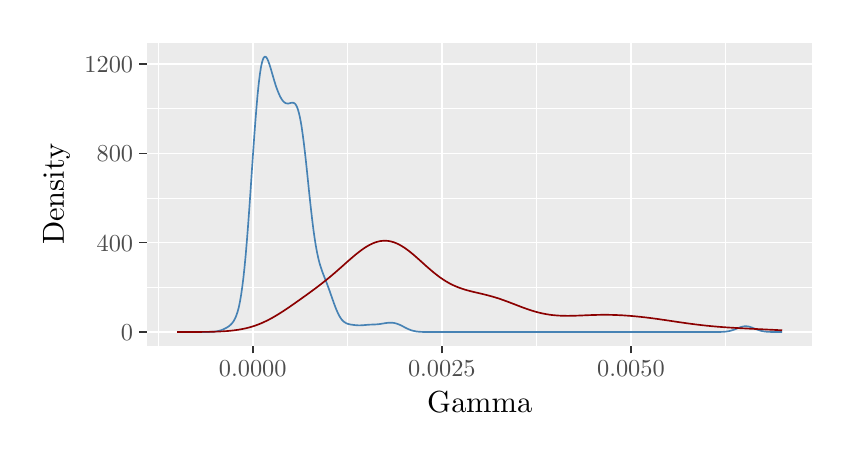
\begin{tikzpicture}[x=1pt,y=1pt]
\definecolor{fillColor}{RGB}{255,255,255}
\path[use as bounding box,fill=fillColor,fill opacity=0.00] (0,0) rectangle (289.08,144.54);
\begin{scope}
\path[clip] (  0.00,  0.00) rectangle (289.08,144.54);
\definecolor{drawColor}{RGB}{255,255,255}
\definecolor{fillColor}{RGB}{255,255,255}

\path[draw=drawColor,line width= 0.6pt,line join=round,line cap=round,fill=fillColor] (  0.00,  0.00) rectangle (289.08,144.54);
\end{scope}
\begin{scope}
\path[clip] ( 43.07, 29.59) rectangle (283.58,139.04);
\definecolor{fillColor}{gray}{0.92}

\path[fill=fillColor] ( 43.07, 29.59) rectangle (283.58,139.04);
\definecolor{drawColor}{RGB}{255,255,255}

\path[draw=drawColor,line width= 0.3pt,line join=round] ( 43.07, 50.70) --
	(283.58, 50.70);

\path[draw=drawColor,line width= 0.3pt,line join=round] ( 43.07, 82.99) --
	(283.58, 82.99);

\path[draw=drawColor,line width= 0.3pt,line join=round] ( 43.07,115.28) --
	(283.58,115.28);

\path[draw=drawColor,line width= 0.3pt,line join=round] ( 47.17, 29.59) --
	( 47.17,139.04);

\path[draw=drawColor,line width= 0.3pt,line join=round] (115.49, 29.59) --
	(115.49,139.04);

\path[draw=drawColor,line width= 0.3pt,line join=round] (183.82, 29.59) --
	(183.82,139.04);

\path[draw=drawColor,line width= 0.3pt,line join=round] (252.15, 29.59) --
	(252.15,139.04);

\path[draw=drawColor,line width= 0.6pt,line join=round] ( 43.07, 34.56) --
	(283.58, 34.56);

\path[draw=drawColor,line width= 0.6pt,line join=round] ( 43.07, 66.85) --
	(283.58, 66.85);

\path[draw=drawColor,line width= 0.6pt,line join=round] ( 43.07, 99.13) --
	(283.58, 99.13);

\path[draw=drawColor,line width= 0.6pt,line join=round] ( 43.07,131.42) --
	(283.58,131.42);

\path[draw=drawColor,line width= 0.6pt,line join=round] ( 81.33, 29.59) --
	( 81.33,139.04);

\path[draw=drawColor,line width= 0.6pt,line join=round] (149.66, 29.59) --
	(149.66,139.04);

\path[draw=drawColor,line width= 0.6pt,line join=round] (217.99, 29.59) --
	(217.99,139.04);
\definecolor{drawColor}{RGB}{70,130,180}

\path[draw=drawColor,line width= 0.6pt,line join=round] ( 54.00, 34.56) --
	( 54.43, 34.56) --
	( 54.85, 34.56) --
	( 55.28, 34.56) --
	( 55.71, 34.56) --
	( 56.14, 34.56) --
	( 56.57, 34.56) --
	( 56.99, 34.56) --
	( 57.42, 34.56) --
	( 57.85, 34.56) --
	( 58.28, 34.56) --
	( 58.70, 34.56) --
	( 59.13, 34.56) --
	( 59.56, 34.56) --
	( 59.99, 34.56) --
	( 60.42, 34.56) --
	( 60.84, 34.56) --
	( 61.27, 34.56) --
	( 61.70, 34.56) --
	( 62.13, 34.56) --
	( 62.56, 34.56) --
	( 62.98, 34.56) --
	( 63.41, 34.57) --
	( 63.84, 34.57) --
	( 64.27, 34.57) --
	( 64.70, 34.58) --
	( 65.12, 34.58) --
	( 65.55, 34.59) --
	( 65.98, 34.61) --
	( 66.41, 34.63) --
	( 66.83, 34.65) --
	( 67.26, 34.69) --
	( 67.69, 34.73) --
	( 68.12, 34.79) --
	( 68.55, 34.87) --
	( 68.97, 34.96) --
	( 69.40, 35.07) --
	( 69.83, 35.20) --
	( 70.26, 35.36) --
	( 70.69, 35.53) --
	( 71.11, 35.72) --
	( 71.54, 35.94) --
	( 71.97, 36.18) --
	( 72.40, 36.45) --
	( 72.83, 36.76) --
	( 73.25, 37.12) --
	( 73.68, 37.54) --
	( 74.11, 38.06) --
	( 74.54, 38.69) --
	( 74.96, 39.49) --
	( 75.39, 40.49) --
	( 75.82, 41.75) --
	( 76.25, 43.35) --
	( 76.68, 45.36) --
	( 77.10, 47.82) --
	( 77.53, 50.77) --
	( 77.96, 54.24) --
	( 78.39, 58.26) --
	( 78.82, 62.81) --
	( 79.24, 67.89) --
	( 79.67, 73.42) --
	( 80.10, 79.34) --
	( 80.53, 85.56) --
	( 80.95, 91.90) --
	( 81.38, 98.23) --
	( 81.81,104.38) --
	( 82.24,110.22) --
	( 82.67,115.61) --
	( 83.09,120.43) --
	( 83.52,124.59) --
	( 83.95,128.02) --
	( 84.38,130.69) --
	( 84.81,132.51) --
	( 85.23,133.61) --
	( 85.66,134.06) --
	( 86.09,133.96) --
	( 86.52,133.39) --
	( 86.95,132.45) --
	( 87.37,131.24) --
	( 87.80,129.86) --
	( 88.23,128.39) --
	( 88.66,126.90) --
	( 89.08,125.45) --
	( 89.51,124.07) --
	( 89.94,122.79) --
	( 90.37,121.63) --
	( 90.80,120.59) --
	( 91.22,119.68) --
	( 91.65,118.90) --
	( 92.08,118.27) --
	( 92.51,117.77) --
	( 92.94,117.43) --
	( 93.36,117.22) --
	( 93.79,117.14) --
	( 94.22,117.15) --
	( 94.65,117.23) --
	( 95.08,117.34) --
	( 95.50,117.42) --
	( 95.93,117.41) --
	( 96.36,117.25) --
	( 96.79,116.86) --
	( 97.21,116.13) --
	( 97.64,115.02) --
	( 98.07,113.50) --
	( 98.50,111.52) --
	( 98.93,109.09) --
	( 99.35,106.21) --
	( 99.78,102.93) --
	(100.21, 99.30) --
	(100.64, 95.39) --
	(101.07, 91.31) --
	(101.49, 87.16) --
	(101.92, 83.06) --
	(102.35, 79.11) --
	(102.78, 75.39) --
	(103.20, 71.96) --
	(103.63, 68.86) --
	(104.06, 66.11) --
	(104.49, 63.72) --
	(104.92, 61.66) --
	(105.34, 59.92) --
	(105.77, 58.43) --
	(106.20, 57.12) --
	(106.63, 55.93) --
	(107.06, 54.81) --
	(107.48, 53.72) --
	(107.91, 52.63) --
	(108.34, 51.51) --
	(108.77, 50.35) --
	(109.20, 49.16) --
	(109.62, 47.93) --
	(110.05, 46.70) --
	(110.48, 45.48) --
	(110.91, 44.30) --
	(111.33, 43.19) --
	(111.76, 42.16) --
	(112.19, 41.22) --
	(112.62, 40.39) --
	(113.05, 39.68) --
	(113.47, 39.08) --
	(113.90, 38.61) --
	(114.33, 38.23) --
	(114.76, 37.94) --
	(115.19, 37.71) --
	(115.61, 37.54) --
	(116.04, 37.42) --
	(116.47, 37.32) --
	(116.90, 37.24) --
	(117.33, 37.18) --
	(117.75, 37.12) --
	(118.18, 37.07) --
	(118.61, 37.03) --
	(119.04, 37.00) --
	(119.46, 36.98) --
	(119.89, 36.97) --
	(120.32, 36.98) --
	(120.75, 37.00) --
	(121.18, 37.02) --
	(121.60, 37.06) --
	(122.03, 37.10) --
	(122.46, 37.14) --
	(122.89, 37.17) --
	(123.32, 37.20) --
	(123.74, 37.23) --
	(124.17, 37.25) --
	(124.60, 37.26) --
	(125.03, 37.28) --
	(125.46, 37.29) --
	(125.88, 37.32) --
	(126.31, 37.35) --
	(126.74, 37.39) --
	(127.17, 37.44) --
	(127.59, 37.50) --
	(128.02, 37.57) --
	(128.45, 37.64) --
	(128.88, 37.71) --
	(129.31, 37.78) --
	(129.73, 37.84) --
	(130.16, 37.89) --
	(130.59, 37.93) --
	(131.02, 37.94) --
	(131.45, 37.93) --
	(131.87, 37.90) --
	(132.30, 37.84) --
	(132.73, 37.76) --
	(133.16, 37.65) --
	(133.58, 37.51) --
	(134.01, 37.35) --
	(134.44, 37.17) --
	(134.87, 36.97) --
	(135.30, 36.75) --
	(135.72, 36.53) --
	(136.15, 36.31) --
	(136.58, 36.09) --
	(137.01, 35.88) --
	(137.44, 35.67) --
	(137.86, 35.49) --
	(138.29, 35.32) --
	(138.72, 35.17) --
	(139.15, 35.05) --
	(139.58, 34.94) --
	(140.00, 34.85) --
	(140.43, 34.78) --
	(140.86, 34.72) --
	(141.29, 34.68) --
	(141.71, 34.65) --
	(142.14, 34.62) --
	(142.57, 34.60) --
	(143.00, 34.59) --
	(143.43, 34.58) --
	(143.85, 34.57) --
	(144.28, 34.57) --
	(144.71, 34.57) --
	(145.14, 34.56) --
	(145.57, 34.56) --
	(145.99, 34.56) --
	(146.42, 34.56) --
	(146.85, 34.56) --
	(147.28, 34.56) --
	(147.71, 34.56) --
	(148.13, 34.56) --
	(148.56, 34.56) --
	(148.99, 34.56) --
	(149.42, 34.56) --
	(149.84, 34.56) --
	(150.27, 34.56) --
	(150.70, 34.56) --
	(151.13, 34.56) --
	(151.56, 34.56) --
	(151.98, 34.56) --
	(152.41, 34.56) --
	(152.84, 34.56) --
	(153.27, 34.56) --
	(153.70, 34.56) --
	(154.12, 34.56) --
	(154.55, 34.56) --
	(154.98, 34.56) --
	(155.41, 34.56) --
	(155.83, 34.56) --
	(156.26, 34.56) --
	(156.69, 34.56) --
	(157.12, 34.56) --
	(157.55, 34.56) --
	(157.97, 34.56) --
	(158.40, 34.56) --
	(158.83, 34.56) --
	(159.26, 34.56) --
	(159.69, 34.56) --
	(160.11, 34.56) --
	(160.54, 34.56) --
	(160.97, 34.56) --
	(161.40, 34.56) --
	(161.83, 34.56) --
	(162.25, 34.56) --
	(162.68, 34.56) --
	(163.11, 34.56) --
	(163.54, 34.56) --
	(163.96, 34.56) --
	(164.39, 34.56) --
	(164.82, 34.56) --
	(165.25, 34.56) --
	(165.68, 34.56) --
	(166.10, 34.56) --
	(166.53, 34.56) --
	(166.96, 34.56) --
	(167.39, 34.56) --
	(167.82, 34.56) --
	(168.24, 34.56) --
	(168.67, 34.56) --
	(169.10, 34.56) --
	(169.53, 34.56) --
	(169.96, 34.56) --
	(170.38, 34.56) --
	(170.81, 34.56) --
	(171.24, 34.56) --
	(171.67, 34.56) --
	(172.09, 34.56) --
	(172.52, 34.56) --
	(172.95, 34.56) --
	(173.38, 34.56) --
	(173.81, 34.56) --
	(174.23, 34.56) --
	(174.66, 34.56) --
	(175.09, 34.56) --
	(175.52, 34.56) --
	(175.95, 34.56) --
	(176.37, 34.56) --
	(176.80, 34.56) --
	(177.23, 34.56) --
	(177.66, 34.56) --
	(178.08, 34.56) --
	(178.51, 34.56) --
	(178.94, 34.56) --
	(179.37, 34.56) --
	(179.80, 34.56) --
	(180.22, 34.56) --
	(180.65, 34.56) --
	(181.08, 34.56) --
	(181.51, 34.56) --
	(181.94, 34.56) --
	(182.36, 34.56) --
	(182.79, 34.56) --
	(183.22, 34.56) --
	(183.65, 34.56) --
	(184.08, 34.56) --
	(184.50, 34.56) --
	(184.93, 34.56) --
	(185.36, 34.56) --
	(185.79, 34.56) --
	(186.21, 34.56) --
	(186.64, 34.56) --
	(187.07, 34.56) --
	(187.50, 34.56) --
	(187.93, 34.56) --
	(188.35, 34.56) --
	(188.78, 34.56) --
	(189.21, 34.56) --
	(189.64, 34.56) --
	(190.07, 34.56) --
	(190.49, 34.56) --
	(190.92, 34.56) --
	(191.35, 34.56) --
	(191.78, 34.56) --
	(192.21, 34.56) --
	(192.63, 34.56) --
	(193.06, 34.56) --
	(193.49, 34.56) --
	(193.92, 34.56) --
	(194.34, 34.56) --
	(194.77, 34.56) --
	(195.20, 34.56) --
	(195.63, 34.56) --
	(196.06, 34.56) --
	(196.48, 34.56) --
	(196.91, 34.56) --
	(197.34, 34.56) --
	(197.77, 34.56) --
	(198.20, 34.56) --
	(198.62, 34.56) --
	(199.05, 34.56) --
	(199.48, 34.56) --
	(199.91, 34.56) --
	(200.33, 34.56) --
	(200.76, 34.56) --
	(201.19, 34.56) --
	(201.62, 34.56) --
	(202.05, 34.56) --
	(202.47, 34.56) --
	(202.90, 34.56) --
	(203.33, 34.56) --
	(203.76, 34.56) --
	(204.19, 34.56) --
	(204.61, 34.56) --
	(205.04, 34.56) --
	(205.47, 34.56) --
	(205.90, 34.56) --
	(206.33, 34.56) --
	(206.75, 34.56) --
	(207.18, 34.56) --
	(207.61, 34.56) --
	(208.04, 34.56) --
	(208.46, 34.56) --
	(208.89, 34.56) --
	(209.32, 34.56) --
	(209.75, 34.56) --
	(210.18, 34.56) --
	(210.60, 34.56) --
	(211.03, 34.56) --
	(211.46, 34.56) --
	(211.89, 34.56) --
	(212.32, 34.56) --
	(212.74, 34.56) --
	(213.17, 34.56) --
	(213.60, 34.56) --
	(214.03, 34.56) --
	(214.46, 34.56) --
	(214.88, 34.56) --
	(215.31, 34.56) --
	(215.74, 34.56) --
	(216.17, 34.56) --
	(216.59, 34.56) --
	(217.02, 34.56) --
	(217.45, 34.56) --
	(217.88, 34.56) --
	(218.31, 34.56) --
	(218.73, 34.56) --
	(219.16, 34.56) --
	(219.59, 34.56) --
	(220.02, 34.56) --
	(220.45, 34.56) --
	(220.87, 34.56) --
	(221.30, 34.56) --
	(221.73, 34.56) --
	(222.16, 34.56) --
	(222.58, 34.56) --
	(223.01, 34.56) --
	(223.44, 34.56) --
	(223.87, 34.56) --
	(224.30, 34.56) --
	(224.72, 34.56) --
	(225.15, 34.56) --
	(225.58, 34.56) --
	(226.01, 34.56) --
	(226.44, 34.56) --
	(226.86, 34.56) --
	(227.29, 34.56) --
	(227.72, 34.56) --
	(228.15, 34.56) --
	(228.58, 34.56) --
	(229.00, 34.56) --
	(229.43, 34.56) --
	(229.86, 34.56) --
	(230.29, 34.56) --
	(230.71, 34.56) --
	(231.14, 34.56) --
	(231.57, 34.56) --
	(232.00, 34.56) --
	(232.43, 34.56) --
	(232.85, 34.56) --
	(233.28, 34.56) --
	(233.71, 34.56) --
	(234.14, 34.56) --
	(234.57, 34.56) --
	(234.99, 34.56) --
	(235.42, 34.56) --
	(235.85, 34.56) --
	(236.28, 34.56) --
	(236.71, 34.56) --
	(237.13, 34.56) --
	(237.56, 34.56) --
	(237.99, 34.56) --
	(238.42, 34.56) --
	(238.84, 34.56) --
	(239.27, 34.56) --
	(239.70, 34.56) --
	(240.13, 34.56) --
	(240.56, 34.56) --
	(240.98, 34.56) --
	(241.41, 34.56) --
	(241.84, 34.56) --
	(242.27, 34.56) --
	(242.70, 34.56) --
	(243.12, 34.56) --
	(243.55, 34.56) --
	(243.98, 34.56) --
	(244.41, 34.56) --
	(244.83, 34.56) --
	(245.26, 34.56) --
	(245.69, 34.56) --
	(246.12, 34.56) --
	(246.55, 34.56) --
	(246.97, 34.56) --
	(247.40, 34.56) --
	(247.83, 34.56) --
	(248.26, 34.57) --
	(248.69, 34.57) --
	(249.11, 34.57) --
	(249.54, 34.58) --
	(249.97, 34.58) --
	(250.40, 34.59) --
	(250.83, 34.61) --
	(251.25, 34.63) --
	(251.68, 34.66) --
	(252.11, 34.70) --
	(252.54, 34.75) --
	(252.96, 34.81) --
	(253.39, 34.89) --
	(253.82, 34.98) --
	(254.25, 35.09) --
	(254.68, 35.22) --
	(255.10, 35.36) --
	(255.53, 35.52) --
	(255.96, 35.69) --
	(256.39, 35.86) --
	(256.82, 36.03) --
	(257.24, 36.19) --
	(257.67, 36.34) --
	(258.10, 36.46) --
	(258.53, 36.56) --
	(258.96, 36.63) --
	(259.38, 36.65) --
	(259.81, 36.64) --
	(260.24, 36.59) --
	(260.67, 36.50) --
	(261.09, 36.39) --
	(261.52, 36.25) --
	(261.95, 36.09) --
	(262.38, 35.92) --
	(262.81, 35.75) --
	(263.23, 35.58) --
	(263.66, 35.42) --
	(264.09, 35.27) --
	(264.52, 35.14) --
	(264.95, 35.02) --
	(265.37, 34.92) --
	(265.80, 34.84) --
	(266.23, 34.77) --
	(266.66, 34.71) --
	(267.09, 34.67) --
	(267.51, 34.64) --
	(267.94, 34.62) --
	(268.37, 34.60) --
	(268.80, 34.59) --
	(269.22, 34.58) --
	(269.65, 34.57) --
	(270.08, 34.57) --
	(270.51, 34.57) --
	(270.94, 34.56) --
	(271.36, 34.56) --
	(271.79, 34.56) --
	(272.22, 34.56) --
	(272.65, 34.56);
\definecolor{drawColor}{RGB}{139,0,0}

\path[draw=drawColor,line width= 0.6pt,line join=round] ( 54.00, 34.56) --
	( 54.43, 34.56) --
	( 54.85, 34.56) --
	( 55.28, 34.56) --
	( 55.71, 34.57) --
	( 56.14, 34.57) --
	( 56.57, 34.57) --
	( 56.99, 34.57) --
	( 57.42, 34.57) --
	( 57.85, 34.57) --
	( 58.28, 34.57) --
	( 58.70, 34.57) --
	( 59.13, 34.57) --
	( 59.56, 34.57) --
	( 59.99, 34.58) --
	( 60.42, 34.58) --
	( 60.84, 34.58) --
	( 61.27, 34.58) --
	( 61.70, 34.59) --
	( 62.13, 34.59) --
	( 62.56, 34.59) --
	( 62.98, 34.60) --
	( 63.41, 34.60) --
	( 63.84, 34.61) --
	( 64.27, 34.61) --
	( 64.70, 34.62) --
	( 65.12, 34.63) --
	( 65.55, 34.63) --
	( 65.98, 34.64) --
	( 66.41, 34.65) --
	( 66.83, 34.66) --
	( 67.26, 34.68) --
	( 67.69, 34.69) --
	( 68.12, 34.70) --
	( 68.55, 34.72) --
	( 68.97, 34.74) --
	( 69.40, 34.76) --
	( 69.83, 34.78) --
	( 70.26, 34.80) --
	( 70.69, 34.82) --
	( 71.11, 34.85) --
	( 71.54, 34.88) --
	( 71.97, 34.91) --
	( 72.40, 34.95) --
	( 72.83, 34.98) --
	( 73.25, 35.03) --
	( 73.68, 35.07) --
	( 74.11, 35.12) --
	( 74.54, 35.17) --
	( 74.96, 35.22) --
	( 75.39, 35.28) --
	( 75.82, 35.34) --
	( 76.25, 35.41) --
	( 76.68, 35.48) --
	( 77.10, 35.56) --
	( 77.53, 35.64) --
	( 77.96, 35.72) --
	( 78.39, 35.81) --
	( 78.82, 35.91) --
	( 79.24, 36.01) --
	( 79.67, 36.12) --
	( 80.10, 36.24) --
	( 80.53, 36.36) --
	( 80.95, 36.48) --
	( 81.38, 36.61) --
	( 81.81, 36.75) --
	( 82.24, 36.90) --
	( 82.67, 37.05) --
	( 83.09, 37.21) --
	( 83.52, 37.37) --
	( 83.95, 37.54) --
	( 84.38, 37.72) --
	( 84.81, 37.91) --
	( 85.23, 38.10) --
	( 85.66, 38.30) --
	( 86.09, 38.50) --
	( 86.52, 38.71) --
	( 86.95, 38.93) --
	( 87.37, 39.15) --
	( 87.80, 39.38) --
	( 88.23, 39.61) --
	( 88.66, 39.85) --
	( 89.08, 40.10) --
	( 89.51, 40.35) --
	( 89.94, 40.60) --
	( 90.37, 40.86) --
	( 90.80, 41.13) --
	( 91.22, 41.40) --
	( 91.65, 41.67) --
	( 92.08, 41.94) --
	( 92.51, 42.22) --
	( 92.94, 42.50) --
	( 93.36, 42.79) --
	( 93.79, 43.08) --
	( 94.22, 43.37) --
	( 94.65, 43.66) --
	( 95.08, 43.95) --
	( 95.50, 44.25) --
	( 95.93, 44.55) --
	( 96.36, 44.85) --
	( 96.79, 45.15) --
	( 97.21, 45.45) --
	( 97.64, 45.75) --
	( 98.07, 46.05) --
	( 98.50, 46.36) --
	( 98.93, 46.66) --
	( 99.35, 46.97) --
	( 99.78, 47.28) --
	(100.21, 47.58) --
	(100.64, 47.89) --
	(101.07, 48.20) --
	(101.49, 48.51) --
	(101.92, 48.82) --
	(102.35, 49.13) --
	(102.78, 49.45) --
	(103.20, 49.77) --
	(103.63, 50.08) --
	(104.06, 50.40) --
	(104.49, 50.72) --
	(104.92, 51.05) --
	(105.34, 51.37) --
	(105.77, 51.70) --
	(106.20, 52.04) --
	(106.63, 52.37) --
	(107.06, 52.71) --
	(107.48, 53.05) --
	(107.91, 53.39) --
	(108.34, 53.74) --
	(108.77, 54.09) --
	(109.20, 54.45) --
	(109.62, 54.80) --
	(110.05, 55.16) --
	(110.48, 55.53) --
	(110.91, 55.89) --
	(111.33, 56.26) --
	(111.76, 56.63) --
	(112.19, 57.01) --
	(112.62, 57.39) --
	(113.05, 57.76) --
	(113.47, 58.14) --
	(113.90, 58.52) --
	(114.33, 58.90) --
	(114.76, 59.29) --
	(115.19, 59.67) --
	(115.61, 60.05) --
	(116.04, 60.42) --
	(116.47, 60.80) --
	(116.90, 61.17) --
	(117.33, 61.54) --
	(117.75, 61.90) --
	(118.18, 62.26) --
	(118.61, 62.62) --
	(119.04, 62.96) --
	(119.46, 63.30) --
	(119.89, 63.63) --
	(120.32, 63.96) --
	(120.75, 64.27) --
	(121.18, 64.57) --
	(121.60, 64.87) --
	(122.03, 65.15) --
	(122.46, 65.41) --
	(122.89, 65.67) --
	(123.32, 65.91) --
	(123.74, 66.14) --
	(124.17, 66.35) --
	(124.60, 66.55) --
	(125.03, 66.72) --
	(125.46, 66.89) --
	(125.88, 67.04) --
	(126.31, 67.16) --
	(126.74, 67.27) --
	(127.17, 67.37) --
	(127.59, 67.44) --
	(128.02, 67.49) --
	(128.45, 67.53) --
	(128.88, 67.55) --
	(129.31, 67.54) --
	(129.73, 67.52) --
	(130.16, 67.48) --
	(130.59, 67.42) --
	(131.02, 67.34) --
	(131.45, 67.24) --
	(131.87, 67.12) --
	(132.30, 66.99) --
	(132.73, 66.83) --
	(133.16, 66.66) --
	(133.58, 66.47) --
	(134.01, 66.26) --
	(134.44, 66.04) --
	(134.87, 65.81) --
	(135.30, 65.55) --
	(135.72, 65.28) --
	(136.15, 65.00) --
	(136.58, 64.71) --
	(137.01, 64.40) --
	(137.44, 64.08) --
	(137.86, 63.76) --
	(138.29, 63.42) --
	(138.72, 63.07) --
	(139.15, 62.72) --
	(139.58, 62.35) --
	(140.00, 61.98) --
	(140.43, 61.61) --
	(140.86, 61.23) --
	(141.29, 60.85) --
	(141.71, 60.47) --
	(142.14, 60.08) --
	(142.57, 59.70) --
	(143.00, 59.31) --
	(143.43, 58.92) --
	(143.85, 58.54) --
	(144.28, 58.16) --
	(144.71, 57.78) --
	(145.14, 57.41) --
	(145.57, 57.04) --
	(145.99, 56.68) --
	(146.42, 56.32) --
	(146.85, 55.97) --
	(147.28, 55.62) --
	(147.71, 55.29) --
	(148.13, 54.96) --
	(148.56, 54.63) --
	(148.99, 54.32) --
	(149.42, 54.02) --
	(149.84, 53.73) --
	(150.27, 53.44) --
	(150.70, 53.17) --
	(151.13, 52.90) --
	(151.56, 52.65) --
	(151.98, 52.40) --
	(152.41, 52.17) --
	(152.84, 51.94) --
	(153.27, 51.73) --
	(153.70, 51.52) --
	(154.12, 51.32) --
	(154.55, 51.13) --
	(154.98, 50.95) --
	(155.41, 50.78) --
	(155.83, 50.61) --
	(156.26, 50.45) --
	(156.69, 50.30) --
	(157.12, 50.16) --
	(157.55, 50.02) --
	(157.97, 49.89) --
	(158.40, 49.76) --
	(158.83, 49.64) --
	(159.26, 49.53) --
	(159.69, 49.41) --
	(160.11, 49.30) --
	(160.54, 49.20) --
	(160.97, 49.09) --
	(161.40, 48.99) --
	(161.83, 48.89) --
	(162.25, 48.79) --
	(162.68, 48.69) --
	(163.11, 48.59) --
	(163.54, 48.49) --
	(163.96, 48.39) --
	(164.39, 48.29) --
	(164.82, 48.19) --
	(165.25, 48.08) --
	(165.68, 47.97) --
	(166.10, 47.86) --
	(166.53, 47.75) --
	(166.96, 47.64) --
	(167.39, 47.52) --
	(167.82, 47.40) --
	(168.24, 47.28) --
	(168.67, 47.15) --
	(169.10, 47.02) --
	(169.53, 46.89) --
	(169.96, 46.75) --
	(170.38, 46.61) --
	(170.81, 46.47) --
	(171.24, 46.32) --
	(171.67, 46.17) --
	(172.09, 46.02) --
	(172.52, 45.86) --
	(172.95, 45.71) --
	(173.38, 45.55) --
	(173.81, 45.39) --
	(174.23, 45.23) --
	(174.66, 45.06) --
	(175.09, 44.90) --
	(175.52, 44.73) --
	(175.95, 44.57) --
	(176.37, 44.40) --
	(176.80, 44.23) --
	(177.23, 44.07) --
	(177.66, 43.91) --
	(178.08, 43.74) --
	(178.51, 43.58) --
	(178.94, 43.42) --
	(179.37, 43.26) --
	(179.80, 43.11) --
	(180.22, 42.96) --
	(180.65, 42.81) --
	(181.08, 42.66) --
	(181.51, 42.52) --
	(181.94, 42.38) --
	(182.36, 42.25) --
	(182.79, 42.12) --
	(183.22, 41.99) --
	(183.65, 41.87) --
	(184.08, 41.75) --
	(184.50, 41.64) --
	(184.93, 41.53) --
	(185.36, 41.43) --
	(185.79, 41.33) --
	(186.21, 41.24) --
	(186.64, 41.16) --
	(187.07, 41.07) --
	(187.50, 41.00) --
	(187.93, 40.93) --
	(188.35, 40.86) --
	(188.78, 40.80) --
	(189.21, 40.74) --
	(189.64, 40.69) --
	(190.07, 40.65) --
	(190.49, 40.61) --
	(190.92, 40.57) --
	(191.35, 40.54) --
	(191.78, 40.51) --
	(192.21, 40.48) --
	(192.63, 40.46) --
	(193.06, 40.44) --
	(193.49, 40.43) --
	(193.92, 40.42) --
	(194.34, 40.42) --
	(194.77, 40.41) --
	(195.20, 40.41) --
	(195.63, 40.41) --
	(196.06, 40.42) --
	(196.48, 40.43) --
	(196.91, 40.43) --
	(197.34, 40.45) --
	(197.77, 40.46) --
	(198.20, 40.47) --
	(198.62, 40.49) --
	(199.05, 40.50) --
	(199.48, 40.52) --
	(199.91, 40.54) --
	(200.33, 40.55) --
	(200.76, 40.57) --
	(201.19, 40.59) --
	(201.62, 40.61) --
	(202.05, 40.63) --
	(202.47, 40.64) --
	(202.90, 40.66) --
	(203.33, 40.68) --
	(203.76, 40.69) --
	(204.19, 40.71) --
	(204.61, 40.72) --
	(205.04, 40.73) --
	(205.47, 40.74) --
	(205.90, 40.75) --
	(206.33, 40.76) --
	(206.75, 40.77) --
	(207.18, 40.78) --
	(207.61, 40.78) --
	(208.04, 40.78) --
	(208.46, 40.78) --
	(208.89, 40.78) --
	(209.32, 40.78) --
	(209.75, 40.78) --
	(210.18, 40.77) --
	(210.60, 40.76) --
	(211.03, 40.76) --
	(211.46, 40.74) --
	(211.89, 40.73) --
	(212.32, 40.72) --
	(212.74, 40.70) --
	(213.17, 40.68) --
	(213.60, 40.66) --
	(214.03, 40.64) --
	(214.46, 40.62) --
	(214.88, 40.60) --
	(215.31, 40.57) --
	(215.74, 40.54) --
	(216.17, 40.51) --
	(216.59, 40.48) --
	(217.02, 40.45) --
	(217.45, 40.42) --
	(217.88, 40.38) --
	(218.31, 40.35) --
	(218.73, 40.31) --
	(219.16, 40.27) --
	(219.59, 40.23) --
	(220.02, 40.19) --
	(220.45, 40.15) --
	(220.87, 40.10) --
	(221.30, 40.06) --
	(221.73, 40.01) --
	(222.16, 39.96) --
	(222.58, 39.92) --
	(223.01, 39.87) --
	(223.44, 39.82) --
	(223.87, 39.76) --
	(224.30, 39.71) --
	(224.72, 39.66) --
	(225.15, 39.60) --
	(225.58, 39.55) --
	(226.01, 39.49) --
	(226.44, 39.43) --
	(226.86, 39.37) --
	(227.29, 39.32) --
	(227.72, 39.26) --
	(228.15, 39.20) --
	(228.58, 39.13) --
	(229.00, 39.07) --
	(229.43, 39.01) --
	(229.86, 38.95) --
	(230.29, 38.89) --
	(230.71, 38.82) --
	(231.14, 38.76) --
	(231.57, 38.70) --
	(232.00, 38.63) --
	(232.43, 38.57) --
	(232.85, 38.50) --
	(233.28, 38.44) --
	(233.71, 38.38) --
	(234.14, 38.31) --
	(234.57, 38.25) --
	(234.99, 38.19) --
	(235.42, 38.12) --
	(235.85, 38.06) --
	(236.28, 38.00) --
	(236.71, 37.94) --
	(237.13, 37.88) --
	(237.56, 37.82) --
	(237.99, 37.76) --
	(238.42, 37.70) --
	(238.84, 37.64) --
	(239.27, 37.58) --
	(239.70, 37.52) --
	(240.13, 37.47) --
	(240.56, 37.41) --
	(240.98, 37.36) --
	(241.41, 37.30) --
	(241.84, 37.25) --
	(242.27, 37.20) --
	(242.70, 37.15) --
	(243.12, 37.10) --
	(243.55, 37.05) --
	(243.98, 37.00) --
	(244.41, 36.96) --
	(244.83, 36.91) --
	(245.26, 36.86) --
	(245.69, 36.82) --
	(246.12, 36.78) --
	(246.55, 36.74) --
	(246.97, 36.69) --
	(247.40, 36.65) --
	(247.83, 36.61) --
	(248.26, 36.58) --
	(248.69, 36.54) --
	(249.11, 36.50) --
	(249.54, 36.47) --
	(249.97, 36.43) --
	(250.40, 36.40) --
	(250.83, 36.37) --
	(251.25, 36.33) --
	(251.68, 36.30) --
	(252.11, 36.27) --
	(252.54, 36.24) --
	(252.96, 36.21) --
	(253.39, 36.18) --
	(253.82, 36.16) --
	(254.25, 36.13) --
	(254.68, 36.10) --
	(255.10, 36.08) --
	(255.53, 36.05) --
	(255.96, 36.03) --
	(256.39, 36.00) --
	(256.82, 35.98) --
	(257.24, 35.96) --
	(257.67, 35.93) --
	(258.10, 35.91) --
	(258.53, 35.89) --
	(258.96, 35.87) --
	(259.38, 35.84) --
	(259.81, 35.82) --
	(260.24, 35.80) --
	(260.67, 35.78) --
	(261.09, 35.76) --
	(261.52, 35.74) --
	(261.95, 35.72) --
	(262.38, 35.70) --
	(262.81, 35.67) --
	(263.23, 35.65) --
	(263.66, 35.63) --
	(264.09, 35.61) --
	(264.52, 35.59) --
	(264.95, 35.57) --
	(265.37, 35.55) --
	(265.80, 35.53) --
	(266.23, 35.51) --
	(266.66, 35.49) --
	(267.09, 35.46) --
	(267.51, 35.44) --
	(267.94, 35.42) --
	(268.37, 35.40) --
	(268.80, 35.38) --
	(269.22, 35.36) --
	(269.65, 35.34) --
	(270.08, 35.31) --
	(270.51, 35.29) --
	(270.94, 35.27) --
	(271.36, 35.25) --
	(271.79, 35.23) --
	(272.22, 35.21) --
	(272.65, 35.19);
\end{scope}
\begin{scope}
\path[clip] (  0.00,  0.00) rectangle (289.08,144.54);
\definecolor{drawColor}{gray}{0.30}

\node[text=drawColor,anchor=base east,inner sep=0pt, outer sep=0pt, scale=  0.88] at ( 38.12, 31.53) {0};

\node[text=drawColor,anchor=base east,inner sep=0pt, outer sep=0pt, scale=  0.88] at ( 38.12, 63.82) {400};

\node[text=drawColor,anchor=base east,inner sep=0pt, outer sep=0pt, scale=  0.88] at ( 38.12, 96.10) {800};

\node[text=drawColor,anchor=base east,inner sep=0pt, outer sep=0pt, scale=  0.88] at ( 38.12,128.39) {1200};
\end{scope}
\begin{scope}
\path[clip] (  0.00,  0.00) rectangle (289.08,144.54);
\definecolor{drawColor}{gray}{0.20}

\path[draw=drawColor,line width= 0.6pt,line join=round] ( 40.32, 34.56) --
	( 43.07, 34.56);

\path[draw=drawColor,line width= 0.6pt,line join=round] ( 40.32, 66.85) --
	( 43.07, 66.85);

\path[draw=drawColor,line width= 0.6pt,line join=round] ( 40.32, 99.13) --
	( 43.07, 99.13);

\path[draw=drawColor,line width= 0.6pt,line join=round] ( 40.32,131.42) --
	( 43.07,131.42);
\end{scope}
\begin{scope}
\path[clip] (  0.00,  0.00) rectangle (289.08,144.54);
\definecolor{drawColor}{gray}{0.20}

\path[draw=drawColor,line width= 0.6pt,line join=round] ( 81.33, 26.84) --
	( 81.33, 29.59);

\path[draw=drawColor,line width= 0.6pt,line join=round] (149.66, 26.84) --
	(149.66, 29.59);

\path[draw=drawColor,line width= 0.6pt,line join=round] (217.99, 26.84) --
	(217.99, 29.59);
\end{scope}
\begin{scope}
\path[clip] (  0.00,  0.00) rectangle (289.08,144.54);
\definecolor{drawColor}{gray}{0.30}

\node[text=drawColor,anchor=base,inner sep=0pt, outer sep=0pt, scale=  0.88] at ( 81.33, 18.58) {0.0000};

\node[text=drawColor,anchor=base,inner sep=0pt, outer sep=0pt, scale=  0.88] at (149.66, 18.58) {0.0025};

\node[text=drawColor,anchor=base,inner sep=0pt, outer sep=0pt, scale=  0.88] at (217.99, 18.58) {0.0050};
\end{scope}
\begin{scope}
\path[clip] (  0.00,  0.00) rectangle (289.08,144.54);
\definecolor{drawColor}{RGB}{0,0,0}

\node[text=drawColor,anchor=base,inner sep=0pt, outer sep=0pt, scale=  1.10] at (163.32,  5.50) {Gamma};
\end{scope}
\begin{scope}
\path[clip] (  0.00,  0.00) rectangle (289.08,144.54);
\definecolor{drawColor}{RGB}{0,0,0}

\node[text=drawColor,rotate= 90.00,anchor=base,inner sep=0pt, outer sep=0pt, scale=  1.10] at ( 13.08, 84.31) {Density};
\end{scope}
\end{tikzpicture}

  % \rule{40mm}{20mm}
  \caption{Distributions of gamma for in-the-money vs out-of-the-money options}
    %
  % BEGIN OF FLOATNOTE
  %
  \begin{changemargin}{0.5cm}{0.5cm}
  \medskip
\footnotesize
\setstretch{1.0}\textbf{Notes.} The above densities have been constructed by means of the function \textit{hsv\_gamma}, with the following parameters $V(0) = 0.03798218$, $\theta = 0.04871543$, $\sigma = 0.50378803$, $\rho = -0.39877827$, $\kappa = 4.00105546$. the blue density represents the distribution of a sample of gamma for in-the-money options with $K = 140$, while the red one gives the distibution of out-of-the-money options' gamma with $K = 230$.
  \end{changemargin}
  %
  % END OF FLOATNOTE
  %
  \label{p:analysis:hsv:gamma}
\end{figure}













%%%%%%%%%%%%%%%%%%%%%%%%
% delta vs delta heston
%%%%%%%%%%%%%%%%%%%%%%%%%%%%%%%%%%

\Cref{p:analysis:hsv:pl:dist:deltas} (appendix \ref{cha:appendanalysis:plot}) shows the distribution of the P\&Ls when the hedging is built either with BSM or HSV deltas. The red density curve concerns the data related to BSM deltas while the green represents the distributions of the performance's metrics for the HSV delta-hedging.
No real trend emerges on the hedging portfolio whether using the HSV or BSM-related delta, except for the hedge of the at-the-money options where the delta BSM implies higher values for the delta-neutral hedging portfolios.
Nonetheless, let us dive more deeply into those delta-hedging strategies by observing what happens behind the scenes.

\Cref{p:analysis:hsv:hedge:deltas} (appendix \ref{cha:appendanalysis:plot}) illustrates how the delta-hedging works depending on the strike price and computed delta.
The circles represent the replicated portfolios at each rebalancing time, whereas the underpinned black lines are the courses of the options' values as time passes.
The blue and red circles respectively stand for the HSV and BSM delta-hedging portfolios' values.

% 



Concerning options in-the-market, \cref{p:analysis:hsv:hedge:deltas} shows that the delta-neutral portfolios with delta BSM outperform those driven by a delta HSV, while the opposite claim is applicable for the hedging portfolios of out-of-the-market calls.
The conclusion of the previous statement is not that delta BSM is "better"\footnote{the words "better" and "wore" are between quotes because those qualifiers would rather be applicable for a speculative analysis than a hedging one.} than delta HSV when hedging low strikes European calls or "wore" for high strikes ones, but it actually shows that delta BSM lacks sensitivity.
Indeed, for options in-the-money, it tends to fastly achieve values near to one while it dramatically drops to zero for out-of-the-money calls.
Therefore as the delta-hedging for the replication of long calls is a "buy high, sell low" strategy, it explains why the hedging of in-the-money options makes the BSM delta-neutral portfolios more valued than the HSV, at maturity. 
Moreover, due to a slow to start delta with a value staying longer to zero, the hedging with BSM is delayed for out-of-the-money calls, letting the BSM delta-neutral portfolios taking advantage of the purchase of a low priced assets at a time near zero, for which the return exceeds that of the money market portfolios initially set up.
To conclude, to replicate a position in a European call, delta HSV would preferably be used, concerning that case examined in this master thesis.






\chapter{Conclusion}
\label{cha:conclusion}


The general approach pursued along the current master thesis was intended to measure the performance of the Black-Scholes-Merton (BSM) pricing method by exploring what could happen away of the assumptions of log-normal density for the underlying returns and beyond the simple case of a deterministic volatility drift.
In order to overcome the limitations mentioned above, some others model have therefore been explored, namely,  the Merton jump-diffusion (MJD) and Heston stochastic volatility (HSV).

In order to perform such an analysis, the work was split into two pieces. First was assessed the performances of BSM, MJD, and HSV by analyzing the options prices generated by the theoretical models in comparison with those observed from market data. 
Next, in a second stage, the hedging performances were measured through replication portfolios by using, in turn, each model to create and rebalance them.

It was observed that with the immutable value taken by its uncertainty parameter, the BSM model lacks in reproducing the volatility surfaces observed in the market and de facto the so associated options' prices.
On the other hand, if the MJD and HSV models are appropriately calibrated, they can reproduce the whole diversity of market options prices and therefore match relatively well to the computed volatility surfaces. 
Nevertheless, a difficulty arises if one wants to assess the options prices by using HSV or MJD from scratch. Indeed, to compute them one should calibrate the model and in order to adjust the parameters of the model, one a priori needs the options prices to do so. 

The empirical study shows that in a log-normal wold if one uses the BSM model, and provided that a geometric Brownian motion drive the underlying asset process, the hedging performance is almost perfect for a delta-neutral portfolio as long as the rebalancing is frequently done.

The analysis illustrated that for both MJD and HSV a higher rebalancing rate and a farther time to maturity have a positive effect on the performances of the delta-hedges. It should be noted that the effects of gamma and theta are not negligible on the hedges of deep-out-of-the-money options which systematically underperform those of [deep]-in|at-the-money.
However, a possible bias against the study is that the gamma effect on out-of-the-money options' delta hedging could be unusually high in the case at hand due to the underlying asset growth rate particularly steep.

Furthermore, the study shows that it exists a significant performance discrepancy for the replication portfolios of HSV options by either using the appropriate delta or the BSM one to balance them.  
It turns out that the hedging is less performing when using BSM delta together with an HSV process as the underlying asset.
Whilst no notable difference has been noticed when hedging with BSM or MJD delta for the MJD model.

Although the differences are not large enough when comparing the delta-hedging performance for in-the-money options, the results show that the MJD model beats the HSV by providing lower relative profits and losses values for the coverage of options out-of-the-money.
However, an interesting analysis could be to measure up to what extent the hedgings of options based on MJD underlying process outperform those that relate to HSV, for instance by reducing the frequency of jumps but increasing their intensity.

The study performed in that master thesis aimed to compute prices of options faithfully and to reproduce as closely as possible fictive but reliable time-series to conduct hedging strategies.
However, the resultant analysis is somehow restrictive since it is only based on the hedge of options on a unique underlying with high growth potential and is, therefore, not extensive enough to decipher broader trends.
Nevertheless, as the purposely developed algorithms are rather versatile, they can be adapted for the computation of delta-hedges of other options with different underlying and characteristics.




\bibliography{bibl}
\bibliographystyle{plainnat}
\addcontentsline{toc}{chapter}{Bibliography}

\begin{appendices}
\chapter{Functions catalogue}
\label{cha:append:function}

% For this master thesis, I created two R packages to help me in the analysis and in the related experiments. These packages are available, under open-source software license, through my GitHub account. Names are ”Random walk”  (https://github.com/AnthonyTedde/RandomWalk) and ”Stock price simulator” (https://github.com/AnthonyTedde/StockPriceSimulator).
% 
% The R package ”Random walk” contains functions that simulate time-discretized Brownian motions. It is widely used inside ”Stock price simulator”, mainly to add noise in the simulation of stock price time series.
% 
% Unlike "Random walk", the package "Stock price simulator" is more multipurpose. The algorithms I developed inside range from the simulation of stock price path to the computation of option fair price and include hedging strategies, Greeks computation, Itô's approximation, characteristic functions and so on.
% 
% \Cref{sec:r:time} describes the functions inside the ”Stock price simulator” package that simulate time series by using a time discretization approximation.


\begin{table}[ht]
  \begin{tabularx}{\textwidth}{llX}
    \hline
    Function name & Arguments & Purpose \\
    \hline
    bsm\_call & $\left \{ S(0), T, k, r, \sigma \right \}$ & Compute the BSM price of an option \\
    mjd\_call & $\left \{ S(0), T, k, r, \lambda, \mu, \delta \sigma \right \}$ & Compute the Merton price of an option \\
    hsv\_call & $\left \{ S(0), T, k, r, V(0), \theta, \kappa, \sigma, \rho \right \}$ & Compute the heston price of an option \\
    bsm\_delta & $\left \{ S(0), T, k, r, \sigma \right \}$ & Compute the BSM delta of an option \\
    mjd\_delta & $\left \{ S(0), T, k, r, \lambda, \mu, \delta \sigma \right \}$ & Compute the Merton delta of an option \\
    hsv\_delta & $\left \{ S(0), T, k, r, V(0), \theta, \kappa, \sigma, \rho \right \}$ & Compute the heston delta of an option \\
    bsm\_gamma & $\left \{ S(0), T, k, r, \sigma \right \}$ & Compute the BSM gamma of an option \\
    mjd\_gamma & $\left \{ S(0), T, k, r, \lambda, \mu, \delta \sigma \right \}$ & Compute the Merton gamma of an option \\
    hsv\_gamma & $\left \{ S(0), T, k, r, V(0), \theta, \kappa, \sigma, \rho \right \}$ & Compute the heston gamma of an option \\
    bsm\_theta & $\left \{ S(0), T, k, r, \sigma \right \}$ & Compute the BSM theta of an option \\
    mjd\_theta & $\left \{ S(0), T, k, r, \lambda, \mu, \delta \sigma \right \}$ & Compute the Merton theta of an option \\
    hsv\_theta & $\left \{ S(0), T, k, r, V(0), \theta, \kappa, \sigma, \rho \right \}$ & Compute the heston theta of an option \\
    bsm\_ts & $\left \{ S(0), T, \sigma, \alpha, dt \right \}$ & Simulate BSM time series (GBM) \\
    mjd\_ts & $\left \{ S(0), T, \sigma, \alpha, \lambda, \mu, \delta dt \right \}$ & Simulate MJD time series \\
    hsv\_ts & $\left \{ S(0), T, V(0), \alpha, \rho, \kappa, \theta, \sigma, dt \right \}$ & Simulate HSV time series \\
  \end{tabularx}
  \caption{R functions dealing with options and time series}
  \label{t:append:function:r}
\end{table}

\chapter{Market data}
\label{cha:appendix:market}


%%%%%%%%%%%%%%%%%%%%%%%%%%%%%%%%
% Apple option
%%%%%%%%%%%%%%%%%%%%%%%%%%%%%%%%
\section{Apple options' prices}
\label{sec:appendix:option}

\begin{longtable}{|lllll|lllll|}
\caption[Market option data (AAPL)]{Call options quotes on the Apple stock got through function getOptionChain from the R package quantmod. Those prices were set from 18 May 2018 with timeframe ranging from 63 up to 399 days before maturity.} 
\label{t:market:option}
\endfirsthead
% \centering
% \begin{tabular}
  \hline 
  \multicolumn{5}{|c|}{63 days to maturity} & \multicolumn{5}{c|}{91 days to maturity} \\*
  \hline
  Strike & Last & Bid & Ask & Mid-price & Strike & Last & Bid & Ask & Mid-Price \\*
  % \endhead
  \hline
  130.00 & 58.00 & 56.55 & 57.25 & 56.90 &   130.00 & 56.70 & 56.80 & 57.50 & 57.15 \\*
  140.00 & 47.54 & 46.65 & 47.35 & 47.00 &  140.00 & 47.10 & 46.95 & 47.65 & 47.30 \\*
  150.00 & 37.75 & 36.80 & 37.45 & 37.12 &  150.00 & 38.78 & 37.25 & 37.90 & 37.58 \\*
  160.00 & 27.91 & 27.10 & 27.70 & 27.40 &  160.00 & 29.03 & 27.85 & 28.45 & 28.15 \\*
  170.00 & 18.30 & 17.90 & 18.10 & 18.00 &  170.00 & 19.59 & 19.20 & 19.45 & 19.32 \\*
  180.00 & 9.85 & 9.80 & 9.90 & 9.85 &  180.00 & 12.00 & 11.80 & 11.90 & 11.85 \\*
  190.00 & 4.02 & 4.00 & 4.05 & 4.03 &  190.00 & 6.25 & 6.15 & 6.25 & 6.20 \\*
  200.00 & 1.18 & 1.15 & 1.18 & 1.16 &  200.00 & 2.75 & 2.70 & 2.73 & 2.71 \\*
  210.00 & 0.32 & 0.29 & 0.31 & 0.30 &  210.00 & 1.07 & 1.01 & 1.06 & 1.04 \\*
  220.00 & 0.11 & 0.10 & 0.13 & 0.12 &  220.00 & 0.42 & 0.37 & 0.42 & 0.40 \\*
  \hline \pagebreak \hline
  \multicolumn{5}{|c|}{126 days to maturity} & \multicolumn{5}{c|}{154 days to maturity} \\
    \hline
  Strike & Last & Bid & Ask & Mid-Price & Strike & Last & Bid & Ask & Mid-Price \\
  \hline
  130.00 & 56.00 & 56.80 & 57.60 & 57.20 &  130.00 & 57.50 & 57.00 & 57.75 & 57.38 \\*
  140.00 & 48.42 & 47.05 & 47.85 & 47.45 &  140.00 & 50.73 & 49.20 & 49.90 & 49.55 \\*
  150.00 & 38.90 & 37.55 & 38.20 & 37.88 &  150.00 & 37.80 & 37.90 & 38.60 & 38.25 \\*
  160.00 & 29.68 & 28.35 & 28.95 & 28.65 &  160.00 & 30.20 & 29.00 & 29.55 & 29.27 \\*
  170.00 & 20.25 & 20.10 & 20.30 & 20.20 &  170.00 & 21.45 & 21.05 & 21.20 & 21.12 \\*
  180.00 & 13.00 & 12.95 & 13.05 & 13.00 &  180.00 & 14.84 & 14.05 & 14.20 & 14.12 \\*
  190.00 & 7.63 & 7.45 & 7.55 & 7.50 &  190.00 & 8.65 & 8.55 & 8.70 & 8.62 \\*
  200.00 & 3.80 & 3.75 & 3.80 & 3.77 &  200.00 & 4.75 & 4.65 & 4.80 & 4.72 \\*
  210.00 & 1.70 & 1.67 & 1.72 & 1.69 &  210.00 & 2.35 & 2.32 & 2.40 & 2.36 \\*
  220.00 & 0.81 & 0.71 & 0.75 & 0.73 &  220.00 & 1.14 & 1.08 & 1.16 & 1.12 \\
  \hline
  \multicolumn{5}{|c|}{182 days to maturity} & \multicolumn{5}{c|}{245 days to maturity} \\*
  \hline
  Strike & Last & Bid & Ask & Mid-Price & Strike & Last & Bid & Ask & Mid-Price \\*
  \hline
  130.00 & 60.25 & 59.05 & 60.05 & 59.55 &  130.00 & 58.37 & 57.35 & 58.60 & 57.98 \\*
  140.00 & 49.90 & 47.75 & 48.45 & 48.10 &  140.00 & 48.30 & 48.15 & 49.35 & 48.75 \\*
  150.00 & 40.50 & 38.55 & 39.20 & 38.88 &  150.00 & 39.75 & 39.25 & 40.35 & 39.80 \\*
  160.00 & 30.60 & 29.90 & 30.45 & 30.17 &  160.00 & 31.34 & 31.35 & 31.90 & 31.62 \\*
  170.00 & 22.28 & 22.15 & 22.40 & 22.27 &  170.00 & 23.75 & 23.65 & 24.00 & 23.82 \\*
  180.00 & 16.25 & 15.40 & 15.65 & 15.53 &  180.00 & 17.57 & 17.15 & 17.30 & 17.23 \\*
  190.00 & 10.20 & 10.00 & 10.20 & 10.10 &  190.00 & 11.90 & 11.80 & 11.95 & 11.88 \\*
  200.00 & 6.10 & 6.00 & 6.15 & 6.08 &  200.00 & 7.80 & 7.65 & 7.80 & 7.72 \\*
  210.00 & 3.74 & 3.35 & 3.50 & 3.42 &  210.00 & 4.90 & 4.75 & 4.85 & 4.80 \\*
  220.00 & 1.80 & 1.76 & 1.87 & 1.81 &  220.00 & 2.95 & 2.80 & 2.93 & 2.87 \\
  \hline
  \multicolumn{5}{|c|}{399 days to maturity} \\*
  \cline{1-5}
  Strike & Last & Bid & Ask & Mid-Price \\*
  \cline{1-5}
  130.00 & 60.00 & 58.00 & 62.00 & 60.00 \\*
  140.00 & 50.50 & 49.00 & 53.50 & 51.25 \\*
  150.00 & 43.75 & 40.40 & 44.80 & 42.60 \\*
  160.00 & 36.45 & 33.55 & 36.55 & 35.05 \\*
  170.00 & 28.00 & 26.50 & 29.35 & 27.93 \\*
  180.00 & 23.20 & 21.70 & 22.25 & 21.98 \\*
  190.00 & 17.05 & 16.70 & 17.10 & 16.90 \\*
  200.00 & 12.70 & 12.35 & 12.80 & 12.57 \\*
  210.00 & 9.77 & 8.85 & 9.40 & 9.12 \\*
  220.00 & 6.71 & 6.30 & 6.70 & 6.50 \\
  \cline{1-5}
% \end{tabular}
\end{longtable}


%%%%%%%%%%%%%%%%%%%%%%%%%%%%%%%%
% Apple stock
%%%%%%%%%%%%%%%%%%%%%%%%%%%%%%%%
\section{Apple options' prices}
\label{sec:appendix:option}

\begin{longtable}{llllll}
% \centering
% \begin{tabular}
  \hline
  \multicolumn{1}{c}{Date}   & \multicolumn{1}{c}{Ticker} & \multicolumn{1}{c}{Open}   & \multicolumn{1}{c}{Close} &  \multicolumn{1}{c}{Low}  &   \multicolumn{1}{c}{High}\\
  \hline
  \endhead
2017-01-03 & AAPL & 115.80 & 116.15 & 114.76 & 116.33 \\ 
  2017-01-04 & AAPL & 115.85 & 116.02 & 115.75 & 116.51 \\ 
  2017-01-05 & AAPL & 115.92 & 116.61 & 115.81 & 116.86 \\ 
  2017-01-06 & AAPL & 116.78 & 117.91 & 116.47 & 118.16 \\ 
  2017-01-09 & AAPL & 117.95 & 118.99 & 117.94 & 119.43 \\ 
  2017-01-10 & AAPL & 118.77 & 119.11 & 118.30 & 119.38 \\ 
  2017-01-11 & AAPL & 118.74 & 119.75 & 118.60 & 119.93 \\ 
  2017-01-12 & AAPL & 118.89 & 119.25 & 118.21 & 119.30 \\ 
  2017-01-13 & AAPL & 119.11 & 119.04 & 118.81 & 119.62 \\ 
  2017-01-17 & AAPL & 118.34 & 120.00 & 118.22 & 120.24 \\ 
  2017-01-18 & AAPL & 120.00 & 119.99 & 119.71 & 120.50 \\ 
  2017-01-19 & AAPL & 119.40 & 119.78 & 119.37 & 120.09 \\ 
  2017-01-20 & AAPL & 120.45 & 120.00 & 119.73 & 120.45 \\ 
  2017-01-23 & AAPL & 120.00 & 120.08 & 119.77 & 120.81 \\ 
  2017-01-24 & AAPL & 119.55 & 119.97 & 119.50 & 120.10 \\ 
  2017-01-25 & AAPL & 120.42 & 121.88 & 120.28 & 122.10 \\ 
  2017-01-26 & AAPL & 121.67 & 121.94 & 121.60 & 122.44 \\ 
  2017-01-27 & AAPL & 122.14 & 121.95 & 121.60 & 122.35 \\ 
  2017-01-30 & AAPL & 120.93 & 121.63 & 120.66 & 121.63 \\ 
  2017-01-31 & AAPL & 121.15 & 121.35 & 120.62 & 121.39 \\ 
  2017-02-01 & AAPL & 127.03 & 128.75 & 127.01 & 130.49 \\ 
  2017-02-02 & AAPL & 127.97 & 128.53 & 127.78 & 129.39 \\ 
  2017-02-03 & AAPL & 128.31 & 129.08 & 128.16 & 129.19 \\ 
  2017-02-06 & AAPL & 129.13 & 130.29 & 128.90 & 130.50 \\ 
  2017-02-07 & AAPL & 130.54 & 131.53 & 130.45 & 132.09 \\ 
  2017-02-08 & AAPL & 131.35 & 132.04 & 131.22 & 132.22 \\ 
  2017-02-09 & AAPL & 131.65 & 132.42 & 131.12 & 132.44 \\ 
  2017-02-10 & AAPL & 132.46 & 132.12 & 132.05 & 132.94 \\ 
  2017-02-13 & AAPL & 133.08 & 133.29 & 132.75 & 133.82 \\ 
  2017-02-14 & AAPL & 133.47 & 135.02 & 133.25 & 135.09 \\ 
  2017-02-15 & AAPL & 135.52 & 135.51 & 134.62 & 136.27 \\ 
  2017-02-16 & AAPL & 135.67 & 135.34 & 134.84 & 135.90 \\ 
  2017-02-17 & AAPL & 135.10 & 135.72 & 135.10 & 135.83 \\ 
  2017-02-21 & AAPL & 136.23 & 136.70 & 135.98 & 136.75 \\ 
  2017-02-22 & AAPL & 136.43 & 137.11 & 136.11 & 137.12 \\ 
  2017-02-23 & AAPL & 137.38 & 136.53 & 136.30 & 137.48 \\ 
  2017-02-24 & AAPL & 135.91 & 136.66 & 135.28 & 136.66 \\ 
  2017-02-27 & AAPL & 137.14 & 136.93 & 136.28 & 137.44 \\ 
  2017-02-28 & AAPL & 137.08 & 136.99 & 136.70 & 137.44 \\ 
  2017-03-01 & AAPL & 137.89 & 139.79 & 137.59 & 140.15 \\ 
  2017-03-02 & AAPL & 140.00 & 138.96 & 138.76 & 140.28 \\ 
  2017-03-03 & AAPL & 138.78 & 139.78 & 138.59 & 139.83 \\ 
  2017-03-06 & AAPL & 139.37 & 139.34 & 138.60 & 139.77 \\ 
  2017-03-07 & AAPL & 139.06 & 139.52 & 138.79 & 139.98 \\ 
  2017-03-08 & AAPL & 138.95 & 139.00 & 138.82 & 139.80 \\ 
  2017-03-09 & AAPL & 138.74 & 138.68 & 137.05 & 138.79 \\ 
  2017-03-10 & AAPL & 139.25 & 139.14 & 138.64 & 139.36 \\ 
  2017-03-13 & AAPL & 138.85 & 139.20 & 138.82 & 139.43 \\ 
  2017-03-14 & AAPL & 139.30 & 138.99 & 138.84 & 139.65 \\ 
  2017-03-15 & AAPL & 139.41 & 140.46 & 139.03 & 140.75 \\ 
  2017-03-16 & AAPL & 140.72 & 140.69 & 140.26 & 141.02 \\ 
  2017-03-17 & AAPL & 141.00 & 139.99 & 139.89 & 141.00 \\ 
  2017-03-20 & AAPL & 140.40 & 141.46 & 140.23 & 141.50 \\ 
  2017-03-21 & AAPL & 142.11 & 139.84 & 139.73 & 142.80 \\ 
  2017-03-22 & AAPL & 139.84 & 141.42 & 139.76 & 141.60 \\ 
  2017-03-23 & AAPL & 141.26 & 140.92 & 140.61 & 141.58 \\ 
  2017-03-24 & AAPL & 141.50 & 140.64 & 140.35 & 141.74 \\ 
  2017-03-27 & AAPL & 139.39 & 140.88 & 138.62 & 141.22 \\ 
  2017-03-28 & AAPL & 140.91 & 143.80 & 140.62 & 144.04 \\ 
  2017-03-29 & AAPL & 143.68 & 144.12 & 143.19 & 144.49 \\ 
  2017-03-30 & AAPL & 144.19 & 143.93 & 143.50 & 144.50 \\ 
  2017-03-31 & AAPL & 143.72 & 143.66 & 143.01 & 144.27 \\ 
  2017-04-03 & AAPL & 143.71 & 143.70 & 143.05 & 144.12 \\ 
  2017-04-04 & AAPL & 143.25 & 144.77 & 143.17 & 144.89 \\ 
  2017-04-05 & AAPL & 144.22 & 144.02 & 143.81 & 145.46 \\ 
  2017-04-06 & AAPL & 144.29 & 143.66 & 143.45 & 144.52 \\ 
  2017-04-07 & AAPL & 143.73 & 143.34 & 143.27 & 144.18 \\ 
  2017-04-10 & AAPL & 143.60 & 143.17 & 142.90 & 143.88 \\ 
  2017-04-11 & AAPL & 142.94 & 141.63 & 140.06 & 143.35 \\ 
  2017-04-12 & AAPL & 141.60 & 141.80 & 141.01 & 142.15 \\ 
  2017-04-13 & AAPL & 141.91 & 141.05 & 141.05 & 142.38 \\ 
  2017-04-17 & AAPL & 141.48 & 141.83 & 140.87 & 141.88 \\ 
  2017-04-18 & AAPL & 141.41 & 141.20 & 141.11 & 142.04 \\ 
  2017-04-19 & AAPL & 141.88 & 140.68 & 140.45 & 142.00 \\ 
  2017-04-20 & AAPL & 141.22 & 142.44 & 141.16 & 142.92 \\ 
  2017-04-21 & AAPL & 142.44 & 142.27 & 141.85 & 142.68 \\ 
  2017-04-24 & AAPL & 143.50 & 143.64 & 143.18 & 143.95 \\ 
  2017-04-25 & AAPL & 143.91 & 144.54 & 143.87 & 144.90 \\ 
  2017-04-26 & AAPL & 144.47 & 143.65 & 143.38 & 144.60 \\ 
  2017-04-27 & AAPL & 143.92 & 143.79 & 143.31 & 144.16 \\ 
  2017-04-28 & AAPL & 144.09 & 143.65 & 143.27 & 144.30 \\ 
  2017-05-01 & AAPL & 145.10 & 146.60 & 144.96 & 147.20 \\ 
  2017-05-02 & AAPL & 147.54 & 147.51 & 146.84 & 148.09 \\ 
  2017-05-03 & AAPL & 145.59 & 147.06 & 144.27 & 147.49 \\ 
  2017-05-04 & AAPL & 146.52 & 146.53 & 145.81 & 147.14 \\ 
  2017-05-05 & AAPL & 146.76 & 148.96 & 146.76 & 148.98 \\ 
  2017-05-08 & AAPL & 149.03 & 153.00 & 149.03 & 153.70 \\ 
  2017-05-09 & AAPL & 153.87 & 153.96 & 153.45 & 154.88 \\ 
  2017-05-10 & AAPL & 153.63 & 153.26 & 152.11 & 153.94 \\ 
  2017-05-11 & AAPL & 152.45 & 153.95 & 152.31 & 154.07 \\ 
  2017-05-12 & AAPL & 154.70 & 156.10 & 154.67 & 156.42 \\ 
  2017-05-15 & AAPL & 156.01 & 155.70 & 155.05 & 156.65 \\ 
  2017-05-16 & AAPL & 155.94 & 155.47 & 154.72 & 156.06 \\ 
  2017-05-17 & AAPL & 153.60 & 150.25 & 149.71 & 154.57 \\ 
  2017-05-18 & AAPL & 151.27 & 152.54 & 151.13 & 153.34 \\ 
  2017-05-19 & AAPL & 153.38 & 152.96 & 152.63 & 153.98 \\ 
  2017-05-22 & AAPL & 154.00 & 153.99 & 152.91 & 154.58 \\ 
  2017-05-23 & AAPL & 154.90 & 153.80 & 153.31 & 154.90 \\ 
  2017-05-24 & AAPL & 153.84 & 153.34 & 152.67 & 154.17 \\ 
  2017-05-25 & AAPL & 153.73 & 153.87 & 153.03 & 154.35 \\ 
  2017-05-26 & AAPL & 154.00 & 153.61 & 153.31 & 154.24 \\ 
  2017-05-30 & AAPL & 153.42 & 153.67 & 153.33 & 154.43 \\ 
  2017-05-31 & AAPL & 153.97 & 152.76 & 152.38 & 154.17 \\ 
  2017-06-01 & AAPL & 153.17 & 153.18 & 152.22 & 153.33 \\ 
  2017-06-02 & AAPL & 153.58 & 155.45 & 152.89 & 155.45 \\ 
  2017-06-05 & AAPL & 154.34 & 153.93 & 153.46 & 154.45 \\ 
  2017-06-06 & AAPL & 153.90 & 154.45 & 153.78 & 155.81 \\ 
  2017-06-07 & AAPL & 155.02 & 155.37 & 154.48 & 155.98 \\ 
  2017-06-08 & AAPL & 155.25 & 154.99 & 154.40 & 155.54 \\ 
  2017-06-09 & AAPL & 155.19 & 148.98 & 146.02 & 155.19 \\ 
  2017-06-12 & AAPL & 145.74 & 145.32 & 142.51 & 146.09 \\ 
  2017-06-13 & AAPL & 147.16 & 146.59 & 145.15 & 147.45 \\ 
  2017-06-14 & AAPL & 147.50 & 145.16 & 143.84 & 147.50 \\ 
  2017-06-15 & AAPL & 143.32 & 144.29 & 142.21 & 144.48 \\ 
  2017-06-16 & AAPL & 143.78 & 142.27 & 142.20 & 144.50 \\ 
  2017-06-19 & AAPL & 143.66 & 146.34 & 143.66 & 146.74 \\ 
  2017-06-20 & AAPL & 146.87 & 145.01 & 144.94 & 146.87 \\ 
  2017-06-21 & AAPL & 145.52 & 145.87 & 144.61 & 146.07 \\ 
  2017-06-22 & AAPL & 145.77 & 145.63 & 145.12 & 146.70 \\ 
  2017-06-23 & AAPL & 145.13 & 146.35 & 145.11 & 147.16 \\ 
  2017-06-26 & AAPL & 147.17 & 145.82 & 145.38 & 148.28 \\ 
  2017-06-27 & AAPL & 145.01 & 143.74 & 143.62 & 146.16 \\ 
  2017-06-28 & AAPL & 144.49 & 145.83 & 143.16 & 146.11 \\ 
  2017-06-29 & AAPL & 144.71 & 143.68 & 142.28 & 145.13 \\ 
  2017-06-30 & AAPL & 144.45 & 144.02 & 143.78 & 144.96 \\ 
  2017-07-03 & AAPL & 144.88 & 143.50 & 143.10 & 145.30 \\ 
  2017-07-05 & AAPL & 143.69 & 144.09 & 142.72 & 144.79 \\ 
  2017-07-06 & AAPL & 143.02 & 142.73 & 142.41 & 143.50 \\ 
  2017-07-07 & AAPL & 142.90 & 144.18 & 142.90 & 144.75 \\ 
  2017-07-10 & AAPL & 144.11 & 145.06 & 143.37 & 145.95 \\ 
  2017-07-11 & AAPL & 144.73 & 145.53 & 144.38 & 145.85 \\ 
  2017-07-12 & AAPL & 145.87 & 145.74 & 144.82 & 146.18 \\ 
  2017-07-13 & AAPL & 145.50 & 147.77 & 145.44 & 148.49 \\ 
  2017-07-14 & AAPL & 147.97 & 149.04 & 147.33 & 149.33 \\ 
  2017-07-17 & AAPL & 148.82 & 149.56 & 148.57 & 150.90 \\ 
  2017-07-18 & AAPL & 149.20 & 150.08 & 148.67 & 150.13 \\ 
  2017-07-19 & AAPL & 150.48 & 151.02 & 149.95 & 151.42 \\ 
  2017-07-20 & AAPL & 151.50 & 150.34 & 150.19 & 151.74 \\ 
  2017-07-21 & AAPL & 149.99 & 150.27 & 148.88 & 150.44 \\ 
  2017-07-24 & AAPL & 150.58 & 152.09 & 149.90 & 152.44 \\ 
  2017-07-25 & AAPL & 151.80 & 152.74 & 151.80 & 153.84 \\ 
  2017-07-26 & AAPL & 153.35 & 153.46 & 153.06 & 153.93 \\ 
  2017-07-27 & AAPL & 153.75 & 150.56 & 147.30 & 153.99 \\ 
  2017-07-28 & AAPL & 149.89 & 149.50 & 149.19 & 150.23 \\ 
  2017-07-31 & AAPL & 149.90 & 148.85 & 148.13 & 150.33 \\ 
  2017-08-01 & AAPL & 149.10 & 150.05 & 148.41 & 150.22 \\ 
  2017-08-02 & AAPL & 159.28 & 157.14 & 156.16 & 159.75 \\ 
  2017-08-03 & AAPL & 157.05 & 155.57 & 155.02 & 157.21 \\ 
  2017-08-04 & AAPL & 156.07 & 156.39 & 155.69 & 157.40 \\ 
  2017-08-08 & AAPL & 158.60 & 160.08 & 158.27 & 161.83 \\ 
  2017-08-09 & AAPL & 159.26 & 161.06 & 159.11 & 161.27 \\ 
  2017-08-10 & AAPL & 159.90 & 155.27 & 154.63 & 160.00 \\ 
  2017-08-11 & AAPL & 156.60 & 157.48 & 156.07 & 158.57 \\ 
  2017-08-14 & AAPL & 159.32 & 159.85 & 158.75 & 160.21 \\ 
  2017-08-15 & AAPL & 160.66 & 161.60 & 160.14 & 162.19 \\ 
  2017-08-16 & AAPL & 161.94 & 160.95 & 160.15 & 162.51 \\ 
  2017-08-17 & AAPL & 160.52 & 157.87 & 157.84 & 160.71 \\ 
  2017-08-18 & AAPL & 157.86 & 157.50 & 156.72 & 159.50 \\ 
  2017-08-21 & AAPL & 157.50 & 157.21 & 155.11 & 157.89 \\ 
  2017-08-22 & AAPL & 158.23 & 159.78 & 158.02 & 160.00 \\ 
  2017-08-23 & AAPL & 159.07 & 159.98 & 158.88 & 160.47 \\ 
  2017-08-24 & AAPL & 160.43 & 159.27 & 158.55 & 160.74 \\ 
  2017-08-25 & AAPL & 159.65 & 159.86 & 159.27 & 160.56 \\ 
  2017-08-28 & AAPL & 160.14 & 161.47 & 159.93 & 162.00 \\ 
  2017-08-29 & AAPL & 160.10 & 162.91 & 160.00 & 163.12 \\ 
  2017-08-30 & AAPL & 163.80 & 163.35 & 162.61 & 163.89 \\ 
  2017-08-31 & AAPL & 163.64 & 164.00 & 163.48 & 164.52 \\ 
  2017-09-01 & AAPL & 164.80 & 164.05 & 163.63 & 164.94 \\ 
  2017-09-05 & AAPL & 163.75 & 162.08 & 160.56 & 164.25 \\ 
  2017-09-06 & AAPL & 162.71 & 161.91 & 160.52 & 162.99 \\ 
  2017-09-07 & AAPL & 162.09 & 161.26 & 160.36 & 162.24 \\ 
  2017-09-08 & AAPL & 160.86 & 158.63 & 158.53 & 161.15 \\ 
  2017-09-11 & AAPL & 160.50 & 161.50 & 159.89 & 162.05 \\ 
  2017-09-12 & AAPL & 162.61 & 160.82 & 158.77 & 163.96 \\ 
  2017-09-13 & AAPL & 159.87 & 159.65 & 157.91 & 159.96 \\ 
  2017-09-14 & AAPL & 158.99 & 158.28 & 158.09 & 159.40 \\ 
  2017-09-15 & AAPL & 158.47 & 159.88 & 158.00 & 160.97 \\ 
  2017-09-18 & AAPL & 160.11 & 158.67 & 158.00 & 160.50 \\ 
  2017-09-19 & AAPL & 159.51 & 158.73 & 158.44 & 159.77 \\ 
  2017-09-20 & AAPL & 157.90 & 156.07 & 153.83 & 158.26 \\ 
  2017-09-21 & AAPL & 155.80 & 153.39 & 152.75 & 155.80 \\ 
  2017-09-22 & AAPL & 152.02 & 151.89 & 150.56 & 152.27 \\ 
  2017-09-25 & AAPL & 149.99 & 150.55 & 149.16 & 151.83 \\ 
  2017-09-26 & AAPL & 151.78 & 153.14 & 151.69 & 153.92 \\ 
  2017-09-27 & AAPL & 153.80 & 154.23 & 153.54 & 154.72 \\ 
  2017-09-28 & AAPL & 153.89 & 153.28 & 152.70 & 154.28 \\ 
  2017-09-29 & AAPL & 153.21 & 154.12 & 152.00 & 154.13 \\ 
  2017-10-02 & AAPL & 154.26 & 153.81 & 152.72 & 154.45 \\ 
  2017-10-03 & AAPL & 154.01 & 154.48 & 153.91 & 155.09 \\ 
  2017-10-04 & AAPL & 153.63 & 153.45 & 152.46 & 153.86 \\ 
  2017-10-05 & AAPL & 154.18 & 155.39 & 154.05 & 155.44 \\ 
  2017-10-06 & AAPL & 154.97 & 155.30 & 154.56 & 155.49 \\ 
  2017-10-09 & AAPL & 155.81 & 155.84 & 155.49 & 156.73 \\ 
  2017-10-10 & AAPL & 156.06 & 155.90 & 155.10 & 158.00 \\ 
  2017-10-11 & AAPL & 155.97 & 156.55 & 155.75 & 156.98 \\ 
  2017-10-12 & AAPL & 156.35 & 156.00 & 155.73 & 157.37 \\ 
  2017-10-13 & AAPL & 156.73 & 156.99 & 156.41 & 157.28 \\ 
  2017-10-16 & AAPL & 157.90 & 159.88 & 157.65 & 160.00 \\ 
  2017-10-17 & AAPL & 159.78 & 160.47 & 159.23 & 160.87 \\ 
  2017-10-18 & AAPL & 160.42 & 159.76 & 159.60 & 160.71 \\ 
  2017-10-19 & AAPL & 156.75 & 155.98 & 155.02 & 157.08 \\ 
  2017-10-20 & AAPL & 156.61 & 156.16 & 155.96 & 157.75 \\ 
  2017-10-23 & AAPL & 156.89 & 156.17 & 155.50 & 157.69 \\ 
  2017-10-24 & AAPL & 156.29 & 157.10 & 156.20 & 157.42 \\ 
  2017-10-25 & AAPL & 156.91 & 156.41 & 155.27 & 157.55 \\ 
  2017-10-26 & AAPL & 157.23 & 157.41 & 156.78 & 157.83 \\ 
  2017-10-27 & AAPL & 159.29 & 163.05 & 158.70 & 163.60 \\ 
  2017-10-30 & AAPL & 163.89 & 166.72 & 163.72 & 168.07 \\ 
  2017-10-31 & AAPL & 167.90 & 169.04 & 166.94 & 169.65 \\ 
  2017-11-01 & AAPL & 169.87 & 166.89 & 165.61 & 169.94 \\ 
  2017-11-02 & AAPL & 167.64 & 168.11 & 165.28 & 168.50 \\ 
  2017-11-03 & AAPL & 174.00 & 172.50 & 171.12 & 174.26 \\ 
  2017-11-06 & AAPL & 172.37 & 174.25 & 171.72 & 174.99 \\ 
  2017-11-07 & AAPL & 173.91 & 174.81 & 173.60 & 175.25 \\ 
  2017-11-09 & AAPL & 175.11 & 175.88 & 173.14 & 176.09 \\ 
  2017-11-10 & AAPL & 175.11 & 174.67 & 174.27 & 175.38 \\ 
  2017-11-13 & AAPL & 173.50 & 173.97 & 173.40 & 174.50 \\ 
  2017-11-14 & AAPL & 173.04 & 171.34 & 171.18 & 173.48 \\ 
  2017-11-15 & AAPL & 169.97 & 169.08 & 168.38 & 170.32 \\ 
  2017-11-16 & AAPL & 171.18 & 171.10 & 170.30 & 171.87 \\ 
  2017-11-17 & AAPL & 171.04 & 170.15 & 169.64 & 171.39 \\ 
  2017-11-20 & AAPL & 170.29 & 169.98 & 169.56 & 170.56 \\ 
  2017-11-21 & AAPL & 170.78 & 173.14 & 170.78 & 173.70 \\ 
  2017-11-22 & AAPL & 173.36 & 174.96 & 173.05 & 175.00 \\ 
  2017-11-24 & AAPL & 175.10 & 174.97 & 174.65 & 175.50 \\ 
  2017-11-27 & AAPL & 175.05 & 174.09 & 173.34 & 175.08 \\ 
  2017-11-28 & AAPL & 174.30 & 173.07 & 171.86 & 174.87 \\ 
  2017-11-29 & AAPL & 172.63 & 169.48 & 167.16 & 172.92 \\ 
  2017-11-30 & AAPL & 170.43 & 171.85 & 168.44 & 172.14 \\ 
  2017-12-01 & AAPL & 169.95 & 171.05 & 168.50 & 171.67 \\ 
  2017-12-04 & AAPL & 172.48 & 169.80 & 169.63 & 172.62 \\ 
  2017-12-05 & AAPL & 169.06 & 169.64 & 168.40 & 171.52 \\ 
  2017-12-06 & AAPL & 167.50 & 169.01 & 166.46 & 170.20 \\ 
  2017-12-07 & AAPL & 169.03 & 169.45 & 168.91 & 170.44 \\ 
  2017-12-08 & AAPL & 170.49 & 169.37 & 168.82 & 171.00 \\ 
  2017-12-11 & AAPL & 169.20 & 172.67 & 168.79 & 172.89 \\ 
  2017-12-12 & AAPL & 172.15 & 171.70 & 171.46 & 172.39 \\ 
  2017-12-13 & AAPL & 172.50 & 172.27 & 172.00 & 173.54 \\ 
  2017-12-14 & AAPL & 172.40 & 172.22 & 171.65 & 173.13 \\ 
  2017-12-15 & AAPL & 173.63 & 173.87 & 172.46 & 174.17 \\ 
  2017-12-18 & AAPL & 174.88 & 176.42 & 174.86 & 177.20 \\ 
  2017-12-19 & AAPL & 175.03 & 174.54 & 174.09 & 175.39 \\ 
  2017-12-20 & AAPL & 174.87 & 174.35 & 173.25 & 175.42 \\ 
  2017-12-21 & AAPL & 174.17 & 175.01 & 174.10 & 176.02 \\ 
  2017-12-22 & AAPL & 174.68 & 175.01 & 174.50 & 175.42 \\ 
  2017-12-26 & AAPL & 170.80 & 170.57 & 169.68 & 171.47 \\ 
  2017-12-27 & AAPL & 170.10 & 170.60 & 169.71 & 170.78 \\ 
  2017-12-28 & AAPL & 171.00 & 171.08 & 170.48 & 171.85 \\ 
  2017-12-29 & AAPL & 170.52 & 169.23 & 169.22 & 170.59 \\ 
   \hline
% \end{tabular}
\caption[Market stock data (AAPL)]{Quotes on the Apple stock got through function getOptionChain from the R package quantmod. Those prices were recorded from 01 January 2017 to 31 December 2017.}
\label{t:market:stock}
\end{longtable}
\chapter{Analysis and results: Plots}
\label{cha:appendanalysis:plot}


%%%%%%%%%%%%%%%%%%%%%%%%%%%%%%%%%%%%%%%%%%%%%%%%%
% MERTON density petL split by maturities and strikes
%%%%%%%%%%%%%%%%%%%%%%%%%%%%%%%%%%%%%%%%%%%%%%%%

\begin{figure}[h]
  \centering
  % Created by tikzDevice version 0.11 on 2018-08-04 18:14:36
% !TEX encoding = UTF-8 Unicode
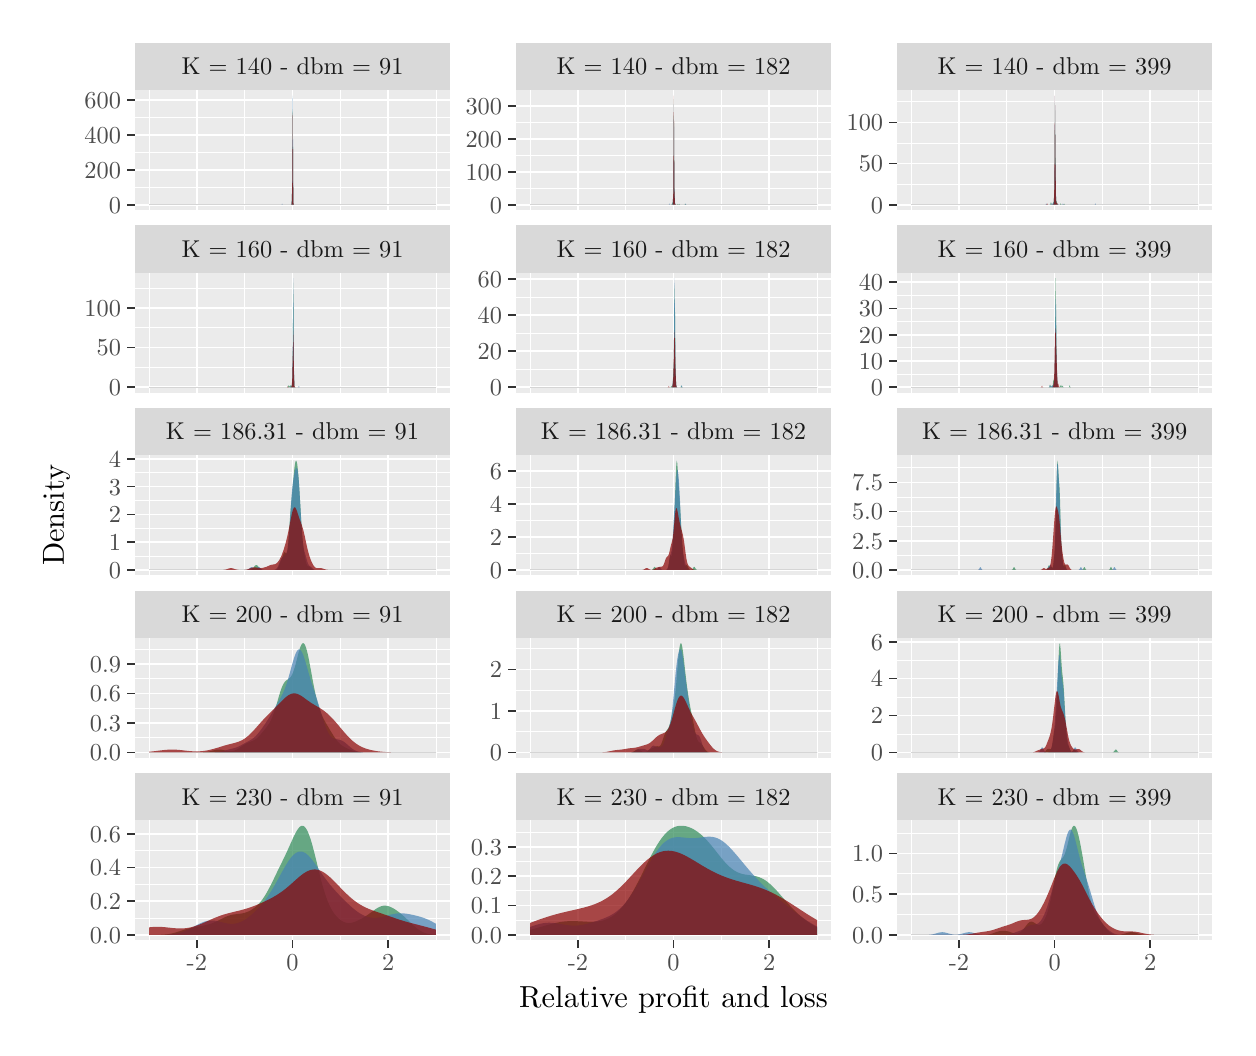
\begin{tikzpicture}[x=1pt,y=1pt]
\definecolor{fillColor}{RGB}{255,255,255}
\path[use as bounding box,fill=fillColor,fill opacity=0.00] (0,0) rectangle (433.62,361.35);
\begin{scope}
\path[clip] (  0.00,  0.00) rectangle (433.62,361.35);
\definecolor{drawColor}{RGB}{255,255,255}
\definecolor{fillColor}{RGB}{255,255,255}

\path[draw=drawColor,line width= 0.6pt,line join=round,line cap=round,fill=fillColor] (  0.00,  0.00) rectangle (433.62,361.35);
\end{scope}
\begin{scope}
\path[clip] ( 38.67,295.39) rectangle (152.72,338.79);
\definecolor{fillColor}{gray}{0.92}

\path[fill=fillColor] ( 38.67,295.39) rectangle (152.72,338.79);
\definecolor{drawColor}{RGB}{255,255,255}

\path[draw=drawColor,line width= 0.3pt,line join=round] ( 38.67,303.68) --
	(152.72,303.68);

\path[draw=drawColor,line width= 0.3pt,line join=round] ( 38.67,316.33) --
	(152.72,316.33);

\path[draw=drawColor,line width= 0.3pt,line join=round] ( 38.67,328.97) --
	(152.72,328.97);

\path[draw=drawColor,line width= 0.3pt,line join=round] ( 43.85,295.39) --
	( 43.85,338.79);

\path[draw=drawColor,line width= 0.3pt,line join=round] ( 78.41,295.39) --
	( 78.41,338.79);

\path[draw=drawColor,line width= 0.3pt,line join=round] (112.97,295.39) --
	(112.97,338.79);

\path[draw=drawColor,line width= 0.3pt,line join=round] (147.54,295.39) --
	(147.54,338.79);

\path[draw=drawColor,line width= 0.6pt,line join=round] ( 38.67,297.36) --
	(152.72,297.36);

\path[draw=drawColor,line width= 0.6pt,line join=round] ( 38.67,310.00) --
	(152.72,310.00);

\path[draw=drawColor,line width= 0.6pt,line join=round] ( 38.67,322.65) --
	(152.72,322.65);

\path[draw=drawColor,line width= 0.6pt,line join=round] ( 38.67,335.29) --
	(152.72,335.29);

\path[draw=drawColor,line width= 0.6pt,line join=round] ( 61.13,295.39) --
	( 61.13,338.79);

\path[draw=drawColor,line width= 0.6pt,line join=round] ( 95.69,295.39) --
	( 95.69,338.79);

\path[draw=drawColor,line width= 0.6pt,line join=round] (130.25,295.39) --
	(130.25,338.79);
\definecolor{fillColor}{RGB}{46,139,87}

\path[fill=fillColor,fill opacity=0.70] ( 43.85,297.36) --
	( 44.05,297.36) --
	( 44.26,297.36) --
	( 44.46,297.36) --
	( 44.66,297.36) --
	( 44.87,297.36) --
	( 45.07,297.36) --
	( 45.27,297.36) --
	( 45.47,297.36) --
	( 45.68,297.36) --
	( 45.88,297.36) --
	( 46.08,297.36) --
	( 46.29,297.36) --
	( 46.49,297.36) --
	( 46.69,297.36) --
	( 46.89,297.36) --
	( 47.10,297.36) --
	( 47.30,297.36) --
	( 47.50,297.36) --
	( 47.71,297.36) --
	( 47.91,297.36) --
	( 48.11,297.36) --
	( 48.31,297.36) --
	( 48.52,297.36) --
	( 48.72,297.36) --
	( 48.92,297.36) --
	( 49.13,297.36) --
	( 49.33,297.36) --
	( 49.53,297.36) --
	( 49.74,297.36) --
	( 49.94,297.36) --
	( 50.14,297.36) --
	( 50.34,297.36) --
	( 50.55,297.36) --
	( 50.75,297.36) --
	( 50.95,297.36) --
	( 51.16,297.36) --
	( 51.36,297.36) --
	( 51.56,297.36) --
	( 51.76,297.36) --
	( 51.97,297.36) --
	( 52.17,297.36) --
	( 52.37,297.36) --
	( 52.58,297.36) --
	( 52.78,297.36) --
	( 52.98,297.36) --
	( 53.18,297.36) --
	( 53.39,297.36) --
	( 53.59,297.36) --
	( 53.79,297.36) --
	( 54.00,297.36) --
	( 54.20,297.36) --
	( 54.40,297.36) --
	( 54.60,297.36) --
	( 54.81,297.36) --
	( 55.01,297.36) --
	( 55.21,297.36) --
	( 55.42,297.36) --
	( 55.62,297.36) --
	( 55.82,297.36) --
	( 56.03,297.36) --
	( 56.23,297.36) --
	( 56.43,297.36) --
	( 56.63,297.36) --
	( 56.84,297.36) --
	( 57.04,297.36) --
	( 57.24,297.36) --
	( 57.45,297.36) --
	( 57.65,297.36) --
	( 57.85,297.36) --
	( 58.05,297.36) --
	( 58.26,297.36) --
	( 58.46,297.36) --
	( 58.66,297.36) --
	( 58.87,297.36) --
	( 59.07,297.36) --
	( 59.27,297.36) --
	( 59.47,297.36) --
	( 59.68,297.36) --
	( 59.88,297.36) --
	( 60.08,297.36) --
	( 60.29,297.36) --
	( 60.49,297.36) --
	( 60.69,297.36) --
	( 60.90,297.36) --
	( 61.10,297.36) --
	( 61.30,297.36) --
	( 61.50,297.36) --
	( 61.71,297.36) --
	( 61.91,297.36) --
	( 62.11,297.36) --
	( 62.32,297.36) --
	( 62.52,297.36) --
	( 62.72,297.36) --
	( 62.92,297.36) --
	( 63.13,297.36) --
	( 63.33,297.36) --
	( 63.53,297.36) --
	( 63.74,297.36) --
	( 63.94,297.36) --
	( 64.14,297.36) --
	( 64.34,297.36) --
	( 64.55,297.36) --
	( 64.75,297.36) --
	( 64.95,297.36) --
	( 65.16,297.36) --
	( 65.36,297.36) --
	( 65.56,297.36) --
	( 65.76,297.36) --
	( 65.97,297.36) --
	( 66.17,297.36) --
	( 66.37,297.36) --
	( 66.58,297.36) --
	( 66.78,297.36) --
	( 66.98,297.36) --
	( 67.19,297.36) --
	( 67.39,297.36) --
	( 67.59,297.36) --
	( 67.79,297.36) --
	( 68.00,297.36) --
	( 68.20,297.36) --
	( 68.40,297.36) --
	( 68.61,297.36) --
	( 68.81,297.36) --
	( 69.01,297.36) --
	( 69.21,297.36) --
	( 69.42,297.36) --
	( 69.62,297.36) --
	( 69.82,297.36) --
	( 70.03,297.36) --
	( 70.23,297.36) --
	( 70.43,297.36) --
	( 70.63,297.36) --
	( 70.84,297.36) --
	( 71.04,297.36) --
	( 71.24,297.36) --
	( 71.45,297.36) --
	( 71.65,297.36) --
	( 71.85,297.36) --
	( 72.05,297.36) --
	( 72.26,297.36) --
	( 72.46,297.36) --
	( 72.66,297.36) --
	( 72.87,297.36) --
	( 73.07,297.36) --
	( 73.27,297.36) --
	( 73.48,297.36) --
	( 73.68,297.36) --
	( 73.88,297.36) --
	( 74.08,297.36) --
	( 74.29,297.36) --
	( 74.49,297.36) --
	( 74.69,297.36) --
	( 74.90,297.36) --
	( 75.10,297.36) --
	( 75.30,297.36) --
	( 75.50,297.36) --
	( 75.71,297.36) --
	( 75.91,297.36) --
	( 76.11,297.36) --
	( 76.32,297.36) --
	( 76.52,297.36) --
	( 76.72,297.36) --
	( 76.92,297.36) --
	( 77.13,297.36) --
	( 77.33,297.36) --
	( 77.53,297.36) --
	( 77.74,297.36) --
	( 77.94,297.36) --
	( 78.14,297.36) --
	( 78.34,297.36) --
	( 78.55,297.36) --
	( 78.75,297.36) --
	( 78.95,297.36) --
	( 79.16,297.36) --
	( 79.36,297.36) --
	( 79.56,297.36) --
	( 79.77,297.36) --
	( 79.97,297.36) --
	( 80.17,297.36) --
	( 80.37,297.36) --
	( 80.58,297.36) --
	( 80.78,297.36) --
	( 80.98,297.36) --
	( 81.19,297.36) --
	( 81.39,297.36) --
	( 81.59,297.36) --
	( 81.79,297.36) --
	( 82.00,297.36) --
	( 82.20,297.36) --
	( 82.40,297.36) --
	( 82.61,297.36) --
	( 82.81,297.36) --
	( 83.01,297.36) --
	( 83.21,297.36) --
	( 83.42,297.36) --
	( 83.62,297.36) --
	( 83.82,297.36) --
	( 84.03,297.36) --
	( 84.23,297.36) --
	( 84.43,297.36) --
	( 84.64,297.36) --
	( 84.84,297.36) --
	( 85.04,297.36) --
	( 85.24,297.36) --
	( 85.45,297.36) --
	( 85.65,297.36) --
	( 85.85,297.36) --
	( 86.06,297.36) --
	( 86.26,297.36) --
	( 86.46,297.36) --
	( 86.66,297.36) --
	( 86.87,297.36) --
	( 87.07,297.36) --
	( 87.27,297.36) --
	( 87.48,297.36) --
	( 87.68,297.36) --
	( 87.88,297.36) --
	( 88.08,297.36) --
	( 88.29,297.36) --
	( 88.49,297.36) --
	( 88.69,297.36) --
	( 88.90,297.36) --
	( 89.10,297.36) --
	( 89.30,297.36) --
	( 89.50,297.36) --
	( 89.71,297.36) --
	( 89.91,297.36) --
	( 90.11,297.36) --
	( 90.32,297.36) --
	( 90.52,297.36) --
	( 90.72,297.36) --
	( 90.93,297.36) --
	( 91.13,297.36) --
	( 91.33,297.36) --
	( 91.53,297.36) --
	( 91.74,297.36) --
	( 91.94,297.36) --
	( 92.14,297.36) --
	( 92.35,297.36) --
	( 92.55,297.36) --
	( 92.75,297.36) --
	( 92.95,297.36) --
	( 93.16,297.36) --
	( 93.36,297.36) --
	( 93.56,297.36) --
	( 93.77,297.36) --
	( 93.97,297.36) --
	( 94.17,297.36) --
	( 94.37,297.36) --
	( 94.58,297.36) --
	( 94.78,297.36) --
	( 94.98,297.36) --
	( 95.19,297.36) --
	( 95.39,297.79) --
	( 95.59,303.70) --
	( 95.79,331.92) --
	( 96.00,298.04) --
	( 96.20,297.42) --
	( 96.40,297.36) --
	( 96.61,297.36) --
	( 96.81,297.36) --
	( 97.01,297.36) --
	( 97.22,297.36) --
	( 97.42,297.36) --
	( 97.62,297.36) --
	( 97.82,297.36) --
	( 98.03,297.36) --
	( 98.23,297.36) --
	( 98.43,297.36) --
	( 98.64,297.36) --
	( 98.84,297.36) --
	( 99.04,297.36) --
	( 99.24,297.36) --
	( 99.45,297.36) --
	( 99.65,297.36) --
	( 99.85,297.36) --
	(100.06,297.36) --
	(100.26,297.36) --
	(100.46,297.36) --
	(100.66,297.36) --
	(100.87,297.36) --
	(101.07,297.36) --
	(101.27,297.36) --
	(101.48,297.36) --
	(101.68,297.36) --
	(101.88,297.36) --
	(102.08,297.36) --
	(102.29,297.36) --
	(102.49,297.36) --
	(102.69,297.36) --
	(102.90,297.36) --
	(103.10,297.36) --
	(103.30,297.36) --
	(103.51,297.36) --
	(103.71,297.36) --
	(103.91,297.36) --
	(104.11,297.36) --
	(104.32,297.36) --
	(104.52,297.36) --
	(104.72,297.36) --
	(104.93,297.36) --
	(105.13,297.36) --
	(105.33,297.36) --
	(105.53,297.36) --
	(105.74,297.36) --
	(105.94,297.36) --
	(106.14,297.36) --
	(106.35,297.36) --
	(106.55,297.36) --
	(106.75,297.36) --
	(106.95,297.36) --
	(107.16,297.36) --
	(107.36,297.36) --
	(107.56,297.36) --
	(107.77,297.36) --
	(107.97,297.36) --
	(108.17,297.36) --
	(108.37,297.36) --
	(108.58,297.36) --
	(108.78,297.36) --
	(108.98,297.36) --
	(109.19,297.36) --
	(109.39,297.36) --
	(109.59,297.36) --
	(109.80,297.36) --
	(110.00,297.36) --
	(110.20,297.36) --
	(110.40,297.36) --
	(110.61,297.36) --
	(110.81,297.36) --
	(111.01,297.36) --
	(111.22,297.36) --
	(111.42,297.36) --
	(111.62,297.36) --
	(111.82,297.36) --
	(112.03,297.36) --
	(112.23,297.36) --
	(112.43,297.36) --
	(112.64,297.36) --
	(112.84,297.36) --
	(113.04,297.36) --
	(113.24,297.36) --
	(113.45,297.36) --
	(113.65,297.36) --
	(113.85,297.36) --
	(114.06,297.36) --
	(114.26,297.36) --
	(114.46,297.36) --
	(114.67,297.36) --
	(114.87,297.36) --
	(115.07,297.36) --
	(115.27,297.36) --
	(115.48,297.36) --
	(115.68,297.36) --
	(115.88,297.36) --
	(116.09,297.36) --
	(116.29,297.36) --
	(116.49,297.36) --
	(116.69,297.36) --
	(116.90,297.36) --
	(117.10,297.36) --
	(117.30,297.36) --
	(117.51,297.36) --
	(117.71,297.36) --
	(117.91,297.36) --
	(118.11,297.36) --
	(118.32,297.36) --
	(118.52,297.36) --
	(118.72,297.36) --
	(118.93,297.36) --
	(119.13,297.36) --
	(119.33,297.36) --
	(119.53,297.36) --
	(119.74,297.36) --
	(119.94,297.36) --
	(120.14,297.36) --
	(120.35,297.36) --
	(120.55,297.36) --
	(120.75,297.36) --
	(120.96,297.36) --
	(121.16,297.36) --
	(121.36,297.36) --
	(121.56,297.36) --
	(121.77,297.36) --
	(121.97,297.36) --
	(122.17,297.36) --
	(122.38,297.36) --
	(122.58,297.36) --
	(122.78,297.36) --
	(122.98,297.36) --
	(123.19,297.36) --
	(123.39,297.36) --
	(123.59,297.36) --
	(123.80,297.36) --
	(124.00,297.36) --
	(124.20,297.36) --
	(124.40,297.36) --
	(124.61,297.36) --
	(124.81,297.36) --
	(125.01,297.36) --
	(125.22,297.36) --
	(125.42,297.36) --
	(125.62,297.36) --
	(125.82,297.36) --
	(126.03,297.36) --
	(126.23,297.36) --
	(126.43,297.36) --
	(126.64,297.36) --
	(126.84,297.36) --
	(127.04,297.36) --
	(127.25,297.36) --
	(127.45,297.36) --
	(127.65,297.36) --
	(127.85,297.36) --
	(128.06,297.36) --
	(128.26,297.36) --
	(128.46,297.36) --
	(128.67,297.36) --
	(128.87,297.36) --
	(129.07,297.36) --
	(129.27,297.36) --
	(129.48,297.36) --
	(129.68,297.36) --
	(129.88,297.36) --
	(130.09,297.36) --
	(130.29,297.36) --
	(130.49,297.36) --
	(130.69,297.36) --
	(130.90,297.36) --
	(131.10,297.36) --
	(131.30,297.36) --
	(131.51,297.36) --
	(131.71,297.36) --
	(131.91,297.36) --
	(132.11,297.36) --
	(132.32,297.36) --
	(132.52,297.36) --
	(132.72,297.36) --
	(132.93,297.36) --
	(133.13,297.36) --
	(133.33,297.36) --
	(133.54,297.36) --
	(133.74,297.36) --
	(133.94,297.36) --
	(134.14,297.36) --
	(134.35,297.36) --
	(134.55,297.36) --
	(134.75,297.36) --
	(134.96,297.36) --
	(135.16,297.36) --
	(135.36,297.36) --
	(135.56,297.36) --
	(135.77,297.36) --
	(135.97,297.36) --
	(136.17,297.36) --
	(136.38,297.36) --
	(136.58,297.36) --
	(136.78,297.36) --
	(136.98,297.36) --
	(137.19,297.36) --
	(137.39,297.36) --
	(137.59,297.36) --
	(137.80,297.36) --
	(138.00,297.36) --
	(138.20,297.36) --
	(138.40,297.36) --
	(138.61,297.36) --
	(138.81,297.36) --
	(139.01,297.36) --
	(139.22,297.36) --
	(139.42,297.36) --
	(139.62,297.36) --
	(139.83,297.36) --
	(140.03,297.36) --
	(140.23,297.36) --
	(140.43,297.36) --
	(140.64,297.36) --
	(140.84,297.36) --
	(141.04,297.36) --
	(141.25,297.36) --
	(141.45,297.36) --
	(141.65,297.36) --
	(141.85,297.36) --
	(142.06,297.36) --
	(142.26,297.36) --
	(142.46,297.36) --
	(142.67,297.36) --
	(142.87,297.36) --
	(143.07,297.36) --
	(143.27,297.36) --
	(143.48,297.36) --
	(143.68,297.36) --
	(143.88,297.36) --
	(144.09,297.36) --
	(144.29,297.36) --
	(144.49,297.36) --
	(144.70,297.36) --
	(144.90,297.36) --
	(145.10,297.36) --
	(145.30,297.36) --
	(145.51,297.36) --
	(145.71,297.36) --
	(145.91,297.36) --
	(146.12,297.36) --
	(146.32,297.36) --
	(146.52,297.36) --
	(146.72,297.36) --
	(146.93,297.36) --
	(147.13,297.36) --
	(147.33,297.36) --
	(147.54,297.36) --
	(147.54,297.36) --
	(147.33,297.36) --
	(147.13,297.36) --
	(146.93,297.36) --
	(146.72,297.36) --
	(146.52,297.36) --
	(146.32,297.36) --
	(146.12,297.36) --
	(145.91,297.36) --
	(145.71,297.36) --
	(145.51,297.36) --
	(145.30,297.36) --
	(145.10,297.36) --
	(144.90,297.36) --
	(144.70,297.36) --
	(144.49,297.36) --
	(144.29,297.36) --
	(144.09,297.36) --
	(143.88,297.36) --
	(143.68,297.36) --
	(143.48,297.36) --
	(143.27,297.36) --
	(143.07,297.36) --
	(142.87,297.36) --
	(142.67,297.36) --
	(142.46,297.36) --
	(142.26,297.36) --
	(142.06,297.36) --
	(141.85,297.36) --
	(141.65,297.36) --
	(141.45,297.36) --
	(141.25,297.36) --
	(141.04,297.36) --
	(140.84,297.36) --
	(140.64,297.36) --
	(140.43,297.36) --
	(140.23,297.36) --
	(140.03,297.36) --
	(139.83,297.36) --
	(139.62,297.36) --
	(139.42,297.36) --
	(139.22,297.36) --
	(139.01,297.36) --
	(138.81,297.36) --
	(138.61,297.36) --
	(138.40,297.36) --
	(138.20,297.36) --
	(138.00,297.36) --
	(137.80,297.36) --
	(137.59,297.36) --
	(137.39,297.36) --
	(137.19,297.36) --
	(136.98,297.36) --
	(136.78,297.36) --
	(136.58,297.36) --
	(136.38,297.36) --
	(136.17,297.36) --
	(135.97,297.36) --
	(135.77,297.36) --
	(135.56,297.36) --
	(135.36,297.36) --
	(135.16,297.36) --
	(134.96,297.36) --
	(134.75,297.36) --
	(134.55,297.36) --
	(134.35,297.36) --
	(134.14,297.36) --
	(133.94,297.36) --
	(133.74,297.36) --
	(133.54,297.36) --
	(133.33,297.36) --
	(133.13,297.36) --
	(132.93,297.36) --
	(132.72,297.36) --
	(132.52,297.36) --
	(132.32,297.36) --
	(132.11,297.36) --
	(131.91,297.36) --
	(131.71,297.36) --
	(131.51,297.36) --
	(131.30,297.36) --
	(131.10,297.36) --
	(130.90,297.36) --
	(130.69,297.36) --
	(130.49,297.36) --
	(130.29,297.36) --
	(130.09,297.36) --
	(129.88,297.36) --
	(129.68,297.36) --
	(129.48,297.36) --
	(129.27,297.36) --
	(129.07,297.36) --
	(128.87,297.36) --
	(128.67,297.36) --
	(128.46,297.36) --
	(128.26,297.36) --
	(128.06,297.36) --
	(127.85,297.36) --
	(127.65,297.36) --
	(127.45,297.36) --
	(127.25,297.36) --
	(127.04,297.36) --
	(126.84,297.36) --
	(126.64,297.36) --
	(126.43,297.36) --
	(126.23,297.36) --
	(126.03,297.36) --
	(125.82,297.36) --
	(125.62,297.36) --
	(125.42,297.36) --
	(125.22,297.36) --
	(125.01,297.36) --
	(124.81,297.36) --
	(124.61,297.36) --
	(124.40,297.36) --
	(124.20,297.36) --
	(124.00,297.36) --
	(123.80,297.36) --
	(123.59,297.36) --
	(123.39,297.36) --
	(123.19,297.36) --
	(122.98,297.36) --
	(122.78,297.36) --
	(122.58,297.36) --
	(122.38,297.36) --
	(122.17,297.36) --
	(121.97,297.36) --
	(121.77,297.36) --
	(121.56,297.36) --
	(121.36,297.36) --
	(121.16,297.36) --
	(120.96,297.36) --
	(120.75,297.36) --
	(120.55,297.36) --
	(120.35,297.36) --
	(120.14,297.36) --
	(119.94,297.36) --
	(119.74,297.36) --
	(119.53,297.36) --
	(119.33,297.36) --
	(119.13,297.36) --
	(118.93,297.36) --
	(118.72,297.36) --
	(118.52,297.36) --
	(118.32,297.36) --
	(118.11,297.36) --
	(117.91,297.36) --
	(117.71,297.36) --
	(117.51,297.36) --
	(117.30,297.36) --
	(117.10,297.36) --
	(116.90,297.36) --
	(116.69,297.36) --
	(116.49,297.36) --
	(116.29,297.36) --
	(116.09,297.36) --
	(115.88,297.36) --
	(115.68,297.36) --
	(115.48,297.36) --
	(115.27,297.36) --
	(115.07,297.36) --
	(114.87,297.36) --
	(114.67,297.36) --
	(114.46,297.36) --
	(114.26,297.36) --
	(114.06,297.36) --
	(113.85,297.36) --
	(113.65,297.36) --
	(113.45,297.36) --
	(113.24,297.36) --
	(113.04,297.36) --
	(112.84,297.36) --
	(112.64,297.36) --
	(112.43,297.36) --
	(112.23,297.36) --
	(112.03,297.36) --
	(111.82,297.36) --
	(111.62,297.36) --
	(111.42,297.36) --
	(111.22,297.36) --
	(111.01,297.36) --
	(110.81,297.36) --
	(110.61,297.36) --
	(110.40,297.36) --
	(110.20,297.36) --
	(110.00,297.36) --
	(109.80,297.36) --
	(109.59,297.36) --
	(109.39,297.36) --
	(109.19,297.36) --
	(108.98,297.36) --
	(108.78,297.36) --
	(108.58,297.36) --
	(108.37,297.36) --
	(108.17,297.36) --
	(107.97,297.36) --
	(107.77,297.36) --
	(107.56,297.36) --
	(107.36,297.36) --
	(107.16,297.36) --
	(106.95,297.36) --
	(106.75,297.36) --
	(106.55,297.36) --
	(106.35,297.36) --
	(106.14,297.36) --
	(105.94,297.36) --
	(105.74,297.36) --
	(105.53,297.36) --
	(105.33,297.36) --
	(105.13,297.36) --
	(104.93,297.36) --
	(104.72,297.36) --
	(104.52,297.36) --
	(104.32,297.36) --
	(104.11,297.36) --
	(103.91,297.36) --
	(103.71,297.36) --
	(103.51,297.36) --
	(103.30,297.36) --
	(103.10,297.36) --
	(102.90,297.36) --
	(102.69,297.36) --
	(102.49,297.36) --
	(102.29,297.36) --
	(102.08,297.36) --
	(101.88,297.36) --
	(101.68,297.36) --
	(101.48,297.36) --
	(101.27,297.36) --
	(101.07,297.36) --
	(100.87,297.36) --
	(100.66,297.36) --
	(100.46,297.36) --
	(100.26,297.36) --
	(100.06,297.36) --
	( 99.85,297.36) --
	( 99.65,297.36) --
	( 99.45,297.36) --
	( 99.24,297.36) --
	( 99.04,297.36) --
	( 98.84,297.36) --
	( 98.64,297.36) --
	( 98.43,297.36) --
	( 98.23,297.36) --
	( 98.03,297.36) --
	( 97.82,297.36) --
	( 97.62,297.36) --
	( 97.42,297.36) --
	( 97.22,297.36) --
	( 97.01,297.36) --
	( 96.81,297.36) --
	( 96.61,297.36) --
	( 96.40,297.36) --
	( 96.20,297.36) --
	( 96.00,297.36) --
	( 95.79,297.36) --
	( 95.59,297.36) --
	( 95.39,297.36) --
	( 95.19,297.36) --
	( 94.98,297.36) --
	( 94.78,297.36) --
	( 94.58,297.36) --
	( 94.37,297.36) --
	( 94.17,297.36) --
	( 93.97,297.36) --
	( 93.77,297.36) --
	( 93.56,297.36) --
	( 93.36,297.36) --
	( 93.16,297.36) --
	( 92.95,297.36) --
	( 92.75,297.36) --
	( 92.55,297.36) --
	( 92.35,297.36) --
	( 92.14,297.36) --
	( 91.94,297.36) --
	( 91.74,297.36) --
	( 91.53,297.36) --
	( 91.33,297.36) --
	( 91.13,297.36) --
	( 90.93,297.36) --
	( 90.72,297.36) --
	( 90.52,297.36) --
	( 90.32,297.36) --
	( 90.11,297.36) --
	( 89.91,297.36) --
	( 89.71,297.36) --
	( 89.50,297.36) --
	( 89.30,297.36) --
	( 89.10,297.36) --
	( 88.90,297.36) --
	( 88.69,297.36) --
	( 88.49,297.36) --
	( 88.29,297.36) --
	( 88.08,297.36) --
	( 87.88,297.36) --
	( 87.68,297.36) --
	( 87.48,297.36) --
	( 87.27,297.36) --
	( 87.07,297.36) --
	( 86.87,297.36) --
	( 86.66,297.36) --
	( 86.46,297.36) --
	( 86.26,297.36) --
	( 86.06,297.36) --
	( 85.85,297.36) --
	( 85.65,297.36) --
	( 85.45,297.36) --
	( 85.24,297.36) --
	( 85.04,297.36) --
	( 84.84,297.36) --
	( 84.64,297.36) --
	( 84.43,297.36) --
	( 84.23,297.36) --
	( 84.03,297.36) --
	( 83.82,297.36) --
	( 83.62,297.36) --
	( 83.42,297.36) --
	( 83.21,297.36) --
	( 83.01,297.36) --
	( 82.81,297.36) --
	( 82.61,297.36) --
	( 82.40,297.36) --
	( 82.20,297.36) --
	( 82.00,297.36) --
	( 81.79,297.36) --
	( 81.59,297.36) --
	( 81.39,297.36) --
	( 81.19,297.36) --
	( 80.98,297.36) --
	( 80.78,297.36) --
	( 80.58,297.36) --
	( 80.37,297.36) --
	( 80.17,297.36) --
	( 79.97,297.36) --
	( 79.77,297.36) --
	( 79.56,297.36) --
	( 79.36,297.36) --
	( 79.16,297.36) --
	( 78.95,297.36) --
	( 78.75,297.36) --
	( 78.55,297.36) --
	( 78.34,297.36) --
	( 78.14,297.36) --
	( 77.94,297.36) --
	( 77.74,297.36) --
	( 77.53,297.36) --
	( 77.33,297.36) --
	( 77.13,297.36) --
	( 76.92,297.36) --
	( 76.72,297.36) --
	( 76.52,297.36) --
	( 76.32,297.36) --
	( 76.11,297.36) --
	( 75.91,297.36) --
	( 75.71,297.36) --
	( 75.50,297.36) --
	( 75.30,297.36) --
	( 75.10,297.36) --
	( 74.90,297.36) --
	( 74.69,297.36) --
	( 74.49,297.36) --
	( 74.29,297.36) --
	( 74.08,297.36) --
	( 73.88,297.36) --
	( 73.68,297.36) --
	( 73.48,297.36) --
	( 73.27,297.36) --
	( 73.07,297.36) --
	( 72.87,297.36) --
	( 72.66,297.36) --
	( 72.46,297.36) --
	( 72.26,297.36) --
	( 72.05,297.36) --
	( 71.85,297.36) --
	( 71.65,297.36) --
	( 71.45,297.36) --
	( 71.24,297.36) --
	( 71.04,297.36) --
	( 70.84,297.36) --
	( 70.63,297.36) --
	( 70.43,297.36) --
	( 70.23,297.36) --
	( 70.03,297.36) --
	( 69.82,297.36) --
	( 69.62,297.36) --
	( 69.42,297.36) --
	( 69.21,297.36) --
	( 69.01,297.36) --
	( 68.81,297.36) --
	( 68.61,297.36) --
	( 68.40,297.36) --
	( 68.20,297.36) --
	( 68.00,297.36) --
	( 67.79,297.36) --
	( 67.59,297.36) --
	( 67.39,297.36) --
	( 67.19,297.36) --
	( 66.98,297.36) --
	( 66.78,297.36) --
	( 66.58,297.36) --
	( 66.37,297.36) --
	( 66.17,297.36) --
	( 65.97,297.36) --
	( 65.76,297.36) --
	( 65.56,297.36) --
	( 65.36,297.36) --
	( 65.16,297.36) --
	( 64.95,297.36) --
	( 64.75,297.36) --
	( 64.55,297.36) --
	( 64.34,297.36) --
	( 64.14,297.36) --
	( 63.94,297.36) --
	( 63.74,297.36) --
	( 63.53,297.36) --
	( 63.33,297.36) --
	( 63.13,297.36) --
	( 62.92,297.36) --
	( 62.72,297.36) --
	( 62.52,297.36) --
	( 62.32,297.36) --
	( 62.11,297.36) --
	( 61.91,297.36) --
	( 61.71,297.36) --
	( 61.50,297.36) --
	( 61.30,297.36) --
	( 61.10,297.36) --
	( 60.90,297.36) --
	( 60.69,297.36) --
	( 60.49,297.36) --
	( 60.29,297.36) --
	( 60.08,297.36) --
	( 59.88,297.36) --
	( 59.68,297.36) --
	( 59.47,297.36) --
	( 59.27,297.36) --
	( 59.07,297.36) --
	( 58.87,297.36) --
	( 58.66,297.36) --
	( 58.46,297.36) --
	( 58.26,297.36) --
	( 58.05,297.36) --
	( 57.85,297.36) --
	( 57.65,297.36) --
	( 57.45,297.36) --
	( 57.24,297.36) --
	( 57.04,297.36) --
	( 56.84,297.36) --
	( 56.63,297.36) --
	( 56.43,297.36) --
	( 56.23,297.36) --
	( 56.03,297.36) --
	( 55.82,297.36) --
	( 55.62,297.36) --
	( 55.42,297.36) --
	( 55.21,297.36) --
	( 55.01,297.36) --
	( 54.81,297.36) --
	( 54.60,297.36) --
	( 54.40,297.36) --
	( 54.20,297.36) --
	( 54.00,297.36) --
	( 53.79,297.36) --
	( 53.59,297.36) --
	( 53.39,297.36) --
	( 53.18,297.36) --
	( 52.98,297.36) --
	( 52.78,297.36) --
	( 52.58,297.36) --
	( 52.37,297.36) --
	( 52.17,297.36) --
	( 51.97,297.36) --
	( 51.76,297.36) --
	( 51.56,297.36) --
	( 51.36,297.36) --
	( 51.16,297.36) --
	( 50.95,297.36) --
	( 50.75,297.36) --
	( 50.55,297.36) --
	( 50.34,297.36) --
	( 50.14,297.36) --
	( 49.94,297.36) --
	( 49.74,297.36) --
	( 49.53,297.36) --
	( 49.33,297.36) --
	( 49.13,297.36) --
	( 48.92,297.36) --
	( 48.72,297.36) --
	( 48.52,297.36) --
	( 48.31,297.36) --
	( 48.11,297.36) --
	( 47.91,297.36) --
	( 47.71,297.36) --
	( 47.50,297.36) --
	( 47.30,297.36) --
	( 47.10,297.36) --
	( 46.89,297.36) --
	( 46.69,297.36) --
	( 46.49,297.36) --
	( 46.29,297.36) --
	( 46.08,297.36) --
	( 45.88,297.36) --
	( 45.68,297.36) --
	( 45.47,297.36) --
	( 45.27,297.36) --
	( 45.07,297.36) --
	( 44.87,297.36) --
	( 44.66,297.36) --
	( 44.46,297.36) --
	( 44.26,297.36) --
	( 44.05,297.36) --
	( 43.85,297.36) --
	cycle;
\definecolor{fillColor}{RGB}{70,130,180}

\path[fill=fillColor,fill opacity=0.70] ( 43.85,297.36) --
	( 44.05,297.36) --
	( 44.26,297.36) --
	( 44.46,297.36) --
	( 44.66,297.36) --
	( 44.87,297.36) --
	( 45.07,297.36) --
	( 45.27,297.36) --
	( 45.47,297.36) --
	( 45.68,297.36) --
	( 45.88,297.36) --
	( 46.08,297.36) --
	( 46.29,297.36) --
	( 46.49,297.36) --
	( 46.69,297.36) --
	( 46.89,297.36) --
	( 47.10,297.36) --
	( 47.30,297.36) --
	( 47.50,297.36) --
	( 47.71,297.36) --
	( 47.91,297.36) --
	( 48.11,297.36) --
	( 48.31,297.36) --
	( 48.52,297.36) --
	( 48.72,297.36) --
	( 48.92,297.36) --
	( 49.13,297.36) --
	( 49.33,297.36) --
	( 49.53,297.36) --
	( 49.74,297.36) --
	( 49.94,297.36) --
	( 50.14,297.36) --
	( 50.34,297.36) --
	( 50.55,297.36) --
	( 50.75,297.36) --
	( 50.95,297.36) --
	( 51.16,297.36) --
	( 51.36,297.36) --
	( 51.56,297.36) --
	( 51.76,297.36) --
	( 51.97,297.36) --
	( 52.17,297.36) --
	( 52.37,297.36) --
	( 52.58,297.36) --
	( 52.78,297.36) --
	( 52.98,297.36) --
	( 53.18,297.36) --
	( 53.39,297.36) --
	( 53.59,297.36) --
	( 53.79,297.36) --
	( 54.00,297.36) --
	( 54.20,297.36) --
	( 54.40,297.36) --
	( 54.60,297.36) --
	( 54.81,297.36) --
	( 55.01,297.36) --
	( 55.21,297.36) --
	( 55.42,297.36) --
	( 55.62,297.36) --
	( 55.82,297.36) --
	( 56.03,297.36) --
	( 56.23,297.36) --
	( 56.43,297.36) --
	( 56.63,297.36) --
	( 56.84,297.36) --
	( 57.04,297.36) --
	( 57.24,297.36) --
	( 57.45,297.36) --
	( 57.65,297.36) --
	( 57.85,297.36) --
	( 58.05,297.36) --
	( 58.26,297.36) --
	( 58.46,297.36) --
	( 58.66,297.36) --
	( 58.87,297.36) --
	( 59.07,297.36) --
	( 59.27,297.36) --
	( 59.47,297.36) --
	( 59.68,297.36) --
	( 59.88,297.36) --
	( 60.08,297.36) --
	( 60.29,297.36) --
	( 60.49,297.36) --
	( 60.69,297.36) --
	( 60.90,297.36) --
	( 61.10,297.36) --
	( 61.30,297.36) --
	( 61.50,297.36) --
	( 61.71,297.36) --
	( 61.91,297.36) --
	( 62.11,297.36) --
	( 62.32,297.36) --
	( 62.52,297.36) --
	( 62.72,297.36) --
	( 62.92,297.36) --
	( 63.13,297.36) --
	( 63.33,297.36) --
	( 63.53,297.36) --
	( 63.74,297.36) --
	( 63.94,297.36) --
	( 64.14,297.36) --
	( 64.34,297.36) --
	( 64.55,297.36) --
	( 64.75,297.36) --
	( 64.95,297.36) --
	( 65.16,297.36) --
	( 65.36,297.36) --
	( 65.56,297.36) --
	( 65.76,297.36) --
	( 65.97,297.36) --
	( 66.17,297.36) --
	( 66.37,297.36) --
	( 66.58,297.36) --
	( 66.78,297.36) --
	( 66.98,297.36) --
	( 67.19,297.36) --
	( 67.39,297.36) --
	( 67.59,297.36) --
	( 67.79,297.36) --
	( 68.00,297.36) --
	( 68.20,297.36) --
	( 68.40,297.36) --
	( 68.61,297.36) --
	( 68.81,297.36) --
	( 69.01,297.36) --
	( 69.21,297.36) --
	( 69.42,297.36) --
	( 69.62,297.36) --
	( 69.82,297.36) --
	( 70.03,297.36) --
	( 70.23,297.36) --
	( 70.43,297.36) --
	( 70.63,297.36) --
	( 70.84,297.36) --
	( 71.04,297.36) --
	( 71.24,297.36) --
	( 71.45,297.36) --
	( 71.65,297.36) --
	( 71.85,297.36) --
	( 72.05,297.36) --
	( 72.26,297.36) --
	( 72.46,297.36) --
	( 72.66,297.36) --
	( 72.87,297.36) --
	( 73.07,297.36) --
	( 73.27,297.36) --
	( 73.48,297.36) --
	( 73.68,297.36) --
	( 73.88,297.36) --
	( 74.08,297.36) --
	( 74.29,297.36) --
	( 74.49,297.36) --
	( 74.69,297.36) --
	( 74.90,297.36) --
	( 75.10,297.36) --
	( 75.30,297.36) --
	( 75.50,297.36) --
	( 75.71,297.36) --
	( 75.91,297.36) --
	( 76.11,297.36) --
	( 76.32,297.36) --
	( 76.52,297.36) --
	( 76.72,297.36) --
	( 76.92,297.36) --
	( 77.13,297.36) --
	( 77.33,297.36) --
	( 77.53,297.36) --
	( 77.74,297.36) --
	( 77.94,297.36) --
	( 78.14,297.36) --
	( 78.34,297.36) --
	( 78.55,297.36) --
	( 78.75,297.36) --
	( 78.95,297.36) --
	( 79.16,297.36) --
	( 79.36,297.36) --
	( 79.56,297.36) --
	( 79.77,297.36) --
	( 79.97,297.36) --
	( 80.17,297.36) --
	( 80.37,297.36) --
	( 80.58,297.36) --
	( 80.78,297.36) --
	( 80.98,297.36) --
	( 81.19,297.36) --
	( 81.39,297.36) --
	( 81.59,297.36) --
	( 81.79,297.36) --
	( 82.00,297.36) --
	( 82.20,297.36) --
	( 82.40,297.36) --
	( 82.61,297.36) --
	( 82.81,297.36) --
	( 83.01,297.36) --
	( 83.21,297.36) --
	( 83.42,297.36) --
	( 83.62,297.36) --
	( 83.82,297.36) --
	( 84.03,297.36) --
	( 84.23,297.36) --
	( 84.43,297.36) --
	( 84.64,297.36) --
	( 84.84,297.36) --
	( 85.04,297.36) --
	( 85.24,297.36) --
	( 85.45,297.36) --
	( 85.65,297.36) --
	( 85.85,297.36) --
	( 86.06,297.36) --
	( 86.26,297.36) --
	( 86.46,297.36) --
	( 86.66,297.36) --
	( 86.87,297.36) --
	( 87.07,297.36) --
	( 87.27,297.36) --
	( 87.48,297.36) --
	( 87.68,297.36) --
	( 87.88,297.36) --
	( 88.08,297.36) --
	( 88.29,297.36) --
	( 88.49,297.36) --
	( 88.69,297.36) --
	( 88.90,297.36) --
	( 89.10,297.36) --
	( 89.30,297.36) --
	( 89.50,297.36) --
	( 89.71,297.36) --
	( 89.91,297.36) --
	( 90.11,297.36) --
	( 90.32,297.36) --
	( 90.52,297.36) --
	( 90.72,297.36) --
	( 90.93,297.36) --
	( 91.13,297.36) --
	( 91.33,297.36) --
	( 91.53,297.36) --
	( 91.74,297.41) --
	( 91.94,297.78) --
	( 92.14,297.36) --
	( 92.35,297.36) --
	( 92.55,297.36) --
	( 92.75,297.36) --
	( 92.95,297.36) --
	( 93.16,297.36) --
	( 93.36,297.36) --
	( 93.56,297.36) --
	( 93.77,297.36) --
	( 93.97,297.36) --
	( 94.17,297.36) --
	( 94.37,297.36) --
	( 94.58,297.36) --
	( 94.78,297.36) --
	( 94.98,297.36) --
	( 95.19,297.46) --
	( 95.39,297.73) --
	( 95.59,303.74) --
	( 95.79,336.82) --
	( 96.00,297.71) --
	( 96.20,297.36) --
	( 96.40,297.36) --
	( 96.61,297.36) --
	( 96.81,297.36) --
	( 97.01,297.36) --
	( 97.22,297.36) --
	( 97.42,297.36) --
	( 97.62,297.36) --
	( 97.82,297.36) --
	( 98.03,297.36) --
	( 98.23,297.36) --
	( 98.43,297.36) --
	( 98.64,297.36) --
	( 98.84,297.36) --
	( 99.04,297.36) --
	( 99.24,297.36) --
	( 99.45,297.36) --
	( 99.65,297.36) --
	( 99.85,297.36) --
	(100.06,297.36) --
	(100.26,297.36) --
	(100.46,297.36) --
	(100.66,297.36) --
	(100.87,297.36) --
	(101.07,297.36) --
	(101.27,297.36) --
	(101.48,297.36) --
	(101.68,297.36) --
	(101.88,297.36) --
	(102.08,297.36) --
	(102.29,297.36) --
	(102.49,297.36) --
	(102.69,297.36) --
	(102.90,297.36) --
	(103.10,297.36) --
	(103.30,297.36) --
	(103.51,297.36) --
	(103.71,297.36) --
	(103.91,297.36) --
	(104.11,297.36) --
	(104.32,297.36) --
	(104.52,297.36) --
	(104.72,297.36) --
	(104.93,297.36) --
	(105.13,297.36) --
	(105.33,297.36) --
	(105.53,297.36) --
	(105.74,297.36) --
	(105.94,297.36) --
	(106.14,297.36) --
	(106.35,297.36) --
	(106.55,297.36) --
	(106.75,297.36) --
	(106.95,297.36) --
	(107.16,297.36) --
	(107.36,297.36) --
	(107.56,297.36) --
	(107.77,297.36) --
	(107.97,297.36) --
	(108.17,297.36) --
	(108.37,297.36) --
	(108.58,297.36) --
	(108.78,297.36) --
	(108.98,297.36) --
	(109.19,297.36) --
	(109.39,297.36) --
	(109.59,297.36) --
	(109.80,297.36) --
	(110.00,297.36) --
	(110.20,297.36) --
	(110.40,297.36) --
	(110.61,297.36) --
	(110.81,297.36) --
	(111.01,297.36) --
	(111.22,297.36) --
	(111.42,297.36) --
	(111.62,297.36) --
	(111.82,297.36) --
	(112.03,297.36) --
	(112.23,297.36) --
	(112.43,297.36) --
	(112.64,297.36) --
	(112.84,297.36) --
	(113.04,297.36) --
	(113.24,297.36) --
	(113.45,297.36) --
	(113.65,297.36) --
	(113.85,297.36) --
	(114.06,297.36) --
	(114.26,297.36) --
	(114.46,297.36) --
	(114.67,297.36) --
	(114.87,297.36) --
	(115.07,297.36) --
	(115.27,297.36) --
	(115.48,297.36) --
	(115.68,297.36) --
	(115.88,297.36) --
	(116.09,297.36) --
	(116.29,297.36) --
	(116.49,297.36) --
	(116.69,297.36) --
	(116.90,297.36) --
	(117.10,297.36) --
	(117.30,297.36) --
	(117.51,297.36) --
	(117.71,297.36) --
	(117.91,297.36) --
	(118.11,297.36) --
	(118.32,297.36) --
	(118.52,297.36) --
	(118.72,297.36) --
	(118.93,297.36) --
	(119.13,297.36) --
	(119.33,297.36) --
	(119.53,297.36) --
	(119.74,297.36) --
	(119.94,297.36) --
	(120.14,297.36) --
	(120.35,297.36) --
	(120.55,297.36) --
	(120.75,297.36) --
	(120.96,297.36) --
	(121.16,297.36) --
	(121.36,297.36) --
	(121.56,297.36) --
	(121.77,297.36) --
	(121.97,297.36) --
	(122.17,297.36) --
	(122.38,297.36) --
	(122.58,297.36) --
	(122.78,297.36) --
	(122.98,297.36) --
	(123.19,297.36) --
	(123.39,297.36) --
	(123.59,297.36) --
	(123.80,297.36) --
	(124.00,297.36) --
	(124.20,297.36) --
	(124.40,297.36) --
	(124.61,297.36) --
	(124.81,297.36) --
	(125.01,297.36) --
	(125.22,297.36) --
	(125.42,297.36) --
	(125.62,297.36) --
	(125.82,297.36) --
	(126.03,297.36) --
	(126.23,297.36) --
	(126.43,297.36) --
	(126.64,297.36) --
	(126.84,297.36) --
	(127.04,297.36) --
	(127.25,297.36) --
	(127.45,297.36) --
	(127.65,297.36) --
	(127.85,297.36) --
	(128.06,297.36) --
	(128.26,297.36) --
	(128.46,297.36) --
	(128.67,297.36) --
	(128.87,297.36) --
	(129.07,297.36) --
	(129.27,297.36) --
	(129.48,297.36) --
	(129.68,297.36) --
	(129.88,297.36) --
	(130.09,297.36) --
	(130.29,297.36) --
	(130.49,297.36) --
	(130.69,297.36) --
	(130.90,297.36) --
	(131.10,297.36) --
	(131.30,297.36) --
	(131.51,297.36) --
	(131.71,297.36) --
	(131.91,297.36) --
	(132.11,297.36) --
	(132.32,297.36) --
	(132.52,297.36) --
	(132.72,297.36) --
	(132.93,297.36) --
	(133.13,297.36) --
	(133.33,297.36) --
	(133.54,297.36) --
	(133.74,297.36) --
	(133.94,297.36) --
	(134.14,297.36) --
	(134.35,297.36) --
	(134.55,297.36) --
	(134.75,297.36) --
	(134.96,297.36) --
	(135.16,297.36) --
	(135.36,297.36) --
	(135.56,297.36) --
	(135.77,297.36) --
	(135.97,297.36) --
	(136.17,297.36) --
	(136.38,297.36) --
	(136.58,297.36) --
	(136.78,297.36) --
	(136.98,297.36) --
	(137.19,297.36) --
	(137.39,297.36) --
	(137.59,297.36) --
	(137.80,297.36) --
	(138.00,297.36) --
	(138.20,297.36) --
	(138.40,297.36) --
	(138.61,297.36) --
	(138.81,297.36) --
	(139.01,297.36) --
	(139.22,297.36) --
	(139.42,297.36) --
	(139.62,297.36) --
	(139.83,297.36) --
	(140.03,297.36) --
	(140.23,297.36) --
	(140.43,297.36) --
	(140.64,297.36) --
	(140.84,297.36) --
	(141.04,297.36) --
	(141.25,297.36) --
	(141.45,297.36) --
	(141.65,297.36) --
	(141.85,297.36) --
	(142.06,297.36) --
	(142.26,297.36) --
	(142.46,297.36) --
	(142.67,297.36) --
	(142.87,297.36) --
	(143.07,297.36) --
	(143.27,297.36) --
	(143.48,297.36) --
	(143.68,297.36) --
	(143.88,297.36) --
	(144.09,297.36) --
	(144.29,297.36) --
	(144.49,297.36) --
	(144.70,297.36) --
	(144.90,297.36) --
	(145.10,297.36) --
	(145.30,297.36) --
	(145.51,297.36) --
	(145.71,297.36) --
	(145.91,297.36) --
	(146.12,297.36) --
	(146.32,297.36) --
	(146.52,297.36) --
	(146.72,297.36) --
	(146.93,297.36) --
	(147.13,297.36) --
	(147.33,297.36) --
	(147.54,297.36) --
	(147.54,297.36) --
	(147.33,297.36) --
	(147.13,297.36) --
	(146.93,297.36) --
	(146.72,297.36) --
	(146.52,297.36) --
	(146.32,297.36) --
	(146.12,297.36) --
	(145.91,297.36) --
	(145.71,297.36) --
	(145.51,297.36) --
	(145.30,297.36) --
	(145.10,297.36) --
	(144.90,297.36) --
	(144.70,297.36) --
	(144.49,297.36) --
	(144.29,297.36) --
	(144.09,297.36) --
	(143.88,297.36) --
	(143.68,297.36) --
	(143.48,297.36) --
	(143.27,297.36) --
	(143.07,297.36) --
	(142.87,297.36) --
	(142.67,297.36) --
	(142.46,297.36) --
	(142.26,297.36) --
	(142.06,297.36) --
	(141.85,297.36) --
	(141.65,297.36) --
	(141.45,297.36) --
	(141.25,297.36) --
	(141.04,297.36) --
	(140.84,297.36) --
	(140.64,297.36) --
	(140.43,297.36) --
	(140.23,297.36) --
	(140.03,297.36) --
	(139.83,297.36) --
	(139.62,297.36) --
	(139.42,297.36) --
	(139.22,297.36) --
	(139.01,297.36) --
	(138.81,297.36) --
	(138.61,297.36) --
	(138.40,297.36) --
	(138.20,297.36) --
	(138.00,297.36) --
	(137.80,297.36) --
	(137.59,297.36) --
	(137.39,297.36) --
	(137.19,297.36) --
	(136.98,297.36) --
	(136.78,297.36) --
	(136.58,297.36) --
	(136.38,297.36) --
	(136.17,297.36) --
	(135.97,297.36) --
	(135.77,297.36) --
	(135.56,297.36) --
	(135.36,297.36) --
	(135.16,297.36) --
	(134.96,297.36) --
	(134.75,297.36) --
	(134.55,297.36) --
	(134.35,297.36) --
	(134.14,297.36) --
	(133.94,297.36) --
	(133.74,297.36) --
	(133.54,297.36) --
	(133.33,297.36) --
	(133.13,297.36) --
	(132.93,297.36) --
	(132.72,297.36) --
	(132.52,297.36) --
	(132.32,297.36) --
	(132.11,297.36) --
	(131.91,297.36) --
	(131.71,297.36) --
	(131.51,297.36) --
	(131.30,297.36) --
	(131.10,297.36) --
	(130.90,297.36) --
	(130.69,297.36) --
	(130.49,297.36) --
	(130.29,297.36) --
	(130.09,297.36) --
	(129.88,297.36) --
	(129.68,297.36) --
	(129.48,297.36) --
	(129.27,297.36) --
	(129.07,297.36) --
	(128.87,297.36) --
	(128.67,297.36) --
	(128.46,297.36) --
	(128.26,297.36) --
	(128.06,297.36) --
	(127.85,297.36) --
	(127.65,297.36) --
	(127.45,297.36) --
	(127.25,297.36) --
	(127.04,297.36) --
	(126.84,297.36) --
	(126.64,297.36) --
	(126.43,297.36) --
	(126.23,297.36) --
	(126.03,297.36) --
	(125.82,297.36) --
	(125.62,297.36) --
	(125.42,297.36) --
	(125.22,297.36) --
	(125.01,297.36) --
	(124.81,297.36) --
	(124.61,297.36) --
	(124.40,297.36) --
	(124.20,297.36) --
	(124.00,297.36) --
	(123.80,297.36) --
	(123.59,297.36) --
	(123.39,297.36) --
	(123.19,297.36) --
	(122.98,297.36) --
	(122.78,297.36) --
	(122.58,297.36) --
	(122.38,297.36) --
	(122.17,297.36) --
	(121.97,297.36) --
	(121.77,297.36) --
	(121.56,297.36) --
	(121.36,297.36) --
	(121.16,297.36) --
	(120.96,297.36) --
	(120.75,297.36) --
	(120.55,297.36) --
	(120.35,297.36) --
	(120.14,297.36) --
	(119.94,297.36) --
	(119.74,297.36) --
	(119.53,297.36) --
	(119.33,297.36) --
	(119.13,297.36) --
	(118.93,297.36) --
	(118.72,297.36) --
	(118.52,297.36) --
	(118.32,297.36) --
	(118.11,297.36) --
	(117.91,297.36) --
	(117.71,297.36) --
	(117.51,297.36) --
	(117.30,297.36) --
	(117.10,297.36) --
	(116.90,297.36) --
	(116.69,297.36) --
	(116.49,297.36) --
	(116.29,297.36) --
	(116.09,297.36) --
	(115.88,297.36) --
	(115.68,297.36) --
	(115.48,297.36) --
	(115.27,297.36) --
	(115.07,297.36) --
	(114.87,297.36) --
	(114.67,297.36) --
	(114.46,297.36) --
	(114.26,297.36) --
	(114.06,297.36) --
	(113.85,297.36) --
	(113.65,297.36) --
	(113.45,297.36) --
	(113.24,297.36) --
	(113.04,297.36) --
	(112.84,297.36) --
	(112.64,297.36) --
	(112.43,297.36) --
	(112.23,297.36) --
	(112.03,297.36) --
	(111.82,297.36) --
	(111.62,297.36) --
	(111.42,297.36) --
	(111.22,297.36) --
	(111.01,297.36) --
	(110.81,297.36) --
	(110.61,297.36) --
	(110.40,297.36) --
	(110.20,297.36) --
	(110.00,297.36) --
	(109.80,297.36) --
	(109.59,297.36) --
	(109.39,297.36) --
	(109.19,297.36) --
	(108.98,297.36) --
	(108.78,297.36) --
	(108.58,297.36) --
	(108.37,297.36) --
	(108.17,297.36) --
	(107.97,297.36) --
	(107.77,297.36) --
	(107.56,297.36) --
	(107.36,297.36) --
	(107.16,297.36) --
	(106.95,297.36) --
	(106.75,297.36) --
	(106.55,297.36) --
	(106.35,297.36) --
	(106.14,297.36) --
	(105.94,297.36) --
	(105.74,297.36) --
	(105.53,297.36) --
	(105.33,297.36) --
	(105.13,297.36) --
	(104.93,297.36) --
	(104.72,297.36) --
	(104.52,297.36) --
	(104.32,297.36) --
	(104.11,297.36) --
	(103.91,297.36) --
	(103.71,297.36) --
	(103.51,297.36) --
	(103.30,297.36) --
	(103.10,297.36) --
	(102.90,297.36) --
	(102.69,297.36) --
	(102.49,297.36) --
	(102.29,297.36) --
	(102.08,297.36) --
	(101.88,297.36) --
	(101.68,297.36) --
	(101.48,297.36) --
	(101.27,297.36) --
	(101.07,297.36) --
	(100.87,297.36) --
	(100.66,297.36) --
	(100.46,297.36) --
	(100.26,297.36) --
	(100.06,297.36) --
	( 99.85,297.36) --
	( 99.65,297.36) --
	( 99.45,297.36) --
	( 99.24,297.36) --
	( 99.04,297.36) --
	( 98.84,297.36) --
	( 98.64,297.36) --
	( 98.43,297.36) --
	( 98.23,297.36) --
	( 98.03,297.36) --
	( 97.82,297.36) --
	( 97.62,297.36) --
	( 97.42,297.36) --
	( 97.22,297.36) --
	( 97.01,297.36) --
	( 96.81,297.36) --
	( 96.61,297.36) --
	( 96.40,297.36) --
	( 96.20,297.36) --
	( 96.00,297.36) --
	( 95.79,297.36) --
	( 95.59,297.36) --
	( 95.39,297.36) --
	( 95.19,297.36) --
	( 94.98,297.36) --
	( 94.78,297.36) --
	( 94.58,297.36) --
	( 94.37,297.36) --
	( 94.17,297.36) --
	( 93.97,297.36) --
	( 93.77,297.36) --
	( 93.56,297.36) --
	( 93.36,297.36) --
	( 93.16,297.36) --
	( 92.95,297.36) --
	( 92.75,297.36) --
	( 92.55,297.36) --
	( 92.35,297.36) --
	( 92.14,297.36) --
	( 91.94,297.36) --
	( 91.74,297.36) --
	( 91.53,297.36) --
	( 91.33,297.36) --
	( 91.13,297.36) --
	( 90.93,297.36) --
	( 90.72,297.36) --
	( 90.52,297.36) --
	( 90.32,297.36) --
	( 90.11,297.36) --
	( 89.91,297.36) --
	( 89.71,297.36) --
	( 89.50,297.36) --
	( 89.30,297.36) --
	( 89.10,297.36) --
	( 88.90,297.36) --
	( 88.69,297.36) --
	( 88.49,297.36) --
	( 88.29,297.36) --
	( 88.08,297.36) --
	( 87.88,297.36) --
	( 87.68,297.36) --
	( 87.48,297.36) --
	( 87.27,297.36) --
	( 87.07,297.36) --
	( 86.87,297.36) --
	( 86.66,297.36) --
	( 86.46,297.36) --
	( 86.26,297.36) --
	( 86.06,297.36) --
	( 85.85,297.36) --
	( 85.65,297.36) --
	( 85.45,297.36) --
	( 85.24,297.36) --
	( 85.04,297.36) --
	( 84.84,297.36) --
	( 84.64,297.36) --
	( 84.43,297.36) --
	( 84.23,297.36) --
	( 84.03,297.36) --
	( 83.82,297.36) --
	( 83.62,297.36) --
	( 83.42,297.36) --
	( 83.21,297.36) --
	( 83.01,297.36) --
	( 82.81,297.36) --
	( 82.61,297.36) --
	( 82.40,297.36) --
	( 82.20,297.36) --
	( 82.00,297.36) --
	( 81.79,297.36) --
	( 81.59,297.36) --
	( 81.39,297.36) --
	( 81.19,297.36) --
	( 80.98,297.36) --
	( 80.78,297.36) --
	( 80.58,297.36) --
	( 80.37,297.36) --
	( 80.17,297.36) --
	( 79.97,297.36) --
	( 79.77,297.36) --
	( 79.56,297.36) --
	( 79.36,297.36) --
	( 79.16,297.36) --
	( 78.95,297.36) --
	( 78.75,297.36) --
	( 78.55,297.36) --
	( 78.34,297.36) --
	( 78.14,297.36) --
	( 77.94,297.36) --
	( 77.74,297.36) --
	( 77.53,297.36) --
	( 77.33,297.36) --
	( 77.13,297.36) --
	( 76.92,297.36) --
	( 76.72,297.36) --
	( 76.52,297.36) --
	( 76.32,297.36) --
	( 76.11,297.36) --
	( 75.91,297.36) --
	( 75.71,297.36) --
	( 75.50,297.36) --
	( 75.30,297.36) --
	( 75.10,297.36) --
	( 74.90,297.36) --
	( 74.69,297.36) --
	( 74.49,297.36) --
	( 74.29,297.36) --
	( 74.08,297.36) --
	( 73.88,297.36) --
	( 73.68,297.36) --
	( 73.48,297.36) --
	( 73.27,297.36) --
	( 73.07,297.36) --
	( 72.87,297.36) --
	( 72.66,297.36) --
	( 72.46,297.36) --
	( 72.26,297.36) --
	( 72.05,297.36) --
	( 71.85,297.36) --
	( 71.65,297.36) --
	( 71.45,297.36) --
	( 71.24,297.36) --
	( 71.04,297.36) --
	( 70.84,297.36) --
	( 70.63,297.36) --
	( 70.43,297.36) --
	( 70.23,297.36) --
	( 70.03,297.36) --
	( 69.82,297.36) --
	( 69.62,297.36) --
	( 69.42,297.36) --
	( 69.21,297.36) --
	( 69.01,297.36) --
	( 68.81,297.36) --
	( 68.61,297.36) --
	( 68.40,297.36) --
	( 68.20,297.36) --
	( 68.00,297.36) --
	( 67.79,297.36) --
	( 67.59,297.36) --
	( 67.39,297.36) --
	( 67.19,297.36) --
	( 66.98,297.36) --
	( 66.78,297.36) --
	( 66.58,297.36) --
	( 66.37,297.36) --
	( 66.17,297.36) --
	( 65.97,297.36) --
	( 65.76,297.36) --
	( 65.56,297.36) --
	( 65.36,297.36) --
	( 65.16,297.36) --
	( 64.95,297.36) --
	( 64.75,297.36) --
	( 64.55,297.36) --
	( 64.34,297.36) --
	( 64.14,297.36) --
	( 63.94,297.36) --
	( 63.74,297.36) --
	( 63.53,297.36) --
	( 63.33,297.36) --
	( 63.13,297.36) --
	( 62.92,297.36) --
	( 62.72,297.36) --
	( 62.52,297.36) --
	( 62.32,297.36) --
	( 62.11,297.36) --
	( 61.91,297.36) --
	( 61.71,297.36) --
	( 61.50,297.36) --
	( 61.30,297.36) --
	( 61.10,297.36) --
	( 60.90,297.36) --
	( 60.69,297.36) --
	( 60.49,297.36) --
	( 60.29,297.36) --
	( 60.08,297.36) --
	( 59.88,297.36) --
	( 59.68,297.36) --
	( 59.47,297.36) --
	( 59.27,297.36) --
	( 59.07,297.36) --
	( 58.87,297.36) --
	( 58.66,297.36) --
	( 58.46,297.36) --
	( 58.26,297.36) --
	( 58.05,297.36) --
	( 57.85,297.36) --
	( 57.65,297.36) --
	( 57.45,297.36) --
	( 57.24,297.36) --
	( 57.04,297.36) --
	( 56.84,297.36) --
	( 56.63,297.36) --
	( 56.43,297.36) --
	( 56.23,297.36) --
	( 56.03,297.36) --
	( 55.82,297.36) --
	( 55.62,297.36) --
	( 55.42,297.36) --
	( 55.21,297.36) --
	( 55.01,297.36) --
	( 54.81,297.36) --
	( 54.60,297.36) --
	( 54.40,297.36) --
	( 54.20,297.36) --
	( 54.00,297.36) --
	( 53.79,297.36) --
	( 53.59,297.36) --
	( 53.39,297.36) --
	( 53.18,297.36) --
	( 52.98,297.36) --
	( 52.78,297.36) --
	( 52.58,297.36) --
	( 52.37,297.36) --
	( 52.17,297.36) --
	( 51.97,297.36) --
	( 51.76,297.36) --
	( 51.56,297.36) --
	( 51.36,297.36) --
	( 51.16,297.36) --
	( 50.95,297.36) --
	( 50.75,297.36) --
	( 50.55,297.36) --
	( 50.34,297.36) --
	( 50.14,297.36) --
	( 49.94,297.36) --
	( 49.74,297.36) --
	( 49.53,297.36) --
	( 49.33,297.36) --
	( 49.13,297.36) --
	( 48.92,297.36) --
	( 48.72,297.36) --
	( 48.52,297.36) --
	( 48.31,297.36) --
	( 48.11,297.36) --
	( 47.91,297.36) --
	( 47.71,297.36) --
	( 47.50,297.36) --
	( 47.30,297.36) --
	( 47.10,297.36) --
	( 46.89,297.36) --
	( 46.69,297.36) --
	( 46.49,297.36) --
	( 46.29,297.36) --
	( 46.08,297.36) --
	( 45.88,297.36) --
	( 45.68,297.36) --
	( 45.47,297.36) --
	( 45.27,297.36) --
	( 45.07,297.36) --
	( 44.87,297.36) --
	( 44.66,297.36) --
	( 44.46,297.36) --
	( 44.26,297.36) --
	( 44.05,297.36) --
	( 43.85,297.36) --
	cycle;
\definecolor{fillColor}{RGB}{139,0,0}

\path[fill=fillColor,fill opacity=0.70] ( 43.85,297.36) --
	( 44.05,297.36) --
	( 44.26,297.36) --
	( 44.46,297.36) --
	( 44.66,297.36) --
	( 44.87,297.36) --
	( 45.07,297.36) --
	( 45.27,297.36) --
	( 45.47,297.36) --
	( 45.68,297.36) --
	( 45.88,297.36) --
	( 46.08,297.36) --
	( 46.29,297.36) --
	( 46.49,297.36) --
	( 46.69,297.36) --
	( 46.89,297.36) --
	( 47.10,297.36) --
	( 47.30,297.36) --
	( 47.50,297.36) --
	( 47.71,297.36) --
	( 47.91,297.36) --
	( 48.11,297.36) --
	( 48.31,297.36) --
	( 48.52,297.36) --
	( 48.72,297.36) --
	( 48.92,297.36) --
	( 49.13,297.36) --
	( 49.33,297.36) --
	( 49.53,297.36) --
	( 49.74,297.36) --
	( 49.94,297.36) --
	( 50.14,297.36) --
	( 50.34,297.36) --
	( 50.55,297.36) --
	( 50.75,297.36) --
	( 50.95,297.36) --
	( 51.16,297.36) --
	( 51.36,297.36) --
	( 51.56,297.36) --
	( 51.76,297.36) --
	( 51.97,297.36) --
	( 52.17,297.36) --
	( 52.37,297.36) --
	( 52.58,297.36) --
	( 52.78,297.36) --
	( 52.98,297.36) --
	( 53.18,297.36) --
	( 53.39,297.36) --
	( 53.59,297.36) --
	( 53.79,297.36) --
	( 54.00,297.36) --
	( 54.20,297.36) --
	( 54.40,297.36) --
	( 54.60,297.36) --
	( 54.81,297.36) --
	( 55.01,297.36) --
	( 55.21,297.36) --
	( 55.42,297.36) --
	( 55.62,297.36) --
	( 55.82,297.36) --
	( 56.03,297.36) --
	( 56.23,297.36) --
	( 56.43,297.36) --
	( 56.63,297.36) --
	( 56.84,297.36) --
	( 57.04,297.36) --
	( 57.24,297.36) --
	( 57.45,297.36) --
	( 57.65,297.36) --
	( 57.85,297.36) --
	( 58.05,297.36) --
	( 58.26,297.36) --
	( 58.46,297.36) --
	( 58.66,297.36) --
	( 58.87,297.36) --
	( 59.07,297.36) --
	( 59.27,297.36) --
	( 59.47,297.36) --
	( 59.68,297.36) --
	( 59.88,297.36) --
	( 60.08,297.36) --
	( 60.29,297.36) --
	( 60.49,297.36) --
	( 60.69,297.36) --
	( 60.90,297.36) --
	( 61.10,297.36) --
	( 61.30,297.36) --
	( 61.50,297.36) --
	( 61.71,297.36) --
	( 61.91,297.36) --
	( 62.11,297.36) --
	( 62.32,297.36) --
	( 62.52,297.36) --
	( 62.72,297.36) --
	( 62.92,297.36) --
	( 63.13,297.36) --
	( 63.33,297.36) --
	( 63.53,297.36) --
	( 63.74,297.36) --
	( 63.94,297.36) --
	( 64.14,297.36) --
	( 64.34,297.36) --
	( 64.55,297.36) --
	( 64.75,297.36) --
	( 64.95,297.36) --
	( 65.16,297.36) --
	( 65.36,297.36) --
	( 65.56,297.36) --
	( 65.76,297.36) --
	( 65.97,297.36) --
	( 66.17,297.36) --
	( 66.37,297.36) --
	( 66.58,297.36) --
	( 66.78,297.36) --
	( 66.98,297.36) --
	( 67.19,297.36) --
	( 67.39,297.36) --
	( 67.59,297.36) --
	( 67.79,297.36) --
	( 68.00,297.36) --
	( 68.20,297.36) --
	( 68.40,297.36) --
	( 68.61,297.36) --
	( 68.81,297.36) --
	( 69.01,297.36) --
	( 69.21,297.36) --
	( 69.42,297.36) --
	( 69.62,297.36) --
	( 69.82,297.36) --
	( 70.03,297.36) --
	( 70.23,297.36) --
	( 70.43,297.36) --
	( 70.63,297.36) --
	( 70.84,297.36) --
	( 71.04,297.36) --
	( 71.24,297.36) --
	( 71.45,297.36) --
	( 71.65,297.36) --
	( 71.85,297.36) --
	( 72.05,297.36) --
	( 72.26,297.36) --
	( 72.46,297.36) --
	( 72.66,297.36) --
	( 72.87,297.36) --
	( 73.07,297.36) --
	( 73.27,297.36) --
	( 73.48,297.36) --
	( 73.68,297.36) --
	( 73.88,297.36) --
	( 74.08,297.36) --
	( 74.29,297.36) --
	( 74.49,297.36) --
	( 74.69,297.36) --
	( 74.90,297.36) --
	( 75.10,297.36) --
	( 75.30,297.36) --
	( 75.50,297.36) --
	( 75.71,297.36) --
	( 75.91,297.36) --
	( 76.11,297.36) --
	( 76.32,297.36) --
	( 76.52,297.36) --
	( 76.72,297.36) --
	( 76.92,297.36) --
	( 77.13,297.36) --
	( 77.33,297.36) --
	( 77.53,297.36) --
	( 77.74,297.36) --
	( 77.94,297.36) --
	( 78.14,297.36) --
	( 78.34,297.36) --
	( 78.55,297.36) --
	( 78.75,297.36) --
	( 78.95,297.36) --
	( 79.16,297.36) --
	( 79.36,297.36) --
	( 79.56,297.36) --
	( 79.77,297.36) --
	( 79.97,297.36) --
	( 80.17,297.36) --
	( 80.37,297.36) --
	( 80.58,297.36) --
	( 80.78,297.36) --
	( 80.98,297.36) --
	( 81.19,297.36) --
	( 81.39,297.36) --
	( 81.59,297.36) --
	( 81.79,297.36) --
	( 82.00,297.36) --
	( 82.20,297.36) --
	( 82.40,297.36) --
	( 82.61,297.36) --
	( 82.81,297.36) --
	( 83.01,297.36) --
	( 83.21,297.36) --
	( 83.42,297.36) --
	( 83.62,297.36) --
	( 83.82,297.36) --
	( 84.03,297.36) --
	( 84.23,297.36) --
	( 84.43,297.36) --
	( 84.64,297.36) --
	( 84.84,297.36) --
	( 85.04,297.36) --
	( 85.24,297.36) --
	( 85.45,297.36) --
	( 85.65,297.36) --
	( 85.85,297.36) --
	( 86.06,297.36) --
	( 86.26,297.36) --
	( 86.46,297.36) --
	( 86.66,297.36) --
	( 86.87,297.36) --
	( 87.07,297.36) --
	( 87.27,297.36) --
	( 87.48,297.36) --
	( 87.68,297.36) --
	( 87.88,297.36) --
	( 88.08,297.36) --
	( 88.29,297.36) --
	( 88.49,297.36) --
	( 88.69,297.36) --
	( 88.90,297.36) --
	( 89.10,297.36) --
	( 89.30,297.36) --
	( 89.50,297.36) --
	( 89.71,297.36) --
	( 89.91,297.36) --
	( 90.11,297.36) --
	( 90.32,297.36) --
	( 90.52,297.36) --
	( 90.72,297.36) --
	( 90.93,297.36) --
	( 91.13,297.36) --
	( 91.33,297.36) --
	( 91.53,297.36) --
	( 91.74,297.36) --
	( 91.94,297.36) --
	( 92.14,297.36) --
	( 92.35,297.36) --
	( 92.55,297.36) --
	( 92.75,297.36) --
	( 92.95,297.36) --
	( 93.16,297.36) --
	( 93.36,297.36) --
	( 93.56,297.36) --
	( 93.77,297.36) --
	( 93.97,297.36) --
	( 94.17,297.36) --
	( 94.37,297.36) --
	( 94.58,297.36) --
	( 94.78,297.36) --
	( 94.98,297.36) --
	( 95.19,297.36) --
	( 95.39,297.37) --
	( 95.59,303.44) --
	( 95.79,330.55) --
	( 96.00,298.00) --
	( 96.20,297.36) --
	( 96.40,297.36) --
	( 96.61,297.36) --
	( 96.81,297.36) --
	( 97.01,297.36) --
	( 97.22,297.36) --
	( 97.42,297.36) --
	( 97.62,297.36) --
	( 97.82,297.36) --
	( 98.03,297.36) --
	( 98.23,297.36) --
	( 98.43,297.36) --
	( 98.64,297.36) --
	( 98.84,297.36) --
	( 99.04,297.36) --
	( 99.24,297.36) --
	( 99.45,297.36) --
	( 99.65,297.36) --
	( 99.85,297.36) --
	(100.06,297.36) --
	(100.26,297.36) --
	(100.46,297.36) --
	(100.66,297.36) --
	(100.87,297.36) --
	(101.07,297.36) --
	(101.27,297.36) --
	(101.48,297.36) --
	(101.68,297.36) --
	(101.88,297.36) --
	(102.08,297.36) --
	(102.29,297.36) --
	(102.49,297.36) --
	(102.69,297.36) --
	(102.90,297.36) --
	(103.10,297.36) --
	(103.30,297.36) --
	(103.51,297.36) --
	(103.71,297.36) --
	(103.91,297.36) --
	(104.11,297.36) --
	(104.32,297.36) --
	(104.52,297.36) --
	(104.72,297.36) --
	(104.93,297.36) --
	(105.13,297.36) --
	(105.33,297.36) --
	(105.53,297.36) --
	(105.74,297.36) --
	(105.94,297.36) --
	(106.14,297.36) --
	(106.35,297.36) --
	(106.55,297.36) --
	(106.75,297.36) --
	(106.95,297.36) --
	(107.16,297.36) --
	(107.36,297.36) --
	(107.56,297.36) --
	(107.77,297.36) --
	(107.97,297.36) --
	(108.17,297.36) --
	(108.37,297.36) --
	(108.58,297.36) --
	(108.78,297.36) --
	(108.98,297.36) --
	(109.19,297.36) --
	(109.39,297.36) --
	(109.59,297.36) --
	(109.80,297.36) --
	(110.00,297.36) --
	(110.20,297.36) --
	(110.40,297.36) --
	(110.61,297.36) --
	(110.81,297.36) --
	(111.01,297.36) --
	(111.22,297.36) --
	(111.42,297.36) --
	(111.62,297.36) --
	(111.82,297.36) --
	(112.03,297.36) --
	(112.23,297.36) --
	(112.43,297.36) --
	(112.64,297.36) --
	(112.84,297.36) --
	(113.04,297.36) --
	(113.24,297.36) --
	(113.45,297.36) --
	(113.65,297.36) --
	(113.85,297.36) --
	(114.06,297.36) --
	(114.26,297.36) --
	(114.46,297.36) --
	(114.67,297.36) --
	(114.87,297.36) --
	(115.07,297.36) --
	(115.27,297.36) --
	(115.48,297.36) --
	(115.68,297.36) --
	(115.88,297.36) --
	(116.09,297.36) --
	(116.29,297.36) --
	(116.49,297.36) --
	(116.69,297.36) --
	(116.90,297.36) --
	(117.10,297.36) --
	(117.30,297.36) --
	(117.51,297.36) --
	(117.71,297.36) --
	(117.91,297.36) --
	(118.11,297.36) --
	(118.32,297.36) --
	(118.52,297.36) --
	(118.72,297.36) --
	(118.93,297.36) --
	(119.13,297.36) --
	(119.33,297.36) --
	(119.53,297.36) --
	(119.74,297.36) --
	(119.94,297.36) --
	(120.14,297.36) --
	(120.35,297.36) --
	(120.55,297.36) --
	(120.75,297.36) --
	(120.96,297.36) --
	(121.16,297.36) --
	(121.36,297.36) --
	(121.56,297.36) --
	(121.77,297.36) --
	(121.97,297.36) --
	(122.17,297.36) --
	(122.38,297.36) --
	(122.58,297.36) --
	(122.78,297.36) --
	(122.98,297.36) --
	(123.19,297.36) --
	(123.39,297.36) --
	(123.59,297.36) --
	(123.80,297.36) --
	(124.00,297.36) --
	(124.20,297.36) --
	(124.40,297.36) --
	(124.61,297.36) --
	(124.81,297.36) --
	(125.01,297.36) --
	(125.22,297.36) --
	(125.42,297.36) --
	(125.62,297.36) --
	(125.82,297.36) --
	(126.03,297.36) --
	(126.23,297.36) --
	(126.43,297.36) --
	(126.64,297.36) --
	(126.84,297.36) --
	(127.04,297.36) --
	(127.25,297.36) --
	(127.45,297.36) --
	(127.65,297.36) --
	(127.85,297.36) --
	(128.06,297.36) --
	(128.26,297.36) --
	(128.46,297.36) --
	(128.67,297.36) --
	(128.87,297.36) --
	(129.07,297.36) --
	(129.27,297.36) --
	(129.48,297.36) --
	(129.68,297.36) --
	(129.88,297.36) --
	(130.09,297.36) --
	(130.29,297.36) --
	(130.49,297.36) --
	(130.69,297.36) --
	(130.90,297.36) --
	(131.10,297.36) --
	(131.30,297.36) --
	(131.51,297.36) --
	(131.71,297.36) --
	(131.91,297.36) --
	(132.11,297.36) --
	(132.32,297.36) --
	(132.52,297.36) --
	(132.72,297.36) --
	(132.93,297.36) --
	(133.13,297.36) --
	(133.33,297.36) --
	(133.54,297.36) --
	(133.74,297.36) --
	(133.94,297.36) --
	(134.14,297.36) --
	(134.35,297.36) --
	(134.55,297.36) --
	(134.75,297.36) --
	(134.96,297.36) --
	(135.16,297.36) --
	(135.36,297.36) --
	(135.56,297.36) --
	(135.77,297.36) --
	(135.97,297.36) --
	(136.17,297.36) --
	(136.38,297.36) --
	(136.58,297.36) --
	(136.78,297.36) --
	(136.98,297.36) --
	(137.19,297.36) --
	(137.39,297.36) --
	(137.59,297.36) --
	(137.80,297.36) --
	(138.00,297.36) --
	(138.20,297.36) --
	(138.40,297.36) --
	(138.61,297.36) --
	(138.81,297.36) --
	(139.01,297.36) --
	(139.22,297.36) --
	(139.42,297.36) --
	(139.62,297.36) --
	(139.83,297.36) --
	(140.03,297.36) --
	(140.23,297.36) --
	(140.43,297.36) --
	(140.64,297.36) --
	(140.84,297.36) --
	(141.04,297.36) --
	(141.25,297.36) --
	(141.45,297.36) --
	(141.65,297.36) --
	(141.85,297.36) --
	(142.06,297.36) --
	(142.26,297.36) --
	(142.46,297.36) --
	(142.67,297.36) --
	(142.87,297.36) --
	(143.07,297.36) --
	(143.27,297.36) --
	(143.48,297.36) --
	(143.68,297.36) --
	(143.88,297.36) --
	(144.09,297.36) --
	(144.29,297.36) --
	(144.49,297.36) --
	(144.70,297.36) --
	(144.90,297.36) --
	(145.10,297.36) --
	(145.30,297.36) --
	(145.51,297.36) --
	(145.71,297.36) --
	(145.91,297.36) --
	(146.12,297.36) --
	(146.32,297.36) --
	(146.52,297.36) --
	(146.72,297.36) --
	(146.93,297.36) --
	(147.13,297.36) --
	(147.33,297.36) --
	(147.54,297.36) --
	(147.54,297.36) --
	(147.33,297.36) --
	(147.13,297.36) --
	(146.93,297.36) --
	(146.72,297.36) --
	(146.52,297.36) --
	(146.32,297.36) --
	(146.12,297.36) --
	(145.91,297.36) --
	(145.71,297.36) --
	(145.51,297.36) --
	(145.30,297.36) --
	(145.10,297.36) --
	(144.90,297.36) --
	(144.70,297.36) --
	(144.49,297.36) --
	(144.29,297.36) --
	(144.09,297.36) --
	(143.88,297.36) --
	(143.68,297.36) --
	(143.48,297.36) --
	(143.27,297.36) --
	(143.07,297.36) --
	(142.87,297.36) --
	(142.67,297.36) --
	(142.46,297.36) --
	(142.26,297.36) --
	(142.06,297.36) --
	(141.85,297.36) --
	(141.65,297.36) --
	(141.45,297.36) --
	(141.25,297.36) --
	(141.04,297.36) --
	(140.84,297.36) --
	(140.64,297.36) --
	(140.43,297.36) --
	(140.23,297.36) --
	(140.03,297.36) --
	(139.83,297.36) --
	(139.62,297.36) --
	(139.42,297.36) --
	(139.22,297.36) --
	(139.01,297.36) --
	(138.81,297.36) --
	(138.61,297.36) --
	(138.40,297.36) --
	(138.20,297.36) --
	(138.00,297.36) --
	(137.80,297.36) --
	(137.59,297.36) --
	(137.39,297.36) --
	(137.19,297.36) --
	(136.98,297.36) --
	(136.78,297.36) --
	(136.58,297.36) --
	(136.38,297.36) --
	(136.17,297.36) --
	(135.97,297.36) --
	(135.77,297.36) --
	(135.56,297.36) --
	(135.36,297.36) --
	(135.16,297.36) --
	(134.96,297.36) --
	(134.75,297.36) --
	(134.55,297.36) --
	(134.35,297.36) --
	(134.14,297.36) --
	(133.94,297.36) --
	(133.74,297.36) --
	(133.54,297.36) --
	(133.33,297.36) --
	(133.13,297.36) --
	(132.93,297.36) --
	(132.72,297.36) --
	(132.52,297.36) --
	(132.32,297.36) --
	(132.11,297.36) --
	(131.91,297.36) --
	(131.71,297.36) --
	(131.51,297.36) --
	(131.30,297.36) --
	(131.10,297.36) --
	(130.90,297.36) --
	(130.69,297.36) --
	(130.49,297.36) --
	(130.29,297.36) --
	(130.09,297.36) --
	(129.88,297.36) --
	(129.68,297.36) --
	(129.48,297.36) --
	(129.27,297.36) --
	(129.07,297.36) --
	(128.87,297.36) --
	(128.67,297.36) --
	(128.46,297.36) --
	(128.26,297.36) --
	(128.06,297.36) --
	(127.85,297.36) --
	(127.65,297.36) --
	(127.45,297.36) --
	(127.25,297.36) --
	(127.04,297.36) --
	(126.84,297.36) --
	(126.64,297.36) --
	(126.43,297.36) --
	(126.23,297.36) --
	(126.03,297.36) --
	(125.82,297.36) --
	(125.62,297.36) --
	(125.42,297.36) --
	(125.22,297.36) --
	(125.01,297.36) --
	(124.81,297.36) --
	(124.61,297.36) --
	(124.40,297.36) --
	(124.20,297.36) --
	(124.00,297.36) --
	(123.80,297.36) --
	(123.59,297.36) --
	(123.39,297.36) --
	(123.19,297.36) --
	(122.98,297.36) --
	(122.78,297.36) --
	(122.58,297.36) --
	(122.38,297.36) --
	(122.17,297.36) --
	(121.97,297.36) --
	(121.77,297.36) --
	(121.56,297.36) --
	(121.36,297.36) --
	(121.16,297.36) --
	(120.96,297.36) --
	(120.75,297.36) --
	(120.55,297.36) --
	(120.35,297.36) --
	(120.14,297.36) --
	(119.94,297.36) --
	(119.74,297.36) --
	(119.53,297.36) --
	(119.33,297.36) --
	(119.13,297.36) --
	(118.93,297.36) --
	(118.72,297.36) --
	(118.52,297.36) --
	(118.32,297.36) --
	(118.11,297.36) --
	(117.91,297.36) --
	(117.71,297.36) --
	(117.51,297.36) --
	(117.30,297.36) --
	(117.10,297.36) --
	(116.90,297.36) --
	(116.69,297.36) --
	(116.49,297.36) --
	(116.29,297.36) --
	(116.09,297.36) --
	(115.88,297.36) --
	(115.68,297.36) --
	(115.48,297.36) --
	(115.27,297.36) --
	(115.07,297.36) --
	(114.87,297.36) --
	(114.67,297.36) --
	(114.46,297.36) --
	(114.26,297.36) --
	(114.06,297.36) --
	(113.85,297.36) --
	(113.65,297.36) --
	(113.45,297.36) --
	(113.24,297.36) --
	(113.04,297.36) --
	(112.84,297.36) --
	(112.64,297.36) --
	(112.43,297.36) --
	(112.23,297.36) --
	(112.03,297.36) --
	(111.82,297.36) --
	(111.62,297.36) --
	(111.42,297.36) --
	(111.22,297.36) --
	(111.01,297.36) --
	(110.81,297.36) --
	(110.61,297.36) --
	(110.40,297.36) --
	(110.20,297.36) --
	(110.00,297.36) --
	(109.80,297.36) --
	(109.59,297.36) --
	(109.39,297.36) --
	(109.19,297.36) --
	(108.98,297.36) --
	(108.78,297.36) --
	(108.58,297.36) --
	(108.37,297.36) --
	(108.17,297.36) --
	(107.97,297.36) --
	(107.77,297.36) --
	(107.56,297.36) --
	(107.36,297.36) --
	(107.16,297.36) --
	(106.95,297.36) --
	(106.75,297.36) --
	(106.55,297.36) --
	(106.35,297.36) --
	(106.14,297.36) --
	(105.94,297.36) --
	(105.74,297.36) --
	(105.53,297.36) --
	(105.33,297.36) --
	(105.13,297.36) --
	(104.93,297.36) --
	(104.72,297.36) --
	(104.52,297.36) --
	(104.32,297.36) --
	(104.11,297.36) --
	(103.91,297.36) --
	(103.71,297.36) --
	(103.51,297.36) --
	(103.30,297.36) --
	(103.10,297.36) --
	(102.90,297.36) --
	(102.69,297.36) --
	(102.49,297.36) --
	(102.29,297.36) --
	(102.08,297.36) --
	(101.88,297.36) --
	(101.68,297.36) --
	(101.48,297.36) --
	(101.27,297.36) --
	(101.07,297.36) --
	(100.87,297.36) --
	(100.66,297.36) --
	(100.46,297.36) --
	(100.26,297.36) --
	(100.06,297.36) --
	( 99.85,297.36) --
	( 99.65,297.36) --
	( 99.45,297.36) --
	( 99.24,297.36) --
	( 99.04,297.36) --
	( 98.84,297.36) --
	( 98.64,297.36) --
	( 98.43,297.36) --
	( 98.23,297.36) --
	( 98.03,297.36) --
	( 97.82,297.36) --
	( 97.62,297.36) --
	( 97.42,297.36) --
	( 97.22,297.36) --
	( 97.01,297.36) --
	( 96.81,297.36) --
	( 96.61,297.36) --
	( 96.40,297.36) --
	( 96.20,297.36) --
	( 96.00,297.36) --
	( 95.79,297.36) --
	( 95.59,297.36) --
	( 95.39,297.36) --
	( 95.19,297.36) --
	( 94.98,297.36) --
	( 94.78,297.36) --
	( 94.58,297.36) --
	( 94.37,297.36) --
	( 94.17,297.36) --
	( 93.97,297.36) --
	( 93.77,297.36) --
	( 93.56,297.36) --
	( 93.36,297.36) --
	( 93.16,297.36) --
	( 92.95,297.36) --
	( 92.75,297.36) --
	( 92.55,297.36) --
	( 92.35,297.36) --
	( 92.14,297.36) --
	( 91.94,297.36) --
	( 91.74,297.36) --
	( 91.53,297.36) --
	( 91.33,297.36) --
	( 91.13,297.36) --
	( 90.93,297.36) --
	( 90.72,297.36) --
	( 90.52,297.36) --
	( 90.32,297.36) --
	( 90.11,297.36) --
	( 89.91,297.36) --
	( 89.71,297.36) --
	( 89.50,297.36) --
	( 89.30,297.36) --
	( 89.10,297.36) --
	( 88.90,297.36) --
	( 88.69,297.36) --
	( 88.49,297.36) --
	( 88.29,297.36) --
	( 88.08,297.36) --
	( 87.88,297.36) --
	( 87.68,297.36) --
	( 87.48,297.36) --
	( 87.27,297.36) --
	( 87.07,297.36) --
	( 86.87,297.36) --
	( 86.66,297.36) --
	( 86.46,297.36) --
	( 86.26,297.36) --
	( 86.06,297.36) --
	( 85.85,297.36) --
	( 85.65,297.36) --
	( 85.45,297.36) --
	( 85.24,297.36) --
	( 85.04,297.36) --
	( 84.84,297.36) --
	( 84.64,297.36) --
	( 84.43,297.36) --
	( 84.23,297.36) --
	( 84.03,297.36) --
	( 83.82,297.36) --
	( 83.62,297.36) --
	( 83.42,297.36) --
	( 83.21,297.36) --
	( 83.01,297.36) --
	( 82.81,297.36) --
	( 82.61,297.36) --
	( 82.40,297.36) --
	( 82.20,297.36) --
	( 82.00,297.36) --
	( 81.79,297.36) --
	( 81.59,297.36) --
	( 81.39,297.36) --
	( 81.19,297.36) --
	( 80.98,297.36) --
	( 80.78,297.36) --
	( 80.58,297.36) --
	( 80.37,297.36) --
	( 80.17,297.36) --
	( 79.97,297.36) --
	( 79.77,297.36) --
	( 79.56,297.36) --
	( 79.36,297.36) --
	( 79.16,297.36) --
	( 78.95,297.36) --
	( 78.75,297.36) --
	( 78.55,297.36) --
	( 78.34,297.36) --
	( 78.14,297.36) --
	( 77.94,297.36) --
	( 77.74,297.36) --
	( 77.53,297.36) --
	( 77.33,297.36) --
	( 77.13,297.36) --
	( 76.92,297.36) --
	( 76.72,297.36) --
	( 76.52,297.36) --
	( 76.32,297.36) --
	( 76.11,297.36) --
	( 75.91,297.36) --
	( 75.71,297.36) --
	( 75.50,297.36) --
	( 75.30,297.36) --
	( 75.10,297.36) --
	( 74.90,297.36) --
	( 74.69,297.36) --
	( 74.49,297.36) --
	( 74.29,297.36) --
	( 74.08,297.36) --
	( 73.88,297.36) --
	( 73.68,297.36) --
	( 73.48,297.36) --
	( 73.27,297.36) --
	( 73.07,297.36) --
	( 72.87,297.36) --
	( 72.66,297.36) --
	( 72.46,297.36) --
	( 72.26,297.36) --
	( 72.05,297.36) --
	( 71.85,297.36) --
	( 71.65,297.36) --
	( 71.45,297.36) --
	( 71.24,297.36) --
	( 71.04,297.36) --
	( 70.84,297.36) --
	( 70.63,297.36) --
	( 70.43,297.36) --
	( 70.23,297.36) --
	( 70.03,297.36) --
	( 69.82,297.36) --
	( 69.62,297.36) --
	( 69.42,297.36) --
	( 69.21,297.36) --
	( 69.01,297.36) --
	( 68.81,297.36) --
	( 68.61,297.36) --
	( 68.40,297.36) --
	( 68.20,297.36) --
	( 68.00,297.36) --
	( 67.79,297.36) --
	( 67.59,297.36) --
	( 67.39,297.36) --
	( 67.19,297.36) --
	( 66.98,297.36) --
	( 66.78,297.36) --
	( 66.58,297.36) --
	( 66.37,297.36) --
	( 66.17,297.36) --
	( 65.97,297.36) --
	( 65.76,297.36) --
	( 65.56,297.36) --
	( 65.36,297.36) --
	( 65.16,297.36) --
	( 64.95,297.36) --
	( 64.75,297.36) --
	( 64.55,297.36) --
	( 64.34,297.36) --
	( 64.14,297.36) --
	( 63.94,297.36) --
	( 63.74,297.36) --
	( 63.53,297.36) --
	( 63.33,297.36) --
	( 63.13,297.36) --
	( 62.92,297.36) --
	( 62.72,297.36) --
	( 62.52,297.36) --
	( 62.32,297.36) --
	( 62.11,297.36) --
	( 61.91,297.36) --
	( 61.71,297.36) --
	( 61.50,297.36) --
	( 61.30,297.36) --
	( 61.10,297.36) --
	( 60.90,297.36) --
	( 60.69,297.36) --
	( 60.49,297.36) --
	( 60.29,297.36) --
	( 60.08,297.36) --
	( 59.88,297.36) --
	( 59.68,297.36) --
	( 59.47,297.36) --
	( 59.27,297.36) --
	( 59.07,297.36) --
	( 58.87,297.36) --
	( 58.66,297.36) --
	( 58.46,297.36) --
	( 58.26,297.36) --
	( 58.05,297.36) --
	( 57.85,297.36) --
	( 57.65,297.36) --
	( 57.45,297.36) --
	( 57.24,297.36) --
	( 57.04,297.36) --
	( 56.84,297.36) --
	( 56.63,297.36) --
	( 56.43,297.36) --
	( 56.23,297.36) --
	( 56.03,297.36) --
	( 55.82,297.36) --
	( 55.62,297.36) --
	( 55.42,297.36) --
	( 55.21,297.36) --
	( 55.01,297.36) --
	( 54.81,297.36) --
	( 54.60,297.36) --
	( 54.40,297.36) --
	( 54.20,297.36) --
	( 54.00,297.36) --
	( 53.79,297.36) --
	( 53.59,297.36) --
	( 53.39,297.36) --
	( 53.18,297.36) --
	( 52.98,297.36) --
	( 52.78,297.36) --
	( 52.58,297.36) --
	( 52.37,297.36) --
	( 52.17,297.36) --
	( 51.97,297.36) --
	( 51.76,297.36) --
	( 51.56,297.36) --
	( 51.36,297.36) --
	( 51.16,297.36) --
	( 50.95,297.36) --
	( 50.75,297.36) --
	( 50.55,297.36) --
	( 50.34,297.36) --
	( 50.14,297.36) --
	( 49.94,297.36) --
	( 49.74,297.36) --
	( 49.53,297.36) --
	( 49.33,297.36) --
	( 49.13,297.36) --
	( 48.92,297.36) --
	( 48.72,297.36) --
	( 48.52,297.36) --
	( 48.31,297.36) --
	( 48.11,297.36) --
	( 47.91,297.36) --
	( 47.71,297.36) --
	( 47.50,297.36) --
	( 47.30,297.36) --
	( 47.10,297.36) --
	( 46.89,297.36) --
	( 46.69,297.36) --
	( 46.49,297.36) --
	( 46.29,297.36) --
	( 46.08,297.36) --
	( 45.88,297.36) --
	( 45.68,297.36) --
	( 45.47,297.36) --
	( 45.27,297.36) --
	( 45.07,297.36) --
	( 44.87,297.36) --
	( 44.66,297.36) --
	( 44.46,297.36) --
	( 44.26,297.36) --
	( 44.05,297.36) --
	( 43.85,297.36) --
	cycle;
\end{scope}
\begin{scope}
\path[clip] ( 38.67,229.42) rectangle (152.72,272.83);
\definecolor{fillColor}{gray}{0.92}

\path[fill=fillColor] ( 38.67,229.42) rectangle (152.72,272.83);
\definecolor{drawColor}{RGB}{255,255,255}

\path[draw=drawColor,line width= 0.3pt,line join=round] ( 38.67,238.57) --
	(152.72,238.57);

\path[draw=drawColor,line width= 0.3pt,line join=round] ( 38.67,252.92) --
	(152.72,252.92);

\path[draw=drawColor,line width= 0.3pt,line join=round] ( 38.67,267.27) --
	(152.72,267.27);

\path[draw=drawColor,line width= 0.3pt,line join=round] ( 43.85,229.42) --
	( 43.85,272.83);

\path[draw=drawColor,line width= 0.3pt,line join=round] ( 78.41,229.42) --
	( 78.41,272.83);

\path[draw=drawColor,line width= 0.3pt,line join=round] (112.97,229.42) --
	(112.97,272.83);

\path[draw=drawColor,line width= 0.3pt,line join=round] (147.54,229.42) --
	(147.54,272.83);

\path[draw=drawColor,line width= 0.6pt,line join=round] ( 38.67,231.40) --
	(152.72,231.40);

\path[draw=drawColor,line width= 0.6pt,line join=round] ( 38.67,245.75) --
	(152.72,245.75);

\path[draw=drawColor,line width= 0.6pt,line join=round] ( 38.67,260.10) --
	(152.72,260.10);

\path[draw=drawColor,line width= 0.6pt,line join=round] ( 61.13,229.42) --
	( 61.13,272.83);

\path[draw=drawColor,line width= 0.6pt,line join=round] ( 95.69,229.42) --
	( 95.69,272.83);

\path[draw=drawColor,line width= 0.6pt,line join=round] (130.25,229.42) --
	(130.25,272.83);
\definecolor{fillColor}{RGB}{46,139,87}

\path[fill=fillColor,fill opacity=0.70] ( 43.85,231.40) --
	( 44.05,231.40) --
	( 44.26,231.40) --
	( 44.46,231.40) --
	( 44.66,231.40) --
	( 44.87,231.40) --
	( 45.07,231.40) --
	( 45.27,231.40) --
	( 45.47,231.40) --
	( 45.68,231.40) --
	( 45.88,231.40) --
	( 46.08,231.40) --
	( 46.29,231.40) --
	( 46.49,231.40) --
	( 46.69,231.40) --
	( 46.89,231.40) --
	( 47.10,231.40) --
	( 47.30,231.40) --
	( 47.50,231.40) --
	( 47.71,231.40) --
	( 47.91,231.40) --
	( 48.11,231.40) --
	( 48.31,231.40) --
	( 48.52,231.40) --
	( 48.72,231.40) --
	( 48.92,231.40) --
	( 49.13,231.40) --
	( 49.33,231.40) --
	( 49.53,231.40) --
	( 49.74,231.40) --
	( 49.94,231.40) --
	( 50.14,231.40) --
	( 50.34,231.40) --
	( 50.55,231.40) --
	( 50.75,231.40) --
	( 50.95,231.40) --
	( 51.16,231.40) --
	( 51.36,231.40) --
	( 51.56,231.40) --
	( 51.76,231.40) --
	( 51.97,231.40) --
	( 52.17,231.40) --
	( 52.37,231.40) --
	( 52.58,231.40) --
	( 52.78,231.40) --
	( 52.98,231.40) --
	( 53.18,231.40) --
	( 53.39,231.40) --
	( 53.59,231.40) --
	( 53.79,231.40) --
	( 54.00,231.40) --
	( 54.20,231.40) --
	( 54.40,231.40) --
	( 54.60,231.40) --
	( 54.81,231.40) --
	( 55.01,231.40) --
	( 55.21,231.40) --
	( 55.42,231.40) --
	( 55.62,231.40) --
	( 55.82,231.40) --
	( 56.03,231.40) --
	( 56.23,231.40) --
	( 56.43,231.40) --
	( 56.63,231.40) --
	( 56.84,231.40) --
	( 57.04,231.40) --
	( 57.24,231.40) --
	( 57.45,231.40) --
	( 57.65,231.40) --
	( 57.85,231.40) --
	( 58.05,231.40) --
	( 58.26,231.40) --
	( 58.46,231.40) --
	( 58.66,231.40) --
	( 58.87,231.40) --
	( 59.07,231.40) --
	( 59.27,231.40) --
	( 59.47,231.40) --
	( 59.68,231.40) --
	( 59.88,231.40) --
	( 60.08,231.40) --
	( 60.29,231.40) --
	( 60.49,231.40) --
	( 60.69,231.40) --
	( 60.90,231.40) --
	( 61.10,231.40) --
	( 61.30,231.40) --
	( 61.50,231.40) --
	( 61.71,231.40) --
	( 61.91,231.40) --
	( 62.11,231.40) --
	( 62.32,231.40) --
	( 62.52,231.40) --
	( 62.72,231.40) --
	( 62.92,231.40) --
	( 63.13,231.40) --
	( 63.33,231.40) --
	( 63.53,231.40) --
	( 63.74,231.40) --
	( 63.94,231.40) --
	( 64.14,231.40) --
	( 64.34,231.40) --
	( 64.55,231.40) --
	( 64.75,231.40) --
	( 64.95,231.40) --
	( 65.16,231.40) --
	( 65.36,231.40) --
	( 65.56,231.40) --
	( 65.76,231.40) --
	( 65.97,231.40) --
	( 66.17,231.40) --
	( 66.37,231.40) --
	( 66.58,231.40) --
	( 66.78,231.40) --
	( 66.98,231.40) --
	( 67.19,231.40) --
	( 67.39,231.40) --
	( 67.59,231.40) --
	( 67.79,231.40) --
	( 68.00,231.40) --
	( 68.20,231.40) --
	( 68.40,231.40) --
	( 68.61,231.40) --
	( 68.81,231.40) --
	( 69.01,231.40) --
	( 69.21,231.40) --
	( 69.42,231.40) --
	( 69.62,231.40) --
	( 69.82,231.40) --
	( 70.03,231.40) --
	( 70.23,231.40) --
	( 70.43,231.40) --
	( 70.63,231.40) --
	( 70.84,231.40) --
	( 71.04,231.40) --
	( 71.24,231.40) --
	( 71.45,231.40) --
	( 71.65,231.40) --
	( 71.85,231.40) --
	( 72.05,231.40) --
	( 72.26,231.40) --
	( 72.46,231.40) --
	( 72.66,231.40) --
	( 72.87,231.40) --
	( 73.07,231.40) --
	( 73.27,231.40) --
	( 73.48,231.40) --
	( 73.68,231.40) --
	( 73.88,231.40) --
	( 74.08,231.40) --
	( 74.29,231.40) --
	( 74.49,231.40) --
	( 74.69,231.40) --
	( 74.90,231.40) --
	( 75.10,231.40) --
	( 75.30,231.40) --
	( 75.50,231.40) --
	( 75.71,231.40) --
	( 75.91,231.40) --
	( 76.11,231.40) --
	( 76.32,231.40) --
	( 76.52,231.40) --
	( 76.72,231.40) --
	( 76.92,231.40) --
	( 77.13,231.40) --
	( 77.33,231.40) --
	( 77.53,231.40) --
	( 77.74,231.40) --
	( 77.94,231.40) --
	( 78.14,231.40) --
	( 78.34,231.40) --
	( 78.55,231.40) --
	( 78.75,231.40) --
	( 78.95,231.40) --
	( 79.16,231.40) --
	( 79.36,231.40) --
	( 79.56,231.40) --
	( 79.77,231.40) --
	( 79.97,231.40) --
	( 80.17,231.40) --
	( 80.37,231.40) --
	( 80.58,231.40) --
	( 80.78,231.40) --
	( 80.98,231.40) --
	( 81.19,231.40) --
	( 81.39,231.40) --
	( 81.59,231.40) --
	( 81.79,231.40) --
	( 82.00,231.40) --
	( 82.20,231.40) --
	( 82.40,231.40) --
	( 82.61,231.40) --
	( 82.81,231.40) --
	( 83.01,231.40) --
	( 83.21,231.40) --
	( 83.42,231.40) --
	( 83.62,231.40) --
	( 83.82,231.40) --
	( 84.03,231.40) --
	( 84.23,231.40) --
	( 84.43,231.40) --
	( 84.64,231.40) --
	( 84.84,231.40) --
	( 85.04,231.40) --
	( 85.24,231.40) --
	( 85.45,231.40) --
	( 85.65,231.40) --
	( 85.85,231.40) --
	( 86.06,231.40) --
	( 86.26,231.40) --
	( 86.46,231.40) --
	( 86.66,231.40) --
	( 86.87,231.40) --
	( 87.07,231.40) --
	( 87.27,231.40) --
	( 87.48,231.40) --
	( 87.68,231.40) --
	( 87.88,231.40) --
	( 88.08,231.40) --
	( 88.29,231.40) --
	( 88.49,231.40) --
	( 88.69,231.40) --
	( 88.90,231.40) --
	( 89.10,231.40) --
	( 89.30,231.40) --
	( 89.50,231.40) --
	( 89.71,231.40) --
	( 89.91,231.40) --
	( 90.11,231.40) --
	( 90.32,231.40) --
	( 90.52,231.40) --
	( 90.72,231.40) --
	( 90.93,231.40) --
	( 91.13,231.40) --
	( 91.33,231.40) --
	( 91.53,231.40) --
	( 91.74,231.40) --
	( 91.94,231.40) --
	( 92.14,231.40) --
	( 92.35,231.40) --
	( 92.55,231.40) --
	( 92.75,231.40) --
	( 92.95,231.40) --
	( 93.16,231.40) --
	( 93.36,231.40) --
	( 93.56,231.40) --
	( 93.77,231.40) --
	( 93.97,231.41) --
	( 94.17,232.07) --
	( 94.37,231.94) --
	( 94.58,231.61) --
	( 94.78,231.89) --
	( 94.98,232.07) --
	( 95.19,231.95) --
	( 95.39,231.92) --
	( 95.59,232.44) --
	( 95.79,244.87) --
	( 96.00,269.22) --
	( 96.20,236.76) --
	( 96.40,231.44) --
	( 96.61,231.40) --
	( 96.81,231.40) --
	( 97.01,231.40) --
	( 97.22,231.40) --
	( 97.42,231.40) --
	( 97.62,231.40) --
	( 97.82,231.40) --
	( 98.03,231.40) --
	( 98.23,231.40) --
	( 98.43,231.40) --
	( 98.64,231.40) --
	( 98.84,231.40) --
	( 99.04,231.40) --
	( 99.24,231.40) --
	( 99.45,231.40) --
	( 99.65,231.40) --
	( 99.85,231.40) --
	(100.06,231.40) --
	(100.26,231.40) --
	(100.46,231.40) --
	(100.66,231.40) --
	(100.87,231.40) --
	(101.07,231.40) --
	(101.27,231.40) --
	(101.48,231.40) --
	(101.68,231.40) --
	(101.88,231.40) --
	(102.08,231.40) --
	(102.29,231.40) --
	(102.49,231.40) --
	(102.69,231.40) --
	(102.90,231.40) --
	(103.10,231.40) --
	(103.30,231.40) --
	(103.51,231.40) --
	(103.71,231.40) --
	(103.91,231.40) --
	(104.11,231.40) --
	(104.32,231.40) --
	(104.52,231.40) --
	(104.72,231.40) --
	(104.93,231.40) --
	(105.13,231.40) --
	(105.33,231.40) --
	(105.53,231.40) --
	(105.74,231.40) --
	(105.94,231.40) --
	(106.14,231.40) --
	(106.35,231.40) --
	(106.55,231.40) --
	(106.75,231.40) --
	(106.95,231.40) --
	(107.16,231.40) --
	(107.36,231.40) --
	(107.56,231.40) --
	(107.77,231.40) --
	(107.97,231.40) --
	(108.17,231.40) --
	(108.37,231.40) --
	(108.58,231.40) --
	(108.78,231.40) --
	(108.98,231.40) --
	(109.19,231.40) --
	(109.39,231.40) --
	(109.59,231.40) --
	(109.80,231.40) --
	(110.00,231.40) --
	(110.20,231.40) --
	(110.40,231.40) --
	(110.61,231.40) --
	(110.81,231.40) --
	(111.01,231.40) --
	(111.22,231.40) --
	(111.42,231.40) --
	(111.62,231.40) --
	(111.82,231.40) --
	(112.03,231.40) --
	(112.23,231.40) --
	(112.43,231.40) --
	(112.64,231.40) --
	(112.84,231.40) --
	(113.04,231.40) --
	(113.24,231.40) --
	(113.45,231.40) --
	(113.65,231.40) --
	(113.85,231.40) --
	(114.06,231.40) --
	(114.26,231.40) --
	(114.46,231.40) --
	(114.67,231.40) --
	(114.87,231.40) --
	(115.07,231.40) --
	(115.27,231.40) --
	(115.48,231.40) --
	(115.68,231.40) --
	(115.88,231.40) --
	(116.09,231.40) --
	(116.29,231.40) --
	(116.49,231.40) --
	(116.69,231.40) --
	(116.90,231.40) --
	(117.10,231.40) --
	(117.30,231.40) --
	(117.51,231.40) --
	(117.71,231.40) --
	(117.91,231.40) --
	(118.11,231.40) --
	(118.32,231.40) --
	(118.52,231.40) --
	(118.72,231.40) --
	(118.93,231.40) --
	(119.13,231.40) --
	(119.33,231.40) --
	(119.53,231.40) --
	(119.74,231.40) --
	(119.94,231.40) --
	(120.14,231.40) --
	(120.35,231.40) --
	(120.55,231.40) --
	(120.75,231.40) --
	(120.96,231.40) --
	(121.16,231.40) --
	(121.36,231.40) --
	(121.56,231.40) --
	(121.77,231.40) --
	(121.97,231.40) --
	(122.17,231.40) --
	(122.38,231.40) --
	(122.58,231.40) --
	(122.78,231.40) --
	(122.98,231.40) --
	(123.19,231.40) --
	(123.39,231.40) --
	(123.59,231.40) --
	(123.80,231.40) --
	(124.00,231.40) --
	(124.20,231.40) --
	(124.40,231.40) --
	(124.61,231.40) --
	(124.81,231.40) --
	(125.01,231.40) --
	(125.22,231.40) --
	(125.42,231.40) --
	(125.62,231.40) --
	(125.82,231.40) --
	(126.03,231.40) --
	(126.23,231.40) --
	(126.43,231.40) --
	(126.64,231.40) --
	(126.84,231.40) --
	(127.04,231.40) --
	(127.25,231.40) --
	(127.45,231.40) --
	(127.65,231.40) --
	(127.85,231.40) --
	(128.06,231.40) --
	(128.26,231.40) --
	(128.46,231.40) --
	(128.67,231.40) --
	(128.87,231.40) --
	(129.07,231.40) --
	(129.27,231.40) --
	(129.48,231.40) --
	(129.68,231.40) --
	(129.88,231.40) --
	(130.09,231.40) --
	(130.29,231.40) --
	(130.49,231.40) --
	(130.69,231.40) --
	(130.90,231.40) --
	(131.10,231.40) --
	(131.30,231.40) --
	(131.51,231.40) --
	(131.71,231.40) --
	(131.91,231.40) --
	(132.11,231.40) --
	(132.32,231.40) --
	(132.52,231.40) --
	(132.72,231.40) --
	(132.93,231.40) --
	(133.13,231.40) --
	(133.33,231.40) --
	(133.54,231.40) --
	(133.74,231.40) --
	(133.94,231.40) --
	(134.14,231.40) --
	(134.35,231.40) --
	(134.55,231.40) --
	(134.75,231.40) --
	(134.96,231.40) --
	(135.16,231.40) --
	(135.36,231.40) --
	(135.56,231.40) --
	(135.77,231.40) --
	(135.97,231.40) --
	(136.17,231.40) --
	(136.38,231.40) --
	(136.58,231.40) --
	(136.78,231.40) --
	(136.98,231.40) --
	(137.19,231.40) --
	(137.39,231.40) --
	(137.59,231.40) --
	(137.80,231.40) --
	(138.00,231.40) --
	(138.20,231.40) --
	(138.40,231.40) --
	(138.61,231.40) --
	(138.81,231.40) --
	(139.01,231.40) --
	(139.22,231.40) --
	(139.42,231.40) --
	(139.62,231.40) --
	(139.83,231.40) --
	(140.03,231.40) --
	(140.23,231.40) --
	(140.43,231.40) --
	(140.64,231.40) --
	(140.84,231.40) --
	(141.04,231.40) --
	(141.25,231.40) --
	(141.45,231.40) --
	(141.65,231.40) --
	(141.85,231.40) --
	(142.06,231.40) --
	(142.26,231.40) --
	(142.46,231.40) --
	(142.67,231.40) --
	(142.87,231.40) --
	(143.07,231.40) --
	(143.27,231.40) --
	(143.48,231.40) --
	(143.68,231.40) --
	(143.88,231.40) --
	(144.09,231.40) --
	(144.29,231.40) --
	(144.49,231.40) --
	(144.70,231.40) --
	(144.90,231.40) --
	(145.10,231.40) --
	(145.30,231.40) --
	(145.51,231.40) --
	(145.71,231.40) --
	(145.91,231.40) --
	(146.12,231.40) --
	(146.32,231.40) --
	(146.52,231.40) --
	(146.72,231.40) --
	(146.93,231.40) --
	(147.13,231.40) --
	(147.33,231.40) --
	(147.54,231.40) --
	(147.54,231.40) --
	(147.33,231.40) --
	(147.13,231.40) --
	(146.93,231.40) --
	(146.72,231.40) --
	(146.52,231.40) --
	(146.32,231.40) --
	(146.12,231.40) --
	(145.91,231.40) --
	(145.71,231.40) --
	(145.51,231.40) --
	(145.30,231.40) --
	(145.10,231.40) --
	(144.90,231.40) --
	(144.70,231.40) --
	(144.49,231.40) --
	(144.29,231.40) --
	(144.09,231.40) --
	(143.88,231.40) --
	(143.68,231.40) --
	(143.48,231.40) --
	(143.27,231.40) --
	(143.07,231.40) --
	(142.87,231.40) --
	(142.67,231.40) --
	(142.46,231.40) --
	(142.26,231.40) --
	(142.06,231.40) --
	(141.85,231.40) --
	(141.65,231.40) --
	(141.45,231.40) --
	(141.25,231.40) --
	(141.04,231.40) --
	(140.84,231.40) --
	(140.64,231.40) --
	(140.43,231.40) --
	(140.23,231.40) --
	(140.03,231.40) --
	(139.83,231.40) --
	(139.62,231.40) --
	(139.42,231.40) --
	(139.22,231.40) --
	(139.01,231.40) --
	(138.81,231.40) --
	(138.61,231.40) --
	(138.40,231.40) --
	(138.20,231.40) --
	(138.00,231.40) --
	(137.80,231.40) --
	(137.59,231.40) --
	(137.39,231.40) --
	(137.19,231.40) --
	(136.98,231.40) --
	(136.78,231.40) --
	(136.58,231.40) --
	(136.38,231.40) --
	(136.17,231.40) --
	(135.97,231.40) --
	(135.77,231.40) --
	(135.56,231.40) --
	(135.36,231.40) --
	(135.16,231.40) --
	(134.96,231.40) --
	(134.75,231.40) --
	(134.55,231.40) --
	(134.35,231.40) --
	(134.14,231.40) --
	(133.94,231.40) --
	(133.74,231.40) --
	(133.54,231.40) --
	(133.33,231.40) --
	(133.13,231.40) --
	(132.93,231.40) --
	(132.72,231.40) --
	(132.52,231.40) --
	(132.32,231.40) --
	(132.11,231.40) --
	(131.91,231.40) --
	(131.71,231.40) --
	(131.51,231.40) --
	(131.30,231.40) --
	(131.10,231.40) --
	(130.90,231.40) --
	(130.69,231.40) --
	(130.49,231.40) --
	(130.29,231.40) --
	(130.09,231.40) --
	(129.88,231.40) --
	(129.68,231.40) --
	(129.48,231.40) --
	(129.27,231.40) --
	(129.07,231.40) --
	(128.87,231.40) --
	(128.67,231.40) --
	(128.46,231.40) --
	(128.26,231.40) --
	(128.06,231.40) --
	(127.85,231.40) --
	(127.65,231.40) --
	(127.45,231.40) --
	(127.25,231.40) --
	(127.04,231.40) --
	(126.84,231.40) --
	(126.64,231.40) --
	(126.43,231.40) --
	(126.23,231.40) --
	(126.03,231.40) --
	(125.82,231.40) --
	(125.62,231.40) --
	(125.42,231.40) --
	(125.22,231.40) --
	(125.01,231.40) --
	(124.81,231.40) --
	(124.61,231.40) --
	(124.40,231.40) --
	(124.20,231.40) --
	(124.00,231.40) --
	(123.80,231.40) --
	(123.59,231.40) --
	(123.39,231.40) --
	(123.19,231.40) --
	(122.98,231.40) --
	(122.78,231.40) --
	(122.58,231.40) --
	(122.38,231.40) --
	(122.17,231.40) --
	(121.97,231.40) --
	(121.77,231.40) --
	(121.56,231.40) --
	(121.36,231.40) --
	(121.16,231.40) --
	(120.96,231.40) --
	(120.75,231.40) --
	(120.55,231.40) --
	(120.35,231.40) --
	(120.14,231.40) --
	(119.94,231.40) --
	(119.74,231.40) --
	(119.53,231.40) --
	(119.33,231.40) --
	(119.13,231.40) --
	(118.93,231.40) --
	(118.72,231.40) --
	(118.52,231.40) --
	(118.32,231.40) --
	(118.11,231.40) --
	(117.91,231.40) --
	(117.71,231.40) --
	(117.51,231.40) --
	(117.30,231.40) --
	(117.10,231.40) --
	(116.90,231.40) --
	(116.69,231.40) --
	(116.49,231.40) --
	(116.29,231.40) --
	(116.09,231.40) --
	(115.88,231.40) --
	(115.68,231.40) --
	(115.48,231.40) --
	(115.27,231.40) --
	(115.07,231.40) --
	(114.87,231.40) --
	(114.67,231.40) --
	(114.46,231.40) --
	(114.26,231.40) --
	(114.06,231.40) --
	(113.85,231.40) --
	(113.65,231.40) --
	(113.45,231.40) --
	(113.24,231.40) --
	(113.04,231.40) --
	(112.84,231.40) --
	(112.64,231.40) --
	(112.43,231.40) --
	(112.23,231.40) --
	(112.03,231.40) --
	(111.82,231.40) --
	(111.62,231.40) --
	(111.42,231.40) --
	(111.22,231.40) --
	(111.01,231.40) --
	(110.81,231.40) --
	(110.61,231.40) --
	(110.40,231.40) --
	(110.20,231.40) --
	(110.00,231.40) --
	(109.80,231.40) --
	(109.59,231.40) --
	(109.39,231.40) --
	(109.19,231.40) --
	(108.98,231.40) --
	(108.78,231.40) --
	(108.58,231.40) --
	(108.37,231.40) --
	(108.17,231.40) --
	(107.97,231.40) --
	(107.77,231.40) --
	(107.56,231.40) --
	(107.36,231.40) --
	(107.16,231.40) --
	(106.95,231.40) --
	(106.75,231.40) --
	(106.55,231.40) --
	(106.35,231.40) --
	(106.14,231.40) --
	(105.94,231.40) --
	(105.74,231.40) --
	(105.53,231.40) --
	(105.33,231.40) --
	(105.13,231.40) --
	(104.93,231.40) --
	(104.72,231.40) --
	(104.52,231.40) --
	(104.32,231.40) --
	(104.11,231.40) --
	(103.91,231.40) --
	(103.71,231.40) --
	(103.51,231.40) --
	(103.30,231.40) --
	(103.10,231.40) --
	(102.90,231.40) --
	(102.69,231.40) --
	(102.49,231.40) --
	(102.29,231.40) --
	(102.08,231.40) --
	(101.88,231.40) --
	(101.68,231.40) --
	(101.48,231.40) --
	(101.27,231.40) --
	(101.07,231.40) --
	(100.87,231.40) --
	(100.66,231.40) --
	(100.46,231.40) --
	(100.26,231.40) --
	(100.06,231.40) --
	( 99.85,231.40) --
	( 99.65,231.40) --
	( 99.45,231.40) --
	( 99.24,231.40) --
	( 99.04,231.40) --
	( 98.84,231.40) --
	( 98.64,231.40) --
	( 98.43,231.40) --
	( 98.23,231.40) --
	( 98.03,231.40) --
	( 97.82,231.40) --
	( 97.62,231.40) --
	( 97.42,231.40) --
	( 97.22,231.40) --
	( 97.01,231.40) --
	( 96.81,231.40) --
	( 96.61,231.40) --
	( 96.40,231.40) --
	( 96.20,231.40) --
	( 96.00,231.40) --
	( 95.79,231.40) --
	( 95.59,231.40) --
	( 95.39,231.40) --
	( 95.19,231.40) --
	( 94.98,231.40) --
	( 94.78,231.40) --
	( 94.58,231.40) --
	( 94.37,231.40) --
	( 94.17,231.40) --
	( 93.97,231.40) --
	( 93.77,231.40) --
	( 93.56,231.40) --
	( 93.36,231.40) --
	( 93.16,231.40) --
	( 92.95,231.40) --
	( 92.75,231.40) --
	( 92.55,231.40) --
	( 92.35,231.40) --
	( 92.14,231.40) --
	( 91.94,231.40) --
	( 91.74,231.40) --
	( 91.53,231.40) --
	( 91.33,231.40) --
	( 91.13,231.40) --
	( 90.93,231.40) --
	( 90.72,231.40) --
	( 90.52,231.40) --
	( 90.32,231.40) --
	( 90.11,231.40) --
	( 89.91,231.40) --
	( 89.71,231.40) --
	( 89.50,231.40) --
	( 89.30,231.40) --
	( 89.10,231.40) --
	( 88.90,231.40) --
	( 88.69,231.40) --
	( 88.49,231.40) --
	( 88.29,231.40) --
	( 88.08,231.40) --
	( 87.88,231.40) --
	( 87.68,231.40) --
	( 87.48,231.40) --
	( 87.27,231.40) --
	( 87.07,231.40) --
	( 86.87,231.40) --
	( 86.66,231.40) --
	( 86.46,231.40) --
	( 86.26,231.40) --
	( 86.06,231.40) --
	( 85.85,231.40) --
	( 85.65,231.40) --
	( 85.45,231.40) --
	( 85.24,231.40) --
	( 85.04,231.40) --
	( 84.84,231.40) --
	( 84.64,231.40) --
	( 84.43,231.40) --
	( 84.23,231.40) --
	( 84.03,231.40) --
	( 83.82,231.40) --
	( 83.62,231.40) --
	( 83.42,231.40) --
	( 83.21,231.40) --
	( 83.01,231.40) --
	( 82.81,231.40) --
	( 82.61,231.40) --
	( 82.40,231.40) --
	( 82.20,231.40) --
	( 82.00,231.40) --
	( 81.79,231.40) --
	( 81.59,231.40) --
	( 81.39,231.40) --
	( 81.19,231.40) --
	( 80.98,231.40) --
	( 80.78,231.40) --
	( 80.58,231.40) --
	( 80.37,231.40) --
	( 80.17,231.40) --
	( 79.97,231.40) --
	( 79.77,231.40) --
	( 79.56,231.40) --
	( 79.36,231.40) --
	( 79.16,231.40) --
	( 78.95,231.40) --
	( 78.75,231.40) --
	( 78.55,231.40) --
	( 78.34,231.40) --
	( 78.14,231.40) --
	( 77.94,231.40) --
	( 77.74,231.40) --
	( 77.53,231.40) --
	( 77.33,231.40) --
	( 77.13,231.40) --
	( 76.92,231.40) --
	( 76.72,231.40) --
	( 76.52,231.40) --
	( 76.32,231.40) --
	( 76.11,231.40) --
	( 75.91,231.40) --
	( 75.71,231.40) --
	( 75.50,231.40) --
	( 75.30,231.40) --
	( 75.10,231.40) --
	( 74.90,231.40) --
	( 74.69,231.40) --
	( 74.49,231.40) --
	( 74.29,231.40) --
	( 74.08,231.40) --
	( 73.88,231.40) --
	( 73.68,231.40) --
	( 73.48,231.40) --
	( 73.27,231.40) --
	( 73.07,231.40) --
	( 72.87,231.40) --
	( 72.66,231.40) --
	( 72.46,231.40) --
	( 72.26,231.40) --
	( 72.05,231.40) --
	( 71.85,231.40) --
	( 71.65,231.40) --
	( 71.45,231.40) --
	( 71.24,231.40) --
	( 71.04,231.40) --
	( 70.84,231.40) --
	( 70.63,231.40) --
	( 70.43,231.40) --
	( 70.23,231.40) --
	( 70.03,231.40) --
	( 69.82,231.40) --
	( 69.62,231.40) --
	( 69.42,231.40) --
	( 69.21,231.40) --
	( 69.01,231.40) --
	( 68.81,231.40) --
	( 68.61,231.40) --
	( 68.40,231.40) --
	( 68.20,231.40) --
	( 68.00,231.40) --
	( 67.79,231.40) --
	( 67.59,231.40) --
	( 67.39,231.40) --
	( 67.19,231.40) --
	( 66.98,231.40) --
	( 66.78,231.40) --
	( 66.58,231.40) --
	( 66.37,231.40) --
	( 66.17,231.40) --
	( 65.97,231.40) --
	( 65.76,231.40) --
	( 65.56,231.40) --
	( 65.36,231.40) --
	( 65.16,231.40) --
	( 64.95,231.40) --
	( 64.75,231.40) --
	( 64.55,231.40) --
	( 64.34,231.40) --
	( 64.14,231.40) --
	( 63.94,231.40) --
	( 63.74,231.40) --
	( 63.53,231.40) --
	( 63.33,231.40) --
	( 63.13,231.40) --
	( 62.92,231.40) --
	( 62.72,231.40) --
	( 62.52,231.40) --
	( 62.32,231.40) --
	( 62.11,231.40) --
	( 61.91,231.40) --
	( 61.71,231.40) --
	( 61.50,231.40) --
	( 61.30,231.40) --
	( 61.10,231.40) --
	( 60.90,231.40) --
	( 60.69,231.40) --
	( 60.49,231.40) --
	( 60.29,231.40) --
	( 60.08,231.40) --
	( 59.88,231.40) --
	( 59.68,231.40) --
	( 59.47,231.40) --
	( 59.27,231.40) --
	( 59.07,231.40) --
	( 58.87,231.40) --
	( 58.66,231.40) --
	( 58.46,231.40) --
	( 58.26,231.40) --
	( 58.05,231.40) --
	( 57.85,231.40) --
	( 57.65,231.40) --
	( 57.45,231.40) --
	( 57.24,231.40) --
	( 57.04,231.40) --
	( 56.84,231.40) --
	( 56.63,231.40) --
	( 56.43,231.40) --
	( 56.23,231.40) --
	( 56.03,231.40) --
	( 55.82,231.40) --
	( 55.62,231.40) --
	( 55.42,231.40) --
	( 55.21,231.40) --
	( 55.01,231.40) --
	( 54.81,231.40) --
	( 54.60,231.40) --
	( 54.40,231.40) --
	( 54.20,231.40) --
	( 54.00,231.40) --
	( 53.79,231.40) --
	( 53.59,231.40) --
	( 53.39,231.40) --
	( 53.18,231.40) --
	( 52.98,231.40) --
	( 52.78,231.40) --
	( 52.58,231.40) --
	( 52.37,231.40) --
	( 52.17,231.40) --
	( 51.97,231.40) --
	( 51.76,231.40) --
	( 51.56,231.40) --
	( 51.36,231.40) --
	( 51.16,231.40) --
	( 50.95,231.40) --
	( 50.75,231.40) --
	( 50.55,231.40) --
	( 50.34,231.40) --
	( 50.14,231.40) --
	( 49.94,231.40) --
	( 49.74,231.40) --
	( 49.53,231.40) --
	( 49.33,231.40) --
	( 49.13,231.40) --
	( 48.92,231.40) --
	( 48.72,231.40) --
	( 48.52,231.40) --
	( 48.31,231.40) --
	( 48.11,231.40) --
	( 47.91,231.40) --
	( 47.71,231.40) --
	( 47.50,231.40) --
	( 47.30,231.40) --
	( 47.10,231.40) --
	( 46.89,231.40) --
	( 46.69,231.40) --
	( 46.49,231.40) --
	( 46.29,231.40) --
	( 46.08,231.40) --
	( 45.88,231.40) --
	( 45.68,231.40) --
	( 45.47,231.40) --
	( 45.27,231.40) --
	( 45.07,231.40) --
	( 44.87,231.40) --
	( 44.66,231.40) --
	( 44.46,231.40) --
	( 44.26,231.40) --
	( 44.05,231.40) --
	( 43.85,231.40) --
	cycle;
\definecolor{fillColor}{RGB}{70,130,180}

\path[fill=fillColor,fill opacity=0.70] ( 43.85,231.40) --
	( 44.05,231.40) --
	( 44.26,231.40) --
	( 44.46,231.40) --
	( 44.66,231.40) --
	( 44.87,231.40) --
	( 45.07,231.40) --
	( 45.27,231.40) --
	( 45.47,231.40) --
	( 45.68,231.40) --
	( 45.88,231.40) --
	( 46.08,231.40) --
	( 46.29,231.40) --
	( 46.49,231.40) --
	( 46.69,231.40) --
	( 46.89,231.40) --
	( 47.10,231.40) --
	( 47.30,231.40) --
	( 47.50,231.40) --
	( 47.71,231.40) --
	( 47.91,231.40) --
	( 48.11,231.40) --
	( 48.31,231.40) --
	( 48.52,231.40) --
	( 48.72,231.40) --
	( 48.92,231.40) --
	( 49.13,231.40) --
	( 49.33,231.40) --
	( 49.53,231.40) --
	( 49.74,231.40) --
	( 49.94,231.40) --
	( 50.14,231.40) --
	( 50.34,231.40) --
	( 50.55,231.40) --
	( 50.75,231.40) --
	( 50.95,231.40) --
	( 51.16,231.40) --
	( 51.36,231.40) --
	( 51.56,231.40) --
	( 51.76,231.40) --
	( 51.97,231.40) --
	( 52.17,231.40) --
	( 52.37,231.40) --
	( 52.58,231.40) --
	( 52.78,231.40) --
	( 52.98,231.40) --
	( 53.18,231.40) --
	( 53.39,231.40) --
	( 53.59,231.40) --
	( 53.79,231.40) --
	( 54.00,231.40) --
	( 54.20,231.40) --
	( 54.40,231.40) --
	( 54.60,231.40) --
	( 54.81,231.40) --
	( 55.01,231.40) --
	( 55.21,231.40) --
	( 55.42,231.40) --
	( 55.62,231.40) --
	( 55.82,231.40) --
	( 56.03,231.40) --
	( 56.23,231.40) --
	( 56.43,231.40) --
	( 56.63,231.40) --
	( 56.84,231.40) --
	( 57.04,231.40) --
	( 57.24,231.40) --
	( 57.45,231.40) --
	( 57.65,231.40) --
	( 57.85,231.40) --
	( 58.05,231.40) --
	( 58.26,231.40) --
	( 58.46,231.40) --
	( 58.66,231.40) --
	( 58.87,231.40) --
	( 59.07,231.40) --
	( 59.27,231.40) --
	( 59.47,231.40) --
	( 59.68,231.40) --
	( 59.88,231.40) --
	( 60.08,231.40) --
	( 60.29,231.40) --
	( 60.49,231.40) --
	( 60.69,231.40) --
	( 60.90,231.40) --
	( 61.10,231.40) --
	( 61.30,231.40) --
	( 61.50,231.40) --
	( 61.71,231.40) --
	( 61.91,231.40) --
	( 62.11,231.40) --
	( 62.32,231.40) --
	( 62.52,231.40) --
	( 62.72,231.40) --
	( 62.92,231.40) --
	( 63.13,231.40) --
	( 63.33,231.40) --
	( 63.53,231.40) --
	( 63.74,231.40) --
	( 63.94,231.40) --
	( 64.14,231.40) --
	( 64.34,231.40) --
	( 64.55,231.40) --
	( 64.75,231.40) --
	( 64.95,231.40) --
	( 65.16,231.40) --
	( 65.36,231.40) --
	( 65.56,231.40) --
	( 65.76,231.40) --
	( 65.97,231.40) --
	( 66.17,231.40) --
	( 66.37,231.40) --
	( 66.58,231.40) --
	( 66.78,231.40) --
	( 66.98,231.40) --
	( 67.19,231.40) --
	( 67.39,231.40) --
	( 67.59,231.40) --
	( 67.79,231.40) --
	( 68.00,231.40) --
	( 68.20,231.40) --
	( 68.40,231.40) --
	( 68.61,231.40) --
	( 68.81,231.40) --
	( 69.01,231.40) --
	( 69.21,231.40) --
	( 69.42,231.40) --
	( 69.62,231.40) --
	( 69.82,231.40) --
	( 70.03,231.40) --
	( 70.23,231.40) --
	( 70.43,231.40) --
	( 70.63,231.40) --
	( 70.84,231.40) --
	( 71.04,231.40) --
	( 71.24,231.40) --
	( 71.45,231.40) --
	( 71.65,231.40) --
	( 71.85,231.40) --
	( 72.05,231.40) --
	( 72.26,231.40) --
	( 72.46,231.40) --
	( 72.66,231.40) --
	( 72.87,231.40) --
	( 73.07,231.40) --
	( 73.27,231.40) --
	( 73.48,231.40) --
	( 73.68,231.40) --
	( 73.88,231.40) --
	( 74.08,231.40) --
	( 74.29,231.40) --
	( 74.49,231.40) --
	( 74.69,231.40) --
	( 74.90,231.40) --
	( 75.10,231.40) --
	( 75.30,231.40) --
	( 75.50,231.40) --
	( 75.71,231.40) --
	( 75.91,231.40) --
	( 76.11,231.40) --
	( 76.32,231.40) --
	( 76.52,231.40) --
	( 76.72,231.40) --
	( 76.92,231.40) --
	( 77.13,231.40) --
	( 77.33,231.40) --
	( 77.53,231.40) --
	( 77.74,231.40) --
	( 77.94,231.40) --
	( 78.14,231.40) --
	( 78.34,231.40) --
	( 78.55,231.40) --
	( 78.75,231.40) --
	( 78.95,231.40) --
	( 79.16,231.40) --
	( 79.36,231.40) --
	( 79.56,231.40) --
	( 79.77,231.40) --
	( 79.97,231.40) --
	( 80.17,231.40) --
	( 80.37,231.40) --
	( 80.58,231.40) --
	( 80.78,231.40) --
	( 80.98,231.40) --
	( 81.19,231.40) --
	( 81.39,231.40) --
	( 81.59,231.40) --
	( 81.79,231.40) --
	( 82.00,231.40) --
	( 82.20,231.40) --
	( 82.40,231.40) --
	( 82.61,231.40) --
	( 82.81,231.40) --
	( 83.01,231.40) --
	( 83.21,231.40) --
	( 83.42,231.40) --
	( 83.62,231.40) --
	( 83.82,231.40) --
	( 84.03,231.40) --
	( 84.23,231.40) --
	( 84.43,231.40) --
	( 84.64,231.40) --
	( 84.84,231.40) --
	( 85.04,231.40) --
	( 85.24,231.40) --
	( 85.45,231.40) --
	( 85.65,231.40) --
	( 85.85,231.40) --
	( 86.06,231.40) --
	( 86.26,231.40) --
	( 86.46,231.40) --
	( 86.66,231.40) --
	( 86.87,231.40) --
	( 87.07,231.40) --
	( 87.27,231.40) --
	( 87.48,231.40) --
	( 87.68,231.40) --
	( 87.88,231.40) --
	( 88.08,231.40) --
	( 88.29,231.40) --
	( 88.49,231.40) --
	( 88.69,231.40) --
	( 88.90,231.40) --
	( 89.10,231.40) --
	( 89.30,231.40) --
	( 89.50,231.40) --
	( 89.71,231.40) --
	( 89.91,231.40) --
	( 90.11,231.40) --
	( 90.32,231.40) --
	( 90.52,231.40) --
	( 90.72,231.40) --
	( 90.93,231.40) --
	( 91.13,231.40) --
	( 91.33,231.40) --
	( 91.53,231.40) --
	( 91.74,231.40) --
	( 91.94,231.40) --
	( 92.14,231.40) --
	( 92.35,231.40) --
	( 92.55,231.40) --
	( 92.75,231.40) --
	( 92.95,231.40) --
	( 93.16,231.40) --
	( 93.36,231.40) --
	( 93.56,231.40) --
	( 93.77,231.40) --
	( 93.97,231.40) --
	( 94.17,231.40) --
	( 94.37,231.40) --
	( 94.58,231.40) --
	( 94.78,231.40) --
	( 94.98,231.94) --
	( 95.19,231.49) --
	( 95.39,231.45) --
	( 95.59,233.36) --
	( 95.79,246.31) --
	( 96.00,270.85) --
	( 96.20,238.58) --
	( 96.40,231.45) --
	( 96.61,231.40) --
	( 96.81,231.40) --
	( 97.01,231.40) --
	( 97.22,231.40) --
	( 97.42,231.40) --
	( 97.62,231.40) --
	( 97.82,231.57) --
	( 98.03,231.86) --
	( 98.23,231.41) --
	( 98.43,231.40) --
	( 98.64,231.40) --
	( 98.84,231.40) --
	( 99.04,231.40) --
	( 99.24,231.40) --
	( 99.45,231.40) --
	( 99.65,231.40) --
	( 99.85,231.40) --
	(100.06,231.40) --
	(100.26,231.40) --
	(100.46,231.40) --
	(100.66,231.40) --
	(100.87,231.40) --
	(101.07,231.40) --
	(101.27,231.40) --
	(101.48,231.40) --
	(101.68,231.40) --
	(101.88,231.40) --
	(102.08,231.40) --
	(102.29,231.40) --
	(102.49,231.40) --
	(102.69,231.40) --
	(102.90,231.40) --
	(103.10,231.40) --
	(103.30,231.40) --
	(103.51,231.40) --
	(103.71,231.40) --
	(103.91,231.40) --
	(104.11,231.40) --
	(104.32,231.40) --
	(104.52,231.40) --
	(104.72,231.40) --
	(104.93,231.40) --
	(105.13,231.40) --
	(105.33,231.40) --
	(105.53,231.40) --
	(105.74,231.40) --
	(105.94,231.40) --
	(106.14,231.40) --
	(106.35,231.40) --
	(106.55,231.40) --
	(106.75,231.40) --
	(106.95,231.40) --
	(107.16,231.40) --
	(107.36,231.40) --
	(107.56,231.40) --
	(107.77,231.40) --
	(107.97,231.40) --
	(108.17,231.40) --
	(108.37,231.40) --
	(108.58,231.40) --
	(108.78,231.40) --
	(108.98,231.40) --
	(109.19,231.40) --
	(109.39,231.40) --
	(109.59,231.40) --
	(109.80,231.40) --
	(110.00,231.40) --
	(110.20,231.40) --
	(110.40,231.40) --
	(110.61,231.40) --
	(110.81,231.40) --
	(111.01,231.40) --
	(111.22,231.40) --
	(111.42,231.40) --
	(111.62,231.40) --
	(111.82,231.40) --
	(112.03,231.40) --
	(112.23,231.40) --
	(112.43,231.40) --
	(112.64,231.40) --
	(112.84,231.40) --
	(113.04,231.40) --
	(113.24,231.40) --
	(113.45,231.40) --
	(113.65,231.40) --
	(113.85,231.40) --
	(114.06,231.40) --
	(114.26,231.40) --
	(114.46,231.40) --
	(114.67,231.40) --
	(114.87,231.40) --
	(115.07,231.40) --
	(115.27,231.40) --
	(115.48,231.40) --
	(115.68,231.40) --
	(115.88,231.40) --
	(116.09,231.40) --
	(116.29,231.40) --
	(116.49,231.40) --
	(116.69,231.40) --
	(116.90,231.40) --
	(117.10,231.40) --
	(117.30,231.40) --
	(117.51,231.40) --
	(117.71,231.40) --
	(117.91,231.40) --
	(118.11,231.40) --
	(118.32,231.40) --
	(118.52,231.40) --
	(118.72,231.40) --
	(118.93,231.40) --
	(119.13,231.40) --
	(119.33,231.40) --
	(119.53,231.40) --
	(119.74,231.40) --
	(119.94,231.40) --
	(120.14,231.40) --
	(120.35,231.40) --
	(120.55,231.40) --
	(120.75,231.40) --
	(120.96,231.40) --
	(121.16,231.40) --
	(121.36,231.40) --
	(121.56,231.40) --
	(121.77,231.40) --
	(121.97,231.40) --
	(122.17,231.40) --
	(122.38,231.40) --
	(122.58,231.40) --
	(122.78,231.40) --
	(122.98,231.40) --
	(123.19,231.40) --
	(123.39,231.40) --
	(123.59,231.40) --
	(123.80,231.40) --
	(124.00,231.40) --
	(124.20,231.40) --
	(124.40,231.40) --
	(124.61,231.40) --
	(124.81,231.40) --
	(125.01,231.40) --
	(125.22,231.40) --
	(125.42,231.40) --
	(125.62,231.40) --
	(125.82,231.40) --
	(126.03,231.40) --
	(126.23,231.40) --
	(126.43,231.40) --
	(126.64,231.40) --
	(126.84,231.40) --
	(127.04,231.40) --
	(127.25,231.40) --
	(127.45,231.40) --
	(127.65,231.40) --
	(127.85,231.40) --
	(128.06,231.40) --
	(128.26,231.40) --
	(128.46,231.40) --
	(128.67,231.40) --
	(128.87,231.40) --
	(129.07,231.40) --
	(129.27,231.40) --
	(129.48,231.40) --
	(129.68,231.40) --
	(129.88,231.40) --
	(130.09,231.40) --
	(130.29,231.40) --
	(130.49,231.40) --
	(130.69,231.40) --
	(130.90,231.40) --
	(131.10,231.40) --
	(131.30,231.40) --
	(131.51,231.40) --
	(131.71,231.40) --
	(131.91,231.40) --
	(132.11,231.40) --
	(132.32,231.40) --
	(132.52,231.40) --
	(132.72,231.40) --
	(132.93,231.40) --
	(133.13,231.40) --
	(133.33,231.40) --
	(133.54,231.40) --
	(133.74,231.40) --
	(133.94,231.40) --
	(134.14,231.40) --
	(134.35,231.40) --
	(134.55,231.40) --
	(134.75,231.40) --
	(134.96,231.40) --
	(135.16,231.40) --
	(135.36,231.40) --
	(135.56,231.40) --
	(135.77,231.40) --
	(135.97,231.40) --
	(136.17,231.40) --
	(136.38,231.40) --
	(136.58,231.40) --
	(136.78,231.40) --
	(136.98,231.40) --
	(137.19,231.40) --
	(137.39,231.40) --
	(137.59,231.40) --
	(137.80,231.40) --
	(138.00,231.40) --
	(138.20,231.40) --
	(138.40,231.40) --
	(138.61,231.40) --
	(138.81,231.40) --
	(139.01,231.40) --
	(139.22,231.40) --
	(139.42,231.40) --
	(139.62,231.40) --
	(139.83,231.40) --
	(140.03,231.40) --
	(140.23,231.40) --
	(140.43,231.40) --
	(140.64,231.40) --
	(140.84,231.40) --
	(141.04,231.40) --
	(141.25,231.40) --
	(141.45,231.40) --
	(141.65,231.40) --
	(141.85,231.40) --
	(142.06,231.40) --
	(142.26,231.40) --
	(142.46,231.40) --
	(142.67,231.40) --
	(142.87,231.40) --
	(143.07,231.40) --
	(143.27,231.40) --
	(143.48,231.40) --
	(143.68,231.40) --
	(143.88,231.40) --
	(144.09,231.40) --
	(144.29,231.40) --
	(144.49,231.40) --
	(144.70,231.40) --
	(144.90,231.40) --
	(145.10,231.40) --
	(145.30,231.40) --
	(145.51,231.40) --
	(145.71,231.40) --
	(145.91,231.40) --
	(146.12,231.40) --
	(146.32,231.40) --
	(146.52,231.40) --
	(146.72,231.40) --
	(146.93,231.40) --
	(147.13,231.40) --
	(147.33,231.40) --
	(147.54,231.40) --
	(147.54,231.40) --
	(147.33,231.40) --
	(147.13,231.40) --
	(146.93,231.40) --
	(146.72,231.40) --
	(146.52,231.40) --
	(146.32,231.40) --
	(146.12,231.40) --
	(145.91,231.40) --
	(145.71,231.40) --
	(145.51,231.40) --
	(145.30,231.40) --
	(145.10,231.40) --
	(144.90,231.40) --
	(144.70,231.40) --
	(144.49,231.40) --
	(144.29,231.40) --
	(144.09,231.40) --
	(143.88,231.40) --
	(143.68,231.40) --
	(143.48,231.40) --
	(143.27,231.40) --
	(143.07,231.40) --
	(142.87,231.40) --
	(142.67,231.40) --
	(142.46,231.40) --
	(142.26,231.40) --
	(142.06,231.40) --
	(141.85,231.40) --
	(141.65,231.40) --
	(141.45,231.40) --
	(141.25,231.40) --
	(141.04,231.40) --
	(140.84,231.40) --
	(140.64,231.40) --
	(140.43,231.40) --
	(140.23,231.40) --
	(140.03,231.40) --
	(139.83,231.40) --
	(139.62,231.40) --
	(139.42,231.40) --
	(139.22,231.40) --
	(139.01,231.40) --
	(138.81,231.40) --
	(138.61,231.40) --
	(138.40,231.40) --
	(138.20,231.40) --
	(138.00,231.40) --
	(137.80,231.40) --
	(137.59,231.40) --
	(137.39,231.40) --
	(137.19,231.40) --
	(136.98,231.40) --
	(136.78,231.40) --
	(136.58,231.40) --
	(136.38,231.40) --
	(136.17,231.40) --
	(135.97,231.40) --
	(135.77,231.40) --
	(135.56,231.40) --
	(135.36,231.40) --
	(135.16,231.40) --
	(134.96,231.40) --
	(134.75,231.40) --
	(134.55,231.40) --
	(134.35,231.40) --
	(134.14,231.40) --
	(133.94,231.40) --
	(133.74,231.40) --
	(133.54,231.40) --
	(133.33,231.40) --
	(133.13,231.40) --
	(132.93,231.40) --
	(132.72,231.40) --
	(132.52,231.40) --
	(132.32,231.40) --
	(132.11,231.40) --
	(131.91,231.40) --
	(131.71,231.40) --
	(131.51,231.40) --
	(131.30,231.40) --
	(131.10,231.40) --
	(130.90,231.40) --
	(130.69,231.40) --
	(130.49,231.40) --
	(130.29,231.40) --
	(130.09,231.40) --
	(129.88,231.40) --
	(129.68,231.40) --
	(129.48,231.40) --
	(129.27,231.40) --
	(129.07,231.40) --
	(128.87,231.40) --
	(128.67,231.40) --
	(128.46,231.40) --
	(128.26,231.40) --
	(128.06,231.40) --
	(127.85,231.40) --
	(127.65,231.40) --
	(127.45,231.40) --
	(127.25,231.40) --
	(127.04,231.40) --
	(126.84,231.40) --
	(126.64,231.40) --
	(126.43,231.40) --
	(126.23,231.40) --
	(126.03,231.40) --
	(125.82,231.40) --
	(125.62,231.40) --
	(125.42,231.40) --
	(125.22,231.40) --
	(125.01,231.40) --
	(124.81,231.40) --
	(124.61,231.40) --
	(124.40,231.40) --
	(124.20,231.40) --
	(124.00,231.40) --
	(123.80,231.40) --
	(123.59,231.40) --
	(123.39,231.40) --
	(123.19,231.40) --
	(122.98,231.40) --
	(122.78,231.40) --
	(122.58,231.40) --
	(122.38,231.40) --
	(122.17,231.40) --
	(121.97,231.40) --
	(121.77,231.40) --
	(121.56,231.40) --
	(121.36,231.40) --
	(121.16,231.40) --
	(120.96,231.40) --
	(120.75,231.40) --
	(120.55,231.40) --
	(120.35,231.40) --
	(120.14,231.40) --
	(119.94,231.40) --
	(119.74,231.40) --
	(119.53,231.40) --
	(119.33,231.40) --
	(119.13,231.40) --
	(118.93,231.40) --
	(118.72,231.40) --
	(118.52,231.40) --
	(118.32,231.40) --
	(118.11,231.40) --
	(117.91,231.40) --
	(117.71,231.40) --
	(117.51,231.40) --
	(117.30,231.40) --
	(117.10,231.40) --
	(116.90,231.40) --
	(116.69,231.40) --
	(116.49,231.40) --
	(116.29,231.40) --
	(116.09,231.40) --
	(115.88,231.40) --
	(115.68,231.40) --
	(115.48,231.40) --
	(115.27,231.40) --
	(115.07,231.40) --
	(114.87,231.40) --
	(114.67,231.40) --
	(114.46,231.40) --
	(114.26,231.40) --
	(114.06,231.40) --
	(113.85,231.40) --
	(113.65,231.40) --
	(113.45,231.40) --
	(113.24,231.40) --
	(113.04,231.40) --
	(112.84,231.40) --
	(112.64,231.40) --
	(112.43,231.40) --
	(112.23,231.40) --
	(112.03,231.40) --
	(111.82,231.40) --
	(111.62,231.40) --
	(111.42,231.40) --
	(111.22,231.40) --
	(111.01,231.40) --
	(110.81,231.40) --
	(110.61,231.40) --
	(110.40,231.40) --
	(110.20,231.40) --
	(110.00,231.40) --
	(109.80,231.40) --
	(109.59,231.40) --
	(109.39,231.40) --
	(109.19,231.40) --
	(108.98,231.40) --
	(108.78,231.40) --
	(108.58,231.40) --
	(108.37,231.40) --
	(108.17,231.40) --
	(107.97,231.40) --
	(107.77,231.40) --
	(107.56,231.40) --
	(107.36,231.40) --
	(107.16,231.40) --
	(106.95,231.40) --
	(106.75,231.40) --
	(106.55,231.40) --
	(106.35,231.40) --
	(106.14,231.40) --
	(105.94,231.40) --
	(105.74,231.40) --
	(105.53,231.40) --
	(105.33,231.40) --
	(105.13,231.40) --
	(104.93,231.40) --
	(104.72,231.40) --
	(104.52,231.40) --
	(104.32,231.40) --
	(104.11,231.40) --
	(103.91,231.40) --
	(103.71,231.40) --
	(103.51,231.40) --
	(103.30,231.40) --
	(103.10,231.40) --
	(102.90,231.40) --
	(102.69,231.40) --
	(102.49,231.40) --
	(102.29,231.40) --
	(102.08,231.40) --
	(101.88,231.40) --
	(101.68,231.40) --
	(101.48,231.40) --
	(101.27,231.40) --
	(101.07,231.40) --
	(100.87,231.40) --
	(100.66,231.40) --
	(100.46,231.40) --
	(100.26,231.40) --
	(100.06,231.40) --
	( 99.85,231.40) --
	( 99.65,231.40) --
	( 99.45,231.40) --
	( 99.24,231.40) --
	( 99.04,231.40) --
	( 98.84,231.40) --
	( 98.64,231.40) --
	( 98.43,231.40) --
	( 98.23,231.40) --
	( 98.03,231.40) --
	( 97.82,231.40) --
	( 97.62,231.40) --
	( 97.42,231.40) --
	( 97.22,231.40) --
	( 97.01,231.40) --
	( 96.81,231.40) --
	( 96.61,231.40) --
	( 96.40,231.40) --
	( 96.20,231.40) --
	( 96.00,231.40) --
	( 95.79,231.40) --
	( 95.59,231.40) --
	( 95.39,231.40) --
	( 95.19,231.40) --
	( 94.98,231.40) --
	( 94.78,231.40) --
	( 94.58,231.40) --
	( 94.37,231.40) --
	( 94.17,231.40) --
	( 93.97,231.40) --
	( 93.77,231.40) --
	( 93.56,231.40) --
	( 93.36,231.40) --
	( 93.16,231.40) --
	( 92.95,231.40) --
	( 92.75,231.40) --
	( 92.55,231.40) --
	( 92.35,231.40) --
	( 92.14,231.40) --
	( 91.94,231.40) --
	( 91.74,231.40) --
	( 91.53,231.40) --
	( 91.33,231.40) --
	( 91.13,231.40) --
	( 90.93,231.40) --
	( 90.72,231.40) --
	( 90.52,231.40) --
	( 90.32,231.40) --
	( 90.11,231.40) --
	( 89.91,231.40) --
	( 89.71,231.40) --
	( 89.50,231.40) --
	( 89.30,231.40) --
	( 89.10,231.40) --
	( 88.90,231.40) --
	( 88.69,231.40) --
	( 88.49,231.40) --
	( 88.29,231.40) --
	( 88.08,231.40) --
	( 87.88,231.40) --
	( 87.68,231.40) --
	( 87.48,231.40) --
	( 87.27,231.40) --
	( 87.07,231.40) --
	( 86.87,231.40) --
	( 86.66,231.40) --
	( 86.46,231.40) --
	( 86.26,231.40) --
	( 86.06,231.40) --
	( 85.85,231.40) --
	( 85.65,231.40) --
	( 85.45,231.40) --
	( 85.24,231.40) --
	( 85.04,231.40) --
	( 84.84,231.40) --
	( 84.64,231.40) --
	( 84.43,231.40) --
	( 84.23,231.40) --
	( 84.03,231.40) --
	( 83.82,231.40) --
	( 83.62,231.40) --
	( 83.42,231.40) --
	( 83.21,231.40) --
	( 83.01,231.40) --
	( 82.81,231.40) --
	( 82.61,231.40) --
	( 82.40,231.40) --
	( 82.20,231.40) --
	( 82.00,231.40) --
	( 81.79,231.40) --
	( 81.59,231.40) --
	( 81.39,231.40) --
	( 81.19,231.40) --
	( 80.98,231.40) --
	( 80.78,231.40) --
	( 80.58,231.40) --
	( 80.37,231.40) --
	( 80.17,231.40) --
	( 79.97,231.40) --
	( 79.77,231.40) --
	( 79.56,231.40) --
	( 79.36,231.40) --
	( 79.16,231.40) --
	( 78.95,231.40) --
	( 78.75,231.40) --
	( 78.55,231.40) --
	( 78.34,231.40) --
	( 78.14,231.40) --
	( 77.94,231.40) --
	( 77.74,231.40) --
	( 77.53,231.40) --
	( 77.33,231.40) --
	( 77.13,231.40) --
	( 76.92,231.40) --
	( 76.72,231.40) --
	( 76.52,231.40) --
	( 76.32,231.40) --
	( 76.11,231.40) --
	( 75.91,231.40) --
	( 75.71,231.40) --
	( 75.50,231.40) --
	( 75.30,231.40) --
	( 75.10,231.40) --
	( 74.90,231.40) --
	( 74.69,231.40) --
	( 74.49,231.40) --
	( 74.29,231.40) --
	( 74.08,231.40) --
	( 73.88,231.40) --
	( 73.68,231.40) --
	( 73.48,231.40) --
	( 73.27,231.40) --
	( 73.07,231.40) --
	( 72.87,231.40) --
	( 72.66,231.40) --
	( 72.46,231.40) --
	( 72.26,231.40) --
	( 72.05,231.40) --
	( 71.85,231.40) --
	( 71.65,231.40) --
	( 71.45,231.40) --
	( 71.24,231.40) --
	( 71.04,231.40) --
	( 70.84,231.40) --
	( 70.63,231.40) --
	( 70.43,231.40) --
	( 70.23,231.40) --
	( 70.03,231.40) --
	( 69.82,231.40) --
	( 69.62,231.40) --
	( 69.42,231.40) --
	( 69.21,231.40) --
	( 69.01,231.40) --
	( 68.81,231.40) --
	( 68.61,231.40) --
	( 68.40,231.40) --
	( 68.20,231.40) --
	( 68.00,231.40) --
	( 67.79,231.40) --
	( 67.59,231.40) --
	( 67.39,231.40) --
	( 67.19,231.40) --
	( 66.98,231.40) --
	( 66.78,231.40) --
	( 66.58,231.40) --
	( 66.37,231.40) --
	( 66.17,231.40) --
	( 65.97,231.40) --
	( 65.76,231.40) --
	( 65.56,231.40) --
	( 65.36,231.40) --
	( 65.16,231.40) --
	( 64.95,231.40) --
	( 64.75,231.40) --
	( 64.55,231.40) --
	( 64.34,231.40) --
	( 64.14,231.40) --
	( 63.94,231.40) --
	( 63.74,231.40) --
	( 63.53,231.40) --
	( 63.33,231.40) --
	( 63.13,231.40) --
	( 62.92,231.40) --
	( 62.72,231.40) --
	( 62.52,231.40) --
	( 62.32,231.40) --
	( 62.11,231.40) --
	( 61.91,231.40) --
	( 61.71,231.40) --
	( 61.50,231.40) --
	( 61.30,231.40) --
	( 61.10,231.40) --
	( 60.90,231.40) --
	( 60.69,231.40) --
	( 60.49,231.40) --
	( 60.29,231.40) --
	( 60.08,231.40) --
	( 59.88,231.40) --
	( 59.68,231.40) --
	( 59.47,231.40) --
	( 59.27,231.40) --
	( 59.07,231.40) --
	( 58.87,231.40) --
	( 58.66,231.40) --
	( 58.46,231.40) --
	( 58.26,231.40) --
	( 58.05,231.40) --
	( 57.85,231.40) --
	( 57.65,231.40) --
	( 57.45,231.40) --
	( 57.24,231.40) --
	( 57.04,231.40) --
	( 56.84,231.40) --
	( 56.63,231.40) --
	( 56.43,231.40) --
	( 56.23,231.40) --
	( 56.03,231.40) --
	( 55.82,231.40) --
	( 55.62,231.40) --
	( 55.42,231.40) --
	( 55.21,231.40) --
	( 55.01,231.40) --
	( 54.81,231.40) --
	( 54.60,231.40) --
	( 54.40,231.40) --
	( 54.20,231.40) --
	( 54.00,231.40) --
	( 53.79,231.40) --
	( 53.59,231.40) --
	( 53.39,231.40) --
	( 53.18,231.40) --
	( 52.98,231.40) --
	( 52.78,231.40) --
	( 52.58,231.40) --
	( 52.37,231.40) --
	( 52.17,231.40) --
	( 51.97,231.40) --
	( 51.76,231.40) --
	( 51.56,231.40) --
	( 51.36,231.40) --
	( 51.16,231.40) --
	( 50.95,231.40) --
	( 50.75,231.40) --
	( 50.55,231.40) --
	( 50.34,231.40) --
	( 50.14,231.40) --
	( 49.94,231.40) --
	( 49.74,231.40) --
	( 49.53,231.40) --
	( 49.33,231.40) --
	( 49.13,231.40) --
	( 48.92,231.40) --
	( 48.72,231.40) --
	( 48.52,231.40) --
	( 48.31,231.40) --
	( 48.11,231.40) --
	( 47.91,231.40) --
	( 47.71,231.40) --
	( 47.50,231.40) --
	( 47.30,231.40) --
	( 47.10,231.40) --
	( 46.89,231.40) --
	( 46.69,231.40) --
	( 46.49,231.40) --
	( 46.29,231.40) --
	( 46.08,231.40) --
	( 45.88,231.40) --
	( 45.68,231.40) --
	( 45.47,231.40) --
	( 45.27,231.40) --
	( 45.07,231.40) --
	( 44.87,231.40) --
	( 44.66,231.40) --
	( 44.46,231.40) --
	( 44.26,231.40) --
	( 44.05,231.40) --
	( 43.85,231.40) --
	cycle;
\definecolor{fillColor}{RGB}{139,0,0}

\path[fill=fillColor,fill opacity=0.70] ( 43.85,231.40) --
	( 44.05,231.40) --
	( 44.26,231.40) --
	( 44.46,231.40) --
	( 44.66,231.40) --
	( 44.87,231.40) --
	( 45.07,231.40) --
	( 45.27,231.40) --
	( 45.47,231.40) --
	( 45.68,231.40) --
	( 45.88,231.40) --
	( 46.08,231.40) --
	( 46.29,231.40) --
	( 46.49,231.40) --
	( 46.69,231.40) --
	( 46.89,231.40) --
	( 47.10,231.40) --
	( 47.30,231.40) --
	( 47.50,231.40) --
	( 47.71,231.40) --
	( 47.91,231.40) --
	( 48.11,231.40) --
	( 48.31,231.40) --
	( 48.52,231.40) --
	( 48.72,231.40) --
	( 48.92,231.40) --
	( 49.13,231.40) --
	( 49.33,231.40) --
	( 49.53,231.40) --
	( 49.74,231.40) --
	( 49.94,231.40) --
	( 50.14,231.40) --
	( 50.34,231.40) --
	( 50.55,231.40) --
	( 50.75,231.40) --
	( 50.95,231.40) --
	( 51.16,231.40) --
	( 51.36,231.40) --
	( 51.56,231.40) --
	( 51.76,231.40) --
	( 51.97,231.40) --
	( 52.17,231.40) --
	( 52.37,231.40) --
	( 52.58,231.40) --
	( 52.78,231.40) --
	( 52.98,231.40) --
	( 53.18,231.40) --
	( 53.39,231.40) --
	( 53.59,231.40) --
	( 53.79,231.40) --
	( 54.00,231.40) --
	( 54.20,231.40) --
	( 54.40,231.40) --
	( 54.60,231.40) --
	( 54.81,231.40) --
	( 55.01,231.40) --
	( 55.21,231.40) --
	( 55.42,231.40) --
	( 55.62,231.40) --
	( 55.82,231.40) --
	( 56.03,231.40) --
	( 56.23,231.40) --
	( 56.43,231.40) --
	( 56.63,231.40) --
	( 56.84,231.40) --
	( 57.04,231.40) --
	( 57.24,231.40) --
	( 57.45,231.40) --
	( 57.65,231.40) --
	( 57.85,231.40) --
	( 58.05,231.40) --
	( 58.26,231.40) --
	( 58.46,231.40) --
	( 58.66,231.40) --
	( 58.87,231.40) --
	( 59.07,231.40) --
	( 59.27,231.40) --
	( 59.47,231.40) --
	( 59.68,231.40) --
	( 59.88,231.40) --
	( 60.08,231.40) --
	( 60.29,231.40) --
	( 60.49,231.40) --
	( 60.69,231.40) --
	( 60.90,231.40) --
	( 61.10,231.40) --
	( 61.30,231.40) --
	( 61.50,231.40) --
	( 61.71,231.40) --
	( 61.91,231.40) --
	( 62.11,231.40) --
	( 62.32,231.40) --
	( 62.52,231.40) --
	( 62.72,231.40) --
	( 62.92,231.40) --
	( 63.13,231.40) --
	( 63.33,231.40) --
	( 63.53,231.40) --
	( 63.74,231.40) --
	( 63.94,231.40) --
	( 64.14,231.40) --
	( 64.34,231.40) --
	( 64.55,231.40) --
	( 64.75,231.40) --
	( 64.95,231.40) --
	( 65.16,231.40) --
	( 65.36,231.40) --
	( 65.56,231.40) --
	( 65.76,231.40) --
	( 65.97,231.40) --
	( 66.17,231.40) --
	( 66.37,231.40) --
	( 66.58,231.40) --
	( 66.78,231.40) --
	( 66.98,231.40) --
	( 67.19,231.40) --
	( 67.39,231.40) --
	( 67.59,231.40) --
	( 67.79,231.40) --
	( 68.00,231.40) --
	( 68.20,231.40) --
	( 68.40,231.40) --
	( 68.61,231.40) --
	( 68.81,231.40) --
	( 69.01,231.40) --
	( 69.21,231.40) --
	( 69.42,231.40) --
	( 69.62,231.40) --
	( 69.82,231.40) --
	( 70.03,231.40) --
	( 70.23,231.40) --
	( 70.43,231.40) --
	( 70.63,231.40) --
	( 70.84,231.40) --
	( 71.04,231.40) --
	( 71.24,231.40) --
	( 71.45,231.40) --
	( 71.65,231.40) --
	( 71.85,231.40) --
	( 72.05,231.40) --
	( 72.26,231.40) --
	( 72.46,231.40) --
	( 72.66,231.40) --
	( 72.87,231.40) --
	( 73.07,231.40) --
	( 73.27,231.40) --
	( 73.48,231.40) --
	( 73.68,231.40) --
	( 73.88,231.40) --
	( 74.08,231.40) --
	( 74.29,231.40) --
	( 74.49,231.40) --
	( 74.69,231.40) --
	( 74.90,231.40) --
	( 75.10,231.40) --
	( 75.30,231.40) --
	( 75.50,231.40) --
	( 75.71,231.40) --
	( 75.91,231.40) --
	( 76.11,231.40) --
	( 76.32,231.40) --
	( 76.52,231.40) --
	( 76.72,231.40) --
	( 76.92,231.40) --
	( 77.13,231.40) --
	( 77.33,231.40) --
	( 77.53,231.40) --
	( 77.74,231.40) --
	( 77.94,231.40) --
	( 78.14,231.40) --
	( 78.34,231.40) --
	( 78.55,231.40) --
	( 78.75,231.40) --
	( 78.95,231.40) --
	( 79.16,231.40) --
	( 79.36,231.40) --
	( 79.56,231.40) --
	( 79.77,231.40) --
	( 79.97,231.40) --
	( 80.17,231.40) --
	( 80.37,231.40) --
	( 80.58,231.40) --
	( 80.78,231.40) --
	( 80.98,231.40) --
	( 81.19,231.40) --
	( 81.39,231.40) --
	( 81.59,231.40) --
	( 81.79,231.40) --
	( 82.00,231.40) --
	( 82.20,231.40) --
	( 82.40,231.40) --
	( 82.61,231.40) --
	( 82.81,231.40) --
	( 83.01,231.40) --
	( 83.21,231.40) --
	( 83.42,231.40) --
	( 83.62,231.40) --
	( 83.82,231.40) --
	( 84.03,231.40) --
	( 84.23,231.40) --
	( 84.43,231.40) --
	( 84.64,231.40) --
	( 84.84,231.40) --
	( 85.04,231.40) --
	( 85.24,231.40) --
	( 85.45,231.40) --
	( 85.65,231.40) --
	( 85.85,231.40) --
	( 86.06,231.40) --
	( 86.26,231.40) --
	( 86.46,231.40) --
	( 86.66,231.40) --
	( 86.87,231.40) --
	( 87.07,231.40) --
	( 87.27,231.40) --
	( 87.48,231.40) --
	( 87.68,231.40) --
	( 87.88,231.40) --
	( 88.08,231.40) --
	( 88.29,231.40) --
	( 88.49,231.40) --
	( 88.69,231.40) --
	( 88.90,231.40) --
	( 89.10,231.40) --
	( 89.30,231.40) --
	( 89.50,231.40) --
	( 89.71,231.40) --
	( 89.91,231.40) --
	( 90.11,231.40) --
	( 90.32,231.40) --
	( 90.52,231.40) --
	( 90.72,231.40) --
	( 90.93,231.40) --
	( 91.13,231.40) --
	( 91.33,231.40) --
	( 91.53,231.40) --
	( 91.74,231.40) --
	( 91.94,231.40) --
	( 92.14,231.40) --
	( 92.35,231.40) --
	( 92.55,231.40) --
	( 92.75,231.40) --
	( 92.95,231.40) --
	( 93.16,231.40) --
	( 93.36,231.40) --
	( 93.56,231.40) --
	( 93.77,231.41) --
	( 93.97,231.75) --
	( 94.17,231.44) --
	( 94.37,231.40) --
	( 94.58,231.40) --
	( 94.78,231.40) --
	( 94.98,231.40) --
	( 95.19,231.59) --
	( 95.39,231.67) --
	( 95.59,233.92) --
	( 95.79,242.91) --
	( 96.00,251.85) --
	( 96.20,236.83) --
	( 96.40,231.87) --
	( 96.61,231.50) --
	( 96.81,231.40) --
	( 97.01,231.40) --
	( 97.22,231.40) --
	( 97.42,231.40) --
	( 97.62,231.40) --
	( 97.82,231.40) --
	( 98.03,231.40) --
	( 98.23,231.40) --
	( 98.43,231.40) --
	( 98.64,231.40) --
	( 98.84,231.40) --
	( 99.04,231.40) --
	( 99.24,231.40) --
	( 99.45,231.40) --
	( 99.65,231.40) --
	( 99.85,231.40) --
	(100.06,231.40) --
	(100.26,231.40) --
	(100.46,231.40) --
	(100.66,231.40) --
	(100.87,231.40) --
	(101.07,231.40) --
	(101.27,231.40) --
	(101.48,231.40) --
	(101.68,231.40) --
	(101.88,231.40) --
	(102.08,231.40) --
	(102.29,231.40) --
	(102.49,231.40) --
	(102.69,231.40) --
	(102.90,231.40) --
	(103.10,231.40) --
	(103.30,231.40) --
	(103.51,231.40) --
	(103.71,231.40) --
	(103.91,231.40) --
	(104.11,231.40) --
	(104.32,231.40) --
	(104.52,231.40) --
	(104.72,231.40) --
	(104.93,231.40) --
	(105.13,231.40) --
	(105.33,231.40) --
	(105.53,231.40) --
	(105.74,231.40) --
	(105.94,231.40) --
	(106.14,231.40) --
	(106.35,231.40) --
	(106.55,231.40) --
	(106.75,231.40) --
	(106.95,231.40) --
	(107.16,231.40) --
	(107.36,231.40) --
	(107.56,231.40) --
	(107.77,231.40) --
	(107.97,231.40) --
	(108.17,231.40) --
	(108.37,231.40) --
	(108.58,231.40) --
	(108.78,231.40) --
	(108.98,231.40) --
	(109.19,231.40) --
	(109.39,231.40) --
	(109.59,231.40) --
	(109.80,231.40) --
	(110.00,231.40) --
	(110.20,231.40) --
	(110.40,231.40) --
	(110.61,231.40) --
	(110.81,231.40) --
	(111.01,231.40) --
	(111.22,231.40) --
	(111.42,231.40) --
	(111.62,231.40) --
	(111.82,231.40) --
	(112.03,231.40) --
	(112.23,231.40) --
	(112.43,231.40) --
	(112.64,231.40) --
	(112.84,231.40) --
	(113.04,231.40) --
	(113.24,231.40) --
	(113.45,231.40) --
	(113.65,231.40) --
	(113.85,231.40) --
	(114.06,231.40) --
	(114.26,231.40) --
	(114.46,231.40) --
	(114.67,231.40) --
	(114.87,231.40) --
	(115.07,231.40) --
	(115.27,231.40) --
	(115.48,231.40) --
	(115.68,231.40) --
	(115.88,231.40) --
	(116.09,231.40) --
	(116.29,231.40) --
	(116.49,231.40) --
	(116.69,231.40) --
	(116.90,231.40) --
	(117.10,231.40) --
	(117.30,231.40) --
	(117.51,231.40) --
	(117.71,231.40) --
	(117.91,231.40) --
	(118.11,231.40) --
	(118.32,231.40) --
	(118.52,231.40) --
	(118.72,231.40) --
	(118.93,231.40) --
	(119.13,231.40) --
	(119.33,231.40) --
	(119.53,231.40) --
	(119.74,231.40) --
	(119.94,231.40) --
	(120.14,231.40) --
	(120.35,231.40) --
	(120.55,231.40) --
	(120.75,231.40) --
	(120.96,231.40) --
	(121.16,231.40) --
	(121.36,231.40) --
	(121.56,231.40) --
	(121.77,231.40) --
	(121.97,231.40) --
	(122.17,231.40) --
	(122.38,231.40) --
	(122.58,231.40) --
	(122.78,231.40) --
	(122.98,231.40) --
	(123.19,231.40) --
	(123.39,231.40) --
	(123.59,231.40) --
	(123.80,231.40) --
	(124.00,231.40) --
	(124.20,231.40) --
	(124.40,231.40) --
	(124.61,231.40) --
	(124.81,231.40) --
	(125.01,231.40) --
	(125.22,231.40) --
	(125.42,231.40) --
	(125.62,231.40) --
	(125.82,231.40) --
	(126.03,231.40) --
	(126.23,231.40) --
	(126.43,231.40) --
	(126.64,231.40) --
	(126.84,231.40) --
	(127.04,231.40) --
	(127.25,231.40) --
	(127.45,231.40) --
	(127.65,231.40) --
	(127.85,231.40) --
	(128.06,231.40) --
	(128.26,231.40) --
	(128.46,231.40) --
	(128.67,231.40) --
	(128.87,231.40) --
	(129.07,231.40) --
	(129.27,231.40) --
	(129.48,231.40) --
	(129.68,231.40) --
	(129.88,231.40) --
	(130.09,231.40) --
	(130.29,231.40) --
	(130.49,231.40) --
	(130.69,231.40) --
	(130.90,231.40) --
	(131.10,231.40) --
	(131.30,231.40) --
	(131.51,231.40) --
	(131.71,231.40) --
	(131.91,231.40) --
	(132.11,231.40) --
	(132.32,231.40) --
	(132.52,231.40) --
	(132.72,231.40) --
	(132.93,231.40) --
	(133.13,231.40) --
	(133.33,231.40) --
	(133.54,231.40) --
	(133.74,231.40) --
	(133.94,231.40) --
	(134.14,231.40) --
	(134.35,231.40) --
	(134.55,231.40) --
	(134.75,231.40) --
	(134.96,231.40) --
	(135.16,231.40) --
	(135.36,231.40) --
	(135.56,231.40) --
	(135.77,231.40) --
	(135.97,231.40) --
	(136.17,231.40) --
	(136.38,231.40) --
	(136.58,231.40) --
	(136.78,231.40) --
	(136.98,231.40) --
	(137.19,231.40) --
	(137.39,231.40) --
	(137.59,231.40) --
	(137.80,231.40) --
	(138.00,231.40) --
	(138.20,231.40) --
	(138.40,231.40) --
	(138.61,231.40) --
	(138.81,231.40) --
	(139.01,231.40) --
	(139.22,231.40) --
	(139.42,231.40) --
	(139.62,231.40) --
	(139.83,231.40) --
	(140.03,231.40) --
	(140.23,231.40) --
	(140.43,231.40) --
	(140.64,231.40) --
	(140.84,231.40) --
	(141.04,231.40) --
	(141.25,231.40) --
	(141.45,231.40) --
	(141.65,231.40) --
	(141.85,231.40) --
	(142.06,231.40) --
	(142.26,231.40) --
	(142.46,231.40) --
	(142.67,231.40) --
	(142.87,231.40) --
	(143.07,231.40) --
	(143.27,231.40) --
	(143.48,231.40) --
	(143.68,231.40) --
	(143.88,231.40) --
	(144.09,231.40) --
	(144.29,231.40) --
	(144.49,231.40) --
	(144.70,231.40) --
	(144.90,231.40) --
	(145.10,231.40) --
	(145.30,231.40) --
	(145.51,231.40) --
	(145.71,231.40) --
	(145.91,231.40) --
	(146.12,231.40) --
	(146.32,231.40) --
	(146.52,231.40) --
	(146.72,231.40) --
	(146.93,231.40) --
	(147.13,231.40) --
	(147.33,231.40) --
	(147.54,231.40) --
	(147.54,231.40) --
	(147.33,231.40) --
	(147.13,231.40) --
	(146.93,231.40) --
	(146.72,231.40) --
	(146.52,231.40) --
	(146.32,231.40) --
	(146.12,231.40) --
	(145.91,231.40) --
	(145.71,231.40) --
	(145.51,231.40) --
	(145.30,231.40) --
	(145.10,231.40) --
	(144.90,231.40) --
	(144.70,231.40) --
	(144.49,231.40) --
	(144.29,231.40) --
	(144.09,231.40) --
	(143.88,231.40) --
	(143.68,231.40) --
	(143.48,231.40) --
	(143.27,231.40) --
	(143.07,231.40) --
	(142.87,231.40) --
	(142.67,231.40) --
	(142.46,231.40) --
	(142.26,231.40) --
	(142.06,231.40) --
	(141.85,231.40) --
	(141.65,231.40) --
	(141.45,231.40) --
	(141.25,231.40) --
	(141.04,231.40) --
	(140.84,231.40) --
	(140.64,231.40) --
	(140.43,231.40) --
	(140.23,231.40) --
	(140.03,231.40) --
	(139.83,231.40) --
	(139.62,231.40) --
	(139.42,231.40) --
	(139.22,231.40) --
	(139.01,231.40) --
	(138.81,231.40) --
	(138.61,231.40) --
	(138.40,231.40) --
	(138.20,231.40) --
	(138.00,231.40) --
	(137.80,231.40) --
	(137.59,231.40) --
	(137.39,231.40) --
	(137.19,231.40) --
	(136.98,231.40) --
	(136.78,231.40) --
	(136.58,231.40) --
	(136.38,231.40) --
	(136.17,231.40) --
	(135.97,231.40) --
	(135.77,231.40) --
	(135.56,231.40) --
	(135.36,231.40) --
	(135.16,231.40) --
	(134.96,231.40) --
	(134.75,231.40) --
	(134.55,231.40) --
	(134.35,231.40) --
	(134.14,231.40) --
	(133.94,231.40) --
	(133.74,231.40) --
	(133.54,231.40) --
	(133.33,231.40) --
	(133.13,231.40) --
	(132.93,231.40) --
	(132.72,231.40) --
	(132.52,231.40) --
	(132.32,231.40) --
	(132.11,231.40) --
	(131.91,231.40) --
	(131.71,231.40) --
	(131.51,231.40) --
	(131.30,231.40) --
	(131.10,231.40) --
	(130.90,231.40) --
	(130.69,231.40) --
	(130.49,231.40) --
	(130.29,231.40) --
	(130.09,231.40) --
	(129.88,231.40) --
	(129.68,231.40) --
	(129.48,231.40) --
	(129.27,231.40) --
	(129.07,231.40) --
	(128.87,231.40) --
	(128.67,231.40) --
	(128.46,231.40) --
	(128.26,231.40) --
	(128.06,231.40) --
	(127.85,231.40) --
	(127.65,231.40) --
	(127.45,231.40) --
	(127.25,231.40) --
	(127.04,231.40) --
	(126.84,231.40) --
	(126.64,231.40) --
	(126.43,231.40) --
	(126.23,231.40) --
	(126.03,231.40) --
	(125.82,231.40) --
	(125.62,231.40) --
	(125.42,231.40) --
	(125.22,231.40) --
	(125.01,231.40) --
	(124.81,231.40) --
	(124.61,231.40) --
	(124.40,231.40) --
	(124.20,231.40) --
	(124.00,231.40) --
	(123.80,231.40) --
	(123.59,231.40) --
	(123.39,231.40) --
	(123.19,231.40) --
	(122.98,231.40) --
	(122.78,231.40) --
	(122.58,231.40) --
	(122.38,231.40) --
	(122.17,231.40) --
	(121.97,231.40) --
	(121.77,231.40) --
	(121.56,231.40) --
	(121.36,231.40) --
	(121.16,231.40) --
	(120.96,231.40) --
	(120.75,231.40) --
	(120.55,231.40) --
	(120.35,231.40) --
	(120.14,231.40) --
	(119.94,231.40) --
	(119.74,231.40) --
	(119.53,231.40) --
	(119.33,231.40) --
	(119.13,231.40) --
	(118.93,231.40) --
	(118.72,231.40) --
	(118.52,231.40) --
	(118.32,231.40) --
	(118.11,231.40) --
	(117.91,231.40) --
	(117.71,231.40) --
	(117.51,231.40) --
	(117.30,231.40) --
	(117.10,231.40) --
	(116.90,231.40) --
	(116.69,231.40) --
	(116.49,231.40) --
	(116.29,231.40) --
	(116.09,231.40) --
	(115.88,231.40) --
	(115.68,231.40) --
	(115.48,231.40) --
	(115.27,231.40) --
	(115.07,231.40) --
	(114.87,231.40) --
	(114.67,231.40) --
	(114.46,231.40) --
	(114.26,231.40) --
	(114.06,231.40) --
	(113.85,231.40) --
	(113.65,231.40) --
	(113.45,231.40) --
	(113.24,231.40) --
	(113.04,231.40) --
	(112.84,231.40) --
	(112.64,231.40) --
	(112.43,231.40) --
	(112.23,231.40) --
	(112.03,231.40) --
	(111.82,231.40) --
	(111.62,231.40) --
	(111.42,231.40) --
	(111.22,231.40) --
	(111.01,231.40) --
	(110.81,231.40) --
	(110.61,231.40) --
	(110.40,231.40) --
	(110.20,231.40) --
	(110.00,231.40) --
	(109.80,231.40) --
	(109.59,231.40) --
	(109.39,231.40) --
	(109.19,231.40) --
	(108.98,231.40) --
	(108.78,231.40) --
	(108.58,231.40) --
	(108.37,231.40) --
	(108.17,231.40) --
	(107.97,231.40) --
	(107.77,231.40) --
	(107.56,231.40) --
	(107.36,231.40) --
	(107.16,231.40) --
	(106.95,231.40) --
	(106.75,231.40) --
	(106.55,231.40) --
	(106.35,231.40) --
	(106.14,231.40) --
	(105.94,231.40) --
	(105.74,231.40) --
	(105.53,231.40) --
	(105.33,231.40) --
	(105.13,231.40) --
	(104.93,231.40) --
	(104.72,231.40) --
	(104.52,231.40) --
	(104.32,231.40) --
	(104.11,231.40) --
	(103.91,231.40) --
	(103.71,231.40) --
	(103.51,231.40) --
	(103.30,231.40) --
	(103.10,231.40) --
	(102.90,231.40) --
	(102.69,231.40) --
	(102.49,231.40) --
	(102.29,231.40) --
	(102.08,231.40) --
	(101.88,231.40) --
	(101.68,231.40) --
	(101.48,231.40) --
	(101.27,231.40) --
	(101.07,231.40) --
	(100.87,231.40) --
	(100.66,231.40) --
	(100.46,231.40) --
	(100.26,231.40) --
	(100.06,231.40) --
	( 99.85,231.40) --
	( 99.65,231.40) --
	( 99.45,231.40) --
	( 99.24,231.40) --
	( 99.04,231.40) --
	( 98.84,231.40) --
	( 98.64,231.40) --
	( 98.43,231.40) --
	( 98.23,231.40) --
	( 98.03,231.40) --
	( 97.82,231.40) --
	( 97.62,231.40) --
	( 97.42,231.40) --
	( 97.22,231.40) --
	( 97.01,231.40) --
	( 96.81,231.40) --
	( 96.61,231.40) --
	( 96.40,231.40) --
	( 96.20,231.40) --
	( 96.00,231.40) --
	( 95.79,231.40) --
	( 95.59,231.40) --
	( 95.39,231.40) --
	( 95.19,231.40) --
	( 94.98,231.40) --
	( 94.78,231.40) --
	( 94.58,231.40) --
	( 94.37,231.40) --
	( 94.17,231.40) --
	( 93.97,231.40) --
	( 93.77,231.40) --
	( 93.56,231.40) --
	( 93.36,231.40) --
	( 93.16,231.40) --
	( 92.95,231.40) --
	( 92.75,231.40) --
	( 92.55,231.40) --
	( 92.35,231.40) --
	( 92.14,231.40) --
	( 91.94,231.40) --
	( 91.74,231.40) --
	( 91.53,231.40) --
	( 91.33,231.40) --
	( 91.13,231.40) --
	( 90.93,231.40) --
	( 90.72,231.40) --
	( 90.52,231.40) --
	( 90.32,231.40) --
	( 90.11,231.40) --
	( 89.91,231.40) --
	( 89.71,231.40) --
	( 89.50,231.40) --
	( 89.30,231.40) --
	( 89.10,231.40) --
	( 88.90,231.40) --
	( 88.69,231.40) --
	( 88.49,231.40) --
	( 88.29,231.40) --
	( 88.08,231.40) --
	( 87.88,231.40) --
	( 87.68,231.40) --
	( 87.48,231.40) --
	( 87.27,231.40) --
	( 87.07,231.40) --
	( 86.87,231.40) --
	( 86.66,231.40) --
	( 86.46,231.40) --
	( 86.26,231.40) --
	( 86.06,231.40) --
	( 85.85,231.40) --
	( 85.65,231.40) --
	( 85.45,231.40) --
	( 85.24,231.40) --
	( 85.04,231.40) --
	( 84.84,231.40) --
	( 84.64,231.40) --
	( 84.43,231.40) --
	( 84.23,231.40) --
	( 84.03,231.40) --
	( 83.82,231.40) --
	( 83.62,231.40) --
	( 83.42,231.40) --
	( 83.21,231.40) --
	( 83.01,231.40) --
	( 82.81,231.40) --
	( 82.61,231.40) --
	( 82.40,231.40) --
	( 82.20,231.40) --
	( 82.00,231.40) --
	( 81.79,231.40) --
	( 81.59,231.40) --
	( 81.39,231.40) --
	( 81.19,231.40) --
	( 80.98,231.40) --
	( 80.78,231.40) --
	( 80.58,231.40) --
	( 80.37,231.40) --
	( 80.17,231.40) --
	( 79.97,231.40) --
	( 79.77,231.40) --
	( 79.56,231.40) --
	( 79.36,231.40) --
	( 79.16,231.40) --
	( 78.95,231.40) --
	( 78.75,231.40) --
	( 78.55,231.40) --
	( 78.34,231.40) --
	( 78.14,231.40) --
	( 77.94,231.40) --
	( 77.74,231.40) --
	( 77.53,231.40) --
	( 77.33,231.40) --
	( 77.13,231.40) --
	( 76.92,231.40) --
	( 76.72,231.40) --
	( 76.52,231.40) --
	( 76.32,231.40) --
	( 76.11,231.40) --
	( 75.91,231.40) --
	( 75.71,231.40) --
	( 75.50,231.40) --
	( 75.30,231.40) --
	( 75.10,231.40) --
	( 74.90,231.40) --
	( 74.69,231.40) --
	( 74.49,231.40) --
	( 74.29,231.40) --
	( 74.08,231.40) --
	( 73.88,231.40) --
	( 73.68,231.40) --
	( 73.48,231.40) --
	( 73.27,231.40) --
	( 73.07,231.40) --
	( 72.87,231.40) --
	( 72.66,231.40) --
	( 72.46,231.40) --
	( 72.26,231.40) --
	( 72.05,231.40) --
	( 71.85,231.40) --
	( 71.65,231.40) --
	( 71.45,231.40) --
	( 71.24,231.40) --
	( 71.04,231.40) --
	( 70.84,231.40) --
	( 70.63,231.40) --
	( 70.43,231.40) --
	( 70.23,231.40) --
	( 70.03,231.40) --
	( 69.82,231.40) --
	( 69.62,231.40) --
	( 69.42,231.40) --
	( 69.21,231.40) --
	( 69.01,231.40) --
	( 68.81,231.40) --
	( 68.61,231.40) --
	( 68.40,231.40) --
	( 68.20,231.40) --
	( 68.00,231.40) --
	( 67.79,231.40) --
	( 67.59,231.40) --
	( 67.39,231.40) --
	( 67.19,231.40) --
	( 66.98,231.40) --
	( 66.78,231.40) --
	( 66.58,231.40) --
	( 66.37,231.40) --
	( 66.17,231.40) --
	( 65.97,231.40) --
	( 65.76,231.40) --
	( 65.56,231.40) --
	( 65.36,231.40) --
	( 65.16,231.40) --
	( 64.95,231.40) --
	( 64.75,231.40) --
	( 64.55,231.40) --
	( 64.34,231.40) --
	( 64.14,231.40) --
	( 63.94,231.40) --
	( 63.74,231.40) --
	( 63.53,231.40) --
	( 63.33,231.40) --
	( 63.13,231.40) --
	( 62.92,231.40) --
	( 62.72,231.40) --
	( 62.52,231.40) --
	( 62.32,231.40) --
	( 62.11,231.40) --
	( 61.91,231.40) --
	( 61.71,231.40) --
	( 61.50,231.40) --
	( 61.30,231.40) --
	( 61.10,231.40) --
	( 60.90,231.40) --
	( 60.69,231.40) --
	( 60.49,231.40) --
	( 60.29,231.40) --
	( 60.08,231.40) --
	( 59.88,231.40) --
	( 59.68,231.40) --
	( 59.47,231.40) --
	( 59.27,231.40) --
	( 59.07,231.40) --
	( 58.87,231.40) --
	( 58.66,231.40) --
	( 58.46,231.40) --
	( 58.26,231.40) --
	( 58.05,231.40) --
	( 57.85,231.40) --
	( 57.65,231.40) --
	( 57.45,231.40) --
	( 57.24,231.40) --
	( 57.04,231.40) --
	( 56.84,231.40) --
	( 56.63,231.40) --
	( 56.43,231.40) --
	( 56.23,231.40) --
	( 56.03,231.40) --
	( 55.82,231.40) --
	( 55.62,231.40) --
	( 55.42,231.40) --
	( 55.21,231.40) --
	( 55.01,231.40) --
	( 54.81,231.40) --
	( 54.60,231.40) --
	( 54.40,231.40) --
	( 54.20,231.40) --
	( 54.00,231.40) --
	( 53.79,231.40) --
	( 53.59,231.40) --
	( 53.39,231.40) --
	( 53.18,231.40) --
	( 52.98,231.40) --
	( 52.78,231.40) --
	( 52.58,231.40) --
	( 52.37,231.40) --
	( 52.17,231.40) --
	( 51.97,231.40) --
	( 51.76,231.40) --
	( 51.56,231.40) --
	( 51.36,231.40) --
	( 51.16,231.40) --
	( 50.95,231.40) --
	( 50.75,231.40) --
	( 50.55,231.40) --
	( 50.34,231.40) --
	( 50.14,231.40) --
	( 49.94,231.40) --
	( 49.74,231.40) --
	( 49.53,231.40) --
	( 49.33,231.40) --
	( 49.13,231.40) --
	( 48.92,231.40) --
	( 48.72,231.40) --
	( 48.52,231.40) --
	( 48.31,231.40) --
	( 48.11,231.40) --
	( 47.91,231.40) --
	( 47.71,231.40) --
	( 47.50,231.40) --
	( 47.30,231.40) --
	( 47.10,231.40) --
	( 46.89,231.40) --
	( 46.69,231.40) --
	( 46.49,231.40) --
	( 46.29,231.40) --
	( 46.08,231.40) --
	( 45.88,231.40) --
	( 45.68,231.40) --
	( 45.47,231.40) --
	( 45.27,231.40) --
	( 45.07,231.40) --
	( 44.87,231.40) --
	( 44.66,231.40) --
	( 44.46,231.40) --
	( 44.26,231.40) --
	( 44.05,231.40) --
	( 43.85,231.40) --
	cycle;
\end{scope}
\begin{scope}
\path[clip] ( 38.67,163.46) rectangle (152.72,206.86);
\definecolor{fillColor}{gray}{0.92}

\path[fill=fillColor] ( 38.67,163.46) rectangle (152.72,206.86);
\definecolor{drawColor}{RGB}{255,255,255}

\path[draw=drawColor,line width= 0.3pt,line join=round] ( 38.67,170.44) --
	(152.72,170.44);

\path[draw=drawColor,line width= 0.3pt,line join=round] ( 38.67,180.47) --
	(152.72,180.47);

\path[draw=drawColor,line width= 0.3pt,line join=round] ( 38.67,190.49) --
	(152.72,190.49);

\path[draw=drawColor,line width= 0.3pt,line join=round] ( 38.67,200.52) --
	(152.72,200.52);

\path[draw=drawColor,line width= 0.3pt,line join=round] ( 43.85,163.46) --
	( 43.85,206.86);

\path[draw=drawColor,line width= 0.3pt,line join=round] ( 78.41,163.46) --
	( 78.41,206.86);

\path[draw=drawColor,line width= 0.3pt,line join=round] (112.97,163.46) --
	(112.97,206.86);

\path[draw=drawColor,line width= 0.3pt,line join=round] (147.54,163.46) --
	(147.54,206.86);

\path[draw=drawColor,line width= 0.6pt,line join=round] ( 38.67,165.43) --
	(152.72,165.43);

\path[draw=drawColor,line width= 0.6pt,line join=round] ( 38.67,175.46) --
	(152.72,175.46);

\path[draw=drawColor,line width= 0.6pt,line join=round] ( 38.67,185.48) --
	(152.72,185.48);

\path[draw=drawColor,line width= 0.6pt,line join=round] ( 38.67,195.51) --
	(152.72,195.51);

\path[draw=drawColor,line width= 0.6pt,line join=round] ( 38.67,205.53) --
	(152.72,205.53);

\path[draw=drawColor,line width= 0.6pt,line join=round] ( 61.13,163.46) --
	( 61.13,206.86);

\path[draw=drawColor,line width= 0.6pt,line join=round] ( 95.69,163.46) --
	( 95.69,206.86);

\path[draw=drawColor,line width= 0.6pt,line join=round] (130.25,163.46) --
	(130.25,206.86);
\definecolor{fillColor}{RGB}{46,139,87}

\path[fill=fillColor,fill opacity=0.70] ( 43.85,165.43) --
	( 44.05,165.43) --
	( 44.26,165.43) --
	( 44.46,165.43) --
	( 44.66,165.43) --
	( 44.87,165.43) --
	( 45.07,165.43) --
	( 45.27,165.43) --
	( 45.47,165.43) --
	( 45.68,165.43) --
	( 45.88,165.43) --
	( 46.08,165.43) --
	( 46.29,165.43) --
	( 46.49,165.43) --
	( 46.69,165.43) --
	( 46.89,165.43) --
	( 47.10,165.43) --
	( 47.30,165.43) --
	( 47.50,165.43) --
	( 47.71,165.43) --
	( 47.91,165.43) --
	( 48.11,165.43) --
	( 48.31,165.43) --
	( 48.52,165.43) --
	( 48.72,165.43) --
	( 48.92,165.43) --
	( 49.13,165.43) --
	( 49.33,165.43) --
	( 49.53,165.43) --
	( 49.74,165.43) --
	( 49.94,165.43) --
	( 50.14,165.43) --
	( 50.34,165.43) --
	( 50.55,165.43) --
	( 50.75,165.43) --
	( 50.95,165.43) --
	( 51.16,165.43) --
	( 51.36,165.43) --
	( 51.56,165.43) --
	( 51.76,165.43) --
	( 51.97,165.43) --
	( 52.17,165.43) --
	( 52.37,165.43) --
	( 52.58,165.43) --
	( 52.78,165.43) --
	( 52.98,165.43) --
	( 53.18,165.43) --
	( 53.39,165.43) --
	( 53.59,165.43) --
	( 53.79,165.43) --
	( 54.00,165.43) --
	( 54.20,165.43) --
	( 54.40,165.43) --
	( 54.60,165.43) --
	( 54.81,165.43) --
	( 55.01,165.43) --
	( 55.21,165.43) --
	( 55.42,165.43) --
	( 55.62,165.43) --
	( 55.82,165.43) --
	( 56.03,165.43) --
	( 56.23,165.43) --
	( 56.43,165.43) --
	( 56.63,165.43) --
	( 56.84,165.43) --
	( 57.04,165.43) --
	( 57.24,165.43) --
	( 57.45,165.43) --
	( 57.65,165.43) --
	( 57.85,165.43) --
	( 58.05,165.43) --
	( 58.26,165.43) --
	( 58.46,165.43) --
	( 58.66,165.43) --
	( 58.87,165.43) --
	( 59.07,165.43) --
	( 59.27,165.43) --
	( 59.47,165.43) --
	( 59.68,165.43) --
	( 59.88,165.43) --
	( 60.08,165.43) --
	( 60.29,165.43) --
	( 60.49,165.43) --
	( 60.69,165.43) --
	( 60.90,165.43) --
	( 61.10,165.43) --
	( 61.30,165.43) --
	( 61.50,165.43) --
	( 61.71,165.43) --
	( 61.91,165.43) --
	( 62.11,165.43) --
	( 62.32,165.43) --
	( 62.52,165.43) --
	( 62.72,165.43) --
	( 62.92,165.43) --
	( 63.13,165.43) --
	( 63.33,165.43) --
	( 63.53,165.43) --
	( 63.74,165.43) --
	( 63.94,165.43) --
	( 64.14,165.43) --
	( 64.34,165.43) --
	( 64.55,165.43) --
	( 64.75,165.43) --
	( 64.95,165.43) --
	( 65.16,165.43) --
	( 65.36,165.43) --
	( 65.56,165.43) --
	( 65.76,165.43) --
	( 65.97,165.43) --
	( 66.17,165.43) --
	( 66.37,165.43) --
	( 66.58,165.43) --
	( 66.78,165.43) --
	( 66.98,165.43) --
	( 67.19,165.43) --
	( 67.39,165.43) --
	( 67.59,165.43) --
	( 67.79,165.43) --
	( 68.00,165.43) --
	( 68.20,165.43) --
	( 68.40,165.43) --
	( 68.61,165.43) --
	( 68.81,165.43) --
	( 69.01,165.43) --
	( 69.21,165.43) --
	( 69.42,165.43) --
	( 69.62,165.43) --
	( 69.82,165.43) --
	( 70.03,165.43) --
	( 70.23,165.43) --
	( 70.43,165.43) --
	( 70.63,165.43) --
	( 70.84,165.43) --
	( 71.04,165.43) --
	( 71.24,165.43) --
	( 71.45,165.43) --
	( 71.65,165.43) --
	( 71.85,165.43) --
	( 72.05,165.43) --
	( 72.26,165.43) --
	( 72.46,165.43) --
	( 72.66,165.43) --
	( 72.87,165.43) --
	( 73.07,165.43) --
	( 73.27,165.43) --
	( 73.48,165.43) --
	( 73.68,165.43) --
	( 73.88,165.43) --
	( 74.08,165.43) --
	( 74.29,165.43) --
	( 74.49,165.43) --
	( 74.69,165.43) --
	( 74.90,165.43) --
	( 75.10,165.43) --
	( 75.30,165.43) --
	( 75.50,165.43) --
	( 75.71,165.43) --
	( 75.91,165.43) --
	( 76.11,165.43) --
	( 76.32,165.43) --
	( 76.52,165.43) --
	( 76.72,165.43) --
	( 76.92,165.43) --
	( 77.13,165.43) --
	( 77.33,165.43) --
	( 77.53,165.43) --
	( 77.74,165.43) --
	( 77.94,165.43) --
	( 78.14,165.43) --
	( 78.34,165.43) --
	( 78.55,165.43) --
	( 78.75,165.43) --
	( 78.95,165.43) --
	( 79.16,165.43) --
	( 79.36,165.43) --
	( 79.56,165.43) --
	( 79.77,165.43) --
	( 79.97,165.43) --
	( 80.17,165.44) --
	( 80.37,165.45) --
	( 80.58,165.48) --
	( 80.78,165.53) --
	( 80.98,165.63) --
	( 81.19,165.78) --
	( 81.39,165.99) --
	( 81.59,166.24) --
	( 81.79,166.52) --
	( 82.00,166.78) --
	( 82.20,166.98) --
	( 82.40,167.11) --
	( 82.61,167.16) --
	( 82.81,167.11) --
	( 83.01,166.98) --
	( 83.21,166.77) --
	( 83.42,166.50) --
	( 83.62,166.23) --
	( 83.82,165.97) --
	( 84.03,165.76) --
	( 84.23,165.62) --
	( 84.43,165.53) --
	( 84.64,165.47) --
	( 84.84,165.45) --
	( 85.04,165.44) --
	( 85.24,165.43) --
	( 85.45,165.43) --
	( 85.65,165.43) --
	( 85.85,165.43) --
	( 86.06,165.43) --
	( 86.26,165.43) --
	( 86.46,165.43) --
	( 86.66,165.43) --
	( 86.87,165.43) --
	( 87.07,165.43) --
	( 87.27,165.43) --
	( 87.48,165.43) --
	( 87.68,165.43) --
	( 87.88,165.43) --
	( 88.08,165.43) --
	( 88.29,165.43) --
	( 88.49,165.43) --
	( 88.69,165.43) --
	( 88.90,165.43) --
	( 89.10,165.43) --
	( 89.30,165.44) --
	( 89.50,165.45) --
	( 89.71,165.48) --
	( 89.91,165.54) --
	( 90.11,165.66) --
	( 90.32,165.87) --
	( 90.52,166.19) --
	( 90.72,166.62) --
	( 90.93,167.15) --
	( 91.13,167.74) --
	( 91.33,168.31) --
	( 91.53,168.84) --
	( 91.74,169.34) --
	( 91.94,169.84) --
	( 92.14,170.39) --
	( 92.35,170.96) --
	( 92.55,171.47) --
	( 92.75,171.78) --
	( 92.95,171.80) --
	( 93.16,171.59) --
	( 93.36,171.32) --
	( 93.56,171.30) --
	( 93.77,171.83) --
	( 93.97,173.13) --
	( 94.17,175.23) --
	( 94.37,177.95) --
	( 94.58,180.98) --
	( 94.78,183.99) --
	( 94.98,186.72) --
	( 95.19,189.11) --
	( 95.39,191.27) --
	( 95.59,193.41) --
	( 95.79,195.68) --
	( 96.00,198.07) --
	( 96.20,200.37) --
	( 96.40,202.35) --
	( 96.61,203.82) --
	( 96.81,204.67) --
	( 97.01,204.89) --
	( 97.22,204.49) --
	( 97.42,203.45) --
	( 97.62,201.78) --
	( 97.82,199.51) --
	( 98.03,196.73) --
	( 98.23,193.57) --
	( 98.43,190.21) --
	( 98.64,186.78) --
	( 98.84,183.43) --
	( 99.04,180.31) --
	( 99.24,177.54) --
	( 99.45,175.21) --
	( 99.65,173.33) --
	( 99.85,171.82) --
	(100.06,170.56) --
	(100.26,169.48) --
	(100.46,168.54) --
	(100.66,167.78) --
	(100.87,167.23) --
	(101.07,166.90) --
	(101.27,166.75) --
	(101.48,166.69) --
	(101.68,166.64) --
	(101.88,166.53) --
	(102.08,166.36) --
	(102.29,166.15) --
	(102.49,165.94) --
	(102.69,165.75) --
	(102.90,165.61) --
	(103.10,165.52) --
	(103.30,165.47) --
	(103.51,165.45) --
	(103.71,165.44) --
	(103.91,165.43) --
	(104.11,165.43) --
	(104.32,165.43) --
	(104.52,165.43) --
	(104.72,165.43) --
	(104.93,165.43) --
	(105.13,165.43) --
	(105.33,165.43) --
	(105.53,165.43) --
	(105.74,165.43) --
	(105.94,165.43) --
	(106.14,165.43) --
	(106.35,165.43) --
	(106.55,165.43) --
	(106.75,165.43) --
	(106.95,165.43) --
	(107.16,165.43) --
	(107.36,165.43) --
	(107.56,165.43) --
	(107.77,165.43) --
	(107.97,165.43) --
	(108.17,165.43) --
	(108.37,165.43) --
	(108.58,165.43) --
	(108.78,165.43) --
	(108.98,165.43) --
	(109.19,165.43) --
	(109.39,165.43) --
	(109.59,165.43) --
	(109.80,165.43) --
	(110.00,165.43) --
	(110.20,165.43) --
	(110.40,165.43) --
	(110.61,165.43) --
	(110.81,165.43) --
	(111.01,165.43) --
	(111.22,165.43) --
	(111.42,165.43) --
	(111.62,165.43) --
	(111.82,165.43) --
	(112.03,165.43) --
	(112.23,165.43) --
	(112.43,165.43) --
	(112.64,165.43) --
	(112.84,165.43) --
	(113.04,165.43) --
	(113.24,165.43) --
	(113.45,165.43) --
	(113.65,165.43) --
	(113.85,165.43) --
	(114.06,165.43) --
	(114.26,165.43) --
	(114.46,165.43) --
	(114.67,165.43) --
	(114.87,165.43) --
	(115.07,165.43) --
	(115.27,165.43) --
	(115.48,165.43) --
	(115.68,165.43) --
	(115.88,165.43) --
	(116.09,165.43) --
	(116.29,165.43) --
	(116.49,165.43) --
	(116.69,165.43) --
	(116.90,165.43) --
	(117.10,165.43) --
	(117.30,165.43) --
	(117.51,165.43) --
	(117.71,165.43) --
	(117.91,165.43) --
	(118.11,165.43) --
	(118.32,165.43) --
	(118.52,165.43) --
	(118.72,165.43) --
	(118.93,165.43) --
	(119.13,165.43) --
	(119.33,165.43) --
	(119.53,165.43) --
	(119.74,165.43) --
	(119.94,165.43) --
	(120.14,165.43) --
	(120.35,165.43) --
	(120.55,165.43) --
	(120.75,165.43) --
	(120.96,165.43) --
	(121.16,165.43) --
	(121.36,165.43) --
	(121.56,165.43) --
	(121.77,165.43) --
	(121.97,165.43) --
	(122.17,165.43) --
	(122.38,165.43) --
	(122.58,165.43) --
	(122.78,165.43) --
	(122.98,165.43) --
	(123.19,165.43) --
	(123.39,165.43) --
	(123.59,165.43) --
	(123.80,165.43) --
	(124.00,165.43) --
	(124.20,165.43) --
	(124.40,165.43) --
	(124.61,165.43) --
	(124.81,165.43) --
	(125.01,165.43) --
	(125.22,165.43) --
	(125.42,165.43) --
	(125.62,165.43) --
	(125.82,165.43) --
	(126.03,165.43) --
	(126.23,165.43) --
	(126.43,165.43) --
	(126.64,165.43) --
	(126.84,165.43) --
	(127.04,165.43) --
	(127.25,165.43) --
	(127.45,165.43) --
	(127.65,165.43) --
	(127.85,165.43) --
	(128.06,165.43) --
	(128.26,165.43) --
	(128.46,165.43) --
	(128.67,165.43) --
	(128.87,165.43) --
	(129.07,165.43) --
	(129.27,165.43) --
	(129.48,165.43) --
	(129.68,165.43) --
	(129.88,165.43) --
	(130.09,165.43) --
	(130.29,165.43) --
	(130.49,165.43) --
	(130.69,165.43) --
	(130.90,165.43) --
	(131.10,165.43) --
	(131.30,165.43) --
	(131.51,165.43) --
	(131.71,165.43) --
	(131.91,165.43) --
	(132.11,165.43) --
	(132.32,165.43) --
	(132.52,165.43) --
	(132.72,165.43) --
	(132.93,165.43) --
	(133.13,165.43) --
	(133.33,165.43) --
	(133.54,165.43) --
	(133.74,165.43) --
	(133.94,165.43) --
	(134.14,165.43) --
	(134.35,165.43) --
	(134.55,165.43) --
	(134.75,165.43) --
	(134.96,165.43) --
	(135.16,165.43) --
	(135.36,165.43) --
	(135.56,165.43) --
	(135.77,165.43) --
	(135.97,165.43) --
	(136.17,165.43) --
	(136.38,165.43) --
	(136.58,165.43) --
	(136.78,165.43) --
	(136.98,165.43) --
	(137.19,165.43) --
	(137.39,165.43) --
	(137.59,165.43) --
	(137.80,165.43) --
	(138.00,165.43) --
	(138.20,165.43) --
	(138.40,165.43) --
	(138.61,165.43) --
	(138.81,165.43) --
	(139.01,165.43) --
	(139.22,165.43) --
	(139.42,165.43) --
	(139.62,165.43) --
	(139.83,165.43) --
	(140.03,165.43) --
	(140.23,165.43) --
	(140.43,165.43) --
	(140.64,165.43) --
	(140.84,165.43) --
	(141.04,165.43) --
	(141.25,165.43) --
	(141.45,165.43) --
	(141.65,165.43) --
	(141.85,165.43) --
	(142.06,165.43) --
	(142.26,165.43) --
	(142.46,165.43) --
	(142.67,165.43) --
	(142.87,165.43) --
	(143.07,165.43) --
	(143.27,165.43) --
	(143.48,165.43) --
	(143.68,165.43) --
	(143.88,165.43) --
	(144.09,165.43) --
	(144.29,165.43) --
	(144.49,165.43) --
	(144.70,165.43) --
	(144.90,165.43) --
	(145.10,165.43) --
	(145.30,165.43) --
	(145.51,165.43) --
	(145.71,165.43) --
	(145.91,165.43) --
	(146.12,165.43) --
	(146.32,165.43) --
	(146.52,165.43) --
	(146.72,165.43) --
	(146.93,165.43) --
	(147.13,165.43) --
	(147.33,165.43) --
	(147.54,165.43) --
	(147.54,165.43) --
	(147.33,165.43) --
	(147.13,165.43) --
	(146.93,165.43) --
	(146.72,165.43) --
	(146.52,165.43) --
	(146.32,165.43) --
	(146.12,165.43) --
	(145.91,165.43) --
	(145.71,165.43) --
	(145.51,165.43) --
	(145.30,165.43) --
	(145.10,165.43) --
	(144.90,165.43) --
	(144.70,165.43) --
	(144.49,165.43) --
	(144.29,165.43) --
	(144.09,165.43) --
	(143.88,165.43) --
	(143.68,165.43) --
	(143.48,165.43) --
	(143.27,165.43) --
	(143.07,165.43) --
	(142.87,165.43) --
	(142.67,165.43) --
	(142.46,165.43) --
	(142.26,165.43) --
	(142.06,165.43) --
	(141.85,165.43) --
	(141.65,165.43) --
	(141.45,165.43) --
	(141.25,165.43) --
	(141.04,165.43) --
	(140.84,165.43) --
	(140.64,165.43) --
	(140.43,165.43) --
	(140.23,165.43) --
	(140.03,165.43) --
	(139.83,165.43) --
	(139.62,165.43) --
	(139.42,165.43) --
	(139.22,165.43) --
	(139.01,165.43) --
	(138.81,165.43) --
	(138.61,165.43) --
	(138.40,165.43) --
	(138.20,165.43) --
	(138.00,165.43) --
	(137.80,165.43) --
	(137.59,165.43) --
	(137.39,165.43) --
	(137.19,165.43) --
	(136.98,165.43) --
	(136.78,165.43) --
	(136.58,165.43) --
	(136.38,165.43) --
	(136.17,165.43) --
	(135.97,165.43) --
	(135.77,165.43) --
	(135.56,165.43) --
	(135.36,165.43) --
	(135.16,165.43) --
	(134.96,165.43) --
	(134.75,165.43) --
	(134.55,165.43) --
	(134.35,165.43) --
	(134.14,165.43) --
	(133.94,165.43) --
	(133.74,165.43) --
	(133.54,165.43) --
	(133.33,165.43) --
	(133.13,165.43) --
	(132.93,165.43) --
	(132.72,165.43) --
	(132.52,165.43) --
	(132.32,165.43) --
	(132.11,165.43) --
	(131.91,165.43) --
	(131.71,165.43) --
	(131.51,165.43) --
	(131.30,165.43) --
	(131.10,165.43) --
	(130.90,165.43) --
	(130.69,165.43) --
	(130.49,165.43) --
	(130.29,165.43) --
	(130.09,165.43) --
	(129.88,165.43) --
	(129.68,165.43) --
	(129.48,165.43) --
	(129.27,165.43) --
	(129.07,165.43) --
	(128.87,165.43) --
	(128.67,165.43) --
	(128.46,165.43) --
	(128.26,165.43) --
	(128.06,165.43) --
	(127.85,165.43) --
	(127.65,165.43) --
	(127.45,165.43) --
	(127.25,165.43) --
	(127.04,165.43) --
	(126.84,165.43) --
	(126.64,165.43) --
	(126.43,165.43) --
	(126.23,165.43) --
	(126.03,165.43) --
	(125.82,165.43) --
	(125.62,165.43) --
	(125.42,165.43) --
	(125.22,165.43) --
	(125.01,165.43) --
	(124.81,165.43) --
	(124.61,165.43) --
	(124.40,165.43) --
	(124.20,165.43) --
	(124.00,165.43) --
	(123.80,165.43) --
	(123.59,165.43) --
	(123.39,165.43) --
	(123.19,165.43) --
	(122.98,165.43) --
	(122.78,165.43) --
	(122.58,165.43) --
	(122.38,165.43) --
	(122.17,165.43) --
	(121.97,165.43) --
	(121.77,165.43) --
	(121.56,165.43) --
	(121.36,165.43) --
	(121.16,165.43) --
	(120.96,165.43) --
	(120.75,165.43) --
	(120.55,165.43) --
	(120.35,165.43) --
	(120.14,165.43) --
	(119.94,165.43) --
	(119.74,165.43) --
	(119.53,165.43) --
	(119.33,165.43) --
	(119.13,165.43) --
	(118.93,165.43) --
	(118.72,165.43) --
	(118.52,165.43) --
	(118.32,165.43) --
	(118.11,165.43) --
	(117.91,165.43) --
	(117.71,165.43) --
	(117.51,165.43) --
	(117.30,165.43) --
	(117.10,165.43) --
	(116.90,165.43) --
	(116.69,165.43) --
	(116.49,165.43) --
	(116.29,165.43) --
	(116.09,165.43) --
	(115.88,165.43) --
	(115.68,165.43) --
	(115.48,165.43) --
	(115.27,165.43) --
	(115.07,165.43) --
	(114.87,165.43) --
	(114.67,165.43) --
	(114.46,165.43) --
	(114.26,165.43) --
	(114.06,165.43) --
	(113.85,165.43) --
	(113.65,165.43) --
	(113.45,165.43) --
	(113.24,165.43) --
	(113.04,165.43) --
	(112.84,165.43) --
	(112.64,165.43) --
	(112.43,165.43) --
	(112.23,165.43) --
	(112.03,165.43) --
	(111.82,165.43) --
	(111.62,165.43) --
	(111.42,165.43) --
	(111.22,165.43) --
	(111.01,165.43) --
	(110.81,165.43) --
	(110.61,165.43) --
	(110.40,165.43) --
	(110.20,165.43) --
	(110.00,165.43) --
	(109.80,165.43) --
	(109.59,165.43) --
	(109.39,165.43) --
	(109.19,165.43) --
	(108.98,165.43) --
	(108.78,165.43) --
	(108.58,165.43) --
	(108.37,165.43) --
	(108.17,165.43) --
	(107.97,165.43) --
	(107.77,165.43) --
	(107.56,165.43) --
	(107.36,165.43) --
	(107.16,165.43) --
	(106.95,165.43) --
	(106.75,165.43) --
	(106.55,165.43) --
	(106.35,165.43) --
	(106.14,165.43) --
	(105.94,165.43) --
	(105.74,165.43) --
	(105.53,165.43) --
	(105.33,165.43) --
	(105.13,165.43) --
	(104.93,165.43) --
	(104.72,165.43) --
	(104.52,165.43) --
	(104.32,165.43) --
	(104.11,165.43) --
	(103.91,165.43) --
	(103.71,165.43) --
	(103.51,165.43) --
	(103.30,165.43) --
	(103.10,165.43) --
	(102.90,165.43) --
	(102.69,165.43) --
	(102.49,165.43) --
	(102.29,165.43) --
	(102.08,165.43) --
	(101.88,165.43) --
	(101.68,165.43) --
	(101.48,165.43) --
	(101.27,165.43) --
	(101.07,165.43) --
	(100.87,165.43) --
	(100.66,165.43) --
	(100.46,165.43) --
	(100.26,165.43) --
	(100.06,165.43) --
	( 99.85,165.43) --
	( 99.65,165.43) --
	( 99.45,165.43) --
	( 99.24,165.43) --
	( 99.04,165.43) --
	( 98.84,165.43) --
	( 98.64,165.43) --
	( 98.43,165.43) --
	( 98.23,165.43) --
	( 98.03,165.43) --
	( 97.82,165.43) --
	( 97.62,165.43) --
	( 97.42,165.43) --
	( 97.22,165.43) --
	( 97.01,165.43) --
	( 96.81,165.43) --
	( 96.61,165.43) --
	( 96.40,165.43) --
	( 96.20,165.43) --
	( 96.00,165.43) --
	( 95.79,165.43) --
	( 95.59,165.43) --
	( 95.39,165.43) --
	( 95.19,165.43) --
	( 94.98,165.43) --
	( 94.78,165.43) --
	( 94.58,165.43) --
	( 94.37,165.43) --
	( 94.17,165.43) --
	( 93.97,165.43) --
	( 93.77,165.43) --
	( 93.56,165.43) --
	( 93.36,165.43) --
	( 93.16,165.43) --
	( 92.95,165.43) --
	( 92.75,165.43) --
	( 92.55,165.43) --
	( 92.35,165.43) --
	( 92.14,165.43) --
	( 91.94,165.43) --
	( 91.74,165.43) --
	( 91.53,165.43) --
	( 91.33,165.43) --
	( 91.13,165.43) --
	( 90.93,165.43) --
	( 90.72,165.43) --
	( 90.52,165.43) --
	( 90.32,165.43) --
	( 90.11,165.43) --
	( 89.91,165.43) --
	( 89.71,165.43) --
	( 89.50,165.43) --
	( 89.30,165.43) --
	( 89.10,165.43) --
	( 88.90,165.43) --
	( 88.69,165.43) --
	( 88.49,165.43) --
	( 88.29,165.43) --
	( 88.08,165.43) --
	( 87.88,165.43) --
	( 87.68,165.43) --
	( 87.48,165.43) --
	( 87.27,165.43) --
	( 87.07,165.43) --
	( 86.87,165.43) --
	( 86.66,165.43) --
	( 86.46,165.43) --
	( 86.26,165.43) --
	( 86.06,165.43) --
	( 85.85,165.43) --
	( 85.65,165.43) --
	( 85.45,165.43) --
	( 85.24,165.43) --
	( 85.04,165.43) --
	( 84.84,165.43) --
	( 84.64,165.43) --
	( 84.43,165.43) --
	( 84.23,165.43) --
	( 84.03,165.43) --
	( 83.82,165.43) --
	( 83.62,165.43) --
	( 83.42,165.43) --
	( 83.21,165.43) --
	( 83.01,165.43) --
	( 82.81,165.43) --
	( 82.61,165.43) --
	( 82.40,165.43) --
	( 82.20,165.43) --
	( 82.00,165.43) --
	( 81.79,165.43) --
	( 81.59,165.43) --
	( 81.39,165.43) --
	( 81.19,165.43) --
	( 80.98,165.43) --
	( 80.78,165.43) --
	( 80.58,165.43) --
	( 80.37,165.43) --
	( 80.17,165.43) --
	( 79.97,165.43) --
	( 79.77,165.43) --
	( 79.56,165.43) --
	( 79.36,165.43) --
	( 79.16,165.43) --
	( 78.95,165.43) --
	( 78.75,165.43) --
	( 78.55,165.43) --
	( 78.34,165.43) --
	( 78.14,165.43) --
	( 77.94,165.43) --
	( 77.74,165.43) --
	( 77.53,165.43) --
	( 77.33,165.43) --
	( 77.13,165.43) --
	( 76.92,165.43) --
	( 76.72,165.43) --
	( 76.52,165.43) --
	( 76.32,165.43) --
	( 76.11,165.43) --
	( 75.91,165.43) --
	( 75.71,165.43) --
	( 75.50,165.43) --
	( 75.30,165.43) --
	( 75.10,165.43) --
	( 74.90,165.43) --
	( 74.69,165.43) --
	( 74.49,165.43) --
	( 74.29,165.43) --
	( 74.08,165.43) --
	( 73.88,165.43) --
	( 73.68,165.43) --
	( 73.48,165.43) --
	( 73.27,165.43) --
	( 73.07,165.43) --
	( 72.87,165.43) --
	( 72.66,165.43) --
	( 72.46,165.43) --
	( 72.26,165.43) --
	( 72.05,165.43) --
	( 71.85,165.43) --
	( 71.65,165.43) --
	( 71.45,165.43) --
	( 71.24,165.43) --
	( 71.04,165.43) --
	( 70.84,165.43) --
	( 70.63,165.43) --
	( 70.43,165.43) --
	( 70.23,165.43) --
	( 70.03,165.43) --
	( 69.82,165.43) --
	( 69.62,165.43) --
	( 69.42,165.43) --
	( 69.21,165.43) --
	( 69.01,165.43) --
	( 68.81,165.43) --
	( 68.61,165.43) --
	( 68.40,165.43) --
	( 68.20,165.43) --
	( 68.00,165.43) --
	( 67.79,165.43) --
	( 67.59,165.43) --
	( 67.39,165.43) --
	( 67.19,165.43) --
	( 66.98,165.43) --
	( 66.78,165.43) --
	( 66.58,165.43) --
	( 66.37,165.43) --
	( 66.17,165.43) --
	( 65.97,165.43) --
	( 65.76,165.43) --
	( 65.56,165.43) --
	( 65.36,165.43) --
	( 65.16,165.43) --
	( 64.95,165.43) --
	( 64.75,165.43) --
	( 64.55,165.43) --
	( 64.34,165.43) --
	( 64.14,165.43) --
	( 63.94,165.43) --
	( 63.74,165.43) --
	( 63.53,165.43) --
	( 63.33,165.43) --
	( 63.13,165.43) --
	( 62.92,165.43) --
	( 62.72,165.43) --
	( 62.52,165.43) --
	( 62.32,165.43) --
	( 62.11,165.43) --
	( 61.91,165.43) --
	( 61.71,165.43) --
	( 61.50,165.43) --
	( 61.30,165.43) --
	( 61.10,165.43) --
	( 60.90,165.43) --
	( 60.69,165.43) --
	( 60.49,165.43) --
	( 60.29,165.43) --
	( 60.08,165.43) --
	( 59.88,165.43) --
	( 59.68,165.43) --
	( 59.47,165.43) --
	( 59.27,165.43) --
	( 59.07,165.43) --
	( 58.87,165.43) --
	( 58.66,165.43) --
	( 58.46,165.43) --
	( 58.26,165.43) --
	( 58.05,165.43) --
	( 57.85,165.43) --
	( 57.65,165.43) --
	( 57.45,165.43) --
	( 57.24,165.43) --
	( 57.04,165.43) --
	( 56.84,165.43) --
	( 56.63,165.43) --
	( 56.43,165.43) --
	( 56.23,165.43) --
	( 56.03,165.43) --
	( 55.82,165.43) --
	( 55.62,165.43) --
	( 55.42,165.43) --
	( 55.21,165.43) --
	( 55.01,165.43) --
	( 54.81,165.43) --
	( 54.60,165.43) --
	( 54.40,165.43) --
	( 54.20,165.43) --
	( 54.00,165.43) --
	( 53.79,165.43) --
	( 53.59,165.43) --
	( 53.39,165.43) --
	( 53.18,165.43) --
	( 52.98,165.43) --
	( 52.78,165.43) --
	( 52.58,165.43) --
	( 52.37,165.43) --
	( 52.17,165.43) --
	( 51.97,165.43) --
	( 51.76,165.43) --
	( 51.56,165.43) --
	( 51.36,165.43) --
	( 51.16,165.43) --
	( 50.95,165.43) --
	( 50.75,165.43) --
	( 50.55,165.43) --
	( 50.34,165.43) --
	( 50.14,165.43) --
	( 49.94,165.43) --
	( 49.74,165.43) --
	( 49.53,165.43) --
	( 49.33,165.43) --
	( 49.13,165.43) --
	( 48.92,165.43) --
	( 48.72,165.43) --
	( 48.52,165.43) --
	( 48.31,165.43) --
	( 48.11,165.43) --
	( 47.91,165.43) --
	( 47.71,165.43) --
	( 47.50,165.43) --
	( 47.30,165.43) --
	( 47.10,165.43) --
	( 46.89,165.43) --
	( 46.69,165.43) --
	( 46.49,165.43) --
	( 46.29,165.43) --
	( 46.08,165.43) --
	( 45.88,165.43) --
	( 45.68,165.43) --
	( 45.47,165.43) --
	( 45.27,165.43) --
	( 45.07,165.43) --
	( 44.87,165.43) --
	( 44.66,165.43) --
	( 44.46,165.43) --
	( 44.26,165.43) --
	( 44.05,165.43) --
	( 43.85,165.43) --
	cycle;
\definecolor{fillColor}{RGB}{70,130,180}

\path[fill=fillColor,fill opacity=0.70] ( 43.85,165.43) --
	( 44.05,165.43) --
	( 44.26,165.43) --
	( 44.46,165.43) --
	( 44.66,165.43) --
	( 44.87,165.43) --
	( 45.07,165.43) --
	( 45.27,165.43) --
	( 45.47,165.43) --
	( 45.68,165.43) --
	( 45.88,165.43) --
	( 46.08,165.43) --
	( 46.29,165.43) --
	( 46.49,165.43) --
	( 46.69,165.43) --
	( 46.89,165.43) --
	( 47.10,165.43) --
	( 47.30,165.43) --
	( 47.50,165.43) --
	( 47.71,165.43) --
	( 47.91,165.43) --
	( 48.11,165.43) --
	( 48.31,165.43) --
	( 48.52,165.43) --
	( 48.72,165.43) --
	( 48.92,165.43) --
	( 49.13,165.43) --
	( 49.33,165.43) --
	( 49.53,165.43) --
	( 49.74,165.43) --
	( 49.94,165.43) --
	( 50.14,165.43) --
	( 50.34,165.43) --
	( 50.55,165.43) --
	( 50.75,165.43) --
	( 50.95,165.43) --
	( 51.16,165.43) --
	( 51.36,165.43) --
	( 51.56,165.43) --
	( 51.76,165.43) --
	( 51.97,165.43) --
	( 52.17,165.43) --
	( 52.37,165.43) --
	( 52.58,165.43) --
	( 52.78,165.43) --
	( 52.98,165.43) --
	( 53.18,165.43) --
	( 53.39,165.43) --
	( 53.59,165.43) --
	( 53.79,165.43) --
	( 54.00,165.43) --
	( 54.20,165.43) --
	( 54.40,165.43) --
	( 54.60,165.43) --
	( 54.81,165.43) --
	( 55.01,165.43) --
	( 55.21,165.43) --
	( 55.42,165.43) --
	( 55.62,165.43) --
	( 55.82,165.43) --
	( 56.03,165.43) --
	( 56.23,165.43) --
	( 56.43,165.43) --
	( 56.63,165.43) --
	( 56.84,165.43) --
	( 57.04,165.43) --
	( 57.24,165.43) --
	( 57.45,165.43) --
	( 57.65,165.43) --
	( 57.85,165.43) --
	( 58.05,165.43) --
	( 58.26,165.43) --
	( 58.46,165.43) --
	( 58.66,165.43) --
	( 58.87,165.43) --
	( 59.07,165.43) --
	( 59.27,165.43) --
	( 59.47,165.43) --
	( 59.68,165.43) --
	( 59.88,165.43) --
	( 60.08,165.43) --
	( 60.29,165.43) --
	( 60.49,165.43) --
	( 60.69,165.43) --
	( 60.90,165.43) --
	( 61.10,165.43) --
	( 61.30,165.43) --
	( 61.50,165.43) --
	( 61.71,165.43) --
	( 61.91,165.43) --
	( 62.11,165.43) --
	( 62.32,165.43) --
	( 62.52,165.43) --
	( 62.72,165.43) --
	( 62.92,165.43) --
	( 63.13,165.43) --
	( 63.33,165.43) --
	( 63.53,165.43) --
	( 63.74,165.43) --
	( 63.94,165.43) --
	( 64.14,165.43) --
	( 64.34,165.43) --
	( 64.55,165.43) --
	( 64.75,165.43) --
	( 64.95,165.43) --
	( 65.16,165.43) --
	( 65.36,165.43) --
	( 65.56,165.43) --
	( 65.76,165.43) --
	( 65.97,165.43) --
	( 66.17,165.43) --
	( 66.37,165.43) --
	( 66.58,165.43) --
	( 66.78,165.43) --
	( 66.98,165.43) --
	( 67.19,165.43) --
	( 67.39,165.43) --
	( 67.59,165.43) --
	( 67.79,165.43) --
	( 68.00,165.43) --
	( 68.20,165.43) --
	( 68.40,165.43) --
	( 68.61,165.43) --
	( 68.81,165.43) --
	( 69.01,165.43) --
	( 69.21,165.43) --
	( 69.42,165.43) --
	( 69.62,165.43) --
	( 69.82,165.43) --
	( 70.03,165.43) --
	( 70.23,165.43) --
	( 70.43,165.43) --
	( 70.63,165.43) --
	( 70.84,165.43) --
	( 71.04,165.43) --
	( 71.24,165.43) --
	( 71.45,165.43) --
	( 71.65,165.43) --
	( 71.85,165.43) --
	( 72.05,165.43) --
	( 72.26,165.43) --
	( 72.46,165.43) --
	( 72.66,165.43) --
	( 72.87,165.43) --
	( 73.07,165.43) --
	( 73.27,165.43) --
	( 73.48,165.43) --
	( 73.68,165.43) --
	( 73.88,165.43) --
	( 74.08,165.43) --
	( 74.29,165.43) --
	( 74.49,165.43) --
	( 74.69,165.43) --
	( 74.90,165.43) --
	( 75.10,165.43) --
	( 75.30,165.43) --
	( 75.50,165.43) --
	( 75.71,165.43) --
	( 75.91,165.43) --
	( 76.11,165.43) --
	( 76.32,165.43) --
	( 76.52,165.43) --
	( 76.72,165.43) --
	( 76.92,165.43) --
	( 77.13,165.43) --
	( 77.33,165.43) --
	( 77.53,165.43) --
	( 77.74,165.43) --
	( 77.94,165.43) --
	( 78.14,165.43) --
	( 78.34,165.43) --
	( 78.55,165.43) --
	( 78.75,165.44) --
	( 78.95,165.44) --
	( 79.16,165.46) --
	( 79.36,165.49) --
	( 79.56,165.55) --
	( 79.77,165.65) --
	( 79.97,165.78) --
	( 80.17,165.95) --
	( 80.37,166.14) --
	( 80.58,166.31) --
	( 80.78,166.42) --
	( 80.98,166.46) --
	( 81.19,166.40) --
	( 81.39,166.27) --
	( 81.59,166.11) --
	( 81.79,165.95) --
	( 82.00,165.83) --
	( 82.20,165.78) --
	( 82.40,165.82) --
	( 82.61,165.92) --
	( 82.81,166.08) --
	( 83.01,166.26) --
	( 83.21,166.40) --
	( 83.42,166.47) --
	( 83.62,166.44) --
	( 83.82,166.33) --
	( 84.03,166.17) --
	( 84.23,165.98) --
	( 84.43,165.80) --
	( 84.64,165.66) --
	( 84.84,165.56) --
	( 85.04,165.50) --
	( 85.24,165.46) --
	( 85.45,165.45) --
	( 85.65,165.44) --
	( 85.85,165.43) --
	( 86.06,165.43) --
	( 86.26,165.43) --
	( 86.46,165.43) --
	( 86.66,165.43) --
	( 86.87,165.43) --
	( 87.07,165.43) --
	( 87.27,165.43) --
	( 87.48,165.43) --
	( 87.68,165.43) --
	( 87.88,165.43) --
	( 88.08,165.43) --
	( 88.29,165.43) --
	( 88.49,165.43) --
	( 88.69,165.44) --
	( 88.90,165.44) --
	( 89.10,165.46) --
	( 89.30,165.50) --
	( 89.50,165.57) --
	( 89.71,165.69) --
	( 89.91,165.86) --
	( 90.11,166.11) --
	( 90.32,166.44) --
	( 90.52,166.83) --
	( 90.72,167.29) --
	( 90.93,167.79) --
	( 91.13,168.30) --
	( 91.33,168.79) --
	( 91.53,169.24) --
	( 91.74,169.59) --
	( 91.94,169.85) --
	( 92.14,170.03) --
	( 92.35,170.18) --
	( 92.55,170.32) --
	( 92.75,170.49) --
	( 92.95,170.70) --
	( 93.16,170.94) --
	( 93.36,171.24) --
	( 93.56,171.65) --
	( 93.77,172.28) --
	( 93.97,173.30) --
	( 94.17,174.84) --
	( 94.37,177.01) --
	( 94.58,179.78) --
	( 94.78,182.97) --
	( 94.98,186.32) --
	( 95.19,189.52) --
	( 95.39,192.32) --
	( 95.59,194.63) --
	( 95.79,196.49) --
	( 96.00,198.00) --
	( 96.20,199.29) --
	( 96.40,200.37) --
	( 96.61,201.24) --
	( 96.81,201.87) --
	( 97.01,202.23) --
	( 97.22,202.25) --
	( 97.42,201.85) --
	( 97.62,200.89) --
	( 97.82,199.23) --
	( 98.03,196.82) --
	( 98.23,193.73) --
	( 98.43,190.19) --
	( 98.64,186.51) --
	( 98.84,182.99) --
	( 99.04,179.88) --
	( 99.24,177.31) --
	( 99.45,175.30) --
	( 99.65,173.82) --
	( 99.85,172.74) --
	(100.06,171.92) --
	(100.26,171.22) --
	(100.46,170.53) --
	(100.66,169.80) --
	(100.87,169.05) --
	(101.07,168.35) --
	(101.27,167.76) --
	(101.48,167.32) --
	(101.68,167.03) --
	(101.88,166.84) --
	(102.08,166.69) --
	(102.29,166.55) --
	(102.49,166.38) --
	(102.69,166.18) --
	(102.90,165.98) --
	(103.10,165.80) --
	(103.30,165.66) --
	(103.51,165.56) --
	(103.71,165.50) --
	(103.91,165.46) --
	(104.11,165.44) --
	(104.32,165.44) --
	(104.52,165.43) --
	(104.72,165.43) --
	(104.93,165.43) --
	(105.13,165.43) --
	(105.33,165.43) --
	(105.53,165.43) --
	(105.74,165.43) --
	(105.94,165.43) --
	(106.14,165.43) --
	(106.35,165.43) --
	(106.55,165.43) --
	(106.75,165.43) --
	(106.95,165.43) --
	(107.16,165.43) --
	(107.36,165.43) --
	(107.56,165.43) --
	(107.77,165.43) --
	(107.97,165.43) --
	(108.17,165.43) --
	(108.37,165.43) --
	(108.58,165.43) --
	(108.78,165.43) --
	(108.98,165.43) --
	(109.19,165.43) --
	(109.39,165.43) --
	(109.59,165.43) --
	(109.80,165.43) --
	(110.00,165.43) --
	(110.20,165.43) --
	(110.40,165.43) --
	(110.61,165.43) --
	(110.81,165.43) --
	(111.01,165.43) --
	(111.22,165.43) --
	(111.42,165.43) --
	(111.62,165.43) --
	(111.82,165.43) --
	(112.03,165.43) --
	(112.23,165.43) --
	(112.43,165.43) --
	(112.64,165.43) --
	(112.84,165.43) --
	(113.04,165.43) --
	(113.24,165.43) --
	(113.45,165.43) --
	(113.65,165.43) --
	(113.85,165.43) --
	(114.06,165.43) --
	(114.26,165.43) --
	(114.46,165.43) --
	(114.67,165.43) --
	(114.87,165.43) --
	(115.07,165.43) --
	(115.27,165.43) --
	(115.48,165.43) --
	(115.68,165.43) --
	(115.88,165.43) --
	(116.09,165.43) --
	(116.29,165.43) --
	(116.49,165.43) --
	(116.69,165.43) --
	(116.90,165.43) --
	(117.10,165.43) --
	(117.30,165.43) --
	(117.51,165.43) --
	(117.71,165.43) --
	(117.91,165.43) --
	(118.11,165.43) --
	(118.32,165.43) --
	(118.52,165.43) --
	(118.72,165.43) --
	(118.93,165.43) --
	(119.13,165.43) --
	(119.33,165.43) --
	(119.53,165.43) --
	(119.74,165.43) --
	(119.94,165.43) --
	(120.14,165.43) --
	(120.35,165.43) --
	(120.55,165.43) --
	(120.75,165.43) --
	(120.96,165.43) --
	(121.16,165.43) --
	(121.36,165.43) --
	(121.56,165.43) --
	(121.77,165.43) --
	(121.97,165.43) --
	(122.17,165.43) --
	(122.38,165.43) --
	(122.58,165.43) --
	(122.78,165.43) --
	(122.98,165.43) --
	(123.19,165.43) --
	(123.39,165.43) --
	(123.59,165.43) --
	(123.80,165.43) --
	(124.00,165.43) --
	(124.20,165.43) --
	(124.40,165.43) --
	(124.61,165.43) --
	(124.81,165.43) --
	(125.01,165.43) --
	(125.22,165.43) --
	(125.42,165.43) --
	(125.62,165.43) --
	(125.82,165.43) --
	(126.03,165.43) --
	(126.23,165.43) --
	(126.43,165.43) --
	(126.64,165.43) --
	(126.84,165.43) --
	(127.04,165.43) --
	(127.25,165.43) --
	(127.45,165.43) --
	(127.65,165.43) --
	(127.85,165.43) --
	(128.06,165.43) --
	(128.26,165.43) --
	(128.46,165.43) --
	(128.67,165.43) --
	(128.87,165.43) --
	(129.07,165.43) --
	(129.27,165.43) --
	(129.48,165.43) --
	(129.68,165.43) --
	(129.88,165.43) --
	(130.09,165.43) --
	(130.29,165.43) --
	(130.49,165.43) --
	(130.69,165.43) --
	(130.90,165.43) --
	(131.10,165.43) --
	(131.30,165.43) --
	(131.51,165.43) --
	(131.71,165.43) --
	(131.91,165.43) --
	(132.11,165.43) --
	(132.32,165.43) --
	(132.52,165.43) --
	(132.72,165.43) --
	(132.93,165.43) --
	(133.13,165.43) --
	(133.33,165.43) --
	(133.54,165.43) --
	(133.74,165.43) --
	(133.94,165.43) --
	(134.14,165.43) --
	(134.35,165.43) --
	(134.55,165.43) --
	(134.75,165.43) --
	(134.96,165.43) --
	(135.16,165.43) --
	(135.36,165.43) --
	(135.56,165.43) --
	(135.77,165.43) --
	(135.97,165.43) --
	(136.17,165.43) --
	(136.38,165.43) --
	(136.58,165.43) --
	(136.78,165.43) --
	(136.98,165.43) --
	(137.19,165.43) --
	(137.39,165.43) --
	(137.59,165.43) --
	(137.80,165.43) --
	(138.00,165.43) --
	(138.20,165.43) --
	(138.40,165.43) --
	(138.61,165.43) --
	(138.81,165.43) --
	(139.01,165.43) --
	(139.22,165.43) --
	(139.42,165.43) --
	(139.62,165.43) --
	(139.83,165.43) --
	(140.03,165.43) --
	(140.23,165.43) --
	(140.43,165.43) --
	(140.64,165.43) --
	(140.84,165.43) --
	(141.04,165.43) --
	(141.25,165.43) --
	(141.45,165.43) --
	(141.65,165.43) --
	(141.85,165.43) --
	(142.06,165.43) --
	(142.26,165.43) --
	(142.46,165.43) --
	(142.67,165.43) --
	(142.87,165.43) --
	(143.07,165.43) --
	(143.27,165.43) --
	(143.48,165.43) --
	(143.68,165.43) --
	(143.88,165.43) --
	(144.09,165.43) --
	(144.29,165.43) --
	(144.49,165.43) --
	(144.70,165.43) --
	(144.90,165.43) --
	(145.10,165.43) --
	(145.30,165.43) --
	(145.51,165.43) --
	(145.71,165.43) --
	(145.91,165.43) --
	(146.12,165.43) --
	(146.32,165.43) --
	(146.52,165.43) --
	(146.72,165.43) --
	(146.93,165.43) --
	(147.13,165.43) --
	(147.33,165.43) --
	(147.54,165.43) --
	(147.54,165.43) --
	(147.33,165.43) --
	(147.13,165.43) --
	(146.93,165.43) --
	(146.72,165.43) --
	(146.52,165.43) --
	(146.32,165.43) --
	(146.12,165.43) --
	(145.91,165.43) --
	(145.71,165.43) --
	(145.51,165.43) --
	(145.30,165.43) --
	(145.10,165.43) --
	(144.90,165.43) --
	(144.70,165.43) --
	(144.49,165.43) --
	(144.29,165.43) --
	(144.09,165.43) --
	(143.88,165.43) --
	(143.68,165.43) --
	(143.48,165.43) --
	(143.27,165.43) --
	(143.07,165.43) --
	(142.87,165.43) --
	(142.67,165.43) --
	(142.46,165.43) --
	(142.26,165.43) --
	(142.06,165.43) --
	(141.85,165.43) --
	(141.65,165.43) --
	(141.45,165.43) --
	(141.25,165.43) --
	(141.04,165.43) --
	(140.84,165.43) --
	(140.64,165.43) --
	(140.43,165.43) --
	(140.23,165.43) --
	(140.03,165.43) --
	(139.83,165.43) --
	(139.62,165.43) --
	(139.42,165.43) --
	(139.22,165.43) --
	(139.01,165.43) --
	(138.81,165.43) --
	(138.61,165.43) --
	(138.40,165.43) --
	(138.20,165.43) --
	(138.00,165.43) --
	(137.80,165.43) --
	(137.59,165.43) --
	(137.39,165.43) --
	(137.19,165.43) --
	(136.98,165.43) --
	(136.78,165.43) --
	(136.58,165.43) --
	(136.38,165.43) --
	(136.17,165.43) --
	(135.97,165.43) --
	(135.77,165.43) --
	(135.56,165.43) --
	(135.36,165.43) --
	(135.16,165.43) --
	(134.96,165.43) --
	(134.75,165.43) --
	(134.55,165.43) --
	(134.35,165.43) --
	(134.14,165.43) --
	(133.94,165.43) --
	(133.74,165.43) --
	(133.54,165.43) --
	(133.33,165.43) --
	(133.13,165.43) --
	(132.93,165.43) --
	(132.72,165.43) --
	(132.52,165.43) --
	(132.32,165.43) --
	(132.11,165.43) --
	(131.91,165.43) --
	(131.71,165.43) --
	(131.51,165.43) --
	(131.30,165.43) --
	(131.10,165.43) --
	(130.90,165.43) --
	(130.69,165.43) --
	(130.49,165.43) --
	(130.29,165.43) --
	(130.09,165.43) --
	(129.88,165.43) --
	(129.68,165.43) --
	(129.48,165.43) --
	(129.27,165.43) --
	(129.07,165.43) --
	(128.87,165.43) --
	(128.67,165.43) --
	(128.46,165.43) --
	(128.26,165.43) --
	(128.06,165.43) --
	(127.85,165.43) --
	(127.65,165.43) --
	(127.45,165.43) --
	(127.25,165.43) --
	(127.04,165.43) --
	(126.84,165.43) --
	(126.64,165.43) --
	(126.43,165.43) --
	(126.23,165.43) --
	(126.03,165.43) --
	(125.82,165.43) --
	(125.62,165.43) --
	(125.42,165.43) --
	(125.22,165.43) --
	(125.01,165.43) --
	(124.81,165.43) --
	(124.61,165.43) --
	(124.40,165.43) --
	(124.20,165.43) --
	(124.00,165.43) --
	(123.80,165.43) --
	(123.59,165.43) --
	(123.39,165.43) --
	(123.19,165.43) --
	(122.98,165.43) --
	(122.78,165.43) --
	(122.58,165.43) --
	(122.38,165.43) --
	(122.17,165.43) --
	(121.97,165.43) --
	(121.77,165.43) --
	(121.56,165.43) --
	(121.36,165.43) --
	(121.16,165.43) --
	(120.96,165.43) --
	(120.75,165.43) --
	(120.55,165.43) --
	(120.35,165.43) --
	(120.14,165.43) --
	(119.94,165.43) --
	(119.74,165.43) --
	(119.53,165.43) --
	(119.33,165.43) --
	(119.13,165.43) --
	(118.93,165.43) --
	(118.72,165.43) --
	(118.52,165.43) --
	(118.32,165.43) --
	(118.11,165.43) --
	(117.91,165.43) --
	(117.71,165.43) --
	(117.51,165.43) --
	(117.30,165.43) --
	(117.10,165.43) --
	(116.90,165.43) --
	(116.69,165.43) --
	(116.49,165.43) --
	(116.29,165.43) --
	(116.09,165.43) --
	(115.88,165.43) --
	(115.68,165.43) --
	(115.48,165.43) --
	(115.27,165.43) --
	(115.07,165.43) --
	(114.87,165.43) --
	(114.67,165.43) --
	(114.46,165.43) --
	(114.26,165.43) --
	(114.06,165.43) --
	(113.85,165.43) --
	(113.65,165.43) --
	(113.45,165.43) --
	(113.24,165.43) --
	(113.04,165.43) --
	(112.84,165.43) --
	(112.64,165.43) --
	(112.43,165.43) --
	(112.23,165.43) --
	(112.03,165.43) --
	(111.82,165.43) --
	(111.62,165.43) --
	(111.42,165.43) --
	(111.22,165.43) --
	(111.01,165.43) --
	(110.81,165.43) --
	(110.61,165.43) --
	(110.40,165.43) --
	(110.20,165.43) --
	(110.00,165.43) --
	(109.80,165.43) --
	(109.59,165.43) --
	(109.39,165.43) --
	(109.19,165.43) --
	(108.98,165.43) --
	(108.78,165.43) --
	(108.58,165.43) --
	(108.37,165.43) --
	(108.17,165.43) --
	(107.97,165.43) --
	(107.77,165.43) --
	(107.56,165.43) --
	(107.36,165.43) --
	(107.16,165.43) --
	(106.95,165.43) --
	(106.75,165.43) --
	(106.55,165.43) --
	(106.35,165.43) --
	(106.14,165.43) --
	(105.94,165.43) --
	(105.74,165.43) --
	(105.53,165.43) --
	(105.33,165.43) --
	(105.13,165.43) --
	(104.93,165.43) --
	(104.72,165.43) --
	(104.52,165.43) --
	(104.32,165.43) --
	(104.11,165.43) --
	(103.91,165.43) --
	(103.71,165.43) --
	(103.51,165.43) --
	(103.30,165.43) --
	(103.10,165.43) --
	(102.90,165.43) --
	(102.69,165.43) --
	(102.49,165.43) --
	(102.29,165.43) --
	(102.08,165.43) --
	(101.88,165.43) --
	(101.68,165.43) --
	(101.48,165.43) --
	(101.27,165.43) --
	(101.07,165.43) --
	(100.87,165.43) --
	(100.66,165.43) --
	(100.46,165.43) --
	(100.26,165.43) --
	(100.06,165.43) --
	( 99.85,165.43) --
	( 99.65,165.43) --
	( 99.45,165.43) --
	( 99.24,165.43) --
	( 99.04,165.43) --
	( 98.84,165.43) --
	( 98.64,165.43) --
	( 98.43,165.43) --
	( 98.23,165.43) --
	( 98.03,165.43) --
	( 97.82,165.43) --
	( 97.62,165.43) --
	( 97.42,165.43) --
	( 97.22,165.43) --
	( 97.01,165.43) --
	( 96.81,165.43) --
	( 96.61,165.43) --
	( 96.40,165.43) --
	( 96.20,165.43) --
	( 96.00,165.43) --
	( 95.79,165.43) --
	( 95.59,165.43) --
	( 95.39,165.43) --
	( 95.19,165.43) --
	( 94.98,165.43) --
	( 94.78,165.43) --
	( 94.58,165.43) --
	( 94.37,165.43) --
	( 94.17,165.43) --
	( 93.97,165.43) --
	( 93.77,165.43) --
	( 93.56,165.43) --
	( 93.36,165.43) --
	( 93.16,165.43) --
	( 92.95,165.43) --
	( 92.75,165.43) --
	( 92.55,165.43) --
	( 92.35,165.43) --
	( 92.14,165.43) --
	( 91.94,165.43) --
	( 91.74,165.43) --
	( 91.53,165.43) --
	( 91.33,165.43) --
	( 91.13,165.43) --
	( 90.93,165.43) --
	( 90.72,165.43) --
	( 90.52,165.43) --
	( 90.32,165.43) --
	( 90.11,165.43) --
	( 89.91,165.43) --
	( 89.71,165.43) --
	( 89.50,165.43) --
	( 89.30,165.43) --
	( 89.10,165.43) --
	( 88.90,165.43) --
	( 88.69,165.43) --
	( 88.49,165.43) --
	( 88.29,165.43) --
	( 88.08,165.43) --
	( 87.88,165.43) --
	( 87.68,165.43) --
	( 87.48,165.43) --
	( 87.27,165.43) --
	( 87.07,165.43) --
	( 86.87,165.43) --
	( 86.66,165.43) --
	( 86.46,165.43) --
	( 86.26,165.43) --
	( 86.06,165.43) --
	( 85.85,165.43) --
	( 85.65,165.43) --
	( 85.45,165.43) --
	( 85.24,165.43) --
	( 85.04,165.43) --
	( 84.84,165.43) --
	( 84.64,165.43) --
	( 84.43,165.43) --
	( 84.23,165.43) --
	( 84.03,165.43) --
	( 83.82,165.43) --
	( 83.62,165.43) --
	( 83.42,165.43) --
	( 83.21,165.43) --
	( 83.01,165.43) --
	( 82.81,165.43) --
	( 82.61,165.43) --
	( 82.40,165.43) --
	( 82.20,165.43) --
	( 82.00,165.43) --
	( 81.79,165.43) --
	( 81.59,165.43) --
	( 81.39,165.43) --
	( 81.19,165.43) --
	( 80.98,165.43) --
	( 80.78,165.43) --
	( 80.58,165.43) --
	( 80.37,165.43) --
	( 80.17,165.43) --
	( 79.97,165.43) --
	( 79.77,165.43) --
	( 79.56,165.43) --
	( 79.36,165.43) --
	( 79.16,165.43) --
	( 78.95,165.43) --
	( 78.75,165.43) --
	( 78.55,165.43) --
	( 78.34,165.43) --
	( 78.14,165.43) --
	( 77.94,165.43) --
	( 77.74,165.43) --
	( 77.53,165.43) --
	( 77.33,165.43) --
	( 77.13,165.43) --
	( 76.92,165.43) --
	( 76.72,165.43) --
	( 76.52,165.43) --
	( 76.32,165.43) --
	( 76.11,165.43) --
	( 75.91,165.43) --
	( 75.71,165.43) --
	( 75.50,165.43) --
	( 75.30,165.43) --
	( 75.10,165.43) --
	( 74.90,165.43) --
	( 74.69,165.43) --
	( 74.49,165.43) --
	( 74.29,165.43) --
	( 74.08,165.43) --
	( 73.88,165.43) --
	( 73.68,165.43) --
	( 73.48,165.43) --
	( 73.27,165.43) --
	( 73.07,165.43) --
	( 72.87,165.43) --
	( 72.66,165.43) --
	( 72.46,165.43) --
	( 72.26,165.43) --
	( 72.05,165.43) --
	( 71.85,165.43) --
	( 71.65,165.43) --
	( 71.45,165.43) --
	( 71.24,165.43) --
	( 71.04,165.43) --
	( 70.84,165.43) --
	( 70.63,165.43) --
	( 70.43,165.43) --
	( 70.23,165.43) --
	( 70.03,165.43) --
	( 69.82,165.43) --
	( 69.62,165.43) --
	( 69.42,165.43) --
	( 69.21,165.43) --
	( 69.01,165.43) --
	( 68.81,165.43) --
	( 68.61,165.43) --
	( 68.40,165.43) --
	( 68.20,165.43) --
	( 68.00,165.43) --
	( 67.79,165.43) --
	( 67.59,165.43) --
	( 67.39,165.43) --
	( 67.19,165.43) --
	( 66.98,165.43) --
	( 66.78,165.43) --
	( 66.58,165.43) --
	( 66.37,165.43) --
	( 66.17,165.43) --
	( 65.97,165.43) --
	( 65.76,165.43) --
	( 65.56,165.43) --
	( 65.36,165.43) --
	( 65.16,165.43) --
	( 64.95,165.43) --
	( 64.75,165.43) --
	( 64.55,165.43) --
	( 64.34,165.43) --
	( 64.14,165.43) --
	( 63.94,165.43) --
	( 63.74,165.43) --
	( 63.53,165.43) --
	( 63.33,165.43) --
	( 63.13,165.43) --
	( 62.92,165.43) --
	( 62.72,165.43) --
	( 62.52,165.43) --
	( 62.32,165.43) --
	( 62.11,165.43) --
	( 61.91,165.43) --
	( 61.71,165.43) --
	( 61.50,165.43) --
	( 61.30,165.43) --
	( 61.10,165.43) --
	( 60.90,165.43) --
	( 60.69,165.43) --
	( 60.49,165.43) --
	( 60.29,165.43) --
	( 60.08,165.43) --
	( 59.88,165.43) --
	( 59.68,165.43) --
	( 59.47,165.43) --
	( 59.27,165.43) --
	( 59.07,165.43) --
	( 58.87,165.43) --
	( 58.66,165.43) --
	( 58.46,165.43) --
	( 58.26,165.43) --
	( 58.05,165.43) --
	( 57.85,165.43) --
	( 57.65,165.43) --
	( 57.45,165.43) --
	( 57.24,165.43) --
	( 57.04,165.43) --
	( 56.84,165.43) --
	( 56.63,165.43) --
	( 56.43,165.43) --
	( 56.23,165.43) --
	( 56.03,165.43) --
	( 55.82,165.43) --
	( 55.62,165.43) --
	( 55.42,165.43) --
	( 55.21,165.43) --
	( 55.01,165.43) --
	( 54.81,165.43) --
	( 54.60,165.43) --
	( 54.40,165.43) --
	( 54.20,165.43) --
	( 54.00,165.43) --
	( 53.79,165.43) --
	( 53.59,165.43) --
	( 53.39,165.43) --
	( 53.18,165.43) --
	( 52.98,165.43) --
	( 52.78,165.43) --
	( 52.58,165.43) --
	( 52.37,165.43) --
	( 52.17,165.43) --
	( 51.97,165.43) --
	( 51.76,165.43) --
	( 51.56,165.43) --
	( 51.36,165.43) --
	( 51.16,165.43) --
	( 50.95,165.43) --
	( 50.75,165.43) --
	( 50.55,165.43) --
	( 50.34,165.43) --
	( 50.14,165.43) --
	( 49.94,165.43) --
	( 49.74,165.43) --
	( 49.53,165.43) --
	( 49.33,165.43) --
	( 49.13,165.43) --
	( 48.92,165.43) --
	( 48.72,165.43) --
	( 48.52,165.43) --
	( 48.31,165.43) --
	( 48.11,165.43) --
	( 47.91,165.43) --
	( 47.71,165.43) --
	( 47.50,165.43) --
	( 47.30,165.43) --
	( 47.10,165.43) --
	( 46.89,165.43) --
	( 46.69,165.43) --
	( 46.49,165.43) --
	( 46.29,165.43) --
	( 46.08,165.43) --
	( 45.88,165.43) --
	( 45.68,165.43) --
	( 45.47,165.43) --
	( 45.27,165.43) --
	( 45.07,165.43) --
	( 44.87,165.43) --
	( 44.66,165.43) --
	( 44.46,165.43) --
	( 44.26,165.43) --
	( 44.05,165.43) --
	( 43.85,165.43) --
	cycle;
\definecolor{fillColor}{RGB}{139,0,0}

\path[fill=fillColor,fill opacity=0.70] ( 43.85,165.43) --
	( 44.05,165.43) --
	( 44.26,165.43) --
	( 44.46,165.43) --
	( 44.66,165.43) --
	( 44.87,165.43) --
	( 45.07,165.43) --
	( 45.27,165.43) --
	( 45.47,165.43) --
	( 45.68,165.43) --
	( 45.88,165.43) --
	( 46.08,165.43) --
	( 46.29,165.43) --
	( 46.49,165.43) --
	( 46.69,165.43) --
	( 46.89,165.43) --
	( 47.10,165.43) --
	( 47.30,165.43) --
	( 47.50,165.43) --
	( 47.71,165.43) --
	( 47.91,165.43) --
	( 48.11,165.43) --
	( 48.31,165.43) --
	( 48.52,165.43) --
	( 48.72,165.43) --
	( 48.92,165.43) --
	( 49.13,165.43) --
	( 49.33,165.43) --
	( 49.53,165.43) --
	( 49.74,165.43) --
	( 49.94,165.43) --
	( 50.14,165.43) --
	( 50.34,165.43) --
	( 50.55,165.43) --
	( 50.75,165.43) --
	( 50.95,165.43) --
	( 51.16,165.43) --
	( 51.36,165.43) --
	( 51.56,165.43) --
	( 51.76,165.43) --
	( 51.97,165.43) --
	( 52.17,165.43) --
	( 52.37,165.43) --
	( 52.58,165.43) --
	( 52.78,165.43) --
	( 52.98,165.43) --
	( 53.18,165.43) --
	( 53.39,165.43) --
	( 53.59,165.43) --
	( 53.79,165.43) --
	( 54.00,165.43) --
	( 54.20,165.43) --
	( 54.40,165.43) --
	( 54.60,165.43) --
	( 54.81,165.43) --
	( 55.01,165.43) --
	( 55.21,165.43) --
	( 55.42,165.43) --
	( 55.62,165.43) --
	( 55.82,165.43) --
	( 56.03,165.43) --
	( 56.23,165.43) --
	( 56.43,165.43) --
	( 56.63,165.43) --
	( 56.84,165.43) --
	( 57.04,165.43) --
	( 57.24,165.43) --
	( 57.45,165.43) --
	( 57.65,165.43) --
	( 57.85,165.43) --
	( 58.05,165.43) --
	( 58.26,165.43) --
	( 58.46,165.43) --
	( 58.66,165.43) --
	( 58.87,165.43) --
	( 59.07,165.43) --
	( 59.27,165.43) --
	( 59.47,165.43) --
	( 59.68,165.43) --
	( 59.88,165.43) --
	( 60.08,165.43) --
	( 60.29,165.43) --
	( 60.49,165.43) --
	( 60.69,165.43) --
	( 60.90,165.43) --
	( 61.10,165.43) --
	( 61.30,165.43) --
	( 61.50,165.43) --
	( 61.71,165.43) --
	( 61.91,165.43) --
	( 62.11,165.43) --
	( 62.32,165.43) --
	( 62.52,165.43) --
	( 62.72,165.43) --
	( 62.92,165.43) --
	( 63.13,165.43) --
	( 63.33,165.43) --
	( 63.53,165.43) --
	( 63.74,165.43) --
	( 63.94,165.43) --
	( 64.14,165.43) --
	( 64.34,165.43) --
	( 64.55,165.43) --
	( 64.75,165.43) --
	( 64.95,165.43) --
	( 65.16,165.43) --
	( 65.36,165.43) --
	( 65.56,165.43) --
	( 65.76,165.43) --
	( 65.97,165.43) --
	( 66.17,165.43) --
	( 66.37,165.43) --
	( 66.58,165.43) --
	( 66.78,165.43) --
	( 66.98,165.43) --
	( 67.19,165.43) --
	( 67.39,165.43) --
	( 67.59,165.43) --
	( 67.79,165.43) --
	( 68.00,165.43) --
	( 68.20,165.43) --
	( 68.40,165.43) --
	( 68.61,165.43) --
	( 68.81,165.43) --
	( 69.01,165.43) --
	( 69.21,165.43) --
	( 69.42,165.43) --
	( 69.62,165.43) --
	( 69.82,165.43) --
	( 70.03,165.44) --
	( 70.23,165.44) --
	( 70.43,165.45) --
	( 70.63,165.45) --
	( 70.84,165.47) --
	( 71.04,165.49) --
	( 71.24,165.51) --
	( 71.45,165.55) --
	( 71.65,165.59) --
	( 71.85,165.64) --
	( 72.05,165.71) --
	( 72.26,165.77) --
	( 72.46,165.84) --
	( 72.66,165.91) --
	( 72.87,165.97) --
	( 73.07,166.02) --
	( 73.27,166.05) --
	( 73.48,166.06) --
	( 73.68,166.05) --
	( 73.88,166.02) --
	( 74.08,165.97) --
	( 74.29,165.91) --
	( 74.49,165.84) --
	( 74.69,165.77) --
	( 74.90,165.70) --
	( 75.10,165.64) --
	( 75.30,165.59) --
	( 75.50,165.55) --
	( 75.71,165.51) --
	( 75.91,165.49) --
	( 76.11,165.47) --
	( 76.32,165.45) --
	( 76.52,165.45) --
	( 76.72,165.44) --
	( 76.92,165.44) --
	( 77.13,165.43) --
	( 77.33,165.43) --
	( 77.53,165.44) --
	( 77.74,165.44) --
	( 77.94,165.44) --
	( 78.14,165.45) --
	( 78.34,165.46) --
	( 78.55,165.48) --
	( 78.75,165.50) --
	( 78.95,165.53) --
	( 79.16,165.57) --
	( 79.36,165.62) --
	( 79.56,165.68) --
	( 79.77,165.75) --
	( 79.97,165.82) --
	( 80.17,165.90) --
	( 80.37,165.98) --
	( 80.58,166.06) --
	( 80.78,166.12) --
	( 80.98,166.18) --
	( 81.19,166.23) --
	( 81.39,166.26) --
	( 81.59,166.29) --
	( 81.79,166.30) --
	( 82.00,166.31) --
	( 82.20,166.31) --
	( 82.40,166.30) --
	( 82.61,166.29) --
	( 82.81,166.26) --
	( 83.01,166.24) --
	( 83.21,166.20) --
	( 83.42,166.17) --
	( 83.62,166.14) --
	( 83.82,166.11) --
	( 84.03,166.09) --
	( 84.23,166.08) --
	( 84.43,166.09) --
	( 84.64,166.11) --
	( 84.84,166.14) --
	( 85.04,166.18) --
	( 85.24,166.23) --
	( 85.45,166.29) --
	( 85.65,166.34) --
	( 85.85,166.40) --
	( 86.06,166.47) --
	( 86.26,166.53) --
	( 86.46,166.61) --
	( 86.66,166.69) --
	( 86.87,166.79) --
	( 87.07,166.88) --
	( 87.27,166.98) --
	( 87.48,167.07) --
	( 87.68,167.15) --
	( 87.88,167.22) --
	( 88.08,167.27) --
	( 88.29,167.31) --
	( 88.49,167.34) --
	( 88.69,167.36) --
	( 88.90,167.39) --
	( 89.10,167.43) --
	( 89.30,167.48) --
	( 89.50,167.56) --
	( 89.71,167.66) --
	( 89.91,167.80) --
	( 90.11,167.97) --
	( 90.32,168.18) --
	( 90.52,168.42) --
	( 90.72,168.69) --
	( 90.93,169.01) --
	( 91.13,169.36) --
	( 91.33,169.75) --
	( 91.53,170.18) --
	( 91.74,170.65) --
	( 91.94,171.16) --
	( 92.14,171.71) --
	( 92.35,172.29) --
	( 92.55,172.90) --
	( 92.75,173.54) --
	( 92.95,174.21) --
	( 93.16,174.92) --
	( 93.36,175.68) --
	( 93.56,176.48) --
	( 93.77,177.33) --
	( 93.97,178.23) --
	( 94.17,179.19) --
	( 94.37,180.19) --
	( 94.58,181.23) --
	( 94.78,182.28) --
	( 94.98,183.34) --
	( 95.19,184.37) --
	( 95.39,185.33) --
	( 95.59,186.21) --
	( 95.79,186.95) --
	( 96.00,187.51) --
	( 96.20,187.88) --
	( 96.40,188.04) --
	( 96.61,188.00) --
	( 96.81,187.78) --
	( 97.01,187.40) --
	( 97.22,186.90) --
	( 97.42,186.31) --
	( 97.62,185.69) --
	( 97.82,185.06) --
	( 98.03,184.44) --
	( 98.23,183.85) --
	( 98.43,183.30) --
	( 98.64,182.76) --
	( 98.84,182.22) --
	( 99.04,181.64) --
	( 99.24,181.02) --
	( 99.45,180.34) --
	( 99.65,179.58) --
	( 99.85,178.75) --
	(100.06,177.86) --
	(100.26,176.92) --
	(100.46,175.96) --
	(100.66,175.01) --
	(100.87,174.08) --
	(101.07,173.19) --
	(101.27,172.35) --
	(101.48,171.58) --
	(101.68,170.87) --
	(101.88,170.21) --
	(102.08,169.62) --
	(102.29,169.07) --
	(102.49,168.56) --
	(102.69,168.10) --
	(102.90,167.69) --
	(103.10,167.31) --
	(103.30,166.99) --
	(103.51,166.71) --
	(103.71,166.48) --
	(103.91,166.30) --
	(104.11,166.17) --
	(104.32,166.09) --
	(104.52,166.04) --
	(104.72,166.03) --
	(104.93,166.03) --
	(105.13,166.05) --
	(105.33,166.07) --
	(105.53,166.08) --
	(105.74,166.08) --
	(105.94,166.06) --
	(106.14,166.03) --
	(106.35,165.98) --
	(106.55,165.92) --
	(106.75,165.85) --
	(106.95,165.78) --
	(107.16,165.71) --
	(107.36,165.65) --
	(107.56,165.59) --
	(107.77,165.55) --
	(107.97,165.51) --
	(108.17,165.49) --
	(108.37,165.47) --
	(108.58,165.45) --
	(108.78,165.45) --
	(108.98,165.44) --
	(109.19,165.44) --
	(109.39,165.43) --
	(109.59,165.43) --
	(109.80,165.43) --
	(110.00,165.43) --
	(110.20,165.43) --
	(110.40,165.43) --
	(110.61,165.43) --
	(110.81,165.43) --
	(111.01,165.43) --
	(111.22,165.43) --
	(111.42,165.43) --
	(111.62,165.43) --
	(111.82,165.43) --
	(112.03,165.43) --
	(112.23,165.43) --
	(112.43,165.43) --
	(112.64,165.43) --
	(112.84,165.43) --
	(113.04,165.43) --
	(113.24,165.43) --
	(113.45,165.43) --
	(113.65,165.43) --
	(113.85,165.43) --
	(114.06,165.43) --
	(114.26,165.43) --
	(114.46,165.43) --
	(114.67,165.43) --
	(114.87,165.43) --
	(115.07,165.43) --
	(115.27,165.43) --
	(115.48,165.43) --
	(115.68,165.43) --
	(115.88,165.43) --
	(116.09,165.43) --
	(116.29,165.43) --
	(116.49,165.43) --
	(116.69,165.43) --
	(116.90,165.43) --
	(117.10,165.43) --
	(117.30,165.43) --
	(117.51,165.43) --
	(117.71,165.43) --
	(117.91,165.43) --
	(118.11,165.43) --
	(118.32,165.43) --
	(118.52,165.43) --
	(118.72,165.43) --
	(118.93,165.43) --
	(119.13,165.43) --
	(119.33,165.43) --
	(119.53,165.43) --
	(119.74,165.43) --
	(119.94,165.43) --
	(120.14,165.43) --
	(120.35,165.43) --
	(120.55,165.43) --
	(120.75,165.43) --
	(120.96,165.43) --
	(121.16,165.43) --
	(121.36,165.43) --
	(121.56,165.43) --
	(121.77,165.43) --
	(121.97,165.43) --
	(122.17,165.43) --
	(122.38,165.43) --
	(122.58,165.43) --
	(122.78,165.43) --
	(122.98,165.43) --
	(123.19,165.43) --
	(123.39,165.43) --
	(123.59,165.43) --
	(123.80,165.43) --
	(124.00,165.43) --
	(124.20,165.43) --
	(124.40,165.43) --
	(124.61,165.43) --
	(124.81,165.43) --
	(125.01,165.43) --
	(125.22,165.43) --
	(125.42,165.43) --
	(125.62,165.43) --
	(125.82,165.43) --
	(126.03,165.43) --
	(126.23,165.43) --
	(126.43,165.43) --
	(126.64,165.43) --
	(126.84,165.43) --
	(127.04,165.43) --
	(127.25,165.43) --
	(127.45,165.43) --
	(127.65,165.43) --
	(127.85,165.43) --
	(128.06,165.43) --
	(128.26,165.43) --
	(128.46,165.43) --
	(128.67,165.43) --
	(128.87,165.43) --
	(129.07,165.43) --
	(129.27,165.43) --
	(129.48,165.43) --
	(129.68,165.43) --
	(129.88,165.43) --
	(130.09,165.43) --
	(130.29,165.43) --
	(130.49,165.43) --
	(130.69,165.43) --
	(130.90,165.43) --
	(131.10,165.43) --
	(131.30,165.43) --
	(131.51,165.43) --
	(131.71,165.43) --
	(131.91,165.43) --
	(132.11,165.43) --
	(132.32,165.43) --
	(132.52,165.43) --
	(132.72,165.43) --
	(132.93,165.43) --
	(133.13,165.43) --
	(133.33,165.43) --
	(133.54,165.43) --
	(133.74,165.43) --
	(133.94,165.43) --
	(134.14,165.43) --
	(134.35,165.43) --
	(134.55,165.43) --
	(134.75,165.43) --
	(134.96,165.43) --
	(135.16,165.43) --
	(135.36,165.43) --
	(135.56,165.43) --
	(135.77,165.43) --
	(135.97,165.43) --
	(136.17,165.43) --
	(136.38,165.43) --
	(136.58,165.43) --
	(136.78,165.43) --
	(136.98,165.43) --
	(137.19,165.43) --
	(137.39,165.43) --
	(137.59,165.43) --
	(137.80,165.43) --
	(138.00,165.43) --
	(138.20,165.43) --
	(138.40,165.43) --
	(138.61,165.43) --
	(138.81,165.43) --
	(139.01,165.43) --
	(139.22,165.43) --
	(139.42,165.43) --
	(139.62,165.43) --
	(139.83,165.43) --
	(140.03,165.43) --
	(140.23,165.43) --
	(140.43,165.43) --
	(140.64,165.43) --
	(140.84,165.43) --
	(141.04,165.43) --
	(141.25,165.43) --
	(141.45,165.43) --
	(141.65,165.43) --
	(141.85,165.43) --
	(142.06,165.43) --
	(142.26,165.43) --
	(142.46,165.43) --
	(142.67,165.43) --
	(142.87,165.43) --
	(143.07,165.43) --
	(143.27,165.43) --
	(143.48,165.43) --
	(143.68,165.43) --
	(143.88,165.43) --
	(144.09,165.43) --
	(144.29,165.43) --
	(144.49,165.43) --
	(144.70,165.43) --
	(144.90,165.43) --
	(145.10,165.43) --
	(145.30,165.43) --
	(145.51,165.43) --
	(145.71,165.43) --
	(145.91,165.43) --
	(146.12,165.43) --
	(146.32,165.43) --
	(146.52,165.43) --
	(146.72,165.43) --
	(146.93,165.43) --
	(147.13,165.43) --
	(147.33,165.43) --
	(147.54,165.43) --
	(147.54,165.43) --
	(147.33,165.43) --
	(147.13,165.43) --
	(146.93,165.43) --
	(146.72,165.43) --
	(146.52,165.43) --
	(146.32,165.43) --
	(146.12,165.43) --
	(145.91,165.43) --
	(145.71,165.43) --
	(145.51,165.43) --
	(145.30,165.43) --
	(145.10,165.43) --
	(144.90,165.43) --
	(144.70,165.43) --
	(144.49,165.43) --
	(144.29,165.43) --
	(144.09,165.43) --
	(143.88,165.43) --
	(143.68,165.43) --
	(143.48,165.43) --
	(143.27,165.43) --
	(143.07,165.43) --
	(142.87,165.43) --
	(142.67,165.43) --
	(142.46,165.43) --
	(142.26,165.43) --
	(142.06,165.43) --
	(141.85,165.43) --
	(141.65,165.43) --
	(141.45,165.43) --
	(141.25,165.43) --
	(141.04,165.43) --
	(140.84,165.43) --
	(140.64,165.43) --
	(140.43,165.43) --
	(140.23,165.43) --
	(140.03,165.43) --
	(139.83,165.43) --
	(139.62,165.43) --
	(139.42,165.43) --
	(139.22,165.43) --
	(139.01,165.43) --
	(138.81,165.43) --
	(138.61,165.43) --
	(138.40,165.43) --
	(138.20,165.43) --
	(138.00,165.43) --
	(137.80,165.43) --
	(137.59,165.43) --
	(137.39,165.43) --
	(137.19,165.43) --
	(136.98,165.43) --
	(136.78,165.43) --
	(136.58,165.43) --
	(136.38,165.43) --
	(136.17,165.43) --
	(135.97,165.43) --
	(135.77,165.43) --
	(135.56,165.43) --
	(135.36,165.43) --
	(135.16,165.43) --
	(134.96,165.43) --
	(134.75,165.43) --
	(134.55,165.43) --
	(134.35,165.43) --
	(134.14,165.43) --
	(133.94,165.43) --
	(133.74,165.43) --
	(133.54,165.43) --
	(133.33,165.43) --
	(133.13,165.43) --
	(132.93,165.43) --
	(132.72,165.43) --
	(132.52,165.43) --
	(132.32,165.43) --
	(132.11,165.43) --
	(131.91,165.43) --
	(131.71,165.43) --
	(131.51,165.43) --
	(131.30,165.43) --
	(131.10,165.43) --
	(130.90,165.43) --
	(130.69,165.43) --
	(130.49,165.43) --
	(130.29,165.43) --
	(130.09,165.43) --
	(129.88,165.43) --
	(129.68,165.43) --
	(129.48,165.43) --
	(129.27,165.43) --
	(129.07,165.43) --
	(128.87,165.43) --
	(128.67,165.43) --
	(128.46,165.43) --
	(128.26,165.43) --
	(128.06,165.43) --
	(127.85,165.43) --
	(127.65,165.43) --
	(127.45,165.43) --
	(127.25,165.43) --
	(127.04,165.43) --
	(126.84,165.43) --
	(126.64,165.43) --
	(126.43,165.43) --
	(126.23,165.43) --
	(126.03,165.43) --
	(125.82,165.43) --
	(125.62,165.43) --
	(125.42,165.43) --
	(125.22,165.43) --
	(125.01,165.43) --
	(124.81,165.43) --
	(124.61,165.43) --
	(124.40,165.43) --
	(124.20,165.43) --
	(124.00,165.43) --
	(123.80,165.43) --
	(123.59,165.43) --
	(123.39,165.43) --
	(123.19,165.43) --
	(122.98,165.43) --
	(122.78,165.43) --
	(122.58,165.43) --
	(122.38,165.43) --
	(122.17,165.43) --
	(121.97,165.43) --
	(121.77,165.43) --
	(121.56,165.43) --
	(121.36,165.43) --
	(121.16,165.43) --
	(120.96,165.43) --
	(120.75,165.43) --
	(120.55,165.43) --
	(120.35,165.43) --
	(120.14,165.43) --
	(119.94,165.43) --
	(119.74,165.43) --
	(119.53,165.43) --
	(119.33,165.43) --
	(119.13,165.43) --
	(118.93,165.43) --
	(118.72,165.43) --
	(118.52,165.43) --
	(118.32,165.43) --
	(118.11,165.43) --
	(117.91,165.43) --
	(117.71,165.43) --
	(117.51,165.43) --
	(117.30,165.43) --
	(117.10,165.43) --
	(116.90,165.43) --
	(116.69,165.43) --
	(116.49,165.43) --
	(116.29,165.43) --
	(116.09,165.43) --
	(115.88,165.43) --
	(115.68,165.43) --
	(115.48,165.43) --
	(115.27,165.43) --
	(115.07,165.43) --
	(114.87,165.43) --
	(114.67,165.43) --
	(114.46,165.43) --
	(114.26,165.43) --
	(114.06,165.43) --
	(113.85,165.43) --
	(113.65,165.43) --
	(113.45,165.43) --
	(113.24,165.43) --
	(113.04,165.43) --
	(112.84,165.43) --
	(112.64,165.43) --
	(112.43,165.43) --
	(112.23,165.43) --
	(112.03,165.43) --
	(111.82,165.43) --
	(111.62,165.43) --
	(111.42,165.43) --
	(111.22,165.43) --
	(111.01,165.43) --
	(110.81,165.43) --
	(110.61,165.43) --
	(110.40,165.43) --
	(110.20,165.43) --
	(110.00,165.43) --
	(109.80,165.43) --
	(109.59,165.43) --
	(109.39,165.43) --
	(109.19,165.43) --
	(108.98,165.43) --
	(108.78,165.43) --
	(108.58,165.43) --
	(108.37,165.43) --
	(108.17,165.43) --
	(107.97,165.43) --
	(107.77,165.43) --
	(107.56,165.43) --
	(107.36,165.43) --
	(107.16,165.43) --
	(106.95,165.43) --
	(106.75,165.43) --
	(106.55,165.43) --
	(106.35,165.43) --
	(106.14,165.43) --
	(105.94,165.43) --
	(105.74,165.43) --
	(105.53,165.43) --
	(105.33,165.43) --
	(105.13,165.43) --
	(104.93,165.43) --
	(104.72,165.43) --
	(104.52,165.43) --
	(104.32,165.43) --
	(104.11,165.43) --
	(103.91,165.43) --
	(103.71,165.43) --
	(103.51,165.43) --
	(103.30,165.43) --
	(103.10,165.43) --
	(102.90,165.43) --
	(102.69,165.43) --
	(102.49,165.43) --
	(102.29,165.43) --
	(102.08,165.43) --
	(101.88,165.43) --
	(101.68,165.43) --
	(101.48,165.43) --
	(101.27,165.43) --
	(101.07,165.43) --
	(100.87,165.43) --
	(100.66,165.43) --
	(100.46,165.43) --
	(100.26,165.43) --
	(100.06,165.43) --
	( 99.85,165.43) --
	( 99.65,165.43) --
	( 99.45,165.43) --
	( 99.24,165.43) --
	( 99.04,165.43) --
	( 98.84,165.43) --
	( 98.64,165.43) --
	( 98.43,165.43) --
	( 98.23,165.43) --
	( 98.03,165.43) --
	( 97.82,165.43) --
	( 97.62,165.43) --
	( 97.42,165.43) --
	( 97.22,165.43) --
	( 97.01,165.43) --
	( 96.81,165.43) --
	( 96.61,165.43) --
	( 96.40,165.43) --
	( 96.20,165.43) --
	( 96.00,165.43) --
	( 95.79,165.43) --
	( 95.59,165.43) --
	( 95.39,165.43) --
	( 95.19,165.43) --
	( 94.98,165.43) --
	( 94.78,165.43) --
	( 94.58,165.43) --
	( 94.37,165.43) --
	( 94.17,165.43) --
	( 93.97,165.43) --
	( 93.77,165.43) --
	( 93.56,165.43) --
	( 93.36,165.43) --
	( 93.16,165.43) --
	( 92.95,165.43) --
	( 92.75,165.43) --
	( 92.55,165.43) --
	( 92.35,165.43) --
	( 92.14,165.43) --
	( 91.94,165.43) --
	( 91.74,165.43) --
	( 91.53,165.43) --
	( 91.33,165.43) --
	( 91.13,165.43) --
	( 90.93,165.43) --
	( 90.72,165.43) --
	( 90.52,165.43) --
	( 90.32,165.43) --
	( 90.11,165.43) --
	( 89.91,165.43) --
	( 89.71,165.43) --
	( 89.50,165.43) --
	( 89.30,165.43) --
	( 89.10,165.43) --
	( 88.90,165.43) --
	( 88.69,165.43) --
	( 88.49,165.43) --
	( 88.29,165.43) --
	( 88.08,165.43) --
	( 87.88,165.43) --
	( 87.68,165.43) --
	( 87.48,165.43) --
	( 87.27,165.43) --
	( 87.07,165.43) --
	( 86.87,165.43) --
	( 86.66,165.43) --
	( 86.46,165.43) --
	( 86.26,165.43) --
	( 86.06,165.43) --
	( 85.85,165.43) --
	( 85.65,165.43) --
	( 85.45,165.43) --
	( 85.24,165.43) --
	( 85.04,165.43) --
	( 84.84,165.43) --
	( 84.64,165.43) --
	( 84.43,165.43) --
	( 84.23,165.43) --
	( 84.03,165.43) --
	( 83.82,165.43) --
	( 83.62,165.43) --
	( 83.42,165.43) --
	( 83.21,165.43) --
	( 83.01,165.43) --
	( 82.81,165.43) --
	( 82.61,165.43) --
	( 82.40,165.43) --
	( 82.20,165.43) --
	( 82.00,165.43) --
	( 81.79,165.43) --
	( 81.59,165.43) --
	( 81.39,165.43) --
	( 81.19,165.43) --
	( 80.98,165.43) --
	( 80.78,165.43) --
	( 80.58,165.43) --
	( 80.37,165.43) --
	( 80.17,165.43) --
	( 79.97,165.43) --
	( 79.77,165.43) --
	( 79.56,165.43) --
	( 79.36,165.43) --
	( 79.16,165.43) --
	( 78.95,165.43) --
	( 78.75,165.43) --
	( 78.55,165.43) --
	( 78.34,165.43) --
	( 78.14,165.43) --
	( 77.94,165.43) --
	( 77.74,165.43) --
	( 77.53,165.43) --
	( 77.33,165.43) --
	( 77.13,165.43) --
	( 76.92,165.43) --
	( 76.72,165.43) --
	( 76.52,165.43) --
	( 76.32,165.43) --
	( 76.11,165.43) --
	( 75.91,165.43) --
	( 75.71,165.43) --
	( 75.50,165.43) --
	( 75.30,165.43) --
	( 75.10,165.43) --
	( 74.90,165.43) --
	( 74.69,165.43) --
	( 74.49,165.43) --
	( 74.29,165.43) --
	( 74.08,165.43) --
	( 73.88,165.43) --
	( 73.68,165.43) --
	( 73.48,165.43) --
	( 73.27,165.43) --
	( 73.07,165.43) --
	( 72.87,165.43) --
	( 72.66,165.43) --
	( 72.46,165.43) --
	( 72.26,165.43) --
	( 72.05,165.43) --
	( 71.85,165.43) --
	( 71.65,165.43) --
	( 71.45,165.43) --
	( 71.24,165.43) --
	( 71.04,165.43) --
	( 70.84,165.43) --
	( 70.63,165.43) --
	( 70.43,165.43) --
	( 70.23,165.43) --
	( 70.03,165.43) --
	( 69.82,165.43) --
	( 69.62,165.43) --
	( 69.42,165.43) --
	( 69.21,165.43) --
	( 69.01,165.43) --
	( 68.81,165.43) --
	( 68.61,165.43) --
	( 68.40,165.43) --
	( 68.20,165.43) --
	( 68.00,165.43) --
	( 67.79,165.43) --
	( 67.59,165.43) --
	( 67.39,165.43) --
	( 67.19,165.43) --
	( 66.98,165.43) --
	( 66.78,165.43) --
	( 66.58,165.43) --
	( 66.37,165.43) --
	( 66.17,165.43) --
	( 65.97,165.43) --
	( 65.76,165.43) --
	( 65.56,165.43) --
	( 65.36,165.43) --
	( 65.16,165.43) --
	( 64.95,165.43) --
	( 64.75,165.43) --
	( 64.55,165.43) --
	( 64.34,165.43) --
	( 64.14,165.43) --
	( 63.94,165.43) --
	( 63.74,165.43) --
	( 63.53,165.43) --
	( 63.33,165.43) --
	( 63.13,165.43) --
	( 62.92,165.43) --
	( 62.72,165.43) --
	( 62.52,165.43) --
	( 62.32,165.43) --
	( 62.11,165.43) --
	( 61.91,165.43) --
	( 61.71,165.43) --
	( 61.50,165.43) --
	( 61.30,165.43) --
	( 61.10,165.43) --
	( 60.90,165.43) --
	( 60.69,165.43) --
	( 60.49,165.43) --
	( 60.29,165.43) --
	( 60.08,165.43) --
	( 59.88,165.43) --
	( 59.68,165.43) --
	( 59.47,165.43) --
	( 59.27,165.43) --
	( 59.07,165.43) --
	( 58.87,165.43) --
	( 58.66,165.43) --
	( 58.46,165.43) --
	( 58.26,165.43) --
	( 58.05,165.43) --
	( 57.85,165.43) --
	( 57.65,165.43) --
	( 57.45,165.43) --
	( 57.24,165.43) --
	( 57.04,165.43) --
	( 56.84,165.43) --
	( 56.63,165.43) --
	( 56.43,165.43) --
	( 56.23,165.43) --
	( 56.03,165.43) --
	( 55.82,165.43) --
	( 55.62,165.43) --
	( 55.42,165.43) --
	( 55.21,165.43) --
	( 55.01,165.43) --
	( 54.81,165.43) --
	( 54.60,165.43) --
	( 54.40,165.43) --
	( 54.20,165.43) --
	( 54.00,165.43) --
	( 53.79,165.43) --
	( 53.59,165.43) --
	( 53.39,165.43) --
	( 53.18,165.43) --
	( 52.98,165.43) --
	( 52.78,165.43) --
	( 52.58,165.43) --
	( 52.37,165.43) --
	( 52.17,165.43) --
	( 51.97,165.43) --
	( 51.76,165.43) --
	( 51.56,165.43) --
	( 51.36,165.43) --
	( 51.16,165.43) --
	( 50.95,165.43) --
	( 50.75,165.43) --
	( 50.55,165.43) --
	( 50.34,165.43) --
	( 50.14,165.43) --
	( 49.94,165.43) --
	( 49.74,165.43) --
	( 49.53,165.43) --
	( 49.33,165.43) --
	( 49.13,165.43) --
	( 48.92,165.43) --
	( 48.72,165.43) --
	( 48.52,165.43) --
	( 48.31,165.43) --
	( 48.11,165.43) --
	( 47.91,165.43) --
	( 47.71,165.43) --
	( 47.50,165.43) --
	( 47.30,165.43) --
	( 47.10,165.43) --
	( 46.89,165.43) --
	( 46.69,165.43) --
	( 46.49,165.43) --
	( 46.29,165.43) --
	( 46.08,165.43) --
	( 45.88,165.43) --
	( 45.68,165.43) --
	( 45.47,165.43) --
	( 45.27,165.43) --
	( 45.07,165.43) --
	( 44.87,165.43) --
	( 44.66,165.43) --
	( 44.46,165.43) --
	( 44.26,165.43) --
	( 44.05,165.43) --
	( 43.85,165.43) --
	cycle;
\end{scope}
\begin{scope}
\path[clip] ( 38.67, 97.49) rectangle (152.72,140.90);
\definecolor{fillColor}{gray}{0.92}

\path[fill=fillColor] ( 38.67, 97.49) rectangle (152.72,140.90);
\definecolor{drawColor}{RGB}{255,255,255}

\path[draw=drawColor,line width= 0.3pt,line join=round] ( 38.67,104.79) --
	(152.72,104.79);

\path[draw=drawColor,line width= 0.3pt,line join=round] ( 38.67,115.43) --
	(152.72,115.43);

\path[draw=drawColor,line width= 0.3pt,line join=round] ( 38.67,126.07) --
	(152.72,126.07);

\path[draw=drawColor,line width= 0.3pt,line join=round] ( 38.67,136.71) --
	(152.72,136.71);

\path[draw=drawColor,line width= 0.3pt,line join=round] ( 43.85, 97.49) --
	( 43.85,140.90);

\path[draw=drawColor,line width= 0.3pt,line join=round] ( 78.41, 97.49) --
	( 78.41,140.90);

\path[draw=drawColor,line width= 0.3pt,line join=round] (112.97, 97.49) --
	(112.97,140.90);

\path[draw=drawColor,line width= 0.3pt,line join=round] (147.54, 97.49) --
	(147.54,140.90);

\path[draw=drawColor,line width= 0.6pt,line join=round] ( 38.67, 99.47) --
	(152.72, 99.47);

\path[draw=drawColor,line width= 0.6pt,line join=round] ( 38.67,110.11) --
	(152.72,110.11);

\path[draw=drawColor,line width= 0.6pt,line join=round] ( 38.67,120.75) --
	(152.72,120.75);

\path[draw=drawColor,line width= 0.6pt,line join=round] ( 38.67,131.39) --
	(152.72,131.39);

\path[draw=drawColor,line width= 0.6pt,line join=round] ( 61.13, 97.49) --
	( 61.13,140.90);

\path[draw=drawColor,line width= 0.6pt,line join=round] ( 95.69, 97.49) --
	( 95.69,140.90);

\path[draw=drawColor,line width= 0.6pt,line join=round] (130.25, 97.49) --
	(130.25,140.90);
\definecolor{fillColor}{RGB}{46,139,87}

\path[fill=fillColor,fill opacity=0.70] ( 43.85, 99.47) --
	( 44.05, 99.47) --
	( 44.26, 99.47) --
	( 44.46, 99.47) --
	( 44.66, 99.47) --
	( 44.87, 99.47) --
	( 45.07, 99.47) --
	( 45.27, 99.47) --
	( 45.47, 99.47) --
	( 45.68, 99.47) --
	( 45.88, 99.47) --
	( 46.08, 99.47) --
	( 46.29, 99.47) --
	( 46.49, 99.47) --
	( 46.69, 99.47) --
	( 46.89, 99.47) --
	( 47.10, 99.47) --
	( 47.30, 99.47) --
	( 47.50, 99.47) --
	( 47.71, 99.47) --
	( 47.91, 99.47) --
	( 48.11, 99.47) --
	( 48.31, 99.47) --
	( 48.52, 99.47) --
	( 48.72, 99.47) --
	( 48.92, 99.47) --
	( 49.13, 99.47) --
	( 49.33, 99.47) --
	( 49.53, 99.47) --
	( 49.74, 99.47) --
	( 49.94, 99.47) --
	( 50.14, 99.47) --
	( 50.34, 99.47) --
	( 50.55, 99.47) --
	( 50.75, 99.47) --
	( 50.95, 99.47) --
	( 51.16, 99.47) --
	( 51.36, 99.47) --
	( 51.56, 99.47) --
	( 51.76, 99.47) --
	( 51.97, 99.47) --
	( 52.17, 99.47) --
	( 52.37, 99.47) --
	( 52.58, 99.47) --
	( 52.78, 99.47) --
	( 52.98, 99.47) --
	( 53.18, 99.47) --
	( 53.39, 99.47) --
	( 53.59, 99.47) --
	( 53.79, 99.47) --
	( 54.00, 99.47) --
	( 54.20, 99.47) --
	( 54.40, 99.47) --
	( 54.60, 99.47) --
	( 54.81, 99.47) --
	( 55.01, 99.47) --
	( 55.21, 99.47) --
	( 55.42, 99.47) --
	( 55.62, 99.47) --
	( 55.82, 99.47) --
	( 56.03, 99.47) --
	( 56.23, 99.47) --
	( 56.43, 99.47) --
	( 56.63, 99.47) --
	( 56.84, 99.47) --
	( 57.04, 99.47) --
	( 57.24, 99.47) --
	( 57.45, 99.47) --
	( 57.65, 99.47) --
	( 57.85, 99.47) --
	( 58.05, 99.47) --
	( 58.26, 99.47) --
	( 58.46, 99.47) --
	( 58.66, 99.47) --
	( 58.87, 99.47) --
	( 59.07, 99.47) --
	( 59.27, 99.47) --
	( 59.47, 99.47) --
	( 59.68, 99.47) --
	( 59.88, 99.47) --
	( 60.08, 99.47) --
	( 60.29, 99.47) --
	( 60.49, 99.47) --
	( 60.69, 99.47) --
	( 60.90, 99.47) --
	( 61.10, 99.47) --
	( 61.30, 99.47) --
	( 61.50, 99.47) --
	( 61.71, 99.47) --
	( 61.91, 99.48) --
	( 62.11, 99.48) --
	( 62.32, 99.48) --
	( 62.52, 99.49) --
	( 62.72, 99.49) --
	( 62.92, 99.50) --
	( 63.13, 99.51) --
	( 63.33, 99.52) --
	( 63.53, 99.53) --
	( 63.74, 99.54) --
	( 63.94, 99.56) --
	( 64.14, 99.58) --
	( 64.34, 99.60) --
	( 64.55, 99.63) --
	( 64.75, 99.65) --
	( 64.95, 99.69) --
	( 65.16, 99.72) --
	( 65.36, 99.76) --
	( 65.56, 99.80) --
	( 65.76, 99.85) --
	( 65.97, 99.89) --
	( 66.17, 99.95) --
	( 66.37,100.00) --
	( 66.58,100.05) --
	( 66.78,100.11) --
	( 66.98,100.16) --
	( 67.19,100.21) --
	( 67.39,100.27) --
	( 67.59,100.31) --
	( 67.79,100.36) --
	( 68.00,100.40) --
	( 68.20,100.43) --
	( 68.40,100.46) --
	( 68.61,100.49) --
	( 68.81,100.50) --
	( 69.01,100.51) --
	( 69.21,100.51) --
	( 69.42,100.50) --
	( 69.62,100.49) --
	( 69.82,100.47) --
	( 70.03,100.44) --
	( 70.23,100.40) --
	( 70.43,100.36) --
	( 70.63,100.32) --
	( 70.84,100.28) --
	( 71.04,100.23) --
	( 71.24,100.18) --
	( 71.45,100.13) --
	( 71.65,100.09) --
	( 71.85,100.04) --
	( 72.05,100.00) --
	( 72.26, 99.97) --
	( 72.46, 99.94) --
	( 72.66, 99.92) --
	( 72.87, 99.90) --
	( 73.07, 99.89) --
	( 73.27, 99.89) --
	( 73.48, 99.90) --
	( 73.68, 99.91) --
	( 73.88, 99.94) --
	( 74.08, 99.97) --
	( 74.29,100.02) --
	( 74.49,100.07) --
	( 74.69,100.13) --
	( 74.90,100.21) --
	( 75.10,100.29) --
	( 75.30,100.38) --
	( 75.50,100.48) --
	( 75.71,100.59) --
	( 75.91,100.70) --
	( 76.11,100.82) --
	( 76.32,100.95) --
	( 76.52,101.08) --
	( 76.72,101.22) --
	( 76.92,101.36) --
	( 77.13,101.50) --
	( 77.33,101.64) --
	( 77.53,101.78) --
	( 77.74,101.92) --
	( 77.94,102.05) --
	( 78.14,102.19) --
	( 78.34,102.31) --
	( 78.55,102.44) --
	( 78.75,102.55) --
	( 78.95,102.66) --
	( 79.16,102.77) --
	( 79.36,102.86) --
	( 79.56,102.95) --
	( 79.77,103.04) --
	( 79.97,103.12) --
	( 80.17,103.20) --
	( 80.37,103.28) --
	( 80.58,103.35) --
	( 80.78,103.43) --
	( 80.98,103.51) --
	( 81.19,103.59) --
	( 81.39,103.68) --
	( 81.59,103.77) --
	( 81.79,103.88) --
	( 82.00,103.99) --
	( 82.20,104.12) --
	( 82.40,104.26) --
	( 82.61,104.41) --
	( 82.81,104.57) --
	( 83.01,104.75) --
	( 83.21,104.94) --
	( 83.42,105.14) --
	( 83.62,105.35) --
	( 83.82,105.56) --
	( 84.03,105.79) --
	( 84.23,106.02) --
	( 84.43,106.26) --
	( 84.64,106.50) --
	( 84.84,106.75) --
	( 85.04,106.99) --
	( 85.24,107.24) --
	( 85.45,107.48) --
	( 85.65,107.73) --
	( 85.85,107.99) --
	( 86.06,108.24) --
	( 86.26,108.50) --
	( 86.46,108.77) --
	( 86.66,109.04) --
	( 86.87,109.33) --
	( 87.07,109.64) --
	( 87.27,109.96) --
	( 87.48,110.30) --
	( 87.68,110.67) --
	( 87.88,111.06) --
	( 88.08,111.49) --
	( 88.29,111.95) --
	( 88.49,112.44) --
	( 88.69,112.96) --
	( 88.90,113.51) --
	( 89.10,114.09) --
	( 89.30,114.71) --
	( 89.50,115.36) --
	( 89.71,116.03) --
	( 89.91,116.72) --
	( 90.11,117.42) --
	( 90.32,118.12) --
	( 90.52,118.83) --
	( 90.72,119.53) --
	( 90.93,120.22) --
	( 91.13,120.88) --
	( 91.33,121.52) --
	( 91.53,122.12) --
	( 91.74,122.68) --
	( 91.94,123.19) --
	( 92.14,123.65) --
	( 92.35,124.06) --
	( 92.55,124.42) --
	( 92.75,124.74) --
	( 92.95,125.00) --
	( 93.16,125.22) --
	( 93.36,125.40) --
	( 93.56,125.56) --
	( 93.77,125.69) --
	( 93.97,125.82) --
	( 94.17,125.95) --
	( 94.37,126.08) --
	( 94.58,126.24) --
	( 94.78,126.43) --
	( 94.98,126.66) --
	( 95.19,126.94) --
	( 95.39,127.27) --
	( 95.59,127.66) --
	( 95.79,128.12) --
	( 96.00,128.65) --
	( 96.20,129.24) --
	( 96.40,129.88) --
	( 96.61,130.58) --
	( 96.81,131.32) --
	( 97.01,132.09) --
	( 97.22,132.89) --
	( 97.42,133.69) --
	( 97.62,134.48) --
	( 97.82,135.25) --
	( 98.03,135.99) --
	( 98.23,136.67) --
	( 98.43,137.29) --
	( 98.64,137.81) --
	( 98.84,138.25) --
	( 99.04,138.58) --
	( 99.24,138.81) --
	( 99.45,138.92) --
	( 99.65,138.92) --
	( 99.85,138.77) --
	(100.06,138.51) --
	(100.26,138.12) --
	(100.46,137.62) --
	(100.66,137.02) --
	(100.87,136.32) --
	(101.07,135.53) --
	(101.27,134.64) --
	(101.48,133.69) --
	(101.68,132.68) --
	(101.88,131.63) --
	(102.08,130.55) --
	(102.29,129.45) --
	(102.49,128.33) --
	(102.69,127.21) --
	(102.90,126.10) --
	(103.10,125.01) --
	(103.30,123.95) --
	(103.51,122.91) --
	(103.71,121.91) --
	(103.91,120.96) --
	(104.11,120.05) --
	(104.32,119.18) --
	(104.52,118.36) --
	(104.72,117.58) --
	(104.93,116.85) --
	(105.13,116.17) --
	(105.33,115.52) --
	(105.53,114.92) --
	(105.74,114.35) --
	(105.94,113.82) --
	(106.14,113.32) --
	(106.35,112.84) --
	(106.55,112.39) --
	(106.75,111.97) --
	(106.95,111.56) --
	(107.16,111.17) --
	(107.36,110.79) --
	(107.56,110.42) --
	(107.77,110.06) --
	(107.97,109.71) --
	(108.17,109.36) --
	(108.37,109.02) --
	(108.58,108.68) --
	(108.78,108.34) --
	(108.98,108.01) --
	(109.19,107.67) --
	(109.39,107.34) --
	(109.59,107.00) --
	(109.80,106.67) --
	(110.00,106.34) --
	(110.20,106.01) --
	(110.40,105.69) --
	(110.61,105.37) --
	(110.81,105.06) --
	(111.01,104.76) --
	(111.22,104.47) --
	(111.42,104.18) --
	(111.62,103.91) --
	(111.82,103.65) --
	(112.03,103.41) --
	(112.23,103.18) --
	(112.43,102.96) --
	(112.64,102.75) --
	(112.84,102.56) --
	(113.04,102.38) --
	(113.24,102.21) --
	(113.45,102.05) --
	(113.65,101.91) --
	(113.85,101.77) --
	(114.06,101.64) --
	(114.26,101.52) --
	(114.46,101.41) --
	(114.67,101.30) --
	(114.87,101.19) --
	(115.07,101.09) --
	(115.27,100.99) --
	(115.48,100.90) --
	(115.68,100.80) --
	(115.88,100.71) --
	(116.09,100.62) --
	(116.29,100.53) --
	(116.49,100.45) --
	(116.69,100.37) --
	(116.90,100.29) --
	(117.10,100.21) --
	(117.30,100.14) --
	(117.51,100.07) --
	(117.71,100.00) --
	(117.91, 99.94) --
	(118.11, 99.88) --
	(118.32, 99.83) --
	(118.52, 99.78) --
	(118.72, 99.74) --
	(118.93, 99.70) --
	(119.13, 99.67) --
	(119.33, 99.64) --
	(119.53, 99.61) --
	(119.74, 99.59) --
	(119.94, 99.57) --
	(120.14, 99.55) --
	(120.35, 99.53) --
	(120.55, 99.52) --
	(120.75, 99.51) --
	(120.96, 99.50) --
	(121.16, 99.49) --
	(121.36, 99.49) --
	(121.56, 99.48) --
	(121.77, 99.48) --
	(121.97, 99.48) --
	(122.17, 99.48) --
	(122.38, 99.47) --
	(122.58, 99.47) --
	(122.78, 99.47) --
	(122.98, 99.47) --
	(123.19, 99.47) --
	(123.39, 99.47) --
	(123.59, 99.47) --
	(123.80, 99.47) --
	(124.00, 99.47) --
	(124.20, 99.47) --
	(124.40, 99.47) --
	(124.61, 99.47) --
	(124.81, 99.47) --
	(125.01, 99.47) --
	(125.22, 99.47) --
	(125.42, 99.47) --
	(125.62, 99.47) --
	(125.82, 99.47) --
	(126.03, 99.47) --
	(126.23, 99.47) --
	(126.43, 99.47) --
	(126.64, 99.47) --
	(126.84, 99.47) --
	(127.04, 99.47) --
	(127.25, 99.47) --
	(127.45, 99.47) --
	(127.65, 99.47) --
	(127.85, 99.47) --
	(128.06, 99.47) --
	(128.26, 99.47) --
	(128.46, 99.47) --
	(128.67, 99.47) --
	(128.87, 99.47) --
	(129.07, 99.47) --
	(129.27, 99.47) --
	(129.48, 99.47) --
	(129.68, 99.47) --
	(129.88, 99.47) --
	(130.09, 99.47) --
	(130.29, 99.47) --
	(130.49, 99.47) --
	(130.69, 99.47) --
	(130.90, 99.47) --
	(131.10, 99.47) --
	(131.30, 99.47) --
	(131.51, 99.47) --
	(131.71, 99.47) --
	(131.91, 99.47) --
	(132.11, 99.47) --
	(132.32, 99.47) --
	(132.52, 99.47) --
	(132.72, 99.47) --
	(132.93, 99.47) --
	(133.13, 99.47) --
	(133.33, 99.47) --
	(133.54, 99.47) --
	(133.74, 99.47) --
	(133.94, 99.47) --
	(134.14, 99.47) --
	(134.35, 99.47) --
	(134.55, 99.47) --
	(134.75, 99.47) --
	(134.96, 99.47) --
	(135.16, 99.47) --
	(135.36, 99.47) --
	(135.56, 99.47) --
	(135.77, 99.47) --
	(135.97, 99.47) --
	(136.17, 99.47) --
	(136.38, 99.47) --
	(136.58, 99.47) --
	(136.78, 99.47) --
	(136.98, 99.47) --
	(137.19, 99.47) --
	(137.39, 99.47) --
	(137.59, 99.47) --
	(137.80, 99.47) --
	(138.00, 99.47) --
	(138.20, 99.47) --
	(138.40, 99.47) --
	(138.61, 99.47) --
	(138.81, 99.47) --
	(139.01, 99.47) --
	(139.22, 99.47) --
	(139.42, 99.47) --
	(139.62, 99.47) --
	(139.83, 99.47) --
	(140.03, 99.47) --
	(140.23, 99.47) --
	(140.43, 99.47) --
	(140.64, 99.47) --
	(140.84, 99.47) --
	(141.04, 99.47) --
	(141.25, 99.47) --
	(141.45, 99.47) --
	(141.65, 99.47) --
	(141.85, 99.47) --
	(142.06, 99.47) --
	(142.26, 99.47) --
	(142.46, 99.47) --
	(142.67, 99.47) --
	(142.87, 99.47) --
	(143.07, 99.47) --
	(143.27, 99.47) --
	(143.48, 99.47) --
	(143.68, 99.47) --
	(143.88, 99.47) --
	(144.09, 99.47) --
	(144.29, 99.47) --
	(144.49, 99.47) --
	(144.70, 99.47) --
	(144.90, 99.47) --
	(145.10, 99.47) --
	(145.30, 99.47) --
	(145.51, 99.47) --
	(145.71, 99.47) --
	(145.91, 99.47) --
	(146.12, 99.47) --
	(146.32, 99.47) --
	(146.52, 99.47) --
	(146.72, 99.47) --
	(146.93, 99.47) --
	(147.13, 99.47) --
	(147.33, 99.47) --
	(147.54, 99.47) --
	(147.54, 99.47) --
	(147.33, 99.47) --
	(147.13, 99.47) --
	(146.93, 99.47) --
	(146.72, 99.47) --
	(146.52, 99.47) --
	(146.32, 99.47) --
	(146.12, 99.47) --
	(145.91, 99.47) --
	(145.71, 99.47) --
	(145.51, 99.47) --
	(145.30, 99.47) --
	(145.10, 99.47) --
	(144.90, 99.47) --
	(144.70, 99.47) --
	(144.49, 99.47) --
	(144.29, 99.47) --
	(144.09, 99.47) --
	(143.88, 99.47) --
	(143.68, 99.47) --
	(143.48, 99.47) --
	(143.27, 99.47) --
	(143.07, 99.47) --
	(142.87, 99.47) --
	(142.67, 99.47) --
	(142.46, 99.47) --
	(142.26, 99.47) --
	(142.06, 99.47) --
	(141.85, 99.47) --
	(141.65, 99.47) --
	(141.45, 99.47) --
	(141.25, 99.47) --
	(141.04, 99.47) --
	(140.84, 99.47) --
	(140.64, 99.47) --
	(140.43, 99.47) --
	(140.23, 99.47) --
	(140.03, 99.47) --
	(139.83, 99.47) --
	(139.62, 99.47) --
	(139.42, 99.47) --
	(139.22, 99.47) --
	(139.01, 99.47) --
	(138.81, 99.47) --
	(138.61, 99.47) --
	(138.40, 99.47) --
	(138.20, 99.47) --
	(138.00, 99.47) --
	(137.80, 99.47) --
	(137.59, 99.47) --
	(137.39, 99.47) --
	(137.19, 99.47) --
	(136.98, 99.47) --
	(136.78, 99.47) --
	(136.58, 99.47) --
	(136.38, 99.47) --
	(136.17, 99.47) --
	(135.97, 99.47) --
	(135.77, 99.47) --
	(135.56, 99.47) --
	(135.36, 99.47) --
	(135.16, 99.47) --
	(134.96, 99.47) --
	(134.75, 99.47) --
	(134.55, 99.47) --
	(134.35, 99.47) --
	(134.14, 99.47) --
	(133.94, 99.47) --
	(133.74, 99.47) --
	(133.54, 99.47) --
	(133.33, 99.47) --
	(133.13, 99.47) --
	(132.93, 99.47) --
	(132.72, 99.47) --
	(132.52, 99.47) --
	(132.32, 99.47) --
	(132.11, 99.47) --
	(131.91, 99.47) --
	(131.71, 99.47) --
	(131.51, 99.47) --
	(131.30, 99.47) --
	(131.10, 99.47) --
	(130.90, 99.47) --
	(130.69, 99.47) --
	(130.49, 99.47) --
	(130.29, 99.47) --
	(130.09, 99.47) --
	(129.88, 99.47) --
	(129.68, 99.47) --
	(129.48, 99.47) --
	(129.27, 99.47) --
	(129.07, 99.47) --
	(128.87, 99.47) --
	(128.67, 99.47) --
	(128.46, 99.47) --
	(128.26, 99.47) --
	(128.06, 99.47) --
	(127.85, 99.47) --
	(127.65, 99.47) --
	(127.45, 99.47) --
	(127.25, 99.47) --
	(127.04, 99.47) --
	(126.84, 99.47) --
	(126.64, 99.47) --
	(126.43, 99.47) --
	(126.23, 99.47) --
	(126.03, 99.47) --
	(125.82, 99.47) --
	(125.62, 99.47) --
	(125.42, 99.47) --
	(125.22, 99.47) --
	(125.01, 99.47) --
	(124.81, 99.47) --
	(124.61, 99.47) --
	(124.40, 99.47) --
	(124.20, 99.47) --
	(124.00, 99.47) --
	(123.80, 99.47) --
	(123.59, 99.47) --
	(123.39, 99.47) --
	(123.19, 99.47) --
	(122.98, 99.47) --
	(122.78, 99.47) --
	(122.58, 99.47) --
	(122.38, 99.47) --
	(122.17, 99.47) --
	(121.97, 99.47) --
	(121.77, 99.47) --
	(121.56, 99.47) --
	(121.36, 99.47) --
	(121.16, 99.47) --
	(120.96, 99.47) --
	(120.75, 99.47) --
	(120.55, 99.47) --
	(120.35, 99.47) --
	(120.14, 99.47) --
	(119.94, 99.47) --
	(119.74, 99.47) --
	(119.53, 99.47) --
	(119.33, 99.47) --
	(119.13, 99.47) --
	(118.93, 99.47) --
	(118.72, 99.47) --
	(118.52, 99.47) --
	(118.32, 99.47) --
	(118.11, 99.47) --
	(117.91, 99.47) --
	(117.71, 99.47) --
	(117.51, 99.47) --
	(117.30, 99.47) --
	(117.10, 99.47) --
	(116.90, 99.47) --
	(116.69, 99.47) --
	(116.49, 99.47) --
	(116.29, 99.47) --
	(116.09, 99.47) --
	(115.88, 99.47) --
	(115.68, 99.47) --
	(115.48, 99.47) --
	(115.27, 99.47) --
	(115.07, 99.47) --
	(114.87, 99.47) --
	(114.67, 99.47) --
	(114.46, 99.47) --
	(114.26, 99.47) --
	(114.06, 99.47) --
	(113.85, 99.47) --
	(113.65, 99.47) --
	(113.45, 99.47) --
	(113.24, 99.47) --
	(113.04, 99.47) --
	(112.84, 99.47) --
	(112.64, 99.47) --
	(112.43, 99.47) --
	(112.23, 99.47) --
	(112.03, 99.47) --
	(111.82, 99.47) --
	(111.62, 99.47) --
	(111.42, 99.47) --
	(111.22, 99.47) --
	(111.01, 99.47) --
	(110.81, 99.47) --
	(110.61, 99.47) --
	(110.40, 99.47) --
	(110.20, 99.47) --
	(110.00, 99.47) --
	(109.80, 99.47) --
	(109.59, 99.47) --
	(109.39, 99.47) --
	(109.19, 99.47) --
	(108.98, 99.47) --
	(108.78, 99.47) --
	(108.58, 99.47) --
	(108.37, 99.47) --
	(108.17, 99.47) --
	(107.97, 99.47) --
	(107.77, 99.47) --
	(107.56, 99.47) --
	(107.36, 99.47) --
	(107.16, 99.47) --
	(106.95, 99.47) --
	(106.75, 99.47) --
	(106.55, 99.47) --
	(106.35, 99.47) --
	(106.14, 99.47) --
	(105.94, 99.47) --
	(105.74, 99.47) --
	(105.53, 99.47) --
	(105.33, 99.47) --
	(105.13, 99.47) --
	(104.93, 99.47) --
	(104.72, 99.47) --
	(104.52, 99.47) --
	(104.32, 99.47) --
	(104.11, 99.47) --
	(103.91, 99.47) --
	(103.71, 99.47) --
	(103.51, 99.47) --
	(103.30, 99.47) --
	(103.10, 99.47) --
	(102.90, 99.47) --
	(102.69, 99.47) --
	(102.49, 99.47) --
	(102.29, 99.47) --
	(102.08, 99.47) --
	(101.88, 99.47) --
	(101.68, 99.47) --
	(101.48, 99.47) --
	(101.27, 99.47) --
	(101.07, 99.47) --
	(100.87, 99.47) --
	(100.66, 99.47) --
	(100.46, 99.47) --
	(100.26, 99.47) --
	(100.06, 99.47) --
	( 99.85, 99.47) --
	( 99.65, 99.47) --
	( 99.45, 99.47) --
	( 99.24, 99.47) --
	( 99.04, 99.47) --
	( 98.84, 99.47) --
	( 98.64, 99.47) --
	( 98.43, 99.47) --
	( 98.23, 99.47) --
	( 98.03, 99.47) --
	( 97.82, 99.47) --
	( 97.62, 99.47) --
	( 97.42, 99.47) --
	( 97.22, 99.47) --
	( 97.01, 99.47) --
	( 96.81, 99.47) --
	( 96.61, 99.47) --
	( 96.40, 99.47) --
	( 96.20, 99.47) --
	( 96.00, 99.47) --
	( 95.79, 99.47) --
	( 95.59, 99.47) --
	( 95.39, 99.47) --
	( 95.19, 99.47) --
	( 94.98, 99.47) --
	( 94.78, 99.47) --
	( 94.58, 99.47) --
	( 94.37, 99.47) --
	( 94.17, 99.47) --
	( 93.97, 99.47) --
	( 93.77, 99.47) --
	( 93.56, 99.47) --
	( 93.36, 99.47) --
	( 93.16, 99.47) --
	( 92.95, 99.47) --
	( 92.75, 99.47) --
	( 92.55, 99.47) --
	( 92.35, 99.47) --
	( 92.14, 99.47) --
	( 91.94, 99.47) --
	( 91.74, 99.47) --
	( 91.53, 99.47) --
	( 91.33, 99.47) --
	( 91.13, 99.47) --
	( 90.93, 99.47) --
	( 90.72, 99.47) --
	( 90.52, 99.47) --
	( 90.32, 99.47) --
	( 90.11, 99.47) --
	( 89.91, 99.47) --
	( 89.71, 99.47) --
	( 89.50, 99.47) --
	( 89.30, 99.47) --
	( 89.10, 99.47) --
	( 88.90, 99.47) --
	( 88.69, 99.47) --
	( 88.49, 99.47) --
	( 88.29, 99.47) --
	( 88.08, 99.47) --
	( 87.88, 99.47) --
	( 87.68, 99.47) --
	( 87.48, 99.47) --
	( 87.27, 99.47) --
	( 87.07, 99.47) --
	( 86.87, 99.47) --
	( 86.66, 99.47) --
	( 86.46, 99.47) --
	( 86.26, 99.47) --
	( 86.06, 99.47) --
	( 85.85, 99.47) --
	( 85.65, 99.47) --
	( 85.45, 99.47) --
	( 85.24, 99.47) --
	( 85.04, 99.47) --
	( 84.84, 99.47) --
	( 84.64, 99.47) --
	( 84.43, 99.47) --
	( 84.23, 99.47) --
	( 84.03, 99.47) --
	( 83.82, 99.47) --
	( 83.62, 99.47) --
	( 83.42, 99.47) --
	( 83.21, 99.47) --
	( 83.01, 99.47) --
	( 82.81, 99.47) --
	( 82.61, 99.47) --
	( 82.40, 99.47) --
	( 82.20, 99.47) --
	( 82.00, 99.47) --
	( 81.79, 99.47) --
	( 81.59, 99.47) --
	( 81.39, 99.47) --
	( 81.19, 99.47) --
	( 80.98, 99.47) --
	( 80.78, 99.47) --
	( 80.58, 99.47) --
	( 80.37, 99.47) --
	( 80.17, 99.47) --
	( 79.97, 99.47) --
	( 79.77, 99.47) --
	( 79.56, 99.47) --
	( 79.36, 99.47) --
	( 79.16, 99.47) --
	( 78.95, 99.47) --
	( 78.75, 99.47) --
	( 78.55, 99.47) --
	( 78.34, 99.47) --
	( 78.14, 99.47) --
	( 77.94, 99.47) --
	( 77.74, 99.47) --
	( 77.53, 99.47) --
	( 77.33, 99.47) --
	( 77.13, 99.47) --
	( 76.92, 99.47) --
	( 76.72, 99.47) --
	( 76.52, 99.47) --
	( 76.32, 99.47) --
	( 76.11, 99.47) --
	( 75.91, 99.47) --
	( 75.71, 99.47) --
	( 75.50, 99.47) --
	( 75.30, 99.47) --
	( 75.10, 99.47) --
	( 74.90, 99.47) --
	( 74.69, 99.47) --
	( 74.49, 99.47) --
	( 74.29, 99.47) --
	( 74.08, 99.47) --
	( 73.88, 99.47) --
	( 73.68, 99.47) --
	( 73.48, 99.47) --
	( 73.27, 99.47) --
	( 73.07, 99.47) --
	( 72.87, 99.47) --
	( 72.66, 99.47) --
	( 72.46, 99.47) --
	( 72.26, 99.47) --
	( 72.05, 99.47) --
	( 71.85, 99.47) --
	( 71.65, 99.47) --
	( 71.45, 99.47) --
	( 71.24, 99.47) --
	( 71.04, 99.47) --
	( 70.84, 99.47) --
	( 70.63, 99.47) --
	( 70.43, 99.47) --
	( 70.23, 99.47) --
	( 70.03, 99.47) --
	( 69.82, 99.47) --
	( 69.62, 99.47) --
	( 69.42, 99.47) --
	( 69.21, 99.47) --
	( 69.01, 99.47) --
	( 68.81, 99.47) --
	( 68.61, 99.47) --
	( 68.40, 99.47) --
	( 68.20, 99.47) --
	( 68.00, 99.47) --
	( 67.79, 99.47) --
	( 67.59, 99.47) --
	( 67.39, 99.47) --
	( 67.19, 99.47) --
	( 66.98, 99.47) --
	( 66.78, 99.47) --
	( 66.58, 99.47) --
	( 66.37, 99.47) --
	( 66.17, 99.47) --
	( 65.97, 99.47) --
	( 65.76, 99.47) --
	( 65.56, 99.47) --
	( 65.36, 99.47) --
	( 65.16, 99.47) --
	( 64.95, 99.47) --
	( 64.75, 99.47) --
	( 64.55, 99.47) --
	( 64.34, 99.47) --
	( 64.14, 99.47) --
	( 63.94, 99.47) --
	( 63.74, 99.47) --
	( 63.53, 99.47) --
	( 63.33, 99.47) --
	( 63.13, 99.47) --
	( 62.92, 99.47) --
	( 62.72, 99.47) --
	( 62.52, 99.47) --
	( 62.32, 99.47) --
	( 62.11, 99.47) --
	( 61.91, 99.47) --
	( 61.71, 99.47) --
	( 61.50, 99.47) --
	( 61.30, 99.47) --
	( 61.10, 99.47) --
	( 60.90, 99.47) --
	( 60.69, 99.47) --
	( 60.49, 99.47) --
	( 60.29, 99.47) --
	( 60.08, 99.47) --
	( 59.88, 99.47) --
	( 59.68, 99.47) --
	( 59.47, 99.47) --
	( 59.27, 99.47) --
	( 59.07, 99.47) --
	( 58.87, 99.47) --
	( 58.66, 99.47) --
	( 58.46, 99.47) --
	( 58.26, 99.47) --
	( 58.05, 99.47) --
	( 57.85, 99.47) --
	( 57.65, 99.47) --
	( 57.45, 99.47) --
	( 57.24, 99.47) --
	( 57.04, 99.47) --
	( 56.84, 99.47) --
	( 56.63, 99.47) --
	( 56.43, 99.47) --
	( 56.23, 99.47) --
	( 56.03, 99.47) --
	( 55.82, 99.47) --
	( 55.62, 99.47) --
	( 55.42, 99.47) --
	( 55.21, 99.47) --
	( 55.01, 99.47) --
	( 54.81, 99.47) --
	( 54.60, 99.47) --
	( 54.40, 99.47) --
	( 54.20, 99.47) --
	( 54.00, 99.47) --
	( 53.79, 99.47) --
	( 53.59, 99.47) --
	( 53.39, 99.47) --
	( 53.18, 99.47) --
	( 52.98, 99.47) --
	( 52.78, 99.47) --
	( 52.58, 99.47) --
	( 52.37, 99.47) --
	( 52.17, 99.47) --
	( 51.97, 99.47) --
	( 51.76, 99.47) --
	( 51.56, 99.47) --
	( 51.36, 99.47) --
	( 51.16, 99.47) --
	( 50.95, 99.47) --
	( 50.75, 99.47) --
	( 50.55, 99.47) --
	( 50.34, 99.47) --
	( 50.14, 99.47) --
	( 49.94, 99.47) --
	( 49.74, 99.47) --
	( 49.53, 99.47) --
	( 49.33, 99.47) --
	( 49.13, 99.47) --
	( 48.92, 99.47) --
	( 48.72, 99.47) --
	( 48.52, 99.47) --
	( 48.31, 99.47) --
	( 48.11, 99.47) --
	( 47.91, 99.47) --
	( 47.71, 99.47) --
	( 47.50, 99.47) --
	( 47.30, 99.47) --
	( 47.10, 99.47) --
	( 46.89, 99.47) --
	( 46.69, 99.47) --
	( 46.49, 99.47) --
	( 46.29, 99.47) --
	( 46.08, 99.47) --
	( 45.88, 99.47) --
	( 45.68, 99.47) --
	( 45.47, 99.47) --
	( 45.27, 99.47) --
	( 45.07, 99.47) --
	( 44.87, 99.47) --
	( 44.66, 99.47) --
	( 44.46, 99.47) --
	( 44.26, 99.47) --
	( 44.05, 99.47) --
	( 43.85, 99.47) --
	cycle;
\definecolor{fillColor}{RGB}{70,130,180}

\path[fill=fillColor,fill opacity=0.70] ( 43.85, 99.47) --
	( 44.05, 99.47) --
	( 44.26, 99.47) --
	( 44.46, 99.47) --
	( 44.66, 99.47) --
	( 44.87, 99.47) --
	( 45.07, 99.47) --
	( 45.27, 99.47) --
	( 45.47, 99.47) --
	( 45.68, 99.47) --
	( 45.88, 99.47) --
	( 46.08, 99.47) --
	( 46.29, 99.47) --
	( 46.49, 99.47) --
	( 46.69, 99.47) --
	( 46.89, 99.47) --
	( 47.10, 99.47) --
	( 47.30, 99.47) --
	( 47.50, 99.47) --
	( 47.71, 99.47) --
	( 47.91, 99.47) --
	( 48.11, 99.47) --
	( 48.31, 99.47) --
	( 48.52, 99.47) --
	( 48.72, 99.47) --
	( 48.92, 99.47) --
	( 49.13, 99.47) --
	( 49.33, 99.47) --
	( 49.53, 99.47) --
	( 49.74, 99.47) --
	( 49.94, 99.47) --
	( 50.14, 99.47) --
	( 50.34, 99.47) --
	( 50.55, 99.47) --
	( 50.75, 99.47) --
	( 50.95, 99.47) --
	( 51.16, 99.47) --
	( 51.36, 99.47) --
	( 51.56, 99.47) --
	( 51.76, 99.47) --
	( 51.97, 99.47) --
	( 52.17, 99.47) --
	( 52.37, 99.47) --
	( 52.58, 99.47) --
	( 52.78, 99.47) --
	( 52.98, 99.47) --
	( 53.18, 99.47) --
	( 53.39, 99.47) --
	( 53.59, 99.47) --
	( 53.79, 99.47) --
	( 54.00, 99.47) --
	( 54.20, 99.47) --
	( 54.40, 99.47) --
	( 54.60, 99.47) --
	( 54.81, 99.47) --
	( 55.01, 99.47) --
	( 55.21, 99.47) --
	( 55.42, 99.47) --
	( 55.62, 99.47) --
	( 55.82, 99.47) --
	( 56.03, 99.47) --
	( 56.23, 99.47) --
	( 56.43, 99.47) --
	( 56.63, 99.47) --
	( 56.84, 99.47) --
	( 57.04, 99.47) --
	( 57.24, 99.47) --
	( 57.45, 99.47) --
	( 57.65, 99.47) --
	( 57.85, 99.47) --
	( 58.05, 99.47) --
	( 58.26, 99.47) --
	( 58.46, 99.47) --
	( 58.66, 99.47) --
	( 58.87, 99.47) --
	( 59.07, 99.47) --
	( 59.27, 99.47) --
	( 59.47, 99.47) --
	( 59.68, 99.47) --
	( 59.88, 99.47) --
	( 60.08, 99.47) --
	( 60.29, 99.47) --
	( 60.49, 99.47) --
	( 60.69, 99.47) --
	( 60.90, 99.47) --
	( 61.10, 99.47) --
	( 61.30, 99.47) --
	( 61.50, 99.47) --
	( 61.71, 99.47) --
	( 61.91, 99.47) --
	( 62.11, 99.47) --
	( 62.32, 99.47) --
	( 62.52, 99.47) --
	( 62.72, 99.47) --
	( 62.92, 99.47) --
	( 63.13, 99.47) --
	( 63.33, 99.47) --
	( 63.53, 99.47) --
	( 63.74, 99.47) --
	( 63.94, 99.47) --
	( 64.14, 99.47) --
	( 64.34, 99.47) --
	( 64.55, 99.47) --
	( 64.75, 99.47) --
	( 64.95, 99.47) --
	( 65.16, 99.47) --
	( 65.36, 99.47) --
	( 65.56, 99.47) --
	( 65.76, 99.47) --
	( 65.97, 99.48) --
	( 66.17, 99.48) --
	( 66.37, 99.48) --
	( 66.58, 99.48) --
	( 66.78, 99.49) --
	( 66.98, 99.49) --
	( 67.19, 99.50) --
	( 67.39, 99.51) --
	( 67.59, 99.52) --
	( 67.79, 99.53) --
	( 68.00, 99.54) --
	( 68.20, 99.56) --
	( 68.40, 99.57) --
	( 68.61, 99.59) --
	( 68.81, 99.62) --
	( 69.01, 99.64) --
	( 69.21, 99.67) --
	( 69.42, 99.70) --
	( 69.62, 99.74) --
	( 69.82, 99.78) --
	( 70.03, 99.82) --
	( 70.23, 99.86) --
	( 70.43, 99.91) --
	( 70.63, 99.96) --
	( 70.84,100.01) --
	( 71.04,100.07) --
	( 71.24,100.12) --
	( 71.45,100.18) --
	( 71.65,100.24) --
	( 71.85,100.30) --
	( 72.05,100.35) --
	( 72.26,100.41) --
	( 72.46,100.47) --
	( 72.66,100.52) --
	( 72.87,100.57) --
	( 73.07,100.63) --
	( 73.27,100.68) --
	( 73.48,100.73) --
	( 73.68,100.78) --
	( 73.88,100.83) --
	( 74.08,100.88) --
	( 74.29,100.93) --
	( 74.49,100.98) --
	( 74.69,101.04) --
	( 74.90,101.10) --
	( 75.10,101.16) --
	( 75.30,101.23) --
	( 75.50,101.30) --
	( 75.71,101.38) --
	( 75.91,101.46) --
	( 76.11,101.55) --
	( 76.32,101.64) --
	( 76.52,101.74) --
	( 76.72,101.84) --
	( 76.92,101.95) --
	( 77.13,102.06) --
	( 77.33,102.17) --
	( 77.53,102.28) --
	( 77.74,102.40) --
	( 77.94,102.51) --
	( 78.14,102.63) --
	( 78.34,102.74) --
	( 78.55,102.85) --
	( 78.75,102.96) --
	( 78.95,103.07) --
	( 79.16,103.18) --
	( 79.36,103.29) --
	( 79.56,103.40) --
	( 79.77,103.51) --
	( 79.97,103.61) --
	( 80.17,103.73) --
	( 80.37,103.84) --
	( 80.58,103.96) --
	( 80.78,104.08) --
	( 80.98,104.22) --
	( 81.19,104.35) --
	( 81.39,104.50) --
	( 81.59,104.66) --
	( 81.79,104.82) --
	( 82.00,105.00) --
	( 82.20,105.18) --
	( 82.40,105.38) --
	( 82.61,105.59) --
	( 82.81,105.80) --
	( 83.01,106.03) --
	( 83.21,106.27) --
	( 83.42,106.51) --
	( 83.62,106.76) --
	( 83.82,107.02) --
	( 84.03,107.29) --
	( 84.23,107.56) --
	( 84.43,107.83) --
	( 84.64,108.11) --
	( 84.84,108.40) --
	( 85.04,108.69) --
	( 85.24,108.98) --
	( 85.45,109.27) --
	( 85.65,109.57) --
	( 85.85,109.87) --
	( 86.06,110.18) --
	( 86.26,110.49) --
	( 86.46,110.80) --
	( 86.66,111.12) --
	( 86.87,111.44) --
	( 87.07,111.76) --
	( 87.27,112.09) --
	( 87.48,112.43) --
	( 87.68,112.77) --
	( 87.88,113.11) --
	( 88.08,113.45) --
	( 88.29,113.80) --
	( 88.49,114.15) --
	( 88.69,114.51) --
	( 88.90,114.86) --
	( 89.10,115.21) --
	( 89.30,115.56) --
	( 89.50,115.92) --
	( 89.71,116.27) --
	( 89.91,116.61) --
	( 90.11,116.96) --
	( 90.32,117.31) --
	( 90.52,117.65) --
	( 90.72,118.00) --
	( 90.93,118.35) --
	( 91.13,118.71) --
	( 91.33,119.07) --
	( 91.53,119.44) --
	( 91.74,119.83) --
	( 91.94,120.23) --
	( 92.14,120.65) --
	( 92.35,121.09) --
	( 92.55,121.55) --
	( 92.75,122.03) --
	( 92.95,122.55) --
	( 93.16,123.09) --
	( 93.36,123.66) --
	( 93.56,124.26) --
	( 93.77,124.89) --
	( 93.97,125.55) --
	( 94.17,126.23) --
	( 94.37,126.93) --
	( 94.58,127.66) --
	( 94.78,128.39) --
	( 94.98,129.14) --
	( 95.19,129.88) --
	( 95.39,130.63) --
	( 95.59,131.36) --
	( 95.79,132.08) --
	( 96.00,132.76) --
	( 96.20,133.42) --
	( 96.40,134.03) --
	( 96.61,134.60) --
	( 96.81,135.11) --
	( 97.01,135.56) --
	( 97.22,135.94) --
	( 97.42,136.24) --
	( 97.62,136.47) --
	( 97.82,136.62) --
	( 98.03,136.69) --
	( 98.23,136.69) --
	( 98.43,136.58) --
	( 98.64,136.40) --
	( 98.84,136.14) --
	( 99.04,135.81) --
	( 99.24,135.41) --
	( 99.45,134.94) --
	( 99.65,134.41) --
	( 99.85,133.83) --
	(100.06,133.21) --
	(100.26,132.56) --
	(100.46,131.88) --
	(100.66,131.17) --
	(100.87,130.46) --
	(101.07,129.73) --
	(101.27,129.01) --
	(101.48,128.29) --
	(101.68,127.58) --
	(101.88,126.88) --
	(102.08,126.19) --
	(102.29,125.52) --
	(102.49,124.86) --
	(102.69,124.22) --
	(102.90,123.59) --
	(103.10,122.97) --
	(103.30,122.36) --
	(103.51,121.76) --
	(103.71,121.15) --
	(103.91,120.55) --
	(104.11,119.94) --
	(104.32,119.32) --
	(104.52,118.70) --
	(104.72,118.07) --
	(104.93,117.42) --
	(105.13,116.77) --
	(105.33,116.11) --
	(105.53,115.44) --
	(105.74,114.76) --
	(105.94,114.09) --
	(106.14,113.41) --
	(106.35,112.73) --
	(106.55,112.07) --
	(106.75,111.42) --
	(106.95,110.78) --
	(107.16,110.16) --
	(107.36,109.57) --
	(107.56,109.00) --
	(107.77,108.47) --
	(107.97,107.97) --
	(108.17,107.49) --
	(108.37,107.06) --
	(108.58,106.66) --
	(108.78,106.30) --
	(108.98,105.98) --
	(109.19,105.69) --
	(109.39,105.43) --
	(109.59,105.20) --
	(109.80,105.01) --
	(110.00,104.85) --
	(110.20,104.71) --
	(110.40,104.60) --
	(110.61,104.50) --
	(110.81,104.42) --
	(111.01,104.36) --
	(111.22,104.31) --
	(111.42,104.27) --
	(111.62,104.23) --
	(111.82,104.19) --
	(112.03,104.16) --
	(112.23,104.12) --
	(112.43,104.08) --
	(112.64,104.04) --
	(112.84,103.98) --
	(113.04,103.92) --
	(113.24,103.84) --
	(113.45,103.76) --
	(113.65,103.66) --
	(113.85,103.55) --
	(114.06,103.43) --
	(114.26,103.30) --
	(114.46,103.16) --
	(114.67,103.01) --
	(114.87,102.85) --
	(115.07,102.68) --
	(115.27,102.51) --
	(115.48,102.33) --
	(115.68,102.15) --
	(115.88,101.97) --
	(116.09,101.79) --
	(116.29,101.61) --
	(116.49,101.43) --
	(116.69,101.26) --
	(116.90,101.10) --
	(117.10,100.94) --
	(117.30,100.79) --
	(117.51,100.65) --
	(117.71,100.52) --
	(117.91,100.39) --
	(118.11,100.28) --
	(118.32,100.18) --
	(118.52,100.08) --
	(118.72,100.00) --
	(118.93, 99.92) --
	(119.13, 99.86) --
	(119.33, 99.80) --
	(119.53, 99.74) --
	(119.74, 99.70) --
	(119.94, 99.66) --
	(120.14, 99.63) --
	(120.35, 99.60) --
	(120.55, 99.57) --
	(120.75, 99.55) --
	(120.96, 99.54) --
	(121.16, 99.52) --
	(121.36, 99.51) --
	(121.56, 99.50) --
	(121.77, 99.50) --
	(121.97, 99.49) --
	(122.17, 99.48) --
	(122.38, 99.48) --
	(122.58, 99.48) --
	(122.78, 99.47) --
	(122.98, 99.47) --
	(123.19, 99.47) --
	(123.39, 99.47) --
	(123.59, 99.47) --
	(123.80, 99.47) --
	(124.00, 99.47) --
	(124.20, 99.47) --
	(124.40, 99.47) --
	(124.61, 99.47) --
	(124.81, 99.47) --
	(125.01, 99.47) --
	(125.22, 99.47) --
	(125.42, 99.47) --
	(125.62, 99.47) --
	(125.82, 99.47) --
	(126.03, 99.47) --
	(126.23, 99.47) --
	(126.43, 99.47) --
	(126.64, 99.47) --
	(126.84, 99.47) --
	(127.04, 99.47) --
	(127.25, 99.47) --
	(127.45, 99.47) --
	(127.65, 99.47) --
	(127.85, 99.47) --
	(128.06, 99.47) --
	(128.26, 99.47) --
	(128.46, 99.47) --
	(128.67, 99.47) --
	(128.87, 99.47) --
	(129.07, 99.47) --
	(129.27, 99.47) --
	(129.48, 99.47) --
	(129.68, 99.47) --
	(129.88, 99.47) --
	(130.09, 99.47) --
	(130.29, 99.47) --
	(130.49, 99.47) --
	(130.69, 99.47) --
	(130.90, 99.47) --
	(131.10, 99.47) --
	(131.30, 99.47) --
	(131.51, 99.47) --
	(131.71, 99.47) --
	(131.91, 99.47) --
	(132.11, 99.47) --
	(132.32, 99.47) --
	(132.52, 99.47) --
	(132.72, 99.47) --
	(132.93, 99.47) --
	(133.13, 99.47) --
	(133.33, 99.47) --
	(133.54, 99.47) --
	(133.74, 99.47) --
	(133.94, 99.47) --
	(134.14, 99.47) --
	(134.35, 99.47) --
	(134.55, 99.47) --
	(134.75, 99.47) --
	(134.96, 99.47) --
	(135.16, 99.47) --
	(135.36, 99.47) --
	(135.56, 99.47) --
	(135.77, 99.47) --
	(135.97, 99.47) --
	(136.17, 99.47) --
	(136.38, 99.47) --
	(136.58, 99.47) --
	(136.78, 99.47) --
	(136.98, 99.47) --
	(137.19, 99.47) --
	(137.39, 99.47) --
	(137.59, 99.47) --
	(137.80, 99.47) --
	(138.00, 99.47) --
	(138.20, 99.47) --
	(138.40, 99.47) --
	(138.61, 99.47) --
	(138.81, 99.47) --
	(139.01, 99.47) --
	(139.22, 99.47) --
	(139.42, 99.47) --
	(139.62, 99.47) --
	(139.83, 99.47) --
	(140.03, 99.47) --
	(140.23, 99.47) --
	(140.43, 99.47) --
	(140.64, 99.47) --
	(140.84, 99.47) --
	(141.04, 99.47) --
	(141.25, 99.47) --
	(141.45, 99.47) --
	(141.65, 99.47) --
	(141.85, 99.47) --
	(142.06, 99.47) --
	(142.26, 99.47) --
	(142.46, 99.47) --
	(142.67, 99.47) --
	(142.87, 99.47) --
	(143.07, 99.47) --
	(143.27, 99.47) --
	(143.48, 99.47) --
	(143.68, 99.47) --
	(143.88, 99.47) --
	(144.09, 99.47) --
	(144.29, 99.47) --
	(144.49, 99.47) --
	(144.70, 99.47) --
	(144.90, 99.47) --
	(145.10, 99.47) --
	(145.30, 99.47) --
	(145.51, 99.47) --
	(145.71, 99.47) --
	(145.91, 99.47) --
	(146.12, 99.47) --
	(146.32, 99.47) --
	(146.52, 99.47) --
	(146.72, 99.47) --
	(146.93, 99.47) --
	(147.13, 99.47) --
	(147.33, 99.47) --
	(147.54, 99.47) --
	(147.54, 99.47) --
	(147.33, 99.47) --
	(147.13, 99.47) --
	(146.93, 99.47) --
	(146.72, 99.47) --
	(146.52, 99.47) --
	(146.32, 99.47) --
	(146.12, 99.47) --
	(145.91, 99.47) --
	(145.71, 99.47) --
	(145.51, 99.47) --
	(145.30, 99.47) --
	(145.10, 99.47) --
	(144.90, 99.47) --
	(144.70, 99.47) --
	(144.49, 99.47) --
	(144.29, 99.47) --
	(144.09, 99.47) --
	(143.88, 99.47) --
	(143.68, 99.47) --
	(143.48, 99.47) --
	(143.27, 99.47) --
	(143.07, 99.47) --
	(142.87, 99.47) --
	(142.67, 99.47) --
	(142.46, 99.47) --
	(142.26, 99.47) --
	(142.06, 99.47) --
	(141.85, 99.47) --
	(141.65, 99.47) --
	(141.45, 99.47) --
	(141.25, 99.47) --
	(141.04, 99.47) --
	(140.84, 99.47) --
	(140.64, 99.47) --
	(140.43, 99.47) --
	(140.23, 99.47) --
	(140.03, 99.47) --
	(139.83, 99.47) --
	(139.62, 99.47) --
	(139.42, 99.47) --
	(139.22, 99.47) --
	(139.01, 99.47) --
	(138.81, 99.47) --
	(138.61, 99.47) --
	(138.40, 99.47) --
	(138.20, 99.47) --
	(138.00, 99.47) --
	(137.80, 99.47) --
	(137.59, 99.47) --
	(137.39, 99.47) --
	(137.19, 99.47) --
	(136.98, 99.47) --
	(136.78, 99.47) --
	(136.58, 99.47) --
	(136.38, 99.47) --
	(136.17, 99.47) --
	(135.97, 99.47) --
	(135.77, 99.47) --
	(135.56, 99.47) --
	(135.36, 99.47) --
	(135.16, 99.47) --
	(134.96, 99.47) --
	(134.75, 99.47) --
	(134.55, 99.47) --
	(134.35, 99.47) --
	(134.14, 99.47) --
	(133.94, 99.47) --
	(133.74, 99.47) --
	(133.54, 99.47) --
	(133.33, 99.47) --
	(133.13, 99.47) --
	(132.93, 99.47) --
	(132.72, 99.47) --
	(132.52, 99.47) --
	(132.32, 99.47) --
	(132.11, 99.47) --
	(131.91, 99.47) --
	(131.71, 99.47) --
	(131.51, 99.47) --
	(131.30, 99.47) --
	(131.10, 99.47) --
	(130.90, 99.47) --
	(130.69, 99.47) --
	(130.49, 99.47) --
	(130.29, 99.47) --
	(130.09, 99.47) --
	(129.88, 99.47) --
	(129.68, 99.47) --
	(129.48, 99.47) --
	(129.27, 99.47) --
	(129.07, 99.47) --
	(128.87, 99.47) --
	(128.67, 99.47) --
	(128.46, 99.47) --
	(128.26, 99.47) --
	(128.06, 99.47) --
	(127.85, 99.47) --
	(127.65, 99.47) --
	(127.45, 99.47) --
	(127.25, 99.47) --
	(127.04, 99.47) --
	(126.84, 99.47) --
	(126.64, 99.47) --
	(126.43, 99.47) --
	(126.23, 99.47) --
	(126.03, 99.47) --
	(125.82, 99.47) --
	(125.62, 99.47) --
	(125.42, 99.47) --
	(125.22, 99.47) --
	(125.01, 99.47) --
	(124.81, 99.47) --
	(124.61, 99.47) --
	(124.40, 99.47) --
	(124.20, 99.47) --
	(124.00, 99.47) --
	(123.80, 99.47) --
	(123.59, 99.47) --
	(123.39, 99.47) --
	(123.19, 99.47) --
	(122.98, 99.47) --
	(122.78, 99.47) --
	(122.58, 99.47) --
	(122.38, 99.47) --
	(122.17, 99.47) --
	(121.97, 99.47) --
	(121.77, 99.47) --
	(121.56, 99.47) --
	(121.36, 99.47) --
	(121.16, 99.47) --
	(120.96, 99.47) --
	(120.75, 99.47) --
	(120.55, 99.47) --
	(120.35, 99.47) --
	(120.14, 99.47) --
	(119.94, 99.47) --
	(119.74, 99.47) --
	(119.53, 99.47) --
	(119.33, 99.47) --
	(119.13, 99.47) --
	(118.93, 99.47) --
	(118.72, 99.47) --
	(118.52, 99.47) --
	(118.32, 99.47) --
	(118.11, 99.47) --
	(117.91, 99.47) --
	(117.71, 99.47) --
	(117.51, 99.47) --
	(117.30, 99.47) --
	(117.10, 99.47) --
	(116.90, 99.47) --
	(116.69, 99.47) --
	(116.49, 99.47) --
	(116.29, 99.47) --
	(116.09, 99.47) --
	(115.88, 99.47) --
	(115.68, 99.47) --
	(115.48, 99.47) --
	(115.27, 99.47) --
	(115.07, 99.47) --
	(114.87, 99.47) --
	(114.67, 99.47) --
	(114.46, 99.47) --
	(114.26, 99.47) --
	(114.06, 99.47) --
	(113.85, 99.47) --
	(113.65, 99.47) --
	(113.45, 99.47) --
	(113.24, 99.47) --
	(113.04, 99.47) --
	(112.84, 99.47) --
	(112.64, 99.47) --
	(112.43, 99.47) --
	(112.23, 99.47) --
	(112.03, 99.47) --
	(111.82, 99.47) --
	(111.62, 99.47) --
	(111.42, 99.47) --
	(111.22, 99.47) --
	(111.01, 99.47) --
	(110.81, 99.47) --
	(110.61, 99.47) --
	(110.40, 99.47) --
	(110.20, 99.47) --
	(110.00, 99.47) --
	(109.80, 99.47) --
	(109.59, 99.47) --
	(109.39, 99.47) --
	(109.19, 99.47) --
	(108.98, 99.47) --
	(108.78, 99.47) --
	(108.58, 99.47) --
	(108.37, 99.47) --
	(108.17, 99.47) --
	(107.97, 99.47) --
	(107.77, 99.47) --
	(107.56, 99.47) --
	(107.36, 99.47) --
	(107.16, 99.47) --
	(106.95, 99.47) --
	(106.75, 99.47) --
	(106.55, 99.47) --
	(106.35, 99.47) --
	(106.14, 99.47) --
	(105.94, 99.47) --
	(105.74, 99.47) --
	(105.53, 99.47) --
	(105.33, 99.47) --
	(105.13, 99.47) --
	(104.93, 99.47) --
	(104.72, 99.47) --
	(104.52, 99.47) --
	(104.32, 99.47) --
	(104.11, 99.47) --
	(103.91, 99.47) --
	(103.71, 99.47) --
	(103.51, 99.47) --
	(103.30, 99.47) --
	(103.10, 99.47) --
	(102.90, 99.47) --
	(102.69, 99.47) --
	(102.49, 99.47) --
	(102.29, 99.47) --
	(102.08, 99.47) --
	(101.88, 99.47) --
	(101.68, 99.47) --
	(101.48, 99.47) --
	(101.27, 99.47) --
	(101.07, 99.47) --
	(100.87, 99.47) --
	(100.66, 99.47) --
	(100.46, 99.47) --
	(100.26, 99.47) --
	(100.06, 99.47) --
	( 99.85, 99.47) --
	( 99.65, 99.47) --
	( 99.45, 99.47) --
	( 99.24, 99.47) --
	( 99.04, 99.47) --
	( 98.84, 99.47) --
	( 98.64, 99.47) --
	( 98.43, 99.47) --
	( 98.23, 99.47) --
	( 98.03, 99.47) --
	( 97.82, 99.47) --
	( 97.62, 99.47) --
	( 97.42, 99.47) --
	( 97.22, 99.47) --
	( 97.01, 99.47) --
	( 96.81, 99.47) --
	( 96.61, 99.47) --
	( 96.40, 99.47) --
	( 96.20, 99.47) --
	( 96.00, 99.47) --
	( 95.79, 99.47) --
	( 95.59, 99.47) --
	( 95.39, 99.47) --
	( 95.19, 99.47) --
	( 94.98, 99.47) --
	( 94.78, 99.47) --
	( 94.58, 99.47) --
	( 94.37, 99.47) --
	( 94.17, 99.47) --
	( 93.97, 99.47) --
	( 93.77, 99.47) --
	( 93.56, 99.47) --
	( 93.36, 99.47) --
	( 93.16, 99.47) --
	( 92.95, 99.47) --
	( 92.75, 99.47) --
	( 92.55, 99.47) --
	( 92.35, 99.47) --
	( 92.14, 99.47) --
	( 91.94, 99.47) --
	( 91.74, 99.47) --
	( 91.53, 99.47) --
	( 91.33, 99.47) --
	( 91.13, 99.47) --
	( 90.93, 99.47) --
	( 90.72, 99.47) --
	( 90.52, 99.47) --
	( 90.32, 99.47) --
	( 90.11, 99.47) --
	( 89.91, 99.47) --
	( 89.71, 99.47) --
	( 89.50, 99.47) --
	( 89.30, 99.47) --
	( 89.10, 99.47) --
	( 88.90, 99.47) --
	( 88.69, 99.47) --
	( 88.49, 99.47) --
	( 88.29, 99.47) --
	( 88.08, 99.47) --
	( 87.88, 99.47) --
	( 87.68, 99.47) --
	( 87.48, 99.47) --
	( 87.27, 99.47) --
	( 87.07, 99.47) --
	( 86.87, 99.47) --
	( 86.66, 99.47) --
	( 86.46, 99.47) --
	( 86.26, 99.47) --
	( 86.06, 99.47) --
	( 85.85, 99.47) --
	( 85.65, 99.47) --
	( 85.45, 99.47) --
	( 85.24, 99.47) --
	( 85.04, 99.47) --
	( 84.84, 99.47) --
	( 84.64, 99.47) --
	( 84.43, 99.47) --
	( 84.23, 99.47) --
	( 84.03, 99.47) --
	( 83.82, 99.47) --
	( 83.62, 99.47) --
	( 83.42, 99.47) --
	( 83.21, 99.47) --
	( 83.01, 99.47) --
	( 82.81, 99.47) --
	( 82.61, 99.47) --
	( 82.40, 99.47) --
	( 82.20, 99.47) --
	( 82.00, 99.47) --
	( 81.79, 99.47) --
	( 81.59, 99.47) --
	( 81.39, 99.47) --
	( 81.19, 99.47) --
	( 80.98, 99.47) --
	( 80.78, 99.47) --
	( 80.58, 99.47) --
	( 80.37, 99.47) --
	( 80.17, 99.47) --
	( 79.97, 99.47) --
	( 79.77, 99.47) --
	( 79.56, 99.47) --
	( 79.36, 99.47) --
	( 79.16, 99.47) --
	( 78.95, 99.47) --
	( 78.75, 99.47) --
	( 78.55, 99.47) --
	( 78.34, 99.47) --
	( 78.14, 99.47) --
	( 77.94, 99.47) --
	( 77.74, 99.47) --
	( 77.53, 99.47) --
	( 77.33, 99.47) --
	( 77.13, 99.47) --
	( 76.92, 99.47) --
	( 76.72, 99.47) --
	( 76.52, 99.47) --
	( 76.32, 99.47) --
	( 76.11, 99.47) --
	( 75.91, 99.47) --
	( 75.71, 99.47) --
	( 75.50, 99.47) --
	( 75.30, 99.47) --
	( 75.10, 99.47) --
	( 74.90, 99.47) --
	( 74.69, 99.47) --
	( 74.49, 99.47) --
	( 74.29, 99.47) --
	( 74.08, 99.47) --
	( 73.88, 99.47) --
	( 73.68, 99.47) --
	( 73.48, 99.47) --
	( 73.27, 99.47) --
	( 73.07, 99.47) --
	( 72.87, 99.47) --
	( 72.66, 99.47) --
	( 72.46, 99.47) --
	( 72.26, 99.47) --
	( 72.05, 99.47) --
	( 71.85, 99.47) --
	( 71.65, 99.47) --
	( 71.45, 99.47) --
	( 71.24, 99.47) --
	( 71.04, 99.47) --
	( 70.84, 99.47) --
	( 70.63, 99.47) --
	( 70.43, 99.47) --
	( 70.23, 99.47) --
	( 70.03, 99.47) --
	( 69.82, 99.47) --
	( 69.62, 99.47) --
	( 69.42, 99.47) --
	( 69.21, 99.47) --
	( 69.01, 99.47) --
	( 68.81, 99.47) --
	( 68.61, 99.47) --
	( 68.40, 99.47) --
	( 68.20, 99.47) --
	( 68.00, 99.47) --
	( 67.79, 99.47) --
	( 67.59, 99.47) --
	( 67.39, 99.47) --
	( 67.19, 99.47) --
	( 66.98, 99.47) --
	( 66.78, 99.47) --
	( 66.58, 99.47) --
	( 66.37, 99.47) --
	( 66.17, 99.47) --
	( 65.97, 99.47) --
	( 65.76, 99.47) --
	( 65.56, 99.47) --
	( 65.36, 99.47) --
	( 65.16, 99.47) --
	( 64.95, 99.47) --
	( 64.75, 99.47) --
	( 64.55, 99.47) --
	( 64.34, 99.47) --
	( 64.14, 99.47) --
	( 63.94, 99.47) --
	( 63.74, 99.47) --
	( 63.53, 99.47) --
	( 63.33, 99.47) --
	( 63.13, 99.47) --
	( 62.92, 99.47) --
	( 62.72, 99.47) --
	( 62.52, 99.47) --
	( 62.32, 99.47) --
	( 62.11, 99.47) --
	( 61.91, 99.47) --
	( 61.71, 99.47) --
	( 61.50, 99.47) --
	( 61.30, 99.47) --
	( 61.10, 99.47) --
	( 60.90, 99.47) --
	( 60.69, 99.47) --
	( 60.49, 99.47) --
	( 60.29, 99.47) --
	( 60.08, 99.47) --
	( 59.88, 99.47) --
	( 59.68, 99.47) --
	( 59.47, 99.47) --
	( 59.27, 99.47) --
	( 59.07, 99.47) --
	( 58.87, 99.47) --
	( 58.66, 99.47) --
	( 58.46, 99.47) --
	( 58.26, 99.47) --
	( 58.05, 99.47) --
	( 57.85, 99.47) --
	( 57.65, 99.47) --
	( 57.45, 99.47) --
	( 57.24, 99.47) --
	( 57.04, 99.47) --
	( 56.84, 99.47) --
	( 56.63, 99.47) --
	( 56.43, 99.47) --
	( 56.23, 99.47) --
	( 56.03, 99.47) --
	( 55.82, 99.47) --
	( 55.62, 99.47) --
	( 55.42, 99.47) --
	( 55.21, 99.47) --
	( 55.01, 99.47) --
	( 54.81, 99.47) --
	( 54.60, 99.47) --
	( 54.40, 99.47) --
	( 54.20, 99.47) --
	( 54.00, 99.47) --
	( 53.79, 99.47) --
	( 53.59, 99.47) --
	( 53.39, 99.47) --
	( 53.18, 99.47) --
	( 52.98, 99.47) --
	( 52.78, 99.47) --
	( 52.58, 99.47) --
	( 52.37, 99.47) --
	( 52.17, 99.47) --
	( 51.97, 99.47) --
	( 51.76, 99.47) --
	( 51.56, 99.47) --
	( 51.36, 99.47) --
	( 51.16, 99.47) --
	( 50.95, 99.47) --
	( 50.75, 99.47) --
	( 50.55, 99.47) --
	( 50.34, 99.47) --
	( 50.14, 99.47) --
	( 49.94, 99.47) --
	( 49.74, 99.47) --
	( 49.53, 99.47) --
	( 49.33, 99.47) --
	( 49.13, 99.47) --
	( 48.92, 99.47) --
	( 48.72, 99.47) --
	( 48.52, 99.47) --
	( 48.31, 99.47) --
	( 48.11, 99.47) --
	( 47.91, 99.47) --
	( 47.71, 99.47) --
	( 47.50, 99.47) --
	( 47.30, 99.47) --
	( 47.10, 99.47) --
	( 46.89, 99.47) --
	( 46.69, 99.47) --
	( 46.49, 99.47) --
	( 46.29, 99.47) --
	( 46.08, 99.47) --
	( 45.88, 99.47) --
	( 45.68, 99.47) --
	( 45.47, 99.47) --
	( 45.27, 99.47) --
	( 45.07, 99.47) --
	( 44.87, 99.47) --
	( 44.66, 99.47) --
	( 44.46, 99.47) --
	( 44.26, 99.47) --
	( 44.05, 99.47) --
	( 43.85, 99.47) --
	cycle;
\definecolor{fillColor}{RGB}{139,0,0}

\path[fill=fillColor,fill opacity=0.70] ( 43.85, 99.70) --
	( 44.05, 99.72) --
	( 44.26, 99.74) --
	( 44.46, 99.76) --
	( 44.66, 99.78) --
	( 44.87, 99.80) --
	( 45.07, 99.82) --
	( 45.27, 99.84) --
	( 45.47, 99.87) --
	( 45.68, 99.89) --
	( 45.88, 99.91) --
	( 46.08, 99.94) --
	( 46.29, 99.96) --
	( 46.49, 99.99) --
	( 46.69,100.01) --
	( 46.89,100.04) --
	( 47.10,100.07) --
	( 47.30,100.09) --
	( 47.50,100.12) --
	( 47.71,100.14) --
	( 47.91,100.17) --
	( 48.11,100.19) --
	( 48.31,100.22) --
	( 48.52,100.24) --
	( 48.72,100.27) --
	( 48.92,100.29) --
	( 49.13,100.31) --
	( 49.33,100.33) --
	( 49.53,100.35) --
	( 49.74,100.37) --
	( 49.94,100.39) --
	( 50.14,100.40) --
	( 50.34,100.42) --
	( 50.55,100.43) --
	( 50.75,100.45) --
	( 50.95,100.46) --
	( 51.16,100.47) --
	( 51.36,100.47) --
	( 51.56,100.48) --
	( 51.76,100.48) --
	( 51.97,100.49) --
	( 52.17,100.49) --
	( 52.37,100.49) --
	( 52.58,100.48) --
	( 52.78,100.48) --
	( 52.98,100.47) --
	( 53.18,100.47) --
	( 53.39,100.46) --
	( 53.59,100.45) --
	( 53.79,100.43) --
	( 54.00,100.42) --
	( 54.20,100.40) --
	( 54.40,100.39) --
	( 54.60,100.37) --
	( 54.81,100.35) --
	( 55.01,100.33) --
	( 55.21,100.31) --
	( 55.42,100.29) --
	( 55.62,100.27) --
	( 55.82,100.25) --
	( 56.03,100.23) --
	( 56.23,100.20) --
	( 56.43,100.18) --
	( 56.63,100.16) --
	( 56.84,100.13) --
	( 57.04,100.11) --
	( 57.24,100.09) --
	( 57.45,100.06) --
	( 57.65,100.04) --
	( 57.85,100.02) --
	( 58.05,100.00) --
	( 58.26, 99.98) --
	( 58.46, 99.96) --
	( 58.66, 99.94) --
	( 58.87, 99.93) --
	( 59.07, 99.91) --
	( 59.27, 99.90) --
	( 59.47, 99.88) --
	( 59.68, 99.87) --
	( 59.88, 99.86) --
	( 60.08, 99.85) --
	( 60.29, 99.85) --
	( 60.49, 99.84) --
	( 60.69, 99.84) --
	( 60.90, 99.84) --
	( 61.10, 99.84) --
	( 61.30, 99.84) --
	( 61.50, 99.84) --
	( 61.71, 99.85) --
	( 61.91, 99.86) --
	( 62.11, 99.87) --
	( 62.32, 99.88) --
	( 62.52, 99.89) --
	( 62.72, 99.91) --
	( 62.92, 99.93) --
	( 63.13, 99.95) --
	( 63.33, 99.97) --
	( 63.53, 99.99) --
	( 63.74,100.02) --
	( 63.94,100.05) --
	( 64.14,100.08) --
	( 64.34,100.11) --
	( 64.55,100.14) --
	( 64.75,100.18) --
	( 64.95,100.22) --
	( 65.16,100.26) --
	( 65.36,100.30) --
	( 65.56,100.34) --
	( 65.76,100.39) --
	( 65.97,100.43) --
	( 66.17,100.48) --
	( 66.37,100.53) --
	( 66.58,100.58) --
	( 66.78,100.64) --
	( 66.98,100.69) --
	( 67.19,100.75) --
	( 67.39,100.80) --
	( 67.59,100.86) --
	( 67.79,100.92) --
	( 68.00,100.98) --
	( 68.20,101.04) --
	( 68.40,101.10) --
	( 68.61,101.16) --
	( 68.81,101.22) --
	( 69.01,101.29) --
	( 69.21,101.35) --
	( 69.42,101.41) --
	( 69.62,101.48) --
	( 69.82,101.54) --
	( 70.03,101.60) --
	( 70.23,101.66) --
	( 70.43,101.73) --
	( 70.63,101.79) --
	( 70.84,101.85) --
	( 71.04,101.91) --
	( 71.24,101.97) --
	( 71.45,102.03) --
	( 71.65,102.08) --
	( 71.85,102.14) --
	( 72.05,102.20) --
	( 72.26,102.25) --
	( 72.46,102.30) --
	( 72.66,102.36) --
	( 72.87,102.41) --
	( 73.07,102.46) --
	( 73.27,102.51) --
	( 73.48,102.56) --
	( 73.68,102.61) --
	( 73.88,102.66) --
	( 74.08,102.72) --
	( 74.29,102.77) --
	( 74.49,102.82) --
	( 74.69,102.87) --
	( 74.90,102.93) --
	( 75.10,102.99) --
	( 75.30,103.05) --
	( 75.50,103.11) --
	( 75.71,103.17) --
	( 75.91,103.24) --
	( 76.11,103.31) --
	( 76.32,103.39) --
	( 76.52,103.47) --
	( 76.72,103.55) --
	( 76.92,103.64) --
	( 77.13,103.73) --
	( 77.33,103.83) --
	( 77.53,103.94) --
	( 77.74,104.05) --
	( 77.94,104.17) --
	( 78.14,104.29) --
	( 78.34,104.42) --
	( 78.55,104.56) --
	( 78.75,104.70) --
	( 78.95,104.86) --
	( 79.16,105.01) --
	( 79.36,105.17) --
	( 79.56,105.34) --
	( 79.77,105.52) --
	( 79.97,105.70) --
	( 80.17,105.89) --
	( 80.37,106.08) --
	( 80.58,106.28) --
	( 80.78,106.48) --
	( 80.98,106.69) --
	( 81.19,106.90) --
	( 81.39,107.12) --
	( 81.59,107.34) --
	( 81.79,107.56) --
	( 82.00,107.78) --
	( 82.20,108.01) --
	( 82.40,108.24) --
	( 82.61,108.47) --
	( 82.81,108.70) --
	( 83.01,108.93) --
	( 83.21,109.16) --
	( 83.42,109.39) --
	( 83.62,109.62) --
	( 83.82,109.85) --
	( 84.03,110.07) --
	( 84.23,110.30) --
	( 84.43,110.52) --
	( 84.64,110.75) --
	( 84.84,110.97) --
	( 85.04,111.18) --
	( 85.24,111.40) --
	( 85.45,111.61) --
	( 85.65,111.83) --
	( 85.85,112.04) --
	( 86.06,112.24) --
	( 86.26,112.45) --
	( 86.46,112.65) --
	( 86.66,112.85) --
	( 86.87,113.05) --
	( 87.07,113.25) --
	( 87.27,113.45) --
	( 87.48,113.65) --
	( 87.68,113.85) --
	( 87.88,114.05) --
	( 88.08,114.24) --
	( 88.29,114.44) --
	( 88.49,114.64) --
	( 88.69,114.84) --
	( 88.90,115.04) --
	( 89.10,115.24) --
	( 89.30,115.45) --
	( 89.50,115.65) --
	( 89.71,115.86) --
	( 89.91,116.06) --
	( 90.11,116.27) --
	( 90.32,116.48) --
	( 90.52,116.69) --
	( 90.72,116.90) --
	( 90.93,117.11) --
	( 91.13,117.32) --
	( 91.33,117.53) --
	( 91.53,117.74) --
	( 91.74,117.95) --
	( 91.94,118.15) --
	( 92.14,118.36) --
	( 92.35,118.56) --
	( 92.55,118.75) --
	( 92.75,118.94) --
	( 92.95,119.13) --
	( 93.16,119.31) --
	( 93.36,119.48) --
	( 93.56,119.64) --
	( 93.77,119.80) --
	( 93.97,119.95) --
	( 94.17,120.08) --
	( 94.37,120.21) --
	( 94.58,120.32) --
	( 94.78,120.43) --
	( 94.98,120.52) --
	( 95.19,120.59) --
	( 95.39,120.66) --
	( 95.59,120.71) --
	( 95.79,120.75) --
	( 96.00,120.78) --
	( 96.20,120.79) --
	( 96.40,120.79) --
	( 96.61,120.78) --
	( 96.81,120.75) --
	( 97.01,120.71) --
	( 97.22,120.66) --
	( 97.42,120.60) --
	( 97.62,120.53) --
	( 97.82,120.44) --
	( 98.03,120.35) --
	( 98.23,120.25) --
	( 98.43,120.14) --
	( 98.64,120.02) --
	( 98.84,119.90) --
	( 99.04,119.76) --
	( 99.24,119.63) --
	( 99.45,119.49) --
	( 99.65,119.35) --
	( 99.85,119.20) --
	(100.06,119.05) --
	(100.26,118.90) --
	(100.46,118.75) --
	(100.66,118.61) --
	(100.87,118.46) --
	(101.07,118.31) --
	(101.27,118.16) --
	(101.48,118.02) --
	(101.68,117.88) --
	(101.88,117.74) --
	(102.08,117.60) --
	(102.29,117.46) --
	(102.49,117.33) --
	(102.69,117.20) --
	(102.90,117.07) --
	(103.10,116.95) --
	(103.30,116.82) --
	(103.51,116.70) --
	(103.71,116.58) --
	(103.91,116.47) --
	(104.11,116.35) --
	(104.32,116.23) --
	(104.52,116.11) --
	(104.72,116.00) --
	(104.93,115.88) --
	(105.13,115.76) --
	(105.33,115.64) --
	(105.53,115.52) --
	(105.74,115.39) --
	(105.94,115.26) --
	(106.14,115.13) --
	(106.35,115.00) --
	(106.55,114.86) --
	(106.75,114.72) --
	(106.95,114.57) --
	(107.16,114.42) --
	(107.36,114.27) --
	(107.56,114.11) --
	(107.77,113.95) --
	(107.97,113.78) --
	(108.17,113.61) --
	(108.37,113.43) --
	(108.58,113.25) --
	(108.78,113.06) --
	(108.98,112.87) --
	(109.19,112.67) --
	(109.39,112.47) --
	(109.59,112.27) --
	(109.80,112.06) --
	(110.00,111.85) --
	(110.20,111.63) --
	(110.40,111.41) --
	(110.61,111.19) --
	(110.81,110.97) --
	(111.01,110.74) --
	(111.22,110.51) --
	(111.42,110.27) --
	(111.62,110.04) --
	(111.82,109.80) --
	(112.03,109.56) --
	(112.23,109.32) --
	(112.43,109.08) --
	(112.64,108.84) --
	(112.84,108.59) --
	(113.04,108.35) --
	(113.24,108.11) --
	(113.45,107.87) --
	(113.65,107.63) --
	(113.85,107.39) --
	(114.06,107.15) --
	(114.26,106.91) --
	(114.46,106.68) --
	(114.67,106.44) --
	(114.87,106.21) --
	(115.07,105.99) --
	(115.27,105.76) --
	(115.48,105.54) --
	(115.68,105.32) --
	(115.88,105.11) --
	(116.09,104.90) --
	(116.29,104.69) --
	(116.49,104.49) --
	(116.69,104.30) --
	(116.90,104.11) --
	(117.10,103.92) --
	(117.30,103.74) --
	(117.51,103.56) --
	(117.71,103.39) --
	(117.91,103.22) --
	(118.11,103.06) --
	(118.32,102.91) --
	(118.52,102.76) --
	(118.72,102.61) --
	(118.93,102.47) --
	(119.13,102.34) --
	(119.33,102.21) --
	(119.53,102.08) --
	(119.74,101.96) --
	(119.94,101.85) --
	(120.14,101.74) --
	(120.35,101.63) --
	(120.55,101.53) --
	(120.75,101.43) --
	(120.96,101.34) --
	(121.16,101.25) --
	(121.36,101.17) --
	(121.56,101.08) --
	(121.77,101.01) --
	(121.97,100.93) --
	(122.17,100.86) --
	(122.38,100.79) --
	(122.58,100.73) --
	(122.78,100.67) --
	(122.98,100.61) --
	(123.19,100.55) --
	(123.39,100.49) --
	(123.59,100.44) --
	(123.80,100.39) --
	(124.00,100.34) --
	(124.20,100.29) --
	(124.40,100.25) --
	(124.61,100.21) --
	(124.81,100.17) --
	(125.01,100.13) --
	(125.22,100.09) --
	(125.42,100.05) --
	(125.62,100.02) --
	(125.82, 99.99) --
	(126.03, 99.95) --
	(126.23, 99.92) --
	(126.43, 99.89) --
	(126.64, 99.87) --
	(126.84, 99.84) --
	(127.04, 99.82) --
	(127.25, 99.79) --
	(127.45, 99.77) --
	(127.65, 99.75) --
	(127.85, 99.73) --
	(128.06, 99.71) --
	(128.26, 99.69) --
	(128.46, 99.67) --
	(128.67, 99.66) --
	(128.87, 99.64) --
	(129.07, 99.63) --
	(129.27, 99.61) --
	(129.48, 99.60) --
	(129.68, 99.59) --
	(129.88, 99.58) --
	(130.09, 99.57) --
	(130.29, 99.56) --
	(130.49, 99.55) --
	(130.69, 99.54) --
	(130.90, 99.54) --
	(131.10, 99.53) --
	(131.30, 99.52) --
	(131.51, 99.52) --
	(131.71, 99.51) --
	(131.91, 99.51) --
	(132.11, 99.50) --
	(132.32, 99.50) --
	(132.52, 99.50) --
	(132.72, 99.49) --
	(132.93, 99.49) --
	(133.13, 99.49) --
	(133.33, 99.48) --
	(133.54, 99.48) --
	(133.74, 99.48) --
	(133.94, 99.48) --
	(134.14, 99.48) --
	(134.35, 99.48) --
	(134.55, 99.48) --
	(134.75, 99.47) --
	(134.96, 99.47) --
	(135.16, 99.47) --
	(135.36, 99.47) --
	(135.56, 99.47) --
	(135.77, 99.47) --
	(135.97, 99.47) --
	(136.17, 99.47) --
	(136.38, 99.47) --
	(136.58, 99.47) --
	(136.78, 99.47) --
	(136.98, 99.47) --
	(137.19, 99.47) --
	(137.39, 99.47) --
	(137.59, 99.47) --
	(137.80, 99.47) --
	(138.00, 99.47) --
	(138.20, 99.47) --
	(138.40, 99.47) --
	(138.61, 99.47) --
	(138.81, 99.47) --
	(139.01, 99.47) --
	(139.22, 99.47) --
	(139.42, 99.47) --
	(139.62, 99.47) --
	(139.83, 99.47) --
	(140.03, 99.47) --
	(140.23, 99.47) --
	(140.43, 99.47) --
	(140.64, 99.47) --
	(140.84, 99.47) --
	(141.04, 99.47) --
	(141.25, 99.47) --
	(141.45, 99.47) --
	(141.65, 99.47) --
	(141.85, 99.47) --
	(142.06, 99.47) --
	(142.26, 99.47) --
	(142.46, 99.47) --
	(142.67, 99.47) --
	(142.87, 99.47) --
	(143.07, 99.47) --
	(143.27, 99.47) --
	(143.48, 99.47) --
	(143.68, 99.47) --
	(143.88, 99.47) --
	(144.09, 99.47) --
	(144.29, 99.47) --
	(144.49, 99.47) --
	(144.70, 99.47) --
	(144.90, 99.47) --
	(145.10, 99.47) --
	(145.30, 99.47) --
	(145.51, 99.47) --
	(145.71, 99.47) --
	(145.91, 99.47) --
	(146.12, 99.47) --
	(146.32, 99.47) --
	(146.52, 99.47) --
	(146.72, 99.47) --
	(146.93, 99.47) --
	(147.13, 99.47) --
	(147.33, 99.47) --
	(147.54, 99.47) --
	(147.54, 99.47) --
	(147.33, 99.47) --
	(147.13, 99.47) --
	(146.93, 99.47) --
	(146.72, 99.47) --
	(146.52, 99.47) --
	(146.32, 99.47) --
	(146.12, 99.47) --
	(145.91, 99.47) --
	(145.71, 99.47) --
	(145.51, 99.47) --
	(145.30, 99.47) --
	(145.10, 99.47) --
	(144.90, 99.47) --
	(144.70, 99.47) --
	(144.49, 99.47) --
	(144.29, 99.47) --
	(144.09, 99.47) --
	(143.88, 99.47) --
	(143.68, 99.47) --
	(143.48, 99.47) --
	(143.27, 99.47) --
	(143.07, 99.47) --
	(142.87, 99.47) --
	(142.67, 99.47) --
	(142.46, 99.47) --
	(142.26, 99.47) --
	(142.06, 99.47) --
	(141.85, 99.47) --
	(141.65, 99.47) --
	(141.45, 99.47) --
	(141.25, 99.47) --
	(141.04, 99.47) --
	(140.84, 99.47) --
	(140.64, 99.47) --
	(140.43, 99.47) --
	(140.23, 99.47) --
	(140.03, 99.47) --
	(139.83, 99.47) --
	(139.62, 99.47) --
	(139.42, 99.47) --
	(139.22, 99.47) --
	(139.01, 99.47) --
	(138.81, 99.47) --
	(138.61, 99.47) --
	(138.40, 99.47) --
	(138.20, 99.47) --
	(138.00, 99.47) --
	(137.80, 99.47) --
	(137.59, 99.47) --
	(137.39, 99.47) --
	(137.19, 99.47) --
	(136.98, 99.47) --
	(136.78, 99.47) --
	(136.58, 99.47) --
	(136.38, 99.47) --
	(136.17, 99.47) --
	(135.97, 99.47) --
	(135.77, 99.47) --
	(135.56, 99.47) --
	(135.36, 99.47) --
	(135.16, 99.47) --
	(134.96, 99.47) --
	(134.75, 99.47) --
	(134.55, 99.47) --
	(134.35, 99.47) --
	(134.14, 99.47) --
	(133.94, 99.47) --
	(133.74, 99.47) --
	(133.54, 99.47) --
	(133.33, 99.47) --
	(133.13, 99.47) --
	(132.93, 99.47) --
	(132.72, 99.47) --
	(132.52, 99.47) --
	(132.32, 99.47) --
	(132.11, 99.47) --
	(131.91, 99.47) --
	(131.71, 99.47) --
	(131.51, 99.47) --
	(131.30, 99.47) --
	(131.10, 99.47) --
	(130.90, 99.47) --
	(130.69, 99.47) --
	(130.49, 99.47) --
	(130.29, 99.47) --
	(130.09, 99.47) --
	(129.88, 99.47) --
	(129.68, 99.47) --
	(129.48, 99.47) --
	(129.27, 99.47) --
	(129.07, 99.47) --
	(128.87, 99.47) --
	(128.67, 99.47) --
	(128.46, 99.47) --
	(128.26, 99.47) --
	(128.06, 99.47) --
	(127.85, 99.47) --
	(127.65, 99.47) --
	(127.45, 99.47) --
	(127.25, 99.47) --
	(127.04, 99.47) --
	(126.84, 99.47) --
	(126.64, 99.47) --
	(126.43, 99.47) --
	(126.23, 99.47) --
	(126.03, 99.47) --
	(125.82, 99.47) --
	(125.62, 99.47) --
	(125.42, 99.47) --
	(125.22, 99.47) --
	(125.01, 99.47) --
	(124.81, 99.47) --
	(124.61, 99.47) --
	(124.40, 99.47) --
	(124.20, 99.47) --
	(124.00, 99.47) --
	(123.80, 99.47) --
	(123.59, 99.47) --
	(123.39, 99.47) --
	(123.19, 99.47) --
	(122.98, 99.47) --
	(122.78, 99.47) --
	(122.58, 99.47) --
	(122.38, 99.47) --
	(122.17, 99.47) --
	(121.97, 99.47) --
	(121.77, 99.47) --
	(121.56, 99.47) --
	(121.36, 99.47) --
	(121.16, 99.47) --
	(120.96, 99.47) --
	(120.75, 99.47) --
	(120.55, 99.47) --
	(120.35, 99.47) --
	(120.14, 99.47) --
	(119.94, 99.47) --
	(119.74, 99.47) --
	(119.53, 99.47) --
	(119.33, 99.47) --
	(119.13, 99.47) --
	(118.93, 99.47) --
	(118.72, 99.47) --
	(118.52, 99.47) --
	(118.32, 99.47) --
	(118.11, 99.47) --
	(117.91, 99.47) --
	(117.71, 99.47) --
	(117.51, 99.47) --
	(117.30, 99.47) --
	(117.10, 99.47) --
	(116.90, 99.47) --
	(116.69, 99.47) --
	(116.49, 99.47) --
	(116.29, 99.47) --
	(116.09, 99.47) --
	(115.88, 99.47) --
	(115.68, 99.47) --
	(115.48, 99.47) --
	(115.27, 99.47) --
	(115.07, 99.47) --
	(114.87, 99.47) --
	(114.67, 99.47) --
	(114.46, 99.47) --
	(114.26, 99.47) --
	(114.06, 99.47) --
	(113.85, 99.47) --
	(113.65, 99.47) --
	(113.45, 99.47) --
	(113.24, 99.47) --
	(113.04, 99.47) --
	(112.84, 99.47) --
	(112.64, 99.47) --
	(112.43, 99.47) --
	(112.23, 99.47) --
	(112.03, 99.47) --
	(111.82, 99.47) --
	(111.62, 99.47) --
	(111.42, 99.47) --
	(111.22, 99.47) --
	(111.01, 99.47) --
	(110.81, 99.47) --
	(110.61, 99.47) --
	(110.40, 99.47) --
	(110.20, 99.47) --
	(110.00, 99.47) --
	(109.80, 99.47) --
	(109.59, 99.47) --
	(109.39, 99.47) --
	(109.19, 99.47) --
	(108.98, 99.47) --
	(108.78, 99.47) --
	(108.58, 99.47) --
	(108.37, 99.47) --
	(108.17, 99.47) --
	(107.97, 99.47) --
	(107.77, 99.47) --
	(107.56, 99.47) --
	(107.36, 99.47) --
	(107.16, 99.47) --
	(106.95, 99.47) --
	(106.75, 99.47) --
	(106.55, 99.47) --
	(106.35, 99.47) --
	(106.14, 99.47) --
	(105.94, 99.47) --
	(105.74, 99.47) --
	(105.53, 99.47) --
	(105.33, 99.47) --
	(105.13, 99.47) --
	(104.93, 99.47) --
	(104.72, 99.47) --
	(104.52, 99.47) --
	(104.32, 99.47) --
	(104.11, 99.47) --
	(103.91, 99.47) --
	(103.71, 99.47) --
	(103.51, 99.47) --
	(103.30, 99.47) --
	(103.10, 99.47) --
	(102.90, 99.47) --
	(102.69, 99.47) --
	(102.49, 99.47) --
	(102.29, 99.47) --
	(102.08, 99.47) --
	(101.88, 99.47) --
	(101.68, 99.47) --
	(101.48, 99.47) --
	(101.27, 99.47) --
	(101.07, 99.47) --
	(100.87, 99.47) --
	(100.66, 99.47) --
	(100.46, 99.47) --
	(100.26, 99.47) --
	(100.06, 99.47) --
	( 99.85, 99.47) --
	( 99.65, 99.47) --
	( 99.45, 99.47) --
	( 99.24, 99.47) --
	( 99.04, 99.47) --
	( 98.84, 99.47) --
	( 98.64, 99.47) --
	( 98.43, 99.47) --
	( 98.23, 99.47) --
	( 98.03, 99.47) --
	( 97.82, 99.47) --
	( 97.62, 99.47) --
	( 97.42, 99.47) --
	( 97.22, 99.47) --
	( 97.01, 99.47) --
	( 96.81, 99.47) --
	( 96.61, 99.47) --
	( 96.40, 99.47) --
	( 96.20, 99.47) --
	( 96.00, 99.47) --
	( 95.79, 99.47) --
	( 95.59, 99.47) --
	( 95.39, 99.47) --
	( 95.19, 99.47) --
	( 94.98, 99.47) --
	( 94.78, 99.47) --
	( 94.58, 99.47) --
	( 94.37, 99.47) --
	( 94.17, 99.47) --
	( 93.97, 99.47) --
	( 93.77, 99.47) --
	( 93.56, 99.47) --
	( 93.36, 99.47) --
	( 93.16, 99.47) --
	( 92.95, 99.47) --
	( 92.75, 99.47) --
	( 92.55, 99.47) --
	( 92.35, 99.47) --
	( 92.14, 99.47) --
	( 91.94, 99.47) --
	( 91.74, 99.47) --
	( 91.53, 99.47) --
	( 91.33, 99.47) --
	( 91.13, 99.47) --
	( 90.93, 99.47) --
	( 90.72, 99.47) --
	( 90.52, 99.47) --
	( 90.32, 99.47) --
	( 90.11, 99.47) --
	( 89.91, 99.47) --
	( 89.71, 99.47) --
	( 89.50, 99.47) --
	( 89.30, 99.47) --
	( 89.10, 99.47) --
	( 88.90, 99.47) --
	( 88.69, 99.47) --
	( 88.49, 99.47) --
	( 88.29, 99.47) --
	( 88.08, 99.47) --
	( 87.88, 99.47) --
	( 87.68, 99.47) --
	( 87.48, 99.47) --
	( 87.27, 99.47) --
	( 87.07, 99.47) --
	( 86.87, 99.47) --
	( 86.66, 99.47) --
	( 86.46, 99.47) --
	( 86.26, 99.47) --
	( 86.06, 99.47) --
	( 85.85, 99.47) --
	( 85.65, 99.47) --
	( 85.45, 99.47) --
	( 85.24, 99.47) --
	( 85.04, 99.47) --
	( 84.84, 99.47) --
	( 84.64, 99.47) --
	( 84.43, 99.47) --
	( 84.23, 99.47) --
	( 84.03, 99.47) --
	( 83.82, 99.47) --
	( 83.62, 99.47) --
	( 83.42, 99.47) --
	( 83.21, 99.47) --
	( 83.01, 99.47) --
	( 82.81, 99.47) --
	( 82.61, 99.47) --
	( 82.40, 99.47) --
	( 82.20, 99.47) --
	( 82.00, 99.47) --
	( 81.79, 99.47) --
	( 81.59, 99.47) --
	( 81.39, 99.47) --
	( 81.19, 99.47) --
	( 80.98, 99.47) --
	( 80.78, 99.47) --
	( 80.58, 99.47) --
	( 80.37, 99.47) --
	( 80.17, 99.47) --
	( 79.97, 99.47) --
	( 79.77, 99.47) --
	( 79.56, 99.47) --
	( 79.36, 99.47) --
	( 79.16, 99.47) --
	( 78.95, 99.47) --
	( 78.75, 99.47) --
	( 78.55, 99.47) --
	( 78.34, 99.47) --
	( 78.14, 99.47) --
	( 77.94, 99.47) --
	( 77.74, 99.47) --
	( 77.53, 99.47) --
	( 77.33, 99.47) --
	( 77.13, 99.47) --
	( 76.92, 99.47) --
	( 76.72, 99.47) --
	( 76.52, 99.47) --
	( 76.32, 99.47) --
	( 76.11, 99.47) --
	( 75.91, 99.47) --
	( 75.71, 99.47) --
	( 75.50, 99.47) --
	( 75.30, 99.47) --
	( 75.10, 99.47) --
	( 74.90, 99.47) --
	( 74.69, 99.47) --
	( 74.49, 99.47) --
	( 74.29, 99.47) --
	( 74.08, 99.47) --
	( 73.88, 99.47) --
	( 73.68, 99.47) --
	( 73.48, 99.47) --
	( 73.27, 99.47) --
	( 73.07, 99.47) --
	( 72.87, 99.47) --
	( 72.66, 99.47) --
	( 72.46, 99.47) --
	( 72.26, 99.47) --
	( 72.05, 99.47) --
	( 71.85, 99.47) --
	( 71.65, 99.47) --
	( 71.45, 99.47) --
	( 71.24, 99.47) --
	( 71.04, 99.47) --
	( 70.84, 99.47) --
	( 70.63, 99.47) --
	( 70.43, 99.47) --
	( 70.23, 99.47) --
	( 70.03, 99.47) --
	( 69.82, 99.47) --
	( 69.62, 99.47) --
	( 69.42, 99.47) --
	( 69.21, 99.47) --
	( 69.01, 99.47) --
	( 68.81, 99.47) --
	( 68.61, 99.47) --
	( 68.40, 99.47) --
	( 68.20, 99.47) --
	( 68.00, 99.47) --
	( 67.79, 99.47) --
	( 67.59, 99.47) --
	( 67.39, 99.47) --
	( 67.19, 99.47) --
	( 66.98, 99.47) --
	( 66.78, 99.47) --
	( 66.58, 99.47) --
	( 66.37, 99.47) --
	( 66.17, 99.47) --
	( 65.97, 99.47) --
	( 65.76, 99.47) --
	( 65.56, 99.47) --
	( 65.36, 99.47) --
	( 65.16, 99.47) --
	( 64.95, 99.47) --
	( 64.75, 99.47) --
	( 64.55, 99.47) --
	( 64.34, 99.47) --
	( 64.14, 99.47) --
	( 63.94, 99.47) --
	( 63.74, 99.47) --
	( 63.53, 99.47) --
	( 63.33, 99.47) --
	( 63.13, 99.47) --
	( 62.92, 99.47) --
	( 62.72, 99.47) --
	( 62.52, 99.47) --
	( 62.32, 99.47) --
	( 62.11, 99.47) --
	( 61.91, 99.47) --
	( 61.71, 99.47) --
	( 61.50, 99.47) --
	( 61.30, 99.47) --
	( 61.10, 99.47) --
	( 60.90, 99.47) --
	( 60.69, 99.47) --
	( 60.49, 99.47) --
	( 60.29, 99.47) --
	( 60.08, 99.47) --
	( 59.88, 99.47) --
	( 59.68, 99.47) --
	( 59.47, 99.47) --
	( 59.27, 99.47) --
	( 59.07, 99.47) --
	( 58.87, 99.47) --
	( 58.66, 99.47) --
	( 58.46, 99.47) --
	( 58.26, 99.47) --
	( 58.05, 99.47) --
	( 57.85, 99.47) --
	( 57.65, 99.47) --
	( 57.45, 99.47) --
	( 57.24, 99.47) --
	( 57.04, 99.47) --
	( 56.84, 99.47) --
	( 56.63, 99.47) --
	( 56.43, 99.47) --
	( 56.23, 99.47) --
	( 56.03, 99.47) --
	( 55.82, 99.47) --
	( 55.62, 99.47) --
	( 55.42, 99.47) --
	( 55.21, 99.47) --
	( 55.01, 99.47) --
	( 54.81, 99.47) --
	( 54.60, 99.47) --
	( 54.40, 99.47) --
	( 54.20, 99.47) --
	( 54.00, 99.47) --
	( 53.79, 99.47) --
	( 53.59, 99.47) --
	( 53.39, 99.47) --
	( 53.18, 99.47) --
	( 52.98, 99.47) --
	( 52.78, 99.47) --
	( 52.58, 99.47) --
	( 52.37, 99.47) --
	( 52.17, 99.47) --
	( 51.97, 99.47) --
	( 51.76, 99.47) --
	( 51.56, 99.47) --
	( 51.36, 99.47) --
	( 51.16, 99.47) --
	( 50.95, 99.47) --
	( 50.75, 99.47) --
	( 50.55, 99.47) --
	( 50.34, 99.47) --
	( 50.14, 99.47) --
	( 49.94, 99.47) --
	( 49.74, 99.47) --
	( 49.53, 99.47) --
	( 49.33, 99.47) --
	( 49.13, 99.47) --
	( 48.92, 99.47) --
	( 48.72, 99.47) --
	( 48.52, 99.47) --
	( 48.31, 99.47) --
	( 48.11, 99.47) --
	( 47.91, 99.47) --
	( 47.71, 99.47) --
	( 47.50, 99.47) --
	( 47.30, 99.47) --
	( 47.10, 99.47) --
	( 46.89, 99.47) --
	( 46.69, 99.47) --
	( 46.49, 99.47) --
	( 46.29, 99.47) --
	( 46.08, 99.47) --
	( 45.88, 99.47) --
	( 45.68, 99.47) --
	( 45.47, 99.47) --
	( 45.27, 99.47) --
	( 45.07, 99.47) --
	( 44.87, 99.47) --
	( 44.66, 99.47) --
	( 44.46, 99.47) --
	( 44.26, 99.47) --
	( 44.05, 99.47) --
	( 43.85, 99.47) --
	cycle;
\end{scope}
\begin{scope}
\path[clip] ( 38.67, 31.53) rectangle (152.72, 74.93);
\definecolor{fillColor}{gray}{0.92}

\path[fill=fillColor] ( 38.67, 31.53) rectangle (152.72, 74.93);
\definecolor{drawColor}{RGB}{255,255,255}

\path[draw=drawColor,line width= 0.3pt,line join=round] ( 38.67, 39.59) --
	(152.72, 39.59);

\path[draw=drawColor,line width= 0.3pt,line join=round] ( 38.67, 51.76) --
	(152.72, 51.76);

\path[draw=drawColor,line width= 0.3pt,line join=round] ( 38.67, 63.93) --
	(152.72, 63.93);

\path[draw=drawColor,line width= 0.3pt,line join=round] ( 43.85, 31.53) --
	( 43.85, 74.93);

\path[draw=drawColor,line width= 0.3pt,line join=round] ( 78.41, 31.53) --
	( 78.41, 74.93);

\path[draw=drawColor,line width= 0.3pt,line join=round] (112.97, 31.53) --
	(112.97, 74.93);

\path[draw=drawColor,line width= 0.3pt,line join=round] (147.54, 31.53) --
	(147.54, 74.93);

\path[draw=drawColor,line width= 0.6pt,line join=round] ( 38.67, 33.50) --
	(152.72, 33.50);

\path[draw=drawColor,line width= 0.6pt,line join=round] ( 38.67, 45.67) --
	(152.72, 45.67);

\path[draw=drawColor,line width= 0.6pt,line join=round] ( 38.67, 57.84) --
	(152.72, 57.84);

\path[draw=drawColor,line width= 0.6pt,line join=round] ( 38.67, 70.01) --
	(152.72, 70.01);

\path[draw=drawColor,line width= 0.6pt,line join=round] ( 61.13, 31.53) --
	( 61.13, 74.93);

\path[draw=drawColor,line width= 0.6pt,line join=round] ( 95.69, 31.53) --
	( 95.69, 74.93);

\path[draw=drawColor,line width= 0.6pt,line join=round] (130.25, 31.53) --
	(130.25, 74.93);
\definecolor{fillColor}{RGB}{46,139,87}

\path[fill=fillColor,fill opacity=0.70] ( 43.85, 33.51) --
	( 44.05, 33.51) --
	( 44.26, 33.51) --
	( 44.46, 33.51) --
	( 44.66, 33.51) --
	( 44.87, 33.51) --
	( 45.07, 33.51) --
	( 45.27, 33.51) --
	( 45.47, 33.51) --
	( 45.68, 33.51) --
	( 45.88, 33.52) --
	( 46.08, 33.52) --
	( 46.29, 33.52) --
	( 46.49, 33.52) --
	( 46.69, 33.53) --
	( 46.89, 33.53) --
	( 47.10, 33.53) --
	( 47.30, 33.54) --
	( 47.50, 33.54) --
	( 47.71, 33.55) --
	( 47.91, 33.56) --
	( 48.11, 33.57) --
	( 48.31, 33.58) --
	( 48.52, 33.59) --
	( 48.72, 33.60) --
	( 48.92, 33.61) --
	( 49.13, 33.62) --
	( 49.33, 33.64) --
	( 49.53, 33.66) --
	( 49.74, 33.68) --
	( 49.94, 33.70) --
	( 50.14, 33.72) --
	( 50.34, 33.74) --
	( 50.55, 33.77) --
	( 50.75, 33.80) --
	( 50.95, 33.83) --
	( 51.16, 33.86) --
	( 51.36, 33.90) --
	( 51.56, 33.93) --
	( 51.76, 33.97) --
	( 51.97, 34.02) --
	( 52.17, 34.06) --
	( 52.37, 34.11) --
	( 52.58, 34.16) --
	( 52.78, 34.21) --
	( 52.98, 34.26) --
	( 53.18, 34.32) --
	( 53.39, 34.38) --
	( 53.59, 34.44) --
	( 53.79, 34.50) --
	( 54.00, 34.56) --
	( 54.20, 34.62) --
	( 54.40, 34.69) --
	( 54.60, 34.76) --
	( 54.81, 34.82) --
	( 55.01, 34.89) --
	( 55.21, 34.96) --
	( 55.42, 35.02) --
	( 55.62, 35.09) --
	( 55.82, 35.16) --
	( 56.03, 35.22) --
	( 56.23, 35.29) --
	( 56.43, 35.35) --
	( 56.63, 35.42) --
	( 56.84, 35.48) --
	( 57.04, 35.54) --
	( 57.24, 35.60) --
	( 57.45, 35.66) --
	( 57.65, 35.71) --
	( 57.85, 35.77) --
	( 58.05, 35.82) --
	( 58.26, 35.87) --
	( 58.46, 35.92) --
	( 58.66, 35.97) --
	( 58.87, 36.01) --
	( 59.07, 36.06) --
	( 59.27, 36.10) --
	( 59.47, 36.14) --
	( 59.68, 36.18) --
	( 59.88, 36.22) --
	( 60.08, 36.26) --
	( 60.29, 36.30) --
	( 60.49, 36.34) --
	( 60.69, 36.37) --
	( 60.90, 36.41) --
	( 61.10, 36.45) --
	( 61.30, 36.48) --
	( 61.50, 36.52) --
	( 61.71, 36.55) --
	( 61.91, 36.59) --
	( 62.11, 36.62) --
	( 62.32, 36.66) --
	( 62.52, 36.70) --
	( 62.72, 36.73) --
	( 62.92, 36.77) --
	( 63.13, 36.81) --
	( 63.33, 36.85) --
	( 63.53, 36.89) --
	( 63.74, 36.93) --
	( 63.94, 36.98) --
	( 64.14, 37.02) --
	( 64.34, 37.06) --
	( 64.55, 37.11) --
	( 64.75, 37.16) --
	( 64.95, 37.21) --
	( 65.16, 37.26) --
	( 65.36, 37.32) --
	( 65.56, 37.38) --
	( 65.76, 37.43) --
	( 65.97, 37.50) --
	( 66.17, 37.56) --
	( 66.37, 37.63) --
	( 66.58, 37.70) --
	( 66.78, 37.77) --
	( 66.98, 37.85) --
	( 67.19, 37.93) --
	( 67.39, 38.01) --
	( 67.59, 38.10) --
	( 67.79, 38.18) --
	( 68.00, 38.28) --
	( 68.20, 38.37) --
	( 68.40, 38.47) --
	( 68.61, 38.56) --
	( 68.81, 38.67) --
	( 69.01, 38.77) --
	( 69.21, 38.87) --
	( 69.42, 38.98) --
	( 69.62, 39.08) --
	( 69.82, 39.19) --
	( 70.03, 39.29) --
	( 70.23, 39.40) --
	( 70.43, 39.50) --
	( 70.63, 39.61) --
	( 70.84, 39.71) --
	( 71.04, 39.81) --
	( 71.24, 39.90) --
	( 71.45, 40.00) --
	( 71.65, 40.09) --
	( 71.85, 40.17) --
	( 72.05, 40.25) --
	( 72.26, 40.33) --
	( 72.46, 40.41) --
	( 72.66, 40.47) --
	( 72.87, 40.54) --
	( 73.07, 40.60) --
	( 73.27, 40.65) --
	( 73.48, 40.70) --
	( 73.68, 40.75) --
	( 73.88, 40.79) --
	( 74.08, 40.83) --
	( 74.29, 40.87) --
	( 74.49, 40.90) --
	( 74.69, 40.93) --
	( 74.90, 40.95) --
	( 75.10, 40.98) --
	( 75.30, 41.00) --
	( 75.50, 41.02) --
	( 75.71, 41.05) --
	( 75.91, 41.07) --
	( 76.11, 41.09) --
	( 76.32, 41.11) --
	( 76.52, 41.14) --
	( 76.72, 41.17) --
	( 76.92, 41.19) --
	( 77.13, 41.23) --
	( 77.33, 41.26) --
	( 77.53, 41.30) --
	( 77.74, 41.34) --
	( 77.94, 41.38) --
	( 78.14, 41.43) --
	( 78.34, 41.49) --
	( 78.55, 41.55) --
	( 78.75, 41.61) --
	( 78.95, 41.68) --
	( 79.16, 41.75) --
	( 79.36, 41.83) --
	( 79.56, 41.91) --
	( 79.77, 42.00) --
	( 79.97, 42.09) --
	( 80.17, 42.19) --
	( 80.37, 42.30) --
	( 80.58, 42.41) --
	( 80.78, 42.53) --
	( 80.98, 42.65) --
	( 81.19, 42.78) --
	( 81.39, 42.91) --
	( 81.59, 43.06) --
	( 81.79, 43.20) --
	( 82.00, 43.36) --
	( 82.20, 43.52) --
	( 82.40, 43.69) --
	( 82.61, 43.87) --
	( 82.81, 44.05) --
	( 83.01, 44.25) --
	( 83.21, 44.45) --
	( 83.42, 44.66) --
	( 83.62, 44.88) --
	( 83.82, 45.10) --
	( 84.03, 45.34) --
	( 84.23, 45.59) --
	( 84.43, 45.84) --
	( 84.64, 46.11) --
	( 84.84, 46.38) --
	( 85.04, 46.67) --
	( 85.24, 46.96) --
	( 85.45, 47.27) --
	( 85.65, 47.58) --
	( 85.85, 47.90) --
	( 86.06, 48.24) --
	( 86.26, 48.58) --
	( 86.46, 48.94) --
	( 86.66, 49.30) --
	( 86.87, 49.67) --
	( 87.07, 50.04) --
	( 87.27, 50.43) --
	( 87.48, 50.82) --
	( 87.68, 51.21) --
	( 87.88, 51.62) --
	( 88.08, 52.02) --
	( 88.29, 52.43) --
	( 88.49, 52.85) --
	( 88.69, 53.26) --
	( 88.90, 53.68) --
	( 89.10, 54.10) --
	( 89.30, 54.52) --
	( 89.50, 54.94) --
	( 89.71, 55.36) --
	( 89.91, 55.78) --
	( 90.11, 56.20) --
	( 90.32, 56.62) --
	( 90.52, 57.04) --
	( 90.72, 57.45) --
	( 90.93, 57.87) --
	( 91.13, 58.28) --
	( 91.33, 58.70) --
	( 91.53, 59.11) --
	( 91.74, 59.52) --
	( 91.94, 59.94) --
	( 92.14, 60.35) --
	( 92.35, 60.77) --
	( 92.55, 61.19) --
	( 92.75, 61.61) --
	( 92.95, 62.04) --
	( 93.16, 62.47) --
	( 93.36, 62.90) --
	( 93.56, 63.34) --
	( 93.77, 63.78) --
	( 93.97, 64.22) --
	( 94.17, 64.67) --
	( 94.37, 65.12) --
	( 94.58, 65.57) --
	( 94.78, 66.03) --
	( 94.98, 66.49) --
	( 95.19, 66.94) --
	( 95.39, 67.39) --
	( 95.59, 67.85) --
	( 95.79, 68.29) --
	( 96.00, 68.73) --
	( 96.20, 69.16) --
	( 96.40, 69.58) --
	( 96.61, 69.99) --
	( 96.81, 70.37) --
	( 97.01, 70.74) --
	( 97.22, 71.10) --
	( 97.42, 71.43) --
	( 97.62, 71.73) --
	( 97.82, 72.00) --
	( 98.03, 72.24) --
	( 98.23, 72.46) --
	( 98.43, 72.64) --
	( 98.64, 72.77) --
	( 98.84, 72.87) --
	( 99.04, 72.94) --
	( 99.24, 72.96) --
	( 99.45, 72.93) --
	( 99.65, 72.86) --
	( 99.85, 72.75) --
	(100.06, 72.59) --
	(100.26, 72.38) --
	(100.46, 72.13) --
	(100.66, 71.83) --
	(100.87, 71.49) --
	(101.07, 71.10) --
	(101.27, 70.67) --
	(101.48, 70.19) --
	(101.68, 69.67) --
	(101.88, 69.12) --
	(102.08, 68.53) --
	(102.29, 67.90) --
	(102.49, 67.24) --
	(102.69, 66.55) --
	(102.90, 65.83) --
	(103.10, 65.08) --
	(103.30, 64.31) --
	(103.51, 63.53) --
	(103.71, 62.73) --
	(103.91, 61.91) --
	(104.11, 61.08) --
	(104.32, 60.25) --
	(104.52, 59.42) --
	(104.72, 58.58) --
	(104.93, 57.74) --
	(105.13, 56.91) --
	(105.33, 56.08) --
	(105.53, 55.27) --
	(105.74, 54.46) --
	(105.94, 53.67) --
	(106.14, 52.90) --
	(106.35, 52.14) --
	(106.55, 51.40) --
	(106.75, 50.69) --
	(106.95, 49.99) --
	(107.16, 49.32) --
	(107.36, 48.67) --
	(107.56, 48.05) --
	(107.77, 47.45) --
	(107.97, 46.87) --
	(108.17, 46.32) --
	(108.37, 45.79) --
	(108.58, 45.29) --
	(108.78, 44.81) --
	(108.98, 44.35) --
	(109.19, 43.92) --
	(109.39, 43.51) --
	(109.59, 43.12) --
	(109.80, 42.75) --
	(110.00, 42.40) --
	(110.20, 42.07) --
	(110.40, 41.75) --
	(110.61, 41.45) --
	(110.81, 41.17) --
	(111.01, 40.90) --
	(111.22, 40.65) --
	(111.42, 40.40) --
	(111.62, 40.17) --
	(111.82, 39.96) --
	(112.03, 39.75) --
	(112.23, 39.56) --
	(112.43, 39.38) --
	(112.64, 39.21) --
	(112.84, 39.05) --
	(113.04, 38.90) --
	(113.24, 38.75) --
	(113.45, 38.62) --
	(113.65, 38.50) --
	(113.85, 38.39) --
	(114.06, 38.29) --
	(114.26, 38.20) --
	(114.46, 38.11) --
	(114.67, 38.04) --
	(114.87, 37.98) --
	(115.07, 37.93) --
	(115.27, 37.89) --
	(115.48, 37.86) --
	(115.68, 37.83) --
	(115.88, 37.82) --
	(116.09, 37.82) --
	(116.29, 37.82) --
	(116.49, 37.83) --
	(116.69, 37.86) --
	(116.90, 37.89) --
	(117.10, 37.92) --
	(117.30, 37.97) --
	(117.51, 38.02) --
	(117.71, 38.08) --
	(117.91, 38.14) --
	(118.11, 38.21) --
	(118.32, 38.29) --
	(118.52, 38.37) --
	(118.72, 38.45) --
	(118.93, 38.54) --
	(119.13, 38.63) --
	(119.33, 38.73) --
	(119.53, 38.82) --
	(119.74, 38.92) --
	(119.94, 39.02) --
	(120.14, 39.13) --
	(120.35, 39.24) --
	(120.55, 39.35) --
	(120.75, 39.46) --
	(120.96, 39.57) --
	(121.16, 39.69) --
	(121.36, 39.81) --
	(121.56, 39.93) --
	(121.77, 40.06) --
	(121.97, 40.18) --
	(122.17, 40.31) --
	(122.38, 40.44) --
	(122.58, 40.58) --
	(122.78, 40.71) --
	(122.98, 40.85) --
	(123.19, 40.99) --
	(123.39, 41.14) --
	(123.59, 41.28) --
	(123.80, 41.43) --
	(124.00, 41.58) --
	(124.20, 41.73) --
	(124.40, 41.88) --
	(124.61, 42.03) --
	(124.81, 42.18) --
	(125.01, 42.32) --
	(125.22, 42.47) --
	(125.42, 42.61) --
	(125.62, 42.75) --
	(125.82, 42.89) --
	(126.03, 43.02) --
	(126.23, 43.15) --
	(126.43, 43.27) --
	(126.64, 43.39) --
	(126.84, 43.49) --
	(127.04, 43.59) --
	(127.25, 43.68) --
	(127.45, 43.77) --
	(127.65, 43.84) --
	(127.85, 43.91) --
	(128.06, 43.96) --
	(128.26, 44.01) --
	(128.46, 44.04) --
	(128.67, 44.07) --
	(128.87, 44.08) --
	(129.07, 44.08) --
	(129.27, 44.08) --
	(129.48, 44.06) --
	(129.68, 44.04) --
	(129.88, 44.00) --
	(130.09, 43.96) --
	(130.29, 43.91) --
	(130.49, 43.85) --
	(130.69, 43.78) --
	(130.90, 43.70) --
	(131.10, 43.62) --
	(131.30, 43.53) --
	(131.51, 43.43) --
	(131.71, 43.33) --
	(131.91, 43.22) --
	(132.11, 43.11) --
	(132.32, 42.99) --
	(132.52, 42.87) --
	(132.72, 42.74) --
	(132.93, 42.61) --
	(133.13, 42.47) --
	(133.33, 42.33) --
	(133.54, 42.19) --
	(133.74, 42.04) --
	(133.94, 41.89) --
	(134.14, 41.74) --
	(134.35, 41.58) --
	(134.55, 41.42) --
	(134.75, 41.26) --
	(134.96, 41.09) --
	(135.16, 40.92) --
	(135.36, 40.75) --
	(135.56, 40.57) --
	(135.77, 40.39) --
	(135.97, 40.21) --
	(136.17, 40.02) --
	(136.38, 39.84) --
	(136.58, 39.65) --
	(136.78, 39.45) --
	(136.98, 39.26) --
	(137.19, 39.06) --
	(137.39, 38.87) --
	(137.59, 38.67) --
	(137.80, 38.47) --
	(138.00, 38.27) --
	(138.20, 38.07) --
	(138.40, 37.88) --
	(138.61, 37.68) --
	(138.81, 37.48) --
	(139.01, 37.29) --
	(139.22, 37.10) --
	(139.42, 36.91) --
	(139.62, 36.73) --
	(139.83, 36.55) --
	(140.03, 36.37) --
	(140.23, 36.20) --
	(140.43, 36.03) --
	(140.64, 35.87) --
	(140.84, 35.72) --
	(141.04, 35.57) --
	(141.25, 35.42) --
	(141.45, 35.28) --
	(141.65, 35.15) --
	(141.85, 35.03) --
	(142.06, 34.91) --
	(142.26, 34.79) --
	(142.46, 34.69) --
	(142.67, 34.59) --
	(142.87, 34.49) --
	(143.07, 34.40) --
	(143.27, 34.32) --
	(143.48, 34.24) --
	(143.68, 34.17) --
	(143.88, 34.11) --
	(144.09, 34.05) --
	(144.29, 33.99) --
	(144.49, 33.94) --
	(144.70, 33.89) --
	(144.90, 33.85) --
	(145.10, 33.81) --
	(145.30, 33.78) --
	(145.51, 33.74) --
	(145.71, 33.71) --
	(145.91, 33.69) --
	(146.12, 33.67) --
	(146.32, 33.65) --
	(146.52, 33.63) --
	(146.72, 33.61) --
	(146.93, 33.60) --
	(147.13, 33.58) --
	(147.33, 33.57) --
	(147.54, 33.56) --
	(147.54, 33.50) --
	(147.33, 33.50) --
	(147.13, 33.50) --
	(146.93, 33.50) --
	(146.72, 33.50) --
	(146.52, 33.50) --
	(146.32, 33.50) --
	(146.12, 33.50) --
	(145.91, 33.50) --
	(145.71, 33.50) --
	(145.51, 33.50) --
	(145.30, 33.50) --
	(145.10, 33.50) --
	(144.90, 33.50) --
	(144.70, 33.50) --
	(144.49, 33.50) --
	(144.29, 33.50) --
	(144.09, 33.50) --
	(143.88, 33.50) --
	(143.68, 33.50) --
	(143.48, 33.50) --
	(143.27, 33.50) --
	(143.07, 33.50) --
	(142.87, 33.50) --
	(142.67, 33.50) --
	(142.46, 33.50) --
	(142.26, 33.50) --
	(142.06, 33.50) --
	(141.85, 33.50) --
	(141.65, 33.50) --
	(141.45, 33.50) --
	(141.25, 33.50) --
	(141.04, 33.50) --
	(140.84, 33.50) --
	(140.64, 33.50) --
	(140.43, 33.50) --
	(140.23, 33.50) --
	(140.03, 33.50) --
	(139.83, 33.50) --
	(139.62, 33.50) --
	(139.42, 33.50) --
	(139.22, 33.50) --
	(139.01, 33.50) --
	(138.81, 33.50) --
	(138.61, 33.50) --
	(138.40, 33.50) --
	(138.20, 33.50) --
	(138.00, 33.50) --
	(137.80, 33.50) --
	(137.59, 33.50) --
	(137.39, 33.50) --
	(137.19, 33.50) --
	(136.98, 33.50) --
	(136.78, 33.50) --
	(136.58, 33.50) --
	(136.38, 33.50) --
	(136.17, 33.50) --
	(135.97, 33.50) --
	(135.77, 33.50) --
	(135.56, 33.50) --
	(135.36, 33.50) --
	(135.16, 33.50) --
	(134.96, 33.50) --
	(134.75, 33.50) --
	(134.55, 33.50) --
	(134.35, 33.50) --
	(134.14, 33.50) --
	(133.94, 33.50) --
	(133.74, 33.50) --
	(133.54, 33.50) --
	(133.33, 33.50) --
	(133.13, 33.50) --
	(132.93, 33.50) --
	(132.72, 33.50) --
	(132.52, 33.50) --
	(132.32, 33.50) --
	(132.11, 33.50) --
	(131.91, 33.50) --
	(131.71, 33.50) --
	(131.51, 33.50) --
	(131.30, 33.50) --
	(131.10, 33.50) --
	(130.90, 33.50) --
	(130.69, 33.50) --
	(130.49, 33.50) --
	(130.29, 33.50) --
	(130.09, 33.50) --
	(129.88, 33.50) --
	(129.68, 33.50) --
	(129.48, 33.50) --
	(129.27, 33.50) --
	(129.07, 33.50) --
	(128.87, 33.50) --
	(128.67, 33.50) --
	(128.46, 33.50) --
	(128.26, 33.50) --
	(128.06, 33.50) --
	(127.85, 33.50) --
	(127.65, 33.50) --
	(127.45, 33.50) --
	(127.25, 33.50) --
	(127.04, 33.50) --
	(126.84, 33.50) --
	(126.64, 33.50) --
	(126.43, 33.50) --
	(126.23, 33.50) --
	(126.03, 33.50) --
	(125.82, 33.50) --
	(125.62, 33.50) --
	(125.42, 33.50) --
	(125.22, 33.50) --
	(125.01, 33.50) --
	(124.81, 33.50) --
	(124.61, 33.50) --
	(124.40, 33.50) --
	(124.20, 33.50) --
	(124.00, 33.50) --
	(123.80, 33.50) --
	(123.59, 33.50) --
	(123.39, 33.50) --
	(123.19, 33.50) --
	(122.98, 33.50) --
	(122.78, 33.50) --
	(122.58, 33.50) --
	(122.38, 33.50) --
	(122.17, 33.50) --
	(121.97, 33.50) --
	(121.77, 33.50) --
	(121.56, 33.50) --
	(121.36, 33.50) --
	(121.16, 33.50) --
	(120.96, 33.50) --
	(120.75, 33.50) --
	(120.55, 33.50) --
	(120.35, 33.50) --
	(120.14, 33.50) --
	(119.94, 33.50) --
	(119.74, 33.50) --
	(119.53, 33.50) --
	(119.33, 33.50) --
	(119.13, 33.50) --
	(118.93, 33.50) --
	(118.72, 33.50) --
	(118.52, 33.50) --
	(118.32, 33.50) --
	(118.11, 33.50) --
	(117.91, 33.50) --
	(117.71, 33.50) --
	(117.51, 33.50) --
	(117.30, 33.50) --
	(117.10, 33.50) --
	(116.90, 33.50) --
	(116.69, 33.50) --
	(116.49, 33.50) --
	(116.29, 33.50) --
	(116.09, 33.50) --
	(115.88, 33.50) --
	(115.68, 33.50) --
	(115.48, 33.50) --
	(115.27, 33.50) --
	(115.07, 33.50) --
	(114.87, 33.50) --
	(114.67, 33.50) --
	(114.46, 33.50) --
	(114.26, 33.50) --
	(114.06, 33.50) --
	(113.85, 33.50) --
	(113.65, 33.50) --
	(113.45, 33.50) --
	(113.24, 33.50) --
	(113.04, 33.50) --
	(112.84, 33.50) --
	(112.64, 33.50) --
	(112.43, 33.50) --
	(112.23, 33.50) --
	(112.03, 33.50) --
	(111.82, 33.50) --
	(111.62, 33.50) --
	(111.42, 33.50) --
	(111.22, 33.50) --
	(111.01, 33.50) --
	(110.81, 33.50) --
	(110.61, 33.50) --
	(110.40, 33.50) --
	(110.20, 33.50) --
	(110.00, 33.50) --
	(109.80, 33.50) --
	(109.59, 33.50) --
	(109.39, 33.50) --
	(109.19, 33.50) --
	(108.98, 33.50) --
	(108.78, 33.50) --
	(108.58, 33.50) --
	(108.37, 33.50) --
	(108.17, 33.50) --
	(107.97, 33.50) --
	(107.77, 33.50) --
	(107.56, 33.50) --
	(107.36, 33.50) --
	(107.16, 33.50) --
	(106.95, 33.50) --
	(106.75, 33.50) --
	(106.55, 33.50) --
	(106.35, 33.50) --
	(106.14, 33.50) --
	(105.94, 33.50) --
	(105.74, 33.50) --
	(105.53, 33.50) --
	(105.33, 33.50) --
	(105.13, 33.50) --
	(104.93, 33.50) --
	(104.72, 33.50) --
	(104.52, 33.50) --
	(104.32, 33.50) --
	(104.11, 33.50) --
	(103.91, 33.50) --
	(103.71, 33.50) --
	(103.51, 33.50) --
	(103.30, 33.50) --
	(103.10, 33.50) --
	(102.90, 33.50) --
	(102.69, 33.50) --
	(102.49, 33.50) --
	(102.29, 33.50) --
	(102.08, 33.50) --
	(101.88, 33.50) --
	(101.68, 33.50) --
	(101.48, 33.50) --
	(101.27, 33.50) --
	(101.07, 33.50) --
	(100.87, 33.50) --
	(100.66, 33.50) --
	(100.46, 33.50) --
	(100.26, 33.50) --
	(100.06, 33.50) --
	( 99.85, 33.50) --
	( 99.65, 33.50) --
	( 99.45, 33.50) --
	( 99.24, 33.50) --
	( 99.04, 33.50) --
	( 98.84, 33.50) --
	( 98.64, 33.50) --
	( 98.43, 33.50) --
	( 98.23, 33.50) --
	( 98.03, 33.50) --
	( 97.82, 33.50) --
	( 97.62, 33.50) --
	( 97.42, 33.50) --
	( 97.22, 33.50) --
	( 97.01, 33.50) --
	( 96.81, 33.50) --
	( 96.61, 33.50) --
	( 96.40, 33.50) --
	( 96.20, 33.50) --
	( 96.00, 33.50) --
	( 95.79, 33.50) --
	( 95.59, 33.50) --
	( 95.39, 33.50) --
	( 95.19, 33.50) --
	( 94.98, 33.50) --
	( 94.78, 33.50) --
	( 94.58, 33.50) --
	( 94.37, 33.50) --
	( 94.17, 33.50) --
	( 93.97, 33.50) --
	( 93.77, 33.50) --
	( 93.56, 33.50) --
	( 93.36, 33.50) --
	( 93.16, 33.50) --
	( 92.95, 33.50) --
	( 92.75, 33.50) --
	( 92.55, 33.50) --
	( 92.35, 33.50) --
	( 92.14, 33.50) --
	( 91.94, 33.50) --
	( 91.74, 33.50) --
	( 91.53, 33.50) --
	( 91.33, 33.50) --
	( 91.13, 33.50) --
	( 90.93, 33.50) --
	( 90.72, 33.50) --
	( 90.52, 33.50) --
	( 90.32, 33.50) --
	( 90.11, 33.50) --
	( 89.91, 33.50) --
	( 89.71, 33.50) --
	( 89.50, 33.50) --
	( 89.30, 33.50) --
	( 89.10, 33.50) --
	( 88.90, 33.50) --
	( 88.69, 33.50) --
	( 88.49, 33.50) --
	( 88.29, 33.50) --
	( 88.08, 33.50) --
	( 87.88, 33.50) --
	( 87.68, 33.50) --
	( 87.48, 33.50) --
	( 87.27, 33.50) --
	( 87.07, 33.50) --
	( 86.87, 33.50) --
	( 86.66, 33.50) --
	( 86.46, 33.50) --
	( 86.26, 33.50) --
	( 86.06, 33.50) --
	( 85.85, 33.50) --
	( 85.65, 33.50) --
	( 85.45, 33.50) --
	( 85.24, 33.50) --
	( 85.04, 33.50) --
	( 84.84, 33.50) --
	( 84.64, 33.50) --
	( 84.43, 33.50) --
	( 84.23, 33.50) --
	( 84.03, 33.50) --
	( 83.82, 33.50) --
	( 83.62, 33.50) --
	( 83.42, 33.50) --
	( 83.21, 33.50) --
	( 83.01, 33.50) --
	( 82.81, 33.50) --
	( 82.61, 33.50) --
	( 82.40, 33.50) --
	( 82.20, 33.50) --
	( 82.00, 33.50) --
	( 81.79, 33.50) --
	( 81.59, 33.50) --
	( 81.39, 33.50) --
	( 81.19, 33.50) --
	( 80.98, 33.50) --
	( 80.78, 33.50) --
	( 80.58, 33.50) --
	( 80.37, 33.50) --
	( 80.17, 33.50) --
	( 79.97, 33.50) --
	( 79.77, 33.50) --
	( 79.56, 33.50) --
	( 79.36, 33.50) --
	( 79.16, 33.50) --
	( 78.95, 33.50) --
	( 78.75, 33.50) --
	( 78.55, 33.50) --
	( 78.34, 33.50) --
	( 78.14, 33.50) --
	( 77.94, 33.50) --
	( 77.74, 33.50) --
	( 77.53, 33.50) --
	( 77.33, 33.50) --
	( 77.13, 33.50) --
	( 76.92, 33.50) --
	( 76.72, 33.50) --
	( 76.52, 33.50) --
	( 76.32, 33.50) --
	( 76.11, 33.50) --
	( 75.91, 33.50) --
	( 75.71, 33.50) --
	( 75.50, 33.50) --
	( 75.30, 33.50) --
	( 75.10, 33.50) --
	( 74.90, 33.50) --
	( 74.69, 33.50) --
	( 74.49, 33.50) --
	( 74.29, 33.50) --
	( 74.08, 33.50) --
	( 73.88, 33.50) --
	( 73.68, 33.50) --
	( 73.48, 33.50) --
	( 73.27, 33.50) --
	( 73.07, 33.50) --
	( 72.87, 33.50) --
	( 72.66, 33.50) --
	( 72.46, 33.50) --
	( 72.26, 33.50) --
	( 72.05, 33.50) --
	( 71.85, 33.50) --
	( 71.65, 33.50) --
	( 71.45, 33.50) --
	( 71.24, 33.50) --
	( 71.04, 33.50) --
	( 70.84, 33.50) --
	( 70.63, 33.50) --
	( 70.43, 33.50) --
	( 70.23, 33.50) --
	( 70.03, 33.50) --
	( 69.82, 33.50) --
	( 69.62, 33.50) --
	( 69.42, 33.50) --
	( 69.21, 33.50) --
	( 69.01, 33.50) --
	( 68.81, 33.50) --
	( 68.61, 33.50) --
	( 68.40, 33.50) --
	( 68.20, 33.50) --
	( 68.00, 33.50) --
	( 67.79, 33.50) --
	( 67.59, 33.50) --
	( 67.39, 33.50) --
	( 67.19, 33.50) --
	( 66.98, 33.50) --
	( 66.78, 33.50) --
	( 66.58, 33.50) --
	( 66.37, 33.50) --
	( 66.17, 33.50) --
	( 65.97, 33.50) --
	( 65.76, 33.50) --
	( 65.56, 33.50) --
	( 65.36, 33.50) --
	( 65.16, 33.50) --
	( 64.95, 33.50) --
	( 64.75, 33.50) --
	( 64.55, 33.50) --
	( 64.34, 33.50) --
	( 64.14, 33.50) --
	( 63.94, 33.50) --
	( 63.74, 33.50) --
	( 63.53, 33.50) --
	( 63.33, 33.50) --
	( 63.13, 33.50) --
	( 62.92, 33.50) --
	( 62.72, 33.50) --
	( 62.52, 33.50) --
	( 62.32, 33.50) --
	( 62.11, 33.50) --
	( 61.91, 33.50) --
	( 61.71, 33.50) --
	( 61.50, 33.50) --
	( 61.30, 33.50) --
	( 61.10, 33.50) --
	( 60.90, 33.50) --
	( 60.69, 33.50) --
	( 60.49, 33.50) --
	( 60.29, 33.50) --
	( 60.08, 33.50) --
	( 59.88, 33.50) --
	( 59.68, 33.50) --
	( 59.47, 33.50) --
	( 59.27, 33.50) --
	( 59.07, 33.50) --
	( 58.87, 33.50) --
	( 58.66, 33.50) --
	( 58.46, 33.50) --
	( 58.26, 33.50) --
	( 58.05, 33.50) --
	( 57.85, 33.50) --
	( 57.65, 33.50) --
	( 57.45, 33.50) --
	( 57.24, 33.50) --
	( 57.04, 33.50) --
	( 56.84, 33.50) --
	( 56.63, 33.50) --
	( 56.43, 33.50) --
	( 56.23, 33.50) --
	( 56.03, 33.50) --
	( 55.82, 33.50) --
	( 55.62, 33.50) --
	( 55.42, 33.50) --
	( 55.21, 33.50) --
	( 55.01, 33.50) --
	( 54.81, 33.50) --
	( 54.60, 33.50) --
	( 54.40, 33.50) --
	( 54.20, 33.50) --
	( 54.00, 33.50) --
	( 53.79, 33.50) --
	( 53.59, 33.50) --
	( 53.39, 33.50) --
	( 53.18, 33.50) --
	( 52.98, 33.50) --
	( 52.78, 33.50) --
	( 52.58, 33.50) --
	( 52.37, 33.50) --
	( 52.17, 33.50) --
	( 51.97, 33.50) --
	( 51.76, 33.50) --
	( 51.56, 33.50) --
	( 51.36, 33.50) --
	( 51.16, 33.50) --
	( 50.95, 33.50) --
	( 50.75, 33.50) --
	( 50.55, 33.50) --
	( 50.34, 33.50) --
	( 50.14, 33.50) --
	( 49.94, 33.50) --
	( 49.74, 33.50) --
	( 49.53, 33.50) --
	( 49.33, 33.50) --
	( 49.13, 33.50) --
	( 48.92, 33.50) --
	( 48.72, 33.50) --
	( 48.52, 33.50) --
	( 48.31, 33.50) --
	( 48.11, 33.50) --
	( 47.91, 33.50) --
	( 47.71, 33.50) --
	( 47.50, 33.50) --
	( 47.30, 33.50) --
	( 47.10, 33.50) --
	( 46.89, 33.50) --
	( 46.69, 33.50) --
	( 46.49, 33.50) --
	( 46.29, 33.50) --
	( 46.08, 33.50) --
	( 45.88, 33.50) --
	( 45.68, 33.50) --
	( 45.47, 33.50) --
	( 45.27, 33.50) --
	( 45.07, 33.50) --
	( 44.87, 33.50) --
	( 44.66, 33.50) --
	( 44.46, 33.50) --
	( 44.26, 33.50) --
	( 44.05, 33.50) --
	( 43.85, 33.50) --
	cycle;
\definecolor{fillColor}{RGB}{70,130,180}

\path[fill=fillColor,fill opacity=0.70] ( 43.85, 33.51) --
	( 44.05, 33.51) --
	( 44.26, 33.51) --
	( 44.46, 33.51) --
	( 44.66, 33.51) --
	( 44.87, 33.51) --
	( 45.07, 33.51) --
	( 45.27, 33.51) --
	( 45.47, 33.51) --
	( 45.68, 33.51) --
	( 45.88, 33.51) --
	( 46.08, 33.51) --
	( 46.29, 33.51) --
	( 46.49, 33.52) --
	( 46.69, 33.52) --
	( 46.89, 33.52) --
	( 47.10, 33.52) --
	( 47.30, 33.52) --
	( 47.50, 33.53) --
	( 47.71, 33.53) --
	( 47.91, 33.53) --
	( 48.11, 33.54) --
	( 48.31, 33.54) --
	( 48.52, 33.54) --
	( 48.72, 33.55) --
	( 48.92, 33.55) --
	( 49.13, 33.56) --
	( 49.33, 33.57) --
	( 49.53, 33.57) --
	( 49.74, 33.58) --
	( 49.94, 33.59) --
	( 50.14, 33.60) --
	( 50.34, 33.61) --
	( 50.55, 33.62) --
	( 50.75, 33.64) --
	( 50.95, 33.65) --
	( 51.16, 33.66) --
	( 51.36, 33.68) --
	( 51.56, 33.70) --
	( 51.76, 33.72) --
	( 51.97, 33.74) --
	( 52.17, 33.76) --
	( 52.37, 33.79) --
	( 52.58, 33.81) --
	( 52.78, 33.84) --
	( 52.98, 33.87) --
	( 53.18, 33.90) --
	( 53.39, 33.93) --
	( 53.59, 33.97) --
	( 53.79, 34.01) --
	( 54.00, 34.05) --
	( 54.20, 34.09) --
	( 54.40, 34.14) --
	( 54.60, 34.19) --
	( 54.81, 34.24) --
	( 55.01, 34.30) --
	( 55.21, 34.35) --
	( 55.42, 34.41) --
	( 55.62, 34.48) --
	( 55.82, 34.54) --
	( 56.03, 34.61) --
	( 56.23, 34.68) --
	( 56.43, 34.76) --
	( 56.63, 34.84) --
	( 56.84, 34.92) --
	( 57.04, 35.00) --
	( 57.24, 35.09) --
	( 57.45, 35.17) --
	( 57.65, 35.27) --
	( 57.85, 35.36) --
	( 58.05, 35.46) --
	( 58.26, 35.55) --
	( 58.46, 35.66) --
	( 58.66, 35.76) --
	( 58.87, 35.86) --
	( 59.07, 35.97) --
	( 59.27, 36.08) --
	( 59.47, 36.19) --
	( 59.68, 36.29) --
	( 59.88, 36.41) --
	( 60.08, 36.52) --
	( 60.29, 36.63) --
	( 60.49, 36.74) --
	( 60.69, 36.85) --
	( 60.90, 36.96) --
	( 61.10, 37.07) --
	( 61.30, 37.17) --
	( 61.50, 37.28) --
	( 61.71, 37.38) --
	( 61.91, 37.48) --
	( 62.11, 37.58) --
	( 62.32, 37.68) --
	( 62.52, 37.77) --
	( 62.72, 37.86) --
	( 62.92, 37.95) --
	( 63.13, 38.03) --
	( 63.33, 38.11) --
	( 63.53, 38.19) --
	( 63.74, 38.26) --
	( 63.94, 38.33) --
	( 64.14, 38.39) --
	( 64.34, 38.44) --
	( 64.55, 38.49) --
	( 64.75, 38.54) --
	( 64.95, 38.58) --
	( 65.16, 38.62) --
	( 65.36, 38.65) --
	( 65.56, 38.67) --
	( 65.76, 38.69) --
	( 65.97, 38.71) --
	( 66.17, 38.72) --
	( 66.37, 38.72) --
	( 66.58, 38.72) --
	( 66.78, 38.71) --
	( 66.98, 38.70) --
	( 67.19, 38.69) --
	( 67.39, 38.67) --
	( 67.59, 38.65) --
	( 67.79, 38.62) --
	( 68.00, 38.59) --
	( 68.20, 38.55) --
	( 68.40, 38.51) --
	( 68.61, 38.47) --
	( 68.81, 38.43) --
	( 69.01, 38.39) --
	( 69.21, 38.34) --
	( 69.42, 38.29) --
	( 69.62, 38.24) --
	( 69.82, 38.19) --
	( 70.03, 38.14) --
	( 70.23, 38.09) --
	( 70.43, 38.04) --
	( 70.63, 37.99) --
	( 70.84, 37.94) --
	( 71.04, 37.89) --
	( 71.24, 37.84) --
	( 71.45, 37.80) --
	( 71.65, 37.75) --
	( 71.85, 37.72) --
	( 72.05, 37.68) --
	( 72.26, 37.64) --
	( 72.46, 37.61) --
	( 72.66, 37.59) --
	( 72.87, 37.57) --
	( 73.07, 37.55) --
	( 73.27, 37.53) --
	( 73.48, 37.53) --
	( 73.68, 37.52) --
	( 73.88, 37.52) --
	( 74.08, 37.53) --
	( 74.29, 37.54) --
	( 74.49, 37.56) --
	( 74.69, 37.58) --
	( 74.90, 37.61) --
	( 75.10, 37.64) --
	( 75.30, 37.68) --
	( 75.50, 37.72) --
	( 75.71, 37.77) --
	( 75.91, 37.83) --
	( 76.11, 37.89) --
	( 76.32, 37.96) --
	( 76.52, 38.03) --
	( 76.72, 38.11) --
	( 76.92, 38.20) --
	( 77.13, 38.29) --
	( 77.33, 38.38) --
	( 77.53, 38.48) --
	( 77.74, 38.59) --
	( 77.94, 38.70) --
	( 78.14, 38.81) --
	( 78.34, 38.93) --
	( 78.55, 39.06) --
	( 78.75, 39.19) --
	( 78.95, 39.32) --
	( 79.16, 39.46) --
	( 79.36, 39.60) --
	( 79.56, 39.75) --
	( 79.77, 39.90) --
	( 79.97, 40.05) --
	( 80.17, 40.21) --
	( 80.37, 40.37) --
	( 80.58, 40.54) --
	( 80.78, 40.71) --
	( 80.98, 40.88) --
	( 81.19, 41.06) --
	( 81.39, 41.24) --
	( 81.59, 41.42) --
	( 81.79, 41.61) --
	( 82.00, 41.80) --
	( 82.20, 41.99) --
	( 82.40, 42.19) --
	( 82.61, 42.39) --
	( 82.81, 42.59) --
	( 83.01, 42.80) --
	( 83.21, 43.01) --
	( 83.42, 43.23) --
	( 83.62, 43.45) --
	( 83.82, 43.67) --
	( 84.03, 43.90) --
	( 84.23, 44.14) --
	( 84.43, 44.37) --
	( 84.64, 44.62) --
	( 84.84, 44.86) --
	( 85.04, 45.11) --
	( 85.24, 45.37) --
	( 85.45, 45.63) --
	( 85.65, 45.90) --
	( 85.85, 46.17) --
	( 86.06, 46.44) --
	( 86.26, 46.72) --
	( 86.46, 47.01) --
	( 86.66, 47.30) --
	( 86.87, 47.60) --
	( 87.07, 47.90) --
	( 87.27, 48.21) --
	( 87.48, 48.52) --
	( 87.68, 48.84) --
	( 87.88, 49.16) --
	( 88.08, 49.49) --
	( 88.29, 49.82) --
	( 88.49, 50.16) --
	( 88.69, 50.50) --
	( 88.90, 50.85) --
	( 89.10, 51.20) --
	( 89.30, 51.55) --
	( 89.50, 51.91) --
	( 89.71, 52.27) --
	( 89.91, 52.63) --
	( 90.11, 53.00) --
	( 90.32, 53.37) --
	( 90.52, 53.74) --
	( 90.72, 54.11) --
	( 90.93, 54.48) --
	( 91.13, 54.85) --
	( 91.33, 55.22) --
	( 91.53, 55.59) --
	( 91.74, 55.96) --
	( 91.94, 56.33) --
	( 92.14, 56.70) --
	( 92.35, 57.06) --
	( 92.55, 57.42) --
	( 92.75, 57.77) --
	( 92.95, 58.12) --
	( 93.16, 58.46) --
	( 93.36, 58.80) --
	( 93.56, 59.13) --
	( 93.77, 59.46) --
	( 93.97, 59.77) --
	( 94.17, 60.08) --
	( 94.37, 60.38) --
	( 94.58, 60.66) --
	( 94.78, 60.94) --
	( 94.98, 61.21) --
	( 95.19, 61.46) --
	( 95.39, 61.71) --
	( 95.59, 61.94) --
	( 95.79, 62.16) --
	( 96.00, 62.36) --
	( 96.20, 62.55) --
	( 96.40, 62.73) --
	( 96.61, 62.89) --
	( 96.81, 63.03) --
	( 97.01, 63.17) --
	( 97.22, 63.28) --
	( 97.42, 63.38) --
	( 97.62, 63.47) --
	( 97.82, 63.54) --
	( 98.03, 63.59) --
	( 98.23, 63.62) --
	( 98.43, 63.64) --
	( 98.64, 63.65) --
	( 98.84, 63.63) --
	( 99.04, 63.61) --
	( 99.24, 63.57) --
	( 99.45, 63.50) --
	( 99.65, 63.43) --
	( 99.85, 63.34) --
	(100.06, 63.24) --
	(100.26, 63.12) --
	(100.46, 62.98) --
	(100.66, 62.84) --
	(100.87, 62.68) --
	(101.07, 62.51) --
	(101.27, 62.32) --
	(101.48, 62.13) --
	(101.68, 61.92) --
	(101.88, 61.70) --
	(102.08, 61.48) --
	(102.29, 61.24) --
	(102.49, 61.00) --
	(102.69, 60.75) --
	(102.90, 60.49) --
	(103.10, 60.22) --
	(103.30, 59.95) --
	(103.51, 59.67) --
	(103.71, 59.39) --
	(103.91, 59.11) --
	(104.11, 58.82) --
	(104.32, 58.53) --
	(104.52, 58.23) --
	(104.72, 57.94) --
	(104.93, 57.64) --
	(105.13, 57.34) --
	(105.33, 57.04) --
	(105.53, 56.75) --
	(105.74, 56.45) --
	(105.94, 56.15) --
	(106.14, 55.86) --
	(106.35, 55.57) --
	(106.55, 55.28) --
	(106.75, 54.99) --
	(106.95, 54.70) --
	(107.16, 54.42) --
	(107.36, 54.14) --
	(107.56, 53.86) --
	(107.77, 53.59) --
	(107.97, 53.32) --
	(108.17, 53.05) --
	(108.37, 52.79) --
	(108.58, 52.53) --
	(108.78, 52.27) --
	(108.98, 52.01) --
	(109.19, 51.76) --
	(109.39, 51.51) --
	(109.59, 51.27) --
	(109.80, 51.03) --
	(110.00, 50.79) --
	(110.20, 50.55) --
	(110.40, 50.32) --
	(110.61, 50.09) --
	(110.81, 49.86) --
	(111.01, 49.63) --
	(111.22, 49.40) --
	(111.42, 49.18) --
	(111.62, 48.96) --
	(111.82, 48.74) --
	(112.03, 48.52) --
	(112.23, 48.31) --
	(112.43, 48.09) --
	(112.64, 47.88) --
	(112.84, 47.67) --
	(113.04, 47.46) --
	(113.24, 47.25) --
	(113.45, 47.04) --
	(113.65, 46.83) --
	(113.85, 46.63) --
	(114.06, 46.42) --
	(114.26, 46.22) --
	(114.46, 46.02) --
	(114.67, 45.82) --
	(114.87, 45.62) --
	(115.07, 45.42) --
	(115.27, 45.23) --
	(115.48, 45.03) --
	(115.68, 44.84) --
	(115.88, 44.65) --
	(116.09, 44.46) --
	(116.29, 44.27) --
	(116.49, 44.08) --
	(116.69, 43.90) --
	(116.90, 43.72) --
	(117.10, 43.54) --
	(117.30, 43.37) --
	(117.51, 43.19) --
	(117.71, 43.02) --
	(117.91, 42.86) --
	(118.11, 42.69) --
	(118.32, 42.53) --
	(118.52, 42.37) --
	(118.72, 42.22) --
	(118.93, 42.07) --
	(119.13, 41.92) --
	(119.33, 41.78) --
	(119.53, 41.64) --
	(119.74, 41.51) --
	(119.94, 41.38) --
	(120.14, 41.25) --
	(120.35, 41.13) --
	(120.55, 41.01) --
	(120.75, 40.90) --
	(120.96, 40.79) --
	(121.16, 40.69) --
	(121.36, 40.59) --
	(121.56, 40.50) --
	(121.77, 40.41) --
	(121.97, 40.33) --
	(122.17, 40.25) --
	(122.38, 40.18) --
	(122.58, 40.11) --
	(122.78, 40.05) --
	(122.98, 39.99) --
	(123.19, 39.93) --
	(123.39, 39.89) --
	(123.59, 39.85) --
	(123.80, 39.81) --
	(124.00, 39.77) --
	(124.20, 39.75) --
	(124.40, 39.73) --
	(124.61, 39.71) --
	(124.81, 39.69) --
	(125.01, 39.69) --
	(125.22, 39.68) --
	(125.42, 39.68) --
	(125.62, 39.69) --
	(125.82, 39.70) --
	(126.03, 39.71) --
	(126.23, 39.73) --
	(126.43, 39.75) --
	(126.64, 39.77) --
	(126.84, 39.80) --
	(127.04, 39.83) --
	(127.25, 39.87) --
	(127.45, 39.91) --
	(127.65, 39.95) --
	(127.85, 39.99) --
	(128.06, 40.03) --
	(128.26, 40.08) --
	(128.46, 40.13) --
	(128.67, 40.18) --
	(128.87, 40.23) --
	(129.07, 40.29) --
	(129.27, 40.34) --
	(129.48, 40.40) --
	(129.68, 40.45) --
	(129.88, 40.51) --
	(130.09, 40.56) --
	(130.29, 40.62) --
	(130.49, 40.67) --
	(130.69, 40.72) --
	(130.90, 40.78) --
	(131.10, 40.83) --
	(131.30, 40.88) --
	(131.51, 40.92) --
	(131.71, 40.97) --
	(131.91, 41.01) --
	(132.11, 41.05) --
	(132.32, 41.09) --
	(132.52, 41.13) --
	(132.72, 41.16) --
	(132.93, 41.19) --
	(133.13, 41.22) --
	(133.33, 41.24) --
	(133.54, 41.27) --
	(133.74, 41.28) --
	(133.94, 41.30) --
	(134.14, 41.31) --
	(134.35, 41.32) --
	(134.55, 41.33) --
	(134.75, 41.33) --
	(134.96, 41.33) --
	(135.16, 41.32) --
	(135.36, 41.31) --
	(135.56, 41.30) --
	(135.77, 41.29) --
	(135.97, 41.28) --
	(136.17, 41.26) --
	(136.38, 41.24) --
	(136.58, 41.21) --
	(136.78, 41.19) --
	(136.98, 41.16) --
	(137.19, 41.13) --
	(137.39, 41.10) --
	(137.59, 41.06) --
	(137.80, 41.03) --
	(138.00, 40.99) --
	(138.20, 40.95) --
	(138.40, 40.91) --
	(138.61, 40.87) --
	(138.81, 40.83) --
	(139.01, 40.79) --
	(139.22, 40.74) --
	(139.42, 40.70) --
	(139.62, 40.65) --
	(139.83, 40.60) --
	(140.03, 40.55) --
	(140.23, 40.50) --
	(140.43, 40.45) --
	(140.64, 40.40) --
	(140.84, 40.35) --
	(141.04, 40.29) --
	(141.25, 40.24) --
	(141.45, 40.18) --
	(141.65, 40.12) --
	(141.85, 40.06) --
	(142.06, 40.00) --
	(142.26, 39.94) --
	(142.46, 39.87) --
	(142.67, 39.81) --
	(142.87, 39.74) --
	(143.07, 39.67) --
	(143.27, 39.59) --
	(143.48, 39.52) --
	(143.68, 39.44) --
	(143.88, 39.36) --
	(144.09, 39.28) --
	(144.29, 39.19) --
	(144.49, 39.11) --
	(144.70, 39.02) --
	(144.90, 38.93) --
	(145.10, 38.83) --
	(145.30, 38.74) --
	(145.51, 38.64) --
	(145.71, 38.53) --
	(145.91, 38.43) --
	(146.12, 38.33) --
	(146.32, 38.22) --
	(146.52, 38.11) --
	(146.72, 38.00) --
	(146.93, 37.88) --
	(147.13, 37.77) --
	(147.33, 37.66) --
	(147.54, 37.54) --
	(147.54, 33.50) --
	(147.33, 33.50) --
	(147.13, 33.50) --
	(146.93, 33.50) --
	(146.72, 33.50) --
	(146.52, 33.50) --
	(146.32, 33.50) --
	(146.12, 33.50) --
	(145.91, 33.50) --
	(145.71, 33.50) --
	(145.51, 33.50) --
	(145.30, 33.50) --
	(145.10, 33.50) --
	(144.90, 33.50) --
	(144.70, 33.50) --
	(144.49, 33.50) --
	(144.29, 33.50) --
	(144.09, 33.50) --
	(143.88, 33.50) --
	(143.68, 33.50) --
	(143.48, 33.50) --
	(143.27, 33.50) --
	(143.07, 33.50) --
	(142.87, 33.50) --
	(142.67, 33.50) --
	(142.46, 33.50) --
	(142.26, 33.50) --
	(142.06, 33.50) --
	(141.85, 33.50) --
	(141.65, 33.50) --
	(141.45, 33.50) --
	(141.25, 33.50) --
	(141.04, 33.50) --
	(140.84, 33.50) --
	(140.64, 33.50) --
	(140.43, 33.50) --
	(140.23, 33.50) --
	(140.03, 33.50) --
	(139.83, 33.50) --
	(139.62, 33.50) --
	(139.42, 33.50) --
	(139.22, 33.50) --
	(139.01, 33.50) --
	(138.81, 33.50) --
	(138.61, 33.50) --
	(138.40, 33.50) --
	(138.20, 33.50) --
	(138.00, 33.50) --
	(137.80, 33.50) --
	(137.59, 33.50) --
	(137.39, 33.50) --
	(137.19, 33.50) --
	(136.98, 33.50) --
	(136.78, 33.50) --
	(136.58, 33.50) --
	(136.38, 33.50) --
	(136.17, 33.50) --
	(135.97, 33.50) --
	(135.77, 33.50) --
	(135.56, 33.50) --
	(135.36, 33.50) --
	(135.16, 33.50) --
	(134.96, 33.50) --
	(134.75, 33.50) --
	(134.55, 33.50) --
	(134.35, 33.50) --
	(134.14, 33.50) --
	(133.94, 33.50) --
	(133.74, 33.50) --
	(133.54, 33.50) --
	(133.33, 33.50) --
	(133.13, 33.50) --
	(132.93, 33.50) --
	(132.72, 33.50) --
	(132.52, 33.50) --
	(132.32, 33.50) --
	(132.11, 33.50) --
	(131.91, 33.50) --
	(131.71, 33.50) --
	(131.51, 33.50) --
	(131.30, 33.50) --
	(131.10, 33.50) --
	(130.90, 33.50) --
	(130.69, 33.50) --
	(130.49, 33.50) --
	(130.29, 33.50) --
	(130.09, 33.50) --
	(129.88, 33.50) --
	(129.68, 33.50) --
	(129.48, 33.50) --
	(129.27, 33.50) --
	(129.07, 33.50) --
	(128.87, 33.50) --
	(128.67, 33.50) --
	(128.46, 33.50) --
	(128.26, 33.50) --
	(128.06, 33.50) --
	(127.85, 33.50) --
	(127.65, 33.50) --
	(127.45, 33.50) --
	(127.25, 33.50) --
	(127.04, 33.50) --
	(126.84, 33.50) --
	(126.64, 33.50) --
	(126.43, 33.50) --
	(126.23, 33.50) --
	(126.03, 33.50) --
	(125.82, 33.50) --
	(125.62, 33.50) --
	(125.42, 33.50) --
	(125.22, 33.50) --
	(125.01, 33.50) --
	(124.81, 33.50) --
	(124.61, 33.50) --
	(124.40, 33.50) --
	(124.20, 33.50) --
	(124.00, 33.50) --
	(123.80, 33.50) --
	(123.59, 33.50) --
	(123.39, 33.50) --
	(123.19, 33.50) --
	(122.98, 33.50) --
	(122.78, 33.50) --
	(122.58, 33.50) --
	(122.38, 33.50) --
	(122.17, 33.50) --
	(121.97, 33.50) --
	(121.77, 33.50) --
	(121.56, 33.50) --
	(121.36, 33.50) --
	(121.16, 33.50) --
	(120.96, 33.50) --
	(120.75, 33.50) --
	(120.55, 33.50) --
	(120.35, 33.50) --
	(120.14, 33.50) --
	(119.94, 33.50) --
	(119.74, 33.50) --
	(119.53, 33.50) --
	(119.33, 33.50) --
	(119.13, 33.50) --
	(118.93, 33.50) --
	(118.72, 33.50) --
	(118.52, 33.50) --
	(118.32, 33.50) --
	(118.11, 33.50) --
	(117.91, 33.50) --
	(117.71, 33.50) --
	(117.51, 33.50) --
	(117.30, 33.50) --
	(117.10, 33.50) --
	(116.90, 33.50) --
	(116.69, 33.50) --
	(116.49, 33.50) --
	(116.29, 33.50) --
	(116.09, 33.50) --
	(115.88, 33.50) --
	(115.68, 33.50) --
	(115.48, 33.50) --
	(115.27, 33.50) --
	(115.07, 33.50) --
	(114.87, 33.50) --
	(114.67, 33.50) --
	(114.46, 33.50) --
	(114.26, 33.50) --
	(114.06, 33.50) --
	(113.85, 33.50) --
	(113.65, 33.50) --
	(113.45, 33.50) --
	(113.24, 33.50) --
	(113.04, 33.50) --
	(112.84, 33.50) --
	(112.64, 33.50) --
	(112.43, 33.50) --
	(112.23, 33.50) --
	(112.03, 33.50) --
	(111.82, 33.50) --
	(111.62, 33.50) --
	(111.42, 33.50) --
	(111.22, 33.50) --
	(111.01, 33.50) --
	(110.81, 33.50) --
	(110.61, 33.50) --
	(110.40, 33.50) --
	(110.20, 33.50) --
	(110.00, 33.50) --
	(109.80, 33.50) --
	(109.59, 33.50) --
	(109.39, 33.50) --
	(109.19, 33.50) --
	(108.98, 33.50) --
	(108.78, 33.50) --
	(108.58, 33.50) --
	(108.37, 33.50) --
	(108.17, 33.50) --
	(107.97, 33.50) --
	(107.77, 33.50) --
	(107.56, 33.50) --
	(107.36, 33.50) --
	(107.16, 33.50) --
	(106.95, 33.50) --
	(106.75, 33.50) --
	(106.55, 33.50) --
	(106.35, 33.50) --
	(106.14, 33.50) --
	(105.94, 33.50) --
	(105.74, 33.50) --
	(105.53, 33.50) --
	(105.33, 33.50) --
	(105.13, 33.50) --
	(104.93, 33.50) --
	(104.72, 33.50) --
	(104.52, 33.50) --
	(104.32, 33.50) --
	(104.11, 33.50) --
	(103.91, 33.50) --
	(103.71, 33.50) --
	(103.51, 33.50) --
	(103.30, 33.50) --
	(103.10, 33.50) --
	(102.90, 33.50) --
	(102.69, 33.50) --
	(102.49, 33.50) --
	(102.29, 33.50) --
	(102.08, 33.50) --
	(101.88, 33.50) --
	(101.68, 33.50) --
	(101.48, 33.50) --
	(101.27, 33.50) --
	(101.07, 33.50) --
	(100.87, 33.50) --
	(100.66, 33.50) --
	(100.46, 33.50) --
	(100.26, 33.50) --
	(100.06, 33.50) --
	( 99.85, 33.50) --
	( 99.65, 33.50) --
	( 99.45, 33.50) --
	( 99.24, 33.50) --
	( 99.04, 33.50) --
	( 98.84, 33.50) --
	( 98.64, 33.50) --
	( 98.43, 33.50) --
	( 98.23, 33.50) --
	( 98.03, 33.50) --
	( 97.82, 33.50) --
	( 97.62, 33.50) --
	( 97.42, 33.50) --
	( 97.22, 33.50) --
	( 97.01, 33.50) --
	( 96.81, 33.50) --
	( 96.61, 33.50) --
	( 96.40, 33.50) --
	( 96.20, 33.50) --
	( 96.00, 33.50) --
	( 95.79, 33.50) --
	( 95.59, 33.50) --
	( 95.39, 33.50) --
	( 95.19, 33.50) --
	( 94.98, 33.50) --
	( 94.78, 33.50) --
	( 94.58, 33.50) --
	( 94.37, 33.50) --
	( 94.17, 33.50) --
	( 93.97, 33.50) --
	( 93.77, 33.50) --
	( 93.56, 33.50) --
	( 93.36, 33.50) --
	( 93.16, 33.50) --
	( 92.95, 33.50) --
	( 92.75, 33.50) --
	( 92.55, 33.50) --
	( 92.35, 33.50) --
	( 92.14, 33.50) --
	( 91.94, 33.50) --
	( 91.74, 33.50) --
	( 91.53, 33.50) --
	( 91.33, 33.50) --
	( 91.13, 33.50) --
	( 90.93, 33.50) --
	( 90.72, 33.50) --
	( 90.52, 33.50) --
	( 90.32, 33.50) --
	( 90.11, 33.50) --
	( 89.91, 33.50) --
	( 89.71, 33.50) --
	( 89.50, 33.50) --
	( 89.30, 33.50) --
	( 89.10, 33.50) --
	( 88.90, 33.50) --
	( 88.69, 33.50) --
	( 88.49, 33.50) --
	( 88.29, 33.50) --
	( 88.08, 33.50) --
	( 87.88, 33.50) --
	( 87.68, 33.50) --
	( 87.48, 33.50) --
	( 87.27, 33.50) --
	( 87.07, 33.50) --
	( 86.87, 33.50) --
	( 86.66, 33.50) --
	( 86.46, 33.50) --
	( 86.26, 33.50) --
	( 86.06, 33.50) --
	( 85.85, 33.50) --
	( 85.65, 33.50) --
	( 85.45, 33.50) --
	( 85.24, 33.50) --
	( 85.04, 33.50) --
	( 84.84, 33.50) --
	( 84.64, 33.50) --
	( 84.43, 33.50) --
	( 84.23, 33.50) --
	( 84.03, 33.50) --
	( 83.82, 33.50) --
	( 83.62, 33.50) --
	( 83.42, 33.50) --
	( 83.21, 33.50) --
	( 83.01, 33.50) --
	( 82.81, 33.50) --
	( 82.61, 33.50) --
	( 82.40, 33.50) --
	( 82.20, 33.50) --
	( 82.00, 33.50) --
	( 81.79, 33.50) --
	( 81.59, 33.50) --
	( 81.39, 33.50) --
	( 81.19, 33.50) --
	( 80.98, 33.50) --
	( 80.78, 33.50) --
	( 80.58, 33.50) --
	( 80.37, 33.50) --
	( 80.17, 33.50) --
	( 79.97, 33.50) --
	( 79.77, 33.50) --
	( 79.56, 33.50) --
	( 79.36, 33.50) --
	( 79.16, 33.50) --
	( 78.95, 33.50) --
	( 78.75, 33.50) --
	( 78.55, 33.50) --
	( 78.34, 33.50) --
	( 78.14, 33.50) --
	( 77.94, 33.50) --
	( 77.74, 33.50) --
	( 77.53, 33.50) --
	( 77.33, 33.50) --
	( 77.13, 33.50) --
	( 76.92, 33.50) --
	( 76.72, 33.50) --
	( 76.52, 33.50) --
	( 76.32, 33.50) --
	( 76.11, 33.50) --
	( 75.91, 33.50) --
	( 75.71, 33.50) --
	( 75.50, 33.50) --
	( 75.30, 33.50) --
	( 75.10, 33.50) --
	( 74.90, 33.50) --
	( 74.69, 33.50) --
	( 74.49, 33.50) --
	( 74.29, 33.50) --
	( 74.08, 33.50) --
	( 73.88, 33.50) --
	( 73.68, 33.50) --
	( 73.48, 33.50) --
	( 73.27, 33.50) --
	( 73.07, 33.50) --
	( 72.87, 33.50) --
	( 72.66, 33.50) --
	( 72.46, 33.50) --
	( 72.26, 33.50) --
	( 72.05, 33.50) --
	( 71.85, 33.50) --
	( 71.65, 33.50) --
	( 71.45, 33.50) --
	( 71.24, 33.50) --
	( 71.04, 33.50) --
	( 70.84, 33.50) --
	( 70.63, 33.50) --
	( 70.43, 33.50) --
	( 70.23, 33.50) --
	( 70.03, 33.50) --
	( 69.82, 33.50) --
	( 69.62, 33.50) --
	( 69.42, 33.50) --
	( 69.21, 33.50) --
	( 69.01, 33.50) --
	( 68.81, 33.50) --
	( 68.61, 33.50) --
	( 68.40, 33.50) --
	( 68.20, 33.50) --
	( 68.00, 33.50) --
	( 67.79, 33.50) --
	( 67.59, 33.50) --
	( 67.39, 33.50) --
	( 67.19, 33.50) --
	( 66.98, 33.50) --
	( 66.78, 33.50) --
	( 66.58, 33.50) --
	( 66.37, 33.50) --
	( 66.17, 33.50) --
	( 65.97, 33.50) --
	( 65.76, 33.50) --
	( 65.56, 33.50) --
	( 65.36, 33.50) --
	( 65.16, 33.50) --
	( 64.95, 33.50) --
	( 64.75, 33.50) --
	( 64.55, 33.50) --
	( 64.34, 33.50) --
	( 64.14, 33.50) --
	( 63.94, 33.50) --
	( 63.74, 33.50) --
	( 63.53, 33.50) --
	( 63.33, 33.50) --
	( 63.13, 33.50) --
	( 62.92, 33.50) --
	( 62.72, 33.50) --
	( 62.52, 33.50) --
	( 62.32, 33.50) --
	( 62.11, 33.50) --
	( 61.91, 33.50) --
	( 61.71, 33.50) --
	( 61.50, 33.50) --
	( 61.30, 33.50) --
	( 61.10, 33.50) --
	( 60.90, 33.50) --
	( 60.69, 33.50) --
	( 60.49, 33.50) --
	( 60.29, 33.50) --
	( 60.08, 33.50) --
	( 59.88, 33.50) --
	( 59.68, 33.50) --
	( 59.47, 33.50) --
	( 59.27, 33.50) --
	( 59.07, 33.50) --
	( 58.87, 33.50) --
	( 58.66, 33.50) --
	( 58.46, 33.50) --
	( 58.26, 33.50) --
	( 58.05, 33.50) --
	( 57.85, 33.50) --
	( 57.65, 33.50) --
	( 57.45, 33.50) --
	( 57.24, 33.50) --
	( 57.04, 33.50) --
	( 56.84, 33.50) --
	( 56.63, 33.50) --
	( 56.43, 33.50) --
	( 56.23, 33.50) --
	( 56.03, 33.50) --
	( 55.82, 33.50) --
	( 55.62, 33.50) --
	( 55.42, 33.50) --
	( 55.21, 33.50) --
	( 55.01, 33.50) --
	( 54.81, 33.50) --
	( 54.60, 33.50) --
	( 54.40, 33.50) --
	( 54.20, 33.50) --
	( 54.00, 33.50) --
	( 53.79, 33.50) --
	( 53.59, 33.50) --
	( 53.39, 33.50) --
	( 53.18, 33.50) --
	( 52.98, 33.50) --
	( 52.78, 33.50) --
	( 52.58, 33.50) --
	( 52.37, 33.50) --
	( 52.17, 33.50) --
	( 51.97, 33.50) --
	( 51.76, 33.50) --
	( 51.56, 33.50) --
	( 51.36, 33.50) --
	( 51.16, 33.50) --
	( 50.95, 33.50) --
	( 50.75, 33.50) --
	( 50.55, 33.50) --
	( 50.34, 33.50) --
	( 50.14, 33.50) --
	( 49.94, 33.50) --
	( 49.74, 33.50) --
	( 49.53, 33.50) --
	( 49.33, 33.50) --
	( 49.13, 33.50) --
	( 48.92, 33.50) --
	( 48.72, 33.50) --
	( 48.52, 33.50) --
	( 48.31, 33.50) --
	( 48.11, 33.50) --
	( 47.91, 33.50) --
	( 47.71, 33.50) --
	( 47.50, 33.50) --
	( 47.30, 33.50) --
	( 47.10, 33.50) --
	( 46.89, 33.50) --
	( 46.69, 33.50) --
	( 46.49, 33.50) --
	( 46.29, 33.50) --
	( 46.08, 33.50) --
	( 45.88, 33.50) --
	( 45.68, 33.50) --
	( 45.47, 33.50) --
	( 45.27, 33.50) --
	( 45.07, 33.50) --
	( 44.87, 33.50) --
	( 44.66, 33.50) --
	( 44.46, 33.50) --
	( 44.26, 33.50) --
	( 44.05, 33.50) --
	( 43.85, 33.50) --
	cycle;
\definecolor{fillColor}{RGB}{139,0,0}

\path[fill=fillColor,fill opacity=0.70] ( 43.85, 36.24) --
	( 44.05, 36.26) --
	( 44.26, 36.29) --
	( 44.46, 36.31) --
	( 44.66, 36.33) --
	( 44.87, 36.35) --
	( 45.07, 36.37) --
	( 45.27, 36.39) --
	( 45.47, 36.40) --
	( 45.68, 36.41) --
	( 45.88, 36.42) --
	( 46.08, 36.43) --
	( 46.29, 36.44) --
	( 46.49, 36.44) --
	( 46.69, 36.44) --
	( 46.89, 36.44) --
	( 47.10, 36.44) --
	( 47.30, 36.44) --
	( 47.50, 36.44) --
	( 47.71, 36.43) --
	( 47.91, 36.42) --
	( 48.11, 36.41) --
	( 48.31, 36.40) --
	( 48.52, 36.39) --
	( 48.72, 36.37) --
	( 48.92, 36.36) --
	( 49.13, 36.34) --
	( 49.33, 36.33) --
	( 49.53, 36.31) --
	( 49.74, 36.29) --
	( 49.94, 36.27) --
	( 50.14, 36.25) --
	( 50.34, 36.23) --
	( 50.55, 36.20) --
	( 50.75, 36.18) --
	( 50.95, 36.16) --
	( 51.16, 36.14) --
	( 51.36, 36.12) --
	( 51.56, 36.09) --
	( 51.76, 36.07) --
	( 51.97, 36.05) --
	( 52.17, 36.03) --
	( 52.37, 36.01) --
	( 52.58, 35.99) --
	( 52.78, 35.97) --
	( 52.98, 35.95) --
	( 53.18, 35.94) --
	( 53.39, 35.92) --
	( 53.59, 35.91) --
	( 53.79, 35.89) --
	( 54.00, 35.88) --
	( 54.20, 35.87) --
	( 54.40, 35.86) --
	( 54.60, 35.86) --
	( 54.81, 35.85) --
	( 55.01, 35.85) --
	( 55.21, 35.85) --
	( 55.42, 35.85) --
	( 55.62, 35.85) --
	( 55.82, 35.86) --
	( 56.03, 35.87) --
	( 56.23, 35.88) --
	( 56.43, 35.89) --
	( 56.63, 35.91) --
	( 56.84, 35.93) --
	( 57.04, 35.95) --
	( 57.24, 35.97) --
	( 57.45, 36.00) --
	( 57.65, 36.02) --
	( 57.85, 36.06) --
	( 58.05, 36.09) --
	( 58.26, 36.13) --
	( 58.46, 36.17) --
	( 58.66, 36.21) --
	( 58.87, 36.25) --
	( 59.07, 36.30) --
	( 59.27, 36.35) --
	( 59.47, 36.40) --
	( 59.68, 36.45) --
	( 59.88, 36.51) --
	( 60.08, 36.57) --
	( 60.29, 36.63) --
	( 60.49, 36.70) --
	( 60.69, 36.76) --
	( 60.90, 36.83) --
	( 61.10, 36.90) --
	( 61.30, 36.97) --
	( 61.50, 37.05) --
	( 61.71, 37.12) --
	( 61.91, 37.20) --
	( 62.11, 37.28) --
	( 62.32, 37.36) --
	( 62.52, 37.44) --
	( 62.72, 37.53) --
	( 62.92, 37.61) --
	( 63.13, 37.70) --
	( 63.33, 37.79) --
	( 63.53, 37.88) --
	( 63.74, 37.96) --
	( 63.94, 38.05) --
	( 64.14, 38.15) --
	( 64.34, 38.24) --
	( 64.55, 38.33) --
	( 64.75, 38.42) --
	( 64.95, 38.51) --
	( 65.16, 38.60) --
	( 65.36, 38.69) --
	( 65.56, 38.79) --
	( 65.76, 38.88) --
	( 65.97, 38.97) --
	( 66.17, 39.06) --
	( 66.37, 39.15) --
	( 66.58, 39.24) --
	( 66.78, 39.33) --
	( 66.98, 39.42) --
	( 67.19, 39.50) --
	( 67.39, 39.59) --
	( 67.59, 39.67) --
	( 67.79, 39.76) --
	( 68.00, 39.84) --
	( 68.20, 39.92) --
	( 68.40, 40.00) --
	( 68.61, 40.08) --
	( 68.81, 40.16) --
	( 69.01, 40.24) --
	( 69.21, 40.31) --
	( 69.42, 40.39) --
	( 69.62, 40.46) --
	( 69.82, 40.53) --
	( 70.03, 40.60) --
	( 70.23, 40.67) --
	( 70.43, 40.73) --
	( 70.63, 40.80) --
	( 70.84, 40.86) --
	( 71.04, 40.93) --
	( 71.24, 40.99) --
	( 71.45, 41.05) --
	( 71.65, 41.11) --
	( 71.85, 41.16) --
	( 72.05, 41.22) --
	( 72.26, 41.28) --
	( 72.46, 41.33) --
	( 72.66, 41.38) --
	( 72.87, 41.44) --
	( 73.07, 41.49) --
	( 73.27, 41.54) --
	( 73.48, 41.59) --
	( 73.68, 41.64) --
	( 73.88, 41.69) --
	( 74.08, 41.74) --
	( 74.29, 41.79) --
	( 74.49, 41.84) --
	( 74.69, 41.89) --
	( 74.90, 41.93) --
	( 75.10, 41.98) --
	( 75.30, 42.03) --
	( 75.50, 42.08) --
	( 75.71, 42.13) --
	( 75.91, 42.18) --
	( 76.11, 42.23) --
	( 76.32, 42.28) --
	( 76.52, 42.33) --
	( 76.72, 42.38) --
	( 76.92, 42.43) --
	( 77.13, 42.49) --
	( 77.33, 42.54) --
	( 77.53, 42.59) --
	( 77.74, 42.65) --
	( 77.94, 42.70) --
	( 78.14, 42.76) --
	( 78.34, 42.82) --
	( 78.55, 42.88) --
	( 78.75, 42.94) --
	( 78.95, 43.00) --
	( 79.16, 43.06) --
	( 79.36, 43.13) --
	( 79.56, 43.19) --
	( 79.77, 43.26) --
	( 79.97, 43.32) --
	( 80.17, 43.39) --
	( 80.37, 43.46) --
	( 80.58, 43.53) --
	( 80.78, 43.60) --
	( 80.98, 43.67) --
	( 81.19, 43.75) --
	( 81.39, 43.82) --
	( 81.59, 43.90) --
	( 81.79, 43.98) --
	( 82.00, 44.05) --
	( 82.20, 44.13) --
	( 82.40, 44.21) --
	( 82.61, 44.29) --
	( 82.81, 44.38) --
	( 83.01, 44.46) --
	( 83.21, 44.54) --
	( 83.42, 44.63) --
	( 83.62, 44.71) --
	( 83.82, 44.80) --
	( 84.03, 44.89) --
	( 84.23, 44.97) --
	( 84.43, 45.06) --
	( 84.64, 45.15) --
	( 84.84, 45.24) --
	( 85.04, 45.34) --
	( 85.24, 45.43) --
	( 85.45, 45.52) --
	( 85.65, 45.62) --
	( 85.85, 45.71) --
	( 86.06, 45.81) --
	( 86.26, 45.91) --
	( 86.46, 46.00) --
	( 86.66, 46.10) --
	( 86.87, 46.20) --
	( 87.07, 46.31) --
	( 87.27, 46.41) --
	( 87.48, 46.51) --
	( 87.68, 46.62) --
	( 87.88, 46.72) --
	( 88.08, 46.83) --
	( 88.29, 46.94) --
	( 88.49, 47.05) --
	( 88.69, 47.17) --
	( 88.90, 47.28) --
	( 89.10, 47.40) --
	( 89.30, 47.51) --
	( 89.50, 47.63) --
	( 89.71, 47.75) --
	( 89.91, 47.88) --
	( 90.11, 48.00) --
	( 90.32, 48.13) --
	( 90.52, 48.26) --
	( 90.72, 48.39) --
	( 90.93, 48.53) --
	( 91.13, 48.67) --
	( 91.33, 48.81) --
	( 91.53, 48.95) --
	( 91.74, 49.09) --
	( 91.94, 49.24) --
	( 92.14, 49.39) --
	( 92.35, 49.54) --
	( 92.55, 49.69) --
	( 92.75, 49.85) --
	( 92.95, 50.01) --
	( 93.16, 50.17) --
	( 93.36, 50.33) --
	( 93.56, 50.50) --
	( 93.77, 50.67) --
	( 93.97, 50.84) --
	( 94.17, 51.01) --
	( 94.37, 51.18) --
	( 94.58, 51.36) --
	( 94.78, 51.53) --
	( 94.98, 51.71) --
	( 95.19, 51.89) --
	( 95.39, 52.07) --
	( 95.59, 52.25) --
	( 95.79, 52.44) --
	( 96.00, 52.62) --
	( 96.20, 52.80) --
	( 96.40, 52.98) --
	( 96.61, 53.17) --
	( 96.81, 53.35) --
	( 97.01, 53.53) --
	( 97.22, 53.71) --
	( 97.42, 53.89) --
	( 97.62, 54.06) --
	( 97.82, 54.24) --
	( 98.03, 54.41) --
	( 98.23, 54.58) --
	( 98.43, 54.75) --
	( 98.64, 54.91) --
	( 98.84, 55.07) --
	( 99.04, 55.23) --
	( 99.24, 55.38) --
	( 99.45, 55.53) --
	( 99.65, 55.67) --
	( 99.85, 55.81) --
	(100.06, 55.94) --
	(100.26, 56.07) --
	(100.46, 56.19) --
	(100.66, 56.30) --
	(100.87, 56.41) --
	(101.07, 56.51) --
	(101.27, 56.61) --
	(101.48, 56.70) --
	(101.68, 56.78) --
	(101.88, 56.85) --
	(102.08, 56.92) --
	(102.29, 56.98) --
	(102.49, 57.03) --
	(102.69, 57.07) --
	(102.90, 57.11) --
	(103.10, 57.13) --
	(103.30, 57.15) --
	(103.51, 57.16) --
	(103.71, 57.16) --
	(103.91, 57.16) --
	(104.11, 57.15) --
	(104.32, 57.12) --
	(104.52, 57.09) --
	(104.72, 57.05) --
	(104.93, 57.01) --
	(105.13, 56.95) --
	(105.33, 56.89) --
	(105.53, 56.82) --
	(105.74, 56.74) --
	(105.94, 56.65) --
	(106.14, 56.56) --
	(106.35, 56.46) --
	(106.55, 56.35) --
	(106.75, 56.24) --
	(106.95, 56.12) --
	(107.16, 55.99) --
	(107.36, 55.86) --
	(107.56, 55.72) --
	(107.77, 55.57) --
	(107.97, 55.42) --
	(108.17, 55.27) --
	(108.37, 55.10) --
	(108.58, 54.94) --
	(108.78, 54.77) --
	(108.98, 54.59) --
	(109.19, 54.41) --
	(109.39, 54.23) --
	(109.59, 54.04) --
	(109.80, 53.85) --
	(110.00, 53.66) --
	(110.20, 53.46) --
	(110.40, 53.26) --
	(110.61, 53.06) --
	(110.81, 52.86) --
	(111.01, 52.65) --
	(111.22, 52.45) --
	(111.42, 52.24) --
	(111.62, 52.03) --
	(111.82, 51.82) --
	(112.03, 51.61) --
	(112.23, 51.40) --
	(112.43, 51.19) --
	(112.64, 50.98) --
	(112.84, 50.76) --
	(113.04, 50.55) --
	(113.24, 50.34) --
	(113.45, 50.13) --
	(113.65, 49.93) --
	(113.85, 49.72) --
	(114.06, 49.51) --
	(114.26, 49.31) --
	(114.46, 49.10) --
	(114.67, 48.90) --
	(114.87, 48.70) --
	(115.07, 48.51) --
	(115.27, 48.31) --
	(115.48, 48.12) --
	(115.68, 47.93) --
	(115.88, 47.74) --
	(116.09, 47.55) --
	(116.29, 47.37) --
	(116.49, 47.19) --
	(116.69, 47.01) --
	(116.90, 46.84) --
	(117.10, 46.67) --
	(117.30, 46.50) --
	(117.51, 46.33) --
	(117.71, 46.17) --
	(117.91, 46.01) --
	(118.11, 45.86) --
	(118.32, 45.70) --
	(118.52, 45.56) --
	(118.72, 45.41) --
	(118.93, 45.27) --
	(119.13, 45.13) --
	(119.33, 44.99) --
	(119.53, 44.86) --
	(119.74, 44.73) --
	(119.94, 44.60) --
	(120.14, 44.48) --
	(120.35, 44.36) --
	(120.55, 44.24) --
	(120.75, 44.13) --
	(120.96, 44.01) --
	(121.16, 43.90) --
	(121.36, 43.80) --
	(121.56, 43.69) --
	(121.77, 43.59) --
	(121.97, 43.49) --
	(122.17, 43.40) --
	(122.38, 43.30) --
	(122.58, 43.21) --
	(122.78, 43.12) --
	(122.98, 43.03) --
	(123.19, 42.95) --
	(123.39, 42.86) --
	(123.59, 42.78) --
	(123.80, 42.70) --
	(124.00, 42.62) --
	(124.20, 42.54) --
	(124.40, 42.47) --
	(124.61, 42.39) --
	(124.81, 42.32) --
	(125.01, 42.24) --
	(125.22, 42.17) --
	(125.42, 42.10) --
	(125.62, 42.03) --
	(125.82, 41.95) --
	(126.03, 41.88) --
	(126.23, 41.81) --
	(126.43, 41.74) --
	(126.64, 41.67) --
	(126.84, 41.60) --
	(127.04, 41.54) --
	(127.25, 41.47) --
	(127.45, 41.40) --
	(127.65, 41.33) --
	(127.85, 41.26) --
	(128.06, 41.19) --
	(128.26, 41.12) --
	(128.46, 41.05) --
	(128.67, 40.98) --
	(128.87, 40.91) --
	(129.07, 40.84) --
	(129.27, 40.77) --
	(129.48, 40.70) --
	(129.68, 40.63) --
	(129.88, 40.56) --
	(130.09, 40.49) --
	(130.29, 40.42) --
	(130.49, 40.35) --
	(130.69, 40.27) --
	(130.90, 40.20) --
	(131.10, 40.13) --
	(131.30, 40.06) --
	(131.51, 39.99) --
	(131.71, 39.92) --
	(131.91, 39.85) --
	(132.11, 39.78) --
	(132.32, 39.71) --
	(132.52, 39.64) --
	(132.72, 39.57) --
	(132.93, 39.50) --
	(133.13, 39.43) --
	(133.33, 39.36) --
	(133.54, 39.29) --
	(133.74, 39.22) --
	(133.94, 39.16) --
	(134.14, 39.09) --
	(134.35, 39.02) --
	(134.55, 38.96) --
	(134.75, 38.89) --
	(134.96, 38.83) --
	(135.16, 38.77) --
	(135.36, 38.70) --
	(135.56, 38.64) --
	(135.77, 38.58) --
	(135.97, 38.52) --
	(136.17, 38.46) --
	(136.38, 38.40) --
	(136.58, 38.34) --
	(136.78, 38.28) --
	(136.98, 38.23) --
	(137.19, 38.17) --
	(137.39, 38.11) --
	(137.59, 38.06) --
	(137.80, 38.00) --
	(138.00, 37.95) --
	(138.20, 37.90) --
	(138.40, 37.84) --
	(138.61, 37.79) --
	(138.81, 37.74) --
	(139.01, 37.68) --
	(139.22, 37.63) --
	(139.42, 37.58) --
	(139.62, 37.53) --
	(139.83, 37.48) --
	(140.03, 37.42) --
	(140.23, 37.37) --
	(140.43, 37.32) --
	(140.64, 37.27) --
	(140.84, 37.22) --
	(141.04, 37.17) --
	(141.25, 37.11) --
	(141.45, 37.06) --
	(141.65, 37.01) --
	(141.85, 36.96) --
	(142.06, 36.91) --
	(142.26, 36.85) --
	(142.46, 36.80) --
	(142.67, 36.75) --
	(142.87, 36.70) --
	(143.07, 36.64) --
	(143.27, 36.59) --
	(143.48, 36.53) --
	(143.68, 36.48) --
	(143.88, 36.43) --
	(144.09, 36.37) --
	(144.29, 36.32) --
	(144.49, 36.26) --
	(144.70, 36.21) --
	(144.90, 36.15) --
	(145.10, 36.09) --
	(145.30, 36.04) --
	(145.51, 35.98) --
	(145.71, 35.93) --
	(145.91, 35.87) --
	(146.12, 35.82) --
	(146.32, 35.76) --
	(146.52, 35.70) --
	(146.72, 35.65) --
	(146.93, 35.59) --
	(147.13, 35.54) --
	(147.33, 35.48) --
	(147.54, 35.43) --
	(147.54, 33.50) --
	(147.33, 33.50) --
	(147.13, 33.50) --
	(146.93, 33.50) --
	(146.72, 33.50) --
	(146.52, 33.50) --
	(146.32, 33.50) --
	(146.12, 33.50) --
	(145.91, 33.50) --
	(145.71, 33.50) --
	(145.51, 33.50) --
	(145.30, 33.50) --
	(145.10, 33.50) --
	(144.90, 33.50) --
	(144.70, 33.50) --
	(144.49, 33.50) --
	(144.29, 33.50) --
	(144.09, 33.50) --
	(143.88, 33.50) --
	(143.68, 33.50) --
	(143.48, 33.50) --
	(143.27, 33.50) --
	(143.07, 33.50) --
	(142.87, 33.50) --
	(142.67, 33.50) --
	(142.46, 33.50) --
	(142.26, 33.50) --
	(142.06, 33.50) --
	(141.85, 33.50) --
	(141.65, 33.50) --
	(141.45, 33.50) --
	(141.25, 33.50) --
	(141.04, 33.50) --
	(140.84, 33.50) --
	(140.64, 33.50) --
	(140.43, 33.50) --
	(140.23, 33.50) --
	(140.03, 33.50) --
	(139.83, 33.50) --
	(139.62, 33.50) --
	(139.42, 33.50) --
	(139.22, 33.50) --
	(139.01, 33.50) --
	(138.81, 33.50) --
	(138.61, 33.50) --
	(138.40, 33.50) --
	(138.20, 33.50) --
	(138.00, 33.50) --
	(137.80, 33.50) --
	(137.59, 33.50) --
	(137.39, 33.50) --
	(137.19, 33.50) --
	(136.98, 33.50) --
	(136.78, 33.50) --
	(136.58, 33.50) --
	(136.38, 33.50) --
	(136.17, 33.50) --
	(135.97, 33.50) --
	(135.77, 33.50) --
	(135.56, 33.50) --
	(135.36, 33.50) --
	(135.16, 33.50) --
	(134.96, 33.50) --
	(134.75, 33.50) --
	(134.55, 33.50) --
	(134.35, 33.50) --
	(134.14, 33.50) --
	(133.94, 33.50) --
	(133.74, 33.50) --
	(133.54, 33.50) --
	(133.33, 33.50) --
	(133.13, 33.50) --
	(132.93, 33.50) --
	(132.72, 33.50) --
	(132.52, 33.50) --
	(132.32, 33.50) --
	(132.11, 33.50) --
	(131.91, 33.50) --
	(131.71, 33.50) --
	(131.51, 33.50) --
	(131.30, 33.50) --
	(131.10, 33.50) --
	(130.90, 33.50) --
	(130.69, 33.50) --
	(130.49, 33.50) --
	(130.29, 33.50) --
	(130.09, 33.50) --
	(129.88, 33.50) --
	(129.68, 33.50) --
	(129.48, 33.50) --
	(129.27, 33.50) --
	(129.07, 33.50) --
	(128.87, 33.50) --
	(128.67, 33.50) --
	(128.46, 33.50) --
	(128.26, 33.50) --
	(128.06, 33.50) --
	(127.85, 33.50) --
	(127.65, 33.50) --
	(127.45, 33.50) --
	(127.25, 33.50) --
	(127.04, 33.50) --
	(126.84, 33.50) --
	(126.64, 33.50) --
	(126.43, 33.50) --
	(126.23, 33.50) --
	(126.03, 33.50) --
	(125.82, 33.50) --
	(125.62, 33.50) --
	(125.42, 33.50) --
	(125.22, 33.50) --
	(125.01, 33.50) --
	(124.81, 33.50) --
	(124.61, 33.50) --
	(124.40, 33.50) --
	(124.20, 33.50) --
	(124.00, 33.50) --
	(123.80, 33.50) --
	(123.59, 33.50) --
	(123.39, 33.50) --
	(123.19, 33.50) --
	(122.98, 33.50) --
	(122.78, 33.50) --
	(122.58, 33.50) --
	(122.38, 33.50) --
	(122.17, 33.50) --
	(121.97, 33.50) --
	(121.77, 33.50) --
	(121.56, 33.50) --
	(121.36, 33.50) --
	(121.16, 33.50) --
	(120.96, 33.50) --
	(120.75, 33.50) --
	(120.55, 33.50) --
	(120.35, 33.50) --
	(120.14, 33.50) --
	(119.94, 33.50) --
	(119.74, 33.50) --
	(119.53, 33.50) --
	(119.33, 33.50) --
	(119.13, 33.50) --
	(118.93, 33.50) --
	(118.72, 33.50) --
	(118.52, 33.50) --
	(118.32, 33.50) --
	(118.11, 33.50) --
	(117.91, 33.50) --
	(117.71, 33.50) --
	(117.51, 33.50) --
	(117.30, 33.50) --
	(117.10, 33.50) --
	(116.90, 33.50) --
	(116.69, 33.50) --
	(116.49, 33.50) --
	(116.29, 33.50) --
	(116.09, 33.50) --
	(115.88, 33.50) --
	(115.68, 33.50) --
	(115.48, 33.50) --
	(115.27, 33.50) --
	(115.07, 33.50) --
	(114.87, 33.50) --
	(114.67, 33.50) --
	(114.46, 33.50) --
	(114.26, 33.50) --
	(114.06, 33.50) --
	(113.85, 33.50) --
	(113.65, 33.50) --
	(113.45, 33.50) --
	(113.24, 33.50) --
	(113.04, 33.50) --
	(112.84, 33.50) --
	(112.64, 33.50) --
	(112.43, 33.50) --
	(112.23, 33.50) --
	(112.03, 33.50) --
	(111.82, 33.50) --
	(111.62, 33.50) --
	(111.42, 33.50) --
	(111.22, 33.50) --
	(111.01, 33.50) --
	(110.81, 33.50) --
	(110.61, 33.50) --
	(110.40, 33.50) --
	(110.20, 33.50) --
	(110.00, 33.50) --
	(109.80, 33.50) --
	(109.59, 33.50) --
	(109.39, 33.50) --
	(109.19, 33.50) --
	(108.98, 33.50) --
	(108.78, 33.50) --
	(108.58, 33.50) --
	(108.37, 33.50) --
	(108.17, 33.50) --
	(107.97, 33.50) --
	(107.77, 33.50) --
	(107.56, 33.50) --
	(107.36, 33.50) --
	(107.16, 33.50) --
	(106.95, 33.50) --
	(106.75, 33.50) --
	(106.55, 33.50) --
	(106.35, 33.50) --
	(106.14, 33.50) --
	(105.94, 33.50) --
	(105.74, 33.50) --
	(105.53, 33.50) --
	(105.33, 33.50) --
	(105.13, 33.50) --
	(104.93, 33.50) --
	(104.72, 33.50) --
	(104.52, 33.50) --
	(104.32, 33.50) --
	(104.11, 33.50) --
	(103.91, 33.50) --
	(103.71, 33.50) --
	(103.51, 33.50) --
	(103.30, 33.50) --
	(103.10, 33.50) --
	(102.90, 33.50) --
	(102.69, 33.50) --
	(102.49, 33.50) --
	(102.29, 33.50) --
	(102.08, 33.50) --
	(101.88, 33.50) --
	(101.68, 33.50) --
	(101.48, 33.50) --
	(101.27, 33.50) --
	(101.07, 33.50) --
	(100.87, 33.50) --
	(100.66, 33.50) --
	(100.46, 33.50) --
	(100.26, 33.50) --
	(100.06, 33.50) --
	( 99.85, 33.50) --
	( 99.65, 33.50) --
	( 99.45, 33.50) --
	( 99.24, 33.50) --
	( 99.04, 33.50) --
	( 98.84, 33.50) --
	( 98.64, 33.50) --
	( 98.43, 33.50) --
	( 98.23, 33.50) --
	( 98.03, 33.50) --
	( 97.82, 33.50) --
	( 97.62, 33.50) --
	( 97.42, 33.50) --
	( 97.22, 33.50) --
	( 97.01, 33.50) --
	( 96.81, 33.50) --
	( 96.61, 33.50) --
	( 96.40, 33.50) --
	( 96.20, 33.50) --
	( 96.00, 33.50) --
	( 95.79, 33.50) --
	( 95.59, 33.50) --
	( 95.39, 33.50) --
	( 95.19, 33.50) --
	( 94.98, 33.50) --
	( 94.78, 33.50) --
	( 94.58, 33.50) --
	( 94.37, 33.50) --
	( 94.17, 33.50) --
	( 93.97, 33.50) --
	( 93.77, 33.50) --
	( 93.56, 33.50) --
	( 93.36, 33.50) --
	( 93.16, 33.50) --
	( 92.95, 33.50) --
	( 92.75, 33.50) --
	( 92.55, 33.50) --
	( 92.35, 33.50) --
	( 92.14, 33.50) --
	( 91.94, 33.50) --
	( 91.74, 33.50) --
	( 91.53, 33.50) --
	( 91.33, 33.50) --
	( 91.13, 33.50) --
	( 90.93, 33.50) --
	( 90.72, 33.50) --
	( 90.52, 33.50) --
	( 90.32, 33.50) --
	( 90.11, 33.50) --
	( 89.91, 33.50) --
	( 89.71, 33.50) --
	( 89.50, 33.50) --
	( 89.30, 33.50) --
	( 89.10, 33.50) --
	( 88.90, 33.50) --
	( 88.69, 33.50) --
	( 88.49, 33.50) --
	( 88.29, 33.50) --
	( 88.08, 33.50) --
	( 87.88, 33.50) --
	( 87.68, 33.50) --
	( 87.48, 33.50) --
	( 87.27, 33.50) --
	( 87.07, 33.50) --
	( 86.87, 33.50) --
	( 86.66, 33.50) --
	( 86.46, 33.50) --
	( 86.26, 33.50) --
	( 86.06, 33.50) --
	( 85.85, 33.50) --
	( 85.65, 33.50) --
	( 85.45, 33.50) --
	( 85.24, 33.50) --
	( 85.04, 33.50) --
	( 84.84, 33.50) --
	( 84.64, 33.50) --
	( 84.43, 33.50) --
	( 84.23, 33.50) --
	( 84.03, 33.50) --
	( 83.82, 33.50) --
	( 83.62, 33.50) --
	( 83.42, 33.50) --
	( 83.21, 33.50) --
	( 83.01, 33.50) --
	( 82.81, 33.50) --
	( 82.61, 33.50) --
	( 82.40, 33.50) --
	( 82.20, 33.50) --
	( 82.00, 33.50) --
	( 81.79, 33.50) --
	( 81.59, 33.50) --
	( 81.39, 33.50) --
	( 81.19, 33.50) --
	( 80.98, 33.50) --
	( 80.78, 33.50) --
	( 80.58, 33.50) --
	( 80.37, 33.50) --
	( 80.17, 33.50) --
	( 79.97, 33.50) --
	( 79.77, 33.50) --
	( 79.56, 33.50) --
	( 79.36, 33.50) --
	( 79.16, 33.50) --
	( 78.95, 33.50) --
	( 78.75, 33.50) --
	( 78.55, 33.50) --
	( 78.34, 33.50) --
	( 78.14, 33.50) --
	( 77.94, 33.50) --
	( 77.74, 33.50) --
	( 77.53, 33.50) --
	( 77.33, 33.50) --
	( 77.13, 33.50) --
	( 76.92, 33.50) --
	( 76.72, 33.50) --
	( 76.52, 33.50) --
	( 76.32, 33.50) --
	( 76.11, 33.50) --
	( 75.91, 33.50) --
	( 75.71, 33.50) --
	( 75.50, 33.50) --
	( 75.30, 33.50) --
	( 75.10, 33.50) --
	( 74.90, 33.50) --
	( 74.69, 33.50) --
	( 74.49, 33.50) --
	( 74.29, 33.50) --
	( 74.08, 33.50) --
	( 73.88, 33.50) --
	( 73.68, 33.50) --
	( 73.48, 33.50) --
	( 73.27, 33.50) --
	( 73.07, 33.50) --
	( 72.87, 33.50) --
	( 72.66, 33.50) --
	( 72.46, 33.50) --
	( 72.26, 33.50) --
	( 72.05, 33.50) --
	( 71.85, 33.50) --
	( 71.65, 33.50) --
	( 71.45, 33.50) --
	( 71.24, 33.50) --
	( 71.04, 33.50) --
	( 70.84, 33.50) --
	( 70.63, 33.50) --
	( 70.43, 33.50) --
	( 70.23, 33.50) --
	( 70.03, 33.50) --
	( 69.82, 33.50) --
	( 69.62, 33.50) --
	( 69.42, 33.50) --
	( 69.21, 33.50) --
	( 69.01, 33.50) --
	( 68.81, 33.50) --
	( 68.61, 33.50) --
	( 68.40, 33.50) --
	( 68.20, 33.50) --
	( 68.00, 33.50) --
	( 67.79, 33.50) --
	( 67.59, 33.50) --
	( 67.39, 33.50) --
	( 67.19, 33.50) --
	( 66.98, 33.50) --
	( 66.78, 33.50) --
	( 66.58, 33.50) --
	( 66.37, 33.50) --
	( 66.17, 33.50) --
	( 65.97, 33.50) --
	( 65.76, 33.50) --
	( 65.56, 33.50) --
	( 65.36, 33.50) --
	( 65.16, 33.50) --
	( 64.95, 33.50) --
	( 64.75, 33.50) --
	( 64.55, 33.50) --
	( 64.34, 33.50) --
	( 64.14, 33.50) --
	( 63.94, 33.50) --
	( 63.74, 33.50) --
	( 63.53, 33.50) --
	( 63.33, 33.50) --
	( 63.13, 33.50) --
	( 62.92, 33.50) --
	( 62.72, 33.50) --
	( 62.52, 33.50) --
	( 62.32, 33.50) --
	( 62.11, 33.50) --
	( 61.91, 33.50) --
	( 61.71, 33.50) --
	( 61.50, 33.50) --
	( 61.30, 33.50) --
	( 61.10, 33.50) --
	( 60.90, 33.50) --
	( 60.69, 33.50) --
	( 60.49, 33.50) --
	( 60.29, 33.50) --
	( 60.08, 33.50) --
	( 59.88, 33.50) --
	( 59.68, 33.50) --
	( 59.47, 33.50) --
	( 59.27, 33.50) --
	( 59.07, 33.50) --
	( 58.87, 33.50) --
	( 58.66, 33.50) --
	( 58.46, 33.50) --
	( 58.26, 33.50) --
	( 58.05, 33.50) --
	( 57.85, 33.50) --
	( 57.65, 33.50) --
	( 57.45, 33.50) --
	( 57.24, 33.50) --
	( 57.04, 33.50) --
	( 56.84, 33.50) --
	( 56.63, 33.50) --
	( 56.43, 33.50) --
	( 56.23, 33.50) --
	( 56.03, 33.50) --
	( 55.82, 33.50) --
	( 55.62, 33.50) --
	( 55.42, 33.50) --
	( 55.21, 33.50) --
	( 55.01, 33.50) --
	( 54.81, 33.50) --
	( 54.60, 33.50) --
	( 54.40, 33.50) --
	( 54.20, 33.50) --
	( 54.00, 33.50) --
	( 53.79, 33.50) --
	( 53.59, 33.50) --
	( 53.39, 33.50) --
	( 53.18, 33.50) --
	( 52.98, 33.50) --
	( 52.78, 33.50) --
	( 52.58, 33.50) --
	( 52.37, 33.50) --
	( 52.17, 33.50) --
	( 51.97, 33.50) --
	( 51.76, 33.50) --
	( 51.56, 33.50) --
	( 51.36, 33.50) --
	( 51.16, 33.50) --
	( 50.95, 33.50) --
	( 50.75, 33.50) --
	( 50.55, 33.50) --
	( 50.34, 33.50) --
	( 50.14, 33.50) --
	( 49.94, 33.50) --
	( 49.74, 33.50) --
	( 49.53, 33.50) --
	( 49.33, 33.50) --
	( 49.13, 33.50) --
	( 48.92, 33.50) --
	( 48.72, 33.50) --
	( 48.52, 33.50) --
	( 48.31, 33.50) --
	( 48.11, 33.50) --
	( 47.91, 33.50) --
	( 47.71, 33.50) --
	( 47.50, 33.50) --
	( 47.30, 33.50) --
	( 47.10, 33.50) --
	( 46.89, 33.50) --
	( 46.69, 33.50) --
	( 46.49, 33.50) --
	( 46.29, 33.50) --
	( 46.08, 33.50) --
	( 45.88, 33.50) --
	( 45.68, 33.50) --
	( 45.47, 33.50) --
	( 45.27, 33.50) --
	( 45.07, 33.50) --
	( 44.87, 33.50) --
	( 44.66, 33.50) --
	( 44.46, 33.50) --
	( 44.26, 33.50) --
	( 44.05, 33.50) --
	( 43.85, 33.50) --
	cycle;
\end{scope}
\begin{scope}
\path[clip] (176.37,295.39) rectangle (290.42,338.79);
\definecolor{fillColor}{gray}{0.92}

\path[fill=fillColor] (176.37,295.39) rectangle (290.42,338.79);
\definecolor{drawColor}{RGB}{255,255,255}

\path[draw=drawColor,line width= 0.3pt,line join=round] (176.37,303.30) --
	(290.42,303.30);

\path[draw=drawColor,line width= 0.3pt,line join=round] (176.37,315.17) --
	(290.42,315.17);

\path[draw=drawColor,line width= 0.3pt,line join=round] (176.37,327.05) --
	(290.42,327.05);

\path[draw=drawColor,line width= 0.3pt,line join=round] (181.55,295.39) --
	(181.55,338.79);

\path[draw=drawColor,line width= 0.3pt,line join=round] (216.11,295.39) --
	(216.11,338.79);

\path[draw=drawColor,line width= 0.3pt,line join=round] (250.67,295.39) --
	(250.67,338.79);

\path[draw=drawColor,line width= 0.3pt,line join=round] (285.24,295.39) --
	(285.24,338.79);

\path[draw=drawColor,line width= 0.6pt,line join=round] (176.37,297.36) --
	(290.42,297.36);

\path[draw=drawColor,line width= 0.6pt,line join=round] (176.37,309.23) --
	(290.42,309.23);

\path[draw=drawColor,line width= 0.6pt,line join=round] (176.37,321.11) --
	(290.42,321.11);

\path[draw=drawColor,line width= 0.6pt,line join=round] (176.37,332.98) --
	(290.42,332.98);

\path[draw=drawColor,line width= 0.6pt,line join=round] (198.83,295.39) --
	(198.83,338.79);

\path[draw=drawColor,line width= 0.6pt,line join=round] (233.39,295.39) --
	(233.39,338.79);

\path[draw=drawColor,line width= 0.6pt,line join=round] (267.95,295.39) --
	(267.95,338.79);
\definecolor{fillColor}{RGB}{46,139,87}

\path[fill=fillColor,fill opacity=0.70] (181.55,297.36) --
	(181.75,297.36) --
	(181.96,297.36) --
	(182.16,297.36) --
	(182.36,297.36) --
	(182.57,297.36) --
	(182.77,297.36) --
	(182.97,297.36) --
	(183.17,297.36) --
	(183.38,297.36) --
	(183.58,297.36) --
	(183.78,297.36) --
	(183.99,297.36) --
	(184.19,297.36) --
	(184.39,297.36) --
	(184.59,297.36) --
	(184.80,297.36) --
	(185.00,297.36) --
	(185.20,297.36) --
	(185.41,297.36) --
	(185.61,297.36) --
	(185.81,297.36) --
	(186.01,297.36) --
	(186.22,297.36) --
	(186.42,297.36) --
	(186.62,297.36) --
	(186.83,297.36) --
	(187.03,297.36) --
	(187.23,297.36) --
	(187.44,297.36) --
	(187.64,297.36) --
	(187.84,297.36) --
	(188.04,297.36) --
	(188.25,297.36) --
	(188.45,297.36) --
	(188.65,297.36) --
	(188.86,297.36) --
	(189.06,297.36) --
	(189.26,297.36) --
	(189.46,297.36) --
	(189.67,297.36) --
	(189.87,297.36) --
	(190.07,297.36) --
	(190.28,297.36) --
	(190.48,297.36) --
	(190.68,297.36) --
	(190.88,297.36) --
	(191.09,297.36) --
	(191.29,297.36) --
	(191.49,297.36) --
	(191.70,297.36) --
	(191.90,297.36) --
	(192.10,297.36) --
	(192.31,297.36) --
	(192.51,297.36) --
	(192.71,297.36) --
	(192.91,297.36) --
	(193.12,297.36) --
	(193.32,297.36) --
	(193.52,297.36) --
	(193.73,297.36) --
	(193.93,297.36) --
	(194.13,297.36) --
	(194.33,297.36) --
	(194.54,297.36) --
	(194.74,297.36) --
	(194.94,297.36) --
	(195.15,297.36) --
	(195.35,297.36) --
	(195.55,297.36) --
	(195.75,297.36) --
	(195.96,297.36) --
	(196.16,297.36) --
	(196.36,297.36) --
	(196.57,297.36) --
	(196.77,297.36) --
	(196.97,297.36) --
	(197.17,297.36) --
	(197.38,297.36) --
	(197.58,297.36) --
	(197.78,297.36) --
	(197.99,297.36) --
	(198.19,297.36) --
	(198.39,297.36) --
	(198.60,297.36) --
	(198.80,297.36) --
	(199.00,297.36) --
	(199.20,297.36) --
	(199.41,297.36) --
	(199.61,297.36) --
	(199.81,297.36) --
	(200.02,297.36) --
	(200.22,297.36) --
	(200.42,297.36) --
	(200.62,297.36) --
	(200.83,297.36) --
	(201.03,297.36) --
	(201.23,297.36) --
	(201.44,297.36) --
	(201.64,297.36) --
	(201.84,297.36) --
	(202.04,297.36) --
	(202.25,297.36) --
	(202.45,297.36) --
	(202.65,297.36) --
	(202.86,297.36) --
	(203.06,297.36) --
	(203.26,297.36) --
	(203.46,297.36) --
	(203.67,297.36) --
	(203.87,297.36) --
	(204.07,297.36) --
	(204.28,297.36) --
	(204.48,297.36) --
	(204.68,297.36) --
	(204.89,297.36) --
	(205.09,297.36) --
	(205.29,297.36) --
	(205.49,297.36) --
	(205.70,297.36) --
	(205.90,297.36) --
	(206.10,297.36) --
	(206.31,297.36) --
	(206.51,297.36) --
	(206.71,297.36) --
	(206.91,297.36) --
	(207.12,297.36) --
	(207.32,297.36) --
	(207.52,297.36) --
	(207.73,297.36) --
	(207.93,297.36) --
	(208.13,297.36) --
	(208.33,297.36) --
	(208.54,297.36) --
	(208.74,297.36) --
	(208.94,297.36) --
	(209.15,297.36) --
	(209.35,297.36) --
	(209.55,297.36) --
	(209.75,297.36) --
	(209.96,297.36) --
	(210.16,297.36) --
	(210.36,297.36) --
	(210.57,297.36) --
	(210.77,297.36) --
	(210.97,297.36) --
	(211.18,297.36) --
	(211.38,297.36) --
	(211.58,297.36) --
	(211.78,297.36) --
	(211.99,297.36) --
	(212.19,297.36) --
	(212.39,297.36) --
	(212.60,297.36) --
	(212.80,297.36) --
	(213.00,297.36) --
	(213.20,297.36) --
	(213.41,297.36) --
	(213.61,297.36) --
	(213.81,297.36) --
	(214.02,297.36) --
	(214.22,297.36) --
	(214.42,297.36) --
	(214.62,297.36) --
	(214.83,297.36) --
	(215.03,297.36) --
	(215.23,297.36) --
	(215.44,297.36) --
	(215.64,297.36) --
	(215.84,297.36) --
	(216.04,297.36) --
	(216.25,297.36) --
	(216.45,297.36) --
	(216.65,297.36) --
	(216.86,297.36) --
	(217.06,297.36) --
	(217.26,297.36) --
	(217.47,297.36) --
	(217.67,297.36) --
	(217.87,297.36) --
	(218.07,297.36) --
	(218.28,297.36) --
	(218.48,297.36) --
	(218.68,297.36) --
	(218.89,297.36) --
	(219.09,297.36) --
	(219.29,297.36) --
	(219.49,297.36) --
	(219.70,297.36) --
	(219.90,297.36) --
	(220.10,297.36) --
	(220.31,297.36) --
	(220.51,297.36) --
	(220.71,297.36) --
	(220.91,297.36) --
	(221.12,297.36) --
	(221.32,297.36) --
	(221.52,297.36) --
	(221.73,297.36) --
	(221.93,297.36) --
	(222.13,297.36) --
	(222.34,297.36) --
	(222.54,297.36) --
	(222.74,297.36) --
	(222.94,297.36) --
	(223.15,297.36) --
	(223.35,297.36) --
	(223.55,297.36) --
	(223.76,297.36) --
	(223.96,297.36) --
	(224.16,297.36) --
	(224.36,297.36) --
	(224.57,297.36) --
	(224.77,297.36) --
	(224.97,297.36) --
	(225.18,297.36) --
	(225.38,297.36) --
	(225.58,297.36) --
	(225.78,297.36) --
	(225.99,297.36) --
	(226.19,297.36) --
	(226.39,297.36) --
	(226.60,297.36) --
	(226.80,297.36) --
	(227.00,297.36) --
	(227.20,297.36) --
	(227.41,297.36) --
	(227.61,297.36) --
	(227.81,297.36) --
	(228.02,297.36) --
	(228.22,297.36) --
	(228.42,297.36) --
	(228.63,297.36) --
	(228.83,297.36) --
	(229.03,297.36) --
	(229.23,297.36) --
	(229.44,297.36) --
	(229.64,297.36) --
	(229.84,297.36) --
	(230.05,297.36) --
	(230.25,297.36) --
	(230.45,297.36) --
	(230.65,297.36) --
	(230.86,297.36) --
	(231.06,297.36) --
	(231.26,297.36) --
	(231.47,297.36) --
	(231.67,297.36) --
	(231.87,297.36) --
	(232.07,297.36) --
	(232.28,297.36) --
	(232.48,297.36) --
	(232.68,297.51) --
	(232.89,297.83) --
	(233.09,298.22) --
	(233.29,300.27) --
	(233.49,335.57) --
	(233.70,303.95) --
	(233.90,298.15) --
	(234.10,297.36) --
	(234.31,297.36) --
	(234.51,297.36) --
	(234.71,297.53) --
	(234.92,297.70) --
	(235.12,297.36) --
	(235.32,297.57) --
	(235.52,297.65) --
	(235.73,297.36) --
	(235.93,297.36) --
	(236.13,297.36) --
	(236.34,297.36) --
	(236.54,297.36) --
	(236.74,297.36) --
	(236.94,297.36) --
	(237.15,297.36) --
	(237.35,297.36) --
	(237.55,297.69) --
	(237.76,297.54) --
	(237.96,297.36) --
	(238.16,297.36) --
	(238.36,297.36) --
	(238.57,297.36) --
	(238.77,297.36) --
	(238.97,297.36) --
	(239.18,297.36) --
	(239.38,297.36) --
	(239.58,297.36) --
	(239.78,297.36) --
	(239.99,297.36) --
	(240.19,297.36) --
	(240.39,297.36) --
	(240.60,297.36) --
	(240.80,297.36) --
	(241.00,297.36) --
	(241.21,297.36) --
	(241.41,297.36) --
	(241.61,297.36) --
	(241.81,297.36) --
	(242.02,297.36) --
	(242.22,297.36) --
	(242.42,297.36) --
	(242.63,297.36) --
	(242.83,297.36) --
	(243.03,297.36) --
	(243.23,297.36) --
	(243.44,297.36) --
	(243.64,297.36) --
	(243.84,297.36) --
	(244.05,297.36) --
	(244.25,297.36) --
	(244.45,297.36) --
	(244.65,297.36) --
	(244.86,297.36) --
	(245.06,297.36) --
	(245.26,297.36) --
	(245.47,297.36) --
	(245.67,297.36) --
	(245.87,297.36) --
	(246.07,297.36) --
	(246.28,297.36) --
	(246.48,297.36) --
	(246.68,297.36) --
	(246.89,297.36) --
	(247.09,297.36) --
	(247.29,297.36) --
	(247.50,297.36) --
	(247.70,297.36) --
	(247.90,297.36) --
	(248.10,297.36) --
	(248.31,297.36) --
	(248.51,297.36) --
	(248.71,297.36) --
	(248.92,297.36) --
	(249.12,297.36) --
	(249.32,297.36) --
	(249.52,297.36) --
	(249.73,297.36) --
	(249.93,297.36) --
	(250.13,297.36) --
	(250.34,297.36) --
	(250.54,297.36) --
	(250.74,297.36) --
	(250.94,297.36) --
	(251.15,297.36) --
	(251.35,297.36) --
	(251.55,297.36) --
	(251.76,297.36) --
	(251.96,297.36) --
	(252.16,297.36) --
	(252.37,297.36) --
	(252.57,297.36) --
	(252.77,297.36) --
	(252.97,297.36) --
	(253.18,297.36) --
	(253.38,297.36) --
	(253.58,297.36) --
	(253.79,297.36) --
	(253.99,297.36) --
	(254.19,297.36) --
	(254.39,297.36) --
	(254.60,297.36) --
	(254.80,297.36) --
	(255.00,297.36) --
	(255.21,297.36) --
	(255.41,297.36) --
	(255.61,297.36) --
	(255.81,297.36) --
	(256.02,297.36) --
	(256.22,297.36) --
	(256.42,297.36) --
	(256.63,297.36) --
	(256.83,297.36) --
	(257.03,297.36) --
	(257.23,297.36) --
	(257.44,297.36) --
	(257.64,297.36) --
	(257.84,297.36) --
	(258.05,297.36) --
	(258.25,297.36) --
	(258.45,297.36) --
	(258.66,297.36) --
	(258.86,297.36) --
	(259.06,297.36) --
	(259.26,297.36) --
	(259.47,297.36) --
	(259.67,297.36) --
	(259.87,297.36) --
	(260.08,297.36) --
	(260.28,297.36) --
	(260.48,297.36) --
	(260.68,297.36) --
	(260.89,297.36) --
	(261.09,297.36) --
	(261.29,297.36) --
	(261.50,297.36) --
	(261.70,297.36) --
	(261.90,297.36) --
	(262.10,297.36) --
	(262.31,297.36) --
	(262.51,297.36) --
	(262.71,297.36) --
	(262.92,297.36) --
	(263.12,297.36) --
	(263.32,297.36) --
	(263.52,297.36) --
	(263.73,297.36) --
	(263.93,297.36) --
	(264.13,297.36) --
	(264.34,297.36) --
	(264.54,297.36) --
	(264.74,297.36) --
	(264.95,297.36) --
	(265.15,297.36) --
	(265.35,297.36) --
	(265.55,297.36) --
	(265.76,297.36) --
	(265.96,297.36) --
	(266.16,297.36) --
	(266.37,297.36) --
	(266.57,297.36) --
	(266.77,297.36) --
	(266.97,297.36) --
	(267.18,297.36) --
	(267.38,297.36) --
	(267.58,297.36) --
	(267.79,297.36) --
	(267.99,297.36) --
	(268.19,297.36) --
	(268.39,297.36) --
	(268.60,297.36) --
	(268.80,297.36) --
	(269.00,297.36) --
	(269.21,297.36) --
	(269.41,297.36) --
	(269.61,297.36) --
	(269.81,297.36) --
	(270.02,297.36) --
	(270.22,297.36) --
	(270.42,297.36) --
	(270.63,297.36) --
	(270.83,297.36) --
	(271.03,297.36) --
	(271.24,297.36) --
	(271.44,297.36) --
	(271.64,297.36) --
	(271.84,297.36) --
	(272.05,297.36) --
	(272.25,297.36) --
	(272.45,297.36) --
	(272.66,297.36) --
	(272.86,297.36) --
	(273.06,297.36) --
	(273.26,297.36) --
	(273.47,297.36) --
	(273.67,297.36) --
	(273.87,297.36) --
	(274.08,297.36) --
	(274.28,297.36) --
	(274.48,297.36) --
	(274.68,297.36) --
	(274.89,297.36) --
	(275.09,297.36) --
	(275.29,297.36) --
	(275.50,297.36) --
	(275.70,297.36) --
	(275.90,297.36) --
	(276.10,297.36) --
	(276.31,297.36) --
	(276.51,297.36) --
	(276.71,297.36) --
	(276.92,297.36) --
	(277.12,297.36) --
	(277.32,297.36) --
	(277.53,297.36) --
	(277.73,297.36) --
	(277.93,297.36) --
	(278.13,297.36) --
	(278.34,297.36) --
	(278.54,297.36) --
	(278.74,297.36) --
	(278.95,297.36) --
	(279.15,297.36) --
	(279.35,297.36) --
	(279.55,297.36) --
	(279.76,297.36) --
	(279.96,297.36) --
	(280.16,297.36) --
	(280.37,297.36) --
	(280.57,297.36) --
	(280.77,297.36) --
	(280.97,297.36) --
	(281.18,297.36) --
	(281.38,297.36) --
	(281.58,297.36) --
	(281.79,297.36) --
	(281.99,297.36) --
	(282.19,297.36) --
	(282.40,297.36) --
	(282.60,297.36) --
	(282.80,297.36) --
	(283.00,297.36) --
	(283.21,297.36) --
	(283.41,297.36) --
	(283.61,297.36) --
	(283.82,297.36) --
	(284.02,297.36) --
	(284.22,297.36) --
	(284.42,297.36) --
	(284.63,297.36) --
	(284.83,297.36) --
	(285.03,297.36) --
	(285.24,297.36) --
	(285.24,297.36) --
	(285.03,297.36) --
	(284.83,297.36) --
	(284.63,297.36) --
	(284.42,297.36) --
	(284.22,297.36) --
	(284.02,297.36) --
	(283.82,297.36) --
	(283.61,297.36) --
	(283.41,297.36) --
	(283.21,297.36) --
	(283.00,297.36) --
	(282.80,297.36) --
	(282.60,297.36) --
	(282.40,297.36) --
	(282.19,297.36) --
	(281.99,297.36) --
	(281.79,297.36) --
	(281.58,297.36) --
	(281.38,297.36) --
	(281.18,297.36) --
	(280.97,297.36) --
	(280.77,297.36) --
	(280.57,297.36) --
	(280.37,297.36) --
	(280.16,297.36) --
	(279.96,297.36) --
	(279.76,297.36) --
	(279.55,297.36) --
	(279.35,297.36) --
	(279.15,297.36) --
	(278.95,297.36) --
	(278.74,297.36) --
	(278.54,297.36) --
	(278.34,297.36) --
	(278.13,297.36) --
	(277.93,297.36) --
	(277.73,297.36) --
	(277.53,297.36) --
	(277.32,297.36) --
	(277.12,297.36) --
	(276.92,297.36) --
	(276.71,297.36) --
	(276.51,297.36) --
	(276.31,297.36) --
	(276.10,297.36) --
	(275.90,297.36) --
	(275.70,297.36) --
	(275.50,297.36) --
	(275.29,297.36) --
	(275.09,297.36) --
	(274.89,297.36) --
	(274.68,297.36) --
	(274.48,297.36) --
	(274.28,297.36) --
	(274.08,297.36) --
	(273.87,297.36) --
	(273.67,297.36) --
	(273.47,297.36) --
	(273.26,297.36) --
	(273.06,297.36) --
	(272.86,297.36) --
	(272.66,297.36) --
	(272.45,297.36) --
	(272.25,297.36) --
	(272.05,297.36) --
	(271.84,297.36) --
	(271.64,297.36) --
	(271.44,297.36) --
	(271.24,297.36) --
	(271.03,297.36) --
	(270.83,297.36) --
	(270.63,297.36) --
	(270.42,297.36) --
	(270.22,297.36) --
	(270.02,297.36) --
	(269.81,297.36) --
	(269.61,297.36) --
	(269.41,297.36) --
	(269.21,297.36) --
	(269.00,297.36) --
	(268.80,297.36) --
	(268.60,297.36) --
	(268.39,297.36) --
	(268.19,297.36) --
	(267.99,297.36) --
	(267.79,297.36) --
	(267.58,297.36) --
	(267.38,297.36) --
	(267.18,297.36) --
	(266.97,297.36) --
	(266.77,297.36) --
	(266.57,297.36) --
	(266.37,297.36) --
	(266.16,297.36) --
	(265.96,297.36) --
	(265.76,297.36) --
	(265.55,297.36) --
	(265.35,297.36) --
	(265.15,297.36) --
	(264.95,297.36) --
	(264.74,297.36) --
	(264.54,297.36) --
	(264.34,297.36) --
	(264.13,297.36) --
	(263.93,297.36) --
	(263.73,297.36) --
	(263.52,297.36) --
	(263.32,297.36) --
	(263.12,297.36) --
	(262.92,297.36) --
	(262.71,297.36) --
	(262.51,297.36) --
	(262.31,297.36) --
	(262.10,297.36) --
	(261.90,297.36) --
	(261.70,297.36) --
	(261.50,297.36) --
	(261.29,297.36) --
	(261.09,297.36) --
	(260.89,297.36) --
	(260.68,297.36) --
	(260.48,297.36) --
	(260.28,297.36) --
	(260.08,297.36) --
	(259.87,297.36) --
	(259.67,297.36) --
	(259.47,297.36) --
	(259.26,297.36) --
	(259.06,297.36) --
	(258.86,297.36) --
	(258.66,297.36) --
	(258.45,297.36) --
	(258.25,297.36) --
	(258.05,297.36) --
	(257.84,297.36) --
	(257.64,297.36) --
	(257.44,297.36) --
	(257.23,297.36) --
	(257.03,297.36) --
	(256.83,297.36) --
	(256.63,297.36) --
	(256.42,297.36) --
	(256.22,297.36) --
	(256.02,297.36) --
	(255.81,297.36) --
	(255.61,297.36) --
	(255.41,297.36) --
	(255.21,297.36) --
	(255.00,297.36) --
	(254.80,297.36) --
	(254.60,297.36) --
	(254.39,297.36) --
	(254.19,297.36) --
	(253.99,297.36) --
	(253.79,297.36) --
	(253.58,297.36) --
	(253.38,297.36) --
	(253.18,297.36) --
	(252.97,297.36) --
	(252.77,297.36) --
	(252.57,297.36) --
	(252.37,297.36) --
	(252.16,297.36) --
	(251.96,297.36) --
	(251.76,297.36) --
	(251.55,297.36) --
	(251.35,297.36) --
	(251.15,297.36) --
	(250.94,297.36) --
	(250.74,297.36) --
	(250.54,297.36) --
	(250.34,297.36) --
	(250.13,297.36) --
	(249.93,297.36) --
	(249.73,297.36) --
	(249.52,297.36) --
	(249.32,297.36) --
	(249.12,297.36) --
	(248.92,297.36) --
	(248.71,297.36) --
	(248.51,297.36) --
	(248.31,297.36) --
	(248.10,297.36) --
	(247.90,297.36) --
	(247.70,297.36) --
	(247.50,297.36) --
	(247.29,297.36) --
	(247.09,297.36) --
	(246.89,297.36) --
	(246.68,297.36) --
	(246.48,297.36) --
	(246.28,297.36) --
	(246.07,297.36) --
	(245.87,297.36) --
	(245.67,297.36) --
	(245.47,297.36) --
	(245.26,297.36) --
	(245.06,297.36) --
	(244.86,297.36) --
	(244.65,297.36) --
	(244.45,297.36) --
	(244.25,297.36) --
	(244.05,297.36) --
	(243.84,297.36) --
	(243.64,297.36) --
	(243.44,297.36) --
	(243.23,297.36) --
	(243.03,297.36) --
	(242.83,297.36) --
	(242.63,297.36) --
	(242.42,297.36) --
	(242.22,297.36) --
	(242.02,297.36) --
	(241.81,297.36) --
	(241.61,297.36) --
	(241.41,297.36) --
	(241.21,297.36) --
	(241.00,297.36) --
	(240.80,297.36) --
	(240.60,297.36) --
	(240.39,297.36) --
	(240.19,297.36) --
	(239.99,297.36) --
	(239.78,297.36) --
	(239.58,297.36) --
	(239.38,297.36) --
	(239.18,297.36) --
	(238.97,297.36) --
	(238.77,297.36) --
	(238.57,297.36) --
	(238.36,297.36) --
	(238.16,297.36) --
	(237.96,297.36) --
	(237.76,297.36) --
	(237.55,297.36) --
	(237.35,297.36) --
	(237.15,297.36) --
	(236.94,297.36) --
	(236.74,297.36) --
	(236.54,297.36) --
	(236.34,297.36) --
	(236.13,297.36) --
	(235.93,297.36) --
	(235.73,297.36) --
	(235.52,297.36) --
	(235.32,297.36) --
	(235.12,297.36) --
	(234.92,297.36) --
	(234.71,297.36) --
	(234.51,297.36) --
	(234.31,297.36) --
	(234.10,297.36) --
	(233.90,297.36) --
	(233.70,297.36) --
	(233.49,297.36) --
	(233.29,297.36) --
	(233.09,297.36) --
	(232.89,297.36) --
	(232.68,297.36) --
	(232.48,297.36) --
	(232.28,297.36) --
	(232.07,297.36) --
	(231.87,297.36) --
	(231.67,297.36) --
	(231.47,297.36) --
	(231.26,297.36) --
	(231.06,297.36) --
	(230.86,297.36) --
	(230.65,297.36) --
	(230.45,297.36) --
	(230.25,297.36) --
	(230.05,297.36) --
	(229.84,297.36) --
	(229.64,297.36) --
	(229.44,297.36) --
	(229.23,297.36) --
	(229.03,297.36) --
	(228.83,297.36) --
	(228.63,297.36) --
	(228.42,297.36) --
	(228.22,297.36) --
	(228.02,297.36) --
	(227.81,297.36) --
	(227.61,297.36) --
	(227.41,297.36) --
	(227.20,297.36) --
	(227.00,297.36) --
	(226.80,297.36) --
	(226.60,297.36) --
	(226.39,297.36) --
	(226.19,297.36) --
	(225.99,297.36) --
	(225.78,297.36) --
	(225.58,297.36) --
	(225.38,297.36) --
	(225.18,297.36) --
	(224.97,297.36) --
	(224.77,297.36) --
	(224.57,297.36) --
	(224.36,297.36) --
	(224.16,297.36) --
	(223.96,297.36) --
	(223.76,297.36) --
	(223.55,297.36) --
	(223.35,297.36) --
	(223.15,297.36) --
	(222.94,297.36) --
	(222.74,297.36) --
	(222.54,297.36) --
	(222.34,297.36) --
	(222.13,297.36) --
	(221.93,297.36) --
	(221.73,297.36) --
	(221.52,297.36) --
	(221.32,297.36) --
	(221.12,297.36) --
	(220.91,297.36) --
	(220.71,297.36) --
	(220.51,297.36) --
	(220.31,297.36) --
	(220.10,297.36) --
	(219.90,297.36) --
	(219.70,297.36) --
	(219.49,297.36) --
	(219.29,297.36) --
	(219.09,297.36) --
	(218.89,297.36) --
	(218.68,297.36) --
	(218.48,297.36) --
	(218.28,297.36) --
	(218.07,297.36) --
	(217.87,297.36) --
	(217.67,297.36) --
	(217.47,297.36) --
	(217.26,297.36) --
	(217.06,297.36) --
	(216.86,297.36) --
	(216.65,297.36) --
	(216.45,297.36) --
	(216.25,297.36) --
	(216.04,297.36) --
	(215.84,297.36) --
	(215.64,297.36) --
	(215.44,297.36) --
	(215.23,297.36) --
	(215.03,297.36) --
	(214.83,297.36) --
	(214.62,297.36) --
	(214.42,297.36) --
	(214.22,297.36) --
	(214.02,297.36) --
	(213.81,297.36) --
	(213.61,297.36) --
	(213.41,297.36) --
	(213.20,297.36) --
	(213.00,297.36) --
	(212.80,297.36) --
	(212.60,297.36) --
	(212.39,297.36) --
	(212.19,297.36) --
	(211.99,297.36) --
	(211.78,297.36) --
	(211.58,297.36) --
	(211.38,297.36) --
	(211.18,297.36) --
	(210.97,297.36) --
	(210.77,297.36) --
	(210.57,297.36) --
	(210.36,297.36) --
	(210.16,297.36) --
	(209.96,297.36) --
	(209.75,297.36) --
	(209.55,297.36) --
	(209.35,297.36) --
	(209.15,297.36) --
	(208.94,297.36) --
	(208.74,297.36) --
	(208.54,297.36) --
	(208.33,297.36) --
	(208.13,297.36) --
	(207.93,297.36) --
	(207.73,297.36) --
	(207.52,297.36) --
	(207.32,297.36) --
	(207.12,297.36) --
	(206.91,297.36) --
	(206.71,297.36) --
	(206.51,297.36) --
	(206.31,297.36) --
	(206.10,297.36) --
	(205.90,297.36) --
	(205.70,297.36) --
	(205.49,297.36) --
	(205.29,297.36) --
	(205.09,297.36) --
	(204.89,297.36) --
	(204.68,297.36) --
	(204.48,297.36) --
	(204.28,297.36) --
	(204.07,297.36) --
	(203.87,297.36) --
	(203.67,297.36) --
	(203.46,297.36) --
	(203.26,297.36) --
	(203.06,297.36) --
	(202.86,297.36) --
	(202.65,297.36) --
	(202.45,297.36) --
	(202.25,297.36) --
	(202.04,297.36) --
	(201.84,297.36) --
	(201.64,297.36) --
	(201.44,297.36) --
	(201.23,297.36) --
	(201.03,297.36) --
	(200.83,297.36) --
	(200.62,297.36) --
	(200.42,297.36) --
	(200.22,297.36) --
	(200.02,297.36) --
	(199.81,297.36) --
	(199.61,297.36) --
	(199.41,297.36) --
	(199.20,297.36) --
	(199.00,297.36) --
	(198.80,297.36) --
	(198.60,297.36) --
	(198.39,297.36) --
	(198.19,297.36) --
	(197.99,297.36) --
	(197.78,297.36) --
	(197.58,297.36) --
	(197.38,297.36) --
	(197.17,297.36) --
	(196.97,297.36) --
	(196.77,297.36) --
	(196.57,297.36) --
	(196.36,297.36) --
	(196.16,297.36) --
	(195.96,297.36) --
	(195.75,297.36) --
	(195.55,297.36) --
	(195.35,297.36) --
	(195.15,297.36) --
	(194.94,297.36) --
	(194.74,297.36) --
	(194.54,297.36) --
	(194.33,297.36) --
	(194.13,297.36) --
	(193.93,297.36) --
	(193.73,297.36) --
	(193.52,297.36) --
	(193.32,297.36) --
	(193.12,297.36) --
	(192.91,297.36) --
	(192.71,297.36) --
	(192.51,297.36) --
	(192.31,297.36) --
	(192.10,297.36) --
	(191.90,297.36) --
	(191.70,297.36) --
	(191.49,297.36) --
	(191.29,297.36) --
	(191.09,297.36) --
	(190.88,297.36) --
	(190.68,297.36) --
	(190.48,297.36) --
	(190.28,297.36) --
	(190.07,297.36) --
	(189.87,297.36) --
	(189.67,297.36) --
	(189.46,297.36) --
	(189.26,297.36) --
	(189.06,297.36) --
	(188.86,297.36) --
	(188.65,297.36) --
	(188.45,297.36) --
	(188.25,297.36) --
	(188.04,297.36) --
	(187.84,297.36) --
	(187.64,297.36) --
	(187.44,297.36) --
	(187.23,297.36) --
	(187.03,297.36) --
	(186.83,297.36) --
	(186.62,297.36) --
	(186.42,297.36) --
	(186.22,297.36) --
	(186.01,297.36) --
	(185.81,297.36) --
	(185.61,297.36) --
	(185.41,297.36) --
	(185.20,297.36) --
	(185.00,297.36) --
	(184.80,297.36) --
	(184.59,297.36) --
	(184.39,297.36) --
	(184.19,297.36) --
	(183.99,297.36) --
	(183.78,297.36) --
	(183.58,297.36) --
	(183.38,297.36) --
	(183.17,297.36) --
	(182.97,297.36) --
	(182.77,297.36) --
	(182.57,297.36) --
	(182.36,297.36) --
	(182.16,297.36) --
	(181.96,297.36) --
	(181.75,297.36) --
	(181.55,297.36) --
	cycle;
\definecolor{fillColor}{RGB}{70,130,180}

\path[fill=fillColor,fill opacity=0.70] (181.55,297.36) --
	(181.75,297.36) --
	(181.96,297.36) --
	(182.16,297.36) --
	(182.36,297.36) --
	(182.57,297.36) --
	(182.77,297.36) --
	(182.97,297.36) --
	(183.17,297.36) --
	(183.38,297.36) --
	(183.58,297.36) --
	(183.78,297.36) --
	(183.99,297.36) --
	(184.19,297.36) --
	(184.39,297.36) --
	(184.59,297.36) --
	(184.80,297.36) --
	(185.00,297.36) --
	(185.20,297.36) --
	(185.41,297.36) --
	(185.61,297.36) --
	(185.81,297.36) --
	(186.01,297.36) --
	(186.22,297.36) --
	(186.42,297.36) --
	(186.62,297.36) --
	(186.83,297.36) --
	(187.03,297.36) --
	(187.23,297.36) --
	(187.44,297.36) --
	(187.64,297.36) --
	(187.84,297.36) --
	(188.04,297.36) --
	(188.25,297.36) --
	(188.45,297.36) --
	(188.65,297.36) --
	(188.86,297.36) --
	(189.06,297.36) --
	(189.26,297.36) --
	(189.46,297.36) --
	(189.67,297.36) --
	(189.87,297.36) --
	(190.07,297.36) --
	(190.28,297.36) --
	(190.48,297.36) --
	(190.68,297.36) --
	(190.88,297.36) --
	(191.09,297.36) --
	(191.29,297.36) --
	(191.49,297.36) --
	(191.70,297.36) --
	(191.90,297.36) --
	(192.10,297.36) --
	(192.31,297.36) --
	(192.51,297.36) --
	(192.71,297.36) --
	(192.91,297.36) --
	(193.12,297.36) --
	(193.32,297.36) --
	(193.52,297.36) --
	(193.73,297.36) --
	(193.93,297.36) --
	(194.13,297.36) --
	(194.33,297.36) --
	(194.54,297.36) --
	(194.74,297.36) --
	(194.94,297.36) --
	(195.15,297.36) --
	(195.35,297.36) --
	(195.55,297.36) --
	(195.75,297.36) --
	(195.96,297.36) --
	(196.16,297.36) --
	(196.36,297.36) --
	(196.57,297.36) --
	(196.77,297.36) --
	(196.97,297.36) --
	(197.17,297.36) --
	(197.38,297.36) --
	(197.58,297.36) --
	(197.78,297.36) --
	(197.99,297.36) --
	(198.19,297.36) --
	(198.39,297.36) --
	(198.60,297.36) --
	(198.80,297.36) --
	(199.00,297.36) --
	(199.20,297.36) --
	(199.41,297.36) --
	(199.61,297.36) --
	(199.81,297.36) --
	(200.02,297.36) --
	(200.22,297.36) --
	(200.42,297.36) --
	(200.62,297.36) --
	(200.83,297.36) --
	(201.03,297.36) --
	(201.23,297.36) --
	(201.44,297.36) --
	(201.64,297.36) --
	(201.84,297.36) --
	(202.04,297.36) --
	(202.25,297.36) --
	(202.45,297.36) --
	(202.65,297.36) --
	(202.86,297.36) --
	(203.06,297.36) --
	(203.26,297.36) --
	(203.46,297.36) --
	(203.67,297.36) --
	(203.87,297.36) --
	(204.07,297.36) --
	(204.28,297.36) --
	(204.48,297.36) --
	(204.68,297.36) --
	(204.89,297.36) --
	(205.09,297.36) --
	(205.29,297.36) --
	(205.49,297.36) --
	(205.70,297.36) --
	(205.90,297.36) --
	(206.10,297.36) --
	(206.31,297.36) --
	(206.51,297.36) --
	(206.71,297.36) --
	(206.91,297.36) --
	(207.12,297.36) --
	(207.32,297.36) --
	(207.52,297.36) --
	(207.73,297.36) --
	(207.93,297.36) --
	(208.13,297.36) --
	(208.33,297.36) --
	(208.54,297.36) --
	(208.74,297.36) --
	(208.94,297.36) --
	(209.15,297.36) --
	(209.35,297.36) --
	(209.55,297.36) --
	(209.75,297.36) --
	(209.96,297.36) --
	(210.16,297.36) --
	(210.36,297.36) --
	(210.57,297.36) --
	(210.77,297.36) --
	(210.97,297.36) --
	(211.18,297.36) --
	(211.38,297.36) --
	(211.58,297.36) --
	(211.78,297.36) --
	(211.99,297.36) --
	(212.19,297.36) --
	(212.39,297.36) --
	(212.60,297.36) --
	(212.80,297.36) --
	(213.00,297.36) --
	(213.20,297.36) --
	(213.41,297.36) --
	(213.61,297.36) --
	(213.81,297.36) --
	(214.02,297.36) --
	(214.22,297.36) --
	(214.42,297.36) --
	(214.62,297.36) --
	(214.83,297.36) --
	(215.03,297.36) --
	(215.23,297.36) --
	(215.44,297.36) --
	(215.64,297.36) --
	(215.84,297.36) --
	(216.04,297.36) --
	(216.25,297.36) --
	(216.45,297.36) --
	(216.65,297.36) --
	(216.86,297.36) --
	(217.06,297.36) --
	(217.26,297.36) --
	(217.47,297.36) --
	(217.67,297.36) --
	(217.87,297.36) --
	(218.07,297.36) --
	(218.28,297.36) --
	(218.48,297.36) --
	(218.68,297.36) --
	(218.89,297.36) --
	(219.09,297.36) --
	(219.29,297.36) --
	(219.49,297.36) --
	(219.70,297.36) --
	(219.90,297.36) --
	(220.10,297.36) --
	(220.31,297.36) --
	(220.51,297.36) --
	(220.71,297.36) --
	(220.91,297.36) --
	(221.12,297.36) --
	(221.32,297.36) --
	(221.52,297.36) --
	(221.73,297.36) --
	(221.93,297.36) --
	(222.13,297.36) --
	(222.34,297.36) --
	(222.54,297.36) --
	(222.74,297.36) --
	(222.94,297.36) --
	(223.15,297.36) --
	(223.35,297.36) --
	(223.55,297.36) --
	(223.76,297.36) --
	(223.96,297.36) --
	(224.16,297.36) --
	(224.36,297.36) --
	(224.57,297.36) --
	(224.77,297.36) --
	(224.97,297.36) --
	(225.18,297.36) --
	(225.38,297.36) --
	(225.58,297.36) --
	(225.78,297.36) --
	(225.99,297.36) --
	(226.19,297.36) --
	(226.39,297.36) --
	(226.60,297.36) --
	(226.80,297.36) --
	(227.00,297.36) --
	(227.20,297.36) --
	(227.41,297.36) --
	(227.61,297.36) --
	(227.81,297.36) --
	(228.02,297.36) --
	(228.22,297.36) --
	(228.42,297.36) --
	(228.63,297.36) --
	(228.83,297.36) --
	(229.03,297.36) --
	(229.23,297.36) --
	(229.44,297.36) --
	(229.64,297.36) --
	(229.84,297.36) --
	(230.05,297.36) --
	(230.25,297.36) --
	(230.45,297.36) --
	(230.65,297.36) --
	(230.86,297.36) --
	(231.06,297.36) --
	(231.26,297.36) --
	(231.47,297.36) --
	(231.67,297.38) --
	(231.87,297.82) --
	(232.07,297.36) --
	(232.28,297.36) --
	(232.48,297.36) --
	(232.68,297.36) --
	(232.89,297.36) --
	(233.09,298.19) --
	(233.29,300.80) --
	(233.49,333.75) --
	(233.70,303.50) --
	(233.90,297.95) --
	(234.10,297.36) --
	(234.31,297.36) --
	(234.51,297.36) --
	(234.71,297.36) --
	(234.92,297.36) --
	(235.12,297.36) --
	(235.32,297.36) --
	(235.52,297.36) --
	(235.73,297.36) --
	(235.93,297.36) --
	(236.13,297.36) --
	(236.34,297.36) --
	(236.54,297.36) --
	(236.74,297.36) --
	(236.94,297.36) --
	(237.15,297.36) --
	(237.35,297.36) --
	(237.55,297.36) --
	(237.76,297.79) --
	(237.96,297.41) --
	(238.16,297.36) --
	(238.36,297.36) --
	(238.57,297.36) --
	(238.77,297.36) --
	(238.97,297.36) --
	(239.18,297.36) --
	(239.38,297.36) --
	(239.58,297.36) --
	(239.78,297.36) --
	(239.99,297.36) --
	(240.19,297.36) --
	(240.39,297.36) --
	(240.60,297.36) --
	(240.80,297.36) --
	(241.00,297.36) --
	(241.21,297.36) --
	(241.41,297.36) --
	(241.61,297.36) --
	(241.81,297.36) --
	(242.02,297.36) --
	(242.22,297.36) --
	(242.42,297.36) --
	(242.63,297.36) --
	(242.83,297.36) --
	(243.03,297.36) --
	(243.23,297.36) --
	(243.44,297.36) --
	(243.64,297.36) --
	(243.84,297.36) --
	(244.05,297.36) --
	(244.25,297.36) --
	(244.45,297.36) --
	(244.65,297.36) --
	(244.86,297.36) --
	(245.06,297.36) --
	(245.26,297.36) --
	(245.47,297.36) --
	(245.67,297.36) --
	(245.87,297.36) --
	(246.07,297.36) --
	(246.28,297.36) --
	(246.48,297.36) --
	(246.68,297.36) --
	(246.89,297.36) --
	(247.09,297.36) --
	(247.29,297.36) --
	(247.50,297.36) --
	(247.70,297.36) --
	(247.90,297.36) --
	(248.10,297.36) --
	(248.31,297.36) --
	(248.51,297.36) --
	(248.71,297.36) --
	(248.92,297.36) --
	(249.12,297.36) --
	(249.32,297.36) --
	(249.52,297.36) --
	(249.73,297.36) --
	(249.93,297.36) --
	(250.13,297.36) --
	(250.34,297.36) --
	(250.54,297.36) --
	(250.74,297.36) --
	(250.94,297.36) --
	(251.15,297.36) --
	(251.35,297.36) --
	(251.55,297.36) --
	(251.76,297.36) --
	(251.96,297.36) --
	(252.16,297.36) --
	(252.37,297.36) --
	(252.57,297.36) --
	(252.77,297.36) --
	(252.97,297.36) --
	(253.18,297.36) --
	(253.38,297.36) --
	(253.58,297.36) --
	(253.79,297.36) --
	(253.99,297.36) --
	(254.19,297.36) --
	(254.39,297.36) --
	(254.60,297.36) --
	(254.80,297.36) --
	(255.00,297.36) --
	(255.21,297.36) --
	(255.41,297.36) --
	(255.61,297.36) --
	(255.81,297.36) --
	(256.02,297.36) --
	(256.22,297.36) --
	(256.42,297.36) --
	(256.63,297.36) --
	(256.83,297.36) --
	(257.03,297.36) --
	(257.23,297.36) --
	(257.44,297.36) --
	(257.64,297.36) --
	(257.84,297.36) --
	(258.05,297.36) --
	(258.25,297.36) --
	(258.45,297.36) --
	(258.66,297.36) --
	(258.86,297.36) --
	(259.06,297.36) --
	(259.26,297.36) --
	(259.47,297.36) --
	(259.67,297.36) --
	(259.87,297.36) --
	(260.08,297.36) --
	(260.28,297.36) --
	(260.48,297.36) --
	(260.68,297.36) --
	(260.89,297.36) --
	(261.09,297.36) --
	(261.29,297.36) --
	(261.50,297.36) --
	(261.70,297.36) --
	(261.90,297.36) --
	(262.10,297.36) --
	(262.31,297.36) --
	(262.51,297.36) --
	(262.71,297.36) --
	(262.92,297.36) --
	(263.12,297.36) --
	(263.32,297.36) --
	(263.52,297.36) --
	(263.73,297.36) --
	(263.93,297.36) --
	(264.13,297.36) --
	(264.34,297.36) --
	(264.54,297.36) --
	(264.74,297.36) --
	(264.95,297.36) --
	(265.15,297.36) --
	(265.35,297.36) --
	(265.55,297.36) --
	(265.76,297.36) --
	(265.96,297.36) --
	(266.16,297.36) --
	(266.37,297.36) --
	(266.57,297.36) --
	(266.77,297.36) --
	(266.97,297.36) --
	(267.18,297.36) --
	(267.38,297.36) --
	(267.58,297.36) --
	(267.79,297.36) --
	(267.99,297.36) --
	(268.19,297.36) --
	(268.39,297.36) --
	(268.60,297.36) --
	(268.80,297.36) --
	(269.00,297.36) --
	(269.21,297.36) --
	(269.41,297.36) --
	(269.61,297.36) --
	(269.81,297.36) --
	(270.02,297.36) --
	(270.22,297.36) --
	(270.42,297.36) --
	(270.63,297.36) --
	(270.83,297.36) --
	(271.03,297.36) --
	(271.24,297.36) --
	(271.44,297.36) --
	(271.64,297.36) --
	(271.84,297.36) --
	(272.05,297.36) --
	(272.25,297.36) --
	(272.45,297.36) --
	(272.66,297.36) --
	(272.86,297.36) --
	(273.06,297.36) --
	(273.26,297.36) --
	(273.47,297.36) --
	(273.67,297.36) --
	(273.87,297.36) --
	(274.08,297.36) --
	(274.28,297.36) --
	(274.48,297.36) --
	(274.68,297.36) --
	(274.89,297.36) --
	(275.09,297.36) --
	(275.29,297.36) --
	(275.50,297.36) --
	(275.70,297.36) --
	(275.90,297.36) --
	(276.10,297.36) --
	(276.31,297.36) --
	(276.51,297.36) --
	(276.71,297.36) --
	(276.92,297.36) --
	(277.12,297.36) --
	(277.32,297.36) --
	(277.53,297.36) --
	(277.73,297.36) --
	(277.93,297.36) --
	(278.13,297.36) --
	(278.34,297.36) --
	(278.54,297.36) --
	(278.74,297.36) --
	(278.95,297.36) --
	(279.15,297.36) --
	(279.35,297.36) --
	(279.55,297.36) --
	(279.76,297.36) --
	(279.96,297.36) --
	(280.16,297.36) --
	(280.37,297.36) --
	(280.57,297.36) --
	(280.77,297.36) --
	(280.97,297.36) --
	(281.18,297.36) --
	(281.38,297.36) --
	(281.58,297.36) --
	(281.79,297.36) --
	(281.99,297.36) --
	(282.19,297.36) --
	(282.40,297.36) --
	(282.60,297.36) --
	(282.80,297.36) --
	(283.00,297.36) --
	(283.21,297.36) --
	(283.41,297.36) --
	(283.61,297.36) --
	(283.82,297.36) --
	(284.02,297.36) --
	(284.22,297.36) --
	(284.42,297.36) --
	(284.63,297.36) --
	(284.83,297.36) --
	(285.03,297.36) --
	(285.24,297.36) --
	(285.24,297.36) --
	(285.03,297.36) --
	(284.83,297.36) --
	(284.63,297.36) --
	(284.42,297.36) --
	(284.22,297.36) --
	(284.02,297.36) --
	(283.82,297.36) --
	(283.61,297.36) --
	(283.41,297.36) --
	(283.21,297.36) --
	(283.00,297.36) --
	(282.80,297.36) --
	(282.60,297.36) --
	(282.40,297.36) --
	(282.19,297.36) --
	(281.99,297.36) --
	(281.79,297.36) --
	(281.58,297.36) --
	(281.38,297.36) --
	(281.18,297.36) --
	(280.97,297.36) --
	(280.77,297.36) --
	(280.57,297.36) --
	(280.37,297.36) --
	(280.16,297.36) --
	(279.96,297.36) --
	(279.76,297.36) --
	(279.55,297.36) --
	(279.35,297.36) --
	(279.15,297.36) --
	(278.95,297.36) --
	(278.74,297.36) --
	(278.54,297.36) --
	(278.34,297.36) --
	(278.13,297.36) --
	(277.93,297.36) --
	(277.73,297.36) --
	(277.53,297.36) --
	(277.32,297.36) --
	(277.12,297.36) --
	(276.92,297.36) --
	(276.71,297.36) --
	(276.51,297.36) --
	(276.31,297.36) --
	(276.10,297.36) --
	(275.90,297.36) --
	(275.70,297.36) --
	(275.50,297.36) --
	(275.29,297.36) --
	(275.09,297.36) --
	(274.89,297.36) --
	(274.68,297.36) --
	(274.48,297.36) --
	(274.28,297.36) --
	(274.08,297.36) --
	(273.87,297.36) --
	(273.67,297.36) --
	(273.47,297.36) --
	(273.26,297.36) --
	(273.06,297.36) --
	(272.86,297.36) --
	(272.66,297.36) --
	(272.45,297.36) --
	(272.25,297.36) --
	(272.05,297.36) --
	(271.84,297.36) --
	(271.64,297.36) --
	(271.44,297.36) --
	(271.24,297.36) --
	(271.03,297.36) --
	(270.83,297.36) --
	(270.63,297.36) --
	(270.42,297.36) --
	(270.22,297.36) --
	(270.02,297.36) --
	(269.81,297.36) --
	(269.61,297.36) --
	(269.41,297.36) --
	(269.21,297.36) --
	(269.00,297.36) --
	(268.80,297.36) --
	(268.60,297.36) --
	(268.39,297.36) --
	(268.19,297.36) --
	(267.99,297.36) --
	(267.79,297.36) --
	(267.58,297.36) --
	(267.38,297.36) --
	(267.18,297.36) --
	(266.97,297.36) --
	(266.77,297.36) --
	(266.57,297.36) --
	(266.37,297.36) --
	(266.16,297.36) --
	(265.96,297.36) --
	(265.76,297.36) --
	(265.55,297.36) --
	(265.35,297.36) --
	(265.15,297.36) --
	(264.95,297.36) --
	(264.74,297.36) --
	(264.54,297.36) --
	(264.34,297.36) --
	(264.13,297.36) --
	(263.93,297.36) --
	(263.73,297.36) --
	(263.52,297.36) --
	(263.32,297.36) --
	(263.12,297.36) --
	(262.92,297.36) --
	(262.71,297.36) --
	(262.51,297.36) --
	(262.31,297.36) --
	(262.10,297.36) --
	(261.90,297.36) --
	(261.70,297.36) --
	(261.50,297.36) --
	(261.29,297.36) --
	(261.09,297.36) --
	(260.89,297.36) --
	(260.68,297.36) --
	(260.48,297.36) --
	(260.28,297.36) --
	(260.08,297.36) --
	(259.87,297.36) --
	(259.67,297.36) --
	(259.47,297.36) --
	(259.26,297.36) --
	(259.06,297.36) --
	(258.86,297.36) --
	(258.66,297.36) --
	(258.45,297.36) --
	(258.25,297.36) --
	(258.05,297.36) --
	(257.84,297.36) --
	(257.64,297.36) --
	(257.44,297.36) --
	(257.23,297.36) --
	(257.03,297.36) --
	(256.83,297.36) --
	(256.63,297.36) --
	(256.42,297.36) --
	(256.22,297.36) --
	(256.02,297.36) --
	(255.81,297.36) --
	(255.61,297.36) --
	(255.41,297.36) --
	(255.21,297.36) --
	(255.00,297.36) --
	(254.80,297.36) --
	(254.60,297.36) --
	(254.39,297.36) --
	(254.19,297.36) --
	(253.99,297.36) --
	(253.79,297.36) --
	(253.58,297.36) --
	(253.38,297.36) --
	(253.18,297.36) --
	(252.97,297.36) --
	(252.77,297.36) --
	(252.57,297.36) --
	(252.37,297.36) --
	(252.16,297.36) --
	(251.96,297.36) --
	(251.76,297.36) --
	(251.55,297.36) --
	(251.35,297.36) --
	(251.15,297.36) --
	(250.94,297.36) --
	(250.74,297.36) --
	(250.54,297.36) --
	(250.34,297.36) --
	(250.13,297.36) --
	(249.93,297.36) --
	(249.73,297.36) --
	(249.52,297.36) --
	(249.32,297.36) --
	(249.12,297.36) --
	(248.92,297.36) --
	(248.71,297.36) --
	(248.51,297.36) --
	(248.31,297.36) --
	(248.10,297.36) --
	(247.90,297.36) --
	(247.70,297.36) --
	(247.50,297.36) --
	(247.29,297.36) --
	(247.09,297.36) --
	(246.89,297.36) --
	(246.68,297.36) --
	(246.48,297.36) --
	(246.28,297.36) --
	(246.07,297.36) --
	(245.87,297.36) --
	(245.67,297.36) --
	(245.47,297.36) --
	(245.26,297.36) --
	(245.06,297.36) --
	(244.86,297.36) --
	(244.65,297.36) --
	(244.45,297.36) --
	(244.25,297.36) --
	(244.05,297.36) --
	(243.84,297.36) --
	(243.64,297.36) --
	(243.44,297.36) --
	(243.23,297.36) --
	(243.03,297.36) --
	(242.83,297.36) --
	(242.63,297.36) --
	(242.42,297.36) --
	(242.22,297.36) --
	(242.02,297.36) --
	(241.81,297.36) --
	(241.61,297.36) --
	(241.41,297.36) --
	(241.21,297.36) --
	(241.00,297.36) --
	(240.80,297.36) --
	(240.60,297.36) --
	(240.39,297.36) --
	(240.19,297.36) --
	(239.99,297.36) --
	(239.78,297.36) --
	(239.58,297.36) --
	(239.38,297.36) --
	(239.18,297.36) --
	(238.97,297.36) --
	(238.77,297.36) --
	(238.57,297.36) --
	(238.36,297.36) --
	(238.16,297.36) --
	(237.96,297.36) --
	(237.76,297.36) --
	(237.55,297.36) --
	(237.35,297.36) --
	(237.15,297.36) --
	(236.94,297.36) --
	(236.74,297.36) --
	(236.54,297.36) --
	(236.34,297.36) --
	(236.13,297.36) --
	(235.93,297.36) --
	(235.73,297.36) --
	(235.52,297.36) --
	(235.32,297.36) --
	(235.12,297.36) --
	(234.92,297.36) --
	(234.71,297.36) --
	(234.51,297.36) --
	(234.31,297.36) --
	(234.10,297.36) --
	(233.90,297.36) --
	(233.70,297.36) --
	(233.49,297.36) --
	(233.29,297.36) --
	(233.09,297.36) --
	(232.89,297.36) --
	(232.68,297.36) --
	(232.48,297.36) --
	(232.28,297.36) --
	(232.07,297.36) --
	(231.87,297.36) --
	(231.67,297.36) --
	(231.47,297.36) --
	(231.26,297.36) --
	(231.06,297.36) --
	(230.86,297.36) --
	(230.65,297.36) --
	(230.45,297.36) --
	(230.25,297.36) --
	(230.05,297.36) --
	(229.84,297.36) --
	(229.64,297.36) --
	(229.44,297.36) --
	(229.23,297.36) --
	(229.03,297.36) --
	(228.83,297.36) --
	(228.63,297.36) --
	(228.42,297.36) --
	(228.22,297.36) --
	(228.02,297.36) --
	(227.81,297.36) --
	(227.61,297.36) --
	(227.41,297.36) --
	(227.20,297.36) --
	(227.00,297.36) --
	(226.80,297.36) --
	(226.60,297.36) --
	(226.39,297.36) --
	(226.19,297.36) --
	(225.99,297.36) --
	(225.78,297.36) --
	(225.58,297.36) --
	(225.38,297.36) --
	(225.18,297.36) --
	(224.97,297.36) --
	(224.77,297.36) --
	(224.57,297.36) --
	(224.36,297.36) --
	(224.16,297.36) --
	(223.96,297.36) --
	(223.76,297.36) --
	(223.55,297.36) --
	(223.35,297.36) --
	(223.15,297.36) --
	(222.94,297.36) --
	(222.74,297.36) --
	(222.54,297.36) --
	(222.34,297.36) --
	(222.13,297.36) --
	(221.93,297.36) --
	(221.73,297.36) --
	(221.52,297.36) --
	(221.32,297.36) --
	(221.12,297.36) --
	(220.91,297.36) --
	(220.71,297.36) --
	(220.51,297.36) --
	(220.31,297.36) --
	(220.10,297.36) --
	(219.90,297.36) --
	(219.70,297.36) --
	(219.49,297.36) --
	(219.29,297.36) --
	(219.09,297.36) --
	(218.89,297.36) --
	(218.68,297.36) --
	(218.48,297.36) --
	(218.28,297.36) --
	(218.07,297.36) --
	(217.87,297.36) --
	(217.67,297.36) --
	(217.47,297.36) --
	(217.26,297.36) --
	(217.06,297.36) --
	(216.86,297.36) --
	(216.65,297.36) --
	(216.45,297.36) --
	(216.25,297.36) --
	(216.04,297.36) --
	(215.84,297.36) --
	(215.64,297.36) --
	(215.44,297.36) --
	(215.23,297.36) --
	(215.03,297.36) --
	(214.83,297.36) --
	(214.62,297.36) --
	(214.42,297.36) --
	(214.22,297.36) --
	(214.02,297.36) --
	(213.81,297.36) --
	(213.61,297.36) --
	(213.41,297.36) --
	(213.20,297.36) --
	(213.00,297.36) --
	(212.80,297.36) --
	(212.60,297.36) --
	(212.39,297.36) --
	(212.19,297.36) --
	(211.99,297.36) --
	(211.78,297.36) --
	(211.58,297.36) --
	(211.38,297.36) --
	(211.18,297.36) --
	(210.97,297.36) --
	(210.77,297.36) --
	(210.57,297.36) --
	(210.36,297.36) --
	(210.16,297.36) --
	(209.96,297.36) --
	(209.75,297.36) --
	(209.55,297.36) --
	(209.35,297.36) --
	(209.15,297.36) --
	(208.94,297.36) --
	(208.74,297.36) --
	(208.54,297.36) --
	(208.33,297.36) --
	(208.13,297.36) --
	(207.93,297.36) --
	(207.73,297.36) --
	(207.52,297.36) --
	(207.32,297.36) --
	(207.12,297.36) --
	(206.91,297.36) --
	(206.71,297.36) --
	(206.51,297.36) --
	(206.31,297.36) --
	(206.10,297.36) --
	(205.90,297.36) --
	(205.70,297.36) --
	(205.49,297.36) --
	(205.29,297.36) --
	(205.09,297.36) --
	(204.89,297.36) --
	(204.68,297.36) --
	(204.48,297.36) --
	(204.28,297.36) --
	(204.07,297.36) --
	(203.87,297.36) --
	(203.67,297.36) --
	(203.46,297.36) --
	(203.26,297.36) --
	(203.06,297.36) --
	(202.86,297.36) --
	(202.65,297.36) --
	(202.45,297.36) --
	(202.25,297.36) --
	(202.04,297.36) --
	(201.84,297.36) --
	(201.64,297.36) --
	(201.44,297.36) --
	(201.23,297.36) --
	(201.03,297.36) --
	(200.83,297.36) --
	(200.62,297.36) --
	(200.42,297.36) --
	(200.22,297.36) --
	(200.02,297.36) --
	(199.81,297.36) --
	(199.61,297.36) --
	(199.41,297.36) --
	(199.20,297.36) --
	(199.00,297.36) --
	(198.80,297.36) --
	(198.60,297.36) --
	(198.39,297.36) --
	(198.19,297.36) --
	(197.99,297.36) --
	(197.78,297.36) --
	(197.58,297.36) --
	(197.38,297.36) --
	(197.17,297.36) --
	(196.97,297.36) --
	(196.77,297.36) --
	(196.57,297.36) --
	(196.36,297.36) --
	(196.16,297.36) --
	(195.96,297.36) --
	(195.75,297.36) --
	(195.55,297.36) --
	(195.35,297.36) --
	(195.15,297.36) --
	(194.94,297.36) --
	(194.74,297.36) --
	(194.54,297.36) --
	(194.33,297.36) --
	(194.13,297.36) --
	(193.93,297.36) --
	(193.73,297.36) --
	(193.52,297.36) --
	(193.32,297.36) --
	(193.12,297.36) --
	(192.91,297.36) --
	(192.71,297.36) --
	(192.51,297.36) --
	(192.31,297.36) --
	(192.10,297.36) --
	(191.90,297.36) --
	(191.70,297.36) --
	(191.49,297.36) --
	(191.29,297.36) --
	(191.09,297.36) --
	(190.88,297.36) --
	(190.68,297.36) --
	(190.48,297.36) --
	(190.28,297.36) --
	(190.07,297.36) --
	(189.87,297.36) --
	(189.67,297.36) --
	(189.46,297.36) --
	(189.26,297.36) --
	(189.06,297.36) --
	(188.86,297.36) --
	(188.65,297.36) --
	(188.45,297.36) --
	(188.25,297.36) --
	(188.04,297.36) --
	(187.84,297.36) --
	(187.64,297.36) --
	(187.44,297.36) --
	(187.23,297.36) --
	(187.03,297.36) --
	(186.83,297.36) --
	(186.62,297.36) --
	(186.42,297.36) --
	(186.22,297.36) --
	(186.01,297.36) --
	(185.81,297.36) --
	(185.61,297.36) --
	(185.41,297.36) --
	(185.20,297.36) --
	(185.00,297.36) --
	(184.80,297.36) --
	(184.59,297.36) --
	(184.39,297.36) --
	(184.19,297.36) --
	(183.99,297.36) --
	(183.78,297.36) --
	(183.58,297.36) --
	(183.38,297.36) --
	(183.17,297.36) --
	(182.97,297.36) --
	(182.77,297.36) --
	(182.57,297.36) --
	(182.36,297.36) --
	(182.16,297.36) --
	(181.96,297.36) --
	(181.75,297.36) --
	(181.55,297.36) --
	cycle;
\definecolor{fillColor}{RGB}{139,0,0}

\path[fill=fillColor,fill opacity=0.70] (181.55,297.36) --
	(181.75,297.36) --
	(181.96,297.36) --
	(182.16,297.36) --
	(182.36,297.36) --
	(182.57,297.36) --
	(182.77,297.36) --
	(182.97,297.36) --
	(183.17,297.36) --
	(183.38,297.36) --
	(183.58,297.36) --
	(183.78,297.36) --
	(183.99,297.36) --
	(184.19,297.36) --
	(184.39,297.36) --
	(184.59,297.36) --
	(184.80,297.36) --
	(185.00,297.36) --
	(185.20,297.36) --
	(185.41,297.36) --
	(185.61,297.36) --
	(185.81,297.36) --
	(186.01,297.36) --
	(186.22,297.36) --
	(186.42,297.36) --
	(186.62,297.36) --
	(186.83,297.36) --
	(187.03,297.36) --
	(187.23,297.36) --
	(187.44,297.36) --
	(187.64,297.36) --
	(187.84,297.36) --
	(188.04,297.36) --
	(188.25,297.36) --
	(188.45,297.36) --
	(188.65,297.36) --
	(188.86,297.36) --
	(189.06,297.36) --
	(189.26,297.36) --
	(189.46,297.36) --
	(189.67,297.36) --
	(189.87,297.36) --
	(190.07,297.36) --
	(190.28,297.36) --
	(190.48,297.36) --
	(190.68,297.36) --
	(190.88,297.36) --
	(191.09,297.36) --
	(191.29,297.36) --
	(191.49,297.36) --
	(191.70,297.36) --
	(191.90,297.36) --
	(192.10,297.36) --
	(192.31,297.36) --
	(192.51,297.36) --
	(192.71,297.36) --
	(192.91,297.36) --
	(193.12,297.36) --
	(193.32,297.36) --
	(193.52,297.36) --
	(193.73,297.36) --
	(193.93,297.36) --
	(194.13,297.36) --
	(194.33,297.36) --
	(194.54,297.36) --
	(194.74,297.36) --
	(194.94,297.36) --
	(195.15,297.36) --
	(195.35,297.36) --
	(195.55,297.36) --
	(195.75,297.36) --
	(195.96,297.36) --
	(196.16,297.36) --
	(196.36,297.36) --
	(196.57,297.36) --
	(196.77,297.36) --
	(196.97,297.36) --
	(197.17,297.36) --
	(197.38,297.36) --
	(197.58,297.36) --
	(197.78,297.36) --
	(197.99,297.36) --
	(198.19,297.36) --
	(198.39,297.36) --
	(198.60,297.36) --
	(198.80,297.36) --
	(199.00,297.36) --
	(199.20,297.36) --
	(199.41,297.36) --
	(199.61,297.36) --
	(199.81,297.36) --
	(200.02,297.36) --
	(200.22,297.36) --
	(200.42,297.36) --
	(200.62,297.36) --
	(200.83,297.36) --
	(201.03,297.36) --
	(201.23,297.36) --
	(201.44,297.36) --
	(201.64,297.36) --
	(201.84,297.36) --
	(202.04,297.36) --
	(202.25,297.36) --
	(202.45,297.36) --
	(202.65,297.36) --
	(202.86,297.36) --
	(203.06,297.36) --
	(203.26,297.36) --
	(203.46,297.36) --
	(203.67,297.36) --
	(203.87,297.36) --
	(204.07,297.36) --
	(204.28,297.36) --
	(204.48,297.36) --
	(204.68,297.36) --
	(204.89,297.36) --
	(205.09,297.36) --
	(205.29,297.36) --
	(205.49,297.36) --
	(205.70,297.36) --
	(205.90,297.36) --
	(206.10,297.36) --
	(206.31,297.36) --
	(206.51,297.36) --
	(206.71,297.36) --
	(206.91,297.36) --
	(207.12,297.36) --
	(207.32,297.36) --
	(207.52,297.36) --
	(207.73,297.36) --
	(207.93,297.36) --
	(208.13,297.36) --
	(208.33,297.36) --
	(208.54,297.36) --
	(208.74,297.36) --
	(208.94,297.36) --
	(209.15,297.36) --
	(209.35,297.36) --
	(209.55,297.36) --
	(209.75,297.36) --
	(209.96,297.36) --
	(210.16,297.36) --
	(210.36,297.36) --
	(210.57,297.36) --
	(210.77,297.36) --
	(210.97,297.36) --
	(211.18,297.36) --
	(211.38,297.36) --
	(211.58,297.36) --
	(211.78,297.36) --
	(211.99,297.36) --
	(212.19,297.36) --
	(212.39,297.36) --
	(212.60,297.36) --
	(212.80,297.36) --
	(213.00,297.36) --
	(213.20,297.36) --
	(213.41,297.36) --
	(213.61,297.36) --
	(213.81,297.36) --
	(214.02,297.36) --
	(214.22,297.36) --
	(214.42,297.36) --
	(214.62,297.36) --
	(214.83,297.36) --
	(215.03,297.36) --
	(215.23,297.36) --
	(215.44,297.36) --
	(215.64,297.36) --
	(215.84,297.36) --
	(216.04,297.36) --
	(216.25,297.36) --
	(216.45,297.36) --
	(216.65,297.36) --
	(216.86,297.36) --
	(217.06,297.36) --
	(217.26,297.36) --
	(217.47,297.36) --
	(217.67,297.36) --
	(217.87,297.36) --
	(218.07,297.36) --
	(218.28,297.36) --
	(218.48,297.36) --
	(218.68,297.36) --
	(218.89,297.36) --
	(219.09,297.36) --
	(219.29,297.36) --
	(219.49,297.36) --
	(219.70,297.36) --
	(219.90,297.36) --
	(220.10,297.36) --
	(220.31,297.36) --
	(220.51,297.36) --
	(220.71,297.36) --
	(220.91,297.36) --
	(221.12,297.36) --
	(221.32,297.36) --
	(221.52,297.36) --
	(221.73,297.36) --
	(221.93,297.36) --
	(222.13,297.36) --
	(222.34,297.36) --
	(222.54,297.36) --
	(222.74,297.36) --
	(222.94,297.36) --
	(223.15,297.36) --
	(223.35,297.36) --
	(223.55,297.36) --
	(223.76,297.36) --
	(223.96,297.36) --
	(224.16,297.36) --
	(224.36,297.36) --
	(224.57,297.36) --
	(224.77,297.36) --
	(224.97,297.36) --
	(225.18,297.36) --
	(225.38,297.36) --
	(225.58,297.36) --
	(225.78,297.36) --
	(225.99,297.36) --
	(226.19,297.36) --
	(226.39,297.36) --
	(226.60,297.36) --
	(226.80,297.36) --
	(227.00,297.36) --
	(227.20,297.36) --
	(227.41,297.36) --
	(227.61,297.36) --
	(227.81,297.36) --
	(228.02,297.36) --
	(228.22,297.36) --
	(228.42,297.36) --
	(228.63,297.36) --
	(228.83,297.36) --
	(229.03,297.36) --
	(229.23,297.36) --
	(229.44,297.36) --
	(229.64,297.36) --
	(229.84,297.36) --
	(230.05,297.36) --
	(230.25,297.36) --
	(230.45,297.36) --
	(230.65,297.36) --
	(230.86,297.36) --
	(231.06,297.36) --
	(231.26,297.36) --
	(231.47,297.36) --
	(231.67,297.36) --
	(231.87,297.36) --
	(232.07,297.36) --
	(232.28,297.36) --
	(232.48,297.36) --
	(232.68,297.36) --
	(232.89,297.36) --
	(233.09,297.49) --
	(233.29,301.61) --
	(233.49,336.82) --
	(233.70,302.76) --
	(233.90,297.68) --
	(234.10,297.55) --
	(234.31,297.36) --
	(234.51,297.36) --
	(234.71,297.36) --
	(234.92,297.36) --
	(235.12,297.36) --
	(235.32,297.36) --
	(235.52,297.36) --
	(235.73,297.36) --
	(235.93,297.36) --
	(236.13,297.36) --
	(236.34,297.36) --
	(236.54,297.36) --
	(236.74,297.36) --
	(236.94,297.36) --
	(237.15,297.36) --
	(237.35,297.36) --
	(237.55,297.36) --
	(237.76,297.36) --
	(237.96,297.36) --
	(238.16,297.36) --
	(238.36,297.36) --
	(238.57,297.36) --
	(238.77,297.36) --
	(238.97,297.36) --
	(239.18,297.36) --
	(239.38,297.36) --
	(239.58,297.36) --
	(239.78,297.36) --
	(239.99,297.36) --
	(240.19,297.36) --
	(240.39,297.36) --
	(240.60,297.36) --
	(240.80,297.36) --
	(241.00,297.36) --
	(241.21,297.36) --
	(241.41,297.36) --
	(241.61,297.36) --
	(241.81,297.36) --
	(242.02,297.36) --
	(242.22,297.36) --
	(242.42,297.36) --
	(242.63,297.36) --
	(242.83,297.36) --
	(243.03,297.36) --
	(243.23,297.36) --
	(243.44,297.36) --
	(243.64,297.36) --
	(243.84,297.36) --
	(244.05,297.36) --
	(244.25,297.36) --
	(244.45,297.36) --
	(244.65,297.36) --
	(244.86,297.36) --
	(245.06,297.36) --
	(245.26,297.36) --
	(245.47,297.36) --
	(245.67,297.36) --
	(245.87,297.36) --
	(246.07,297.36) --
	(246.28,297.36) --
	(246.48,297.36) --
	(246.68,297.36) --
	(246.89,297.36) --
	(247.09,297.36) --
	(247.29,297.36) --
	(247.50,297.36) --
	(247.70,297.36) --
	(247.90,297.36) --
	(248.10,297.36) --
	(248.31,297.36) --
	(248.51,297.36) --
	(248.71,297.36) --
	(248.92,297.36) --
	(249.12,297.36) --
	(249.32,297.36) --
	(249.52,297.36) --
	(249.73,297.36) --
	(249.93,297.36) --
	(250.13,297.36) --
	(250.34,297.36) --
	(250.54,297.36) --
	(250.74,297.36) --
	(250.94,297.36) --
	(251.15,297.36) --
	(251.35,297.36) --
	(251.55,297.36) --
	(251.76,297.36) --
	(251.96,297.36) --
	(252.16,297.36) --
	(252.37,297.36) --
	(252.57,297.36) --
	(252.77,297.36) --
	(252.97,297.36) --
	(253.18,297.36) --
	(253.38,297.36) --
	(253.58,297.36) --
	(253.79,297.36) --
	(253.99,297.36) --
	(254.19,297.36) --
	(254.39,297.36) --
	(254.60,297.36) --
	(254.80,297.36) --
	(255.00,297.36) --
	(255.21,297.36) --
	(255.41,297.36) --
	(255.61,297.36) --
	(255.81,297.36) --
	(256.02,297.36) --
	(256.22,297.36) --
	(256.42,297.36) --
	(256.63,297.36) --
	(256.83,297.36) --
	(257.03,297.36) --
	(257.23,297.36) --
	(257.44,297.36) --
	(257.64,297.36) --
	(257.84,297.36) --
	(258.05,297.36) --
	(258.25,297.36) --
	(258.45,297.36) --
	(258.66,297.36) --
	(258.86,297.36) --
	(259.06,297.36) --
	(259.26,297.36) --
	(259.47,297.36) --
	(259.67,297.36) --
	(259.87,297.36) --
	(260.08,297.36) --
	(260.28,297.36) --
	(260.48,297.36) --
	(260.68,297.36) --
	(260.89,297.36) --
	(261.09,297.36) --
	(261.29,297.36) --
	(261.50,297.36) --
	(261.70,297.36) --
	(261.90,297.36) --
	(262.10,297.36) --
	(262.31,297.36) --
	(262.51,297.36) --
	(262.71,297.36) --
	(262.92,297.36) --
	(263.12,297.36) --
	(263.32,297.36) --
	(263.52,297.36) --
	(263.73,297.36) --
	(263.93,297.36) --
	(264.13,297.36) --
	(264.34,297.36) --
	(264.54,297.36) --
	(264.74,297.36) --
	(264.95,297.36) --
	(265.15,297.36) --
	(265.35,297.36) --
	(265.55,297.36) --
	(265.76,297.36) --
	(265.96,297.36) --
	(266.16,297.36) --
	(266.37,297.36) --
	(266.57,297.36) --
	(266.77,297.36) --
	(266.97,297.36) --
	(267.18,297.36) --
	(267.38,297.36) --
	(267.58,297.36) --
	(267.79,297.36) --
	(267.99,297.36) --
	(268.19,297.36) --
	(268.39,297.36) --
	(268.60,297.36) --
	(268.80,297.36) --
	(269.00,297.36) --
	(269.21,297.36) --
	(269.41,297.36) --
	(269.61,297.36) --
	(269.81,297.36) --
	(270.02,297.36) --
	(270.22,297.36) --
	(270.42,297.36) --
	(270.63,297.36) --
	(270.83,297.36) --
	(271.03,297.36) --
	(271.24,297.36) --
	(271.44,297.36) --
	(271.64,297.36) --
	(271.84,297.36) --
	(272.05,297.36) --
	(272.25,297.36) --
	(272.45,297.36) --
	(272.66,297.36) --
	(272.86,297.36) --
	(273.06,297.36) --
	(273.26,297.36) --
	(273.47,297.36) --
	(273.67,297.36) --
	(273.87,297.36) --
	(274.08,297.36) --
	(274.28,297.36) --
	(274.48,297.36) --
	(274.68,297.36) --
	(274.89,297.36) --
	(275.09,297.36) --
	(275.29,297.36) --
	(275.50,297.36) --
	(275.70,297.36) --
	(275.90,297.36) --
	(276.10,297.36) --
	(276.31,297.36) --
	(276.51,297.36) --
	(276.71,297.36) --
	(276.92,297.36) --
	(277.12,297.36) --
	(277.32,297.36) --
	(277.53,297.36) --
	(277.73,297.36) --
	(277.93,297.36) --
	(278.13,297.36) --
	(278.34,297.36) --
	(278.54,297.36) --
	(278.74,297.36) --
	(278.95,297.36) --
	(279.15,297.36) --
	(279.35,297.36) --
	(279.55,297.36) --
	(279.76,297.36) --
	(279.96,297.36) --
	(280.16,297.36) --
	(280.37,297.36) --
	(280.57,297.36) --
	(280.77,297.36) --
	(280.97,297.36) --
	(281.18,297.36) --
	(281.38,297.36) --
	(281.58,297.36) --
	(281.79,297.36) --
	(281.99,297.36) --
	(282.19,297.36) --
	(282.40,297.36) --
	(282.60,297.36) --
	(282.80,297.36) --
	(283.00,297.36) --
	(283.21,297.36) --
	(283.41,297.36) --
	(283.61,297.36) --
	(283.82,297.36) --
	(284.02,297.36) --
	(284.22,297.36) --
	(284.42,297.36) --
	(284.63,297.36) --
	(284.83,297.36) --
	(285.03,297.36) --
	(285.24,297.36) --
	(285.24,297.36) --
	(285.03,297.36) --
	(284.83,297.36) --
	(284.63,297.36) --
	(284.42,297.36) --
	(284.22,297.36) --
	(284.02,297.36) --
	(283.82,297.36) --
	(283.61,297.36) --
	(283.41,297.36) --
	(283.21,297.36) --
	(283.00,297.36) --
	(282.80,297.36) --
	(282.60,297.36) --
	(282.40,297.36) --
	(282.19,297.36) --
	(281.99,297.36) --
	(281.79,297.36) --
	(281.58,297.36) --
	(281.38,297.36) --
	(281.18,297.36) --
	(280.97,297.36) --
	(280.77,297.36) --
	(280.57,297.36) --
	(280.37,297.36) --
	(280.16,297.36) --
	(279.96,297.36) --
	(279.76,297.36) --
	(279.55,297.36) --
	(279.35,297.36) --
	(279.15,297.36) --
	(278.95,297.36) --
	(278.74,297.36) --
	(278.54,297.36) --
	(278.34,297.36) --
	(278.13,297.36) --
	(277.93,297.36) --
	(277.73,297.36) --
	(277.53,297.36) --
	(277.32,297.36) --
	(277.12,297.36) --
	(276.92,297.36) --
	(276.71,297.36) --
	(276.51,297.36) --
	(276.31,297.36) --
	(276.10,297.36) --
	(275.90,297.36) --
	(275.70,297.36) --
	(275.50,297.36) --
	(275.29,297.36) --
	(275.09,297.36) --
	(274.89,297.36) --
	(274.68,297.36) --
	(274.48,297.36) --
	(274.28,297.36) --
	(274.08,297.36) --
	(273.87,297.36) --
	(273.67,297.36) --
	(273.47,297.36) --
	(273.26,297.36) --
	(273.06,297.36) --
	(272.86,297.36) --
	(272.66,297.36) --
	(272.45,297.36) --
	(272.25,297.36) --
	(272.05,297.36) --
	(271.84,297.36) --
	(271.64,297.36) --
	(271.44,297.36) --
	(271.24,297.36) --
	(271.03,297.36) --
	(270.83,297.36) --
	(270.63,297.36) --
	(270.42,297.36) --
	(270.22,297.36) --
	(270.02,297.36) --
	(269.81,297.36) --
	(269.61,297.36) --
	(269.41,297.36) --
	(269.21,297.36) --
	(269.00,297.36) --
	(268.80,297.36) --
	(268.60,297.36) --
	(268.39,297.36) --
	(268.19,297.36) --
	(267.99,297.36) --
	(267.79,297.36) --
	(267.58,297.36) --
	(267.38,297.36) --
	(267.18,297.36) --
	(266.97,297.36) --
	(266.77,297.36) --
	(266.57,297.36) --
	(266.37,297.36) --
	(266.16,297.36) --
	(265.96,297.36) --
	(265.76,297.36) --
	(265.55,297.36) --
	(265.35,297.36) --
	(265.15,297.36) --
	(264.95,297.36) --
	(264.74,297.36) --
	(264.54,297.36) --
	(264.34,297.36) --
	(264.13,297.36) --
	(263.93,297.36) --
	(263.73,297.36) --
	(263.52,297.36) --
	(263.32,297.36) --
	(263.12,297.36) --
	(262.92,297.36) --
	(262.71,297.36) --
	(262.51,297.36) --
	(262.31,297.36) --
	(262.10,297.36) --
	(261.90,297.36) --
	(261.70,297.36) --
	(261.50,297.36) --
	(261.29,297.36) --
	(261.09,297.36) --
	(260.89,297.36) --
	(260.68,297.36) --
	(260.48,297.36) --
	(260.28,297.36) --
	(260.08,297.36) --
	(259.87,297.36) --
	(259.67,297.36) --
	(259.47,297.36) --
	(259.26,297.36) --
	(259.06,297.36) --
	(258.86,297.36) --
	(258.66,297.36) --
	(258.45,297.36) --
	(258.25,297.36) --
	(258.05,297.36) --
	(257.84,297.36) --
	(257.64,297.36) --
	(257.44,297.36) --
	(257.23,297.36) --
	(257.03,297.36) --
	(256.83,297.36) --
	(256.63,297.36) --
	(256.42,297.36) --
	(256.22,297.36) --
	(256.02,297.36) --
	(255.81,297.36) --
	(255.61,297.36) --
	(255.41,297.36) --
	(255.21,297.36) --
	(255.00,297.36) --
	(254.80,297.36) --
	(254.60,297.36) --
	(254.39,297.36) --
	(254.19,297.36) --
	(253.99,297.36) --
	(253.79,297.36) --
	(253.58,297.36) --
	(253.38,297.36) --
	(253.18,297.36) --
	(252.97,297.36) --
	(252.77,297.36) --
	(252.57,297.36) --
	(252.37,297.36) --
	(252.16,297.36) --
	(251.96,297.36) --
	(251.76,297.36) --
	(251.55,297.36) --
	(251.35,297.36) --
	(251.15,297.36) --
	(250.94,297.36) --
	(250.74,297.36) --
	(250.54,297.36) --
	(250.34,297.36) --
	(250.13,297.36) --
	(249.93,297.36) --
	(249.73,297.36) --
	(249.52,297.36) --
	(249.32,297.36) --
	(249.12,297.36) --
	(248.92,297.36) --
	(248.71,297.36) --
	(248.51,297.36) --
	(248.31,297.36) --
	(248.10,297.36) --
	(247.90,297.36) --
	(247.70,297.36) --
	(247.50,297.36) --
	(247.29,297.36) --
	(247.09,297.36) --
	(246.89,297.36) --
	(246.68,297.36) --
	(246.48,297.36) --
	(246.28,297.36) --
	(246.07,297.36) --
	(245.87,297.36) --
	(245.67,297.36) --
	(245.47,297.36) --
	(245.26,297.36) --
	(245.06,297.36) --
	(244.86,297.36) --
	(244.65,297.36) --
	(244.45,297.36) --
	(244.25,297.36) --
	(244.05,297.36) --
	(243.84,297.36) --
	(243.64,297.36) --
	(243.44,297.36) --
	(243.23,297.36) --
	(243.03,297.36) --
	(242.83,297.36) --
	(242.63,297.36) --
	(242.42,297.36) --
	(242.22,297.36) --
	(242.02,297.36) --
	(241.81,297.36) --
	(241.61,297.36) --
	(241.41,297.36) --
	(241.21,297.36) --
	(241.00,297.36) --
	(240.80,297.36) --
	(240.60,297.36) --
	(240.39,297.36) --
	(240.19,297.36) --
	(239.99,297.36) --
	(239.78,297.36) --
	(239.58,297.36) --
	(239.38,297.36) --
	(239.18,297.36) --
	(238.97,297.36) --
	(238.77,297.36) --
	(238.57,297.36) --
	(238.36,297.36) --
	(238.16,297.36) --
	(237.96,297.36) --
	(237.76,297.36) --
	(237.55,297.36) --
	(237.35,297.36) --
	(237.15,297.36) --
	(236.94,297.36) --
	(236.74,297.36) --
	(236.54,297.36) --
	(236.34,297.36) --
	(236.13,297.36) --
	(235.93,297.36) --
	(235.73,297.36) --
	(235.52,297.36) --
	(235.32,297.36) --
	(235.12,297.36) --
	(234.92,297.36) --
	(234.71,297.36) --
	(234.51,297.36) --
	(234.31,297.36) --
	(234.10,297.36) --
	(233.90,297.36) --
	(233.70,297.36) --
	(233.49,297.36) --
	(233.29,297.36) --
	(233.09,297.36) --
	(232.89,297.36) --
	(232.68,297.36) --
	(232.48,297.36) --
	(232.28,297.36) --
	(232.07,297.36) --
	(231.87,297.36) --
	(231.67,297.36) --
	(231.47,297.36) --
	(231.26,297.36) --
	(231.06,297.36) --
	(230.86,297.36) --
	(230.65,297.36) --
	(230.45,297.36) --
	(230.25,297.36) --
	(230.05,297.36) --
	(229.84,297.36) --
	(229.64,297.36) --
	(229.44,297.36) --
	(229.23,297.36) --
	(229.03,297.36) --
	(228.83,297.36) --
	(228.63,297.36) --
	(228.42,297.36) --
	(228.22,297.36) --
	(228.02,297.36) --
	(227.81,297.36) --
	(227.61,297.36) --
	(227.41,297.36) --
	(227.20,297.36) --
	(227.00,297.36) --
	(226.80,297.36) --
	(226.60,297.36) --
	(226.39,297.36) --
	(226.19,297.36) --
	(225.99,297.36) --
	(225.78,297.36) --
	(225.58,297.36) --
	(225.38,297.36) --
	(225.18,297.36) --
	(224.97,297.36) --
	(224.77,297.36) --
	(224.57,297.36) --
	(224.36,297.36) --
	(224.16,297.36) --
	(223.96,297.36) --
	(223.76,297.36) --
	(223.55,297.36) --
	(223.35,297.36) --
	(223.15,297.36) --
	(222.94,297.36) --
	(222.74,297.36) --
	(222.54,297.36) --
	(222.34,297.36) --
	(222.13,297.36) --
	(221.93,297.36) --
	(221.73,297.36) --
	(221.52,297.36) --
	(221.32,297.36) --
	(221.12,297.36) --
	(220.91,297.36) --
	(220.71,297.36) --
	(220.51,297.36) --
	(220.31,297.36) --
	(220.10,297.36) --
	(219.90,297.36) --
	(219.70,297.36) --
	(219.49,297.36) --
	(219.29,297.36) --
	(219.09,297.36) --
	(218.89,297.36) --
	(218.68,297.36) --
	(218.48,297.36) --
	(218.28,297.36) --
	(218.07,297.36) --
	(217.87,297.36) --
	(217.67,297.36) --
	(217.47,297.36) --
	(217.26,297.36) --
	(217.06,297.36) --
	(216.86,297.36) --
	(216.65,297.36) --
	(216.45,297.36) --
	(216.25,297.36) --
	(216.04,297.36) --
	(215.84,297.36) --
	(215.64,297.36) --
	(215.44,297.36) --
	(215.23,297.36) --
	(215.03,297.36) --
	(214.83,297.36) --
	(214.62,297.36) --
	(214.42,297.36) --
	(214.22,297.36) --
	(214.02,297.36) --
	(213.81,297.36) --
	(213.61,297.36) --
	(213.41,297.36) --
	(213.20,297.36) --
	(213.00,297.36) --
	(212.80,297.36) --
	(212.60,297.36) --
	(212.39,297.36) --
	(212.19,297.36) --
	(211.99,297.36) --
	(211.78,297.36) --
	(211.58,297.36) --
	(211.38,297.36) --
	(211.18,297.36) --
	(210.97,297.36) --
	(210.77,297.36) --
	(210.57,297.36) --
	(210.36,297.36) --
	(210.16,297.36) --
	(209.96,297.36) --
	(209.75,297.36) --
	(209.55,297.36) --
	(209.35,297.36) --
	(209.15,297.36) --
	(208.94,297.36) --
	(208.74,297.36) --
	(208.54,297.36) --
	(208.33,297.36) --
	(208.13,297.36) --
	(207.93,297.36) --
	(207.73,297.36) --
	(207.52,297.36) --
	(207.32,297.36) --
	(207.12,297.36) --
	(206.91,297.36) --
	(206.71,297.36) --
	(206.51,297.36) --
	(206.31,297.36) --
	(206.10,297.36) --
	(205.90,297.36) --
	(205.70,297.36) --
	(205.49,297.36) --
	(205.29,297.36) --
	(205.09,297.36) --
	(204.89,297.36) --
	(204.68,297.36) --
	(204.48,297.36) --
	(204.28,297.36) --
	(204.07,297.36) --
	(203.87,297.36) --
	(203.67,297.36) --
	(203.46,297.36) --
	(203.26,297.36) --
	(203.06,297.36) --
	(202.86,297.36) --
	(202.65,297.36) --
	(202.45,297.36) --
	(202.25,297.36) --
	(202.04,297.36) --
	(201.84,297.36) --
	(201.64,297.36) --
	(201.44,297.36) --
	(201.23,297.36) --
	(201.03,297.36) --
	(200.83,297.36) --
	(200.62,297.36) --
	(200.42,297.36) --
	(200.22,297.36) --
	(200.02,297.36) --
	(199.81,297.36) --
	(199.61,297.36) --
	(199.41,297.36) --
	(199.20,297.36) --
	(199.00,297.36) --
	(198.80,297.36) --
	(198.60,297.36) --
	(198.39,297.36) --
	(198.19,297.36) --
	(197.99,297.36) --
	(197.78,297.36) --
	(197.58,297.36) --
	(197.38,297.36) --
	(197.17,297.36) --
	(196.97,297.36) --
	(196.77,297.36) --
	(196.57,297.36) --
	(196.36,297.36) --
	(196.16,297.36) --
	(195.96,297.36) --
	(195.75,297.36) --
	(195.55,297.36) --
	(195.35,297.36) --
	(195.15,297.36) --
	(194.94,297.36) --
	(194.74,297.36) --
	(194.54,297.36) --
	(194.33,297.36) --
	(194.13,297.36) --
	(193.93,297.36) --
	(193.73,297.36) --
	(193.52,297.36) --
	(193.32,297.36) --
	(193.12,297.36) --
	(192.91,297.36) --
	(192.71,297.36) --
	(192.51,297.36) --
	(192.31,297.36) --
	(192.10,297.36) --
	(191.90,297.36) --
	(191.70,297.36) --
	(191.49,297.36) --
	(191.29,297.36) --
	(191.09,297.36) --
	(190.88,297.36) --
	(190.68,297.36) --
	(190.48,297.36) --
	(190.28,297.36) --
	(190.07,297.36) --
	(189.87,297.36) --
	(189.67,297.36) --
	(189.46,297.36) --
	(189.26,297.36) --
	(189.06,297.36) --
	(188.86,297.36) --
	(188.65,297.36) --
	(188.45,297.36) --
	(188.25,297.36) --
	(188.04,297.36) --
	(187.84,297.36) --
	(187.64,297.36) --
	(187.44,297.36) --
	(187.23,297.36) --
	(187.03,297.36) --
	(186.83,297.36) --
	(186.62,297.36) --
	(186.42,297.36) --
	(186.22,297.36) --
	(186.01,297.36) --
	(185.81,297.36) --
	(185.61,297.36) --
	(185.41,297.36) --
	(185.20,297.36) --
	(185.00,297.36) --
	(184.80,297.36) --
	(184.59,297.36) --
	(184.39,297.36) --
	(184.19,297.36) --
	(183.99,297.36) --
	(183.78,297.36) --
	(183.58,297.36) --
	(183.38,297.36) --
	(183.17,297.36) --
	(182.97,297.36) --
	(182.77,297.36) --
	(182.57,297.36) --
	(182.36,297.36) --
	(182.16,297.36) --
	(181.96,297.36) --
	(181.75,297.36) --
	(181.55,297.36) --
	cycle;
\end{scope}
\begin{scope}
\path[clip] (176.37,229.42) rectangle (290.42,272.83);
\definecolor{fillColor}{gray}{0.92}

\path[fill=fillColor] (176.37,229.42) rectangle (290.42,272.83);
\definecolor{drawColor}{RGB}{255,255,255}

\path[draw=drawColor,line width= 0.3pt,line join=round] (176.37,237.91) --
	(290.42,237.91);

\path[draw=drawColor,line width= 0.3pt,line join=round] (176.37,250.93) --
	(290.42,250.93);

\path[draw=drawColor,line width= 0.3pt,line join=round] (176.37,263.95) --
	(290.42,263.95);

\path[draw=drawColor,line width= 0.3pt,line join=round] (181.55,229.42) --
	(181.55,272.83);

\path[draw=drawColor,line width= 0.3pt,line join=round] (216.11,229.42) --
	(216.11,272.83);

\path[draw=drawColor,line width= 0.3pt,line join=round] (250.67,229.42) --
	(250.67,272.83);

\path[draw=drawColor,line width= 0.3pt,line join=round] (285.24,229.42) --
	(285.24,272.83);

\path[draw=drawColor,line width= 0.6pt,line join=round] (176.37,231.40) --
	(290.42,231.40);

\path[draw=drawColor,line width= 0.6pt,line join=round] (176.37,244.42) --
	(290.42,244.42);

\path[draw=drawColor,line width= 0.6pt,line join=round] (176.37,257.44) --
	(290.42,257.44);

\path[draw=drawColor,line width= 0.6pt,line join=round] (176.37,270.47) --
	(290.42,270.47);

\path[draw=drawColor,line width= 0.6pt,line join=round] (198.83,229.42) --
	(198.83,272.83);

\path[draw=drawColor,line width= 0.6pt,line join=round] (233.39,229.42) --
	(233.39,272.83);

\path[draw=drawColor,line width= 0.6pt,line join=round] (267.95,229.42) --
	(267.95,272.83);
\definecolor{fillColor}{RGB}{46,139,87}

\path[fill=fillColor,fill opacity=0.70] (181.55,231.40) --
	(181.75,231.40) --
	(181.96,231.40) --
	(182.16,231.40) --
	(182.36,231.40) --
	(182.57,231.40) --
	(182.77,231.40) --
	(182.97,231.40) --
	(183.17,231.40) --
	(183.38,231.40) --
	(183.58,231.40) --
	(183.78,231.40) --
	(183.99,231.40) --
	(184.19,231.40) --
	(184.39,231.40) --
	(184.59,231.40) --
	(184.80,231.40) --
	(185.00,231.40) --
	(185.20,231.40) --
	(185.41,231.40) --
	(185.61,231.40) --
	(185.81,231.40) --
	(186.01,231.40) --
	(186.22,231.40) --
	(186.42,231.40) --
	(186.62,231.40) --
	(186.83,231.40) --
	(187.03,231.40) --
	(187.23,231.40) --
	(187.44,231.40) --
	(187.64,231.40) --
	(187.84,231.40) --
	(188.04,231.40) --
	(188.25,231.40) --
	(188.45,231.40) --
	(188.65,231.40) --
	(188.86,231.40) --
	(189.06,231.40) --
	(189.26,231.40) --
	(189.46,231.40) --
	(189.67,231.40) --
	(189.87,231.40) --
	(190.07,231.40) --
	(190.28,231.40) --
	(190.48,231.40) --
	(190.68,231.40) --
	(190.88,231.40) --
	(191.09,231.40) --
	(191.29,231.40) --
	(191.49,231.40) --
	(191.70,231.40) --
	(191.90,231.40) --
	(192.10,231.40) --
	(192.31,231.40) --
	(192.51,231.40) --
	(192.71,231.40) --
	(192.91,231.40) --
	(193.12,231.40) --
	(193.32,231.40) --
	(193.52,231.40) --
	(193.73,231.40) --
	(193.93,231.40) --
	(194.13,231.40) --
	(194.33,231.40) --
	(194.54,231.40) --
	(194.74,231.40) --
	(194.94,231.40) --
	(195.15,231.40) --
	(195.35,231.40) --
	(195.55,231.40) --
	(195.75,231.40) --
	(195.96,231.40) --
	(196.16,231.40) --
	(196.36,231.40) --
	(196.57,231.40) --
	(196.77,231.40) --
	(196.97,231.40) --
	(197.17,231.40) --
	(197.38,231.40) --
	(197.58,231.40) --
	(197.78,231.40) --
	(197.99,231.40) --
	(198.19,231.40) --
	(198.39,231.40) --
	(198.60,231.40) --
	(198.80,231.40) --
	(199.00,231.40) --
	(199.20,231.40) --
	(199.41,231.40) --
	(199.61,231.40) --
	(199.81,231.40) --
	(200.02,231.40) --
	(200.22,231.40) --
	(200.42,231.40) --
	(200.62,231.40) --
	(200.83,231.40) --
	(201.03,231.40) --
	(201.23,231.40) --
	(201.44,231.40) --
	(201.64,231.40) --
	(201.84,231.40) --
	(202.04,231.40) --
	(202.25,231.40) --
	(202.45,231.40) --
	(202.65,231.40) --
	(202.86,231.40) --
	(203.06,231.40) --
	(203.26,231.40) --
	(203.46,231.40) --
	(203.67,231.40) --
	(203.87,231.40) --
	(204.07,231.40) --
	(204.28,231.40) --
	(204.48,231.40) --
	(204.68,231.40) --
	(204.89,231.40) --
	(205.09,231.40) --
	(205.29,231.40) --
	(205.49,231.40) --
	(205.70,231.40) --
	(205.90,231.40) --
	(206.10,231.40) --
	(206.31,231.40) --
	(206.51,231.40) --
	(206.71,231.40) --
	(206.91,231.40) --
	(207.12,231.40) --
	(207.32,231.40) --
	(207.52,231.40) --
	(207.73,231.40) --
	(207.93,231.40) --
	(208.13,231.40) --
	(208.33,231.40) --
	(208.54,231.40) --
	(208.74,231.40) --
	(208.94,231.40) --
	(209.15,231.40) --
	(209.35,231.40) --
	(209.55,231.40) --
	(209.75,231.40) --
	(209.96,231.40) --
	(210.16,231.40) --
	(210.36,231.40) --
	(210.57,231.40) --
	(210.77,231.40) --
	(210.97,231.40) --
	(211.18,231.40) --
	(211.38,231.40) --
	(211.58,231.40) --
	(211.78,231.40) --
	(211.99,231.40) --
	(212.19,231.40) --
	(212.39,231.40) --
	(212.60,231.40) --
	(212.80,231.40) --
	(213.00,231.40) --
	(213.20,231.40) --
	(213.41,231.40) --
	(213.61,231.40) --
	(213.81,231.40) --
	(214.02,231.40) --
	(214.22,231.40) --
	(214.42,231.40) --
	(214.62,231.40) --
	(214.83,231.40) --
	(215.03,231.40) --
	(215.23,231.40) --
	(215.44,231.40) --
	(215.64,231.40) --
	(215.84,231.40) --
	(216.04,231.40) --
	(216.25,231.40) --
	(216.45,231.40) --
	(216.65,231.40) --
	(216.86,231.40) --
	(217.06,231.40) --
	(217.26,231.40) --
	(217.47,231.40) --
	(217.67,231.40) --
	(217.87,231.40) --
	(218.07,231.40) --
	(218.28,231.40) --
	(218.48,231.40) --
	(218.68,231.40) --
	(218.89,231.40) --
	(219.09,231.40) --
	(219.29,231.40) --
	(219.49,231.40) --
	(219.70,231.40) --
	(219.90,231.40) --
	(220.10,231.40) --
	(220.31,231.40) --
	(220.51,231.40) --
	(220.71,231.40) --
	(220.91,231.40) --
	(221.12,231.40) --
	(221.32,231.40) --
	(221.52,231.40) --
	(221.73,231.40) --
	(221.93,231.40) --
	(222.13,231.40) --
	(222.34,231.40) --
	(222.54,231.40) --
	(222.74,231.40) --
	(222.94,231.40) --
	(223.15,231.40) --
	(223.35,231.40) --
	(223.55,231.40) --
	(223.76,231.40) --
	(223.96,231.40) --
	(224.16,231.40) --
	(224.36,231.40) --
	(224.57,231.40) --
	(224.77,231.40) --
	(224.97,231.40) --
	(225.18,231.40) --
	(225.38,231.40) --
	(225.58,231.40) --
	(225.78,231.40) --
	(225.99,231.40) --
	(226.19,231.40) --
	(226.39,231.40) --
	(226.60,231.40) --
	(226.80,231.40) --
	(227.00,231.40) --
	(227.20,231.40) --
	(227.41,231.40) --
	(227.61,231.40) --
	(227.81,231.40) --
	(228.02,231.40) --
	(228.22,231.40) --
	(228.42,231.40) --
	(228.63,231.40) --
	(228.83,231.40) --
	(229.03,231.40) --
	(229.23,231.40) --
	(229.44,231.40) --
	(229.64,231.40) --
	(229.84,231.40) --
	(230.05,231.40) --
	(230.25,231.40) --
	(230.45,231.40) --
	(230.65,231.40) --
	(230.86,231.40) --
	(231.06,231.40) --
	(231.26,231.40) --
	(231.47,231.40) --
	(231.67,231.40) --
	(231.87,231.40) --
	(232.07,231.40) --
	(232.28,231.40) --
	(232.48,231.82) --
	(232.68,231.87) --
	(232.89,231.41) --
	(233.09,232.62) --
	(233.29,236.44) --
	(233.49,241.20) --
	(233.70,268.23) --
	(233.90,259.34) --
	(234.10,238.53) --
	(234.31,232.46) --
	(234.51,231.42) --
	(234.71,231.40) --
	(234.92,231.40) --
	(235.12,231.40) --
	(235.32,231.40) --
	(235.52,231.40) --
	(235.73,231.40) --
	(235.93,231.40) --
	(236.13,231.99) --
	(236.34,231.69) --
	(236.54,231.41) --
	(236.74,231.40) --
	(236.94,231.40) --
	(237.15,231.40) --
	(237.35,231.40) --
	(237.55,231.40) --
	(237.76,231.40) --
	(237.96,231.40) --
	(238.16,231.40) --
	(238.36,231.40) --
	(238.57,231.40) --
	(238.77,231.40) --
	(238.97,231.40) --
	(239.18,231.40) --
	(239.38,231.40) --
	(239.58,231.40) --
	(239.78,231.40) --
	(239.99,231.40) --
	(240.19,231.40) --
	(240.39,231.40) --
	(240.60,231.40) --
	(240.80,231.40) --
	(241.00,231.40) --
	(241.21,231.40) --
	(241.41,231.40) --
	(241.61,231.40) --
	(241.81,231.40) --
	(242.02,231.40) --
	(242.22,231.40) --
	(242.42,231.40) --
	(242.63,231.40) --
	(242.83,231.40) --
	(243.03,231.40) --
	(243.23,231.40) --
	(243.44,231.40) --
	(243.64,231.40) --
	(243.84,231.40) --
	(244.05,231.40) --
	(244.25,231.40) --
	(244.45,231.40) --
	(244.65,231.40) --
	(244.86,231.40) --
	(245.06,231.40) --
	(245.26,231.40) --
	(245.47,231.40) --
	(245.67,231.40) --
	(245.87,231.40) --
	(246.07,231.40) --
	(246.28,231.40) --
	(246.48,231.40) --
	(246.68,231.40) --
	(246.89,231.40) --
	(247.09,231.40) --
	(247.29,231.40) --
	(247.50,231.40) --
	(247.70,231.40) --
	(247.90,231.40) --
	(248.10,231.40) --
	(248.31,231.40) --
	(248.51,231.40) --
	(248.71,231.40) --
	(248.92,231.40) --
	(249.12,231.40) --
	(249.32,231.40) --
	(249.52,231.40) --
	(249.73,231.40) --
	(249.93,231.40) --
	(250.13,231.40) --
	(250.34,231.40) --
	(250.54,231.40) --
	(250.74,231.40) --
	(250.94,231.40) --
	(251.15,231.40) --
	(251.35,231.40) --
	(251.55,231.40) --
	(251.76,231.40) --
	(251.96,231.40) --
	(252.16,231.40) --
	(252.37,231.40) --
	(252.57,231.40) --
	(252.77,231.40) --
	(252.97,231.40) --
	(253.18,231.40) --
	(253.38,231.40) --
	(253.58,231.40) --
	(253.79,231.40) --
	(253.99,231.40) --
	(254.19,231.40) --
	(254.39,231.40) --
	(254.60,231.40) --
	(254.80,231.40) --
	(255.00,231.40) --
	(255.21,231.40) --
	(255.41,231.40) --
	(255.61,231.40) --
	(255.81,231.40) --
	(256.02,231.40) --
	(256.22,231.40) --
	(256.42,231.40) --
	(256.63,231.40) --
	(256.83,231.40) --
	(257.03,231.40) --
	(257.23,231.40) --
	(257.44,231.40) --
	(257.64,231.40) --
	(257.84,231.40) --
	(258.05,231.40) --
	(258.25,231.40) --
	(258.45,231.40) --
	(258.66,231.40) --
	(258.86,231.40) --
	(259.06,231.40) --
	(259.26,231.40) --
	(259.47,231.40) --
	(259.67,231.40) --
	(259.87,231.40) --
	(260.08,231.40) --
	(260.28,231.40) --
	(260.48,231.40) --
	(260.68,231.40) --
	(260.89,231.40) --
	(261.09,231.40) --
	(261.29,231.40) --
	(261.50,231.40) --
	(261.70,231.40) --
	(261.90,231.40) --
	(262.10,231.40) --
	(262.31,231.40) --
	(262.51,231.40) --
	(262.71,231.40) --
	(262.92,231.40) --
	(263.12,231.40) --
	(263.32,231.40) --
	(263.52,231.40) --
	(263.73,231.40) --
	(263.93,231.40) --
	(264.13,231.40) --
	(264.34,231.40) --
	(264.54,231.40) --
	(264.74,231.40) --
	(264.95,231.40) --
	(265.15,231.40) --
	(265.35,231.40) --
	(265.55,231.40) --
	(265.76,231.40) --
	(265.96,231.40) --
	(266.16,231.40) --
	(266.37,231.40) --
	(266.57,231.40) --
	(266.77,231.40) --
	(266.97,231.40) --
	(267.18,231.40) --
	(267.38,231.40) --
	(267.58,231.40) --
	(267.79,231.40) --
	(267.99,231.40) --
	(268.19,231.40) --
	(268.39,231.40) --
	(268.60,231.40) --
	(268.80,231.40) --
	(269.00,231.40) --
	(269.21,231.40) --
	(269.41,231.40) --
	(269.61,231.40) --
	(269.81,231.40) --
	(270.02,231.40) --
	(270.22,231.40) --
	(270.42,231.40) --
	(270.63,231.40) --
	(270.83,231.40) --
	(271.03,231.40) --
	(271.24,231.40) --
	(271.44,231.40) --
	(271.64,231.40) --
	(271.84,231.40) --
	(272.05,231.40) --
	(272.25,231.40) --
	(272.45,231.40) --
	(272.66,231.40) --
	(272.86,231.40) --
	(273.06,231.40) --
	(273.26,231.40) --
	(273.47,231.40) --
	(273.67,231.40) --
	(273.87,231.40) --
	(274.08,231.40) --
	(274.28,231.40) --
	(274.48,231.40) --
	(274.68,231.40) --
	(274.89,231.40) --
	(275.09,231.40) --
	(275.29,231.40) --
	(275.50,231.40) --
	(275.70,231.40) --
	(275.90,231.40) --
	(276.10,231.40) --
	(276.31,231.40) --
	(276.51,231.40) --
	(276.71,231.40) --
	(276.92,231.40) --
	(277.12,231.40) --
	(277.32,231.40) --
	(277.53,231.40) --
	(277.73,231.40) --
	(277.93,231.40) --
	(278.13,231.40) --
	(278.34,231.40) --
	(278.54,231.40) --
	(278.74,231.40) --
	(278.95,231.40) --
	(279.15,231.40) --
	(279.35,231.40) --
	(279.55,231.40) --
	(279.76,231.40) --
	(279.96,231.40) --
	(280.16,231.40) --
	(280.37,231.40) --
	(280.57,231.40) --
	(280.77,231.40) --
	(280.97,231.40) --
	(281.18,231.40) --
	(281.38,231.40) --
	(281.58,231.40) --
	(281.79,231.40) --
	(281.99,231.40) --
	(282.19,231.40) --
	(282.40,231.40) --
	(282.60,231.40) --
	(282.80,231.40) --
	(283.00,231.40) --
	(283.21,231.40) --
	(283.41,231.40) --
	(283.61,231.40) --
	(283.82,231.40) --
	(284.02,231.40) --
	(284.22,231.40) --
	(284.42,231.40) --
	(284.63,231.40) --
	(284.83,231.40) --
	(285.03,231.40) --
	(285.24,231.40) --
	(285.24,231.40) --
	(285.03,231.40) --
	(284.83,231.40) --
	(284.63,231.40) --
	(284.42,231.40) --
	(284.22,231.40) --
	(284.02,231.40) --
	(283.82,231.40) --
	(283.61,231.40) --
	(283.41,231.40) --
	(283.21,231.40) --
	(283.00,231.40) --
	(282.80,231.40) --
	(282.60,231.40) --
	(282.40,231.40) --
	(282.19,231.40) --
	(281.99,231.40) --
	(281.79,231.40) --
	(281.58,231.40) --
	(281.38,231.40) --
	(281.18,231.40) --
	(280.97,231.40) --
	(280.77,231.40) --
	(280.57,231.40) --
	(280.37,231.40) --
	(280.16,231.40) --
	(279.96,231.40) --
	(279.76,231.40) --
	(279.55,231.40) --
	(279.35,231.40) --
	(279.15,231.40) --
	(278.95,231.40) --
	(278.74,231.40) --
	(278.54,231.40) --
	(278.34,231.40) --
	(278.13,231.40) --
	(277.93,231.40) --
	(277.73,231.40) --
	(277.53,231.40) --
	(277.32,231.40) --
	(277.12,231.40) --
	(276.92,231.40) --
	(276.71,231.40) --
	(276.51,231.40) --
	(276.31,231.40) --
	(276.10,231.40) --
	(275.90,231.40) --
	(275.70,231.40) --
	(275.50,231.40) --
	(275.29,231.40) --
	(275.09,231.40) --
	(274.89,231.40) --
	(274.68,231.40) --
	(274.48,231.40) --
	(274.28,231.40) --
	(274.08,231.40) --
	(273.87,231.40) --
	(273.67,231.40) --
	(273.47,231.40) --
	(273.26,231.40) --
	(273.06,231.40) --
	(272.86,231.40) --
	(272.66,231.40) --
	(272.45,231.40) --
	(272.25,231.40) --
	(272.05,231.40) --
	(271.84,231.40) --
	(271.64,231.40) --
	(271.44,231.40) --
	(271.24,231.40) --
	(271.03,231.40) --
	(270.83,231.40) --
	(270.63,231.40) --
	(270.42,231.40) --
	(270.22,231.40) --
	(270.02,231.40) --
	(269.81,231.40) --
	(269.61,231.40) --
	(269.41,231.40) --
	(269.21,231.40) --
	(269.00,231.40) --
	(268.80,231.40) --
	(268.60,231.40) --
	(268.39,231.40) --
	(268.19,231.40) --
	(267.99,231.40) --
	(267.79,231.40) --
	(267.58,231.40) --
	(267.38,231.40) --
	(267.18,231.40) --
	(266.97,231.40) --
	(266.77,231.40) --
	(266.57,231.40) --
	(266.37,231.40) --
	(266.16,231.40) --
	(265.96,231.40) --
	(265.76,231.40) --
	(265.55,231.40) --
	(265.35,231.40) --
	(265.15,231.40) --
	(264.95,231.40) --
	(264.74,231.40) --
	(264.54,231.40) --
	(264.34,231.40) --
	(264.13,231.40) --
	(263.93,231.40) --
	(263.73,231.40) --
	(263.52,231.40) --
	(263.32,231.40) --
	(263.12,231.40) --
	(262.92,231.40) --
	(262.71,231.40) --
	(262.51,231.40) --
	(262.31,231.40) --
	(262.10,231.40) --
	(261.90,231.40) --
	(261.70,231.40) --
	(261.50,231.40) --
	(261.29,231.40) --
	(261.09,231.40) --
	(260.89,231.40) --
	(260.68,231.40) --
	(260.48,231.40) --
	(260.28,231.40) --
	(260.08,231.40) --
	(259.87,231.40) --
	(259.67,231.40) --
	(259.47,231.40) --
	(259.26,231.40) --
	(259.06,231.40) --
	(258.86,231.40) --
	(258.66,231.40) --
	(258.45,231.40) --
	(258.25,231.40) --
	(258.05,231.40) --
	(257.84,231.40) --
	(257.64,231.40) --
	(257.44,231.40) --
	(257.23,231.40) --
	(257.03,231.40) --
	(256.83,231.40) --
	(256.63,231.40) --
	(256.42,231.40) --
	(256.22,231.40) --
	(256.02,231.40) --
	(255.81,231.40) --
	(255.61,231.40) --
	(255.41,231.40) --
	(255.21,231.40) --
	(255.00,231.40) --
	(254.80,231.40) --
	(254.60,231.40) --
	(254.39,231.40) --
	(254.19,231.40) --
	(253.99,231.40) --
	(253.79,231.40) --
	(253.58,231.40) --
	(253.38,231.40) --
	(253.18,231.40) --
	(252.97,231.40) --
	(252.77,231.40) --
	(252.57,231.40) --
	(252.37,231.40) --
	(252.16,231.40) --
	(251.96,231.40) --
	(251.76,231.40) --
	(251.55,231.40) --
	(251.35,231.40) --
	(251.15,231.40) --
	(250.94,231.40) --
	(250.74,231.40) --
	(250.54,231.40) --
	(250.34,231.40) --
	(250.13,231.40) --
	(249.93,231.40) --
	(249.73,231.40) --
	(249.52,231.40) --
	(249.32,231.40) --
	(249.12,231.40) --
	(248.92,231.40) --
	(248.71,231.40) --
	(248.51,231.40) --
	(248.31,231.40) --
	(248.10,231.40) --
	(247.90,231.40) --
	(247.70,231.40) --
	(247.50,231.40) --
	(247.29,231.40) --
	(247.09,231.40) --
	(246.89,231.40) --
	(246.68,231.40) --
	(246.48,231.40) --
	(246.28,231.40) --
	(246.07,231.40) --
	(245.87,231.40) --
	(245.67,231.40) --
	(245.47,231.40) --
	(245.26,231.40) --
	(245.06,231.40) --
	(244.86,231.40) --
	(244.65,231.40) --
	(244.45,231.40) --
	(244.25,231.40) --
	(244.05,231.40) --
	(243.84,231.40) --
	(243.64,231.40) --
	(243.44,231.40) --
	(243.23,231.40) --
	(243.03,231.40) --
	(242.83,231.40) --
	(242.63,231.40) --
	(242.42,231.40) --
	(242.22,231.40) --
	(242.02,231.40) --
	(241.81,231.40) --
	(241.61,231.40) --
	(241.41,231.40) --
	(241.21,231.40) --
	(241.00,231.40) --
	(240.80,231.40) --
	(240.60,231.40) --
	(240.39,231.40) --
	(240.19,231.40) --
	(239.99,231.40) --
	(239.78,231.40) --
	(239.58,231.40) --
	(239.38,231.40) --
	(239.18,231.40) --
	(238.97,231.40) --
	(238.77,231.40) --
	(238.57,231.40) --
	(238.36,231.40) --
	(238.16,231.40) --
	(237.96,231.40) --
	(237.76,231.40) --
	(237.55,231.40) --
	(237.35,231.40) --
	(237.15,231.40) --
	(236.94,231.40) --
	(236.74,231.40) --
	(236.54,231.40) --
	(236.34,231.40) --
	(236.13,231.40) --
	(235.93,231.40) --
	(235.73,231.40) --
	(235.52,231.40) --
	(235.32,231.40) --
	(235.12,231.40) --
	(234.92,231.40) --
	(234.71,231.40) --
	(234.51,231.40) --
	(234.31,231.40) --
	(234.10,231.40) --
	(233.90,231.40) --
	(233.70,231.40) --
	(233.49,231.40) --
	(233.29,231.40) --
	(233.09,231.40) --
	(232.89,231.40) --
	(232.68,231.40) --
	(232.48,231.40) --
	(232.28,231.40) --
	(232.07,231.40) --
	(231.87,231.40) --
	(231.67,231.40) --
	(231.47,231.40) --
	(231.26,231.40) --
	(231.06,231.40) --
	(230.86,231.40) --
	(230.65,231.40) --
	(230.45,231.40) --
	(230.25,231.40) --
	(230.05,231.40) --
	(229.84,231.40) --
	(229.64,231.40) --
	(229.44,231.40) --
	(229.23,231.40) --
	(229.03,231.40) --
	(228.83,231.40) --
	(228.63,231.40) --
	(228.42,231.40) --
	(228.22,231.40) --
	(228.02,231.40) --
	(227.81,231.40) --
	(227.61,231.40) --
	(227.41,231.40) --
	(227.20,231.40) --
	(227.00,231.40) --
	(226.80,231.40) --
	(226.60,231.40) --
	(226.39,231.40) --
	(226.19,231.40) --
	(225.99,231.40) --
	(225.78,231.40) --
	(225.58,231.40) --
	(225.38,231.40) --
	(225.18,231.40) --
	(224.97,231.40) --
	(224.77,231.40) --
	(224.57,231.40) --
	(224.36,231.40) --
	(224.16,231.40) --
	(223.96,231.40) --
	(223.76,231.40) --
	(223.55,231.40) --
	(223.35,231.40) --
	(223.15,231.40) --
	(222.94,231.40) --
	(222.74,231.40) --
	(222.54,231.40) --
	(222.34,231.40) --
	(222.13,231.40) --
	(221.93,231.40) --
	(221.73,231.40) --
	(221.52,231.40) --
	(221.32,231.40) --
	(221.12,231.40) --
	(220.91,231.40) --
	(220.71,231.40) --
	(220.51,231.40) --
	(220.31,231.40) --
	(220.10,231.40) --
	(219.90,231.40) --
	(219.70,231.40) --
	(219.49,231.40) --
	(219.29,231.40) --
	(219.09,231.40) --
	(218.89,231.40) --
	(218.68,231.40) --
	(218.48,231.40) --
	(218.28,231.40) --
	(218.07,231.40) --
	(217.87,231.40) --
	(217.67,231.40) --
	(217.47,231.40) --
	(217.26,231.40) --
	(217.06,231.40) --
	(216.86,231.40) --
	(216.65,231.40) --
	(216.45,231.40) --
	(216.25,231.40) --
	(216.04,231.40) --
	(215.84,231.40) --
	(215.64,231.40) --
	(215.44,231.40) --
	(215.23,231.40) --
	(215.03,231.40) --
	(214.83,231.40) --
	(214.62,231.40) --
	(214.42,231.40) --
	(214.22,231.40) --
	(214.02,231.40) --
	(213.81,231.40) --
	(213.61,231.40) --
	(213.41,231.40) --
	(213.20,231.40) --
	(213.00,231.40) --
	(212.80,231.40) --
	(212.60,231.40) --
	(212.39,231.40) --
	(212.19,231.40) --
	(211.99,231.40) --
	(211.78,231.40) --
	(211.58,231.40) --
	(211.38,231.40) --
	(211.18,231.40) --
	(210.97,231.40) --
	(210.77,231.40) --
	(210.57,231.40) --
	(210.36,231.40) --
	(210.16,231.40) --
	(209.96,231.40) --
	(209.75,231.40) --
	(209.55,231.40) --
	(209.35,231.40) --
	(209.15,231.40) --
	(208.94,231.40) --
	(208.74,231.40) --
	(208.54,231.40) --
	(208.33,231.40) --
	(208.13,231.40) --
	(207.93,231.40) --
	(207.73,231.40) --
	(207.52,231.40) --
	(207.32,231.40) --
	(207.12,231.40) --
	(206.91,231.40) --
	(206.71,231.40) --
	(206.51,231.40) --
	(206.31,231.40) --
	(206.10,231.40) --
	(205.90,231.40) --
	(205.70,231.40) --
	(205.49,231.40) --
	(205.29,231.40) --
	(205.09,231.40) --
	(204.89,231.40) --
	(204.68,231.40) --
	(204.48,231.40) --
	(204.28,231.40) --
	(204.07,231.40) --
	(203.87,231.40) --
	(203.67,231.40) --
	(203.46,231.40) --
	(203.26,231.40) --
	(203.06,231.40) --
	(202.86,231.40) --
	(202.65,231.40) --
	(202.45,231.40) --
	(202.25,231.40) --
	(202.04,231.40) --
	(201.84,231.40) --
	(201.64,231.40) --
	(201.44,231.40) --
	(201.23,231.40) --
	(201.03,231.40) --
	(200.83,231.40) --
	(200.62,231.40) --
	(200.42,231.40) --
	(200.22,231.40) --
	(200.02,231.40) --
	(199.81,231.40) --
	(199.61,231.40) --
	(199.41,231.40) --
	(199.20,231.40) --
	(199.00,231.40) --
	(198.80,231.40) --
	(198.60,231.40) --
	(198.39,231.40) --
	(198.19,231.40) --
	(197.99,231.40) --
	(197.78,231.40) --
	(197.58,231.40) --
	(197.38,231.40) --
	(197.17,231.40) --
	(196.97,231.40) --
	(196.77,231.40) --
	(196.57,231.40) --
	(196.36,231.40) --
	(196.16,231.40) --
	(195.96,231.40) --
	(195.75,231.40) --
	(195.55,231.40) --
	(195.35,231.40) --
	(195.15,231.40) --
	(194.94,231.40) --
	(194.74,231.40) --
	(194.54,231.40) --
	(194.33,231.40) --
	(194.13,231.40) --
	(193.93,231.40) --
	(193.73,231.40) --
	(193.52,231.40) --
	(193.32,231.40) --
	(193.12,231.40) --
	(192.91,231.40) --
	(192.71,231.40) --
	(192.51,231.40) --
	(192.31,231.40) --
	(192.10,231.40) --
	(191.90,231.40) --
	(191.70,231.40) --
	(191.49,231.40) --
	(191.29,231.40) --
	(191.09,231.40) --
	(190.88,231.40) --
	(190.68,231.40) --
	(190.48,231.40) --
	(190.28,231.40) --
	(190.07,231.40) --
	(189.87,231.40) --
	(189.67,231.40) --
	(189.46,231.40) --
	(189.26,231.40) --
	(189.06,231.40) --
	(188.86,231.40) --
	(188.65,231.40) --
	(188.45,231.40) --
	(188.25,231.40) --
	(188.04,231.40) --
	(187.84,231.40) --
	(187.64,231.40) --
	(187.44,231.40) --
	(187.23,231.40) --
	(187.03,231.40) --
	(186.83,231.40) --
	(186.62,231.40) --
	(186.42,231.40) --
	(186.22,231.40) --
	(186.01,231.40) --
	(185.81,231.40) --
	(185.61,231.40) --
	(185.41,231.40) --
	(185.20,231.40) --
	(185.00,231.40) --
	(184.80,231.40) --
	(184.59,231.40) --
	(184.39,231.40) --
	(184.19,231.40) --
	(183.99,231.40) --
	(183.78,231.40) --
	(183.58,231.40) --
	(183.38,231.40) --
	(183.17,231.40) --
	(182.97,231.40) --
	(182.77,231.40) --
	(182.57,231.40) --
	(182.36,231.40) --
	(182.16,231.40) --
	(181.96,231.40) --
	(181.75,231.40) --
	(181.55,231.40) --
	cycle;
\definecolor{fillColor}{RGB}{70,130,180}

\path[fill=fillColor,fill opacity=0.70] (181.55,231.40) --
	(181.75,231.40) --
	(181.96,231.40) --
	(182.16,231.40) --
	(182.36,231.40) --
	(182.57,231.40) --
	(182.77,231.40) --
	(182.97,231.40) --
	(183.17,231.40) --
	(183.38,231.40) --
	(183.58,231.40) --
	(183.78,231.40) --
	(183.99,231.40) --
	(184.19,231.40) --
	(184.39,231.40) --
	(184.59,231.40) --
	(184.80,231.40) --
	(185.00,231.40) --
	(185.20,231.40) --
	(185.41,231.40) --
	(185.61,231.40) --
	(185.81,231.40) --
	(186.01,231.40) --
	(186.22,231.40) --
	(186.42,231.40) --
	(186.62,231.40) --
	(186.83,231.40) --
	(187.03,231.40) --
	(187.23,231.40) --
	(187.44,231.40) --
	(187.64,231.40) --
	(187.84,231.40) --
	(188.04,231.40) --
	(188.25,231.40) --
	(188.45,231.40) --
	(188.65,231.40) --
	(188.86,231.40) --
	(189.06,231.40) --
	(189.26,231.40) --
	(189.46,231.40) --
	(189.67,231.40) --
	(189.87,231.40) --
	(190.07,231.40) --
	(190.28,231.40) --
	(190.48,231.40) --
	(190.68,231.40) --
	(190.88,231.40) --
	(191.09,231.40) --
	(191.29,231.40) --
	(191.49,231.40) --
	(191.70,231.40) --
	(191.90,231.40) --
	(192.10,231.40) --
	(192.31,231.40) --
	(192.51,231.40) --
	(192.71,231.40) --
	(192.91,231.40) --
	(193.12,231.40) --
	(193.32,231.40) --
	(193.52,231.40) --
	(193.73,231.40) --
	(193.93,231.40) --
	(194.13,231.40) --
	(194.33,231.40) --
	(194.54,231.40) --
	(194.74,231.40) --
	(194.94,231.40) --
	(195.15,231.40) --
	(195.35,231.40) --
	(195.55,231.40) --
	(195.75,231.40) --
	(195.96,231.40) --
	(196.16,231.40) --
	(196.36,231.40) --
	(196.57,231.40) --
	(196.77,231.40) --
	(196.97,231.40) --
	(197.17,231.40) --
	(197.38,231.40) --
	(197.58,231.40) --
	(197.78,231.40) --
	(197.99,231.40) --
	(198.19,231.40) --
	(198.39,231.40) --
	(198.60,231.40) --
	(198.80,231.40) --
	(199.00,231.40) --
	(199.20,231.40) --
	(199.41,231.40) --
	(199.61,231.40) --
	(199.81,231.40) --
	(200.02,231.40) --
	(200.22,231.40) --
	(200.42,231.40) --
	(200.62,231.40) --
	(200.83,231.40) --
	(201.03,231.40) --
	(201.23,231.40) --
	(201.44,231.40) --
	(201.64,231.40) --
	(201.84,231.40) --
	(202.04,231.40) --
	(202.25,231.40) --
	(202.45,231.40) --
	(202.65,231.40) --
	(202.86,231.40) --
	(203.06,231.40) --
	(203.26,231.40) --
	(203.46,231.40) --
	(203.67,231.40) --
	(203.87,231.40) --
	(204.07,231.40) --
	(204.28,231.40) --
	(204.48,231.40) --
	(204.68,231.40) --
	(204.89,231.40) --
	(205.09,231.40) --
	(205.29,231.40) --
	(205.49,231.40) --
	(205.70,231.40) --
	(205.90,231.40) --
	(206.10,231.40) --
	(206.31,231.40) --
	(206.51,231.40) --
	(206.71,231.40) --
	(206.91,231.40) --
	(207.12,231.40) --
	(207.32,231.40) --
	(207.52,231.40) --
	(207.73,231.40) --
	(207.93,231.40) --
	(208.13,231.40) --
	(208.33,231.40) --
	(208.54,231.40) --
	(208.74,231.40) --
	(208.94,231.40) --
	(209.15,231.40) --
	(209.35,231.40) --
	(209.55,231.40) --
	(209.75,231.40) --
	(209.96,231.40) --
	(210.16,231.40) --
	(210.36,231.40) --
	(210.57,231.40) --
	(210.77,231.40) --
	(210.97,231.40) --
	(211.18,231.40) --
	(211.38,231.40) --
	(211.58,231.40) --
	(211.78,231.40) --
	(211.99,231.40) --
	(212.19,231.40) --
	(212.39,231.40) --
	(212.60,231.40) --
	(212.80,231.40) --
	(213.00,231.40) --
	(213.20,231.40) --
	(213.41,231.40) --
	(213.61,231.40) --
	(213.81,231.40) --
	(214.02,231.40) --
	(214.22,231.40) --
	(214.42,231.40) --
	(214.62,231.40) --
	(214.83,231.40) --
	(215.03,231.40) --
	(215.23,231.40) --
	(215.44,231.40) --
	(215.64,231.40) --
	(215.84,231.40) --
	(216.04,231.40) --
	(216.25,231.40) --
	(216.45,231.40) --
	(216.65,231.40) --
	(216.86,231.40) --
	(217.06,231.40) --
	(217.26,231.40) --
	(217.47,231.40) --
	(217.67,231.40) --
	(217.87,231.40) --
	(218.07,231.40) --
	(218.28,231.40) --
	(218.48,231.40) --
	(218.68,231.40) --
	(218.89,231.40) --
	(219.09,231.40) --
	(219.29,231.40) --
	(219.49,231.40) --
	(219.70,231.40) --
	(219.90,231.40) --
	(220.10,231.40) --
	(220.31,231.40) --
	(220.51,231.40) --
	(220.71,231.40) --
	(220.91,231.40) --
	(221.12,231.40) --
	(221.32,231.40) --
	(221.52,231.40) --
	(221.73,231.40) --
	(221.93,231.40) --
	(222.13,231.40) --
	(222.34,231.40) --
	(222.54,231.40) --
	(222.74,231.40) --
	(222.94,231.40) --
	(223.15,231.40) --
	(223.35,231.40) --
	(223.55,231.40) --
	(223.76,231.40) --
	(223.96,231.40) --
	(224.16,231.40) --
	(224.36,231.40) --
	(224.57,231.40) --
	(224.77,231.40) --
	(224.97,231.40) --
	(225.18,231.40) --
	(225.38,231.40) --
	(225.58,231.40) --
	(225.78,231.40) --
	(225.99,231.40) --
	(226.19,231.40) --
	(226.39,231.40) --
	(226.60,231.40) --
	(226.80,231.40) --
	(227.00,231.40) --
	(227.20,231.40) --
	(227.41,231.40) --
	(227.61,231.40) --
	(227.81,231.40) --
	(228.02,231.40) --
	(228.22,231.40) --
	(228.42,231.40) --
	(228.63,231.40) --
	(228.83,231.40) --
	(229.03,231.40) --
	(229.23,231.40) --
	(229.44,231.40) --
	(229.64,231.40) --
	(229.84,231.40) --
	(230.05,231.40) --
	(230.25,231.40) --
	(230.45,231.40) --
	(230.65,231.40) --
	(230.86,231.40) --
	(231.06,231.40) --
	(231.26,231.40) --
	(231.47,231.40) --
	(231.67,231.40) --
	(231.87,231.40) --
	(232.07,231.40) --
	(232.28,231.40) --
	(232.48,231.40) --
	(232.68,231.40) --
	(232.89,231.48) --
	(233.09,233.05) --
	(233.29,234.34) --
	(233.49,240.78) --
	(233.70,270.85) --
	(233.90,258.12) --
	(234.10,237.12) --
	(234.31,232.55) --
	(234.51,231.50) --
	(234.71,231.40) --
	(234.92,231.40) --
	(235.12,231.40) --
	(235.32,231.40) --
	(235.52,231.40) --
	(235.73,231.40) --
	(235.93,231.40) --
	(236.13,231.40) --
	(236.34,232.19) --
	(236.54,231.48) --
	(236.74,231.40) --
	(236.94,231.40) --
	(237.15,231.40) --
	(237.35,231.40) --
	(237.55,231.40) --
	(237.76,231.40) --
	(237.96,231.40) --
	(238.16,231.40) --
	(238.36,231.40) --
	(238.57,231.40) --
	(238.77,231.40) --
	(238.97,231.40) --
	(239.18,231.40) --
	(239.38,231.40) --
	(239.58,231.40) --
	(239.78,231.40) --
	(239.99,231.40) --
	(240.19,231.40) --
	(240.39,231.40) --
	(240.60,231.40) --
	(240.80,231.40) --
	(241.00,231.40) --
	(241.21,231.40) --
	(241.41,231.40) --
	(241.61,231.40) --
	(241.81,231.40) --
	(242.02,231.40) --
	(242.22,231.40) --
	(242.42,231.40) --
	(242.63,231.40) --
	(242.83,231.40) --
	(243.03,231.40) --
	(243.23,231.40) --
	(243.44,231.40) --
	(243.64,231.40) --
	(243.84,231.40) --
	(244.05,231.40) --
	(244.25,231.40) --
	(244.45,231.40) --
	(244.65,231.40) --
	(244.86,231.40) --
	(245.06,231.40) --
	(245.26,231.40) --
	(245.47,231.40) --
	(245.67,231.40) --
	(245.87,231.40) --
	(246.07,231.40) --
	(246.28,231.40) --
	(246.48,231.40) --
	(246.68,231.40) --
	(246.89,231.40) --
	(247.09,231.40) --
	(247.29,231.40) --
	(247.50,231.40) --
	(247.70,231.40) --
	(247.90,231.40) --
	(248.10,231.40) --
	(248.31,231.40) --
	(248.51,231.40) --
	(248.71,231.40) --
	(248.92,231.40) --
	(249.12,231.40) --
	(249.32,231.40) --
	(249.52,231.40) --
	(249.73,231.40) --
	(249.93,231.40) --
	(250.13,231.40) --
	(250.34,231.40) --
	(250.54,231.40) --
	(250.74,231.40) --
	(250.94,231.40) --
	(251.15,231.40) --
	(251.35,231.40) --
	(251.55,231.40) --
	(251.76,231.40) --
	(251.96,231.40) --
	(252.16,231.40) --
	(252.37,231.40) --
	(252.57,231.40) --
	(252.77,231.40) --
	(252.97,231.40) --
	(253.18,231.40) --
	(253.38,231.40) --
	(253.58,231.40) --
	(253.79,231.40) --
	(253.99,231.40) --
	(254.19,231.40) --
	(254.39,231.40) --
	(254.60,231.40) --
	(254.80,231.40) --
	(255.00,231.40) --
	(255.21,231.40) --
	(255.41,231.40) --
	(255.61,231.40) --
	(255.81,231.40) --
	(256.02,231.40) --
	(256.22,231.40) --
	(256.42,231.40) --
	(256.63,231.40) --
	(256.83,231.40) --
	(257.03,231.40) --
	(257.23,231.40) --
	(257.44,231.40) --
	(257.64,231.40) --
	(257.84,231.40) --
	(258.05,231.40) --
	(258.25,231.40) --
	(258.45,231.40) --
	(258.66,231.40) --
	(258.86,231.40) --
	(259.06,231.40) --
	(259.26,231.40) --
	(259.47,231.40) --
	(259.67,231.40) --
	(259.87,231.40) --
	(260.08,231.40) --
	(260.28,231.40) --
	(260.48,231.40) --
	(260.68,231.40) --
	(260.89,231.40) --
	(261.09,231.40) --
	(261.29,231.40) --
	(261.50,231.40) --
	(261.70,231.40) --
	(261.90,231.40) --
	(262.10,231.40) --
	(262.31,231.40) --
	(262.51,231.40) --
	(262.71,231.40) --
	(262.92,231.40) --
	(263.12,231.40) --
	(263.32,231.40) --
	(263.52,231.40) --
	(263.73,231.40) --
	(263.93,231.40) --
	(264.13,231.40) --
	(264.34,231.40) --
	(264.54,231.40) --
	(264.74,231.40) --
	(264.95,231.40) --
	(265.15,231.40) --
	(265.35,231.40) --
	(265.55,231.40) --
	(265.76,231.40) --
	(265.96,231.40) --
	(266.16,231.40) --
	(266.37,231.40) --
	(266.57,231.40) --
	(266.77,231.40) --
	(266.97,231.40) --
	(267.18,231.40) --
	(267.38,231.40) --
	(267.58,231.40) --
	(267.79,231.40) --
	(267.99,231.40) --
	(268.19,231.40) --
	(268.39,231.40) --
	(268.60,231.40) --
	(268.80,231.40) --
	(269.00,231.40) --
	(269.21,231.40) --
	(269.41,231.40) --
	(269.61,231.40) --
	(269.81,231.40) --
	(270.02,231.40) --
	(270.22,231.40) --
	(270.42,231.40) --
	(270.63,231.40) --
	(270.83,231.40) --
	(271.03,231.40) --
	(271.24,231.40) --
	(271.44,231.40) --
	(271.64,231.40) --
	(271.84,231.40) --
	(272.05,231.40) --
	(272.25,231.40) --
	(272.45,231.40) --
	(272.66,231.40) --
	(272.86,231.40) --
	(273.06,231.40) --
	(273.26,231.40) --
	(273.47,231.40) --
	(273.67,231.40) --
	(273.87,231.40) --
	(274.08,231.40) --
	(274.28,231.40) --
	(274.48,231.40) --
	(274.68,231.40) --
	(274.89,231.40) --
	(275.09,231.40) --
	(275.29,231.40) --
	(275.50,231.40) --
	(275.70,231.40) --
	(275.90,231.40) --
	(276.10,231.40) --
	(276.31,231.40) --
	(276.51,231.40) --
	(276.71,231.40) --
	(276.92,231.40) --
	(277.12,231.40) --
	(277.32,231.40) --
	(277.53,231.40) --
	(277.73,231.40) --
	(277.93,231.40) --
	(278.13,231.40) --
	(278.34,231.40) --
	(278.54,231.40) --
	(278.74,231.40) --
	(278.95,231.40) --
	(279.15,231.40) --
	(279.35,231.40) --
	(279.55,231.40) --
	(279.76,231.40) --
	(279.96,231.40) --
	(280.16,231.40) --
	(280.37,231.40) --
	(280.57,231.40) --
	(280.77,231.40) --
	(280.97,231.40) --
	(281.18,231.40) --
	(281.38,231.40) --
	(281.58,231.40) --
	(281.79,231.40) --
	(281.99,231.40) --
	(282.19,231.40) --
	(282.40,231.40) --
	(282.60,231.40) --
	(282.80,231.40) --
	(283.00,231.40) --
	(283.21,231.40) --
	(283.41,231.40) --
	(283.61,231.40) --
	(283.82,231.40) --
	(284.02,231.40) --
	(284.22,231.40) --
	(284.42,231.40) --
	(284.63,231.40) --
	(284.83,231.40) --
	(285.03,231.40) --
	(285.24,231.40) --
	(285.24,231.40) --
	(285.03,231.40) --
	(284.83,231.40) --
	(284.63,231.40) --
	(284.42,231.40) --
	(284.22,231.40) --
	(284.02,231.40) --
	(283.82,231.40) --
	(283.61,231.40) --
	(283.41,231.40) --
	(283.21,231.40) --
	(283.00,231.40) --
	(282.80,231.40) --
	(282.60,231.40) --
	(282.40,231.40) --
	(282.19,231.40) --
	(281.99,231.40) --
	(281.79,231.40) --
	(281.58,231.40) --
	(281.38,231.40) --
	(281.18,231.40) --
	(280.97,231.40) --
	(280.77,231.40) --
	(280.57,231.40) --
	(280.37,231.40) --
	(280.16,231.40) --
	(279.96,231.40) --
	(279.76,231.40) --
	(279.55,231.40) --
	(279.35,231.40) --
	(279.15,231.40) --
	(278.95,231.40) --
	(278.74,231.40) --
	(278.54,231.40) --
	(278.34,231.40) --
	(278.13,231.40) --
	(277.93,231.40) --
	(277.73,231.40) --
	(277.53,231.40) --
	(277.32,231.40) --
	(277.12,231.40) --
	(276.92,231.40) --
	(276.71,231.40) --
	(276.51,231.40) --
	(276.31,231.40) --
	(276.10,231.40) --
	(275.90,231.40) --
	(275.70,231.40) --
	(275.50,231.40) --
	(275.29,231.40) --
	(275.09,231.40) --
	(274.89,231.40) --
	(274.68,231.40) --
	(274.48,231.40) --
	(274.28,231.40) --
	(274.08,231.40) --
	(273.87,231.40) --
	(273.67,231.40) --
	(273.47,231.40) --
	(273.26,231.40) --
	(273.06,231.40) --
	(272.86,231.40) --
	(272.66,231.40) --
	(272.45,231.40) --
	(272.25,231.40) --
	(272.05,231.40) --
	(271.84,231.40) --
	(271.64,231.40) --
	(271.44,231.40) --
	(271.24,231.40) --
	(271.03,231.40) --
	(270.83,231.40) --
	(270.63,231.40) --
	(270.42,231.40) --
	(270.22,231.40) --
	(270.02,231.40) --
	(269.81,231.40) --
	(269.61,231.40) --
	(269.41,231.40) --
	(269.21,231.40) --
	(269.00,231.40) --
	(268.80,231.40) --
	(268.60,231.40) --
	(268.39,231.40) --
	(268.19,231.40) --
	(267.99,231.40) --
	(267.79,231.40) --
	(267.58,231.40) --
	(267.38,231.40) --
	(267.18,231.40) --
	(266.97,231.40) --
	(266.77,231.40) --
	(266.57,231.40) --
	(266.37,231.40) --
	(266.16,231.40) --
	(265.96,231.40) --
	(265.76,231.40) --
	(265.55,231.40) --
	(265.35,231.40) --
	(265.15,231.40) --
	(264.95,231.40) --
	(264.74,231.40) --
	(264.54,231.40) --
	(264.34,231.40) --
	(264.13,231.40) --
	(263.93,231.40) --
	(263.73,231.40) --
	(263.52,231.40) --
	(263.32,231.40) --
	(263.12,231.40) --
	(262.92,231.40) --
	(262.71,231.40) --
	(262.51,231.40) --
	(262.31,231.40) --
	(262.10,231.40) --
	(261.90,231.40) --
	(261.70,231.40) --
	(261.50,231.40) --
	(261.29,231.40) --
	(261.09,231.40) --
	(260.89,231.40) --
	(260.68,231.40) --
	(260.48,231.40) --
	(260.28,231.40) --
	(260.08,231.40) --
	(259.87,231.40) --
	(259.67,231.40) --
	(259.47,231.40) --
	(259.26,231.40) --
	(259.06,231.40) --
	(258.86,231.40) --
	(258.66,231.40) --
	(258.45,231.40) --
	(258.25,231.40) --
	(258.05,231.40) --
	(257.84,231.40) --
	(257.64,231.40) --
	(257.44,231.40) --
	(257.23,231.40) --
	(257.03,231.40) --
	(256.83,231.40) --
	(256.63,231.40) --
	(256.42,231.40) --
	(256.22,231.40) --
	(256.02,231.40) --
	(255.81,231.40) --
	(255.61,231.40) --
	(255.41,231.40) --
	(255.21,231.40) --
	(255.00,231.40) --
	(254.80,231.40) --
	(254.60,231.40) --
	(254.39,231.40) --
	(254.19,231.40) --
	(253.99,231.40) --
	(253.79,231.40) --
	(253.58,231.40) --
	(253.38,231.40) --
	(253.18,231.40) --
	(252.97,231.40) --
	(252.77,231.40) --
	(252.57,231.40) --
	(252.37,231.40) --
	(252.16,231.40) --
	(251.96,231.40) --
	(251.76,231.40) --
	(251.55,231.40) --
	(251.35,231.40) --
	(251.15,231.40) --
	(250.94,231.40) --
	(250.74,231.40) --
	(250.54,231.40) --
	(250.34,231.40) --
	(250.13,231.40) --
	(249.93,231.40) --
	(249.73,231.40) --
	(249.52,231.40) --
	(249.32,231.40) --
	(249.12,231.40) --
	(248.92,231.40) --
	(248.71,231.40) --
	(248.51,231.40) --
	(248.31,231.40) --
	(248.10,231.40) --
	(247.90,231.40) --
	(247.70,231.40) --
	(247.50,231.40) --
	(247.29,231.40) --
	(247.09,231.40) --
	(246.89,231.40) --
	(246.68,231.40) --
	(246.48,231.40) --
	(246.28,231.40) --
	(246.07,231.40) --
	(245.87,231.40) --
	(245.67,231.40) --
	(245.47,231.40) --
	(245.26,231.40) --
	(245.06,231.40) --
	(244.86,231.40) --
	(244.65,231.40) --
	(244.45,231.40) --
	(244.25,231.40) --
	(244.05,231.40) --
	(243.84,231.40) --
	(243.64,231.40) --
	(243.44,231.40) --
	(243.23,231.40) --
	(243.03,231.40) --
	(242.83,231.40) --
	(242.63,231.40) --
	(242.42,231.40) --
	(242.22,231.40) --
	(242.02,231.40) --
	(241.81,231.40) --
	(241.61,231.40) --
	(241.41,231.40) --
	(241.21,231.40) --
	(241.00,231.40) --
	(240.80,231.40) --
	(240.60,231.40) --
	(240.39,231.40) --
	(240.19,231.40) --
	(239.99,231.40) --
	(239.78,231.40) --
	(239.58,231.40) --
	(239.38,231.40) --
	(239.18,231.40) --
	(238.97,231.40) --
	(238.77,231.40) --
	(238.57,231.40) --
	(238.36,231.40) --
	(238.16,231.40) --
	(237.96,231.40) --
	(237.76,231.40) --
	(237.55,231.40) --
	(237.35,231.40) --
	(237.15,231.40) --
	(236.94,231.40) --
	(236.74,231.40) --
	(236.54,231.40) --
	(236.34,231.40) --
	(236.13,231.40) --
	(235.93,231.40) --
	(235.73,231.40) --
	(235.52,231.40) --
	(235.32,231.40) --
	(235.12,231.40) --
	(234.92,231.40) --
	(234.71,231.40) --
	(234.51,231.40) --
	(234.31,231.40) --
	(234.10,231.40) --
	(233.90,231.40) --
	(233.70,231.40) --
	(233.49,231.40) --
	(233.29,231.40) --
	(233.09,231.40) --
	(232.89,231.40) --
	(232.68,231.40) --
	(232.48,231.40) --
	(232.28,231.40) --
	(232.07,231.40) --
	(231.87,231.40) --
	(231.67,231.40) --
	(231.47,231.40) --
	(231.26,231.40) --
	(231.06,231.40) --
	(230.86,231.40) --
	(230.65,231.40) --
	(230.45,231.40) --
	(230.25,231.40) --
	(230.05,231.40) --
	(229.84,231.40) --
	(229.64,231.40) --
	(229.44,231.40) --
	(229.23,231.40) --
	(229.03,231.40) --
	(228.83,231.40) --
	(228.63,231.40) --
	(228.42,231.40) --
	(228.22,231.40) --
	(228.02,231.40) --
	(227.81,231.40) --
	(227.61,231.40) --
	(227.41,231.40) --
	(227.20,231.40) --
	(227.00,231.40) --
	(226.80,231.40) --
	(226.60,231.40) --
	(226.39,231.40) --
	(226.19,231.40) --
	(225.99,231.40) --
	(225.78,231.40) --
	(225.58,231.40) --
	(225.38,231.40) --
	(225.18,231.40) --
	(224.97,231.40) --
	(224.77,231.40) --
	(224.57,231.40) --
	(224.36,231.40) --
	(224.16,231.40) --
	(223.96,231.40) --
	(223.76,231.40) --
	(223.55,231.40) --
	(223.35,231.40) --
	(223.15,231.40) --
	(222.94,231.40) --
	(222.74,231.40) --
	(222.54,231.40) --
	(222.34,231.40) --
	(222.13,231.40) --
	(221.93,231.40) --
	(221.73,231.40) --
	(221.52,231.40) --
	(221.32,231.40) --
	(221.12,231.40) --
	(220.91,231.40) --
	(220.71,231.40) --
	(220.51,231.40) --
	(220.31,231.40) --
	(220.10,231.40) --
	(219.90,231.40) --
	(219.70,231.40) --
	(219.49,231.40) --
	(219.29,231.40) --
	(219.09,231.40) --
	(218.89,231.40) --
	(218.68,231.40) --
	(218.48,231.40) --
	(218.28,231.40) --
	(218.07,231.40) --
	(217.87,231.40) --
	(217.67,231.40) --
	(217.47,231.40) --
	(217.26,231.40) --
	(217.06,231.40) --
	(216.86,231.40) --
	(216.65,231.40) --
	(216.45,231.40) --
	(216.25,231.40) --
	(216.04,231.40) --
	(215.84,231.40) --
	(215.64,231.40) --
	(215.44,231.40) --
	(215.23,231.40) --
	(215.03,231.40) --
	(214.83,231.40) --
	(214.62,231.40) --
	(214.42,231.40) --
	(214.22,231.40) --
	(214.02,231.40) --
	(213.81,231.40) --
	(213.61,231.40) --
	(213.41,231.40) --
	(213.20,231.40) --
	(213.00,231.40) --
	(212.80,231.40) --
	(212.60,231.40) --
	(212.39,231.40) --
	(212.19,231.40) --
	(211.99,231.40) --
	(211.78,231.40) --
	(211.58,231.40) --
	(211.38,231.40) --
	(211.18,231.40) --
	(210.97,231.40) --
	(210.77,231.40) --
	(210.57,231.40) --
	(210.36,231.40) --
	(210.16,231.40) --
	(209.96,231.40) --
	(209.75,231.40) --
	(209.55,231.40) --
	(209.35,231.40) --
	(209.15,231.40) --
	(208.94,231.40) --
	(208.74,231.40) --
	(208.54,231.40) --
	(208.33,231.40) --
	(208.13,231.40) --
	(207.93,231.40) --
	(207.73,231.40) --
	(207.52,231.40) --
	(207.32,231.40) --
	(207.12,231.40) --
	(206.91,231.40) --
	(206.71,231.40) --
	(206.51,231.40) --
	(206.31,231.40) --
	(206.10,231.40) --
	(205.90,231.40) --
	(205.70,231.40) --
	(205.49,231.40) --
	(205.29,231.40) --
	(205.09,231.40) --
	(204.89,231.40) --
	(204.68,231.40) --
	(204.48,231.40) --
	(204.28,231.40) --
	(204.07,231.40) --
	(203.87,231.40) --
	(203.67,231.40) --
	(203.46,231.40) --
	(203.26,231.40) --
	(203.06,231.40) --
	(202.86,231.40) --
	(202.65,231.40) --
	(202.45,231.40) --
	(202.25,231.40) --
	(202.04,231.40) --
	(201.84,231.40) --
	(201.64,231.40) --
	(201.44,231.40) --
	(201.23,231.40) --
	(201.03,231.40) --
	(200.83,231.40) --
	(200.62,231.40) --
	(200.42,231.40) --
	(200.22,231.40) --
	(200.02,231.40) --
	(199.81,231.40) --
	(199.61,231.40) --
	(199.41,231.40) --
	(199.20,231.40) --
	(199.00,231.40) --
	(198.80,231.40) --
	(198.60,231.40) --
	(198.39,231.40) --
	(198.19,231.40) --
	(197.99,231.40) --
	(197.78,231.40) --
	(197.58,231.40) --
	(197.38,231.40) --
	(197.17,231.40) --
	(196.97,231.40) --
	(196.77,231.40) --
	(196.57,231.40) --
	(196.36,231.40) --
	(196.16,231.40) --
	(195.96,231.40) --
	(195.75,231.40) --
	(195.55,231.40) --
	(195.35,231.40) --
	(195.15,231.40) --
	(194.94,231.40) --
	(194.74,231.40) --
	(194.54,231.40) --
	(194.33,231.40) --
	(194.13,231.40) --
	(193.93,231.40) --
	(193.73,231.40) --
	(193.52,231.40) --
	(193.32,231.40) --
	(193.12,231.40) --
	(192.91,231.40) --
	(192.71,231.40) --
	(192.51,231.40) --
	(192.31,231.40) --
	(192.10,231.40) --
	(191.90,231.40) --
	(191.70,231.40) --
	(191.49,231.40) --
	(191.29,231.40) --
	(191.09,231.40) --
	(190.88,231.40) --
	(190.68,231.40) --
	(190.48,231.40) --
	(190.28,231.40) --
	(190.07,231.40) --
	(189.87,231.40) --
	(189.67,231.40) --
	(189.46,231.40) --
	(189.26,231.40) --
	(189.06,231.40) --
	(188.86,231.40) --
	(188.65,231.40) --
	(188.45,231.40) --
	(188.25,231.40) --
	(188.04,231.40) --
	(187.84,231.40) --
	(187.64,231.40) --
	(187.44,231.40) --
	(187.23,231.40) --
	(187.03,231.40) --
	(186.83,231.40) --
	(186.62,231.40) --
	(186.42,231.40) --
	(186.22,231.40) --
	(186.01,231.40) --
	(185.81,231.40) --
	(185.61,231.40) --
	(185.41,231.40) --
	(185.20,231.40) --
	(185.00,231.40) --
	(184.80,231.40) --
	(184.59,231.40) --
	(184.39,231.40) --
	(184.19,231.40) --
	(183.99,231.40) --
	(183.78,231.40) --
	(183.58,231.40) --
	(183.38,231.40) --
	(183.17,231.40) --
	(182.97,231.40) --
	(182.77,231.40) --
	(182.57,231.40) --
	(182.36,231.40) --
	(182.16,231.40) --
	(181.96,231.40) --
	(181.75,231.40) --
	(181.55,231.40) --
	cycle;
\definecolor{fillColor}{RGB}{139,0,0}

\path[fill=fillColor,fill opacity=0.70] (181.55,231.40) --
	(181.75,231.40) --
	(181.96,231.40) --
	(182.16,231.40) --
	(182.36,231.40) --
	(182.57,231.40) --
	(182.77,231.40) --
	(182.97,231.40) --
	(183.17,231.40) --
	(183.38,231.40) --
	(183.58,231.40) --
	(183.78,231.40) --
	(183.99,231.40) --
	(184.19,231.40) --
	(184.39,231.40) --
	(184.59,231.40) --
	(184.80,231.40) --
	(185.00,231.40) --
	(185.20,231.40) --
	(185.41,231.40) --
	(185.61,231.40) --
	(185.81,231.40) --
	(186.01,231.40) --
	(186.22,231.40) --
	(186.42,231.40) --
	(186.62,231.40) --
	(186.83,231.40) --
	(187.03,231.40) --
	(187.23,231.40) --
	(187.44,231.40) --
	(187.64,231.40) --
	(187.84,231.40) --
	(188.04,231.40) --
	(188.25,231.40) --
	(188.45,231.40) --
	(188.65,231.40) --
	(188.86,231.40) --
	(189.06,231.40) --
	(189.26,231.40) --
	(189.46,231.40) --
	(189.67,231.40) --
	(189.87,231.40) --
	(190.07,231.40) --
	(190.28,231.40) --
	(190.48,231.40) --
	(190.68,231.40) --
	(190.88,231.40) --
	(191.09,231.40) --
	(191.29,231.40) --
	(191.49,231.40) --
	(191.70,231.40) --
	(191.90,231.40) --
	(192.10,231.40) --
	(192.31,231.40) --
	(192.51,231.40) --
	(192.71,231.40) --
	(192.91,231.40) --
	(193.12,231.40) --
	(193.32,231.40) --
	(193.52,231.40) --
	(193.73,231.40) --
	(193.93,231.40) --
	(194.13,231.40) --
	(194.33,231.40) --
	(194.54,231.40) --
	(194.74,231.40) --
	(194.94,231.40) --
	(195.15,231.40) --
	(195.35,231.40) --
	(195.55,231.40) --
	(195.75,231.40) --
	(195.96,231.40) --
	(196.16,231.40) --
	(196.36,231.40) --
	(196.57,231.40) --
	(196.77,231.40) --
	(196.97,231.40) --
	(197.17,231.40) --
	(197.38,231.40) --
	(197.58,231.40) --
	(197.78,231.40) --
	(197.99,231.40) --
	(198.19,231.40) --
	(198.39,231.40) --
	(198.60,231.40) --
	(198.80,231.40) --
	(199.00,231.40) --
	(199.20,231.40) --
	(199.41,231.40) --
	(199.61,231.40) --
	(199.81,231.40) --
	(200.02,231.40) --
	(200.22,231.40) --
	(200.42,231.40) --
	(200.62,231.40) --
	(200.83,231.40) --
	(201.03,231.40) --
	(201.23,231.40) --
	(201.44,231.40) --
	(201.64,231.40) --
	(201.84,231.40) --
	(202.04,231.40) --
	(202.25,231.40) --
	(202.45,231.40) --
	(202.65,231.40) --
	(202.86,231.40) --
	(203.06,231.40) --
	(203.26,231.40) --
	(203.46,231.40) --
	(203.67,231.40) --
	(203.87,231.40) --
	(204.07,231.40) --
	(204.28,231.40) --
	(204.48,231.40) --
	(204.68,231.40) --
	(204.89,231.40) --
	(205.09,231.40) --
	(205.29,231.40) --
	(205.49,231.40) --
	(205.70,231.40) --
	(205.90,231.40) --
	(206.10,231.40) --
	(206.31,231.40) --
	(206.51,231.40) --
	(206.71,231.40) --
	(206.91,231.40) --
	(207.12,231.40) --
	(207.32,231.40) --
	(207.52,231.40) --
	(207.73,231.40) --
	(207.93,231.40) --
	(208.13,231.40) --
	(208.33,231.40) --
	(208.54,231.40) --
	(208.74,231.40) --
	(208.94,231.40) --
	(209.15,231.40) --
	(209.35,231.40) --
	(209.55,231.40) --
	(209.75,231.40) --
	(209.96,231.40) --
	(210.16,231.40) --
	(210.36,231.40) --
	(210.57,231.40) --
	(210.77,231.40) --
	(210.97,231.40) --
	(211.18,231.40) --
	(211.38,231.40) --
	(211.58,231.40) --
	(211.78,231.40) --
	(211.99,231.40) --
	(212.19,231.40) --
	(212.39,231.40) --
	(212.60,231.40) --
	(212.80,231.40) --
	(213.00,231.40) --
	(213.20,231.40) --
	(213.41,231.40) --
	(213.61,231.40) --
	(213.81,231.40) --
	(214.02,231.40) --
	(214.22,231.40) --
	(214.42,231.40) --
	(214.62,231.40) --
	(214.83,231.40) --
	(215.03,231.40) --
	(215.23,231.40) --
	(215.44,231.40) --
	(215.64,231.40) --
	(215.84,231.40) --
	(216.04,231.40) --
	(216.25,231.40) --
	(216.45,231.40) --
	(216.65,231.40) --
	(216.86,231.40) --
	(217.06,231.40) --
	(217.26,231.40) --
	(217.47,231.40) --
	(217.67,231.40) --
	(217.87,231.40) --
	(218.07,231.40) --
	(218.28,231.40) --
	(218.48,231.40) --
	(218.68,231.40) --
	(218.89,231.40) --
	(219.09,231.40) --
	(219.29,231.40) --
	(219.49,231.40) --
	(219.70,231.40) --
	(219.90,231.40) --
	(220.10,231.40) --
	(220.31,231.40) --
	(220.51,231.40) --
	(220.71,231.40) --
	(220.91,231.40) --
	(221.12,231.40) --
	(221.32,231.40) --
	(221.52,231.40) --
	(221.73,231.40) --
	(221.93,231.40) --
	(222.13,231.40) --
	(222.34,231.40) --
	(222.54,231.40) --
	(222.74,231.40) --
	(222.94,231.40) --
	(223.15,231.40) --
	(223.35,231.40) --
	(223.55,231.40) --
	(223.76,231.40) --
	(223.96,231.40) --
	(224.16,231.40) --
	(224.36,231.40) --
	(224.57,231.40) --
	(224.77,231.40) --
	(224.97,231.40) --
	(225.18,231.40) --
	(225.38,231.40) --
	(225.58,231.40) --
	(225.78,231.40) --
	(225.99,231.40) --
	(226.19,231.40) --
	(226.39,231.40) --
	(226.60,231.40) --
	(226.80,231.40) --
	(227.00,231.40) --
	(227.20,231.40) --
	(227.41,231.40) --
	(227.61,231.40) --
	(227.81,231.40) --
	(228.02,231.40) --
	(228.22,231.40) --
	(228.42,231.40) --
	(228.63,231.40) --
	(228.83,231.40) --
	(229.03,231.40) --
	(229.23,231.40) --
	(229.44,231.40) --
	(229.64,231.40) --
	(229.84,231.40) --
	(230.05,231.40) --
	(230.25,231.40) --
	(230.45,231.40) --
	(230.65,231.40) --
	(230.86,231.40) --
	(231.06,231.40) --
	(231.26,231.40) --
	(231.47,231.48) --
	(231.67,231.89) --
	(231.87,231.42) --
	(232.07,231.40) --
	(232.28,231.40) --
	(232.48,231.40) --
	(232.68,231.40) --
	(232.89,231.45) --
	(233.09,232.54) --
	(233.29,235.18) --
	(233.49,242.92) --
	(233.70,252.03) --
	(233.90,247.08) --
	(234.10,237.48) --
	(234.31,232.29) --
	(234.51,231.44) --
	(234.71,231.40) --
	(234.92,231.40) --
	(235.12,231.40) --
	(235.32,231.40) --
	(235.52,231.40) --
	(235.73,231.40) --
	(235.93,231.40) --
	(236.13,231.40) --
	(236.34,231.40) --
	(236.54,231.40) --
	(236.74,231.40) --
	(236.94,231.40) --
	(237.15,231.40) --
	(237.35,231.40) --
	(237.55,231.40) --
	(237.76,231.40) --
	(237.96,231.40) --
	(238.16,231.40) --
	(238.36,231.40) --
	(238.57,231.40) --
	(238.77,231.40) --
	(238.97,231.40) --
	(239.18,231.40) --
	(239.38,231.40) --
	(239.58,231.40) --
	(239.78,231.40) --
	(239.99,231.40) --
	(240.19,231.40) --
	(240.39,231.40) --
	(240.60,231.40) --
	(240.80,231.40) --
	(241.00,231.40) --
	(241.21,231.40) --
	(241.41,231.40) --
	(241.61,231.40) --
	(241.81,231.40) --
	(242.02,231.40) --
	(242.22,231.40) --
	(242.42,231.40) --
	(242.63,231.40) --
	(242.83,231.40) --
	(243.03,231.40) --
	(243.23,231.40) --
	(243.44,231.40) --
	(243.64,231.40) --
	(243.84,231.40) --
	(244.05,231.40) --
	(244.25,231.40) --
	(244.45,231.40) --
	(244.65,231.40) --
	(244.86,231.40) --
	(245.06,231.40) --
	(245.26,231.40) --
	(245.47,231.40) --
	(245.67,231.40) --
	(245.87,231.40) --
	(246.07,231.40) --
	(246.28,231.40) --
	(246.48,231.40) --
	(246.68,231.40) --
	(246.89,231.40) --
	(247.09,231.40) --
	(247.29,231.40) --
	(247.50,231.40) --
	(247.70,231.40) --
	(247.90,231.40) --
	(248.10,231.40) --
	(248.31,231.40) --
	(248.51,231.40) --
	(248.71,231.40) --
	(248.92,231.40) --
	(249.12,231.40) --
	(249.32,231.40) --
	(249.52,231.40) --
	(249.73,231.40) --
	(249.93,231.40) --
	(250.13,231.40) --
	(250.34,231.40) --
	(250.54,231.40) --
	(250.74,231.40) --
	(250.94,231.40) --
	(251.15,231.40) --
	(251.35,231.40) --
	(251.55,231.40) --
	(251.76,231.40) --
	(251.96,231.40) --
	(252.16,231.40) --
	(252.37,231.40) --
	(252.57,231.40) --
	(252.77,231.40) --
	(252.97,231.40) --
	(253.18,231.40) --
	(253.38,231.40) --
	(253.58,231.40) --
	(253.79,231.40) --
	(253.99,231.40) --
	(254.19,231.40) --
	(254.39,231.40) --
	(254.60,231.40) --
	(254.80,231.40) --
	(255.00,231.40) --
	(255.21,231.40) --
	(255.41,231.40) --
	(255.61,231.40) --
	(255.81,231.40) --
	(256.02,231.40) --
	(256.22,231.40) --
	(256.42,231.40) --
	(256.63,231.40) --
	(256.83,231.40) --
	(257.03,231.40) --
	(257.23,231.40) --
	(257.44,231.40) --
	(257.64,231.40) --
	(257.84,231.40) --
	(258.05,231.40) --
	(258.25,231.40) --
	(258.45,231.40) --
	(258.66,231.40) --
	(258.86,231.40) --
	(259.06,231.40) --
	(259.26,231.40) --
	(259.47,231.40) --
	(259.67,231.40) --
	(259.87,231.40) --
	(260.08,231.40) --
	(260.28,231.40) --
	(260.48,231.40) --
	(260.68,231.40) --
	(260.89,231.40) --
	(261.09,231.40) --
	(261.29,231.40) --
	(261.50,231.40) --
	(261.70,231.40) --
	(261.90,231.40) --
	(262.10,231.40) --
	(262.31,231.40) --
	(262.51,231.40) --
	(262.71,231.40) --
	(262.92,231.40) --
	(263.12,231.40) --
	(263.32,231.40) --
	(263.52,231.40) --
	(263.73,231.40) --
	(263.93,231.40) --
	(264.13,231.40) --
	(264.34,231.40) --
	(264.54,231.40) --
	(264.74,231.40) --
	(264.95,231.40) --
	(265.15,231.40) --
	(265.35,231.40) --
	(265.55,231.40) --
	(265.76,231.40) --
	(265.96,231.40) --
	(266.16,231.40) --
	(266.37,231.40) --
	(266.57,231.40) --
	(266.77,231.40) --
	(266.97,231.40) --
	(267.18,231.40) --
	(267.38,231.40) --
	(267.58,231.40) --
	(267.79,231.40) --
	(267.99,231.40) --
	(268.19,231.40) --
	(268.39,231.40) --
	(268.60,231.40) --
	(268.80,231.40) --
	(269.00,231.40) --
	(269.21,231.40) --
	(269.41,231.40) --
	(269.61,231.40) --
	(269.81,231.40) --
	(270.02,231.40) --
	(270.22,231.40) --
	(270.42,231.40) --
	(270.63,231.40) --
	(270.83,231.40) --
	(271.03,231.40) --
	(271.24,231.40) --
	(271.44,231.40) --
	(271.64,231.40) --
	(271.84,231.40) --
	(272.05,231.40) --
	(272.25,231.40) --
	(272.45,231.40) --
	(272.66,231.40) --
	(272.86,231.40) --
	(273.06,231.40) --
	(273.26,231.40) --
	(273.47,231.40) --
	(273.67,231.40) --
	(273.87,231.40) --
	(274.08,231.40) --
	(274.28,231.40) --
	(274.48,231.40) --
	(274.68,231.40) --
	(274.89,231.40) --
	(275.09,231.40) --
	(275.29,231.40) --
	(275.50,231.40) --
	(275.70,231.40) --
	(275.90,231.40) --
	(276.10,231.40) --
	(276.31,231.40) --
	(276.51,231.40) --
	(276.71,231.40) --
	(276.92,231.40) --
	(277.12,231.40) --
	(277.32,231.40) --
	(277.53,231.40) --
	(277.73,231.40) --
	(277.93,231.40) --
	(278.13,231.40) --
	(278.34,231.40) --
	(278.54,231.40) --
	(278.74,231.40) --
	(278.95,231.40) --
	(279.15,231.40) --
	(279.35,231.40) --
	(279.55,231.40) --
	(279.76,231.40) --
	(279.96,231.40) --
	(280.16,231.40) --
	(280.37,231.40) --
	(280.57,231.40) --
	(280.77,231.40) --
	(280.97,231.40) --
	(281.18,231.40) --
	(281.38,231.40) --
	(281.58,231.40) --
	(281.79,231.40) --
	(281.99,231.40) --
	(282.19,231.40) --
	(282.40,231.40) --
	(282.60,231.40) --
	(282.80,231.40) --
	(283.00,231.40) --
	(283.21,231.40) --
	(283.41,231.40) --
	(283.61,231.40) --
	(283.82,231.40) --
	(284.02,231.40) --
	(284.22,231.40) --
	(284.42,231.40) --
	(284.63,231.40) --
	(284.83,231.40) --
	(285.03,231.40) --
	(285.24,231.40) --
	(285.24,231.40) --
	(285.03,231.40) --
	(284.83,231.40) --
	(284.63,231.40) --
	(284.42,231.40) --
	(284.22,231.40) --
	(284.02,231.40) --
	(283.82,231.40) --
	(283.61,231.40) --
	(283.41,231.40) --
	(283.21,231.40) --
	(283.00,231.40) --
	(282.80,231.40) --
	(282.60,231.40) --
	(282.40,231.40) --
	(282.19,231.40) --
	(281.99,231.40) --
	(281.79,231.40) --
	(281.58,231.40) --
	(281.38,231.40) --
	(281.18,231.40) --
	(280.97,231.40) --
	(280.77,231.40) --
	(280.57,231.40) --
	(280.37,231.40) --
	(280.16,231.40) --
	(279.96,231.40) --
	(279.76,231.40) --
	(279.55,231.40) --
	(279.35,231.40) --
	(279.15,231.40) --
	(278.95,231.40) --
	(278.74,231.40) --
	(278.54,231.40) --
	(278.34,231.40) --
	(278.13,231.40) --
	(277.93,231.40) --
	(277.73,231.40) --
	(277.53,231.40) --
	(277.32,231.40) --
	(277.12,231.40) --
	(276.92,231.40) --
	(276.71,231.40) --
	(276.51,231.40) --
	(276.31,231.40) --
	(276.10,231.40) --
	(275.90,231.40) --
	(275.70,231.40) --
	(275.50,231.40) --
	(275.29,231.40) --
	(275.09,231.40) --
	(274.89,231.40) --
	(274.68,231.40) --
	(274.48,231.40) --
	(274.28,231.40) --
	(274.08,231.40) --
	(273.87,231.40) --
	(273.67,231.40) --
	(273.47,231.40) --
	(273.26,231.40) --
	(273.06,231.40) --
	(272.86,231.40) --
	(272.66,231.40) --
	(272.45,231.40) --
	(272.25,231.40) --
	(272.05,231.40) --
	(271.84,231.40) --
	(271.64,231.40) --
	(271.44,231.40) --
	(271.24,231.40) --
	(271.03,231.40) --
	(270.83,231.40) --
	(270.63,231.40) --
	(270.42,231.40) --
	(270.22,231.40) --
	(270.02,231.40) --
	(269.81,231.40) --
	(269.61,231.40) --
	(269.41,231.40) --
	(269.21,231.40) --
	(269.00,231.40) --
	(268.80,231.40) --
	(268.60,231.40) --
	(268.39,231.40) --
	(268.19,231.40) --
	(267.99,231.40) --
	(267.79,231.40) --
	(267.58,231.40) --
	(267.38,231.40) --
	(267.18,231.40) --
	(266.97,231.40) --
	(266.77,231.40) --
	(266.57,231.40) --
	(266.37,231.40) --
	(266.16,231.40) --
	(265.96,231.40) --
	(265.76,231.40) --
	(265.55,231.40) --
	(265.35,231.40) --
	(265.15,231.40) --
	(264.95,231.40) --
	(264.74,231.40) --
	(264.54,231.40) --
	(264.34,231.40) --
	(264.13,231.40) --
	(263.93,231.40) --
	(263.73,231.40) --
	(263.52,231.40) --
	(263.32,231.40) --
	(263.12,231.40) --
	(262.92,231.40) --
	(262.71,231.40) --
	(262.51,231.40) --
	(262.31,231.40) --
	(262.10,231.40) --
	(261.90,231.40) --
	(261.70,231.40) --
	(261.50,231.40) --
	(261.29,231.40) --
	(261.09,231.40) --
	(260.89,231.40) --
	(260.68,231.40) --
	(260.48,231.40) --
	(260.28,231.40) --
	(260.08,231.40) --
	(259.87,231.40) --
	(259.67,231.40) --
	(259.47,231.40) --
	(259.26,231.40) --
	(259.06,231.40) --
	(258.86,231.40) --
	(258.66,231.40) --
	(258.45,231.40) --
	(258.25,231.40) --
	(258.05,231.40) --
	(257.84,231.40) --
	(257.64,231.40) --
	(257.44,231.40) --
	(257.23,231.40) --
	(257.03,231.40) --
	(256.83,231.40) --
	(256.63,231.40) --
	(256.42,231.40) --
	(256.22,231.40) --
	(256.02,231.40) --
	(255.81,231.40) --
	(255.61,231.40) --
	(255.41,231.40) --
	(255.21,231.40) --
	(255.00,231.40) --
	(254.80,231.40) --
	(254.60,231.40) --
	(254.39,231.40) --
	(254.19,231.40) --
	(253.99,231.40) --
	(253.79,231.40) --
	(253.58,231.40) --
	(253.38,231.40) --
	(253.18,231.40) --
	(252.97,231.40) --
	(252.77,231.40) --
	(252.57,231.40) --
	(252.37,231.40) --
	(252.16,231.40) --
	(251.96,231.40) --
	(251.76,231.40) --
	(251.55,231.40) --
	(251.35,231.40) --
	(251.15,231.40) --
	(250.94,231.40) --
	(250.74,231.40) --
	(250.54,231.40) --
	(250.34,231.40) --
	(250.13,231.40) --
	(249.93,231.40) --
	(249.73,231.40) --
	(249.52,231.40) --
	(249.32,231.40) --
	(249.12,231.40) --
	(248.92,231.40) --
	(248.71,231.40) --
	(248.51,231.40) --
	(248.31,231.40) --
	(248.10,231.40) --
	(247.90,231.40) --
	(247.70,231.40) --
	(247.50,231.40) --
	(247.29,231.40) --
	(247.09,231.40) --
	(246.89,231.40) --
	(246.68,231.40) --
	(246.48,231.40) --
	(246.28,231.40) --
	(246.07,231.40) --
	(245.87,231.40) --
	(245.67,231.40) --
	(245.47,231.40) --
	(245.26,231.40) --
	(245.06,231.40) --
	(244.86,231.40) --
	(244.65,231.40) --
	(244.45,231.40) --
	(244.25,231.40) --
	(244.05,231.40) --
	(243.84,231.40) --
	(243.64,231.40) --
	(243.44,231.40) --
	(243.23,231.40) --
	(243.03,231.40) --
	(242.83,231.40) --
	(242.63,231.40) --
	(242.42,231.40) --
	(242.22,231.40) --
	(242.02,231.40) --
	(241.81,231.40) --
	(241.61,231.40) --
	(241.41,231.40) --
	(241.21,231.40) --
	(241.00,231.40) --
	(240.80,231.40) --
	(240.60,231.40) --
	(240.39,231.40) --
	(240.19,231.40) --
	(239.99,231.40) --
	(239.78,231.40) --
	(239.58,231.40) --
	(239.38,231.40) --
	(239.18,231.40) --
	(238.97,231.40) --
	(238.77,231.40) --
	(238.57,231.40) --
	(238.36,231.40) --
	(238.16,231.40) --
	(237.96,231.40) --
	(237.76,231.40) --
	(237.55,231.40) --
	(237.35,231.40) --
	(237.15,231.40) --
	(236.94,231.40) --
	(236.74,231.40) --
	(236.54,231.40) --
	(236.34,231.40) --
	(236.13,231.40) --
	(235.93,231.40) --
	(235.73,231.40) --
	(235.52,231.40) --
	(235.32,231.40) --
	(235.12,231.40) --
	(234.92,231.40) --
	(234.71,231.40) --
	(234.51,231.40) --
	(234.31,231.40) --
	(234.10,231.40) --
	(233.90,231.40) --
	(233.70,231.40) --
	(233.49,231.40) --
	(233.29,231.40) --
	(233.09,231.40) --
	(232.89,231.40) --
	(232.68,231.40) --
	(232.48,231.40) --
	(232.28,231.40) --
	(232.07,231.40) --
	(231.87,231.40) --
	(231.67,231.40) --
	(231.47,231.40) --
	(231.26,231.40) --
	(231.06,231.40) --
	(230.86,231.40) --
	(230.65,231.40) --
	(230.45,231.40) --
	(230.25,231.40) --
	(230.05,231.40) --
	(229.84,231.40) --
	(229.64,231.40) --
	(229.44,231.40) --
	(229.23,231.40) --
	(229.03,231.40) --
	(228.83,231.40) --
	(228.63,231.40) --
	(228.42,231.40) --
	(228.22,231.40) --
	(228.02,231.40) --
	(227.81,231.40) --
	(227.61,231.40) --
	(227.41,231.40) --
	(227.20,231.40) --
	(227.00,231.40) --
	(226.80,231.40) --
	(226.60,231.40) --
	(226.39,231.40) --
	(226.19,231.40) --
	(225.99,231.40) --
	(225.78,231.40) --
	(225.58,231.40) --
	(225.38,231.40) --
	(225.18,231.40) --
	(224.97,231.40) --
	(224.77,231.40) --
	(224.57,231.40) --
	(224.36,231.40) --
	(224.16,231.40) --
	(223.96,231.40) --
	(223.76,231.40) --
	(223.55,231.40) --
	(223.35,231.40) --
	(223.15,231.40) --
	(222.94,231.40) --
	(222.74,231.40) --
	(222.54,231.40) --
	(222.34,231.40) --
	(222.13,231.40) --
	(221.93,231.40) --
	(221.73,231.40) --
	(221.52,231.40) --
	(221.32,231.40) --
	(221.12,231.40) --
	(220.91,231.40) --
	(220.71,231.40) --
	(220.51,231.40) --
	(220.31,231.40) --
	(220.10,231.40) --
	(219.90,231.40) --
	(219.70,231.40) --
	(219.49,231.40) --
	(219.29,231.40) --
	(219.09,231.40) --
	(218.89,231.40) --
	(218.68,231.40) --
	(218.48,231.40) --
	(218.28,231.40) --
	(218.07,231.40) --
	(217.87,231.40) --
	(217.67,231.40) --
	(217.47,231.40) --
	(217.26,231.40) --
	(217.06,231.40) --
	(216.86,231.40) --
	(216.65,231.40) --
	(216.45,231.40) --
	(216.25,231.40) --
	(216.04,231.40) --
	(215.84,231.40) --
	(215.64,231.40) --
	(215.44,231.40) --
	(215.23,231.40) --
	(215.03,231.40) --
	(214.83,231.40) --
	(214.62,231.40) --
	(214.42,231.40) --
	(214.22,231.40) --
	(214.02,231.40) --
	(213.81,231.40) --
	(213.61,231.40) --
	(213.41,231.40) --
	(213.20,231.40) --
	(213.00,231.40) --
	(212.80,231.40) --
	(212.60,231.40) --
	(212.39,231.40) --
	(212.19,231.40) --
	(211.99,231.40) --
	(211.78,231.40) --
	(211.58,231.40) --
	(211.38,231.40) --
	(211.18,231.40) --
	(210.97,231.40) --
	(210.77,231.40) --
	(210.57,231.40) --
	(210.36,231.40) --
	(210.16,231.40) --
	(209.96,231.40) --
	(209.75,231.40) --
	(209.55,231.40) --
	(209.35,231.40) --
	(209.15,231.40) --
	(208.94,231.40) --
	(208.74,231.40) --
	(208.54,231.40) --
	(208.33,231.40) --
	(208.13,231.40) --
	(207.93,231.40) --
	(207.73,231.40) --
	(207.52,231.40) --
	(207.32,231.40) --
	(207.12,231.40) --
	(206.91,231.40) --
	(206.71,231.40) --
	(206.51,231.40) --
	(206.31,231.40) --
	(206.10,231.40) --
	(205.90,231.40) --
	(205.70,231.40) --
	(205.49,231.40) --
	(205.29,231.40) --
	(205.09,231.40) --
	(204.89,231.40) --
	(204.68,231.40) --
	(204.48,231.40) --
	(204.28,231.40) --
	(204.07,231.40) --
	(203.87,231.40) --
	(203.67,231.40) --
	(203.46,231.40) --
	(203.26,231.40) --
	(203.06,231.40) --
	(202.86,231.40) --
	(202.65,231.40) --
	(202.45,231.40) --
	(202.25,231.40) --
	(202.04,231.40) --
	(201.84,231.40) --
	(201.64,231.40) --
	(201.44,231.40) --
	(201.23,231.40) --
	(201.03,231.40) --
	(200.83,231.40) --
	(200.62,231.40) --
	(200.42,231.40) --
	(200.22,231.40) --
	(200.02,231.40) --
	(199.81,231.40) --
	(199.61,231.40) --
	(199.41,231.40) --
	(199.20,231.40) --
	(199.00,231.40) --
	(198.80,231.40) --
	(198.60,231.40) --
	(198.39,231.40) --
	(198.19,231.40) --
	(197.99,231.40) --
	(197.78,231.40) --
	(197.58,231.40) --
	(197.38,231.40) --
	(197.17,231.40) --
	(196.97,231.40) --
	(196.77,231.40) --
	(196.57,231.40) --
	(196.36,231.40) --
	(196.16,231.40) --
	(195.96,231.40) --
	(195.75,231.40) --
	(195.55,231.40) --
	(195.35,231.40) --
	(195.15,231.40) --
	(194.94,231.40) --
	(194.74,231.40) --
	(194.54,231.40) --
	(194.33,231.40) --
	(194.13,231.40) --
	(193.93,231.40) --
	(193.73,231.40) --
	(193.52,231.40) --
	(193.32,231.40) --
	(193.12,231.40) --
	(192.91,231.40) --
	(192.71,231.40) --
	(192.51,231.40) --
	(192.31,231.40) --
	(192.10,231.40) --
	(191.90,231.40) --
	(191.70,231.40) --
	(191.49,231.40) --
	(191.29,231.40) --
	(191.09,231.40) --
	(190.88,231.40) --
	(190.68,231.40) --
	(190.48,231.40) --
	(190.28,231.40) --
	(190.07,231.40) --
	(189.87,231.40) --
	(189.67,231.40) --
	(189.46,231.40) --
	(189.26,231.40) --
	(189.06,231.40) --
	(188.86,231.40) --
	(188.65,231.40) --
	(188.45,231.40) --
	(188.25,231.40) --
	(188.04,231.40) --
	(187.84,231.40) --
	(187.64,231.40) --
	(187.44,231.40) --
	(187.23,231.40) --
	(187.03,231.40) --
	(186.83,231.40) --
	(186.62,231.40) --
	(186.42,231.40) --
	(186.22,231.40) --
	(186.01,231.40) --
	(185.81,231.40) --
	(185.61,231.40) --
	(185.41,231.40) --
	(185.20,231.40) --
	(185.00,231.40) --
	(184.80,231.40) --
	(184.59,231.40) --
	(184.39,231.40) --
	(184.19,231.40) --
	(183.99,231.40) --
	(183.78,231.40) --
	(183.58,231.40) --
	(183.38,231.40) --
	(183.17,231.40) --
	(182.97,231.40) --
	(182.77,231.40) --
	(182.57,231.40) --
	(182.36,231.40) --
	(182.16,231.40) --
	(181.96,231.40) --
	(181.75,231.40) --
	(181.55,231.40) --
	cycle;
\end{scope}
\begin{scope}
\path[clip] (176.37,163.46) rectangle (290.42,206.86);
\definecolor{fillColor}{gray}{0.92}

\path[fill=fillColor] (176.37,163.46) rectangle (290.42,206.86);
\definecolor{drawColor}{RGB}{255,255,255}

\path[draw=drawColor,line width= 0.3pt,line join=round] (176.37,171.37) --
	(290.42,171.37);

\path[draw=drawColor,line width= 0.3pt,line join=round] (176.37,183.24) --
	(290.42,183.24);

\path[draw=drawColor,line width= 0.3pt,line join=round] (176.37,195.11) --
	(290.42,195.11);

\path[draw=drawColor,line width= 0.3pt,line join=round] (181.55,163.46) --
	(181.55,206.86);

\path[draw=drawColor,line width= 0.3pt,line join=round] (216.11,163.46) --
	(216.11,206.86);

\path[draw=drawColor,line width= 0.3pt,line join=round] (250.67,163.46) --
	(250.67,206.86);

\path[draw=drawColor,line width= 0.3pt,line join=round] (285.24,163.46) --
	(285.24,206.86);

\path[draw=drawColor,line width= 0.6pt,line join=round] (176.37,165.43) --
	(290.42,165.43);

\path[draw=drawColor,line width= 0.6pt,line join=round] (176.37,177.30) --
	(290.42,177.30);

\path[draw=drawColor,line width= 0.6pt,line join=round] (176.37,189.18) --
	(290.42,189.18);

\path[draw=drawColor,line width= 0.6pt,line join=round] (176.37,201.05) --
	(290.42,201.05);

\path[draw=drawColor,line width= 0.6pt,line join=round] (198.83,163.46) --
	(198.83,206.86);

\path[draw=drawColor,line width= 0.6pt,line join=round] (233.39,163.46) --
	(233.39,206.86);

\path[draw=drawColor,line width= 0.6pt,line join=round] (267.95,163.46) --
	(267.95,206.86);
\definecolor{fillColor}{RGB}{46,139,87}

\path[fill=fillColor,fill opacity=0.70] (181.55,165.43) --
	(181.75,165.43) --
	(181.96,165.43) --
	(182.16,165.43) --
	(182.36,165.43) --
	(182.57,165.43) --
	(182.77,165.43) --
	(182.97,165.43) --
	(183.17,165.43) --
	(183.38,165.43) --
	(183.58,165.43) --
	(183.78,165.43) --
	(183.99,165.43) --
	(184.19,165.43) --
	(184.39,165.43) --
	(184.59,165.43) --
	(184.80,165.43) --
	(185.00,165.43) --
	(185.20,165.43) --
	(185.41,165.43) --
	(185.61,165.43) --
	(185.81,165.43) --
	(186.01,165.43) --
	(186.22,165.43) --
	(186.42,165.43) --
	(186.62,165.43) --
	(186.83,165.43) --
	(187.03,165.43) --
	(187.23,165.43) --
	(187.44,165.43) --
	(187.64,165.43) --
	(187.84,165.43) --
	(188.04,165.43) --
	(188.25,165.43) --
	(188.45,165.43) --
	(188.65,165.43) --
	(188.86,165.43) --
	(189.06,165.43) --
	(189.26,165.43) --
	(189.46,165.43) --
	(189.67,165.43) --
	(189.87,165.43) --
	(190.07,165.43) --
	(190.28,165.43) --
	(190.48,165.43) --
	(190.68,165.43) --
	(190.88,165.43) --
	(191.09,165.43) --
	(191.29,165.43) --
	(191.49,165.43) --
	(191.70,165.43) --
	(191.90,165.43) --
	(192.10,165.43) --
	(192.31,165.43) --
	(192.51,165.43) --
	(192.71,165.43) --
	(192.91,165.43) --
	(193.12,165.43) --
	(193.32,165.43) --
	(193.52,165.43) --
	(193.73,165.43) --
	(193.93,165.43) --
	(194.13,165.43) --
	(194.33,165.43) --
	(194.54,165.43) --
	(194.74,165.43) --
	(194.94,165.43) --
	(195.15,165.43) --
	(195.35,165.43) --
	(195.55,165.43) --
	(195.75,165.43) --
	(195.96,165.43) --
	(196.16,165.43) --
	(196.36,165.43) --
	(196.57,165.43) --
	(196.77,165.43) --
	(196.97,165.43) --
	(197.17,165.43) --
	(197.38,165.43) --
	(197.58,165.43) --
	(197.78,165.43) --
	(197.99,165.43) --
	(198.19,165.43) --
	(198.39,165.43) --
	(198.60,165.43) --
	(198.80,165.43) --
	(199.00,165.43) --
	(199.20,165.43) --
	(199.41,165.43) --
	(199.61,165.43) --
	(199.81,165.43) --
	(200.02,165.43) --
	(200.22,165.43) --
	(200.42,165.43) --
	(200.62,165.43) --
	(200.83,165.43) --
	(201.03,165.43) --
	(201.23,165.43) --
	(201.44,165.43) --
	(201.64,165.43) --
	(201.84,165.43) --
	(202.04,165.43) --
	(202.25,165.43) --
	(202.45,165.43) --
	(202.65,165.43) --
	(202.86,165.43) --
	(203.06,165.43) --
	(203.26,165.43) --
	(203.46,165.43) --
	(203.67,165.43) --
	(203.87,165.43) --
	(204.07,165.43) --
	(204.28,165.43) --
	(204.48,165.43) --
	(204.68,165.43) --
	(204.89,165.43) --
	(205.09,165.43) --
	(205.29,165.43) --
	(205.49,165.43) --
	(205.70,165.43) --
	(205.90,165.43) --
	(206.10,165.43) --
	(206.31,165.43) --
	(206.51,165.43) --
	(206.71,165.43) --
	(206.91,165.43) --
	(207.12,165.43) --
	(207.32,165.43) --
	(207.52,165.43) --
	(207.73,165.43) --
	(207.93,165.43) --
	(208.13,165.43) --
	(208.33,165.43) --
	(208.54,165.43) --
	(208.74,165.43) --
	(208.94,165.43) --
	(209.15,165.43) --
	(209.35,165.43) --
	(209.55,165.43) --
	(209.75,165.43) --
	(209.96,165.43) --
	(210.16,165.43) --
	(210.36,165.43) --
	(210.57,165.43) --
	(210.77,165.43) --
	(210.97,165.43) --
	(211.18,165.43) --
	(211.38,165.43) --
	(211.58,165.43) --
	(211.78,165.43) --
	(211.99,165.43) --
	(212.19,165.43) --
	(212.39,165.43) --
	(212.60,165.43) --
	(212.80,165.43) --
	(213.00,165.43) --
	(213.20,165.43) --
	(213.41,165.43) --
	(213.61,165.43) --
	(213.81,165.43) --
	(214.02,165.43) --
	(214.22,165.43) --
	(214.42,165.43) --
	(214.62,165.43) --
	(214.83,165.43) --
	(215.03,165.43) --
	(215.23,165.43) --
	(215.44,165.43) --
	(215.64,165.43) --
	(215.84,165.43) --
	(216.04,165.43) --
	(216.25,165.43) --
	(216.45,165.43) --
	(216.65,165.43) --
	(216.86,165.43) --
	(217.06,165.43) --
	(217.26,165.43) --
	(217.47,165.43) --
	(217.67,165.43) --
	(217.87,165.43) --
	(218.07,165.43) --
	(218.28,165.43) --
	(218.48,165.43) --
	(218.68,165.43) --
	(218.89,165.43) --
	(219.09,165.43) --
	(219.29,165.43) --
	(219.49,165.43) --
	(219.70,165.43) --
	(219.90,165.43) --
	(220.10,165.43) --
	(220.31,165.43) --
	(220.51,165.43) --
	(220.71,165.43) --
	(220.91,165.43) --
	(221.12,165.43) --
	(221.32,165.43) --
	(221.52,165.43) --
	(221.73,165.43) --
	(221.93,165.43) --
	(222.13,165.43) --
	(222.34,165.43) --
	(222.54,165.43) --
	(222.74,165.43) --
	(222.94,165.43) --
	(223.15,165.43) --
	(223.35,165.43) --
	(223.55,165.43) --
	(223.76,165.43) --
	(223.96,165.43) --
	(224.16,165.43) --
	(224.36,165.43) --
	(224.57,165.43) --
	(224.77,165.43) --
	(224.97,165.43) --
	(225.18,165.43) --
	(225.38,165.44) --
	(225.58,165.47) --
	(225.78,165.56) --
	(225.99,165.78) --
	(226.19,166.13) --
	(226.39,166.45) --
	(226.60,166.52) --
	(226.80,166.30) --
	(227.00,165.95) --
	(227.20,165.66) --
	(227.41,165.51) --
	(227.61,165.45) --
	(227.81,165.44) --
	(228.02,165.43) --
	(228.22,165.43) --
	(228.42,165.43) --
	(228.63,165.43) --
	(228.83,165.43) --
	(229.03,165.43) --
	(229.23,165.43) --
	(229.44,165.43) --
	(229.64,165.43) --
	(229.84,165.43) --
	(230.05,165.43) --
	(230.25,165.43) --
	(230.45,165.43) --
	(230.65,165.43) --
	(230.86,165.45) --
	(231.06,165.53) --
	(231.26,165.78) --
	(231.47,166.42) --
	(231.67,167.60) --
	(231.87,169.16) --
	(232.07,170.44) --
	(232.28,170.78) --
	(232.48,170.34) --
	(232.68,170.20) --
	(232.89,171.45) --
	(233.09,174.20) --
	(233.29,177.74) --
	(233.49,181.51) --
	(233.70,185.78) --
	(233.90,191.16) --
	(234.10,197.28) --
	(234.31,202.44) --
	(234.51,204.89) --
	(234.71,204.18) --
	(234.92,201.31) --
	(235.12,197.79) --
	(235.32,194.55) --
	(235.52,191.58) --
	(235.73,188.48) --
	(235.93,185.08) --
	(236.13,181.61) --
	(236.34,178.43) --
	(236.54,175.55) --
	(236.74,172.82) --
	(236.94,170.28) --
	(237.15,168.26) --
	(237.35,167.08) --
	(237.55,166.74) --
	(237.76,166.89) --
	(237.96,167.11) --
	(238.16,167.15) --
	(238.36,166.96) --
	(238.57,166.58) --
	(238.77,166.13) --
	(238.97,165.77) --
	(239.18,165.55) --
	(239.38,165.46) --
	(239.58,165.44) --
	(239.78,165.45) --
	(239.99,165.51) --
	(240.19,165.67) --
	(240.39,165.97) --
	(240.60,166.34) --
	(240.80,166.55) --
	(241.00,166.45) --
	(241.21,166.10) --
	(241.41,165.76) --
	(241.61,165.55) --
	(241.81,165.47) --
	(242.02,165.44) --
	(242.22,165.43) --
	(242.42,165.43) --
	(242.63,165.43) --
	(242.83,165.43) --
	(243.03,165.43) --
	(243.23,165.43) --
	(243.44,165.43) --
	(243.64,165.43) --
	(243.84,165.43) --
	(244.05,165.43) --
	(244.25,165.43) --
	(244.45,165.43) --
	(244.65,165.43) --
	(244.86,165.43) --
	(245.06,165.43) --
	(245.26,165.43) --
	(245.47,165.43) --
	(245.67,165.43) --
	(245.87,165.43) --
	(246.07,165.43) --
	(246.28,165.43) --
	(246.48,165.43) --
	(246.68,165.43) --
	(246.89,165.43) --
	(247.09,165.43) --
	(247.29,165.43) --
	(247.50,165.43) --
	(247.70,165.43) --
	(247.90,165.43) --
	(248.10,165.43) --
	(248.31,165.43) --
	(248.51,165.43) --
	(248.71,165.43) --
	(248.92,165.43) --
	(249.12,165.43) --
	(249.32,165.43) --
	(249.52,165.43) --
	(249.73,165.43) --
	(249.93,165.43) --
	(250.13,165.43) --
	(250.34,165.43) --
	(250.54,165.43) --
	(250.74,165.43) --
	(250.94,165.43) --
	(251.15,165.43) --
	(251.35,165.43) --
	(251.55,165.43) --
	(251.76,165.43) --
	(251.96,165.43) --
	(252.16,165.43) --
	(252.37,165.43) --
	(252.57,165.43) --
	(252.77,165.43) --
	(252.97,165.43) --
	(253.18,165.43) --
	(253.38,165.43) --
	(253.58,165.43) --
	(253.79,165.43) --
	(253.99,165.43) --
	(254.19,165.43) --
	(254.39,165.43) --
	(254.60,165.43) --
	(254.80,165.43) --
	(255.00,165.43) --
	(255.21,165.43) --
	(255.41,165.43) --
	(255.61,165.43) --
	(255.81,165.43) --
	(256.02,165.43) --
	(256.22,165.43) --
	(256.42,165.43) --
	(256.63,165.43) --
	(256.83,165.43) --
	(257.03,165.43) --
	(257.23,165.43) --
	(257.44,165.43) --
	(257.64,165.43) --
	(257.84,165.43) --
	(258.05,165.43) --
	(258.25,165.43) --
	(258.45,165.43) --
	(258.66,165.43) --
	(258.86,165.43) --
	(259.06,165.43) --
	(259.26,165.43) --
	(259.47,165.43) --
	(259.67,165.43) --
	(259.87,165.43) --
	(260.08,165.43) --
	(260.28,165.43) --
	(260.48,165.43) --
	(260.68,165.43) --
	(260.89,165.43) --
	(261.09,165.43) --
	(261.29,165.43) --
	(261.50,165.43) --
	(261.70,165.43) --
	(261.90,165.43) --
	(262.10,165.43) --
	(262.31,165.43) --
	(262.51,165.43) --
	(262.71,165.43) --
	(262.92,165.43) --
	(263.12,165.43) --
	(263.32,165.43) --
	(263.52,165.43) --
	(263.73,165.43) --
	(263.93,165.43) --
	(264.13,165.43) --
	(264.34,165.43) --
	(264.54,165.43) --
	(264.74,165.43) --
	(264.95,165.43) --
	(265.15,165.43) --
	(265.35,165.43) --
	(265.55,165.43) --
	(265.76,165.43) --
	(265.96,165.43) --
	(266.16,165.43) --
	(266.37,165.43) --
	(266.57,165.43) --
	(266.77,165.43) --
	(266.97,165.43) --
	(267.18,165.43) --
	(267.38,165.43) --
	(267.58,165.43) --
	(267.79,165.43) --
	(267.99,165.43) --
	(268.19,165.43) --
	(268.39,165.43) --
	(268.60,165.43) --
	(268.80,165.43) --
	(269.00,165.43) --
	(269.21,165.43) --
	(269.41,165.43) --
	(269.61,165.43) --
	(269.81,165.43) --
	(270.02,165.43) --
	(270.22,165.43) --
	(270.42,165.43) --
	(270.63,165.43) --
	(270.83,165.43) --
	(271.03,165.43) --
	(271.24,165.43) --
	(271.44,165.43) --
	(271.64,165.43) --
	(271.84,165.43) --
	(272.05,165.43) --
	(272.25,165.43) --
	(272.45,165.43) --
	(272.66,165.43) --
	(272.86,165.43) --
	(273.06,165.43) --
	(273.26,165.43) --
	(273.47,165.43) --
	(273.67,165.43) --
	(273.87,165.43) --
	(274.08,165.43) --
	(274.28,165.43) --
	(274.48,165.43) --
	(274.68,165.43) --
	(274.89,165.43) --
	(275.09,165.43) --
	(275.29,165.43) --
	(275.50,165.43) --
	(275.70,165.43) --
	(275.90,165.43) --
	(276.10,165.43) --
	(276.31,165.43) --
	(276.51,165.43) --
	(276.71,165.43) --
	(276.92,165.43) --
	(277.12,165.43) --
	(277.32,165.43) --
	(277.53,165.43) --
	(277.73,165.43) --
	(277.93,165.43) --
	(278.13,165.43) --
	(278.34,165.43) --
	(278.54,165.43) --
	(278.74,165.43) --
	(278.95,165.43) --
	(279.15,165.43) --
	(279.35,165.43) --
	(279.55,165.43) --
	(279.76,165.43) --
	(279.96,165.43) --
	(280.16,165.43) --
	(280.37,165.43) --
	(280.57,165.43) --
	(280.77,165.43) --
	(280.97,165.43) --
	(281.18,165.43) --
	(281.38,165.43) --
	(281.58,165.43) --
	(281.79,165.43) --
	(281.99,165.43) --
	(282.19,165.43) --
	(282.40,165.43) --
	(282.60,165.43) --
	(282.80,165.43) --
	(283.00,165.43) --
	(283.21,165.43) --
	(283.41,165.43) --
	(283.61,165.43) --
	(283.82,165.43) --
	(284.02,165.43) --
	(284.22,165.43) --
	(284.42,165.43) --
	(284.63,165.43) --
	(284.83,165.43) --
	(285.03,165.43) --
	(285.24,165.43) --
	(285.24,165.43) --
	(285.03,165.43) --
	(284.83,165.43) --
	(284.63,165.43) --
	(284.42,165.43) --
	(284.22,165.43) --
	(284.02,165.43) --
	(283.82,165.43) --
	(283.61,165.43) --
	(283.41,165.43) --
	(283.21,165.43) --
	(283.00,165.43) --
	(282.80,165.43) --
	(282.60,165.43) --
	(282.40,165.43) --
	(282.19,165.43) --
	(281.99,165.43) --
	(281.79,165.43) --
	(281.58,165.43) --
	(281.38,165.43) --
	(281.18,165.43) --
	(280.97,165.43) --
	(280.77,165.43) --
	(280.57,165.43) --
	(280.37,165.43) --
	(280.16,165.43) --
	(279.96,165.43) --
	(279.76,165.43) --
	(279.55,165.43) --
	(279.35,165.43) --
	(279.15,165.43) --
	(278.95,165.43) --
	(278.74,165.43) --
	(278.54,165.43) --
	(278.34,165.43) --
	(278.13,165.43) --
	(277.93,165.43) --
	(277.73,165.43) --
	(277.53,165.43) --
	(277.32,165.43) --
	(277.12,165.43) --
	(276.92,165.43) --
	(276.71,165.43) --
	(276.51,165.43) --
	(276.31,165.43) --
	(276.10,165.43) --
	(275.90,165.43) --
	(275.70,165.43) --
	(275.50,165.43) --
	(275.29,165.43) --
	(275.09,165.43) --
	(274.89,165.43) --
	(274.68,165.43) --
	(274.48,165.43) --
	(274.28,165.43) --
	(274.08,165.43) --
	(273.87,165.43) --
	(273.67,165.43) --
	(273.47,165.43) --
	(273.26,165.43) --
	(273.06,165.43) --
	(272.86,165.43) --
	(272.66,165.43) --
	(272.45,165.43) --
	(272.25,165.43) --
	(272.05,165.43) --
	(271.84,165.43) --
	(271.64,165.43) --
	(271.44,165.43) --
	(271.24,165.43) --
	(271.03,165.43) --
	(270.83,165.43) --
	(270.63,165.43) --
	(270.42,165.43) --
	(270.22,165.43) --
	(270.02,165.43) --
	(269.81,165.43) --
	(269.61,165.43) --
	(269.41,165.43) --
	(269.21,165.43) --
	(269.00,165.43) --
	(268.80,165.43) --
	(268.60,165.43) --
	(268.39,165.43) --
	(268.19,165.43) --
	(267.99,165.43) --
	(267.79,165.43) --
	(267.58,165.43) --
	(267.38,165.43) --
	(267.18,165.43) --
	(266.97,165.43) --
	(266.77,165.43) --
	(266.57,165.43) --
	(266.37,165.43) --
	(266.16,165.43) --
	(265.96,165.43) --
	(265.76,165.43) --
	(265.55,165.43) --
	(265.35,165.43) --
	(265.15,165.43) --
	(264.95,165.43) --
	(264.74,165.43) --
	(264.54,165.43) --
	(264.34,165.43) --
	(264.13,165.43) --
	(263.93,165.43) --
	(263.73,165.43) --
	(263.52,165.43) --
	(263.32,165.43) --
	(263.12,165.43) --
	(262.92,165.43) --
	(262.71,165.43) --
	(262.51,165.43) --
	(262.31,165.43) --
	(262.10,165.43) --
	(261.90,165.43) --
	(261.70,165.43) --
	(261.50,165.43) --
	(261.29,165.43) --
	(261.09,165.43) --
	(260.89,165.43) --
	(260.68,165.43) --
	(260.48,165.43) --
	(260.28,165.43) --
	(260.08,165.43) --
	(259.87,165.43) --
	(259.67,165.43) --
	(259.47,165.43) --
	(259.26,165.43) --
	(259.06,165.43) --
	(258.86,165.43) --
	(258.66,165.43) --
	(258.45,165.43) --
	(258.25,165.43) --
	(258.05,165.43) --
	(257.84,165.43) --
	(257.64,165.43) --
	(257.44,165.43) --
	(257.23,165.43) --
	(257.03,165.43) --
	(256.83,165.43) --
	(256.63,165.43) --
	(256.42,165.43) --
	(256.22,165.43) --
	(256.02,165.43) --
	(255.81,165.43) --
	(255.61,165.43) --
	(255.41,165.43) --
	(255.21,165.43) --
	(255.00,165.43) --
	(254.80,165.43) --
	(254.60,165.43) --
	(254.39,165.43) --
	(254.19,165.43) --
	(253.99,165.43) --
	(253.79,165.43) --
	(253.58,165.43) --
	(253.38,165.43) --
	(253.18,165.43) --
	(252.97,165.43) --
	(252.77,165.43) --
	(252.57,165.43) --
	(252.37,165.43) --
	(252.16,165.43) --
	(251.96,165.43) --
	(251.76,165.43) --
	(251.55,165.43) --
	(251.35,165.43) --
	(251.15,165.43) --
	(250.94,165.43) --
	(250.74,165.43) --
	(250.54,165.43) --
	(250.34,165.43) --
	(250.13,165.43) --
	(249.93,165.43) --
	(249.73,165.43) --
	(249.52,165.43) --
	(249.32,165.43) --
	(249.12,165.43) --
	(248.92,165.43) --
	(248.71,165.43) --
	(248.51,165.43) --
	(248.31,165.43) --
	(248.10,165.43) --
	(247.90,165.43) --
	(247.70,165.43) --
	(247.50,165.43) --
	(247.29,165.43) --
	(247.09,165.43) --
	(246.89,165.43) --
	(246.68,165.43) --
	(246.48,165.43) --
	(246.28,165.43) --
	(246.07,165.43) --
	(245.87,165.43) --
	(245.67,165.43) --
	(245.47,165.43) --
	(245.26,165.43) --
	(245.06,165.43) --
	(244.86,165.43) --
	(244.65,165.43) --
	(244.45,165.43) --
	(244.25,165.43) --
	(244.05,165.43) --
	(243.84,165.43) --
	(243.64,165.43) --
	(243.44,165.43) --
	(243.23,165.43) --
	(243.03,165.43) --
	(242.83,165.43) --
	(242.63,165.43) --
	(242.42,165.43) --
	(242.22,165.43) --
	(242.02,165.43) --
	(241.81,165.43) --
	(241.61,165.43) --
	(241.41,165.43) --
	(241.21,165.43) --
	(241.00,165.43) --
	(240.80,165.43) --
	(240.60,165.43) --
	(240.39,165.43) --
	(240.19,165.43) --
	(239.99,165.43) --
	(239.78,165.43) --
	(239.58,165.43) --
	(239.38,165.43) --
	(239.18,165.43) --
	(238.97,165.43) --
	(238.77,165.43) --
	(238.57,165.43) --
	(238.36,165.43) --
	(238.16,165.43) --
	(237.96,165.43) --
	(237.76,165.43) --
	(237.55,165.43) --
	(237.35,165.43) --
	(237.15,165.43) --
	(236.94,165.43) --
	(236.74,165.43) --
	(236.54,165.43) --
	(236.34,165.43) --
	(236.13,165.43) --
	(235.93,165.43) --
	(235.73,165.43) --
	(235.52,165.43) --
	(235.32,165.43) --
	(235.12,165.43) --
	(234.92,165.43) --
	(234.71,165.43) --
	(234.51,165.43) --
	(234.31,165.43) --
	(234.10,165.43) --
	(233.90,165.43) --
	(233.70,165.43) --
	(233.49,165.43) --
	(233.29,165.43) --
	(233.09,165.43) --
	(232.89,165.43) --
	(232.68,165.43) --
	(232.48,165.43) --
	(232.28,165.43) --
	(232.07,165.43) --
	(231.87,165.43) --
	(231.67,165.43) --
	(231.47,165.43) --
	(231.26,165.43) --
	(231.06,165.43) --
	(230.86,165.43) --
	(230.65,165.43) --
	(230.45,165.43) --
	(230.25,165.43) --
	(230.05,165.43) --
	(229.84,165.43) --
	(229.64,165.43) --
	(229.44,165.43) --
	(229.23,165.43) --
	(229.03,165.43) --
	(228.83,165.43) --
	(228.63,165.43) --
	(228.42,165.43) --
	(228.22,165.43) --
	(228.02,165.43) --
	(227.81,165.43) --
	(227.61,165.43) --
	(227.41,165.43) --
	(227.20,165.43) --
	(227.00,165.43) --
	(226.80,165.43) --
	(226.60,165.43) --
	(226.39,165.43) --
	(226.19,165.43) --
	(225.99,165.43) --
	(225.78,165.43) --
	(225.58,165.43) --
	(225.38,165.43) --
	(225.18,165.43) --
	(224.97,165.43) --
	(224.77,165.43) --
	(224.57,165.43) --
	(224.36,165.43) --
	(224.16,165.43) --
	(223.96,165.43) --
	(223.76,165.43) --
	(223.55,165.43) --
	(223.35,165.43) --
	(223.15,165.43) --
	(222.94,165.43) --
	(222.74,165.43) --
	(222.54,165.43) --
	(222.34,165.43) --
	(222.13,165.43) --
	(221.93,165.43) --
	(221.73,165.43) --
	(221.52,165.43) --
	(221.32,165.43) --
	(221.12,165.43) --
	(220.91,165.43) --
	(220.71,165.43) --
	(220.51,165.43) --
	(220.31,165.43) --
	(220.10,165.43) --
	(219.90,165.43) --
	(219.70,165.43) --
	(219.49,165.43) --
	(219.29,165.43) --
	(219.09,165.43) --
	(218.89,165.43) --
	(218.68,165.43) --
	(218.48,165.43) --
	(218.28,165.43) --
	(218.07,165.43) --
	(217.87,165.43) --
	(217.67,165.43) --
	(217.47,165.43) --
	(217.26,165.43) --
	(217.06,165.43) --
	(216.86,165.43) --
	(216.65,165.43) --
	(216.45,165.43) --
	(216.25,165.43) --
	(216.04,165.43) --
	(215.84,165.43) --
	(215.64,165.43) --
	(215.44,165.43) --
	(215.23,165.43) --
	(215.03,165.43) --
	(214.83,165.43) --
	(214.62,165.43) --
	(214.42,165.43) --
	(214.22,165.43) --
	(214.02,165.43) --
	(213.81,165.43) --
	(213.61,165.43) --
	(213.41,165.43) --
	(213.20,165.43) --
	(213.00,165.43) --
	(212.80,165.43) --
	(212.60,165.43) --
	(212.39,165.43) --
	(212.19,165.43) --
	(211.99,165.43) --
	(211.78,165.43) --
	(211.58,165.43) --
	(211.38,165.43) --
	(211.18,165.43) --
	(210.97,165.43) --
	(210.77,165.43) --
	(210.57,165.43) --
	(210.36,165.43) --
	(210.16,165.43) --
	(209.96,165.43) --
	(209.75,165.43) --
	(209.55,165.43) --
	(209.35,165.43) --
	(209.15,165.43) --
	(208.94,165.43) --
	(208.74,165.43) --
	(208.54,165.43) --
	(208.33,165.43) --
	(208.13,165.43) --
	(207.93,165.43) --
	(207.73,165.43) --
	(207.52,165.43) --
	(207.32,165.43) --
	(207.12,165.43) --
	(206.91,165.43) --
	(206.71,165.43) --
	(206.51,165.43) --
	(206.31,165.43) --
	(206.10,165.43) --
	(205.90,165.43) --
	(205.70,165.43) --
	(205.49,165.43) --
	(205.29,165.43) --
	(205.09,165.43) --
	(204.89,165.43) --
	(204.68,165.43) --
	(204.48,165.43) --
	(204.28,165.43) --
	(204.07,165.43) --
	(203.87,165.43) --
	(203.67,165.43) --
	(203.46,165.43) --
	(203.26,165.43) --
	(203.06,165.43) --
	(202.86,165.43) --
	(202.65,165.43) --
	(202.45,165.43) --
	(202.25,165.43) --
	(202.04,165.43) --
	(201.84,165.43) --
	(201.64,165.43) --
	(201.44,165.43) --
	(201.23,165.43) --
	(201.03,165.43) --
	(200.83,165.43) --
	(200.62,165.43) --
	(200.42,165.43) --
	(200.22,165.43) --
	(200.02,165.43) --
	(199.81,165.43) --
	(199.61,165.43) --
	(199.41,165.43) --
	(199.20,165.43) --
	(199.00,165.43) --
	(198.80,165.43) --
	(198.60,165.43) --
	(198.39,165.43) --
	(198.19,165.43) --
	(197.99,165.43) --
	(197.78,165.43) --
	(197.58,165.43) --
	(197.38,165.43) --
	(197.17,165.43) --
	(196.97,165.43) --
	(196.77,165.43) --
	(196.57,165.43) --
	(196.36,165.43) --
	(196.16,165.43) --
	(195.96,165.43) --
	(195.75,165.43) --
	(195.55,165.43) --
	(195.35,165.43) --
	(195.15,165.43) --
	(194.94,165.43) --
	(194.74,165.43) --
	(194.54,165.43) --
	(194.33,165.43) --
	(194.13,165.43) --
	(193.93,165.43) --
	(193.73,165.43) --
	(193.52,165.43) --
	(193.32,165.43) --
	(193.12,165.43) --
	(192.91,165.43) --
	(192.71,165.43) --
	(192.51,165.43) --
	(192.31,165.43) --
	(192.10,165.43) --
	(191.90,165.43) --
	(191.70,165.43) --
	(191.49,165.43) --
	(191.29,165.43) --
	(191.09,165.43) --
	(190.88,165.43) --
	(190.68,165.43) --
	(190.48,165.43) --
	(190.28,165.43) --
	(190.07,165.43) --
	(189.87,165.43) --
	(189.67,165.43) --
	(189.46,165.43) --
	(189.26,165.43) --
	(189.06,165.43) --
	(188.86,165.43) --
	(188.65,165.43) --
	(188.45,165.43) --
	(188.25,165.43) --
	(188.04,165.43) --
	(187.84,165.43) --
	(187.64,165.43) --
	(187.44,165.43) --
	(187.23,165.43) --
	(187.03,165.43) --
	(186.83,165.43) --
	(186.62,165.43) --
	(186.42,165.43) --
	(186.22,165.43) --
	(186.01,165.43) --
	(185.81,165.43) --
	(185.61,165.43) --
	(185.41,165.43) --
	(185.20,165.43) --
	(185.00,165.43) --
	(184.80,165.43) --
	(184.59,165.43) --
	(184.39,165.43) --
	(184.19,165.43) --
	(183.99,165.43) --
	(183.78,165.43) --
	(183.58,165.43) --
	(183.38,165.43) --
	(183.17,165.43) --
	(182.97,165.43) --
	(182.77,165.43) --
	(182.57,165.43) --
	(182.36,165.43) --
	(182.16,165.43) --
	(181.96,165.43) --
	(181.75,165.43) --
	(181.55,165.43) --
	cycle;
\definecolor{fillColor}{RGB}{70,130,180}

\path[fill=fillColor,fill opacity=0.70] (181.55,165.43) --
	(181.75,165.43) --
	(181.96,165.43) --
	(182.16,165.43) --
	(182.36,165.43) --
	(182.57,165.43) --
	(182.77,165.43) --
	(182.97,165.43) --
	(183.17,165.43) --
	(183.38,165.43) --
	(183.58,165.43) --
	(183.78,165.43) --
	(183.99,165.43) --
	(184.19,165.43) --
	(184.39,165.43) --
	(184.59,165.43) --
	(184.80,165.43) --
	(185.00,165.43) --
	(185.20,165.43) --
	(185.41,165.43) --
	(185.61,165.43) --
	(185.81,165.43) --
	(186.01,165.43) --
	(186.22,165.43) --
	(186.42,165.43) --
	(186.62,165.43) --
	(186.83,165.43) --
	(187.03,165.43) --
	(187.23,165.43) --
	(187.44,165.43) --
	(187.64,165.43) --
	(187.84,165.43) --
	(188.04,165.43) --
	(188.25,165.43) --
	(188.45,165.43) --
	(188.65,165.43) --
	(188.86,165.43) --
	(189.06,165.43) --
	(189.26,165.43) --
	(189.46,165.43) --
	(189.67,165.43) --
	(189.87,165.43) --
	(190.07,165.43) --
	(190.28,165.43) --
	(190.48,165.43) --
	(190.68,165.43) --
	(190.88,165.43) --
	(191.09,165.43) --
	(191.29,165.43) --
	(191.49,165.43) --
	(191.70,165.43) --
	(191.90,165.43) --
	(192.10,165.43) --
	(192.31,165.43) --
	(192.51,165.43) --
	(192.71,165.43) --
	(192.91,165.43) --
	(193.12,165.43) --
	(193.32,165.43) --
	(193.52,165.43) --
	(193.73,165.43) --
	(193.93,165.43) --
	(194.13,165.43) --
	(194.33,165.43) --
	(194.54,165.43) --
	(194.74,165.43) --
	(194.94,165.43) --
	(195.15,165.43) --
	(195.35,165.43) --
	(195.55,165.43) --
	(195.75,165.43) --
	(195.96,165.43) --
	(196.16,165.43) --
	(196.36,165.43) --
	(196.57,165.43) --
	(196.77,165.43) --
	(196.97,165.43) --
	(197.17,165.43) --
	(197.38,165.43) --
	(197.58,165.43) --
	(197.78,165.43) --
	(197.99,165.43) --
	(198.19,165.43) --
	(198.39,165.43) --
	(198.60,165.43) --
	(198.80,165.43) --
	(199.00,165.43) --
	(199.20,165.43) --
	(199.41,165.43) --
	(199.61,165.43) --
	(199.81,165.43) --
	(200.02,165.43) --
	(200.22,165.43) --
	(200.42,165.43) --
	(200.62,165.43) --
	(200.83,165.43) --
	(201.03,165.43) --
	(201.23,165.43) --
	(201.44,165.43) --
	(201.64,165.43) --
	(201.84,165.43) --
	(202.04,165.43) --
	(202.25,165.43) --
	(202.45,165.43) --
	(202.65,165.43) --
	(202.86,165.43) --
	(203.06,165.43) --
	(203.26,165.43) --
	(203.46,165.43) --
	(203.67,165.43) --
	(203.87,165.43) --
	(204.07,165.43) --
	(204.28,165.43) --
	(204.48,165.43) --
	(204.68,165.43) --
	(204.89,165.43) --
	(205.09,165.43) --
	(205.29,165.43) --
	(205.49,165.43) --
	(205.70,165.43) --
	(205.90,165.43) --
	(206.10,165.43) --
	(206.31,165.43) --
	(206.51,165.43) --
	(206.71,165.43) --
	(206.91,165.43) --
	(207.12,165.43) --
	(207.32,165.43) --
	(207.52,165.43) --
	(207.73,165.43) --
	(207.93,165.43) --
	(208.13,165.43) --
	(208.33,165.43) --
	(208.54,165.43) --
	(208.74,165.43) --
	(208.94,165.43) --
	(209.15,165.43) --
	(209.35,165.43) --
	(209.55,165.43) --
	(209.75,165.43) --
	(209.96,165.43) --
	(210.16,165.43) --
	(210.36,165.43) --
	(210.57,165.43) --
	(210.77,165.43) --
	(210.97,165.43) --
	(211.18,165.43) --
	(211.38,165.43) --
	(211.58,165.43) --
	(211.78,165.43) --
	(211.99,165.43) --
	(212.19,165.43) --
	(212.39,165.43) --
	(212.60,165.43) --
	(212.80,165.43) --
	(213.00,165.43) --
	(213.20,165.43) --
	(213.41,165.43) --
	(213.61,165.43) --
	(213.81,165.43) --
	(214.02,165.43) --
	(214.22,165.43) --
	(214.42,165.43) --
	(214.62,165.43) --
	(214.83,165.43) --
	(215.03,165.43) --
	(215.23,165.43) --
	(215.44,165.43) --
	(215.64,165.43) --
	(215.84,165.43) --
	(216.04,165.43) --
	(216.25,165.43) --
	(216.45,165.43) --
	(216.65,165.43) --
	(216.86,165.43) --
	(217.06,165.43) --
	(217.26,165.43) --
	(217.47,165.43) --
	(217.67,165.43) --
	(217.87,165.43) --
	(218.07,165.43) --
	(218.28,165.43) --
	(218.48,165.43) --
	(218.68,165.43) --
	(218.89,165.43) --
	(219.09,165.43) --
	(219.29,165.43) --
	(219.49,165.43) --
	(219.70,165.43) --
	(219.90,165.43) --
	(220.10,165.43) --
	(220.31,165.43) --
	(220.51,165.43) --
	(220.71,165.43) --
	(220.91,165.43) --
	(221.12,165.43) --
	(221.32,165.43) --
	(221.52,165.43) --
	(221.73,165.43) --
	(221.93,165.43) --
	(222.13,165.43) --
	(222.34,165.43) --
	(222.54,165.43) --
	(222.74,165.43) --
	(222.94,165.43) --
	(223.15,165.43) --
	(223.35,165.43) --
	(223.55,165.43) --
	(223.76,165.43) --
	(223.96,165.43) --
	(224.16,165.43) --
	(224.36,165.43) --
	(224.57,165.43) --
	(224.77,165.43) --
	(224.97,165.43) --
	(225.18,165.43) --
	(225.38,165.43) --
	(225.58,165.43) --
	(225.78,165.43) --
	(225.99,165.43) --
	(226.19,165.43) --
	(226.39,165.43) --
	(226.60,165.43) --
	(226.80,165.43) --
	(227.00,165.45) --
	(227.20,165.48) --
	(227.41,165.59) --
	(227.61,165.78) --
	(227.81,166.06) --
	(228.02,166.31) --
	(228.22,166.40) --
	(228.42,166.29) --
	(228.63,166.03) --
	(228.83,165.77) --
	(229.03,165.58) --
	(229.23,165.48) --
	(229.44,165.45) --
	(229.64,165.43) --
	(229.84,165.43) --
	(230.05,165.43) --
	(230.25,165.43) --
	(230.45,165.44) --
	(230.65,165.46) --
	(230.86,165.53) --
	(231.06,165.71) --
	(231.26,166.06) --
	(231.47,166.67) --
	(231.67,167.59) --
	(231.87,168.77) --
	(232.07,170.02) --
	(232.28,171.04) --
	(232.48,171.69) --
	(232.68,172.35) --
	(232.89,173.75) --
	(233.09,176.43) --
	(233.29,180.16) --
	(233.49,184.16) --
	(233.70,187.76) --
	(233.90,191.05) --
	(234.10,194.45) --
	(234.31,197.86) --
	(234.51,200.51) --
	(234.71,201.67) --
	(234.92,201.29) --
	(235.12,199.78) --
	(235.32,197.43) --
	(235.52,194.21) --
	(235.73,190.03) --
	(235.93,185.16) --
	(236.13,180.26) --
	(236.34,176.19) --
	(236.54,173.46) --
	(236.74,171.91) --
	(236.94,170.91) --
	(237.15,169.94) --
	(237.35,168.91) --
	(237.55,167.99) --
	(237.76,167.29) --
	(237.96,166.76) --
	(238.16,166.31) --
	(238.36,165.94) --
	(238.57,165.67) --
	(238.77,165.52) --
	(238.97,165.46) --
	(239.18,165.44) --
	(239.38,165.43) --
	(239.58,165.43) --
	(239.78,165.43) --
	(239.99,165.43) --
	(240.19,165.43) --
	(240.39,165.43) --
	(240.60,165.43) --
	(240.80,165.43) --
	(241.00,165.43) --
	(241.21,165.43) --
	(241.41,165.43) --
	(241.61,165.43) --
	(241.81,165.43) --
	(242.02,165.43) --
	(242.22,165.43) --
	(242.42,165.43) --
	(242.63,165.43) --
	(242.83,165.43) --
	(243.03,165.43) --
	(243.23,165.43) --
	(243.44,165.43) --
	(243.64,165.43) --
	(243.84,165.43) --
	(244.05,165.43) --
	(244.25,165.43) --
	(244.45,165.43) --
	(244.65,165.43) --
	(244.86,165.43) --
	(245.06,165.43) --
	(245.26,165.43) --
	(245.47,165.43) --
	(245.67,165.43) --
	(245.87,165.43) --
	(246.07,165.43) --
	(246.28,165.43) --
	(246.48,165.43) --
	(246.68,165.43) --
	(246.89,165.43) --
	(247.09,165.43) --
	(247.29,165.43) --
	(247.50,165.43) --
	(247.70,165.43) --
	(247.90,165.43) --
	(248.10,165.43) --
	(248.31,165.43) --
	(248.51,165.43) --
	(248.71,165.43) --
	(248.92,165.43) --
	(249.12,165.43) --
	(249.32,165.43) --
	(249.52,165.43) --
	(249.73,165.43) --
	(249.93,165.43) --
	(250.13,165.43) --
	(250.34,165.43) --
	(250.54,165.43) --
	(250.74,165.43) --
	(250.94,165.43) --
	(251.15,165.43) --
	(251.35,165.43) --
	(251.55,165.43) --
	(251.76,165.43) --
	(251.96,165.43) --
	(252.16,165.43) --
	(252.37,165.43) --
	(252.57,165.43) --
	(252.77,165.43) --
	(252.97,165.43) --
	(253.18,165.43) --
	(253.38,165.43) --
	(253.58,165.43) --
	(253.79,165.43) --
	(253.99,165.43) --
	(254.19,165.43) --
	(254.39,165.43) --
	(254.60,165.43) --
	(254.80,165.43) --
	(255.00,165.43) --
	(255.21,165.43) --
	(255.41,165.43) --
	(255.61,165.43) --
	(255.81,165.43) --
	(256.02,165.43) --
	(256.22,165.43) --
	(256.42,165.43) --
	(256.63,165.43) --
	(256.83,165.43) --
	(257.03,165.43) --
	(257.23,165.43) --
	(257.44,165.43) --
	(257.64,165.43) --
	(257.84,165.43) --
	(258.05,165.43) --
	(258.25,165.43) --
	(258.45,165.43) --
	(258.66,165.43) --
	(258.86,165.43) --
	(259.06,165.43) --
	(259.26,165.43) --
	(259.47,165.43) --
	(259.67,165.43) --
	(259.87,165.43) --
	(260.08,165.43) --
	(260.28,165.43) --
	(260.48,165.43) --
	(260.68,165.43) --
	(260.89,165.43) --
	(261.09,165.43) --
	(261.29,165.43) --
	(261.50,165.43) --
	(261.70,165.43) --
	(261.90,165.43) --
	(262.10,165.43) --
	(262.31,165.43) --
	(262.51,165.43) --
	(262.71,165.43) --
	(262.92,165.43) --
	(263.12,165.43) --
	(263.32,165.43) --
	(263.52,165.43) --
	(263.73,165.43) --
	(263.93,165.43) --
	(264.13,165.43) --
	(264.34,165.43) --
	(264.54,165.43) --
	(264.74,165.43) --
	(264.95,165.43) --
	(265.15,165.43) --
	(265.35,165.43) --
	(265.55,165.43) --
	(265.76,165.43) --
	(265.96,165.43) --
	(266.16,165.43) --
	(266.37,165.43) --
	(266.57,165.43) --
	(266.77,165.43) --
	(266.97,165.43) --
	(267.18,165.43) --
	(267.38,165.43) --
	(267.58,165.43) --
	(267.79,165.43) --
	(267.99,165.43) --
	(268.19,165.43) --
	(268.39,165.43) --
	(268.60,165.43) --
	(268.80,165.43) --
	(269.00,165.43) --
	(269.21,165.43) --
	(269.41,165.43) --
	(269.61,165.43) --
	(269.81,165.43) --
	(270.02,165.43) --
	(270.22,165.43) --
	(270.42,165.43) --
	(270.63,165.43) --
	(270.83,165.43) --
	(271.03,165.43) --
	(271.24,165.43) --
	(271.44,165.43) --
	(271.64,165.43) --
	(271.84,165.43) --
	(272.05,165.43) --
	(272.25,165.43) --
	(272.45,165.43) --
	(272.66,165.43) --
	(272.86,165.43) --
	(273.06,165.43) --
	(273.26,165.43) --
	(273.47,165.43) --
	(273.67,165.43) --
	(273.87,165.43) --
	(274.08,165.43) --
	(274.28,165.43) --
	(274.48,165.43) --
	(274.68,165.43) --
	(274.89,165.43) --
	(275.09,165.43) --
	(275.29,165.43) --
	(275.50,165.43) --
	(275.70,165.43) --
	(275.90,165.43) --
	(276.10,165.43) --
	(276.31,165.43) --
	(276.51,165.43) --
	(276.71,165.43) --
	(276.92,165.43) --
	(277.12,165.43) --
	(277.32,165.43) --
	(277.53,165.43) --
	(277.73,165.43) --
	(277.93,165.43) --
	(278.13,165.43) --
	(278.34,165.43) --
	(278.54,165.43) --
	(278.74,165.43) --
	(278.95,165.43) --
	(279.15,165.43) --
	(279.35,165.43) --
	(279.55,165.43) --
	(279.76,165.43) --
	(279.96,165.43) --
	(280.16,165.43) --
	(280.37,165.43) --
	(280.57,165.43) --
	(280.77,165.43) --
	(280.97,165.43) --
	(281.18,165.43) --
	(281.38,165.43) --
	(281.58,165.43) --
	(281.79,165.43) --
	(281.99,165.43) --
	(282.19,165.43) --
	(282.40,165.43) --
	(282.60,165.43) --
	(282.80,165.43) --
	(283.00,165.43) --
	(283.21,165.43) --
	(283.41,165.43) --
	(283.61,165.43) --
	(283.82,165.43) --
	(284.02,165.43) --
	(284.22,165.43) --
	(284.42,165.43) --
	(284.63,165.43) --
	(284.83,165.43) --
	(285.03,165.43) --
	(285.24,165.43) --
	(285.24,165.43) --
	(285.03,165.43) --
	(284.83,165.43) --
	(284.63,165.43) --
	(284.42,165.43) --
	(284.22,165.43) --
	(284.02,165.43) --
	(283.82,165.43) --
	(283.61,165.43) --
	(283.41,165.43) --
	(283.21,165.43) --
	(283.00,165.43) --
	(282.80,165.43) --
	(282.60,165.43) --
	(282.40,165.43) --
	(282.19,165.43) --
	(281.99,165.43) --
	(281.79,165.43) --
	(281.58,165.43) --
	(281.38,165.43) --
	(281.18,165.43) --
	(280.97,165.43) --
	(280.77,165.43) --
	(280.57,165.43) --
	(280.37,165.43) --
	(280.16,165.43) --
	(279.96,165.43) --
	(279.76,165.43) --
	(279.55,165.43) --
	(279.35,165.43) --
	(279.15,165.43) --
	(278.95,165.43) --
	(278.74,165.43) --
	(278.54,165.43) --
	(278.34,165.43) --
	(278.13,165.43) --
	(277.93,165.43) --
	(277.73,165.43) --
	(277.53,165.43) --
	(277.32,165.43) --
	(277.12,165.43) --
	(276.92,165.43) --
	(276.71,165.43) --
	(276.51,165.43) --
	(276.31,165.43) --
	(276.10,165.43) --
	(275.90,165.43) --
	(275.70,165.43) --
	(275.50,165.43) --
	(275.29,165.43) --
	(275.09,165.43) --
	(274.89,165.43) --
	(274.68,165.43) --
	(274.48,165.43) --
	(274.28,165.43) --
	(274.08,165.43) --
	(273.87,165.43) --
	(273.67,165.43) --
	(273.47,165.43) --
	(273.26,165.43) --
	(273.06,165.43) --
	(272.86,165.43) --
	(272.66,165.43) --
	(272.45,165.43) --
	(272.25,165.43) --
	(272.05,165.43) --
	(271.84,165.43) --
	(271.64,165.43) --
	(271.44,165.43) --
	(271.24,165.43) --
	(271.03,165.43) --
	(270.83,165.43) --
	(270.63,165.43) --
	(270.42,165.43) --
	(270.22,165.43) --
	(270.02,165.43) --
	(269.81,165.43) --
	(269.61,165.43) --
	(269.41,165.43) --
	(269.21,165.43) --
	(269.00,165.43) --
	(268.80,165.43) --
	(268.60,165.43) --
	(268.39,165.43) --
	(268.19,165.43) --
	(267.99,165.43) --
	(267.79,165.43) --
	(267.58,165.43) --
	(267.38,165.43) --
	(267.18,165.43) --
	(266.97,165.43) --
	(266.77,165.43) --
	(266.57,165.43) --
	(266.37,165.43) --
	(266.16,165.43) --
	(265.96,165.43) --
	(265.76,165.43) --
	(265.55,165.43) --
	(265.35,165.43) --
	(265.15,165.43) --
	(264.95,165.43) --
	(264.74,165.43) --
	(264.54,165.43) --
	(264.34,165.43) --
	(264.13,165.43) --
	(263.93,165.43) --
	(263.73,165.43) --
	(263.52,165.43) --
	(263.32,165.43) --
	(263.12,165.43) --
	(262.92,165.43) --
	(262.71,165.43) --
	(262.51,165.43) --
	(262.31,165.43) --
	(262.10,165.43) --
	(261.90,165.43) --
	(261.70,165.43) --
	(261.50,165.43) --
	(261.29,165.43) --
	(261.09,165.43) --
	(260.89,165.43) --
	(260.68,165.43) --
	(260.48,165.43) --
	(260.28,165.43) --
	(260.08,165.43) --
	(259.87,165.43) --
	(259.67,165.43) --
	(259.47,165.43) --
	(259.26,165.43) --
	(259.06,165.43) --
	(258.86,165.43) --
	(258.66,165.43) --
	(258.45,165.43) --
	(258.25,165.43) --
	(258.05,165.43) --
	(257.84,165.43) --
	(257.64,165.43) --
	(257.44,165.43) --
	(257.23,165.43) --
	(257.03,165.43) --
	(256.83,165.43) --
	(256.63,165.43) --
	(256.42,165.43) --
	(256.22,165.43) --
	(256.02,165.43) --
	(255.81,165.43) --
	(255.61,165.43) --
	(255.41,165.43) --
	(255.21,165.43) --
	(255.00,165.43) --
	(254.80,165.43) --
	(254.60,165.43) --
	(254.39,165.43) --
	(254.19,165.43) --
	(253.99,165.43) --
	(253.79,165.43) --
	(253.58,165.43) --
	(253.38,165.43) --
	(253.18,165.43) --
	(252.97,165.43) --
	(252.77,165.43) --
	(252.57,165.43) --
	(252.37,165.43) --
	(252.16,165.43) --
	(251.96,165.43) --
	(251.76,165.43) --
	(251.55,165.43) --
	(251.35,165.43) --
	(251.15,165.43) --
	(250.94,165.43) --
	(250.74,165.43) --
	(250.54,165.43) --
	(250.34,165.43) --
	(250.13,165.43) --
	(249.93,165.43) --
	(249.73,165.43) --
	(249.52,165.43) --
	(249.32,165.43) --
	(249.12,165.43) --
	(248.92,165.43) --
	(248.71,165.43) --
	(248.51,165.43) --
	(248.31,165.43) --
	(248.10,165.43) --
	(247.90,165.43) --
	(247.70,165.43) --
	(247.50,165.43) --
	(247.29,165.43) --
	(247.09,165.43) --
	(246.89,165.43) --
	(246.68,165.43) --
	(246.48,165.43) --
	(246.28,165.43) --
	(246.07,165.43) --
	(245.87,165.43) --
	(245.67,165.43) --
	(245.47,165.43) --
	(245.26,165.43) --
	(245.06,165.43) --
	(244.86,165.43) --
	(244.65,165.43) --
	(244.45,165.43) --
	(244.25,165.43) --
	(244.05,165.43) --
	(243.84,165.43) --
	(243.64,165.43) --
	(243.44,165.43) --
	(243.23,165.43) --
	(243.03,165.43) --
	(242.83,165.43) --
	(242.63,165.43) --
	(242.42,165.43) --
	(242.22,165.43) --
	(242.02,165.43) --
	(241.81,165.43) --
	(241.61,165.43) --
	(241.41,165.43) --
	(241.21,165.43) --
	(241.00,165.43) --
	(240.80,165.43) --
	(240.60,165.43) --
	(240.39,165.43) --
	(240.19,165.43) --
	(239.99,165.43) --
	(239.78,165.43) --
	(239.58,165.43) --
	(239.38,165.43) --
	(239.18,165.43) --
	(238.97,165.43) --
	(238.77,165.43) --
	(238.57,165.43) --
	(238.36,165.43) --
	(238.16,165.43) --
	(237.96,165.43) --
	(237.76,165.43) --
	(237.55,165.43) --
	(237.35,165.43) --
	(237.15,165.43) --
	(236.94,165.43) --
	(236.74,165.43) --
	(236.54,165.43) --
	(236.34,165.43) --
	(236.13,165.43) --
	(235.93,165.43) --
	(235.73,165.43) --
	(235.52,165.43) --
	(235.32,165.43) --
	(235.12,165.43) --
	(234.92,165.43) --
	(234.71,165.43) --
	(234.51,165.43) --
	(234.31,165.43) --
	(234.10,165.43) --
	(233.90,165.43) --
	(233.70,165.43) --
	(233.49,165.43) --
	(233.29,165.43) --
	(233.09,165.43) --
	(232.89,165.43) --
	(232.68,165.43) --
	(232.48,165.43) --
	(232.28,165.43) --
	(232.07,165.43) --
	(231.87,165.43) --
	(231.67,165.43) --
	(231.47,165.43) --
	(231.26,165.43) --
	(231.06,165.43) --
	(230.86,165.43) --
	(230.65,165.43) --
	(230.45,165.43) --
	(230.25,165.43) --
	(230.05,165.43) --
	(229.84,165.43) --
	(229.64,165.43) --
	(229.44,165.43) --
	(229.23,165.43) --
	(229.03,165.43) --
	(228.83,165.43) --
	(228.63,165.43) --
	(228.42,165.43) --
	(228.22,165.43) --
	(228.02,165.43) --
	(227.81,165.43) --
	(227.61,165.43) --
	(227.41,165.43) --
	(227.20,165.43) --
	(227.00,165.43) --
	(226.80,165.43) --
	(226.60,165.43) --
	(226.39,165.43) --
	(226.19,165.43) --
	(225.99,165.43) --
	(225.78,165.43) --
	(225.58,165.43) --
	(225.38,165.43) --
	(225.18,165.43) --
	(224.97,165.43) --
	(224.77,165.43) --
	(224.57,165.43) --
	(224.36,165.43) --
	(224.16,165.43) --
	(223.96,165.43) --
	(223.76,165.43) --
	(223.55,165.43) --
	(223.35,165.43) --
	(223.15,165.43) --
	(222.94,165.43) --
	(222.74,165.43) --
	(222.54,165.43) --
	(222.34,165.43) --
	(222.13,165.43) --
	(221.93,165.43) --
	(221.73,165.43) --
	(221.52,165.43) --
	(221.32,165.43) --
	(221.12,165.43) --
	(220.91,165.43) --
	(220.71,165.43) --
	(220.51,165.43) --
	(220.31,165.43) --
	(220.10,165.43) --
	(219.90,165.43) --
	(219.70,165.43) --
	(219.49,165.43) --
	(219.29,165.43) --
	(219.09,165.43) --
	(218.89,165.43) --
	(218.68,165.43) --
	(218.48,165.43) --
	(218.28,165.43) --
	(218.07,165.43) --
	(217.87,165.43) --
	(217.67,165.43) --
	(217.47,165.43) --
	(217.26,165.43) --
	(217.06,165.43) --
	(216.86,165.43) --
	(216.65,165.43) --
	(216.45,165.43) --
	(216.25,165.43) --
	(216.04,165.43) --
	(215.84,165.43) --
	(215.64,165.43) --
	(215.44,165.43) --
	(215.23,165.43) --
	(215.03,165.43) --
	(214.83,165.43) --
	(214.62,165.43) --
	(214.42,165.43) --
	(214.22,165.43) --
	(214.02,165.43) --
	(213.81,165.43) --
	(213.61,165.43) --
	(213.41,165.43) --
	(213.20,165.43) --
	(213.00,165.43) --
	(212.80,165.43) --
	(212.60,165.43) --
	(212.39,165.43) --
	(212.19,165.43) --
	(211.99,165.43) --
	(211.78,165.43) --
	(211.58,165.43) --
	(211.38,165.43) --
	(211.18,165.43) --
	(210.97,165.43) --
	(210.77,165.43) --
	(210.57,165.43) --
	(210.36,165.43) --
	(210.16,165.43) --
	(209.96,165.43) --
	(209.75,165.43) --
	(209.55,165.43) --
	(209.35,165.43) --
	(209.15,165.43) --
	(208.94,165.43) --
	(208.74,165.43) --
	(208.54,165.43) --
	(208.33,165.43) --
	(208.13,165.43) --
	(207.93,165.43) --
	(207.73,165.43) --
	(207.52,165.43) --
	(207.32,165.43) --
	(207.12,165.43) --
	(206.91,165.43) --
	(206.71,165.43) --
	(206.51,165.43) --
	(206.31,165.43) --
	(206.10,165.43) --
	(205.90,165.43) --
	(205.70,165.43) --
	(205.49,165.43) --
	(205.29,165.43) --
	(205.09,165.43) --
	(204.89,165.43) --
	(204.68,165.43) --
	(204.48,165.43) --
	(204.28,165.43) --
	(204.07,165.43) --
	(203.87,165.43) --
	(203.67,165.43) --
	(203.46,165.43) --
	(203.26,165.43) --
	(203.06,165.43) --
	(202.86,165.43) --
	(202.65,165.43) --
	(202.45,165.43) --
	(202.25,165.43) --
	(202.04,165.43) --
	(201.84,165.43) --
	(201.64,165.43) --
	(201.44,165.43) --
	(201.23,165.43) --
	(201.03,165.43) --
	(200.83,165.43) --
	(200.62,165.43) --
	(200.42,165.43) --
	(200.22,165.43) --
	(200.02,165.43) --
	(199.81,165.43) --
	(199.61,165.43) --
	(199.41,165.43) --
	(199.20,165.43) --
	(199.00,165.43) --
	(198.80,165.43) --
	(198.60,165.43) --
	(198.39,165.43) --
	(198.19,165.43) --
	(197.99,165.43) --
	(197.78,165.43) --
	(197.58,165.43) --
	(197.38,165.43) --
	(197.17,165.43) --
	(196.97,165.43) --
	(196.77,165.43) --
	(196.57,165.43) --
	(196.36,165.43) --
	(196.16,165.43) --
	(195.96,165.43) --
	(195.75,165.43) --
	(195.55,165.43) --
	(195.35,165.43) --
	(195.15,165.43) --
	(194.94,165.43) --
	(194.74,165.43) --
	(194.54,165.43) --
	(194.33,165.43) --
	(194.13,165.43) --
	(193.93,165.43) --
	(193.73,165.43) --
	(193.52,165.43) --
	(193.32,165.43) --
	(193.12,165.43) --
	(192.91,165.43) --
	(192.71,165.43) --
	(192.51,165.43) --
	(192.31,165.43) --
	(192.10,165.43) --
	(191.90,165.43) --
	(191.70,165.43) --
	(191.49,165.43) --
	(191.29,165.43) --
	(191.09,165.43) --
	(190.88,165.43) --
	(190.68,165.43) --
	(190.48,165.43) --
	(190.28,165.43) --
	(190.07,165.43) --
	(189.87,165.43) --
	(189.67,165.43) --
	(189.46,165.43) --
	(189.26,165.43) --
	(189.06,165.43) --
	(188.86,165.43) --
	(188.65,165.43) --
	(188.45,165.43) --
	(188.25,165.43) --
	(188.04,165.43) --
	(187.84,165.43) --
	(187.64,165.43) --
	(187.44,165.43) --
	(187.23,165.43) --
	(187.03,165.43) --
	(186.83,165.43) --
	(186.62,165.43) --
	(186.42,165.43) --
	(186.22,165.43) --
	(186.01,165.43) --
	(185.81,165.43) --
	(185.61,165.43) --
	(185.41,165.43) --
	(185.20,165.43) --
	(185.00,165.43) --
	(184.80,165.43) --
	(184.59,165.43) --
	(184.39,165.43) --
	(184.19,165.43) --
	(183.99,165.43) --
	(183.78,165.43) --
	(183.58,165.43) --
	(183.38,165.43) --
	(183.17,165.43) --
	(182.97,165.43) --
	(182.77,165.43) --
	(182.57,165.43) --
	(182.36,165.43) --
	(182.16,165.43) --
	(181.96,165.43) --
	(181.75,165.43) --
	(181.55,165.43) --
	cycle;
\definecolor{fillColor}{RGB}{139,0,0}

\path[fill=fillColor,fill opacity=0.70] (181.55,165.43) --
	(181.75,165.43) --
	(181.96,165.43) --
	(182.16,165.43) --
	(182.36,165.43) --
	(182.57,165.43) --
	(182.77,165.43) --
	(182.97,165.43) --
	(183.17,165.43) --
	(183.38,165.43) --
	(183.58,165.43) --
	(183.78,165.43) --
	(183.99,165.43) --
	(184.19,165.43) --
	(184.39,165.43) --
	(184.59,165.43) --
	(184.80,165.43) --
	(185.00,165.43) --
	(185.20,165.43) --
	(185.41,165.43) --
	(185.61,165.43) --
	(185.81,165.43) --
	(186.01,165.43) --
	(186.22,165.43) --
	(186.42,165.43) --
	(186.62,165.43) --
	(186.83,165.43) --
	(187.03,165.43) --
	(187.23,165.43) --
	(187.44,165.43) --
	(187.64,165.43) --
	(187.84,165.43) --
	(188.04,165.43) --
	(188.25,165.43) --
	(188.45,165.43) --
	(188.65,165.43) --
	(188.86,165.43) --
	(189.06,165.43) --
	(189.26,165.43) --
	(189.46,165.43) --
	(189.67,165.43) --
	(189.87,165.43) --
	(190.07,165.43) --
	(190.28,165.43) --
	(190.48,165.43) --
	(190.68,165.43) --
	(190.88,165.43) --
	(191.09,165.43) --
	(191.29,165.43) --
	(191.49,165.43) --
	(191.70,165.43) --
	(191.90,165.43) --
	(192.10,165.43) --
	(192.31,165.43) --
	(192.51,165.43) --
	(192.71,165.43) --
	(192.91,165.43) --
	(193.12,165.43) --
	(193.32,165.43) --
	(193.52,165.43) --
	(193.73,165.43) --
	(193.93,165.43) --
	(194.13,165.43) --
	(194.33,165.43) --
	(194.54,165.43) --
	(194.74,165.43) --
	(194.94,165.43) --
	(195.15,165.43) --
	(195.35,165.43) --
	(195.55,165.43) --
	(195.75,165.43) --
	(195.96,165.43) --
	(196.16,165.43) --
	(196.36,165.43) --
	(196.57,165.43) --
	(196.77,165.43) --
	(196.97,165.43) --
	(197.17,165.43) --
	(197.38,165.43) --
	(197.58,165.43) --
	(197.78,165.43) --
	(197.99,165.43) --
	(198.19,165.43) --
	(198.39,165.43) --
	(198.60,165.43) --
	(198.80,165.43) --
	(199.00,165.43) --
	(199.20,165.43) --
	(199.41,165.43) --
	(199.61,165.43) --
	(199.81,165.43) --
	(200.02,165.43) --
	(200.22,165.43) --
	(200.42,165.43) --
	(200.62,165.43) --
	(200.83,165.43) --
	(201.03,165.43) --
	(201.23,165.43) --
	(201.44,165.43) --
	(201.64,165.43) --
	(201.84,165.43) --
	(202.04,165.43) --
	(202.25,165.43) --
	(202.45,165.43) --
	(202.65,165.43) --
	(202.86,165.43) --
	(203.06,165.43) --
	(203.26,165.43) --
	(203.46,165.43) --
	(203.67,165.43) --
	(203.87,165.43) --
	(204.07,165.43) --
	(204.28,165.43) --
	(204.48,165.43) --
	(204.68,165.43) --
	(204.89,165.43) --
	(205.09,165.43) --
	(205.29,165.43) --
	(205.49,165.43) --
	(205.70,165.43) --
	(205.90,165.43) --
	(206.10,165.43) --
	(206.31,165.43) --
	(206.51,165.43) --
	(206.71,165.43) --
	(206.91,165.43) --
	(207.12,165.43) --
	(207.32,165.43) --
	(207.52,165.43) --
	(207.73,165.43) --
	(207.93,165.43) --
	(208.13,165.43) --
	(208.33,165.43) --
	(208.54,165.43) --
	(208.74,165.43) --
	(208.94,165.43) --
	(209.15,165.43) --
	(209.35,165.43) --
	(209.55,165.43) --
	(209.75,165.43) --
	(209.96,165.43) --
	(210.16,165.43) --
	(210.36,165.43) --
	(210.57,165.43) --
	(210.77,165.43) --
	(210.97,165.43) --
	(211.18,165.43) --
	(211.38,165.43) --
	(211.58,165.43) --
	(211.78,165.43) --
	(211.99,165.43) --
	(212.19,165.43) --
	(212.39,165.43) --
	(212.60,165.43) --
	(212.80,165.43) --
	(213.00,165.43) --
	(213.20,165.43) --
	(213.41,165.43) --
	(213.61,165.43) --
	(213.81,165.43) --
	(214.02,165.43) --
	(214.22,165.43) --
	(214.42,165.43) --
	(214.62,165.43) --
	(214.83,165.43) --
	(215.03,165.43) --
	(215.23,165.43) --
	(215.44,165.43) --
	(215.64,165.43) --
	(215.84,165.43) --
	(216.04,165.43) --
	(216.25,165.43) --
	(216.45,165.43) --
	(216.65,165.43) --
	(216.86,165.43) --
	(217.06,165.43) --
	(217.26,165.43) --
	(217.47,165.43) --
	(217.67,165.43) --
	(217.87,165.43) --
	(218.07,165.43) --
	(218.28,165.43) --
	(218.48,165.43) --
	(218.68,165.43) --
	(218.89,165.43) --
	(219.09,165.43) --
	(219.29,165.43) --
	(219.49,165.43) --
	(219.70,165.43) --
	(219.90,165.43) --
	(220.10,165.43) --
	(220.31,165.43) --
	(220.51,165.43) --
	(220.71,165.43) --
	(220.91,165.43) --
	(221.12,165.43) --
	(221.32,165.43) --
	(221.52,165.43) --
	(221.73,165.44) --
	(221.93,165.44) --
	(222.13,165.46) --
	(222.34,165.49) --
	(222.54,165.54) --
	(222.74,165.63) --
	(222.94,165.74) --
	(223.15,165.87) --
	(223.35,165.99) --
	(223.55,166.07) --
	(223.76,166.09) --
	(223.96,166.04) --
	(224.16,165.94) --
	(224.36,165.81) --
	(224.57,165.68) --
	(224.77,165.58) --
	(224.97,165.51) --
	(225.18,165.47) --
	(225.38,165.46) --
	(225.58,165.46) --
	(225.78,165.48) --
	(225.99,165.53) --
	(226.19,165.61) --
	(226.39,165.72) --
	(226.60,165.85) --
	(226.80,165.99) --
	(227.00,166.12) --
	(227.20,166.22) --
	(227.41,166.29) --
	(227.61,166.34) --
	(227.81,166.38) --
	(228.02,166.42) --
	(228.22,166.47) --
	(228.42,166.51) --
	(228.63,166.54) --
	(228.83,166.56) --
	(229.03,166.57) --
	(229.23,166.61) --
	(229.44,166.72) --
	(229.64,166.96) --
	(229.84,167.36) --
	(230.05,167.90) --
	(230.25,168.52) --
	(230.45,169.13) --
	(230.65,169.64) --
	(230.86,169.98) --
	(231.06,170.18) --
	(231.26,170.34) --
	(231.47,170.60) --
	(231.67,171.07) --
	(231.87,171.79) --
	(232.07,172.67) --
	(232.28,173.60) --
	(232.48,174.44) --
	(232.68,175.17) --
	(232.89,175.93) --
	(233.09,176.97) --
	(233.29,178.48) --
	(233.49,180.53) --
	(233.70,182.89) --
	(233.90,185.12) --
	(234.10,186.80) --
	(234.31,187.68) --
	(234.51,187.72) --
	(234.71,187.10) --
	(234.92,186.11) --
	(235.12,184.99) --
	(235.32,183.90) --
	(235.52,182.91) --
	(235.73,182.02) --
	(235.93,181.20) --
	(236.13,180.43) --
	(236.34,179.69) --
	(236.54,178.93) --
	(236.74,178.09) --
	(236.94,177.09) --
	(237.15,175.87) --
	(237.35,174.45) --
	(237.55,172.89) --
	(237.76,171.34) --
	(237.96,169.93) --
	(238.16,168.79) --
	(238.36,167.94) --
	(238.57,167.35) --
	(238.77,166.97) --
	(238.97,166.73) --
	(239.18,166.57) --
	(239.38,166.43) --
	(239.58,166.29) --
	(239.78,166.14) --
	(239.99,165.97) --
	(240.19,165.81) --
	(240.39,165.68) --
	(240.60,165.58) --
	(240.80,165.51) --
	(241.00,165.47) --
	(241.21,165.45) --
	(241.41,165.44) --
	(241.61,165.43) --
	(241.81,165.43) --
	(242.02,165.43) --
	(242.22,165.43) --
	(242.42,165.43) --
	(242.63,165.43) --
	(242.83,165.43) --
	(243.03,165.43) --
	(243.23,165.43) --
	(243.44,165.43) --
	(243.64,165.43) --
	(243.84,165.43) --
	(244.05,165.43) --
	(244.25,165.43) --
	(244.45,165.43) --
	(244.65,165.43) --
	(244.86,165.43) --
	(245.06,165.43) --
	(245.26,165.43) --
	(245.47,165.43) --
	(245.67,165.43) --
	(245.87,165.43) --
	(246.07,165.43) --
	(246.28,165.43) --
	(246.48,165.43) --
	(246.68,165.43) --
	(246.89,165.43) --
	(247.09,165.43) --
	(247.29,165.43) --
	(247.50,165.43) --
	(247.70,165.43) --
	(247.90,165.43) --
	(248.10,165.43) --
	(248.31,165.43) --
	(248.51,165.43) --
	(248.71,165.43) --
	(248.92,165.43) --
	(249.12,165.43) --
	(249.32,165.43) --
	(249.52,165.43) --
	(249.73,165.43) --
	(249.93,165.43) --
	(250.13,165.43) --
	(250.34,165.43) --
	(250.54,165.43) --
	(250.74,165.43) --
	(250.94,165.43) --
	(251.15,165.43) --
	(251.35,165.43) --
	(251.55,165.43) --
	(251.76,165.43) --
	(251.96,165.43) --
	(252.16,165.43) --
	(252.37,165.43) --
	(252.57,165.43) --
	(252.77,165.43) --
	(252.97,165.43) --
	(253.18,165.43) --
	(253.38,165.43) --
	(253.58,165.43) --
	(253.79,165.43) --
	(253.99,165.43) --
	(254.19,165.43) --
	(254.39,165.43) --
	(254.60,165.43) --
	(254.80,165.43) --
	(255.00,165.43) --
	(255.21,165.43) --
	(255.41,165.43) --
	(255.61,165.43) --
	(255.81,165.43) --
	(256.02,165.43) --
	(256.22,165.43) --
	(256.42,165.43) --
	(256.63,165.43) --
	(256.83,165.43) --
	(257.03,165.43) --
	(257.23,165.43) --
	(257.44,165.43) --
	(257.64,165.43) --
	(257.84,165.43) --
	(258.05,165.43) --
	(258.25,165.43) --
	(258.45,165.43) --
	(258.66,165.43) --
	(258.86,165.43) --
	(259.06,165.43) --
	(259.26,165.43) --
	(259.47,165.43) --
	(259.67,165.43) --
	(259.87,165.43) --
	(260.08,165.43) --
	(260.28,165.43) --
	(260.48,165.43) --
	(260.68,165.43) --
	(260.89,165.43) --
	(261.09,165.43) --
	(261.29,165.43) --
	(261.50,165.43) --
	(261.70,165.43) --
	(261.90,165.43) --
	(262.10,165.43) --
	(262.31,165.43) --
	(262.51,165.43) --
	(262.71,165.43) --
	(262.92,165.43) --
	(263.12,165.43) --
	(263.32,165.43) --
	(263.52,165.43) --
	(263.73,165.43) --
	(263.93,165.43) --
	(264.13,165.43) --
	(264.34,165.43) --
	(264.54,165.43) --
	(264.74,165.43) --
	(264.95,165.43) --
	(265.15,165.43) --
	(265.35,165.43) --
	(265.55,165.43) --
	(265.76,165.43) --
	(265.96,165.43) --
	(266.16,165.43) --
	(266.37,165.43) --
	(266.57,165.43) --
	(266.77,165.43) --
	(266.97,165.43) --
	(267.18,165.43) --
	(267.38,165.43) --
	(267.58,165.43) --
	(267.79,165.43) --
	(267.99,165.43) --
	(268.19,165.43) --
	(268.39,165.43) --
	(268.60,165.43) --
	(268.80,165.43) --
	(269.00,165.43) --
	(269.21,165.43) --
	(269.41,165.43) --
	(269.61,165.43) --
	(269.81,165.43) --
	(270.02,165.43) --
	(270.22,165.43) --
	(270.42,165.43) --
	(270.63,165.43) --
	(270.83,165.43) --
	(271.03,165.43) --
	(271.24,165.43) --
	(271.44,165.43) --
	(271.64,165.43) --
	(271.84,165.43) --
	(272.05,165.43) --
	(272.25,165.43) --
	(272.45,165.43) --
	(272.66,165.43) --
	(272.86,165.43) --
	(273.06,165.43) --
	(273.26,165.43) --
	(273.47,165.43) --
	(273.67,165.43) --
	(273.87,165.43) --
	(274.08,165.43) --
	(274.28,165.43) --
	(274.48,165.43) --
	(274.68,165.43) --
	(274.89,165.43) --
	(275.09,165.43) --
	(275.29,165.43) --
	(275.50,165.43) --
	(275.70,165.43) --
	(275.90,165.43) --
	(276.10,165.43) --
	(276.31,165.43) --
	(276.51,165.43) --
	(276.71,165.43) --
	(276.92,165.43) --
	(277.12,165.43) --
	(277.32,165.43) --
	(277.53,165.43) --
	(277.73,165.43) --
	(277.93,165.43) --
	(278.13,165.43) --
	(278.34,165.43) --
	(278.54,165.43) --
	(278.74,165.43) --
	(278.95,165.43) --
	(279.15,165.43) --
	(279.35,165.43) --
	(279.55,165.43) --
	(279.76,165.43) --
	(279.96,165.43) --
	(280.16,165.43) --
	(280.37,165.43) --
	(280.57,165.43) --
	(280.77,165.43) --
	(280.97,165.43) --
	(281.18,165.43) --
	(281.38,165.43) --
	(281.58,165.43) --
	(281.79,165.43) --
	(281.99,165.43) --
	(282.19,165.43) --
	(282.40,165.43) --
	(282.60,165.43) --
	(282.80,165.43) --
	(283.00,165.43) --
	(283.21,165.43) --
	(283.41,165.43) --
	(283.61,165.43) --
	(283.82,165.43) --
	(284.02,165.43) --
	(284.22,165.43) --
	(284.42,165.43) --
	(284.63,165.43) --
	(284.83,165.43) --
	(285.03,165.43) --
	(285.24,165.43) --
	(285.24,165.43) --
	(285.03,165.43) --
	(284.83,165.43) --
	(284.63,165.43) --
	(284.42,165.43) --
	(284.22,165.43) --
	(284.02,165.43) --
	(283.82,165.43) --
	(283.61,165.43) --
	(283.41,165.43) --
	(283.21,165.43) --
	(283.00,165.43) --
	(282.80,165.43) --
	(282.60,165.43) --
	(282.40,165.43) --
	(282.19,165.43) --
	(281.99,165.43) --
	(281.79,165.43) --
	(281.58,165.43) --
	(281.38,165.43) --
	(281.18,165.43) --
	(280.97,165.43) --
	(280.77,165.43) --
	(280.57,165.43) --
	(280.37,165.43) --
	(280.16,165.43) --
	(279.96,165.43) --
	(279.76,165.43) --
	(279.55,165.43) --
	(279.35,165.43) --
	(279.15,165.43) --
	(278.95,165.43) --
	(278.74,165.43) --
	(278.54,165.43) --
	(278.34,165.43) --
	(278.13,165.43) --
	(277.93,165.43) --
	(277.73,165.43) --
	(277.53,165.43) --
	(277.32,165.43) --
	(277.12,165.43) --
	(276.92,165.43) --
	(276.71,165.43) --
	(276.51,165.43) --
	(276.31,165.43) --
	(276.10,165.43) --
	(275.90,165.43) --
	(275.70,165.43) --
	(275.50,165.43) --
	(275.29,165.43) --
	(275.09,165.43) --
	(274.89,165.43) --
	(274.68,165.43) --
	(274.48,165.43) --
	(274.28,165.43) --
	(274.08,165.43) --
	(273.87,165.43) --
	(273.67,165.43) --
	(273.47,165.43) --
	(273.26,165.43) --
	(273.06,165.43) --
	(272.86,165.43) --
	(272.66,165.43) --
	(272.45,165.43) --
	(272.25,165.43) --
	(272.05,165.43) --
	(271.84,165.43) --
	(271.64,165.43) --
	(271.44,165.43) --
	(271.24,165.43) --
	(271.03,165.43) --
	(270.83,165.43) --
	(270.63,165.43) --
	(270.42,165.43) --
	(270.22,165.43) --
	(270.02,165.43) --
	(269.81,165.43) --
	(269.61,165.43) --
	(269.41,165.43) --
	(269.21,165.43) --
	(269.00,165.43) --
	(268.80,165.43) --
	(268.60,165.43) --
	(268.39,165.43) --
	(268.19,165.43) --
	(267.99,165.43) --
	(267.79,165.43) --
	(267.58,165.43) --
	(267.38,165.43) --
	(267.18,165.43) --
	(266.97,165.43) --
	(266.77,165.43) --
	(266.57,165.43) --
	(266.37,165.43) --
	(266.16,165.43) --
	(265.96,165.43) --
	(265.76,165.43) --
	(265.55,165.43) --
	(265.35,165.43) --
	(265.15,165.43) --
	(264.95,165.43) --
	(264.74,165.43) --
	(264.54,165.43) --
	(264.34,165.43) --
	(264.13,165.43) --
	(263.93,165.43) --
	(263.73,165.43) --
	(263.52,165.43) --
	(263.32,165.43) --
	(263.12,165.43) --
	(262.92,165.43) --
	(262.71,165.43) --
	(262.51,165.43) --
	(262.31,165.43) --
	(262.10,165.43) --
	(261.90,165.43) --
	(261.70,165.43) --
	(261.50,165.43) --
	(261.29,165.43) --
	(261.09,165.43) --
	(260.89,165.43) --
	(260.68,165.43) --
	(260.48,165.43) --
	(260.28,165.43) --
	(260.08,165.43) --
	(259.87,165.43) --
	(259.67,165.43) --
	(259.47,165.43) --
	(259.26,165.43) --
	(259.06,165.43) --
	(258.86,165.43) --
	(258.66,165.43) --
	(258.45,165.43) --
	(258.25,165.43) --
	(258.05,165.43) --
	(257.84,165.43) --
	(257.64,165.43) --
	(257.44,165.43) --
	(257.23,165.43) --
	(257.03,165.43) --
	(256.83,165.43) --
	(256.63,165.43) --
	(256.42,165.43) --
	(256.22,165.43) --
	(256.02,165.43) --
	(255.81,165.43) --
	(255.61,165.43) --
	(255.41,165.43) --
	(255.21,165.43) --
	(255.00,165.43) --
	(254.80,165.43) --
	(254.60,165.43) --
	(254.39,165.43) --
	(254.19,165.43) --
	(253.99,165.43) --
	(253.79,165.43) --
	(253.58,165.43) --
	(253.38,165.43) --
	(253.18,165.43) --
	(252.97,165.43) --
	(252.77,165.43) --
	(252.57,165.43) --
	(252.37,165.43) --
	(252.16,165.43) --
	(251.96,165.43) --
	(251.76,165.43) --
	(251.55,165.43) --
	(251.35,165.43) --
	(251.15,165.43) --
	(250.94,165.43) --
	(250.74,165.43) --
	(250.54,165.43) --
	(250.34,165.43) --
	(250.13,165.43) --
	(249.93,165.43) --
	(249.73,165.43) --
	(249.52,165.43) --
	(249.32,165.43) --
	(249.12,165.43) --
	(248.92,165.43) --
	(248.71,165.43) --
	(248.51,165.43) --
	(248.31,165.43) --
	(248.10,165.43) --
	(247.90,165.43) --
	(247.70,165.43) --
	(247.50,165.43) --
	(247.29,165.43) --
	(247.09,165.43) --
	(246.89,165.43) --
	(246.68,165.43) --
	(246.48,165.43) --
	(246.28,165.43) --
	(246.07,165.43) --
	(245.87,165.43) --
	(245.67,165.43) --
	(245.47,165.43) --
	(245.26,165.43) --
	(245.06,165.43) --
	(244.86,165.43) --
	(244.65,165.43) --
	(244.45,165.43) --
	(244.25,165.43) --
	(244.05,165.43) --
	(243.84,165.43) --
	(243.64,165.43) --
	(243.44,165.43) --
	(243.23,165.43) --
	(243.03,165.43) --
	(242.83,165.43) --
	(242.63,165.43) --
	(242.42,165.43) --
	(242.22,165.43) --
	(242.02,165.43) --
	(241.81,165.43) --
	(241.61,165.43) --
	(241.41,165.43) --
	(241.21,165.43) --
	(241.00,165.43) --
	(240.80,165.43) --
	(240.60,165.43) --
	(240.39,165.43) --
	(240.19,165.43) --
	(239.99,165.43) --
	(239.78,165.43) --
	(239.58,165.43) --
	(239.38,165.43) --
	(239.18,165.43) --
	(238.97,165.43) --
	(238.77,165.43) --
	(238.57,165.43) --
	(238.36,165.43) --
	(238.16,165.43) --
	(237.96,165.43) --
	(237.76,165.43) --
	(237.55,165.43) --
	(237.35,165.43) --
	(237.15,165.43) --
	(236.94,165.43) --
	(236.74,165.43) --
	(236.54,165.43) --
	(236.34,165.43) --
	(236.13,165.43) --
	(235.93,165.43) --
	(235.73,165.43) --
	(235.52,165.43) --
	(235.32,165.43) --
	(235.12,165.43) --
	(234.92,165.43) --
	(234.71,165.43) --
	(234.51,165.43) --
	(234.31,165.43) --
	(234.10,165.43) --
	(233.90,165.43) --
	(233.70,165.43) --
	(233.49,165.43) --
	(233.29,165.43) --
	(233.09,165.43) --
	(232.89,165.43) --
	(232.68,165.43) --
	(232.48,165.43) --
	(232.28,165.43) --
	(232.07,165.43) --
	(231.87,165.43) --
	(231.67,165.43) --
	(231.47,165.43) --
	(231.26,165.43) --
	(231.06,165.43) --
	(230.86,165.43) --
	(230.65,165.43) --
	(230.45,165.43) --
	(230.25,165.43) --
	(230.05,165.43) --
	(229.84,165.43) --
	(229.64,165.43) --
	(229.44,165.43) --
	(229.23,165.43) --
	(229.03,165.43) --
	(228.83,165.43) --
	(228.63,165.43) --
	(228.42,165.43) --
	(228.22,165.43) --
	(228.02,165.43) --
	(227.81,165.43) --
	(227.61,165.43) --
	(227.41,165.43) --
	(227.20,165.43) --
	(227.00,165.43) --
	(226.80,165.43) --
	(226.60,165.43) --
	(226.39,165.43) --
	(226.19,165.43) --
	(225.99,165.43) --
	(225.78,165.43) --
	(225.58,165.43) --
	(225.38,165.43) --
	(225.18,165.43) --
	(224.97,165.43) --
	(224.77,165.43) --
	(224.57,165.43) --
	(224.36,165.43) --
	(224.16,165.43) --
	(223.96,165.43) --
	(223.76,165.43) --
	(223.55,165.43) --
	(223.35,165.43) --
	(223.15,165.43) --
	(222.94,165.43) --
	(222.74,165.43) --
	(222.54,165.43) --
	(222.34,165.43) --
	(222.13,165.43) --
	(221.93,165.43) --
	(221.73,165.43) --
	(221.52,165.43) --
	(221.32,165.43) --
	(221.12,165.43) --
	(220.91,165.43) --
	(220.71,165.43) --
	(220.51,165.43) --
	(220.31,165.43) --
	(220.10,165.43) --
	(219.90,165.43) --
	(219.70,165.43) --
	(219.49,165.43) --
	(219.29,165.43) --
	(219.09,165.43) --
	(218.89,165.43) --
	(218.68,165.43) --
	(218.48,165.43) --
	(218.28,165.43) --
	(218.07,165.43) --
	(217.87,165.43) --
	(217.67,165.43) --
	(217.47,165.43) --
	(217.26,165.43) --
	(217.06,165.43) --
	(216.86,165.43) --
	(216.65,165.43) --
	(216.45,165.43) --
	(216.25,165.43) --
	(216.04,165.43) --
	(215.84,165.43) --
	(215.64,165.43) --
	(215.44,165.43) --
	(215.23,165.43) --
	(215.03,165.43) --
	(214.83,165.43) --
	(214.62,165.43) --
	(214.42,165.43) --
	(214.22,165.43) --
	(214.02,165.43) --
	(213.81,165.43) --
	(213.61,165.43) --
	(213.41,165.43) --
	(213.20,165.43) --
	(213.00,165.43) --
	(212.80,165.43) --
	(212.60,165.43) --
	(212.39,165.43) --
	(212.19,165.43) --
	(211.99,165.43) --
	(211.78,165.43) --
	(211.58,165.43) --
	(211.38,165.43) --
	(211.18,165.43) --
	(210.97,165.43) --
	(210.77,165.43) --
	(210.57,165.43) --
	(210.36,165.43) --
	(210.16,165.43) --
	(209.96,165.43) --
	(209.75,165.43) --
	(209.55,165.43) --
	(209.35,165.43) --
	(209.15,165.43) --
	(208.94,165.43) --
	(208.74,165.43) --
	(208.54,165.43) --
	(208.33,165.43) --
	(208.13,165.43) --
	(207.93,165.43) --
	(207.73,165.43) --
	(207.52,165.43) --
	(207.32,165.43) --
	(207.12,165.43) --
	(206.91,165.43) --
	(206.71,165.43) --
	(206.51,165.43) --
	(206.31,165.43) --
	(206.10,165.43) --
	(205.90,165.43) --
	(205.70,165.43) --
	(205.49,165.43) --
	(205.29,165.43) --
	(205.09,165.43) --
	(204.89,165.43) --
	(204.68,165.43) --
	(204.48,165.43) --
	(204.28,165.43) --
	(204.07,165.43) --
	(203.87,165.43) --
	(203.67,165.43) --
	(203.46,165.43) --
	(203.26,165.43) --
	(203.06,165.43) --
	(202.86,165.43) --
	(202.65,165.43) --
	(202.45,165.43) --
	(202.25,165.43) --
	(202.04,165.43) --
	(201.84,165.43) --
	(201.64,165.43) --
	(201.44,165.43) --
	(201.23,165.43) --
	(201.03,165.43) --
	(200.83,165.43) --
	(200.62,165.43) --
	(200.42,165.43) --
	(200.22,165.43) --
	(200.02,165.43) --
	(199.81,165.43) --
	(199.61,165.43) --
	(199.41,165.43) --
	(199.20,165.43) --
	(199.00,165.43) --
	(198.80,165.43) --
	(198.60,165.43) --
	(198.39,165.43) --
	(198.19,165.43) --
	(197.99,165.43) --
	(197.78,165.43) --
	(197.58,165.43) --
	(197.38,165.43) --
	(197.17,165.43) --
	(196.97,165.43) --
	(196.77,165.43) --
	(196.57,165.43) --
	(196.36,165.43) --
	(196.16,165.43) --
	(195.96,165.43) --
	(195.75,165.43) --
	(195.55,165.43) --
	(195.35,165.43) --
	(195.15,165.43) --
	(194.94,165.43) --
	(194.74,165.43) --
	(194.54,165.43) --
	(194.33,165.43) --
	(194.13,165.43) --
	(193.93,165.43) --
	(193.73,165.43) --
	(193.52,165.43) --
	(193.32,165.43) --
	(193.12,165.43) --
	(192.91,165.43) --
	(192.71,165.43) --
	(192.51,165.43) --
	(192.31,165.43) --
	(192.10,165.43) --
	(191.90,165.43) --
	(191.70,165.43) --
	(191.49,165.43) --
	(191.29,165.43) --
	(191.09,165.43) --
	(190.88,165.43) --
	(190.68,165.43) --
	(190.48,165.43) --
	(190.28,165.43) --
	(190.07,165.43) --
	(189.87,165.43) --
	(189.67,165.43) --
	(189.46,165.43) --
	(189.26,165.43) --
	(189.06,165.43) --
	(188.86,165.43) --
	(188.65,165.43) --
	(188.45,165.43) --
	(188.25,165.43) --
	(188.04,165.43) --
	(187.84,165.43) --
	(187.64,165.43) --
	(187.44,165.43) --
	(187.23,165.43) --
	(187.03,165.43) --
	(186.83,165.43) --
	(186.62,165.43) --
	(186.42,165.43) --
	(186.22,165.43) --
	(186.01,165.43) --
	(185.81,165.43) --
	(185.61,165.43) --
	(185.41,165.43) --
	(185.20,165.43) --
	(185.00,165.43) --
	(184.80,165.43) --
	(184.59,165.43) --
	(184.39,165.43) --
	(184.19,165.43) --
	(183.99,165.43) --
	(183.78,165.43) --
	(183.58,165.43) --
	(183.38,165.43) --
	(183.17,165.43) --
	(182.97,165.43) --
	(182.77,165.43) --
	(182.57,165.43) --
	(182.36,165.43) --
	(182.16,165.43) --
	(181.96,165.43) --
	(181.75,165.43) --
	(181.55,165.43) --
	cycle;
\end{scope}
\begin{scope}
\path[clip] (176.37, 97.49) rectangle (290.42,140.90);
\definecolor{fillColor}{gray}{0.92}

\path[fill=fillColor] (176.37, 97.49) rectangle (290.42,140.90);
\definecolor{drawColor}{RGB}{255,255,255}

\path[draw=drawColor,line width= 0.3pt,line join=round] (176.37,106.95) --
	(290.42,106.95);

\path[draw=drawColor,line width= 0.3pt,line join=round] (176.37,121.91) --
	(290.42,121.91);

\path[draw=drawColor,line width= 0.3pt,line join=round] (176.37,136.87) --
	(290.42,136.87);

\path[draw=drawColor,line width= 0.3pt,line join=round] (181.55, 97.49) --
	(181.55,140.90);

\path[draw=drawColor,line width= 0.3pt,line join=round] (216.11, 97.49) --
	(216.11,140.90);

\path[draw=drawColor,line width= 0.3pt,line join=round] (250.67, 97.49) --
	(250.67,140.90);

\path[draw=drawColor,line width= 0.3pt,line join=round] (285.24, 97.49) --
	(285.24,140.90);

\path[draw=drawColor,line width= 0.6pt,line join=round] (176.37, 99.47) --
	(290.42, 99.47);

\path[draw=drawColor,line width= 0.6pt,line join=round] (176.37,114.43) --
	(290.42,114.43);

\path[draw=drawColor,line width= 0.6pt,line join=round] (176.37,129.39) --
	(290.42,129.39);

\path[draw=drawColor,line width= 0.6pt,line join=round] (198.83, 97.49) --
	(198.83,140.90);

\path[draw=drawColor,line width= 0.6pt,line join=round] (233.39, 97.49) --
	(233.39,140.90);

\path[draw=drawColor,line width= 0.6pt,line join=round] (267.95, 97.49) --
	(267.95,140.90);
\definecolor{fillColor}{RGB}{46,139,87}

\path[fill=fillColor,fill opacity=0.70] (181.55, 99.47) --
	(181.75, 99.47) --
	(181.96, 99.47) --
	(182.16, 99.47) --
	(182.36, 99.47) --
	(182.57, 99.47) --
	(182.77, 99.47) --
	(182.97, 99.47) --
	(183.17, 99.47) --
	(183.38, 99.47) --
	(183.58, 99.47) --
	(183.78, 99.47) --
	(183.99, 99.47) --
	(184.19, 99.47) --
	(184.39, 99.47) --
	(184.59, 99.47) --
	(184.80, 99.47) --
	(185.00, 99.47) --
	(185.20, 99.47) --
	(185.41, 99.47) --
	(185.61, 99.47) --
	(185.81, 99.47) --
	(186.01, 99.47) --
	(186.22, 99.47) --
	(186.42, 99.47) --
	(186.62, 99.47) --
	(186.83, 99.47) --
	(187.03, 99.47) --
	(187.23, 99.47) --
	(187.44, 99.47) --
	(187.64, 99.47) --
	(187.84, 99.47) --
	(188.04, 99.47) --
	(188.25, 99.47) --
	(188.45, 99.47) --
	(188.65, 99.47) --
	(188.86, 99.47) --
	(189.06, 99.47) --
	(189.26, 99.47) --
	(189.46, 99.47) --
	(189.67, 99.47) --
	(189.87, 99.47) --
	(190.07, 99.47) --
	(190.28, 99.47) --
	(190.48, 99.47) --
	(190.68, 99.47) --
	(190.88, 99.47) --
	(191.09, 99.47) --
	(191.29, 99.47) --
	(191.49, 99.47) --
	(191.70, 99.47) --
	(191.90, 99.47) --
	(192.10, 99.47) --
	(192.31, 99.47) --
	(192.51, 99.47) --
	(192.71, 99.47) --
	(192.91, 99.47) --
	(193.12, 99.47) --
	(193.32, 99.47) --
	(193.52, 99.47) --
	(193.73, 99.47) --
	(193.93, 99.47) --
	(194.13, 99.47) --
	(194.33, 99.47) --
	(194.54, 99.47) --
	(194.74, 99.47) --
	(194.94, 99.47) --
	(195.15, 99.47) --
	(195.35, 99.47) --
	(195.55, 99.47) --
	(195.75, 99.47) --
	(195.96, 99.47) --
	(196.16, 99.47) --
	(196.36, 99.47) --
	(196.57, 99.47) --
	(196.77, 99.47) --
	(196.97, 99.47) --
	(197.17, 99.47) --
	(197.38, 99.47) --
	(197.58, 99.47) --
	(197.78, 99.47) --
	(197.99, 99.47) --
	(198.19, 99.47) --
	(198.39, 99.47) --
	(198.60, 99.47) --
	(198.80, 99.47) --
	(199.00, 99.47) --
	(199.20, 99.47) --
	(199.41, 99.47) --
	(199.61, 99.47) --
	(199.81, 99.47) --
	(200.02, 99.47) --
	(200.22, 99.47) --
	(200.42, 99.47) --
	(200.62, 99.47) --
	(200.83, 99.47) --
	(201.03, 99.47) --
	(201.23, 99.47) --
	(201.44, 99.47) --
	(201.64, 99.47) --
	(201.84, 99.47) --
	(202.04, 99.47) --
	(202.25, 99.47) --
	(202.45, 99.47) --
	(202.65, 99.47) --
	(202.86, 99.47) --
	(203.06, 99.47) --
	(203.26, 99.47) --
	(203.46, 99.47) --
	(203.67, 99.47) --
	(203.87, 99.47) --
	(204.07, 99.47) --
	(204.28, 99.47) --
	(204.48, 99.47) --
	(204.68, 99.47) --
	(204.89, 99.47) --
	(205.09, 99.47) --
	(205.29, 99.47) --
	(205.49, 99.47) --
	(205.70, 99.47) --
	(205.90, 99.47) --
	(206.10, 99.47) --
	(206.31, 99.47) --
	(206.51, 99.47) --
	(206.71, 99.47) --
	(206.91, 99.47) --
	(207.12, 99.47) --
	(207.32, 99.47) --
	(207.52, 99.47) --
	(207.73, 99.47) --
	(207.93, 99.47) --
	(208.13, 99.47) --
	(208.33, 99.47) --
	(208.54, 99.47) --
	(208.74, 99.47) --
	(208.94, 99.47) --
	(209.15, 99.47) --
	(209.35, 99.47) --
	(209.55, 99.47) --
	(209.75, 99.47) --
	(209.96, 99.47) --
	(210.16, 99.47) --
	(210.36, 99.47) --
	(210.57, 99.47) --
	(210.77, 99.47) --
	(210.97, 99.47) --
	(211.18, 99.47) --
	(211.38, 99.47) --
	(211.58, 99.47) --
	(211.78, 99.47) --
	(211.99, 99.47) --
	(212.19, 99.47) --
	(212.39, 99.47) --
	(212.60, 99.47) --
	(212.80, 99.47) --
	(213.00, 99.47) --
	(213.20, 99.47) --
	(213.41, 99.47) --
	(213.61, 99.47) --
	(213.81, 99.47) --
	(214.02, 99.47) --
	(214.22, 99.47) --
	(214.42, 99.47) --
	(214.62, 99.47) --
	(214.83, 99.47) --
	(215.03, 99.47) --
	(215.23, 99.47) --
	(215.44, 99.47) --
	(215.64, 99.47) --
	(215.84, 99.47) --
	(216.04, 99.47) --
	(216.25, 99.47) --
	(216.45, 99.47) --
	(216.65, 99.47) --
	(216.86, 99.47) --
	(217.06, 99.47) --
	(217.26, 99.47) --
	(217.47, 99.47) --
	(217.67, 99.48) --
	(217.87, 99.49) --
	(218.07, 99.51) --
	(218.28, 99.54) --
	(218.48, 99.59) --
	(218.68, 99.65) --
	(218.89, 99.74) --
	(219.09, 99.85) --
	(219.29, 99.98) --
	(219.49,100.12) --
	(219.70,100.26) --
	(219.90,100.39) --
	(220.10,100.49) --
	(220.31,100.55) --
	(220.51,100.56) --
	(220.71,100.53) --
	(220.91,100.44) --
	(221.12,100.33) --
	(221.32,100.19) --
	(221.52,100.04) --
	(221.73, 99.91) --
	(221.93, 99.79) --
	(222.13, 99.70) --
	(222.34, 99.63) --
	(222.54, 99.58) --
	(222.74, 99.56) --
	(222.94, 99.56) --
	(223.15, 99.58) --
	(223.35, 99.63) --
	(223.55, 99.70) --
	(223.76, 99.80) --
	(223.96, 99.92) --
	(224.16,100.06) --
	(224.36,100.22) --
	(224.57,100.38) --
	(224.77,100.53) --
	(224.97,100.66) --
	(225.18,100.77) --
	(225.38,100.87) --
	(225.58,100.95) --
	(225.78,101.02) --
	(225.99,101.11) --
	(226.19,101.20) --
	(226.39,101.30) --
	(226.60,101.42) --
	(226.80,101.53) --
	(227.00,101.62) --
	(227.20,101.67) --
	(227.41,101.70) --
	(227.61,101.69) --
	(227.81,101.67) --
	(228.02,101.66) --
	(228.22,101.69) --
	(228.42,101.80) --
	(228.63,102.00) --
	(228.83,102.31) --
	(229.03,102.73) --
	(229.23,103.25) --
	(229.44,103.83) --
	(229.64,104.44) --
	(229.84,105.06) --
	(230.05,105.65) --
	(230.25,106.18) --
	(230.45,106.64) --
	(230.65,107.02) --
	(230.86,107.34) --
	(231.06,107.62) --
	(231.26,107.91) --
	(231.47,108.24) --
	(231.67,108.66) --
	(231.87,109.21) --
	(232.07,109.88) --
	(232.28,110.68) --
	(232.48,111.58) --
	(232.68,112.54) --
	(232.89,113.55) --
	(233.09,114.59) --
	(233.29,115.67) --
	(233.49,116.86) --
	(233.70,118.23) --
	(233.90,119.84) --
	(234.10,121.74) --
	(234.31,123.91) --
	(234.51,126.30) --
	(234.71,128.80) --
	(234.92,131.29) --
	(235.12,133.62) --
	(235.32,135.63) --
	(235.52,137.23) --
	(235.73,138.33) --
	(235.93,138.90) --
	(236.13,138.92) --
	(236.34,138.45) --
	(236.54,137.51) --
	(236.74,136.20) --
	(236.94,134.63) --
	(237.15,132.88) --
	(237.35,131.04) --
	(237.55,129.19) --
	(237.76,127.37) --
	(237.96,125.64) --
	(238.16,124.01) --
	(238.36,122.48) --
	(238.57,121.04) --
	(238.77,119.70) --
	(238.97,118.43) --
	(239.18,117.25) --
	(239.38,116.14) --
	(239.58,115.09) --
	(239.78,114.10) --
	(239.99,113.13) --
	(240.19,112.15) --
	(240.39,111.15) --
	(240.60,110.12) --
	(240.80,109.07) --
	(241.00,108.01) --
	(241.21,106.99) --
	(241.41,106.04) --
	(241.61,105.20) --
	(241.81,104.51) --
	(242.02,103.98) --
	(242.22,103.59) --
	(242.42,103.32) --
	(242.63,103.15) --
	(242.83,103.02) --
	(243.03,102.89) --
	(243.23,102.75) --
	(243.44,102.56) --
	(243.64,102.33) --
	(243.84,102.05) --
	(244.05,101.74) --
	(244.25,101.41) --
	(244.45,101.08) --
	(244.65,100.76) --
	(244.86,100.47) --
	(245.06,100.22) --
	(245.26,100.01) --
	(245.47, 99.85) --
	(245.67, 99.72) --
	(245.87, 99.63) --
	(246.07, 99.57) --
	(246.28, 99.53) --
	(246.48, 99.50) --
	(246.68, 99.49) --
	(246.89, 99.48) --
	(247.09, 99.47) --
	(247.29, 99.47) --
	(247.50, 99.47) --
	(247.70, 99.47) --
	(247.90, 99.47) --
	(248.10, 99.47) --
	(248.31, 99.47) --
	(248.51, 99.47) --
	(248.71, 99.47) --
	(248.92, 99.47) --
	(249.12, 99.47) --
	(249.32, 99.47) --
	(249.52, 99.47) --
	(249.73, 99.47) --
	(249.93, 99.47) --
	(250.13, 99.47) --
	(250.34, 99.47) --
	(250.54, 99.47) --
	(250.74, 99.47) --
	(250.94, 99.47) --
	(251.15, 99.47) --
	(251.35, 99.47) --
	(251.55, 99.47) --
	(251.76, 99.47) --
	(251.96, 99.47) --
	(252.16, 99.47) --
	(252.37, 99.47) --
	(252.57, 99.47) --
	(252.77, 99.47) --
	(252.97, 99.47) --
	(253.18, 99.47) --
	(253.38, 99.47) --
	(253.58, 99.47) --
	(253.79, 99.47) --
	(253.99, 99.47) --
	(254.19, 99.47) --
	(254.39, 99.47) --
	(254.60, 99.47) --
	(254.80, 99.47) --
	(255.00, 99.47) --
	(255.21, 99.47) --
	(255.41, 99.47) --
	(255.61, 99.47) --
	(255.81, 99.47) --
	(256.02, 99.47) --
	(256.22, 99.47) --
	(256.42, 99.47) --
	(256.63, 99.47) --
	(256.83, 99.47) --
	(257.03, 99.47) --
	(257.23, 99.47) --
	(257.44, 99.47) --
	(257.64, 99.47) --
	(257.84, 99.47) --
	(258.05, 99.47) --
	(258.25, 99.47) --
	(258.45, 99.47) --
	(258.66, 99.47) --
	(258.86, 99.47) --
	(259.06, 99.47) --
	(259.26, 99.47) --
	(259.47, 99.47) --
	(259.67, 99.47) --
	(259.87, 99.47) --
	(260.08, 99.47) --
	(260.28, 99.47) --
	(260.48, 99.47) --
	(260.68, 99.47) --
	(260.89, 99.47) --
	(261.09, 99.47) --
	(261.29, 99.47) --
	(261.50, 99.47) --
	(261.70, 99.47) --
	(261.90, 99.47) --
	(262.10, 99.47) --
	(262.31, 99.47) --
	(262.51, 99.47) --
	(262.71, 99.47) --
	(262.92, 99.47) --
	(263.12, 99.47) --
	(263.32, 99.47) --
	(263.52, 99.47) --
	(263.73, 99.47) --
	(263.93, 99.47) --
	(264.13, 99.47) --
	(264.34, 99.47) --
	(264.54, 99.47) --
	(264.74, 99.47) --
	(264.95, 99.47) --
	(265.15, 99.47) --
	(265.35, 99.47) --
	(265.55, 99.47) --
	(265.76, 99.47) --
	(265.96, 99.47) --
	(266.16, 99.47) --
	(266.37, 99.47) --
	(266.57, 99.47) --
	(266.77, 99.47) --
	(266.97, 99.47) --
	(267.18, 99.47) --
	(267.38, 99.47) --
	(267.58, 99.47) --
	(267.79, 99.47) --
	(267.99, 99.47) --
	(268.19, 99.47) --
	(268.39, 99.47) --
	(268.60, 99.47) --
	(268.80, 99.47) --
	(269.00, 99.47) --
	(269.21, 99.47) --
	(269.41, 99.47) --
	(269.61, 99.47) --
	(269.81, 99.47) --
	(270.02, 99.47) --
	(270.22, 99.47) --
	(270.42, 99.47) --
	(270.63, 99.47) --
	(270.83, 99.47) --
	(271.03, 99.47) --
	(271.24, 99.47) --
	(271.44, 99.47) --
	(271.64, 99.47) --
	(271.84, 99.47) --
	(272.05, 99.47) --
	(272.25, 99.47) --
	(272.45, 99.47) --
	(272.66, 99.47) --
	(272.86, 99.47) --
	(273.06, 99.47) --
	(273.26, 99.47) --
	(273.47, 99.47) --
	(273.67, 99.47) --
	(273.87, 99.47) --
	(274.08, 99.47) --
	(274.28, 99.47) --
	(274.48, 99.47) --
	(274.68, 99.47) --
	(274.89, 99.47) --
	(275.09, 99.47) --
	(275.29, 99.47) --
	(275.50, 99.47) --
	(275.70, 99.47) --
	(275.90, 99.47) --
	(276.10, 99.47) --
	(276.31, 99.47) --
	(276.51, 99.47) --
	(276.71, 99.47) --
	(276.92, 99.47) --
	(277.12, 99.47) --
	(277.32, 99.47) --
	(277.53, 99.47) --
	(277.73, 99.47) --
	(277.93, 99.47) --
	(278.13, 99.47) --
	(278.34, 99.47) --
	(278.54, 99.47) --
	(278.74, 99.47) --
	(278.95, 99.47) --
	(279.15, 99.47) --
	(279.35, 99.47) --
	(279.55, 99.47) --
	(279.76, 99.47) --
	(279.96, 99.47) --
	(280.16, 99.47) --
	(280.37, 99.47) --
	(280.57, 99.47) --
	(280.77, 99.47) --
	(280.97, 99.47) --
	(281.18, 99.47) --
	(281.38, 99.47) --
	(281.58, 99.47) --
	(281.79, 99.47) --
	(281.99, 99.47) --
	(282.19, 99.47) --
	(282.40, 99.47) --
	(282.60, 99.47) --
	(282.80, 99.47) --
	(283.00, 99.47) --
	(283.21, 99.47) --
	(283.41, 99.47) --
	(283.61, 99.47) --
	(283.82, 99.47) --
	(284.02, 99.47) --
	(284.22, 99.47) --
	(284.42, 99.47) --
	(284.63, 99.47) --
	(284.83, 99.47) --
	(285.03, 99.47) --
	(285.24, 99.47) --
	(285.24, 99.47) --
	(285.03, 99.47) --
	(284.83, 99.47) --
	(284.63, 99.47) --
	(284.42, 99.47) --
	(284.22, 99.47) --
	(284.02, 99.47) --
	(283.82, 99.47) --
	(283.61, 99.47) --
	(283.41, 99.47) --
	(283.21, 99.47) --
	(283.00, 99.47) --
	(282.80, 99.47) --
	(282.60, 99.47) --
	(282.40, 99.47) --
	(282.19, 99.47) --
	(281.99, 99.47) --
	(281.79, 99.47) --
	(281.58, 99.47) --
	(281.38, 99.47) --
	(281.18, 99.47) --
	(280.97, 99.47) --
	(280.77, 99.47) --
	(280.57, 99.47) --
	(280.37, 99.47) --
	(280.16, 99.47) --
	(279.96, 99.47) --
	(279.76, 99.47) --
	(279.55, 99.47) --
	(279.35, 99.47) --
	(279.15, 99.47) --
	(278.95, 99.47) --
	(278.74, 99.47) --
	(278.54, 99.47) --
	(278.34, 99.47) --
	(278.13, 99.47) --
	(277.93, 99.47) --
	(277.73, 99.47) --
	(277.53, 99.47) --
	(277.32, 99.47) --
	(277.12, 99.47) --
	(276.92, 99.47) --
	(276.71, 99.47) --
	(276.51, 99.47) --
	(276.31, 99.47) --
	(276.10, 99.47) --
	(275.90, 99.47) --
	(275.70, 99.47) --
	(275.50, 99.47) --
	(275.29, 99.47) --
	(275.09, 99.47) --
	(274.89, 99.47) --
	(274.68, 99.47) --
	(274.48, 99.47) --
	(274.28, 99.47) --
	(274.08, 99.47) --
	(273.87, 99.47) --
	(273.67, 99.47) --
	(273.47, 99.47) --
	(273.26, 99.47) --
	(273.06, 99.47) --
	(272.86, 99.47) --
	(272.66, 99.47) --
	(272.45, 99.47) --
	(272.25, 99.47) --
	(272.05, 99.47) --
	(271.84, 99.47) --
	(271.64, 99.47) --
	(271.44, 99.47) --
	(271.24, 99.47) --
	(271.03, 99.47) --
	(270.83, 99.47) --
	(270.63, 99.47) --
	(270.42, 99.47) --
	(270.22, 99.47) --
	(270.02, 99.47) --
	(269.81, 99.47) --
	(269.61, 99.47) --
	(269.41, 99.47) --
	(269.21, 99.47) --
	(269.00, 99.47) --
	(268.80, 99.47) --
	(268.60, 99.47) --
	(268.39, 99.47) --
	(268.19, 99.47) --
	(267.99, 99.47) --
	(267.79, 99.47) --
	(267.58, 99.47) --
	(267.38, 99.47) --
	(267.18, 99.47) --
	(266.97, 99.47) --
	(266.77, 99.47) --
	(266.57, 99.47) --
	(266.37, 99.47) --
	(266.16, 99.47) --
	(265.96, 99.47) --
	(265.76, 99.47) --
	(265.55, 99.47) --
	(265.35, 99.47) --
	(265.15, 99.47) --
	(264.95, 99.47) --
	(264.74, 99.47) --
	(264.54, 99.47) --
	(264.34, 99.47) --
	(264.13, 99.47) --
	(263.93, 99.47) --
	(263.73, 99.47) --
	(263.52, 99.47) --
	(263.32, 99.47) --
	(263.12, 99.47) --
	(262.92, 99.47) --
	(262.71, 99.47) --
	(262.51, 99.47) --
	(262.31, 99.47) --
	(262.10, 99.47) --
	(261.90, 99.47) --
	(261.70, 99.47) --
	(261.50, 99.47) --
	(261.29, 99.47) --
	(261.09, 99.47) --
	(260.89, 99.47) --
	(260.68, 99.47) --
	(260.48, 99.47) --
	(260.28, 99.47) --
	(260.08, 99.47) --
	(259.87, 99.47) --
	(259.67, 99.47) --
	(259.47, 99.47) --
	(259.26, 99.47) --
	(259.06, 99.47) --
	(258.86, 99.47) --
	(258.66, 99.47) --
	(258.45, 99.47) --
	(258.25, 99.47) --
	(258.05, 99.47) --
	(257.84, 99.47) --
	(257.64, 99.47) --
	(257.44, 99.47) --
	(257.23, 99.47) --
	(257.03, 99.47) --
	(256.83, 99.47) --
	(256.63, 99.47) --
	(256.42, 99.47) --
	(256.22, 99.47) --
	(256.02, 99.47) --
	(255.81, 99.47) --
	(255.61, 99.47) --
	(255.41, 99.47) --
	(255.21, 99.47) --
	(255.00, 99.47) --
	(254.80, 99.47) --
	(254.60, 99.47) --
	(254.39, 99.47) --
	(254.19, 99.47) --
	(253.99, 99.47) --
	(253.79, 99.47) --
	(253.58, 99.47) --
	(253.38, 99.47) --
	(253.18, 99.47) --
	(252.97, 99.47) --
	(252.77, 99.47) --
	(252.57, 99.47) --
	(252.37, 99.47) --
	(252.16, 99.47) --
	(251.96, 99.47) --
	(251.76, 99.47) --
	(251.55, 99.47) --
	(251.35, 99.47) --
	(251.15, 99.47) --
	(250.94, 99.47) --
	(250.74, 99.47) --
	(250.54, 99.47) --
	(250.34, 99.47) --
	(250.13, 99.47) --
	(249.93, 99.47) --
	(249.73, 99.47) --
	(249.52, 99.47) --
	(249.32, 99.47) --
	(249.12, 99.47) --
	(248.92, 99.47) --
	(248.71, 99.47) --
	(248.51, 99.47) --
	(248.31, 99.47) --
	(248.10, 99.47) --
	(247.90, 99.47) --
	(247.70, 99.47) --
	(247.50, 99.47) --
	(247.29, 99.47) --
	(247.09, 99.47) --
	(246.89, 99.47) --
	(246.68, 99.47) --
	(246.48, 99.47) --
	(246.28, 99.47) --
	(246.07, 99.47) --
	(245.87, 99.47) --
	(245.67, 99.47) --
	(245.47, 99.47) --
	(245.26, 99.47) --
	(245.06, 99.47) --
	(244.86, 99.47) --
	(244.65, 99.47) --
	(244.45, 99.47) --
	(244.25, 99.47) --
	(244.05, 99.47) --
	(243.84, 99.47) --
	(243.64, 99.47) --
	(243.44, 99.47) --
	(243.23, 99.47) --
	(243.03, 99.47) --
	(242.83, 99.47) --
	(242.63, 99.47) --
	(242.42, 99.47) --
	(242.22, 99.47) --
	(242.02, 99.47) --
	(241.81, 99.47) --
	(241.61, 99.47) --
	(241.41, 99.47) --
	(241.21, 99.47) --
	(241.00, 99.47) --
	(240.80, 99.47) --
	(240.60, 99.47) --
	(240.39, 99.47) --
	(240.19, 99.47) --
	(239.99, 99.47) --
	(239.78, 99.47) --
	(239.58, 99.47) --
	(239.38, 99.47) --
	(239.18, 99.47) --
	(238.97, 99.47) --
	(238.77, 99.47) --
	(238.57, 99.47) --
	(238.36, 99.47) --
	(238.16, 99.47) --
	(237.96, 99.47) --
	(237.76, 99.47) --
	(237.55, 99.47) --
	(237.35, 99.47) --
	(237.15, 99.47) --
	(236.94, 99.47) --
	(236.74, 99.47) --
	(236.54, 99.47) --
	(236.34, 99.47) --
	(236.13, 99.47) --
	(235.93, 99.47) --
	(235.73, 99.47) --
	(235.52, 99.47) --
	(235.32, 99.47) --
	(235.12, 99.47) --
	(234.92, 99.47) --
	(234.71, 99.47) --
	(234.51, 99.47) --
	(234.31, 99.47) --
	(234.10, 99.47) --
	(233.90, 99.47) --
	(233.70, 99.47) --
	(233.49, 99.47) --
	(233.29, 99.47) --
	(233.09, 99.47) --
	(232.89, 99.47) --
	(232.68, 99.47) --
	(232.48, 99.47) --
	(232.28, 99.47) --
	(232.07, 99.47) --
	(231.87, 99.47) --
	(231.67, 99.47) --
	(231.47, 99.47) --
	(231.26, 99.47) --
	(231.06, 99.47) --
	(230.86, 99.47) --
	(230.65, 99.47) --
	(230.45, 99.47) --
	(230.25, 99.47) --
	(230.05, 99.47) --
	(229.84, 99.47) --
	(229.64, 99.47) --
	(229.44, 99.47) --
	(229.23, 99.47) --
	(229.03, 99.47) --
	(228.83, 99.47) --
	(228.63, 99.47) --
	(228.42, 99.47) --
	(228.22, 99.47) --
	(228.02, 99.47) --
	(227.81, 99.47) --
	(227.61, 99.47) --
	(227.41, 99.47) --
	(227.20, 99.47) --
	(227.00, 99.47) --
	(226.80, 99.47) --
	(226.60, 99.47) --
	(226.39, 99.47) --
	(226.19, 99.47) --
	(225.99, 99.47) --
	(225.78, 99.47) --
	(225.58, 99.47) --
	(225.38, 99.47) --
	(225.18, 99.47) --
	(224.97, 99.47) --
	(224.77, 99.47) --
	(224.57, 99.47) --
	(224.36, 99.47) --
	(224.16, 99.47) --
	(223.96, 99.47) --
	(223.76, 99.47) --
	(223.55, 99.47) --
	(223.35, 99.47) --
	(223.15, 99.47) --
	(222.94, 99.47) --
	(222.74, 99.47) --
	(222.54, 99.47) --
	(222.34, 99.47) --
	(222.13, 99.47) --
	(221.93, 99.47) --
	(221.73, 99.47) --
	(221.52, 99.47) --
	(221.32, 99.47) --
	(221.12, 99.47) --
	(220.91, 99.47) --
	(220.71, 99.47) --
	(220.51, 99.47) --
	(220.31, 99.47) --
	(220.10, 99.47) --
	(219.90, 99.47) --
	(219.70, 99.47) --
	(219.49, 99.47) --
	(219.29, 99.47) --
	(219.09, 99.47) --
	(218.89, 99.47) --
	(218.68, 99.47) --
	(218.48, 99.47) --
	(218.28, 99.47) --
	(218.07, 99.47) --
	(217.87, 99.47) --
	(217.67, 99.47) --
	(217.47, 99.47) --
	(217.26, 99.47) --
	(217.06, 99.47) --
	(216.86, 99.47) --
	(216.65, 99.47) --
	(216.45, 99.47) --
	(216.25, 99.47) --
	(216.04, 99.47) --
	(215.84, 99.47) --
	(215.64, 99.47) --
	(215.44, 99.47) --
	(215.23, 99.47) --
	(215.03, 99.47) --
	(214.83, 99.47) --
	(214.62, 99.47) --
	(214.42, 99.47) --
	(214.22, 99.47) --
	(214.02, 99.47) --
	(213.81, 99.47) --
	(213.61, 99.47) --
	(213.41, 99.47) --
	(213.20, 99.47) --
	(213.00, 99.47) --
	(212.80, 99.47) --
	(212.60, 99.47) --
	(212.39, 99.47) --
	(212.19, 99.47) --
	(211.99, 99.47) --
	(211.78, 99.47) --
	(211.58, 99.47) --
	(211.38, 99.47) --
	(211.18, 99.47) --
	(210.97, 99.47) --
	(210.77, 99.47) --
	(210.57, 99.47) --
	(210.36, 99.47) --
	(210.16, 99.47) --
	(209.96, 99.47) --
	(209.75, 99.47) --
	(209.55, 99.47) --
	(209.35, 99.47) --
	(209.15, 99.47) --
	(208.94, 99.47) --
	(208.74, 99.47) --
	(208.54, 99.47) --
	(208.33, 99.47) --
	(208.13, 99.47) --
	(207.93, 99.47) --
	(207.73, 99.47) --
	(207.52, 99.47) --
	(207.32, 99.47) --
	(207.12, 99.47) --
	(206.91, 99.47) --
	(206.71, 99.47) --
	(206.51, 99.47) --
	(206.31, 99.47) --
	(206.10, 99.47) --
	(205.90, 99.47) --
	(205.70, 99.47) --
	(205.49, 99.47) --
	(205.29, 99.47) --
	(205.09, 99.47) --
	(204.89, 99.47) --
	(204.68, 99.47) --
	(204.48, 99.47) --
	(204.28, 99.47) --
	(204.07, 99.47) --
	(203.87, 99.47) --
	(203.67, 99.47) --
	(203.46, 99.47) --
	(203.26, 99.47) --
	(203.06, 99.47) --
	(202.86, 99.47) --
	(202.65, 99.47) --
	(202.45, 99.47) --
	(202.25, 99.47) --
	(202.04, 99.47) --
	(201.84, 99.47) --
	(201.64, 99.47) --
	(201.44, 99.47) --
	(201.23, 99.47) --
	(201.03, 99.47) --
	(200.83, 99.47) --
	(200.62, 99.47) --
	(200.42, 99.47) --
	(200.22, 99.47) --
	(200.02, 99.47) --
	(199.81, 99.47) --
	(199.61, 99.47) --
	(199.41, 99.47) --
	(199.20, 99.47) --
	(199.00, 99.47) --
	(198.80, 99.47) --
	(198.60, 99.47) --
	(198.39, 99.47) --
	(198.19, 99.47) --
	(197.99, 99.47) --
	(197.78, 99.47) --
	(197.58, 99.47) --
	(197.38, 99.47) --
	(197.17, 99.47) --
	(196.97, 99.47) --
	(196.77, 99.47) --
	(196.57, 99.47) --
	(196.36, 99.47) --
	(196.16, 99.47) --
	(195.96, 99.47) --
	(195.75, 99.47) --
	(195.55, 99.47) --
	(195.35, 99.47) --
	(195.15, 99.47) --
	(194.94, 99.47) --
	(194.74, 99.47) --
	(194.54, 99.47) --
	(194.33, 99.47) --
	(194.13, 99.47) --
	(193.93, 99.47) --
	(193.73, 99.47) --
	(193.52, 99.47) --
	(193.32, 99.47) --
	(193.12, 99.47) --
	(192.91, 99.47) --
	(192.71, 99.47) --
	(192.51, 99.47) --
	(192.31, 99.47) --
	(192.10, 99.47) --
	(191.90, 99.47) --
	(191.70, 99.47) --
	(191.49, 99.47) --
	(191.29, 99.47) --
	(191.09, 99.47) --
	(190.88, 99.47) --
	(190.68, 99.47) --
	(190.48, 99.47) --
	(190.28, 99.47) --
	(190.07, 99.47) --
	(189.87, 99.47) --
	(189.67, 99.47) --
	(189.46, 99.47) --
	(189.26, 99.47) --
	(189.06, 99.47) --
	(188.86, 99.47) --
	(188.65, 99.47) --
	(188.45, 99.47) --
	(188.25, 99.47) --
	(188.04, 99.47) --
	(187.84, 99.47) --
	(187.64, 99.47) --
	(187.44, 99.47) --
	(187.23, 99.47) --
	(187.03, 99.47) --
	(186.83, 99.47) --
	(186.62, 99.47) --
	(186.42, 99.47) --
	(186.22, 99.47) --
	(186.01, 99.47) --
	(185.81, 99.47) --
	(185.61, 99.47) --
	(185.41, 99.47) --
	(185.20, 99.47) --
	(185.00, 99.47) --
	(184.80, 99.47) --
	(184.59, 99.47) --
	(184.39, 99.47) --
	(184.19, 99.47) --
	(183.99, 99.47) --
	(183.78, 99.47) --
	(183.58, 99.47) --
	(183.38, 99.47) --
	(183.17, 99.47) --
	(182.97, 99.47) --
	(182.77, 99.47) --
	(182.57, 99.47) --
	(182.36, 99.47) --
	(182.16, 99.47) --
	(181.96, 99.47) --
	(181.75, 99.47) --
	(181.55, 99.47) --
	cycle;
\definecolor{fillColor}{RGB}{70,130,180}

\path[fill=fillColor,fill opacity=0.70] (181.55, 99.47) --
	(181.75, 99.47) --
	(181.96, 99.47) --
	(182.16, 99.47) --
	(182.36, 99.47) --
	(182.57, 99.47) --
	(182.77, 99.47) --
	(182.97, 99.47) --
	(183.17, 99.47) --
	(183.38, 99.47) --
	(183.58, 99.47) --
	(183.78, 99.47) --
	(183.99, 99.47) --
	(184.19, 99.47) --
	(184.39, 99.47) --
	(184.59, 99.47) --
	(184.80, 99.47) --
	(185.00, 99.47) --
	(185.20, 99.47) --
	(185.41, 99.47) --
	(185.61, 99.47) --
	(185.81, 99.47) --
	(186.01, 99.47) --
	(186.22, 99.47) --
	(186.42, 99.47) --
	(186.62, 99.47) --
	(186.83, 99.47) --
	(187.03, 99.47) --
	(187.23, 99.47) --
	(187.44, 99.47) --
	(187.64, 99.47) --
	(187.84, 99.47) --
	(188.04, 99.47) --
	(188.25, 99.47) --
	(188.45, 99.47) --
	(188.65, 99.47) --
	(188.86, 99.47) --
	(189.06, 99.47) --
	(189.26, 99.47) --
	(189.46, 99.47) --
	(189.67, 99.47) --
	(189.87, 99.47) --
	(190.07, 99.47) --
	(190.28, 99.47) --
	(190.48, 99.47) --
	(190.68, 99.47) --
	(190.88, 99.47) --
	(191.09, 99.47) --
	(191.29, 99.47) --
	(191.49, 99.47) --
	(191.70, 99.47) --
	(191.90, 99.47) --
	(192.10, 99.47) --
	(192.31, 99.47) --
	(192.51, 99.47) --
	(192.71, 99.47) --
	(192.91, 99.47) --
	(193.12, 99.47) --
	(193.32, 99.47) --
	(193.52, 99.47) --
	(193.73, 99.47) --
	(193.93, 99.47) --
	(194.13, 99.47) --
	(194.33, 99.47) --
	(194.54, 99.47) --
	(194.74, 99.47) --
	(194.94, 99.47) --
	(195.15, 99.47) --
	(195.35, 99.47) --
	(195.55, 99.47) --
	(195.75, 99.47) --
	(195.96, 99.47) --
	(196.16, 99.47) --
	(196.36, 99.47) --
	(196.57, 99.47) --
	(196.77, 99.47) --
	(196.97, 99.47) --
	(197.17, 99.47) --
	(197.38, 99.47) --
	(197.58, 99.47) --
	(197.78, 99.47) --
	(197.99, 99.47) --
	(198.19, 99.47) --
	(198.39, 99.47) --
	(198.60, 99.47) --
	(198.80, 99.47) --
	(199.00, 99.47) --
	(199.20, 99.47) --
	(199.41, 99.47) --
	(199.61, 99.47) --
	(199.81, 99.47) --
	(200.02, 99.47) --
	(200.22, 99.47) --
	(200.42, 99.47) --
	(200.62, 99.47) --
	(200.83, 99.47) --
	(201.03, 99.47) --
	(201.23, 99.47) --
	(201.44, 99.47) --
	(201.64, 99.47) --
	(201.84, 99.47) --
	(202.04, 99.47) --
	(202.25, 99.47) --
	(202.45, 99.47) --
	(202.65, 99.47) --
	(202.86, 99.47) --
	(203.06, 99.47) --
	(203.26, 99.47) --
	(203.46, 99.47) --
	(203.67, 99.47) --
	(203.87, 99.47) --
	(204.07, 99.47) --
	(204.28, 99.47) --
	(204.48, 99.47) --
	(204.68, 99.47) --
	(204.89, 99.47) --
	(205.09, 99.47) --
	(205.29, 99.47) --
	(205.49, 99.47) --
	(205.70, 99.47) --
	(205.90, 99.47) --
	(206.10, 99.47) --
	(206.31, 99.47) --
	(206.51, 99.47) --
	(206.71, 99.47) --
	(206.91, 99.47) --
	(207.12, 99.47) --
	(207.32, 99.47) --
	(207.52, 99.47) --
	(207.73, 99.47) --
	(207.93, 99.47) --
	(208.13, 99.47) --
	(208.33, 99.47) --
	(208.54, 99.47) --
	(208.74, 99.47) --
	(208.94, 99.47) --
	(209.15, 99.47) --
	(209.35, 99.47) --
	(209.55, 99.47) --
	(209.75, 99.47) --
	(209.96, 99.47) --
	(210.16, 99.47) --
	(210.36, 99.47) --
	(210.57, 99.47) --
	(210.77, 99.47) --
	(210.97, 99.47) --
	(211.18, 99.47) --
	(211.38, 99.47) --
	(211.58, 99.47) --
	(211.78, 99.47) --
	(211.99, 99.47) --
	(212.19, 99.47) --
	(212.39, 99.47) --
	(212.60, 99.47) --
	(212.80, 99.47) --
	(213.00, 99.47) --
	(213.20, 99.47) --
	(213.41, 99.47) --
	(213.61, 99.47) --
	(213.81, 99.47) --
	(214.02, 99.47) --
	(214.22, 99.47) --
	(214.42, 99.47) --
	(214.62, 99.47) --
	(214.83, 99.47) --
	(215.03, 99.47) --
	(215.23, 99.47) --
	(215.44, 99.47) --
	(215.64, 99.47) --
	(215.84, 99.47) --
	(216.04, 99.47) --
	(216.25, 99.47) --
	(216.45, 99.47) --
	(216.65, 99.47) --
	(216.86, 99.47) --
	(217.06, 99.47) --
	(217.26, 99.47) --
	(217.47, 99.47) --
	(217.67, 99.47) --
	(217.87, 99.47) --
	(218.07, 99.48) --
	(218.28, 99.49) --
	(218.48, 99.51) --
	(218.68, 99.55) --
	(218.89, 99.60) --
	(219.09, 99.67) --
	(219.29, 99.76) --
	(219.49, 99.88) --
	(219.70,100.02) --
	(219.90,100.17) --
	(220.10,100.33) --
	(220.31,100.47) --
	(220.51,100.59) --
	(220.71,100.68) --
	(220.91,100.73) --
	(221.12,100.74) --
	(221.32,100.74) --
	(221.52,100.73) --
	(221.73,100.72) --
	(221.93,100.73) --
	(222.13,100.74) --
	(222.34,100.74) --
	(222.54,100.74) --
	(222.74,100.72) --
	(222.94,100.66) --
	(223.15,100.58) --
	(223.35,100.47) --
	(223.55,100.36) --
	(223.76,100.27) --
	(223.96,100.21) --
	(224.16,100.21) --
	(224.36,100.28) --
	(224.57,100.42) --
	(224.77,100.63) --
	(224.97,100.88) --
	(225.18,101.15) --
	(225.38,101.40) --
	(225.58,101.62) --
	(225.78,101.78) --
	(225.99,101.87) --
	(226.19,101.88) --
	(226.39,101.84) --
	(226.60,101.75) --
	(226.80,101.65) --
	(227.00,101.55) --
	(227.20,101.47) --
	(227.41,101.42) --
	(227.61,101.40) --
	(227.81,101.39) --
	(228.02,101.39) --
	(228.22,101.40) --
	(228.42,101.42) --
	(228.63,101.45) --
	(228.83,101.51) --
	(229.03,101.61) --
	(229.23,101.77) --
	(229.44,102.01) --
	(229.64,102.34) --
	(229.84,102.79) --
	(230.05,103.33) --
	(230.25,103.95) --
	(230.45,104.62) --
	(230.65,105.29) --
	(230.86,105.95) --
	(231.06,106.56) --
	(231.26,107.14) --
	(231.47,107.70) --
	(231.67,108.27) --
	(231.87,108.91) --
	(232.07,109.67) --
	(232.28,110.60) --
	(232.48,111.74) --
	(232.68,113.14) --
	(232.89,114.79) --
	(233.09,116.68) --
	(233.29,118.77) --
	(233.49,121.01) --
	(233.70,123.30) --
	(233.90,125.55) --
	(234.10,127.70) --
	(234.31,129.67) --
	(234.51,131.41) --
	(234.71,132.91) --
	(234.92,134.15) --
	(235.12,135.14) --
	(235.32,135.90) --
	(235.52,136.42) --
	(235.73,136.71) --
	(235.93,136.74) --
	(236.13,136.48) --
	(236.34,135.91) --
	(236.54,135.02) --
	(236.74,133.81) --
	(236.94,132.36) --
	(237.15,130.76) --
	(237.35,129.09) --
	(237.55,127.45) --
	(237.76,125.86) --
	(237.96,124.35) --
	(238.16,122.90) --
	(238.36,121.46) --
	(238.57,120.01) --
	(238.77,118.52) --
	(238.97,117.00) --
	(239.18,115.50) --
	(239.38,114.06) --
	(239.58,112.73) --
	(239.78,111.55) --
	(239.99,110.52) --
	(240.19,109.62) --
	(240.39,108.83) --
	(240.60,108.13) --
	(240.80,107.51) --
	(241.00,106.98) --
	(241.21,106.55) --
	(241.41,106.23) --
	(241.61,106.01) --
	(241.81,105.88) --
	(242.02,105.80) --
	(242.22,105.73) --
	(242.42,105.61) --
	(242.63,105.41) --
	(242.83,105.09) --
	(243.03,104.64) --
	(243.23,104.08) --
	(243.44,103.45) --
	(243.64,102.78) --
	(243.84,102.13) --
	(244.05,101.52) --
	(244.25,100.99) --
	(244.45,100.54) --
	(244.65,100.20) --
	(244.86, 99.94) --
	(245.06, 99.76) --
	(245.26, 99.64) --
	(245.47, 99.57) --
	(245.67, 99.52) --
	(245.87, 99.49) --
	(246.07, 99.48) --
	(246.28, 99.47) --
	(246.48, 99.47) --
	(246.68, 99.47) --
	(246.89, 99.47) --
	(247.09, 99.47) --
	(247.29, 99.47) --
	(247.50, 99.47) --
	(247.70, 99.47) --
	(247.90, 99.47) --
	(248.10, 99.47) --
	(248.31, 99.47) --
	(248.51, 99.47) --
	(248.71, 99.47) --
	(248.92, 99.47) --
	(249.12, 99.47) --
	(249.32, 99.47) --
	(249.52, 99.47) --
	(249.73, 99.47) --
	(249.93, 99.47) --
	(250.13, 99.47) --
	(250.34, 99.47) --
	(250.54, 99.47) --
	(250.74, 99.47) --
	(250.94, 99.47) --
	(251.15, 99.47) --
	(251.35, 99.47) --
	(251.55, 99.47) --
	(251.76, 99.47) --
	(251.96, 99.47) --
	(252.16, 99.47) --
	(252.37, 99.47) --
	(252.57, 99.47) --
	(252.77, 99.47) --
	(252.97, 99.47) --
	(253.18, 99.47) --
	(253.38, 99.47) --
	(253.58, 99.47) --
	(253.79, 99.47) --
	(253.99, 99.47) --
	(254.19, 99.47) --
	(254.39, 99.47) --
	(254.60, 99.47) --
	(254.80, 99.47) --
	(255.00, 99.47) --
	(255.21, 99.47) --
	(255.41, 99.47) --
	(255.61, 99.47) --
	(255.81, 99.47) --
	(256.02, 99.47) --
	(256.22, 99.47) --
	(256.42, 99.47) --
	(256.63, 99.47) --
	(256.83, 99.47) --
	(257.03, 99.47) --
	(257.23, 99.47) --
	(257.44, 99.47) --
	(257.64, 99.47) --
	(257.84, 99.47) --
	(258.05, 99.47) --
	(258.25, 99.47) --
	(258.45, 99.47) --
	(258.66, 99.47) --
	(258.86, 99.47) --
	(259.06, 99.47) --
	(259.26, 99.47) --
	(259.47, 99.47) --
	(259.67, 99.47) --
	(259.87, 99.47) --
	(260.08, 99.47) --
	(260.28, 99.47) --
	(260.48, 99.47) --
	(260.68, 99.47) --
	(260.89, 99.47) --
	(261.09, 99.47) --
	(261.29, 99.47) --
	(261.50, 99.47) --
	(261.70, 99.47) --
	(261.90, 99.47) --
	(262.10, 99.47) --
	(262.31, 99.47) --
	(262.51, 99.47) --
	(262.71, 99.47) --
	(262.92, 99.47) --
	(263.12, 99.47) --
	(263.32, 99.47) --
	(263.52, 99.47) --
	(263.73, 99.47) --
	(263.93, 99.47) --
	(264.13, 99.47) --
	(264.34, 99.47) --
	(264.54, 99.47) --
	(264.74, 99.47) --
	(264.95, 99.47) --
	(265.15, 99.47) --
	(265.35, 99.47) --
	(265.55, 99.47) --
	(265.76, 99.47) --
	(265.96, 99.47) --
	(266.16, 99.47) --
	(266.37, 99.47) --
	(266.57, 99.47) --
	(266.77, 99.47) --
	(266.97, 99.47) --
	(267.18, 99.47) --
	(267.38, 99.47) --
	(267.58, 99.47) --
	(267.79, 99.47) --
	(267.99, 99.47) --
	(268.19, 99.47) --
	(268.39, 99.47) --
	(268.60, 99.47) --
	(268.80, 99.47) --
	(269.00, 99.47) --
	(269.21, 99.47) --
	(269.41, 99.47) --
	(269.61, 99.47) --
	(269.81, 99.47) --
	(270.02, 99.47) --
	(270.22, 99.47) --
	(270.42, 99.47) --
	(270.63, 99.47) --
	(270.83, 99.47) --
	(271.03, 99.47) --
	(271.24, 99.47) --
	(271.44, 99.47) --
	(271.64, 99.47) --
	(271.84, 99.47) --
	(272.05, 99.47) --
	(272.25, 99.47) --
	(272.45, 99.47) --
	(272.66, 99.47) --
	(272.86, 99.47) --
	(273.06, 99.47) --
	(273.26, 99.47) --
	(273.47, 99.47) --
	(273.67, 99.47) --
	(273.87, 99.47) --
	(274.08, 99.47) --
	(274.28, 99.47) --
	(274.48, 99.47) --
	(274.68, 99.47) --
	(274.89, 99.47) --
	(275.09, 99.47) --
	(275.29, 99.47) --
	(275.50, 99.47) --
	(275.70, 99.47) --
	(275.90, 99.47) --
	(276.10, 99.47) --
	(276.31, 99.47) --
	(276.51, 99.47) --
	(276.71, 99.47) --
	(276.92, 99.47) --
	(277.12, 99.47) --
	(277.32, 99.47) --
	(277.53, 99.47) --
	(277.73, 99.47) --
	(277.93, 99.47) --
	(278.13, 99.47) --
	(278.34, 99.47) --
	(278.54, 99.47) --
	(278.74, 99.47) --
	(278.95, 99.47) --
	(279.15, 99.47) --
	(279.35, 99.47) --
	(279.55, 99.47) --
	(279.76, 99.47) --
	(279.96, 99.47) --
	(280.16, 99.47) --
	(280.37, 99.47) --
	(280.57, 99.47) --
	(280.77, 99.47) --
	(280.97, 99.47) --
	(281.18, 99.47) --
	(281.38, 99.47) --
	(281.58, 99.47) --
	(281.79, 99.47) --
	(281.99, 99.47) --
	(282.19, 99.47) --
	(282.40, 99.47) --
	(282.60, 99.47) --
	(282.80, 99.47) --
	(283.00, 99.47) --
	(283.21, 99.47) --
	(283.41, 99.47) --
	(283.61, 99.47) --
	(283.82, 99.47) --
	(284.02, 99.47) --
	(284.22, 99.47) --
	(284.42, 99.47) --
	(284.63, 99.47) --
	(284.83, 99.47) --
	(285.03, 99.47) --
	(285.24, 99.47) --
	(285.24, 99.47) --
	(285.03, 99.47) --
	(284.83, 99.47) --
	(284.63, 99.47) --
	(284.42, 99.47) --
	(284.22, 99.47) --
	(284.02, 99.47) --
	(283.82, 99.47) --
	(283.61, 99.47) --
	(283.41, 99.47) --
	(283.21, 99.47) --
	(283.00, 99.47) --
	(282.80, 99.47) --
	(282.60, 99.47) --
	(282.40, 99.47) --
	(282.19, 99.47) --
	(281.99, 99.47) --
	(281.79, 99.47) --
	(281.58, 99.47) --
	(281.38, 99.47) --
	(281.18, 99.47) --
	(280.97, 99.47) --
	(280.77, 99.47) --
	(280.57, 99.47) --
	(280.37, 99.47) --
	(280.16, 99.47) --
	(279.96, 99.47) --
	(279.76, 99.47) --
	(279.55, 99.47) --
	(279.35, 99.47) --
	(279.15, 99.47) --
	(278.95, 99.47) --
	(278.74, 99.47) --
	(278.54, 99.47) --
	(278.34, 99.47) --
	(278.13, 99.47) --
	(277.93, 99.47) --
	(277.73, 99.47) --
	(277.53, 99.47) --
	(277.32, 99.47) --
	(277.12, 99.47) --
	(276.92, 99.47) --
	(276.71, 99.47) --
	(276.51, 99.47) --
	(276.31, 99.47) --
	(276.10, 99.47) --
	(275.90, 99.47) --
	(275.70, 99.47) --
	(275.50, 99.47) --
	(275.29, 99.47) --
	(275.09, 99.47) --
	(274.89, 99.47) --
	(274.68, 99.47) --
	(274.48, 99.47) --
	(274.28, 99.47) --
	(274.08, 99.47) --
	(273.87, 99.47) --
	(273.67, 99.47) --
	(273.47, 99.47) --
	(273.26, 99.47) --
	(273.06, 99.47) --
	(272.86, 99.47) --
	(272.66, 99.47) --
	(272.45, 99.47) --
	(272.25, 99.47) --
	(272.05, 99.47) --
	(271.84, 99.47) --
	(271.64, 99.47) --
	(271.44, 99.47) --
	(271.24, 99.47) --
	(271.03, 99.47) --
	(270.83, 99.47) --
	(270.63, 99.47) --
	(270.42, 99.47) --
	(270.22, 99.47) --
	(270.02, 99.47) --
	(269.81, 99.47) --
	(269.61, 99.47) --
	(269.41, 99.47) --
	(269.21, 99.47) --
	(269.00, 99.47) --
	(268.80, 99.47) --
	(268.60, 99.47) --
	(268.39, 99.47) --
	(268.19, 99.47) --
	(267.99, 99.47) --
	(267.79, 99.47) --
	(267.58, 99.47) --
	(267.38, 99.47) --
	(267.18, 99.47) --
	(266.97, 99.47) --
	(266.77, 99.47) --
	(266.57, 99.47) --
	(266.37, 99.47) --
	(266.16, 99.47) --
	(265.96, 99.47) --
	(265.76, 99.47) --
	(265.55, 99.47) --
	(265.35, 99.47) --
	(265.15, 99.47) --
	(264.95, 99.47) --
	(264.74, 99.47) --
	(264.54, 99.47) --
	(264.34, 99.47) --
	(264.13, 99.47) --
	(263.93, 99.47) --
	(263.73, 99.47) --
	(263.52, 99.47) --
	(263.32, 99.47) --
	(263.12, 99.47) --
	(262.92, 99.47) --
	(262.71, 99.47) --
	(262.51, 99.47) --
	(262.31, 99.47) --
	(262.10, 99.47) --
	(261.90, 99.47) --
	(261.70, 99.47) --
	(261.50, 99.47) --
	(261.29, 99.47) --
	(261.09, 99.47) --
	(260.89, 99.47) --
	(260.68, 99.47) --
	(260.48, 99.47) --
	(260.28, 99.47) --
	(260.08, 99.47) --
	(259.87, 99.47) --
	(259.67, 99.47) --
	(259.47, 99.47) --
	(259.26, 99.47) --
	(259.06, 99.47) --
	(258.86, 99.47) --
	(258.66, 99.47) --
	(258.45, 99.47) --
	(258.25, 99.47) --
	(258.05, 99.47) --
	(257.84, 99.47) --
	(257.64, 99.47) --
	(257.44, 99.47) --
	(257.23, 99.47) --
	(257.03, 99.47) --
	(256.83, 99.47) --
	(256.63, 99.47) --
	(256.42, 99.47) --
	(256.22, 99.47) --
	(256.02, 99.47) --
	(255.81, 99.47) --
	(255.61, 99.47) --
	(255.41, 99.47) --
	(255.21, 99.47) --
	(255.00, 99.47) --
	(254.80, 99.47) --
	(254.60, 99.47) --
	(254.39, 99.47) --
	(254.19, 99.47) --
	(253.99, 99.47) --
	(253.79, 99.47) --
	(253.58, 99.47) --
	(253.38, 99.47) --
	(253.18, 99.47) --
	(252.97, 99.47) --
	(252.77, 99.47) --
	(252.57, 99.47) --
	(252.37, 99.47) --
	(252.16, 99.47) --
	(251.96, 99.47) --
	(251.76, 99.47) --
	(251.55, 99.47) --
	(251.35, 99.47) --
	(251.15, 99.47) --
	(250.94, 99.47) --
	(250.74, 99.47) --
	(250.54, 99.47) --
	(250.34, 99.47) --
	(250.13, 99.47) --
	(249.93, 99.47) --
	(249.73, 99.47) --
	(249.52, 99.47) --
	(249.32, 99.47) --
	(249.12, 99.47) --
	(248.92, 99.47) --
	(248.71, 99.47) --
	(248.51, 99.47) --
	(248.31, 99.47) --
	(248.10, 99.47) --
	(247.90, 99.47) --
	(247.70, 99.47) --
	(247.50, 99.47) --
	(247.29, 99.47) --
	(247.09, 99.47) --
	(246.89, 99.47) --
	(246.68, 99.47) --
	(246.48, 99.47) --
	(246.28, 99.47) --
	(246.07, 99.47) --
	(245.87, 99.47) --
	(245.67, 99.47) --
	(245.47, 99.47) --
	(245.26, 99.47) --
	(245.06, 99.47) --
	(244.86, 99.47) --
	(244.65, 99.47) --
	(244.45, 99.47) --
	(244.25, 99.47) --
	(244.05, 99.47) --
	(243.84, 99.47) --
	(243.64, 99.47) --
	(243.44, 99.47) --
	(243.23, 99.47) --
	(243.03, 99.47) --
	(242.83, 99.47) --
	(242.63, 99.47) --
	(242.42, 99.47) --
	(242.22, 99.47) --
	(242.02, 99.47) --
	(241.81, 99.47) --
	(241.61, 99.47) --
	(241.41, 99.47) --
	(241.21, 99.47) --
	(241.00, 99.47) --
	(240.80, 99.47) --
	(240.60, 99.47) --
	(240.39, 99.47) --
	(240.19, 99.47) --
	(239.99, 99.47) --
	(239.78, 99.47) --
	(239.58, 99.47) --
	(239.38, 99.47) --
	(239.18, 99.47) --
	(238.97, 99.47) --
	(238.77, 99.47) --
	(238.57, 99.47) --
	(238.36, 99.47) --
	(238.16, 99.47) --
	(237.96, 99.47) --
	(237.76, 99.47) --
	(237.55, 99.47) --
	(237.35, 99.47) --
	(237.15, 99.47) --
	(236.94, 99.47) --
	(236.74, 99.47) --
	(236.54, 99.47) --
	(236.34, 99.47) --
	(236.13, 99.47) --
	(235.93, 99.47) --
	(235.73, 99.47) --
	(235.52, 99.47) --
	(235.32, 99.47) --
	(235.12, 99.47) --
	(234.92, 99.47) --
	(234.71, 99.47) --
	(234.51, 99.47) --
	(234.31, 99.47) --
	(234.10, 99.47) --
	(233.90, 99.47) --
	(233.70, 99.47) --
	(233.49, 99.47) --
	(233.29, 99.47) --
	(233.09, 99.47) --
	(232.89, 99.47) --
	(232.68, 99.47) --
	(232.48, 99.47) --
	(232.28, 99.47) --
	(232.07, 99.47) --
	(231.87, 99.47) --
	(231.67, 99.47) --
	(231.47, 99.47) --
	(231.26, 99.47) --
	(231.06, 99.47) --
	(230.86, 99.47) --
	(230.65, 99.47) --
	(230.45, 99.47) --
	(230.25, 99.47) --
	(230.05, 99.47) --
	(229.84, 99.47) --
	(229.64, 99.47) --
	(229.44, 99.47) --
	(229.23, 99.47) --
	(229.03, 99.47) --
	(228.83, 99.47) --
	(228.63, 99.47) --
	(228.42, 99.47) --
	(228.22, 99.47) --
	(228.02, 99.47) --
	(227.81, 99.47) --
	(227.61, 99.47) --
	(227.41, 99.47) --
	(227.20, 99.47) --
	(227.00, 99.47) --
	(226.80, 99.47) --
	(226.60, 99.47) --
	(226.39, 99.47) --
	(226.19, 99.47) --
	(225.99, 99.47) --
	(225.78, 99.47) --
	(225.58, 99.47) --
	(225.38, 99.47) --
	(225.18, 99.47) --
	(224.97, 99.47) --
	(224.77, 99.47) --
	(224.57, 99.47) --
	(224.36, 99.47) --
	(224.16, 99.47) --
	(223.96, 99.47) --
	(223.76, 99.47) --
	(223.55, 99.47) --
	(223.35, 99.47) --
	(223.15, 99.47) --
	(222.94, 99.47) --
	(222.74, 99.47) --
	(222.54, 99.47) --
	(222.34, 99.47) --
	(222.13, 99.47) --
	(221.93, 99.47) --
	(221.73, 99.47) --
	(221.52, 99.47) --
	(221.32, 99.47) --
	(221.12, 99.47) --
	(220.91, 99.47) --
	(220.71, 99.47) --
	(220.51, 99.47) --
	(220.31, 99.47) --
	(220.10, 99.47) --
	(219.90, 99.47) --
	(219.70, 99.47) --
	(219.49, 99.47) --
	(219.29, 99.47) --
	(219.09, 99.47) --
	(218.89, 99.47) --
	(218.68, 99.47) --
	(218.48, 99.47) --
	(218.28, 99.47) --
	(218.07, 99.47) --
	(217.87, 99.47) --
	(217.67, 99.47) --
	(217.47, 99.47) --
	(217.26, 99.47) --
	(217.06, 99.47) --
	(216.86, 99.47) --
	(216.65, 99.47) --
	(216.45, 99.47) --
	(216.25, 99.47) --
	(216.04, 99.47) --
	(215.84, 99.47) --
	(215.64, 99.47) --
	(215.44, 99.47) --
	(215.23, 99.47) --
	(215.03, 99.47) --
	(214.83, 99.47) --
	(214.62, 99.47) --
	(214.42, 99.47) --
	(214.22, 99.47) --
	(214.02, 99.47) --
	(213.81, 99.47) --
	(213.61, 99.47) --
	(213.41, 99.47) --
	(213.20, 99.47) --
	(213.00, 99.47) --
	(212.80, 99.47) --
	(212.60, 99.47) --
	(212.39, 99.47) --
	(212.19, 99.47) --
	(211.99, 99.47) --
	(211.78, 99.47) --
	(211.58, 99.47) --
	(211.38, 99.47) --
	(211.18, 99.47) --
	(210.97, 99.47) --
	(210.77, 99.47) --
	(210.57, 99.47) --
	(210.36, 99.47) --
	(210.16, 99.47) --
	(209.96, 99.47) --
	(209.75, 99.47) --
	(209.55, 99.47) --
	(209.35, 99.47) --
	(209.15, 99.47) --
	(208.94, 99.47) --
	(208.74, 99.47) --
	(208.54, 99.47) --
	(208.33, 99.47) --
	(208.13, 99.47) --
	(207.93, 99.47) --
	(207.73, 99.47) --
	(207.52, 99.47) --
	(207.32, 99.47) --
	(207.12, 99.47) --
	(206.91, 99.47) --
	(206.71, 99.47) --
	(206.51, 99.47) --
	(206.31, 99.47) --
	(206.10, 99.47) --
	(205.90, 99.47) --
	(205.70, 99.47) --
	(205.49, 99.47) --
	(205.29, 99.47) --
	(205.09, 99.47) --
	(204.89, 99.47) --
	(204.68, 99.47) --
	(204.48, 99.47) --
	(204.28, 99.47) --
	(204.07, 99.47) --
	(203.87, 99.47) --
	(203.67, 99.47) --
	(203.46, 99.47) --
	(203.26, 99.47) --
	(203.06, 99.47) --
	(202.86, 99.47) --
	(202.65, 99.47) --
	(202.45, 99.47) --
	(202.25, 99.47) --
	(202.04, 99.47) --
	(201.84, 99.47) --
	(201.64, 99.47) --
	(201.44, 99.47) --
	(201.23, 99.47) --
	(201.03, 99.47) --
	(200.83, 99.47) --
	(200.62, 99.47) --
	(200.42, 99.47) --
	(200.22, 99.47) --
	(200.02, 99.47) --
	(199.81, 99.47) --
	(199.61, 99.47) --
	(199.41, 99.47) --
	(199.20, 99.47) --
	(199.00, 99.47) --
	(198.80, 99.47) --
	(198.60, 99.47) --
	(198.39, 99.47) --
	(198.19, 99.47) --
	(197.99, 99.47) --
	(197.78, 99.47) --
	(197.58, 99.47) --
	(197.38, 99.47) --
	(197.17, 99.47) --
	(196.97, 99.47) --
	(196.77, 99.47) --
	(196.57, 99.47) --
	(196.36, 99.47) --
	(196.16, 99.47) --
	(195.96, 99.47) --
	(195.75, 99.47) --
	(195.55, 99.47) --
	(195.35, 99.47) --
	(195.15, 99.47) --
	(194.94, 99.47) --
	(194.74, 99.47) --
	(194.54, 99.47) --
	(194.33, 99.47) --
	(194.13, 99.47) --
	(193.93, 99.47) --
	(193.73, 99.47) --
	(193.52, 99.47) --
	(193.32, 99.47) --
	(193.12, 99.47) --
	(192.91, 99.47) --
	(192.71, 99.47) --
	(192.51, 99.47) --
	(192.31, 99.47) --
	(192.10, 99.47) --
	(191.90, 99.47) --
	(191.70, 99.47) --
	(191.49, 99.47) --
	(191.29, 99.47) --
	(191.09, 99.47) --
	(190.88, 99.47) --
	(190.68, 99.47) --
	(190.48, 99.47) --
	(190.28, 99.47) --
	(190.07, 99.47) --
	(189.87, 99.47) --
	(189.67, 99.47) --
	(189.46, 99.47) --
	(189.26, 99.47) --
	(189.06, 99.47) --
	(188.86, 99.47) --
	(188.65, 99.47) --
	(188.45, 99.47) --
	(188.25, 99.47) --
	(188.04, 99.47) --
	(187.84, 99.47) --
	(187.64, 99.47) --
	(187.44, 99.47) --
	(187.23, 99.47) --
	(187.03, 99.47) --
	(186.83, 99.47) --
	(186.62, 99.47) --
	(186.42, 99.47) --
	(186.22, 99.47) --
	(186.01, 99.47) --
	(185.81, 99.47) --
	(185.61, 99.47) --
	(185.41, 99.47) --
	(185.20, 99.47) --
	(185.00, 99.47) --
	(184.80, 99.47) --
	(184.59, 99.47) --
	(184.39, 99.47) --
	(184.19, 99.47) --
	(183.99, 99.47) --
	(183.78, 99.47) --
	(183.58, 99.47) --
	(183.38, 99.47) --
	(183.17, 99.47) --
	(182.97, 99.47) --
	(182.77, 99.47) --
	(182.57, 99.47) --
	(182.36, 99.47) --
	(182.16, 99.47) --
	(181.96, 99.47) --
	(181.75, 99.47) --
	(181.55, 99.47) --
	cycle;
\definecolor{fillColor}{RGB}{139,0,0}

\path[fill=fillColor,fill opacity=0.70] (181.55, 99.47) --
	(181.75, 99.47) --
	(181.96, 99.47) --
	(182.16, 99.47) --
	(182.36, 99.47) --
	(182.57, 99.47) --
	(182.77, 99.47) --
	(182.97, 99.47) --
	(183.17, 99.47) --
	(183.38, 99.47) --
	(183.58, 99.47) --
	(183.78, 99.47) --
	(183.99, 99.47) --
	(184.19, 99.47) --
	(184.39, 99.47) --
	(184.59, 99.47) --
	(184.80, 99.47) --
	(185.00, 99.47) --
	(185.20, 99.47) --
	(185.41, 99.47) --
	(185.61, 99.47) --
	(185.81, 99.47) --
	(186.01, 99.47) --
	(186.22, 99.47) --
	(186.42, 99.47) --
	(186.62, 99.47) --
	(186.83, 99.47) --
	(187.03, 99.47) --
	(187.23, 99.47) --
	(187.44, 99.47) --
	(187.64, 99.47) --
	(187.84, 99.47) --
	(188.04, 99.47) --
	(188.25, 99.47) --
	(188.45, 99.47) --
	(188.65, 99.47) --
	(188.86, 99.47) --
	(189.06, 99.47) --
	(189.26, 99.47) --
	(189.46, 99.47) --
	(189.67, 99.47) --
	(189.87, 99.47) --
	(190.07, 99.47) --
	(190.28, 99.47) --
	(190.48, 99.47) --
	(190.68, 99.47) --
	(190.88, 99.47) --
	(191.09, 99.47) --
	(191.29, 99.47) --
	(191.49, 99.47) --
	(191.70, 99.47) --
	(191.90, 99.47) --
	(192.10, 99.47) --
	(192.31, 99.47) --
	(192.51, 99.47) --
	(192.71, 99.47) --
	(192.91, 99.47) --
	(193.12, 99.47) --
	(193.32, 99.47) --
	(193.52, 99.47) --
	(193.73, 99.47) --
	(193.93, 99.47) --
	(194.13, 99.47) --
	(194.33, 99.47) --
	(194.54, 99.47) --
	(194.74, 99.47) --
	(194.94, 99.47) --
	(195.15, 99.47) --
	(195.35, 99.47) --
	(195.55, 99.47) --
	(195.75, 99.47) --
	(195.96, 99.47) --
	(196.16, 99.47) --
	(196.36, 99.47) --
	(196.57, 99.47) --
	(196.77, 99.47) --
	(196.97, 99.47) --
	(197.17, 99.47) --
	(197.38, 99.47) --
	(197.58, 99.47) --
	(197.78, 99.47) --
	(197.99, 99.47) --
	(198.19, 99.47) --
	(198.39, 99.47) --
	(198.60, 99.47) --
	(198.80, 99.47) --
	(199.00, 99.47) --
	(199.20, 99.47) --
	(199.41, 99.47) --
	(199.61, 99.47) --
	(199.81, 99.47) --
	(200.02, 99.47) --
	(200.22, 99.47) --
	(200.42, 99.47) --
	(200.62, 99.47) --
	(200.83, 99.47) --
	(201.03, 99.47) --
	(201.23, 99.47) --
	(201.44, 99.47) --
	(201.64, 99.47) --
	(201.84, 99.47) --
	(202.04, 99.47) --
	(202.25, 99.47) --
	(202.45, 99.47) --
	(202.65, 99.47) --
	(202.86, 99.47) --
	(203.06, 99.47) --
	(203.26, 99.47) --
	(203.46, 99.47) --
	(203.67, 99.47) --
	(203.87, 99.47) --
	(204.07, 99.47) --
	(204.28, 99.47) --
	(204.48, 99.47) --
	(204.68, 99.47) --
	(204.89, 99.47) --
	(205.09, 99.47) --
	(205.29, 99.47) --
	(205.49, 99.47) --
	(205.70, 99.47) --
	(205.90, 99.47) --
	(206.10, 99.47) --
	(206.31, 99.47) --
	(206.51, 99.48) --
	(206.71, 99.48) --
	(206.91, 99.48) --
	(207.12, 99.49) --
	(207.32, 99.50) --
	(207.52, 99.51) --
	(207.73, 99.52) --
	(207.93, 99.53) --
	(208.13, 99.54) --
	(208.33, 99.56) --
	(208.54, 99.58) --
	(208.74, 99.60) --
	(208.94, 99.63) --
	(209.15, 99.66) --
	(209.35, 99.69) --
	(209.55, 99.73) --
	(209.75, 99.77) --
	(209.96, 99.81) --
	(210.16, 99.85) --
	(210.36, 99.89) --
	(210.57, 99.94) --
	(210.77, 99.98) --
	(210.97,100.03) --
	(211.18,100.07) --
	(211.38,100.11) --
	(211.58,100.15) --
	(211.78,100.18) --
	(211.99,100.21) --
	(212.19,100.24) --
	(212.39,100.27) --
	(212.60,100.30) --
	(212.80,100.32) --
	(213.00,100.34) --
	(213.20,100.36) --
	(213.41,100.38) --
	(213.61,100.40) --
	(213.81,100.42) --
	(214.02,100.44) --
	(214.22,100.46) --
	(214.42,100.48) --
	(214.62,100.51) --
	(214.83,100.53) --
	(215.03,100.56) --
	(215.23,100.59) --
	(215.44,100.62) --
	(215.64,100.66) --
	(215.84,100.69) --
	(216.04,100.73) --
	(216.25,100.76) --
	(216.45,100.80) --
	(216.65,100.83) --
	(216.86,100.87) --
	(217.06,100.90) --
	(217.26,100.93) --
	(217.47,100.95) --
	(217.67,100.98) --
	(217.87,101.00) --
	(218.07,101.02) --
	(218.28,101.03) --
	(218.48,101.05) --
	(218.68,101.07) --
	(218.89,101.09) --
	(219.09,101.11) --
	(219.29,101.14) --
	(219.49,101.17) --
	(219.70,101.20) --
	(219.90,101.24) --
	(220.10,101.28) --
	(220.31,101.33) --
	(220.51,101.38) --
	(220.71,101.44) --
	(220.91,101.50) --
	(221.12,101.56) --
	(221.32,101.62) --
	(221.52,101.68) --
	(221.73,101.75) --
	(221.93,101.81) --
	(222.13,101.87) --
	(222.34,101.92) --
	(222.54,101.98) --
	(222.74,102.04) --
	(222.94,102.10) --
	(223.15,102.15) --
	(223.35,102.22) --
	(223.55,102.28) --
	(223.76,102.36) --
	(223.96,102.44) --
	(224.16,102.53) --
	(224.36,102.63) --
	(224.57,102.75) --
	(224.77,102.87) --
	(224.97,103.01) --
	(225.18,103.16) --
	(225.38,103.32) --
	(225.58,103.50) --
	(225.78,103.68) --
	(225.99,103.86) --
	(226.19,104.06) --
	(226.39,104.25) --
	(226.60,104.45) --
	(226.80,104.64) --
	(227.00,104.83) --
	(227.20,105.01) --
	(227.41,105.18) --
	(227.61,105.34) --
	(227.81,105.49) --
	(228.02,105.62) --
	(228.22,105.75) --
	(228.42,105.86) --
	(228.63,105.96) --
	(228.83,106.05) --
	(229.03,106.13) --
	(229.23,106.20) --
	(229.44,106.28) --
	(229.64,106.35) --
	(229.84,106.44) --
	(230.05,106.53) --
	(230.25,106.64) --
	(230.45,106.78) --
	(230.65,106.94) --
	(230.86,107.14) --
	(231.06,107.37) --
	(231.26,107.66) --
	(231.47,107.98) --
	(231.67,108.36) --
	(231.87,108.80) --
	(232.07,109.30) --
	(232.28,109.85) --
	(232.48,110.44) --
	(232.68,111.09) --
	(232.89,111.77) --
	(233.09,112.49) --
	(233.29,113.22) --
	(233.49,113.97) --
	(233.70,114.72) --
	(233.90,115.46) --
	(234.10,116.17) --
	(234.31,116.85) --
	(234.51,117.48) --
	(234.71,118.06) --
	(234.92,118.57) --
	(235.12,119.01) --
	(235.32,119.36) --
	(235.52,119.63) --
	(235.73,119.83) --
	(235.93,119.94) --
	(236.13,119.97) --
	(236.34,119.92) --
	(236.54,119.80) --
	(236.74,119.61) --
	(236.94,119.36) --
	(237.15,119.05) --
	(237.35,118.71) --
	(237.55,118.32) --
	(237.76,117.91) --
	(237.96,117.48) --
	(238.16,117.03) --
	(238.36,116.58) --
	(238.57,116.13) --
	(238.77,115.68) --
	(238.97,115.25) --
	(239.18,114.82) --
	(239.38,114.40) --
	(239.58,114.00) --
	(239.78,113.61) --
	(239.99,113.24) --
	(240.19,112.87) --
	(240.39,112.50) --
	(240.60,112.15) --
	(240.80,111.79) --
	(241.00,111.43) --
	(241.21,111.07) --
	(241.41,110.70) --
	(241.61,110.33) --
	(241.81,109.95) --
	(242.02,109.57) --
	(242.22,109.18) --
	(242.42,108.80) --
	(242.63,108.41) --
	(242.83,108.03) --
	(243.03,107.65) --
	(243.23,107.27) --
	(243.44,106.91) --
	(243.64,106.55) --
	(243.84,106.21) --
	(244.05,105.87) --
	(244.25,105.54) --
	(244.45,105.23) --
	(244.65,104.92) --
	(244.86,104.62) --
	(245.06,104.33) --
	(245.26,104.05) --
	(245.47,103.76) --
	(245.67,103.49) --
	(245.87,103.21) --
	(246.07,102.94) --
	(246.28,102.67) --
	(246.48,102.40) --
	(246.68,102.14) --
	(246.89,101.89) --
	(247.09,101.64) --
	(247.29,101.41) --
	(247.50,101.18) --
	(247.70,100.97) --
	(247.90,100.78) --
	(248.10,100.60) --
	(248.31,100.43) --
	(248.51,100.28) --
	(248.71,100.15) --
	(248.92,100.03) --
	(249.12, 99.93) --
	(249.32, 99.84) --
	(249.52, 99.77) --
	(249.73, 99.71) --
	(249.93, 99.66) --
	(250.13, 99.62) --
	(250.34, 99.58) --
	(250.54, 99.56) --
	(250.74, 99.53) --
	(250.94, 99.52) --
	(251.15, 99.50) --
	(251.35, 99.49) --
	(251.55, 99.49) --
	(251.76, 99.48) --
	(251.96, 99.48) --
	(252.16, 99.47) --
	(252.37, 99.47) --
	(252.57, 99.47) --
	(252.77, 99.47) --
	(252.97, 99.47) --
	(253.18, 99.47) --
	(253.38, 99.47) --
	(253.58, 99.47) --
	(253.79, 99.47) --
	(253.99, 99.47) --
	(254.19, 99.47) --
	(254.39, 99.47) --
	(254.60, 99.47) --
	(254.80, 99.47) --
	(255.00, 99.47) --
	(255.21, 99.47) --
	(255.41, 99.47) --
	(255.61, 99.47) --
	(255.81, 99.47) --
	(256.02, 99.47) --
	(256.22, 99.47) --
	(256.42, 99.47) --
	(256.63, 99.47) --
	(256.83, 99.47) --
	(257.03, 99.47) --
	(257.23, 99.47) --
	(257.44, 99.47) --
	(257.64, 99.47) --
	(257.84, 99.47) --
	(258.05, 99.47) --
	(258.25, 99.47) --
	(258.45, 99.47) --
	(258.66, 99.47) --
	(258.86, 99.47) --
	(259.06, 99.47) --
	(259.26, 99.47) --
	(259.47, 99.47) --
	(259.67, 99.47) --
	(259.87, 99.47) --
	(260.08, 99.47) --
	(260.28, 99.47) --
	(260.48, 99.47) --
	(260.68, 99.47) --
	(260.89, 99.47) --
	(261.09, 99.47) --
	(261.29, 99.47) --
	(261.50, 99.47) --
	(261.70, 99.47) --
	(261.90, 99.47) --
	(262.10, 99.47) --
	(262.31, 99.47) --
	(262.51, 99.47) --
	(262.71, 99.47) --
	(262.92, 99.47) --
	(263.12, 99.47) --
	(263.32, 99.47) --
	(263.52, 99.47) --
	(263.73, 99.47) --
	(263.93, 99.47) --
	(264.13, 99.47) --
	(264.34, 99.47) --
	(264.54, 99.47) --
	(264.74, 99.47) --
	(264.95, 99.47) --
	(265.15, 99.47) --
	(265.35, 99.47) --
	(265.55, 99.47) --
	(265.76, 99.47) --
	(265.96, 99.47) --
	(266.16, 99.47) --
	(266.37, 99.47) --
	(266.57, 99.47) --
	(266.77, 99.47) --
	(266.97, 99.47) --
	(267.18, 99.47) --
	(267.38, 99.47) --
	(267.58, 99.47) --
	(267.79, 99.47) --
	(267.99, 99.47) --
	(268.19, 99.47) --
	(268.39, 99.47) --
	(268.60, 99.47) --
	(268.80, 99.47) --
	(269.00, 99.47) --
	(269.21, 99.47) --
	(269.41, 99.47) --
	(269.61, 99.47) --
	(269.81, 99.47) --
	(270.02, 99.47) --
	(270.22, 99.47) --
	(270.42, 99.47) --
	(270.63, 99.47) --
	(270.83, 99.47) --
	(271.03, 99.47) --
	(271.24, 99.47) --
	(271.44, 99.47) --
	(271.64, 99.47) --
	(271.84, 99.47) --
	(272.05, 99.47) --
	(272.25, 99.47) --
	(272.45, 99.47) --
	(272.66, 99.47) --
	(272.86, 99.47) --
	(273.06, 99.47) --
	(273.26, 99.47) --
	(273.47, 99.47) --
	(273.67, 99.47) --
	(273.87, 99.47) --
	(274.08, 99.47) --
	(274.28, 99.47) --
	(274.48, 99.47) --
	(274.68, 99.47) --
	(274.89, 99.47) --
	(275.09, 99.47) --
	(275.29, 99.47) --
	(275.50, 99.47) --
	(275.70, 99.47) --
	(275.90, 99.47) --
	(276.10, 99.47) --
	(276.31, 99.47) --
	(276.51, 99.47) --
	(276.71, 99.47) --
	(276.92, 99.47) --
	(277.12, 99.47) --
	(277.32, 99.47) --
	(277.53, 99.47) --
	(277.73, 99.47) --
	(277.93, 99.47) --
	(278.13, 99.47) --
	(278.34, 99.47) --
	(278.54, 99.47) --
	(278.74, 99.47) --
	(278.95, 99.47) --
	(279.15, 99.47) --
	(279.35, 99.47) --
	(279.55, 99.47) --
	(279.76, 99.47) --
	(279.96, 99.47) --
	(280.16, 99.47) --
	(280.37, 99.47) --
	(280.57, 99.47) --
	(280.77, 99.47) --
	(280.97, 99.47) --
	(281.18, 99.47) --
	(281.38, 99.47) --
	(281.58, 99.47) --
	(281.79, 99.47) --
	(281.99, 99.47) --
	(282.19, 99.47) --
	(282.40, 99.47) --
	(282.60, 99.47) --
	(282.80, 99.47) --
	(283.00, 99.47) --
	(283.21, 99.47) --
	(283.41, 99.47) --
	(283.61, 99.47) --
	(283.82, 99.47) --
	(284.02, 99.47) --
	(284.22, 99.47) --
	(284.42, 99.47) --
	(284.63, 99.47) --
	(284.83, 99.47) --
	(285.03, 99.47) --
	(285.24, 99.47) --
	(285.24, 99.47) --
	(285.03, 99.47) --
	(284.83, 99.47) --
	(284.63, 99.47) --
	(284.42, 99.47) --
	(284.22, 99.47) --
	(284.02, 99.47) --
	(283.82, 99.47) --
	(283.61, 99.47) --
	(283.41, 99.47) --
	(283.21, 99.47) --
	(283.00, 99.47) --
	(282.80, 99.47) --
	(282.60, 99.47) --
	(282.40, 99.47) --
	(282.19, 99.47) --
	(281.99, 99.47) --
	(281.79, 99.47) --
	(281.58, 99.47) --
	(281.38, 99.47) --
	(281.18, 99.47) --
	(280.97, 99.47) --
	(280.77, 99.47) --
	(280.57, 99.47) --
	(280.37, 99.47) --
	(280.16, 99.47) --
	(279.96, 99.47) --
	(279.76, 99.47) --
	(279.55, 99.47) --
	(279.35, 99.47) --
	(279.15, 99.47) --
	(278.95, 99.47) --
	(278.74, 99.47) --
	(278.54, 99.47) --
	(278.34, 99.47) --
	(278.13, 99.47) --
	(277.93, 99.47) --
	(277.73, 99.47) --
	(277.53, 99.47) --
	(277.32, 99.47) --
	(277.12, 99.47) --
	(276.92, 99.47) --
	(276.71, 99.47) --
	(276.51, 99.47) --
	(276.31, 99.47) --
	(276.10, 99.47) --
	(275.90, 99.47) --
	(275.70, 99.47) --
	(275.50, 99.47) --
	(275.29, 99.47) --
	(275.09, 99.47) --
	(274.89, 99.47) --
	(274.68, 99.47) --
	(274.48, 99.47) --
	(274.28, 99.47) --
	(274.08, 99.47) --
	(273.87, 99.47) --
	(273.67, 99.47) --
	(273.47, 99.47) --
	(273.26, 99.47) --
	(273.06, 99.47) --
	(272.86, 99.47) --
	(272.66, 99.47) --
	(272.45, 99.47) --
	(272.25, 99.47) --
	(272.05, 99.47) --
	(271.84, 99.47) --
	(271.64, 99.47) --
	(271.44, 99.47) --
	(271.24, 99.47) --
	(271.03, 99.47) --
	(270.83, 99.47) --
	(270.63, 99.47) --
	(270.42, 99.47) --
	(270.22, 99.47) --
	(270.02, 99.47) --
	(269.81, 99.47) --
	(269.61, 99.47) --
	(269.41, 99.47) --
	(269.21, 99.47) --
	(269.00, 99.47) --
	(268.80, 99.47) --
	(268.60, 99.47) --
	(268.39, 99.47) --
	(268.19, 99.47) --
	(267.99, 99.47) --
	(267.79, 99.47) --
	(267.58, 99.47) --
	(267.38, 99.47) --
	(267.18, 99.47) --
	(266.97, 99.47) --
	(266.77, 99.47) --
	(266.57, 99.47) --
	(266.37, 99.47) --
	(266.16, 99.47) --
	(265.96, 99.47) --
	(265.76, 99.47) --
	(265.55, 99.47) --
	(265.35, 99.47) --
	(265.15, 99.47) --
	(264.95, 99.47) --
	(264.74, 99.47) --
	(264.54, 99.47) --
	(264.34, 99.47) --
	(264.13, 99.47) --
	(263.93, 99.47) --
	(263.73, 99.47) --
	(263.52, 99.47) --
	(263.32, 99.47) --
	(263.12, 99.47) --
	(262.92, 99.47) --
	(262.71, 99.47) --
	(262.51, 99.47) --
	(262.31, 99.47) --
	(262.10, 99.47) --
	(261.90, 99.47) --
	(261.70, 99.47) --
	(261.50, 99.47) --
	(261.29, 99.47) --
	(261.09, 99.47) --
	(260.89, 99.47) --
	(260.68, 99.47) --
	(260.48, 99.47) --
	(260.28, 99.47) --
	(260.08, 99.47) --
	(259.87, 99.47) --
	(259.67, 99.47) --
	(259.47, 99.47) --
	(259.26, 99.47) --
	(259.06, 99.47) --
	(258.86, 99.47) --
	(258.66, 99.47) --
	(258.45, 99.47) --
	(258.25, 99.47) --
	(258.05, 99.47) --
	(257.84, 99.47) --
	(257.64, 99.47) --
	(257.44, 99.47) --
	(257.23, 99.47) --
	(257.03, 99.47) --
	(256.83, 99.47) --
	(256.63, 99.47) --
	(256.42, 99.47) --
	(256.22, 99.47) --
	(256.02, 99.47) --
	(255.81, 99.47) --
	(255.61, 99.47) --
	(255.41, 99.47) --
	(255.21, 99.47) --
	(255.00, 99.47) --
	(254.80, 99.47) --
	(254.60, 99.47) --
	(254.39, 99.47) --
	(254.19, 99.47) --
	(253.99, 99.47) --
	(253.79, 99.47) --
	(253.58, 99.47) --
	(253.38, 99.47) --
	(253.18, 99.47) --
	(252.97, 99.47) --
	(252.77, 99.47) --
	(252.57, 99.47) --
	(252.37, 99.47) --
	(252.16, 99.47) --
	(251.96, 99.47) --
	(251.76, 99.47) --
	(251.55, 99.47) --
	(251.35, 99.47) --
	(251.15, 99.47) --
	(250.94, 99.47) --
	(250.74, 99.47) --
	(250.54, 99.47) --
	(250.34, 99.47) --
	(250.13, 99.47) --
	(249.93, 99.47) --
	(249.73, 99.47) --
	(249.52, 99.47) --
	(249.32, 99.47) --
	(249.12, 99.47) --
	(248.92, 99.47) --
	(248.71, 99.47) --
	(248.51, 99.47) --
	(248.31, 99.47) --
	(248.10, 99.47) --
	(247.90, 99.47) --
	(247.70, 99.47) --
	(247.50, 99.47) --
	(247.29, 99.47) --
	(247.09, 99.47) --
	(246.89, 99.47) --
	(246.68, 99.47) --
	(246.48, 99.47) --
	(246.28, 99.47) --
	(246.07, 99.47) --
	(245.87, 99.47) --
	(245.67, 99.47) --
	(245.47, 99.47) --
	(245.26, 99.47) --
	(245.06, 99.47) --
	(244.86, 99.47) --
	(244.65, 99.47) --
	(244.45, 99.47) --
	(244.25, 99.47) --
	(244.05, 99.47) --
	(243.84, 99.47) --
	(243.64, 99.47) --
	(243.44, 99.47) --
	(243.23, 99.47) --
	(243.03, 99.47) --
	(242.83, 99.47) --
	(242.63, 99.47) --
	(242.42, 99.47) --
	(242.22, 99.47) --
	(242.02, 99.47) --
	(241.81, 99.47) --
	(241.61, 99.47) --
	(241.41, 99.47) --
	(241.21, 99.47) --
	(241.00, 99.47) --
	(240.80, 99.47) --
	(240.60, 99.47) --
	(240.39, 99.47) --
	(240.19, 99.47) --
	(239.99, 99.47) --
	(239.78, 99.47) --
	(239.58, 99.47) --
	(239.38, 99.47) --
	(239.18, 99.47) --
	(238.97, 99.47) --
	(238.77, 99.47) --
	(238.57, 99.47) --
	(238.36, 99.47) --
	(238.16, 99.47) --
	(237.96, 99.47) --
	(237.76, 99.47) --
	(237.55, 99.47) --
	(237.35, 99.47) --
	(237.15, 99.47) --
	(236.94, 99.47) --
	(236.74, 99.47) --
	(236.54, 99.47) --
	(236.34, 99.47) --
	(236.13, 99.47) --
	(235.93, 99.47) --
	(235.73, 99.47) --
	(235.52, 99.47) --
	(235.32, 99.47) --
	(235.12, 99.47) --
	(234.92, 99.47) --
	(234.71, 99.47) --
	(234.51, 99.47) --
	(234.31, 99.47) --
	(234.10, 99.47) --
	(233.90, 99.47) --
	(233.70, 99.47) --
	(233.49, 99.47) --
	(233.29, 99.47) --
	(233.09, 99.47) --
	(232.89, 99.47) --
	(232.68, 99.47) --
	(232.48, 99.47) --
	(232.28, 99.47) --
	(232.07, 99.47) --
	(231.87, 99.47) --
	(231.67, 99.47) --
	(231.47, 99.47) --
	(231.26, 99.47) --
	(231.06, 99.47) --
	(230.86, 99.47) --
	(230.65, 99.47) --
	(230.45, 99.47) --
	(230.25, 99.47) --
	(230.05, 99.47) --
	(229.84, 99.47) --
	(229.64, 99.47) --
	(229.44, 99.47) --
	(229.23, 99.47) --
	(229.03, 99.47) --
	(228.83, 99.47) --
	(228.63, 99.47) --
	(228.42, 99.47) --
	(228.22, 99.47) --
	(228.02, 99.47) --
	(227.81, 99.47) --
	(227.61, 99.47) --
	(227.41, 99.47) --
	(227.20, 99.47) --
	(227.00, 99.47) --
	(226.80, 99.47) --
	(226.60, 99.47) --
	(226.39, 99.47) --
	(226.19, 99.47) --
	(225.99, 99.47) --
	(225.78, 99.47) --
	(225.58, 99.47) --
	(225.38, 99.47) --
	(225.18, 99.47) --
	(224.97, 99.47) --
	(224.77, 99.47) --
	(224.57, 99.47) --
	(224.36, 99.47) --
	(224.16, 99.47) --
	(223.96, 99.47) --
	(223.76, 99.47) --
	(223.55, 99.47) --
	(223.35, 99.47) --
	(223.15, 99.47) --
	(222.94, 99.47) --
	(222.74, 99.47) --
	(222.54, 99.47) --
	(222.34, 99.47) --
	(222.13, 99.47) --
	(221.93, 99.47) --
	(221.73, 99.47) --
	(221.52, 99.47) --
	(221.32, 99.47) --
	(221.12, 99.47) --
	(220.91, 99.47) --
	(220.71, 99.47) --
	(220.51, 99.47) --
	(220.31, 99.47) --
	(220.10, 99.47) --
	(219.90, 99.47) --
	(219.70, 99.47) --
	(219.49, 99.47) --
	(219.29, 99.47) --
	(219.09, 99.47) --
	(218.89, 99.47) --
	(218.68, 99.47) --
	(218.48, 99.47) --
	(218.28, 99.47) --
	(218.07, 99.47) --
	(217.87, 99.47) --
	(217.67, 99.47) --
	(217.47, 99.47) --
	(217.26, 99.47) --
	(217.06, 99.47) --
	(216.86, 99.47) --
	(216.65, 99.47) --
	(216.45, 99.47) --
	(216.25, 99.47) --
	(216.04, 99.47) --
	(215.84, 99.47) --
	(215.64, 99.47) --
	(215.44, 99.47) --
	(215.23, 99.47) --
	(215.03, 99.47) --
	(214.83, 99.47) --
	(214.62, 99.47) --
	(214.42, 99.47) --
	(214.22, 99.47) --
	(214.02, 99.47) --
	(213.81, 99.47) --
	(213.61, 99.47) --
	(213.41, 99.47) --
	(213.20, 99.47) --
	(213.00, 99.47) --
	(212.80, 99.47) --
	(212.60, 99.47) --
	(212.39, 99.47) --
	(212.19, 99.47) --
	(211.99, 99.47) --
	(211.78, 99.47) --
	(211.58, 99.47) --
	(211.38, 99.47) --
	(211.18, 99.47) --
	(210.97, 99.47) --
	(210.77, 99.47) --
	(210.57, 99.47) --
	(210.36, 99.47) --
	(210.16, 99.47) --
	(209.96, 99.47) --
	(209.75, 99.47) --
	(209.55, 99.47) --
	(209.35, 99.47) --
	(209.15, 99.47) --
	(208.94, 99.47) --
	(208.74, 99.47) --
	(208.54, 99.47) --
	(208.33, 99.47) --
	(208.13, 99.47) --
	(207.93, 99.47) --
	(207.73, 99.47) --
	(207.52, 99.47) --
	(207.32, 99.47) --
	(207.12, 99.47) --
	(206.91, 99.47) --
	(206.71, 99.47) --
	(206.51, 99.47) --
	(206.31, 99.47) --
	(206.10, 99.47) --
	(205.90, 99.47) --
	(205.70, 99.47) --
	(205.49, 99.47) --
	(205.29, 99.47) --
	(205.09, 99.47) --
	(204.89, 99.47) --
	(204.68, 99.47) --
	(204.48, 99.47) --
	(204.28, 99.47) --
	(204.07, 99.47) --
	(203.87, 99.47) --
	(203.67, 99.47) --
	(203.46, 99.47) --
	(203.26, 99.47) --
	(203.06, 99.47) --
	(202.86, 99.47) --
	(202.65, 99.47) --
	(202.45, 99.47) --
	(202.25, 99.47) --
	(202.04, 99.47) --
	(201.84, 99.47) --
	(201.64, 99.47) --
	(201.44, 99.47) --
	(201.23, 99.47) --
	(201.03, 99.47) --
	(200.83, 99.47) --
	(200.62, 99.47) --
	(200.42, 99.47) --
	(200.22, 99.47) --
	(200.02, 99.47) --
	(199.81, 99.47) --
	(199.61, 99.47) --
	(199.41, 99.47) --
	(199.20, 99.47) --
	(199.00, 99.47) --
	(198.80, 99.47) --
	(198.60, 99.47) --
	(198.39, 99.47) --
	(198.19, 99.47) --
	(197.99, 99.47) --
	(197.78, 99.47) --
	(197.58, 99.47) --
	(197.38, 99.47) --
	(197.17, 99.47) --
	(196.97, 99.47) --
	(196.77, 99.47) --
	(196.57, 99.47) --
	(196.36, 99.47) --
	(196.16, 99.47) --
	(195.96, 99.47) --
	(195.75, 99.47) --
	(195.55, 99.47) --
	(195.35, 99.47) --
	(195.15, 99.47) --
	(194.94, 99.47) --
	(194.74, 99.47) --
	(194.54, 99.47) --
	(194.33, 99.47) --
	(194.13, 99.47) --
	(193.93, 99.47) --
	(193.73, 99.47) --
	(193.52, 99.47) --
	(193.32, 99.47) --
	(193.12, 99.47) --
	(192.91, 99.47) --
	(192.71, 99.47) --
	(192.51, 99.47) --
	(192.31, 99.47) --
	(192.10, 99.47) --
	(191.90, 99.47) --
	(191.70, 99.47) --
	(191.49, 99.47) --
	(191.29, 99.47) --
	(191.09, 99.47) --
	(190.88, 99.47) --
	(190.68, 99.47) --
	(190.48, 99.47) --
	(190.28, 99.47) --
	(190.07, 99.47) --
	(189.87, 99.47) --
	(189.67, 99.47) --
	(189.46, 99.47) --
	(189.26, 99.47) --
	(189.06, 99.47) --
	(188.86, 99.47) --
	(188.65, 99.47) --
	(188.45, 99.47) --
	(188.25, 99.47) --
	(188.04, 99.47) --
	(187.84, 99.47) --
	(187.64, 99.47) --
	(187.44, 99.47) --
	(187.23, 99.47) --
	(187.03, 99.47) --
	(186.83, 99.47) --
	(186.62, 99.47) --
	(186.42, 99.47) --
	(186.22, 99.47) --
	(186.01, 99.47) --
	(185.81, 99.47) --
	(185.61, 99.47) --
	(185.41, 99.47) --
	(185.20, 99.47) --
	(185.00, 99.47) --
	(184.80, 99.47) --
	(184.59, 99.47) --
	(184.39, 99.47) --
	(184.19, 99.47) --
	(183.99, 99.47) --
	(183.78, 99.47) --
	(183.58, 99.47) --
	(183.38, 99.47) --
	(183.17, 99.47) --
	(182.97, 99.47) --
	(182.77, 99.47) --
	(182.57, 99.47) --
	(182.36, 99.47) --
	(182.16, 99.47) --
	(181.96, 99.47) --
	(181.75, 99.47) --
	(181.55, 99.47) --
	cycle;
\end{scope}
\begin{scope}
\path[clip] (176.37, 31.53) rectangle (290.42, 74.93);
\definecolor{fillColor}{gray}{0.92}

\path[fill=fillColor] (176.37, 31.53) rectangle (290.42, 74.93);
\definecolor{drawColor}{RGB}{255,255,255}

\path[draw=drawColor,line width= 0.3pt,line join=round] (176.37, 38.81) --
	(290.42, 38.81);

\path[draw=drawColor,line width= 0.3pt,line join=round] (176.37, 49.43) --
	(290.42, 49.43);

\path[draw=drawColor,line width= 0.3pt,line join=round] (176.37, 60.05) --
	(290.42, 60.05);

\path[draw=drawColor,line width= 0.3pt,line join=round] (176.37, 70.66) --
	(290.42, 70.66);

\path[draw=drawColor,line width= 0.3pt,line join=round] (181.55, 31.53) --
	(181.55, 74.93);

\path[draw=drawColor,line width= 0.3pt,line join=round] (216.11, 31.53) --
	(216.11, 74.93);

\path[draw=drawColor,line width= 0.3pt,line join=round] (250.67, 31.53) --
	(250.67, 74.93);

\path[draw=drawColor,line width= 0.3pt,line join=round] (285.24, 31.53) --
	(285.24, 74.93);

\path[draw=drawColor,line width= 0.6pt,line join=round] (176.37, 33.50) --
	(290.42, 33.50);

\path[draw=drawColor,line width= 0.6pt,line join=round] (176.37, 44.12) --
	(290.42, 44.12);

\path[draw=drawColor,line width= 0.6pt,line join=round] (176.37, 54.74) --
	(290.42, 54.74);

\path[draw=drawColor,line width= 0.6pt,line join=round] (176.37, 65.35) --
	(290.42, 65.35);

\path[draw=drawColor,line width= 0.6pt,line join=round] (198.83, 31.53) --
	(198.83, 74.93);

\path[draw=drawColor,line width= 0.6pt,line join=round] (233.39, 31.53) --
	(233.39, 74.93);

\path[draw=drawColor,line width= 0.6pt,line join=round] (267.95, 31.53) --
	(267.95, 74.93);
\definecolor{fillColor}{RGB}{46,139,87}

\path[fill=fillColor,fill opacity=0.70] (181.55, 35.35) --
	(181.75, 35.40) --
	(181.96, 35.45) --
	(182.16, 35.50) --
	(182.36, 35.56) --
	(182.57, 35.61) --
	(182.77, 35.66) --
	(182.97, 35.72) --
	(183.17, 35.77) --
	(183.38, 35.83) --
	(183.58, 35.88) --
	(183.78, 35.94) --
	(183.99, 36.00) --
	(184.19, 36.05) --
	(184.39, 36.11) --
	(184.59, 36.17) --
	(184.80, 36.23) --
	(185.00, 36.28) --
	(185.20, 36.34) --
	(185.41, 36.40) --
	(185.61, 36.46) --
	(185.81, 36.52) --
	(186.01, 36.57) --
	(186.22, 36.63) --
	(186.42, 36.69) --
	(186.62, 36.75) --
	(186.83, 36.81) --
	(187.03, 36.87) --
	(187.23, 36.92) --
	(187.44, 36.98) --
	(187.64, 37.04) --
	(187.84, 37.10) --
	(188.04, 37.15) --
	(188.25, 37.21) --
	(188.45, 37.26) --
	(188.65, 37.32) --
	(188.86, 37.37) --
	(189.06, 37.42) --
	(189.26, 37.48) --
	(189.46, 37.53) --
	(189.67, 37.58) --
	(189.87, 37.63) --
	(190.07, 37.68) --
	(190.28, 37.73) --
	(190.48, 37.77) --
	(190.68, 37.82) --
	(190.88, 37.86) --
	(191.09, 37.91) --
	(191.29, 37.95) --
	(191.49, 37.99) --
	(191.70, 38.03) --
	(191.90, 38.07) --
	(192.10, 38.10) --
	(192.31, 38.14) --
	(192.51, 38.17) --
	(192.71, 38.20) --
	(192.91, 38.23) --
	(193.12, 38.26) --
	(193.32, 38.29) --
	(193.52, 38.31) --
	(193.73, 38.34) --
	(193.93, 38.36) --
	(194.13, 38.38) --
	(194.33, 38.40) --
	(194.54, 38.42) --
	(194.74, 38.43) --
	(194.94, 38.45) --
	(195.15, 38.46) --
	(195.35, 38.47) --
	(195.55, 38.48) --
	(195.75, 38.49) --
	(195.96, 38.49) --
	(196.16, 38.50) --
	(196.36, 38.50) --
	(196.57, 38.51) --
	(196.77, 38.51) --
	(196.97, 38.51) --
	(197.17, 38.51) --
	(197.38, 38.50) --
	(197.58, 38.50) --
	(197.78, 38.49) --
	(197.99, 38.49) --
	(198.19, 38.48) --
	(198.39, 38.47) --
	(198.60, 38.47) --
	(198.80, 38.46) --
	(199.00, 38.45) --
	(199.20, 38.44) --
	(199.41, 38.43) --
	(199.61, 38.42) --
	(199.81, 38.40) --
	(200.02, 38.39) --
	(200.22, 38.38) --
	(200.42, 38.37) --
	(200.62, 38.36) --
	(200.83, 38.34) --
	(201.03, 38.33) --
	(201.23, 38.32) --
	(201.44, 38.31) --
	(201.64, 38.30) --
	(201.84, 38.29) --
	(202.04, 38.28) --
	(202.25, 38.27) --
	(202.45, 38.27) --
	(202.65, 38.26) --
	(202.86, 38.25) --
	(203.06, 38.25) --
	(203.26, 38.25) --
	(203.46, 38.25) --
	(203.67, 38.25) --
	(203.87, 38.25) --
	(204.07, 38.25) --
	(204.28, 38.25) --
	(204.48, 38.26) --
	(204.68, 38.27) --
	(204.89, 38.28) --
	(205.09, 38.29) --
	(205.29, 38.31) --
	(205.49, 38.33) --
	(205.70, 38.35) --
	(205.90, 38.37) --
	(206.10, 38.40) --
	(206.31, 38.42) --
	(206.51, 38.45) --
	(206.71, 38.49) --
	(206.91, 38.53) --
	(207.12, 38.57) --
	(207.32, 38.61) --
	(207.52, 38.66) --
	(207.73, 38.71) --
	(207.93, 38.76) --
	(208.13, 38.82) --
	(208.33, 38.88) --
	(208.54, 38.95) --
	(208.74, 39.02) --
	(208.94, 39.09) --
	(209.15, 39.17) --
	(209.35, 39.25) --
	(209.55, 39.34) --
	(209.75, 39.43) --
	(209.96, 39.53) --
	(210.16, 39.63) --
	(210.36, 39.74) --
	(210.57, 39.85) --
	(210.77, 39.96) --
	(210.97, 40.08) --
	(211.18, 40.21) --
	(211.38, 40.34) --
	(211.58, 40.48) --
	(211.78, 40.62) --
	(211.99, 40.77) --
	(212.19, 40.93) --
	(212.39, 41.09) --
	(212.60, 41.25) --
	(212.80, 41.42) --
	(213.00, 41.60) --
	(213.20, 41.79) --
	(213.41, 41.98) --
	(213.61, 42.18) --
	(213.81, 42.38) --
	(214.02, 42.59) --
	(214.22, 42.81) --
	(214.42, 43.03) --
	(214.62, 43.26) --
	(214.83, 43.49) --
	(215.03, 43.73) --
	(215.23, 43.98) --
	(215.44, 44.24) --
	(215.64, 44.50) --
	(215.84, 44.77) --
	(216.04, 45.04) --
	(216.25, 45.32) --
	(216.45, 45.61) --
	(216.65, 45.91) --
	(216.86, 46.20) --
	(217.06, 46.51) --
	(217.26, 46.83) --
	(217.47, 47.14) --
	(217.67, 47.47) --
	(217.87, 47.80) --
	(218.07, 48.14) --
	(218.28, 48.48) --
	(218.48, 48.83) --
	(218.68, 49.18) --
	(218.89, 49.54) --
	(219.09, 49.90) --
	(219.29, 50.27) --
	(219.49, 50.65) --
	(219.70, 51.02) --
	(219.90, 51.41) --
	(220.10, 51.79) --
	(220.31, 52.18) --
	(220.51, 52.58) --
	(220.71, 52.97) --
	(220.91, 53.37) --
	(221.12, 53.78) --
	(221.32, 54.18) --
	(221.52, 54.59) --
	(221.73, 55.00) --
	(221.93, 55.41) --
	(222.13, 55.82) --
	(222.34, 56.23) --
	(222.54, 56.65) --
	(222.74, 57.06) --
	(222.94, 57.48) --
	(223.15, 57.89) --
	(223.35, 58.30) --
	(223.55, 58.72) --
	(223.76, 59.13) --
	(223.96, 59.54) --
	(224.16, 59.95) --
	(224.36, 60.35) --
	(224.57, 60.76) --
	(224.77, 61.16) --
	(224.97, 61.55) --
	(225.18, 61.95) --
	(225.38, 62.34) --
	(225.58, 62.72) --
	(225.78, 63.10) --
	(225.99, 63.48) --
	(226.19, 63.85) --
	(226.39, 64.22) --
	(226.60, 64.58) --
	(226.80, 64.93) --
	(227.00, 65.28) --
	(227.20, 65.63) --
	(227.41, 65.96) --
	(227.61, 66.29) --
	(227.81, 66.61) --
	(228.02, 66.93) --
	(228.22, 67.24) --
	(228.42, 67.54) --
	(228.63, 67.83) --
	(228.83, 68.12) --
	(229.03, 68.39) --
	(229.23, 68.66) --
	(229.44, 68.92) --
	(229.64, 69.18) --
	(229.84, 69.42) --
	(230.05, 69.66) --
	(230.25, 69.88) --
	(230.45, 70.11) --
	(230.65, 70.31) --
	(230.86, 70.52) --
	(231.06, 70.71) --
	(231.26, 70.89) --
	(231.47, 71.07) --
	(231.67, 71.24) --
	(231.87, 71.40) --
	(232.07, 71.55) --
	(232.28, 71.69) --
	(232.48, 71.83) --
	(232.68, 71.95) --
	(232.89, 72.07) --
	(233.09, 72.18) --
	(233.29, 72.29) --
	(233.49, 72.38) --
	(233.70, 72.47) --
	(233.90, 72.55) --
	(234.10, 72.62) --
	(234.31, 72.68) --
	(234.51, 72.74) --
	(234.71, 72.79) --
	(234.92, 72.84) --
	(235.12, 72.87) --
	(235.32, 72.90) --
	(235.52, 72.93) --
	(235.73, 72.95) --
	(235.93, 72.96) --
	(236.13, 72.96) --
	(236.34, 72.96) --
	(236.54, 72.95) --
	(236.74, 72.94) --
	(236.94, 72.92) --
	(237.15, 72.90) --
	(237.35, 72.87) --
	(237.55, 72.83) --
	(237.76, 72.79) --
	(237.96, 72.75) --
	(238.16, 72.70) --
	(238.36, 72.64) --
	(238.57, 72.58) --
	(238.77, 72.51) --
	(238.97, 72.44) --
	(239.18, 72.37) --
	(239.38, 72.29) --
	(239.58, 72.20) --
	(239.78, 72.11) --
	(239.99, 72.01) --
	(240.19, 71.91) --
	(240.39, 71.81) --
	(240.60, 71.70) --
	(240.80, 71.59) --
	(241.00, 71.47) --
	(241.21, 71.34) --
	(241.41, 71.21) --
	(241.61, 71.08) --
	(241.81, 70.94) --
	(242.02, 70.80) --
	(242.22, 70.65) --
	(242.42, 70.50) --
	(242.63, 70.34) --
	(242.83, 70.18) --
	(243.03, 70.01) --
	(243.23, 69.84) --
	(243.44, 69.67) --
	(243.64, 69.49) --
	(243.84, 69.30) --
	(244.05, 69.11) --
	(244.25, 68.92) --
	(244.45, 68.72) --
	(244.65, 68.51) --
	(244.86, 68.31) --
	(245.06, 68.10) --
	(245.26, 67.88) --
	(245.47, 67.66) --
	(245.67, 67.44) --
	(245.87, 67.21) --
	(246.07, 66.98) --
	(246.28, 66.74) --
	(246.48, 66.51) --
	(246.68, 66.27) --
	(246.89, 66.02) --
	(247.09, 65.78) --
	(247.29, 65.53) --
	(247.50, 65.28) --
	(247.70, 65.03) --
	(247.90, 64.77) --
	(248.10, 64.52) --
	(248.31, 64.26) --
	(248.51, 64.00) --
	(248.71, 63.75) --
	(248.92, 63.49) --
	(249.12, 63.23) --
	(249.32, 62.97) --
	(249.52, 62.72) --
	(249.73, 62.46) --
	(249.93, 62.20) --
	(250.13, 61.95) --
	(250.34, 61.70) --
	(250.54, 61.45) --
	(250.74, 61.20) --
	(250.94, 60.96) --
	(251.15, 60.72) --
	(251.35, 60.48) --
	(251.55, 60.24) --
	(251.76, 60.01) --
	(251.96, 59.79) --
	(252.16, 59.56) --
	(252.37, 59.35) --
	(252.57, 59.14) --
	(252.77, 58.93) --
	(252.97, 58.72) --
	(253.18, 58.53) --
	(253.38, 58.33) --
	(253.58, 58.15) --
	(253.79, 57.97) --
	(253.99, 57.79) --
	(254.19, 57.63) --
	(254.39, 57.47) --
	(254.60, 57.31) --
	(254.80, 57.16) --
	(255.00, 57.02) --
	(255.21, 56.88) --
	(255.41, 56.75) --
	(255.61, 56.63) --
	(255.81, 56.51) --
	(256.02, 56.40) --
	(256.22, 56.29) --
	(256.42, 56.19) --
	(256.63, 56.10) --
	(256.83, 56.01) --
	(257.03, 55.93) --
	(257.23, 55.85) --
	(257.44, 55.78) --
	(257.64, 55.72) --
	(257.84, 55.65) --
	(258.05, 55.60) --
	(258.25, 55.54) --
	(258.45, 55.49) --
	(258.66, 55.45) --
	(258.86, 55.41) --
	(259.06, 55.37) --
	(259.26, 55.33) --
	(259.47, 55.30) --
	(259.67, 55.27) --
	(259.87, 55.24) --
	(260.08, 55.21) --
	(260.28, 55.18) --
	(260.48, 55.16) --
	(260.68, 55.13) --
	(260.89, 55.10) --
	(261.09, 55.08) --
	(261.29, 55.05) --
	(261.50, 55.02) --
	(261.70, 54.99) --
	(261.90, 54.96) --
	(262.10, 54.93) --
	(262.31, 54.90) --
	(262.51, 54.86) --
	(262.71, 54.82) --
	(262.92, 54.78) --
	(263.12, 54.73) --
	(263.32, 54.68) --
	(263.52, 54.62) --
	(263.73, 54.56) --
	(263.93, 54.50) --
	(264.13, 54.43) --
	(264.34, 54.36) --
	(264.54, 54.28) --
	(264.74, 54.20) --
	(264.95, 54.11) --
	(265.15, 54.02) --
	(265.35, 53.92) --
	(265.55, 53.82) --
	(265.76, 53.71) --
	(265.96, 53.59) --
	(266.16, 53.47) --
	(266.37, 53.35) --
	(266.57, 53.21) --
	(266.77, 53.07) --
	(266.97, 52.93) --
	(267.18, 52.78) --
	(267.38, 52.63) --
	(267.58, 52.47) --
	(267.79, 52.30) --
	(267.99, 52.13) --
	(268.19, 51.96) --
	(268.39, 51.78) --
	(268.60, 51.59) --
	(268.80, 51.40) --
	(269.00, 51.21) --
	(269.21, 51.01) --
	(269.41, 50.81) --
	(269.61, 50.61) --
	(269.81, 50.40) --
	(270.02, 50.18) --
	(270.22, 49.97) --
	(270.42, 49.75) --
	(270.63, 49.53) --
	(270.83, 49.31) --
	(271.03, 49.08) --
	(271.24, 48.85) --
	(271.44, 48.63) --
	(271.64, 48.40) --
	(271.84, 48.16) --
	(272.05, 47.93) --
	(272.25, 47.70) --
	(272.45, 47.46) --
	(272.66, 47.23) --
	(272.86, 47.00) --
	(273.06, 46.76) --
	(273.26, 46.53) --
	(273.47, 46.29) --
	(273.67, 46.06) --
	(273.87, 45.83) --
	(274.08, 45.60) --
	(274.28, 45.37) --
	(274.48, 45.14) --
	(274.68, 44.91) --
	(274.89, 44.68) --
	(275.09, 44.46) --
	(275.29, 44.24) --
	(275.50, 44.01) --
	(275.70, 43.80) --
	(275.90, 43.58) --
	(276.10, 43.36) --
	(276.31, 43.15) --
	(276.51, 42.94) --
	(276.71, 42.73) --
	(276.92, 42.52) --
	(277.12, 42.32) --
	(277.32, 42.12) --
	(277.53, 41.92) --
	(277.73, 41.73) --
	(277.93, 41.53) --
	(278.13, 41.34) --
	(278.34, 41.15) --
	(278.54, 40.97) --
	(278.74, 40.78) --
	(278.95, 40.60) --
	(279.15, 40.42) --
	(279.35, 40.25) --
	(279.55, 40.07) --
	(279.76, 39.90) --
	(279.96, 39.73) --
	(280.16, 39.57) --
	(280.37, 39.41) --
	(280.57, 39.24) --
	(280.77, 39.09) --
	(280.97, 38.93) --
	(281.18, 38.78) --
	(281.38, 38.63) --
	(281.58, 38.48) --
	(281.79, 38.33) --
	(281.99, 38.19) --
	(282.19, 38.05) --
	(282.40, 37.91) --
	(282.60, 37.78) --
	(282.80, 37.64) --
	(283.00, 37.51) --
	(283.21, 37.38) --
	(283.41, 37.26) --
	(283.61, 37.13) --
	(283.82, 37.01) --
	(284.02, 36.89) --
	(284.22, 36.78) --
	(284.42, 36.66) --
	(284.63, 36.55) --
	(284.83, 36.44) --
	(285.03, 36.34) --
	(285.24, 36.23) --
	(285.24, 33.50) --
	(285.03, 33.50) --
	(284.83, 33.50) --
	(284.63, 33.50) --
	(284.42, 33.50) --
	(284.22, 33.50) --
	(284.02, 33.50) --
	(283.82, 33.50) --
	(283.61, 33.50) --
	(283.41, 33.50) --
	(283.21, 33.50) --
	(283.00, 33.50) --
	(282.80, 33.50) --
	(282.60, 33.50) --
	(282.40, 33.50) --
	(282.19, 33.50) --
	(281.99, 33.50) --
	(281.79, 33.50) --
	(281.58, 33.50) --
	(281.38, 33.50) --
	(281.18, 33.50) --
	(280.97, 33.50) --
	(280.77, 33.50) --
	(280.57, 33.50) --
	(280.37, 33.50) --
	(280.16, 33.50) --
	(279.96, 33.50) --
	(279.76, 33.50) --
	(279.55, 33.50) --
	(279.35, 33.50) --
	(279.15, 33.50) --
	(278.95, 33.50) --
	(278.74, 33.50) --
	(278.54, 33.50) --
	(278.34, 33.50) --
	(278.13, 33.50) --
	(277.93, 33.50) --
	(277.73, 33.50) --
	(277.53, 33.50) --
	(277.32, 33.50) --
	(277.12, 33.50) --
	(276.92, 33.50) --
	(276.71, 33.50) --
	(276.51, 33.50) --
	(276.31, 33.50) --
	(276.10, 33.50) --
	(275.90, 33.50) --
	(275.70, 33.50) --
	(275.50, 33.50) --
	(275.29, 33.50) --
	(275.09, 33.50) --
	(274.89, 33.50) --
	(274.68, 33.50) --
	(274.48, 33.50) --
	(274.28, 33.50) --
	(274.08, 33.50) --
	(273.87, 33.50) --
	(273.67, 33.50) --
	(273.47, 33.50) --
	(273.26, 33.50) --
	(273.06, 33.50) --
	(272.86, 33.50) --
	(272.66, 33.50) --
	(272.45, 33.50) --
	(272.25, 33.50) --
	(272.05, 33.50) --
	(271.84, 33.50) --
	(271.64, 33.50) --
	(271.44, 33.50) --
	(271.24, 33.50) --
	(271.03, 33.50) --
	(270.83, 33.50) --
	(270.63, 33.50) --
	(270.42, 33.50) --
	(270.22, 33.50) --
	(270.02, 33.50) --
	(269.81, 33.50) --
	(269.61, 33.50) --
	(269.41, 33.50) --
	(269.21, 33.50) --
	(269.00, 33.50) --
	(268.80, 33.50) --
	(268.60, 33.50) --
	(268.39, 33.50) --
	(268.19, 33.50) --
	(267.99, 33.50) --
	(267.79, 33.50) --
	(267.58, 33.50) --
	(267.38, 33.50) --
	(267.18, 33.50) --
	(266.97, 33.50) --
	(266.77, 33.50) --
	(266.57, 33.50) --
	(266.37, 33.50) --
	(266.16, 33.50) --
	(265.96, 33.50) --
	(265.76, 33.50) --
	(265.55, 33.50) --
	(265.35, 33.50) --
	(265.15, 33.50) --
	(264.95, 33.50) --
	(264.74, 33.50) --
	(264.54, 33.50) --
	(264.34, 33.50) --
	(264.13, 33.50) --
	(263.93, 33.50) --
	(263.73, 33.50) --
	(263.52, 33.50) --
	(263.32, 33.50) --
	(263.12, 33.50) --
	(262.92, 33.50) --
	(262.71, 33.50) --
	(262.51, 33.50) --
	(262.31, 33.50) --
	(262.10, 33.50) --
	(261.90, 33.50) --
	(261.70, 33.50) --
	(261.50, 33.50) --
	(261.29, 33.50) --
	(261.09, 33.50) --
	(260.89, 33.50) --
	(260.68, 33.50) --
	(260.48, 33.50) --
	(260.28, 33.50) --
	(260.08, 33.50) --
	(259.87, 33.50) --
	(259.67, 33.50) --
	(259.47, 33.50) --
	(259.26, 33.50) --
	(259.06, 33.50) --
	(258.86, 33.50) --
	(258.66, 33.50) --
	(258.45, 33.50) --
	(258.25, 33.50) --
	(258.05, 33.50) --
	(257.84, 33.50) --
	(257.64, 33.50) --
	(257.44, 33.50) --
	(257.23, 33.50) --
	(257.03, 33.50) --
	(256.83, 33.50) --
	(256.63, 33.50) --
	(256.42, 33.50) --
	(256.22, 33.50) --
	(256.02, 33.50) --
	(255.81, 33.50) --
	(255.61, 33.50) --
	(255.41, 33.50) --
	(255.21, 33.50) --
	(255.00, 33.50) --
	(254.80, 33.50) --
	(254.60, 33.50) --
	(254.39, 33.50) --
	(254.19, 33.50) --
	(253.99, 33.50) --
	(253.79, 33.50) --
	(253.58, 33.50) --
	(253.38, 33.50) --
	(253.18, 33.50) --
	(252.97, 33.50) --
	(252.77, 33.50) --
	(252.57, 33.50) --
	(252.37, 33.50) --
	(252.16, 33.50) --
	(251.96, 33.50) --
	(251.76, 33.50) --
	(251.55, 33.50) --
	(251.35, 33.50) --
	(251.15, 33.50) --
	(250.94, 33.50) --
	(250.74, 33.50) --
	(250.54, 33.50) --
	(250.34, 33.50) --
	(250.13, 33.50) --
	(249.93, 33.50) --
	(249.73, 33.50) --
	(249.52, 33.50) --
	(249.32, 33.50) --
	(249.12, 33.50) --
	(248.92, 33.50) --
	(248.71, 33.50) --
	(248.51, 33.50) --
	(248.31, 33.50) --
	(248.10, 33.50) --
	(247.90, 33.50) --
	(247.70, 33.50) --
	(247.50, 33.50) --
	(247.29, 33.50) --
	(247.09, 33.50) --
	(246.89, 33.50) --
	(246.68, 33.50) --
	(246.48, 33.50) --
	(246.28, 33.50) --
	(246.07, 33.50) --
	(245.87, 33.50) --
	(245.67, 33.50) --
	(245.47, 33.50) --
	(245.26, 33.50) --
	(245.06, 33.50) --
	(244.86, 33.50) --
	(244.65, 33.50) --
	(244.45, 33.50) --
	(244.25, 33.50) --
	(244.05, 33.50) --
	(243.84, 33.50) --
	(243.64, 33.50) --
	(243.44, 33.50) --
	(243.23, 33.50) --
	(243.03, 33.50) --
	(242.83, 33.50) --
	(242.63, 33.50) --
	(242.42, 33.50) --
	(242.22, 33.50) --
	(242.02, 33.50) --
	(241.81, 33.50) --
	(241.61, 33.50) --
	(241.41, 33.50) --
	(241.21, 33.50) --
	(241.00, 33.50) --
	(240.80, 33.50) --
	(240.60, 33.50) --
	(240.39, 33.50) --
	(240.19, 33.50) --
	(239.99, 33.50) --
	(239.78, 33.50) --
	(239.58, 33.50) --
	(239.38, 33.50) --
	(239.18, 33.50) --
	(238.97, 33.50) --
	(238.77, 33.50) --
	(238.57, 33.50) --
	(238.36, 33.50) --
	(238.16, 33.50) --
	(237.96, 33.50) --
	(237.76, 33.50) --
	(237.55, 33.50) --
	(237.35, 33.50) --
	(237.15, 33.50) --
	(236.94, 33.50) --
	(236.74, 33.50) --
	(236.54, 33.50) --
	(236.34, 33.50) --
	(236.13, 33.50) --
	(235.93, 33.50) --
	(235.73, 33.50) --
	(235.52, 33.50) --
	(235.32, 33.50) --
	(235.12, 33.50) --
	(234.92, 33.50) --
	(234.71, 33.50) --
	(234.51, 33.50) --
	(234.31, 33.50) --
	(234.10, 33.50) --
	(233.90, 33.50) --
	(233.70, 33.50) --
	(233.49, 33.50) --
	(233.29, 33.50) --
	(233.09, 33.50) --
	(232.89, 33.50) --
	(232.68, 33.50) --
	(232.48, 33.50) --
	(232.28, 33.50) --
	(232.07, 33.50) --
	(231.87, 33.50) --
	(231.67, 33.50) --
	(231.47, 33.50) --
	(231.26, 33.50) --
	(231.06, 33.50) --
	(230.86, 33.50) --
	(230.65, 33.50) --
	(230.45, 33.50) --
	(230.25, 33.50) --
	(230.05, 33.50) --
	(229.84, 33.50) --
	(229.64, 33.50) --
	(229.44, 33.50) --
	(229.23, 33.50) --
	(229.03, 33.50) --
	(228.83, 33.50) --
	(228.63, 33.50) --
	(228.42, 33.50) --
	(228.22, 33.50) --
	(228.02, 33.50) --
	(227.81, 33.50) --
	(227.61, 33.50) --
	(227.41, 33.50) --
	(227.20, 33.50) --
	(227.00, 33.50) --
	(226.80, 33.50) --
	(226.60, 33.50) --
	(226.39, 33.50) --
	(226.19, 33.50) --
	(225.99, 33.50) --
	(225.78, 33.50) --
	(225.58, 33.50) --
	(225.38, 33.50) --
	(225.18, 33.50) --
	(224.97, 33.50) --
	(224.77, 33.50) --
	(224.57, 33.50) --
	(224.36, 33.50) --
	(224.16, 33.50) --
	(223.96, 33.50) --
	(223.76, 33.50) --
	(223.55, 33.50) --
	(223.35, 33.50) --
	(223.15, 33.50) --
	(222.94, 33.50) --
	(222.74, 33.50) --
	(222.54, 33.50) --
	(222.34, 33.50) --
	(222.13, 33.50) --
	(221.93, 33.50) --
	(221.73, 33.50) --
	(221.52, 33.50) --
	(221.32, 33.50) --
	(221.12, 33.50) --
	(220.91, 33.50) --
	(220.71, 33.50) --
	(220.51, 33.50) --
	(220.31, 33.50) --
	(220.10, 33.50) --
	(219.90, 33.50) --
	(219.70, 33.50) --
	(219.49, 33.50) --
	(219.29, 33.50) --
	(219.09, 33.50) --
	(218.89, 33.50) --
	(218.68, 33.50) --
	(218.48, 33.50) --
	(218.28, 33.50) --
	(218.07, 33.50) --
	(217.87, 33.50) --
	(217.67, 33.50) --
	(217.47, 33.50) --
	(217.26, 33.50) --
	(217.06, 33.50) --
	(216.86, 33.50) --
	(216.65, 33.50) --
	(216.45, 33.50) --
	(216.25, 33.50) --
	(216.04, 33.50) --
	(215.84, 33.50) --
	(215.64, 33.50) --
	(215.44, 33.50) --
	(215.23, 33.50) --
	(215.03, 33.50) --
	(214.83, 33.50) --
	(214.62, 33.50) --
	(214.42, 33.50) --
	(214.22, 33.50) --
	(214.02, 33.50) --
	(213.81, 33.50) --
	(213.61, 33.50) --
	(213.41, 33.50) --
	(213.20, 33.50) --
	(213.00, 33.50) --
	(212.80, 33.50) --
	(212.60, 33.50) --
	(212.39, 33.50) --
	(212.19, 33.50) --
	(211.99, 33.50) --
	(211.78, 33.50) --
	(211.58, 33.50) --
	(211.38, 33.50) --
	(211.18, 33.50) --
	(210.97, 33.50) --
	(210.77, 33.50) --
	(210.57, 33.50) --
	(210.36, 33.50) --
	(210.16, 33.50) --
	(209.96, 33.50) --
	(209.75, 33.50) --
	(209.55, 33.50) --
	(209.35, 33.50) --
	(209.15, 33.50) --
	(208.94, 33.50) --
	(208.74, 33.50) --
	(208.54, 33.50) --
	(208.33, 33.50) --
	(208.13, 33.50) --
	(207.93, 33.50) --
	(207.73, 33.50) --
	(207.52, 33.50) --
	(207.32, 33.50) --
	(207.12, 33.50) --
	(206.91, 33.50) --
	(206.71, 33.50) --
	(206.51, 33.50) --
	(206.31, 33.50) --
	(206.10, 33.50) --
	(205.90, 33.50) --
	(205.70, 33.50) --
	(205.49, 33.50) --
	(205.29, 33.50) --
	(205.09, 33.50) --
	(204.89, 33.50) --
	(204.68, 33.50) --
	(204.48, 33.50) --
	(204.28, 33.50) --
	(204.07, 33.50) --
	(203.87, 33.50) --
	(203.67, 33.50) --
	(203.46, 33.50) --
	(203.26, 33.50) --
	(203.06, 33.50) --
	(202.86, 33.50) --
	(202.65, 33.50) --
	(202.45, 33.50) --
	(202.25, 33.50) --
	(202.04, 33.50) --
	(201.84, 33.50) --
	(201.64, 33.50) --
	(201.44, 33.50) --
	(201.23, 33.50) --
	(201.03, 33.50) --
	(200.83, 33.50) --
	(200.62, 33.50) --
	(200.42, 33.50) --
	(200.22, 33.50) --
	(200.02, 33.50) --
	(199.81, 33.50) --
	(199.61, 33.50) --
	(199.41, 33.50) --
	(199.20, 33.50) --
	(199.00, 33.50) --
	(198.80, 33.50) --
	(198.60, 33.50) --
	(198.39, 33.50) --
	(198.19, 33.50) --
	(197.99, 33.50) --
	(197.78, 33.50) --
	(197.58, 33.50) --
	(197.38, 33.50) --
	(197.17, 33.50) --
	(196.97, 33.50) --
	(196.77, 33.50) --
	(196.57, 33.50) --
	(196.36, 33.50) --
	(196.16, 33.50) --
	(195.96, 33.50) --
	(195.75, 33.50) --
	(195.55, 33.50) --
	(195.35, 33.50) --
	(195.15, 33.50) --
	(194.94, 33.50) --
	(194.74, 33.50) --
	(194.54, 33.50) --
	(194.33, 33.50) --
	(194.13, 33.50) --
	(193.93, 33.50) --
	(193.73, 33.50) --
	(193.52, 33.50) --
	(193.32, 33.50) --
	(193.12, 33.50) --
	(192.91, 33.50) --
	(192.71, 33.50) --
	(192.51, 33.50) --
	(192.31, 33.50) --
	(192.10, 33.50) --
	(191.90, 33.50) --
	(191.70, 33.50) --
	(191.49, 33.50) --
	(191.29, 33.50) --
	(191.09, 33.50) --
	(190.88, 33.50) --
	(190.68, 33.50) --
	(190.48, 33.50) --
	(190.28, 33.50) --
	(190.07, 33.50) --
	(189.87, 33.50) --
	(189.67, 33.50) --
	(189.46, 33.50) --
	(189.26, 33.50) --
	(189.06, 33.50) --
	(188.86, 33.50) --
	(188.65, 33.50) --
	(188.45, 33.50) --
	(188.25, 33.50) --
	(188.04, 33.50) --
	(187.84, 33.50) --
	(187.64, 33.50) --
	(187.44, 33.50) --
	(187.23, 33.50) --
	(187.03, 33.50) --
	(186.83, 33.50) --
	(186.62, 33.50) --
	(186.42, 33.50) --
	(186.22, 33.50) --
	(186.01, 33.50) --
	(185.81, 33.50) --
	(185.61, 33.50) --
	(185.41, 33.50) --
	(185.20, 33.50) --
	(185.00, 33.50) --
	(184.80, 33.50) --
	(184.59, 33.50) --
	(184.39, 33.50) --
	(184.19, 33.50) --
	(183.99, 33.50) --
	(183.78, 33.50) --
	(183.58, 33.50) --
	(183.38, 33.50) --
	(183.17, 33.50) --
	(182.97, 33.50) --
	(182.77, 33.50) --
	(182.57, 33.50) --
	(182.36, 33.50) --
	(182.16, 33.50) --
	(181.96, 33.50) --
	(181.75, 33.50) --
	(181.55, 33.50) --
	cycle;
\definecolor{fillColor}{RGB}{70,130,180}

\path[fill=fillColor,fill opacity=0.70] (181.55, 36.38) --
	(181.75, 36.46) --
	(181.96, 36.53) --
	(182.16, 36.60) --
	(182.36, 36.68) --
	(182.57, 36.75) --
	(182.77, 36.82) --
	(182.97, 36.89) --
	(183.17, 36.96) --
	(183.38, 37.02) --
	(183.58, 37.09) --
	(183.78, 37.15) --
	(183.99, 37.21) --
	(184.19, 37.27) --
	(184.39, 37.33) --
	(184.59, 37.39) --
	(184.80, 37.44) --
	(185.00, 37.49) --
	(185.20, 37.54) --
	(185.41, 37.58) --
	(185.61, 37.62) --
	(185.81, 37.66) --
	(186.01, 37.70) --
	(186.22, 37.74) --
	(186.42, 37.77) --
	(186.62, 37.80) --
	(186.83, 37.82) --
	(187.03, 37.84) --
	(187.23, 37.86) --
	(187.44, 37.88) --
	(187.64, 37.89) --
	(187.84, 37.90) --
	(188.04, 37.91) --
	(188.25, 37.92) --
	(188.45, 37.92) --
	(188.65, 37.92) --
	(188.86, 37.91) --
	(189.06, 37.90) --
	(189.26, 37.89) --
	(189.46, 37.88) --
	(189.67, 37.87) --
	(189.87, 37.85) --
	(190.07, 37.83) --
	(190.28, 37.81) --
	(190.48, 37.79) --
	(190.68, 37.76) --
	(190.88, 37.73) --
	(191.09, 37.70) --
	(191.29, 37.67) --
	(191.49, 37.64) --
	(191.70, 37.61) --
	(191.90, 37.57) --
	(192.10, 37.54) --
	(192.31, 37.50) --
	(192.51, 37.47) --
	(192.71, 37.43) --
	(192.91, 37.40) --
	(193.12, 37.36) --
	(193.32, 37.32) --
	(193.52, 37.29) --
	(193.73, 37.25) --
	(193.93, 37.22) --
	(194.13, 37.19) --
	(194.33, 37.15) --
	(194.54, 37.12) --
	(194.74, 37.09) --
	(194.94, 37.06) --
	(195.15, 37.04) --
	(195.35, 37.01) --
	(195.55, 36.99) --
	(195.75, 36.97) --
	(195.96, 36.95) --
	(196.16, 36.93) --
	(196.36, 36.92) --
	(196.57, 36.90) --
	(196.77, 36.89) --
	(196.97, 36.89) --
	(197.17, 36.88) --
	(197.38, 36.88) --
	(197.58, 36.88) --
	(197.78, 36.88) --
	(197.99, 36.89) --
	(198.19, 36.90) --
	(198.39, 36.91) --
	(198.60, 36.92) --
	(198.80, 36.94) --
	(199.00, 36.96) --
	(199.20, 36.98) --
	(199.41, 37.00) --
	(199.61, 37.03) --
	(199.81, 37.05) --
	(200.02, 37.09) --
	(200.22, 37.12) --
	(200.42, 37.15) --
	(200.62, 37.19) --
	(200.83, 37.23) --
	(201.03, 37.27) --
	(201.23, 37.32) --
	(201.44, 37.36) --
	(201.64, 37.41) --
	(201.84, 37.46) --
	(202.04, 37.51) --
	(202.25, 37.56) --
	(202.45, 37.61) --
	(202.65, 37.67) --
	(202.86, 37.72) --
	(203.06, 37.78) --
	(203.26, 37.84) --
	(203.46, 37.90) --
	(203.67, 37.96) --
	(203.87, 38.02) --
	(204.07, 38.08) --
	(204.28, 38.14) --
	(204.48, 38.20) --
	(204.68, 38.27) --
	(204.89, 38.33) --
	(205.09, 38.39) --
	(205.29, 38.46) --
	(205.49, 38.53) --
	(205.70, 38.59) --
	(205.90, 38.66) --
	(206.10, 38.73) --
	(206.31, 38.80) --
	(206.51, 38.86) --
	(206.71, 38.94) --
	(206.91, 39.01) --
	(207.12, 39.08) --
	(207.32, 39.15) --
	(207.52, 39.23) --
	(207.73, 39.30) --
	(207.93, 39.38) --
	(208.13, 39.46) --
	(208.33, 39.54) --
	(208.54, 39.62) --
	(208.74, 39.70) --
	(208.94, 39.79) --
	(209.15, 39.87) --
	(209.35, 39.96) --
	(209.55, 40.06) --
	(209.75, 40.15) --
	(209.96, 40.25) --
	(210.16, 40.35) --
	(210.36, 40.45) --
	(210.57, 40.56) --
	(210.77, 40.67) --
	(210.97, 40.78) --
	(211.18, 40.90) --
	(211.38, 41.02) --
	(211.58, 41.15) --
	(211.78, 41.27) --
	(211.99, 41.41) --
	(212.19, 41.55) --
	(212.39, 41.69) --
	(212.60, 41.84) --
	(212.80, 41.99) --
	(213.00, 42.15) --
	(213.20, 42.31) --
	(213.41, 42.48) --
	(213.61, 42.65) --
	(213.81, 42.83) --
	(214.02, 43.01) --
	(214.22, 43.20) --
	(214.42, 43.40) --
	(214.62, 43.60) --
	(214.83, 43.81) --
	(215.03, 44.02) --
	(215.23, 44.24) --
	(215.44, 44.47) --
	(215.64, 44.70) --
	(215.84, 44.94) --
	(216.04, 45.18) --
	(216.25, 45.43) --
	(216.45, 45.69) --
	(216.65, 45.95) --
	(216.86, 46.22) --
	(217.06, 46.49) --
	(217.26, 46.77) --
	(217.47, 47.06) --
	(217.67, 47.35) --
	(217.87, 47.65) --
	(218.07, 47.95) --
	(218.28, 48.26) --
	(218.48, 48.57) --
	(218.68, 48.89) --
	(218.89, 49.22) --
	(219.09, 49.54) --
	(219.29, 49.88) --
	(219.49, 50.21) --
	(219.70, 50.56) --
	(219.90, 50.90) --
	(220.10, 51.25) --
	(220.31, 51.60) --
	(220.51, 51.96) --
	(220.71, 52.32) --
	(220.91, 52.68) --
	(221.12, 53.04) --
	(221.32, 53.41) --
	(221.52, 53.78) --
	(221.73, 54.15) --
	(221.93, 54.52) --
	(222.13, 54.89) --
	(222.34, 55.26) --
	(222.54, 55.64) --
	(222.74, 56.01) --
	(222.94, 56.38) --
	(223.15, 56.76) --
	(223.35, 57.13) --
	(223.55, 57.50) --
	(223.76, 57.87) --
	(223.96, 58.24) --
	(224.16, 58.60) --
	(224.36, 58.96) --
	(224.57, 59.32) --
	(224.77, 59.68) --
	(224.97, 60.03) --
	(225.18, 60.38) --
	(225.38, 60.73) --
	(225.58, 61.07) --
	(225.78, 61.41) --
	(225.99, 61.74) --
	(226.19, 62.06) --
	(226.39, 62.38) --
	(226.60, 62.70) --
	(226.80, 63.01) --
	(227.00, 63.31) --
	(227.20, 63.60) --
	(227.41, 63.89) --
	(227.61, 64.17) --
	(227.81, 64.44) --
	(228.02, 64.71) --
	(228.22, 64.97) --
	(228.42, 65.22) --
	(228.63, 65.46) --
	(228.83, 65.69) --
	(229.03, 65.92) --
	(229.23, 66.14) --
	(229.44, 66.34) --
	(229.64, 66.54) --
	(229.84, 66.73) --
	(230.05, 66.91) --
	(230.25, 67.09) --
	(230.45, 67.25) --
	(230.65, 67.41) --
	(230.86, 67.55) --
	(231.06, 67.69) --
	(231.26, 67.82) --
	(231.47, 67.94) --
	(231.67, 68.05) --
	(231.87, 68.15) --
	(232.07, 68.25) --
	(232.28, 68.34) --
	(232.48, 68.42) --
	(232.68, 68.49) --
	(232.89, 68.55) --
	(233.09, 68.61) --
	(233.29, 68.66) --
	(233.49, 68.70) --
	(233.70, 68.74) --
	(233.90, 68.77) --
	(234.10, 68.80) --
	(234.31, 68.82) --
	(234.51, 68.83) --
	(234.71, 68.84) --
	(234.92, 68.84) --
	(235.12, 68.84) --
	(235.32, 68.84) --
	(235.52, 68.83) --
	(235.73, 68.82) --
	(235.93, 68.81) --
	(236.13, 68.80) --
	(236.34, 68.78) --
	(236.54, 68.76) --
	(236.74, 68.74) --
	(236.94, 68.72) --
	(237.15, 68.70) --
	(237.35, 68.68) --
	(237.55, 68.66) --
	(237.76, 68.63) --
	(237.96, 68.61) --
	(238.16, 68.59) --
	(238.36, 68.57) --
	(238.57, 68.56) --
	(238.77, 68.54) --
	(238.97, 68.53) --
	(239.18, 68.51) --
	(239.38, 68.50) --
	(239.58, 68.49) --
	(239.78, 68.49) --
	(239.99, 68.48) --
	(240.19, 68.48) --
	(240.39, 68.48) --
	(240.60, 68.49) --
	(240.80, 68.49) --
	(241.00, 68.50) --
	(241.21, 68.51) --
	(241.41, 68.53) --
	(241.61, 68.54) --
	(241.81, 68.56) --
	(242.02, 68.58) --
	(242.22, 68.60) --
	(242.42, 68.62) --
	(242.63, 68.65) --
	(242.83, 68.67) --
	(243.03, 68.70) --
	(243.23, 68.73) --
	(243.44, 68.76) --
	(243.64, 68.78) --
	(243.84, 68.81) --
	(244.05, 68.84) --
	(244.25, 68.86) --
	(244.45, 68.89) --
	(244.65, 68.91) --
	(244.86, 68.93) --
	(245.06, 68.95) --
	(245.26, 68.97) --
	(245.47, 68.98) --
	(245.67, 68.99) --
	(245.87, 69.00) --
	(246.07, 69.01) --
	(246.28, 69.01) --
	(246.48, 69.00) --
	(246.68, 69.00) --
	(246.89, 68.98) --
	(247.09, 68.97) --
	(247.29, 68.94) --
	(247.50, 68.92) --
	(247.70, 68.88) --
	(247.90, 68.84) --
	(248.10, 68.80) --
	(248.31, 68.75) --
	(248.51, 68.69) --
	(248.71, 68.62) --
	(248.92, 68.55) --
	(249.12, 68.48) --
	(249.32, 68.39) --
	(249.52, 68.30) --
	(249.73, 68.21) --
	(249.93, 68.10) --
	(250.13, 67.99) --
	(250.34, 67.88) --
	(250.54, 67.75) --
	(250.74, 67.63) --
	(250.94, 67.49) --
	(251.15, 67.35) --
	(251.35, 67.20) --
	(251.55, 67.05) --
	(251.76, 66.89) --
	(251.96, 66.72) --
	(252.16, 66.55) --
	(252.37, 66.38) --
	(252.57, 66.20) --
	(252.77, 66.01) --
	(252.97, 65.82) --
	(253.18, 65.62) --
	(253.38, 65.42) --
	(253.58, 65.22) --
	(253.79, 65.01) --
	(253.99, 64.80) --
	(254.19, 64.58) --
	(254.39, 64.37) --
	(254.60, 64.14) --
	(254.80, 63.92) --
	(255.00, 63.69) --
	(255.21, 63.46) --
	(255.41, 63.23) --
	(255.61, 63.00) --
	(255.81, 62.76) --
	(256.02, 62.53) --
	(256.22, 62.29) --
	(256.42, 62.05) --
	(256.63, 61.81) --
	(256.83, 61.56) --
	(257.03, 61.32) --
	(257.23, 61.08) --
	(257.44, 60.83) --
	(257.64, 60.59) --
	(257.84, 60.34) --
	(258.05, 60.10) --
	(258.25, 59.86) --
	(258.45, 59.61) --
	(258.66, 59.37) --
	(258.86, 59.12) --
	(259.06, 58.88) --
	(259.26, 58.64) --
	(259.47, 58.39) --
	(259.67, 58.15) --
	(259.87, 57.91) --
	(260.08, 57.67) --
	(260.28, 57.43) --
	(260.48, 57.20) --
	(260.68, 56.96) --
	(260.89, 56.72) --
	(261.09, 56.49) --
	(261.29, 56.26) --
	(261.50, 56.02) --
	(261.70, 55.79) --
	(261.90, 55.56) --
	(262.10, 55.33) --
	(262.31, 55.11) --
	(262.51, 54.88) --
	(262.71, 54.66) --
	(262.92, 54.44) --
	(263.12, 54.21) --
	(263.32, 53.99) --
	(263.52, 53.78) --
	(263.73, 53.56) --
	(263.93, 53.34) --
	(264.13, 53.13) --
	(264.34, 52.92) --
	(264.54, 52.71) --
	(264.74, 52.50) --
	(264.95, 52.29) --
	(265.15, 52.08) --
	(265.35, 51.88) --
	(265.55, 51.68) --
	(265.76, 51.48) --
	(265.96, 51.28) --
	(266.16, 51.08) --
	(266.37, 50.88) --
	(266.57, 50.69) --
	(266.77, 50.49) --
	(266.97, 50.30) --
	(267.18, 50.11) --
	(267.38, 49.92) --
	(267.58, 49.74) --
	(267.79, 49.55) --
	(267.99, 49.37) --
	(268.19, 49.18) --
	(268.39, 49.00) --
	(268.60, 48.82) --
	(268.80, 48.64) --
	(269.00, 48.47) --
	(269.21, 48.29) --
	(269.41, 48.12) --
	(269.61, 47.94) --
	(269.81, 47.77) --
	(270.02, 47.60) --
	(270.22, 47.43) --
	(270.42, 47.26) --
	(270.63, 47.09) --
	(270.83, 46.92) --
	(271.03, 46.75) --
	(271.24, 46.59) --
	(271.44, 46.42) --
	(271.64, 46.26) --
	(271.84, 46.09) --
	(272.05, 45.93) --
	(272.25, 45.76) --
	(272.45, 45.60) --
	(272.66, 45.44) --
	(272.86, 45.28) --
	(273.06, 45.11) --
	(273.26, 44.95) --
	(273.47, 44.79) --
	(273.67, 44.63) --
	(273.87, 44.47) --
	(274.08, 44.31) --
	(274.28, 44.15) --
	(274.48, 43.99) --
	(274.68, 43.83) --
	(274.89, 43.67) --
	(275.09, 43.51) --
	(275.29, 43.35) --
	(275.50, 43.19) --
	(275.70, 43.04) --
	(275.90, 42.88) --
	(276.10, 42.72) --
	(276.31, 42.56) --
	(276.51, 42.40) --
	(276.71, 42.25) --
	(276.92, 42.09) --
	(277.12, 41.93) --
	(277.32, 41.78) --
	(277.53, 41.62) --
	(277.73, 41.47) --
	(277.93, 41.31) --
	(278.13, 41.16) --
	(278.34, 41.00) --
	(278.54, 40.85) --
	(278.74, 40.70) --
	(278.95, 40.55) --
	(279.15, 40.40) --
	(279.35, 40.25) --
	(279.55, 40.10) --
	(279.76, 39.96) --
	(279.96, 39.81) --
	(280.16, 39.67) --
	(280.37, 39.52) --
	(280.57, 39.38) --
	(280.77, 39.24) --
	(280.97, 39.10) --
	(281.18, 38.97) --
	(281.38, 38.83) --
	(281.58, 38.70) --
	(281.79, 38.56) --
	(281.99, 38.43) --
	(282.19, 38.30) --
	(282.40, 38.18) --
	(282.60, 38.05) --
	(282.80, 37.93) --
	(283.00, 37.80) --
	(283.21, 37.68) --
	(283.41, 37.56) --
	(283.61, 37.45) --
	(283.82, 37.33) --
	(284.02, 37.22) --
	(284.22, 37.11) --
	(284.42, 37.00) --
	(284.63, 36.89) --
	(284.83, 36.79) --
	(285.03, 36.69) --
	(285.24, 36.59) --
	(285.24, 33.50) --
	(285.03, 33.50) --
	(284.83, 33.50) --
	(284.63, 33.50) --
	(284.42, 33.50) --
	(284.22, 33.50) --
	(284.02, 33.50) --
	(283.82, 33.50) --
	(283.61, 33.50) --
	(283.41, 33.50) --
	(283.21, 33.50) --
	(283.00, 33.50) --
	(282.80, 33.50) --
	(282.60, 33.50) --
	(282.40, 33.50) --
	(282.19, 33.50) --
	(281.99, 33.50) --
	(281.79, 33.50) --
	(281.58, 33.50) --
	(281.38, 33.50) --
	(281.18, 33.50) --
	(280.97, 33.50) --
	(280.77, 33.50) --
	(280.57, 33.50) --
	(280.37, 33.50) --
	(280.16, 33.50) --
	(279.96, 33.50) --
	(279.76, 33.50) --
	(279.55, 33.50) --
	(279.35, 33.50) --
	(279.15, 33.50) --
	(278.95, 33.50) --
	(278.74, 33.50) --
	(278.54, 33.50) --
	(278.34, 33.50) --
	(278.13, 33.50) --
	(277.93, 33.50) --
	(277.73, 33.50) --
	(277.53, 33.50) --
	(277.32, 33.50) --
	(277.12, 33.50) --
	(276.92, 33.50) --
	(276.71, 33.50) --
	(276.51, 33.50) --
	(276.31, 33.50) --
	(276.10, 33.50) --
	(275.90, 33.50) --
	(275.70, 33.50) --
	(275.50, 33.50) --
	(275.29, 33.50) --
	(275.09, 33.50) --
	(274.89, 33.50) --
	(274.68, 33.50) --
	(274.48, 33.50) --
	(274.28, 33.50) --
	(274.08, 33.50) --
	(273.87, 33.50) --
	(273.67, 33.50) --
	(273.47, 33.50) --
	(273.26, 33.50) --
	(273.06, 33.50) --
	(272.86, 33.50) --
	(272.66, 33.50) --
	(272.45, 33.50) --
	(272.25, 33.50) --
	(272.05, 33.50) --
	(271.84, 33.50) --
	(271.64, 33.50) --
	(271.44, 33.50) --
	(271.24, 33.50) --
	(271.03, 33.50) --
	(270.83, 33.50) --
	(270.63, 33.50) --
	(270.42, 33.50) --
	(270.22, 33.50) --
	(270.02, 33.50) --
	(269.81, 33.50) --
	(269.61, 33.50) --
	(269.41, 33.50) --
	(269.21, 33.50) --
	(269.00, 33.50) --
	(268.80, 33.50) --
	(268.60, 33.50) --
	(268.39, 33.50) --
	(268.19, 33.50) --
	(267.99, 33.50) --
	(267.79, 33.50) --
	(267.58, 33.50) --
	(267.38, 33.50) --
	(267.18, 33.50) --
	(266.97, 33.50) --
	(266.77, 33.50) --
	(266.57, 33.50) --
	(266.37, 33.50) --
	(266.16, 33.50) --
	(265.96, 33.50) --
	(265.76, 33.50) --
	(265.55, 33.50) --
	(265.35, 33.50) --
	(265.15, 33.50) --
	(264.95, 33.50) --
	(264.74, 33.50) --
	(264.54, 33.50) --
	(264.34, 33.50) --
	(264.13, 33.50) --
	(263.93, 33.50) --
	(263.73, 33.50) --
	(263.52, 33.50) --
	(263.32, 33.50) --
	(263.12, 33.50) --
	(262.92, 33.50) --
	(262.71, 33.50) --
	(262.51, 33.50) --
	(262.31, 33.50) --
	(262.10, 33.50) --
	(261.90, 33.50) --
	(261.70, 33.50) --
	(261.50, 33.50) --
	(261.29, 33.50) --
	(261.09, 33.50) --
	(260.89, 33.50) --
	(260.68, 33.50) --
	(260.48, 33.50) --
	(260.28, 33.50) --
	(260.08, 33.50) --
	(259.87, 33.50) --
	(259.67, 33.50) --
	(259.47, 33.50) --
	(259.26, 33.50) --
	(259.06, 33.50) --
	(258.86, 33.50) --
	(258.66, 33.50) --
	(258.45, 33.50) --
	(258.25, 33.50) --
	(258.05, 33.50) --
	(257.84, 33.50) --
	(257.64, 33.50) --
	(257.44, 33.50) --
	(257.23, 33.50) --
	(257.03, 33.50) --
	(256.83, 33.50) --
	(256.63, 33.50) --
	(256.42, 33.50) --
	(256.22, 33.50) --
	(256.02, 33.50) --
	(255.81, 33.50) --
	(255.61, 33.50) --
	(255.41, 33.50) --
	(255.21, 33.50) --
	(255.00, 33.50) --
	(254.80, 33.50) --
	(254.60, 33.50) --
	(254.39, 33.50) --
	(254.19, 33.50) --
	(253.99, 33.50) --
	(253.79, 33.50) --
	(253.58, 33.50) --
	(253.38, 33.50) --
	(253.18, 33.50) --
	(252.97, 33.50) --
	(252.77, 33.50) --
	(252.57, 33.50) --
	(252.37, 33.50) --
	(252.16, 33.50) --
	(251.96, 33.50) --
	(251.76, 33.50) --
	(251.55, 33.50) --
	(251.35, 33.50) --
	(251.15, 33.50) --
	(250.94, 33.50) --
	(250.74, 33.50) --
	(250.54, 33.50) --
	(250.34, 33.50) --
	(250.13, 33.50) --
	(249.93, 33.50) --
	(249.73, 33.50) --
	(249.52, 33.50) --
	(249.32, 33.50) --
	(249.12, 33.50) --
	(248.92, 33.50) --
	(248.71, 33.50) --
	(248.51, 33.50) --
	(248.31, 33.50) --
	(248.10, 33.50) --
	(247.90, 33.50) --
	(247.70, 33.50) --
	(247.50, 33.50) --
	(247.29, 33.50) --
	(247.09, 33.50) --
	(246.89, 33.50) --
	(246.68, 33.50) --
	(246.48, 33.50) --
	(246.28, 33.50) --
	(246.07, 33.50) --
	(245.87, 33.50) --
	(245.67, 33.50) --
	(245.47, 33.50) --
	(245.26, 33.50) --
	(245.06, 33.50) --
	(244.86, 33.50) --
	(244.65, 33.50) --
	(244.45, 33.50) --
	(244.25, 33.50) --
	(244.05, 33.50) --
	(243.84, 33.50) --
	(243.64, 33.50) --
	(243.44, 33.50) --
	(243.23, 33.50) --
	(243.03, 33.50) --
	(242.83, 33.50) --
	(242.63, 33.50) --
	(242.42, 33.50) --
	(242.22, 33.50) --
	(242.02, 33.50) --
	(241.81, 33.50) --
	(241.61, 33.50) --
	(241.41, 33.50) --
	(241.21, 33.50) --
	(241.00, 33.50) --
	(240.80, 33.50) --
	(240.60, 33.50) --
	(240.39, 33.50) --
	(240.19, 33.50) --
	(239.99, 33.50) --
	(239.78, 33.50) --
	(239.58, 33.50) --
	(239.38, 33.50) --
	(239.18, 33.50) --
	(238.97, 33.50) --
	(238.77, 33.50) --
	(238.57, 33.50) --
	(238.36, 33.50) --
	(238.16, 33.50) --
	(237.96, 33.50) --
	(237.76, 33.50) --
	(237.55, 33.50) --
	(237.35, 33.50) --
	(237.15, 33.50) --
	(236.94, 33.50) --
	(236.74, 33.50) --
	(236.54, 33.50) --
	(236.34, 33.50) --
	(236.13, 33.50) --
	(235.93, 33.50) --
	(235.73, 33.50) --
	(235.52, 33.50) --
	(235.32, 33.50) --
	(235.12, 33.50) --
	(234.92, 33.50) --
	(234.71, 33.50) --
	(234.51, 33.50) --
	(234.31, 33.50) --
	(234.10, 33.50) --
	(233.90, 33.50) --
	(233.70, 33.50) --
	(233.49, 33.50) --
	(233.29, 33.50) --
	(233.09, 33.50) --
	(232.89, 33.50) --
	(232.68, 33.50) --
	(232.48, 33.50) --
	(232.28, 33.50) --
	(232.07, 33.50) --
	(231.87, 33.50) --
	(231.67, 33.50) --
	(231.47, 33.50) --
	(231.26, 33.50) --
	(231.06, 33.50) --
	(230.86, 33.50) --
	(230.65, 33.50) --
	(230.45, 33.50) --
	(230.25, 33.50) --
	(230.05, 33.50) --
	(229.84, 33.50) --
	(229.64, 33.50) --
	(229.44, 33.50) --
	(229.23, 33.50) --
	(229.03, 33.50) --
	(228.83, 33.50) --
	(228.63, 33.50) --
	(228.42, 33.50) --
	(228.22, 33.50) --
	(228.02, 33.50) --
	(227.81, 33.50) --
	(227.61, 33.50) --
	(227.41, 33.50) --
	(227.20, 33.50) --
	(227.00, 33.50) --
	(226.80, 33.50) --
	(226.60, 33.50) --
	(226.39, 33.50) --
	(226.19, 33.50) --
	(225.99, 33.50) --
	(225.78, 33.50) --
	(225.58, 33.50) --
	(225.38, 33.50) --
	(225.18, 33.50) --
	(224.97, 33.50) --
	(224.77, 33.50) --
	(224.57, 33.50) --
	(224.36, 33.50) --
	(224.16, 33.50) --
	(223.96, 33.50) --
	(223.76, 33.50) --
	(223.55, 33.50) --
	(223.35, 33.50) --
	(223.15, 33.50) --
	(222.94, 33.50) --
	(222.74, 33.50) --
	(222.54, 33.50) --
	(222.34, 33.50) --
	(222.13, 33.50) --
	(221.93, 33.50) --
	(221.73, 33.50) --
	(221.52, 33.50) --
	(221.32, 33.50) --
	(221.12, 33.50) --
	(220.91, 33.50) --
	(220.71, 33.50) --
	(220.51, 33.50) --
	(220.31, 33.50) --
	(220.10, 33.50) --
	(219.90, 33.50) --
	(219.70, 33.50) --
	(219.49, 33.50) --
	(219.29, 33.50) --
	(219.09, 33.50) --
	(218.89, 33.50) --
	(218.68, 33.50) --
	(218.48, 33.50) --
	(218.28, 33.50) --
	(218.07, 33.50) --
	(217.87, 33.50) --
	(217.67, 33.50) --
	(217.47, 33.50) --
	(217.26, 33.50) --
	(217.06, 33.50) --
	(216.86, 33.50) --
	(216.65, 33.50) --
	(216.45, 33.50) --
	(216.25, 33.50) --
	(216.04, 33.50) --
	(215.84, 33.50) --
	(215.64, 33.50) --
	(215.44, 33.50) --
	(215.23, 33.50) --
	(215.03, 33.50) --
	(214.83, 33.50) --
	(214.62, 33.50) --
	(214.42, 33.50) --
	(214.22, 33.50) --
	(214.02, 33.50) --
	(213.81, 33.50) --
	(213.61, 33.50) --
	(213.41, 33.50) --
	(213.20, 33.50) --
	(213.00, 33.50) --
	(212.80, 33.50) --
	(212.60, 33.50) --
	(212.39, 33.50) --
	(212.19, 33.50) --
	(211.99, 33.50) --
	(211.78, 33.50) --
	(211.58, 33.50) --
	(211.38, 33.50) --
	(211.18, 33.50) --
	(210.97, 33.50) --
	(210.77, 33.50) --
	(210.57, 33.50) --
	(210.36, 33.50) --
	(210.16, 33.50) --
	(209.96, 33.50) --
	(209.75, 33.50) --
	(209.55, 33.50) --
	(209.35, 33.50) --
	(209.15, 33.50) --
	(208.94, 33.50) --
	(208.74, 33.50) --
	(208.54, 33.50) --
	(208.33, 33.50) --
	(208.13, 33.50) --
	(207.93, 33.50) --
	(207.73, 33.50) --
	(207.52, 33.50) --
	(207.32, 33.50) --
	(207.12, 33.50) --
	(206.91, 33.50) --
	(206.71, 33.50) --
	(206.51, 33.50) --
	(206.31, 33.50) --
	(206.10, 33.50) --
	(205.90, 33.50) --
	(205.70, 33.50) --
	(205.49, 33.50) --
	(205.29, 33.50) --
	(205.09, 33.50) --
	(204.89, 33.50) --
	(204.68, 33.50) --
	(204.48, 33.50) --
	(204.28, 33.50) --
	(204.07, 33.50) --
	(203.87, 33.50) --
	(203.67, 33.50) --
	(203.46, 33.50) --
	(203.26, 33.50) --
	(203.06, 33.50) --
	(202.86, 33.50) --
	(202.65, 33.50) --
	(202.45, 33.50) --
	(202.25, 33.50) --
	(202.04, 33.50) --
	(201.84, 33.50) --
	(201.64, 33.50) --
	(201.44, 33.50) --
	(201.23, 33.50) --
	(201.03, 33.50) --
	(200.83, 33.50) --
	(200.62, 33.50) --
	(200.42, 33.50) --
	(200.22, 33.50) --
	(200.02, 33.50) --
	(199.81, 33.50) --
	(199.61, 33.50) --
	(199.41, 33.50) --
	(199.20, 33.50) --
	(199.00, 33.50) --
	(198.80, 33.50) --
	(198.60, 33.50) --
	(198.39, 33.50) --
	(198.19, 33.50) --
	(197.99, 33.50) --
	(197.78, 33.50) --
	(197.58, 33.50) --
	(197.38, 33.50) --
	(197.17, 33.50) --
	(196.97, 33.50) --
	(196.77, 33.50) --
	(196.57, 33.50) --
	(196.36, 33.50) --
	(196.16, 33.50) --
	(195.96, 33.50) --
	(195.75, 33.50) --
	(195.55, 33.50) --
	(195.35, 33.50) --
	(195.15, 33.50) --
	(194.94, 33.50) --
	(194.74, 33.50) --
	(194.54, 33.50) --
	(194.33, 33.50) --
	(194.13, 33.50) --
	(193.93, 33.50) --
	(193.73, 33.50) --
	(193.52, 33.50) --
	(193.32, 33.50) --
	(193.12, 33.50) --
	(192.91, 33.50) --
	(192.71, 33.50) --
	(192.51, 33.50) --
	(192.31, 33.50) --
	(192.10, 33.50) --
	(191.90, 33.50) --
	(191.70, 33.50) --
	(191.49, 33.50) --
	(191.29, 33.50) --
	(191.09, 33.50) --
	(190.88, 33.50) --
	(190.68, 33.50) --
	(190.48, 33.50) --
	(190.28, 33.50) --
	(190.07, 33.50) --
	(189.87, 33.50) --
	(189.67, 33.50) --
	(189.46, 33.50) --
	(189.26, 33.50) --
	(189.06, 33.50) --
	(188.86, 33.50) --
	(188.65, 33.50) --
	(188.45, 33.50) --
	(188.25, 33.50) --
	(188.04, 33.50) --
	(187.84, 33.50) --
	(187.64, 33.50) --
	(187.44, 33.50) --
	(187.23, 33.50) --
	(187.03, 33.50) --
	(186.83, 33.50) --
	(186.62, 33.50) --
	(186.42, 33.50) --
	(186.22, 33.50) --
	(186.01, 33.50) --
	(185.81, 33.50) --
	(185.61, 33.50) --
	(185.41, 33.50) --
	(185.20, 33.50) --
	(185.00, 33.50) --
	(184.80, 33.50) --
	(184.59, 33.50) --
	(184.39, 33.50) --
	(184.19, 33.50) --
	(183.99, 33.50) --
	(183.78, 33.50) --
	(183.58, 33.50) --
	(183.38, 33.50) --
	(183.17, 33.50) --
	(182.97, 33.50) --
	(182.77, 33.50) --
	(182.57, 33.50) --
	(182.36, 33.50) --
	(182.16, 33.50) --
	(181.96, 33.50) --
	(181.75, 33.50) --
	(181.55, 33.50) --
	cycle;
\definecolor{fillColor}{RGB}{139,0,0}

\path[fill=fillColor,fill opacity=0.70] (181.55, 37.85) --
	(181.75, 37.93) --
	(181.96, 38.00) --
	(182.16, 38.08) --
	(182.36, 38.15) --
	(182.57, 38.23) --
	(182.77, 38.30) --
	(182.97, 38.38) --
	(183.17, 38.45) --
	(183.38, 38.52) --
	(183.58, 38.60) --
	(183.78, 38.67) --
	(183.99, 38.75) --
	(184.19, 38.82) --
	(184.39, 38.89) --
	(184.59, 38.96) --
	(184.80, 39.04) --
	(185.00, 39.11) --
	(185.20, 39.18) --
	(185.41, 39.25) --
	(185.61, 39.32) --
	(185.81, 39.39) --
	(186.01, 39.46) --
	(186.22, 39.53) --
	(186.42, 39.60) --
	(186.62, 39.67) --
	(186.83, 39.73) --
	(187.03, 39.80) --
	(187.23, 39.87) --
	(187.44, 39.93) --
	(187.64, 40.00) --
	(187.84, 40.06) --
	(188.04, 40.13) --
	(188.25, 40.19) --
	(188.45, 40.25) --
	(188.65, 40.32) --
	(188.86, 40.38) --
	(189.06, 40.44) --
	(189.26, 40.50) --
	(189.46, 40.56) --
	(189.67, 40.62) --
	(189.87, 40.68) --
	(190.07, 40.74) --
	(190.28, 40.79) --
	(190.48, 40.85) --
	(190.68, 40.91) --
	(190.88, 40.96) --
	(191.09, 41.02) --
	(191.29, 41.07) --
	(191.49, 41.13) --
	(191.70, 41.18) --
	(191.90, 41.23) --
	(192.10, 41.29) --
	(192.31, 41.34) --
	(192.51, 41.39) --
	(192.71, 41.44) --
	(192.91, 41.49) --
	(193.12, 41.54) --
	(193.32, 41.59) --
	(193.52, 41.64) --
	(193.73, 41.69) --
	(193.93, 41.74) --
	(194.13, 41.79) --
	(194.33, 41.84) --
	(194.54, 41.88) --
	(194.74, 41.93) --
	(194.94, 41.98) --
	(195.15, 42.03) --
	(195.35, 42.07) --
	(195.55, 42.12) --
	(195.75, 42.17) --
	(195.96, 42.21) --
	(196.16, 42.26) --
	(196.36, 42.30) --
	(196.57, 42.35) --
	(196.77, 42.39) --
	(196.97, 42.44) --
	(197.17, 42.49) --
	(197.38, 42.53) --
	(197.58, 42.58) --
	(197.78, 42.62) --
	(197.99, 42.67) --
	(198.19, 42.72) --
	(198.39, 42.76) --
	(198.60, 42.81) --
	(198.80, 42.86) --
	(199.00, 42.90) --
	(199.20, 42.95) --
	(199.41, 43.00) --
	(199.61, 43.05) --
	(199.81, 43.10) --
	(200.02, 43.15) --
	(200.22, 43.20) --
	(200.42, 43.25) --
	(200.62, 43.30) --
	(200.83, 43.35) --
	(201.03, 43.40) --
	(201.23, 43.46) --
	(201.44, 43.51) --
	(201.64, 43.57) --
	(201.84, 43.62) --
	(202.04, 43.68) --
	(202.25, 43.74) --
	(202.45, 43.80) --
	(202.65, 43.86) --
	(202.86, 43.92) --
	(203.06, 43.99) --
	(203.26, 44.05) --
	(203.46, 44.12) --
	(203.67, 44.18) --
	(203.87, 44.25) --
	(204.07, 44.32) --
	(204.28, 44.39) --
	(204.48, 44.47) --
	(204.68, 44.54) --
	(204.89, 44.62) --
	(205.09, 44.70) --
	(205.29, 44.78) --
	(205.49, 44.86) --
	(205.70, 44.95) --
	(205.90, 45.04) --
	(206.10, 45.12) --
	(206.31, 45.22) --
	(206.51, 45.31) --
	(206.71, 45.40) --
	(206.91, 45.50) --
	(207.12, 45.60) --
	(207.32, 45.71) --
	(207.52, 45.81) --
	(207.73, 45.92) --
	(207.93, 46.03) --
	(208.13, 46.14) --
	(208.33, 46.26) --
	(208.54, 46.38) --
	(208.74, 46.50) --
	(208.94, 46.62) --
	(209.15, 46.75) --
	(209.35, 46.88) --
	(209.55, 47.01) --
	(209.75, 47.14) --
	(209.96, 47.28) --
	(210.16, 47.42) --
	(210.36, 47.56) --
	(210.57, 47.71) --
	(210.77, 47.86) --
	(210.97, 48.01) --
	(211.18, 48.17) --
	(211.38, 48.32) --
	(211.58, 48.48) --
	(211.78, 48.65) --
	(211.99, 48.81) --
	(212.19, 48.98) --
	(212.39, 49.15) --
	(212.60, 49.33) --
	(212.80, 49.51) --
	(213.00, 49.68) --
	(213.20, 49.87) --
	(213.41, 50.05) --
	(213.61, 50.24) --
	(213.81, 50.43) --
	(214.02, 50.62) --
	(214.22, 50.81) --
	(214.42, 51.01) --
	(214.62, 51.21) --
	(214.83, 51.41) --
	(215.03, 51.61) --
	(215.23, 51.82) --
	(215.44, 52.02) --
	(215.64, 52.23) --
	(215.84, 52.44) --
	(216.04, 52.65) --
	(216.25, 52.86) --
	(216.45, 53.07) --
	(216.65, 53.29) --
	(216.86, 53.51) --
	(217.06, 53.72) --
	(217.26, 53.94) --
	(217.47, 54.16) --
	(217.67, 54.38) --
	(217.87, 54.60) --
	(218.07, 54.81) --
	(218.28, 55.03) --
	(218.48, 55.25) --
	(218.68, 55.47) --
	(218.89, 55.69) --
	(219.09, 55.91) --
	(219.29, 56.13) --
	(219.49, 56.35) --
	(219.70, 56.57) --
	(219.90, 56.78) --
	(220.10, 57.00) --
	(220.31, 57.21) --
	(220.51, 57.42) --
	(220.71, 57.64) --
	(220.91, 57.85) --
	(221.12, 58.05) --
	(221.32, 58.26) --
	(221.52, 58.46) --
	(221.73, 58.67) --
	(221.93, 58.87) --
	(222.13, 59.06) --
	(222.34, 59.26) --
	(222.54, 59.45) --
	(222.74, 59.64) --
	(222.94, 59.83) --
	(223.15, 60.01) --
	(223.35, 60.19) --
	(223.55, 60.37) --
	(223.76, 60.54) --
	(223.96, 60.71) --
	(224.16, 60.88) --
	(224.36, 61.04) --
	(224.57, 61.20) --
	(224.77, 61.35) --
	(224.97, 61.51) --
	(225.18, 61.65) --
	(225.38, 61.80) --
	(225.58, 61.93) --
	(225.78, 62.07) --
	(225.99, 62.20) --
	(226.19, 62.32) --
	(226.39, 62.45) --
	(226.60, 62.56) --
	(226.80, 62.68) --
	(227.00, 62.78) --
	(227.20, 62.89) --
	(227.41, 62.99) --
	(227.61, 63.08) --
	(227.81, 63.17) --
	(228.02, 63.25) --
	(228.22, 63.33) --
	(228.42, 63.41) --
	(228.63, 63.47) --
	(228.83, 63.54) --
	(229.03, 63.60) --
	(229.23, 63.65) --
	(229.44, 63.70) --
	(229.64, 63.75) --
	(229.84, 63.79) --
	(230.05, 63.82) --
	(230.25, 63.85) --
	(230.45, 63.88) --
	(230.65, 63.90) --
	(230.86, 63.92) --
	(231.06, 63.93) --
	(231.26, 63.93) --
	(231.47, 63.94) --
	(231.67, 63.93) --
	(231.87, 63.93) --
	(232.07, 63.92) --
	(232.28, 63.90) --
	(232.48, 63.88) --
	(232.68, 63.86) --
	(232.89, 63.83) --
	(233.09, 63.79) --
	(233.29, 63.76) --
	(233.49, 63.72) --
	(233.70, 63.67) --
	(233.90, 63.62) --
	(234.10, 63.57) --
	(234.31, 63.51) --
	(234.51, 63.45) --
	(234.71, 63.39) --
	(234.92, 63.33) --
	(235.12, 63.25) --
	(235.32, 63.18) --
	(235.52, 63.11) --
	(235.73, 63.03) --
	(235.93, 62.94) --
	(236.13, 62.86) --
	(236.34, 62.77) --
	(236.54, 62.68) --
	(236.74, 62.59) --
	(236.94, 62.49) --
	(237.15, 62.39) --
	(237.35, 62.30) --
	(237.55, 62.19) --
	(237.76, 62.09) --
	(237.96, 61.98) --
	(238.16, 61.88) --
	(238.36, 61.77) --
	(238.57, 61.65) --
	(238.77, 61.54) --
	(238.97, 61.43) --
	(239.18, 61.31) --
	(239.38, 61.20) --
	(239.58, 61.08) --
	(239.78, 60.96) --
	(239.99, 60.84) --
	(240.19, 60.72) --
	(240.39, 60.60) --
	(240.60, 60.48) --
	(240.80, 60.36) --
	(241.00, 60.23) --
	(241.21, 60.11) --
	(241.41, 59.99) --
	(241.61, 59.86) --
	(241.81, 59.74) --
	(242.02, 59.62) --
	(242.22, 59.49) --
	(242.42, 59.37) --
	(242.63, 59.25) --
	(242.83, 59.12) --
	(243.03, 59.00) --
	(243.23, 58.88) --
	(243.44, 58.75) --
	(243.64, 58.63) --
	(243.84, 58.51) --
	(244.05, 58.39) --
	(244.25, 58.27) --
	(244.45, 58.15) --
	(244.65, 58.03) --
	(244.86, 57.92) --
	(245.06, 57.80) --
	(245.26, 57.68) --
	(245.47, 57.57) --
	(245.67, 57.45) --
	(245.87, 57.34) --
	(246.07, 57.23) --
	(246.28, 57.12) --
	(246.48, 57.01) --
	(246.68, 56.90) --
	(246.89, 56.79) --
	(247.09, 56.68) --
	(247.29, 56.58) --
	(247.50, 56.47) --
	(247.70, 56.37) --
	(247.90, 56.27) --
	(248.10, 56.17) --
	(248.31, 56.07) --
	(248.51, 55.97) --
	(248.71, 55.87) --
	(248.92, 55.78) --
	(249.12, 55.68) --
	(249.32, 55.59) --
	(249.52, 55.49) --
	(249.73, 55.40) --
	(249.93, 55.31) --
	(250.13, 55.23) --
	(250.34, 55.14) --
	(250.54, 55.05) --
	(250.74, 54.97) --
	(250.94, 54.88) --
	(251.15, 54.80) --
	(251.35, 54.72) --
	(251.55, 54.64) --
	(251.76, 54.56) --
	(251.96, 54.48) --
	(252.16, 54.40) --
	(252.37, 54.33) --
	(252.57, 54.25) --
	(252.77, 54.18) --
	(252.97, 54.11) --
	(253.18, 54.04) --
	(253.38, 53.97) --
	(253.58, 53.90) --
	(253.79, 53.83) --
	(253.99, 53.76) --
	(254.19, 53.69) --
	(254.39, 53.63) --
	(254.60, 53.56) --
	(254.80, 53.50) --
	(255.00, 53.43) --
	(255.21, 53.37) --
	(255.41, 53.31) --
	(255.61, 53.25) --
	(255.81, 53.18) --
	(256.02, 53.12) --
	(256.22, 53.06) --
	(256.42, 53.00) --
	(256.63, 52.95) --
	(256.83, 52.89) --
	(257.03, 52.83) --
	(257.23, 52.77) --
	(257.44, 52.71) --
	(257.64, 52.66) --
	(257.84, 52.60) --
	(258.05, 52.54) --
	(258.25, 52.49) --
	(258.45, 52.43) --
	(258.66, 52.38) --
	(258.86, 52.32) --
	(259.06, 52.26) --
	(259.26, 52.21) --
	(259.47, 52.15) --
	(259.67, 52.09) --
	(259.87, 52.04) --
	(260.08, 51.98) --
	(260.28, 51.93) --
	(260.48, 51.87) --
	(260.68, 51.81) --
	(260.89, 51.75) --
	(261.09, 51.69) --
	(261.29, 51.64) --
	(261.50, 51.58) --
	(261.70, 51.52) --
	(261.90, 51.46) --
	(262.10, 51.40) --
	(262.31, 51.33) --
	(262.51, 51.27) --
	(262.71, 51.21) --
	(262.92, 51.14) --
	(263.12, 51.08) --
	(263.32, 51.02) --
	(263.52, 50.95) --
	(263.73, 50.88) --
	(263.93, 50.81) --
	(264.13, 50.74) --
	(264.34, 50.67) --
	(264.54, 50.60) --
	(264.74, 50.53) --
	(264.95, 50.46) --
	(265.15, 50.38) --
	(265.35, 50.31) --
	(265.55, 50.23) --
	(265.76, 50.15) --
	(265.96, 50.08) --
	(266.16, 50.00) --
	(266.37, 49.91) --
	(266.57, 49.83) --
	(266.77, 49.75) --
	(266.97, 49.66) --
	(267.18, 49.58) --
	(267.38, 49.49) --
	(267.58, 49.40) --
	(267.79, 49.31) --
	(267.99, 49.22) --
	(268.19, 49.13) --
	(268.39, 49.03) --
	(268.60, 48.94) --
	(268.80, 48.84) --
	(269.00, 48.74) --
	(269.21, 48.65) --
	(269.41, 48.55) --
	(269.61, 48.44) --
	(269.81, 48.34) --
	(270.02, 48.24) --
	(270.22, 48.13) --
	(270.42, 48.03) --
	(270.63, 47.92) --
	(270.83, 47.81) --
	(271.03, 47.70) --
	(271.24, 47.59) --
	(271.44, 47.48) --
	(271.64, 47.36) --
	(271.84, 47.25) --
	(272.05, 47.13) --
	(272.25, 47.02) --
	(272.45, 46.90) --
	(272.66, 46.78) --
	(272.86, 46.66) --
	(273.06, 46.54) --
	(273.26, 46.42) --
	(273.47, 46.30) --
	(273.67, 46.18) --
	(273.87, 46.05) --
	(274.08, 45.93) --
	(274.28, 45.80) --
	(274.48, 45.68) --
	(274.68, 45.55) --
	(274.89, 45.43) --
	(275.09, 45.30) --
	(275.29, 45.17) --
	(275.50, 45.04) --
	(275.70, 44.91) --
	(275.90, 44.78) --
	(276.10, 44.65) --
	(276.31, 44.52) --
	(276.51, 44.39) --
	(276.71, 44.26) --
	(276.92, 44.13) --
	(277.12, 43.99) --
	(277.32, 43.86) --
	(277.53, 43.73) --
	(277.73, 43.60) --
	(277.93, 43.47) --
	(278.13, 43.33) --
	(278.34, 43.20) --
	(278.54, 43.07) --
	(278.74, 42.93) --
	(278.95, 42.80) --
	(279.15, 42.67) --
	(279.35, 42.54) --
	(279.55, 42.40) --
	(279.76, 42.27) --
	(279.96, 42.14) --
	(280.16, 42.01) --
	(280.37, 41.88) --
	(280.57, 41.74) --
	(280.77, 41.61) --
	(280.97, 41.48) --
	(281.18, 41.35) --
	(281.38, 41.22) --
	(281.58, 41.09) --
	(281.79, 40.97) --
	(281.99, 40.84) --
	(282.19, 40.71) --
	(282.40, 40.58) --
	(282.60, 40.46) --
	(282.80, 40.33) --
	(283.00, 40.21) --
	(283.21, 40.08) --
	(283.41, 39.96) --
	(283.61, 39.84) --
	(283.82, 39.72) --
	(284.02, 39.60) --
	(284.22, 39.48) --
	(284.42, 39.36) --
	(284.63, 39.24) --
	(284.83, 39.12) --
	(285.03, 39.00) --
	(285.24, 38.89) --
	(285.24, 33.50) --
	(285.03, 33.50) --
	(284.83, 33.50) --
	(284.63, 33.50) --
	(284.42, 33.50) --
	(284.22, 33.50) --
	(284.02, 33.50) --
	(283.82, 33.50) --
	(283.61, 33.50) --
	(283.41, 33.50) --
	(283.21, 33.50) --
	(283.00, 33.50) --
	(282.80, 33.50) --
	(282.60, 33.50) --
	(282.40, 33.50) --
	(282.19, 33.50) --
	(281.99, 33.50) --
	(281.79, 33.50) --
	(281.58, 33.50) --
	(281.38, 33.50) --
	(281.18, 33.50) --
	(280.97, 33.50) --
	(280.77, 33.50) --
	(280.57, 33.50) --
	(280.37, 33.50) --
	(280.16, 33.50) --
	(279.96, 33.50) --
	(279.76, 33.50) --
	(279.55, 33.50) --
	(279.35, 33.50) --
	(279.15, 33.50) --
	(278.95, 33.50) --
	(278.74, 33.50) --
	(278.54, 33.50) --
	(278.34, 33.50) --
	(278.13, 33.50) --
	(277.93, 33.50) --
	(277.73, 33.50) --
	(277.53, 33.50) --
	(277.32, 33.50) --
	(277.12, 33.50) --
	(276.92, 33.50) --
	(276.71, 33.50) --
	(276.51, 33.50) --
	(276.31, 33.50) --
	(276.10, 33.50) --
	(275.90, 33.50) --
	(275.70, 33.50) --
	(275.50, 33.50) --
	(275.29, 33.50) --
	(275.09, 33.50) --
	(274.89, 33.50) --
	(274.68, 33.50) --
	(274.48, 33.50) --
	(274.28, 33.50) --
	(274.08, 33.50) --
	(273.87, 33.50) --
	(273.67, 33.50) --
	(273.47, 33.50) --
	(273.26, 33.50) --
	(273.06, 33.50) --
	(272.86, 33.50) --
	(272.66, 33.50) --
	(272.45, 33.50) --
	(272.25, 33.50) --
	(272.05, 33.50) --
	(271.84, 33.50) --
	(271.64, 33.50) --
	(271.44, 33.50) --
	(271.24, 33.50) --
	(271.03, 33.50) --
	(270.83, 33.50) --
	(270.63, 33.50) --
	(270.42, 33.50) --
	(270.22, 33.50) --
	(270.02, 33.50) --
	(269.81, 33.50) --
	(269.61, 33.50) --
	(269.41, 33.50) --
	(269.21, 33.50) --
	(269.00, 33.50) --
	(268.80, 33.50) --
	(268.60, 33.50) --
	(268.39, 33.50) --
	(268.19, 33.50) --
	(267.99, 33.50) --
	(267.79, 33.50) --
	(267.58, 33.50) --
	(267.38, 33.50) --
	(267.18, 33.50) --
	(266.97, 33.50) --
	(266.77, 33.50) --
	(266.57, 33.50) --
	(266.37, 33.50) --
	(266.16, 33.50) --
	(265.96, 33.50) --
	(265.76, 33.50) --
	(265.55, 33.50) --
	(265.35, 33.50) --
	(265.15, 33.50) --
	(264.95, 33.50) --
	(264.74, 33.50) --
	(264.54, 33.50) --
	(264.34, 33.50) --
	(264.13, 33.50) --
	(263.93, 33.50) --
	(263.73, 33.50) --
	(263.52, 33.50) --
	(263.32, 33.50) --
	(263.12, 33.50) --
	(262.92, 33.50) --
	(262.71, 33.50) --
	(262.51, 33.50) --
	(262.31, 33.50) --
	(262.10, 33.50) --
	(261.90, 33.50) --
	(261.70, 33.50) --
	(261.50, 33.50) --
	(261.29, 33.50) --
	(261.09, 33.50) --
	(260.89, 33.50) --
	(260.68, 33.50) --
	(260.48, 33.50) --
	(260.28, 33.50) --
	(260.08, 33.50) --
	(259.87, 33.50) --
	(259.67, 33.50) --
	(259.47, 33.50) --
	(259.26, 33.50) --
	(259.06, 33.50) --
	(258.86, 33.50) --
	(258.66, 33.50) --
	(258.45, 33.50) --
	(258.25, 33.50) --
	(258.05, 33.50) --
	(257.84, 33.50) --
	(257.64, 33.50) --
	(257.44, 33.50) --
	(257.23, 33.50) --
	(257.03, 33.50) --
	(256.83, 33.50) --
	(256.63, 33.50) --
	(256.42, 33.50) --
	(256.22, 33.50) --
	(256.02, 33.50) --
	(255.81, 33.50) --
	(255.61, 33.50) --
	(255.41, 33.50) --
	(255.21, 33.50) --
	(255.00, 33.50) --
	(254.80, 33.50) --
	(254.60, 33.50) --
	(254.39, 33.50) --
	(254.19, 33.50) --
	(253.99, 33.50) --
	(253.79, 33.50) --
	(253.58, 33.50) --
	(253.38, 33.50) --
	(253.18, 33.50) --
	(252.97, 33.50) --
	(252.77, 33.50) --
	(252.57, 33.50) --
	(252.37, 33.50) --
	(252.16, 33.50) --
	(251.96, 33.50) --
	(251.76, 33.50) --
	(251.55, 33.50) --
	(251.35, 33.50) --
	(251.15, 33.50) --
	(250.94, 33.50) --
	(250.74, 33.50) --
	(250.54, 33.50) --
	(250.34, 33.50) --
	(250.13, 33.50) --
	(249.93, 33.50) --
	(249.73, 33.50) --
	(249.52, 33.50) --
	(249.32, 33.50) --
	(249.12, 33.50) --
	(248.92, 33.50) --
	(248.71, 33.50) --
	(248.51, 33.50) --
	(248.31, 33.50) --
	(248.10, 33.50) --
	(247.90, 33.50) --
	(247.70, 33.50) --
	(247.50, 33.50) --
	(247.29, 33.50) --
	(247.09, 33.50) --
	(246.89, 33.50) --
	(246.68, 33.50) --
	(246.48, 33.50) --
	(246.28, 33.50) --
	(246.07, 33.50) --
	(245.87, 33.50) --
	(245.67, 33.50) --
	(245.47, 33.50) --
	(245.26, 33.50) --
	(245.06, 33.50) --
	(244.86, 33.50) --
	(244.65, 33.50) --
	(244.45, 33.50) --
	(244.25, 33.50) --
	(244.05, 33.50) --
	(243.84, 33.50) --
	(243.64, 33.50) --
	(243.44, 33.50) --
	(243.23, 33.50) --
	(243.03, 33.50) --
	(242.83, 33.50) --
	(242.63, 33.50) --
	(242.42, 33.50) --
	(242.22, 33.50) --
	(242.02, 33.50) --
	(241.81, 33.50) --
	(241.61, 33.50) --
	(241.41, 33.50) --
	(241.21, 33.50) --
	(241.00, 33.50) --
	(240.80, 33.50) --
	(240.60, 33.50) --
	(240.39, 33.50) --
	(240.19, 33.50) --
	(239.99, 33.50) --
	(239.78, 33.50) --
	(239.58, 33.50) --
	(239.38, 33.50) --
	(239.18, 33.50) --
	(238.97, 33.50) --
	(238.77, 33.50) --
	(238.57, 33.50) --
	(238.36, 33.50) --
	(238.16, 33.50) --
	(237.96, 33.50) --
	(237.76, 33.50) --
	(237.55, 33.50) --
	(237.35, 33.50) --
	(237.15, 33.50) --
	(236.94, 33.50) --
	(236.74, 33.50) --
	(236.54, 33.50) --
	(236.34, 33.50) --
	(236.13, 33.50) --
	(235.93, 33.50) --
	(235.73, 33.50) --
	(235.52, 33.50) --
	(235.32, 33.50) --
	(235.12, 33.50) --
	(234.92, 33.50) --
	(234.71, 33.50) --
	(234.51, 33.50) --
	(234.31, 33.50) --
	(234.10, 33.50) --
	(233.90, 33.50) --
	(233.70, 33.50) --
	(233.49, 33.50) --
	(233.29, 33.50) --
	(233.09, 33.50) --
	(232.89, 33.50) --
	(232.68, 33.50) --
	(232.48, 33.50) --
	(232.28, 33.50) --
	(232.07, 33.50) --
	(231.87, 33.50) --
	(231.67, 33.50) --
	(231.47, 33.50) --
	(231.26, 33.50) --
	(231.06, 33.50) --
	(230.86, 33.50) --
	(230.65, 33.50) --
	(230.45, 33.50) --
	(230.25, 33.50) --
	(230.05, 33.50) --
	(229.84, 33.50) --
	(229.64, 33.50) --
	(229.44, 33.50) --
	(229.23, 33.50) --
	(229.03, 33.50) --
	(228.83, 33.50) --
	(228.63, 33.50) --
	(228.42, 33.50) --
	(228.22, 33.50) --
	(228.02, 33.50) --
	(227.81, 33.50) --
	(227.61, 33.50) --
	(227.41, 33.50) --
	(227.20, 33.50) --
	(227.00, 33.50) --
	(226.80, 33.50) --
	(226.60, 33.50) --
	(226.39, 33.50) --
	(226.19, 33.50) --
	(225.99, 33.50) --
	(225.78, 33.50) --
	(225.58, 33.50) --
	(225.38, 33.50) --
	(225.18, 33.50) --
	(224.97, 33.50) --
	(224.77, 33.50) --
	(224.57, 33.50) --
	(224.36, 33.50) --
	(224.16, 33.50) --
	(223.96, 33.50) --
	(223.76, 33.50) --
	(223.55, 33.50) --
	(223.35, 33.50) --
	(223.15, 33.50) --
	(222.94, 33.50) --
	(222.74, 33.50) --
	(222.54, 33.50) --
	(222.34, 33.50) --
	(222.13, 33.50) --
	(221.93, 33.50) --
	(221.73, 33.50) --
	(221.52, 33.50) --
	(221.32, 33.50) --
	(221.12, 33.50) --
	(220.91, 33.50) --
	(220.71, 33.50) --
	(220.51, 33.50) --
	(220.31, 33.50) --
	(220.10, 33.50) --
	(219.90, 33.50) --
	(219.70, 33.50) --
	(219.49, 33.50) --
	(219.29, 33.50) --
	(219.09, 33.50) --
	(218.89, 33.50) --
	(218.68, 33.50) --
	(218.48, 33.50) --
	(218.28, 33.50) --
	(218.07, 33.50) --
	(217.87, 33.50) --
	(217.67, 33.50) --
	(217.47, 33.50) --
	(217.26, 33.50) --
	(217.06, 33.50) --
	(216.86, 33.50) --
	(216.65, 33.50) --
	(216.45, 33.50) --
	(216.25, 33.50) --
	(216.04, 33.50) --
	(215.84, 33.50) --
	(215.64, 33.50) --
	(215.44, 33.50) --
	(215.23, 33.50) --
	(215.03, 33.50) --
	(214.83, 33.50) --
	(214.62, 33.50) --
	(214.42, 33.50) --
	(214.22, 33.50) --
	(214.02, 33.50) --
	(213.81, 33.50) --
	(213.61, 33.50) --
	(213.41, 33.50) --
	(213.20, 33.50) --
	(213.00, 33.50) --
	(212.80, 33.50) --
	(212.60, 33.50) --
	(212.39, 33.50) --
	(212.19, 33.50) --
	(211.99, 33.50) --
	(211.78, 33.50) --
	(211.58, 33.50) --
	(211.38, 33.50) --
	(211.18, 33.50) --
	(210.97, 33.50) --
	(210.77, 33.50) --
	(210.57, 33.50) --
	(210.36, 33.50) --
	(210.16, 33.50) --
	(209.96, 33.50) --
	(209.75, 33.50) --
	(209.55, 33.50) --
	(209.35, 33.50) --
	(209.15, 33.50) --
	(208.94, 33.50) --
	(208.74, 33.50) --
	(208.54, 33.50) --
	(208.33, 33.50) --
	(208.13, 33.50) --
	(207.93, 33.50) --
	(207.73, 33.50) --
	(207.52, 33.50) --
	(207.32, 33.50) --
	(207.12, 33.50) --
	(206.91, 33.50) --
	(206.71, 33.50) --
	(206.51, 33.50) --
	(206.31, 33.50) --
	(206.10, 33.50) --
	(205.90, 33.50) --
	(205.70, 33.50) --
	(205.49, 33.50) --
	(205.29, 33.50) --
	(205.09, 33.50) --
	(204.89, 33.50) --
	(204.68, 33.50) --
	(204.48, 33.50) --
	(204.28, 33.50) --
	(204.07, 33.50) --
	(203.87, 33.50) --
	(203.67, 33.50) --
	(203.46, 33.50) --
	(203.26, 33.50) --
	(203.06, 33.50) --
	(202.86, 33.50) --
	(202.65, 33.50) --
	(202.45, 33.50) --
	(202.25, 33.50) --
	(202.04, 33.50) --
	(201.84, 33.50) --
	(201.64, 33.50) --
	(201.44, 33.50) --
	(201.23, 33.50) --
	(201.03, 33.50) --
	(200.83, 33.50) --
	(200.62, 33.50) --
	(200.42, 33.50) --
	(200.22, 33.50) --
	(200.02, 33.50) --
	(199.81, 33.50) --
	(199.61, 33.50) --
	(199.41, 33.50) --
	(199.20, 33.50) --
	(199.00, 33.50) --
	(198.80, 33.50) --
	(198.60, 33.50) --
	(198.39, 33.50) --
	(198.19, 33.50) --
	(197.99, 33.50) --
	(197.78, 33.50) --
	(197.58, 33.50) --
	(197.38, 33.50) --
	(197.17, 33.50) --
	(196.97, 33.50) --
	(196.77, 33.50) --
	(196.57, 33.50) --
	(196.36, 33.50) --
	(196.16, 33.50) --
	(195.96, 33.50) --
	(195.75, 33.50) --
	(195.55, 33.50) --
	(195.35, 33.50) --
	(195.15, 33.50) --
	(194.94, 33.50) --
	(194.74, 33.50) --
	(194.54, 33.50) --
	(194.33, 33.50) --
	(194.13, 33.50) --
	(193.93, 33.50) --
	(193.73, 33.50) --
	(193.52, 33.50) --
	(193.32, 33.50) --
	(193.12, 33.50) --
	(192.91, 33.50) --
	(192.71, 33.50) --
	(192.51, 33.50) --
	(192.31, 33.50) --
	(192.10, 33.50) --
	(191.90, 33.50) --
	(191.70, 33.50) --
	(191.49, 33.50) --
	(191.29, 33.50) --
	(191.09, 33.50) --
	(190.88, 33.50) --
	(190.68, 33.50) --
	(190.48, 33.50) --
	(190.28, 33.50) --
	(190.07, 33.50) --
	(189.87, 33.50) --
	(189.67, 33.50) --
	(189.46, 33.50) --
	(189.26, 33.50) --
	(189.06, 33.50) --
	(188.86, 33.50) --
	(188.65, 33.50) --
	(188.45, 33.50) --
	(188.25, 33.50) --
	(188.04, 33.50) --
	(187.84, 33.50) --
	(187.64, 33.50) --
	(187.44, 33.50) --
	(187.23, 33.50) --
	(187.03, 33.50) --
	(186.83, 33.50) --
	(186.62, 33.50) --
	(186.42, 33.50) --
	(186.22, 33.50) --
	(186.01, 33.50) --
	(185.81, 33.50) --
	(185.61, 33.50) --
	(185.41, 33.50) --
	(185.20, 33.50) --
	(185.00, 33.50) --
	(184.80, 33.50) --
	(184.59, 33.50) --
	(184.39, 33.50) --
	(184.19, 33.50) --
	(183.99, 33.50) --
	(183.78, 33.50) --
	(183.58, 33.50) --
	(183.38, 33.50) --
	(183.17, 33.50) --
	(182.97, 33.50) --
	(182.77, 33.50) --
	(182.57, 33.50) --
	(182.36, 33.50) --
	(182.16, 33.50) --
	(181.96, 33.50) --
	(181.75, 33.50) --
	(181.55, 33.50) --
	cycle;
\end{scope}
\begin{scope}
\path[clip] (314.07,295.39) rectangle (428.12,338.79);
\definecolor{fillColor}{gray}{0.92}

\path[fill=fillColor] (314.07,295.39) rectangle (428.12,338.79);
\definecolor{drawColor}{RGB}{255,255,255}

\path[draw=drawColor,line width= 0.3pt,line join=round] (314.07,304.81) --
	(428.12,304.81);

\path[draw=drawColor,line width= 0.3pt,line join=round] (314.07,319.70) --
	(428.12,319.70);

\path[draw=drawColor,line width= 0.3pt,line join=round] (314.07,334.59) --
	(428.12,334.59);

\path[draw=drawColor,line width= 0.3pt,line join=round] (319.25,295.39) --
	(319.25,338.79);

\path[draw=drawColor,line width= 0.3pt,line join=round] (353.81,295.39) --
	(353.81,338.79);

\path[draw=drawColor,line width= 0.3pt,line join=round] (388.37,295.39) --
	(388.37,338.79);

\path[draw=drawColor,line width= 0.3pt,line join=round] (422.94,295.39) --
	(422.94,338.79);

\path[draw=drawColor,line width= 0.6pt,line join=round] (314.07,297.36) --
	(428.12,297.36);

\path[draw=drawColor,line width= 0.6pt,line join=round] (314.07,312.25) --
	(428.12,312.25);

\path[draw=drawColor,line width= 0.6pt,line join=round] (314.07,327.14) --
	(428.12,327.14);

\path[draw=drawColor,line width= 0.6pt,line join=round] (336.53,295.39) --
	(336.53,338.79);

\path[draw=drawColor,line width= 0.6pt,line join=round] (371.09,295.39) --
	(371.09,338.79);

\path[draw=drawColor,line width= 0.6pt,line join=round] (405.65,295.39) --
	(405.65,338.79);
\definecolor{fillColor}{RGB}{46,139,87}

\path[fill=fillColor,fill opacity=0.70] (319.25,297.36) --
	(319.45,297.36) --
	(319.66,297.36) --
	(319.86,297.36) --
	(320.06,297.36) --
	(320.27,297.36) --
	(320.47,297.36) --
	(320.67,297.36) --
	(320.87,297.36) --
	(321.08,297.36) --
	(321.28,297.36) --
	(321.48,297.36) --
	(321.69,297.36) --
	(321.89,297.36) --
	(322.09,297.36) --
	(322.29,297.36) --
	(322.50,297.36) --
	(322.70,297.36) --
	(322.90,297.36) --
	(323.11,297.36) --
	(323.31,297.36) --
	(323.51,297.36) --
	(323.71,297.36) --
	(323.92,297.36) --
	(324.12,297.36) --
	(324.32,297.36) --
	(324.53,297.36) --
	(324.73,297.36) --
	(324.93,297.36) --
	(325.14,297.36) --
	(325.34,297.36) --
	(325.54,297.36) --
	(325.74,297.36) --
	(325.95,297.36) --
	(326.15,297.36) --
	(326.35,297.36) --
	(326.56,297.36) --
	(326.76,297.36) --
	(326.96,297.36) --
	(327.16,297.36) --
	(327.37,297.36) --
	(327.57,297.36) --
	(327.77,297.36) --
	(327.98,297.36) --
	(328.18,297.36) --
	(328.38,297.36) --
	(328.58,297.36) --
	(328.79,297.36) --
	(328.99,297.36) --
	(329.19,297.36) --
	(329.40,297.36) --
	(329.60,297.36) --
	(329.80,297.36) --
	(330.01,297.36) --
	(330.21,297.36) --
	(330.41,297.36) --
	(330.61,297.36) --
	(330.82,297.36) --
	(331.02,297.36) --
	(331.22,297.36) --
	(331.43,297.36) --
	(331.63,297.36) --
	(331.83,297.36) --
	(332.03,297.36) --
	(332.24,297.36) --
	(332.44,297.36) --
	(332.64,297.36) --
	(332.85,297.36) --
	(333.05,297.36) --
	(333.25,297.36) --
	(333.45,297.36) --
	(333.66,297.36) --
	(333.86,297.36) --
	(334.06,297.36) --
	(334.27,297.36) --
	(334.47,297.36) --
	(334.67,297.36) --
	(334.87,297.36) --
	(335.08,297.36) --
	(335.28,297.36) --
	(335.48,297.36) --
	(335.69,297.36) --
	(335.89,297.36) --
	(336.09,297.36) --
	(336.30,297.36) --
	(336.50,297.36) --
	(336.70,297.36) --
	(336.90,297.36) --
	(337.11,297.36) --
	(337.31,297.36) --
	(337.51,297.36) --
	(337.72,297.36) --
	(337.92,297.36) --
	(338.12,297.36) --
	(338.32,297.36) --
	(338.53,297.36) --
	(338.73,297.36) --
	(338.93,297.36) --
	(339.14,297.36) --
	(339.34,297.36) --
	(339.54,297.36) --
	(339.74,297.36) --
	(339.95,297.36) --
	(340.15,297.36) --
	(340.35,297.36) --
	(340.56,297.36) --
	(340.76,297.36) --
	(340.96,297.36) --
	(341.16,297.36) --
	(341.37,297.36) --
	(341.57,297.36) --
	(341.77,297.36) --
	(341.98,297.36) --
	(342.18,297.36) --
	(342.38,297.36) --
	(342.59,297.36) --
	(342.79,297.36) --
	(342.99,297.36) --
	(343.19,297.36) --
	(343.40,297.36) --
	(343.60,297.36) --
	(343.80,297.36) --
	(344.01,297.36) --
	(344.21,297.36) --
	(344.41,297.36) --
	(344.61,297.36) --
	(344.82,297.36) --
	(345.02,297.36) --
	(345.22,297.36) --
	(345.43,297.36) --
	(345.63,297.36) --
	(345.83,297.36) --
	(346.03,297.36) --
	(346.24,297.36) --
	(346.44,297.36) --
	(346.64,297.36) --
	(346.85,297.36) --
	(347.05,297.36) --
	(347.25,297.36) --
	(347.45,297.36) --
	(347.66,297.36) --
	(347.86,297.36) --
	(348.06,297.36) --
	(348.27,297.36) --
	(348.47,297.36) --
	(348.67,297.36) --
	(348.88,297.36) --
	(349.08,297.36) --
	(349.28,297.36) --
	(349.48,297.36) --
	(349.69,297.36) --
	(349.89,297.36) --
	(350.09,297.36) --
	(350.30,297.36) --
	(350.50,297.36) --
	(350.70,297.36) --
	(350.90,297.36) --
	(351.11,297.36) --
	(351.31,297.36) --
	(351.51,297.36) --
	(351.72,297.36) --
	(351.92,297.36) --
	(352.12,297.36) --
	(352.32,297.36) --
	(352.53,297.36) --
	(352.73,297.36) --
	(352.93,297.36) --
	(353.14,297.36) --
	(353.34,297.36) --
	(353.54,297.36) --
	(353.74,297.36) --
	(353.95,297.36) --
	(354.15,297.36) --
	(354.35,297.36) --
	(354.56,297.36) --
	(354.76,297.36) --
	(354.96,297.36) --
	(355.17,297.36) --
	(355.37,297.36) --
	(355.57,297.36) --
	(355.77,297.36) --
	(355.98,297.36) --
	(356.18,297.36) --
	(356.38,297.36) --
	(356.59,297.36) --
	(356.79,297.36) --
	(356.99,297.36) --
	(357.19,297.36) --
	(357.40,297.36) --
	(357.60,297.36) --
	(357.80,297.36) --
	(358.01,297.36) --
	(358.21,297.36) --
	(358.41,297.36) --
	(358.61,297.36) --
	(358.82,297.36) --
	(359.02,297.36) --
	(359.22,297.36) --
	(359.43,297.36) --
	(359.63,297.36) --
	(359.83,297.36) --
	(360.04,297.36) --
	(360.24,297.36) --
	(360.44,297.36) --
	(360.64,297.36) --
	(360.85,297.36) --
	(361.05,297.36) --
	(361.25,297.36) --
	(361.46,297.36) --
	(361.66,297.36) --
	(361.86,297.36) --
	(362.06,297.36) --
	(362.27,297.36) --
	(362.47,297.36) --
	(362.67,297.36) --
	(362.88,297.36) --
	(363.08,297.36) --
	(363.28,297.36) --
	(363.48,297.36) --
	(363.69,297.36) --
	(363.89,297.36) --
	(364.09,297.36) --
	(364.30,297.36) --
	(364.50,297.36) --
	(364.70,297.36) --
	(364.90,297.36) --
	(365.11,297.36) --
	(365.31,297.36) --
	(365.51,297.36) --
	(365.72,297.36) --
	(365.92,297.36) --
	(366.12,297.36) --
	(366.33,297.36) --
	(366.53,297.36) --
	(366.73,297.36) --
	(366.93,297.36) --
	(367.14,297.36) --
	(367.34,297.36) --
	(367.54,297.36) --
	(367.75,297.36) --
	(367.95,297.36) --
	(368.15,297.36) --
	(368.35,297.36) --
	(368.56,297.36) --
	(368.76,297.36) --
	(368.96,297.36) --
	(369.17,297.36) --
	(369.37,297.37) --
	(369.57,297.76) --
	(369.77,298.28) --
	(369.98,297.36) --
	(370.18,297.36) --
	(370.38,297.73) --
	(370.59,298.10) --
	(370.79,298.57) --
	(370.99,301.79) --
	(371.19,334.27) --
	(371.40,314.26) --
	(371.60,298.77) --
	(371.80,298.64) --
	(372.01,297.83) --
	(372.21,297.58) --
	(372.41,297.36) --
	(372.62,297.36) --
	(372.82,297.36) --
	(373.02,297.36) --
	(373.22,297.89) --
	(373.43,297.49) --
	(373.63,297.36) --
	(373.83,297.36) --
	(374.04,297.36) --
	(374.24,297.36) --
	(374.44,297.71) --
	(374.64,297.66) --
	(374.85,297.37) --
	(375.05,297.36) --
	(375.25,297.36) --
	(375.46,297.36) --
	(375.66,297.36) --
	(375.86,297.36) --
	(376.06,297.36) --
	(376.27,297.36) --
	(376.47,297.36) --
	(376.67,297.36) --
	(376.88,297.36) --
	(377.08,297.36) --
	(377.28,297.36) --
	(377.48,297.36) --
	(377.69,297.36) --
	(377.89,297.36) --
	(378.09,297.36) --
	(378.30,297.36) --
	(378.50,297.36) --
	(378.70,297.36) --
	(378.91,297.36) --
	(379.11,297.36) --
	(379.31,297.36) --
	(379.51,297.36) --
	(379.72,297.36) --
	(379.92,297.36) --
	(380.12,297.36) --
	(380.33,297.36) --
	(380.53,297.36) --
	(380.73,297.36) --
	(380.93,297.36) --
	(381.14,297.36) --
	(381.34,297.36) --
	(381.54,297.36) --
	(381.75,297.36) --
	(381.95,297.36) --
	(382.15,297.36) --
	(382.35,297.36) --
	(382.56,297.36) --
	(382.76,297.36) --
	(382.96,297.36) --
	(383.17,297.36) --
	(383.37,297.36) --
	(383.57,297.36) --
	(383.78,297.36) --
	(383.98,297.36) --
	(384.18,297.36) --
	(384.38,297.36) --
	(384.59,297.36) --
	(384.79,297.36) --
	(384.99,297.36) --
	(385.20,297.36) --
	(385.40,297.36) --
	(385.60,297.36) --
	(385.80,297.36) --
	(386.01,297.36) --
	(386.21,297.36) --
	(386.41,297.36) --
	(386.62,297.36) --
	(386.82,297.36) --
	(387.02,297.36) --
	(387.22,297.36) --
	(387.43,297.36) --
	(387.63,297.36) --
	(387.83,297.36) --
	(388.04,297.36) --
	(388.24,297.36) --
	(388.44,297.36) --
	(388.64,297.36) --
	(388.85,297.36) --
	(389.05,297.36) --
	(389.25,297.36) --
	(389.46,297.36) --
	(389.66,297.36) --
	(389.86,297.36) --
	(390.07,297.36) --
	(390.27,297.36) --
	(390.47,297.36) --
	(390.67,297.36) --
	(390.88,297.36) --
	(391.08,297.36) --
	(391.28,297.36) --
	(391.49,297.36) --
	(391.69,297.36) --
	(391.89,297.36) --
	(392.09,297.36) --
	(392.30,297.36) --
	(392.50,297.36) --
	(392.70,297.36) --
	(392.91,297.36) --
	(393.11,297.36) --
	(393.31,297.36) --
	(393.51,297.36) --
	(393.72,297.36) --
	(393.92,297.36) --
	(394.12,297.36) --
	(394.33,297.36) --
	(394.53,297.36) --
	(394.73,297.36) --
	(394.93,297.36) --
	(395.14,297.36) --
	(395.34,297.36) --
	(395.54,297.36) --
	(395.75,297.36) --
	(395.95,297.36) --
	(396.15,297.36) --
	(396.36,297.36) --
	(396.56,297.36) --
	(396.76,297.36) --
	(396.96,297.36) --
	(397.17,297.36) --
	(397.37,297.36) --
	(397.57,297.36) --
	(397.78,297.36) --
	(397.98,297.36) --
	(398.18,297.36) --
	(398.38,297.36) --
	(398.59,297.36) --
	(398.79,297.36) --
	(398.99,297.36) --
	(399.20,297.36) --
	(399.40,297.36) --
	(399.60,297.36) --
	(399.80,297.36) --
	(400.01,297.36) --
	(400.21,297.36) --
	(400.41,297.36) --
	(400.62,297.36) --
	(400.82,297.36) --
	(401.02,297.36) --
	(401.22,297.36) --
	(401.43,297.36) --
	(401.63,297.36) --
	(401.83,297.36) --
	(402.04,297.36) --
	(402.24,297.36) --
	(402.44,297.36) --
	(402.65,297.36) --
	(402.85,297.36) --
	(403.05,297.36) --
	(403.25,297.36) --
	(403.46,297.36) --
	(403.66,297.36) --
	(403.86,297.36) --
	(404.07,297.36) --
	(404.27,297.36) --
	(404.47,297.36) --
	(404.67,297.36) --
	(404.88,297.36) --
	(405.08,297.36) --
	(405.28,297.36) --
	(405.49,297.36) --
	(405.69,297.36) --
	(405.89,297.36) --
	(406.09,297.36) --
	(406.30,297.36) --
	(406.50,297.36) --
	(406.70,297.36) --
	(406.91,297.36) --
	(407.11,297.36) --
	(407.31,297.36) --
	(407.51,297.36) --
	(407.72,297.36) --
	(407.92,297.36) --
	(408.12,297.36) --
	(408.33,297.36) --
	(408.53,297.36) --
	(408.73,297.36) --
	(408.94,297.36) --
	(409.14,297.36) --
	(409.34,297.36) --
	(409.54,297.36) --
	(409.75,297.36) --
	(409.95,297.36) --
	(410.15,297.36) --
	(410.36,297.36) --
	(410.56,297.36) --
	(410.76,297.36) --
	(410.96,297.36) --
	(411.17,297.36) --
	(411.37,297.36) --
	(411.57,297.36) --
	(411.78,297.36) --
	(411.98,297.36) --
	(412.18,297.36) --
	(412.38,297.36) --
	(412.59,297.36) --
	(412.79,297.36) --
	(412.99,297.36) --
	(413.20,297.36) --
	(413.40,297.36) --
	(413.60,297.36) --
	(413.81,297.36) --
	(414.01,297.36) --
	(414.21,297.36) --
	(414.41,297.36) --
	(414.62,297.36) --
	(414.82,297.36) --
	(415.02,297.36) --
	(415.23,297.36) --
	(415.43,297.36) --
	(415.63,297.36) --
	(415.83,297.36) --
	(416.04,297.36) --
	(416.24,297.36) --
	(416.44,297.36) --
	(416.65,297.36) --
	(416.85,297.36) --
	(417.05,297.36) --
	(417.25,297.36) --
	(417.46,297.36) --
	(417.66,297.36) --
	(417.86,297.36) --
	(418.07,297.36) --
	(418.27,297.36) --
	(418.47,297.36) --
	(418.67,297.36) --
	(418.88,297.36) --
	(419.08,297.36) --
	(419.28,297.36) --
	(419.49,297.36) --
	(419.69,297.36) --
	(419.89,297.36) --
	(420.10,297.36) --
	(420.30,297.36) --
	(420.50,297.36) --
	(420.70,297.36) --
	(420.91,297.36) --
	(421.11,297.36) --
	(421.31,297.36) --
	(421.52,297.36) --
	(421.72,297.36) --
	(421.92,297.36) --
	(422.12,297.36) --
	(422.33,297.36) --
	(422.53,297.36) --
	(422.73,297.36) --
	(422.94,297.36) --
	(422.94,297.36) --
	(422.73,297.36) --
	(422.53,297.36) --
	(422.33,297.36) --
	(422.12,297.36) --
	(421.92,297.36) --
	(421.72,297.36) --
	(421.52,297.36) --
	(421.31,297.36) --
	(421.11,297.36) --
	(420.91,297.36) --
	(420.70,297.36) --
	(420.50,297.36) --
	(420.30,297.36) --
	(420.10,297.36) --
	(419.89,297.36) --
	(419.69,297.36) --
	(419.49,297.36) --
	(419.28,297.36) --
	(419.08,297.36) --
	(418.88,297.36) --
	(418.67,297.36) --
	(418.47,297.36) --
	(418.27,297.36) --
	(418.07,297.36) --
	(417.86,297.36) --
	(417.66,297.36) --
	(417.46,297.36) --
	(417.25,297.36) --
	(417.05,297.36) --
	(416.85,297.36) --
	(416.65,297.36) --
	(416.44,297.36) --
	(416.24,297.36) --
	(416.04,297.36) --
	(415.83,297.36) --
	(415.63,297.36) --
	(415.43,297.36) --
	(415.23,297.36) --
	(415.02,297.36) --
	(414.82,297.36) --
	(414.62,297.36) --
	(414.41,297.36) --
	(414.21,297.36) --
	(414.01,297.36) --
	(413.81,297.36) --
	(413.60,297.36) --
	(413.40,297.36) --
	(413.20,297.36) --
	(412.99,297.36) --
	(412.79,297.36) --
	(412.59,297.36) --
	(412.38,297.36) --
	(412.18,297.36) --
	(411.98,297.36) --
	(411.78,297.36) --
	(411.57,297.36) --
	(411.37,297.36) --
	(411.17,297.36) --
	(410.96,297.36) --
	(410.76,297.36) --
	(410.56,297.36) --
	(410.36,297.36) --
	(410.15,297.36) --
	(409.95,297.36) --
	(409.75,297.36) --
	(409.54,297.36) --
	(409.34,297.36) --
	(409.14,297.36) --
	(408.94,297.36) --
	(408.73,297.36) --
	(408.53,297.36) --
	(408.33,297.36) --
	(408.12,297.36) --
	(407.92,297.36) --
	(407.72,297.36) --
	(407.51,297.36) --
	(407.31,297.36) --
	(407.11,297.36) --
	(406.91,297.36) --
	(406.70,297.36) --
	(406.50,297.36) --
	(406.30,297.36) --
	(406.09,297.36) --
	(405.89,297.36) --
	(405.69,297.36) --
	(405.49,297.36) --
	(405.28,297.36) --
	(405.08,297.36) --
	(404.88,297.36) --
	(404.67,297.36) --
	(404.47,297.36) --
	(404.27,297.36) --
	(404.07,297.36) --
	(403.86,297.36) --
	(403.66,297.36) --
	(403.46,297.36) --
	(403.25,297.36) --
	(403.05,297.36) --
	(402.85,297.36) --
	(402.65,297.36) --
	(402.44,297.36) --
	(402.24,297.36) --
	(402.04,297.36) --
	(401.83,297.36) --
	(401.63,297.36) --
	(401.43,297.36) --
	(401.22,297.36) --
	(401.02,297.36) --
	(400.82,297.36) --
	(400.62,297.36) --
	(400.41,297.36) --
	(400.21,297.36) --
	(400.01,297.36) --
	(399.80,297.36) --
	(399.60,297.36) --
	(399.40,297.36) --
	(399.20,297.36) --
	(398.99,297.36) --
	(398.79,297.36) --
	(398.59,297.36) --
	(398.38,297.36) --
	(398.18,297.36) --
	(397.98,297.36) --
	(397.78,297.36) --
	(397.57,297.36) --
	(397.37,297.36) --
	(397.17,297.36) --
	(396.96,297.36) --
	(396.76,297.36) --
	(396.56,297.36) --
	(396.36,297.36) --
	(396.15,297.36) --
	(395.95,297.36) --
	(395.75,297.36) --
	(395.54,297.36) --
	(395.34,297.36) --
	(395.14,297.36) --
	(394.93,297.36) --
	(394.73,297.36) --
	(394.53,297.36) --
	(394.33,297.36) --
	(394.12,297.36) --
	(393.92,297.36) --
	(393.72,297.36) --
	(393.51,297.36) --
	(393.31,297.36) --
	(393.11,297.36) --
	(392.91,297.36) --
	(392.70,297.36) --
	(392.50,297.36) --
	(392.30,297.36) --
	(392.09,297.36) --
	(391.89,297.36) --
	(391.69,297.36) --
	(391.49,297.36) --
	(391.28,297.36) --
	(391.08,297.36) --
	(390.88,297.36) --
	(390.67,297.36) --
	(390.47,297.36) --
	(390.27,297.36) --
	(390.07,297.36) --
	(389.86,297.36) --
	(389.66,297.36) --
	(389.46,297.36) --
	(389.25,297.36) --
	(389.05,297.36) --
	(388.85,297.36) --
	(388.64,297.36) --
	(388.44,297.36) --
	(388.24,297.36) --
	(388.04,297.36) --
	(387.83,297.36) --
	(387.63,297.36) --
	(387.43,297.36) --
	(387.22,297.36) --
	(387.02,297.36) --
	(386.82,297.36) --
	(386.62,297.36) --
	(386.41,297.36) --
	(386.21,297.36) --
	(386.01,297.36) --
	(385.80,297.36) --
	(385.60,297.36) --
	(385.40,297.36) --
	(385.20,297.36) --
	(384.99,297.36) --
	(384.79,297.36) --
	(384.59,297.36) --
	(384.38,297.36) --
	(384.18,297.36) --
	(383.98,297.36) --
	(383.78,297.36) --
	(383.57,297.36) --
	(383.37,297.36) --
	(383.17,297.36) --
	(382.96,297.36) --
	(382.76,297.36) --
	(382.56,297.36) --
	(382.35,297.36) --
	(382.15,297.36) --
	(381.95,297.36) --
	(381.75,297.36) --
	(381.54,297.36) --
	(381.34,297.36) --
	(381.14,297.36) --
	(380.93,297.36) --
	(380.73,297.36) --
	(380.53,297.36) --
	(380.33,297.36) --
	(380.12,297.36) --
	(379.92,297.36) --
	(379.72,297.36) --
	(379.51,297.36) --
	(379.31,297.36) --
	(379.11,297.36) --
	(378.91,297.36) --
	(378.70,297.36) --
	(378.50,297.36) --
	(378.30,297.36) --
	(378.09,297.36) --
	(377.89,297.36) --
	(377.69,297.36) --
	(377.48,297.36) --
	(377.28,297.36) --
	(377.08,297.36) --
	(376.88,297.36) --
	(376.67,297.36) --
	(376.47,297.36) --
	(376.27,297.36) --
	(376.06,297.36) --
	(375.86,297.36) --
	(375.66,297.36) --
	(375.46,297.36) --
	(375.25,297.36) --
	(375.05,297.36) --
	(374.85,297.36) --
	(374.64,297.36) --
	(374.44,297.36) --
	(374.24,297.36) --
	(374.04,297.36) --
	(373.83,297.36) --
	(373.63,297.36) --
	(373.43,297.36) --
	(373.22,297.36) --
	(373.02,297.36) --
	(372.82,297.36) --
	(372.62,297.36) --
	(372.41,297.36) --
	(372.21,297.36) --
	(372.01,297.36) --
	(371.80,297.36) --
	(371.60,297.36) --
	(371.40,297.36) --
	(371.19,297.36) --
	(370.99,297.36) --
	(370.79,297.36) --
	(370.59,297.36) --
	(370.38,297.36) --
	(370.18,297.36) --
	(369.98,297.36) --
	(369.77,297.36) --
	(369.57,297.36) --
	(369.37,297.36) --
	(369.17,297.36) --
	(368.96,297.36) --
	(368.76,297.36) --
	(368.56,297.36) --
	(368.35,297.36) --
	(368.15,297.36) --
	(367.95,297.36) --
	(367.75,297.36) --
	(367.54,297.36) --
	(367.34,297.36) --
	(367.14,297.36) --
	(366.93,297.36) --
	(366.73,297.36) --
	(366.53,297.36) --
	(366.33,297.36) --
	(366.12,297.36) --
	(365.92,297.36) --
	(365.72,297.36) --
	(365.51,297.36) --
	(365.31,297.36) --
	(365.11,297.36) --
	(364.90,297.36) --
	(364.70,297.36) --
	(364.50,297.36) --
	(364.30,297.36) --
	(364.09,297.36) --
	(363.89,297.36) --
	(363.69,297.36) --
	(363.48,297.36) --
	(363.28,297.36) --
	(363.08,297.36) --
	(362.88,297.36) --
	(362.67,297.36) --
	(362.47,297.36) --
	(362.27,297.36) --
	(362.06,297.36) --
	(361.86,297.36) --
	(361.66,297.36) --
	(361.46,297.36) --
	(361.25,297.36) --
	(361.05,297.36) --
	(360.85,297.36) --
	(360.64,297.36) --
	(360.44,297.36) --
	(360.24,297.36) --
	(360.04,297.36) --
	(359.83,297.36) --
	(359.63,297.36) --
	(359.43,297.36) --
	(359.22,297.36) --
	(359.02,297.36) --
	(358.82,297.36) --
	(358.61,297.36) --
	(358.41,297.36) --
	(358.21,297.36) --
	(358.01,297.36) --
	(357.80,297.36) --
	(357.60,297.36) --
	(357.40,297.36) --
	(357.19,297.36) --
	(356.99,297.36) --
	(356.79,297.36) --
	(356.59,297.36) --
	(356.38,297.36) --
	(356.18,297.36) --
	(355.98,297.36) --
	(355.77,297.36) --
	(355.57,297.36) --
	(355.37,297.36) --
	(355.17,297.36) --
	(354.96,297.36) --
	(354.76,297.36) --
	(354.56,297.36) --
	(354.35,297.36) --
	(354.15,297.36) --
	(353.95,297.36) --
	(353.74,297.36) --
	(353.54,297.36) --
	(353.34,297.36) --
	(353.14,297.36) --
	(352.93,297.36) --
	(352.73,297.36) --
	(352.53,297.36) --
	(352.32,297.36) --
	(352.12,297.36) --
	(351.92,297.36) --
	(351.72,297.36) --
	(351.51,297.36) --
	(351.31,297.36) --
	(351.11,297.36) --
	(350.90,297.36) --
	(350.70,297.36) --
	(350.50,297.36) --
	(350.30,297.36) --
	(350.09,297.36) --
	(349.89,297.36) --
	(349.69,297.36) --
	(349.48,297.36) --
	(349.28,297.36) --
	(349.08,297.36) --
	(348.88,297.36) --
	(348.67,297.36) --
	(348.47,297.36) --
	(348.27,297.36) --
	(348.06,297.36) --
	(347.86,297.36) --
	(347.66,297.36) --
	(347.45,297.36) --
	(347.25,297.36) --
	(347.05,297.36) --
	(346.85,297.36) --
	(346.64,297.36) --
	(346.44,297.36) --
	(346.24,297.36) --
	(346.03,297.36) --
	(345.83,297.36) --
	(345.63,297.36) --
	(345.43,297.36) --
	(345.22,297.36) --
	(345.02,297.36) --
	(344.82,297.36) --
	(344.61,297.36) --
	(344.41,297.36) --
	(344.21,297.36) --
	(344.01,297.36) --
	(343.80,297.36) --
	(343.60,297.36) --
	(343.40,297.36) --
	(343.19,297.36) --
	(342.99,297.36) --
	(342.79,297.36) --
	(342.59,297.36) --
	(342.38,297.36) --
	(342.18,297.36) --
	(341.98,297.36) --
	(341.77,297.36) --
	(341.57,297.36) --
	(341.37,297.36) --
	(341.16,297.36) --
	(340.96,297.36) --
	(340.76,297.36) --
	(340.56,297.36) --
	(340.35,297.36) --
	(340.15,297.36) --
	(339.95,297.36) --
	(339.74,297.36) --
	(339.54,297.36) --
	(339.34,297.36) --
	(339.14,297.36) --
	(338.93,297.36) --
	(338.73,297.36) --
	(338.53,297.36) --
	(338.32,297.36) --
	(338.12,297.36) --
	(337.92,297.36) --
	(337.72,297.36) --
	(337.51,297.36) --
	(337.31,297.36) --
	(337.11,297.36) --
	(336.90,297.36) --
	(336.70,297.36) --
	(336.50,297.36) --
	(336.30,297.36) --
	(336.09,297.36) --
	(335.89,297.36) --
	(335.69,297.36) --
	(335.48,297.36) --
	(335.28,297.36) --
	(335.08,297.36) --
	(334.87,297.36) --
	(334.67,297.36) --
	(334.47,297.36) --
	(334.27,297.36) --
	(334.06,297.36) --
	(333.86,297.36) --
	(333.66,297.36) --
	(333.45,297.36) --
	(333.25,297.36) --
	(333.05,297.36) --
	(332.85,297.36) --
	(332.64,297.36) --
	(332.44,297.36) --
	(332.24,297.36) --
	(332.03,297.36) --
	(331.83,297.36) --
	(331.63,297.36) --
	(331.43,297.36) --
	(331.22,297.36) --
	(331.02,297.36) --
	(330.82,297.36) --
	(330.61,297.36) --
	(330.41,297.36) --
	(330.21,297.36) --
	(330.01,297.36) --
	(329.80,297.36) --
	(329.60,297.36) --
	(329.40,297.36) --
	(329.19,297.36) --
	(328.99,297.36) --
	(328.79,297.36) --
	(328.58,297.36) --
	(328.38,297.36) --
	(328.18,297.36) --
	(327.98,297.36) --
	(327.77,297.36) --
	(327.57,297.36) --
	(327.37,297.36) --
	(327.16,297.36) --
	(326.96,297.36) --
	(326.76,297.36) --
	(326.56,297.36) --
	(326.35,297.36) --
	(326.15,297.36) --
	(325.95,297.36) --
	(325.74,297.36) --
	(325.54,297.36) --
	(325.34,297.36) --
	(325.14,297.36) --
	(324.93,297.36) --
	(324.73,297.36) --
	(324.53,297.36) --
	(324.32,297.36) --
	(324.12,297.36) --
	(323.92,297.36) --
	(323.71,297.36) --
	(323.51,297.36) --
	(323.31,297.36) --
	(323.11,297.36) --
	(322.90,297.36) --
	(322.70,297.36) --
	(322.50,297.36) --
	(322.29,297.36) --
	(322.09,297.36) --
	(321.89,297.36) --
	(321.69,297.36) --
	(321.48,297.36) --
	(321.28,297.36) --
	(321.08,297.36) --
	(320.87,297.36) --
	(320.67,297.36) --
	(320.47,297.36) --
	(320.27,297.36) --
	(320.06,297.36) --
	(319.86,297.36) --
	(319.66,297.36) --
	(319.45,297.36) --
	(319.25,297.36) --
	cycle;
\definecolor{fillColor}{RGB}{70,130,180}

\path[fill=fillColor,fill opacity=0.70] (319.25,297.36) --
	(319.45,297.36) --
	(319.66,297.36) --
	(319.86,297.36) --
	(320.06,297.36) --
	(320.27,297.36) --
	(320.47,297.36) --
	(320.67,297.36) --
	(320.87,297.36) --
	(321.08,297.36) --
	(321.28,297.36) --
	(321.48,297.36) --
	(321.69,297.36) --
	(321.89,297.36) --
	(322.09,297.36) --
	(322.29,297.36) --
	(322.50,297.36) --
	(322.70,297.36) --
	(322.90,297.36) --
	(323.11,297.36) --
	(323.31,297.36) --
	(323.51,297.36) --
	(323.71,297.36) --
	(323.92,297.36) --
	(324.12,297.36) --
	(324.32,297.36) --
	(324.53,297.36) --
	(324.73,297.36) --
	(324.93,297.36) --
	(325.14,297.36) --
	(325.34,297.36) --
	(325.54,297.36) --
	(325.74,297.36) --
	(325.95,297.36) --
	(326.15,297.36) --
	(326.35,297.36) --
	(326.56,297.36) --
	(326.76,297.36) --
	(326.96,297.36) --
	(327.16,297.36) --
	(327.37,297.36) --
	(327.57,297.36) --
	(327.77,297.36) --
	(327.98,297.36) --
	(328.18,297.36) --
	(328.38,297.36) --
	(328.58,297.36) --
	(328.79,297.36) --
	(328.99,297.36) --
	(329.19,297.36) --
	(329.40,297.36) --
	(329.60,297.36) --
	(329.80,297.36) --
	(330.01,297.36) --
	(330.21,297.36) --
	(330.41,297.36) --
	(330.61,297.36) --
	(330.82,297.36) --
	(331.02,297.36) --
	(331.22,297.36) --
	(331.43,297.36) --
	(331.63,297.36) --
	(331.83,297.36) --
	(332.03,297.36) --
	(332.24,297.36) --
	(332.44,297.36) --
	(332.64,297.36) --
	(332.85,297.36) --
	(333.05,297.36) --
	(333.25,297.36) --
	(333.45,297.36) --
	(333.66,297.36) --
	(333.86,297.36) --
	(334.06,297.36) --
	(334.27,297.36) --
	(334.47,297.36) --
	(334.67,297.36) --
	(334.87,297.36) --
	(335.08,297.36) --
	(335.28,297.36) --
	(335.48,297.36) --
	(335.69,297.36) --
	(335.89,297.36) --
	(336.09,297.36) --
	(336.30,297.36) --
	(336.50,297.36) --
	(336.70,297.36) --
	(336.90,297.36) --
	(337.11,297.36) --
	(337.31,297.36) --
	(337.51,297.36) --
	(337.72,297.36) --
	(337.92,297.36) --
	(338.12,297.36) --
	(338.32,297.36) --
	(338.53,297.36) --
	(338.73,297.36) --
	(338.93,297.36) --
	(339.14,297.36) --
	(339.34,297.36) --
	(339.54,297.36) --
	(339.74,297.36) --
	(339.95,297.36) --
	(340.15,297.36) --
	(340.35,297.36) --
	(340.56,297.36) --
	(340.76,297.36) --
	(340.96,297.36) --
	(341.16,297.36) --
	(341.37,297.36) --
	(341.57,297.36) --
	(341.77,297.36) --
	(341.98,297.36) --
	(342.18,297.36) --
	(342.38,297.36) --
	(342.59,297.36) --
	(342.79,297.36) --
	(342.99,297.36) --
	(343.19,297.36) --
	(343.40,297.36) --
	(343.60,297.36) --
	(343.80,297.36) --
	(344.01,297.36) --
	(344.21,297.36) --
	(344.41,297.36) --
	(344.61,297.36) --
	(344.82,297.36) --
	(345.02,297.36) --
	(345.22,297.36) --
	(345.43,297.36) --
	(345.63,297.36) --
	(345.83,297.36) --
	(346.03,297.36) --
	(346.24,297.36) --
	(346.44,297.36) --
	(346.64,297.36) --
	(346.85,297.36) --
	(347.05,297.36) --
	(347.25,297.36) --
	(347.45,297.36) --
	(347.66,297.36) --
	(347.86,297.36) --
	(348.06,297.36) --
	(348.27,297.36) --
	(348.47,297.36) --
	(348.67,297.36) --
	(348.88,297.36) --
	(349.08,297.36) --
	(349.28,297.36) --
	(349.48,297.36) --
	(349.69,297.36) --
	(349.89,297.36) --
	(350.09,297.36) --
	(350.30,297.36) --
	(350.50,297.36) --
	(350.70,297.36) --
	(350.90,297.36) --
	(351.11,297.36) --
	(351.31,297.36) --
	(351.51,297.36) --
	(351.72,297.36) --
	(351.92,297.36) --
	(352.12,297.36) --
	(352.32,297.36) --
	(352.53,297.36) --
	(352.73,297.36) --
	(352.93,297.36) --
	(353.14,297.36) --
	(353.34,297.36) --
	(353.54,297.36) --
	(353.74,297.36) --
	(353.95,297.36) --
	(354.15,297.36) --
	(354.35,297.36) --
	(354.56,297.36) --
	(354.76,297.36) --
	(354.96,297.36) --
	(355.17,297.36) --
	(355.37,297.36) --
	(355.57,297.36) --
	(355.77,297.36) --
	(355.98,297.36) --
	(356.18,297.36) --
	(356.38,297.36) --
	(356.59,297.36) --
	(356.79,297.36) --
	(356.99,297.36) --
	(357.19,297.36) --
	(357.40,297.36) --
	(357.60,297.36) --
	(357.80,297.36) --
	(358.01,297.36) --
	(358.21,297.36) --
	(358.41,297.36) --
	(358.61,297.36) --
	(358.82,297.36) --
	(359.02,297.36) --
	(359.22,297.36) --
	(359.43,297.36) --
	(359.63,297.36) --
	(359.83,297.36) --
	(360.04,297.36) --
	(360.24,297.36) --
	(360.44,297.36) --
	(360.64,297.36) --
	(360.85,297.36) --
	(361.05,297.36) --
	(361.25,297.36) --
	(361.46,297.36) --
	(361.66,297.36) --
	(361.86,297.36) --
	(362.06,297.36) --
	(362.27,297.36) --
	(362.47,297.36) --
	(362.67,297.36) --
	(362.88,297.36) --
	(363.08,297.36) --
	(363.28,297.36) --
	(363.48,297.36) --
	(363.69,297.36) --
	(363.89,297.36) --
	(364.09,297.36) --
	(364.30,297.36) --
	(364.50,297.36) --
	(364.70,297.36) --
	(364.90,297.36) --
	(365.11,297.36) --
	(365.31,297.36) --
	(365.51,297.36) --
	(365.72,297.36) --
	(365.92,297.36) --
	(366.12,297.36) --
	(366.33,297.36) --
	(366.53,297.36) --
	(366.73,297.36) --
	(366.93,297.36) --
	(367.14,297.36) --
	(367.34,297.36) --
	(367.54,297.36) --
	(367.75,297.37) --
	(367.95,297.63) --
	(368.15,297.74) --
	(368.35,297.36) --
	(368.56,297.36) --
	(368.76,297.36) --
	(368.96,297.36) --
	(369.17,297.36) --
	(369.37,297.36) --
	(369.57,297.36) --
	(369.77,297.37) --
	(369.98,297.96) --
	(370.18,297.42) --
	(370.38,297.67) --
	(370.59,298.24) --
	(370.79,297.83) --
	(370.99,302.52) --
	(371.19,336.64) --
	(371.40,312.09) --
	(371.60,299.32) --
	(371.80,297.82) --
	(372.01,297.36) --
	(372.21,297.81) --
	(372.41,297.57) --
	(372.62,297.36) --
	(372.82,297.36) --
	(373.02,297.36) --
	(373.22,297.36) --
	(373.43,297.36) --
	(373.63,297.36) --
	(373.83,297.36) --
	(374.04,297.77) --
	(374.24,297.60) --
	(374.44,297.37) --
	(374.64,297.36) --
	(374.85,297.36) --
	(375.05,297.36) --
	(375.25,297.36) --
	(375.46,297.36) --
	(375.66,297.36) --
	(375.86,297.36) --
	(376.06,297.36) --
	(376.27,297.36) --
	(376.47,297.36) --
	(376.67,297.36) --
	(376.88,297.36) --
	(377.08,297.36) --
	(377.28,297.36) --
	(377.48,297.36) --
	(377.69,297.36) --
	(377.89,297.36) --
	(378.09,297.36) --
	(378.30,297.36) --
	(378.50,297.36) --
	(378.70,297.36) --
	(378.91,297.36) --
	(379.11,297.36) --
	(379.31,297.36) --
	(379.51,297.36) --
	(379.72,297.36) --
	(379.92,297.36) --
	(380.12,297.36) --
	(380.33,297.36) --
	(380.53,297.36) --
	(380.73,297.36) --
	(380.93,297.36) --
	(381.14,297.36) --
	(381.34,297.36) --
	(381.54,297.36) --
	(381.75,297.36) --
	(381.95,297.36) --
	(382.15,297.36) --
	(382.35,297.36) --
	(382.56,297.36) --
	(382.76,297.36) --
	(382.96,297.36) --
	(383.17,297.36) --
	(383.37,297.36) --
	(383.57,297.36) --
	(383.78,297.36) --
	(383.98,297.36) --
	(384.18,297.36) --
	(384.38,297.36) --
	(384.59,297.36) --
	(384.79,297.36) --
	(384.99,297.36) --
	(385.20,297.36) --
	(385.40,297.36) --
	(385.60,297.45) --
	(385.80,297.83) --
	(386.01,297.46) --
	(386.21,297.36) --
	(386.41,297.36) --
	(386.62,297.36) --
	(386.82,297.36) --
	(387.02,297.36) --
	(387.22,297.36) --
	(387.43,297.36) --
	(387.63,297.36) --
	(387.83,297.36) --
	(388.04,297.36) --
	(388.24,297.36) --
	(388.44,297.36) --
	(388.64,297.36) --
	(388.85,297.36) --
	(389.05,297.36) --
	(389.25,297.36) --
	(389.46,297.36) --
	(389.66,297.36) --
	(389.86,297.36) --
	(390.07,297.36) --
	(390.27,297.36) --
	(390.47,297.36) --
	(390.67,297.36) --
	(390.88,297.36) --
	(391.08,297.36) --
	(391.28,297.36) --
	(391.49,297.36) --
	(391.69,297.36) --
	(391.89,297.36) --
	(392.09,297.36) --
	(392.30,297.36) --
	(392.50,297.36) --
	(392.70,297.36) --
	(392.91,297.36) --
	(393.11,297.36) --
	(393.31,297.36) --
	(393.51,297.36) --
	(393.72,297.36) --
	(393.92,297.36) --
	(394.12,297.36) --
	(394.33,297.36) --
	(394.53,297.36) --
	(394.73,297.36) --
	(394.93,297.36) --
	(395.14,297.36) --
	(395.34,297.36) --
	(395.54,297.36) --
	(395.75,297.36) --
	(395.95,297.36) --
	(396.15,297.36) --
	(396.36,297.36) --
	(396.56,297.36) --
	(396.76,297.36) --
	(396.96,297.36) --
	(397.17,297.36) --
	(397.37,297.36) --
	(397.57,297.36) --
	(397.78,297.36) --
	(397.98,297.36) --
	(398.18,297.36) --
	(398.38,297.36) --
	(398.59,297.36) --
	(398.79,297.36) --
	(398.99,297.36) --
	(399.20,297.36) --
	(399.40,297.36) --
	(399.60,297.36) --
	(399.80,297.36) --
	(400.01,297.36) --
	(400.21,297.36) --
	(400.41,297.36) --
	(400.62,297.36) --
	(400.82,297.36) --
	(401.02,297.36) --
	(401.22,297.36) --
	(401.43,297.36) --
	(401.63,297.36) --
	(401.83,297.36) --
	(402.04,297.36) --
	(402.24,297.36) --
	(402.44,297.36) --
	(402.65,297.36) --
	(402.85,297.36) --
	(403.05,297.36) --
	(403.25,297.36) --
	(403.46,297.36) --
	(403.66,297.36) --
	(403.86,297.36) --
	(404.07,297.36) --
	(404.27,297.36) --
	(404.47,297.36) --
	(404.67,297.36) --
	(404.88,297.36) --
	(405.08,297.36) --
	(405.28,297.36) --
	(405.49,297.36) --
	(405.69,297.36) --
	(405.89,297.36) --
	(406.09,297.36) --
	(406.30,297.36) --
	(406.50,297.36) --
	(406.70,297.36) --
	(406.91,297.36) --
	(407.11,297.36) --
	(407.31,297.36) --
	(407.51,297.36) --
	(407.72,297.36) --
	(407.92,297.36) --
	(408.12,297.36) --
	(408.33,297.36) --
	(408.53,297.36) --
	(408.73,297.36) --
	(408.94,297.36) --
	(409.14,297.36) --
	(409.34,297.36) --
	(409.54,297.36) --
	(409.75,297.36) --
	(409.95,297.36) --
	(410.15,297.36) --
	(410.36,297.36) --
	(410.56,297.36) --
	(410.76,297.36) --
	(410.96,297.36) --
	(411.17,297.36) --
	(411.37,297.36) --
	(411.57,297.36) --
	(411.78,297.36) --
	(411.98,297.36) --
	(412.18,297.36) --
	(412.38,297.36) --
	(412.59,297.36) --
	(412.79,297.36) --
	(412.99,297.36) --
	(413.20,297.36) --
	(413.40,297.36) --
	(413.60,297.36) --
	(413.81,297.36) --
	(414.01,297.36) --
	(414.21,297.36) --
	(414.41,297.36) --
	(414.62,297.36) --
	(414.82,297.36) --
	(415.02,297.36) --
	(415.23,297.36) --
	(415.43,297.36) --
	(415.63,297.36) --
	(415.83,297.36) --
	(416.04,297.36) --
	(416.24,297.36) --
	(416.44,297.36) --
	(416.65,297.36) --
	(416.85,297.36) --
	(417.05,297.36) --
	(417.25,297.36) --
	(417.46,297.36) --
	(417.66,297.36) --
	(417.86,297.36) --
	(418.07,297.36) --
	(418.27,297.36) --
	(418.47,297.36) --
	(418.67,297.36) --
	(418.88,297.36) --
	(419.08,297.36) --
	(419.28,297.36) --
	(419.49,297.36) --
	(419.69,297.36) --
	(419.89,297.36) --
	(420.10,297.36) --
	(420.30,297.36) --
	(420.50,297.36) --
	(420.70,297.36) --
	(420.91,297.36) --
	(421.11,297.36) --
	(421.31,297.36) --
	(421.52,297.36) --
	(421.72,297.36) --
	(421.92,297.36) --
	(422.12,297.36) --
	(422.33,297.36) --
	(422.53,297.36) --
	(422.73,297.36) --
	(422.94,297.36) --
	(422.94,297.36) --
	(422.73,297.36) --
	(422.53,297.36) --
	(422.33,297.36) --
	(422.12,297.36) --
	(421.92,297.36) --
	(421.72,297.36) --
	(421.52,297.36) --
	(421.31,297.36) --
	(421.11,297.36) --
	(420.91,297.36) --
	(420.70,297.36) --
	(420.50,297.36) --
	(420.30,297.36) --
	(420.10,297.36) --
	(419.89,297.36) --
	(419.69,297.36) --
	(419.49,297.36) --
	(419.28,297.36) --
	(419.08,297.36) --
	(418.88,297.36) --
	(418.67,297.36) --
	(418.47,297.36) --
	(418.27,297.36) --
	(418.07,297.36) --
	(417.86,297.36) --
	(417.66,297.36) --
	(417.46,297.36) --
	(417.25,297.36) --
	(417.05,297.36) --
	(416.85,297.36) --
	(416.65,297.36) --
	(416.44,297.36) --
	(416.24,297.36) --
	(416.04,297.36) --
	(415.83,297.36) --
	(415.63,297.36) --
	(415.43,297.36) --
	(415.23,297.36) --
	(415.02,297.36) --
	(414.82,297.36) --
	(414.62,297.36) --
	(414.41,297.36) --
	(414.21,297.36) --
	(414.01,297.36) --
	(413.81,297.36) --
	(413.60,297.36) --
	(413.40,297.36) --
	(413.20,297.36) --
	(412.99,297.36) --
	(412.79,297.36) --
	(412.59,297.36) --
	(412.38,297.36) --
	(412.18,297.36) --
	(411.98,297.36) --
	(411.78,297.36) --
	(411.57,297.36) --
	(411.37,297.36) --
	(411.17,297.36) --
	(410.96,297.36) --
	(410.76,297.36) --
	(410.56,297.36) --
	(410.36,297.36) --
	(410.15,297.36) --
	(409.95,297.36) --
	(409.75,297.36) --
	(409.54,297.36) --
	(409.34,297.36) --
	(409.14,297.36) --
	(408.94,297.36) --
	(408.73,297.36) --
	(408.53,297.36) --
	(408.33,297.36) --
	(408.12,297.36) --
	(407.92,297.36) --
	(407.72,297.36) --
	(407.51,297.36) --
	(407.31,297.36) --
	(407.11,297.36) --
	(406.91,297.36) --
	(406.70,297.36) --
	(406.50,297.36) --
	(406.30,297.36) --
	(406.09,297.36) --
	(405.89,297.36) --
	(405.69,297.36) --
	(405.49,297.36) --
	(405.28,297.36) --
	(405.08,297.36) --
	(404.88,297.36) --
	(404.67,297.36) --
	(404.47,297.36) --
	(404.27,297.36) --
	(404.07,297.36) --
	(403.86,297.36) --
	(403.66,297.36) --
	(403.46,297.36) --
	(403.25,297.36) --
	(403.05,297.36) --
	(402.85,297.36) --
	(402.65,297.36) --
	(402.44,297.36) --
	(402.24,297.36) --
	(402.04,297.36) --
	(401.83,297.36) --
	(401.63,297.36) --
	(401.43,297.36) --
	(401.22,297.36) --
	(401.02,297.36) --
	(400.82,297.36) --
	(400.62,297.36) --
	(400.41,297.36) --
	(400.21,297.36) --
	(400.01,297.36) --
	(399.80,297.36) --
	(399.60,297.36) --
	(399.40,297.36) --
	(399.20,297.36) --
	(398.99,297.36) --
	(398.79,297.36) --
	(398.59,297.36) --
	(398.38,297.36) --
	(398.18,297.36) --
	(397.98,297.36) --
	(397.78,297.36) --
	(397.57,297.36) --
	(397.37,297.36) --
	(397.17,297.36) --
	(396.96,297.36) --
	(396.76,297.36) --
	(396.56,297.36) --
	(396.36,297.36) --
	(396.15,297.36) --
	(395.95,297.36) --
	(395.75,297.36) --
	(395.54,297.36) --
	(395.34,297.36) --
	(395.14,297.36) --
	(394.93,297.36) --
	(394.73,297.36) --
	(394.53,297.36) --
	(394.33,297.36) --
	(394.12,297.36) --
	(393.92,297.36) --
	(393.72,297.36) --
	(393.51,297.36) --
	(393.31,297.36) --
	(393.11,297.36) --
	(392.91,297.36) --
	(392.70,297.36) --
	(392.50,297.36) --
	(392.30,297.36) --
	(392.09,297.36) --
	(391.89,297.36) --
	(391.69,297.36) --
	(391.49,297.36) --
	(391.28,297.36) --
	(391.08,297.36) --
	(390.88,297.36) --
	(390.67,297.36) --
	(390.47,297.36) --
	(390.27,297.36) --
	(390.07,297.36) --
	(389.86,297.36) --
	(389.66,297.36) --
	(389.46,297.36) --
	(389.25,297.36) --
	(389.05,297.36) --
	(388.85,297.36) --
	(388.64,297.36) --
	(388.44,297.36) --
	(388.24,297.36) --
	(388.04,297.36) --
	(387.83,297.36) --
	(387.63,297.36) --
	(387.43,297.36) --
	(387.22,297.36) --
	(387.02,297.36) --
	(386.82,297.36) --
	(386.62,297.36) --
	(386.41,297.36) --
	(386.21,297.36) --
	(386.01,297.36) --
	(385.80,297.36) --
	(385.60,297.36) --
	(385.40,297.36) --
	(385.20,297.36) --
	(384.99,297.36) --
	(384.79,297.36) --
	(384.59,297.36) --
	(384.38,297.36) --
	(384.18,297.36) --
	(383.98,297.36) --
	(383.78,297.36) --
	(383.57,297.36) --
	(383.37,297.36) --
	(383.17,297.36) --
	(382.96,297.36) --
	(382.76,297.36) --
	(382.56,297.36) --
	(382.35,297.36) --
	(382.15,297.36) --
	(381.95,297.36) --
	(381.75,297.36) --
	(381.54,297.36) --
	(381.34,297.36) --
	(381.14,297.36) --
	(380.93,297.36) --
	(380.73,297.36) --
	(380.53,297.36) --
	(380.33,297.36) --
	(380.12,297.36) --
	(379.92,297.36) --
	(379.72,297.36) --
	(379.51,297.36) --
	(379.31,297.36) --
	(379.11,297.36) --
	(378.91,297.36) --
	(378.70,297.36) --
	(378.50,297.36) --
	(378.30,297.36) --
	(378.09,297.36) --
	(377.89,297.36) --
	(377.69,297.36) --
	(377.48,297.36) --
	(377.28,297.36) --
	(377.08,297.36) --
	(376.88,297.36) --
	(376.67,297.36) --
	(376.47,297.36) --
	(376.27,297.36) --
	(376.06,297.36) --
	(375.86,297.36) --
	(375.66,297.36) --
	(375.46,297.36) --
	(375.25,297.36) --
	(375.05,297.36) --
	(374.85,297.36) --
	(374.64,297.36) --
	(374.44,297.36) --
	(374.24,297.36) --
	(374.04,297.36) --
	(373.83,297.36) --
	(373.63,297.36) --
	(373.43,297.36) --
	(373.22,297.36) --
	(373.02,297.36) --
	(372.82,297.36) --
	(372.62,297.36) --
	(372.41,297.36) --
	(372.21,297.36) --
	(372.01,297.36) --
	(371.80,297.36) --
	(371.60,297.36) --
	(371.40,297.36) --
	(371.19,297.36) --
	(370.99,297.36) --
	(370.79,297.36) --
	(370.59,297.36) --
	(370.38,297.36) --
	(370.18,297.36) --
	(369.98,297.36) --
	(369.77,297.36) --
	(369.57,297.36) --
	(369.37,297.36) --
	(369.17,297.36) --
	(368.96,297.36) --
	(368.76,297.36) --
	(368.56,297.36) --
	(368.35,297.36) --
	(368.15,297.36) --
	(367.95,297.36) --
	(367.75,297.36) --
	(367.54,297.36) --
	(367.34,297.36) --
	(367.14,297.36) --
	(366.93,297.36) --
	(366.73,297.36) --
	(366.53,297.36) --
	(366.33,297.36) --
	(366.12,297.36) --
	(365.92,297.36) --
	(365.72,297.36) --
	(365.51,297.36) --
	(365.31,297.36) --
	(365.11,297.36) --
	(364.90,297.36) --
	(364.70,297.36) --
	(364.50,297.36) --
	(364.30,297.36) --
	(364.09,297.36) --
	(363.89,297.36) --
	(363.69,297.36) --
	(363.48,297.36) --
	(363.28,297.36) --
	(363.08,297.36) --
	(362.88,297.36) --
	(362.67,297.36) --
	(362.47,297.36) --
	(362.27,297.36) --
	(362.06,297.36) --
	(361.86,297.36) --
	(361.66,297.36) --
	(361.46,297.36) --
	(361.25,297.36) --
	(361.05,297.36) --
	(360.85,297.36) --
	(360.64,297.36) --
	(360.44,297.36) --
	(360.24,297.36) --
	(360.04,297.36) --
	(359.83,297.36) --
	(359.63,297.36) --
	(359.43,297.36) --
	(359.22,297.36) --
	(359.02,297.36) --
	(358.82,297.36) --
	(358.61,297.36) --
	(358.41,297.36) --
	(358.21,297.36) --
	(358.01,297.36) --
	(357.80,297.36) --
	(357.60,297.36) --
	(357.40,297.36) --
	(357.19,297.36) --
	(356.99,297.36) --
	(356.79,297.36) --
	(356.59,297.36) --
	(356.38,297.36) --
	(356.18,297.36) --
	(355.98,297.36) --
	(355.77,297.36) --
	(355.57,297.36) --
	(355.37,297.36) --
	(355.17,297.36) --
	(354.96,297.36) --
	(354.76,297.36) --
	(354.56,297.36) --
	(354.35,297.36) --
	(354.15,297.36) --
	(353.95,297.36) --
	(353.74,297.36) --
	(353.54,297.36) --
	(353.34,297.36) --
	(353.14,297.36) --
	(352.93,297.36) --
	(352.73,297.36) --
	(352.53,297.36) --
	(352.32,297.36) --
	(352.12,297.36) --
	(351.92,297.36) --
	(351.72,297.36) --
	(351.51,297.36) --
	(351.31,297.36) --
	(351.11,297.36) --
	(350.90,297.36) --
	(350.70,297.36) --
	(350.50,297.36) --
	(350.30,297.36) --
	(350.09,297.36) --
	(349.89,297.36) --
	(349.69,297.36) --
	(349.48,297.36) --
	(349.28,297.36) --
	(349.08,297.36) --
	(348.88,297.36) --
	(348.67,297.36) --
	(348.47,297.36) --
	(348.27,297.36) --
	(348.06,297.36) --
	(347.86,297.36) --
	(347.66,297.36) --
	(347.45,297.36) --
	(347.25,297.36) --
	(347.05,297.36) --
	(346.85,297.36) --
	(346.64,297.36) --
	(346.44,297.36) --
	(346.24,297.36) --
	(346.03,297.36) --
	(345.83,297.36) --
	(345.63,297.36) --
	(345.43,297.36) --
	(345.22,297.36) --
	(345.02,297.36) --
	(344.82,297.36) --
	(344.61,297.36) --
	(344.41,297.36) --
	(344.21,297.36) --
	(344.01,297.36) --
	(343.80,297.36) --
	(343.60,297.36) --
	(343.40,297.36) --
	(343.19,297.36) --
	(342.99,297.36) --
	(342.79,297.36) --
	(342.59,297.36) --
	(342.38,297.36) --
	(342.18,297.36) --
	(341.98,297.36) --
	(341.77,297.36) --
	(341.57,297.36) --
	(341.37,297.36) --
	(341.16,297.36) --
	(340.96,297.36) --
	(340.76,297.36) --
	(340.56,297.36) --
	(340.35,297.36) --
	(340.15,297.36) --
	(339.95,297.36) --
	(339.74,297.36) --
	(339.54,297.36) --
	(339.34,297.36) --
	(339.14,297.36) --
	(338.93,297.36) --
	(338.73,297.36) --
	(338.53,297.36) --
	(338.32,297.36) --
	(338.12,297.36) --
	(337.92,297.36) --
	(337.72,297.36) --
	(337.51,297.36) --
	(337.31,297.36) --
	(337.11,297.36) --
	(336.90,297.36) --
	(336.70,297.36) --
	(336.50,297.36) --
	(336.30,297.36) --
	(336.09,297.36) --
	(335.89,297.36) --
	(335.69,297.36) --
	(335.48,297.36) --
	(335.28,297.36) --
	(335.08,297.36) --
	(334.87,297.36) --
	(334.67,297.36) --
	(334.47,297.36) --
	(334.27,297.36) --
	(334.06,297.36) --
	(333.86,297.36) --
	(333.66,297.36) --
	(333.45,297.36) --
	(333.25,297.36) --
	(333.05,297.36) --
	(332.85,297.36) --
	(332.64,297.36) --
	(332.44,297.36) --
	(332.24,297.36) --
	(332.03,297.36) --
	(331.83,297.36) --
	(331.63,297.36) --
	(331.43,297.36) --
	(331.22,297.36) --
	(331.02,297.36) --
	(330.82,297.36) --
	(330.61,297.36) --
	(330.41,297.36) --
	(330.21,297.36) --
	(330.01,297.36) --
	(329.80,297.36) --
	(329.60,297.36) --
	(329.40,297.36) --
	(329.19,297.36) --
	(328.99,297.36) --
	(328.79,297.36) --
	(328.58,297.36) --
	(328.38,297.36) --
	(328.18,297.36) --
	(327.98,297.36) --
	(327.77,297.36) --
	(327.57,297.36) --
	(327.37,297.36) --
	(327.16,297.36) --
	(326.96,297.36) --
	(326.76,297.36) --
	(326.56,297.36) --
	(326.35,297.36) --
	(326.15,297.36) --
	(325.95,297.36) --
	(325.74,297.36) --
	(325.54,297.36) --
	(325.34,297.36) --
	(325.14,297.36) --
	(324.93,297.36) --
	(324.73,297.36) --
	(324.53,297.36) --
	(324.32,297.36) --
	(324.12,297.36) --
	(323.92,297.36) --
	(323.71,297.36) --
	(323.51,297.36) --
	(323.31,297.36) --
	(323.11,297.36) --
	(322.90,297.36) --
	(322.70,297.36) --
	(322.50,297.36) --
	(322.29,297.36) --
	(322.09,297.36) --
	(321.89,297.36) --
	(321.69,297.36) --
	(321.48,297.36) --
	(321.28,297.36) --
	(321.08,297.36) --
	(320.87,297.36) --
	(320.67,297.36) --
	(320.47,297.36) --
	(320.27,297.36) --
	(320.06,297.36) --
	(319.86,297.36) --
	(319.66,297.36) --
	(319.45,297.36) --
	(319.25,297.36) --
	cycle;
\definecolor{fillColor}{RGB}{139,0,0}

\path[fill=fillColor,fill opacity=0.70] (319.25,297.36) --
	(319.45,297.36) --
	(319.66,297.36) --
	(319.86,297.36) --
	(320.06,297.36) --
	(320.27,297.36) --
	(320.47,297.36) --
	(320.67,297.36) --
	(320.87,297.36) --
	(321.08,297.36) --
	(321.28,297.36) --
	(321.48,297.36) --
	(321.69,297.36) --
	(321.89,297.36) --
	(322.09,297.36) --
	(322.29,297.36) --
	(322.50,297.36) --
	(322.70,297.36) --
	(322.90,297.36) --
	(323.11,297.36) --
	(323.31,297.36) --
	(323.51,297.36) --
	(323.71,297.36) --
	(323.92,297.36) --
	(324.12,297.36) --
	(324.32,297.36) --
	(324.53,297.36) --
	(324.73,297.36) --
	(324.93,297.36) --
	(325.14,297.36) --
	(325.34,297.36) --
	(325.54,297.36) --
	(325.74,297.36) --
	(325.95,297.36) --
	(326.15,297.36) --
	(326.35,297.36) --
	(326.56,297.36) --
	(326.76,297.36) --
	(326.96,297.36) --
	(327.16,297.36) --
	(327.37,297.36) --
	(327.57,297.36) --
	(327.77,297.36) --
	(327.98,297.36) --
	(328.18,297.36) --
	(328.38,297.36) --
	(328.58,297.36) --
	(328.79,297.36) --
	(328.99,297.36) --
	(329.19,297.36) --
	(329.40,297.36) --
	(329.60,297.36) --
	(329.80,297.36) --
	(330.01,297.36) --
	(330.21,297.36) --
	(330.41,297.36) --
	(330.61,297.36) --
	(330.82,297.36) --
	(331.02,297.36) --
	(331.22,297.36) --
	(331.43,297.36) --
	(331.63,297.36) --
	(331.83,297.36) --
	(332.03,297.36) --
	(332.24,297.36) --
	(332.44,297.36) --
	(332.64,297.36) --
	(332.85,297.36) --
	(333.05,297.36) --
	(333.25,297.36) --
	(333.45,297.36) --
	(333.66,297.36) --
	(333.86,297.36) --
	(334.06,297.36) --
	(334.27,297.36) --
	(334.47,297.36) --
	(334.67,297.36) --
	(334.87,297.36) --
	(335.08,297.36) --
	(335.28,297.36) --
	(335.48,297.36) --
	(335.69,297.36) --
	(335.89,297.36) --
	(336.09,297.36) --
	(336.30,297.36) --
	(336.50,297.36) --
	(336.70,297.36) --
	(336.90,297.36) --
	(337.11,297.36) --
	(337.31,297.36) --
	(337.51,297.36) --
	(337.72,297.36) --
	(337.92,297.36) --
	(338.12,297.36) --
	(338.32,297.36) --
	(338.53,297.36) --
	(338.73,297.36) --
	(338.93,297.36) --
	(339.14,297.36) --
	(339.34,297.36) --
	(339.54,297.36) --
	(339.74,297.36) --
	(339.95,297.36) --
	(340.15,297.36) --
	(340.35,297.36) --
	(340.56,297.36) --
	(340.76,297.36) --
	(340.96,297.36) --
	(341.16,297.36) --
	(341.37,297.36) --
	(341.57,297.36) --
	(341.77,297.36) --
	(341.98,297.36) --
	(342.18,297.36) --
	(342.38,297.36) --
	(342.59,297.36) --
	(342.79,297.36) --
	(342.99,297.36) --
	(343.19,297.36) --
	(343.40,297.36) --
	(343.60,297.36) --
	(343.80,297.36) --
	(344.01,297.36) --
	(344.21,297.36) --
	(344.41,297.36) --
	(344.61,297.36) --
	(344.82,297.36) --
	(345.02,297.36) --
	(345.22,297.36) --
	(345.43,297.36) --
	(345.63,297.36) --
	(345.83,297.36) --
	(346.03,297.36) --
	(346.24,297.36) --
	(346.44,297.36) --
	(346.64,297.36) --
	(346.85,297.36) --
	(347.05,297.36) --
	(347.25,297.36) --
	(347.45,297.36) --
	(347.66,297.36) --
	(347.86,297.36) --
	(348.06,297.36) --
	(348.27,297.36) --
	(348.47,297.36) --
	(348.67,297.36) --
	(348.88,297.36) --
	(349.08,297.36) --
	(349.28,297.36) --
	(349.48,297.36) --
	(349.69,297.36) --
	(349.89,297.36) --
	(350.09,297.36) --
	(350.30,297.36) --
	(350.50,297.36) --
	(350.70,297.36) --
	(350.90,297.36) --
	(351.11,297.36) --
	(351.31,297.36) --
	(351.51,297.36) --
	(351.72,297.36) --
	(351.92,297.36) --
	(352.12,297.36) --
	(352.32,297.36) --
	(352.53,297.36) --
	(352.73,297.36) --
	(352.93,297.36) --
	(353.14,297.36) --
	(353.34,297.36) --
	(353.54,297.36) --
	(353.74,297.36) --
	(353.95,297.36) --
	(354.15,297.36) --
	(354.35,297.36) --
	(354.56,297.36) --
	(354.76,297.36) --
	(354.96,297.36) --
	(355.17,297.36) --
	(355.37,297.36) --
	(355.57,297.36) --
	(355.77,297.36) --
	(355.98,297.36) --
	(356.18,297.36) --
	(356.38,297.36) --
	(356.59,297.36) --
	(356.79,297.36) --
	(356.99,297.36) --
	(357.19,297.36) --
	(357.40,297.36) --
	(357.60,297.36) --
	(357.80,297.36) --
	(358.01,297.36) --
	(358.21,297.36) --
	(358.41,297.36) --
	(358.61,297.36) --
	(358.82,297.36) --
	(359.02,297.36) --
	(359.22,297.36) --
	(359.43,297.36) --
	(359.63,297.36) --
	(359.83,297.36) --
	(360.04,297.36) --
	(360.24,297.36) --
	(360.44,297.36) --
	(360.64,297.36) --
	(360.85,297.36) --
	(361.05,297.36) --
	(361.25,297.36) --
	(361.46,297.36) --
	(361.66,297.36) --
	(361.86,297.36) --
	(362.06,297.36) --
	(362.27,297.36) --
	(362.47,297.36) --
	(362.67,297.36) --
	(362.88,297.36) --
	(363.08,297.36) --
	(363.28,297.36) --
	(363.48,297.36) --
	(363.69,297.36) --
	(363.89,297.36) --
	(364.09,297.36) --
	(364.30,297.36) --
	(364.50,297.36) --
	(364.70,297.36) --
	(364.90,297.36) --
	(365.11,297.36) --
	(365.31,297.36) --
	(365.51,297.36) --
	(365.72,297.36) --
	(365.92,297.36) --
	(366.12,297.36) --
	(366.33,297.36) --
	(366.53,297.36) --
	(366.73,297.36) --
	(366.93,297.36) --
	(367.14,297.36) --
	(367.34,297.36) --
	(367.54,297.36) --
	(367.75,297.36) --
	(367.95,297.36) --
	(368.15,297.38) --
	(368.35,297.83) --
	(368.56,297.52) --
	(368.76,297.36) --
	(368.96,297.36) --
	(369.17,297.36) --
	(369.37,297.36) --
	(369.57,297.36) --
	(369.77,297.36) --
	(369.98,297.36) --
	(370.18,297.36) --
	(370.38,297.36) --
	(370.59,297.53) --
	(370.79,297.86) --
	(370.99,304.00) --
	(371.19,336.82) --
	(371.40,311.75) --
	(371.60,298.96) --
	(371.80,297.96) --
	(372.01,297.93) --
	(372.21,297.44) --
	(372.41,297.36) --
	(372.62,297.36) --
	(372.82,297.36) --
	(373.02,297.36) --
	(373.22,297.36) --
	(373.43,297.36) --
	(373.63,297.36) --
	(373.83,297.36) --
	(374.04,297.36) --
	(374.24,297.36) --
	(374.44,297.36) --
	(374.64,297.36) --
	(374.85,297.36) --
	(375.05,297.36) --
	(375.25,297.36) --
	(375.46,297.36) --
	(375.66,297.36) --
	(375.86,297.36) --
	(376.06,297.36) --
	(376.27,297.36) --
	(376.47,297.36) --
	(376.67,297.36) --
	(376.88,297.36) --
	(377.08,297.36) --
	(377.28,297.36) --
	(377.48,297.36) --
	(377.69,297.36) --
	(377.89,297.36) --
	(378.09,297.36) --
	(378.30,297.36) --
	(378.50,297.36) --
	(378.70,297.36) --
	(378.91,297.36) --
	(379.11,297.36) --
	(379.31,297.36) --
	(379.51,297.36) --
	(379.72,297.36) --
	(379.92,297.36) --
	(380.12,297.36) --
	(380.33,297.36) --
	(380.53,297.36) --
	(380.73,297.36) --
	(380.93,297.36) --
	(381.14,297.36) --
	(381.34,297.36) --
	(381.54,297.36) --
	(381.75,297.36) --
	(381.95,297.36) --
	(382.15,297.36) --
	(382.35,297.36) --
	(382.56,297.36) --
	(382.76,297.36) --
	(382.96,297.36) --
	(383.17,297.36) --
	(383.37,297.36) --
	(383.57,297.36) --
	(383.78,297.36) --
	(383.98,297.36) --
	(384.18,297.36) --
	(384.38,297.36) --
	(384.59,297.36) --
	(384.79,297.36) --
	(384.99,297.36) --
	(385.20,297.36) --
	(385.40,297.36) --
	(385.60,297.36) --
	(385.80,297.36) --
	(386.01,297.36) --
	(386.21,297.36) --
	(386.41,297.36) --
	(386.62,297.36) --
	(386.82,297.36) --
	(387.02,297.36) --
	(387.22,297.36) --
	(387.43,297.36) --
	(387.63,297.36) --
	(387.83,297.36) --
	(388.04,297.36) --
	(388.24,297.36) --
	(388.44,297.36) --
	(388.64,297.36) --
	(388.85,297.36) --
	(389.05,297.36) --
	(389.25,297.36) --
	(389.46,297.36) --
	(389.66,297.36) --
	(389.86,297.36) --
	(390.07,297.36) --
	(390.27,297.36) --
	(390.47,297.36) --
	(390.67,297.36) --
	(390.88,297.36) --
	(391.08,297.36) --
	(391.28,297.36) --
	(391.49,297.36) --
	(391.69,297.36) --
	(391.89,297.36) --
	(392.09,297.36) --
	(392.30,297.36) --
	(392.50,297.36) --
	(392.70,297.36) --
	(392.91,297.36) --
	(393.11,297.36) --
	(393.31,297.36) --
	(393.51,297.36) --
	(393.72,297.36) --
	(393.92,297.36) --
	(394.12,297.36) --
	(394.33,297.36) --
	(394.53,297.36) --
	(394.73,297.36) --
	(394.93,297.36) --
	(395.14,297.36) --
	(395.34,297.36) --
	(395.54,297.36) --
	(395.75,297.36) --
	(395.95,297.36) --
	(396.15,297.36) --
	(396.36,297.36) --
	(396.56,297.36) --
	(396.76,297.36) --
	(396.96,297.36) --
	(397.17,297.36) --
	(397.37,297.36) --
	(397.57,297.36) --
	(397.78,297.36) --
	(397.98,297.36) --
	(398.18,297.36) --
	(398.38,297.36) --
	(398.59,297.36) --
	(398.79,297.36) --
	(398.99,297.36) --
	(399.20,297.36) --
	(399.40,297.36) --
	(399.60,297.36) --
	(399.80,297.36) --
	(400.01,297.36) --
	(400.21,297.36) --
	(400.41,297.36) --
	(400.62,297.36) --
	(400.82,297.36) --
	(401.02,297.36) --
	(401.22,297.36) --
	(401.43,297.36) --
	(401.63,297.36) --
	(401.83,297.36) --
	(402.04,297.36) --
	(402.24,297.36) --
	(402.44,297.36) --
	(402.65,297.36) --
	(402.85,297.36) --
	(403.05,297.36) --
	(403.25,297.36) --
	(403.46,297.36) --
	(403.66,297.36) --
	(403.86,297.36) --
	(404.07,297.36) --
	(404.27,297.36) --
	(404.47,297.36) --
	(404.67,297.36) --
	(404.88,297.36) --
	(405.08,297.36) --
	(405.28,297.36) --
	(405.49,297.36) --
	(405.69,297.36) --
	(405.89,297.36) --
	(406.09,297.36) --
	(406.30,297.36) --
	(406.50,297.36) --
	(406.70,297.36) --
	(406.91,297.36) --
	(407.11,297.36) --
	(407.31,297.36) --
	(407.51,297.36) --
	(407.72,297.36) --
	(407.92,297.36) --
	(408.12,297.36) --
	(408.33,297.36) --
	(408.53,297.36) --
	(408.73,297.36) --
	(408.94,297.36) --
	(409.14,297.36) --
	(409.34,297.36) --
	(409.54,297.36) --
	(409.75,297.36) --
	(409.95,297.36) --
	(410.15,297.36) --
	(410.36,297.36) --
	(410.56,297.36) --
	(410.76,297.36) --
	(410.96,297.36) --
	(411.17,297.36) --
	(411.37,297.36) --
	(411.57,297.36) --
	(411.78,297.36) --
	(411.98,297.36) --
	(412.18,297.36) --
	(412.38,297.36) --
	(412.59,297.36) --
	(412.79,297.36) --
	(412.99,297.36) --
	(413.20,297.36) --
	(413.40,297.36) --
	(413.60,297.36) --
	(413.81,297.36) --
	(414.01,297.36) --
	(414.21,297.36) --
	(414.41,297.36) --
	(414.62,297.36) --
	(414.82,297.36) --
	(415.02,297.36) --
	(415.23,297.36) --
	(415.43,297.36) --
	(415.63,297.36) --
	(415.83,297.36) --
	(416.04,297.36) --
	(416.24,297.36) --
	(416.44,297.36) --
	(416.65,297.36) --
	(416.85,297.36) --
	(417.05,297.36) --
	(417.25,297.36) --
	(417.46,297.36) --
	(417.66,297.36) --
	(417.86,297.36) --
	(418.07,297.36) --
	(418.27,297.36) --
	(418.47,297.36) --
	(418.67,297.36) --
	(418.88,297.36) --
	(419.08,297.36) --
	(419.28,297.36) --
	(419.49,297.36) --
	(419.69,297.36) --
	(419.89,297.36) --
	(420.10,297.36) --
	(420.30,297.36) --
	(420.50,297.36) --
	(420.70,297.36) --
	(420.91,297.36) --
	(421.11,297.36) --
	(421.31,297.36) --
	(421.52,297.36) --
	(421.72,297.36) --
	(421.92,297.36) --
	(422.12,297.36) --
	(422.33,297.36) --
	(422.53,297.36) --
	(422.73,297.36) --
	(422.94,297.36) --
	(422.94,297.36) --
	(422.73,297.36) --
	(422.53,297.36) --
	(422.33,297.36) --
	(422.12,297.36) --
	(421.92,297.36) --
	(421.72,297.36) --
	(421.52,297.36) --
	(421.31,297.36) --
	(421.11,297.36) --
	(420.91,297.36) --
	(420.70,297.36) --
	(420.50,297.36) --
	(420.30,297.36) --
	(420.10,297.36) --
	(419.89,297.36) --
	(419.69,297.36) --
	(419.49,297.36) --
	(419.28,297.36) --
	(419.08,297.36) --
	(418.88,297.36) --
	(418.67,297.36) --
	(418.47,297.36) --
	(418.27,297.36) --
	(418.07,297.36) --
	(417.86,297.36) --
	(417.66,297.36) --
	(417.46,297.36) --
	(417.25,297.36) --
	(417.05,297.36) --
	(416.85,297.36) --
	(416.65,297.36) --
	(416.44,297.36) --
	(416.24,297.36) --
	(416.04,297.36) --
	(415.83,297.36) --
	(415.63,297.36) --
	(415.43,297.36) --
	(415.23,297.36) --
	(415.02,297.36) --
	(414.82,297.36) --
	(414.62,297.36) --
	(414.41,297.36) --
	(414.21,297.36) --
	(414.01,297.36) --
	(413.81,297.36) --
	(413.60,297.36) --
	(413.40,297.36) --
	(413.20,297.36) --
	(412.99,297.36) --
	(412.79,297.36) --
	(412.59,297.36) --
	(412.38,297.36) --
	(412.18,297.36) --
	(411.98,297.36) --
	(411.78,297.36) --
	(411.57,297.36) --
	(411.37,297.36) --
	(411.17,297.36) --
	(410.96,297.36) --
	(410.76,297.36) --
	(410.56,297.36) --
	(410.36,297.36) --
	(410.15,297.36) --
	(409.95,297.36) --
	(409.75,297.36) --
	(409.54,297.36) --
	(409.34,297.36) --
	(409.14,297.36) --
	(408.94,297.36) --
	(408.73,297.36) --
	(408.53,297.36) --
	(408.33,297.36) --
	(408.12,297.36) --
	(407.92,297.36) --
	(407.72,297.36) --
	(407.51,297.36) --
	(407.31,297.36) --
	(407.11,297.36) --
	(406.91,297.36) --
	(406.70,297.36) --
	(406.50,297.36) --
	(406.30,297.36) --
	(406.09,297.36) --
	(405.89,297.36) --
	(405.69,297.36) --
	(405.49,297.36) --
	(405.28,297.36) --
	(405.08,297.36) --
	(404.88,297.36) --
	(404.67,297.36) --
	(404.47,297.36) --
	(404.27,297.36) --
	(404.07,297.36) --
	(403.86,297.36) --
	(403.66,297.36) --
	(403.46,297.36) --
	(403.25,297.36) --
	(403.05,297.36) --
	(402.85,297.36) --
	(402.65,297.36) --
	(402.44,297.36) --
	(402.24,297.36) --
	(402.04,297.36) --
	(401.83,297.36) --
	(401.63,297.36) --
	(401.43,297.36) --
	(401.22,297.36) --
	(401.02,297.36) --
	(400.82,297.36) --
	(400.62,297.36) --
	(400.41,297.36) --
	(400.21,297.36) --
	(400.01,297.36) --
	(399.80,297.36) --
	(399.60,297.36) --
	(399.40,297.36) --
	(399.20,297.36) --
	(398.99,297.36) --
	(398.79,297.36) --
	(398.59,297.36) --
	(398.38,297.36) --
	(398.18,297.36) --
	(397.98,297.36) --
	(397.78,297.36) --
	(397.57,297.36) --
	(397.37,297.36) --
	(397.17,297.36) --
	(396.96,297.36) --
	(396.76,297.36) --
	(396.56,297.36) --
	(396.36,297.36) --
	(396.15,297.36) --
	(395.95,297.36) --
	(395.75,297.36) --
	(395.54,297.36) --
	(395.34,297.36) --
	(395.14,297.36) --
	(394.93,297.36) --
	(394.73,297.36) --
	(394.53,297.36) --
	(394.33,297.36) --
	(394.12,297.36) --
	(393.92,297.36) --
	(393.72,297.36) --
	(393.51,297.36) --
	(393.31,297.36) --
	(393.11,297.36) --
	(392.91,297.36) --
	(392.70,297.36) --
	(392.50,297.36) --
	(392.30,297.36) --
	(392.09,297.36) --
	(391.89,297.36) --
	(391.69,297.36) --
	(391.49,297.36) --
	(391.28,297.36) --
	(391.08,297.36) --
	(390.88,297.36) --
	(390.67,297.36) --
	(390.47,297.36) --
	(390.27,297.36) --
	(390.07,297.36) --
	(389.86,297.36) --
	(389.66,297.36) --
	(389.46,297.36) --
	(389.25,297.36) --
	(389.05,297.36) --
	(388.85,297.36) --
	(388.64,297.36) --
	(388.44,297.36) --
	(388.24,297.36) --
	(388.04,297.36) --
	(387.83,297.36) --
	(387.63,297.36) --
	(387.43,297.36) --
	(387.22,297.36) --
	(387.02,297.36) --
	(386.82,297.36) --
	(386.62,297.36) --
	(386.41,297.36) --
	(386.21,297.36) --
	(386.01,297.36) --
	(385.80,297.36) --
	(385.60,297.36) --
	(385.40,297.36) --
	(385.20,297.36) --
	(384.99,297.36) --
	(384.79,297.36) --
	(384.59,297.36) --
	(384.38,297.36) --
	(384.18,297.36) --
	(383.98,297.36) --
	(383.78,297.36) --
	(383.57,297.36) --
	(383.37,297.36) --
	(383.17,297.36) --
	(382.96,297.36) --
	(382.76,297.36) --
	(382.56,297.36) --
	(382.35,297.36) --
	(382.15,297.36) --
	(381.95,297.36) --
	(381.75,297.36) --
	(381.54,297.36) --
	(381.34,297.36) --
	(381.14,297.36) --
	(380.93,297.36) --
	(380.73,297.36) --
	(380.53,297.36) --
	(380.33,297.36) --
	(380.12,297.36) --
	(379.92,297.36) --
	(379.72,297.36) --
	(379.51,297.36) --
	(379.31,297.36) --
	(379.11,297.36) --
	(378.91,297.36) --
	(378.70,297.36) --
	(378.50,297.36) --
	(378.30,297.36) --
	(378.09,297.36) --
	(377.89,297.36) --
	(377.69,297.36) --
	(377.48,297.36) --
	(377.28,297.36) --
	(377.08,297.36) --
	(376.88,297.36) --
	(376.67,297.36) --
	(376.47,297.36) --
	(376.27,297.36) --
	(376.06,297.36) --
	(375.86,297.36) --
	(375.66,297.36) --
	(375.46,297.36) --
	(375.25,297.36) --
	(375.05,297.36) --
	(374.85,297.36) --
	(374.64,297.36) --
	(374.44,297.36) --
	(374.24,297.36) --
	(374.04,297.36) --
	(373.83,297.36) --
	(373.63,297.36) --
	(373.43,297.36) --
	(373.22,297.36) --
	(373.02,297.36) --
	(372.82,297.36) --
	(372.62,297.36) --
	(372.41,297.36) --
	(372.21,297.36) --
	(372.01,297.36) --
	(371.80,297.36) --
	(371.60,297.36) --
	(371.40,297.36) --
	(371.19,297.36) --
	(370.99,297.36) --
	(370.79,297.36) --
	(370.59,297.36) --
	(370.38,297.36) --
	(370.18,297.36) --
	(369.98,297.36) --
	(369.77,297.36) --
	(369.57,297.36) --
	(369.37,297.36) --
	(369.17,297.36) --
	(368.96,297.36) --
	(368.76,297.36) --
	(368.56,297.36) --
	(368.35,297.36) --
	(368.15,297.36) --
	(367.95,297.36) --
	(367.75,297.36) --
	(367.54,297.36) --
	(367.34,297.36) --
	(367.14,297.36) --
	(366.93,297.36) --
	(366.73,297.36) --
	(366.53,297.36) --
	(366.33,297.36) --
	(366.12,297.36) --
	(365.92,297.36) --
	(365.72,297.36) --
	(365.51,297.36) --
	(365.31,297.36) --
	(365.11,297.36) --
	(364.90,297.36) --
	(364.70,297.36) --
	(364.50,297.36) --
	(364.30,297.36) --
	(364.09,297.36) --
	(363.89,297.36) --
	(363.69,297.36) --
	(363.48,297.36) --
	(363.28,297.36) --
	(363.08,297.36) --
	(362.88,297.36) --
	(362.67,297.36) --
	(362.47,297.36) --
	(362.27,297.36) --
	(362.06,297.36) --
	(361.86,297.36) --
	(361.66,297.36) --
	(361.46,297.36) --
	(361.25,297.36) --
	(361.05,297.36) --
	(360.85,297.36) --
	(360.64,297.36) --
	(360.44,297.36) --
	(360.24,297.36) --
	(360.04,297.36) --
	(359.83,297.36) --
	(359.63,297.36) --
	(359.43,297.36) --
	(359.22,297.36) --
	(359.02,297.36) --
	(358.82,297.36) --
	(358.61,297.36) --
	(358.41,297.36) --
	(358.21,297.36) --
	(358.01,297.36) --
	(357.80,297.36) --
	(357.60,297.36) --
	(357.40,297.36) --
	(357.19,297.36) --
	(356.99,297.36) --
	(356.79,297.36) --
	(356.59,297.36) --
	(356.38,297.36) --
	(356.18,297.36) --
	(355.98,297.36) --
	(355.77,297.36) --
	(355.57,297.36) --
	(355.37,297.36) --
	(355.17,297.36) --
	(354.96,297.36) --
	(354.76,297.36) --
	(354.56,297.36) --
	(354.35,297.36) --
	(354.15,297.36) --
	(353.95,297.36) --
	(353.74,297.36) --
	(353.54,297.36) --
	(353.34,297.36) --
	(353.14,297.36) --
	(352.93,297.36) --
	(352.73,297.36) --
	(352.53,297.36) --
	(352.32,297.36) --
	(352.12,297.36) --
	(351.92,297.36) --
	(351.72,297.36) --
	(351.51,297.36) --
	(351.31,297.36) --
	(351.11,297.36) --
	(350.90,297.36) --
	(350.70,297.36) --
	(350.50,297.36) --
	(350.30,297.36) --
	(350.09,297.36) --
	(349.89,297.36) --
	(349.69,297.36) --
	(349.48,297.36) --
	(349.28,297.36) --
	(349.08,297.36) --
	(348.88,297.36) --
	(348.67,297.36) --
	(348.47,297.36) --
	(348.27,297.36) --
	(348.06,297.36) --
	(347.86,297.36) --
	(347.66,297.36) --
	(347.45,297.36) --
	(347.25,297.36) --
	(347.05,297.36) --
	(346.85,297.36) --
	(346.64,297.36) --
	(346.44,297.36) --
	(346.24,297.36) --
	(346.03,297.36) --
	(345.83,297.36) --
	(345.63,297.36) --
	(345.43,297.36) --
	(345.22,297.36) --
	(345.02,297.36) --
	(344.82,297.36) --
	(344.61,297.36) --
	(344.41,297.36) --
	(344.21,297.36) --
	(344.01,297.36) --
	(343.80,297.36) --
	(343.60,297.36) --
	(343.40,297.36) --
	(343.19,297.36) --
	(342.99,297.36) --
	(342.79,297.36) --
	(342.59,297.36) --
	(342.38,297.36) --
	(342.18,297.36) --
	(341.98,297.36) --
	(341.77,297.36) --
	(341.57,297.36) --
	(341.37,297.36) --
	(341.16,297.36) --
	(340.96,297.36) --
	(340.76,297.36) --
	(340.56,297.36) --
	(340.35,297.36) --
	(340.15,297.36) --
	(339.95,297.36) --
	(339.74,297.36) --
	(339.54,297.36) --
	(339.34,297.36) --
	(339.14,297.36) --
	(338.93,297.36) --
	(338.73,297.36) --
	(338.53,297.36) --
	(338.32,297.36) --
	(338.12,297.36) --
	(337.92,297.36) --
	(337.72,297.36) --
	(337.51,297.36) --
	(337.31,297.36) --
	(337.11,297.36) --
	(336.90,297.36) --
	(336.70,297.36) --
	(336.50,297.36) --
	(336.30,297.36) --
	(336.09,297.36) --
	(335.89,297.36) --
	(335.69,297.36) --
	(335.48,297.36) --
	(335.28,297.36) --
	(335.08,297.36) --
	(334.87,297.36) --
	(334.67,297.36) --
	(334.47,297.36) --
	(334.27,297.36) --
	(334.06,297.36) --
	(333.86,297.36) --
	(333.66,297.36) --
	(333.45,297.36) --
	(333.25,297.36) --
	(333.05,297.36) --
	(332.85,297.36) --
	(332.64,297.36) --
	(332.44,297.36) --
	(332.24,297.36) --
	(332.03,297.36) --
	(331.83,297.36) --
	(331.63,297.36) --
	(331.43,297.36) --
	(331.22,297.36) --
	(331.02,297.36) --
	(330.82,297.36) --
	(330.61,297.36) --
	(330.41,297.36) --
	(330.21,297.36) --
	(330.01,297.36) --
	(329.80,297.36) --
	(329.60,297.36) --
	(329.40,297.36) --
	(329.19,297.36) --
	(328.99,297.36) --
	(328.79,297.36) --
	(328.58,297.36) --
	(328.38,297.36) --
	(328.18,297.36) --
	(327.98,297.36) --
	(327.77,297.36) --
	(327.57,297.36) --
	(327.37,297.36) --
	(327.16,297.36) --
	(326.96,297.36) --
	(326.76,297.36) --
	(326.56,297.36) --
	(326.35,297.36) --
	(326.15,297.36) --
	(325.95,297.36) --
	(325.74,297.36) --
	(325.54,297.36) --
	(325.34,297.36) --
	(325.14,297.36) --
	(324.93,297.36) --
	(324.73,297.36) --
	(324.53,297.36) --
	(324.32,297.36) --
	(324.12,297.36) --
	(323.92,297.36) --
	(323.71,297.36) --
	(323.51,297.36) --
	(323.31,297.36) --
	(323.11,297.36) --
	(322.90,297.36) --
	(322.70,297.36) --
	(322.50,297.36) --
	(322.29,297.36) --
	(322.09,297.36) --
	(321.89,297.36) --
	(321.69,297.36) --
	(321.48,297.36) --
	(321.28,297.36) --
	(321.08,297.36) --
	(320.87,297.36) --
	(320.67,297.36) --
	(320.47,297.36) --
	(320.27,297.36) --
	(320.06,297.36) --
	(319.86,297.36) --
	(319.66,297.36) --
	(319.45,297.36) --
	(319.25,297.36) --
	cycle;
\end{scope}
\begin{scope}
\path[clip] (314.07,229.42) rectangle (428.12,272.83);
\definecolor{fillColor}{gray}{0.92}

\path[fill=fillColor] (314.07,229.42) rectangle (428.12,272.83);
\definecolor{drawColor}{RGB}{255,255,255}

\path[draw=drawColor,line width= 0.3pt,line join=round] (314.07,236.14) --
	(428.12,236.14);

\path[draw=drawColor,line width= 0.3pt,line join=round] (314.07,245.63) --
	(428.12,245.63);

\path[draw=drawColor,line width= 0.3pt,line join=round] (314.07,255.12) --
	(428.12,255.12);

\path[draw=drawColor,line width= 0.3pt,line join=round] (314.07,264.62) --
	(428.12,264.62);

\path[draw=drawColor,line width= 0.3pt,line join=round] (319.25,229.42) --
	(319.25,272.83);

\path[draw=drawColor,line width= 0.3pt,line join=round] (353.81,229.42) --
	(353.81,272.83);

\path[draw=drawColor,line width= 0.3pt,line join=round] (388.37,229.42) --
	(388.37,272.83);

\path[draw=drawColor,line width= 0.3pt,line join=round] (422.94,229.42) --
	(422.94,272.83);

\path[draw=drawColor,line width= 0.6pt,line join=round] (314.07,231.40) --
	(428.12,231.40);

\path[draw=drawColor,line width= 0.6pt,line join=round] (314.07,240.89) --
	(428.12,240.89);

\path[draw=drawColor,line width= 0.6pt,line join=round] (314.07,250.38) --
	(428.12,250.38);

\path[draw=drawColor,line width= 0.6pt,line join=round] (314.07,259.87) --
	(428.12,259.87);

\path[draw=drawColor,line width= 0.6pt,line join=round] (314.07,269.36) --
	(428.12,269.36);

\path[draw=drawColor,line width= 0.6pt,line join=round] (336.53,229.42) --
	(336.53,272.83);

\path[draw=drawColor,line width= 0.6pt,line join=round] (371.09,229.42) --
	(371.09,272.83);

\path[draw=drawColor,line width= 0.6pt,line join=round] (405.65,229.42) --
	(405.65,272.83);
\definecolor{fillColor}{RGB}{46,139,87}

\path[fill=fillColor,fill opacity=0.70] (319.25,231.40) --
	(319.45,231.40) --
	(319.66,231.40) --
	(319.86,231.40) --
	(320.06,231.40) --
	(320.27,231.40) --
	(320.47,231.40) --
	(320.67,231.40) --
	(320.87,231.40) --
	(321.08,231.40) --
	(321.28,231.40) --
	(321.48,231.40) --
	(321.69,231.40) --
	(321.89,231.40) --
	(322.09,231.40) --
	(322.29,231.40) --
	(322.50,231.40) --
	(322.70,231.40) --
	(322.90,231.40) --
	(323.11,231.40) --
	(323.31,231.40) --
	(323.51,231.40) --
	(323.71,231.40) --
	(323.92,231.40) --
	(324.12,231.40) --
	(324.32,231.40) --
	(324.53,231.40) --
	(324.73,231.40) --
	(324.93,231.40) --
	(325.14,231.40) --
	(325.34,231.40) --
	(325.54,231.40) --
	(325.74,231.40) --
	(325.95,231.40) --
	(326.15,231.40) --
	(326.35,231.40) --
	(326.56,231.40) --
	(326.76,231.40) --
	(326.96,231.40) --
	(327.16,231.40) --
	(327.37,231.40) --
	(327.57,231.40) --
	(327.77,231.40) --
	(327.98,231.40) --
	(328.18,231.40) --
	(328.38,231.40) --
	(328.58,231.40) --
	(328.79,231.40) --
	(328.99,231.40) --
	(329.19,231.40) --
	(329.40,231.40) --
	(329.60,231.40) --
	(329.80,231.40) --
	(330.01,231.40) --
	(330.21,231.40) --
	(330.41,231.40) --
	(330.61,231.40) --
	(330.82,231.40) --
	(331.02,231.40) --
	(331.22,231.40) --
	(331.43,231.40) --
	(331.63,231.40) --
	(331.83,231.40) --
	(332.03,231.40) --
	(332.24,231.40) --
	(332.44,231.40) --
	(332.64,231.40) --
	(332.85,231.40) --
	(333.05,231.40) --
	(333.25,231.40) --
	(333.45,231.40) --
	(333.66,231.40) --
	(333.86,231.40) --
	(334.06,231.40) --
	(334.27,231.40) --
	(334.47,231.40) --
	(334.67,231.40) --
	(334.87,231.40) --
	(335.08,231.40) --
	(335.28,231.40) --
	(335.48,231.40) --
	(335.69,231.40) --
	(335.89,231.40) --
	(336.09,231.40) --
	(336.30,231.40) --
	(336.50,231.40) --
	(336.70,231.40) --
	(336.90,231.40) --
	(337.11,231.40) --
	(337.31,231.40) --
	(337.51,231.40) --
	(337.72,231.40) --
	(337.92,231.40) --
	(338.12,231.40) --
	(338.32,231.40) --
	(338.53,231.40) --
	(338.73,231.40) --
	(338.93,231.40) --
	(339.14,231.40) --
	(339.34,231.40) --
	(339.54,231.40) --
	(339.74,231.40) --
	(339.95,231.40) --
	(340.15,231.40) --
	(340.35,231.40) --
	(340.56,231.40) --
	(340.76,231.40) --
	(340.96,231.40) --
	(341.16,231.40) --
	(341.37,231.40) --
	(341.57,231.40) --
	(341.77,231.40) --
	(341.98,231.40) --
	(342.18,231.40) --
	(342.38,231.40) --
	(342.59,231.40) --
	(342.79,231.40) --
	(342.99,231.40) --
	(343.19,231.40) --
	(343.40,231.40) --
	(343.60,231.40) --
	(343.80,231.40) --
	(344.01,231.40) --
	(344.21,231.40) --
	(344.41,231.40) --
	(344.61,231.40) --
	(344.82,231.40) --
	(345.02,231.40) --
	(345.22,231.40) --
	(345.43,231.40) --
	(345.63,231.40) --
	(345.83,231.40) --
	(346.03,231.40) --
	(346.24,231.40) --
	(346.44,231.40) --
	(346.64,231.40) --
	(346.85,231.40) --
	(347.05,231.40) --
	(347.25,231.40) --
	(347.45,231.40) --
	(347.66,231.40) --
	(347.86,231.40) --
	(348.06,231.40) --
	(348.27,231.40) --
	(348.47,231.40) --
	(348.67,231.40) --
	(348.88,231.40) --
	(349.08,231.40) --
	(349.28,231.40) --
	(349.48,231.40) --
	(349.69,231.40) --
	(349.89,231.40) --
	(350.09,231.40) --
	(350.30,231.40) --
	(350.50,231.40) --
	(350.70,231.40) --
	(350.90,231.40) --
	(351.11,231.40) --
	(351.31,231.40) --
	(351.51,231.40) --
	(351.72,231.40) --
	(351.92,231.40) --
	(352.12,231.40) --
	(352.32,231.40) --
	(352.53,231.40) --
	(352.73,231.40) --
	(352.93,231.40) --
	(353.14,231.40) --
	(353.34,231.40) --
	(353.54,231.40) --
	(353.74,231.40) --
	(353.95,231.40) --
	(354.15,231.40) --
	(354.35,231.40) --
	(354.56,231.40) --
	(354.76,231.40) --
	(354.96,231.40) --
	(355.17,231.40) --
	(355.37,231.40) --
	(355.57,231.40) --
	(355.77,231.40) --
	(355.98,231.40) --
	(356.18,231.40) --
	(356.38,231.40) --
	(356.59,231.40) --
	(356.79,231.40) --
	(356.99,231.40) --
	(357.19,231.40) --
	(357.40,231.40) --
	(357.60,231.40) --
	(357.80,231.40) --
	(358.01,231.40) --
	(358.21,231.40) --
	(358.41,231.40) --
	(358.61,231.40) --
	(358.82,231.40) --
	(359.02,231.40) --
	(359.22,231.40) --
	(359.43,231.40) --
	(359.63,231.40) --
	(359.83,231.40) --
	(360.04,231.40) --
	(360.24,231.40) --
	(360.44,231.40) --
	(360.64,231.40) --
	(360.85,231.40) --
	(361.05,231.40) --
	(361.25,231.40) --
	(361.46,231.40) --
	(361.66,231.40) --
	(361.86,231.40) --
	(362.06,231.40) --
	(362.27,231.40) --
	(362.47,231.40) --
	(362.67,231.40) --
	(362.88,231.40) --
	(363.08,231.40) --
	(363.28,231.40) --
	(363.48,231.40) --
	(363.69,231.40) --
	(363.89,231.40) --
	(364.09,231.40) --
	(364.30,231.40) --
	(364.50,231.40) --
	(364.70,231.40) --
	(364.90,231.40) --
	(365.11,231.40) --
	(365.31,231.40) --
	(365.51,231.40) --
	(365.72,231.40) --
	(365.92,231.40) --
	(366.12,231.40) --
	(366.33,231.40) --
	(366.53,231.40) --
	(366.73,231.40) --
	(366.93,231.40) --
	(367.14,231.40) --
	(367.34,231.40) --
	(367.54,231.40) --
	(367.75,231.40) --
	(367.95,231.40) --
	(368.15,231.40) --
	(368.35,231.40) --
	(368.56,231.40) --
	(368.76,231.40) --
	(368.96,231.40) --
	(369.17,231.50) --
	(369.37,232.35) --
	(369.57,232.22) --
	(369.77,231.57) --
	(369.98,231.42) --
	(370.18,232.11) --
	(370.38,231.74) --
	(370.59,233.62) --
	(370.79,234.16) --
	(370.99,233.61) --
	(371.19,238.46) --
	(371.40,270.85) --
	(371.60,260.47) --
	(371.80,241.54) --
	(372.01,233.91) --
	(372.21,231.57) --
	(372.41,231.40) --
	(372.62,231.40) --
	(372.82,231.40) --
	(373.02,232.01) --
	(373.22,231.79) --
	(373.43,232.33) --
	(373.63,231.51) --
	(373.83,231.92) --
	(374.04,231.86) --
	(374.24,231.43) --
	(374.44,231.40) --
	(374.64,231.40) --
	(374.85,231.40) --
	(375.05,231.40) --
	(375.25,231.40) --
	(375.46,231.40) --
	(375.66,231.40) --
	(375.86,231.40) --
	(376.06,231.40) --
	(376.27,231.40) --
	(376.47,232.14) --
	(376.67,231.65) --
	(376.88,231.42) --
	(377.08,231.40) --
	(377.28,231.40) --
	(377.48,231.40) --
	(377.69,231.40) --
	(377.89,231.40) --
	(378.09,231.40) --
	(378.30,231.40) --
	(378.50,231.40) --
	(378.70,231.40) --
	(378.91,231.40) --
	(379.11,231.40) --
	(379.31,231.40) --
	(379.51,231.40) --
	(379.72,231.40) --
	(379.92,231.40) --
	(380.12,231.40) --
	(380.33,231.40) --
	(380.53,231.40) --
	(380.73,231.40) --
	(380.93,231.40) --
	(381.14,231.40) --
	(381.34,231.40) --
	(381.54,231.40) --
	(381.75,231.40) --
	(381.95,231.40) --
	(382.15,231.40) --
	(382.35,231.40) --
	(382.56,231.40) --
	(382.76,231.40) --
	(382.96,231.40) --
	(383.17,231.40) --
	(383.37,231.40) --
	(383.57,231.40) --
	(383.78,231.40) --
	(383.98,231.40) --
	(384.18,231.40) --
	(384.38,231.40) --
	(384.59,231.40) --
	(384.79,231.40) --
	(384.99,231.40) --
	(385.20,231.40) --
	(385.40,231.40) --
	(385.60,231.40) --
	(385.80,231.40) --
	(386.01,231.40) --
	(386.21,231.40) --
	(386.41,231.40) --
	(386.62,231.40) --
	(386.82,231.40) --
	(387.02,231.40) --
	(387.22,231.40) --
	(387.43,231.40) --
	(387.63,231.40) --
	(387.83,231.40) --
	(388.04,231.40) --
	(388.24,231.40) --
	(388.44,231.40) --
	(388.64,231.40) --
	(388.85,231.40) --
	(389.05,231.40) --
	(389.25,231.40) --
	(389.46,231.40) --
	(389.66,231.40) --
	(389.86,231.40) --
	(390.07,231.40) --
	(390.27,231.40) --
	(390.47,231.40) --
	(390.67,231.40) --
	(390.88,231.40) --
	(391.08,231.40) --
	(391.28,231.40) --
	(391.49,231.40) --
	(391.69,231.40) --
	(391.89,231.40) --
	(392.09,231.40) --
	(392.30,231.40) --
	(392.50,231.40) --
	(392.70,231.40) --
	(392.91,231.40) --
	(393.11,231.40) --
	(393.31,231.40) --
	(393.51,231.40) --
	(393.72,231.40) --
	(393.92,231.40) --
	(394.12,231.40) --
	(394.33,231.40) --
	(394.53,231.40) --
	(394.73,231.40) --
	(394.93,231.40) --
	(395.14,231.40) --
	(395.34,231.40) --
	(395.54,231.40) --
	(395.75,231.40) --
	(395.95,231.40) --
	(396.15,231.40) --
	(396.36,231.40) --
	(396.56,231.40) --
	(396.76,231.40) --
	(396.96,231.40) --
	(397.17,231.40) --
	(397.37,231.40) --
	(397.57,231.40) --
	(397.78,231.40) --
	(397.98,231.40) --
	(398.18,231.40) --
	(398.38,231.40) --
	(398.59,231.40) --
	(398.79,231.40) --
	(398.99,231.40) --
	(399.20,231.40) --
	(399.40,231.40) --
	(399.60,231.40) --
	(399.80,231.40) --
	(400.01,231.40) --
	(400.21,231.40) --
	(400.41,231.40) --
	(400.62,231.40) --
	(400.82,231.40) --
	(401.02,231.40) --
	(401.22,231.40) --
	(401.43,231.40) --
	(401.63,231.40) --
	(401.83,231.40) --
	(402.04,231.40) --
	(402.24,231.40) --
	(402.44,231.40) --
	(402.65,231.40) --
	(402.85,231.40) --
	(403.05,231.40) --
	(403.25,231.40) --
	(403.46,231.40) --
	(403.66,231.40) --
	(403.86,231.40) --
	(404.07,231.40) --
	(404.27,231.40) --
	(404.47,231.40) --
	(404.67,231.40) --
	(404.88,231.40) --
	(405.08,231.40) --
	(405.28,231.40) --
	(405.49,231.40) --
	(405.69,231.40) --
	(405.89,231.40) --
	(406.09,231.40) --
	(406.30,231.40) --
	(406.50,231.40) --
	(406.70,231.40) --
	(406.91,231.40) --
	(407.11,231.40) --
	(407.31,231.40) --
	(407.51,231.40) --
	(407.72,231.40) --
	(407.92,231.40) --
	(408.12,231.40) --
	(408.33,231.40) --
	(408.53,231.40) --
	(408.73,231.40) --
	(408.94,231.40) --
	(409.14,231.40) --
	(409.34,231.40) --
	(409.54,231.40) --
	(409.75,231.40) --
	(409.95,231.40) --
	(410.15,231.40) --
	(410.36,231.40) --
	(410.56,231.40) --
	(410.76,231.40) --
	(410.96,231.40) --
	(411.17,231.40) --
	(411.37,231.40) --
	(411.57,231.40) --
	(411.78,231.40) --
	(411.98,231.40) --
	(412.18,231.40) --
	(412.38,231.40) --
	(412.59,231.40) --
	(412.79,231.40) --
	(412.99,231.40) --
	(413.20,231.40) --
	(413.40,231.40) --
	(413.60,231.40) --
	(413.81,231.40) --
	(414.01,231.40) --
	(414.21,231.40) --
	(414.41,231.40) --
	(414.62,231.40) --
	(414.82,231.40) --
	(415.02,231.40) --
	(415.23,231.40) --
	(415.43,231.40) --
	(415.63,231.40) --
	(415.83,231.40) --
	(416.04,231.40) --
	(416.24,231.40) --
	(416.44,231.40) --
	(416.65,231.40) --
	(416.85,231.40) --
	(417.05,231.40) --
	(417.25,231.40) --
	(417.46,231.40) --
	(417.66,231.40) --
	(417.86,231.40) --
	(418.07,231.40) --
	(418.27,231.40) --
	(418.47,231.40) --
	(418.67,231.40) --
	(418.88,231.40) --
	(419.08,231.40) --
	(419.28,231.40) --
	(419.49,231.40) --
	(419.69,231.40) --
	(419.89,231.40) --
	(420.10,231.40) --
	(420.30,231.40) --
	(420.50,231.40) --
	(420.70,231.40) --
	(420.91,231.40) --
	(421.11,231.40) --
	(421.31,231.40) --
	(421.52,231.40) --
	(421.72,231.40) --
	(421.92,231.40) --
	(422.12,231.40) --
	(422.33,231.40) --
	(422.53,231.40) --
	(422.73,231.40) --
	(422.94,231.40) --
	(422.94,231.40) --
	(422.73,231.40) --
	(422.53,231.40) --
	(422.33,231.40) --
	(422.12,231.40) --
	(421.92,231.40) --
	(421.72,231.40) --
	(421.52,231.40) --
	(421.31,231.40) --
	(421.11,231.40) --
	(420.91,231.40) --
	(420.70,231.40) --
	(420.50,231.40) --
	(420.30,231.40) --
	(420.10,231.40) --
	(419.89,231.40) --
	(419.69,231.40) --
	(419.49,231.40) --
	(419.28,231.40) --
	(419.08,231.40) --
	(418.88,231.40) --
	(418.67,231.40) --
	(418.47,231.40) --
	(418.27,231.40) --
	(418.07,231.40) --
	(417.86,231.40) --
	(417.66,231.40) --
	(417.46,231.40) --
	(417.25,231.40) --
	(417.05,231.40) --
	(416.85,231.40) --
	(416.65,231.40) --
	(416.44,231.40) --
	(416.24,231.40) --
	(416.04,231.40) --
	(415.83,231.40) --
	(415.63,231.40) --
	(415.43,231.40) --
	(415.23,231.40) --
	(415.02,231.40) --
	(414.82,231.40) --
	(414.62,231.40) --
	(414.41,231.40) --
	(414.21,231.40) --
	(414.01,231.40) --
	(413.81,231.40) --
	(413.60,231.40) --
	(413.40,231.40) --
	(413.20,231.40) --
	(412.99,231.40) --
	(412.79,231.40) --
	(412.59,231.40) --
	(412.38,231.40) --
	(412.18,231.40) --
	(411.98,231.40) --
	(411.78,231.40) --
	(411.57,231.40) --
	(411.37,231.40) --
	(411.17,231.40) --
	(410.96,231.40) --
	(410.76,231.40) --
	(410.56,231.40) --
	(410.36,231.40) --
	(410.15,231.40) --
	(409.95,231.40) --
	(409.75,231.40) --
	(409.54,231.40) --
	(409.34,231.40) --
	(409.14,231.40) --
	(408.94,231.40) --
	(408.73,231.40) --
	(408.53,231.40) --
	(408.33,231.40) --
	(408.12,231.40) --
	(407.92,231.40) --
	(407.72,231.40) --
	(407.51,231.40) --
	(407.31,231.40) --
	(407.11,231.40) --
	(406.91,231.40) --
	(406.70,231.40) --
	(406.50,231.40) --
	(406.30,231.40) --
	(406.09,231.40) --
	(405.89,231.40) --
	(405.69,231.40) --
	(405.49,231.40) --
	(405.28,231.40) --
	(405.08,231.40) --
	(404.88,231.40) --
	(404.67,231.40) --
	(404.47,231.40) --
	(404.27,231.40) --
	(404.07,231.40) --
	(403.86,231.40) --
	(403.66,231.40) --
	(403.46,231.40) --
	(403.25,231.40) --
	(403.05,231.40) --
	(402.85,231.40) --
	(402.65,231.40) --
	(402.44,231.40) --
	(402.24,231.40) --
	(402.04,231.40) --
	(401.83,231.40) --
	(401.63,231.40) --
	(401.43,231.40) --
	(401.22,231.40) --
	(401.02,231.40) --
	(400.82,231.40) --
	(400.62,231.40) --
	(400.41,231.40) --
	(400.21,231.40) --
	(400.01,231.40) --
	(399.80,231.40) --
	(399.60,231.40) --
	(399.40,231.40) --
	(399.20,231.40) --
	(398.99,231.40) --
	(398.79,231.40) --
	(398.59,231.40) --
	(398.38,231.40) --
	(398.18,231.40) --
	(397.98,231.40) --
	(397.78,231.40) --
	(397.57,231.40) --
	(397.37,231.40) --
	(397.17,231.40) --
	(396.96,231.40) --
	(396.76,231.40) --
	(396.56,231.40) --
	(396.36,231.40) --
	(396.15,231.40) --
	(395.95,231.40) --
	(395.75,231.40) --
	(395.54,231.40) --
	(395.34,231.40) --
	(395.14,231.40) --
	(394.93,231.40) --
	(394.73,231.40) --
	(394.53,231.40) --
	(394.33,231.40) --
	(394.12,231.40) --
	(393.92,231.40) --
	(393.72,231.40) --
	(393.51,231.40) --
	(393.31,231.40) --
	(393.11,231.40) --
	(392.91,231.40) --
	(392.70,231.40) --
	(392.50,231.40) --
	(392.30,231.40) --
	(392.09,231.40) --
	(391.89,231.40) --
	(391.69,231.40) --
	(391.49,231.40) --
	(391.28,231.40) --
	(391.08,231.40) --
	(390.88,231.40) --
	(390.67,231.40) --
	(390.47,231.40) --
	(390.27,231.40) --
	(390.07,231.40) --
	(389.86,231.40) --
	(389.66,231.40) --
	(389.46,231.40) --
	(389.25,231.40) --
	(389.05,231.40) --
	(388.85,231.40) --
	(388.64,231.40) --
	(388.44,231.40) --
	(388.24,231.40) --
	(388.04,231.40) --
	(387.83,231.40) --
	(387.63,231.40) --
	(387.43,231.40) --
	(387.22,231.40) --
	(387.02,231.40) --
	(386.82,231.40) --
	(386.62,231.40) --
	(386.41,231.40) --
	(386.21,231.40) --
	(386.01,231.40) --
	(385.80,231.40) --
	(385.60,231.40) --
	(385.40,231.40) --
	(385.20,231.40) --
	(384.99,231.40) --
	(384.79,231.40) --
	(384.59,231.40) --
	(384.38,231.40) --
	(384.18,231.40) --
	(383.98,231.40) --
	(383.78,231.40) --
	(383.57,231.40) --
	(383.37,231.40) --
	(383.17,231.40) --
	(382.96,231.40) --
	(382.76,231.40) --
	(382.56,231.40) --
	(382.35,231.40) --
	(382.15,231.40) --
	(381.95,231.40) --
	(381.75,231.40) --
	(381.54,231.40) --
	(381.34,231.40) --
	(381.14,231.40) --
	(380.93,231.40) --
	(380.73,231.40) --
	(380.53,231.40) --
	(380.33,231.40) --
	(380.12,231.40) --
	(379.92,231.40) --
	(379.72,231.40) --
	(379.51,231.40) --
	(379.31,231.40) --
	(379.11,231.40) --
	(378.91,231.40) --
	(378.70,231.40) --
	(378.50,231.40) --
	(378.30,231.40) --
	(378.09,231.40) --
	(377.89,231.40) --
	(377.69,231.40) --
	(377.48,231.40) --
	(377.28,231.40) --
	(377.08,231.40) --
	(376.88,231.40) --
	(376.67,231.40) --
	(376.47,231.40) --
	(376.27,231.40) --
	(376.06,231.40) --
	(375.86,231.40) --
	(375.66,231.40) --
	(375.46,231.40) --
	(375.25,231.40) --
	(375.05,231.40) --
	(374.85,231.40) --
	(374.64,231.40) --
	(374.44,231.40) --
	(374.24,231.40) --
	(374.04,231.40) --
	(373.83,231.40) --
	(373.63,231.40) --
	(373.43,231.40) --
	(373.22,231.40) --
	(373.02,231.40) --
	(372.82,231.40) --
	(372.62,231.40) --
	(372.41,231.40) --
	(372.21,231.40) --
	(372.01,231.40) --
	(371.80,231.40) --
	(371.60,231.40) --
	(371.40,231.40) --
	(371.19,231.40) --
	(370.99,231.40) --
	(370.79,231.40) --
	(370.59,231.40) --
	(370.38,231.40) --
	(370.18,231.40) --
	(369.98,231.40) --
	(369.77,231.40) --
	(369.57,231.40) --
	(369.37,231.40) --
	(369.17,231.40) --
	(368.96,231.40) --
	(368.76,231.40) --
	(368.56,231.40) --
	(368.35,231.40) --
	(368.15,231.40) --
	(367.95,231.40) --
	(367.75,231.40) --
	(367.54,231.40) --
	(367.34,231.40) --
	(367.14,231.40) --
	(366.93,231.40) --
	(366.73,231.40) --
	(366.53,231.40) --
	(366.33,231.40) --
	(366.12,231.40) --
	(365.92,231.40) --
	(365.72,231.40) --
	(365.51,231.40) --
	(365.31,231.40) --
	(365.11,231.40) --
	(364.90,231.40) --
	(364.70,231.40) --
	(364.50,231.40) --
	(364.30,231.40) --
	(364.09,231.40) --
	(363.89,231.40) --
	(363.69,231.40) --
	(363.48,231.40) --
	(363.28,231.40) --
	(363.08,231.40) --
	(362.88,231.40) --
	(362.67,231.40) --
	(362.47,231.40) --
	(362.27,231.40) --
	(362.06,231.40) --
	(361.86,231.40) --
	(361.66,231.40) --
	(361.46,231.40) --
	(361.25,231.40) --
	(361.05,231.40) --
	(360.85,231.40) --
	(360.64,231.40) --
	(360.44,231.40) --
	(360.24,231.40) --
	(360.04,231.40) --
	(359.83,231.40) --
	(359.63,231.40) --
	(359.43,231.40) --
	(359.22,231.40) --
	(359.02,231.40) --
	(358.82,231.40) --
	(358.61,231.40) --
	(358.41,231.40) --
	(358.21,231.40) --
	(358.01,231.40) --
	(357.80,231.40) --
	(357.60,231.40) --
	(357.40,231.40) --
	(357.19,231.40) --
	(356.99,231.40) --
	(356.79,231.40) --
	(356.59,231.40) --
	(356.38,231.40) --
	(356.18,231.40) --
	(355.98,231.40) --
	(355.77,231.40) --
	(355.57,231.40) --
	(355.37,231.40) --
	(355.17,231.40) --
	(354.96,231.40) --
	(354.76,231.40) --
	(354.56,231.40) --
	(354.35,231.40) --
	(354.15,231.40) --
	(353.95,231.40) --
	(353.74,231.40) --
	(353.54,231.40) --
	(353.34,231.40) --
	(353.14,231.40) --
	(352.93,231.40) --
	(352.73,231.40) --
	(352.53,231.40) --
	(352.32,231.40) --
	(352.12,231.40) --
	(351.92,231.40) --
	(351.72,231.40) --
	(351.51,231.40) --
	(351.31,231.40) --
	(351.11,231.40) --
	(350.90,231.40) --
	(350.70,231.40) --
	(350.50,231.40) --
	(350.30,231.40) --
	(350.09,231.40) --
	(349.89,231.40) --
	(349.69,231.40) --
	(349.48,231.40) --
	(349.28,231.40) --
	(349.08,231.40) --
	(348.88,231.40) --
	(348.67,231.40) --
	(348.47,231.40) --
	(348.27,231.40) --
	(348.06,231.40) --
	(347.86,231.40) --
	(347.66,231.40) --
	(347.45,231.40) --
	(347.25,231.40) --
	(347.05,231.40) --
	(346.85,231.40) --
	(346.64,231.40) --
	(346.44,231.40) --
	(346.24,231.40) --
	(346.03,231.40) --
	(345.83,231.40) --
	(345.63,231.40) --
	(345.43,231.40) --
	(345.22,231.40) --
	(345.02,231.40) --
	(344.82,231.40) --
	(344.61,231.40) --
	(344.41,231.40) --
	(344.21,231.40) --
	(344.01,231.40) --
	(343.80,231.40) --
	(343.60,231.40) --
	(343.40,231.40) --
	(343.19,231.40) --
	(342.99,231.40) --
	(342.79,231.40) --
	(342.59,231.40) --
	(342.38,231.40) --
	(342.18,231.40) --
	(341.98,231.40) --
	(341.77,231.40) --
	(341.57,231.40) --
	(341.37,231.40) --
	(341.16,231.40) --
	(340.96,231.40) --
	(340.76,231.40) --
	(340.56,231.40) --
	(340.35,231.40) --
	(340.15,231.40) --
	(339.95,231.40) --
	(339.74,231.40) --
	(339.54,231.40) --
	(339.34,231.40) --
	(339.14,231.40) --
	(338.93,231.40) --
	(338.73,231.40) --
	(338.53,231.40) --
	(338.32,231.40) --
	(338.12,231.40) --
	(337.92,231.40) --
	(337.72,231.40) --
	(337.51,231.40) --
	(337.31,231.40) --
	(337.11,231.40) --
	(336.90,231.40) --
	(336.70,231.40) --
	(336.50,231.40) --
	(336.30,231.40) --
	(336.09,231.40) --
	(335.89,231.40) --
	(335.69,231.40) --
	(335.48,231.40) --
	(335.28,231.40) --
	(335.08,231.40) --
	(334.87,231.40) --
	(334.67,231.40) --
	(334.47,231.40) --
	(334.27,231.40) --
	(334.06,231.40) --
	(333.86,231.40) --
	(333.66,231.40) --
	(333.45,231.40) --
	(333.25,231.40) --
	(333.05,231.40) --
	(332.85,231.40) --
	(332.64,231.40) --
	(332.44,231.40) --
	(332.24,231.40) --
	(332.03,231.40) --
	(331.83,231.40) --
	(331.63,231.40) --
	(331.43,231.40) --
	(331.22,231.40) --
	(331.02,231.40) --
	(330.82,231.40) --
	(330.61,231.40) --
	(330.41,231.40) --
	(330.21,231.40) --
	(330.01,231.40) --
	(329.80,231.40) --
	(329.60,231.40) --
	(329.40,231.40) --
	(329.19,231.40) --
	(328.99,231.40) --
	(328.79,231.40) --
	(328.58,231.40) --
	(328.38,231.40) --
	(328.18,231.40) --
	(327.98,231.40) --
	(327.77,231.40) --
	(327.57,231.40) --
	(327.37,231.40) --
	(327.16,231.40) --
	(326.96,231.40) --
	(326.76,231.40) --
	(326.56,231.40) --
	(326.35,231.40) --
	(326.15,231.40) --
	(325.95,231.40) --
	(325.74,231.40) --
	(325.54,231.40) --
	(325.34,231.40) --
	(325.14,231.40) --
	(324.93,231.40) --
	(324.73,231.40) --
	(324.53,231.40) --
	(324.32,231.40) --
	(324.12,231.40) --
	(323.92,231.40) --
	(323.71,231.40) --
	(323.51,231.40) --
	(323.31,231.40) --
	(323.11,231.40) --
	(322.90,231.40) --
	(322.70,231.40) --
	(322.50,231.40) --
	(322.29,231.40) --
	(322.09,231.40) --
	(321.89,231.40) --
	(321.69,231.40) --
	(321.48,231.40) --
	(321.28,231.40) --
	(321.08,231.40) --
	(320.87,231.40) --
	(320.67,231.40) --
	(320.47,231.40) --
	(320.27,231.40) --
	(320.06,231.40) --
	(319.86,231.40) --
	(319.66,231.40) --
	(319.45,231.40) --
	(319.25,231.40) --
	cycle;
\definecolor{fillColor}{RGB}{70,130,180}

\path[fill=fillColor,fill opacity=0.70] (319.25,231.40) --
	(319.45,231.40) --
	(319.66,231.40) --
	(319.86,231.40) --
	(320.06,231.40) --
	(320.27,231.40) --
	(320.47,231.40) --
	(320.67,231.40) --
	(320.87,231.40) --
	(321.08,231.40) --
	(321.28,231.40) --
	(321.48,231.40) --
	(321.69,231.40) --
	(321.89,231.40) --
	(322.09,231.40) --
	(322.29,231.40) --
	(322.50,231.40) --
	(322.70,231.40) --
	(322.90,231.40) --
	(323.11,231.40) --
	(323.31,231.40) --
	(323.51,231.40) --
	(323.71,231.40) --
	(323.92,231.40) --
	(324.12,231.40) --
	(324.32,231.40) --
	(324.53,231.40) --
	(324.73,231.40) --
	(324.93,231.40) --
	(325.14,231.40) --
	(325.34,231.40) --
	(325.54,231.40) --
	(325.74,231.40) --
	(325.95,231.40) --
	(326.15,231.40) --
	(326.35,231.40) --
	(326.56,231.40) --
	(326.76,231.40) --
	(326.96,231.40) --
	(327.16,231.40) --
	(327.37,231.40) --
	(327.57,231.40) --
	(327.77,231.40) --
	(327.98,231.40) --
	(328.18,231.40) --
	(328.38,231.40) --
	(328.58,231.40) --
	(328.79,231.40) --
	(328.99,231.40) --
	(329.19,231.40) --
	(329.40,231.40) --
	(329.60,231.40) --
	(329.80,231.40) --
	(330.01,231.40) --
	(330.21,231.40) --
	(330.41,231.40) --
	(330.61,231.40) --
	(330.82,231.40) --
	(331.02,231.40) --
	(331.22,231.40) --
	(331.43,231.40) --
	(331.63,231.40) --
	(331.83,231.40) --
	(332.03,231.40) --
	(332.24,231.40) --
	(332.44,231.40) --
	(332.64,231.40) --
	(332.85,231.40) --
	(333.05,231.40) --
	(333.25,231.40) --
	(333.45,231.40) --
	(333.66,231.40) --
	(333.86,231.40) --
	(334.06,231.40) --
	(334.27,231.40) --
	(334.47,231.40) --
	(334.67,231.40) --
	(334.87,231.40) --
	(335.08,231.40) --
	(335.28,231.40) --
	(335.48,231.40) --
	(335.69,231.40) --
	(335.89,231.40) --
	(336.09,231.40) --
	(336.30,231.40) --
	(336.50,231.40) --
	(336.70,231.40) --
	(336.90,231.40) --
	(337.11,231.40) --
	(337.31,231.40) --
	(337.51,231.40) --
	(337.72,231.40) --
	(337.92,231.40) --
	(338.12,231.40) --
	(338.32,231.40) --
	(338.53,231.40) --
	(338.73,231.40) --
	(338.93,231.40) --
	(339.14,231.40) --
	(339.34,231.40) --
	(339.54,231.40) --
	(339.74,231.40) --
	(339.95,231.40) --
	(340.15,231.40) --
	(340.35,231.40) --
	(340.56,231.40) --
	(340.76,231.40) --
	(340.96,231.40) --
	(341.16,231.40) --
	(341.37,231.40) --
	(341.57,231.40) --
	(341.77,231.40) --
	(341.98,231.40) --
	(342.18,231.40) --
	(342.38,231.40) --
	(342.59,231.40) --
	(342.79,231.40) --
	(342.99,231.40) --
	(343.19,231.40) --
	(343.40,231.40) --
	(343.60,231.40) --
	(343.80,231.40) --
	(344.01,231.40) --
	(344.21,231.40) --
	(344.41,231.40) --
	(344.61,231.40) --
	(344.82,231.40) --
	(345.02,231.40) --
	(345.22,231.40) --
	(345.43,231.40) --
	(345.63,231.40) --
	(345.83,231.40) --
	(346.03,231.40) --
	(346.24,231.40) --
	(346.44,231.40) --
	(346.64,231.40) --
	(346.85,231.40) --
	(347.05,231.40) --
	(347.25,231.40) --
	(347.45,231.40) --
	(347.66,231.40) --
	(347.86,231.40) --
	(348.06,231.40) --
	(348.27,231.40) --
	(348.47,231.40) --
	(348.67,231.40) --
	(348.88,231.40) --
	(349.08,231.40) --
	(349.28,231.40) --
	(349.48,231.40) --
	(349.69,231.40) --
	(349.89,231.40) --
	(350.09,231.40) --
	(350.30,231.40) --
	(350.50,231.40) --
	(350.70,231.40) --
	(350.90,231.40) --
	(351.11,231.40) --
	(351.31,231.40) --
	(351.51,231.40) --
	(351.72,231.40) --
	(351.92,231.40) --
	(352.12,231.40) --
	(352.32,231.40) --
	(352.53,231.40) --
	(352.73,231.40) --
	(352.93,231.40) --
	(353.14,231.40) --
	(353.34,231.40) --
	(353.54,231.40) --
	(353.74,231.40) --
	(353.95,231.40) --
	(354.15,231.40) --
	(354.35,231.40) --
	(354.56,231.40) --
	(354.76,231.40) --
	(354.96,231.40) --
	(355.17,231.40) --
	(355.37,231.40) --
	(355.57,231.40) --
	(355.77,231.40) --
	(355.98,231.40) --
	(356.18,231.40) --
	(356.38,231.40) --
	(356.59,231.40) --
	(356.79,231.40) --
	(356.99,231.40) --
	(357.19,231.40) --
	(357.40,231.40) --
	(357.60,231.40) --
	(357.80,231.40) --
	(358.01,231.40) --
	(358.21,231.40) --
	(358.41,231.40) --
	(358.61,231.40) --
	(358.82,231.40) --
	(359.02,231.40) --
	(359.22,231.40) --
	(359.43,231.40) --
	(359.63,231.40) --
	(359.83,231.40) --
	(360.04,231.40) --
	(360.24,231.40) --
	(360.44,231.40) --
	(360.64,231.40) --
	(360.85,231.40) --
	(361.05,231.40) --
	(361.25,231.40) --
	(361.46,231.40) --
	(361.66,231.40) --
	(361.86,231.40) --
	(362.06,231.40) --
	(362.27,231.40) --
	(362.47,231.40) --
	(362.67,231.40) --
	(362.88,231.40) --
	(363.08,231.40) --
	(363.28,231.40) --
	(363.48,231.40) --
	(363.69,231.40) --
	(363.89,231.40) --
	(364.09,231.40) --
	(364.30,231.40) --
	(364.50,231.40) --
	(364.70,231.40) --
	(364.90,231.40) --
	(365.11,231.40) --
	(365.31,231.40) --
	(365.51,231.40) --
	(365.72,231.40) --
	(365.92,231.40) --
	(366.12,231.40) --
	(366.33,231.40) --
	(366.53,231.40) --
	(366.73,231.40) --
	(366.93,231.40) --
	(367.14,231.40) --
	(367.34,231.40) --
	(367.54,231.40) --
	(367.75,231.40) --
	(367.95,231.40) --
	(368.15,231.40) --
	(368.35,231.40) --
	(368.56,231.40) --
	(368.76,231.40) --
	(368.96,231.40) --
	(369.17,231.46) --
	(369.37,232.14) --
	(369.57,231.52) --
	(369.77,231.74) --
	(369.98,231.95) --
	(370.18,231.85) --
	(370.38,232.09) --
	(370.59,232.09) --
	(370.79,232.53) --
	(370.99,233.79) --
	(371.19,243.56) --
	(371.40,263.24) --
	(371.60,258.74) --
	(371.80,240.03) --
	(372.01,234.99) --
	(372.21,231.80) --
	(372.41,231.41) --
	(372.62,231.40) --
	(372.82,231.40) --
	(373.02,231.40) --
	(373.22,231.40) --
	(373.43,231.40) --
	(373.63,231.40) --
	(373.83,231.40) --
	(374.04,231.40) --
	(374.24,231.40) --
	(374.44,231.40) --
	(374.64,231.40) --
	(374.85,231.40) --
	(375.05,231.40) --
	(375.25,231.40) --
	(375.46,231.40) --
	(375.66,231.40) --
	(375.86,231.40) --
	(376.06,231.40) --
	(376.27,231.40) --
	(376.47,231.40) --
	(376.67,231.40) --
	(376.88,231.40) --
	(377.08,231.40) --
	(377.28,231.40) --
	(377.48,231.40) --
	(377.69,231.40) --
	(377.89,231.40) --
	(378.09,231.40) --
	(378.30,231.40) --
	(378.50,231.40) --
	(378.70,231.40) --
	(378.91,231.40) --
	(379.11,231.40) --
	(379.31,231.40) --
	(379.51,231.40) --
	(379.72,231.40) --
	(379.92,231.40) --
	(380.12,231.40) --
	(380.33,231.40) --
	(380.53,231.40) --
	(380.73,231.40) --
	(380.93,231.40) --
	(381.14,231.40) --
	(381.34,231.40) --
	(381.54,231.40) --
	(381.75,231.40) --
	(381.95,231.40) --
	(382.15,231.40) --
	(382.35,231.40) --
	(382.56,231.40) --
	(382.76,231.40) --
	(382.96,231.40) --
	(383.17,231.40) --
	(383.37,231.40) --
	(383.57,231.40) --
	(383.78,231.40) --
	(383.98,231.40) --
	(384.18,231.40) --
	(384.38,231.40) --
	(384.59,231.40) --
	(384.79,231.40) --
	(384.99,231.40) --
	(385.20,231.40) --
	(385.40,231.40) --
	(385.60,231.40) --
	(385.80,231.40) --
	(386.01,231.40) --
	(386.21,231.40) --
	(386.41,231.40) --
	(386.62,231.40) --
	(386.82,231.40) --
	(387.02,231.40) --
	(387.22,231.40) --
	(387.43,231.40) --
	(387.63,231.40) --
	(387.83,231.40) --
	(388.04,231.40) --
	(388.24,231.40) --
	(388.44,231.40) --
	(388.64,231.40) --
	(388.85,231.40) --
	(389.05,231.40) --
	(389.25,231.40) --
	(389.46,231.40) --
	(389.66,231.40) --
	(389.86,231.40) --
	(390.07,231.40) --
	(390.27,231.40) --
	(390.47,231.40) --
	(390.67,231.40) --
	(390.88,231.40) --
	(391.08,231.40) --
	(391.28,231.40) --
	(391.49,231.40) --
	(391.69,231.40) --
	(391.89,231.40) --
	(392.09,231.40) --
	(392.30,231.40) --
	(392.50,231.40) --
	(392.70,231.40) --
	(392.91,231.40) --
	(393.11,231.40) --
	(393.31,231.40) --
	(393.51,231.40) --
	(393.72,231.40) --
	(393.92,231.40) --
	(394.12,231.40) --
	(394.33,231.40) --
	(394.53,231.40) --
	(394.73,231.40) --
	(394.93,231.40) --
	(395.14,231.40) --
	(395.34,231.40) --
	(395.54,231.40) --
	(395.75,231.40) --
	(395.95,231.40) --
	(396.15,231.40) --
	(396.36,231.40) --
	(396.56,231.40) --
	(396.76,231.40) --
	(396.96,231.40) --
	(397.17,231.40) --
	(397.37,231.40) --
	(397.57,231.40) --
	(397.78,231.40) --
	(397.98,231.40) --
	(398.18,231.40) --
	(398.38,231.40) --
	(398.59,231.40) --
	(398.79,231.40) --
	(398.99,231.40) --
	(399.20,231.40) --
	(399.40,231.40) --
	(399.60,231.40) --
	(399.80,231.40) --
	(400.01,231.40) --
	(400.21,231.40) --
	(400.41,231.40) --
	(400.62,231.40) --
	(400.82,231.40) --
	(401.02,231.40) --
	(401.22,231.40) --
	(401.43,231.40) --
	(401.63,231.40) --
	(401.83,231.40) --
	(402.04,231.40) --
	(402.24,231.40) --
	(402.44,231.40) --
	(402.65,231.40) --
	(402.85,231.40) --
	(403.05,231.40) --
	(403.25,231.40) --
	(403.46,231.40) --
	(403.66,231.40) --
	(403.86,231.40) --
	(404.07,231.40) --
	(404.27,231.40) --
	(404.47,231.40) --
	(404.67,231.40) --
	(404.88,231.40) --
	(405.08,231.40) --
	(405.28,231.40) --
	(405.49,231.40) --
	(405.69,231.40) --
	(405.89,231.40) --
	(406.09,231.40) --
	(406.30,231.40) --
	(406.50,231.40) --
	(406.70,231.40) --
	(406.91,231.40) --
	(407.11,231.40) --
	(407.31,231.40) --
	(407.51,231.40) --
	(407.72,231.40) --
	(407.92,231.40) --
	(408.12,231.40) --
	(408.33,231.40) --
	(408.53,231.40) --
	(408.73,231.40) --
	(408.94,231.40) --
	(409.14,231.40) --
	(409.34,231.40) --
	(409.54,231.40) --
	(409.75,231.40) --
	(409.95,231.40) --
	(410.15,231.40) --
	(410.36,231.40) --
	(410.56,231.40) --
	(410.76,231.40) --
	(410.96,231.40) --
	(411.17,231.40) --
	(411.37,231.40) --
	(411.57,231.40) --
	(411.78,231.40) --
	(411.98,231.40) --
	(412.18,231.40) --
	(412.38,231.40) --
	(412.59,231.40) --
	(412.79,231.40) --
	(412.99,231.40) --
	(413.20,231.40) --
	(413.40,231.40) --
	(413.60,231.40) --
	(413.81,231.40) --
	(414.01,231.40) --
	(414.21,231.40) --
	(414.41,231.40) --
	(414.62,231.40) --
	(414.82,231.40) --
	(415.02,231.40) --
	(415.23,231.40) --
	(415.43,231.40) --
	(415.63,231.40) --
	(415.83,231.40) --
	(416.04,231.40) --
	(416.24,231.40) --
	(416.44,231.40) --
	(416.65,231.40) --
	(416.85,231.40) --
	(417.05,231.40) --
	(417.25,231.40) --
	(417.46,231.40) --
	(417.66,231.40) --
	(417.86,231.40) --
	(418.07,231.40) --
	(418.27,231.40) --
	(418.47,231.40) --
	(418.67,231.40) --
	(418.88,231.40) --
	(419.08,231.40) --
	(419.28,231.40) --
	(419.49,231.40) --
	(419.69,231.40) --
	(419.89,231.40) --
	(420.10,231.40) --
	(420.30,231.40) --
	(420.50,231.40) --
	(420.70,231.40) --
	(420.91,231.40) --
	(421.11,231.40) --
	(421.31,231.40) --
	(421.52,231.40) --
	(421.72,231.40) --
	(421.92,231.40) --
	(422.12,231.40) --
	(422.33,231.40) --
	(422.53,231.40) --
	(422.73,231.40) --
	(422.94,231.40) --
	(422.94,231.40) --
	(422.73,231.40) --
	(422.53,231.40) --
	(422.33,231.40) --
	(422.12,231.40) --
	(421.92,231.40) --
	(421.72,231.40) --
	(421.52,231.40) --
	(421.31,231.40) --
	(421.11,231.40) --
	(420.91,231.40) --
	(420.70,231.40) --
	(420.50,231.40) --
	(420.30,231.40) --
	(420.10,231.40) --
	(419.89,231.40) --
	(419.69,231.40) --
	(419.49,231.40) --
	(419.28,231.40) --
	(419.08,231.40) --
	(418.88,231.40) --
	(418.67,231.40) --
	(418.47,231.40) --
	(418.27,231.40) --
	(418.07,231.40) --
	(417.86,231.40) --
	(417.66,231.40) --
	(417.46,231.40) --
	(417.25,231.40) --
	(417.05,231.40) --
	(416.85,231.40) --
	(416.65,231.40) --
	(416.44,231.40) --
	(416.24,231.40) --
	(416.04,231.40) --
	(415.83,231.40) --
	(415.63,231.40) --
	(415.43,231.40) --
	(415.23,231.40) --
	(415.02,231.40) --
	(414.82,231.40) --
	(414.62,231.40) --
	(414.41,231.40) --
	(414.21,231.40) --
	(414.01,231.40) --
	(413.81,231.40) --
	(413.60,231.40) --
	(413.40,231.40) --
	(413.20,231.40) --
	(412.99,231.40) --
	(412.79,231.40) --
	(412.59,231.40) --
	(412.38,231.40) --
	(412.18,231.40) --
	(411.98,231.40) --
	(411.78,231.40) --
	(411.57,231.40) --
	(411.37,231.40) --
	(411.17,231.40) --
	(410.96,231.40) --
	(410.76,231.40) --
	(410.56,231.40) --
	(410.36,231.40) --
	(410.15,231.40) --
	(409.95,231.40) --
	(409.75,231.40) --
	(409.54,231.40) --
	(409.34,231.40) --
	(409.14,231.40) --
	(408.94,231.40) --
	(408.73,231.40) --
	(408.53,231.40) --
	(408.33,231.40) --
	(408.12,231.40) --
	(407.92,231.40) --
	(407.72,231.40) --
	(407.51,231.40) --
	(407.31,231.40) --
	(407.11,231.40) --
	(406.91,231.40) --
	(406.70,231.40) --
	(406.50,231.40) --
	(406.30,231.40) --
	(406.09,231.40) --
	(405.89,231.40) --
	(405.69,231.40) --
	(405.49,231.40) --
	(405.28,231.40) --
	(405.08,231.40) --
	(404.88,231.40) --
	(404.67,231.40) --
	(404.47,231.40) --
	(404.27,231.40) --
	(404.07,231.40) --
	(403.86,231.40) --
	(403.66,231.40) --
	(403.46,231.40) --
	(403.25,231.40) --
	(403.05,231.40) --
	(402.85,231.40) --
	(402.65,231.40) --
	(402.44,231.40) --
	(402.24,231.40) --
	(402.04,231.40) --
	(401.83,231.40) --
	(401.63,231.40) --
	(401.43,231.40) --
	(401.22,231.40) --
	(401.02,231.40) --
	(400.82,231.40) --
	(400.62,231.40) --
	(400.41,231.40) --
	(400.21,231.40) --
	(400.01,231.40) --
	(399.80,231.40) --
	(399.60,231.40) --
	(399.40,231.40) --
	(399.20,231.40) --
	(398.99,231.40) --
	(398.79,231.40) --
	(398.59,231.40) --
	(398.38,231.40) --
	(398.18,231.40) --
	(397.98,231.40) --
	(397.78,231.40) --
	(397.57,231.40) --
	(397.37,231.40) --
	(397.17,231.40) --
	(396.96,231.40) --
	(396.76,231.40) --
	(396.56,231.40) --
	(396.36,231.40) --
	(396.15,231.40) --
	(395.95,231.40) --
	(395.75,231.40) --
	(395.54,231.40) --
	(395.34,231.40) --
	(395.14,231.40) --
	(394.93,231.40) --
	(394.73,231.40) --
	(394.53,231.40) --
	(394.33,231.40) --
	(394.12,231.40) --
	(393.92,231.40) --
	(393.72,231.40) --
	(393.51,231.40) --
	(393.31,231.40) --
	(393.11,231.40) --
	(392.91,231.40) --
	(392.70,231.40) --
	(392.50,231.40) --
	(392.30,231.40) --
	(392.09,231.40) --
	(391.89,231.40) --
	(391.69,231.40) --
	(391.49,231.40) --
	(391.28,231.40) --
	(391.08,231.40) --
	(390.88,231.40) --
	(390.67,231.40) --
	(390.47,231.40) --
	(390.27,231.40) --
	(390.07,231.40) --
	(389.86,231.40) --
	(389.66,231.40) --
	(389.46,231.40) --
	(389.25,231.40) --
	(389.05,231.40) --
	(388.85,231.40) --
	(388.64,231.40) --
	(388.44,231.40) --
	(388.24,231.40) --
	(388.04,231.40) --
	(387.83,231.40) --
	(387.63,231.40) --
	(387.43,231.40) --
	(387.22,231.40) --
	(387.02,231.40) --
	(386.82,231.40) --
	(386.62,231.40) --
	(386.41,231.40) --
	(386.21,231.40) --
	(386.01,231.40) --
	(385.80,231.40) --
	(385.60,231.40) --
	(385.40,231.40) --
	(385.20,231.40) --
	(384.99,231.40) --
	(384.79,231.40) --
	(384.59,231.40) --
	(384.38,231.40) --
	(384.18,231.40) --
	(383.98,231.40) --
	(383.78,231.40) --
	(383.57,231.40) --
	(383.37,231.40) --
	(383.17,231.40) --
	(382.96,231.40) --
	(382.76,231.40) --
	(382.56,231.40) --
	(382.35,231.40) --
	(382.15,231.40) --
	(381.95,231.40) --
	(381.75,231.40) --
	(381.54,231.40) --
	(381.34,231.40) --
	(381.14,231.40) --
	(380.93,231.40) --
	(380.73,231.40) --
	(380.53,231.40) --
	(380.33,231.40) --
	(380.12,231.40) --
	(379.92,231.40) --
	(379.72,231.40) --
	(379.51,231.40) --
	(379.31,231.40) --
	(379.11,231.40) --
	(378.91,231.40) --
	(378.70,231.40) --
	(378.50,231.40) --
	(378.30,231.40) --
	(378.09,231.40) --
	(377.89,231.40) --
	(377.69,231.40) --
	(377.48,231.40) --
	(377.28,231.40) --
	(377.08,231.40) --
	(376.88,231.40) --
	(376.67,231.40) --
	(376.47,231.40) --
	(376.27,231.40) --
	(376.06,231.40) --
	(375.86,231.40) --
	(375.66,231.40) --
	(375.46,231.40) --
	(375.25,231.40) --
	(375.05,231.40) --
	(374.85,231.40) --
	(374.64,231.40) --
	(374.44,231.40) --
	(374.24,231.40) --
	(374.04,231.40) --
	(373.83,231.40) --
	(373.63,231.40) --
	(373.43,231.40) --
	(373.22,231.40) --
	(373.02,231.40) --
	(372.82,231.40) --
	(372.62,231.40) --
	(372.41,231.40) --
	(372.21,231.40) --
	(372.01,231.40) --
	(371.80,231.40) --
	(371.60,231.40) --
	(371.40,231.40) --
	(371.19,231.40) --
	(370.99,231.40) --
	(370.79,231.40) --
	(370.59,231.40) --
	(370.38,231.40) --
	(370.18,231.40) --
	(369.98,231.40) --
	(369.77,231.40) --
	(369.57,231.40) --
	(369.37,231.40) --
	(369.17,231.40) --
	(368.96,231.40) --
	(368.76,231.40) --
	(368.56,231.40) --
	(368.35,231.40) --
	(368.15,231.40) --
	(367.95,231.40) --
	(367.75,231.40) --
	(367.54,231.40) --
	(367.34,231.40) --
	(367.14,231.40) --
	(366.93,231.40) --
	(366.73,231.40) --
	(366.53,231.40) --
	(366.33,231.40) --
	(366.12,231.40) --
	(365.92,231.40) --
	(365.72,231.40) --
	(365.51,231.40) --
	(365.31,231.40) --
	(365.11,231.40) --
	(364.90,231.40) --
	(364.70,231.40) --
	(364.50,231.40) --
	(364.30,231.40) --
	(364.09,231.40) --
	(363.89,231.40) --
	(363.69,231.40) --
	(363.48,231.40) --
	(363.28,231.40) --
	(363.08,231.40) --
	(362.88,231.40) --
	(362.67,231.40) --
	(362.47,231.40) --
	(362.27,231.40) --
	(362.06,231.40) --
	(361.86,231.40) --
	(361.66,231.40) --
	(361.46,231.40) --
	(361.25,231.40) --
	(361.05,231.40) --
	(360.85,231.40) --
	(360.64,231.40) --
	(360.44,231.40) --
	(360.24,231.40) --
	(360.04,231.40) --
	(359.83,231.40) --
	(359.63,231.40) --
	(359.43,231.40) --
	(359.22,231.40) --
	(359.02,231.40) --
	(358.82,231.40) --
	(358.61,231.40) --
	(358.41,231.40) --
	(358.21,231.40) --
	(358.01,231.40) --
	(357.80,231.40) --
	(357.60,231.40) --
	(357.40,231.40) --
	(357.19,231.40) --
	(356.99,231.40) --
	(356.79,231.40) --
	(356.59,231.40) --
	(356.38,231.40) --
	(356.18,231.40) --
	(355.98,231.40) --
	(355.77,231.40) --
	(355.57,231.40) --
	(355.37,231.40) --
	(355.17,231.40) --
	(354.96,231.40) --
	(354.76,231.40) --
	(354.56,231.40) --
	(354.35,231.40) --
	(354.15,231.40) --
	(353.95,231.40) --
	(353.74,231.40) --
	(353.54,231.40) --
	(353.34,231.40) --
	(353.14,231.40) --
	(352.93,231.40) --
	(352.73,231.40) --
	(352.53,231.40) --
	(352.32,231.40) --
	(352.12,231.40) --
	(351.92,231.40) --
	(351.72,231.40) --
	(351.51,231.40) --
	(351.31,231.40) --
	(351.11,231.40) --
	(350.90,231.40) --
	(350.70,231.40) --
	(350.50,231.40) --
	(350.30,231.40) --
	(350.09,231.40) --
	(349.89,231.40) --
	(349.69,231.40) --
	(349.48,231.40) --
	(349.28,231.40) --
	(349.08,231.40) --
	(348.88,231.40) --
	(348.67,231.40) --
	(348.47,231.40) --
	(348.27,231.40) --
	(348.06,231.40) --
	(347.86,231.40) --
	(347.66,231.40) --
	(347.45,231.40) --
	(347.25,231.40) --
	(347.05,231.40) --
	(346.85,231.40) --
	(346.64,231.40) --
	(346.44,231.40) --
	(346.24,231.40) --
	(346.03,231.40) --
	(345.83,231.40) --
	(345.63,231.40) --
	(345.43,231.40) --
	(345.22,231.40) --
	(345.02,231.40) --
	(344.82,231.40) --
	(344.61,231.40) --
	(344.41,231.40) --
	(344.21,231.40) --
	(344.01,231.40) --
	(343.80,231.40) --
	(343.60,231.40) --
	(343.40,231.40) --
	(343.19,231.40) --
	(342.99,231.40) --
	(342.79,231.40) --
	(342.59,231.40) --
	(342.38,231.40) --
	(342.18,231.40) --
	(341.98,231.40) --
	(341.77,231.40) --
	(341.57,231.40) --
	(341.37,231.40) --
	(341.16,231.40) --
	(340.96,231.40) --
	(340.76,231.40) --
	(340.56,231.40) --
	(340.35,231.40) --
	(340.15,231.40) --
	(339.95,231.40) --
	(339.74,231.40) --
	(339.54,231.40) --
	(339.34,231.40) --
	(339.14,231.40) --
	(338.93,231.40) --
	(338.73,231.40) --
	(338.53,231.40) --
	(338.32,231.40) --
	(338.12,231.40) --
	(337.92,231.40) --
	(337.72,231.40) --
	(337.51,231.40) --
	(337.31,231.40) --
	(337.11,231.40) --
	(336.90,231.40) --
	(336.70,231.40) --
	(336.50,231.40) --
	(336.30,231.40) --
	(336.09,231.40) --
	(335.89,231.40) --
	(335.69,231.40) --
	(335.48,231.40) --
	(335.28,231.40) --
	(335.08,231.40) --
	(334.87,231.40) --
	(334.67,231.40) --
	(334.47,231.40) --
	(334.27,231.40) --
	(334.06,231.40) --
	(333.86,231.40) --
	(333.66,231.40) --
	(333.45,231.40) --
	(333.25,231.40) --
	(333.05,231.40) --
	(332.85,231.40) --
	(332.64,231.40) --
	(332.44,231.40) --
	(332.24,231.40) --
	(332.03,231.40) --
	(331.83,231.40) --
	(331.63,231.40) --
	(331.43,231.40) --
	(331.22,231.40) --
	(331.02,231.40) --
	(330.82,231.40) --
	(330.61,231.40) --
	(330.41,231.40) --
	(330.21,231.40) --
	(330.01,231.40) --
	(329.80,231.40) --
	(329.60,231.40) --
	(329.40,231.40) --
	(329.19,231.40) --
	(328.99,231.40) --
	(328.79,231.40) --
	(328.58,231.40) --
	(328.38,231.40) --
	(328.18,231.40) --
	(327.98,231.40) --
	(327.77,231.40) --
	(327.57,231.40) --
	(327.37,231.40) --
	(327.16,231.40) --
	(326.96,231.40) --
	(326.76,231.40) --
	(326.56,231.40) --
	(326.35,231.40) --
	(326.15,231.40) --
	(325.95,231.40) --
	(325.74,231.40) --
	(325.54,231.40) --
	(325.34,231.40) --
	(325.14,231.40) --
	(324.93,231.40) --
	(324.73,231.40) --
	(324.53,231.40) --
	(324.32,231.40) --
	(324.12,231.40) --
	(323.92,231.40) --
	(323.71,231.40) --
	(323.51,231.40) --
	(323.31,231.40) --
	(323.11,231.40) --
	(322.90,231.40) --
	(322.70,231.40) --
	(322.50,231.40) --
	(322.29,231.40) --
	(322.09,231.40) --
	(321.89,231.40) --
	(321.69,231.40) --
	(321.48,231.40) --
	(321.28,231.40) --
	(321.08,231.40) --
	(320.87,231.40) --
	(320.67,231.40) --
	(320.47,231.40) --
	(320.27,231.40) --
	(320.06,231.40) --
	(319.86,231.40) --
	(319.66,231.40) --
	(319.45,231.40) --
	(319.25,231.40) --
	cycle;
\definecolor{fillColor}{RGB}{139,0,0}

\path[fill=fillColor,fill opacity=0.70] (319.25,231.40) --
	(319.45,231.40) --
	(319.66,231.40) --
	(319.86,231.40) --
	(320.06,231.40) --
	(320.27,231.40) --
	(320.47,231.40) --
	(320.67,231.40) --
	(320.87,231.40) --
	(321.08,231.40) --
	(321.28,231.40) --
	(321.48,231.40) --
	(321.69,231.40) --
	(321.89,231.40) --
	(322.09,231.40) --
	(322.29,231.40) --
	(322.50,231.40) --
	(322.70,231.40) --
	(322.90,231.40) --
	(323.11,231.40) --
	(323.31,231.40) --
	(323.51,231.40) --
	(323.71,231.40) --
	(323.92,231.40) --
	(324.12,231.40) --
	(324.32,231.40) --
	(324.53,231.40) --
	(324.73,231.40) --
	(324.93,231.40) --
	(325.14,231.40) --
	(325.34,231.40) --
	(325.54,231.40) --
	(325.74,231.40) --
	(325.95,231.40) --
	(326.15,231.40) --
	(326.35,231.40) --
	(326.56,231.40) --
	(326.76,231.40) --
	(326.96,231.40) --
	(327.16,231.40) --
	(327.37,231.40) --
	(327.57,231.40) --
	(327.77,231.40) --
	(327.98,231.40) --
	(328.18,231.40) --
	(328.38,231.40) --
	(328.58,231.40) --
	(328.79,231.40) --
	(328.99,231.40) --
	(329.19,231.40) --
	(329.40,231.40) --
	(329.60,231.40) --
	(329.80,231.40) --
	(330.01,231.40) --
	(330.21,231.40) --
	(330.41,231.40) --
	(330.61,231.40) --
	(330.82,231.40) --
	(331.02,231.40) --
	(331.22,231.40) --
	(331.43,231.40) --
	(331.63,231.40) --
	(331.83,231.40) --
	(332.03,231.40) --
	(332.24,231.40) --
	(332.44,231.40) --
	(332.64,231.40) --
	(332.85,231.40) --
	(333.05,231.40) --
	(333.25,231.40) --
	(333.45,231.40) --
	(333.66,231.40) --
	(333.86,231.40) --
	(334.06,231.40) --
	(334.27,231.40) --
	(334.47,231.40) --
	(334.67,231.40) --
	(334.87,231.40) --
	(335.08,231.40) --
	(335.28,231.40) --
	(335.48,231.40) --
	(335.69,231.40) --
	(335.89,231.40) --
	(336.09,231.40) --
	(336.30,231.40) --
	(336.50,231.40) --
	(336.70,231.40) --
	(336.90,231.40) --
	(337.11,231.40) --
	(337.31,231.40) --
	(337.51,231.40) --
	(337.72,231.40) --
	(337.92,231.40) --
	(338.12,231.40) --
	(338.32,231.40) --
	(338.53,231.40) --
	(338.73,231.40) --
	(338.93,231.40) --
	(339.14,231.40) --
	(339.34,231.40) --
	(339.54,231.40) --
	(339.74,231.40) --
	(339.95,231.40) --
	(340.15,231.40) --
	(340.35,231.40) --
	(340.56,231.40) --
	(340.76,231.40) --
	(340.96,231.40) --
	(341.16,231.40) --
	(341.37,231.40) --
	(341.57,231.40) --
	(341.77,231.40) --
	(341.98,231.40) --
	(342.18,231.40) --
	(342.38,231.40) --
	(342.59,231.40) --
	(342.79,231.40) --
	(342.99,231.40) --
	(343.19,231.40) --
	(343.40,231.40) --
	(343.60,231.40) --
	(343.80,231.40) --
	(344.01,231.40) --
	(344.21,231.40) --
	(344.41,231.40) --
	(344.61,231.40) --
	(344.82,231.40) --
	(345.02,231.40) --
	(345.22,231.40) --
	(345.43,231.40) --
	(345.63,231.40) --
	(345.83,231.40) --
	(346.03,231.40) --
	(346.24,231.40) --
	(346.44,231.40) --
	(346.64,231.40) --
	(346.85,231.40) --
	(347.05,231.40) --
	(347.25,231.40) --
	(347.45,231.40) --
	(347.66,231.40) --
	(347.86,231.40) --
	(348.06,231.40) --
	(348.27,231.40) --
	(348.47,231.40) --
	(348.67,231.40) --
	(348.88,231.40) --
	(349.08,231.40) --
	(349.28,231.40) --
	(349.48,231.40) --
	(349.69,231.40) --
	(349.89,231.40) --
	(350.09,231.40) --
	(350.30,231.40) --
	(350.50,231.40) --
	(350.70,231.40) --
	(350.90,231.40) --
	(351.11,231.40) --
	(351.31,231.40) --
	(351.51,231.40) --
	(351.72,231.40) --
	(351.92,231.40) --
	(352.12,231.40) --
	(352.32,231.40) --
	(352.53,231.40) --
	(352.73,231.40) --
	(352.93,231.40) --
	(353.14,231.40) --
	(353.34,231.40) --
	(353.54,231.40) --
	(353.74,231.40) --
	(353.95,231.40) --
	(354.15,231.40) --
	(354.35,231.40) --
	(354.56,231.40) --
	(354.76,231.40) --
	(354.96,231.40) --
	(355.17,231.40) --
	(355.37,231.40) --
	(355.57,231.40) --
	(355.77,231.40) --
	(355.98,231.40) --
	(356.18,231.40) --
	(356.38,231.40) --
	(356.59,231.40) --
	(356.79,231.40) --
	(356.99,231.40) --
	(357.19,231.40) --
	(357.40,231.40) --
	(357.60,231.40) --
	(357.80,231.40) --
	(358.01,231.40) --
	(358.21,231.40) --
	(358.41,231.40) --
	(358.61,231.40) --
	(358.82,231.40) --
	(359.02,231.40) --
	(359.22,231.40) --
	(359.43,231.40) --
	(359.63,231.40) --
	(359.83,231.40) --
	(360.04,231.40) --
	(360.24,231.40) --
	(360.44,231.40) --
	(360.64,231.40) --
	(360.85,231.40) --
	(361.05,231.40) --
	(361.25,231.40) --
	(361.46,231.40) --
	(361.66,231.40) --
	(361.86,231.40) --
	(362.06,231.40) --
	(362.27,231.40) --
	(362.47,231.40) --
	(362.67,231.40) --
	(362.88,231.40) --
	(363.08,231.40) --
	(363.28,231.40) --
	(363.48,231.40) --
	(363.69,231.40) --
	(363.89,231.40) --
	(364.09,231.40) --
	(364.30,231.40) --
	(364.50,231.40) --
	(364.70,231.40) --
	(364.90,231.40) --
	(365.11,231.40) --
	(365.31,231.40) --
	(365.51,231.40) --
	(365.72,231.40) --
	(365.92,231.40) --
	(366.12,231.41) --
	(366.33,231.57) --
	(366.53,231.97) --
	(366.73,231.46) --
	(366.93,231.40) --
	(367.14,231.40) --
	(367.34,231.40) --
	(367.54,231.40) --
	(367.75,231.40) --
	(367.95,231.40) --
	(368.15,231.40) --
	(368.35,231.40) --
	(368.56,231.40) --
	(368.76,231.40) --
	(368.96,231.40) --
	(369.17,231.40) --
	(369.37,231.40) --
	(369.57,231.40) --
	(369.77,231.40) --
	(369.98,231.40) --
	(370.18,231.40) --
	(370.38,231.44) --
	(370.59,231.89) --
	(370.79,233.23) --
	(370.99,237.08) --
	(371.19,249.36) --
	(371.40,252.72) --
	(371.60,248.92) --
	(371.80,241.67) --
	(372.01,235.48) --
	(372.21,232.53) --
	(372.41,232.70) --
	(372.62,231.69) --
	(372.82,231.42) --
	(373.02,231.40) --
	(373.22,231.40) --
	(373.43,231.40) --
	(373.63,231.40) --
	(373.83,231.40) --
	(374.04,231.40) --
	(374.24,231.40) --
	(374.44,231.40) --
	(374.64,231.40) --
	(374.85,231.40) --
	(375.05,231.40) --
	(375.25,231.40) --
	(375.46,231.40) --
	(375.66,231.40) --
	(375.86,231.40) --
	(376.06,231.40) --
	(376.27,231.40) --
	(376.47,231.40) --
	(376.67,231.40) --
	(376.88,231.40) --
	(377.08,231.40) --
	(377.28,231.40) --
	(377.48,231.40) --
	(377.69,231.40) --
	(377.89,231.40) --
	(378.09,231.40) --
	(378.30,231.40) --
	(378.50,231.40) --
	(378.70,231.40) --
	(378.91,231.40) --
	(379.11,231.40) --
	(379.31,231.40) --
	(379.51,231.40) --
	(379.72,231.40) --
	(379.92,231.40) --
	(380.12,231.40) --
	(380.33,231.40) --
	(380.53,231.40) --
	(380.73,231.40) --
	(380.93,231.40) --
	(381.14,231.40) --
	(381.34,231.40) --
	(381.54,231.40) --
	(381.75,231.40) --
	(381.95,231.40) --
	(382.15,231.40) --
	(382.35,231.40) --
	(382.56,231.40) --
	(382.76,231.40) --
	(382.96,231.40) --
	(383.17,231.40) --
	(383.37,231.40) --
	(383.57,231.40) --
	(383.78,231.40) --
	(383.98,231.40) --
	(384.18,231.40) --
	(384.38,231.40) --
	(384.59,231.40) --
	(384.79,231.40) --
	(384.99,231.40) --
	(385.20,231.40) --
	(385.40,231.40) --
	(385.60,231.40) --
	(385.80,231.40) --
	(386.01,231.40) --
	(386.21,231.40) --
	(386.41,231.40) --
	(386.62,231.40) --
	(386.82,231.40) --
	(387.02,231.40) --
	(387.22,231.40) --
	(387.43,231.40) --
	(387.63,231.40) --
	(387.83,231.40) --
	(388.04,231.40) --
	(388.24,231.40) --
	(388.44,231.40) --
	(388.64,231.40) --
	(388.85,231.40) --
	(389.05,231.40) --
	(389.25,231.40) --
	(389.46,231.40) --
	(389.66,231.40) --
	(389.86,231.40) --
	(390.07,231.40) --
	(390.27,231.40) --
	(390.47,231.40) --
	(390.67,231.40) --
	(390.88,231.40) --
	(391.08,231.40) --
	(391.28,231.40) --
	(391.49,231.40) --
	(391.69,231.40) --
	(391.89,231.40) --
	(392.09,231.40) --
	(392.30,231.40) --
	(392.50,231.40) --
	(392.70,231.40) --
	(392.91,231.40) --
	(393.11,231.40) --
	(393.31,231.40) --
	(393.51,231.40) --
	(393.72,231.40) --
	(393.92,231.40) --
	(394.12,231.40) --
	(394.33,231.40) --
	(394.53,231.40) --
	(394.73,231.40) --
	(394.93,231.40) --
	(395.14,231.40) --
	(395.34,231.40) --
	(395.54,231.40) --
	(395.75,231.40) --
	(395.95,231.40) --
	(396.15,231.40) --
	(396.36,231.40) --
	(396.56,231.40) --
	(396.76,231.40) --
	(396.96,231.40) --
	(397.17,231.40) --
	(397.37,231.40) --
	(397.57,231.40) --
	(397.78,231.40) --
	(397.98,231.40) --
	(398.18,231.40) --
	(398.38,231.40) --
	(398.59,231.40) --
	(398.79,231.40) --
	(398.99,231.40) --
	(399.20,231.40) --
	(399.40,231.40) --
	(399.60,231.40) --
	(399.80,231.40) --
	(400.01,231.40) --
	(400.21,231.40) --
	(400.41,231.40) --
	(400.62,231.40) --
	(400.82,231.40) --
	(401.02,231.40) --
	(401.22,231.40) --
	(401.43,231.40) --
	(401.63,231.40) --
	(401.83,231.40) --
	(402.04,231.40) --
	(402.24,231.40) --
	(402.44,231.40) --
	(402.65,231.40) --
	(402.85,231.40) --
	(403.05,231.40) --
	(403.25,231.40) --
	(403.46,231.40) --
	(403.66,231.40) --
	(403.86,231.40) --
	(404.07,231.40) --
	(404.27,231.40) --
	(404.47,231.40) --
	(404.67,231.40) --
	(404.88,231.40) --
	(405.08,231.40) --
	(405.28,231.40) --
	(405.49,231.40) --
	(405.69,231.40) --
	(405.89,231.40) --
	(406.09,231.40) --
	(406.30,231.40) --
	(406.50,231.40) --
	(406.70,231.40) --
	(406.91,231.40) --
	(407.11,231.40) --
	(407.31,231.40) --
	(407.51,231.40) --
	(407.72,231.40) --
	(407.92,231.40) --
	(408.12,231.40) --
	(408.33,231.40) --
	(408.53,231.40) --
	(408.73,231.40) --
	(408.94,231.40) --
	(409.14,231.40) --
	(409.34,231.40) --
	(409.54,231.40) --
	(409.75,231.40) --
	(409.95,231.40) --
	(410.15,231.40) --
	(410.36,231.40) --
	(410.56,231.40) --
	(410.76,231.40) --
	(410.96,231.40) --
	(411.17,231.40) --
	(411.37,231.40) --
	(411.57,231.40) --
	(411.78,231.40) --
	(411.98,231.40) --
	(412.18,231.40) --
	(412.38,231.40) --
	(412.59,231.40) --
	(412.79,231.40) --
	(412.99,231.40) --
	(413.20,231.40) --
	(413.40,231.40) --
	(413.60,231.40) --
	(413.81,231.40) --
	(414.01,231.40) --
	(414.21,231.40) --
	(414.41,231.40) --
	(414.62,231.40) --
	(414.82,231.40) --
	(415.02,231.40) --
	(415.23,231.40) --
	(415.43,231.40) --
	(415.63,231.40) --
	(415.83,231.40) --
	(416.04,231.40) --
	(416.24,231.40) --
	(416.44,231.40) --
	(416.65,231.40) --
	(416.85,231.40) --
	(417.05,231.40) --
	(417.25,231.40) --
	(417.46,231.40) --
	(417.66,231.40) --
	(417.86,231.40) --
	(418.07,231.40) --
	(418.27,231.40) --
	(418.47,231.40) --
	(418.67,231.40) --
	(418.88,231.40) --
	(419.08,231.40) --
	(419.28,231.40) --
	(419.49,231.40) --
	(419.69,231.40) --
	(419.89,231.40) --
	(420.10,231.40) --
	(420.30,231.40) --
	(420.50,231.40) --
	(420.70,231.40) --
	(420.91,231.40) --
	(421.11,231.40) --
	(421.31,231.40) --
	(421.52,231.40) --
	(421.72,231.40) --
	(421.92,231.40) --
	(422.12,231.40) --
	(422.33,231.40) --
	(422.53,231.40) --
	(422.73,231.40) --
	(422.94,231.40) --
	(422.94,231.40) --
	(422.73,231.40) --
	(422.53,231.40) --
	(422.33,231.40) --
	(422.12,231.40) --
	(421.92,231.40) --
	(421.72,231.40) --
	(421.52,231.40) --
	(421.31,231.40) --
	(421.11,231.40) --
	(420.91,231.40) --
	(420.70,231.40) --
	(420.50,231.40) --
	(420.30,231.40) --
	(420.10,231.40) --
	(419.89,231.40) --
	(419.69,231.40) --
	(419.49,231.40) --
	(419.28,231.40) --
	(419.08,231.40) --
	(418.88,231.40) --
	(418.67,231.40) --
	(418.47,231.40) --
	(418.27,231.40) --
	(418.07,231.40) --
	(417.86,231.40) --
	(417.66,231.40) --
	(417.46,231.40) --
	(417.25,231.40) --
	(417.05,231.40) --
	(416.85,231.40) --
	(416.65,231.40) --
	(416.44,231.40) --
	(416.24,231.40) --
	(416.04,231.40) --
	(415.83,231.40) --
	(415.63,231.40) --
	(415.43,231.40) --
	(415.23,231.40) --
	(415.02,231.40) --
	(414.82,231.40) --
	(414.62,231.40) --
	(414.41,231.40) --
	(414.21,231.40) --
	(414.01,231.40) --
	(413.81,231.40) --
	(413.60,231.40) --
	(413.40,231.40) --
	(413.20,231.40) --
	(412.99,231.40) --
	(412.79,231.40) --
	(412.59,231.40) --
	(412.38,231.40) --
	(412.18,231.40) --
	(411.98,231.40) --
	(411.78,231.40) --
	(411.57,231.40) --
	(411.37,231.40) --
	(411.17,231.40) --
	(410.96,231.40) --
	(410.76,231.40) --
	(410.56,231.40) --
	(410.36,231.40) --
	(410.15,231.40) --
	(409.95,231.40) --
	(409.75,231.40) --
	(409.54,231.40) --
	(409.34,231.40) --
	(409.14,231.40) --
	(408.94,231.40) --
	(408.73,231.40) --
	(408.53,231.40) --
	(408.33,231.40) --
	(408.12,231.40) --
	(407.92,231.40) --
	(407.72,231.40) --
	(407.51,231.40) --
	(407.31,231.40) --
	(407.11,231.40) --
	(406.91,231.40) --
	(406.70,231.40) --
	(406.50,231.40) --
	(406.30,231.40) --
	(406.09,231.40) --
	(405.89,231.40) --
	(405.69,231.40) --
	(405.49,231.40) --
	(405.28,231.40) --
	(405.08,231.40) --
	(404.88,231.40) --
	(404.67,231.40) --
	(404.47,231.40) --
	(404.27,231.40) --
	(404.07,231.40) --
	(403.86,231.40) --
	(403.66,231.40) --
	(403.46,231.40) --
	(403.25,231.40) --
	(403.05,231.40) --
	(402.85,231.40) --
	(402.65,231.40) --
	(402.44,231.40) --
	(402.24,231.40) --
	(402.04,231.40) --
	(401.83,231.40) --
	(401.63,231.40) --
	(401.43,231.40) --
	(401.22,231.40) --
	(401.02,231.40) --
	(400.82,231.40) --
	(400.62,231.40) --
	(400.41,231.40) --
	(400.21,231.40) --
	(400.01,231.40) --
	(399.80,231.40) --
	(399.60,231.40) --
	(399.40,231.40) --
	(399.20,231.40) --
	(398.99,231.40) --
	(398.79,231.40) --
	(398.59,231.40) --
	(398.38,231.40) --
	(398.18,231.40) --
	(397.98,231.40) --
	(397.78,231.40) --
	(397.57,231.40) --
	(397.37,231.40) --
	(397.17,231.40) --
	(396.96,231.40) --
	(396.76,231.40) --
	(396.56,231.40) --
	(396.36,231.40) --
	(396.15,231.40) --
	(395.95,231.40) --
	(395.75,231.40) --
	(395.54,231.40) --
	(395.34,231.40) --
	(395.14,231.40) --
	(394.93,231.40) --
	(394.73,231.40) --
	(394.53,231.40) --
	(394.33,231.40) --
	(394.12,231.40) --
	(393.92,231.40) --
	(393.72,231.40) --
	(393.51,231.40) --
	(393.31,231.40) --
	(393.11,231.40) --
	(392.91,231.40) --
	(392.70,231.40) --
	(392.50,231.40) --
	(392.30,231.40) --
	(392.09,231.40) --
	(391.89,231.40) --
	(391.69,231.40) --
	(391.49,231.40) --
	(391.28,231.40) --
	(391.08,231.40) --
	(390.88,231.40) --
	(390.67,231.40) --
	(390.47,231.40) --
	(390.27,231.40) --
	(390.07,231.40) --
	(389.86,231.40) --
	(389.66,231.40) --
	(389.46,231.40) --
	(389.25,231.40) --
	(389.05,231.40) --
	(388.85,231.40) --
	(388.64,231.40) --
	(388.44,231.40) --
	(388.24,231.40) --
	(388.04,231.40) --
	(387.83,231.40) --
	(387.63,231.40) --
	(387.43,231.40) --
	(387.22,231.40) --
	(387.02,231.40) --
	(386.82,231.40) --
	(386.62,231.40) --
	(386.41,231.40) --
	(386.21,231.40) --
	(386.01,231.40) --
	(385.80,231.40) --
	(385.60,231.40) --
	(385.40,231.40) --
	(385.20,231.40) --
	(384.99,231.40) --
	(384.79,231.40) --
	(384.59,231.40) --
	(384.38,231.40) --
	(384.18,231.40) --
	(383.98,231.40) --
	(383.78,231.40) --
	(383.57,231.40) --
	(383.37,231.40) --
	(383.17,231.40) --
	(382.96,231.40) --
	(382.76,231.40) --
	(382.56,231.40) --
	(382.35,231.40) --
	(382.15,231.40) --
	(381.95,231.40) --
	(381.75,231.40) --
	(381.54,231.40) --
	(381.34,231.40) --
	(381.14,231.40) --
	(380.93,231.40) --
	(380.73,231.40) --
	(380.53,231.40) --
	(380.33,231.40) --
	(380.12,231.40) --
	(379.92,231.40) --
	(379.72,231.40) --
	(379.51,231.40) --
	(379.31,231.40) --
	(379.11,231.40) --
	(378.91,231.40) --
	(378.70,231.40) --
	(378.50,231.40) --
	(378.30,231.40) --
	(378.09,231.40) --
	(377.89,231.40) --
	(377.69,231.40) --
	(377.48,231.40) --
	(377.28,231.40) --
	(377.08,231.40) --
	(376.88,231.40) --
	(376.67,231.40) --
	(376.47,231.40) --
	(376.27,231.40) --
	(376.06,231.40) --
	(375.86,231.40) --
	(375.66,231.40) --
	(375.46,231.40) --
	(375.25,231.40) --
	(375.05,231.40) --
	(374.85,231.40) --
	(374.64,231.40) --
	(374.44,231.40) --
	(374.24,231.40) --
	(374.04,231.40) --
	(373.83,231.40) --
	(373.63,231.40) --
	(373.43,231.40) --
	(373.22,231.40) --
	(373.02,231.40) --
	(372.82,231.40) --
	(372.62,231.40) --
	(372.41,231.40) --
	(372.21,231.40) --
	(372.01,231.40) --
	(371.80,231.40) --
	(371.60,231.40) --
	(371.40,231.40) --
	(371.19,231.40) --
	(370.99,231.40) --
	(370.79,231.40) --
	(370.59,231.40) --
	(370.38,231.40) --
	(370.18,231.40) --
	(369.98,231.40) --
	(369.77,231.40) --
	(369.57,231.40) --
	(369.37,231.40) --
	(369.17,231.40) --
	(368.96,231.40) --
	(368.76,231.40) --
	(368.56,231.40) --
	(368.35,231.40) --
	(368.15,231.40) --
	(367.95,231.40) --
	(367.75,231.40) --
	(367.54,231.40) --
	(367.34,231.40) --
	(367.14,231.40) --
	(366.93,231.40) --
	(366.73,231.40) --
	(366.53,231.40) --
	(366.33,231.40) --
	(366.12,231.40) --
	(365.92,231.40) --
	(365.72,231.40) --
	(365.51,231.40) --
	(365.31,231.40) --
	(365.11,231.40) --
	(364.90,231.40) --
	(364.70,231.40) --
	(364.50,231.40) --
	(364.30,231.40) --
	(364.09,231.40) --
	(363.89,231.40) --
	(363.69,231.40) --
	(363.48,231.40) --
	(363.28,231.40) --
	(363.08,231.40) --
	(362.88,231.40) --
	(362.67,231.40) --
	(362.47,231.40) --
	(362.27,231.40) --
	(362.06,231.40) --
	(361.86,231.40) --
	(361.66,231.40) --
	(361.46,231.40) --
	(361.25,231.40) --
	(361.05,231.40) --
	(360.85,231.40) --
	(360.64,231.40) --
	(360.44,231.40) --
	(360.24,231.40) --
	(360.04,231.40) --
	(359.83,231.40) --
	(359.63,231.40) --
	(359.43,231.40) --
	(359.22,231.40) --
	(359.02,231.40) --
	(358.82,231.40) --
	(358.61,231.40) --
	(358.41,231.40) --
	(358.21,231.40) --
	(358.01,231.40) --
	(357.80,231.40) --
	(357.60,231.40) --
	(357.40,231.40) --
	(357.19,231.40) --
	(356.99,231.40) --
	(356.79,231.40) --
	(356.59,231.40) --
	(356.38,231.40) --
	(356.18,231.40) --
	(355.98,231.40) --
	(355.77,231.40) --
	(355.57,231.40) --
	(355.37,231.40) --
	(355.17,231.40) --
	(354.96,231.40) --
	(354.76,231.40) --
	(354.56,231.40) --
	(354.35,231.40) --
	(354.15,231.40) --
	(353.95,231.40) --
	(353.74,231.40) --
	(353.54,231.40) --
	(353.34,231.40) --
	(353.14,231.40) --
	(352.93,231.40) --
	(352.73,231.40) --
	(352.53,231.40) --
	(352.32,231.40) --
	(352.12,231.40) --
	(351.92,231.40) --
	(351.72,231.40) --
	(351.51,231.40) --
	(351.31,231.40) --
	(351.11,231.40) --
	(350.90,231.40) --
	(350.70,231.40) --
	(350.50,231.40) --
	(350.30,231.40) --
	(350.09,231.40) --
	(349.89,231.40) --
	(349.69,231.40) --
	(349.48,231.40) --
	(349.28,231.40) --
	(349.08,231.40) --
	(348.88,231.40) --
	(348.67,231.40) --
	(348.47,231.40) --
	(348.27,231.40) --
	(348.06,231.40) --
	(347.86,231.40) --
	(347.66,231.40) --
	(347.45,231.40) --
	(347.25,231.40) --
	(347.05,231.40) --
	(346.85,231.40) --
	(346.64,231.40) --
	(346.44,231.40) --
	(346.24,231.40) --
	(346.03,231.40) --
	(345.83,231.40) --
	(345.63,231.40) --
	(345.43,231.40) --
	(345.22,231.40) --
	(345.02,231.40) --
	(344.82,231.40) --
	(344.61,231.40) --
	(344.41,231.40) --
	(344.21,231.40) --
	(344.01,231.40) --
	(343.80,231.40) --
	(343.60,231.40) --
	(343.40,231.40) --
	(343.19,231.40) --
	(342.99,231.40) --
	(342.79,231.40) --
	(342.59,231.40) --
	(342.38,231.40) --
	(342.18,231.40) --
	(341.98,231.40) --
	(341.77,231.40) --
	(341.57,231.40) --
	(341.37,231.40) --
	(341.16,231.40) --
	(340.96,231.40) --
	(340.76,231.40) --
	(340.56,231.40) --
	(340.35,231.40) --
	(340.15,231.40) --
	(339.95,231.40) --
	(339.74,231.40) --
	(339.54,231.40) --
	(339.34,231.40) --
	(339.14,231.40) --
	(338.93,231.40) --
	(338.73,231.40) --
	(338.53,231.40) --
	(338.32,231.40) --
	(338.12,231.40) --
	(337.92,231.40) --
	(337.72,231.40) --
	(337.51,231.40) --
	(337.31,231.40) --
	(337.11,231.40) --
	(336.90,231.40) --
	(336.70,231.40) --
	(336.50,231.40) --
	(336.30,231.40) --
	(336.09,231.40) --
	(335.89,231.40) --
	(335.69,231.40) --
	(335.48,231.40) --
	(335.28,231.40) --
	(335.08,231.40) --
	(334.87,231.40) --
	(334.67,231.40) --
	(334.47,231.40) --
	(334.27,231.40) --
	(334.06,231.40) --
	(333.86,231.40) --
	(333.66,231.40) --
	(333.45,231.40) --
	(333.25,231.40) --
	(333.05,231.40) --
	(332.85,231.40) --
	(332.64,231.40) --
	(332.44,231.40) --
	(332.24,231.40) --
	(332.03,231.40) --
	(331.83,231.40) --
	(331.63,231.40) --
	(331.43,231.40) --
	(331.22,231.40) --
	(331.02,231.40) --
	(330.82,231.40) --
	(330.61,231.40) --
	(330.41,231.40) --
	(330.21,231.40) --
	(330.01,231.40) --
	(329.80,231.40) --
	(329.60,231.40) --
	(329.40,231.40) --
	(329.19,231.40) --
	(328.99,231.40) --
	(328.79,231.40) --
	(328.58,231.40) --
	(328.38,231.40) --
	(328.18,231.40) --
	(327.98,231.40) --
	(327.77,231.40) --
	(327.57,231.40) --
	(327.37,231.40) --
	(327.16,231.40) --
	(326.96,231.40) --
	(326.76,231.40) --
	(326.56,231.40) --
	(326.35,231.40) --
	(326.15,231.40) --
	(325.95,231.40) --
	(325.74,231.40) --
	(325.54,231.40) --
	(325.34,231.40) --
	(325.14,231.40) --
	(324.93,231.40) --
	(324.73,231.40) --
	(324.53,231.40) --
	(324.32,231.40) --
	(324.12,231.40) --
	(323.92,231.40) --
	(323.71,231.40) --
	(323.51,231.40) --
	(323.31,231.40) --
	(323.11,231.40) --
	(322.90,231.40) --
	(322.70,231.40) --
	(322.50,231.40) --
	(322.29,231.40) --
	(322.09,231.40) --
	(321.89,231.40) --
	(321.69,231.40) --
	(321.48,231.40) --
	(321.28,231.40) --
	(321.08,231.40) --
	(320.87,231.40) --
	(320.67,231.40) --
	(320.47,231.40) --
	(320.27,231.40) --
	(320.06,231.40) --
	(319.86,231.40) --
	(319.66,231.40) --
	(319.45,231.40) --
	(319.25,231.40) --
	cycle;
\end{scope}
\begin{scope}
\path[clip] (314.07,163.46) rectangle (428.12,206.86);
\definecolor{fillColor}{gray}{0.92}

\path[fill=fillColor] (314.07,163.46) rectangle (428.12,206.86);
\definecolor{drawColor}{RGB}{255,255,255}

\path[draw=drawColor,line width= 0.3pt,line join=round] (314.07,170.70) --
	(428.12,170.70);

\path[draw=drawColor,line width= 0.3pt,line join=round] (314.07,181.22) --
	(428.12,181.22);

\path[draw=drawColor,line width= 0.3pt,line join=round] (314.07,191.75) --
	(428.12,191.75);

\path[draw=drawColor,line width= 0.3pt,line join=round] (314.07,202.28) --
	(428.12,202.28);

\path[draw=drawColor,line width= 0.3pt,line join=round] (319.25,163.46) --
	(319.25,206.86);

\path[draw=drawColor,line width= 0.3pt,line join=round] (353.81,163.46) --
	(353.81,206.86);

\path[draw=drawColor,line width= 0.3pt,line join=round] (388.37,163.46) --
	(388.37,206.86);

\path[draw=drawColor,line width= 0.3pt,line join=round] (422.94,163.46) --
	(422.94,206.86);

\path[draw=drawColor,line width= 0.6pt,line join=round] (314.07,165.43) --
	(428.12,165.43);

\path[draw=drawColor,line width= 0.6pt,line join=round] (314.07,175.96) --
	(428.12,175.96);

\path[draw=drawColor,line width= 0.6pt,line join=round] (314.07,186.49) --
	(428.12,186.49);

\path[draw=drawColor,line width= 0.6pt,line join=round] (314.07,197.02) --
	(428.12,197.02);

\path[draw=drawColor,line width= 0.6pt,line join=round] (336.53,163.46) --
	(336.53,206.86);

\path[draw=drawColor,line width= 0.6pt,line join=round] (371.09,163.46) --
	(371.09,206.86);

\path[draw=drawColor,line width= 0.6pt,line join=round] (405.65,163.46) --
	(405.65,206.86);
\definecolor{fillColor}{RGB}{46,139,87}

\path[fill=fillColor,fill opacity=0.70] (319.25,165.43) --
	(319.45,165.43) --
	(319.66,165.43) --
	(319.86,165.43) --
	(320.06,165.43) --
	(320.27,165.43) --
	(320.47,165.43) --
	(320.67,165.43) --
	(320.87,165.43) --
	(321.08,165.43) --
	(321.28,165.43) --
	(321.48,165.43) --
	(321.69,165.43) --
	(321.89,165.43) --
	(322.09,165.43) --
	(322.29,165.43) --
	(322.50,165.43) --
	(322.70,165.43) --
	(322.90,165.43) --
	(323.11,165.43) --
	(323.31,165.43) --
	(323.51,165.43) --
	(323.71,165.43) --
	(323.92,165.43) --
	(324.12,165.43) --
	(324.32,165.43) --
	(324.53,165.43) --
	(324.73,165.43) --
	(324.93,165.43) --
	(325.14,165.43) --
	(325.34,165.43) --
	(325.54,165.43) --
	(325.74,165.43) --
	(325.95,165.43) --
	(326.15,165.43) --
	(326.35,165.43) --
	(326.56,165.43) --
	(326.76,165.43) --
	(326.96,165.43) --
	(327.16,165.43) --
	(327.37,165.43) --
	(327.57,165.43) --
	(327.77,165.43) --
	(327.98,165.43) --
	(328.18,165.43) --
	(328.38,165.43) --
	(328.58,165.43) --
	(328.79,165.43) --
	(328.99,165.43) --
	(329.19,165.43) --
	(329.40,165.43) --
	(329.60,165.43) --
	(329.80,165.43) --
	(330.01,165.43) --
	(330.21,165.43) --
	(330.41,165.43) --
	(330.61,165.43) --
	(330.82,165.43) --
	(331.02,165.43) --
	(331.22,165.43) --
	(331.43,165.43) --
	(331.63,165.43) --
	(331.83,165.43) --
	(332.03,165.43) --
	(332.24,165.43) --
	(332.44,165.43) --
	(332.64,165.43) --
	(332.85,165.43) --
	(333.05,165.43) --
	(333.25,165.43) --
	(333.45,165.43) --
	(333.66,165.43) --
	(333.86,165.43) --
	(334.06,165.43) --
	(334.27,165.43) --
	(334.47,165.43) --
	(334.67,165.43) --
	(334.87,165.43) --
	(335.08,165.43) --
	(335.28,165.43) --
	(335.48,165.43) --
	(335.69,165.43) --
	(335.89,165.43) --
	(336.09,165.43) --
	(336.30,165.43) --
	(336.50,165.43) --
	(336.70,165.43) --
	(336.90,165.43) --
	(337.11,165.43) --
	(337.31,165.43) --
	(337.51,165.43) --
	(337.72,165.43) --
	(337.92,165.43) --
	(338.12,165.43) --
	(338.32,165.43) --
	(338.53,165.43) --
	(338.73,165.43) --
	(338.93,165.43) --
	(339.14,165.43) --
	(339.34,165.43) --
	(339.54,165.43) --
	(339.74,165.43) --
	(339.95,165.43) --
	(340.15,165.43) --
	(340.35,165.43) --
	(340.56,165.43) --
	(340.76,165.43) --
	(340.96,165.43) --
	(341.16,165.43) --
	(341.37,165.43) --
	(341.57,165.43) --
	(341.77,165.43) --
	(341.98,165.43) --
	(342.18,165.43) --
	(342.38,165.43) --
	(342.59,165.43) --
	(342.79,165.43) --
	(342.99,165.43) --
	(343.19,165.43) --
	(343.40,165.43) --
	(343.60,165.43) --
	(343.80,165.43) --
	(344.01,165.43) --
	(344.21,165.43) --
	(344.41,165.43) --
	(344.61,165.43) --
	(344.82,165.43) --
	(345.02,165.43) --
	(345.22,165.43) --
	(345.43,165.43) --
	(345.63,165.43) --
	(345.83,165.43) --
	(346.03,165.43) --
	(346.24,165.43) --
	(346.44,165.43) --
	(346.64,165.43) --
	(346.85,165.43) --
	(347.05,165.43) --
	(347.25,165.43) --
	(347.45,165.43) --
	(347.66,165.43) --
	(347.86,165.43) --
	(348.06,165.43) --
	(348.27,165.43) --
	(348.47,165.43) --
	(348.67,165.43) --
	(348.88,165.43) --
	(349.08,165.43) --
	(349.28,165.43) --
	(349.48,165.43) --
	(349.69,165.43) --
	(349.89,165.43) --
	(350.09,165.43) --
	(350.30,165.43) --
	(350.50,165.43) --
	(350.70,165.43) --
	(350.90,165.43) --
	(351.11,165.43) --
	(351.31,165.43) --
	(351.51,165.43) --
	(351.72,165.43) --
	(351.92,165.43) --
	(352.12,165.43) --
	(352.32,165.43) --
	(352.53,165.43) --
	(352.73,165.43) --
	(352.93,165.43) --
	(353.14,165.43) --
	(353.34,165.43) --
	(353.54,165.43) --
	(353.74,165.43) --
	(353.95,165.43) --
	(354.15,165.43) --
	(354.35,165.43) --
	(354.56,165.43) --
	(354.76,165.43) --
	(354.96,165.43) --
	(355.17,165.43) --
	(355.37,165.43) --
	(355.57,165.45) --
	(355.77,165.52) --
	(355.98,165.75) --
	(356.18,166.14) --
	(356.38,166.41) --
	(356.59,166.28) --
	(356.79,165.88) --
	(356.99,165.57) --
	(357.19,165.46) --
	(357.40,165.43) --
	(357.60,165.43) --
	(357.80,165.43) --
	(358.01,165.43) --
	(358.21,165.43) --
	(358.41,165.43) --
	(358.61,165.43) --
	(358.82,165.43) --
	(359.02,165.43) --
	(359.22,165.43) --
	(359.43,165.43) --
	(359.63,165.43) --
	(359.83,165.43) --
	(360.04,165.43) --
	(360.24,165.43) --
	(360.44,165.43) --
	(360.64,165.43) --
	(360.85,165.43) --
	(361.05,165.43) --
	(361.25,165.43) --
	(361.46,165.43) --
	(361.66,165.43) --
	(361.86,165.43) --
	(362.06,165.43) --
	(362.27,165.43) --
	(362.47,165.43) --
	(362.67,165.43) --
	(362.88,165.43) --
	(363.08,165.43) --
	(363.28,165.43) --
	(363.48,165.43) --
	(363.69,165.43) --
	(363.89,165.43) --
	(364.09,165.43) --
	(364.30,165.43) --
	(364.50,165.43) --
	(364.70,165.43) --
	(364.90,165.43) --
	(365.11,165.43) --
	(365.31,165.43) --
	(365.51,165.43) --
	(365.72,165.43) --
	(365.92,165.43) --
	(366.12,165.43) --
	(366.33,165.43) --
	(366.53,165.43) --
	(366.73,165.43) --
	(366.93,165.43) --
	(367.14,165.43) --
	(367.34,165.43) --
	(367.54,165.43) --
	(367.75,165.43) --
	(367.95,165.44) --
	(368.15,165.47) --
	(368.35,165.61) --
	(368.56,165.99) --
	(368.76,166.59) --
	(368.96,167.06) --
	(369.17,167.08) --
	(369.37,166.75) --
	(369.57,166.47) --
	(369.77,166.51) --
	(369.98,166.55) --
	(370.18,166.24) --
	(370.38,166.15) --
	(370.59,167.04) --
	(370.79,168.84) --
	(370.99,170.61) --
	(371.19,172.69) --
	(371.40,177.65) --
	(371.60,186.24) --
	(371.80,196.10) --
	(372.01,203.44) --
	(372.21,204.89) --
	(372.41,201.47) --
	(372.62,197.98) --
	(372.82,195.80) --
	(373.02,191.16) --
	(373.22,183.37) --
	(373.43,176.64) --
	(373.63,172.91) --
	(373.83,170.53) --
	(374.04,168.44) --
	(374.24,167.08) --
	(374.44,166.82) --
	(374.64,167.21) --
	(374.85,167.34) --
	(375.05,166.80) --
	(375.25,166.06) --
	(375.46,165.61) --
	(375.66,165.46) --
	(375.86,165.43) --
	(376.06,165.43) --
	(376.27,165.43) --
	(376.47,165.43) --
	(376.67,165.43) --
	(376.88,165.43) --
	(377.08,165.43) --
	(377.28,165.43) --
	(377.48,165.43) --
	(377.69,165.43) --
	(377.89,165.43) --
	(378.09,165.43) --
	(378.30,165.43) --
	(378.50,165.43) --
	(378.70,165.43) --
	(378.91,165.43) --
	(379.11,165.43) --
	(379.31,165.43) --
	(379.51,165.43) --
	(379.72,165.43) --
	(379.92,165.43) --
	(380.12,165.43) --
	(380.33,165.43) --
	(380.53,165.43) --
	(380.73,165.43) --
	(380.93,165.44) --
	(381.14,165.48) --
	(381.34,165.65) --
	(381.54,166.06) --
	(381.75,166.45) --
	(381.95,166.38) --
	(382.15,165.95) --
	(382.35,165.60) --
	(382.56,165.47) --
	(382.76,165.44) --
	(382.96,165.43) --
	(383.17,165.43) --
	(383.37,165.43) --
	(383.57,165.43) --
	(383.78,165.43) --
	(383.98,165.43) --
	(384.18,165.43) --
	(384.38,165.43) --
	(384.59,165.43) --
	(384.79,165.43) --
	(384.99,165.43) --
	(385.20,165.43) --
	(385.40,165.43) --
	(385.60,165.43) --
	(385.80,165.43) --
	(386.01,165.43) --
	(386.21,165.43) --
	(386.41,165.43) --
	(386.62,165.43) --
	(386.82,165.43) --
	(387.02,165.43) --
	(387.22,165.43) --
	(387.43,165.43) --
	(387.63,165.43) --
	(387.83,165.43) --
	(388.04,165.43) --
	(388.24,165.43) --
	(388.44,165.43) --
	(388.64,165.43) --
	(388.85,165.43) --
	(389.05,165.43) --
	(389.25,165.43) --
	(389.46,165.43) --
	(389.66,165.43) --
	(389.86,165.43) --
	(390.07,165.43) --
	(390.27,165.43) --
	(390.47,165.43) --
	(390.67,165.45) --
	(390.88,165.56) --
	(391.08,165.85) --
	(391.28,166.32) --
	(391.49,166.51) --
	(391.69,166.16) --
	(391.89,165.69) --
	(392.09,165.48) --
	(392.30,165.44) --
	(392.50,165.43) --
	(392.70,165.43) --
	(392.91,165.43) --
	(393.11,165.43) --
	(393.31,165.43) --
	(393.51,165.43) --
	(393.72,165.43) --
	(393.92,165.43) --
	(394.12,165.43) --
	(394.33,165.43) --
	(394.53,165.43) --
	(394.73,165.43) --
	(394.93,165.43) --
	(395.14,165.43) --
	(395.34,165.43) --
	(395.54,165.43) --
	(395.75,165.43) --
	(395.95,165.43) --
	(396.15,165.43) --
	(396.36,165.43) --
	(396.56,165.43) --
	(396.76,165.43) --
	(396.96,165.43) --
	(397.17,165.43) --
	(397.37,165.43) --
	(397.57,165.43) --
	(397.78,165.43) --
	(397.98,165.43) --
	(398.18,165.43) --
	(398.38,165.43) --
	(398.59,165.43) --
	(398.79,165.43) --
	(398.99,165.43) --
	(399.20,165.43) --
	(399.40,165.43) --
	(399.60,165.43) --
	(399.80,165.43) --
	(400.01,165.43) --
	(400.21,165.43) --
	(400.41,165.43) --
	(400.62,165.43) --
	(400.82,165.43) --
	(401.02,165.43) --
	(401.22,165.43) --
	(401.43,165.43) --
	(401.63,165.43) --
	(401.83,165.43) --
	(402.04,165.43) --
	(402.24,165.43) --
	(402.44,165.43) --
	(402.65,165.43) --
	(402.85,165.43) --
	(403.05,165.43) --
	(403.25,165.43) --
	(403.46,165.43) --
	(403.66,165.43) --
	(403.86,165.43) --
	(404.07,165.43) --
	(404.27,165.43) --
	(404.47,165.43) --
	(404.67,165.43) --
	(404.88,165.43) --
	(405.08,165.43) --
	(405.28,165.43) --
	(405.49,165.43) --
	(405.69,165.43) --
	(405.89,165.43) --
	(406.09,165.43) --
	(406.30,165.43) --
	(406.50,165.43) --
	(406.70,165.43) --
	(406.91,165.43) --
	(407.11,165.43) --
	(407.31,165.43) --
	(407.51,165.43) --
	(407.72,165.43) --
	(407.92,165.43) --
	(408.12,165.43) --
	(408.33,165.43) --
	(408.53,165.43) --
	(408.73,165.43) --
	(408.94,165.43) --
	(409.14,165.43) --
	(409.34,165.43) --
	(409.54,165.43) --
	(409.75,165.43) --
	(409.95,165.43) --
	(410.15,165.43) --
	(410.36,165.43) --
	(410.56,165.43) --
	(410.76,165.43) --
	(410.96,165.43) --
	(411.17,165.43) --
	(411.37,165.43) --
	(411.57,165.43) --
	(411.78,165.43) --
	(411.98,165.43) --
	(412.18,165.43) --
	(412.38,165.43) --
	(412.59,165.43) --
	(412.79,165.43) --
	(412.99,165.43) --
	(413.20,165.43) --
	(413.40,165.43) --
	(413.60,165.43) --
	(413.81,165.43) --
	(414.01,165.43) --
	(414.21,165.43) --
	(414.41,165.43) --
	(414.62,165.43) --
	(414.82,165.43) --
	(415.02,165.43) --
	(415.23,165.43) --
	(415.43,165.43) --
	(415.63,165.43) --
	(415.83,165.43) --
	(416.04,165.43) --
	(416.24,165.43) --
	(416.44,165.43) --
	(416.65,165.43) --
	(416.85,165.43) --
	(417.05,165.43) --
	(417.25,165.43) --
	(417.46,165.43) --
	(417.66,165.43) --
	(417.86,165.43) --
	(418.07,165.43) --
	(418.27,165.43) --
	(418.47,165.43) --
	(418.67,165.43) --
	(418.88,165.43) --
	(419.08,165.43) --
	(419.28,165.43) --
	(419.49,165.43) --
	(419.69,165.43) --
	(419.89,165.43) --
	(420.10,165.43) --
	(420.30,165.43) --
	(420.50,165.43) --
	(420.70,165.43) --
	(420.91,165.43) --
	(421.11,165.43) --
	(421.31,165.43) --
	(421.52,165.43) --
	(421.72,165.43) --
	(421.92,165.43) --
	(422.12,165.43) --
	(422.33,165.43) --
	(422.53,165.43) --
	(422.73,165.43) --
	(422.94,165.43) --
	(422.94,165.43) --
	(422.73,165.43) --
	(422.53,165.43) --
	(422.33,165.43) --
	(422.12,165.43) --
	(421.92,165.43) --
	(421.72,165.43) --
	(421.52,165.43) --
	(421.31,165.43) --
	(421.11,165.43) --
	(420.91,165.43) --
	(420.70,165.43) --
	(420.50,165.43) --
	(420.30,165.43) --
	(420.10,165.43) --
	(419.89,165.43) --
	(419.69,165.43) --
	(419.49,165.43) --
	(419.28,165.43) --
	(419.08,165.43) --
	(418.88,165.43) --
	(418.67,165.43) --
	(418.47,165.43) --
	(418.27,165.43) --
	(418.07,165.43) --
	(417.86,165.43) --
	(417.66,165.43) --
	(417.46,165.43) --
	(417.25,165.43) --
	(417.05,165.43) --
	(416.85,165.43) --
	(416.65,165.43) --
	(416.44,165.43) --
	(416.24,165.43) --
	(416.04,165.43) --
	(415.83,165.43) --
	(415.63,165.43) --
	(415.43,165.43) --
	(415.23,165.43) --
	(415.02,165.43) --
	(414.82,165.43) --
	(414.62,165.43) --
	(414.41,165.43) --
	(414.21,165.43) --
	(414.01,165.43) --
	(413.81,165.43) --
	(413.60,165.43) --
	(413.40,165.43) --
	(413.20,165.43) --
	(412.99,165.43) --
	(412.79,165.43) --
	(412.59,165.43) --
	(412.38,165.43) --
	(412.18,165.43) --
	(411.98,165.43) --
	(411.78,165.43) --
	(411.57,165.43) --
	(411.37,165.43) --
	(411.17,165.43) --
	(410.96,165.43) --
	(410.76,165.43) --
	(410.56,165.43) --
	(410.36,165.43) --
	(410.15,165.43) --
	(409.95,165.43) --
	(409.75,165.43) --
	(409.54,165.43) --
	(409.34,165.43) --
	(409.14,165.43) --
	(408.94,165.43) --
	(408.73,165.43) --
	(408.53,165.43) --
	(408.33,165.43) --
	(408.12,165.43) --
	(407.92,165.43) --
	(407.72,165.43) --
	(407.51,165.43) --
	(407.31,165.43) --
	(407.11,165.43) --
	(406.91,165.43) --
	(406.70,165.43) --
	(406.50,165.43) --
	(406.30,165.43) --
	(406.09,165.43) --
	(405.89,165.43) --
	(405.69,165.43) --
	(405.49,165.43) --
	(405.28,165.43) --
	(405.08,165.43) --
	(404.88,165.43) --
	(404.67,165.43) --
	(404.47,165.43) --
	(404.27,165.43) --
	(404.07,165.43) --
	(403.86,165.43) --
	(403.66,165.43) --
	(403.46,165.43) --
	(403.25,165.43) --
	(403.05,165.43) --
	(402.85,165.43) --
	(402.65,165.43) --
	(402.44,165.43) --
	(402.24,165.43) --
	(402.04,165.43) --
	(401.83,165.43) --
	(401.63,165.43) --
	(401.43,165.43) --
	(401.22,165.43) --
	(401.02,165.43) --
	(400.82,165.43) --
	(400.62,165.43) --
	(400.41,165.43) --
	(400.21,165.43) --
	(400.01,165.43) --
	(399.80,165.43) --
	(399.60,165.43) --
	(399.40,165.43) --
	(399.20,165.43) --
	(398.99,165.43) --
	(398.79,165.43) --
	(398.59,165.43) --
	(398.38,165.43) --
	(398.18,165.43) --
	(397.98,165.43) --
	(397.78,165.43) --
	(397.57,165.43) --
	(397.37,165.43) --
	(397.17,165.43) --
	(396.96,165.43) --
	(396.76,165.43) --
	(396.56,165.43) --
	(396.36,165.43) --
	(396.15,165.43) --
	(395.95,165.43) --
	(395.75,165.43) --
	(395.54,165.43) --
	(395.34,165.43) --
	(395.14,165.43) --
	(394.93,165.43) --
	(394.73,165.43) --
	(394.53,165.43) --
	(394.33,165.43) --
	(394.12,165.43) --
	(393.92,165.43) --
	(393.72,165.43) --
	(393.51,165.43) --
	(393.31,165.43) --
	(393.11,165.43) --
	(392.91,165.43) --
	(392.70,165.43) --
	(392.50,165.43) --
	(392.30,165.43) --
	(392.09,165.43) --
	(391.89,165.43) --
	(391.69,165.43) --
	(391.49,165.43) --
	(391.28,165.43) --
	(391.08,165.43) --
	(390.88,165.43) --
	(390.67,165.43) --
	(390.47,165.43) --
	(390.27,165.43) --
	(390.07,165.43) --
	(389.86,165.43) --
	(389.66,165.43) --
	(389.46,165.43) --
	(389.25,165.43) --
	(389.05,165.43) --
	(388.85,165.43) --
	(388.64,165.43) --
	(388.44,165.43) --
	(388.24,165.43) --
	(388.04,165.43) --
	(387.83,165.43) --
	(387.63,165.43) --
	(387.43,165.43) --
	(387.22,165.43) --
	(387.02,165.43) --
	(386.82,165.43) --
	(386.62,165.43) --
	(386.41,165.43) --
	(386.21,165.43) --
	(386.01,165.43) --
	(385.80,165.43) --
	(385.60,165.43) --
	(385.40,165.43) --
	(385.20,165.43) --
	(384.99,165.43) --
	(384.79,165.43) --
	(384.59,165.43) --
	(384.38,165.43) --
	(384.18,165.43) --
	(383.98,165.43) --
	(383.78,165.43) --
	(383.57,165.43) --
	(383.37,165.43) --
	(383.17,165.43) --
	(382.96,165.43) --
	(382.76,165.43) --
	(382.56,165.43) --
	(382.35,165.43) --
	(382.15,165.43) --
	(381.95,165.43) --
	(381.75,165.43) --
	(381.54,165.43) --
	(381.34,165.43) --
	(381.14,165.43) --
	(380.93,165.43) --
	(380.73,165.43) --
	(380.53,165.43) --
	(380.33,165.43) --
	(380.12,165.43) --
	(379.92,165.43) --
	(379.72,165.43) --
	(379.51,165.43) --
	(379.31,165.43) --
	(379.11,165.43) --
	(378.91,165.43) --
	(378.70,165.43) --
	(378.50,165.43) --
	(378.30,165.43) --
	(378.09,165.43) --
	(377.89,165.43) --
	(377.69,165.43) --
	(377.48,165.43) --
	(377.28,165.43) --
	(377.08,165.43) --
	(376.88,165.43) --
	(376.67,165.43) --
	(376.47,165.43) --
	(376.27,165.43) --
	(376.06,165.43) --
	(375.86,165.43) --
	(375.66,165.43) --
	(375.46,165.43) --
	(375.25,165.43) --
	(375.05,165.43) --
	(374.85,165.43) --
	(374.64,165.43) --
	(374.44,165.43) --
	(374.24,165.43) --
	(374.04,165.43) --
	(373.83,165.43) --
	(373.63,165.43) --
	(373.43,165.43) --
	(373.22,165.43) --
	(373.02,165.43) --
	(372.82,165.43) --
	(372.62,165.43) --
	(372.41,165.43) --
	(372.21,165.43) --
	(372.01,165.43) --
	(371.80,165.43) --
	(371.60,165.43) --
	(371.40,165.43) --
	(371.19,165.43) --
	(370.99,165.43) --
	(370.79,165.43) --
	(370.59,165.43) --
	(370.38,165.43) --
	(370.18,165.43) --
	(369.98,165.43) --
	(369.77,165.43) --
	(369.57,165.43) --
	(369.37,165.43) --
	(369.17,165.43) --
	(368.96,165.43) --
	(368.76,165.43) --
	(368.56,165.43) --
	(368.35,165.43) --
	(368.15,165.43) --
	(367.95,165.43) --
	(367.75,165.43) --
	(367.54,165.43) --
	(367.34,165.43) --
	(367.14,165.43) --
	(366.93,165.43) --
	(366.73,165.43) --
	(366.53,165.43) --
	(366.33,165.43) --
	(366.12,165.43) --
	(365.92,165.43) --
	(365.72,165.43) --
	(365.51,165.43) --
	(365.31,165.43) --
	(365.11,165.43) --
	(364.90,165.43) --
	(364.70,165.43) --
	(364.50,165.43) --
	(364.30,165.43) --
	(364.09,165.43) --
	(363.89,165.43) --
	(363.69,165.43) --
	(363.48,165.43) --
	(363.28,165.43) --
	(363.08,165.43) --
	(362.88,165.43) --
	(362.67,165.43) --
	(362.47,165.43) --
	(362.27,165.43) --
	(362.06,165.43) --
	(361.86,165.43) --
	(361.66,165.43) --
	(361.46,165.43) --
	(361.25,165.43) --
	(361.05,165.43) --
	(360.85,165.43) --
	(360.64,165.43) --
	(360.44,165.43) --
	(360.24,165.43) --
	(360.04,165.43) --
	(359.83,165.43) --
	(359.63,165.43) --
	(359.43,165.43) --
	(359.22,165.43) --
	(359.02,165.43) --
	(358.82,165.43) --
	(358.61,165.43) --
	(358.41,165.43) --
	(358.21,165.43) --
	(358.01,165.43) --
	(357.80,165.43) --
	(357.60,165.43) --
	(357.40,165.43) --
	(357.19,165.43) --
	(356.99,165.43) --
	(356.79,165.43) --
	(356.59,165.43) --
	(356.38,165.43) --
	(356.18,165.43) --
	(355.98,165.43) --
	(355.77,165.43) --
	(355.57,165.43) --
	(355.37,165.43) --
	(355.17,165.43) --
	(354.96,165.43) --
	(354.76,165.43) --
	(354.56,165.43) --
	(354.35,165.43) --
	(354.15,165.43) --
	(353.95,165.43) --
	(353.74,165.43) --
	(353.54,165.43) --
	(353.34,165.43) --
	(353.14,165.43) --
	(352.93,165.43) --
	(352.73,165.43) --
	(352.53,165.43) --
	(352.32,165.43) --
	(352.12,165.43) --
	(351.92,165.43) --
	(351.72,165.43) --
	(351.51,165.43) --
	(351.31,165.43) --
	(351.11,165.43) --
	(350.90,165.43) --
	(350.70,165.43) --
	(350.50,165.43) --
	(350.30,165.43) --
	(350.09,165.43) --
	(349.89,165.43) --
	(349.69,165.43) --
	(349.48,165.43) --
	(349.28,165.43) --
	(349.08,165.43) --
	(348.88,165.43) --
	(348.67,165.43) --
	(348.47,165.43) --
	(348.27,165.43) --
	(348.06,165.43) --
	(347.86,165.43) --
	(347.66,165.43) --
	(347.45,165.43) --
	(347.25,165.43) --
	(347.05,165.43) --
	(346.85,165.43) --
	(346.64,165.43) --
	(346.44,165.43) --
	(346.24,165.43) --
	(346.03,165.43) --
	(345.83,165.43) --
	(345.63,165.43) --
	(345.43,165.43) --
	(345.22,165.43) --
	(345.02,165.43) --
	(344.82,165.43) --
	(344.61,165.43) --
	(344.41,165.43) --
	(344.21,165.43) --
	(344.01,165.43) --
	(343.80,165.43) --
	(343.60,165.43) --
	(343.40,165.43) --
	(343.19,165.43) --
	(342.99,165.43) --
	(342.79,165.43) --
	(342.59,165.43) --
	(342.38,165.43) --
	(342.18,165.43) --
	(341.98,165.43) --
	(341.77,165.43) --
	(341.57,165.43) --
	(341.37,165.43) --
	(341.16,165.43) --
	(340.96,165.43) --
	(340.76,165.43) --
	(340.56,165.43) --
	(340.35,165.43) --
	(340.15,165.43) --
	(339.95,165.43) --
	(339.74,165.43) --
	(339.54,165.43) --
	(339.34,165.43) --
	(339.14,165.43) --
	(338.93,165.43) --
	(338.73,165.43) --
	(338.53,165.43) --
	(338.32,165.43) --
	(338.12,165.43) --
	(337.92,165.43) --
	(337.72,165.43) --
	(337.51,165.43) --
	(337.31,165.43) --
	(337.11,165.43) --
	(336.90,165.43) --
	(336.70,165.43) --
	(336.50,165.43) --
	(336.30,165.43) --
	(336.09,165.43) --
	(335.89,165.43) --
	(335.69,165.43) --
	(335.48,165.43) --
	(335.28,165.43) --
	(335.08,165.43) --
	(334.87,165.43) --
	(334.67,165.43) --
	(334.47,165.43) --
	(334.27,165.43) --
	(334.06,165.43) --
	(333.86,165.43) --
	(333.66,165.43) --
	(333.45,165.43) --
	(333.25,165.43) --
	(333.05,165.43) --
	(332.85,165.43) --
	(332.64,165.43) --
	(332.44,165.43) --
	(332.24,165.43) --
	(332.03,165.43) --
	(331.83,165.43) --
	(331.63,165.43) --
	(331.43,165.43) --
	(331.22,165.43) --
	(331.02,165.43) --
	(330.82,165.43) --
	(330.61,165.43) --
	(330.41,165.43) --
	(330.21,165.43) --
	(330.01,165.43) --
	(329.80,165.43) --
	(329.60,165.43) --
	(329.40,165.43) --
	(329.19,165.43) --
	(328.99,165.43) --
	(328.79,165.43) --
	(328.58,165.43) --
	(328.38,165.43) --
	(328.18,165.43) --
	(327.98,165.43) --
	(327.77,165.43) --
	(327.57,165.43) --
	(327.37,165.43) --
	(327.16,165.43) --
	(326.96,165.43) --
	(326.76,165.43) --
	(326.56,165.43) --
	(326.35,165.43) --
	(326.15,165.43) --
	(325.95,165.43) --
	(325.74,165.43) --
	(325.54,165.43) --
	(325.34,165.43) --
	(325.14,165.43) --
	(324.93,165.43) --
	(324.73,165.43) --
	(324.53,165.43) --
	(324.32,165.43) --
	(324.12,165.43) --
	(323.92,165.43) --
	(323.71,165.43) --
	(323.51,165.43) --
	(323.31,165.43) --
	(323.11,165.43) --
	(322.90,165.43) --
	(322.70,165.43) --
	(322.50,165.43) --
	(322.29,165.43) --
	(322.09,165.43) --
	(321.89,165.43) --
	(321.69,165.43) --
	(321.48,165.43) --
	(321.28,165.43) --
	(321.08,165.43) --
	(320.87,165.43) --
	(320.67,165.43) --
	(320.47,165.43) --
	(320.27,165.43) --
	(320.06,165.43) --
	(319.86,165.43) --
	(319.66,165.43) --
	(319.45,165.43) --
	(319.25,165.43) --
	cycle;
\definecolor{fillColor}{RGB}{70,130,180}

\path[fill=fillColor,fill opacity=0.70] (319.25,165.43) --
	(319.45,165.43) --
	(319.66,165.43) --
	(319.86,165.43) --
	(320.06,165.43) --
	(320.27,165.43) --
	(320.47,165.43) --
	(320.67,165.43) --
	(320.87,165.43) --
	(321.08,165.43) --
	(321.28,165.43) --
	(321.48,165.43) --
	(321.69,165.43) --
	(321.89,165.43) --
	(322.09,165.43) --
	(322.29,165.43) --
	(322.50,165.43) --
	(322.70,165.43) --
	(322.90,165.43) --
	(323.11,165.43) --
	(323.31,165.43) --
	(323.51,165.43) --
	(323.71,165.43) --
	(323.92,165.43) --
	(324.12,165.43) --
	(324.32,165.43) --
	(324.53,165.43) --
	(324.73,165.43) --
	(324.93,165.43) --
	(325.14,165.43) --
	(325.34,165.43) --
	(325.54,165.43) --
	(325.74,165.43) --
	(325.95,165.43) --
	(326.15,165.43) --
	(326.35,165.43) --
	(326.56,165.43) --
	(326.76,165.43) --
	(326.96,165.43) --
	(327.16,165.43) --
	(327.37,165.43) --
	(327.57,165.43) --
	(327.77,165.43) --
	(327.98,165.43) --
	(328.18,165.43) --
	(328.38,165.43) --
	(328.58,165.43) --
	(328.79,165.43) --
	(328.99,165.43) --
	(329.19,165.43) --
	(329.40,165.43) --
	(329.60,165.43) --
	(329.80,165.43) --
	(330.01,165.43) --
	(330.21,165.43) --
	(330.41,165.43) --
	(330.61,165.43) --
	(330.82,165.43) --
	(331.02,165.43) --
	(331.22,165.43) --
	(331.43,165.43) --
	(331.63,165.43) --
	(331.83,165.43) --
	(332.03,165.43) --
	(332.24,165.43) --
	(332.44,165.43) --
	(332.64,165.43) --
	(332.85,165.43) --
	(333.05,165.43) --
	(333.25,165.43) --
	(333.45,165.43) --
	(333.66,165.43) --
	(333.86,165.43) --
	(334.06,165.43) --
	(334.27,165.43) --
	(334.47,165.43) --
	(334.67,165.43) --
	(334.87,165.43) --
	(335.08,165.43) --
	(335.28,165.43) --
	(335.48,165.43) --
	(335.69,165.43) --
	(335.89,165.43) --
	(336.09,165.43) --
	(336.30,165.43) --
	(336.50,165.43) --
	(336.70,165.43) --
	(336.90,165.43) --
	(337.11,165.43) --
	(337.31,165.43) --
	(337.51,165.43) --
	(337.72,165.43) --
	(337.92,165.43) --
	(338.12,165.43) --
	(338.32,165.43) --
	(338.53,165.43) --
	(338.73,165.43) --
	(338.93,165.43) --
	(339.14,165.43) --
	(339.34,165.43) --
	(339.54,165.43) --
	(339.74,165.43) --
	(339.95,165.43) --
	(340.15,165.43) --
	(340.35,165.43) --
	(340.56,165.43) --
	(340.76,165.43) --
	(340.96,165.43) --
	(341.16,165.43) --
	(341.37,165.43) --
	(341.57,165.43) --
	(341.77,165.43) --
	(341.98,165.43) --
	(342.18,165.43) --
	(342.38,165.43) --
	(342.59,165.43) --
	(342.79,165.43) --
	(342.99,165.43) --
	(343.19,165.43) --
	(343.40,165.44) --
	(343.60,165.51) --
	(343.80,165.74) --
	(344.01,166.13) --
	(344.21,166.41) --
	(344.41,166.28) --
	(344.61,165.89) --
	(344.82,165.58) --
	(345.02,165.46) --
	(345.22,165.43) --
	(345.43,165.43) --
	(345.63,165.43) --
	(345.83,165.43) --
	(346.03,165.43) --
	(346.24,165.43) --
	(346.44,165.43) --
	(346.64,165.43) --
	(346.85,165.43) --
	(347.05,165.43) --
	(347.25,165.43) --
	(347.45,165.43) --
	(347.66,165.43) --
	(347.86,165.43) --
	(348.06,165.43) --
	(348.27,165.43) --
	(348.47,165.43) --
	(348.67,165.43) --
	(348.88,165.43) --
	(349.08,165.43) --
	(349.28,165.43) --
	(349.48,165.43) --
	(349.69,165.43) --
	(349.89,165.43) --
	(350.09,165.43) --
	(350.30,165.43) --
	(350.50,165.43) --
	(350.70,165.43) --
	(350.90,165.43) --
	(351.11,165.43) --
	(351.31,165.43) --
	(351.51,165.43) --
	(351.72,165.43) --
	(351.92,165.43) --
	(352.12,165.43) --
	(352.32,165.43) --
	(352.53,165.43) --
	(352.73,165.43) --
	(352.93,165.43) --
	(353.14,165.43) --
	(353.34,165.43) --
	(353.54,165.43) --
	(353.74,165.43) --
	(353.95,165.43) --
	(354.15,165.43) --
	(354.35,165.43) --
	(354.56,165.43) --
	(354.76,165.43) --
	(354.96,165.43) --
	(355.17,165.43) --
	(355.37,165.43) --
	(355.57,165.43) --
	(355.77,165.43) --
	(355.98,165.43) --
	(356.18,165.43) --
	(356.38,165.43) --
	(356.59,165.43) --
	(356.79,165.43) --
	(356.99,165.43) --
	(357.19,165.43) --
	(357.40,165.43) --
	(357.60,165.43) --
	(357.80,165.43) --
	(358.01,165.43) --
	(358.21,165.43) --
	(358.41,165.43) --
	(358.61,165.43) --
	(358.82,165.43) --
	(359.02,165.43) --
	(359.22,165.43) --
	(359.43,165.43) --
	(359.63,165.43) --
	(359.83,165.43) --
	(360.04,165.43) --
	(360.24,165.43) --
	(360.44,165.43) --
	(360.64,165.43) --
	(360.85,165.43) --
	(361.05,165.43) --
	(361.25,165.43) --
	(361.46,165.43) --
	(361.66,165.43) --
	(361.86,165.43) --
	(362.06,165.43) --
	(362.27,165.43) --
	(362.47,165.43) --
	(362.67,165.43) --
	(362.88,165.43) --
	(363.08,165.43) --
	(363.28,165.43) --
	(363.48,165.43) --
	(363.69,165.43) --
	(363.89,165.43) --
	(364.09,165.43) --
	(364.30,165.43) --
	(364.50,165.43) --
	(364.70,165.43) --
	(364.90,165.43) --
	(365.11,165.43) --
	(365.31,165.43) --
	(365.51,165.43) --
	(365.72,165.43) --
	(365.92,165.43) --
	(366.12,165.43) --
	(366.33,165.43) --
	(366.53,165.43) --
	(366.73,165.43) --
	(366.93,165.43) --
	(367.14,165.43) --
	(367.34,165.43) --
	(367.54,165.43) --
	(367.75,165.43) --
	(367.95,165.43) --
	(368.15,165.46) --
	(368.35,165.57) --
	(368.56,165.88) --
	(368.76,166.35) --
	(368.96,166.66) --
	(369.17,166.75) --
	(369.37,166.98) --
	(369.57,167.29) --
	(369.77,167.14) --
	(369.98,166.49) --
	(370.18,165.96) --
	(370.38,166.07) --
	(370.59,167.08) --
	(370.79,168.95) --
	(370.99,171.43) --
	(371.19,175.23) --
	(371.40,181.74) --
	(371.60,190.24) --
	(371.80,198.14) --
	(372.01,203.21) --
	(372.21,203.89) --
	(372.41,201.08) --
	(372.62,197.67) --
	(372.82,193.94) --
	(373.02,188.26) --
	(373.22,181.64) --
	(373.43,176.19) --
	(373.63,172.35) --
	(373.83,169.81) --
	(374.04,168.10) --
	(374.24,166.90) --
	(374.44,166.29) --
	(374.64,166.28) --
	(374.85,166.43) --
	(375.05,166.27) --
	(375.25,165.88) --
	(375.46,165.58) --
	(375.66,165.46) --
	(375.86,165.43) --
	(376.06,165.43) --
	(376.27,165.43) --
	(376.47,165.43) --
	(376.67,165.43) --
	(376.88,165.43) --
	(377.08,165.43) --
	(377.28,165.43) --
	(377.48,165.43) --
	(377.69,165.43) --
	(377.89,165.43) --
	(378.09,165.43) --
	(378.30,165.43) --
	(378.50,165.43) --
	(378.70,165.43) --
	(378.91,165.43) --
	(379.11,165.43) --
	(379.31,165.43) --
	(379.51,165.43) --
	(379.72,165.44) --
	(379.92,165.51) --
	(380.12,165.71) --
	(380.33,166.11) --
	(380.53,166.42) --
	(380.73,166.32) --
	(380.93,165.91) --
	(381.14,165.59) --
	(381.34,165.46) --
	(381.54,165.44) --
	(381.75,165.43) --
	(381.95,165.43) --
	(382.15,165.43) --
	(382.35,165.43) --
	(382.56,165.43) --
	(382.76,165.43) --
	(382.96,165.43) --
	(383.17,165.43) --
	(383.37,165.43) --
	(383.57,165.43) --
	(383.78,165.43) --
	(383.98,165.43) --
	(384.18,165.43) --
	(384.38,165.43) --
	(384.59,165.43) --
	(384.79,165.43) --
	(384.99,165.43) --
	(385.20,165.43) --
	(385.40,165.43) --
	(385.60,165.43) --
	(385.80,165.43) --
	(386.01,165.43) --
	(386.21,165.43) --
	(386.41,165.43) --
	(386.62,165.43) --
	(386.82,165.43) --
	(387.02,165.43) --
	(387.22,165.43) --
	(387.43,165.43) --
	(387.63,165.43) --
	(387.83,165.43) --
	(388.04,165.43) --
	(388.24,165.43) --
	(388.44,165.43) --
	(388.64,165.43) --
	(388.85,165.43) --
	(389.05,165.43) --
	(389.25,165.43) --
	(389.46,165.43) --
	(389.66,165.43) --
	(389.86,165.43) --
	(390.07,165.43) --
	(390.27,165.43) --
	(390.47,165.43) --
	(390.67,165.43) --
	(390.88,165.43) --
	(391.08,165.43) --
	(391.28,165.43) --
	(391.49,165.43) --
	(391.69,165.43) --
	(391.89,165.45) --
	(392.09,165.55) --
	(392.30,165.82) --
	(392.50,166.25) --
	(392.70,166.44) --
	(392.91,166.19) --
	(393.11,165.78) --
	(393.31,165.53) --
	(393.51,165.45) --
	(393.72,165.43) --
	(393.92,165.43) --
	(394.12,165.43) --
	(394.33,165.43) --
	(394.53,165.43) --
	(394.73,165.43) --
	(394.93,165.43) --
	(395.14,165.43) --
	(395.34,165.43) --
	(395.54,165.43) --
	(395.75,165.43) --
	(395.95,165.43) --
	(396.15,165.43) --
	(396.36,165.43) --
	(396.56,165.43) --
	(396.76,165.43) --
	(396.96,165.43) --
	(397.17,165.43) --
	(397.37,165.43) --
	(397.57,165.43) --
	(397.78,165.43) --
	(397.98,165.43) --
	(398.18,165.43) --
	(398.38,165.43) --
	(398.59,165.43) --
	(398.79,165.43) --
	(398.99,165.43) --
	(399.20,165.43) --
	(399.40,165.43) --
	(399.60,165.43) --
	(399.80,165.43) --
	(400.01,165.43) --
	(400.21,165.43) --
	(400.41,165.43) --
	(400.62,165.43) --
	(400.82,165.43) --
	(401.02,165.43) --
	(401.22,165.43) --
	(401.43,165.43) --
	(401.63,165.43) --
	(401.83,165.43) --
	(402.04,165.43) --
	(402.24,165.43) --
	(402.44,165.43) --
	(402.65,165.43) --
	(402.85,165.43) --
	(403.05,165.43) --
	(403.25,165.43) --
	(403.46,165.43) --
	(403.66,165.43) --
	(403.86,165.43) --
	(404.07,165.43) --
	(404.27,165.43) --
	(404.47,165.43) --
	(404.67,165.43) --
	(404.88,165.43) --
	(405.08,165.43) --
	(405.28,165.43) --
	(405.49,165.43) --
	(405.69,165.43) --
	(405.89,165.43) --
	(406.09,165.43) --
	(406.30,165.43) --
	(406.50,165.43) --
	(406.70,165.43) --
	(406.91,165.43) --
	(407.11,165.43) --
	(407.31,165.43) --
	(407.51,165.43) --
	(407.72,165.43) --
	(407.92,165.43) --
	(408.12,165.43) --
	(408.33,165.43) --
	(408.53,165.43) --
	(408.73,165.43) --
	(408.94,165.43) --
	(409.14,165.43) --
	(409.34,165.43) --
	(409.54,165.43) --
	(409.75,165.43) --
	(409.95,165.43) --
	(410.15,165.43) --
	(410.36,165.43) --
	(410.56,165.43) --
	(410.76,165.43) --
	(410.96,165.43) --
	(411.17,165.43) --
	(411.37,165.43) --
	(411.57,165.43) --
	(411.78,165.43) --
	(411.98,165.43) --
	(412.18,165.43) --
	(412.38,165.43) --
	(412.59,165.43) --
	(412.79,165.43) --
	(412.99,165.43) --
	(413.20,165.43) --
	(413.40,165.43) --
	(413.60,165.43) --
	(413.81,165.43) --
	(414.01,165.43) --
	(414.21,165.43) --
	(414.41,165.43) --
	(414.62,165.43) --
	(414.82,165.43) --
	(415.02,165.43) --
	(415.23,165.43) --
	(415.43,165.43) --
	(415.63,165.43) --
	(415.83,165.43) --
	(416.04,165.43) --
	(416.24,165.43) --
	(416.44,165.43) --
	(416.65,165.43) --
	(416.85,165.43) --
	(417.05,165.43) --
	(417.25,165.43) --
	(417.46,165.43) --
	(417.66,165.43) --
	(417.86,165.43) --
	(418.07,165.43) --
	(418.27,165.43) --
	(418.47,165.43) --
	(418.67,165.43) --
	(418.88,165.43) --
	(419.08,165.43) --
	(419.28,165.43) --
	(419.49,165.43) --
	(419.69,165.43) --
	(419.89,165.43) --
	(420.10,165.43) --
	(420.30,165.43) --
	(420.50,165.43) --
	(420.70,165.43) --
	(420.91,165.43) --
	(421.11,165.43) --
	(421.31,165.43) --
	(421.52,165.43) --
	(421.72,165.43) --
	(421.92,165.43) --
	(422.12,165.43) --
	(422.33,165.43) --
	(422.53,165.43) --
	(422.73,165.43) --
	(422.94,165.43) --
	(422.94,165.43) --
	(422.73,165.43) --
	(422.53,165.43) --
	(422.33,165.43) --
	(422.12,165.43) --
	(421.92,165.43) --
	(421.72,165.43) --
	(421.52,165.43) --
	(421.31,165.43) --
	(421.11,165.43) --
	(420.91,165.43) --
	(420.70,165.43) --
	(420.50,165.43) --
	(420.30,165.43) --
	(420.10,165.43) --
	(419.89,165.43) --
	(419.69,165.43) --
	(419.49,165.43) --
	(419.28,165.43) --
	(419.08,165.43) --
	(418.88,165.43) --
	(418.67,165.43) --
	(418.47,165.43) --
	(418.27,165.43) --
	(418.07,165.43) --
	(417.86,165.43) --
	(417.66,165.43) --
	(417.46,165.43) --
	(417.25,165.43) --
	(417.05,165.43) --
	(416.85,165.43) --
	(416.65,165.43) --
	(416.44,165.43) --
	(416.24,165.43) --
	(416.04,165.43) --
	(415.83,165.43) --
	(415.63,165.43) --
	(415.43,165.43) --
	(415.23,165.43) --
	(415.02,165.43) --
	(414.82,165.43) --
	(414.62,165.43) --
	(414.41,165.43) --
	(414.21,165.43) --
	(414.01,165.43) --
	(413.81,165.43) --
	(413.60,165.43) --
	(413.40,165.43) --
	(413.20,165.43) --
	(412.99,165.43) --
	(412.79,165.43) --
	(412.59,165.43) --
	(412.38,165.43) --
	(412.18,165.43) --
	(411.98,165.43) --
	(411.78,165.43) --
	(411.57,165.43) --
	(411.37,165.43) --
	(411.17,165.43) --
	(410.96,165.43) --
	(410.76,165.43) --
	(410.56,165.43) --
	(410.36,165.43) --
	(410.15,165.43) --
	(409.95,165.43) --
	(409.75,165.43) --
	(409.54,165.43) --
	(409.34,165.43) --
	(409.14,165.43) --
	(408.94,165.43) --
	(408.73,165.43) --
	(408.53,165.43) --
	(408.33,165.43) --
	(408.12,165.43) --
	(407.92,165.43) --
	(407.72,165.43) --
	(407.51,165.43) --
	(407.31,165.43) --
	(407.11,165.43) --
	(406.91,165.43) --
	(406.70,165.43) --
	(406.50,165.43) --
	(406.30,165.43) --
	(406.09,165.43) --
	(405.89,165.43) --
	(405.69,165.43) --
	(405.49,165.43) --
	(405.28,165.43) --
	(405.08,165.43) --
	(404.88,165.43) --
	(404.67,165.43) --
	(404.47,165.43) --
	(404.27,165.43) --
	(404.07,165.43) --
	(403.86,165.43) --
	(403.66,165.43) --
	(403.46,165.43) --
	(403.25,165.43) --
	(403.05,165.43) --
	(402.85,165.43) --
	(402.65,165.43) --
	(402.44,165.43) --
	(402.24,165.43) --
	(402.04,165.43) --
	(401.83,165.43) --
	(401.63,165.43) --
	(401.43,165.43) --
	(401.22,165.43) --
	(401.02,165.43) --
	(400.82,165.43) --
	(400.62,165.43) --
	(400.41,165.43) --
	(400.21,165.43) --
	(400.01,165.43) --
	(399.80,165.43) --
	(399.60,165.43) --
	(399.40,165.43) --
	(399.20,165.43) --
	(398.99,165.43) --
	(398.79,165.43) --
	(398.59,165.43) --
	(398.38,165.43) --
	(398.18,165.43) --
	(397.98,165.43) --
	(397.78,165.43) --
	(397.57,165.43) --
	(397.37,165.43) --
	(397.17,165.43) --
	(396.96,165.43) --
	(396.76,165.43) --
	(396.56,165.43) --
	(396.36,165.43) --
	(396.15,165.43) --
	(395.95,165.43) --
	(395.75,165.43) --
	(395.54,165.43) --
	(395.34,165.43) --
	(395.14,165.43) --
	(394.93,165.43) --
	(394.73,165.43) --
	(394.53,165.43) --
	(394.33,165.43) --
	(394.12,165.43) --
	(393.92,165.43) --
	(393.72,165.43) --
	(393.51,165.43) --
	(393.31,165.43) --
	(393.11,165.43) --
	(392.91,165.43) --
	(392.70,165.43) --
	(392.50,165.43) --
	(392.30,165.43) --
	(392.09,165.43) --
	(391.89,165.43) --
	(391.69,165.43) --
	(391.49,165.43) --
	(391.28,165.43) --
	(391.08,165.43) --
	(390.88,165.43) --
	(390.67,165.43) --
	(390.47,165.43) --
	(390.27,165.43) --
	(390.07,165.43) --
	(389.86,165.43) --
	(389.66,165.43) --
	(389.46,165.43) --
	(389.25,165.43) --
	(389.05,165.43) --
	(388.85,165.43) --
	(388.64,165.43) --
	(388.44,165.43) --
	(388.24,165.43) --
	(388.04,165.43) --
	(387.83,165.43) --
	(387.63,165.43) --
	(387.43,165.43) --
	(387.22,165.43) --
	(387.02,165.43) --
	(386.82,165.43) --
	(386.62,165.43) --
	(386.41,165.43) --
	(386.21,165.43) --
	(386.01,165.43) --
	(385.80,165.43) --
	(385.60,165.43) --
	(385.40,165.43) --
	(385.20,165.43) --
	(384.99,165.43) --
	(384.79,165.43) --
	(384.59,165.43) --
	(384.38,165.43) --
	(384.18,165.43) --
	(383.98,165.43) --
	(383.78,165.43) --
	(383.57,165.43) --
	(383.37,165.43) --
	(383.17,165.43) --
	(382.96,165.43) --
	(382.76,165.43) --
	(382.56,165.43) --
	(382.35,165.43) --
	(382.15,165.43) --
	(381.95,165.43) --
	(381.75,165.43) --
	(381.54,165.43) --
	(381.34,165.43) --
	(381.14,165.43) --
	(380.93,165.43) --
	(380.73,165.43) --
	(380.53,165.43) --
	(380.33,165.43) --
	(380.12,165.43) --
	(379.92,165.43) --
	(379.72,165.43) --
	(379.51,165.43) --
	(379.31,165.43) --
	(379.11,165.43) --
	(378.91,165.43) --
	(378.70,165.43) --
	(378.50,165.43) --
	(378.30,165.43) --
	(378.09,165.43) --
	(377.89,165.43) --
	(377.69,165.43) --
	(377.48,165.43) --
	(377.28,165.43) --
	(377.08,165.43) --
	(376.88,165.43) --
	(376.67,165.43) --
	(376.47,165.43) --
	(376.27,165.43) --
	(376.06,165.43) --
	(375.86,165.43) --
	(375.66,165.43) --
	(375.46,165.43) --
	(375.25,165.43) --
	(375.05,165.43) --
	(374.85,165.43) --
	(374.64,165.43) --
	(374.44,165.43) --
	(374.24,165.43) --
	(374.04,165.43) --
	(373.83,165.43) --
	(373.63,165.43) --
	(373.43,165.43) --
	(373.22,165.43) --
	(373.02,165.43) --
	(372.82,165.43) --
	(372.62,165.43) --
	(372.41,165.43) --
	(372.21,165.43) --
	(372.01,165.43) --
	(371.80,165.43) --
	(371.60,165.43) --
	(371.40,165.43) --
	(371.19,165.43) --
	(370.99,165.43) --
	(370.79,165.43) --
	(370.59,165.43) --
	(370.38,165.43) --
	(370.18,165.43) --
	(369.98,165.43) --
	(369.77,165.43) --
	(369.57,165.43) --
	(369.37,165.43) --
	(369.17,165.43) --
	(368.96,165.43) --
	(368.76,165.43) --
	(368.56,165.43) --
	(368.35,165.43) --
	(368.15,165.43) --
	(367.95,165.43) --
	(367.75,165.43) --
	(367.54,165.43) --
	(367.34,165.43) --
	(367.14,165.43) --
	(366.93,165.43) --
	(366.73,165.43) --
	(366.53,165.43) --
	(366.33,165.43) --
	(366.12,165.43) --
	(365.92,165.43) --
	(365.72,165.43) --
	(365.51,165.43) --
	(365.31,165.43) --
	(365.11,165.43) --
	(364.90,165.43) --
	(364.70,165.43) --
	(364.50,165.43) --
	(364.30,165.43) --
	(364.09,165.43) --
	(363.89,165.43) --
	(363.69,165.43) --
	(363.48,165.43) --
	(363.28,165.43) --
	(363.08,165.43) --
	(362.88,165.43) --
	(362.67,165.43) --
	(362.47,165.43) --
	(362.27,165.43) --
	(362.06,165.43) --
	(361.86,165.43) --
	(361.66,165.43) --
	(361.46,165.43) --
	(361.25,165.43) --
	(361.05,165.43) --
	(360.85,165.43) --
	(360.64,165.43) --
	(360.44,165.43) --
	(360.24,165.43) --
	(360.04,165.43) --
	(359.83,165.43) --
	(359.63,165.43) --
	(359.43,165.43) --
	(359.22,165.43) --
	(359.02,165.43) --
	(358.82,165.43) --
	(358.61,165.43) --
	(358.41,165.43) --
	(358.21,165.43) --
	(358.01,165.43) --
	(357.80,165.43) --
	(357.60,165.43) --
	(357.40,165.43) --
	(357.19,165.43) --
	(356.99,165.43) --
	(356.79,165.43) --
	(356.59,165.43) --
	(356.38,165.43) --
	(356.18,165.43) --
	(355.98,165.43) --
	(355.77,165.43) --
	(355.57,165.43) --
	(355.37,165.43) --
	(355.17,165.43) --
	(354.96,165.43) --
	(354.76,165.43) --
	(354.56,165.43) --
	(354.35,165.43) --
	(354.15,165.43) --
	(353.95,165.43) --
	(353.74,165.43) --
	(353.54,165.43) --
	(353.34,165.43) --
	(353.14,165.43) --
	(352.93,165.43) --
	(352.73,165.43) --
	(352.53,165.43) --
	(352.32,165.43) --
	(352.12,165.43) --
	(351.92,165.43) --
	(351.72,165.43) --
	(351.51,165.43) --
	(351.31,165.43) --
	(351.11,165.43) --
	(350.90,165.43) --
	(350.70,165.43) --
	(350.50,165.43) --
	(350.30,165.43) --
	(350.09,165.43) --
	(349.89,165.43) --
	(349.69,165.43) --
	(349.48,165.43) --
	(349.28,165.43) --
	(349.08,165.43) --
	(348.88,165.43) --
	(348.67,165.43) --
	(348.47,165.43) --
	(348.27,165.43) --
	(348.06,165.43) --
	(347.86,165.43) --
	(347.66,165.43) --
	(347.45,165.43) --
	(347.25,165.43) --
	(347.05,165.43) --
	(346.85,165.43) --
	(346.64,165.43) --
	(346.44,165.43) --
	(346.24,165.43) --
	(346.03,165.43) --
	(345.83,165.43) --
	(345.63,165.43) --
	(345.43,165.43) --
	(345.22,165.43) --
	(345.02,165.43) --
	(344.82,165.43) --
	(344.61,165.43) --
	(344.41,165.43) --
	(344.21,165.43) --
	(344.01,165.43) --
	(343.80,165.43) --
	(343.60,165.43) --
	(343.40,165.43) --
	(343.19,165.43) --
	(342.99,165.43) --
	(342.79,165.43) --
	(342.59,165.43) --
	(342.38,165.43) --
	(342.18,165.43) --
	(341.98,165.43) --
	(341.77,165.43) --
	(341.57,165.43) --
	(341.37,165.43) --
	(341.16,165.43) --
	(340.96,165.43) --
	(340.76,165.43) --
	(340.56,165.43) --
	(340.35,165.43) --
	(340.15,165.43) --
	(339.95,165.43) --
	(339.74,165.43) --
	(339.54,165.43) --
	(339.34,165.43) --
	(339.14,165.43) --
	(338.93,165.43) --
	(338.73,165.43) --
	(338.53,165.43) --
	(338.32,165.43) --
	(338.12,165.43) --
	(337.92,165.43) --
	(337.72,165.43) --
	(337.51,165.43) --
	(337.31,165.43) --
	(337.11,165.43) --
	(336.90,165.43) --
	(336.70,165.43) --
	(336.50,165.43) --
	(336.30,165.43) --
	(336.09,165.43) --
	(335.89,165.43) --
	(335.69,165.43) --
	(335.48,165.43) --
	(335.28,165.43) --
	(335.08,165.43) --
	(334.87,165.43) --
	(334.67,165.43) --
	(334.47,165.43) --
	(334.27,165.43) --
	(334.06,165.43) --
	(333.86,165.43) --
	(333.66,165.43) --
	(333.45,165.43) --
	(333.25,165.43) --
	(333.05,165.43) --
	(332.85,165.43) --
	(332.64,165.43) --
	(332.44,165.43) --
	(332.24,165.43) --
	(332.03,165.43) --
	(331.83,165.43) --
	(331.63,165.43) --
	(331.43,165.43) --
	(331.22,165.43) --
	(331.02,165.43) --
	(330.82,165.43) --
	(330.61,165.43) --
	(330.41,165.43) --
	(330.21,165.43) --
	(330.01,165.43) --
	(329.80,165.43) --
	(329.60,165.43) --
	(329.40,165.43) --
	(329.19,165.43) --
	(328.99,165.43) --
	(328.79,165.43) --
	(328.58,165.43) --
	(328.38,165.43) --
	(328.18,165.43) --
	(327.98,165.43) --
	(327.77,165.43) --
	(327.57,165.43) --
	(327.37,165.43) --
	(327.16,165.43) --
	(326.96,165.43) --
	(326.76,165.43) --
	(326.56,165.43) --
	(326.35,165.43) --
	(326.15,165.43) --
	(325.95,165.43) --
	(325.74,165.43) --
	(325.54,165.43) --
	(325.34,165.43) --
	(325.14,165.43) --
	(324.93,165.43) --
	(324.73,165.43) --
	(324.53,165.43) --
	(324.32,165.43) --
	(324.12,165.43) --
	(323.92,165.43) --
	(323.71,165.43) --
	(323.51,165.43) --
	(323.31,165.43) --
	(323.11,165.43) --
	(322.90,165.43) --
	(322.70,165.43) --
	(322.50,165.43) --
	(322.29,165.43) --
	(322.09,165.43) --
	(321.89,165.43) --
	(321.69,165.43) --
	(321.48,165.43) --
	(321.28,165.43) --
	(321.08,165.43) --
	(320.87,165.43) --
	(320.67,165.43) --
	(320.47,165.43) --
	(320.27,165.43) --
	(320.06,165.43) --
	(319.86,165.43) --
	(319.66,165.43) --
	(319.45,165.43) --
	(319.25,165.43) --
	cycle;
\definecolor{fillColor}{RGB}{139,0,0}

\path[fill=fillColor,fill opacity=0.70] (319.25,165.43) --
	(319.45,165.43) --
	(319.66,165.43) --
	(319.86,165.43) --
	(320.06,165.43) --
	(320.27,165.43) --
	(320.47,165.43) --
	(320.67,165.43) --
	(320.87,165.43) --
	(321.08,165.43) --
	(321.28,165.43) --
	(321.48,165.43) --
	(321.69,165.43) --
	(321.89,165.43) --
	(322.09,165.43) --
	(322.29,165.43) --
	(322.50,165.43) --
	(322.70,165.43) --
	(322.90,165.43) --
	(323.11,165.43) --
	(323.31,165.43) --
	(323.51,165.43) --
	(323.71,165.43) --
	(323.92,165.43) --
	(324.12,165.43) --
	(324.32,165.43) --
	(324.53,165.43) --
	(324.73,165.43) --
	(324.93,165.43) --
	(325.14,165.43) --
	(325.34,165.43) --
	(325.54,165.43) --
	(325.74,165.43) --
	(325.95,165.43) --
	(326.15,165.43) --
	(326.35,165.43) --
	(326.56,165.43) --
	(326.76,165.43) --
	(326.96,165.43) --
	(327.16,165.43) --
	(327.37,165.43) --
	(327.57,165.43) --
	(327.77,165.43) --
	(327.98,165.43) --
	(328.18,165.43) --
	(328.38,165.43) --
	(328.58,165.43) --
	(328.79,165.43) --
	(328.99,165.43) --
	(329.19,165.43) --
	(329.40,165.43) --
	(329.60,165.43) --
	(329.80,165.43) --
	(330.01,165.43) --
	(330.21,165.43) --
	(330.41,165.43) --
	(330.61,165.43) --
	(330.82,165.43) --
	(331.02,165.43) --
	(331.22,165.43) --
	(331.43,165.43) --
	(331.63,165.43) --
	(331.83,165.43) --
	(332.03,165.43) --
	(332.24,165.43) --
	(332.44,165.43) --
	(332.64,165.43) --
	(332.85,165.43) --
	(333.05,165.43) --
	(333.25,165.43) --
	(333.45,165.43) --
	(333.66,165.43) --
	(333.86,165.43) --
	(334.06,165.43) --
	(334.27,165.43) --
	(334.47,165.43) --
	(334.67,165.43) --
	(334.87,165.43) --
	(335.08,165.43) --
	(335.28,165.43) --
	(335.48,165.43) --
	(335.69,165.43) --
	(335.89,165.43) --
	(336.09,165.43) --
	(336.30,165.43) --
	(336.50,165.43) --
	(336.70,165.43) --
	(336.90,165.43) --
	(337.11,165.43) --
	(337.31,165.43) --
	(337.51,165.43) --
	(337.72,165.43) --
	(337.92,165.43) --
	(338.12,165.43) --
	(338.32,165.43) --
	(338.53,165.43) --
	(338.73,165.43) --
	(338.93,165.43) --
	(339.14,165.43) --
	(339.34,165.43) --
	(339.54,165.43) --
	(339.74,165.43) --
	(339.95,165.43) --
	(340.15,165.43) --
	(340.35,165.43) --
	(340.56,165.43) --
	(340.76,165.43) --
	(340.96,165.43) --
	(341.16,165.43) --
	(341.37,165.43) --
	(341.57,165.43) --
	(341.77,165.43) --
	(341.98,165.43) --
	(342.18,165.43) --
	(342.38,165.43) --
	(342.59,165.43) --
	(342.79,165.43) --
	(342.99,165.43) --
	(343.19,165.43) --
	(343.40,165.43) --
	(343.60,165.43) --
	(343.80,165.43) --
	(344.01,165.43) --
	(344.21,165.43) --
	(344.41,165.43) --
	(344.61,165.43) --
	(344.82,165.43) --
	(345.02,165.43) --
	(345.22,165.43) --
	(345.43,165.43) --
	(345.63,165.43) --
	(345.83,165.43) --
	(346.03,165.43) --
	(346.24,165.43) --
	(346.44,165.43) --
	(346.64,165.43) --
	(346.85,165.43) --
	(347.05,165.43) --
	(347.25,165.43) --
	(347.45,165.43) --
	(347.66,165.43) --
	(347.86,165.43) --
	(348.06,165.43) --
	(348.27,165.43) --
	(348.47,165.43) --
	(348.67,165.43) --
	(348.88,165.43) --
	(349.08,165.43) --
	(349.28,165.43) --
	(349.48,165.43) --
	(349.69,165.43) --
	(349.89,165.43) --
	(350.09,165.43) --
	(350.30,165.43) --
	(350.50,165.43) --
	(350.70,165.43) --
	(350.90,165.43) --
	(351.11,165.43) --
	(351.31,165.43) --
	(351.51,165.43) --
	(351.72,165.43) --
	(351.92,165.43) --
	(352.12,165.43) --
	(352.32,165.43) --
	(352.53,165.43) --
	(352.73,165.43) --
	(352.93,165.43) --
	(353.14,165.43) --
	(353.34,165.43) --
	(353.54,165.43) --
	(353.74,165.43) --
	(353.95,165.43) --
	(354.15,165.43) --
	(354.35,165.43) --
	(354.56,165.43) --
	(354.76,165.43) --
	(354.96,165.43) --
	(355.17,165.43) --
	(355.37,165.43) --
	(355.57,165.43) --
	(355.77,165.43) --
	(355.98,165.43) --
	(356.18,165.43) --
	(356.38,165.43) --
	(356.59,165.43) --
	(356.79,165.43) --
	(356.99,165.43) --
	(357.19,165.43) --
	(357.40,165.43) --
	(357.60,165.43) --
	(357.80,165.43) --
	(358.01,165.43) --
	(358.21,165.43) --
	(358.41,165.43) --
	(358.61,165.43) --
	(358.82,165.43) --
	(359.02,165.43) --
	(359.22,165.43) --
	(359.43,165.43) --
	(359.63,165.43) --
	(359.83,165.43) --
	(360.04,165.43) --
	(360.24,165.43) --
	(360.44,165.43) --
	(360.64,165.43) --
	(360.85,165.43) --
	(361.05,165.43) --
	(361.25,165.43) --
	(361.46,165.43) --
	(361.66,165.43) --
	(361.86,165.43) --
	(362.06,165.43) --
	(362.27,165.43) --
	(362.47,165.43) --
	(362.67,165.43) --
	(362.88,165.43) --
	(363.08,165.43) --
	(363.28,165.43) --
	(363.48,165.43) --
	(363.69,165.43) --
	(363.89,165.43) --
	(364.09,165.43) --
	(364.30,165.43) --
	(364.50,165.43) --
	(364.70,165.43) --
	(364.90,165.43) --
	(365.11,165.43) --
	(365.31,165.43) --
	(365.51,165.43) --
	(365.72,165.43) --
	(365.92,165.44) --
	(366.12,165.47) --
	(366.33,165.54) --
	(366.53,165.66) --
	(366.73,165.82) --
	(366.93,165.98) --
	(367.14,166.07) --
	(367.34,166.04) --
	(367.54,165.92) --
	(367.75,165.79) --
	(367.95,165.72) --
	(368.15,165.77) --
	(368.35,165.89) --
	(368.56,166.04) --
	(368.76,166.15) --
	(368.96,166.22) --
	(369.17,166.36) --
	(369.37,166.72) --
	(369.57,167.43) --
	(369.77,168.58) --
	(369.98,170.23) --
	(370.18,172.38) --
	(370.38,174.96) --
	(370.59,177.82) --
	(370.79,180.75) --
	(370.99,183.53) --
	(371.19,185.91) --
	(371.40,187.60) --
	(371.60,188.40) --
	(371.80,188.37) --
	(372.01,187.80) --
	(372.21,187.05) --
	(372.41,186.19) --
	(372.62,185.02) --
	(372.82,183.35) --
	(373.02,181.17) --
	(373.22,178.73) --
	(373.43,176.35) --
	(373.63,174.25) --
	(373.83,172.47) --
	(374.04,170.95) --
	(374.24,169.65) --
	(374.44,168.60) --
	(374.64,167.86) --
	(374.85,167.44) --
	(375.05,167.29) --
	(375.25,167.31) --
	(375.46,167.37) --
	(375.66,167.38) --
	(375.86,167.29) --
	(376.06,167.07) --
	(376.27,166.73) --
	(376.47,166.33) --
	(376.67,165.95) --
	(376.88,165.68) --
	(377.08,165.53) --
	(377.28,165.46) --
	(377.48,165.44) --
	(377.69,165.43) --
	(377.89,165.43) --
	(378.09,165.43) --
	(378.30,165.43) --
	(378.50,165.43) --
	(378.70,165.43) --
	(378.91,165.43) --
	(379.11,165.43) --
	(379.31,165.43) --
	(379.51,165.43) --
	(379.72,165.43) --
	(379.92,165.43) --
	(380.12,165.43) --
	(380.33,165.43) --
	(380.53,165.43) --
	(380.73,165.43) --
	(380.93,165.43) --
	(381.14,165.43) --
	(381.34,165.43) --
	(381.54,165.43) --
	(381.75,165.43) --
	(381.95,165.43) --
	(382.15,165.43) --
	(382.35,165.43) --
	(382.56,165.43) --
	(382.76,165.43) --
	(382.96,165.43) --
	(383.17,165.43) --
	(383.37,165.43) --
	(383.57,165.43) --
	(383.78,165.43) --
	(383.98,165.43) --
	(384.18,165.43) --
	(384.38,165.43) --
	(384.59,165.43) --
	(384.79,165.43) --
	(384.99,165.43) --
	(385.20,165.43) --
	(385.40,165.43) --
	(385.60,165.43) --
	(385.80,165.43) --
	(386.01,165.43) --
	(386.21,165.43) --
	(386.41,165.43) --
	(386.62,165.43) --
	(386.82,165.43) --
	(387.02,165.43) --
	(387.22,165.43) --
	(387.43,165.43) --
	(387.63,165.43) --
	(387.83,165.43) --
	(388.04,165.43) --
	(388.24,165.43) --
	(388.44,165.43) --
	(388.64,165.43) --
	(388.85,165.43) --
	(389.05,165.43) --
	(389.25,165.43) --
	(389.46,165.43) --
	(389.66,165.43) --
	(389.86,165.43) --
	(390.07,165.43) --
	(390.27,165.43) --
	(390.47,165.43) --
	(390.67,165.43) --
	(390.88,165.43) --
	(391.08,165.43) --
	(391.28,165.43) --
	(391.49,165.43) --
	(391.69,165.43) --
	(391.89,165.43) --
	(392.09,165.43) --
	(392.30,165.43) --
	(392.50,165.43) --
	(392.70,165.43) --
	(392.91,165.43) --
	(393.11,165.43) --
	(393.31,165.43) --
	(393.51,165.43) --
	(393.72,165.43) --
	(393.92,165.43) --
	(394.12,165.43) --
	(394.33,165.43) --
	(394.53,165.43) --
	(394.73,165.43) --
	(394.93,165.43) --
	(395.14,165.43) --
	(395.34,165.43) --
	(395.54,165.43) --
	(395.75,165.43) --
	(395.95,165.43) --
	(396.15,165.43) --
	(396.36,165.43) --
	(396.56,165.43) --
	(396.76,165.43) --
	(396.96,165.43) --
	(397.17,165.43) --
	(397.37,165.43) --
	(397.57,165.43) --
	(397.78,165.43) --
	(397.98,165.43) --
	(398.18,165.43) --
	(398.38,165.43) --
	(398.59,165.43) --
	(398.79,165.43) --
	(398.99,165.43) --
	(399.20,165.43) --
	(399.40,165.43) --
	(399.60,165.43) --
	(399.80,165.43) --
	(400.01,165.43) --
	(400.21,165.43) --
	(400.41,165.43) --
	(400.62,165.43) --
	(400.82,165.43) --
	(401.02,165.43) --
	(401.22,165.43) --
	(401.43,165.43) --
	(401.63,165.43) --
	(401.83,165.43) --
	(402.04,165.43) --
	(402.24,165.43) --
	(402.44,165.43) --
	(402.65,165.43) --
	(402.85,165.43) --
	(403.05,165.43) --
	(403.25,165.43) --
	(403.46,165.43) --
	(403.66,165.43) --
	(403.86,165.43) --
	(404.07,165.43) --
	(404.27,165.43) --
	(404.47,165.43) --
	(404.67,165.43) --
	(404.88,165.43) --
	(405.08,165.43) --
	(405.28,165.43) --
	(405.49,165.43) --
	(405.69,165.43) --
	(405.89,165.43) --
	(406.09,165.43) --
	(406.30,165.43) --
	(406.50,165.43) --
	(406.70,165.43) --
	(406.91,165.43) --
	(407.11,165.43) --
	(407.31,165.43) --
	(407.51,165.43) --
	(407.72,165.43) --
	(407.92,165.43) --
	(408.12,165.43) --
	(408.33,165.43) --
	(408.53,165.43) --
	(408.73,165.43) --
	(408.94,165.43) --
	(409.14,165.43) --
	(409.34,165.43) --
	(409.54,165.43) --
	(409.75,165.43) --
	(409.95,165.43) --
	(410.15,165.43) --
	(410.36,165.43) --
	(410.56,165.43) --
	(410.76,165.43) --
	(410.96,165.43) --
	(411.17,165.43) --
	(411.37,165.43) --
	(411.57,165.43) --
	(411.78,165.43) --
	(411.98,165.43) --
	(412.18,165.43) --
	(412.38,165.43) --
	(412.59,165.43) --
	(412.79,165.43) --
	(412.99,165.43) --
	(413.20,165.43) --
	(413.40,165.43) --
	(413.60,165.43) --
	(413.81,165.43) --
	(414.01,165.43) --
	(414.21,165.43) --
	(414.41,165.43) --
	(414.62,165.43) --
	(414.82,165.43) --
	(415.02,165.43) --
	(415.23,165.43) --
	(415.43,165.43) --
	(415.63,165.43) --
	(415.83,165.43) --
	(416.04,165.43) --
	(416.24,165.43) --
	(416.44,165.43) --
	(416.65,165.43) --
	(416.85,165.43) --
	(417.05,165.43) --
	(417.25,165.43) --
	(417.46,165.43) --
	(417.66,165.43) --
	(417.86,165.43) --
	(418.07,165.43) --
	(418.27,165.43) --
	(418.47,165.43) --
	(418.67,165.43) --
	(418.88,165.43) --
	(419.08,165.43) --
	(419.28,165.43) --
	(419.49,165.43) --
	(419.69,165.43) --
	(419.89,165.43) --
	(420.10,165.43) --
	(420.30,165.43) --
	(420.50,165.43) --
	(420.70,165.43) --
	(420.91,165.43) --
	(421.11,165.43) --
	(421.31,165.43) --
	(421.52,165.43) --
	(421.72,165.43) --
	(421.92,165.43) --
	(422.12,165.43) --
	(422.33,165.43) --
	(422.53,165.43) --
	(422.73,165.43) --
	(422.94,165.43) --
	(422.94,165.43) --
	(422.73,165.43) --
	(422.53,165.43) --
	(422.33,165.43) --
	(422.12,165.43) --
	(421.92,165.43) --
	(421.72,165.43) --
	(421.52,165.43) --
	(421.31,165.43) --
	(421.11,165.43) --
	(420.91,165.43) --
	(420.70,165.43) --
	(420.50,165.43) --
	(420.30,165.43) --
	(420.10,165.43) --
	(419.89,165.43) --
	(419.69,165.43) --
	(419.49,165.43) --
	(419.28,165.43) --
	(419.08,165.43) --
	(418.88,165.43) --
	(418.67,165.43) --
	(418.47,165.43) --
	(418.27,165.43) --
	(418.07,165.43) --
	(417.86,165.43) --
	(417.66,165.43) --
	(417.46,165.43) --
	(417.25,165.43) --
	(417.05,165.43) --
	(416.85,165.43) --
	(416.65,165.43) --
	(416.44,165.43) --
	(416.24,165.43) --
	(416.04,165.43) --
	(415.83,165.43) --
	(415.63,165.43) --
	(415.43,165.43) --
	(415.23,165.43) --
	(415.02,165.43) --
	(414.82,165.43) --
	(414.62,165.43) --
	(414.41,165.43) --
	(414.21,165.43) --
	(414.01,165.43) --
	(413.81,165.43) --
	(413.60,165.43) --
	(413.40,165.43) --
	(413.20,165.43) --
	(412.99,165.43) --
	(412.79,165.43) --
	(412.59,165.43) --
	(412.38,165.43) --
	(412.18,165.43) --
	(411.98,165.43) --
	(411.78,165.43) --
	(411.57,165.43) --
	(411.37,165.43) --
	(411.17,165.43) --
	(410.96,165.43) --
	(410.76,165.43) --
	(410.56,165.43) --
	(410.36,165.43) --
	(410.15,165.43) --
	(409.95,165.43) --
	(409.75,165.43) --
	(409.54,165.43) --
	(409.34,165.43) --
	(409.14,165.43) --
	(408.94,165.43) --
	(408.73,165.43) --
	(408.53,165.43) --
	(408.33,165.43) --
	(408.12,165.43) --
	(407.92,165.43) --
	(407.72,165.43) --
	(407.51,165.43) --
	(407.31,165.43) --
	(407.11,165.43) --
	(406.91,165.43) --
	(406.70,165.43) --
	(406.50,165.43) --
	(406.30,165.43) --
	(406.09,165.43) --
	(405.89,165.43) --
	(405.69,165.43) --
	(405.49,165.43) --
	(405.28,165.43) --
	(405.08,165.43) --
	(404.88,165.43) --
	(404.67,165.43) --
	(404.47,165.43) --
	(404.27,165.43) --
	(404.07,165.43) --
	(403.86,165.43) --
	(403.66,165.43) --
	(403.46,165.43) --
	(403.25,165.43) --
	(403.05,165.43) --
	(402.85,165.43) --
	(402.65,165.43) --
	(402.44,165.43) --
	(402.24,165.43) --
	(402.04,165.43) --
	(401.83,165.43) --
	(401.63,165.43) --
	(401.43,165.43) --
	(401.22,165.43) --
	(401.02,165.43) --
	(400.82,165.43) --
	(400.62,165.43) --
	(400.41,165.43) --
	(400.21,165.43) --
	(400.01,165.43) --
	(399.80,165.43) --
	(399.60,165.43) --
	(399.40,165.43) --
	(399.20,165.43) --
	(398.99,165.43) --
	(398.79,165.43) --
	(398.59,165.43) --
	(398.38,165.43) --
	(398.18,165.43) --
	(397.98,165.43) --
	(397.78,165.43) --
	(397.57,165.43) --
	(397.37,165.43) --
	(397.17,165.43) --
	(396.96,165.43) --
	(396.76,165.43) --
	(396.56,165.43) --
	(396.36,165.43) --
	(396.15,165.43) --
	(395.95,165.43) --
	(395.75,165.43) --
	(395.54,165.43) --
	(395.34,165.43) --
	(395.14,165.43) --
	(394.93,165.43) --
	(394.73,165.43) --
	(394.53,165.43) --
	(394.33,165.43) --
	(394.12,165.43) --
	(393.92,165.43) --
	(393.72,165.43) --
	(393.51,165.43) --
	(393.31,165.43) --
	(393.11,165.43) --
	(392.91,165.43) --
	(392.70,165.43) --
	(392.50,165.43) --
	(392.30,165.43) --
	(392.09,165.43) --
	(391.89,165.43) --
	(391.69,165.43) --
	(391.49,165.43) --
	(391.28,165.43) --
	(391.08,165.43) --
	(390.88,165.43) --
	(390.67,165.43) --
	(390.47,165.43) --
	(390.27,165.43) --
	(390.07,165.43) --
	(389.86,165.43) --
	(389.66,165.43) --
	(389.46,165.43) --
	(389.25,165.43) --
	(389.05,165.43) --
	(388.85,165.43) --
	(388.64,165.43) --
	(388.44,165.43) --
	(388.24,165.43) --
	(388.04,165.43) --
	(387.83,165.43) --
	(387.63,165.43) --
	(387.43,165.43) --
	(387.22,165.43) --
	(387.02,165.43) --
	(386.82,165.43) --
	(386.62,165.43) --
	(386.41,165.43) --
	(386.21,165.43) --
	(386.01,165.43) --
	(385.80,165.43) --
	(385.60,165.43) --
	(385.40,165.43) --
	(385.20,165.43) --
	(384.99,165.43) --
	(384.79,165.43) --
	(384.59,165.43) --
	(384.38,165.43) --
	(384.18,165.43) --
	(383.98,165.43) --
	(383.78,165.43) --
	(383.57,165.43) --
	(383.37,165.43) --
	(383.17,165.43) --
	(382.96,165.43) --
	(382.76,165.43) --
	(382.56,165.43) --
	(382.35,165.43) --
	(382.15,165.43) --
	(381.95,165.43) --
	(381.75,165.43) --
	(381.54,165.43) --
	(381.34,165.43) --
	(381.14,165.43) --
	(380.93,165.43) --
	(380.73,165.43) --
	(380.53,165.43) --
	(380.33,165.43) --
	(380.12,165.43) --
	(379.92,165.43) --
	(379.72,165.43) --
	(379.51,165.43) --
	(379.31,165.43) --
	(379.11,165.43) --
	(378.91,165.43) --
	(378.70,165.43) --
	(378.50,165.43) --
	(378.30,165.43) --
	(378.09,165.43) --
	(377.89,165.43) --
	(377.69,165.43) --
	(377.48,165.43) --
	(377.28,165.43) --
	(377.08,165.43) --
	(376.88,165.43) --
	(376.67,165.43) --
	(376.47,165.43) --
	(376.27,165.43) --
	(376.06,165.43) --
	(375.86,165.43) --
	(375.66,165.43) --
	(375.46,165.43) --
	(375.25,165.43) --
	(375.05,165.43) --
	(374.85,165.43) --
	(374.64,165.43) --
	(374.44,165.43) --
	(374.24,165.43) --
	(374.04,165.43) --
	(373.83,165.43) --
	(373.63,165.43) --
	(373.43,165.43) --
	(373.22,165.43) --
	(373.02,165.43) --
	(372.82,165.43) --
	(372.62,165.43) --
	(372.41,165.43) --
	(372.21,165.43) --
	(372.01,165.43) --
	(371.80,165.43) --
	(371.60,165.43) --
	(371.40,165.43) --
	(371.19,165.43) --
	(370.99,165.43) --
	(370.79,165.43) --
	(370.59,165.43) --
	(370.38,165.43) --
	(370.18,165.43) --
	(369.98,165.43) --
	(369.77,165.43) --
	(369.57,165.43) --
	(369.37,165.43) --
	(369.17,165.43) --
	(368.96,165.43) --
	(368.76,165.43) --
	(368.56,165.43) --
	(368.35,165.43) --
	(368.15,165.43) --
	(367.95,165.43) --
	(367.75,165.43) --
	(367.54,165.43) --
	(367.34,165.43) --
	(367.14,165.43) --
	(366.93,165.43) --
	(366.73,165.43) --
	(366.53,165.43) --
	(366.33,165.43) --
	(366.12,165.43) --
	(365.92,165.43) --
	(365.72,165.43) --
	(365.51,165.43) --
	(365.31,165.43) --
	(365.11,165.43) --
	(364.90,165.43) --
	(364.70,165.43) --
	(364.50,165.43) --
	(364.30,165.43) --
	(364.09,165.43) --
	(363.89,165.43) --
	(363.69,165.43) --
	(363.48,165.43) --
	(363.28,165.43) --
	(363.08,165.43) --
	(362.88,165.43) --
	(362.67,165.43) --
	(362.47,165.43) --
	(362.27,165.43) --
	(362.06,165.43) --
	(361.86,165.43) --
	(361.66,165.43) --
	(361.46,165.43) --
	(361.25,165.43) --
	(361.05,165.43) --
	(360.85,165.43) --
	(360.64,165.43) --
	(360.44,165.43) --
	(360.24,165.43) --
	(360.04,165.43) --
	(359.83,165.43) --
	(359.63,165.43) --
	(359.43,165.43) --
	(359.22,165.43) --
	(359.02,165.43) --
	(358.82,165.43) --
	(358.61,165.43) --
	(358.41,165.43) --
	(358.21,165.43) --
	(358.01,165.43) --
	(357.80,165.43) --
	(357.60,165.43) --
	(357.40,165.43) --
	(357.19,165.43) --
	(356.99,165.43) --
	(356.79,165.43) --
	(356.59,165.43) --
	(356.38,165.43) --
	(356.18,165.43) --
	(355.98,165.43) --
	(355.77,165.43) --
	(355.57,165.43) --
	(355.37,165.43) --
	(355.17,165.43) --
	(354.96,165.43) --
	(354.76,165.43) --
	(354.56,165.43) --
	(354.35,165.43) --
	(354.15,165.43) --
	(353.95,165.43) --
	(353.74,165.43) --
	(353.54,165.43) --
	(353.34,165.43) --
	(353.14,165.43) --
	(352.93,165.43) --
	(352.73,165.43) --
	(352.53,165.43) --
	(352.32,165.43) --
	(352.12,165.43) --
	(351.92,165.43) --
	(351.72,165.43) --
	(351.51,165.43) --
	(351.31,165.43) --
	(351.11,165.43) --
	(350.90,165.43) --
	(350.70,165.43) --
	(350.50,165.43) --
	(350.30,165.43) --
	(350.09,165.43) --
	(349.89,165.43) --
	(349.69,165.43) --
	(349.48,165.43) --
	(349.28,165.43) --
	(349.08,165.43) --
	(348.88,165.43) --
	(348.67,165.43) --
	(348.47,165.43) --
	(348.27,165.43) --
	(348.06,165.43) --
	(347.86,165.43) --
	(347.66,165.43) --
	(347.45,165.43) --
	(347.25,165.43) --
	(347.05,165.43) --
	(346.85,165.43) --
	(346.64,165.43) --
	(346.44,165.43) --
	(346.24,165.43) --
	(346.03,165.43) --
	(345.83,165.43) --
	(345.63,165.43) --
	(345.43,165.43) --
	(345.22,165.43) --
	(345.02,165.43) --
	(344.82,165.43) --
	(344.61,165.43) --
	(344.41,165.43) --
	(344.21,165.43) --
	(344.01,165.43) --
	(343.80,165.43) --
	(343.60,165.43) --
	(343.40,165.43) --
	(343.19,165.43) --
	(342.99,165.43) --
	(342.79,165.43) --
	(342.59,165.43) --
	(342.38,165.43) --
	(342.18,165.43) --
	(341.98,165.43) --
	(341.77,165.43) --
	(341.57,165.43) --
	(341.37,165.43) --
	(341.16,165.43) --
	(340.96,165.43) --
	(340.76,165.43) --
	(340.56,165.43) --
	(340.35,165.43) --
	(340.15,165.43) --
	(339.95,165.43) --
	(339.74,165.43) --
	(339.54,165.43) --
	(339.34,165.43) --
	(339.14,165.43) --
	(338.93,165.43) --
	(338.73,165.43) --
	(338.53,165.43) --
	(338.32,165.43) --
	(338.12,165.43) --
	(337.92,165.43) --
	(337.72,165.43) --
	(337.51,165.43) --
	(337.31,165.43) --
	(337.11,165.43) --
	(336.90,165.43) --
	(336.70,165.43) --
	(336.50,165.43) --
	(336.30,165.43) --
	(336.09,165.43) --
	(335.89,165.43) --
	(335.69,165.43) --
	(335.48,165.43) --
	(335.28,165.43) --
	(335.08,165.43) --
	(334.87,165.43) --
	(334.67,165.43) --
	(334.47,165.43) --
	(334.27,165.43) --
	(334.06,165.43) --
	(333.86,165.43) --
	(333.66,165.43) --
	(333.45,165.43) --
	(333.25,165.43) --
	(333.05,165.43) --
	(332.85,165.43) --
	(332.64,165.43) --
	(332.44,165.43) --
	(332.24,165.43) --
	(332.03,165.43) --
	(331.83,165.43) --
	(331.63,165.43) --
	(331.43,165.43) --
	(331.22,165.43) --
	(331.02,165.43) --
	(330.82,165.43) --
	(330.61,165.43) --
	(330.41,165.43) --
	(330.21,165.43) --
	(330.01,165.43) --
	(329.80,165.43) --
	(329.60,165.43) --
	(329.40,165.43) --
	(329.19,165.43) --
	(328.99,165.43) --
	(328.79,165.43) --
	(328.58,165.43) --
	(328.38,165.43) --
	(328.18,165.43) --
	(327.98,165.43) --
	(327.77,165.43) --
	(327.57,165.43) --
	(327.37,165.43) --
	(327.16,165.43) --
	(326.96,165.43) --
	(326.76,165.43) --
	(326.56,165.43) --
	(326.35,165.43) --
	(326.15,165.43) --
	(325.95,165.43) --
	(325.74,165.43) --
	(325.54,165.43) --
	(325.34,165.43) --
	(325.14,165.43) --
	(324.93,165.43) --
	(324.73,165.43) --
	(324.53,165.43) --
	(324.32,165.43) --
	(324.12,165.43) --
	(323.92,165.43) --
	(323.71,165.43) --
	(323.51,165.43) --
	(323.31,165.43) --
	(323.11,165.43) --
	(322.90,165.43) --
	(322.70,165.43) --
	(322.50,165.43) --
	(322.29,165.43) --
	(322.09,165.43) --
	(321.89,165.43) --
	(321.69,165.43) --
	(321.48,165.43) --
	(321.28,165.43) --
	(321.08,165.43) --
	(320.87,165.43) --
	(320.67,165.43) --
	(320.47,165.43) --
	(320.27,165.43) --
	(320.06,165.43) --
	(319.86,165.43) --
	(319.66,165.43) --
	(319.45,165.43) --
	(319.25,165.43) --
	cycle;
\end{scope}
\begin{scope}
\path[clip] (314.07, 97.49) rectangle (428.12,140.90);
\definecolor{fillColor}{gray}{0.92}

\path[fill=fillColor] (314.07, 97.49) rectangle (428.12,140.90);
\definecolor{drawColor}{RGB}{255,255,255}

\path[draw=drawColor,line width= 0.3pt,line join=round] (314.07,106.14) --
	(428.12,106.14);

\path[draw=drawColor,line width= 0.3pt,line join=round] (314.07,119.47) --
	(428.12,119.47);

\path[draw=drawColor,line width= 0.3pt,line join=round] (314.07,132.81) --
	(428.12,132.81);

\path[draw=drawColor,line width= 0.3pt,line join=round] (319.25, 97.49) --
	(319.25,140.90);

\path[draw=drawColor,line width= 0.3pt,line join=round] (353.81, 97.49) --
	(353.81,140.90);

\path[draw=drawColor,line width= 0.3pt,line join=round] (388.37, 97.49) --
	(388.37,140.90);

\path[draw=drawColor,line width= 0.3pt,line join=round] (422.94, 97.49) --
	(422.94,140.90);

\path[draw=drawColor,line width= 0.6pt,line join=round] (314.07, 99.47) --
	(428.12, 99.47);

\path[draw=drawColor,line width= 0.6pt,line join=round] (314.07,112.80) --
	(428.12,112.80);

\path[draw=drawColor,line width= 0.6pt,line join=round] (314.07,126.14) --
	(428.12,126.14);

\path[draw=drawColor,line width= 0.6pt,line join=round] (314.07,139.48) --
	(428.12,139.48);

\path[draw=drawColor,line width= 0.6pt,line join=round] (336.53, 97.49) --
	(336.53,140.90);

\path[draw=drawColor,line width= 0.6pt,line join=round] (371.09, 97.49) --
	(371.09,140.90);

\path[draw=drawColor,line width= 0.6pt,line join=round] (405.65, 97.49) --
	(405.65,140.90);
\definecolor{fillColor}{RGB}{46,139,87}

\path[fill=fillColor,fill opacity=0.70] (319.25, 99.47) --
	(319.45, 99.47) --
	(319.66, 99.47) --
	(319.86, 99.47) --
	(320.06, 99.47) --
	(320.27, 99.47) --
	(320.47, 99.47) --
	(320.67, 99.47) --
	(320.87, 99.47) --
	(321.08, 99.47) --
	(321.28, 99.47) --
	(321.48, 99.47) --
	(321.69, 99.47) --
	(321.89, 99.47) --
	(322.09, 99.47) --
	(322.29, 99.47) --
	(322.50, 99.47) --
	(322.70, 99.47) --
	(322.90, 99.47) --
	(323.11, 99.47) --
	(323.31, 99.47) --
	(323.51, 99.47) --
	(323.71, 99.47) --
	(323.92, 99.47) --
	(324.12, 99.47) --
	(324.32, 99.47) --
	(324.53, 99.47) --
	(324.73, 99.47) --
	(324.93, 99.47) --
	(325.14, 99.47) --
	(325.34, 99.47) --
	(325.54, 99.47) --
	(325.74, 99.47) --
	(325.95, 99.47) --
	(326.15, 99.47) --
	(326.35, 99.47) --
	(326.56, 99.47) --
	(326.76, 99.47) --
	(326.96, 99.47) --
	(327.16, 99.47) --
	(327.37, 99.47) --
	(327.57, 99.47) --
	(327.77, 99.47) --
	(327.98, 99.47) --
	(328.18, 99.47) --
	(328.38, 99.47) --
	(328.58, 99.47) --
	(328.79, 99.47) --
	(328.99, 99.47) --
	(329.19, 99.47) --
	(329.40, 99.47) --
	(329.60, 99.47) --
	(329.80, 99.47) --
	(330.01, 99.47) --
	(330.21, 99.47) --
	(330.41, 99.47) --
	(330.61, 99.47) --
	(330.82, 99.47) --
	(331.02, 99.47) --
	(331.22, 99.47) --
	(331.43, 99.47) --
	(331.63, 99.47) --
	(331.83, 99.47) --
	(332.03, 99.47) --
	(332.24, 99.47) --
	(332.44, 99.47) --
	(332.64, 99.47) --
	(332.85, 99.47) --
	(333.05, 99.47) --
	(333.25, 99.47) --
	(333.45, 99.47) --
	(333.66, 99.47) --
	(333.86, 99.47) --
	(334.06, 99.47) --
	(334.27, 99.47) --
	(334.47, 99.47) --
	(334.67, 99.47) --
	(334.87, 99.47) --
	(335.08, 99.47) --
	(335.28, 99.47) --
	(335.48, 99.47) --
	(335.69, 99.47) --
	(335.89, 99.47) --
	(336.09, 99.47) --
	(336.30, 99.47) --
	(336.50, 99.47) --
	(336.70, 99.47) --
	(336.90, 99.47) --
	(337.11, 99.47) --
	(337.31, 99.47) --
	(337.51, 99.47) --
	(337.72, 99.47) --
	(337.92, 99.47) --
	(338.12, 99.47) --
	(338.32, 99.47) --
	(338.53, 99.47) --
	(338.73, 99.47) --
	(338.93, 99.47) --
	(339.14, 99.47) --
	(339.34, 99.47) --
	(339.54, 99.47) --
	(339.74, 99.47) --
	(339.95, 99.47) --
	(340.15, 99.47) --
	(340.35, 99.47) --
	(340.56, 99.47) --
	(340.76, 99.47) --
	(340.96, 99.47) --
	(341.16, 99.47) --
	(341.37, 99.47) --
	(341.57, 99.47) --
	(341.77, 99.47) --
	(341.98, 99.47) --
	(342.18, 99.47) --
	(342.38, 99.47) --
	(342.59, 99.47) --
	(342.79, 99.47) --
	(342.99, 99.47) --
	(343.19, 99.47) --
	(343.40, 99.47) --
	(343.60, 99.47) --
	(343.80, 99.47) --
	(344.01, 99.47) --
	(344.21, 99.47) --
	(344.41, 99.47) --
	(344.61, 99.47) --
	(344.82, 99.47) --
	(345.02, 99.47) --
	(345.22, 99.47) --
	(345.43, 99.47) --
	(345.63, 99.47) --
	(345.83, 99.47) --
	(346.03, 99.47) --
	(346.24, 99.47) --
	(346.44, 99.47) --
	(346.64, 99.47) --
	(346.85, 99.47) --
	(347.05, 99.47) --
	(347.25, 99.47) --
	(347.45, 99.47) --
	(347.66, 99.47) --
	(347.86, 99.47) --
	(348.06, 99.47) --
	(348.27, 99.47) --
	(348.47, 99.47) --
	(348.67, 99.47) --
	(348.88, 99.47) --
	(349.08, 99.47) --
	(349.28, 99.47) --
	(349.48, 99.47) --
	(349.69, 99.47) --
	(349.89, 99.47) --
	(350.09, 99.47) --
	(350.30, 99.47) --
	(350.50, 99.47) --
	(350.70, 99.47) --
	(350.90, 99.47) --
	(351.11, 99.47) --
	(351.31, 99.47) --
	(351.51, 99.47) --
	(351.72, 99.47) --
	(351.92, 99.47) --
	(352.12, 99.47) --
	(352.32, 99.47) --
	(352.53, 99.47) --
	(352.73, 99.47) --
	(352.93, 99.47) --
	(353.14, 99.47) --
	(353.34, 99.47) --
	(353.54, 99.47) --
	(353.74, 99.47) --
	(353.95, 99.47) --
	(354.15, 99.47) --
	(354.35, 99.47) --
	(354.56, 99.47) --
	(354.76, 99.47) --
	(354.96, 99.47) --
	(355.17, 99.47) --
	(355.37, 99.47) --
	(355.57, 99.47) --
	(355.77, 99.47) --
	(355.98, 99.47) --
	(356.18, 99.47) --
	(356.38, 99.47) --
	(356.59, 99.47) --
	(356.79, 99.47) --
	(356.99, 99.47) --
	(357.19, 99.47) --
	(357.40, 99.47) --
	(357.60, 99.47) --
	(357.80, 99.47) --
	(358.01, 99.47) --
	(358.21, 99.47) --
	(358.41, 99.47) --
	(358.61, 99.47) --
	(358.82, 99.47) --
	(359.02, 99.47) --
	(359.22, 99.47) --
	(359.43, 99.47) --
	(359.63, 99.47) --
	(359.83, 99.47) --
	(360.04, 99.47) --
	(360.24, 99.47) --
	(360.44, 99.47) --
	(360.64, 99.47) --
	(360.85, 99.47) --
	(361.05, 99.47) --
	(361.25, 99.47) --
	(361.46, 99.47) --
	(361.66, 99.47) --
	(361.86, 99.47) --
	(362.06, 99.47) --
	(362.27, 99.47) --
	(362.47, 99.47) --
	(362.67, 99.47) --
	(362.88, 99.47) --
	(363.08, 99.47) --
	(363.28, 99.47) --
	(363.48, 99.47) --
	(363.69, 99.47) --
	(363.89, 99.47) --
	(364.09, 99.47) --
	(364.30, 99.47) --
	(364.50, 99.47) --
	(364.70, 99.47) --
	(364.90, 99.47) --
	(365.11, 99.47) --
	(365.31, 99.47) --
	(365.51, 99.47) --
	(365.72, 99.47) --
	(365.92, 99.47) --
	(366.12, 99.47) --
	(366.33, 99.47) --
	(366.53, 99.47) --
	(366.73, 99.47) --
	(366.93, 99.47) --
	(367.14, 99.49) --
	(367.34, 99.53) --
	(367.54, 99.64) --
	(367.75, 99.83) --
	(367.95,100.11) --
	(368.15,100.41) --
	(368.35,100.62) --
	(368.56,100.71) --
	(368.76,100.72) --
	(368.96,100.74) --
	(369.17,100.74) --
	(369.37,100.70) --
	(369.57,100.63) --
	(369.77,100.68) --
	(369.98,101.06) --
	(370.18,101.90) --
	(370.38,103.20) --
	(370.59,104.77) --
	(370.79,106.29) --
	(370.99,107.44) --
	(371.19,108.30) --
	(371.40,109.45) --
	(371.60,111.60) --
	(371.80,115.15) --
	(372.01,119.97) --
	(372.21,125.53) --
	(372.41,131.10) --
	(372.62,135.76) --
	(372.82,138.57) --
	(373.02,138.92) --
	(373.22,137.01) --
	(373.43,133.86) --
	(373.63,130.75) --
	(373.83,128.38) --
	(374.04,126.54) --
	(374.24,124.53) --
	(374.44,121.77) --
	(374.64,118.22) --
	(374.85,114.26) --
	(375.05,110.36) --
	(375.25,106.99) --
	(375.46,104.47) --
	(375.66,102.93) --
	(375.86,102.19) --
	(376.06,101.84) --
	(376.27,101.48) --
	(376.47,100.96) --
	(376.67,100.40) --
	(376.88, 99.95) --
	(377.08, 99.70) --
	(377.28, 99.65) --
	(377.48, 99.77) --
	(377.69,100.02) --
	(377.89,100.32) --
	(378.09,100.51) --
	(378.30,100.49) --
	(378.50,100.28) --
	(378.70, 99.99) --
	(378.91, 99.74) --
	(379.11, 99.58) --
	(379.31, 99.51) --
	(379.51, 99.48) --
	(379.72, 99.47) --
	(379.92, 99.47) --
	(380.12, 99.47) --
	(380.33, 99.47) --
	(380.53, 99.47) --
	(380.73, 99.47) --
	(380.93, 99.47) --
	(381.14, 99.47) --
	(381.34, 99.47) --
	(381.54, 99.47) --
	(381.75, 99.47) --
	(381.95, 99.47) --
	(382.15, 99.47) --
	(382.35, 99.47) --
	(382.56, 99.47) --
	(382.76, 99.47) --
	(382.96, 99.47) --
	(383.17, 99.47) --
	(383.37, 99.47) --
	(383.57, 99.47) --
	(383.78, 99.47) --
	(383.98, 99.47) --
	(384.18, 99.47) --
	(384.38, 99.47) --
	(384.59, 99.47) --
	(384.79, 99.47) --
	(384.99, 99.47) --
	(385.20, 99.47) --
	(385.40, 99.47) --
	(385.60, 99.47) --
	(385.80, 99.47) --
	(386.01, 99.47) --
	(386.21, 99.47) --
	(386.41, 99.47) --
	(386.62, 99.47) --
	(386.82, 99.47) --
	(387.02, 99.47) --
	(387.22, 99.47) --
	(387.43, 99.47) --
	(387.63, 99.47) --
	(387.83, 99.47) --
	(388.04, 99.47) --
	(388.24, 99.47) --
	(388.44, 99.47) --
	(388.64, 99.47) --
	(388.85, 99.47) --
	(389.05, 99.47) --
	(389.25, 99.47) --
	(389.46, 99.47) --
	(389.66, 99.47) --
	(389.86, 99.47) --
	(390.07, 99.47) --
	(390.27, 99.47) --
	(390.47, 99.47) --
	(390.67, 99.47) --
	(390.88, 99.47) --
	(391.08, 99.47) --
	(391.28, 99.47) --
	(391.49, 99.47) --
	(391.69, 99.47) --
	(391.89, 99.48) --
	(392.09, 99.51) --
	(392.30, 99.59) --
	(392.50, 99.76) --
	(392.70,100.03) --
	(392.91,100.32) --
	(393.11,100.52) --
	(393.31,100.49) --
	(393.51,100.28) --
	(393.72, 99.98) --
	(393.92, 99.73) --
	(394.12, 99.57) --
	(394.33, 99.50) --
	(394.53, 99.48) --
	(394.73, 99.47) --
	(394.93, 99.47) --
	(395.14, 99.47) --
	(395.34, 99.47) --
	(395.54, 99.47) --
	(395.75, 99.47) --
	(395.95, 99.47) --
	(396.15, 99.47) --
	(396.36, 99.47) --
	(396.56, 99.47) --
	(396.76, 99.47) --
	(396.96, 99.47) --
	(397.17, 99.47) --
	(397.37, 99.47) --
	(397.57, 99.47) --
	(397.78, 99.47) --
	(397.98, 99.47) --
	(398.18, 99.47) --
	(398.38, 99.47) --
	(398.59, 99.47) --
	(398.79, 99.47) --
	(398.99, 99.47) --
	(399.20, 99.47) --
	(399.40, 99.47) --
	(399.60, 99.47) --
	(399.80, 99.47) --
	(400.01, 99.47) --
	(400.21, 99.47) --
	(400.41, 99.47) --
	(400.62, 99.47) --
	(400.82, 99.47) --
	(401.02, 99.47) --
	(401.22, 99.47) --
	(401.43, 99.47) --
	(401.63, 99.47) --
	(401.83, 99.47) --
	(402.04, 99.47) --
	(402.24, 99.47) --
	(402.44, 99.47) --
	(402.65, 99.47) --
	(402.85, 99.47) --
	(403.05, 99.47) --
	(403.25, 99.47) --
	(403.46, 99.47) --
	(403.66, 99.47) --
	(403.86, 99.47) --
	(404.07, 99.47) --
	(404.27, 99.47) --
	(404.47, 99.47) --
	(404.67, 99.47) --
	(404.88, 99.47) --
	(405.08, 99.47) --
	(405.28, 99.47) --
	(405.49, 99.47) --
	(405.69, 99.47) --
	(405.89, 99.47) --
	(406.09, 99.47) --
	(406.30, 99.47) --
	(406.50, 99.47) --
	(406.70, 99.47) --
	(406.91, 99.47) --
	(407.11, 99.47) --
	(407.31, 99.47) --
	(407.51, 99.47) --
	(407.72, 99.47) --
	(407.92, 99.47) --
	(408.12, 99.47) --
	(408.33, 99.47) --
	(408.53, 99.47) --
	(408.73, 99.47) --
	(408.94, 99.47) --
	(409.14, 99.47) --
	(409.34, 99.47) --
	(409.54, 99.47) --
	(409.75, 99.47) --
	(409.95, 99.47) --
	(410.15, 99.47) --
	(410.36, 99.47) --
	(410.56, 99.47) --
	(410.76, 99.47) --
	(410.96, 99.47) --
	(411.17, 99.47) --
	(411.37, 99.47) --
	(411.57, 99.47) --
	(411.78, 99.47) --
	(411.98, 99.47) --
	(412.18, 99.47) --
	(412.38, 99.47) --
	(412.59, 99.47) --
	(412.79, 99.47) --
	(412.99, 99.47) --
	(413.20, 99.47) --
	(413.40, 99.47) --
	(413.60, 99.47) --
	(413.81, 99.47) --
	(414.01, 99.47) --
	(414.21, 99.47) --
	(414.41, 99.47) --
	(414.62, 99.47) --
	(414.82, 99.47) --
	(415.02, 99.47) --
	(415.23, 99.47) --
	(415.43, 99.47) --
	(415.63, 99.47) --
	(415.83, 99.47) --
	(416.04, 99.47) --
	(416.24, 99.47) --
	(416.44, 99.47) --
	(416.65, 99.47) --
	(416.85, 99.47) --
	(417.05, 99.47) --
	(417.25, 99.47) --
	(417.46, 99.47) --
	(417.66, 99.47) --
	(417.86, 99.47) --
	(418.07, 99.47) --
	(418.27, 99.47) --
	(418.47, 99.47) --
	(418.67, 99.47) --
	(418.88, 99.47) --
	(419.08, 99.47) --
	(419.28, 99.47) --
	(419.49, 99.47) --
	(419.69, 99.47) --
	(419.89, 99.47) --
	(420.10, 99.47) --
	(420.30, 99.47) --
	(420.50, 99.47) --
	(420.70, 99.47) --
	(420.91, 99.47) --
	(421.11, 99.47) --
	(421.31, 99.47) --
	(421.52, 99.47) --
	(421.72, 99.47) --
	(421.92, 99.47) --
	(422.12, 99.47) --
	(422.33, 99.47) --
	(422.53, 99.47) --
	(422.73, 99.47) --
	(422.94, 99.47) --
	(422.94, 99.47) --
	(422.73, 99.47) --
	(422.53, 99.47) --
	(422.33, 99.47) --
	(422.12, 99.47) --
	(421.92, 99.47) --
	(421.72, 99.47) --
	(421.52, 99.47) --
	(421.31, 99.47) --
	(421.11, 99.47) --
	(420.91, 99.47) --
	(420.70, 99.47) --
	(420.50, 99.47) --
	(420.30, 99.47) --
	(420.10, 99.47) --
	(419.89, 99.47) --
	(419.69, 99.47) --
	(419.49, 99.47) --
	(419.28, 99.47) --
	(419.08, 99.47) --
	(418.88, 99.47) --
	(418.67, 99.47) --
	(418.47, 99.47) --
	(418.27, 99.47) --
	(418.07, 99.47) --
	(417.86, 99.47) --
	(417.66, 99.47) --
	(417.46, 99.47) --
	(417.25, 99.47) --
	(417.05, 99.47) --
	(416.85, 99.47) --
	(416.65, 99.47) --
	(416.44, 99.47) --
	(416.24, 99.47) --
	(416.04, 99.47) --
	(415.83, 99.47) --
	(415.63, 99.47) --
	(415.43, 99.47) --
	(415.23, 99.47) --
	(415.02, 99.47) --
	(414.82, 99.47) --
	(414.62, 99.47) --
	(414.41, 99.47) --
	(414.21, 99.47) --
	(414.01, 99.47) --
	(413.81, 99.47) --
	(413.60, 99.47) --
	(413.40, 99.47) --
	(413.20, 99.47) --
	(412.99, 99.47) --
	(412.79, 99.47) --
	(412.59, 99.47) --
	(412.38, 99.47) --
	(412.18, 99.47) --
	(411.98, 99.47) --
	(411.78, 99.47) --
	(411.57, 99.47) --
	(411.37, 99.47) --
	(411.17, 99.47) --
	(410.96, 99.47) --
	(410.76, 99.47) --
	(410.56, 99.47) --
	(410.36, 99.47) --
	(410.15, 99.47) --
	(409.95, 99.47) --
	(409.75, 99.47) --
	(409.54, 99.47) --
	(409.34, 99.47) --
	(409.14, 99.47) --
	(408.94, 99.47) --
	(408.73, 99.47) --
	(408.53, 99.47) --
	(408.33, 99.47) --
	(408.12, 99.47) --
	(407.92, 99.47) --
	(407.72, 99.47) --
	(407.51, 99.47) --
	(407.31, 99.47) --
	(407.11, 99.47) --
	(406.91, 99.47) --
	(406.70, 99.47) --
	(406.50, 99.47) --
	(406.30, 99.47) --
	(406.09, 99.47) --
	(405.89, 99.47) --
	(405.69, 99.47) --
	(405.49, 99.47) --
	(405.28, 99.47) --
	(405.08, 99.47) --
	(404.88, 99.47) --
	(404.67, 99.47) --
	(404.47, 99.47) --
	(404.27, 99.47) --
	(404.07, 99.47) --
	(403.86, 99.47) --
	(403.66, 99.47) --
	(403.46, 99.47) --
	(403.25, 99.47) --
	(403.05, 99.47) --
	(402.85, 99.47) --
	(402.65, 99.47) --
	(402.44, 99.47) --
	(402.24, 99.47) --
	(402.04, 99.47) --
	(401.83, 99.47) --
	(401.63, 99.47) --
	(401.43, 99.47) --
	(401.22, 99.47) --
	(401.02, 99.47) --
	(400.82, 99.47) --
	(400.62, 99.47) --
	(400.41, 99.47) --
	(400.21, 99.47) --
	(400.01, 99.47) --
	(399.80, 99.47) --
	(399.60, 99.47) --
	(399.40, 99.47) --
	(399.20, 99.47) --
	(398.99, 99.47) --
	(398.79, 99.47) --
	(398.59, 99.47) --
	(398.38, 99.47) --
	(398.18, 99.47) --
	(397.98, 99.47) --
	(397.78, 99.47) --
	(397.57, 99.47) --
	(397.37, 99.47) --
	(397.17, 99.47) --
	(396.96, 99.47) --
	(396.76, 99.47) --
	(396.56, 99.47) --
	(396.36, 99.47) --
	(396.15, 99.47) --
	(395.95, 99.47) --
	(395.75, 99.47) --
	(395.54, 99.47) --
	(395.34, 99.47) --
	(395.14, 99.47) --
	(394.93, 99.47) --
	(394.73, 99.47) --
	(394.53, 99.47) --
	(394.33, 99.47) --
	(394.12, 99.47) --
	(393.92, 99.47) --
	(393.72, 99.47) --
	(393.51, 99.47) --
	(393.31, 99.47) --
	(393.11, 99.47) --
	(392.91, 99.47) --
	(392.70, 99.47) --
	(392.50, 99.47) --
	(392.30, 99.47) --
	(392.09, 99.47) --
	(391.89, 99.47) --
	(391.69, 99.47) --
	(391.49, 99.47) --
	(391.28, 99.47) --
	(391.08, 99.47) --
	(390.88, 99.47) --
	(390.67, 99.47) --
	(390.47, 99.47) --
	(390.27, 99.47) --
	(390.07, 99.47) --
	(389.86, 99.47) --
	(389.66, 99.47) --
	(389.46, 99.47) --
	(389.25, 99.47) --
	(389.05, 99.47) --
	(388.85, 99.47) --
	(388.64, 99.47) --
	(388.44, 99.47) --
	(388.24, 99.47) --
	(388.04, 99.47) --
	(387.83, 99.47) --
	(387.63, 99.47) --
	(387.43, 99.47) --
	(387.22, 99.47) --
	(387.02, 99.47) --
	(386.82, 99.47) --
	(386.62, 99.47) --
	(386.41, 99.47) --
	(386.21, 99.47) --
	(386.01, 99.47) --
	(385.80, 99.47) --
	(385.60, 99.47) --
	(385.40, 99.47) --
	(385.20, 99.47) --
	(384.99, 99.47) --
	(384.79, 99.47) --
	(384.59, 99.47) --
	(384.38, 99.47) --
	(384.18, 99.47) --
	(383.98, 99.47) --
	(383.78, 99.47) --
	(383.57, 99.47) --
	(383.37, 99.47) --
	(383.17, 99.47) --
	(382.96, 99.47) --
	(382.76, 99.47) --
	(382.56, 99.47) --
	(382.35, 99.47) --
	(382.15, 99.47) --
	(381.95, 99.47) --
	(381.75, 99.47) --
	(381.54, 99.47) --
	(381.34, 99.47) --
	(381.14, 99.47) --
	(380.93, 99.47) --
	(380.73, 99.47) --
	(380.53, 99.47) --
	(380.33, 99.47) --
	(380.12, 99.47) --
	(379.92, 99.47) --
	(379.72, 99.47) --
	(379.51, 99.47) --
	(379.31, 99.47) --
	(379.11, 99.47) --
	(378.91, 99.47) --
	(378.70, 99.47) --
	(378.50, 99.47) --
	(378.30, 99.47) --
	(378.09, 99.47) --
	(377.89, 99.47) --
	(377.69, 99.47) --
	(377.48, 99.47) --
	(377.28, 99.47) --
	(377.08, 99.47) --
	(376.88, 99.47) --
	(376.67, 99.47) --
	(376.47, 99.47) --
	(376.27, 99.47) --
	(376.06, 99.47) --
	(375.86, 99.47) --
	(375.66, 99.47) --
	(375.46, 99.47) --
	(375.25, 99.47) --
	(375.05, 99.47) --
	(374.85, 99.47) --
	(374.64, 99.47) --
	(374.44, 99.47) --
	(374.24, 99.47) --
	(374.04, 99.47) --
	(373.83, 99.47) --
	(373.63, 99.47) --
	(373.43, 99.47) --
	(373.22, 99.47) --
	(373.02, 99.47) --
	(372.82, 99.47) --
	(372.62, 99.47) --
	(372.41, 99.47) --
	(372.21, 99.47) --
	(372.01, 99.47) --
	(371.80, 99.47) --
	(371.60, 99.47) --
	(371.40, 99.47) --
	(371.19, 99.47) --
	(370.99, 99.47) --
	(370.79, 99.47) --
	(370.59, 99.47) --
	(370.38, 99.47) --
	(370.18, 99.47) --
	(369.98, 99.47) --
	(369.77, 99.47) --
	(369.57, 99.47) --
	(369.37, 99.47) --
	(369.17, 99.47) --
	(368.96, 99.47) --
	(368.76, 99.47) --
	(368.56, 99.47) --
	(368.35, 99.47) --
	(368.15, 99.47) --
	(367.95, 99.47) --
	(367.75, 99.47) --
	(367.54, 99.47) --
	(367.34, 99.47) --
	(367.14, 99.47) --
	(366.93, 99.47) --
	(366.73, 99.47) --
	(366.53, 99.47) --
	(366.33, 99.47) --
	(366.12, 99.47) --
	(365.92, 99.47) --
	(365.72, 99.47) --
	(365.51, 99.47) --
	(365.31, 99.47) --
	(365.11, 99.47) --
	(364.90, 99.47) --
	(364.70, 99.47) --
	(364.50, 99.47) --
	(364.30, 99.47) --
	(364.09, 99.47) --
	(363.89, 99.47) --
	(363.69, 99.47) --
	(363.48, 99.47) --
	(363.28, 99.47) --
	(363.08, 99.47) --
	(362.88, 99.47) --
	(362.67, 99.47) --
	(362.47, 99.47) --
	(362.27, 99.47) --
	(362.06, 99.47) --
	(361.86, 99.47) --
	(361.66, 99.47) --
	(361.46, 99.47) --
	(361.25, 99.47) --
	(361.05, 99.47) --
	(360.85, 99.47) --
	(360.64, 99.47) --
	(360.44, 99.47) --
	(360.24, 99.47) --
	(360.04, 99.47) --
	(359.83, 99.47) --
	(359.63, 99.47) --
	(359.43, 99.47) --
	(359.22, 99.47) --
	(359.02, 99.47) --
	(358.82, 99.47) --
	(358.61, 99.47) --
	(358.41, 99.47) --
	(358.21, 99.47) --
	(358.01, 99.47) --
	(357.80, 99.47) --
	(357.60, 99.47) --
	(357.40, 99.47) --
	(357.19, 99.47) --
	(356.99, 99.47) --
	(356.79, 99.47) --
	(356.59, 99.47) --
	(356.38, 99.47) --
	(356.18, 99.47) --
	(355.98, 99.47) --
	(355.77, 99.47) --
	(355.57, 99.47) --
	(355.37, 99.47) --
	(355.17, 99.47) --
	(354.96, 99.47) --
	(354.76, 99.47) --
	(354.56, 99.47) --
	(354.35, 99.47) --
	(354.15, 99.47) --
	(353.95, 99.47) --
	(353.74, 99.47) --
	(353.54, 99.47) --
	(353.34, 99.47) --
	(353.14, 99.47) --
	(352.93, 99.47) --
	(352.73, 99.47) --
	(352.53, 99.47) --
	(352.32, 99.47) --
	(352.12, 99.47) --
	(351.92, 99.47) --
	(351.72, 99.47) --
	(351.51, 99.47) --
	(351.31, 99.47) --
	(351.11, 99.47) --
	(350.90, 99.47) --
	(350.70, 99.47) --
	(350.50, 99.47) --
	(350.30, 99.47) --
	(350.09, 99.47) --
	(349.89, 99.47) --
	(349.69, 99.47) --
	(349.48, 99.47) --
	(349.28, 99.47) --
	(349.08, 99.47) --
	(348.88, 99.47) --
	(348.67, 99.47) --
	(348.47, 99.47) --
	(348.27, 99.47) --
	(348.06, 99.47) --
	(347.86, 99.47) --
	(347.66, 99.47) --
	(347.45, 99.47) --
	(347.25, 99.47) --
	(347.05, 99.47) --
	(346.85, 99.47) --
	(346.64, 99.47) --
	(346.44, 99.47) --
	(346.24, 99.47) --
	(346.03, 99.47) --
	(345.83, 99.47) --
	(345.63, 99.47) --
	(345.43, 99.47) --
	(345.22, 99.47) --
	(345.02, 99.47) --
	(344.82, 99.47) --
	(344.61, 99.47) --
	(344.41, 99.47) --
	(344.21, 99.47) --
	(344.01, 99.47) --
	(343.80, 99.47) --
	(343.60, 99.47) --
	(343.40, 99.47) --
	(343.19, 99.47) --
	(342.99, 99.47) --
	(342.79, 99.47) --
	(342.59, 99.47) --
	(342.38, 99.47) --
	(342.18, 99.47) --
	(341.98, 99.47) --
	(341.77, 99.47) --
	(341.57, 99.47) --
	(341.37, 99.47) --
	(341.16, 99.47) --
	(340.96, 99.47) --
	(340.76, 99.47) --
	(340.56, 99.47) --
	(340.35, 99.47) --
	(340.15, 99.47) --
	(339.95, 99.47) --
	(339.74, 99.47) --
	(339.54, 99.47) --
	(339.34, 99.47) --
	(339.14, 99.47) --
	(338.93, 99.47) --
	(338.73, 99.47) --
	(338.53, 99.47) --
	(338.32, 99.47) --
	(338.12, 99.47) --
	(337.92, 99.47) --
	(337.72, 99.47) --
	(337.51, 99.47) --
	(337.31, 99.47) --
	(337.11, 99.47) --
	(336.90, 99.47) --
	(336.70, 99.47) --
	(336.50, 99.47) --
	(336.30, 99.47) --
	(336.09, 99.47) --
	(335.89, 99.47) --
	(335.69, 99.47) --
	(335.48, 99.47) --
	(335.28, 99.47) --
	(335.08, 99.47) --
	(334.87, 99.47) --
	(334.67, 99.47) --
	(334.47, 99.47) --
	(334.27, 99.47) --
	(334.06, 99.47) --
	(333.86, 99.47) --
	(333.66, 99.47) --
	(333.45, 99.47) --
	(333.25, 99.47) --
	(333.05, 99.47) --
	(332.85, 99.47) --
	(332.64, 99.47) --
	(332.44, 99.47) --
	(332.24, 99.47) --
	(332.03, 99.47) --
	(331.83, 99.47) --
	(331.63, 99.47) --
	(331.43, 99.47) --
	(331.22, 99.47) --
	(331.02, 99.47) --
	(330.82, 99.47) --
	(330.61, 99.47) --
	(330.41, 99.47) --
	(330.21, 99.47) --
	(330.01, 99.47) --
	(329.80, 99.47) --
	(329.60, 99.47) --
	(329.40, 99.47) --
	(329.19, 99.47) --
	(328.99, 99.47) --
	(328.79, 99.47) --
	(328.58, 99.47) --
	(328.38, 99.47) --
	(328.18, 99.47) --
	(327.98, 99.47) --
	(327.77, 99.47) --
	(327.57, 99.47) --
	(327.37, 99.47) --
	(327.16, 99.47) --
	(326.96, 99.47) --
	(326.76, 99.47) --
	(326.56, 99.47) --
	(326.35, 99.47) --
	(326.15, 99.47) --
	(325.95, 99.47) --
	(325.74, 99.47) --
	(325.54, 99.47) --
	(325.34, 99.47) --
	(325.14, 99.47) --
	(324.93, 99.47) --
	(324.73, 99.47) --
	(324.53, 99.47) --
	(324.32, 99.47) --
	(324.12, 99.47) --
	(323.92, 99.47) --
	(323.71, 99.47) --
	(323.51, 99.47) --
	(323.31, 99.47) --
	(323.11, 99.47) --
	(322.90, 99.47) --
	(322.70, 99.47) --
	(322.50, 99.47) --
	(322.29, 99.47) --
	(322.09, 99.47) --
	(321.89, 99.47) --
	(321.69, 99.47) --
	(321.48, 99.47) --
	(321.28, 99.47) --
	(321.08, 99.47) --
	(320.87, 99.47) --
	(320.67, 99.47) --
	(320.47, 99.47) --
	(320.27, 99.47) --
	(320.06, 99.47) --
	(319.86, 99.47) --
	(319.66, 99.47) --
	(319.45, 99.47) --
	(319.25, 99.47) --
	cycle;
\definecolor{fillColor}{RGB}{70,130,180}

\path[fill=fillColor,fill opacity=0.70] (319.25, 99.47) --
	(319.45, 99.47) --
	(319.66, 99.47) --
	(319.86, 99.47) --
	(320.06, 99.47) --
	(320.27, 99.47) --
	(320.47, 99.47) --
	(320.67, 99.47) --
	(320.87, 99.47) --
	(321.08, 99.47) --
	(321.28, 99.47) --
	(321.48, 99.47) --
	(321.69, 99.47) --
	(321.89, 99.47) --
	(322.09, 99.47) --
	(322.29, 99.47) --
	(322.50, 99.47) --
	(322.70, 99.47) --
	(322.90, 99.47) --
	(323.11, 99.47) --
	(323.31, 99.47) --
	(323.51, 99.47) --
	(323.71, 99.47) --
	(323.92, 99.47) --
	(324.12, 99.47) --
	(324.32, 99.47) --
	(324.53, 99.47) --
	(324.73, 99.47) --
	(324.93, 99.47) --
	(325.14, 99.47) --
	(325.34, 99.47) --
	(325.54, 99.47) --
	(325.74, 99.47) --
	(325.95, 99.47) --
	(326.15, 99.47) --
	(326.35, 99.47) --
	(326.56, 99.47) --
	(326.76, 99.47) --
	(326.96, 99.47) --
	(327.16, 99.47) --
	(327.37, 99.47) --
	(327.57, 99.47) --
	(327.77, 99.47) --
	(327.98, 99.47) --
	(328.18, 99.47) --
	(328.38, 99.47) --
	(328.58, 99.47) --
	(328.79, 99.47) --
	(328.99, 99.47) --
	(329.19, 99.47) --
	(329.40, 99.47) --
	(329.60, 99.47) --
	(329.80, 99.47) --
	(330.01, 99.47) --
	(330.21, 99.47) --
	(330.41, 99.47) --
	(330.61, 99.47) --
	(330.82, 99.47) --
	(331.02, 99.47) --
	(331.22, 99.47) --
	(331.43, 99.47) --
	(331.63, 99.47) --
	(331.83, 99.47) --
	(332.03, 99.47) --
	(332.24, 99.47) --
	(332.44, 99.47) --
	(332.64, 99.47) --
	(332.85, 99.47) --
	(333.05, 99.47) --
	(333.25, 99.47) --
	(333.45, 99.47) --
	(333.66, 99.47) --
	(333.86, 99.47) --
	(334.06, 99.47) --
	(334.27, 99.47) --
	(334.47, 99.47) --
	(334.67, 99.47) --
	(334.87, 99.47) --
	(335.08, 99.47) --
	(335.28, 99.47) --
	(335.48, 99.47) --
	(335.69, 99.47) --
	(335.89, 99.47) --
	(336.09, 99.47) --
	(336.30, 99.47) --
	(336.50, 99.47) --
	(336.70, 99.47) --
	(336.90, 99.47) --
	(337.11, 99.47) --
	(337.31, 99.47) --
	(337.51, 99.47) --
	(337.72, 99.47) --
	(337.92, 99.47) --
	(338.12, 99.47) --
	(338.32, 99.47) --
	(338.53, 99.47) --
	(338.73, 99.47) --
	(338.93, 99.47) --
	(339.14, 99.47) --
	(339.34, 99.47) --
	(339.54, 99.47) --
	(339.74, 99.47) --
	(339.95, 99.47) --
	(340.15, 99.47) --
	(340.35, 99.47) --
	(340.56, 99.47) --
	(340.76, 99.47) --
	(340.96, 99.47) --
	(341.16, 99.47) --
	(341.37, 99.47) --
	(341.57, 99.47) --
	(341.77, 99.47) --
	(341.98, 99.47) --
	(342.18, 99.47) --
	(342.38, 99.47) --
	(342.59, 99.47) --
	(342.79, 99.47) --
	(342.99, 99.47) --
	(343.19, 99.47) --
	(343.40, 99.47) --
	(343.60, 99.47) --
	(343.80, 99.47) --
	(344.01, 99.47) --
	(344.21, 99.47) --
	(344.41, 99.47) --
	(344.61, 99.47) --
	(344.82, 99.47) --
	(345.02, 99.47) --
	(345.22, 99.47) --
	(345.43, 99.47) --
	(345.63, 99.47) --
	(345.83, 99.47) --
	(346.03, 99.47) --
	(346.24, 99.47) --
	(346.44, 99.47) --
	(346.64, 99.47) --
	(346.85, 99.47) --
	(347.05, 99.47) --
	(347.25, 99.47) --
	(347.45, 99.47) --
	(347.66, 99.47) --
	(347.86, 99.47) --
	(348.06, 99.47) --
	(348.27, 99.47) --
	(348.47, 99.47) --
	(348.67, 99.47) --
	(348.88, 99.47) --
	(349.08, 99.47) --
	(349.28, 99.47) --
	(349.48, 99.47) --
	(349.69, 99.47) --
	(349.89, 99.47) --
	(350.09, 99.47) --
	(350.30, 99.47) --
	(350.50, 99.47) --
	(350.70, 99.47) --
	(350.90, 99.47) --
	(351.11, 99.47) --
	(351.31, 99.47) --
	(351.51, 99.47) --
	(351.72, 99.47) --
	(351.92, 99.47) --
	(352.12, 99.47) --
	(352.32, 99.47) --
	(352.53, 99.47) --
	(352.73, 99.47) --
	(352.93, 99.47) --
	(353.14, 99.47) --
	(353.34, 99.47) --
	(353.54, 99.47) --
	(353.74, 99.47) --
	(353.95, 99.47) --
	(354.15, 99.47) --
	(354.35, 99.47) --
	(354.56, 99.47) --
	(354.76, 99.47) --
	(354.96, 99.47) --
	(355.17, 99.47) --
	(355.37, 99.47) --
	(355.57, 99.47) --
	(355.77, 99.47) --
	(355.98, 99.47) --
	(356.18, 99.47) --
	(356.38, 99.47) --
	(356.59, 99.47) --
	(356.79, 99.47) --
	(356.99, 99.47) --
	(357.19, 99.47) --
	(357.40, 99.47) --
	(357.60, 99.47) --
	(357.80, 99.47) --
	(358.01, 99.47) --
	(358.21, 99.47) --
	(358.41, 99.47) --
	(358.61, 99.47) --
	(358.82, 99.47) --
	(359.02, 99.47) --
	(359.22, 99.47) --
	(359.43, 99.47) --
	(359.63, 99.47) --
	(359.83, 99.47) --
	(360.04, 99.47) --
	(360.24, 99.47) --
	(360.44, 99.47) --
	(360.64, 99.47) --
	(360.85, 99.47) --
	(361.05, 99.47) --
	(361.25, 99.47) --
	(361.46, 99.47) --
	(361.66, 99.47) --
	(361.86, 99.47) --
	(362.06, 99.47) --
	(362.27, 99.47) --
	(362.47, 99.47) --
	(362.67, 99.47) --
	(362.88, 99.47) --
	(363.08, 99.47) --
	(363.28, 99.47) --
	(363.48, 99.47) --
	(363.69, 99.47) --
	(363.89, 99.47) --
	(364.09, 99.47) --
	(364.30, 99.47) --
	(364.50, 99.47) --
	(364.70, 99.47) --
	(364.90, 99.47) --
	(365.11, 99.49) --
	(365.31, 99.53) --
	(365.51, 99.65) --
	(365.72, 99.87) --
	(365.92,100.23) --
	(366.12,100.67) --
	(366.33,101.07) --
	(366.53,101.29) --
	(366.73,101.22) --
	(366.93,100.91) --
	(367.14,100.47) --
	(367.34,100.07) --
	(367.54, 99.77) --
	(367.75, 99.60) --
	(367.95, 99.51) --
	(368.15, 99.48) --
	(368.35, 99.47) --
	(368.56, 99.48) --
	(368.76, 99.50) --
	(368.96, 99.55) --
	(369.17, 99.67) --
	(369.37, 99.88) --
	(369.57,100.21) --
	(369.77,100.67) --
	(369.98,101.29) --
	(370.18,102.12) --
	(370.38,103.24) --
	(370.59,104.68) --
	(370.79,106.44) --
	(370.99,108.52) --
	(371.19,111.01) --
	(371.40,113.93) --
	(371.60,117.22) --
	(371.80,120.76) --
	(372.01,124.44) --
	(372.21,128.10) --
	(372.41,131.44) --
	(372.62,133.88) --
	(372.82,134.78) --
	(373.02,133.84) --
	(373.22,131.50) --
	(373.43,128.77) --
	(373.63,126.62) --
	(373.83,125.26) --
	(374.04,124.13) --
	(374.24,122.45) --
	(374.44,119.90) --
	(374.64,116.76) --
	(374.85,113.57) --
	(375.05,110.71) --
	(375.25,108.31) --
	(375.46,106.34) --
	(375.66,104.74) --
	(375.86,103.47) --
	(376.06,102.45) --
	(376.27,101.63) --
	(376.47,100.95) --
	(376.67,100.41) --
	(376.88,100.01) --
	(377.08, 99.76) --
	(377.28, 99.66) --
	(377.48, 99.72) --
	(377.69, 99.95) --
	(377.89,100.32) --
	(378.09,100.77) --
	(378.30,101.14) --
	(378.50,101.30) --
	(378.70,101.16) --
	(378.91,100.81) --
	(379.11,100.38) --
	(379.31, 99.99) --
	(379.51, 99.73) --
	(379.72, 99.58) --
	(379.92, 99.51) --
	(380.12, 99.48) --
	(380.33, 99.47) --
	(380.53, 99.47) --
	(380.73, 99.47) --
	(380.93, 99.47) --
	(381.14, 99.47) --
	(381.34, 99.47) --
	(381.54, 99.47) --
	(381.75, 99.47) --
	(381.95, 99.47) --
	(382.15, 99.47) --
	(382.35, 99.47) --
	(382.56, 99.47) --
	(382.76, 99.47) --
	(382.96, 99.47) --
	(383.17, 99.47) --
	(383.37, 99.47) --
	(383.57, 99.47) --
	(383.78, 99.47) --
	(383.98, 99.47) --
	(384.18, 99.47) --
	(384.38, 99.47) --
	(384.59, 99.47) --
	(384.79, 99.47) --
	(384.99, 99.47) --
	(385.20, 99.47) --
	(385.40, 99.47) --
	(385.60, 99.47) --
	(385.80, 99.47) --
	(386.01, 99.47) --
	(386.21, 99.47) --
	(386.41, 99.47) --
	(386.62, 99.47) --
	(386.82, 99.47) --
	(387.02, 99.47) --
	(387.22, 99.47) --
	(387.43, 99.47) --
	(387.63, 99.47) --
	(387.83, 99.47) --
	(388.04, 99.47) --
	(388.24, 99.47) --
	(388.44, 99.47) --
	(388.64, 99.47) --
	(388.85, 99.47) --
	(389.05, 99.47) --
	(389.25, 99.47) --
	(389.46, 99.47) --
	(389.66, 99.47) --
	(389.86, 99.47) --
	(390.07, 99.47) --
	(390.27, 99.47) --
	(390.47, 99.47) --
	(390.67, 99.47) --
	(390.88, 99.47) --
	(391.08, 99.47) --
	(391.28, 99.47) --
	(391.49, 99.47) --
	(391.69, 99.47) --
	(391.89, 99.47) --
	(392.09, 99.47) --
	(392.30, 99.47) --
	(392.50, 99.47) --
	(392.70, 99.47) --
	(392.91, 99.47) --
	(393.11, 99.47) --
	(393.31, 99.47) --
	(393.51, 99.47) --
	(393.72, 99.47) --
	(393.92, 99.47) --
	(394.12, 99.47) --
	(394.33, 99.47) --
	(394.53, 99.47) --
	(394.73, 99.47) --
	(394.93, 99.47) --
	(395.14, 99.47) --
	(395.34, 99.47) --
	(395.54, 99.47) --
	(395.75, 99.47) --
	(395.95, 99.47) --
	(396.15, 99.47) --
	(396.36, 99.47) --
	(396.56, 99.47) --
	(396.76, 99.47) --
	(396.96, 99.47) --
	(397.17, 99.47) --
	(397.37, 99.47) --
	(397.57, 99.47) --
	(397.78, 99.47) --
	(397.98, 99.47) --
	(398.18, 99.47) --
	(398.38, 99.47) --
	(398.59, 99.47) --
	(398.79, 99.47) --
	(398.99, 99.47) --
	(399.20, 99.47) --
	(399.40, 99.47) --
	(399.60, 99.47) --
	(399.80, 99.47) --
	(400.01, 99.47) --
	(400.21, 99.47) --
	(400.41, 99.47) --
	(400.62, 99.47) --
	(400.82, 99.47) --
	(401.02, 99.47) --
	(401.22, 99.47) --
	(401.43, 99.47) --
	(401.63, 99.47) --
	(401.83, 99.47) --
	(402.04, 99.47) --
	(402.24, 99.47) --
	(402.44, 99.47) --
	(402.65, 99.47) --
	(402.85, 99.47) --
	(403.05, 99.47) --
	(403.25, 99.47) --
	(403.46, 99.47) --
	(403.66, 99.47) --
	(403.86, 99.47) --
	(404.07, 99.47) --
	(404.27, 99.47) --
	(404.47, 99.47) --
	(404.67, 99.47) --
	(404.88, 99.47) --
	(405.08, 99.47) --
	(405.28, 99.47) --
	(405.49, 99.47) --
	(405.69, 99.47) --
	(405.89, 99.47) --
	(406.09, 99.47) --
	(406.30, 99.47) --
	(406.50, 99.47) --
	(406.70, 99.47) --
	(406.91, 99.47) --
	(407.11, 99.47) --
	(407.31, 99.47) --
	(407.51, 99.47) --
	(407.72, 99.47) --
	(407.92, 99.47) --
	(408.12, 99.47) --
	(408.33, 99.47) --
	(408.53, 99.47) --
	(408.73, 99.47) --
	(408.94, 99.47) --
	(409.14, 99.47) --
	(409.34, 99.47) --
	(409.54, 99.47) --
	(409.75, 99.47) --
	(409.95, 99.47) --
	(410.15, 99.47) --
	(410.36, 99.47) --
	(410.56, 99.47) --
	(410.76, 99.47) --
	(410.96, 99.47) --
	(411.17, 99.47) --
	(411.37, 99.47) --
	(411.57, 99.47) --
	(411.78, 99.47) --
	(411.98, 99.47) --
	(412.18, 99.47) --
	(412.38, 99.47) --
	(412.59, 99.47) --
	(412.79, 99.47) --
	(412.99, 99.47) --
	(413.20, 99.47) --
	(413.40, 99.47) --
	(413.60, 99.47) --
	(413.81, 99.47) --
	(414.01, 99.47) --
	(414.21, 99.47) --
	(414.41, 99.47) --
	(414.62, 99.47) --
	(414.82, 99.47) --
	(415.02, 99.47) --
	(415.23, 99.47) --
	(415.43, 99.47) --
	(415.63, 99.47) --
	(415.83, 99.47) --
	(416.04, 99.47) --
	(416.24, 99.47) --
	(416.44, 99.47) --
	(416.65, 99.47) --
	(416.85, 99.47) --
	(417.05, 99.47) --
	(417.25, 99.47) --
	(417.46, 99.47) --
	(417.66, 99.47) --
	(417.86, 99.47) --
	(418.07, 99.47) --
	(418.27, 99.47) --
	(418.47, 99.47) --
	(418.67, 99.47) --
	(418.88, 99.47) --
	(419.08, 99.47) --
	(419.28, 99.47) --
	(419.49, 99.47) --
	(419.69, 99.47) --
	(419.89, 99.47) --
	(420.10, 99.47) --
	(420.30, 99.47) --
	(420.50, 99.47) --
	(420.70, 99.47) --
	(420.91, 99.47) --
	(421.11, 99.47) --
	(421.31, 99.47) --
	(421.52, 99.47) --
	(421.72, 99.47) --
	(421.92, 99.47) --
	(422.12, 99.47) --
	(422.33, 99.47) --
	(422.53, 99.47) --
	(422.73, 99.47) --
	(422.94, 99.47) --
	(422.94, 99.47) --
	(422.73, 99.47) --
	(422.53, 99.47) --
	(422.33, 99.47) --
	(422.12, 99.47) --
	(421.92, 99.47) --
	(421.72, 99.47) --
	(421.52, 99.47) --
	(421.31, 99.47) --
	(421.11, 99.47) --
	(420.91, 99.47) --
	(420.70, 99.47) --
	(420.50, 99.47) --
	(420.30, 99.47) --
	(420.10, 99.47) --
	(419.89, 99.47) --
	(419.69, 99.47) --
	(419.49, 99.47) --
	(419.28, 99.47) --
	(419.08, 99.47) --
	(418.88, 99.47) --
	(418.67, 99.47) --
	(418.47, 99.47) --
	(418.27, 99.47) --
	(418.07, 99.47) --
	(417.86, 99.47) --
	(417.66, 99.47) --
	(417.46, 99.47) --
	(417.25, 99.47) --
	(417.05, 99.47) --
	(416.85, 99.47) --
	(416.65, 99.47) --
	(416.44, 99.47) --
	(416.24, 99.47) --
	(416.04, 99.47) --
	(415.83, 99.47) --
	(415.63, 99.47) --
	(415.43, 99.47) --
	(415.23, 99.47) --
	(415.02, 99.47) --
	(414.82, 99.47) --
	(414.62, 99.47) --
	(414.41, 99.47) --
	(414.21, 99.47) --
	(414.01, 99.47) --
	(413.81, 99.47) --
	(413.60, 99.47) --
	(413.40, 99.47) --
	(413.20, 99.47) --
	(412.99, 99.47) --
	(412.79, 99.47) --
	(412.59, 99.47) --
	(412.38, 99.47) --
	(412.18, 99.47) --
	(411.98, 99.47) --
	(411.78, 99.47) --
	(411.57, 99.47) --
	(411.37, 99.47) --
	(411.17, 99.47) --
	(410.96, 99.47) --
	(410.76, 99.47) --
	(410.56, 99.47) --
	(410.36, 99.47) --
	(410.15, 99.47) --
	(409.95, 99.47) --
	(409.75, 99.47) --
	(409.54, 99.47) --
	(409.34, 99.47) --
	(409.14, 99.47) --
	(408.94, 99.47) --
	(408.73, 99.47) --
	(408.53, 99.47) --
	(408.33, 99.47) --
	(408.12, 99.47) --
	(407.92, 99.47) --
	(407.72, 99.47) --
	(407.51, 99.47) --
	(407.31, 99.47) --
	(407.11, 99.47) --
	(406.91, 99.47) --
	(406.70, 99.47) --
	(406.50, 99.47) --
	(406.30, 99.47) --
	(406.09, 99.47) --
	(405.89, 99.47) --
	(405.69, 99.47) --
	(405.49, 99.47) --
	(405.28, 99.47) --
	(405.08, 99.47) --
	(404.88, 99.47) --
	(404.67, 99.47) --
	(404.47, 99.47) --
	(404.27, 99.47) --
	(404.07, 99.47) --
	(403.86, 99.47) --
	(403.66, 99.47) --
	(403.46, 99.47) --
	(403.25, 99.47) --
	(403.05, 99.47) --
	(402.85, 99.47) --
	(402.65, 99.47) --
	(402.44, 99.47) --
	(402.24, 99.47) --
	(402.04, 99.47) --
	(401.83, 99.47) --
	(401.63, 99.47) --
	(401.43, 99.47) --
	(401.22, 99.47) --
	(401.02, 99.47) --
	(400.82, 99.47) --
	(400.62, 99.47) --
	(400.41, 99.47) --
	(400.21, 99.47) --
	(400.01, 99.47) --
	(399.80, 99.47) --
	(399.60, 99.47) --
	(399.40, 99.47) --
	(399.20, 99.47) --
	(398.99, 99.47) --
	(398.79, 99.47) --
	(398.59, 99.47) --
	(398.38, 99.47) --
	(398.18, 99.47) --
	(397.98, 99.47) --
	(397.78, 99.47) --
	(397.57, 99.47) --
	(397.37, 99.47) --
	(397.17, 99.47) --
	(396.96, 99.47) --
	(396.76, 99.47) --
	(396.56, 99.47) --
	(396.36, 99.47) --
	(396.15, 99.47) --
	(395.95, 99.47) --
	(395.75, 99.47) --
	(395.54, 99.47) --
	(395.34, 99.47) --
	(395.14, 99.47) --
	(394.93, 99.47) --
	(394.73, 99.47) --
	(394.53, 99.47) --
	(394.33, 99.47) --
	(394.12, 99.47) --
	(393.92, 99.47) --
	(393.72, 99.47) --
	(393.51, 99.47) --
	(393.31, 99.47) --
	(393.11, 99.47) --
	(392.91, 99.47) --
	(392.70, 99.47) --
	(392.50, 99.47) --
	(392.30, 99.47) --
	(392.09, 99.47) --
	(391.89, 99.47) --
	(391.69, 99.47) --
	(391.49, 99.47) --
	(391.28, 99.47) --
	(391.08, 99.47) --
	(390.88, 99.47) --
	(390.67, 99.47) --
	(390.47, 99.47) --
	(390.27, 99.47) --
	(390.07, 99.47) --
	(389.86, 99.47) --
	(389.66, 99.47) --
	(389.46, 99.47) --
	(389.25, 99.47) --
	(389.05, 99.47) --
	(388.85, 99.47) --
	(388.64, 99.47) --
	(388.44, 99.47) --
	(388.24, 99.47) --
	(388.04, 99.47) --
	(387.83, 99.47) --
	(387.63, 99.47) --
	(387.43, 99.47) --
	(387.22, 99.47) --
	(387.02, 99.47) --
	(386.82, 99.47) --
	(386.62, 99.47) --
	(386.41, 99.47) --
	(386.21, 99.47) --
	(386.01, 99.47) --
	(385.80, 99.47) --
	(385.60, 99.47) --
	(385.40, 99.47) --
	(385.20, 99.47) --
	(384.99, 99.47) --
	(384.79, 99.47) --
	(384.59, 99.47) --
	(384.38, 99.47) --
	(384.18, 99.47) --
	(383.98, 99.47) --
	(383.78, 99.47) --
	(383.57, 99.47) --
	(383.37, 99.47) --
	(383.17, 99.47) --
	(382.96, 99.47) --
	(382.76, 99.47) --
	(382.56, 99.47) --
	(382.35, 99.47) --
	(382.15, 99.47) --
	(381.95, 99.47) --
	(381.75, 99.47) --
	(381.54, 99.47) --
	(381.34, 99.47) --
	(381.14, 99.47) --
	(380.93, 99.47) --
	(380.73, 99.47) --
	(380.53, 99.47) --
	(380.33, 99.47) --
	(380.12, 99.47) --
	(379.92, 99.47) --
	(379.72, 99.47) --
	(379.51, 99.47) --
	(379.31, 99.47) --
	(379.11, 99.47) --
	(378.91, 99.47) --
	(378.70, 99.47) --
	(378.50, 99.47) --
	(378.30, 99.47) --
	(378.09, 99.47) --
	(377.89, 99.47) --
	(377.69, 99.47) --
	(377.48, 99.47) --
	(377.28, 99.47) --
	(377.08, 99.47) --
	(376.88, 99.47) --
	(376.67, 99.47) --
	(376.47, 99.47) --
	(376.27, 99.47) --
	(376.06, 99.47) --
	(375.86, 99.47) --
	(375.66, 99.47) --
	(375.46, 99.47) --
	(375.25, 99.47) --
	(375.05, 99.47) --
	(374.85, 99.47) --
	(374.64, 99.47) --
	(374.44, 99.47) --
	(374.24, 99.47) --
	(374.04, 99.47) --
	(373.83, 99.47) --
	(373.63, 99.47) --
	(373.43, 99.47) --
	(373.22, 99.47) --
	(373.02, 99.47) --
	(372.82, 99.47) --
	(372.62, 99.47) --
	(372.41, 99.47) --
	(372.21, 99.47) --
	(372.01, 99.47) --
	(371.80, 99.47) --
	(371.60, 99.47) --
	(371.40, 99.47) --
	(371.19, 99.47) --
	(370.99, 99.47) --
	(370.79, 99.47) --
	(370.59, 99.47) --
	(370.38, 99.47) --
	(370.18, 99.47) --
	(369.98, 99.47) --
	(369.77, 99.47) --
	(369.57, 99.47) --
	(369.37, 99.47) --
	(369.17, 99.47) --
	(368.96, 99.47) --
	(368.76, 99.47) --
	(368.56, 99.47) --
	(368.35, 99.47) --
	(368.15, 99.47) --
	(367.95, 99.47) --
	(367.75, 99.47) --
	(367.54, 99.47) --
	(367.34, 99.47) --
	(367.14, 99.47) --
	(366.93, 99.47) --
	(366.73, 99.47) --
	(366.53, 99.47) --
	(366.33, 99.47) --
	(366.12, 99.47) --
	(365.92, 99.47) --
	(365.72, 99.47) --
	(365.51, 99.47) --
	(365.31, 99.47) --
	(365.11, 99.47) --
	(364.90, 99.47) --
	(364.70, 99.47) --
	(364.50, 99.47) --
	(364.30, 99.47) --
	(364.09, 99.47) --
	(363.89, 99.47) --
	(363.69, 99.47) --
	(363.48, 99.47) --
	(363.28, 99.47) --
	(363.08, 99.47) --
	(362.88, 99.47) --
	(362.67, 99.47) --
	(362.47, 99.47) --
	(362.27, 99.47) --
	(362.06, 99.47) --
	(361.86, 99.47) --
	(361.66, 99.47) --
	(361.46, 99.47) --
	(361.25, 99.47) --
	(361.05, 99.47) --
	(360.85, 99.47) --
	(360.64, 99.47) --
	(360.44, 99.47) --
	(360.24, 99.47) --
	(360.04, 99.47) --
	(359.83, 99.47) --
	(359.63, 99.47) --
	(359.43, 99.47) --
	(359.22, 99.47) --
	(359.02, 99.47) --
	(358.82, 99.47) --
	(358.61, 99.47) --
	(358.41, 99.47) --
	(358.21, 99.47) --
	(358.01, 99.47) --
	(357.80, 99.47) --
	(357.60, 99.47) --
	(357.40, 99.47) --
	(357.19, 99.47) --
	(356.99, 99.47) --
	(356.79, 99.47) --
	(356.59, 99.47) --
	(356.38, 99.47) --
	(356.18, 99.47) --
	(355.98, 99.47) --
	(355.77, 99.47) --
	(355.57, 99.47) --
	(355.37, 99.47) --
	(355.17, 99.47) --
	(354.96, 99.47) --
	(354.76, 99.47) --
	(354.56, 99.47) --
	(354.35, 99.47) --
	(354.15, 99.47) --
	(353.95, 99.47) --
	(353.74, 99.47) --
	(353.54, 99.47) --
	(353.34, 99.47) --
	(353.14, 99.47) --
	(352.93, 99.47) --
	(352.73, 99.47) --
	(352.53, 99.47) --
	(352.32, 99.47) --
	(352.12, 99.47) --
	(351.92, 99.47) --
	(351.72, 99.47) --
	(351.51, 99.47) --
	(351.31, 99.47) --
	(351.11, 99.47) --
	(350.90, 99.47) --
	(350.70, 99.47) --
	(350.50, 99.47) --
	(350.30, 99.47) --
	(350.09, 99.47) --
	(349.89, 99.47) --
	(349.69, 99.47) --
	(349.48, 99.47) --
	(349.28, 99.47) --
	(349.08, 99.47) --
	(348.88, 99.47) --
	(348.67, 99.47) --
	(348.47, 99.47) --
	(348.27, 99.47) --
	(348.06, 99.47) --
	(347.86, 99.47) --
	(347.66, 99.47) --
	(347.45, 99.47) --
	(347.25, 99.47) --
	(347.05, 99.47) --
	(346.85, 99.47) --
	(346.64, 99.47) --
	(346.44, 99.47) --
	(346.24, 99.47) --
	(346.03, 99.47) --
	(345.83, 99.47) --
	(345.63, 99.47) --
	(345.43, 99.47) --
	(345.22, 99.47) --
	(345.02, 99.47) --
	(344.82, 99.47) --
	(344.61, 99.47) --
	(344.41, 99.47) --
	(344.21, 99.47) --
	(344.01, 99.47) --
	(343.80, 99.47) --
	(343.60, 99.47) --
	(343.40, 99.47) --
	(343.19, 99.47) --
	(342.99, 99.47) --
	(342.79, 99.47) --
	(342.59, 99.47) --
	(342.38, 99.47) --
	(342.18, 99.47) --
	(341.98, 99.47) --
	(341.77, 99.47) --
	(341.57, 99.47) --
	(341.37, 99.47) --
	(341.16, 99.47) --
	(340.96, 99.47) --
	(340.76, 99.47) --
	(340.56, 99.47) --
	(340.35, 99.47) --
	(340.15, 99.47) --
	(339.95, 99.47) --
	(339.74, 99.47) --
	(339.54, 99.47) --
	(339.34, 99.47) --
	(339.14, 99.47) --
	(338.93, 99.47) --
	(338.73, 99.47) --
	(338.53, 99.47) --
	(338.32, 99.47) --
	(338.12, 99.47) --
	(337.92, 99.47) --
	(337.72, 99.47) --
	(337.51, 99.47) --
	(337.31, 99.47) --
	(337.11, 99.47) --
	(336.90, 99.47) --
	(336.70, 99.47) --
	(336.50, 99.47) --
	(336.30, 99.47) --
	(336.09, 99.47) --
	(335.89, 99.47) --
	(335.69, 99.47) --
	(335.48, 99.47) --
	(335.28, 99.47) --
	(335.08, 99.47) --
	(334.87, 99.47) --
	(334.67, 99.47) --
	(334.47, 99.47) --
	(334.27, 99.47) --
	(334.06, 99.47) --
	(333.86, 99.47) --
	(333.66, 99.47) --
	(333.45, 99.47) --
	(333.25, 99.47) --
	(333.05, 99.47) --
	(332.85, 99.47) --
	(332.64, 99.47) --
	(332.44, 99.47) --
	(332.24, 99.47) --
	(332.03, 99.47) --
	(331.83, 99.47) --
	(331.63, 99.47) --
	(331.43, 99.47) --
	(331.22, 99.47) --
	(331.02, 99.47) --
	(330.82, 99.47) --
	(330.61, 99.47) --
	(330.41, 99.47) --
	(330.21, 99.47) --
	(330.01, 99.47) --
	(329.80, 99.47) --
	(329.60, 99.47) --
	(329.40, 99.47) --
	(329.19, 99.47) --
	(328.99, 99.47) --
	(328.79, 99.47) --
	(328.58, 99.47) --
	(328.38, 99.47) --
	(328.18, 99.47) --
	(327.98, 99.47) --
	(327.77, 99.47) --
	(327.57, 99.47) --
	(327.37, 99.47) --
	(327.16, 99.47) --
	(326.96, 99.47) --
	(326.76, 99.47) --
	(326.56, 99.47) --
	(326.35, 99.47) --
	(326.15, 99.47) --
	(325.95, 99.47) --
	(325.74, 99.47) --
	(325.54, 99.47) --
	(325.34, 99.47) --
	(325.14, 99.47) --
	(324.93, 99.47) --
	(324.73, 99.47) --
	(324.53, 99.47) --
	(324.32, 99.47) --
	(324.12, 99.47) --
	(323.92, 99.47) --
	(323.71, 99.47) --
	(323.51, 99.47) --
	(323.31, 99.47) --
	(323.11, 99.47) --
	(322.90, 99.47) --
	(322.70, 99.47) --
	(322.50, 99.47) --
	(322.29, 99.47) --
	(322.09, 99.47) --
	(321.89, 99.47) --
	(321.69, 99.47) --
	(321.48, 99.47) --
	(321.28, 99.47) --
	(321.08, 99.47) --
	(320.87, 99.47) --
	(320.67, 99.47) --
	(320.47, 99.47) --
	(320.27, 99.47) --
	(320.06, 99.47) --
	(319.86, 99.47) --
	(319.66, 99.47) --
	(319.45, 99.47) --
	(319.25, 99.47) --
	cycle;
\definecolor{fillColor}{RGB}{139,0,0}

\path[fill=fillColor,fill opacity=0.70] (319.25, 99.47) --
	(319.45, 99.47) --
	(319.66, 99.47) --
	(319.86, 99.47) --
	(320.06, 99.47) --
	(320.27, 99.47) --
	(320.47, 99.47) --
	(320.67, 99.47) --
	(320.87, 99.47) --
	(321.08, 99.47) --
	(321.28, 99.47) --
	(321.48, 99.47) --
	(321.69, 99.47) --
	(321.89, 99.47) --
	(322.09, 99.47) --
	(322.29, 99.47) --
	(322.50, 99.47) --
	(322.70, 99.47) --
	(322.90, 99.47) --
	(323.11, 99.47) --
	(323.31, 99.47) --
	(323.51, 99.47) --
	(323.71, 99.47) --
	(323.92, 99.47) --
	(324.12, 99.47) --
	(324.32, 99.47) --
	(324.53, 99.47) --
	(324.73, 99.47) --
	(324.93, 99.47) --
	(325.14, 99.47) --
	(325.34, 99.47) --
	(325.54, 99.47) --
	(325.74, 99.47) --
	(325.95, 99.47) --
	(326.15, 99.47) --
	(326.35, 99.47) --
	(326.56, 99.47) --
	(326.76, 99.47) --
	(326.96, 99.47) --
	(327.16, 99.47) --
	(327.37, 99.47) --
	(327.57, 99.47) --
	(327.77, 99.47) --
	(327.98, 99.47) --
	(328.18, 99.47) --
	(328.38, 99.47) --
	(328.58, 99.47) --
	(328.79, 99.47) --
	(328.99, 99.47) --
	(329.19, 99.47) --
	(329.40, 99.47) --
	(329.60, 99.47) --
	(329.80, 99.47) --
	(330.01, 99.47) --
	(330.21, 99.47) --
	(330.41, 99.47) --
	(330.61, 99.47) --
	(330.82, 99.47) --
	(331.02, 99.47) --
	(331.22, 99.47) --
	(331.43, 99.47) --
	(331.63, 99.47) --
	(331.83, 99.47) --
	(332.03, 99.47) --
	(332.24, 99.47) --
	(332.44, 99.47) --
	(332.64, 99.47) --
	(332.85, 99.47) --
	(333.05, 99.47) --
	(333.25, 99.47) --
	(333.45, 99.47) --
	(333.66, 99.47) --
	(333.86, 99.47) --
	(334.06, 99.47) --
	(334.27, 99.47) --
	(334.47, 99.47) --
	(334.67, 99.47) --
	(334.87, 99.47) --
	(335.08, 99.47) --
	(335.28, 99.47) --
	(335.48, 99.47) --
	(335.69, 99.47) --
	(335.89, 99.47) --
	(336.09, 99.47) --
	(336.30, 99.47) --
	(336.50, 99.47) --
	(336.70, 99.47) --
	(336.90, 99.47) --
	(337.11, 99.47) --
	(337.31, 99.47) --
	(337.51, 99.47) --
	(337.72, 99.47) --
	(337.92, 99.47) --
	(338.12, 99.47) --
	(338.32, 99.47) --
	(338.53, 99.47) --
	(338.73, 99.47) --
	(338.93, 99.47) --
	(339.14, 99.47) --
	(339.34, 99.47) --
	(339.54, 99.47) --
	(339.74, 99.47) --
	(339.95, 99.47) --
	(340.15, 99.47) --
	(340.35, 99.47) --
	(340.56, 99.47) --
	(340.76, 99.47) --
	(340.96, 99.47) --
	(341.16, 99.47) --
	(341.37, 99.47) --
	(341.57, 99.47) --
	(341.77, 99.47) --
	(341.98, 99.47) --
	(342.18, 99.47) --
	(342.38, 99.47) --
	(342.59, 99.47) --
	(342.79, 99.47) --
	(342.99, 99.47) --
	(343.19, 99.47) --
	(343.40, 99.47) --
	(343.60, 99.47) --
	(343.80, 99.47) --
	(344.01, 99.47) --
	(344.21, 99.47) --
	(344.41, 99.47) --
	(344.61, 99.47) --
	(344.82, 99.47) --
	(345.02, 99.47) --
	(345.22, 99.47) --
	(345.43, 99.47) --
	(345.63, 99.47) --
	(345.83, 99.47) --
	(346.03, 99.47) --
	(346.24, 99.47) --
	(346.44, 99.47) --
	(346.64, 99.47) --
	(346.85, 99.47) --
	(347.05, 99.47) --
	(347.25, 99.47) --
	(347.45, 99.47) --
	(347.66, 99.47) --
	(347.86, 99.47) --
	(348.06, 99.47) --
	(348.27, 99.47) --
	(348.47, 99.47) --
	(348.67, 99.47) --
	(348.88, 99.47) --
	(349.08, 99.47) --
	(349.28, 99.47) --
	(349.48, 99.47) --
	(349.69, 99.47) --
	(349.89, 99.47) --
	(350.09, 99.47) --
	(350.30, 99.47) --
	(350.50, 99.47) --
	(350.70, 99.47) --
	(350.90, 99.47) --
	(351.11, 99.47) --
	(351.31, 99.47) --
	(351.51, 99.47) --
	(351.72, 99.47) --
	(351.92, 99.47) --
	(352.12, 99.47) --
	(352.32, 99.47) --
	(352.53, 99.47) --
	(352.73, 99.47) --
	(352.93, 99.47) --
	(353.14, 99.47) --
	(353.34, 99.47) --
	(353.54, 99.47) --
	(353.74, 99.47) --
	(353.95, 99.47) --
	(354.15, 99.47) --
	(354.35, 99.47) --
	(354.56, 99.47) --
	(354.76, 99.47) --
	(354.96, 99.47) --
	(355.17, 99.47) --
	(355.37, 99.47) --
	(355.57, 99.47) --
	(355.77, 99.47) --
	(355.98, 99.47) --
	(356.18, 99.47) --
	(356.38, 99.47) --
	(356.59, 99.47) --
	(356.79, 99.47) --
	(356.99, 99.47) --
	(357.19, 99.47) --
	(357.40, 99.47) --
	(357.60, 99.47) --
	(357.80, 99.47) --
	(358.01, 99.47) --
	(358.21, 99.47) --
	(358.41, 99.47) --
	(358.61, 99.47) --
	(358.82, 99.47) --
	(359.02, 99.47) --
	(359.22, 99.47) --
	(359.43, 99.47) --
	(359.63, 99.47) --
	(359.83, 99.47) --
	(360.04, 99.47) --
	(360.24, 99.47) --
	(360.44, 99.47) --
	(360.64, 99.47) --
	(360.85, 99.47) --
	(361.05, 99.47) --
	(361.25, 99.47) --
	(361.46, 99.47) --
	(361.66, 99.47) --
	(361.86, 99.47) --
	(362.06, 99.47) --
	(362.27, 99.47) --
	(362.47, 99.47) --
	(362.67, 99.47) --
	(362.88, 99.48) --
	(363.08, 99.50) --
	(363.28, 99.52) --
	(363.48, 99.56) --
	(363.69, 99.61) --
	(363.89, 99.69) --
	(364.09, 99.78) --
	(364.30, 99.88) --
	(364.50, 99.98) --
	(364.70,100.08) --
	(364.90,100.17) --
	(365.11,100.24) --
	(365.31,100.31) --
	(365.51,100.38) --
	(365.72,100.45) --
	(365.92,100.54) --
	(366.12,100.63) --
	(366.33,100.71) --
	(366.53,100.78) --
	(366.73,100.82) --
	(366.93,100.86) --
	(367.14,100.91) --
	(367.34,101.02) --
	(367.54,101.20) --
	(367.75,101.49) --
	(367.95,101.87) --
	(368.15,102.32) --
	(368.35,102.83) --
	(368.56,103.36) --
	(368.76,103.89) --
	(368.96,104.43) --
	(369.17,105.01) --
	(369.37,105.64) --
	(369.57,106.37) --
	(369.77,107.25) --
	(369.98,108.31) --
	(370.18,109.57) --
	(370.38,111.05) --
	(370.59,112.71) --
	(370.79,114.50) --
	(370.99,116.35) --
	(371.19,118.11) --
	(371.40,119.64) --
	(371.60,120.80) --
	(371.80,121.48) --
	(372.01,121.63) --
	(372.21,121.28) --
	(372.41,120.51) --
	(372.62,119.48) --
	(372.82,118.36) --
	(373.02,117.27) --
	(373.22,116.33) --
	(373.43,115.57) --
	(373.63,114.98) --
	(373.83,114.49) --
	(374.04,114.04) --
	(374.24,113.56) --
	(374.44,112.98) --
	(374.64,112.27) --
	(374.85,111.42) --
	(375.05,110.45) --
	(375.25,109.37) --
	(375.46,108.23) --
	(375.66,107.09) --
	(375.86,105.99) --
	(376.06,104.99) --
	(376.27,104.12) --
	(376.47,103.38) --
	(376.67,102.78) --
	(376.88,102.28) --
	(377.08,101.87) --
	(377.28,101.52) --
	(377.48,101.23) --
	(377.69,100.99) --
	(377.89,100.80) --
	(378.09,100.66) --
	(378.30,100.58) --
	(378.50,100.54) --
	(378.70,100.54) --
	(378.91,100.57) --
	(379.11,100.61) --
	(379.31,100.66) --
	(379.51,100.69) --
	(379.72,100.69) --
	(379.92,100.64) --
	(380.12,100.55) --
	(380.33,100.42) --
	(380.53,100.26) --
	(380.73,100.09) --
	(380.93, 99.93) --
	(381.14, 99.79) --
	(381.34, 99.68) --
	(381.54, 99.60) --
	(381.75, 99.54) --
	(381.95, 99.51) --
	(382.15, 99.49) --
	(382.35, 99.48) --
	(382.56, 99.47) --
	(382.76, 99.47) --
	(382.96, 99.47) --
	(383.17, 99.47) --
	(383.37, 99.47) --
	(383.57, 99.47) --
	(383.78, 99.47) --
	(383.98, 99.47) --
	(384.18, 99.47) --
	(384.38, 99.47) --
	(384.59, 99.47) --
	(384.79, 99.47) --
	(384.99, 99.47) --
	(385.20, 99.47) --
	(385.40, 99.47) --
	(385.60, 99.47) --
	(385.80, 99.47) --
	(386.01, 99.47) --
	(386.21, 99.47) --
	(386.41, 99.47) --
	(386.62, 99.47) --
	(386.82, 99.47) --
	(387.02, 99.47) --
	(387.22, 99.47) --
	(387.43, 99.47) --
	(387.63, 99.47) --
	(387.83, 99.47) --
	(388.04, 99.47) --
	(388.24, 99.47) --
	(388.44, 99.47) --
	(388.64, 99.47) --
	(388.85, 99.47) --
	(389.05, 99.47) --
	(389.25, 99.47) --
	(389.46, 99.47) --
	(389.66, 99.47) --
	(389.86, 99.47) --
	(390.07, 99.47) --
	(390.27, 99.47) --
	(390.47, 99.47) --
	(390.67, 99.47) --
	(390.88, 99.47) --
	(391.08, 99.47) --
	(391.28, 99.47) --
	(391.49, 99.47) --
	(391.69, 99.47) --
	(391.89, 99.47) --
	(392.09, 99.47) --
	(392.30, 99.47) --
	(392.50, 99.47) --
	(392.70, 99.47) --
	(392.91, 99.47) --
	(393.11, 99.47) --
	(393.31, 99.47) --
	(393.51, 99.47) --
	(393.72, 99.47) --
	(393.92, 99.47) --
	(394.12, 99.47) --
	(394.33, 99.47) --
	(394.53, 99.47) --
	(394.73, 99.47) --
	(394.93, 99.47) --
	(395.14, 99.47) --
	(395.34, 99.47) --
	(395.54, 99.47) --
	(395.75, 99.47) --
	(395.95, 99.47) --
	(396.15, 99.47) --
	(396.36, 99.47) --
	(396.56, 99.47) --
	(396.76, 99.47) --
	(396.96, 99.47) --
	(397.17, 99.47) --
	(397.37, 99.47) --
	(397.57, 99.47) --
	(397.78, 99.47) --
	(397.98, 99.47) --
	(398.18, 99.47) --
	(398.38, 99.47) --
	(398.59, 99.47) --
	(398.79, 99.47) --
	(398.99, 99.47) --
	(399.20, 99.47) --
	(399.40, 99.47) --
	(399.60, 99.47) --
	(399.80, 99.47) --
	(400.01, 99.47) --
	(400.21, 99.47) --
	(400.41, 99.47) --
	(400.62, 99.47) --
	(400.82, 99.47) --
	(401.02, 99.47) --
	(401.22, 99.47) --
	(401.43, 99.47) --
	(401.63, 99.47) --
	(401.83, 99.47) --
	(402.04, 99.47) --
	(402.24, 99.47) --
	(402.44, 99.47) --
	(402.65, 99.47) --
	(402.85, 99.47) --
	(403.05, 99.47) --
	(403.25, 99.47) --
	(403.46, 99.47) --
	(403.66, 99.47) --
	(403.86, 99.47) --
	(404.07, 99.47) --
	(404.27, 99.47) --
	(404.47, 99.47) --
	(404.67, 99.47) --
	(404.88, 99.47) --
	(405.08, 99.47) --
	(405.28, 99.47) --
	(405.49, 99.47) --
	(405.69, 99.47) --
	(405.89, 99.47) --
	(406.09, 99.47) --
	(406.30, 99.47) --
	(406.50, 99.47) --
	(406.70, 99.47) --
	(406.91, 99.47) --
	(407.11, 99.47) --
	(407.31, 99.47) --
	(407.51, 99.47) --
	(407.72, 99.47) --
	(407.92, 99.47) --
	(408.12, 99.47) --
	(408.33, 99.47) --
	(408.53, 99.47) --
	(408.73, 99.47) --
	(408.94, 99.47) --
	(409.14, 99.47) --
	(409.34, 99.47) --
	(409.54, 99.47) --
	(409.75, 99.47) --
	(409.95, 99.47) --
	(410.15, 99.47) --
	(410.36, 99.47) --
	(410.56, 99.47) --
	(410.76, 99.47) --
	(410.96, 99.47) --
	(411.17, 99.47) --
	(411.37, 99.47) --
	(411.57, 99.47) --
	(411.78, 99.47) --
	(411.98, 99.47) --
	(412.18, 99.47) --
	(412.38, 99.47) --
	(412.59, 99.47) --
	(412.79, 99.47) --
	(412.99, 99.47) --
	(413.20, 99.47) --
	(413.40, 99.47) --
	(413.60, 99.47) --
	(413.81, 99.47) --
	(414.01, 99.47) --
	(414.21, 99.47) --
	(414.41, 99.47) --
	(414.62, 99.47) --
	(414.82, 99.47) --
	(415.02, 99.47) --
	(415.23, 99.47) --
	(415.43, 99.47) --
	(415.63, 99.47) --
	(415.83, 99.47) --
	(416.04, 99.47) --
	(416.24, 99.47) --
	(416.44, 99.47) --
	(416.65, 99.47) --
	(416.85, 99.47) --
	(417.05, 99.47) --
	(417.25, 99.47) --
	(417.46, 99.47) --
	(417.66, 99.47) --
	(417.86, 99.47) --
	(418.07, 99.47) --
	(418.27, 99.47) --
	(418.47, 99.47) --
	(418.67, 99.47) --
	(418.88, 99.47) --
	(419.08, 99.47) --
	(419.28, 99.47) --
	(419.49, 99.47) --
	(419.69, 99.47) --
	(419.89, 99.47) --
	(420.10, 99.47) --
	(420.30, 99.47) --
	(420.50, 99.47) --
	(420.70, 99.47) --
	(420.91, 99.47) --
	(421.11, 99.47) --
	(421.31, 99.47) --
	(421.52, 99.47) --
	(421.72, 99.47) --
	(421.92, 99.47) --
	(422.12, 99.47) --
	(422.33, 99.47) --
	(422.53, 99.47) --
	(422.73, 99.47) --
	(422.94, 99.47) --
	(422.94, 99.47) --
	(422.73, 99.47) --
	(422.53, 99.47) --
	(422.33, 99.47) --
	(422.12, 99.47) --
	(421.92, 99.47) --
	(421.72, 99.47) --
	(421.52, 99.47) --
	(421.31, 99.47) --
	(421.11, 99.47) --
	(420.91, 99.47) --
	(420.70, 99.47) --
	(420.50, 99.47) --
	(420.30, 99.47) --
	(420.10, 99.47) --
	(419.89, 99.47) --
	(419.69, 99.47) --
	(419.49, 99.47) --
	(419.28, 99.47) --
	(419.08, 99.47) --
	(418.88, 99.47) --
	(418.67, 99.47) --
	(418.47, 99.47) --
	(418.27, 99.47) --
	(418.07, 99.47) --
	(417.86, 99.47) --
	(417.66, 99.47) --
	(417.46, 99.47) --
	(417.25, 99.47) --
	(417.05, 99.47) --
	(416.85, 99.47) --
	(416.65, 99.47) --
	(416.44, 99.47) --
	(416.24, 99.47) --
	(416.04, 99.47) --
	(415.83, 99.47) --
	(415.63, 99.47) --
	(415.43, 99.47) --
	(415.23, 99.47) --
	(415.02, 99.47) --
	(414.82, 99.47) --
	(414.62, 99.47) --
	(414.41, 99.47) --
	(414.21, 99.47) --
	(414.01, 99.47) --
	(413.81, 99.47) --
	(413.60, 99.47) --
	(413.40, 99.47) --
	(413.20, 99.47) --
	(412.99, 99.47) --
	(412.79, 99.47) --
	(412.59, 99.47) --
	(412.38, 99.47) --
	(412.18, 99.47) --
	(411.98, 99.47) --
	(411.78, 99.47) --
	(411.57, 99.47) --
	(411.37, 99.47) --
	(411.17, 99.47) --
	(410.96, 99.47) --
	(410.76, 99.47) --
	(410.56, 99.47) --
	(410.36, 99.47) --
	(410.15, 99.47) --
	(409.95, 99.47) --
	(409.75, 99.47) --
	(409.54, 99.47) --
	(409.34, 99.47) --
	(409.14, 99.47) --
	(408.94, 99.47) --
	(408.73, 99.47) --
	(408.53, 99.47) --
	(408.33, 99.47) --
	(408.12, 99.47) --
	(407.92, 99.47) --
	(407.72, 99.47) --
	(407.51, 99.47) --
	(407.31, 99.47) --
	(407.11, 99.47) --
	(406.91, 99.47) --
	(406.70, 99.47) --
	(406.50, 99.47) --
	(406.30, 99.47) --
	(406.09, 99.47) --
	(405.89, 99.47) --
	(405.69, 99.47) --
	(405.49, 99.47) --
	(405.28, 99.47) --
	(405.08, 99.47) --
	(404.88, 99.47) --
	(404.67, 99.47) --
	(404.47, 99.47) --
	(404.27, 99.47) --
	(404.07, 99.47) --
	(403.86, 99.47) --
	(403.66, 99.47) --
	(403.46, 99.47) --
	(403.25, 99.47) --
	(403.05, 99.47) --
	(402.85, 99.47) --
	(402.65, 99.47) --
	(402.44, 99.47) --
	(402.24, 99.47) --
	(402.04, 99.47) --
	(401.83, 99.47) --
	(401.63, 99.47) --
	(401.43, 99.47) --
	(401.22, 99.47) --
	(401.02, 99.47) --
	(400.82, 99.47) --
	(400.62, 99.47) --
	(400.41, 99.47) --
	(400.21, 99.47) --
	(400.01, 99.47) --
	(399.80, 99.47) --
	(399.60, 99.47) --
	(399.40, 99.47) --
	(399.20, 99.47) --
	(398.99, 99.47) --
	(398.79, 99.47) --
	(398.59, 99.47) --
	(398.38, 99.47) --
	(398.18, 99.47) --
	(397.98, 99.47) --
	(397.78, 99.47) --
	(397.57, 99.47) --
	(397.37, 99.47) --
	(397.17, 99.47) --
	(396.96, 99.47) --
	(396.76, 99.47) --
	(396.56, 99.47) --
	(396.36, 99.47) --
	(396.15, 99.47) --
	(395.95, 99.47) --
	(395.75, 99.47) --
	(395.54, 99.47) --
	(395.34, 99.47) --
	(395.14, 99.47) --
	(394.93, 99.47) --
	(394.73, 99.47) --
	(394.53, 99.47) --
	(394.33, 99.47) --
	(394.12, 99.47) --
	(393.92, 99.47) --
	(393.72, 99.47) --
	(393.51, 99.47) --
	(393.31, 99.47) --
	(393.11, 99.47) --
	(392.91, 99.47) --
	(392.70, 99.47) --
	(392.50, 99.47) --
	(392.30, 99.47) --
	(392.09, 99.47) --
	(391.89, 99.47) --
	(391.69, 99.47) --
	(391.49, 99.47) --
	(391.28, 99.47) --
	(391.08, 99.47) --
	(390.88, 99.47) --
	(390.67, 99.47) --
	(390.47, 99.47) --
	(390.27, 99.47) --
	(390.07, 99.47) --
	(389.86, 99.47) --
	(389.66, 99.47) --
	(389.46, 99.47) --
	(389.25, 99.47) --
	(389.05, 99.47) --
	(388.85, 99.47) --
	(388.64, 99.47) --
	(388.44, 99.47) --
	(388.24, 99.47) --
	(388.04, 99.47) --
	(387.83, 99.47) --
	(387.63, 99.47) --
	(387.43, 99.47) --
	(387.22, 99.47) --
	(387.02, 99.47) --
	(386.82, 99.47) --
	(386.62, 99.47) --
	(386.41, 99.47) --
	(386.21, 99.47) --
	(386.01, 99.47) --
	(385.80, 99.47) --
	(385.60, 99.47) --
	(385.40, 99.47) --
	(385.20, 99.47) --
	(384.99, 99.47) --
	(384.79, 99.47) --
	(384.59, 99.47) --
	(384.38, 99.47) --
	(384.18, 99.47) --
	(383.98, 99.47) --
	(383.78, 99.47) --
	(383.57, 99.47) --
	(383.37, 99.47) --
	(383.17, 99.47) --
	(382.96, 99.47) --
	(382.76, 99.47) --
	(382.56, 99.47) --
	(382.35, 99.47) --
	(382.15, 99.47) --
	(381.95, 99.47) --
	(381.75, 99.47) --
	(381.54, 99.47) --
	(381.34, 99.47) --
	(381.14, 99.47) --
	(380.93, 99.47) --
	(380.73, 99.47) --
	(380.53, 99.47) --
	(380.33, 99.47) --
	(380.12, 99.47) --
	(379.92, 99.47) --
	(379.72, 99.47) --
	(379.51, 99.47) --
	(379.31, 99.47) --
	(379.11, 99.47) --
	(378.91, 99.47) --
	(378.70, 99.47) --
	(378.50, 99.47) --
	(378.30, 99.47) --
	(378.09, 99.47) --
	(377.89, 99.47) --
	(377.69, 99.47) --
	(377.48, 99.47) --
	(377.28, 99.47) --
	(377.08, 99.47) --
	(376.88, 99.47) --
	(376.67, 99.47) --
	(376.47, 99.47) --
	(376.27, 99.47) --
	(376.06, 99.47) --
	(375.86, 99.47) --
	(375.66, 99.47) --
	(375.46, 99.47) --
	(375.25, 99.47) --
	(375.05, 99.47) --
	(374.85, 99.47) --
	(374.64, 99.47) --
	(374.44, 99.47) --
	(374.24, 99.47) --
	(374.04, 99.47) --
	(373.83, 99.47) --
	(373.63, 99.47) --
	(373.43, 99.47) --
	(373.22, 99.47) --
	(373.02, 99.47) --
	(372.82, 99.47) --
	(372.62, 99.47) --
	(372.41, 99.47) --
	(372.21, 99.47) --
	(372.01, 99.47) --
	(371.80, 99.47) --
	(371.60, 99.47) --
	(371.40, 99.47) --
	(371.19, 99.47) --
	(370.99, 99.47) --
	(370.79, 99.47) --
	(370.59, 99.47) --
	(370.38, 99.47) --
	(370.18, 99.47) --
	(369.98, 99.47) --
	(369.77, 99.47) --
	(369.57, 99.47) --
	(369.37, 99.47) --
	(369.17, 99.47) --
	(368.96, 99.47) --
	(368.76, 99.47) --
	(368.56, 99.47) --
	(368.35, 99.47) --
	(368.15, 99.47) --
	(367.95, 99.47) --
	(367.75, 99.47) --
	(367.54, 99.47) --
	(367.34, 99.47) --
	(367.14, 99.47) --
	(366.93, 99.47) --
	(366.73, 99.47) --
	(366.53, 99.47) --
	(366.33, 99.47) --
	(366.12, 99.47) --
	(365.92, 99.47) --
	(365.72, 99.47) --
	(365.51, 99.47) --
	(365.31, 99.47) --
	(365.11, 99.47) --
	(364.90, 99.47) --
	(364.70, 99.47) --
	(364.50, 99.47) --
	(364.30, 99.47) --
	(364.09, 99.47) --
	(363.89, 99.47) --
	(363.69, 99.47) --
	(363.48, 99.47) --
	(363.28, 99.47) --
	(363.08, 99.47) --
	(362.88, 99.47) --
	(362.67, 99.47) --
	(362.47, 99.47) --
	(362.27, 99.47) --
	(362.06, 99.47) --
	(361.86, 99.47) --
	(361.66, 99.47) --
	(361.46, 99.47) --
	(361.25, 99.47) --
	(361.05, 99.47) --
	(360.85, 99.47) --
	(360.64, 99.47) --
	(360.44, 99.47) --
	(360.24, 99.47) --
	(360.04, 99.47) --
	(359.83, 99.47) --
	(359.63, 99.47) --
	(359.43, 99.47) --
	(359.22, 99.47) --
	(359.02, 99.47) --
	(358.82, 99.47) --
	(358.61, 99.47) --
	(358.41, 99.47) --
	(358.21, 99.47) --
	(358.01, 99.47) --
	(357.80, 99.47) --
	(357.60, 99.47) --
	(357.40, 99.47) --
	(357.19, 99.47) --
	(356.99, 99.47) --
	(356.79, 99.47) --
	(356.59, 99.47) --
	(356.38, 99.47) --
	(356.18, 99.47) --
	(355.98, 99.47) --
	(355.77, 99.47) --
	(355.57, 99.47) --
	(355.37, 99.47) --
	(355.17, 99.47) --
	(354.96, 99.47) --
	(354.76, 99.47) --
	(354.56, 99.47) --
	(354.35, 99.47) --
	(354.15, 99.47) --
	(353.95, 99.47) --
	(353.74, 99.47) --
	(353.54, 99.47) --
	(353.34, 99.47) --
	(353.14, 99.47) --
	(352.93, 99.47) --
	(352.73, 99.47) --
	(352.53, 99.47) --
	(352.32, 99.47) --
	(352.12, 99.47) --
	(351.92, 99.47) --
	(351.72, 99.47) --
	(351.51, 99.47) --
	(351.31, 99.47) --
	(351.11, 99.47) --
	(350.90, 99.47) --
	(350.70, 99.47) --
	(350.50, 99.47) --
	(350.30, 99.47) --
	(350.09, 99.47) --
	(349.89, 99.47) --
	(349.69, 99.47) --
	(349.48, 99.47) --
	(349.28, 99.47) --
	(349.08, 99.47) --
	(348.88, 99.47) --
	(348.67, 99.47) --
	(348.47, 99.47) --
	(348.27, 99.47) --
	(348.06, 99.47) --
	(347.86, 99.47) --
	(347.66, 99.47) --
	(347.45, 99.47) --
	(347.25, 99.47) --
	(347.05, 99.47) --
	(346.85, 99.47) --
	(346.64, 99.47) --
	(346.44, 99.47) --
	(346.24, 99.47) --
	(346.03, 99.47) --
	(345.83, 99.47) --
	(345.63, 99.47) --
	(345.43, 99.47) --
	(345.22, 99.47) --
	(345.02, 99.47) --
	(344.82, 99.47) --
	(344.61, 99.47) --
	(344.41, 99.47) --
	(344.21, 99.47) --
	(344.01, 99.47) --
	(343.80, 99.47) --
	(343.60, 99.47) --
	(343.40, 99.47) --
	(343.19, 99.47) --
	(342.99, 99.47) --
	(342.79, 99.47) --
	(342.59, 99.47) --
	(342.38, 99.47) --
	(342.18, 99.47) --
	(341.98, 99.47) --
	(341.77, 99.47) --
	(341.57, 99.47) --
	(341.37, 99.47) --
	(341.16, 99.47) --
	(340.96, 99.47) --
	(340.76, 99.47) --
	(340.56, 99.47) --
	(340.35, 99.47) --
	(340.15, 99.47) --
	(339.95, 99.47) --
	(339.74, 99.47) --
	(339.54, 99.47) --
	(339.34, 99.47) --
	(339.14, 99.47) --
	(338.93, 99.47) --
	(338.73, 99.47) --
	(338.53, 99.47) --
	(338.32, 99.47) --
	(338.12, 99.47) --
	(337.92, 99.47) --
	(337.72, 99.47) --
	(337.51, 99.47) --
	(337.31, 99.47) --
	(337.11, 99.47) --
	(336.90, 99.47) --
	(336.70, 99.47) --
	(336.50, 99.47) --
	(336.30, 99.47) --
	(336.09, 99.47) --
	(335.89, 99.47) --
	(335.69, 99.47) --
	(335.48, 99.47) --
	(335.28, 99.47) --
	(335.08, 99.47) --
	(334.87, 99.47) --
	(334.67, 99.47) --
	(334.47, 99.47) --
	(334.27, 99.47) --
	(334.06, 99.47) --
	(333.86, 99.47) --
	(333.66, 99.47) --
	(333.45, 99.47) --
	(333.25, 99.47) --
	(333.05, 99.47) --
	(332.85, 99.47) --
	(332.64, 99.47) --
	(332.44, 99.47) --
	(332.24, 99.47) --
	(332.03, 99.47) --
	(331.83, 99.47) --
	(331.63, 99.47) --
	(331.43, 99.47) --
	(331.22, 99.47) --
	(331.02, 99.47) --
	(330.82, 99.47) --
	(330.61, 99.47) --
	(330.41, 99.47) --
	(330.21, 99.47) --
	(330.01, 99.47) --
	(329.80, 99.47) --
	(329.60, 99.47) --
	(329.40, 99.47) --
	(329.19, 99.47) --
	(328.99, 99.47) --
	(328.79, 99.47) --
	(328.58, 99.47) --
	(328.38, 99.47) --
	(328.18, 99.47) --
	(327.98, 99.47) --
	(327.77, 99.47) --
	(327.57, 99.47) --
	(327.37, 99.47) --
	(327.16, 99.47) --
	(326.96, 99.47) --
	(326.76, 99.47) --
	(326.56, 99.47) --
	(326.35, 99.47) --
	(326.15, 99.47) --
	(325.95, 99.47) --
	(325.74, 99.47) --
	(325.54, 99.47) --
	(325.34, 99.47) --
	(325.14, 99.47) --
	(324.93, 99.47) --
	(324.73, 99.47) --
	(324.53, 99.47) --
	(324.32, 99.47) --
	(324.12, 99.47) --
	(323.92, 99.47) --
	(323.71, 99.47) --
	(323.51, 99.47) --
	(323.31, 99.47) --
	(323.11, 99.47) --
	(322.90, 99.47) --
	(322.70, 99.47) --
	(322.50, 99.47) --
	(322.29, 99.47) --
	(322.09, 99.47) --
	(321.89, 99.47) --
	(321.69, 99.47) --
	(321.48, 99.47) --
	(321.28, 99.47) --
	(321.08, 99.47) --
	(320.87, 99.47) --
	(320.67, 99.47) --
	(320.47, 99.47) --
	(320.27, 99.47) --
	(320.06, 99.47) --
	(319.86, 99.47) --
	(319.66, 99.47) --
	(319.45, 99.47) --
	(319.25, 99.47) --
	cycle;
\end{scope}
\begin{scope}
\path[clip] (314.07, 31.53) rectangle (428.12, 74.93);
\definecolor{fillColor}{gray}{0.92}

\path[fill=fillColor] (314.07, 31.53) rectangle (428.12, 74.93);
\definecolor{drawColor}{RGB}{255,255,255}

\path[draw=drawColor,line width= 0.3pt,line join=round] (314.07, 40.88) --
	(428.12, 40.88);

\path[draw=drawColor,line width= 0.3pt,line join=round] (314.07, 55.62) --
	(428.12, 55.62);

\path[draw=drawColor,line width= 0.3pt,line join=round] (314.07, 70.37) --
	(428.12, 70.37);

\path[draw=drawColor,line width= 0.3pt,line join=round] (319.25, 31.53) --
	(319.25, 74.93);

\path[draw=drawColor,line width= 0.3pt,line join=round] (353.81, 31.53) --
	(353.81, 74.93);

\path[draw=drawColor,line width= 0.3pt,line join=round] (388.37, 31.53) --
	(388.37, 74.93);

\path[draw=drawColor,line width= 0.3pt,line join=round] (422.94, 31.53) --
	(422.94, 74.93);

\path[draw=drawColor,line width= 0.6pt,line join=round] (314.07, 33.50) --
	(428.12, 33.50);

\path[draw=drawColor,line width= 0.6pt,line join=round] (314.07, 48.25) --
	(428.12, 48.25);

\path[draw=drawColor,line width= 0.6pt,line join=round] (314.07, 62.99) --
	(428.12, 62.99);

\path[draw=drawColor,line width= 0.6pt,line join=round] (336.53, 31.53) --
	(336.53, 74.93);

\path[draw=drawColor,line width= 0.6pt,line join=round] (371.09, 31.53) --
	(371.09, 74.93);

\path[draw=drawColor,line width= 0.6pt,line join=round] (405.65, 31.53) --
	(405.65, 74.93);
\definecolor{fillColor}{RGB}{46,139,87}

\path[fill=fillColor,fill opacity=0.70] (319.25, 33.50) --
	(319.45, 33.50) --
	(319.66, 33.50) --
	(319.86, 33.50) --
	(320.06, 33.50) --
	(320.27, 33.50) --
	(320.47, 33.50) --
	(320.67, 33.50) --
	(320.87, 33.50) --
	(321.08, 33.50) --
	(321.28, 33.50) --
	(321.48, 33.50) --
	(321.69, 33.50) --
	(321.89, 33.50) --
	(322.09, 33.50) --
	(322.29, 33.50) --
	(322.50, 33.50) --
	(322.70, 33.50) --
	(322.90, 33.50) --
	(323.11, 33.50) --
	(323.31, 33.50) --
	(323.51, 33.50) --
	(323.71, 33.50) --
	(323.92, 33.50) --
	(324.12, 33.50) --
	(324.32, 33.50) --
	(324.53, 33.50) --
	(324.73, 33.50) --
	(324.93, 33.50) --
	(325.14, 33.50) --
	(325.34, 33.50) --
	(325.54, 33.50) --
	(325.74, 33.50) --
	(325.95, 33.50) --
	(326.15, 33.50) --
	(326.35, 33.50) --
	(326.56, 33.50) --
	(326.76, 33.50) --
	(326.96, 33.50) --
	(327.16, 33.50) --
	(327.37, 33.50) --
	(327.57, 33.50) --
	(327.77, 33.50) --
	(327.98, 33.50) --
	(328.18, 33.50) --
	(328.38, 33.50) --
	(328.58, 33.50) --
	(328.79, 33.50) --
	(328.99, 33.50) --
	(329.19, 33.50) --
	(329.40, 33.50) --
	(329.60, 33.50) --
	(329.80, 33.50) --
	(330.01, 33.50) --
	(330.21, 33.50) --
	(330.41, 33.50) --
	(330.61, 33.50) --
	(330.82, 33.50) --
	(331.02, 33.50) --
	(331.22, 33.50) --
	(331.43, 33.50) --
	(331.63, 33.50) --
	(331.83, 33.50) --
	(332.03, 33.50) --
	(332.24, 33.50) --
	(332.44, 33.50) --
	(332.64, 33.50) --
	(332.85, 33.50) --
	(333.05, 33.50) --
	(333.25, 33.50) --
	(333.45, 33.50) --
	(333.66, 33.50) --
	(333.86, 33.50) --
	(334.06, 33.50) --
	(334.27, 33.50) --
	(334.47, 33.50) --
	(334.67, 33.50) --
	(334.87, 33.50) --
	(335.08, 33.50) --
	(335.28, 33.50) --
	(335.48, 33.50) --
	(335.69, 33.50) --
	(335.89, 33.50) --
	(336.09, 33.50) --
	(336.30, 33.50) --
	(336.50, 33.50) --
	(336.70, 33.50) --
	(336.90, 33.50) --
	(337.11, 33.50) --
	(337.31, 33.50) --
	(337.51, 33.50) --
	(337.72, 33.50) --
	(337.92, 33.50) --
	(338.12, 33.50) --
	(338.32, 33.50) --
	(338.53, 33.50) --
	(338.73, 33.50) --
	(338.93, 33.50) --
	(339.14, 33.50) --
	(339.34, 33.50) --
	(339.54, 33.50) --
	(339.74, 33.50) --
	(339.95, 33.50) --
	(340.15, 33.50) --
	(340.35, 33.50) --
	(340.56, 33.50) --
	(340.76, 33.50) --
	(340.96, 33.50) --
	(341.16, 33.50) --
	(341.37, 33.50) --
	(341.57, 33.50) --
	(341.77, 33.50) --
	(341.98, 33.50) --
	(342.18, 33.50) --
	(342.38, 33.50) --
	(342.59, 33.50) --
	(342.79, 33.50) --
	(342.99, 33.50) --
	(343.19, 33.50) --
	(343.40, 33.50) --
	(343.60, 33.50) --
	(343.80, 33.50) --
	(344.01, 33.51) --
	(344.21, 33.51) --
	(344.41, 33.51) --
	(344.61, 33.51) --
	(344.82, 33.51) --
	(345.02, 33.51) --
	(345.22, 33.52) --
	(345.43, 33.52) --
	(345.63, 33.53) --
	(345.83, 33.54) --
	(346.03, 33.55) --
	(346.24, 33.56) --
	(346.44, 33.58) --
	(346.64, 33.60) --
	(346.85, 33.62) --
	(347.05, 33.65) --
	(347.25, 33.68) --
	(347.45, 33.72) --
	(347.66, 33.76) --
	(347.86, 33.81) --
	(348.06, 33.86) --
	(348.27, 33.92) --
	(348.47, 33.99) --
	(348.67, 34.05) --
	(348.88, 34.13) --
	(349.08, 34.20) --
	(349.28, 34.28) --
	(349.48, 34.35) --
	(349.69, 34.43) --
	(349.89, 34.50) --
	(350.09, 34.58) --
	(350.30, 34.64) --
	(350.50, 34.71) --
	(350.70, 34.77) --
	(350.90, 34.82) --
	(351.11, 34.87) --
	(351.31, 34.91) --
	(351.51, 34.94) --
	(351.72, 34.97) --
	(351.92, 34.99) --
	(352.12, 35.00) --
	(352.32, 35.01) --
	(352.53, 35.01) --
	(352.73, 35.01) --
	(352.93, 35.00) --
	(353.14, 34.99) --
	(353.34, 34.96) --
	(353.54, 34.94) --
	(353.74, 34.90) --
	(353.95, 34.86) --
	(354.15, 34.82) --
	(354.35, 34.76) --
	(354.56, 34.70) --
	(354.76, 34.64) --
	(354.96, 34.57) --
	(355.17, 34.50) --
	(355.37, 34.43) --
	(355.57, 34.36) --
	(355.77, 34.29) --
	(355.98, 34.22) --
	(356.18, 34.16) --
	(356.38, 34.11) --
	(356.59, 34.06) --
	(356.79, 34.02) --
	(356.99, 33.99) --
	(357.19, 33.98) --
	(357.40, 33.98) --
	(357.60, 34.00) --
	(357.80, 34.04) --
	(358.01, 34.10) --
	(358.21, 34.17) --
	(358.41, 34.27) --
	(358.61, 34.39) --
	(358.82, 34.54) --
	(359.02, 34.70) --
	(359.22, 34.89) --
	(359.43, 35.10) --
	(359.63, 35.33) --
	(359.83, 35.58) --
	(360.04, 35.84) --
	(360.24, 36.11) --
	(360.44, 36.38) --
	(360.64, 36.66) --
	(360.85, 36.93) --
	(361.05, 37.19) --
	(361.25, 37.43) --
	(361.46, 37.65) --
	(361.66, 37.85) --
	(361.86, 38.01) --
	(362.06, 38.14) --
	(362.27, 38.23) --
	(362.47, 38.29) --
	(362.67, 38.31) --
	(362.88, 38.30) --
	(363.08, 38.25) --
	(363.28, 38.18) --
	(363.48, 38.07) --
	(363.69, 37.95) --
	(363.89, 37.82) --
	(364.09, 37.68) --
	(364.30, 37.55) --
	(364.50, 37.42) --
	(364.70, 37.31) --
	(364.90, 37.22) --
	(365.11, 37.16) --
	(365.31, 37.13) --
	(365.51, 37.13) --
	(365.72, 37.18) --
	(365.92, 37.26) --
	(366.12, 37.38) --
	(366.33, 37.53) --
	(366.53, 37.73) --
	(366.73, 37.98) --
	(366.93, 38.26) --
	(367.14, 38.57) --
	(367.34, 38.93) --
	(367.54, 39.32) --
	(367.75, 39.75) --
	(367.95, 40.21) --
	(368.15, 40.73) --
	(368.35, 41.29) --
	(368.56, 41.91) --
	(368.76, 42.57) --
	(368.96, 43.30) --
	(369.17, 44.08) --
	(369.37, 44.91) --
	(369.57, 45.81) --
	(369.77, 46.76) --
	(369.98, 47.77) --
	(370.18, 48.81) --
	(370.38, 49.88) --
	(370.59, 50.96) --
	(370.79, 52.05) --
	(370.99, 53.12) --
	(371.19, 54.16) --
	(371.40, 55.15) --
	(371.60, 56.07) --
	(371.80, 56.92) --
	(372.01, 57.68) --
	(372.21, 58.36) --
	(372.41, 58.95) --
	(372.62, 59.45) --
	(372.82, 59.85) --
	(373.02, 60.19) --
	(373.22, 60.48) --
	(373.43, 60.73) --
	(373.63, 60.96) --
	(373.83, 61.20) --
	(374.04, 61.45) --
	(374.24, 61.75) --
	(374.44, 62.11) --
	(374.64, 62.53) --
	(374.85, 63.04) --
	(375.05, 63.61) --
	(375.25, 64.27) --
	(375.46, 64.99) --
	(375.66, 65.77) --
	(375.86, 66.60) --
	(376.06, 67.45) --
	(376.27, 68.30) --
	(376.47, 69.14) --
	(376.67, 69.93) --
	(376.88, 70.67) --
	(377.08, 71.33) --
	(377.28, 71.90) --
	(377.48, 72.35) --
	(377.69, 72.68) --
	(377.89, 72.88) --
	(378.09, 72.96) --
	(378.30, 72.91) --
	(378.50, 72.74) --
	(378.70, 72.45) --
	(378.91, 72.03) --
	(379.11, 71.50) --
	(379.31, 70.87) --
	(379.51, 70.15) --
	(379.72, 69.36) --
	(379.92, 68.50) --
	(380.12, 67.57) --
	(380.33, 66.59) --
	(380.53, 65.55) --
	(380.73, 64.47) --
	(380.93, 63.36) --
	(381.14, 62.21) --
	(381.34, 61.04) --
	(381.54, 59.85) --
	(381.75, 58.65) --
	(381.95, 57.44) --
	(382.15, 56.22) --
	(382.35, 55.02) --
	(382.56, 53.83) --
	(382.76, 52.66) --
	(382.96, 51.52) --
	(383.17, 50.42) --
	(383.37, 49.36) --
	(383.57, 48.35) --
	(383.78, 47.41) --
	(383.98, 46.52) --
	(384.18, 45.69) --
	(384.38, 44.93) --
	(384.59, 44.23) --
	(384.79, 43.59) --
	(384.99, 43.01) --
	(385.20, 42.50) --
	(385.40, 42.03) --
	(385.60, 41.61) --
	(385.80, 41.22) --
	(386.01, 40.87) --
	(386.21, 40.55) --
	(386.41, 40.25) --
	(386.62, 39.97) --
	(386.82, 39.69) --
	(387.02, 39.43) --
	(387.22, 39.17) --
	(387.43, 38.90) --
	(387.63, 38.64) --
	(387.83, 38.37) --
	(388.04, 38.10) --
	(388.24, 37.82) --
	(388.44, 37.54) --
	(388.64, 37.26) --
	(388.85, 36.98) --
	(389.05, 36.70) --
	(389.25, 36.42) --
	(389.46, 36.15) --
	(389.66, 35.89) --
	(389.86, 35.63) --
	(390.07, 35.39) --
	(390.27, 35.17) --
	(390.47, 34.96) --
	(390.67, 34.76) --
	(390.88, 34.58) --
	(391.08, 34.42) --
	(391.28, 34.28) --
	(391.49, 34.15) --
	(391.69, 34.04) --
	(391.89, 33.95) --
	(392.09, 33.86) --
	(392.30, 33.80) --
	(392.50, 33.74) --
	(392.70, 33.69) --
	(392.91, 33.66) --
	(393.11, 33.63) --
	(393.31, 33.61) --
	(393.51, 33.59) --
	(393.72, 33.58) --
	(393.92, 33.58) --
	(394.12, 33.58) --
	(394.33, 33.59) --
	(394.53, 33.61) --
	(394.73, 33.62) --
	(394.93, 33.65) --
	(395.14, 33.68) --
	(395.34, 33.71) --
	(395.54, 33.75) --
	(395.75, 33.79) --
	(395.95, 33.84) --
	(396.15, 33.89) --
	(396.36, 33.95) --
	(396.56, 34.01) --
	(396.76, 34.08) --
	(396.96, 34.14) --
	(397.17, 34.21) --
	(397.37, 34.27) --
	(397.57, 34.33) --
	(397.78, 34.38) --
	(397.98, 34.43) --
	(398.18, 34.47) --
	(398.38, 34.50) --
	(398.59, 34.52) --
	(398.79, 34.54) --
	(398.99, 34.54) --
	(399.20, 34.53) --
	(399.40, 34.50) --
	(399.60, 34.47) --
	(399.80, 34.43) --
	(400.01, 34.39) --
	(400.21, 34.33) --
	(400.41, 34.27) --
	(400.62, 34.21) --
	(400.82, 34.15) --
	(401.02, 34.08) --
	(401.22, 34.02) --
	(401.43, 33.96) --
	(401.63, 33.90) --
	(401.83, 33.84) --
	(402.04, 33.79) --
	(402.24, 33.75) --
	(402.44, 33.71) --
	(402.65, 33.67) --
	(402.85, 33.64) --
	(403.05, 33.62) --
	(403.25, 33.59) --
	(403.46, 33.57) --
	(403.66, 33.56) --
	(403.86, 33.55) --
	(404.07, 33.54) --
	(404.27, 33.53) --
	(404.47, 33.52) --
	(404.67, 33.52) --
	(404.88, 33.51) --
	(405.08, 33.51) --
	(405.28, 33.51) --
	(405.49, 33.51) --
	(405.69, 33.51) --
	(405.89, 33.51) --
	(406.09, 33.50) --
	(406.30, 33.50) --
	(406.50, 33.50) --
	(406.70, 33.50) --
	(406.91, 33.50) --
	(407.11, 33.50) --
	(407.31, 33.50) --
	(407.51, 33.50) --
	(407.72, 33.50) --
	(407.92, 33.50) --
	(408.12, 33.50) --
	(408.33, 33.50) --
	(408.53, 33.50) --
	(408.73, 33.50) --
	(408.94, 33.50) --
	(409.14, 33.50) --
	(409.34, 33.50) --
	(409.54, 33.50) --
	(409.75, 33.50) --
	(409.95, 33.50) --
	(410.15, 33.50) --
	(410.36, 33.50) --
	(410.56, 33.50) --
	(410.76, 33.50) --
	(410.96, 33.50) --
	(411.17, 33.50) --
	(411.37, 33.50) --
	(411.57, 33.50) --
	(411.78, 33.50) --
	(411.98, 33.50) --
	(412.18, 33.50) --
	(412.38, 33.50) --
	(412.59, 33.50) --
	(412.79, 33.50) --
	(412.99, 33.50) --
	(413.20, 33.50) --
	(413.40, 33.50) --
	(413.60, 33.50) --
	(413.81, 33.50) --
	(414.01, 33.50) --
	(414.21, 33.50) --
	(414.41, 33.50) --
	(414.62, 33.50) --
	(414.82, 33.50) --
	(415.02, 33.50) --
	(415.23, 33.50) --
	(415.43, 33.50) --
	(415.63, 33.50) --
	(415.83, 33.50) --
	(416.04, 33.50) --
	(416.24, 33.50) --
	(416.44, 33.50) --
	(416.65, 33.50) --
	(416.85, 33.50) --
	(417.05, 33.50) --
	(417.25, 33.50) --
	(417.46, 33.50) --
	(417.66, 33.50) --
	(417.86, 33.50) --
	(418.07, 33.50) --
	(418.27, 33.50) --
	(418.47, 33.50) --
	(418.67, 33.50) --
	(418.88, 33.50) --
	(419.08, 33.50) --
	(419.28, 33.50) --
	(419.49, 33.50) --
	(419.69, 33.50) --
	(419.89, 33.50) --
	(420.10, 33.50) --
	(420.30, 33.50) --
	(420.50, 33.50) --
	(420.70, 33.50) --
	(420.91, 33.50) --
	(421.11, 33.50) --
	(421.31, 33.50) --
	(421.52, 33.50) --
	(421.72, 33.50) --
	(421.92, 33.50) --
	(422.12, 33.50) --
	(422.33, 33.50) --
	(422.53, 33.50) --
	(422.73, 33.50) --
	(422.94, 33.50) --
	(422.94, 33.50) --
	(422.73, 33.50) --
	(422.53, 33.50) --
	(422.33, 33.50) --
	(422.12, 33.50) --
	(421.92, 33.50) --
	(421.72, 33.50) --
	(421.52, 33.50) --
	(421.31, 33.50) --
	(421.11, 33.50) --
	(420.91, 33.50) --
	(420.70, 33.50) --
	(420.50, 33.50) --
	(420.30, 33.50) --
	(420.10, 33.50) --
	(419.89, 33.50) --
	(419.69, 33.50) --
	(419.49, 33.50) --
	(419.28, 33.50) --
	(419.08, 33.50) --
	(418.88, 33.50) --
	(418.67, 33.50) --
	(418.47, 33.50) --
	(418.27, 33.50) --
	(418.07, 33.50) --
	(417.86, 33.50) --
	(417.66, 33.50) --
	(417.46, 33.50) --
	(417.25, 33.50) --
	(417.05, 33.50) --
	(416.85, 33.50) --
	(416.65, 33.50) --
	(416.44, 33.50) --
	(416.24, 33.50) --
	(416.04, 33.50) --
	(415.83, 33.50) --
	(415.63, 33.50) --
	(415.43, 33.50) --
	(415.23, 33.50) --
	(415.02, 33.50) --
	(414.82, 33.50) --
	(414.62, 33.50) --
	(414.41, 33.50) --
	(414.21, 33.50) --
	(414.01, 33.50) --
	(413.81, 33.50) --
	(413.60, 33.50) --
	(413.40, 33.50) --
	(413.20, 33.50) --
	(412.99, 33.50) --
	(412.79, 33.50) --
	(412.59, 33.50) --
	(412.38, 33.50) --
	(412.18, 33.50) --
	(411.98, 33.50) --
	(411.78, 33.50) --
	(411.57, 33.50) --
	(411.37, 33.50) --
	(411.17, 33.50) --
	(410.96, 33.50) --
	(410.76, 33.50) --
	(410.56, 33.50) --
	(410.36, 33.50) --
	(410.15, 33.50) --
	(409.95, 33.50) --
	(409.75, 33.50) --
	(409.54, 33.50) --
	(409.34, 33.50) --
	(409.14, 33.50) --
	(408.94, 33.50) --
	(408.73, 33.50) --
	(408.53, 33.50) --
	(408.33, 33.50) --
	(408.12, 33.50) --
	(407.92, 33.50) --
	(407.72, 33.50) --
	(407.51, 33.50) --
	(407.31, 33.50) --
	(407.11, 33.50) --
	(406.91, 33.50) --
	(406.70, 33.50) --
	(406.50, 33.50) --
	(406.30, 33.50) --
	(406.09, 33.50) --
	(405.89, 33.50) --
	(405.69, 33.50) --
	(405.49, 33.50) --
	(405.28, 33.50) --
	(405.08, 33.50) --
	(404.88, 33.50) --
	(404.67, 33.50) --
	(404.47, 33.50) --
	(404.27, 33.50) --
	(404.07, 33.50) --
	(403.86, 33.50) --
	(403.66, 33.50) --
	(403.46, 33.50) --
	(403.25, 33.50) --
	(403.05, 33.50) --
	(402.85, 33.50) --
	(402.65, 33.50) --
	(402.44, 33.50) --
	(402.24, 33.50) --
	(402.04, 33.50) --
	(401.83, 33.50) --
	(401.63, 33.50) --
	(401.43, 33.50) --
	(401.22, 33.50) --
	(401.02, 33.50) --
	(400.82, 33.50) --
	(400.62, 33.50) --
	(400.41, 33.50) --
	(400.21, 33.50) --
	(400.01, 33.50) --
	(399.80, 33.50) --
	(399.60, 33.50) --
	(399.40, 33.50) --
	(399.20, 33.50) --
	(398.99, 33.50) --
	(398.79, 33.50) --
	(398.59, 33.50) --
	(398.38, 33.50) --
	(398.18, 33.50) --
	(397.98, 33.50) --
	(397.78, 33.50) --
	(397.57, 33.50) --
	(397.37, 33.50) --
	(397.17, 33.50) --
	(396.96, 33.50) --
	(396.76, 33.50) --
	(396.56, 33.50) --
	(396.36, 33.50) --
	(396.15, 33.50) --
	(395.95, 33.50) --
	(395.75, 33.50) --
	(395.54, 33.50) --
	(395.34, 33.50) --
	(395.14, 33.50) --
	(394.93, 33.50) --
	(394.73, 33.50) --
	(394.53, 33.50) --
	(394.33, 33.50) --
	(394.12, 33.50) --
	(393.92, 33.50) --
	(393.72, 33.50) --
	(393.51, 33.50) --
	(393.31, 33.50) --
	(393.11, 33.50) --
	(392.91, 33.50) --
	(392.70, 33.50) --
	(392.50, 33.50) --
	(392.30, 33.50) --
	(392.09, 33.50) --
	(391.89, 33.50) --
	(391.69, 33.50) --
	(391.49, 33.50) --
	(391.28, 33.50) --
	(391.08, 33.50) --
	(390.88, 33.50) --
	(390.67, 33.50) --
	(390.47, 33.50) --
	(390.27, 33.50) --
	(390.07, 33.50) --
	(389.86, 33.50) --
	(389.66, 33.50) --
	(389.46, 33.50) --
	(389.25, 33.50) --
	(389.05, 33.50) --
	(388.85, 33.50) --
	(388.64, 33.50) --
	(388.44, 33.50) --
	(388.24, 33.50) --
	(388.04, 33.50) --
	(387.83, 33.50) --
	(387.63, 33.50) --
	(387.43, 33.50) --
	(387.22, 33.50) --
	(387.02, 33.50) --
	(386.82, 33.50) --
	(386.62, 33.50) --
	(386.41, 33.50) --
	(386.21, 33.50) --
	(386.01, 33.50) --
	(385.80, 33.50) --
	(385.60, 33.50) --
	(385.40, 33.50) --
	(385.20, 33.50) --
	(384.99, 33.50) --
	(384.79, 33.50) --
	(384.59, 33.50) --
	(384.38, 33.50) --
	(384.18, 33.50) --
	(383.98, 33.50) --
	(383.78, 33.50) --
	(383.57, 33.50) --
	(383.37, 33.50) --
	(383.17, 33.50) --
	(382.96, 33.50) --
	(382.76, 33.50) --
	(382.56, 33.50) --
	(382.35, 33.50) --
	(382.15, 33.50) --
	(381.95, 33.50) --
	(381.75, 33.50) --
	(381.54, 33.50) --
	(381.34, 33.50) --
	(381.14, 33.50) --
	(380.93, 33.50) --
	(380.73, 33.50) --
	(380.53, 33.50) --
	(380.33, 33.50) --
	(380.12, 33.50) --
	(379.92, 33.50) --
	(379.72, 33.50) --
	(379.51, 33.50) --
	(379.31, 33.50) --
	(379.11, 33.50) --
	(378.91, 33.50) --
	(378.70, 33.50) --
	(378.50, 33.50) --
	(378.30, 33.50) --
	(378.09, 33.50) --
	(377.89, 33.50) --
	(377.69, 33.50) --
	(377.48, 33.50) --
	(377.28, 33.50) --
	(377.08, 33.50) --
	(376.88, 33.50) --
	(376.67, 33.50) --
	(376.47, 33.50) --
	(376.27, 33.50) --
	(376.06, 33.50) --
	(375.86, 33.50) --
	(375.66, 33.50) --
	(375.46, 33.50) --
	(375.25, 33.50) --
	(375.05, 33.50) --
	(374.85, 33.50) --
	(374.64, 33.50) --
	(374.44, 33.50) --
	(374.24, 33.50) --
	(374.04, 33.50) --
	(373.83, 33.50) --
	(373.63, 33.50) --
	(373.43, 33.50) --
	(373.22, 33.50) --
	(373.02, 33.50) --
	(372.82, 33.50) --
	(372.62, 33.50) --
	(372.41, 33.50) --
	(372.21, 33.50) --
	(372.01, 33.50) --
	(371.80, 33.50) --
	(371.60, 33.50) --
	(371.40, 33.50) --
	(371.19, 33.50) --
	(370.99, 33.50) --
	(370.79, 33.50) --
	(370.59, 33.50) --
	(370.38, 33.50) --
	(370.18, 33.50) --
	(369.98, 33.50) --
	(369.77, 33.50) --
	(369.57, 33.50) --
	(369.37, 33.50) --
	(369.17, 33.50) --
	(368.96, 33.50) --
	(368.76, 33.50) --
	(368.56, 33.50) --
	(368.35, 33.50) --
	(368.15, 33.50) --
	(367.95, 33.50) --
	(367.75, 33.50) --
	(367.54, 33.50) --
	(367.34, 33.50) --
	(367.14, 33.50) --
	(366.93, 33.50) --
	(366.73, 33.50) --
	(366.53, 33.50) --
	(366.33, 33.50) --
	(366.12, 33.50) --
	(365.92, 33.50) --
	(365.72, 33.50) --
	(365.51, 33.50) --
	(365.31, 33.50) --
	(365.11, 33.50) --
	(364.90, 33.50) --
	(364.70, 33.50) --
	(364.50, 33.50) --
	(364.30, 33.50) --
	(364.09, 33.50) --
	(363.89, 33.50) --
	(363.69, 33.50) --
	(363.48, 33.50) --
	(363.28, 33.50) --
	(363.08, 33.50) --
	(362.88, 33.50) --
	(362.67, 33.50) --
	(362.47, 33.50) --
	(362.27, 33.50) --
	(362.06, 33.50) --
	(361.86, 33.50) --
	(361.66, 33.50) --
	(361.46, 33.50) --
	(361.25, 33.50) --
	(361.05, 33.50) --
	(360.85, 33.50) --
	(360.64, 33.50) --
	(360.44, 33.50) --
	(360.24, 33.50) --
	(360.04, 33.50) --
	(359.83, 33.50) --
	(359.63, 33.50) --
	(359.43, 33.50) --
	(359.22, 33.50) --
	(359.02, 33.50) --
	(358.82, 33.50) --
	(358.61, 33.50) --
	(358.41, 33.50) --
	(358.21, 33.50) --
	(358.01, 33.50) --
	(357.80, 33.50) --
	(357.60, 33.50) --
	(357.40, 33.50) --
	(357.19, 33.50) --
	(356.99, 33.50) --
	(356.79, 33.50) --
	(356.59, 33.50) --
	(356.38, 33.50) --
	(356.18, 33.50) --
	(355.98, 33.50) --
	(355.77, 33.50) --
	(355.57, 33.50) --
	(355.37, 33.50) --
	(355.17, 33.50) --
	(354.96, 33.50) --
	(354.76, 33.50) --
	(354.56, 33.50) --
	(354.35, 33.50) --
	(354.15, 33.50) --
	(353.95, 33.50) --
	(353.74, 33.50) --
	(353.54, 33.50) --
	(353.34, 33.50) --
	(353.14, 33.50) --
	(352.93, 33.50) --
	(352.73, 33.50) --
	(352.53, 33.50) --
	(352.32, 33.50) --
	(352.12, 33.50) --
	(351.92, 33.50) --
	(351.72, 33.50) --
	(351.51, 33.50) --
	(351.31, 33.50) --
	(351.11, 33.50) --
	(350.90, 33.50) --
	(350.70, 33.50) --
	(350.50, 33.50) --
	(350.30, 33.50) --
	(350.09, 33.50) --
	(349.89, 33.50) --
	(349.69, 33.50) --
	(349.48, 33.50) --
	(349.28, 33.50) --
	(349.08, 33.50) --
	(348.88, 33.50) --
	(348.67, 33.50) --
	(348.47, 33.50) --
	(348.27, 33.50) --
	(348.06, 33.50) --
	(347.86, 33.50) --
	(347.66, 33.50) --
	(347.45, 33.50) --
	(347.25, 33.50) --
	(347.05, 33.50) --
	(346.85, 33.50) --
	(346.64, 33.50) --
	(346.44, 33.50) --
	(346.24, 33.50) --
	(346.03, 33.50) --
	(345.83, 33.50) --
	(345.63, 33.50) --
	(345.43, 33.50) --
	(345.22, 33.50) --
	(345.02, 33.50) --
	(344.82, 33.50) --
	(344.61, 33.50) --
	(344.41, 33.50) --
	(344.21, 33.50) --
	(344.01, 33.50) --
	(343.80, 33.50) --
	(343.60, 33.50) --
	(343.40, 33.50) --
	(343.19, 33.50) --
	(342.99, 33.50) --
	(342.79, 33.50) --
	(342.59, 33.50) --
	(342.38, 33.50) --
	(342.18, 33.50) --
	(341.98, 33.50) --
	(341.77, 33.50) --
	(341.57, 33.50) --
	(341.37, 33.50) --
	(341.16, 33.50) --
	(340.96, 33.50) --
	(340.76, 33.50) --
	(340.56, 33.50) --
	(340.35, 33.50) --
	(340.15, 33.50) --
	(339.95, 33.50) --
	(339.74, 33.50) --
	(339.54, 33.50) --
	(339.34, 33.50) --
	(339.14, 33.50) --
	(338.93, 33.50) --
	(338.73, 33.50) --
	(338.53, 33.50) --
	(338.32, 33.50) --
	(338.12, 33.50) --
	(337.92, 33.50) --
	(337.72, 33.50) --
	(337.51, 33.50) --
	(337.31, 33.50) --
	(337.11, 33.50) --
	(336.90, 33.50) --
	(336.70, 33.50) --
	(336.50, 33.50) --
	(336.30, 33.50) --
	(336.09, 33.50) --
	(335.89, 33.50) --
	(335.69, 33.50) --
	(335.48, 33.50) --
	(335.28, 33.50) --
	(335.08, 33.50) --
	(334.87, 33.50) --
	(334.67, 33.50) --
	(334.47, 33.50) --
	(334.27, 33.50) --
	(334.06, 33.50) --
	(333.86, 33.50) --
	(333.66, 33.50) --
	(333.45, 33.50) --
	(333.25, 33.50) --
	(333.05, 33.50) --
	(332.85, 33.50) --
	(332.64, 33.50) --
	(332.44, 33.50) --
	(332.24, 33.50) --
	(332.03, 33.50) --
	(331.83, 33.50) --
	(331.63, 33.50) --
	(331.43, 33.50) --
	(331.22, 33.50) --
	(331.02, 33.50) --
	(330.82, 33.50) --
	(330.61, 33.50) --
	(330.41, 33.50) --
	(330.21, 33.50) --
	(330.01, 33.50) --
	(329.80, 33.50) --
	(329.60, 33.50) --
	(329.40, 33.50) --
	(329.19, 33.50) --
	(328.99, 33.50) --
	(328.79, 33.50) --
	(328.58, 33.50) --
	(328.38, 33.50) --
	(328.18, 33.50) --
	(327.98, 33.50) --
	(327.77, 33.50) --
	(327.57, 33.50) --
	(327.37, 33.50) --
	(327.16, 33.50) --
	(326.96, 33.50) --
	(326.76, 33.50) --
	(326.56, 33.50) --
	(326.35, 33.50) --
	(326.15, 33.50) --
	(325.95, 33.50) --
	(325.74, 33.50) --
	(325.54, 33.50) --
	(325.34, 33.50) --
	(325.14, 33.50) --
	(324.93, 33.50) --
	(324.73, 33.50) --
	(324.53, 33.50) --
	(324.32, 33.50) --
	(324.12, 33.50) --
	(323.92, 33.50) --
	(323.71, 33.50) --
	(323.51, 33.50) --
	(323.31, 33.50) --
	(323.11, 33.50) --
	(322.90, 33.50) --
	(322.70, 33.50) --
	(322.50, 33.50) --
	(322.29, 33.50) --
	(322.09, 33.50) --
	(321.89, 33.50) --
	(321.69, 33.50) --
	(321.48, 33.50) --
	(321.28, 33.50) --
	(321.08, 33.50) --
	(320.87, 33.50) --
	(320.67, 33.50) --
	(320.47, 33.50) --
	(320.27, 33.50) --
	(320.06, 33.50) --
	(319.86, 33.50) --
	(319.66, 33.50) --
	(319.45, 33.50) --
	(319.25, 33.50) --
	cycle;
\definecolor{fillColor}{RGB}{70,130,180}

\path[fill=fillColor,fill opacity=0.70] (319.25, 33.50) --
	(319.45, 33.50) --
	(319.66, 33.50) --
	(319.86, 33.50) --
	(320.06, 33.50) --
	(320.27, 33.50) --
	(320.47, 33.50) --
	(320.67, 33.50) --
	(320.87, 33.50) --
	(321.08, 33.50) --
	(321.28, 33.50) --
	(321.48, 33.50) --
	(321.69, 33.50) --
	(321.89, 33.50) --
	(322.09, 33.50) --
	(322.29, 33.50) --
	(322.50, 33.50) --
	(322.70, 33.50) --
	(322.90, 33.50) --
	(323.11, 33.51) --
	(323.31, 33.51) --
	(323.51, 33.51) --
	(323.71, 33.51) --
	(323.92, 33.51) --
	(324.12, 33.51) --
	(324.32, 33.52) --
	(324.53, 33.52) --
	(324.73, 33.52) --
	(324.93, 33.53) --
	(325.14, 33.54) --
	(325.34, 33.55) --
	(325.54, 33.56) --
	(325.74, 33.58) --
	(325.95, 33.59) --
	(326.15, 33.61) --
	(326.35, 33.64) --
	(326.56, 33.67) --
	(326.76, 33.70) --
	(326.96, 33.74) --
	(327.16, 33.78) --
	(327.37, 33.82) --
	(327.57, 33.87) --
	(327.77, 33.92) --
	(327.98, 33.98) --
	(328.18, 34.04) --
	(328.38, 34.10) --
	(328.58, 34.16) --
	(328.79, 34.21) --
	(328.99, 34.27) --
	(329.19, 34.32) --
	(329.40, 34.37) --
	(329.60, 34.41) --
	(329.80, 34.44) --
	(330.01, 34.47) --
	(330.21, 34.48) --
	(330.41, 34.49) --
	(330.61, 34.49) --
	(330.82, 34.48) --
	(331.02, 34.46) --
	(331.22, 34.43) --
	(331.43, 34.39) --
	(331.63, 34.35) --
	(331.83, 34.30) --
	(332.03, 34.24) --
	(332.24, 34.19) --
	(332.44, 34.13) --
	(332.64, 34.07) --
	(332.85, 34.01) --
	(333.05, 33.96) --
	(333.25, 33.90) --
	(333.45, 33.85) --
	(333.66, 33.81) --
	(333.86, 33.77) --
	(334.06, 33.73) --
	(334.27, 33.70) --
	(334.47, 33.67) --
	(334.67, 33.65) --
	(334.87, 33.64) --
	(335.08, 33.63) --
	(335.28, 33.62) --
	(335.48, 33.62) --
	(335.69, 33.63) --
	(335.89, 33.64) --
	(336.09, 33.66) --
	(336.30, 33.68) --
	(336.50, 33.71) --
	(336.70, 33.75) --
	(336.90, 33.78) --
	(337.11, 33.83) --
	(337.31, 33.88) --
	(337.51, 33.93) --
	(337.72, 33.98) --
	(337.92, 34.04) --
	(338.12, 34.10) --
	(338.32, 34.16) --
	(338.53, 34.21) --
	(338.73, 34.27) --
	(338.93, 34.32) --
	(339.14, 34.37) --
	(339.34, 34.41) --
	(339.54, 34.44) --
	(339.74, 34.47) --
	(339.95, 34.49) --
	(340.15, 34.49) --
	(340.35, 34.49) --
	(340.56, 34.48) --
	(340.76, 34.46) --
	(340.96, 34.43) --
	(341.16, 34.39) --
	(341.37, 34.35) --
	(341.57, 34.30) --
	(341.77, 34.24) --
	(341.98, 34.19) --
	(342.18, 34.13) --
	(342.38, 34.07) --
	(342.59, 34.01) --
	(342.79, 33.95) --
	(342.99, 33.90) --
	(343.19, 33.85) --
	(343.40, 33.80) --
	(343.60, 33.76) --
	(343.80, 33.72) --
	(344.01, 33.68) --
	(344.21, 33.65) --
	(344.41, 33.63) --
	(344.61, 33.60) --
	(344.82, 33.58) --
	(345.02, 33.57) --
	(345.22, 33.55) --
	(345.43, 33.54) --
	(345.63, 33.53) --
	(345.83, 33.53) --
	(346.03, 33.52) --
	(346.24, 33.52) --
	(346.44, 33.51) --
	(346.64, 33.51) --
	(346.85, 33.51) --
	(347.05, 33.51) --
	(347.25, 33.51) --
	(347.45, 33.51) --
	(347.66, 33.50) --
	(347.86, 33.50) --
	(348.06, 33.50) --
	(348.27, 33.50) --
	(348.47, 33.50) --
	(348.67, 33.50) --
	(348.88, 33.50) --
	(349.08, 33.50) --
	(349.28, 33.50) --
	(349.48, 33.50) --
	(349.69, 33.50) --
	(349.89, 33.50) --
	(350.09, 33.50) --
	(350.30, 33.50) --
	(350.50, 33.50) --
	(350.70, 33.51) --
	(350.90, 33.51) --
	(351.11, 33.51) --
	(351.31, 33.51) --
	(351.51, 33.51) --
	(351.72, 33.51) --
	(351.92, 33.51) --
	(352.12, 33.52) --
	(352.32, 33.52) --
	(352.53, 33.53) --
	(352.73, 33.54) --
	(352.93, 33.55) --
	(353.14, 33.56) --
	(353.34, 33.57) --
	(353.54, 33.59) --
	(353.74, 33.61) --
	(353.95, 33.63) --
	(354.15, 33.66) --
	(354.35, 33.69) --
	(354.56, 33.73) --
	(354.76, 33.77) --
	(354.96, 33.82) --
	(355.17, 33.87) --
	(355.37, 33.93) --
	(355.57, 33.98) --
	(355.77, 34.05) --
	(355.98, 34.11) --
	(356.18, 34.18) --
	(356.38, 34.25) --
	(356.59, 34.32) --
	(356.79, 34.40) --
	(356.99, 34.47) --
	(357.19, 34.54) --
	(357.40, 34.61) --
	(357.60, 34.69) --
	(357.80, 34.76) --
	(358.01, 34.83) --
	(358.21, 34.91) --
	(358.41, 34.99) --
	(358.61, 35.07) --
	(358.82, 35.15) --
	(359.02, 35.24) --
	(359.22, 35.34) --
	(359.43, 35.44) --
	(359.63, 35.55) --
	(359.83, 35.67) --
	(360.04, 35.79) --
	(360.24, 35.92) --
	(360.44, 36.05) --
	(360.64, 36.18) --
	(360.85, 36.31) --
	(361.05, 36.44) --
	(361.25, 36.56) --
	(361.46, 36.68) --
	(361.66, 36.78) --
	(361.86, 36.87) --
	(362.06, 36.96) --
	(362.27, 37.02) --
	(362.47, 37.08) --
	(362.67, 37.12) --
	(362.88, 37.15) --
	(363.08, 37.17) --
	(363.28, 37.19) --
	(363.48, 37.21) --
	(363.69, 37.23) --
	(363.89, 37.25) --
	(364.09, 37.29) --
	(364.30, 37.33) --
	(364.50, 37.39) --
	(364.70, 37.47) --
	(364.90, 37.56) --
	(365.11, 37.68) --
	(365.31, 37.83) --
	(365.51, 38.01) --
	(365.72, 38.21) --
	(365.92, 38.44) --
	(366.12, 38.70) --
	(366.33, 38.98) --
	(366.53, 39.30) --
	(366.73, 39.65) --
	(366.93, 40.03) --
	(367.14, 40.45) --
	(367.34, 40.89) --
	(367.54, 41.37) --
	(367.75, 41.88) --
	(367.95, 42.41) --
	(368.15, 42.98) --
	(368.35, 43.57) --
	(368.56, 44.19) --
	(368.76, 44.83) --
	(368.96, 45.49) --
	(369.17, 46.16) --
	(369.37, 46.85) --
	(369.57, 47.55) --
	(369.77, 48.25) --
	(369.98, 48.96) --
	(370.18, 49.66) --
	(370.38, 50.37) --
	(370.59, 51.06) --
	(370.79, 51.75) --
	(370.99, 52.44) --
	(371.19, 53.12) --
	(371.40, 53.79) --
	(371.60, 54.47) --
	(371.80, 55.14) --
	(372.01, 55.82) --
	(372.21, 56.51) --
	(372.41, 57.22) --
	(372.62, 57.94) --
	(372.82, 58.68) --
	(373.02, 59.44) --
	(373.22, 60.22) --
	(373.43, 61.03) --
	(373.63, 61.86) --
	(373.83, 62.71) --
	(374.04, 63.57) --
	(374.24, 64.43) --
	(374.44, 65.30) --
	(374.64, 66.15) --
	(374.85, 66.98) --
	(375.05, 67.78) --
	(375.25, 68.54) --
	(375.46, 69.24) --
	(375.66, 69.86) --
	(375.86, 70.40) --
	(376.06, 70.84) --
	(376.27, 71.19) --
	(376.47, 71.43) --
	(376.67, 71.56) --
	(376.88, 71.58) --
	(377.08, 71.48) --
	(377.28, 71.26) --
	(377.48, 70.92) --
	(377.69, 70.49) --
	(377.89, 69.98) --
	(378.09, 69.38) --
	(378.30, 68.71) --
	(378.50, 67.98) --
	(378.70, 67.21) --
	(378.91, 66.40) --
	(379.11, 65.58) --
	(379.31, 64.76) --
	(379.51, 63.93) --
	(379.72, 63.11) --
	(379.92, 62.32) --
	(380.12, 61.54) --
	(380.33, 60.80) --
	(380.53, 60.08) --
	(380.73, 59.38) --
	(380.93, 58.71) --
	(381.14, 58.06) --
	(381.34, 57.44) --
	(381.54, 56.82) --
	(381.75, 56.22) --
	(381.95, 55.62) --
	(382.15, 55.02) --
	(382.35, 54.42) --
	(382.56, 53.82) --
	(382.76, 53.21) --
	(382.96, 52.58) --
	(383.17, 51.95) --
	(383.37, 51.30) --
	(383.57, 50.64) --
	(383.78, 49.97) --
	(383.98, 49.29) --
	(384.18, 48.60) --
	(384.38, 47.91) --
	(384.59, 47.22) --
	(384.79, 46.53) --
	(384.99, 45.84) --
	(385.20, 45.17) --
	(385.40, 44.50) --
	(385.60, 43.86) --
	(385.80, 43.23) --
	(386.01, 42.62) --
	(386.21, 42.04) --
	(386.41, 41.48) --
	(386.62, 40.96) --
	(386.82, 40.46) --
	(387.02, 39.99) --
	(387.22, 39.56) --
	(387.43, 39.15) --
	(387.63, 38.77) --
	(387.83, 38.42) --
	(388.04, 38.10) --
	(388.24, 37.79) --
	(388.44, 37.51) --
	(388.64, 37.25) --
	(388.85, 37.00) --
	(389.05, 36.77) --
	(389.25, 36.55) --
	(389.46, 36.33) --
	(389.66, 36.13) --
	(389.86, 35.94) --
	(390.07, 35.75) --
	(390.27, 35.56) --
	(390.47, 35.39) --
	(390.67, 35.22) --
	(390.88, 35.05) --
	(391.08, 34.90) --
	(391.28, 34.75) --
	(391.49, 34.61) --
	(391.69, 34.47) --
	(391.89, 34.35) --
	(392.09, 34.24) --
	(392.30, 34.14) --
	(392.50, 34.04) --
	(392.70, 33.96) --
	(392.91, 33.89) --
	(393.11, 33.82) --
	(393.31, 33.77) --
	(393.51, 33.72) --
	(393.72, 33.68) --
	(393.92, 33.64) --
	(394.12, 33.61) --
	(394.33, 33.59) --
	(394.53, 33.57) --
	(394.73, 33.56) --
	(394.93, 33.54) --
	(395.14, 33.53) --
	(395.34, 33.53) --
	(395.54, 33.52) --
	(395.75, 33.52) --
	(395.95, 33.51) --
	(396.15, 33.51) --
	(396.36, 33.51) --
	(396.56, 33.51) --
	(396.76, 33.51) --
	(396.96, 33.51) --
	(397.17, 33.50) --
	(397.37, 33.50) --
	(397.57, 33.50) --
	(397.78, 33.50) --
	(397.98, 33.50) --
	(398.18, 33.50) --
	(398.38, 33.50) --
	(398.59, 33.50) --
	(398.79, 33.50) --
	(398.99, 33.50) --
	(399.20, 33.50) --
	(399.40, 33.50) --
	(399.60, 33.50) --
	(399.80, 33.50) --
	(400.01, 33.50) --
	(400.21, 33.50) --
	(400.41, 33.50) --
	(400.62, 33.50) --
	(400.82, 33.50) --
	(401.02, 33.50) --
	(401.22, 33.50) --
	(401.43, 33.50) --
	(401.63, 33.50) --
	(401.83, 33.50) --
	(402.04, 33.50) --
	(402.24, 33.50) --
	(402.44, 33.50) --
	(402.65, 33.50) --
	(402.85, 33.50) --
	(403.05, 33.50) --
	(403.25, 33.50) --
	(403.46, 33.50) --
	(403.66, 33.50) --
	(403.86, 33.50) --
	(404.07, 33.50) --
	(404.27, 33.50) --
	(404.47, 33.50) --
	(404.67, 33.50) --
	(404.88, 33.50) --
	(405.08, 33.50) --
	(405.28, 33.50) --
	(405.49, 33.50) --
	(405.69, 33.50) --
	(405.89, 33.50) --
	(406.09, 33.50) --
	(406.30, 33.50) --
	(406.50, 33.50) --
	(406.70, 33.50) --
	(406.91, 33.50) --
	(407.11, 33.50) --
	(407.31, 33.50) --
	(407.51, 33.50) --
	(407.72, 33.50) --
	(407.92, 33.50) --
	(408.12, 33.50) --
	(408.33, 33.50) --
	(408.53, 33.50) --
	(408.73, 33.50) --
	(408.94, 33.50) --
	(409.14, 33.50) --
	(409.34, 33.50) --
	(409.54, 33.50) --
	(409.75, 33.50) --
	(409.95, 33.50) --
	(410.15, 33.50) --
	(410.36, 33.50) --
	(410.56, 33.50) --
	(410.76, 33.50) --
	(410.96, 33.50) --
	(411.17, 33.50) --
	(411.37, 33.50) --
	(411.57, 33.50) --
	(411.78, 33.50) --
	(411.98, 33.50) --
	(412.18, 33.50) --
	(412.38, 33.50) --
	(412.59, 33.50) --
	(412.79, 33.50) --
	(412.99, 33.50) --
	(413.20, 33.50) --
	(413.40, 33.50) --
	(413.60, 33.50) --
	(413.81, 33.50) --
	(414.01, 33.50) --
	(414.21, 33.50) --
	(414.41, 33.50) --
	(414.62, 33.50) --
	(414.82, 33.50) --
	(415.02, 33.50) --
	(415.23, 33.50) --
	(415.43, 33.50) --
	(415.63, 33.50) --
	(415.83, 33.50) --
	(416.04, 33.50) --
	(416.24, 33.50) --
	(416.44, 33.50) --
	(416.65, 33.50) --
	(416.85, 33.50) --
	(417.05, 33.50) --
	(417.25, 33.50) --
	(417.46, 33.50) --
	(417.66, 33.50) --
	(417.86, 33.50) --
	(418.07, 33.50) --
	(418.27, 33.50) --
	(418.47, 33.50) --
	(418.67, 33.50) --
	(418.88, 33.50) --
	(419.08, 33.50) --
	(419.28, 33.50) --
	(419.49, 33.50) --
	(419.69, 33.50) --
	(419.89, 33.50) --
	(420.10, 33.50) --
	(420.30, 33.50) --
	(420.50, 33.50) --
	(420.70, 33.50) --
	(420.91, 33.50) --
	(421.11, 33.50) --
	(421.31, 33.50) --
	(421.52, 33.50) --
	(421.72, 33.50) --
	(421.92, 33.50) --
	(422.12, 33.50) --
	(422.33, 33.50) --
	(422.53, 33.50) --
	(422.73, 33.50) --
	(422.94, 33.50) --
	(422.94, 33.50) --
	(422.73, 33.50) --
	(422.53, 33.50) --
	(422.33, 33.50) --
	(422.12, 33.50) --
	(421.92, 33.50) --
	(421.72, 33.50) --
	(421.52, 33.50) --
	(421.31, 33.50) --
	(421.11, 33.50) --
	(420.91, 33.50) --
	(420.70, 33.50) --
	(420.50, 33.50) --
	(420.30, 33.50) --
	(420.10, 33.50) --
	(419.89, 33.50) --
	(419.69, 33.50) --
	(419.49, 33.50) --
	(419.28, 33.50) --
	(419.08, 33.50) --
	(418.88, 33.50) --
	(418.67, 33.50) --
	(418.47, 33.50) --
	(418.27, 33.50) --
	(418.07, 33.50) --
	(417.86, 33.50) --
	(417.66, 33.50) --
	(417.46, 33.50) --
	(417.25, 33.50) --
	(417.05, 33.50) --
	(416.85, 33.50) --
	(416.65, 33.50) --
	(416.44, 33.50) --
	(416.24, 33.50) --
	(416.04, 33.50) --
	(415.83, 33.50) --
	(415.63, 33.50) --
	(415.43, 33.50) --
	(415.23, 33.50) --
	(415.02, 33.50) --
	(414.82, 33.50) --
	(414.62, 33.50) --
	(414.41, 33.50) --
	(414.21, 33.50) --
	(414.01, 33.50) --
	(413.81, 33.50) --
	(413.60, 33.50) --
	(413.40, 33.50) --
	(413.20, 33.50) --
	(412.99, 33.50) --
	(412.79, 33.50) --
	(412.59, 33.50) --
	(412.38, 33.50) --
	(412.18, 33.50) --
	(411.98, 33.50) --
	(411.78, 33.50) --
	(411.57, 33.50) --
	(411.37, 33.50) --
	(411.17, 33.50) --
	(410.96, 33.50) --
	(410.76, 33.50) --
	(410.56, 33.50) --
	(410.36, 33.50) --
	(410.15, 33.50) --
	(409.95, 33.50) --
	(409.75, 33.50) --
	(409.54, 33.50) --
	(409.34, 33.50) --
	(409.14, 33.50) --
	(408.94, 33.50) --
	(408.73, 33.50) --
	(408.53, 33.50) --
	(408.33, 33.50) --
	(408.12, 33.50) --
	(407.92, 33.50) --
	(407.72, 33.50) --
	(407.51, 33.50) --
	(407.31, 33.50) --
	(407.11, 33.50) --
	(406.91, 33.50) --
	(406.70, 33.50) --
	(406.50, 33.50) --
	(406.30, 33.50) --
	(406.09, 33.50) --
	(405.89, 33.50) --
	(405.69, 33.50) --
	(405.49, 33.50) --
	(405.28, 33.50) --
	(405.08, 33.50) --
	(404.88, 33.50) --
	(404.67, 33.50) --
	(404.47, 33.50) --
	(404.27, 33.50) --
	(404.07, 33.50) --
	(403.86, 33.50) --
	(403.66, 33.50) --
	(403.46, 33.50) --
	(403.25, 33.50) --
	(403.05, 33.50) --
	(402.85, 33.50) --
	(402.65, 33.50) --
	(402.44, 33.50) --
	(402.24, 33.50) --
	(402.04, 33.50) --
	(401.83, 33.50) --
	(401.63, 33.50) --
	(401.43, 33.50) --
	(401.22, 33.50) --
	(401.02, 33.50) --
	(400.82, 33.50) --
	(400.62, 33.50) --
	(400.41, 33.50) --
	(400.21, 33.50) --
	(400.01, 33.50) --
	(399.80, 33.50) --
	(399.60, 33.50) --
	(399.40, 33.50) --
	(399.20, 33.50) --
	(398.99, 33.50) --
	(398.79, 33.50) --
	(398.59, 33.50) --
	(398.38, 33.50) --
	(398.18, 33.50) --
	(397.98, 33.50) --
	(397.78, 33.50) --
	(397.57, 33.50) --
	(397.37, 33.50) --
	(397.17, 33.50) --
	(396.96, 33.50) --
	(396.76, 33.50) --
	(396.56, 33.50) --
	(396.36, 33.50) --
	(396.15, 33.50) --
	(395.95, 33.50) --
	(395.75, 33.50) --
	(395.54, 33.50) --
	(395.34, 33.50) --
	(395.14, 33.50) --
	(394.93, 33.50) --
	(394.73, 33.50) --
	(394.53, 33.50) --
	(394.33, 33.50) --
	(394.12, 33.50) --
	(393.92, 33.50) --
	(393.72, 33.50) --
	(393.51, 33.50) --
	(393.31, 33.50) --
	(393.11, 33.50) --
	(392.91, 33.50) --
	(392.70, 33.50) --
	(392.50, 33.50) --
	(392.30, 33.50) --
	(392.09, 33.50) --
	(391.89, 33.50) --
	(391.69, 33.50) --
	(391.49, 33.50) --
	(391.28, 33.50) --
	(391.08, 33.50) --
	(390.88, 33.50) --
	(390.67, 33.50) --
	(390.47, 33.50) --
	(390.27, 33.50) --
	(390.07, 33.50) --
	(389.86, 33.50) --
	(389.66, 33.50) --
	(389.46, 33.50) --
	(389.25, 33.50) --
	(389.05, 33.50) --
	(388.85, 33.50) --
	(388.64, 33.50) --
	(388.44, 33.50) --
	(388.24, 33.50) --
	(388.04, 33.50) --
	(387.83, 33.50) --
	(387.63, 33.50) --
	(387.43, 33.50) --
	(387.22, 33.50) --
	(387.02, 33.50) --
	(386.82, 33.50) --
	(386.62, 33.50) --
	(386.41, 33.50) --
	(386.21, 33.50) --
	(386.01, 33.50) --
	(385.80, 33.50) --
	(385.60, 33.50) --
	(385.40, 33.50) --
	(385.20, 33.50) --
	(384.99, 33.50) --
	(384.79, 33.50) --
	(384.59, 33.50) --
	(384.38, 33.50) --
	(384.18, 33.50) --
	(383.98, 33.50) --
	(383.78, 33.50) --
	(383.57, 33.50) --
	(383.37, 33.50) --
	(383.17, 33.50) --
	(382.96, 33.50) --
	(382.76, 33.50) --
	(382.56, 33.50) --
	(382.35, 33.50) --
	(382.15, 33.50) --
	(381.95, 33.50) --
	(381.75, 33.50) --
	(381.54, 33.50) --
	(381.34, 33.50) --
	(381.14, 33.50) --
	(380.93, 33.50) --
	(380.73, 33.50) --
	(380.53, 33.50) --
	(380.33, 33.50) --
	(380.12, 33.50) --
	(379.92, 33.50) --
	(379.72, 33.50) --
	(379.51, 33.50) --
	(379.31, 33.50) --
	(379.11, 33.50) --
	(378.91, 33.50) --
	(378.70, 33.50) --
	(378.50, 33.50) --
	(378.30, 33.50) --
	(378.09, 33.50) --
	(377.89, 33.50) --
	(377.69, 33.50) --
	(377.48, 33.50) --
	(377.28, 33.50) --
	(377.08, 33.50) --
	(376.88, 33.50) --
	(376.67, 33.50) --
	(376.47, 33.50) --
	(376.27, 33.50) --
	(376.06, 33.50) --
	(375.86, 33.50) --
	(375.66, 33.50) --
	(375.46, 33.50) --
	(375.25, 33.50) --
	(375.05, 33.50) --
	(374.85, 33.50) --
	(374.64, 33.50) --
	(374.44, 33.50) --
	(374.24, 33.50) --
	(374.04, 33.50) --
	(373.83, 33.50) --
	(373.63, 33.50) --
	(373.43, 33.50) --
	(373.22, 33.50) --
	(373.02, 33.50) --
	(372.82, 33.50) --
	(372.62, 33.50) --
	(372.41, 33.50) --
	(372.21, 33.50) --
	(372.01, 33.50) --
	(371.80, 33.50) --
	(371.60, 33.50) --
	(371.40, 33.50) --
	(371.19, 33.50) --
	(370.99, 33.50) --
	(370.79, 33.50) --
	(370.59, 33.50) --
	(370.38, 33.50) --
	(370.18, 33.50) --
	(369.98, 33.50) --
	(369.77, 33.50) --
	(369.57, 33.50) --
	(369.37, 33.50) --
	(369.17, 33.50) --
	(368.96, 33.50) --
	(368.76, 33.50) --
	(368.56, 33.50) --
	(368.35, 33.50) --
	(368.15, 33.50) --
	(367.95, 33.50) --
	(367.75, 33.50) --
	(367.54, 33.50) --
	(367.34, 33.50) --
	(367.14, 33.50) --
	(366.93, 33.50) --
	(366.73, 33.50) --
	(366.53, 33.50) --
	(366.33, 33.50) --
	(366.12, 33.50) --
	(365.92, 33.50) --
	(365.72, 33.50) --
	(365.51, 33.50) --
	(365.31, 33.50) --
	(365.11, 33.50) --
	(364.90, 33.50) --
	(364.70, 33.50) --
	(364.50, 33.50) --
	(364.30, 33.50) --
	(364.09, 33.50) --
	(363.89, 33.50) --
	(363.69, 33.50) --
	(363.48, 33.50) --
	(363.28, 33.50) --
	(363.08, 33.50) --
	(362.88, 33.50) --
	(362.67, 33.50) --
	(362.47, 33.50) --
	(362.27, 33.50) --
	(362.06, 33.50) --
	(361.86, 33.50) --
	(361.66, 33.50) --
	(361.46, 33.50) --
	(361.25, 33.50) --
	(361.05, 33.50) --
	(360.85, 33.50) --
	(360.64, 33.50) --
	(360.44, 33.50) --
	(360.24, 33.50) --
	(360.04, 33.50) --
	(359.83, 33.50) --
	(359.63, 33.50) --
	(359.43, 33.50) --
	(359.22, 33.50) --
	(359.02, 33.50) --
	(358.82, 33.50) --
	(358.61, 33.50) --
	(358.41, 33.50) --
	(358.21, 33.50) --
	(358.01, 33.50) --
	(357.80, 33.50) --
	(357.60, 33.50) --
	(357.40, 33.50) --
	(357.19, 33.50) --
	(356.99, 33.50) --
	(356.79, 33.50) --
	(356.59, 33.50) --
	(356.38, 33.50) --
	(356.18, 33.50) --
	(355.98, 33.50) --
	(355.77, 33.50) --
	(355.57, 33.50) --
	(355.37, 33.50) --
	(355.17, 33.50) --
	(354.96, 33.50) --
	(354.76, 33.50) --
	(354.56, 33.50) --
	(354.35, 33.50) --
	(354.15, 33.50) --
	(353.95, 33.50) --
	(353.74, 33.50) --
	(353.54, 33.50) --
	(353.34, 33.50) --
	(353.14, 33.50) --
	(352.93, 33.50) --
	(352.73, 33.50) --
	(352.53, 33.50) --
	(352.32, 33.50) --
	(352.12, 33.50) --
	(351.92, 33.50) --
	(351.72, 33.50) --
	(351.51, 33.50) --
	(351.31, 33.50) --
	(351.11, 33.50) --
	(350.90, 33.50) --
	(350.70, 33.50) --
	(350.50, 33.50) --
	(350.30, 33.50) --
	(350.09, 33.50) --
	(349.89, 33.50) --
	(349.69, 33.50) --
	(349.48, 33.50) --
	(349.28, 33.50) --
	(349.08, 33.50) --
	(348.88, 33.50) --
	(348.67, 33.50) --
	(348.47, 33.50) --
	(348.27, 33.50) --
	(348.06, 33.50) --
	(347.86, 33.50) --
	(347.66, 33.50) --
	(347.45, 33.50) --
	(347.25, 33.50) --
	(347.05, 33.50) --
	(346.85, 33.50) --
	(346.64, 33.50) --
	(346.44, 33.50) --
	(346.24, 33.50) --
	(346.03, 33.50) --
	(345.83, 33.50) --
	(345.63, 33.50) --
	(345.43, 33.50) --
	(345.22, 33.50) --
	(345.02, 33.50) --
	(344.82, 33.50) --
	(344.61, 33.50) --
	(344.41, 33.50) --
	(344.21, 33.50) --
	(344.01, 33.50) --
	(343.80, 33.50) --
	(343.60, 33.50) --
	(343.40, 33.50) --
	(343.19, 33.50) --
	(342.99, 33.50) --
	(342.79, 33.50) --
	(342.59, 33.50) --
	(342.38, 33.50) --
	(342.18, 33.50) --
	(341.98, 33.50) --
	(341.77, 33.50) --
	(341.57, 33.50) --
	(341.37, 33.50) --
	(341.16, 33.50) --
	(340.96, 33.50) --
	(340.76, 33.50) --
	(340.56, 33.50) --
	(340.35, 33.50) --
	(340.15, 33.50) --
	(339.95, 33.50) --
	(339.74, 33.50) --
	(339.54, 33.50) --
	(339.34, 33.50) --
	(339.14, 33.50) --
	(338.93, 33.50) --
	(338.73, 33.50) --
	(338.53, 33.50) --
	(338.32, 33.50) --
	(338.12, 33.50) --
	(337.92, 33.50) --
	(337.72, 33.50) --
	(337.51, 33.50) --
	(337.31, 33.50) --
	(337.11, 33.50) --
	(336.90, 33.50) --
	(336.70, 33.50) --
	(336.50, 33.50) --
	(336.30, 33.50) --
	(336.09, 33.50) --
	(335.89, 33.50) --
	(335.69, 33.50) --
	(335.48, 33.50) --
	(335.28, 33.50) --
	(335.08, 33.50) --
	(334.87, 33.50) --
	(334.67, 33.50) --
	(334.47, 33.50) --
	(334.27, 33.50) --
	(334.06, 33.50) --
	(333.86, 33.50) --
	(333.66, 33.50) --
	(333.45, 33.50) --
	(333.25, 33.50) --
	(333.05, 33.50) --
	(332.85, 33.50) --
	(332.64, 33.50) --
	(332.44, 33.50) --
	(332.24, 33.50) --
	(332.03, 33.50) --
	(331.83, 33.50) --
	(331.63, 33.50) --
	(331.43, 33.50) --
	(331.22, 33.50) --
	(331.02, 33.50) --
	(330.82, 33.50) --
	(330.61, 33.50) --
	(330.41, 33.50) --
	(330.21, 33.50) --
	(330.01, 33.50) --
	(329.80, 33.50) --
	(329.60, 33.50) --
	(329.40, 33.50) --
	(329.19, 33.50) --
	(328.99, 33.50) --
	(328.79, 33.50) --
	(328.58, 33.50) --
	(328.38, 33.50) --
	(328.18, 33.50) --
	(327.98, 33.50) --
	(327.77, 33.50) --
	(327.57, 33.50) --
	(327.37, 33.50) --
	(327.16, 33.50) --
	(326.96, 33.50) --
	(326.76, 33.50) --
	(326.56, 33.50) --
	(326.35, 33.50) --
	(326.15, 33.50) --
	(325.95, 33.50) --
	(325.74, 33.50) --
	(325.54, 33.50) --
	(325.34, 33.50) --
	(325.14, 33.50) --
	(324.93, 33.50) --
	(324.73, 33.50) --
	(324.53, 33.50) --
	(324.32, 33.50) --
	(324.12, 33.50) --
	(323.92, 33.50) --
	(323.71, 33.50) --
	(323.51, 33.50) --
	(323.31, 33.50) --
	(323.11, 33.50) --
	(322.90, 33.50) --
	(322.70, 33.50) --
	(322.50, 33.50) --
	(322.29, 33.50) --
	(322.09, 33.50) --
	(321.89, 33.50) --
	(321.69, 33.50) --
	(321.48, 33.50) --
	(321.28, 33.50) --
	(321.08, 33.50) --
	(320.87, 33.50) --
	(320.67, 33.50) --
	(320.47, 33.50) --
	(320.27, 33.50) --
	(320.06, 33.50) --
	(319.86, 33.50) --
	(319.66, 33.50) --
	(319.45, 33.50) --
	(319.25, 33.50) --
	cycle;
\definecolor{fillColor}{RGB}{139,0,0}

\path[fill=fillColor,fill opacity=0.70] (319.25, 33.50) --
	(319.45, 33.50) --
	(319.66, 33.50) --
	(319.86, 33.50) --
	(320.06, 33.50) --
	(320.27, 33.50) --
	(320.47, 33.50) --
	(320.67, 33.50) --
	(320.87, 33.50) --
	(321.08, 33.50) --
	(321.28, 33.50) --
	(321.48, 33.50) --
	(321.69, 33.50) --
	(321.89, 33.50) --
	(322.09, 33.50) --
	(322.29, 33.50) --
	(322.50, 33.50) --
	(322.70, 33.50) --
	(322.90, 33.50) --
	(323.11, 33.50) --
	(323.31, 33.50) --
	(323.51, 33.50) --
	(323.71, 33.50) --
	(323.92, 33.50) --
	(324.12, 33.50) --
	(324.32, 33.50) --
	(324.53, 33.50) --
	(324.73, 33.50) --
	(324.93, 33.50) --
	(325.14, 33.50) --
	(325.34, 33.50) --
	(325.54, 33.50) --
	(325.74, 33.50) --
	(325.95, 33.50) --
	(326.15, 33.50) --
	(326.35, 33.50) --
	(326.56, 33.50) --
	(326.76, 33.50) --
	(326.96, 33.50) --
	(327.16, 33.50) --
	(327.37, 33.50) --
	(327.57, 33.50) --
	(327.77, 33.50) --
	(327.98, 33.50) --
	(328.18, 33.50) --
	(328.38, 33.50) --
	(328.58, 33.50) --
	(328.79, 33.50) --
	(328.99, 33.50) --
	(329.19, 33.50) --
	(329.40, 33.50) --
	(329.60, 33.50) --
	(329.80, 33.50) --
	(330.01, 33.50) --
	(330.21, 33.50) --
	(330.41, 33.50) --
	(330.61, 33.50) --
	(330.82, 33.50) --
	(331.02, 33.50) --
	(331.22, 33.50) --
	(331.43, 33.50) --
	(331.63, 33.50) --
	(331.83, 33.50) --
	(332.03, 33.50) --
	(332.24, 33.50) --
	(332.44, 33.50) --
	(332.64, 33.50) --
	(332.85, 33.50) --
	(333.05, 33.50) --
	(333.25, 33.50) --
	(333.45, 33.50) --
	(333.66, 33.50) --
	(333.86, 33.50) --
	(334.06, 33.50) --
	(334.27, 33.51) --
	(334.47, 33.51) --
	(334.67, 33.51) --
	(334.87, 33.51) --
	(335.08, 33.51) --
	(335.28, 33.51) --
	(335.48, 33.51) --
	(335.69, 33.51) --
	(335.89, 33.51) --
	(336.09, 33.52) --
	(336.30, 33.52) --
	(336.50, 33.52) --
	(336.70, 33.53) --
	(336.90, 33.53) --
	(337.11, 33.54) --
	(337.31, 33.54) --
	(337.51, 33.55) --
	(337.72, 33.56) --
	(337.92, 33.57) --
	(338.12, 33.58) --
	(338.32, 33.59) --
	(338.53, 33.60) --
	(338.73, 33.62) --
	(338.93, 33.64) --
	(339.14, 33.65) --
	(339.34, 33.67) --
	(339.54, 33.70) --
	(339.74, 33.72) --
	(339.95, 33.75) --
	(340.15, 33.77) --
	(340.35, 33.80) --
	(340.56, 33.83) --
	(340.76, 33.87) --
	(340.96, 33.90) --
	(341.16, 33.94) --
	(341.37, 33.97) --
	(341.57, 34.01) --
	(341.77, 34.05) --
	(341.98, 34.09) --
	(342.18, 34.12) --
	(342.38, 34.16) --
	(342.59, 34.20) --
	(342.79, 34.24) --
	(342.99, 34.28) --
	(343.19, 34.31) --
	(343.40, 34.35) --
	(343.60, 34.38) --
	(343.80, 34.42) --
	(344.01, 34.45) --
	(344.21, 34.48) --
	(344.41, 34.51) --
	(344.61, 34.54) --
	(344.82, 34.57) --
	(345.02, 34.60) --
	(345.22, 34.63) --
	(345.43, 34.66) --
	(345.63, 34.68) --
	(345.83, 34.71) --
	(346.03, 34.74) --
	(346.24, 34.77) --
	(346.44, 34.80) --
	(346.64, 34.83) --
	(346.85, 34.86) --
	(347.05, 34.90) --
	(347.25, 34.94) --
	(347.45, 34.98) --
	(347.66, 35.02) --
	(347.86, 35.06) --
	(348.06, 35.11) --
	(348.27, 35.16) --
	(348.47, 35.22) --
	(348.67, 35.27) --
	(348.88, 35.33) --
	(349.08, 35.39) --
	(349.28, 35.45) --
	(349.48, 35.52) --
	(349.69, 35.59) --
	(349.89, 35.66) --
	(350.09, 35.73) --
	(350.30, 35.80) --
	(350.50, 35.87) --
	(350.70, 35.94) --
	(350.90, 36.01) --
	(351.11, 36.08) --
	(351.31, 36.15) --
	(351.51, 36.22) --
	(351.72, 36.29) --
	(351.92, 36.36) --
	(352.12, 36.43) --
	(352.32, 36.49) --
	(352.53, 36.56) --
	(352.73, 36.62) --
	(352.93, 36.68) --
	(353.14, 36.74) --
	(353.34, 36.80) --
	(353.54, 36.87) --
	(353.74, 36.93) --
	(353.95, 36.99) --
	(354.15, 37.05) --
	(354.35, 37.12) --
	(354.56, 37.19) --
	(354.76, 37.26) --
	(354.96, 37.33) --
	(355.17, 37.40) --
	(355.37, 37.48) --
	(355.57, 37.56) --
	(355.77, 37.64) --
	(355.98, 37.72) --
	(356.18, 37.81) --
	(356.38, 37.89) --
	(356.59, 37.98) --
	(356.79, 38.07) --
	(356.99, 38.15) --
	(357.19, 38.23) --
	(357.40, 38.31) --
	(357.60, 38.39) --
	(357.80, 38.46) --
	(358.01, 38.53) --
	(358.21, 38.59) --
	(358.41, 38.65) --
	(358.61, 38.70) --
	(358.82, 38.75) --
	(359.02, 38.78) --
	(359.22, 38.82) --
	(359.43, 38.85) --
	(359.63, 38.87) --
	(359.83, 38.89) --
	(360.04, 38.91) --
	(360.24, 38.92) --
	(360.44, 38.93) --
	(360.64, 38.94) --
	(360.85, 38.96) --
	(361.05, 38.97) --
	(361.25, 39.00) --
	(361.46, 39.02) --
	(361.66, 39.05) --
	(361.86, 39.09) --
	(362.06, 39.14) --
	(362.27, 39.21) --
	(362.47, 39.28) --
	(362.67, 39.36) --
	(362.88, 39.46) --
	(363.08, 39.57) --
	(363.28, 39.70) --
	(363.48, 39.84) --
	(363.69, 40.00) --
	(363.89, 40.18) --
	(364.09, 40.37) --
	(364.30, 40.57) --
	(364.50, 40.80) --
	(364.70, 41.04) --
	(364.90, 41.29) --
	(365.11, 41.56) --
	(365.31, 41.84) --
	(365.51, 42.14) --
	(365.72, 42.46) --
	(365.92, 42.78) --
	(366.12, 43.12) --
	(366.33, 43.47) --
	(366.53, 43.84) --
	(366.73, 44.21) --
	(366.93, 44.60) --
	(367.14, 45.00) --
	(367.34, 45.41) --
	(367.54, 45.83) --
	(367.75, 46.26) --
	(367.95, 46.70) --
	(368.15, 47.15) --
	(368.35, 47.61) --
	(368.56, 48.08) --
	(368.76, 48.56) --
	(368.96, 49.04) --
	(369.17, 49.53) --
	(369.37, 50.03) --
	(369.57, 50.54) --
	(369.77, 51.04) --
	(369.98, 51.56) --
	(370.18, 52.07) --
	(370.38, 52.58) --
	(370.59, 53.09) --
	(370.79, 53.60) --
	(370.99, 54.10) --
	(371.19, 54.58) --
	(371.40, 55.06) --
	(371.60, 55.52) --
	(371.80, 55.97) --
	(372.01, 56.39) --
	(372.21, 56.80) --
	(372.41, 57.18) --
	(372.62, 57.53) --
	(372.82, 57.85) --
	(373.02, 58.14) --
	(373.22, 58.41) --
	(373.43, 58.63) --
	(373.63, 58.83) --
	(373.83, 58.99) --
	(374.04, 59.11) --
	(374.24, 59.21) --
	(374.44, 59.27) --
	(374.64, 59.29) --
	(374.85, 59.29) --
	(375.05, 59.25) --
	(375.25, 59.19) --
	(375.46, 59.11) --
	(375.66, 58.99) --
	(375.86, 58.86) --
	(376.06, 58.70) --
	(376.27, 58.52) --
	(376.47, 58.33) --
	(376.67, 58.13) --
	(376.88, 57.91) --
	(377.08, 57.68) --
	(377.28, 57.43) --
	(377.48, 57.18) --
	(377.69, 56.92) --
	(377.89, 56.66) --
	(378.09, 56.38) --
	(378.30, 56.10) --
	(378.50, 55.81) --
	(378.70, 55.51) --
	(378.91, 55.21) --
	(379.11, 54.91) --
	(379.31, 54.59) --
	(379.51, 54.27) --
	(379.72, 53.94) --
	(379.92, 53.60) --
	(380.12, 53.26) --
	(380.33, 52.90) --
	(380.53, 52.54) --
	(380.73, 52.17) --
	(380.93, 51.80) --
	(381.14, 51.42) --
	(381.34, 51.03) --
	(381.54, 50.63) --
	(381.75, 50.23) --
	(381.95, 49.83) --
	(382.15, 49.43) --
	(382.35, 49.02) --
	(382.56, 48.61) --
	(382.76, 48.20) --
	(382.96, 47.80) --
	(383.17, 47.40) --
	(383.37, 47.00) --
	(383.57, 46.60) --
	(383.78, 46.21) --
	(383.98, 45.83) --
	(384.18, 45.45) --
	(384.38, 45.08) --
	(384.59, 44.72) --
	(384.79, 44.37) --
	(384.99, 44.02) --
	(385.20, 43.68) --
	(385.40, 43.35) --
	(385.60, 43.03) --
	(385.80, 42.71) --
	(386.01, 42.40) --
	(386.21, 42.10) --
	(386.41, 41.80) --
	(386.62, 41.51) --
	(386.82, 41.22) --
	(387.02, 40.94) --
	(387.22, 40.67) --
	(387.43, 40.40) --
	(387.63, 40.14) --
	(387.83, 39.88) --
	(388.04, 39.63) --
	(388.24, 39.39) --
	(388.44, 39.15) --
	(388.64, 38.92) --
	(388.85, 38.69) --
	(389.05, 38.47) --
	(389.25, 38.26) --
	(389.46, 38.05) --
	(389.66, 37.86) --
	(389.86, 37.67) --
	(390.07, 37.48) --
	(390.27, 37.31) --
	(390.47, 37.14) --
	(390.67, 36.98) --
	(390.88, 36.83) --
	(391.08, 36.68) --
	(391.28, 36.54) --
	(391.49, 36.40) --
	(391.69, 36.28) --
	(391.89, 36.15) --
	(392.09, 36.04) --
	(392.30, 35.93) --
	(392.50, 35.82) --
	(392.70, 35.72) --
	(392.91, 35.63) --
	(393.11, 35.54) --
	(393.31, 35.46) --
	(393.51, 35.38) --
	(393.72, 35.31) --
	(393.92, 35.24) --
	(394.12, 35.18) --
	(394.33, 35.12) --
	(394.53, 35.07) --
	(394.73, 35.02) --
	(394.93, 34.98) --
	(395.14, 34.94) --
	(395.34, 34.91) --
	(395.54, 34.89) --
	(395.75, 34.86) --
	(395.95, 34.84) --
	(396.15, 34.83) --
	(396.36, 34.82) --
	(396.56, 34.81) --
	(396.76, 34.81) --
	(396.96, 34.80) --
	(397.17, 34.80) --
	(397.37, 34.80) --
	(397.57, 34.80) --
	(397.78, 34.80) --
	(397.98, 34.80) --
	(398.18, 34.80) --
	(398.38, 34.79) --
	(398.59, 34.79) --
	(398.79, 34.79) --
	(398.99, 34.78) --
	(399.20, 34.77) --
	(399.40, 34.75) --
	(399.60, 34.74) --
	(399.80, 34.72) --
	(400.01, 34.70) --
	(400.21, 34.68) --
	(400.41, 34.65) --
	(400.62, 34.62) --
	(400.82, 34.59) --
	(401.02, 34.55) --
	(401.22, 34.52) --
	(401.43, 34.48) --
	(401.63, 34.44) --
	(401.83, 34.40) --
	(402.04, 34.35) --
	(402.24, 34.31) --
	(402.44, 34.26) --
	(402.65, 34.22) --
	(402.85, 34.17) --
	(403.05, 34.13) --
	(403.25, 34.08) --
	(403.46, 34.04) --
	(403.66, 34.00) --
	(403.86, 33.96) --
	(404.07, 33.92) --
	(404.27, 33.88) --
	(404.47, 33.85) --
	(404.67, 33.81) --
	(404.88, 33.78) --
	(405.08, 33.75) --
	(405.28, 33.72) --
	(405.49, 33.70) --
	(405.69, 33.68) --
	(405.89, 33.66) --
	(406.09, 33.64) --
	(406.30, 33.62) --
	(406.50, 33.60) --
	(406.70, 33.59) --
	(406.91, 33.58) --
	(407.11, 33.57) --
	(407.31, 33.56) --
	(407.51, 33.55) --
	(407.72, 33.54) --
	(407.92, 33.54) --
	(408.12, 33.53) --
	(408.33, 33.53) --
	(408.53, 33.52) --
	(408.73, 33.52) --
	(408.94, 33.52) --
	(409.14, 33.51) --
	(409.34, 33.51) --
	(409.54, 33.51) --
	(409.75, 33.51) --
	(409.95, 33.51) --
	(410.15, 33.51) --
	(410.36, 33.51) --
	(410.56, 33.51) --
	(410.76, 33.51) --
	(410.96, 33.50) --
	(411.17, 33.50) --
	(411.37, 33.50) --
	(411.57, 33.50) --
	(411.78, 33.50) --
	(411.98, 33.50) --
	(412.18, 33.50) --
	(412.38, 33.50) --
	(412.59, 33.50) --
	(412.79, 33.50) --
	(412.99, 33.50) --
	(413.20, 33.50) --
	(413.40, 33.50) --
	(413.60, 33.50) --
	(413.81, 33.50) --
	(414.01, 33.50) --
	(414.21, 33.50) --
	(414.41, 33.50) --
	(414.62, 33.50) --
	(414.82, 33.50) --
	(415.02, 33.50) --
	(415.23, 33.50) --
	(415.43, 33.50) --
	(415.63, 33.50) --
	(415.83, 33.50) --
	(416.04, 33.50) --
	(416.24, 33.50) --
	(416.44, 33.50) --
	(416.65, 33.50) --
	(416.85, 33.50) --
	(417.05, 33.50) --
	(417.25, 33.50) --
	(417.46, 33.50) --
	(417.66, 33.50) --
	(417.86, 33.50) --
	(418.07, 33.50) --
	(418.27, 33.50) --
	(418.47, 33.50) --
	(418.67, 33.50) --
	(418.88, 33.50) --
	(419.08, 33.50) --
	(419.28, 33.50) --
	(419.49, 33.50) --
	(419.69, 33.50) --
	(419.89, 33.50) --
	(420.10, 33.50) --
	(420.30, 33.50) --
	(420.50, 33.50) --
	(420.70, 33.50) --
	(420.91, 33.50) --
	(421.11, 33.50) --
	(421.31, 33.50) --
	(421.52, 33.50) --
	(421.72, 33.50) --
	(421.92, 33.50) --
	(422.12, 33.50) --
	(422.33, 33.50) --
	(422.53, 33.50) --
	(422.73, 33.50) --
	(422.94, 33.50) --
	(422.94, 33.50) --
	(422.73, 33.50) --
	(422.53, 33.50) --
	(422.33, 33.50) --
	(422.12, 33.50) --
	(421.92, 33.50) --
	(421.72, 33.50) --
	(421.52, 33.50) --
	(421.31, 33.50) --
	(421.11, 33.50) --
	(420.91, 33.50) --
	(420.70, 33.50) --
	(420.50, 33.50) --
	(420.30, 33.50) --
	(420.10, 33.50) --
	(419.89, 33.50) --
	(419.69, 33.50) --
	(419.49, 33.50) --
	(419.28, 33.50) --
	(419.08, 33.50) --
	(418.88, 33.50) --
	(418.67, 33.50) --
	(418.47, 33.50) --
	(418.27, 33.50) --
	(418.07, 33.50) --
	(417.86, 33.50) --
	(417.66, 33.50) --
	(417.46, 33.50) --
	(417.25, 33.50) --
	(417.05, 33.50) --
	(416.85, 33.50) --
	(416.65, 33.50) --
	(416.44, 33.50) --
	(416.24, 33.50) --
	(416.04, 33.50) --
	(415.83, 33.50) --
	(415.63, 33.50) --
	(415.43, 33.50) --
	(415.23, 33.50) --
	(415.02, 33.50) --
	(414.82, 33.50) --
	(414.62, 33.50) --
	(414.41, 33.50) --
	(414.21, 33.50) --
	(414.01, 33.50) --
	(413.81, 33.50) --
	(413.60, 33.50) --
	(413.40, 33.50) --
	(413.20, 33.50) --
	(412.99, 33.50) --
	(412.79, 33.50) --
	(412.59, 33.50) --
	(412.38, 33.50) --
	(412.18, 33.50) --
	(411.98, 33.50) --
	(411.78, 33.50) --
	(411.57, 33.50) --
	(411.37, 33.50) --
	(411.17, 33.50) --
	(410.96, 33.50) --
	(410.76, 33.50) --
	(410.56, 33.50) --
	(410.36, 33.50) --
	(410.15, 33.50) --
	(409.95, 33.50) --
	(409.75, 33.50) --
	(409.54, 33.50) --
	(409.34, 33.50) --
	(409.14, 33.50) --
	(408.94, 33.50) --
	(408.73, 33.50) --
	(408.53, 33.50) --
	(408.33, 33.50) --
	(408.12, 33.50) --
	(407.92, 33.50) --
	(407.72, 33.50) --
	(407.51, 33.50) --
	(407.31, 33.50) --
	(407.11, 33.50) --
	(406.91, 33.50) --
	(406.70, 33.50) --
	(406.50, 33.50) --
	(406.30, 33.50) --
	(406.09, 33.50) --
	(405.89, 33.50) --
	(405.69, 33.50) --
	(405.49, 33.50) --
	(405.28, 33.50) --
	(405.08, 33.50) --
	(404.88, 33.50) --
	(404.67, 33.50) --
	(404.47, 33.50) --
	(404.27, 33.50) --
	(404.07, 33.50) --
	(403.86, 33.50) --
	(403.66, 33.50) --
	(403.46, 33.50) --
	(403.25, 33.50) --
	(403.05, 33.50) --
	(402.85, 33.50) --
	(402.65, 33.50) --
	(402.44, 33.50) --
	(402.24, 33.50) --
	(402.04, 33.50) --
	(401.83, 33.50) --
	(401.63, 33.50) --
	(401.43, 33.50) --
	(401.22, 33.50) --
	(401.02, 33.50) --
	(400.82, 33.50) --
	(400.62, 33.50) --
	(400.41, 33.50) --
	(400.21, 33.50) --
	(400.01, 33.50) --
	(399.80, 33.50) --
	(399.60, 33.50) --
	(399.40, 33.50) --
	(399.20, 33.50) --
	(398.99, 33.50) --
	(398.79, 33.50) --
	(398.59, 33.50) --
	(398.38, 33.50) --
	(398.18, 33.50) --
	(397.98, 33.50) --
	(397.78, 33.50) --
	(397.57, 33.50) --
	(397.37, 33.50) --
	(397.17, 33.50) --
	(396.96, 33.50) --
	(396.76, 33.50) --
	(396.56, 33.50) --
	(396.36, 33.50) --
	(396.15, 33.50) --
	(395.95, 33.50) --
	(395.75, 33.50) --
	(395.54, 33.50) --
	(395.34, 33.50) --
	(395.14, 33.50) --
	(394.93, 33.50) --
	(394.73, 33.50) --
	(394.53, 33.50) --
	(394.33, 33.50) --
	(394.12, 33.50) --
	(393.92, 33.50) --
	(393.72, 33.50) --
	(393.51, 33.50) --
	(393.31, 33.50) --
	(393.11, 33.50) --
	(392.91, 33.50) --
	(392.70, 33.50) --
	(392.50, 33.50) --
	(392.30, 33.50) --
	(392.09, 33.50) --
	(391.89, 33.50) --
	(391.69, 33.50) --
	(391.49, 33.50) --
	(391.28, 33.50) --
	(391.08, 33.50) --
	(390.88, 33.50) --
	(390.67, 33.50) --
	(390.47, 33.50) --
	(390.27, 33.50) --
	(390.07, 33.50) --
	(389.86, 33.50) --
	(389.66, 33.50) --
	(389.46, 33.50) --
	(389.25, 33.50) --
	(389.05, 33.50) --
	(388.85, 33.50) --
	(388.64, 33.50) --
	(388.44, 33.50) --
	(388.24, 33.50) --
	(388.04, 33.50) --
	(387.83, 33.50) --
	(387.63, 33.50) --
	(387.43, 33.50) --
	(387.22, 33.50) --
	(387.02, 33.50) --
	(386.82, 33.50) --
	(386.62, 33.50) --
	(386.41, 33.50) --
	(386.21, 33.50) --
	(386.01, 33.50) --
	(385.80, 33.50) --
	(385.60, 33.50) --
	(385.40, 33.50) --
	(385.20, 33.50) --
	(384.99, 33.50) --
	(384.79, 33.50) --
	(384.59, 33.50) --
	(384.38, 33.50) --
	(384.18, 33.50) --
	(383.98, 33.50) --
	(383.78, 33.50) --
	(383.57, 33.50) --
	(383.37, 33.50) --
	(383.17, 33.50) --
	(382.96, 33.50) --
	(382.76, 33.50) --
	(382.56, 33.50) --
	(382.35, 33.50) --
	(382.15, 33.50) --
	(381.95, 33.50) --
	(381.75, 33.50) --
	(381.54, 33.50) --
	(381.34, 33.50) --
	(381.14, 33.50) --
	(380.93, 33.50) --
	(380.73, 33.50) --
	(380.53, 33.50) --
	(380.33, 33.50) --
	(380.12, 33.50) --
	(379.92, 33.50) --
	(379.72, 33.50) --
	(379.51, 33.50) --
	(379.31, 33.50) --
	(379.11, 33.50) --
	(378.91, 33.50) --
	(378.70, 33.50) --
	(378.50, 33.50) --
	(378.30, 33.50) --
	(378.09, 33.50) --
	(377.89, 33.50) --
	(377.69, 33.50) --
	(377.48, 33.50) --
	(377.28, 33.50) --
	(377.08, 33.50) --
	(376.88, 33.50) --
	(376.67, 33.50) --
	(376.47, 33.50) --
	(376.27, 33.50) --
	(376.06, 33.50) --
	(375.86, 33.50) --
	(375.66, 33.50) --
	(375.46, 33.50) --
	(375.25, 33.50) --
	(375.05, 33.50) --
	(374.85, 33.50) --
	(374.64, 33.50) --
	(374.44, 33.50) --
	(374.24, 33.50) --
	(374.04, 33.50) --
	(373.83, 33.50) --
	(373.63, 33.50) --
	(373.43, 33.50) --
	(373.22, 33.50) --
	(373.02, 33.50) --
	(372.82, 33.50) --
	(372.62, 33.50) --
	(372.41, 33.50) --
	(372.21, 33.50) --
	(372.01, 33.50) --
	(371.80, 33.50) --
	(371.60, 33.50) --
	(371.40, 33.50) --
	(371.19, 33.50) --
	(370.99, 33.50) --
	(370.79, 33.50) --
	(370.59, 33.50) --
	(370.38, 33.50) --
	(370.18, 33.50) --
	(369.98, 33.50) --
	(369.77, 33.50) --
	(369.57, 33.50) --
	(369.37, 33.50) --
	(369.17, 33.50) --
	(368.96, 33.50) --
	(368.76, 33.50) --
	(368.56, 33.50) --
	(368.35, 33.50) --
	(368.15, 33.50) --
	(367.95, 33.50) --
	(367.75, 33.50) --
	(367.54, 33.50) --
	(367.34, 33.50) --
	(367.14, 33.50) --
	(366.93, 33.50) --
	(366.73, 33.50) --
	(366.53, 33.50) --
	(366.33, 33.50) --
	(366.12, 33.50) --
	(365.92, 33.50) --
	(365.72, 33.50) --
	(365.51, 33.50) --
	(365.31, 33.50) --
	(365.11, 33.50) --
	(364.90, 33.50) --
	(364.70, 33.50) --
	(364.50, 33.50) --
	(364.30, 33.50) --
	(364.09, 33.50) --
	(363.89, 33.50) --
	(363.69, 33.50) --
	(363.48, 33.50) --
	(363.28, 33.50) --
	(363.08, 33.50) --
	(362.88, 33.50) --
	(362.67, 33.50) --
	(362.47, 33.50) --
	(362.27, 33.50) --
	(362.06, 33.50) --
	(361.86, 33.50) --
	(361.66, 33.50) --
	(361.46, 33.50) --
	(361.25, 33.50) --
	(361.05, 33.50) --
	(360.85, 33.50) --
	(360.64, 33.50) --
	(360.44, 33.50) --
	(360.24, 33.50) --
	(360.04, 33.50) --
	(359.83, 33.50) --
	(359.63, 33.50) --
	(359.43, 33.50) --
	(359.22, 33.50) --
	(359.02, 33.50) --
	(358.82, 33.50) --
	(358.61, 33.50) --
	(358.41, 33.50) --
	(358.21, 33.50) --
	(358.01, 33.50) --
	(357.80, 33.50) --
	(357.60, 33.50) --
	(357.40, 33.50) --
	(357.19, 33.50) --
	(356.99, 33.50) --
	(356.79, 33.50) --
	(356.59, 33.50) --
	(356.38, 33.50) --
	(356.18, 33.50) --
	(355.98, 33.50) --
	(355.77, 33.50) --
	(355.57, 33.50) --
	(355.37, 33.50) --
	(355.17, 33.50) --
	(354.96, 33.50) --
	(354.76, 33.50) --
	(354.56, 33.50) --
	(354.35, 33.50) --
	(354.15, 33.50) --
	(353.95, 33.50) --
	(353.74, 33.50) --
	(353.54, 33.50) --
	(353.34, 33.50) --
	(353.14, 33.50) --
	(352.93, 33.50) --
	(352.73, 33.50) --
	(352.53, 33.50) --
	(352.32, 33.50) --
	(352.12, 33.50) --
	(351.92, 33.50) --
	(351.72, 33.50) --
	(351.51, 33.50) --
	(351.31, 33.50) --
	(351.11, 33.50) --
	(350.90, 33.50) --
	(350.70, 33.50) --
	(350.50, 33.50) --
	(350.30, 33.50) --
	(350.09, 33.50) --
	(349.89, 33.50) --
	(349.69, 33.50) --
	(349.48, 33.50) --
	(349.28, 33.50) --
	(349.08, 33.50) --
	(348.88, 33.50) --
	(348.67, 33.50) --
	(348.47, 33.50) --
	(348.27, 33.50) --
	(348.06, 33.50) --
	(347.86, 33.50) --
	(347.66, 33.50) --
	(347.45, 33.50) --
	(347.25, 33.50) --
	(347.05, 33.50) --
	(346.85, 33.50) --
	(346.64, 33.50) --
	(346.44, 33.50) --
	(346.24, 33.50) --
	(346.03, 33.50) --
	(345.83, 33.50) --
	(345.63, 33.50) --
	(345.43, 33.50) --
	(345.22, 33.50) --
	(345.02, 33.50) --
	(344.82, 33.50) --
	(344.61, 33.50) --
	(344.41, 33.50) --
	(344.21, 33.50) --
	(344.01, 33.50) --
	(343.80, 33.50) --
	(343.60, 33.50) --
	(343.40, 33.50) --
	(343.19, 33.50) --
	(342.99, 33.50) --
	(342.79, 33.50) --
	(342.59, 33.50) --
	(342.38, 33.50) --
	(342.18, 33.50) --
	(341.98, 33.50) --
	(341.77, 33.50) --
	(341.57, 33.50) --
	(341.37, 33.50) --
	(341.16, 33.50) --
	(340.96, 33.50) --
	(340.76, 33.50) --
	(340.56, 33.50) --
	(340.35, 33.50) --
	(340.15, 33.50) --
	(339.95, 33.50) --
	(339.74, 33.50) --
	(339.54, 33.50) --
	(339.34, 33.50) --
	(339.14, 33.50) --
	(338.93, 33.50) --
	(338.73, 33.50) --
	(338.53, 33.50) --
	(338.32, 33.50) --
	(338.12, 33.50) --
	(337.92, 33.50) --
	(337.72, 33.50) --
	(337.51, 33.50) --
	(337.31, 33.50) --
	(337.11, 33.50) --
	(336.90, 33.50) --
	(336.70, 33.50) --
	(336.50, 33.50) --
	(336.30, 33.50) --
	(336.09, 33.50) --
	(335.89, 33.50) --
	(335.69, 33.50) --
	(335.48, 33.50) --
	(335.28, 33.50) --
	(335.08, 33.50) --
	(334.87, 33.50) --
	(334.67, 33.50) --
	(334.47, 33.50) --
	(334.27, 33.50) --
	(334.06, 33.50) --
	(333.86, 33.50) --
	(333.66, 33.50) --
	(333.45, 33.50) --
	(333.25, 33.50) --
	(333.05, 33.50) --
	(332.85, 33.50) --
	(332.64, 33.50) --
	(332.44, 33.50) --
	(332.24, 33.50) --
	(332.03, 33.50) --
	(331.83, 33.50) --
	(331.63, 33.50) --
	(331.43, 33.50) --
	(331.22, 33.50) --
	(331.02, 33.50) --
	(330.82, 33.50) --
	(330.61, 33.50) --
	(330.41, 33.50) --
	(330.21, 33.50) --
	(330.01, 33.50) --
	(329.80, 33.50) --
	(329.60, 33.50) --
	(329.40, 33.50) --
	(329.19, 33.50) --
	(328.99, 33.50) --
	(328.79, 33.50) --
	(328.58, 33.50) --
	(328.38, 33.50) --
	(328.18, 33.50) --
	(327.98, 33.50) --
	(327.77, 33.50) --
	(327.57, 33.50) --
	(327.37, 33.50) --
	(327.16, 33.50) --
	(326.96, 33.50) --
	(326.76, 33.50) --
	(326.56, 33.50) --
	(326.35, 33.50) --
	(326.15, 33.50) --
	(325.95, 33.50) --
	(325.74, 33.50) --
	(325.54, 33.50) --
	(325.34, 33.50) --
	(325.14, 33.50) --
	(324.93, 33.50) --
	(324.73, 33.50) --
	(324.53, 33.50) --
	(324.32, 33.50) --
	(324.12, 33.50) --
	(323.92, 33.50) --
	(323.71, 33.50) --
	(323.51, 33.50) --
	(323.31, 33.50) --
	(323.11, 33.50) --
	(322.90, 33.50) --
	(322.70, 33.50) --
	(322.50, 33.50) --
	(322.29, 33.50) --
	(322.09, 33.50) --
	(321.89, 33.50) --
	(321.69, 33.50) --
	(321.48, 33.50) --
	(321.28, 33.50) --
	(321.08, 33.50) --
	(320.87, 33.50) --
	(320.67, 33.50) --
	(320.47, 33.50) --
	(320.27, 33.50) --
	(320.06, 33.50) --
	(319.86, 33.50) --
	(319.66, 33.50) --
	(319.45, 33.50) --
	(319.25, 33.50) --
	cycle;
\end{scope}
\begin{scope}
\path[clip] ( 38.67, 74.93) rectangle (152.72, 91.99);
\definecolor{fillColor}{gray}{0.85}

\path[fill=fillColor] ( 38.67, 74.93) rectangle (152.72, 91.99);
\definecolor{drawColor}{gray}{0.10}

\node[text=drawColor,anchor=base,inner sep=0pt, outer sep=0pt, scale=  0.88] at ( 95.69, 80.43) {K = 230 - dbm = 91};
\end{scope}
\begin{scope}
\path[clip] (176.37, 74.93) rectangle (290.42, 91.99);
\definecolor{fillColor}{gray}{0.85}

\path[fill=fillColor] (176.37, 74.93) rectangle (290.42, 91.99);
\definecolor{drawColor}{gray}{0.10}

\node[text=drawColor,anchor=base,inner sep=0pt, outer sep=0pt, scale=  0.88] at (233.39, 80.43) {K = 230 - dbm = 182};
\end{scope}
\begin{scope}
\path[clip] (314.07, 74.93) rectangle (428.12, 91.99);
\definecolor{fillColor}{gray}{0.85}

\path[fill=fillColor] (314.07, 74.93) rectangle (428.12, 91.99);
\definecolor{drawColor}{gray}{0.10}

\node[text=drawColor,anchor=base,inner sep=0pt, outer sep=0pt, scale=  0.88] at (371.09, 80.43) {K = 230 - dbm = 399};
\end{scope}
\begin{scope}
\path[clip] ( 38.67,140.90) rectangle (152.72,157.96);
\definecolor{fillColor}{gray}{0.85}

\path[fill=fillColor] ( 38.67,140.90) rectangle (152.72,157.96);
\definecolor{drawColor}{gray}{0.10}

\node[text=drawColor,anchor=base,inner sep=0pt, outer sep=0pt, scale=  0.88] at ( 95.69,146.40) {K = 200 - dbm = 91};
\end{scope}
\begin{scope}
\path[clip] (176.37,140.90) rectangle (290.42,157.96);
\definecolor{fillColor}{gray}{0.85}

\path[fill=fillColor] (176.37,140.90) rectangle (290.42,157.96);
\definecolor{drawColor}{gray}{0.10}

\node[text=drawColor,anchor=base,inner sep=0pt, outer sep=0pt, scale=  0.88] at (233.39,146.40) {K = 200 - dbm = 182};
\end{scope}
\begin{scope}
\path[clip] (314.07,140.90) rectangle (428.12,157.96);
\definecolor{fillColor}{gray}{0.85}

\path[fill=fillColor] (314.07,140.90) rectangle (428.12,157.96);
\definecolor{drawColor}{gray}{0.10}

\node[text=drawColor,anchor=base,inner sep=0pt, outer sep=0pt, scale=  0.88] at (371.09,146.40) {K = 200 - dbm = 399};
\end{scope}
\begin{scope}
\path[clip] ( 38.67,206.86) rectangle (152.72,223.92);
\definecolor{fillColor}{gray}{0.85}

\path[fill=fillColor] ( 38.67,206.86) rectangle (152.72,223.92);
\definecolor{drawColor}{gray}{0.10}

\node[text=drawColor,anchor=base,inner sep=0pt, outer sep=0pt, scale=  0.88] at ( 95.69,212.36) {K = 186.31 - dbm = 91};
\end{scope}
\begin{scope}
\path[clip] (176.37,206.86) rectangle (290.42,223.92);
\definecolor{fillColor}{gray}{0.85}

\path[fill=fillColor] (176.37,206.86) rectangle (290.42,223.92);
\definecolor{drawColor}{gray}{0.10}

\node[text=drawColor,anchor=base,inner sep=0pt, outer sep=0pt, scale=  0.88] at (233.39,212.36) {K = 186.31 - dbm = 182};
\end{scope}
\begin{scope}
\path[clip] (314.07,206.86) rectangle (428.12,223.92);
\definecolor{fillColor}{gray}{0.85}

\path[fill=fillColor] (314.07,206.86) rectangle (428.12,223.92);
\definecolor{drawColor}{gray}{0.10}

\node[text=drawColor,anchor=base,inner sep=0pt, outer sep=0pt, scale=  0.88] at (371.09,212.36) {K = 186.31 - dbm = 399};
\end{scope}
\begin{scope}
\path[clip] ( 38.67,272.83) rectangle (152.72,289.89);
\definecolor{fillColor}{gray}{0.85}

\path[fill=fillColor] ( 38.67,272.83) rectangle (152.72,289.89);
\definecolor{drawColor}{gray}{0.10}

\node[text=drawColor,anchor=base,inner sep=0pt, outer sep=0pt, scale=  0.88] at ( 95.69,278.33) {K = 160 - dbm = 91};
\end{scope}
\begin{scope}
\path[clip] (176.37,272.83) rectangle (290.42,289.89);
\definecolor{fillColor}{gray}{0.85}

\path[fill=fillColor] (176.37,272.83) rectangle (290.42,289.89);
\definecolor{drawColor}{gray}{0.10}

\node[text=drawColor,anchor=base,inner sep=0pt, outer sep=0pt, scale=  0.88] at (233.39,278.33) {K = 160 - dbm = 182};
\end{scope}
\begin{scope}
\path[clip] (314.07,272.83) rectangle (428.12,289.89);
\definecolor{fillColor}{gray}{0.85}

\path[fill=fillColor] (314.07,272.83) rectangle (428.12,289.89);
\definecolor{drawColor}{gray}{0.10}

\node[text=drawColor,anchor=base,inner sep=0pt, outer sep=0pt, scale=  0.88] at (371.09,278.33) {K = 160 - dbm = 399};
\end{scope}
\begin{scope}
\path[clip] ( 38.67,338.79) rectangle (152.72,355.85);
\definecolor{fillColor}{gray}{0.85}

\path[fill=fillColor] ( 38.67,338.79) rectangle (152.72,355.85);
\definecolor{drawColor}{gray}{0.10}

\node[text=drawColor,anchor=base,inner sep=0pt, outer sep=0pt, scale=  0.88] at ( 95.69,344.29) {K = 140 - dbm = 91};
\end{scope}
\begin{scope}
\path[clip] (176.37,338.79) rectangle (290.42,355.85);
\definecolor{fillColor}{gray}{0.85}

\path[fill=fillColor] (176.37,338.79) rectangle (290.42,355.85);
\definecolor{drawColor}{gray}{0.10}

\node[text=drawColor,anchor=base,inner sep=0pt, outer sep=0pt, scale=  0.88] at (233.39,344.29) {K = 140 - dbm = 182};
\end{scope}
\begin{scope}
\path[clip] (314.07,338.79) rectangle (428.12,355.85);
\definecolor{fillColor}{gray}{0.85}

\path[fill=fillColor] (314.07,338.79) rectangle (428.12,355.85);
\definecolor{drawColor}{gray}{0.10}

\node[text=drawColor,anchor=base,inner sep=0pt, outer sep=0pt, scale=  0.88] at (371.09,344.29) {K = 140 - dbm = 399};
\end{scope}
\begin{scope}
\path[clip] (  0.00,  0.00) rectangle (433.62,361.35);
\definecolor{drawColor}{gray}{0.20}

\path[draw=drawColor,line width= 0.6pt,line join=round] ( 61.13, 28.78) --
	( 61.13, 31.53);

\path[draw=drawColor,line width= 0.6pt,line join=round] ( 95.69, 28.78) --
	( 95.69, 31.53);

\path[draw=drawColor,line width= 0.6pt,line join=round] (130.25, 28.78) --
	(130.25, 31.53);
\end{scope}
\begin{scope}
\path[clip] (  0.00,  0.00) rectangle (433.62,361.35);
\definecolor{drawColor}{gray}{0.30}

\node[text=drawColor,anchor=base,inner sep=0pt, outer sep=0pt, scale=  0.88] at ( 61.13, 20.52) {-2};

\node[text=drawColor,anchor=base,inner sep=0pt, outer sep=0pt, scale=  0.88] at ( 95.69, 20.52) {0};

\node[text=drawColor,anchor=base,inner sep=0pt, outer sep=0pt, scale=  0.88] at (130.25, 20.52) {2};
\end{scope}
\begin{scope}
\path[clip] (  0.00,  0.00) rectangle (433.62,361.35);
\definecolor{drawColor}{gray}{0.20}

\path[draw=drawColor,line width= 0.6pt,line join=round] (198.83, 28.78) --
	(198.83, 31.53);

\path[draw=drawColor,line width= 0.6pt,line join=round] (233.39, 28.78) --
	(233.39, 31.53);

\path[draw=drawColor,line width= 0.6pt,line join=round] (267.95, 28.78) --
	(267.95, 31.53);
\end{scope}
\begin{scope}
\path[clip] (  0.00,  0.00) rectangle (433.62,361.35);
\definecolor{drawColor}{gray}{0.30}

\node[text=drawColor,anchor=base,inner sep=0pt, outer sep=0pt, scale=  0.88] at (198.83, 20.52) {-2};

\node[text=drawColor,anchor=base,inner sep=0pt, outer sep=0pt, scale=  0.88] at (233.39, 20.52) {0};

\node[text=drawColor,anchor=base,inner sep=0pt, outer sep=0pt, scale=  0.88] at (267.95, 20.52) {2};
\end{scope}
\begin{scope}
\path[clip] (  0.00,  0.00) rectangle (433.62,361.35);
\definecolor{drawColor}{gray}{0.20}

\path[draw=drawColor,line width= 0.6pt,line join=round] (336.53, 28.78) --
	(336.53, 31.53);

\path[draw=drawColor,line width= 0.6pt,line join=round] (371.09, 28.78) --
	(371.09, 31.53);

\path[draw=drawColor,line width= 0.6pt,line join=round] (405.65, 28.78) --
	(405.65, 31.53);
\end{scope}
\begin{scope}
\path[clip] (  0.00,  0.00) rectangle (433.62,361.35);
\definecolor{drawColor}{gray}{0.30}

\node[text=drawColor,anchor=base,inner sep=0pt, outer sep=0pt, scale=  0.88] at (336.53, 20.52) {-2};

\node[text=drawColor,anchor=base,inner sep=0pt, outer sep=0pt, scale=  0.88] at (371.09, 20.52) {0};

\node[text=drawColor,anchor=base,inner sep=0pt, outer sep=0pt, scale=  0.88] at (405.65, 20.52) {2};
\end{scope}
\begin{scope}
\path[clip] (  0.00,  0.00) rectangle (433.62,361.35);
\definecolor{drawColor}{gray}{0.30}

\node[text=drawColor,anchor=base east,inner sep=0pt, outer sep=0pt, scale=  0.88] at (309.12,294.33) {0};

\node[text=drawColor,anchor=base east,inner sep=0pt, outer sep=0pt, scale=  0.88] at (309.12,309.22) {50};

\node[text=drawColor,anchor=base east,inner sep=0pt, outer sep=0pt, scale=  0.88] at (309.12,324.11) {100};
\end{scope}
\begin{scope}
\path[clip] (  0.00,  0.00) rectangle (433.62,361.35);
\definecolor{drawColor}{gray}{0.20}

\path[draw=drawColor,line width= 0.6pt,line join=round] (311.32,297.36) --
	(314.07,297.36);

\path[draw=drawColor,line width= 0.6pt,line join=round] (311.32,312.25) --
	(314.07,312.25);

\path[draw=drawColor,line width= 0.6pt,line join=round] (311.32,327.14) --
	(314.07,327.14);
\end{scope}
\begin{scope}
\path[clip] (  0.00,  0.00) rectangle (433.62,361.35);
\definecolor{drawColor}{gray}{0.30}

\node[text=drawColor,anchor=base east,inner sep=0pt, outer sep=0pt, scale=  0.88] at (309.12,228.36) {0};

\node[text=drawColor,anchor=base east,inner sep=0pt, outer sep=0pt, scale=  0.88] at (309.12,237.86) {10};

\node[text=drawColor,anchor=base east,inner sep=0pt, outer sep=0pt, scale=  0.88] at (309.12,247.35) {20};

\node[text=drawColor,anchor=base east,inner sep=0pt, outer sep=0pt, scale=  0.88] at (309.12,256.84) {30};

\node[text=drawColor,anchor=base east,inner sep=0pt, outer sep=0pt, scale=  0.88] at (309.12,266.33) {40};
\end{scope}
\begin{scope}
\path[clip] (  0.00,  0.00) rectangle (433.62,361.35);
\definecolor{drawColor}{gray}{0.20}

\path[draw=drawColor,line width= 0.6pt,line join=round] (311.32,231.40) --
	(314.07,231.40);

\path[draw=drawColor,line width= 0.6pt,line join=round] (311.32,240.89) --
	(314.07,240.89);

\path[draw=drawColor,line width= 0.6pt,line join=round] (311.32,250.38) --
	(314.07,250.38);

\path[draw=drawColor,line width= 0.6pt,line join=round] (311.32,259.87) --
	(314.07,259.87);

\path[draw=drawColor,line width= 0.6pt,line join=round] (311.32,269.36) --
	(314.07,269.36);
\end{scope}
\begin{scope}
\path[clip] (  0.00,  0.00) rectangle (433.62,361.35);
\definecolor{drawColor}{gray}{0.30}

\node[text=drawColor,anchor=base east,inner sep=0pt, outer sep=0pt, scale=  0.88] at (309.12,162.40) {0.0};

\node[text=drawColor,anchor=base east,inner sep=0pt, outer sep=0pt, scale=  0.88] at (309.12,172.93) {2.5};

\node[text=drawColor,anchor=base east,inner sep=0pt, outer sep=0pt, scale=  0.88] at (309.12,183.46) {5.0};

\node[text=drawColor,anchor=base east,inner sep=0pt, outer sep=0pt, scale=  0.88] at (309.12,193.99) {7.5};
\end{scope}
\begin{scope}
\path[clip] (  0.00,  0.00) rectangle (433.62,361.35);
\definecolor{drawColor}{gray}{0.20}

\path[draw=drawColor,line width= 0.6pt,line join=round] (311.32,165.43) --
	(314.07,165.43);

\path[draw=drawColor,line width= 0.6pt,line join=round] (311.32,175.96) --
	(314.07,175.96);

\path[draw=drawColor,line width= 0.6pt,line join=round] (311.32,186.49) --
	(314.07,186.49);

\path[draw=drawColor,line width= 0.6pt,line join=round] (311.32,197.02) --
	(314.07,197.02);
\end{scope}
\begin{scope}
\path[clip] (  0.00,  0.00) rectangle (433.62,361.35);
\definecolor{drawColor}{gray}{0.30}

\node[text=drawColor,anchor=base east,inner sep=0pt, outer sep=0pt, scale=  0.88] at (309.12, 96.44) {0};

\node[text=drawColor,anchor=base east,inner sep=0pt, outer sep=0pt, scale=  0.88] at (309.12,109.77) {2};

\node[text=drawColor,anchor=base east,inner sep=0pt, outer sep=0pt, scale=  0.88] at (309.12,123.11) {4};

\node[text=drawColor,anchor=base east,inner sep=0pt, outer sep=0pt, scale=  0.88] at (309.12,136.45) {6};
\end{scope}
\begin{scope}
\path[clip] (  0.00,  0.00) rectangle (433.62,361.35);
\definecolor{drawColor}{gray}{0.20}

\path[draw=drawColor,line width= 0.6pt,line join=round] (311.32, 99.47) --
	(314.07, 99.47);

\path[draw=drawColor,line width= 0.6pt,line join=round] (311.32,112.80) --
	(314.07,112.80);

\path[draw=drawColor,line width= 0.6pt,line join=round] (311.32,126.14) --
	(314.07,126.14);

\path[draw=drawColor,line width= 0.6pt,line join=round] (311.32,139.48) --
	(314.07,139.48);
\end{scope}
\begin{scope}
\path[clip] (  0.00,  0.00) rectangle (433.62,361.35);
\definecolor{drawColor}{gray}{0.30}

\node[text=drawColor,anchor=base east,inner sep=0pt, outer sep=0pt, scale=  0.88] at (309.12, 30.47) {0.0};

\node[text=drawColor,anchor=base east,inner sep=0pt, outer sep=0pt, scale=  0.88] at (309.12, 45.22) {0.5};

\node[text=drawColor,anchor=base east,inner sep=0pt, outer sep=0pt, scale=  0.88] at (309.12, 59.96) {1.0};
\end{scope}
\begin{scope}
\path[clip] (  0.00,  0.00) rectangle (433.62,361.35);
\definecolor{drawColor}{gray}{0.20}

\path[draw=drawColor,line width= 0.6pt,line join=round] (311.32, 33.50) --
	(314.07, 33.50);

\path[draw=drawColor,line width= 0.6pt,line join=round] (311.32, 48.25) --
	(314.07, 48.25);

\path[draw=drawColor,line width= 0.6pt,line join=round] (311.32, 62.99) --
	(314.07, 62.99);
\end{scope}
\begin{scope}
\path[clip] (  0.00,  0.00) rectangle (433.62,361.35);
\definecolor{drawColor}{gray}{0.30}

\node[text=drawColor,anchor=base east,inner sep=0pt, outer sep=0pt, scale=  0.88] at (171.42,294.33) {0};

\node[text=drawColor,anchor=base east,inner sep=0pt, outer sep=0pt, scale=  0.88] at (171.42,306.20) {100};

\node[text=drawColor,anchor=base east,inner sep=0pt, outer sep=0pt, scale=  0.88] at (171.42,318.08) {200};

\node[text=drawColor,anchor=base east,inner sep=0pt, outer sep=0pt, scale=  0.88] at (171.42,329.95) {300};
\end{scope}
\begin{scope}
\path[clip] (  0.00,  0.00) rectangle (433.62,361.35);
\definecolor{drawColor}{gray}{0.20}

\path[draw=drawColor,line width= 0.6pt,line join=round] (173.62,297.36) --
	(176.37,297.36);

\path[draw=drawColor,line width= 0.6pt,line join=round] (173.62,309.23) --
	(176.37,309.23);

\path[draw=drawColor,line width= 0.6pt,line join=round] (173.62,321.11) --
	(176.37,321.11);

\path[draw=drawColor,line width= 0.6pt,line join=round] (173.62,332.98) --
	(176.37,332.98);
\end{scope}
\begin{scope}
\path[clip] (  0.00,  0.00) rectangle (433.62,361.35);
\definecolor{drawColor}{gray}{0.30}

\node[text=drawColor,anchor=base east,inner sep=0pt, outer sep=0pt, scale=  0.88] at (171.42,228.36) {0};

\node[text=drawColor,anchor=base east,inner sep=0pt, outer sep=0pt, scale=  0.88] at (171.42,241.39) {20};

\node[text=drawColor,anchor=base east,inner sep=0pt, outer sep=0pt, scale=  0.88] at (171.42,254.41) {40};

\node[text=drawColor,anchor=base east,inner sep=0pt, outer sep=0pt, scale=  0.88] at (171.42,267.44) {60};
\end{scope}
\begin{scope}
\path[clip] (  0.00,  0.00) rectangle (433.62,361.35);
\definecolor{drawColor}{gray}{0.20}

\path[draw=drawColor,line width= 0.6pt,line join=round] (173.62,231.40) --
	(176.37,231.40);

\path[draw=drawColor,line width= 0.6pt,line join=round] (173.62,244.42) --
	(176.37,244.42);

\path[draw=drawColor,line width= 0.6pt,line join=round] (173.62,257.44) --
	(176.37,257.44);

\path[draw=drawColor,line width= 0.6pt,line join=round] (173.62,270.47) --
	(176.37,270.47);
\end{scope}
\begin{scope}
\path[clip] (  0.00,  0.00) rectangle (433.62,361.35);
\definecolor{drawColor}{gray}{0.30}

\node[text=drawColor,anchor=base east,inner sep=0pt, outer sep=0pt, scale=  0.88] at (171.42,162.40) {0};

\node[text=drawColor,anchor=base east,inner sep=0pt, outer sep=0pt, scale=  0.88] at (171.42,174.27) {2};

\node[text=drawColor,anchor=base east,inner sep=0pt, outer sep=0pt, scale=  0.88] at (171.42,186.14) {4};

\node[text=drawColor,anchor=base east,inner sep=0pt, outer sep=0pt, scale=  0.88] at (171.42,198.02) {6};
\end{scope}
\begin{scope}
\path[clip] (  0.00,  0.00) rectangle (433.62,361.35);
\definecolor{drawColor}{gray}{0.20}

\path[draw=drawColor,line width= 0.6pt,line join=round] (173.62,165.43) --
	(176.37,165.43);

\path[draw=drawColor,line width= 0.6pt,line join=round] (173.62,177.30) --
	(176.37,177.30);

\path[draw=drawColor,line width= 0.6pt,line join=round] (173.62,189.18) --
	(176.37,189.18);

\path[draw=drawColor,line width= 0.6pt,line join=round] (173.62,201.05) --
	(176.37,201.05);
\end{scope}
\begin{scope}
\path[clip] (  0.00,  0.00) rectangle (433.62,361.35);
\definecolor{drawColor}{gray}{0.30}

\node[text=drawColor,anchor=base east,inner sep=0pt, outer sep=0pt, scale=  0.88] at (171.42, 96.44) {0};

\node[text=drawColor,anchor=base east,inner sep=0pt, outer sep=0pt, scale=  0.88] at (171.42,111.40) {1};

\node[text=drawColor,anchor=base east,inner sep=0pt, outer sep=0pt, scale=  0.88] at (171.42,126.36) {2};
\end{scope}
\begin{scope}
\path[clip] (  0.00,  0.00) rectangle (433.62,361.35);
\definecolor{drawColor}{gray}{0.20}

\path[draw=drawColor,line width= 0.6pt,line join=round] (173.62, 99.47) --
	(176.37, 99.47);

\path[draw=drawColor,line width= 0.6pt,line join=round] (173.62,114.43) --
	(176.37,114.43);

\path[draw=drawColor,line width= 0.6pt,line join=round] (173.62,129.39) --
	(176.37,129.39);
\end{scope}
\begin{scope}
\path[clip] (  0.00,  0.00) rectangle (433.62,361.35);
\definecolor{drawColor}{gray}{0.30}

\node[text=drawColor,anchor=base east,inner sep=0pt, outer sep=0pt, scale=  0.88] at (171.42, 30.47) {0.0};

\node[text=drawColor,anchor=base east,inner sep=0pt, outer sep=0pt, scale=  0.88] at (171.42, 41.09) {0.1};

\node[text=drawColor,anchor=base east,inner sep=0pt, outer sep=0pt, scale=  0.88] at (171.42, 51.71) {0.2};

\node[text=drawColor,anchor=base east,inner sep=0pt, outer sep=0pt, scale=  0.88] at (171.42, 62.32) {0.3};
\end{scope}
\begin{scope}
\path[clip] (  0.00,  0.00) rectangle (433.62,361.35);
\definecolor{drawColor}{gray}{0.20}

\path[draw=drawColor,line width= 0.6pt,line join=round] (173.62, 33.50) --
	(176.37, 33.50);

\path[draw=drawColor,line width= 0.6pt,line join=round] (173.62, 44.12) --
	(176.37, 44.12);

\path[draw=drawColor,line width= 0.6pt,line join=round] (173.62, 54.74) --
	(176.37, 54.74);

\path[draw=drawColor,line width= 0.6pt,line join=round] (173.62, 65.35) --
	(176.37, 65.35);
\end{scope}
\begin{scope}
\path[clip] (  0.00,  0.00) rectangle (433.62,361.35);
\definecolor{drawColor}{gray}{0.30}

\node[text=drawColor,anchor=base east,inner sep=0pt, outer sep=0pt, scale=  0.88] at ( 33.72,294.33) {0};

\node[text=drawColor,anchor=base east,inner sep=0pt, outer sep=0pt, scale=  0.88] at ( 33.72,306.97) {200};

\node[text=drawColor,anchor=base east,inner sep=0pt, outer sep=0pt, scale=  0.88] at ( 33.72,319.62) {400};

\node[text=drawColor,anchor=base east,inner sep=0pt, outer sep=0pt, scale=  0.88] at ( 33.72,332.26) {600};
\end{scope}
\begin{scope}
\path[clip] (  0.00,  0.00) rectangle (433.62,361.35);
\definecolor{drawColor}{gray}{0.20}

\path[draw=drawColor,line width= 0.6pt,line join=round] ( 35.92,297.36) --
	( 38.67,297.36);

\path[draw=drawColor,line width= 0.6pt,line join=round] ( 35.92,310.00) --
	( 38.67,310.00);

\path[draw=drawColor,line width= 0.6pt,line join=round] ( 35.92,322.65) --
	( 38.67,322.65);

\path[draw=drawColor,line width= 0.6pt,line join=round] ( 35.92,335.29) --
	( 38.67,335.29);
\end{scope}
\begin{scope}
\path[clip] (  0.00,  0.00) rectangle (433.62,361.35);
\definecolor{drawColor}{gray}{0.30}

\node[text=drawColor,anchor=base east,inner sep=0pt, outer sep=0pt, scale=  0.88] at ( 33.72,228.36) {0};

\node[text=drawColor,anchor=base east,inner sep=0pt, outer sep=0pt, scale=  0.88] at ( 33.72,242.72) {50};

\node[text=drawColor,anchor=base east,inner sep=0pt, outer sep=0pt, scale=  0.88] at ( 33.72,257.07) {100};
\end{scope}
\begin{scope}
\path[clip] (  0.00,  0.00) rectangle (433.62,361.35);
\definecolor{drawColor}{gray}{0.20}

\path[draw=drawColor,line width= 0.6pt,line join=round] ( 35.92,231.40) --
	( 38.67,231.40);

\path[draw=drawColor,line width= 0.6pt,line join=round] ( 35.92,245.75) --
	( 38.67,245.75);

\path[draw=drawColor,line width= 0.6pt,line join=round] ( 35.92,260.10) --
	( 38.67,260.10);
\end{scope}
\begin{scope}
\path[clip] (  0.00,  0.00) rectangle (433.62,361.35);
\definecolor{drawColor}{gray}{0.30}

\node[text=drawColor,anchor=base east,inner sep=0pt, outer sep=0pt, scale=  0.88] at ( 33.72,162.40) {0};

\node[text=drawColor,anchor=base east,inner sep=0pt, outer sep=0pt, scale=  0.88] at ( 33.72,172.43) {1};

\node[text=drawColor,anchor=base east,inner sep=0pt, outer sep=0pt, scale=  0.88] at ( 33.72,182.45) {2};

\node[text=drawColor,anchor=base east,inner sep=0pt, outer sep=0pt, scale=  0.88] at ( 33.72,192.48) {3};

\node[text=drawColor,anchor=base east,inner sep=0pt, outer sep=0pt, scale=  0.88] at ( 33.72,202.50) {4};
\end{scope}
\begin{scope}
\path[clip] (  0.00,  0.00) rectangle (433.62,361.35);
\definecolor{drawColor}{gray}{0.20}

\path[draw=drawColor,line width= 0.6pt,line join=round] ( 35.92,165.43) --
	( 38.67,165.43);

\path[draw=drawColor,line width= 0.6pt,line join=round] ( 35.92,175.46) --
	( 38.67,175.46);

\path[draw=drawColor,line width= 0.6pt,line join=round] ( 35.92,185.48) --
	( 38.67,185.48);

\path[draw=drawColor,line width= 0.6pt,line join=round] ( 35.92,195.51) --
	( 38.67,195.51);

\path[draw=drawColor,line width= 0.6pt,line join=round] ( 35.92,205.53) --
	( 38.67,205.53);
\end{scope}
\begin{scope}
\path[clip] (  0.00,  0.00) rectangle (433.62,361.35);
\definecolor{drawColor}{gray}{0.30}

\node[text=drawColor,anchor=base east,inner sep=0pt, outer sep=0pt, scale=  0.88] at ( 33.72, 96.44) {0.0};

\node[text=drawColor,anchor=base east,inner sep=0pt, outer sep=0pt, scale=  0.88] at ( 33.72,107.08) {0.3};

\node[text=drawColor,anchor=base east,inner sep=0pt, outer sep=0pt, scale=  0.88] at ( 33.72,117.72) {0.6};

\node[text=drawColor,anchor=base east,inner sep=0pt, outer sep=0pt, scale=  0.88] at ( 33.72,128.36) {0.9};
\end{scope}
\begin{scope}
\path[clip] (  0.00,  0.00) rectangle (433.62,361.35);
\definecolor{drawColor}{gray}{0.20}

\path[draw=drawColor,line width= 0.6pt,line join=round] ( 35.92, 99.47) --
	( 38.67, 99.47);

\path[draw=drawColor,line width= 0.6pt,line join=round] ( 35.92,110.11) --
	( 38.67,110.11);

\path[draw=drawColor,line width= 0.6pt,line join=round] ( 35.92,120.75) --
	( 38.67,120.75);

\path[draw=drawColor,line width= 0.6pt,line join=round] ( 35.92,131.39) --
	( 38.67,131.39);
\end{scope}
\begin{scope}
\path[clip] (  0.00,  0.00) rectangle (433.62,361.35);
\definecolor{drawColor}{gray}{0.30}

\node[text=drawColor,anchor=base east,inner sep=0pt, outer sep=0pt, scale=  0.88] at ( 33.72, 30.47) {0.0};

\node[text=drawColor,anchor=base east,inner sep=0pt, outer sep=0pt, scale=  0.88] at ( 33.72, 42.64) {0.2};

\node[text=drawColor,anchor=base east,inner sep=0pt, outer sep=0pt, scale=  0.88] at ( 33.72, 54.81) {0.4};

\node[text=drawColor,anchor=base east,inner sep=0pt, outer sep=0pt, scale=  0.88] at ( 33.72, 66.98) {0.6};
\end{scope}
\begin{scope}
\path[clip] (  0.00,  0.00) rectangle (433.62,361.35);
\definecolor{drawColor}{gray}{0.20}

\path[draw=drawColor,line width= 0.6pt,line join=round] ( 35.92, 33.50) --
	( 38.67, 33.50);

\path[draw=drawColor,line width= 0.6pt,line join=round] ( 35.92, 45.67) --
	( 38.67, 45.67);

\path[draw=drawColor,line width= 0.6pt,line join=round] ( 35.92, 57.84) --
	( 38.67, 57.84);

\path[draw=drawColor,line width= 0.6pt,line join=round] ( 35.92, 70.01) --
	( 38.67, 70.01);
\end{scope}
\begin{scope}
\path[clip] (  0.00,  0.00) rectangle (433.62,361.35);
\definecolor{drawColor}{RGB}{0,0,0}

\node[text=drawColor,anchor=base,inner sep=0pt, outer sep=0pt, scale=  1.10] at (233.39,  7.44) {Relative profit and loss};
\end{scope}
\begin{scope}
\path[clip] (  0.00,  0.00) rectangle (433.62,361.35);
\definecolor{drawColor}{RGB}{0,0,0}

\node[text=drawColor,rotate= 90.00,anchor=base,inner sep=0pt, outer sep=0pt, scale=  1.10] at ( 13.08,185.16) {Density};
\end{scope}
\end{tikzpicture}

  % \rule{40mm}{20mm}
  \caption{Relative profits and losses of delta-hedges concerning MJD processes split by prices and maturities: Impact of the balancing frequency}
    %
  % BEGIN OF FLOATNOTE
  %
  \begin{changemargin}{0.5cm}{0.5cm}
  \medskip
\footnotesize
\setstretch{1.0}\textbf{Notes.} The above densities have been constructed on the hedges of options, computed by means of the function \textit{mjd\_call}, with the following parameters $\sigma = 0.1858$, $\lambda = 0.1031$, $\mu = -0.2974$, $\delta = 0.1955$. While the underlying asset followed differents dummy paths constructed through the function \textit{mjd\_ts} taking as arguments: $S(0) = 186.31$, $T = 1.0932$, $\sigma = 0.1021$, $\alpha = 0.4817$, $\lambda = 99.5434$, $\mu = -0.0007$, $\delta = 0.01610$. 
  \end{changemargin}
  %
  % END OF FLOATNOTE
  %
  \label{p:analysis:mjd:pl:dist:big}
\end{figure}



%%%%%%%%%%%%%%%%%%%%%%%%%%%%%%%%%%%%%%%%%%%%%%%%%
% MERTON density petL split by maturities and strikes IMPACT of delta
%%%%%%%%%%%%%%%%%%%%%%%%%%%%%%%%%%%%%%%%%%%%%%%%

\begin{figure}[h]
  \centering
  % Created by tikzDevice version 0.11 on 2018-07-29 18:05:23
% !TEX encoding = UTF-8 Unicode
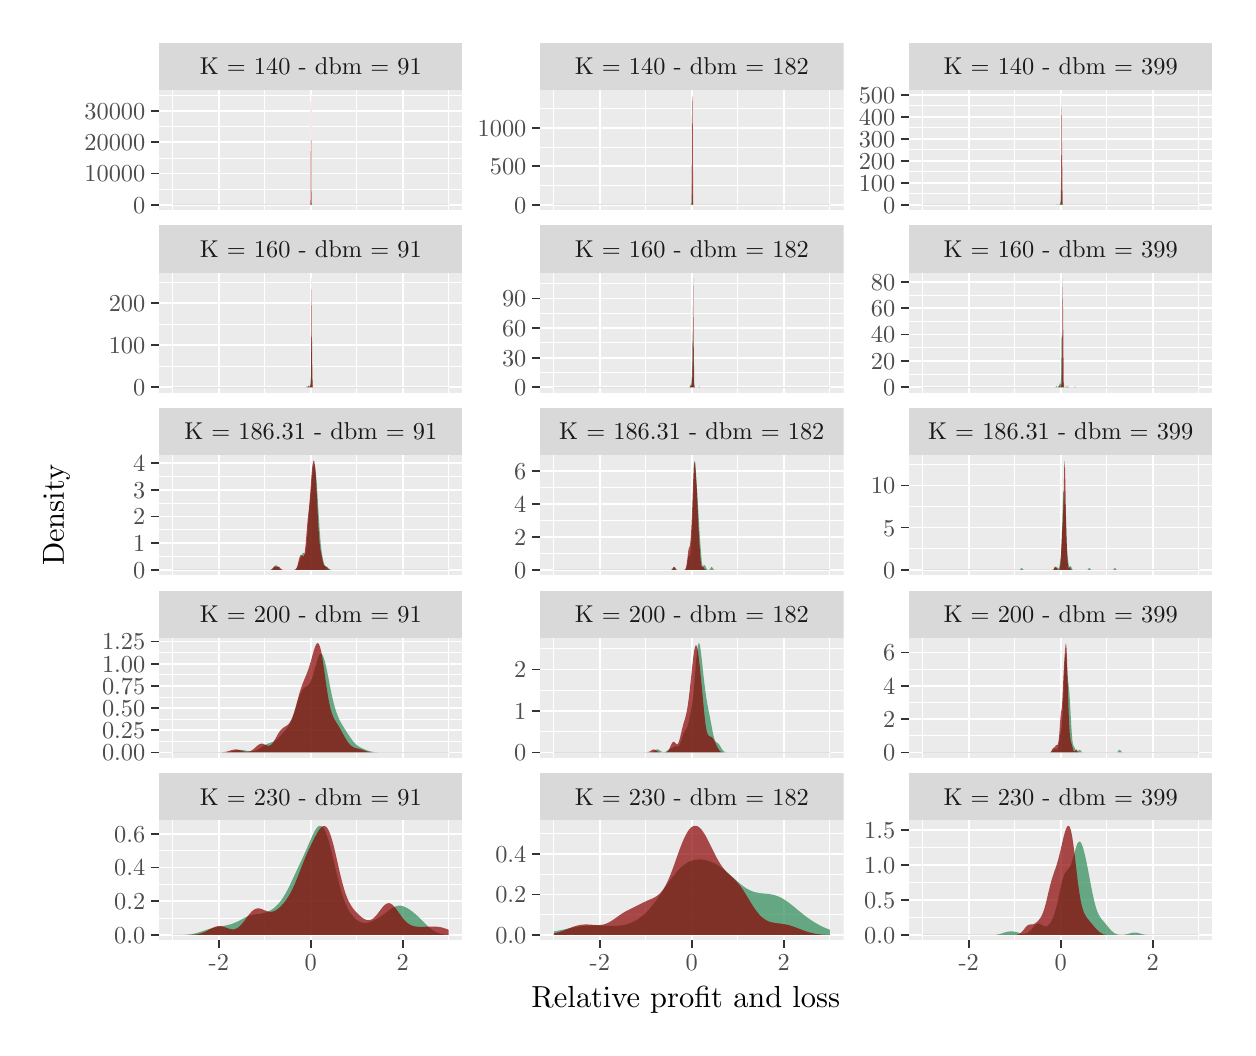
\begin{tikzpicture}[x=1pt,y=1pt]
\definecolor{fillColor}{RGB}{255,255,255}
\path[use as bounding box,fill=fillColor,fill opacity=0.00] (0,0) rectangle (433.62,361.35);
\begin{scope}
\path[clip] (  0.00,  0.00) rectangle (433.62,361.35);
\definecolor{drawColor}{RGB}{255,255,255}
\definecolor{fillColor}{RGB}{255,255,255}

\path[draw=drawColor,line width= 0.6pt,line join=round,line cap=round,fill=fillColor] (  0.00,  0.00) rectangle (433.62,361.35);
\end{scope}
\begin{scope}
\path[clip] ( 47.46,295.39) rectangle (157.12,338.79);
\definecolor{fillColor}{gray}{0.92}

\path[fill=fillColor] ( 47.46,295.39) rectangle (157.12,338.79);
\definecolor{drawColor}{RGB}{255,255,255}

\path[draw=drawColor,line width= 0.3pt,line join=round] ( 47.46,303.00) --
	(157.12,303.00);

\path[draw=drawColor,line width= 0.3pt,line join=round] ( 47.46,314.28) --
	(157.12,314.28);

\path[draw=drawColor,line width= 0.3pt,line join=round] ( 47.46,325.56) --
	(157.12,325.56);

\path[draw=drawColor,line width= 0.3pt,line join=round] ( 47.46,336.84) --
	(157.12,336.84);

\path[draw=drawColor,line width= 0.3pt,line join=round] ( 52.45,295.39) --
	( 52.45,338.79);

\path[draw=drawColor,line width= 0.3pt,line join=round] ( 85.68,295.39) --
	( 85.68,338.79);

\path[draw=drawColor,line width= 0.3pt,line join=round] (118.91,295.39) --
	(118.91,338.79);

\path[draw=drawColor,line width= 0.3pt,line join=round] (152.13,295.39) --
	(152.13,338.79);

\path[draw=drawColor,line width= 0.6pt,line join=round] ( 47.46,297.36) --
	(157.12,297.36);

\path[draw=drawColor,line width= 0.6pt,line join=round] ( 47.46,308.64) --
	(157.12,308.64);

\path[draw=drawColor,line width= 0.6pt,line join=round] ( 47.46,319.92) --
	(157.12,319.92);

\path[draw=drawColor,line width= 0.6pt,line join=round] ( 47.46,331.20) --
	(157.12,331.20);

\path[draw=drawColor,line width= 0.6pt,line join=round] ( 69.06,295.39) --
	( 69.06,338.79);

\path[draw=drawColor,line width= 0.6pt,line join=round] (102.29,295.39) --
	(102.29,338.79);

\path[draw=drawColor,line width= 0.6pt,line join=round] (135.52,295.39) --
	(135.52,338.79);
\definecolor{fillColor}{RGB}{46,139,87}

\path[fill=fillColor,fill opacity=0.70] ( 52.45,297.36) --
	( 52.64,297.36) --
	( 52.84,297.36) --
	( 53.03,297.36) --
	( 53.23,297.36) --
	( 53.42,297.36) --
	( 53.62,297.36) --
	( 53.81,297.36) --
	( 54.01,297.36) --
	( 54.20,297.36) --
	( 54.40,297.36) --
	( 54.59,297.36) --
	( 54.79,297.36) --
	( 54.98,297.36) --
	( 55.18,297.36) --
	( 55.38,297.36) --
	( 55.57,297.36) --
	( 55.77,297.36) --
	( 55.96,297.36) --
	( 56.16,297.36) --
	( 56.35,297.36) --
	( 56.55,297.36) --
	( 56.74,297.36) --
	( 56.94,297.36) --
	( 57.13,297.36) --
	( 57.33,297.36) --
	( 57.52,297.36) --
	( 57.72,297.36) --
	( 57.91,297.36) --
	( 58.11,297.36) --
	( 58.30,297.36) --
	( 58.50,297.36) --
	( 58.69,297.36) --
	( 58.89,297.36) --
	( 59.08,297.36) --
	( 59.28,297.36) --
	( 59.47,297.36) --
	( 59.67,297.36) --
	( 59.86,297.36) --
	( 60.06,297.36) --
	( 60.25,297.36) --
	( 60.45,297.36) --
	( 60.64,297.36) --
	( 60.84,297.36) --
	( 61.03,297.36) --
	( 61.23,297.36) --
	( 61.42,297.36) --
	( 61.62,297.36) --
	( 61.81,297.36) --
	( 62.01,297.36) --
	( 62.20,297.36) --
	( 62.40,297.36) --
	( 62.59,297.36) --
	( 62.79,297.36) --
	( 62.98,297.36) --
	( 63.18,297.36) --
	( 63.37,297.36) --
	( 63.57,297.36) --
	( 63.76,297.36) --
	( 63.96,297.36) --
	( 64.15,297.36) --
	( 64.35,297.36) --
	( 64.54,297.36) --
	( 64.74,297.36) --
	( 64.93,297.36) --
	( 65.13,297.36) --
	( 65.32,297.36) --
	( 65.52,297.36) --
	( 65.71,297.36) --
	( 65.91,297.36) --
	( 66.10,297.36) --
	( 66.30,297.36) --
	( 66.49,297.36) --
	( 66.69,297.36) --
	( 66.88,297.36) --
	( 67.08,297.36) --
	( 67.28,297.36) --
	( 67.47,297.36) --
	( 67.67,297.36) --
	( 67.86,297.36) --
	( 68.06,297.36) --
	( 68.25,297.36) --
	( 68.45,297.36) --
	( 68.64,297.36) --
	( 68.84,297.36) --
	( 69.03,297.36) --
	( 69.23,297.36) --
	( 69.42,297.36) --
	( 69.62,297.36) --
	( 69.81,297.36) --
	( 70.01,297.36) --
	( 70.20,297.36) --
	( 70.40,297.36) --
	( 70.59,297.36) --
	( 70.79,297.36) --
	( 70.98,297.36) --
	( 71.18,297.36) --
	( 71.37,297.36) --
	( 71.57,297.36) --
	( 71.76,297.36) --
	( 71.96,297.36) --
	( 72.15,297.36) --
	( 72.35,297.36) --
	( 72.54,297.36) --
	( 72.74,297.36) --
	( 72.93,297.36) --
	( 73.13,297.36) --
	( 73.32,297.36) --
	( 73.52,297.36) --
	( 73.71,297.36) --
	( 73.91,297.36) --
	( 74.10,297.36) --
	( 74.30,297.36) --
	( 74.49,297.36) --
	( 74.69,297.36) --
	( 74.88,297.36) --
	( 75.08,297.36) --
	( 75.27,297.36) --
	( 75.47,297.36) --
	( 75.66,297.36) --
	( 75.86,297.36) --
	( 76.05,297.36) --
	( 76.25,297.36) --
	( 76.44,297.36) --
	( 76.64,297.36) --
	( 76.83,297.36) --
	( 77.03,297.36) --
	( 77.22,297.36) --
	( 77.42,297.36) --
	( 77.61,297.36) --
	( 77.81,297.36) --
	( 78.00,297.36) --
	( 78.20,297.36) --
	( 78.39,297.36) --
	( 78.59,297.36) --
	( 78.78,297.36) --
	( 78.98,297.36) --
	( 79.17,297.36) --
	( 79.37,297.36) --
	( 79.57,297.36) --
	( 79.76,297.36) --
	( 79.96,297.36) --
	( 80.15,297.36) --
	( 80.35,297.36) --
	( 80.54,297.36) --
	( 80.74,297.36) --
	( 80.93,297.36) --
	( 81.13,297.36) --
	( 81.32,297.36) --
	( 81.52,297.36) --
	( 81.71,297.36) --
	( 81.91,297.36) --
	( 82.10,297.36) --
	( 82.30,297.36) --
	( 82.49,297.36) --
	( 82.69,297.36) --
	( 82.88,297.36) --
	( 83.08,297.36) --
	( 83.27,297.36) --
	( 83.47,297.36) --
	( 83.66,297.36) --
	( 83.86,297.36) --
	( 84.05,297.36) --
	( 84.25,297.36) --
	( 84.44,297.36) --
	( 84.64,297.36) --
	( 84.83,297.36) --
	( 85.03,297.36) --
	( 85.22,297.36) --
	( 85.42,297.36) --
	( 85.61,297.36) --
	( 85.81,297.36) --
	( 86.00,297.36) --
	( 86.20,297.36) --
	( 86.39,297.36) --
	( 86.59,297.36) --
	( 86.78,297.36) --
	( 86.98,297.36) --
	( 87.17,297.36) --
	( 87.37,297.36) --
	( 87.56,297.36) --
	( 87.76,297.36) --
	( 87.95,297.36) --
	( 88.15,297.36) --
	( 88.34,297.36) --
	( 88.54,297.36) --
	( 88.73,297.36) --
	( 88.93,297.36) --
	( 89.12,297.36) --
	( 89.32,297.36) --
	( 89.51,297.36) --
	( 89.71,297.36) --
	( 89.90,297.36) --
	( 90.10,297.36) --
	( 90.29,297.36) --
	( 90.49,297.36) --
	( 90.68,297.36) --
	( 90.88,297.36) --
	( 91.07,297.36) --
	( 91.27,297.36) --
	( 91.46,297.36) --
	( 91.66,297.36) --
	( 91.86,297.36) --
	( 92.05,297.36) --
	( 92.25,297.36) --
	( 92.44,297.36) --
	( 92.64,297.36) --
	( 92.83,297.36) --
	( 93.03,297.36) --
	( 93.22,297.36) --
	( 93.42,297.36) --
	( 93.61,297.36) --
	( 93.81,297.36) --
	( 94.00,297.36) --
	( 94.20,297.36) --
	( 94.39,297.36) --
	( 94.59,297.36) --
	( 94.78,297.36) --
	( 94.98,297.36) --
	( 95.17,297.36) --
	( 95.37,297.36) --
	( 95.56,297.36) --
	( 95.76,297.36) --
	( 95.95,297.36) --
	( 96.15,297.36) --
	( 96.34,297.36) --
	( 96.54,297.36) --
	( 96.73,297.36) --
	( 96.93,297.36) --
	( 97.12,297.36) --
	( 97.32,297.36) --
	( 97.51,297.36) --
	( 97.71,297.36) --
	( 97.90,297.36) --
	( 98.10,297.36) --
	( 98.29,297.36) --
	( 98.49,297.36) --
	( 98.68,297.36) --
	( 98.88,297.36) --
	( 99.07,297.36) --
	( 99.27,297.36) --
	( 99.46,297.36) --
	( 99.66,297.36) --
	( 99.85,297.36) --
	(100.05,297.36) --
	(100.24,297.36) --
	(100.44,297.36) --
	(100.63,297.36) --
	(100.83,297.36) --
	(101.02,297.36) --
	(101.22,297.36) --
	(101.41,297.36) --
	(101.61,297.36) --
	(101.80,297.36) --
	(102.00,297.37) --
	(102.19,297.47) --
	(102.39,297.98) --
	(102.58,297.37) --
	(102.78,297.36) --
	(102.97,297.36) --
	(103.17,297.36) --
	(103.36,297.36) --
	(103.56,297.36) --
	(103.75,297.36) --
	(103.95,297.36) --
	(104.15,297.36) --
	(104.34,297.36) --
	(104.54,297.36) --
	(104.73,297.36) --
	(104.93,297.36) --
	(105.12,297.36) --
	(105.32,297.36) --
	(105.51,297.36) --
	(105.71,297.36) --
	(105.90,297.36) --
	(106.10,297.36) --
	(106.29,297.36) --
	(106.49,297.36) --
	(106.68,297.36) --
	(106.88,297.36) --
	(107.07,297.36) --
	(107.27,297.36) --
	(107.46,297.36) --
	(107.66,297.36) --
	(107.85,297.36) --
	(108.05,297.36) --
	(108.24,297.36) --
	(108.44,297.36) --
	(108.63,297.36) --
	(108.83,297.36) --
	(109.02,297.36) --
	(109.22,297.36) --
	(109.41,297.36) --
	(109.61,297.36) --
	(109.80,297.36) --
	(110.00,297.36) --
	(110.19,297.36) --
	(110.39,297.36) --
	(110.58,297.36) --
	(110.78,297.36) --
	(110.97,297.36) --
	(111.17,297.36) --
	(111.36,297.36) --
	(111.56,297.36) --
	(111.75,297.36) --
	(111.95,297.36) --
	(112.14,297.36) --
	(112.34,297.36) --
	(112.53,297.36) --
	(112.73,297.36) --
	(112.92,297.36) --
	(113.12,297.36) --
	(113.31,297.36) --
	(113.51,297.36) --
	(113.70,297.36) --
	(113.90,297.36) --
	(114.09,297.36) --
	(114.29,297.36) --
	(114.48,297.36) --
	(114.68,297.36) --
	(114.87,297.36) --
	(115.07,297.36) --
	(115.26,297.36) --
	(115.46,297.36) --
	(115.65,297.36) --
	(115.85,297.36) --
	(116.04,297.36) --
	(116.24,297.36) --
	(116.44,297.36) --
	(116.63,297.36) --
	(116.83,297.36) --
	(117.02,297.36) --
	(117.22,297.36) --
	(117.41,297.36) --
	(117.61,297.36) --
	(117.80,297.36) --
	(118.00,297.36) --
	(118.19,297.36) --
	(118.39,297.36) --
	(118.58,297.36) --
	(118.78,297.36) --
	(118.97,297.36) --
	(119.17,297.36) --
	(119.36,297.36) --
	(119.56,297.36) --
	(119.75,297.36) --
	(119.95,297.36) --
	(120.14,297.36) --
	(120.34,297.36) --
	(120.53,297.36) --
	(120.73,297.36) --
	(120.92,297.36) --
	(121.12,297.36) --
	(121.31,297.36) --
	(121.51,297.36) --
	(121.70,297.36) --
	(121.90,297.36) --
	(122.09,297.36) --
	(122.29,297.36) --
	(122.48,297.36) --
	(122.68,297.36) --
	(122.87,297.36) --
	(123.07,297.36) --
	(123.26,297.36) --
	(123.46,297.36) --
	(123.65,297.36) --
	(123.85,297.36) --
	(124.04,297.36) --
	(124.24,297.36) --
	(124.43,297.36) --
	(124.63,297.36) --
	(124.82,297.36) --
	(125.02,297.36) --
	(125.21,297.36) --
	(125.41,297.36) --
	(125.60,297.36) --
	(125.80,297.36) --
	(125.99,297.36) --
	(126.19,297.36) --
	(126.38,297.36) --
	(126.58,297.36) --
	(126.77,297.36) --
	(126.97,297.36) --
	(127.16,297.36) --
	(127.36,297.36) --
	(127.55,297.36) --
	(127.75,297.36) --
	(127.94,297.36) --
	(128.14,297.36) --
	(128.33,297.36) --
	(128.53,297.36) --
	(128.73,297.36) --
	(128.92,297.36) --
	(129.12,297.36) --
	(129.31,297.36) --
	(129.51,297.36) --
	(129.70,297.36) --
	(129.90,297.36) --
	(130.09,297.36) --
	(130.29,297.36) --
	(130.48,297.36) --
	(130.68,297.36) --
	(130.87,297.36) --
	(131.07,297.36) --
	(131.26,297.36) --
	(131.46,297.36) --
	(131.65,297.36) --
	(131.85,297.36) --
	(132.04,297.36) --
	(132.24,297.36) --
	(132.43,297.36) --
	(132.63,297.36) --
	(132.82,297.36) --
	(133.02,297.36) --
	(133.21,297.36) --
	(133.41,297.36) --
	(133.60,297.36) --
	(133.80,297.36) --
	(133.99,297.36) --
	(134.19,297.36) --
	(134.38,297.36) --
	(134.58,297.36) --
	(134.77,297.36) --
	(134.97,297.36) --
	(135.16,297.36) --
	(135.36,297.36) --
	(135.55,297.36) --
	(135.75,297.36) --
	(135.94,297.36) --
	(136.14,297.36) --
	(136.33,297.36) --
	(136.53,297.36) --
	(136.72,297.36) --
	(136.92,297.36) --
	(137.11,297.36) --
	(137.31,297.36) --
	(137.50,297.36) --
	(137.70,297.36) --
	(137.89,297.36) --
	(138.09,297.36) --
	(138.28,297.36) --
	(138.48,297.36) --
	(138.67,297.36) --
	(138.87,297.36) --
	(139.06,297.36) --
	(139.26,297.36) --
	(139.45,297.36) --
	(139.65,297.36) --
	(139.84,297.36) --
	(140.04,297.36) --
	(140.23,297.36) --
	(140.43,297.36) --
	(140.62,297.36) --
	(140.82,297.36) --
	(141.02,297.36) --
	(141.21,297.36) --
	(141.41,297.36) --
	(141.60,297.36) --
	(141.80,297.36) --
	(141.99,297.36) --
	(142.19,297.36) --
	(142.38,297.36) --
	(142.58,297.36) --
	(142.77,297.36) --
	(142.97,297.36) --
	(143.16,297.36) --
	(143.36,297.36) --
	(143.55,297.36) --
	(143.75,297.36) --
	(143.94,297.36) --
	(144.14,297.36) --
	(144.33,297.36) --
	(144.53,297.36) --
	(144.72,297.36) --
	(144.92,297.36) --
	(145.11,297.36) --
	(145.31,297.36) --
	(145.50,297.36) --
	(145.70,297.36) --
	(145.89,297.36) --
	(146.09,297.36) --
	(146.28,297.36) --
	(146.48,297.36) --
	(146.67,297.36) --
	(146.87,297.36) --
	(147.06,297.36) --
	(147.26,297.36) --
	(147.45,297.36) --
	(147.65,297.36) --
	(147.84,297.36) --
	(148.04,297.36) --
	(148.23,297.36) --
	(148.43,297.36) --
	(148.62,297.36) --
	(148.82,297.36) --
	(149.01,297.36) --
	(149.21,297.36) --
	(149.40,297.36) --
	(149.60,297.36) --
	(149.79,297.36) --
	(149.99,297.36) --
	(150.18,297.36) --
	(150.38,297.36) --
	(150.57,297.36) --
	(150.77,297.36) --
	(150.96,297.36) --
	(151.16,297.36) --
	(151.35,297.36) --
	(151.55,297.36) --
	(151.74,297.36) --
	(151.94,297.36) --
	(152.13,297.36) --
	(152.13,297.36) --
	(151.94,297.36) --
	(151.74,297.36) --
	(151.55,297.36) --
	(151.35,297.36) --
	(151.16,297.36) --
	(150.96,297.36) --
	(150.77,297.36) --
	(150.57,297.36) --
	(150.38,297.36) --
	(150.18,297.36) --
	(149.99,297.36) --
	(149.79,297.36) --
	(149.60,297.36) --
	(149.40,297.36) --
	(149.21,297.36) --
	(149.01,297.36) --
	(148.82,297.36) --
	(148.62,297.36) --
	(148.43,297.36) --
	(148.23,297.36) --
	(148.04,297.36) --
	(147.84,297.36) --
	(147.65,297.36) --
	(147.45,297.36) --
	(147.26,297.36) --
	(147.06,297.36) --
	(146.87,297.36) --
	(146.67,297.36) --
	(146.48,297.36) --
	(146.28,297.36) --
	(146.09,297.36) --
	(145.89,297.36) --
	(145.70,297.36) --
	(145.50,297.36) --
	(145.31,297.36) --
	(145.11,297.36) --
	(144.92,297.36) --
	(144.72,297.36) --
	(144.53,297.36) --
	(144.33,297.36) --
	(144.14,297.36) --
	(143.94,297.36) --
	(143.75,297.36) --
	(143.55,297.36) --
	(143.36,297.36) --
	(143.16,297.36) --
	(142.97,297.36) --
	(142.77,297.36) --
	(142.58,297.36) --
	(142.38,297.36) --
	(142.19,297.36) --
	(141.99,297.36) --
	(141.80,297.36) --
	(141.60,297.36) --
	(141.41,297.36) --
	(141.21,297.36) --
	(141.02,297.36) --
	(140.82,297.36) --
	(140.62,297.36) --
	(140.43,297.36) --
	(140.23,297.36) --
	(140.04,297.36) --
	(139.84,297.36) --
	(139.65,297.36) --
	(139.45,297.36) --
	(139.26,297.36) --
	(139.06,297.36) --
	(138.87,297.36) --
	(138.67,297.36) --
	(138.48,297.36) --
	(138.28,297.36) --
	(138.09,297.36) --
	(137.89,297.36) --
	(137.70,297.36) --
	(137.50,297.36) --
	(137.31,297.36) --
	(137.11,297.36) --
	(136.92,297.36) --
	(136.72,297.36) --
	(136.53,297.36) --
	(136.33,297.36) --
	(136.14,297.36) --
	(135.94,297.36) --
	(135.75,297.36) --
	(135.55,297.36) --
	(135.36,297.36) --
	(135.16,297.36) --
	(134.97,297.36) --
	(134.77,297.36) --
	(134.58,297.36) --
	(134.38,297.36) --
	(134.19,297.36) --
	(133.99,297.36) --
	(133.80,297.36) --
	(133.60,297.36) --
	(133.41,297.36) --
	(133.21,297.36) --
	(133.02,297.36) --
	(132.82,297.36) --
	(132.63,297.36) --
	(132.43,297.36) --
	(132.24,297.36) --
	(132.04,297.36) --
	(131.85,297.36) --
	(131.65,297.36) --
	(131.46,297.36) --
	(131.26,297.36) --
	(131.07,297.36) --
	(130.87,297.36) --
	(130.68,297.36) --
	(130.48,297.36) --
	(130.29,297.36) --
	(130.09,297.36) --
	(129.90,297.36) --
	(129.70,297.36) --
	(129.51,297.36) --
	(129.31,297.36) --
	(129.12,297.36) --
	(128.92,297.36) --
	(128.73,297.36) --
	(128.53,297.36) --
	(128.33,297.36) --
	(128.14,297.36) --
	(127.94,297.36) --
	(127.75,297.36) --
	(127.55,297.36) --
	(127.36,297.36) --
	(127.16,297.36) --
	(126.97,297.36) --
	(126.77,297.36) --
	(126.58,297.36) --
	(126.38,297.36) --
	(126.19,297.36) --
	(125.99,297.36) --
	(125.80,297.36) --
	(125.60,297.36) --
	(125.41,297.36) --
	(125.21,297.36) --
	(125.02,297.36) --
	(124.82,297.36) --
	(124.63,297.36) --
	(124.43,297.36) --
	(124.24,297.36) --
	(124.04,297.36) --
	(123.85,297.36) --
	(123.65,297.36) --
	(123.46,297.36) --
	(123.26,297.36) --
	(123.07,297.36) --
	(122.87,297.36) --
	(122.68,297.36) --
	(122.48,297.36) --
	(122.29,297.36) --
	(122.09,297.36) --
	(121.90,297.36) --
	(121.70,297.36) --
	(121.51,297.36) --
	(121.31,297.36) --
	(121.12,297.36) --
	(120.92,297.36) --
	(120.73,297.36) --
	(120.53,297.36) --
	(120.34,297.36) --
	(120.14,297.36) --
	(119.95,297.36) --
	(119.75,297.36) --
	(119.56,297.36) --
	(119.36,297.36) --
	(119.17,297.36) --
	(118.97,297.36) --
	(118.78,297.36) --
	(118.58,297.36) --
	(118.39,297.36) --
	(118.19,297.36) --
	(118.00,297.36) --
	(117.80,297.36) --
	(117.61,297.36) --
	(117.41,297.36) --
	(117.22,297.36) --
	(117.02,297.36) --
	(116.83,297.36) --
	(116.63,297.36) --
	(116.44,297.36) --
	(116.24,297.36) --
	(116.04,297.36) --
	(115.85,297.36) --
	(115.65,297.36) --
	(115.46,297.36) --
	(115.26,297.36) --
	(115.07,297.36) --
	(114.87,297.36) --
	(114.68,297.36) --
	(114.48,297.36) --
	(114.29,297.36) --
	(114.09,297.36) --
	(113.90,297.36) --
	(113.70,297.36) --
	(113.51,297.36) --
	(113.31,297.36) --
	(113.12,297.36) --
	(112.92,297.36) --
	(112.73,297.36) --
	(112.53,297.36) --
	(112.34,297.36) --
	(112.14,297.36) --
	(111.95,297.36) --
	(111.75,297.36) --
	(111.56,297.36) --
	(111.36,297.36) --
	(111.17,297.36) --
	(110.97,297.36) --
	(110.78,297.36) --
	(110.58,297.36) --
	(110.39,297.36) --
	(110.19,297.36) --
	(110.00,297.36) --
	(109.80,297.36) --
	(109.61,297.36) --
	(109.41,297.36) --
	(109.22,297.36) --
	(109.02,297.36) --
	(108.83,297.36) --
	(108.63,297.36) --
	(108.44,297.36) --
	(108.24,297.36) --
	(108.05,297.36) --
	(107.85,297.36) --
	(107.66,297.36) --
	(107.46,297.36) --
	(107.27,297.36) --
	(107.07,297.36) --
	(106.88,297.36) --
	(106.68,297.36) --
	(106.49,297.36) --
	(106.29,297.36) --
	(106.10,297.36) --
	(105.90,297.36) --
	(105.71,297.36) --
	(105.51,297.36) --
	(105.32,297.36) --
	(105.12,297.36) --
	(104.93,297.36) --
	(104.73,297.36) --
	(104.54,297.36) --
	(104.34,297.36) --
	(104.15,297.36) --
	(103.95,297.36) --
	(103.75,297.36) --
	(103.56,297.36) --
	(103.36,297.36) --
	(103.17,297.36) --
	(102.97,297.36) --
	(102.78,297.36) --
	(102.58,297.36) --
	(102.39,297.36) --
	(102.19,297.36) --
	(102.00,297.36) --
	(101.80,297.36) --
	(101.61,297.36) --
	(101.41,297.36) --
	(101.22,297.36) --
	(101.02,297.36) --
	(100.83,297.36) --
	(100.63,297.36) --
	(100.44,297.36) --
	(100.24,297.36) --
	(100.05,297.36) --
	( 99.85,297.36) --
	( 99.66,297.36) --
	( 99.46,297.36) --
	( 99.27,297.36) --
	( 99.07,297.36) --
	( 98.88,297.36) --
	( 98.68,297.36) --
	( 98.49,297.36) --
	( 98.29,297.36) --
	( 98.10,297.36) --
	( 97.90,297.36) --
	( 97.71,297.36) --
	( 97.51,297.36) --
	( 97.32,297.36) --
	( 97.12,297.36) --
	( 96.93,297.36) --
	( 96.73,297.36) --
	( 96.54,297.36) --
	( 96.34,297.36) --
	( 96.15,297.36) --
	( 95.95,297.36) --
	( 95.76,297.36) --
	( 95.56,297.36) --
	( 95.37,297.36) --
	( 95.17,297.36) --
	( 94.98,297.36) --
	( 94.78,297.36) --
	( 94.59,297.36) --
	( 94.39,297.36) --
	( 94.20,297.36) --
	( 94.00,297.36) --
	( 93.81,297.36) --
	( 93.61,297.36) --
	( 93.42,297.36) --
	( 93.22,297.36) --
	( 93.03,297.36) --
	( 92.83,297.36) --
	( 92.64,297.36) --
	( 92.44,297.36) --
	( 92.25,297.36) --
	( 92.05,297.36) --
	( 91.86,297.36) --
	( 91.66,297.36) --
	( 91.46,297.36) --
	( 91.27,297.36) --
	( 91.07,297.36) --
	( 90.88,297.36) --
	( 90.68,297.36) --
	( 90.49,297.36) --
	( 90.29,297.36) --
	( 90.10,297.36) --
	( 89.90,297.36) --
	( 89.71,297.36) --
	( 89.51,297.36) --
	( 89.32,297.36) --
	( 89.12,297.36) --
	( 88.93,297.36) --
	( 88.73,297.36) --
	( 88.54,297.36) --
	( 88.34,297.36) --
	( 88.15,297.36) --
	( 87.95,297.36) --
	( 87.76,297.36) --
	( 87.56,297.36) --
	( 87.37,297.36) --
	( 87.17,297.36) --
	( 86.98,297.36) --
	( 86.78,297.36) --
	( 86.59,297.36) --
	( 86.39,297.36) --
	( 86.20,297.36) --
	( 86.00,297.36) --
	( 85.81,297.36) --
	( 85.61,297.36) --
	( 85.42,297.36) --
	( 85.22,297.36) --
	( 85.03,297.36) --
	( 84.83,297.36) --
	( 84.64,297.36) --
	( 84.44,297.36) --
	( 84.25,297.36) --
	( 84.05,297.36) --
	( 83.86,297.36) --
	( 83.66,297.36) --
	( 83.47,297.36) --
	( 83.27,297.36) --
	( 83.08,297.36) --
	( 82.88,297.36) --
	( 82.69,297.36) --
	( 82.49,297.36) --
	( 82.30,297.36) --
	( 82.10,297.36) --
	( 81.91,297.36) --
	( 81.71,297.36) --
	( 81.52,297.36) --
	( 81.32,297.36) --
	( 81.13,297.36) --
	( 80.93,297.36) --
	( 80.74,297.36) --
	( 80.54,297.36) --
	( 80.35,297.36) --
	( 80.15,297.36) --
	( 79.96,297.36) --
	( 79.76,297.36) --
	( 79.57,297.36) --
	( 79.37,297.36) --
	( 79.17,297.36) --
	( 78.98,297.36) --
	( 78.78,297.36) --
	( 78.59,297.36) --
	( 78.39,297.36) --
	( 78.20,297.36) --
	( 78.00,297.36) --
	( 77.81,297.36) --
	( 77.61,297.36) --
	( 77.42,297.36) --
	( 77.22,297.36) --
	( 77.03,297.36) --
	( 76.83,297.36) --
	( 76.64,297.36) --
	( 76.44,297.36) --
	( 76.25,297.36) --
	( 76.05,297.36) --
	( 75.86,297.36) --
	( 75.66,297.36) --
	( 75.47,297.36) --
	( 75.27,297.36) --
	( 75.08,297.36) --
	( 74.88,297.36) --
	( 74.69,297.36) --
	( 74.49,297.36) --
	( 74.30,297.36) --
	( 74.10,297.36) --
	( 73.91,297.36) --
	( 73.71,297.36) --
	( 73.52,297.36) --
	( 73.32,297.36) --
	( 73.13,297.36) --
	( 72.93,297.36) --
	( 72.74,297.36) --
	( 72.54,297.36) --
	( 72.35,297.36) --
	( 72.15,297.36) --
	( 71.96,297.36) --
	( 71.76,297.36) --
	( 71.57,297.36) --
	( 71.37,297.36) --
	( 71.18,297.36) --
	( 70.98,297.36) --
	( 70.79,297.36) --
	( 70.59,297.36) --
	( 70.40,297.36) --
	( 70.20,297.36) --
	( 70.01,297.36) --
	( 69.81,297.36) --
	( 69.62,297.36) --
	( 69.42,297.36) --
	( 69.23,297.36) --
	( 69.03,297.36) --
	( 68.84,297.36) --
	( 68.64,297.36) --
	( 68.45,297.36) --
	( 68.25,297.36) --
	( 68.06,297.36) --
	( 67.86,297.36) --
	( 67.67,297.36) --
	( 67.47,297.36) --
	( 67.28,297.36) --
	( 67.08,297.36) --
	( 66.88,297.36) --
	( 66.69,297.36) --
	( 66.49,297.36) --
	( 66.30,297.36) --
	( 66.10,297.36) --
	( 65.91,297.36) --
	( 65.71,297.36) --
	( 65.52,297.36) --
	( 65.32,297.36) --
	( 65.13,297.36) --
	( 64.93,297.36) --
	( 64.74,297.36) --
	( 64.54,297.36) --
	( 64.35,297.36) --
	( 64.15,297.36) --
	( 63.96,297.36) --
	( 63.76,297.36) --
	( 63.57,297.36) --
	( 63.37,297.36) --
	( 63.18,297.36) --
	( 62.98,297.36) --
	( 62.79,297.36) --
	( 62.59,297.36) --
	( 62.40,297.36) --
	( 62.20,297.36) --
	( 62.01,297.36) --
	( 61.81,297.36) --
	( 61.62,297.36) --
	( 61.42,297.36) --
	( 61.23,297.36) --
	( 61.03,297.36) --
	( 60.84,297.36) --
	( 60.64,297.36) --
	( 60.45,297.36) --
	( 60.25,297.36) --
	( 60.06,297.36) --
	( 59.86,297.36) --
	( 59.67,297.36) --
	( 59.47,297.36) --
	( 59.28,297.36) --
	( 59.08,297.36) --
	( 58.89,297.36) --
	( 58.69,297.36) --
	( 58.50,297.36) --
	( 58.30,297.36) --
	( 58.11,297.36) --
	( 57.91,297.36) --
	( 57.72,297.36) --
	( 57.52,297.36) --
	( 57.33,297.36) --
	( 57.13,297.36) --
	( 56.94,297.36) --
	( 56.74,297.36) --
	( 56.55,297.36) --
	( 56.35,297.36) --
	( 56.16,297.36) --
	( 55.96,297.36) --
	( 55.77,297.36) --
	( 55.57,297.36) --
	( 55.38,297.36) --
	( 55.18,297.36) --
	( 54.98,297.36) --
	( 54.79,297.36) --
	( 54.59,297.36) --
	( 54.40,297.36) --
	( 54.20,297.36) --
	( 54.01,297.36) --
	( 53.81,297.36) --
	( 53.62,297.36) --
	( 53.42,297.36) --
	( 53.23,297.36) --
	( 53.03,297.36) --
	( 52.84,297.36) --
	( 52.64,297.36) --
	( 52.45,297.36) --
	cycle;
\definecolor{fillColor}{RGB}{139,0,0}

\path[fill=fillColor,fill opacity=0.70] ( 52.45,297.36) --
	( 52.64,297.36) --
	( 52.84,297.36) --
	( 53.03,297.36) --
	( 53.23,297.36) --
	( 53.42,297.36) --
	( 53.62,297.36) --
	( 53.81,297.36) --
	( 54.01,297.36) --
	( 54.20,297.36) --
	( 54.40,297.36) --
	( 54.59,297.36) --
	( 54.79,297.36) --
	( 54.98,297.36) --
	( 55.18,297.36) --
	( 55.38,297.36) --
	( 55.57,297.36) --
	( 55.77,297.36) --
	( 55.96,297.36) --
	( 56.16,297.36) --
	( 56.35,297.36) --
	( 56.55,297.36) --
	( 56.74,297.36) --
	( 56.94,297.36) --
	( 57.13,297.36) --
	( 57.33,297.36) --
	( 57.52,297.36) --
	( 57.72,297.36) --
	( 57.91,297.36) --
	( 58.11,297.36) --
	( 58.30,297.36) --
	( 58.50,297.36) --
	( 58.69,297.36) --
	( 58.89,297.36) --
	( 59.08,297.36) --
	( 59.28,297.36) --
	( 59.47,297.36) --
	( 59.67,297.36) --
	( 59.86,297.36) --
	( 60.06,297.36) --
	( 60.25,297.36) --
	( 60.45,297.36) --
	( 60.64,297.36) --
	( 60.84,297.36) --
	( 61.03,297.36) --
	( 61.23,297.36) --
	( 61.42,297.36) --
	( 61.62,297.36) --
	( 61.81,297.36) --
	( 62.01,297.36) --
	( 62.20,297.36) --
	( 62.40,297.36) --
	( 62.59,297.36) --
	( 62.79,297.36) --
	( 62.98,297.36) --
	( 63.18,297.36) --
	( 63.37,297.36) --
	( 63.57,297.36) --
	( 63.76,297.36) --
	( 63.96,297.36) --
	( 64.15,297.36) --
	( 64.35,297.36) --
	( 64.54,297.36) --
	( 64.74,297.36) --
	( 64.93,297.36) --
	( 65.13,297.36) --
	( 65.32,297.36) --
	( 65.52,297.36) --
	( 65.71,297.36) --
	( 65.91,297.36) --
	( 66.10,297.36) --
	( 66.30,297.36) --
	( 66.49,297.36) --
	( 66.69,297.36) --
	( 66.88,297.36) --
	( 67.08,297.36) --
	( 67.28,297.36) --
	( 67.47,297.36) --
	( 67.67,297.36) --
	( 67.86,297.36) --
	( 68.06,297.36) --
	( 68.25,297.36) --
	( 68.45,297.36) --
	( 68.64,297.36) --
	( 68.84,297.36) --
	( 69.03,297.36) --
	( 69.23,297.36) --
	( 69.42,297.36) --
	( 69.62,297.36) --
	( 69.81,297.36) --
	( 70.01,297.36) --
	( 70.20,297.36) --
	( 70.40,297.36) --
	( 70.59,297.36) --
	( 70.79,297.36) --
	( 70.98,297.36) --
	( 71.18,297.36) --
	( 71.37,297.36) --
	( 71.57,297.36) --
	( 71.76,297.36) --
	( 71.96,297.36) --
	( 72.15,297.36) --
	( 72.35,297.36) --
	( 72.54,297.36) --
	( 72.74,297.36) --
	( 72.93,297.36) --
	( 73.13,297.36) --
	( 73.32,297.36) --
	( 73.52,297.36) --
	( 73.71,297.36) --
	( 73.91,297.36) --
	( 74.10,297.36) --
	( 74.30,297.36) --
	( 74.49,297.36) --
	( 74.69,297.36) --
	( 74.88,297.36) --
	( 75.08,297.36) --
	( 75.27,297.36) --
	( 75.47,297.36) --
	( 75.66,297.36) --
	( 75.86,297.36) --
	( 76.05,297.36) --
	( 76.25,297.36) --
	( 76.44,297.36) --
	( 76.64,297.36) --
	( 76.83,297.36) --
	( 77.03,297.36) --
	( 77.22,297.36) --
	( 77.42,297.36) --
	( 77.61,297.36) --
	( 77.81,297.36) --
	( 78.00,297.36) --
	( 78.20,297.36) --
	( 78.39,297.36) --
	( 78.59,297.36) --
	( 78.78,297.36) --
	( 78.98,297.36) --
	( 79.17,297.36) --
	( 79.37,297.36) --
	( 79.57,297.36) --
	( 79.76,297.36) --
	( 79.96,297.36) --
	( 80.15,297.36) --
	( 80.35,297.36) --
	( 80.54,297.36) --
	( 80.74,297.36) --
	( 80.93,297.36) --
	( 81.13,297.36) --
	( 81.32,297.36) --
	( 81.52,297.36) --
	( 81.71,297.36) --
	( 81.91,297.36) --
	( 82.10,297.36) --
	( 82.30,297.36) --
	( 82.49,297.36) --
	( 82.69,297.36) --
	( 82.88,297.36) --
	( 83.08,297.36) --
	( 83.27,297.36) --
	( 83.47,297.36) --
	( 83.66,297.36) --
	( 83.86,297.36) --
	( 84.05,297.36) --
	( 84.25,297.36) --
	( 84.44,297.36) --
	( 84.64,297.36) --
	( 84.83,297.36) --
	( 85.03,297.36) --
	( 85.22,297.36) --
	( 85.42,297.36) --
	( 85.61,297.36) --
	( 85.81,297.36) --
	( 86.00,297.36) --
	( 86.20,297.36) --
	( 86.39,297.36) --
	( 86.59,297.36) --
	( 86.78,297.36) --
	( 86.98,297.36) --
	( 87.17,297.36) --
	( 87.37,297.36) --
	( 87.56,297.36) --
	( 87.76,297.36) --
	( 87.95,297.36) --
	( 88.15,297.36) --
	( 88.34,297.36) --
	( 88.54,297.36) --
	( 88.73,297.36) --
	( 88.93,297.36) --
	( 89.12,297.36) --
	( 89.32,297.36) --
	( 89.51,297.36) --
	( 89.71,297.36) --
	( 89.90,297.36) --
	( 90.10,297.36) --
	( 90.29,297.36) --
	( 90.49,297.36) --
	( 90.68,297.36) --
	( 90.88,297.36) --
	( 91.07,297.36) --
	( 91.27,297.36) --
	( 91.46,297.36) --
	( 91.66,297.36) --
	( 91.86,297.36) --
	( 92.05,297.36) --
	( 92.25,297.36) --
	( 92.44,297.36) --
	( 92.64,297.36) --
	( 92.83,297.36) --
	( 93.03,297.36) --
	( 93.22,297.36) --
	( 93.42,297.36) --
	( 93.61,297.36) --
	( 93.81,297.36) --
	( 94.00,297.36) --
	( 94.20,297.36) --
	( 94.39,297.36) --
	( 94.59,297.36) --
	( 94.78,297.36) --
	( 94.98,297.36) --
	( 95.17,297.36) --
	( 95.37,297.36) --
	( 95.56,297.36) --
	( 95.76,297.36) --
	( 95.95,297.36) --
	( 96.15,297.36) --
	( 96.34,297.36) --
	( 96.54,297.36) --
	( 96.73,297.36) --
	( 96.93,297.36) --
	( 97.12,297.36) --
	( 97.32,297.36) --
	( 97.51,297.36) --
	( 97.71,297.36) --
	( 97.90,297.36) --
	( 98.10,297.36) --
	( 98.29,297.36) --
	( 98.49,297.36) --
	( 98.68,297.36) --
	( 98.88,297.36) --
	( 99.07,297.36) --
	( 99.27,297.36) --
	( 99.46,297.36) --
	( 99.66,297.36) --
	( 99.85,297.36) --
	(100.05,297.36) --
	(100.24,297.36) --
	(100.44,297.36) --
	(100.63,297.36) --
	(100.83,297.36) --
	(101.02,297.36) --
	(101.22,297.36) --
	(101.41,297.36) --
	(101.61,297.36) --
	(101.80,297.36) --
	(102.00,297.36) --
	(102.19,297.47) --
	(102.39,336.82) --
	(102.58,297.88) --
	(102.78,297.36) --
	(102.97,297.36) --
	(103.17,297.36) --
	(103.36,297.36) --
	(103.56,297.36) --
	(103.75,297.36) --
	(103.95,297.36) --
	(104.15,297.36) --
	(104.34,297.36) --
	(104.54,297.36) --
	(104.73,297.36) --
	(104.93,297.36) --
	(105.12,297.36) --
	(105.32,297.36) --
	(105.51,297.36) --
	(105.71,297.36) --
	(105.90,297.36) --
	(106.10,297.36) --
	(106.29,297.36) --
	(106.49,297.36) --
	(106.68,297.36) --
	(106.88,297.36) --
	(107.07,297.36) --
	(107.27,297.36) --
	(107.46,297.36) --
	(107.66,297.36) --
	(107.85,297.36) --
	(108.05,297.36) --
	(108.24,297.36) --
	(108.44,297.36) --
	(108.63,297.36) --
	(108.83,297.36) --
	(109.02,297.36) --
	(109.22,297.36) --
	(109.41,297.36) --
	(109.61,297.36) --
	(109.80,297.36) --
	(110.00,297.36) --
	(110.19,297.36) --
	(110.39,297.36) --
	(110.58,297.36) --
	(110.78,297.36) --
	(110.97,297.36) --
	(111.17,297.36) --
	(111.36,297.36) --
	(111.56,297.36) --
	(111.75,297.36) --
	(111.95,297.36) --
	(112.14,297.36) --
	(112.34,297.36) --
	(112.53,297.36) --
	(112.73,297.36) --
	(112.92,297.36) --
	(113.12,297.36) --
	(113.31,297.36) --
	(113.51,297.36) --
	(113.70,297.36) --
	(113.90,297.36) --
	(114.09,297.36) --
	(114.29,297.36) --
	(114.48,297.36) --
	(114.68,297.36) --
	(114.87,297.36) --
	(115.07,297.36) --
	(115.26,297.36) --
	(115.46,297.36) --
	(115.65,297.36) --
	(115.85,297.36) --
	(116.04,297.36) --
	(116.24,297.36) --
	(116.44,297.36) --
	(116.63,297.36) --
	(116.83,297.36) --
	(117.02,297.36) --
	(117.22,297.36) --
	(117.41,297.36) --
	(117.61,297.36) --
	(117.80,297.36) --
	(118.00,297.36) --
	(118.19,297.36) --
	(118.39,297.36) --
	(118.58,297.36) --
	(118.78,297.36) --
	(118.97,297.36) --
	(119.17,297.36) --
	(119.36,297.36) --
	(119.56,297.36) --
	(119.75,297.36) --
	(119.95,297.36) --
	(120.14,297.36) --
	(120.34,297.36) --
	(120.53,297.36) --
	(120.73,297.36) --
	(120.92,297.36) --
	(121.12,297.36) --
	(121.31,297.36) --
	(121.51,297.36) --
	(121.70,297.36) --
	(121.90,297.36) --
	(122.09,297.36) --
	(122.29,297.36) --
	(122.48,297.36) --
	(122.68,297.36) --
	(122.87,297.36) --
	(123.07,297.36) --
	(123.26,297.36) --
	(123.46,297.36) --
	(123.65,297.36) --
	(123.85,297.36) --
	(124.04,297.36) --
	(124.24,297.36) --
	(124.43,297.36) --
	(124.63,297.36) --
	(124.82,297.36) --
	(125.02,297.36) --
	(125.21,297.36) --
	(125.41,297.36) --
	(125.60,297.36) --
	(125.80,297.36) --
	(125.99,297.36) --
	(126.19,297.36) --
	(126.38,297.36) --
	(126.58,297.36) --
	(126.77,297.36) --
	(126.97,297.36) --
	(127.16,297.36) --
	(127.36,297.36) --
	(127.55,297.36) --
	(127.75,297.36) --
	(127.94,297.36) --
	(128.14,297.36) --
	(128.33,297.36) --
	(128.53,297.36) --
	(128.73,297.36) --
	(128.92,297.36) --
	(129.12,297.36) --
	(129.31,297.36) --
	(129.51,297.36) --
	(129.70,297.36) --
	(129.90,297.36) --
	(130.09,297.36) --
	(130.29,297.36) --
	(130.48,297.36) --
	(130.68,297.36) --
	(130.87,297.36) --
	(131.07,297.36) --
	(131.26,297.36) --
	(131.46,297.36) --
	(131.65,297.36) --
	(131.85,297.36) --
	(132.04,297.36) --
	(132.24,297.36) --
	(132.43,297.36) --
	(132.63,297.36) --
	(132.82,297.36) --
	(133.02,297.36) --
	(133.21,297.36) --
	(133.41,297.36) --
	(133.60,297.36) --
	(133.80,297.36) --
	(133.99,297.36) --
	(134.19,297.36) --
	(134.38,297.36) --
	(134.58,297.36) --
	(134.77,297.36) --
	(134.97,297.36) --
	(135.16,297.36) --
	(135.36,297.36) --
	(135.55,297.36) --
	(135.75,297.36) --
	(135.94,297.36) --
	(136.14,297.36) --
	(136.33,297.36) --
	(136.53,297.36) --
	(136.72,297.36) --
	(136.92,297.36) --
	(137.11,297.36) --
	(137.31,297.36) --
	(137.50,297.36) --
	(137.70,297.36) --
	(137.89,297.36) --
	(138.09,297.36) --
	(138.28,297.36) --
	(138.48,297.36) --
	(138.67,297.36) --
	(138.87,297.36) --
	(139.06,297.36) --
	(139.26,297.36) --
	(139.45,297.36) --
	(139.65,297.36) --
	(139.84,297.36) --
	(140.04,297.36) --
	(140.23,297.36) --
	(140.43,297.36) --
	(140.62,297.36) --
	(140.82,297.36) --
	(141.02,297.36) --
	(141.21,297.36) --
	(141.41,297.36) --
	(141.60,297.36) --
	(141.80,297.36) --
	(141.99,297.36) --
	(142.19,297.36) --
	(142.38,297.36) --
	(142.58,297.36) --
	(142.77,297.36) --
	(142.97,297.36) --
	(143.16,297.36) --
	(143.36,297.36) --
	(143.55,297.36) --
	(143.75,297.36) --
	(143.94,297.36) --
	(144.14,297.36) --
	(144.33,297.36) --
	(144.53,297.36) --
	(144.72,297.36) --
	(144.92,297.36) --
	(145.11,297.36) --
	(145.31,297.36) --
	(145.50,297.36) --
	(145.70,297.36) --
	(145.89,297.36) --
	(146.09,297.36) --
	(146.28,297.36) --
	(146.48,297.36) --
	(146.67,297.36) --
	(146.87,297.36) --
	(147.06,297.36) --
	(147.26,297.36) --
	(147.45,297.36) --
	(147.65,297.36) --
	(147.84,297.36) --
	(148.04,297.36) --
	(148.23,297.36) --
	(148.43,297.36) --
	(148.62,297.36) --
	(148.82,297.36) --
	(149.01,297.36) --
	(149.21,297.36) --
	(149.40,297.36) --
	(149.60,297.36) --
	(149.79,297.36) --
	(149.99,297.36) --
	(150.18,297.36) --
	(150.38,297.36) --
	(150.57,297.36) --
	(150.77,297.36) --
	(150.96,297.36) --
	(151.16,297.36) --
	(151.35,297.36) --
	(151.55,297.36) --
	(151.74,297.36) --
	(151.94,297.36) --
	(152.13,297.36) --
	(152.13,297.36) --
	(151.94,297.36) --
	(151.74,297.36) --
	(151.55,297.36) --
	(151.35,297.36) --
	(151.16,297.36) --
	(150.96,297.36) --
	(150.77,297.36) --
	(150.57,297.36) --
	(150.38,297.36) --
	(150.18,297.36) --
	(149.99,297.36) --
	(149.79,297.36) --
	(149.60,297.36) --
	(149.40,297.36) --
	(149.21,297.36) --
	(149.01,297.36) --
	(148.82,297.36) --
	(148.62,297.36) --
	(148.43,297.36) --
	(148.23,297.36) --
	(148.04,297.36) --
	(147.84,297.36) --
	(147.65,297.36) --
	(147.45,297.36) --
	(147.26,297.36) --
	(147.06,297.36) --
	(146.87,297.36) --
	(146.67,297.36) --
	(146.48,297.36) --
	(146.28,297.36) --
	(146.09,297.36) --
	(145.89,297.36) --
	(145.70,297.36) --
	(145.50,297.36) --
	(145.31,297.36) --
	(145.11,297.36) --
	(144.92,297.36) --
	(144.72,297.36) --
	(144.53,297.36) --
	(144.33,297.36) --
	(144.14,297.36) --
	(143.94,297.36) --
	(143.75,297.36) --
	(143.55,297.36) --
	(143.36,297.36) --
	(143.16,297.36) --
	(142.97,297.36) --
	(142.77,297.36) --
	(142.58,297.36) --
	(142.38,297.36) --
	(142.19,297.36) --
	(141.99,297.36) --
	(141.80,297.36) --
	(141.60,297.36) --
	(141.41,297.36) --
	(141.21,297.36) --
	(141.02,297.36) --
	(140.82,297.36) --
	(140.62,297.36) --
	(140.43,297.36) --
	(140.23,297.36) --
	(140.04,297.36) --
	(139.84,297.36) --
	(139.65,297.36) --
	(139.45,297.36) --
	(139.26,297.36) --
	(139.06,297.36) --
	(138.87,297.36) --
	(138.67,297.36) --
	(138.48,297.36) --
	(138.28,297.36) --
	(138.09,297.36) --
	(137.89,297.36) --
	(137.70,297.36) --
	(137.50,297.36) --
	(137.31,297.36) --
	(137.11,297.36) --
	(136.92,297.36) --
	(136.72,297.36) --
	(136.53,297.36) --
	(136.33,297.36) --
	(136.14,297.36) --
	(135.94,297.36) --
	(135.75,297.36) --
	(135.55,297.36) --
	(135.36,297.36) --
	(135.16,297.36) --
	(134.97,297.36) --
	(134.77,297.36) --
	(134.58,297.36) --
	(134.38,297.36) --
	(134.19,297.36) --
	(133.99,297.36) --
	(133.80,297.36) --
	(133.60,297.36) --
	(133.41,297.36) --
	(133.21,297.36) --
	(133.02,297.36) --
	(132.82,297.36) --
	(132.63,297.36) --
	(132.43,297.36) --
	(132.24,297.36) --
	(132.04,297.36) --
	(131.85,297.36) --
	(131.65,297.36) --
	(131.46,297.36) --
	(131.26,297.36) --
	(131.07,297.36) --
	(130.87,297.36) --
	(130.68,297.36) --
	(130.48,297.36) --
	(130.29,297.36) --
	(130.09,297.36) --
	(129.90,297.36) --
	(129.70,297.36) --
	(129.51,297.36) --
	(129.31,297.36) --
	(129.12,297.36) --
	(128.92,297.36) --
	(128.73,297.36) --
	(128.53,297.36) --
	(128.33,297.36) --
	(128.14,297.36) --
	(127.94,297.36) --
	(127.75,297.36) --
	(127.55,297.36) --
	(127.36,297.36) --
	(127.16,297.36) --
	(126.97,297.36) --
	(126.77,297.36) --
	(126.58,297.36) --
	(126.38,297.36) --
	(126.19,297.36) --
	(125.99,297.36) --
	(125.80,297.36) --
	(125.60,297.36) --
	(125.41,297.36) --
	(125.21,297.36) --
	(125.02,297.36) --
	(124.82,297.36) --
	(124.63,297.36) --
	(124.43,297.36) --
	(124.24,297.36) --
	(124.04,297.36) --
	(123.85,297.36) --
	(123.65,297.36) --
	(123.46,297.36) --
	(123.26,297.36) --
	(123.07,297.36) --
	(122.87,297.36) --
	(122.68,297.36) --
	(122.48,297.36) --
	(122.29,297.36) --
	(122.09,297.36) --
	(121.90,297.36) --
	(121.70,297.36) --
	(121.51,297.36) --
	(121.31,297.36) --
	(121.12,297.36) --
	(120.92,297.36) --
	(120.73,297.36) --
	(120.53,297.36) --
	(120.34,297.36) --
	(120.14,297.36) --
	(119.95,297.36) --
	(119.75,297.36) --
	(119.56,297.36) --
	(119.36,297.36) --
	(119.17,297.36) --
	(118.97,297.36) --
	(118.78,297.36) --
	(118.58,297.36) --
	(118.39,297.36) --
	(118.19,297.36) --
	(118.00,297.36) --
	(117.80,297.36) --
	(117.61,297.36) --
	(117.41,297.36) --
	(117.22,297.36) --
	(117.02,297.36) --
	(116.83,297.36) --
	(116.63,297.36) --
	(116.44,297.36) --
	(116.24,297.36) --
	(116.04,297.36) --
	(115.85,297.36) --
	(115.65,297.36) --
	(115.46,297.36) --
	(115.26,297.36) --
	(115.07,297.36) --
	(114.87,297.36) --
	(114.68,297.36) --
	(114.48,297.36) --
	(114.29,297.36) --
	(114.09,297.36) --
	(113.90,297.36) --
	(113.70,297.36) --
	(113.51,297.36) --
	(113.31,297.36) --
	(113.12,297.36) --
	(112.92,297.36) --
	(112.73,297.36) --
	(112.53,297.36) --
	(112.34,297.36) --
	(112.14,297.36) --
	(111.95,297.36) --
	(111.75,297.36) --
	(111.56,297.36) --
	(111.36,297.36) --
	(111.17,297.36) --
	(110.97,297.36) --
	(110.78,297.36) --
	(110.58,297.36) --
	(110.39,297.36) --
	(110.19,297.36) --
	(110.00,297.36) --
	(109.80,297.36) --
	(109.61,297.36) --
	(109.41,297.36) --
	(109.22,297.36) --
	(109.02,297.36) --
	(108.83,297.36) --
	(108.63,297.36) --
	(108.44,297.36) --
	(108.24,297.36) --
	(108.05,297.36) --
	(107.85,297.36) --
	(107.66,297.36) --
	(107.46,297.36) --
	(107.27,297.36) --
	(107.07,297.36) --
	(106.88,297.36) --
	(106.68,297.36) --
	(106.49,297.36) --
	(106.29,297.36) --
	(106.10,297.36) --
	(105.90,297.36) --
	(105.71,297.36) --
	(105.51,297.36) --
	(105.32,297.36) --
	(105.12,297.36) --
	(104.93,297.36) --
	(104.73,297.36) --
	(104.54,297.36) --
	(104.34,297.36) --
	(104.15,297.36) --
	(103.95,297.36) --
	(103.75,297.36) --
	(103.56,297.36) --
	(103.36,297.36) --
	(103.17,297.36) --
	(102.97,297.36) --
	(102.78,297.36) --
	(102.58,297.36) --
	(102.39,297.36) --
	(102.19,297.36) --
	(102.00,297.36) --
	(101.80,297.36) --
	(101.61,297.36) --
	(101.41,297.36) --
	(101.22,297.36) --
	(101.02,297.36) --
	(100.83,297.36) --
	(100.63,297.36) --
	(100.44,297.36) --
	(100.24,297.36) --
	(100.05,297.36) --
	( 99.85,297.36) --
	( 99.66,297.36) --
	( 99.46,297.36) --
	( 99.27,297.36) --
	( 99.07,297.36) --
	( 98.88,297.36) --
	( 98.68,297.36) --
	( 98.49,297.36) --
	( 98.29,297.36) --
	( 98.10,297.36) --
	( 97.90,297.36) --
	( 97.71,297.36) --
	( 97.51,297.36) --
	( 97.32,297.36) --
	( 97.12,297.36) --
	( 96.93,297.36) --
	( 96.73,297.36) --
	( 96.54,297.36) --
	( 96.34,297.36) --
	( 96.15,297.36) --
	( 95.95,297.36) --
	( 95.76,297.36) --
	( 95.56,297.36) --
	( 95.37,297.36) --
	( 95.17,297.36) --
	( 94.98,297.36) --
	( 94.78,297.36) --
	( 94.59,297.36) --
	( 94.39,297.36) --
	( 94.20,297.36) --
	( 94.00,297.36) --
	( 93.81,297.36) --
	( 93.61,297.36) --
	( 93.42,297.36) --
	( 93.22,297.36) --
	( 93.03,297.36) --
	( 92.83,297.36) --
	( 92.64,297.36) --
	( 92.44,297.36) --
	( 92.25,297.36) --
	( 92.05,297.36) --
	( 91.86,297.36) --
	( 91.66,297.36) --
	( 91.46,297.36) --
	( 91.27,297.36) --
	( 91.07,297.36) --
	( 90.88,297.36) --
	( 90.68,297.36) --
	( 90.49,297.36) --
	( 90.29,297.36) --
	( 90.10,297.36) --
	( 89.90,297.36) --
	( 89.71,297.36) --
	( 89.51,297.36) --
	( 89.32,297.36) --
	( 89.12,297.36) --
	( 88.93,297.36) --
	( 88.73,297.36) --
	( 88.54,297.36) --
	( 88.34,297.36) --
	( 88.15,297.36) --
	( 87.95,297.36) --
	( 87.76,297.36) --
	( 87.56,297.36) --
	( 87.37,297.36) --
	( 87.17,297.36) --
	( 86.98,297.36) --
	( 86.78,297.36) --
	( 86.59,297.36) --
	( 86.39,297.36) --
	( 86.20,297.36) --
	( 86.00,297.36) --
	( 85.81,297.36) --
	( 85.61,297.36) --
	( 85.42,297.36) --
	( 85.22,297.36) --
	( 85.03,297.36) --
	( 84.83,297.36) --
	( 84.64,297.36) --
	( 84.44,297.36) --
	( 84.25,297.36) --
	( 84.05,297.36) --
	( 83.86,297.36) --
	( 83.66,297.36) --
	( 83.47,297.36) --
	( 83.27,297.36) --
	( 83.08,297.36) --
	( 82.88,297.36) --
	( 82.69,297.36) --
	( 82.49,297.36) --
	( 82.30,297.36) --
	( 82.10,297.36) --
	( 81.91,297.36) --
	( 81.71,297.36) --
	( 81.52,297.36) --
	( 81.32,297.36) --
	( 81.13,297.36) --
	( 80.93,297.36) --
	( 80.74,297.36) --
	( 80.54,297.36) --
	( 80.35,297.36) --
	( 80.15,297.36) --
	( 79.96,297.36) --
	( 79.76,297.36) --
	( 79.57,297.36) --
	( 79.37,297.36) --
	( 79.17,297.36) --
	( 78.98,297.36) --
	( 78.78,297.36) --
	( 78.59,297.36) --
	( 78.39,297.36) --
	( 78.20,297.36) --
	( 78.00,297.36) --
	( 77.81,297.36) --
	( 77.61,297.36) --
	( 77.42,297.36) --
	( 77.22,297.36) --
	( 77.03,297.36) --
	( 76.83,297.36) --
	( 76.64,297.36) --
	( 76.44,297.36) --
	( 76.25,297.36) --
	( 76.05,297.36) --
	( 75.86,297.36) --
	( 75.66,297.36) --
	( 75.47,297.36) --
	( 75.27,297.36) --
	( 75.08,297.36) --
	( 74.88,297.36) --
	( 74.69,297.36) --
	( 74.49,297.36) --
	( 74.30,297.36) --
	( 74.10,297.36) --
	( 73.91,297.36) --
	( 73.71,297.36) --
	( 73.52,297.36) --
	( 73.32,297.36) --
	( 73.13,297.36) --
	( 72.93,297.36) --
	( 72.74,297.36) --
	( 72.54,297.36) --
	( 72.35,297.36) --
	( 72.15,297.36) --
	( 71.96,297.36) --
	( 71.76,297.36) --
	( 71.57,297.36) --
	( 71.37,297.36) --
	( 71.18,297.36) --
	( 70.98,297.36) --
	( 70.79,297.36) --
	( 70.59,297.36) --
	( 70.40,297.36) --
	( 70.20,297.36) --
	( 70.01,297.36) --
	( 69.81,297.36) --
	( 69.62,297.36) --
	( 69.42,297.36) --
	( 69.23,297.36) --
	( 69.03,297.36) --
	( 68.84,297.36) --
	( 68.64,297.36) --
	( 68.45,297.36) --
	( 68.25,297.36) --
	( 68.06,297.36) --
	( 67.86,297.36) --
	( 67.67,297.36) --
	( 67.47,297.36) --
	( 67.28,297.36) --
	( 67.08,297.36) --
	( 66.88,297.36) --
	( 66.69,297.36) --
	( 66.49,297.36) --
	( 66.30,297.36) --
	( 66.10,297.36) --
	( 65.91,297.36) --
	( 65.71,297.36) --
	( 65.52,297.36) --
	( 65.32,297.36) --
	( 65.13,297.36) --
	( 64.93,297.36) --
	( 64.74,297.36) --
	( 64.54,297.36) --
	( 64.35,297.36) --
	( 64.15,297.36) --
	( 63.96,297.36) --
	( 63.76,297.36) --
	( 63.57,297.36) --
	( 63.37,297.36) --
	( 63.18,297.36) --
	( 62.98,297.36) --
	( 62.79,297.36) --
	( 62.59,297.36) --
	( 62.40,297.36) --
	( 62.20,297.36) --
	( 62.01,297.36) --
	( 61.81,297.36) --
	( 61.62,297.36) --
	( 61.42,297.36) --
	( 61.23,297.36) --
	( 61.03,297.36) --
	( 60.84,297.36) --
	( 60.64,297.36) --
	( 60.45,297.36) --
	( 60.25,297.36) --
	( 60.06,297.36) --
	( 59.86,297.36) --
	( 59.67,297.36) --
	( 59.47,297.36) --
	( 59.28,297.36) --
	( 59.08,297.36) --
	( 58.89,297.36) --
	( 58.69,297.36) --
	( 58.50,297.36) --
	( 58.30,297.36) --
	( 58.11,297.36) --
	( 57.91,297.36) --
	( 57.72,297.36) --
	( 57.52,297.36) --
	( 57.33,297.36) --
	( 57.13,297.36) --
	( 56.94,297.36) --
	( 56.74,297.36) --
	( 56.55,297.36) --
	( 56.35,297.36) --
	( 56.16,297.36) --
	( 55.96,297.36) --
	( 55.77,297.36) --
	( 55.57,297.36) --
	( 55.38,297.36) --
	( 55.18,297.36) --
	( 54.98,297.36) --
	( 54.79,297.36) --
	( 54.59,297.36) --
	( 54.40,297.36) --
	( 54.20,297.36) --
	( 54.01,297.36) --
	( 53.81,297.36) --
	( 53.62,297.36) --
	( 53.42,297.36) --
	( 53.23,297.36) --
	( 53.03,297.36) --
	( 52.84,297.36) --
	( 52.64,297.36) --
	( 52.45,297.36) --
	cycle;
\end{scope}
\begin{scope}
\path[clip] ( 47.46,229.42) rectangle (157.12,272.83);
\definecolor{fillColor}{gray}{0.92}

\path[fill=fillColor] ( 47.46,229.42) rectangle (157.12,272.83);
\definecolor{drawColor}{RGB}{255,255,255}

\path[draw=drawColor,line width= 0.3pt,line join=round] ( 47.46,239.01) --
	(157.12,239.01);

\path[draw=drawColor,line width= 0.3pt,line join=round] ( 47.46,254.23) --
	(157.12,254.23);

\path[draw=drawColor,line width= 0.3pt,line join=round] ( 47.46,269.46) --
	(157.12,269.46);

\path[draw=drawColor,line width= 0.3pt,line join=round] ( 52.45,229.42) --
	( 52.45,272.83);

\path[draw=drawColor,line width= 0.3pt,line join=round] ( 85.68,229.42) --
	( 85.68,272.83);

\path[draw=drawColor,line width= 0.3pt,line join=round] (118.91,229.42) --
	(118.91,272.83);

\path[draw=drawColor,line width= 0.3pt,line join=round] (152.13,229.42) --
	(152.13,272.83);

\path[draw=drawColor,line width= 0.6pt,line join=round] ( 47.46,231.40) --
	(157.12,231.40);

\path[draw=drawColor,line width= 0.6pt,line join=round] ( 47.46,246.62) --
	(157.12,246.62);

\path[draw=drawColor,line width= 0.6pt,line join=round] ( 47.46,261.84) --
	(157.12,261.84);

\path[draw=drawColor,line width= 0.6pt,line join=round] ( 69.06,229.42) --
	( 69.06,272.83);

\path[draw=drawColor,line width= 0.6pt,line join=round] (102.29,229.42) --
	(102.29,272.83);

\path[draw=drawColor,line width= 0.6pt,line join=round] (135.52,229.42) --
	(135.52,272.83);
\definecolor{fillColor}{RGB}{46,139,87}

\path[fill=fillColor,fill opacity=0.70] ( 52.45,231.40) --
	( 52.64,231.40) --
	( 52.84,231.40) --
	( 53.03,231.40) --
	( 53.23,231.40) --
	( 53.42,231.40) --
	( 53.62,231.40) --
	( 53.81,231.40) --
	( 54.01,231.40) --
	( 54.20,231.40) --
	( 54.40,231.40) --
	( 54.59,231.40) --
	( 54.79,231.40) --
	( 54.98,231.40) --
	( 55.18,231.40) --
	( 55.38,231.40) --
	( 55.57,231.40) --
	( 55.77,231.40) --
	( 55.96,231.40) --
	( 56.16,231.40) --
	( 56.35,231.40) --
	( 56.55,231.40) --
	( 56.74,231.40) --
	( 56.94,231.40) --
	( 57.13,231.40) --
	( 57.33,231.40) --
	( 57.52,231.40) --
	( 57.72,231.40) --
	( 57.91,231.40) --
	( 58.11,231.40) --
	( 58.30,231.40) --
	( 58.50,231.40) --
	( 58.69,231.40) --
	( 58.89,231.40) --
	( 59.08,231.40) --
	( 59.28,231.40) --
	( 59.47,231.40) --
	( 59.67,231.40) --
	( 59.86,231.40) --
	( 60.06,231.40) --
	( 60.25,231.40) --
	( 60.45,231.40) --
	( 60.64,231.40) --
	( 60.84,231.40) --
	( 61.03,231.40) --
	( 61.23,231.40) --
	( 61.42,231.40) --
	( 61.62,231.40) --
	( 61.81,231.40) --
	( 62.01,231.40) --
	( 62.20,231.40) --
	( 62.40,231.40) --
	( 62.59,231.40) --
	( 62.79,231.40) --
	( 62.98,231.40) --
	( 63.18,231.40) --
	( 63.37,231.40) --
	( 63.57,231.40) --
	( 63.76,231.40) --
	( 63.96,231.40) --
	( 64.15,231.40) --
	( 64.35,231.40) --
	( 64.54,231.40) --
	( 64.74,231.40) --
	( 64.93,231.40) --
	( 65.13,231.40) --
	( 65.32,231.40) --
	( 65.52,231.40) --
	( 65.71,231.40) --
	( 65.91,231.40) --
	( 66.10,231.40) --
	( 66.30,231.40) --
	( 66.49,231.40) --
	( 66.69,231.40) --
	( 66.88,231.40) --
	( 67.08,231.40) --
	( 67.28,231.40) --
	( 67.47,231.40) --
	( 67.67,231.40) --
	( 67.86,231.40) --
	( 68.06,231.40) --
	( 68.25,231.40) --
	( 68.45,231.40) --
	( 68.64,231.40) --
	( 68.84,231.40) --
	( 69.03,231.40) --
	( 69.23,231.40) --
	( 69.42,231.40) --
	( 69.62,231.40) --
	( 69.81,231.40) --
	( 70.01,231.40) --
	( 70.20,231.40) --
	( 70.40,231.40) --
	( 70.59,231.40) --
	( 70.79,231.40) --
	( 70.98,231.40) --
	( 71.18,231.40) --
	( 71.37,231.40) --
	( 71.57,231.40) --
	( 71.76,231.40) --
	( 71.96,231.40) --
	( 72.15,231.40) --
	( 72.35,231.40) --
	( 72.54,231.40) --
	( 72.74,231.40) --
	( 72.93,231.40) --
	( 73.13,231.40) --
	( 73.32,231.40) --
	( 73.52,231.40) --
	( 73.71,231.40) --
	( 73.91,231.40) --
	( 74.10,231.40) --
	( 74.30,231.40) --
	( 74.49,231.40) --
	( 74.69,231.40) --
	( 74.88,231.40) --
	( 75.08,231.40) --
	( 75.27,231.40) --
	( 75.47,231.40) --
	( 75.66,231.40) --
	( 75.86,231.40) --
	( 76.05,231.40) --
	( 76.25,231.40) --
	( 76.44,231.40) --
	( 76.64,231.40) --
	( 76.83,231.40) --
	( 77.03,231.40) --
	( 77.22,231.40) --
	( 77.42,231.40) --
	( 77.61,231.40) --
	( 77.81,231.40) --
	( 78.00,231.40) --
	( 78.20,231.40) --
	( 78.39,231.40) --
	( 78.59,231.40) --
	( 78.78,231.40) --
	( 78.98,231.40) --
	( 79.17,231.40) --
	( 79.37,231.40) --
	( 79.57,231.40) --
	( 79.76,231.40) --
	( 79.96,231.40) --
	( 80.15,231.40) --
	( 80.35,231.40) --
	( 80.54,231.40) --
	( 80.74,231.40) --
	( 80.93,231.40) --
	( 81.13,231.40) --
	( 81.32,231.40) --
	( 81.52,231.40) --
	( 81.71,231.40) --
	( 81.91,231.40) --
	( 82.10,231.40) --
	( 82.30,231.40) --
	( 82.49,231.40) --
	( 82.69,231.40) --
	( 82.88,231.40) --
	( 83.08,231.40) --
	( 83.27,231.40) --
	( 83.47,231.40) --
	( 83.66,231.40) --
	( 83.86,231.40) --
	( 84.05,231.40) --
	( 84.25,231.40) --
	( 84.44,231.40) --
	( 84.64,231.40) --
	( 84.83,231.40) --
	( 85.03,231.40) --
	( 85.22,231.40) --
	( 85.42,231.40) --
	( 85.61,231.40) --
	( 85.81,231.40) --
	( 86.00,231.40) --
	( 86.20,231.40) --
	( 86.39,231.40) --
	( 86.59,231.40) --
	( 86.78,231.40) --
	( 86.98,231.40) --
	( 87.17,231.40) --
	( 87.37,231.40) --
	( 87.56,231.40) --
	( 87.76,231.40) --
	( 87.95,231.40) --
	( 88.15,231.40) --
	( 88.34,231.40) --
	( 88.54,231.40) --
	( 88.73,231.40) --
	( 88.93,231.40) --
	( 89.12,231.40) --
	( 89.32,231.40) --
	( 89.51,231.40) --
	( 89.71,231.40) --
	( 89.90,231.40) --
	( 90.10,231.40) --
	( 90.29,231.40) --
	( 90.49,231.40) --
	( 90.68,231.40) --
	( 90.88,231.40) --
	( 91.07,231.40) --
	( 91.27,231.40) --
	( 91.46,231.40) --
	( 91.66,231.40) --
	( 91.86,231.40) --
	( 92.05,231.40) --
	( 92.25,231.40) --
	( 92.44,231.40) --
	( 92.64,231.40) --
	( 92.83,231.40) --
	( 93.03,231.40) --
	( 93.22,231.40) --
	( 93.42,231.40) --
	( 93.61,231.40) --
	( 93.81,231.40) --
	( 94.00,231.40) --
	( 94.20,231.40) --
	( 94.39,231.40) --
	( 94.59,231.40) --
	( 94.78,231.40) --
	( 94.98,231.40) --
	( 95.17,231.40) --
	( 95.37,231.40) --
	( 95.56,231.40) --
	( 95.76,231.40) --
	( 95.95,231.40) --
	( 96.15,231.40) --
	( 96.34,231.40) --
	( 96.54,231.40) --
	( 96.73,231.40) --
	( 96.93,231.40) --
	( 97.12,231.40) --
	( 97.32,231.40) --
	( 97.51,231.40) --
	( 97.71,231.40) --
	( 97.90,231.40) --
	( 98.10,231.40) --
	( 98.29,231.40) --
	( 98.49,231.40) --
	( 98.68,231.40) --
	( 98.88,231.40) --
	( 99.07,231.40) --
	( 99.27,231.40) --
	( 99.46,231.40) --
	( 99.66,231.40) --
	( 99.85,231.40) --
	(100.05,231.40) --
	(100.24,231.40) --
	(100.44,231.40) --
	(100.63,231.40) --
	(100.83,231.75) --
	(101.02,231.68) --
	(101.22,231.51) --
	(101.41,231.66) --
	(101.61,231.75) --
	(101.80,231.69) --
	(102.00,231.68) --
	(102.19,231.95) --
	(102.39,238.54) --
	(102.58,251.46) --
	(102.78,234.24) --
	(102.97,231.42) --
	(103.17,231.40) --
	(103.36,231.40) --
	(103.56,231.40) --
	(103.75,231.40) --
	(103.95,231.40) --
	(104.15,231.40) --
	(104.34,231.40) --
	(104.54,231.40) --
	(104.73,231.40) --
	(104.93,231.40) --
	(105.12,231.40) --
	(105.32,231.40) --
	(105.51,231.40) --
	(105.71,231.40) --
	(105.90,231.40) --
	(106.10,231.40) --
	(106.29,231.40) --
	(106.49,231.40) --
	(106.68,231.40) --
	(106.88,231.40) --
	(107.07,231.40) --
	(107.27,231.40) --
	(107.46,231.40) --
	(107.66,231.40) --
	(107.85,231.40) --
	(108.05,231.40) --
	(108.24,231.40) --
	(108.44,231.40) --
	(108.63,231.40) --
	(108.83,231.40) --
	(109.02,231.40) --
	(109.22,231.40) --
	(109.41,231.40) --
	(109.61,231.40) --
	(109.80,231.40) --
	(110.00,231.40) --
	(110.19,231.40) --
	(110.39,231.40) --
	(110.58,231.40) --
	(110.78,231.40) --
	(110.97,231.40) --
	(111.17,231.40) --
	(111.36,231.40) --
	(111.56,231.40) --
	(111.75,231.40) --
	(111.95,231.40) --
	(112.14,231.40) --
	(112.34,231.40) --
	(112.53,231.40) --
	(112.73,231.40) --
	(112.92,231.40) --
	(113.12,231.40) --
	(113.31,231.40) --
	(113.51,231.40) --
	(113.70,231.40) --
	(113.90,231.40) --
	(114.09,231.40) --
	(114.29,231.40) --
	(114.48,231.40) --
	(114.68,231.40) --
	(114.87,231.40) --
	(115.07,231.40) --
	(115.26,231.40) --
	(115.46,231.40) --
	(115.65,231.40) --
	(115.85,231.40) --
	(116.04,231.40) --
	(116.24,231.40) --
	(116.44,231.40) --
	(116.63,231.40) --
	(116.83,231.40) --
	(117.02,231.40) --
	(117.22,231.40) --
	(117.41,231.40) --
	(117.61,231.40) --
	(117.80,231.40) --
	(118.00,231.40) --
	(118.19,231.40) --
	(118.39,231.40) --
	(118.58,231.40) --
	(118.78,231.40) --
	(118.97,231.40) --
	(119.17,231.40) --
	(119.36,231.40) --
	(119.56,231.40) --
	(119.75,231.40) --
	(119.95,231.40) --
	(120.14,231.40) --
	(120.34,231.40) --
	(120.53,231.40) --
	(120.73,231.40) --
	(120.92,231.40) --
	(121.12,231.40) --
	(121.31,231.40) --
	(121.51,231.40) --
	(121.70,231.40) --
	(121.90,231.40) --
	(122.09,231.40) --
	(122.29,231.40) --
	(122.48,231.40) --
	(122.68,231.40) --
	(122.87,231.40) --
	(123.07,231.40) --
	(123.26,231.40) --
	(123.46,231.40) --
	(123.65,231.40) --
	(123.85,231.40) --
	(124.04,231.40) --
	(124.24,231.40) --
	(124.43,231.40) --
	(124.63,231.40) --
	(124.82,231.40) --
	(125.02,231.40) --
	(125.21,231.40) --
	(125.41,231.40) --
	(125.60,231.40) --
	(125.80,231.40) --
	(125.99,231.40) --
	(126.19,231.40) --
	(126.38,231.40) --
	(126.58,231.40) --
	(126.77,231.40) --
	(126.97,231.40) --
	(127.16,231.40) --
	(127.36,231.40) --
	(127.55,231.40) --
	(127.75,231.40) --
	(127.94,231.40) --
	(128.14,231.40) --
	(128.33,231.40) --
	(128.53,231.40) --
	(128.73,231.40) --
	(128.92,231.40) --
	(129.12,231.40) --
	(129.31,231.40) --
	(129.51,231.40) --
	(129.70,231.40) --
	(129.90,231.40) --
	(130.09,231.40) --
	(130.29,231.40) --
	(130.48,231.40) --
	(130.68,231.40) --
	(130.87,231.40) --
	(131.07,231.40) --
	(131.26,231.40) --
	(131.46,231.40) --
	(131.65,231.40) --
	(131.85,231.40) --
	(132.04,231.40) --
	(132.24,231.40) --
	(132.43,231.40) --
	(132.63,231.40) --
	(132.82,231.40) --
	(133.02,231.40) --
	(133.21,231.40) --
	(133.41,231.40) --
	(133.60,231.40) --
	(133.80,231.40) --
	(133.99,231.40) --
	(134.19,231.40) --
	(134.38,231.40) --
	(134.58,231.40) --
	(134.77,231.40) --
	(134.97,231.40) --
	(135.16,231.40) --
	(135.36,231.40) --
	(135.55,231.40) --
	(135.75,231.40) --
	(135.94,231.40) --
	(136.14,231.40) --
	(136.33,231.40) --
	(136.53,231.40) --
	(136.72,231.40) --
	(136.92,231.40) --
	(137.11,231.40) --
	(137.31,231.40) --
	(137.50,231.40) --
	(137.70,231.40) --
	(137.89,231.40) --
	(138.09,231.40) --
	(138.28,231.40) --
	(138.48,231.40) --
	(138.67,231.40) --
	(138.87,231.40) --
	(139.06,231.40) --
	(139.26,231.40) --
	(139.45,231.40) --
	(139.65,231.40) --
	(139.84,231.40) --
	(140.04,231.40) --
	(140.23,231.40) --
	(140.43,231.40) --
	(140.62,231.40) --
	(140.82,231.40) --
	(141.02,231.40) --
	(141.21,231.40) --
	(141.41,231.40) --
	(141.60,231.40) --
	(141.80,231.40) --
	(141.99,231.40) --
	(142.19,231.40) --
	(142.38,231.40) --
	(142.58,231.40) --
	(142.77,231.40) --
	(142.97,231.40) --
	(143.16,231.40) --
	(143.36,231.40) --
	(143.55,231.40) --
	(143.75,231.40) --
	(143.94,231.40) --
	(144.14,231.40) --
	(144.33,231.40) --
	(144.53,231.40) --
	(144.72,231.40) --
	(144.92,231.40) --
	(145.11,231.40) --
	(145.31,231.40) --
	(145.50,231.40) --
	(145.70,231.40) --
	(145.89,231.40) --
	(146.09,231.40) --
	(146.28,231.40) --
	(146.48,231.40) --
	(146.67,231.40) --
	(146.87,231.40) --
	(147.06,231.40) --
	(147.26,231.40) --
	(147.45,231.40) --
	(147.65,231.40) --
	(147.84,231.40) --
	(148.04,231.40) --
	(148.23,231.40) --
	(148.43,231.40) --
	(148.62,231.40) --
	(148.82,231.40) --
	(149.01,231.40) --
	(149.21,231.40) --
	(149.40,231.40) --
	(149.60,231.40) --
	(149.79,231.40) --
	(149.99,231.40) --
	(150.18,231.40) --
	(150.38,231.40) --
	(150.57,231.40) --
	(150.77,231.40) --
	(150.96,231.40) --
	(151.16,231.40) --
	(151.35,231.40) --
	(151.55,231.40) --
	(151.74,231.40) --
	(151.94,231.40) --
	(152.13,231.40) --
	(152.13,231.40) --
	(151.94,231.40) --
	(151.74,231.40) --
	(151.55,231.40) --
	(151.35,231.40) --
	(151.16,231.40) --
	(150.96,231.40) --
	(150.77,231.40) --
	(150.57,231.40) --
	(150.38,231.40) --
	(150.18,231.40) --
	(149.99,231.40) --
	(149.79,231.40) --
	(149.60,231.40) --
	(149.40,231.40) --
	(149.21,231.40) --
	(149.01,231.40) --
	(148.82,231.40) --
	(148.62,231.40) --
	(148.43,231.40) --
	(148.23,231.40) --
	(148.04,231.40) --
	(147.84,231.40) --
	(147.65,231.40) --
	(147.45,231.40) --
	(147.26,231.40) --
	(147.06,231.40) --
	(146.87,231.40) --
	(146.67,231.40) --
	(146.48,231.40) --
	(146.28,231.40) --
	(146.09,231.40) --
	(145.89,231.40) --
	(145.70,231.40) --
	(145.50,231.40) --
	(145.31,231.40) --
	(145.11,231.40) --
	(144.92,231.40) --
	(144.72,231.40) --
	(144.53,231.40) --
	(144.33,231.40) --
	(144.14,231.40) --
	(143.94,231.40) --
	(143.75,231.40) --
	(143.55,231.40) --
	(143.36,231.40) --
	(143.16,231.40) --
	(142.97,231.40) --
	(142.77,231.40) --
	(142.58,231.40) --
	(142.38,231.40) --
	(142.19,231.40) --
	(141.99,231.40) --
	(141.80,231.40) --
	(141.60,231.40) --
	(141.41,231.40) --
	(141.21,231.40) --
	(141.02,231.40) --
	(140.82,231.40) --
	(140.62,231.40) --
	(140.43,231.40) --
	(140.23,231.40) --
	(140.04,231.40) --
	(139.84,231.40) --
	(139.65,231.40) --
	(139.45,231.40) --
	(139.26,231.40) --
	(139.06,231.40) --
	(138.87,231.40) --
	(138.67,231.40) --
	(138.48,231.40) --
	(138.28,231.40) --
	(138.09,231.40) --
	(137.89,231.40) --
	(137.70,231.40) --
	(137.50,231.40) --
	(137.31,231.40) --
	(137.11,231.40) --
	(136.92,231.40) --
	(136.72,231.40) --
	(136.53,231.40) --
	(136.33,231.40) --
	(136.14,231.40) --
	(135.94,231.40) --
	(135.75,231.40) --
	(135.55,231.40) --
	(135.36,231.40) --
	(135.16,231.40) --
	(134.97,231.40) --
	(134.77,231.40) --
	(134.58,231.40) --
	(134.38,231.40) --
	(134.19,231.40) --
	(133.99,231.40) --
	(133.80,231.40) --
	(133.60,231.40) --
	(133.41,231.40) --
	(133.21,231.40) --
	(133.02,231.40) --
	(132.82,231.40) --
	(132.63,231.40) --
	(132.43,231.40) --
	(132.24,231.40) --
	(132.04,231.40) --
	(131.85,231.40) --
	(131.65,231.40) --
	(131.46,231.40) --
	(131.26,231.40) --
	(131.07,231.40) --
	(130.87,231.40) --
	(130.68,231.40) --
	(130.48,231.40) --
	(130.29,231.40) --
	(130.09,231.40) --
	(129.90,231.40) --
	(129.70,231.40) --
	(129.51,231.40) --
	(129.31,231.40) --
	(129.12,231.40) --
	(128.92,231.40) --
	(128.73,231.40) --
	(128.53,231.40) --
	(128.33,231.40) --
	(128.14,231.40) --
	(127.94,231.40) --
	(127.75,231.40) --
	(127.55,231.40) --
	(127.36,231.40) --
	(127.16,231.40) --
	(126.97,231.40) --
	(126.77,231.40) --
	(126.58,231.40) --
	(126.38,231.40) --
	(126.19,231.40) --
	(125.99,231.40) --
	(125.80,231.40) --
	(125.60,231.40) --
	(125.41,231.40) --
	(125.21,231.40) --
	(125.02,231.40) --
	(124.82,231.40) --
	(124.63,231.40) --
	(124.43,231.40) --
	(124.24,231.40) --
	(124.04,231.40) --
	(123.85,231.40) --
	(123.65,231.40) --
	(123.46,231.40) --
	(123.26,231.40) --
	(123.07,231.40) --
	(122.87,231.40) --
	(122.68,231.40) --
	(122.48,231.40) --
	(122.29,231.40) --
	(122.09,231.40) --
	(121.90,231.40) --
	(121.70,231.40) --
	(121.51,231.40) --
	(121.31,231.40) --
	(121.12,231.40) --
	(120.92,231.40) --
	(120.73,231.40) --
	(120.53,231.40) --
	(120.34,231.40) --
	(120.14,231.40) --
	(119.95,231.40) --
	(119.75,231.40) --
	(119.56,231.40) --
	(119.36,231.40) --
	(119.17,231.40) --
	(118.97,231.40) --
	(118.78,231.40) --
	(118.58,231.40) --
	(118.39,231.40) --
	(118.19,231.40) --
	(118.00,231.40) --
	(117.80,231.40) --
	(117.61,231.40) --
	(117.41,231.40) --
	(117.22,231.40) --
	(117.02,231.40) --
	(116.83,231.40) --
	(116.63,231.40) --
	(116.44,231.40) --
	(116.24,231.40) --
	(116.04,231.40) --
	(115.85,231.40) --
	(115.65,231.40) --
	(115.46,231.40) --
	(115.26,231.40) --
	(115.07,231.40) --
	(114.87,231.40) --
	(114.68,231.40) --
	(114.48,231.40) --
	(114.29,231.40) --
	(114.09,231.40) --
	(113.90,231.40) --
	(113.70,231.40) --
	(113.51,231.40) --
	(113.31,231.40) --
	(113.12,231.40) --
	(112.92,231.40) --
	(112.73,231.40) --
	(112.53,231.40) --
	(112.34,231.40) --
	(112.14,231.40) --
	(111.95,231.40) --
	(111.75,231.40) --
	(111.56,231.40) --
	(111.36,231.40) --
	(111.17,231.40) --
	(110.97,231.40) --
	(110.78,231.40) --
	(110.58,231.40) --
	(110.39,231.40) --
	(110.19,231.40) --
	(110.00,231.40) --
	(109.80,231.40) --
	(109.61,231.40) --
	(109.41,231.40) --
	(109.22,231.40) --
	(109.02,231.40) --
	(108.83,231.40) --
	(108.63,231.40) --
	(108.44,231.40) --
	(108.24,231.40) --
	(108.05,231.40) --
	(107.85,231.40) --
	(107.66,231.40) --
	(107.46,231.40) --
	(107.27,231.40) --
	(107.07,231.40) --
	(106.88,231.40) --
	(106.68,231.40) --
	(106.49,231.40) --
	(106.29,231.40) --
	(106.10,231.40) --
	(105.90,231.40) --
	(105.71,231.40) --
	(105.51,231.40) --
	(105.32,231.40) --
	(105.12,231.40) --
	(104.93,231.40) --
	(104.73,231.40) --
	(104.54,231.40) --
	(104.34,231.40) --
	(104.15,231.40) --
	(103.95,231.40) --
	(103.75,231.40) --
	(103.56,231.40) --
	(103.36,231.40) --
	(103.17,231.40) --
	(102.97,231.40) --
	(102.78,231.40) --
	(102.58,231.40) --
	(102.39,231.40) --
	(102.19,231.40) --
	(102.00,231.40) --
	(101.80,231.40) --
	(101.61,231.40) --
	(101.41,231.40) --
	(101.22,231.40) --
	(101.02,231.40) --
	(100.83,231.40) --
	(100.63,231.40) --
	(100.44,231.40) --
	(100.24,231.40) --
	(100.05,231.40) --
	( 99.85,231.40) --
	( 99.66,231.40) --
	( 99.46,231.40) --
	( 99.27,231.40) --
	( 99.07,231.40) --
	( 98.88,231.40) --
	( 98.68,231.40) --
	( 98.49,231.40) --
	( 98.29,231.40) --
	( 98.10,231.40) --
	( 97.90,231.40) --
	( 97.71,231.40) --
	( 97.51,231.40) --
	( 97.32,231.40) --
	( 97.12,231.40) --
	( 96.93,231.40) --
	( 96.73,231.40) --
	( 96.54,231.40) --
	( 96.34,231.40) --
	( 96.15,231.40) --
	( 95.95,231.40) --
	( 95.76,231.40) --
	( 95.56,231.40) --
	( 95.37,231.40) --
	( 95.17,231.40) --
	( 94.98,231.40) --
	( 94.78,231.40) --
	( 94.59,231.40) --
	( 94.39,231.40) --
	( 94.20,231.40) --
	( 94.00,231.40) --
	( 93.81,231.40) --
	( 93.61,231.40) --
	( 93.42,231.40) --
	( 93.22,231.40) --
	( 93.03,231.40) --
	( 92.83,231.40) --
	( 92.64,231.40) --
	( 92.44,231.40) --
	( 92.25,231.40) --
	( 92.05,231.40) --
	( 91.86,231.40) --
	( 91.66,231.40) --
	( 91.46,231.40) --
	( 91.27,231.40) --
	( 91.07,231.40) --
	( 90.88,231.40) --
	( 90.68,231.40) --
	( 90.49,231.40) --
	( 90.29,231.40) --
	( 90.10,231.40) --
	( 89.90,231.40) --
	( 89.71,231.40) --
	( 89.51,231.40) --
	( 89.32,231.40) --
	( 89.12,231.40) --
	( 88.93,231.40) --
	( 88.73,231.40) --
	( 88.54,231.40) --
	( 88.34,231.40) --
	( 88.15,231.40) --
	( 87.95,231.40) --
	( 87.76,231.40) --
	( 87.56,231.40) --
	( 87.37,231.40) --
	( 87.17,231.40) --
	( 86.98,231.40) --
	( 86.78,231.40) --
	( 86.59,231.40) --
	( 86.39,231.40) --
	( 86.20,231.40) --
	( 86.00,231.40) --
	( 85.81,231.40) --
	( 85.61,231.40) --
	( 85.42,231.40) --
	( 85.22,231.40) --
	( 85.03,231.40) --
	( 84.83,231.40) --
	( 84.64,231.40) --
	( 84.44,231.40) --
	( 84.25,231.40) --
	( 84.05,231.40) --
	( 83.86,231.40) --
	( 83.66,231.40) --
	( 83.47,231.40) --
	( 83.27,231.40) --
	( 83.08,231.40) --
	( 82.88,231.40) --
	( 82.69,231.40) --
	( 82.49,231.40) --
	( 82.30,231.40) --
	( 82.10,231.40) --
	( 81.91,231.40) --
	( 81.71,231.40) --
	( 81.52,231.40) --
	( 81.32,231.40) --
	( 81.13,231.40) --
	( 80.93,231.40) --
	( 80.74,231.40) --
	( 80.54,231.40) --
	( 80.35,231.40) --
	( 80.15,231.40) --
	( 79.96,231.40) --
	( 79.76,231.40) --
	( 79.57,231.40) --
	( 79.37,231.40) --
	( 79.17,231.40) --
	( 78.98,231.40) --
	( 78.78,231.40) --
	( 78.59,231.40) --
	( 78.39,231.40) --
	( 78.20,231.40) --
	( 78.00,231.40) --
	( 77.81,231.40) --
	( 77.61,231.40) --
	( 77.42,231.40) --
	( 77.22,231.40) --
	( 77.03,231.40) --
	( 76.83,231.40) --
	( 76.64,231.40) --
	( 76.44,231.40) --
	( 76.25,231.40) --
	( 76.05,231.40) --
	( 75.86,231.40) --
	( 75.66,231.40) --
	( 75.47,231.40) --
	( 75.27,231.40) --
	( 75.08,231.40) --
	( 74.88,231.40) --
	( 74.69,231.40) --
	( 74.49,231.40) --
	( 74.30,231.40) --
	( 74.10,231.40) --
	( 73.91,231.40) --
	( 73.71,231.40) --
	( 73.52,231.40) --
	( 73.32,231.40) --
	( 73.13,231.40) --
	( 72.93,231.40) --
	( 72.74,231.40) --
	( 72.54,231.40) --
	( 72.35,231.40) --
	( 72.15,231.40) --
	( 71.96,231.40) --
	( 71.76,231.40) --
	( 71.57,231.40) --
	( 71.37,231.40) --
	( 71.18,231.40) --
	( 70.98,231.40) --
	( 70.79,231.40) --
	( 70.59,231.40) --
	( 70.40,231.40) --
	( 70.20,231.40) --
	( 70.01,231.40) --
	( 69.81,231.40) --
	( 69.62,231.40) --
	( 69.42,231.40) --
	( 69.23,231.40) --
	( 69.03,231.40) --
	( 68.84,231.40) --
	( 68.64,231.40) --
	( 68.45,231.40) --
	( 68.25,231.40) --
	( 68.06,231.40) --
	( 67.86,231.40) --
	( 67.67,231.40) --
	( 67.47,231.40) --
	( 67.28,231.40) --
	( 67.08,231.40) --
	( 66.88,231.40) --
	( 66.69,231.40) --
	( 66.49,231.40) --
	( 66.30,231.40) --
	( 66.10,231.40) --
	( 65.91,231.40) --
	( 65.71,231.40) --
	( 65.52,231.40) --
	( 65.32,231.40) --
	( 65.13,231.40) --
	( 64.93,231.40) --
	( 64.74,231.40) --
	( 64.54,231.40) --
	( 64.35,231.40) --
	( 64.15,231.40) --
	( 63.96,231.40) --
	( 63.76,231.40) --
	( 63.57,231.40) --
	( 63.37,231.40) --
	( 63.18,231.40) --
	( 62.98,231.40) --
	( 62.79,231.40) --
	( 62.59,231.40) --
	( 62.40,231.40) --
	( 62.20,231.40) --
	( 62.01,231.40) --
	( 61.81,231.40) --
	( 61.62,231.40) --
	( 61.42,231.40) --
	( 61.23,231.40) --
	( 61.03,231.40) --
	( 60.84,231.40) --
	( 60.64,231.40) --
	( 60.45,231.40) --
	( 60.25,231.40) --
	( 60.06,231.40) --
	( 59.86,231.40) --
	( 59.67,231.40) --
	( 59.47,231.40) --
	( 59.28,231.40) --
	( 59.08,231.40) --
	( 58.89,231.40) --
	( 58.69,231.40) --
	( 58.50,231.40) --
	( 58.30,231.40) --
	( 58.11,231.40) --
	( 57.91,231.40) --
	( 57.72,231.40) --
	( 57.52,231.40) --
	( 57.33,231.40) --
	( 57.13,231.40) --
	( 56.94,231.40) --
	( 56.74,231.40) --
	( 56.55,231.40) --
	( 56.35,231.40) --
	( 56.16,231.40) --
	( 55.96,231.40) --
	( 55.77,231.40) --
	( 55.57,231.40) --
	( 55.38,231.40) --
	( 55.18,231.40) --
	( 54.98,231.40) --
	( 54.79,231.40) --
	( 54.59,231.40) --
	( 54.40,231.40) --
	( 54.20,231.40) --
	( 54.01,231.40) --
	( 53.81,231.40) --
	( 53.62,231.40) --
	( 53.42,231.40) --
	( 53.23,231.40) --
	( 53.03,231.40) --
	( 52.84,231.40) --
	( 52.64,231.40) --
	( 52.45,231.40) --
	cycle;
\definecolor{fillColor}{RGB}{139,0,0}

\path[fill=fillColor,fill opacity=0.70] ( 52.45,231.40) --
	( 52.64,231.40) --
	( 52.84,231.40) --
	( 53.03,231.40) --
	( 53.23,231.40) --
	( 53.42,231.40) --
	( 53.62,231.40) --
	( 53.81,231.40) --
	( 54.01,231.40) --
	( 54.20,231.40) --
	( 54.40,231.40) --
	( 54.59,231.40) --
	( 54.79,231.40) --
	( 54.98,231.40) --
	( 55.18,231.40) --
	( 55.38,231.40) --
	( 55.57,231.40) --
	( 55.77,231.40) --
	( 55.96,231.40) --
	( 56.16,231.40) --
	( 56.35,231.40) --
	( 56.55,231.40) --
	( 56.74,231.40) --
	( 56.94,231.40) --
	( 57.13,231.40) --
	( 57.33,231.40) --
	( 57.52,231.40) --
	( 57.72,231.40) --
	( 57.91,231.40) --
	( 58.11,231.40) --
	( 58.30,231.40) --
	( 58.50,231.40) --
	( 58.69,231.40) --
	( 58.89,231.40) --
	( 59.08,231.40) --
	( 59.28,231.40) --
	( 59.47,231.40) --
	( 59.67,231.40) --
	( 59.86,231.40) --
	( 60.06,231.40) --
	( 60.25,231.40) --
	( 60.45,231.40) --
	( 60.64,231.40) --
	( 60.84,231.40) --
	( 61.03,231.40) --
	( 61.23,231.40) --
	( 61.42,231.40) --
	( 61.62,231.40) --
	( 61.81,231.40) --
	( 62.01,231.40) --
	( 62.20,231.40) --
	( 62.40,231.40) --
	( 62.59,231.40) --
	( 62.79,231.40) --
	( 62.98,231.40) --
	( 63.18,231.40) --
	( 63.37,231.40) --
	( 63.57,231.40) --
	( 63.76,231.40) --
	( 63.96,231.40) --
	( 64.15,231.40) --
	( 64.35,231.40) --
	( 64.54,231.40) --
	( 64.74,231.40) --
	( 64.93,231.40) --
	( 65.13,231.40) --
	( 65.32,231.40) --
	( 65.52,231.40) --
	( 65.71,231.40) --
	( 65.91,231.40) --
	( 66.10,231.40) --
	( 66.30,231.40) --
	( 66.49,231.40) --
	( 66.69,231.40) --
	( 66.88,231.40) --
	( 67.08,231.40) --
	( 67.28,231.40) --
	( 67.47,231.40) --
	( 67.67,231.40) --
	( 67.86,231.40) --
	( 68.06,231.40) --
	( 68.25,231.40) --
	( 68.45,231.40) --
	( 68.64,231.40) --
	( 68.84,231.40) --
	( 69.03,231.40) --
	( 69.23,231.40) --
	( 69.42,231.40) --
	( 69.62,231.40) --
	( 69.81,231.40) --
	( 70.01,231.40) --
	( 70.20,231.40) --
	( 70.40,231.40) --
	( 70.59,231.40) --
	( 70.79,231.40) --
	( 70.98,231.40) --
	( 71.18,231.40) --
	( 71.37,231.40) --
	( 71.57,231.40) --
	( 71.76,231.40) --
	( 71.96,231.40) --
	( 72.15,231.40) --
	( 72.35,231.40) --
	( 72.54,231.40) --
	( 72.74,231.40) --
	( 72.93,231.40) --
	( 73.13,231.40) --
	( 73.32,231.40) --
	( 73.52,231.40) --
	( 73.71,231.40) --
	( 73.91,231.40) --
	( 74.10,231.40) --
	( 74.30,231.40) --
	( 74.49,231.40) --
	( 74.69,231.40) --
	( 74.88,231.40) --
	( 75.08,231.40) --
	( 75.27,231.40) --
	( 75.47,231.40) --
	( 75.66,231.40) --
	( 75.86,231.40) --
	( 76.05,231.40) --
	( 76.25,231.40) --
	( 76.44,231.40) --
	( 76.64,231.40) --
	( 76.83,231.40) --
	( 77.03,231.40) --
	( 77.22,231.40) --
	( 77.42,231.40) --
	( 77.61,231.40) --
	( 77.81,231.40) --
	( 78.00,231.40) --
	( 78.20,231.40) --
	( 78.39,231.40) --
	( 78.59,231.40) --
	( 78.78,231.40) --
	( 78.98,231.40) --
	( 79.17,231.40) --
	( 79.37,231.40) --
	( 79.57,231.40) --
	( 79.76,231.40) --
	( 79.96,231.40) --
	( 80.15,231.40) --
	( 80.35,231.40) --
	( 80.54,231.40) --
	( 80.74,231.40) --
	( 80.93,231.40) --
	( 81.13,231.40) --
	( 81.32,231.40) --
	( 81.52,231.40) --
	( 81.71,231.40) --
	( 81.91,231.40) --
	( 82.10,231.40) --
	( 82.30,231.40) --
	( 82.49,231.40) --
	( 82.69,231.40) --
	( 82.88,231.40) --
	( 83.08,231.40) --
	( 83.27,231.40) --
	( 83.47,231.40) --
	( 83.66,231.40) --
	( 83.86,231.40) --
	( 84.05,231.40) --
	( 84.25,231.40) --
	( 84.44,231.40) --
	( 84.64,231.40) --
	( 84.83,231.40) --
	( 85.03,231.40) --
	( 85.22,231.40) --
	( 85.42,231.40) --
	( 85.61,231.40) --
	( 85.81,231.40) --
	( 86.00,231.40) --
	( 86.20,231.40) --
	( 86.39,231.40) --
	( 86.59,231.40) --
	( 86.78,231.40) --
	( 86.98,231.40) --
	( 87.17,231.40) --
	( 87.37,231.40) --
	( 87.56,231.40) --
	( 87.76,231.40) --
	( 87.95,231.40) --
	( 88.15,231.40) --
	( 88.34,231.40) --
	( 88.54,231.40) --
	( 88.73,231.40) --
	( 88.93,231.40) --
	( 89.12,231.40) --
	( 89.32,231.40) --
	( 89.51,231.40) --
	( 89.71,231.40) --
	( 89.90,231.40) --
	( 90.10,231.40) --
	( 90.29,231.40) --
	( 90.49,231.40) --
	( 90.68,231.40) --
	( 90.88,231.40) --
	( 91.07,231.40) --
	( 91.27,231.40) --
	( 91.46,231.40) --
	( 91.66,231.40) --
	( 91.86,231.40) --
	( 92.05,231.40) --
	( 92.25,231.40) --
	( 92.44,231.40) --
	( 92.64,231.40) --
	( 92.83,231.40) --
	( 93.03,231.40) --
	( 93.22,231.40) --
	( 93.42,231.40) --
	( 93.61,231.40) --
	( 93.81,231.40) --
	( 94.00,231.40) --
	( 94.20,231.40) --
	( 94.39,231.40) --
	( 94.59,231.40) --
	( 94.78,231.40) --
	( 94.98,231.40) --
	( 95.17,231.40) --
	( 95.37,231.40) --
	( 95.56,231.40) --
	( 95.76,231.40) --
	( 95.95,231.40) --
	( 96.15,231.40) --
	( 96.34,231.40) --
	( 96.54,231.40) --
	( 96.73,231.40) --
	( 96.93,231.40) --
	( 97.12,231.40) --
	( 97.32,231.40) --
	( 97.51,231.40) --
	( 97.71,231.40) --
	( 97.90,231.40) --
	( 98.10,231.40) --
	( 98.29,231.40) --
	( 98.49,231.40) --
	( 98.68,231.40) --
	( 98.88,231.40) --
	( 99.07,231.40) --
	( 99.27,231.40) --
	( 99.46,231.40) --
	( 99.66,231.40) --
	( 99.85,231.40) --
	(100.05,231.40) --
	(100.24,231.40) --
	(100.44,231.40) --
	(100.63,231.40) --
	(100.83,231.40) --
	(101.02,231.40) --
	(101.22,231.40) --
	(101.41,231.94) --
	(101.61,231.96) --
	(101.80,231.40) --
	(102.00,231.40) --
	(102.19,232.45) --
	(102.39,234.37) --
	(102.58,270.85) --
	(102.78,242.31) --
	(102.97,231.45) --
	(103.17,231.40) --
	(103.36,231.40) --
	(103.56,231.40) --
	(103.75,231.40) --
	(103.95,231.40) --
	(104.15,231.40) --
	(104.34,231.40) --
	(104.54,231.40) --
	(104.73,231.40) --
	(104.93,231.40) --
	(105.12,231.40) --
	(105.32,231.40) --
	(105.51,231.40) --
	(105.71,231.40) --
	(105.90,231.40) --
	(106.10,231.40) --
	(106.29,231.40) --
	(106.49,231.40) --
	(106.68,231.40) --
	(106.88,231.40) --
	(107.07,231.40) --
	(107.27,231.40) --
	(107.46,231.40) --
	(107.66,231.40) --
	(107.85,231.40) --
	(108.05,231.40) --
	(108.24,231.40) --
	(108.44,231.40) --
	(108.63,231.40) --
	(108.83,231.40) --
	(109.02,231.40) --
	(109.22,231.40) --
	(109.41,231.40) --
	(109.61,231.40) --
	(109.80,231.40) --
	(110.00,231.40) --
	(110.19,231.40) --
	(110.39,231.40) --
	(110.58,231.40) --
	(110.78,231.40) --
	(110.97,231.40) --
	(111.17,231.40) --
	(111.36,231.40) --
	(111.56,231.40) --
	(111.75,231.40) --
	(111.95,231.40) --
	(112.14,231.40) --
	(112.34,231.40) --
	(112.53,231.40) --
	(112.73,231.40) --
	(112.92,231.40) --
	(113.12,231.40) --
	(113.31,231.40) --
	(113.51,231.40) --
	(113.70,231.40) --
	(113.90,231.40) --
	(114.09,231.40) --
	(114.29,231.40) --
	(114.48,231.40) --
	(114.68,231.40) --
	(114.87,231.40) --
	(115.07,231.40) --
	(115.26,231.40) --
	(115.46,231.40) --
	(115.65,231.40) --
	(115.85,231.40) --
	(116.04,231.40) --
	(116.24,231.40) --
	(116.44,231.40) --
	(116.63,231.40) --
	(116.83,231.40) --
	(117.02,231.40) --
	(117.22,231.40) --
	(117.41,231.40) --
	(117.61,231.40) --
	(117.80,231.40) --
	(118.00,231.40) --
	(118.19,231.40) --
	(118.39,231.40) --
	(118.58,231.40) --
	(118.78,231.40) --
	(118.97,231.40) --
	(119.17,231.40) --
	(119.36,231.40) --
	(119.56,231.40) --
	(119.75,231.40) --
	(119.95,231.40) --
	(120.14,231.40) --
	(120.34,231.40) --
	(120.53,231.40) --
	(120.73,231.40) --
	(120.92,231.40) --
	(121.12,231.40) --
	(121.31,231.40) --
	(121.51,231.40) --
	(121.70,231.40) --
	(121.90,231.40) --
	(122.09,231.40) --
	(122.29,231.40) --
	(122.48,231.40) --
	(122.68,231.40) --
	(122.87,231.40) --
	(123.07,231.40) --
	(123.26,231.40) --
	(123.46,231.40) --
	(123.65,231.40) --
	(123.85,231.40) --
	(124.04,231.40) --
	(124.24,231.40) --
	(124.43,231.40) --
	(124.63,231.40) --
	(124.82,231.40) --
	(125.02,231.40) --
	(125.21,231.40) --
	(125.41,231.40) --
	(125.60,231.40) --
	(125.80,231.40) --
	(125.99,231.40) --
	(126.19,231.40) --
	(126.38,231.40) --
	(126.58,231.40) --
	(126.77,231.40) --
	(126.97,231.40) --
	(127.16,231.40) --
	(127.36,231.40) --
	(127.55,231.40) --
	(127.75,231.40) --
	(127.94,231.40) --
	(128.14,231.40) --
	(128.33,231.40) --
	(128.53,231.40) --
	(128.73,231.40) --
	(128.92,231.40) --
	(129.12,231.40) --
	(129.31,231.40) --
	(129.51,231.40) --
	(129.70,231.40) --
	(129.90,231.40) --
	(130.09,231.40) --
	(130.29,231.40) --
	(130.48,231.40) --
	(130.68,231.40) --
	(130.87,231.40) --
	(131.07,231.40) --
	(131.26,231.40) --
	(131.46,231.40) --
	(131.65,231.40) --
	(131.85,231.40) --
	(132.04,231.40) --
	(132.24,231.40) --
	(132.43,231.40) --
	(132.63,231.40) --
	(132.82,231.40) --
	(133.02,231.40) --
	(133.21,231.40) --
	(133.41,231.40) --
	(133.60,231.40) --
	(133.80,231.40) --
	(133.99,231.40) --
	(134.19,231.40) --
	(134.38,231.40) --
	(134.58,231.40) --
	(134.77,231.40) --
	(134.97,231.40) --
	(135.16,231.40) --
	(135.36,231.40) --
	(135.55,231.40) --
	(135.75,231.40) --
	(135.94,231.40) --
	(136.14,231.40) --
	(136.33,231.40) --
	(136.53,231.40) --
	(136.72,231.40) --
	(136.92,231.40) --
	(137.11,231.40) --
	(137.31,231.40) --
	(137.50,231.40) --
	(137.70,231.40) --
	(137.89,231.40) --
	(138.09,231.40) --
	(138.28,231.40) --
	(138.48,231.40) --
	(138.67,231.40) --
	(138.87,231.40) --
	(139.06,231.40) --
	(139.26,231.40) --
	(139.45,231.40) --
	(139.65,231.40) --
	(139.84,231.40) --
	(140.04,231.40) --
	(140.23,231.40) --
	(140.43,231.40) --
	(140.62,231.40) --
	(140.82,231.40) --
	(141.02,231.40) --
	(141.21,231.40) --
	(141.41,231.40) --
	(141.60,231.40) --
	(141.80,231.40) --
	(141.99,231.40) --
	(142.19,231.40) --
	(142.38,231.40) --
	(142.58,231.40) --
	(142.77,231.40) --
	(142.97,231.40) --
	(143.16,231.40) --
	(143.36,231.40) --
	(143.55,231.40) --
	(143.75,231.40) --
	(143.94,231.40) --
	(144.14,231.40) --
	(144.33,231.40) --
	(144.53,231.40) --
	(144.72,231.40) --
	(144.92,231.40) --
	(145.11,231.40) --
	(145.31,231.40) --
	(145.50,231.40) --
	(145.70,231.40) --
	(145.89,231.40) --
	(146.09,231.40) --
	(146.28,231.40) --
	(146.48,231.40) --
	(146.67,231.40) --
	(146.87,231.40) --
	(147.06,231.40) --
	(147.26,231.40) --
	(147.45,231.40) --
	(147.65,231.40) --
	(147.84,231.40) --
	(148.04,231.40) --
	(148.23,231.40) --
	(148.43,231.40) --
	(148.62,231.40) --
	(148.82,231.40) --
	(149.01,231.40) --
	(149.21,231.40) --
	(149.40,231.40) --
	(149.60,231.40) --
	(149.79,231.40) --
	(149.99,231.40) --
	(150.18,231.40) --
	(150.38,231.40) --
	(150.57,231.40) --
	(150.77,231.40) --
	(150.96,231.40) --
	(151.16,231.40) --
	(151.35,231.40) --
	(151.55,231.40) --
	(151.74,231.40) --
	(151.94,231.40) --
	(152.13,231.40) --
	(152.13,231.40) --
	(151.94,231.40) --
	(151.74,231.40) --
	(151.55,231.40) --
	(151.35,231.40) --
	(151.16,231.40) --
	(150.96,231.40) --
	(150.77,231.40) --
	(150.57,231.40) --
	(150.38,231.40) --
	(150.18,231.40) --
	(149.99,231.40) --
	(149.79,231.40) --
	(149.60,231.40) --
	(149.40,231.40) --
	(149.21,231.40) --
	(149.01,231.40) --
	(148.82,231.40) --
	(148.62,231.40) --
	(148.43,231.40) --
	(148.23,231.40) --
	(148.04,231.40) --
	(147.84,231.40) --
	(147.65,231.40) --
	(147.45,231.40) --
	(147.26,231.40) --
	(147.06,231.40) --
	(146.87,231.40) --
	(146.67,231.40) --
	(146.48,231.40) --
	(146.28,231.40) --
	(146.09,231.40) --
	(145.89,231.40) --
	(145.70,231.40) --
	(145.50,231.40) --
	(145.31,231.40) --
	(145.11,231.40) --
	(144.92,231.40) --
	(144.72,231.40) --
	(144.53,231.40) --
	(144.33,231.40) --
	(144.14,231.40) --
	(143.94,231.40) --
	(143.75,231.40) --
	(143.55,231.40) --
	(143.36,231.40) --
	(143.16,231.40) --
	(142.97,231.40) --
	(142.77,231.40) --
	(142.58,231.40) --
	(142.38,231.40) --
	(142.19,231.40) --
	(141.99,231.40) --
	(141.80,231.40) --
	(141.60,231.40) --
	(141.41,231.40) --
	(141.21,231.40) --
	(141.02,231.40) --
	(140.82,231.40) --
	(140.62,231.40) --
	(140.43,231.40) --
	(140.23,231.40) --
	(140.04,231.40) --
	(139.84,231.40) --
	(139.65,231.40) --
	(139.45,231.40) --
	(139.26,231.40) --
	(139.06,231.40) --
	(138.87,231.40) --
	(138.67,231.40) --
	(138.48,231.40) --
	(138.28,231.40) --
	(138.09,231.40) --
	(137.89,231.40) --
	(137.70,231.40) --
	(137.50,231.40) --
	(137.31,231.40) --
	(137.11,231.40) --
	(136.92,231.40) --
	(136.72,231.40) --
	(136.53,231.40) --
	(136.33,231.40) --
	(136.14,231.40) --
	(135.94,231.40) --
	(135.75,231.40) --
	(135.55,231.40) --
	(135.36,231.40) --
	(135.16,231.40) --
	(134.97,231.40) --
	(134.77,231.40) --
	(134.58,231.40) --
	(134.38,231.40) --
	(134.19,231.40) --
	(133.99,231.40) --
	(133.80,231.40) --
	(133.60,231.40) --
	(133.41,231.40) --
	(133.21,231.40) --
	(133.02,231.40) --
	(132.82,231.40) --
	(132.63,231.40) --
	(132.43,231.40) --
	(132.24,231.40) --
	(132.04,231.40) --
	(131.85,231.40) --
	(131.65,231.40) --
	(131.46,231.40) --
	(131.26,231.40) --
	(131.07,231.40) --
	(130.87,231.40) --
	(130.68,231.40) --
	(130.48,231.40) --
	(130.29,231.40) --
	(130.09,231.40) --
	(129.90,231.40) --
	(129.70,231.40) --
	(129.51,231.40) --
	(129.31,231.40) --
	(129.12,231.40) --
	(128.92,231.40) --
	(128.73,231.40) --
	(128.53,231.40) --
	(128.33,231.40) --
	(128.14,231.40) --
	(127.94,231.40) --
	(127.75,231.40) --
	(127.55,231.40) --
	(127.36,231.40) --
	(127.16,231.40) --
	(126.97,231.40) --
	(126.77,231.40) --
	(126.58,231.40) --
	(126.38,231.40) --
	(126.19,231.40) --
	(125.99,231.40) --
	(125.80,231.40) --
	(125.60,231.40) --
	(125.41,231.40) --
	(125.21,231.40) --
	(125.02,231.40) --
	(124.82,231.40) --
	(124.63,231.40) --
	(124.43,231.40) --
	(124.24,231.40) --
	(124.04,231.40) --
	(123.85,231.40) --
	(123.65,231.40) --
	(123.46,231.40) --
	(123.26,231.40) --
	(123.07,231.40) --
	(122.87,231.40) --
	(122.68,231.40) --
	(122.48,231.40) --
	(122.29,231.40) --
	(122.09,231.40) --
	(121.90,231.40) --
	(121.70,231.40) --
	(121.51,231.40) --
	(121.31,231.40) --
	(121.12,231.40) --
	(120.92,231.40) --
	(120.73,231.40) --
	(120.53,231.40) --
	(120.34,231.40) --
	(120.14,231.40) --
	(119.95,231.40) --
	(119.75,231.40) --
	(119.56,231.40) --
	(119.36,231.40) --
	(119.17,231.40) --
	(118.97,231.40) --
	(118.78,231.40) --
	(118.58,231.40) --
	(118.39,231.40) --
	(118.19,231.40) --
	(118.00,231.40) --
	(117.80,231.40) --
	(117.61,231.40) --
	(117.41,231.40) --
	(117.22,231.40) --
	(117.02,231.40) --
	(116.83,231.40) --
	(116.63,231.40) --
	(116.44,231.40) --
	(116.24,231.40) --
	(116.04,231.40) --
	(115.85,231.40) --
	(115.65,231.40) --
	(115.46,231.40) --
	(115.26,231.40) --
	(115.07,231.40) --
	(114.87,231.40) --
	(114.68,231.40) --
	(114.48,231.40) --
	(114.29,231.40) --
	(114.09,231.40) --
	(113.90,231.40) --
	(113.70,231.40) --
	(113.51,231.40) --
	(113.31,231.40) --
	(113.12,231.40) --
	(112.92,231.40) --
	(112.73,231.40) --
	(112.53,231.40) --
	(112.34,231.40) --
	(112.14,231.40) --
	(111.95,231.40) --
	(111.75,231.40) --
	(111.56,231.40) --
	(111.36,231.40) --
	(111.17,231.40) --
	(110.97,231.40) --
	(110.78,231.40) --
	(110.58,231.40) --
	(110.39,231.40) --
	(110.19,231.40) --
	(110.00,231.40) --
	(109.80,231.40) --
	(109.61,231.40) --
	(109.41,231.40) --
	(109.22,231.40) --
	(109.02,231.40) --
	(108.83,231.40) --
	(108.63,231.40) --
	(108.44,231.40) --
	(108.24,231.40) --
	(108.05,231.40) --
	(107.85,231.40) --
	(107.66,231.40) --
	(107.46,231.40) --
	(107.27,231.40) --
	(107.07,231.40) --
	(106.88,231.40) --
	(106.68,231.40) --
	(106.49,231.40) --
	(106.29,231.40) --
	(106.10,231.40) --
	(105.90,231.40) --
	(105.71,231.40) --
	(105.51,231.40) --
	(105.32,231.40) --
	(105.12,231.40) --
	(104.93,231.40) --
	(104.73,231.40) --
	(104.54,231.40) --
	(104.34,231.40) --
	(104.15,231.40) --
	(103.95,231.40) --
	(103.75,231.40) --
	(103.56,231.40) --
	(103.36,231.40) --
	(103.17,231.40) --
	(102.97,231.40) --
	(102.78,231.40) --
	(102.58,231.40) --
	(102.39,231.40) --
	(102.19,231.40) --
	(102.00,231.40) --
	(101.80,231.40) --
	(101.61,231.40) --
	(101.41,231.40) --
	(101.22,231.40) --
	(101.02,231.40) --
	(100.83,231.40) --
	(100.63,231.40) --
	(100.44,231.40) --
	(100.24,231.40) --
	(100.05,231.40) --
	( 99.85,231.40) --
	( 99.66,231.40) --
	( 99.46,231.40) --
	( 99.27,231.40) --
	( 99.07,231.40) --
	( 98.88,231.40) --
	( 98.68,231.40) --
	( 98.49,231.40) --
	( 98.29,231.40) --
	( 98.10,231.40) --
	( 97.90,231.40) --
	( 97.71,231.40) --
	( 97.51,231.40) --
	( 97.32,231.40) --
	( 97.12,231.40) --
	( 96.93,231.40) --
	( 96.73,231.40) --
	( 96.54,231.40) --
	( 96.34,231.40) --
	( 96.15,231.40) --
	( 95.95,231.40) --
	( 95.76,231.40) --
	( 95.56,231.40) --
	( 95.37,231.40) --
	( 95.17,231.40) --
	( 94.98,231.40) --
	( 94.78,231.40) --
	( 94.59,231.40) --
	( 94.39,231.40) --
	( 94.20,231.40) --
	( 94.00,231.40) --
	( 93.81,231.40) --
	( 93.61,231.40) --
	( 93.42,231.40) --
	( 93.22,231.40) --
	( 93.03,231.40) --
	( 92.83,231.40) --
	( 92.64,231.40) --
	( 92.44,231.40) --
	( 92.25,231.40) --
	( 92.05,231.40) --
	( 91.86,231.40) --
	( 91.66,231.40) --
	( 91.46,231.40) --
	( 91.27,231.40) --
	( 91.07,231.40) --
	( 90.88,231.40) --
	( 90.68,231.40) --
	( 90.49,231.40) --
	( 90.29,231.40) --
	( 90.10,231.40) --
	( 89.90,231.40) --
	( 89.71,231.40) --
	( 89.51,231.40) --
	( 89.32,231.40) --
	( 89.12,231.40) --
	( 88.93,231.40) --
	( 88.73,231.40) --
	( 88.54,231.40) --
	( 88.34,231.40) --
	( 88.15,231.40) --
	( 87.95,231.40) --
	( 87.76,231.40) --
	( 87.56,231.40) --
	( 87.37,231.40) --
	( 87.17,231.40) --
	( 86.98,231.40) --
	( 86.78,231.40) --
	( 86.59,231.40) --
	( 86.39,231.40) --
	( 86.20,231.40) --
	( 86.00,231.40) --
	( 85.81,231.40) --
	( 85.61,231.40) --
	( 85.42,231.40) --
	( 85.22,231.40) --
	( 85.03,231.40) --
	( 84.83,231.40) --
	( 84.64,231.40) --
	( 84.44,231.40) --
	( 84.25,231.40) --
	( 84.05,231.40) --
	( 83.86,231.40) --
	( 83.66,231.40) --
	( 83.47,231.40) --
	( 83.27,231.40) --
	( 83.08,231.40) --
	( 82.88,231.40) --
	( 82.69,231.40) --
	( 82.49,231.40) --
	( 82.30,231.40) --
	( 82.10,231.40) --
	( 81.91,231.40) --
	( 81.71,231.40) --
	( 81.52,231.40) --
	( 81.32,231.40) --
	( 81.13,231.40) --
	( 80.93,231.40) --
	( 80.74,231.40) --
	( 80.54,231.40) --
	( 80.35,231.40) --
	( 80.15,231.40) --
	( 79.96,231.40) --
	( 79.76,231.40) --
	( 79.57,231.40) --
	( 79.37,231.40) --
	( 79.17,231.40) --
	( 78.98,231.40) --
	( 78.78,231.40) --
	( 78.59,231.40) --
	( 78.39,231.40) --
	( 78.20,231.40) --
	( 78.00,231.40) --
	( 77.81,231.40) --
	( 77.61,231.40) --
	( 77.42,231.40) --
	( 77.22,231.40) --
	( 77.03,231.40) --
	( 76.83,231.40) --
	( 76.64,231.40) --
	( 76.44,231.40) --
	( 76.25,231.40) --
	( 76.05,231.40) --
	( 75.86,231.40) --
	( 75.66,231.40) --
	( 75.47,231.40) --
	( 75.27,231.40) --
	( 75.08,231.40) --
	( 74.88,231.40) --
	( 74.69,231.40) --
	( 74.49,231.40) --
	( 74.30,231.40) --
	( 74.10,231.40) --
	( 73.91,231.40) --
	( 73.71,231.40) --
	( 73.52,231.40) --
	( 73.32,231.40) --
	( 73.13,231.40) --
	( 72.93,231.40) --
	( 72.74,231.40) --
	( 72.54,231.40) --
	( 72.35,231.40) --
	( 72.15,231.40) --
	( 71.96,231.40) --
	( 71.76,231.40) --
	( 71.57,231.40) --
	( 71.37,231.40) --
	( 71.18,231.40) --
	( 70.98,231.40) --
	( 70.79,231.40) --
	( 70.59,231.40) --
	( 70.40,231.40) --
	( 70.20,231.40) --
	( 70.01,231.40) --
	( 69.81,231.40) --
	( 69.62,231.40) --
	( 69.42,231.40) --
	( 69.23,231.40) --
	( 69.03,231.40) --
	( 68.84,231.40) --
	( 68.64,231.40) --
	( 68.45,231.40) --
	( 68.25,231.40) --
	( 68.06,231.40) --
	( 67.86,231.40) --
	( 67.67,231.40) --
	( 67.47,231.40) --
	( 67.28,231.40) --
	( 67.08,231.40) --
	( 66.88,231.40) --
	( 66.69,231.40) --
	( 66.49,231.40) --
	( 66.30,231.40) --
	( 66.10,231.40) --
	( 65.91,231.40) --
	( 65.71,231.40) --
	( 65.52,231.40) --
	( 65.32,231.40) --
	( 65.13,231.40) --
	( 64.93,231.40) --
	( 64.74,231.40) --
	( 64.54,231.40) --
	( 64.35,231.40) --
	( 64.15,231.40) --
	( 63.96,231.40) --
	( 63.76,231.40) --
	( 63.57,231.40) --
	( 63.37,231.40) --
	( 63.18,231.40) --
	( 62.98,231.40) --
	( 62.79,231.40) --
	( 62.59,231.40) --
	( 62.40,231.40) --
	( 62.20,231.40) --
	( 62.01,231.40) --
	( 61.81,231.40) --
	( 61.62,231.40) --
	( 61.42,231.40) --
	( 61.23,231.40) --
	( 61.03,231.40) --
	( 60.84,231.40) --
	( 60.64,231.40) --
	( 60.45,231.40) --
	( 60.25,231.40) --
	( 60.06,231.40) --
	( 59.86,231.40) --
	( 59.67,231.40) --
	( 59.47,231.40) --
	( 59.28,231.40) --
	( 59.08,231.40) --
	( 58.89,231.40) --
	( 58.69,231.40) --
	( 58.50,231.40) --
	( 58.30,231.40) --
	( 58.11,231.40) --
	( 57.91,231.40) --
	( 57.72,231.40) --
	( 57.52,231.40) --
	( 57.33,231.40) --
	( 57.13,231.40) --
	( 56.94,231.40) --
	( 56.74,231.40) --
	( 56.55,231.40) --
	( 56.35,231.40) --
	( 56.16,231.40) --
	( 55.96,231.40) --
	( 55.77,231.40) --
	( 55.57,231.40) --
	( 55.38,231.40) --
	( 55.18,231.40) --
	( 54.98,231.40) --
	( 54.79,231.40) --
	( 54.59,231.40) --
	( 54.40,231.40) --
	( 54.20,231.40) --
	( 54.01,231.40) --
	( 53.81,231.40) --
	( 53.62,231.40) --
	( 53.42,231.40) --
	( 53.23,231.40) --
	( 53.03,231.40) --
	( 52.84,231.40) --
	( 52.64,231.40) --
	( 52.45,231.40) --
	cycle;
\end{scope}
\begin{scope}
\path[clip] ( 47.46,163.46) rectangle (157.12,206.86);
\definecolor{fillColor}{gray}{0.92}

\path[fill=fillColor] ( 47.46,163.46) rectangle (157.12,206.86);
\definecolor{drawColor}{RGB}{255,255,255}

\path[draw=drawColor,line width= 0.3pt,line join=round] ( 47.46,170.25) --
	(157.12,170.25);

\path[draw=drawColor,line width= 0.3pt,line join=round] ( 47.46,179.90) --
	(157.12,179.90);

\path[draw=drawColor,line width= 0.3pt,line join=round] ( 47.46,189.55) --
	(157.12,189.55);

\path[draw=drawColor,line width= 0.3pt,line join=round] ( 47.46,199.19) --
	(157.12,199.19);

\path[draw=drawColor,line width= 0.3pt,line join=round] ( 52.45,163.46) --
	( 52.45,206.86);

\path[draw=drawColor,line width= 0.3pt,line join=round] ( 85.68,163.46) --
	( 85.68,206.86);

\path[draw=drawColor,line width= 0.3pt,line join=round] (118.91,163.46) --
	(118.91,206.86);

\path[draw=drawColor,line width= 0.3pt,line join=round] (152.13,163.46) --
	(152.13,206.86);

\path[draw=drawColor,line width= 0.6pt,line join=round] ( 47.46,165.43) --
	(157.12,165.43);

\path[draw=drawColor,line width= 0.6pt,line join=round] ( 47.46,175.08) --
	(157.12,175.08);

\path[draw=drawColor,line width= 0.6pt,line join=round] ( 47.46,184.72) --
	(157.12,184.72);

\path[draw=drawColor,line width= 0.6pt,line join=round] ( 47.46,194.37) --
	(157.12,194.37);

\path[draw=drawColor,line width= 0.6pt,line join=round] ( 47.46,204.01) --
	(157.12,204.01);

\path[draw=drawColor,line width= 0.6pt,line join=round] ( 69.06,163.46) --
	( 69.06,206.86);

\path[draw=drawColor,line width= 0.6pt,line join=round] (102.29,163.46) --
	(102.29,206.86);

\path[draw=drawColor,line width= 0.6pt,line join=round] (135.52,163.46) --
	(135.52,206.86);
\definecolor{fillColor}{RGB}{46,139,87}

\path[fill=fillColor,fill opacity=0.70] ( 52.45,165.43) --
	( 52.64,165.43) --
	( 52.84,165.43) --
	( 53.03,165.43) --
	( 53.23,165.43) --
	( 53.42,165.43) --
	( 53.62,165.43) --
	( 53.81,165.43) --
	( 54.01,165.43) --
	( 54.20,165.43) --
	( 54.40,165.43) --
	( 54.59,165.43) --
	( 54.79,165.43) --
	( 54.98,165.43) --
	( 55.18,165.43) --
	( 55.38,165.43) --
	( 55.57,165.43) --
	( 55.77,165.43) --
	( 55.96,165.43) --
	( 56.16,165.43) --
	( 56.35,165.43) --
	( 56.55,165.43) --
	( 56.74,165.43) --
	( 56.94,165.43) --
	( 57.13,165.43) --
	( 57.33,165.43) --
	( 57.52,165.43) --
	( 57.72,165.43) --
	( 57.91,165.43) --
	( 58.11,165.43) --
	( 58.30,165.43) --
	( 58.50,165.43) --
	( 58.69,165.43) --
	( 58.89,165.43) --
	( 59.08,165.43) --
	( 59.28,165.43) --
	( 59.47,165.43) --
	( 59.67,165.43) --
	( 59.86,165.43) --
	( 60.06,165.43) --
	( 60.25,165.43) --
	( 60.45,165.43) --
	( 60.64,165.43) --
	( 60.84,165.43) --
	( 61.03,165.43) --
	( 61.23,165.43) --
	( 61.42,165.43) --
	( 61.62,165.43) --
	( 61.81,165.43) --
	( 62.01,165.43) --
	( 62.20,165.43) --
	( 62.40,165.43) --
	( 62.59,165.43) --
	( 62.79,165.43) --
	( 62.98,165.43) --
	( 63.18,165.43) --
	( 63.37,165.43) --
	( 63.57,165.43) --
	( 63.76,165.43) --
	( 63.96,165.43) --
	( 64.15,165.43) --
	( 64.35,165.43) --
	( 64.54,165.43) --
	( 64.74,165.43) --
	( 64.93,165.43) --
	( 65.13,165.43) --
	( 65.32,165.43) --
	( 65.52,165.43) --
	( 65.71,165.43) --
	( 65.91,165.43) --
	( 66.10,165.43) --
	( 66.30,165.43) --
	( 66.49,165.43) --
	( 66.69,165.43) --
	( 66.88,165.43) --
	( 67.08,165.43) --
	( 67.28,165.43) --
	( 67.47,165.43) --
	( 67.67,165.43) --
	( 67.86,165.43) --
	( 68.06,165.43) --
	( 68.25,165.43) --
	( 68.45,165.43) --
	( 68.64,165.43) --
	( 68.84,165.43) --
	( 69.03,165.43) --
	( 69.23,165.43) --
	( 69.42,165.43) --
	( 69.62,165.43) --
	( 69.81,165.43) --
	( 70.01,165.43) --
	( 70.20,165.43) --
	( 70.40,165.43) --
	( 70.59,165.43) --
	( 70.79,165.43) --
	( 70.98,165.43) --
	( 71.18,165.43) --
	( 71.37,165.43) --
	( 71.57,165.43) --
	( 71.76,165.43) --
	( 71.96,165.43) --
	( 72.15,165.43) --
	( 72.35,165.43) --
	( 72.54,165.43) --
	( 72.74,165.43) --
	( 72.93,165.43) --
	( 73.13,165.43) --
	( 73.32,165.43) --
	( 73.52,165.43) --
	( 73.71,165.43) --
	( 73.91,165.43) --
	( 74.10,165.43) --
	( 74.30,165.43) --
	( 74.49,165.43) --
	( 74.69,165.43) --
	( 74.88,165.43) --
	( 75.08,165.43) --
	( 75.27,165.43) --
	( 75.47,165.43) --
	( 75.66,165.43) --
	( 75.86,165.43) --
	( 76.05,165.43) --
	( 76.25,165.43) --
	( 76.44,165.43) --
	( 76.64,165.43) --
	( 76.83,165.43) --
	( 77.03,165.43) --
	( 77.22,165.43) --
	( 77.42,165.43) --
	( 77.61,165.43) --
	( 77.81,165.43) --
	( 78.00,165.43) --
	( 78.20,165.43) --
	( 78.39,165.43) --
	( 78.59,165.43) --
	( 78.78,165.43) --
	( 78.98,165.43) --
	( 79.17,165.43) --
	( 79.37,165.43) --
	( 79.57,165.43) --
	( 79.76,165.43) --
	( 79.96,165.43) --
	( 80.15,165.43) --
	( 80.35,165.43) --
	( 80.54,165.43) --
	( 80.74,165.43) --
	( 80.93,165.43) --
	( 81.13,165.43) --
	( 81.32,165.43) --
	( 81.52,165.43) --
	( 81.71,165.43) --
	( 81.91,165.43) --
	( 82.10,165.43) --
	( 82.30,165.43) --
	( 82.49,165.43) --
	( 82.69,165.43) --
	( 82.88,165.43) --
	( 83.08,165.43) --
	( 83.27,165.43) --
	( 83.47,165.43) --
	( 83.66,165.43) --
	( 83.86,165.43) --
	( 84.05,165.43) --
	( 84.25,165.43) --
	( 84.44,165.43) --
	( 84.64,165.43) --
	( 84.83,165.43) --
	( 85.03,165.43) --
	( 85.22,165.43) --
	( 85.42,165.43) --
	( 85.61,165.43) --
	( 85.81,165.43) --
	( 86.00,165.43) --
	( 86.20,165.43) --
	( 86.39,165.43) --
	( 86.59,165.43) --
	( 86.78,165.43) --
	( 86.98,165.43) --
	( 87.17,165.43) --
	( 87.37,165.44) --
	( 87.56,165.45) --
	( 87.76,165.48) --
	( 87.95,165.53) --
	( 88.15,165.62) --
	( 88.34,165.77) --
	( 88.54,165.97) --
	( 88.73,166.21) --
	( 88.93,166.48) --
	( 89.12,166.73) --
	( 89.32,166.93) --
	( 89.51,167.05) --
	( 89.71,167.09) --
	( 89.90,167.05) --
	( 90.10,166.92) --
	( 90.29,166.72) --
	( 90.49,166.46) --
	( 90.68,166.20) --
	( 90.88,165.95) --
	( 91.07,165.75) --
	( 91.27,165.61) --
	( 91.46,165.52) --
	( 91.66,165.47) --
	( 91.86,165.45) --
	( 92.05,165.44) --
	( 92.25,165.43) --
	( 92.44,165.43) --
	( 92.64,165.43) --
	( 92.83,165.43) --
	( 93.03,165.43) --
	( 93.22,165.43) --
	( 93.42,165.43) --
	( 93.61,165.43) --
	( 93.81,165.43) --
	( 94.00,165.43) --
	( 94.20,165.43) --
	( 94.39,165.43) --
	( 94.59,165.43) --
	( 94.78,165.43) --
	( 94.98,165.43) --
	( 95.17,165.43) --
	( 95.37,165.43) --
	( 95.56,165.43) --
	( 95.76,165.43) --
	( 95.95,165.43) --
	( 96.15,165.44) --
	( 96.34,165.45) --
	( 96.54,165.48) --
	( 96.73,165.54) --
	( 96.93,165.66) --
	( 97.12,165.85) --
	( 97.32,166.16) --
	( 97.51,166.58) --
	( 97.71,167.09) --
	( 97.90,167.65) --
	( 98.10,168.20) --
	( 98.29,168.71) --
	( 98.49,169.19) --
	( 98.68,169.67) --
	( 98.88,170.20) --
	( 99.07,170.75) --
	( 99.27,171.24) --
	( 99.46,171.54) --
	( 99.66,171.56) --
	( 99.85,171.35) --
	(100.05,171.10) --
	(100.24,171.08) --
	(100.44,171.59) --
	(100.63,172.84) --
	(100.83,174.86) --
	(101.02,177.48) --
	(101.22,180.40) --
	(101.41,183.29) --
	(101.61,185.92) --
	(101.80,188.21) --
	(102.00,190.29) --
	(102.19,192.35) --
	(102.39,194.54) --
	(102.58,196.83) --
	(102.78,199.05) --
	(102.97,200.96) --
	(103.17,202.37) --
	(103.36,203.18) --
	(103.56,203.40) --
	(103.75,203.01) --
	(103.95,202.02) --
	(104.15,200.41) --
	(104.34,198.22) --
	(104.54,195.54) --
	(104.73,192.51) --
	(104.93,189.27) --
	(105.12,185.97) --
	(105.32,182.75) --
	(105.51,179.74) --
	(105.71,177.08) --
	(105.90,174.84) --
	(106.10,173.03) --
	(106.29,171.57) --
	(106.49,170.37) --
	(106.68,169.33) --
	(106.88,168.43) --
	(107.07,167.69) --
	(107.27,167.16) --
	(107.46,166.84) --
	(107.66,166.70) --
	(107.85,166.64) --
	(108.05,166.59) --
	(108.24,166.49) --
	(108.44,166.33) --
	(108.63,166.13) --
	(108.83,165.92) --
	(109.02,165.74) --
	(109.22,165.61) --
	(109.41,165.52) --
	(109.61,165.47) --
	(109.80,165.45) --
	(110.00,165.44) --
	(110.19,165.43) --
	(110.39,165.43) --
	(110.58,165.43) --
	(110.78,165.43) --
	(110.97,165.43) --
	(111.17,165.43) --
	(111.36,165.43) --
	(111.56,165.43) --
	(111.75,165.43) --
	(111.95,165.43) --
	(112.14,165.43) --
	(112.34,165.43) --
	(112.53,165.43) --
	(112.73,165.43) --
	(112.92,165.43) --
	(113.12,165.43) --
	(113.31,165.43) --
	(113.51,165.43) --
	(113.70,165.43) --
	(113.90,165.43) --
	(114.09,165.43) --
	(114.29,165.43) --
	(114.48,165.43) --
	(114.68,165.43) --
	(114.87,165.43) --
	(115.07,165.43) --
	(115.26,165.43) --
	(115.46,165.43) --
	(115.65,165.43) --
	(115.85,165.43) --
	(116.04,165.43) --
	(116.24,165.43) --
	(116.44,165.43) --
	(116.63,165.43) --
	(116.83,165.43) --
	(117.02,165.43) --
	(117.22,165.43) --
	(117.41,165.43) --
	(117.61,165.43) --
	(117.80,165.43) --
	(118.00,165.43) --
	(118.19,165.43) --
	(118.39,165.43) --
	(118.58,165.43) --
	(118.78,165.43) --
	(118.97,165.43) --
	(119.17,165.43) --
	(119.36,165.43) --
	(119.56,165.43) --
	(119.75,165.43) --
	(119.95,165.43) --
	(120.14,165.43) --
	(120.34,165.43) --
	(120.53,165.43) --
	(120.73,165.43) --
	(120.92,165.43) --
	(121.12,165.43) --
	(121.31,165.43) --
	(121.51,165.43) --
	(121.70,165.43) --
	(121.90,165.43) --
	(122.09,165.43) --
	(122.29,165.43) --
	(122.48,165.43) --
	(122.68,165.43) --
	(122.87,165.43) --
	(123.07,165.43) --
	(123.26,165.43) --
	(123.46,165.43) --
	(123.65,165.43) --
	(123.85,165.43) --
	(124.04,165.43) --
	(124.24,165.43) --
	(124.43,165.43) --
	(124.63,165.43) --
	(124.82,165.43) --
	(125.02,165.43) --
	(125.21,165.43) --
	(125.41,165.43) --
	(125.60,165.43) --
	(125.80,165.43) --
	(125.99,165.43) --
	(126.19,165.43) --
	(126.38,165.43) --
	(126.58,165.43) --
	(126.77,165.43) --
	(126.97,165.43) --
	(127.16,165.43) --
	(127.36,165.43) --
	(127.55,165.43) --
	(127.75,165.43) --
	(127.94,165.43) --
	(128.14,165.43) --
	(128.33,165.43) --
	(128.53,165.43) --
	(128.73,165.43) --
	(128.92,165.43) --
	(129.12,165.43) --
	(129.31,165.43) --
	(129.51,165.43) --
	(129.70,165.43) --
	(129.90,165.43) --
	(130.09,165.43) --
	(130.29,165.43) --
	(130.48,165.43) --
	(130.68,165.43) --
	(130.87,165.43) --
	(131.07,165.43) --
	(131.26,165.43) --
	(131.46,165.43) --
	(131.65,165.43) --
	(131.85,165.43) --
	(132.04,165.43) --
	(132.24,165.43) --
	(132.43,165.43) --
	(132.63,165.43) --
	(132.82,165.43) --
	(133.02,165.43) --
	(133.21,165.43) --
	(133.41,165.43) --
	(133.60,165.43) --
	(133.80,165.43) --
	(133.99,165.43) --
	(134.19,165.43) --
	(134.38,165.43) --
	(134.58,165.43) --
	(134.77,165.43) --
	(134.97,165.43) --
	(135.16,165.43) --
	(135.36,165.43) --
	(135.55,165.43) --
	(135.75,165.43) --
	(135.94,165.43) --
	(136.14,165.43) --
	(136.33,165.43) --
	(136.53,165.43) --
	(136.72,165.43) --
	(136.92,165.43) --
	(137.11,165.43) --
	(137.31,165.43) --
	(137.50,165.43) --
	(137.70,165.43) --
	(137.89,165.43) --
	(138.09,165.43) --
	(138.28,165.43) --
	(138.48,165.43) --
	(138.67,165.43) --
	(138.87,165.43) --
	(139.06,165.43) --
	(139.26,165.43) --
	(139.45,165.43) --
	(139.65,165.43) --
	(139.84,165.43) --
	(140.04,165.43) --
	(140.23,165.43) --
	(140.43,165.43) --
	(140.62,165.43) --
	(140.82,165.43) --
	(141.02,165.43) --
	(141.21,165.43) --
	(141.41,165.43) --
	(141.60,165.43) --
	(141.80,165.43) --
	(141.99,165.43) --
	(142.19,165.43) --
	(142.38,165.43) --
	(142.58,165.43) --
	(142.77,165.43) --
	(142.97,165.43) --
	(143.16,165.43) --
	(143.36,165.43) --
	(143.55,165.43) --
	(143.75,165.43) --
	(143.94,165.43) --
	(144.14,165.43) --
	(144.33,165.43) --
	(144.53,165.43) --
	(144.72,165.43) --
	(144.92,165.43) --
	(145.11,165.43) --
	(145.31,165.43) --
	(145.50,165.43) --
	(145.70,165.43) --
	(145.89,165.43) --
	(146.09,165.43) --
	(146.28,165.43) --
	(146.48,165.43) --
	(146.67,165.43) --
	(146.87,165.43) --
	(147.06,165.43) --
	(147.26,165.43) --
	(147.45,165.43) --
	(147.65,165.43) --
	(147.84,165.43) --
	(148.04,165.43) --
	(148.23,165.43) --
	(148.43,165.43) --
	(148.62,165.43) --
	(148.82,165.43) --
	(149.01,165.43) --
	(149.21,165.43) --
	(149.40,165.43) --
	(149.60,165.43) --
	(149.79,165.43) --
	(149.99,165.43) --
	(150.18,165.43) --
	(150.38,165.43) --
	(150.57,165.43) --
	(150.77,165.43) --
	(150.96,165.43) --
	(151.16,165.43) --
	(151.35,165.43) --
	(151.55,165.43) --
	(151.74,165.43) --
	(151.94,165.43) --
	(152.13,165.43) --
	(152.13,165.43) --
	(151.94,165.43) --
	(151.74,165.43) --
	(151.55,165.43) --
	(151.35,165.43) --
	(151.16,165.43) --
	(150.96,165.43) --
	(150.77,165.43) --
	(150.57,165.43) --
	(150.38,165.43) --
	(150.18,165.43) --
	(149.99,165.43) --
	(149.79,165.43) --
	(149.60,165.43) --
	(149.40,165.43) --
	(149.21,165.43) --
	(149.01,165.43) --
	(148.82,165.43) --
	(148.62,165.43) --
	(148.43,165.43) --
	(148.23,165.43) --
	(148.04,165.43) --
	(147.84,165.43) --
	(147.65,165.43) --
	(147.45,165.43) --
	(147.26,165.43) --
	(147.06,165.43) --
	(146.87,165.43) --
	(146.67,165.43) --
	(146.48,165.43) --
	(146.28,165.43) --
	(146.09,165.43) --
	(145.89,165.43) --
	(145.70,165.43) --
	(145.50,165.43) --
	(145.31,165.43) --
	(145.11,165.43) --
	(144.92,165.43) --
	(144.72,165.43) --
	(144.53,165.43) --
	(144.33,165.43) --
	(144.14,165.43) --
	(143.94,165.43) --
	(143.75,165.43) --
	(143.55,165.43) --
	(143.36,165.43) --
	(143.16,165.43) --
	(142.97,165.43) --
	(142.77,165.43) --
	(142.58,165.43) --
	(142.38,165.43) --
	(142.19,165.43) --
	(141.99,165.43) --
	(141.80,165.43) --
	(141.60,165.43) --
	(141.41,165.43) --
	(141.21,165.43) --
	(141.02,165.43) --
	(140.82,165.43) --
	(140.62,165.43) --
	(140.43,165.43) --
	(140.23,165.43) --
	(140.04,165.43) --
	(139.84,165.43) --
	(139.65,165.43) --
	(139.45,165.43) --
	(139.26,165.43) --
	(139.06,165.43) --
	(138.87,165.43) --
	(138.67,165.43) --
	(138.48,165.43) --
	(138.28,165.43) --
	(138.09,165.43) --
	(137.89,165.43) --
	(137.70,165.43) --
	(137.50,165.43) --
	(137.31,165.43) --
	(137.11,165.43) --
	(136.92,165.43) --
	(136.72,165.43) --
	(136.53,165.43) --
	(136.33,165.43) --
	(136.14,165.43) --
	(135.94,165.43) --
	(135.75,165.43) --
	(135.55,165.43) --
	(135.36,165.43) --
	(135.16,165.43) --
	(134.97,165.43) --
	(134.77,165.43) --
	(134.58,165.43) --
	(134.38,165.43) --
	(134.19,165.43) --
	(133.99,165.43) --
	(133.80,165.43) --
	(133.60,165.43) --
	(133.41,165.43) --
	(133.21,165.43) --
	(133.02,165.43) --
	(132.82,165.43) --
	(132.63,165.43) --
	(132.43,165.43) --
	(132.24,165.43) --
	(132.04,165.43) --
	(131.85,165.43) --
	(131.65,165.43) --
	(131.46,165.43) --
	(131.26,165.43) --
	(131.07,165.43) --
	(130.87,165.43) --
	(130.68,165.43) --
	(130.48,165.43) --
	(130.29,165.43) --
	(130.09,165.43) --
	(129.90,165.43) --
	(129.70,165.43) --
	(129.51,165.43) --
	(129.31,165.43) --
	(129.12,165.43) --
	(128.92,165.43) --
	(128.73,165.43) --
	(128.53,165.43) --
	(128.33,165.43) --
	(128.14,165.43) --
	(127.94,165.43) --
	(127.75,165.43) --
	(127.55,165.43) --
	(127.36,165.43) --
	(127.16,165.43) --
	(126.97,165.43) --
	(126.77,165.43) --
	(126.58,165.43) --
	(126.38,165.43) --
	(126.19,165.43) --
	(125.99,165.43) --
	(125.80,165.43) --
	(125.60,165.43) --
	(125.41,165.43) --
	(125.21,165.43) --
	(125.02,165.43) --
	(124.82,165.43) --
	(124.63,165.43) --
	(124.43,165.43) --
	(124.24,165.43) --
	(124.04,165.43) --
	(123.85,165.43) --
	(123.65,165.43) --
	(123.46,165.43) --
	(123.26,165.43) --
	(123.07,165.43) --
	(122.87,165.43) --
	(122.68,165.43) --
	(122.48,165.43) --
	(122.29,165.43) --
	(122.09,165.43) --
	(121.90,165.43) --
	(121.70,165.43) --
	(121.51,165.43) --
	(121.31,165.43) --
	(121.12,165.43) --
	(120.92,165.43) --
	(120.73,165.43) --
	(120.53,165.43) --
	(120.34,165.43) --
	(120.14,165.43) --
	(119.95,165.43) --
	(119.75,165.43) --
	(119.56,165.43) --
	(119.36,165.43) --
	(119.17,165.43) --
	(118.97,165.43) --
	(118.78,165.43) --
	(118.58,165.43) --
	(118.39,165.43) --
	(118.19,165.43) --
	(118.00,165.43) --
	(117.80,165.43) --
	(117.61,165.43) --
	(117.41,165.43) --
	(117.22,165.43) --
	(117.02,165.43) --
	(116.83,165.43) --
	(116.63,165.43) --
	(116.44,165.43) --
	(116.24,165.43) --
	(116.04,165.43) --
	(115.85,165.43) --
	(115.65,165.43) --
	(115.46,165.43) --
	(115.26,165.43) --
	(115.07,165.43) --
	(114.87,165.43) --
	(114.68,165.43) --
	(114.48,165.43) --
	(114.29,165.43) --
	(114.09,165.43) --
	(113.90,165.43) --
	(113.70,165.43) --
	(113.51,165.43) --
	(113.31,165.43) --
	(113.12,165.43) --
	(112.92,165.43) --
	(112.73,165.43) --
	(112.53,165.43) --
	(112.34,165.43) --
	(112.14,165.43) --
	(111.95,165.43) --
	(111.75,165.43) --
	(111.56,165.43) --
	(111.36,165.43) --
	(111.17,165.43) --
	(110.97,165.43) --
	(110.78,165.43) --
	(110.58,165.43) --
	(110.39,165.43) --
	(110.19,165.43) --
	(110.00,165.43) --
	(109.80,165.43) --
	(109.61,165.43) --
	(109.41,165.43) --
	(109.22,165.43) --
	(109.02,165.43) --
	(108.83,165.43) --
	(108.63,165.43) --
	(108.44,165.43) --
	(108.24,165.43) --
	(108.05,165.43) --
	(107.85,165.43) --
	(107.66,165.43) --
	(107.46,165.43) --
	(107.27,165.43) --
	(107.07,165.43) --
	(106.88,165.43) --
	(106.68,165.43) --
	(106.49,165.43) --
	(106.29,165.43) --
	(106.10,165.43) --
	(105.90,165.43) --
	(105.71,165.43) --
	(105.51,165.43) --
	(105.32,165.43) --
	(105.12,165.43) --
	(104.93,165.43) --
	(104.73,165.43) --
	(104.54,165.43) --
	(104.34,165.43) --
	(104.15,165.43) --
	(103.95,165.43) --
	(103.75,165.43) --
	(103.56,165.43) --
	(103.36,165.43) --
	(103.17,165.43) --
	(102.97,165.43) --
	(102.78,165.43) --
	(102.58,165.43) --
	(102.39,165.43) --
	(102.19,165.43) --
	(102.00,165.43) --
	(101.80,165.43) --
	(101.61,165.43) --
	(101.41,165.43) --
	(101.22,165.43) --
	(101.02,165.43) --
	(100.83,165.43) --
	(100.63,165.43) --
	(100.44,165.43) --
	(100.24,165.43) --
	(100.05,165.43) --
	( 99.85,165.43) --
	( 99.66,165.43) --
	( 99.46,165.43) --
	( 99.27,165.43) --
	( 99.07,165.43) --
	( 98.88,165.43) --
	( 98.68,165.43) --
	( 98.49,165.43) --
	( 98.29,165.43) --
	( 98.10,165.43) --
	( 97.90,165.43) --
	( 97.71,165.43) --
	( 97.51,165.43) --
	( 97.32,165.43) --
	( 97.12,165.43) --
	( 96.93,165.43) --
	( 96.73,165.43) --
	( 96.54,165.43) --
	( 96.34,165.43) --
	( 96.15,165.43) --
	( 95.95,165.43) --
	( 95.76,165.43) --
	( 95.56,165.43) --
	( 95.37,165.43) --
	( 95.17,165.43) --
	( 94.98,165.43) --
	( 94.78,165.43) --
	( 94.59,165.43) --
	( 94.39,165.43) --
	( 94.20,165.43) --
	( 94.00,165.43) --
	( 93.81,165.43) --
	( 93.61,165.43) --
	( 93.42,165.43) --
	( 93.22,165.43) --
	( 93.03,165.43) --
	( 92.83,165.43) --
	( 92.64,165.43) --
	( 92.44,165.43) --
	( 92.25,165.43) --
	( 92.05,165.43) --
	( 91.86,165.43) --
	( 91.66,165.43) --
	( 91.46,165.43) --
	( 91.27,165.43) --
	( 91.07,165.43) --
	( 90.88,165.43) --
	( 90.68,165.43) --
	( 90.49,165.43) --
	( 90.29,165.43) --
	( 90.10,165.43) --
	( 89.90,165.43) --
	( 89.71,165.43) --
	( 89.51,165.43) --
	( 89.32,165.43) --
	( 89.12,165.43) --
	( 88.93,165.43) --
	( 88.73,165.43) --
	( 88.54,165.43) --
	( 88.34,165.43) --
	( 88.15,165.43) --
	( 87.95,165.43) --
	( 87.76,165.43) --
	( 87.56,165.43) --
	( 87.37,165.43) --
	( 87.17,165.43) --
	( 86.98,165.43) --
	( 86.78,165.43) --
	( 86.59,165.43) --
	( 86.39,165.43) --
	( 86.20,165.43) --
	( 86.00,165.43) --
	( 85.81,165.43) --
	( 85.61,165.43) --
	( 85.42,165.43) --
	( 85.22,165.43) --
	( 85.03,165.43) --
	( 84.83,165.43) --
	( 84.64,165.43) --
	( 84.44,165.43) --
	( 84.25,165.43) --
	( 84.05,165.43) --
	( 83.86,165.43) --
	( 83.66,165.43) --
	( 83.47,165.43) --
	( 83.27,165.43) --
	( 83.08,165.43) --
	( 82.88,165.43) --
	( 82.69,165.43) --
	( 82.49,165.43) --
	( 82.30,165.43) --
	( 82.10,165.43) --
	( 81.91,165.43) --
	( 81.71,165.43) --
	( 81.52,165.43) --
	( 81.32,165.43) --
	( 81.13,165.43) --
	( 80.93,165.43) --
	( 80.74,165.43) --
	( 80.54,165.43) --
	( 80.35,165.43) --
	( 80.15,165.43) --
	( 79.96,165.43) --
	( 79.76,165.43) --
	( 79.57,165.43) --
	( 79.37,165.43) --
	( 79.17,165.43) --
	( 78.98,165.43) --
	( 78.78,165.43) --
	( 78.59,165.43) --
	( 78.39,165.43) --
	( 78.20,165.43) --
	( 78.00,165.43) --
	( 77.81,165.43) --
	( 77.61,165.43) --
	( 77.42,165.43) --
	( 77.22,165.43) --
	( 77.03,165.43) --
	( 76.83,165.43) --
	( 76.64,165.43) --
	( 76.44,165.43) --
	( 76.25,165.43) --
	( 76.05,165.43) --
	( 75.86,165.43) --
	( 75.66,165.43) --
	( 75.47,165.43) --
	( 75.27,165.43) --
	( 75.08,165.43) --
	( 74.88,165.43) --
	( 74.69,165.43) --
	( 74.49,165.43) --
	( 74.30,165.43) --
	( 74.10,165.43) --
	( 73.91,165.43) --
	( 73.71,165.43) --
	( 73.52,165.43) --
	( 73.32,165.43) --
	( 73.13,165.43) --
	( 72.93,165.43) --
	( 72.74,165.43) --
	( 72.54,165.43) --
	( 72.35,165.43) --
	( 72.15,165.43) --
	( 71.96,165.43) --
	( 71.76,165.43) --
	( 71.57,165.43) --
	( 71.37,165.43) --
	( 71.18,165.43) --
	( 70.98,165.43) --
	( 70.79,165.43) --
	( 70.59,165.43) --
	( 70.40,165.43) --
	( 70.20,165.43) --
	( 70.01,165.43) --
	( 69.81,165.43) --
	( 69.62,165.43) --
	( 69.42,165.43) --
	( 69.23,165.43) --
	( 69.03,165.43) --
	( 68.84,165.43) --
	( 68.64,165.43) --
	( 68.45,165.43) --
	( 68.25,165.43) --
	( 68.06,165.43) --
	( 67.86,165.43) --
	( 67.67,165.43) --
	( 67.47,165.43) --
	( 67.28,165.43) --
	( 67.08,165.43) --
	( 66.88,165.43) --
	( 66.69,165.43) --
	( 66.49,165.43) --
	( 66.30,165.43) --
	( 66.10,165.43) --
	( 65.91,165.43) --
	( 65.71,165.43) --
	( 65.52,165.43) --
	( 65.32,165.43) --
	( 65.13,165.43) --
	( 64.93,165.43) --
	( 64.74,165.43) --
	( 64.54,165.43) --
	( 64.35,165.43) --
	( 64.15,165.43) --
	( 63.96,165.43) --
	( 63.76,165.43) --
	( 63.57,165.43) --
	( 63.37,165.43) --
	( 63.18,165.43) --
	( 62.98,165.43) --
	( 62.79,165.43) --
	( 62.59,165.43) --
	( 62.40,165.43) --
	( 62.20,165.43) --
	( 62.01,165.43) --
	( 61.81,165.43) --
	( 61.62,165.43) --
	( 61.42,165.43) --
	( 61.23,165.43) --
	( 61.03,165.43) --
	( 60.84,165.43) --
	( 60.64,165.43) --
	( 60.45,165.43) --
	( 60.25,165.43) --
	( 60.06,165.43) --
	( 59.86,165.43) --
	( 59.67,165.43) --
	( 59.47,165.43) --
	( 59.28,165.43) --
	( 59.08,165.43) --
	( 58.89,165.43) --
	( 58.69,165.43) --
	( 58.50,165.43) --
	( 58.30,165.43) --
	( 58.11,165.43) --
	( 57.91,165.43) --
	( 57.72,165.43) --
	( 57.52,165.43) --
	( 57.33,165.43) --
	( 57.13,165.43) --
	( 56.94,165.43) --
	( 56.74,165.43) --
	( 56.55,165.43) --
	( 56.35,165.43) --
	( 56.16,165.43) --
	( 55.96,165.43) --
	( 55.77,165.43) --
	( 55.57,165.43) --
	( 55.38,165.43) --
	( 55.18,165.43) --
	( 54.98,165.43) --
	( 54.79,165.43) --
	( 54.59,165.43) --
	( 54.40,165.43) --
	( 54.20,165.43) --
	( 54.01,165.43) --
	( 53.81,165.43) --
	( 53.62,165.43) --
	( 53.42,165.43) --
	( 53.23,165.43) --
	( 53.03,165.43) --
	( 52.84,165.43) --
	( 52.64,165.43) --
	( 52.45,165.43) --
	cycle;
\definecolor{fillColor}{RGB}{139,0,0}

\path[fill=fillColor,fill opacity=0.70] ( 52.45,165.43) --
	( 52.64,165.43) --
	( 52.84,165.43) --
	( 53.03,165.43) --
	( 53.23,165.43) --
	( 53.42,165.43) --
	( 53.62,165.43) --
	( 53.81,165.43) --
	( 54.01,165.43) --
	( 54.20,165.43) --
	( 54.40,165.43) --
	( 54.59,165.43) --
	( 54.79,165.43) --
	( 54.98,165.43) --
	( 55.18,165.43) --
	( 55.38,165.43) --
	( 55.57,165.43) --
	( 55.77,165.43) --
	( 55.96,165.43) --
	( 56.16,165.43) --
	( 56.35,165.43) --
	( 56.55,165.43) --
	( 56.74,165.43) --
	( 56.94,165.43) --
	( 57.13,165.43) --
	( 57.33,165.43) --
	( 57.52,165.43) --
	( 57.72,165.43) --
	( 57.91,165.43) --
	( 58.11,165.43) --
	( 58.30,165.43) --
	( 58.50,165.43) --
	( 58.69,165.43) --
	( 58.89,165.43) --
	( 59.08,165.43) --
	( 59.28,165.43) --
	( 59.47,165.43) --
	( 59.67,165.43) --
	( 59.86,165.43) --
	( 60.06,165.43) --
	( 60.25,165.43) --
	( 60.45,165.43) --
	( 60.64,165.43) --
	( 60.84,165.43) --
	( 61.03,165.43) --
	( 61.23,165.43) --
	( 61.42,165.43) --
	( 61.62,165.43) --
	( 61.81,165.43) --
	( 62.01,165.43) --
	( 62.20,165.43) --
	( 62.40,165.43) --
	( 62.59,165.43) --
	( 62.79,165.43) --
	( 62.98,165.43) --
	( 63.18,165.43) --
	( 63.37,165.43) --
	( 63.57,165.43) --
	( 63.76,165.43) --
	( 63.96,165.43) --
	( 64.15,165.43) --
	( 64.35,165.43) --
	( 64.54,165.43) --
	( 64.74,165.43) --
	( 64.93,165.43) --
	( 65.13,165.43) --
	( 65.32,165.43) --
	( 65.52,165.43) --
	( 65.71,165.43) --
	( 65.91,165.43) --
	( 66.10,165.43) --
	( 66.30,165.43) --
	( 66.49,165.43) --
	( 66.69,165.43) --
	( 66.88,165.43) --
	( 67.08,165.43) --
	( 67.28,165.43) --
	( 67.47,165.43) --
	( 67.67,165.43) --
	( 67.86,165.43) --
	( 68.06,165.43) --
	( 68.25,165.43) --
	( 68.45,165.43) --
	( 68.64,165.43) --
	( 68.84,165.43) --
	( 69.03,165.43) --
	( 69.23,165.43) --
	( 69.42,165.43) --
	( 69.62,165.43) --
	( 69.81,165.43) --
	( 70.01,165.43) --
	( 70.20,165.43) --
	( 70.40,165.43) --
	( 70.59,165.43) --
	( 70.79,165.43) --
	( 70.98,165.43) --
	( 71.18,165.43) --
	( 71.37,165.43) --
	( 71.57,165.43) --
	( 71.76,165.43) --
	( 71.96,165.43) --
	( 72.15,165.43) --
	( 72.35,165.43) --
	( 72.54,165.43) --
	( 72.74,165.43) --
	( 72.93,165.43) --
	( 73.13,165.43) --
	( 73.32,165.43) --
	( 73.52,165.43) --
	( 73.71,165.43) --
	( 73.91,165.43) --
	( 74.10,165.43) --
	( 74.30,165.43) --
	( 74.49,165.43) --
	( 74.69,165.43) --
	( 74.88,165.43) --
	( 75.08,165.43) --
	( 75.27,165.43) --
	( 75.47,165.43) --
	( 75.66,165.43) --
	( 75.86,165.43) --
	( 76.05,165.43) --
	( 76.25,165.43) --
	( 76.44,165.43) --
	( 76.64,165.43) --
	( 76.83,165.43) --
	( 77.03,165.43) --
	( 77.22,165.43) --
	( 77.42,165.43) --
	( 77.61,165.43) --
	( 77.81,165.43) --
	( 78.00,165.43) --
	( 78.20,165.43) --
	( 78.39,165.43) --
	( 78.59,165.43) --
	( 78.78,165.43) --
	( 78.98,165.43) --
	( 79.17,165.43) --
	( 79.37,165.43) --
	( 79.57,165.43) --
	( 79.76,165.43) --
	( 79.96,165.43) --
	( 80.15,165.43) --
	( 80.35,165.43) --
	( 80.54,165.43) --
	( 80.74,165.43) --
	( 80.93,165.43) --
	( 81.13,165.43) --
	( 81.32,165.43) --
	( 81.52,165.43) --
	( 81.71,165.43) --
	( 81.91,165.43) --
	( 82.10,165.43) --
	( 82.30,165.43) --
	( 82.49,165.43) --
	( 82.69,165.43) --
	( 82.88,165.43) --
	( 83.08,165.43) --
	( 83.27,165.43) --
	( 83.47,165.43) --
	( 83.66,165.43) --
	( 83.86,165.43) --
	( 84.05,165.43) --
	( 84.25,165.43) --
	( 84.44,165.43) --
	( 84.64,165.43) --
	( 84.83,165.43) --
	( 85.03,165.43) --
	( 85.22,165.43) --
	( 85.42,165.43) --
	( 85.61,165.43) --
	( 85.81,165.43) --
	( 86.00,165.43) --
	( 86.20,165.43) --
	( 86.39,165.43) --
	( 86.59,165.43) --
	( 86.78,165.43) --
	( 86.98,165.43) --
	( 87.17,165.43) --
	( 87.37,165.44) --
	( 87.56,165.44) --
	( 87.76,165.47) --
	( 87.95,165.51) --
	( 88.15,165.59) --
	( 88.34,165.73) --
	( 88.54,165.92) --
	( 88.73,166.15) --
	( 88.93,166.37) --
	( 89.12,166.54) --
	( 89.32,166.62) --
	( 89.51,166.61) --
	( 89.71,166.56) --
	( 89.90,166.52) --
	( 90.10,166.53) --
	( 90.29,166.57) --
	( 90.49,166.61) --
	( 90.68,166.59) --
	( 90.88,166.48) --
	( 91.07,166.30) --
	( 91.27,166.07) --
	( 91.46,165.85) --
	( 91.66,165.68) --
	( 91.86,165.56) --
	( 92.05,165.49) --
	( 92.25,165.46) --
	( 92.44,165.44) --
	( 92.64,165.43) --
	( 92.83,165.43) --
	( 93.03,165.43) --
	( 93.22,165.43) --
	( 93.42,165.43) --
	( 93.61,165.43) --
	( 93.81,165.43) --
	( 94.00,165.43) --
	( 94.20,165.43) --
	( 94.39,165.43) --
	( 94.59,165.43) --
	( 94.78,165.43) --
	( 94.98,165.43) --
	( 95.17,165.43) --
	( 95.37,165.43) --
	( 95.56,165.43) --
	( 95.76,165.43) --
	( 95.95,165.43) --
	( 96.15,165.44) --
	( 96.34,165.45) --
	( 96.54,165.48) --
	( 96.73,165.56) --
	( 96.93,165.71) --
	( 97.12,165.99) --
	( 97.32,166.43) --
	( 97.51,167.05) --
	( 97.71,167.82) --
	( 97.90,168.66) --
	( 98.10,169.45) --
	( 98.29,170.09) --
	( 98.49,170.53) --
	( 98.68,170.77) --
	( 98.88,170.82) --
	( 99.07,170.72) --
	( 99.27,170.53) --
	( 99.46,170.35) --
	( 99.66,170.32) --
	( 99.85,170.60) --
	(100.05,171.37) --
	(100.24,172.70) --
	(100.44,174.60) --
	(100.63,176.92) --
	(100.83,179.42) --
	(101.02,181.81) --
	(101.22,183.90) --
	(101.41,185.71) --
	(101.61,187.43) --
	(101.80,189.34) --
	(102.00,191.66) --
	(102.19,194.37) --
	(102.39,197.25) --
	(102.58,199.92) --
	(102.78,202.10) --
	(102.97,203.66) --
	(103.17,204.57) --
	(103.36,204.89) --
	(103.56,204.58) --
	(103.75,203.55) --
	(103.95,201.68) --
	(104.15,198.96) --
	(104.34,195.49) --
	(104.54,191.52) --
	(104.73,187.39) --
	(104.93,183.44) --
	(105.12,179.96) --
	(105.32,177.12) --
	(105.51,174.97) --
	(105.71,173.40) --
	(105.90,172.23) --
	(106.10,171.23) --
	(106.29,170.27) --
	(106.49,169.29) --
	(106.68,168.38) --
	(106.88,167.65) --
	(107.07,167.17) --
	(107.27,166.91) --
	(107.46,166.78) --
	(107.66,166.69) --
	(107.85,166.55) --
	(108.05,166.35) --
	(108.24,166.11) --
	(108.44,165.89) --
	(108.63,165.70) --
	(108.83,165.58) --
	(109.02,165.50) --
	(109.22,165.46) --
	(109.41,165.44) --
	(109.61,165.43) --
	(109.80,165.43) --
	(110.00,165.43) --
	(110.19,165.43) --
	(110.39,165.43) --
	(110.58,165.43) --
	(110.78,165.43) --
	(110.97,165.43) --
	(111.17,165.43) --
	(111.36,165.43) --
	(111.56,165.43) --
	(111.75,165.43) --
	(111.95,165.43) --
	(112.14,165.43) --
	(112.34,165.43) --
	(112.53,165.43) --
	(112.73,165.43) --
	(112.92,165.43) --
	(113.12,165.43) --
	(113.31,165.43) --
	(113.51,165.43) --
	(113.70,165.43) --
	(113.90,165.43) --
	(114.09,165.43) --
	(114.29,165.43) --
	(114.48,165.43) --
	(114.68,165.43) --
	(114.87,165.43) --
	(115.07,165.43) --
	(115.26,165.43) --
	(115.46,165.43) --
	(115.65,165.43) --
	(115.85,165.43) --
	(116.04,165.43) --
	(116.24,165.43) --
	(116.44,165.43) --
	(116.63,165.43) --
	(116.83,165.43) --
	(117.02,165.43) --
	(117.22,165.43) --
	(117.41,165.43) --
	(117.61,165.43) --
	(117.80,165.43) --
	(118.00,165.43) --
	(118.19,165.43) --
	(118.39,165.43) --
	(118.58,165.43) --
	(118.78,165.43) --
	(118.97,165.43) --
	(119.17,165.43) --
	(119.36,165.43) --
	(119.56,165.43) --
	(119.75,165.43) --
	(119.95,165.43) --
	(120.14,165.43) --
	(120.34,165.43) --
	(120.53,165.43) --
	(120.73,165.43) --
	(120.92,165.43) --
	(121.12,165.43) --
	(121.31,165.43) --
	(121.51,165.43) --
	(121.70,165.43) --
	(121.90,165.43) --
	(122.09,165.43) --
	(122.29,165.43) --
	(122.48,165.43) --
	(122.68,165.43) --
	(122.87,165.43) --
	(123.07,165.43) --
	(123.26,165.43) --
	(123.46,165.43) --
	(123.65,165.43) --
	(123.85,165.43) --
	(124.04,165.43) --
	(124.24,165.43) --
	(124.43,165.43) --
	(124.63,165.43) --
	(124.82,165.43) --
	(125.02,165.43) --
	(125.21,165.43) --
	(125.41,165.43) --
	(125.60,165.43) --
	(125.80,165.43) --
	(125.99,165.43) --
	(126.19,165.43) --
	(126.38,165.43) --
	(126.58,165.43) --
	(126.77,165.43) --
	(126.97,165.43) --
	(127.16,165.43) --
	(127.36,165.43) --
	(127.55,165.43) --
	(127.75,165.43) --
	(127.94,165.43) --
	(128.14,165.43) --
	(128.33,165.43) --
	(128.53,165.43) --
	(128.73,165.43) --
	(128.92,165.43) --
	(129.12,165.43) --
	(129.31,165.43) --
	(129.51,165.43) --
	(129.70,165.43) --
	(129.90,165.43) --
	(130.09,165.43) --
	(130.29,165.43) --
	(130.48,165.43) --
	(130.68,165.43) --
	(130.87,165.43) --
	(131.07,165.43) --
	(131.26,165.43) --
	(131.46,165.43) --
	(131.65,165.43) --
	(131.85,165.43) --
	(132.04,165.43) --
	(132.24,165.43) --
	(132.43,165.43) --
	(132.63,165.43) --
	(132.82,165.43) --
	(133.02,165.43) --
	(133.21,165.43) --
	(133.41,165.43) --
	(133.60,165.43) --
	(133.80,165.43) --
	(133.99,165.43) --
	(134.19,165.43) --
	(134.38,165.43) --
	(134.58,165.43) --
	(134.77,165.43) --
	(134.97,165.43) --
	(135.16,165.43) --
	(135.36,165.43) --
	(135.55,165.43) --
	(135.75,165.43) --
	(135.94,165.43) --
	(136.14,165.43) --
	(136.33,165.43) --
	(136.53,165.43) --
	(136.72,165.43) --
	(136.92,165.43) --
	(137.11,165.43) --
	(137.31,165.43) --
	(137.50,165.43) --
	(137.70,165.43) --
	(137.89,165.43) --
	(138.09,165.43) --
	(138.28,165.43) --
	(138.48,165.43) --
	(138.67,165.43) --
	(138.87,165.43) --
	(139.06,165.43) --
	(139.26,165.43) --
	(139.45,165.43) --
	(139.65,165.43) --
	(139.84,165.43) --
	(140.04,165.43) --
	(140.23,165.43) --
	(140.43,165.43) --
	(140.62,165.43) --
	(140.82,165.43) --
	(141.02,165.43) --
	(141.21,165.43) --
	(141.41,165.43) --
	(141.60,165.43) --
	(141.80,165.43) --
	(141.99,165.43) --
	(142.19,165.43) --
	(142.38,165.43) --
	(142.58,165.43) --
	(142.77,165.43) --
	(142.97,165.43) --
	(143.16,165.43) --
	(143.36,165.43) --
	(143.55,165.43) --
	(143.75,165.43) --
	(143.94,165.43) --
	(144.14,165.43) --
	(144.33,165.43) --
	(144.53,165.43) --
	(144.72,165.43) --
	(144.92,165.43) --
	(145.11,165.43) --
	(145.31,165.43) --
	(145.50,165.43) --
	(145.70,165.43) --
	(145.89,165.43) --
	(146.09,165.43) --
	(146.28,165.43) --
	(146.48,165.43) --
	(146.67,165.43) --
	(146.87,165.43) --
	(147.06,165.43) --
	(147.26,165.43) --
	(147.45,165.43) --
	(147.65,165.43) --
	(147.84,165.43) --
	(148.04,165.43) --
	(148.23,165.43) --
	(148.43,165.43) --
	(148.62,165.43) --
	(148.82,165.43) --
	(149.01,165.43) --
	(149.21,165.43) --
	(149.40,165.43) --
	(149.60,165.43) --
	(149.79,165.43) --
	(149.99,165.43) --
	(150.18,165.43) --
	(150.38,165.43) --
	(150.57,165.43) --
	(150.77,165.43) --
	(150.96,165.43) --
	(151.16,165.43) --
	(151.35,165.43) --
	(151.55,165.43) --
	(151.74,165.43) --
	(151.94,165.43) --
	(152.13,165.43) --
	(152.13,165.43) --
	(151.94,165.43) --
	(151.74,165.43) --
	(151.55,165.43) --
	(151.35,165.43) --
	(151.16,165.43) --
	(150.96,165.43) --
	(150.77,165.43) --
	(150.57,165.43) --
	(150.38,165.43) --
	(150.18,165.43) --
	(149.99,165.43) --
	(149.79,165.43) --
	(149.60,165.43) --
	(149.40,165.43) --
	(149.21,165.43) --
	(149.01,165.43) --
	(148.82,165.43) --
	(148.62,165.43) --
	(148.43,165.43) --
	(148.23,165.43) --
	(148.04,165.43) --
	(147.84,165.43) --
	(147.65,165.43) --
	(147.45,165.43) --
	(147.26,165.43) --
	(147.06,165.43) --
	(146.87,165.43) --
	(146.67,165.43) --
	(146.48,165.43) --
	(146.28,165.43) --
	(146.09,165.43) --
	(145.89,165.43) --
	(145.70,165.43) --
	(145.50,165.43) --
	(145.31,165.43) --
	(145.11,165.43) --
	(144.92,165.43) --
	(144.72,165.43) --
	(144.53,165.43) --
	(144.33,165.43) --
	(144.14,165.43) --
	(143.94,165.43) --
	(143.75,165.43) --
	(143.55,165.43) --
	(143.36,165.43) --
	(143.16,165.43) --
	(142.97,165.43) --
	(142.77,165.43) --
	(142.58,165.43) --
	(142.38,165.43) --
	(142.19,165.43) --
	(141.99,165.43) --
	(141.80,165.43) --
	(141.60,165.43) --
	(141.41,165.43) --
	(141.21,165.43) --
	(141.02,165.43) --
	(140.82,165.43) --
	(140.62,165.43) --
	(140.43,165.43) --
	(140.23,165.43) --
	(140.04,165.43) --
	(139.84,165.43) --
	(139.65,165.43) --
	(139.45,165.43) --
	(139.26,165.43) --
	(139.06,165.43) --
	(138.87,165.43) --
	(138.67,165.43) --
	(138.48,165.43) --
	(138.28,165.43) --
	(138.09,165.43) --
	(137.89,165.43) --
	(137.70,165.43) --
	(137.50,165.43) --
	(137.31,165.43) --
	(137.11,165.43) --
	(136.92,165.43) --
	(136.72,165.43) --
	(136.53,165.43) --
	(136.33,165.43) --
	(136.14,165.43) --
	(135.94,165.43) --
	(135.75,165.43) --
	(135.55,165.43) --
	(135.36,165.43) --
	(135.16,165.43) --
	(134.97,165.43) --
	(134.77,165.43) --
	(134.58,165.43) --
	(134.38,165.43) --
	(134.19,165.43) --
	(133.99,165.43) --
	(133.80,165.43) --
	(133.60,165.43) --
	(133.41,165.43) --
	(133.21,165.43) --
	(133.02,165.43) --
	(132.82,165.43) --
	(132.63,165.43) --
	(132.43,165.43) --
	(132.24,165.43) --
	(132.04,165.43) --
	(131.85,165.43) --
	(131.65,165.43) --
	(131.46,165.43) --
	(131.26,165.43) --
	(131.07,165.43) --
	(130.87,165.43) --
	(130.68,165.43) --
	(130.48,165.43) --
	(130.29,165.43) --
	(130.09,165.43) --
	(129.90,165.43) --
	(129.70,165.43) --
	(129.51,165.43) --
	(129.31,165.43) --
	(129.12,165.43) --
	(128.92,165.43) --
	(128.73,165.43) --
	(128.53,165.43) --
	(128.33,165.43) --
	(128.14,165.43) --
	(127.94,165.43) --
	(127.75,165.43) --
	(127.55,165.43) --
	(127.36,165.43) --
	(127.16,165.43) --
	(126.97,165.43) --
	(126.77,165.43) --
	(126.58,165.43) --
	(126.38,165.43) --
	(126.19,165.43) --
	(125.99,165.43) --
	(125.80,165.43) --
	(125.60,165.43) --
	(125.41,165.43) --
	(125.21,165.43) --
	(125.02,165.43) --
	(124.82,165.43) --
	(124.63,165.43) --
	(124.43,165.43) --
	(124.24,165.43) --
	(124.04,165.43) --
	(123.85,165.43) --
	(123.65,165.43) --
	(123.46,165.43) --
	(123.26,165.43) --
	(123.07,165.43) --
	(122.87,165.43) --
	(122.68,165.43) --
	(122.48,165.43) --
	(122.29,165.43) --
	(122.09,165.43) --
	(121.90,165.43) --
	(121.70,165.43) --
	(121.51,165.43) --
	(121.31,165.43) --
	(121.12,165.43) --
	(120.92,165.43) --
	(120.73,165.43) --
	(120.53,165.43) --
	(120.34,165.43) --
	(120.14,165.43) --
	(119.95,165.43) --
	(119.75,165.43) --
	(119.56,165.43) --
	(119.36,165.43) --
	(119.17,165.43) --
	(118.97,165.43) --
	(118.78,165.43) --
	(118.58,165.43) --
	(118.39,165.43) --
	(118.19,165.43) --
	(118.00,165.43) --
	(117.80,165.43) --
	(117.61,165.43) --
	(117.41,165.43) --
	(117.22,165.43) --
	(117.02,165.43) --
	(116.83,165.43) --
	(116.63,165.43) --
	(116.44,165.43) --
	(116.24,165.43) --
	(116.04,165.43) --
	(115.85,165.43) --
	(115.65,165.43) --
	(115.46,165.43) --
	(115.26,165.43) --
	(115.07,165.43) --
	(114.87,165.43) --
	(114.68,165.43) --
	(114.48,165.43) --
	(114.29,165.43) --
	(114.09,165.43) --
	(113.90,165.43) --
	(113.70,165.43) --
	(113.51,165.43) --
	(113.31,165.43) --
	(113.12,165.43) --
	(112.92,165.43) --
	(112.73,165.43) --
	(112.53,165.43) --
	(112.34,165.43) --
	(112.14,165.43) --
	(111.95,165.43) --
	(111.75,165.43) --
	(111.56,165.43) --
	(111.36,165.43) --
	(111.17,165.43) --
	(110.97,165.43) --
	(110.78,165.43) --
	(110.58,165.43) --
	(110.39,165.43) --
	(110.19,165.43) --
	(110.00,165.43) --
	(109.80,165.43) --
	(109.61,165.43) --
	(109.41,165.43) --
	(109.22,165.43) --
	(109.02,165.43) --
	(108.83,165.43) --
	(108.63,165.43) --
	(108.44,165.43) --
	(108.24,165.43) --
	(108.05,165.43) --
	(107.85,165.43) --
	(107.66,165.43) --
	(107.46,165.43) --
	(107.27,165.43) --
	(107.07,165.43) --
	(106.88,165.43) --
	(106.68,165.43) --
	(106.49,165.43) --
	(106.29,165.43) --
	(106.10,165.43) --
	(105.90,165.43) --
	(105.71,165.43) --
	(105.51,165.43) --
	(105.32,165.43) --
	(105.12,165.43) --
	(104.93,165.43) --
	(104.73,165.43) --
	(104.54,165.43) --
	(104.34,165.43) --
	(104.15,165.43) --
	(103.95,165.43) --
	(103.75,165.43) --
	(103.56,165.43) --
	(103.36,165.43) --
	(103.17,165.43) --
	(102.97,165.43) --
	(102.78,165.43) --
	(102.58,165.43) --
	(102.39,165.43) --
	(102.19,165.43) --
	(102.00,165.43) --
	(101.80,165.43) --
	(101.61,165.43) --
	(101.41,165.43) --
	(101.22,165.43) --
	(101.02,165.43) --
	(100.83,165.43) --
	(100.63,165.43) --
	(100.44,165.43) --
	(100.24,165.43) --
	(100.05,165.43) --
	( 99.85,165.43) --
	( 99.66,165.43) --
	( 99.46,165.43) --
	( 99.27,165.43) --
	( 99.07,165.43) --
	( 98.88,165.43) --
	( 98.68,165.43) --
	( 98.49,165.43) --
	( 98.29,165.43) --
	( 98.10,165.43) --
	( 97.90,165.43) --
	( 97.71,165.43) --
	( 97.51,165.43) --
	( 97.32,165.43) --
	( 97.12,165.43) --
	( 96.93,165.43) --
	( 96.73,165.43) --
	( 96.54,165.43) --
	( 96.34,165.43) --
	( 96.15,165.43) --
	( 95.95,165.43) --
	( 95.76,165.43) --
	( 95.56,165.43) --
	( 95.37,165.43) --
	( 95.17,165.43) --
	( 94.98,165.43) --
	( 94.78,165.43) --
	( 94.59,165.43) --
	( 94.39,165.43) --
	( 94.20,165.43) --
	( 94.00,165.43) --
	( 93.81,165.43) --
	( 93.61,165.43) --
	( 93.42,165.43) --
	( 93.22,165.43) --
	( 93.03,165.43) --
	( 92.83,165.43) --
	( 92.64,165.43) --
	( 92.44,165.43) --
	( 92.25,165.43) --
	( 92.05,165.43) --
	( 91.86,165.43) --
	( 91.66,165.43) --
	( 91.46,165.43) --
	( 91.27,165.43) --
	( 91.07,165.43) --
	( 90.88,165.43) --
	( 90.68,165.43) --
	( 90.49,165.43) --
	( 90.29,165.43) --
	( 90.10,165.43) --
	( 89.90,165.43) --
	( 89.71,165.43) --
	( 89.51,165.43) --
	( 89.32,165.43) --
	( 89.12,165.43) --
	( 88.93,165.43) --
	( 88.73,165.43) --
	( 88.54,165.43) --
	( 88.34,165.43) --
	( 88.15,165.43) --
	( 87.95,165.43) --
	( 87.76,165.43) --
	( 87.56,165.43) --
	( 87.37,165.43) --
	( 87.17,165.43) --
	( 86.98,165.43) --
	( 86.78,165.43) --
	( 86.59,165.43) --
	( 86.39,165.43) --
	( 86.20,165.43) --
	( 86.00,165.43) --
	( 85.81,165.43) --
	( 85.61,165.43) --
	( 85.42,165.43) --
	( 85.22,165.43) --
	( 85.03,165.43) --
	( 84.83,165.43) --
	( 84.64,165.43) --
	( 84.44,165.43) --
	( 84.25,165.43) --
	( 84.05,165.43) --
	( 83.86,165.43) --
	( 83.66,165.43) --
	( 83.47,165.43) --
	( 83.27,165.43) --
	( 83.08,165.43) --
	( 82.88,165.43) --
	( 82.69,165.43) --
	( 82.49,165.43) --
	( 82.30,165.43) --
	( 82.10,165.43) --
	( 81.91,165.43) --
	( 81.71,165.43) --
	( 81.52,165.43) --
	( 81.32,165.43) --
	( 81.13,165.43) --
	( 80.93,165.43) --
	( 80.74,165.43) --
	( 80.54,165.43) --
	( 80.35,165.43) --
	( 80.15,165.43) --
	( 79.96,165.43) --
	( 79.76,165.43) --
	( 79.57,165.43) --
	( 79.37,165.43) --
	( 79.17,165.43) --
	( 78.98,165.43) --
	( 78.78,165.43) --
	( 78.59,165.43) --
	( 78.39,165.43) --
	( 78.20,165.43) --
	( 78.00,165.43) --
	( 77.81,165.43) --
	( 77.61,165.43) --
	( 77.42,165.43) --
	( 77.22,165.43) --
	( 77.03,165.43) --
	( 76.83,165.43) --
	( 76.64,165.43) --
	( 76.44,165.43) --
	( 76.25,165.43) --
	( 76.05,165.43) --
	( 75.86,165.43) --
	( 75.66,165.43) --
	( 75.47,165.43) --
	( 75.27,165.43) --
	( 75.08,165.43) --
	( 74.88,165.43) --
	( 74.69,165.43) --
	( 74.49,165.43) --
	( 74.30,165.43) --
	( 74.10,165.43) --
	( 73.91,165.43) --
	( 73.71,165.43) --
	( 73.52,165.43) --
	( 73.32,165.43) --
	( 73.13,165.43) --
	( 72.93,165.43) --
	( 72.74,165.43) --
	( 72.54,165.43) --
	( 72.35,165.43) --
	( 72.15,165.43) --
	( 71.96,165.43) --
	( 71.76,165.43) --
	( 71.57,165.43) --
	( 71.37,165.43) --
	( 71.18,165.43) --
	( 70.98,165.43) --
	( 70.79,165.43) --
	( 70.59,165.43) --
	( 70.40,165.43) --
	( 70.20,165.43) --
	( 70.01,165.43) --
	( 69.81,165.43) --
	( 69.62,165.43) --
	( 69.42,165.43) --
	( 69.23,165.43) --
	( 69.03,165.43) --
	( 68.84,165.43) --
	( 68.64,165.43) --
	( 68.45,165.43) --
	( 68.25,165.43) --
	( 68.06,165.43) --
	( 67.86,165.43) --
	( 67.67,165.43) --
	( 67.47,165.43) --
	( 67.28,165.43) --
	( 67.08,165.43) --
	( 66.88,165.43) --
	( 66.69,165.43) --
	( 66.49,165.43) --
	( 66.30,165.43) --
	( 66.10,165.43) --
	( 65.91,165.43) --
	( 65.71,165.43) --
	( 65.52,165.43) --
	( 65.32,165.43) --
	( 65.13,165.43) --
	( 64.93,165.43) --
	( 64.74,165.43) --
	( 64.54,165.43) --
	( 64.35,165.43) --
	( 64.15,165.43) --
	( 63.96,165.43) --
	( 63.76,165.43) --
	( 63.57,165.43) --
	( 63.37,165.43) --
	( 63.18,165.43) --
	( 62.98,165.43) --
	( 62.79,165.43) --
	( 62.59,165.43) --
	( 62.40,165.43) --
	( 62.20,165.43) --
	( 62.01,165.43) --
	( 61.81,165.43) --
	( 61.62,165.43) --
	( 61.42,165.43) --
	( 61.23,165.43) --
	( 61.03,165.43) --
	( 60.84,165.43) --
	( 60.64,165.43) --
	( 60.45,165.43) --
	( 60.25,165.43) --
	( 60.06,165.43) --
	( 59.86,165.43) --
	( 59.67,165.43) --
	( 59.47,165.43) --
	( 59.28,165.43) --
	( 59.08,165.43) --
	( 58.89,165.43) --
	( 58.69,165.43) --
	( 58.50,165.43) --
	( 58.30,165.43) --
	( 58.11,165.43) --
	( 57.91,165.43) --
	( 57.72,165.43) --
	( 57.52,165.43) --
	( 57.33,165.43) --
	( 57.13,165.43) --
	( 56.94,165.43) --
	( 56.74,165.43) --
	( 56.55,165.43) --
	( 56.35,165.43) --
	( 56.16,165.43) --
	( 55.96,165.43) --
	( 55.77,165.43) --
	( 55.57,165.43) --
	( 55.38,165.43) --
	( 55.18,165.43) --
	( 54.98,165.43) --
	( 54.79,165.43) --
	( 54.59,165.43) --
	( 54.40,165.43) --
	( 54.20,165.43) --
	( 54.01,165.43) --
	( 53.81,165.43) --
	( 53.62,165.43) --
	( 53.42,165.43) --
	( 53.23,165.43) --
	( 53.03,165.43) --
	( 52.84,165.43) --
	( 52.64,165.43) --
	( 52.45,165.43) --
	cycle;
\end{scope}
\begin{scope}
\path[clip] ( 47.46, 97.49) rectangle (157.12,140.90);
\definecolor{fillColor}{gray}{0.92}

\path[fill=fillColor] ( 47.46, 97.49) rectangle (157.12,140.90);
\definecolor{drawColor}{RGB}{255,255,255}

\path[draw=drawColor,line width= 0.3pt,line join=round] ( 47.46,103.47) --
	(157.12,103.47);

\path[draw=drawColor,line width= 0.3pt,line join=round] ( 47.46,111.49) --
	(157.12,111.49);

\path[draw=drawColor,line width= 0.3pt,line join=round] ( 47.46,119.50) --
	(157.12,119.50);

\path[draw=drawColor,line width= 0.3pt,line join=round] ( 47.46,127.52) --
	(157.12,127.52);

\path[draw=drawColor,line width= 0.3pt,line join=round] ( 47.46,135.53) --
	(157.12,135.53);

\path[draw=drawColor,line width= 0.3pt,line join=round] ( 52.45, 97.49) --
	( 52.45,140.90);

\path[draw=drawColor,line width= 0.3pt,line join=round] ( 85.68, 97.49) --
	( 85.68,140.90);

\path[draw=drawColor,line width= 0.3pt,line join=round] (118.91, 97.49) --
	(118.91,140.90);

\path[draw=drawColor,line width= 0.3pt,line join=round] (152.13, 97.49) --
	(152.13,140.90);

\path[draw=drawColor,line width= 0.6pt,line join=round] ( 47.46, 99.47) --
	(157.12, 99.47);

\path[draw=drawColor,line width= 0.6pt,line join=round] ( 47.46,107.48) --
	(157.12,107.48);

\path[draw=drawColor,line width= 0.6pt,line join=round] ( 47.46,115.50) --
	(157.12,115.50);

\path[draw=drawColor,line width= 0.6pt,line join=round] ( 47.46,123.51) --
	(157.12,123.51);

\path[draw=drawColor,line width= 0.6pt,line join=round] ( 47.46,131.52) --
	(157.12,131.52);

\path[draw=drawColor,line width= 0.6pt,line join=round] ( 47.46,139.54) --
	(157.12,139.54);

\path[draw=drawColor,line width= 0.6pt,line join=round] ( 69.06, 97.49) --
	( 69.06,140.90);

\path[draw=drawColor,line width= 0.6pt,line join=round] (102.29, 97.49) --
	(102.29,140.90);

\path[draw=drawColor,line width= 0.6pt,line join=round] (135.52, 97.49) --
	(135.52,140.90);
\definecolor{fillColor}{RGB}{46,139,87}

\path[fill=fillColor,fill opacity=0.70] ( 52.45, 99.47) --
	( 52.64, 99.47) --
	( 52.84, 99.47) --
	( 53.03, 99.47) --
	( 53.23, 99.47) --
	( 53.42, 99.47) --
	( 53.62, 99.47) --
	( 53.81, 99.47) --
	( 54.01, 99.47) --
	( 54.20, 99.47) --
	( 54.40, 99.47) --
	( 54.59, 99.47) --
	( 54.79, 99.47) --
	( 54.98, 99.47) --
	( 55.18, 99.47) --
	( 55.38, 99.47) --
	( 55.57, 99.47) --
	( 55.77, 99.47) --
	( 55.96, 99.47) --
	( 56.16, 99.47) --
	( 56.35, 99.47) --
	( 56.55, 99.47) --
	( 56.74, 99.47) --
	( 56.94, 99.47) --
	( 57.13, 99.47) --
	( 57.33, 99.47) --
	( 57.52, 99.47) --
	( 57.72, 99.47) --
	( 57.91, 99.47) --
	( 58.11, 99.47) --
	( 58.30, 99.47) --
	( 58.50, 99.47) --
	( 58.69, 99.47) --
	( 58.89, 99.47) --
	( 59.08, 99.47) --
	( 59.28, 99.47) --
	( 59.47, 99.47) --
	( 59.67, 99.47) --
	( 59.86, 99.47) --
	( 60.06, 99.47) --
	( 60.25, 99.47) --
	( 60.45, 99.47) --
	( 60.64, 99.47) --
	( 60.84, 99.47) --
	( 61.03, 99.47) --
	( 61.23, 99.47) --
	( 61.42, 99.47) --
	( 61.62, 99.47) --
	( 61.81, 99.47) --
	( 62.01, 99.47) --
	( 62.20, 99.47) --
	( 62.40, 99.47) --
	( 62.59, 99.47) --
	( 62.79, 99.47) --
	( 62.98, 99.47) --
	( 63.18, 99.47) --
	( 63.37, 99.47) --
	( 63.57, 99.47) --
	( 63.76, 99.47) --
	( 63.96, 99.47) --
	( 64.15, 99.47) --
	( 64.35, 99.47) --
	( 64.54, 99.47) --
	( 64.74, 99.47) --
	( 64.93, 99.47) --
	( 65.13, 99.47) --
	( 65.32, 99.47) --
	( 65.52, 99.47) --
	( 65.71, 99.47) --
	( 65.91, 99.47) --
	( 66.10, 99.47) --
	( 66.30, 99.47) --
	( 66.49, 99.47) --
	( 66.69, 99.47) --
	( 66.88, 99.47) --
	( 67.08, 99.47) --
	( 67.28, 99.47) --
	( 67.47, 99.47) --
	( 67.67, 99.47) --
	( 67.86, 99.47) --
	( 68.06, 99.47) --
	( 68.25, 99.47) --
	( 68.45, 99.47) --
	( 68.64, 99.47) --
	( 68.84, 99.47) --
	( 69.03, 99.47) --
	( 69.23, 99.47) --
	( 69.42, 99.47) --
	( 69.62, 99.47) --
	( 69.81, 99.48) --
	( 70.01, 99.48) --
	( 70.20, 99.48) --
	( 70.40, 99.49) --
	( 70.59, 99.49) --
	( 70.79, 99.50) --
	( 70.98, 99.50) --
	( 71.18, 99.51) --
	( 71.37, 99.52) --
	( 71.57, 99.54) --
	( 71.76, 99.55) --
	( 71.96, 99.57) --
	( 72.15, 99.59) --
	( 72.35, 99.61) --
	( 72.54, 99.64) --
	( 72.74, 99.67) --
	( 72.93, 99.70) --
	( 73.13, 99.73) --
	( 73.32, 99.77) --
	( 73.52, 99.81) --
	( 73.71, 99.85) --
	( 73.91, 99.90) --
	( 74.10, 99.95) --
	( 74.30,100.00) --
	( 74.49,100.04) --
	( 74.69,100.09) --
	( 74.88,100.14) --
	( 75.08,100.19) --
	( 75.27,100.23) --
	( 75.47,100.27) --
	( 75.66,100.31) --
	( 75.86,100.34) --
	( 76.05,100.37) --
	( 76.25,100.39) --
	( 76.44,100.40) --
	( 76.64,100.41) --
	( 76.83,100.41) --
	( 77.03,100.40) --
	( 77.22,100.39) --
	( 77.42,100.37) --
	( 77.61,100.34) --
	( 77.81,100.31) --
	( 78.00,100.28) --
	( 78.20,100.24) --
	( 78.39,100.20) --
	( 78.59,100.16) --
	( 78.78,100.11) --
	( 78.98,100.07) --
	( 79.17,100.03) --
	( 79.37, 99.99) --
	( 79.57, 99.95) --
	( 79.76, 99.92) --
	( 79.96, 99.89) --
	( 80.15, 99.87) --
	( 80.35, 99.86) --
	( 80.54, 99.85) --
	( 80.74, 99.85) --
	( 80.93, 99.85) --
	( 81.13, 99.87) --
	( 81.32, 99.89) --
	( 81.52, 99.92) --
	( 81.71, 99.96) --
	( 81.91,100.01) --
	( 82.10,100.07) --
	( 82.30,100.14) --
	( 82.49,100.21) --
	( 82.69,100.29) --
	( 82.88,100.38) --
	( 83.08,100.48) --
	( 83.27,100.58) --
	( 83.47,100.69) --
	( 83.66,100.81) --
	( 83.86,100.93) --
	( 84.05,101.05) --
	( 84.25,101.18) --
	( 84.44,101.30) --
	( 84.64,101.43) --
	( 84.83,101.56) --
	( 85.03,101.68) --
	( 85.22,101.80) --
	( 85.42,101.92) --
	( 85.61,102.04) --
	( 85.81,102.15) --
	( 86.00,102.25) --
	( 86.20,102.35) --
	( 86.39,102.45) --
	( 86.59,102.54) --
	( 86.78,102.62) --
	( 86.98,102.70) --
	( 87.17,102.77) --
	( 87.37,102.84) --
	( 87.56,102.91) --
	( 87.76,102.98) --
	( 87.95,103.05) --
	( 88.15,103.12) --
	( 88.34,103.19) --
	( 88.54,103.27) --
	( 88.73,103.36) --
	( 88.93,103.45) --
	( 89.12,103.56) --
	( 89.32,103.67) --
	( 89.51,103.80) --
	( 89.71,103.93) --
	( 89.90,104.08) --
	( 90.10,104.24) --
	( 90.29,104.41) --
	( 90.49,104.59) --
	( 90.68,104.78) --
	( 90.88,104.98) --
	( 91.07,105.18) --
	( 91.27,105.39) --
	( 91.46,105.61) --
	( 91.66,105.82) --
	( 91.86,106.04) --
	( 92.05,106.27) --
	( 92.25,106.49) --
	( 92.44,106.71) --
	( 92.64,106.94) --
	( 92.83,107.17) --
	( 93.03,107.40) --
	( 93.22,107.63) --
	( 93.42,107.87) --
	( 93.61,108.12) --
	( 93.81,108.38) --
	( 94.00,108.66) --
	( 94.20,108.95) --
	( 94.39,109.26) --
	( 94.59,109.59) --
	( 94.78,109.95) --
	( 94.98,110.33) --
	( 95.17,110.75) --
	( 95.37,111.19) --
	( 95.56,111.66) --
	( 95.76,112.16) --
	( 95.95,112.69) --
	( 96.15,113.25) --
	( 96.34,113.83) --
	( 96.54,114.43) --
	( 96.73,115.05) --
	( 96.93,115.69) --
	( 97.12,116.33) --
	( 97.32,116.97) --
	( 97.51,117.60) --
	( 97.71,118.22) --
	( 97.90,118.82) --
	( 98.10,119.39) --
	( 98.29,119.94) --
	( 98.49,120.45) --
	( 98.68,120.91) --
	( 98.88,121.32) --
	( 99.07,121.69) --
	( 99.27,122.02) --
	( 99.46,122.30) --
	( 99.66,122.54) --
	( 99.85,122.74) --
	(100.05,122.91) --
	(100.24,123.05) --
	(100.44,123.17) --
	(100.63,123.28) --
	(100.83,123.40) --
	(101.02,123.52) --
	(101.22,123.66) --
	(101.41,123.83) --
	(101.61,124.04) --
	(101.80,124.29) --
	(102.00,124.59) --
	(102.19,124.95) --
	(102.39,125.36) --
	(102.58,125.84) --
	(102.78,126.37) --
	(102.97,126.96) --
	(103.17,127.58) --
	(103.36,128.25) --
	(103.56,128.95) --
	(103.75,129.67) --
	(103.95,130.39) --
	(104.15,131.11) --
	(104.34,131.81) --
	(104.54,132.47) --
	(104.73,133.09) --
	(104.93,133.65) --
	(105.12,134.12) --
	(105.32,134.51) --
	(105.51,134.82) --
	(105.71,135.02) --
	(105.90,135.13) --
	(106.10,135.12) --
	(106.29,134.99) --
	(106.49,134.75) --
	(106.68,134.40) --
	(106.88,133.95) --
	(107.07,133.41) --
	(107.27,132.77) --
	(107.46,132.05) --
	(107.66,131.25) --
	(107.85,130.39) --
	(108.05,129.49) --
	(108.24,128.54) --
	(108.44,127.56) --
	(108.63,126.56) --
	(108.83,125.55) --
	(109.02,124.54) --
	(109.22,123.54) --
	(109.41,122.55) --
	(109.61,121.59) --
	(109.80,120.65) --
	(110.00,119.75) --
	(110.19,118.89) --
	(110.39,118.07) --
	(110.58,117.28) --
	(110.78,116.54) --
	(110.97,115.84) --
	(111.17,115.18) --
	(111.36,114.56) --
	(111.56,113.98) --
	(111.75,113.43) --
	(111.95,112.92) --
	(112.14,112.44) --
	(112.34,111.98) --
	(112.53,111.55) --
	(112.73,111.15) --
	(112.92,110.76) --
	(113.12,110.39) --
	(113.31,110.04) --
	(113.51,109.70) --
	(113.70,109.36) --
	(113.90,109.04) --
	(114.09,108.72) --
	(114.29,108.41) --
	(114.48,108.10) --
	(114.68,107.79) --
	(114.87,107.49) --
	(115.07,107.19) --
	(115.26,106.88) --
	(115.46,106.58) --
	(115.65,106.28) --
	(115.85,105.98) --
	(116.04,105.68) --
	(116.24,105.38) --
	(116.44,105.09) --
	(116.63,104.80) --
	(116.83,104.52) --
	(117.02,104.25) --
	(117.22,103.99) --
	(117.41,103.73) --
	(117.61,103.48) --
	(117.80,103.25) --
	(118.00,103.03) --
	(118.19,102.82) --
	(118.39,102.62) --
	(118.58,102.43) --
	(118.78,102.26) --
	(118.97,102.10) --
	(119.17,101.95) --
	(119.36,101.81) --
	(119.56,101.67) --
	(119.75,101.55) --
	(119.95,101.43) --
	(120.14,101.32) --
	(120.34,101.22) --
	(120.53,101.12) --
	(120.73,101.03) --
	(120.92,100.93) --
	(121.12,100.84) --
	(121.31,100.76) --
	(121.51,100.67) --
	(121.70,100.59) --
	(121.90,100.51) --
	(122.09,100.43) --
	(122.29,100.35) --
	(122.48,100.28) --
	(122.68,100.21) --
	(122.87,100.14) --
	(123.07,100.07) --
	(123.26,100.01) --
	(123.46, 99.95) --
	(123.65, 99.90) --
	(123.85, 99.84) --
	(124.04, 99.80) --
	(124.24, 99.75) --
	(124.43, 99.71) --
	(124.63, 99.68) --
	(124.82, 99.65) --
	(125.02, 99.62) --
	(125.21, 99.60) --
	(125.41, 99.57) --
	(125.60, 99.56) --
	(125.80, 99.54) --
	(125.99, 99.53) --
	(126.19, 99.52) --
	(126.38, 99.51) --
	(126.58, 99.50) --
	(126.77, 99.49) --
	(126.97, 99.49) --
	(127.16, 99.48) --
	(127.36, 99.48) --
	(127.55, 99.48) --
	(127.75, 99.47) --
	(127.94, 99.47) --
	(128.14, 99.47) --
	(128.33, 99.47) --
	(128.53, 99.47) --
	(128.73, 99.47) --
	(128.92, 99.47) --
	(129.12, 99.47) --
	(129.31, 99.47) --
	(129.51, 99.47) --
	(129.70, 99.47) --
	(129.90, 99.47) --
	(130.09, 99.47) --
	(130.29, 99.47) --
	(130.48, 99.47) --
	(130.68, 99.47) --
	(130.87, 99.47) --
	(131.07, 99.47) --
	(131.26, 99.47) --
	(131.46, 99.47) --
	(131.65, 99.47) --
	(131.85, 99.47) --
	(132.04, 99.47) --
	(132.24, 99.47) --
	(132.43, 99.47) --
	(132.63, 99.47) --
	(132.82, 99.47) --
	(133.02, 99.47) --
	(133.21, 99.47) --
	(133.41, 99.47) --
	(133.60, 99.47) --
	(133.80, 99.47) --
	(133.99, 99.47) --
	(134.19, 99.47) --
	(134.38, 99.47) --
	(134.58, 99.47) --
	(134.77, 99.47) --
	(134.97, 99.47) --
	(135.16, 99.47) --
	(135.36, 99.47) --
	(135.55, 99.47) --
	(135.75, 99.47) --
	(135.94, 99.47) --
	(136.14, 99.47) --
	(136.33, 99.47) --
	(136.53, 99.47) --
	(136.72, 99.47) --
	(136.92, 99.47) --
	(137.11, 99.47) --
	(137.31, 99.47) --
	(137.50, 99.47) --
	(137.70, 99.47) --
	(137.89, 99.47) --
	(138.09, 99.47) --
	(138.28, 99.47) --
	(138.48, 99.47) --
	(138.67, 99.47) --
	(138.87, 99.47) --
	(139.06, 99.47) --
	(139.26, 99.47) --
	(139.45, 99.47) --
	(139.65, 99.47) --
	(139.84, 99.47) --
	(140.04, 99.47) --
	(140.23, 99.47) --
	(140.43, 99.47) --
	(140.62, 99.47) --
	(140.82, 99.47) --
	(141.02, 99.47) --
	(141.21, 99.47) --
	(141.41, 99.47) --
	(141.60, 99.47) --
	(141.80, 99.47) --
	(141.99, 99.47) --
	(142.19, 99.47) --
	(142.38, 99.47) --
	(142.58, 99.47) --
	(142.77, 99.47) --
	(142.97, 99.47) --
	(143.16, 99.47) --
	(143.36, 99.47) --
	(143.55, 99.47) --
	(143.75, 99.47) --
	(143.94, 99.47) --
	(144.14, 99.47) --
	(144.33, 99.47) --
	(144.53, 99.47) --
	(144.72, 99.47) --
	(144.92, 99.47) --
	(145.11, 99.47) --
	(145.31, 99.47) --
	(145.50, 99.47) --
	(145.70, 99.47) --
	(145.89, 99.47) --
	(146.09, 99.47) --
	(146.28, 99.47) --
	(146.48, 99.47) --
	(146.67, 99.47) --
	(146.87, 99.47) --
	(147.06, 99.47) --
	(147.26, 99.47) --
	(147.45, 99.47) --
	(147.65, 99.47) --
	(147.84, 99.47) --
	(148.04, 99.47) --
	(148.23, 99.47) --
	(148.43, 99.47) --
	(148.62, 99.47) --
	(148.82, 99.47) --
	(149.01, 99.47) --
	(149.21, 99.47) --
	(149.40, 99.47) --
	(149.60, 99.47) --
	(149.79, 99.47) --
	(149.99, 99.47) --
	(150.18, 99.47) --
	(150.38, 99.47) --
	(150.57, 99.47) --
	(150.77, 99.47) --
	(150.96, 99.47) --
	(151.16, 99.47) --
	(151.35, 99.47) --
	(151.55, 99.47) --
	(151.74, 99.47) --
	(151.94, 99.47) --
	(152.13, 99.47) --
	(152.13, 99.47) --
	(151.94, 99.47) --
	(151.74, 99.47) --
	(151.55, 99.47) --
	(151.35, 99.47) --
	(151.16, 99.47) --
	(150.96, 99.47) --
	(150.77, 99.47) --
	(150.57, 99.47) --
	(150.38, 99.47) --
	(150.18, 99.47) --
	(149.99, 99.47) --
	(149.79, 99.47) --
	(149.60, 99.47) --
	(149.40, 99.47) --
	(149.21, 99.47) --
	(149.01, 99.47) --
	(148.82, 99.47) --
	(148.62, 99.47) --
	(148.43, 99.47) --
	(148.23, 99.47) --
	(148.04, 99.47) --
	(147.84, 99.47) --
	(147.65, 99.47) --
	(147.45, 99.47) --
	(147.26, 99.47) --
	(147.06, 99.47) --
	(146.87, 99.47) --
	(146.67, 99.47) --
	(146.48, 99.47) --
	(146.28, 99.47) --
	(146.09, 99.47) --
	(145.89, 99.47) --
	(145.70, 99.47) --
	(145.50, 99.47) --
	(145.31, 99.47) --
	(145.11, 99.47) --
	(144.92, 99.47) --
	(144.72, 99.47) --
	(144.53, 99.47) --
	(144.33, 99.47) --
	(144.14, 99.47) --
	(143.94, 99.47) --
	(143.75, 99.47) --
	(143.55, 99.47) --
	(143.36, 99.47) --
	(143.16, 99.47) --
	(142.97, 99.47) --
	(142.77, 99.47) --
	(142.58, 99.47) --
	(142.38, 99.47) --
	(142.19, 99.47) --
	(141.99, 99.47) --
	(141.80, 99.47) --
	(141.60, 99.47) --
	(141.41, 99.47) --
	(141.21, 99.47) --
	(141.02, 99.47) --
	(140.82, 99.47) --
	(140.62, 99.47) --
	(140.43, 99.47) --
	(140.23, 99.47) --
	(140.04, 99.47) --
	(139.84, 99.47) --
	(139.65, 99.47) --
	(139.45, 99.47) --
	(139.26, 99.47) --
	(139.06, 99.47) --
	(138.87, 99.47) --
	(138.67, 99.47) --
	(138.48, 99.47) --
	(138.28, 99.47) --
	(138.09, 99.47) --
	(137.89, 99.47) --
	(137.70, 99.47) --
	(137.50, 99.47) --
	(137.31, 99.47) --
	(137.11, 99.47) --
	(136.92, 99.47) --
	(136.72, 99.47) --
	(136.53, 99.47) --
	(136.33, 99.47) --
	(136.14, 99.47) --
	(135.94, 99.47) --
	(135.75, 99.47) --
	(135.55, 99.47) --
	(135.36, 99.47) --
	(135.16, 99.47) --
	(134.97, 99.47) --
	(134.77, 99.47) --
	(134.58, 99.47) --
	(134.38, 99.47) --
	(134.19, 99.47) --
	(133.99, 99.47) --
	(133.80, 99.47) --
	(133.60, 99.47) --
	(133.41, 99.47) --
	(133.21, 99.47) --
	(133.02, 99.47) --
	(132.82, 99.47) --
	(132.63, 99.47) --
	(132.43, 99.47) --
	(132.24, 99.47) --
	(132.04, 99.47) --
	(131.85, 99.47) --
	(131.65, 99.47) --
	(131.46, 99.47) --
	(131.26, 99.47) --
	(131.07, 99.47) --
	(130.87, 99.47) --
	(130.68, 99.47) --
	(130.48, 99.47) --
	(130.29, 99.47) --
	(130.09, 99.47) --
	(129.90, 99.47) --
	(129.70, 99.47) --
	(129.51, 99.47) --
	(129.31, 99.47) --
	(129.12, 99.47) --
	(128.92, 99.47) --
	(128.73, 99.47) --
	(128.53, 99.47) --
	(128.33, 99.47) --
	(128.14, 99.47) --
	(127.94, 99.47) --
	(127.75, 99.47) --
	(127.55, 99.47) --
	(127.36, 99.47) --
	(127.16, 99.47) --
	(126.97, 99.47) --
	(126.77, 99.47) --
	(126.58, 99.47) --
	(126.38, 99.47) --
	(126.19, 99.47) --
	(125.99, 99.47) --
	(125.80, 99.47) --
	(125.60, 99.47) --
	(125.41, 99.47) --
	(125.21, 99.47) --
	(125.02, 99.47) --
	(124.82, 99.47) --
	(124.63, 99.47) --
	(124.43, 99.47) --
	(124.24, 99.47) --
	(124.04, 99.47) --
	(123.85, 99.47) --
	(123.65, 99.47) --
	(123.46, 99.47) --
	(123.26, 99.47) --
	(123.07, 99.47) --
	(122.87, 99.47) --
	(122.68, 99.47) --
	(122.48, 99.47) --
	(122.29, 99.47) --
	(122.09, 99.47) --
	(121.90, 99.47) --
	(121.70, 99.47) --
	(121.51, 99.47) --
	(121.31, 99.47) --
	(121.12, 99.47) --
	(120.92, 99.47) --
	(120.73, 99.47) --
	(120.53, 99.47) --
	(120.34, 99.47) --
	(120.14, 99.47) --
	(119.95, 99.47) --
	(119.75, 99.47) --
	(119.56, 99.47) --
	(119.36, 99.47) --
	(119.17, 99.47) --
	(118.97, 99.47) --
	(118.78, 99.47) --
	(118.58, 99.47) --
	(118.39, 99.47) --
	(118.19, 99.47) --
	(118.00, 99.47) --
	(117.80, 99.47) --
	(117.61, 99.47) --
	(117.41, 99.47) --
	(117.22, 99.47) --
	(117.02, 99.47) --
	(116.83, 99.47) --
	(116.63, 99.47) --
	(116.44, 99.47) --
	(116.24, 99.47) --
	(116.04, 99.47) --
	(115.85, 99.47) --
	(115.65, 99.47) --
	(115.46, 99.47) --
	(115.26, 99.47) --
	(115.07, 99.47) --
	(114.87, 99.47) --
	(114.68, 99.47) --
	(114.48, 99.47) --
	(114.29, 99.47) --
	(114.09, 99.47) --
	(113.90, 99.47) --
	(113.70, 99.47) --
	(113.51, 99.47) --
	(113.31, 99.47) --
	(113.12, 99.47) --
	(112.92, 99.47) --
	(112.73, 99.47) --
	(112.53, 99.47) --
	(112.34, 99.47) --
	(112.14, 99.47) --
	(111.95, 99.47) --
	(111.75, 99.47) --
	(111.56, 99.47) --
	(111.36, 99.47) --
	(111.17, 99.47) --
	(110.97, 99.47) --
	(110.78, 99.47) --
	(110.58, 99.47) --
	(110.39, 99.47) --
	(110.19, 99.47) --
	(110.00, 99.47) --
	(109.80, 99.47) --
	(109.61, 99.47) --
	(109.41, 99.47) --
	(109.22, 99.47) --
	(109.02, 99.47) --
	(108.83, 99.47) --
	(108.63, 99.47) --
	(108.44, 99.47) --
	(108.24, 99.47) --
	(108.05, 99.47) --
	(107.85, 99.47) --
	(107.66, 99.47) --
	(107.46, 99.47) --
	(107.27, 99.47) --
	(107.07, 99.47) --
	(106.88, 99.47) --
	(106.68, 99.47) --
	(106.49, 99.47) --
	(106.29, 99.47) --
	(106.10, 99.47) --
	(105.90, 99.47) --
	(105.71, 99.47) --
	(105.51, 99.47) --
	(105.32, 99.47) --
	(105.12, 99.47) --
	(104.93, 99.47) --
	(104.73, 99.47) --
	(104.54, 99.47) --
	(104.34, 99.47) --
	(104.15, 99.47) --
	(103.95, 99.47) --
	(103.75, 99.47) --
	(103.56, 99.47) --
	(103.36, 99.47) --
	(103.17, 99.47) --
	(102.97, 99.47) --
	(102.78, 99.47) --
	(102.58, 99.47) --
	(102.39, 99.47) --
	(102.19, 99.47) --
	(102.00, 99.47) --
	(101.80, 99.47) --
	(101.61, 99.47) --
	(101.41, 99.47) --
	(101.22, 99.47) --
	(101.02, 99.47) --
	(100.83, 99.47) --
	(100.63, 99.47) --
	(100.44, 99.47) --
	(100.24, 99.47) --
	(100.05, 99.47) --
	( 99.85, 99.47) --
	( 99.66, 99.47) --
	( 99.46, 99.47) --
	( 99.27, 99.47) --
	( 99.07, 99.47) --
	( 98.88, 99.47) --
	( 98.68, 99.47) --
	( 98.49, 99.47) --
	( 98.29, 99.47) --
	( 98.10, 99.47) --
	( 97.90, 99.47) --
	( 97.71, 99.47) --
	( 97.51, 99.47) --
	( 97.32, 99.47) --
	( 97.12, 99.47) --
	( 96.93, 99.47) --
	( 96.73, 99.47) --
	( 96.54, 99.47) --
	( 96.34, 99.47) --
	( 96.15, 99.47) --
	( 95.95, 99.47) --
	( 95.76, 99.47) --
	( 95.56, 99.47) --
	( 95.37, 99.47) --
	( 95.17, 99.47) --
	( 94.98, 99.47) --
	( 94.78, 99.47) --
	( 94.59, 99.47) --
	( 94.39, 99.47) --
	( 94.20, 99.47) --
	( 94.00, 99.47) --
	( 93.81, 99.47) --
	( 93.61, 99.47) --
	( 93.42, 99.47) --
	( 93.22, 99.47) --
	( 93.03, 99.47) --
	( 92.83, 99.47) --
	( 92.64, 99.47) --
	( 92.44, 99.47) --
	( 92.25, 99.47) --
	( 92.05, 99.47) --
	( 91.86, 99.47) --
	( 91.66, 99.47) --
	( 91.46, 99.47) --
	( 91.27, 99.47) --
	( 91.07, 99.47) --
	( 90.88, 99.47) --
	( 90.68, 99.47) --
	( 90.49, 99.47) --
	( 90.29, 99.47) --
	( 90.10, 99.47) --
	( 89.90, 99.47) --
	( 89.71, 99.47) --
	( 89.51, 99.47) --
	( 89.32, 99.47) --
	( 89.12, 99.47) --
	( 88.93, 99.47) --
	( 88.73, 99.47) --
	( 88.54, 99.47) --
	( 88.34, 99.47) --
	( 88.15, 99.47) --
	( 87.95, 99.47) --
	( 87.76, 99.47) --
	( 87.56, 99.47) --
	( 87.37, 99.47) --
	( 87.17, 99.47) --
	( 86.98, 99.47) --
	( 86.78, 99.47) --
	( 86.59, 99.47) --
	( 86.39, 99.47) --
	( 86.20, 99.47) --
	( 86.00, 99.47) --
	( 85.81, 99.47) --
	( 85.61, 99.47) --
	( 85.42, 99.47) --
	( 85.22, 99.47) --
	( 85.03, 99.47) --
	( 84.83, 99.47) --
	( 84.64, 99.47) --
	( 84.44, 99.47) --
	( 84.25, 99.47) --
	( 84.05, 99.47) --
	( 83.86, 99.47) --
	( 83.66, 99.47) --
	( 83.47, 99.47) --
	( 83.27, 99.47) --
	( 83.08, 99.47) --
	( 82.88, 99.47) --
	( 82.69, 99.47) --
	( 82.49, 99.47) --
	( 82.30, 99.47) --
	( 82.10, 99.47) --
	( 81.91, 99.47) --
	( 81.71, 99.47) --
	( 81.52, 99.47) --
	( 81.32, 99.47) --
	( 81.13, 99.47) --
	( 80.93, 99.47) --
	( 80.74, 99.47) --
	( 80.54, 99.47) --
	( 80.35, 99.47) --
	( 80.15, 99.47) --
	( 79.96, 99.47) --
	( 79.76, 99.47) --
	( 79.57, 99.47) --
	( 79.37, 99.47) --
	( 79.17, 99.47) --
	( 78.98, 99.47) --
	( 78.78, 99.47) --
	( 78.59, 99.47) --
	( 78.39, 99.47) --
	( 78.20, 99.47) --
	( 78.00, 99.47) --
	( 77.81, 99.47) --
	( 77.61, 99.47) --
	( 77.42, 99.47) --
	( 77.22, 99.47) --
	( 77.03, 99.47) --
	( 76.83, 99.47) --
	( 76.64, 99.47) --
	( 76.44, 99.47) --
	( 76.25, 99.47) --
	( 76.05, 99.47) --
	( 75.86, 99.47) --
	( 75.66, 99.47) --
	( 75.47, 99.47) --
	( 75.27, 99.47) --
	( 75.08, 99.47) --
	( 74.88, 99.47) --
	( 74.69, 99.47) --
	( 74.49, 99.47) --
	( 74.30, 99.47) --
	( 74.10, 99.47) --
	( 73.91, 99.47) --
	( 73.71, 99.47) --
	( 73.52, 99.47) --
	( 73.32, 99.47) --
	( 73.13, 99.47) --
	( 72.93, 99.47) --
	( 72.74, 99.47) --
	( 72.54, 99.47) --
	( 72.35, 99.47) --
	( 72.15, 99.47) --
	( 71.96, 99.47) --
	( 71.76, 99.47) --
	( 71.57, 99.47) --
	( 71.37, 99.47) --
	( 71.18, 99.47) --
	( 70.98, 99.47) --
	( 70.79, 99.47) --
	( 70.59, 99.47) --
	( 70.40, 99.47) --
	( 70.20, 99.47) --
	( 70.01, 99.47) --
	( 69.81, 99.47) --
	( 69.62, 99.47) --
	( 69.42, 99.47) --
	( 69.23, 99.47) --
	( 69.03, 99.47) --
	( 68.84, 99.47) --
	( 68.64, 99.47) --
	( 68.45, 99.47) --
	( 68.25, 99.47) --
	( 68.06, 99.47) --
	( 67.86, 99.47) --
	( 67.67, 99.47) --
	( 67.47, 99.47) --
	( 67.28, 99.47) --
	( 67.08, 99.47) --
	( 66.88, 99.47) --
	( 66.69, 99.47) --
	( 66.49, 99.47) --
	( 66.30, 99.47) --
	( 66.10, 99.47) --
	( 65.91, 99.47) --
	( 65.71, 99.47) --
	( 65.52, 99.47) --
	( 65.32, 99.47) --
	( 65.13, 99.47) --
	( 64.93, 99.47) --
	( 64.74, 99.47) --
	( 64.54, 99.47) --
	( 64.35, 99.47) --
	( 64.15, 99.47) --
	( 63.96, 99.47) --
	( 63.76, 99.47) --
	( 63.57, 99.47) --
	( 63.37, 99.47) --
	( 63.18, 99.47) --
	( 62.98, 99.47) --
	( 62.79, 99.47) --
	( 62.59, 99.47) --
	( 62.40, 99.47) --
	( 62.20, 99.47) --
	( 62.01, 99.47) --
	( 61.81, 99.47) --
	( 61.62, 99.47) --
	( 61.42, 99.47) --
	( 61.23, 99.47) --
	( 61.03, 99.47) --
	( 60.84, 99.47) --
	( 60.64, 99.47) --
	( 60.45, 99.47) --
	( 60.25, 99.47) --
	( 60.06, 99.47) --
	( 59.86, 99.47) --
	( 59.67, 99.47) --
	( 59.47, 99.47) --
	( 59.28, 99.47) --
	( 59.08, 99.47) --
	( 58.89, 99.47) --
	( 58.69, 99.47) --
	( 58.50, 99.47) --
	( 58.30, 99.47) --
	( 58.11, 99.47) --
	( 57.91, 99.47) --
	( 57.72, 99.47) --
	( 57.52, 99.47) --
	( 57.33, 99.47) --
	( 57.13, 99.47) --
	( 56.94, 99.47) --
	( 56.74, 99.47) --
	( 56.55, 99.47) --
	( 56.35, 99.47) --
	( 56.16, 99.47) --
	( 55.96, 99.47) --
	( 55.77, 99.47) --
	( 55.57, 99.47) --
	( 55.38, 99.47) --
	( 55.18, 99.47) --
	( 54.98, 99.47) --
	( 54.79, 99.47) --
	( 54.59, 99.47) --
	( 54.40, 99.47) --
	( 54.20, 99.47) --
	( 54.01, 99.47) --
	( 53.81, 99.47) --
	( 53.62, 99.47) --
	( 53.42, 99.47) --
	( 53.23, 99.47) --
	( 53.03, 99.47) --
	( 52.84, 99.47) --
	( 52.64, 99.47) --
	( 52.45, 99.47) --
	cycle;
\definecolor{fillColor}{RGB}{139,0,0}

\path[fill=fillColor,fill opacity=0.70] ( 52.45, 99.47) --
	( 52.64, 99.47) --
	( 52.84, 99.47) --
	( 53.03, 99.47) --
	( 53.23, 99.47) --
	( 53.42, 99.47) --
	( 53.62, 99.47) --
	( 53.81, 99.47) --
	( 54.01, 99.47) --
	( 54.20, 99.47) --
	( 54.40, 99.47) --
	( 54.59, 99.47) --
	( 54.79, 99.47) --
	( 54.98, 99.47) --
	( 55.18, 99.47) --
	( 55.38, 99.47) --
	( 55.57, 99.47) --
	( 55.77, 99.47) --
	( 55.96, 99.47) --
	( 56.16, 99.47) --
	( 56.35, 99.47) --
	( 56.55, 99.47) --
	( 56.74, 99.47) --
	( 56.94, 99.47) --
	( 57.13, 99.47) --
	( 57.33, 99.47) --
	( 57.52, 99.47) --
	( 57.72, 99.47) --
	( 57.91, 99.47) --
	( 58.11, 99.47) --
	( 58.30, 99.47) --
	( 58.50, 99.47) --
	( 58.69, 99.47) --
	( 58.89, 99.47) --
	( 59.08, 99.47) --
	( 59.28, 99.47) --
	( 59.47, 99.47) --
	( 59.67, 99.47) --
	( 59.86, 99.47) --
	( 60.06, 99.47) --
	( 60.25, 99.47) --
	( 60.45, 99.47) --
	( 60.64, 99.47) --
	( 60.84, 99.47) --
	( 61.03, 99.47) --
	( 61.23, 99.47) --
	( 61.42, 99.47) --
	( 61.62, 99.47) --
	( 61.81, 99.47) --
	( 62.01, 99.47) --
	( 62.20, 99.47) --
	( 62.40, 99.47) --
	( 62.59, 99.47) --
	( 62.79, 99.47) --
	( 62.98, 99.47) --
	( 63.18, 99.47) --
	( 63.37, 99.47) --
	( 63.57, 99.47) --
	( 63.76, 99.47) --
	( 63.96, 99.47) --
	( 64.15, 99.47) --
	( 64.35, 99.47) --
	( 64.54, 99.47) --
	( 64.74, 99.47) --
	( 64.93, 99.47) --
	( 65.13, 99.47) --
	( 65.32, 99.47) --
	( 65.52, 99.47) --
	( 65.71, 99.47) --
	( 65.91, 99.47) --
	( 66.10, 99.47) --
	( 66.30, 99.47) --
	( 66.49, 99.47) --
	( 66.69, 99.47) --
	( 66.88, 99.47) --
	( 67.08, 99.47) --
	( 67.28, 99.47) --
	( 67.47, 99.47) --
	( 67.67, 99.47) --
	( 67.86, 99.47) --
	( 68.06, 99.47) --
	( 68.25, 99.47) --
	( 68.45, 99.47) --
	( 68.64, 99.47) --
	( 68.84, 99.48) --
	( 69.03, 99.48) --
	( 69.23, 99.48) --
	( 69.42, 99.49) --
	( 69.62, 99.49) --
	( 69.81, 99.50) --
	( 70.01, 99.51) --
	( 70.20, 99.52) --
	( 70.40, 99.53) --
	( 70.59, 99.55) --
	( 70.79, 99.57) --
	( 70.98, 99.59) --
	( 71.18, 99.62) --
	( 71.37, 99.65) --
	( 71.57, 99.69) --
	( 71.76, 99.73) --
	( 71.96, 99.77) --
	( 72.15, 99.82) --
	( 72.35, 99.87) --
	( 72.54, 99.93) --
	( 72.74, 99.99) --
	( 72.93,100.05) --
	( 73.13,100.11) --
	( 73.32,100.17) --
	( 73.52,100.24) --
	( 73.71,100.29) --
	( 73.91,100.35) --
	( 74.10,100.40) --
	( 74.30,100.44) --
	( 74.49,100.48) --
	( 74.69,100.50) --
	( 74.88,100.52) --
	( 75.08,100.53) --
	( 75.27,100.53) --
	( 75.47,100.52) --
	( 75.66,100.49) --
	( 75.86,100.46) --
	( 76.05,100.42) --
	( 76.25,100.38) --
	( 76.44,100.33) --
	( 76.64,100.27) --
	( 76.83,100.21) --
	( 77.03,100.15) --
	( 77.22,100.09) --
	( 77.42,100.03) --
	( 77.61, 99.97) --
	( 77.81, 99.92) --
	( 78.00, 99.87) --
	( 78.20, 99.82) --
	( 78.39, 99.79) --
	( 78.59, 99.76) --
	( 78.78, 99.74) --
	( 78.98, 99.73) --
	( 79.17, 99.72) --
	( 79.37, 99.73) --
	( 79.57, 99.74) --
	( 79.76, 99.77) --
	( 79.96, 99.81) --
	( 80.15, 99.86) --
	( 80.35, 99.93) --
	( 80.54,100.00) --
	( 80.74,100.10) --
	( 80.93,100.20) --
	( 81.13,100.32) --
	( 81.32,100.45) --
	( 81.52,100.59) --
	( 81.71,100.75) --
	( 81.91,100.91) --
	( 82.10,101.09) --
	( 82.30,101.26) --
	( 82.49,101.44) --
	( 82.69,101.62) --
	( 82.88,101.79) --
	( 83.08,101.95) --
	( 83.27,102.11) --
	( 83.47,102.24) --
	( 83.66,102.36) --
	( 83.86,102.46) --
	( 84.05,102.54) --
	( 84.25,102.59) --
	( 84.44,102.62) --
	( 84.64,102.62) --
	( 84.83,102.60) --
	( 85.03,102.56) --
	( 85.22,102.50) --
	( 85.42,102.42) --
	( 85.61,102.33) --
	( 85.81,102.24) --
	( 86.00,102.15) --
	( 86.20,102.06) --
	( 86.39,101.98) --
	( 86.59,101.91) --
	( 86.78,101.87) --
	( 86.98,101.85) --
	( 87.17,101.86) --
	( 87.37,101.90) --
	( 87.56,101.97) --
	( 87.76,102.07) --
	( 87.95,102.21) --
	( 88.15,102.39) --
	( 88.34,102.60) --
	( 88.54,102.85) --
	( 88.73,103.12) --
	( 88.93,103.41) --
	( 89.12,103.73) --
	( 89.32,104.07) --
	( 89.51,104.41) --
	( 89.71,104.77) --
	( 89.90,105.12) --
	( 90.10,105.47) --
	( 90.29,105.82) --
	( 90.49,106.15) --
	( 90.68,106.47) --
	( 90.88,106.77) --
	( 91.07,107.06) --
	( 91.27,107.32) --
	( 91.46,107.55) --
	( 91.66,107.77) --
	( 91.86,107.97) --
	( 92.05,108.14) --
	( 92.25,108.30) --
	( 92.44,108.44) --
	( 92.64,108.57) --
	( 92.83,108.69) --
	( 93.03,108.80) --
	( 93.22,108.91) --
	( 93.42,109.03) --
	( 93.61,109.16) --
	( 93.81,109.30) --
	( 94.00,109.46) --
	( 94.20,109.65) --
	( 94.39,109.87) --
	( 94.59,110.11) --
	( 94.78,110.40) --
	( 94.98,110.72) --
	( 95.17,111.08) --
	( 95.37,111.49) --
	( 95.56,111.95) --
	( 95.76,112.45) --
	( 95.95,112.99) --
	( 96.15,113.58) --
	( 96.34,114.19) --
	( 96.54,114.84) --
	( 96.73,115.52) --
	( 96.93,116.22) --
	( 97.12,116.93) --
	( 97.32,117.65) --
	( 97.51,118.37) --
	( 97.71,119.09) --
	( 97.90,119.79) --
	( 98.10,120.48) --
	( 98.29,121.14) --
	( 98.49,121.78) --
	( 98.68,122.39) --
	( 98.88,122.97) --
	( 99.07,123.53) --
	( 99.27,124.07) --
	( 99.46,124.58) --
	( 99.66,125.06) --
	( 99.85,125.54) --
	(100.05,126.01) --
	(100.24,126.47) --
	(100.44,126.94) --
	(100.63,127.42) --
	(100.83,127.90) --
	(101.02,128.41) --
	(101.22,128.94) --
	(101.41,129.49) --
	(101.61,130.07) --
	(101.80,130.68) --
	(102.00,131.32) --
	(102.19,131.98) --
	(102.39,132.66) --
	(102.58,133.35) --
	(102.78,134.06) --
	(102.97,134.76) --
	(103.17,135.45) --
	(103.36,136.12) --
	(103.56,136.75) --
	(103.75,137.33) --
	(103.95,137.84) --
	(104.15,138.26) --
	(104.34,138.59) --
	(104.54,138.82) --
	(104.73,138.92) --
	(104.93,138.90) --
	(105.12,138.74) --
	(105.32,138.42) --
	(105.51,137.94) --
	(105.71,137.33) --
	(105.90,136.57) --
	(106.10,135.68) --
	(106.29,134.68) --
	(106.49,133.56) --
	(106.68,132.33) --
	(106.88,131.04) --
	(107.07,129.69) --
	(107.27,128.30) --
	(107.46,126.90) --
	(107.66,125.51) --
	(107.85,124.13) --
	(108.05,122.79) --
	(108.24,121.51) --
	(108.44,120.29) --
	(108.63,119.15) --
	(108.83,118.08) --
	(109.02,117.09) --
	(109.22,116.19) --
	(109.41,115.38) --
	(109.61,114.65) --
	(109.80,113.99) --
	(110.00,113.41) --
	(110.19,112.88) --
	(110.39,112.41) --
	(110.58,111.98) --
	(110.78,111.59) --
	(110.97,111.23) --
	(111.17,110.90) --
	(111.36,110.57) --
	(111.56,110.26) --
	(111.75,109.95) --
	(111.95,109.65) --
	(112.14,109.34) --
	(112.34,109.02) --
	(112.53,108.70) --
	(112.73,108.37) --
	(112.92,108.03) --
	(113.12,107.68) --
	(113.31,107.33) --
	(113.51,106.97) --
	(113.70,106.61) --
	(113.90,106.25) --
	(114.09,105.89) --
	(114.29,105.54) --
	(114.48,105.19) --
	(114.68,104.85) --
	(114.87,104.51) --
	(115.07,104.19) --
	(115.26,103.88) --
	(115.46,103.58) --
	(115.65,103.30) --
	(115.85,103.04) --
	(116.04,102.79) --
	(116.24,102.55) --
	(116.44,102.34) --
	(116.63,102.14) --
	(116.83,101.96) --
	(117.02,101.80) --
	(117.22,101.66) --
	(117.41,101.53) --
	(117.61,101.42) --
	(117.80,101.31) --
	(118.00,101.23) --
	(118.19,101.15) --
	(118.39,101.09) --
	(118.58,101.03) --
	(118.78,100.98) --
	(118.97,100.93) --
	(119.17,100.89) --
	(119.36,100.84) --
	(119.56,100.80) --
	(119.75,100.75) --
	(119.95,100.70) --
	(120.14,100.65) --
	(120.34,100.59) --
	(120.53,100.53) --
	(120.73,100.47) --
	(120.92,100.40) --
	(121.12,100.33) --
	(121.31,100.26) --
	(121.51,100.20) --
	(121.70,100.13) --
	(121.90,100.06) --
	(122.09, 99.99) --
	(122.29, 99.93) --
	(122.48, 99.87) --
	(122.68, 99.82) --
	(122.87, 99.77) --
	(123.07, 99.72) --
	(123.26, 99.68) --
	(123.46, 99.65) --
	(123.65, 99.62) --
	(123.85, 99.59) --
	(124.04, 99.57) --
	(124.24, 99.55) --
	(124.43, 99.53) --
	(124.63, 99.52) --
	(124.82, 99.51) --
	(125.02, 99.50) --
	(125.21, 99.49) --
	(125.41, 99.49) --
	(125.60, 99.48) --
	(125.80, 99.48) --
	(125.99, 99.47) --
	(126.19, 99.47) --
	(126.38, 99.47) --
	(126.58, 99.47) --
	(126.77, 99.47) --
	(126.97, 99.47) --
	(127.16, 99.47) --
	(127.36, 99.47) --
	(127.55, 99.47) --
	(127.75, 99.47) --
	(127.94, 99.47) --
	(128.14, 99.47) --
	(128.33, 99.47) --
	(128.53, 99.47) --
	(128.73, 99.47) --
	(128.92, 99.47) --
	(129.12, 99.47) --
	(129.31, 99.47) --
	(129.51, 99.47) --
	(129.70, 99.47) --
	(129.90, 99.47) --
	(130.09, 99.47) --
	(130.29, 99.47) --
	(130.48, 99.47) --
	(130.68, 99.47) --
	(130.87, 99.47) --
	(131.07, 99.47) --
	(131.26, 99.47) --
	(131.46, 99.47) --
	(131.65, 99.47) --
	(131.85, 99.47) --
	(132.04, 99.47) --
	(132.24, 99.47) --
	(132.43, 99.47) --
	(132.63, 99.47) --
	(132.82, 99.47) --
	(133.02, 99.47) --
	(133.21, 99.47) --
	(133.41, 99.47) --
	(133.60, 99.47) --
	(133.80, 99.47) --
	(133.99, 99.47) --
	(134.19, 99.47) --
	(134.38, 99.47) --
	(134.58, 99.47) --
	(134.77, 99.47) --
	(134.97, 99.47) --
	(135.16, 99.47) --
	(135.36, 99.47) --
	(135.55, 99.47) --
	(135.75, 99.47) --
	(135.94, 99.47) --
	(136.14, 99.47) --
	(136.33, 99.47) --
	(136.53, 99.47) --
	(136.72, 99.47) --
	(136.92, 99.47) --
	(137.11, 99.47) --
	(137.31, 99.47) --
	(137.50, 99.47) --
	(137.70, 99.47) --
	(137.89, 99.47) --
	(138.09, 99.47) --
	(138.28, 99.47) --
	(138.48, 99.47) --
	(138.67, 99.47) --
	(138.87, 99.47) --
	(139.06, 99.47) --
	(139.26, 99.47) --
	(139.45, 99.47) --
	(139.65, 99.47) --
	(139.84, 99.47) --
	(140.04, 99.47) --
	(140.23, 99.47) --
	(140.43, 99.47) --
	(140.62, 99.47) --
	(140.82, 99.47) --
	(141.02, 99.47) --
	(141.21, 99.47) --
	(141.41, 99.47) --
	(141.60, 99.47) --
	(141.80, 99.47) --
	(141.99, 99.47) --
	(142.19, 99.47) --
	(142.38, 99.47) --
	(142.58, 99.47) --
	(142.77, 99.47) --
	(142.97, 99.47) --
	(143.16, 99.47) --
	(143.36, 99.47) --
	(143.55, 99.47) --
	(143.75, 99.47) --
	(143.94, 99.47) --
	(144.14, 99.47) --
	(144.33, 99.47) --
	(144.53, 99.47) --
	(144.72, 99.47) --
	(144.92, 99.47) --
	(145.11, 99.47) --
	(145.31, 99.47) --
	(145.50, 99.47) --
	(145.70, 99.47) --
	(145.89, 99.47) --
	(146.09, 99.47) --
	(146.28, 99.47) --
	(146.48, 99.47) --
	(146.67, 99.47) --
	(146.87, 99.47) --
	(147.06, 99.47) --
	(147.26, 99.47) --
	(147.45, 99.47) --
	(147.65, 99.47) --
	(147.84, 99.47) --
	(148.04, 99.47) --
	(148.23, 99.47) --
	(148.43, 99.47) --
	(148.62, 99.47) --
	(148.82, 99.47) --
	(149.01, 99.47) --
	(149.21, 99.47) --
	(149.40, 99.47) --
	(149.60, 99.47) --
	(149.79, 99.47) --
	(149.99, 99.47) --
	(150.18, 99.47) --
	(150.38, 99.47) --
	(150.57, 99.47) --
	(150.77, 99.47) --
	(150.96, 99.47) --
	(151.16, 99.47) --
	(151.35, 99.47) --
	(151.55, 99.47) --
	(151.74, 99.47) --
	(151.94, 99.47) --
	(152.13, 99.47) --
	(152.13, 99.47) --
	(151.94, 99.47) --
	(151.74, 99.47) --
	(151.55, 99.47) --
	(151.35, 99.47) --
	(151.16, 99.47) --
	(150.96, 99.47) --
	(150.77, 99.47) --
	(150.57, 99.47) --
	(150.38, 99.47) --
	(150.18, 99.47) --
	(149.99, 99.47) --
	(149.79, 99.47) --
	(149.60, 99.47) --
	(149.40, 99.47) --
	(149.21, 99.47) --
	(149.01, 99.47) --
	(148.82, 99.47) --
	(148.62, 99.47) --
	(148.43, 99.47) --
	(148.23, 99.47) --
	(148.04, 99.47) --
	(147.84, 99.47) --
	(147.65, 99.47) --
	(147.45, 99.47) --
	(147.26, 99.47) --
	(147.06, 99.47) --
	(146.87, 99.47) --
	(146.67, 99.47) --
	(146.48, 99.47) --
	(146.28, 99.47) --
	(146.09, 99.47) --
	(145.89, 99.47) --
	(145.70, 99.47) --
	(145.50, 99.47) --
	(145.31, 99.47) --
	(145.11, 99.47) --
	(144.92, 99.47) --
	(144.72, 99.47) --
	(144.53, 99.47) --
	(144.33, 99.47) --
	(144.14, 99.47) --
	(143.94, 99.47) --
	(143.75, 99.47) --
	(143.55, 99.47) --
	(143.36, 99.47) --
	(143.16, 99.47) --
	(142.97, 99.47) --
	(142.77, 99.47) --
	(142.58, 99.47) --
	(142.38, 99.47) --
	(142.19, 99.47) --
	(141.99, 99.47) --
	(141.80, 99.47) --
	(141.60, 99.47) --
	(141.41, 99.47) --
	(141.21, 99.47) --
	(141.02, 99.47) --
	(140.82, 99.47) --
	(140.62, 99.47) --
	(140.43, 99.47) --
	(140.23, 99.47) --
	(140.04, 99.47) --
	(139.84, 99.47) --
	(139.65, 99.47) --
	(139.45, 99.47) --
	(139.26, 99.47) --
	(139.06, 99.47) --
	(138.87, 99.47) --
	(138.67, 99.47) --
	(138.48, 99.47) --
	(138.28, 99.47) --
	(138.09, 99.47) --
	(137.89, 99.47) --
	(137.70, 99.47) --
	(137.50, 99.47) --
	(137.31, 99.47) --
	(137.11, 99.47) --
	(136.92, 99.47) --
	(136.72, 99.47) --
	(136.53, 99.47) --
	(136.33, 99.47) --
	(136.14, 99.47) --
	(135.94, 99.47) --
	(135.75, 99.47) --
	(135.55, 99.47) --
	(135.36, 99.47) --
	(135.16, 99.47) --
	(134.97, 99.47) --
	(134.77, 99.47) --
	(134.58, 99.47) --
	(134.38, 99.47) --
	(134.19, 99.47) --
	(133.99, 99.47) --
	(133.80, 99.47) --
	(133.60, 99.47) --
	(133.41, 99.47) --
	(133.21, 99.47) --
	(133.02, 99.47) --
	(132.82, 99.47) --
	(132.63, 99.47) --
	(132.43, 99.47) --
	(132.24, 99.47) --
	(132.04, 99.47) --
	(131.85, 99.47) --
	(131.65, 99.47) --
	(131.46, 99.47) --
	(131.26, 99.47) --
	(131.07, 99.47) --
	(130.87, 99.47) --
	(130.68, 99.47) --
	(130.48, 99.47) --
	(130.29, 99.47) --
	(130.09, 99.47) --
	(129.90, 99.47) --
	(129.70, 99.47) --
	(129.51, 99.47) --
	(129.31, 99.47) --
	(129.12, 99.47) --
	(128.92, 99.47) --
	(128.73, 99.47) --
	(128.53, 99.47) --
	(128.33, 99.47) --
	(128.14, 99.47) --
	(127.94, 99.47) --
	(127.75, 99.47) --
	(127.55, 99.47) --
	(127.36, 99.47) --
	(127.16, 99.47) --
	(126.97, 99.47) --
	(126.77, 99.47) --
	(126.58, 99.47) --
	(126.38, 99.47) --
	(126.19, 99.47) --
	(125.99, 99.47) --
	(125.80, 99.47) --
	(125.60, 99.47) --
	(125.41, 99.47) --
	(125.21, 99.47) --
	(125.02, 99.47) --
	(124.82, 99.47) --
	(124.63, 99.47) --
	(124.43, 99.47) --
	(124.24, 99.47) --
	(124.04, 99.47) --
	(123.85, 99.47) --
	(123.65, 99.47) --
	(123.46, 99.47) --
	(123.26, 99.47) --
	(123.07, 99.47) --
	(122.87, 99.47) --
	(122.68, 99.47) --
	(122.48, 99.47) --
	(122.29, 99.47) --
	(122.09, 99.47) --
	(121.90, 99.47) --
	(121.70, 99.47) --
	(121.51, 99.47) --
	(121.31, 99.47) --
	(121.12, 99.47) --
	(120.92, 99.47) --
	(120.73, 99.47) --
	(120.53, 99.47) --
	(120.34, 99.47) --
	(120.14, 99.47) --
	(119.95, 99.47) --
	(119.75, 99.47) --
	(119.56, 99.47) --
	(119.36, 99.47) --
	(119.17, 99.47) --
	(118.97, 99.47) --
	(118.78, 99.47) --
	(118.58, 99.47) --
	(118.39, 99.47) --
	(118.19, 99.47) --
	(118.00, 99.47) --
	(117.80, 99.47) --
	(117.61, 99.47) --
	(117.41, 99.47) --
	(117.22, 99.47) --
	(117.02, 99.47) --
	(116.83, 99.47) --
	(116.63, 99.47) --
	(116.44, 99.47) --
	(116.24, 99.47) --
	(116.04, 99.47) --
	(115.85, 99.47) --
	(115.65, 99.47) --
	(115.46, 99.47) --
	(115.26, 99.47) --
	(115.07, 99.47) --
	(114.87, 99.47) --
	(114.68, 99.47) --
	(114.48, 99.47) --
	(114.29, 99.47) --
	(114.09, 99.47) --
	(113.90, 99.47) --
	(113.70, 99.47) --
	(113.51, 99.47) --
	(113.31, 99.47) --
	(113.12, 99.47) --
	(112.92, 99.47) --
	(112.73, 99.47) --
	(112.53, 99.47) --
	(112.34, 99.47) --
	(112.14, 99.47) --
	(111.95, 99.47) --
	(111.75, 99.47) --
	(111.56, 99.47) --
	(111.36, 99.47) --
	(111.17, 99.47) --
	(110.97, 99.47) --
	(110.78, 99.47) --
	(110.58, 99.47) --
	(110.39, 99.47) --
	(110.19, 99.47) --
	(110.00, 99.47) --
	(109.80, 99.47) --
	(109.61, 99.47) --
	(109.41, 99.47) --
	(109.22, 99.47) --
	(109.02, 99.47) --
	(108.83, 99.47) --
	(108.63, 99.47) --
	(108.44, 99.47) --
	(108.24, 99.47) --
	(108.05, 99.47) --
	(107.85, 99.47) --
	(107.66, 99.47) --
	(107.46, 99.47) --
	(107.27, 99.47) --
	(107.07, 99.47) --
	(106.88, 99.47) --
	(106.68, 99.47) --
	(106.49, 99.47) --
	(106.29, 99.47) --
	(106.10, 99.47) --
	(105.90, 99.47) --
	(105.71, 99.47) --
	(105.51, 99.47) --
	(105.32, 99.47) --
	(105.12, 99.47) --
	(104.93, 99.47) --
	(104.73, 99.47) --
	(104.54, 99.47) --
	(104.34, 99.47) --
	(104.15, 99.47) --
	(103.95, 99.47) --
	(103.75, 99.47) --
	(103.56, 99.47) --
	(103.36, 99.47) --
	(103.17, 99.47) --
	(102.97, 99.47) --
	(102.78, 99.47) --
	(102.58, 99.47) --
	(102.39, 99.47) --
	(102.19, 99.47) --
	(102.00, 99.47) --
	(101.80, 99.47) --
	(101.61, 99.47) --
	(101.41, 99.47) --
	(101.22, 99.47) --
	(101.02, 99.47) --
	(100.83, 99.47) --
	(100.63, 99.47) --
	(100.44, 99.47) --
	(100.24, 99.47) --
	(100.05, 99.47) --
	( 99.85, 99.47) --
	( 99.66, 99.47) --
	( 99.46, 99.47) --
	( 99.27, 99.47) --
	( 99.07, 99.47) --
	( 98.88, 99.47) --
	( 98.68, 99.47) --
	( 98.49, 99.47) --
	( 98.29, 99.47) --
	( 98.10, 99.47) --
	( 97.90, 99.47) --
	( 97.71, 99.47) --
	( 97.51, 99.47) --
	( 97.32, 99.47) --
	( 97.12, 99.47) --
	( 96.93, 99.47) --
	( 96.73, 99.47) --
	( 96.54, 99.47) --
	( 96.34, 99.47) --
	( 96.15, 99.47) --
	( 95.95, 99.47) --
	( 95.76, 99.47) --
	( 95.56, 99.47) --
	( 95.37, 99.47) --
	( 95.17, 99.47) --
	( 94.98, 99.47) --
	( 94.78, 99.47) --
	( 94.59, 99.47) --
	( 94.39, 99.47) --
	( 94.20, 99.47) --
	( 94.00, 99.47) --
	( 93.81, 99.47) --
	( 93.61, 99.47) --
	( 93.42, 99.47) --
	( 93.22, 99.47) --
	( 93.03, 99.47) --
	( 92.83, 99.47) --
	( 92.64, 99.47) --
	( 92.44, 99.47) --
	( 92.25, 99.47) --
	( 92.05, 99.47) --
	( 91.86, 99.47) --
	( 91.66, 99.47) --
	( 91.46, 99.47) --
	( 91.27, 99.47) --
	( 91.07, 99.47) --
	( 90.88, 99.47) --
	( 90.68, 99.47) --
	( 90.49, 99.47) --
	( 90.29, 99.47) --
	( 90.10, 99.47) --
	( 89.90, 99.47) --
	( 89.71, 99.47) --
	( 89.51, 99.47) --
	( 89.32, 99.47) --
	( 89.12, 99.47) --
	( 88.93, 99.47) --
	( 88.73, 99.47) --
	( 88.54, 99.47) --
	( 88.34, 99.47) --
	( 88.15, 99.47) --
	( 87.95, 99.47) --
	( 87.76, 99.47) --
	( 87.56, 99.47) --
	( 87.37, 99.47) --
	( 87.17, 99.47) --
	( 86.98, 99.47) --
	( 86.78, 99.47) --
	( 86.59, 99.47) --
	( 86.39, 99.47) --
	( 86.20, 99.47) --
	( 86.00, 99.47) --
	( 85.81, 99.47) --
	( 85.61, 99.47) --
	( 85.42, 99.47) --
	( 85.22, 99.47) --
	( 85.03, 99.47) --
	( 84.83, 99.47) --
	( 84.64, 99.47) --
	( 84.44, 99.47) --
	( 84.25, 99.47) --
	( 84.05, 99.47) --
	( 83.86, 99.47) --
	( 83.66, 99.47) --
	( 83.47, 99.47) --
	( 83.27, 99.47) --
	( 83.08, 99.47) --
	( 82.88, 99.47) --
	( 82.69, 99.47) --
	( 82.49, 99.47) --
	( 82.30, 99.47) --
	( 82.10, 99.47) --
	( 81.91, 99.47) --
	( 81.71, 99.47) --
	( 81.52, 99.47) --
	( 81.32, 99.47) --
	( 81.13, 99.47) --
	( 80.93, 99.47) --
	( 80.74, 99.47) --
	( 80.54, 99.47) --
	( 80.35, 99.47) --
	( 80.15, 99.47) --
	( 79.96, 99.47) --
	( 79.76, 99.47) --
	( 79.57, 99.47) --
	( 79.37, 99.47) --
	( 79.17, 99.47) --
	( 78.98, 99.47) --
	( 78.78, 99.47) --
	( 78.59, 99.47) --
	( 78.39, 99.47) --
	( 78.20, 99.47) --
	( 78.00, 99.47) --
	( 77.81, 99.47) --
	( 77.61, 99.47) --
	( 77.42, 99.47) --
	( 77.22, 99.47) --
	( 77.03, 99.47) --
	( 76.83, 99.47) --
	( 76.64, 99.47) --
	( 76.44, 99.47) --
	( 76.25, 99.47) --
	( 76.05, 99.47) --
	( 75.86, 99.47) --
	( 75.66, 99.47) --
	( 75.47, 99.47) --
	( 75.27, 99.47) --
	( 75.08, 99.47) --
	( 74.88, 99.47) --
	( 74.69, 99.47) --
	( 74.49, 99.47) --
	( 74.30, 99.47) --
	( 74.10, 99.47) --
	( 73.91, 99.47) --
	( 73.71, 99.47) --
	( 73.52, 99.47) --
	( 73.32, 99.47) --
	( 73.13, 99.47) --
	( 72.93, 99.47) --
	( 72.74, 99.47) --
	( 72.54, 99.47) --
	( 72.35, 99.47) --
	( 72.15, 99.47) --
	( 71.96, 99.47) --
	( 71.76, 99.47) --
	( 71.57, 99.47) --
	( 71.37, 99.47) --
	( 71.18, 99.47) --
	( 70.98, 99.47) --
	( 70.79, 99.47) --
	( 70.59, 99.47) --
	( 70.40, 99.47) --
	( 70.20, 99.47) --
	( 70.01, 99.47) --
	( 69.81, 99.47) --
	( 69.62, 99.47) --
	( 69.42, 99.47) --
	( 69.23, 99.47) --
	( 69.03, 99.47) --
	( 68.84, 99.47) --
	( 68.64, 99.47) --
	( 68.45, 99.47) --
	( 68.25, 99.47) --
	( 68.06, 99.47) --
	( 67.86, 99.47) --
	( 67.67, 99.47) --
	( 67.47, 99.47) --
	( 67.28, 99.47) --
	( 67.08, 99.47) --
	( 66.88, 99.47) --
	( 66.69, 99.47) --
	( 66.49, 99.47) --
	( 66.30, 99.47) --
	( 66.10, 99.47) --
	( 65.91, 99.47) --
	( 65.71, 99.47) --
	( 65.52, 99.47) --
	( 65.32, 99.47) --
	( 65.13, 99.47) --
	( 64.93, 99.47) --
	( 64.74, 99.47) --
	( 64.54, 99.47) --
	( 64.35, 99.47) --
	( 64.15, 99.47) --
	( 63.96, 99.47) --
	( 63.76, 99.47) --
	( 63.57, 99.47) --
	( 63.37, 99.47) --
	( 63.18, 99.47) --
	( 62.98, 99.47) --
	( 62.79, 99.47) --
	( 62.59, 99.47) --
	( 62.40, 99.47) --
	( 62.20, 99.47) --
	( 62.01, 99.47) --
	( 61.81, 99.47) --
	( 61.62, 99.47) --
	( 61.42, 99.47) --
	( 61.23, 99.47) --
	( 61.03, 99.47) --
	( 60.84, 99.47) --
	( 60.64, 99.47) --
	( 60.45, 99.47) --
	( 60.25, 99.47) --
	( 60.06, 99.47) --
	( 59.86, 99.47) --
	( 59.67, 99.47) --
	( 59.47, 99.47) --
	( 59.28, 99.47) --
	( 59.08, 99.47) --
	( 58.89, 99.47) --
	( 58.69, 99.47) --
	( 58.50, 99.47) --
	( 58.30, 99.47) --
	( 58.11, 99.47) --
	( 57.91, 99.47) --
	( 57.72, 99.47) --
	( 57.52, 99.47) --
	( 57.33, 99.47) --
	( 57.13, 99.47) --
	( 56.94, 99.47) --
	( 56.74, 99.47) --
	( 56.55, 99.47) --
	( 56.35, 99.47) --
	( 56.16, 99.47) --
	( 55.96, 99.47) --
	( 55.77, 99.47) --
	( 55.57, 99.47) --
	( 55.38, 99.47) --
	( 55.18, 99.47) --
	( 54.98, 99.47) --
	( 54.79, 99.47) --
	( 54.59, 99.47) --
	( 54.40, 99.47) --
	( 54.20, 99.47) --
	( 54.01, 99.47) --
	( 53.81, 99.47) --
	( 53.62, 99.47) --
	( 53.42, 99.47) --
	( 53.23, 99.47) --
	( 53.03, 99.47) --
	( 52.84, 99.47) --
	( 52.64, 99.47) --
	( 52.45, 99.47) --
	cycle;
\end{scope}
\begin{scope}
\path[clip] ( 47.46, 31.53) rectangle (157.12, 74.93);
\definecolor{fillColor}{gray}{0.92}

\path[fill=fillColor] ( 47.46, 31.53) rectangle (157.12, 74.93);
\definecolor{drawColor}{RGB}{255,255,255}

\path[draw=drawColor,line width= 0.3pt,line join=round] ( 47.46, 39.59) --
	(157.12, 39.59);

\path[draw=drawColor,line width= 0.3pt,line join=round] ( 47.46, 51.76) --
	(157.12, 51.76);

\path[draw=drawColor,line width= 0.3pt,line join=round] ( 47.46, 63.93) --
	(157.12, 63.93);

\path[draw=drawColor,line width= 0.3pt,line join=round] ( 52.45, 31.53) --
	( 52.45, 74.93);

\path[draw=drawColor,line width= 0.3pt,line join=round] ( 85.68, 31.53) --
	( 85.68, 74.93);

\path[draw=drawColor,line width= 0.3pt,line join=round] (118.91, 31.53) --
	(118.91, 74.93);

\path[draw=drawColor,line width= 0.3pt,line join=round] (152.13, 31.53) --
	(152.13, 74.93);

\path[draw=drawColor,line width= 0.6pt,line join=round] ( 47.46, 33.50) --
	(157.12, 33.50);

\path[draw=drawColor,line width= 0.6pt,line join=round] ( 47.46, 45.67) --
	(157.12, 45.67);

\path[draw=drawColor,line width= 0.6pt,line join=round] ( 47.46, 57.84) --
	(157.12, 57.84);

\path[draw=drawColor,line width= 0.6pt,line join=round] ( 47.46, 70.01) --
	(157.12, 70.01);

\path[draw=drawColor,line width= 0.6pt,line join=round] ( 69.06, 31.53) --
	( 69.06, 74.93);

\path[draw=drawColor,line width= 0.6pt,line join=round] (102.29, 31.53) --
	(102.29, 74.93);

\path[draw=drawColor,line width= 0.6pt,line join=round] (135.52, 31.53) --
	(135.52, 74.93);
\definecolor{fillColor}{RGB}{46,139,87}

\path[fill=fillColor,fill opacity=0.70] ( 52.45, 33.51) --
	( 52.64, 33.51) --
	( 52.84, 33.51) --
	( 53.03, 33.51) --
	( 53.23, 33.51) --
	( 53.42, 33.51) --
	( 53.62, 33.51) --
	( 53.81, 33.51) --
	( 54.01, 33.51) --
	( 54.20, 33.51) --
	( 54.40, 33.52) --
	( 54.59, 33.52) --
	( 54.79, 33.52) --
	( 54.98, 33.52) --
	( 55.18, 33.53) --
	( 55.38, 33.53) --
	( 55.57, 33.53) --
	( 55.77, 33.54) --
	( 55.96, 33.54) --
	( 56.16, 33.55) --
	( 56.35, 33.56) --
	( 56.55, 33.57) --
	( 56.74, 33.58) --
	( 56.94, 33.59) --
	( 57.13, 33.60) --
	( 57.33, 33.61) --
	( 57.52, 33.62) --
	( 57.72, 33.64) --
	( 57.91, 33.66) --
	( 58.11, 33.68) --
	( 58.30, 33.70) --
	( 58.50, 33.72) --
	( 58.69, 33.74) --
	( 58.89, 33.77) --
	( 59.08, 33.80) --
	( 59.28, 33.83) --
	( 59.47, 33.86) --
	( 59.67, 33.90) --
	( 59.86, 33.93) --
	( 60.06, 33.97) --
	( 60.25, 34.02) --
	( 60.45, 34.06) --
	( 60.64, 34.11) --
	( 60.84, 34.16) --
	( 61.03, 34.21) --
	( 61.23, 34.26) --
	( 61.42, 34.32) --
	( 61.62, 34.38) --
	( 61.81, 34.44) --
	( 62.01, 34.50) --
	( 62.20, 34.56) --
	( 62.40, 34.62) --
	( 62.59, 34.69) --
	( 62.79, 34.76) --
	( 62.98, 34.82) --
	( 63.18, 34.89) --
	( 63.37, 34.96) --
	( 63.57, 35.02) --
	( 63.76, 35.09) --
	( 63.96, 35.16) --
	( 64.15, 35.22) --
	( 64.35, 35.29) --
	( 64.54, 35.35) --
	( 64.74, 35.42) --
	( 64.93, 35.48) --
	( 65.13, 35.54) --
	( 65.32, 35.60) --
	( 65.52, 35.66) --
	( 65.71, 35.71) --
	( 65.91, 35.77) --
	( 66.10, 35.82) --
	( 66.30, 35.87) --
	( 66.49, 35.92) --
	( 66.69, 35.97) --
	( 66.88, 36.01) --
	( 67.08, 36.06) --
	( 67.28, 36.10) --
	( 67.47, 36.14) --
	( 67.67, 36.18) --
	( 67.86, 36.22) --
	( 68.06, 36.26) --
	( 68.25, 36.30) --
	( 68.45, 36.34) --
	( 68.64, 36.37) --
	( 68.84, 36.41) --
	( 69.03, 36.45) --
	( 69.23, 36.48) --
	( 69.42, 36.52) --
	( 69.62, 36.55) --
	( 69.81, 36.59) --
	( 70.01, 36.62) --
	( 70.20, 36.66) --
	( 70.40, 36.70) --
	( 70.59, 36.73) --
	( 70.79, 36.77) --
	( 70.98, 36.81) --
	( 71.18, 36.85) --
	( 71.37, 36.89) --
	( 71.57, 36.93) --
	( 71.76, 36.98) --
	( 71.96, 37.02) --
	( 72.15, 37.06) --
	( 72.35, 37.11) --
	( 72.54, 37.16) --
	( 72.74, 37.21) --
	( 72.93, 37.26) --
	( 73.13, 37.32) --
	( 73.32, 37.38) --
	( 73.52, 37.43) --
	( 73.71, 37.50) --
	( 73.91, 37.56) --
	( 74.10, 37.63) --
	( 74.30, 37.70) --
	( 74.49, 37.77) --
	( 74.69, 37.85) --
	( 74.88, 37.93) --
	( 75.08, 38.01) --
	( 75.27, 38.10) --
	( 75.47, 38.18) --
	( 75.66, 38.28) --
	( 75.86, 38.37) --
	( 76.05, 38.47) --
	( 76.25, 38.56) --
	( 76.44, 38.67) --
	( 76.64, 38.77) --
	( 76.83, 38.87) --
	( 77.03, 38.98) --
	( 77.22, 39.08) --
	( 77.42, 39.19) --
	( 77.61, 39.29) --
	( 77.81, 39.40) --
	( 78.00, 39.50) --
	( 78.20, 39.61) --
	( 78.39, 39.71) --
	( 78.59, 39.81) --
	( 78.78, 39.90) --
	( 78.98, 40.00) --
	( 79.17, 40.09) --
	( 79.37, 40.17) --
	( 79.57, 40.25) --
	( 79.76, 40.33) --
	( 79.96, 40.41) --
	( 80.15, 40.47) --
	( 80.35, 40.54) --
	( 80.54, 40.60) --
	( 80.74, 40.65) --
	( 80.93, 40.70) --
	( 81.13, 40.75) --
	( 81.32, 40.79) --
	( 81.52, 40.83) --
	( 81.71, 40.87) --
	( 81.91, 40.90) --
	( 82.10, 40.93) --
	( 82.30, 40.95) --
	( 82.49, 40.98) --
	( 82.69, 41.00) --
	( 82.88, 41.02) --
	( 83.08, 41.05) --
	( 83.27, 41.07) --
	( 83.47, 41.09) --
	( 83.66, 41.11) --
	( 83.86, 41.14) --
	( 84.05, 41.17) --
	( 84.25, 41.19) --
	( 84.44, 41.23) --
	( 84.64, 41.26) --
	( 84.83, 41.30) --
	( 85.03, 41.34) --
	( 85.22, 41.38) --
	( 85.42, 41.43) --
	( 85.61, 41.49) --
	( 85.81, 41.55) --
	( 86.00, 41.61) --
	( 86.20, 41.68) --
	( 86.39, 41.75) --
	( 86.59, 41.83) --
	( 86.78, 41.91) --
	( 86.98, 42.00) --
	( 87.17, 42.09) --
	( 87.37, 42.19) --
	( 87.56, 42.30) --
	( 87.76, 42.41) --
	( 87.95, 42.53) --
	( 88.15, 42.65) --
	( 88.34, 42.78) --
	( 88.54, 42.91) --
	( 88.73, 43.06) --
	( 88.93, 43.20) --
	( 89.12, 43.36) --
	( 89.32, 43.52) --
	( 89.51, 43.69) --
	( 89.71, 43.87) --
	( 89.90, 44.05) --
	( 90.10, 44.25) --
	( 90.29, 44.45) --
	( 90.49, 44.66) --
	( 90.68, 44.88) --
	( 90.88, 45.10) --
	( 91.07, 45.34) --
	( 91.27, 45.59) --
	( 91.46, 45.84) --
	( 91.66, 46.11) --
	( 91.86, 46.38) --
	( 92.05, 46.67) --
	( 92.25, 46.96) --
	( 92.44, 47.27) --
	( 92.64, 47.58) --
	( 92.83, 47.90) --
	( 93.03, 48.24) --
	( 93.22, 48.58) --
	( 93.42, 48.94) --
	( 93.61, 49.30) --
	( 93.81, 49.67) --
	( 94.00, 50.04) --
	( 94.20, 50.43) --
	( 94.39, 50.82) --
	( 94.59, 51.21) --
	( 94.78, 51.62) --
	( 94.98, 52.02) --
	( 95.17, 52.43) --
	( 95.37, 52.85) --
	( 95.56, 53.26) --
	( 95.76, 53.68) --
	( 95.95, 54.10) --
	( 96.15, 54.52) --
	( 96.34, 54.94) --
	( 96.54, 55.36) --
	( 96.73, 55.78) --
	( 96.93, 56.20) --
	( 97.12, 56.62) --
	( 97.32, 57.04) --
	( 97.51, 57.45) --
	( 97.71, 57.87) --
	( 97.90, 58.28) --
	( 98.10, 58.70) --
	( 98.29, 59.11) --
	( 98.49, 59.52) --
	( 98.68, 59.94) --
	( 98.88, 60.35) --
	( 99.07, 60.77) --
	( 99.27, 61.19) --
	( 99.46, 61.61) --
	( 99.66, 62.04) --
	( 99.85, 62.47) --
	(100.05, 62.90) --
	(100.24, 63.34) --
	(100.44, 63.78) --
	(100.63, 64.22) --
	(100.83, 64.67) --
	(101.02, 65.12) --
	(101.22, 65.57) --
	(101.41, 66.03) --
	(101.61, 66.49) --
	(101.80, 66.94) --
	(102.00, 67.39) --
	(102.19, 67.85) --
	(102.39, 68.29) --
	(102.58, 68.73) --
	(102.78, 69.16) --
	(102.97, 69.58) --
	(103.17, 69.99) --
	(103.36, 70.37) --
	(103.56, 70.74) --
	(103.75, 71.10) --
	(103.95, 71.43) --
	(104.15, 71.73) --
	(104.34, 72.00) --
	(104.54, 72.24) --
	(104.73, 72.46) --
	(104.93, 72.64) --
	(105.12, 72.77) --
	(105.32, 72.87) --
	(105.51, 72.94) --
	(105.71, 72.96) --
	(105.90, 72.93) --
	(106.10, 72.86) --
	(106.29, 72.75) --
	(106.49, 72.59) --
	(106.68, 72.38) --
	(106.88, 72.13) --
	(107.07, 71.83) --
	(107.27, 71.49) --
	(107.46, 71.10) --
	(107.66, 70.67) --
	(107.85, 70.19) --
	(108.05, 69.67) --
	(108.24, 69.12) --
	(108.44, 68.53) --
	(108.63, 67.90) --
	(108.83, 67.24) --
	(109.02, 66.55) --
	(109.22, 65.83) --
	(109.41, 65.08) --
	(109.61, 64.31) --
	(109.80, 63.53) --
	(110.00, 62.73) --
	(110.19, 61.91) --
	(110.39, 61.08) --
	(110.58, 60.25) --
	(110.78, 59.42) --
	(110.97, 58.58) --
	(111.17, 57.74) --
	(111.36, 56.91) --
	(111.56, 56.08) --
	(111.75, 55.27) --
	(111.95, 54.46) --
	(112.14, 53.67) --
	(112.34, 52.90) --
	(112.53, 52.14) --
	(112.73, 51.40) --
	(112.92, 50.69) --
	(113.12, 49.99) --
	(113.31, 49.32) --
	(113.51, 48.67) --
	(113.70, 48.05) --
	(113.90, 47.45) --
	(114.09, 46.87) --
	(114.29, 46.32) --
	(114.48, 45.79) --
	(114.68, 45.29) --
	(114.87, 44.81) --
	(115.07, 44.35) --
	(115.26, 43.92) --
	(115.46, 43.51) --
	(115.65, 43.12) --
	(115.85, 42.75) --
	(116.04, 42.40) --
	(116.24, 42.07) --
	(116.44, 41.75) --
	(116.63, 41.45) --
	(116.83, 41.17) --
	(117.02, 40.90) --
	(117.22, 40.65) --
	(117.41, 40.40) --
	(117.61, 40.17) --
	(117.80, 39.96) --
	(118.00, 39.75) --
	(118.19, 39.56) --
	(118.39, 39.38) --
	(118.58, 39.21) --
	(118.78, 39.05) --
	(118.97, 38.90) --
	(119.17, 38.75) --
	(119.36, 38.62) --
	(119.56, 38.50) --
	(119.75, 38.39) --
	(119.95, 38.29) --
	(120.14, 38.20) --
	(120.34, 38.11) --
	(120.53, 38.04) --
	(120.73, 37.98) --
	(120.92, 37.93) --
	(121.12, 37.89) --
	(121.31, 37.86) --
	(121.51, 37.83) --
	(121.70, 37.82) --
	(121.90, 37.82) --
	(122.09, 37.82) --
	(122.29, 37.83) --
	(122.48, 37.86) --
	(122.68, 37.89) --
	(122.87, 37.92) --
	(123.07, 37.97) --
	(123.26, 38.02) --
	(123.46, 38.08) --
	(123.65, 38.14) --
	(123.85, 38.21) --
	(124.04, 38.29) --
	(124.24, 38.37) --
	(124.43, 38.45) --
	(124.63, 38.54) --
	(124.82, 38.63) --
	(125.02, 38.73) --
	(125.21, 38.82) --
	(125.41, 38.92) --
	(125.60, 39.02) --
	(125.80, 39.13) --
	(125.99, 39.24) --
	(126.19, 39.35) --
	(126.38, 39.46) --
	(126.58, 39.57) --
	(126.77, 39.69) --
	(126.97, 39.81) --
	(127.16, 39.93) --
	(127.36, 40.06) --
	(127.55, 40.18) --
	(127.75, 40.31) --
	(127.94, 40.44) --
	(128.14, 40.58) --
	(128.33, 40.71) --
	(128.53, 40.85) --
	(128.73, 40.99) --
	(128.92, 41.14) --
	(129.12, 41.28) --
	(129.31, 41.43) --
	(129.51, 41.58) --
	(129.70, 41.73) --
	(129.90, 41.88) --
	(130.09, 42.03) --
	(130.29, 42.18) --
	(130.48, 42.32) --
	(130.68, 42.47) --
	(130.87, 42.61) --
	(131.07, 42.75) --
	(131.26, 42.89) --
	(131.46, 43.02) --
	(131.65, 43.15) --
	(131.85, 43.27) --
	(132.04, 43.39) --
	(132.24, 43.49) --
	(132.43, 43.59) --
	(132.63, 43.68) --
	(132.82, 43.77) --
	(133.02, 43.84) --
	(133.21, 43.91) --
	(133.41, 43.96) --
	(133.60, 44.01) --
	(133.80, 44.04) --
	(133.99, 44.07) --
	(134.19, 44.08) --
	(134.38, 44.08) --
	(134.58, 44.08) --
	(134.77, 44.06) --
	(134.97, 44.04) --
	(135.16, 44.00) --
	(135.36, 43.96) --
	(135.55, 43.91) --
	(135.75, 43.85) --
	(135.94, 43.78) --
	(136.14, 43.70) --
	(136.33, 43.62) --
	(136.53, 43.53) --
	(136.72, 43.43) --
	(136.92, 43.33) --
	(137.11, 43.22) --
	(137.31, 43.11) --
	(137.50, 42.99) --
	(137.70, 42.87) --
	(137.89, 42.74) --
	(138.09, 42.61) --
	(138.28, 42.47) --
	(138.48, 42.33) --
	(138.67, 42.19) --
	(138.87, 42.04) --
	(139.06, 41.89) --
	(139.26, 41.74) --
	(139.45, 41.58) --
	(139.65, 41.42) --
	(139.84, 41.26) --
	(140.04, 41.09) --
	(140.23, 40.92) --
	(140.43, 40.75) --
	(140.62, 40.57) --
	(140.82, 40.39) --
	(141.02, 40.21) --
	(141.21, 40.02) --
	(141.41, 39.84) --
	(141.60, 39.65) --
	(141.80, 39.45) --
	(141.99, 39.26) --
	(142.19, 39.06) --
	(142.38, 38.87) --
	(142.58, 38.67) --
	(142.77, 38.47) --
	(142.97, 38.27) --
	(143.16, 38.07) --
	(143.36, 37.88) --
	(143.55, 37.68) --
	(143.75, 37.48) --
	(143.94, 37.29) --
	(144.14, 37.10) --
	(144.33, 36.91) --
	(144.53, 36.73) --
	(144.72, 36.55) --
	(144.92, 36.37) --
	(145.11, 36.20) --
	(145.31, 36.03) --
	(145.50, 35.87) --
	(145.70, 35.72) --
	(145.89, 35.57) --
	(146.09, 35.42) --
	(146.28, 35.28) --
	(146.48, 35.15) --
	(146.67, 35.03) --
	(146.87, 34.91) --
	(147.06, 34.79) --
	(147.26, 34.69) --
	(147.45, 34.59) --
	(147.65, 34.49) --
	(147.84, 34.40) --
	(148.04, 34.32) --
	(148.23, 34.24) --
	(148.43, 34.17) --
	(148.62, 34.11) --
	(148.82, 34.05) --
	(149.01, 33.99) --
	(149.21, 33.94) --
	(149.40, 33.89) --
	(149.60, 33.85) --
	(149.79, 33.81) --
	(149.99, 33.78) --
	(150.18, 33.74) --
	(150.38, 33.71) --
	(150.57, 33.69) --
	(150.77, 33.67) --
	(150.96, 33.65) --
	(151.16, 33.63) --
	(151.35, 33.61) --
	(151.55, 33.60) --
	(151.74, 33.58) --
	(151.94, 33.57) --
	(152.13, 33.56) --
	(152.13, 33.50) --
	(151.94, 33.50) --
	(151.74, 33.50) --
	(151.55, 33.50) --
	(151.35, 33.50) --
	(151.16, 33.50) --
	(150.96, 33.50) --
	(150.77, 33.50) --
	(150.57, 33.50) --
	(150.38, 33.50) --
	(150.18, 33.50) --
	(149.99, 33.50) --
	(149.79, 33.50) --
	(149.60, 33.50) --
	(149.40, 33.50) --
	(149.21, 33.50) --
	(149.01, 33.50) --
	(148.82, 33.50) --
	(148.62, 33.50) --
	(148.43, 33.50) --
	(148.23, 33.50) --
	(148.04, 33.50) --
	(147.84, 33.50) --
	(147.65, 33.50) --
	(147.45, 33.50) --
	(147.26, 33.50) --
	(147.06, 33.50) --
	(146.87, 33.50) --
	(146.67, 33.50) --
	(146.48, 33.50) --
	(146.28, 33.50) --
	(146.09, 33.50) --
	(145.89, 33.50) --
	(145.70, 33.50) --
	(145.50, 33.50) --
	(145.31, 33.50) --
	(145.11, 33.50) --
	(144.92, 33.50) --
	(144.72, 33.50) --
	(144.53, 33.50) --
	(144.33, 33.50) --
	(144.14, 33.50) --
	(143.94, 33.50) --
	(143.75, 33.50) --
	(143.55, 33.50) --
	(143.36, 33.50) --
	(143.16, 33.50) --
	(142.97, 33.50) --
	(142.77, 33.50) --
	(142.58, 33.50) --
	(142.38, 33.50) --
	(142.19, 33.50) --
	(141.99, 33.50) --
	(141.80, 33.50) --
	(141.60, 33.50) --
	(141.41, 33.50) --
	(141.21, 33.50) --
	(141.02, 33.50) --
	(140.82, 33.50) --
	(140.62, 33.50) --
	(140.43, 33.50) --
	(140.23, 33.50) --
	(140.04, 33.50) --
	(139.84, 33.50) --
	(139.65, 33.50) --
	(139.45, 33.50) --
	(139.26, 33.50) --
	(139.06, 33.50) --
	(138.87, 33.50) --
	(138.67, 33.50) --
	(138.48, 33.50) --
	(138.28, 33.50) --
	(138.09, 33.50) --
	(137.89, 33.50) --
	(137.70, 33.50) --
	(137.50, 33.50) --
	(137.31, 33.50) --
	(137.11, 33.50) --
	(136.92, 33.50) --
	(136.72, 33.50) --
	(136.53, 33.50) --
	(136.33, 33.50) --
	(136.14, 33.50) --
	(135.94, 33.50) --
	(135.75, 33.50) --
	(135.55, 33.50) --
	(135.36, 33.50) --
	(135.16, 33.50) --
	(134.97, 33.50) --
	(134.77, 33.50) --
	(134.58, 33.50) --
	(134.38, 33.50) --
	(134.19, 33.50) --
	(133.99, 33.50) --
	(133.80, 33.50) --
	(133.60, 33.50) --
	(133.41, 33.50) --
	(133.21, 33.50) --
	(133.02, 33.50) --
	(132.82, 33.50) --
	(132.63, 33.50) --
	(132.43, 33.50) --
	(132.24, 33.50) --
	(132.04, 33.50) --
	(131.85, 33.50) --
	(131.65, 33.50) --
	(131.46, 33.50) --
	(131.26, 33.50) --
	(131.07, 33.50) --
	(130.87, 33.50) --
	(130.68, 33.50) --
	(130.48, 33.50) --
	(130.29, 33.50) --
	(130.09, 33.50) --
	(129.90, 33.50) --
	(129.70, 33.50) --
	(129.51, 33.50) --
	(129.31, 33.50) --
	(129.12, 33.50) --
	(128.92, 33.50) --
	(128.73, 33.50) --
	(128.53, 33.50) --
	(128.33, 33.50) --
	(128.14, 33.50) --
	(127.94, 33.50) --
	(127.75, 33.50) --
	(127.55, 33.50) --
	(127.36, 33.50) --
	(127.16, 33.50) --
	(126.97, 33.50) --
	(126.77, 33.50) --
	(126.58, 33.50) --
	(126.38, 33.50) --
	(126.19, 33.50) --
	(125.99, 33.50) --
	(125.80, 33.50) --
	(125.60, 33.50) --
	(125.41, 33.50) --
	(125.21, 33.50) --
	(125.02, 33.50) --
	(124.82, 33.50) --
	(124.63, 33.50) --
	(124.43, 33.50) --
	(124.24, 33.50) --
	(124.04, 33.50) --
	(123.85, 33.50) --
	(123.65, 33.50) --
	(123.46, 33.50) --
	(123.26, 33.50) --
	(123.07, 33.50) --
	(122.87, 33.50) --
	(122.68, 33.50) --
	(122.48, 33.50) --
	(122.29, 33.50) --
	(122.09, 33.50) --
	(121.90, 33.50) --
	(121.70, 33.50) --
	(121.51, 33.50) --
	(121.31, 33.50) --
	(121.12, 33.50) --
	(120.92, 33.50) --
	(120.73, 33.50) --
	(120.53, 33.50) --
	(120.34, 33.50) --
	(120.14, 33.50) --
	(119.95, 33.50) --
	(119.75, 33.50) --
	(119.56, 33.50) --
	(119.36, 33.50) --
	(119.17, 33.50) --
	(118.97, 33.50) --
	(118.78, 33.50) --
	(118.58, 33.50) --
	(118.39, 33.50) --
	(118.19, 33.50) --
	(118.00, 33.50) --
	(117.80, 33.50) --
	(117.61, 33.50) --
	(117.41, 33.50) --
	(117.22, 33.50) --
	(117.02, 33.50) --
	(116.83, 33.50) --
	(116.63, 33.50) --
	(116.44, 33.50) --
	(116.24, 33.50) --
	(116.04, 33.50) --
	(115.85, 33.50) --
	(115.65, 33.50) --
	(115.46, 33.50) --
	(115.26, 33.50) --
	(115.07, 33.50) --
	(114.87, 33.50) --
	(114.68, 33.50) --
	(114.48, 33.50) --
	(114.29, 33.50) --
	(114.09, 33.50) --
	(113.90, 33.50) --
	(113.70, 33.50) --
	(113.51, 33.50) --
	(113.31, 33.50) --
	(113.12, 33.50) --
	(112.92, 33.50) --
	(112.73, 33.50) --
	(112.53, 33.50) --
	(112.34, 33.50) --
	(112.14, 33.50) --
	(111.95, 33.50) --
	(111.75, 33.50) --
	(111.56, 33.50) --
	(111.36, 33.50) --
	(111.17, 33.50) --
	(110.97, 33.50) --
	(110.78, 33.50) --
	(110.58, 33.50) --
	(110.39, 33.50) --
	(110.19, 33.50) --
	(110.00, 33.50) --
	(109.80, 33.50) --
	(109.61, 33.50) --
	(109.41, 33.50) --
	(109.22, 33.50) --
	(109.02, 33.50) --
	(108.83, 33.50) --
	(108.63, 33.50) --
	(108.44, 33.50) --
	(108.24, 33.50) --
	(108.05, 33.50) --
	(107.85, 33.50) --
	(107.66, 33.50) --
	(107.46, 33.50) --
	(107.27, 33.50) --
	(107.07, 33.50) --
	(106.88, 33.50) --
	(106.68, 33.50) --
	(106.49, 33.50) --
	(106.29, 33.50) --
	(106.10, 33.50) --
	(105.90, 33.50) --
	(105.71, 33.50) --
	(105.51, 33.50) --
	(105.32, 33.50) --
	(105.12, 33.50) --
	(104.93, 33.50) --
	(104.73, 33.50) --
	(104.54, 33.50) --
	(104.34, 33.50) --
	(104.15, 33.50) --
	(103.95, 33.50) --
	(103.75, 33.50) --
	(103.56, 33.50) --
	(103.36, 33.50) --
	(103.17, 33.50) --
	(102.97, 33.50) --
	(102.78, 33.50) --
	(102.58, 33.50) --
	(102.39, 33.50) --
	(102.19, 33.50) --
	(102.00, 33.50) --
	(101.80, 33.50) --
	(101.61, 33.50) --
	(101.41, 33.50) --
	(101.22, 33.50) --
	(101.02, 33.50) --
	(100.83, 33.50) --
	(100.63, 33.50) --
	(100.44, 33.50) --
	(100.24, 33.50) --
	(100.05, 33.50) --
	( 99.85, 33.50) --
	( 99.66, 33.50) --
	( 99.46, 33.50) --
	( 99.27, 33.50) --
	( 99.07, 33.50) --
	( 98.88, 33.50) --
	( 98.68, 33.50) --
	( 98.49, 33.50) --
	( 98.29, 33.50) --
	( 98.10, 33.50) --
	( 97.90, 33.50) --
	( 97.71, 33.50) --
	( 97.51, 33.50) --
	( 97.32, 33.50) --
	( 97.12, 33.50) --
	( 96.93, 33.50) --
	( 96.73, 33.50) --
	( 96.54, 33.50) --
	( 96.34, 33.50) --
	( 96.15, 33.50) --
	( 95.95, 33.50) --
	( 95.76, 33.50) --
	( 95.56, 33.50) --
	( 95.37, 33.50) --
	( 95.17, 33.50) --
	( 94.98, 33.50) --
	( 94.78, 33.50) --
	( 94.59, 33.50) --
	( 94.39, 33.50) --
	( 94.20, 33.50) --
	( 94.00, 33.50) --
	( 93.81, 33.50) --
	( 93.61, 33.50) --
	( 93.42, 33.50) --
	( 93.22, 33.50) --
	( 93.03, 33.50) --
	( 92.83, 33.50) --
	( 92.64, 33.50) --
	( 92.44, 33.50) --
	( 92.25, 33.50) --
	( 92.05, 33.50) --
	( 91.86, 33.50) --
	( 91.66, 33.50) --
	( 91.46, 33.50) --
	( 91.27, 33.50) --
	( 91.07, 33.50) --
	( 90.88, 33.50) --
	( 90.68, 33.50) --
	( 90.49, 33.50) --
	( 90.29, 33.50) --
	( 90.10, 33.50) --
	( 89.90, 33.50) --
	( 89.71, 33.50) --
	( 89.51, 33.50) --
	( 89.32, 33.50) --
	( 89.12, 33.50) --
	( 88.93, 33.50) --
	( 88.73, 33.50) --
	( 88.54, 33.50) --
	( 88.34, 33.50) --
	( 88.15, 33.50) --
	( 87.95, 33.50) --
	( 87.76, 33.50) --
	( 87.56, 33.50) --
	( 87.37, 33.50) --
	( 87.17, 33.50) --
	( 86.98, 33.50) --
	( 86.78, 33.50) --
	( 86.59, 33.50) --
	( 86.39, 33.50) --
	( 86.20, 33.50) --
	( 86.00, 33.50) --
	( 85.81, 33.50) --
	( 85.61, 33.50) --
	( 85.42, 33.50) --
	( 85.22, 33.50) --
	( 85.03, 33.50) --
	( 84.83, 33.50) --
	( 84.64, 33.50) --
	( 84.44, 33.50) --
	( 84.25, 33.50) --
	( 84.05, 33.50) --
	( 83.86, 33.50) --
	( 83.66, 33.50) --
	( 83.47, 33.50) --
	( 83.27, 33.50) --
	( 83.08, 33.50) --
	( 82.88, 33.50) --
	( 82.69, 33.50) --
	( 82.49, 33.50) --
	( 82.30, 33.50) --
	( 82.10, 33.50) --
	( 81.91, 33.50) --
	( 81.71, 33.50) --
	( 81.52, 33.50) --
	( 81.32, 33.50) --
	( 81.13, 33.50) --
	( 80.93, 33.50) --
	( 80.74, 33.50) --
	( 80.54, 33.50) --
	( 80.35, 33.50) --
	( 80.15, 33.50) --
	( 79.96, 33.50) --
	( 79.76, 33.50) --
	( 79.57, 33.50) --
	( 79.37, 33.50) --
	( 79.17, 33.50) --
	( 78.98, 33.50) --
	( 78.78, 33.50) --
	( 78.59, 33.50) --
	( 78.39, 33.50) --
	( 78.20, 33.50) --
	( 78.00, 33.50) --
	( 77.81, 33.50) --
	( 77.61, 33.50) --
	( 77.42, 33.50) --
	( 77.22, 33.50) --
	( 77.03, 33.50) --
	( 76.83, 33.50) --
	( 76.64, 33.50) --
	( 76.44, 33.50) --
	( 76.25, 33.50) --
	( 76.05, 33.50) --
	( 75.86, 33.50) --
	( 75.66, 33.50) --
	( 75.47, 33.50) --
	( 75.27, 33.50) --
	( 75.08, 33.50) --
	( 74.88, 33.50) --
	( 74.69, 33.50) --
	( 74.49, 33.50) --
	( 74.30, 33.50) --
	( 74.10, 33.50) --
	( 73.91, 33.50) --
	( 73.71, 33.50) --
	( 73.52, 33.50) --
	( 73.32, 33.50) --
	( 73.13, 33.50) --
	( 72.93, 33.50) --
	( 72.74, 33.50) --
	( 72.54, 33.50) --
	( 72.35, 33.50) --
	( 72.15, 33.50) --
	( 71.96, 33.50) --
	( 71.76, 33.50) --
	( 71.57, 33.50) --
	( 71.37, 33.50) --
	( 71.18, 33.50) --
	( 70.98, 33.50) --
	( 70.79, 33.50) --
	( 70.59, 33.50) --
	( 70.40, 33.50) --
	( 70.20, 33.50) --
	( 70.01, 33.50) --
	( 69.81, 33.50) --
	( 69.62, 33.50) --
	( 69.42, 33.50) --
	( 69.23, 33.50) --
	( 69.03, 33.50) --
	( 68.84, 33.50) --
	( 68.64, 33.50) --
	( 68.45, 33.50) --
	( 68.25, 33.50) --
	( 68.06, 33.50) --
	( 67.86, 33.50) --
	( 67.67, 33.50) --
	( 67.47, 33.50) --
	( 67.28, 33.50) --
	( 67.08, 33.50) --
	( 66.88, 33.50) --
	( 66.69, 33.50) --
	( 66.49, 33.50) --
	( 66.30, 33.50) --
	( 66.10, 33.50) --
	( 65.91, 33.50) --
	( 65.71, 33.50) --
	( 65.52, 33.50) --
	( 65.32, 33.50) --
	( 65.13, 33.50) --
	( 64.93, 33.50) --
	( 64.74, 33.50) --
	( 64.54, 33.50) --
	( 64.35, 33.50) --
	( 64.15, 33.50) --
	( 63.96, 33.50) --
	( 63.76, 33.50) --
	( 63.57, 33.50) --
	( 63.37, 33.50) --
	( 63.18, 33.50) --
	( 62.98, 33.50) --
	( 62.79, 33.50) --
	( 62.59, 33.50) --
	( 62.40, 33.50) --
	( 62.20, 33.50) --
	( 62.01, 33.50) --
	( 61.81, 33.50) --
	( 61.62, 33.50) --
	( 61.42, 33.50) --
	( 61.23, 33.50) --
	( 61.03, 33.50) --
	( 60.84, 33.50) --
	( 60.64, 33.50) --
	( 60.45, 33.50) --
	( 60.25, 33.50) --
	( 60.06, 33.50) --
	( 59.86, 33.50) --
	( 59.67, 33.50) --
	( 59.47, 33.50) --
	( 59.28, 33.50) --
	( 59.08, 33.50) --
	( 58.89, 33.50) --
	( 58.69, 33.50) --
	( 58.50, 33.50) --
	( 58.30, 33.50) --
	( 58.11, 33.50) --
	( 57.91, 33.50) --
	( 57.72, 33.50) --
	( 57.52, 33.50) --
	( 57.33, 33.50) --
	( 57.13, 33.50) --
	( 56.94, 33.50) --
	( 56.74, 33.50) --
	( 56.55, 33.50) --
	( 56.35, 33.50) --
	( 56.16, 33.50) --
	( 55.96, 33.50) --
	( 55.77, 33.50) --
	( 55.57, 33.50) --
	( 55.38, 33.50) --
	( 55.18, 33.50) --
	( 54.98, 33.50) --
	( 54.79, 33.50) --
	( 54.59, 33.50) --
	( 54.40, 33.50) --
	( 54.20, 33.50) --
	( 54.01, 33.50) --
	( 53.81, 33.50) --
	( 53.62, 33.50) --
	( 53.42, 33.50) --
	( 53.23, 33.50) --
	( 53.03, 33.50) --
	( 52.84, 33.50) --
	( 52.64, 33.50) --
	( 52.45, 33.50) --
	cycle;
\definecolor{fillColor}{RGB}{139,0,0}

\path[fill=fillColor,fill opacity=0.70] ( 52.45, 33.50) --
	( 52.64, 33.50) --
	( 52.84, 33.50) --
	( 53.03, 33.50) --
	( 53.23, 33.50) --
	( 53.42, 33.50) --
	( 53.62, 33.50) --
	( 53.81, 33.50) --
	( 54.01, 33.50) --
	( 54.20, 33.50) --
	( 54.40, 33.50) --
	( 54.59, 33.50) --
	( 54.79, 33.50) --
	( 54.98, 33.50) --
	( 55.18, 33.51) --
	( 55.38, 33.51) --
	( 55.57, 33.51) --
	( 55.77, 33.51) --
	( 55.96, 33.51) --
	( 56.16, 33.51) --
	( 56.35, 33.51) --
	( 56.55, 33.51) --
	( 56.74, 33.51) --
	( 56.94, 33.51) --
	( 57.13, 33.51) --
	( 57.33, 33.52) --
	( 57.52, 33.52) --
	( 57.72, 33.52) --
	( 57.91, 33.53) --
	( 58.11, 33.53) --
	( 58.30, 33.53) --
	( 58.50, 33.54) --
	( 58.69, 33.55) --
	( 58.89, 33.55) --
	( 59.08, 33.56) --
	( 59.28, 33.57) --
	( 59.47, 33.58) --
	( 59.67, 33.60) --
	( 59.86, 33.61) --
	( 60.06, 33.63) --
	( 60.25, 33.64) --
	( 60.45, 33.66) --
	( 60.64, 33.69) --
	( 60.84, 33.71) --
	( 61.03, 33.74) --
	( 61.23, 33.77) --
	( 61.42, 33.80) --
	( 61.62, 33.84) --
	( 61.81, 33.88) --
	( 62.01, 33.93) --
	( 62.20, 33.98) --
	( 62.40, 34.03) --
	( 62.59, 34.08) --
	( 62.79, 34.14) --
	( 62.98, 34.21) --
	( 63.18, 34.28) --
	( 63.37, 34.35) --
	( 63.57, 34.43) --
	( 63.76, 34.51) --
	( 63.96, 34.59) --
	( 64.15, 34.68) --
	( 64.35, 34.78) --
	( 64.54, 34.87) --
	( 64.74, 34.97) --
	( 64.93, 35.07) --
	( 65.13, 35.17) --
	( 65.32, 35.28) --
	( 65.52, 35.38) --
	( 65.71, 35.49) --
	( 65.91, 35.59) --
	( 66.10, 35.70) --
	( 66.30, 35.80) --
	( 66.49, 35.90) --
	( 66.69, 36.00) --
	( 66.88, 36.09) --
	( 67.08, 36.18) --
	( 67.28, 36.26) --
	( 67.47, 36.34) --
	( 67.67, 36.41) --
	( 67.86, 36.48) --
	( 68.06, 36.54) --
	( 68.25, 36.58) --
	( 68.45, 36.63) --
	( 68.64, 36.66) --
	( 68.84, 36.68) --
	( 69.03, 36.70) --
	( 69.23, 36.70) --
	( 69.42, 36.70) --
	( 69.62, 36.69) --
	( 69.81, 36.67) --
	( 70.01, 36.64) --
	( 70.20, 36.60) --
	( 70.40, 36.56) --
	( 70.59, 36.51) --
	( 70.79, 36.46) --
	( 70.98, 36.40) --
	( 71.18, 36.33) --
	( 71.37, 36.26) --
	( 71.57, 36.19) --
	( 71.76, 36.12) --
	( 71.96, 36.05) --
	( 72.15, 35.98) --
	( 72.35, 35.91) --
	( 72.54, 35.84) --
	( 72.74, 35.78) --
	( 72.93, 35.72) --
	( 73.13, 35.67) --
	( 73.32, 35.63) --
	( 73.52, 35.59) --
	( 73.71, 35.56) --
	( 73.91, 35.55) --
	( 74.10, 35.54) --
	( 74.30, 35.55) --
	( 74.49, 35.56) --
	( 74.69, 35.59) --
	( 74.88, 35.64) --
	( 75.08, 35.69) --
	( 75.27, 35.77) --
	( 75.47, 35.85) --
	( 75.66, 35.95) --
	( 75.86, 36.07) --
	( 76.05, 36.20) --
	( 76.25, 36.35) --
	( 76.44, 36.51) --
	( 76.64, 36.68) --
	( 76.83, 36.86) --
	( 77.03, 37.06) --
	( 77.22, 37.28) --
	( 77.42, 37.50) --
	( 77.61, 37.73) --
	( 77.81, 37.97) --
	( 78.00, 38.22) --
	( 78.20, 38.48) --
	( 78.39, 38.74) --
	( 78.59, 39.00) --
	( 78.78, 39.27) --
	( 78.98, 39.54) --
	( 79.17, 39.81) --
	( 79.37, 40.07) --
	( 79.57, 40.34) --
	( 79.76, 40.59) --
	( 79.96, 40.84) --
	( 80.15, 41.09) --
	( 80.35, 41.32) --
	( 80.54, 41.54) --
	( 80.74, 41.75) --
	( 80.93, 41.95) --
	( 81.13, 42.14) --
	( 81.32, 42.31) --
	( 81.52, 42.46) --
	( 81.71, 42.60) --
	( 81.91, 42.72) --
	( 82.10, 42.82) --
	( 82.30, 42.91) --
	( 82.49, 42.98) --
	( 82.69, 43.04) --
	( 82.88, 43.08) --
	( 83.08, 43.10) --
	( 83.27, 43.11) --
	( 83.47, 43.10) --
	( 83.66, 43.08) --
	( 83.86, 43.05) --
	( 84.05, 43.01) --
	( 84.25, 42.96) --
	( 84.44, 42.90) --
	( 84.64, 42.83) --
	( 84.83, 42.76) --
	( 85.03, 42.68) --
	( 85.22, 42.60) --
	( 85.42, 42.52) --
	( 85.61, 42.43) --
	( 85.81, 42.35) --
	( 86.00, 42.28) --
	( 86.20, 42.20) --
	( 86.39, 42.13) --
	( 86.59, 42.07) --
	( 86.78, 42.01) --
	( 86.98, 41.97) --
	( 87.17, 41.93) --
	( 87.37, 41.90) --
	( 87.56, 41.88) --
	( 87.76, 41.87) --
	( 87.95, 41.88) --
	( 88.15, 41.89) --
	( 88.34, 41.92) --
	( 88.54, 41.96) --
	( 88.73, 42.02) --
	( 88.93, 42.08) --
	( 89.12, 42.15) --
	( 89.32, 42.24) --
	( 89.51, 42.34) --
	( 89.71, 42.45) --
	( 89.90, 42.57) --
	( 90.10, 42.70) --
	( 90.29, 42.84) --
	( 90.49, 42.99) --
	( 90.68, 43.15) --
	( 90.88, 43.32) --
	( 91.07, 43.49) --
	( 91.27, 43.67) --
	( 91.46, 43.87) --
	( 91.66, 44.06) --
	( 91.86, 44.27) --
	( 92.05, 44.48) --
	( 92.25, 44.70) --
	( 92.44, 44.93) --
	( 92.64, 45.16) --
	( 92.83, 45.41) --
	( 93.03, 45.66) --
	( 93.22, 45.92) --
	( 93.42, 46.19) --
	( 93.61, 46.47) --
	( 93.81, 46.76) --
	( 94.00, 47.05) --
	( 94.20, 47.36) --
	( 94.39, 47.68) --
	( 94.59, 48.01) --
	( 94.78, 48.36) --
	( 94.98, 48.71) --
	( 95.17, 49.08) --
	( 95.37, 49.46) --
	( 95.56, 49.85) --
	( 95.76, 50.25) --
	( 95.95, 50.67) --
	( 96.15, 51.09) --
	( 96.34, 51.53) --
	( 96.54, 51.98) --
	( 96.73, 52.44) --
	( 96.93, 52.90) --
	( 97.12, 53.38) --
	( 97.32, 53.86) --
	( 97.51, 54.35) --
	( 97.71, 54.84) --
	( 97.90, 55.34) --
	( 98.10, 55.84) --
	( 98.29, 56.34) --
	( 98.49, 56.85) --
	( 98.68, 57.35) --
	( 98.88, 57.85) --
	( 99.07, 58.35) --
	( 99.27, 58.85) --
	( 99.46, 59.34) --
	( 99.66, 59.83) --
	( 99.85, 60.32) --
	(100.05, 60.80) --
	(100.24, 61.27) --
	(100.44, 61.73) --
	(100.63, 62.19) --
	(100.83, 62.64) --
	(101.02, 63.09) --
	(101.22, 63.53) --
	(101.41, 63.96) --
	(101.61, 64.39) --
	(101.80, 64.81) --
	(102.00, 65.23) --
	(102.19, 65.64) --
	(102.39, 66.05) --
	(102.58, 66.45) --
	(102.78, 66.84) --
	(102.97, 67.24) --
	(103.17, 67.63) --
	(103.36, 68.01) --
	(103.56, 68.39) --
	(103.75, 68.76) --
	(103.95, 69.13) --
	(104.15, 69.48) --
	(104.34, 69.83) --
	(104.54, 70.18) --
	(104.73, 70.51) --
	(104.93, 70.83) --
	(105.12, 71.13) --
	(105.32, 71.41) --
	(105.51, 71.68) --
	(105.71, 71.93) --
	(105.90, 72.15) --
	(106.10, 72.35) --
	(106.29, 72.52) --
	(106.49, 72.66) --
	(106.68, 72.77) --
	(106.88, 72.83) --
	(107.07, 72.86) --
	(107.27, 72.85) --
	(107.46, 72.80) --
	(107.66, 72.70) --
	(107.85, 72.55) --
	(108.05, 72.36) --
	(108.24, 72.12) --
	(108.44, 71.84) --
	(108.63, 71.50) --
	(108.83, 71.11) --
	(109.02, 70.68) --
	(109.22, 70.20) --
	(109.41, 69.67) --
	(109.61, 69.10) --
	(109.80, 68.48) --
	(110.00, 67.83) --
	(110.19, 67.14) --
	(110.39, 66.41) --
	(110.58, 65.65) --
	(110.78, 64.87) --
	(110.97, 64.06) --
	(111.17, 63.23) --
	(111.36, 62.39) --
	(111.56, 61.53) --
	(111.75, 60.67) --
	(111.95, 59.80) --
	(112.14, 58.93) --
	(112.34, 58.06) --
	(112.53, 57.21) --
	(112.73, 56.36) --
	(112.92, 55.52) --
	(113.12, 54.71) --
	(113.31, 53.91) --
	(113.51, 53.14) --
	(113.70, 52.39) --
	(113.90, 51.67) --
	(114.09, 50.97) --
	(114.29, 50.31) --
	(114.48, 49.67) --
	(114.68, 49.06) --
	(114.87, 48.48) --
	(115.07, 47.93) --
	(115.26, 47.41) --
	(115.46, 46.92) --
	(115.65, 46.46) --
	(115.85, 46.03) --
	(116.04, 45.61) --
	(116.24, 45.22) --
	(116.44, 44.86) --
	(116.63, 44.52) --
	(116.83, 44.19) --
	(117.02, 43.89) --
	(117.22, 43.60) --
	(117.41, 43.32) --
	(117.61, 43.06) --
	(117.80, 42.81) --
	(118.00, 42.57) --
	(118.19, 42.33) --
	(118.39, 42.11) --
	(118.58, 41.89) --
	(118.78, 41.68) --
	(118.97, 41.48) --
	(119.17, 41.28) --
	(119.36, 41.09) --
	(119.56, 40.90) --
	(119.75, 40.72) --
	(119.95, 40.54) --
	(120.14, 40.37) --
	(120.34, 40.20) --
	(120.53, 40.04) --
	(120.73, 39.88) --
	(120.92, 39.74) --
	(121.12, 39.60) --
	(121.31, 39.47) --
	(121.51, 39.35) --
	(121.70, 39.24) --
	(121.90, 39.14) --
	(122.09, 39.06) --
	(122.29, 38.98) --
	(122.48, 38.92) --
	(122.68, 38.88) --
	(122.87, 38.85) --
	(123.07, 38.84) --
	(123.26, 38.84) --
	(123.46, 38.85) --
	(123.65, 38.89) --
	(123.85, 38.94) --
	(124.04, 39.01) --
	(124.24, 39.10) --
	(124.43, 39.21) --
	(124.63, 39.33) --
	(124.82, 39.47) --
	(125.02, 39.62) --
	(125.21, 39.79) --
	(125.41, 39.98) --
	(125.60, 40.18) --
	(125.80, 40.39) --
	(125.99, 40.62) --
	(126.19, 40.85) --
	(126.38, 41.10) --
	(126.58, 41.35) --
	(126.77, 41.61) --
	(126.97, 41.87) --
	(127.16, 42.13) --
	(127.36, 42.39) --
	(127.55, 42.65) --
	(127.75, 42.91) --
	(127.94, 43.16) --
	(128.14, 43.40) --
	(128.33, 43.63) --
	(128.53, 43.85) --
	(128.73, 44.05) --
	(128.92, 44.24) --
	(129.12, 44.40) --
	(129.31, 44.55) --
	(129.51, 44.69) --
	(129.70, 44.79) --
	(129.90, 44.87) --
	(130.09, 44.93) --
	(130.29, 44.97) --
	(130.48, 44.98) --
	(130.68, 44.96) --
	(130.87, 44.92) --
	(131.07, 44.86) --
	(131.26, 44.77) --
	(131.46, 44.66) --
	(131.65, 44.52) --
	(131.85, 44.37) --
	(132.04, 44.20) --
	(132.24, 44.00) --
	(132.43, 43.79) --
	(132.63, 43.57) --
	(132.82, 43.33) --
	(133.02, 43.08) --
	(133.21, 42.82) --
	(133.41, 42.55) --
	(133.60, 42.28) --
	(133.80, 42.00) --
	(133.99, 41.72) --
	(134.19, 41.44) --
	(134.38, 41.16) --
	(134.58, 40.88) --
	(134.77, 40.61) --
	(134.97, 40.34) --
	(135.16, 40.07) --
	(135.36, 39.82) --
	(135.55, 39.57) --
	(135.75, 39.32) --
	(135.94, 39.10) --
	(136.14, 38.88) --
	(136.33, 38.66) --
	(136.53, 38.46) --
	(136.72, 38.28) --
	(136.92, 38.10) --
	(137.11, 37.93) --
	(137.31, 37.78) --
	(137.50, 37.63) --
	(137.70, 37.50) --
	(137.89, 37.38) --
	(138.09, 37.26) --
	(138.28, 37.16) --
	(138.48, 37.06) --
	(138.67, 36.98) --
	(138.87, 36.90) --
	(139.06, 36.83) --
	(139.26, 36.77) --
	(139.45, 36.72) --
	(139.65, 36.67) --
	(139.84, 36.62) --
	(140.04, 36.59) --
	(140.23, 36.55) --
	(140.43, 36.53) --
	(140.62, 36.51) --
	(140.82, 36.49) --
	(141.02, 36.47) --
	(141.21, 36.46) --
	(141.41, 36.45) --
	(141.60, 36.44) --
	(141.80, 36.44) --
	(141.99, 36.44) --
	(142.19, 36.43) --
	(142.38, 36.44) --
	(142.58, 36.44) --
	(142.77, 36.44) --
	(142.97, 36.45) --
	(143.16, 36.45) --
	(143.36, 36.46) --
	(143.55, 36.47) --
	(143.75, 36.47) --
	(143.94, 36.48) --
	(144.14, 36.49) --
	(144.33, 36.50) --
	(144.53, 36.51) --
	(144.72, 36.51) --
	(144.92, 36.52) --
	(145.11, 36.53) --
	(145.31, 36.53) --
	(145.50, 36.54) --
	(145.70, 36.54) --
	(145.89, 36.55) --
	(146.09, 36.55) --
	(146.28, 36.55) --
	(146.48, 36.55) --
	(146.67, 36.55) --
	(146.87, 36.55) --
	(147.06, 36.54) --
	(147.26, 36.53) --
	(147.45, 36.52) --
	(147.65, 36.51) --
	(147.84, 36.49) --
	(148.04, 36.47) --
	(148.23, 36.45) --
	(148.43, 36.43) --
	(148.62, 36.40) --
	(148.82, 36.37) --
	(149.01, 36.33) --
	(149.21, 36.29) --
	(149.40, 36.25) --
	(149.60, 36.21) --
	(149.79, 36.16) --
	(149.99, 36.11) --
	(150.18, 36.05) --
	(150.38, 36.00) --
	(150.57, 35.94) --
	(150.77, 35.87) --
	(150.96, 35.81) --
	(151.16, 35.74) --
	(151.35, 35.67) --
	(151.55, 35.60) --
	(151.74, 35.52) --
	(151.94, 35.45) --
	(152.13, 35.37) --
	(152.13, 33.50) --
	(151.94, 33.50) --
	(151.74, 33.50) --
	(151.55, 33.50) --
	(151.35, 33.50) --
	(151.16, 33.50) --
	(150.96, 33.50) --
	(150.77, 33.50) --
	(150.57, 33.50) --
	(150.38, 33.50) --
	(150.18, 33.50) --
	(149.99, 33.50) --
	(149.79, 33.50) --
	(149.60, 33.50) --
	(149.40, 33.50) --
	(149.21, 33.50) --
	(149.01, 33.50) --
	(148.82, 33.50) --
	(148.62, 33.50) --
	(148.43, 33.50) --
	(148.23, 33.50) --
	(148.04, 33.50) --
	(147.84, 33.50) --
	(147.65, 33.50) --
	(147.45, 33.50) --
	(147.26, 33.50) --
	(147.06, 33.50) --
	(146.87, 33.50) --
	(146.67, 33.50) --
	(146.48, 33.50) --
	(146.28, 33.50) --
	(146.09, 33.50) --
	(145.89, 33.50) --
	(145.70, 33.50) --
	(145.50, 33.50) --
	(145.31, 33.50) --
	(145.11, 33.50) --
	(144.92, 33.50) --
	(144.72, 33.50) --
	(144.53, 33.50) --
	(144.33, 33.50) --
	(144.14, 33.50) --
	(143.94, 33.50) --
	(143.75, 33.50) --
	(143.55, 33.50) --
	(143.36, 33.50) --
	(143.16, 33.50) --
	(142.97, 33.50) --
	(142.77, 33.50) --
	(142.58, 33.50) --
	(142.38, 33.50) --
	(142.19, 33.50) --
	(141.99, 33.50) --
	(141.80, 33.50) --
	(141.60, 33.50) --
	(141.41, 33.50) --
	(141.21, 33.50) --
	(141.02, 33.50) --
	(140.82, 33.50) --
	(140.62, 33.50) --
	(140.43, 33.50) --
	(140.23, 33.50) --
	(140.04, 33.50) --
	(139.84, 33.50) --
	(139.65, 33.50) --
	(139.45, 33.50) --
	(139.26, 33.50) --
	(139.06, 33.50) --
	(138.87, 33.50) --
	(138.67, 33.50) --
	(138.48, 33.50) --
	(138.28, 33.50) --
	(138.09, 33.50) --
	(137.89, 33.50) --
	(137.70, 33.50) --
	(137.50, 33.50) --
	(137.31, 33.50) --
	(137.11, 33.50) --
	(136.92, 33.50) --
	(136.72, 33.50) --
	(136.53, 33.50) --
	(136.33, 33.50) --
	(136.14, 33.50) --
	(135.94, 33.50) --
	(135.75, 33.50) --
	(135.55, 33.50) --
	(135.36, 33.50) --
	(135.16, 33.50) --
	(134.97, 33.50) --
	(134.77, 33.50) --
	(134.58, 33.50) --
	(134.38, 33.50) --
	(134.19, 33.50) --
	(133.99, 33.50) --
	(133.80, 33.50) --
	(133.60, 33.50) --
	(133.41, 33.50) --
	(133.21, 33.50) --
	(133.02, 33.50) --
	(132.82, 33.50) --
	(132.63, 33.50) --
	(132.43, 33.50) --
	(132.24, 33.50) --
	(132.04, 33.50) --
	(131.85, 33.50) --
	(131.65, 33.50) --
	(131.46, 33.50) --
	(131.26, 33.50) --
	(131.07, 33.50) --
	(130.87, 33.50) --
	(130.68, 33.50) --
	(130.48, 33.50) --
	(130.29, 33.50) --
	(130.09, 33.50) --
	(129.90, 33.50) --
	(129.70, 33.50) --
	(129.51, 33.50) --
	(129.31, 33.50) --
	(129.12, 33.50) --
	(128.92, 33.50) --
	(128.73, 33.50) --
	(128.53, 33.50) --
	(128.33, 33.50) --
	(128.14, 33.50) --
	(127.94, 33.50) --
	(127.75, 33.50) --
	(127.55, 33.50) --
	(127.36, 33.50) --
	(127.16, 33.50) --
	(126.97, 33.50) --
	(126.77, 33.50) --
	(126.58, 33.50) --
	(126.38, 33.50) --
	(126.19, 33.50) --
	(125.99, 33.50) --
	(125.80, 33.50) --
	(125.60, 33.50) --
	(125.41, 33.50) --
	(125.21, 33.50) --
	(125.02, 33.50) --
	(124.82, 33.50) --
	(124.63, 33.50) --
	(124.43, 33.50) --
	(124.24, 33.50) --
	(124.04, 33.50) --
	(123.85, 33.50) --
	(123.65, 33.50) --
	(123.46, 33.50) --
	(123.26, 33.50) --
	(123.07, 33.50) --
	(122.87, 33.50) --
	(122.68, 33.50) --
	(122.48, 33.50) --
	(122.29, 33.50) --
	(122.09, 33.50) --
	(121.90, 33.50) --
	(121.70, 33.50) --
	(121.51, 33.50) --
	(121.31, 33.50) --
	(121.12, 33.50) --
	(120.92, 33.50) --
	(120.73, 33.50) --
	(120.53, 33.50) --
	(120.34, 33.50) --
	(120.14, 33.50) --
	(119.95, 33.50) --
	(119.75, 33.50) --
	(119.56, 33.50) --
	(119.36, 33.50) --
	(119.17, 33.50) --
	(118.97, 33.50) --
	(118.78, 33.50) --
	(118.58, 33.50) --
	(118.39, 33.50) --
	(118.19, 33.50) --
	(118.00, 33.50) --
	(117.80, 33.50) --
	(117.61, 33.50) --
	(117.41, 33.50) --
	(117.22, 33.50) --
	(117.02, 33.50) --
	(116.83, 33.50) --
	(116.63, 33.50) --
	(116.44, 33.50) --
	(116.24, 33.50) --
	(116.04, 33.50) --
	(115.85, 33.50) --
	(115.65, 33.50) --
	(115.46, 33.50) --
	(115.26, 33.50) --
	(115.07, 33.50) --
	(114.87, 33.50) --
	(114.68, 33.50) --
	(114.48, 33.50) --
	(114.29, 33.50) --
	(114.09, 33.50) --
	(113.90, 33.50) --
	(113.70, 33.50) --
	(113.51, 33.50) --
	(113.31, 33.50) --
	(113.12, 33.50) --
	(112.92, 33.50) --
	(112.73, 33.50) --
	(112.53, 33.50) --
	(112.34, 33.50) --
	(112.14, 33.50) --
	(111.95, 33.50) --
	(111.75, 33.50) --
	(111.56, 33.50) --
	(111.36, 33.50) --
	(111.17, 33.50) --
	(110.97, 33.50) --
	(110.78, 33.50) --
	(110.58, 33.50) --
	(110.39, 33.50) --
	(110.19, 33.50) --
	(110.00, 33.50) --
	(109.80, 33.50) --
	(109.61, 33.50) --
	(109.41, 33.50) --
	(109.22, 33.50) --
	(109.02, 33.50) --
	(108.83, 33.50) --
	(108.63, 33.50) --
	(108.44, 33.50) --
	(108.24, 33.50) --
	(108.05, 33.50) --
	(107.85, 33.50) --
	(107.66, 33.50) --
	(107.46, 33.50) --
	(107.27, 33.50) --
	(107.07, 33.50) --
	(106.88, 33.50) --
	(106.68, 33.50) --
	(106.49, 33.50) --
	(106.29, 33.50) --
	(106.10, 33.50) --
	(105.90, 33.50) --
	(105.71, 33.50) --
	(105.51, 33.50) --
	(105.32, 33.50) --
	(105.12, 33.50) --
	(104.93, 33.50) --
	(104.73, 33.50) --
	(104.54, 33.50) --
	(104.34, 33.50) --
	(104.15, 33.50) --
	(103.95, 33.50) --
	(103.75, 33.50) --
	(103.56, 33.50) --
	(103.36, 33.50) --
	(103.17, 33.50) --
	(102.97, 33.50) --
	(102.78, 33.50) --
	(102.58, 33.50) --
	(102.39, 33.50) --
	(102.19, 33.50) --
	(102.00, 33.50) --
	(101.80, 33.50) --
	(101.61, 33.50) --
	(101.41, 33.50) --
	(101.22, 33.50) --
	(101.02, 33.50) --
	(100.83, 33.50) --
	(100.63, 33.50) --
	(100.44, 33.50) --
	(100.24, 33.50) --
	(100.05, 33.50) --
	( 99.85, 33.50) --
	( 99.66, 33.50) --
	( 99.46, 33.50) --
	( 99.27, 33.50) --
	( 99.07, 33.50) --
	( 98.88, 33.50) --
	( 98.68, 33.50) --
	( 98.49, 33.50) --
	( 98.29, 33.50) --
	( 98.10, 33.50) --
	( 97.90, 33.50) --
	( 97.71, 33.50) --
	( 97.51, 33.50) --
	( 97.32, 33.50) --
	( 97.12, 33.50) --
	( 96.93, 33.50) --
	( 96.73, 33.50) --
	( 96.54, 33.50) --
	( 96.34, 33.50) --
	( 96.15, 33.50) --
	( 95.95, 33.50) --
	( 95.76, 33.50) --
	( 95.56, 33.50) --
	( 95.37, 33.50) --
	( 95.17, 33.50) --
	( 94.98, 33.50) --
	( 94.78, 33.50) --
	( 94.59, 33.50) --
	( 94.39, 33.50) --
	( 94.20, 33.50) --
	( 94.00, 33.50) --
	( 93.81, 33.50) --
	( 93.61, 33.50) --
	( 93.42, 33.50) --
	( 93.22, 33.50) --
	( 93.03, 33.50) --
	( 92.83, 33.50) --
	( 92.64, 33.50) --
	( 92.44, 33.50) --
	( 92.25, 33.50) --
	( 92.05, 33.50) --
	( 91.86, 33.50) --
	( 91.66, 33.50) --
	( 91.46, 33.50) --
	( 91.27, 33.50) --
	( 91.07, 33.50) --
	( 90.88, 33.50) --
	( 90.68, 33.50) --
	( 90.49, 33.50) --
	( 90.29, 33.50) --
	( 90.10, 33.50) --
	( 89.90, 33.50) --
	( 89.71, 33.50) --
	( 89.51, 33.50) --
	( 89.32, 33.50) --
	( 89.12, 33.50) --
	( 88.93, 33.50) --
	( 88.73, 33.50) --
	( 88.54, 33.50) --
	( 88.34, 33.50) --
	( 88.15, 33.50) --
	( 87.95, 33.50) --
	( 87.76, 33.50) --
	( 87.56, 33.50) --
	( 87.37, 33.50) --
	( 87.17, 33.50) --
	( 86.98, 33.50) --
	( 86.78, 33.50) --
	( 86.59, 33.50) --
	( 86.39, 33.50) --
	( 86.20, 33.50) --
	( 86.00, 33.50) --
	( 85.81, 33.50) --
	( 85.61, 33.50) --
	( 85.42, 33.50) --
	( 85.22, 33.50) --
	( 85.03, 33.50) --
	( 84.83, 33.50) --
	( 84.64, 33.50) --
	( 84.44, 33.50) --
	( 84.25, 33.50) --
	( 84.05, 33.50) --
	( 83.86, 33.50) --
	( 83.66, 33.50) --
	( 83.47, 33.50) --
	( 83.27, 33.50) --
	( 83.08, 33.50) --
	( 82.88, 33.50) --
	( 82.69, 33.50) --
	( 82.49, 33.50) --
	( 82.30, 33.50) --
	( 82.10, 33.50) --
	( 81.91, 33.50) --
	( 81.71, 33.50) --
	( 81.52, 33.50) --
	( 81.32, 33.50) --
	( 81.13, 33.50) --
	( 80.93, 33.50) --
	( 80.74, 33.50) --
	( 80.54, 33.50) --
	( 80.35, 33.50) --
	( 80.15, 33.50) --
	( 79.96, 33.50) --
	( 79.76, 33.50) --
	( 79.57, 33.50) --
	( 79.37, 33.50) --
	( 79.17, 33.50) --
	( 78.98, 33.50) --
	( 78.78, 33.50) --
	( 78.59, 33.50) --
	( 78.39, 33.50) --
	( 78.20, 33.50) --
	( 78.00, 33.50) --
	( 77.81, 33.50) --
	( 77.61, 33.50) --
	( 77.42, 33.50) --
	( 77.22, 33.50) --
	( 77.03, 33.50) --
	( 76.83, 33.50) --
	( 76.64, 33.50) --
	( 76.44, 33.50) --
	( 76.25, 33.50) --
	( 76.05, 33.50) --
	( 75.86, 33.50) --
	( 75.66, 33.50) --
	( 75.47, 33.50) --
	( 75.27, 33.50) --
	( 75.08, 33.50) --
	( 74.88, 33.50) --
	( 74.69, 33.50) --
	( 74.49, 33.50) --
	( 74.30, 33.50) --
	( 74.10, 33.50) --
	( 73.91, 33.50) --
	( 73.71, 33.50) --
	( 73.52, 33.50) --
	( 73.32, 33.50) --
	( 73.13, 33.50) --
	( 72.93, 33.50) --
	( 72.74, 33.50) --
	( 72.54, 33.50) --
	( 72.35, 33.50) --
	( 72.15, 33.50) --
	( 71.96, 33.50) --
	( 71.76, 33.50) --
	( 71.57, 33.50) --
	( 71.37, 33.50) --
	( 71.18, 33.50) --
	( 70.98, 33.50) --
	( 70.79, 33.50) --
	( 70.59, 33.50) --
	( 70.40, 33.50) --
	( 70.20, 33.50) --
	( 70.01, 33.50) --
	( 69.81, 33.50) --
	( 69.62, 33.50) --
	( 69.42, 33.50) --
	( 69.23, 33.50) --
	( 69.03, 33.50) --
	( 68.84, 33.50) --
	( 68.64, 33.50) --
	( 68.45, 33.50) --
	( 68.25, 33.50) --
	( 68.06, 33.50) --
	( 67.86, 33.50) --
	( 67.67, 33.50) --
	( 67.47, 33.50) --
	( 67.28, 33.50) --
	( 67.08, 33.50) --
	( 66.88, 33.50) --
	( 66.69, 33.50) --
	( 66.49, 33.50) --
	( 66.30, 33.50) --
	( 66.10, 33.50) --
	( 65.91, 33.50) --
	( 65.71, 33.50) --
	( 65.52, 33.50) --
	( 65.32, 33.50) --
	( 65.13, 33.50) --
	( 64.93, 33.50) --
	( 64.74, 33.50) --
	( 64.54, 33.50) --
	( 64.35, 33.50) --
	( 64.15, 33.50) --
	( 63.96, 33.50) --
	( 63.76, 33.50) --
	( 63.57, 33.50) --
	( 63.37, 33.50) --
	( 63.18, 33.50) --
	( 62.98, 33.50) --
	( 62.79, 33.50) --
	( 62.59, 33.50) --
	( 62.40, 33.50) --
	( 62.20, 33.50) --
	( 62.01, 33.50) --
	( 61.81, 33.50) --
	( 61.62, 33.50) --
	( 61.42, 33.50) --
	( 61.23, 33.50) --
	( 61.03, 33.50) --
	( 60.84, 33.50) --
	( 60.64, 33.50) --
	( 60.45, 33.50) --
	( 60.25, 33.50) --
	( 60.06, 33.50) --
	( 59.86, 33.50) --
	( 59.67, 33.50) --
	( 59.47, 33.50) --
	( 59.28, 33.50) --
	( 59.08, 33.50) --
	( 58.89, 33.50) --
	( 58.69, 33.50) --
	( 58.50, 33.50) --
	( 58.30, 33.50) --
	( 58.11, 33.50) --
	( 57.91, 33.50) --
	( 57.72, 33.50) --
	( 57.52, 33.50) --
	( 57.33, 33.50) --
	( 57.13, 33.50) --
	( 56.94, 33.50) --
	( 56.74, 33.50) --
	( 56.55, 33.50) --
	( 56.35, 33.50) --
	( 56.16, 33.50) --
	( 55.96, 33.50) --
	( 55.77, 33.50) --
	( 55.57, 33.50) --
	( 55.38, 33.50) --
	( 55.18, 33.50) --
	( 54.98, 33.50) --
	( 54.79, 33.50) --
	( 54.59, 33.50) --
	( 54.40, 33.50) --
	( 54.20, 33.50) --
	( 54.01, 33.50) --
	( 53.81, 33.50) --
	( 53.62, 33.50) --
	( 53.42, 33.50) --
	( 53.23, 33.50) --
	( 53.03, 33.50) --
	( 52.84, 33.50) --
	( 52.64, 33.50) --
	( 52.45, 33.50) --
	cycle;
\end{scope}
\begin{scope}
\path[clip] (185.16,295.39) rectangle (294.82,338.79);
\definecolor{fillColor}{gray}{0.92}

\path[fill=fillColor] (185.16,295.39) rectangle (294.82,338.79);
\definecolor{drawColor}{RGB}{255,255,255}

\path[draw=drawColor,line width= 0.3pt,line join=round] (185.16,304.32) --
	(294.82,304.32);

\path[draw=drawColor,line width= 0.3pt,line join=round] (185.16,318.24) --
	(294.82,318.24);

\path[draw=drawColor,line width= 0.3pt,line join=round] (185.16,332.16) --
	(294.82,332.16);

\path[draw=drawColor,line width= 0.3pt,line join=round] (190.15,295.39) --
	(190.15,338.79);

\path[draw=drawColor,line width= 0.3pt,line join=round] (223.38,295.39) --
	(223.38,338.79);

\path[draw=drawColor,line width= 0.3pt,line join=round] (256.61,295.39) --
	(256.61,338.79);

\path[draw=drawColor,line width= 0.3pt,line join=round] (289.83,295.39) --
	(289.83,338.79);

\path[draw=drawColor,line width= 0.6pt,line join=round] (185.16,297.36) --
	(294.82,297.36);

\path[draw=drawColor,line width= 0.6pt,line join=round] (185.16,311.28) --
	(294.82,311.28);

\path[draw=drawColor,line width= 0.6pt,line join=round] (185.16,325.20) --
	(294.82,325.20);

\path[draw=drawColor,line width= 0.6pt,line join=round] (206.76,295.39) --
	(206.76,338.79);

\path[draw=drawColor,line width= 0.6pt,line join=round] (239.99,295.39) --
	(239.99,338.79);

\path[draw=drawColor,line width= 0.6pt,line join=round] (273.22,295.39) --
	(273.22,338.79);
\definecolor{fillColor}{RGB}{46,139,87}

\path[fill=fillColor,fill opacity=0.70] (190.15,297.36) --
	(190.34,297.36) --
	(190.54,297.36) --
	(190.73,297.36) --
	(190.93,297.36) --
	(191.12,297.36) --
	(191.32,297.36) --
	(191.51,297.36) --
	(191.71,297.36) --
	(191.90,297.36) --
	(192.10,297.36) --
	(192.29,297.36) --
	(192.49,297.36) --
	(192.69,297.36) --
	(192.88,297.36) --
	(193.08,297.36) --
	(193.27,297.36) --
	(193.47,297.36) --
	(193.66,297.36) --
	(193.86,297.36) --
	(194.05,297.36) --
	(194.25,297.36) --
	(194.44,297.36) --
	(194.64,297.36) --
	(194.83,297.36) --
	(195.03,297.36) --
	(195.22,297.36) --
	(195.42,297.36) --
	(195.61,297.36) --
	(195.81,297.36) --
	(196.00,297.36) --
	(196.20,297.36) --
	(196.39,297.36) --
	(196.59,297.36) --
	(196.78,297.36) --
	(196.98,297.36) --
	(197.17,297.36) --
	(197.37,297.36) --
	(197.56,297.36) --
	(197.76,297.36) --
	(197.95,297.36) --
	(198.15,297.36) --
	(198.34,297.36) --
	(198.54,297.36) --
	(198.73,297.36) --
	(198.93,297.36) --
	(199.12,297.36) --
	(199.32,297.36) --
	(199.51,297.36) --
	(199.71,297.36) --
	(199.90,297.36) --
	(200.10,297.36) --
	(200.29,297.36) --
	(200.49,297.36) --
	(200.68,297.36) --
	(200.88,297.36) --
	(201.07,297.36) --
	(201.27,297.36) --
	(201.46,297.36) --
	(201.66,297.36) --
	(201.85,297.36) --
	(202.05,297.36) --
	(202.24,297.36) --
	(202.44,297.36) --
	(202.63,297.36) --
	(202.83,297.36) --
	(203.02,297.36) --
	(203.22,297.36) --
	(203.41,297.36) --
	(203.61,297.36) --
	(203.80,297.36) --
	(204.00,297.36) --
	(204.19,297.36) --
	(204.39,297.36) --
	(204.58,297.36) --
	(204.78,297.36) --
	(204.98,297.36) --
	(205.17,297.36) --
	(205.37,297.36) --
	(205.56,297.36) --
	(205.76,297.36) --
	(205.95,297.36) --
	(206.15,297.36) --
	(206.34,297.36) --
	(206.54,297.36) --
	(206.73,297.36) --
	(206.93,297.36) --
	(207.12,297.36) --
	(207.32,297.36) --
	(207.51,297.36) --
	(207.71,297.36) --
	(207.90,297.36) --
	(208.10,297.36) --
	(208.29,297.36) --
	(208.49,297.36) --
	(208.68,297.36) --
	(208.88,297.36) --
	(209.07,297.36) --
	(209.27,297.36) --
	(209.46,297.36) --
	(209.66,297.36) --
	(209.85,297.36) --
	(210.05,297.36) --
	(210.24,297.36) --
	(210.44,297.36) --
	(210.63,297.36) --
	(210.83,297.36) --
	(211.02,297.36) --
	(211.22,297.36) --
	(211.41,297.36) --
	(211.61,297.36) --
	(211.80,297.36) --
	(212.00,297.36) --
	(212.19,297.36) --
	(212.39,297.36) --
	(212.58,297.36) --
	(212.78,297.36) --
	(212.97,297.36) --
	(213.17,297.36) --
	(213.36,297.36) --
	(213.56,297.36) --
	(213.75,297.36) --
	(213.95,297.36) --
	(214.14,297.36) --
	(214.34,297.36) --
	(214.53,297.36) --
	(214.73,297.36) --
	(214.92,297.36) --
	(215.12,297.36) --
	(215.31,297.36) --
	(215.51,297.36) --
	(215.70,297.36) --
	(215.90,297.36) --
	(216.09,297.36) --
	(216.29,297.36) --
	(216.48,297.36) --
	(216.68,297.36) --
	(216.87,297.36) --
	(217.07,297.36) --
	(217.27,297.36) --
	(217.46,297.36) --
	(217.66,297.36) --
	(217.85,297.36) --
	(218.05,297.36) --
	(218.24,297.36) --
	(218.44,297.36) --
	(218.63,297.36) --
	(218.83,297.36) --
	(219.02,297.36) --
	(219.22,297.36) --
	(219.41,297.36) --
	(219.61,297.36) --
	(219.80,297.36) --
	(220.00,297.36) --
	(220.19,297.36) --
	(220.39,297.36) --
	(220.58,297.36) --
	(220.78,297.36) --
	(220.97,297.36) --
	(221.17,297.36) --
	(221.36,297.36) --
	(221.56,297.36) --
	(221.75,297.36) --
	(221.95,297.36) --
	(222.14,297.36) --
	(222.34,297.36) --
	(222.53,297.36) --
	(222.73,297.36) --
	(222.92,297.36) --
	(223.12,297.36) --
	(223.31,297.36) --
	(223.51,297.36) --
	(223.70,297.36) --
	(223.90,297.36) --
	(224.09,297.36) --
	(224.29,297.36) --
	(224.48,297.36) --
	(224.68,297.36) --
	(224.87,297.36) --
	(225.07,297.36) --
	(225.26,297.36) --
	(225.46,297.36) --
	(225.65,297.36) --
	(225.85,297.36) --
	(226.04,297.36) --
	(226.24,297.36) --
	(226.43,297.36) --
	(226.63,297.36) --
	(226.82,297.36) --
	(227.02,297.36) --
	(227.21,297.36) --
	(227.41,297.36) --
	(227.60,297.36) --
	(227.80,297.36) --
	(227.99,297.36) --
	(228.19,297.36) --
	(228.38,297.36) --
	(228.58,297.36) --
	(228.77,297.36) --
	(228.97,297.36) --
	(229.16,297.36) --
	(229.36,297.36) --
	(229.56,297.36) --
	(229.75,297.36) --
	(229.95,297.36) --
	(230.14,297.36) --
	(230.34,297.36) --
	(230.53,297.36) --
	(230.73,297.36) --
	(230.92,297.36) --
	(231.12,297.36) --
	(231.31,297.36) --
	(231.51,297.36) --
	(231.70,297.36) --
	(231.90,297.36) --
	(232.09,297.36) --
	(232.29,297.36) --
	(232.48,297.36) --
	(232.68,297.36) --
	(232.87,297.36) --
	(233.07,297.36) --
	(233.26,297.36) --
	(233.46,297.36) --
	(233.65,297.36) --
	(233.85,297.36) --
	(234.04,297.36) --
	(234.24,297.36) --
	(234.43,297.36) --
	(234.63,297.36) --
	(234.82,297.36) --
	(235.02,297.36) --
	(235.21,297.36) --
	(235.41,297.36) --
	(235.60,297.36) --
	(235.80,297.36) --
	(235.99,297.36) --
	(236.19,297.36) --
	(236.38,297.36) --
	(236.58,297.36) --
	(236.77,297.36) --
	(236.97,297.36) --
	(237.16,297.36) --
	(237.36,297.36) --
	(237.55,297.36) --
	(237.75,297.36) --
	(237.94,297.36) --
	(238.14,297.36) --
	(238.33,297.36) --
	(238.53,297.36) --
	(238.72,297.36) --
	(238.92,297.36) --
	(239.11,297.36) --
	(239.31,297.39) --
	(239.50,297.47) --
	(239.70,297.56) --
	(239.89,298.04) --
	(240.09,306.32) --
	(240.28,298.90) --
	(240.48,297.54) --
	(240.67,297.36) --
	(240.87,297.36) --
	(241.06,297.36) --
	(241.26,297.40) --
	(241.45,297.44) --
	(241.65,297.36) --
	(241.85,297.41) --
	(242.04,297.43) --
	(242.24,297.36) --
	(242.43,297.36) --
	(242.63,297.36) --
	(242.82,297.36) --
	(243.02,297.36) --
	(243.21,297.36) --
	(243.41,297.36) --
	(243.60,297.36) --
	(243.80,297.36) --
	(243.99,297.44) --
	(244.19,297.40) --
	(244.38,297.36) --
	(244.58,297.36) --
	(244.77,297.36) --
	(244.97,297.36) --
	(245.16,297.36) --
	(245.36,297.36) --
	(245.55,297.36) --
	(245.75,297.36) --
	(245.94,297.36) --
	(246.14,297.36) --
	(246.33,297.36) --
	(246.53,297.36) --
	(246.72,297.36) --
	(246.92,297.36) --
	(247.11,297.36) --
	(247.31,297.36) --
	(247.50,297.36) --
	(247.70,297.36) --
	(247.89,297.36) --
	(248.09,297.36) --
	(248.28,297.36) --
	(248.48,297.36) --
	(248.67,297.36) --
	(248.87,297.36) --
	(249.06,297.36) --
	(249.26,297.36) --
	(249.45,297.36) --
	(249.65,297.36) --
	(249.84,297.36) --
	(250.04,297.36) --
	(250.23,297.36) --
	(250.43,297.36) --
	(250.62,297.36) --
	(250.82,297.36) --
	(251.01,297.36) --
	(251.21,297.36) --
	(251.40,297.36) --
	(251.60,297.36) --
	(251.79,297.36) --
	(251.99,297.36) --
	(252.18,297.36) --
	(252.38,297.36) --
	(252.57,297.36) --
	(252.77,297.36) --
	(252.96,297.36) --
	(253.16,297.36) --
	(253.35,297.36) --
	(253.55,297.36) --
	(253.74,297.36) --
	(253.94,297.36) --
	(254.14,297.36) --
	(254.33,297.36) --
	(254.53,297.36) --
	(254.72,297.36) --
	(254.92,297.36) --
	(255.11,297.36) --
	(255.31,297.36) --
	(255.50,297.36) --
	(255.70,297.36) --
	(255.89,297.36) --
	(256.09,297.36) --
	(256.28,297.36) --
	(256.48,297.36) --
	(256.67,297.36) --
	(256.87,297.36) --
	(257.06,297.36) --
	(257.26,297.36) --
	(257.45,297.36) --
	(257.65,297.36) --
	(257.84,297.36) --
	(258.04,297.36) --
	(258.23,297.36) --
	(258.43,297.36) --
	(258.62,297.36) --
	(258.82,297.36) --
	(259.01,297.36) --
	(259.21,297.36) --
	(259.40,297.36) --
	(259.60,297.36) --
	(259.79,297.36) --
	(259.99,297.36) --
	(260.18,297.36) --
	(260.38,297.36) --
	(260.57,297.36) --
	(260.77,297.36) --
	(260.96,297.36) --
	(261.16,297.36) --
	(261.35,297.36) --
	(261.55,297.36) --
	(261.74,297.36) --
	(261.94,297.36) --
	(262.13,297.36) --
	(262.33,297.36) --
	(262.52,297.36) --
	(262.72,297.36) --
	(262.91,297.36) --
	(263.11,297.36) --
	(263.30,297.36) --
	(263.50,297.36) --
	(263.69,297.36) --
	(263.89,297.36) --
	(264.08,297.36) --
	(264.28,297.36) --
	(264.47,297.36) --
	(264.67,297.36) --
	(264.86,297.36) --
	(265.06,297.36) --
	(265.25,297.36) --
	(265.45,297.36) --
	(265.64,297.36) --
	(265.84,297.36) --
	(266.03,297.36) --
	(266.23,297.36) --
	(266.43,297.36) --
	(266.62,297.36) --
	(266.82,297.36) --
	(267.01,297.36) --
	(267.21,297.36) --
	(267.40,297.36) --
	(267.60,297.36) --
	(267.79,297.36) --
	(267.99,297.36) --
	(268.18,297.36) --
	(268.38,297.36) --
	(268.57,297.36) --
	(268.77,297.36) --
	(268.96,297.36) --
	(269.16,297.36) --
	(269.35,297.36) --
	(269.55,297.36) --
	(269.74,297.36) --
	(269.94,297.36) --
	(270.13,297.36) --
	(270.33,297.36) --
	(270.52,297.36) --
	(270.72,297.36) --
	(270.91,297.36) --
	(271.11,297.36) --
	(271.30,297.36) --
	(271.50,297.36) --
	(271.69,297.36) --
	(271.89,297.36) --
	(272.08,297.36) --
	(272.28,297.36) --
	(272.47,297.36) --
	(272.67,297.36) --
	(272.86,297.36) --
	(273.06,297.36) --
	(273.25,297.36) --
	(273.45,297.36) --
	(273.64,297.36) --
	(273.84,297.36) --
	(274.03,297.36) --
	(274.23,297.36) --
	(274.42,297.36) --
	(274.62,297.36) --
	(274.81,297.36) --
	(275.01,297.36) --
	(275.20,297.36) --
	(275.40,297.36) --
	(275.59,297.36) --
	(275.79,297.36) --
	(275.98,297.36) --
	(276.18,297.36) --
	(276.37,297.36) --
	(276.57,297.36) --
	(276.76,297.36) --
	(276.96,297.36) --
	(277.15,297.36) --
	(277.35,297.36) --
	(277.54,297.36) --
	(277.74,297.36) --
	(277.93,297.36) --
	(278.13,297.36) --
	(278.32,297.36) --
	(278.52,297.36) --
	(278.72,297.36) --
	(278.91,297.36) --
	(279.11,297.36) --
	(279.30,297.36) --
	(279.50,297.36) --
	(279.69,297.36) --
	(279.89,297.36) --
	(280.08,297.36) --
	(280.28,297.36) --
	(280.47,297.36) --
	(280.67,297.36) --
	(280.86,297.36) --
	(281.06,297.36) --
	(281.25,297.36) --
	(281.45,297.36) --
	(281.64,297.36) --
	(281.84,297.36) --
	(282.03,297.36) --
	(282.23,297.36) --
	(282.42,297.36) --
	(282.62,297.36) --
	(282.81,297.36) --
	(283.01,297.36) --
	(283.20,297.36) --
	(283.40,297.36) --
	(283.59,297.36) --
	(283.79,297.36) --
	(283.98,297.36) --
	(284.18,297.36) --
	(284.37,297.36) --
	(284.57,297.36) --
	(284.76,297.36) --
	(284.96,297.36) --
	(285.15,297.36) --
	(285.35,297.36) --
	(285.54,297.36) --
	(285.74,297.36) --
	(285.93,297.36) --
	(286.13,297.36) --
	(286.32,297.36) --
	(286.52,297.36) --
	(286.71,297.36) --
	(286.91,297.36) --
	(287.10,297.36) --
	(287.30,297.36) --
	(287.49,297.36) --
	(287.69,297.36) --
	(287.88,297.36) --
	(288.08,297.36) --
	(288.27,297.36) --
	(288.47,297.36) --
	(288.66,297.36) --
	(288.86,297.36) --
	(289.05,297.36) --
	(289.25,297.36) --
	(289.44,297.36) --
	(289.64,297.36) --
	(289.83,297.36) --
	(289.83,297.36) --
	(289.64,297.36) --
	(289.44,297.36) --
	(289.25,297.36) --
	(289.05,297.36) --
	(288.86,297.36) --
	(288.66,297.36) --
	(288.47,297.36) --
	(288.27,297.36) --
	(288.08,297.36) --
	(287.88,297.36) --
	(287.69,297.36) --
	(287.49,297.36) --
	(287.30,297.36) --
	(287.10,297.36) --
	(286.91,297.36) --
	(286.71,297.36) --
	(286.52,297.36) --
	(286.32,297.36) --
	(286.13,297.36) --
	(285.93,297.36) --
	(285.74,297.36) --
	(285.54,297.36) --
	(285.35,297.36) --
	(285.15,297.36) --
	(284.96,297.36) --
	(284.76,297.36) --
	(284.57,297.36) --
	(284.37,297.36) --
	(284.18,297.36) --
	(283.98,297.36) --
	(283.79,297.36) --
	(283.59,297.36) --
	(283.40,297.36) --
	(283.20,297.36) --
	(283.01,297.36) --
	(282.81,297.36) --
	(282.62,297.36) --
	(282.42,297.36) --
	(282.23,297.36) --
	(282.03,297.36) --
	(281.84,297.36) --
	(281.64,297.36) --
	(281.45,297.36) --
	(281.25,297.36) --
	(281.06,297.36) --
	(280.86,297.36) --
	(280.67,297.36) --
	(280.47,297.36) --
	(280.28,297.36) --
	(280.08,297.36) --
	(279.89,297.36) --
	(279.69,297.36) --
	(279.50,297.36) --
	(279.30,297.36) --
	(279.11,297.36) --
	(278.91,297.36) --
	(278.72,297.36) --
	(278.52,297.36) --
	(278.32,297.36) --
	(278.13,297.36) --
	(277.93,297.36) --
	(277.74,297.36) --
	(277.54,297.36) --
	(277.35,297.36) --
	(277.15,297.36) --
	(276.96,297.36) --
	(276.76,297.36) --
	(276.57,297.36) --
	(276.37,297.36) --
	(276.18,297.36) --
	(275.98,297.36) --
	(275.79,297.36) --
	(275.59,297.36) --
	(275.40,297.36) --
	(275.20,297.36) --
	(275.01,297.36) --
	(274.81,297.36) --
	(274.62,297.36) --
	(274.42,297.36) --
	(274.23,297.36) --
	(274.03,297.36) --
	(273.84,297.36) --
	(273.64,297.36) --
	(273.45,297.36) --
	(273.25,297.36) --
	(273.06,297.36) --
	(272.86,297.36) --
	(272.67,297.36) --
	(272.47,297.36) --
	(272.28,297.36) --
	(272.08,297.36) --
	(271.89,297.36) --
	(271.69,297.36) --
	(271.50,297.36) --
	(271.30,297.36) --
	(271.11,297.36) --
	(270.91,297.36) --
	(270.72,297.36) --
	(270.52,297.36) --
	(270.33,297.36) --
	(270.13,297.36) --
	(269.94,297.36) --
	(269.74,297.36) --
	(269.55,297.36) --
	(269.35,297.36) --
	(269.16,297.36) --
	(268.96,297.36) --
	(268.77,297.36) --
	(268.57,297.36) --
	(268.38,297.36) --
	(268.18,297.36) --
	(267.99,297.36) --
	(267.79,297.36) --
	(267.60,297.36) --
	(267.40,297.36) --
	(267.21,297.36) --
	(267.01,297.36) --
	(266.82,297.36) --
	(266.62,297.36) --
	(266.43,297.36) --
	(266.23,297.36) --
	(266.03,297.36) --
	(265.84,297.36) --
	(265.64,297.36) --
	(265.45,297.36) --
	(265.25,297.36) --
	(265.06,297.36) --
	(264.86,297.36) --
	(264.67,297.36) --
	(264.47,297.36) --
	(264.28,297.36) --
	(264.08,297.36) --
	(263.89,297.36) --
	(263.69,297.36) --
	(263.50,297.36) --
	(263.30,297.36) --
	(263.11,297.36) --
	(262.91,297.36) --
	(262.72,297.36) --
	(262.52,297.36) --
	(262.33,297.36) --
	(262.13,297.36) --
	(261.94,297.36) --
	(261.74,297.36) --
	(261.55,297.36) --
	(261.35,297.36) --
	(261.16,297.36) --
	(260.96,297.36) --
	(260.77,297.36) --
	(260.57,297.36) --
	(260.38,297.36) --
	(260.18,297.36) --
	(259.99,297.36) --
	(259.79,297.36) --
	(259.60,297.36) --
	(259.40,297.36) --
	(259.21,297.36) --
	(259.01,297.36) --
	(258.82,297.36) --
	(258.62,297.36) --
	(258.43,297.36) --
	(258.23,297.36) --
	(258.04,297.36) --
	(257.84,297.36) --
	(257.65,297.36) --
	(257.45,297.36) --
	(257.26,297.36) --
	(257.06,297.36) --
	(256.87,297.36) --
	(256.67,297.36) --
	(256.48,297.36) --
	(256.28,297.36) --
	(256.09,297.36) --
	(255.89,297.36) --
	(255.70,297.36) --
	(255.50,297.36) --
	(255.31,297.36) --
	(255.11,297.36) --
	(254.92,297.36) --
	(254.72,297.36) --
	(254.53,297.36) --
	(254.33,297.36) --
	(254.14,297.36) --
	(253.94,297.36) --
	(253.74,297.36) --
	(253.55,297.36) --
	(253.35,297.36) --
	(253.16,297.36) --
	(252.96,297.36) --
	(252.77,297.36) --
	(252.57,297.36) --
	(252.38,297.36) --
	(252.18,297.36) --
	(251.99,297.36) --
	(251.79,297.36) --
	(251.60,297.36) --
	(251.40,297.36) --
	(251.21,297.36) --
	(251.01,297.36) --
	(250.82,297.36) --
	(250.62,297.36) --
	(250.43,297.36) --
	(250.23,297.36) --
	(250.04,297.36) --
	(249.84,297.36) --
	(249.65,297.36) --
	(249.45,297.36) --
	(249.26,297.36) --
	(249.06,297.36) --
	(248.87,297.36) --
	(248.67,297.36) --
	(248.48,297.36) --
	(248.28,297.36) --
	(248.09,297.36) --
	(247.89,297.36) --
	(247.70,297.36) --
	(247.50,297.36) --
	(247.31,297.36) --
	(247.11,297.36) --
	(246.92,297.36) --
	(246.72,297.36) --
	(246.53,297.36) --
	(246.33,297.36) --
	(246.14,297.36) --
	(245.94,297.36) --
	(245.75,297.36) --
	(245.55,297.36) --
	(245.36,297.36) --
	(245.16,297.36) --
	(244.97,297.36) --
	(244.77,297.36) --
	(244.58,297.36) --
	(244.38,297.36) --
	(244.19,297.36) --
	(243.99,297.36) --
	(243.80,297.36) --
	(243.60,297.36) --
	(243.41,297.36) --
	(243.21,297.36) --
	(243.02,297.36) --
	(242.82,297.36) --
	(242.63,297.36) --
	(242.43,297.36) --
	(242.24,297.36) --
	(242.04,297.36) --
	(241.85,297.36) --
	(241.65,297.36) --
	(241.45,297.36) --
	(241.26,297.36) --
	(241.06,297.36) --
	(240.87,297.36) --
	(240.67,297.36) --
	(240.48,297.36) --
	(240.28,297.36) --
	(240.09,297.36) --
	(239.89,297.36) --
	(239.70,297.36) --
	(239.50,297.36) --
	(239.31,297.36) --
	(239.11,297.36) --
	(238.92,297.36) --
	(238.72,297.36) --
	(238.53,297.36) --
	(238.33,297.36) --
	(238.14,297.36) --
	(237.94,297.36) --
	(237.75,297.36) --
	(237.55,297.36) --
	(237.36,297.36) --
	(237.16,297.36) --
	(236.97,297.36) --
	(236.77,297.36) --
	(236.58,297.36) --
	(236.38,297.36) --
	(236.19,297.36) --
	(235.99,297.36) --
	(235.80,297.36) --
	(235.60,297.36) --
	(235.41,297.36) --
	(235.21,297.36) --
	(235.02,297.36) --
	(234.82,297.36) --
	(234.63,297.36) --
	(234.43,297.36) --
	(234.24,297.36) --
	(234.04,297.36) --
	(233.85,297.36) --
	(233.65,297.36) --
	(233.46,297.36) --
	(233.26,297.36) --
	(233.07,297.36) --
	(232.87,297.36) --
	(232.68,297.36) --
	(232.48,297.36) --
	(232.29,297.36) --
	(232.09,297.36) --
	(231.90,297.36) --
	(231.70,297.36) --
	(231.51,297.36) --
	(231.31,297.36) --
	(231.12,297.36) --
	(230.92,297.36) --
	(230.73,297.36) --
	(230.53,297.36) --
	(230.34,297.36) --
	(230.14,297.36) --
	(229.95,297.36) --
	(229.75,297.36) --
	(229.56,297.36) --
	(229.36,297.36) --
	(229.16,297.36) --
	(228.97,297.36) --
	(228.77,297.36) --
	(228.58,297.36) --
	(228.38,297.36) --
	(228.19,297.36) --
	(227.99,297.36) --
	(227.80,297.36) --
	(227.60,297.36) --
	(227.41,297.36) --
	(227.21,297.36) --
	(227.02,297.36) --
	(226.82,297.36) --
	(226.63,297.36) --
	(226.43,297.36) --
	(226.24,297.36) --
	(226.04,297.36) --
	(225.85,297.36) --
	(225.65,297.36) --
	(225.46,297.36) --
	(225.26,297.36) --
	(225.07,297.36) --
	(224.87,297.36) --
	(224.68,297.36) --
	(224.48,297.36) --
	(224.29,297.36) --
	(224.09,297.36) --
	(223.90,297.36) --
	(223.70,297.36) --
	(223.51,297.36) --
	(223.31,297.36) --
	(223.12,297.36) --
	(222.92,297.36) --
	(222.73,297.36) --
	(222.53,297.36) --
	(222.34,297.36) --
	(222.14,297.36) --
	(221.95,297.36) --
	(221.75,297.36) --
	(221.56,297.36) --
	(221.36,297.36) --
	(221.17,297.36) --
	(220.97,297.36) --
	(220.78,297.36) --
	(220.58,297.36) --
	(220.39,297.36) --
	(220.19,297.36) --
	(220.00,297.36) --
	(219.80,297.36) --
	(219.61,297.36) --
	(219.41,297.36) --
	(219.22,297.36) --
	(219.02,297.36) --
	(218.83,297.36) --
	(218.63,297.36) --
	(218.44,297.36) --
	(218.24,297.36) --
	(218.05,297.36) --
	(217.85,297.36) --
	(217.66,297.36) --
	(217.46,297.36) --
	(217.27,297.36) --
	(217.07,297.36) --
	(216.87,297.36) --
	(216.68,297.36) --
	(216.48,297.36) --
	(216.29,297.36) --
	(216.09,297.36) --
	(215.90,297.36) --
	(215.70,297.36) --
	(215.51,297.36) --
	(215.31,297.36) --
	(215.12,297.36) --
	(214.92,297.36) --
	(214.73,297.36) --
	(214.53,297.36) --
	(214.34,297.36) --
	(214.14,297.36) --
	(213.95,297.36) --
	(213.75,297.36) --
	(213.56,297.36) --
	(213.36,297.36) --
	(213.17,297.36) --
	(212.97,297.36) --
	(212.78,297.36) --
	(212.58,297.36) --
	(212.39,297.36) --
	(212.19,297.36) --
	(212.00,297.36) --
	(211.80,297.36) --
	(211.61,297.36) --
	(211.41,297.36) --
	(211.22,297.36) --
	(211.02,297.36) --
	(210.83,297.36) --
	(210.63,297.36) --
	(210.44,297.36) --
	(210.24,297.36) --
	(210.05,297.36) --
	(209.85,297.36) --
	(209.66,297.36) --
	(209.46,297.36) --
	(209.27,297.36) --
	(209.07,297.36) --
	(208.88,297.36) --
	(208.68,297.36) --
	(208.49,297.36) --
	(208.29,297.36) --
	(208.10,297.36) --
	(207.90,297.36) --
	(207.71,297.36) --
	(207.51,297.36) --
	(207.32,297.36) --
	(207.12,297.36) --
	(206.93,297.36) --
	(206.73,297.36) --
	(206.54,297.36) --
	(206.34,297.36) --
	(206.15,297.36) --
	(205.95,297.36) --
	(205.76,297.36) --
	(205.56,297.36) --
	(205.37,297.36) --
	(205.17,297.36) --
	(204.98,297.36) --
	(204.78,297.36) --
	(204.58,297.36) --
	(204.39,297.36) --
	(204.19,297.36) --
	(204.00,297.36) --
	(203.80,297.36) --
	(203.61,297.36) --
	(203.41,297.36) --
	(203.22,297.36) --
	(203.02,297.36) --
	(202.83,297.36) --
	(202.63,297.36) --
	(202.44,297.36) --
	(202.24,297.36) --
	(202.05,297.36) --
	(201.85,297.36) --
	(201.66,297.36) --
	(201.46,297.36) --
	(201.27,297.36) --
	(201.07,297.36) --
	(200.88,297.36) --
	(200.68,297.36) --
	(200.49,297.36) --
	(200.29,297.36) --
	(200.10,297.36) --
	(199.90,297.36) --
	(199.71,297.36) --
	(199.51,297.36) --
	(199.32,297.36) --
	(199.12,297.36) --
	(198.93,297.36) --
	(198.73,297.36) --
	(198.54,297.36) --
	(198.34,297.36) --
	(198.15,297.36) --
	(197.95,297.36) --
	(197.76,297.36) --
	(197.56,297.36) --
	(197.37,297.36) --
	(197.17,297.36) --
	(196.98,297.36) --
	(196.78,297.36) --
	(196.59,297.36) --
	(196.39,297.36) --
	(196.20,297.36) --
	(196.00,297.36) --
	(195.81,297.36) --
	(195.61,297.36) --
	(195.42,297.36) --
	(195.22,297.36) --
	(195.03,297.36) --
	(194.83,297.36) --
	(194.64,297.36) --
	(194.44,297.36) --
	(194.25,297.36) --
	(194.05,297.36) --
	(193.86,297.36) --
	(193.66,297.36) --
	(193.47,297.36) --
	(193.27,297.36) --
	(193.08,297.36) --
	(192.88,297.36) --
	(192.69,297.36) --
	(192.49,297.36) --
	(192.29,297.36) --
	(192.10,297.36) --
	(191.90,297.36) --
	(191.71,297.36) --
	(191.51,297.36) --
	(191.32,297.36) --
	(191.12,297.36) --
	(190.93,297.36) --
	(190.73,297.36) --
	(190.54,297.36) --
	(190.34,297.36) --
	(190.15,297.36) --
	cycle;
\definecolor{fillColor}{RGB}{139,0,0}

\path[fill=fillColor,fill opacity=0.70] (190.15,297.36) --
	(190.34,297.36) --
	(190.54,297.36) --
	(190.73,297.36) --
	(190.93,297.36) --
	(191.12,297.36) --
	(191.32,297.36) --
	(191.51,297.36) --
	(191.71,297.36) --
	(191.90,297.36) --
	(192.10,297.36) --
	(192.29,297.36) --
	(192.49,297.36) --
	(192.69,297.36) --
	(192.88,297.36) --
	(193.08,297.36) --
	(193.27,297.36) --
	(193.47,297.36) --
	(193.66,297.36) --
	(193.86,297.36) --
	(194.05,297.36) --
	(194.25,297.36) --
	(194.44,297.36) --
	(194.64,297.36) --
	(194.83,297.36) --
	(195.03,297.36) --
	(195.22,297.36) --
	(195.42,297.36) --
	(195.61,297.36) --
	(195.81,297.36) --
	(196.00,297.36) --
	(196.20,297.36) --
	(196.39,297.36) --
	(196.59,297.36) --
	(196.78,297.36) --
	(196.98,297.36) --
	(197.17,297.36) --
	(197.37,297.36) --
	(197.56,297.36) --
	(197.76,297.36) --
	(197.95,297.36) --
	(198.15,297.36) --
	(198.34,297.36) --
	(198.54,297.36) --
	(198.73,297.36) --
	(198.93,297.36) --
	(199.12,297.36) --
	(199.32,297.36) --
	(199.51,297.36) --
	(199.71,297.36) --
	(199.90,297.36) --
	(200.10,297.36) --
	(200.29,297.36) --
	(200.49,297.36) --
	(200.68,297.36) --
	(200.88,297.36) --
	(201.07,297.36) --
	(201.27,297.36) --
	(201.46,297.36) --
	(201.66,297.36) --
	(201.85,297.36) --
	(202.05,297.36) --
	(202.24,297.36) --
	(202.44,297.36) --
	(202.63,297.36) --
	(202.83,297.36) --
	(203.02,297.36) --
	(203.22,297.36) --
	(203.41,297.36) --
	(203.61,297.36) --
	(203.80,297.36) --
	(204.00,297.36) --
	(204.19,297.36) --
	(204.39,297.36) --
	(204.58,297.36) --
	(204.78,297.36) --
	(204.98,297.36) --
	(205.17,297.36) --
	(205.37,297.36) --
	(205.56,297.36) --
	(205.76,297.36) --
	(205.95,297.36) --
	(206.15,297.36) --
	(206.34,297.36) --
	(206.54,297.36) --
	(206.73,297.36) --
	(206.93,297.36) --
	(207.12,297.36) --
	(207.32,297.36) --
	(207.51,297.36) --
	(207.71,297.36) --
	(207.90,297.36) --
	(208.10,297.36) --
	(208.29,297.36) --
	(208.49,297.36) --
	(208.68,297.36) --
	(208.88,297.36) --
	(209.07,297.36) --
	(209.27,297.36) --
	(209.46,297.36) --
	(209.66,297.36) --
	(209.85,297.36) --
	(210.05,297.36) --
	(210.24,297.36) --
	(210.44,297.36) --
	(210.63,297.36) --
	(210.83,297.36) --
	(211.02,297.36) --
	(211.22,297.36) --
	(211.41,297.36) --
	(211.61,297.36) --
	(211.80,297.36) --
	(212.00,297.36) --
	(212.19,297.36) --
	(212.39,297.36) --
	(212.58,297.36) --
	(212.78,297.36) --
	(212.97,297.36) --
	(213.17,297.36) --
	(213.36,297.36) --
	(213.56,297.36) --
	(213.75,297.36) --
	(213.95,297.36) --
	(214.14,297.36) --
	(214.34,297.36) --
	(214.53,297.36) --
	(214.73,297.36) --
	(214.92,297.36) --
	(215.12,297.36) --
	(215.31,297.36) --
	(215.51,297.36) --
	(215.70,297.36) --
	(215.90,297.36) --
	(216.09,297.36) --
	(216.29,297.36) --
	(216.48,297.36) --
	(216.68,297.36) --
	(216.87,297.36) --
	(217.07,297.36) --
	(217.27,297.36) --
	(217.46,297.36) --
	(217.66,297.36) --
	(217.85,297.36) --
	(218.05,297.36) --
	(218.24,297.36) --
	(218.44,297.36) --
	(218.63,297.36) --
	(218.83,297.36) --
	(219.02,297.36) --
	(219.22,297.36) --
	(219.41,297.36) --
	(219.61,297.36) --
	(219.80,297.36) --
	(220.00,297.36) --
	(220.19,297.36) --
	(220.39,297.36) --
	(220.58,297.36) --
	(220.78,297.36) --
	(220.97,297.36) --
	(221.17,297.36) --
	(221.36,297.36) --
	(221.56,297.36) --
	(221.75,297.36) --
	(221.95,297.36) --
	(222.14,297.36) --
	(222.34,297.36) --
	(222.53,297.36) --
	(222.73,297.36) --
	(222.92,297.36) --
	(223.12,297.36) --
	(223.31,297.36) --
	(223.51,297.36) --
	(223.70,297.36) --
	(223.90,297.36) --
	(224.09,297.36) --
	(224.29,297.36) --
	(224.48,297.36) --
	(224.68,297.36) --
	(224.87,297.36) --
	(225.07,297.36) --
	(225.26,297.36) --
	(225.46,297.36) --
	(225.65,297.36) --
	(225.85,297.36) --
	(226.04,297.36) --
	(226.24,297.36) --
	(226.43,297.36) --
	(226.63,297.36) --
	(226.82,297.36) --
	(227.02,297.36) --
	(227.21,297.36) --
	(227.41,297.36) --
	(227.60,297.36) --
	(227.80,297.36) --
	(227.99,297.36) --
	(228.19,297.36) --
	(228.38,297.36) --
	(228.58,297.36) --
	(228.77,297.36) --
	(228.97,297.36) --
	(229.16,297.36) --
	(229.36,297.36) --
	(229.56,297.36) --
	(229.75,297.36) --
	(229.95,297.36) --
	(230.14,297.36) --
	(230.34,297.36) --
	(230.53,297.36) --
	(230.73,297.36) --
	(230.92,297.36) --
	(231.12,297.36) --
	(231.31,297.36) --
	(231.51,297.36) --
	(231.70,297.36) --
	(231.90,297.36) --
	(232.09,297.36) --
	(232.29,297.36) --
	(232.48,297.36) --
	(232.68,297.36) --
	(232.87,297.36) --
	(233.07,297.36) --
	(233.26,297.36) --
	(233.46,297.36) --
	(233.65,297.36) --
	(233.85,297.36) --
	(234.04,297.36) --
	(234.24,297.36) --
	(234.43,297.36) --
	(234.63,297.36) --
	(234.82,297.36) --
	(235.02,297.36) --
	(235.21,297.36) --
	(235.41,297.36) --
	(235.60,297.36) --
	(235.80,297.36) --
	(235.99,297.36) --
	(236.19,297.36) --
	(236.38,297.36) --
	(236.58,297.36) --
	(236.77,297.36) --
	(236.97,297.36) --
	(237.16,297.36) --
	(237.36,297.36) --
	(237.55,297.36) --
	(237.75,297.36) --
	(237.94,297.36) --
	(238.14,297.36) --
	(238.33,297.36) --
	(238.53,297.36) --
	(238.72,297.36) --
	(238.92,297.36) --
	(239.11,297.36) --
	(239.31,297.36) --
	(239.50,297.36) --
	(239.70,297.36) --
	(239.89,297.53) --
	(240.09,336.82) --
	(240.28,334.31) --
	(240.48,297.38) --
	(240.67,297.36) --
	(240.87,297.36) --
	(241.06,297.36) --
	(241.26,297.36) --
	(241.45,297.36) --
	(241.65,297.36) --
	(241.85,297.36) --
	(242.04,297.36) --
	(242.24,297.36) --
	(242.43,297.36) --
	(242.63,297.36) --
	(242.82,297.36) --
	(243.02,297.36) --
	(243.21,297.36) --
	(243.41,297.36) --
	(243.60,297.36) --
	(243.80,297.36) --
	(243.99,297.36) --
	(244.19,297.36) --
	(244.38,297.36) --
	(244.58,297.36) --
	(244.77,297.36) --
	(244.97,297.36) --
	(245.16,297.36) --
	(245.36,297.36) --
	(245.55,297.36) --
	(245.75,297.36) --
	(245.94,297.36) --
	(246.14,297.36) --
	(246.33,297.36) --
	(246.53,297.36) --
	(246.72,297.36) --
	(246.92,297.36) --
	(247.11,297.36) --
	(247.31,297.36) --
	(247.50,297.36) --
	(247.70,297.36) --
	(247.89,297.36) --
	(248.09,297.36) --
	(248.28,297.36) --
	(248.48,297.36) --
	(248.67,297.36) --
	(248.87,297.36) --
	(249.06,297.36) --
	(249.26,297.36) --
	(249.45,297.36) --
	(249.65,297.36) --
	(249.84,297.36) --
	(250.04,297.36) --
	(250.23,297.36) --
	(250.43,297.36) --
	(250.62,297.36) --
	(250.82,297.36) --
	(251.01,297.36) --
	(251.21,297.36) --
	(251.40,297.36) --
	(251.60,297.36) --
	(251.79,297.36) --
	(251.99,297.36) --
	(252.18,297.36) --
	(252.38,297.36) --
	(252.57,297.36) --
	(252.77,297.36) --
	(252.96,297.36) --
	(253.16,297.36) --
	(253.35,297.36) --
	(253.55,297.36) --
	(253.74,297.36) --
	(253.94,297.36) --
	(254.14,297.36) --
	(254.33,297.36) --
	(254.53,297.36) --
	(254.72,297.36) --
	(254.92,297.36) --
	(255.11,297.36) --
	(255.31,297.36) --
	(255.50,297.36) --
	(255.70,297.36) --
	(255.89,297.36) --
	(256.09,297.36) --
	(256.28,297.36) --
	(256.48,297.36) --
	(256.67,297.36) --
	(256.87,297.36) --
	(257.06,297.36) --
	(257.26,297.36) --
	(257.45,297.36) --
	(257.65,297.36) --
	(257.84,297.36) --
	(258.04,297.36) --
	(258.23,297.36) --
	(258.43,297.36) --
	(258.62,297.36) --
	(258.82,297.36) --
	(259.01,297.36) --
	(259.21,297.36) --
	(259.40,297.36) --
	(259.60,297.36) --
	(259.79,297.36) --
	(259.99,297.36) --
	(260.18,297.36) --
	(260.38,297.36) --
	(260.57,297.36) --
	(260.77,297.36) --
	(260.96,297.36) --
	(261.16,297.36) --
	(261.35,297.36) --
	(261.55,297.36) --
	(261.74,297.36) --
	(261.94,297.36) --
	(262.13,297.36) --
	(262.33,297.36) --
	(262.52,297.36) --
	(262.72,297.36) --
	(262.91,297.36) --
	(263.11,297.36) --
	(263.30,297.36) --
	(263.50,297.36) --
	(263.69,297.36) --
	(263.89,297.36) --
	(264.08,297.36) --
	(264.28,297.36) --
	(264.47,297.36) --
	(264.67,297.36) --
	(264.86,297.36) --
	(265.06,297.36) --
	(265.25,297.36) --
	(265.45,297.36) --
	(265.64,297.36) --
	(265.84,297.36) --
	(266.03,297.36) --
	(266.23,297.36) --
	(266.43,297.36) --
	(266.62,297.36) --
	(266.82,297.36) --
	(267.01,297.36) --
	(267.21,297.36) --
	(267.40,297.36) --
	(267.60,297.36) --
	(267.79,297.36) --
	(267.99,297.36) --
	(268.18,297.36) --
	(268.38,297.36) --
	(268.57,297.36) --
	(268.77,297.36) --
	(268.96,297.36) --
	(269.16,297.36) --
	(269.35,297.36) --
	(269.55,297.36) --
	(269.74,297.36) --
	(269.94,297.36) --
	(270.13,297.36) --
	(270.33,297.36) --
	(270.52,297.36) --
	(270.72,297.36) --
	(270.91,297.36) --
	(271.11,297.36) --
	(271.30,297.36) --
	(271.50,297.36) --
	(271.69,297.36) --
	(271.89,297.36) --
	(272.08,297.36) --
	(272.28,297.36) --
	(272.47,297.36) --
	(272.67,297.36) --
	(272.86,297.36) --
	(273.06,297.36) --
	(273.25,297.36) --
	(273.45,297.36) --
	(273.64,297.36) --
	(273.84,297.36) --
	(274.03,297.36) --
	(274.23,297.36) --
	(274.42,297.36) --
	(274.62,297.36) --
	(274.81,297.36) --
	(275.01,297.36) --
	(275.20,297.36) --
	(275.40,297.36) --
	(275.59,297.36) --
	(275.79,297.36) --
	(275.98,297.36) --
	(276.18,297.36) --
	(276.37,297.36) --
	(276.57,297.36) --
	(276.76,297.36) --
	(276.96,297.36) --
	(277.15,297.36) --
	(277.35,297.36) --
	(277.54,297.36) --
	(277.74,297.36) --
	(277.93,297.36) --
	(278.13,297.36) --
	(278.32,297.36) --
	(278.52,297.36) --
	(278.72,297.36) --
	(278.91,297.36) --
	(279.11,297.36) --
	(279.30,297.36) --
	(279.50,297.36) --
	(279.69,297.36) --
	(279.89,297.36) --
	(280.08,297.36) --
	(280.28,297.36) --
	(280.47,297.36) --
	(280.67,297.36) --
	(280.86,297.36) --
	(281.06,297.36) --
	(281.25,297.36) --
	(281.45,297.36) --
	(281.64,297.36) --
	(281.84,297.36) --
	(282.03,297.36) --
	(282.23,297.36) --
	(282.42,297.36) --
	(282.62,297.36) --
	(282.81,297.36) --
	(283.01,297.36) --
	(283.20,297.36) --
	(283.40,297.36) --
	(283.59,297.36) --
	(283.79,297.36) --
	(283.98,297.36) --
	(284.18,297.36) --
	(284.37,297.36) --
	(284.57,297.36) --
	(284.76,297.36) --
	(284.96,297.36) --
	(285.15,297.36) --
	(285.35,297.36) --
	(285.54,297.36) --
	(285.74,297.36) --
	(285.93,297.36) --
	(286.13,297.36) --
	(286.32,297.36) --
	(286.52,297.36) --
	(286.71,297.36) --
	(286.91,297.36) --
	(287.10,297.36) --
	(287.30,297.36) --
	(287.49,297.36) --
	(287.69,297.36) --
	(287.88,297.36) --
	(288.08,297.36) --
	(288.27,297.36) --
	(288.47,297.36) --
	(288.66,297.36) --
	(288.86,297.36) --
	(289.05,297.36) --
	(289.25,297.36) --
	(289.44,297.36) --
	(289.64,297.36) --
	(289.83,297.36) --
	(289.83,297.36) --
	(289.64,297.36) --
	(289.44,297.36) --
	(289.25,297.36) --
	(289.05,297.36) --
	(288.86,297.36) --
	(288.66,297.36) --
	(288.47,297.36) --
	(288.27,297.36) --
	(288.08,297.36) --
	(287.88,297.36) --
	(287.69,297.36) --
	(287.49,297.36) --
	(287.30,297.36) --
	(287.10,297.36) --
	(286.91,297.36) --
	(286.71,297.36) --
	(286.52,297.36) --
	(286.32,297.36) --
	(286.13,297.36) --
	(285.93,297.36) --
	(285.74,297.36) --
	(285.54,297.36) --
	(285.35,297.36) --
	(285.15,297.36) --
	(284.96,297.36) --
	(284.76,297.36) --
	(284.57,297.36) --
	(284.37,297.36) --
	(284.18,297.36) --
	(283.98,297.36) --
	(283.79,297.36) --
	(283.59,297.36) --
	(283.40,297.36) --
	(283.20,297.36) --
	(283.01,297.36) --
	(282.81,297.36) --
	(282.62,297.36) --
	(282.42,297.36) --
	(282.23,297.36) --
	(282.03,297.36) --
	(281.84,297.36) --
	(281.64,297.36) --
	(281.45,297.36) --
	(281.25,297.36) --
	(281.06,297.36) --
	(280.86,297.36) --
	(280.67,297.36) --
	(280.47,297.36) --
	(280.28,297.36) --
	(280.08,297.36) --
	(279.89,297.36) --
	(279.69,297.36) --
	(279.50,297.36) --
	(279.30,297.36) --
	(279.11,297.36) --
	(278.91,297.36) --
	(278.72,297.36) --
	(278.52,297.36) --
	(278.32,297.36) --
	(278.13,297.36) --
	(277.93,297.36) --
	(277.74,297.36) --
	(277.54,297.36) --
	(277.35,297.36) --
	(277.15,297.36) --
	(276.96,297.36) --
	(276.76,297.36) --
	(276.57,297.36) --
	(276.37,297.36) --
	(276.18,297.36) --
	(275.98,297.36) --
	(275.79,297.36) --
	(275.59,297.36) --
	(275.40,297.36) --
	(275.20,297.36) --
	(275.01,297.36) --
	(274.81,297.36) --
	(274.62,297.36) --
	(274.42,297.36) --
	(274.23,297.36) --
	(274.03,297.36) --
	(273.84,297.36) --
	(273.64,297.36) --
	(273.45,297.36) --
	(273.25,297.36) --
	(273.06,297.36) --
	(272.86,297.36) --
	(272.67,297.36) --
	(272.47,297.36) --
	(272.28,297.36) --
	(272.08,297.36) --
	(271.89,297.36) --
	(271.69,297.36) --
	(271.50,297.36) --
	(271.30,297.36) --
	(271.11,297.36) --
	(270.91,297.36) --
	(270.72,297.36) --
	(270.52,297.36) --
	(270.33,297.36) --
	(270.13,297.36) --
	(269.94,297.36) --
	(269.74,297.36) --
	(269.55,297.36) --
	(269.35,297.36) --
	(269.16,297.36) --
	(268.96,297.36) --
	(268.77,297.36) --
	(268.57,297.36) --
	(268.38,297.36) --
	(268.18,297.36) --
	(267.99,297.36) --
	(267.79,297.36) --
	(267.60,297.36) --
	(267.40,297.36) --
	(267.21,297.36) --
	(267.01,297.36) --
	(266.82,297.36) --
	(266.62,297.36) --
	(266.43,297.36) --
	(266.23,297.36) --
	(266.03,297.36) --
	(265.84,297.36) --
	(265.64,297.36) --
	(265.45,297.36) --
	(265.25,297.36) --
	(265.06,297.36) --
	(264.86,297.36) --
	(264.67,297.36) --
	(264.47,297.36) --
	(264.28,297.36) --
	(264.08,297.36) --
	(263.89,297.36) --
	(263.69,297.36) --
	(263.50,297.36) --
	(263.30,297.36) --
	(263.11,297.36) --
	(262.91,297.36) --
	(262.72,297.36) --
	(262.52,297.36) --
	(262.33,297.36) --
	(262.13,297.36) --
	(261.94,297.36) --
	(261.74,297.36) --
	(261.55,297.36) --
	(261.35,297.36) --
	(261.16,297.36) --
	(260.96,297.36) --
	(260.77,297.36) --
	(260.57,297.36) --
	(260.38,297.36) --
	(260.18,297.36) --
	(259.99,297.36) --
	(259.79,297.36) --
	(259.60,297.36) --
	(259.40,297.36) --
	(259.21,297.36) --
	(259.01,297.36) --
	(258.82,297.36) --
	(258.62,297.36) --
	(258.43,297.36) --
	(258.23,297.36) --
	(258.04,297.36) --
	(257.84,297.36) --
	(257.65,297.36) --
	(257.45,297.36) --
	(257.26,297.36) --
	(257.06,297.36) --
	(256.87,297.36) --
	(256.67,297.36) --
	(256.48,297.36) --
	(256.28,297.36) --
	(256.09,297.36) --
	(255.89,297.36) --
	(255.70,297.36) --
	(255.50,297.36) --
	(255.31,297.36) --
	(255.11,297.36) --
	(254.92,297.36) --
	(254.72,297.36) --
	(254.53,297.36) --
	(254.33,297.36) --
	(254.14,297.36) --
	(253.94,297.36) --
	(253.74,297.36) --
	(253.55,297.36) --
	(253.35,297.36) --
	(253.16,297.36) --
	(252.96,297.36) --
	(252.77,297.36) --
	(252.57,297.36) --
	(252.38,297.36) --
	(252.18,297.36) --
	(251.99,297.36) --
	(251.79,297.36) --
	(251.60,297.36) --
	(251.40,297.36) --
	(251.21,297.36) --
	(251.01,297.36) --
	(250.82,297.36) --
	(250.62,297.36) --
	(250.43,297.36) --
	(250.23,297.36) --
	(250.04,297.36) --
	(249.84,297.36) --
	(249.65,297.36) --
	(249.45,297.36) --
	(249.26,297.36) --
	(249.06,297.36) --
	(248.87,297.36) --
	(248.67,297.36) --
	(248.48,297.36) --
	(248.28,297.36) --
	(248.09,297.36) --
	(247.89,297.36) --
	(247.70,297.36) --
	(247.50,297.36) --
	(247.31,297.36) --
	(247.11,297.36) --
	(246.92,297.36) --
	(246.72,297.36) --
	(246.53,297.36) --
	(246.33,297.36) --
	(246.14,297.36) --
	(245.94,297.36) --
	(245.75,297.36) --
	(245.55,297.36) --
	(245.36,297.36) --
	(245.16,297.36) --
	(244.97,297.36) --
	(244.77,297.36) --
	(244.58,297.36) --
	(244.38,297.36) --
	(244.19,297.36) --
	(243.99,297.36) --
	(243.80,297.36) --
	(243.60,297.36) --
	(243.41,297.36) --
	(243.21,297.36) --
	(243.02,297.36) --
	(242.82,297.36) --
	(242.63,297.36) --
	(242.43,297.36) --
	(242.24,297.36) --
	(242.04,297.36) --
	(241.85,297.36) --
	(241.65,297.36) --
	(241.45,297.36) --
	(241.26,297.36) --
	(241.06,297.36) --
	(240.87,297.36) --
	(240.67,297.36) --
	(240.48,297.36) --
	(240.28,297.36) --
	(240.09,297.36) --
	(239.89,297.36) --
	(239.70,297.36) --
	(239.50,297.36) --
	(239.31,297.36) --
	(239.11,297.36) --
	(238.92,297.36) --
	(238.72,297.36) --
	(238.53,297.36) --
	(238.33,297.36) --
	(238.14,297.36) --
	(237.94,297.36) --
	(237.75,297.36) --
	(237.55,297.36) --
	(237.36,297.36) --
	(237.16,297.36) --
	(236.97,297.36) --
	(236.77,297.36) --
	(236.58,297.36) --
	(236.38,297.36) --
	(236.19,297.36) --
	(235.99,297.36) --
	(235.80,297.36) --
	(235.60,297.36) --
	(235.41,297.36) --
	(235.21,297.36) --
	(235.02,297.36) --
	(234.82,297.36) --
	(234.63,297.36) --
	(234.43,297.36) --
	(234.24,297.36) --
	(234.04,297.36) --
	(233.85,297.36) --
	(233.65,297.36) --
	(233.46,297.36) --
	(233.26,297.36) --
	(233.07,297.36) --
	(232.87,297.36) --
	(232.68,297.36) --
	(232.48,297.36) --
	(232.29,297.36) --
	(232.09,297.36) --
	(231.90,297.36) --
	(231.70,297.36) --
	(231.51,297.36) --
	(231.31,297.36) --
	(231.12,297.36) --
	(230.92,297.36) --
	(230.73,297.36) --
	(230.53,297.36) --
	(230.34,297.36) --
	(230.14,297.36) --
	(229.95,297.36) --
	(229.75,297.36) --
	(229.56,297.36) --
	(229.36,297.36) --
	(229.16,297.36) --
	(228.97,297.36) --
	(228.77,297.36) --
	(228.58,297.36) --
	(228.38,297.36) --
	(228.19,297.36) --
	(227.99,297.36) --
	(227.80,297.36) --
	(227.60,297.36) --
	(227.41,297.36) --
	(227.21,297.36) --
	(227.02,297.36) --
	(226.82,297.36) --
	(226.63,297.36) --
	(226.43,297.36) --
	(226.24,297.36) --
	(226.04,297.36) --
	(225.85,297.36) --
	(225.65,297.36) --
	(225.46,297.36) --
	(225.26,297.36) --
	(225.07,297.36) --
	(224.87,297.36) --
	(224.68,297.36) --
	(224.48,297.36) --
	(224.29,297.36) --
	(224.09,297.36) --
	(223.90,297.36) --
	(223.70,297.36) --
	(223.51,297.36) --
	(223.31,297.36) --
	(223.12,297.36) --
	(222.92,297.36) --
	(222.73,297.36) --
	(222.53,297.36) --
	(222.34,297.36) --
	(222.14,297.36) --
	(221.95,297.36) --
	(221.75,297.36) --
	(221.56,297.36) --
	(221.36,297.36) --
	(221.17,297.36) --
	(220.97,297.36) --
	(220.78,297.36) --
	(220.58,297.36) --
	(220.39,297.36) --
	(220.19,297.36) --
	(220.00,297.36) --
	(219.80,297.36) --
	(219.61,297.36) --
	(219.41,297.36) --
	(219.22,297.36) --
	(219.02,297.36) --
	(218.83,297.36) --
	(218.63,297.36) --
	(218.44,297.36) --
	(218.24,297.36) --
	(218.05,297.36) --
	(217.85,297.36) --
	(217.66,297.36) --
	(217.46,297.36) --
	(217.27,297.36) --
	(217.07,297.36) --
	(216.87,297.36) --
	(216.68,297.36) --
	(216.48,297.36) --
	(216.29,297.36) --
	(216.09,297.36) --
	(215.90,297.36) --
	(215.70,297.36) --
	(215.51,297.36) --
	(215.31,297.36) --
	(215.12,297.36) --
	(214.92,297.36) --
	(214.73,297.36) --
	(214.53,297.36) --
	(214.34,297.36) --
	(214.14,297.36) --
	(213.95,297.36) --
	(213.75,297.36) --
	(213.56,297.36) --
	(213.36,297.36) --
	(213.17,297.36) --
	(212.97,297.36) --
	(212.78,297.36) --
	(212.58,297.36) --
	(212.39,297.36) --
	(212.19,297.36) --
	(212.00,297.36) --
	(211.80,297.36) --
	(211.61,297.36) --
	(211.41,297.36) --
	(211.22,297.36) --
	(211.02,297.36) --
	(210.83,297.36) --
	(210.63,297.36) --
	(210.44,297.36) --
	(210.24,297.36) --
	(210.05,297.36) --
	(209.85,297.36) --
	(209.66,297.36) --
	(209.46,297.36) --
	(209.27,297.36) --
	(209.07,297.36) --
	(208.88,297.36) --
	(208.68,297.36) --
	(208.49,297.36) --
	(208.29,297.36) --
	(208.10,297.36) --
	(207.90,297.36) --
	(207.71,297.36) --
	(207.51,297.36) --
	(207.32,297.36) --
	(207.12,297.36) --
	(206.93,297.36) --
	(206.73,297.36) --
	(206.54,297.36) --
	(206.34,297.36) --
	(206.15,297.36) --
	(205.95,297.36) --
	(205.76,297.36) --
	(205.56,297.36) --
	(205.37,297.36) --
	(205.17,297.36) --
	(204.98,297.36) --
	(204.78,297.36) --
	(204.58,297.36) --
	(204.39,297.36) --
	(204.19,297.36) --
	(204.00,297.36) --
	(203.80,297.36) --
	(203.61,297.36) --
	(203.41,297.36) --
	(203.22,297.36) --
	(203.02,297.36) --
	(202.83,297.36) --
	(202.63,297.36) --
	(202.44,297.36) --
	(202.24,297.36) --
	(202.05,297.36) --
	(201.85,297.36) --
	(201.66,297.36) --
	(201.46,297.36) --
	(201.27,297.36) --
	(201.07,297.36) --
	(200.88,297.36) --
	(200.68,297.36) --
	(200.49,297.36) --
	(200.29,297.36) --
	(200.10,297.36) --
	(199.90,297.36) --
	(199.71,297.36) --
	(199.51,297.36) --
	(199.32,297.36) --
	(199.12,297.36) --
	(198.93,297.36) --
	(198.73,297.36) --
	(198.54,297.36) --
	(198.34,297.36) --
	(198.15,297.36) --
	(197.95,297.36) --
	(197.76,297.36) --
	(197.56,297.36) --
	(197.37,297.36) --
	(197.17,297.36) --
	(196.98,297.36) --
	(196.78,297.36) --
	(196.59,297.36) --
	(196.39,297.36) --
	(196.20,297.36) --
	(196.00,297.36) --
	(195.81,297.36) --
	(195.61,297.36) --
	(195.42,297.36) --
	(195.22,297.36) --
	(195.03,297.36) --
	(194.83,297.36) --
	(194.64,297.36) --
	(194.44,297.36) --
	(194.25,297.36) --
	(194.05,297.36) --
	(193.86,297.36) --
	(193.66,297.36) --
	(193.47,297.36) --
	(193.27,297.36) --
	(193.08,297.36) --
	(192.88,297.36) --
	(192.69,297.36) --
	(192.49,297.36) --
	(192.29,297.36) --
	(192.10,297.36) --
	(191.90,297.36) --
	(191.71,297.36) --
	(191.51,297.36) --
	(191.32,297.36) --
	(191.12,297.36) --
	(190.93,297.36) --
	(190.73,297.36) --
	(190.54,297.36) --
	(190.34,297.36) --
	(190.15,297.36) --
	cycle;
\end{scope}
\begin{scope}
\path[clip] (185.16,229.42) rectangle (294.82,272.83);
\definecolor{fillColor}{gray}{0.92}

\path[fill=fillColor] (185.16,229.42) rectangle (294.82,272.83);
\definecolor{drawColor}{RGB}{255,255,255}

\path[draw=drawColor,line width= 0.3pt,line join=round] (185.16,236.74) --
	(294.82,236.74);

\path[draw=drawColor,line width= 0.3pt,line join=round] (185.16,247.44) --
	(294.82,247.44);

\path[draw=drawColor,line width= 0.3pt,line join=round] (185.16,258.14) --
	(294.82,258.14);

\path[draw=drawColor,line width= 0.3pt,line join=round] (185.16,268.84) --
	(294.82,268.84);

\path[draw=drawColor,line width= 0.3pt,line join=round] (190.15,229.42) --
	(190.15,272.83);

\path[draw=drawColor,line width= 0.3pt,line join=round] (223.38,229.42) --
	(223.38,272.83);

\path[draw=drawColor,line width= 0.3pt,line join=round] (256.61,229.42) --
	(256.61,272.83);

\path[draw=drawColor,line width= 0.3pt,line join=round] (289.83,229.42) --
	(289.83,272.83);

\path[draw=drawColor,line width= 0.6pt,line join=round] (185.16,231.40) --
	(294.82,231.40);

\path[draw=drawColor,line width= 0.6pt,line join=round] (185.16,242.09) --
	(294.82,242.09);

\path[draw=drawColor,line width= 0.6pt,line join=round] (185.16,252.79) --
	(294.82,252.79);

\path[draw=drawColor,line width= 0.6pt,line join=round] (185.16,263.49) --
	(294.82,263.49);

\path[draw=drawColor,line width= 0.6pt,line join=round] (206.76,229.42) --
	(206.76,272.83);

\path[draw=drawColor,line width= 0.6pt,line join=round] (239.99,229.42) --
	(239.99,272.83);

\path[draw=drawColor,line width= 0.6pt,line join=round] (273.22,229.42) --
	(273.22,272.83);
\definecolor{fillColor}{RGB}{46,139,87}

\path[fill=fillColor,fill opacity=0.70] (190.15,231.40) --
	(190.34,231.40) --
	(190.54,231.40) --
	(190.73,231.40) --
	(190.93,231.40) --
	(191.12,231.40) --
	(191.32,231.40) --
	(191.51,231.40) --
	(191.71,231.40) --
	(191.90,231.40) --
	(192.10,231.40) --
	(192.29,231.40) --
	(192.49,231.40) --
	(192.69,231.40) --
	(192.88,231.40) --
	(193.08,231.40) --
	(193.27,231.40) --
	(193.47,231.40) --
	(193.66,231.40) --
	(193.86,231.40) --
	(194.05,231.40) --
	(194.25,231.40) --
	(194.44,231.40) --
	(194.64,231.40) --
	(194.83,231.40) --
	(195.03,231.40) --
	(195.22,231.40) --
	(195.42,231.40) --
	(195.61,231.40) --
	(195.81,231.40) --
	(196.00,231.40) --
	(196.20,231.40) --
	(196.39,231.40) --
	(196.59,231.40) --
	(196.78,231.40) --
	(196.98,231.40) --
	(197.17,231.40) --
	(197.37,231.40) --
	(197.56,231.40) --
	(197.76,231.40) --
	(197.95,231.40) --
	(198.15,231.40) --
	(198.34,231.40) --
	(198.54,231.40) --
	(198.73,231.40) --
	(198.93,231.40) --
	(199.12,231.40) --
	(199.32,231.40) --
	(199.51,231.40) --
	(199.71,231.40) --
	(199.90,231.40) --
	(200.10,231.40) --
	(200.29,231.40) --
	(200.49,231.40) --
	(200.68,231.40) --
	(200.88,231.40) --
	(201.07,231.40) --
	(201.27,231.40) --
	(201.46,231.40) --
	(201.66,231.40) --
	(201.85,231.40) --
	(202.05,231.40) --
	(202.24,231.40) --
	(202.44,231.40) --
	(202.63,231.40) --
	(202.83,231.40) --
	(203.02,231.40) --
	(203.22,231.40) --
	(203.41,231.40) --
	(203.61,231.40) --
	(203.80,231.40) --
	(204.00,231.40) --
	(204.19,231.40) --
	(204.39,231.40) --
	(204.58,231.40) --
	(204.78,231.40) --
	(204.98,231.40) --
	(205.17,231.40) --
	(205.37,231.40) --
	(205.56,231.40) --
	(205.76,231.40) --
	(205.95,231.40) --
	(206.15,231.40) --
	(206.34,231.40) --
	(206.54,231.40) --
	(206.73,231.40) --
	(206.93,231.40) --
	(207.12,231.40) --
	(207.32,231.40) --
	(207.51,231.40) --
	(207.71,231.40) --
	(207.90,231.40) --
	(208.10,231.40) --
	(208.29,231.40) --
	(208.49,231.40) --
	(208.68,231.40) --
	(208.88,231.40) --
	(209.07,231.40) --
	(209.27,231.40) --
	(209.46,231.40) --
	(209.66,231.40) --
	(209.85,231.40) --
	(210.05,231.40) --
	(210.24,231.40) --
	(210.44,231.40) --
	(210.63,231.40) --
	(210.83,231.40) --
	(211.02,231.40) --
	(211.22,231.40) --
	(211.41,231.40) --
	(211.61,231.40) --
	(211.80,231.40) --
	(212.00,231.40) --
	(212.19,231.40) --
	(212.39,231.40) --
	(212.58,231.40) --
	(212.78,231.40) --
	(212.97,231.40) --
	(213.17,231.40) --
	(213.36,231.40) --
	(213.56,231.40) --
	(213.75,231.40) --
	(213.95,231.40) --
	(214.14,231.40) --
	(214.34,231.40) --
	(214.53,231.40) --
	(214.73,231.40) --
	(214.92,231.40) --
	(215.12,231.40) --
	(215.31,231.40) --
	(215.51,231.40) --
	(215.70,231.40) --
	(215.90,231.40) --
	(216.09,231.40) --
	(216.29,231.40) --
	(216.48,231.40) --
	(216.68,231.40) --
	(216.87,231.40) --
	(217.07,231.40) --
	(217.27,231.40) --
	(217.46,231.40) --
	(217.66,231.40) --
	(217.85,231.40) --
	(218.05,231.40) --
	(218.24,231.40) --
	(218.44,231.40) --
	(218.63,231.40) --
	(218.83,231.40) --
	(219.02,231.40) --
	(219.22,231.40) --
	(219.41,231.40) --
	(219.61,231.40) --
	(219.80,231.40) --
	(220.00,231.40) --
	(220.19,231.40) --
	(220.39,231.40) --
	(220.58,231.40) --
	(220.78,231.40) --
	(220.97,231.40) --
	(221.17,231.40) --
	(221.36,231.40) --
	(221.56,231.40) --
	(221.75,231.40) --
	(221.95,231.40) --
	(222.14,231.40) --
	(222.34,231.40) --
	(222.53,231.40) --
	(222.73,231.40) --
	(222.92,231.40) --
	(223.12,231.40) --
	(223.31,231.40) --
	(223.51,231.40) --
	(223.70,231.40) --
	(223.90,231.40) --
	(224.09,231.40) --
	(224.29,231.40) --
	(224.48,231.40) --
	(224.68,231.40) --
	(224.87,231.40) --
	(225.07,231.40) --
	(225.26,231.40) --
	(225.46,231.40) --
	(225.65,231.40) --
	(225.85,231.40) --
	(226.04,231.40) --
	(226.24,231.40) --
	(226.43,231.40) --
	(226.63,231.40) --
	(226.82,231.40) --
	(227.02,231.40) --
	(227.21,231.40) --
	(227.41,231.40) --
	(227.60,231.40) --
	(227.80,231.40) --
	(227.99,231.40) --
	(228.19,231.40) --
	(228.38,231.40) --
	(228.58,231.40) --
	(228.77,231.40) --
	(228.97,231.40) --
	(229.16,231.40) --
	(229.36,231.40) --
	(229.56,231.40) --
	(229.75,231.40) --
	(229.95,231.40) --
	(230.14,231.40) --
	(230.34,231.40) --
	(230.53,231.40) --
	(230.73,231.40) --
	(230.92,231.40) --
	(231.12,231.40) --
	(231.31,231.40) --
	(231.51,231.40) --
	(231.70,231.40) --
	(231.90,231.40) --
	(232.09,231.40) --
	(232.29,231.40) --
	(232.48,231.40) --
	(232.68,231.40) --
	(232.87,231.40) --
	(233.07,231.40) --
	(233.26,231.40) --
	(233.46,231.40) --
	(233.65,231.40) --
	(233.85,231.40) --
	(234.04,231.40) --
	(234.24,231.40) --
	(234.43,231.40) --
	(234.63,231.40) --
	(234.82,231.40) --
	(235.02,231.40) --
	(235.21,231.40) --
	(235.41,231.40) --
	(235.60,231.40) --
	(235.80,231.40) --
	(235.99,231.40) --
	(236.19,231.40) --
	(236.38,231.40) --
	(236.58,231.40) --
	(236.77,231.40) --
	(236.97,231.40) --
	(237.16,231.40) --
	(237.36,231.40) --
	(237.55,231.40) --
	(237.75,231.40) --
	(237.94,231.40) --
	(238.14,231.40) --
	(238.33,231.40) --
	(238.53,231.40) --
	(238.72,231.40) --
	(238.92,231.40) --
	(239.11,231.63) --
	(239.31,231.66) --
	(239.50,231.40) --
	(239.70,232.06) --
	(239.89,234.16) --
	(240.09,236.76) --
	(240.28,251.56) --
	(240.48,246.70) --
	(240.67,235.30) --
	(240.87,231.98) --
	(241.06,231.41) --
	(241.26,231.40) --
	(241.45,231.40) --
	(241.65,231.40) --
	(241.85,231.40) --
	(242.04,231.40) --
	(242.24,231.40) --
	(242.43,231.40) --
	(242.63,231.72) --
	(242.82,231.56) --
	(243.02,231.40) --
	(243.21,231.40) --
	(243.41,231.40) --
	(243.60,231.40) --
	(243.80,231.40) --
	(243.99,231.40) --
	(244.19,231.40) --
	(244.38,231.40) --
	(244.58,231.40) --
	(244.77,231.40) --
	(244.97,231.40) --
	(245.16,231.40) --
	(245.36,231.40) --
	(245.55,231.40) --
	(245.75,231.40) --
	(245.94,231.40) --
	(246.14,231.40) --
	(246.33,231.40) --
	(246.53,231.40) --
	(246.72,231.40) --
	(246.92,231.40) --
	(247.11,231.40) --
	(247.31,231.40) --
	(247.50,231.40) --
	(247.70,231.40) --
	(247.89,231.40) --
	(248.09,231.40) --
	(248.28,231.40) --
	(248.48,231.40) --
	(248.67,231.40) --
	(248.87,231.40) --
	(249.06,231.40) --
	(249.26,231.40) --
	(249.45,231.40) --
	(249.65,231.40) --
	(249.84,231.40) --
	(250.04,231.40) --
	(250.23,231.40) --
	(250.43,231.40) --
	(250.62,231.40) --
	(250.82,231.40) --
	(251.01,231.40) --
	(251.21,231.40) --
	(251.40,231.40) --
	(251.60,231.40) --
	(251.79,231.40) --
	(251.99,231.40) --
	(252.18,231.40) --
	(252.38,231.40) --
	(252.57,231.40) --
	(252.77,231.40) --
	(252.96,231.40) --
	(253.16,231.40) --
	(253.35,231.40) --
	(253.55,231.40) --
	(253.74,231.40) --
	(253.94,231.40) --
	(254.14,231.40) --
	(254.33,231.40) --
	(254.53,231.40) --
	(254.72,231.40) --
	(254.92,231.40) --
	(255.11,231.40) --
	(255.31,231.40) --
	(255.50,231.40) --
	(255.70,231.40) --
	(255.89,231.40) --
	(256.09,231.40) --
	(256.28,231.40) --
	(256.48,231.40) --
	(256.67,231.40) --
	(256.87,231.40) --
	(257.06,231.40) --
	(257.26,231.40) --
	(257.45,231.40) --
	(257.65,231.40) --
	(257.84,231.40) --
	(258.04,231.40) --
	(258.23,231.40) --
	(258.43,231.40) --
	(258.62,231.40) --
	(258.82,231.40) --
	(259.01,231.40) --
	(259.21,231.40) --
	(259.40,231.40) --
	(259.60,231.40) --
	(259.79,231.40) --
	(259.99,231.40) --
	(260.18,231.40) --
	(260.38,231.40) --
	(260.57,231.40) --
	(260.77,231.40) --
	(260.96,231.40) --
	(261.16,231.40) --
	(261.35,231.40) --
	(261.55,231.40) --
	(261.74,231.40) --
	(261.94,231.40) --
	(262.13,231.40) --
	(262.33,231.40) --
	(262.52,231.40) --
	(262.72,231.40) --
	(262.91,231.40) --
	(263.11,231.40) --
	(263.30,231.40) --
	(263.50,231.40) --
	(263.69,231.40) --
	(263.89,231.40) --
	(264.08,231.40) --
	(264.28,231.40) --
	(264.47,231.40) --
	(264.67,231.40) --
	(264.86,231.40) --
	(265.06,231.40) --
	(265.25,231.40) --
	(265.45,231.40) --
	(265.64,231.40) --
	(265.84,231.40) --
	(266.03,231.40) --
	(266.23,231.40) --
	(266.43,231.40) --
	(266.62,231.40) --
	(266.82,231.40) --
	(267.01,231.40) --
	(267.21,231.40) --
	(267.40,231.40) --
	(267.60,231.40) --
	(267.79,231.40) --
	(267.99,231.40) --
	(268.18,231.40) --
	(268.38,231.40) --
	(268.57,231.40) --
	(268.77,231.40) --
	(268.96,231.40) --
	(269.16,231.40) --
	(269.35,231.40) --
	(269.55,231.40) --
	(269.74,231.40) --
	(269.94,231.40) --
	(270.13,231.40) --
	(270.33,231.40) --
	(270.52,231.40) --
	(270.72,231.40) --
	(270.91,231.40) --
	(271.11,231.40) --
	(271.30,231.40) --
	(271.50,231.40) --
	(271.69,231.40) --
	(271.89,231.40) --
	(272.08,231.40) --
	(272.28,231.40) --
	(272.47,231.40) --
	(272.67,231.40) --
	(272.86,231.40) --
	(273.06,231.40) --
	(273.25,231.40) --
	(273.45,231.40) --
	(273.64,231.40) --
	(273.84,231.40) --
	(274.03,231.40) --
	(274.23,231.40) --
	(274.42,231.40) --
	(274.62,231.40) --
	(274.81,231.40) --
	(275.01,231.40) --
	(275.20,231.40) --
	(275.40,231.40) --
	(275.59,231.40) --
	(275.79,231.40) --
	(275.98,231.40) --
	(276.18,231.40) --
	(276.37,231.40) --
	(276.57,231.40) --
	(276.76,231.40) --
	(276.96,231.40) --
	(277.15,231.40) --
	(277.35,231.40) --
	(277.54,231.40) --
	(277.74,231.40) --
	(277.93,231.40) --
	(278.13,231.40) --
	(278.32,231.40) --
	(278.52,231.40) --
	(278.72,231.40) --
	(278.91,231.40) --
	(279.11,231.40) --
	(279.30,231.40) --
	(279.50,231.40) --
	(279.69,231.40) --
	(279.89,231.40) --
	(280.08,231.40) --
	(280.28,231.40) --
	(280.47,231.40) --
	(280.67,231.40) --
	(280.86,231.40) --
	(281.06,231.40) --
	(281.25,231.40) --
	(281.45,231.40) --
	(281.64,231.40) --
	(281.84,231.40) --
	(282.03,231.40) --
	(282.23,231.40) --
	(282.42,231.40) --
	(282.62,231.40) --
	(282.81,231.40) --
	(283.01,231.40) --
	(283.20,231.40) --
	(283.40,231.40) --
	(283.59,231.40) --
	(283.79,231.40) --
	(283.98,231.40) --
	(284.18,231.40) --
	(284.37,231.40) --
	(284.57,231.40) --
	(284.76,231.40) --
	(284.96,231.40) --
	(285.15,231.40) --
	(285.35,231.40) --
	(285.54,231.40) --
	(285.74,231.40) --
	(285.93,231.40) --
	(286.13,231.40) --
	(286.32,231.40) --
	(286.52,231.40) --
	(286.71,231.40) --
	(286.91,231.40) --
	(287.10,231.40) --
	(287.30,231.40) --
	(287.49,231.40) --
	(287.69,231.40) --
	(287.88,231.40) --
	(288.08,231.40) --
	(288.27,231.40) --
	(288.47,231.40) --
	(288.66,231.40) --
	(288.86,231.40) --
	(289.05,231.40) --
	(289.25,231.40) --
	(289.44,231.40) --
	(289.64,231.40) --
	(289.83,231.40) --
	(289.83,231.40) --
	(289.64,231.40) --
	(289.44,231.40) --
	(289.25,231.40) --
	(289.05,231.40) --
	(288.86,231.40) --
	(288.66,231.40) --
	(288.47,231.40) --
	(288.27,231.40) --
	(288.08,231.40) --
	(287.88,231.40) --
	(287.69,231.40) --
	(287.49,231.40) --
	(287.30,231.40) --
	(287.10,231.40) --
	(286.91,231.40) --
	(286.71,231.40) --
	(286.52,231.40) --
	(286.32,231.40) --
	(286.13,231.40) --
	(285.93,231.40) --
	(285.74,231.40) --
	(285.54,231.40) --
	(285.35,231.40) --
	(285.15,231.40) --
	(284.96,231.40) --
	(284.76,231.40) --
	(284.57,231.40) --
	(284.37,231.40) --
	(284.18,231.40) --
	(283.98,231.40) --
	(283.79,231.40) --
	(283.59,231.40) --
	(283.40,231.40) --
	(283.20,231.40) --
	(283.01,231.40) --
	(282.81,231.40) --
	(282.62,231.40) --
	(282.42,231.40) --
	(282.23,231.40) --
	(282.03,231.40) --
	(281.84,231.40) --
	(281.64,231.40) --
	(281.45,231.40) --
	(281.25,231.40) --
	(281.06,231.40) --
	(280.86,231.40) --
	(280.67,231.40) --
	(280.47,231.40) --
	(280.28,231.40) --
	(280.08,231.40) --
	(279.89,231.40) --
	(279.69,231.40) --
	(279.50,231.40) --
	(279.30,231.40) --
	(279.11,231.40) --
	(278.91,231.40) --
	(278.72,231.40) --
	(278.52,231.40) --
	(278.32,231.40) --
	(278.13,231.40) --
	(277.93,231.40) --
	(277.74,231.40) --
	(277.54,231.40) --
	(277.35,231.40) --
	(277.15,231.40) --
	(276.96,231.40) --
	(276.76,231.40) --
	(276.57,231.40) --
	(276.37,231.40) --
	(276.18,231.40) --
	(275.98,231.40) --
	(275.79,231.40) --
	(275.59,231.40) --
	(275.40,231.40) --
	(275.20,231.40) --
	(275.01,231.40) --
	(274.81,231.40) --
	(274.62,231.40) --
	(274.42,231.40) --
	(274.23,231.40) --
	(274.03,231.40) --
	(273.84,231.40) --
	(273.64,231.40) --
	(273.45,231.40) --
	(273.25,231.40) --
	(273.06,231.40) --
	(272.86,231.40) --
	(272.67,231.40) --
	(272.47,231.40) --
	(272.28,231.40) --
	(272.08,231.40) --
	(271.89,231.40) --
	(271.69,231.40) --
	(271.50,231.40) --
	(271.30,231.40) --
	(271.11,231.40) --
	(270.91,231.40) --
	(270.72,231.40) --
	(270.52,231.40) --
	(270.33,231.40) --
	(270.13,231.40) --
	(269.94,231.40) --
	(269.74,231.40) --
	(269.55,231.40) --
	(269.35,231.40) --
	(269.16,231.40) --
	(268.96,231.40) --
	(268.77,231.40) --
	(268.57,231.40) --
	(268.38,231.40) --
	(268.18,231.40) --
	(267.99,231.40) --
	(267.79,231.40) --
	(267.60,231.40) --
	(267.40,231.40) --
	(267.21,231.40) --
	(267.01,231.40) --
	(266.82,231.40) --
	(266.62,231.40) --
	(266.43,231.40) --
	(266.23,231.40) --
	(266.03,231.40) --
	(265.84,231.40) --
	(265.64,231.40) --
	(265.45,231.40) --
	(265.25,231.40) --
	(265.06,231.40) --
	(264.86,231.40) --
	(264.67,231.40) --
	(264.47,231.40) --
	(264.28,231.40) --
	(264.08,231.40) --
	(263.89,231.40) --
	(263.69,231.40) --
	(263.50,231.40) --
	(263.30,231.40) --
	(263.11,231.40) --
	(262.91,231.40) --
	(262.72,231.40) --
	(262.52,231.40) --
	(262.33,231.40) --
	(262.13,231.40) --
	(261.94,231.40) --
	(261.74,231.40) --
	(261.55,231.40) --
	(261.35,231.40) --
	(261.16,231.40) --
	(260.96,231.40) --
	(260.77,231.40) --
	(260.57,231.40) --
	(260.38,231.40) --
	(260.18,231.40) --
	(259.99,231.40) --
	(259.79,231.40) --
	(259.60,231.40) --
	(259.40,231.40) --
	(259.21,231.40) --
	(259.01,231.40) --
	(258.82,231.40) --
	(258.62,231.40) --
	(258.43,231.40) --
	(258.23,231.40) --
	(258.04,231.40) --
	(257.84,231.40) --
	(257.65,231.40) --
	(257.45,231.40) --
	(257.26,231.40) --
	(257.06,231.40) --
	(256.87,231.40) --
	(256.67,231.40) --
	(256.48,231.40) --
	(256.28,231.40) --
	(256.09,231.40) --
	(255.89,231.40) --
	(255.70,231.40) --
	(255.50,231.40) --
	(255.31,231.40) --
	(255.11,231.40) --
	(254.92,231.40) --
	(254.72,231.40) --
	(254.53,231.40) --
	(254.33,231.40) --
	(254.14,231.40) --
	(253.94,231.40) --
	(253.74,231.40) --
	(253.55,231.40) --
	(253.35,231.40) --
	(253.16,231.40) --
	(252.96,231.40) --
	(252.77,231.40) --
	(252.57,231.40) --
	(252.38,231.40) --
	(252.18,231.40) --
	(251.99,231.40) --
	(251.79,231.40) --
	(251.60,231.40) --
	(251.40,231.40) --
	(251.21,231.40) --
	(251.01,231.40) --
	(250.82,231.40) --
	(250.62,231.40) --
	(250.43,231.40) --
	(250.23,231.40) --
	(250.04,231.40) --
	(249.84,231.40) --
	(249.65,231.40) --
	(249.45,231.40) --
	(249.26,231.40) --
	(249.06,231.40) --
	(248.87,231.40) --
	(248.67,231.40) --
	(248.48,231.40) --
	(248.28,231.40) --
	(248.09,231.40) --
	(247.89,231.40) --
	(247.70,231.40) --
	(247.50,231.40) --
	(247.31,231.40) --
	(247.11,231.40) --
	(246.92,231.40) --
	(246.72,231.40) --
	(246.53,231.40) --
	(246.33,231.40) --
	(246.14,231.40) --
	(245.94,231.40) --
	(245.75,231.40) --
	(245.55,231.40) --
	(245.36,231.40) --
	(245.16,231.40) --
	(244.97,231.40) --
	(244.77,231.40) --
	(244.58,231.40) --
	(244.38,231.40) --
	(244.19,231.40) --
	(243.99,231.40) --
	(243.80,231.40) --
	(243.60,231.40) --
	(243.41,231.40) --
	(243.21,231.40) --
	(243.02,231.40) --
	(242.82,231.40) --
	(242.63,231.40) --
	(242.43,231.40) --
	(242.24,231.40) --
	(242.04,231.40) --
	(241.85,231.40) --
	(241.65,231.40) --
	(241.45,231.40) --
	(241.26,231.40) --
	(241.06,231.40) --
	(240.87,231.40) --
	(240.67,231.40) --
	(240.48,231.40) --
	(240.28,231.40) --
	(240.09,231.40) --
	(239.89,231.40) --
	(239.70,231.40) --
	(239.50,231.40) --
	(239.31,231.40) --
	(239.11,231.40) --
	(238.92,231.40) --
	(238.72,231.40) --
	(238.53,231.40) --
	(238.33,231.40) --
	(238.14,231.40) --
	(237.94,231.40) --
	(237.75,231.40) --
	(237.55,231.40) --
	(237.36,231.40) --
	(237.16,231.40) --
	(236.97,231.40) --
	(236.77,231.40) --
	(236.58,231.40) --
	(236.38,231.40) --
	(236.19,231.40) --
	(235.99,231.40) --
	(235.80,231.40) --
	(235.60,231.40) --
	(235.41,231.40) --
	(235.21,231.40) --
	(235.02,231.40) --
	(234.82,231.40) --
	(234.63,231.40) --
	(234.43,231.40) --
	(234.24,231.40) --
	(234.04,231.40) --
	(233.85,231.40) --
	(233.65,231.40) --
	(233.46,231.40) --
	(233.26,231.40) --
	(233.07,231.40) --
	(232.87,231.40) --
	(232.68,231.40) --
	(232.48,231.40) --
	(232.29,231.40) --
	(232.09,231.40) --
	(231.90,231.40) --
	(231.70,231.40) --
	(231.51,231.40) --
	(231.31,231.40) --
	(231.12,231.40) --
	(230.92,231.40) --
	(230.73,231.40) --
	(230.53,231.40) --
	(230.34,231.40) --
	(230.14,231.40) --
	(229.95,231.40) --
	(229.75,231.40) --
	(229.56,231.40) --
	(229.36,231.40) --
	(229.16,231.40) --
	(228.97,231.40) --
	(228.77,231.40) --
	(228.58,231.40) --
	(228.38,231.40) --
	(228.19,231.40) --
	(227.99,231.40) --
	(227.80,231.40) --
	(227.60,231.40) --
	(227.41,231.40) --
	(227.21,231.40) --
	(227.02,231.40) --
	(226.82,231.40) --
	(226.63,231.40) --
	(226.43,231.40) --
	(226.24,231.40) --
	(226.04,231.40) --
	(225.85,231.40) --
	(225.65,231.40) --
	(225.46,231.40) --
	(225.26,231.40) --
	(225.07,231.40) --
	(224.87,231.40) --
	(224.68,231.40) --
	(224.48,231.40) --
	(224.29,231.40) --
	(224.09,231.40) --
	(223.90,231.40) --
	(223.70,231.40) --
	(223.51,231.40) --
	(223.31,231.40) --
	(223.12,231.40) --
	(222.92,231.40) --
	(222.73,231.40) --
	(222.53,231.40) --
	(222.34,231.40) --
	(222.14,231.40) --
	(221.95,231.40) --
	(221.75,231.40) --
	(221.56,231.40) --
	(221.36,231.40) --
	(221.17,231.40) --
	(220.97,231.40) --
	(220.78,231.40) --
	(220.58,231.40) --
	(220.39,231.40) --
	(220.19,231.40) --
	(220.00,231.40) --
	(219.80,231.40) --
	(219.61,231.40) --
	(219.41,231.40) --
	(219.22,231.40) --
	(219.02,231.40) --
	(218.83,231.40) --
	(218.63,231.40) --
	(218.44,231.40) --
	(218.24,231.40) --
	(218.05,231.40) --
	(217.85,231.40) --
	(217.66,231.40) --
	(217.46,231.40) --
	(217.27,231.40) --
	(217.07,231.40) --
	(216.87,231.40) --
	(216.68,231.40) --
	(216.48,231.40) --
	(216.29,231.40) --
	(216.09,231.40) --
	(215.90,231.40) --
	(215.70,231.40) --
	(215.51,231.40) --
	(215.31,231.40) --
	(215.12,231.40) --
	(214.92,231.40) --
	(214.73,231.40) --
	(214.53,231.40) --
	(214.34,231.40) --
	(214.14,231.40) --
	(213.95,231.40) --
	(213.75,231.40) --
	(213.56,231.40) --
	(213.36,231.40) --
	(213.17,231.40) --
	(212.97,231.40) --
	(212.78,231.40) --
	(212.58,231.40) --
	(212.39,231.40) --
	(212.19,231.40) --
	(212.00,231.40) --
	(211.80,231.40) --
	(211.61,231.40) --
	(211.41,231.40) --
	(211.22,231.40) --
	(211.02,231.40) --
	(210.83,231.40) --
	(210.63,231.40) --
	(210.44,231.40) --
	(210.24,231.40) --
	(210.05,231.40) --
	(209.85,231.40) --
	(209.66,231.40) --
	(209.46,231.40) --
	(209.27,231.40) --
	(209.07,231.40) --
	(208.88,231.40) --
	(208.68,231.40) --
	(208.49,231.40) --
	(208.29,231.40) --
	(208.10,231.40) --
	(207.90,231.40) --
	(207.71,231.40) --
	(207.51,231.40) --
	(207.32,231.40) --
	(207.12,231.40) --
	(206.93,231.40) --
	(206.73,231.40) --
	(206.54,231.40) --
	(206.34,231.40) --
	(206.15,231.40) --
	(205.95,231.40) --
	(205.76,231.40) --
	(205.56,231.40) --
	(205.37,231.40) --
	(205.17,231.40) --
	(204.98,231.40) --
	(204.78,231.40) --
	(204.58,231.40) --
	(204.39,231.40) --
	(204.19,231.40) --
	(204.00,231.40) --
	(203.80,231.40) --
	(203.61,231.40) --
	(203.41,231.40) --
	(203.22,231.40) --
	(203.02,231.40) --
	(202.83,231.40) --
	(202.63,231.40) --
	(202.44,231.40) --
	(202.24,231.40) --
	(202.05,231.40) --
	(201.85,231.40) --
	(201.66,231.40) --
	(201.46,231.40) --
	(201.27,231.40) --
	(201.07,231.40) --
	(200.88,231.40) --
	(200.68,231.40) --
	(200.49,231.40) --
	(200.29,231.40) --
	(200.10,231.40) --
	(199.90,231.40) --
	(199.71,231.40) --
	(199.51,231.40) --
	(199.32,231.40) --
	(199.12,231.40) --
	(198.93,231.40) --
	(198.73,231.40) --
	(198.54,231.40) --
	(198.34,231.40) --
	(198.15,231.40) --
	(197.95,231.40) --
	(197.76,231.40) --
	(197.56,231.40) --
	(197.37,231.40) --
	(197.17,231.40) --
	(196.98,231.40) --
	(196.78,231.40) --
	(196.59,231.40) --
	(196.39,231.40) --
	(196.20,231.40) --
	(196.00,231.40) --
	(195.81,231.40) --
	(195.61,231.40) --
	(195.42,231.40) --
	(195.22,231.40) --
	(195.03,231.40) --
	(194.83,231.40) --
	(194.64,231.40) --
	(194.44,231.40) --
	(194.25,231.40) --
	(194.05,231.40) --
	(193.86,231.40) --
	(193.66,231.40) --
	(193.47,231.40) --
	(193.27,231.40) --
	(193.08,231.40) --
	(192.88,231.40) --
	(192.69,231.40) --
	(192.49,231.40) --
	(192.29,231.40) --
	(192.10,231.40) --
	(191.90,231.40) --
	(191.71,231.40) --
	(191.51,231.40) --
	(191.32,231.40) --
	(191.12,231.40) --
	(190.93,231.40) --
	(190.73,231.40) --
	(190.54,231.40) --
	(190.34,231.40) --
	(190.15,231.40) --
	cycle;
\definecolor{fillColor}{RGB}{139,0,0}

\path[fill=fillColor,fill opacity=0.70] (190.15,231.40) --
	(190.34,231.40) --
	(190.54,231.40) --
	(190.73,231.40) --
	(190.93,231.40) --
	(191.12,231.40) --
	(191.32,231.40) --
	(191.51,231.40) --
	(191.71,231.40) --
	(191.90,231.40) --
	(192.10,231.40) --
	(192.29,231.40) --
	(192.49,231.40) --
	(192.69,231.40) --
	(192.88,231.40) --
	(193.08,231.40) --
	(193.27,231.40) --
	(193.47,231.40) --
	(193.66,231.40) --
	(193.86,231.40) --
	(194.05,231.40) --
	(194.25,231.40) --
	(194.44,231.40) --
	(194.64,231.40) --
	(194.83,231.40) --
	(195.03,231.40) --
	(195.22,231.40) --
	(195.42,231.40) --
	(195.61,231.40) --
	(195.81,231.40) --
	(196.00,231.40) --
	(196.20,231.40) --
	(196.39,231.40) --
	(196.59,231.40) --
	(196.78,231.40) --
	(196.98,231.40) --
	(197.17,231.40) --
	(197.37,231.40) --
	(197.56,231.40) --
	(197.76,231.40) --
	(197.95,231.40) --
	(198.15,231.40) --
	(198.34,231.40) --
	(198.54,231.40) --
	(198.73,231.40) --
	(198.93,231.40) --
	(199.12,231.40) --
	(199.32,231.40) --
	(199.51,231.40) --
	(199.71,231.40) --
	(199.90,231.40) --
	(200.10,231.40) --
	(200.29,231.40) --
	(200.49,231.40) --
	(200.68,231.40) --
	(200.88,231.40) --
	(201.07,231.40) --
	(201.27,231.40) --
	(201.46,231.40) --
	(201.66,231.40) --
	(201.85,231.40) --
	(202.05,231.40) --
	(202.24,231.40) --
	(202.44,231.40) --
	(202.63,231.40) --
	(202.83,231.40) --
	(203.02,231.40) --
	(203.22,231.40) --
	(203.41,231.40) --
	(203.61,231.40) --
	(203.80,231.40) --
	(204.00,231.40) --
	(204.19,231.40) --
	(204.39,231.40) --
	(204.58,231.40) --
	(204.78,231.40) --
	(204.98,231.40) --
	(205.17,231.40) --
	(205.37,231.40) --
	(205.56,231.40) --
	(205.76,231.40) --
	(205.95,231.40) --
	(206.15,231.40) --
	(206.34,231.40) --
	(206.54,231.40) --
	(206.73,231.40) --
	(206.93,231.40) --
	(207.12,231.40) --
	(207.32,231.40) --
	(207.51,231.40) --
	(207.71,231.40) --
	(207.90,231.40) --
	(208.10,231.40) --
	(208.29,231.40) --
	(208.49,231.40) --
	(208.68,231.40) --
	(208.88,231.40) --
	(209.07,231.40) --
	(209.27,231.40) --
	(209.46,231.40) --
	(209.66,231.40) --
	(209.85,231.40) --
	(210.05,231.40) --
	(210.24,231.40) --
	(210.44,231.40) --
	(210.63,231.40) --
	(210.83,231.40) --
	(211.02,231.40) --
	(211.22,231.40) --
	(211.41,231.40) --
	(211.61,231.40) --
	(211.80,231.40) --
	(212.00,231.40) --
	(212.19,231.40) --
	(212.39,231.40) --
	(212.58,231.40) --
	(212.78,231.40) --
	(212.97,231.40) --
	(213.17,231.40) --
	(213.36,231.40) --
	(213.56,231.40) --
	(213.75,231.40) --
	(213.95,231.40) --
	(214.14,231.40) --
	(214.34,231.40) --
	(214.53,231.40) --
	(214.73,231.40) --
	(214.92,231.40) --
	(215.12,231.40) --
	(215.31,231.40) --
	(215.51,231.40) --
	(215.70,231.40) --
	(215.90,231.40) --
	(216.09,231.40) --
	(216.29,231.40) --
	(216.48,231.40) --
	(216.68,231.40) --
	(216.87,231.40) --
	(217.07,231.40) --
	(217.27,231.40) --
	(217.46,231.40) --
	(217.66,231.40) --
	(217.85,231.40) --
	(218.05,231.40) --
	(218.24,231.40) --
	(218.44,231.40) --
	(218.63,231.40) --
	(218.83,231.40) --
	(219.02,231.40) --
	(219.22,231.40) --
	(219.41,231.40) --
	(219.61,231.40) --
	(219.80,231.40) --
	(220.00,231.40) --
	(220.19,231.40) --
	(220.39,231.40) --
	(220.58,231.40) --
	(220.78,231.40) --
	(220.97,231.40) --
	(221.17,231.40) --
	(221.36,231.40) --
	(221.56,231.40) --
	(221.75,231.40) --
	(221.95,231.40) --
	(222.14,231.40) --
	(222.34,231.40) --
	(222.53,231.40) --
	(222.73,231.40) --
	(222.92,231.40) --
	(223.12,231.40) --
	(223.31,231.40) --
	(223.51,231.40) --
	(223.70,231.40) --
	(223.90,231.40) --
	(224.09,231.40) --
	(224.29,231.40) --
	(224.48,231.40) --
	(224.68,231.40) --
	(224.87,231.40) --
	(225.07,231.40) --
	(225.26,231.40) --
	(225.46,231.40) --
	(225.65,231.40) --
	(225.85,231.40) --
	(226.04,231.40) --
	(226.24,231.40) --
	(226.43,231.40) --
	(226.63,231.40) --
	(226.82,231.40) --
	(227.02,231.40) --
	(227.21,231.40) --
	(227.41,231.40) --
	(227.60,231.40) --
	(227.80,231.40) --
	(227.99,231.40) --
	(228.19,231.40) --
	(228.38,231.40) --
	(228.58,231.40) --
	(228.77,231.40) --
	(228.97,231.40) --
	(229.16,231.40) --
	(229.36,231.40) --
	(229.56,231.40) --
	(229.75,231.40) --
	(229.95,231.40) --
	(230.14,231.40) --
	(230.34,231.40) --
	(230.53,231.40) --
	(230.73,231.40) --
	(230.92,231.40) --
	(231.12,231.40) --
	(231.31,231.40) --
	(231.51,231.40) --
	(231.70,231.40) --
	(231.90,231.40) --
	(232.09,231.40) --
	(232.29,231.40) --
	(232.48,231.40) --
	(232.68,231.40) --
	(232.87,231.40) --
	(233.07,231.40) --
	(233.26,231.40) --
	(233.46,231.40) --
	(233.65,231.40) --
	(233.85,231.40) --
	(234.04,231.40) --
	(234.24,231.40) --
	(234.43,231.40) --
	(234.63,231.40) --
	(234.82,231.40) --
	(235.02,231.40) --
	(235.21,231.40) --
	(235.41,231.40) --
	(235.60,231.40) --
	(235.80,231.40) --
	(235.99,231.40) --
	(236.19,231.40) --
	(236.38,231.40) --
	(236.58,231.40) --
	(236.77,231.40) --
	(236.97,231.40) --
	(237.16,231.40) --
	(237.36,231.40) --
	(237.55,231.40) --
	(237.75,231.40) --
	(237.94,231.40) --
	(238.14,231.40) --
	(238.33,231.40) --
	(238.53,231.40) --
	(238.72,231.40) --
	(238.92,231.40) --
	(239.11,231.40) --
	(239.31,231.40) --
	(239.50,232.07) --
	(239.70,232.44) --
	(239.89,231.77) --
	(240.09,232.53) --
	(240.28,240.87) --
	(240.48,270.85) --
	(240.67,246.98) --
	(240.87,231.88) --
	(241.06,231.40) --
	(241.26,231.40) --
	(241.45,231.40) --
	(241.65,231.40) --
	(241.85,231.40) --
	(242.04,231.40) --
	(242.24,231.40) --
	(242.43,231.40) --
	(242.63,231.40) --
	(242.82,231.40) --
	(243.02,231.40) --
	(243.21,231.40) --
	(243.41,231.40) --
	(243.60,231.40) --
	(243.80,231.40) --
	(243.99,231.40) --
	(244.19,231.40) --
	(244.38,231.40) --
	(244.58,231.40) --
	(244.77,231.40) --
	(244.97,231.40) --
	(245.16,231.40) --
	(245.36,231.40) --
	(245.55,231.40) --
	(245.75,231.40) --
	(245.94,231.40) --
	(246.14,231.40) --
	(246.33,231.40) --
	(246.53,231.40) --
	(246.72,231.40) --
	(246.92,231.40) --
	(247.11,231.40) --
	(247.31,231.40) --
	(247.50,231.40) --
	(247.70,231.40) --
	(247.89,231.40) --
	(248.09,231.40) --
	(248.28,231.40) --
	(248.48,231.40) --
	(248.67,231.40) --
	(248.87,231.40) --
	(249.06,231.40) --
	(249.26,231.40) --
	(249.45,231.40) --
	(249.65,231.40) --
	(249.84,231.40) --
	(250.04,231.40) --
	(250.23,231.40) --
	(250.43,231.40) --
	(250.62,231.40) --
	(250.82,231.40) --
	(251.01,231.40) --
	(251.21,231.40) --
	(251.40,231.40) --
	(251.60,231.40) --
	(251.79,231.40) --
	(251.99,231.40) --
	(252.18,231.40) --
	(252.38,231.40) --
	(252.57,231.40) --
	(252.77,231.40) --
	(252.96,231.40) --
	(253.16,231.40) --
	(253.35,231.40) --
	(253.55,231.40) --
	(253.74,231.40) --
	(253.94,231.40) --
	(254.14,231.40) --
	(254.33,231.40) --
	(254.53,231.40) --
	(254.72,231.40) --
	(254.92,231.40) --
	(255.11,231.40) --
	(255.31,231.40) --
	(255.50,231.40) --
	(255.70,231.40) --
	(255.89,231.40) --
	(256.09,231.40) --
	(256.28,231.40) --
	(256.48,231.40) --
	(256.67,231.40) --
	(256.87,231.40) --
	(257.06,231.40) --
	(257.26,231.40) --
	(257.45,231.40) --
	(257.65,231.40) --
	(257.84,231.40) --
	(258.04,231.40) --
	(258.23,231.40) --
	(258.43,231.40) --
	(258.62,231.40) --
	(258.82,231.40) --
	(259.01,231.40) --
	(259.21,231.40) --
	(259.40,231.40) --
	(259.60,231.40) --
	(259.79,231.40) --
	(259.99,231.40) --
	(260.18,231.40) --
	(260.38,231.40) --
	(260.57,231.40) --
	(260.77,231.40) --
	(260.96,231.40) --
	(261.16,231.40) --
	(261.35,231.40) --
	(261.55,231.40) --
	(261.74,231.40) --
	(261.94,231.40) --
	(262.13,231.40) --
	(262.33,231.40) --
	(262.52,231.40) --
	(262.72,231.40) --
	(262.91,231.40) --
	(263.11,231.40) --
	(263.30,231.40) --
	(263.50,231.40) --
	(263.69,231.40) --
	(263.89,231.40) --
	(264.08,231.40) --
	(264.28,231.40) --
	(264.47,231.40) --
	(264.67,231.40) --
	(264.86,231.40) --
	(265.06,231.40) --
	(265.25,231.40) --
	(265.45,231.40) --
	(265.64,231.40) --
	(265.84,231.40) --
	(266.03,231.40) --
	(266.23,231.40) --
	(266.43,231.40) --
	(266.62,231.40) --
	(266.82,231.40) --
	(267.01,231.40) --
	(267.21,231.40) --
	(267.40,231.40) --
	(267.60,231.40) --
	(267.79,231.40) --
	(267.99,231.40) --
	(268.18,231.40) --
	(268.38,231.40) --
	(268.57,231.40) --
	(268.77,231.40) --
	(268.96,231.40) --
	(269.16,231.40) --
	(269.35,231.40) --
	(269.55,231.40) --
	(269.74,231.40) --
	(269.94,231.40) --
	(270.13,231.40) --
	(270.33,231.40) --
	(270.52,231.40) --
	(270.72,231.40) --
	(270.91,231.40) --
	(271.11,231.40) --
	(271.30,231.40) --
	(271.50,231.40) --
	(271.69,231.40) --
	(271.89,231.40) --
	(272.08,231.40) --
	(272.28,231.40) --
	(272.47,231.40) --
	(272.67,231.40) --
	(272.86,231.40) --
	(273.06,231.40) --
	(273.25,231.40) --
	(273.45,231.40) --
	(273.64,231.40) --
	(273.84,231.40) --
	(274.03,231.40) --
	(274.23,231.40) --
	(274.42,231.40) --
	(274.62,231.40) --
	(274.81,231.40) --
	(275.01,231.40) --
	(275.20,231.40) --
	(275.40,231.40) --
	(275.59,231.40) --
	(275.79,231.40) --
	(275.98,231.40) --
	(276.18,231.40) --
	(276.37,231.40) --
	(276.57,231.40) --
	(276.76,231.40) --
	(276.96,231.40) --
	(277.15,231.40) --
	(277.35,231.40) --
	(277.54,231.40) --
	(277.74,231.40) --
	(277.93,231.40) --
	(278.13,231.40) --
	(278.32,231.40) --
	(278.52,231.40) --
	(278.72,231.40) --
	(278.91,231.40) --
	(279.11,231.40) --
	(279.30,231.40) --
	(279.50,231.40) --
	(279.69,231.40) --
	(279.89,231.40) --
	(280.08,231.40) --
	(280.28,231.40) --
	(280.47,231.40) --
	(280.67,231.40) --
	(280.86,231.40) --
	(281.06,231.40) --
	(281.25,231.40) --
	(281.45,231.40) --
	(281.64,231.40) --
	(281.84,231.40) --
	(282.03,231.40) --
	(282.23,231.40) --
	(282.42,231.40) --
	(282.62,231.40) --
	(282.81,231.40) --
	(283.01,231.40) --
	(283.20,231.40) --
	(283.40,231.40) --
	(283.59,231.40) --
	(283.79,231.40) --
	(283.98,231.40) --
	(284.18,231.40) --
	(284.37,231.40) --
	(284.57,231.40) --
	(284.76,231.40) --
	(284.96,231.40) --
	(285.15,231.40) --
	(285.35,231.40) --
	(285.54,231.40) --
	(285.74,231.40) --
	(285.93,231.40) --
	(286.13,231.40) --
	(286.32,231.40) --
	(286.52,231.40) --
	(286.71,231.40) --
	(286.91,231.40) --
	(287.10,231.40) --
	(287.30,231.40) --
	(287.49,231.40) --
	(287.69,231.40) --
	(287.88,231.40) --
	(288.08,231.40) --
	(288.27,231.40) --
	(288.47,231.40) --
	(288.66,231.40) --
	(288.86,231.40) --
	(289.05,231.40) --
	(289.25,231.40) --
	(289.44,231.40) --
	(289.64,231.40) --
	(289.83,231.40) --
	(289.83,231.40) --
	(289.64,231.40) --
	(289.44,231.40) --
	(289.25,231.40) --
	(289.05,231.40) --
	(288.86,231.40) --
	(288.66,231.40) --
	(288.47,231.40) --
	(288.27,231.40) --
	(288.08,231.40) --
	(287.88,231.40) --
	(287.69,231.40) --
	(287.49,231.40) --
	(287.30,231.40) --
	(287.10,231.40) --
	(286.91,231.40) --
	(286.71,231.40) --
	(286.52,231.40) --
	(286.32,231.40) --
	(286.13,231.40) --
	(285.93,231.40) --
	(285.74,231.40) --
	(285.54,231.40) --
	(285.35,231.40) --
	(285.15,231.40) --
	(284.96,231.40) --
	(284.76,231.40) --
	(284.57,231.40) --
	(284.37,231.40) --
	(284.18,231.40) --
	(283.98,231.40) --
	(283.79,231.40) --
	(283.59,231.40) --
	(283.40,231.40) --
	(283.20,231.40) --
	(283.01,231.40) --
	(282.81,231.40) --
	(282.62,231.40) --
	(282.42,231.40) --
	(282.23,231.40) --
	(282.03,231.40) --
	(281.84,231.40) --
	(281.64,231.40) --
	(281.45,231.40) --
	(281.25,231.40) --
	(281.06,231.40) --
	(280.86,231.40) --
	(280.67,231.40) --
	(280.47,231.40) --
	(280.28,231.40) --
	(280.08,231.40) --
	(279.89,231.40) --
	(279.69,231.40) --
	(279.50,231.40) --
	(279.30,231.40) --
	(279.11,231.40) --
	(278.91,231.40) --
	(278.72,231.40) --
	(278.52,231.40) --
	(278.32,231.40) --
	(278.13,231.40) --
	(277.93,231.40) --
	(277.74,231.40) --
	(277.54,231.40) --
	(277.35,231.40) --
	(277.15,231.40) --
	(276.96,231.40) --
	(276.76,231.40) --
	(276.57,231.40) --
	(276.37,231.40) --
	(276.18,231.40) --
	(275.98,231.40) --
	(275.79,231.40) --
	(275.59,231.40) --
	(275.40,231.40) --
	(275.20,231.40) --
	(275.01,231.40) --
	(274.81,231.40) --
	(274.62,231.40) --
	(274.42,231.40) --
	(274.23,231.40) --
	(274.03,231.40) --
	(273.84,231.40) --
	(273.64,231.40) --
	(273.45,231.40) --
	(273.25,231.40) --
	(273.06,231.40) --
	(272.86,231.40) --
	(272.67,231.40) --
	(272.47,231.40) --
	(272.28,231.40) --
	(272.08,231.40) --
	(271.89,231.40) --
	(271.69,231.40) --
	(271.50,231.40) --
	(271.30,231.40) --
	(271.11,231.40) --
	(270.91,231.40) --
	(270.72,231.40) --
	(270.52,231.40) --
	(270.33,231.40) --
	(270.13,231.40) --
	(269.94,231.40) --
	(269.74,231.40) --
	(269.55,231.40) --
	(269.35,231.40) --
	(269.16,231.40) --
	(268.96,231.40) --
	(268.77,231.40) --
	(268.57,231.40) --
	(268.38,231.40) --
	(268.18,231.40) --
	(267.99,231.40) --
	(267.79,231.40) --
	(267.60,231.40) --
	(267.40,231.40) --
	(267.21,231.40) --
	(267.01,231.40) --
	(266.82,231.40) --
	(266.62,231.40) --
	(266.43,231.40) --
	(266.23,231.40) --
	(266.03,231.40) --
	(265.84,231.40) --
	(265.64,231.40) --
	(265.45,231.40) --
	(265.25,231.40) --
	(265.06,231.40) --
	(264.86,231.40) --
	(264.67,231.40) --
	(264.47,231.40) --
	(264.28,231.40) --
	(264.08,231.40) --
	(263.89,231.40) --
	(263.69,231.40) --
	(263.50,231.40) --
	(263.30,231.40) --
	(263.11,231.40) --
	(262.91,231.40) --
	(262.72,231.40) --
	(262.52,231.40) --
	(262.33,231.40) --
	(262.13,231.40) --
	(261.94,231.40) --
	(261.74,231.40) --
	(261.55,231.40) --
	(261.35,231.40) --
	(261.16,231.40) --
	(260.96,231.40) --
	(260.77,231.40) --
	(260.57,231.40) --
	(260.38,231.40) --
	(260.18,231.40) --
	(259.99,231.40) --
	(259.79,231.40) --
	(259.60,231.40) --
	(259.40,231.40) --
	(259.21,231.40) --
	(259.01,231.40) --
	(258.82,231.40) --
	(258.62,231.40) --
	(258.43,231.40) --
	(258.23,231.40) --
	(258.04,231.40) --
	(257.84,231.40) --
	(257.65,231.40) --
	(257.45,231.40) --
	(257.26,231.40) --
	(257.06,231.40) --
	(256.87,231.40) --
	(256.67,231.40) --
	(256.48,231.40) --
	(256.28,231.40) --
	(256.09,231.40) --
	(255.89,231.40) --
	(255.70,231.40) --
	(255.50,231.40) --
	(255.31,231.40) --
	(255.11,231.40) --
	(254.92,231.40) --
	(254.72,231.40) --
	(254.53,231.40) --
	(254.33,231.40) --
	(254.14,231.40) --
	(253.94,231.40) --
	(253.74,231.40) --
	(253.55,231.40) --
	(253.35,231.40) --
	(253.16,231.40) --
	(252.96,231.40) --
	(252.77,231.40) --
	(252.57,231.40) --
	(252.38,231.40) --
	(252.18,231.40) --
	(251.99,231.40) --
	(251.79,231.40) --
	(251.60,231.40) --
	(251.40,231.40) --
	(251.21,231.40) --
	(251.01,231.40) --
	(250.82,231.40) --
	(250.62,231.40) --
	(250.43,231.40) --
	(250.23,231.40) --
	(250.04,231.40) --
	(249.84,231.40) --
	(249.65,231.40) --
	(249.45,231.40) --
	(249.26,231.40) --
	(249.06,231.40) --
	(248.87,231.40) --
	(248.67,231.40) --
	(248.48,231.40) --
	(248.28,231.40) --
	(248.09,231.40) --
	(247.89,231.40) --
	(247.70,231.40) --
	(247.50,231.40) --
	(247.31,231.40) --
	(247.11,231.40) --
	(246.92,231.40) --
	(246.72,231.40) --
	(246.53,231.40) --
	(246.33,231.40) --
	(246.14,231.40) --
	(245.94,231.40) --
	(245.75,231.40) --
	(245.55,231.40) --
	(245.36,231.40) --
	(245.16,231.40) --
	(244.97,231.40) --
	(244.77,231.40) --
	(244.58,231.40) --
	(244.38,231.40) --
	(244.19,231.40) --
	(243.99,231.40) --
	(243.80,231.40) --
	(243.60,231.40) --
	(243.41,231.40) --
	(243.21,231.40) --
	(243.02,231.40) --
	(242.82,231.40) --
	(242.63,231.40) --
	(242.43,231.40) --
	(242.24,231.40) --
	(242.04,231.40) --
	(241.85,231.40) --
	(241.65,231.40) --
	(241.45,231.40) --
	(241.26,231.40) --
	(241.06,231.40) --
	(240.87,231.40) --
	(240.67,231.40) --
	(240.48,231.40) --
	(240.28,231.40) --
	(240.09,231.40) --
	(239.89,231.40) --
	(239.70,231.40) --
	(239.50,231.40) --
	(239.31,231.40) --
	(239.11,231.40) --
	(238.92,231.40) --
	(238.72,231.40) --
	(238.53,231.40) --
	(238.33,231.40) --
	(238.14,231.40) --
	(237.94,231.40) --
	(237.75,231.40) --
	(237.55,231.40) --
	(237.36,231.40) --
	(237.16,231.40) --
	(236.97,231.40) --
	(236.77,231.40) --
	(236.58,231.40) --
	(236.38,231.40) --
	(236.19,231.40) --
	(235.99,231.40) --
	(235.80,231.40) --
	(235.60,231.40) --
	(235.41,231.40) --
	(235.21,231.40) --
	(235.02,231.40) --
	(234.82,231.40) --
	(234.63,231.40) --
	(234.43,231.40) --
	(234.24,231.40) --
	(234.04,231.40) --
	(233.85,231.40) --
	(233.65,231.40) --
	(233.46,231.40) --
	(233.26,231.40) --
	(233.07,231.40) --
	(232.87,231.40) --
	(232.68,231.40) --
	(232.48,231.40) --
	(232.29,231.40) --
	(232.09,231.40) --
	(231.90,231.40) --
	(231.70,231.40) --
	(231.51,231.40) --
	(231.31,231.40) --
	(231.12,231.40) --
	(230.92,231.40) --
	(230.73,231.40) --
	(230.53,231.40) --
	(230.34,231.40) --
	(230.14,231.40) --
	(229.95,231.40) --
	(229.75,231.40) --
	(229.56,231.40) --
	(229.36,231.40) --
	(229.16,231.40) --
	(228.97,231.40) --
	(228.77,231.40) --
	(228.58,231.40) --
	(228.38,231.40) --
	(228.19,231.40) --
	(227.99,231.40) --
	(227.80,231.40) --
	(227.60,231.40) --
	(227.41,231.40) --
	(227.21,231.40) --
	(227.02,231.40) --
	(226.82,231.40) --
	(226.63,231.40) --
	(226.43,231.40) --
	(226.24,231.40) --
	(226.04,231.40) --
	(225.85,231.40) --
	(225.65,231.40) --
	(225.46,231.40) --
	(225.26,231.40) --
	(225.07,231.40) --
	(224.87,231.40) --
	(224.68,231.40) --
	(224.48,231.40) --
	(224.29,231.40) --
	(224.09,231.40) --
	(223.90,231.40) --
	(223.70,231.40) --
	(223.51,231.40) --
	(223.31,231.40) --
	(223.12,231.40) --
	(222.92,231.40) --
	(222.73,231.40) --
	(222.53,231.40) --
	(222.34,231.40) --
	(222.14,231.40) --
	(221.95,231.40) --
	(221.75,231.40) --
	(221.56,231.40) --
	(221.36,231.40) --
	(221.17,231.40) --
	(220.97,231.40) --
	(220.78,231.40) --
	(220.58,231.40) --
	(220.39,231.40) --
	(220.19,231.40) --
	(220.00,231.40) --
	(219.80,231.40) --
	(219.61,231.40) --
	(219.41,231.40) --
	(219.22,231.40) --
	(219.02,231.40) --
	(218.83,231.40) --
	(218.63,231.40) --
	(218.44,231.40) --
	(218.24,231.40) --
	(218.05,231.40) --
	(217.85,231.40) --
	(217.66,231.40) --
	(217.46,231.40) --
	(217.27,231.40) --
	(217.07,231.40) --
	(216.87,231.40) --
	(216.68,231.40) --
	(216.48,231.40) --
	(216.29,231.40) --
	(216.09,231.40) --
	(215.90,231.40) --
	(215.70,231.40) --
	(215.51,231.40) --
	(215.31,231.40) --
	(215.12,231.40) --
	(214.92,231.40) --
	(214.73,231.40) --
	(214.53,231.40) --
	(214.34,231.40) --
	(214.14,231.40) --
	(213.95,231.40) --
	(213.75,231.40) --
	(213.56,231.40) --
	(213.36,231.40) --
	(213.17,231.40) --
	(212.97,231.40) --
	(212.78,231.40) --
	(212.58,231.40) --
	(212.39,231.40) --
	(212.19,231.40) --
	(212.00,231.40) --
	(211.80,231.40) --
	(211.61,231.40) --
	(211.41,231.40) --
	(211.22,231.40) --
	(211.02,231.40) --
	(210.83,231.40) --
	(210.63,231.40) --
	(210.44,231.40) --
	(210.24,231.40) --
	(210.05,231.40) --
	(209.85,231.40) --
	(209.66,231.40) --
	(209.46,231.40) --
	(209.27,231.40) --
	(209.07,231.40) --
	(208.88,231.40) --
	(208.68,231.40) --
	(208.49,231.40) --
	(208.29,231.40) --
	(208.10,231.40) --
	(207.90,231.40) --
	(207.71,231.40) --
	(207.51,231.40) --
	(207.32,231.40) --
	(207.12,231.40) --
	(206.93,231.40) --
	(206.73,231.40) --
	(206.54,231.40) --
	(206.34,231.40) --
	(206.15,231.40) --
	(205.95,231.40) --
	(205.76,231.40) --
	(205.56,231.40) --
	(205.37,231.40) --
	(205.17,231.40) --
	(204.98,231.40) --
	(204.78,231.40) --
	(204.58,231.40) --
	(204.39,231.40) --
	(204.19,231.40) --
	(204.00,231.40) --
	(203.80,231.40) --
	(203.61,231.40) --
	(203.41,231.40) --
	(203.22,231.40) --
	(203.02,231.40) --
	(202.83,231.40) --
	(202.63,231.40) --
	(202.44,231.40) --
	(202.24,231.40) --
	(202.05,231.40) --
	(201.85,231.40) --
	(201.66,231.40) --
	(201.46,231.40) --
	(201.27,231.40) --
	(201.07,231.40) --
	(200.88,231.40) --
	(200.68,231.40) --
	(200.49,231.40) --
	(200.29,231.40) --
	(200.10,231.40) --
	(199.90,231.40) --
	(199.71,231.40) --
	(199.51,231.40) --
	(199.32,231.40) --
	(199.12,231.40) --
	(198.93,231.40) --
	(198.73,231.40) --
	(198.54,231.40) --
	(198.34,231.40) --
	(198.15,231.40) --
	(197.95,231.40) --
	(197.76,231.40) --
	(197.56,231.40) --
	(197.37,231.40) --
	(197.17,231.40) --
	(196.98,231.40) --
	(196.78,231.40) --
	(196.59,231.40) --
	(196.39,231.40) --
	(196.20,231.40) --
	(196.00,231.40) --
	(195.81,231.40) --
	(195.61,231.40) --
	(195.42,231.40) --
	(195.22,231.40) --
	(195.03,231.40) --
	(194.83,231.40) --
	(194.64,231.40) --
	(194.44,231.40) --
	(194.25,231.40) --
	(194.05,231.40) --
	(193.86,231.40) --
	(193.66,231.40) --
	(193.47,231.40) --
	(193.27,231.40) --
	(193.08,231.40) --
	(192.88,231.40) --
	(192.69,231.40) --
	(192.49,231.40) --
	(192.29,231.40) --
	(192.10,231.40) --
	(191.90,231.40) --
	(191.71,231.40) --
	(191.51,231.40) --
	(191.32,231.40) --
	(191.12,231.40) --
	(190.93,231.40) --
	(190.73,231.40) --
	(190.54,231.40) --
	(190.34,231.40) --
	(190.15,231.40) --
	cycle;
\end{scope}
\begin{scope}
\path[clip] (185.16,163.46) rectangle (294.82,206.86);
\definecolor{fillColor}{gray}{0.92}

\path[fill=fillColor] (185.16,163.46) rectangle (294.82,206.86);
\definecolor{drawColor}{RGB}{255,255,255}

\path[draw=drawColor,line width= 0.3pt,line join=round] (185.16,171.37) --
	(294.82,171.37);

\path[draw=drawColor,line width= 0.3pt,line join=round] (185.16,183.24) --
	(294.82,183.24);

\path[draw=drawColor,line width= 0.3pt,line join=round] (185.16,195.11) --
	(294.82,195.11);

\path[draw=drawColor,line width= 0.3pt,line join=round] (190.15,163.46) --
	(190.15,206.86);

\path[draw=drawColor,line width= 0.3pt,line join=round] (223.38,163.46) --
	(223.38,206.86);

\path[draw=drawColor,line width= 0.3pt,line join=round] (256.61,163.46) --
	(256.61,206.86);

\path[draw=drawColor,line width= 0.3pt,line join=round] (289.83,163.46) --
	(289.83,206.86);

\path[draw=drawColor,line width= 0.6pt,line join=round] (185.16,165.43) --
	(294.82,165.43);

\path[draw=drawColor,line width= 0.6pt,line join=round] (185.16,177.30) --
	(294.82,177.30);

\path[draw=drawColor,line width= 0.6pt,line join=round] (185.16,189.18) --
	(294.82,189.18);

\path[draw=drawColor,line width= 0.6pt,line join=round] (185.16,201.05) --
	(294.82,201.05);

\path[draw=drawColor,line width= 0.6pt,line join=round] (206.76,163.46) --
	(206.76,206.86);

\path[draw=drawColor,line width= 0.6pt,line join=round] (239.99,163.46) --
	(239.99,206.86);

\path[draw=drawColor,line width= 0.6pt,line join=round] (273.22,163.46) --
	(273.22,206.86);
\definecolor{fillColor}{RGB}{46,139,87}

\path[fill=fillColor,fill opacity=0.70] (190.15,165.43) --
	(190.34,165.43) --
	(190.54,165.43) --
	(190.73,165.43) --
	(190.93,165.43) --
	(191.12,165.43) --
	(191.32,165.43) --
	(191.51,165.43) --
	(191.71,165.43) --
	(191.90,165.43) --
	(192.10,165.43) --
	(192.29,165.43) --
	(192.49,165.43) --
	(192.69,165.43) --
	(192.88,165.43) --
	(193.08,165.43) --
	(193.27,165.43) --
	(193.47,165.43) --
	(193.66,165.43) --
	(193.86,165.43) --
	(194.05,165.43) --
	(194.25,165.43) --
	(194.44,165.43) --
	(194.64,165.43) --
	(194.83,165.43) --
	(195.03,165.43) --
	(195.22,165.43) --
	(195.42,165.43) --
	(195.61,165.43) --
	(195.81,165.43) --
	(196.00,165.43) --
	(196.20,165.43) --
	(196.39,165.43) --
	(196.59,165.43) --
	(196.78,165.43) --
	(196.98,165.43) --
	(197.17,165.43) --
	(197.37,165.43) --
	(197.56,165.43) --
	(197.76,165.43) --
	(197.95,165.43) --
	(198.15,165.43) --
	(198.34,165.43) --
	(198.54,165.43) --
	(198.73,165.43) --
	(198.93,165.43) --
	(199.12,165.43) --
	(199.32,165.43) --
	(199.51,165.43) --
	(199.71,165.43) --
	(199.90,165.43) --
	(200.10,165.43) --
	(200.29,165.43) --
	(200.49,165.43) --
	(200.68,165.43) --
	(200.88,165.43) --
	(201.07,165.43) --
	(201.27,165.43) --
	(201.46,165.43) --
	(201.66,165.43) --
	(201.85,165.43) --
	(202.05,165.43) --
	(202.24,165.43) --
	(202.44,165.43) --
	(202.63,165.43) --
	(202.83,165.43) --
	(203.02,165.43) --
	(203.22,165.43) --
	(203.41,165.43) --
	(203.61,165.43) --
	(203.80,165.43) --
	(204.00,165.43) --
	(204.19,165.43) --
	(204.39,165.43) --
	(204.58,165.43) --
	(204.78,165.43) --
	(204.98,165.43) --
	(205.17,165.43) --
	(205.37,165.43) --
	(205.56,165.43) --
	(205.76,165.43) --
	(205.95,165.43) --
	(206.15,165.43) --
	(206.34,165.43) --
	(206.54,165.43) --
	(206.73,165.43) --
	(206.93,165.43) --
	(207.12,165.43) --
	(207.32,165.43) --
	(207.51,165.43) --
	(207.71,165.43) --
	(207.90,165.43) --
	(208.10,165.43) --
	(208.29,165.43) --
	(208.49,165.43) --
	(208.68,165.43) --
	(208.88,165.43) --
	(209.07,165.43) --
	(209.27,165.43) --
	(209.46,165.43) --
	(209.66,165.43) --
	(209.85,165.43) --
	(210.05,165.43) --
	(210.24,165.43) --
	(210.44,165.43) --
	(210.63,165.43) --
	(210.83,165.43) --
	(211.02,165.43) --
	(211.22,165.43) --
	(211.41,165.43) --
	(211.61,165.43) --
	(211.80,165.43) --
	(212.00,165.43) --
	(212.19,165.43) --
	(212.39,165.43) --
	(212.58,165.43) --
	(212.78,165.43) --
	(212.97,165.43) --
	(213.17,165.43) --
	(213.36,165.43) --
	(213.56,165.43) --
	(213.75,165.43) --
	(213.95,165.43) --
	(214.14,165.43) --
	(214.34,165.43) --
	(214.53,165.43) --
	(214.73,165.43) --
	(214.92,165.43) --
	(215.12,165.43) --
	(215.31,165.43) --
	(215.51,165.43) --
	(215.70,165.43) --
	(215.90,165.43) --
	(216.09,165.43) --
	(216.29,165.43) --
	(216.48,165.43) --
	(216.68,165.43) --
	(216.87,165.43) --
	(217.07,165.43) --
	(217.27,165.43) --
	(217.46,165.43) --
	(217.66,165.43) --
	(217.85,165.43) --
	(218.05,165.43) --
	(218.24,165.43) --
	(218.44,165.43) --
	(218.63,165.43) --
	(218.83,165.43) --
	(219.02,165.43) --
	(219.22,165.43) --
	(219.41,165.43) --
	(219.61,165.43) --
	(219.80,165.43) --
	(220.00,165.43) --
	(220.19,165.43) --
	(220.39,165.43) --
	(220.58,165.43) --
	(220.78,165.43) --
	(220.97,165.43) --
	(221.17,165.43) --
	(221.36,165.43) --
	(221.56,165.43) --
	(221.75,165.43) --
	(221.95,165.43) --
	(222.14,165.43) --
	(222.34,165.43) --
	(222.53,165.43) --
	(222.73,165.43) --
	(222.92,165.43) --
	(223.12,165.43) --
	(223.31,165.43) --
	(223.51,165.43) --
	(223.70,165.43) --
	(223.90,165.43) --
	(224.09,165.43) --
	(224.29,165.43) --
	(224.48,165.43) --
	(224.68,165.43) --
	(224.87,165.43) --
	(225.07,165.43) --
	(225.26,165.43) --
	(225.46,165.43) --
	(225.65,165.43) --
	(225.85,165.43) --
	(226.04,165.43) --
	(226.24,165.43) --
	(226.43,165.43) --
	(226.63,165.43) --
	(226.82,165.43) --
	(227.02,165.43) --
	(227.21,165.43) --
	(227.41,165.43) --
	(227.60,165.43) --
	(227.80,165.43) --
	(227.99,165.43) --
	(228.19,165.43) --
	(228.38,165.43) --
	(228.58,165.43) --
	(228.77,165.43) --
	(228.97,165.43) --
	(229.16,165.43) --
	(229.36,165.43) --
	(229.56,165.43) --
	(229.75,165.43) --
	(229.95,165.43) --
	(230.14,165.43) --
	(230.34,165.43) --
	(230.53,165.43) --
	(230.73,165.43) --
	(230.92,165.43) --
	(231.12,165.43) --
	(231.31,165.43) --
	(231.51,165.43) --
	(231.70,165.43) --
	(231.90,165.43) --
	(232.09,165.43) --
	(232.29,165.44) --
	(232.48,165.47) --
	(232.68,165.56) --
	(232.87,165.78) --
	(233.07,166.13) --
	(233.26,166.45) --
	(233.46,166.52) --
	(233.65,166.30) --
	(233.85,165.95) --
	(234.04,165.66) --
	(234.24,165.51) --
	(234.43,165.45) --
	(234.63,165.44) --
	(234.82,165.43) --
	(235.02,165.43) --
	(235.21,165.43) --
	(235.41,165.43) --
	(235.60,165.43) --
	(235.80,165.43) --
	(235.99,165.43) --
	(236.19,165.43) --
	(236.38,165.43) --
	(236.58,165.43) --
	(236.77,165.43) --
	(236.97,165.43) --
	(237.16,165.43) --
	(237.36,165.43) --
	(237.55,165.45) --
	(237.75,165.53) --
	(237.94,165.78) --
	(238.14,166.42) --
	(238.33,167.60) --
	(238.53,169.16) --
	(238.72,170.44) --
	(238.92,170.78) --
	(239.11,170.34) --
	(239.31,170.20) --
	(239.50,171.45) --
	(239.70,174.20) --
	(239.89,177.74) --
	(240.09,181.51) --
	(240.28,185.78) --
	(240.48,191.16) --
	(240.67,197.28) --
	(240.87,202.44) --
	(241.06,204.89) --
	(241.26,204.18) --
	(241.45,201.31) --
	(241.65,197.79) --
	(241.85,194.55) --
	(242.04,191.58) --
	(242.24,188.48) --
	(242.43,185.08) --
	(242.63,181.61) --
	(242.82,178.43) --
	(243.02,175.55) --
	(243.21,172.82) --
	(243.41,170.28) --
	(243.60,168.26) --
	(243.80,167.08) --
	(243.99,166.74) --
	(244.19,166.89) --
	(244.38,167.11) --
	(244.58,167.15) --
	(244.77,166.96) --
	(244.97,166.58) --
	(245.16,166.13) --
	(245.36,165.77) --
	(245.55,165.55) --
	(245.75,165.46) --
	(245.94,165.44) --
	(246.14,165.45) --
	(246.33,165.51) --
	(246.53,165.67) --
	(246.72,165.97) --
	(246.92,166.34) --
	(247.11,166.55) --
	(247.31,166.45) --
	(247.50,166.10) --
	(247.70,165.76) --
	(247.89,165.55) --
	(248.09,165.47) --
	(248.28,165.44) --
	(248.48,165.43) --
	(248.67,165.43) --
	(248.87,165.43) --
	(249.06,165.43) --
	(249.26,165.43) --
	(249.45,165.43) --
	(249.65,165.43) --
	(249.84,165.43) --
	(250.04,165.43) --
	(250.23,165.43) --
	(250.43,165.43) --
	(250.62,165.43) --
	(250.82,165.43) --
	(251.01,165.43) --
	(251.21,165.43) --
	(251.40,165.43) --
	(251.60,165.43) --
	(251.79,165.43) --
	(251.99,165.43) --
	(252.18,165.43) --
	(252.38,165.43) --
	(252.57,165.43) --
	(252.77,165.43) --
	(252.96,165.43) --
	(253.16,165.43) --
	(253.35,165.43) --
	(253.55,165.43) --
	(253.74,165.43) --
	(253.94,165.43) --
	(254.14,165.43) --
	(254.33,165.43) --
	(254.53,165.43) --
	(254.72,165.43) --
	(254.92,165.43) --
	(255.11,165.43) --
	(255.31,165.43) --
	(255.50,165.43) --
	(255.70,165.43) --
	(255.89,165.43) --
	(256.09,165.43) --
	(256.28,165.43) --
	(256.48,165.43) --
	(256.67,165.43) --
	(256.87,165.43) --
	(257.06,165.43) --
	(257.26,165.43) --
	(257.45,165.43) --
	(257.65,165.43) --
	(257.84,165.43) --
	(258.04,165.43) --
	(258.23,165.43) --
	(258.43,165.43) --
	(258.62,165.43) --
	(258.82,165.43) --
	(259.01,165.43) --
	(259.21,165.43) --
	(259.40,165.43) --
	(259.60,165.43) --
	(259.79,165.43) --
	(259.99,165.43) --
	(260.18,165.43) --
	(260.38,165.43) --
	(260.57,165.43) --
	(260.77,165.43) --
	(260.96,165.43) --
	(261.16,165.43) --
	(261.35,165.43) --
	(261.55,165.43) --
	(261.74,165.43) --
	(261.94,165.43) --
	(262.13,165.43) --
	(262.33,165.43) --
	(262.52,165.43) --
	(262.72,165.43) --
	(262.91,165.43) --
	(263.11,165.43) --
	(263.30,165.43) --
	(263.50,165.43) --
	(263.69,165.43) --
	(263.89,165.43) --
	(264.08,165.43) --
	(264.28,165.43) --
	(264.47,165.43) --
	(264.67,165.43) --
	(264.86,165.43) --
	(265.06,165.43) --
	(265.25,165.43) --
	(265.45,165.43) --
	(265.64,165.43) --
	(265.84,165.43) --
	(266.03,165.43) --
	(266.23,165.43) --
	(266.43,165.43) --
	(266.62,165.43) --
	(266.82,165.43) --
	(267.01,165.43) --
	(267.21,165.43) --
	(267.40,165.43) --
	(267.60,165.43) --
	(267.79,165.43) --
	(267.99,165.43) --
	(268.18,165.43) --
	(268.38,165.43) --
	(268.57,165.43) --
	(268.77,165.43) --
	(268.96,165.43) --
	(269.16,165.43) --
	(269.35,165.43) --
	(269.55,165.43) --
	(269.74,165.43) --
	(269.94,165.43) --
	(270.13,165.43) --
	(270.33,165.43) --
	(270.52,165.43) --
	(270.72,165.43) --
	(270.91,165.43) --
	(271.11,165.43) --
	(271.30,165.43) --
	(271.50,165.43) --
	(271.69,165.43) --
	(271.89,165.43) --
	(272.08,165.43) --
	(272.28,165.43) --
	(272.47,165.43) --
	(272.67,165.43) --
	(272.86,165.43) --
	(273.06,165.43) --
	(273.25,165.43) --
	(273.45,165.43) --
	(273.64,165.43) --
	(273.84,165.43) --
	(274.03,165.43) --
	(274.23,165.43) --
	(274.42,165.43) --
	(274.62,165.43) --
	(274.81,165.43) --
	(275.01,165.43) --
	(275.20,165.43) --
	(275.40,165.43) --
	(275.59,165.43) --
	(275.79,165.43) --
	(275.98,165.43) --
	(276.18,165.43) --
	(276.37,165.43) --
	(276.57,165.43) --
	(276.76,165.43) --
	(276.96,165.43) --
	(277.15,165.43) --
	(277.35,165.43) --
	(277.54,165.43) --
	(277.74,165.43) --
	(277.93,165.43) --
	(278.13,165.43) --
	(278.32,165.43) --
	(278.52,165.43) --
	(278.72,165.43) --
	(278.91,165.43) --
	(279.11,165.43) --
	(279.30,165.43) --
	(279.50,165.43) --
	(279.69,165.43) --
	(279.89,165.43) --
	(280.08,165.43) --
	(280.28,165.43) --
	(280.47,165.43) --
	(280.67,165.43) --
	(280.86,165.43) --
	(281.06,165.43) --
	(281.25,165.43) --
	(281.45,165.43) --
	(281.64,165.43) --
	(281.84,165.43) --
	(282.03,165.43) --
	(282.23,165.43) --
	(282.42,165.43) --
	(282.62,165.43) --
	(282.81,165.43) --
	(283.01,165.43) --
	(283.20,165.43) --
	(283.40,165.43) --
	(283.59,165.43) --
	(283.79,165.43) --
	(283.98,165.43) --
	(284.18,165.43) --
	(284.37,165.43) --
	(284.57,165.43) --
	(284.76,165.43) --
	(284.96,165.43) --
	(285.15,165.43) --
	(285.35,165.43) --
	(285.54,165.43) --
	(285.74,165.43) --
	(285.93,165.43) --
	(286.13,165.43) --
	(286.32,165.43) --
	(286.52,165.43) --
	(286.71,165.43) --
	(286.91,165.43) --
	(287.10,165.43) --
	(287.30,165.43) --
	(287.49,165.43) --
	(287.69,165.43) --
	(287.88,165.43) --
	(288.08,165.43) --
	(288.27,165.43) --
	(288.47,165.43) --
	(288.66,165.43) --
	(288.86,165.43) --
	(289.05,165.43) --
	(289.25,165.43) --
	(289.44,165.43) --
	(289.64,165.43) --
	(289.83,165.43) --
	(289.83,165.43) --
	(289.64,165.43) --
	(289.44,165.43) --
	(289.25,165.43) --
	(289.05,165.43) --
	(288.86,165.43) --
	(288.66,165.43) --
	(288.47,165.43) --
	(288.27,165.43) --
	(288.08,165.43) --
	(287.88,165.43) --
	(287.69,165.43) --
	(287.49,165.43) --
	(287.30,165.43) --
	(287.10,165.43) --
	(286.91,165.43) --
	(286.71,165.43) --
	(286.52,165.43) --
	(286.32,165.43) --
	(286.13,165.43) --
	(285.93,165.43) --
	(285.74,165.43) --
	(285.54,165.43) --
	(285.35,165.43) --
	(285.15,165.43) --
	(284.96,165.43) --
	(284.76,165.43) --
	(284.57,165.43) --
	(284.37,165.43) --
	(284.18,165.43) --
	(283.98,165.43) --
	(283.79,165.43) --
	(283.59,165.43) --
	(283.40,165.43) --
	(283.20,165.43) --
	(283.01,165.43) --
	(282.81,165.43) --
	(282.62,165.43) --
	(282.42,165.43) --
	(282.23,165.43) --
	(282.03,165.43) --
	(281.84,165.43) --
	(281.64,165.43) --
	(281.45,165.43) --
	(281.25,165.43) --
	(281.06,165.43) --
	(280.86,165.43) --
	(280.67,165.43) --
	(280.47,165.43) --
	(280.28,165.43) --
	(280.08,165.43) --
	(279.89,165.43) --
	(279.69,165.43) --
	(279.50,165.43) --
	(279.30,165.43) --
	(279.11,165.43) --
	(278.91,165.43) --
	(278.72,165.43) --
	(278.52,165.43) --
	(278.32,165.43) --
	(278.13,165.43) --
	(277.93,165.43) --
	(277.74,165.43) --
	(277.54,165.43) --
	(277.35,165.43) --
	(277.15,165.43) --
	(276.96,165.43) --
	(276.76,165.43) --
	(276.57,165.43) --
	(276.37,165.43) --
	(276.18,165.43) --
	(275.98,165.43) --
	(275.79,165.43) --
	(275.59,165.43) --
	(275.40,165.43) --
	(275.20,165.43) --
	(275.01,165.43) --
	(274.81,165.43) --
	(274.62,165.43) --
	(274.42,165.43) --
	(274.23,165.43) --
	(274.03,165.43) --
	(273.84,165.43) --
	(273.64,165.43) --
	(273.45,165.43) --
	(273.25,165.43) --
	(273.06,165.43) --
	(272.86,165.43) --
	(272.67,165.43) --
	(272.47,165.43) --
	(272.28,165.43) --
	(272.08,165.43) --
	(271.89,165.43) --
	(271.69,165.43) --
	(271.50,165.43) --
	(271.30,165.43) --
	(271.11,165.43) --
	(270.91,165.43) --
	(270.72,165.43) --
	(270.52,165.43) --
	(270.33,165.43) --
	(270.13,165.43) --
	(269.94,165.43) --
	(269.74,165.43) --
	(269.55,165.43) --
	(269.35,165.43) --
	(269.16,165.43) --
	(268.96,165.43) --
	(268.77,165.43) --
	(268.57,165.43) --
	(268.38,165.43) --
	(268.18,165.43) --
	(267.99,165.43) --
	(267.79,165.43) --
	(267.60,165.43) --
	(267.40,165.43) --
	(267.21,165.43) --
	(267.01,165.43) --
	(266.82,165.43) --
	(266.62,165.43) --
	(266.43,165.43) --
	(266.23,165.43) --
	(266.03,165.43) --
	(265.84,165.43) --
	(265.64,165.43) --
	(265.45,165.43) --
	(265.25,165.43) --
	(265.06,165.43) --
	(264.86,165.43) --
	(264.67,165.43) --
	(264.47,165.43) --
	(264.28,165.43) --
	(264.08,165.43) --
	(263.89,165.43) --
	(263.69,165.43) --
	(263.50,165.43) --
	(263.30,165.43) --
	(263.11,165.43) --
	(262.91,165.43) --
	(262.72,165.43) --
	(262.52,165.43) --
	(262.33,165.43) --
	(262.13,165.43) --
	(261.94,165.43) --
	(261.74,165.43) --
	(261.55,165.43) --
	(261.35,165.43) --
	(261.16,165.43) --
	(260.96,165.43) --
	(260.77,165.43) --
	(260.57,165.43) --
	(260.38,165.43) --
	(260.18,165.43) --
	(259.99,165.43) --
	(259.79,165.43) --
	(259.60,165.43) --
	(259.40,165.43) --
	(259.21,165.43) --
	(259.01,165.43) --
	(258.82,165.43) --
	(258.62,165.43) --
	(258.43,165.43) --
	(258.23,165.43) --
	(258.04,165.43) --
	(257.84,165.43) --
	(257.65,165.43) --
	(257.45,165.43) --
	(257.26,165.43) --
	(257.06,165.43) --
	(256.87,165.43) --
	(256.67,165.43) --
	(256.48,165.43) --
	(256.28,165.43) --
	(256.09,165.43) --
	(255.89,165.43) --
	(255.70,165.43) --
	(255.50,165.43) --
	(255.31,165.43) --
	(255.11,165.43) --
	(254.92,165.43) --
	(254.72,165.43) --
	(254.53,165.43) --
	(254.33,165.43) --
	(254.14,165.43) --
	(253.94,165.43) --
	(253.74,165.43) --
	(253.55,165.43) --
	(253.35,165.43) --
	(253.16,165.43) --
	(252.96,165.43) --
	(252.77,165.43) --
	(252.57,165.43) --
	(252.38,165.43) --
	(252.18,165.43) --
	(251.99,165.43) --
	(251.79,165.43) --
	(251.60,165.43) --
	(251.40,165.43) --
	(251.21,165.43) --
	(251.01,165.43) --
	(250.82,165.43) --
	(250.62,165.43) --
	(250.43,165.43) --
	(250.23,165.43) --
	(250.04,165.43) --
	(249.84,165.43) --
	(249.65,165.43) --
	(249.45,165.43) --
	(249.26,165.43) --
	(249.06,165.43) --
	(248.87,165.43) --
	(248.67,165.43) --
	(248.48,165.43) --
	(248.28,165.43) --
	(248.09,165.43) --
	(247.89,165.43) --
	(247.70,165.43) --
	(247.50,165.43) --
	(247.31,165.43) --
	(247.11,165.43) --
	(246.92,165.43) --
	(246.72,165.43) --
	(246.53,165.43) --
	(246.33,165.43) --
	(246.14,165.43) --
	(245.94,165.43) --
	(245.75,165.43) --
	(245.55,165.43) --
	(245.36,165.43) --
	(245.16,165.43) --
	(244.97,165.43) --
	(244.77,165.43) --
	(244.58,165.43) --
	(244.38,165.43) --
	(244.19,165.43) --
	(243.99,165.43) --
	(243.80,165.43) --
	(243.60,165.43) --
	(243.41,165.43) --
	(243.21,165.43) --
	(243.02,165.43) --
	(242.82,165.43) --
	(242.63,165.43) --
	(242.43,165.43) --
	(242.24,165.43) --
	(242.04,165.43) --
	(241.85,165.43) --
	(241.65,165.43) --
	(241.45,165.43) --
	(241.26,165.43) --
	(241.06,165.43) --
	(240.87,165.43) --
	(240.67,165.43) --
	(240.48,165.43) --
	(240.28,165.43) --
	(240.09,165.43) --
	(239.89,165.43) --
	(239.70,165.43) --
	(239.50,165.43) --
	(239.31,165.43) --
	(239.11,165.43) --
	(238.92,165.43) --
	(238.72,165.43) --
	(238.53,165.43) --
	(238.33,165.43) --
	(238.14,165.43) --
	(237.94,165.43) --
	(237.75,165.43) --
	(237.55,165.43) --
	(237.36,165.43) --
	(237.16,165.43) --
	(236.97,165.43) --
	(236.77,165.43) --
	(236.58,165.43) --
	(236.38,165.43) --
	(236.19,165.43) --
	(235.99,165.43) --
	(235.80,165.43) --
	(235.60,165.43) --
	(235.41,165.43) --
	(235.21,165.43) --
	(235.02,165.43) --
	(234.82,165.43) --
	(234.63,165.43) --
	(234.43,165.43) --
	(234.24,165.43) --
	(234.04,165.43) --
	(233.85,165.43) --
	(233.65,165.43) --
	(233.46,165.43) --
	(233.26,165.43) --
	(233.07,165.43) --
	(232.87,165.43) --
	(232.68,165.43) --
	(232.48,165.43) --
	(232.29,165.43) --
	(232.09,165.43) --
	(231.90,165.43) --
	(231.70,165.43) --
	(231.51,165.43) --
	(231.31,165.43) --
	(231.12,165.43) --
	(230.92,165.43) --
	(230.73,165.43) --
	(230.53,165.43) --
	(230.34,165.43) --
	(230.14,165.43) --
	(229.95,165.43) --
	(229.75,165.43) --
	(229.56,165.43) --
	(229.36,165.43) --
	(229.16,165.43) --
	(228.97,165.43) --
	(228.77,165.43) --
	(228.58,165.43) --
	(228.38,165.43) --
	(228.19,165.43) --
	(227.99,165.43) --
	(227.80,165.43) --
	(227.60,165.43) --
	(227.41,165.43) --
	(227.21,165.43) --
	(227.02,165.43) --
	(226.82,165.43) --
	(226.63,165.43) --
	(226.43,165.43) --
	(226.24,165.43) --
	(226.04,165.43) --
	(225.85,165.43) --
	(225.65,165.43) --
	(225.46,165.43) --
	(225.26,165.43) --
	(225.07,165.43) --
	(224.87,165.43) --
	(224.68,165.43) --
	(224.48,165.43) --
	(224.29,165.43) --
	(224.09,165.43) --
	(223.90,165.43) --
	(223.70,165.43) --
	(223.51,165.43) --
	(223.31,165.43) --
	(223.12,165.43) --
	(222.92,165.43) --
	(222.73,165.43) --
	(222.53,165.43) --
	(222.34,165.43) --
	(222.14,165.43) --
	(221.95,165.43) --
	(221.75,165.43) --
	(221.56,165.43) --
	(221.36,165.43) --
	(221.17,165.43) --
	(220.97,165.43) --
	(220.78,165.43) --
	(220.58,165.43) --
	(220.39,165.43) --
	(220.19,165.43) --
	(220.00,165.43) --
	(219.80,165.43) --
	(219.61,165.43) --
	(219.41,165.43) --
	(219.22,165.43) --
	(219.02,165.43) --
	(218.83,165.43) --
	(218.63,165.43) --
	(218.44,165.43) --
	(218.24,165.43) --
	(218.05,165.43) --
	(217.85,165.43) --
	(217.66,165.43) --
	(217.46,165.43) --
	(217.27,165.43) --
	(217.07,165.43) --
	(216.87,165.43) --
	(216.68,165.43) --
	(216.48,165.43) --
	(216.29,165.43) --
	(216.09,165.43) --
	(215.90,165.43) --
	(215.70,165.43) --
	(215.51,165.43) --
	(215.31,165.43) --
	(215.12,165.43) --
	(214.92,165.43) --
	(214.73,165.43) --
	(214.53,165.43) --
	(214.34,165.43) --
	(214.14,165.43) --
	(213.95,165.43) --
	(213.75,165.43) --
	(213.56,165.43) --
	(213.36,165.43) --
	(213.17,165.43) --
	(212.97,165.43) --
	(212.78,165.43) --
	(212.58,165.43) --
	(212.39,165.43) --
	(212.19,165.43) --
	(212.00,165.43) --
	(211.80,165.43) --
	(211.61,165.43) --
	(211.41,165.43) --
	(211.22,165.43) --
	(211.02,165.43) --
	(210.83,165.43) --
	(210.63,165.43) --
	(210.44,165.43) --
	(210.24,165.43) --
	(210.05,165.43) --
	(209.85,165.43) --
	(209.66,165.43) --
	(209.46,165.43) --
	(209.27,165.43) --
	(209.07,165.43) --
	(208.88,165.43) --
	(208.68,165.43) --
	(208.49,165.43) --
	(208.29,165.43) --
	(208.10,165.43) --
	(207.90,165.43) --
	(207.71,165.43) --
	(207.51,165.43) --
	(207.32,165.43) --
	(207.12,165.43) --
	(206.93,165.43) --
	(206.73,165.43) --
	(206.54,165.43) --
	(206.34,165.43) --
	(206.15,165.43) --
	(205.95,165.43) --
	(205.76,165.43) --
	(205.56,165.43) --
	(205.37,165.43) --
	(205.17,165.43) --
	(204.98,165.43) --
	(204.78,165.43) --
	(204.58,165.43) --
	(204.39,165.43) --
	(204.19,165.43) --
	(204.00,165.43) --
	(203.80,165.43) --
	(203.61,165.43) --
	(203.41,165.43) --
	(203.22,165.43) --
	(203.02,165.43) --
	(202.83,165.43) --
	(202.63,165.43) --
	(202.44,165.43) --
	(202.24,165.43) --
	(202.05,165.43) --
	(201.85,165.43) --
	(201.66,165.43) --
	(201.46,165.43) --
	(201.27,165.43) --
	(201.07,165.43) --
	(200.88,165.43) --
	(200.68,165.43) --
	(200.49,165.43) --
	(200.29,165.43) --
	(200.10,165.43) --
	(199.90,165.43) --
	(199.71,165.43) --
	(199.51,165.43) --
	(199.32,165.43) --
	(199.12,165.43) --
	(198.93,165.43) --
	(198.73,165.43) --
	(198.54,165.43) --
	(198.34,165.43) --
	(198.15,165.43) --
	(197.95,165.43) --
	(197.76,165.43) --
	(197.56,165.43) --
	(197.37,165.43) --
	(197.17,165.43) --
	(196.98,165.43) --
	(196.78,165.43) --
	(196.59,165.43) --
	(196.39,165.43) --
	(196.20,165.43) --
	(196.00,165.43) --
	(195.81,165.43) --
	(195.61,165.43) --
	(195.42,165.43) --
	(195.22,165.43) --
	(195.03,165.43) --
	(194.83,165.43) --
	(194.64,165.43) --
	(194.44,165.43) --
	(194.25,165.43) --
	(194.05,165.43) --
	(193.86,165.43) --
	(193.66,165.43) --
	(193.47,165.43) --
	(193.27,165.43) --
	(193.08,165.43) --
	(192.88,165.43) --
	(192.69,165.43) --
	(192.49,165.43) --
	(192.29,165.43) --
	(192.10,165.43) --
	(191.90,165.43) --
	(191.71,165.43) --
	(191.51,165.43) --
	(191.32,165.43) --
	(191.12,165.43) --
	(190.93,165.43) --
	(190.73,165.43) --
	(190.54,165.43) --
	(190.34,165.43) --
	(190.15,165.43) --
	cycle;
\definecolor{fillColor}{RGB}{139,0,0}

\path[fill=fillColor,fill opacity=0.70] (190.15,165.43) --
	(190.34,165.43) --
	(190.54,165.43) --
	(190.73,165.43) --
	(190.93,165.43) --
	(191.12,165.43) --
	(191.32,165.43) --
	(191.51,165.43) --
	(191.71,165.43) --
	(191.90,165.43) --
	(192.10,165.43) --
	(192.29,165.43) --
	(192.49,165.43) --
	(192.69,165.43) --
	(192.88,165.43) --
	(193.08,165.43) --
	(193.27,165.43) --
	(193.47,165.43) --
	(193.66,165.43) --
	(193.86,165.43) --
	(194.05,165.43) --
	(194.25,165.43) --
	(194.44,165.43) --
	(194.64,165.43) --
	(194.83,165.43) --
	(195.03,165.43) --
	(195.22,165.43) --
	(195.42,165.43) --
	(195.61,165.43) --
	(195.81,165.43) --
	(196.00,165.43) --
	(196.20,165.43) --
	(196.39,165.43) --
	(196.59,165.43) --
	(196.78,165.43) --
	(196.98,165.43) --
	(197.17,165.43) --
	(197.37,165.43) --
	(197.56,165.43) --
	(197.76,165.43) --
	(197.95,165.43) --
	(198.15,165.43) --
	(198.34,165.43) --
	(198.54,165.43) --
	(198.73,165.43) --
	(198.93,165.43) --
	(199.12,165.43) --
	(199.32,165.43) --
	(199.51,165.43) --
	(199.71,165.43) --
	(199.90,165.43) --
	(200.10,165.43) --
	(200.29,165.43) --
	(200.49,165.43) --
	(200.68,165.43) --
	(200.88,165.43) --
	(201.07,165.43) --
	(201.27,165.43) --
	(201.46,165.43) --
	(201.66,165.43) --
	(201.85,165.43) --
	(202.05,165.43) --
	(202.24,165.43) --
	(202.44,165.43) --
	(202.63,165.43) --
	(202.83,165.43) --
	(203.02,165.43) --
	(203.22,165.43) --
	(203.41,165.43) --
	(203.61,165.43) --
	(203.80,165.43) --
	(204.00,165.43) --
	(204.19,165.43) --
	(204.39,165.43) --
	(204.58,165.43) --
	(204.78,165.43) --
	(204.98,165.43) --
	(205.17,165.43) --
	(205.37,165.43) --
	(205.56,165.43) --
	(205.76,165.43) --
	(205.95,165.43) --
	(206.15,165.43) --
	(206.34,165.43) --
	(206.54,165.43) --
	(206.73,165.43) --
	(206.93,165.43) --
	(207.12,165.43) --
	(207.32,165.43) --
	(207.51,165.43) --
	(207.71,165.43) --
	(207.90,165.43) --
	(208.10,165.43) --
	(208.29,165.43) --
	(208.49,165.43) --
	(208.68,165.43) --
	(208.88,165.43) --
	(209.07,165.43) --
	(209.27,165.43) --
	(209.46,165.43) --
	(209.66,165.43) --
	(209.85,165.43) --
	(210.05,165.43) --
	(210.24,165.43) --
	(210.44,165.43) --
	(210.63,165.43) --
	(210.83,165.43) --
	(211.02,165.43) --
	(211.22,165.43) --
	(211.41,165.43) --
	(211.61,165.43) --
	(211.80,165.43) --
	(212.00,165.43) --
	(212.19,165.43) --
	(212.39,165.43) --
	(212.58,165.43) --
	(212.78,165.43) --
	(212.97,165.43) --
	(213.17,165.43) --
	(213.36,165.43) --
	(213.56,165.43) --
	(213.75,165.43) --
	(213.95,165.43) --
	(214.14,165.43) --
	(214.34,165.43) --
	(214.53,165.43) --
	(214.73,165.43) --
	(214.92,165.43) --
	(215.12,165.43) --
	(215.31,165.43) --
	(215.51,165.43) --
	(215.70,165.43) --
	(215.90,165.43) --
	(216.09,165.43) --
	(216.29,165.43) --
	(216.48,165.43) --
	(216.68,165.43) --
	(216.87,165.43) --
	(217.07,165.43) --
	(217.27,165.43) --
	(217.46,165.43) --
	(217.66,165.43) --
	(217.85,165.43) --
	(218.05,165.43) --
	(218.24,165.43) --
	(218.44,165.43) --
	(218.63,165.43) --
	(218.83,165.43) --
	(219.02,165.43) --
	(219.22,165.43) --
	(219.41,165.43) --
	(219.61,165.43) --
	(219.80,165.43) --
	(220.00,165.43) --
	(220.19,165.43) --
	(220.39,165.43) --
	(220.58,165.43) --
	(220.78,165.43) --
	(220.97,165.43) --
	(221.17,165.43) --
	(221.36,165.43) --
	(221.56,165.43) --
	(221.75,165.43) --
	(221.95,165.43) --
	(222.14,165.43) --
	(222.34,165.43) --
	(222.53,165.43) --
	(222.73,165.43) --
	(222.92,165.43) --
	(223.12,165.43) --
	(223.31,165.43) --
	(223.51,165.43) --
	(223.70,165.43) --
	(223.90,165.43) --
	(224.09,165.43) --
	(224.29,165.43) --
	(224.48,165.43) --
	(224.68,165.43) --
	(224.87,165.43) --
	(225.07,165.43) --
	(225.26,165.43) --
	(225.46,165.43) --
	(225.65,165.43) --
	(225.85,165.43) --
	(226.04,165.43) --
	(226.24,165.43) --
	(226.43,165.43) --
	(226.63,165.43) --
	(226.82,165.43) --
	(227.02,165.43) --
	(227.21,165.43) --
	(227.41,165.43) --
	(227.60,165.43) --
	(227.80,165.43) --
	(227.99,165.43) --
	(228.19,165.43) --
	(228.38,165.43) --
	(228.58,165.43) --
	(228.77,165.43) --
	(228.97,165.43) --
	(229.16,165.43) --
	(229.36,165.43) --
	(229.56,165.43) --
	(229.75,165.43) --
	(229.95,165.43) --
	(230.14,165.43) --
	(230.34,165.43) --
	(230.53,165.43) --
	(230.73,165.43) --
	(230.92,165.43) --
	(231.12,165.43) --
	(231.31,165.43) --
	(231.51,165.43) --
	(231.70,165.43) --
	(231.90,165.43) --
	(232.09,165.43) --
	(232.29,165.43) --
	(232.48,165.43) --
	(232.68,165.45) --
	(232.87,165.50) --
	(233.07,165.66) --
	(233.26,165.96) --
	(233.46,166.33) --
	(233.65,166.54) --
	(233.85,166.44) --
	(234.04,166.11) --
	(234.24,165.77) --
	(234.43,165.56) --
	(234.63,165.47) --
	(234.82,165.44) --
	(235.02,165.43) --
	(235.21,165.43) --
	(235.41,165.43) --
	(235.60,165.43) --
	(235.80,165.43) --
	(235.99,165.43) --
	(236.19,165.43) --
	(236.38,165.43) --
	(236.58,165.43) --
	(236.77,165.43) --
	(236.97,165.43) --
	(237.16,165.44) --
	(237.36,165.47) --
	(237.55,165.59) --
	(237.75,165.88) --
	(237.94,166.49) --
	(238.14,167.51) --
	(238.33,168.98) --
	(238.53,170.70) --
	(238.72,172.28) --
	(238.92,173.27) --
	(239.11,173.68) --
	(239.31,174.20) --
	(239.50,175.67) --
	(239.70,178.34) --
	(239.89,181.97) --
	(240.09,186.50) --
	(240.28,192.01) --
	(240.48,197.75) --
	(240.67,202.22) --
	(240.87,204.35) --
	(241.06,204.13) --
	(241.26,202.32) --
	(241.45,199.79) --
	(241.65,196.91) --
	(241.85,193.41) --
	(242.04,189.01) --
	(242.24,184.23) --
	(242.43,179.97) --
	(242.63,176.60) --
	(242.82,173.72) --
	(243.02,170.98) --
	(243.21,168.63) --
	(243.41,167.11) --
	(243.60,166.51) --
	(243.80,166.47) --
	(243.99,166.52) --
	(244.19,166.38) --
	(244.38,166.07) --
	(244.58,165.75) --
	(244.77,165.55) --
	(244.97,165.47) --
	(245.16,165.44) --
	(245.36,165.43) --
	(245.55,165.43) --
	(245.75,165.43) --
	(245.94,165.43) --
	(246.14,165.43) --
	(246.33,165.43) --
	(246.53,165.43) --
	(246.72,165.43) --
	(246.92,165.43) --
	(247.11,165.43) --
	(247.31,165.43) --
	(247.50,165.43) --
	(247.70,165.43) --
	(247.89,165.43) --
	(248.09,165.43) --
	(248.28,165.43) --
	(248.48,165.43) --
	(248.67,165.43) --
	(248.87,165.43) --
	(249.06,165.43) --
	(249.26,165.43) --
	(249.45,165.43) --
	(249.65,165.43) --
	(249.84,165.43) --
	(250.04,165.43) --
	(250.23,165.43) --
	(250.43,165.43) --
	(250.62,165.43) --
	(250.82,165.43) --
	(251.01,165.43) --
	(251.21,165.43) --
	(251.40,165.43) --
	(251.60,165.43) --
	(251.79,165.43) --
	(251.99,165.43) --
	(252.18,165.43) --
	(252.38,165.43) --
	(252.57,165.43) --
	(252.77,165.43) --
	(252.96,165.43) --
	(253.16,165.43) --
	(253.35,165.43) --
	(253.55,165.43) --
	(253.74,165.43) --
	(253.94,165.43) --
	(254.14,165.43) --
	(254.33,165.43) --
	(254.53,165.43) --
	(254.72,165.43) --
	(254.92,165.43) --
	(255.11,165.43) --
	(255.31,165.43) --
	(255.50,165.43) --
	(255.70,165.43) --
	(255.89,165.43) --
	(256.09,165.43) --
	(256.28,165.43) --
	(256.48,165.43) --
	(256.67,165.43) --
	(256.87,165.43) --
	(257.06,165.43) --
	(257.26,165.43) --
	(257.45,165.43) --
	(257.65,165.43) --
	(257.84,165.43) --
	(258.04,165.43) --
	(258.23,165.43) --
	(258.43,165.43) --
	(258.62,165.43) --
	(258.82,165.43) --
	(259.01,165.43) --
	(259.21,165.43) --
	(259.40,165.43) --
	(259.60,165.43) --
	(259.79,165.43) --
	(259.99,165.43) --
	(260.18,165.43) --
	(260.38,165.43) --
	(260.57,165.43) --
	(260.77,165.43) --
	(260.96,165.43) --
	(261.16,165.43) --
	(261.35,165.43) --
	(261.55,165.43) --
	(261.74,165.43) --
	(261.94,165.43) --
	(262.13,165.43) --
	(262.33,165.43) --
	(262.52,165.43) --
	(262.72,165.43) --
	(262.91,165.43) --
	(263.11,165.43) --
	(263.30,165.43) --
	(263.50,165.43) --
	(263.69,165.43) --
	(263.89,165.43) --
	(264.08,165.43) --
	(264.28,165.43) --
	(264.47,165.43) --
	(264.67,165.43) --
	(264.86,165.43) --
	(265.06,165.43) --
	(265.25,165.43) --
	(265.45,165.43) --
	(265.64,165.43) --
	(265.84,165.43) --
	(266.03,165.43) --
	(266.23,165.43) --
	(266.43,165.43) --
	(266.62,165.43) --
	(266.82,165.43) --
	(267.01,165.43) --
	(267.21,165.43) --
	(267.40,165.43) --
	(267.60,165.43) --
	(267.79,165.43) --
	(267.99,165.43) --
	(268.18,165.43) --
	(268.38,165.43) --
	(268.57,165.43) --
	(268.77,165.43) --
	(268.96,165.43) --
	(269.16,165.43) --
	(269.35,165.43) --
	(269.55,165.43) --
	(269.74,165.43) --
	(269.94,165.43) --
	(270.13,165.43) --
	(270.33,165.43) --
	(270.52,165.43) --
	(270.72,165.43) --
	(270.91,165.43) --
	(271.11,165.43) --
	(271.30,165.43) --
	(271.50,165.43) --
	(271.69,165.43) --
	(271.89,165.43) --
	(272.08,165.43) --
	(272.28,165.43) --
	(272.47,165.43) --
	(272.67,165.43) --
	(272.86,165.43) --
	(273.06,165.43) --
	(273.25,165.43) --
	(273.45,165.43) --
	(273.64,165.43) --
	(273.84,165.43) --
	(274.03,165.43) --
	(274.23,165.43) --
	(274.42,165.43) --
	(274.62,165.43) --
	(274.81,165.43) --
	(275.01,165.43) --
	(275.20,165.43) --
	(275.40,165.43) --
	(275.59,165.43) --
	(275.79,165.43) --
	(275.98,165.43) --
	(276.18,165.43) --
	(276.37,165.43) --
	(276.57,165.43) --
	(276.76,165.43) --
	(276.96,165.43) --
	(277.15,165.43) --
	(277.35,165.43) --
	(277.54,165.43) --
	(277.74,165.43) --
	(277.93,165.43) --
	(278.13,165.43) --
	(278.32,165.43) --
	(278.52,165.43) --
	(278.72,165.43) --
	(278.91,165.43) --
	(279.11,165.43) --
	(279.30,165.43) --
	(279.50,165.43) --
	(279.69,165.43) --
	(279.89,165.43) --
	(280.08,165.43) --
	(280.28,165.43) --
	(280.47,165.43) --
	(280.67,165.43) --
	(280.86,165.43) --
	(281.06,165.43) --
	(281.25,165.43) --
	(281.45,165.43) --
	(281.64,165.43) --
	(281.84,165.43) --
	(282.03,165.43) --
	(282.23,165.43) --
	(282.42,165.43) --
	(282.62,165.43) --
	(282.81,165.43) --
	(283.01,165.43) --
	(283.20,165.43) --
	(283.40,165.43) --
	(283.59,165.43) --
	(283.79,165.43) --
	(283.98,165.43) --
	(284.18,165.43) --
	(284.37,165.43) --
	(284.57,165.43) --
	(284.76,165.43) --
	(284.96,165.43) --
	(285.15,165.43) --
	(285.35,165.43) --
	(285.54,165.43) --
	(285.74,165.43) --
	(285.93,165.43) --
	(286.13,165.43) --
	(286.32,165.43) --
	(286.52,165.43) --
	(286.71,165.43) --
	(286.91,165.43) --
	(287.10,165.43) --
	(287.30,165.43) --
	(287.49,165.43) --
	(287.69,165.43) --
	(287.88,165.43) --
	(288.08,165.43) --
	(288.27,165.43) --
	(288.47,165.43) --
	(288.66,165.43) --
	(288.86,165.43) --
	(289.05,165.43) --
	(289.25,165.43) --
	(289.44,165.43) --
	(289.64,165.43) --
	(289.83,165.43) --
	(289.83,165.43) --
	(289.64,165.43) --
	(289.44,165.43) --
	(289.25,165.43) --
	(289.05,165.43) --
	(288.86,165.43) --
	(288.66,165.43) --
	(288.47,165.43) --
	(288.27,165.43) --
	(288.08,165.43) --
	(287.88,165.43) --
	(287.69,165.43) --
	(287.49,165.43) --
	(287.30,165.43) --
	(287.10,165.43) --
	(286.91,165.43) --
	(286.71,165.43) --
	(286.52,165.43) --
	(286.32,165.43) --
	(286.13,165.43) --
	(285.93,165.43) --
	(285.74,165.43) --
	(285.54,165.43) --
	(285.35,165.43) --
	(285.15,165.43) --
	(284.96,165.43) --
	(284.76,165.43) --
	(284.57,165.43) --
	(284.37,165.43) --
	(284.18,165.43) --
	(283.98,165.43) --
	(283.79,165.43) --
	(283.59,165.43) --
	(283.40,165.43) --
	(283.20,165.43) --
	(283.01,165.43) --
	(282.81,165.43) --
	(282.62,165.43) --
	(282.42,165.43) --
	(282.23,165.43) --
	(282.03,165.43) --
	(281.84,165.43) --
	(281.64,165.43) --
	(281.45,165.43) --
	(281.25,165.43) --
	(281.06,165.43) --
	(280.86,165.43) --
	(280.67,165.43) --
	(280.47,165.43) --
	(280.28,165.43) --
	(280.08,165.43) --
	(279.89,165.43) --
	(279.69,165.43) --
	(279.50,165.43) --
	(279.30,165.43) --
	(279.11,165.43) --
	(278.91,165.43) --
	(278.72,165.43) --
	(278.52,165.43) --
	(278.32,165.43) --
	(278.13,165.43) --
	(277.93,165.43) --
	(277.74,165.43) --
	(277.54,165.43) --
	(277.35,165.43) --
	(277.15,165.43) --
	(276.96,165.43) --
	(276.76,165.43) --
	(276.57,165.43) --
	(276.37,165.43) --
	(276.18,165.43) --
	(275.98,165.43) --
	(275.79,165.43) --
	(275.59,165.43) --
	(275.40,165.43) --
	(275.20,165.43) --
	(275.01,165.43) --
	(274.81,165.43) --
	(274.62,165.43) --
	(274.42,165.43) --
	(274.23,165.43) --
	(274.03,165.43) --
	(273.84,165.43) --
	(273.64,165.43) --
	(273.45,165.43) --
	(273.25,165.43) --
	(273.06,165.43) --
	(272.86,165.43) --
	(272.67,165.43) --
	(272.47,165.43) --
	(272.28,165.43) --
	(272.08,165.43) --
	(271.89,165.43) --
	(271.69,165.43) --
	(271.50,165.43) --
	(271.30,165.43) --
	(271.11,165.43) --
	(270.91,165.43) --
	(270.72,165.43) --
	(270.52,165.43) --
	(270.33,165.43) --
	(270.13,165.43) --
	(269.94,165.43) --
	(269.74,165.43) --
	(269.55,165.43) --
	(269.35,165.43) --
	(269.16,165.43) --
	(268.96,165.43) --
	(268.77,165.43) --
	(268.57,165.43) --
	(268.38,165.43) --
	(268.18,165.43) --
	(267.99,165.43) --
	(267.79,165.43) --
	(267.60,165.43) --
	(267.40,165.43) --
	(267.21,165.43) --
	(267.01,165.43) --
	(266.82,165.43) --
	(266.62,165.43) --
	(266.43,165.43) --
	(266.23,165.43) --
	(266.03,165.43) --
	(265.84,165.43) --
	(265.64,165.43) --
	(265.45,165.43) --
	(265.25,165.43) --
	(265.06,165.43) --
	(264.86,165.43) --
	(264.67,165.43) --
	(264.47,165.43) --
	(264.28,165.43) --
	(264.08,165.43) --
	(263.89,165.43) --
	(263.69,165.43) --
	(263.50,165.43) --
	(263.30,165.43) --
	(263.11,165.43) --
	(262.91,165.43) --
	(262.72,165.43) --
	(262.52,165.43) --
	(262.33,165.43) --
	(262.13,165.43) --
	(261.94,165.43) --
	(261.74,165.43) --
	(261.55,165.43) --
	(261.35,165.43) --
	(261.16,165.43) --
	(260.96,165.43) --
	(260.77,165.43) --
	(260.57,165.43) --
	(260.38,165.43) --
	(260.18,165.43) --
	(259.99,165.43) --
	(259.79,165.43) --
	(259.60,165.43) --
	(259.40,165.43) --
	(259.21,165.43) --
	(259.01,165.43) --
	(258.82,165.43) --
	(258.62,165.43) --
	(258.43,165.43) --
	(258.23,165.43) --
	(258.04,165.43) --
	(257.84,165.43) --
	(257.65,165.43) --
	(257.45,165.43) --
	(257.26,165.43) --
	(257.06,165.43) --
	(256.87,165.43) --
	(256.67,165.43) --
	(256.48,165.43) --
	(256.28,165.43) --
	(256.09,165.43) --
	(255.89,165.43) --
	(255.70,165.43) --
	(255.50,165.43) --
	(255.31,165.43) --
	(255.11,165.43) --
	(254.92,165.43) --
	(254.72,165.43) --
	(254.53,165.43) --
	(254.33,165.43) --
	(254.14,165.43) --
	(253.94,165.43) --
	(253.74,165.43) --
	(253.55,165.43) --
	(253.35,165.43) --
	(253.16,165.43) --
	(252.96,165.43) --
	(252.77,165.43) --
	(252.57,165.43) --
	(252.38,165.43) --
	(252.18,165.43) --
	(251.99,165.43) --
	(251.79,165.43) --
	(251.60,165.43) --
	(251.40,165.43) --
	(251.21,165.43) --
	(251.01,165.43) --
	(250.82,165.43) --
	(250.62,165.43) --
	(250.43,165.43) --
	(250.23,165.43) --
	(250.04,165.43) --
	(249.84,165.43) --
	(249.65,165.43) --
	(249.45,165.43) --
	(249.26,165.43) --
	(249.06,165.43) --
	(248.87,165.43) --
	(248.67,165.43) --
	(248.48,165.43) --
	(248.28,165.43) --
	(248.09,165.43) --
	(247.89,165.43) --
	(247.70,165.43) --
	(247.50,165.43) --
	(247.31,165.43) --
	(247.11,165.43) --
	(246.92,165.43) --
	(246.72,165.43) --
	(246.53,165.43) --
	(246.33,165.43) --
	(246.14,165.43) --
	(245.94,165.43) --
	(245.75,165.43) --
	(245.55,165.43) --
	(245.36,165.43) --
	(245.16,165.43) --
	(244.97,165.43) --
	(244.77,165.43) --
	(244.58,165.43) --
	(244.38,165.43) --
	(244.19,165.43) --
	(243.99,165.43) --
	(243.80,165.43) --
	(243.60,165.43) --
	(243.41,165.43) --
	(243.21,165.43) --
	(243.02,165.43) --
	(242.82,165.43) --
	(242.63,165.43) --
	(242.43,165.43) --
	(242.24,165.43) --
	(242.04,165.43) --
	(241.85,165.43) --
	(241.65,165.43) --
	(241.45,165.43) --
	(241.26,165.43) --
	(241.06,165.43) --
	(240.87,165.43) --
	(240.67,165.43) --
	(240.48,165.43) --
	(240.28,165.43) --
	(240.09,165.43) --
	(239.89,165.43) --
	(239.70,165.43) --
	(239.50,165.43) --
	(239.31,165.43) --
	(239.11,165.43) --
	(238.92,165.43) --
	(238.72,165.43) --
	(238.53,165.43) --
	(238.33,165.43) --
	(238.14,165.43) --
	(237.94,165.43) --
	(237.75,165.43) --
	(237.55,165.43) --
	(237.36,165.43) --
	(237.16,165.43) --
	(236.97,165.43) --
	(236.77,165.43) --
	(236.58,165.43) --
	(236.38,165.43) --
	(236.19,165.43) --
	(235.99,165.43) --
	(235.80,165.43) --
	(235.60,165.43) --
	(235.41,165.43) --
	(235.21,165.43) --
	(235.02,165.43) --
	(234.82,165.43) --
	(234.63,165.43) --
	(234.43,165.43) --
	(234.24,165.43) --
	(234.04,165.43) --
	(233.85,165.43) --
	(233.65,165.43) --
	(233.46,165.43) --
	(233.26,165.43) --
	(233.07,165.43) --
	(232.87,165.43) --
	(232.68,165.43) --
	(232.48,165.43) --
	(232.29,165.43) --
	(232.09,165.43) --
	(231.90,165.43) --
	(231.70,165.43) --
	(231.51,165.43) --
	(231.31,165.43) --
	(231.12,165.43) --
	(230.92,165.43) --
	(230.73,165.43) --
	(230.53,165.43) --
	(230.34,165.43) --
	(230.14,165.43) --
	(229.95,165.43) --
	(229.75,165.43) --
	(229.56,165.43) --
	(229.36,165.43) --
	(229.16,165.43) --
	(228.97,165.43) --
	(228.77,165.43) --
	(228.58,165.43) --
	(228.38,165.43) --
	(228.19,165.43) --
	(227.99,165.43) --
	(227.80,165.43) --
	(227.60,165.43) --
	(227.41,165.43) --
	(227.21,165.43) --
	(227.02,165.43) --
	(226.82,165.43) --
	(226.63,165.43) --
	(226.43,165.43) --
	(226.24,165.43) --
	(226.04,165.43) --
	(225.85,165.43) --
	(225.65,165.43) --
	(225.46,165.43) --
	(225.26,165.43) --
	(225.07,165.43) --
	(224.87,165.43) --
	(224.68,165.43) --
	(224.48,165.43) --
	(224.29,165.43) --
	(224.09,165.43) --
	(223.90,165.43) --
	(223.70,165.43) --
	(223.51,165.43) --
	(223.31,165.43) --
	(223.12,165.43) --
	(222.92,165.43) --
	(222.73,165.43) --
	(222.53,165.43) --
	(222.34,165.43) --
	(222.14,165.43) --
	(221.95,165.43) --
	(221.75,165.43) --
	(221.56,165.43) --
	(221.36,165.43) --
	(221.17,165.43) --
	(220.97,165.43) --
	(220.78,165.43) --
	(220.58,165.43) --
	(220.39,165.43) --
	(220.19,165.43) --
	(220.00,165.43) --
	(219.80,165.43) --
	(219.61,165.43) --
	(219.41,165.43) --
	(219.22,165.43) --
	(219.02,165.43) --
	(218.83,165.43) --
	(218.63,165.43) --
	(218.44,165.43) --
	(218.24,165.43) --
	(218.05,165.43) --
	(217.85,165.43) --
	(217.66,165.43) --
	(217.46,165.43) --
	(217.27,165.43) --
	(217.07,165.43) --
	(216.87,165.43) --
	(216.68,165.43) --
	(216.48,165.43) --
	(216.29,165.43) --
	(216.09,165.43) --
	(215.90,165.43) --
	(215.70,165.43) --
	(215.51,165.43) --
	(215.31,165.43) --
	(215.12,165.43) --
	(214.92,165.43) --
	(214.73,165.43) --
	(214.53,165.43) --
	(214.34,165.43) --
	(214.14,165.43) --
	(213.95,165.43) --
	(213.75,165.43) --
	(213.56,165.43) --
	(213.36,165.43) --
	(213.17,165.43) --
	(212.97,165.43) --
	(212.78,165.43) --
	(212.58,165.43) --
	(212.39,165.43) --
	(212.19,165.43) --
	(212.00,165.43) --
	(211.80,165.43) --
	(211.61,165.43) --
	(211.41,165.43) --
	(211.22,165.43) --
	(211.02,165.43) --
	(210.83,165.43) --
	(210.63,165.43) --
	(210.44,165.43) --
	(210.24,165.43) --
	(210.05,165.43) --
	(209.85,165.43) --
	(209.66,165.43) --
	(209.46,165.43) --
	(209.27,165.43) --
	(209.07,165.43) --
	(208.88,165.43) --
	(208.68,165.43) --
	(208.49,165.43) --
	(208.29,165.43) --
	(208.10,165.43) --
	(207.90,165.43) --
	(207.71,165.43) --
	(207.51,165.43) --
	(207.32,165.43) --
	(207.12,165.43) --
	(206.93,165.43) --
	(206.73,165.43) --
	(206.54,165.43) --
	(206.34,165.43) --
	(206.15,165.43) --
	(205.95,165.43) --
	(205.76,165.43) --
	(205.56,165.43) --
	(205.37,165.43) --
	(205.17,165.43) --
	(204.98,165.43) --
	(204.78,165.43) --
	(204.58,165.43) --
	(204.39,165.43) --
	(204.19,165.43) --
	(204.00,165.43) --
	(203.80,165.43) --
	(203.61,165.43) --
	(203.41,165.43) --
	(203.22,165.43) --
	(203.02,165.43) --
	(202.83,165.43) --
	(202.63,165.43) --
	(202.44,165.43) --
	(202.24,165.43) --
	(202.05,165.43) --
	(201.85,165.43) --
	(201.66,165.43) --
	(201.46,165.43) --
	(201.27,165.43) --
	(201.07,165.43) --
	(200.88,165.43) --
	(200.68,165.43) --
	(200.49,165.43) --
	(200.29,165.43) --
	(200.10,165.43) --
	(199.90,165.43) --
	(199.71,165.43) --
	(199.51,165.43) --
	(199.32,165.43) --
	(199.12,165.43) --
	(198.93,165.43) --
	(198.73,165.43) --
	(198.54,165.43) --
	(198.34,165.43) --
	(198.15,165.43) --
	(197.95,165.43) --
	(197.76,165.43) --
	(197.56,165.43) --
	(197.37,165.43) --
	(197.17,165.43) --
	(196.98,165.43) --
	(196.78,165.43) --
	(196.59,165.43) --
	(196.39,165.43) --
	(196.20,165.43) --
	(196.00,165.43) --
	(195.81,165.43) --
	(195.61,165.43) --
	(195.42,165.43) --
	(195.22,165.43) --
	(195.03,165.43) --
	(194.83,165.43) --
	(194.64,165.43) --
	(194.44,165.43) --
	(194.25,165.43) --
	(194.05,165.43) --
	(193.86,165.43) --
	(193.66,165.43) --
	(193.47,165.43) --
	(193.27,165.43) --
	(193.08,165.43) --
	(192.88,165.43) --
	(192.69,165.43) --
	(192.49,165.43) --
	(192.29,165.43) --
	(192.10,165.43) --
	(191.90,165.43) --
	(191.71,165.43) --
	(191.51,165.43) --
	(191.32,165.43) --
	(191.12,165.43) --
	(190.93,165.43) --
	(190.73,165.43) --
	(190.54,165.43) --
	(190.34,165.43) --
	(190.15,165.43) --
	cycle;
\end{scope}
\begin{scope}
\path[clip] (185.16, 97.49) rectangle (294.82,140.90);
\definecolor{fillColor}{gray}{0.92}

\path[fill=fillColor] (185.16, 97.49) rectangle (294.82,140.90);
\definecolor{drawColor}{RGB}{255,255,255}

\path[draw=drawColor,line width= 0.3pt,line join=round] (185.16,106.95) --
	(294.82,106.95);

\path[draw=drawColor,line width= 0.3pt,line join=round] (185.16,121.91) --
	(294.82,121.91);

\path[draw=drawColor,line width= 0.3pt,line join=round] (185.16,136.87) --
	(294.82,136.87);

\path[draw=drawColor,line width= 0.3pt,line join=round] (190.15, 97.49) --
	(190.15,140.90);

\path[draw=drawColor,line width= 0.3pt,line join=round] (223.38, 97.49) --
	(223.38,140.90);

\path[draw=drawColor,line width= 0.3pt,line join=round] (256.61, 97.49) --
	(256.61,140.90);

\path[draw=drawColor,line width= 0.3pt,line join=round] (289.83, 97.49) --
	(289.83,140.90);

\path[draw=drawColor,line width= 0.6pt,line join=round] (185.16, 99.47) --
	(294.82, 99.47);

\path[draw=drawColor,line width= 0.6pt,line join=round] (185.16,114.43) --
	(294.82,114.43);

\path[draw=drawColor,line width= 0.6pt,line join=round] (185.16,129.39) --
	(294.82,129.39);

\path[draw=drawColor,line width= 0.6pt,line join=round] (206.76, 97.49) --
	(206.76,140.90);

\path[draw=drawColor,line width= 0.6pt,line join=round] (239.99, 97.49) --
	(239.99,140.90);

\path[draw=drawColor,line width= 0.6pt,line join=round] (273.22, 97.49) --
	(273.22,140.90);
\definecolor{fillColor}{RGB}{46,139,87}

\path[fill=fillColor,fill opacity=0.70] (190.15, 99.47) --
	(190.34, 99.47) --
	(190.54, 99.47) --
	(190.73, 99.47) --
	(190.93, 99.47) --
	(191.12, 99.47) --
	(191.32, 99.47) --
	(191.51, 99.47) --
	(191.71, 99.47) --
	(191.90, 99.47) --
	(192.10, 99.47) --
	(192.29, 99.47) --
	(192.49, 99.47) --
	(192.69, 99.47) --
	(192.88, 99.47) --
	(193.08, 99.47) --
	(193.27, 99.47) --
	(193.47, 99.47) --
	(193.66, 99.47) --
	(193.86, 99.47) --
	(194.05, 99.47) --
	(194.25, 99.47) --
	(194.44, 99.47) --
	(194.64, 99.47) --
	(194.83, 99.47) --
	(195.03, 99.47) --
	(195.22, 99.47) --
	(195.42, 99.47) --
	(195.61, 99.47) --
	(195.81, 99.47) --
	(196.00, 99.47) --
	(196.20, 99.47) --
	(196.39, 99.47) --
	(196.59, 99.47) --
	(196.78, 99.47) --
	(196.98, 99.47) --
	(197.17, 99.47) --
	(197.37, 99.47) --
	(197.56, 99.47) --
	(197.76, 99.47) --
	(197.95, 99.47) --
	(198.15, 99.47) --
	(198.34, 99.47) --
	(198.54, 99.47) --
	(198.73, 99.47) --
	(198.93, 99.47) --
	(199.12, 99.47) --
	(199.32, 99.47) --
	(199.51, 99.47) --
	(199.71, 99.47) --
	(199.90, 99.47) --
	(200.10, 99.47) --
	(200.29, 99.47) --
	(200.49, 99.47) --
	(200.68, 99.47) --
	(200.88, 99.47) --
	(201.07, 99.47) --
	(201.27, 99.47) --
	(201.46, 99.47) --
	(201.66, 99.47) --
	(201.85, 99.47) --
	(202.05, 99.47) --
	(202.24, 99.47) --
	(202.44, 99.47) --
	(202.63, 99.47) --
	(202.83, 99.47) --
	(203.02, 99.47) --
	(203.22, 99.47) --
	(203.41, 99.47) --
	(203.61, 99.47) --
	(203.80, 99.47) --
	(204.00, 99.47) --
	(204.19, 99.47) --
	(204.39, 99.47) --
	(204.58, 99.47) --
	(204.78, 99.47) --
	(204.98, 99.47) --
	(205.17, 99.47) --
	(205.37, 99.47) --
	(205.56, 99.47) --
	(205.76, 99.47) --
	(205.95, 99.47) --
	(206.15, 99.47) --
	(206.34, 99.47) --
	(206.54, 99.47) --
	(206.73, 99.47) --
	(206.93, 99.47) --
	(207.12, 99.47) --
	(207.32, 99.47) --
	(207.51, 99.47) --
	(207.71, 99.47) --
	(207.90, 99.47) --
	(208.10, 99.47) --
	(208.29, 99.47) --
	(208.49, 99.47) --
	(208.68, 99.47) --
	(208.88, 99.47) --
	(209.07, 99.47) --
	(209.27, 99.47) --
	(209.46, 99.47) --
	(209.66, 99.47) --
	(209.85, 99.47) --
	(210.05, 99.47) --
	(210.24, 99.47) --
	(210.44, 99.47) --
	(210.63, 99.47) --
	(210.83, 99.47) --
	(211.02, 99.47) --
	(211.22, 99.47) --
	(211.41, 99.47) --
	(211.61, 99.47) --
	(211.80, 99.47) --
	(212.00, 99.47) --
	(212.19, 99.47) --
	(212.39, 99.47) --
	(212.58, 99.47) --
	(212.78, 99.47) --
	(212.97, 99.47) --
	(213.17, 99.47) --
	(213.36, 99.47) --
	(213.56, 99.47) --
	(213.75, 99.47) --
	(213.95, 99.47) --
	(214.14, 99.47) --
	(214.34, 99.47) --
	(214.53, 99.47) --
	(214.73, 99.47) --
	(214.92, 99.47) --
	(215.12, 99.47) --
	(215.31, 99.47) --
	(215.51, 99.47) --
	(215.70, 99.47) --
	(215.90, 99.47) --
	(216.09, 99.47) --
	(216.29, 99.47) --
	(216.48, 99.47) --
	(216.68, 99.47) --
	(216.87, 99.47) --
	(217.07, 99.47) --
	(217.27, 99.47) --
	(217.46, 99.47) --
	(217.66, 99.47) --
	(217.85, 99.47) --
	(218.05, 99.47) --
	(218.24, 99.47) --
	(218.44, 99.47) --
	(218.63, 99.47) --
	(218.83, 99.47) --
	(219.02, 99.47) --
	(219.22, 99.47) --
	(219.41, 99.47) --
	(219.61, 99.47) --
	(219.80, 99.47) --
	(220.00, 99.47) --
	(220.19, 99.47) --
	(220.39, 99.47) --
	(220.58, 99.47) --
	(220.78, 99.47) --
	(220.97, 99.47) --
	(221.17, 99.47) --
	(221.36, 99.47) --
	(221.56, 99.47) --
	(221.75, 99.47) --
	(221.95, 99.47) --
	(222.14, 99.47) --
	(222.34, 99.47) --
	(222.53, 99.47) --
	(222.73, 99.47) --
	(222.92, 99.47) --
	(223.12, 99.47) --
	(223.31, 99.47) --
	(223.51, 99.47) --
	(223.70, 99.47) --
	(223.90, 99.47) --
	(224.09, 99.47) --
	(224.29, 99.47) --
	(224.48, 99.47) --
	(224.68, 99.47) --
	(224.87, 99.48) --
	(225.07, 99.49) --
	(225.26, 99.51) --
	(225.46, 99.54) --
	(225.65, 99.59) --
	(225.85, 99.65) --
	(226.04, 99.74) --
	(226.24, 99.85) --
	(226.43, 99.98) --
	(226.63,100.12) --
	(226.82,100.26) --
	(227.02,100.39) --
	(227.21,100.49) --
	(227.41,100.55) --
	(227.60,100.56) --
	(227.80,100.53) --
	(227.99,100.44) --
	(228.19,100.33) --
	(228.38,100.19) --
	(228.58,100.04) --
	(228.77, 99.91) --
	(228.97, 99.79) --
	(229.16, 99.70) --
	(229.36, 99.63) --
	(229.56, 99.58) --
	(229.75, 99.56) --
	(229.95, 99.56) --
	(230.14, 99.58) --
	(230.34, 99.63) --
	(230.53, 99.70) --
	(230.73, 99.80) --
	(230.92, 99.92) --
	(231.12,100.06) --
	(231.31,100.22) --
	(231.51,100.38) --
	(231.70,100.53) --
	(231.90,100.66) --
	(232.09,100.77) --
	(232.29,100.87) --
	(232.48,100.95) --
	(232.68,101.02) --
	(232.87,101.11) --
	(233.07,101.20) --
	(233.26,101.30) --
	(233.46,101.42) --
	(233.65,101.53) --
	(233.85,101.62) --
	(234.04,101.67) --
	(234.24,101.70) --
	(234.43,101.69) --
	(234.63,101.67) --
	(234.82,101.66) --
	(235.02,101.69) --
	(235.21,101.80) --
	(235.41,102.00) --
	(235.60,102.31) --
	(235.80,102.73) --
	(235.99,103.25) --
	(236.19,103.83) --
	(236.38,104.44) --
	(236.58,105.06) --
	(236.77,105.65) --
	(236.97,106.18) --
	(237.16,106.64) --
	(237.36,107.02) --
	(237.55,107.34) --
	(237.75,107.62) --
	(237.94,107.91) --
	(238.14,108.24) --
	(238.33,108.66) --
	(238.53,109.21) --
	(238.72,109.88) --
	(238.92,110.68) --
	(239.11,111.58) --
	(239.31,112.54) --
	(239.50,113.55) --
	(239.70,114.59) --
	(239.89,115.67) --
	(240.09,116.86) --
	(240.28,118.23) --
	(240.48,119.84) --
	(240.67,121.74) --
	(240.87,123.91) --
	(241.06,126.30) --
	(241.26,128.80) --
	(241.45,131.29) --
	(241.65,133.62) --
	(241.85,135.63) --
	(242.04,137.23) --
	(242.24,138.33) --
	(242.43,138.90) --
	(242.63,138.92) --
	(242.82,138.45) --
	(243.02,137.51) --
	(243.21,136.20) --
	(243.41,134.63) --
	(243.60,132.88) --
	(243.80,131.04) --
	(243.99,129.19) --
	(244.19,127.37) --
	(244.38,125.64) --
	(244.58,124.01) --
	(244.77,122.48) --
	(244.97,121.04) --
	(245.16,119.70) --
	(245.36,118.43) --
	(245.55,117.25) --
	(245.75,116.14) --
	(245.94,115.09) --
	(246.14,114.10) --
	(246.33,113.13) --
	(246.53,112.15) --
	(246.72,111.15) --
	(246.92,110.12) --
	(247.11,109.07) --
	(247.31,108.01) --
	(247.50,106.99) --
	(247.70,106.04) --
	(247.89,105.20) --
	(248.09,104.51) --
	(248.28,103.98) --
	(248.48,103.59) --
	(248.67,103.32) --
	(248.87,103.15) --
	(249.06,103.02) --
	(249.26,102.89) --
	(249.45,102.75) --
	(249.65,102.56) --
	(249.84,102.33) --
	(250.04,102.05) --
	(250.23,101.74) --
	(250.43,101.41) --
	(250.62,101.08) --
	(250.82,100.76) --
	(251.01,100.47) --
	(251.21,100.22) --
	(251.40,100.01) --
	(251.60, 99.85) --
	(251.79, 99.72) --
	(251.99, 99.63) --
	(252.18, 99.57) --
	(252.38, 99.53) --
	(252.57, 99.50) --
	(252.77, 99.49) --
	(252.96, 99.48) --
	(253.16, 99.47) --
	(253.35, 99.47) --
	(253.55, 99.47) --
	(253.74, 99.47) --
	(253.94, 99.47) --
	(254.14, 99.47) --
	(254.33, 99.47) --
	(254.53, 99.47) --
	(254.72, 99.47) --
	(254.92, 99.47) --
	(255.11, 99.47) --
	(255.31, 99.47) --
	(255.50, 99.47) --
	(255.70, 99.47) --
	(255.89, 99.47) --
	(256.09, 99.47) --
	(256.28, 99.47) --
	(256.48, 99.47) --
	(256.67, 99.47) --
	(256.87, 99.47) --
	(257.06, 99.47) --
	(257.26, 99.47) --
	(257.45, 99.47) --
	(257.65, 99.47) --
	(257.84, 99.47) --
	(258.04, 99.47) --
	(258.23, 99.47) --
	(258.43, 99.47) --
	(258.62, 99.47) --
	(258.82, 99.47) --
	(259.01, 99.47) --
	(259.21, 99.47) --
	(259.40, 99.47) --
	(259.60, 99.47) --
	(259.79, 99.47) --
	(259.99, 99.47) --
	(260.18, 99.47) --
	(260.38, 99.47) --
	(260.57, 99.47) --
	(260.77, 99.47) --
	(260.96, 99.47) --
	(261.16, 99.47) --
	(261.35, 99.47) --
	(261.55, 99.47) --
	(261.74, 99.47) --
	(261.94, 99.47) --
	(262.13, 99.47) --
	(262.33, 99.47) --
	(262.52, 99.47) --
	(262.72, 99.47) --
	(262.91, 99.47) --
	(263.11, 99.47) --
	(263.30, 99.47) --
	(263.50, 99.47) --
	(263.69, 99.47) --
	(263.89, 99.47) --
	(264.08, 99.47) --
	(264.28, 99.47) --
	(264.47, 99.47) --
	(264.67, 99.47) --
	(264.86, 99.47) --
	(265.06, 99.47) --
	(265.25, 99.47) --
	(265.45, 99.47) --
	(265.64, 99.47) --
	(265.84, 99.47) --
	(266.03, 99.47) --
	(266.23, 99.47) --
	(266.43, 99.47) --
	(266.62, 99.47) --
	(266.82, 99.47) --
	(267.01, 99.47) --
	(267.21, 99.47) --
	(267.40, 99.47) --
	(267.60, 99.47) --
	(267.79, 99.47) --
	(267.99, 99.47) --
	(268.18, 99.47) --
	(268.38, 99.47) --
	(268.57, 99.47) --
	(268.77, 99.47) --
	(268.96, 99.47) --
	(269.16, 99.47) --
	(269.35, 99.47) --
	(269.55, 99.47) --
	(269.74, 99.47) --
	(269.94, 99.47) --
	(270.13, 99.47) --
	(270.33, 99.47) --
	(270.52, 99.47) --
	(270.72, 99.47) --
	(270.91, 99.47) --
	(271.11, 99.47) --
	(271.30, 99.47) --
	(271.50, 99.47) --
	(271.69, 99.47) --
	(271.89, 99.47) --
	(272.08, 99.47) --
	(272.28, 99.47) --
	(272.47, 99.47) --
	(272.67, 99.47) --
	(272.86, 99.47) --
	(273.06, 99.47) --
	(273.25, 99.47) --
	(273.45, 99.47) --
	(273.64, 99.47) --
	(273.84, 99.47) --
	(274.03, 99.47) --
	(274.23, 99.47) --
	(274.42, 99.47) --
	(274.62, 99.47) --
	(274.81, 99.47) --
	(275.01, 99.47) --
	(275.20, 99.47) --
	(275.40, 99.47) --
	(275.59, 99.47) --
	(275.79, 99.47) --
	(275.98, 99.47) --
	(276.18, 99.47) --
	(276.37, 99.47) --
	(276.57, 99.47) --
	(276.76, 99.47) --
	(276.96, 99.47) --
	(277.15, 99.47) --
	(277.35, 99.47) --
	(277.54, 99.47) --
	(277.74, 99.47) --
	(277.93, 99.47) --
	(278.13, 99.47) --
	(278.32, 99.47) --
	(278.52, 99.47) --
	(278.72, 99.47) --
	(278.91, 99.47) --
	(279.11, 99.47) --
	(279.30, 99.47) --
	(279.50, 99.47) --
	(279.69, 99.47) --
	(279.89, 99.47) --
	(280.08, 99.47) --
	(280.28, 99.47) --
	(280.47, 99.47) --
	(280.67, 99.47) --
	(280.86, 99.47) --
	(281.06, 99.47) --
	(281.25, 99.47) --
	(281.45, 99.47) --
	(281.64, 99.47) --
	(281.84, 99.47) --
	(282.03, 99.47) --
	(282.23, 99.47) --
	(282.42, 99.47) --
	(282.62, 99.47) --
	(282.81, 99.47) --
	(283.01, 99.47) --
	(283.20, 99.47) --
	(283.40, 99.47) --
	(283.59, 99.47) --
	(283.79, 99.47) --
	(283.98, 99.47) --
	(284.18, 99.47) --
	(284.37, 99.47) --
	(284.57, 99.47) --
	(284.76, 99.47) --
	(284.96, 99.47) --
	(285.15, 99.47) --
	(285.35, 99.47) --
	(285.54, 99.47) --
	(285.74, 99.47) --
	(285.93, 99.47) --
	(286.13, 99.47) --
	(286.32, 99.47) --
	(286.52, 99.47) --
	(286.71, 99.47) --
	(286.91, 99.47) --
	(287.10, 99.47) --
	(287.30, 99.47) --
	(287.49, 99.47) --
	(287.69, 99.47) --
	(287.88, 99.47) --
	(288.08, 99.47) --
	(288.27, 99.47) --
	(288.47, 99.47) --
	(288.66, 99.47) --
	(288.86, 99.47) --
	(289.05, 99.47) --
	(289.25, 99.47) --
	(289.44, 99.47) --
	(289.64, 99.47) --
	(289.83, 99.47) --
	(289.83, 99.47) --
	(289.64, 99.47) --
	(289.44, 99.47) --
	(289.25, 99.47) --
	(289.05, 99.47) --
	(288.86, 99.47) --
	(288.66, 99.47) --
	(288.47, 99.47) --
	(288.27, 99.47) --
	(288.08, 99.47) --
	(287.88, 99.47) --
	(287.69, 99.47) --
	(287.49, 99.47) --
	(287.30, 99.47) --
	(287.10, 99.47) --
	(286.91, 99.47) --
	(286.71, 99.47) --
	(286.52, 99.47) --
	(286.32, 99.47) --
	(286.13, 99.47) --
	(285.93, 99.47) --
	(285.74, 99.47) --
	(285.54, 99.47) --
	(285.35, 99.47) --
	(285.15, 99.47) --
	(284.96, 99.47) --
	(284.76, 99.47) --
	(284.57, 99.47) --
	(284.37, 99.47) --
	(284.18, 99.47) --
	(283.98, 99.47) --
	(283.79, 99.47) --
	(283.59, 99.47) --
	(283.40, 99.47) --
	(283.20, 99.47) --
	(283.01, 99.47) --
	(282.81, 99.47) --
	(282.62, 99.47) --
	(282.42, 99.47) --
	(282.23, 99.47) --
	(282.03, 99.47) --
	(281.84, 99.47) --
	(281.64, 99.47) --
	(281.45, 99.47) --
	(281.25, 99.47) --
	(281.06, 99.47) --
	(280.86, 99.47) --
	(280.67, 99.47) --
	(280.47, 99.47) --
	(280.28, 99.47) --
	(280.08, 99.47) --
	(279.89, 99.47) --
	(279.69, 99.47) --
	(279.50, 99.47) --
	(279.30, 99.47) --
	(279.11, 99.47) --
	(278.91, 99.47) --
	(278.72, 99.47) --
	(278.52, 99.47) --
	(278.32, 99.47) --
	(278.13, 99.47) --
	(277.93, 99.47) --
	(277.74, 99.47) --
	(277.54, 99.47) --
	(277.35, 99.47) --
	(277.15, 99.47) --
	(276.96, 99.47) --
	(276.76, 99.47) --
	(276.57, 99.47) --
	(276.37, 99.47) --
	(276.18, 99.47) --
	(275.98, 99.47) --
	(275.79, 99.47) --
	(275.59, 99.47) --
	(275.40, 99.47) --
	(275.20, 99.47) --
	(275.01, 99.47) --
	(274.81, 99.47) --
	(274.62, 99.47) --
	(274.42, 99.47) --
	(274.23, 99.47) --
	(274.03, 99.47) --
	(273.84, 99.47) --
	(273.64, 99.47) --
	(273.45, 99.47) --
	(273.25, 99.47) --
	(273.06, 99.47) --
	(272.86, 99.47) --
	(272.67, 99.47) --
	(272.47, 99.47) --
	(272.28, 99.47) --
	(272.08, 99.47) --
	(271.89, 99.47) --
	(271.69, 99.47) --
	(271.50, 99.47) --
	(271.30, 99.47) --
	(271.11, 99.47) --
	(270.91, 99.47) --
	(270.72, 99.47) --
	(270.52, 99.47) --
	(270.33, 99.47) --
	(270.13, 99.47) --
	(269.94, 99.47) --
	(269.74, 99.47) --
	(269.55, 99.47) --
	(269.35, 99.47) --
	(269.16, 99.47) --
	(268.96, 99.47) --
	(268.77, 99.47) --
	(268.57, 99.47) --
	(268.38, 99.47) --
	(268.18, 99.47) --
	(267.99, 99.47) --
	(267.79, 99.47) --
	(267.60, 99.47) --
	(267.40, 99.47) --
	(267.21, 99.47) --
	(267.01, 99.47) --
	(266.82, 99.47) --
	(266.62, 99.47) --
	(266.43, 99.47) --
	(266.23, 99.47) --
	(266.03, 99.47) --
	(265.84, 99.47) --
	(265.64, 99.47) --
	(265.45, 99.47) --
	(265.25, 99.47) --
	(265.06, 99.47) --
	(264.86, 99.47) --
	(264.67, 99.47) --
	(264.47, 99.47) --
	(264.28, 99.47) --
	(264.08, 99.47) --
	(263.89, 99.47) --
	(263.69, 99.47) --
	(263.50, 99.47) --
	(263.30, 99.47) --
	(263.11, 99.47) --
	(262.91, 99.47) --
	(262.72, 99.47) --
	(262.52, 99.47) --
	(262.33, 99.47) --
	(262.13, 99.47) --
	(261.94, 99.47) --
	(261.74, 99.47) --
	(261.55, 99.47) --
	(261.35, 99.47) --
	(261.16, 99.47) --
	(260.96, 99.47) --
	(260.77, 99.47) --
	(260.57, 99.47) --
	(260.38, 99.47) --
	(260.18, 99.47) --
	(259.99, 99.47) --
	(259.79, 99.47) --
	(259.60, 99.47) --
	(259.40, 99.47) --
	(259.21, 99.47) --
	(259.01, 99.47) --
	(258.82, 99.47) --
	(258.62, 99.47) --
	(258.43, 99.47) --
	(258.23, 99.47) --
	(258.04, 99.47) --
	(257.84, 99.47) --
	(257.65, 99.47) --
	(257.45, 99.47) --
	(257.26, 99.47) --
	(257.06, 99.47) --
	(256.87, 99.47) --
	(256.67, 99.47) --
	(256.48, 99.47) --
	(256.28, 99.47) --
	(256.09, 99.47) --
	(255.89, 99.47) --
	(255.70, 99.47) --
	(255.50, 99.47) --
	(255.31, 99.47) --
	(255.11, 99.47) --
	(254.92, 99.47) --
	(254.72, 99.47) --
	(254.53, 99.47) --
	(254.33, 99.47) --
	(254.14, 99.47) --
	(253.94, 99.47) --
	(253.74, 99.47) --
	(253.55, 99.47) --
	(253.35, 99.47) --
	(253.16, 99.47) --
	(252.96, 99.47) --
	(252.77, 99.47) --
	(252.57, 99.47) --
	(252.38, 99.47) --
	(252.18, 99.47) --
	(251.99, 99.47) --
	(251.79, 99.47) --
	(251.60, 99.47) --
	(251.40, 99.47) --
	(251.21, 99.47) --
	(251.01, 99.47) --
	(250.82, 99.47) --
	(250.62, 99.47) --
	(250.43, 99.47) --
	(250.23, 99.47) --
	(250.04, 99.47) --
	(249.84, 99.47) --
	(249.65, 99.47) --
	(249.45, 99.47) --
	(249.26, 99.47) --
	(249.06, 99.47) --
	(248.87, 99.47) --
	(248.67, 99.47) --
	(248.48, 99.47) --
	(248.28, 99.47) --
	(248.09, 99.47) --
	(247.89, 99.47) --
	(247.70, 99.47) --
	(247.50, 99.47) --
	(247.31, 99.47) --
	(247.11, 99.47) --
	(246.92, 99.47) --
	(246.72, 99.47) --
	(246.53, 99.47) --
	(246.33, 99.47) --
	(246.14, 99.47) --
	(245.94, 99.47) --
	(245.75, 99.47) --
	(245.55, 99.47) --
	(245.36, 99.47) --
	(245.16, 99.47) --
	(244.97, 99.47) --
	(244.77, 99.47) --
	(244.58, 99.47) --
	(244.38, 99.47) --
	(244.19, 99.47) --
	(243.99, 99.47) --
	(243.80, 99.47) --
	(243.60, 99.47) --
	(243.41, 99.47) --
	(243.21, 99.47) --
	(243.02, 99.47) --
	(242.82, 99.47) --
	(242.63, 99.47) --
	(242.43, 99.47) --
	(242.24, 99.47) --
	(242.04, 99.47) --
	(241.85, 99.47) --
	(241.65, 99.47) --
	(241.45, 99.47) --
	(241.26, 99.47) --
	(241.06, 99.47) --
	(240.87, 99.47) --
	(240.67, 99.47) --
	(240.48, 99.47) --
	(240.28, 99.47) --
	(240.09, 99.47) --
	(239.89, 99.47) --
	(239.70, 99.47) --
	(239.50, 99.47) --
	(239.31, 99.47) --
	(239.11, 99.47) --
	(238.92, 99.47) --
	(238.72, 99.47) --
	(238.53, 99.47) --
	(238.33, 99.47) --
	(238.14, 99.47) --
	(237.94, 99.47) --
	(237.75, 99.47) --
	(237.55, 99.47) --
	(237.36, 99.47) --
	(237.16, 99.47) --
	(236.97, 99.47) --
	(236.77, 99.47) --
	(236.58, 99.47) --
	(236.38, 99.47) --
	(236.19, 99.47) --
	(235.99, 99.47) --
	(235.80, 99.47) --
	(235.60, 99.47) --
	(235.41, 99.47) --
	(235.21, 99.47) --
	(235.02, 99.47) --
	(234.82, 99.47) --
	(234.63, 99.47) --
	(234.43, 99.47) --
	(234.24, 99.47) --
	(234.04, 99.47) --
	(233.85, 99.47) --
	(233.65, 99.47) --
	(233.46, 99.47) --
	(233.26, 99.47) --
	(233.07, 99.47) --
	(232.87, 99.47) --
	(232.68, 99.47) --
	(232.48, 99.47) --
	(232.29, 99.47) --
	(232.09, 99.47) --
	(231.90, 99.47) --
	(231.70, 99.47) --
	(231.51, 99.47) --
	(231.31, 99.47) --
	(231.12, 99.47) --
	(230.92, 99.47) --
	(230.73, 99.47) --
	(230.53, 99.47) --
	(230.34, 99.47) --
	(230.14, 99.47) --
	(229.95, 99.47) --
	(229.75, 99.47) --
	(229.56, 99.47) --
	(229.36, 99.47) --
	(229.16, 99.47) --
	(228.97, 99.47) --
	(228.77, 99.47) --
	(228.58, 99.47) --
	(228.38, 99.47) --
	(228.19, 99.47) --
	(227.99, 99.47) --
	(227.80, 99.47) --
	(227.60, 99.47) --
	(227.41, 99.47) --
	(227.21, 99.47) --
	(227.02, 99.47) --
	(226.82, 99.47) --
	(226.63, 99.47) --
	(226.43, 99.47) --
	(226.24, 99.47) --
	(226.04, 99.47) --
	(225.85, 99.47) --
	(225.65, 99.47) --
	(225.46, 99.47) --
	(225.26, 99.47) --
	(225.07, 99.47) --
	(224.87, 99.47) --
	(224.68, 99.47) --
	(224.48, 99.47) --
	(224.29, 99.47) --
	(224.09, 99.47) --
	(223.90, 99.47) --
	(223.70, 99.47) --
	(223.51, 99.47) --
	(223.31, 99.47) --
	(223.12, 99.47) --
	(222.92, 99.47) --
	(222.73, 99.47) --
	(222.53, 99.47) --
	(222.34, 99.47) --
	(222.14, 99.47) --
	(221.95, 99.47) --
	(221.75, 99.47) --
	(221.56, 99.47) --
	(221.36, 99.47) --
	(221.17, 99.47) --
	(220.97, 99.47) --
	(220.78, 99.47) --
	(220.58, 99.47) --
	(220.39, 99.47) --
	(220.19, 99.47) --
	(220.00, 99.47) --
	(219.80, 99.47) --
	(219.61, 99.47) --
	(219.41, 99.47) --
	(219.22, 99.47) --
	(219.02, 99.47) --
	(218.83, 99.47) --
	(218.63, 99.47) --
	(218.44, 99.47) --
	(218.24, 99.47) --
	(218.05, 99.47) --
	(217.85, 99.47) --
	(217.66, 99.47) --
	(217.46, 99.47) --
	(217.27, 99.47) --
	(217.07, 99.47) --
	(216.87, 99.47) --
	(216.68, 99.47) --
	(216.48, 99.47) --
	(216.29, 99.47) --
	(216.09, 99.47) --
	(215.90, 99.47) --
	(215.70, 99.47) --
	(215.51, 99.47) --
	(215.31, 99.47) --
	(215.12, 99.47) --
	(214.92, 99.47) --
	(214.73, 99.47) --
	(214.53, 99.47) --
	(214.34, 99.47) --
	(214.14, 99.47) --
	(213.95, 99.47) --
	(213.75, 99.47) --
	(213.56, 99.47) --
	(213.36, 99.47) --
	(213.17, 99.47) --
	(212.97, 99.47) --
	(212.78, 99.47) --
	(212.58, 99.47) --
	(212.39, 99.47) --
	(212.19, 99.47) --
	(212.00, 99.47) --
	(211.80, 99.47) --
	(211.61, 99.47) --
	(211.41, 99.47) --
	(211.22, 99.47) --
	(211.02, 99.47) --
	(210.83, 99.47) --
	(210.63, 99.47) --
	(210.44, 99.47) --
	(210.24, 99.47) --
	(210.05, 99.47) --
	(209.85, 99.47) --
	(209.66, 99.47) --
	(209.46, 99.47) --
	(209.27, 99.47) --
	(209.07, 99.47) --
	(208.88, 99.47) --
	(208.68, 99.47) --
	(208.49, 99.47) --
	(208.29, 99.47) --
	(208.10, 99.47) --
	(207.90, 99.47) --
	(207.71, 99.47) --
	(207.51, 99.47) --
	(207.32, 99.47) --
	(207.12, 99.47) --
	(206.93, 99.47) --
	(206.73, 99.47) --
	(206.54, 99.47) --
	(206.34, 99.47) --
	(206.15, 99.47) --
	(205.95, 99.47) --
	(205.76, 99.47) --
	(205.56, 99.47) --
	(205.37, 99.47) --
	(205.17, 99.47) --
	(204.98, 99.47) --
	(204.78, 99.47) --
	(204.58, 99.47) --
	(204.39, 99.47) --
	(204.19, 99.47) --
	(204.00, 99.47) --
	(203.80, 99.47) --
	(203.61, 99.47) --
	(203.41, 99.47) --
	(203.22, 99.47) --
	(203.02, 99.47) --
	(202.83, 99.47) --
	(202.63, 99.47) --
	(202.44, 99.47) --
	(202.24, 99.47) --
	(202.05, 99.47) --
	(201.85, 99.47) --
	(201.66, 99.47) --
	(201.46, 99.47) --
	(201.27, 99.47) --
	(201.07, 99.47) --
	(200.88, 99.47) --
	(200.68, 99.47) --
	(200.49, 99.47) --
	(200.29, 99.47) --
	(200.10, 99.47) --
	(199.90, 99.47) --
	(199.71, 99.47) --
	(199.51, 99.47) --
	(199.32, 99.47) --
	(199.12, 99.47) --
	(198.93, 99.47) --
	(198.73, 99.47) --
	(198.54, 99.47) --
	(198.34, 99.47) --
	(198.15, 99.47) --
	(197.95, 99.47) --
	(197.76, 99.47) --
	(197.56, 99.47) --
	(197.37, 99.47) --
	(197.17, 99.47) --
	(196.98, 99.47) --
	(196.78, 99.47) --
	(196.59, 99.47) --
	(196.39, 99.47) --
	(196.20, 99.47) --
	(196.00, 99.47) --
	(195.81, 99.47) --
	(195.61, 99.47) --
	(195.42, 99.47) --
	(195.22, 99.47) --
	(195.03, 99.47) --
	(194.83, 99.47) --
	(194.64, 99.47) --
	(194.44, 99.47) --
	(194.25, 99.47) --
	(194.05, 99.47) --
	(193.86, 99.47) --
	(193.66, 99.47) --
	(193.47, 99.47) --
	(193.27, 99.47) --
	(193.08, 99.47) --
	(192.88, 99.47) --
	(192.69, 99.47) --
	(192.49, 99.47) --
	(192.29, 99.47) --
	(192.10, 99.47) --
	(191.90, 99.47) --
	(191.71, 99.47) --
	(191.51, 99.47) --
	(191.32, 99.47) --
	(191.12, 99.47) --
	(190.93, 99.47) --
	(190.73, 99.47) --
	(190.54, 99.47) --
	(190.34, 99.47) --
	(190.15, 99.47) --
	cycle;
\definecolor{fillColor}{RGB}{139,0,0}

\path[fill=fillColor,fill opacity=0.70] (190.15, 99.47) --
	(190.34, 99.47) --
	(190.54, 99.47) --
	(190.73, 99.47) --
	(190.93, 99.47) --
	(191.12, 99.47) --
	(191.32, 99.47) --
	(191.51, 99.47) --
	(191.71, 99.47) --
	(191.90, 99.47) --
	(192.10, 99.47) --
	(192.29, 99.47) --
	(192.49, 99.47) --
	(192.69, 99.47) --
	(192.88, 99.47) --
	(193.08, 99.47) --
	(193.27, 99.47) --
	(193.47, 99.47) --
	(193.66, 99.47) --
	(193.86, 99.47) --
	(194.05, 99.47) --
	(194.25, 99.47) --
	(194.44, 99.47) --
	(194.64, 99.47) --
	(194.83, 99.47) --
	(195.03, 99.47) --
	(195.22, 99.47) --
	(195.42, 99.47) --
	(195.61, 99.47) --
	(195.81, 99.47) --
	(196.00, 99.47) --
	(196.20, 99.47) --
	(196.39, 99.47) --
	(196.59, 99.47) --
	(196.78, 99.47) --
	(196.98, 99.47) --
	(197.17, 99.47) --
	(197.37, 99.47) --
	(197.56, 99.47) --
	(197.76, 99.47) --
	(197.95, 99.47) --
	(198.15, 99.47) --
	(198.34, 99.47) --
	(198.54, 99.47) --
	(198.73, 99.47) --
	(198.93, 99.47) --
	(199.12, 99.47) --
	(199.32, 99.47) --
	(199.51, 99.47) --
	(199.71, 99.47) --
	(199.90, 99.47) --
	(200.10, 99.47) --
	(200.29, 99.47) --
	(200.49, 99.47) --
	(200.68, 99.47) --
	(200.88, 99.47) --
	(201.07, 99.47) --
	(201.27, 99.47) --
	(201.46, 99.47) --
	(201.66, 99.47) --
	(201.85, 99.47) --
	(202.05, 99.47) --
	(202.24, 99.47) --
	(202.44, 99.47) --
	(202.63, 99.47) --
	(202.83, 99.47) --
	(203.02, 99.47) --
	(203.22, 99.47) --
	(203.41, 99.47) --
	(203.61, 99.47) --
	(203.80, 99.47) --
	(204.00, 99.47) --
	(204.19, 99.47) --
	(204.39, 99.47) --
	(204.58, 99.47) --
	(204.78, 99.47) --
	(204.98, 99.47) --
	(205.17, 99.47) --
	(205.37, 99.47) --
	(205.56, 99.47) --
	(205.76, 99.47) --
	(205.95, 99.47) --
	(206.15, 99.47) --
	(206.34, 99.47) --
	(206.54, 99.47) --
	(206.73, 99.47) --
	(206.93, 99.47) --
	(207.12, 99.47) --
	(207.32, 99.47) --
	(207.51, 99.47) --
	(207.71, 99.47) --
	(207.90, 99.47) --
	(208.10, 99.47) --
	(208.29, 99.47) --
	(208.49, 99.47) --
	(208.68, 99.47) --
	(208.88, 99.47) --
	(209.07, 99.47) --
	(209.27, 99.47) --
	(209.46, 99.47) --
	(209.66, 99.47) --
	(209.85, 99.47) --
	(210.05, 99.47) --
	(210.24, 99.47) --
	(210.44, 99.47) --
	(210.63, 99.47) --
	(210.83, 99.47) --
	(211.02, 99.47) --
	(211.22, 99.47) --
	(211.41, 99.47) --
	(211.61, 99.47) --
	(211.80, 99.47) --
	(212.00, 99.47) --
	(212.19, 99.47) --
	(212.39, 99.47) --
	(212.58, 99.47) --
	(212.78, 99.47) --
	(212.97, 99.47) --
	(213.17, 99.47) --
	(213.36, 99.47) --
	(213.56, 99.47) --
	(213.75, 99.47) --
	(213.95, 99.47) --
	(214.14, 99.47) --
	(214.34, 99.47) --
	(214.53, 99.47) --
	(214.73, 99.47) --
	(214.92, 99.47) --
	(215.12, 99.47) --
	(215.31, 99.47) --
	(215.51, 99.47) --
	(215.70, 99.47) --
	(215.90, 99.47) --
	(216.09, 99.47) --
	(216.29, 99.47) --
	(216.48, 99.47) --
	(216.68, 99.47) --
	(216.87, 99.47) --
	(217.07, 99.47) --
	(217.27, 99.47) --
	(217.46, 99.47) --
	(217.66, 99.47) --
	(217.85, 99.47) --
	(218.05, 99.47) --
	(218.24, 99.47) --
	(218.44, 99.47) --
	(218.63, 99.47) --
	(218.83, 99.47) --
	(219.02, 99.47) --
	(219.22, 99.47) --
	(219.41, 99.47) --
	(219.61, 99.47) --
	(219.80, 99.47) --
	(220.00, 99.47) --
	(220.19, 99.47) --
	(220.39, 99.47) --
	(220.58, 99.47) --
	(220.78, 99.47) --
	(220.97, 99.47) --
	(221.17, 99.47) --
	(221.36, 99.47) --
	(221.56, 99.47) --
	(221.75, 99.47) --
	(221.95, 99.47) --
	(222.14, 99.47) --
	(222.34, 99.47) --
	(222.53, 99.47) --
	(222.73, 99.47) --
	(222.92, 99.47) --
	(223.12, 99.47) --
	(223.31, 99.48) --
	(223.51, 99.48) --
	(223.70, 99.50) --
	(223.90, 99.52) --
	(224.09, 99.55) --
	(224.29, 99.60) --
	(224.48, 99.66) --
	(224.68, 99.74) --
	(224.87, 99.84) --
	(225.07, 99.96) --
	(225.26,100.09) --
	(225.46,100.22) --
	(225.65,100.34) --
	(225.85,100.44) --
	(226.04,100.50) --
	(226.24,100.52) --
	(226.43,100.49) --
	(226.63,100.43) --
	(226.82,100.33) --
	(227.02,100.21) --
	(227.21,100.08) --
	(227.41, 99.95) --
	(227.60, 99.83) --
	(227.80, 99.73) --
	(227.99, 99.65) --
	(228.19, 99.59) --
	(228.38, 99.54) --
	(228.58, 99.51) --
	(228.77, 99.49) --
	(228.97, 99.48) --
	(229.16, 99.48) --
	(229.36, 99.47) --
	(229.56, 99.47) --
	(229.75, 99.47) --
	(229.95, 99.48) --
	(230.14, 99.49) --
	(230.34, 99.51) --
	(230.53, 99.54) --
	(230.73, 99.59) --
	(230.92, 99.67) --
	(231.12, 99.79) --
	(231.31, 99.96) --
	(231.51,100.18) --
	(231.70,100.47) --
	(231.90,100.83) --
	(232.09,101.25) --
	(232.29,101.69) --
	(232.48,102.13) --
	(232.68,102.55) --
	(232.87,102.89) --
	(233.07,103.15) --
	(233.26,103.29) --
	(233.46,103.31) --
	(233.65,103.23) --
	(233.85,103.06) --
	(234.04,102.85) --
	(234.24,102.64) --
	(234.43,102.48) --
	(234.63,102.42) --
	(234.82,102.49) --
	(235.02,102.71) --
	(235.21,103.09) --
	(235.41,103.63) --
	(235.60,104.30) --
	(235.80,105.07) --
	(235.99,105.90) --
	(236.19,106.75) --
	(236.38,107.59) --
	(236.58,108.39) --
	(236.77,109.14) --
	(236.97,109.83) --
	(237.16,110.48) --
	(237.36,111.11) --
	(237.55,111.76) --
	(237.75,112.47) --
	(237.94,113.27) --
	(238.14,114.19) --
	(238.33,115.25) --
	(238.53,116.46) --
	(238.72,117.82) --
	(238.92,119.33) --
	(239.11,120.96) --
	(239.31,122.69) --
	(239.50,124.49) --
	(239.70,126.34) --
	(239.89,128.21) --
	(240.09,130.05) --
	(240.28,131.84) --
	(240.48,133.51) --
	(240.67,135.01) --
	(240.87,136.29) --
	(241.06,137.27) --
	(241.26,137.92) --
	(241.45,138.20) --
	(241.65,138.08) --
	(241.85,137.58) --
	(242.04,136.72) --
	(242.24,135.57) --
	(242.43,134.17) --
	(242.63,132.59) --
	(242.82,130.87) --
	(243.02,129.05) --
	(243.21,127.14) --
	(243.41,125.15) --
	(243.60,123.09) --
	(243.80,120.97) --
	(243.99,118.82) --
	(244.19,116.70) --
	(244.38,114.64) --
	(244.58,112.73) --
	(244.77,111.00) --
	(244.97,109.50) --
	(245.16,108.25) --
	(245.36,107.26) --
	(245.55,106.52) --
	(245.75,106.01) --
	(245.94,105.67) --
	(246.14,105.46) --
	(246.33,105.34) --
	(246.53,105.26) --
	(246.72,105.19) --
	(246.92,105.11) --
	(247.11,105.00) --
	(247.31,104.85) --
	(247.50,104.65) --
	(247.70,104.40) --
	(247.89,104.10) --
	(248.09,103.76) --
	(248.28,103.37) --
	(248.48,102.96) --
	(248.67,102.53) --
	(248.87,102.09) --
	(249.06,101.66) --
	(249.26,101.26) --
	(249.45,100.89) --
	(249.65,100.57) --
	(249.84,100.29) --
	(250.04,100.07) --
	(250.23, 99.89) --
	(250.43, 99.75) --
	(250.62, 99.65) --
	(250.82, 99.58) --
	(251.01, 99.54) --
	(251.21, 99.51) --
	(251.40, 99.49) --
	(251.60, 99.48) --
	(251.79, 99.47) --
	(251.99, 99.47) --
	(252.18, 99.47) --
	(252.38, 99.47) --
	(252.57, 99.47) --
	(252.77, 99.47) --
	(252.96, 99.47) --
	(253.16, 99.47) --
	(253.35, 99.47) --
	(253.55, 99.47) --
	(253.74, 99.47) --
	(253.94, 99.47) --
	(254.14, 99.47) --
	(254.33, 99.47) --
	(254.53, 99.47) --
	(254.72, 99.47) --
	(254.92, 99.47) --
	(255.11, 99.47) --
	(255.31, 99.47) --
	(255.50, 99.47) --
	(255.70, 99.47) --
	(255.89, 99.47) --
	(256.09, 99.47) --
	(256.28, 99.47) --
	(256.48, 99.47) --
	(256.67, 99.47) --
	(256.87, 99.47) --
	(257.06, 99.47) --
	(257.26, 99.47) --
	(257.45, 99.47) --
	(257.65, 99.47) --
	(257.84, 99.47) --
	(258.04, 99.47) --
	(258.23, 99.47) --
	(258.43, 99.47) --
	(258.62, 99.47) --
	(258.82, 99.47) --
	(259.01, 99.47) --
	(259.21, 99.47) --
	(259.40, 99.47) --
	(259.60, 99.47) --
	(259.79, 99.47) --
	(259.99, 99.47) --
	(260.18, 99.47) --
	(260.38, 99.47) --
	(260.57, 99.47) --
	(260.77, 99.47) --
	(260.96, 99.47) --
	(261.16, 99.47) --
	(261.35, 99.47) --
	(261.55, 99.47) --
	(261.74, 99.47) --
	(261.94, 99.47) --
	(262.13, 99.47) --
	(262.33, 99.47) --
	(262.52, 99.47) --
	(262.72, 99.47) --
	(262.91, 99.47) --
	(263.11, 99.47) --
	(263.30, 99.47) --
	(263.50, 99.47) --
	(263.69, 99.47) --
	(263.89, 99.47) --
	(264.08, 99.47) --
	(264.28, 99.47) --
	(264.47, 99.47) --
	(264.67, 99.47) --
	(264.86, 99.47) --
	(265.06, 99.47) --
	(265.25, 99.47) --
	(265.45, 99.47) --
	(265.64, 99.47) --
	(265.84, 99.47) --
	(266.03, 99.47) --
	(266.23, 99.47) --
	(266.43, 99.47) --
	(266.62, 99.47) --
	(266.82, 99.47) --
	(267.01, 99.47) --
	(267.21, 99.47) --
	(267.40, 99.47) --
	(267.60, 99.47) --
	(267.79, 99.47) --
	(267.99, 99.47) --
	(268.18, 99.47) --
	(268.38, 99.47) --
	(268.57, 99.47) --
	(268.77, 99.47) --
	(268.96, 99.47) --
	(269.16, 99.47) --
	(269.35, 99.47) --
	(269.55, 99.47) --
	(269.74, 99.47) --
	(269.94, 99.47) --
	(270.13, 99.47) --
	(270.33, 99.47) --
	(270.52, 99.47) --
	(270.72, 99.47) --
	(270.91, 99.47) --
	(271.11, 99.47) --
	(271.30, 99.47) --
	(271.50, 99.47) --
	(271.69, 99.47) --
	(271.89, 99.47) --
	(272.08, 99.47) --
	(272.28, 99.47) --
	(272.47, 99.47) --
	(272.67, 99.47) --
	(272.86, 99.47) --
	(273.06, 99.47) --
	(273.25, 99.47) --
	(273.45, 99.47) --
	(273.64, 99.47) --
	(273.84, 99.47) --
	(274.03, 99.47) --
	(274.23, 99.47) --
	(274.42, 99.47) --
	(274.62, 99.47) --
	(274.81, 99.47) --
	(275.01, 99.47) --
	(275.20, 99.47) --
	(275.40, 99.47) --
	(275.59, 99.47) --
	(275.79, 99.47) --
	(275.98, 99.47) --
	(276.18, 99.47) --
	(276.37, 99.47) --
	(276.57, 99.47) --
	(276.76, 99.47) --
	(276.96, 99.47) --
	(277.15, 99.47) --
	(277.35, 99.47) --
	(277.54, 99.47) --
	(277.74, 99.47) --
	(277.93, 99.47) --
	(278.13, 99.47) --
	(278.32, 99.47) --
	(278.52, 99.47) --
	(278.72, 99.47) --
	(278.91, 99.47) --
	(279.11, 99.47) --
	(279.30, 99.47) --
	(279.50, 99.47) --
	(279.69, 99.47) --
	(279.89, 99.47) --
	(280.08, 99.47) --
	(280.28, 99.47) --
	(280.47, 99.47) --
	(280.67, 99.47) --
	(280.86, 99.47) --
	(281.06, 99.47) --
	(281.25, 99.47) --
	(281.45, 99.47) --
	(281.64, 99.47) --
	(281.84, 99.47) --
	(282.03, 99.47) --
	(282.23, 99.47) --
	(282.42, 99.47) --
	(282.62, 99.47) --
	(282.81, 99.47) --
	(283.01, 99.47) --
	(283.20, 99.47) --
	(283.40, 99.47) --
	(283.59, 99.47) --
	(283.79, 99.47) --
	(283.98, 99.47) --
	(284.18, 99.47) --
	(284.37, 99.47) --
	(284.57, 99.47) --
	(284.76, 99.47) --
	(284.96, 99.47) --
	(285.15, 99.47) --
	(285.35, 99.47) --
	(285.54, 99.47) --
	(285.74, 99.47) --
	(285.93, 99.47) --
	(286.13, 99.47) --
	(286.32, 99.47) --
	(286.52, 99.47) --
	(286.71, 99.47) --
	(286.91, 99.47) --
	(287.10, 99.47) --
	(287.30, 99.47) --
	(287.49, 99.47) --
	(287.69, 99.47) --
	(287.88, 99.47) --
	(288.08, 99.47) --
	(288.27, 99.47) --
	(288.47, 99.47) --
	(288.66, 99.47) --
	(288.86, 99.47) --
	(289.05, 99.47) --
	(289.25, 99.47) --
	(289.44, 99.47) --
	(289.64, 99.47) --
	(289.83, 99.47) --
	(289.83, 99.47) --
	(289.64, 99.47) --
	(289.44, 99.47) --
	(289.25, 99.47) --
	(289.05, 99.47) --
	(288.86, 99.47) --
	(288.66, 99.47) --
	(288.47, 99.47) --
	(288.27, 99.47) --
	(288.08, 99.47) --
	(287.88, 99.47) --
	(287.69, 99.47) --
	(287.49, 99.47) --
	(287.30, 99.47) --
	(287.10, 99.47) --
	(286.91, 99.47) --
	(286.71, 99.47) --
	(286.52, 99.47) --
	(286.32, 99.47) --
	(286.13, 99.47) --
	(285.93, 99.47) --
	(285.74, 99.47) --
	(285.54, 99.47) --
	(285.35, 99.47) --
	(285.15, 99.47) --
	(284.96, 99.47) --
	(284.76, 99.47) --
	(284.57, 99.47) --
	(284.37, 99.47) --
	(284.18, 99.47) --
	(283.98, 99.47) --
	(283.79, 99.47) --
	(283.59, 99.47) --
	(283.40, 99.47) --
	(283.20, 99.47) --
	(283.01, 99.47) --
	(282.81, 99.47) --
	(282.62, 99.47) --
	(282.42, 99.47) --
	(282.23, 99.47) --
	(282.03, 99.47) --
	(281.84, 99.47) --
	(281.64, 99.47) --
	(281.45, 99.47) --
	(281.25, 99.47) --
	(281.06, 99.47) --
	(280.86, 99.47) --
	(280.67, 99.47) --
	(280.47, 99.47) --
	(280.28, 99.47) --
	(280.08, 99.47) --
	(279.89, 99.47) --
	(279.69, 99.47) --
	(279.50, 99.47) --
	(279.30, 99.47) --
	(279.11, 99.47) --
	(278.91, 99.47) --
	(278.72, 99.47) --
	(278.52, 99.47) --
	(278.32, 99.47) --
	(278.13, 99.47) --
	(277.93, 99.47) --
	(277.74, 99.47) --
	(277.54, 99.47) --
	(277.35, 99.47) --
	(277.15, 99.47) --
	(276.96, 99.47) --
	(276.76, 99.47) --
	(276.57, 99.47) --
	(276.37, 99.47) --
	(276.18, 99.47) --
	(275.98, 99.47) --
	(275.79, 99.47) --
	(275.59, 99.47) --
	(275.40, 99.47) --
	(275.20, 99.47) --
	(275.01, 99.47) --
	(274.81, 99.47) --
	(274.62, 99.47) --
	(274.42, 99.47) --
	(274.23, 99.47) --
	(274.03, 99.47) --
	(273.84, 99.47) --
	(273.64, 99.47) --
	(273.45, 99.47) --
	(273.25, 99.47) --
	(273.06, 99.47) --
	(272.86, 99.47) --
	(272.67, 99.47) --
	(272.47, 99.47) --
	(272.28, 99.47) --
	(272.08, 99.47) --
	(271.89, 99.47) --
	(271.69, 99.47) --
	(271.50, 99.47) --
	(271.30, 99.47) --
	(271.11, 99.47) --
	(270.91, 99.47) --
	(270.72, 99.47) --
	(270.52, 99.47) --
	(270.33, 99.47) --
	(270.13, 99.47) --
	(269.94, 99.47) --
	(269.74, 99.47) --
	(269.55, 99.47) --
	(269.35, 99.47) --
	(269.16, 99.47) --
	(268.96, 99.47) --
	(268.77, 99.47) --
	(268.57, 99.47) --
	(268.38, 99.47) --
	(268.18, 99.47) --
	(267.99, 99.47) --
	(267.79, 99.47) --
	(267.60, 99.47) --
	(267.40, 99.47) --
	(267.21, 99.47) --
	(267.01, 99.47) --
	(266.82, 99.47) --
	(266.62, 99.47) --
	(266.43, 99.47) --
	(266.23, 99.47) --
	(266.03, 99.47) --
	(265.84, 99.47) --
	(265.64, 99.47) --
	(265.45, 99.47) --
	(265.25, 99.47) --
	(265.06, 99.47) --
	(264.86, 99.47) --
	(264.67, 99.47) --
	(264.47, 99.47) --
	(264.28, 99.47) --
	(264.08, 99.47) --
	(263.89, 99.47) --
	(263.69, 99.47) --
	(263.50, 99.47) --
	(263.30, 99.47) --
	(263.11, 99.47) --
	(262.91, 99.47) --
	(262.72, 99.47) --
	(262.52, 99.47) --
	(262.33, 99.47) --
	(262.13, 99.47) --
	(261.94, 99.47) --
	(261.74, 99.47) --
	(261.55, 99.47) --
	(261.35, 99.47) --
	(261.16, 99.47) --
	(260.96, 99.47) --
	(260.77, 99.47) --
	(260.57, 99.47) --
	(260.38, 99.47) --
	(260.18, 99.47) --
	(259.99, 99.47) --
	(259.79, 99.47) --
	(259.60, 99.47) --
	(259.40, 99.47) --
	(259.21, 99.47) --
	(259.01, 99.47) --
	(258.82, 99.47) --
	(258.62, 99.47) --
	(258.43, 99.47) --
	(258.23, 99.47) --
	(258.04, 99.47) --
	(257.84, 99.47) --
	(257.65, 99.47) --
	(257.45, 99.47) --
	(257.26, 99.47) --
	(257.06, 99.47) --
	(256.87, 99.47) --
	(256.67, 99.47) --
	(256.48, 99.47) --
	(256.28, 99.47) --
	(256.09, 99.47) --
	(255.89, 99.47) --
	(255.70, 99.47) --
	(255.50, 99.47) --
	(255.31, 99.47) --
	(255.11, 99.47) --
	(254.92, 99.47) --
	(254.72, 99.47) --
	(254.53, 99.47) --
	(254.33, 99.47) --
	(254.14, 99.47) --
	(253.94, 99.47) --
	(253.74, 99.47) --
	(253.55, 99.47) --
	(253.35, 99.47) --
	(253.16, 99.47) --
	(252.96, 99.47) --
	(252.77, 99.47) --
	(252.57, 99.47) --
	(252.38, 99.47) --
	(252.18, 99.47) --
	(251.99, 99.47) --
	(251.79, 99.47) --
	(251.60, 99.47) --
	(251.40, 99.47) --
	(251.21, 99.47) --
	(251.01, 99.47) --
	(250.82, 99.47) --
	(250.62, 99.47) --
	(250.43, 99.47) --
	(250.23, 99.47) --
	(250.04, 99.47) --
	(249.84, 99.47) --
	(249.65, 99.47) --
	(249.45, 99.47) --
	(249.26, 99.47) --
	(249.06, 99.47) --
	(248.87, 99.47) --
	(248.67, 99.47) --
	(248.48, 99.47) --
	(248.28, 99.47) --
	(248.09, 99.47) --
	(247.89, 99.47) --
	(247.70, 99.47) --
	(247.50, 99.47) --
	(247.31, 99.47) --
	(247.11, 99.47) --
	(246.92, 99.47) --
	(246.72, 99.47) --
	(246.53, 99.47) --
	(246.33, 99.47) --
	(246.14, 99.47) --
	(245.94, 99.47) --
	(245.75, 99.47) --
	(245.55, 99.47) --
	(245.36, 99.47) --
	(245.16, 99.47) --
	(244.97, 99.47) --
	(244.77, 99.47) --
	(244.58, 99.47) --
	(244.38, 99.47) --
	(244.19, 99.47) --
	(243.99, 99.47) --
	(243.80, 99.47) --
	(243.60, 99.47) --
	(243.41, 99.47) --
	(243.21, 99.47) --
	(243.02, 99.47) --
	(242.82, 99.47) --
	(242.63, 99.47) --
	(242.43, 99.47) --
	(242.24, 99.47) --
	(242.04, 99.47) --
	(241.85, 99.47) --
	(241.65, 99.47) --
	(241.45, 99.47) --
	(241.26, 99.47) --
	(241.06, 99.47) --
	(240.87, 99.47) --
	(240.67, 99.47) --
	(240.48, 99.47) --
	(240.28, 99.47) --
	(240.09, 99.47) --
	(239.89, 99.47) --
	(239.70, 99.47) --
	(239.50, 99.47) --
	(239.31, 99.47) --
	(239.11, 99.47) --
	(238.92, 99.47) --
	(238.72, 99.47) --
	(238.53, 99.47) --
	(238.33, 99.47) --
	(238.14, 99.47) --
	(237.94, 99.47) --
	(237.75, 99.47) --
	(237.55, 99.47) --
	(237.36, 99.47) --
	(237.16, 99.47) --
	(236.97, 99.47) --
	(236.77, 99.47) --
	(236.58, 99.47) --
	(236.38, 99.47) --
	(236.19, 99.47) --
	(235.99, 99.47) --
	(235.80, 99.47) --
	(235.60, 99.47) --
	(235.41, 99.47) --
	(235.21, 99.47) --
	(235.02, 99.47) --
	(234.82, 99.47) --
	(234.63, 99.47) --
	(234.43, 99.47) --
	(234.24, 99.47) --
	(234.04, 99.47) --
	(233.85, 99.47) --
	(233.65, 99.47) --
	(233.46, 99.47) --
	(233.26, 99.47) --
	(233.07, 99.47) --
	(232.87, 99.47) --
	(232.68, 99.47) --
	(232.48, 99.47) --
	(232.29, 99.47) --
	(232.09, 99.47) --
	(231.90, 99.47) --
	(231.70, 99.47) --
	(231.51, 99.47) --
	(231.31, 99.47) --
	(231.12, 99.47) --
	(230.92, 99.47) --
	(230.73, 99.47) --
	(230.53, 99.47) --
	(230.34, 99.47) --
	(230.14, 99.47) --
	(229.95, 99.47) --
	(229.75, 99.47) --
	(229.56, 99.47) --
	(229.36, 99.47) --
	(229.16, 99.47) --
	(228.97, 99.47) --
	(228.77, 99.47) --
	(228.58, 99.47) --
	(228.38, 99.47) --
	(228.19, 99.47) --
	(227.99, 99.47) --
	(227.80, 99.47) --
	(227.60, 99.47) --
	(227.41, 99.47) --
	(227.21, 99.47) --
	(227.02, 99.47) --
	(226.82, 99.47) --
	(226.63, 99.47) --
	(226.43, 99.47) --
	(226.24, 99.47) --
	(226.04, 99.47) --
	(225.85, 99.47) --
	(225.65, 99.47) --
	(225.46, 99.47) --
	(225.26, 99.47) --
	(225.07, 99.47) --
	(224.87, 99.47) --
	(224.68, 99.47) --
	(224.48, 99.47) --
	(224.29, 99.47) --
	(224.09, 99.47) --
	(223.90, 99.47) --
	(223.70, 99.47) --
	(223.51, 99.47) --
	(223.31, 99.47) --
	(223.12, 99.47) --
	(222.92, 99.47) --
	(222.73, 99.47) --
	(222.53, 99.47) --
	(222.34, 99.47) --
	(222.14, 99.47) --
	(221.95, 99.47) --
	(221.75, 99.47) --
	(221.56, 99.47) --
	(221.36, 99.47) --
	(221.17, 99.47) --
	(220.97, 99.47) --
	(220.78, 99.47) --
	(220.58, 99.47) --
	(220.39, 99.47) --
	(220.19, 99.47) --
	(220.00, 99.47) --
	(219.80, 99.47) --
	(219.61, 99.47) --
	(219.41, 99.47) --
	(219.22, 99.47) --
	(219.02, 99.47) --
	(218.83, 99.47) --
	(218.63, 99.47) --
	(218.44, 99.47) --
	(218.24, 99.47) --
	(218.05, 99.47) --
	(217.85, 99.47) --
	(217.66, 99.47) --
	(217.46, 99.47) --
	(217.27, 99.47) --
	(217.07, 99.47) --
	(216.87, 99.47) --
	(216.68, 99.47) --
	(216.48, 99.47) --
	(216.29, 99.47) --
	(216.09, 99.47) --
	(215.90, 99.47) --
	(215.70, 99.47) --
	(215.51, 99.47) --
	(215.31, 99.47) --
	(215.12, 99.47) --
	(214.92, 99.47) --
	(214.73, 99.47) --
	(214.53, 99.47) --
	(214.34, 99.47) --
	(214.14, 99.47) --
	(213.95, 99.47) --
	(213.75, 99.47) --
	(213.56, 99.47) --
	(213.36, 99.47) --
	(213.17, 99.47) --
	(212.97, 99.47) --
	(212.78, 99.47) --
	(212.58, 99.47) --
	(212.39, 99.47) --
	(212.19, 99.47) --
	(212.00, 99.47) --
	(211.80, 99.47) --
	(211.61, 99.47) --
	(211.41, 99.47) --
	(211.22, 99.47) --
	(211.02, 99.47) --
	(210.83, 99.47) --
	(210.63, 99.47) --
	(210.44, 99.47) --
	(210.24, 99.47) --
	(210.05, 99.47) --
	(209.85, 99.47) --
	(209.66, 99.47) --
	(209.46, 99.47) --
	(209.27, 99.47) --
	(209.07, 99.47) --
	(208.88, 99.47) --
	(208.68, 99.47) --
	(208.49, 99.47) --
	(208.29, 99.47) --
	(208.10, 99.47) --
	(207.90, 99.47) --
	(207.71, 99.47) --
	(207.51, 99.47) --
	(207.32, 99.47) --
	(207.12, 99.47) --
	(206.93, 99.47) --
	(206.73, 99.47) --
	(206.54, 99.47) --
	(206.34, 99.47) --
	(206.15, 99.47) --
	(205.95, 99.47) --
	(205.76, 99.47) --
	(205.56, 99.47) --
	(205.37, 99.47) --
	(205.17, 99.47) --
	(204.98, 99.47) --
	(204.78, 99.47) --
	(204.58, 99.47) --
	(204.39, 99.47) --
	(204.19, 99.47) --
	(204.00, 99.47) --
	(203.80, 99.47) --
	(203.61, 99.47) --
	(203.41, 99.47) --
	(203.22, 99.47) --
	(203.02, 99.47) --
	(202.83, 99.47) --
	(202.63, 99.47) --
	(202.44, 99.47) --
	(202.24, 99.47) --
	(202.05, 99.47) --
	(201.85, 99.47) --
	(201.66, 99.47) --
	(201.46, 99.47) --
	(201.27, 99.47) --
	(201.07, 99.47) --
	(200.88, 99.47) --
	(200.68, 99.47) --
	(200.49, 99.47) --
	(200.29, 99.47) --
	(200.10, 99.47) --
	(199.90, 99.47) --
	(199.71, 99.47) --
	(199.51, 99.47) --
	(199.32, 99.47) --
	(199.12, 99.47) --
	(198.93, 99.47) --
	(198.73, 99.47) --
	(198.54, 99.47) --
	(198.34, 99.47) --
	(198.15, 99.47) --
	(197.95, 99.47) --
	(197.76, 99.47) --
	(197.56, 99.47) --
	(197.37, 99.47) --
	(197.17, 99.47) --
	(196.98, 99.47) --
	(196.78, 99.47) --
	(196.59, 99.47) --
	(196.39, 99.47) --
	(196.20, 99.47) --
	(196.00, 99.47) --
	(195.81, 99.47) --
	(195.61, 99.47) --
	(195.42, 99.47) --
	(195.22, 99.47) --
	(195.03, 99.47) --
	(194.83, 99.47) --
	(194.64, 99.47) --
	(194.44, 99.47) --
	(194.25, 99.47) --
	(194.05, 99.47) --
	(193.86, 99.47) --
	(193.66, 99.47) --
	(193.47, 99.47) --
	(193.27, 99.47) --
	(193.08, 99.47) --
	(192.88, 99.47) --
	(192.69, 99.47) --
	(192.49, 99.47) --
	(192.29, 99.47) --
	(192.10, 99.47) --
	(191.90, 99.47) --
	(191.71, 99.47) --
	(191.51, 99.47) --
	(191.32, 99.47) --
	(191.12, 99.47) --
	(190.93, 99.47) --
	(190.73, 99.47) --
	(190.54, 99.47) --
	(190.34, 99.47) --
	(190.15, 99.47) --
	cycle;
\end{scope}
\begin{scope}
\path[clip] (185.16, 31.53) rectangle (294.82, 74.93);
\definecolor{fillColor}{gray}{0.92}

\path[fill=fillColor] (185.16, 31.53) rectangle (294.82, 74.93);
\definecolor{drawColor}{RGB}{255,255,255}

\path[draw=drawColor,line width= 0.3pt,line join=round] (185.16, 40.84) --
	(294.82, 40.84);

\path[draw=drawColor,line width= 0.3pt,line join=round] (185.16, 55.52) --
	(294.82, 55.52);

\path[draw=drawColor,line width= 0.3pt,line join=round] (185.16, 70.19) --
	(294.82, 70.19);

\path[draw=drawColor,line width= 0.3pt,line join=round] (190.15, 31.53) --
	(190.15, 74.93);

\path[draw=drawColor,line width= 0.3pt,line join=round] (223.38, 31.53) --
	(223.38, 74.93);

\path[draw=drawColor,line width= 0.3pt,line join=round] (256.61, 31.53) --
	(256.61, 74.93);

\path[draw=drawColor,line width= 0.3pt,line join=round] (289.83, 31.53) --
	(289.83, 74.93);

\path[draw=drawColor,line width= 0.6pt,line join=round] (185.16, 33.50) --
	(294.82, 33.50);

\path[draw=drawColor,line width= 0.6pt,line join=round] (185.16, 48.18) --
	(294.82, 48.18);

\path[draw=drawColor,line width= 0.6pt,line join=round] (185.16, 62.86) --
	(294.82, 62.86);

\path[draw=drawColor,line width= 0.6pt,line join=round] (206.76, 31.53) --
	(206.76, 74.93);

\path[draw=drawColor,line width= 0.6pt,line join=round] (239.99, 31.53) --
	(239.99, 74.93);

\path[draw=drawColor,line width= 0.6pt,line join=round] (273.22, 31.53) --
	(273.22, 74.93);
\definecolor{fillColor}{RGB}{46,139,87}

\path[fill=fillColor,fill opacity=0.70] (190.15, 34.78) --
	(190.34, 34.81) --
	(190.54, 34.85) --
	(190.73, 34.89) --
	(190.93, 34.92) --
	(191.12, 34.96) --
	(191.32, 35.00) --
	(191.51, 35.03) --
	(191.71, 35.07) --
	(191.90, 35.11) --
	(192.10, 35.15) --
	(192.29, 35.19) --
	(192.49, 35.23) --
	(192.69, 35.27) --
	(192.88, 35.31) --
	(193.08, 35.34) --
	(193.27, 35.38) --
	(193.47, 35.42) --
	(193.66, 35.46) --
	(193.86, 35.51) --
	(194.05, 35.55) --
	(194.25, 35.59) --
	(194.44, 35.63) --
	(194.64, 35.67) --
	(194.83, 35.71) --
	(195.03, 35.75) --
	(195.22, 35.79) --
	(195.42, 35.83) --
	(195.61, 35.87) --
	(195.81, 35.91) --
	(196.00, 35.95) --
	(196.20, 35.99) --
	(196.39, 36.03) --
	(196.59, 36.06) --
	(196.78, 36.10) --
	(196.98, 36.14) --
	(197.17, 36.18) --
	(197.37, 36.21) --
	(197.56, 36.25) --
	(197.76, 36.29) --
	(197.95, 36.32) --
	(198.15, 36.36) --
	(198.34, 36.39) --
	(198.54, 36.42) --
	(198.73, 36.45) --
	(198.93, 36.49) --
	(199.12, 36.52) --
	(199.32, 36.55) --
	(199.51, 36.58) --
	(199.71, 36.60) --
	(199.90, 36.63) --
	(200.10, 36.66) --
	(200.29, 36.68) --
	(200.49, 36.71) --
	(200.68, 36.73) --
	(200.88, 36.75) --
	(201.07, 36.77) --
	(201.27, 36.79) --
	(201.46, 36.81) --
	(201.66, 36.83) --
	(201.85, 36.84) --
	(202.05, 36.86) --
	(202.24, 36.87) --
	(202.44, 36.89) --
	(202.63, 36.90) --
	(202.83, 36.91) --
	(203.02, 36.92) --
	(203.22, 36.93) --
	(203.41, 36.94) --
	(203.61, 36.94) --
	(203.80, 36.95) --
	(204.00, 36.95) --
	(204.19, 36.96) --
	(204.39, 36.96) --
	(204.58, 36.96) --
	(204.78, 36.96) --
	(204.98, 36.96) --
	(205.17, 36.96) --
	(205.37, 36.96) --
	(205.56, 36.96) --
	(205.76, 36.95) --
	(205.95, 36.95) --
	(206.15, 36.94) --
	(206.34, 36.94) --
	(206.54, 36.93) --
	(206.73, 36.93) --
	(206.93, 36.92) --
	(207.12, 36.91) --
	(207.32, 36.91) --
	(207.51, 36.90) --
	(207.71, 36.89) --
	(207.90, 36.88) --
	(208.10, 36.87) --
	(208.29, 36.87) --
	(208.49, 36.86) --
	(208.68, 36.85) --
	(208.88, 36.84) --
	(209.07, 36.83) --
	(209.27, 36.83) --
	(209.46, 36.82) --
	(209.66, 36.81) --
	(209.85, 36.81) --
	(210.05, 36.80) --
	(210.24, 36.80) --
	(210.44, 36.79) --
	(210.63, 36.79) --
	(210.83, 36.78) --
	(211.02, 36.78) --
	(211.22, 36.78) --
	(211.41, 36.78) --
	(211.61, 36.78) --
	(211.80, 36.78) --
	(212.00, 36.79) --
	(212.19, 36.79) --
	(212.39, 36.80) --
	(212.58, 36.81) --
	(212.78, 36.81) --
	(212.97, 36.83) --
	(213.17, 36.84) --
	(213.36, 36.85) --
	(213.56, 36.87) --
	(213.75, 36.88) --
	(213.95, 36.90) --
	(214.14, 36.93) --
	(214.34, 36.95) --
	(214.53, 36.97) --
	(214.73, 37.00) --
	(214.92, 37.03) --
	(215.12, 37.07) --
	(215.31, 37.10) --
	(215.51, 37.14) --
	(215.70, 37.18) --
	(215.90, 37.22) --
	(216.09, 37.27) --
	(216.29, 37.31) --
	(216.48, 37.37) --
	(216.68, 37.42) --
	(216.87, 37.48) --
	(217.07, 37.54) --
	(217.27, 37.60) --
	(217.46, 37.67) --
	(217.66, 37.74) --
	(217.85, 37.81) --
	(218.05, 37.89) --
	(218.24, 37.97) --
	(218.44, 38.05) --
	(218.63, 38.14) --
	(218.83, 38.23) --
	(219.02, 38.33) --
	(219.22, 38.43) --
	(219.41, 38.53) --
	(219.61, 38.63) --
	(219.80, 38.75) --
	(220.00, 38.86) --
	(220.19, 38.98) --
	(220.39, 39.10) --
	(220.58, 39.23) --
	(220.78, 39.36) --
	(220.97, 39.50) --
	(221.17, 39.64) --
	(221.36, 39.78) --
	(221.56, 39.93) --
	(221.75, 40.09) --
	(221.95, 40.24) --
	(222.14, 40.41) --
	(222.34, 40.57) --
	(222.53, 40.75) --
	(222.73, 40.92) --
	(222.92, 41.10) --
	(223.12, 41.29) --
	(223.31, 41.48) --
	(223.51, 41.67) --
	(223.70, 41.87) --
	(223.90, 42.08) --
	(224.09, 42.28) --
	(224.29, 42.50) --
	(224.48, 42.71) --
	(224.68, 42.93) --
	(224.87, 43.16) --
	(225.07, 43.39) --
	(225.26, 43.62) --
	(225.46, 43.86) --
	(225.65, 44.10) --
	(225.85, 44.34) --
	(226.04, 44.59) --
	(226.24, 44.84) --
	(226.43, 45.09) --
	(226.63, 45.35) --
	(226.82, 45.61) --
	(227.02, 45.88) --
	(227.21, 46.15) --
	(227.41, 46.41) --
	(227.60, 46.69) --
	(227.80, 46.96) --
	(227.99, 47.24) --
	(228.19, 47.52) --
	(228.38, 47.80) --
	(228.58, 48.08) --
	(228.77, 48.36) --
	(228.97, 48.64) --
	(229.16, 48.93) --
	(229.36, 49.21) --
	(229.56, 49.50) --
	(229.75, 49.79) --
	(229.95, 50.07) --
	(230.14, 50.36) --
	(230.34, 50.65) --
	(230.53, 50.93) --
	(230.73, 51.22) --
	(230.92, 51.50) --
	(231.12, 51.78) --
	(231.31, 52.06) --
	(231.51, 52.34) --
	(231.70, 52.62) --
	(231.90, 52.89) --
	(232.09, 53.16) --
	(232.29, 53.43) --
	(232.48, 53.70) --
	(232.68, 53.96) --
	(232.87, 54.22) --
	(233.07, 54.48) --
	(233.26, 54.73) --
	(233.46, 54.98) --
	(233.65, 55.23) --
	(233.85, 55.47) --
	(234.04, 55.71) --
	(234.24, 55.94) --
	(234.43, 56.17) --
	(234.63, 56.39) --
	(234.82, 56.61) --
	(235.02, 56.82) --
	(235.21, 57.03) --
	(235.41, 57.23) --
	(235.60, 57.43) --
	(235.80, 57.62) --
	(235.99, 57.81) --
	(236.19, 57.99) --
	(236.38, 58.16) --
	(236.58, 58.33) --
	(236.77, 58.49) --
	(236.97, 58.65) --
	(237.16, 58.80) --
	(237.36, 58.95) --
	(237.55, 59.09) --
	(237.75, 59.22) --
	(237.94, 59.35) --
	(238.14, 59.47) --
	(238.33, 59.59) --
	(238.53, 59.70) --
	(238.72, 59.80) --
	(238.92, 59.90) --
	(239.11, 59.99) --
	(239.31, 60.08) --
	(239.50, 60.16) --
	(239.70, 60.24) --
	(239.89, 60.31) --
	(240.09, 60.38) --
	(240.28, 60.43) --
	(240.48, 60.49) --
	(240.67, 60.54) --
	(240.87, 60.58) --
	(241.06, 60.63) --
	(241.26, 60.66) --
	(241.45, 60.69) --
	(241.65, 60.72) --
	(241.85, 60.74) --
	(242.04, 60.75) --
	(242.24, 60.77) --
	(242.43, 60.77) --
	(242.63, 60.78) --
	(242.82, 60.78) --
	(243.02, 60.77) --
	(243.21, 60.76) --
	(243.41, 60.75) --
	(243.60, 60.73) --
	(243.80, 60.71) --
	(243.99, 60.69) --
	(244.19, 60.66) --
	(244.38, 60.63) --
	(244.58, 60.59) --
	(244.77, 60.55) --
	(244.97, 60.51) --
	(245.16, 60.47) --
	(245.36, 60.42) --
	(245.55, 60.37) --
	(245.75, 60.31) --
	(245.94, 60.25) --
	(246.14, 60.19) --
	(246.33, 60.12) --
	(246.53, 60.05) --
	(246.72, 59.98) --
	(246.92, 59.90) --
	(247.11, 59.83) --
	(247.31, 59.74) --
	(247.50, 59.66) --
	(247.70, 59.57) --
	(247.89, 59.48) --
	(248.09, 59.38) --
	(248.28, 59.28) --
	(248.48, 59.18) --
	(248.67, 59.08) --
	(248.87, 58.97) --
	(249.06, 58.86) --
	(249.26, 58.74) --
	(249.45, 58.62) --
	(249.65, 58.50) --
	(249.84, 58.37) --
	(250.04, 58.25) --
	(250.23, 58.12) --
	(250.43, 57.98) --
	(250.62, 57.84) --
	(250.82, 57.70) --
	(251.01, 57.56) --
	(251.21, 57.41) --
	(251.40, 57.26) --
	(251.60, 57.11) --
	(251.79, 56.96) --
	(251.99, 56.80) --
	(252.18, 56.64) --
	(252.38, 56.48) --
	(252.57, 56.31) --
	(252.77, 56.15) --
	(252.96, 55.98) --
	(253.16, 55.81) --
	(253.35, 55.64) --
	(253.55, 55.47) --
	(253.74, 55.29) --
	(253.94, 55.12) --
	(254.14, 54.94) --
	(254.33, 54.76) --
	(254.53, 54.59) --
	(254.72, 54.41) --
	(254.92, 54.23) --
	(255.11, 54.05) --
	(255.31, 53.87) --
	(255.50, 53.70) --
	(255.70, 53.52) --
	(255.89, 53.34) --
	(256.09, 53.17) --
	(256.28, 52.99) --
	(256.48, 52.82) --
	(256.67, 52.65) --
	(256.87, 52.48) --
	(257.06, 52.31) --
	(257.26, 52.15) --
	(257.45, 51.99) --
	(257.65, 51.83) --
	(257.84, 51.67) --
	(258.04, 51.52) --
	(258.23, 51.37) --
	(258.43, 51.22) --
	(258.62, 51.08) --
	(258.82, 50.94) --
	(259.01, 50.80) --
	(259.21, 50.67) --
	(259.40, 50.54) --
	(259.60, 50.41) --
	(259.79, 50.29) --
	(259.99, 50.18) --
	(260.18, 50.07) --
	(260.38, 49.96) --
	(260.57, 49.86) --
	(260.77, 49.76) --
	(260.96, 49.66) --
	(261.16, 49.57) --
	(261.35, 49.49) --
	(261.55, 49.41) --
	(261.74, 49.33) --
	(261.94, 49.26) --
	(262.13, 49.19) --
	(262.33, 49.12) --
	(262.52, 49.06) --
	(262.72, 49.00) --
	(262.91, 48.95) --
	(263.11, 48.90) --
	(263.30, 48.86) --
	(263.50, 48.81) --
	(263.69, 48.77) --
	(263.89, 48.74) --
	(264.08, 48.70) --
	(264.28, 48.67) --
	(264.47, 48.64) --
	(264.67, 48.62) --
	(264.86, 48.59) --
	(265.06, 48.57) --
	(265.25, 48.55) --
	(265.45, 48.53) --
	(265.64, 48.51) --
	(265.84, 48.49) --
	(266.03, 48.47) --
	(266.23, 48.45) --
	(266.43, 48.43) --
	(266.62, 48.42) --
	(266.82, 48.40) --
	(267.01, 48.38) --
	(267.21, 48.36) --
	(267.40, 48.34) --
	(267.60, 48.31) --
	(267.79, 48.29) --
	(267.99, 48.26) --
	(268.18, 48.24) --
	(268.38, 48.21) --
	(268.57, 48.17) --
	(268.77, 48.14) --
	(268.96, 48.10) --
	(269.16, 48.06) --
	(269.35, 48.02) --
	(269.55, 47.97) --
	(269.74, 47.92) --
	(269.94, 47.87) --
	(270.13, 47.81) --
	(270.33, 47.75) --
	(270.52, 47.69) --
	(270.72, 47.62) --
	(270.91, 47.54) --
	(271.11, 47.47) --
	(271.30, 47.39) --
	(271.50, 47.31) --
	(271.69, 47.22) --
	(271.89, 47.13) --
	(272.08, 47.03) --
	(272.28, 46.93) --
	(272.47, 46.83) --
	(272.67, 46.72) --
	(272.86, 46.61) --
	(273.06, 46.50) --
	(273.25, 46.38) --
	(273.45, 46.26) --
	(273.64, 46.13) --
	(273.84, 46.01) --
	(274.03, 45.88) --
	(274.23, 45.74) --
	(274.42, 45.61) --
	(274.62, 45.47) --
	(274.81, 45.32) --
	(275.01, 45.18) --
	(275.20, 45.03) --
	(275.40, 44.88) --
	(275.59, 44.73) --
	(275.79, 44.58) --
	(275.98, 44.43) --
	(276.18, 44.27) --
	(276.37, 44.11) --
	(276.57, 43.96) --
	(276.76, 43.80) --
	(276.96, 43.64) --
	(277.15, 43.48) --
	(277.35, 43.31) --
	(277.54, 43.15) --
	(277.74, 42.99) --
	(277.93, 42.83) --
	(278.13, 42.67) --
	(278.32, 42.51) --
	(278.52, 42.34) --
	(278.72, 42.18) --
	(278.91, 42.02) --
	(279.11, 41.86) --
	(279.30, 41.70) --
	(279.50, 41.54) --
	(279.69, 41.39) --
	(279.89, 41.23) --
	(280.08, 41.08) --
	(280.28, 40.92) --
	(280.47, 40.77) --
	(280.67, 40.62) --
	(280.86, 40.47) --
	(281.06, 40.32) --
	(281.25, 40.17) --
	(281.45, 40.03) --
	(281.64, 39.88) --
	(281.84, 39.74) --
	(282.03, 39.60) --
	(282.23, 39.46) --
	(282.42, 39.32) --
	(282.62, 39.19) --
	(282.81, 39.05) --
	(283.01, 38.92) --
	(283.20, 38.79) --
	(283.40, 38.66) --
	(283.59, 38.53) --
	(283.79, 38.41) --
	(283.98, 38.29) --
	(284.18, 38.16) --
	(284.37, 38.04) --
	(284.57, 37.93) --
	(284.76, 37.81) --
	(284.96, 37.70) --
	(285.15, 37.58) --
	(285.35, 37.47) --
	(285.54, 37.36) --
	(285.74, 37.26) --
	(285.93, 37.15) --
	(286.13, 37.05) --
	(286.32, 36.94) --
	(286.52, 36.84) --
	(286.71, 36.74) --
	(286.91, 36.65) --
	(287.10, 36.55) --
	(287.30, 36.46) --
	(287.49, 36.36) --
	(287.69, 36.27) --
	(287.88, 36.19) --
	(288.08, 36.10) --
	(288.27, 36.01) --
	(288.47, 35.93) --
	(288.66, 35.85) --
	(288.86, 35.77) --
	(289.05, 35.69) --
	(289.25, 35.61) --
	(289.44, 35.54) --
	(289.64, 35.46) --
	(289.83, 35.39) --
	(289.83, 33.50) --
	(289.64, 33.50) --
	(289.44, 33.50) --
	(289.25, 33.50) --
	(289.05, 33.50) --
	(288.86, 33.50) --
	(288.66, 33.50) --
	(288.47, 33.50) --
	(288.27, 33.50) --
	(288.08, 33.50) --
	(287.88, 33.50) --
	(287.69, 33.50) --
	(287.49, 33.50) --
	(287.30, 33.50) --
	(287.10, 33.50) --
	(286.91, 33.50) --
	(286.71, 33.50) --
	(286.52, 33.50) --
	(286.32, 33.50) --
	(286.13, 33.50) --
	(285.93, 33.50) --
	(285.74, 33.50) --
	(285.54, 33.50) --
	(285.35, 33.50) --
	(285.15, 33.50) --
	(284.96, 33.50) --
	(284.76, 33.50) --
	(284.57, 33.50) --
	(284.37, 33.50) --
	(284.18, 33.50) --
	(283.98, 33.50) --
	(283.79, 33.50) --
	(283.59, 33.50) --
	(283.40, 33.50) --
	(283.20, 33.50) --
	(283.01, 33.50) --
	(282.81, 33.50) --
	(282.62, 33.50) --
	(282.42, 33.50) --
	(282.23, 33.50) --
	(282.03, 33.50) --
	(281.84, 33.50) --
	(281.64, 33.50) --
	(281.45, 33.50) --
	(281.25, 33.50) --
	(281.06, 33.50) --
	(280.86, 33.50) --
	(280.67, 33.50) --
	(280.47, 33.50) --
	(280.28, 33.50) --
	(280.08, 33.50) --
	(279.89, 33.50) --
	(279.69, 33.50) --
	(279.50, 33.50) --
	(279.30, 33.50) --
	(279.11, 33.50) --
	(278.91, 33.50) --
	(278.72, 33.50) --
	(278.52, 33.50) --
	(278.32, 33.50) --
	(278.13, 33.50) --
	(277.93, 33.50) --
	(277.74, 33.50) --
	(277.54, 33.50) --
	(277.35, 33.50) --
	(277.15, 33.50) --
	(276.96, 33.50) --
	(276.76, 33.50) --
	(276.57, 33.50) --
	(276.37, 33.50) --
	(276.18, 33.50) --
	(275.98, 33.50) --
	(275.79, 33.50) --
	(275.59, 33.50) --
	(275.40, 33.50) --
	(275.20, 33.50) --
	(275.01, 33.50) --
	(274.81, 33.50) --
	(274.62, 33.50) --
	(274.42, 33.50) --
	(274.23, 33.50) --
	(274.03, 33.50) --
	(273.84, 33.50) --
	(273.64, 33.50) --
	(273.45, 33.50) --
	(273.25, 33.50) --
	(273.06, 33.50) --
	(272.86, 33.50) --
	(272.67, 33.50) --
	(272.47, 33.50) --
	(272.28, 33.50) --
	(272.08, 33.50) --
	(271.89, 33.50) --
	(271.69, 33.50) --
	(271.50, 33.50) --
	(271.30, 33.50) --
	(271.11, 33.50) --
	(270.91, 33.50) --
	(270.72, 33.50) --
	(270.52, 33.50) --
	(270.33, 33.50) --
	(270.13, 33.50) --
	(269.94, 33.50) --
	(269.74, 33.50) --
	(269.55, 33.50) --
	(269.35, 33.50) --
	(269.16, 33.50) --
	(268.96, 33.50) --
	(268.77, 33.50) --
	(268.57, 33.50) --
	(268.38, 33.50) --
	(268.18, 33.50) --
	(267.99, 33.50) --
	(267.79, 33.50) --
	(267.60, 33.50) --
	(267.40, 33.50) --
	(267.21, 33.50) --
	(267.01, 33.50) --
	(266.82, 33.50) --
	(266.62, 33.50) --
	(266.43, 33.50) --
	(266.23, 33.50) --
	(266.03, 33.50) --
	(265.84, 33.50) --
	(265.64, 33.50) --
	(265.45, 33.50) --
	(265.25, 33.50) --
	(265.06, 33.50) --
	(264.86, 33.50) --
	(264.67, 33.50) --
	(264.47, 33.50) --
	(264.28, 33.50) --
	(264.08, 33.50) --
	(263.89, 33.50) --
	(263.69, 33.50) --
	(263.50, 33.50) --
	(263.30, 33.50) --
	(263.11, 33.50) --
	(262.91, 33.50) --
	(262.72, 33.50) --
	(262.52, 33.50) --
	(262.33, 33.50) --
	(262.13, 33.50) --
	(261.94, 33.50) --
	(261.74, 33.50) --
	(261.55, 33.50) --
	(261.35, 33.50) --
	(261.16, 33.50) --
	(260.96, 33.50) --
	(260.77, 33.50) --
	(260.57, 33.50) --
	(260.38, 33.50) --
	(260.18, 33.50) --
	(259.99, 33.50) --
	(259.79, 33.50) --
	(259.60, 33.50) --
	(259.40, 33.50) --
	(259.21, 33.50) --
	(259.01, 33.50) --
	(258.82, 33.50) --
	(258.62, 33.50) --
	(258.43, 33.50) --
	(258.23, 33.50) --
	(258.04, 33.50) --
	(257.84, 33.50) --
	(257.65, 33.50) --
	(257.45, 33.50) --
	(257.26, 33.50) --
	(257.06, 33.50) --
	(256.87, 33.50) --
	(256.67, 33.50) --
	(256.48, 33.50) --
	(256.28, 33.50) --
	(256.09, 33.50) --
	(255.89, 33.50) --
	(255.70, 33.50) --
	(255.50, 33.50) --
	(255.31, 33.50) --
	(255.11, 33.50) --
	(254.92, 33.50) --
	(254.72, 33.50) --
	(254.53, 33.50) --
	(254.33, 33.50) --
	(254.14, 33.50) --
	(253.94, 33.50) --
	(253.74, 33.50) --
	(253.55, 33.50) --
	(253.35, 33.50) --
	(253.16, 33.50) --
	(252.96, 33.50) --
	(252.77, 33.50) --
	(252.57, 33.50) --
	(252.38, 33.50) --
	(252.18, 33.50) --
	(251.99, 33.50) --
	(251.79, 33.50) --
	(251.60, 33.50) --
	(251.40, 33.50) --
	(251.21, 33.50) --
	(251.01, 33.50) --
	(250.82, 33.50) --
	(250.62, 33.50) --
	(250.43, 33.50) --
	(250.23, 33.50) --
	(250.04, 33.50) --
	(249.84, 33.50) --
	(249.65, 33.50) --
	(249.45, 33.50) --
	(249.26, 33.50) --
	(249.06, 33.50) --
	(248.87, 33.50) --
	(248.67, 33.50) --
	(248.48, 33.50) --
	(248.28, 33.50) --
	(248.09, 33.50) --
	(247.89, 33.50) --
	(247.70, 33.50) --
	(247.50, 33.50) --
	(247.31, 33.50) --
	(247.11, 33.50) --
	(246.92, 33.50) --
	(246.72, 33.50) --
	(246.53, 33.50) --
	(246.33, 33.50) --
	(246.14, 33.50) --
	(245.94, 33.50) --
	(245.75, 33.50) --
	(245.55, 33.50) --
	(245.36, 33.50) --
	(245.16, 33.50) --
	(244.97, 33.50) --
	(244.77, 33.50) --
	(244.58, 33.50) --
	(244.38, 33.50) --
	(244.19, 33.50) --
	(243.99, 33.50) --
	(243.80, 33.50) --
	(243.60, 33.50) --
	(243.41, 33.50) --
	(243.21, 33.50) --
	(243.02, 33.50) --
	(242.82, 33.50) --
	(242.63, 33.50) --
	(242.43, 33.50) --
	(242.24, 33.50) --
	(242.04, 33.50) --
	(241.85, 33.50) --
	(241.65, 33.50) --
	(241.45, 33.50) --
	(241.26, 33.50) --
	(241.06, 33.50) --
	(240.87, 33.50) --
	(240.67, 33.50) --
	(240.48, 33.50) --
	(240.28, 33.50) --
	(240.09, 33.50) --
	(239.89, 33.50) --
	(239.70, 33.50) --
	(239.50, 33.50) --
	(239.31, 33.50) --
	(239.11, 33.50) --
	(238.92, 33.50) --
	(238.72, 33.50) --
	(238.53, 33.50) --
	(238.33, 33.50) --
	(238.14, 33.50) --
	(237.94, 33.50) --
	(237.75, 33.50) --
	(237.55, 33.50) --
	(237.36, 33.50) --
	(237.16, 33.50) --
	(236.97, 33.50) --
	(236.77, 33.50) --
	(236.58, 33.50) --
	(236.38, 33.50) --
	(236.19, 33.50) --
	(235.99, 33.50) --
	(235.80, 33.50) --
	(235.60, 33.50) --
	(235.41, 33.50) --
	(235.21, 33.50) --
	(235.02, 33.50) --
	(234.82, 33.50) --
	(234.63, 33.50) --
	(234.43, 33.50) --
	(234.24, 33.50) --
	(234.04, 33.50) --
	(233.85, 33.50) --
	(233.65, 33.50) --
	(233.46, 33.50) --
	(233.26, 33.50) --
	(233.07, 33.50) --
	(232.87, 33.50) --
	(232.68, 33.50) --
	(232.48, 33.50) --
	(232.29, 33.50) --
	(232.09, 33.50) --
	(231.90, 33.50) --
	(231.70, 33.50) --
	(231.51, 33.50) --
	(231.31, 33.50) --
	(231.12, 33.50) --
	(230.92, 33.50) --
	(230.73, 33.50) --
	(230.53, 33.50) --
	(230.34, 33.50) --
	(230.14, 33.50) --
	(229.95, 33.50) --
	(229.75, 33.50) --
	(229.56, 33.50) --
	(229.36, 33.50) --
	(229.16, 33.50) --
	(228.97, 33.50) --
	(228.77, 33.50) --
	(228.58, 33.50) --
	(228.38, 33.50) --
	(228.19, 33.50) --
	(227.99, 33.50) --
	(227.80, 33.50) --
	(227.60, 33.50) --
	(227.41, 33.50) --
	(227.21, 33.50) --
	(227.02, 33.50) --
	(226.82, 33.50) --
	(226.63, 33.50) --
	(226.43, 33.50) --
	(226.24, 33.50) --
	(226.04, 33.50) --
	(225.85, 33.50) --
	(225.65, 33.50) --
	(225.46, 33.50) --
	(225.26, 33.50) --
	(225.07, 33.50) --
	(224.87, 33.50) --
	(224.68, 33.50) --
	(224.48, 33.50) --
	(224.29, 33.50) --
	(224.09, 33.50) --
	(223.90, 33.50) --
	(223.70, 33.50) --
	(223.51, 33.50) --
	(223.31, 33.50) --
	(223.12, 33.50) --
	(222.92, 33.50) --
	(222.73, 33.50) --
	(222.53, 33.50) --
	(222.34, 33.50) --
	(222.14, 33.50) --
	(221.95, 33.50) --
	(221.75, 33.50) --
	(221.56, 33.50) --
	(221.36, 33.50) --
	(221.17, 33.50) --
	(220.97, 33.50) --
	(220.78, 33.50) --
	(220.58, 33.50) --
	(220.39, 33.50) --
	(220.19, 33.50) --
	(220.00, 33.50) --
	(219.80, 33.50) --
	(219.61, 33.50) --
	(219.41, 33.50) --
	(219.22, 33.50) --
	(219.02, 33.50) --
	(218.83, 33.50) --
	(218.63, 33.50) --
	(218.44, 33.50) --
	(218.24, 33.50) --
	(218.05, 33.50) --
	(217.85, 33.50) --
	(217.66, 33.50) --
	(217.46, 33.50) --
	(217.27, 33.50) --
	(217.07, 33.50) --
	(216.87, 33.50) --
	(216.68, 33.50) --
	(216.48, 33.50) --
	(216.29, 33.50) --
	(216.09, 33.50) --
	(215.90, 33.50) --
	(215.70, 33.50) --
	(215.51, 33.50) --
	(215.31, 33.50) --
	(215.12, 33.50) --
	(214.92, 33.50) --
	(214.73, 33.50) --
	(214.53, 33.50) --
	(214.34, 33.50) --
	(214.14, 33.50) --
	(213.95, 33.50) --
	(213.75, 33.50) --
	(213.56, 33.50) --
	(213.36, 33.50) --
	(213.17, 33.50) --
	(212.97, 33.50) --
	(212.78, 33.50) --
	(212.58, 33.50) --
	(212.39, 33.50) --
	(212.19, 33.50) --
	(212.00, 33.50) --
	(211.80, 33.50) --
	(211.61, 33.50) --
	(211.41, 33.50) --
	(211.22, 33.50) --
	(211.02, 33.50) --
	(210.83, 33.50) --
	(210.63, 33.50) --
	(210.44, 33.50) --
	(210.24, 33.50) --
	(210.05, 33.50) --
	(209.85, 33.50) --
	(209.66, 33.50) --
	(209.46, 33.50) --
	(209.27, 33.50) --
	(209.07, 33.50) --
	(208.88, 33.50) --
	(208.68, 33.50) --
	(208.49, 33.50) --
	(208.29, 33.50) --
	(208.10, 33.50) --
	(207.90, 33.50) --
	(207.71, 33.50) --
	(207.51, 33.50) --
	(207.32, 33.50) --
	(207.12, 33.50) --
	(206.93, 33.50) --
	(206.73, 33.50) --
	(206.54, 33.50) --
	(206.34, 33.50) --
	(206.15, 33.50) --
	(205.95, 33.50) --
	(205.76, 33.50) --
	(205.56, 33.50) --
	(205.37, 33.50) --
	(205.17, 33.50) --
	(204.98, 33.50) --
	(204.78, 33.50) --
	(204.58, 33.50) --
	(204.39, 33.50) --
	(204.19, 33.50) --
	(204.00, 33.50) --
	(203.80, 33.50) --
	(203.61, 33.50) --
	(203.41, 33.50) --
	(203.22, 33.50) --
	(203.02, 33.50) --
	(202.83, 33.50) --
	(202.63, 33.50) --
	(202.44, 33.50) --
	(202.24, 33.50) --
	(202.05, 33.50) --
	(201.85, 33.50) --
	(201.66, 33.50) --
	(201.46, 33.50) --
	(201.27, 33.50) --
	(201.07, 33.50) --
	(200.88, 33.50) --
	(200.68, 33.50) --
	(200.49, 33.50) --
	(200.29, 33.50) --
	(200.10, 33.50) --
	(199.90, 33.50) --
	(199.71, 33.50) --
	(199.51, 33.50) --
	(199.32, 33.50) --
	(199.12, 33.50) --
	(198.93, 33.50) --
	(198.73, 33.50) --
	(198.54, 33.50) --
	(198.34, 33.50) --
	(198.15, 33.50) --
	(197.95, 33.50) --
	(197.76, 33.50) --
	(197.56, 33.50) --
	(197.37, 33.50) --
	(197.17, 33.50) --
	(196.98, 33.50) --
	(196.78, 33.50) --
	(196.59, 33.50) --
	(196.39, 33.50) --
	(196.20, 33.50) --
	(196.00, 33.50) --
	(195.81, 33.50) --
	(195.61, 33.50) --
	(195.42, 33.50) --
	(195.22, 33.50) --
	(195.03, 33.50) --
	(194.83, 33.50) --
	(194.64, 33.50) --
	(194.44, 33.50) --
	(194.25, 33.50) --
	(194.05, 33.50) --
	(193.86, 33.50) --
	(193.66, 33.50) --
	(193.47, 33.50) --
	(193.27, 33.50) --
	(193.08, 33.50) --
	(192.88, 33.50) --
	(192.69, 33.50) --
	(192.49, 33.50) --
	(192.29, 33.50) --
	(192.10, 33.50) --
	(191.90, 33.50) --
	(191.71, 33.50) --
	(191.51, 33.50) --
	(191.32, 33.50) --
	(191.12, 33.50) --
	(190.93, 33.50) --
	(190.73, 33.50) --
	(190.54, 33.50) --
	(190.34, 33.50) --
	(190.15, 33.50) --
	cycle;
\definecolor{fillColor}{RGB}{139,0,0}

\path[fill=fillColor,fill opacity=0.70] (190.15, 34.03) --
	(190.34, 34.08) --
	(190.54, 34.12) --
	(190.73, 34.17) --
	(190.93, 34.21) --
	(191.12, 34.26) --
	(191.32, 34.32) --
	(191.51, 34.37) --
	(191.71, 34.43) --
	(191.90, 34.49) --
	(192.10, 34.55) --
	(192.29, 34.61) --
	(192.49, 34.68) --
	(192.69, 34.75) --
	(192.88, 34.81) --
	(193.08, 34.88) --
	(193.27, 34.96) --
	(193.47, 35.03) --
	(193.66, 35.11) --
	(193.86, 35.18) --
	(194.05, 35.26) --
	(194.25, 35.34) --
	(194.44, 35.41) --
	(194.64, 35.49) --
	(194.83, 35.57) --
	(195.03, 35.65) --
	(195.22, 35.73) --
	(195.42, 35.81) --
	(195.61, 35.89) --
	(195.81, 35.97) --
	(196.00, 36.04) --
	(196.20, 36.12) --
	(196.39, 36.19) --
	(196.59, 36.27) --
	(196.78, 36.34) --
	(196.98, 36.41) --
	(197.17, 36.48) --
	(197.37, 36.54) --
	(197.56, 36.61) --
	(197.76, 36.67) --
	(197.95, 36.73) --
	(198.15, 36.79) --
	(198.34, 36.84) --
	(198.54, 36.89) --
	(198.73, 36.94) --
	(198.93, 36.98) --
	(199.12, 37.03) --
	(199.32, 37.07) --
	(199.51, 37.10) --
	(199.71, 37.13) --
	(199.90, 37.16) --
	(200.10, 37.19) --
	(200.29, 37.21) --
	(200.49, 37.23) --
	(200.68, 37.25) --
	(200.88, 37.27) --
	(201.07, 37.28) --
	(201.27, 37.28) --
	(201.46, 37.29) --
	(201.66, 37.29) --
	(201.85, 37.29) --
	(202.05, 37.29) --
	(202.24, 37.29) --
	(202.44, 37.28) --
	(202.63, 37.27) --
	(202.83, 37.26) --
	(203.02, 37.25) --
	(203.22, 37.24) --
	(203.41, 37.22) --
	(203.61, 37.21) --
	(203.80, 37.19) --
	(204.00, 37.18) --
	(204.19, 37.16) --
	(204.39, 37.14) --
	(204.58, 37.13) --
	(204.78, 37.12) --
	(204.98, 37.10) --
	(205.17, 37.09) --
	(205.37, 37.08) --
	(205.56, 37.07) --
	(205.76, 37.07) --
	(205.95, 37.07) --
	(206.15, 37.07) --
	(206.34, 37.07) --
	(206.54, 37.08) --
	(206.73, 37.09) --
	(206.93, 37.11) --
	(207.12, 37.13) --
	(207.32, 37.15) --
	(207.51, 37.18) --
	(207.71, 37.22) --
	(207.90, 37.26) --
	(208.10, 37.30) --
	(208.29, 37.35) --
	(208.49, 37.41) --
	(208.68, 37.47) --
	(208.88, 37.54) --
	(209.07, 37.61) --
	(209.27, 37.69) --
	(209.46, 37.77) --
	(209.66, 37.86) --
	(209.85, 37.96) --
	(210.05, 38.06) --
	(210.24, 38.16) --
	(210.44, 38.27) --
	(210.63, 38.39) --
	(210.83, 38.50) --
	(211.02, 38.63) --
	(211.22, 38.75) --
	(211.41, 38.88) --
	(211.61, 39.01) --
	(211.80, 39.14) --
	(212.00, 39.28) --
	(212.19, 39.42) --
	(212.39, 39.56) --
	(212.58, 39.69) --
	(212.78, 39.83) --
	(212.97, 39.97) --
	(213.17, 40.11) --
	(213.36, 40.25) --
	(213.56, 40.39) --
	(213.75, 40.53) --
	(213.95, 40.67) --
	(214.14, 40.80) --
	(214.34, 40.93) --
	(214.53, 41.06) --
	(214.73, 41.19) --
	(214.92, 41.32) --
	(215.12, 41.44) --
	(215.31, 41.56) --
	(215.51, 41.68) --
	(215.70, 41.80) --
	(215.90, 41.91) --
	(216.09, 42.02) --
	(216.29, 42.13) --
	(216.48, 42.24) --
	(216.68, 42.34) --
	(216.87, 42.44) --
	(217.07, 42.54) --
	(217.27, 42.64) --
	(217.46, 42.74) --
	(217.66, 42.84) --
	(217.85, 42.94) --
	(218.05, 43.03) --
	(218.24, 43.13) --
	(218.44, 43.22) --
	(218.63, 43.32) --
	(218.83, 43.41) --
	(219.02, 43.50) --
	(219.22, 43.60) --
	(219.41, 43.69) --
	(219.61, 43.79) --
	(219.80, 43.89) --
	(220.00, 43.98) --
	(220.19, 44.08) --
	(220.39, 44.18) --
	(220.58, 44.28) --
	(220.78, 44.37) --
	(220.97, 44.47) --
	(221.17, 44.57) --
	(221.36, 44.67) --
	(221.56, 44.77) --
	(221.75, 44.86) --
	(221.95, 44.96) --
	(222.14, 45.06) --
	(222.34, 45.15) --
	(222.53, 45.25) --
	(222.73, 45.34) --
	(222.92, 45.44) --
	(223.12, 45.53) --
	(223.31, 45.62) --
	(223.51, 45.71) --
	(223.70, 45.79) --
	(223.90, 45.88) --
	(224.09, 45.97) --
	(224.29, 46.05) --
	(224.48, 46.14) --
	(224.68, 46.22) --
	(224.87, 46.31) --
	(225.07, 46.39) --
	(225.26, 46.48) --
	(225.46, 46.56) --
	(225.65, 46.65) --
	(225.85, 46.74) --
	(226.04, 46.84) --
	(226.24, 46.93) --
	(226.43, 47.03) --
	(226.63, 47.14) --
	(226.82, 47.25) --
	(227.02, 47.37) --
	(227.21, 47.50) --
	(227.41, 47.63) --
	(227.60, 47.78) --
	(227.80, 47.93) --
	(227.99, 48.09) --
	(228.19, 48.27) --
	(228.38, 48.45) --
	(228.58, 48.65) --
	(228.77, 48.86) --
	(228.97, 49.09) --
	(229.16, 49.33) --
	(229.36, 49.59) --
	(229.56, 49.86) --
	(229.75, 50.15) --
	(229.95, 50.45) --
	(230.14, 50.77) --
	(230.34, 51.11) --
	(230.53, 51.46) --
	(230.73, 51.83) --
	(230.92, 52.21) --
	(231.12, 52.61) --
	(231.31, 53.03) --
	(231.51, 53.46) --
	(231.70, 53.90) --
	(231.90, 54.37) --
	(232.09, 54.84) --
	(232.29, 55.32) --
	(232.48, 55.82) --
	(232.68, 56.33) --
	(232.87, 56.85) --
	(233.07, 57.37) --
	(233.26, 57.91) --
	(233.46, 58.45) --
	(233.65, 58.99) --
	(233.85, 59.54) --
	(234.04, 60.10) --
	(234.24, 60.65) --
	(234.43, 61.20) --
	(234.63, 61.76) --
	(234.82, 62.31) --
	(235.02, 62.86) --
	(235.21, 63.40) --
	(235.41, 63.94) --
	(235.60, 64.47) --
	(235.80, 64.99) --
	(235.99, 65.50) --
	(236.19, 66.01) --
	(236.38, 66.49) --
	(236.58, 66.97) --
	(236.77, 67.44) --
	(236.97, 67.89) --
	(237.16, 68.32) --
	(237.36, 68.74) --
	(237.55, 69.14) --
	(237.75, 69.53) --
	(237.94, 69.89) --
	(238.14, 70.24) --
	(238.33, 70.57) --
	(238.53, 70.88) --
	(238.72, 71.17) --
	(238.92, 71.44) --
	(239.11, 71.69) --
	(239.31, 71.91) --
	(239.50, 72.11) --
	(239.70, 72.30) --
	(239.89, 72.46) --
	(240.09, 72.60) --
	(240.28, 72.71) --
	(240.48, 72.81) --
	(240.67, 72.88) --
	(240.87, 72.93) --
	(241.06, 72.96) --
	(241.26, 72.96) --
	(241.45, 72.95) --
	(241.65, 72.91) --
	(241.85, 72.84) --
	(242.04, 72.76) --
	(242.24, 72.66) --
	(242.43, 72.54) --
	(242.63, 72.39) --
	(242.82, 72.23) --
	(243.02, 72.05) --
	(243.21, 71.85) --
	(243.41, 71.63) --
	(243.60, 71.40) --
	(243.80, 71.14) --
	(243.99, 70.87) --
	(244.19, 70.59) --
	(244.38, 70.29) --
	(244.58, 69.98) --
	(244.77, 69.65) --
	(244.97, 69.32) --
	(245.16, 68.97) --
	(245.36, 68.61) --
	(245.55, 68.24) --
	(245.75, 67.87) --
	(245.94, 67.49) --
	(246.14, 67.10) --
	(246.33, 66.71) --
	(246.53, 66.31) --
	(246.72, 65.92) --
	(246.92, 65.52) --
	(247.11, 65.11) --
	(247.31, 64.71) --
	(247.50, 64.31) --
	(247.70, 63.91) --
	(247.89, 63.52) --
	(248.09, 63.13) --
	(248.28, 62.74) --
	(248.48, 62.36) --
	(248.67, 61.98) --
	(248.87, 61.61) --
	(249.06, 61.25) --
	(249.26, 60.90) --
	(249.45, 60.55) --
	(249.65, 60.21) --
	(249.84, 59.89) --
	(250.04, 59.57) --
	(250.23, 59.26) --
	(250.43, 58.96) --
	(250.62, 58.67) --
	(250.82, 58.39) --
	(251.01, 58.12) --
	(251.21, 57.85) --
	(251.40, 57.60) --
	(251.60, 57.36) --
	(251.79, 57.13) --
	(251.99, 56.90) --
	(252.18, 56.68) --
	(252.38, 56.47) --
	(252.57, 56.26) --
	(252.77, 56.06) --
	(252.96, 55.87) --
	(253.16, 55.68) --
	(253.35, 55.50) --
	(253.55, 55.31) --
	(253.74, 55.14) --
	(253.94, 54.96) --
	(254.14, 54.78) --
	(254.33, 54.60) --
	(254.53, 54.43) --
	(254.72, 54.25) --
	(254.92, 54.07) --
	(255.11, 53.88) --
	(255.31, 53.70) --
	(255.50, 53.51) --
	(255.70, 53.31) --
	(255.89, 53.11) --
	(256.09, 52.90) --
	(256.28, 52.69) --
	(256.48, 52.47) --
	(256.67, 52.25) --
	(256.87, 52.01) --
	(257.06, 51.77) --
	(257.26, 51.52) --
	(257.45, 51.27) --
	(257.65, 51.01) --
	(257.84, 50.74) --
	(258.04, 50.46) --
	(258.23, 50.18) --
	(258.43, 49.89) --
	(258.62, 49.59) --
	(258.82, 49.29) --
	(259.01, 48.99) --
	(259.21, 48.68) --
	(259.40, 48.36) --
	(259.60, 48.04) --
	(259.79, 47.72) --
	(259.99, 47.40) --
	(260.18, 47.07) --
	(260.38, 46.75) --
	(260.57, 46.42) --
	(260.77, 46.10) --
	(260.96, 45.77) --
	(261.16, 45.45) --
	(261.35, 45.13) --
	(261.55, 44.81) --
	(261.74, 44.50) --
	(261.94, 44.19) --
	(262.13, 43.88) --
	(262.33, 43.58) --
	(262.52, 43.29) --
	(262.72, 43.00) --
	(262.91, 42.72) --
	(263.11, 42.45) --
	(263.30, 42.18) --
	(263.50, 41.93) --
	(263.69, 41.68) --
	(263.89, 41.44) --
	(264.08, 41.20) --
	(264.28, 40.98) --
	(264.47, 40.77) --
	(264.67, 40.56) --
	(264.86, 40.36) --
	(265.06, 40.17) --
	(265.25, 39.99) --
	(265.45, 39.82) --
	(265.64, 39.66) --
	(265.84, 39.51) --
	(266.03, 39.37) --
	(266.23, 39.23) --
	(266.43, 39.10) --
	(266.62, 38.98) --
	(266.82, 38.87) --
	(267.01, 38.76) --
	(267.21, 38.66) --
	(267.40, 38.57) --
	(267.60, 38.49) --
	(267.79, 38.41) --
	(267.99, 38.34) --
	(268.18, 38.27) --
	(268.38, 38.21) --
	(268.57, 38.15) --
	(268.77, 38.10) --
	(268.96, 38.05) --
	(269.16, 38.01) --
	(269.35, 37.96) --
	(269.55, 37.93) --
	(269.74, 37.89) --
	(269.94, 37.86) --
	(270.13, 37.83) --
	(270.33, 37.80) --
	(270.52, 37.78) --
	(270.72, 37.75) --
	(270.91, 37.73) --
	(271.11, 37.70) --
	(271.30, 37.68) --
	(271.50, 37.66) --
	(271.69, 37.63) --
	(271.89, 37.61) --
	(272.08, 37.59) --
	(272.28, 37.56) --
	(272.47, 37.54) --
	(272.67, 37.51) --
	(272.86, 37.48) --
	(273.06, 37.45) --
	(273.25, 37.42) --
	(273.45, 37.39) --
	(273.64, 37.35) --
	(273.84, 37.31) --
	(274.03, 37.27) --
	(274.23, 37.23) --
	(274.42, 37.19) --
	(274.62, 37.14) --
	(274.81, 37.09) --
	(275.01, 37.04) --
	(275.20, 36.99) --
	(275.40, 36.94) --
	(275.59, 36.88) --
	(275.79, 36.82) --
	(275.98, 36.76) --
	(276.18, 36.70) --
	(276.37, 36.63) --
	(276.57, 36.57) --
	(276.76, 36.50) --
	(276.96, 36.43) --
	(277.15, 36.36) --
	(277.35, 36.29) --
	(277.54, 36.21) --
	(277.74, 36.14) --
	(277.93, 36.07) --
	(278.13, 35.99) --
	(278.32, 35.92) --
	(278.52, 35.84) --
	(278.72, 35.76) --
	(278.91, 35.69) --
	(279.11, 35.61) --
	(279.30, 35.53) --
	(279.50, 35.46) --
	(279.69, 35.38) --
	(279.89, 35.31) --
	(280.08, 35.24) --
	(280.28, 35.16) --
	(280.47, 35.09) --
	(280.67, 35.02) --
	(280.86, 34.95) --
	(281.06, 34.88) --
	(281.25, 34.82) --
	(281.45, 34.75) --
	(281.64, 34.69) --
	(281.84, 34.63) --
	(282.03, 34.57) --
	(282.23, 34.51) --
	(282.42, 34.45) --
	(282.62, 34.40) --
	(282.81, 34.34) --
	(283.01, 34.29) --
	(283.20, 34.24) --
	(283.40, 34.20) --
	(283.59, 34.15) --
	(283.79, 34.11) --
	(283.98, 34.07) --
	(284.18, 34.03) --
	(284.37, 33.99) --
	(284.57, 33.95) --
	(284.76, 33.92) --
	(284.96, 33.89) --
	(285.15, 33.86) --
	(285.35, 33.83) --
	(285.54, 33.81) --
	(285.74, 33.78) --
	(285.93, 33.76) --
	(286.13, 33.74) --
	(286.32, 33.72) --
	(286.52, 33.70) --
	(286.71, 33.68) --
	(286.91, 33.66) --
	(287.10, 33.65) --
	(287.30, 33.64) --
	(287.49, 33.62) --
	(287.69, 33.61) --
	(287.88, 33.60) --
	(288.08, 33.59) --
	(288.27, 33.58) --
	(288.47, 33.57) --
	(288.66, 33.57) --
	(288.86, 33.56) --
	(289.05, 33.55) --
	(289.25, 33.55) --
	(289.44, 33.54) --
	(289.64, 33.54) --
	(289.83, 33.53) --
	(289.83, 33.50) --
	(289.64, 33.50) --
	(289.44, 33.50) --
	(289.25, 33.50) --
	(289.05, 33.50) --
	(288.86, 33.50) --
	(288.66, 33.50) --
	(288.47, 33.50) --
	(288.27, 33.50) --
	(288.08, 33.50) --
	(287.88, 33.50) --
	(287.69, 33.50) --
	(287.49, 33.50) --
	(287.30, 33.50) --
	(287.10, 33.50) --
	(286.91, 33.50) --
	(286.71, 33.50) --
	(286.52, 33.50) --
	(286.32, 33.50) --
	(286.13, 33.50) --
	(285.93, 33.50) --
	(285.74, 33.50) --
	(285.54, 33.50) --
	(285.35, 33.50) --
	(285.15, 33.50) --
	(284.96, 33.50) --
	(284.76, 33.50) --
	(284.57, 33.50) --
	(284.37, 33.50) --
	(284.18, 33.50) --
	(283.98, 33.50) --
	(283.79, 33.50) --
	(283.59, 33.50) --
	(283.40, 33.50) --
	(283.20, 33.50) --
	(283.01, 33.50) --
	(282.81, 33.50) --
	(282.62, 33.50) --
	(282.42, 33.50) --
	(282.23, 33.50) --
	(282.03, 33.50) --
	(281.84, 33.50) --
	(281.64, 33.50) --
	(281.45, 33.50) --
	(281.25, 33.50) --
	(281.06, 33.50) --
	(280.86, 33.50) --
	(280.67, 33.50) --
	(280.47, 33.50) --
	(280.28, 33.50) --
	(280.08, 33.50) --
	(279.89, 33.50) --
	(279.69, 33.50) --
	(279.50, 33.50) --
	(279.30, 33.50) --
	(279.11, 33.50) --
	(278.91, 33.50) --
	(278.72, 33.50) --
	(278.52, 33.50) --
	(278.32, 33.50) --
	(278.13, 33.50) --
	(277.93, 33.50) --
	(277.74, 33.50) --
	(277.54, 33.50) --
	(277.35, 33.50) --
	(277.15, 33.50) --
	(276.96, 33.50) --
	(276.76, 33.50) --
	(276.57, 33.50) --
	(276.37, 33.50) --
	(276.18, 33.50) --
	(275.98, 33.50) --
	(275.79, 33.50) --
	(275.59, 33.50) --
	(275.40, 33.50) --
	(275.20, 33.50) --
	(275.01, 33.50) --
	(274.81, 33.50) --
	(274.62, 33.50) --
	(274.42, 33.50) --
	(274.23, 33.50) --
	(274.03, 33.50) --
	(273.84, 33.50) --
	(273.64, 33.50) --
	(273.45, 33.50) --
	(273.25, 33.50) --
	(273.06, 33.50) --
	(272.86, 33.50) --
	(272.67, 33.50) --
	(272.47, 33.50) --
	(272.28, 33.50) --
	(272.08, 33.50) --
	(271.89, 33.50) --
	(271.69, 33.50) --
	(271.50, 33.50) --
	(271.30, 33.50) --
	(271.11, 33.50) --
	(270.91, 33.50) --
	(270.72, 33.50) --
	(270.52, 33.50) --
	(270.33, 33.50) --
	(270.13, 33.50) --
	(269.94, 33.50) --
	(269.74, 33.50) --
	(269.55, 33.50) --
	(269.35, 33.50) --
	(269.16, 33.50) --
	(268.96, 33.50) --
	(268.77, 33.50) --
	(268.57, 33.50) --
	(268.38, 33.50) --
	(268.18, 33.50) --
	(267.99, 33.50) --
	(267.79, 33.50) --
	(267.60, 33.50) --
	(267.40, 33.50) --
	(267.21, 33.50) --
	(267.01, 33.50) --
	(266.82, 33.50) --
	(266.62, 33.50) --
	(266.43, 33.50) --
	(266.23, 33.50) --
	(266.03, 33.50) --
	(265.84, 33.50) --
	(265.64, 33.50) --
	(265.45, 33.50) --
	(265.25, 33.50) --
	(265.06, 33.50) --
	(264.86, 33.50) --
	(264.67, 33.50) --
	(264.47, 33.50) --
	(264.28, 33.50) --
	(264.08, 33.50) --
	(263.89, 33.50) --
	(263.69, 33.50) --
	(263.50, 33.50) --
	(263.30, 33.50) --
	(263.11, 33.50) --
	(262.91, 33.50) --
	(262.72, 33.50) --
	(262.52, 33.50) --
	(262.33, 33.50) --
	(262.13, 33.50) --
	(261.94, 33.50) --
	(261.74, 33.50) --
	(261.55, 33.50) --
	(261.35, 33.50) --
	(261.16, 33.50) --
	(260.96, 33.50) --
	(260.77, 33.50) --
	(260.57, 33.50) --
	(260.38, 33.50) --
	(260.18, 33.50) --
	(259.99, 33.50) --
	(259.79, 33.50) --
	(259.60, 33.50) --
	(259.40, 33.50) --
	(259.21, 33.50) --
	(259.01, 33.50) --
	(258.82, 33.50) --
	(258.62, 33.50) --
	(258.43, 33.50) --
	(258.23, 33.50) --
	(258.04, 33.50) --
	(257.84, 33.50) --
	(257.65, 33.50) --
	(257.45, 33.50) --
	(257.26, 33.50) --
	(257.06, 33.50) --
	(256.87, 33.50) --
	(256.67, 33.50) --
	(256.48, 33.50) --
	(256.28, 33.50) --
	(256.09, 33.50) --
	(255.89, 33.50) --
	(255.70, 33.50) --
	(255.50, 33.50) --
	(255.31, 33.50) --
	(255.11, 33.50) --
	(254.92, 33.50) --
	(254.72, 33.50) --
	(254.53, 33.50) --
	(254.33, 33.50) --
	(254.14, 33.50) --
	(253.94, 33.50) --
	(253.74, 33.50) --
	(253.55, 33.50) --
	(253.35, 33.50) --
	(253.16, 33.50) --
	(252.96, 33.50) --
	(252.77, 33.50) --
	(252.57, 33.50) --
	(252.38, 33.50) --
	(252.18, 33.50) --
	(251.99, 33.50) --
	(251.79, 33.50) --
	(251.60, 33.50) --
	(251.40, 33.50) --
	(251.21, 33.50) --
	(251.01, 33.50) --
	(250.82, 33.50) --
	(250.62, 33.50) --
	(250.43, 33.50) --
	(250.23, 33.50) --
	(250.04, 33.50) --
	(249.84, 33.50) --
	(249.65, 33.50) --
	(249.45, 33.50) --
	(249.26, 33.50) --
	(249.06, 33.50) --
	(248.87, 33.50) --
	(248.67, 33.50) --
	(248.48, 33.50) --
	(248.28, 33.50) --
	(248.09, 33.50) --
	(247.89, 33.50) --
	(247.70, 33.50) --
	(247.50, 33.50) --
	(247.31, 33.50) --
	(247.11, 33.50) --
	(246.92, 33.50) --
	(246.72, 33.50) --
	(246.53, 33.50) --
	(246.33, 33.50) --
	(246.14, 33.50) --
	(245.94, 33.50) --
	(245.75, 33.50) --
	(245.55, 33.50) --
	(245.36, 33.50) --
	(245.16, 33.50) --
	(244.97, 33.50) --
	(244.77, 33.50) --
	(244.58, 33.50) --
	(244.38, 33.50) --
	(244.19, 33.50) --
	(243.99, 33.50) --
	(243.80, 33.50) --
	(243.60, 33.50) --
	(243.41, 33.50) --
	(243.21, 33.50) --
	(243.02, 33.50) --
	(242.82, 33.50) --
	(242.63, 33.50) --
	(242.43, 33.50) --
	(242.24, 33.50) --
	(242.04, 33.50) --
	(241.85, 33.50) --
	(241.65, 33.50) --
	(241.45, 33.50) --
	(241.26, 33.50) --
	(241.06, 33.50) --
	(240.87, 33.50) --
	(240.67, 33.50) --
	(240.48, 33.50) --
	(240.28, 33.50) --
	(240.09, 33.50) --
	(239.89, 33.50) --
	(239.70, 33.50) --
	(239.50, 33.50) --
	(239.31, 33.50) --
	(239.11, 33.50) --
	(238.92, 33.50) --
	(238.72, 33.50) --
	(238.53, 33.50) --
	(238.33, 33.50) --
	(238.14, 33.50) --
	(237.94, 33.50) --
	(237.75, 33.50) --
	(237.55, 33.50) --
	(237.36, 33.50) --
	(237.16, 33.50) --
	(236.97, 33.50) --
	(236.77, 33.50) --
	(236.58, 33.50) --
	(236.38, 33.50) --
	(236.19, 33.50) --
	(235.99, 33.50) --
	(235.80, 33.50) --
	(235.60, 33.50) --
	(235.41, 33.50) --
	(235.21, 33.50) --
	(235.02, 33.50) --
	(234.82, 33.50) --
	(234.63, 33.50) --
	(234.43, 33.50) --
	(234.24, 33.50) --
	(234.04, 33.50) --
	(233.85, 33.50) --
	(233.65, 33.50) --
	(233.46, 33.50) --
	(233.26, 33.50) --
	(233.07, 33.50) --
	(232.87, 33.50) --
	(232.68, 33.50) --
	(232.48, 33.50) --
	(232.29, 33.50) --
	(232.09, 33.50) --
	(231.90, 33.50) --
	(231.70, 33.50) --
	(231.51, 33.50) --
	(231.31, 33.50) --
	(231.12, 33.50) --
	(230.92, 33.50) --
	(230.73, 33.50) --
	(230.53, 33.50) --
	(230.34, 33.50) --
	(230.14, 33.50) --
	(229.95, 33.50) --
	(229.75, 33.50) --
	(229.56, 33.50) --
	(229.36, 33.50) --
	(229.16, 33.50) --
	(228.97, 33.50) --
	(228.77, 33.50) --
	(228.58, 33.50) --
	(228.38, 33.50) --
	(228.19, 33.50) --
	(227.99, 33.50) --
	(227.80, 33.50) --
	(227.60, 33.50) --
	(227.41, 33.50) --
	(227.21, 33.50) --
	(227.02, 33.50) --
	(226.82, 33.50) --
	(226.63, 33.50) --
	(226.43, 33.50) --
	(226.24, 33.50) --
	(226.04, 33.50) --
	(225.85, 33.50) --
	(225.65, 33.50) --
	(225.46, 33.50) --
	(225.26, 33.50) --
	(225.07, 33.50) --
	(224.87, 33.50) --
	(224.68, 33.50) --
	(224.48, 33.50) --
	(224.29, 33.50) --
	(224.09, 33.50) --
	(223.90, 33.50) --
	(223.70, 33.50) --
	(223.51, 33.50) --
	(223.31, 33.50) --
	(223.12, 33.50) --
	(222.92, 33.50) --
	(222.73, 33.50) --
	(222.53, 33.50) --
	(222.34, 33.50) --
	(222.14, 33.50) --
	(221.95, 33.50) --
	(221.75, 33.50) --
	(221.56, 33.50) --
	(221.36, 33.50) --
	(221.17, 33.50) --
	(220.97, 33.50) --
	(220.78, 33.50) --
	(220.58, 33.50) --
	(220.39, 33.50) --
	(220.19, 33.50) --
	(220.00, 33.50) --
	(219.80, 33.50) --
	(219.61, 33.50) --
	(219.41, 33.50) --
	(219.22, 33.50) --
	(219.02, 33.50) --
	(218.83, 33.50) --
	(218.63, 33.50) --
	(218.44, 33.50) --
	(218.24, 33.50) --
	(218.05, 33.50) --
	(217.85, 33.50) --
	(217.66, 33.50) --
	(217.46, 33.50) --
	(217.27, 33.50) --
	(217.07, 33.50) --
	(216.87, 33.50) --
	(216.68, 33.50) --
	(216.48, 33.50) --
	(216.29, 33.50) --
	(216.09, 33.50) --
	(215.90, 33.50) --
	(215.70, 33.50) --
	(215.51, 33.50) --
	(215.31, 33.50) --
	(215.12, 33.50) --
	(214.92, 33.50) --
	(214.73, 33.50) --
	(214.53, 33.50) --
	(214.34, 33.50) --
	(214.14, 33.50) --
	(213.95, 33.50) --
	(213.75, 33.50) --
	(213.56, 33.50) --
	(213.36, 33.50) --
	(213.17, 33.50) --
	(212.97, 33.50) --
	(212.78, 33.50) --
	(212.58, 33.50) --
	(212.39, 33.50) --
	(212.19, 33.50) --
	(212.00, 33.50) --
	(211.80, 33.50) --
	(211.61, 33.50) --
	(211.41, 33.50) --
	(211.22, 33.50) --
	(211.02, 33.50) --
	(210.83, 33.50) --
	(210.63, 33.50) --
	(210.44, 33.50) --
	(210.24, 33.50) --
	(210.05, 33.50) --
	(209.85, 33.50) --
	(209.66, 33.50) --
	(209.46, 33.50) --
	(209.27, 33.50) --
	(209.07, 33.50) --
	(208.88, 33.50) --
	(208.68, 33.50) --
	(208.49, 33.50) --
	(208.29, 33.50) --
	(208.10, 33.50) --
	(207.90, 33.50) --
	(207.71, 33.50) --
	(207.51, 33.50) --
	(207.32, 33.50) --
	(207.12, 33.50) --
	(206.93, 33.50) --
	(206.73, 33.50) --
	(206.54, 33.50) --
	(206.34, 33.50) --
	(206.15, 33.50) --
	(205.95, 33.50) --
	(205.76, 33.50) --
	(205.56, 33.50) --
	(205.37, 33.50) --
	(205.17, 33.50) --
	(204.98, 33.50) --
	(204.78, 33.50) --
	(204.58, 33.50) --
	(204.39, 33.50) --
	(204.19, 33.50) --
	(204.00, 33.50) --
	(203.80, 33.50) --
	(203.61, 33.50) --
	(203.41, 33.50) --
	(203.22, 33.50) --
	(203.02, 33.50) --
	(202.83, 33.50) --
	(202.63, 33.50) --
	(202.44, 33.50) --
	(202.24, 33.50) --
	(202.05, 33.50) --
	(201.85, 33.50) --
	(201.66, 33.50) --
	(201.46, 33.50) --
	(201.27, 33.50) --
	(201.07, 33.50) --
	(200.88, 33.50) --
	(200.68, 33.50) --
	(200.49, 33.50) --
	(200.29, 33.50) --
	(200.10, 33.50) --
	(199.90, 33.50) --
	(199.71, 33.50) --
	(199.51, 33.50) --
	(199.32, 33.50) --
	(199.12, 33.50) --
	(198.93, 33.50) --
	(198.73, 33.50) --
	(198.54, 33.50) --
	(198.34, 33.50) --
	(198.15, 33.50) --
	(197.95, 33.50) --
	(197.76, 33.50) --
	(197.56, 33.50) --
	(197.37, 33.50) --
	(197.17, 33.50) --
	(196.98, 33.50) --
	(196.78, 33.50) --
	(196.59, 33.50) --
	(196.39, 33.50) --
	(196.20, 33.50) --
	(196.00, 33.50) --
	(195.81, 33.50) --
	(195.61, 33.50) --
	(195.42, 33.50) --
	(195.22, 33.50) --
	(195.03, 33.50) --
	(194.83, 33.50) --
	(194.64, 33.50) --
	(194.44, 33.50) --
	(194.25, 33.50) --
	(194.05, 33.50) --
	(193.86, 33.50) --
	(193.66, 33.50) --
	(193.47, 33.50) --
	(193.27, 33.50) --
	(193.08, 33.50) --
	(192.88, 33.50) --
	(192.69, 33.50) --
	(192.49, 33.50) --
	(192.29, 33.50) --
	(192.10, 33.50) --
	(191.90, 33.50) --
	(191.71, 33.50) --
	(191.51, 33.50) --
	(191.32, 33.50) --
	(191.12, 33.50) --
	(190.93, 33.50) --
	(190.73, 33.50) --
	(190.54, 33.50) --
	(190.34, 33.50) --
	(190.15, 33.50) --
	cycle;
\end{scope}
\begin{scope}
\path[clip] (318.47,295.39) rectangle (428.12,338.79);
\definecolor{fillColor}{gray}{0.92}

\path[fill=fillColor] (318.47,295.39) rectangle (428.12,338.79);
\definecolor{drawColor}{RGB}{255,255,255}

\path[draw=drawColor,line width= 0.3pt,line join=round] (318.47,301.33) --
	(428.12,301.33);

\path[draw=drawColor,line width= 0.3pt,line join=round] (318.47,309.28) --
	(428.12,309.28);

\path[draw=drawColor,line width= 0.3pt,line join=round] (318.47,317.23) --
	(428.12,317.23);

\path[draw=drawColor,line width= 0.3pt,line join=round] (318.47,325.18) --
	(428.12,325.18);

\path[draw=drawColor,line width= 0.3pt,line join=round] (318.47,333.13) --
	(428.12,333.13);

\path[draw=drawColor,line width= 0.3pt,line join=round] (323.45,295.39) --
	(323.45,338.79);

\path[draw=drawColor,line width= 0.3pt,line join=round] (356.68,295.39) --
	(356.68,338.79);

\path[draw=drawColor,line width= 0.3pt,line join=round] (389.91,295.39) --
	(389.91,338.79);

\path[draw=drawColor,line width= 0.3pt,line join=round] (423.14,295.39) --
	(423.14,338.79);

\path[draw=drawColor,line width= 0.6pt,line join=round] (318.47,297.36) --
	(428.12,297.36);

\path[draw=drawColor,line width= 0.6pt,line join=round] (318.47,305.31) --
	(428.12,305.31);

\path[draw=drawColor,line width= 0.6pt,line join=round] (318.47,313.26) --
	(428.12,313.26);

\path[draw=drawColor,line width= 0.6pt,line join=round] (318.47,321.21) --
	(428.12,321.21);

\path[draw=drawColor,line width= 0.6pt,line join=round] (318.47,329.16) --
	(428.12,329.16);

\path[draw=drawColor,line width= 0.6pt,line join=round] (318.47,337.11) --
	(428.12,337.11);

\path[draw=drawColor,line width= 0.6pt,line join=round] (340.06,295.39) --
	(340.06,338.79);

\path[draw=drawColor,line width= 0.6pt,line join=round] (373.29,295.39) --
	(373.29,338.79);

\path[draw=drawColor,line width= 0.6pt,line join=round] (406.52,295.39) --
	(406.52,338.79);
\definecolor{fillColor}{RGB}{46,139,87}

\path[fill=fillColor,fill opacity=0.70] (323.45,297.36) --
	(323.65,297.36) --
	(323.84,297.36) --
	(324.04,297.36) --
	(324.23,297.36) --
	(324.43,297.36) --
	(324.62,297.36) --
	(324.82,297.36) --
	(325.01,297.36) --
	(325.21,297.36) --
	(325.40,297.36) --
	(325.60,297.36) --
	(325.79,297.36) --
	(325.99,297.36) --
	(326.18,297.36) --
	(326.38,297.36) --
	(326.57,297.36) --
	(326.77,297.36) --
	(326.96,297.36) --
	(327.16,297.36) --
	(327.35,297.36) --
	(327.55,297.36) --
	(327.74,297.36) --
	(327.94,297.36) --
	(328.13,297.36) --
	(328.33,297.36) --
	(328.52,297.36) --
	(328.72,297.36) --
	(328.91,297.36) --
	(329.11,297.36) --
	(329.30,297.36) --
	(329.50,297.36) --
	(329.69,297.36) --
	(329.89,297.36) --
	(330.08,297.36) --
	(330.28,297.36) --
	(330.47,297.36) --
	(330.67,297.36) --
	(330.86,297.36) --
	(331.06,297.36) --
	(331.25,297.36) --
	(331.45,297.36) --
	(331.64,297.36) --
	(331.84,297.36) --
	(332.03,297.36) --
	(332.23,297.36) --
	(332.42,297.36) --
	(332.62,297.36) --
	(332.81,297.36) --
	(333.01,297.36) --
	(333.20,297.36) --
	(333.40,297.36) --
	(333.59,297.36) --
	(333.79,297.36) --
	(333.98,297.36) --
	(334.18,297.36) --
	(334.37,297.36) --
	(334.57,297.36) --
	(334.76,297.36) --
	(334.96,297.36) --
	(335.15,297.36) --
	(335.35,297.36) --
	(335.54,297.36) --
	(335.74,297.36) --
	(335.94,297.36) --
	(336.13,297.36) --
	(336.33,297.36) --
	(336.52,297.36) --
	(336.72,297.36) --
	(336.91,297.36) --
	(337.11,297.36) --
	(337.30,297.36) --
	(337.50,297.36) --
	(337.69,297.36) --
	(337.89,297.36) --
	(338.08,297.36) --
	(338.28,297.36) --
	(338.47,297.36) --
	(338.67,297.36) --
	(338.86,297.36) --
	(339.06,297.36) --
	(339.25,297.36) --
	(339.45,297.36) --
	(339.64,297.36) --
	(339.84,297.36) --
	(340.03,297.36) --
	(340.23,297.36) --
	(340.42,297.36) --
	(340.62,297.36) --
	(340.81,297.36) --
	(341.01,297.36) --
	(341.20,297.36) --
	(341.40,297.36) --
	(341.59,297.36) --
	(341.79,297.36) --
	(341.98,297.36) --
	(342.18,297.36) --
	(342.37,297.36) --
	(342.57,297.36) --
	(342.76,297.36) --
	(342.96,297.36) --
	(343.15,297.36) --
	(343.35,297.36) --
	(343.54,297.36) --
	(343.74,297.36) --
	(343.93,297.36) --
	(344.13,297.36) --
	(344.32,297.36) --
	(344.52,297.36) --
	(344.71,297.36) --
	(344.91,297.36) --
	(345.10,297.36) --
	(345.30,297.36) --
	(345.49,297.36) --
	(345.69,297.36) --
	(345.88,297.36) --
	(346.08,297.36) --
	(346.27,297.36) --
	(346.47,297.36) --
	(346.66,297.36) --
	(346.86,297.36) --
	(347.05,297.36) --
	(347.25,297.36) --
	(347.44,297.36) --
	(347.64,297.36) --
	(347.84,297.36) --
	(348.03,297.36) --
	(348.23,297.36) --
	(348.42,297.36) --
	(348.62,297.36) --
	(348.81,297.36) --
	(349.01,297.36) --
	(349.20,297.36) --
	(349.40,297.36) --
	(349.59,297.36) --
	(349.79,297.36) --
	(349.98,297.36) --
	(350.18,297.36) --
	(350.37,297.36) --
	(350.57,297.36) --
	(350.76,297.36) --
	(350.96,297.36) --
	(351.15,297.36) --
	(351.35,297.36) --
	(351.54,297.36) --
	(351.74,297.36) --
	(351.93,297.36) --
	(352.13,297.36) --
	(352.32,297.36) --
	(352.52,297.36) --
	(352.71,297.36) --
	(352.91,297.36) --
	(353.10,297.36) --
	(353.30,297.36) --
	(353.49,297.36) --
	(353.69,297.36) --
	(353.88,297.36) --
	(354.08,297.36) --
	(354.27,297.36) --
	(354.47,297.36) --
	(354.66,297.36) --
	(354.86,297.36) --
	(355.05,297.36) --
	(355.25,297.36) --
	(355.44,297.36) --
	(355.64,297.36) --
	(355.83,297.36) --
	(356.03,297.36) --
	(356.22,297.36) --
	(356.42,297.36) --
	(356.61,297.36) --
	(356.81,297.36) --
	(357.00,297.36) --
	(357.20,297.36) --
	(357.39,297.36) --
	(357.59,297.36) --
	(357.78,297.36) --
	(357.98,297.36) --
	(358.17,297.36) --
	(358.37,297.36) --
	(358.56,297.36) --
	(358.76,297.36) --
	(358.95,297.36) --
	(359.15,297.36) --
	(359.34,297.36) --
	(359.54,297.36) --
	(359.73,297.36) --
	(359.93,297.36) --
	(360.13,297.36) --
	(360.32,297.36) --
	(360.52,297.36) --
	(360.71,297.36) --
	(360.91,297.36) --
	(361.10,297.36) --
	(361.30,297.36) --
	(361.49,297.36) --
	(361.69,297.36) --
	(361.88,297.36) --
	(362.08,297.36) --
	(362.27,297.36) --
	(362.47,297.36) --
	(362.66,297.36) --
	(362.86,297.36) --
	(363.05,297.36) --
	(363.25,297.36) --
	(363.44,297.36) --
	(363.64,297.36) --
	(363.83,297.36) --
	(364.03,297.36) --
	(364.22,297.36) --
	(364.42,297.36) --
	(364.61,297.36) --
	(364.81,297.36) --
	(365.00,297.36) --
	(365.20,297.36) --
	(365.39,297.36) --
	(365.59,297.36) --
	(365.78,297.36) --
	(365.98,297.36) --
	(366.17,297.36) --
	(366.37,297.36) --
	(366.56,297.36) --
	(366.76,297.36) --
	(366.95,297.36) --
	(367.15,297.36) --
	(367.34,297.36) --
	(367.54,297.36) --
	(367.73,297.36) --
	(367.93,297.36) --
	(368.12,297.36) --
	(368.32,297.36) --
	(368.51,297.36) --
	(368.71,297.36) --
	(368.90,297.36) --
	(369.10,297.36) --
	(369.29,297.36) --
	(369.49,297.36) --
	(369.68,297.36) --
	(369.88,297.36) --
	(370.07,297.36) --
	(370.27,297.36) --
	(370.46,297.36) --
	(370.66,297.36) --
	(370.85,297.36) --
	(371.05,297.36) --
	(371.24,297.36) --
	(371.44,297.36) --
	(371.63,297.36) --
	(371.83,297.47) --
	(372.02,297.60) --
	(372.22,297.36) --
	(372.42,297.36) --
	(372.61,297.46) --
	(372.81,297.56) --
	(373.00,297.68) --
	(373.20,298.54) --
	(373.39,307.21) --
	(373.59,301.87) --
	(373.78,297.73) --
	(373.98,297.70) --
	(374.17,297.48) --
	(374.37,297.42) --
	(374.56,297.36) --
	(374.76,297.36) --
	(374.95,297.36) --
	(375.15,297.36) --
	(375.34,297.50) --
	(375.54,297.39) --
	(375.73,297.36) --
	(375.93,297.36) --
	(376.12,297.36) --
	(376.32,297.36) --
	(376.51,297.45) --
	(376.71,297.44) --
	(376.90,297.36) --
	(377.10,297.36) --
	(377.29,297.36) --
	(377.49,297.36) --
	(377.68,297.36) --
	(377.88,297.36) --
	(378.07,297.36) --
	(378.27,297.36) --
	(378.46,297.36) --
	(378.66,297.36) --
	(378.85,297.36) --
	(379.05,297.36) --
	(379.24,297.36) --
	(379.44,297.36) --
	(379.63,297.36) --
	(379.83,297.36) --
	(380.02,297.36) --
	(380.22,297.36) --
	(380.41,297.36) --
	(380.61,297.36) --
	(380.80,297.36) --
	(381.00,297.36) --
	(381.19,297.36) --
	(381.39,297.36) --
	(381.58,297.36) --
	(381.78,297.36) --
	(381.97,297.36) --
	(382.17,297.36) --
	(382.36,297.36) --
	(382.56,297.36) --
	(382.75,297.36) --
	(382.95,297.36) --
	(383.14,297.36) --
	(383.34,297.36) --
	(383.53,297.36) --
	(383.73,297.36) --
	(383.92,297.36) --
	(384.12,297.36) --
	(384.31,297.36) --
	(384.51,297.36) --
	(384.71,297.36) --
	(384.90,297.36) --
	(385.10,297.36) --
	(385.29,297.36) --
	(385.49,297.36) --
	(385.68,297.36) --
	(385.88,297.36) --
	(386.07,297.36) --
	(386.27,297.36) --
	(386.46,297.36) --
	(386.66,297.36) --
	(386.85,297.36) --
	(387.05,297.36) --
	(387.24,297.36) --
	(387.44,297.36) --
	(387.63,297.36) --
	(387.83,297.36) --
	(388.02,297.36) --
	(388.22,297.36) --
	(388.41,297.36) --
	(388.61,297.36) --
	(388.80,297.36) --
	(389.00,297.36) --
	(389.19,297.36) --
	(389.39,297.36) --
	(389.58,297.36) --
	(389.78,297.36) --
	(389.97,297.36) --
	(390.17,297.36) --
	(390.36,297.36) --
	(390.56,297.36) --
	(390.75,297.36) --
	(390.95,297.36) --
	(391.14,297.36) --
	(391.34,297.36) --
	(391.53,297.36) --
	(391.73,297.36) --
	(391.92,297.36) --
	(392.12,297.36) --
	(392.31,297.36) --
	(392.51,297.36) --
	(392.70,297.36) --
	(392.90,297.36) --
	(393.09,297.36) --
	(393.29,297.36) --
	(393.48,297.36) --
	(393.68,297.36) --
	(393.87,297.36) --
	(394.07,297.36) --
	(394.26,297.36) --
	(394.46,297.36) --
	(394.65,297.36) --
	(394.85,297.36) --
	(395.04,297.36) --
	(395.24,297.36) --
	(395.43,297.36) --
	(395.63,297.36) --
	(395.82,297.36) --
	(396.02,297.36) --
	(396.21,297.36) --
	(396.41,297.36) --
	(396.60,297.36) --
	(396.80,297.36) --
	(397.00,297.36) --
	(397.19,297.36) --
	(397.39,297.36) --
	(397.58,297.36) --
	(397.78,297.36) --
	(397.97,297.36) --
	(398.17,297.36) --
	(398.36,297.36) --
	(398.56,297.36) --
	(398.75,297.36) --
	(398.95,297.36) --
	(399.14,297.36) --
	(399.34,297.36) --
	(399.53,297.36) --
	(399.73,297.36) --
	(399.92,297.36) --
	(400.12,297.36) --
	(400.31,297.36) --
	(400.51,297.36) --
	(400.70,297.36) --
	(400.90,297.36) --
	(401.09,297.36) --
	(401.29,297.36) --
	(401.48,297.36) --
	(401.68,297.36) --
	(401.87,297.36) --
	(402.07,297.36) --
	(402.26,297.36) --
	(402.46,297.36) --
	(402.65,297.36) --
	(402.85,297.36) --
	(403.04,297.36) --
	(403.24,297.36) --
	(403.43,297.36) --
	(403.63,297.36) --
	(403.82,297.36) --
	(404.02,297.36) --
	(404.21,297.36) --
	(404.41,297.36) --
	(404.60,297.36) --
	(404.80,297.36) --
	(404.99,297.36) --
	(405.19,297.36) --
	(405.38,297.36) --
	(405.58,297.36) --
	(405.77,297.36) --
	(405.97,297.36) --
	(406.16,297.36) --
	(406.36,297.36) --
	(406.55,297.36) --
	(406.75,297.36) --
	(406.94,297.36) --
	(407.14,297.36) --
	(407.33,297.36) --
	(407.53,297.36) --
	(407.72,297.36) --
	(407.92,297.36) --
	(408.11,297.36) --
	(408.31,297.36) --
	(408.50,297.36) --
	(408.70,297.36) --
	(408.89,297.36) --
	(409.09,297.36) --
	(409.29,297.36) --
	(409.48,297.36) --
	(409.68,297.36) --
	(409.87,297.36) --
	(410.07,297.36) --
	(410.26,297.36) --
	(410.46,297.36) --
	(410.65,297.36) --
	(410.85,297.36) --
	(411.04,297.36) --
	(411.24,297.36) --
	(411.43,297.36) --
	(411.63,297.36) --
	(411.82,297.36) --
	(412.02,297.36) --
	(412.21,297.36) --
	(412.41,297.36) --
	(412.60,297.36) --
	(412.80,297.36) --
	(412.99,297.36) --
	(413.19,297.36) --
	(413.38,297.36) --
	(413.58,297.36) --
	(413.77,297.36) --
	(413.97,297.36) --
	(414.16,297.36) --
	(414.36,297.36) --
	(414.55,297.36) --
	(414.75,297.36) --
	(414.94,297.36) --
	(415.14,297.36) --
	(415.33,297.36) --
	(415.53,297.36) --
	(415.72,297.36) --
	(415.92,297.36) --
	(416.11,297.36) --
	(416.31,297.36) --
	(416.50,297.36) --
	(416.70,297.36) --
	(416.89,297.36) --
	(417.09,297.36) --
	(417.28,297.36) --
	(417.48,297.36) --
	(417.67,297.36) --
	(417.87,297.36) --
	(418.06,297.36) --
	(418.26,297.36) --
	(418.45,297.36) --
	(418.65,297.36) --
	(418.84,297.36) --
	(419.04,297.36) --
	(419.23,297.36) --
	(419.43,297.36) --
	(419.62,297.36) --
	(419.82,297.36) --
	(420.01,297.36) --
	(420.21,297.36) --
	(420.40,297.36) --
	(420.60,297.36) --
	(420.79,297.36) --
	(420.99,297.36) --
	(421.18,297.36) --
	(421.38,297.36) --
	(421.58,297.36) --
	(421.77,297.36) --
	(421.97,297.36) --
	(422.16,297.36) --
	(422.36,297.36) --
	(422.55,297.36) --
	(422.75,297.36) --
	(422.94,297.36) --
	(423.14,297.36) --
	(423.14,297.36) --
	(422.94,297.36) --
	(422.75,297.36) --
	(422.55,297.36) --
	(422.36,297.36) --
	(422.16,297.36) --
	(421.97,297.36) --
	(421.77,297.36) --
	(421.58,297.36) --
	(421.38,297.36) --
	(421.18,297.36) --
	(420.99,297.36) --
	(420.79,297.36) --
	(420.60,297.36) --
	(420.40,297.36) --
	(420.21,297.36) --
	(420.01,297.36) --
	(419.82,297.36) --
	(419.62,297.36) --
	(419.43,297.36) --
	(419.23,297.36) --
	(419.04,297.36) --
	(418.84,297.36) --
	(418.65,297.36) --
	(418.45,297.36) --
	(418.26,297.36) --
	(418.06,297.36) --
	(417.87,297.36) --
	(417.67,297.36) --
	(417.48,297.36) --
	(417.28,297.36) --
	(417.09,297.36) --
	(416.89,297.36) --
	(416.70,297.36) --
	(416.50,297.36) --
	(416.31,297.36) --
	(416.11,297.36) --
	(415.92,297.36) --
	(415.72,297.36) --
	(415.53,297.36) --
	(415.33,297.36) --
	(415.14,297.36) --
	(414.94,297.36) --
	(414.75,297.36) --
	(414.55,297.36) --
	(414.36,297.36) --
	(414.16,297.36) --
	(413.97,297.36) --
	(413.77,297.36) --
	(413.58,297.36) --
	(413.38,297.36) --
	(413.19,297.36) --
	(412.99,297.36) --
	(412.80,297.36) --
	(412.60,297.36) --
	(412.41,297.36) --
	(412.21,297.36) --
	(412.02,297.36) --
	(411.82,297.36) --
	(411.63,297.36) --
	(411.43,297.36) --
	(411.24,297.36) --
	(411.04,297.36) --
	(410.85,297.36) --
	(410.65,297.36) --
	(410.46,297.36) --
	(410.26,297.36) --
	(410.07,297.36) --
	(409.87,297.36) --
	(409.68,297.36) --
	(409.48,297.36) --
	(409.29,297.36) --
	(409.09,297.36) --
	(408.89,297.36) --
	(408.70,297.36) --
	(408.50,297.36) --
	(408.31,297.36) --
	(408.11,297.36) --
	(407.92,297.36) --
	(407.72,297.36) --
	(407.53,297.36) --
	(407.33,297.36) --
	(407.14,297.36) --
	(406.94,297.36) --
	(406.75,297.36) --
	(406.55,297.36) --
	(406.36,297.36) --
	(406.16,297.36) --
	(405.97,297.36) --
	(405.77,297.36) --
	(405.58,297.36) --
	(405.38,297.36) --
	(405.19,297.36) --
	(404.99,297.36) --
	(404.80,297.36) --
	(404.60,297.36) --
	(404.41,297.36) --
	(404.21,297.36) --
	(404.02,297.36) --
	(403.82,297.36) --
	(403.63,297.36) --
	(403.43,297.36) --
	(403.24,297.36) --
	(403.04,297.36) --
	(402.85,297.36) --
	(402.65,297.36) --
	(402.46,297.36) --
	(402.26,297.36) --
	(402.07,297.36) --
	(401.87,297.36) --
	(401.68,297.36) --
	(401.48,297.36) --
	(401.29,297.36) --
	(401.09,297.36) --
	(400.90,297.36) --
	(400.70,297.36) --
	(400.51,297.36) --
	(400.31,297.36) --
	(400.12,297.36) --
	(399.92,297.36) --
	(399.73,297.36) --
	(399.53,297.36) --
	(399.34,297.36) --
	(399.14,297.36) --
	(398.95,297.36) --
	(398.75,297.36) --
	(398.56,297.36) --
	(398.36,297.36) --
	(398.17,297.36) --
	(397.97,297.36) --
	(397.78,297.36) --
	(397.58,297.36) --
	(397.39,297.36) --
	(397.19,297.36) --
	(397.00,297.36) --
	(396.80,297.36) --
	(396.60,297.36) --
	(396.41,297.36) --
	(396.21,297.36) --
	(396.02,297.36) --
	(395.82,297.36) --
	(395.63,297.36) --
	(395.43,297.36) --
	(395.24,297.36) --
	(395.04,297.36) --
	(394.85,297.36) --
	(394.65,297.36) --
	(394.46,297.36) --
	(394.26,297.36) --
	(394.07,297.36) --
	(393.87,297.36) --
	(393.68,297.36) --
	(393.48,297.36) --
	(393.29,297.36) --
	(393.09,297.36) --
	(392.90,297.36) --
	(392.70,297.36) --
	(392.51,297.36) --
	(392.31,297.36) --
	(392.12,297.36) --
	(391.92,297.36) --
	(391.73,297.36) --
	(391.53,297.36) --
	(391.34,297.36) --
	(391.14,297.36) --
	(390.95,297.36) --
	(390.75,297.36) --
	(390.56,297.36) --
	(390.36,297.36) --
	(390.17,297.36) --
	(389.97,297.36) --
	(389.78,297.36) --
	(389.58,297.36) --
	(389.39,297.36) --
	(389.19,297.36) --
	(389.00,297.36) --
	(388.80,297.36) --
	(388.61,297.36) --
	(388.41,297.36) --
	(388.22,297.36) --
	(388.02,297.36) --
	(387.83,297.36) --
	(387.63,297.36) --
	(387.44,297.36) --
	(387.24,297.36) --
	(387.05,297.36) --
	(386.85,297.36) --
	(386.66,297.36) --
	(386.46,297.36) --
	(386.27,297.36) --
	(386.07,297.36) --
	(385.88,297.36) --
	(385.68,297.36) --
	(385.49,297.36) --
	(385.29,297.36) --
	(385.10,297.36) --
	(384.90,297.36) --
	(384.71,297.36) --
	(384.51,297.36) --
	(384.31,297.36) --
	(384.12,297.36) --
	(383.92,297.36) --
	(383.73,297.36) --
	(383.53,297.36) --
	(383.34,297.36) --
	(383.14,297.36) --
	(382.95,297.36) --
	(382.75,297.36) --
	(382.56,297.36) --
	(382.36,297.36) --
	(382.17,297.36) --
	(381.97,297.36) --
	(381.78,297.36) --
	(381.58,297.36) --
	(381.39,297.36) --
	(381.19,297.36) --
	(381.00,297.36) --
	(380.80,297.36) --
	(380.61,297.36) --
	(380.41,297.36) --
	(380.22,297.36) --
	(380.02,297.36) --
	(379.83,297.36) --
	(379.63,297.36) --
	(379.44,297.36) --
	(379.24,297.36) --
	(379.05,297.36) --
	(378.85,297.36) --
	(378.66,297.36) --
	(378.46,297.36) --
	(378.27,297.36) --
	(378.07,297.36) --
	(377.88,297.36) --
	(377.68,297.36) --
	(377.49,297.36) --
	(377.29,297.36) --
	(377.10,297.36) --
	(376.90,297.36) --
	(376.71,297.36) --
	(376.51,297.36) --
	(376.32,297.36) --
	(376.12,297.36) --
	(375.93,297.36) --
	(375.73,297.36) --
	(375.54,297.36) --
	(375.34,297.36) --
	(375.15,297.36) --
	(374.95,297.36) --
	(374.76,297.36) --
	(374.56,297.36) --
	(374.37,297.36) --
	(374.17,297.36) --
	(373.98,297.36) --
	(373.78,297.36) --
	(373.59,297.36) --
	(373.39,297.36) --
	(373.20,297.36) --
	(373.00,297.36) --
	(372.81,297.36) --
	(372.61,297.36) --
	(372.42,297.36) --
	(372.22,297.36) --
	(372.02,297.36) --
	(371.83,297.36) --
	(371.63,297.36) --
	(371.44,297.36) --
	(371.24,297.36) --
	(371.05,297.36) --
	(370.85,297.36) --
	(370.66,297.36) --
	(370.46,297.36) --
	(370.27,297.36) --
	(370.07,297.36) --
	(369.88,297.36) --
	(369.68,297.36) --
	(369.49,297.36) --
	(369.29,297.36) --
	(369.10,297.36) --
	(368.90,297.36) --
	(368.71,297.36) --
	(368.51,297.36) --
	(368.32,297.36) --
	(368.12,297.36) --
	(367.93,297.36) --
	(367.73,297.36) --
	(367.54,297.36) --
	(367.34,297.36) --
	(367.15,297.36) --
	(366.95,297.36) --
	(366.76,297.36) --
	(366.56,297.36) --
	(366.37,297.36) --
	(366.17,297.36) --
	(365.98,297.36) --
	(365.78,297.36) --
	(365.59,297.36) --
	(365.39,297.36) --
	(365.20,297.36) --
	(365.00,297.36) --
	(364.81,297.36) --
	(364.61,297.36) --
	(364.42,297.36) --
	(364.22,297.36) --
	(364.03,297.36) --
	(363.83,297.36) --
	(363.64,297.36) --
	(363.44,297.36) --
	(363.25,297.36) --
	(363.05,297.36) --
	(362.86,297.36) --
	(362.66,297.36) --
	(362.47,297.36) --
	(362.27,297.36) --
	(362.08,297.36) --
	(361.88,297.36) --
	(361.69,297.36) --
	(361.49,297.36) --
	(361.30,297.36) --
	(361.10,297.36) --
	(360.91,297.36) --
	(360.71,297.36) --
	(360.52,297.36) --
	(360.32,297.36) --
	(360.13,297.36) --
	(359.93,297.36) --
	(359.73,297.36) --
	(359.54,297.36) --
	(359.34,297.36) --
	(359.15,297.36) --
	(358.95,297.36) --
	(358.76,297.36) --
	(358.56,297.36) --
	(358.37,297.36) --
	(358.17,297.36) --
	(357.98,297.36) --
	(357.78,297.36) --
	(357.59,297.36) --
	(357.39,297.36) --
	(357.20,297.36) --
	(357.00,297.36) --
	(356.81,297.36) --
	(356.61,297.36) --
	(356.42,297.36) --
	(356.22,297.36) --
	(356.03,297.36) --
	(355.83,297.36) --
	(355.64,297.36) --
	(355.44,297.36) --
	(355.25,297.36) --
	(355.05,297.36) --
	(354.86,297.36) --
	(354.66,297.36) --
	(354.47,297.36) --
	(354.27,297.36) --
	(354.08,297.36) --
	(353.88,297.36) --
	(353.69,297.36) --
	(353.49,297.36) --
	(353.30,297.36) --
	(353.10,297.36) --
	(352.91,297.36) --
	(352.71,297.36) --
	(352.52,297.36) --
	(352.32,297.36) --
	(352.13,297.36) --
	(351.93,297.36) --
	(351.74,297.36) --
	(351.54,297.36) --
	(351.35,297.36) --
	(351.15,297.36) --
	(350.96,297.36) --
	(350.76,297.36) --
	(350.57,297.36) --
	(350.37,297.36) --
	(350.18,297.36) --
	(349.98,297.36) --
	(349.79,297.36) --
	(349.59,297.36) --
	(349.40,297.36) --
	(349.20,297.36) --
	(349.01,297.36) --
	(348.81,297.36) --
	(348.62,297.36) --
	(348.42,297.36) --
	(348.23,297.36) --
	(348.03,297.36) --
	(347.84,297.36) --
	(347.64,297.36) --
	(347.44,297.36) --
	(347.25,297.36) --
	(347.05,297.36) --
	(346.86,297.36) --
	(346.66,297.36) --
	(346.47,297.36) --
	(346.27,297.36) --
	(346.08,297.36) --
	(345.88,297.36) --
	(345.69,297.36) --
	(345.49,297.36) --
	(345.30,297.36) --
	(345.10,297.36) --
	(344.91,297.36) --
	(344.71,297.36) --
	(344.52,297.36) --
	(344.32,297.36) --
	(344.13,297.36) --
	(343.93,297.36) --
	(343.74,297.36) --
	(343.54,297.36) --
	(343.35,297.36) --
	(343.15,297.36) --
	(342.96,297.36) --
	(342.76,297.36) --
	(342.57,297.36) --
	(342.37,297.36) --
	(342.18,297.36) --
	(341.98,297.36) --
	(341.79,297.36) --
	(341.59,297.36) --
	(341.40,297.36) --
	(341.20,297.36) --
	(341.01,297.36) --
	(340.81,297.36) --
	(340.62,297.36) --
	(340.42,297.36) --
	(340.23,297.36) --
	(340.03,297.36) --
	(339.84,297.36) --
	(339.64,297.36) --
	(339.45,297.36) --
	(339.25,297.36) --
	(339.06,297.36) --
	(338.86,297.36) --
	(338.67,297.36) --
	(338.47,297.36) --
	(338.28,297.36) --
	(338.08,297.36) --
	(337.89,297.36) --
	(337.69,297.36) --
	(337.50,297.36) --
	(337.30,297.36) --
	(337.11,297.36) --
	(336.91,297.36) --
	(336.72,297.36) --
	(336.52,297.36) --
	(336.33,297.36) --
	(336.13,297.36) --
	(335.94,297.36) --
	(335.74,297.36) --
	(335.54,297.36) --
	(335.35,297.36) --
	(335.15,297.36) --
	(334.96,297.36) --
	(334.76,297.36) --
	(334.57,297.36) --
	(334.37,297.36) --
	(334.18,297.36) --
	(333.98,297.36) --
	(333.79,297.36) --
	(333.59,297.36) --
	(333.40,297.36) --
	(333.20,297.36) --
	(333.01,297.36) --
	(332.81,297.36) --
	(332.62,297.36) --
	(332.42,297.36) --
	(332.23,297.36) --
	(332.03,297.36) --
	(331.84,297.36) --
	(331.64,297.36) --
	(331.45,297.36) --
	(331.25,297.36) --
	(331.06,297.36) --
	(330.86,297.36) --
	(330.67,297.36) --
	(330.47,297.36) --
	(330.28,297.36) --
	(330.08,297.36) --
	(329.89,297.36) --
	(329.69,297.36) --
	(329.50,297.36) --
	(329.30,297.36) --
	(329.11,297.36) --
	(328.91,297.36) --
	(328.72,297.36) --
	(328.52,297.36) --
	(328.33,297.36) --
	(328.13,297.36) --
	(327.94,297.36) --
	(327.74,297.36) --
	(327.55,297.36) --
	(327.35,297.36) --
	(327.16,297.36) --
	(326.96,297.36) --
	(326.77,297.36) --
	(326.57,297.36) --
	(326.38,297.36) --
	(326.18,297.36) --
	(325.99,297.36) --
	(325.79,297.36) --
	(325.60,297.36) --
	(325.40,297.36) --
	(325.21,297.36) --
	(325.01,297.36) --
	(324.82,297.36) --
	(324.62,297.36) --
	(324.43,297.36) --
	(324.23,297.36) --
	(324.04,297.36) --
	(323.84,297.36) --
	(323.65,297.36) --
	(323.45,297.36) --
	cycle;
\definecolor{fillColor}{RGB}{139,0,0}

\path[fill=fillColor,fill opacity=0.70] (323.45,297.36) --
	(323.65,297.36) --
	(323.84,297.36) --
	(324.04,297.36) --
	(324.23,297.36) --
	(324.43,297.36) --
	(324.62,297.36) --
	(324.82,297.36) --
	(325.01,297.36) --
	(325.21,297.36) --
	(325.40,297.36) --
	(325.60,297.36) --
	(325.79,297.36) --
	(325.99,297.36) --
	(326.18,297.36) --
	(326.38,297.36) --
	(326.57,297.36) --
	(326.77,297.36) --
	(326.96,297.36) --
	(327.16,297.36) --
	(327.35,297.36) --
	(327.55,297.36) --
	(327.74,297.36) --
	(327.94,297.36) --
	(328.13,297.36) --
	(328.33,297.36) --
	(328.52,297.36) --
	(328.72,297.36) --
	(328.91,297.36) --
	(329.11,297.36) --
	(329.30,297.36) --
	(329.50,297.36) --
	(329.69,297.36) --
	(329.89,297.36) --
	(330.08,297.36) --
	(330.28,297.36) --
	(330.47,297.36) --
	(330.67,297.36) --
	(330.86,297.36) --
	(331.06,297.36) --
	(331.25,297.36) --
	(331.45,297.36) --
	(331.64,297.36) --
	(331.84,297.36) --
	(332.03,297.36) --
	(332.23,297.36) --
	(332.42,297.36) --
	(332.62,297.36) --
	(332.81,297.36) --
	(333.01,297.36) --
	(333.20,297.36) --
	(333.40,297.36) --
	(333.59,297.36) --
	(333.79,297.36) --
	(333.98,297.36) --
	(334.18,297.36) --
	(334.37,297.36) --
	(334.57,297.36) --
	(334.76,297.36) --
	(334.96,297.36) --
	(335.15,297.36) --
	(335.35,297.36) --
	(335.54,297.36) --
	(335.74,297.36) --
	(335.94,297.36) --
	(336.13,297.36) --
	(336.33,297.36) --
	(336.52,297.36) --
	(336.72,297.36) --
	(336.91,297.36) --
	(337.11,297.36) --
	(337.30,297.36) --
	(337.50,297.36) --
	(337.69,297.36) --
	(337.89,297.36) --
	(338.08,297.36) --
	(338.28,297.36) --
	(338.47,297.36) --
	(338.67,297.36) --
	(338.86,297.36) --
	(339.06,297.36) --
	(339.25,297.36) --
	(339.45,297.36) --
	(339.64,297.36) --
	(339.84,297.36) --
	(340.03,297.36) --
	(340.23,297.36) --
	(340.42,297.36) --
	(340.62,297.36) --
	(340.81,297.36) --
	(341.01,297.36) --
	(341.20,297.36) --
	(341.40,297.36) --
	(341.59,297.36) --
	(341.79,297.36) --
	(341.98,297.36) --
	(342.18,297.36) --
	(342.37,297.36) --
	(342.57,297.36) --
	(342.76,297.36) --
	(342.96,297.36) --
	(343.15,297.36) --
	(343.35,297.36) --
	(343.54,297.36) --
	(343.74,297.36) --
	(343.93,297.36) --
	(344.13,297.36) --
	(344.32,297.36) --
	(344.52,297.36) --
	(344.71,297.36) --
	(344.91,297.36) --
	(345.10,297.36) --
	(345.30,297.36) --
	(345.49,297.36) --
	(345.69,297.36) --
	(345.88,297.36) --
	(346.08,297.36) --
	(346.27,297.36) --
	(346.47,297.36) --
	(346.66,297.36) --
	(346.86,297.36) --
	(347.05,297.36) --
	(347.25,297.36) --
	(347.44,297.36) --
	(347.64,297.36) --
	(347.84,297.36) --
	(348.03,297.36) --
	(348.23,297.36) --
	(348.42,297.36) --
	(348.62,297.36) --
	(348.81,297.36) --
	(349.01,297.36) --
	(349.20,297.36) --
	(349.40,297.36) --
	(349.59,297.36) --
	(349.79,297.36) --
	(349.98,297.36) --
	(350.18,297.36) --
	(350.37,297.36) --
	(350.57,297.36) --
	(350.76,297.36) --
	(350.96,297.36) --
	(351.15,297.36) --
	(351.35,297.36) --
	(351.54,297.36) --
	(351.74,297.36) --
	(351.93,297.36) --
	(352.13,297.36) --
	(352.32,297.36) --
	(352.52,297.36) --
	(352.71,297.36) --
	(352.91,297.36) --
	(353.10,297.36) --
	(353.30,297.36) --
	(353.49,297.36) --
	(353.69,297.36) --
	(353.88,297.36) --
	(354.08,297.36) --
	(354.27,297.36) --
	(354.47,297.36) --
	(354.66,297.36) --
	(354.86,297.36) --
	(355.05,297.36) --
	(355.25,297.36) --
	(355.44,297.36) --
	(355.64,297.36) --
	(355.83,297.36) --
	(356.03,297.36) --
	(356.22,297.36) --
	(356.42,297.36) --
	(356.61,297.36) --
	(356.81,297.36) --
	(357.00,297.36) --
	(357.20,297.36) --
	(357.39,297.36) --
	(357.59,297.36) --
	(357.78,297.36) --
	(357.98,297.36) --
	(358.17,297.36) --
	(358.37,297.36) --
	(358.56,297.36) --
	(358.76,297.36) --
	(358.95,297.36) --
	(359.15,297.36) --
	(359.34,297.36) --
	(359.54,297.36) --
	(359.73,297.36) --
	(359.93,297.36) --
	(360.13,297.36) --
	(360.32,297.36) --
	(360.52,297.36) --
	(360.71,297.36) --
	(360.91,297.36) --
	(361.10,297.36) --
	(361.30,297.36) --
	(361.49,297.36) --
	(361.69,297.36) --
	(361.88,297.36) --
	(362.08,297.36) --
	(362.27,297.36) --
	(362.47,297.36) --
	(362.66,297.36) --
	(362.86,297.36) --
	(363.05,297.36) --
	(363.25,297.36) --
	(363.44,297.36) --
	(363.64,297.36) --
	(363.83,297.36) --
	(364.03,297.36) --
	(364.22,297.36) --
	(364.42,297.36) --
	(364.61,297.36) --
	(364.81,297.36) --
	(365.00,297.36) --
	(365.20,297.36) --
	(365.39,297.36) --
	(365.59,297.36) --
	(365.78,297.36) --
	(365.98,297.36) --
	(366.17,297.36) --
	(366.37,297.36) --
	(366.56,297.36) --
	(366.76,297.36) --
	(366.95,297.36) --
	(367.15,297.36) --
	(367.34,297.36) --
	(367.54,297.36) --
	(367.73,297.36) --
	(367.93,297.36) --
	(368.12,297.36) --
	(368.32,297.36) --
	(368.51,297.36) --
	(368.71,297.36) --
	(368.90,297.36) --
	(369.10,297.36) --
	(369.29,297.36) --
	(369.49,297.36) --
	(369.68,297.36) --
	(369.88,297.36) --
	(370.07,297.36) --
	(370.27,297.36) --
	(370.46,297.36) --
	(370.66,297.36) --
	(370.85,297.36) --
	(371.05,297.36) --
	(371.24,297.36) --
	(371.44,297.36) --
	(371.63,297.36) --
	(371.83,297.36) --
	(372.02,297.36) --
	(372.22,297.36) --
	(372.42,297.36) --
	(372.61,297.36) --
	(372.81,297.36) --
	(373.00,297.36) --
	(373.20,297.43) --
	(373.39,298.53) --
	(373.59,336.82) --
	(373.78,316.79) --
	(373.98,297.41) --
	(374.17,297.36) --
	(374.37,297.36) --
	(374.56,297.36) --
	(374.76,297.36) --
	(374.95,297.36) --
	(375.15,297.36) --
	(375.34,297.36) --
	(375.54,297.36) --
	(375.73,297.36) --
	(375.93,297.36) --
	(376.12,297.36) --
	(376.32,297.36) --
	(376.51,297.36) --
	(376.71,297.36) --
	(376.90,297.36) --
	(377.10,297.36) --
	(377.29,297.36) --
	(377.49,297.36) --
	(377.68,297.36) --
	(377.88,297.36) --
	(378.07,297.36) --
	(378.27,297.36) --
	(378.46,297.36) --
	(378.66,297.36) --
	(378.85,297.36) --
	(379.05,297.36) --
	(379.24,297.36) --
	(379.44,297.36) --
	(379.63,297.36) --
	(379.83,297.36) --
	(380.02,297.36) --
	(380.22,297.36) --
	(380.41,297.36) --
	(380.61,297.36) --
	(380.80,297.36) --
	(381.00,297.36) --
	(381.19,297.36) --
	(381.39,297.36) --
	(381.58,297.36) --
	(381.78,297.36) --
	(381.97,297.36) --
	(382.17,297.36) --
	(382.36,297.36) --
	(382.56,297.36) --
	(382.75,297.36) --
	(382.95,297.36) --
	(383.14,297.36) --
	(383.34,297.36) --
	(383.53,297.36) --
	(383.73,297.36) --
	(383.92,297.36) --
	(384.12,297.36) --
	(384.31,297.36) --
	(384.51,297.36) --
	(384.71,297.36) --
	(384.90,297.36) --
	(385.10,297.36) --
	(385.29,297.36) --
	(385.49,297.36) --
	(385.68,297.36) --
	(385.88,297.36) --
	(386.07,297.36) --
	(386.27,297.36) --
	(386.46,297.36) --
	(386.66,297.36) --
	(386.85,297.36) --
	(387.05,297.36) --
	(387.24,297.36) --
	(387.44,297.36) --
	(387.63,297.36) --
	(387.83,297.36) --
	(388.02,297.36) --
	(388.22,297.36) --
	(388.41,297.36) --
	(388.61,297.36) --
	(388.80,297.36) --
	(389.00,297.36) --
	(389.19,297.36) --
	(389.39,297.36) --
	(389.58,297.36) --
	(389.78,297.36) --
	(389.97,297.36) --
	(390.17,297.36) --
	(390.36,297.36) --
	(390.56,297.36) --
	(390.75,297.36) --
	(390.95,297.36) --
	(391.14,297.36) --
	(391.34,297.36) --
	(391.53,297.36) --
	(391.73,297.36) --
	(391.92,297.36) --
	(392.12,297.36) --
	(392.31,297.36) --
	(392.51,297.36) --
	(392.70,297.36) --
	(392.90,297.36) --
	(393.09,297.36) --
	(393.29,297.36) --
	(393.48,297.36) --
	(393.68,297.36) --
	(393.87,297.36) --
	(394.07,297.36) --
	(394.26,297.36) --
	(394.46,297.36) --
	(394.65,297.36) --
	(394.85,297.36) --
	(395.04,297.36) --
	(395.24,297.36) --
	(395.43,297.36) --
	(395.63,297.36) --
	(395.82,297.36) --
	(396.02,297.36) --
	(396.21,297.36) --
	(396.41,297.36) --
	(396.60,297.36) --
	(396.80,297.36) --
	(397.00,297.36) --
	(397.19,297.36) --
	(397.39,297.36) --
	(397.58,297.36) --
	(397.78,297.36) --
	(397.97,297.36) --
	(398.17,297.36) --
	(398.36,297.36) --
	(398.56,297.36) --
	(398.75,297.36) --
	(398.95,297.36) --
	(399.14,297.36) --
	(399.34,297.36) --
	(399.53,297.36) --
	(399.73,297.36) --
	(399.92,297.36) --
	(400.12,297.36) --
	(400.31,297.36) --
	(400.51,297.36) --
	(400.70,297.36) --
	(400.90,297.36) --
	(401.09,297.36) --
	(401.29,297.36) --
	(401.48,297.36) --
	(401.68,297.36) --
	(401.87,297.36) --
	(402.07,297.36) --
	(402.26,297.36) --
	(402.46,297.36) --
	(402.65,297.36) --
	(402.85,297.36) --
	(403.04,297.36) --
	(403.24,297.36) --
	(403.43,297.36) --
	(403.63,297.36) --
	(403.82,297.36) --
	(404.02,297.36) --
	(404.21,297.36) --
	(404.41,297.36) --
	(404.60,297.36) --
	(404.80,297.36) --
	(404.99,297.36) --
	(405.19,297.36) --
	(405.38,297.36) --
	(405.58,297.36) --
	(405.77,297.36) --
	(405.97,297.36) --
	(406.16,297.36) --
	(406.36,297.36) --
	(406.55,297.36) --
	(406.75,297.36) --
	(406.94,297.36) --
	(407.14,297.36) --
	(407.33,297.36) --
	(407.53,297.36) --
	(407.72,297.36) --
	(407.92,297.36) --
	(408.11,297.36) --
	(408.31,297.36) --
	(408.50,297.36) --
	(408.70,297.36) --
	(408.89,297.36) --
	(409.09,297.36) --
	(409.29,297.36) --
	(409.48,297.36) --
	(409.68,297.36) --
	(409.87,297.36) --
	(410.07,297.36) --
	(410.26,297.36) --
	(410.46,297.36) --
	(410.65,297.36) --
	(410.85,297.36) --
	(411.04,297.36) --
	(411.24,297.36) --
	(411.43,297.36) --
	(411.63,297.36) --
	(411.82,297.36) --
	(412.02,297.36) --
	(412.21,297.36) --
	(412.41,297.36) --
	(412.60,297.36) --
	(412.80,297.36) --
	(412.99,297.36) --
	(413.19,297.36) --
	(413.38,297.36) --
	(413.58,297.36) --
	(413.77,297.36) --
	(413.97,297.36) --
	(414.16,297.36) --
	(414.36,297.36) --
	(414.55,297.36) --
	(414.75,297.36) --
	(414.94,297.36) --
	(415.14,297.36) --
	(415.33,297.36) --
	(415.53,297.36) --
	(415.72,297.36) --
	(415.92,297.36) --
	(416.11,297.36) --
	(416.31,297.36) --
	(416.50,297.36) --
	(416.70,297.36) --
	(416.89,297.36) --
	(417.09,297.36) --
	(417.28,297.36) --
	(417.48,297.36) --
	(417.67,297.36) --
	(417.87,297.36) --
	(418.06,297.36) --
	(418.26,297.36) --
	(418.45,297.36) --
	(418.65,297.36) --
	(418.84,297.36) --
	(419.04,297.36) --
	(419.23,297.36) --
	(419.43,297.36) --
	(419.62,297.36) --
	(419.82,297.36) --
	(420.01,297.36) --
	(420.21,297.36) --
	(420.40,297.36) --
	(420.60,297.36) --
	(420.79,297.36) --
	(420.99,297.36) --
	(421.18,297.36) --
	(421.38,297.36) --
	(421.58,297.36) --
	(421.77,297.36) --
	(421.97,297.36) --
	(422.16,297.36) --
	(422.36,297.36) --
	(422.55,297.36) --
	(422.75,297.36) --
	(422.94,297.36) --
	(423.14,297.36) --
	(423.14,297.36) --
	(422.94,297.36) --
	(422.75,297.36) --
	(422.55,297.36) --
	(422.36,297.36) --
	(422.16,297.36) --
	(421.97,297.36) --
	(421.77,297.36) --
	(421.58,297.36) --
	(421.38,297.36) --
	(421.18,297.36) --
	(420.99,297.36) --
	(420.79,297.36) --
	(420.60,297.36) --
	(420.40,297.36) --
	(420.21,297.36) --
	(420.01,297.36) --
	(419.82,297.36) --
	(419.62,297.36) --
	(419.43,297.36) --
	(419.23,297.36) --
	(419.04,297.36) --
	(418.84,297.36) --
	(418.65,297.36) --
	(418.45,297.36) --
	(418.26,297.36) --
	(418.06,297.36) --
	(417.87,297.36) --
	(417.67,297.36) --
	(417.48,297.36) --
	(417.28,297.36) --
	(417.09,297.36) --
	(416.89,297.36) --
	(416.70,297.36) --
	(416.50,297.36) --
	(416.31,297.36) --
	(416.11,297.36) --
	(415.92,297.36) --
	(415.72,297.36) --
	(415.53,297.36) --
	(415.33,297.36) --
	(415.14,297.36) --
	(414.94,297.36) --
	(414.75,297.36) --
	(414.55,297.36) --
	(414.36,297.36) --
	(414.16,297.36) --
	(413.97,297.36) --
	(413.77,297.36) --
	(413.58,297.36) --
	(413.38,297.36) --
	(413.19,297.36) --
	(412.99,297.36) --
	(412.80,297.36) --
	(412.60,297.36) --
	(412.41,297.36) --
	(412.21,297.36) --
	(412.02,297.36) --
	(411.82,297.36) --
	(411.63,297.36) --
	(411.43,297.36) --
	(411.24,297.36) --
	(411.04,297.36) --
	(410.85,297.36) --
	(410.65,297.36) --
	(410.46,297.36) --
	(410.26,297.36) --
	(410.07,297.36) --
	(409.87,297.36) --
	(409.68,297.36) --
	(409.48,297.36) --
	(409.29,297.36) --
	(409.09,297.36) --
	(408.89,297.36) --
	(408.70,297.36) --
	(408.50,297.36) --
	(408.31,297.36) --
	(408.11,297.36) --
	(407.92,297.36) --
	(407.72,297.36) --
	(407.53,297.36) --
	(407.33,297.36) --
	(407.14,297.36) --
	(406.94,297.36) --
	(406.75,297.36) --
	(406.55,297.36) --
	(406.36,297.36) --
	(406.16,297.36) --
	(405.97,297.36) --
	(405.77,297.36) --
	(405.58,297.36) --
	(405.38,297.36) --
	(405.19,297.36) --
	(404.99,297.36) --
	(404.80,297.36) --
	(404.60,297.36) --
	(404.41,297.36) --
	(404.21,297.36) --
	(404.02,297.36) --
	(403.82,297.36) --
	(403.63,297.36) --
	(403.43,297.36) --
	(403.24,297.36) --
	(403.04,297.36) --
	(402.85,297.36) --
	(402.65,297.36) --
	(402.46,297.36) --
	(402.26,297.36) --
	(402.07,297.36) --
	(401.87,297.36) --
	(401.68,297.36) --
	(401.48,297.36) --
	(401.29,297.36) --
	(401.09,297.36) --
	(400.90,297.36) --
	(400.70,297.36) --
	(400.51,297.36) --
	(400.31,297.36) --
	(400.12,297.36) --
	(399.92,297.36) --
	(399.73,297.36) --
	(399.53,297.36) --
	(399.34,297.36) --
	(399.14,297.36) --
	(398.95,297.36) --
	(398.75,297.36) --
	(398.56,297.36) --
	(398.36,297.36) --
	(398.17,297.36) --
	(397.97,297.36) --
	(397.78,297.36) --
	(397.58,297.36) --
	(397.39,297.36) --
	(397.19,297.36) --
	(397.00,297.36) --
	(396.80,297.36) --
	(396.60,297.36) --
	(396.41,297.36) --
	(396.21,297.36) --
	(396.02,297.36) --
	(395.82,297.36) --
	(395.63,297.36) --
	(395.43,297.36) --
	(395.24,297.36) --
	(395.04,297.36) --
	(394.85,297.36) --
	(394.65,297.36) --
	(394.46,297.36) --
	(394.26,297.36) --
	(394.07,297.36) --
	(393.87,297.36) --
	(393.68,297.36) --
	(393.48,297.36) --
	(393.29,297.36) --
	(393.09,297.36) --
	(392.90,297.36) --
	(392.70,297.36) --
	(392.51,297.36) --
	(392.31,297.36) --
	(392.12,297.36) --
	(391.92,297.36) --
	(391.73,297.36) --
	(391.53,297.36) --
	(391.34,297.36) --
	(391.14,297.36) --
	(390.95,297.36) --
	(390.75,297.36) --
	(390.56,297.36) --
	(390.36,297.36) --
	(390.17,297.36) --
	(389.97,297.36) --
	(389.78,297.36) --
	(389.58,297.36) --
	(389.39,297.36) --
	(389.19,297.36) --
	(389.00,297.36) --
	(388.80,297.36) --
	(388.61,297.36) --
	(388.41,297.36) --
	(388.22,297.36) --
	(388.02,297.36) --
	(387.83,297.36) --
	(387.63,297.36) --
	(387.44,297.36) --
	(387.24,297.36) --
	(387.05,297.36) --
	(386.85,297.36) --
	(386.66,297.36) --
	(386.46,297.36) --
	(386.27,297.36) --
	(386.07,297.36) --
	(385.88,297.36) --
	(385.68,297.36) --
	(385.49,297.36) --
	(385.29,297.36) --
	(385.10,297.36) --
	(384.90,297.36) --
	(384.71,297.36) --
	(384.51,297.36) --
	(384.31,297.36) --
	(384.12,297.36) --
	(383.92,297.36) --
	(383.73,297.36) --
	(383.53,297.36) --
	(383.34,297.36) --
	(383.14,297.36) --
	(382.95,297.36) --
	(382.75,297.36) --
	(382.56,297.36) --
	(382.36,297.36) --
	(382.17,297.36) --
	(381.97,297.36) --
	(381.78,297.36) --
	(381.58,297.36) --
	(381.39,297.36) --
	(381.19,297.36) --
	(381.00,297.36) --
	(380.80,297.36) --
	(380.61,297.36) --
	(380.41,297.36) --
	(380.22,297.36) --
	(380.02,297.36) --
	(379.83,297.36) --
	(379.63,297.36) --
	(379.44,297.36) --
	(379.24,297.36) --
	(379.05,297.36) --
	(378.85,297.36) --
	(378.66,297.36) --
	(378.46,297.36) --
	(378.27,297.36) --
	(378.07,297.36) --
	(377.88,297.36) --
	(377.68,297.36) --
	(377.49,297.36) --
	(377.29,297.36) --
	(377.10,297.36) --
	(376.90,297.36) --
	(376.71,297.36) --
	(376.51,297.36) --
	(376.32,297.36) --
	(376.12,297.36) --
	(375.93,297.36) --
	(375.73,297.36) --
	(375.54,297.36) --
	(375.34,297.36) --
	(375.15,297.36) --
	(374.95,297.36) --
	(374.76,297.36) --
	(374.56,297.36) --
	(374.37,297.36) --
	(374.17,297.36) --
	(373.98,297.36) --
	(373.78,297.36) --
	(373.59,297.36) --
	(373.39,297.36) --
	(373.20,297.36) --
	(373.00,297.36) --
	(372.81,297.36) --
	(372.61,297.36) --
	(372.42,297.36) --
	(372.22,297.36) --
	(372.02,297.36) --
	(371.83,297.36) --
	(371.63,297.36) --
	(371.44,297.36) --
	(371.24,297.36) --
	(371.05,297.36) --
	(370.85,297.36) --
	(370.66,297.36) --
	(370.46,297.36) --
	(370.27,297.36) --
	(370.07,297.36) --
	(369.88,297.36) --
	(369.68,297.36) --
	(369.49,297.36) --
	(369.29,297.36) --
	(369.10,297.36) --
	(368.90,297.36) --
	(368.71,297.36) --
	(368.51,297.36) --
	(368.32,297.36) --
	(368.12,297.36) --
	(367.93,297.36) --
	(367.73,297.36) --
	(367.54,297.36) --
	(367.34,297.36) --
	(367.15,297.36) --
	(366.95,297.36) --
	(366.76,297.36) --
	(366.56,297.36) --
	(366.37,297.36) --
	(366.17,297.36) --
	(365.98,297.36) --
	(365.78,297.36) --
	(365.59,297.36) --
	(365.39,297.36) --
	(365.20,297.36) --
	(365.00,297.36) --
	(364.81,297.36) --
	(364.61,297.36) --
	(364.42,297.36) --
	(364.22,297.36) --
	(364.03,297.36) --
	(363.83,297.36) --
	(363.64,297.36) --
	(363.44,297.36) --
	(363.25,297.36) --
	(363.05,297.36) --
	(362.86,297.36) --
	(362.66,297.36) --
	(362.47,297.36) --
	(362.27,297.36) --
	(362.08,297.36) --
	(361.88,297.36) --
	(361.69,297.36) --
	(361.49,297.36) --
	(361.30,297.36) --
	(361.10,297.36) --
	(360.91,297.36) --
	(360.71,297.36) --
	(360.52,297.36) --
	(360.32,297.36) --
	(360.13,297.36) --
	(359.93,297.36) --
	(359.73,297.36) --
	(359.54,297.36) --
	(359.34,297.36) --
	(359.15,297.36) --
	(358.95,297.36) --
	(358.76,297.36) --
	(358.56,297.36) --
	(358.37,297.36) --
	(358.17,297.36) --
	(357.98,297.36) --
	(357.78,297.36) --
	(357.59,297.36) --
	(357.39,297.36) --
	(357.20,297.36) --
	(357.00,297.36) --
	(356.81,297.36) --
	(356.61,297.36) --
	(356.42,297.36) --
	(356.22,297.36) --
	(356.03,297.36) --
	(355.83,297.36) --
	(355.64,297.36) --
	(355.44,297.36) --
	(355.25,297.36) --
	(355.05,297.36) --
	(354.86,297.36) --
	(354.66,297.36) --
	(354.47,297.36) --
	(354.27,297.36) --
	(354.08,297.36) --
	(353.88,297.36) --
	(353.69,297.36) --
	(353.49,297.36) --
	(353.30,297.36) --
	(353.10,297.36) --
	(352.91,297.36) --
	(352.71,297.36) --
	(352.52,297.36) --
	(352.32,297.36) --
	(352.13,297.36) --
	(351.93,297.36) --
	(351.74,297.36) --
	(351.54,297.36) --
	(351.35,297.36) --
	(351.15,297.36) --
	(350.96,297.36) --
	(350.76,297.36) --
	(350.57,297.36) --
	(350.37,297.36) --
	(350.18,297.36) --
	(349.98,297.36) --
	(349.79,297.36) --
	(349.59,297.36) --
	(349.40,297.36) --
	(349.20,297.36) --
	(349.01,297.36) --
	(348.81,297.36) --
	(348.62,297.36) --
	(348.42,297.36) --
	(348.23,297.36) --
	(348.03,297.36) --
	(347.84,297.36) --
	(347.64,297.36) --
	(347.44,297.36) --
	(347.25,297.36) --
	(347.05,297.36) --
	(346.86,297.36) --
	(346.66,297.36) --
	(346.47,297.36) --
	(346.27,297.36) --
	(346.08,297.36) --
	(345.88,297.36) --
	(345.69,297.36) --
	(345.49,297.36) --
	(345.30,297.36) --
	(345.10,297.36) --
	(344.91,297.36) --
	(344.71,297.36) --
	(344.52,297.36) --
	(344.32,297.36) --
	(344.13,297.36) --
	(343.93,297.36) --
	(343.74,297.36) --
	(343.54,297.36) --
	(343.35,297.36) --
	(343.15,297.36) --
	(342.96,297.36) --
	(342.76,297.36) --
	(342.57,297.36) --
	(342.37,297.36) --
	(342.18,297.36) --
	(341.98,297.36) --
	(341.79,297.36) --
	(341.59,297.36) --
	(341.40,297.36) --
	(341.20,297.36) --
	(341.01,297.36) --
	(340.81,297.36) --
	(340.62,297.36) --
	(340.42,297.36) --
	(340.23,297.36) --
	(340.03,297.36) --
	(339.84,297.36) --
	(339.64,297.36) --
	(339.45,297.36) --
	(339.25,297.36) --
	(339.06,297.36) --
	(338.86,297.36) --
	(338.67,297.36) --
	(338.47,297.36) --
	(338.28,297.36) --
	(338.08,297.36) --
	(337.89,297.36) --
	(337.69,297.36) --
	(337.50,297.36) --
	(337.30,297.36) --
	(337.11,297.36) --
	(336.91,297.36) --
	(336.72,297.36) --
	(336.52,297.36) --
	(336.33,297.36) --
	(336.13,297.36) --
	(335.94,297.36) --
	(335.74,297.36) --
	(335.54,297.36) --
	(335.35,297.36) --
	(335.15,297.36) --
	(334.96,297.36) --
	(334.76,297.36) --
	(334.57,297.36) --
	(334.37,297.36) --
	(334.18,297.36) --
	(333.98,297.36) --
	(333.79,297.36) --
	(333.59,297.36) --
	(333.40,297.36) --
	(333.20,297.36) --
	(333.01,297.36) --
	(332.81,297.36) --
	(332.62,297.36) --
	(332.42,297.36) --
	(332.23,297.36) --
	(332.03,297.36) --
	(331.84,297.36) --
	(331.64,297.36) --
	(331.45,297.36) --
	(331.25,297.36) --
	(331.06,297.36) --
	(330.86,297.36) --
	(330.67,297.36) --
	(330.47,297.36) --
	(330.28,297.36) --
	(330.08,297.36) --
	(329.89,297.36) --
	(329.69,297.36) --
	(329.50,297.36) --
	(329.30,297.36) --
	(329.11,297.36) --
	(328.91,297.36) --
	(328.72,297.36) --
	(328.52,297.36) --
	(328.33,297.36) --
	(328.13,297.36) --
	(327.94,297.36) --
	(327.74,297.36) --
	(327.55,297.36) --
	(327.35,297.36) --
	(327.16,297.36) --
	(326.96,297.36) --
	(326.77,297.36) --
	(326.57,297.36) --
	(326.38,297.36) --
	(326.18,297.36) --
	(325.99,297.36) --
	(325.79,297.36) --
	(325.60,297.36) --
	(325.40,297.36) --
	(325.21,297.36) --
	(325.01,297.36) --
	(324.82,297.36) --
	(324.62,297.36) --
	(324.43,297.36) --
	(324.23,297.36) --
	(324.04,297.36) --
	(323.84,297.36) --
	(323.65,297.36) --
	(323.45,297.36) --
	cycle;
\end{scope}
\begin{scope}
\path[clip] (318.47,229.42) rectangle (428.12,272.83);
\definecolor{fillColor}{gray}{0.92}

\path[fill=fillColor] (318.47,229.42) rectangle (428.12,272.83);
\definecolor{drawColor}{RGB}{255,255,255}

\path[draw=drawColor,line width= 0.3pt,line join=round] (318.47,236.16) --
	(428.12,236.16);

\path[draw=drawColor,line width= 0.3pt,line join=round] (318.47,245.69) --
	(428.12,245.69);

\path[draw=drawColor,line width= 0.3pt,line join=round] (318.47,255.22) --
	(428.12,255.22);

\path[draw=drawColor,line width= 0.3pt,line join=round] (318.47,264.75) --
	(428.12,264.75);

\path[draw=drawColor,line width= 0.3pt,line join=round] (323.45,229.42) --
	(323.45,272.83);

\path[draw=drawColor,line width= 0.3pt,line join=round] (356.68,229.42) --
	(356.68,272.83);

\path[draw=drawColor,line width= 0.3pt,line join=round] (389.91,229.42) --
	(389.91,272.83);

\path[draw=drawColor,line width= 0.3pt,line join=round] (423.14,229.42) --
	(423.14,272.83);

\path[draw=drawColor,line width= 0.6pt,line join=round] (318.47,231.40) --
	(428.12,231.40);

\path[draw=drawColor,line width= 0.6pt,line join=round] (318.47,240.93) --
	(428.12,240.93);

\path[draw=drawColor,line width= 0.6pt,line join=round] (318.47,250.46) --
	(428.12,250.46);

\path[draw=drawColor,line width= 0.6pt,line join=round] (318.47,259.99) --
	(428.12,259.99);

\path[draw=drawColor,line width= 0.6pt,line join=round] (318.47,269.52) --
	(428.12,269.52);

\path[draw=drawColor,line width= 0.6pt,line join=round] (340.06,229.42) --
	(340.06,272.83);

\path[draw=drawColor,line width= 0.6pt,line join=round] (373.29,229.42) --
	(373.29,272.83);

\path[draw=drawColor,line width= 0.6pt,line join=round] (406.52,229.42) --
	(406.52,272.83);
\definecolor{fillColor}{RGB}{46,139,87}

\path[fill=fillColor,fill opacity=0.70] (323.45,231.40) --
	(323.65,231.40) --
	(323.84,231.40) --
	(324.04,231.40) --
	(324.23,231.40) --
	(324.43,231.40) --
	(324.62,231.40) --
	(324.82,231.40) --
	(325.01,231.40) --
	(325.21,231.40) --
	(325.40,231.40) --
	(325.60,231.40) --
	(325.79,231.40) --
	(325.99,231.40) --
	(326.18,231.40) --
	(326.38,231.40) --
	(326.57,231.40) --
	(326.77,231.40) --
	(326.96,231.40) --
	(327.16,231.40) --
	(327.35,231.40) --
	(327.55,231.40) --
	(327.74,231.40) --
	(327.94,231.40) --
	(328.13,231.40) --
	(328.33,231.40) --
	(328.52,231.40) --
	(328.72,231.40) --
	(328.91,231.40) --
	(329.11,231.40) --
	(329.30,231.40) --
	(329.50,231.40) --
	(329.69,231.40) --
	(329.89,231.40) --
	(330.08,231.40) --
	(330.28,231.40) --
	(330.47,231.40) --
	(330.67,231.40) --
	(330.86,231.40) --
	(331.06,231.40) --
	(331.25,231.40) --
	(331.45,231.40) --
	(331.64,231.40) --
	(331.84,231.40) --
	(332.03,231.40) --
	(332.23,231.40) --
	(332.42,231.40) --
	(332.62,231.40) --
	(332.81,231.40) --
	(333.01,231.40) --
	(333.20,231.40) --
	(333.40,231.40) --
	(333.59,231.40) --
	(333.79,231.40) --
	(333.98,231.40) --
	(334.18,231.40) --
	(334.37,231.40) --
	(334.57,231.40) --
	(334.76,231.40) --
	(334.96,231.40) --
	(335.15,231.40) --
	(335.35,231.40) --
	(335.54,231.40) --
	(335.74,231.40) --
	(335.94,231.40) --
	(336.13,231.40) --
	(336.33,231.40) --
	(336.52,231.40) --
	(336.72,231.40) --
	(336.91,231.40) --
	(337.11,231.40) --
	(337.30,231.40) --
	(337.50,231.40) --
	(337.69,231.40) --
	(337.89,231.40) --
	(338.08,231.40) --
	(338.28,231.40) --
	(338.47,231.40) --
	(338.67,231.40) --
	(338.86,231.40) --
	(339.06,231.40) --
	(339.25,231.40) --
	(339.45,231.40) --
	(339.64,231.40) --
	(339.84,231.40) --
	(340.03,231.40) --
	(340.23,231.40) --
	(340.42,231.40) --
	(340.62,231.40) --
	(340.81,231.40) --
	(341.01,231.40) --
	(341.20,231.40) --
	(341.40,231.40) --
	(341.59,231.40) --
	(341.79,231.40) --
	(341.98,231.40) --
	(342.18,231.40) --
	(342.37,231.40) --
	(342.57,231.40) --
	(342.76,231.40) --
	(342.96,231.40) --
	(343.15,231.40) --
	(343.35,231.40) --
	(343.54,231.40) --
	(343.74,231.40) --
	(343.93,231.40) --
	(344.13,231.40) --
	(344.32,231.40) --
	(344.52,231.40) --
	(344.71,231.40) --
	(344.91,231.40) --
	(345.10,231.40) --
	(345.30,231.40) --
	(345.49,231.40) --
	(345.69,231.40) --
	(345.88,231.40) --
	(346.08,231.40) --
	(346.27,231.40) --
	(346.47,231.40) --
	(346.66,231.40) --
	(346.86,231.40) --
	(347.05,231.40) --
	(347.25,231.40) --
	(347.44,231.40) --
	(347.64,231.40) --
	(347.84,231.40) --
	(348.03,231.40) --
	(348.23,231.40) --
	(348.42,231.40) --
	(348.62,231.40) --
	(348.81,231.40) --
	(349.01,231.40) --
	(349.20,231.40) --
	(349.40,231.40) --
	(349.59,231.40) --
	(349.79,231.40) --
	(349.98,231.40) --
	(350.18,231.40) --
	(350.37,231.40) --
	(350.57,231.40) --
	(350.76,231.40) --
	(350.96,231.40) --
	(351.15,231.40) --
	(351.35,231.40) --
	(351.54,231.40) --
	(351.74,231.40) --
	(351.93,231.40) --
	(352.13,231.40) --
	(352.32,231.40) --
	(352.52,231.40) --
	(352.71,231.40) --
	(352.91,231.40) --
	(353.10,231.40) --
	(353.30,231.40) --
	(353.49,231.40) --
	(353.69,231.40) --
	(353.88,231.40) --
	(354.08,231.40) --
	(354.27,231.40) --
	(354.47,231.40) --
	(354.66,231.40) --
	(354.86,231.40) --
	(355.05,231.40) --
	(355.25,231.40) --
	(355.44,231.40) --
	(355.64,231.40) --
	(355.83,231.40) --
	(356.03,231.40) --
	(356.22,231.40) --
	(356.42,231.40) --
	(356.61,231.40) --
	(356.81,231.40) --
	(357.00,231.40) --
	(357.20,231.40) --
	(357.39,231.40) --
	(357.59,231.40) --
	(357.78,231.40) --
	(357.98,231.40) --
	(358.17,231.40) --
	(358.37,231.40) --
	(358.56,231.40) --
	(358.76,231.40) --
	(358.95,231.40) --
	(359.15,231.40) --
	(359.34,231.40) --
	(359.54,231.40) --
	(359.73,231.40) --
	(359.93,231.40) --
	(360.13,231.40) --
	(360.32,231.40) --
	(360.52,231.40) --
	(360.71,231.40) --
	(360.91,231.40) --
	(361.10,231.40) --
	(361.30,231.40) --
	(361.49,231.40) --
	(361.69,231.40) --
	(361.88,231.40) --
	(362.08,231.40) --
	(362.27,231.40) --
	(362.47,231.40) --
	(362.66,231.40) --
	(362.86,231.40) --
	(363.05,231.40) --
	(363.25,231.40) --
	(363.44,231.40) --
	(363.64,231.40) --
	(363.83,231.40) --
	(364.03,231.40) --
	(364.22,231.40) --
	(364.42,231.40) --
	(364.61,231.40) --
	(364.81,231.40) --
	(365.00,231.40) --
	(365.20,231.40) --
	(365.39,231.40) --
	(365.59,231.40) --
	(365.78,231.40) --
	(365.98,231.40) --
	(366.17,231.40) --
	(366.37,231.40) --
	(366.56,231.40) --
	(366.76,231.40) --
	(366.95,231.40) --
	(367.15,231.40) --
	(367.34,231.40) --
	(367.54,231.40) --
	(367.73,231.40) --
	(367.93,231.40) --
	(368.12,231.40) --
	(368.32,231.40) --
	(368.51,231.40) --
	(368.71,231.40) --
	(368.90,231.40) --
	(369.10,231.40) --
	(369.29,231.40) --
	(369.49,231.40) --
	(369.68,231.40) --
	(369.88,231.40) --
	(370.07,231.40) --
	(370.27,231.40) --
	(370.46,231.40) --
	(370.66,231.40) --
	(370.85,231.40) --
	(371.05,231.40) --
	(371.24,231.40) --
	(371.44,231.45) --
	(371.63,231.88) --
	(371.83,231.81) --
	(372.02,231.48) --
	(372.22,231.41) --
	(372.42,231.75) --
	(372.61,231.57) --
	(372.81,232.51) --
	(373.00,232.78) --
	(373.20,232.51) --
	(373.39,234.94) --
	(373.59,251.20) --
	(373.78,245.99) --
	(373.98,236.49) --
	(374.17,232.66) --
	(374.37,231.48) --
	(374.56,231.40) --
	(374.76,231.40) --
	(374.95,231.40) --
	(375.15,231.70) --
	(375.34,231.59) --
	(375.54,231.86) --
	(375.73,231.45) --
	(375.93,231.66) --
	(376.12,231.63) --
	(376.32,231.41) --
	(376.51,231.40) --
	(376.71,231.40) --
	(376.90,231.40) --
	(377.10,231.40) --
	(377.29,231.40) --
	(377.49,231.40) --
	(377.68,231.40) --
	(377.88,231.40) --
	(378.07,231.40) --
	(378.27,231.40) --
	(378.46,231.77) --
	(378.66,231.52) --
	(378.85,231.41) --
	(379.05,231.40) --
	(379.24,231.40) --
	(379.44,231.40) --
	(379.63,231.40) --
	(379.83,231.40) --
	(380.02,231.40) --
	(380.22,231.40) --
	(380.41,231.40) --
	(380.61,231.40) --
	(380.80,231.40) --
	(381.00,231.40) --
	(381.19,231.40) --
	(381.39,231.40) --
	(381.58,231.40) --
	(381.78,231.40) --
	(381.97,231.40) --
	(382.17,231.40) --
	(382.36,231.40) --
	(382.56,231.40) --
	(382.75,231.40) --
	(382.95,231.40) --
	(383.14,231.40) --
	(383.34,231.40) --
	(383.53,231.40) --
	(383.73,231.40) --
	(383.92,231.40) --
	(384.12,231.40) --
	(384.31,231.40) --
	(384.51,231.40) --
	(384.71,231.40) --
	(384.90,231.40) --
	(385.10,231.40) --
	(385.29,231.40) --
	(385.49,231.40) --
	(385.68,231.40) --
	(385.88,231.40) --
	(386.07,231.40) --
	(386.27,231.40) --
	(386.46,231.40) --
	(386.66,231.40) --
	(386.85,231.40) --
	(387.05,231.40) --
	(387.24,231.40) --
	(387.44,231.40) --
	(387.63,231.40) --
	(387.83,231.40) --
	(388.02,231.40) --
	(388.22,231.40) --
	(388.41,231.40) --
	(388.61,231.40) --
	(388.80,231.40) --
	(389.00,231.40) --
	(389.19,231.40) --
	(389.39,231.40) --
	(389.58,231.40) --
	(389.78,231.40) --
	(389.97,231.40) --
	(390.17,231.40) --
	(390.36,231.40) --
	(390.56,231.40) --
	(390.75,231.40) --
	(390.95,231.40) --
	(391.14,231.40) --
	(391.34,231.40) --
	(391.53,231.40) --
	(391.73,231.40) --
	(391.92,231.40) --
	(392.12,231.40) --
	(392.31,231.40) --
	(392.51,231.40) --
	(392.70,231.40) --
	(392.90,231.40) --
	(393.09,231.40) --
	(393.29,231.40) --
	(393.48,231.40) --
	(393.68,231.40) --
	(393.87,231.40) --
	(394.07,231.40) --
	(394.26,231.40) --
	(394.46,231.40) --
	(394.65,231.40) --
	(394.85,231.40) --
	(395.04,231.40) --
	(395.24,231.40) --
	(395.43,231.40) --
	(395.63,231.40) --
	(395.82,231.40) --
	(396.02,231.40) --
	(396.21,231.40) --
	(396.41,231.40) --
	(396.60,231.40) --
	(396.80,231.40) --
	(397.00,231.40) --
	(397.19,231.40) --
	(397.39,231.40) --
	(397.58,231.40) --
	(397.78,231.40) --
	(397.97,231.40) --
	(398.17,231.40) --
	(398.36,231.40) --
	(398.56,231.40) --
	(398.75,231.40) --
	(398.95,231.40) --
	(399.14,231.40) --
	(399.34,231.40) --
	(399.53,231.40) --
	(399.73,231.40) --
	(399.92,231.40) --
	(400.12,231.40) --
	(400.31,231.40) --
	(400.51,231.40) --
	(400.70,231.40) --
	(400.90,231.40) --
	(401.09,231.40) --
	(401.29,231.40) --
	(401.48,231.40) --
	(401.68,231.40) --
	(401.87,231.40) --
	(402.07,231.40) --
	(402.26,231.40) --
	(402.46,231.40) --
	(402.65,231.40) --
	(402.85,231.40) --
	(403.04,231.40) --
	(403.24,231.40) --
	(403.43,231.40) --
	(403.63,231.40) --
	(403.82,231.40) --
	(404.02,231.40) --
	(404.21,231.40) --
	(404.41,231.40) --
	(404.60,231.40) --
	(404.80,231.40) --
	(404.99,231.40) --
	(405.19,231.40) --
	(405.38,231.40) --
	(405.58,231.40) --
	(405.77,231.40) --
	(405.97,231.40) --
	(406.16,231.40) --
	(406.36,231.40) --
	(406.55,231.40) --
	(406.75,231.40) --
	(406.94,231.40) --
	(407.14,231.40) --
	(407.33,231.40) --
	(407.53,231.40) --
	(407.72,231.40) --
	(407.92,231.40) --
	(408.11,231.40) --
	(408.31,231.40) --
	(408.50,231.40) --
	(408.70,231.40) --
	(408.89,231.40) --
	(409.09,231.40) --
	(409.29,231.40) --
	(409.48,231.40) --
	(409.68,231.40) --
	(409.87,231.40) --
	(410.07,231.40) --
	(410.26,231.40) --
	(410.46,231.40) --
	(410.65,231.40) --
	(410.85,231.40) --
	(411.04,231.40) --
	(411.24,231.40) --
	(411.43,231.40) --
	(411.63,231.40) --
	(411.82,231.40) --
	(412.02,231.40) --
	(412.21,231.40) --
	(412.41,231.40) --
	(412.60,231.40) --
	(412.80,231.40) --
	(412.99,231.40) --
	(413.19,231.40) --
	(413.38,231.40) --
	(413.58,231.40) --
	(413.77,231.40) --
	(413.97,231.40) --
	(414.16,231.40) --
	(414.36,231.40) --
	(414.55,231.40) --
	(414.75,231.40) --
	(414.94,231.40) --
	(415.14,231.40) --
	(415.33,231.40) --
	(415.53,231.40) --
	(415.72,231.40) --
	(415.92,231.40) --
	(416.11,231.40) --
	(416.31,231.40) --
	(416.50,231.40) --
	(416.70,231.40) --
	(416.89,231.40) --
	(417.09,231.40) --
	(417.28,231.40) --
	(417.48,231.40) --
	(417.67,231.40) --
	(417.87,231.40) --
	(418.06,231.40) --
	(418.26,231.40) --
	(418.45,231.40) --
	(418.65,231.40) --
	(418.84,231.40) --
	(419.04,231.40) --
	(419.23,231.40) --
	(419.43,231.40) --
	(419.62,231.40) --
	(419.82,231.40) --
	(420.01,231.40) --
	(420.21,231.40) --
	(420.40,231.40) --
	(420.60,231.40) --
	(420.79,231.40) --
	(420.99,231.40) --
	(421.18,231.40) --
	(421.38,231.40) --
	(421.58,231.40) --
	(421.77,231.40) --
	(421.97,231.40) --
	(422.16,231.40) --
	(422.36,231.40) --
	(422.55,231.40) --
	(422.75,231.40) --
	(422.94,231.40) --
	(423.14,231.40) --
	(423.14,231.40) --
	(422.94,231.40) --
	(422.75,231.40) --
	(422.55,231.40) --
	(422.36,231.40) --
	(422.16,231.40) --
	(421.97,231.40) --
	(421.77,231.40) --
	(421.58,231.40) --
	(421.38,231.40) --
	(421.18,231.40) --
	(420.99,231.40) --
	(420.79,231.40) --
	(420.60,231.40) --
	(420.40,231.40) --
	(420.21,231.40) --
	(420.01,231.40) --
	(419.82,231.40) --
	(419.62,231.40) --
	(419.43,231.40) --
	(419.23,231.40) --
	(419.04,231.40) --
	(418.84,231.40) --
	(418.65,231.40) --
	(418.45,231.40) --
	(418.26,231.40) --
	(418.06,231.40) --
	(417.87,231.40) --
	(417.67,231.40) --
	(417.48,231.40) --
	(417.28,231.40) --
	(417.09,231.40) --
	(416.89,231.40) --
	(416.70,231.40) --
	(416.50,231.40) --
	(416.31,231.40) --
	(416.11,231.40) --
	(415.92,231.40) --
	(415.72,231.40) --
	(415.53,231.40) --
	(415.33,231.40) --
	(415.14,231.40) --
	(414.94,231.40) --
	(414.75,231.40) --
	(414.55,231.40) --
	(414.36,231.40) --
	(414.16,231.40) --
	(413.97,231.40) --
	(413.77,231.40) --
	(413.58,231.40) --
	(413.38,231.40) --
	(413.19,231.40) --
	(412.99,231.40) --
	(412.80,231.40) --
	(412.60,231.40) --
	(412.41,231.40) --
	(412.21,231.40) --
	(412.02,231.40) --
	(411.82,231.40) --
	(411.63,231.40) --
	(411.43,231.40) --
	(411.24,231.40) --
	(411.04,231.40) --
	(410.85,231.40) --
	(410.65,231.40) --
	(410.46,231.40) --
	(410.26,231.40) --
	(410.07,231.40) --
	(409.87,231.40) --
	(409.68,231.40) --
	(409.48,231.40) --
	(409.29,231.40) --
	(409.09,231.40) --
	(408.89,231.40) --
	(408.70,231.40) --
	(408.50,231.40) --
	(408.31,231.40) --
	(408.11,231.40) --
	(407.92,231.40) --
	(407.72,231.40) --
	(407.53,231.40) --
	(407.33,231.40) --
	(407.14,231.40) --
	(406.94,231.40) --
	(406.75,231.40) --
	(406.55,231.40) --
	(406.36,231.40) --
	(406.16,231.40) --
	(405.97,231.40) --
	(405.77,231.40) --
	(405.58,231.40) --
	(405.38,231.40) --
	(405.19,231.40) --
	(404.99,231.40) --
	(404.80,231.40) --
	(404.60,231.40) --
	(404.41,231.40) --
	(404.21,231.40) --
	(404.02,231.40) --
	(403.82,231.40) --
	(403.63,231.40) --
	(403.43,231.40) --
	(403.24,231.40) --
	(403.04,231.40) --
	(402.85,231.40) --
	(402.65,231.40) --
	(402.46,231.40) --
	(402.26,231.40) --
	(402.07,231.40) --
	(401.87,231.40) --
	(401.68,231.40) --
	(401.48,231.40) --
	(401.29,231.40) --
	(401.09,231.40) --
	(400.90,231.40) --
	(400.70,231.40) --
	(400.51,231.40) --
	(400.31,231.40) --
	(400.12,231.40) --
	(399.92,231.40) --
	(399.73,231.40) --
	(399.53,231.40) --
	(399.34,231.40) --
	(399.14,231.40) --
	(398.95,231.40) --
	(398.75,231.40) --
	(398.56,231.40) --
	(398.36,231.40) --
	(398.17,231.40) --
	(397.97,231.40) --
	(397.78,231.40) --
	(397.58,231.40) --
	(397.39,231.40) --
	(397.19,231.40) --
	(397.00,231.40) --
	(396.80,231.40) --
	(396.60,231.40) --
	(396.41,231.40) --
	(396.21,231.40) --
	(396.02,231.40) --
	(395.82,231.40) --
	(395.63,231.40) --
	(395.43,231.40) --
	(395.24,231.40) --
	(395.04,231.40) --
	(394.85,231.40) --
	(394.65,231.40) --
	(394.46,231.40) --
	(394.26,231.40) --
	(394.07,231.40) --
	(393.87,231.40) --
	(393.68,231.40) --
	(393.48,231.40) --
	(393.29,231.40) --
	(393.09,231.40) --
	(392.90,231.40) --
	(392.70,231.40) --
	(392.51,231.40) --
	(392.31,231.40) --
	(392.12,231.40) --
	(391.92,231.40) --
	(391.73,231.40) --
	(391.53,231.40) --
	(391.34,231.40) --
	(391.14,231.40) --
	(390.95,231.40) --
	(390.75,231.40) --
	(390.56,231.40) --
	(390.36,231.40) --
	(390.17,231.40) --
	(389.97,231.40) --
	(389.78,231.40) --
	(389.58,231.40) --
	(389.39,231.40) --
	(389.19,231.40) --
	(389.00,231.40) --
	(388.80,231.40) --
	(388.61,231.40) --
	(388.41,231.40) --
	(388.22,231.40) --
	(388.02,231.40) --
	(387.83,231.40) --
	(387.63,231.40) --
	(387.44,231.40) --
	(387.24,231.40) --
	(387.05,231.40) --
	(386.85,231.40) --
	(386.66,231.40) --
	(386.46,231.40) --
	(386.27,231.40) --
	(386.07,231.40) --
	(385.88,231.40) --
	(385.68,231.40) --
	(385.49,231.40) --
	(385.29,231.40) --
	(385.10,231.40) --
	(384.90,231.40) --
	(384.71,231.40) --
	(384.51,231.40) --
	(384.31,231.40) --
	(384.12,231.40) --
	(383.92,231.40) --
	(383.73,231.40) --
	(383.53,231.40) --
	(383.34,231.40) --
	(383.14,231.40) --
	(382.95,231.40) --
	(382.75,231.40) --
	(382.56,231.40) --
	(382.36,231.40) --
	(382.17,231.40) --
	(381.97,231.40) --
	(381.78,231.40) --
	(381.58,231.40) --
	(381.39,231.40) --
	(381.19,231.40) --
	(381.00,231.40) --
	(380.80,231.40) --
	(380.61,231.40) --
	(380.41,231.40) --
	(380.22,231.40) --
	(380.02,231.40) --
	(379.83,231.40) --
	(379.63,231.40) --
	(379.44,231.40) --
	(379.24,231.40) --
	(379.05,231.40) --
	(378.85,231.40) --
	(378.66,231.40) --
	(378.46,231.40) --
	(378.27,231.40) --
	(378.07,231.40) --
	(377.88,231.40) --
	(377.68,231.40) --
	(377.49,231.40) --
	(377.29,231.40) --
	(377.10,231.40) --
	(376.90,231.40) --
	(376.71,231.40) --
	(376.51,231.40) --
	(376.32,231.40) --
	(376.12,231.40) --
	(375.93,231.40) --
	(375.73,231.40) --
	(375.54,231.40) --
	(375.34,231.40) --
	(375.15,231.40) --
	(374.95,231.40) --
	(374.76,231.40) --
	(374.56,231.40) --
	(374.37,231.40) --
	(374.17,231.40) --
	(373.98,231.40) --
	(373.78,231.40) --
	(373.59,231.40) --
	(373.39,231.40) --
	(373.20,231.40) --
	(373.00,231.40) --
	(372.81,231.40) --
	(372.61,231.40) --
	(372.42,231.40) --
	(372.22,231.40) --
	(372.02,231.40) --
	(371.83,231.40) --
	(371.63,231.40) --
	(371.44,231.40) --
	(371.24,231.40) --
	(371.05,231.40) --
	(370.85,231.40) --
	(370.66,231.40) --
	(370.46,231.40) --
	(370.27,231.40) --
	(370.07,231.40) --
	(369.88,231.40) --
	(369.68,231.40) --
	(369.49,231.40) --
	(369.29,231.40) --
	(369.10,231.40) --
	(368.90,231.40) --
	(368.71,231.40) --
	(368.51,231.40) --
	(368.32,231.40) --
	(368.12,231.40) --
	(367.93,231.40) --
	(367.73,231.40) --
	(367.54,231.40) --
	(367.34,231.40) --
	(367.15,231.40) --
	(366.95,231.40) --
	(366.76,231.40) --
	(366.56,231.40) --
	(366.37,231.40) --
	(366.17,231.40) --
	(365.98,231.40) --
	(365.78,231.40) --
	(365.59,231.40) --
	(365.39,231.40) --
	(365.20,231.40) --
	(365.00,231.40) --
	(364.81,231.40) --
	(364.61,231.40) --
	(364.42,231.40) --
	(364.22,231.40) --
	(364.03,231.40) --
	(363.83,231.40) --
	(363.64,231.40) --
	(363.44,231.40) --
	(363.25,231.40) --
	(363.05,231.40) --
	(362.86,231.40) --
	(362.66,231.40) --
	(362.47,231.40) --
	(362.27,231.40) --
	(362.08,231.40) --
	(361.88,231.40) --
	(361.69,231.40) --
	(361.49,231.40) --
	(361.30,231.40) --
	(361.10,231.40) --
	(360.91,231.40) --
	(360.71,231.40) --
	(360.52,231.40) --
	(360.32,231.40) --
	(360.13,231.40) --
	(359.93,231.40) --
	(359.73,231.40) --
	(359.54,231.40) --
	(359.34,231.40) --
	(359.15,231.40) --
	(358.95,231.40) --
	(358.76,231.40) --
	(358.56,231.40) --
	(358.37,231.40) --
	(358.17,231.40) --
	(357.98,231.40) --
	(357.78,231.40) --
	(357.59,231.40) --
	(357.39,231.40) --
	(357.20,231.40) --
	(357.00,231.40) --
	(356.81,231.40) --
	(356.61,231.40) --
	(356.42,231.40) --
	(356.22,231.40) --
	(356.03,231.40) --
	(355.83,231.40) --
	(355.64,231.40) --
	(355.44,231.40) --
	(355.25,231.40) --
	(355.05,231.40) --
	(354.86,231.40) --
	(354.66,231.40) --
	(354.47,231.40) --
	(354.27,231.40) --
	(354.08,231.40) --
	(353.88,231.40) --
	(353.69,231.40) --
	(353.49,231.40) --
	(353.30,231.40) --
	(353.10,231.40) --
	(352.91,231.40) --
	(352.71,231.40) --
	(352.52,231.40) --
	(352.32,231.40) --
	(352.13,231.40) --
	(351.93,231.40) --
	(351.74,231.40) --
	(351.54,231.40) --
	(351.35,231.40) --
	(351.15,231.40) --
	(350.96,231.40) --
	(350.76,231.40) --
	(350.57,231.40) --
	(350.37,231.40) --
	(350.18,231.40) --
	(349.98,231.40) --
	(349.79,231.40) --
	(349.59,231.40) --
	(349.40,231.40) --
	(349.20,231.40) --
	(349.01,231.40) --
	(348.81,231.40) --
	(348.62,231.40) --
	(348.42,231.40) --
	(348.23,231.40) --
	(348.03,231.40) --
	(347.84,231.40) --
	(347.64,231.40) --
	(347.44,231.40) --
	(347.25,231.40) --
	(347.05,231.40) --
	(346.86,231.40) --
	(346.66,231.40) --
	(346.47,231.40) --
	(346.27,231.40) --
	(346.08,231.40) --
	(345.88,231.40) --
	(345.69,231.40) --
	(345.49,231.40) --
	(345.30,231.40) --
	(345.10,231.40) --
	(344.91,231.40) --
	(344.71,231.40) --
	(344.52,231.40) --
	(344.32,231.40) --
	(344.13,231.40) --
	(343.93,231.40) --
	(343.74,231.40) --
	(343.54,231.40) --
	(343.35,231.40) --
	(343.15,231.40) --
	(342.96,231.40) --
	(342.76,231.40) --
	(342.57,231.40) --
	(342.37,231.40) --
	(342.18,231.40) --
	(341.98,231.40) --
	(341.79,231.40) --
	(341.59,231.40) --
	(341.40,231.40) --
	(341.20,231.40) --
	(341.01,231.40) --
	(340.81,231.40) --
	(340.62,231.40) --
	(340.42,231.40) --
	(340.23,231.40) --
	(340.03,231.40) --
	(339.84,231.40) --
	(339.64,231.40) --
	(339.45,231.40) --
	(339.25,231.40) --
	(339.06,231.40) --
	(338.86,231.40) --
	(338.67,231.40) --
	(338.47,231.40) --
	(338.28,231.40) --
	(338.08,231.40) --
	(337.89,231.40) --
	(337.69,231.40) --
	(337.50,231.40) --
	(337.30,231.40) --
	(337.11,231.40) --
	(336.91,231.40) --
	(336.72,231.40) --
	(336.52,231.40) --
	(336.33,231.40) --
	(336.13,231.40) --
	(335.94,231.40) --
	(335.74,231.40) --
	(335.54,231.40) --
	(335.35,231.40) --
	(335.15,231.40) --
	(334.96,231.40) --
	(334.76,231.40) --
	(334.57,231.40) --
	(334.37,231.40) --
	(334.18,231.40) --
	(333.98,231.40) --
	(333.79,231.40) --
	(333.59,231.40) --
	(333.40,231.40) --
	(333.20,231.40) --
	(333.01,231.40) --
	(332.81,231.40) --
	(332.62,231.40) --
	(332.42,231.40) --
	(332.23,231.40) --
	(332.03,231.40) --
	(331.84,231.40) --
	(331.64,231.40) --
	(331.45,231.40) --
	(331.25,231.40) --
	(331.06,231.40) --
	(330.86,231.40) --
	(330.67,231.40) --
	(330.47,231.40) --
	(330.28,231.40) --
	(330.08,231.40) --
	(329.89,231.40) --
	(329.69,231.40) --
	(329.50,231.40) --
	(329.30,231.40) --
	(329.11,231.40) --
	(328.91,231.40) --
	(328.72,231.40) --
	(328.52,231.40) --
	(328.33,231.40) --
	(328.13,231.40) --
	(327.94,231.40) --
	(327.74,231.40) --
	(327.55,231.40) --
	(327.35,231.40) --
	(327.16,231.40) --
	(326.96,231.40) --
	(326.77,231.40) --
	(326.57,231.40) --
	(326.38,231.40) --
	(326.18,231.40) --
	(325.99,231.40) --
	(325.79,231.40) --
	(325.60,231.40) --
	(325.40,231.40) --
	(325.21,231.40) --
	(325.01,231.40) --
	(324.82,231.40) --
	(324.62,231.40) --
	(324.43,231.40) --
	(324.23,231.40) --
	(324.04,231.40) --
	(323.84,231.40) --
	(323.65,231.40) --
	(323.45,231.40) --
	cycle;
\definecolor{fillColor}{RGB}{139,0,0}

\path[fill=fillColor,fill opacity=0.70] (323.45,231.40) --
	(323.65,231.40) --
	(323.84,231.40) --
	(324.04,231.40) --
	(324.23,231.40) --
	(324.43,231.40) --
	(324.62,231.40) --
	(324.82,231.40) --
	(325.01,231.40) --
	(325.21,231.40) --
	(325.40,231.40) --
	(325.60,231.40) --
	(325.79,231.40) --
	(325.99,231.40) --
	(326.18,231.40) --
	(326.38,231.40) --
	(326.57,231.40) --
	(326.77,231.40) --
	(326.96,231.40) --
	(327.16,231.40) --
	(327.35,231.40) --
	(327.55,231.40) --
	(327.74,231.40) --
	(327.94,231.40) --
	(328.13,231.40) --
	(328.33,231.40) --
	(328.52,231.40) --
	(328.72,231.40) --
	(328.91,231.40) --
	(329.11,231.40) --
	(329.30,231.40) --
	(329.50,231.40) --
	(329.69,231.40) --
	(329.89,231.40) --
	(330.08,231.40) --
	(330.28,231.40) --
	(330.47,231.40) --
	(330.67,231.40) --
	(330.86,231.40) --
	(331.06,231.40) --
	(331.25,231.40) --
	(331.45,231.40) --
	(331.64,231.40) --
	(331.84,231.40) --
	(332.03,231.40) --
	(332.23,231.40) --
	(332.42,231.40) --
	(332.62,231.40) --
	(332.81,231.40) --
	(333.01,231.40) --
	(333.20,231.40) --
	(333.40,231.40) --
	(333.59,231.40) --
	(333.79,231.40) --
	(333.98,231.40) --
	(334.18,231.40) --
	(334.37,231.40) --
	(334.57,231.40) --
	(334.76,231.40) --
	(334.96,231.40) --
	(335.15,231.40) --
	(335.35,231.40) --
	(335.54,231.40) --
	(335.74,231.40) --
	(335.94,231.40) --
	(336.13,231.40) --
	(336.33,231.40) --
	(336.52,231.40) --
	(336.72,231.40) --
	(336.91,231.40) --
	(337.11,231.40) --
	(337.30,231.40) --
	(337.50,231.40) --
	(337.69,231.40) --
	(337.89,231.40) --
	(338.08,231.40) --
	(338.28,231.40) --
	(338.47,231.40) --
	(338.67,231.40) --
	(338.86,231.40) --
	(339.06,231.40) --
	(339.25,231.40) --
	(339.45,231.40) --
	(339.64,231.40) --
	(339.84,231.40) --
	(340.03,231.40) --
	(340.23,231.40) --
	(340.42,231.40) --
	(340.62,231.40) --
	(340.81,231.40) --
	(341.01,231.40) --
	(341.20,231.40) --
	(341.40,231.40) --
	(341.59,231.40) --
	(341.79,231.40) --
	(341.98,231.40) --
	(342.18,231.40) --
	(342.37,231.40) --
	(342.57,231.40) --
	(342.76,231.40) --
	(342.96,231.40) --
	(343.15,231.40) --
	(343.35,231.40) --
	(343.54,231.40) --
	(343.74,231.40) --
	(343.93,231.40) --
	(344.13,231.40) --
	(344.32,231.40) --
	(344.52,231.40) --
	(344.71,231.40) --
	(344.91,231.40) --
	(345.10,231.40) --
	(345.30,231.40) --
	(345.49,231.40) --
	(345.69,231.40) --
	(345.88,231.40) --
	(346.08,231.40) --
	(346.27,231.40) --
	(346.47,231.40) --
	(346.66,231.40) --
	(346.86,231.40) --
	(347.05,231.40) --
	(347.25,231.40) --
	(347.44,231.40) --
	(347.64,231.40) --
	(347.84,231.40) --
	(348.03,231.40) --
	(348.23,231.40) --
	(348.42,231.40) --
	(348.62,231.40) --
	(348.81,231.40) --
	(349.01,231.40) --
	(349.20,231.40) --
	(349.40,231.40) --
	(349.59,231.40) --
	(349.79,231.40) --
	(349.98,231.40) --
	(350.18,231.40) --
	(350.37,231.40) --
	(350.57,231.40) --
	(350.76,231.40) --
	(350.96,231.40) --
	(351.15,231.40) --
	(351.35,231.40) --
	(351.54,231.40) --
	(351.74,231.40) --
	(351.93,231.40) --
	(352.13,231.40) --
	(352.32,231.40) --
	(352.52,231.40) --
	(352.71,231.40) --
	(352.91,231.40) --
	(353.10,231.40) --
	(353.30,231.40) --
	(353.49,231.40) --
	(353.69,231.40) --
	(353.88,231.40) --
	(354.08,231.40) --
	(354.27,231.40) --
	(354.47,231.40) --
	(354.66,231.40) --
	(354.86,231.40) --
	(355.05,231.40) --
	(355.25,231.40) --
	(355.44,231.40) --
	(355.64,231.40) --
	(355.83,231.40) --
	(356.03,231.40) --
	(356.22,231.40) --
	(356.42,231.40) --
	(356.61,231.40) --
	(356.81,231.40) --
	(357.00,231.40) --
	(357.20,231.40) --
	(357.39,231.40) --
	(357.59,231.40) --
	(357.78,231.40) --
	(357.98,231.40) --
	(358.17,231.40) --
	(358.37,231.40) --
	(358.56,231.40) --
	(358.76,231.40) --
	(358.95,231.40) --
	(359.15,231.40) --
	(359.34,231.40) --
	(359.54,231.40) --
	(359.73,231.40) --
	(359.93,231.40) --
	(360.13,231.40) --
	(360.32,231.40) --
	(360.52,231.40) --
	(360.71,231.40) --
	(360.91,231.40) --
	(361.10,231.40) --
	(361.30,231.40) --
	(361.49,231.40) --
	(361.69,231.40) --
	(361.88,231.40) --
	(362.08,231.40) --
	(362.27,231.40) --
	(362.47,231.40) --
	(362.66,231.40) --
	(362.86,231.40) --
	(363.05,231.40) --
	(363.25,231.40) --
	(363.44,231.40) --
	(363.64,231.40) --
	(363.83,231.40) --
	(364.03,231.40) --
	(364.22,231.40) --
	(364.42,231.40) --
	(364.61,231.40) --
	(364.81,231.40) --
	(365.00,231.40) --
	(365.20,231.40) --
	(365.39,231.40) --
	(365.59,231.40) --
	(365.78,231.40) --
	(365.98,231.40) --
	(366.17,231.40) --
	(366.37,231.40) --
	(366.56,231.40) --
	(366.76,231.40) --
	(366.95,231.40) --
	(367.15,231.40) --
	(367.34,231.40) --
	(367.54,231.40) --
	(367.73,231.40) --
	(367.93,231.40) --
	(368.12,231.40) --
	(368.32,231.40) --
	(368.51,231.40) --
	(368.71,231.40) --
	(368.90,231.40) --
	(369.10,231.40) --
	(369.29,231.40) --
	(369.49,231.40) --
	(369.68,231.40) --
	(369.88,231.40) --
	(370.07,231.40) --
	(370.27,231.40) --
	(370.46,231.40) --
	(370.66,231.40) --
	(370.85,231.40) --
	(371.05,231.40) --
	(371.24,231.40) --
	(371.44,231.40) --
	(371.63,231.40) --
	(371.83,231.40) --
	(372.02,231.40) --
	(372.22,231.40) --
	(372.42,231.40) --
	(372.61,231.58) --
	(372.81,231.99) --
	(373.00,231.40) --
	(373.20,231.40) --
	(373.39,232.10) --
	(373.59,232.53) --
	(373.78,241.39) --
	(373.98,270.85) --
	(374.17,255.45) --
	(374.37,233.20) --
	(374.56,231.42) --
	(374.76,231.40) --
	(374.95,231.40) --
	(375.15,231.40) --
	(375.34,231.40) --
	(375.54,231.40) --
	(375.73,231.40) --
	(375.93,231.40) --
	(376.12,231.40) --
	(376.32,231.40) --
	(376.51,231.40) --
	(376.71,231.40) --
	(376.90,231.40) --
	(377.10,231.40) --
	(377.29,231.40) --
	(377.49,231.40) --
	(377.68,231.40) --
	(377.88,231.40) --
	(378.07,231.40) --
	(378.27,231.40) --
	(378.46,231.40) --
	(378.66,231.40) --
	(378.85,231.40) --
	(379.05,231.40) --
	(379.24,231.40) --
	(379.44,231.40) --
	(379.63,231.40) --
	(379.83,231.40) --
	(380.02,231.40) --
	(380.22,231.40) --
	(380.41,231.40) --
	(380.61,231.40) --
	(380.80,231.40) --
	(381.00,231.40) --
	(381.19,231.40) --
	(381.39,231.40) --
	(381.58,231.40) --
	(381.78,231.40) --
	(381.97,231.40) --
	(382.17,231.40) --
	(382.36,231.40) --
	(382.56,231.40) --
	(382.75,231.40) --
	(382.95,231.40) --
	(383.14,231.40) --
	(383.34,231.40) --
	(383.53,231.40) --
	(383.73,231.40) --
	(383.92,231.40) --
	(384.12,231.40) --
	(384.31,231.40) --
	(384.51,231.40) --
	(384.71,231.40) --
	(384.90,231.40) --
	(385.10,231.40) --
	(385.29,231.40) --
	(385.49,231.40) --
	(385.68,231.40) --
	(385.88,231.40) --
	(386.07,231.40) --
	(386.27,231.40) --
	(386.46,231.40) --
	(386.66,231.40) --
	(386.85,231.40) --
	(387.05,231.40) --
	(387.24,231.40) --
	(387.44,231.40) --
	(387.63,231.40) --
	(387.83,231.40) --
	(388.02,231.40) --
	(388.22,231.40) --
	(388.41,231.40) --
	(388.61,231.40) --
	(388.80,231.40) --
	(389.00,231.40) --
	(389.19,231.40) --
	(389.39,231.40) --
	(389.58,231.40) --
	(389.78,231.40) --
	(389.97,231.40) --
	(390.17,231.40) --
	(390.36,231.40) --
	(390.56,231.40) --
	(390.75,231.40) --
	(390.95,231.40) --
	(391.14,231.40) --
	(391.34,231.40) --
	(391.53,231.40) --
	(391.73,231.40) --
	(391.92,231.40) --
	(392.12,231.40) --
	(392.31,231.40) --
	(392.51,231.40) --
	(392.70,231.40) --
	(392.90,231.40) --
	(393.09,231.40) --
	(393.29,231.40) --
	(393.48,231.40) --
	(393.68,231.40) --
	(393.87,231.40) --
	(394.07,231.40) --
	(394.26,231.40) --
	(394.46,231.40) --
	(394.65,231.40) --
	(394.85,231.40) --
	(395.04,231.40) --
	(395.24,231.40) --
	(395.43,231.40) --
	(395.63,231.40) --
	(395.82,231.40) --
	(396.02,231.40) --
	(396.21,231.40) --
	(396.41,231.40) --
	(396.60,231.40) --
	(396.80,231.40) --
	(397.00,231.40) --
	(397.19,231.40) --
	(397.39,231.40) --
	(397.58,231.40) --
	(397.78,231.40) --
	(397.97,231.40) --
	(398.17,231.40) --
	(398.36,231.40) --
	(398.56,231.40) --
	(398.75,231.40) --
	(398.95,231.40) --
	(399.14,231.40) --
	(399.34,231.40) --
	(399.53,231.40) --
	(399.73,231.40) --
	(399.92,231.40) --
	(400.12,231.40) --
	(400.31,231.40) --
	(400.51,231.40) --
	(400.70,231.40) --
	(400.90,231.40) --
	(401.09,231.40) --
	(401.29,231.40) --
	(401.48,231.40) --
	(401.68,231.40) --
	(401.87,231.40) --
	(402.07,231.40) --
	(402.26,231.40) --
	(402.46,231.40) --
	(402.65,231.40) --
	(402.85,231.40) --
	(403.04,231.40) --
	(403.24,231.40) --
	(403.43,231.40) --
	(403.63,231.40) --
	(403.82,231.40) --
	(404.02,231.40) --
	(404.21,231.40) --
	(404.41,231.40) --
	(404.60,231.40) --
	(404.80,231.40) --
	(404.99,231.40) --
	(405.19,231.40) --
	(405.38,231.40) --
	(405.58,231.40) --
	(405.77,231.40) --
	(405.97,231.40) --
	(406.16,231.40) --
	(406.36,231.40) --
	(406.55,231.40) --
	(406.75,231.40) --
	(406.94,231.40) --
	(407.14,231.40) --
	(407.33,231.40) --
	(407.53,231.40) --
	(407.72,231.40) --
	(407.92,231.40) --
	(408.11,231.40) --
	(408.31,231.40) --
	(408.50,231.40) --
	(408.70,231.40) --
	(408.89,231.40) --
	(409.09,231.40) --
	(409.29,231.40) --
	(409.48,231.40) --
	(409.68,231.40) --
	(409.87,231.40) --
	(410.07,231.40) --
	(410.26,231.40) --
	(410.46,231.40) --
	(410.65,231.40) --
	(410.85,231.40) --
	(411.04,231.40) --
	(411.24,231.40) --
	(411.43,231.40) --
	(411.63,231.40) --
	(411.82,231.40) --
	(412.02,231.40) --
	(412.21,231.40) --
	(412.41,231.40) --
	(412.60,231.40) --
	(412.80,231.40) --
	(412.99,231.40) --
	(413.19,231.40) --
	(413.38,231.40) --
	(413.58,231.40) --
	(413.77,231.40) --
	(413.97,231.40) --
	(414.16,231.40) --
	(414.36,231.40) --
	(414.55,231.40) --
	(414.75,231.40) --
	(414.94,231.40) --
	(415.14,231.40) --
	(415.33,231.40) --
	(415.53,231.40) --
	(415.72,231.40) --
	(415.92,231.40) --
	(416.11,231.40) --
	(416.31,231.40) --
	(416.50,231.40) --
	(416.70,231.40) --
	(416.89,231.40) --
	(417.09,231.40) --
	(417.28,231.40) --
	(417.48,231.40) --
	(417.67,231.40) --
	(417.87,231.40) --
	(418.06,231.40) --
	(418.26,231.40) --
	(418.45,231.40) --
	(418.65,231.40) --
	(418.84,231.40) --
	(419.04,231.40) --
	(419.23,231.40) --
	(419.43,231.40) --
	(419.62,231.40) --
	(419.82,231.40) --
	(420.01,231.40) --
	(420.21,231.40) --
	(420.40,231.40) --
	(420.60,231.40) --
	(420.79,231.40) --
	(420.99,231.40) --
	(421.18,231.40) --
	(421.38,231.40) --
	(421.58,231.40) --
	(421.77,231.40) --
	(421.97,231.40) --
	(422.16,231.40) --
	(422.36,231.40) --
	(422.55,231.40) --
	(422.75,231.40) --
	(422.94,231.40) --
	(423.14,231.40) --
	(423.14,231.40) --
	(422.94,231.40) --
	(422.75,231.40) --
	(422.55,231.40) --
	(422.36,231.40) --
	(422.16,231.40) --
	(421.97,231.40) --
	(421.77,231.40) --
	(421.58,231.40) --
	(421.38,231.40) --
	(421.18,231.40) --
	(420.99,231.40) --
	(420.79,231.40) --
	(420.60,231.40) --
	(420.40,231.40) --
	(420.21,231.40) --
	(420.01,231.40) --
	(419.82,231.40) --
	(419.62,231.40) --
	(419.43,231.40) --
	(419.23,231.40) --
	(419.04,231.40) --
	(418.84,231.40) --
	(418.65,231.40) --
	(418.45,231.40) --
	(418.26,231.40) --
	(418.06,231.40) --
	(417.87,231.40) --
	(417.67,231.40) --
	(417.48,231.40) --
	(417.28,231.40) --
	(417.09,231.40) --
	(416.89,231.40) --
	(416.70,231.40) --
	(416.50,231.40) --
	(416.31,231.40) --
	(416.11,231.40) --
	(415.92,231.40) --
	(415.72,231.40) --
	(415.53,231.40) --
	(415.33,231.40) --
	(415.14,231.40) --
	(414.94,231.40) --
	(414.75,231.40) --
	(414.55,231.40) --
	(414.36,231.40) --
	(414.16,231.40) --
	(413.97,231.40) --
	(413.77,231.40) --
	(413.58,231.40) --
	(413.38,231.40) --
	(413.19,231.40) --
	(412.99,231.40) --
	(412.80,231.40) --
	(412.60,231.40) --
	(412.41,231.40) --
	(412.21,231.40) --
	(412.02,231.40) --
	(411.82,231.40) --
	(411.63,231.40) --
	(411.43,231.40) --
	(411.24,231.40) --
	(411.04,231.40) --
	(410.85,231.40) --
	(410.65,231.40) --
	(410.46,231.40) --
	(410.26,231.40) --
	(410.07,231.40) --
	(409.87,231.40) --
	(409.68,231.40) --
	(409.48,231.40) --
	(409.29,231.40) --
	(409.09,231.40) --
	(408.89,231.40) --
	(408.70,231.40) --
	(408.50,231.40) --
	(408.31,231.40) --
	(408.11,231.40) --
	(407.92,231.40) --
	(407.72,231.40) --
	(407.53,231.40) --
	(407.33,231.40) --
	(407.14,231.40) --
	(406.94,231.40) --
	(406.75,231.40) --
	(406.55,231.40) --
	(406.36,231.40) --
	(406.16,231.40) --
	(405.97,231.40) --
	(405.77,231.40) --
	(405.58,231.40) --
	(405.38,231.40) --
	(405.19,231.40) --
	(404.99,231.40) --
	(404.80,231.40) --
	(404.60,231.40) --
	(404.41,231.40) --
	(404.21,231.40) --
	(404.02,231.40) --
	(403.82,231.40) --
	(403.63,231.40) --
	(403.43,231.40) --
	(403.24,231.40) --
	(403.04,231.40) --
	(402.85,231.40) --
	(402.65,231.40) --
	(402.46,231.40) --
	(402.26,231.40) --
	(402.07,231.40) --
	(401.87,231.40) --
	(401.68,231.40) --
	(401.48,231.40) --
	(401.29,231.40) --
	(401.09,231.40) --
	(400.90,231.40) --
	(400.70,231.40) --
	(400.51,231.40) --
	(400.31,231.40) --
	(400.12,231.40) --
	(399.92,231.40) --
	(399.73,231.40) --
	(399.53,231.40) --
	(399.34,231.40) --
	(399.14,231.40) --
	(398.95,231.40) --
	(398.75,231.40) --
	(398.56,231.40) --
	(398.36,231.40) --
	(398.17,231.40) --
	(397.97,231.40) --
	(397.78,231.40) --
	(397.58,231.40) --
	(397.39,231.40) --
	(397.19,231.40) --
	(397.00,231.40) --
	(396.80,231.40) --
	(396.60,231.40) --
	(396.41,231.40) --
	(396.21,231.40) --
	(396.02,231.40) --
	(395.82,231.40) --
	(395.63,231.40) --
	(395.43,231.40) --
	(395.24,231.40) --
	(395.04,231.40) --
	(394.85,231.40) --
	(394.65,231.40) --
	(394.46,231.40) --
	(394.26,231.40) --
	(394.07,231.40) --
	(393.87,231.40) --
	(393.68,231.40) --
	(393.48,231.40) --
	(393.29,231.40) --
	(393.09,231.40) --
	(392.90,231.40) --
	(392.70,231.40) --
	(392.51,231.40) --
	(392.31,231.40) --
	(392.12,231.40) --
	(391.92,231.40) --
	(391.73,231.40) --
	(391.53,231.40) --
	(391.34,231.40) --
	(391.14,231.40) --
	(390.95,231.40) --
	(390.75,231.40) --
	(390.56,231.40) --
	(390.36,231.40) --
	(390.17,231.40) --
	(389.97,231.40) --
	(389.78,231.40) --
	(389.58,231.40) --
	(389.39,231.40) --
	(389.19,231.40) --
	(389.00,231.40) --
	(388.80,231.40) --
	(388.61,231.40) --
	(388.41,231.40) --
	(388.22,231.40) --
	(388.02,231.40) --
	(387.83,231.40) --
	(387.63,231.40) --
	(387.44,231.40) --
	(387.24,231.40) --
	(387.05,231.40) --
	(386.85,231.40) --
	(386.66,231.40) --
	(386.46,231.40) --
	(386.27,231.40) --
	(386.07,231.40) --
	(385.88,231.40) --
	(385.68,231.40) --
	(385.49,231.40) --
	(385.29,231.40) --
	(385.10,231.40) --
	(384.90,231.40) --
	(384.71,231.40) --
	(384.51,231.40) --
	(384.31,231.40) --
	(384.12,231.40) --
	(383.92,231.40) --
	(383.73,231.40) --
	(383.53,231.40) --
	(383.34,231.40) --
	(383.14,231.40) --
	(382.95,231.40) --
	(382.75,231.40) --
	(382.56,231.40) --
	(382.36,231.40) --
	(382.17,231.40) --
	(381.97,231.40) --
	(381.78,231.40) --
	(381.58,231.40) --
	(381.39,231.40) --
	(381.19,231.40) --
	(381.00,231.40) --
	(380.80,231.40) --
	(380.61,231.40) --
	(380.41,231.40) --
	(380.22,231.40) --
	(380.02,231.40) --
	(379.83,231.40) --
	(379.63,231.40) --
	(379.44,231.40) --
	(379.24,231.40) --
	(379.05,231.40) --
	(378.85,231.40) --
	(378.66,231.40) --
	(378.46,231.40) --
	(378.27,231.40) --
	(378.07,231.40) --
	(377.88,231.40) --
	(377.68,231.40) --
	(377.49,231.40) --
	(377.29,231.40) --
	(377.10,231.40) --
	(376.90,231.40) --
	(376.71,231.40) --
	(376.51,231.40) --
	(376.32,231.40) --
	(376.12,231.40) --
	(375.93,231.40) --
	(375.73,231.40) --
	(375.54,231.40) --
	(375.34,231.40) --
	(375.15,231.40) --
	(374.95,231.40) --
	(374.76,231.40) --
	(374.56,231.40) --
	(374.37,231.40) --
	(374.17,231.40) --
	(373.98,231.40) --
	(373.78,231.40) --
	(373.59,231.40) --
	(373.39,231.40) --
	(373.20,231.40) --
	(373.00,231.40) --
	(372.81,231.40) --
	(372.61,231.40) --
	(372.42,231.40) --
	(372.22,231.40) --
	(372.02,231.40) --
	(371.83,231.40) --
	(371.63,231.40) --
	(371.44,231.40) --
	(371.24,231.40) --
	(371.05,231.40) --
	(370.85,231.40) --
	(370.66,231.40) --
	(370.46,231.40) --
	(370.27,231.40) --
	(370.07,231.40) --
	(369.88,231.40) --
	(369.68,231.40) --
	(369.49,231.40) --
	(369.29,231.40) --
	(369.10,231.40) --
	(368.90,231.40) --
	(368.71,231.40) --
	(368.51,231.40) --
	(368.32,231.40) --
	(368.12,231.40) --
	(367.93,231.40) --
	(367.73,231.40) --
	(367.54,231.40) --
	(367.34,231.40) --
	(367.15,231.40) --
	(366.95,231.40) --
	(366.76,231.40) --
	(366.56,231.40) --
	(366.37,231.40) --
	(366.17,231.40) --
	(365.98,231.40) --
	(365.78,231.40) --
	(365.59,231.40) --
	(365.39,231.40) --
	(365.20,231.40) --
	(365.00,231.40) --
	(364.81,231.40) --
	(364.61,231.40) --
	(364.42,231.40) --
	(364.22,231.40) --
	(364.03,231.40) --
	(363.83,231.40) --
	(363.64,231.40) --
	(363.44,231.40) --
	(363.25,231.40) --
	(363.05,231.40) --
	(362.86,231.40) --
	(362.66,231.40) --
	(362.47,231.40) --
	(362.27,231.40) --
	(362.08,231.40) --
	(361.88,231.40) --
	(361.69,231.40) --
	(361.49,231.40) --
	(361.30,231.40) --
	(361.10,231.40) --
	(360.91,231.40) --
	(360.71,231.40) --
	(360.52,231.40) --
	(360.32,231.40) --
	(360.13,231.40) --
	(359.93,231.40) --
	(359.73,231.40) --
	(359.54,231.40) --
	(359.34,231.40) --
	(359.15,231.40) --
	(358.95,231.40) --
	(358.76,231.40) --
	(358.56,231.40) --
	(358.37,231.40) --
	(358.17,231.40) --
	(357.98,231.40) --
	(357.78,231.40) --
	(357.59,231.40) --
	(357.39,231.40) --
	(357.20,231.40) --
	(357.00,231.40) --
	(356.81,231.40) --
	(356.61,231.40) --
	(356.42,231.40) --
	(356.22,231.40) --
	(356.03,231.40) --
	(355.83,231.40) --
	(355.64,231.40) --
	(355.44,231.40) --
	(355.25,231.40) --
	(355.05,231.40) --
	(354.86,231.40) --
	(354.66,231.40) --
	(354.47,231.40) --
	(354.27,231.40) --
	(354.08,231.40) --
	(353.88,231.40) --
	(353.69,231.40) --
	(353.49,231.40) --
	(353.30,231.40) --
	(353.10,231.40) --
	(352.91,231.40) --
	(352.71,231.40) --
	(352.52,231.40) --
	(352.32,231.40) --
	(352.13,231.40) --
	(351.93,231.40) --
	(351.74,231.40) --
	(351.54,231.40) --
	(351.35,231.40) --
	(351.15,231.40) --
	(350.96,231.40) --
	(350.76,231.40) --
	(350.57,231.40) --
	(350.37,231.40) --
	(350.18,231.40) --
	(349.98,231.40) --
	(349.79,231.40) --
	(349.59,231.40) --
	(349.40,231.40) --
	(349.20,231.40) --
	(349.01,231.40) --
	(348.81,231.40) --
	(348.62,231.40) --
	(348.42,231.40) --
	(348.23,231.40) --
	(348.03,231.40) --
	(347.84,231.40) --
	(347.64,231.40) --
	(347.44,231.40) --
	(347.25,231.40) --
	(347.05,231.40) --
	(346.86,231.40) --
	(346.66,231.40) --
	(346.47,231.40) --
	(346.27,231.40) --
	(346.08,231.40) --
	(345.88,231.40) --
	(345.69,231.40) --
	(345.49,231.40) --
	(345.30,231.40) --
	(345.10,231.40) --
	(344.91,231.40) --
	(344.71,231.40) --
	(344.52,231.40) --
	(344.32,231.40) --
	(344.13,231.40) --
	(343.93,231.40) --
	(343.74,231.40) --
	(343.54,231.40) --
	(343.35,231.40) --
	(343.15,231.40) --
	(342.96,231.40) --
	(342.76,231.40) --
	(342.57,231.40) --
	(342.37,231.40) --
	(342.18,231.40) --
	(341.98,231.40) --
	(341.79,231.40) --
	(341.59,231.40) --
	(341.40,231.40) --
	(341.20,231.40) --
	(341.01,231.40) --
	(340.81,231.40) --
	(340.62,231.40) --
	(340.42,231.40) --
	(340.23,231.40) --
	(340.03,231.40) --
	(339.84,231.40) --
	(339.64,231.40) --
	(339.45,231.40) --
	(339.25,231.40) --
	(339.06,231.40) --
	(338.86,231.40) --
	(338.67,231.40) --
	(338.47,231.40) --
	(338.28,231.40) --
	(338.08,231.40) --
	(337.89,231.40) --
	(337.69,231.40) --
	(337.50,231.40) --
	(337.30,231.40) --
	(337.11,231.40) --
	(336.91,231.40) --
	(336.72,231.40) --
	(336.52,231.40) --
	(336.33,231.40) --
	(336.13,231.40) --
	(335.94,231.40) --
	(335.74,231.40) --
	(335.54,231.40) --
	(335.35,231.40) --
	(335.15,231.40) --
	(334.96,231.40) --
	(334.76,231.40) --
	(334.57,231.40) --
	(334.37,231.40) --
	(334.18,231.40) --
	(333.98,231.40) --
	(333.79,231.40) --
	(333.59,231.40) --
	(333.40,231.40) --
	(333.20,231.40) --
	(333.01,231.40) --
	(332.81,231.40) --
	(332.62,231.40) --
	(332.42,231.40) --
	(332.23,231.40) --
	(332.03,231.40) --
	(331.84,231.40) --
	(331.64,231.40) --
	(331.45,231.40) --
	(331.25,231.40) --
	(331.06,231.40) --
	(330.86,231.40) --
	(330.67,231.40) --
	(330.47,231.40) --
	(330.28,231.40) --
	(330.08,231.40) --
	(329.89,231.40) --
	(329.69,231.40) --
	(329.50,231.40) --
	(329.30,231.40) --
	(329.11,231.40) --
	(328.91,231.40) --
	(328.72,231.40) --
	(328.52,231.40) --
	(328.33,231.40) --
	(328.13,231.40) --
	(327.94,231.40) --
	(327.74,231.40) --
	(327.55,231.40) --
	(327.35,231.40) --
	(327.16,231.40) --
	(326.96,231.40) --
	(326.77,231.40) --
	(326.57,231.40) --
	(326.38,231.40) --
	(326.18,231.40) --
	(325.99,231.40) --
	(325.79,231.40) --
	(325.60,231.40) --
	(325.40,231.40) --
	(325.21,231.40) --
	(325.01,231.40) --
	(324.82,231.40) --
	(324.62,231.40) --
	(324.43,231.40) --
	(324.23,231.40) --
	(324.04,231.40) --
	(323.84,231.40) --
	(323.65,231.40) --
	(323.45,231.40) --
	cycle;
\end{scope}
\begin{scope}
\path[clip] (318.47,163.46) rectangle (428.12,206.86);
\definecolor{fillColor}{gray}{0.92}

\path[fill=fillColor] (318.47,163.46) rectangle (428.12,206.86);
\definecolor{drawColor}{RGB}{255,255,255}

\path[draw=drawColor,line width= 0.3pt,line join=round] (318.47,173.06) --
	(428.12,173.06);

\path[draw=drawColor,line width= 0.3pt,line join=round] (318.47,188.32) --
	(428.12,188.32);

\path[draw=drawColor,line width= 0.3pt,line join=round] (318.47,203.58) --
	(428.12,203.58);

\path[draw=drawColor,line width= 0.3pt,line join=round] (323.45,163.46) --
	(323.45,206.86);

\path[draw=drawColor,line width= 0.3pt,line join=round] (356.68,163.46) --
	(356.68,206.86);

\path[draw=drawColor,line width= 0.3pt,line join=round] (389.91,163.46) --
	(389.91,206.86);

\path[draw=drawColor,line width= 0.3pt,line join=round] (423.14,163.46) --
	(423.14,206.86);

\path[draw=drawColor,line width= 0.6pt,line join=round] (318.47,165.43) --
	(428.12,165.43);

\path[draw=drawColor,line width= 0.6pt,line join=round] (318.47,180.69) --
	(428.12,180.69);

\path[draw=drawColor,line width= 0.6pt,line join=round] (318.47,195.95) --
	(428.12,195.95);

\path[draw=drawColor,line width= 0.6pt,line join=round] (340.06,163.46) --
	(340.06,206.86);

\path[draw=drawColor,line width= 0.6pt,line join=round] (373.29,163.46) --
	(373.29,206.86);

\path[draw=drawColor,line width= 0.6pt,line join=round] (406.52,163.46) --
	(406.52,206.86);
\definecolor{fillColor}{RGB}{46,139,87}

\path[fill=fillColor,fill opacity=0.70] (323.45,165.43) --
	(323.65,165.43) --
	(323.84,165.43) --
	(324.04,165.43) --
	(324.23,165.43) --
	(324.43,165.43) --
	(324.62,165.43) --
	(324.82,165.43) --
	(325.01,165.43) --
	(325.21,165.43) --
	(325.40,165.43) --
	(325.60,165.43) --
	(325.79,165.43) --
	(325.99,165.43) --
	(326.18,165.43) --
	(326.38,165.43) --
	(326.57,165.43) --
	(326.77,165.43) --
	(326.96,165.43) --
	(327.16,165.43) --
	(327.35,165.43) --
	(327.55,165.43) --
	(327.74,165.43) --
	(327.94,165.43) --
	(328.13,165.43) --
	(328.33,165.43) --
	(328.52,165.43) --
	(328.72,165.43) --
	(328.91,165.43) --
	(329.11,165.43) --
	(329.30,165.43) --
	(329.50,165.43) --
	(329.69,165.43) --
	(329.89,165.43) --
	(330.08,165.43) --
	(330.28,165.43) --
	(330.47,165.43) --
	(330.67,165.43) --
	(330.86,165.43) --
	(331.06,165.43) --
	(331.25,165.43) --
	(331.45,165.43) --
	(331.64,165.43) --
	(331.84,165.43) --
	(332.03,165.43) --
	(332.23,165.43) --
	(332.42,165.43) --
	(332.62,165.43) --
	(332.81,165.43) --
	(333.01,165.43) --
	(333.20,165.43) --
	(333.40,165.43) --
	(333.59,165.43) --
	(333.79,165.43) --
	(333.98,165.43) --
	(334.18,165.43) --
	(334.37,165.43) --
	(334.57,165.43) --
	(334.76,165.43) --
	(334.96,165.43) --
	(335.15,165.43) --
	(335.35,165.43) --
	(335.54,165.43) --
	(335.74,165.43) --
	(335.94,165.43) --
	(336.13,165.43) --
	(336.33,165.43) --
	(336.52,165.43) --
	(336.72,165.43) --
	(336.91,165.43) --
	(337.11,165.43) --
	(337.30,165.43) --
	(337.50,165.43) --
	(337.69,165.43) --
	(337.89,165.43) --
	(338.08,165.43) --
	(338.28,165.43) --
	(338.47,165.43) --
	(338.67,165.43) --
	(338.86,165.43) --
	(339.06,165.43) --
	(339.25,165.43) --
	(339.45,165.43) --
	(339.64,165.43) --
	(339.84,165.43) --
	(340.03,165.43) --
	(340.23,165.43) --
	(340.42,165.43) --
	(340.62,165.43) --
	(340.81,165.43) --
	(341.01,165.43) --
	(341.20,165.43) --
	(341.40,165.43) --
	(341.59,165.43) --
	(341.79,165.43) --
	(341.98,165.43) --
	(342.18,165.43) --
	(342.37,165.43) --
	(342.57,165.43) --
	(342.76,165.43) --
	(342.96,165.43) --
	(343.15,165.43) --
	(343.35,165.43) --
	(343.54,165.43) --
	(343.74,165.43) --
	(343.93,165.43) --
	(344.13,165.43) --
	(344.32,165.43) --
	(344.52,165.43) --
	(344.71,165.43) --
	(344.91,165.43) --
	(345.10,165.43) --
	(345.30,165.43) --
	(345.49,165.43) --
	(345.69,165.43) --
	(345.88,165.43) --
	(346.08,165.43) --
	(346.27,165.43) --
	(346.47,165.43) --
	(346.66,165.43) --
	(346.86,165.43) --
	(347.05,165.43) --
	(347.25,165.43) --
	(347.44,165.43) --
	(347.64,165.43) --
	(347.84,165.43) --
	(348.03,165.43) --
	(348.23,165.43) --
	(348.42,165.43) --
	(348.62,165.43) --
	(348.81,165.43) --
	(349.01,165.43) --
	(349.20,165.43) --
	(349.40,165.43) --
	(349.59,165.43) --
	(349.79,165.43) --
	(349.98,165.43) --
	(350.18,165.43) --
	(350.37,165.43) --
	(350.57,165.43) --
	(350.76,165.43) --
	(350.96,165.43) --
	(351.15,165.43) --
	(351.35,165.43) --
	(351.54,165.43) --
	(351.74,165.43) --
	(351.93,165.43) --
	(352.13,165.43) --
	(352.32,165.43) --
	(352.52,165.43) --
	(352.71,165.43) --
	(352.91,165.43) --
	(353.10,165.43) --
	(353.30,165.43) --
	(353.49,165.43) --
	(353.69,165.43) --
	(353.88,165.43) --
	(354.08,165.43) --
	(354.27,165.43) --
	(354.47,165.43) --
	(354.66,165.43) --
	(354.86,165.43) --
	(355.05,165.43) --
	(355.25,165.43) --
	(355.44,165.43) --
	(355.64,165.43) --
	(355.83,165.43) --
	(356.03,165.43) --
	(356.22,165.43) --
	(356.42,165.43) --
	(356.61,165.43) --
	(356.81,165.43) --
	(357.00,165.43) --
	(357.20,165.43) --
	(357.39,165.43) --
	(357.59,165.43) --
	(357.78,165.43) --
	(357.98,165.43) --
	(358.17,165.43) --
	(358.37,165.44) --
	(358.56,165.50) --
	(358.76,165.66) --
	(358.95,165.94) --
	(359.15,166.14) --
	(359.34,166.05) --
	(359.54,165.76) --
	(359.73,165.53) --
	(359.93,165.45) --
	(360.13,165.43) --
	(360.32,165.43) --
	(360.52,165.43) --
	(360.71,165.43) --
	(360.91,165.43) --
	(361.10,165.43) --
	(361.30,165.43) --
	(361.49,165.43) --
	(361.69,165.43) --
	(361.88,165.43) --
	(362.08,165.43) --
	(362.27,165.43) --
	(362.47,165.43) --
	(362.66,165.43) --
	(362.86,165.43) --
	(363.05,165.43) --
	(363.25,165.43) --
	(363.44,165.43) --
	(363.64,165.43) --
	(363.83,165.43) --
	(364.03,165.43) --
	(364.22,165.43) --
	(364.42,165.43) --
	(364.61,165.43) --
	(364.81,165.43) --
	(365.00,165.43) --
	(365.20,165.43) --
	(365.39,165.43) --
	(365.59,165.43) --
	(365.78,165.43) --
	(365.98,165.43) --
	(366.17,165.43) --
	(366.37,165.43) --
	(366.56,165.43) --
	(366.76,165.43) --
	(366.95,165.43) --
	(367.15,165.43) --
	(367.34,165.43) --
	(367.54,165.43) --
	(367.73,165.43) --
	(367.93,165.43) --
	(368.12,165.43) --
	(368.32,165.43) --
	(368.51,165.43) --
	(368.71,165.43) --
	(368.90,165.43) --
	(369.10,165.43) --
	(369.29,165.43) --
	(369.49,165.43) --
	(369.68,165.43) --
	(369.88,165.43) --
	(370.07,165.43) --
	(370.27,165.43) --
	(370.46,165.46) --
	(370.66,165.56) --
	(370.85,165.83) --
	(371.05,166.27) --
	(371.24,166.61) --
	(371.44,166.63) --
	(371.63,166.38) --
	(371.83,166.18) --
	(372.02,166.21) --
	(372.22,166.24) --
	(372.42,166.02) --
	(372.61,165.95) --
	(372.81,166.59) --
	(373.00,167.90) --
	(373.20,169.18) --
	(373.39,170.69) --
	(373.59,174.29) --
	(373.78,180.51) --
	(373.98,187.66) --
	(374.17,192.97) --
	(374.37,194.02) --
	(374.56,191.54) --
	(374.76,189.02) --
	(374.95,187.44) --
	(375.15,184.07) --
	(375.34,178.43) --
	(375.54,173.55) --
	(375.73,170.85) --
	(375.93,169.13) --
	(376.12,167.61) --
	(376.32,166.62) --
	(376.51,166.43) --
	(376.71,166.72) --
	(376.90,166.82) --
	(377.10,166.43) --
	(377.29,165.89) --
	(377.49,165.56) --
	(377.68,165.45) --
	(377.88,165.43) --
	(378.07,165.43) --
	(378.27,165.43) --
	(378.46,165.43) --
	(378.66,165.43) --
	(378.85,165.43) --
	(379.05,165.43) --
	(379.24,165.43) --
	(379.44,165.43) --
	(379.63,165.43) --
	(379.83,165.43) --
	(380.02,165.43) --
	(380.22,165.43) --
	(380.41,165.43) --
	(380.61,165.43) --
	(380.80,165.43) --
	(381.00,165.43) --
	(381.19,165.43) --
	(381.39,165.43) --
	(381.58,165.43) --
	(381.78,165.43) --
	(381.97,165.43) --
	(382.17,165.43) --
	(382.36,165.43) --
	(382.56,165.43) --
	(382.75,165.44) --
	(382.95,165.46) --
	(383.14,165.59) --
	(383.34,165.89) --
	(383.53,166.17) --
	(383.73,166.12) --
	(383.92,165.81) --
	(384.12,165.56) --
	(384.31,165.46) --
	(384.51,165.43) --
	(384.71,165.43) --
	(384.90,165.43) --
	(385.10,165.43) --
	(385.29,165.43) --
	(385.49,165.43) --
	(385.68,165.43) --
	(385.88,165.43) --
	(386.07,165.43) --
	(386.27,165.43) --
	(386.46,165.43) --
	(386.66,165.43) --
	(386.85,165.43) --
	(387.05,165.43) --
	(387.24,165.43) --
	(387.44,165.43) --
	(387.63,165.43) --
	(387.83,165.43) --
	(388.02,165.43) --
	(388.22,165.43) --
	(388.41,165.43) --
	(388.61,165.43) --
	(388.80,165.43) --
	(389.00,165.43) --
	(389.19,165.43) --
	(389.39,165.43) --
	(389.58,165.43) --
	(389.78,165.43) --
	(389.97,165.43) --
	(390.17,165.43) --
	(390.36,165.43) --
	(390.56,165.43) --
	(390.75,165.43) --
	(390.95,165.43) --
	(391.14,165.43) --
	(391.34,165.43) --
	(391.53,165.43) --
	(391.73,165.43) --
	(391.92,165.43) --
	(392.12,165.45) --
	(392.31,165.52) --
	(392.51,165.74) --
	(392.70,166.07) --
	(392.90,166.21) --
	(393.09,165.96) --
	(393.29,165.62) --
	(393.48,165.47) --
	(393.68,165.43) --
	(393.87,165.43) --
	(394.07,165.43) --
	(394.26,165.43) --
	(394.46,165.43) --
	(394.65,165.43) --
	(394.85,165.43) --
	(395.04,165.43) --
	(395.24,165.43) --
	(395.43,165.43) --
	(395.63,165.43) --
	(395.82,165.43) --
	(396.02,165.43) --
	(396.21,165.43) --
	(396.41,165.43) --
	(396.60,165.43) --
	(396.80,165.43) --
	(397.00,165.43) --
	(397.19,165.43) --
	(397.39,165.43) --
	(397.58,165.43) --
	(397.78,165.43) --
	(397.97,165.43) --
	(398.17,165.43) --
	(398.36,165.43) --
	(398.56,165.43) --
	(398.75,165.43) --
	(398.95,165.43) --
	(399.14,165.43) --
	(399.34,165.43) --
	(399.53,165.43) --
	(399.73,165.43) --
	(399.92,165.43) --
	(400.12,165.43) --
	(400.31,165.43) --
	(400.51,165.43) --
	(400.70,165.43) --
	(400.90,165.43) --
	(401.09,165.43) --
	(401.29,165.43) --
	(401.48,165.43) --
	(401.68,165.43) --
	(401.87,165.43) --
	(402.07,165.43) --
	(402.26,165.43) --
	(402.46,165.43) --
	(402.65,165.43) --
	(402.85,165.43) --
	(403.04,165.43) --
	(403.24,165.43) --
	(403.43,165.43) --
	(403.63,165.43) --
	(403.82,165.43) --
	(404.02,165.43) --
	(404.21,165.43) --
	(404.41,165.43) --
	(404.60,165.43) --
	(404.80,165.43) --
	(404.99,165.43) --
	(405.19,165.43) --
	(405.38,165.43) --
	(405.58,165.43) --
	(405.77,165.43) --
	(405.97,165.43) --
	(406.16,165.43) --
	(406.36,165.43) --
	(406.55,165.43) --
	(406.75,165.43) --
	(406.94,165.43) --
	(407.14,165.43) --
	(407.33,165.43) --
	(407.53,165.43) --
	(407.72,165.43) --
	(407.92,165.43) --
	(408.11,165.43) --
	(408.31,165.43) --
	(408.50,165.43) --
	(408.70,165.43) --
	(408.89,165.43) --
	(409.09,165.43) --
	(409.29,165.43) --
	(409.48,165.43) --
	(409.68,165.43) --
	(409.87,165.43) --
	(410.07,165.43) --
	(410.26,165.43) --
	(410.46,165.43) --
	(410.65,165.43) --
	(410.85,165.43) --
	(411.04,165.43) --
	(411.24,165.43) --
	(411.43,165.43) --
	(411.63,165.43) --
	(411.82,165.43) --
	(412.02,165.43) --
	(412.21,165.43) --
	(412.41,165.43) --
	(412.60,165.43) --
	(412.80,165.43) --
	(412.99,165.43) --
	(413.19,165.43) --
	(413.38,165.43) --
	(413.58,165.43) --
	(413.77,165.43) --
	(413.97,165.43) --
	(414.16,165.43) --
	(414.36,165.43) --
	(414.55,165.43) --
	(414.75,165.43) --
	(414.94,165.43) --
	(415.14,165.43) --
	(415.33,165.43) --
	(415.53,165.43) --
	(415.72,165.43) --
	(415.92,165.43) --
	(416.11,165.43) --
	(416.31,165.43) --
	(416.50,165.43) --
	(416.70,165.43) --
	(416.89,165.43) --
	(417.09,165.43) --
	(417.28,165.43) --
	(417.48,165.43) --
	(417.67,165.43) --
	(417.87,165.43) --
	(418.06,165.43) --
	(418.26,165.43) --
	(418.45,165.43) --
	(418.65,165.43) --
	(418.84,165.43) --
	(419.04,165.43) --
	(419.23,165.43) --
	(419.43,165.43) --
	(419.62,165.43) --
	(419.82,165.43) --
	(420.01,165.43) --
	(420.21,165.43) --
	(420.40,165.43) --
	(420.60,165.43) --
	(420.79,165.43) --
	(420.99,165.43) --
	(421.18,165.43) --
	(421.38,165.43) --
	(421.58,165.43) --
	(421.77,165.43) --
	(421.97,165.43) --
	(422.16,165.43) --
	(422.36,165.43) --
	(422.55,165.43) --
	(422.75,165.43) --
	(422.94,165.43) --
	(423.14,165.43) --
	(423.14,165.43) --
	(422.94,165.43) --
	(422.75,165.43) --
	(422.55,165.43) --
	(422.36,165.43) --
	(422.16,165.43) --
	(421.97,165.43) --
	(421.77,165.43) --
	(421.58,165.43) --
	(421.38,165.43) --
	(421.18,165.43) --
	(420.99,165.43) --
	(420.79,165.43) --
	(420.60,165.43) --
	(420.40,165.43) --
	(420.21,165.43) --
	(420.01,165.43) --
	(419.82,165.43) --
	(419.62,165.43) --
	(419.43,165.43) --
	(419.23,165.43) --
	(419.04,165.43) --
	(418.84,165.43) --
	(418.65,165.43) --
	(418.45,165.43) --
	(418.26,165.43) --
	(418.06,165.43) --
	(417.87,165.43) --
	(417.67,165.43) --
	(417.48,165.43) --
	(417.28,165.43) --
	(417.09,165.43) --
	(416.89,165.43) --
	(416.70,165.43) --
	(416.50,165.43) --
	(416.31,165.43) --
	(416.11,165.43) --
	(415.92,165.43) --
	(415.72,165.43) --
	(415.53,165.43) --
	(415.33,165.43) --
	(415.14,165.43) --
	(414.94,165.43) --
	(414.75,165.43) --
	(414.55,165.43) --
	(414.36,165.43) --
	(414.16,165.43) --
	(413.97,165.43) --
	(413.77,165.43) --
	(413.58,165.43) --
	(413.38,165.43) --
	(413.19,165.43) --
	(412.99,165.43) --
	(412.80,165.43) --
	(412.60,165.43) --
	(412.41,165.43) --
	(412.21,165.43) --
	(412.02,165.43) --
	(411.82,165.43) --
	(411.63,165.43) --
	(411.43,165.43) --
	(411.24,165.43) --
	(411.04,165.43) --
	(410.85,165.43) --
	(410.65,165.43) --
	(410.46,165.43) --
	(410.26,165.43) --
	(410.07,165.43) --
	(409.87,165.43) --
	(409.68,165.43) --
	(409.48,165.43) --
	(409.29,165.43) --
	(409.09,165.43) --
	(408.89,165.43) --
	(408.70,165.43) --
	(408.50,165.43) --
	(408.31,165.43) --
	(408.11,165.43) --
	(407.92,165.43) --
	(407.72,165.43) --
	(407.53,165.43) --
	(407.33,165.43) --
	(407.14,165.43) --
	(406.94,165.43) --
	(406.75,165.43) --
	(406.55,165.43) --
	(406.36,165.43) --
	(406.16,165.43) --
	(405.97,165.43) --
	(405.77,165.43) --
	(405.58,165.43) --
	(405.38,165.43) --
	(405.19,165.43) --
	(404.99,165.43) --
	(404.80,165.43) --
	(404.60,165.43) --
	(404.41,165.43) --
	(404.21,165.43) --
	(404.02,165.43) --
	(403.82,165.43) --
	(403.63,165.43) --
	(403.43,165.43) --
	(403.24,165.43) --
	(403.04,165.43) --
	(402.85,165.43) --
	(402.65,165.43) --
	(402.46,165.43) --
	(402.26,165.43) --
	(402.07,165.43) --
	(401.87,165.43) --
	(401.68,165.43) --
	(401.48,165.43) --
	(401.29,165.43) --
	(401.09,165.43) --
	(400.90,165.43) --
	(400.70,165.43) --
	(400.51,165.43) --
	(400.31,165.43) --
	(400.12,165.43) --
	(399.92,165.43) --
	(399.73,165.43) --
	(399.53,165.43) --
	(399.34,165.43) --
	(399.14,165.43) --
	(398.95,165.43) --
	(398.75,165.43) --
	(398.56,165.43) --
	(398.36,165.43) --
	(398.17,165.43) --
	(397.97,165.43) --
	(397.78,165.43) --
	(397.58,165.43) --
	(397.39,165.43) --
	(397.19,165.43) --
	(397.00,165.43) --
	(396.80,165.43) --
	(396.60,165.43) --
	(396.41,165.43) --
	(396.21,165.43) --
	(396.02,165.43) --
	(395.82,165.43) --
	(395.63,165.43) --
	(395.43,165.43) --
	(395.24,165.43) --
	(395.04,165.43) --
	(394.85,165.43) --
	(394.65,165.43) --
	(394.46,165.43) --
	(394.26,165.43) --
	(394.07,165.43) --
	(393.87,165.43) --
	(393.68,165.43) --
	(393.48,165.43) --
	(393.29,165.43) --
	(393.09,165.43) --
	(392.90,165.43) --
	(392.70,165.43) --
	(392.51,165.43) --
	(392.31,165.43) --
	(392.12,165.43) --
	(391.92,165.43) --
	(391.73,165.43) --
	(391.53,165.43) --
	(391.34,165.43) --
	(391.14,165.43) --
	(390.95,165.43) --
	(390.75,165.43) --
	(390.56,165.43) --
	(390.36,165.43) --
	(390.17,165.43) --
	(389.97,165.43) --
	(389.78,165.43) --
	(389.58,165.43) --
	(389.39,165.43) --
	(389.19,165.43) --
	(389.00,165.43) --
	(388.80,165.43) --
	(388.61,165.43) --
	(388.41,165.43) --
	(388.22,165.43) --
	(388.02,165.43) --
	(387.83,165.43) --
	(387.63,165.43) --
	(387.44,165.43) --
	(387.24,165.43) --
	(387.05,165.43) --
	(386.85,165.43) --
	(386.66,165.43) --
	(386.46,165.43) --
	(386.27,165.43) --
	(386.07,165.43) --
	(385.88,165.43) --
	(385.68,165.43) --
	(385.49,165.43) --
	(385.29,165.43) --
	(385.10,165.43) --
	(384.90,165.43) --
	(384.71,165.43) --
	(384.51,165.43) --
	(384.31,165.43) --
	(384.12,165.43) --
	(383.92,165.43) --
	(383.73,165.43) --
	(383.53,165.43) --
	(383.34,165.43) --
	(383.14,165.43) --
	(382.95,165.43) --
	(382.75,165.43) --
	(382.56,165.43) --
	(382.36,165.43) --
	(382.17,165.43) --
	(381.97,165.43) --
	(381.78,165.43) --
	(381.58,165.43) --
	(381.39,165.43) --
	(381.19,165.43) --
	(381.00,165.43) --
	(380.80,165.43) --
	(380.61,165.43) --
	(380.41,165.43) --
	(380.22,165.43) --
	(380.02,165.43) --
	(379.83,165.43) --
	(379.63,165.43) --
	(379.44,165.43) --
	(379.24,165.43) --
	(379.05,165.43) --
	(378.85,165.43) --
	(378.66,165.43) --
	(378.46,165.43) --
	(378.27,165.43) --
	(378.07,165.43) --
	(377.88,165.43) --
	(377.68,165.43) --
	(377.49,165.43) --
	(377.29,165.43) --
	(377.10,165.43) --
	(376.90,165.43) --
	(376.71,165.43) --
	(376.51,165.43) --
	(376.32,165.43) --
	(376.12,165.43) --
	(375.93,165.43) --
	(375.73,165.43) --
	(375.54,165.43) --
	(375.34,165.43) --
	(375.15,165.43) --
	(374.95,165.43) --
	(374.76,165.43) --
	(374.56,165.43) --
	(374.37,165.43) --
	(374.17,165.43) --
	(373.98,165.43) --
	(373.78,165.43) --
	(373.59,165.43) --
	(373.39,165.43) --
	(373.20,165.43) --
	(373.00,165.43) --
	(372.81,165.43) --
	(372.61,165.43) --
	(372.42,165.43) --
	(372.22,165.43) --
	(372.02,165.43) --
	(371.83,165.43) --
	(371.63,165.43) --
	(371.44,165.43) --
	(371.24,165.43) --
	(371.05,165.43) --
	(370.85,165.43) --
	(370.66,165.43) --
	(370.46,165.43) --
	(370.27,165.43) --
	(370.07,165.43) --
	(369.88,165.43) --
	(369.68,165.43) --
	(369.49,165.43) --
	(369.29,165.43) --
	(369.10,165.43) --
	(368.90,165.43) --
	(368.71,165.43) --
	(368.51,165.43) --
	(368.32,165.43) --
	(368.12,165.43) --
	(367.93,165.43) --
	(367.73,165.43) --
	(367.54,165.43) --
	(367.34,165.43) --
	(367.15,165.43) --
	(366.95,165.43) --
	(366.76,165.43) --
	(366.56,165.43) --
	(366.37,165.43) --
	(366.17,165.43) --
	(365.98,165.43) --
	(365.78,165.43) --
	(365.59,165.43) --
	(365.39,165.43) --
	(365.20,165.43) --
	(365.00,165.43) --
	(364.81,165.43) --
	(364.61,165.43) --
	(364.42,165.43) --
	(364.22,165.43) --
	(364.03,165.43) --
	(363.83,165.43) --
	(363.64,165.43) --
	(363.44,165.43) --
	(363.25,165.43) --
	(363.05,165.43) --
	(362.86,165.43) --
	(362.66,165.43) --
	(362.47,165.43) --
	(362.27,165.43) --
	(362.08,165.43) --
	(361.88,165.43) --
	(361.69,165.43) --
	(361.49,165.43) --
	(361.30,165.43) --
	(361.10,165.43) --
	(360.91,165.43) --
	(360.71,165.43) --
	(360.52,165.43) --
	(360.32,165.43) --
	(360.13,165.43) --
	(359.93,165.43) --
	(359.73,165.43) --
	(359.54,165.43) --
	(359.34,165.43) --
	(359.15,165.43) --
	(358.95,165.43) --
	(358.76,165.43) --
	(358.56,165.43) --
	(358.37,165.43) --
	(358.17,165.43) --
	(357.98,165.43) --
	(357.78,165.43) --
	(357.59,165.43) --
	(357.39,165.43) --
	(357.20,165.43) --
	(357.00,165.43) --
	(356.81,165.43) --
	(356.61,165.43) --
	(356.42,165.43) --
	(356.22,165.43) --
	(356.03,165.43) --
	(355.83,165.43) --
	(355.64,165.43) --
	(355.44,165.43) --
	(355.25,165.43) --
	(355.05,165.43) --
	(354.86,165.43) --
	(354.66,165.43) --
	(354.47,165.43) --
	(354.27,165.43) --
	(354.08,165.43) --
	(353.88,165.43) --
	(353.69,165.43) --
	(353.49,165.43) --
	(353.30,165.43) --
	(353.10,165.43) --
	(352.91,165.43) --
	(352.71,165.43) --
	(352.52,165.43) --
	(352.32,165.43) --
	(352.13,165.43) --
	(351.93,165.43) --
	(351.74,165.43) --
	(351.54,165.43) --
	(351.35,165.43) --
	(351.15,165.43) --
	(350.96,165.43) --
	(350.76,165.43) --
	(350.57,165.43) --
	(350.37,165.43) --
	(350.18,165.43) --
	(349.98,165.43) --
	(349.79,165.43) --
	(349.59,165.43) --
	(349.40,165.43) --
	(349.20,165.43) --
	(349.01,165.43) --
	(348.81,165.43) --
	(348.62,165.43) --
	(348.42,165.43) --
	(348.23,165.43) --
	(348.03,165.43) --
	(347.84,165.43) --
	(347.64,165.43) --
	(347.44,165.43) --
	(347.25,165.43) --
	(347.05,165.43) --
	(346.86,165.43) --
	(346.66,165.43) --
	(346.47,165.43) --
	(346.27,165.43) --
	(346.08,165.43) --
	(345.88,165.43) --
	(345.69,165.43) --
	(345.49,165.43) --
	(345.30,165.43) --
	(345.10,165.43) --
	(344.91,165.43) --
	(344.71,165.43) --
	(344.52,165.43) --
	(344.32,165.43) --
	(344.13,165.43) --
	(343.93,165.43) --
	(343.74,165.43) --
	(343.54,165.43) --
	(343.35,165.43) --
	(343.15,165.43) --
	(342.96,165.43) --
	(342.76,165.43) --
	(342.57,165.43) --
	(342.37,165.43) --
	(342.18,165.43) --
	(341.98,165.43) --
	(341.79,165.43) --
	(341.59,165.43) --
	(341.40,165.43) --
	(341.20,165.43) --
	(341.01,165.43) --
	(340.81,165.43) --
	(340.62,165.43) --
	(340.42,165.43) --
	(340.23,165.43) --
	(340.03,165.43) --
	(339.84,165.43) --
	(339.64,165.43) --
	(339.45,165.43) --
	(339.25,165.43) --
	(339.06,165.43) --
	(338.86,165.43) --
	(338.67,165.43) --
	(338.47,165.43) --
	(338.28,165.43) --
	(338.08,165.43) --
	(337.89,165.43) --
	(337.69,165.43) --
	(337.50,165.43) --
	(337.30,165.43) --
	(337.11,165.43) --
	(336.91,165.43) --
	(336.72,165.43) --
	(336.52,165.43) --
	(336.33,165.43) --
	(336.13,165.43) --
	(335.94,165.43) --
	(335.74,165.43) --
	(335.54,165.43) --
	(335.35,165.43) --
	(335.15,165.43) --
	(334.96,165.43) --
	(334.76,165.43) --
	(334.57,165.43) --
	(334.37,165.43) --
	(334.18,165.43) --
	(333.98,165.43) --
	(333.79,165.43) --
	(333.59,165.43) --
	(333.40,165.43) --
	(333.20,165.43) --
	(333.01,165.43) --
	(332.81,165.43) --
	(332.62,165.43) --
	(332.42,165.43) --
	(332.23,165.43) --
	(332.03,165.43) --
	(331.84,165.43) --
	(331.64,165.43) --
	(331.45,165.43) --
	(331.25,165.43) --
	(331.06,165.43) --
	(330.86,165.43) --
	(330.67,165.43) --
	(330.47,165.43) --
	(330.28,165.43) --
	(330.08,165.43) --
	(329.89,165.43) --
	(329.69,165.43) --
	(329.50,165.43) --
	(329.30,165.43) --
	(329.11,165.43) --
	(328.91,165.43) --
	(328.72,165.43) --
	(328.52,165.43) --
	(328.33,165.43) --
	(328.13,165.43) --
	(327.94,165.43) --
	(327.74,165.43) --
	(327.55,165.43) --
	(327.35,165.43) --
	(327.16,165.43) --
	(326.96,165.43) --
	(326.77,165.43) --
	(326.57,165.43) --
	(326.38,165.43) --
	(326.18,165.43) --
	(325.99,165.43) --
	(325.79,165.43) --
	(325.60,165.43) --
	(325.40,165.43) --
	(325.21,165.43) --
	(325.01,165.43) --
	(324.82,165.43) --
	(324.62,165.43) --
	(324.43,165.43) --
	(324.23,165.43) --
	(324.04,165.43) --
	(323.84,165.43) --
	(323.65,165.43) --
	(323.45,165.43) --
	cycle;
\definecolor{fillColor}{RGB}{139,0,0}

\path[fill=fillColor,fill opacity=0.70] (323.45,165.43) --
	(323.65,165.43) --
	(323.84,165.43) --
	(324.04,165.43) --
	(324.23,165.43) --
	(324.43,165.43) --
	(324.62,165.43) --
	(324.82,165.43) --
	(325.01,165.43) --
	(325.21,165.43) --
	(325.40,165.43) --
	(325.60,165.43) --
	(325.79,165.43) --
	(325.99,165.43) --
	(326.18,165.43) --
	(326.38,165.43) --
	(326.57,165.43) --
	(326.77,165.43) --
	(326.96,165.43) --
	(327.16,165.43) --
	(327.35,165.43) --
	(327.55,165.43) --
	(327.74,165.43) --
	(327.94,165.43) --
	(328.13,165.43) --
	(328.33,165.43) --
	(328.52,165.43) --
	(328.72,165.43) --
	(328.91,165.43) --
	(329.11,165.43) --
	(329.30,165.43) --
	(329.50,165.43) --
	(329.69,165.43) --
	(329.89,165.43) --
	(330.08,165.43) --
	(330.28,165.43) --
	(330.47,165.43) --
	(330.67,165.43) --
	(330.86,165.43) --
	(331.06,165.43) --
	(331.25,165.43) --
	(331.45,165.43) --
	(331.64,165.43) --
	(331.84,165.43) --
	(332.03,165.43) --
	(332.23,165.43) --
	(332.42,165.43) --
	(332.62,165.43) --
	(332.81,165.43) --
	(333.01,165.43) --
	(333.20,165.43) --
	(333.40,165.43) --
	(333.59,165.43) --
	(333.79,165.43) --
	(333.98,165.43) --
	(334.18,165.43) --
	(334.37,165.43) --
	(334.57,165.43) --
	(334.76,165.43) --
	(334.96,165.43) --
	(335.15,165.43) --
	(335.35,165.43) --
	(335.54,165.43) --
	(335.74,165.43) --
	(335.94,165.43) --
	(336.13,165.43) --
	(336.33,165.43) --
	(336.52,165.43) --
	(336.72,165.43) --
	(336.91,165.43) --
	(337.11,165.43) --
	(337.30,165.43) --
	(337.50,165.43) --
	(337.69,165.43) --
	(337.89,165.43) --
	(338.08,165.43) --
	(338.28,165.43) --
	(338.47,165.43) --
	(338.67,165.43) --
	(338.86,165.43) --
	(339.06,165.43) --
	(339.25,165.43) --
	(339.45,165.43) --
	(339.64,165.43) --
	(339.84,165.43) --
	(340.03,165.43) --
	(340.23,165.43) --
	(340.42,165.43) --
	(340.62,165.43) --
	(340.81,165.43) --
	(341.01,165.43) --
	(341.20,165.43) --
	(341.40,165.43) --
	(341.59,165.43) --
	(341.79,165.43) --
	(341.98,165.43) --
	(342.18,165.43) --
	(342.37,165.43) --
	(342.57,165.43) --
	(342.76,165.43) --
	(342.96,165.43) --
	(343.15,165.43) --
	(343.35,165.43) --
	(343.54,165.43) --
	(343.74,165.43) --
	(343.93,165.43) --
	(344.13,165.43) --
	(344.32,165.43) --
	(344.52,165.43) --
	(344.71,165.43) --
	(344.91,165.43) --
	(345.10,165.43) --
	(345.30,165.43) --
	(345.49,165.43) --
	(345.69,165.43) --
	(345.88,165.43) --
	(346.08,165.43) --
	(346.27,165.43) --
	(346.47,165.43) --
	(346.66,165.43) --
	(346.86,165.43) --
	(347.05,165.43) --
	(347.25,165.43) --
	(347.44,165.43) --
	(347.64,165.43) --
	(347.84,165.43) --
	(348.03,165.43) --
	(348.23,165.43) --
	(348.42,165.43) --
	(348.62,165.43) --
	(348.81,165.43) --
	(349.01,165.43) --
	(349.20,165.43) --
	(349.40,165.43) --
	(349.59,165.43) --
	(349.79,165.43) --
	(349.98,165.43) --
	(350.18,165.43) --
	(350.37,165.43) --
	(350.57,165.43) --
	(350.76,165.43) --
	(350.96,165.43) --
	(351.15,165.43) --
	(351.35,165.43) --
	(351.54,165.43) --
	(351.74,165.43) --
	(351.93,165.43) --
	(352.13,165.43) --
	(352.32,165.43) --
	(352.52,165.43) --
	(352.71,165.43) --
	(352.91,165.43) --
	(353.10,165.43) --
	(353.30,165.43) --
	(353.49,165.43) --
	(353.69,165.43) --
	(353.88,165.43) --
	(354.08,165.43) --
	(354.27,165.43) --
	(354.47,165.43) --
	(354.66,165.43) --
	(354.86,165.43) --
	(355.05,165.43) --
	(355.25,165.43) --
	(355.44,165.43) --
	(355.64,165.43) --
	(355.83,165.43) --
	(356.03,165.43) --
	(356.22,165.43) --
	(356.42,165.43) --
	(356.61,165.43) --
	(356.81,165.43) --
	(357.00,165.43) --
	(357.20,165.43) --
	(357.39,165.43) --
	(357.59,165.43) --
	(357.78,165.43) --
	(357.98,165.43) --
	(358.17,165.43) --
	(358.37,165.43) --
	(358.56,165.43) --
	(358.76,165.43) --
	(358.95,165.43) --
	(359.15,165.43) --
	(359.34,165.43) --
	(359.54,165.43) --
	(359.73,165.43) --
	(359.93,165.43) --
	(360.13,165.43) --
	(360.32,165.43) --
	(360.52,165.43) --
	(360.71,165.43) --
	(360.91,165.43) --
	(361.10,165.43) --
	(361.30,165.43) --
	(361.49,165.43) --
	(361.69,165.43) --
	(361.88,165.43) --
	(362.08,165.43) --
	(362.27,165.43) --
	(362.47,165.43) --
	(362.66,165.43) --
	(362.86,165.43) --
	(363.05,165.43) --
	(363.25,165.43) --
	(363.44,165.43) --
	(363.64,165.43) --
	(363.83,165.43) --
	(364.03,165.43) --
	(364.22,165.43) --
	(364.42,165.43) --
	(364.61,165.43) --
	(364.81,165.43) --
	(365.00,165.43) --
	(365.20,165.43) --
	(365.39,165.43) --
	(365.59,165.43) --
	(365.78,165.43) --
	(365.98,165.43) --
	(366.17,165.43) --
	(366.37,165.43) --
	(366.56,165.43) --
	(366.76,165.43) --
	(366.95,165.43) --
	(367.15,165.43) --
	(367.34,165.43) --
	(367.54,165.43) --
	(367.73,165.43) --
	(367.93,165.43) --
	(368.12,165.43) --
	(368.32,165.43) --
	(368.51,165.43) --
	(368.71,165.43) --
	(368.90,165.43) --
	(369.10,165.43) --
	(369.29,165.43) --
	(369.49,165.43) --
	(369.68,165.43) --
	(369.88,165.43) --
	(370.07,165.43) --
	(370.27,165.43) --
	(370.46,165.44) --
	(370.66,165.52) --
	(370.85,165.80) --
	(371.05,166.25) --
	(371.24,166.40) --
	(371.44,166.26) --
	(371.63,166.36) --
	(371.83,166.24) --
	(372.02,165.77) --
	(372.22,165.48) --
	(372.42,165.43) --
	(372.61,165.44) --
	(372.81,165.53) --
	(373.00,166.11) --
	(373.20,167.87) --
	(373.39,170.95) --
	(373.59,175.18) --
	(373.78,179.33) --
	(373.98,181.75) --
	(374.17,185.75) --
	(374.37,193.44) --
	(374.56,202.45) --
	(374.76,204.89) --
	(374.95,197.34) --
	(375.15,186.64) --
	(375.34,178.30) --
	(375.54,172.75) --
	(375.73,169.02) --
	(375.93,166.86) --
	(376.12,165.95) --
	(376.32,166.02) --
	(376.51,166.43) --
	(376.71,166.17) --
	(376.90,165.67) --
	(377.10,165.47) --
	(377.29,165.43) --
	(377.49,165.43) --
	(377.68,165.43) --
	(377.88,165.43) --
	(378.07,165.43) --
	(378.27,165.43) --
	(378.46,165.43) --
	(378.66,165.43) --
	(378.85,165.43) --
	(379.05,165.43) --
	(379.24,165.43) --
	(379.44,165.43) --
	(379.63,165.43) --
	(379.83,165.43) --
	(380.02,165.43) --
	(380.22,165.43) --
	(380.41,165.43) --
	(380.61,165.43) --
	(380.80,165.43) --
	(381.00,165.43) --
	(381.19,165.43) --
	(381.39,165.43) --
	(381.58,165.43) --
	(381.78,165.43) --
	(381.97,165.43) --
	(382.17,165.43) --
	(382.36,165.43) --
	(382.56,165.43) --
	(382.75,165.43) --
	(382.95,165.43) --
	(383.14,165.43) --
	(383.34,165.43) --
	(383.53,165.43) --
	(383.73,165.43) --
	(383.92,165.43) --
	(384.12,165.43) --
	(384.31,165.43) --
	(384.51,165.43) --
	(384.71,165.43) --
	(384.90,165.43) --
	(385.10,165.43) --
	(385.29,165.43) --
	(385.49,165.43) --
	(385.68,165.43) --
	(385.88,165.43) --
	(386.07,165.43) --
	(386.27,165.43) --
	(386.46,165.43) --
	(386.66,165.43) --
	(386.85,165.43) --
	(387.05,165.43) --
	(387.24,165.43) --
	(387.44,165.43) --
	(387.63,165.43) --
	(387.83,165.43) --
	(388.02,165.43) --
	(388.22,165.43) --
	(388.41,165.43) --
	(388.61,165.43) --
	(388.80,165.43) --
	(389.00,165.43) --
	(389.19,165.43) --
	(389.39,165.43) --
	(389.58,165.43) --
	(389.78,165.43) --
	(389.97,165.43) --
	(390.17,165.43) --
	(390.36,165.43) --
	(390.56,165.43) --
	(390.75,165.43) --
	(390.95,165.43) --
	(391.14,165.43) --
	(391.34,165.43) --
	(391.53,165.43) --
	(391.73,165.43) --
	(391.92,165.43) --
	(392.12,165.43) --
	(392.31,165.43) --
	(392.51,165.43) --
	(392.70,165.43) --
	(392.90,165.43) --
	(393.09,165.43) --
	(393.29,165.43) --
	(393.48,165.43) --
	(393.68,165.43) --
	(393.87,165.43) --
	(394.07,165.43) --
	(394.26,165.43) --
	(394.46,165.43) --
	(394.65,165.43) --
	(394.85,165.43) --
	(395.04,165.43) --
	(395.24,165.43) --
	(395.43,165.43) --
	(395.63,165.43) --
	(395.82,165.43) --
	(396.02,165.43) --
	(396.21,165.43) --
	(396.41,165.43) --
	(396.60,165.43) --
	(396.80,165.43) --
	(397.00,165.43) --
	(397.19,165.43) --
	(397.39,165.43) --
	(397.58,165.43) --
	(397.78,165.43) --
	(397.97,165.43) --
	(398.17,165.43) --
	(398.36,165.43) --
	(398.56,165.43) --
	(398.75,165.43) --
	(398.95,165.43) --
	(399.14,165.43) --
	(399.34,165.43) --
	(399.53,165.43) --
	(399.73,165.43) --
	(399.92,165.43) --
	(400.12,165.43) --
	(400.31,165.43) --
	(400.51,165.43) --
	(400.70,165.43) --
	(400.90,165.43) --
	(401.09,165.43) --
	(401.29,165.43) --
	(401.48,165.43) --
	(401.68,165.43) --
	(401.87,165.43) --
	(402.07,165.43) --
	(402.26,165.43) --
	(402.46,165.43) --
	(402.65,165.43) --
	(402.85,165.43) --
	(403.04,165.43) --
	(403.24,165.43) --
	(403.43,165.43) --
	(403.63,165.43) --
	(403.82,165.43) --
	(404.02,165.43) --
	(404.21,165.43) --
	(404.41,165.43) --
	(404.60,165.43) --
	(404.80,165.43) --
	(404.99,165.43) --
	(405.19,165.43) --
	(405.38,165.43) --
	(405.58,165.43) --
	(405.77,165.43) --
	(405.97,165.43) --
	(406.16,165.43) --
	(406.36,165.43) --
	(406.55,165.43) --
	(406.75,165.43) --
	(406.94,165.43) --
	(407.14,165.43) --
	(407.33,165.43) --
	(407.53,165.43) --
	(407.72,165.43) --
	(407.92,165.43) --
	(408.11,165.43) --
	(408.31,165.43) --
	(408.50,165.43) --
	(408.70,165.43) --
	(408.89,165.43) --
	(409.09,165.43) --
	(409.29,165.43) --
	(409.48,165.43) --
	(409.68,165.43) --
	(409.87,165.43) --
	(410.07,165.43) --
	(410.26,165.43) --
	(410.46,165.43) --
	(410.65,165.43) --
	(410.85,165.43) --
	(411.04,165.43) --
	(411.24,165.43) --
	(411.43,165.43) --
	(411.63,165.43) --
	(411.82,165.43) --
	(412.02,165.43) --
	(412.21,165.43) --
	(412.41,165.43) --
	(412.60,165.43) --
	(412.80,165.43) --
	(412.99,165.43) --
	(413.19,165.43) --
	(413.38,165.43) --
	(413.58,165.43) --
	(413.77,165.43) --
	(413.97,165.43) --
	(414.16,165.43) --
	(414.36,165.43) --
	(414.55,165.43) --
	(414.75,165.43) --
	(414.94,165.43) --
	(415.14,165.43) --
	(415.33,165.43) --
	(415.53,165.43) --
	(415.72,165.43) --
	(415.92,165.43) --
	(416.11,165.43) --
	(416.31,165.43) --
	(416.50,165.43) --
	(416.70,165.43) --
	(416.89,165.43) --
	(417.09,165.43) --
	(417.28,165.43) --
	(417.48,165.43) --
	(417.67,165.43) --
	(417.87,165.43) --
	(418.06,165.43) --
	(418.26,165.43) --
	(418.45,165.43) --
	(418.65,165.43) --
	(418.84,165.43) --
	(419.04,165.43) --
	(419.23,165.43) --
	(419.43,165.43) --
	(419.62,165.43) --
	(419.82,165.43) --
	(420.01,165.43) --
	(420.21,165.43) --
	(420.40,165.43) --
	(420.60,165.43) --
	(420.79,165.43) --
	(420.99,165.43) --
	(421.18,165.43) --
	(421.38,165.43) --
	(421.58,165.43) --
	(421.77,165.43) --
	(421.97,165.43) --
	(422.16,165.43) --
	(422.36,165.43) --
	(422.55,165.43) --
	(422.75,165.43) --
	(422.94,165.43) --
	(423.14,165.43) --
	(423.14,165.43) --
	(422.94,165.43) --
	(422.75,165.43) --
	(422.55,165.43) --
	(422.36,165.43) --
	(422.16,165.43) --
	(421.97,165.43) --
	(421.77,165.43) --
	(421.58,165.43) --
	(421.38,165.43) --
	(421.18,165.43) --
	(420.99,165.43) --
	(420.79,165.43) --
	(420.60,165.43) --
	(420.40,165.43) --
	(420.21,165.43) --
	(420.01,165.43) --
	(419.82,165.43) --
	(419.62,165.43) --
	(419.43,165.43) --
	(419.23,165.43) --
	(419.04,165.43) --
	(418.84,165.43) --
	(418.65,165.43) --
	(418.45,165.43) --
	(418.26,165.43) --
	(418.06,165.43) --
	(417.87,165.43) --
	(417.67,165.43) --
	(417.48,165.43) --
	(417.28,165.43) --
	(417.09,165.43) --
	(416.89,165.43) --
	(416.70,165.43) --
	(416.50,165.43) --
	(416.31,165.43) --
	(416.11,165.43) --
	(415.92,165.43) --
	(415.72,165.43) --
	(415.53,165.43) --
	(415.33,165.43) --
	(415.14,165.43) --
	(414.94,165.43) --
	(414.75,165.43) --
	(414.55,165.43) --
	(414.36,165.43) --
	(414.16,165.43) --
	(413.97,165.43) --
	(413.77,165.43) --
	(413.58,165.43) --
	(413.38,165.43) --
	(413.19,165.43) --
	(412.99,165.43) --
	(412.80,165.43) --
	(412.60,165.43) --
	(412.41,165.43) --
	(412.21,165.43) --
	(412.02,165.43) --
	(411.82,165.43) --
	(411.63,165.43) --
	(411.43,165.43) --
	(411.24,165.43) --
	(411.04,165.43) --
	(410.85,165.43) --
	(410.65,165.43) --
	(410.46,165.43) --
	(410.26,165.43) --
	(410.07,165.43) --
	(409.87,165.43) --
	(409.68,165.43) --
	(409.48,165.43) --
	(409.29,165.43) --
	(409.09,165.43) --
	(408.89,165.43) --
	(408.70,165.43) --
	(408.50,165.43) --
	(408.31,165.43) --
	(408.11,165.43) --
	(407.92,165.43) --
	(407.72,165.43) --
	(407.53,165.43) --
	(407.33,165.43) --
	(407.14,165.43) --
	(406.94,165.43) --
	(406.75,165.43) --
	(406.55,165.43) --
	(406.36,165.43) --
	(406.16,165.43) --
	(405.97,165.43) --
	(405.77,165.43) --
	(405.58,165.43) --
	(405.38,165.43) --
	(405.19,165.43) --
	(404.99,165.43) --
	(404.80,165.43) --
	(404.60,165.43) --
	(404.41,165.43) --
	(404.21,165.43) --
	(404.02,165.43) --
	(403.82,165.43) --
	(403.63,165.43) --
	(403.43,165.43) --
	(403.24,165.43) --
	(403.04,165.43) --
	(402.85,165.43) --
	(402.65,165.43) --
	(402.46,165.43) --
	(402.26,165.43) --
	(402.07,165.43) --
	(401.87,165.43) --
	(401.68,165.43) --
	(401.48,165.43) --
	(401.29,165.43) --
	(401.09,165.43) --
	(400.90,165.43) --
	(400.70,165.43) --
	(400.51,165.43) --
	(400.31,165.43) --
	(400.12,165.43) --
	(399.92,165.43) --
	(399.73,165.43) --
	(399.53,165.43) --
	(399.34,165.43) --
	(399.14,165.43) --
	(398.95,165.43) --
	(398.75,165.43) --
	(398.56,165.43) --
	(398.36,165.43) --
	(398.17,165.43) --
	(397.97,165.43) --
	(397.78,165.43) --
	(397.58,165.43) --
	(397.39,165.43) --
	(397.19,165.43) --
	(397.00,165.43) --
	(396.80,165.43) --
	(396.60,165.43) --
	(396.41,165.43) --
	(396.21,165.43) --
	(396.02,165.43) --
	(395.82,165.43) --
	(395.63,165.43) --
	(395.43,165.43) --
	(395.24,165.43) --
	(395.04,165.43) --
	(394.85,165.43) --
	(394.65,165.43) --
	(394.46,165.43) --
	(394.26,165.43) --
	(394.07,165.43) --
	(393.87,165.43) --
	(393.68,165.43) --
	(393.48,165.43) --
	(393.29,165.43) --
	(393.09,165.43) --
	(392.90,165.43) --
	(392.70,165.43) --
	(392.51,165.43) --
	(392.31,165.43) --
	(392.12,165.43) --
	(391.92,165.43) --
	(391.73,165.43) --
	(391.53,165.43) --
	(391.34,165.43) --
	(391.14,165.43) --
	(390.95,165.43) --
	(390.75,165.43) --
	(390.56,165.43) --
	(390.36,165.43) --
	(390.17,165.43) --
	(389.97,165.43) --
	(389.78,165.43) --
	(389.58,165.43) --
	(389.39,165.43) --
	(389.19,165.43) --
	(389.00,165.43) --
	(388.80,165.43) --
	(388.61,165.43) --
	(388.41,165.43) --
	(388.22,165.43) --
	(388.02,165.43) --
	(387.83,165.43) --
	(387.63,165.43) --
	(387.44,165.43) --
	(387.24,165.43) --
	(387.05,165.43) --
	(386.85,165.43) --
	(386.66,165.43) --
	(386.46,165.43) --
	(386.27,165.43) --
	(386.07,165.43) --
	(385.88,165.43) --
	(385.68,165.43) --
	(385.49,165.43) --
	(385.29,165.43) --
	(385.10,165.43) --
	(384.90,165.43) --
	(384.71,165.43) --
	(384.51,165.43) --
	(384.31,165.43) --
	(384.12,165.43) --
	(383.92,165.43) --
	(383.73,165.43) --
	(383.53,165.43) --
	(383.34,165.43) --
	(383.14,165.43) --
	(382.95,165.43) --
	(382.75,165.43) --
	(382.56,165.43) --
	(382.36,165.43) --
	(382.17,165.43) --
	(381.97,165.43) --
	(381.78,165.43) --
	(381.58,165.43) --
	(381.39,165.43) --
	(381.19,165.43) --
	(381.00,165.43) --
	(380.80,165.43) --
	(380.61,165.43) --
	(380.41,165.43) --
	(380.22,165.43) --
	(380.02,165.43) --
	(379.83,165.43) --
	(379.63,165.43) --
	(379.44,165.43) --
	(379.24,165.43) --
	(379.05,165.43) --
	(378.85,165.43) --
	(378.66,165.43) --
	(378.46,165.43) --
	(378.27,165.43) --
	(378.07,165.43) --
	(377.88,165.43) --
	(377.68,165.43) --
	(377.49,165.43) --
	(377.29,165.43) --
	(377.10,165.43) --
	(376.90,165.43) --
	(376.71,165.43) --
	(376.51,165.43) --
	(376.32,165.43) --
	(376.12,165.43) --
	(375.93,165.43) --
	(375.73,165.43) --
	(375.54,165.43) --
	(375.34,165.43) --
	(375.15,165.43) --
	(374.95,165.43) --
	(374.76,165.43) --
	(374.56,165.43) --
	(374.37,165.43) --
	(374.17,165.43) --
	(373.98,165.43) --
	(373.78,165.43) --
	(373.59,165.43) --
	(373.39,165.43) --
	(373.20,165.43) --
	(373.00,165.43) --
	(372.81,165.43) --
	(372.61,165.43) --
	(372.42,165.43) --
	(372.22,165.43) --
	(372.02,165.43) --
	(371.83,165.43) --
	(371.63,165.43) --
	(371.44,165.43) --
	(371.24,165.43) --
	(371.05,165.43) --
	(370.85,165.43) --
	(370.66,165.43) --
	(370.46,165.43) --
	(370.27,165.43) --
	(370.07,165.43) --
	(369.88,165.43) --
	(369.68,165.43) --
	(369.49,165.43) --
	(369.29,165.43) --
	(369.10,165.43) --
	(368.90,165.43) --
	(368.71,165.43) --
	(368.51,165.43) --
	(368.32,165.43) --
	(368.12,165.43) --
	(367.93,165.43) --
	(367.73,165.43) --
	(367.54,165.43) --
	(367.34,165.43) --
	(367.15,165.43) --
	(366.95,165.43) --
	(366.76,165.43) --
	(366.56,165.43) --
	(366.37,165.43) --
	(366.17,165.43) --
	(365.98,165.43) --
	(365.78,165.43) --
	(365.59,165.43) --
	(365.39,165.43) --
	(365.20,165.43) --
	(365.00,165.43) --
	(364.81,165.43) --
	(364.61,165.43) --
	(364.42,165.43) --
	(364.22,165.43) --
	(364.03,165.43) --
	(363.83,165.43) --
	(363.64,165.43) --
	(363.44,165.43) --
	(363.25,165.43) --
	(363.05,165.43) --
	(362.86,165.43) --
	(362.66,165.43) --
	(362.47,165.43) --
	(362.27,165.43) --
	(362.08,165.43) --
	(361.88,165.43) --
	(361.69,165.43) --
	(361.49,165.43) --
	(361.30,165.43) --
	(361.10,165.43) --
	(360.91,165.43) --
	(360.71,165.43) --
	(360.52,165.43) --
	(360.32,165.43) --
	(360.13,165.43) --
	(359.93,165.43) --
	(359.73,165.43) --
	(359.54,165.43) --
	(359.34,165.43) --
	(359.15,165.43) --
	(358.95,165.43) --
	(358.76,165.43) --
	(358.56,165.43) --
	(358.37,165.43) --
	(358.17,165.43) --
	(357.98,165.43) --
	(357.78,165.43) --
	(357.59,165.43) --
	(357.39,165.43) --
	(357.20,165.43) --
	(357.00,165.43) --
	(356.81,165.43) --
	(356.61,165.43) --
	(356.42,165.43) --
	(356.22,165.43) --
	(356.03,165.43) --
	(355.83,165.43) --
	(355.64,165.43) --
	(355.44,165.43) --
	(355.25,165.43) --
	(355.05,165.43) --
	(354.86,165.43) --
	(354.66,165.43) --
	(354.47,165.43) --
	(354.27,165.43) --
	(354.08,165.43) --
	(353.88,165.43) --
	(353.69,165.43) --
	(353.49,165.43) --
	(353.30,165.43) --
	(353.10,165.43) --
	(352.91,165.43) --
	(352.71,165.43) --
	(352.52,165.43) --
	(352.32,165.43) --
	(352.13,165.43) --
	(351.93,165.43) --
	(351.74,165.43) --
	(351.54,165.43) --
	(351.35,165.43) --
	(351.15,165.43) --
	(350.96,165.43) --
	(350.76,165.43) --
	(350.57,165.43) --
	(350.37,165.43) --
	(350.18,165.43) --
	(349.98,165.43) --
	(349.79,165.43) --
	(349.59,165.43) --
	(349.40,165.43) --
	(349.20,165.43) --
	(349.01,165.43) --
	(348.81,165.43) --
	(348.62,165.43) --
	(348.42,165.43) --
	(348.23,165.43) --
	(348.03,165.43) --
	(347.84,165.43) --
	(347.64,165.43) --
	(347.44,165.43) --
	(347.25,165.43) --
	(347.05,165.43) --
	(346.86,165.43) --
	(346.66,165.43) --
	(346.47,165.43) --
	(346.27,165.43) --
	(346.08,165.43) --
	(345.88,165.43) --
	(345.69,165.43) --
	(345.49,165.43) --
	(345.30,165.43) --
	(345.10,165.43) --
	(344.91,165.43) --
	(344.71,165.43) --
	(344.52,165.43) --
	(344.32,165.43) --
	(344.13,165.43) --
	(343.93,165.43) --
	(343.74,165.43) --
	(343.54,165.43) --
	(343.35,165.43) --
	(343.15,165.43) --
	(342.96,165.43) --
	(342.76,165.43) --
	(342.57,165.43) --
	(342.37,165.43) --
	(342.18,165.43) --
	(341.98,165.43) --
	(341.79,165.43) --
	(341.59,165.43) --
	(341.40,165.43) --
	(341.20,165.43) --
	(341.01,165.43) --
	(340.81,165.43) --
	(340.62,165.43) --
	(340.42,165.43) --
	(340.23,165.43) --
	(340.03,165.43) --
	(339.84,165.43) --
	(339.64,165.43) --
	(339.45,165.43) --
	(339.25,165.43) --
	(339.06,165.43) --
	(338.86,165.43) --
	(338.67,165.43) --
	(338.47,165.43) --
	(338.28,165.43) --
	(338.08,165.43) --
	(337.89,165.43) --
	(337.69,165.43) --
	(337.50,165.43) --
	(337.30,165.43) --
	(337.11,165.43) --
	(336.91,165.43) --
	(336.72,165.43) --
	(336.52,165.43) --
	(336.33,165.43) --
	(336.13,165.43) --
	(335.94,165.43) --
	(335.74,165.43) --
	(335.54,165.43) --
	(335.35,165.43) --
	(335.15,165.43) --
	(334.96,165.43) --
	(334.76,165.43) --
	(334.57,165.43) --
	(334.37,165.43) --
	(334.18,165.43) --
	(333.98,165.43) --
	(333.79,165.43) --
	(333.59,165.43) --
	(333.40,165.43) --
	(333.20,165.43) --
	(333.01,165.43) --
	(332.81,165.43) --
	(332.62,165.43) --
	(332.42,165.43) --
	(332.23,165.43) --
	(332.03,165.43) --
	(331.84,165.43) --
	(331.64,165.43) --
	(331.45,165.43) --
	(331.25,165.43) --
	(331.06,165.43) --
	(330.86,165.43) --
	(330.67,165.43) --
	(330.47,165.43) --
	(330.28,165.43) --
	(330.08,165.43) --
	(329.89,165.43) --
	(329.69,165.43) --
	(329.50,165.43) --
	(329.30,165.43) --
	(329.11,165.43) --
	(328.91,165.43) --
	(328.72,165.43) --
	(328.52,165.43) --
	(328.33,165.43) --
	(328.13,165.43) --
	(327.94,165.43) --
	(327.74,165.43) --
	(327.55,165.43) --
	(327.35,165.43) --
	(327.16,165.43) --
	(326.96,165.43) --
	(326.77,165.43) --
	(326.57,165.43) --
	(326.38,165.43) --
	(326.18,165.43) --
	(325.99,165.43) --
	(325.79,165.43) --
	(325.60,165.43) --
	(325.40,165.43) --
	(325.21,165.43) --
	(325.01,165.43) --
	(324.82,165.43) --
	(324.62,165.43) --
	(324.43,165.43) --
	(324.23,165.43) --
	(324.04,165.43) --
	(323.84,165.43) --
	(323.65,165.43) --
	(323.45,165.43) --
	cycle;
\end{scope}
\begin{scope}
\path[clip] (318.47, 97.49) rectangle (428.12,140.90);
\definecolor{fillColor}{gray}{0.92}

\path[fill=fillColor] (318.47, 97.49) rectangle (428.12,140.90);
\definecolor{drawColor}{RGB}{255,255,255}

\path[draw=drawColor,line width= 0.3pt,line join=round] (318.47,105.48) --
	(428.12,105.48);

\path[draw=drawColor,line width= 0.3pt,line join=round] (318.47,117.50) --
	(428.12,117.50);

\path[draw=drawColor,line width= 0.3pt,line join=round] (318.47,129.52) --
	(428.12,129.52);

\path[draw=drawColor,line width= 0.3pt,line join=round] (323.45, 97.49) --
	(323.45,140.90);

\path[draw=drawColor,line width= 0.3pt,line join=round] (356.68, 97.49) --
	(356.68,140.90);

\path[draw=drawColor,line width= 0.3pt,line join=round] (389.91, 97.49) --
	(389.91,140.90);

\path[draw=drawColor,line width= 0.3pt,line join=round] (423.14, 97.49) --
	(423.14,140.90);

\path[draw=drawColor,line width= 0.6pt,line join=round] (318.47, 99.47) --
	(428.12, 99.47);

\path[draw=drawColor,line width= 0.6pt,line join=round] (318.47,111.49) --
	(428.12,111.49);

\path[draw=drawColor,line width= 0.6pt,line join=round] (318.47,123.51) --
	(428.12,123.51);

\path[draw=drawColor,line width= 0.6pt,line join=round] (318.47,135.53) --
	(428.12,135.53);

\path[draw=drawColor,line width= 0.6pt,line join=round] (340.06, 97.49) --
	(340.06,140.90);

\path[draw=drawColor,line width= 0.6pt,line join=round] (373.29, 97.49) --
	(373.29,140.90);

\path[draw=drawColor,line width= 0.6pt,line join=round] (406.52, 97.49) --
	(406.52,140.90);
\definecolor{fillColor}{RGB}{46,139,87}

\path[fill=fillColor,fill opacity=0.70] (323.45, 99.47) --
	(323.65, 99.47) --
	(323.84, 99.47) --
	(324.04, 99.47) --
	(324.23, 99.47) --
	(324.43, 99.47) --
	(324.62, 99.47) --
	(324.82, 99.47) --
	(325.01, 99.47) --
	(325.21, 99.47) --
	(325.40, 99.47) --
	(325.60, 99.47) --
	(325.79, 99.47) --
	(325.99, 99.47) --
	(326.18, 99.47) --
	(326.38, 99.47) --
	(326.57, 99.47) --
	(326.77, 99.47) --
	(326.96, 99.47) --
	(327.16, 99.47) --
	(327.35, 99.47) --
	(327.55, 99.47) --
	(327.74, 99.47) --
	(327.94, 99.47) --
	(328.13, 99.47) --
	(328.33, 99.47) --
	(328.52, 99.47) --
	(328.72, 99.47) --
	(328.91, 99.47) --
	(329.11, 99.47) --
	(329.30, 99.47) --
	(329.50, 99.47) --
	(329.69, 99.47) --
	(329.89, 99.47) --
	(330.08, 99.47) --
	(330.28, 99.47) --
	(330.47, 99.47) --
	(330.67, 99.47) --
	(330.86, 99.47) --
	(331.06, 99.47) --
	(331.25, 99.47) --
	(331.45, 99.47) --
	(331.64, 99.47) --
	(331.84, 99.47) --
	(332.03, 99.47) --
	(332.23, 99.47) --
	(332.42, 99.47) --
	(332.62, 99.47) --
	(332.81, 99.47) --
	(333.01, 99.47) --
	(333.20, 99.47) --
	(333.40, 99.47) --
	(333.59, 99.47) --
	(333.79, 99.47) --
	(333.98, 99.47) --
	(334.18, 99.47) --
	(334.37, 99.47) --
	(334.57, 99.47) --
	(334.76, 99.47) --
	(334.96, 99.47) --
	(335.15, 99.47) --
	(335.35, 99.47) --
	(335.54, 99.47) --
	(335.74, 99.47) --
	(335.94, 99.47) --
	(336.13, 99.47) --
	(336.33, 99.47) --
	(336.52, 99.47) --
	(336.72, 99.47) --
	(336.91, 99.47) --
	(337.11, 99.47) --
	(337.30, 99.47) --
	(337.50, 99.47) --
	(337.69, 99.47) --
	(337.89, 99.47) --
	(338.08, 99.47) --
	(338.28, 99.47) --
	(338.47, 99.47) --
	(338.67, 99.47) --
	(338.86, 99.47) --
	(339.06, 99.47) --
	(339.25, 99.47) --
	(339.45, 99.47) --
	(339.64, 99.47) --
	(339.84, 99.47) --
	(340.03, 99.47) --
	(340.23, 99.47) --
	(340.42, 99.47) --
	(340.62, 99.47) --
	(340.81, 99.47) --
	(341.01, 99.47) --
	(341.20, 99.47) --
	(341.40, 99.47) --
	(341.59, 99.47) --
	(341.79, 99.47) --
	(341.98, 99.47) --
	(342.18, 99.47) --
	(342.37, 99.47) --
	(342.57, 99.47) --
	(342.76, 99.47) --
	(342.96, 99.47) --
	(343.15, 99.47) --
	(343.35, 99.47) --
	(343.54, 99.47) --
	(343.74, 99.47) --
	(343.93, 99.47) --
	(344.13, 99.47) --
	(344.32, 99.47) --
	(344.52, 99.47) --
	(344.71, 99.47) --
	(344.91, 99.47) --
	(345.10, 99.47) --
	(345.30, 99.47) --
	(345.49, 99.47) --
	(345.69, 99.47) --
	(345.88, 99.47) --
	(346.08, 99.47) --
	(346.27, 99.47) --
	(346.47, 99.47) --
	(346.66, 99.47) --
	(346.86, 99.47) --
	(347.05, 99.47) --
	(347.25, 99.47) --
	(347.44, 99.47) --
	(347.64, 99.47) --
	(347.84, 99.47) --
	(348.03, 99.47) --
	(348.23, 99.47) --
	(348.42, 99.47) --
	(348.62, 99.47) --
	(348.81, 99.47) --
	(349.01, 99.47) --
	(349.20, 99.47) --
	(349.40, 99.47) --
	(349.59, 99.47) --
	(349.79, 99.47) --
	(349.98, 99.47) --
	(350.18, 99.47) --
	(350.37, 99.47) --
	(350.57, 99.47) --
	(350.76, 99.47) --
	(350.96, 99.47) --
	(351.15, 99.47) --
	(351.35, 99.47) --
	(351.54, 99.47) --
	(351.74, 99.47) --
	(351.93, 99.47) --
	(352.13, 99.47) --
	(352.32, 99.47) --
	(352.52, 99.47) --
	(352.71, 99.47) --
	(352.91, 99.47) --
	(353.10, 99.47) --
	(353.30, 99.47) --
	(353.49, 99.47) --
	(353.69, 99.47) --
	(353.88, 99.47) --
	(354.08, 99.47) --
	(354.27, 99.47) --
	(354.47, 99.47) --
	(354.66, 99.47) --
	(354.86, 99.47) --
	(355.05, 99.47) --
	(355.25, 99.47) --
	(355.44, 99.47) --
	(355.64, 99.47) --
	(355.83, 99.47) --
	(356.03, 99.47) --
	(356.22, 99.47) --
	(356.42, 99.47) --
	(356.61, 99.47) --
	(356.81, 99.47) --
	(357.00, 99.47) --
	(357.20, 99.47) --
	(357.39, 99.47) --
	(357.59, 99.47) --
	(357.78, 99.47) --
	(357.98, 99.47) --
	(358.17, 99.47) --
	(358.37, 99.47) --
	(358.56, 99.47) --
	(358.76, 99.47) --
	(358.95, 99.47) --
	(359.15, 99.47) --
	(359.34, 99.47) --
	(359.54, 99.47) --
	(359.73, 99.47) --
	(359.93, 99.47) --
	(360.13, 99.47) --
	(360.32, 99.47) --
	(360.52, 99.47) --
	(360.71, 99.47) --
	(360.91, 99.47) --
	(361.10, 99.47) --
	(361.30, 99.47) --
	(361.49, 99.47) --
	(361.69, 99.47) --
	(361.88, 99.47) --
	(362.08, 99.47) --
	(362.27, 99.47) --
	(362.47, 99.47) --
	(362.66, 99.47) --
	(362.86, 99.47) --
	(363.05, 99.47) --
	(363.25, 99.47) --
	(363.44, 99.47) --
	(363.64, 99.47) --
	(363.83, 99.47) --
	(364.03, 99.47) --
	(364.22, 99.47) --
	(364.42, 99.47) --
	(364.61, 99.47) --
	(364.81, 99.47) --
	(365.00, 99.47) --
	(365.20, 99.47) --
	(365.39, 99.47) --
	(365.59, 99.47) --
	(365.78, 99.47) --
	(365.98, 99.47) --
	(366.17, 99.47) --
	(366.37, 99.47) --
	(366.56, 99.47) --
	(366.76, 99.47) --
	(366.95, 99.47) --
	(367.15, 99.47) --
	(367.34, 99.47) --
	(367.54, 99.47) --
	(367.73, 99.47) --
	(367.93, 99.47) --
	(368.12, 99.47) --
	(368.32, 99.47) --
	(368.51, 99.47) --
	(368.71, 99.47) --
	(368.90, 99.47) --
	(369.10, 99.47) --
	(369.29, 99.47) --
	(369.49, 99.48) --
	(369.68, 99.52) --
	(369.88, 99.62) --
	(370.07, 99.80) --
	(370.27,100.05) --
	(370.46,100.31) --
	(370.66,100.50) --
	(370.85,100.59) --
	(371.05,100.60) --
	(371.24,100.61) --
	(371.44,100.62) --
	(371.63,100.58) --
	(371.83,100.51) --
	(372.02,100.56) --
	(372.22,100.90) --
	(372.42,101.66) --
	(372.61,102.83) --
	(372.81,104.25) --
	(373.00,105.62) --
	(373.20,106.66) --
	(373.39,107.43) --
	(373.59,108.46) --
	(373.78,110.40) --
	(373.98,113.60) --
	(374.17,117.94) --
	(374.37,122.96) --
	(374.56,127.98) --
	(374.76,132.18) --
	(374.95,134.71) --
	(375.15,135.03) --
	(375.34,133.30) --
	(375.54,130.46) --
	(375.73,127.66) --
	(375.93,125.53) --
	(376.12,123.87) --
	(376.32,122.05) --
	(376.51,119.57) --
	(376.71,116.37) --
	(376.90,112.80) --
	(377.10,109.29) --
	(377.29,106.25) --
	(377.49,103.97) --
	(377.68,102.59) --
	(377.88,101.92) --
	(378.07,101.61) --
	(378.27,101.28) --
	(378.46,100.82) --
	(378.66,100.31) --
	(378.85, 99.90) --
	(379.05, 99.68) --
	(379.24, 99.63) --
	(379.44, 99.74) --
	(379.63, 99.97) --
	(379.83,100.23) --
	(380.02,100.41) --
	(380.22,100.39) --
	(380.41,100.20) --
	(380.61, 99.94) --
	(380.80, 99.71) --
	(381.00, 99.57) --
	(381.19, 99.50) --
	(381.39, 99.48) --
	(381.58, 99.47) --
	(381.78, 99.47) --
	(381.97, 99.47) --
	(382.17, 99.47) --
	(382.36, 99.47) --
	(382.56, 99.47) --
	(382.75, 99.47) --
	(382.95, 99.47) --
	(383.14, 99.47) --
	(383.34, 99.47) --
	(383.53, 99.47) --
	(383.73, 99.47) --
	(383.92, 99.47) --
	(384.12, 99.47) --
	(384.31, 99.47) --
	(384.51, 99.47) --
	(384.71, 99.47) --
	(384.90, 99.47) --
	(385.10, 99.47) --
	(385.29, 99.47) --
	(385.49, 99.47) --
	(385.68, 99.47) --
	(385.88, 99.47) --
	(386.07, 99.47) --
	(386.27, 99.47) --
	(386.46, 99.47) --
	(386.66, 99.47) --
	(386.85, 99.47) --
	(387.05, 99.47) --
	(387.24, 99.47) --
	(387.44, 99.47) --
	(387.63, 99.47) --
	(387.83, 99.47) --
	(388.02, 99.47) --
	(388.22, 99.47) --
	(388.41, 99.47) --
	(388.61, 99.47) --
	(388.80, 99.47) --
	(389.00, 99.47) --
	(389.19, 99.47) --
	(389.39, 99.47) --
	(389.58, 99.47) --
	(389.78, 99.47) --
	(389.97, 99.47) --
	(390.17, 99.47) --
	(390.36, 99.47) --
	(390.56, 99.47) --
	(390.75, 99.47) --
	(390.95, 99.47) --
	(391.14, 99.47) --
	(391.34, 99.47) --
	(391.53, 99.47) --
	(391.73, 99.47) --
	(391.92, 99.47) --
	(392.12, 99.47) --
	(392.31, 99.47) --
	(392.51, 99.47) --
	(392.70, 99.47) --
	(392.90, 99.47) --
	(393.09, 99.47) --
	(393.29, 99.48) --
	(393.48, 99.50) --
	(393.68, 99.57) --
	(393.87, 99.73) --
	(394.07, 99.97) --
	(394.26,100.24) --
	(394.46,100.41) --
	(394.65,100.39) --
	(394.85,100.20) --
	(395.04, 99.93) --
	(395.24, 99.70) --
	(395.43, 99.56) --
	(395.63, 99.50) --
	(395.82, 99.48) --
	(396.02, 99.47) --
	(396.21, 99.47) --
	(396.41, 99.47) --
	(396.60, 99.47) --
	(396.80, 99.47) --
	(397.00, 99.47) --
	(397.19, 99.47) --
	(397.39, 99.47) --
	(397.58, 99.47) --
	(397.78, 99.47) --
	(397.97, 99.47) --
	(398.17, 99.47) --
	(398.36, 99.47) --
	(398.56, 99.47) --
	(398.75, 99.47) --
	(398.95, 99.47) --
	(399.14, 99.47) --
	(399.34, 99.47) --
	(399.53, 99.47) --
	(399.73, 99.47) --
	(399.92, 99.47) --
	(400.12, 99.47) --
	(400.31, 99.47) --
	(400.51, 99.47) --
	(400.70, 99.47) --
	(400.90, 99.47) --
	(401.09, 99.47) --
	(401.29, 99.47) --
	(401.48, 99.47) --
	(401.68, 99.47) --
	(401.87, 99.47) --
	(402.07, 99.47) --
	(402.26, 99.47) --
	(402.46, 99.47) --
	(402.65, 99.47) --
	(402.85, 99.47) --
	(403.04, 99.47) --
	(403.24, 99.47) --
	(403.43, 99.47) --
	(403.63, 99.47) --
	(403.82, 99.47) --
	(404.02, 99.47) --
	(404.21, 99.47) --
	(404.41, 99.47) --
	(404.60, 99.47) --
	(404.80, 99.47) --
	(404.99, 99.47) --
	(405.19, 99.47) --
	(405.38, 99.47) --
	(405.58, 99.47) --
	(405.77, 99.47) --
	(405.97, 99.47) --
	(406.16, 99.47) --
	(406.36, 99.47) --
	(406.55, 99.47) --
	(406.75, 99.47) --
	(406.94, 99.47) --
	(407.14, 99.47) --
	(407.33, 99.47) --
	(407.53, 99.47) --
	(407.72, 99.47) --
	(407.92, 99.47) --
	(408.11, 99.47) --
	(408.31, 99.47) --
	(408.50, 99.47) --
	(408.70, 99.47) --
	(408.89, 99.47) --
	(409.09, 99.47) --
	(409.29, 99.47) --
	(409.48, 99.47) --
	(409.68, 99.47) --
	(409.87, 99.47) --
	(410.07, 99.47) --
	(410.26, 99.47) --
	(410.46, 99.47) --
	(410.65, 99.47) --
	(410.85, 99.47) --
	(411.04, 99.47) --
	(411.24, 99.47) --
	(411.43, 99.47) --
	(411.63, 99.47) --
	(411.82, 99.47) --
	(412.02, 99.47) --
	(412.21, 99.47) --
	(412.41, 99.47) --
	(412.60, 99.47) --
	(412.80, 99.47) --
	(412.99, 99.47) --
	(413.19, 99.47) --
	(413.38, 99.47) --
	(413.58, 99.47) --
	(413.77, 99.47) --
	(413.97, 99.47) --
	(414.16, 99.47) --
	(414.36, 99.47) --
	(414.55, 99.47) --
	(414.75, 99.47) --
	(414.94, 99.47) --
	(415.14, 99.47) --
	(415.33, 99.47) --
	(415.53, 99.47) --
	(415.72, 99.47) --
	(415.92, 99.47) --
	(416.11, 99.47) --
	(416.31, 99.47) --
	(416.50, 99.47) --
	(416.70, 99.47) --
	(416.89, 99.47) --
	(417.09, 99.47) --
	(417.28, 99.47) --
	(417.48, 99.47) --
	(417.67, 99.47) --
	(417.87, 99.47) --
	(418.06, 99.47) --
	(418.26, 99.47) --
	(418.45, 99.47) --
	(418.65, 99.47) --
	(418.84, 99.47) --
	(419.04, 99.47) --
	(419.23, 99.47) --
	(419.43, 99.47) --
	(419.62, 99.47) --
	(419.82, 99.47) --
	(420.01, 99.47) --
	(420.21, 99.47) --
	(420.40, 99.47) --
	(420.60, 99.47) --
	(420.79, 99.47) --
	(420.99, 99.47) --
	(421.18, 99.47) --
	(421.38, 99.47) --
	(421.58, 99.47) --
	(421.77, 99.47) --
	(421.97, 99.47) --
	(422.16, 99.47) --
	(422.36, 99.47) --
	(422.55, 99.47) --
	(422.75, 99.47) --
	(422.94, 99.47) --
	(423.14, 99.47) --
	(423.14, 99.47) --
	(422.94, 99.47) --
	(422.75, 99.47) --
	(422.55, 99.47) --
	(422.36, 99.47) --
	(422.16, 99.47) --
	(421.97, 99.47) --
	(421.77, 99.47) --
	(421.58, 99.47) --
	(421.38, 99.47) --
	(421.18, 99.47) --
	(420.99, 99.47) --
	(420.79, 99.47) --
	(420.60, 99.47) --
	(420.40, 99.47) --
	(420.21, 99.47) --
	(420.01, 99.47) --
	(419.82, 99.47) --
	(419.62, 99.47) --
	(419.43, 99.47) --
	(419.23, 99.47) --
	(419.04, 99.47) --
	(418.84, 99.47) --
	(418.65, 99.47) --
	(418.45, 99.47) --
	(418.26, 99.47) --
	(418.06, 99.47) --
	(417.87, 99.47) --
	(417.67, 99.47) --
	(417.48, 99.47) --
	(417.28, 99.47) --
	(417.09, 99.47) --
	(416.89, 99.47) --
	(416.70, 99.47) --
	(416.50, 99.47) --
	(416.31, 99.47) --
	(416.11, 99.47) --
	(415.92, 99.47) --
	(415.72, 99.47) --
	(415.53, 99.47) --
	(415.33, 99.47) --
	(415.14, 99.47) --
	(414.94, 99.47) --
	(414.75, 99.47) --
	(414.55, 99.47) --
	(414.36, 99.47) --
	(414.16, 99.47) --
	(413.97, 99.47) --
	(413.77, 99.47) --
	(413.58, 99.47) --
	(413.38, 99.47) --
	(413.19, 99.47) --
	(412.99, 99.47) --
	(412.80, 99.47) --
	(412.60, 99.47) --
	(412.41, 99.47) --
	(412.21, 99.47) --
	(412.02, 99.47) --
	(411.82, 99.47) --
	(411.63, 99.47) --
	(411.43, 99.47) --
	(411.24, 99.47) --
	(411.04, 99.47) --
	(410.85, 99.47) --
	(410.65, 99.47) --
	(410.46, 99.47) --
	(410.26, 99.47) --
	(410.07, 99.47) --
	(409.87, 99.47) --
	(409.68, 99.47) --
	(409.48, 99.47) --
	(409.29, 99.47) --
	(409.09, 99.47) --
	(408.89, 99.47) --
	(408.70, 99.47) --
	(408.50, 99.47) --
	(408.31, 99.47) --
	(408.11, 99.47) --
	(407.92, 99.47) --
	(407.72, 99.47) --
	(407.53, 99.47) --
	(407.33, 99.47) --
	(407.14, 99.47) --
	(406.94, 99.47) --
	(406.75, 99.47) --
	(406.55, 99.47) --
	(406.36, 99.47) --
	(406.16, 99.47) --
	(405.97, 99.47) --
	(405.77, 99.47) --
	(405.58, 99.47) --
	(405.38, 99.47) --
	(405.19, 99.47) --
	(404.99, 99.47) --
	(404.80, 99.47) --
	(404.60, 99.47) --
	(404.41, 99.47) --
	(404.21, 99.47) --
	(404.02, 99.47) --
	(403.82, 99.47) --
	(403.63, 99.47) --
	(403.43, 99.47) --
	(403.24, 99.47) --
	(403.04, 99.47) --
	(402.85, 99.47) --
	(402.65, 99.47) --
	(402.46, 99.47) --
	(402.26, 99.47) --
	(402.07, 99.47) --
	(401.87, 99.47) --
	(401.68, 99.47) --
	(401.48, 99.47) --
	(401.29, 99.47) --
	(401.09, 99.47) --
	(400.90, 99.47) --
	(400.70, 99.47) --
	(400.51, 99.47) --
	(400.31, 99.47) --
	(400.12, 99.47) --
	(399.92, 99.47) --
	(399.73, 99.47) --
	(399.53, 99.47) --
	(399.34, 99.47) --
	(399.14, 99.47) --
	(398.95, 99.47) --
	(398.75, 99.47) --
	(398.56, 99.47) --
	(398.36, 99.47) --
	(398.17, 99.47) --
	(397.97, 99.47) --
	(397.78, 99.47) --
	(397.58, 99.47) --
	(397.39, 99.47) --
	(397.19, 99.47) --
	(397.00, 99.47) --
	(396.80, 99.47) --
	(396.60, 99.47) --
	(396.41, 99.47) --
	(396.21, 99.47) --
	(396.02, 99.47) --
	(395.82, 99.47) --
	(395.63, 99.47) --
	(395.43, 99.47) --
	(395.24, 99.47) --
	(395.04, 99.47) --
	(394.85, 99.47) --
	(394.65, 99.47) --
	(394.46, 99.47) --
	(394.26, 99.47) --
	(394.07, 99.47) --
	(393.87, 99.47) --
	(393.68, 99.47) --
	(393.48, 99.47) --
	(393.29, 99.47) --
	(393.09, 99.47) --
	(392.90, 99.47) --
	(392.70, 99.47) --
	(392.51, 99.47) --
	(392.31, 99.47) --
	(392.12, 99.47) --
	(391.92, 99.47) --
	(391.73, 99.47) --
	(391.53, 99.47) --
	(391.34, 99.47) --
	(391.14, 99.47) --
	(390.95, 99.47) --
	(390.75, 99.47) --
	(390.56, 99.47) --
	(390.36, 99.47) --
	(390.17, 99.47) --
	(389.97, 99.47) --
	(389.78, 99.47) --
	(389.58, 99.47) --
	(389.39, 99.47) --
	(389.19, 99.47) --
	(389.00, 99.47) --
	(388.80, 99.47) --
	(388.61, 99.47) --
	(388.41, 99.47) --
	(388.22, 99.47) --
	(388.02, 99.47) --
	(387.83, 99.47) --
	(387.63, 99.47) --
	(387.44, 99.47) --
	(387.24, 99.47) --
	(387.05, 99.47) --
	(386.85, 99.47) --
	(386.66, 99.47) --
	(386.46, 99.47) --
	(386.27, 99.47) --
	(386.07, 99.47) --
	(385.88, 99.47) --
	(385.68, 99.47) --
	(385.49, 99.47) --
	(385.29, 99.47) --
	(385.10, 99.47) --
	(384.90, 99.47) --
	(384.71, 99.47) --
	(384.51, 99.47) --
	(384.31, 99.47) --
	(384.12, 99.47) --
	(383.92, 99.47) --
	(383.73, 99.47) --
	(383.53, 99.47) --
	(383.34, 99.47) --
	(383.14, 99.47) --
	(382.95, 99.47) --
	(382.75, 99.47) --
	(382.56, 99.47) --
	(382.36, 99.47) --
	(382.17, 99.47) --
	(381.97, 99.47) --
	(381.78, 99.47) --
	(381.58, 99.47) --
	(381.39, 99.47) --
	(381.19, 99.47) --
	(381.00, 99.47) --
	(380.80, 99.47) --
	(380.61, 99.47) --
	(380.41, 99.47) --
	(380.22, 99.47) --
	(380.02, 99.47) --
	(379.83, 99.47) --
	(379.63, 99.47) --
	(379.44, 99.47) --
	(379.24, 99.47) --
	(379.05, 99.47) --
	(378.85, 99.47) --
	(378.66, 99.47) --
	(378.46, 99.47) --
	(378.27, 99.47) --
	(378.07, 99.47) --
	(377.88, 99.47) --
	(377.68, 99.47) --
	(377.49, 99.47) --
	(377.29, 99.47) --
	(377.10, 99.47) --
	(376.90, 99.47) --
	(376.71, 99.47) --
	(376.51, 99.47) --
	(376.32, 99.47) --
	(376.12, 99.47) --
	(375.93, 99.47) --
	(375.73, 99.47) --
	(375.54, 99.47) --
	(375.34, 99.47) --
	(375.15, 99.47) --
	(374.95, 99.47) --
	(374.76, 99.47) --
	(374.56, 99.47) --
	(374.37, 99.47) --
	(374.17, 99.47) --
	(373.98, 99.47) --
	(373.78, 99.47) --
	(373.59, 99.47) --
	(373.39, 99.47) --
	(373.20, 99.47) --
	(373.00, 99.47) --
	(372.81, 99.47) --
	(372.61, 99.47) --
	(372.42, 99.47) --
	(372.22, 99.47) --
	(372.02, 99.47) --
	(371.83, 99.47) --
	(371.63, 99.47) --
	(371.44, 99.47) --
	(371.24, 99.47) --
	(371.05, 99.47) --
	(370.85, 99.47) --
	(370.66, 99.47) --
	(370.46, 99.47) --
	(370.27, 99.47) --
	(370.07, 99.47) --
	(369.88, 99.47) --
	(369.68, 99.47) --
	(369.49, 99.47) --
	(369.29, 99.47) --
	(369.10, 99.47) --
	(368.90, 99.47) --
	(368.71, 99.47) --
	(368.51, 99.47) --
	(368.32, 99.47) --
	(368.12, 99.47) --
	(367.93, 99.47) --
	(367.73, 99.47) --
	(367.54, 99.47) --
	(367.34, 99.47) --
	(367.15, 99.47) --
	(366.95, 99.47) --
	(366.76, 99.47) --
	(366.56, 99.47) --
	(366.37, 99.47) --
	(366.17, 99.47) --
	(365.98, 99.47) --
	(365.78, 99.47) --
	(365.59, 99.47) --
	(365.39, 99.47) --
	(365.20, 99.47) --
	(365.00, 99.47) --
	(364.81, 99.47) --
	(364.61, 99.47) --
	(364.42, 99.47) --
	(364.22, 99.47) --
	(364.03, 99.47) --
	(363.83, 99.47) --
	(363.64, 99.47) --
	(363.44, 99.47) --
	(363.25, 99.47) --
	(363.05, 99.47) --
	(362.86, 99.47) --
	(362.66, 99.47) --
	(362.47, 99.47) --
	(362.27, 99.47) --
	(362.08, 99.47) --
	(361.88, 99.47) --
	(361.69, 99.47) --
	(361.49, 99.47) --
	(361.30, 99.47) --
	(361.10, 99.47) --
	(360.91, 99.47) --
	(360.71, 99.47) --
	(360.52, 99.47) --
	(360.32, 99.47) --
	(360.13, 99.47) --
	(359.93, 99.47) --
	(359.73, 99.47) --
	(359.54, 99.47) --
	(359.34, 99.47) --
	(359.15, 99.47) --
	(358.95, 99.47) --
	(358.76, 99.47) --
	(358.56, 99.47) --
	(358.37, 99.47) --
	(358.17, 99.47) --
	(357.98, 99.47) --
	(357.78, 99.47) --
	(357.59, 99.47) --
	(357.39, 99.47) --
	(357.20, 99.47) --
	(357.00, 99.47) --
	(356.81, 99.47) --
	(356.61, 99.47) --
	(356.42, 99.47) --
	(356.22, 99.47) --
	(356.03, 99.47) --
	(355.83, 99.47) --
	(355.64, 99.47) --
	(355.44, 99.47) --
	(355.25, 99.47) --
	(355.05, 99.47) --
	(354.86, 99.47) --
	(354.66, 99.47) --
	(354.47, 99.47) --
	(354.27, 99.47) --
	(354.08, 99.47) --
	(353.88, 99.47) --
	(353.69, 99.47) --
	(353.49, 99.47) --
	(353.30, 99.47) --
	(353.10, 99.47) --
	(352.91, 99.47) --
	(352.71, 99.47) --
	(352.52, 99.47) --
	(352.32, 99.47) --
	(352.13, 99.47) --
	(351.93, 99.47) --
	(351.74, 99.47) --
	(351.54, 99.47) --
	(351.35, 99.47) --
	(351.15, 99.47) --
	(350.96, 99.47) --
	(350.76, 99.47) --
	(350.57, 99.47) --
	(350.37, 99.47) --
	(350.18, 99.47) --
	(349.98, 99.47) --
	(349.79, 99.47) --
	(349.59, 99.47) --
	(349.40, 99.47) --
	(349.20, 99.47) --
	(349.01, 99.47) --
	(348.81, 99.47) --
	(348.62, 99.47) --
	(348.42, 99.47) --
	(348.23, 99.47) --
	(348.03, 99.47) --
	(347.84, 99.47) --
	(347.64, 99.47) --
	(347.44, 99.47) --
	(347.25, 99.47) --
	(347.05, 99.47) --
	(346.86, 99.47) --
	(346.66, 99.47) --
	(346.47, 99.47) --
	(346.27, 99.47) --
	(346.08, 99.47) --
	(345.88, 99.47) --
	(345.69, 99.47) --
	(345.49, 99.47) --
	(345.30, 99.47) --
	(345.10, 99.47) --
	(344.91, 99.47) --
	(344.71, 99.47) --
	(344.52, 99.47) --
	(344.32, 99.47) --
	(344.13, 99.47) --
	(343.93, 99.47) --
	(343.74, 99.47) --
	(343.54, 99.47) --
	(343.35, 99.47) --
	(343.15, 99.47) --
	(342.96, 99.47) --
	(342.76, 99.47) --
	(342.57, 99.47) --
	(342.37, 99.47) --
	(342.18, 99.47) --
	(341.98, 99.47) --
	(341.79, 99.47) --
	(341.59, 99.47) --
	(341.40, 99.47) --
	(341.20, 99.47) --
	(341.01, 99.47) --
	(340.81, 99.47) --
	(340.62, 99.47) --
	(340.42, 99.47) --
	(340.23, 99.47) --
	(340.03, 99.47) --
	(339.84, 99.47) --
	(339.64, 99.47) --
	(339.45, 99.47) --
	(339.25, 99.47) --
	(339.06, 99.47) --
	(338.86, 99.47) --
	(338.67, 99.47) --
	(338.47, 99.47) --
	(338.28, 99.47) --
	(338.08, 99.47) --
	(337.89, 99.47) --
	(337.69, 99.47) --
	(337.50, 99.47) --
	(337.30, 99.47) --
	(337.11, 99.47) --
	(336.91, 99.47) --
	(336.72, 99.47) --
	(336.52, 99.47) --
	(336.33, 99.47) --
	(336.13, 99.47) --
	(335.94, 99.47) --
	(335.74, 99.47) --
	(335.54, 99.47) --
	(335.35, 99.47) --
	(335.15, 99.47) --
	(334.96, 99.47) --
	(334.76, 99.47) --
	(334.57, 99.47) --
	(334.37, 99.47) --
	(334.18, 99.47) --
	(333.98, 99.47) --
	(333.79, 99.47) --
	(333.59, 99.47) --
	(333.40, 99.47) --
	(333.20, 99.47) --
	(333.01, 99.47) --
	(332.81, 99.47) --
	(332.62, 99.47) --
	(332.42, 99.47) --
	(332.23, 99.47) --
	(332.03, 99.47) --
	(331.84, 99.47) --
	(331.64, 99.47) --
	(331.45, 99.47) --
	(331.25, 99.47) --
	(331.06, 99.47) --
	(330.86, 99.47) --
	(330.67, 99.47) --
	(330.47, 99.47) --
	(330.28, 99.47) --
	(330.08, 99.47) --
	(329.89, 99.47) --
	(329.69, 99.47) --
	(329.50, 99.47) --
	(329.30, 99.47) --
	(329.11, 99.47) --
	(328.91, 99.47) --
	(328.72, 99.47) --
	(328.52, 99.47) --
	(328.33, 99.47) --
	(328.13, 99.47) --
	(327.94, 99.47) --
	(327.74, 99.47) --
	(327.55, 99.47) --
	(327.35, 99.47) --
	(327.16, 99.47) --
	(326.96, 99.47) --
	(326.77, 99.47) --
	(326.57, 99.47) --
	(326.38, 99.47) --
	(326.18, 99.47) --
	(325.99, 99.47) --
	(325.79, 99.47) --
	(325.60, 99.47) --
	(325.40, 99.47) --
	(325.21, 99.47) --
	(325.01, 99.47) --
	(324.82, 99.47) --
	(324.62, 99.47) --
	(324.43, 99.47) --
	(324.23, 99.47) --
	(324.04, 99.47) --
	(323.84, 99.47) --
	(323.65, 99.47) --
	(323.45, 99.47) --
	cycle;
\definecolor{fillColor}{RGB}{139,0,0}

\path[fill=fillColor,fill opacity=0.70] (323.45, 99.47) --
	(323.65, 99.47) --
	(323.84, 99.47) --
	(324.04, 99.47) --
	(324.23, 99.47) --
	(324.43, 99.47) --
	(324.62, 99.47) --
	(324.82, 99.47) --
	(325.01, 99.47) --
	(325.21, 99.47) --
	(325.40, 99.47) --
	(325.60, 99.47) --
	(325.79, 99.47) --
	(325.99, 99.47) --
	(326.18, 99.47) --
	(326.38, 99.47) --
	(326.57, 99.47) --
	(326.77, 99.47) --
	(326.96, 99.47) --
	(327.16, 99.47) --
	(327.35, 99.47) --
	(327.55, 99.47) --
	(327.74, 99.47) --
	(327.94, 99.47) --
	(328.13, 99.47) --
	(328.33, 99.47) --
	(328.52, 99.47) --
	(328.72, 99.47) --
	(328.91, 99.47) --
	(329.11, 99.47) --
	(329.30, 99.47) --
	(329.50, 99.47) --
	(329.69, 99.47) --
	(329.89, 99.47) --
	(330.08, 99.47) --
	(330.28, 99.47) --
	(330.47, 99.47) --
	(330.67, 99.47) --
	(330.86, 99.47) --
	(331.06, 99.47) --
	(331.25, 99.47) --
	(331.45, 99.47) --
	(331.64, 99.47) --
	(331.84, 99.47) --
	(332.03, 99.47) --
	(332.23, 99.47) --
	(332.42, 99.47) --
	(332.62, 99.47) --
	(332.81, 99.47) --
	(333.01, 99.47) --
	(333.20, 99.47) --
	(333.40, 99.47) --
	(333.59, 99.47) --
	(333.79, 99.47) --
	(333.98, 99.47) --
	(334.18, 99.47) --
	(334.37, 99.47) --
	(334.57, 99.47) --
	(334.76, 99.47) --
	(334.96, 99.47) --
	(335.15, 99.47) --
	(335.35, 99.47) --
	(335.54, 99.47) --
	(335.74, 99.47) --
	(335.94, 99.47) --
	(336.13, 99.47) --
	(336.33, 99.47) --
	(336.52, 99.47) --
	(336.72, 99.47) --
	(336.91, 99.47) --
	(337.11, 99.47) --
	(337.30, 99.47) --
	(337.50, 99.47) --
	(337.69, 99.47) --
	(337.89, 99.47) --
	(338.08, 99.47) --
	(338.28, 99.47) --
	(338.47, 99.47) --
	(338.67, 99.47) --
	(338.86, 99.47) --
	(339.06, 99.47) --
	(339.25, 99.47) --
	(339.45, 99.47) --
	(339.64, 99.47) --
	(339.84, 99.47) --
	(340.03, 99.47) --
	(340.23, 99.47) --
	(340.42, 99.47) --
	(340.62, 99.47) --
	(340.81, 99.47) --
	(341.01, 99.47) --
	(341.20, 99.47) --
	(341.40, 99.47) --
	(341.59, 99.47) --
	(341.79, 99.47) --
	(341.98, 99.47) --
	(342.18, 99.47) --
	(342.37, 99.47) --
	(342.57, 99.47) --
	(342.76, 99.47) --
	(342.96, 99.47) --
	(343.15, 99.47) --
	(343.35, 99.47) --
	(343.54, 99.47) --
	(343.74, 99.47) --
	(343.93, 99.47) --
	(344.13, 99.47) --
	(344.32, 99.47) --
	(344.52, 99.47) --
	(344.71, 99.47) --
	(344.91, 99.47) --
	(345.10, 99.47) --
	(345.30, 99.47) --
	(345.49, 99.47) --
	(345.69, 99.47) --
	(345.88, 99.47) --
	(346.08, 99.47) --
	(346.27, 99.47) --
	(346.47, 99.47) --
	(346.66, 99.47) --
	(346.86, 99.47) --
	(347.05, 99.47) --
	(347.25, 99.47) --
	(347.44, 99.47) --
	(347.64, 99.47) --
	(347.84, 99.47) --
	(348.03, 99.47) --
	(348.23, 99.47) --
	(348.42, 99.47) --
	(348.62, 99.47) --
	(348.81, 99.47) --
	(349.01, 99.47) --
	(349.20, 99.47) --
	(349.40, 99.47) --
	(349.59, 99.47) --
	(349.79, 99.47) --
	(349.98, 99.47) --
	(350.18, 99.47) --
	(350.37, 99.47) --
	(350.57, 99.47) --
	(350.76, 99.47) --
	(350.96, 99.47) --
	(351.15, 99.47) --
	(351.35, 99.47) --
	(351.54, 99.47) --
	(351.74, 99.47) --
	(351.93, 99.47) --
	(352.13, 99.47) --
	(352.32, 99.47) --
	(352.52, 99.47) --
	(352.71, 99.47) --
	(352.91, 99.47) --
	(353.10, 99.47) --
	(353.30, 99.47) --
	(353.49, 99.47) --
	(353.69, 99.47) --
	(353.88, 99.47) --
	(354.08, 99.47) --
	(354.27, 99.47) --
	(354.47, 99.47) --
	(354.66, 99.47) --
	(354.86, 99.47) --
	(355.05, 99.47) --
	(355.25, 99.47) --
	(355.44, 99.47) --
	(355.64, 99.47) --
	(355.83, 99.47) --
	(356.03, 99.47) --
	(356.22, 99.47) --
	(356.42, 99.47) --
	(356.61, 99.47) --
	(356.81, 99.47) --
	(357.00, 99.47) --
	(357.20, 99.47) --
	(357.39, 99.47) --
	(357.59, 99.47) --
	(357.78, 99.47) --
	(357.98, 99.47) --
	(358.17, 99.47) --
	(358.37, 99.47) --
	(358.56, 99.47) --
	(358.76, 99.47) --
	(358.95, 99.47) --
	(359.15, 99.47) --
	(359.34, 99.47) --
	(359.54, 99.47) --
	(359.73, 99.47) --
	(359.93, 99.47) --
	(360.13, 99.47) --
	(360.32, 99.47) --
	(360.52, 99.47) --
	(360.71, 99.47) --
	(360.91, 99.47) --
	(361.10, 99.47) --
	(361.30, 99.47) --
	(361.49, 99.47) --
	(361.69, 99.47) --
	(361.88, 99.47) --
	(362.08, 99.47) --
	(362.27, 99.47) --
	(362.47, 99.47) --
	(362.66, 99.47) --
	(362.86, 99.47) --
	(363.05, 99.47) --
	(363.25, 99.47) --
	(363.44, 99.47) --
	(363.64, 99.47) --
	(363.83, 99.47) --
	(364.03, 99.47) --
	(364.22, 99.47) --
	(364.42, 99.47) --
	(364.61, 99.47) --
	(364.81, 99.47) --
	(365.00, 99.47) --
	(365.20, 99.47) --
	(365.39, 99.47) --
	(365.59, 99.47) --
	(365.78, 99.47) --
	(365.98, 99.47) --
	(366.17, 99.47) --
	(366.37, 99.47) --
	(366.56, 99.47) --
	(366.76, 99.47) --
	(366.95, 99.47) --
	(367.15, 99.47) --
	(367.34, 99.47) --
	(367.54, 99.47) --
	(367.73, 99.47) --
	(367.93, 99.47) --
	(368.12, 99.47) --
	(368.32, 99.47) --
	(368.51, 99.47) --
	(368.71, 99.47) --
	(368.90, 99.47) --
	(369.10, 99.47) --
	(369.29, 99.48) --
	(369.49, 99.52) --
	(369.68, 99.65) --
	(369.88, 99.91) --
	(370.07,100.28) --
	(370.27,100.67) --
	(370.46,100.93) --
	(370.66,101.07) --
	(370.85,101.17) --
	(371.05,101.33) --
	(371.24,101.58) --
	(371.44,101.87) --
	(371.63,102.06) --
	(371.83,102.07) --
	(372.02,102.08) --
	(372.22,102.36) --
	(372.42,103.02) --
	(372.61,104.25) --
	(372.81,106.40) --
	(373.00,109.37) --
	(373.20,112.20) --
	(373.39,113.94) --
	(373.59,114.99) --
	(373.78,116.82) --
	(373.98,120.23) --
	(374.17,124.68) --
	(374.37,128.94) --
	(374.56,132.38) --
	(374.76,135.19) --
	(374.95,137.60) --
	(375.15,138.92) --
	(375.34,137.85) --
	(375.54,133.77) --
	(375.73,127.50) --
	(375.93,120.68) --
	(376.12,114.67) --
	(376.32,110.09) --
	(376.51,106.96) --
	(376.71,104.95) --
	(376.90,103.69) --
	(377.10,102.91) --
	(377.29,102.30) --
	(377.49,101.61) --
	(377.68,100.84) --
	(377.88,100.18) --
	(378.07, 99.83) --
	(378.27, 99.80) --
	(378.46,100.02) --
	(378.66,100.33) --
	(378.85,100.53) --
	(379.05,100.46) --
	(379.24,100.17) --
	(379.44, 99.84) --
	(379.63, 99.61) --
	(379.83, 99.51) --
	(380.02, 99.48) --
	(380.22, 99.47) --
	(380.41, 99.47) --
	(380.61, 99.47) --
	(380.80, 99.47) --
	(381.00, 99.47) --
	(381.19, 99.47) --
	(381.39, 99.47) --
	(381.58, 99.47) --
	(381.78, 99.47) --
	(381.97, 99.47) --
	(382.17, 99.47) --
	(382.36, 99.47) --
	(382.56, 99.47) --
	(382.75, 99.47) --
	(382.95, 99.47) --
	(383.14, 99.47) --
	(383.34, 99.47) --
	(383.53, 99.47) --
	(383.73, 99.47) --
	(383.92, 99.47) --
	(384.12, 99.47) --
	(384.31, 99.47) --
	(384.51, 99.47) --
	(384.71, 99.47) --
	(384.90, 99.47) --
	(385.10, 99.47) --
	(385.29, 99.47) --
	(385.49, 99.47) --
	(385.68, 99.47) --
	(385.88, 99.47) --
	(386.07, 99.47) --
	(386.27, 99.47) --
	(386.46, 99.47) --
	(386.66, 99.47) --
	(386.85, 99.47) --
	(387.05, 99.47) --
	(387.24, 99.47) --
	(387.44, 99.47) --
	(387.63, 99.47) --
	(387.83, 99.47) --
	(388.02, 99.47) --
	(388.22, 99.47) --
	(388.41, 99.47) --
	(388.61, 99.47) --
	(388.80, 99.47) --
	(389.00, 99.47) --
	(389.19, 99.47) --
	(389.39, 99.47) --
	(389.58, 99.47) --
	(389.78, 99.47) --
	(389.97, 99.47) --
	(390.17, 99.47) --
	(390.36, 99.47) --
	(390.56, 99.47) --
	(390.75, 99.47) --
	(390.95, 99.47) --
	(391.14, 99.47) --
	(391.34, 99.47) --
	(391.53, 99.47) --
	(391.73, 99.47) --
	(391.92, 99.47) --
	(392.12, 99.47) --
	(392.31, 99.47) --
	(392.51, 99.47) --
	(392.70, 99.47) --
	(392.90, 99.47) --
	(393.09, 99.47) --
	(393.29, 99.47) --
	(393.48, 99.47) --
	(393.68, 99.47) --
	(393.87, 99.47) --
	(394.07, 99.47) --
	(394.26, 99.47) --
	(394.46, 99.47) --
	(394.65, 99.47) --
	(394.85, 99.47) --
	(395.04, 99.47) --
	(395.24, 99.47) --
	(395.43, 99.47) --
	(395.63, 99.47) --
	(395.82, 99.47) --
	(396.02, 99.47) --
	(396.21, 99.47) --
	(396.41, 99.47) --
	(396.60, 99.47) --
	(396.80, 99.47) --
	(397.00, 99.47) --
	(397.19, 99.47) --
	(397.39, 99.47) --
	(397.58, 99.47) --
	(397.78, 99.47) --
	(397.97, 99.47) --
	(398.17, 99.47) --
	(398.36, 99.47) --
	(398.56, 99.47) --
	(398.75, 99.47) --
	(398.95, 99.47) --
	(399.14, 99.47) --
	(399.34, 99.47) --
	(399.53, 99.47) --
	(399.73, 99.47) --
	(399.92, 99.47) --
	(400.12, 99.47) --
	(400.31, 99.47) --
	(400.51, 99.47) --
	(400.70, 99.47) --
	(400.90, 99.47) --
	(401.09, 99.47) --
	(401.29, 99.47) --
	(401.48, 99.47) --
	(401.68, 99.47) --
	(401.87, 99.47) --
	(402.07, 99.47) --
	(402.26, 99.47) --
	(402.46, 99.47) --
	(402.65, 99.47) --
	(402.85, 99.47) --
	(403.04, 99.47) --
	(403.24, 99.47) --
	(403.43, 99.47) --
	(403.63, 99.47) --
	(403.82, 99.47) --
	(404.02, 99.47) --
	(404.21, 99.47) --
	(404.41, 99.47) --
	(404.60, 99.47) --
	(404.80, 99.47) --
	(404.99, 99.47) --
	(405.19, 99.47) --
	(405.38, 99.47) --
	(405.58, 99.47) --
	(405.77, 99.47) --
	(405.97, 99.47) --
	(406.16, 99.47) --
	(406.36, 99.47) --
	(406.55, 99.47) --
	(406.75, 99.47) --
	(406.94, 99.47) --
	(407.14, 99.47) --
	(407.33, 99.47) --
	(407.53, 99.47) --
	(407.72, 99.47) --
	(407.92, 99.47) --
	(408.11, 99.47) --
	(408.31, 99.47) --
	(408.50, 99.47) --
	(408.70, 99.47) --
	(408.89, 99.47) --
	(409.09, 99.47) --
	(409.29, 99.47) --
	(409.48, 99.47) --
	(409.68, 99.47) --
	(409.87, 99.47) --
	(410.07, 99.47) --
	(410.26, 99.47) --
	(410.46, 99.47) --
	(410.65, 99.47) --
	(410.85, 99.47) --
	(411.04, 99.47) --
	(411.24, 99.47) --
	(411.43, 99.47) --
	(411.63, 99.47) --
	(411.82, 99.47) --
	(412.02, 99.47) --
	(412.21, 99.47) --
	(412.41, 99.47) --
	(412.60, 99.47) --
	(412.80, 99.47) --
	(412.99, 99.47) --
	(413.19, 99.47) --
	(413.38, 99.47) --
	(413.58, 99.47) --
	(413.77, 99.47) --
	(413.97, 99.47) --
	(414.16, 99.47) --
	(414.36, 99.47) --
	(414.55, 99.47) --
	(414.75, 99.47) --
	(414.94, 99.47) --
	(415.14, 99.47) --
	(415.33, 99.47) --
	(415.53, 99.47) --
	(415.72, 99.47) --
	(415.92, 99.47) --
	(416.11, 99.47) --
	(416.31, 99.47) --
	(416.50, 99.47) --
	(416.70, 99.47) --
	(416.89, 99.47) --
	(417.09, 99.47) --
	(417.28, 99.47) --
	(417.48, 99.47) --
	(417.67, 99.47) --
	(417.87, 99.47) --
	(418.06, 99.47) --
	(418.26, 99.47) --
	(418.45, 99.47) --
	(418.65, 99.47) --
	(418.84, 99.47) --
	(419.04, 99.47) --
	(419.23, 99.47) --
	(419.43, 99.47) --
	(419.62, 99.47) --
	(419.82, 99.47) --
	(420.01, 99.47) --
	(420.21, 99.47) --
	(420.40, 99.47) --
	(420.60, 99.47) --
	(420.79, 99.47) --
	(420.99, 99.47) --
	(421.18, 99.47) --
	(421.38, 99.47) --
	(421.58, 99.47) --
	(421.77, 99.47) --
	(421.97, 99.47) --
	(422.16, 99.47) --
	(422.36, 99.47) --
	(422.55, 99.47) --
	(422.75, 99.47) --
	(422.94, 99.47) --
	(423.14, 99.47) --
	(423.14, 99.47) --
	(422.94, 99.47) --
	(422.75, 99.47) --
	(422.55, 99.47) --
	(422.36, 99.47) --
	(422.16, 99.47) --
	(421.97, 99.47) --
	(421.77, 99.47) --
	(421.58, 99.47) --
	(421.38, 99.47) --
	(421.18, 99.47) --
	(420.99, 99.47) --
	(420.79, 99.47) --
	(420.60, 99.47) --
	(420.40, 99.47) --
	(420.21, 99.47) --
	(420.01, 99.47) --
	(419.82, 99.47) --
	(419.62, 99.47) --
	(419.43, 99.47) --
	(419.23, 99.47) --
	(419.04, 99.47) --
	(418.84, 99.47) --
	(418.65, 99.47) --
	(418.45, 99.47) --
	(418.26, 99.47) --
	(418.06, 99.47) --
	(417.87, 99.47) --
	(417.67, 99.47) --
	(417.48, 99.47) --
	(417.28, 99.47) --
	(417.09, 99.47) --
	(416.89, 99.47) --
	(416.70, 99.47) --
	(416.50, 99.47) --
	(416.31, 99.47) --
	(416.11, 99.47) --
	(415.92, 99.47) --
	(415.72, 99.47) --
	(415.53, 99.47) --
	(415.33, 99.47) --
	(415.14, 99.47) --
	(414.94, 99.47) --
	(414.75, 99.47) --
	(414.55, 99.47) --
	(414.36, 99.47) --
	(414.16, 99.47) --
	(413.97, 99.47) --
	(413.77, 99.47) --
	(413.58, 99.47) --
	(413.38, 99.47) --
	(413.19, 99.47) --
	(412.99, 99.47) --
	(412.80, 99.47) --
	(412.60, 99.47) --
	(412.41, 99.47) --
	(412.21, 99.47) --
	(412.02, 99.47) --
	(411.82, 99.47) --
	(411.63, 99.47) --
	(411.43, 99.47) --
	(411.24, 99.47) --
	(411.04, 99.47) --
	(410.85, 99.47) --
	(410.65, 99.47) --
	(410.46, 99.47) --
	(410.26, 99.47) --
	(410.07, 99.47) --
	(409.87, 99.47) --
	(409.68, 99.47) --
	(409.48, 99.47) --
	(409.29, 99.47) --
	(409.09, 99.47) --
	(408.89, 99.47) --
	(408.70, 99.47) --
	(408.50, 99.47) --
	(408.31, 99.47) --
	(408.11, 99.47) --
	(407.92, 99.47) --
	(407.72, 99.47) --
	(407.53, 99.47) --
	(407.33, 99.47) --
	(407.14, 99.47) --
	(406.94, 99.47) --
	(406.75, 99.47) --
	(406.55, 99.47) --
	(406.36, 99.47) --
	(406.16, 99.47) --
	(405.97, 99.47) --
	(405.77, 99.47) --
	(405.58, 99.47) --
	(405.38, 99.47) --
	(405.19, 99.47) --
	(404.99, 99.47) --
	(404.80, 99.47) --
	(404.60, 99.47) --
	(404.41, 99.47) --
	(404.21, 99.47) --
	(404.02, 99.47) --
	(403.82, 99.47) --
	(403.63, 99.47) --
	(403.43, 99.47) --
	(403.24, 99.47) --
	(403.04, 99.47) --
	(402.85, 99.47) --
	(402.65, 99.47) --
	(402.46, 99.47) --
	(402.26, 99.47) --
	(402.07, 99.47) --
	(401.87, 99.47) --
	(401.68, 99.47) --
	(401.48, 99.47) --
	(401.29, 99.47) --
	(401.09, 99.47) --
	(400.90, 99.47) --
	(400.70, 99.47) --
	(400.51, 99.47) --
	(400.31, 99.47) --
	(400.12, 99.47) --
	(399.92, 99.47) --
	(399.73, 99.47) --
	(399.53, 99.47) --
	(399.34, 99.47) --
	(399.14, 99.47) --
	(398.95, 99.47) --
	(398.75, 99.47) --
	(398.56, 99.47) --
	(398.36, 99.47) --
	(398.17, 99.47) --
	(397.97, 99.47) --
	(397.78, 99.47) --
	(397.58, 99.47) --
	(397.39, 99.47) --
	(397.19, 99.47) --
	(397.00, 99.47) --
	(396.80, 99.47) --
	(396.60, 99.47) --
	(396.41, 99.47) --
	(396.21, 99.47) --
	(396.02, 99.47) --
	(395.82, 99.47) --
	(395.63, 99.47) --
	(395.43, 99.47) --
	(395.24, 99.47) --
	(395.04, 99.47) --
	(394.85, 99.47) --
	(394.65, 99.47) --
	(394.46, 99.47) --
	(394.26, 99.47) --
	(394.07, 99.47) --
	(393.87, 99.47) --
	(393.68, 99.47) --
	(393.48, 99.47) --
	(393.29, 99.47) --
	(393.09, 99.47) --
	(392.90, 99.47) --
	(392.70, 99.47) --
	(392.51, 99.47) --
	(392.31, 99.47) --
	(392.12, 99.47) --
	(391.92, 99.47) --
	(391.73, 99.47) --
	(391.53, 99.47) --
	(391.34, 99.47) --
	(391.14, 99.47) --
	(390.95, 99.47) --
	(390.75, 99.47) --
	(390.56, 99.47) --
	(390.36, 99.47) --
	(390.17, 99.47) --
	(389.97, 99.47) --
	(389.78, 99.47) --
	(389.58, 99.47) --
	(389.39, 99.47) --
	(389.19, 99.47) --
	(389.00, 99.47) --
	(388.80, 99.47) --
	(388.61, 99.47) --
	(388.41, 99.47) --
	(388.22, 99.47) --
	(388.02, 99.47) --
	(387.83, 99.47) --
	(387.63, 99.47) --
	(387.44, 99.47) --
	(387.24, 99.47) --
	(387.05, 99.47) --
	(386.85, 99.47) --
	(386.66, 99.47) --
	(386.46, 99.47) --
	(386.27, 99.47) --
	(386.07, 99.47) --
	(385.88, 99.47) --
	(385.68, 99.47) --
	(385.49, 99.47) --
	(385.29, 99.47) --
	(385.10, 99.47) --
	(384.90, 99.47) --
	(384.71, 99.47) --
	(384.51, 99.47) --
	(384.31, 99.47) --
	(384.12, 99.47) --
	(383.92, 99.47) --
	(383.73, 99.47) --
	(383.53, 99.47) --
	(383.34, 99.47) --
	(383.14, 99.47) --
	(382.95, 99.47) --
	(382.75, 99.47) --
	(382.56, 99.47) --
	(382.36, 99.47) --
	(382.17, 99.47) --
	(381.97, 99.47) --
	(381.78, 99.47) --
	(381.58, 99.47) --
	(381.39, 99.47) --
	(381.19, 99.47) --
	(381.00, 99.47) --
	(380.80, 99.47) --
	(380.61, 99.47) --
	(380.41, 99.47) --
	(380.22, 99.47) --
	(380.02, 99.47) --
	(379.83, 99.47) --
	(379.63, 99.47) --
	(379.44, 99.47) --
	(379.24, 99.47) --
	(379.05, 99.47) --
	(378.85, 99.47) --
	(378.66, 99.47) --
	(378.46, 99.47) --
	(378.27, 99.47) --
	(378.07, 99.47) --
	(377.88, 99.47) --
	(377.68, 99.47) --
	(377.49, 99.47) --
	(377.29, 99.47) --
	(377.10, 99.47) --
	(376.90, 99.47) --
	(376.71, 99.47) --
	(376.51, 99.47) --
	(376.32, 99.47) --
	(376.12, 99.47) --
	(375.93, 99.47) --
	(375.73, 99.47) --
	(375.54, 99.47) --
	(375.34, 99.47) --
	(375.15, 99.47) --
	(374.95, 99.47) --
	(374.76, 99.47) --
	(374.56, 99.47) --
	(374.37, 99.47) --
	(374.17, 99.47) --
	(373.98, 99.47) --
	(373.78, 99.47) --
	(373.59, 99.47) --
	(373.39, 99.47) --
	(373.20, 99.47) --
	(373.00, 99.47) --
	(372.81, 99.47) --
	(372.61, 99.47) --
	(372.42, 99.47) --
	(372.22, 99.47) --
	(372.02, 99.47) --
	(371.83, 99.47) --
	(371.63, 99.47) --
	(371.44, 99.47) --
	(371.24, 99.47) --
	(371.05, 99.47) --
	(370.85, 99.47) --
	(370.66, 99.47) --
	(370.46, 99.47) --
	(370.27, 99.47) --
	(370.07, 99.47) --
	(369.88, 99.47) --
	(369.68, 99.47) --
	(369.49, 99.47) --
	(369.29, 99.47) --
	(369.10, 99.47) --
	(368.90, 99.47) --
	(368.71, 99.47) --
	(368.51, 99.47) --
	(368.32, 99.47) --
	(368.12, 99.47) --
	(367.93, 99.47) --
	(367.73, 99.47) --
	(367.54, 99.47) --
	(367.34, 99.47) --
	(367.15, 99.47) --
	(366.95, 99.47) --
	(366.76, 99.47) --
	(366.56, 99.47) --
	(366.37, 99.47) --
	(366.17, 99.47) --
	(365.98, 99.47) --
	(365.78, 99.47) --
	(365.59, 99.47) --
	(365.39, 99.47) --
	(365.20, 99.47) --
	(365.00, 99.47) --
	(364.81, 99.47) --
	(364.61, 99.47) --
	(364.42, 99.47) --
	(364.22, 99.47) --
	(364.03, 99.47) --
	(363.83, 99.47) --
	(363.64, 99.47) --
	(363.44, 99.47) --
	(363.25, 99.47) --
	(363.05, 99.47) --
	(362.86, 99.47) --
	(362.66, 99.47) --
	(362.47, 99.47) --
	(362.27, 99.47) --
	(362.08, 99.47) --
	(361.88, 99.47) --
	(361.69, 99.47) --
	(361.49, 99.47) --
	(361.30, 99.47) --
	(361.10, 99.47) --
	(360.91, 99.47) --
	(360.71, 99.47) --
	(360.52, 99.47) --
	(360.32, 99.47) --
	(360.13, 99.47) --
	(359.93, 99.47) --
	(359.73, 99.47) --
	(359.54, 99.47) --
	(359.34, 99.47) --
	(359.15, 99.47) --
	(358.95, 99.47) --
	(358.76, 99.47) --
	(358.56, 99.47) --
	(358.37, 99.47) --
	(358.17, 99.47) --
	(357.98, 99.47) --
	(357.78, 99.47) --
	(357.59, 99.47) --
	(357.39, 99.47) --
	(357.20, 99.47) --
	(357.00, 99.47) --
	(356.81, 99.47) --
	(356.61, 99.47) --
	(356.42, 99.47) --
	(356.22, 99.47) --
	(356.03, 99.47) --
	(355.83, 99.47) --
	(355.64, 99.47) --
	(355.44, 99.47) --
	(355.25, 99.47) --
	(355.05, 99.47) --
	(354.86, 99.47) --
	(354.66, 99.47) --
	(354.47, 99.47) --
	(354.27, 99.47) --
	(354.08, 99.47) --
	(353.88, 99.47) --
	(353.69, 99.47) --
	(353.49, 99.47) --
	(353.30, 99.47) --
	(353.10, 99.47) --
	(352.91, 99.47) --
	(352.71, 99.47) --
	(352.52, 99.47) --
	(352.32, 99.47) --
	(352.13, 99.47) --
	(351.93, 99.47) --
	(351.74, 99.47) --
	(351.54, 99.47) --
	(351.35, 99.47) --
	(351.15, 99.47) --
	(350.96, 99.47) --
	(350.76, 99.47) --
	(350.57, 99.47) --
	(350.37, 99.47) --
	(350.18, 99.47) --
	(349.98, 99.47) --
	(349.79, 99.47) --
	(349.59, 99.47) --
	(349.40, 99.47) --
	(349.20, 99.47) --
	(349.01, 99.47) --
	(348.81, 99.47) --
	(348.62, 99.47) --
	(348.42, 99.47) --
	(348.23, 99.47) --
	(348.03, 99.47) --
	(347.84, 99.47) --
	(347.64, 99.47) --
	(347.44, 99.47) --
	(347.25, 99.47) --
	(347.05, 99.47) --
	(346.86, 99.47) --
	(346.66, 99.47) --
	(346.47, 99.47) --
	(346.27, 99.47) --
	(346.08, 99.47) --
	(345.88, 99.47) --
	(345.69, 99.47) --
	(345.49, 99.47) --
	(345.30, 99.47) --
	(345.10, 99.47) --
	(344.91, 99.47) --
	(344.71, 99.47) --
	(344.52, 99.47) --
	(344.32, 99.47) --
	(344.13, 99.47) --
	(343.93, 99.47) --
	(343.74, 99.47) --
	(343.54, 99.47) --
	(343.35, 99.47) --
	(343.15, 99.47) --
	(342.96, 99.47) --
	(342.76, 99.47) --
	(342.57, 99.47) --
	(342.37, 99.47) --
	(342.18, 99.47) --
	(341.98, 99.47) --
	(341.79, 99.47) --
	(341.59, 99.47) --
	(341.40, 99.47) --
	(341.20, 99.47) --
	(341.01, 99.47) --
	(340.81, 99.47) --
	(340.62, 99.47) --
	(340.42, 99.47) --
	(340.23, 99.47) --
	(340.03, 99.47) --
	(339.84, 99.47) --
	(339.64, 99.47) --
	(339.45, 99.47) --
	(339.25, 99.47) --
	(339.06, 99.47) --
	(338.86, 99.47) --
	(338.67, 99.47) --
	(338.47, 99.47) --
	(338.28, 99.47) --
	(338.08, 99.47) --
	(337.89, 99.47) --
	(337.69, 99.47) --
	(337.50, 99.47) --
	(337.30, 99.47) --
	(337.11, 99.47) --
	(336.91, 99.47) --
	(336.72, 99.47) --
	(336.52, 99.47) --
	(336.33, 99.47) --
	(336.13, 99.47) --
	(335.94, 99.47) --
	(335.74, 99.47) --
	(335.54, 99.47) --
	(335.35, 99.47) --
	(335.15, 99.47) --
	(334.96, 99.47) --
	(334.76, 99.47) --
	(334.57, 99.47) --
	(334.37, 99.47) --
	(334.18, 99.47) --
	(333.98, 99.47) --
	(333.79, 99.47) --
	(333.59, 99.47) --
	(333.40, 99.47) --
	(333.20, 99.47) --
	(333.01, 99.47) --
	(332.81, 99.47) --
	(332.62, 99.47) --
	(332.42, 99.47) --
	(332.23, 99.47) --
	(332.03, 99.47) --
	(331.84, 99.47) --
	(331.64, 99.47) --
	(331.45, 99.47) --
	(331.25, 99.47) --
	(331.06, 99.47) --
	(330.86, 99.47) --
	(330.67, 99.47) --
	(330.47, 99.47) --
	(330.28, 99.47) --
	(330.08, 99.47) --
	(329.89, 99.47) --
	(329.69, 99.47) --
	(329.50, 99.47) --
	(329.30, 99.47) --
	(329.11, 99.47) --
	(328.91, 99.47) --
	(328.72, 99.47) --
	(328.52, 99.47) --
	(328.33, 99.47) --
	(328.13, 99.47) --
	(327.94, 99.47) --
	(327.74, 99.47) --
	(327.55, 99.47) --
	(327.35, 99.47) --
	(327.16, 99.47) --
	(326.96, 99.47) --
	(326.77, 99.47) --
	(326.57, 99.47) --
	(326.38, 99.47) --
	(326.18, 99.47) --
	(325.99, 99.47) --
	(325.79, 99.47) --
	(325.60, 99.47) --
	(325.40, 99.47) --
	(325.21, 99.47) --
	(325.01, 99.47) --
	(324.82, 99.47) --
	(324.62, 99.47) --
	(324.43, 99.47) --
	(324.23, 99.47) --
	(324.04, 99.47) --
	(323.84, 99.47) --
	(323.65, 99.47) --
	(323.45, 99.47) --
	cycle;
\end{scope}
\begin{scope}
\path[clip] (318.47, 31.53) rectangle (428.12, 74.93);
\definecolor{fillColor}{gray}{0.92}

\path[fill=fillColor] (318.47, 31.53) rectangle (428.12, 74.93);
\definecolor{drawColor}{RGB}{255,255,255}

\path[draw=drawColor,line width= 0.3pt,line join=round] (318.47, 39.81) --
	(428.12, 39.81);

\path[draw=drawColor,line width= 0.3pt,line join=round] (318.47, 52.42) --
	(428.12, 52.42);

\path[draw=drawColor,line width= 0.3pt,line join=round] (318.47, 65.03) --
	(428.12, 65.03);

\path[draw=drawColor,line width= 0.3pt,line join=round] (323.45, 31.53) --
	(323.45, 74.93);

\path[draw=drawColor,line width= 0.3pt,line join=round] (356.68, 31.53) --
	(356.68, 74.93);

\path[draw=drawColor,line width= 0.3pt,line join=round] (389.91, 31.53) --
	(389.91, 74.93);

\path[draw=drawColor,line width= 0.3pt,line join=round] (423.14, 31.53) --
	(423.14, 74.93);

\path[draw=drawColor,line width= 0.6pt,line join=round] (318.47, 33.50) --
	(428.12, 33.50);

\path[draw=drawColor,line width= 0.6pt,line join=round] (318.47, 46.12) --
	(428.12, 46.12);

\path[draw=drawColor,line width= 0.6pt,line join=round] (318.47, 58.73) --
	(428.12, 58.73);

\path[draw=drawColor,line width= 0.6pt,line join=round] (318.47, 71.34) --
	(428.12, 71.34);

\path[draw=drawColor,line width= 0.6pt,line join=round] (340.06, 31.53) --
	(340.06, 74.93);

\path[draw=drawColor,line width= 0.6pt,line join=round] (373.29, 31.53) --
	(373.29, 74.93);

\path[draw=drawColor,line width= 0.6pt,line join=round] (406.52, 31.53) --
	(406.52, 74.93);
\definecolor{fillColor}{RGB}{46,139,87}

\path[fill=fillColor,fill opacity=0.70] (323.45, 33.50) --
	(323.65, 33.50) --
	(323.84, 33.50) --
	(324.04, 33.50) --
	(324.23, 33.50) --
	(324.43, 33.50) --
	(324.62, 33.50) --
	(324.82, 33.50) --
	(325.01, 33.50) --
	(325.21, 33.50) --
	(325.40, 33.50) --
	(325.60, 33.50) --
	(325.79, 33.50) --
	(325.99, 33.50) --
	(326.18, 33.50) --
	(326.38, 33.50) --
	(326.57, 33.50) --
	(326.77, 33.50) --
	(326.96, 33.50) --
	(327.16, 33.50) --
	(327.35, 33.50) --
	(327.55, 33.50) --
	(327.74, 33.50) --
	(327.94, 33.50) --
	(328.13, 33.50) --
	(328.33, 33.50) --
	(328.52, 33.50) --
	(328.72, 33.50) --
	(328.91, 33.50) --
	(329.11, 33.50) --
	(329.30, 33.50) --
	(329.50, 33.50) --
	(329.69, 33.50) --
	(329.89, 33.50) --
	(330.08, 33.50) --
	(330.28, 33.50) --
	(330.47, 33.50) --
	(330.67, 33.50) --
	(330.86, 33.50) --
	(331.06, 33.50) --
	(331.25, 33.50) --
	(331.45, 33.50) --
	(331.64, 33.50) --
	(331.84, 33.50) --
	(332.03, 33.50) --
	(332.23, 33.50) --
	(332.42, 33.50) --
	(332.62, 33.50) --
	(332.81, 33.50) --
	(333.01, 33.50) --
	(333.20, 33.50) --
	(333.40, 33.50) --
	(333.59, 33.50) --
	(333.79, 33.50) --
	(333.98, 33.50) --
	(334.18, 33.50) --
	(334.37, 33.50) --
	(334.57, 33.50) --
	(334.76, 33.50) --
	(334.96, 33.50) --
	(335.15, 33.50) --
	(335.35, 33.50) --
	(335.54, 33.50) --
	(335.74, 33.50) --
	(335.94, 33.50) --
	(336.13, 33.50) --
	(336.33, 33.50) --
	(336.52, 33.50) --
	(336.72, 33.50) --
	(336.91, 33.50) --
	(337.11, 33.50) --
	(337.30, 33.50) --
	(337.50, 33.50) --
	(337.69, 33.50) --
	(337.89, 33.50) --
	(338.08, 33.50) --
	(338.28, 33.50) --
	(338.47, 33.50) --
	(338.67, 33.50) --
	(338.86, 33.50) --
	(339.06, 33.50) --
	(339.25, 33.50) --
	(339.45, 33.50) --
	(339.64, 33.50) --
	(339.84, 33.50) --
	(340.03, 33.50) --
	(340.23, 33.50) --
	(340.42, 33.50) --
	(340.62, 33.50) --
	(340.81, 33.50) --
	(341.01, 33.50) --
	(341.20, 33.50) --
	(341.40, 33.50) --
	(341.59, 33.50) --
	(341.79, 33.50) --
	(341.98, 33.50) --
	(342.18, 33.50) --
	(342.37, 33.50) --
	(342.57, 33.50) --
	(342.76, 33.50) --
	(342.96, 33.50) --
	(343.15, 33.50) --
	(343.35, 33.50) --
	(343.54, 33.50) --
	(343.74, 33.50) --
	(343.93, 33.50) --
	(344.13, 33.50) --
	(344.32, 33.50) --
	(344.52, 33.50) --
	(344.71, 33.50) --
	(344.91, 33.50) --
	(345.10, 33.50) --
	(345.30, 33.50) --
	(345.49, 33.50) --
	(345.69, 33.50) --
	(345.88, 33.50) --
	(346.08, 33.50) --
	(346.27, 33.50) --
	(346.47, 33.50) --
	(346.66, 33.50) --
	(346.86, 33.50) --
	(347.05, 33.50) --
	(347.25, 33.51) --
	(347.44, 33.51) --
	(347.64, 33.51) --
	(347.84, 33.51) --
	(348.03, 33.51) --
	(348.23, 33.51) --
	(348.42, 33.52) --
	(348.62, 33.52) --
	(348.81, 33.53) --
	(349.01, 33.53) --
	(349.20, 33.54) --
	(349.40, 33.55) --
	(349.59, 33.57) --
	(349.79, 33.58) --
	(349.98, 33.60) --
	(350.18, 33.63) --
	(350.37, 33.66) --
	(350.57, 33.69) --
	(350.76, 33.72) --
	(350.96, 33.77) --
	(351.15, 33.81) --
	(351.35, 33.86) --
	(351.54, 33.92) --
	(351.74, 33.97) --
	(351.93, 34.04) --
	(352.13, 34.10) --
	(352.32, 34.16) --
	(352.52, 34.23) --
	(352.71, 34.30) --
	(352.91, 34.36) --
	(353.10, 34.42) --
	(353.30, 34.48) --
	(353.49, 34.53) --
	(353.69, 34.58) --
	(353.88, 34.63) --
	(354.08, 34.67) --
	(354.27, 34.70) --
	(354.47, 34.73) --
	(354.66, 34.75) --
	(354.86, 34.77) --
	(355.05, 34.79) --
	(355.25, 34.79) --
	(355.44, 34.80) --
	(355.64, 34.79) --
	(355.83, 34.78) --
	(356.03, 34.77) --
	(356.22, 34.75) --
	(356.42, 34.73) --
	(356.61, 34.70) --
	(356.81, 34.67) --
	(357.00, 34.63) --
	(357.20, 34.58) --
	(357.39, 34.53) --
	(357.59, 34.48) --
	(357.78, 34.42) --
	(357.98, 34.36) --
	(358.17, 34.30) --
	(358.37, 34.24) --
	(358.56, 34.18) --
	(358.76, 34.12) --
	(358.95, 34.07) --
	(359.15, 34.02) --
	(359.34, 33.98) --
	(359.54, 33.95) --
	(359.73, 33.92) --
	(359.93, 33.91) --
	(360.13, 33.91) --
	(360.32, 33.93) --
	(360.52, 33.96) --
	(360.71, 34.01) --
	(360.91, 34.08) --
	(361.10, 34.16) --
	(361.30, 34.26) --
	(361.49, 34.39) --
	(361.69, 34.53) --
	(361.88, 34.69) --
	(362.08, 34.87) --
	(362.27, 35.07) --
	(362.47, 35.28) --
	(362.66, 35.50) --
	(362.86, 35.73) --
	(363.05, 35.97) --
	(363.25, 36.20) --
	(363.44, 36.43) --
	(363.64, 36.65) --
	(363.83, 36.86) --
	(364.03, 37.05) --
	(364.22, 37.22) --
	(364.42, 37.36) --
	(364.61, 37.47) --
	(364.81, 37.55) --
	(365.00, 37.60) --
	(365.20, 37.62) --
	(365.39, 37.60) --
	(365.59, 37.56) --
	(365.78, 37.50) --
	(365.98, 37.41) --
	(366.17, 37.31) --
	(366.37, 37.20) --
	(366.56, 37.08) --
	(366.76, 36.96) --
	(366.95, 36.86) --
	(367.15, 36.76) --
	(367.34, 36.68) --
	(367.54, 36.63) --
	(367.73, 36.60) --
	(367.93, 36.61) --
	(368.12, 36.64) --
	(368.32, 36.71) --
	(368.51, 36.82) --
	(368.71, 36.95) --
	(368.90, 37.12) --
	(369.10, 37.33) --
	(369.29, 37.57) --
	(369.49, 37.84) --
	(369.68, 38.14) --
	(369.88, 38.48) --
	(370.07, 38.84) --
	(370.27, 39.24) --
	(370.46, 39.68) --
	(370.66, 40.17) --
	(370.85, 40.69) --
	(371.05, 41.26) --
	(371.24, 41.88) --
	(371.44, 42.55) --
	(371.63, 43.26) --
	(371.83, 44.03) --
	(372.02, 44.85) --
	(372.22, 45.70) --
	(372.42, 46.60) --
	(372.61, 47.51) --
	(372.81, 48.44) --
	(373.00, 49.37) --
	(373.20, 50.28) --
	(373.39, 51.17) --
	(373.59, 52.02) --
	(373.78, 52.81) --
	(373.98, 53.53) --
	(374.17, 54.19) --
	(374.37, 54.77) --
	(374.56, 55.27) --
	(374.76, 55.70) --
	(374.95, 56.04) --
	(375.15, 56.33) --
	(375.34, 56.58) --
	(375.54, 56.79) --
	(375.73, 56.99) --
	(375.93, 57.19) --
	(376.12, 57.41) --
	(376.32, 57.66) --
	(376.51, 57.97) --
	(376.71, 58.33) --
	(376.90, 58.76) --
	(377.10, 59.26) --
	(377.29, 59.82) --
	(377.49, 60.44) --
	(377.68, 61.10) --
	(377.88, 61.81) --
	(378.07, 62.54) --
	(378.27, 63.27) --
	(378.46, 63.98) --
	(378.66, 64.66) --
	(378.85, 65.29) --
	(379.05, 65.86) --
	(379.24, 66.35) --
	(379.44, 66.73) --
	(379.63, 67.01) --
	(379.83, 67.19) --
	(380.02, 67.25) --
	(380.22, 67.21) --
	(380.41, 67.06) --
	(380.61, 66.81) --
	(380.80, 66.46) --
	(381.00, 66.00) --
	(381.19, 65.46) --
	(381.39, 64.85) --
	(381.58, 64.17) --
	(381.78, 63.44) --
	(381.97, 62.64) --
	(382.17, 61.80) --
	(382.36, 60.92) --
	(382.56, 59.99) --
	(382.75, 59.04) --
	(382.95, 58.06) --
	(383.14, 57.06) --
	(383.34, 56.04) --
	(383.53, 55.01) --
	(383.73, 53.98) --
	(383.92, 52.94) --
	(384.12, 51.91) --
	(384.31, 50.89) --
	(384.51, 49.89) --
	(384.71, 48.91) --
	(384.90, 47.97) --
	(385.10, 47.06) --
	(385.29, 46.20) --
	(385.49, 45.40) --
	(385.68, 44.64) --
	(385.88, 43.93) --
	(386.07, 43.28) --
	(386.27, 42.68) --
	(386.46, 42.13) --
	(386.66, 41.64) --
	(386.85, 41.20) --
	(387.05, 40.80) --
	(387.24, 40.44) --
	(387.44, 40.11) --
	(387.63, 39.81) --
	(387.83, 39.53) --
	(388.02, 39.27) --
	(388.22, 39.03) --
	(388.41, 38.80) --
	(388.61, 38.57) --
	(388.80, 38.35) --
	(389.00, 38.12) --
	(389.19, 37.90) --
	(389.39, 37.67) --
	(389.58, 37.44) --
	(389.78, 37.20) --
	(389.97, 36.96) --
	(390.17, 36.72) --
	(390.36, 36.48) --
	(390.56, 36.24) --
	(390.75, 36.00) --
	(390.95, 35.77) --
	(391.14, 35.54) --
	(391.34, 35.32) --
	(391.53, 35.12) --
	(391.73, 34.93) --
	(391.92, 34.75) --
	(392.12, 34.58) --
	(392.31, 34.43) --
	(392.51, 34.29) --
	(392.70, 34.16) --
	(392.90, 34.06) --
	(393.09, 33.96) --
	(393.29, 33.88) --
	(393.48, 33.81) --
	(393.68, 33.75) --
	(393.87, 33.70) --
	(394.07, 33.66) --
	(394.26, 33.63) --
	(394.46, 33.61) --
	(394.65, 33.59) --
	(394.85, 33.58) --
	(395.04, 33.57) --
	(395.24, 33.57) --
	(395.43, 33.57) --
	(395.63, 33.58) --
	(395.82, 33.59) --
	(396.02, 33.61) --
	(396.21, 33.63) --
	(396.41, 33.65) --
	(396.60, 33.68) --
	(396.80, 33.71) --
	(397.00, 33.75) --
	(397.19, 33.79) --
	(397.39, 33.84) --
	(397.58, 33.89) --
	(397.78, 33.94) --
	(397.97, 33.99) --
	(398.17, 34.05) --
	(398.36, 34.10) --
	(398.56, 34.16) --
	(398.75, 34.21) --
	(398.95, 34.25) --
	(399.14, 34.30) --
	(399.34, 34.33) --
	(399.53, 34.36) --
	(399.73, 34.38) --
	(399.92, 34.39) --
	(400.12, 34.39) --
	(400.31, 34.38) --
	(400.51, 34.36) --
	(400.70, 34.33) --
	(400.90, 34.30) --
	(401.09, 34.26) --
	(401.29, 34.21) --
	(401.48, 34.16) --
	(401.68, 34.11) --
	(401.87, 34.05) --
	(402.07, 34.00) --
	(402.26, 33.94) --
	(402.46, 33.89) --
	(402.65, 33.84) --
	(402.85, 33.79) --
	(403.04, 33.75) --
	(403.24, 33.71) --
	(403.43, 33.68) --
	(403.63, 33.65) --
	(403.82, 33.62) --
	(404.02, 33.60) --
	(404.21, 33.58) --
	(404.41, 33.56) --
	(404.60, 33.55) --
	(404.80, 33.54) --
	(404.99, 33.53) --
	(405.19, 33.53) --
	(405.38, 33.52) --
	(405.58, 33.52) --
	(405.77, 33.51) --
	(405.97, 33.51) --
	(406.16, 33.51) --
	(406.36, 33.51) --
	(406.55, 33.51) --
	(406.75, 33.51) --
	(406.94, 33.50) --
	(407.14, 33.50) --
	(407.33, 33.50) --
	(407.53, 33.50) --
	(407.72, 33.50) --
	(407.92, 33.50) --
	(408.11, 33.50) --
	(408.31, 33.50) --
	(408.50, 33.50) --
	(408.70, 33.50) --
	(408.89, 33.50) --
	(409.09, 33.50) --
	(409.29, 33.50) --
	(409.48, 33.50) --
	(409.68, 33.50) --
	(409.87, 33.50) --
	(410.07, 33.50) --
	(410.26, 33.50) --
	(410.46, 33.50) --
	(410.65, 33.50) --
	(410.85, 33.50) --
	(411.04, 33.50) --
	(411.24, 33.50) --
	(411.43, 33.50) --
	(411.63, 33.50) --
	(411.82, 33.50) --
	(412.02, 33.50) --
	(412.21, 33.50) --
	(412.41, 33.50) --
	(412.60, 33.50) --
	(412.80, 33.50) --
	(412.99, 33.50) --
	(413.19, 33.50) --
	(413.38, 33.50) --
	(413.58, 33.50) --
	(413.77, 33.50) --
	(413.97, 33.50) --
	(414.16, 33.50) --
	(414.36, 33.50) --
	(414.55, 33.50) --
	(414.75, 33.50) --
	(414.94, 33.50) --
	(415.14, 33.50) --
	(415.33, 33.50) --
	(415.53, 33.50) --
	(415.72, 33.50) --
	(415.92, 33.50) --
	(416.11, 33.50) --
	(416.31, 33.50) --
	(416.50, 33.50) --
	(416.70, 33.50) --
	(416.89, 33.50) --
	(417.09, 33.50) --
	(417.28, 33.50) --
	(417.48, 33.50) --
	(417.67, 33.50) --
	(417.87, 33.50) --
	(418.06, 33.50) --
	(418.26, 33.50) --
	(418.45, 33.50) --
	(418.65, 33.50) --
	(418.84, 33.50) --
	(419.04, 33.50) --
	(419.23, 33.50) --
	(419.43, 33.50) --
	(419.62, 33.50) --
	(419.82, 33.50) --
	(420.01, 33.50) --
	(420.21, 33.50) --
	(420.40, 33.50) --
	(420.60, 33.50) --
	(420.79, 33.50) --
	(420.99, 33.50) --
	(421.18, 33.50) --
	(421.38, 33.50) --
	(421.58, 33.50) --
	(421.77, 33.50) --
	(421.97, 33.50) --
	(422.16, 33.50) --
	(422.36, 33.50) --
	(422.55, 33.50) --
	(422.75, 33.50) --
	(422.94, 33.50) --
	(423.14, 33.50) --
	(423.14, 33.50) --
	(422.94, 33.50) --
	(422.75, 33.50) --
	(422.55, 33.50) --
	(422.36, 33.50) --
	(422.16, 33.50) --
	(421.97, 33.50) --
	(421.77, 33.50) --
	(421.58, 33.50) --
	(421.38, 33.50) --
	(421.18, 33.50) --
	(420.99, 33.50) --
	(420.79, 33.50) --
	(420.60, 33.50) --
	(420.40, 33.50) --
	(420.21, 33.50) --
	(420.01, 33.50) --
	(419.82, 33.50) --
	(419.62, 33.50) --
	(419.43, 33.50) --
	(419.23, 33.50) --
	(419.04, 33.50) --
	(418.84, 33.50) --
	(418.65, 33.50) --
	(418.45, 33.50) --
	(418.26, 33.50) --
	(418.06, 33.50) --
	(417.87, 33.50) --
	(417.67, 33.50) --
	(417.48, 33.50) --
	(417.28, 33.50) --
	(417.09, 33.50) --
	(416.89, 33.50) --
	(416.70, 33.50) --
	(416.50, 33.50) --
	(416.31, 33.50) --
	(416.11, 33.50) --
	(415.92, 33.50) --
	(415.72, 33.50) --
	(415.53, 33.50) --
	(415.33, 33.50) --
	(415.14, 33.50) --
	(414.94, 33.50) --
	(414.75, 33.50) --
	(414.55, 33.50) --
	(414.36, 33.50) --
	(414.16, 33.50) --
	(413.97, 33.50) --
	(413.77, 33.50) --
	(413.58, 33.50) --
	(413.38, 33.50) --
	(413.19, 33.50) --
	(412.99, 33.50) --
	(412.80, 33.50) --
	(412.60, 33.50) --
	(412.41, 33.50) --
	(412.21, 33.50) --
	(412.02, 33.50) --
	(411.82, 33.50) --
	(411.63, 33.50) --
	(411.43, 33.50) --
	(411.24, 33.50) --
	(411.04, 33.50) --
	(410.85, 33.50) --
	(410.65, 33.50) --
	(410.46, 33.50) --
	(410.26, 33.50) --
	(410.07, 33.50) --
	(409.87, 33.50) --
	(409.68, 33.50) --
	(409.48, 33.50) --
	(409.29, 33.50) --
	(409.09, 33.50) --
	(408.89, 33.50) --
	(408.70, 33.50) --
	(408.50, 33.50) --
	(408.31, 33.50) --
	(408.11, 33.50) --
	(407.92, 33.50) --
	(407.72, 33.50) --
	(407.53, 33.50) --
	(407.33, 33.50) --
	(407.14, 33.50) --
	(406.94, 33.50) --
	(406.75, 33.50) --
	(406.55, 33.50) --
	(406.36, 33.50) --
	(406.16, 33.50) --
	(405.97, 33.50) --
	(405.77, 33.50) --
	(405.58, 33.50) --
	(405.38, 33.50) --
	(405.19, 33.50) --
	(404.99, 33.50) --
	(404.80, 33.50) --
	(404.60, 33.50) --
	(404.41, 33.50) --
	(404.21, 33.50) --
	(404.02, 33.50) --
	(403.82, 33.50) --
	(403.63, 33.50) --
	(403.43, 33.50) --
	(403.24, 33.50) --
	(403.04, 33.50) --
	(402.85, 33.50) --
	(402.65, 33.50) --
	(402.46, 33.50) --
	(402.26, 33.50) --
	(402.07, 33.50) --
	(401.87, 33.50) --
	(401.68, 33.50) --
	(401.48, 33.50) --
	(401.29, 33.50) --
	(401.09, 33.50) --
	(400.90, 33.50) --
	(400.70, 33.50) --
	(400.51, 33.50) --
	(400.31, 33.50) --
	(400.12, 33.50) --
	(399.92, 33.50) --
	(399.73, 33.50) --
	(399.53, 33.50) --
	(399.34, 33.50) --
	(399.14, 33.50) --
	(398.95, 33.50) --
	(398.75, 33.50) --
	(398.56, 33.50) --
	(398.36, 33.50) --
	(398.17, 33.50) --
	(397.97, 33.50) --
	(397.78, 33.50) --
	(397.58, 33.50) --
	(397.39, 33.50) --
	(397.19, 33.50) --
	(397.00, 33.50) --
	(396.80, 33.50) --
	(396.60, 33.50) --
	(396.41, 33.50) --
	(396.21, 33.50) --
	(396.02, 33.50) --
	(395.82, 33.50) --
	(395.63, 33.50) --
	(395.43, 33.50) --
	(395.24, 33.50) --
	(395.04, 33.50) --
	(394.85, 33.50) --
	(394.65, 33.50) --
	(394.46, 33.50) --
	(394.26, 33.50) --
	(394.07, 33.50) --
	(393.87, 33.50) --
	(393.68, 33.50) --
	(393.48, 33.50) --
	(393.29, 33.50) --
	(393.09, 33.50) --
	(392.90, 33.50) --
	(392.70, 33.50) --
	(392.51, 33.50) --
	(392.31, 33.50) --
	(392.12, 33.50) --
	(391.92, 33.50) --
	(391.73, 33.50) --
	(391.53, 33.50) --
	(391.34, 33.50) --
	(391.14, 33.50) --
	(390.95, 33.50) --
	(390.75, 33.50) --
	(390.56, 33.50) --
	(390.36, 33.50) --
	(390.17, 33.50) --
	(389.97, 33.50) --
	(389.78, 33.50) --
	(389.58, 33.50) --
	(389.39, 33.50) --
	(389.19, 33.50) --
	(389.00, 33.50) --
	(388.80, 33.50) --
	(388.61, 33.50) --
	(388.41, 33.50) --
	(388.22, 33.50) --
	(388.02, 33.50) --
	(387.83, 33.50) --
	(387.63, 33.50) --
	(387.44, 33.50) --
	(387.24, 33.50) --
	(387.05, 33.50) --
	(386.85, 33.50) --
	(386.66, 33.50) --
	(386.46, 33.50) --
	(386.27, 33.50) --
	(386.07, 33.50) --
	(385.88, 33.50) --
	(385.68, 33.50) --
	(385.49, 33.50) --
	(385.29, 33.50) --
	(385.10, 33.50) --
	(384.90, 33.50) --
	(384.71, 33.50) --
	(384.51, 33.50) --
	(384.31, 33.50) --
	(384.12, 33.50) --
	(383.92, 33.50) --
	(383.73, 33.50) --
	(383.53, 33.50) --
	(383.34, 33.50) --
	(383.14, 33.50) --
	(382.95, 33.50) --
	(382.75, 33.50) --
	(382.56, 33.50) --
	(382.36, 33.50) --
	(382.17, 33.50) --
	(381.97, 33.50) --
	(381.78, 33.50) --
	(381.58, 33.50) --
	(381.39, 33.50) --
	(381.19, 33.50) --
	(381.00, 33.50) --
	(380.80, 33.50) --
	(380.61, 33.50) --
	(380.41, 33.50) --
	(380.22, 33.50) --
	(380.02, 33.50) --
	(379.83, 33.50) --
	(379.63, 33.50) --
	(379.44, 33.50) --
	(379.24, 33.50) --
	(379.05, 33.50) --
	(378.85, 33.50) --
	(378.66, 33.50) --
	(378.46, 33.50) --
	(378.27, 33.50) --
	(378.07, 33.50) --
	(377.88, 33.50) --
	(377.68, 33.50) --
	(377.49, 33.50) --
	(377.29, 33.50) --
	(377.10, 33.50) --
	(376.90, 33.50) --
	(376.71, 33.50) --
	(376.51, 33.50) --
	(376.32, 33.50) --
	(376.12, 33.50) --
	(375.93, 33.50) --
	(375.73, 33.50) --
	(375.54, 33.50) --
	(375.34, 33.50) --
	(375.15, 33.50) --
	(374.95, 33.50) --
	(374.76, 33.50) --
	(374.56, 33.50) --
	(374.37, 33.50) --
	(374.17, 33.50) --
	(373.98, 33.50) --
	(373.78, 33.50) --
	(373.59, 33.50) --
	(373.39, 33.50) --
	(373.20, 33.50) --
	(373.00, 33.50) --
	(372.81, 33.50) --
	(372.61, 33.50) --
	(372.42, 33.50) --
	(372.22, 33.50) --
	(372.02, 33.50) --
	(371.83, 33.50) --
	(371.63, 33.50) --
	(371.44, 33.50) --
	(371.24, 33.50) --
	(371.05, 33.50) --
	(370.85, 33.50) --
	(370.66, 33.50) --
	(370.46, 33.50) --
	(370.27, 33.50) --
	(370.07, 33.50) --
	(369.88, 33.50) --
	(369.68, 33.50) --
	(369.49, 33.50) --
	(369.29, 33.50) --
	(369.10, 33.50) --
	(368.90, 33.50) --
	(368.71, 33.50) --
	(368.51, 33.50) --
	(368.32, 33.50) --
	(368.12, 33.50) --
	(367.93, 33.50) --
	(367.73, 33.50) --
	(367.54, 33.50) --
	(367.34, 33.50) --
	(367.15, 33.50) --
	(366.95, 33.50) --
	(366.76, 33.50) --
	(366.56, 33.50) --
	(366.37, 33.50) --
	(366.17, 33.50) --
	(365.98, 33.50) --
	(365.78, 33.50) --
	(365.59, 33.50) --
	(365.39, 33.50) --
	(365.20, 33.50) --
	(365.00, 33.50) --
	(364.81, 33.50) --
	(364.61, 33.50) --
	(364.42, 33.50) --
	(364.22, 33.50) --
	(364.03, 33.50) --
	(363.83, 33.50) --
	(363.64, 33.50) --
	(363.44, 33.50) --
	(363.25, 33.50) --
	(363.05, 33.50) --
	(362.86, 33.50) --
	(362.66, 33.50) --
	(362.47, 33.50) --
	(362.27, 33.50) --
	(362.08, 33.50) --
	(361.88, 33.50) --
	(361.69, 33.50) --
	(361.49, 33.50) --
	(361.30, 33.50) --
	(361.10, 33.50) --
	(360.91, 33.50) --
	(360.71, 33.50) --
	(360.52, 33.50) --
	(360.32, 33.50) --
	(360.13, 33.50) --
	(359.93, 33.50) --
	(359.73, 33.50) --
	(359.54, 33.50) --
	(359.34, 33.50) --
	(359.15, 33.50) --
	(358.95, 33.50) --
	(358.76, 33.50) --
	(358.56, 33.50) --
	(358.37, 33.50) --
	(358.17, 33.50) --
	(357.98, 33.50) --
	(357.78, 33.50) --
	(357.59, 33.50) --
	(357.39, 33.50) --
	(357.20, 33.50) --
	(357.00, 33.50) --
	(356.81, 33.50) --
	(356.61, 33.50) --
	(356.42, 33.50) --
	(356.22, 33.50) --
	(356.03, 33.50) --
	(355.83, 33.50) --
	(355.64, 33.50) --
	(355.44, 33.50) --
	(355.25, 33.50) --
	(355.05, 33.50) --
	(354.86, 33.50) --
	(354.66, 33.50) --
	(354.47, 33.50) --
	(354.27, 33.50) --
	(354.08, 33.50) --
	(353.88, 33.50) --
	(353.69, 33.50) --
	(353.49, 33.50) --
	(353.30, 33.50) --
	(353.10, 33.50) --
	(352.91, 33.50) --
	(352.71, 33.50) --
	(352.52, 33.50) --
	(352.32, 33.50) --
	(352.13, 33.50) --
	(351.93, 33.50) --
	(351.74, 33.50) --
	(351.54, 33.50) --
	(351.35, 33.50) --
	(351.15, 33.50) --
	(350.96, 33.50) --
	(350.76, 33.50) --
	(350.57, 33.50) --
	(350.37, 33.50) --
	(350.18, 33.50) --
	(349.98, 33.50) --
	(349.79, 33.50) --
	(349.59, 33.50) --
	(349.40, 33.50) --
	(349.20, 33.50) --
	(349.01, 33.50) --
	(348.81, 33.50) --
	(348.62, 33.50) --
	(348.42, 33.50) --
	(348.23, 33.50) --
	(348.03, 33.50) --
	(347.84, 33.50) --
	(347.64, 33.50) --
	(347.44, 33.50) --
	(347.25, 33.50) --
	(347.05, 33.50) --
	(346.86, 33.50) --
	(346.66, 33.50) --
	(346.47, 33.50) --
	(346.27, 33.50) --
	(346.08, 33.50) --
	(345.88, 33.50) --
	(345.69, 33.50) --
	(345.49, 33.50) --
	(345.30, 33.50) --
	(345.10, 33.50) --
	(344.91, 33.50) --
	(344.71, 33.50) --
	(344.52, 33.50) --
	(344.32, 33.50) --
	(344.13, 33.50) --
	(343.93, 33.50) --
	(343.74, 33.50) --
	(343.54, 33.50) --
	(343.35, 33.50) --
	(343.15, 33.50) --
	(342.96, 33.50) --
	(342.76, 33.50) --
	(342.57, 33.50) --
	(342.37, 33.50) --
	(342.18, 33.50) --
	(341.98, 33.50) --
	(341.79, 33.50) --
	(341.59, 33.50) --
	(341.40, 33.50) --
	(341.20, 33.50) --
	(341.01, 33.50) --
	(340.81, 33.50) --
	(340.62, 33.50) --
	(340.42, 33.50) --
	(340.23, 33.50) --
	(340.03, 33.50) --
	(339.84, 33.50) --
	(339.64, 33.50) --
	(339.45, 33.50) --
	(339.25, 33.50) --
	(339.06, 33.50) --
	(338.86, 33.50) --
	(338.67, 33.50) --
	(338.47, 33.50) --
	(338.28, 33.50) --
	(338.08, 33.50) --
	(337.89, 33.50) --
	(337.69, 33.50) --
	(337.50, 33.50) --
	(337.30, 33.50) --
	(337.11, 33.50) --
	(336.91, 33.50) --
	(336.72, 33.50) --
	(336.52, 33.50) --
	(336.33, 33.50) --
	(336.13, 33.50) --
	(335.94, 33.50) --
	(335.74, 33.50) --
	(335.54, 33.50) --
	(335.35, 33.50) --
	(335.15, 33.50) --
	(334.96, 33.50) --
	(334.76, 33.50) --
	(334.57, 33.50) --
	(334.37, 33.50) --
	(334.18, 33.50) --
	(333.98, 33.50) --
	(333.79, 33.50) --
	(333.59, 33.50) --
	(333.40, 33.50) --
	(333.20, 33.50) --
	(333.01, 33.50) --
	(332.81, 33.50) --
	(332.62, 33.50) --
	(332.42, 33.50) --
	(332.23, 33.50) --
	(332.03, 33.50) --
	(331.84, 33.50) --
	(331.64, 33.50) --
	(331.45, 33.50) --
	(331.25, 33.50) --
	(331.06, 33.50) --
	(330.86, 33.50) --
	(330.67, 33.50) --
	(330.47, 33.50) --
	(330.28, 33.50) --
	(330.08, 33.50) --
	(329.89, 33.50) --
	(329.69, 33.50) --
	(329.50, 33.50) --
	(329.30, 33.50) --
	(329.11, 33.50) --
	(328.91, 33.50) --
	(328.72, 33.50) --
	(328.52, 33.50) --
	(328.33, 33.50) --
	(328.13, 33.50) --
	(327.94, 33.50) --
	(327.74, 33.50) --
	(327.55, 33.50) --
	(327.35, 33.50) --
	(327.16, 33.50) --
	(326.96, 33.50) --
	(326.77, 33.50) --
	(326.57, 33.50) --
	(326.38, 33.50) --
	(326.18, 33.50) --
	(325.99, 33.50) --
	(325.79, 33.50) --
	(325.60, 33.50) --
	(325.40, 33.50) --
	(325.21, 33.50) --
	(325.01, 33.50) --
	(324.82, 33.50) --
	(324.62, 33.50) --
	(324.43, 33.50) --
	(324.23, 33.50) --
	(324.04, 33.50) --
	(323.84, 33.50) --
	(323.65, 33.50) --
	(323.45, 33.50) --
	cycle;
\definecolor{fillColor}{RGB}{139,0,0}

\path[fill=fillColor,fill opacity=0.70] (323.45, 33.50) --
	(323.65, 33.50) --
	(323.84, 33.50) --
	(324.04, 33.50) --
	(324.23, 33.50) --
	(324.43, 33.50) --
	(324.62, 33.50) --
	(324.82, 33.50) --
	(325.01, 33.50) --
	(325.21, 33.50) --
	(325.40, 33.50) --
	(325.60, 33.50) --
	(325.79, 33.50) --
	(325.99, 33.50) --
	(326.18, 33.50) --
	(326.38, 33.50) --
	(326.57, 33.50) --
	(326.77, 33.50) --
	(326.96, 33.50) --
	(327.16, 33.50) --
	(327.35, 33.50) --
	(327.55, 33.50) --
	(327.74, 33.50) --
	(327.94, 33.50) --
	(328.13, 33.50) --
	(328.33, 33.50) --
	(328.52, 33.50) --
	(328.72, 33.50) --
	(328.91, 33.50) --
	(329.11, 33.50) --
	(329.30, 33.50) --
	(329.50, 33.50) --
	(329.69, 33.50) --
	(329.89, 33.50) --
	(330.08, 33.50) --
	(330.28, 33.50) --
	(330.47, 33.50) --
	(330.67, 33.50) --
	(330.86, 33.50) --
	(331.06, 33.50) --
	(331.25, 33.50) --
	(331.45, 33.50) --
	(331.64, 33.50) --
	(331.84, 33.50) --
	(332.03, 33.50) --
	(332.23, 33.50) --
	(332.42, 33.50) --
	(332.62, 33.50) --
	(332.81, 33.50) --
	(333.01, 33.50) --
	(333.20, 33.50) --
	(333.40, 33.50) --
	(333.59, 33.50) --
	(333.79, 33.50) --
	(333.98, 33.50) --
	(334.18, 33.50) --
	(334.37, 33.50) --
	(334.57, 33.50) --
	(334.76, 33.50) --
	(334.96, 33.50) --
	(335.15, 33.50) --
	(335.35, 33.50) --
	(335.54, 33.50) --
	(335.74, 33.50) --
	(335.94, 33.50) --
	(336.13, 33.50) --
	(336.33, 33.50) --
	(336.52, 33.50) --
	(336.72, 33.50) --
	(336.91, 33.50) --
	(337.11, 33.50) --
	(337.30, 33.50) --
	(337.50, 33.50) --
	(337.69, 33.50) --
	(337.89, 33.50) --
	(338.08, 33.50) --
	(338.28, 33.50) --
	(338.47, 33.50) --
	(338.67, 33.50) --
	(338.86, 33.50) --
	(339.06, 33.50) --
	(339.25, 33.50) --
	(339.45, 33.50) --
	(339.64, 33.50) --
	(339.84, 33.50) --
	(340.03, 33.50) --
	(340.23, 33.50) --
	(340.42, 33.50) --
	(340.62, 33.50) --
	(340.81, 33.50) --
	(341.01, 33.50) --
	(341.20, 33.50) --
	(341.40, 33.50) --
	(341.59, 33.50) --
	(341.79, 33.50) --
	(341.98, 33.50) --
	(342.18, 33.50) --
	(342.37, 33.50) --
	(342.57, 33.50) --
	(342.76, 33.50) --
	(342.96, 33.50) --
	(343.15, 33.50) --
	(343.35, 33.50) --
	(343.54, 33.50) --
	(343.74, 33.50) --
	(343.93, 33.50) --
	(344.13, 33.50) --
	(344.32, 33.50) --
	(344.52, 33.50) --
	(344.71, 33.50) --
	(344.91, 33.50) --
	(345.10, 33.50) --
	(345.30, 33.50) --
	(345.49, 33.50) --
	(345.69, 33.50) --
	(345.88, 33.50) --
	(346.08, 33.50) --
	(346.27, 33.50) --
	(346.47, 33.50) --
	(346.66, 33.50) --
	(346.86, 33.50) --
	(347.05, 33.50) --
	(347.25, 33.50) --
	(347.44, 33.50) --
	(347.64, 33.50) --
	(347.84, 33.50) --
	(348.03, 33.50) --
	(348.23, 33.50) --
	(348.42, 33.50) --
	(348.62, 33.50) --
	(348.81, 33.50) --
	(349.01, 33.50) --
	(349.20, 33.50) --
	(349.40, 33.50) --
	(349.59, 33.50) --
	(349.79, 33.50) --
	(349.98, 33.50) --
	(350.18, 33.50) --
	(350.37, 33.50) --
	(350.57, 33.50) --
	(350.76, 33.50) --
	(350.96, 33.50) --
	(351.15, 33.50) --
	(351.35, 33.50) --
	(351.54, 33.50) --
	(351.74, 33.50) --
	(351.93, 33.50) --
	(352.13, 33.50) --
	(352.32, 33.50) --
	(352.52, 33.50) --
	(352.71, 33.50) --
	(352.91, 33.50) --
	(353.10, 33.50) --
	(353.30, 33.50) --
	(353.49, 33.50) --
	(353.69, 33.50) --
	(353.88, 33.50) --
	(354.08, 33.50) --
	(354.27, 33.50) --
	(354.47, 33.50) --
	(354.66, 33.50) --
	(354.86, 33.50) --
	(355.05, 33.50) --
	(355.25, 33.50) --
	(355.44, 33.51) --
	(355.64, 33.51) --
	(355.83, 33.51) --
	(356.03, 33.51) --
	(356.22, 33.51) --
	(356.42, 33.52) --
	(356.61, 33.53) --
	(356.81, 33.54) --
	(357.00, 33.55) --
	(357.20, 33.57) --
	(357.39, 33.60) --
	(357.59, 33.64) --
	(357.78, 33.69) --
	(357.98, 33.75) --
	(358.17, 33.83) --
	(358.37, 33.92) --
	(358.56, 34.04) --
	(358.76, 34.17) --
	(358.95, 34.33) --
	(359.15, 34.51) --
	(359.34, 34.72) --
	(359.54, 34.94) --
	(359.73, 35.18) --
	(359.93, 35.43) --
	(360.13, 35.68) --
	(360.32, 35.94) --
	(360.52, 36.18) --
	(360.71, 36.41) --
	(360.91, 36.62) --
	(361.10, 36.80) --
	(361.30, 36.95) --
	(361.49, 37.07) --
	(361.69, 37.16) --
	(361.88, 37.23) --
	(362.08, 37.26) --
	(362.27, 37.28) --
	(362.47, 37.29) --
	(362.66, 37.29) --
	(362.86, 37.30) --
	(363.05, 37.32) --
	(363.25, 37.35) --
	(363.44, 37.40) --
	(363.64, 37.47) --
	(363.83, 37.57) --
	(364.03, 37.68) --
	(364.22, 37.81) --
	(364.42, 37.97) --
	(364.61, 38.13) --
	(364.81, 38.32) --
	(365.00, 38.51) --
	(365.20, 38.72) --
	(365.39, 38.94) --
	(365.59, 39.18) --
	(365.78, 39.44) --
	(365.98, 39.73) --
	(366.17, 40.05) --
	(366.37, 40.41) --
	(366.56, 40.82) --
	(366.76, 41.27) --
	(366.95, 41.77) --
	(367.15, 42.32) --
	(367.34, 42.93) --
	(367.54, 43.59) --
	(367.73, 44.29) --
	(367.93, 45.03) --
	(368.12, 45.81) --
	(368.32, 46.62) --
	(368.51, 47.44) --
	(368.71, 48.28) --
	(368.90, 49.11) --
	(369.10, 49.93) --
	(369.29, 50.73) --
	(369.49, 51.50) --
	(369.68, 52.25) --
	(369.88, 52.96) --
	(370.07, 53.63) --
	(370.27, 54.27) --
	(370.46, 54.88) --
	(370.66, 55.46) --
	(370.85, 56.03) --
	(371.05, 56.58) --
	(371.24, 57.14) --
	(371.44, 57.70) --
	(371.63, 58.28) --
	(371.83, 58.89) --
	(372.02, 59.53) --
	(372.22, 60.20) --
	(372.42, 60.91) --
	(372.61, 61.65) --
	(372.81, 62.43) --
	(373.00, 63.23) --
	(373.20, 64.06) --
	(373.39, 64.90) --
	(373.59, 65.75) --
	(373.78, 66.60) --
	(373.98, 67.44) --
	(374.17, 68.25) --
	(374.37, 69.04) --
	(374.56, 69.78) --
	(374.76, 70.48) --
	(374.95, 71.12) --
	(375.15, 71.68) --
	(375.34, 72.15) --
	(375.54, 72.53) --
	(375.73, 72.79) --
	(375.93, 72.94) --
	(376.12, 72.96) --
	(376.32, 72.84) --
	(376.51, 72.56) --
	(376.71, 72.12) --
	(376.90, 71.51) --
	(377.10, 70.72) --
	(377.29, 69.77) --
	(377.49, 68.66) --
	(377.68, 67.41) --
	(377.88, 66.03) --
	(378.07, 64.54) --
	(378.27, 62.97) --
	(378.46, 61.33) --
	(378.66, 59.66) --
	(378.85, 57.97) --
	(379.05, 56.29) --
	(379.24, 54.66) --
	(379.44, 53.07) --
	(379.63, 51.56) --
	(379.83, 50.14) --
	(380.02, 48.81) --
	(380.22, 47.58) --
	(380.41, 46.46) --
	(380.61, 45.46) --
	(380.80, 44.57) --
	(381.00, 43.77) --
	(381.19, 43.07) --
	(381.39, 42.45) --
	(381.58, 41.91) --
	(381.78, 41.44) --
	(381.97, 41.02) --
	(382.17, 40.66) --
	(382.36, 40.33) --
	(382.56, 40.03) --
	(382.75, 39.75) --
	(382.95, 39.49) --
	(383.14, 39.23) --
	(383.34, 38.99) --
	(383.53, 38.74) --
	(383.73, 38.50) --
	(383.92, 38.26) --
	(384.12, 38.01) --
	(384.31, 37.77) --
	(384.51, 37.53) --
	(384.71, 37.30) --
	(384.90, 37.06) --
	(385.10, 36.83) --
	(385.29, 36.60) --
	(385.49, 36.38) --
	(385.68, 36.16) --
	(385.88, 35.94) --
	(386.07, 35.73) --
	(386.27, 35.53) --
	(386.46, 35.34) --
	(386.66, 35.15) --
	(386.85, 34.97) --
	(387.05, 34.80) --
	(387.24, 34.63) --
	(387.44, 34.48) --
	(387.63, 34.34) --
	(387.83, 34.22) --
	(388.02, 34.10) --
	(388.22, 34.00) --
	(388.41, 33.91) --
	(388.61, 33.83) --
	(388.80, 33.76) --
	(389.00, 33.71) --
	(389.19, 33.66) --
	(389.39, 33.62) --
	(389.58, 33.60) --
	(389.78, 33.57) --
	(389.97, 33.55) --
	(390.17, 33.54) --
	(390.36, 33.53) --
	(390.56, 33.52) --
	(390.75, 33.52) --
	(390.95, 33.51) --
	(391.14, 33.51) --
	(391.34, 33.51) --
	(391.53, 33.51) --
	(391.73, 33.51) --
	(391.92, 33.50) --
	(392.12, 33.50) --
	(392.31, 33.50) --
	(392.51, 33.50) --
	(392.70, 33.50) --
	(392.90, 33.50) --
	(393.09, 33.50) --
	(393.29, 33.50) --
	(393.48, 33.50) --
	(393.68, 33.50) --
	(393.87, 33.50) --
	(394.07, 33.50) --
	(394.26, 33.50) --
	(394.46, 33.50) --
	(394.65, 33.50) --
	(394.85, 33.50) --
	(395.04, 33.50) --
	(395.24, 33.50) --
	(395.43, 33.50) --
	(395.63, 33.50) --
	(395.82, 33.50) --
	(396.02, 33.50) --
	(396.21, 33.50) --
	(396.41, 33.50) --
	(396.60, 33.50) --
	(396.80, 33.50) --
	(397.00, 33.50) --
	(397.19, 33.50) --
	(397.39, 33.50) --
	(397.58, 33.50) --
	(397.78, 33.50) --
	(397.97, 33.50) --
	(398.17, 33.50) --
	(398.36, 33.50) --
	(398.56, 33.50) --
	(398.75, 33.50) --
	(398.95, 33.50) --
	(399.14, 33.50) --
	(399.34, 33.50) --
	(399.53, 33.50) --
	(399.73, 33.50) --
	(399.92, 33.50) --
	(400.12, 33.50) --
	(400.31, 33.50) --
	(400.51, 33.50) --
	(400.70, 33.50) --
	(400.90, 33.50) --
	(401.09, 33.50) --
	(401.29, 33.50) --
	(401.48, 33.50) --
	(401.68, 33.50) --
	(401.87, 33.50) --
	(402.07, 33.50) --
	(402.26, 33.50) --
	(402.46, 33.50) --
	(402.65, 33.50) --
	(402.85, 33.50) --
	(403.04, 33.50) --
	(403.24, 33.50) --
	(403.43, 33.50) --
	(403.63, 33.50) --
	(403.82, 33.50) --
	(404.02, 33.50) --
	(404.21, 33.50) --
	(404.41, 33.50) --
	(404.60, 33.50) --
	(404.80, 33.50) --
	(404.99, 33.50) --
	(405.19, 33.50) --
	(405.38, 33.50) --
	(405.58, 33.50) --
	(405.77, 33.50) --
	(405.97, 33.50) --
	(406.16, 33.50) --
	(406.36, 33.50) --
	(406.55, 33.50) --
	(406.75, 33.50) --
	(406.94, 33.50) --
	(407.14, 33.50) --
	(407.33, 33.50) --
	(407.53, 33.50) --
	(407.72, 33.50) --
	(407.92, 33.50) --
	(408.11, 33.50) --
	(408.31, 33.50) --
	(408.50, 33.50) --
	(408.70, 33.50) --
	(408.89, 33.50) --
	(409.09, 33.50) --
	(409.29, 33.50) --
	(409.48, 33.50) --
	(409.68, 33.50) --
	(409.87, 33.50) --
	(410.07, 33.50) --
	(410.26, 33.50) --
	(410.46, 33.50) --
	(410.65, 33.50) --
	(410.85, 33.50) --
	(411.04, 33.50) --
	(411.24, 33.50) --
	(411.43, 33.50) --
	(411.63, 33.50) --
	(411.82, 33.50) --
	(412.02, 33.50) --
	(412.21, 33.50) --
	(412.41, 33.50) --
	(412.60, 33.50) --
	(412.80, 33.50) --
	(412.99, 33.50) --
	(413.19, 33.50) --
	(413.38, 33.50) --
	(413.58, 33.50) --
	(413.77, 33.50) --
	(413.97, 33.50) --
	(414.16, 33.50) --
	(414.36, 33.50) --
	(414.55, 33.50) --
	(414.75, 33.50) --
	(414.94, 33.50) --
	(415.14, 33.50) --
	(415.33, 33.50) --
	(415.53, 33.50) --
	(415.72, 33.50) --
	(415.92, 33.50) --
	(416.11, 33.50) --
	(416.31, 33.50) --
	(416.50, 33.50) --
	(416.70, 33.50) --
	(416.89, 33.50) --
	(417.09, 33.50) --
	(417.28, 33.50) --
	(417.48, 33.50) --
	(417.67, 33.50) --
	(417.87, 33.50) --
	(418.06, 33.50) --
	(418.26, 33.50) --
	(418.45, 33.50) --
	(418.65, 33.50) --
	(418.84, 33.50) --
	(419.04, 33.50) --
	(419.23, 33.50) --
	(419.43, 33.50) --
	(419.62, 33.50) --
	(419.82, 33.50) --
	(420.01, 33.50) --
	(420.21, 33.50) --
	(420.40, 33.50) --
	(420.60, 33.50) --
	(420.79, 33.50) --
	(420.99, 33.50) --
	(421.18, 33.50) --
	(421.38, 33.50) --
	(421.58, 33.50) --
	(421.77, 33.50) --
	(421.97, 33.50) --
	(422.16, 33.50) --
	(422.36, 33.50) --
	(422.55, 33.50) --
	(422.75, 33.50) --
	(422.94, 33.50) --
	(423.14, 33.50) --
	(423.14, 33.50) --
	(422.94, 33.50) --
	(422.75, 33.50) --
	(422.55, 33.50) --
	(422.36, 33.50) --
	(422.16, 33.50) --
	(421.97, 33.50) --
	(421.77, 33.50) --
	(421.58, 33.50) --
	(421.38, 33.50) --
	(421.18, 33.50) --
	(420.99, 33.50) --
	(420.79, 33.50) --
	(420.60, 33.50) --
	(420.40, 33.50) --
	(420.21, 33.50) --
	(420.01, 33.50) --
	(419.82, 33.50) --
	(419.62, 33.50) --
	(419.43, 33.50) --
	(419.23, 33.50) --
	(419.04, 33.50) --
	(418.84, 33.50) --
	(418.65, 33.50) --
	(418.45, 33.50) --
	(418.26, 33.50) --
	(418.06, 33.50) --
	(417.87, 33.50) --
	(417.67, 33.50) --
	(417.48, 33.50) --
	(417.28, 33.50) --
	(417.09, 33.50) --
	(416.89, 33.50) --
	(416.70, 33.50) --
	(416.50, 33.50) --
	(416.31, 33.50) --
	(416.11, 33.50) --
	(415.92, 33.50) --
	(415.72, 33.50) --
	(415.53, 33.50) --
	(415.33, 33.50) --
	(415.14, 33.50) --
	(414.94, 33.50) --
	(414.75, 33.50) --
	(414.55, 33.50) --
	(414.36, 33.50) --
	(414.16, 33.50) --
	(413.97, 33.50) --
	(413.77, 33.50) --
	(413.58, 33.50) --
	(413.38, 33.50) --
	(413.19, 33.50) --
	(412.99, 33.50) --
	(412.80, 33.50) --
	(412.60, 33.50) --
	(412.41, 33.50) --
	(412.21, 33.50) --
	(412.02, 33.50) --
	(411.82, 33.50) --
	(411.63, 33.50) --
	(411.43, 33.50) --
	(411.24, 33.50) --
	(411.04, 33.50) --
	(410.85, 33.50) --
	(410.65, 33.50) --
	(410.46, 33.50) --
	(410.26, 33.50) --
	(410.07, 33.50) --
	(409.87, 33.50) --
	(409.68, 33.50) --
	(409.48, 33.50) --
	(409.29, 33.50) --
	(409.09, 33.50) --
	(408.89, 33.50) --
	(408.70, 33.50) --
	(408.50, 33.50) --
	(408.31, 33.50) --
	(408.11, 33.50) --
	(407.92, 33.50) --
	(407.72, 33.50) --
	(407.53, 33.50) --
	(407.33, 33.50) --
	(407.14, 33.50) --
	(406.94, 33.50) --
	(406.75, 33.50) --
	(406.55, 33.50) --
	(406.36, 33.50) --
	(406.16, 33.50) --
	(405.97, 33.50) --
	(405.77, 33.50) --
	(405.58, 33.50) --
	(405.38, 33.50) --
	(405.19, 33.50) --
	(404.99, 33.50) --
	(404.80, 33.50) --
	(404.60, 33.50) --
	(404.41, 33.50) --
	(404.21, 33.50) --
	(404.02, 33.50) --
	(403.82, 33.50) --
	(403.63, 33.50) --
	(403.43, 33.50) --
	(403.24, 33.50) --
	(403.04, 33.50) --
	(402.85, 33.50) --
	(402.65, 33.50) --
	(402.46, 33.50) --
	(402.26, 33.50) --
	(402.07, 33.50) --
	(401.87, 33.50) --
	(401.68, 33.50) --
	(401.48, 33.50) --
	(401.29, 33.50) --
	(401.09, 33.50) --
	(400.90, 33.50) --
	(400.70, 33.50) --
	(400.51, 33.50) --
	(400.31, 33.50) --
	(400.12, 33.50) --
	(399.92, 33.50) --
	(399.73, 33.50) --
	(399.53, 33.50) --
	(399.34, 33.50) --
	(399.14, 33.50) --
	(398.95, 33.50) --
	(398.75, 33.50) --
	(398.56, 33.50) --
	(398.36, 33.50) --
	(398.17, 33.50) --
	(397.97, 33.50) --
	(397.78, 33.50) --
	(397.58, 33.50) --
	(397.39, 33.50) --
	(397.19, 33.50) --
	(397.00, 33.50) --
	(396.80, 33.50) --
	(396.60, 33.50) --
	(396.41, 33.50) --
	(396.21, 33.50) --
	(396.02, 33.50) --
	(395.82, 33.50) --
	(395.63, 33.50) --
	(395.43, 33.50) --
	(395.24, 33.50) --
	(395.04, 33.50) --
	(394.85, 33.50) --
	(394.65, 33.50) --
	(394.46, 33.50) --
	(394.26, 33.50) --
	(394.07, 33.50) --
	(393.87, 33.50) --
	(393.68, 33.50) --
	(393.48, 33.50) --
	(393.29, 33.50) --
	(393.09, 33.50) --
	(392.90, 33.50) --
	(392.70, 33.50) --
	(392.51, 33.50) --
	(392.31, 33.50) --
	(392.12, 33.50) --
	(391.92, 33.50) --
	(391.73, 33.50) --
	(391.53, 33.50) --
	(391.34, 33.50) --
	(391.14, 33.50) --
	(390.95, 33.50) --
	(390.75, 33.50) --
	(390.56, 33.50) --
	(390.36, 33.50) --
	(390.17, 33.50) --
	(389.97, 33.50) --
	(389.78, 33.50) --
	(389.58, 33.50) --
	(389.39, 33.50) --
	(389.19, 33.50) --
	(389.00, 33.50) --
	(388.80, 33.50) --
	(388.61, 33.50) --
	(388.41, 33.50) --
	(388.22, 33.50) --
	(388.02, 33.50) --
	(387.83, 33.50) --
	(387.63, 33.50) --
	(387.44, 33.50) --
	(387.24, 33.50) --
	(387.05, 33.50) --
	(386.85, 33.50) --
	(386.66, 33.50) --
	(386.46, 33.50) --
	(386.27, 33.50) --
	(386.07, 33.50) --
	(385.88, 33.50) --
	(385.68, 33.50) --
	(385.49, 33.50) --
	(385.29, 33.50) --
	(385.10, 33.50) --
	(384.90, 33.50) --
	(384.71, 33.50) --
	(384.51, 33.50) --
	(384.31, 33.50) --
	(384.12, 33.50) --
	(383.92, 33.50) --
	(383.73, 33.50) --
	(383.53, 33.50) --
	(383.34, 33.50) --
	(383.14, 33.50) --
	(382.95, 33.50) --
	(382.75, 33.50) --
	(382.56, 33.50) --
	(382.36, 33.50) --
	(382.17, 33.50) --
	(381.97, 33.50) --
	(381.78, 33.50) --
	(381.58, 33.50) --
	(381.39, 33.50) --
	(381.19, 33.50) --
	(381.00, 33.50) --
	(380.80, 33.50) --
	(380.61, 33.50) --
	(380.41, 33.50) --
	(380.22, 33.50) --
	(380.02, 33.50) --
	(379.83, 33.50) --
	(379.63, 33.50) --
	(379.44, 33.50) --
	(379.24, 33.50) --
	(379.05, 33.50) --
	(378.85, 33.50) --
	(378.66, 33.50) --
	(378.46, 33.50) --
	(378.27, 33.50) --
	(378.07, 33.50) --
	(377.88, 33.50) --
	(377.68, 33.50) --
	(377.49, 33.50) --
	(377.29, 33.50) --
	(377.10, 33.50) --
	(376.90, 33.50) --
	(376.71, 33.50) --
	(376.51, 33.50) --
	(376.32, 33.50) --
	(376.12, 33.50) --
	(375.93, 33.50) --
	(375.73, 33.50) --
	(375.54, 33.50) --
	(375.34, 33.50) --
	(375.15, 33.50) --
	(374.95, 33.50) --
	(374.76, 33.50) --
	(374.56, 33.50) --
	(374.37, 33.50) --
	(374.17, 33.50) --
	(373.98, 33.50) --
	(373.78, 33.50) --
	(373.59, 33.50) --
	(373.39, 33.50) --
	(373.20, 33.50) --
	(373.00, 33.50) --
	(372.81, 33.50) --
	(372.61, 33.50) --
	(372.42, 33.50) --
	(372.22, 33.50) --
	(372.02, 33.50) --
	(371.83, 33.50) --
	(371.63, 33.50) --
	(371.44, 33.50) --
	(371.24, 33.50) --
	(371.05, 33.50) --
	(370.85, 33.50) --
	(370.66, 33.50) --
	(370.46, 33.50) --
	(370.27, 33.50) --
	(370.07, 33.50) --
	(369.88, 33.50) --
	(369.68, 33.50) --
	(369.49, 33.50) --
	(369.29, 33.50) --
	(369.10, 33.50) --
	(368.90, 33.50) --
	(368.71, 33.50) --
	(368.51, 33.50) --
	(368.32, 33.50) --
	(368.12, 33.50) --
	(367.93, 33.50) --
	(367.73, 33.50) --
	(367.54, 33.50) --
	(367.34, 33.50) --
	(367.15, 33.50) --
	(366.95, 33.50) --
	(366.76, 33.50) --
	(366.56, 33.50) --
	(366.37, 33.50) --
	(366.17, 33.50) --
	(365.98, 33.50) --
	(365.78, 33.50) --
	(365.59, 33.50) --
	(365.39, 33.50) --
	(365.20, 33.50) --
	(365.00, 33.50) --
	(364.81, 33.50) --
	(364.61, 33.50) --
	(364.42, 33.50) --
	(364.22, 33.50) --
	(364.03, 33.50) --
	(363.83, 33.50) --
	(363.64, 33.50) --
	(363.44, 33.50) --
	(363.25, 33.50) --
	(363.05, 33.50) --
	(362.86, 33.50) --
	(362.66, 33.50) --
	(362.47, 33.50) --
	(362.27, 33.50) --
	(362.08, 33.50) --
	(361.88, 33.50) --
	(361.69, 33.50) --
	(361.49, 33.50) --
	(361.30, 33.50) --
	(361.10, 33.50) --
	(360.91, 33.50) --
	(360.71, 33.50) --
	(360.52, 33.50) --
	(360.32, 33.50) --
	(360.13, 33.50) --
	(359.93, 33.50) --
	(359.73, 33.50) --
	(359.54, 33.50) --
	(359.34, 33.50) --
	(359.15, 33.50) --
	(358.95, 33.50) --
	(358.76, 33.50) --
	(358.56, 33.50) --
	(358.37, 33.50) --
	(358.17, 33.50) --
	(357.98, 33.50) --
	(357.78, 33.50) --
	(357.59, 33.50) --
	(357.39, 33.50) --
	(357.20, 33.50) --
	(357.00, 33.50) --
	(356.81, 33.50) --
	(356.61, 33.50) --
	(356.42, 33.50) --
	(356.22, 33.50) --
	(356.03, 33.50) --
	(355.83, 33.50) --
	(355.64, 33.50) --
	(355.44, 33.50) --
	(355.25, 33.50) --
	(355.05, 33.50) --
	(354.86, 33.50) --
	(354.66, 33.50) --
	(354.47, 33.50) --
	(354.27, 33.50) --
	(354.08, 33.50) --
	(353.88, 33.50) --
	(353.69, 33.50) --
	(353.49, 33.50) --
	(353.30, 33.50) --
	(353.10, 33.50) --
	(352.91, 33.50) --
	(352.71, 33.50) --
	(352.52, 33.50) --
	(352.32, 33.50) --
	(352.13, 33.50) --
	(351.93, 33.50) --
	(351.74, 33.50) --
	(351.54, 33.50) --
	(351.35, 33.50) --
	(351.15, 33.50) --
	(350.96, 33.50) --
	(350.76, 33.50) --
	(350.57, 33.50) --
	(350.37, 33.50) --
	(350.18, 33.50) --
	(349.98, 33.50) --
	(349.79, 33.50) --
	(349.59, 33.50) --
	(349.40, 33.50) --
	(349.20, 33.50) --
	(349.01, 33.50) --
	(348.81, 33.50) --
	(348.62, 33.50) --
	(348.42, 33.50) --
	(348.23, 33.50) --
	(348.03, 33.50) --
	(347.84, 33.50) --
	(347.64, 33.50) --
	(347.44, 33.50) --
	(347.25, 33.50) --
	(347.05, 33.50) --
	(346.86, 33.50) --
	(346.66, 33.50) --
	(346.47, 33.50) --
	(346.27, 33.50) --
	(346.08, 33.50) --
	(345.88, 33.50) --
	(345.69, 33.50) --
	(345.49, 33.50) --
	(345.30, 33.50) --
	(345.10, 33.50) --
	(344.91, 33.50) --
	(344.71, 33.50) --
	(344.52, 33.50) --
	(344.32, 33.50) --
	(344.13, 33.50) --
	(343.93, 33.50) --
	(343.74, 33.50) --
	(343.54, 33.50) --
	(343.35, 33.50) --
	(343.15, 33.50) --
	(342.96, 33.50) --
	(342.76, 33.50) --
	(342.57, 33.50) --
	(342.37, 33.50) --
	(342.18, 33.50) --
	(341.98, 33.50) --
	(341.79, 33.50) --
	(341.59, 33.50) --
	(341.40, 33.50) --
	(341.20, 33.50) --
	(341.01, 33.50) --
	(340.81, 33.50) --
	(340.62, 33.50) --
	(340.42, 33.50) --
	(340.23, 33.50) --
	(340.03, 33.50) --
	(339.84, 33.50) --
	(339.64, 33.50) --
	(339.45, 33.50) --
	(339.25, 33.50) --
	(339.06, 33.50) --
	(338.86, 33.50) --
	(338.67, 33.50) --
	(338.47, 33.50) --
	(338.28, 33.50) --
	(338.08, 33.50) --
	(337.89, 33.50) --
	(337.69, 33.50) --
	(337.50, 33.50) --
	(337.30, 33.50) --
	(337.11, 33.50) --
	(336.91, 33.50) --
	(336.72, 33.50) --
	(336.52, 33.50) --
	(336.33, 33.50) --
	(336.13, 33.50) --
	(335.94, 33.50) --
	(335.74, 33.50) --
	(335.54, 33.50) --
	(335.35, 33.50) --
	(335.15, 33.50) --
	(334.96, 33.50) --
	(334.76, 33.50) --
	(334.57, 33.50) --
	(334.37, 33.50) --
	(334.18, 33.50) --
	(333.98, 33.50) --
	(333.79, 33.50) --
	(333.59, 33.50) --
	(333.40, 33.50) --
	(333.20, 33.50) --
	(333.01, 33.50) --
	(332.81, 33.50) --
	(332.62, 33.50) --
	(332.42, 33.50) --
	(332.23, 33.50) --
	(332.03, 33.50) --
	(331.84, 33.50) --
	(331.64, 33.50) --
	(331.45, 33.50) --
	(331.25, 33.50) --
	(331.06, 33.50) --
	(330.86, 33.50) --
	(330.67, 33.50) --
	(330.47, 33.50) --
	(330.28, 33.50) --
	(330.08, 33.50) --
	(329.89, 33.50) --
	(329.69, 33.50) --
	(329.50, 33.50) --
	(329.30, 33.50) --
	(329.11, 33.50) --
	(328.91, 33.50) --
	(328.72, 33.50) --
	(328.52, 33.50) --
	(328.33, 33.50) --
	(328.13, 33.50) --
	(327.94, 33.50) --
	(327.74, 33.50) --
	(327.55, 33.50) --
	(327.35, 33.50) --
	(327.16, 33.50) --
	(326.96, 33.50) --
	(326.77, 33.50) --
	(326.57, 33.50) --
	(326.38, 33.50) --
	(326.18, 33.50) --
	(325.99, 33.50) --
	(325.79, 33.50) --
	(325.60, 33.50) --
	(325.40, 33.50) --
	(325.21, 33.50) --
	(325.01, 33.50) --
	(324.82, 33.50) --
	(324.62, 33.50) --
	(324.43, 33.50) --
	(324.23, 33.50) --
	(324.04, 33.50) --
	(323.84, 33.50) --
	(323.65, 33.50) --
	(323.45, 33.50) --
	cycle;
\end{scope}
\begin{scope}
\path[clip] ( 47.46, 74.93) rectangle (157.12, 91.99);
\definecolor{fillColor}{gray}{0.85}

\path[fill=fillColor] ( 47.46, 74.93) rectangle (157.12, 91.99);
\definecolor{drawColor}{gray}{0.10}

\node[text=drawColor,anchor=base,inner sep=0pt, outer sep=0pt, scale=  0.88] at (102.29, 80.43) {K = 230 - dbm = 91};
\end{scope}
\begin{scope}
\path[clip] (185.16, 74.93) rectangle (294.82, 91.99);
\definecolor{fillColor}{gray}{0.85}

\path[fill=fillColor] (185.16, 74.93) rectangle (294.82, 91.99);
\definecolor{drawColor}{gray}{0.10}

\node[text=drawColor,anchor=base,inner sep=0pt, outer sep=0pt, scale=  0.88] at (239.99, 80.43) {K = 230 - dbm = 182};
\end{scope}
\begin{scope}
\path[clip] (318.47, 74.93) rectangle (428.12, 91.99);
\definecolor{fillColor}{gray}{0.85}

\path[fill=fillColor] (318.47, 74.93) rectangle (428.12, 91.99);
\definecolor{drawColor}{gray}{0.10}

\node[text=drawColor,anchor=base,inner sep=0pt, outer sep=0pt, scale=  0.88] at (373.29, 80.43) {K = 230 - dbm = 399};
\end{scope}
\begin{scope}
\path[clip] ( 47.46,140.90) rectangle (157.12,157.96);
\definecolor{fillColor}{gray}{0.85}

\path[fill=fillColor] ( 47.46,140.90) rectangle (157.12,157.96);
\definecolor{drawColor}{gray}{0.10}

\node[text=drawColor,anchor=base,inner sep=0pt, outer sep=0pt, scale=  0.88] at (102.29,146.40) {K = 200 - dbm = 91};
\end{scope}
\begin{scope}
\path[clip] (185.16,140.90) rectangle (294.82,157.96);
\definecolor{fillColor}{gray}{0.85}

\path[fill=fillColor] (185.16,140.90) rectangle (294.82,157.96);
\definecolor{drawColor}{gray}{0.10}

\node[text=drawColor,anchor=base,inner sep=0pt, outer sep=0pt, scale=  0.88] at (239.99,146.40) {K = 200 - dbm = 182};
\end{scope}
\begin{scope}
\path[clip] (318.47,140.90) rectangle (428.12,157.96);
\definecolor{fillColor}{gray}{0.85}

\path[fill=fillColor] (318.47,140.90) rectangle (428.12,157.96);
\definecolor{drawColor}{gray}{0.10}

\node[text=drawColor,anchor=base,inner sep=0pt, outer sep=0pt, scale=  0.88] at (373.29,146.40) {K = 200 - dbm = 399};
\end{scope}
\begin{scope}
\path[clip] ( 47.46,206.86) rectangle (157.12,223.92);
\definecolor{fillColor}{gray}{0.85}

\path[fill=fillColor] ( 47.46,206.86) rectangle (157.12,223.92);
\definecolor{drawColor}{gray}{0.10}

\node[text=drawColor,anchor=base,inner sep=0pt, outer sep=0pt, scale=  0.88] at (102.29,212.36) {K = 186.31 - dbm = 91};
\end{scope}
\begin{scope}
\path[clip] (185.16,206.86) rectangle (294.82,223.92);
\definecolor{fillColor}{gray}{0.85}

\path[fill=fillColor] (185.16,206.86) rectangle (294.82,223.92);
\definecolor{drawColor}{gray}{0.10}

\node[text=drawColor,anchor=base,inner sep=0pt, outer sep=0pt, scale=  0.88] at (239.99,212.36) {K = 186.31 - dbm = 182};
\end{scope}
\begin{scope}
\path[clip] (318.47,206.86) rectangle (428.12,223.92);
\definecolor{fillColor}{gray}{0.85}

\path[fill=fillColor] (318.47,206.86) rectangle (428.12,223.92);
\definecolor{drawColor}{gray}{0.10}

\node[text=drawColor,anchor=base,inner sep=0pt, outer sep=0pt, scale=  0.88] at (373.29,212.36) {K = 186.31 - dbm = 399};
\end{scope}
\begin{scope}
\path[clip] ( 47.46,272.83) rectangle (157.12,289.89);
\definecolor{fillColor}{gray}{0.85}

\path[fill=fillColor] ( 47.46,272.83) rectangle (157.12,289.89);
\definecolor{drawColor}{gray}{0.10}

\node[text=drawColor,anchor=base,inner sep=0pt, outer sep=0pt, scale=  0.88] at (102.29,278.33) {K = 160 - dbm = 91};
\end{scope}
\begin{scope}
\path[clip] (185.16,272.83) rectangle (294.82,289.89);
\definecolor{fillColor}{gray}{0.85}

\path[fill=fillColor] (185.16,272.83) rectangle (294.82,289.89);
\definecolor{drawColor}{gray}{0.10}

\node[text=drawColor,anchor=base,inner sep=0pt, outer sep=0pt, scale=  0.88] at (239.99,278.33) {K = 160 - dbm = 182};
\end{scope}
\begin{scope}
\path[clip] (318.47,272.83) rectangle (428.12,289.89);
\definecolor{fillColor}{gray}{0.85}

\path[fill=fillColor] (318.47,272.83) rectangle (428.12,289.89);
\definecolor{drawColor}{gray}{0.10}

\node[text=drawColor,anchor=base,inner sep=0pt, outer sep=0pt, scale=  0.88] at (373.29,278.33) {K = 160 - dbm = 399};
\end{scope}
\begin{scope}
\path[clip] ( 47.46,338.79) rectangle (157.12,355.85);
\definecolor{fillColor}{gray}{0.85}

\path[fill=fillColor] ( 47.46,338.79) rectangle (157.12,355.85);
\definecolor{drawColor}{gray}{0.10}

\node[text=drawColor,anchor=base,inner sep=0pt, outer sep=0pt, scale=  0.88] at (102.29,344.29) {K = 140 - dbm = 91};
\end{scope}
\begin{scope}
\path[clip] (185.16,338.79) rectangle (294.82,355.85);
\definecolor{fillColor}{gray}{0.85}

\path[fill=fillColor] (185.16,338.79) rectangle (294.82,355.85);
\definecolor{drawColor}{gray}{0.10}

\node[text=drawColor,anchor=base,inner sep=0pt, outer sep=0pt, scale=  0.88] at (239.99,344.29) {K = 140 - dbm = 182};
\end{scope}
\begin{scope}
\path[clip] (318.47,338.79) rectangle (428.12,355.85);
\definecolor{fillColor}{gray}{0.85}

\path[fill=fillColor] (318.47,338.79) rectangle (428.12,355.85);
\definecolor{drawColor}{gray}{0.10}

\node[text=drawColor,anchor=base,inner sep=0pt, outer sep=0pt, scale=  0.88] at (373.29,344.29) {K = 140 - dbm = 399};
\end{scope}
\begin{scope}
\path[clip] (  0.00,  0.00) rectangle (433.62,361.35);
\definecolor{drawColor}{gray}{0.20}

\path[draw=drawColor,line width= 0.6pt,line join=round] ( 69.06, 28.78) --
	( 69.06, 31.53);

\path[draw=drawColor,line width= 0.6pt,line join=round] (102.29, 28.78) --
	(102.29, 31.53);

\path[draw=drawColor,line width= 0.6pt,line join=round] (135.52, 28.78) --
	(135.52, 31.53);
\end{scope}
\begin{scope}
\path[clip] (  0.00,  0.00) rectangle (433.62,361.35);
\definecolor{drawColor}{gray}{0.30}

\node[text=drawColor,anchor=base,inner sep=0pt, outer sep=0pt, scale=  0.88] at ( 69.06, 20.52) {-2};

\node[text=drawColor,anchor=base,inner sep=0pt, outer sep=0pt, scale=  0.88] at (102.29, 20.52) {0};

\node[text=drawColor,anchor=base,inner sep=0pt, outer sep=0pt, scale=  0.88] at (135.52, 20.52) {2};
\end{scope}
\begin{scope}
\path[clip] (  0.00,  0.00) rectangle (433.62,361.35);
\definecolor{drawColor}{gray}{0.20}

\path[draw=drawColor,line width= 0.6pt,line join=round] (206.76, 28.78) --
	(206.76, 31.53);

\path[draw=drawColor,line width= 0.6pt,line join=round] (239.99, 28.78) --
	(239.99, 31.53);

\path[draw=drawColor,line width= 0.6pt,line join=round] (273.22, 28.78) --
	(273.22, 31.53);
\end{scope}
\begin{scope}
\path[clip] (  0.00,  0.00) rectangle (433.62,361.35);
\definecolor{drawColor}{gray}{0.30}

\node[text=drawColor,anchor=base,inner sep=0pt, outer sep=0pt, scale=  0.88] at (206.76, 20.52) {-2};

\node[text=drawColor,anchor=base,inner sep=0pt, outer sep=0pt, scale=  0.88] at (239.99, 20.52) {0};

\node[text=drawColor,anchor=base,inner sep=0pt, outer sep=0pt, scale=  0.88] at (273.22, 20.52) {2};
\end{scope}
\begin{scope}
\path[clip] (  0.00,  0.00) rectangle (433.62,361.35);
\definecolor{drawColor}{gray}{0.20}

\path[draw=drawColor,line width= 0.6pt,line join=round] (340.06, 28.78) --
	(340.06, 31.53);

\path[draw=drawColor,line width= 0.6pt,line join=round] (373.29, 28.78) --
	(373.29, 31.53);

\path[draw=drawColor,line width= 0.6pt,line join=round] (406.52, 28.78) --
	(406.52, 31.53);
\end{scope}
\begin{scope}
\path[clip] (  0.00,  0.00) rectangle (433.62,361.35);
\definecolor{drawColor}{gray}{0.30}

\node[text=drawColor,anchor=base,inner sep=0pt, outer sep=0pt, scale=  0.88] at (340.06, 20.52) {-2};

\node[text=drawColor,anchor=base,inner sep=0pt, outer sep=0pt, scale=  0.88] at (373.29, 20.52) {0};

\node[text=drawColor,anchor=base,inner sep=0pt, outer sep=0pt, scale=  0.88] at (406.52, 20.52) {2};
\end{scope}
\begin{scope}
\path[clip] (  0.00,  0.00) rectangle (433.62,361.35);
\definecolor{drawColor}{gray}{0.30}

\node[text=drawColor,anchor=base east,inner sep=0pt, outer sep=0pt, scale=  0.88] at (313.52,294.33) {0};

\node[text=drawColor,anchor=base east,inner sep=0pt, outer sep=0pt, scale=  0.88] at (313.52,302.28) {100};

\node[text=drawColor,anchor=base east,inner sep=0pt, outer sep=0pt, scale=  0.88] at (313.52,310.23) {200};

\node[text=drawColor,anchor=base east,inner sep=0pt, outer sep=0pt, scale=  0.88] at (313.52,318.18) {300};

\node[text=drawColor,anchor=base east,inner sep=0pt, outer sep=0pt, scale=  0.88] at (313.52,326.13) {400};

\node[text=drawColor,anchor=base east,inner sep=0pt, outer sep=0pt, scale=  0.88] at (313.52,334.08) {500};
\end{scope}
\begin{scope}
\path[clip] (  0.00,  0.00) rectangle (433.62,361.35);
\definecolor{drawColor}{gray}{0.20}

\path[draw=drawColor,line width= 0.6pt,line join=round] (315.72,297.36) --
	(318.47,297.36);

\path[draw=drawColor,line width= 0.6pt,line join=round] (315.72,305.31) --
	(318.47,305.31);

\path[draw=drawColor,line width= 0.6pt,line join=round] (315.72,313.26) --
	(318.47,313.26);

\path[draw=drawColor,line width= 0.6pt,line join=round] (315.72,321.21) --
	(318.47,321.21);

\path[draw=drawColor,line width= 0.6pt,line join=round] (315.72,329.16) --
	(318.47,329.16);

\path[draw=drawColor,line width= 0.6pt,line join=round] (315.72,337.11) --
	(318.47,337.11);
\end{scope}
\begin{scope}
\path[clip] (  0.00,  0.00) rectangle (433.62,361.35);
\definecolor{drawColor}{gray}{0.30}

\node[text=drawColor,anchor=base east,inner sep=0pt, outer sep=0pt, scale=  0.88] at (313.52,228.36) {0};

\node[text=drawColor,anchor=base east,inner sep=0pt, outer sep=0pt, scale=  0.88] at (313.52,237.89) {20};

\node[text=drawColor,anchor=base east,inner sep=0pt, outer sep=0pt, scale=  0.88] at (313.52,247.43) {40};

\node[text=drawColor,anchor=base east,inner sep=0pt, outer sep=0pt, scale=  0.88] at (313.52,256.96) {60};

\node[text=drawColor,anchor=base east,inner sep=0pt, outer sep=0pt, scale=  0.88] at (313.52,266.49) {80};
\end{scope}
\begin{scope}
\path[clip] (  0.00,  0.00) rectangle (433.62,361.35);
\definecolor{drawColor}{gray}{0.20}

\path[draw=drawColor,line width= 0.6pt,line join=round] (315.72,231.40) --
	(318.47,231.40);

\path[draw=drawColor,line width= 0.6pt,line join=round] (315.72,240.93) --
	(318.47,240.93);

\path[draw=drawColor,line width= 0.6pt,line join=round] (315.72,250.46) --
	(318.47,250.46);

\path[draw=drawColor,line width= 0.6pt,line join=round] (315.72,259.99) --
	(318.47,259.99);

\path[draw=drawColor,line width= 0.6pt,line join=round] (315.72,269.52) --
	(318.47,269.52);
\end{scope}
\begin{scope}
\path[clip] (  0.00,  0.00) rectangle (433.62,361.35);
\definecolor{drawColor}{gray}{0.30}

\node[text=drawColor,anchor=base east,inner sep=0pt, outer sep=0pt, scale=  0.88] at (313.52,162.40) {0};

\node[text=drawColor,anchor=base east,inner sep=0pt, outer sep=0pt, scale=  0.88] at (313.52,177.66) {5};

\node[text=drawColor,anchor=base east,inner sep=0pt, outer sep=0pt, scale=  0.88] at (313.52,192.92) {10};
\end{scope}
\begin{scope}
\path[clip] (  0.00,  0.00) rectangle (433.62,361.35);
\definecolor{drawColor}{gray}{0.20}

\path[draw=drawColor,line width= 0.6pt,line join=round] (315.72,165.43) --
	(318.47,165.43);

\path[draw=drawColor,line width= 0.6pt,line join=round] (315.72,180.69) --
	(318.47,180.69);

\path[draw=drawColor,line width= 0.6pt,line join=round] (315.72,195.95) --
	(318.47,195.95);
\end{scope}
\begin{scope}
\path[clip] (  0.00,  0.00) rectangle (433.62,361.35);
\definecolor{drawColor}{gray}{0.30}

\node[text=drawColor,anchor=base east,inner sep=0pt, outer sep=0pt, scale=  0.88] at (313.52, 96.44) {0};

\node[text=drawColor,anchor=base east,inner sep=0pt, outer sep=0pt, scale=  0.88] at (313.52,108.46) {2};

\node[text=drawColor,anchor=base east,inner sep=0pt, outer sep=0pt, scale=  0.88] at (313.52,120.48) {4};

\node[text=drawColor,anchor=base east,inner sep=0pt, outer sep=0pt, scale=  0.88] at (313.52,132.50) {6};
\end{scope}
\begin{scope}
\path[clip] (  0.00,  0.00) rectangle (433.62,361.35);
\definecolor{drawColor}{gray}{0.20}

\path[draw=drawColor,line width= 0.6pt,line join=round] (315.72, 99.47) --
	(318.47, 99.47);

\path[draw=drawColor,line width= 0.6pt,line join=round] (315.72,111.49) --
	(318.47,111.49);

\path[draw=drawColor,line width= 0.6pt,line join=round] (315.72,123.51) --
	(318.47,123.51);

\path[draw=drawColor,line width= 0.6pt,line join=round] (315.72,135.53) --
	(318.47,135.53);
\end{scope}
\begin{scope}
\path[clip] (  0.00,  0.00) rectangle (433.62,361.35);
\definecolor{drawColor}{gray}{0.30}

\node[text=drawColor,anchor=base east,inner sep=0pt, outer sep=0pt, scale=  0.88] at (313.52, 30.47) {0.0};

\node[text=drawColor,anchor=base east,inner sep=0pt, outer sep=0pt, scale=  0.88] at (313.52, 43.08) {0.5};

\node[text=drawColor,anchor=base east,inner sep=0pt, outer sep=0pt, scale=  0.88] at (313.52, 55.70) {1.0};

\node[text=drawColor,anchor=base east,inner sep=0pt, outer sep=0pt, scale=  0.88] at (313.52, 68.31) {1.5};
\end{scope}
\begin{scope}
\path[clip] (  0.00,  0.00) rectangle (433.62,361.35);
\definecolor{drawColor}{gray}{0.20}

\path[draw=drawColor,line width= 0.6pt,line join=round] (315.72, 33.50) --
	(318.47, 33.50);

\path[draw=drawColor,line width= 0.6pt,line join=round] (315.72, 46.12) --
	(318.47, 46.12);

\path[draw=drawColor,line width= 0.6pt,line join=round] (315.72, 58.73) --
	(318.47, 58.73);

\path[draw=drawColor,line width= 0.6pt,line join=round] (315.72, 71.34) --
	(318.47, 71.34);
\end{scope}
\begin{scope}
\path[clip] (  0.00,  0.00) rectangle (433.62,361.35);
\definecolor{drawColor}{gray}{0.30}

\node[text=drawColor,anchor=base east,inner sep=0pt, outer sep=0pt, scale=  0.88] at (180.21,294.33) {0};

\node[text=drawColor,anchor=base east,inner sep=0pt, outer sep=0pt, scale=  0.88] at (180.21,308.25) {500};

\node[text=drawColor,anchor=base east,inner sep=0pt, outer sep=0pt, scale=  0.88] at (180.21,322.17) {1000};
\end{scope}
\begin{scope}
\path[clip] (  0.00,  0.00) rectangle (433.62,361.35);
\definecolor{drawColor}{gray}{0.20}

\path[draw=drawColor,line width= 0.6pt,line join=round] (182.41,297.36) --
	(185.16,297.36);

\path[draw=drawColor,line width= 0.6pt,line join=round] (182.41,311.28) --
	(185.16,311.28);

\path[draw=drawColor,line width= 0.6pt,line join=round] (182.41,325.20) --
	(185.16,325.20);
\end{scope}
\begin{scope}
\path[clip] (  0.00,  0.00) rectangle (433.62,361.35);
\definecolor{drawColor}{gray}{0.30}

\node[text=drawColor,anchor=base east,inner sep=0pt, outer sep=0pt, scale=  0.88] at (180.21,228.36) {0};

\node[text=drawColor,anchor=base east,inner sep=0pt, outer sep=0pt, scale=  0.88] at (180.21,239.06) {30};

\node[text=drawColor,anchor=base east,inner sep=0pt, outer sep=0pt, scale=  0.88] at (180.21,249.76) {60};

\node[text=drawColor,anchor=base east,inner sep=0pt, outer sep=0pt, scale=  0.88] at (180.21,260.46) {90};
\end{scope}
\begin{scope}
\path[clip] (  0.00,  0.00) rectangle (433.62,361.35);
\definecolor{drawColor}{gray}{0.20}

\path[draw=drawColor,line width= 0.6pt,line join=round] (182.41,231.40) --
	(185.16,231.40);

\path[draw=drawColor,line width= 0.6pt,line join=round] (182.41,242.09) --
	(185.16,242.09);

\path[draw=drawColor,line width= 0.6pt,line join=round] (182.41,252.79) --
	(185.16,252.79);

\path[draw=drawColor,line width= 0.6pt,line join=round] (182.41,263.49) --
	(185.16,263.49);
\end{scope}
\begin{scope}
\path[clip] (  0.00,  0.00) rectangle (433.62,361.35);
\definecolor{drawColor}{gray}{0.30}

\node[text=drawColor,anchor=base east,inner sep=0pt, outer sep=0pt, scale=  0.88] at (180.21,162.40) {0};

\node[text=drawColor,anchor=base east,inner sep=0pt, outer sep=0pt, scale=  0.88] at (180.21,174.27) {2};

\node[text=drawColor,anchor=base east,inner sep=0pt, outer sep=0pt, scale=  0.88] at (180.21,186.14) {4};

\node[text=drawColor,anchor=base east,inner sep=0pt, outer sep=0pt, scale=  0.88] at (180.21,198.02) {6};
\end{scope}
\begin{scope}
\path[clip] (  0.00,  0.00) rectangle (433.62,361.35);
\definecolor{drawColor}{gray}{0.20}

\path[draw=drawColor,line width= 0.6pt,line join=round] (182.41,165.43) --
	(185.16,165.43);

\path[draw=drawColor,line width= 0.6pt,line join=round] (182.41,177.30) --
	(185.16,177.30);

\path[draw=drawColor,line width= 0.6pt,line join=round] (182.41,189.18) --
	(185.16,189.18);

\path[draw=drawColor,line width= 0.6pt,line join=round] (182.41,201.05) --
	(185.16,201.05);
\end{scope}
\begin{scope}
\path[clip] (  0.00,  0.00) rectangle (433.62,361.35);
\definecolor{drawColor}{gray}{0.30}

\node[text=drawColor,anchor=base east,inner sep=0pt, outer sep=0pt, scale=  0.88] at (180.21, 96.44) {0};

\node[text=drawColor,anchor=base east,inner sep=0pt, outer sep=0pt, scale=  0.88] at (180.21,111.40) {1};

\node[text=drawColor,anchor=base east,inner sep=0pt, outer sep=0pt, scale=  0.88] at (180.21,126.36) {2};
\end{scope}
\begin{scope}
\path[clip] (  0.00,  0.00) rectangle (433.62,361.35);
\definecolor{drawColor}{gray}{0.20}

\path[draw=drawColor,line width= 0.6pt,line join=round] (182.41, 99.47) --
	(185.16, 99.47);

\path[draw=drawColor,line width= 0.6pt,line join=round] (182.41,114.43) --
	(185.16,114.43);

\path[draw=drawColor,line width= 0.6pt,line join=round] (182.41,129.39) --
	(185.16,129.39);
\end{scope}
\begin{scope}
\path[clip] (  0.00,  0.00) rectangle (433.62,361.35);
\definecolor{drawColor}{gray}{0.30}

\node[text=drawColor,anchor=base east,inner sep=0pt, outer sep=0pt, scale=  0.88] at (180.21, 30.47) {0.0};

\node[text=drawColor,anchor=base east,inner sep=0pt, outer sep=0pt, scale=  0.88] at (180.21, 45.15) {0.2};

\node[text=drawColor,anchor=base east,inner sep=0pt, outer sep=0pt, scale=  0.88] at (180.21, 59.83) {0.4};
\end{scope}
\begin{scope}
\path[clip] (  0.00,  0.00) rectangle (433.62,361.35);
\definecolor{drawColor}{gray}{0.20}

\path[draw=drawColor,line width= 0.6pt,line join=round] (182.41, 33.50) --
	(185.16, 33.50);

\path[draw=drawColor,line width= 0.6pt,line join=round] (182.41, 48.18) --
	(185.16, 48.18);

\path[draw=drawColor,line width= 0.6pt,line join=round] (182.41, 62.86) --
	(185.16, 62.86);
\end{scope}
\begin{scope}
\path[clip] (  0.00,  0.00) rectangle (433.62,361.35);
\definecolor{drawColor}{gray}{0.30}

\node[text=drawColor,anchor=base east,inner sep=0pt, outer sep=0pt, scale=  0.88] at ( 42.51,294.33) {0};

\node[text=drawColor,anchor=base east,inner sep=0pt, outer sep=0pt, scale=  0.88] at ( 42.51,305.61) {10000};

\node[text=drawColor,anchor=base east,inner sep=0pt, outer sep=0pt, scale=  0.88] at ( 42.51,316.89) {20000};

\node[text=drawColor,anchor=base east,inner sep=0pt, outer sep=0pt, scale=  0.88] at ( 42.51,328.17) {30000};
\end{scope}
\begin{scope}
\path[clip] (  0.00,  0.00) rectangle (433.62,361.35);
\definecolor{drawColor}{gray}{0.20}

\path[draw=drawColor,line width= 0.6pt,line join=round] ( 44.71,297.36) --
	( 47.46,297.36);

\path[draw=drawColor,line width= 0.6pt,line join=round] ( 44.71,308.64) --
	( 47.46,308.64);

\path[draw=drawColor,line width= 0.6pt,line join=round] ( 44.71,319.92) --
	( 47.46,319.92);

\path[draw=drawColor,line width= 0.6pt,line join=round] ( 44.71,331.20) --
	( 47.46,331.20);
\end{scope}
\begin{scope}
\path[clip] (  0.00,  0.00) rectangle (433.62,361.35);
\definecolor{drawColor}{gray}{0.30}

\node[text=drawColor,anchor=base east,inner sep=0pt, outer sep=0pt, scale=  0.88] at ( 42.51,228.36) {0};

\node[text=drawColor,anchor=base east,inner sep=0pt, outer sep=0pt, scale=  0.88] at ( 42.51,243.59) {100};

\node[text=drawColor,anchor=base east,inner sep=0pt, outer sep=0pt, scale=  0.88] at ( 42.51,258.81) {200};
\end{scope}
\begin{scope}
\path[clip] (  0.00,  0.00) rectangle (433.62,361.35);
\definecolor{drawColor}{gray}{0.20}

\path[draw=drawColor,line width= 0.6pt,line join=round] ( 44.71,231.40) --
	( 47.46,231.40);

\path[draw=drawColor,line width= 0.6pt,line join=round] ( 44.71,246.62) --
	( 47.46,246.62);

\path[draw=drawColor,line width= 0.6pt,line join=round] ( 44.71,261.84) --
	( 47.46,261.84);
\end{scope}
\begin{scope}
\path[clip] (  0.00,  0.00) rectangle (433.62,361.35);
\definecolor{drawColor}{gray}{0.30}

\node[text=drawColor,anchor=base east,inner sep=0pt, outer sep=0pt, scale=  0.88] at ( 42.51,162.40) {0};

\node[text=drawColor,anchor=base east,inner sep=0pt, outer sep=0pt, scale=  0.88] at ( 42.51,172.05) {1};

\node[text=drawColor,anchor=base east,inner sep=0pt, outer sep=0pt, scale=  0.88] at ( 42.51,181.69) {2};

\node[text=drawColor,anchor=base east,inner sep=0pt, outer sep=0pt, scale=  0.88] at ( 42.51,191.34) {3};

\node[text=drawColor,anchor=base east,inner sep=0pt, outer sep=0pt, scale=  0.88] at ( 42.51,200.98) {4};
\end{scope}
\begin{scope}
\path[clip] (  0.00,  0.00) rectangle (433.62,361.35);
\definecolor{drawColor}{gray}{0.20}

\path[draw=drawColor,line width= 0.6pt,line join=round] ( 44.71,165.43) --
	( 47.46,165.43);

\path[draw=drawColor,line width= 0.6pt,line join=round] ( 44.71,175.08) --
	( 47.46,175.08);

\path[draw=drawColor,line width= 0.6pt,line join=round] ( 44.71,184.72) --
	( 47.46,184.72);

\path[draw=drawColor,line width= 0.6pt,line join=round] ( 44.71,194.37) --
	( 47.46,194.37);

\path[draw=drawColor,line width= 0.6pt,line join=round] ( 44.71,204.01) --
	( 47.46,204.01);
\end{scope}
\begin{scope}
\path[clip] (  0.00,  0.00) rectangle (433.62,361.35);
\definecolor{drawColor}{gray}{0.30}

\node[text=drawColor,anchor=base east,inner sep=0pt, outer sep=0pt, scale=  0.88] at ( 42.51, 96.44) {0.00};

\node[text=drawColor,anchor=base east,inner sep=0pt, outer sep=0pt, scale=  0.88] at ( 42.51,104.45) {0.25};

\node[text=drawColor,anchor=base east,inner sep=0pt, outer sep=0pt, scale=  0.88] at ( 42.51,112.46) {0.50};

\node[text=drawColor,anchor=base east,inner sep=0pt, outer sep=0pt, scale=  0.88] at ( 42.51,120.48) {0.75};

\node[text=drawColor,anchor=base east,inner sep=0pt, outer sep=0pt, scale=  0.88] at ( 42.51,128.49) {1.00};

\node[text=drawColor,anchor=base east,inner sep=0pt, outer sep=0pt, scale=  0.88] at ( 42.51,136.51) {1.25};
\end{scope}
\begin{scope}
\path[clip] (  0.00,  0.00) rectangle (433.62,361.35);
\definecolor{drawColor}{gray}{0.20}

\path[draw=drawColor,line width= 0.6pt,line join=round] ( 44.71, 99.47) --
	( 47.46, 99.47);

\path[draw=drawColor,line width= 0.6pt,line join=round] ( 44.71,107.48) --
	( 47.46,107.48);

\path[draw=drawColor,line width= 0.6pt,line join=round] ( 44.71,115.50) --
	( 47.46,115.50);

\path[draw=drawColor,line width= 0.6pt,line join=round] ( 44.71,123.51) --
	( 47.46,123.51);

\path[draw=drawColor,line width= 0.6pt,line join=round] ( 44.71,131.52) --
	( 47.46,131.52);

\path[draw=drawColor,line width= 0.6pt,line join=round] ( 44.71,139.54) --
	( 47.46,139.54);
\end{scope}
\begin{scope}
\path[clip] (  0.00,  0.00) rectangle (433.62,361.35);
\definecolor{drawColor}{gray}{0.30}

\node[text=drawColor,anchor=base east,inner sep=0pt, outer sep=0pt, scale=  0.88] at ( 42.51, 30.47) {0.0};

\node[text=drawColor,anchor=base east,inner sep=0pt, outer sep=0pt, scale=  0.88] at ( 42.51, 42.64) {0.2};

\node[text=drawColor,anchor=base east,inner sep=0pt, outer sep=0pt, scale=  0.88] at ( 42.51, 54.81) {0.4};

\node[text=drawColor,anchor=base east,inner sep=0pt, outer sep=0pt, scale=  0.88] at ( 42.51, 66.98) {0.6};
\end{scope}
\begin{scope}
\path[clip] (  0.00,  0.00) rectangle (433.62,361.35);
\definecolor{drawColor}{gray}{0.20}

\path[draw=drawColor,line width= 0.6pt,line join=round] ( 44.71, 33.50) --
	( 47.46, 33.50);

\path[draw=drawColor,line width= 0.6pt,line join=round] ( 44.71, 45.67) --
	( 47.46, 45.67);

\path[draw=drawColor,line width= 0.6pt,line join=round] ( 44.71, 57.84) --
	( 47.46, 57.84);

\path[draw=drawColor,line width= 0.6pt,line join=round] ( 44.71, 70.01) --
	( 47.46, 70.01);
\end{scope}
\begin{scope}
\path[clip] (  0.00,  0.00) rectangle (433.62,361.35);
\definecolor{drawColor}{RGB}{0,0,0}

\node[text=drawColor,anchor=base,inner sep=0pt, outer sep=0pt, scale=  1.10] at (237.79,  7.44) {Relative profit and loss};
\end{scope}
\begin{scope}
\path[clip] (  0.00,  0.00) rectangle (433.62,361.35);
\definecolor{drawColor}{RGB}{0,0,0}

\node[text=drawColor,rotate= 90.00,anchor=base,inner sep=0pt, outer sep=0pt, scale=  1.10] at ( 13.08,185.16) {Density};
\end{scope}
\end{tikzpicture}

  % \rule{40mm}{20mm}
  \caption{Relative profits and losses of delta-hedges concerning MJD processes split by prices and maturities: Impact of the delta used.}
    %
  % BEGIN OF FLOATNOTE
  %
  \begin{changemargin}{0.5cm}{0.5cm}
  \medskip
\footnotesize
\setstretch{1.0}\textbf{Notes.} The above densities have been constructed on the hedges of options, computed by means of the function \textit{mjd\_call}, with the following parameters $\sigma = 0.1858$, $\lambda = 0.1031$, $\mu = -0.2974$, $\delta = 0.1955$. While the underlying asset followed differents dummy paths constructed through the function \textit{mjd\_ts} taking as arguments: $S(0) = 186.31$, $T = 1.0932$, $\sigma = 0.1021$, $\alpha = 0.4817$, $\lambda = 99.5434$, $\mu = -0.0007$, $\delta = 0.01610$. The associated delta function was the BSM delta for the red densities and MJD delta for those filled in green.
  \end{changemargin}
  %
  % END OF FLOATNOTE
  %
  \label{p:analysis:mjd:pl:dist:deltas}
\end{figure}


%%%%%%%%%%%%%%%%%%%%%%%%%%%%%%%%%%%%%%%%%%%%%%%%%
% MERTON density petL split by maturities and strikes IMPACT of delta SAMPLE
%%%%%%%%%%%%%%%%%%%%%%%%%%%%%%%%%%%%%%%%%%%%%%%%


\begin{figure}[h]
  \centering
  % Created by tikzDevice version 0.11 on 2018-07-29 21:38:58
% !TEX encoding = UTF-8 Unicode
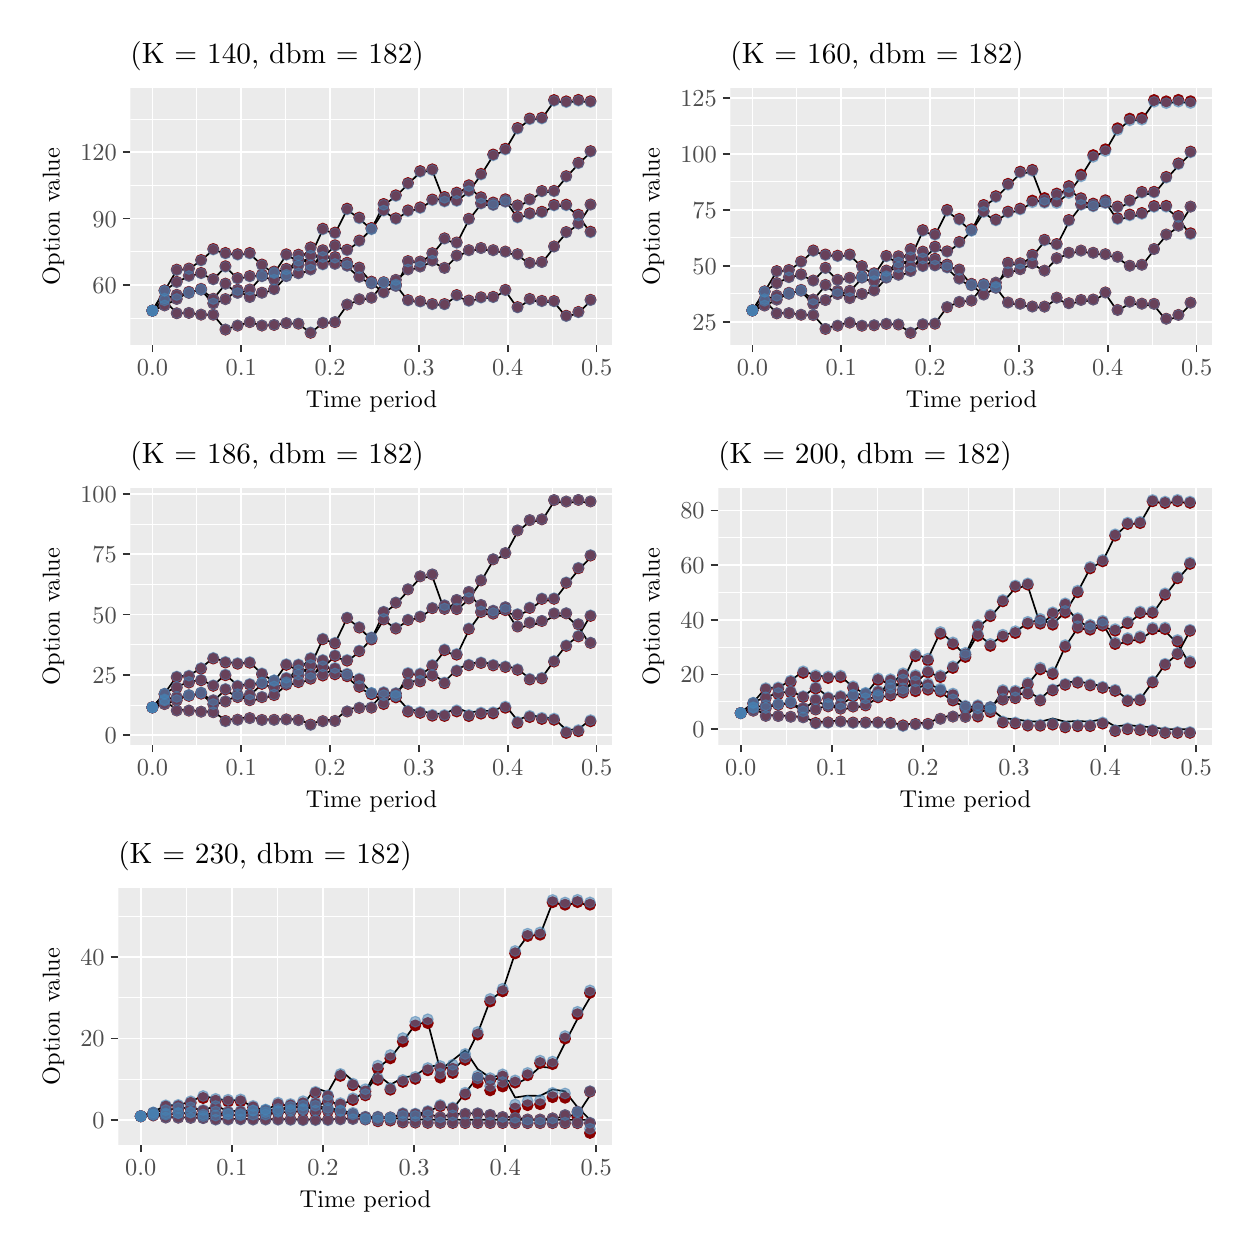
\begin{tikzpicture}[x=1pt,y=1pt]
\definecolor{fillColor}{RGB}{255,255,255}
\path[use as bounding box,fill=fillColor,fill opacity=0.00] (0,0) rectangle (433.62,433.62);
\begin{scope}
\path[clip] (  0.00,289.08) rectangle (216.81,433.62);
\definecolor{drawColor}{RGB}{255,255,255}
\definecolor{fillColor}{RGB}{255,255,255}

\path[draw=drawColor,line width= 0.6pt,line join=round,line cap=round,fill=fillColor] (  0.00,289.08) rectangle (216.81,433.62);
\end{scope}
\begin{scope}
\path[clip] ( 37.15,319.10) rectangle (211.31,411.75);
\definecolor{fillColor}{gray}{0.92}

\path[fill=fillColor] ( 37.15,319.10) rectangle (211.31,411.75);
\definecolor{drawColor}{RGB}{255,255,255}

\path[draw=drawColor,line width= 0.3pt,line join=round] ( 37.15,328.63) --
	(211.31,328.63);

\path[draw=drawColor,line width= 0.3pt,line join=round] ( 37.15,352.61) --
	(211.31,352.61);

\path[draw=drawColor,line width= 0.3pt,line join=round] ( 37.15,376.58) --
	(211.31,376.58);

\path[draw=drawColor,line width= 0.3pt,line join=round] ( 37.15,400.56) --
	(211.31,400.56);

\path[draw=drawColor,line width= 0.3pt,line join=round] ( 61.12,319.10) --
	( 61.12,411.75);

\path[draw=drawColor,line width= 0.3pt,line join=round] ( 93.23,319.10) --
	( 93.23,411.75);

\path[draw=drawColor,line width= 0.3pt,line join=round] (125.33,319.10) --
	(125.33,411.75);

\path[draw=drawColor,line width= 0.3pt,line join=round] (157.44,319.10) --
	(157.44,411.75);

\path[draw=drawColor,line width= 0.3pt,line join=round] (189.54,319.10) --
	(189.54,411.75);

\path[draw=drawColor,line width= 0.6pt,line join=round] ( 37.15,340.62) --
	(211.31,340.62);

\path[draw=drawColor,line width= 0.6pt,line join=round] ( 37.15,364.60) --
	(211.31,364.60);

\path[draw=drawColor,line width= 0.6pt,line join=round] ( 37.15,388.57) --
	(211.31,388.57);

\path[draw=drawColor,line width= 0.6pt,line join=round] ( 45.07,319.10) --
	( 45.07,411.75);

\path[draw=drawColor,line width= 0.6pt,line join=round] ( 77.17,319.10) --
	( 77.17,411.75);

\path[draw=drawColor,line width= 0.6pt,line join=round] (109.28,319.10) --
	(109.28,411.75);

\path[draw=drawColor,line width= 0.6pt,line join=round] (141.38,319.10) --
	(141.38,411.75);

\path[draw=drawColor,line width= 0.6pt,line join=round] (173.49,319.10) --
	(173.49,411.75);

\path[draw=drawColor,line width= 0.6pt,line join=round] (205.59,319.10) --
	(205.59,411.75);
\definecolor{drawColor}{RGB}{0,0,0}

\path[draw=drawColor,line width= 0.6pt,line join=round] ( 45.07,331.36) --
	( 49.47,338.50) --
	( 53.86,346.00) --
	( 58.26,346.40) --
	( 62.66,349.44) --
	( 67.06,353.38) --
	( 71.46,351.96) --
	( 75.85,351.51) --
	( 80.25,351.94) --
	( 84.65,347.79) --
	( 89.05,344.84) --
	( 93.45,351.45) --
	( 97.84,349.31) --
	(102.24,353.91) --
	(106.64,347.92) --
	(111.04,350.43) --
	(115.43,348.37) --
	(119.83,346.62) --
	(124.23,341.55) --
	(128.63,337.74) --
	(133.03,340.63) --
	(137.42,334.91) --
	(141.82,334.45) --
	(146.22,333.48) --
	(150.62,333.44) --
	(155.02,336.67) --
	(159.41,334.69) --
	(163.81,335.85) --
	(168.21,335.99) --
	(172.61,338.51) --
	(177.01,332.27) --
	(181.40,335.20) --
	(185.80,334.49) --
	(190.20,334.43) --
	(194.60,329.12) --
	(199.00,330.47) --
	(203.39,334.84);

\path[draw=drawColor,line width= 0.6pt,line join=round] ( 45.07,331.36) --
	( 49.47,335.08) --
	( 53.86,330.41) --
	( 58.26,330.53) --
	( 62.66,329.90) --
	( 67.06,329.85) --
	( 71.46,324.56) --
	( 75.85,325.97) --
	( 80.25,327.19) --
	( 84.65,325.95) --
	( 89.05,326.16) --
	( 93.45,326.79) --
	( 97.84,326.58) --
	(102.24,323.31) --
	(106.64,326.87) --
	(111.04,327.10) --
	(115.43,333.38) --
	(119.83,335.28) --
	(124.23,335.79) --
	(128.63,341.29) --
	(133.03,342.21) --
	(137.42,345.97) --
	(141.82,346.99) --
	(146.22,349.14) --
	(150.62,346.49) --
	(155.02,350.92) --
	(159.41,352.86) --
	(163.81,353.63) --
	(168.21,352.85) --
	(172.61,352.34) --
	(177.01,351.40) --
	(181.40,348.22) --
	(185.80,348.57) --
	(190.20,354.17) --
	(194.60,359.37) --
	(199.00,362.52) --
	(203.39,369.32);

\path[draw=drawColor,line width= 0.6pt,line join=round] ( 45.07,331.36) --
	( 49.47,333.21) --
	( 53.86,335.53) --
	( 58.26,338.05) --
	( 62.66,338.83) --
	( 67.06,333.91) --
	( 71.46,335.40) --
	( 75.85,338.72) --
	( 80.25,336.13) --
	( 84.65,337.67) --
	( 89.05,338.96) --
	( 93.45,343.63) --
	( 97.84,344.64) --
	(102.24,345.99) --
	(106.64,352.87) --
	(111.04,348.01) --
	(115.43,347.33) --
	(119.83,343.30) --
	(124.23,340.97) --
	(128.63,341.31) --
	(133.03,340.02) --
	(137.42,348.91) --
	(141.82,348.75) --
	(146.22,351.75) --
	(150.62,357.08) --
	(155.02,355.59) --
	(159.41,364.14) --
	(163.81,369.78) --
	(168.21,369.24) --
	(172.61,370.41) --
	(177.01,368.96) --
	(181.40,371.15) --
	(185.80,374.15) --
	(190.20,374.20) --
	(194.60,379.50) --
	(199.00,384.33) --
	(203.39,388.55);

\path[draw=drawColor,line width= 0.6pt,line join=round] ( 45.07,331.36) --
	( 49.47,338.61) --
	( 53.86,341.64) --
	( 58.26,343.83) --
	( 62.66,344.80) --
	( 67.06,342.59) --
	( 71.46,347.19) --
	( 75.85,342.92) --
	( 80.25,343.65) --
	( 84.65,344.21) --
	( 89.05,345.25) --
	( 93.45,346.23) --
	( 97.84,347.57) --
	(102.24,351.12) --
	(106.64,360.62) --
	(111.04,359.22) --
	(115.43,367.83) --
	(119.83,364.62) --
	(124.23,360.63) --
	(128.63,367.37) --
	(133.03,364.35) --
	(137.42,367.21) --
	(141.82,368.29) --
	(146.22,371.13) --
	(150.62,372.03) --
	(155.02,370.84) --
	(159.41,374.40) --
	(163.81,380.38) --
	(168.21,387.35) --
	(172.61,389.43) --
	(177.01,396.94) --
	(181.40,400.36) --
	(185.80,400.64) --
	(190.20,407.02) --
	(194.60,406.55) --
	(199.00,407.09) --
	(203.39,406.60);

\path[draw=drawColor,line width= 0.6pt,line join=round] ( 45.07,331.36) --
	( 49.47,335.72) --
	( 53.86,336.99) --
	( 58.26,337.68) --
	( 62.66,339.10) --
	( 67.06,335.55) --
	( 71.46,340.94) --
	( 75.85,337.65) --
	( 80.25,338.82) --
	( 84.65,343.64) --
	( 89.05,342.44) --
	( 93.45,344.20) --
	( 97.84,351.27) --
	(102.24,347.69) --
	(106.64,350.64) --
	(111.04,354.65) --
	(115.43,353.02) --
	(119.83,356.35) --
	(124.23,360.86) --
	(128.63,369.50) --
	(133.03,372.63) --
	(137.42,377.04) --
	(141.82,381.36) --
	(146.22,382.00) --
	(150.62,370.61) --
	(155.02,373.57) --
	(159.41,376.24) --
	(163.81,371.92) --
	(168.21,370.01) --
	(172.61,371.19) --
	(177.01,364.82) --
	(181.40,366.11) --
	(185.80,366.67) --
	(190.20,369.15) --
	(194.60,369.21) --
	(199.00,365.59) --
	(203.39,359.45);
\definecolor{drawColor}{RGB}{139,0,0}
\definecolor{fillColor}{RGB}{139,0,0}

\path[draw=drawColor,line width= 0.4pt,line join=round,line cap=round,fill=fillColor] ( 45.07,331.36) circle (  1.96);

\path[draw=drawColor,line width= 0.4pt,line join=round,line cap=round,fill=fillColor] ( 49.47,338.59) circle (  1.96);

\path[draw=drawColor,line width= 0.4pt,line join=round,line cap=round,fill=fillColor] ( 53.86,346.19) circle (  1.96);

\path[draw=drawColor,line width= 0.4pt,line join=round,line cap=round,fill=fillColor] ( 58.26,346.59) circle (  1.96);

\path[draw=drawColor,line width= 0.4pt,line join=round,line cap=round,fill=fillColor] ( 62.66,349.67) circle (  1.96);

\path[draw=drawColor,line width= 0.4pt,line join=round,line cap=round,fill=fillColor] ( 67.06,353.65) circle (  1.96);

\path[draw=drawColor,line width= 0.4pt,line join=round,line cap=round,fill=fillColor] ( 71.46,352.22) circle (  1.96);

\path[draw=drawColor,line width= 0.4pt,line join=round,line cap=round,fill=fillColor] ( 75.85,351.78) circle (  1.96);

\path[draw=drawColor,line width= 0.4pt,line join=round,line cap=round,fill=fillColor] ( 80.25,352.22) circle (  1.96);

\path[draw=drawColor,line width= 0.4pt,line join=round,line cap=round,fill=fillColor] ( 84.65,348.05) circle (  1.96);

\path[draw=drawColor,line width= 0.4pt,line join=round,line cap=round,fill=fillColor] ( 89.05,345.09) circle (  1.96);

\path[draw=drawColor,line width= 0.4pt,line join=round,line cap=round,fill=fillColor] ( 93.45,351.75) circle (  1.96);

\path[draw=drawColor,line width= 0.4pt,line join=round,line cap=round,fill=fillColor] ( 97.84,349.60) circle (  1.96);

\path[draw=drawColor,line width= 0.4pt,line join=round,line cap=round,fill=fillColor] (102.24,354.23) circle (  1.96);

\path[draw=drawColor,line width= 0.4pt,line join=round,line cap=round,fill=fillColor] (106.64,348.22) circle (  1.96);

\path[draw=drawColor,line width= 0.4pt,line join=round,line cap=round,fill=fillColor] (111.04,350.75) circle (  1.96);

\path[draw=drawColor,line width= 0.4pt,line join=round,line cap=round,fill=fillColor] (115.43,348.69) circle (  1.96);

\path[draw=drawColor,line width= 0.4pt,line join=round,line cap=round,fill=fillColor] (119.83,346.93) circle (  1.96);

\path[draw=drawColor,line width= 0.4pt,line join=round,line cap=round,fill=fillColor] (124.23,341.85) circle (  1.96);

\path[draw=drawColor,line width= 0.4pt,line join=round,line cap=round,fill=fillColor] (128.63,338.02) circle (  1.96);

\path[draw=drawColor,line width= 0.4pt,line join=round,line cap=round,fill=fillColor] (133.03,340.94) circle (  1.96);

\path[draw=drawColor,line width= 0.4pt,line join=round,line cap=round,fill=fillColor] (137.42,335.19) circle (  1.96);

\path[draw=drawColor,line width= 0.4pt,line join=round,line cap=round,fill=fillColor] (141.82,334.75) circle (  1.96);

\path[draw=drawColor,line width= 0.4pt,line join=round,line cap=round,fill=fillColor] (146.22,333.78) circle (  1.96);

\path[draw=drawColor,line width= 0.4pt,line join=round,line cap=round,fill=fillColor] (150.62,333.76) circle (  1.96);

\path[draw=drawColor,line width= 0.4pt,line join=round,line cap=round,fill=fillColor] (155.02,337.01) circle (  1.96);

\path[draw=drawColor,line width= 0.4pt,line join=round,line cap=round,fill=fillColor] (159.41,335.04) circle (  1.96);

\path[draw=drawColor,line width= 0.4pt,line join=round,line cap=round,fill=fillColor] (163.81,336.21) circle (  1.96);

\path[draw=drawColor,line width= 0.4pt,line join=round,line cap=round,fill=fillColor] (168.21,336.36) circle (  1.96);

\path[draw=drawColor,line width= 0.4pt,line join=round,line cap=round,fill=fillColor] (172.61,338.89) circle (  1.96);

\path[draw=drawColor,line width= 0.4pt,line join=round,line cap=round,fill=fillColor] (177.01,332.65) circle (  1.96);

\path[draw=drawColor,line width= 0.4pt,line join=round,line cap=round,fill=fillColor] (181.40,335.60) circle (  1.96);

\path[draw=drawColor,line width= 0.4pt,line join=round,line cap=round,fill=fillColor] (185.80,334.90) circle (  1.96);

\path[draw=drawColor,line width= 0.4pt,line join=round,line cap=round,fill=fillColor] (190.20,334.84) circle (  1.96);

\path[draw=drawColor,line width= 0.4pt,line join=round,line cap=round,fill=fillColor] (194.60,329.54) circle (  1.96);

\path[draw=drawColor,line width= 0.4pt,line join=round,line cap=round,fill=fillColor] (199.00,330.91) circle (  1.96);

\path[draw=drawColor,line width= 0.4pt,line join=round,line cap=round,fill=fillColor] (203.39,335.28) circle (  1.96);

\path[draw=drawColor,line width= 0.4pt,line join=round,line cap=round,fill=fillColor] ( 45.07,331.36) circle (  1.96);

\path[draw=drawColor,line width= 0.4pt,line join=round,line cap=round,fill=fillColor] ( 49.47,335.14) circle (  1.96);

\path[draw=drawColor,line width= 0.4pt,line join=round,line cap=round,fill=fillColor] ( 53.86,330.41) circle (  1.96);

\path[draw=drawColor,line width= 0.4pt,line join=round,line cap=round,fill=fillColor] ( 58.26,330.54) circle (  1.96);

\path[draw=drawColor,line width= 0.4pt,line join=round,line cap=round,fill=fillColor] ( 62.66,329.92) circle (  1.96);

\path[draw=drawColor,line width= 0.4pt,line join=round,line cap=round,fill=fillColor] ( 67.06,329.88) circle (  1.96);

\path[draw=drawColor,line width= 0.4pt,line join=round,line cap=round,fill=fillColor] ( 71.46,324.51) circle (  1.96);

\path[draw=drawColor,line width= 0.4pt,line join=round,line cap=round,fill=fillColor] ( 75.85,325.95) circle (  1.96);

\path[draw=drawColor,line width= 0.4pt,line join=round,line cap=round,fill=fillColor] ( 80.25,327.20) circle (  1.96);

\path[draw=drawColor,line width= 0.4pt,line join=round,line cap=round,fill=fillColor] ( 84.65,325.97) circle (  1.96);

\path[draw=drawColor,line width= 0.4pt,line join=round,line cap=round,fill=fillColor] ( 89.05,326.19) circle (  1.96);

\path[draw=drawColor,line width= 0.4pt,line join=round,line cap=round,fill=fillColor] ( 93.45,326.85) circle (  1.96);

\path[draw=drawColor,line width= 0.4pt,line join=round,line cap=round,fill=fillColor] ( 97.84,326.65) circle (  1.96);

\path[draw=drawColor,line width= 0.4pt,line join=round,line cap=round,fill=fillColor] (102.24,323.35) circle (  1.96);

\path[draw=drawColor,line width= 0.4pt,line join=round,line cap=round,fill=fillColor] (106.64,326.96) circle (  1.96);

\path[draw=drawColor,line width= 0.4pt,line join=round,line cap=round,fill=fillColor] (111.04,327.21) circle (  1.96);

\path[draw=drawColor,line width= 0.4pt,line join=round,line cap=round,fill=fillColor] (115.43,333.56) circle (  1.96);

\path[draw=drawColor,line width= 0.4pt,line join=round,line cap=round,fill=fillColor] (119.83,335.48) circle (  1.96);

\path[draw=drawColor,line width= 0.4pt,line join=round,line cap=round,fill=fillColor] (124.23,336.02) circle (  1.96);

\path[draw=drawColor,line width= 0.4pt,line join=round,line cap=round,fill=fillColor] (128.63,341.55) circle (  1.96);

\path[draw=drawColor,line width= 0.4pt,line join=round,line cap=round,fill=fillColor] (133.03,342.49) circle (  1.96);

\path[draw=drawColor,line width= 0.4pt,line join=round,line cap=round,fill=fillColor] (137.42,346.28) circle (  1.96);

\path[draw=drawColor,line width= 0.4pt,line join=round,line cap=round,fill=fillColor] (141.82,347.31) circle (  1.96);

\path[draw=drawColor,line width= 0.4pt,line join=round,line cap=round,fill=fillColor] (146.22,349.47) circle (  1.96);

\path[draw=drawColor,line width= 0.4pt,line join=round,line cap=round,fill=fillColor] (150.62,346.82) circle (  1.96);

\path[draw=drawColor,line width= 0.4pt,line join=round,line cap=round,fill=fillColor] (155.02,351.27) circle (  1.96);

\path[draw=drawColor,line width= 0.4pt,line join=round,line cap=round,fill=fillColor] (159.41,353.22) circle (  1.96);

\path[draw=drawColor,line width= 0.4pt,line join=round,line cap=round,fill=fillColor] (163.81,354.00) circle (  1.96);

\path[draw=drawColor,line width= 0.4pt,line join=round,line cap=round,fill=fillColor] (168.21,353.22) circle (  1.96);

\path[draw=drawColor,line width= 0.4pt,line join=round,line cap=round,fill=fillColor] (172.61,352.72) circle (  1.96);

\path[draw=drawColor,line width= 0.4pt,line join=round,line cap=round,fill=fillColor] (177.01,351.78) circle (  1.96);

\path[draw=drawColor,line width= 0.4pt,line join=round,line cap=round,fill=fillColor] (181.40,348.61) circle (  1.96);

\path[draw=drawColor,line width= 0.4pt,line join=round,line cap=round,fill=fillColor] (185.80,348.96) circle (  1.96);

\path[draw=drawColor,line width= 0.4pt,line join=round,line cap=round,fill=fillColor] (190.20,354.57) circle (  1.96);

\path[draw=drawColor,line width= 0.4pt,line join=round,line cap=round,fill=fillColor] (194.60,359.77) circle (  1.96);

\path[draw=drawColor,line width= 0.4pt,line join=round,line cap=round,fill=fillColor] (199.00,362.92) circle (  1.96);

\path[draw=drawColor,line width= 0.4pt,line join=round,line cap=round,fill=fillColor] (203.39,369.73) circle (  1.96);

\path[draw=drawColor,line width= 0.4pt,line join=round,line cap=round,fill=fillColor] ( 45.07,331.36) circle (  1.96);

\path[draw=drawColor,line width= 0.4pt,line join=round,line cap=round,fill=fillColor] ( 49.47,333.26) circle (  1.96);

\path[draw=drawColor,line width= 0.4pt,line join=round,line cap=round,fill=fillColor] ( 53.86,335.60) circle (  1.96);

\path[draw=drawColor,line width= 0.4pt,line join=round,line cap=round,fill=fillColor] ( 58.26,338.17) circle (  1.96);

\path[draw=drawColor,line width= 0.4pt,line join=round,line cap=round,fill=fillColor] ( 62.66,338.97) circle (  1.96);

\path[draw=drawColor,line width= 0.4pt,line join=round,line cap=round,fill=fillColor] ( 67.06,334.00) circle (  1.96);

\path[draw=drawColor,line width= 0.4pt,line join=round,line cap=round,fill=fillColor] ( 71.46,335.53) circle (  1.96);

\path[draw=drawColor,line width= 0.4pt,line join=round,line cap=round,fill=fillColor] ( 75.85,338.90) circle (  1.96);

\path[draw=drawColor,line width= 0.4pt,line join=round,line cap=round,fill=fillColor] ( 80.25,336.30) circle (  1.96);

\path[draw=drawColor,line width= 0.4pt,line join=round,line cap=round,fill=fillColor] ( 84.65,337.85) circle (  1.96);

\path[draw=drawColor,line width= 0.4pt,line join=round,line cap=round,fill=fillColor] ( 89.05,339.17) circle (  1.96);

\path[draw=drawColor,line width= 0.4pt,line join=round,line cap=round,fill=fillColor] ( 93.45,343.89) circle (  1.96);

\path[draw=drawColor,line width= 0.4pt,line join=round,line cap=round,fill=fillColor] ( 97.84,344.91) circle (  1.96);

\path[draw=drawColor,line width= 0.4pt,line join=round,line cap=round,fill=fillColor] (102.24,346.28) circle (  1.96);

\path[draw=drawColor,line width= 0.4pt,line join=round,line cap=round,fill=fillColor] (106.64,353.21) circle (  1.96);

\path[draw=drawColor,line width= 0.4pt,line join=round,line cap=round,fill=fillColor] (111.04,348.33) circle (  1.96);

\path[draw=drawColor,line width= 0.4pt,line join=round,line cap=round,fill=fillColor] (115.43,347.65) circle (  1.96);

\path[draw=drawColor,line width= 0.4pt,line join=round,line cap=round,fill=fillColor] (119.83,343.62) circle (  1.96);

\path[draw=drawColor,line width= 0.4pt,line join=round,line cap=round,fill=fillColor] (124.23,341.27) circle (  1.96);

\path[draw=drawColor,line width= 0.4pt,line join=round,line cap=round,fill=fillColor] (128.63,341.63) circle (  1.96);

\path[draw=drawColor,line width= 0.4pt,line join=round,line cap=round,fill=fillColor] (133.03,340.34) circle (  1.96);

\path[draw=drawColor,line width= 0.4pt,line join=round,line cap=round,fill=fillColor] (137.42,349.28) circle (  1.96);

\path[draw=drawColor,line width= 0.4pt,line join=round,line cap=round,fill=fillColor] (141.82,349.12) circle (  1.96);

\path[draw=drawColor,line width= 0.4pt,line join=round,line cap=round,fill=fillColor] (146.22,352.14) circle (  1.96);

\path[draw=drawColor,line width= 0.4pt,line join=round,line cap=round,fill=fillColor] (150.62,357.50) circle (  1.96);

\path[draw=drawColor,line width= 0.4pt,line join=round,line cap=round,fill=fillColor] (155.02,356.01) circle (  1.96);

\path[draw=drawColor,line width= 0.4pt,line join=round,line cap=round,fill=fillColor] (159.41,364.57) circle (  1.96);

\path[draw=drawColor,line width= 0.4pt,line join=round,line cap=round,fill=fillColor] (163.81,370.22) circle (  1.96);

\path[draw=drawColor,line width= 0.4pt,line join=round,line cap=round,fill=fillColor] (168.21,369.68) circle (  1.96);

\path[draw=drawColor,line width= 0.4pt,line join=round,line cap=round,fill=fillColor] (172.61,370.86) circle (  1.96);

\path[draw=drawColor,line width= 0.4pt,line join=round,line cap=round,fill=fillColor] (177.01,369.41) circle (  1.96);

\path[draw=drawColor,line width= 0.4pt,line join=round,line cap=round,fill=fillColor] (181.40,371.60) circle (  1.96);

\path[draw=drawColor,line width= 0.4pt,line join=round,line cap=round,fill=fillColor] (185.80,374.61) circle (  1.96);

\path[draw=drawColor,line width= 0.4pt,line join=round,line cap=round,fill=fillColor] (190.20,374.66) circle (  1.96);

\path[draw=drawColor,line width= 0.4pt,line join=round,line cap=round,fill=fillColor] (194.60,379.96) circle (  1.96);

\path[draw=drawColor,line width= 0.4pt,line join=round,line cap=round,fill=fillColor] (199.00,384.80) circle (  1.96);

\path[draw=drawColor,line width= 0.4pt,line join=round,line cap=round,fill=fillColor] (203.39,389.01) circle (  1.96);

\path[draw=drawColor,line width= 0.4pt,line join=round,line cap=round,fill=fillColor] ( 45.07,331.36) circle (  1.96);

\path[draw=drawColor,line width= 0.4pt,line join=round,line cap=round,fill=fillColor] ( 49.47,338.71) circle (  1.96);

\path[draw=drawColor,line width= 0.4pt,line join=round,line cap=round,fill=fillColor] ( 53.86,341.78) circle (  1.96);

\path[draw=drawColor,line width= 0.4pt,line join=round,line cap=round,fill=fillColor] ( 58.26,344.00) circle (  1.96);

\path[draw=drawColor,line width= 0.4pt,line join=round,line cap=round,fill=fillColor] ( 62.66,345.00) circle (  1.96);

\path[draw=drawColor,line width= 0.4pt,line join=round,line cap=round,fill=fillColor] ( 67.06,342.77) circle (  1.96);

\path[draw=drawColor,line width= 0.4pt,line join=round,line cap=round,fill=fillColor] ( 71.46,347.42) circle (  1.96);

\path[draw=drawColor,line width= 0.4pt,line join=round,line cap=round,fill=fillColor] ( 75.85,343.13) circle (  1.96);

\path[draw=drawColor,line width= 0.4pt,line join=round,line cap=round,fill=fillColor] ( 80.25,343.87) circle (  1.96);

\path[draw=drawColor,line width= 0.4pt,line join=round,line cap=round,fill=fillColor] ( 84.65,344.44) circle (  1.96);

\path[draw=drawColor,line width= 0.4pt,line join=round,line cap=round,fill=fillColor] ( 89.05,345.50) circle (  1.96);

\path[draw=drawColor,line width= 0.4pt,line join=round,line cap=round,fill=fillColor] ( 93.45,346.49) circle (  1.96);

\path[draw=drawColor,line width= 0.4pt,line join=round,line cap=round,fill=fillColor] ( 97.84,347.85) circle (  1.96);

\path[draw=drawColor,line width= 0.4pt,line join=round,line cap=round,fill=fillColor] (102.24,351.43) circle (  1.96);

\path[draw=drawColor,line width= 0.4pt,line join=round,line cap=round,fill=fillColor] (106.64,360.98) circle (  1.96);

\path[draw=drawColor,line width= 0.4pt,line join=round,line cap=round,fill=fillColor] (111.04,359.58) circle (  1.96);

\path[draw=drawColor,line width= 0.4pt,line join=round,line cap=round,fill=fillColor] (115.43,368.22) circle (  1.96);

\path[draw=drawColor,line width= 0.4pt,line join=round,line cap=round,fill=fillColor] (119.83,365.00) circle (  1.96);

\path[draw=drawColor,line width= 0.4pt,line join=round,line cap=round,fill=fillColor] (124.23,361.01) circle (  1.96);

\path[draw=drawColor,line width= 0.4pt,line join=round,line cap=round,fill=fillColor] (128.63,367.77) circle (  1.96);

\path[draw=drawColor,line width= 0.4pt,line join=round,line cap=round,fill=fillColor] (133.03,364.75) circle (  1.96);

\path[draw=drawColor,line width= 0.4pt,line join=round,line cap=round,fill=fillColor] (137.42,367.61) circle (  1.96);

\path[draw=drawColor,line width= 0.4pt,line join=round,line cap=round,fill=fillColor] (141.82,368.70) circle (  1.96);

\path[draw=drawColor,line width= 0.4pt,line join=round,line cap=round,fill=fillColor] (146.22,371.54) circle (  1.96);

\path[draw=drawColor,line width= 0.4pt,line join=round,line cap=round,fill=fillColor] (150.62,372.45) circle (  1.96);

\path[draw=drawColor,line width= 0.4pt,line join=round,line cap=round,fill=fillColor] (155.02,371.27) circle (  1.96);

\path[draw=drawColor,line width= 0.4pt,line join=round,line cap=round,fill=fillColor] (159.41,374.83) circle (  1.96);

\path[draw=drawColor,line width= 0.4pt,line join=round,line cap=round,fill=fillColor] (163.81,380.81) circle (  1.96);

\path[draw=drawColor,line width= 0.4pt,line join=round,line cap=round,fill=fillColor] (168.21,387.80) circle (  1.96);

\path[draw=drawColor,line width= 0.4pt,line join=round,line cap=round,fill=fillColor] (172.61,389.87) circle (  1.96);

\path[draw=drawColor,line width= 0.4pt,line join=round,line cap=round,fill=fillColor] (177.01,397.38) circle (  1.96);

\path[draw=drawColor,line width= 0.4pt,line join=round,line cap=round,fill=fillColor] (181.40,400.81) circle (  1.96);

\path[draw=drawColor,line width= 0.4pt,line join=round,line cap=round,fill=fillColor] (185.80,401.08) circle (  1.96);

\path[draw=drawColor,line width= 0.4pt,line join=round,line cap=round,fill=fillColor] (190.20,407.47) circle (  1.96);

\path[draw=drawColor,line width= 0.4pt,line join=round,line cap=round,fill=fillColor] (194.60,407.00) circle (  1.96);

\path[draw=drawColor,line width= 0.4pt,line join=round,line cap=round,fill=fillColor] (199.00,407.54) circle (  1.96);

\path[draw=drawColor,line width= 0.4pt,line join=round,line cap=round,fill=fillColor] (203.39,407.05) circle (  1.96);

\path[draw=drawColor,line width= 0.4pt,line join=round,line cap=round,fill=fillColor] ( 45.07,331.36) circle (  1.96);

\path[draw=drawColor,line width= 0.4pt,line join=round,line cap=round,fill=fillColor] ( 49.47,335.78) circle (  1.96);

\path[draw=drawColor,line width= 0.4pt,line join=round,line cap=round,fill=fillColor] ( 53.86,337.08) circle (  1.96);

\path[draw=drawColor,line width= 0.4pt,line join=round,line cap=round,fill=fillColor] ( 58.26,337.80) circle (  1.96);

\path[draw=drawColor,line width= 0.4pt,line join=round,line cap=round,fill=fillColor] ( 62.66,339.24) circle (  1.96);

\path[draw=drawColor,line width= 0.4pt,line join=round,line cap=round,fill=fillColor] ( 67.06,335.66) circle (  1.96);

\path[draw=drawColor,line width= 0.4pt,line join=round,line cap=round,fill=fillColor] ( 71.46,341.13) circle (  1.96);

\path[draw=drawColor,line width= 0.4pt,line join=round,line cap=round,fill=fillColor] ( 75.85,337.81) circle (  1.96);

\path[draw=drawColor,line width= 0.4pt,line join=round,line cap=round,fill=fillColor] ( 80.25,339.01) circle (  1.96);

\path[draw=drawColor,line width= 0.4pt,line join=round,line cap=round,fill=fillColor] ( 84.65,343.88) circle (  1.96);

\path[draw=drawColor,line width= 0.4pt,line join=round,line cap=round,fill=fillColor] ( 89.05,342.67) circle (  1.96);

\path[draw=drawColor,line width= 0.4pt,line join=round,line cap=round,fill=fillColor] ( 93.45,344.46) circle (  1.96);

\path[draw=drawColor,line width= 0.4pt,line join=round,line cap=round,fill=fillColor] ( 97.84,351.59) circle (  1.96);

\path[draw=drawColor,line width= 0.4pt,line join=round,line cap=round,fill=fillColor] (102.24,347.99) circle (  1.96);

\path[draw=drawColor,line width= 0.4pt,line join=round,line cap=round,fill=fillColor] (106.64,350.96) circle (  1.96);

\path[draw=drawColor,line width= 0.4pt,line join=round,line cap=round,fill=fillColor] (111.04,355.00) circle (  1.96);

\path[draw=drawColor,line width= 0.4pt,line join=round,line cap=round,fill=fillColor] (115.43,353.37) circle (  1.96);

\path[draw=drawColor,line width= 0.4pt,line join=round,line cap=round,fill=fillColor] (119.83,356.72) circle (  1.96);

\path[draw=drawColor,line width= 0.4pt,line join=round,line cap=round,fill=fillColor] (124.23,361.24) circle (  1.96);

\path[draw=drawColor,line width= 0.4pt,line join=round,line cap=round,fill=fillColor] (128.63,369.92) circle (  1.96);

\path[draw=drawColor,line width= 0.4pt,line join=round,line cap=round,fill=fillColor] (133.03,373.05) circle (  1.96);

\path[draw=drawColor,line width= 0.4pt,line join=round,line cap=round,fill=fillColor] (137.42,377.47) circle (  1.96);

\path[draw=drawColor,line width= 0.4pt,line join=round,line cap=round,fill=fillColor] (141.82,381.80) circle (  1.96);

\path[draw=drawColor,line width= 0.4pt,line join=round,line cap=round,fill=fillColor] (146.22,382.44) circle (  1.96);

\path[draw=drawColor,line width= 0.4pt,line join=round,line cap=round,fill=fillColor] (150.62,371.04) circle (  1.96);

\path[draw=drawColor,line width= 0.4pt,line join=round,line cap=round,fill=fillColor] (155.02,374.01) circle (  1.96);

\path[draw=drawColor,line width= 0.4pt,line join=round,line cap=round,fill=fillColor] (159.41,376.69) circle (  1.96);

\path[draw=drawColor,line width= 0.4pt,line join=round,line cap=round,fill=fillColor] (163.81,372.36) circle (  1.96);

\path[draw=drawColor,line width= 0.4pt,line join=round,line cap=round,fill=fillColor] (168.21,370.45) circle (  1.96);

\path[draw=drawColor,line width= 0.4pt,line join=round,line cap=round,fill=fillColor] (172.61,371.63) circle (  1.96);

\path[draw=drawColor,line width= 0.4pt,line join=round,line cap=round,fill=fillColor] (177.01,365.26) circle (  1.96);

\path[draw=drawColor,line width= 0.4pt,line join=round,line cap=round,fill=fillColor] (181.40,366.56) circle (  1.96);

\path[draw=drawColor,line width= 0.4pt,line join=round,line cap=round,fill=fillColor] (185.80,367.12) circle (  1.96);

\path[draw=drawColor,line width= 0.4pt,line join=round,line cap=round,fill=fillColor] (190.20,369.60) circle (  1.96);

\path[draw=drawColor,line width= 0.4pt,line join=round,line cap=round,fill=fillColor] (194.60,369.67) circle (  1.96);

\path[draw=drawColor,line width= 0.4pt,line join=round,line cap=round,fill=fillColor] (199.00,366.05) circle (  1.96);

\path[draw=drawColor,line width= 0.4pt,line join=round,line cap=round,fill=fillColor] (203.39,359.90) circle (  1.96);
\definecolor{drawColor}{RGB}{70,130,180}
\definecolor{fillColor}{RGB}{70,130,180}

\path[draw=drawColor,draw opacity=0.50,line width= 0.4pt,line join=round,line cap=round,fill=fillColor,fill opacity=0.50] ( 45.07,331.36) circle (  1.96);

\path[draw=drawColor,draw opacity=0.50,line width= 0.4pt,line join=round,line cap=round,fill=fillColor,fill opacity=0.50] ( 49.47,338.50) circle (  1.96);

\path[draw=drawColor,draw opacity=0.50,line width= 0.4pt,line join=round,line cap=round,fill=fillColor,fill opacity=0.50] ( 53.86,346.01) circle (  1.96);

\path[draw=drawColor,draw opacity=0.50,line width= 0.4pt,line join=round,line cap=round,fill=fillColor,fill opacity=0.50] ( 58.26,346.42) circle (  1.96);

\path[draw=drawColor,draw opacity=0.50,line width= 0.4pt,line join=round,line cap=round,fill=fillColor,fill opacity=0.50] ( 62.66,349.46) circle (  1.96);

\path[draw=drawColor,draw opacity=0.50,line width= 0.4pt,line join=round,line cap=round,fill=fillColor,fill opacity=0.50] ( 67.06,353.41) circle (  1.96);

\path[draw=drawColor,draw opacity=0.50,line width= 0.4pt,line join=round,line cap=round,fill=fillColor,fill opacity=0.50] ( 71.46,351.99) circle (  1.96);

\path[draw=drawColor,draw opacity=0.50,line width= 0.4pt,line join=round,line cap=round,fill=fillColor,fill opacity=0.50] ( 75.85,351.56) circle (  1.96);

\path[draw=drawColor,draw opacity=0.50,line width= 0.4pt,line join=round,line cap=round,fill=fillColor,fill opacity=0.50] ( 80.25,351.99) circle (  1.96);

\path[draw=drawColor,draw opacity=0.50,line width= 0.4pt,line join=round,line cap=round,fill=fillColor,fill opacity=0.50] ( 84.65,347.84) circle (  1.96);

\path[draw=drawColor,draw opacity=0.50,line width= 0.4pt,line join=round,line cap=round,fill=fillColor,fill opacity=0.50] ( 89.05,344.91) circle (  1.96);

\path[draw=drawColor,draw opacity=0.50,line width= 0.4pt,line join=round,line cap=round,fill=fillColor,fill opacity=0.50] ( 93.45,351.52) circle (  1.96);

\path[draw=drawColor,draw opacity=0.50,line width= 0.4pt,line join=round,line cap=round,fill=fillColor,fill opacity=0.50] ( 97.84,349.38) circle (  1.96);

\path[draw=drawColor,draw opacity=0.50,line width= 0.4pt,line join=round,line cap=round,fill=fillColor,fill opacity=0.50] (102.24,353.99) circle (  1.96);

\path[draw=drawColor,draw opacity=0.50,line width= 0.4pt,line join=round,line cap=round,fill=fillColor,fill opacity=0.50] (106.64,348.00) circle (  1.96);

\path[draw=drawColor,draw opacity=0.50,line width= 0.4pt,line join=round,line cap=round,fill=fillColor,fill opacity=0.50] (111.04,350.52) circle (  1.96);

\path[draw=drawColor,draw opacity=0.50,line width= 0.4pt,line join=round,line cap=round,fill=fillColor,fill opacity=0.50] (115.43,348.47) circle (  1.96);

\path[draw=drawColor,draw opacity=0.50,line width= 0.4pt,line join=round,line cap=round,fill=fillColor,fill opacity=0.50] (119.83,346.72) circle (  1.96);

\path[draw=drawColor,draw opacity=0.50,line width= 0.4pt,line join=round,line cap=round,fill=fillColor,fill opacity=0.50] (124.23,341.66) circle (  1.96);

\path[draw=drawColor,draw opacity=0.50,line width= 0.4pt,line join=round,line cap=round,fill=fillColor,fill opacity=0.50] (128.63,337.85) circle (  1.96);

\path[draw=drawColor,draw opacity=0.50,line width= 0.4pt,line join=round,line cap=round,fill=fillColor,fill opacity=0.50] (133.03,340.76) circle (  1.96);

\path[draw=drawColor,draw opacity=0.50,line width= 0.4pt,line join=round,line cap=round,fill=fillColor,fill opacity=0.50] (137.42,335.04) circle (  1.96);

\path[draw=drawColor,draw opacity=0.50,line width= 0.4pt,line join=round,line cap=round,fill=fillColor,fill opacity=0.50] (141.82,334.59) circle (  1.96);

\path[draw=drawColor,draw opacity=0.50,line width= 0.4pt,line join=round,line cap=round,fill=fillColor,fill opacity=0.50] (146.22,333.63) circle (  1.96);

\path[draw=drawColor,draw opacity=0.50,line width= 0.4pt,line join=round,line cap=round,fill=fillColor,fill opacity=0.50] (150.62,333.60) circle (  1.96);

\path[draw=drawColor,draw opacity=0.50,line width= 0.4pt,line join=round,line cap=round,fill=fillColor,fill opacity=0.50] (155.02,336.84) circle (  1.96);

\path[draw=drawColor,draw opacity=0.50,line width= 0.4pt,line join=round,line cap=round,fill=fillColor,fill opacity=0.50] (159.41,334.87) circle (  1.96);

\path[draw=drawColor,draw opacity=0.50,line width= 0.4pt,line join=round,line cap=round,fill=fillColor,fill opacity=0.50] (163.81,336.04) circle (  1.96);

\path[draw=drawColor,draw opacity=0.50,line width= 0.4pt,line join=round,line cap=round,fill=fillColor,fill opacity=0.50] (168.21,336.19) circle (  1.96);

\path[draw=drawColor,draw opacity=0.50,line width= 0.4pt,line join=round,line cap=round,fill=fillColor,fill opacity=0.50] (172.61,338.72) circle (  1.96);

\path[draw=drawColor,draw opacity=0.50,line width= 0.4pt,line join=round,line cap=round,fill=fillColor,fill opacity=0.50] (177.01,332.49) circle (  1.96);

\path[draw=drawColor,draw opacity=0.50,line width= 0.4pt,line join=round,line cap=round,fill=fillColor,fill opacity=0.50] (181.40,335.43) circle (  1.96);

\path[draw=drawColor,draw opacity=0.50,line width= 0.4pt,line join=round,line cap=round,fill=fillColor,fill opacity=0.50] (185.80,334.73) circle (  1.96);

\path[draw=drawColor,draw opacity=0.50,line width= 0.4pt,line join=round,line cap=round,fill=fillColor,fill opacity=0.50] (190.20,334.67) circle (  1.96);

\path[draw=drawColor,draw opacity=0.50,line width= 0.4pt,line join=round,line cap=round,fill=fillColor,fill opacity=0.50] (194.60,329.37) circle (  1.96);

\path[draw=drawColor,draw opacity=0.50,line width= 0.4pt,line join=round,line cap=round,fill=fillColor,fill opacity=0.50] (199.00,330.74) circle (  1.96);

\path[draw=drawColor,draw opacity=0.50,line width= 0.4pt,line join=round,line cap=round,fill=fillColor,fill opacity=0.50] (203.39,335.12) circle (  1.96);

\path[draw=drawColor,draw opacity=0.50,line width= 0.4pt,line join=round,line cap=round,fill=fillColor,fill opacity=0.50] ( 45.07,331.36) circle (  1.96);

\path[draw=drawColor,draw opacity=0.50,line width= 0.4pt,line join=round,line cap=round,fill=fillColor,fill opacity=0.50] ( 49.47,335.09) circle (  1.96);

\path[draw=drawColor,draw opacity=0.50,line width= 0.4pt,line join=round,line cap=round,fill=fillColor,fill opacity=0.50] ( 53.86,330.42) circle (  1.96);

\path[draw=drawColor,draw opacity=0.50,line width= 0.4pt,line join=round,line cap=round,fill=fillColor,fill opacity=0.50] ( 58.26,330.55) circle (  1.96);

\path[draw=drawColor,draw opacity=0.50,line width= 0.4pt,line join=round,line cap=round,fill=fillColor,fill opacity=0.50] ( 62.66,329.93) circle (  1.96);

\path[draw=drawColor,draw opacity=0.50,line width= 0.4pt,line join=round,line cap=round,fill=fillColor,fill opacity=0.50] ( 67.06,329.89) circle (  1.96);

\path[draw=drawColor,draw opacity=0.50,line width= 0.4pt,line join=round,line cap=round,fill=fillColor,fill opacity=0.50] ( 71.46,324.59) circle (  1.96);

\path[draw=drawColor,draw opacity=0.50,line width= 0.4pt,line join=round,line cap=round,fill=fillColor,fill opacity=0.50] ( 75.85,326.01) circle (  1.96);

\path[draw=drawColor,draw opacity=0.50,line width= 0.4pt,line join=round,line cap=round,fill=fillColor,fill opacity=0.50] ( 80.25,327.25) circle (  1.96);

\path[draw=drawColor,draw opacity=0.50,line width= 0.4pt,line join=round,line cap=round,fill=fillColor,fill opacity=0.50] ( 84.65,326.03) circle (  1.96);

\path[draw=drawColor,draw opacity=0.50,line width= 0.4pt,line join=round,line cap=round,fill=fillColor,fill opacity=0.50] ( 89.05,326.25) circle (  1.96);

\path[draw=drawColor,draw opacity=0.50,line width= 0.4pt,line join=round,line cap=round,fill=fillColor,fill opacity=0.50] ( 93.45,326.90) circle (  1.96);

\path[draw=drawColor,draw opacity=0.50,line width= 0.4pt,line join=round,line cap=round,fill=fillColor,fill opacity=0.50] ( 97.84,326.74) circle (  1.96);

\path[draw=drawColor,draw opacity=0.50,line width= 0.4pt,line join=round,line cap=round,fill=fillColor,fill opacity=0.50] (102.24,323.49) circle (  1.96);

\path[draw=drawColor,draw opacity=0.50,line width= 0.4pt,line join=round,line cap=round,fill=fillColor,fill opacity=0.50] (106.64,327.05) circle (  1.96);

\path[draw=drawColor,draw opacity=0.50,line width= 0.4pt,line join=round,line cap=round,fill=fillColor,fill opacity=0.50] (111.04,327.30) circle (  1.96);

\path[draw=drawColor,draw opacity=0.50,line width= 0.4pt,line join=round,line cap=round,fill=fillColor,fill opacity=0.50] (115.43,333.59) circle (  1.96);

\path[draw=drawColor,draw opacity=0.50,line width= 0.4pt,line join=round,line cap=round,fill=fillColor,fill opacity=0.50] (119.83,335.50) circle (  1.96);

\path[draw=drawColor,draw opacity=0.50,line width= 0.4pt,line join=round,line cap=round,fill=fillColor,fill opacity=0.50] (124.23,336.02) circle (  1.96);

\path[draw=drawColor,draw opacity=0.50,line width= 0.4pt,line join=round,line cap=round,fill=fillColor,fill opacity=0.50] (128.63,341.52) circle (  1.96);

\path[draw=drawColor,draw opacity=0.50,line width= 0.4pt,line join=round,line cap=round,fill=fillColor,fill opacity=0.50] (133.03,342.46) circle (  1.96);

\path[draw=drawColor,draw opacity=0.50,line width= 0.4pt,line join=round,line cap=round,fill=fillColor,fill opacity=0.50] (137.42,346.22) circle (  1.96);

\path[draw=drawColor,draw opacity=0.50,line width= 0.4pt,line join=round,line cap=round,fill=fillColor,fill opacity=0.50] (141.82,347.25) circle (  1.96);

\path[draw=drawColor,draw opacity=0.50,line width= 0.4pt,line join=round,line cap=round,fill=fillColor,fill opacity=0.50] (146.22,349.40) circle (  1.96);

\path[draw=drawColor,draw opacity=0.50,line width= 0.4pt,line join=round,line cap=round,fill=fillColor,fill opacity=0.50] (150.62,346.76) circle (  1.96);

\path[draw=drawColor,draw opacity=0.50,line width= 0.4pt,line join=round,line cap=round,fill=fillColor,fill opacity=0.50] (155.02,351.19) circle (  1.96);

\path[draw=drawColor,draw opacity=0.50,line width= 0.4pt,line join=round,line cap=round,fill=fillColor,fill opacity=0.50] (159.41,353.14) circle (  1.96);

\path[draw=drawColor,draw opacity=0.50,line width= 0.4pt,line join=round,line cap=round,fill=fillColor,fill opacity=0.50] (163.81,353.92) circle (  1.96);

\path[draw=drawColor,draw opacity=0.50,line width= 0.4pt,line join=round,line cap=round,fill=fillColor,fill opacity=0.50] (168.21,353.14) circle (  1.96);

\path[draw=drawColor,draw opacity=0.50,line width= 0.4pt,line join=round,line cap=round,fill=fillColor,fill opacity=0.50] (172.61,352.60) circle (  1.96);

\path[draw=drawColor,draw opacity=0.50,line width= 0.4pt,line join=round,line cap=round,fill=fillColor,fill opacity=0.50] (177.01,351.67) circle (  1.96);

\path[draw=drawColor,draw opacity=0.50,line width= 0.4pt,line join=round,line cap=round,fill=fillColor,fill opacity=0.50] (181.40,348.50) circle (  1.96);

\path[draw=drawColor,draw opacity=0.50,line width= 0.4pt,line join=round,line cap=round,fill=fillColor,fill opacity=0.50] (185.80,348.85) circle (  1.96);

\path[draw=drawColor,draw opacity=0.50,line width= 0.4pt,line join=round,line cap=round,fill=fillColor,fill opacity=0.50] (190.20,354.46) circle (  1.96);

\path[draw=drawColor,draw opacity=0.50,line width= 0.4pt,line join=round,line cap=round,fill=fillColor,fill opacity=0.50] (194.60,359.65) circle (  1.96);

\path[draw=drawColor,draw opacity=0.50,line width= 0.4pt,line join=round,line cap=round,fill=fillColor,fill opacity=0.50] (199.00,362.81) circle (  1.96);

\path[draw=drawColor,draw opacity=0.50,line width= 0.4pt,line join=round,line cap=round,fill=fillColor,fill opacity=0.50] (203.39,369.61) circle (  1.96);

\path[draw=drawColor,draw opacity=0.50,line width= 0.4pt,line join=round,line cap=round,fill=fillColor,fill opacity=0.50] ( 45.07,331.36) circle (  1.96);

\path[draw=drawColor,draw opacity=0.50,line width= 0.4pt,line join=round,line cap=round,fill=fillColor,fill opacity=0.50] ( 49.47,333.23) circle (  1.96);

\path[draw=drawColor,draw opacity=0.50,line width= 0.4pt,line join=round,line cap=round,fill=fillColor,fill opacity=0.50] ( 53.86,335.55) circle (  1.96);

\path[draw=drawColor,draw opacity=0.50,line width= 0.4pt,line join=round,line cap=round,fill=fillColor,fill opacity=0.50] ( 58.26,338.08) circle (  1.96);

\path[draw=drawColor,draw opacity=0.50,line width= 0.4pt,line join=round,line cap=round,fill=fillColor,fill opacity=0.50] ( 62.66,338.88) circle (  1.96);

\path[draw=drawColor,draw opacity=0.50,line width= 0.4pt,line join=round,line cap=round,fill=fillColor,fill opacity=0.50] ( 67.06,333.96) circle (  1.96);

\path[draw=drawColor,draw opacity=0.50,line width= 0.4pt,line join=round,line cap=round,fill=fillColor,fill opacity=0.50] ( 71.46,335.47) circle (  1.96);

\path[draw=drawColor,draw opacity=0.50,line width= 0.4pt,line join=round,line cap=round,fill=fillColor,fill opacity=0.50] ( 75.85,338.80) circle (  1.96);

\path[draw=drawColor,draw opacity=0.50,line width= 0.4pt,line join=round,line cap=round,fill=fillColor,fill opacity=0.50] ( 80.25,336.23) circle (  1.96);

\path[draw=drawColor,draw opacity=0.50,line width= 0.4pt,line join=round,line cap=round,fill=fillColor,fill opacity=0.50] ( 84.65,337.77) circle (  1.96);

\path[draw=drawColor,draw opacity=0.50,line width= 0.4pt,line join=round,line cap=round,fill=fillColor,fill opacity=0.50] ( 89.05,339.07) circle (  1.96);

\path[draw=drawColor,draw opacity=0.50,line width= 0.4pt,line join=round,line cap=round,fill=fillColor,fill opacity=0.50] ( 93.45,343.75) circle (  1.96);

\path[draw=drawColor,draw opacity=0.50,line width= 0.4pt,line join=round,line cap=round,fill=fillColor,fill opacity=0.50] ( 97.84,344.81) circle (  1.96);

\path[draw=drawColor,draw opacity=0.50,line width= 0.4pt,line join=round,line cap=round,fill=fillColor,fill opacity=0.50] (102.24,346.17) circle (  1.96);

\path[draw=drawColor,draw opacity=0.50,line width= 0.4pt,line join=round,line cap=round,fill=fillColor,fill opacity=0.50] (106.64,353.05) circle (  1.96);

\path[draw=drawColor,draw opacity=0.50,line width= 0.4pt,line join=round,line cap=round,fill=fillColor,fill opacity=0.50] (111.04,348.20) circle (  1.96);

\path[draw=drawColor,draw opacity=0.50,line width= 0.4pt,line join=round,line cap=round,fill=fillColor,fill opacity=0.50] (115.43,347.52) circle (  1.96);

\path[draw=drawColor,draw opacity=0.50,line width= 0.4pt,line join=round,line cap=round,fill=fillColor,fill opacity=0.50] (119.83,343.51) circle (  1.96);

\path[draw=drawColor,draw opacity=0.50,line width= 0.4pt,line join=round,line cap=round,fill=fillColor,fill opacity=0.50] (124.23,341.18) circle (  1.96);

\path[draw=drawColor,draw opacity=0.50,line width= 0.4pt,line join=round,line cap=round,fill=fillColor,fill opacity=0.50] (128.63,341.52) circle (  1.96);

\path[draw=drawColor,draw opacity=0.50,line width= 0.4pt,line join=round,line cap=round,fill=fillColor,fill opacity=0.50] (133.03,340.25) circle (  1.96);

\path[draw=drawColor,draw opacity=0.50,line width= 0.4pt,line join=round,line cap=round,fill=fillColor,fill opacity=0.50] (137.42,349.14) circle (  1.96);

\path[draw=drawColor,draw opacity=0.50,line width= 0.4pt,line join=round,line cap=round,fill=fillColor,fill opacity=0.50] (141.82,348.98) circle (  1.96);

\path[draw=drawColor,draw opacity=0.50,line width= 0.4pt,line join=round,line cap=round,fill=fillColor,fill opacity=0.50] (146.22,351.99) circle (  1.96);

\path[draw=drawColor,draw opacity=0.50,line width= 0.4pt,line join=round,line cap=round,fill=fillColor,fill opacity=0.50] (150.62,357.33) circle (  1.96);

\path[draw=drawColor,draw opacity=0.50,line width= 0.4pt,line join=round,line cap=round,fill=fillColor,fill opacity=0.50] (155.02,355.85) circle (  1.96);

\path[draw=drawColor,draw opacity=0.50,line width= 0.4pt,line join=round,line cap=round,fill=fillColor,fill opacity=0.50] (159.41,364.39) circle (  1.96);

\path[draw=drawColor,draw opacity=0.50,line width= 0.4pt,line join=round,line cap=round,fill=fillColor,fill opacity=0.50] (163.81,370.04) circle (  1.96);

\path[draw=drawColor,draw opacity=0.50,line width= 0.4pt,line join=round,line cap=round,fill=fillColor,fill opacity=0.50] (168.21,369.50) circle (  1.96);

\path[draw=drawColor,draw opacity=0.50,line width= 0.4pt,line join=round,line cap=round,fill=fillColor,fill opacity=0.50] (172.61,370.67) circle (  1.96);

\path[draw=drawColor,draw opacity=0.50,line width= 0.4pt,line join=round,line cap=round,fill=fillColor,fill opacity=0.50] (177.01,369.22) circle (  1.96);

\path[draw=drawColor,draw opacity=0.50,line width= 0.4pt,line join=round,line cap=round,fill=fillColor,fill opacity=0.50] (181.40,371.42) circle (  1.96);

\path[draw=drawColor,draw opacity=0.50,line width= 0.4pt,line join=round,line cap=round,fill=fillColor,fill opacity=0.50] (185.80,374.42) circle (  1.96);

\path[draw=drawColor,draw opacity=0.50,line width= 0.4pt,line join=round,line cap=round,fill=fillColor,fill opacity=0.50] (190.20,374.47) circle (  1.96);

\path[draw=drawColor,draw opacity=0.50,line width= 0.4pt,line join=round,line cap=round,fill=fillColor,fill opacity=0.50] (194.60,379.77) circle (  1.96);

\path[draw=drawColor,draw opacity=0.50,line width= 0.4pt,line join=round,line cap=round,fill=fillColor,fill opacity=0.50] (199.00,384.60) circle (  1.96);

\path[draw=drawColor,draw opacity=0.50,line width= 0.4pt,line join=round,line cap=round,fill=fillColor,fill opacity=0.50] (203.39,388.82) circle (  1.96);

\path[draw=drawColor,draw opacity=0.50,line width= 0.4pt,line join=round,line cap=round,fill=fillColor,fill opacity=0.50] ( 45.07,331.36) circle (  1.96);

\path[draw=drawColor,draw opacity=0.50,line width= 0.4pt,line join=round,line cap=round,fill=fillColor,fill opacity=0.50] ( 49.47,338.61) circle (  1.96);

\path[draw=drawColor,draw opacity=0.50,line width= 0.4pt,line join=round,line cap=round,fill=fillColor,fill opacity=0.50] ( 53.86,341.65) circle (  1.96);

\path[draw=drawColor,draw opacity=0.50,line width= 0.4pt,line join=round,line cap=round,fill=fillColor,fill opacity=0.50] ( 58.26,343.85) circle (  1.96);

\path[draw=drawColor,draw opacity=0.50,line width= 0.4pt,line join=round,line cap=round,fill=fillColor,fill opacity=0.50] ( 62.66,344.84) circle (  1.96);

\path[draw=drawColor,draw opacity=0.50,line width= 0.4pt,line join=round,line cap=round,fill=fillColor,fill opacity=0.50] ( 67.06,342.63) circle (  1.96);

\path[draw=drawColor,draw opacity=0.50,line width= 0.4pt,line join=round,line cap=round,fill=fillColor,fill opacity=0.50] ( 71.46,347.23) circle (  1.96);

\path[draw=drawColor,draw opacity=0.50,line width= 0.4pt,line join=round,line cap=round,fill=fillColor,fill opacity=0.50] ( 75.85,342.97) circle (  1.96);

\path[draw=drawColor,draw opacity=0.50,line width= 0.4pt,line join=round,line cap=round,fill=fillColor,fill opacity=0.50] ( 80.25,343.71) circle (  1.96);

\path[draw=drawColor,draw opacity=0.50,line width= 0.4pt,line join=round,line cap=round,fill=fillColor,fill opacity=0.50] ( 84.65,344.27) circle (  1.96);

\path[draw=drawColor,draw opacity=0.50,line width= 0.4pt,line join=round,line cap=round,fill=fillColor,fill opacity=0.50] ( 89.05,345.32) circle (  1.96);

\path[draw=drawColor,draw opacity=0.50,line width= 0.4pt,line join=round,line cap=round,fill=fillColor,fill opacity=0.50] ( 93.45,346.31) circle (  1.96);

\path[draw=drawColor,draw opacity=0.50,line width= 0.4pt,line join=round,line cap=round,fill=fillColor,fill opacity=0.50] ( 97.84,347.66) circle (  1.96);

\path[draw=drawColor,draw opacity=0.50,line width= 0.4pt,line join=round,line cap=round,fill=fillColor,fill opacity=0.50] (102.24,351.22) circle (  1.96);

\path[draw=drawColor,draw opacity=0.50,line width= 0.4pt,line join=round,line cap=round,fill=fillColor,fill opacity=0.50] (106.64,360.72) circle (  1.96);

\path[draw=drawColor,draw opacity=0.50,line width= 0.4pt,line join=round,line cap=round,fill=fillColor,fill opacity=0.50] (111.04,359.33) circle (  1.96);

\path[draw=drawColor,draw opacity=0.50,line width= 0.4pt,line join=round,line cap=round,fill=fillColor,fill opacity=0.50] (115.43,367.93) circle (  1.96);

\path[draw=drawColor,draw opacity=0.50,line width= 0.4pt,line join=round,line cap=round,fill=fillColor,fill opacity=0.50] (119.83,364.72) circle (  1.96);

\path[draw=drawColor,draw opacity=0.50,line width= 0.4pt,line join=round,line cap=round,fill=fillColor,fill opacity=0.50] (124.23,360.74) circle (  1.96);

\path[draw=drawColor,draw opacity=0.50,line width= 0.4pt,line join=round,line cap=round,fill=fillColor,fill opacity=0.50] (128.63,367.48) circle (  1.96);

\path[draw=drawColor,draw opacity=0.50,line width= 0.4pt,line join=round,line cap=round,fill=fillColor,fill opacity=0.50] (133.03,364.47) circle (  1.96);

\path[draw=drawColor,draw opacity=0.50,line width= 0.4pt,line join=round,line cap=round,fill=fillColor,fill opacity=0.50] (137.42,367.33) circle (  1.96);

\path[draw=drawColor,draw opacity=0.50,line width= 0.4pt,line join=round,line cap=round,fill=fillColor,fill opacity=0.50] (141.82,368.41) circle (  1.96);

\path[draw=drawColor,draw opacity=0.50,line width= 0.4pt,line join=round,line cap=round,fill=fillColor,fill opacity=0.50] (146.22,371.25) circle (  1.96);

\path[draw=drawColor,draw opacity=0.50,line width= 0.4pt,line join=round,line cap=round,fill=fillColor,fill opacity=0.50] (150.62,372.16) circle (  1.96);

\path[draw=drawColor,draw opacity=0.50,line width= 0.4pt,line join=round,line cap=round,fill=fillColor,fill opacity=0.50] (155.02,370.98) circle (  1.96);

\path[draw=drawColor,draw opacity=0.50,line width= 0.4pt,line join=round,line cap=round,fill=fillColor,fill opacity=0.50] (159.41,374.53) circle (  1.96);

\path[draw=drawColor,draw opacity=0.50,line width= 0.4pt,line join=round,line cap=round,fill=fillColor,fill opacity=0.50] (163.81,380.51) circle (  1.96);

\path[draw=drawColor,draw opacity=0.50,line width= 0.4pt,line join=round,line cap=round,fill=fillColor,fill opacity=0.50] (168.21,387.49) circle (  1.96);

\path[draw=drawColor,draw opacity=0.50,line width= 0.4pt,line join=round,line cap=round,fill=fillColor,fill opacity=0.50] (172.61,389.56) circle (  1.96);

\path[draw=drawColor,draw opacity=0.50,line width= 0.4pt,line join=round,line cap=round,fill=fillColor,fill opacity=0.50] (177.01,397.08) circle (  1.96);

\path[draw=drawColor,draw opacity=0.50,line width= 0.4pt,line join=round,line cap=round,fill=fillColor,fill opacity=0.50] (181.40,400.50) circle (  1.96);

\path[draw=drawColor,draw opacity=0.50,line width= 0.4pt,line join=round,line cap=round,fill=fillColor,fill opacity=0.50] (185.80,400.77) circle (  1.96);

\path[draw=drawColor,draw opacity=0.50,line width= 0.4pt,line join=round,line cap=round,fill=fillColor,fill opacity=0.50] (190.20,407.16) circle (  1.96);

\path[draw=drawColor,draw opacity=0.50,line width= 0.4pt,line join=round,line cap=round,fill=fillColor,fill opacity=0.50] (194.60,406.69) circle (  1.96);

\path[draw=drawColor,draw opacity=0.50,line width= 0.4pt,line join=round,line cap=round,fill=fillColor,fill opacity=0.50] (199.00,407.23) circle (  1.96);

\path[draw=drawColor,draw opacity=0.50,line width= 0.4pt,line join=round,line cap=round,fill=fillColor,fill opacity=0.50] (203.39,406.75) circle (  1.96);

\path[draw=drawColor,draw opacity=0.50,line width= 0.4pt,line join=round,line cap=round,fill=fillColor,fill opacity=0.50] ( 45.07,331.36) circle (  1.96);

\path[draw=drawColor,draw opacity=0.50,line width= 0.4pt,line join=round,line cap=round,fill=fillColor,fill opacity=0.50] ( 49.47,335.73) circle (  1.96);

\path[draw=drawColor,draw opacity=0.50,line width= 0.4pt,line join=round,line cap=round,fill=fillColor,fill opacity=0.50] ( 53.86,337.01) circle (  1.96);

\path[draw=drawColor,draw opacity=0.50,line width= 0.4pt,line join=round,line cap=round,fill=fillColor,fill opacity=0.50] ( 58.26,337.72) circle (  1.96);

\path[draw=drawColor,draw opacity=0.50,line width= 0.4pt,line join=round,line cap=round,fill=fillColor,fill opacity=0.50] ( 62.66,339.15) circle (  1.96);

\path[draw=drawColor,draw opacity=0.50,line width= 0.4pt,line join=round,line cap=round,fill=fillColor,fill opacity=0.50] ( 67.06,335.60) circle (  1.96);

\path[draw=drawColor,draw opacity=0.50,line width= 0.4pt,line join=round,line cap=round,fill=fillColor,fill opacity=0.50] ( 71.46,341.01) circle (  1.96);

\path[draw=drawColor,draw opacity=0.50,line width= 0.4pt,line join=round,line cap=round,fill=fillColor,fill opacity=0.50] ( 75.85,337.72) circle (  1.96);

\path[draw=drawColor,draw opacity=0.50,line width= 0.4pt,line join=round,line cap=round,fill=fillColor,fill opacity=0.50] ( 80.25,338.91) circle (  1.96);

\path[draw=drawColor,draw opacity=0.50,line width= 0.4pt,line join=round,line cap=round,fill=fillColor,fill opacity=0.50] ( 84.65,343.74) circle (  1.96);

\path[draw=drawColor,draw opacity=0.50,line width= 0.4pt,line join=round,line cap=round,fill=fillColor,fill opacity=0.50] ( 89.05,342.54) circle (  1.96);

\path[draw=drawColor,draw opacity=0.50,line width= 0.4pt,line join=round,line cap=round,fill=fillColor,fill opacity=0.50] ( 93.45,344.31) circle (  1.96);

\path[draw=drawColor,draw opacity=0.50,line width= 0.4pt,line join=round,line cap=round,fill=fillColor,fill opacity=0.50] ( 97.84,351.38) circle (  1.96);

\path[draw=drawColor,draw opacity=0.50,line width= 0.4pt,line join=round,line cap=round,fill=fillColor,fill opacity=0.50] (102.24,347.81) circle (  1.96);

\path[draw=drawColor,draw opacity=0.50,line width= 0.4pt,line join=round,line cap=round,fill=fillColor,fill opacity=0.50] (106.64,350.76) circle (  1.96);

\path[draw=drawColor,draw opacity=0.50,line width= 0.4pt,line join=round,line cap=round,fill=fillColor,fill opacity=0.50] (111.04,354.78) circle (  1.96);

\path[draw=drawColor,draw opacity=0.50,line width= 0.4pt,line join=round,line cap=round,fill=fillColor,fill opacity=0.50] (115.43,353.16) circle (  1.96);

\path[draw=drawColor,draw opacity=0.50,line width= 0.4pt,line join=round,line cap=round,fill=fillColor,fill opacity=0.50] (119.83,356.49) circle (  1.96);

\path[draw=drawColor,draw opacity=0.50,line width= 0.4pt,line join=round,line cap=round,fill=fillColor,fill opacity=0.50] (124.23,361.00) circle (  1.96);

\path[draw=drawColor,draw opacity=0.50,line width= 0.4pt,line join=round,line cap=round,fill=fillColor,fill opacity=0.50] (128.63,369.65) circle (  1.96);

\path[draw=drawColor,draw opacity=0.50,line width= 0.4pt,line join=round,line cap=round,fill=fillColor,fill opacity=0.50] (133.03,372.78) circle (  1.96);

\path[draw=drawColor,draw opacity=0.50,line width= 0.4pt,line join=round,line cap=round,fill=fillColor,fill opacity=0.50] (137.42,377.20) circle (  1.96);

\path[draw=drawColor,draw opacity=0.50,line width= 0.4pt,line join=round,line cap=round,fill=fillColor,fill opacity=0.50] (141.82,381.52) circle (  1.96);

\path[draw=drawColor,draw opacity=0.50,line width= 0.4pt,line join=round,line cap=round,fill=fillColor,fill opacity=0.50] (146.22,382.16) circle (  1.96);

\path[draw=drawColor,draw opacity=0.50,line width= 0.4pt,line join=round,line cap=round,fill=fillColor,fill opacity=0.50] (150.62,370.77) circle (  1.96);

\path[draw=drawColor,draw opacity=0.50,line width= 0.4pt,line join=round,line cap=round,fill=fillColor,fill opacity=0.50] (155.02,373.73) circle (  1.96);

\path[draw=drawColor,draw opacity=0.50,line width= 0.4pt,line join=round,line cap=round,fill=fillColor,fill opacity=0.50] (159.41,376.40) circle (  1.96);

\path[draw=drawColor,draw opacity=0.50,line width= 0.4pt,line join=round,line cap=round,fill=fillColor,fill opacity=0.50] (163.81,372.08) circle (  1.96);

\path[draw=drawColor,draw opacity=0.50,line width= 0.4pt,line join=round,line cap=round,fill=fillColor,fill opacity=0.50] (168.21,370.17) circle (  1.96);

\path[draw=drawColor,draw opacity=0.50,line width= 0.4pt,line join=round,line cap=round,fill=fillColor,fill opacity=0.50] (172.61,371.35) circle (  1.96);

\path[draw=drawColor,draw opacity=0.50,line width= 0.4pt,line join=round,line cap=round,fill=fillColor,fill opacity=0.50] (177.01,364.98) circle (  1.96);

\path[draw=drawColor,draw opacity=0.50,line width= 0.4pt,line join=round,line cap=round,fill=fillColor,fill opacity=0.50] (181.40,366.28) circle (  1.96);

\path[draw=drawColor,draw opacity=0.50,line width= 0.4pt,line join=round,line cap=round,fill=fillColor,fill opacity=0.50] (185.80,366.84) circle (  1.96);

\path[draw=drawColor,draw opacity=0.50,line width= 0.4pt,line join=round,line cap=round,fill=fillColor,fill opacity=0.50] (190.20,369.33) circle (  1.96);

\path[draw=drawColor,draw opacity=0.50,line width= 0.4pt,line join=round,line cap=round,fill=fillColor,fill opacity=0.50] (194.60,369.39) circle (  1.96);

\path[draw=drawColor,draw opacity=0.50,line width= 0.4pt,line join=round,line cap=round,fill=fillColor,fill opacity=0.50] (199.00,365.77) circle (  1.96);

\path[draw=drawColor,draw opacity=0.50,line width= 0.4pt,line join=round,line cap=round,fill=fillColor,fill opacity=0.50] (203.39,359.63) circle (  1.96);
\end{scope}
\begin{scope}
\path[clip] (  0.00,  0.00) rectangle (433.62,433.62);
\definecolor{drawColor}{gray}{0.30}

\node[text=drawColor,anchor=base east,inner sep=0pt, outer sep=0pt, scale=  0.88] at ( 32.20,337.59) {60};

\node[text=drawColor,anchor=base east,inner sep=0pt, outer sep=0pt, scale=  0.88] at ( 32.20,361.56) {90};

\node[text=drawColor,anchor=base east,inner sep=0pt, outer sep=0pt, scale=  0.88] at ( 32.20,385.54) {120};
\end{scope}
\begin{scope}
\path[clip] (  0.00,  0.00) rectangle (433.62,433.62);
\definecolor{drawColor}{gray}{0.20}

\path[draw=drawColor,line width= 0.6pt,line join=round] ( 34.40,340.62) --
	( 37.15,340.62);

\path[draw=drawColor,line width= 0.6pt,line join=round] ( 34.40,364.60) --
	( 37.15,364.60);

\path[draw=drawColor,line width= 0.6pt,line join=round] ( 34.40,388.57) --
	( 37.15,388.57);
\end{scope}
\begin{scope}
\path[clip] (  0.00,  0.00) rectangle (433.62,433.62);
\definecolor{drawColor}{gray}{0.20}

\path[draw=drawColor,line width= 0.6pt,line join=round] ( 45.07,316.35) --
	( 45.07,319.10);

\path[draw=drawColor,line width= 0.6pt,line join=round] ( 77.17,316.35) --
	( 77.17,319.10);

\path[draw=drawColor,line width= 0.6pt,line join=round] (109.28,316.35) --
	(109.28,319.10);

\path[draw=drawColor,line width= 0.6pt,line join=round] (141.38,316.35) --
	(141.38,319.10);

\path[draw=drawColor,line width= 0.6pt,line join=round] (173.49,316.35) --
	(173.49,319.10);

\path[draw=drawColor,line width= 0.6pt,line join=round] (205.59,316.35) --
	(205.59,319.10);
\end{scope}
\begin{scope}
\path[clip] (  0.00,  0.00) rectangle (433.62,433.62);
\definecolor{drawColor}{gray}{0.30}

\node[text=drawColor,anchor=base,inner sep=0pt, outer sep=0pt, scale=  0.88] at ( 45.07,308.08) {0.0};

\node[text=drawColor,anchor=base,inner sep=0pt, outer sep=0pt, scale=  0.88] at ( 77.17,308.08) {0.1};

\node[text=drawColor,anchor=base,inner sep=0pt, outer sep=0pt, scale=  0.88] at (109.28,308.08) {0.2};

\node[text=drawColor,anchor=base,inner sep=0pt, outer sep=0pt, scale=  0.88] at (141.38,308.08) {0.3};

\node[text=drawColor,anchor=base,inner sep=0pt, outer sep=0pt, scale=  0.88] at (173.49,308.08) {0.4};

\node[text=drawColor,anchor=base,inner sep=0pt, outer sep=0pt, scale=  0.88] at (205.59,308.08) {0.5};
\end{scope}
\begin{scope}
\path[clip] (  0.00,  0.00) rectangle (433.62,433.62);
\definecolor{drawColor}{RGB}{0,0,0}

\node[text=drawColor,anchor=base,inner sep=0pt, outer sep=0pt, scale=  0.88] at (124.23,296.52) {Time period};
\end{scope}
\begin{scope}
\path[clip] (  0.00,  0.00) rectangle (433.62,433.62);
\definecolor{drawColor}{RGB}{0,0,0}

\node[text=drawColor,rotate= 90.00,anchor=base,inner sep=0pt, outer sep=0pt, scale=  0.88] at ( 11.56,365.42) {Option value};
\end{scope}
\begin{scope}
\path[clip] (  0.00,  0.00) rectangle (433.62,433.62);
\definecolor{drawColor}{RGB}{0,0,0}

\node[text=drawColor,anchor=base west,inner sep=0pt, outer sep=0pt, scale=  1.06] at ( 37.15,420.85) {(K = 140, dbm = 182)};
\end{scope}
\begin{scope}
\path[clip] (216.81,289.08) rectangle (433.62,433.62);
\definecolor{drawColor}{RGB}{255,255,255}
\definecolor{fillColor}{RGB}{255,255,255}

\path[draw=drawColor,line width= 0.6pt,line join=round,line cap=round,fill=fillColor] (216.81,289.08) rectangle (433.62,433.62);
\end{scope}
\begin{scope}
\path[clip] (253.96,319.10) rectangle (428.12,411.75);
\definecolor{fillColor}{gray}{0.92}

\path[fill=fillColor] (253.96,319.10) rectangle (428.12,411.75);
\definecolor{drawColor}{RGB}{255,255,255}

\path[draw=drawColor,line width= 0.3pt,line join=round] (253.96,337.45) --
	(428.12,337.45);

\path[draw=drawColor,line width= 0.3pt,line join=round] (253.96,357.69) --
	(428.12,357.69);

\path[draw=drawColor,line width= 0.3pt,line join=round] (253.96,377.93) --
	(428.12,377.93);

\path[draw=drawColor,line width= 0.3pt,line join=round] (253.96,398.16) --
	(428.12,398.16);

\path[draw=drawColor,line width= 0.3pt,line join=round] (277.93,319.10) --
	(277.93,411.75);

\path[draw=drawColor,line width= 0.3pt,line join=round] (310.04,319.10) --
	(310.04,411.75);

\path[draw=drawColor,line width= 0.3pt,line join=round] (342.14,319.10) --
	(342.14,411.75);

\path[draw=drawColor,line width= 0.3pt,line join=round] (374.25,319.10) --
	(374.25,411.75);

\path[draw=drawColor,line width= 0.3pt,line join=round] (406.35,319.10) --
	(406.35,411.75);

\path[draw=drawColor,line width= 0.6pt,line join=round] (253.96,327.34) --
	(428.12,327.34);

\path[draw=drawColor,line width= 0.6pt,line join=round] (253.96,347.57) --
	(428.12,347.57);

\path[draw=drawColor,line width= 0.6pt,line join=round] (253.96,367.81) --
	(428.12,367.81);

\path[draw=drawColor,line width= 0.6pt,line join=round] (253.96,388.04) --
	(428.12,388.04);

\path[draw=drawColor,line width= 0.6pt,line join=round] (253.96,408.28) --
	(428.12,408.28);

\path[draw=drawColor,line width= 0.6pt,line join=round] (261.88,319.10) --
	(261.88,411.75);

\path[draw=drawColor,line width= 0.6pt,line join=round] (293.98,319.10) --
	(293.98,411.75);

\path[draw=drawColor,line width= 0.6pt,line join=round] (326.09,319.10) --
	(326.09,411.75);

\path[draw=drawColor,line width= 0.6pt,line join=round] (358.19,319.10) --
	(358.19,411.75);

\path[draw=drawColor,line width= 0.6pt,line join=round] (390.30,319.10) --
	(390.30,411.75);

\path[draw=drawColor,line width= 0.6pt,line join=round] (422.40,319.10) --
	(422.40,411.75);
\definecolor{drawColor}{RGB}{0,0,0}

\path[draw=drawColor,line width= 0.6pt,line join=round] (261.88,331.44) --
	(266.28,338.20) --
	(270.67,345.54) --
	(275.07,345.91) --
	(279.47,348.91) --
	(283.87,352.84) --
	(288.27,351.40) --
	(292.66,350.94) --
	(297.06,351.35) --
	(301.46,347.17) --
	(305.86,344.20) --
	(310.26,350.81) --
	(314.65,348.64) --
	(319.05,353.25) --
	(323.45,347.21) --
	(327.85,349.71) --
	(332.24,347.63) --
	(336.64,345.85) --
	(341.04,340.74) --
	(345.44,336.89) --
	(349.84,339.77) --
	(354.23,334.01) --
	(358.63,333.53) --
	(363.03,332.53) --
	(367.43,332.46) --
	(371.83,335.68) --
	(376.22,333.67) --
	(380.62,334.81) --
	(385.02,334.94) --
	(389.42,337.46) --
	(393.82,331.14) --
	(398.21,334.08) --
	(402.61,333.35) --
	(407.01,333.26) --
	(411.41,327.87) --
	(415.81,329.22) --
	(420.20,333.62);

\path[draw=drawColor,line width= 0.6pt,line join=round] (261.88,331.44) --
	(266.28,334.91) --
	(270.67,330.47) --
	(275.07,330.53) --
	(279.47,329.89) --
	(283.87,329.79) --
	(288.27,324.93) --
	(292.66,326.12) --
	(297.06,327.17) --
	(301.46,325.98) --
	(305.86,326.11) --
	(310.26,326.63) --
	(314.65,326.37) --
	(319.05,323.34) --
	(323.45,326.52) --
	(327.85,326.67) --
	(332.24,332.67) --
	(336.64,334.50) --
	(341.04,334.98) --
	(345.44,340.45) --
	(349.84,341.36) --
	(354.23,345.13) --
	(358.63,346.14) --
	(363.03,348.29) --
	(367.43,345.61) --
	(371.83,350.06) --
	(376.22,352.01) --
	(380.62,352.78) --
	(385.02,351.97) --
	(389.42,351.45) --
	(393.82,350.49) --
	(398.21,347.26) --
	(402.61,347.59) --
	(407.01,353.25) --
	(411.41,358.49) --
	(415.81,361.67) --
	(420.20,368.55);

\path[draw=drawColor,line width= 0.6pt,line join=round] (261.88,331.44) --
	(266.28,333.14) --
	(270.67,335.30) --
	(275.07,337.70) --
	(279.47,338.42) --
	(283.87,333.62) --
	(288.27,335.02) --
	(292.66,338.22) --
	(297.06,335.66) --
	(301.46,337.12) --
	(305.86,338.37) --
	(310.26,342.97) --
	(314.65,343.95) --
	(319.05,345.29) --
	(323.45,352.18) --
	(327.85,347.28) --
	(332.24,346.58) --
	(336.64,342.52) --
	(341.04,340.15) --
	(345.44,340.47) --
	(349.84,339.16) --
	(354.23,348.10) --
	(358.63,347.91) --
	(363.03,350.93) --
	(367.43,356.31) --
	(371.83,354.79) --
	(376.22,363.41) --
	(380.62,369.10) --
	(385.02,368.54) --
	(389.42,369.72) --
	(393.82,368.24) --
	(398.21,370.45) --
	(402.61,373.48) --
	(407.01,373.52) --
	(411.41,378.88) --
	(415.81,383.77) --
	(420.20,388.03);

\path[draw=drawColor,line width= 0.6pt,line join=round] (261.88,331.44) --
	(266.28,338.31) --
	(270.67,341.24) --
	(275.07,343.36) --
	(279.47,344.31) --
	(283.87,342.08) --
	(288.27,346.63) --
	(292.66,342.37) --
	(297.06,343.06) --
	(301.46,343.59) --
	(305.86,344.61) --
	(310.26,345.57) --
	(314.65,346.89) --
	(319.05,350.44) --
	(323.45,360.00) --
	(327.85,358.58) --
	(332.24,367.24) --
	(336.64,363.99) --
	(341.04,359.96) --
	(345.44,366.75) --
	(349.84,363.69) --
	(354.23,366.56) --
	(358.63,367.64) --
	(363.03,370.50) --
	(367.43,371.40) --
	(371.83,370.20) --
	(376.22,373.78) --
	(380.62,379.82) --
	(385.02,386.88) --
	(389.42,388.97) --
	(393.82,396.56) --
	(398.21,400.02) --
	(402.61,400.29) --
	(407.01,406.75) --
	(411.41,406.27) --
	(415.81,406.81) --
	(420.20,406.31);

\path[draw=drawColor,line width= 0.6pt,line join=round] (261.88,331.44) --
	(266.28,335.52) --
	(270.67,336.70) --
	(275.07,337.34) --
	(279.47,338.69) --
	(283.87,335.20) --
	(288.27,340.44) --
	(292.66,337.17) --
	(297.06,338.29) --
	(301.46,343.03) --
	(305.86,341.81) --
	(310.26,343.54) --
	(314.65,350.61) --
	(319.05,347.00) --
	(323.45,349.94) --
	(327.85,353.96) --
	(332.24,352.31) --
	(336.64,355.65) --
	(341.04,360.18) --
	(345.44,368.90) --
	(349.84,372.05) --
	(354.23,376.50) --
	(358.63,380.86) --
	(363.03,381.50) --
	(367.43,369.98) --
	(371.83,372.95) --
	(376.22,375.65) --
	(380.62,371.27) --
	(385.02,369.33) --
	(389.42,370.51) --
	(393.82,364.05) --
	(398.21,365.35) --
	(402.61,365.91) --
	(407.01,368.41) --
	(411.41,368.46) --
	(415.81,364.78) --
	(420.20,358.55);
\definecolor{drawColor}{RGB}{139,0,0}
\definecolor{fillColor}{RGB}{139,0,0}

\path[draw=drawColor,line width= 0.4pt,line join=round,line cap=round,fill=fillColor] (261.88,331.44) circle (  1.96);

\path[draw=drawColor,line width= 0.4pt,line join=round,line cap=round,fill=fillColor] (266.28,338.23) circle (  1.96);

\path[draw=drawColor,line width= 0.4pt,line join=round,line cap=round,fill=fillColor] (270.67,345.68) circle (  1.96);

\path[draw=drawColor,line width= 0.4pt,line join=round,line cap=round,fill=fillColor] (275.07,346.08) circle (  1.96);

\path[draw=drawColor,line width= 0.4pt,line join=round,line cap=round,fill=fillColor] (279.47,349.14) circle (  1.96);

\path[draw=drawColor,line width= 0.4pt,line join=round,line cap=round,fill=fillColor] (283.87,353.12) circle (  1.96);

\path[draw=drawColor,line width= 0.4pt,line join=round,line cap=round,fill=fillColor] (288.27,351.67) circle (  1.96);

\path[draw=drawColor,line width= 0.4pt,line join=round,line cap=round,fill=fillColor] (292.66,351.23) circle (  1.96);

\path[draw=drawColor,line width= 0.4pt,line join=round,line cap=round,fill=fillColor] (297.06,351.66) circle (  1.96);

\path[draw=drawColor,line width= 0.4pt,line join=round,line cap=round,fill=fillColor] (301.46,347.45) circle (  1.96);

\path[draw=drawColor,line width= 0.4pt,line join=round,line cap=round,fill=fillColor] (305.86,344.47) circle (  1.96);

\path[draw=drawColor,line width= 0.4pt,line join=round,line cap=round,fill=fillColor] (310.26,351.15) circle (  1.96);

\path[draw=drawColor,line width= 0.4pt,line join=round,line cap=round,fill=fillColor] (314.65,348.97) circle (  1.96);

\path[draw=drawColor,line width= 0.4pt,line join=round,line cap=round,fill=fillColor] (319.05,353.64) circle (  1.96);

\path[draw=drawColor,line width= 0.4pt,line join=round,line cap=round,fill=fillColor] (323.45,347.56) circle (  1.96);

\path[draw=drawColor,line width= 0.4pt,line join=round,line cap=round,fill=fillColor] (327.85,350.11) circle (  1.96);

\path[draw=drawColor,line width= 0.4pt,line join=round,line cap=round,fill=fillColor] (332.24,348.02) circle (  1.96);

\path[draw=drawColor,line width= 0.4pt,line join=round,line cap=round,fill=fillColor] (336.64,346.24) circle (  1.96);

\path[draw=drawColor,line width= 0.4pt,line join=round,line cap=round,fill=fillColor] (341.04,341.07) circle (  1.96);

\path[draw=drawColor,line width= 0.4pt,line join=round,line cap=round,fill=fillColor] (345.44,337.20) circle (  1.96);

\path[draw=drawColor,line width= 0.4pt,line join=round,line cap=round,fill=fillColor] (349.84,340.13) circle (  1.96);

\path[draw=drawColor,line width= 0.4pt,line join=round,line cap=round,fill=fillColor] (354.23,334.32) circle (  1.96);

\path[draw=drawColor,line width= 0.4pt,line join=round,line cap=round,fill=fillColor] (358.63,333.86) circle (  1.96);

\path[draw=drawColor,line width= 0.4pt,line join=round,line cap=round,fill=fillColor] (363.03,332.86) circle (  1.96);

\path[draw=drawColor,line width= 0.4pt,line join=round,line cap=round,fill=fillColor] (367.43,332.83) circle (  1.96);

\path[draw=drawColor,line width= 0.4pt,line join=round,line cap=round,fill=fillColor] (371.83,336.07) circle (  1.96);

\path[draw=drawColor,line width= 0.4pt,line join=round,line cap=round,fill=fillColor] (376.22,334.06) circle (  1.96);

\path[draw=drawColor,line width= 0.4pt,line join=round,line cap=round,fill=fillColor] (380.62,335.24) circle (  1.96);

\path[draw=drawColor,line width= 0.4pt,line join=round,line cap=round,fill=fillColor] (385.02,335.39) circle (  1.96);

\path[draw=drawColor,line width= 0.4pt,line join=round,line cap=round,fill=fillColor] (389.42,337.95) circle (  1.96);

\path[draw=drawColor,line width= 0.4pt,line join=round,line cap=round,fill=fillColor] (393.82,331.63) circle (  1.96);

\path[draw=drawColor,line width= 0.4pt,line join=round,line cap=round,fill=fillColor] (398.21,334.60) circle (  1.96);

\path[draw=drawColor,line width= 0.4pt,line join=round,line cap=round,fill=fillColor] (402.61,333.89) circle (  1.96);

\path[draw=drawColor,line width= 0.4pt,line join=round,line cap=round,fill=fillColor] (407.01,333.83) circle (  1.96);

\path[draw=drawColor,line width= 0.4pt,line join=round,line cap=round,fill=fillColor] (411.41,328.45) circle (  1.96);

\path[draw=drawColor,line width= 0.4pt,line join=round,line cap=round,fill=fillColor] (415.81,329.83) circle (  1.96);

\path[draw=drawColor,line width= 0.4pt,line join=round,line cap=round,fill=fillColor] (420.20,334.26) circle (  1.96);

\path[draw=drawColor,line width= 0.4pt,line join=round,line cap=round,fill=fillColor] (261.88,331.44) circle (  1.96);

\path[draw=drawColor,line width= 0.4pt,line join=round,line cap=round,fill=fillColor] (266.28,334.96) circle (  1.96);

\path[draw=drawColor,line width= 0.4pt,line join=round,line cap=round,fill=fillColor] (270.67,330.38) circle (  1.96);

\path[draw=drawColor,line width= 0.4pt,line join=round,line cap=round,fill=fillColor] (275.07,330.46) circle (  1.96);

\path[draw=drawColor,line width= 0.4pt,line join=round,line cap=round,fill=fillColor] (279.47,329.87) circle (  1.96);

\path[draw=drawColor,line width= 0.4pt,line join=round,line cap=round,fill=fillColor] (283.87,329.76) circle (  1.96);

\path[draw=drawColor,line width= 0.4pt,line join=round,line cap=round,fill=fillColor] (288.27,324.75) circle (  1.96);

\path[draw=drawColor,line width= 0.4pt,line join=round,line cap=round,fill=fillColor] (292.66,325.91) circle (  1.96);

\path[draw=drawColor,line width= 0.4pt,line join=round,line cap=round,fill=fillColor] (297.06,327.03) circle (  1.96);

\path[draw=drawColor,line width= 0.4pt,line join=round,line cap=round,fill=fillColor] (301.46,325.89) circle (  1.96);

\path[draw=drawColor,line width= 0.4pt,line join=round,line cap=round,fill=fillColor] (305.86,326.06) circle (  1.96);

\path[draw=drawColor,line width= 0.4pt,line join=round,line cap=round,fill=fillColor] (310.26,326.58) circle (  1.96);

\path[draw=drawColor,line width= 0.4pt,line join=round,line cap=round,fill=fillColor] (314.65,326.34) circle (  1.96);

\path[draw=drawColor,line width= 0.4pt,line join=round,line cap=round,fill=fillColor] (319.05,323.31) circle (  1.96);

\path[draw=drawColor,line width= 0.4pt,line join=round,line cap=round,fill=fillColor] (323.45,326.41) circle (  1.96);

\path[draw=drawColor,line width= 0.4pt,line join=round,line cap=round,fill=fillColor] (327.85,326.63) circle (  1.96);

\path[draw=drawColor,line width= 0.4pt,line join=round,line cap=round,fill=fillColor] (332.24,332.63) circle (  1.96);

\path[draw=drawColor,line width= 0.4pt,line join=round,line cap=round,fill=fillColor] (336.64,334.52) circle (  1.96);

\path[draw=drawColor,line width= 0.4pt,line join=round,line cap=round,fill=fillColor] (341.04,335.00) circle (  1.96);

\path[draw=drawColor,line width= 0.4pt,line join=round,line cap=round,fill=fillColor] (345.44,340.53) circle (  1.96);

\path[draw=drawColor,line width= 0.4pt,line join=round,line cap=round,fill=fillColor] (349.84,341.47) circle (  1.96);

\path[draw=drawColor,line width= 0.4pt,line join=round,line cap=round,fill=fillColor] (354.23,345.29) circle (  1.96);

\path[draw=drawColor,line width= 0.4pt,line join=round,line cap=round,fill=fillColor] (358.63,346.33) circle (  1.96);

\path[draw=drawColor,line width= 0.4pt,line join=round,line cap=round,fill=fillColor] (363.03,348.51) circle (  1.96);

\path[draw=drawColor,line width= 0.4pt,line join=round,line cap=round,fill=fillColor] (367.43,345.83) circle (  1.96);

\path[draw=drawColor,line width= 0.4pt,line join=round,line cap=round,fill=fillColor] (371.83,350.32) circle (  1.96);

\path[draw=drawColor,line width= 0.4pt,line join=round,line cap=round,fill=fillColor] (376.22,352.30) circle (  1.96);

\path[draw=drawColor,line width= 0.4pt,line join=round,line cap=round,fill=fillColor] (380.62,353.08) circle (  1.96);

\path[draw=drawColor,line width= 0.4pt,line join=round,line cap=round,fill=fillColor] (385.02,352.28) circle (  1.96);

\path[draw=drawColor,line width= 0.4pt,line join=round,line cap=round,fill=fillColor] (389.42,351.77) circle (  1.96);

\path[draw=drawColor,line width= 0.4pt,line join=round,line cap=round,fill=fillColor] (393.82,350.82) circle (  1.96);

\path[draw=drawColor,line width= 0.4pt,line join=round,line cap=round,fill=fillColor] (398.21,347.60) circle (  1.96);

\path[draw=drawColor,line width= 0.4pt,line join=round,line cap=round,fill=fillColor] (402.61,347.95) circle (  1.96);

\path[draw=drawColor,line width= 0.4pt,line join=round,line cap=round,fill=fillColor] (407.01,353.63) circle (  1.96);

\path[draw=drawColor,line width= 0.4pt,line join=round,line cap=round,fill=fillColor] (411.41,358.89) circle (  1.96);

\path[draw=drawColor,line width= 0.4pt,line join=round,line cap=round,fill=fillColor] (415.81,362.08) circle (  1.96);

\path[draw=drawColor,line width= 0.4pt,line join=round,line cap=round,fill=fillColor] (420.20,368.97) circle (  1.96);

\path[draw=drawColor,line width= 0.4pt,line join=round,line cap=round,fill=fillColor] (261.88,331.44) circle (  1.96);

\path[draw=drawColor,line width= 0.4pt,line join=round,line cap=round,fill=fillColor] (266.28,333.20) circle (  1.96);

\path[draw=drawColor,line width= 0.4pt,line join=round,line cap=round,fill=fillColor] (270.67,335.36) circle (  1.96);

\path[draw=drawColor,line width= 0.4pt,line join=round,line cap=round,fill=fillColor] (275.07,337.82) circle (  1.96);

\path[draw=drawColor,line width= 0.4pt,line join=round,line cap=round,fill=fillColor] (279.47,338.59) circle (  1.96);

\path[draw=drawColor,line width= 0.4pt,line join=round,line cap=round,fill=fillColor] (283.87,333.73) circle (  1.96);

\path[draw=drawColor,line width= 0.4pt,line join=round,line cap=round,fill=fillColor] (288.27,335.19) circle (  1.96);

\path[draw=drawColor,line width= 0.4pt,line join=round,line cap=round,fill=fillColor] (292.66,338.46) circle (  1.96);

\path[draw=drawColor,line width= 0.4pt,line join=round,line cap=round,fill=fillColor] (297.06,335.90) circle (  1.96);

\path[draw=drawColor,line width= 0.4pt,line join=round,line cap=round,fill=fillColor] (301.46,337.41) circle (  1.96);

\path[draw=drawColor,line width= 0.4pt,line join=round,line cap=round,fill=fillColor] (305.86,338.66) circle (  1.96);

\path[draw=drawColor,line width= 0.4pt,line join=round,line cap=round,fill=fillColor] (310.26,343.33) circle (  1.96);

\path[draw=drawColor,line width= 0.4pt,line join=round,line cap=round,fill=fillColor] (314.65,344.35) circle (  1.96);

\path[draw=drawColor,line width= 0.4pt,line join=round,line cap=round,fill=fillColor] (319.05,345.72) circle (  1.96);

\path[draw=drawColor,line width= 0.4pt,line join=round,line cap=round,fill=fillColor] (323.45,352.70) circle (  1.96);

\path[draw=drawColor,line width= 0.4pt,line join=round,line cap=round,fill=fillColor] (327.85,347.76) circle (  1.96);

\path[draw=drawColor,line width= 0.4pt,line join=round,line cap=round,fill=fillColor] (332.24,347.07) circle (  1.96);

\path[draw=drawColor,line width= 0.4pt,line join=round,line cap=round,fill=fillColor] (336.64,342.99) circle (  1.96);

\path[draw=drawColor,line width= 0.4pt,line join=round,line cap=round,fill=fillColor] (341.04,340.61) circle (  1.96);

\path[draw=drawColor,line width= 0.4pt,line join=round,line cap=round,fill=fillColor] (345.44,340.96) circle (  1.96);

\path[draw=drawColor,line width= 0.4pt,line join=round,line cap=round,fill=fillColor] (349.84,339.65) circle (  1.96);

\path[draw=drawColor,line width= 0.4pt,line join=round,line cap=round,fill=fillColor] (354.23,348.67) circle (  1.96);

\path[draw=drawColor,line width= 0.4pt,line join=round,line cap=round,fill=fillColor] (358.63,348.50) circle (  1.96);

\path[draw=drawColor,line width= 0.4pt,line join=round,line cap=round,fill=fillColor] (363.03,351.56) circle (  1.96);

\path[draw=drawColor,line width= 0.4pt,line join=round,line cap=round,fill=fillColor] (367.43,356.98) circle (  1.96);

\path[draw=drawColor,line width= 0.4pt,line join=round,line cap=round,fill=fillColor] (371.83,355.46) circle (  1.96);

\path[draw=drawColor,line width= 0.4pt,line join=round,line cap=round,fill=fillColor] (376.22,364.13) circle (  1.96);

\path[draw=drawColor,line width= 0.4pt,line join=round,line cap=round,fill=fillColor] (380.62,369.85) circle (  1.96);

\path[draw=drawColor,line width= 0.4pt,line join=round,line cap=round,fill=fillColor] (385.02,369.30) circle (  1.96);

\path[draw=drawColor,line width= 0.4pt,line join=round,line cap=round,fill=fillColor] (389.42,370.49) circle (  1.96);

\path[draw=drawColor,line width= 0.4pt,line join=round,line cap=round,fill=fillColor] (393.82,369.01) circle (  1.96);

\path[draw=drawColor,line width= 0.4pt,line join=round,line cap=round,fill=fillColor] (398.21,371.23) circle (  1.96);

\path[draw=drawColor,line width= 0.4pt,line join=round,line cap=round,fill=fillColor] (402.61,374.27) circle (  1.96);

\path[draw=drawColor,line width= 0.4pt,line join=round,line cap=round,fill=fillColor] (407.01,374.32) circle (  1.96);

\path[draw=drawColor,line width= 0.4pt,line join=round,line cap=round,fill=fillColor] (411.41,379.69) circle (  1.96);

\path[draw=drawColor,line width= 0.4pt,line join=round,line cap=round,fill=fillColor] (415.81,384.58) circle (  1.96);

\path[draw=drawColor,line width= 0.4pt,line join=round,line cap=round,fill=fillColor] (420.20,388.84) circle (  1.96);

\path[draw=drawColor,line width= 0.4pt,line join=round,line cap=round,fill=fillColor] (261.88,331.44) circle (  1.96);

\path[draw=drawColor,line width= 0.4pt,line join=round,line cap=round,fill=fillColor] (266.28,338.34) circle (  1.96);

\path[draw=drawColor,line width= 0.4pt,line join=round,line cap=round,fill=fillColor] (270.67,341.32) circle (  1.96);

\path[draw=drawColor,line width= 0.4pt,line join=round,line cap=round,fill=fillColor] (275.07,343.50) circle (  1.96);

\path[draw=drawColor,line width= 0.4pt,line join=round,line cap=round,fill=fillColor] (279.47,344.48) circle (  1.96);

\path[draw=drawColor,line width= 0.4pt,line join=round,line cap=round,fill=fillColor] (283.87,342.25) circle (  1.96);

\path[draw=drawColor,line width= 0.4pt,line join=round,line cap=round,fill=fillColor] (288.27,346.84) circle (  1.96);

\path[draw=drawColor,line width= 0.4pt,line join=round,line cap=round,fill=fillColor] (292.66,342.53) circle (  1.96);

\path[draw=drawColor,line width= 0.4pt,line join=round,line cap=round,fill=fillColor] (297.06,343.26) circle (  1.96);

\path[draw=drawColor,line width= 0.4pt,line join=round,line cap=round,fill=fillColor] (301.46,343.83) circle (  1.96);

\path[draw=drawColor,line width= 0.4pt,line join=round,line cap=round,fill=fillColor] (305.86,344.88) circle (  1.96);

\path[draw=drawColor,line width= 0.4pt,line join=round,line cap=round,fill=fillColor] (310.26,345.87) circle (  1.96);

\path[draw=drawColor,line width= 0.4pt,line join=round,line cap=round,fill=fillColor] (314.65,347.22) circle (  1.96);

\path[draw=drawColor,line width= 0.4pt,line join=round,line cap=round,fill=fillColor] (319.05,350.83) circle (  1.96);

\path[draw=drawColor,line width= 0.4pt,line join=round,line cap=round,fill=fillColor] (323.45,360.47) circle (  1.96);

\path[draw=drawColor,line width= 0.4pt,line join=round,line cap=round,fill=fillColor] (327.85,359.06) circle (  1.96);

\path[draw=drawColor,line width= 0.4pt,line join=round,line cap=round,fill=fillColor] (332.24,367.79) circle (  1.96);

\path[draw=drawColor,line width= 0.4pt,line join=round,line cap=round,fill=fillColor] (336.64,364.53) circle (  1.96);

\path[draw=drawColor,line width= 0.4pt,line join=round,line cap=round,fill=fillColor] (341.04,360.49) circle (  1.96);

\path[draw=drawColor,line width= 0.4pt,line join=round,line cap=round,fill=fillColor] (345.44,367.33) circle (  1.96);

\path[draw=drawColor,line width= 0.4pt,line join=round,line cap=round,fill=fillColor] (349.84,364.27) circle (  1.96);

\path[draw=drawColor,line width= 0.4pt,line join=round,line cap=round,fill=fillColor] (354.23,367.16) circle (  1.96);

\path[draw=drawColor,line width= 0.4pt,line join=round,line cap=round,fill=fillColor] (358.63,368.25) circle (  1.96);

\path[draw=drawColor,line width= 0.4pt,line join=round,line cap=round,fill=fillColor] (363.03,371.13) circle (  1.96);

\path[draw=drawColor,line width= 0.4pt,line join=round,line cap=round,fill=fillColor] (367.43,372.05) circle (  1.96);

\path[draw=drawColor,line width= 0.4pt,line join=round,line cap=round,fill=fillColor] (371.83,370.85) circle (  1.96);

\path[draw=drawColor,line width= 0.4pt,line join=round,line cap=round,fill=fillColor] (376.22,374.44) circle (  1.96);

\path[draw=drawColor,line width= 0.4pt,line join=round,line cap=round,fill=fillColor] (380.62,380.50) circle (  1.96);

\path[draw=drawColor,line width= 0.4pt,line join=round,line cap=round,fill=fillColor] (385.02,387.57) circle (  1.96);

\path[draw=drawColor,line width= 0.4pt,line join=round,line cap=round,fill=fillColor] (389.42,389.67) circle (  1.96);

\path[draw=drawColor,line width= 0.4pt,line join=round,line cap=round,fill=fillColor] (393.82,397.28) circle (  1.96);

\path[draw=drawColor,line width= 0.4pt,line join=round,line cap=round,fill=fillColor] (398.21,400.74) circle (  1.96);

\path[draw=drawColor,line width= 0.4pt,line join=round,line cap=round,fill=fillColor] (402.61,401.01) circle (  1.96);

\path[draw=drawColor,line width= 0.4pt,line join=round,line cap=round,fill=fillColor] (407.01,407.47) circle (  1.96);

\path[draw=drawColor,line width= 0.4pt,line join=round,line cap=round,fill=fillColor] (411.41,407.00) circle (  1.96);

\path[draw=drawColor,line width= 0.4pt,line join=round,line cap=round,fill=fillColor] (415.81,407.54) circle (  1.96);

\path[draw=drawColor,line width= 0.4pt,line join=round,line cap=round,fill=fillColor] (420.20,407.04) circle (  1.96);

\path[draw=drawColor,line width= 0.4pt,line join=round,line cap=round,fill=fillColor] (261.88,331.44) circle (  1.96);

\path[draw=drawColor,line width= 0.4pt,line join=round,line cap=round,fill=fillColor] (266.28,335.55) circle (  1.96);

\path[draw=drawColor,line width= 0.4pt,line join=round,line cap=round,fill=fillColor] (270.67,336.79) circle (  1.96);

\path[draw=drawColor,line width= 0.4pt,line join=round,line cap=round,fill=fillColor] (275.07,337.47) circle (  1.96);

\path[draw=drawColor,line width= 0.4pt,line join=round,line cap=round,fill=fillColor] (279.47,338.87) circle (  1.96);

\path[draw=drawColor,line width= 0.4pt,line join=round,line cap=round,fill=fillColor] (283.87,335.37) circle (  1.96);

\path[draw=drawColor,line width= 0.4pt,line join=round,line cap=round,fill=fillColor] (288.27,340.67) circle (  1.96);

\path[draw=drawColor,line width= 0.4pt,line join=round,line cap=round,fill=fillColor] (292.66,337.37) circle (  1.96);

\path[draw=drawColor,line width= 0.4pt,line join=round,line cap=round,fill=fillColor] (297.06,338.52) circle (  1.96);

\path[draw=drawColor,line width= 0.4pt,line join=round,line cap=round,fill=fillColor] (301.46,343.34) circle (  1.96);

\path[draw=drawColor,line width= 0.4pt,line join=round,line cap=round,fill=fillColor] (305.86,342.12) circle (  1.96);

\path[draw=drawColor,line width= 0.4pt,line join=round,line cap=round,fill=fillColor] (310.26,343.89) circle (  1.96);

\path[draw=drawColor,line width= 0.4pt,line join=round,line cap=round,fill=fillColor] (314.65,351.04) circle (  1.96);

\path[draw=drawColor,line width= 0.4pt,line join=round,line cap=round,fill=fillColor] (319.05,347.41) circle (  1.96);

\path[draw=drawColor,line width= 0.4pt,line join=round,line cap=round,fill=fillColor] (323.45,350.40) circle (  1.96);

\path[draw=drawColor,line width= 0.4pt,line join=round,line cap=round,fill=fillColor] (327.85,354.48) circle (  1.96);

\path[draw=drawColor,line width= 0.4pt,line join=round,line cap=round,fill=fillColor] (332.24,352.82) circle (  1.96);

\path[draw=drawColor,line width= 0.4pt,line join=round,line cap=round,fill=fillColor] (336.64,356.21) circle (  1.96);

\path[draw=drawColor,line width= 0.4pt,line join=round,line cap=round,fill=fillColor] (341.04,360.79) circle (  1.96);

\path[draw=drawColor,line width= 0.4pt,line join=round,line cap=round,fill=fillColor] (345.44,369.56) circle (  1.96);

\path[draw=drawColor,line width= 0.4pt,line join=round,line cap=round,fill=fillColor] (349.84,372.73) circle (  1.96);

\path[draw=drawColor,line width= 0.4pt,line join=round,line cap=round,fill=fillColor] (354.23,377.21) circle (  1.96);

\path[draw=drawColor,line width= 0.4pt,line join=round,line cap=round,fill=fillColor] (358.63,381.59) circle (  1.96);

\path[draw=drawColor,line width= 0.4pt,line join=round,line cap=round,fill=fillColor] (363.03,382.23) circle (  1.96);

\path[draw=drawColor,line width= 0.4pt,line join=round,line cap=round,fill=fillColor] (367.43,370.68) circle (  1.96);

\path[draw=drawColor,line width= 0.4pt,line join=round,line cap=round,fill=fillColor] (371.83,373.68) circle (  1.96);

\path[draw=drawColor,line width= 0.4pt,line join=round,line cap=round,fill=fillColor] (376.22,376.39) circle (  1.96);

\path[draw=drawColor,line width= 0.4pt,line join=round,line cap=round,fill=fillColor] (380.62,372.00) circle (  1.96);

\path[draw=drawColor,line width= 0.4pt,line join=round,line cap=round,fill=fillColor] (385.02,370.06) circle (  1.96);

\path[draw=drawColor,line width= 0.4pt,line join=round,line cap=round,fill=fillColor] (389.42,371.26) circle (  1.96);

\path[draw=drawColor,line width= 0.4pt,line join=round,line cap=round,fill=fillColor] (393.82,364.80) circle (  1.96);

\path[draw=drawColor,line width= 0.4pt,line join=round,line cap=round,fill=fillColor] (398.21,366.11) circle (  1.96);

\path[draw=drawColor,line width= 0.4pt,line join=round,line cap=round,fill=fillColor] (402.61,366.67) circle (  1.96);

\path[draw=drawColor,line width= 0.4pt,line join=round,line cap=round,fill=fillColor] (407.01,369.18) circle (  1.96);

\path[draw=drawColor,line width= 0.4pt,line join=round,line cap=round,fill=fillColor] (411.41,369.25) circle (  1.96);

\path[draw=drawColor,line width= 0.4pt,line join=round,line cap=round,fill=fillColor] (415.81,365.57) circle (  1.96);

\path[draw=drawColor,line width= 0.4pt,line join=round,line cap=round,fill=fillColor] (420.20,359.35) circle (  1.96);
\definecolor{drawColor}{RGB}{70,130,180}
\definecolor{fillColor}{RGB}{70,130,180}

\path[draw=drawColor,draw opacity=0.50,line width= 0.4pt,line join=round,line cap=round,fill=fillColor,fill opacity=0.50] (261.88,331.44) circle (  1.96);

\path[draw=drawColor,draw opacity=0.50,line width= 0.4pt,line join=round,line cap=round,fill=fillColor,fill opacity=0.50] (266.28,338.18) circle (  1.96);

\path[draw=drawColor,draw opacity=0.50,line width= 0.4pt,line join=round,line cap=round,fill=fillColor,fill opacity=0.50] (270.67,345.53) circle (  1.96);

\path[draw=drawColor,draw opacity=0.50,line width= 0.4pt,line join=round,line cap=round,fill=fillColor,fill opacity=0.50] (275.07,345.93) circle (  1.96);

\path[draw=drawColor,draw opacity=0.50,line width= 0.4pt,line join=round,line cap=round,fill=fillColor,fill opacity=0.50] (279.47,348.95) circle (  1.96);

\path[draw=drawColor,draw opacity=0.50,line width= 0.4pt,line join=round,line cap=round,fill=fillColor,fill opacity=0.50] (283.87,352.88) circle (  1.96);

\path[draw=drawColor,draw opacity=0.50,line width= 0.4pt,line join=round,line cap=round,fill=fillColor,fill opacity=0.50] (288.27,351.45) circle (  1.96);

\path[draw=drawColor,draw opacity=0.50,line width= 0.4pt,line join=round,line cap=round,fill=fillColor,fill opacity=0.50] (292.66,351.01) circle (  1.96);

\path[draw=drawColor,draw opacity=0.50,line width= 0.4pt,line join=round,line cap=round,fill=fillColor,fill opacity=0.50] (297.06,351.44) circle (  1.96);

\path[draw=drawColor,draw opacity=0.50,line width= 0.4pt,line join=round,line cap=round,fill=fillColor,fill opacity=0.50] (301.46,347.27) circle (  1.96);

\path[draw=drawColor,draw opacity=0.50,line width= 0.4pt,line join=round,line cap=round,fill=fillColor,fill opacity=0.50] (305.86,344.33) circle (  1.96);

\path[draw=drawColor,draw opacity=0.50,line width= 0.4pt,line join=round,line cap=round,fill=fillColor,fill opacity=0.50] (310.26,350.93) circle (  1.96);

\path[draw=drawColor,draw opacity=0.50,line width= 0.4pt,line join=round,line cap=round,fill=fillColor,fill opacity=0.50] (314.65,348.77) circle (  1.96);

\path[draw=drawColor,draw opacity=0.50,line width= 0.4pt,line join=round,line cap=round,fill=fillColor,fill opacity=0.50] (319.05,353.40) circle (  1.96);

\path[draw=drawColor,draw opacity=0.50,line width= 0.4pt,line join=round,line cap=round,fill=fillColor,fill opacity=0.50] (323.45,347.37) circle (  1.96);

\path[draw=drawColor,draw opacity=0.50,line width= 0.4pt,line join=round,line cap=round,fill=fillColor,fill opacity=0.50] (327.85,349.89) circle (  1.96);

\path[draw=drawColor,draw opacity=0.50,line width= 0.4pt,line join=round,line cap=round,fill=fillColor,fill opacity=0.50] (332.24,347.82) circle (  1.96);

\path[draw=drawColor,draw opacity=0.50,line width= 0.4pt,line join=round,line cap=round,fill=fillColor,fill opacity=0.50] (336.64,346.06) circle (  1.96);

\path[draw=drawColor,draw opacity=0.50,line width= 0.4pt,line join=round,line cap=round,fill=fillColor,fill opacity=0.50] (341.04,340.94) circle (  1.96);

\path[draw=drawColor,draw opacity=0.50,line width= 0.4pt,line join=round,line cap=round,fill=fillColor,fill opacity=0.50] (345.44,337.10) circle (  1.96);

\path[draw=drawColor,draw opacity=0.50,line width= 0.4pt,line join=round,line cap=round,fill=fillColor,fill opacity=0.50] (349.84,340.01) circle (  1.96);

\path[draw=drawColor,draw opacity=0.50,line width= 0.4pt,line join=round,line cap=round,fill=fillColor,fill opacity=0.50] (354.23,334.25) circle (  1.96);

\path[draw=drawColor,draw opacity=0.50,line width= 0.4pt,line join=round,line cap=round,fill=fillColor,fill opacity=0.50] (358.63,333.79) circle (  1.96);

\path[draw=drawColor,draw opacity=0.50,line width= 0.4pt,line join=round,line cap=round,fill=fillColor,fill opacity=0.50] (363.03,332.80) circle (  1.96);

\path[draw=drawColor,draw opacity=0.50,line width= 0.4pt,line join=round,line cap=round,fill=fillColor,fill opacity=0.50] (367.43,332.78) circle (  1.96);

\path[draw=drawColor,draw opacity=0.50,line width= 0.4pt,line join=round,line cap=round,fill=fillColor,fill opacity=0.50] (371.83,335.99) circle (  1.96);

\path[draw=drawColor,draw opacity=0.50,line width= 0.4pt,line join=round,line cap=round,fill=fillColor,fill opacity=0.50] (376.22,334.00) circle (  1.96);

\path[draw=drawColor,draw opacity=0.50,line width= 0.4pt,line join=round,line cap=round,fill=fillColor,fill opacity=0.50] (380.62,335.17) circle (  1.96);

\path[draw=drawColor,draw opacity=0.50,line width= 0.4pt,line join=round,line cap=round,fill=fillColor,fill opacity=0.50] (385.02,335.32) circle (  1.96);

\path[draw=drawColor,draw opacity=0.50,line width= 0.4pt,line join=round,line cap=round,fill=fillColor,fill opacity=0.50] (389.42,337.87) circle (  1.96);

\path[draw=drawColor,draw opacity=0.50,line width= 0.4pt,line join=round,line cap=round,fill=fillColor,fill opacity=0.50] (393.82,331.57) circle (  1.96);

\path[draw=drawColor,draw opacity=0.50,line width= 0.4pt,line join=round,line cap=round,fill=fillColor,fill opacity=0.50] (398.21,334.53) circle (  1.96);

\path[draw=drawColor,draw opacity=0.50,line width= 0.4pt,line join=round,line cap=round,fill=fillColor,fill opacity=0.50] (402.61,333.83) circle (  1.96);

\path[draw=drawColor,draw opacity=0.50,line width= 0.4pt,line join=round,line cap=round,fill=fillColor,fill opacity=0.50] (407.01,333.76) circle (  1.96);

\path[draw=drawColor,draw opacity=0.50,line width= 0.4pt,line join=round,line cap=round,fill=fillColor,fill opacity=0.50] (411.41,328.39) circle (  1.96);

\path[draw=drawColor,draw opacity=0.50,line width= 0.4pt,line join=round,line cap=round,fill=fillColor,fill opacity=0.50] (415.81,329.78) circle (  1.96);

\path[draw=drawColor,draw opacity=0.50,line width= 0.4pt,line join=round,line cap=round,fill=fillColor,fill opacity=0.50] (420.20,334.20) circle (  1.96);

\path[draw=drawColor,draw opacity=0.50,line width= 0.4pt,line join=round,line cap=round,fill=fillColor,fill opacity=0.50] (261.88,331.44) circle (  1.96);

\path[draw=drawColor,draw opacity=0.50,line width= 0.4pt,line join=round,line cap=round,fill=fillColor,fill opacity=0.50] (266.28,334.93) circle (  1.96);

\path[draw=drawColor,draw opacity=0.50,line width= 0.4pt,line join=round,line cap=round,fill=fillColor,fill opacity=0.50] (270.67,330.41) circle (  1.96);

\path[draw=drawColor,draw opacity=0.50,line width= 0.4pt,line join=round,line cap=round,fill=fillColor,fill opacity=0.50] (275.07,330.49) circle (  1.96);

\path[draw=drawColor,draw opacity=0.50,line width= 0.4pt,line join=round,line cap=round,fill=fillColor,fill opacity=0.50] (279.47,329.91) circle (  1.96);

\path[draw=drawColor,draw opacity=0.50,line width= 0.4pt,line join=round,line cap=round,fill=fillColor,fill opacity=0.50] (283.87,329.80) circle (  1.96);

\path[draw=drawColor,draw opacity=0.50,line width= 0.4pt,line join=round,line cap=round,fill=fillColor,fill opacity=0.50] (288.27,324.83) circle (  1.96);

\path[draw=drawColor,draw opacity=0.50,line width= 0.4pt,line join=round,line cap=round,fill=fillColor,fill opacity=0.50] (292.66,326.00) circle (  1.96);

\path[draw=drawColor,draw opacity=0.50,line width= 0.4pt,line join=round,line cap=round,fill=fillColor,fill opacity=0.50] (297.06,327.11) circle (  1.96);

\path[draw=drawColor,draw opacity=0.50,line width= 0.4pt,line join=round,line cap=round,fill=fillColor,fill opacity=0.50] (301.46,325.98) circle (  1.96);

\path[draw=drawColor,draw opacity=0.50,line width= 0.4pt,line join=round,line cap=round,fill=fillColor,fill opacity=0.50] (305.86,326.15) circle (  1.96);

\path[draw=drawColor,draw opacity=0.50,line width= 0.4pt,line join=round,line cap=round,fill=fillColor,fill opacity=0.50] (310.26,326.68) circle (  1.96);

\path[draw=drawColor,draw opacity=0.50,line width= 0.4pt,line join=round,line cap=round,fill=fillColor,fill opacity=0.50] (314.65,326.44) circle (  1.96);

\path[draw=drawColor,draw opacity=0.50,line width= 0.4pt,line join=round,line cap=round,fill=fillColor,fill opacity=0.50] (319.05,323.42) circle (  1.96);

\path[draw=drawColor,draw opacity=0.50,line width= 0.4pt,line join=round,line cap=round,fill=fillColor,fill opacity=0.50] (323.45,326.54) circle (  1.96);

\path[draw=drawColor,draw opacity=0.50,line width= 0.4pt,line join=round,line cap=round,fill=fillColor,fill opacity=0.50] (327.85,326.76) circle (  1.96);

\path[draw=drawColor,draw opacity=0.50,line width= 0.4pt,line join=round,line cap=round,fill=fillColor,fill opacity=0.50] (332.24,332.73) circle (  1.96);

\path[draw=drawColor,draw opacity=0.50,line width= 0.4pt,line join=round,line cap=round,fill=fillColor,fill opacity=0.50] (336.64,334.60) circle (  1.96);

\path[draw=drawColor,draw opacity=0.50,line width= 0.4pt,line join=round,line cap=round,fill=fillColor,fill opacity=0.50] (341.04,335.08) circle (  1.96);

\path[draw=drawColor,draw opacity=0.50,line width= 0.4pt,line join=round,line cap=round,fill=fillColor,fill opacity=0.50] (345.44,340.56) circle (  1.96);

\path[draw=drawColor,draw opacity=0.50,line width= 0.4pt,line join=round,line cap=round,fill=fillColor,fill opacity=0.50] (349.84,341.49) circle (  1.96);

\path[draw=drawColor,draw opacity=0.50,line width= 0.4pt,line join=round,line cap=round,fill=fillColor,fill opacity=0.50] (354.23,345.28) circle (  1.96);

\path[draw=drawColor,draw opacity=0.50,line width= 0.4pt,line join=round,line cap=round,fill=fillColor,fill opacity=0.50] (358.63,346.31) circle (  1.96);

\path[draw=drawColor,draw opacity=0.50,line width= 0.4pt,line join=round,line cap=round,fill=fillColor,fill opacity=0.50] (363.03,348.47) circle (  1.96);

\path[draw=drawColor,draw opacity=0.50,line width= 0.4pt,line join=round,line cap=round,fill=fillColor,fill opacity=0.50] (367.43,345.80) circle (  1.96);

\path[draw=drawColor,draw opacity=0.50,line width= 0.4pt,line join=round,line cap=round,fill=fillColor,fill opacity=0.50] (371.83,350.27) circle (  1.96);

\path[draw=drawColor,draw opacity=0.50,line width= 0.4pt,line join=round,line cap=round,fill=fillColor,fill opacity=0.50] (376.22,352.24) circle (  1.96);

\path[draw=drawColor,draw opacity=0.50,line width= 0.4pt,line join=round,line cap=round,fill=fillColor,fill opacity=0.50] (380.62,353.01) circle (  1.96);

\path[draw=drawColor,draw opacity=0.50,line width= 0.4pt,line join=round,line cap=round,fill=fillColor,fill opacity=0.50] (385.02,352.22) circle (  1.96);

\path[draw=drawColor,draw opacity=0.50,line width= 0.4pt,line join=round,line cap=round,fill=fillColor,fill opacity=0.50] (389.42,351.71) circle (  1.96);

\path[draw=drawColor,draw opacity=0.50,line width= 0.4pt,line join=round,line cap=round,fill=fillColor,fill opacity=0.50] (393.82,350.76) circle (  1.96);

\path[draw=drawColor,draw opacity=0.50,line width= 0.4pt,line join=round,line cap=round,fill=fillColor,fill opacity=0.50] (398.21,347.55) circle (  1.96);

\path[draw=drawColor,draw opacity=0.50,line width= 0.4pt,line join=round,line cap=round,fill=fillColor,fill opacity=0.50] (402.61,347.90) circle (  1.96);

\path[draw=drawColor,draw opacity=0.50,line width= 0.4pt,line join=round,line cap=round,fill=fillColor,fill opacity=0.50] (407.01,353.57) circle (  1.96);

\path[draw=drawColor,draw opacity=0.50,line width= 0.4pt,line join=round,line cap=round,fill=fillColor,fill opacity=0.50] (411.41,358.82) circle (  1.96);

\path[draw=drawColor,draw opacity=0.50,line width= 0.4pt,line join=round,line cap=round,fill=fillColor,fill opacity=0.50] (415.81,362.01) circle (  1.96);

\path[draw=drawColor,draw opacity=0.50,line width= 0.4pt,line join=round,line cap=round,fill=fillColor,fill opacity=0.50] (420.20,368.90) circle (  1.96);

\path[draw=drawColor,draw opacity=0.50,line width= 0.4pt,line join=round,line cap=round,fill=fillColor,fill opacity=0.50] (261.88,331.44) circle (  1.96);

\path[draw=drawColor,draw opacity=0.50,line width= 0.4pt,line join=round,line cap=round,fill=fillColor,fill opacity=0.50] (266.28,333.19) circle (  1.96);

\path[draw=drawColor,draw opacity=0.50,line width= 0.4pt,line join=round,line cap=round,fill=fillColor,fill opacity=0.50] (270.67,335.33) circle (  1.96);

\path[draw=drawColor,draw opacity=0.50,line width= 0.4pt,line join=round,line cap=round,fill=fillColor,fill opacity=0.50] (275.07,337.77) circle (  1.96);

\path[draw=drawColor,draw opacity=0.50,line width= 0.4pt,line join=round,line cap=round,fill=fillColor,fill opacity=0.50] (279.47,338.54) circle (  1.96);

\path[draw=drawColor,draw opacity=0.50,line width= 0.4pt,line join=round,line cap=round,fill=fillColor,fill opacity=0.50] (283.87,333.73) circle (  1.96);

\path[draw=drawColor,draw opacity=0.50,line width= 0.4pt,line join=round,line cap=round,fill=fillColor,fill opacity=0.50] (288.27,335.17) circle (  1.96);

\path[draw=drawColor,draw opacity=0.50,line width= 0.4pt,line join=round,line cap=round,fill=fillColor,fill opacity=0.50] (292.66,338.41) circle (  1.96);

\path[draw=drawColor,draw opacity=0.50,line width= 0.4pt,line join=round,line cap=round,fill=fillColor,fill opacity=0.50] (297.06,335.88) circle (  1.96);

\path[draw=drawColor,draw opacity=0.50,line width= 0.4pt,line join=round,line cap=round,fill=fillColor,fill opacity=0.50] (301.46,337.38) circle (  1.96);

\path[draw=drawColor,draw opacity=0.50,line width= 0.4pt,line join=round,line cap=round,fill=fillColor,fill opacity=0.50] (305.86,338.62) circle (  1.96);

\path[draw=drawColor,draw opacity=0.50,line width= 0.4pt,line join=round,line cap=round,fill=fillColor,fill opacity=0.50] (310.26,343.23) circle (  1.96);

\path[draw=drawColor,draw opacity=0.50,line width= 0.4pt,line join=round,line cap=round,fill=fillColor,fill opacity=0.50] (314.65,344.24) circle (  1.96);

\path[draw=drawColor,draw opacity=0.50,line width= 0.4pt,line join=round,line cap=round,fill=fillColor,fill opacity=0.50] (319.05,345.60) circle (  1.96);

\path[draw=drawColor,draw opacity=0.50,line width= 0.4pt,line join=round,line cap=round,fill=fillColor,fill opacity=0.50] (323.45,352.50) circle (  1.96);

\path[draw=drawColor,draw opacity=0.50,line width= 0.4pt,line join=round,line cap=round,fill=fillColor,fill opacity=0.50] (327.85,347.61) circle (  1.96);

\path[draw=drawColor,draw opacity=0.50,line width= 0.4pt,line join=round,line cap=round,fill=fillColor,fill opacity=0.50] (332.24,346.90) circle (  1.96);

\path[draw=drawColor,draw opacity=0.50,line width= 0.4pt,line join=round,line cap=round,fill=fillColor,fill opacity=0.50] (336.64,342.86) circle (  1.96);

\path[draw=drawColor,draw opacity=0.50,line width= 0.4pt,line join=round,line cap=round,fill=fillColor,fill opacity=0.50] (341.04,340.50) circle (  1.96);

\path[draw=drawColor,draw opacity=0.50,line width= 0.4pt,line join=round,line cap=round,fill=fillColor,fill opacity=0.50] (345.44,340.84) circle (  1.96);

\path[draw=drawColor,draw opacity=0.50,line width= 0.4pt,line join=round,line cap=round,fill=fillColor,fill opacity=0.50] (349.84,339.55) circle (  1.96);

\path[draw=drawColor,draw opacity=0.50,line width= 0.4pt,line join=round,line cap=round,fill=fillColor,fill opacity=0.50] (354.23,348.49) circle (  1.96);

\path[draw=drawColor,draw opacity=0.50,line width= 0.4pt,line join=round,line cap=round,fill=fillColor,fill opacity=0.50] (358.63,348.33) circle (  1.96);

\path[draw=drawColor,draw opacity=0.50,line width= 0.4pt,line join=round,line cap=round,fill=fillColor,fill opacity=0.50] (363.03,351.36) circle (  1.96);

\path[draw=drawColor,draw opacity=0.50,line width= 0.4pt,line join=round,line cap=round,fill=fillColor,fill opacity=0.50] (367.43,356.75) circle (  1.96);

\path[draw=drawColor,draw opacity=0.50,line width= 0.4pt,line join=round,line cap=round,fill=fillColor,fill opacity=0.50] (371.83,355.24) circle (  1.96);

\path[draw=drawColor,draw opacity=0.50,line width= 0.4pt,line join=round,line cap=round,fill=fillColor,fill opacity=0.50] (376.22,363.87) circle (  1.96);

\path[draw=drawColor,draw opacity=0.50,line width= 0.4pt,line join=round,line cap=round,fill=fillColor,fill opacity=0.50] (380.62,369.58) circle (  1.96);

\path[draw=drawColor,draw opacity=0.50,line width= 0.4pt,line join=round,line cap=round,fill=fillColor,fill opacity=0.50] (385.02,369.03) circle (  1.96);

\path[draw=drawColor,draw opacity=0.50,line width= 0.4pt,line join=round,line cap=round,fill=fillColor,fill opacity=0.50] (389.42,370.21) circle (  1.96);

\path[draw=drawColor,draw opacity=0.50,line width= 0.4pt,line join=round,line cap=round,fill=fillColor,fill opacity=0.50] (393.82,368.74) circle (  1.96);

\path[draw=drawColor,draw opacity=0.50,line width= 0.4pt,line join=round,line cap=round,fill=fillColor,fill opacity=0.50] (398.21,370.95) circle (  1.96);

\path[draw=drawColor,draw opacity=0.50,line width= 0.4pt,line join=round,line cap=round,fill=fillColor,fill opacity=0.50] (402.61,373.99) circle (  1.96);

\path[draw=drawColor,draw opacity=0.50,line width= 0.4pt,line join=round,line cap=round,fill=fillColor,fill opacity=0.50] (407.01,374.04) circle (  1.96);

\path[draw=drawColor,draw opacity=0.50,line width= 0.4pt,line join=round,line cap=round,fill=fillColor,fill opacity=0.50] (411.41,379.40) circle (  1.96);

\path[draw=drawColor,draw opacity=0.50,line width= 0.4pt,line join=round,line cap=round,fill=fillColor,fill opacity=0.50] (415.81,384.29) circle (  1.96);

\path[draw=drawColor,draw opacity=0.50,line width= 0.4pt,line join=round,line cap=round,fill=fillColor,fill opacity=0.50] (420.20,388.56) circle (  1.96);

\path[draw=drawColor,draw opacity=0.50,line width= 0.4pt,line join=round,line cap=round,fill=fillColor,fill opacity=0.50] (261.88,331.44) circle (  1.96);

\path[draw=drawColor,draw opacity=0.50,line width= 0.4pt,line join=round,line cap=round,fill=fillColor,fill opacity=0.50] (266.28,338.28) circle (  1.96);

\path[draw=drawColor,draw opacity=0.50,line width= 0.4pt,line join=round,line cap=round,fill=fillColor,fill opacity=0.50] (270.67,341.23) circle (  1.96);

\path[draw=drawColor,draw opacity=0.50,line width= 0.4pt,line join=round,line cap=round,fill=fillColor,fill opacity=0.50] (275.07,343.38) circle (  1.96);

\path[draw=drawColor,draw opacity=0.50,line width= 0.4pt,line join=round,line cap=round,fill=fillColor,fill opacity=0.50] (279.47,344.35) circle (  1.96);

\path[draw=drawColor,draw opacity=0.50,line width= 0.4pt,line join=round,line cap=round,fill=fillColor,fill opacity=0.50] (283.87,342.15) circle (  1.96);

\path[draw=drawColor,draw opacity=0.50,line width= 0.4pt,line join=round,line cap=round,fill=fillColor,fill opacity=0.50] (288.27,346.69) circle (  1.96);

\path[draw=drawColor,draw opacity=0.50,line width= 0.4pt,line join=round,line cap=round,fill=fillColor,fill opacity=0.50] (292.66,342.43) circle (  1.96);

\path[draw=drawColor,draw opacity=0.50,line width= 0.4pt,line join=round,line cap=round,fill=fillColor,fill opacity=0.50] (297.06,343.15) circle (  1.96);

\path[draw=drawColor,draw opacity=0.50,line width= 0.4pt,line join=round,line cap=round,fill=fillColor,fill opacity=0.50] (301.46,343.71) circle (  1.96);

\path[draw=drawColor,draw opacity=0.50,line width= 0.4pt,line join=round,line cap=round,fill=fillColor,fill opacity=0.50] (305.86,344.75) circle (  1.96);

\path[draw=drawColor,draw opacity=0.50,line width= 0.4pt,line join=round,line cap=round,fill=fillColor,fill opacity=0.50] (310.26,345.73) circle (  1.96);

\path[draw=drawColor,draw opacity=0.50,line width= 0.4pt,line join=round,line cap=round,fill=fillColor,fill opacity=0.50] (314.65,347.07) circle (  1.96);

\path[draw=drawColor,draw opacity=0.50,line width= 0.4pt,line join=round,line cap=round,fill=fillColor,fill opacity=0.50] (319.05,350.64) circle (  1.96);

\path[draw=drawColor,draw opacity=0.50,line width= 0.4pt,line join=round,line cap=round,fill=fillColor,fill opacity=0.50] (323.45,360.19) circle (  1.96);

\path[draw=drawColor,draw opacity=0.50,line width= 0.4pt,line join=round,line cap=round,fill=fillColor,fill opacity=0.50] (327.85,358.78) circle (  1.96);

\path[draw=drawColor,draw opacity=0.50,line width= 0.4pt,line join=round,line cap=round,fill=fillColor,fill opacity=0.50] (332.24,367.46) circle (  1.96);

\path[draw=drawColor,draw opacity=0.50,line width= 0.4pt,line join=round,line cap=round,fill=fillColor,fill opacity=0.50] (336.64,364.22) circle (  1.96);

\path[draw=drawColor,draw opacity=0.50,line width= 0.4pt,line join=round,line cap=round,fill=fillColor,fill opacity=0.50] (341.04,360.19) circle (  1.96);

\path[draw=drawColor,draw opacity=0.50,line width= 0.4pt,line join=round,line cap=round,fill=fillColor,fill opacity=0.50] (345.44,366.99) circle (  1.96);

\path[draw=drawColor,draw opacity=0.50,line width= 0.4pt,line join=round,line cap=round,fill=fillColor,fill opacity=0.50] (349.84,363.95) circle (  1.96);

\path[draw=drawColor,draw opacity=0.50,line width= 0.4pt,line join=round,line cap=round,fill=fillColor,fill opacity=0.50] (354.23,366.83) circle (  1.96);

\path[draw=drawColor,draw opacity=0.50,line width= 0.4pt,line join=round,line cap=round,fill=fillColor,fill opacity=0.50] (358.63,367.91) circle (  1.96);

\path[draw=drawColor,draw opacity=0.50,line width= 0.4pt,line join=round,line cap=round,fill=fillColor,fill opacity=0.50] (363.03,370.54) circle (  1.96);

\path[draw=drawColor,draw opacity=0.50,line width= 0.4pt,line join=round,line cap=round,fill=fillColor,fill opacity=0.50] (367.43,371.45) circle (  1.96);

\path[draw=drawColor,draw opacity=0.50,line width= 0.4pt,line join=round,line cap=round,fill=fillColor,fill opacity=0.50] (371.83,370.25) circle (  1.96);

\path[draw=drawColor,draw opacity=0.50,line width= 0.4pt,line join=round,line cap=round,fill=fillColor,fill opacity=0.50] (376.22,373.84) circle (  1.96);

\path[draw=drawColor,draw opacity=0.50,line width= 0.4pt,line join=round,line cap=round,fill=fillColor,fill opacity=0.50] (380.62,379.88) circle (  1.96);

\path[draw=drawColor,draw opacity=0.50,line width= 0.4pt,line join=round,line cap=round,fill=fillColor,fill opacity=0.50] (385.02,386.94) circle (  1.96);

\path[draw=drawColor,draw opacity=0.50,line width= 0.4pt,line join=round,line cap=round,fill=fillColor,fill opacity=0.50] (389.42,389.04) circle (  1.96);

\path[draw=drawColor,draw opacity=0.50,line width= 0.4pt,line join=round,line cap=round,fill=fillColor,fill opacity=0.50] (393.82,396.64) circle (  1.96);

\path[draw=drawColor,draw opacity=0.50,line width= 0.4pt,line join=round,line cap=round,fill=fillColor,fill opacity=0.50] (398.21,400.10) circle (  1.96);

\path[draw=drawColor,draw opacity=0.50,line width= 0.4pt,line join=round,line cap=round,fill=fillColor,fill opacity=0.50] (402.61,400.37) circle (  1.96);

\path[draw=drawColor,draw opacity=0.50,line width= 0.4pt,line join=round,line cap=round,fill=fillColor,fill opacity=0.50] (407.01,406.83) circle (  1.96);

\path[draw=drawColor,draw opacity=0.50,line width= 0.4pt,line join=round,line cap=round,fill=fillColor,fill opacity=0.50] (411.41,406.35) circle (  1.96);

\path[draw=drawColor,draw opacity=0.50,line width= 0.4pt,line join=round,line cap=round,fill=fillColor,fill opacity=0.50] (415.81,406.89) circle (  1.96);

\path[draw=drawColor,draw opacity=0.50,line width= 0.4pt,line join=round,line cap=round,fill=fillColor,fill opacity=0.50] (420.20,406.40) circle (  1.96);

\path[draw=drawColor,draw opacity=0.50,line width= 0.4pt,line join=round,line cap=round,fill=fillColor,fill opacity=0.50] (261.88,331.44) circle (  1.96);

\path[draw=drawColor,draw opacity=0.50,line width= 0.4pt,line join=round,line cap=round,fill=fillColor,fill opacity=0.50] (266.28,335.52) circle (  1.96);

\path[draw=drawColor,draw opacity=0.50,line width= 0.4pt,line join=round,line cap=round,fill=fillColor,fill opacity=0.50] (270.67,336.74) circle (  1.96);

\path[draw=drawColor,draw opacity=0.50,line width= 0.4pt,line join=round,line cap=round,fill=fillColor,fill opacity=0.50] (275.07,337.42) circle (  1.96);

\path[draw=drawColor,draw opacity=0.50,line width= 0.4pt,line join=round,line cap=round,fill=fillColor,fill opacity=0.50] (279.47,338.80) circle (  1.96);

\path[draw=drawColor,draw opacity=0.50,line width= 0.4pt,line join=round,line cap=round,fill=fillColor,fill opacity=0.50] (283.87,335.35) circle (  1.96);

\path[draw=drawColor,draw opacity=0.50,line width= 0.4pt,line join=round,line cap=round,fill=fillColor,fill opacity=0.50] (288.27,340.59) circle (  1.96);

\path[draw=drawColor,draw opacity=0.50,line width= 0.4pt,line join=round,line cap=round,fill=fillColor,fill opacity=0.50] (292.66,337.33) circle (  1.96);

\path[draw=drawColor,draw opacity=0.50,line width= 0.4pt,line join=round,line cap=round,fill=fillColor,fill opacity=0.50] (297.06,338.47) circle (  1.96);

\path[draw=drawColor,draw opacity=0.50,line width= 0.4pt,line join=round,line cap=round,fill=fillColor,fill opacity=0.50] (301.46,343.24) circle (  1.96);

\path[draw=drawColor,draw opacity=0.50,line width= 0.4pt,line join=round,line cap=round,fill=fillColor,fill opacity=0.50] (305.86,342.03) circle (  1.96);

\path[draw=drawColor,draw opacity=0.50,line width= 0.4pt,line join=round,line cap=round,fill=fillColor,fill opacity=0.50] (310.26,343.78) circle (  1.96);

\path[draw=drawColor,draw opacity=0.50,line width= 0.4pt,line join=round,line cap=round,fill=fillColor,fill opacity=0.50] (314.65,350.86) circle (  1.96);

\path[draw=drawColor,draw opacity=0.50,line width= 0.4pt,line join=round,line cap=round,fill=fillColor,fill opacity=0.50] (319.05,347.26) circle (  1.96);

\path[draw=drawColor,draw opacity=0.50,line width= 0.4pt,line join=round,line cap=round,fill=fillColor,fill opacity=0.50] (323.45,350.22) circle (  1.96);

\path[draw=drawColor,draw opacity=0.50,line width= 0.4pt,line join=round,line cap=round,fill=fillColor,fill opacity=0.50] (327.85,354.26) circle (  1.96);

\path[draw=drawColor,draw opacity=0.50,line width= 0.4pt,line join=round,line cap=round,fill=fillColor,fill opacity=0.50] (332.24,352.62) circle (  1.96);

\path[draw=drawColor,draw opacity=0.50,line width= 0.4pt,line join=round,line cap=round,fill=fillColor,fill opacity=0.50] (336.64,355.97) circle (  1.96);

\path[draw=drawColor,draw opacity=0.50,line width= 0.4pt,line join=round,line cap=round,fill=fillColor,fill opacity=0.50] (341.04,360.52) circle (  1.96);

\path[draw=drawColor,draw opacity=0.50,line width= 0.4pt,line join=round,line cap=round,fill=fillColor,fill opacity=0.50] (345.44,369.25) circle (  1.96);

\path[draw=drawColor,draw opacity=0.50,line width= 0.4pt,line join=round,line cap=round,fill=fillColor,fill opacity=0.50] (349.84,372.40) circle (  1.96);

\path[draw=drawColor,draw opacity=0.50,line width= 0.4pt,line join=round,line cap=round,fill=fillColor,fill opacity=0.50] (354.23,376.86) circle (  1.96);

\path[draw=drawColor,draw opacity=0.50,line width= 0.4pt,line join=round,line cap=round,fill=fillColor,fill opacity=0.50] (358.63,381.23) circle (  1.96);

\path[draw=drawColor,draw opacity=0.50,line width= 0.4pt,line join=round,line cap=round,fill=fillColor,fill opacity=0.50] (363.03,381.87) circle (  1.96);

\path[draw=drawColor,draw opacity=0.50,line width= 0.4pt,line join=round,line cap=round,fill=fillColor,fill opacity=0.50] (367.43,370.33) circle (  1.96);

\path[draw=drawColor,draw opacity=0.50,line width= 0.4pt,line join=round,line cap=round,fill=fillColor,fill opacity=0.50] (371.83,373.32) circle (  1.96);

\path[draw=drawColor,draw opacity=0.50,line width= 0.4pt,line join=round,line cap=round,fill=fillColor,fill opacity=0.50] (376.22,376.02) circle (  1.96);

\path[draw=drawColor,draw opacity=0.50,line width= 0.4pt,line join=round,line cap=round,fill=fillColor,fill opacity=0.50] (380.62,371.64) circle (  1.96);

\path[draw=drawColor,draw opacity=0.50,line width= 0.4pt,line join=round,line cap=round,fill=fillColor,fill opacity=0.50] (385.02,369.70) circle (  1.96);

\path[draw=drawColor,draw opacity=0.50,line width= 0.4pt,line join=round,line cap=round,fill=fillColor,fill opacity=0.50] (389.42,370.89) circle (  1.96);

\path[draw=drawColor,draw opacity=0.50,line width= 0.4pt,line join=round,line cap=round,fill=fillColor,fill opacity=0.50] (393.82,364.45) circle (  1.96);

\path[draw=drawColor,draw opacity=0.50,line width= 0.4pt,line join=round,line cap=round,fill=fillColor,fill opacity=0.50] (398.21,365.76) circle (  1.96);

\path[draw=drawColor,draw opacity=0.50,line width= 0.4pt,line join=round,line cap=round,fill=fillColor,fill opacity=0.50] (402.61,366.32) circle (  1.96);

\path[draw=drawColor,draw opacity=0.50,line width= 0.4pt,line join=round,line cap=round,fill=fillColor,fill opacity=0.50] (407.01,368.83) circle (  1.96);

\path[draw=drawColor,draw opacity=0.50,line width= 0.4pt,line join=round,line cap=round,fill=fillColor,fill opacity=0.50] (411.41,368.89) circle (  1.96);

\path[draw=drawColor,draw opacity=0.50,line width= 0.4pt,line join=round,line cap=round,fill=fillColor,fill opacity=0.50] (415.81,365.22) circle (  1.96);

\path[draw=drawColor,draw opacity=0.50,line width= 0.4pt,line join=round,line cap=round,fill=fillColor,fill opacity=0.50] (420.20,358.99) circle (  1.96);
\end{scope}
\begin{scope}
\path[clip] (  0.00,  0.00) rectangle (433.62,433.62);
\definecolor{drawColor}{gray}{0.30}

\node[text=drawColor,anchor=base east,inner sep=0pt, outer sep=0pt, scale=  0.88] at (249.01,324.31) {25};

\node[text=drawColor,anchor=base east,inner sep=0pt, outer sep=0pt, scale=  0.88] at (249.01,344.54) {50};

\node[text=drawColor,anchor=base east,inner sep=0pt, outer sep=0pt, scale=  0.88] at (249.01,364.78) {75};

\node[text=drawColor,anchor=base east,inner sep=0pt, outer sep=0pt, scale=  0.88] at (249.01,385.01) {100};

\node[text=drawColor,anchor=base east,inner sep=0pt, outer sep=0pt, scale=  0.88] at (249.01,405.25) {125};
\end{scope}
\begin{scope}
\path[clip] (  0.00,  0.00) rectangle (433.62,433.62);
\definecolor{drawColor}{gray}{0.20}

\path[draw=drawColor,line width= 0.6pt,line join=round] (251.21,327.34) --
	(253.96,327.34);

\path[draw=drawColor,line width= 0.6pt,line join=round] (251.21,347.57) --
	(253.96,347.57);

\path[draw=drawColor,line width= 0.6pt,line join=round] (251.21,367.81) --
	(253.96,367.81);

\path[draw=drawColor,line width= 0.6pt,line join=round] (251.21,388.04) --
	(253.96,388.04);

\path[draw=drawColor,line width= 0.6pt,line join=round] (251.21,408.28) --
	(253.96,408.28);
\end{scope}
\begin{scope}
\path[clip] (  0.00,  0.00) rectangle (433.62,433.62);
\definecolor{drawColor}{gray}{0.20}

\path[draw=drawColor,line width= 0.6pt,line join=round] (261.88,316.35) --
	(261.88,319.10);

\path[draw=drawColor,line width= 0.6pt,line join=round] (293.98,316.35) --
	(293.98,319.10);

\path[draw=drawColor,line width= 0.6pt,line join=round] (326.09,316.35) --
	(326.09,319.10);

\path[draw=drawColor,line width= 0.6pt,line join=round] (358.19,316.35) --
	(358.19,319.10);

\path[draw=drawColor,line width= 0.6pt,line join=round] (390.30,316.35) --
	(390.30,319.10);

\path[draw=drawColor,line width= 0.6pt,line join=round] (422.40,316.35) --
	(422.40,319.10);
\end{scope}
\begin{scope}
\path[clip] (  0.00,  0.00) rectangle (433.62,433.62);
\definecolor{drawColor}{gray}{0.30}

\node[text=drawColor,anchor=base,inner sep=0pt, outer sep=0pt, scale=  0.88] at (261.88,308.08) {0.0};

\node[text=drawColor,anchor=base,inner sep=0pt, outer sep=0pt, scale=  0.88] at (293.98,308.08) {0.1};

\node[text=drawColor,anchor=base,inner sep=0pt, outer sep=0pt, scale=  0.88] at (326.09,308.08) {0.2};

\node[text=drawColor,anchor=base,inner sep=0pt, outer sep=0pt, scale=  0.88] at (358.19,308.08) {0.3};

\node[text=drawColor,anchor=base,inner sep=0pt, outer sep=0pt, scale=  0.88] at (390.30,308.08) {0.4};

\node[text=drawColor,anchor=base,inner sep=0pt, outer sep=0pt, scale=  0.88] at (422.40,308.08) {0.5};
\end{scope}
\begin{scope}
\path[clip] (  0.00,  0.00) rectangle (433.62,433.62);
\definecolor{drawColor}{RGB}{0,0,0}

\node[text=drawColor,anchor=base,inner sep=0pt, outer sep=0pt, scale=  0.88] at (341.04,296.52) {Time period};
\end{scope}
\begin{scope}
\path[clip] (  0.00,  0.00) rectangle (433.62,433.62);
\definecolor{drawColor}{RGB}{0,0,0}

\node[text=drawColor,rotate= 90.00,anchor=base,inner sep=0pt, outer sep=0pt, scale=  0.88] at (228.37,365.42) {Option value};
\end{scope}
\begin{scope}
\path[clip] (  0.00,  0.00) rectangle (433.62,433.62);
\definecolor{drawColor}{RGB}{0,0,0}

\node[text=drawColor,anchor=base west,inner sep=0pt, outer sep=0pt, scale=  1.06] at (253.96,420.85) {(K = 160, dbm = 182)};
\end{scope}
\begin{scope}
\path[clip] (  0.00,144.54) rectangle (216.81,289.08);
\definecolor{drawColor}{RGB}{255,255,255}
\definecolor{fillColor}{RGB}{255,255,255}

\path[draw=drawColor,line width= 0.6pt,line join=round,line cap=round,fill=fillColor] (  0.00,144.54) rectangle (216.81,289.08);
\end{scope}
\begin{scope}
\path[clip] ( 37.15,174.56) rectangle (211.31,267.21);
\definecolor{fillColor}{gray}{0.92}

\path[fill=fillColor] ( 37.15,174.56) rectangle (211.31,267.21);
\definecolor{drawColor}{RGB}{255,255,255}

\path[draw=drawColor,line width= 0.3pt,line join=round] ( 37.15,188.82) --
	(211.31,188.82);

\path[draw=drawColor,line width= 0.3pt,line join=round] ( 37.15,210.62) --
	(211.31,210.62);

\path[draw=drawColor,line width= 0.3pt,line join=round] ( 37.15,232.42) --
	(211.31,232.42);

\path[draw=drawColor,line width= 0.3pt,line join=round] ( 37.15,254.21) --
	(211.31,254.21);

\path[draw=drawColor,line width= 0.3pt,line join=round] ( 61.12,174.56) --
	( 61.12,267.21);

\path[draw=drawColor,line width= 0.3pt,line join=round] ( 93.23,174.56) --
	( 93.23,267.21);

\path[draw=drawColor,line width= 0.3pt,line join=round] (125.33,174.56) --
	(125.33,267.21);

\path[draw=drawColor,line width= 0.3pt,line join=round] (157.44,174.56) --
	(157.44,267.21);

\path[draw=drawColor,line width= 0.3pt,line join=round] (189.54,174.56) --
	(189.54,267.21);

\path[draw=drawColor,line width= 0.6pt,line join=round] ( 37.15,177.92) --
	(211.31,177.92);

\path[draw=drawColor,line width= 0.6pt,line join=round] ( 37.15,199.72) --
	(211.31,199.72);

\path[draw=drawColor,line width= 0.6pt,line join=round] ( 37.15,221.52) --
	(211.31,221.52);

\path[draw=drawColor,line width= 0.6pt,line join=round] ( 37.15,243.31) --
	(211.31,243.31);

\path[draw=drawColor,line width= 0.6pt,line join=round] ( 37.15,265.11) --
	(211.31,265.11);

\path[draw=drawColor,line width= 0.6pt,line join=round] ( 45.07,174.56) --
	( 45.07,267.21);

\path[draw=drawColor,line width= 0.6pt,line join=round] ( 77.17,174.56) --
	( 77.17,267.21);

\path[draw=drawColor,line width= 0.6pt,line join=round] (109.28,174.56) --
	(109.28,267.21);

\path[draw=drawColor,line width= 0.6pt,line join=round] (141.38,174.56) --
	(141.38,267.21);

\path[draw=drawColor,line width= 0.6pt,line join=round] (173.49,174.56) --
	(173.49,267.21);

\path[draw=drawColor,line width= 0.6pt,line join=round] (205.59,174.56) --
	(205.59,267.21);
\definecolor{drawColor}{RGB}{0,0,0}

\path[draw=drawColor,line width= 0.6pt,line join=round] ( 45.07,188.01) --
	( 49.47,193.01) --
	( 53.86,199.24) --
	( 58.26,199.49) --
	( 62.66,202.21) --
	( 67.06,205.93) --
	( 71.46,204.45) --
	( 75.85,203.92) --
	( 80.25,204.25) --
	( 84.65,200.14) --
	( 89.05,197.30) --
	( 93.45,203.49) --
	( 97.84,201.29) --
	(102.24,205.79) --
	(106.64,199.74) --
	(111.04,202.10) --
	(115.43,199.97) --
	(119.83,198.15) --
	(124.23,193.29) --
	(128.63,189.86) --
	(133.03,192.18) --
	(137.42,187.28) --
	(141.82,186.74) --
	(146.22,185.83) --
	(150.62,185.60) --
	(155.02,187.89) --
	(159.41,186.10) --
	(163.81,186.80) --
	(168.21,186.70) --
	(172.61,188.71) --
	(177.01,183.29) --
	(181.40,185.30) --
	(185.80,184.42) --
	(190.20,184.05) --
	(194.60,179.86) --
	(199.00,180.10) --
	(203.39,183.57);

\path[draw=drawColor,line width= 0.6pt,line join=round] ( 45.07,188.01) --
	( 49.47,190.43) --
	( 53.86,187.16) --
	( 58.26,187.10) --
	( 62.66,186.58) --
	( 67.06,186.42) --
	( 71.46,183.41) --
	( 75.85,183.98) --
	( 80.25,184.48) --
	( 84.65,183.70) --
	( 89.05,183.67) --
	( 93.45,183.85) --
	( 97.84,183.59) --
	(102.24,181.93) --
	(106.64,183.44) --
	(111.04,183.40) --
	(115.43,187.06) --
	(119.83,188.26) --
	(124.23,188.49) --
	(128.63,192.91) --
	(133.03,193.60) --
	(137.42,197.05) --
	(141.82,197.96) --
	(146.22,200.04) --
	(150.62,197.23) --
	(155.02,201.72) --
	(159.41,203.72) --
	(163.81,204.48) --
	(168.21,203.58) --
	(172.61,202.98) --
	(177.01,201.91) --
	(181.40,198.42) --
	(185.80,198.74) --
	(190.20,204.78) --
	(194.60,210.40) --
	(199.00,213.80) --
	(203.39,221.18);

\path[draw=drawColor,line width= 0.6pt,line join=round] ( 45.07,188.01) --
	( 49.47,189.12) --
	( 53.86,190.63) --
	( 58.26,192.41) --
	( 62.66,192.90) --
	( 67.06,189.07) --
	( 71.46,190.01) --
	( 75.85,192.42) --
	( 80.25,190.28) --
	( 84.65,191.32) --
	( 89.05,192.22) --
	( 93.45,196.08) --
	( 97.84,196.87) --
	(102.24,198.01) --
	(106.64,204.65) --
	(111.04,199.72) --
	(115.43,198.95) --
	(119.83,195.02) --
	(124.23,192.77) --
	(128.63,192.93) --
	(133.03,191.64) --
	(137.42,200.00) --
	(141.82,199.73) --
	(146.22,202.75) --
	(150.62,208.35) --
	(155.02,206.70) --
	(159.41,215.88) --
	(163.81,221.97) --
	(168.21,221.35) --
	(172.61,222.60) --
	(177.01,220.98) --
	(181.40,223.33) --
	(185.80,226.57) --
	(190.20,226.60) --
	(194.60,232.35) --
	(199.00,237.59) --
	(203.39,242.16);

\path[draw=drawColor,line width= 0.6pt,line join=round] ( 45.07,188.01) --
	( 49.47,193.10) --
	( 53.86,195.44) --
	( 58.26,197.20) --
	( 62.66,197.95) --
	( 67.06,195.89) --
	( 71.46,199.90) --
	( 75.85,195.95) --
	( 80.25,196.46) --
	( 84.65,196.84) --
	( 89.05,197.67) --
	( 93.45,198.46) --
	( 97.84,199.62) --
	(102.24,202.98) --
	(106.64,212.68) --
	(111.04,211.15) --
	(115.43,220.26) --
	(119.83,216.77) --
	(124.23,212.47) --
	(128.63,219.64) --
	(133.03,216.36) --
	(137.42,219.39) --
	(141.82,220.52) --
	(146.22,223.56) --
	(150.62,224.51) --
	(155.02,223.19) --
	(159.41,227.02) --
	(163.81,233.49) --
	(168.21,241.05) --
	(172.61,243.28) --
	(177.01,251.44) --
	(181.40,255.15) --
	(185.80,255.42) --
	(190.20,262.36) --
	(194.60,261.83) --
	(199.00,262.40) --
	(203.39,261.86);

\path[draw=drawColor,line width= 0.6pt,line join=round] ( 45.07,188.01) --
	( 49.47,190.89) --
	( 53.86,191.71) --
	( 58.26,192.12) --
	( 62.66,193.11) --
	( 67.06,190.25) --
	( 71.46,194.37) --
	( 75.85,191.57) --
	( 80.25,192.37) --
	( 84.65,196.34) --
	( 89.05,195.15) --
	( 93.45,196.59) --
	( 97.84,203.22) --
	(102.24,199.63) --
	(106.64,202.41) --
	(111.04,206.39) --
	(115.43,204.63) --
	(119.83,208.01) --
	(124.23,212.71) --
	(128.63,221.95) --
	(133.03,225.29) --
	(137.42,230.04) --
	(141.82,234.70) --
	(146.22,235.36) --
	(150.62,222.98) --
	(155.02,226.15) --
	(159.41,229.03) --
	(163.81,224.30) --
	(168.21,222.19) --
	(172.61,223.44) --
	(177.01,216.48) --
	(181.40,217.85) --
	(185.80,218.43) --
	(190.20,221.10) --
	(194.60,221.13) --
	(199.00,217.15) --
	(203.39,210.41);
\definecolor{drawColor}{RGB}{139,0,0}
\definecolor{fillColor}{RGB}{139,0,0}

\path[draw=drawColor,line width= 0.4pt,line join=round,line cap=round,fill=fillColor] ( 45.07,188.01) circle (  1.96);

\path[draw=drawColor,line width= 0.4pt,line join=round,line cap=round,fill=fillColor] ( 49.47,192.74) circle (  1.96);

\path[draw=drawColor,line width= 0.4pt,line join=round,line cap=round,fill=fillColor] ( 53.86,198.93) circle (  1.96);

\path[draw=drawColor,line width= 0.4pt,line join=round,line cap=round,fill=fillColor] ( 58.26,199.27) circle (  1.96);

\path[draw=drawColor,line width= 0.4pt,line join=round,line cap=round,fill=fillColor] ( 62.66,201.99) circle (  1.96);

\path[draw=drawColor,line width= 0.4pt,line join=round,line cap=round,fill=fillColor] ( 67.06,205.65) circle (  1.96);

\path[draw=drawColor,line width= 0.4pt,line join=round,line cap=round,fill=fillColor] ( 71.46,204.21) circle (  1.96);

\path[draw=drawColor,line width= 0.4pt,line join=round,line cap=round,fill=fillColor] ( 75.85,203.76) circle (  1.96);

\path[draw=drawColor,line width= 0.4pt,line join=round,line cap=round,fill=fillColor] ( 80.25,204.14) circle (  1.96);

\path[draw=drawColor,line width= 0.4pt,line join=round,line cap=round,fill=fillColor] ( 84.65,200.05) circle (  1.96);

\path[draw=drawColor,line width= 0.4pt,line join=round,line cap=round,fill=fillColor] ( 89.05,197.26) circle (  1.96);

\path[draw=drawColor,line width= 0.4pt,line join=round,line cap=round,fill=fillColor] ( 93.45,203.37) circle (  1.96);

\path[draw=drawColor,line width= 0.4pt,line join=round,line cap=round,fill=fillColor] ( 97.84,201.12) circle (  1.96);

\path[draw=drawColor,line width= 0.4pt,line join=round,line cap=round,fill=fillColor] (102.24,205.59) circle (  1.96);

\path[draw=drawColor,line width= 0.4pt,line join=round,line cap=round,fill=fillColor] (106.64,199.50) circle (  1.96);

\path[draw=drawColor,line width= 0.4pt,line join=round,line cap=round,fill=fillColor] (111.04,201.95) circle (  1.96);

\path[draw=drawColor,line width= 0.4pt,line join=round,line cap=round,fill=fillColor] (115.43,199.88) circle (  1.96);

\path[draw=drawColor,line width= 0.4pt,line join=round,line cap=round,fill=fillColor] (119.83,198.07) circle (  1.96);

\path[draw=drawColor,line width= 0.4pt,line join=round,line cap=round,fill=fillColor] (124.23,192.76) circle (  1.96);

\path[draw=drawColor,line width= 0.4pt,line join=round,line cap=round,fill=fillColor] (128.63,189.20) circle (  1.96);

\path[draw=drawColor,line width= 0.4pt,line join=round,line cap=round,fill=fillColor] (133.03,191.60) circle (  1.96);

\path[draw=drawColor,line width= 0.4pt,line join=round,line cap=round,fill=fillColor] (137.42,186.47) circle (  1.96);

\path[draw=drawColor,line width= 0.4pt,line join=round,line cap=round,fill=fillColor] (141.82,186.01) circle (  1.96);

\path[draw=drawColor,line width= 0.4pt,line join=round,line cap=round,fill=fillColor] (146.22,184.97) circle (  1.96);

\path[draw=drawColor,line width= 0.4pt,line join=round,line cap=round,fill=fillColor] (150.62,184.90) circle (  1.96);

\path[draw=drawColor,line width= 0.4pt,line join=round,line cap=round,fill=fillColor] (155.02,186.53) circle (  1.96);

\path[draw=drawColor,line width= 0.4pt,line join=round,line cap=round,fill=fillColor] (159.41,184.86) circle (  1.96);

\path[draw=drawColor,line width= 0.4pt,line join=round,line cap=round,fill=fillColor] (163.81,185.73) circle (  1.96);

\path[draw=drawColor,line width= 0.4pt,line join=round,line cap=round,fill=fillColor] (168.21,185.83) circle (  1.96);

\path[draw=drawColor,line width= 0.4pt,line join=round,line cap=round,fill=fillColor] (172.61,187.85) circle (  1.96);

\path[draw=drawColor,line width= 0.4pt,line join=round,line cap=round,fill=fillColor] (177.01,182.38) circle (  1.96);

\path[draw=drawColor,line width= 0.4pt,line join=round,line cap=round,fill=fillColor] (181.40,184.49) circle (  1.96);

\path[draw=drawColor,line width= 0.4pt,line join=round,line cap=round,fill=fillColor] (185.80,183.81) circle (  1.96);

\path[draw=drawColor,line width= 0.4pt,line join=round,line cap=round,fill=fillColor] (190.20,183.51) circle (  1.96);

\path[draw=drawColor,line width= 0.4pt,line join=round,line cap=round,fill=fillColor] (194.60,178.77) circle (  1.96);

\path[draw=drawColor,line width= 0.4pt,line join=round,line cap=round,fill=fillColor] (199.00,179.38) circle (  1.96);

\path[draw=drawColor,line width= 0.4pt,line join=round,line cap=round,fill=fillColor] (203.39,182.96) circle (  1.96);

\path[draw=drawColor,line width= 0.4pt,line join=round,line cap=round,fill=fillColor] ( 45.07,188.01) circle (  1.96);

\path[draw=drawColor,line width= 0.4pt,line join=round,line cap=round,fill=fillColor] ( 49.47,190.39) circle (  1.96);

\path[draw=drawColor,line width= 0.4pt,line join=round,line cap=round,fill=fillColor] ( 53.86,186.89) circle (  1.96);

\path[draw=drawColor,line width= 0.4pt,line join=round,line cap=round,fill=fillColor] ( 58.26,186.84) circle (  1.96);

\path[draw=drawColor,line width= 0.4pt,line join=round,line cap=round,fill=fillColor] ( 62.66,186.45) circle (  1.96);

\path[draw=drawColor,line width= 0.4pt,line join=round,line cap=round,fill=fillColor] ( 67.06,186.24) circle (  1.96);

\path[draw=drawColor,line width= 0.4pt,line join=round,line cap=round,fill=fillColor] ( 71.46,183.10) circle (  1.96);

\path[draw=drawColor,line width= 0.4pt,line join=round,line cap=round,fill=fillColor] ( 75.85,183.56) circle (  1.96);

\path[draw=drawColor,line width= 0.4pt,line join=round,line cap=round,fill=fillColor] ( 80.25,184.14) circle (  1.96);

\path[draw=drawColor,line width= 0.4pt,line join=round,line cap=round,fill=fillColor] ( 84.65,183.48) circle (  1.96);

\path[draw=drawColor,line width= 0.4pt,line join=round,line cap=round,fill=fillColor] ( 89.05,183.52) circle (  1.96);

\path[draw=drawColor,line width= 0.4pt,line join=round,line cap=round,fill=fillColor] ( 93.45,183.67) circle (  1.96);

\path[draw=drawColor,line width= 0.4pt,line join=round,line cap=round,fill=fillColor] ( 97.84,183.42) circle (  1.96);

\path[draw=drawColor,line width= 0.4pt,line join=round,line cap=round,fill=fillColor] (102.24,181.79) circle (  1.96);

\path[draw=drawColor,line width= 0.4pt,line join=round,line cap=round,fill=fillColor] (106.64,183.02) circle (  1.96);

\path[draw=drawColor,line width= 0.4pt,line join=round,line cap=round,fill=fillColor] (111.04,183.12) circle (  1.96);

\path[draw=drawColor,line width= 0.4pt,line join=round,line cap=round,fill=fillColor] (115.43,186.52) circle (  1.96);

\path[draw=drawColor,line width= 0.4pt,line join=round,line cap=round,fill=fillColor] (119.83,187.81) circle (  1.96);

\path[draw=drawColor,line width= 0.4pt,line join=round,line cap=round,fill=fillColor] (124.23,187.89) circle (  1.96);

\path[draw=drawColor,line width= 0.4pt,line join=round,line cap=round,fill=fillColor] (128.63,192.21) circle (  1.96);

\path[draw=drawColor,line width= 0.4pt,line join=round,line cap=round,fill=fillColor] (133.03,192.99) circle (  1.96);

\path[draw=drawColor,line width= 0.4pt,line join=round,line cap=round,fill=fillColor] (137.42,196.50) circle (  1.96);

\path[draw=drawColor,line width= 0.4pt,line join=round,line cap=round,fill=fillColor] (141.82,197.37) circle (  1.96);

\path[draw=drawColor,line width= 0.4pt,line join=round,line cap=round,fill=fillColor] (146.22,199.47) circle (  1.96);

\path[draw=drawColor,line width= 0.4pt,line join=round,line cap=round,fill=fillColor] (150.62,196.73) circle (  1.96);

\path[draw=drawColor,line width= 0.4pt,line join=round,line cap=round,fill=fillColor] (155.02,201.15) circle (  1.96);

\path[draw=drawColor,line width= 0.4pt,line join=round,line cap=round,fill=fillColor] (159.41,203.22) circle (  1.96);

\path[draw=drawColor,line width= 0.4pt,line join=round,line cap=round,fill=fillColor] (163.81,204.03) circle (  1.96);

\path[draw=drawColor,line width= 0.4pt,line join=round,line cap=round,fill=fillColor] (168.21,203.16) circle (  1.96);

\path[draw=drawColor,line width= 0.4pt,line join=round,line cap=round,fill=fillColor] (172.61,202.57) circle (  1.96);

\path[draw=drawColor,line width= 0.4pt,line join=round,line cap=round,fill=fillColor] (177.01,201.55) circle (  1.96);

\path[draw=drawColor,line width= 0.4pt,line join=round,line cap=round,fill=fillColor] (181.40,198.08) circle (  1.96);

\path[draw=drawColor,line width= 0.4pt,line join=round,line cap=round,fill=fillColor] (185.80,198.45) circle (  1.96);

\path[draw=drawColor,line width= 0.4pt,line join=round,line cap=round,fill=fillColor] (190.20,204.55) circle (  1.96);

\path[draw=drawColor,line width= 0.4pt,line join=round,line cap=round,fill=fillColor] (194.60,210.21) circle (  1.96);

\path[draw=drawColor,line width= 0.4pt,line join=round,line cap=round,fill=fillColor] (199.00,213.64) circle (  1.96);

\path[draw=drawColor,line width= 0.4pt,line join=round,line cap=round,fill=fillColor] (203.39,221.05) circle (  1.96);

\path[draw=drawColor,line width= 0.4pt,line join=round,line cap=round,fill=fillColor] ( 45.07,188.01) circle (  1.96);

\path[draw=drawColor,line width= 0.4pt,line join=round,line cap=round,fill=fillColor] ( 49.47,189.19) circle (  1.96);

\path[draw=drawColor,line width= 0.4pt,line join=round,line cap=round,fill=fillColor] ( 53.86,190.53) circle (  1.96);

\path[draw=drawColor,line width= 0.4pt,line join=round,line cap=round,fill=fillColor] ( 58.26,192.37) circle (  1.96);

\path[draw=drawColor,line width= 0.4pt,line join=round,line cap=round,fill=fillColor] ( 62.66,192.96) circle (  1.96);

\path[draw=drawColor,line width= 0.4pt,line join=round,line cap=round,fill=fillColor] ( 67.06,189.10) circle (  1.96);

\path[draw=drawColor,line width= 0.4pt,line join=round,line cap=round,fill=fillColor] ( 71.46,190.13) circle (  1.96);

\path[draw=drawColor,line width= 0.4pt,line join=round,line cap=round,fill=fillColor] ( 75.85,192.61) circle (  1.96);

\path[draw=drawColor,line width= 0.4pt,line join=round,line cap=round,fill=fillColor] ( 80.25,190.59) circle (  1.96);

\path[draw=drawColor,line width= 0.4pt,line join=round,line cap=round,fill=fillColor] ( 84.65,191.68) circle (  1.96);

\path[draw=drawColor,line width= 0.4pt,line join=round,line cap=round,fill=fillColor] ( 89.05,192.43) circle (  1.96);

\path[draw=drawColor,line width= 0.4pt,line join=round,line cap=round,fill=fillColor] ( 93.45,196.23) circle (  1.96);

\path[draw=drawColor,line width= 0.4pt,line join=round,line cap=round,fill=fillColor] ( 97.84,197.12) circle (  1.96);

\path[draw=drawColor,line width= 0.4pt,line join=round,line cap=round,fill=fillColor] (102.24,198.34) circle (  1.96);

\path[draw=drawColor,line width= 0.4pt,line join=round,line cap=round,fill=fillColor] (106.64,204.91) circle (  1.96);

\path[draw=drawColor,line width= 0.4pt,line join=round,line cap=round,fill=fillColor] (111.04,199.95) circle (  1.96);

\path[draw=drawColor,line width= 0.4pt,line join=round,line cap=round,fill=fillColor] (115.43,199.25) circle (  1.96);

\path[draw=drawColor,line width= 0.4pt,line join=round,line cap=round,fill=fillColor] (119.83,195.42) circle (  1.96);

\path[draw=drawColor,line width= 0.4pt,line join=round,line cap=round,fill=fillColor] (124.23,192.97) circle (  1.96);

\path[draw=drawColor,line width= 0.4pt,line join=round,line cap=round,fill=fillColor] (128.63,193.25) circle (  1.96);

\path[draw=drawColor,line width= 0.4pt,line join=round,line cap=round,fill=fillColor] (133.03,192.03) circle (  1.96);

\path[draw=drawColor,line width= 0.4pt,line join=round,line cap=round,fill=fillColor] (137.42,200.15) circle (  1.96);

\path[draw=drawColor,line width= 0.4pt,line join=round,line cap=round,fill=fillColor] (141.82,199.95) circle (  1.96);

\path[draw=drawColor,line width= 0.4pt,line join=round,line cap=round,fill=fillColor] (146.22,203.03) circle (  1.96);

\path[draw=drawColor,line width= 0.4pt,line join=round,line cap=round,fill=fillColor] (150.62,208.66) circle (  1.96);

\path[draw=drawColor,line width= 0.4pt,line join=round,line cap=round,fill=fillColor] (155.02,207.04) circle (  1.96);

\path[draw=drawColor,line width= 0.4pt,line join=round,line cap=round,fill=fillColor] (159.41,216.31) circle (  1.96);

\path[draw=drawColor,line width= 0.4pt,line join=round,line cap=round,fill=fillColor] (163.81,222.46) circle (  1.96);

\path[draw=drawColor,line width= 0.4pt,line join=round,line cap=round,fill=fillColor] (168.21,221.86) circle (  1.96);

\path[draw=drawColor,line width= 0.4pt,line join=round,line cap=round,fill=fillColor] (172.61,223.13) circle (  1.96);

\path[draw=drawColor,line width= 0.4pt,line join=round,line cap=round,fill=fillColor] (177.01,221.54) circle (  1.96);

\path[draw=drawColor,line width= 0.4pt,line join=round,line cap=round,fill=fillColor] (181.40,223.92) circle (  1.96);

\path[draw=drawColor,line width= 0.4pt,line join=round,line cap=round,fill=fillColor] (185.80,227.19) circle (  1.96);

\path[draw=drawColor,line width= 0.4pt,line join=round,line cap=round,fill=fillColor] (190.20,227.23) circle (  1.96);

\path[draw=drawColor,line width= 0.4pt,line join=round,line cap=round,fill=fillColor] (194.60,233.01) circle (  1.96);

\path[draw=drawColor,line width= 0.4pt,line join=round,line cap=round,fill=fillColor] (199.00,238.27) circle (  1.96);

\path[draw=drawColor,line width= 0.4pt,line join=round,line cap=round,fill=fillColor] (203.39,242.86) circle (  1.96);

\path[draw=drawColor,line width= 0.4pt,line join=round,line cap=round,fill=fillColor] ( 45.07,188.01) circle (  1.96);

\path[draw=drawColor,line width= 0.4pt,line join=round,line cap=round,fill=fillColor] ( 49.47,192.83) circle (  1.96);

\path[draw=drawColor,line width= 0.4pt,line join=round,line cap=round,fill=fillColor] ( 53.86,195.16) circle (  1.96);

\path[draw=drawColor,line width= 0.4pt,line join=round,line cap=round,fill=fillColor] ( 58.26,196.97) circle (  1.96);

\path[draw=drawColor,line width= 0.4pt,line join=round,line cap=round,fill=fillColor] ( 62.66,197.79) circle (  1.96);

\path[draw=drawColor,line width= 0.4pt,line join=round,line cap=round,fill=fillColor] ( 67.06,195.79) circle (  1.96);

\path[draw=drawColor,line width= 0.4pt,line join=round,line cap=round,fill=fillColor] ( 71.46,199.61) circle (  1.96);

\path[draw=drawColor,line width= 0.4pt,line join=round,line cap=round,fill=fillColor] ( 75.85,195.64) circle (  1.96);

\path[draw=drawColor,line width= 0.4pt,line join=round,line cap=round,fill=fillColor] ( 80.25,196.23) circle (  1.96);

\path[draw=drawColor,line width= 0.4pt,line join=round,line cap=round,fill=fillColor] ( 84.65,196.71) circle (  1.96);

\path[draw=drawColor,line width= 0.4pt,line join=round,line cap=round,fill=fillColor] ( 89.05,197.58) circle (  1.96);

\path[draw=drawColor,line width= 0.4pt,line join=round,line cap=round,fill=fillColor] ( 93.45,198.46) circle (  1.96);

\path[draw=drawColor,line width= 0.4pt,line join=round,line cap=round,fill=fillColor] ( 97.84,199.59) circle (  1.96);

\path[draw=drawColor,line width= 0.4pt,line join=round,line cap=round,fill=fillColor] (102.24,203.03) circle (  1.96);

\path[draw=drawColor,line width= 0.4pt,line join=round,line cap=round,fill=fillColor] (106.64,212.61) circle (  1.96);

\path[draw=drawColor,line width= 0.4pt,line join=round,line cap=round,fill=fillColor] (111.04,211.12) circle (  1.96);

\path[draw=drawColor,line width= 0.4pt,line join=round,line cap=round,fill=fillColor] (115.43,220.32) circle (  1.96);

\path[draw=drawColor,line width= 0.4pt,line join=round,line cap=round,fill=fillColor] (119.83,216.84) circle (  1.96);

\path[draw=drawColor,line width= 0.4pt,line join=round,line cap=round,fill=fillColor] (124.23,212.53) circle (  1.96);

\path[draw=drawColor,line width= 0.4pt,line join=round,line cap=round,fill=fillColor] (128.63,219.77) circle (  1.96);

\path[draw=drawColor,line width= 0.4pt,line join=round,line cap=round,fill=fillColor] (133.03,216.48) circle (  1.96);

\path[draw=drawColor,line width= 0.4pt,line join=round,line cap=round,fill=fillColor] (137.42,219.57) circle (  1.96);

\path[draw=drawColor,line width= 0.4pt,line join=round,line cap=round,fill=fillColor] (141.82,220.74) circle (  1.96);

\path[draw=drawColor,line width= 0.4pt,line join=round,line cap=round,fill=fillColor] (146.22,223.83) circle (  1.96);

\path[draw=drawColor,line width= 0.4pt,line join=round,line cap=round,fill=fillColor] (150.62,224.80) circle (  1.96);

\path[draw=drawColor,line width= 0.4pt,line join=round,line cap=round,fill=fillColor] (155.02,223.50) circle (  1.96);

\path[draw=drawColor,line width= 0.4pt,line join=round,line cap=round,fill=fillColor] (159.41,227.37) circle (  1.96);

\path[draw=drawColor,line width= 0.4pt,line join=round,line cap=round,fill=fillColor] (163.81,233.89) circle (  1.96);

\path[draw=drawColor,line width= 0.4pt,line join=round,line cap=round,fill=fillColor] (168.21,241.50) circle (  1.96);

\path[draw=drawColor,line width= 0.4pt,line join=round,line cap=round,fill=fillColor] (172.61,243.75) circle (  1.96);

\path[draw=drawColor,line width= 0.4pt,line join=round,line cap=round,fill=fillColor] (177.01,251.94) circle (  1.96);

\path[draw=drawColor,line width= 0.4pt,line join=round,line cap=round,fill=fillColor] (181.40,255.66) circle (  1.96);

\path[draw=drawColor,line width= 0.4pt,line join=round,line cap=round,fill=fillColor] (185.80,255.95) circle (  1.96);

\path[draw=drawColor,line width= 0.4pt,line join=round,line cap=round,fill=fillColor] (190.20,262.90) circle (  1.96);

\path[draw=drawColor,line width= 0.4pt,line join=round,line cap=round,fill=fillColor] (194.60,262.38) circle (  1.96);

\path[draw=drawColor,line width= 0.4pt,line join=round,line cap=round,fill=fillColor] (199.00,262.96) circle (  1.96);

\path[draw=drawColor,line width= 0.4pt,line join=round,line cap=round,fill=fillColor] (203.39,262.42) circle (  1.96);

\path[draw=drawColor,line width= 0.4pt,line join=round,line cap=round,fill=fillColor] ( 45.07,188.01) circle (  1.96);

\path[draw=drawColor,line width= 0.4pt,line join=round,line cap=round,fill=fillColor] ( 49.47,190.78) circle (  1.96);

\path[draw=drawColor,line width= 0.4pt,line join=round,line cap=round,fill=fillColor] ( 53.86,191.68) circle (  1.96);

\path[draw=drawColor,line width= 0.4pt,line join=round,line cap=round,fill=fillColor] ( 58.26,192.16) circle (  1.96);

\path[draw=drawColor,line width= 0.4pt,line join=round,line cap=round,fill=fillColor] ( 62.66,193.24) circle (  1.96);

\path[draw=drawColor,line width= 0.4pt,line join=round,line cap=round,fill=fillColor] ( 67.06,190.52) circle (  1.96);

\path[draw=drawColor,line width= 0.4pt,line join=round,line cap=round,fill=fillColor] ( 71.46,194.49) circle (  1.96);

\path[draw=drawColor,line width= 0.4pt,line join=round,line cap=round,fill=fillColor] ( 75.85,191.71) circle (  1.96);

\path[draw=drawColor,line width= 0.4pt,line join=round,line cap=round,fill=fillColor] ( 80.25,192.51) circle (  1.96);

\path[draw=drawColor,line width= 0.4pt,line join=round,line cap=round,fill=fillColor] ( 84.65,196.50) circle (  1.96);

\path[draw=drawColor,line width= 0.4pt,line join=round,line cap=round,fill=fillColor] ( 89.05,195.28) circle (  1.96);

\path[draw=drawColor,line width= 0.4pt,line join=round,line cap=round,fill=fillColor] ( 93.45,196.79) circle (  1.96);

\path[draw=drawColor,line width= 0.4pt,line join=round,line cap=round,fill=fillColor] ( 97.84,203.27) circle (  1.96);

\path[draw=drawColor,line width= 0.4pt,line join=round,line cap=round,fill=fillColor] (102.24,199.71) circle (  1.96);

\path[draw=drawColor,line width= 0.4pt,line join=round,line cap=round,fill=fillColor] (106.64,202.54) circle (  1.96);

\path[draw=drawColor,line width= 0.4pt,line join=round,line cap=round,fill=fillColor] (111.04,206.58) circle (  1.96);

\path[draw=drawColor,line width= 0.4pt,line join=round,line cap=round,fill=fillColor] (115.43,204.88) circle (  1.96);

\path[draw=drawColor,line width= 0.4pt,line join=round,line cap=round,fill=fillColor] (119.83,208.30) circle (  1.96);

\path[draw=drawColor,line width= 0.4pt,line join=round,line cap=round,fill=fillColor] (124.23,213.09) circle (  1.96);

\path[draw=drawColor,line width= 0.4pt,line join=round,line cap=round,fill=fillColor] (128.63,222.44) circle (  1.96);

\path[draw=drawColor,line width= 0.4pt,line join=round,line cap=round,fill=fillColor] (133.03,225.83) circle (  1.96);

\path[draw=drawColor,line width= 0.4pt,line join=round,line cap=round,fill=fillColor] (137.42,230.65) circle (  1.96);

\path[draw=drawColor,line width= 0.4pt,line join=round,line cap=round,fill=fillColor] (141.82,235.35) circle (  1.96);

\path[draw=drawColor,line width= 0.4pt,line join=round,line cap=round,fill=fillColor] (146.22,236.04) circle (  1.96);

\path[draw=drawColor,line width= 0.4pt,line join=round,line cap=round,fill=fillColor] (150.62,223.59) circle (  1.96);

\path[draw=drawColor,line width= 0.4pt,line join=round,line cap=round,fill=fillColor] (155.02,226.81) circle (  1.96);

\path[draw=drawColor,line width= 0.4pt,line join=round,line cap=round,fill=fillColor] (159.41,229.72) circle (  1.96);

\path[draw=drawColor,line width= 0.4pt,line join=round,line cap=round,fill=fillColor] (163.81,224.99) circle (  1.96);

\path[draw=drawColor,line width= 0.4pt,line join=round,line cap=round,fill=fillColor] (168.21,222.89) circle (  1.96);

\path[draw=drawColor,line width= 0.4pt,line join=round,line cap=round,fill=fillColor] (172.61,224.17) circle (  1.96);

\path[draw=drawColor,line width= 0.4pt,line join=round,line cap=round,fill=fillColor] (177.01,217.21) circle (  1.96);

\path[draw=drawColor,line width= 0.4pt,line join=round,line cap=round,fill=fillColor] (181.40,218.61) circle (  1.96);

\path[draw=drawColor,line width= 0.4pt,line join=round,line cap=round,fill=fillColor] (185.80,219.21) circle (  1.96);

\path[draw=drawColor,line width= 0.4pt,line join=round,line cap=round,fill=fillColor] (190.20,221.91) circle (  1.96);

\path[draw=drawColor,line width= 0.4pt,line join=round,line cap=round,fill=fillColor] (194.60,221.97) circle (  1.96);

\path[draw=drawColor,line width= 0.4pt,line join=round,line cap=round,fill=fillColor] (199.00,218.01) circle (  1.96);

\path[draw=drawColor,line width= 0.4pt,line join=round,line cap=round,fill=fillColor] (203.39,211.30) circle (  1.96);
\definecolor{drawColor}{RGB}{70,130,180}
\definecolor{fillColor}{RGB}{70,130,180}

\path[draw=drawColor,draw opacity=0.50,line width= 0.4pt,line join=round,line cap=round,fill=fillColor,fill opacity=0.50] ( 45.07,188.01) circle (  1.96);

\path[draw=drawColor,draw opacity=0.50,line width= 0.4pt,line join=round,line cap=round,fill=fillColor,fill opacity=0.50] ( 49.47,192.89) circle (  1.96);

\path[draw=drawColor,draw opacity=0.50,line width= 0.4pt,line join=round,line cap=round,fill=fillColor,fill opacity=0.50] ( 53.86,199.16) circle (  1.96);

\path[draw=drawColor,draw opacity=0.50,line width= 0.4pt,line join=round,line cap=round,fill=fillColor,fill opacity=0.50] ( 58.26,199.50) circle (  1.96);

\path[draw=drawColor,draw opacity=0.50,line width= 0.4pt,line join=round,line cap=round,fill=fillColor,fill opacity=0.50] ( 62.66,202.24) circle (  1.96);

\path[draw=drawColor,draw opacity=0.50,line width= 0.4pt,line join=round,line cap=round,fill=fillColor,fill opacity=0.50] ( 67.06,205.90) circle (  1.96);

\path[draw=drawColor,draw opacity=0.50,line width= 0.4pt,line join=round,line cap=round,fill=fillColor,fill opacity=0.50] ( 71.46,204.47) circle (  1.96);

\path[draw=drawColor,draw opacity=0.50,line width= 0.4pt,line join=round,line cap=round,fill=fillColor,fill opacity=0.50] ( 75.85,204.03) circle (  1.96);

\path[draw=drawColor,draw opacity=0.50,line width= 0.4pt,line join=round,line cap=round,fill=fillColor,fill opacity=0.50] ( 80.25,204.40) circle (  1.96);

\path[draw=drawColor,draw opacity=0.50,line width= 0.4pt,line join=round,line cap=round,fill=fillColor,fill opacity=0.50] ( 84.65,200.33) circle (  1.96);

\path[draw=drawColor,draw opacity=0.50,line width= 0.4pt,line join=round,line cap=round,fill=fillColor,fill opacity=0.50] ( 89.05,197.53) circle (  1.96);

\path[draw=drawColor,draw opacity=0.50,line width= 0.4pt,line join=round,line cap=round,fill=fillColor,fill opacity=0.50] ( 93.45,203.66) circle (  1.96);

\path[draw=drawColor,draw opacity=0.50,line width= 0.4pt,line join=round,line cap=round,fill=fillColor,fill opacity=0.50] ( 97.84,201.43) circle (  1.96);

\path[draw=drawColor,draw opacity=0.50,line width= 0.4pt,line join=round,line cap=round,fill=fillColor,fill opacity=0.50] (102.24,205.90) circle (  1.96);

\path[draw=drawColor,draw opacity=0.50,line width= 0.4pt,line join=round,line cap=round,fill=fillColor,fill opacity=0.50] (106.64,199.84) circle (  1.96);

\path[draw=drawColor,draw opacity=0.50,line width= 0.4pt,line join=round,line cap=round,fill=fillColor,fill opacity=0.50] (111.04,202.28) circle (  1.96);

\path[draw=drawColor,draw opacity=0.50,line width= 0.4pt,line join=round,line cap=round,fill=fillColor,fill opacity=0.50] (115.43,200.22) circle (  1.96);

\path[draw=drawColor,draw opacity=0.50,line width= 0.4pt,line join=round,line cap=round,fill=fillColor,fill opacity=0.50] (119.83,198.42) circle (  1.96);

\path[draw=drawColor,draw opacity=0.50,line width= 0.4pt,line join=round,line cap=round,fill=fillColor,fill opacity=0.50] (124.23,193.14) circle (  1.96);

\path[draw=drawColor,draw opacity=0.50,line width= 0.4pt,line join=round,line cap=round,fill=fillColor,fill opacity=0.50] (128.63,189.57) circle (  1.96);

\path[draw=drawColor,draw opacity=0.50,line width= 0.4pt,line join=round,line cap=round,fill=fillColor,fill opacity=0.50] (133.03,192.00) circle (  1.96);

\path[draw=drawColor,draw opacity=0.50,line width= 0.4pt,line join=round,line cap=round,fill=fillColor,fill opacity=0.50] (137.42,186.83) circle (  1.96);

\path[draw=drawColor,draw opacity=0.50,line width= 0.4pt,line join=round,line cap=round,fill=fillColor,fill opacity=0.50] (141.82,186.36) circle (  1.96);

\path[draw=drawColor,draw opacity=0.50,line width= 0.4pt,line join=round,line cap=round,fill=fillColor,fill opacity=0.50] (146.22,185.33) circle (  1.96);

\path[draw=drawColor,draw opacity=0.50,line width= 0.4pt,line join=round,line cap=round,fill=fillColor,fill opacity=0.50] (150.62,185.26) circle (  1.96);

\path[draw=drawColor,draw opacity=0.50,line width= 0.4pt,line join=round,line cap=round,fill=fillColor,fill opacity=0.50] (155.02,186.96) circle (  1.96);

\path[draw=drawColor,draw opacity=0.50,line width= 0.4pt,line join=round,line cap=round,fill=fillColor,fill opacity=0.50] (159.41,185.27) circle (  1.96);

\path[draw=drawColor,draw opacity=0.50,line width= 0.4pt,line join=round,line cap=round,fill=fillColor,fill opacity=0.50] (163.81,186.15) circle (  1.96);

\path[draw=drawColor,draw opacity=0.50,line width= 0.4pt,line join=round,line cap=round,fill=fillColor,fill opacity=0.50] (168.21,186.26) circle (  1.96);

\path[draw=drawColor,draw opacity=0.50,line width= 0.4pt,line join=round,line cap=round,fill=fillColor,fill opacity=0.50] (172.61,188.30) circle (  1.96);

\path[draw=drawColor,draw opacity=0.50,line width= 0.4pt,line join=round,line cap=round,fill=fillColor,fill opacity=0.50] (177.01,182.79) circle (  1.96);

\path[draw=drawColor,draw opacity=0.50,line width= 0.4pt,line join=round,line cap=round,fill=fillColor,fill opacity=0.50] (181.40,184.94) circle (  1.96);

\path[draw=drawColor,draw opacity=0.50,line width= 0.4pt,line join=round,line cap=round,fill=fillColor,fill opacity=0.50] (185.80,184.25) circle (  1.96);

\path[draw=drawColor,draw opacity=0.50,line width= 0.4pt,line join=round,line cap=round,fill=fillColor,fill opacity=0.50] (190.20,183.96) circle (  1.96);

\path[draw=drawColor,draw opacity=0.50,line width= 0.4pt,line join=round,line cap=round,fill=fillColor,fill opacity=0.50] (194.60,179.18) circle (  1.96);

\path[draw=drawColor,draw opacity=0.50,line width= 0.4pt,line join=round,line cap=round,fill=fillColor,fill opacity=0.50] (199.00,179.80) circle (  1.96);

\path[draw=drawColor,draw opacity=0.50,line width= 0.4pt,line join=round,line cap=round,fill=fillColor,fill opacity=0.50] (203.39,183.40) circle (  1.96);

\path[draw=drawColor,draw opacity=0.50,line width= 0.4pt,line join=round,line cap=round,fill=fillColor,fill opacity=0.50] ( 45.07,188.01) circle (  1.96);

\path[draw=drawColor,draw opacity=0.50,line width= 0.4pt,line join=round,line cap=round,fill=fillColor,fill opacity=0.50] ( 49.47,190.47) circle (  1.96);

\path[draw=drawColor,draw opacity=0.50,line width= 0.4pt,line join=round,line cap=round,fill=fillColor,fill opacity=0.50] ( 53.86,186.89) circle (  1.96);

\path[draw=drawColor,draw opacity=0.50,line width= 0.4pt,line join=round,line cap=round,fill=fillColor,fill opacity=0.50] ( 58.26,186.86) circle (  1.96);

\path[draw=drawColor,draw opacity=0.50,line width= 0.4pt,line join=round,line cap=round,fill=fillColor,fill opacity=0.50] ( 62.66,186.45) circle (  1.96);

\path[draw=drawColor,draw opacity=0.50,line width= 0.4pt,line join=round,line cap=round,fill=fillColor,fill opacity=0.50] ( 67.06,186.25) circle (  1.96);

\path[draw=drawColor,draw opacity=0.50,line width= 0.4pt,line join=round,line cap=round,fill=fillColor,fill opacity=0.50] ( 71.46,182.97) circle (  1.96);

\path[draw=drawColor,draw opacity=0.50,line width= 0.4pt,line join=round,line cap=round,fill=fillColor,fill opacity=0.50] ( 75.85,183.48) circle (  1.96);

\path[draw=drawColor,draw opacity=0.50,line width= 0.4pt,line join=round,line cap=round,fill=fillColor,fill opacity=0.50] ( 80.25,184.09) circle (  1.96);

\path[draw=drawColor,draw opacity=0.50,line width= 0.4pt,line join=round,line cap=round,fill=fillColor,fill opacity=0.50] ( 84.65,183.40) circle (  1.96);

\path[draw=drawColor,draw opacity=0.50,line width= 0.4pt,line join=round,line cap=round,fill=fillColor,fill opacity=0.50] ( 89.05,183.44) circle (  1.96);

\path[draw=drawColor,draw opacity=0.50,line width= 0.4pt,line join=round,line cap=round,fill=fillColor,fill opacity=0.50] ( 93.45,183.61) circle (  1.96);

\path[draw=drawColor,draw opacity=0.50,line width= 0.4pt,line join=round,line cap=round,fill=fillColor,fill opacity=0.50] ( 97.84,183.36) circle (  1.96);

\path[draw=drawColor,draw opacity=0.50,line width= 0.4pt,line join=round,line cap=round,fill=fillColor,fill opacity=0.50] (102.24,181.65) circle (  1.96);

\path[draw=drawColor,draw opacity=0.50,line width= 0.4pt,line join=round,line cap=round,fill=fillColor,fill opacity=0.50] (106.64,182.97) circle (  1.96);

\path[draw=drawColor,draw opacity=0.50,line width= 0.4pt,line join=round,line cap=round,fill=fillColor,fill opacity=0.50] (111.04,183.08) circle (  1.96);

\path[draw=drawColor,draw opacity=0.50,line width= 0.4pt,line join=round,line cap=round,fill=fillColor,fill opacity=0.50] (115.43,186.61) circle (  1.96);

\path[draw=drawColor,draw opacity=0.50,line width= 0.4pt,line join=round,line cap=round,fill=fillColor,fill opacity=0.50] (119.83,187.94) circle (  1.96);

\path[draw=drawColor,draw opacity=0.50,line width= 0.4pt,line join=round,line cap=round,fill=fillColor,fill opacity=0.50] (124.23,188.04) circle (  1.96);

\path[draw=drawColor,draw opacity=0.50,line width= 0.4pt,line join=round,line cap=round,fill=fillColor,fill opacity=0.50] (128.63,192.42) circle (  1.96);

\path[draw=drawColor,draw opacity=0.50,line width= 0.4pt,line join=round,line cap=round,fill=fillColor,fill opacity=0.50] (133.03,193.22) circle (  1.96);

\path[draw=drawColor,draw opacity=0.50,line width= 0.4pt,line join=round,line cap=round,fill=fillColor,fill opacity=0.50] (137.42,196.74) circle (  1.96);

\path[draw=drawColor,draw opacity=0.50,line width= 0.4pt,line join=round,line cap=round,fill=fillColor,fill opacity=0.50] (141.82,197.62) circle (  1.96);

\path[draw=drawColor,draw opacity=0.50,line width= 0.4pt,line join=round,line cap=round,fill=fillColor,fill opacity=0.50] (146.22,199.72) circle (  1.96);

\path[draw=drawColor,draw opacity=0.50,line width= 0.4pt,line join=round,line cap=round,fill=fillColor,fill opacity=0.50] (150.62,196.99) circle (  1.96);

\path[draw=drawColor,draw opacity=0.50,line width= 0.4pt,line join=round,line cap=round,fill=fillColor,fill opacity=0.50] (155.02,201.41) circle (  1.96);

\path[draw=drawColor,draw opacity=0.50,line width= 0.4pt,line join=round,line cap=round,fill=fillColor,fill opacity=0.50] (159.41,203.46) circle (  1.96);

\path[draw=drawColor,draw opacity=0.50,line width= 0.4pt,line join=round,line cap=round,fill=fillColor,fill opacity=0.50] (163.81,204.28) circle (  1.96);

\path[draw=drawColor,draw opacity=0.50,line width= 0.4pt,line join=round,line cap=round,fill=fillColor,fill opacity=0.50] (168.21,203.41) circle (  1.96);

\path[draw=drawColor,draw opacity=0.50,line width= 0.4pt,line join=round,line cap=round,fill=fillColor,fill opacity=0.50] (172.61,202.83) circle (  1.96);

\path[draw=drawColor,draw opacity=0.50,line width= 0.4pt,line join=round,line cap=round,fill=fillColor,fill opacity=0.50] (177.01,201.81) circle (  1.96);

\path[draw=drawColor,draw opacity=0.50,line width= 0.4pt,line join=round,line cap=round,fill=fillColor,fill opacity=0.50] (181.40,198.35) circle (  1.96);

\path[draw=drawColor,draw opacity=0.50,line width= 0.4pt,line join=round,line cap=round,fill=fillColor,fill opacity=0.50] (185.80,198.72) circle (  1.96);

\path[draw=drawColor,draw opacity=0.50,line width= 0.4pt,line join=round,line cap=round,fill=fillColor,fill opacity=0.50] (190.20,204.80) circle (  1.96);

\path[draw=drawColor,draw opacity=0.50,line width= 0.4pt,line join=round,line cap=round,fill=fillColor,fill opacity=0.50] (194.60,210.45) circle (  1.96);

\path[draw=drawColor,draw opacity=0.50,line width= 0.4pt,line join=round,line cap=round,fill=fillColor,fill opacity=0.50] (199.00,213.88) circle (  1.96);

\path[draw=drawColor,draw opacity=0.50,line width= 0.4pt,line join=round,line cap=round,fill=fillColor,fill opacity=0.50] (203.39,221.29) circle (  1.96);

\path[draw=drawColor,draw opacity=0.50,line width= 0.4pt,line join=round,line cap=round,fill=fillColor,fill opacity=0.50] ( 45.07,188.01) circle (  1.96);

\path[draw=drawColor,draw opacity=0.50,line width= 0.4pt,line join=round,line cap=round,fill=fillColor,fill opacity=0.50] ( 49.47,189.23) circle (  1.96);

\path[draw=drawColor,draw opacity=0.50,line width= 0.4pt,line join=round,line cap=round,fill=fillColor,fill opacity=0.50] ( 53.86,190.63) circle (  1.96);

\path[draw=drawColor,draw opacity=0.50,line width= 0.4pt,line join=round,line cap=round,fill=fillColor,fill opacity=0.50] ( 58.26,192.52) circle (  1.96);

\path[draw=drawColor,draw opacity=0.50,line width= 0.4pt,line join=round,line cap=round,fill=fillColor,fill opacity=0.50] ( 62.66,193.12) circle (  1.96);

\path[draw=drawColor,draw opacity=0.50,line width= 0.4pt,line join=round,line cap=round,fill=fillColor,fill opacity=0.50] ( 67.06,189.19) circle (  1.96);

\path[draw=drawColor,draw opacity=0.50,line width= 0.4pt,line join=round,line cap=round,fill=fillColor,fill opacity=0.50] ( 71.46,190.25) circle (  1.96);

\path[draw=drawColor,draw opacity=0.50,line width= 0.4pt,line join=round,line cap=round,fill=fillColor,fill opacity=0.50] ( 75.85,192.78) circle (  1.96);

\path[draw=drawColor,draw opacity=0.50,line width= 0.4pt,line join=round,line cap=round,fill=fillColor,fill opacity=0.50] ( 80.25,190.73) circle (  1.96);

\path[draw=drawColor,draw opacity=0.50,line width= 0.4pt,line join=round,line cap=round,fill=fillColor,fill opacity=0.50] ( 84.65,191.85) circle (  1.96);

\path[draw=drawColor,draw opacity=0.50,line width= 0.4pt,line join=round,line cap=round,fill=fillColor,fill opacity=0.50] ( 89.05,192.63) circle (  1.96);

\path[draw=drawColor,draw opacity=0.50,line width= 0.4pt,line join=round,line cap=round,fill=fillColor,fill opacity=0.50] ( 93.45,196.48) circle (  1.96);

\path[draw=drawColor,draw opacity=0.50,line width= 0.4pt,line join=round,line cap=round,fill=fillColor,fill opacity=0.50] ( 97.84,197.37) circle (  1.96);

\path[draw=drawColor,draw opacity=0.50,line width= 0.4pt,line join=round,line cap=round,fill=fillColor,fill opacity=0.50] (102.24,198.61) circle (  1.96);

\path[draw=drawColor,draw opacity=0.50,line width= 0.4pt,line join=round,line cap=round,fill=fillColor,fill opacity=0.50] (106.64,205.17) circle (  1.96);

\path[draw=drawColor,draw opacity=0.50,line width= 0.4pt,line join=round,line cap=round,fill=fillColor,fill opacity=0.50] (111.04,200.24) circle (  1.96);

\path[draw=drawColor,draw opacity=0.50,line width= 0.4pt,line join=round,line cap=round,fill=fillColor,fill opacity=0.50] (115.43,199.55) circle (  1.96);

\path[draw=drawColor,draw opacity=0.50,line width= 0.4pt,line join=round,line cap=round,fill=fillColor,fill opacity=0.50] (119.83,195.72) circle (  1.96);

\path[draw=drawColor,draw opacity=0.50,line width= 0.4pt,line join=round,line cap=round,fill=fillColor,fill opacity=0.50] (124.23,193.27) circle (  1.96);

\path[draw=drawColor,draw opacity=0.50,line width= 0.4pt,line join=round,line cap=round,fill=fillColor,fill opacity=0.50] (128.63,193.55) circle (  1.96);

\path[draw=drawColor,draw opacity=0.50,line width= 0.4pt,line join=round,line cap=round,fill=fillColor,fill opacity=0.50] (133.03,192.33) circle (  1.96);

\path[draw=drawColor,draw opacity=0.50,line width= 0.4pt,line join=round,line cap=round,fill=fillColor,fill opacity=0.50] (137.42,200.49) circle (  1.96);

\path[draw=drawColor,draw opacity=0.50,line width= 0.4pt,line join=round,line cap=round,fill=fillColor,fill opacity=0.50] (141.82,200.30) circle (  1.96);

\path[draw=drawColor,draw opacity=0.50,line width= 0.4pt,line join=round,line cap=round,fill=fillColor,fill opacity=0.50] (146.22,203.37) circle (  1.96);

\path[draw=drawColor,draw opacity=0.50,line width= 0.4pt,line join=round,line cap=round,fill=fillColor,fill opacity=0.50] (150.62,208.97) circle (  1.96);

\path[draw=drawColor,draw opacity=0.50,line width= 0.4pt,line join=round,line cap=round,fill=fillColor,fill opacity=0.50] (155.02,207.36) circle (  1.96);

\path[draw=drawColor,draw opacity=0.50,line width= 0.4pt,line join=round,line cap=round,fill=fillColor,fill opacity=0.50] (159.41,216.57) circle (  1.96);

\path[draw=drawColor,draw opacity=0.50,line width= 0.4pt,line join=round,line cap=round,fill=fillColor,fill opacity=0.50] (163.81,222.68) circle (  1.96);

\path[draw=drawColor,draw opacity=0.50,line width= 0.4pt,line join=round,line cap=round,fill=fillColor,fill opacity=0.50] (168.21,222.08) circle (  1.96);

\path[draw=drawColor,draw opacity=0.50,line width= 0.4pt,line join=round,line cap=round,fill=fillColor,fill opacity=0.50] (172.61,223.35) circle (  1.96);

\path[draw=drawColor,draw opacity=0.50,line width= 0.4pt,line join=round,line cap=round,fill=fillColor,fill opacity=0.50] (177.01,221.76) circle (  1.96);

\path[draw=drawColor,draw opacity=0.50,line width= 0.4pt,line join=round,line cap=round,fill=fillColor,fill opacity=0.50] (181.40,224.14) circle (  1.96);

\path[draw=drawColor,draw opacity=0.50,line width= 0.4pt,line join=round,line cap=round,fill=fillColor,fill opacity=0.50] (185.80,227.40) circle (  1.96);

\path[draw=drawColor,draw opacity=0.50,line width= 0.4pt,line join=round,line cap=round,fill=fillColor,fill opacity=0.50] (190.20,227.44) circle (  1.96);

\path[draw=drawColor,draw opacity=0.50,line width= 0.4pt,line join=round,line cap=round,fill=fillColor,fill opacity=0.50] (194.60,233.21) circle (  1.96);

\path[draw=drawColor,draw opacity=0.50,line width= 0.4pt,line join=round,line cap=round,fill=fillColor,fill opacity=0.50] (199.00,238.47) circle (  1.96);

\path[draw=drawColor,draw opacity=0.50,line width= 0.4pt,line join=round,line cap=round,fill=fillColor,fill opacity=0.50] (203.39,243.05) circle (  1.96);

\path[draw=drawColor,draw opacity=0.50,line width= 0.4pt,line join=round,line cap=round,fill=fillColor,fill opacity=0.50] ( 45.07,188.01) circle (  1.96);

\path[draw=drawColor,draw opacity=0.50,line width= 0.4pt,line join=round,line cap=round,fill=fillColor,fill opacity=0.50] ( 49.47,192.98) circle (  1.96);

\path[draw=drawColor,draw opacity=0.50,line width= 0.4pt,line join=round,line cap=round,fill=fillColor,fill opacity=0.50] ( 53.86,195.36) circle (  1.96);

\path[draw=drawColor,draw opacity=0.50,line width= 0.4pt,line join=round,line cap=round,fill=fillColor,fill opacity=0.50] ( 58.26,197.19) circle (  1.96);

\path[draw=drawColor,draw opacity=0.50,line width= 0.4pt,line join=round,line cap=round,fill=fillColor,fill opacity=0.50] ( 62.66,198.02) circle (  1.96);

\path[draw=drawColor,draw opacity=0.50,line width= 0.4pt,line join=round,line cap=round,fill=fillColor,fill opacity=0.50] ( 67.06,196.01) circle (  1.96);

\path[draw=drawColor,draw opacity=0.50,line width= 0.4pt,line join=round,line cap=round,fill=fillColor,fill opacity=0.50] ( 71.46,199.87) circle (  1.96);

\path[draw=drawColor,draw opacity=0.50,line width= 0.4pt,line join=round,line cap=round,fill=fillColor,fill opacity=0.50] ( 75.85,195.90) circle (  1.96);

\path[draw=drawColor,draw opacity=0.50,line width= 0.4pt,line join=round,line cap=round,fill=fillColor,fill opacity=0.50] ( 80.25,196.50) circle (  1.96);

\path[draw=drawColor,draw opacity=0.50,line width= 0.4pt,line join=round,line cap=round,fill=fillColor,fill opacity=0.50] ( 84.65,196.98) circle (  1.96);

\path[draw=drawColor,draw opacity=0.50,line width= 0.4pt,line join=round,line cap=round,fill=fillColor,fill opacity=0.50] ( 89.05,197.86) circle (  1.96);

\path[draw=drawColor,draw opacity=0.50,line width= 0.4pt,line join=round,line cap=round,fill=fillColor,fill opacity=0.50] ( 93.45,198.74) circle (  1.96);

\path[draw=drawColor,draw opacity=0.50,line width= 0.4pt,line join=round,line cap=round,fill=fillColor,fill opacity=0.50] ( 97.84,199.89) circle (  1.96);

\path[draw=drawColor,draw opacity=0.50,line width= 0.4pt,line join=round,line cap=round,fill=fillColor,fill opacity=0.50] (102.24,203.33) circle (  1.96);

\path[draw=drawColor,draw opacity=0.50,line width= 0.4pt,line join=round,line cap=round,fill=fillColor,fill opacity=0.50] (106.64,212.86) circle (  1.96);

\path[draw=drawColor,draw opacity=0.50,line width= 0.4pt,line join=round,line cap=round,fill=fillColor,fill opacity=0.50] (111.04,211.38) circle (  1.96);

\path[draw=drawColor,draw opacity=0.50,line width= 0.4pt,line join=round,line cap=round,fill=fillColor,fill opacity=0.50] (115.43,220.50) circle (  1.96);

\path[draw=drawColor,draw opacity=0.50,line width= 0.4pt,line join=round,line cap=round,fill=fillColor,fill opacity=0.50] (119.83,217.05) circle (  1.96);

\path[draw=drawColor,draw opacity=0.50,line width= 0.4pt,line join=round,line cap=round,fill=fillColor,fill opacity=0.50] (124.23,212.78) circle (  1.96);

\path[draw=drawColor,draw opacity=0.50,line width= 0.4pt,line join=round,line cap=round,fill=fillColor,fill opacity=0.50] (128.63,219.96) circle (  1.96);

\path[draw=drawColor,draw opacity=0.50,line width= 0.4pt,line join=round,line cap=round,fill=fillColor,fill opacity=0.50] (133.03,216.70) circle (  1.96);

\path[draw=drawColor,draw opacity=0.50,line width= 0.4pt,line join=round,line cap=round,fill=fillColor,fill opacity=0.50] (137.42,219.77) circle (  1.96);

\path[draw=drawColor,draw opacity=0.50,line width= 0.4pt,line join=round,line cap=round,fill=fillColor,fill opacity=0.50] (141.82,220.92) circle (  1.96);

\path[draw=drawColor,draw opacity=0.50,line width= 0.4pt,line join=round,line cap=round,fill=fillColor,fill opacity=0.50] (146.22,223.99) circle (  1.96);

\path[draw=drawColor,draw opacity=0.50,line width= 0.4pt,line join=round,line cap=round,fill=fillColor,fill opacity=0.50] (150.62,224.95) circle (  1.96);

\path[draw=drawColor,draw opacity=0.50,line width= 0.4pt,line join=round,line cap=round,fill=fillColor,fill opacity=0.50] (155.02,223.66) circle (  1.96);

\path[draw=drawColor,draw opacity=0.50,line width= 0.4pt,line join=round,line cap=round,fill=fillColor,fill opacity=0.50] (159.41,227.51) circle (  1.96);

\path[draw=drawColor,draw opacity=0.50,line width= 0.4pt,line join=round,line cap=round,fill=fillColor,fill opacity=0.50] (163.81,234.00) circle (  1.96);

\path[draw=drawColor,draw opacity=0.50,line width= 0.4pt,line join=round,line cap=round,fill=fillColor,fill opacity=0.50] (168.21,241.58) circle (  1.96);

\path[draw=drawColor,draw opacity=0.50,line width= 0.4pt,line join=round,line cap=round,fill=fillColor,fill opacity=0.50] (172.61,243.82) circle (  1.96);

\path[draw=drawColor,draw opacity=0.50,line width= 0.4pt,line join=round,line cap=round,fill=fillColor,fill opacity=0.50] (177.01,251.99) circle (  1.96);

\path[draw=drawColor,draw opacity=0.50,line width= 0.4pt,line join=round,line cap=round,fill=fillColor,fill opacity=0.50] (181.40,255.71) circle (  1.96);

\path[draw=drawColor,draw opacity=0.50,line width= 0.4pt,line join=round,line cap=round,fill=fillColor,fill opacity=0.50] (185.80,256.00) circle (  1.96);

\path[draw=drawColor,draw opacity=0.50,line width= 0.4pt,line join=round,line cap=round,fill=fillColor,fill opacity=0.50] (190.20,262.94) circle (  1.96);

\path[draw=drawColor,draw opacity=0.50,line width= 0.4pt,line join=round,line cap=round,fill=fillColor,fill opacity=0.50] (194.60,262.42) circle (  1.96);

\path[draw=drawColor,draw opacity=0.50,line width= 0.4pt,line join=round,line cap=round,fill=fillColor,fill opacity=0.50] (199.00,263.00) circle (  1.96);

\path[draw=drawColor,draw opacity=0.50,line width= 0.4pt,line join=round,line cap=round,fill=fillColor,fill opacity=0.50] (203.39,262.46) circle (  1.96);

\path[draw=drawColor,draw opacity=0.50,line width= 0.4pt,line join=round,line cap=round,fill=fillColor,fill opacity=0.50] ( 45.07,188.01) circle (  1.96);

\path[draw=drawColor,draw opacity=0.50,line width= 0.4pt,line join=round,line cap=round,fill=fillColor,fill opacity=0.50] ( 49.47,190.88) circle (  1.96);

\path[draw=drawColor,draw opacity=0.50,line width= 0.4pt,line join=round,line cap=round,fill=fillColor,fill opacity=0.50] ( 53.86,191.80) circle (  1.96);

\path[draw=drawColor,draw opacity=0.50,line width= 0.4pt,line join=round,line cap=round,fill=fillColor,fill opacity=0.50] ( 58.26,192.31) circle (  1.96);

\path[draw=drawColor,draw opacity=0.50,line width= 0.4pt,line join=round,line cap=round,fill=fillColor,fill opacity=0.50] ( 62.66,193.41) circle (  1.96);

\path[draw=drawColor,draw opacity=0.50,line width= 0.4pt,line join=round,line cap=round,fill=fillColor,fill opacity=0.50] ( 67.06,190.64) circle (  1.96);

\path[draw=drawColor,draw opacity=0.50,line width= 0.4pt,line join=round,line cap=round,fill=fillColor,fill opacity=0.50] ( 71.46,194.69) circle (  1.96);

\path[draw=drawColor,draw opacity=0.50,line width= 0.4pt,line join=round,line cap=round,fill=fillColor,fill opacity=0.50] ( 75.85,191.88) circle (  1.96);

\path[draw=drawColor,draw opacity=0.50,line width= 0.4pt,line join=round,line cap=round,fill=fillColor,fill opacity=0.50] ( 80.25,192.71) circle (  1.96);

\path[draw=drawColor,draw opacity=0.50,line width= 0.4pt,line join=round,line cap=round,fill=fillColor,fill opacity=0.50] ( 84.65,196.75) circle (  1.96);

\path[draw=drawColor,draw opacity=0.50,line width= 0.4pt,line join=round,line cap=round,fill=fillColor,fill opacity=0.50] ( 89.05,195.53) circle (  1.96);

\path[draw=drawColor,draw opacity=0.50,line width= 0.4pt,line join=round,line cap=round,fill=fillColor,fill opacity=0.50] ( 93.45,197.06) circle (  1.96);

\path[draw=drawColor,draw opacity=0.50,line width= 0.4pt,line join=round,line cap=round,fill=fillColor,fill opacity=0.50] ( 97.84,203.56) circle (  1.96);

\path[draw=drawColor,draw opacity=0.50,line width= 0.4pt,line join=round,line cap=round,fill=fillColor,fill opacity=0.50] (102.24,200.01) circle (  1.96);

\path[draw=drawColor,draw opacity=0.50,line width= 0.4pt,line join=round,line cap=round,fill=fillColor,fill opacity=0.50] (106.64,202.85) circle (  1.96);

\path[draw=drawColor,draw opacity=0.50,line width= 0.4pt,line join=round,line cap=round,fill=fillColor,fill opacity=0.50] (111.04,206.87) circle (  1.96);

\path[draw=drawColor,draw opacity=0.50,line width= 0.4pt,line join=round,line cap=round,fill=fillColor,fill opacity=0.50] (115.43,205.18) circle (  1.96);

\path[draw=drawColor,draw opacity=0.50,line width= 0.4pt,line join=round,line cap=round,fill=fillColor,fill opacity=0.50] (119.83,208.58) circle (  1.96);

\path[draw=drawColor,draw opacity=0.50,line width= 0.4pt,line join=round,line cap=round,fill=fillColor,fill opacity=0.50] (124.23,213.33) circle (  1.96);

\path[draw=drawColor,draw opacity=0.50,line width= 0.4pt,line join=round,line cap=round,fill=fillColor,fill opacity=0.50] (128.63,222.59) circle (  1.96);

\path[draw=drawColor,draw opacity=0.50,line width= 0.4pt,line join=round,line cap=round,fill=fillColor,fill opacity=0.50] (133.03,225.96) circle (  1.96);

\path[draw=drawColor,draw opacity=0.50,line width= 0.4pt,line join=round,line cap=round,fill=fillColor,fill opacity=0.50] (137.42,230.74) circle (  1.96);

\path[draw=drawColor,draw opacity=0.50,line width= 0.4pt,line join=round,line cap=round,fill=fillColor,fill opacity=0.50] (141.82,235.41) circle (  1.96);

\path[draw=drawColor,draw opacity=0.50,line width= 0.4pt,line join=round,line cap=round,fill=fillColor,fill opacity=0.50] (146.22,236.09) circle (  1.96);

\path[draw=drawColor,draw opacity=0.50,line width= 0.4pt,line join=round,line cap=round,fill=fillColor,fill opacity=0.50] (150.62,223.71) circle (  1.96);

\path[draw=drawColor,draw opacity=0.50,line width= 0.4pt,line join=round,line cap=round,fill=fillColor,fill opacity=0.50] (155.02,226.90) circle (  1.96);

\path[draw=drawColor,draw opacity=0.50,line width= 0.4pt,line join=round,line cap=round,fill=fillColor,fill opacity=0.50] (159.41,229.80) circle (  1.96);

\path[draw=drawColor,draw opacity=0.50,line width= 0.4pt,line join=round,line cap=round,fill=fillColor,fill opacity=0.50] (163.81,225.08) circle (  1.96);

\path[draw=drawColor,draw opacity=0.50,line width= 0.4pt,line join=round,line cap=round,fill=fillColor,fill opacity=0.50] (168.21,223.00) circle (  1.96);

\path[draw=drawColor,draw opacity=0.50,line width= 0.4pt,line join=round,line cap=round,fill=fillColor,fill opacity=0.50] (172.61,224.27) circle (  1.96);

\path[draw=drawColor,draw opacity=0.50,line width= 0.4pt,line join=round,line cap=round,fill=fillColor,fill opacity=0.50] (177.01,217.33) circle (  1.96);

\path[draw=drawColor,draw opacity=0.50,line width= 0.4pt,line join=round,line cap=round,fill=fillColor,fill opacity=0.50] (181.40,218.74) circle (  1.96);

\path[draw=drawColor,draw opacity=0.50,line width= 0.4pt,line join=round,line cap=round,fill=fillColor,fill opacity=0.50] (185.80,219.33) circle (  1.96);

\path[draw=drawColor,draw opacity=0.50,line width= 0.4pt,line join=round,line cap=round,fill=fillColor,fill opacity=0.50] (190.20,222.03) circle (  1.96);

\path[draw=drawColor,draw opacity=0.50,line width= 0.4pt,line join=round,line cap=round,fill=fillColor,fill opacity=0.50] (194.60,222.09) circle (  1.96);

\path[draw=drawColor,draw opacity=0.50,line width= 0.4pt,line join=round,line cap=round,fill=fillColor,fill opacity=0.50] (199.00,218.12) circle (  1.96);

\path[draw=drawColor,draw opacity=0.50,line width= 0.4pt,line join=round,line cap=round,fill=fillColor,fill opacity=0.50] (203.39,211.42) circle (  1.96);
\end{scope}
\begin{scope}
\path[clip] (  0.00,  0.00) rectangle (433.62,433.62);
\definecolor{drawColor}{gray}{0.30}

\node[text=drawColor,anchor=base east,inner sep=0pt, outer sep=0pt, scale=  0.88] at ( 32.20,174.89) {0};

\node[text=drawColor,anchor=base east,inner sep=0pt, outer sep=0pt, scale=  0.88] at ( 32.20,196.69) {25};

\node[text=drawColor,anchor=base east,inner sep=0pt, outer sep=0pt, scale=  0.88] at ( 32.20,218.49) {50};

\node[text=drawColor,anchor=base east,inner sep=0pt, outer sep=0pt, scale=  0.88] at ( 32.20,240.28) {75};

\node[text=drawColor,anchor=base east,inner sep=0pt, outer sep=0pt, scale=  0.88] at ( 32.20,262.08) {100};
\end{scope}
\begin{scope}
\path[clip] (  0.00,  0.00) rectangle (433.62,433.62);
\definecolor{drawColor}{gray}{0.20}

\path[draw=drawColor,line width= 0.6pt,line join=round] ( 34.40,177.92) --
	( 37.15,177.92);

\path[draw=drawColor,line width= 0.6pt,line join=round] ( 34.40,199.72) --
	( 37.15,199.72);

\path[draw=drawColor,line width= 0.6pt,line join=round] ( 34.40,221.52) --
	( 37.15,221.52);

\path[draw=drawColor,line width= 0.6pt,line join=round] ( 34.40,243.31) --
	( 37.15,243.31);

\path[draw=drawColor,line width= 0.6pt,line join=round] ( 34.40,265.11) --
	( 37.15,265.11);
\end{scope}
\begin{scope}
\path[clip] (  0.00,  0.00) rectangle (433.62,433.62);
\definecolor{drawColor}{gray}{0.20}

\path[draw=drawColor,line width= 0.6pt,line join=round] ( 45.07,171.81) --
	( 45.07,174.56);

\path[draw=drawColor,line width= 0.6pt,line join=round] ( 77.17,171.81) --
	( 77.17,174.56);

\path[draw=drawColor,line width= 0.6pt,line join=round] (109.28,171.81) --
	(109.28,174.56);

\path[draw=drawColor,line width= 0.6pt,line join=round] (141.38,171.81) --
	(141.38,174.56);

\path[draw=drawColor,line width= 0.6pt,line join=round] (173.49,171.81) --
	(173.49,174.56);

\path[draw=drawColor,line width= 0.6pt,line join=round] (205.59,171.81) --
	(205.59,174.56);
\end{scope}
\begin{scope}
\path[clip] (  0.00,  0.00) rectangle (433.62,433.62);
\definecolor{drawColor}{gray}{0.30}

\node[text=drawColor,anchor=base,inner sep=0pt, outer sep=0pt, scale=  0.88] at ( 45.07,163.54) {0.0};

\node[text=drawColor,anchor=base,inner sep=0pt, outer sep=0pt, scale=  0.88] at ( 77.17,163.54) {0.1};

\node[text=drawColor,anchor=base,inner sep=0pt, outer sep=0pt, scale=  0.88] at (109.28,163.54) {0.2};

\node[text=drawColor,anchor=base,inner sep=0pt, outer sep=0pt, scale=  0.88] at (141.38,163.54) {0.3};

\node[text=drawColor,anchor=base,inner sep=0pt, outer sep=0pt, scale=  0.88] at (173.49,163.54) {0.4};

\node[text=drawColor,anchor=base,inner sep=0pt, outer sep=0pt, scale=  0.88] at (205.59,163.54) {0.5};
\end{scope}
\begin{scope}
\path[clip] (  0.00,  0.00) rectangle (433.62,433.62);
\definecolor{drawColor}{RGB}{0,0,0}

\node[text=drawColor,anchor=base,inner sep=0pt, outer sep=0pt, scale=  0.88] at (124.23,151.98) {Time period};
\end{scope}
\begin{scope}
\path[clip] (  0.00,  0.00) rectangle (433.62,433.62);
\definecolor{drawColor}{RGB}{0,0,0}

\node[text=drawColor,rotate= 90.00,anchor=base,inner sep=0pt, outer sep=0pt, scale=  0.88] at ( 11.56,220.88) {Option value};
\end{scope}
\begin{scope}
\path[clip] (  0.00,  0.00) rectangle (433.62,433.62);
\definecolor{drawColor}{RGB}{0,0,0}

\node[text=drawColor,anchor=base west,inner sep=0pt, outer sep=0pt, scale=  1.06] at ( 37.15,276.31) {(K = 186, dbm = 182)};
\end{scope}
\begin{scope}
\path[clip] (216.81,144.54) rectangle (433.62,289.08);
\definecolor{drawColor}{RGB}{255,255,255}
\definecolor{fillColor}{RGB}{255,255,255}

\path[draw=drawColor,line width= 0.6pt,line join=round,line cap=round,fill=fillColor] (216.81,144.54) rectangle (433.62,289.08);
\end{scope}
\begin{scope}
\path[clip] (249.56,174.56) rectangle (428.12,267.21);
\definecolor{fillColor}{gray}{0.92}

\path[fill=fillColor] (249.56,174.56) rectangle (428.12,267.21);
\definecolor{drawColor}{RGB}{255,255,255}

\path[draw=drawColor,line width= 0.3pt,line join=round] (249.56,190.00) --
	(428.12,190.00);

\path[draw=drawColor,line width= 0.3pt,line join=round] (249.56,209.76) --
	(428.12,209.76);

\path[draw=drawColor,line width= 0.3pt,line join=round] (249.56,229.53) --
	(428.12,229.53);

\path[draw=drawColor,line width= 0.3pt,line join=round] (249.56,249.29) --
	(428.12,249.29);

\path[draw=drawColor,line width= 0.3pt,line join=round] (274.14,174.56) --
	(274.14,267.21);

\path[draw=drawColor,line width= 0.3pt,line join=round] (307.05,174.56) --
	(307.05,267.21);

\path[draw=drawColor,line width= 0.3pt,line join=round] (339.97,174.56) --
	(339.97,267.21);

\path[draw=drawColor,line width= 0.3pt,line join=round] (372.88,174.56) --
	(372.88,267.21);

\path[draw=drawColor,line width= 0.3pt,line join=round] (405.80,174.56) --
	(405.80,267.21);

\path[draw=drawColor,line width= 0.6pt,line join=round] (249.56,180.12) --
	(428.12,180.12);

\path[draw=drawColor,line width= 0.6pt,line join=round] (249.56,199.88) --
	(428.12,199.88);

\path[draw=drawColor,line width= 0.6pt,line join=round] (249.56,219.65) --
	(428.12,219.65);

\path[draw=drawColor,line width= 0.6pt,line join=round] (249.56,239.41) --
	(428.12,239.41);

\path[draw=drawColor,line width= 0.6pt,line join=round] (249.56,259.17) --
	(428.12,259.17);

\path[draw=drawColor,line width= 0.6pt,line join=round] (257.68,174.56) --
	(257.68,267.21);

\path[draw=drawColor,line width= 0.6pt,line join=round] (290.59,174.56) --
	(290.59,267.21);

\path[draw=drawColor,line width= 0.6pt,line join=round] (323.51,174.56) --
	(323.51,267.21);

\path[draw=drawColor,line width= 0.6pt,line join=round] (356.43,174.56) --
	(356.43,267.21);

\path[draw=drawColor,line width= 0.6pt,line join=round] (389.34,174.56) --
	(389.34,267.21);

\path[draw=drawColor,line width= 0.6pt,line join=round] (422.26,174.56) --
	(422.26,267.21);
\definecolor{drawColor}{RGB}{0,0,0}

\path[draw=drawColor,line width= 0.6pt,line join=round] (257.68,185.95) --
	(262.19,189.76) --
	(266.70,195.05) --
	(271.21,195.21) --
	(275.71,197.63) --
	(280.22,201.11) --
	(284.73,199.61) --
	(289.24,199.03) --
	(293.75,199.26) --
	(298.26,195.35) --
	(302.77,192.74) --
	(307.28,198.30) --
	(311.79,196.14) --
	(316.30,200.34) --
	(320.81,194.54) --
	(325.31,196.62) --
	(329.82,194.54) --
	(334.33,192.80) --
	(338.84,188.64) --
	(343.35,185.98) --
	(347.86,187.55) --
	(352.37,184.08) --
	(356.88,183.66) --
	(361.39,183.04) --
	(365.90,182.81) --
	(370.40,183.98) --
	(374.91,182.84) --
	(379.42,183.06) --
	(383.93,182.85) --
	(388.44,183.76) --
	(392.95,181.11) --
	(397.46,181.65) --
	(401.97,181.14) --
	(406.48,180.82) --
	(410.99,180.15) --
	(415.49,180.13) --
	(420.00,180.12);

\path[draw=drawColor,line width= 0.6pt,line join=round] (257.68,185.95) --
	(262.19,187.72) --
	(266.70,185.25) --
	(271.21,185.17) --
	(275.71,184.76) --
	(280.22,184.61) --
	(284.73,182.66) --
	(289.24,182.97) --
	(293.75,183.23) --
	(298.26,182.73) --
	(302.77,182.67) --
	(307.28,182.73) --
	(311.79,182.54) --
	(316.30,181.63) --
	(320.81,182.37) --
	(325.31,182.30) --
	(329.82,184.38) --
	(334.33,185.09) --
	(338.84,185.15) --
	(343.35,188.23) --
	(347.86,188.65) --
	(352.37,191.37) --
	(356.88,192.02) --
	(361.39,193.76) --
	(365.90,191.09) --
	(370.40,195.06) --
	(374.91,196.89) --
	(379.42,197.53) --
	(383.93,196.47) --
	(388.44,195.71) --
	(392.95,194.46) --
	(397.46,190.81) --
	(401.97,190.88) --
	(406.48,197.16) --
	(410.99,203.45) --
	(415.49,207.27) --
	(420.00,215.63);

\path[draw=drawColor,line width= 0.6pt,line join=round] (257.68,185.95) --
	(262.19,186.72) --
	(266.70,187.82) --
	(271.21,189.16) --
	(275.71,189.49) --
	(280.22,186.48) --
	(284.73,187.12) --
	(289.24,188.92) --
	(293.75,187.20) --
	(298.26,187.91) --
	(302.77,188.53) --
	(307.28,191.60) --
	(311.79,192.19) --
	(316.30,193.09) --
	(320.81,199.14) --
	(325.31,194.42) --
	(329.82,193.62) --
	(334.33,190.14) --
	(338.84,188.23) --
	(343.35,188.24) --
	(347.86,187.15) --
	(352.37,193.99) --
	(356.88,193.61) --
	(361.39,196.33) --
	(365.90,201.89) --
	(370.40,200.06) --
	(374.91,209.91) --
	(379.42,216.69) --
	(383.93,215.97) --
	(388.44,217.35) --
	(392.95,215.51) --
	(397.46,218.15) --
	(401.97,221.80) --
	(406.48,221.81) --
	(410.99,228.31) --
	(415.49,234.23) --
	(420.00,239.40);

\path[draw=drawColor,line width= 0.6pt,line join=round] (257.68,185.95) --
	(262.19,189.84) --
	(266.70,191.73) --
	(271.21,193.18) --
	(275.71,193.77) --
	(280.22,191.91) --
	(284.73,195.37) --
	(289.24,191.81) --
	(293.75,192.18) --
	(298.26,192.42) --
	(302.77,193.06) --
	(307.28,193.67) --
	(311.79,194.61) --
	(316.30,197.64) --
	(320.81,207.25) --
	(325.31,205.59) --
	(329.82,215.24) --
	(334.33,211.40) --
	(338.84,206.73) --
	(343.35,214.42) --
	(347.86,210.77) --
	(352.37,214.04) --
	(356.88,215.24) --
	(361.39,218.60) --
	(365.90,219.63) --
	(370.40,218.12) --
	(374.91,222.41) --
	(379.42,229.71) --
	(383.93,238.25) --
	(388.44,240.76) --
	(392.95,249.99) --
	(397.46,254.17) --
	(401.97,254.48) --
	(406.48,262.33) --
	(410.99,261.72) --
	(415.49,262.35) --
	(420.00,261.72);

\path[draw=drawColor,line width= 0.6pt,line join=round] (257.68,185.95) --
	(262.19,188.08) --
	(266.70,188.67) --
	(271.21,188.93) --
	(275.71,189.67) --
	(280.22,187.36) --
	(284.73,190.56) --
	(289.24,188.25) --
	(293.75,188.80) --
	(298.26,191.99) --
	(302.77,190.90) --
	(307.28,192.04) --
	(311.79,197.96) --
	(316.30,194.53) --
	(320.81,197.00) --
	(325.31,200.76) --
	(329.82,198.94) --
	(334.33,202.20) --
	(338.84,206.99) --
	(343.35,216.95) --
	(347.86,220.63) --
	(352.37,225.93) --
	(356.88,231.16) --
	(361.39,231.89) --
	(365.90,217.91) --
	(370.40,221.45) --
	(374.91,224.68) --
	(379.42,219.32) --
	(383.93,216.91) --
	(388.44,218.30) --
	(392.95,210.42) --
	(397.46,211.95) --
	(401.97,212.57) --
	(406.48,215.58) --
	(410.99,215.60) --
	(415.49,211.07) --
	(420.00,203.42);
\definecolor{drawColor}{RGB}{139,0,0}
\definecolor{fillColor}{RGB}{139,0,0}

\path[draw=drawColor,line width= 0.4pt,line join=round,line cap=round,fill=fillColor] (257.68,185.95) circle (  1.96);

\path[draw=drawColor,line width= 0.4pt,line join=round,line cap=round,fill=fillColor] (262.19,189.40) circle (  1.96);

\path[draw=drawColor,line width= 0.4pt,line join=round,line cap=round,fill=fillColor] (266.70,194.53) circle (  1.96);

\path[draw=drawColor,line width= 0.4pt,line join=round,line cap=round,fill=fillColor] (271.21,194.81) circle (  1.96);

\path[draw=drawColor,line width= 0.4pt,line join=round,line cap=round,fill=fillColor] (275.71,197.19) circle (  1.96);

\path[draw=drawColor,line width= 0.4pt,line join=round,line cap=round,fill=fillColor] (280.22,200.46) circle (  1.96);

\path[draw=drawColor,line width= 0.4pt,line join=round,line cap=round,fill=fillColor] (284.73,199.06) circle (  1.96);

\path[draw=drawColor,line width= 0.4pt,line join=round,line cap=round,fill=fillColor] (289.24,198.62) circle (  1.96);

\path[draw=drawColor,line width= 0.4pt,line join=round,line cap=round,fill=fillColor] (293.75,198.93) circle (  1.96);

\path[draw=drawColor,line width= 0.4pt,line join=round,line cap=round,fill=fillColor] (298.26,195.10) circle (  1.96);

\path[draw=drawColor,line width= 0.4pt,line join=round,line cap=round,fill=fillColor] (302.77,192.61) circle (  1.96);

\path[draw=drawColor,line width= 0.4pt,line join=round,line cap=round,fill=fillColor] (307.28,197.89) circle (  1.96);

\path[draw=drawColor,line width= 0.4pt,line join=round,line cap=round,fill=fillColor] (311.79,195.65) circle (  1.96);

\path[draw=drawColor,line width= 0.4pt,line join=round,line cap=round,fill=fillColor] (316.30,199.67) circle (  1.96);

\path[draw=drawColor,line width= 0.4pt,line join=round,line cap=round,fill=fillColor] (320.81,193.85) circle (  1.96);

\path[draw=drawColor,line width= 0.4pt,line join=round,line cap=round,fill=fillColor] (325.31,196.03) circle (  1.96);

\path[draw=drawColor,line width= 0.4pt,line join=round,line cap=round,fill=fillColor] (329.82,194.12) circle (  1.96);

\path[draw=drawColor,line width= 0.4pt,line join=round,line cap=round,fill=fillColor] (334.33,192.41) circle (  1.96);

\path[draw=drawColor,line width= 0.4pt,line join=round,line cap=round,fill=fillColor] (338.84,187.49) circle (  1.96);

\path[draw=drawColor,line width= 0.4pt,line join=round,line cap=round,fill=fillColor] (343.35,184.68) circle (  1.96);

\path[draw=drawColor,line width= 0.4pt,line join=round,line cap=round,fill=fillColor] (347.86,186.33) circle (  1.96);

\path[draw=drawColor,line width= 0.4pt,line join=round,line cap=round,fill=fillColor] (352.37,182.53) circle (  1.96);

\path[draw=drawColor,line width= 0.4pt,line join=round,line cap=round,fill=fillColor] (356.88,182.18) circle (  1.96);

\path[draw=drawColor,line width= 0.4pt,line join=round,line cap=round,fill=fillColor] (361.39,181.41) circle (  1.96);

\path[draw=drawColor,line width= 0.4pt,line join=round,line cap=round,fill=fillColor] (365.90,181.35) circle (  1.96);

\path[draw=drawColor,line width= 0.4pt,line join=round,line cap=round,fill=fillColor] (370.40,181.77) circle (  1.96);

\path[draw=drawColor,line width= 0.4pt,line join=round,line cap=round,fill=fillColor] (374.91,180.78) circle (  1.96);

\path[draw=drawColor,line width= 0.4pt,line join=round,line cap=round,fill=fillColor] (379.42,181.19) circle (  1.96);

\path[draw=drawColor,line width= 0.4pt,line join=round,line cap=round,fill=fillColor] (383.93,181.23) circle (  1.96);

\path[draw=drawColor,line width= 0.4pt,line join=round,line cap=round,fill=fillColor] (388.44,182.13) circle (  1.96);

\path[draw=drawColor,line width= 0.4pt,line join=round,line cap=round,fill=fillColor] (392.95,179.45) circle (  1.96);

\path[draw=drawColor,line width= 0.4pt,line join=round,line cap=round,fill=fillColor] (397.46,180.10) circle (  1.96);

\path[draw=drawColor,line width= 0.4pt,line join=round,line cap=round,fill=fillColor] (401.97,179.80) circle (  1.96);

\path[draw=drawColor,line width= 0.4pt,line join=round,line cap=round,fill=fillColor] (406.48,179.53) circle (  1.96);

\path[draw=drawColor,line width= 0.4pt,line join=round,line cap=round,fill=fillColor] (410.99,178.77) circle (  1.96);

\path[draw=drawColor,line width= 0.4pt,line join=round,line cap=round,fill=fillColor] (415.49,178.78) circle (  1.96);

\path[draw=drawColor,line width= 0.4pt,line join=round,line cap=round,fill=fillColor] (420.00,178.80) circle (  1.96);

\path[draw=drawColor,line width= 0.4pt,line join=round,line cap=round,fill=fillColor] (257.68,185.95) circle (  1.96);

\path[draw=drawColor,line width= 0.4pt,line join=round,line cap=round,fill=fillColor] (262.19,187.65) circle (  1.96);

\path[draw=drawColor,line width= 0.4pt,line join=round,line cap=round,fill=fillColor] (266.70,184.95) circle (  1.96);

\path[draw=drawColor,line width= 0.4pt,line join=round,line cap=round,fill=fillColor] (271.21,184.88) circle (  1.96);

\path[draw=drawColor,line width= 0.4pt,line join=round,line cap=round,fill=fillColor] (275.71,184.62) circle (  1.96);

\path[draw=drawColor,line width= 0.4pt,line join=round,line cap=round,fill=fillColor] (280.22,184.42) circle (  1.96);

\path[draw=drawColor,line width= 0.4pt,line join=round,line cap=round,fill=fillColor] (284.73,182.39) circle (  1.96);

\path[draw=drawColor,line width= 0.4pt,line join=round,line cap=round,fill=fillColor] (289.24,182.60) circle (  1.96);

\path[draw=drawColor,line width= 0.4pt,line join=round,line cap=round,fill=fillColor] (293.75,182.93) circle (  1.96);

\path[draw=drawColor,line width= 0.4pt,line join=round,line cap=round,fill=fillColor] (298.26,182.54) circle (  1.96);

\path[draw=drawColor,line width= 0.4pt,line join=round,line cap=round,fill=fillColor] (302.77,182.54) circle (  1.96);

\path[draw=drawColor,line width= 0.4pt,line join=round,line cap=round,fill=fillColor] (307.28,182.57) circle (  1.96);

\path[draw=drawColor,line width= 0.4pt,line join=round,line cap=round,fill=fillColor] (311.79,182.39) circle (  1.96);

\path[draw=drawColor,line width= 0.4pt,line join=round,line cap=round,fill=fillColor] (316.30,181.50) circle (  1.96);

\path[draw=drawColor,line width= 0.4pt,line join=round,line cap=round,fill=fillColor] (320.81,182.02) circle (  1.96);

\path[draw=drawColor,line width= 0.4pt,line join=round,line cap=round,fill=fillColor] (325.31,182.07) circle (  1.96);

\path[draw=drawColor,line width= 0.4pt,line join=round,line cap=round,fill=fillColor] (329.82,183.90) circle (  1.96);

\path[draw=drawColor,line width= 0.4pt,line join=round,line cap=round,fill=fillColor] (334.33,184.68) circle (  1.96);

\path[draw=drawColor,line width= 0.4pt,line join=round,line cap=round,fill=fillColor] (338.84,184.58) circle (  1.96);

\path[draw=drawColor,line width= 0.4pt,line join=round,line cap=round,fill=fillColor] (343.35,187.48) circle (  1.96);

\path[draw=drawColor,line width= 0.4pt,line join=round,line cap=round,fill=fillColor] (347.86,188.04) circle (  1.96);

\path[draw=drawColor,line width= 0.4pt,line join=round,line cap=round,fill=fillColor] (352.37,190.80) circle (  1.96);

\path[draw=drawColor,line width= 0.4pt,line join=round,line cap=round,fill=fillColor] (356.88,191.31) circle (  1.96);

\path[draw=drawColor,line width= 0.4pt,line join=round,line cap=round,fill=fillColor] (361.39,192.98) circle (  1.96);

\path[draw=drawColor,line width= 0.4pt,line join=round,line cap=round,fill=fillColor] (365.90,190.50) circle (  1.96);

\path[draw=drawColor,line width= 0.4pt,line join=round,line cap=round,fill=fillColor] (370.40,194.15) circle (  1.96);

\path[draw=drawColor,line width= 0.4pt,line join=round,line cap=round,fill=fillColor] (374.91,196.15) circle (  1.96);

\path[draw=drawColor,line width= 0.4pt,line join=round,line cap=round,fill=fillColor] (379.42,196.92) circle (  1.96);

\path[draw=drawColor,line width= 0.4pt,line join=round,line cap=round,fill=fillColor] (383.93,195.93) circle (  1.96);

\path[draw=drawColor,line width= 0.4pt,line join=round,line cap=round,fill=fillColor] (388.44,195.06) circle (  1.96);

\path[draw=drawColor,line width= 0.4pt,line join=round,line cap=round,fill=fillColor] (392.95,193.96) circle (  1.96);

\path[draw=drawColor,line width= 0.4pt,line join=round,line cap=round,fill=fillColor] (397.46,190.30) circle (  1.96);

\path[draw=drawColor,line width= 0.4pt,line join=round,line cap=round,fill=fillColor] (401.97,190.61) circle (  1.96);

\path[draw=drawColor,line width= 0.4pt,line join=round,line cap=round,fill=fillColor] (406.48,197.02) circle (  1.96);

\path[draw=drawColor,line width= 0.4pt,line join=round,line cap=round,fill=fillColor] (410.99,203.39) circle (  1.96);

\path[draw=drawColor,line width= 0.4pt,line join=round,line cap=round,fill=fillColor] (415.49,207.27) circle (  1.96);

\path[draw=drawColor,line width= 0.4pt,line join=round,line cap=round,fill=fillColor] (420.00,215.67) circle (  1.96);

\path[draw=drawColor,line width= 0.4pt,line join=round,line cap=round,fill=fillColor] (257.68,185.95) circle (  1.96);

\path[draw=drawColor,line width= 0.4pt,line join=round,line cap=round,fill=fillColor] (262.19,186.79) circle (  1.96);

\path[draw=drawColor,line width= 0.4pt,line join=round,line cap=round,fill=fillColor] (266.70,187.66) circle (  1.96);

\path[draw=drawColor,line width= 0.4pt,line join=round,line cap=round,fill=fillColor] (271.21,189.06) circle (  1.96);

\path[draw=drawColor,line width= 0.4pt,line join=round,line cap=round,fill=fillColor] (275.71,189.51) circle (  1.96);

\path[draw=drawColor,line width= 0.4pt,line join=round,line cap=round,fill=fillColor] (280.22,186.49) circle (  1.96);

\path[draw=drawColor,line width= 0.4pt,line join=round,line cap=round,fill=fillColor] (284.73,187.22) circle (  1.96);

\path[draw=drawColor,line width= 0.4pt,line join=round,line cap=round,fill=fillColor] (289.24,189.06) circle (  1.96);

\path[draw=drawColor,line width= 0.4pt,line join=round,line cap=round,fill=fillColor] (293.75,187.52) circle (  1.96);

\path[draw=drawColor,line width= 0.4pt,line join=round,line cap=round,fill=fillColor] (298.26,188.28) circle (  1.96);

\path[draw=drawColor,line width= 0.4pt,line join=round,line cap=round,fill=fillColor] (302.77,188.69) circle (  1.96);

\path[draw=drawColor,line width= 0.4pt,line join=round,line cap=round,fill=fillColor] (307.28,191.61) circle (  1.96);

\path[draw=drawColor,line width= 0.4pt,line join=round,line cap=round,fill=fillColor] (311.79,192.32) circle (  1.96);

\path[draw=drawColor,line width= 0.4pt,line join=round,line cap=round,fill=fillColor] (316.30,193.34) circle (  1.96);

\path[draw=drawColor,line width= 0.4pt,line join=round,line cap=round,fill=fillColor] (320.81,199.12) circle (  1.96);

\path[draw=drawColor,line width= 0.4pt,line join=round,line cap=round,fill=fillColor] (325.31,194.38) circle (  1.96);

\path[draw=drawColor,line width= 0.4pt,line join=round,line cap=round,fill=fillColor] (329.82,193.72) circle (  1.96);

\path[draw=drawColor,line width= 0.4pt,line join=round,line cap=round,fill=fillColor] (334.33,190.47) circle (  1.96);

\path[draw=drawColor,line width= 0.4pt,line join=round,line cap=round,fill=fillColor] (338.84,188.25) circle (  1.96);

\path[draw=drawColor,line width= 0.4pt,line join=round,line cap=round,fill=fillColor] (343.35,188.42) circle (  1.96);

\path[draw=drawColor,line width= 0.4pt,line join=round,line cap=round,fill=fillColor] (347.86,187.44) circle (  1.96);

\path[draw=drawColor,line width= 0.4pt,line join=round,line cap=round,fill=fillColor] (352.37,193.74) circle (  1.96);

\path[draw=drawColor,line width= 0.4pt,line join=round,line cap=round,fill=fillColor] (356.88,193.51) circle (  1.96);

\path[draw=drawColor,line width= 0.4pt,line join=round,line cap=round,fill=fillColor] (361.39,196.31) circle (  1.96);

\path[draw=drawColor,line width= 0.4pt,line join=round,line cap=round,fill=fillColor] (365.90,201.74) circle (  1.96);

\path[draw=drawColor,line width= 0.4pt,line join=round,line cap=round,fill=fillColor] (370.40,200.04) circle (  1.96);

\path[draw=drawColor,line width= 0.4pt,line join=round,line cap=round,fill=fillColor] (374.91,209.90) circle (  1.96);

\path[draw=drawColor,line width= 0.4pt,line join=round,line cap=round,fill=fillColor] (379.42,216.77) circle (  1.96);

\path[draw=drawColor,line width= 0.4pt,line join=round,line cap=round,fill=fillColor] (383.93,216.09) circle (  1.96);

\path[draw=drawColor,line width= 0.4pt,line join=round,line cap=round,fill=fillColor] (388.44,217.52) circle (  1.96);

\path[draw=drawColor,line width= 0.4pt,line join=round,line cap=round,fill=fillColor] (392.95,215.71) circle (  1.96);

\path[draw=drawColor,line width= 0.4pt,line join=round,line cap=round,fill=fillColor] (397.46,218.40) circle (  1.96);

\path[draw=drawColor,line width= 0.4pt,line join=round,line cap=round,fill=fillColor] (401.97,222.11) circle (  1.96);

\path[draw=drawColor,line width= 0.4pt,line join=round,line cap=round,fill=fillColor] (406.48,222.15) circle (  1.96);

\path[draw=drawColor,line width= 0.4pt,line join=round,line cap=round,fill=fillColor] (410.99,228.69) circle (  1.96);

\path[draw=drawColor,line width= 0.4pt,line join=round,line cap=round,fill=fillColor] (415.49,234.65) circle (  1.96);

\path[draw=drawColor,line width= 0.4pt,line join=round,line cap=round,fill=fillColor] (420.00,239.85) circle (  1.96);

\path[draw=drawColor,line width= 0.4pt,line join=round,line cap=round,fill=fillColor] (257.68,185.95) circle (  1.96);

\path[draw=drawColor,line width= 0.4pt,line join=round,line cap=round,fill=fillColor] (262.19,189.47) circle (  1.96);

\path[draw=drawColor,line width= 0.4pt,line join=round,line cap=round,fill=fillColor] (266.70,191.31) circle (  1.96);

\path[draw=drawColor,line width= 0.4pt,line join=round,line cap=round,fill=fillColor] (271.21,192.80) circle (  1.96);

\path[draw=drawColor,line width= 0.4pt,line join=round,line cap=round,fill=fillColor] (275.71,193.47) circle (  1.96);

\path[draw=drawColor,line width= 0.4pt,line join=round,line cap=round,fill=fillColor] (280.22,191.72) circle (  1.96);

\path[draw=drawColor,line width= 0.4pt,line join=round,line cap=round,fill=fillColor] (284.73,194.81) circle (  1.96);

\path[draw=drawColor,line width= 0.4pt,line join=round,line cap=round,fill=fillColor] (289.24,191.29) circle (  1.96);

\path[draw=drawColor,line width= 0.4pt,line join=round,line cap=round,fill=fillColor] (293.75,191.75) circle (  1.96);

\path[draw=drawColor,line width= 0.4pt,line join=round,line cap=round,fill=fillColor] (298.26,192.13) circle (  1.96);

\path[draw=drawColor,line width= 0.4pt,line join=round,line cap=round,fill=fillColor] (302.77,192.81) circle (  1.96);

\path[draw=drawColor,line width= 0.4pt,line join=round,line cap=round,fill=fillColor] (307.28,193.54) circle (  1.96);

\path[draw=drawColor,line width= 0.4pt,line join=round,line cap=round,fill=fillColor] (311.79,194.42) circle (  1.96);

\path[draw=drawColor,line width= 0.4pt,line join=round,line cap=round,fill=fillColor] (316.30,197.50) circle (  1.96);

\path[draw=drawColor,line width= 0.4pt,line join=round,line cap=round,fill=fillColor] (320.81,206.51) circle (  1.96);

\path[draw=drawColor,line width= 0.4pt,line join=round,line cap=round,fill=fillColor] (325.31,204.95) circle (  1.96);

\path[draw=drawColor,line width= 0.4pt,line join=round,line cap=round,fill=fillColor] (329.82,214.60) circle (  1.96);

\path[draw=drawColor,line width= 0.4pt,line join=round,line cap=round,fill=fillColor] (334.33,210.82) circle (  1.96);

\path[draw=drawColor,line width= 0.4pt,line join=round,line cap=round,fill=fillColor] (338.84,206.22) circle (  1.96);

\path[draw=drawColor,line width= 0.4pt,line join=round,line cap=round,fill=fillColor] (343.35,213.86) circle (  1.96);

\path[draw=drawColor,line width= 0.4pt,line join=round,line cap=round,fill=fillColor] (347.86,210.22) circle (  1.96);

\path[draw=drawColor,line width= 0.4pt,line join=round,line cap=round,fill=fillColor] (352.37,213.59) circle (  1.96);

\path[draw=drawColor,line width= 0.4pt,line join=round,line cap=round,fill=fillColor] (356.88,214.86) circle (  1.96);

\path[draw=drawColor,line width= 0.4pt,line join=round,line cap=round,fill=fillColor] (361.39,218.28) circle (  1.96);

\path[draw=drawColor,line width= 0.4pt,line join=round,line cap=round,fill=fillColor] (365.90,219.35) circle (  1.96);

\path[draw=drawColor,line width= 0.4pt,line join=round,line cap=round,fill=fillColor] (370.40,217.88) circle (  1.96);

\path[draw=drawColor,line width= 0.4pt,line join=round,line cap=round,fill=fillColor] (374.91,222.24) circle (  1.96);

\path[draw=drawColor,line width= 0.4pt,line join=round,line cap=round,fill=fillColor] (379.42,229.61) circle (  1.96);

\path[draw=drawColor,line width= 0.4pt,line join=round,line cap=round,fill=fillColor] (383.93,238.23) circle (  1.96);

\path[draw=drawColor,line width= 0.4pt,line join=round,line cap=round,fill=fillColor] (388.44,240.78) circle (  1.96);

\path[draw=drawColor,line width= 0.4pt,line join=round,line cap=round,fill=fillColor] (392.95,250.05) circle (  1.96);

\path[draw=drawColor,line width= 0.4pt,line join=round,line cap=round,fill=fillColor] (397.46,254.27) circle (  1.96);

\path[draw=drawColor,line width= 0.4pt,line join=round,line cap=round,fill=fillColor] (401.97,254.59) circle (  1.96);

\path[draw=drawColor,line width= 0.4pt,line join=round,line cap=round,fill=fillColor] (406.48,262.47) circle (  1.96);

\path[draw=drawColor,line width= 0.4pt,line join=round,line cap=round,fill=fillColor] (410.99,261.87) circle (  1.96);

\path[draw=drawColor,line width= 0.4pt,line join=round,line cap=round,fill=fillColor] (415.49,262.52) circle (  1.96);

\path[draw=drawColor,line width= 0.4pt,line join=round,line cap=round,fill=fillColor] (420.00,261.91) circle (  1.96);

\path[draw=drawColor,line width= 0.4pt,line join=round,line cap=round,fill=fillColor] (257.68,185.95) circle (  1.96);

\path[draw=drawColor,line width= 0.4pt,line join=round,line cap=round,fill=fillColor] (262.19,187.92) circle (  1.96);

\path[draw=drawColor,line width= 0.4pt,line join=round,line cap=round,fill=fillColor] (266.70,188.60) circle (  1.96);

\path[draw=drawColor,line width= 0.4pt,line join=round,line cap=round,fill=fillColor] (271.21,188.94) circle (  1.96);

\path[draw=drawColor,line width= 0.4pt,line join=round,line cap=round,fill=fillColor] (275.71,189.78) circle (  1.96);

\path[draw=drawColor,line width= 0.4pt,line join=round,line cap=round,fill=fillColor] (280.22,187.68) circle (  1.96);

\path[draw=drawColor,line width= 0.4pt,line join=round,line cap=round,fill=fillColor] (284.73,190.62) circle (  1.96);

\path[draw=drawColor,line width= 0.4pt,line join=round,line cap=round,fill=fillColor] (289.24,188.36) circle (  1.96);

\path[draw=drawColor,line width= 0.4pt,line join=round,line cap=round,fill=fillColor] (293.75,188.91) circle (  1.96);

\path[draw=drawColor,line width= 0.4pt,line join=round,line cap=round,fill=fillColor] (298.26,192.08) circle (  1.96);

\path[draw=drawColor,line width= 0.4pt,line join=round,line cap=round,fill=fillColor] (302.77,190.93) circle (  1.96);

\path[draw=drawColor,line width= 0.4pt,line join=round,line cap=round,fill=fillColor] (307.28,192.14) circle (  1.96);

\path[draw=drawColor,line width= 0.4pt,line join=round,line cap=round,fill=fillColor] (311.79,197.67) circle (  1.96);

\path[draw=drawColor,line width= 0.4pt,line join=round,line cap=round,fill=fillColor] (316.30,194.37) circle (  1.96);

\path[draw=drawColor,line width= 0.4pt,line join=round,line cap=round,fill=fillColor] (320.81,196.88) circle (  1.96);

\path[draw=drawColor,line width= 0.4pt,line join=round,line cap=round,fill=fillColor] (325.31,200.65) circle (  1.96);

\path[draw=drawColor,line width= 0.4pt,line join=round,line cap=round,fill=fillColor] (329.82,198.97) circle (  1.96);

\path[draw=drawColor,line width= 0.4pt,line join=round,line cap=round,fill=fillColor] (334.33,202.25) circle (  1.96);

\path[draw=drawColor,line width= 0.4pt,line join=round,line cap=round,fill=fillColor] (338.84,207.14) circle (  1.96);

\path[draw=drawColor,line width= 0.4pt,line join=round,line cap=round,fill=fillColor] (343.35,217.18) circle (  1.96);

\path[draw=drawColor,line width= 0.4pt,line join=round,line cap=round,fill=fillColor] (347.86,220.94) circle (  1.96);

\path[draw=drawColor,line width= 0.4pt,line join=round,line cap=round,fill=fillColor] (352.37,226.33) circle (  1.96);

\path[draw=drawColor,line width= 0.4pt,line join=round,line cap=round,fill=fillColor] (356.88,231.61) circle (  1.96);

\path[draw=drawColor,line width= 0.4pt,line join=round,line cap=round,fill=fillColor] (361.39,232.38) circle (  1.96);

\path[draw=drawColor,line width= 0.4pt,line join=round,line cap=round,fill=fillColor] (365.90,218.25) circle (  1.96);

\path[draw=drawColor,line width= 0.4pt,line join=round,line cap=round,fill=fillColor] (370.40,221.84) circle (  1.96);

\path[draw=drawColor,line width= 0.4pt,line join=round,line cap=round,fill=fillColor] (374.91,225.12) circle (  1.96);

\path[draw=drawColor,line width= 0.4pt,line join=round,line cap=round,fill=fillColor] (379.42,219.72) circle (  1.96);

\path[draw=drawColor,line width= 0.4pt,line join=round,line cap=round,fill=fillColor] (383.93,217.35) circle (  1.96);

\path[draw=drawColor,line width= 0.4pt,line join=round,line cap=round,fill=fillColor] (388.44,218.78) circle (  1.96);

\path[draw=drawColor,line width= 0.4pt,line join=round,line cap=round,fill=fillColor] (392.95,210.90) circle (  1.96);

\path[draw=drawColor,line width= 0.4pt,line join=round,line cap=round,fill=fillColor] (397.46,212.49) circle (  1.96);

\path[draw=drawColor,line width= 0.4pt,line join=round,line cap=round,fill=fillColor] (401.97,213.16) circle (  1.96);

\path[draw=drawColor,line width= 0.4pt,line join=round,line cap=round,fill=fillColor] (406.48,216.22) circle (  1.96);

\path[draw=drawColor,line width= 0.4pt,line join=round,line cap=round,fill=fillColor] (410.99,216.28) circle (  1.96);

\path[draw=drawColor,line width= 0.4pt,line join=round,line cap=round,fill=fillColor] (415.49,211.79) circle (  1.96);

\path[draw=drawColor,line width= 0.4pt,line join=round,line cap=round,fill=fillColor] (420.00,204.17) circle (  1.96);
\definecolor{drawColor}{RGB}{70,130,180}
\definecolor{fillColor}{RGB}{70,130,180}

\path[draw=drawColor,draw opacity=0.50,line width= 0.4pt,line join=round,line cap=round,fill=fillColor,fill opacity=0.50] (257.68,185.95) circle (  1.96);

\path[draw=drawColor,draw opacity=0.50,line width= 0.4pt,line join=round,line cap=round,fill=fillColor,fill opacity=0.50] (262.19,189.62) circle (  1.96);

\path[draw=drawColor,draw opacity=0.50,line width= 0.4pt,line join=round,line cap=round,fill=fillColor,fill opacity=0.50] (266.70,194.95) circle (  1.96);

\path[draw=drawColor,draw opacity=0.50,line width= 0.4pt,line join=round,line cap=round,fill=fillColor,fill opacity=0.50] (271.21,195.24) circle (  1.96);

\path[draw=drawColor,draw opacity=0.50,line width= 0.4pt,line join=round,line cap=round,fill=fillColor,fill opacity=0.50] (275.71,197.69) circle (  1.96);

\path[draw=drawColor,draw opacity=0.50,line width= 0.4pt,line join=round,line cap=round,fill=fillColor,fill opacity=0.50] (280.22,201.04) circle (  1.96);

\path[draw=drawColor,draw opacity=0.50,line width= 0.4pt,line join=round,line cap=round,fill=fillColor,fill opacity=0.50] (284.73,199.63) circle (  1.96);

\path[draw=drawColor,draw opacity=0.50,line width= 0.4pt,line join=round,line cap=round,fill=fillColor,fill opacity=0.50] (289.24,199.19) circle (  1.96);

\path[draw=drawColor,draw opacity=0.50,line width= 0.4pt,line join=round,line cap=round,fill=fillColor,fill opacity=0.50] (293.75,199.51) circle (  1.96);

\path[draw=drawColor,draw opacity=0.50,line width= 0.4pt,line join=round,line cap=round,fill=fillColor,fill opacity=0.50] (298.26,195.63) circle (  1.96);

\path[draw=drawColor,draw opacity=0.50,line width= 0.4pt,line join=round,line cap=round,fill=fillColor,fill opacity=0.50] (302.77,193.08) circle (  1.96);

\path[draw=drawColor,draw opacity=0.50,line width= 0.4pt,line join=round,line cap=round,fill=fillColor,fill opacity=0.50] (307.28,198.50) circle (  1.96);

\path[draw=drawColor,draw opacity=0.50,line width= 0.4pt,line join=round,line cap=round,fill=fillColor,fill opacity=0.50] (311.79,196.24) circle (  1.96);

\path[draw=drawColor,draw opacity=0.50,line width= 0.4pt,line join=round,line cap=round,fill=fillColor,fill opacity=0.50] (316.30,200.33) circle (  1.96);

\path[draw=drawColor,draw opacity=0.50,line width= 0.4pt,line join=round,line cap=round,fill=fillColor,fill opacity=0.50] (320.81,194.46) circle (  1.96);

\path[draw=drawColor,draw opacity=0.50,line width= 0.4pt,line join=round,line cap=round,fill=fillColor,fill opacity=0.50] (325.31,196.68) circle (  1.96);

\path[draw=drawColor,draw opacity=0.50,line width= 0.4pt,line join=round,line cap=round,fill=fillColor,fill opacity=0.50] (329.82,194.75) circle (  1.96);

\path[draw=drawColor,draw opacity=0.50,line width= 0.4pt,line join=round,line cap=round,fill=fillColor,fill opacity=0.50] (334.33,193.02) circle (  1.96);

\path[draw=drawColor,draw opacity=0.50,line width= 0.4pt,line join=round,line cap=round,fill=fillColor,fill opacity=0.50] (338.84,188.04) circle (  1.96);

\path[draw=drawColor,draw opacity=0.50,line width= 0.4pt,line join=round,line cap=round,fill=fillColor,fill opacity=0.50] (343.35,185.14) circle (  1.96);

\path[draw=drawColor,draw opacity=0.50,line width= 0.4pt,line join=round,line cap=round,fill=fillColor,fill opacity=0.50] (347.86,186.86) circle (  1.96);

\path[draw=drawColor,draw opacity=0.50,line width= 0.4pt,line join=round,line cap=round,fill=fillColor,fill opacity=0.50] (352.37,182.93) circle (  1.96);

\path[draw=drawColor,draw opacity=0.50,line width= 0.4pt,line join=round,line cap=round,fill=fillColor,fill opacity=0.50] (356.88,182.57) circle (  1.96);

\path[draw=drawColor,draw opacity=0.50,line width= 0.4pt,line join=round,line cap=round,fill=fillColor,fill opacity=0.50] (361.39,181.77) circle (  1.96);

\path[draw=drawColor,draw opacity=0.50,line width= 0.4pt,line join=round,line cap=round,fill=fillColor,fill opacity=0.50] (365.90,181.72) circle (  1.96);

\path[draw=drawColor,draw opacity=0.50,line width= 0.4pt,line join=round,line cap=round,fill=fillColor,fill opacity=0.50] (370.40,182.18) circle (  1.96);

\path[draw=drawColor,draw opacity=0.50,line width= 0.4pt,line join=round,line cap=round,fill=fillColor,fill opacity=0.50] (374.91,181.16) circle (  1.96);

\path[draw=drawColor,draw opacity=0.50,line width= 0.4pt,line join=round,line cap=round,fill=fillColor,fill opacity=0.50] (379.42,181.59) circle (  1.96);

\path[draw=drawColor,draw opacity=0.50,line width= 0.4pt,line join=round,line cap=round,fill=fillColor,fill opacity=0.50] (383.93,181.62) circle (  1.96);

\path[draw=drawColor,draw opacity=0.50,line width= 0.4pt,line join=round,line cap=round,fill=fillColor,fill opacity=0.50] (388.44,182.57) circle (  1.96);

\path[draw=drawColor,draw opacity=0.50,line width= 0.4pt,line join=round,line cap=round,fill=fillColor,fill opacity=0.50] (392.95,179.78) circle (  1.96);

\path[draw=drawColor,draw opacity=0.50,line width= 0.4pt,line join=round,line cap=round,fill=fillColor,fill opacity=0.50] (397.46,180.47) circle (  1.96);

\path[draw=drawColor,draw opacity=0.50,line width= 0.4pt,line join=round,line cap=round,fill=fillColor,fill opacity=0.50] (401.97,180.16) circle (  1.96);

\path[draw=drawColor,draw opacity=0.50,line width= 0.4pt,line join=round,line cap=round,fill=fillColor,fill opacity=0.50] (406.48,179.88) circle (  1.96);

\path[draw=drawColor,draw opacity=0.50,line width= 0.4pt,line join=round,line cap=round,fill=fillColor,fill opacity=0.50] (410.99,179.08) circle (  1.96);

\path[draw=drawColor,draw opacity=0.50,line width= 0.4pt,line join=round,line cap=round,fill=fillColor,fill opacity=0.50] (415.49,179.10) circle (  1.96);

\path[draw=drawColor,draw opacity=0.50,line width= 0.4pt,line join=round,line cap=round,fill=fillColor,fill opacity=0.50] (420.00,179.12) circle (  1.96);

\path[draw=drawColor,draw opacity=0.50,line width= 0.4pt,line join=round,line cap=round,fill=fillColor,fill opacity=0.50] (257.68,185.95) circle (  1.96);

\path[draw=drawColor,draw opacity=0.50,line width= 0.4pt,line join=round,line cap=round,fill=fillColor,fill opacity=0.50] (262.19,187.76) circle (  1.96);

\path[draw=drawColor,draw opacity=0.50,line width= 0.4pt,line join=round,line cap=round,fill=fillColor,fill opacity=0.50] (266.70,184.93) circle (  1.96);

\path[draw=drawColor,draw opacity=0.50,line width= 0.4pt,line join=round,line cap=round,fill=fillColor,fill opacity=0.50] (271.21,184.86) circle (  1.96);

\path[draw=drawColor,draw opacity=0.50,line width= 0.4pt,line join=round,line cap=round,fill=fillColor,fill opacity=0.50] (275.71,184.58) circle (  1.96);

\path[draw=drawColor,draw opacity=0.50,line width= 0.4pt,line join=round,line cap=round,fill=fillColor,fill opacity=0.50] (280.22,184.37) circle (  1.96);

\path[draw=drawColor,draw opacity=0.50,line width= 0.4pt,line join=round,line cap=round,fill=fillColor,fill opacity=0.50] (284.73,182.18) circle (  1.96);

\path[draw=drawColor,draw opacity=0.50,line width= 0.4pt,line join=round,line cap=round,fill=fillColor,fill opacity=0.50] (289.24,182.43) circle (  1.96);

\path[draw=drawColor,draw opacity=0.50,line width= 0.4pt,line join=round,line cap=round,fill=fillColor,fill opacity=0.50] (293.75,182.79) circle (  1.96);

\path[draw=drawColor,draw opacity=0.50,line width= 0.4pt,line join=round,line cap=round,fill=fillColor,fill opacity=0.50] (298.26,182.36) circle (  1.96);

\path[draw=drawColor,draw opacity=0.50,line width= 0.4pt,line join=round,line cap=round,fill=fillColor,fill opacity=0.50] (302.77,182.37) circle (  1.96);

\path[draw=drawColor,draw opacity=0.50,line width= 0.4pt,line join=round,line cap=round,fill=fillColor,fill opacity=0.50] (307.28,182.41) circle (  1.96);

\path[draw=drawColor,draw opacity=0.50,line width= 0.4pt,line join=round,line cap=round,fill=fillColor,fill opacity=0.50] (311.79,182.21) circle (  1.96);

\path[draw=drawColor,draw opacity=0.50,line width= 0.4pt,line join=round,line cap=round,fill=fillColor,fill opacity=0.50] (316.30,181.25) circle (  1.96);

\path[draw=drawColor,draw opacity=0.50,line width= 0.4pt,line join=round,line cap=round,fill=fillColor,fill opacity=0.50] (320.81,181.84) circle (  1.96);

\path[draw=drawColor,draw opacity=0.50,line width= 0.4pt,line join=round,line cap=round,fill=fillColor,fill opacity=0.50] (325.31,181.89) circle (  1.96);

\path[draw=drawColor,draw opacity=0.50,line width= 0.4pt,line join=round,line cap=round,fill=fillColor,fill opacity=0.50] (329.82,183.86) circle (  1.96);

\path[draw=drawColor,draw opacity=0.50,line width= 0.4pt,line join=round,line cap=round,fill=fillColor,fill opacity=0.50] (334.33,184.69) circle (  1.96);

\path[draw=drawColor,draw opacity=0.50,line width= 0.4pt,line join=round,line cap=round,fill=fillColor,fill opacity=0.50] (338.84,184.60) circle (  1.96);

\path[draw=drawColor,draw opacity=0.50,line width= 0.4pt,line join=round,line cap=round,fill=fillColor,fill opacity=0.50] (343.35,187.63) circle (  1.96);

\path[draw=drawColor,draw opacity=0.50,line width= 0.4pt,line join=round,line cap=round,fill=fillColor,fill opacity=0.50] (347.86,188.22) circle (  1.96);

\path[draw=drawColor,draw opacity=0.50,line width= 0.4pt,line join=round,line cap=round,fill=fillColor,fill opacity=0.50] (352.37,191.05) circle (  1.96);

\path[draw=drawColor,draw opacity=0.50,line width= 0.4pt,line join=round,line cap=round,fill=fillColor,fill opacity=0.50] (356.88,191.60) circle (  1.96);

\path[draw=drawColor,draw opacity=0.50,line width= 0.4pt,line join=round,line cap=round,fill=fillColor,fill opacity=0.50] (361.39,193.31) circle (  1.96);

\path[draw=drawColor,draw opacity=0.50,line width= 0.4pt,line join=round,line cap=round,fill=fillColor,fill opacity=0.50] (365.90,190.80) circle (  1.96);

\path[draw=drawColor,draw opacity=0.50,line width= 0.4pt,line join=round,line cap=round,fill=fillColor,fill opacity=0.50] (370.40,194.52) circle (  1.96);

\path[draw=drawColor,draw opacity=0.50,line width= 0.4pt,line join=round,line cap=round,fill=fillColor,fill opacity=0.50] (374.91,196.53) circle (  1.96);

\path[draw=drawColor,draw opacity=0.50,line width= 0.4pt,line join=round,line cap=round,fill=fillColor,fill opacity=0.50] (379.42,197.31) circle (  1.96);

\path[draw=drawColor,draw opacity=0.50,line width= 0.4pt,line join=round,line cap=round,fill=fillColor,fill opacity=0.50] (383.93,196.32) circle (  1.96);

\path[draw=drawColor,draw opacity=0.50,line width= 0.4pt,line join=round,line cap=round,fill=fillColor,fill opacity=0.50] (388.44,195.47) circle (  1.96);

\path[draw=drawColor,draw opacity=0.50,line width= 0.4pt,line join=round,line cap=round,fill=fillColor,fill opacity=0.50] (392.95,194.37) circle (  1.96);

\path[draw=drawColor,draw opacity=0.50,line width= 0.4pt,line join=round,line cap=round,fill=fillColor,fill opacity=0.50] (397.46,190.71) circle (  1.96);

\path[draw=drawColor,draw opacity=0.50,line width= 0.4pt,line join=round,line cap=round,fill=fillColor,fill opacity=0.50] (401.97,191.02) circle (  1.96);

\path[draw=drawColor,draw opacity=0.50,line width= 0.4pt,line join=round,line cap=round,fill=fillColor,fill opacity=0.50] (406.48,197.44) circle (  1.96);

\path[draw=drawColor,draw opacity=0.50,line width= 0.4pt,line join=round,line cap=round,fill=fillColor,fill opacity=0.50] (410.99,203.79) circle (  1.96);

\path[draw=drawColor,draw opacity=0.50,line width= 0.4pt,line join=round,line cap=round,fill=fillColor,fill opacity=0.50] (415.49,207.67) circle (  1.96);

\path[draw=drawColor,draw opacity=0.50,line width= 0.4pt,line join=round,line cap=round,fill=fillColor,fill opacity=0.50] (420.00,216.06) circle (  1.96);

\path[draw=drawColor,draw opacity=0.50,line width= 0.4pt,line join=round,line cap=round,fill=fillColor,fill opacity=0.50] (257.68,185.95) circle (  1.96);

\path[draw=drawColor,draw opacity=0.50,line width= 0.4pt,line join=round,line cap=round,fill=fillColor,fill opacity=0.50] (262.19,186.85) circle (  1.96);

\path[draw=drawColor,draw opacity=0.50,line width= 0.4pt,line join=round,line cap=round,fill=fillColor,fill opacity=0.50] (266.70,187.80) circle (  1.96);

\path[draw=drawColor,draw opacity=0.50,line width= 0.4pt,line join=round,line cap=round,fill=fillColor,fill opacity=0.50] (271.21,189.27) circle (  1.96);

\path[draw=drawColor,draw opacity=0.50,line width= 0.4pt,line join=round,line cap=round,fill=fillColor,fill opacity=0.50] (275.71,189.74) circle (  1.96);

\path[draw=drawColor,draw opacity=0.50,line width= 0.4pt,line join=round,line cap=round,fill=fillColor,fill opacity=0.50] (280.22,186.58) circle (  1.96);

\path[draw=drawColor,draw opacity=0.50,line width= 0.4pt,line join=round,line cap=round,fill=fillColor,fill opacity=0.50] (284.73,187.36) circle (  1.96);

\path[draw=drawColor,draw opacity=0.50,line width= 0.4pt,line join=round,line cap=round,fill=fillColor,fill opacity=0.50] (289.24,189.29) circle (  1.96);

\path[draw=drawColor,draw opacity=0.50,line width= 0.4pt,line join=round,line cap=round,fill=fillColor,fill opacity=0.50] (293.75,187.68) circle (  1.96);

\path[draw=drawColor,draw opacity=0.50,line width= 0.4pt,line join=round,line cap=round,fill=fillColor,fill opacity=0.50] (298.26,188.49) circle (  1.96);

\path[draw=drawColor,draw opacity=0.50,line width= 0.4pt,line join=round,line cap=round,fill=fillColor,fill opacity=0.50] (302.77,188.94) circle (  1.96);

\path[draw=drawColor,draw opacity=0.50,line width= 0.4pt,line join=round,line cap=round,fill=fillColor,fill opacity=0.50] (307.28,191.98) circle (  1.96);

\path[draw=drawColor,draw opacity=0.50,line width= 0.4pt,line join=round,line cap=round,fill=fillColor,fill opacity=0.50] (311.79,192.72) circle (  1.96);

\path[draw=drawColor,draw opacity=0.50,line width= 0.4pt,line join=round,line cap=round,fill=fillColor,fill opacity=0.50] (316.30,193.76) circle (  1.96);

\path[draw=drawColor,draw opacity=0.50,line width= 0.4pt,line join=round,line cap=round,fill=fillColor,fill opacity=0.50] (320.81,199.66) circle (  1.96);

\path[draw=drawColor,draw opacity=0.50,line width= 0.4pt,line join=round,line cap=round,fill=fillColor,fill opacity=0.50] (325.31,194.88) circle (  1.96);

\path[draw=drawColor,draw opacity=0.50,line width= 0.4pt,line join=round,line cap=round,fill=fillColor,fill opacity=0.50] (329.82,194.21) circle (  1.96);

\path[draw=drawColor,draw opacity=0.50,line width= 0.4pt,line join=round,line cap=round,fill=fillColor,fill opacity=0.50] (334.33,190.89) circle (  1.96);

\path[draw=drawColor,draw opacity=0.50,line width= 0.4pt,line join=round,line cap=round,fill=fillColor,fill opacity=0.50] (338.84,188.62) circle (  1.96);

\path[draw=drawColor,draw opacity=0.50,line width= 0.4pt,line join=round,line cap=round,fill=fillColor,fill opacity=0.50] (343.35,188.81) circle (  1.96);

\path[draw=drawColor,draw opacity=0.50,line width= 0.4pt,line join=round,line cap=round,fill=fillColor,fill opacity=0.50] (347.86,187.80) circle (  1.96);

\path[draw=drawColor,draw opacity=0.50,line width= 0.4pt,line join=round,line cap=round,fill=fillColor,fill opacity=0.50] (352.37,194.28) circle (  1.96);

\path[draw=drawColor,draw opacity=0.50,line width= 0.4pt,line join=round,line cap=round,fill=fillColor,fill opacity=0.50] (356.88,194.05) circle (  1.96);

\path[draw=drawColor,draw opacity=0.50,line width= 0.4pt,line join=round,line cap=round,fill=fillColor,fill opacity=0.50] (361.39,196.88) circle (  1.96);

\path[draw=drawColor,draw opacity=0.50,line width= 0.4pt,line join=round,line cap=round,fill=fillColor,fill opacity=0.50] (365.90,202.36) circle (  1.96);

\path[draw=drawColor,draw opacity=0.50,line width= 0.4pt,line join=round,line cap=round,fill=fillColor,fill opacity=0.50] (370.40,200.66) circle (  1.96);

\path[draw=drawColor,draw opacity=0.50,line width= 0.4pt,line join=round,line cap=round,fill=fillColor,fill opacity=0.50] (374.91,210.50) circle (  1.96);

\path[draw=drawColor,draw opacity=0.50,line width= 0.4pt,line join=round,line cap=round,fill=fillColor,fill opacity=0.50] (379.42,217.33) circle (  1.96);

\path[draw=drawColor,draw opacity=0.50,line width= 0.4pt,line join=round,line cap=round,fill=fillColor,fill opacity=0.50] (383.93,216.65) circle (  1.96);

\path[draw=drawColor,draw opacity=0.50,line width= 0.4pt,line join=round,line cap=round,fill=fillColor,fill opacity=0.50] (388.44,218.08) circle (  1.96);

\path[draw=drawColor,draw opacity=0.50,line width= 0.4pt,line join=round,line cap=round,fill=fillColor,fill opacity=0.50] (392.95,216.28) circle (  1.96);

\path[draw=drawColor,draw opacity=0.50,line width= 0.4pt,line join=round,line cap=round,fill=fillColor,fill opacity=0.50] (397.46,218.96) circle (  1.96);

\path[draw=drawColor,draw opacity=0.50,line width= 0.4pt,line join=round,line cap=round,fill=fillColor,fill opacity=0.50] (401.97,222.65) circle (  1.96);

\path[draw=drawColor,draw opacity=0.50,line width= 0.4pt,line join=round,line cap=round,fill=fillColor,fill opacity=0.50] (406.48,222.70) circle (  1.96);

\path[draw=drawColor,draw opacity=0.50,line width= 0.4pt,line join=round,line cap=round,fill=fillColor,fill opacity=0.50] (410.99,229.22) circle (  1.96);

\path[draw=drawColor,draw opacity=0.50,line width= 0.4pt,line join=round,line cap=round,fill=fillColor,fill opacity=0.50] (415.49,235.17) circle (  1.96);

\path[draw=drawColor,draw opacity=0.50,line width= 0.4pt,line join=round,line cap=round,fill=fillColor,fill opacity=0.50] (420.00,240.37) circle (  1.96);

\path[draw=drawColor,draw opacity=0.50,line width= 0.4pt,line join=round,line cap=round,fill=fillColor,fill opacity=0.50] (257.68,185.95) circle (  1.96);

\path[draw=drawColor,draw opacity=0.50,line width= 0.4pt,line join=round,line cap=round,fill=fillColor,fill opacity=0.50] (262.19,189.69) circle (  1.96);

\path[draw=drawColor,draw opacity=0.50,line width= 0.4pt,line join=round,line cap=round,fill=fillColor,fill opacity=0.50] (266.70,191.63) circle (  1.96);

\path[draw=drawColor,draw opacity=0.50,line width= 0.4pt,line join=round,line cap=round,fill=fillColor,fill opacity=0.50] (271.21,193.17) circle (  1.96);

\path[draw=drawColor,draw opacity=0.50,line width= 0.4pt,line join=round,line cap=round,fill=fillColor,fill opacity=0.50] (275.71,193.87) circle (  1.96);

\path[draw=drawColor,draw opacity=0.50,line width= 0.4pt,line join=round,line cap=round,fill=fillColor,fill opacity=0.50] (280.22,192.07) circle (  1.96);

\path[draw=drawColor,draw opacity=0.50,line width= 0.4pt,line join=round,line cap=round,fill=fillColor,fill opacity=0.50] (284.73,195.28) circle (  1.96);

\path[draw=drawColor,draw opacity=0.50,line width= 0.4pt,line join=round,line cap=round,fill=fillColor,fill opacity=0.50] (289.24,191.68) circle (  1.96);

\path[draw=drawColor,draw opacity=0.50,line width= 0.4pt,line join=round,line cap=round,fill=fillColor,fill opacity=0.50] (293.75,192.16) circle (  1.96);

\path[draw=drawColor,draw opacity=0.50,line width= 0.4pt,line join=round,line cap=round,fill=fillColor,fill opacity=0.50] (298.26,192.55) circle (  1.96);

\path[draw=drawColor,draw opacity=0.50,line width= 0.4pt,line join=round,line cap=round,fill=fillColor,fill opacity=0.50] (302.77,193.27) circle (  1.96);

\path[draw=drawColor,draw opacity=0.50,line width= 0.4pt,line join=round,line cap=round,fill=fillColor,fill opacity=0.50] (307.28,194.02) circle (  1.96);

\path[draw=drawColor,draw opacity=0.50,line width= 0.4pt,line join=round,line cap=round,fill=fillColor,fill opacity=0.50] (311.79,194.93) circle (  1.96);

\path[draw=drawColor,draw opacity=0.50,line width= 0.4pt,line join=round,line cap=round,fill=fillColor,fill opacity=0.50] (316.30,198.07) circle (  1.96);

\path[draw=drawColor,draw opacity=0.50,line width= 0.4pt,line join=round,line cap=round,fill=fillColor,fill opacity=0.50] (320.81,207.18) circle (  1.96);

\path[draw=drawColor,draw opacity=0.50,line width= 0.4pt,line join=round,line cap=round,fill=fillColor,fill opacity=0.50] (325.31,205.62) circle (  1.96);

\path[draw=drawColor,draw opacity=0.50,line width= 0.4pt,line join=round,line cap=round,fill=fillColor,fill opacity=0.50] (329.82,215.25) circle (  1.96);

\path[draw=drawColor,draw opacity=0.50,line width= 0.4pt,line join=round,line cap=round,fill=fillColor,fill opacity=0.50] (334.33,211.49) circle (  1.96);

\path[draw=drawColor,draw opacity=0.50,line width= 0.4pt,line join=round,line cap=round,fill=fillColor,fill opacity=0.50] (338.84,206.91) circle (  1.96);

\path[draw=drawColor,draw opacity=0.50,line width= 0.4pt,line join=round,line cap=round,fill=fillColor,fill opacity=0.50] (343.35,214.54) circle (  1.96);

\path[draw=drawColor,draw opacity=0.50,line width= 0.4pt,line join=round,line cap=round,fill=fillColor,fill opacity=0.50] (347.86,210.92) circle (  1.96);

\path[draw=drawColor,draw opacity=0.50,line width= 0.4pt,line join=round,line cap=round,fill=fillColor,fill opacity=0.50] (352.37,214.27) circle (  1.96);

\path[draw=drawColor,draw opacity=0.50,line width= 0.4pt,line join=round,line cap=round,fill=fillColor,fill opacity=0.50] (356.88,215.54) circle (  1.96);

\path[draw=drawColor,draw opacity=0.50,line width= 0.4pt,line join=round,line cap=round,fill=fillColor,fill opacity=0.50] (361.39,218.93) circle (  1.96);

\path[draw=drawColor,draw opacity=0.50,line width= 0.4pt,line join=round,line cap=round,fill=fillColor,fill opacity=0.50] (365.90,220.00) circle (  1.96);

\path[draw=drawColor,draw opacity=0.50,line width= 0.4pt,line join=round,line cap=round,fill=fillColor,fill opacity=0.50] (370.40,218.54) circle (  1.96);

\path[draw=drawColor,draw opacity=0.50,line width= 0.4pt,line join=round,line cap=round,fill=fillColor,fill opacity=0.50] (374.91,222.86) circle (  1.96);

\path[draw=drawColor,draw opacity=0.50,line width= 0.4pt,line join=round,line cap=round,fill=fillColor,fill opacity=0.50] (379.42,230.19) circle (  1.96);

\path[draw=drawColor,draw opacity=0.50,line width= 0.4pt,line join=round,line cap=round,fill=fillColor,fill opacity=0.50] (383.93,238.77) circle (  1.96);

\path[draw=drawColor,draw opacity=0.50,line width= 0.4pt,line join=round,line cap=round,fill=fillColor,fill opacity=0.50] (388.44,241.31) circle (  1.96);

\path[draw=drawColor,draw opacity=0.50,line width= 0.4pt,line join=round,line cap=round,fill=fillColor,fill opacity=0.50] (392.95,250.55) circle (  1.96);

\path[draw=drawColor,draw opacity=0.50,line width= 0.4pt,line join=round,line cap=round,fill=fillColor,fill opacity=0.50] (397.46,254.76) circle (  1.96);

\path[draw=drawColor,draw opacity=0.50,line width= 0.4pt,line join=round,line cap=round,fill=fillColor,fill opacity=0.50] (401.97,255.08) circle (  1.96);

\path[draw=drawColor,draw opacity=0.50,line width= 0.4pt,line join=round,line cap=round,fill=fillColor,fill opacity=0.50] (406.48,262.94) circle (  1.96);

\path[draw=drawColor,draw opacity=0.50,line width= 0.4pt,line join=round,line cap=round,fill=fillColor,fill opacity=0.50] (410.99,262.35) circle (  1.96);

\path[draw=drawColor,draw opacity=0.50,line width= 0.4pt,line join=round,line cap=round,fill=fillColor,fill opacity=0.50] (415.49,263.00) circle (  1.96);

\path[draw=drawColor,draw opacity=0.50,line width= 0.4pt,line join=round,line cap=round,fill=fillColor,fill opacity=0.50] (420.00,262.38) circle (  1.96);

\path[draw=drawColor,draw opacity=0.50,line width= 0.4pt,line join=round,line cap=round,fill=fillColor,fill opacity=0.50] (257.68,185.95) circle (  1.96);

\path[draw=drawColor,draw opacity=0.50,line width= 0.4pt,line join=round,line cap=round,fill=fillColor,fill opacity=0.50] (262.19,188.06) circle (  1.96);

\path[draw=drawColor,draw opacity=0.50,line width= 0.4pt,line join=round,line cap=round,fill=fillColor,fill opacity=0.50] (266.70,188.78) circle (  1.96);

\path[draw=drawColor,draw opacity=0.50,line width= 0.4pt,line join=round,line cap=round,fill=fillColor,fill opacity=0.50] (271.21,189.14) circle (  1.96);

\path[draw=drawColor,draw opacity=0.50,line width= 0.4pt,line join=round,line cap=round,fill=fillColor,fill opacity=0.50] (275.71,190.02) circle (  1.96);

\path[draw=drawColor,draw opacity=0.50,line width= 0.4pt,line join=round,line cap=round,fill=fillColor,fill opacity=0.50] (280.22,187.81) circle (  1.96);

\path[draw=drawColor,draw opacity=0.50,line width= 0.4pt,line join=round,line cap=round,fill=fillColor,fill opacity=0.50] (284.73,190.92) circle (  1.96);

\path[draw=drawColor,draw opacity=0.50,line width= 0.4pt,line join=round,line cap=round,fill=fillColor,fill opacity=0.50] (289.24,188.57) circle (  1.96);

\path[draw=drawColor,draw opacity=0.50,line width= 0.4pt,line join=round,line cap=round,fill=fillColor,fill opacity=0.50] (293.75,189.16) circle (  1.96);

\path[draw=drawColor,draw opacity=0.50,line width= 0.4pt,line join=round,line cap=round,fill=fillColor,fill opacity=0.50] (298.26,192.45) circle (  1.96);

\path[draw=drawColor,draw opacity=0.50,line width= 0.4pt,line join=round,line cap=round,fill=fillColor,fill opacity=0.50] (302.77,191.29) circle (  1.96);

\path[draw=drawColor,draw opacity=0.50,line width= 0.4pt,line join=round,line cap=round,fill=fillColor,fill opacity=0.50] (307.28,192.54) circle (  1.96);

\path[draw=drawColor,draw opacity=0.50,line width= 0.4pt,line join=round,line cap=round,fill=fillColor,fill opacity=0.50] (311.79,198.21) circle (  1.96);

\path[draw=drawColor,draw opacity=0.50,line width= 0.4pt,line join=round,line cap=round,fill=fillColor,fill opacity=0.50] (316.30,194.86) circle (  1.96);

\path[draw=drawColor,draw opacity=0.50,line width= 0.4pt,line join=round,line cap=round,fill=fillColor,fill opacity=0.50] (320.81,197.42) circle (  1.96);

\path[draw=drawColor,draw opacity=0.50,line width= 0.4pt,line join=round,line cap=round,fill=fillColor,fill opacity=0.50] (325.31,201.23) circle (  1.96);

\path[draw=drawColor,draw opacity=0.50,line width= 0.4pt,line join=round,line cap=round,fill=fillColor,fill opacity=0.50] (329.82,199.55) circle (  1.96);

\path[draw=drawColor,draw opacity=0.50,line width= 0.4pt,line join=round,line cap=round,fill=fillColor,fill opacity=0.50] (334.33,202.86) circle (  1.96);

\path[draw=drawColor,draw opacity=0.50,line width= 0.4pt,line join=round,line cap=round,fill=fillColor,fill opacity=0.50] (338.84,207.75) circle (  1.96);

\path[draw=drawColor,draw opacity=0.50,line width= 0.4pt,line join=round,line cap=round,fill=fillColor,fill opacity=0.50] (343.35,217.74) circle (  1.96);

\path[draw=drawColor,draw opacity=0.50,line width= 0.4pt,line join=round,line cap=round,fill=fillColor,fill opacity=0.50] (347.86,221.48) circle (  1.96);

\path[draw=drawColor,draw opacity=0.50,line width= 0.4pt,line join=round,line cap=round,fill=fillColor,fill opacity=0.50] (352.37,226.82) circle (  1.96);

\path[draw=drawColor,draw opacity=0.50,line width= 0.4pt,line join=round,line cap=round,fill=fillColor,fill opacity=0.50] (356.88,232.06) circle (  1.96);

\path[draw=drawColor,draw opacity=0.50,line width= 0.4pt,line join=round,line cap=round,fill=fillColor,fill opacity=0.50] (361.39,232.82) circle (  1.96);

\path[draw=drawColor,draw opacity=0.50,line width= 0.4pt,line join=round,line cap=round,fill=fillColor,fill opacity=0.50] (365.90,218.79) circle (  1.96);

\path[draw=drawColor,draw opacity=0.50,line width= 0.4pt,line join=round,line cap=round,fill=fillColor,fill opacity=0.50] (370.40,222.36) circle (  1.96);

\path[draw=drawColor,draw opacity=0.50,line width= 0.4pt,line join=round,line cap=round,fill=fillColor,fill opacity=0.50] (374.91,225.62) circle (  1.96);

\path[draw=drawColor,draw opacity=0.50,line width= 0.4pt,line join=round,line cap=round,fill=fillColor,fill opacity=0.50] (379.42,220.25) circle (  1.96);

\path[draw=drawColor,draw opacity=0.50,line width= 0.4pt,line join=round,line cap=round,fill=fillColor,fill opacity=0.50] (383.93,217.89) circle (  1.96);

\path[draw=drawColor,draw opacity=0.50,line width= 0.4pt,line join=round,line cap=round,fill=fillColor,fill opacity=0.50] (388.44,219.32) circle (  1.96);

\path[draw=drawColor,draw opacity=0.50,line width= 0.4pt,line join=round,line cap=round,fill=fillColor,fill opacity=0.50] (392.95,211.48) circle (  1.96);

\path[draw=drawColor,draw opacity=0.50,line width= 0.4pt,line join=round,line cap=round,fill=fillColor,fill opacity=0.50] (397.46,213.06) circle (  1.96);

\path[draw=drawColor,draw opacity=0.50,line width= 0.4pt,line join=round,line cap=round,fill=fillColor,fill opacity=0.50] (401.97,213.73) circle (  1.96);

\path[draw=drawColor,draw opacity=0.50,line width= 0.4pt,line join=round,line cap=round,fill=fillColor,fill opacity=0.50] (406.48,216.78) circle (  1.96);

\path[draw=drawColor,draw opacity=0.50,line width= 0.4pt,line join=round,line cap=round,fill=fillColor,fill opacity=0.50] (410.99,216.84) circle (  1.96);

\path[draw=drawColor,draw opacity=0.50,line width= 0.4pt,line join=round,line cap=round,fill=fillColor,fill opacity=0.50] (415.49,212.35) circle (  1.96);

\path[draw=drawColor,draw opacity=0.50,line width= 0.4pt,line join=round,line cap=round,fill=fillColor,fill opacity=0.50] (420.00,204.74) circle (  1.96);
\end{scope}
\begin{scope}
\path[clip] (  0.00,  0.00) rectangle (433.62,433.62);
\definecolor{drawColor}{gray}{0.30}

\node[text=drawColor,anchor=base east,inner sep=0pt, outer sep=0pt, scale=  0.88] at (244.61,177.09) {0};

\node[text=drawColor,anchor=base east,inner sep=0pt, outer sep=0pt, scale=  0.88] at (244.61,196.85) {20};

\node[text=drawColor,anchor=base east,inner sep=0pt, outer sep=0pt, scale=  0.88] at (244.61,216.61) {40};

\node[text=drawColor,anchor=base east,inner sep=0pt, outer sep=0pt, scale=  0.88] at (244.61,236.38) {60};

\node[text=drawColor,anchor=base east,inner sep=0pt, outer sep=0pt, scale=  0.88] at (244.61,256.14) {80};
\end{scope}
\begin{scope}
\path[clip] (  0.00,  0.00) rectangle (433.62,433.62);
\definecolor{drawColor}{gray}{0.20}

\path[draw=drawColor,line width= 0.6pt,line join=round] (246.81,180.12) --
	(249.56,180.12);

\path[draw=drawColor,line width= 0.6pt,line join=round] (246.81,199.88) --
	(249.56,199.88);

\path[draw=drawColor,line width= 0.6pt,line join=round] (246.81,219.65) --
	(249.56,219.65);

\path[draw=drawColor,line width= 0.6pt,line join=round] (246.81,239.41) --
	(249.56,239.41);

\path[draw=drawColor,line width= 0.6pt,line join=round] (246.81,259.17) --
	(249.56,259.17);
\end{scope}
\begin{scope}
\path[clip] (  0.00,  0.00) rectangle (433.62,433.62);
\definecolor{drawColor}{gray}{0.20}

\path[draw=drawColor,line width= 0.6pt,line join=round] (257.68,171.81) --
	(257.68,174.56);

\path[draw=drawColor,line width= 0.6pt,line join=round] (290.59,171.81) --
	(290.59,174.56);

\path[draw=drawColor,line width= 0.6pt,line join=round] (323.51,171.81) --
	(323.51,174.56);

\path[draw=drawColor,line width= 0.6pt,line join=round] (356.43,171.81) --
	(356.43,174.56);

\path[draw=drawColor,line width= 0.6pt,line join=round] (389.34,171.81) --
	(389.34,174.56);

\path[draw=drawColor,line width= 0.6pt,line join=round] (422.26,171.81) --
	(422.26,174.56);
\end{scope}
\begin{scope}
\path[clip] (  0.00,  0.00) rectangle (433.62,433.62);
\definecolor{drawColor}{gray}{0.30}

\node[text=drawColor,anchor=base,inner sep=0pt, outer sep=0pt, scale=  0.88] at (257.68,163.54) {0.0};

\node[text=drawColor,anchor=base,inner sep=0pt, outer sep=0pt, scale=  0.88] at (290.59,163.54) {0.1};

\node[text=drawColor,anchor=base,inner sep=0pt, outer sep=0pt, scale=  0.88] at (323.51,163.54) {0.2};

\node[text=drawColor,anchor=base,inner sep=0pt, outer sep=0pt, scale=  0.88] at (356.43,163.54) {0.3};

\node[text=drawColor,anchor=base,inner sep=0pt, outer sep=0pt, scale=  0.88] at (389.34,163.54) {0.4};

\node[text=drawColor,anchor=base,inner sep=0pt, outer sep=0pt, scale=  0.88] at (422.26,163.54) {0.5};
\end{scope}
\begin{scope}
\path[clip] (  0.00,  0.00) rectangle (433.62,433.62);
\definecolor{drawColor}{RGB}{0,0,0}

\node[text=drawColor,anchor=base,inner sep=0pt, outer sep=0pt, scale=  0.88] at (338.84,151.98) {Time period};
\end{scope}
\begin{scope}
\path[clip] (  0.00,  0.00) rectangle (433.62,433.62);
\definecolor{drawColor}{RGB}{0,0,0}

\node[text=drawColor,rotate= 90.00,anchor=base,inner sep=0pt, outer sep=0pt, scale=  0.88] at (228.37,220.88) {Option value};
\end{scope}
\begin{scope}
\path[clip] (  0.00,  0.00) rectangle (433.62,433.62);
\definecolor{drawColor}{RGB}{0,0,0}

\node[text=drawColor,anchor=base west,inner sep=0pt, outer sep=0pt, scale=  1.06] at (249.56,276.31) {(K = 200, dbm = 182)};
\end{scope}
\begin{scope}
\path[clip] (  0.00,  0.00) rectangle (216.81,144.54);
\definecolor{drawColor}{RGB}{255,255,255}
\definecolor{fillColor}{RGB}{255,255,255}

\path[draw=drawColor,line width= 0.6pt,line join=round,line cap=round,fill=fillColor] (  0.00, -0.00) rectangle (216.81,144.54);
\end{scope}
\begin{scope}
\path[clip] ( 32.75, 30.02) rectangle (211.31,122.67);
\definecolor{fillColor}{gray}{0.92}

\path[fill=fillColor] ( 32.75, 30.02) rectangle (211.31,122.67);
\definecolor{drawColor}{RGB}{255,255,255}

\path[draw=drawColor,line width= 0.3pt,line join=round] ( 32.75, 53.67) --
	(211.31, 53.67);

\path[draw=drawColor,line width= 0.3pt,line join=round] ( 32.75, 83.14) --
	(211.31, 83.14);

\path[draw=drawColor,line width= 0.3pt,line join=round] ( 32.75,112.61) --
	(211.31,112.61);

\path[draw=drawColor,line width= 0.3pt,line join=round] ( 57.33, 30.02) --
	( 57.33,122.67);

\path[draw=drawColor,line width= 0.3pt,line join=round] ( 90.24, 30.02) --
	( 90.24,122.67);

\path[draw=drawColor,line width= 0.3pt,line join=round] (123.16, 30.02) --
	(123.16,122.67);

\path[draw=drawColor,line width= 0.3pt,line join=round] (156.07, 30.02) --
	(156.07,122.67);

\path[draw=drawColor,line width= 0.3pt,line join=round] (188.99, 30.02) --
	(188.99,122.67);

\path[draw=drawColor,line width= 0.6pt,line join=round] ( 32.75, 38.94) --
	(211.31, 38.94);

\path[draw=drawColor,line width= 0.6pt,line join=round] ( 32.75, 68.41) --
	(211.31, 68.41);

\path[draw=drawColor,line width= 0.6pt,line join=round] ( 32.75, 97.87) --
	(211.31, 97.87);

\path[draw=drawColor,line width= 0.6pt,line join=round] ( 40.87, 30.02) --
	( 40.87,122.67);

\path[draw=drawColor,line width= 0.6pt,line join=round] ( 73.78, 30.02) --
	( 73.78,122.67);

\path[draw=drawColor,line width= 0.6pt,line join=round] (106.70, 30.02) --
	(106.70,122.67);

\path[draw=drawColor,line width= 0.6pt,line join=round] (139.62, 30.02) --
	(139.62,122.67);

\path[draw=drawColor,line width= 0.6pt,line join=round] (172.53, 30.02) --
	(172.53,122.67);

\path[draw=drawColor,line width= 0.6pt,line join=round] (205.45, 30.02) --
	(205.45,122.67);
\definecolor{drawColor}{RGB}{0,0,0}

\path[draw=drawColor,line width= 0.6pt,line join=round] ( 40.87, 40.27) --
	( 45.38, 41.70) --
	( 49.89, 44.28) --
	( 54.40, 44.26) --
	( 58.90, 45.57) --
	( 63.41, 47.69) --
	( 67.92, 46.54) --
	( 72.43, 46.02) --
	( 76.94, 46.02) --
	( 81.45, 43.64) --
	( 85.96, 42.27) --
	( 90.47, 44.97) --
	( 94.98, 43.65) --
	( 99.49, 45.84) --
	(104.00, 42.60) --
	(108.50, 43.43) --
	(113.01, 42.32) --
	(117.52, 41.49) --
	(122.03, 40.11) --
	(126.54, 39.49) --
	(131.05, 39.72) --
	(135.56, 39.17) --
	(140.07, 39.10) --
	(144.58, 39.04) --
	(149.09, 39.01) --
	(153.59, 39.06) --
	(158.10, 38.99) --
	(162.61, 38.99) --
	(167.12, 38.97) --
	(171.63, 38.98) --
	(176.14, 38.94) --
	(180.65, 38.94) --
	(185.16, 38.94) --
	(189.67, 38.94) --
	(194.18, 38.94) --
	(198.68, 38.94) --
	(203.19, 38.94);

\path[draw=drawColor,line width= 0.6pt,line join=round] ( 40.87, 40.27) --
	( 45.38, 40.86) --
	( 49.89, 39.98) --
	( 54.40, 39.92) --
	( 58.90, 39.78) --
	( 63.41, 39.71) --
	( 67.92, 39.26) --
	( 72.43, 39.30) --
	( 76.94, 39.33) --
	( 81.45, 39.23) --
	( 85.96, 39.20) --
	( 90.47, 39.20) --
	( 94.98, 39.16) --
	( 99.49, 39.04) --
	(104.00, 39.11) --
	(108.50, 39.09) --
	(113.01, 39.35) --
	(117.52, 39.43) --
	(122.03, 39.40) --
	(126.54, 39.93) --
	(131.05, 39.95) --
	(135.56, 40.52) --
	(140.07, 40.57) --
	(144.58, 40.93) --
	(149.09, 40.08) --
	(153.59, 40.96) --
	(158.10, 41.32) --
	(162.61, 41.28) --
	(167.12, 40.68) --
	(171.63, 40.23) --
	(176.14, 39.75) --
	(180.65, 39.18) --
	(185.16, 39.08) --
	(189.67, 39.41) --
	(194.18, 40.23) --
	(198.68, 40.88) --
	(203.19, 47.77);

\path[draw=drawColor,line width= 0.6pt,line join=round] ( 40.87, 40.27) --
	( 45.38, 40.50) --
	( 49.89, 40.85) --
	( 54.40, 41.32) --
	( 58.90, 41.39) --
	( 63.41, 40.25) --
	( 67.92, 40.41) --
	( 72.43, 40.97) --
	( 76.94, 40.33) --
	( 81.45, 40.51) --
	( 85.96, 40.65) --
	( 90.47, 41.69) --
	( 94.98, 41.83) --
	( 99.49, 42.09) --
	(104.00, 44.95) --
	(108.50, 42.41) --
	(113.01, 41.93) --
	(117.52, 40.60) --
	(122.03, 40.01) --
	(126.54, 39.94) --
	(131.05, 39.65) --
	(135.56, 41.34) --
	(140.07, 41.05) --
	(144.58, 41.82) --
	(149.09, 44.09) --
	(153.59, 42.87) --
	(158.10, 48.65) --
	(162.61, 54.45) --
	(167.12, 53.23) --
	(171.63, 54.21) --
	(176.14, 51.73) --
	(180.65, 54.09) --
	(185.16, 58.13) --
	(189.67, 57.74) --
	(194.18, 66.77) --
	(198.68, 75.50) --
	(203.19, 83.15);

\path[draw=drawColor,line width= 0.6pt,line join=round] ( 40.87, 40.27) --
	( 45.38, 41.73) --
	( 49.89, 42.53) --
	( 54.40, 43.17) --
	( 58.90, 43.38) --
	( 63.41, 42.37) --
	( 67.92, 44.01) --
	( 72.43, 42.15) --
	( 76.94, 42.22) --
	( 81.45, 42.23) --
	( 85.96, 42.42) --
	( 90.47, 42.58) --
	( 94.98, 42.90) --
	( 99.49, 44.28) --
	(104.00, 50.45) --
	(108.50, 48.94) --
	(113.01, 56.90) --
	(117.52, 53.08) --
	(122.03, 49.01) --
	(126.54, 55.22) --
	(131.05, 51.62) --
	(135.56, 54.20) --
	(140.07, 55.00) --
	(144.58, 58.06) --
	(149.09, 58.82) --
	(153.59, 56.80) --
	(158.10, 61.27) --
	(162.61, 70.29) --
	(167.12, 82.13) --
	(171.63, 85.67) --
	(176.14, 99.25) --
	(180.65,105.43) --
	(185.16,105.83) --
	(189.67,117.47) --
	(194.18,116.52) --
	(198.68,117.41) --
	(203.19,116.43);

\path[draw=drawColor,line width= 0.6pt,line join=round] ( 40.87, 40.27) --
	( 45.38, 41.00) --
	( 49.89, 41.18) --
	( 54.40, 41.23) --
	( 58.90, 41.47) --
	( 63.41, 40.54) --
	( 67.92, 41.70) --
	( 72.43, 40.74) --
	( 76.94, 40.87) --
	( 81.45, 42.04) --
	( 85.96, 41.51) --
	( 90.47, 41.87) --
	( 94.98, 44.62) --
	( 99.49, 42.73) --
	(104.00, 43.78) --
	(108.50, 45.71) --
	(113.01, 44.46) --
	(117.52, 46.16) --
	(122.03, 49.20) --
	(126.54, 57.70) --
	(131.05, 61.27) --
	(135.56, 67.12) --
	(140.07, 73.48) --
	(144.58, 74.21) --
	(149.09, 56.96) --
	(153.59, 60.51) --
	(158.10, 64.04) --
	(162.61, 57.29) --
	(167.12, 54.22) --
	(171.63, 55.26) --
	(176.14, 47.03) --
	(180.65, 47.71) --
	(185.16, 47.61) --
	(189.67, 49.96) --
	(194.18, 49.27) --
	(198.68, 43.54) --
	(203.19, 38.97);
\definecolor{drawColor}{RGB}{139,0,0}
\definecolor{fillColor}{RGB}{139,0,0}

\path[draw=drawColor,line width= 0.4pt,line join=round,line cap=round,fill=fillColor] ( 40.87, 40.27) circle (  1.96);

\path[draw=drawColor,line width= 0.4pt,line join=round,line cap=round,fill=fillColor] ( 45.38, 41.42) circle (  1.96);

\path[draw=drawColor,line width= 0.4pt,line join=round,line cap=round,fill=fillColor] ( 49.89, 43.78) circle (  1.96);

\path[draw=drawColor,line width= 0.4pt,line join=round,line cap=round,fill=fillColor] ( 54.40, 43.90) circle (  1.96);

\path[draw=drawColor,line width= 0.4pt,line join=round,line cap=round,fill=fillColor] ( 58.90, 45.10) circle (  1.96);

\path[draw=drawColor,line width= 0.4pt,line join=round,line cap=round,fill=fillColor] ( 63.41, 46.84) circle (  1.96);

\path[draw=drawColor,line width= 0.4pt,line join=round,line cap=round,fill=fillColor] ( 67.92, 45.87) circle (  1.96);

\path[draw=drawColor,line width= 0.4pt,line join=round,line cap=round,fill=fillColor] ( 72.43, 45.57) circle (  1.96);

\path[draw=drawColor,line width= 0.4pt,line join=round,line cap=round,fill=fillColor] ( 76.94, 45.67) circle (  1.96);

\path[draw=drawColor,line width= 0.4pt,line join=round,line cap=round,fill=fillColor] ( 81.45, 43.49) circle (  1.96);

\path[draw=drawColor,line width= 0.4pt,line join=round,line cap=round,fill=fillColor] ( 85.96, 42.28) circle (  1.96);

\path[draw=drawColor,line width= 0.4pt,line join=round,line cap=round,fill=fillColor] ( 90.47, 44.55) circle (  1.96);

\path[draw=drawColor,line width= 0.4pt,line join=round,line cap=round,fill=fillColor] ( 94.98, 43.11) circle (  1.96);

\path[draw=drawColor,line width= 0.4pt,line join=round,line cap=round,fill=fillColor] ( 99.49, 44.93) circle (  1.96);

\path[draw=drawColor,line width= 0.4pt,line join=round,line cap=round,fill=fillColor] (104.00, 41.73) circle (  1.96);

\path[draw=drawColor,line width= 0.4pt,line join=round,line cap=round,fill=fillColor] (108.50, 42.66) circle (  1.96);

\path[draw=drawColor,line width= 0.4pt,line join=round,line cap=round,fill=fillColor] (113.01, 41.81) circle (  1.96);

\path[draw=drawColor,line width= 0.4pt,line join=round,line cap=round,fill=fillColor] (117.52, 41.01) circle (  1.96);

\path[draw=drawColor,line width= 0.4pt,line join=round,line cap=round,fill=fillColor] (122.03, 39.10) circle (  1.96);

\path[draw=drawColor,line width= 0.4pt,line join=round,line cap=round,fill=fillColor] (126.54, 38.44) circle (  1.96);

\path[draw=drawColor,line width= 0.4pt,line join=round,line cap=round,fill=fillColor] (131.05, 38.70) circle (  1.96);

\path[draw=drawColor,line width= 0.4pt,line join=round,line cap=round,fill=fillColor] (135.56, 38.01) circle (  1.96);

\path[draw=drawColor,line width= 0.4pt,line join=round,line cap=round,fill=fillColor] (140.07, 37.96) circle (  1.96);

\path[draw=drawColor,line width= 0.4pt,line join=round,line cap=round,fill=fillColor] (144.58, 37.87) circle (  1.96);

\path[draw=drawColor,line width= 0.4pt,line join=round,line cap=round,fill=fillColor] (149.09, 37.87) circle (  1.96);

\path[draw=drawColor,line width= 0.4pt,line join=round,line cap=round,fill=fillColor] (153.59, 37.84) circle (  1.96);

\path[draw=drawColor,line width= 0.4pt,line join=round,line cap=round,fill=fillColor] (158.10, 37.79) circle (  1.96);

\path[draw=drawColor,line width= 0.4pt,line join=round,line cap=round,fill=fillColor] (162.61, 37.80) circle (  1.96);

\path[draw=drawColor,line width= 0.4pt,line join=round,line cap=round,fill=fillColor] (167.12, 37.80) circle (  1.96);

\path[draw=drawColor,line width= 0.4pt,line join=round,line cap=round,fill=fillColor] (171.63, 37.81) circle (  1.96);

\path[draw=drawColor,line width= 0.4pt,line join=round,line cap=round,fill=fillColor] (176.14, 37.78) circle (  1.96);

\path[draw=drawColor,line width= 0.4pt,line join=round,line cap=round,fill=fillColor] (180.65, 37.78) circle (  1.96);

\path[draw=drawColor,line width= 0.4pt,line join=round,line cap=round,fill=fillColor] (185.16, 37.78) circle (  1.96);

\path[draw=drawColor,line width= 0.4pt,line join=round,line cap=round,fill=fillColor] (189.67, 37.78) circle (  1.96);

\path[draw=drawColor,line width= 0.4pt,line join=round,line cap=round,fill=fillColor] (194.18, 37.77) circle (  1.96);

\path[draw=drawColor,line width= 0.4pt,line join=round,line cap=round,fill=fillColor] (198.68, 37.77) circle (  1.96);

\path[draw=drawColor,line width= 0.4pt,line join=round,line cap=round,fill=fillColor] (203.19, 37.77) circle (  1.96);

\path[draw=drawColor,line width= 0.4pt,line join=round,line cap=round,fill=fillColor] ( 40.87, 40.27) circle (  1.96);

\path[draw=drawColor,line width= 0.4pt,line join=round,line cap=round,fill=fillColor] ( 45.38, 40.80) circle (  1.96);

\path[draw=drawColor,line width= 0.4pt,line join=round,line cap=round,fill=fillColor] ( 49.89, 39.81) circle (  1.96);

\path[draw=drawColor,line width= 0.4pt,line join=round,line cap=round,fill=fillColor] ( 54.40, 39.76) circle (  1.96);

\path[draw=drawColor,line width= 0.4pt,line join=round,line cap=round,fill=fillColor] ( 58.90, 39.69) circle (  1.96);

\path[draw=drawColor,line width= 0.4pt,line join=round,line cap=round,fill=fillColor] ( 63.41, 39.61) circle (  1.96);

\path[draw=drawColor,line width= 0.4pt,line join=round,line cap=round,fill=fillColor] ( 67.92, 39.15) circle (  1.96);

\path[draw=drawColor,line width= 0.4pt,line join=round,line cap=round,fill=fillColor] ( 72.43, 39.17) circle (  1.96);

\path[draw=drawColor,line width= 0.4pt,line join=round,line cap=round,fill=fillColor] ( 76.94, 39.22) circle (  1.96);

\path[draw=drawColor,line width= 0.4pt,line join=round,line cap=round,fill=fillColor] ( 81.45, 39.15) circle (  1.96);

\path[draw=drawColor,line width= 0.4pt,line join=round,line cap=round,fill=fillColor] ( 85.96, 39.15) circle (  1.96);

\path[draw=drawColor,line width= 0.4pt,line join=round,line cap=round,fill=fillColor] ( 90.47, 39.14) circle (  1.96);

\path[draw=drawColor,line width= 0.4pt,line join=round,line cap=round,fill=fillColor] ( 94.98, 39.10) circle (  1.96);

\path[draw=drawColor,line width= 0.4pt,line join=round,line cap=round,fill=fillColor] ( 99.49, 38.99) circle (  1.96);

\path[draw=drawColor,line width= 0.4pt,line join=round,line cap=round,fill=fillColor] (104.00, 39.01) circle (  1.96);

\path[draw=drawColor,line width= 0.4pt,line join=round,line cap=round,fill=fillColor] (108.50, 39.02) circle (  1.96);

\path[draw=drawColor,line width= 0.4pt,line join=round,line cap=round,fill=fillColor] (113.01, 39.22) circle (  1.96);

\path[draw=drawColor,line width= 0.4pt,line join=round,line cap=round,fill=fillColor] (117.52, 39.32) circle (  1.96);

\path[draw=drawColor,line width= 0.4pt,line join=round,line cap=round,fill=fillColor] (122.03, 39.25) circle (  1.96);

\path[draw=drawColor,line width= 0.4pt,line join=round,line cap=round,fill=fillColor] (126.54, 39.71) circle (  1.96);

\path[draw=drawColor,line width= 0.4pt,line join=round,line cap=round,fill=fillColor] (131.05, 39.81) circle (  1.96);

\path[draw=drawColor,line width= 0.4pt,line join=round,line cap=round,fill=fillColor] (135.56, 40.41) circle (  1.96);

\path[draw=drawColor,line width= 0.4pt,line join=round,line cap=round,fill=fillColor] (140.07, 40.32) circle (  1.96);

\path[draw=drawColor,line width= 0.4pt,line join=round,line cap=round,fill=fillColor] (144.58, 40.57) circle (  1.96);

\path[draw=drawColor,line width= 0.4pt,line join=round,line cap=round,fill=fillColor] (149.09, 39.89) circle (  1.96);

\path[draw=drawColor,line width= 0.4pt,line join=round,line cap=round,fill=fillColor] (153.59, 40.52) circle (  1.96);

\path[draw=drawColor,line width= 0.4pt,line join=round,line cap=round,fill=fillColor] (158.10, 41.10) circle (  1.96);

\path[draw=drawColor,line width= 0.4pt,line join=round,line cap=round,fill=fillColor] (162.61, 41.26) circle (  1.96);

\path[draw=drawColor,line width= 0.4pt,line join=round,line cap=round,fill=fillColor] (167.12, 40.73) circle (  1.96);

\path[draw=drawColor,line width= 0.4pt,line join=round,line cap=round,fill=fillColor] (171.63, 39.96) circle (  1.96);

\path[draw=drawColor,line width= 0.4pt,line join=round,line cap=round,fill=fillColor] (176.14, 39.70) circle (  1.96);

\path[draw=drawColor,line width= 0.4pt,line join=round,line cap=round,fill=fillColor] (180.65, 39.09) circle (  1.96);

\path[draw=drawColor,line width= 0.4pt,line join=round,line cap=round,fill=fillColor] (185.16, 39.08) circle (  1.96);

\path[draw=drawColor,line width= 0.4pt,line join=round,line cap=round,fill=fillColor] (189.67, 39.49) circle (  1.96);

\path[draw=drawColor,line width= 0.4pt,line join=round,line cap=round,fill=fillColor] (194.18, 40.62) circle (  1.96);

\path[draw=drawColor,line width= 0.4pt,line join=round,line cap=round,fill=fillColor] (198.68, 41.88) circle (  1.96);

\path[draw=drawColor,line width= 0.4pt,line join=round,line cap=round,fill=fillColor] (203.19, 49.16) circle (  1.96);

\path[draw=drawColor,line width= 0.4pt,line join=round,line cap=round,fill=fillColor] ( 40.87, 40.27) circle (  1.96);

\path[draw=drawColor,line width= 0.4pt,line join=round,line cap=round,fill=fillColor] ( 45.38, 40.53) circle (  1.96);

\path[draw=drawColor,line width= 0.4pt,line join=round,line cap=round,fill=fillColor] ( 49.89, 40.73) circle (  1.96);

\path[draw=drawColor,line width= 0.4pt,line join=round,line cap=round,fill=fillColor] ( 54.40, 41.23) circle (  1.96);

\path[draw=drawColor,line width= 0.4pt,line join=round,line cap=round,fill=fillColor] ( 58.90, 41.39) circle (  1.96);

\path[draw=drawColor,line width= 0.4pt,line join=round,line cap=round,fill=fillColor] ( 63.41, 40.25) circle (  1.96);

\path[draw=drawColor,line width= 0.4pt,line join=round,line cap=round,fill=fillColor] ( 67.92, 40.47) circle (  1.96);

\path[draw=drawColor,line width= 0.4pt,line join=round,line cap=round,fill=fillColor] ( 72.43, 41.05) circle (  1.96);

\path[draw=drawColor,line width= 0.4pt,line join=round,line cap=round,fill=fillColor] ( 76.94, 40.54) circle (  1.96);

\path[draw=drawColor,line width= 0.4pt,line join=round,line cap=round,fill=fillColor] ( 81.45, 40.73) circle (  1.96);

\path[draw=drawColor,line width= 0.4pt,line join=round,line cap=round,fill=fillColor] ( 85.96, 40.73) circle (  1.96);

\path[draw=drawColor,line width= 0.4pt,line join=round,line cap=round,fill=fillColor] ( 90.47, 41.63) circle (  1.96);

\path[draw=drawColor,line width= 0.4pt,line join=round,line cap=round,fill=fillColor] ( 94.98, 41.88) circle (  1.96);

\path[draw=drawColor,line width= 0.4pt,line join=round,line cap=round,fill=fillColor] ( 99.49, 42.24) circle (  1.96);

\path[draw=drawColor,line width= 0.4pt,line join=round,line cap=round,fill=fillColor] (104.00, 44.70) circle (  1.96);

\path[draw=drawColor,line width= 0.4pt,line join=round,line cap=round,fill=fillColor] (108.50, 42.15) circle (  1.96);

\path[draw=drawColor,line width= 0.4pt,line join=round,line cap=round,fill=fillColor] (113.01, 41.84) circle (  1.96);

\path[draw=drawColor,line width= 0.4pt,line join=round,line cap=round,fill=fillColor] (117.52, 40.75) circle (  1.96);

\path[draw=drawColor,line width= 0.4pt,line join=round,line cap=round,fill=fillColor] (122.03, 39.98) circle (  1.96);

\path[draw=drawColor,line width= 0.4pt,line join=round,line cap=round,fill=fillColor] (126.54, 39.99) circle (  1.96);

\path[draw=drawColor,line width= 0.4pt,line join=round,line cap=round,fill=fillColor] (131.05, 39.77) circle (  1.96);

\path[draw=drawColor,line width= 0.4pt,line join=round,line cap=round,fill=fillColor] (135.56, 41.14) circle (  1.96);

\path[draw=drawColor,line width= 0.4pt,line join=round,line cap=round,fill=fillColor] (140.07, 41.00) circle (  1.96);

\path[draw=drawColor,line width= 0.4pt,line join=round,line cap=round,fill=fillColor] (144.58, 41.85) circle (  1.96);

\path[draw=drawColor,line width= 0.4pt,line join=round,line cap=round,fill=fillColor] (149.09, 43.88) circle (  1.96);

\path[draw=drawColor,line width= 0.4pt,line join=round,line cap=round,fill=fillColor] (153.59, 43.01) circle (  1.96);

\path[draw=drawColor,line width= 0.4pt,line join=round,line cap=round,fill=fillColor] (158.10, 48.12) circle (  1.96);

\path[draw=drawColor,line width= 0.4pt,line join=round,line cap=round,fill=fillColor] (162.61, 54.12) circle (  1.96);

\path[draw=drawColor,line width= 0.4pt,line join=round,line cap=round,fill=fillColor] (167.12, 53.25) circle (  1.96);

\path[draw=drawColor,line width= 0.4pt,line join=round,line cap=round,fill=fillColor] (171.63, 54.59) circle (  1.96);

\path[draw=drawColor,line width= 0.4pt,line join=round,line cap=round,fill=fillColor] (176.14, 52.42) circle (  1.96);

\path[draw=drawColor,line width= 0.4pt,line join=round,line cap=round,fill=fillColor] (180.65, 55.07) circle (  1.96);

\path[draw=drawColor,line width= 0.4pt,line join=round,line cap=round,fill=fillColor] (185.16, 59.47) circle (  1.96);

\path[draw=drawColor,line width= 0.4pt,line join=round,line cap=round,fill=fillColor] (189.67, 59.11) circle (  1.96);

\path[draw=drawColor,line width= 0.4pt,line join=round,line cap=round,fill=fillColor] (194.18, 68.33) circle (  1.96);

\path[draw=drawColor,line width= 0.4pt,line join=round,line cap=round,fill=fillColor] (198.68, 77.11) circle (  1.96);

\path[draw=drawColor,line width= 0.4pt,line join=round,line cap=round,fill=fillColor] (203.19, 84.85) circle (  1.96);

\path[draw=drawColor,line width= 0.4pt,line join=round,line cap=round,fill=fillColor] ( 40.87, 40.27) circle (  1.96);

\path[draw=drawColor,line width= 0.4pt,line join=round,line cap=round,fill=fillColor] ( 45.38, 41.46) circle (  1.96);

\path[draw=drawColor,line width= 0.4pt,line join=round,line cap=round,fill=fillColor] ( 49.89, 42.20) circle (  1.96);

\path[draw=drawColor,line width= 0.4pt,line join=round,line cap=round,fill=fillColor] ( 54.40, 42.84) circle (  1.96);

\path[draw=drawColor,line width= 0.4pt,line join=round,line cap=round,fill=fillColor] ( 58.90, 43.12) circle (  1.96);

\path[draw=drawColor,line width= 0.4pt,line join=round,line cap=round,fill=fillColor] ( 63.41, 42.24) circle (  1.96);

\path[draw=drawColor,line width= 0.4pt,line join=round,line cap=round,fill=fillColor] ( 67.92, 43.46) circle (  1.96);

\path[draw=drawColor,line width= 0.4pt,line join=round,line cap=round,fill=fillColor] ( 72.43, 41.69) circle (  1.96);

\path[draw=drawColor,line width= 0.4pt,line join=round,line cap=round,fill=fillColor] ( 76.94, 41.84) circle (  1.96);

\path[draw=drawColor,line width= 0.4pt,line join=round,line cap=round,fill=fillColor] ( 81.45, 41.99) circle (  1.96);

\path[draw=drawColor,line width= 0.4pt,line join=round,line cap=round,fill=fillColor] ( 85.96, 42.20) circle (  1.96);

\path[draw=drawColor,line width= 0.4pt,line join=round,line cap=round,fill=fillColor] ( 90.47, 42.48) circle (  1.96);

\path[draw=drawColor,line width= 0.4pt,line join=round,line cap=round,fill=fillColor] ( 94.98, 42.71) circle (  1.96);

\path[draw=drawColor,line width= 0.4pt,line join=round,line cap=round,fill=fillColor] ( 99.49, 44.12) circle (  1.96);

\path[draw=drawColor,line width= 0.4pt,line join=round,line cap=round,fill=fillColor] (104.00, 48.66) circle (  1.96);

\path[draw=drawColor,line width= 0.4pt,line join=round,line cap=round,fill=fillColor] (108.50, 47.47) circle (  1.96);

\path[draw=drawColor,line width= 0.4pt,line join=round,line cap=round,fill=fillColor] (113.01, 54.84) circle (  1.96);

\path[draw=drawColor,line width= 0.4pt,line join=round,line cap=round,fill=fillColor] (117.52, 51.45) circle (  1.96);

\path[draw=drawColor,line width= 0.4pt,line join=round,line cap=round,fill=fillColor] (122.03, 47.80) circle (  1.96);

\path[draw=drawColor,line width= 0.4pt,line join=round,line cap=round,fill=fillColor] (126.54, 53.41) circle (  1.96);

\path[draw=drawColor,line width= 0.4pt,line join=round,line cap=round,fill=fillColor] (131.05, 49.85) circle (  1.96);

\path[draw=drawColor,line width= 0.4pt,line join=round,line cap=round,fill=fillColor] (135.56, 52.67) circle (  1.96);

\path[draw=drawColor,line width= 0.4pt,line join=round,line cap=round,fill=fillColor] (140.07, 53.77) circle (  1.96);

\path[draw=drawColor,line width= 0.4pt,line join=round,line cap=round,fill=fillColor] (144.58, 56.87) circle (  1.96);

\path[draw=drawColor,line width= 0.4pt,line join=round,line cap=round,fill=fillColor] (149.09, 57.56) circle (  1.96);

\path[draw=drawColor,line width= 0.4pt,line join=round,line cap=round,fill=fillColor] (153.59, 55.90) circle (  1.96);

\path[draw=drawColor,line width= 0.4pt,line join=round,line cap=round,fill=fillColor] (158.10, 60.63) circle (  1.96);

\path[draw=drawColor,line width= 0.4pt,line join=round,line cap=round,fill=fillColor] (162.61, 69.75) circle (  1.96);

\path[draw=drawColor,line width= 0.4pt,line join=round,line cap=round,fill=fillColor] (167.12, 81.71) circle (  1.96);

\path[draw=drawColor,line width= 0.4pt,line join=round,line cap=round,fill=fillColor] (171.63, 85.39) circle (  1.96);

\path[draw=drawColor,line width= 0.4pt,line join=round,line cap=round,fill=fillColor] (176.14, 99.12) circle (  1.96);

\path[draw=drawColor,line width= 0.4pt,line join=round,line cap=round,fill=fillColor] (180.65,105.39) circle (  1.96);

\path[draw=drawColor,line width= 0.4pt,line join=round,line cap=round,fill=fillColor] (185.16,105.86) circle (  1.96);

\path[draw=drawColor,line width= 0.4pt,line join=round,line cap=round,fill=fillColor] (189.67,117.59) circle (  1.96);

\path[draw=drawColor,line width= 0.4pt,line join=round,line cap=round,fill=fillColor] (194.18,116.69) circle (  1.96);

\path[draw=drawColor,line width= 0.4pt,line join=round,line cap=round,fill=fillColor] (198.68,117.64) circle (  1.96);

\path[draw=drawColor,line width= 0.4pt,line join=round,line cap=round,fill=fillColor] (203.19,116.71) circle (  1.96);

\path[draw=drawColor,line width= 0.4pt,line join=round,line cap=round,fill=fillColor] ( 40.87, 40.27) circle (  1.96);

\path[draw=drawColor,line width= 0.4pt,line join=round,line cap=round,fill=fillColor] ( 45.38, 40.89) circle (  1.96);

\path[draw=drawColor,line width= 0.4pt,line join=round,line cap=round,fill=fillColor] ( 49.89, 41.13) circle (  1.96);

\path[draw=drawColor,line width= 0.4pt,line join=round,line cap=round,fill=fillColor] ( 54.40, 41.24) circle (  1.96);

\path[draw=drawColor,line width= 0.4pt,line join=round,line cap=round,fill=fillColor] ( 58.90, 41.55) circle (  1.96);

\path[draw=drawColor,line width= 0.4pt,line join=round,line cap=round,fill=fillColor] ( 63.41, 40.78) circle (  1.96);

\path[draw=drawColor,line width= 0.4pt,line join=round,line cap=round,fill=fillColor] ( 67.92, 41.73) circle (  1.96);

\path[draw=drawColor,line width= 0.4pt,line join=round,line cap=round,fill=fillColor] ( 72.43, 40.83) circle (  1.96);

\path[draw=drawColor,line width= 0.4pt,line join=round,line cap=round,fill=fillColor] ( 76.94, 40.96) circle (  1.96);

\path[draw=drawColor,line width= 0.4pt,line join=round,line cap=round,fill=fillColor] ( 81.45, 42.10) circle (  1.96);

\path[draw=drawColor,line width= 0.4pt,line join=round,line cap=round,fill=fillColor] ( 85.96, 41.51) circle (  1.96);

\path[draw=drawColor,line width= 0.4pt,line join=round,line cap=round,fill=fillColor] ( 90.47, 41.92) circle (  1.96);

\path[draw=drawColor,line width= 0.4pt,line join=round,line cap=round,fill=fillColor] ( 94.98, 44.19) circle (  1.96);

\path[draw=drawColor,line width= 0.4pt,line join=round,line cap=round,fill=fillColor] ( 99.49, 42.53) circle (  1.96);

\path[draw=drawColor,line width= 0.4pt,line join=round,line cap=round,fill=fillColor] (104.00, 43.59) circle (  1.96);

\path[draw=drawColor,line width= 0.4pt,line join=round,line cap=round,fill=fillColor] (108.50, 45.44) circle (  1.96);

\path[draw=drawColor,line width= 0.4pt,line join=round,line cap=round,fill=fillColor] (113.01, 44.47) circle (  1.96);

\path[draw=drawColor,line width= 0.4pt,line join=round,line cap=round,fill=fillColor] (117.52, 46.12) circle (  1.96);

\path[draw=drawColor,line width= 0.4pt,line join=round,line cap=round,fill=fillColor] (122.03, 49.22) circle (  1.96);

\path[draw=drawColor,line width= 0.4pt,line join=round,line cap=round,fill=fillColor] (126.54, 57.44) circle (  1.96);

\path[draw=drawColor,line width= 0.4pt,line join=round,line cap=round,fill=fillColor] (131.05, 61.19) circle (  1.96);

\path[draw=drawColor,line width= 0.4pt,line join=round,line cap=round,fill=fillColor] (135.56, 67.22) circle (  1.96);

\path[draw=drawColor,line width= 0.4pt,line join=round,line cap=round,fill=fillColor] (140.07, 73.06) circle (  1.96);

\path[draw=drawColor,line width= 0.4pt,line join=round,line cap=round,fill=fillColor] (144.58, 73.93) circle (  1.96);

\path[draw=drawColor,line width= 0.4pt,line join=round,line cap=round,fill=fillColor] (149.09, 54.23) circle (  1.96);

\path[draw=drawColor,line width= 0.4pt,line join=round,line cap=round,fill=fillColor] (153.59, 57.41) circle (  1.96);

\path[draw=drawColor,line width= 0.4pt,line join=round,line cap=round,fill=fillColor] (158.10, 61.26) circle (  1.96);

\path[draw=drawColor,line width= 0.4pt,line join=round,line cap=round,fill=fillColor] (162.61, 52.34) circle (  1.96);

\path[draw=drawColor,line width= 0.4pt,line join=round,line cap=round,fill=fillColor] (167.12, 49.63) circle (  1.96);

\path[draw=drawColor,line width= 0.4pt,line join=round,line cap=round,fill=fillColor] (171.63, 51.02) circle (  1.96);

\path[draw=drawColor,line width= 0.4pt,line join=round,line cap=round,fill=fillColor] (176.14, 43.04) circle (  1.96);

\path[draw=drawColor,line width= 0.4pt,line join=round,line cap=round,fill=fillColor] (180.65, 44.25) circle (  1.96);

\path[draw=drawColor,line width= 0.4pt,line join=round,line cap=round,fill=fillColor] (185.16, 44.62) circle (  1.96);

\path[draw=drawColor,line width= 0.4pt,line join=round,line cap=round,fill=fillColor] (189.67, 47.15) circle (  1.96);

\path[draw=drawColor,line width= 0.4pt,line join=round,line cap=round,fill=fillColor] (194.18, 46.94) circle (  1.96);

\path[draw=drawColor,line width= 0.4pt,line join=round,line cap=round,fill=fillColor] (198.68, 40.04) circle (  1.96);

\path[draw=drawColor,line width= 0.4pt,line join=round,line cap=round,fill=fillColor] (203.19, 34.23) circle (  1.96);
\definecolor{drawColor}{RGB}{70,130,180}
\definecolor{fillColor}{RGB}{70,130,180}

\path[draw=drawColor,draw opacity=0.50,line width= 0.4pt,line join=round,line cap=round,fill=fillColor,fill opacity=0.50] ( 40.87, 40.27) circle (  1.96);

\path[draw=drawColor,draw opacity=0.50,line width= 0.4pt,line join=round,line cap=round,fill=fillColor,fill opacity=0.50] ( 45.38, 41.60) circle (  1.96);

\path[draw=drawColor,draw opacity=0.50,line width= 0.4pt,line join=round,line cap=round,fill=fillColor,fill opacity=0.50] ( 49.89, 44.22) circle (  1.96);

\path[draw=drawColor,draw opacity=0.50,line width= 0.4pt,line join=round,line cap=round,fill=fillColor,fill opacity=0.50] ( 54.40, 44.36) circle (  1.96);

\path[draw=drawColor,draw opacity=0.50,line width= 0.4pt,line join=round,line cap=round,fill=fillColor,fill opacity=0.50] ( 58.90, 45.68) circle (  1.96);

\path[draw=drawColor,draw opacity=0.50,line width= 0.4pt,line join=round,line cap=round,fill=fillColor,fill opacity=0.50] ( 63.41, 47.58) circle (  1.96);

\path[draw=drawColor,draw opacity=0.50,line width= 0.4pt,line join=round,line cap=round,fill=fillColor,fill opacity=0.50] ( 67.92, 46.54) circle (  1.96);

\path[draw=drawColor,draw opacity=0.50,line width= 0.4pt,line join=round,line cap=round,fill=fillColor,fill opacity=0.50] ( 72.43, 46.23) circle (  1.96);

\path[draw=drawColor,draw opacity=0.50,line width= 0.4pt,line join=round,line cap=round,fill=fillColor,fill opacity=0.50] ( 76.94, 46.35) circle (  1.96);

\path[draw=drawColor,draw opacity=0.50,line width= 0.4pt,line join=round,line cap=round,fill=fillColor,fill opacity=0.50] ( 81.45, 44.00) circle (  1.96);

\path[draw=drawColor,draw opacity=0.50,line width= 0.4pt,line join=round,line cap=round,fill=fillColor,fill opacity=0.50] ( 85.96, 42.68) circle (  1.96);

\path[draw=drawColor,draw opacity=0.50,line width= 0.4pt,line join=round,line cap=round,fill=fillColor,fill opacity=0.50] ( 90.47, 45.17) circle (  1.96);

\path[draw=drawColor,draw opacity=0.50,line width= 0.4pt,line join=round,line cap=round,fill=fillColor,fill opacity=0.50] ( 94.98, 43.65) circle (  1.96);

\path[draw=drawColor,draw opacity=0.50,line width= 0.4pt,line join=round,line cap=round,fill=fillColor,fill opacity=0.50] ( 99.49, 45.70) circle (  1.96);

\path[draw=drawColor,draw opacity=0.50,line width= 0.4pt,line join=round,line cap=round,fill=fillColor,fill opacity=0.50] (104.00, 42.28) circle (  1.96);

\path[draw=drawColor,draw opacity=0.50,line width= 0.4pt,line join=round,line cap=round,fill=fillColor,fill opacity=0.50] (108.50, 43.29) circle (  1.96);

\path[draw=drawColor,draw opacity=0.50,line width= 0.4pt,line join=round,line cap=round,fill=fillColor,fill opacity=0.50] (113.01, 42.38) circle (  1.96);

\path[draw=drawColor,draw opacity=0.50,line width= 0.4pt,line join=round,line cap=round,fill=fillColor,fill opacity=0.50] (117.52, 41.51) circle (  1.96);

\path[draw=drawColor,draw opacity=0.50,line width= 0.4pt,line join=round,line cap=round,fill=fillColor,fill opacity=0.50] (122.03, 39.44) circle (  1.96);

\path[draw=drawColor,draw opacity=0.50,line width= 0.4pt,line join=round,line cap=round,fill=fillColor,fill opacity=0.50] (126.54, 38.70) circle (  1.96);

\path[draw=drawColor,draw opacity=0.50,line width= 0.4pt,line join=round,line cap=round,fill=fillColor,fill opacity=0.50] (131.05, 38.99) circle (  1.96);

\path[draw=drawColor,draw opacity=0.50,line width= 0.4pt,line join=round,line cap=round,fill=fillColor,fill opacity=0.50] (135.56, 38.22) circle (  1.96);

\path[draw=drawColor,draw opacity=0.50,line width= 0.4pt,line join=round,line cap=round,fill=fillColor,fill opacity=0.50] (140.07, 38.16) circle (  1.96);

\path[draw=drawColor,draw opacity=0.50,line width= 0.4pt,line join=round,line cap=round,fill=fillColor,fill opacity=0.50] (144.58, 38.06) circle (  1.96);

\path[draw=drawColor,draw opacity=0.50,line width= 0.4pt,line join=round,line cap=round,fill=fillColor,fill opacity=0.50] (149.09, 38.06) circle (  1.96);

\path[draw=drawColor,draw opacity=0.50,line width= 0.4pt,line join=round,line cap=round,fill=fillColor,fill opacity=0.50] (153.59, 38.03) circle (  1.96);

\path[draw=drawColor,draw opacity=0.50,line width= 0.4pt,line join=round,line cap=round,fill=fillColor,fill opacity=0.50] (158.10, 37.97) circle (  1.96);

\path[draw=drawColor,draw opacity=0.50,line width= 0.4pt,line join=round,line cap=round,fill=fillColor,fill opacity=0.50] (162.61, 37.98) circle (  1.96);

\path[draw=drawColor,draw opacity=0.50,line width= 0.4pt,line join=round,line cap=round,fill=fillColor,fill opacity=0.50] (167.12, 37.98) circle (  1.96);

\path[draw=drawColor,draw opacity=0.50,line width= 0.4pt,line join=round,line cap=round,fill=fillColor,fill opacity=0.50] (171.63, 37.99) circle (  1.96);

\path[draw=drawColor,draw opacity=0.50,line width= 0.4pt,line join=round,line cap=round,fill=fillColor,fill opacity=0.50] (176.14, 37.95) circle (  1.96);

\path[draw=drawColor,draw opacity=0.50,line width= 0.4pt,line join=round,line cap=round,fill=fillColor,fill opacity=0.50] (180.65, 37.95) circle (  1.96);

\path[draw=drawColor,draw opacity=0.50,line width= 0.4pt,line join=round,line cap=round,fill=fillColor,fill opacity=0.50] (185.16, 37.95) circle (  1.96);

\path[draw=drawColor,draw opacity=0.50,line width= 0.4pt,line join=round,line cap=round,fill=fillColor,fill opacity=0.50] (189.67, 37.95) circle (  1.96);

\path[draw=drawColor,draw opacity=0.50,line width= 0.4pt,line join=round,line cap=round,fill=fillColor,fill opacity=0.50] (194.18, 37.95) circle (  1.96);

\path[draw=drawColor,draw opacity=0.50,line width= 0.4pt,line join=round,line cap=round,fill=fillColor,fill opacity=0.50] (198.68, 37.95) circle (  1.96);

\path[draw=drawColor,draw opacity=0.50,line width= 0.4pt,line join=round,line cap=round,fill=fillColor,fill opacity=0.50] (203.19, 37.95) circle (  1.96);

\path[draw=drawColor,draw opacity=0.50,line width= 0.4pt,line join=round,line cap=round,fill=fillColor,fill opacity=0.50] ( 40.87, 40.27) circle (  1.96);

\path[draw=drawColor,draw opacity=0.50,line width= 0.4pt,line join=round,line cap=round,fill=fillColor,fill opacity=0.50] ( 45.38, 40.89) circle (  1.96);

\path[draw=drawColor,draw opacity=0.50,line width= 0.4pt,line join=round,line cap=round,fill=fillColor,fill opacity=0.50] ( 49.89, 39.76) circle (  1.96);

\path[draw=drawColor,draw opacity=0.50,line width= 0.4pt,line join=round,line cap=round,fill=fillColor,fill opacity=0.50] ( 54.40, 39.71) circle (  1.96);

\path[draw=drawColor,draw opacity=0.50,line width= 0.4pt,line join=round,line cap=round,fill=fillColor,fill opacity=0.50] ( 58.90, 39.62) circle (  1.96);

\path[draw=drawColor,draw opacity=0.50,line width= 0.4pt,line join=round,line cap=round,fill=fillColor,fill opacity=0.50] ( 63.41, 39.53) circle (  1.96);

\path[draw=drawColor,draw opacity=0.50,line width= 0.4pt,line join=round,line cap=round,fill=fillColor,fill opacity=0.50] ( 67.92, 38.99) circle (  1.96);

\path[draw=drawColor,draw opacity=0.50,line width= 0.4pt,line join=round,line cap=round,fill=fillColor,fill opacity=0.50] ( 72.43, 39.02) circle (  1.96);

\path[draw=drawColor,draw opacity=0.50,line width= 0.4pt,line join=round,line cap=round,fill=fillColor,fill opacity=0.50] ( 76.94, 39.08) circle (  1.96);

\path[draw=drawColor,draw opacity=0.50,line width= 0.4pt,line join=round,line cap=round,fill=fillColor,fill opacity=0.50] ( 81.45, 39.00) circle (  1.96);

\path[draw=drawColor,draw opacity=0.50,line width= 0.4pt,line join=round,line cap=round,fill=fillColor,fill opacity=0.50] ( 85.96, 38.99) circle (  1.96);

\path[draw=drawColor,draw opacity=0.50,line width= 0.4pt,line join=round,line cap=round,fill=fillColor,fill opacity=0.50] ( 90.47, 38.98) circle (  1.96);

\path[draw=drawColor,draw opacity=0.50,line width= 0.4pt,line join=round,line cap=round,fill=fillColor,fill opacity=0.50] ( 94.98, 38.93) circle (  1.96);

\path[draw=drawColor,draw opacity=0.50,line width= 0.4pt,line join=round,line cap=round,fill=fillColor,fill opacity=0.50] ( 99.49, 38.80) circle (  1.96);

\path[draw=drawColor,draw opacity=0.50,line width= 0.4pt,line join=round,line cap=round,fill=fillColor,fill opacity=0.50] (104.00, 38.84) circle (  1.96);

\path[draw=drawColor,draw opacity=0.50,line width= 0.4pt,line join=round,line cap=round,fill=fillColor,fill opacity=0.50] (108.50, 38.84) circle (  1.96);

\path[draw=drawColor,draw opacity=0.50,line width= 0.4pt,line join=round,line cap=round,fill=fillColor,fill opacity=0.50] (113.01, 39.08) circle (  1.96);

\path[draw=drawColor,draw opacity=0.50,line width= 0.4pt,line join=round,line cap=round,fill=fillColor,fill opacity=0.50] (117.52, 39.20) circle (  1.96);

\path[draw=drawColor,draw opacity=0.50,line width= 0.4pt,line join=round,line cap=round,fill=fillColor,fill opacity=0.50] (122.03, 39.12) circle (  1.96);

\path[draw=drawColor,draw opacity=0.50,line width= 0.4pt,line join=round,line cap=round,fill=fillColor,fill opacity=0.50] (126.54, 39.65) circle (  1.96);

\path[draw=drawColor,draw opacity=0.50,line width= 0.4pt,line join=round,line cap=round,fill=fillColor,fill opacity=0.50] (131.05, 39.76) circle (  1.96);

\path[draw=drawColor,draw opacity=0.50,line width= 0.4pt,line join=round,line cap=round,fill=fillColor,fill opacity=0.50] (135.56, 40.42) circle (  1.96);

\path[draw=drawColor,draw opacity=0.50,line width= 0.4pt,line join=round,line cap=round,fill=fillColor,fill opacity=0.50] (140.07, 40.33) circle (  1.96);

\path[draw=drawColor,draw opacity=0.50,line width= 0.4pt,line join=round,line cap=round,fill=fillColor,fill opacity=0.50] (144.58, 40.62) circle (  1.96);

\path[draw=drawColor,draw opacity=0.50,line width= 0.4pt,line join=round,line cap=round,fill=fillColor,fill opacity=0.50] (149.09, 39.88) circle (  1.96);

\path[draw=drawColor,draw opacity=0.50,line width= 0.4pt,line join=round,line cap=round,fill=fillColor,fill opacity=0.50] (153.59, 40.57) circle (  1.96);

\path[draw=drawColor,draw opacity=0.50,line width= 0.4pt,line join=round,line cap=round,fill=fillColor,fill opacity=0.50] (158.10, 41.20) circle (  1.96);

\path[draw=drawColor,draw opacity=0.50,line width= 0.4pt,line join=round,line cap=round,fill=fillColor,fill opacity=0.50] (162.61, 41.37) circle (  1.96);

\path[draw=drawColor,draw opacity=0.50,line width= 0.4pt,line join=round,line cap=round,fill=fillColor,fill opacity=0.50] (167.12, 40.81) circle (  1.96);

\path[draw=drawColor,draw opacity=0.50,line width= 0.4pt,line join=round,line cap=round,fill=fillColor,fill opacity=0.50] (171.63, 40.01) circle (  1.96);

\path[draw=drawColor,draw opacity=0.50,line width= 0.4pt,line join=round,line cap=round,fill=fillColor,fill opacity=0.50] (176.14, 39.73) circle (  1.96);

\path[draw=drawColor,draw opacity=0.50,line width= 0.4pt,line join=round,line cap=round,fill=fillColor,fill opacity=0.50] (180.65, 39.08) circle (  1.96);

\path[draw=drawColor,draw opacity=0.50,line width= 0.4pt,line join=round,line cap=round,fill=fillColor,fill opacity=0.50] (185.16, 39.07) circle (  1.96);

\path[draw=drawColor,draw opacity=0.50,line width= 0.4pt,line join=round,line cap=round,fill=fillColor,fill opacity=0.50] (189.67, 39.51) circle (  1.96);

\path[draw=drawColor,draw opacity=0.50,line width= 0.4pt,line join=round,line cap=round,fill=fillColor,fill opacity=0.50] (194.18, 40.70) circle (  1.96);

\path[draw=drawColor,draw opacity=0.50,line width= 0.4pt,line join=round,line cap=round,fill=fillColor,fill opacity=0.50] (198.68, 41.99) circle (  1.96);

\path[draw=drawColor,draw opacity=0.50,line width= 0.4pt,line join=round,line cap=round,fill=fillColor,fill opacity=0.50] (203.19, 49.33) circle (  1.96);

\path[draw=drawColor,draw opacity=0.50,line width= 0.4pt,line join=round,line cap=round,fill=fillColor,fill opacity=0.50] ( 40.87, 40.27) circle (  1.96);

\path[draw=drawColor,draw opacity=0.50,line width= 0.4pt,line join=round,line cap=round,fill=fillColor,fill opacity=0.50] ( 45.38, 40.57) circle (  1.96);

\path[draw=drawColor,draw opacity=0.50,line width= 0.4pt,line join=round,line cap=round,fill=fillColor,fill opacity=0.50] ( 49.89, 40.81) circle (  1.96);

\path[draw=drawColor,draw opacity=0.50,line width= 0.4pt,line join=round,line cap=round,fill=fillColor,fill opacity=0.50] ( 54.40, 41.38) circle (  1.96);

\path[draw=drawColor,draw opacity=0.50,line width= 0.4pt,line join=round,line cap=round,fill=fillColor,fill opacity=0.50] ( 58.90, 41.56) circle (  1.96);

\path[draw=drawColor,draw opacity=0.50,line width= 0.4pt,line join=round,line cap=round,fill=fillColor,fill opacity=0.50] ( 63.41, 40.28) circle (  1.96);

\path[draw=drawColor,draw opacity=0.50,line width= 0.4pt,line join=round,line cap=round,fill=fillColor,fill opacity=0.50] ( 67.92, 40.53) circle (  1.96);

\path[draw=drawColor,draw opacity=0.50,line width= 0.4pt,line join=round,line cap=round,fill=fillColor,fill opacity=0.50] ( 72.43, 41.19) circle (  1.96);

\path[draw=drawColor,draw opacity=0.50,line width= 0.4pt,line join=round,line cap=round,fill=fillColor,fill opacity=0.50] ( 76.94, 40.62) circle (  1.96);

\path[draw=drawColor,draw opacity=0.50,line width= 0.4pt,line join=round,line cap=round,fill=fillColor,fill opacity=0.50] ( 81.45, 40.84) circle (  1.96);

\path[draw=drawColor,draw opacity=0.50,line width= 0.4pt,line join=round,line cap=round,fill=fillColor,fill opacity=0.50] ( 85.96, 40.85) circle (  1.96);

\path[draw=drawColor,draw opacity=0.50,line width= 0.4pt,line join=round,line cap=round,fill=fillColor,fill opacity=0.50] ( 90.47, 41.86) circle (  1.96);

\path[draw=drawColor,draw opacity=0.50,line width= 0.4pt,line join=round,line cap=round,fill=fillColor,fill opacity=0.50] ( 94.98, 42.13) circle (  1.96);

\path[draw=drawColor,draw opacity=0.50,line width= 0.4pt,line join=round,line cap=round,fill=fillColor,fill opacity=0.50] ( 99.49, 42.53) circle (  1.96);

\path[draw=drawColor,draw opacity=0.50,line width= 0.4pt,line join=round,line cap=round,fill=fillColor,fill opacity=0.50] (104.00, 45.21) circle (  1.96);

\path[draw=drawColor,draw opacity=0.50,line width= 0.4pt,line join=round,line cap=round,fill=fillColor,fill opacity=0.50] (108.50, 42.49) circle (  1.96);

\path[draw=drawColor,draw opacity=0.50,line width= 0.4pt,line join=round,line cap=round,fill=fillColor,fill opacity=0.50] (113.01, 42.15) circle (  1.96);

\path[draw=drawColor,draw opacity=0.50,line width= 0.4pt,line join=round,line cap=round,fill=fillColor,fill opacity=0.50] (117.52, 40.95) circle (  1.96);

\path[draw=drawColor,draw opacity=0.50,line width= 0.4pt,line join=round,line cap=round,fill=fillColor,fill opacity=0.50] (122.03, 40.11) circle (  1.96);

\path[draw=drawColor,draw opacity=0.50,line width= 0.4pt,line join=round,line cap=round,fill=fillColor,fill opacity=0.50] (126.54, 40.13) circle (  1.96);

\path[draw=drawColor,draw opacity=0.50,line width= 0.4pt,line join=round,line cap=round,fill=fillColor,fill opacity=0.50] (131.05, 39.87) circle (  1.96);

\path[draw=drawColor,draw opacity=0.50,line width= 0.4pt,line join=round,line cap=round,fill=fillColor,fill opacity=0.50] (135.56, 41.39) circle (  1.96);

\path[draw=drawColor,draw opacity=0.50,line width= 0.4pt,line join=round,line cap=round,fill=fillColor,fill opacity=0.50] (140.07, 41.24) circle (  1.96);

\path[draw=drawColor,draw opacity=0.50,line width= 0.4pt,line join=round,line cap=round,fill=fillColor,fill opacity=0.50] (144.58, 42.16) circle (  1.96);

\path[draw=drawColor,draw opacity=0.50,line width= 0.4pt,line join=round,line cap=round,fill=fillColor,fill opacity=0.50] (149.09, 44.33) circle (  1.96);

\path[draw=drawColor,draw opacity=0.50,line width= 0.4pt,line join=round,line cap=round,fill=fillColor,fill opacity=0.50] (153.59, 43.41) circle (  1.96);

\path[draw=drawColor,draw opacity=0.50,line width= 0.4pt,line join=round,line cap=round,fill=fillColor,fill opacity=0.50] (158.10, 48.77) circle (  1.96);

\path[draw=drawColor,draw opacity=0.50,line width= 0.4pt,line join=round,line cap=round,fill=fillColor,fill opacity=0.50] (162.61, 54.92) circle (  1.96);

\path[draw=drawColor,draw opacity=0.50,line width= 0.4pt,line join=round,line cap=round,fill=fillColor,fill opacity=0.50] (167.12, 54.04) circle (  1.96);

\path[draw=drawColor,draw opacity=0.50,line width= 0.4pt,line join=round,line cap=round,fill=fillColor,fill opacity=0.50] (171.63, 55.40) circle (  1.96);

\path[draw=drawColor,draw opacity=0.50,line width= 0.4pt,line join=round,line cap=round,fill=fillColor,fill opacity=0.50] (176.14, 53.22) circle (  1.96);

\path[draw=drawColor,draw opacity=0.50,line width= 0.4pt,line join=round,line cap=round,fill=fillColor,fill opacity=0.50] (180.65, 55.92) circle (  1.96);

\path[draw=drawColor,draw opacity=0.50,line width= 0.4pt,line join=round,line cap=round,fill=fillColor,fill opacity=0.50] (185.16, 60.35) circle (  1.96);

\path[draw=drawColor,draw opacity=0.50,line width= 0.4pt,line join=round,line cap=round,fill=fillColor,fill opacity=0.50] (189.67, 60.01) circle (  1.96);

\path[draw=drawColor,draw opacity=0.50,line width= 0.4pt,line join=round,line cap=round,fill=fillColor,fill opacity=0.50] (194.18, 69.23) circle (  1.96);

\path[draw=drawColor,draw opacity=0.50,line width= 0.4pt,line join=round,line cap=round,fill=fillColor,fill opacity=0.50] (198.68, 78.00) circle (  1.96);

\path[draw=drawColor,draw opacity=0.50,line width= 0.4pt,line join=round,line cap=round,fill=fillColor,fill opacity=0.50] (203.19, 85.73) circle (  1.96);

\path[draw=drawColor,draw opacity=0.50,line width= 0.4pt,line join=round,line cap=round,fill=fillColor,fill opacity=0.50] ( 40.87, 40.27) circle (  1.96);

\path[draw=drawColor,draw opacity=0.50,line width= 0.4pt,line join=round,line cap=round,fill=fillColor,fill opacity=0.50] ( 45.38, 41.64) circle (  1.96);

\path[draw=drawColor,draw opacity=0.50,line width= 0.4pt,line join=round,line cap=round,fill=fillColor,fill opacity=0.50] ( 49.89, 42.47) circle (  1.96);

\path[draw=drawColor,draw opacity=0.50,line width= 0.4pt,line join=round,line cap=round,fill=fillColor,fill opacity=0.50] ( 54.40, 43.20) circle (  1.96);

\path[draw=drawColor,draw opacity=0.50,line width= 0.4pt,line join=round,line cap=round,fill=fillColor,fill opacity=0.50] ( 58.90, 43.51) circle (  1.96);

\path[draw=drawColor,draw opacity=0.50,line width= 0.4pt,line join=round,line cap=round,fill=fillColor,fill opacity=0.50] ( 63.41, 42.54) circle (  1.96);

\path[draw=drawColor,draw opacity=0.50,line width= 0.4pt,line join=round,line cap=round,fill=fillColor,fill opacity=0.50] ( 67.92, 43.94) circle (  1.96);

\path[draw=drawColor,draw opacity=0.50,line width= 0.4pt,line join=round,line cap=round,fill=fillColor,fill opacity=0.50] ( 72.43, 42.01) circle (  1.96);

\path[draw=drawColor,draw opacity=0.50,line width= 0.4pt,line join=round,line cap=round,fill=fillColor,fill opacity=0.50] ( 76.94, 42.18) circle (  1.96);

\path[draw=drawColor,draw opacity=0.50,line width= 0.4pt,line join=round,line cap=round,fill=fillColor,fill opacity=0.50] ( 81.45, 42.34) circle (  1.96);

\path[draw=drawColor,draw opacity=0.50,line width= 0.4pt,line join=round,line cap=round,fill=fillColor,fill opacity=0.50] ( 85.96, 42.58) circle (  1.96);

\path[draw=drawColor,draw opacity=0.50,line width= 0.4pt,line join=round,line cap=round,fill=fillColor,fill opacity=0.50] ( 90.47, 42.89) circle (  1.96);

\path[draw=drawColor,draw opacity=0.50,line width= 0.4pt,line join=round,line cap=round,fill=fillColor,fill opacity=0.50] ( 94.98, 42.66) circle (  1.96);

\path[draw=drawColor,draw opacity=0.50,line width= 0.4pt,line join=round,line cap=round,fill=fillColor,fill opacity=0.50] ( 99.49, 44.19) circle (  1.96);

\path[draw=drawColor,draw opacity=0.50,line width= 0.4pt,line join=round,line cap=round,fill=fillColor,fill opacity=0.50] (104.00, 49.10) circle (  1.96);

\path[draw=drawColor,draw opacity=0.50,line width= 0.4pt,line join=round,line cap=round,fill=fillColor,fill opacity=0.50] (108.50, 47.85) circle (  1.96);

\path[draw=drawColor,draw opacity=0.50,line width= 0.4pt,line join=round,line cap=round,fill=fillColor,fill opacity=0.50] (113.01, 55.54) circle (  1.96);

\path[draw=drawColor,draw opacity=0.50,line width= 0.4pt,line join=round,line cap=round,fill=fillColor,fill opacity=0.50] (117.52, 52.04) circle (  1.96);

\path[draw=drawColor,draw opacity=0.50,line width= 0.4pt,line join=round,line cap=round,fill=fillColor,fill opacity=0.50] (122.03, 48.26) circle (  1.96);

\path[draw=drawColor,draw opacity=0.50,line width= 0.4pt,line join=round,line cap=round,fill=fillColor,fill opacity=0.50] (126.54, 54.10) circle (  1.96);

\path[draw=drawColor,draw opacity=0.50,line width= 0.4pt,line join=round,line cap=round,fill=fillColor,fill opacity=0.50] (131.05, 50.45) circle (  1.96);

\path[draw=drawColor,draw opacity=0.50,line width= 0.4pt,line join=round,line cap=round,fill=fillColor,fill opacity=0.50] (135.56, 53.36) circle (  1.96);

\path[draw=drawColor,draw opacity=0.50,line width= 0.4pt,line join=round,line cap=round,fill=fillColor,fill opacity=0.50] (140.07, 54.50) circle (  1.96);

\path[draw=drawColor,draw opacity=0.50,line width= 0.4pt,line join=round,line cap=round,fill=fillColor,fill opacity=0.50] (144.58, 57.68) circle (  1.96);

\path[draw=drawColor,draw opacity=0.50,line width= 0.4pt,line join=round,line cap=round,fill=fillColor,fill opacity=0.50] (149.09, 58.41) circle (  1.96);

\path[draw=drawColor,draw opacity=0.50,line width= 0.4pt,line join=round,line cap=round,fill=fillColor,fill opacity=0.50] (153.59, 56.73) circle (  1.96);

\path[draw=drawColor,draw opacity=0.50,line width= 0.4pt,line join=round,line cap=round,fill=fillColor,fill opacity=0.50] (158.10, 61.53) circle (  1.96);

\path[draw=drawColor,draw opacity=0.50,line width= 0.4pt,line join=round,line cap=round,fill=fillColor,fill opacity=0.50] (162.61, 70.71) circle (  1.96);

\path[draw=drawColor,draw opacity=0.50,line width= 0.4pt,line join=round,line cap=round,fill=fillColor,fill opacity=0.50] (167.12, 82.66) circle (  1.96);

\path[draw=drawColor,draw opacity=0.50,line width= 0.4pt,line join=round,line cap=round,fill=fillColor,fill opacity=0.50] (171.63, 86.33) circle (  1.96);

\path[draw=drawColor,draw opacity=0.50,line width= 0.4pt,line join=round,line cap=round,fill=fillColor,fill opacity=0.50] (176.14, 99.99) circle (  1.96);

\path[draw=drawColor,draw opacity=0.50,line width= 0.4pt,line join=round,line cap=round,fill=fillColor,fill opacity=0.50] (180.65,106.23) circle (  1.96);

\path[draw=drawColor,draw opacity=0.50,line width= 0.4pt,line join=round,line cap=round,fill=fillColor,fill opacity=0.50] (185.16,106.70) circle (  1.96);

\path[draw=drawColor,draw opacity=0.50,line width= 0.4pt,line join=round,line cap=round,fill=fillColor,fill opacity=0.50] (189.67,118.41) circle (  1.96);

\path[draw=drawColor,draw opacity=0.50,line width= 0.4pt,line join=round,line cap=round,fill=fillColor,fill opacity=0.50] (194.18,117.50) circle (  1.96);

\path[draw=drawColor,draw opacity=0.50,line width= 0.4pt,line join=round,line cap=round,fill=fillColor,fill opacity=0.50] (198.68,118.46) circle (  1.96);

\path[draw=drawColor,draw opacity=0.50,line width= 0.4pt,line join=round,line cap=round,fill=fillColor,fill opacity=0.50] (203.19,117.53) circle (  1.96);

\path[draw=drawColor,draw opacity=0.50,line width= 0.4pt,line join=round,line cap=round,fill=fillColor,fill opacity=0.50] ( 40.87, 40.27) circle (  1.96);

\path[draw=drawColor,draw opacity=0.50,line width= 0.4pt,line join=round,line cap=round,fill=fillColor,fill opacity=0.50] ( 45.38, 41.00) circle (  1.96);

\path[draw=drawColor,draw opacity=0.50,line width= 0.4pt,line join=round,line cap=round,fill=fillColor,fill opacity=0.50] ( 49.89, 41.27) circle (  1.96);

\path[draw=drawColor,draw opacity=0.50,line width= 0.4pt,line join=round,line cap=round,fill=fillColor,fill opacity=0.50] ( 54.40, 41.39) circle (  1.96);

\path[draw=drawColor,draw opacity=0.50,line width= 0.4pt,line join=round,line cap=round,fill=fillColor,fill opacity=0.50] ( 58.90, 41.74) circle (  1.96);

\path[draw=drawColor,draw opacity=0.50,line width= 0.4pt,line join=round,line cap=round,fill=fillColor,fill opacity=0.50] ( 63.41, 40.88) circle (  1.96);

\path[draw=drawColor,draw opacity=0.50,line width= 0.4pt,line join=round,line cap=round,fill=fillColor,fill opacity=0.50] ( 67.92, 41.95) circle (  1.96);

\path[draw=drawColor,draw opacity=0.50,line width= 0.4pt,line join=round,line cap=round,fill=fillColor,fill opacity=0.50] ( 72.43, 40.94) circle (  1.96);

\path[draw=drawColor,draw opacity=0.50,line width= 0.4pt,line join=round,line cap=round,fill=fillColor,fill opacity=0.50] ( 76.94, 41.10) circle (  1.96);

\path[draw=drawColor,draw opacity=0.50,line width= 0.4pt,line join=round,line cap=round,fill=fillColor,fill opacity=0.50] ( 81.45, 42.37) circle (  1.96);

\path[draw=drawColor,draw opacity=0.50,line width= 0.4pt,line join=round,line cap=round,fill=fillColor,fill opacity=0.50] ( 85.96, 41.73) circle (  1.96);

\path[draw=drawColor,draw opacity=0.50,line width= 0.4pt,line join=round,line cap=round,fill=fillColor,fill opacity=0.50] ( 90.47, 42.19) circle (  1.96);

\path[draw=drawColor,draw opacity=0.50,line width= 0.4pt,line join=round,line cap=round,fill=fillColor,fill opacity=0.50] ( 94.98, 44.68) circle (  1.96);

\path[draw=drawColor,draw opacity=0.50,line width= 0.4pt,line join=round,line cap=round,fill=fillColor,fill opacity=0.50] ( 99.49, 42.89) circle (  1.96);

\path[draw=drawColor,draw opacity=0.50,line width= 0.4pt,line join=round,line cap=round,fill=fillColor,fill opacity=0.50] (104.00, 44.05) circle (  1.96);

\path[draw=drawColor,draw opacity=0.50,line width= 0.4pt,line join=round,line cap=round,fill=fillColor,fill opacity=0.50] (108.50, 46.04) circle (  1.96);

\path[draw=drawColor,draw opacity=0.50,line width= 0.4pt,line join=round,line cap=round,fill=fillColor,fill opacity=0.50] (113.01, 45.01) circle (  1.96);

\path[draw=drawColor,draw opacity=0.50,line width= 0.4pt,line join=round,line cap=round,fill=fillColor,fill opacity=0.50] (117.52, 46.77) circle (  1.96);

\path[draw=drawColor,draw opacity=0.50,line width= 0.4pt,line join=round,line cap=round,fill=fillColor,fill opacity=0.50] (122.03, 50.04) circle (  1.96);

\path[draw=drawColor,draw opacity=0.50,line width= 0.4pt,line join=round,line cap=round,fill=fillColor,fill opacity=0.50] (126.54, 58.55) circle (  1.96);

\path[draw=drawColor,draw opacity=0.50,line width= 0.4pt,line join=round,line cap=round,fill=fillColor,fill opacity=0.50] (131.05, 62.39) circle (  1.96);

\path[draw=drawColor,draw opacity=0.50,line width= 0.4pt,line join=round,line cap=round,fill=fillColor,fill opacity=0.50] (135.56, 68.50) circle (  1.96);

\path[draw=drawColor,draw opacity=0.50,line width= 0.4pt,line join=round,line cap=round,fill=fillColor,fill opacity=0.50] (140.07, 74.42) circle (  1.96);

\path[draw=drawColor,draw opacity=0.50,line width= 0.4pt,line join=round,line cap=round,fill=fillColor,fill opacity=0.50] (144.58, 75.30) circle (  1.96);

\path[draw=drawColor,draw opacity=0.50,line width= 0.4pt,line join=round,line cap=round,fill=fillColor,fill opacity=0.50] (149.09, 55.63) circle (  1.96);

\path[draw=drawColor,draw opacity=0.50,line width= 0.4pt,line join=round,line cap=round,fill=fillColor,fill opacity=0.50] (153.59, 58.89) circle (  1.96);

\path[draw=drawColor,draw opacity=0.50,line width= 0.4pt,line join=round,line cap=round,fill=fillColor,fill opacity=0.50] (158.10, 62.78) circle (  1.96);

\path[draw=drawColor,draw opacity=0.50,line width= 0.4pt,line join=round,line cap=round,fill=fillColor,fill opacity=0.50] (162.61, 53.93) circle (  1.96);

\path[draw=drawColor,draw opacity=0.50,line width= 0.4pt,line join=round,line cap=round,fill=fillColor,fill opacity=0.50] (167.12, 51.19) circle (  1.96);

\path[draw=drawColor,draw opacity=0.50,line width= 0.4pt,line join=round,line cap=round,fill=fillColor,fill opacity=0.50] (171.63, 52.61) circle (  1.96);

\path[draw=drawColor,draw opacity=0.50,line width= 0.4pt,line join=round,line cap=round,fill=fillColor,fill opacity=0.50] (176.14, 44.50) circle (  1.96);

\path[draw=drawColor,draw opacity=0.50,line width= 0.4pt,line join=round,line cap=round,fill=fillColor,fill opacity=0.50] (180.65, 45.73) circle (  1.96);

\path[draw=drawColor,draw opacity=0.50,line width= 0.4pt,line join=round,line cap=round,fill=fillColor,fill opacity=0.50] (185.16, 46.12) circle (  1.96);

\path[draw=drawColor,draw opacity=0.50,line width= 0.4pt,line join=round,line cap=round,fill=fillColor,fill opacity=0.50] (189.67, 48.70) circle (  1.96);

\path[draw=drawColor,draw opacity=0.50,line width= 0.4pt,line join=round,line cap=round,fill=fillColor,fill opacity=0.50] (194.18, 48.50) circle (  1.96);

\path[draw=drawColor,draw opacity=0.50,line width= 0.4pt,line join=round,line cap=round,fill=fillColor,fill opacity=0.50] (198.68, 41.61) circle (  1.96);

\path[draw=drawColor,draw opacity=0.50,line width= 0.4pt,line join=round,line cap=round,fill=fillColor,fill opacity=0.50] (203.19, 35.74) circle (  1.96);
\end{scope}
\begin{scope}
\path[clip] (  0.00,  0.00) rectangle (433.62,433.62);
\definecolor{drawColor}{gray}{0.30}

\node[text=drawColor,anchor=base east,inner sep=0pt, outer sep=0pt, scale=  0.88] at ( 27.80, 35.91) {0};

\node[text=drawColor,anchor=base east,inner sep=0pt, outer sep=0pt, scale=  0.88] at ( 27.80, 65.38) {20};

\node[text=drawColor,anchor=base east,inner sep=0pt, outer sep=0pt, scale=  0.88] at ( 27.80, 94.84) {40};
\end{scope}
\begin{scope}
\path[clip] (  0.00,  0.00) rectangle (433.62,433.62);
\definecolor{drawColor}{gray}{0.20}

\path[draw=drawColor,line width= 0.6pt,line join=round] ( 30.00, 38.94) --
	( 32.75, 38.94);

\path[draw=drawColor,line width= 0.6pt,line join=round] ( 30.00, 68.41) --
	( 32.75, 68.41);

\path[draw=drawColor,line width= 0.6pt,line join=round] ( 30.00, 97.87) --
	( 32.75, 97.87);
\end{scope}
\begin{scope}
\path[clip] (  0.00,  0.00) rectangle (433.62,433.62);
\definecolor{drawColor}{gray}{0.20}

\path[draw=drawColor,line width= 0.6pt,line join=round] ( 40.87, 27.27) --
	( 40.87, 30.02);

\path[draw=drawColor,line width= 0.6pt,line join=round] ( 73.78, 27.27) --
	( 73.78, 30.02);

\path[draw=drawColor,line width= 0.6pt,line join=round] (106.70, 27.27) --
	(106.70, 30.02);

\path[draw=drawColor,line width= 0.6pt,line join=round] (139.62, 27.27) --
	(139.62, 30.02);

\path[draw=drawColor,line width= 0.6pt,line join=round] (172.53, 27.27) --
	(172.53, 30.02);

\path[draw=drawColor,line width= 0.6pt,line join=round] (205.45, 27.27) --
	(205.45, 30.02);
\end{scope}
\begin{scope}
\path[clip] (  0.00,  0.00) rectangle (433.62,433.62);
\definecolor{drawColor}{gray}{0.30}

\node[text=drawColor,anchor=base,inner sep=0pt, outer sep=0pt, scale=  0.88] at ( 40.87, 19.00) {0.0};

\node[text=drawColor,anchor=base,inner sep=0pt, outer sep=0pt, scale=  0.88] at ( 73.78, 19.00) {0.1};

\node[text=drawColor,anchor=base,inner sep=0pt, outer sep=0pt, scale=  0.88] at (106.70, 19.00) {0.2};

\node[text=drawColor,anchor=base,inner sep=0pt, outer sep=0pt, scale=  0.88] at (139.62, 19.00) {0.3};

\node[text=drawColor,anchor=base,inner sep=0pt, outer sep=0pt, scale=  0.88] at (172.53, 19.00) {0.4};

\node[text=drawColor,anchor=base,inner sep=0pt, outer sep=0pt, scale=  0.88] at (205.45, 19.00) {0.5};
\end{scope}
\begin{scope}
\path[clip] (  0.00,  0.00) rectangle (433.62,433.62);
\definecolor{drawColor}{RGB}{0,0,0}

\node[text=drawColor,anchor=base,inner sep=0pt, outer sep=0pt, scale=  0.88] at (122.03,  7.44) {Time period};
\end{scope}
\begin{scope}
\path[clip] (  0.00,  0.00) rectangle (433.62,433.62);
\definecolor{drawColor}{RGB}{0,0,0}

\node[text=drawColor,rotate= 90.00,anchor=base,inner sep=0pt, outer sep=0pt, scale=  0.88] at ( 11.56, 76.34) {Option value};
\end{scope}
\begin{scope}
\path[clip] (  0.00,  0.00) rectangle (433.62,433.62);
\definecolor{drawColor}{RGB}{0,0,0}

\node[text=drawColor,anchor=base west,inner sep=0pt, outer sep=0pt, scale=  1.06] at ( 32.75,131.77) {(K = 230, dbm = 182)};
\end{scope}
\end{tikzpicture}

  % \rule{40mm}{20mm}
  \caption{Samples of delta-neutral portfolios built with different functions of delta(BSM vs MJD)}
    %
  % BEGIN OF FLOATNOTE
  %
  \begin{changemargin}{0.5cm}{0.5cm}
  \medskip
\footnotesize
\setstretch{1.0}\textbf{Notes.} Hedging of options, computed by means of the function \textit{mjd\_call}, with the following parameters $\sigma = 0.1858$, $\lambda = 0.1031$, $\mu = -0.2974$, $\delta = 0.1955$. While the underlying asset followed differents dummy paths constructed through the function \textit{mjd\_ts} taking as arguments: $S(0) = 186.31$, $T = 1.0932$, $\sigma = 0.1021$, $\alpha = 0.4817$, $\lambda = 99.5434$, $\mu = -0.0007$, $\delta = 0.01610$. The associated delta function was the BSM delta for the red circles and MJD delta for those in blue.
  \end{changemargin}
  %
  % END OF FLOATNOTE
  %
  \label{p:analysis:mjd:hedge:deltas}
\end{figure}




%%%%%%%%%%%%%%%%%%%%%%%%%%%%%%%%%%%%%%%%%%%%%%%%%
% HESTONdensity petL split by maturities and strikes
%%%%%%%%%%%%%%%%%%%%%%%%%%%%%%%%%%%%%%%%%%%%%%%%


\begin{figure}[h]
  \centering
  % Created by tikzDevice version 0.11 on 2018-08-04 20:06:25
% !TEX encoding = UTF-8 Unicode
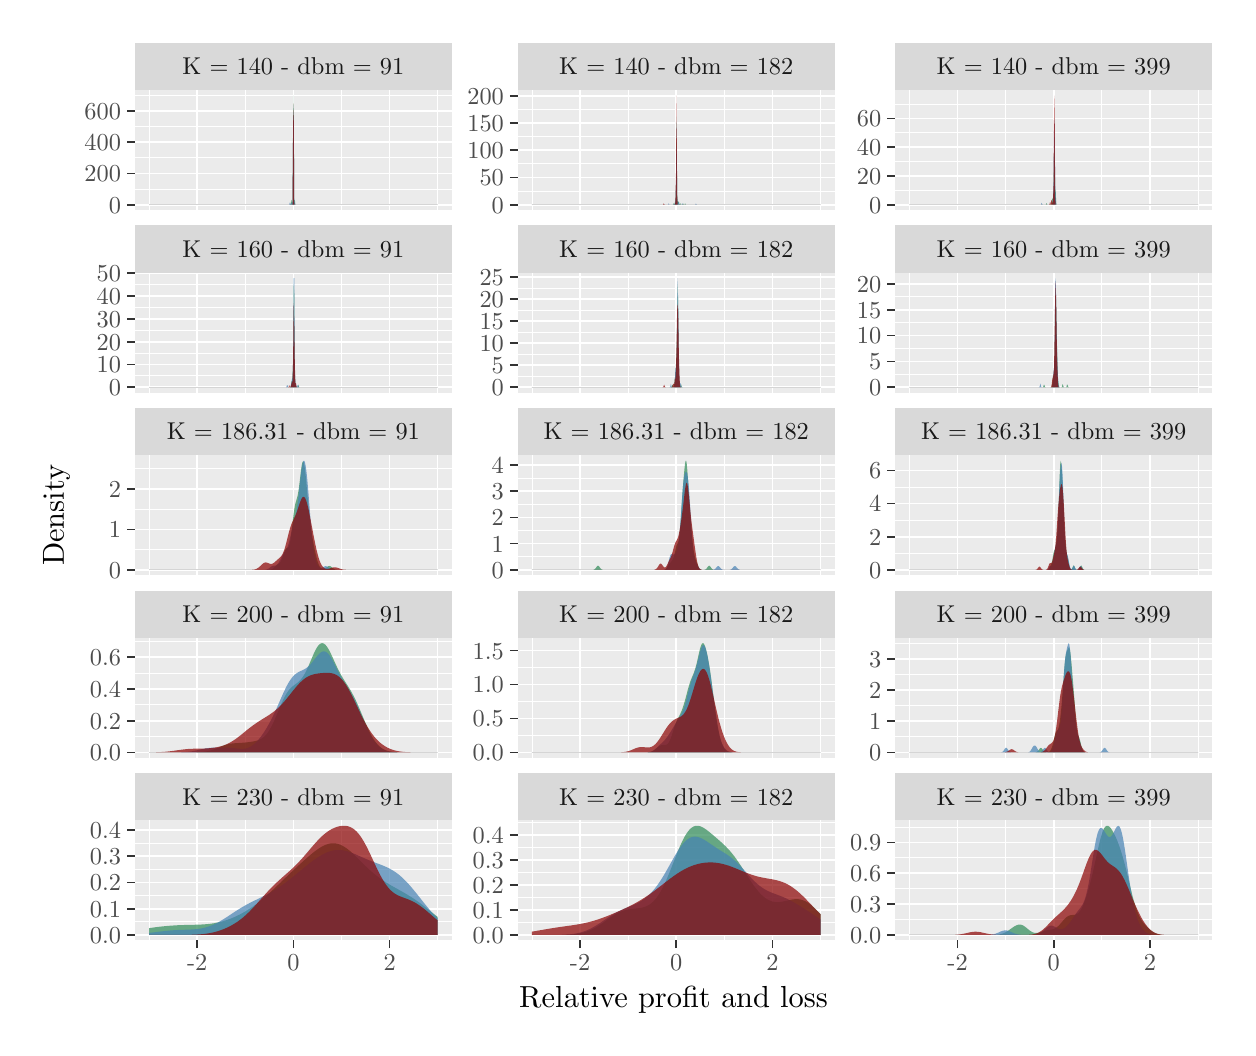
\begin{tikzpicture}[x=1pt,y=1pt]
\definecolor{fillColor}{RGB}{255,255,255}
\path[use as bounding box,fill=fillColor,fill opacity=0.00] (0,0) rectangle (433.62,361.35);
\begin{scope}
\path[clip] (  0.00,  0.00) rectangle (433.62,361.35);
\definecolor{drawColor}{RGB}{255,255,255}
\definecolor{fillColor}{RGB}{255,255,255}

\path[draw=drawColor,line width= 0.6pt,line join=round,line cap=round,fill=fillColor] (  0.00,  0.00) rectangle (433.62,361.35);
\end{scope}
\begin{scope}
\path[clip] ( 38.67,295.39) rectangle (153.37,338.79);
\definecolor{fillColor}{gray}{0.92}

\path[fill=fillColor] ( 38.67,295.39) rectangle (153.37,338.79);
\definecolor{drawColor}{RGB}{255,255,255}

\path[draw=drawColor,line width= 0.3pt,line join=round] ( 38.67,303.01) --
	(153.37,303.01);

\path[draw=drawColor,line width= 0.3pt,line join=round] ( 38.67,314.32) --
	(153.37,314.32);

\path[draw=drawColor,line width= 0.3pt,line join=round] ( 38.67,325.63) --
	(153.37,325.63);

\path[draw=drawColor,line width= 0.3pt,line join=round] ( 38.67,336.94) --
	(153.37,336.94);

\path[draw=drawColor,line width= 0.3pt,line join=round] ( 43.88,295.39) --
	( 43.88,338.79);

\path[draw=drawColor,line width= 0.3pt,line join=round] ( 78.64,295.39) --
	( 78.64,338.79);

\path[draw=drawColor,line width= 0.3pt,line join=round] (113.40,295.39) --
	(113.40,338.79);

\path[draw=drawColor,line width= 0.3pt,line join=round] (148.16,295.39) --
	(148.16,338.79);

\path[draw=drawColor,line width= 0.6pt,line join=round] ( 38.67,297.36) --
	(153.37,297.36);

\path[draw=drawColor,line width= 0.6pt,line join=round] ( 38.67,308.67) --
	(153.37,308.67);

\path[draw=drawColor,line width= 0.6pt,line join=round] ( 38.67,319.98) --
	(153.37,319.98);

\path[draw=drawColor,line width= 0.6pt,line join=round] ( 38.67,331.29) --
	(153.37,331.29);

\path[draw=drawColor,line width= 0.6pt,line join=round] ( 61.26,295.39) --
	( 61.26,338.79);

\path[draw=drawColor,line width= 0.6pt,line join=round] ( 96.02,295.39) --
	( 96.02,338.79);

\path[draw=drawColor,line width= 0.6pt,line join=round] (130.78,295.39) --
	(130.78,338.79);
\definecolor{fillColor}{RGB}{46,139,87}

\path[fill=fillColor,fill opacity=0.70] ( 43.88,297.36) --
	( 44.08,297.36) --
	( 44.29,297.36) --
	( 44.49,297.36) --
	( 44.70,297.36) --
	( 44.90,297.36) --
	( 45.11,297.36) --
	( 45.31,297.36) --
	( 45.51,297.36) --
	( 45.72,297.36) --
	( 45.92,297.36) --
	( 46.13,297.36) --
	( 46.33,297.36) --
	( 46.53,297.36) --
	( 46.74,297.36) --
	( 46.94,297.36) --
	( 47.15,297.36) --
	( 47.35,297.36) --
	( 47.55,297.36) --
	( 47.76,297.36) --
	( 47.96,297.36) --
	( 48.17,297.36) --
	( 48.37,297.36) --
	( 48.57,297.36) --
	( 48.78,297.36) --
	( 48.98,297.36) --
	( 49.19,297.36) --
	( 49.39,297.36) --
	( 49.59,297.36) --
	( 49.80,297.36) --
	( 50.00,297.36) --
	( 50.21,297.36) --
	( 50.41,297.36) --
	( 50.61,297.36) --
	( 50.82,297.36) --
	( 51.02,297.36) --
	( 51.23,297.36) --
	( 51.43,297.36) --
	( 51.64,297.36) --
	( 51.84,297.36) --
	( 52.04,297.36) --
	( 52.25,297.36) --
	( 52.45,297.36) --
	( 52.66,297.36) --
	( 52.86,297.36) --
	( 53.06,297.36) --
	( 53.27,297.36) --
	( 53.47,297.36) --
	( 53.68,297.36) --
	( 53.88,297.36) --
	( 54.08,297.36) --
	( 54.29,297.36) --
	( 54.49,297.36) --
	( 54.70,297.36) --
	( 54.90,297.36) --
	( 55.10,297.36) --
	( 55.31,297.36) --
	( 55.51,297.36) --
	( 55.72,297.36) --
	( 55.92,297.36) --
	( 56.12,297.36) --
	( 56.33,297.36) --
	( 56.53,297.36) --
	( 56.74,297.36) --
	( 56.94,297.36) --
	( 57.14,297.36) --
	( 57.35,297.36) --
	( 57.55,297.36) --
	( 57.76,297.36) --
	( 57.96,297.36) --
	( 58.17,297.36) --
	( 58.37,297.36) --
	( 58.57,297.36) --
	( 58.78,297.36) --
	( 58.98,297.36) --
	( 59.19,297.36) --
	( 59.39,297.36) --
	( 59.59,297.36) --
	( 59.80,297.36) --
	( 60.00,297.36) --
	( 60.21,297.36) --
	( 60.41,297.36) --
	( 60.61,297.36) --
	( 60.82,297.36) --
	( 61.02,297.36) --
	( 61.23,297.36) --
	( 61.43,297.36) --
	( 61.63,297.36) --
	( 61.84,297.36) --
	( 62.04,297.36) --
	( 62.25,297.36) --
	( 62.45,297.36) --
	( 62.65,297.36) --
	( 62.86,297.36) --
	( 63.06,297.36) --
	( 63.27,297.36) --
	( 63.47,297.36) --
	( 63.67,297.36) --
	( 63.88,297.36) --
	( 64.08,297.36) --
	( 64.29,297.36) --
	( 64.49,297.36) --
	( 64.70,297.36) --
	( 64.90,297.36) --
	( 65.10,297.36) --
	( 65.31,297.36) --
	( 65.51,297.36) --
	( 65.72,297.36) --
	( 65.92,297.36) --
	( 66.12,297.36) --
	( 66.33,297.36) --
	( 66.53,297.36) --
	( 66.74,297.36) --
	( 66.94,297.36) --
	( 67.14,297.36) --
	( 67.35,297.36) --
	( 67.55,297.36) --
	( 67.76,297.36) --
	( 67.96,297.36) --
	( 68.16,297.36) --
	( 68.37,297.36) --
	( 68.57,297.36) --
	( 68.78,297.36) --
	( 68.98,297.36) --
	( 69.18,297.36) --
	( 69.39,297.36) --
	( 69.59,297.36) --
	( 69.80,297.36) --
	( 70.00,297.36) --
	( 70.20,297.36) --
	( 70.41,297.36) --
	( 70.61,297.36) --
	( 70.82,297.36) --
	( 71.02,297.36) --
	( 71.23,297.36) --
	( 71.43,297.36) --
	( 71.63,297.36) --
	( 71.84,297.36) --
	( 72.04,297.36) --
	( 72.25,297.36) --
	( 72.45,297.36) --
	( 72.65,297.36) --
	( 72.86,297.36) --
	( 73.06,297.36) --
	( 73.27,297.36) --
	( 73.47,297.36) --
	( 73.67,297.36) --
	( 73.88,297.36) --
	( 74.08,297.36) --
	( 74.29,297.36) --
	( 74.49,297.36) --
	( 74.69,297.36) --
	( 74.90,297.36) --
	( 75.10,297.36) --
	( 75.31,297.36) --
	( 75.51,297.36) --
	( 75.71,297.36) --
	( 75.92,297.36) --
	( 76.12,297.36) --
	( 76.33,297.36) --
	( 76.53,297.36) --
	( 76.74,297.36) --
	( 76.94,297.36) --
	( 77.14,297.36) --
	( 77.35,297.36) --
	( 77.55,297.36) --
	( 77.76,297.36) --
	( 77.96,297.36) --
	( 78.16,297.36) --
	( 78.37,297.36) --
	( 78.57,297.36) --
	( 78.78,297.36) --
	( 78.98,297.36) --
	( 79.18,297.36) --
	( 79.39,297.36) --
	( 79.59,297.36) --
	( 79.80,297.36) --
	( 80.00,297.36) --
	( 80.20,297.36) --
	( 80.41,297.36) --
	( 80.61,297.36) --
	( 80.82,297.36) --
	( 81.02,297.36) --
	( 81.22,297.36) --
	( 81.43,297.36) --
	( 81.63,297.36) --
	( 81.84,297.36) --
	( 82.04,297.36) --
	( 82.24,297.36) --
	( 82.45,297.36) --
	( 82.65,297.36) --
	( 82.86,297.36) --
	( 83.06,297.36) --
	( 83.27,297.36) --
	( 83.47,297.36) --
	( 83.67,297.36) --
	( 83.88,297.36) --
	( 84.08,297.36) --
	( 84.29,297.36) --
	( 84.49,297.36) --
	( 84.69,297.36) --
	( 84.90,297.36) --
	( 85.10,297.36) --
	( 85.31,297.36) --
	( 85.51,297.36) --
	( 85.71,297.36) --
	( 85.92,297.36) --
	( 86.12,297.36) --
	( 86.33,297.36) --
	( 86.53,297.36) --
	( 86.73,297.36) --
	( 86.94,297.36) --
	( 87.14,297.36) --
	( 87.35,297.36) --
	( 87.55,297.36) --
	( 87.75,297.36) --
	( 87.96,297.36) --
	( 88.16,297.36) --
	( 88.37,297.36) --
	( 88.57,297.36) --
	( 88.77,297.36) --
	( 88.98,297.36) --
	( 89.18,297.36) --
	( 89.39,297.36) --
	( 89.59,297.36) --
	( 89.80,297.36) --
	( 90.00,297.36) --
	( 90.20,297.36) --
	( 90.41,297.36) --
	( 90.61,297.36) --
	( 90.82,297.36) --
	( 91.02,297.36) --
	( 91.22,297.36) --
	( 91.43,297.36) --
	( 91.63,297.36) --
	( 91.84,297.36) --
	( 92.04,297.36) --
	( 92.24,297.36) --
	( 92.45,297.36) --
	( 92.65,297.36) --
	( 92.86,297.36) --
	( 93.06,297.36) --
	( 93.26,297.36) --
	( 93.47,297.36) --
	( 93.67,297.36) --
	( 93.88,297.36) --
	( 94.08,297.36) --
	( 94.28,297.36) --
	( 94.49,297.36) --
	( 94.69,297.36) --
	( 94.90,297.36) --
	( 95.10,298.20) --
	( 95.30,299.25) --
	( 95.51,297.86) --
	( 95.71,298.45) --
	( 95.92,327.72) --
	( 96.12,336.82) --
	( 96.33,298.12) --
	( 96.53,299.15) --
	( 96.73,297.36) --
	( 96.94,297.36) --
	( 97.14,297.36) --
	( 97.35,297.36) --
	( 97.55,297.36) --
	( 97.75,297.36) --
	( 97.96,297.36) --
	( 98.16,297.36) --
	( 98.37,297.36) --
	( 98.57,297.36) --
	( 98.77,297.36) --
	( 98.98,297.36) --
	( 99.18,297.36) --
	( 99.39,297.36) --
	( 99.59,297.36) --
	( 99.79,297.36) --
	(100.00,297.36) --
	(100.20,297.36) --
	(100.41,297.36) --
	(100.61,297.36) --
	(100.81,297.36) --
	(101.02,297.36) --
	(101.22,297.36) --
	(101.43,297.36) --
	(101.63,297.36) --
	(101.84,297.36) --
	(102.04,297.36) --
	(102.24,297.36) --
	(102.45,297.36) --
	(102.65,297.36) --
	(102.86,297.36) --
	(103.06,297.36) --
	(103.26,297.36) --
	(103.47,297.36) --
	(103.67,297.36) --
	(103.88,297.36) --
	(104.08,297.36) --
	(104.28,297.36) --
	(104.49,297.36) --
	(104.69,297.36) --
	(104.90,297.36) --
	(105.10,297.36) --
	(105.30,297.36) --
	(105.51,297.36) --
	(105.71,297.36) --
	(105.92,297.36) --
	(106.12,297.36) --
	(106.32,297.36) --
	(106.53,297.36) --
	(106.73,297.36) --
	(106.94,297.36) --
	(107.14,297.36) --
	(107.34,297.36) --
	(107.55,297.36) --
	(107.75,297.36) --
	(107.96,297.36) --
	(108.16,297.36) --
	(108.37,297.36) --
	(108.57,297.36) --
	(108.77,297.36) --
	(108.98,297.36) --
	(109.18,297.36) --
	(109.39,297.36) --
	(109.59,297.36) --
	(109.79,297.36) --
	(110.00,297.36) --
	(110.20,297.36) --
	(110.41,297.36) --
	(110.61,297.36) --
	(110.81,297.36) --
	(111.02,297.36) --
	(111.22,297.36) --
	(111.43,297.36) --
	(111.63,297.36) --
	(111.83,297.36) --
	(112.04,297.36) --
	(112.24,297.36) --
	(112.45,297.36) --
	(112.65,297.36) --
	(112.85,297.36) --
	(113.06,297.36) --
	(113.26,297.36) --
	(113.47,297.36) --
	(113.67,297.36) --
	(113.87,297.36) --
	(114.08,297.36) --
	(114.28,297.36) --
	(114.49,297.36) --
	(114.69,297.36) --
	(114.90,297.36) --
	(115.10,297.36) --
	(115.30,297.36) --
	(115.51,297.36) --
	(115.71,297.36) --
	(115.92,297.36) --
	(116.12,297.36) --
	(116.32,297.36) --
	(116.53,297.36) --
	(116.73,297.36) --
	(116.94,297.36) --
	(117.14,297.36) --
	(117.34,297.36) --
	(117.55,297.36) --
	(117.75,297.36) --
	(117.96,297.36) --
	(118.16,297.36) --
	(118.36,297.36) --
	(118.57,297.36) --
	(118.77,297.36) --
	(118.98,297.36) --
	(119.18,297.36) --
	(119.38,297.36) --
	(119.59,297.36) --
	(119.79,297.36) --
	(120.00,297.36) --
	(120.20,297.36) --
	(120.40,297.36) --
	(120.61,297.36) --
	(120.81,297.36) --
	(121.02,297.36) --
	(121.22,297.36) --
	(121.43,297.36) --
	(121.63,297.36) --
	(121.83,297.36) --
	(122.04,297.36) --
	(122.24,297.36) --
	(122.45,297.36) --
	(122.65,297.36) --
	(122.85,297.36) --
	(123.06,297.36) --
	(123.26,297.36) --
	(123.47,297.36) --
	(123.67,297.36) --
	(123.87,297.36) --
	(124.08,297.36) --
	(124.28,297.36) --
	(124.49,297.36) --
	(124.69,297.36) --
	(124.89,297.36) --
	(125.10,297.36) --
	(125.30,297.36) --
	(125.51,297.36) --
	(125.71,297.36) --
	(125.91,297.36) --
	(126.12,297.36) --
	(126.32,297.36) --
	(126.53,297.36) --
	(126.73,297.36) --
	(126.94,297.36) --
	(127.14,297.36) --
	(127.34,297.36) --
	(127.55,297.36) --
	(127.75,297.36) --
	(127.96,297.36) --
	(128.16,297.36) --
	(128.36,297.36) --
	(128.57,297.36) --
	(128.77,297.36) --
	(128.98,297.36) --
	(129.18,297.36) --
	(129.38,297.36) --
	(129.59,297.36) --
	(129.79,297.36) --
	(130.00,297.36) --
	(130.20,297.36) --
	(130.40,297.36) --
	(130.61,297.36) --
	(130.81,297.36) --
	(131.02,297.36) --
	(131.22,297.36) --
	(131.42,297.36) --
	(131.63,297.36) --
	(131.83,297.36) --
	(132.04,297.36) --
	(132.24,297.36) --
	(132.44,297.36) --
	(132.65,297.36) --
	(132.85,297.36) --
	(133.06,297.36) --
	(133.26,297.36) --
	(133.47,297.36) --
	(133.67,297.36) --
	(133.87,297.36) --
	(134.08,297.36) --
	(134.28,297.36) --
	(134.49,297.36) --
	(134.69,297.36) --
	(134.89,297.36) --
	(135.10,297.36) --
	(135.30,297.36) --
	(135.51,297.36) --
	(135.71,297.36) --
	(135.91,297.36) --
	(136.12,297.36) --
	(136.32,297.36) --
	(136.53,297.36) --
	(136.73,297.36) --
	(136.93,297.36) --
	(137.14,297.36) --
	(137.34,297.36) --
	(137.55,297.36) --
	(137.75,297.36) --
	(137.95,297.36) --
	(138.16,297.36) --
	(138.36,297.36) --
	(138.57,297.36) --
	(138.77,297.36) --
	(138.97,297.36) --
	(139.18,297.36) --
	(139.38,297.36) --
	(139.59,297.36) --
	(139.79,297.36) --
	(140.00,297.36) --
	(140.20,297.36) --
	(140.40,297.36) --
	(140.61,297.36) --
	(140.81,297.36) --
	(141.02,297.36) --
	(141.22,297.36) --
	(141.42,297.36) --
	(141.63,297.36) --
	(141.83,297.36) --
	(142.04,297.36) --
	(142.24,297.36) --
	(142.44,297.36) --
	(142.65,297.36) --
	(142.85,297.36) --
	(143.06,297.36) --
	(143.26,297.36) --
	(143.46,297.36) --
	(143.67,297.36) --
	(143.87,297.36) --
	(144.08,297.36) --
	(144.28,297.36) --
	(144.48,297.36) --
	(144.69,297.36) --
	(144.89,297.36) --
	(145.10,297.36) --
	(145.30,297.36) --
	(145.50,297.36) --
	(145.71,297.36) --
	(145.91,297.36) --
	(146.12,297.36) --
	(146.32,297.36) --
	(146.53,297.36) --
	(146.73,297.36) --
	(146.93,297.36) --
	(147.14,297.36) --
	(147.34,297.36) --
	(147.55,297.36) --
	(147.75,297.36) --
	(147.95,297.36) --
	(148.16,297.36) --
	(148.16,297.36) --
	(147.95,297.36) --
	(147.75,297.36) --
	(147.55,297.36) --
	(147.34,297.36) --
	(147.14,297.36) --
	(146.93,297.36) --
	(146.73,297.36) --
	(146.53,297.36) --
	(146.32,297.36) --
	(146.12,297.36) --
	(145.91,297.36) --
	(145.71,297.36) --
	(145.50,297.36) --
	(145.30,297.36) --
	(145.10,297.36) --
	(144.89,297.36) --
	(144.69,297.36) --
	(144.48,297.36) --
	(144.28,297.36) --
	(144.08,297.36) --
	(143.87,297.36) --
	(143.67,297.36) --
	(143.46,297.36) --
	(143.26,297.36) --
	(143.06,297.36) --
	(142.85,297.36) --
	(142.65,297.36) --
	(142.44,297.36) --
	(142.24,297.36) --
	(142.04,297.36) --
	(141.83,297.36) --
	(141.63,297.36) --
	(141.42,297.36) --
	(141.22,297.36) --
	(141.02,297.36) --
	(140.81,297.36) --
	(140.61,297.36) --
	(140.40,297.36) --
	(140.20,297.36) --
	(140.00,297.36) --
	(139.79,297.36) --
	(139.59,297.36) --
	(139.38,297.36) --
	(139.18,297.36) --
	(138.97,297.36) --
	(138.77,297.36) --
	(138.57,297.36) --
	(138.36,297.36) --
	(138.16,297.36) --
	(137.95,297.36) --
	(137.75,297.36) --
	(137.55,297.36) --
	(137.34,297.36) --
	(137.14,297.36) --
	(136.93,297.36) --
	(136.73,297.36) --
	(136.53,297.36) --
	(136.32,297.36) --
	(136.12,297.36) --
	(135.91,297.36) --
	(135.71,297.36) --
	(135.51,297.36) --
	(135.30,297.36) --
	(135.10,297.36) --
	(134.89,297.36) --
	(134.69,297.36) --
	(134.49,297.36) --
	(134.28,297.36) --
	(134.08,297.36) --
	(133.87,297.36) --
	(133.67,297.36) --
	(133.47,297.36) --
	(133.26,297.36) --
	(133.06,297.36) --
	(132.85,297.36) --
	(132.65,297.36) --
	(132.44,297.36) --
	(132.24,297.36) --
	(132.04,297.36) --
	(131.83,297.36) --
	(131.63,297.36) --
	(131.42,297.36) --
	(131.22,297.36) --
	(131.02,297.36) --
	(130.81,297.36) --
	(130.61,297.36) --
	(130.40,297.36) --
	(130.20,297.36) --
	(130.00,297.36) --
	(129.79,297.36) --
	(129.59,297.36) --
	(129.38,297.36) --
	(129.18,297.36) --
	(128.98,297.36) --
	(128.77,297.36) --
	(128.57,297.36) --
	(128.36,297.36) --
	(128.16,297.36) --
	(127.96,297.36) --
	(127.75,297.36) --
	(127.55,297.36) --
	(127.34,297.36) --
	(127.14,297.36) --
	(126.94,297.36) --
	(126.73,297.36) --
	(126.53,297.36) --
	(126.32,297.36) --
	(126.12,297.36) --
	(125.91,297.36) --
	(125.71,297.36) --
	(125.51,297.36) --
	(125.30,297.36) --
	(125.10,297.36) --
	(124.89,297.36) --
	(124.69,297.36) --
	(124.49,297.36) --
	(124.28,297.36) --
	(124.08,297.36) --
	(123.87,297.36) --
	(123.67,297.36) --
	(123.47,297.36) --
	(123.26,297.36) --
	(123.06,297.36) --
	(122.85,297.36) --
	(122.65,297.36) --
	(122.45,297.36) --
	(122.24,297.36) --
	(122.04,297.36) --
	(121.83,297.36) --
	(121.63,297.36) --
	(121.43,297.36) --
	(121.22,297.36) --
	(121.02,297.36) --
	(120.81,297.36) --
	(120.61,297.36) --
	(120.40,297.36) --
	(120.20,297.36) --
	(120.00,297.36) --
	(119.79,297.36) --
	(119.59,297.36) --
	(119.38,297.36) --
	(119.18,297.36) --
	(118.98,297.36) --
	(118.77,297.36) --
	(118.57,297.36) --
	(118.36,297.36) --
	(118.16,297.36) --
	(117.96,297.36) --
	(117.75,297.36) --
	(117.55,297.36) --
	(117.34,297.36) --
	(117.14,297.36) --
	(116.94,297.36) --
	(116.73,297.36) --
	(116.53,297.36) --
	(116.32,297.36) --
	(116.12,297.36) --
	(115.92,297.36) --
	(115.71,297.36) --
	(115.51,297.36) --
	(115.30,297.36) --
	(115.10,297.36) --
	(114.90,297.36) --
	(114.69,297.36) --
	(114.49,297.36) --
	(114.28,297.36) --
	(114.08,297.36) --
	(113.87,297.36) --
	(113.67,297.36) --
	(113.47,297.36) --
	(113.26,297.36) --
	(113.06,297.36) --
	(112.85,297.36) --
	(112.65,297.36) --
	(112.45,297.36) --
	(112.24,297.36) --
	(112.04,297.36) --
	(111.83,297.36) --
	(111.63,297.36) --
	(111.43,297.36) --
	(111.22,297.36) --
	(111.02,297.36) --
	(110.81,297.36) --
	(110.61,297.36) --
	(110.41,297.36) --
	(110.20,297.36) --
	(110.00,297.36) --
	(109.79,297.36) --
	(109.59,297.36) --
	(109.39,297.36) --
	(109.18,297.36) --
	(108.98,297.36) --
	(108.77,297.36) --
	(108.57,297.36) --
	(108.37,297.36) --
	(108.16,297.36) --
	(107.96,297.36) --
	(107.75,297.36) --
	(107.55,297.36) --
	(107.34,297.36) --
	(107.14,297.36) --
	(106.94,297.36) --
	(106.73,297.36) --
	(106.53,297.36) --
	(106.32,297.36) --
	(106.12,297.36) --
	(105.92,297.36) --
	(105.71,297.36) --
	(105.51,297.36) --
	(105.30,297.36) --
	(105.10,297.36) --
	(104.90,297.36) --
	(104.69,297.36) --
	(104.49,297.36) --
	(104.28,297.36) --
	(104.08,297.36) --
	(103.88,297.36) --
	(103.67,297.36) --
	(103.47,297.36) --
	(103.26,297.36) --
	(103.06,297.36) --
	(102.86,297.36) --
	(102.65,297.36) --
	(102.45,297.36) --
	(102.24,297.36) --
	(102.04,297.36) --
	(101.84,297.36) --
	(101.63,297.36) --
	(101.43,297.36) --
	(101.22,297.36) --
	(101.02,297.36) --
	(100.81,297.36) --
	(100.61,297.36) --
	(100.41,297.36) --
	(100.20,297.36) --
	(100.00,297.36) --
	( 99.79,297.36) --
	( 99.59,297.36) --
	( 99.39,297.36) --
	( 99.18,297.36) --
	( 98.98,297.36) --
	( 98.77,297.36) --
	( 98.57,297.36) --
	( 98.37,297.36) --
	( 98.16,297.36) --
	( 97.96,297.36) --
	( 97.75,297.36) --
	( 97.55,297.36) --
	( 97.35,297.36) --
	( 97.14,297.36) --
	( 96.94,297.36) --
	( 96.73,297.36) --
	( 96.53,297.36) --
	( 96.33,297.36) --
	( 96.12,297.36) --
	( 95.92,297.36) --
	( 95.71,297.36) --
	( 95.51,297.36) --
	( 95.30,297.36) --
	( 95.10,297.36) --
	( 94.90,297.36) --
	( 94.69,297.36) --
	( 94.49,297.36) --
	( 94.28,297.36) --
	( 94.08,297.36) --
	( 93.88,297.36) --
	( 93.67,297.36) --
	( 93.47,297.36) --
	( 93.26,297.36) --
	( 93.06,297.36) --
	( 92.86,297.36) --
	( 92.65,297.36) --
	( 92.45,297.36) --
	( 92.24,297.36) --
	( 92.04,297.36) --
	( 91.84,297.36) --
	( 91.63,297.36) --
	( 91.43,297.36) --
	( 91.22,297.36) --
	( 91.02,297.36) --
	( 90.82,297.36) --
	( 90.61,297.36) --
	( 90.41,297.36) --
	( 90.20,297.36) --
	( 90.00,297.36) --
	( 89.80,297.36) --
	( 89.59,297.36) --
	( 89.39,297.36) --
	( 89.18,297.36) --
	( 88.98,297.36) --
	( 88.77,297.36) --
	( 88.57,297.36) --
	( 88.37,297.36) --
	( 88.16,297.36) --
	( 87.96,297.36) --
	( 87.75,297.36) --
	( 87.55,297.36) --
	( 87.35,297.36) --
	( 87.14,297.36) --
	( 86.94,297.36) --
	( 86.73,297.36) --
	( 86.53,297.36) --
	( 86.33,297.36) --
	( 86.12,297.36) --
	( 85.92,297.36) --
	( 85.71,297.36) --
	( 85.51,297.36) --
	( 85.31,297.36) --
	( 85.10,297.36) --
	( 84.90,297.36) --
	( 84.69,297.36) --
	( 84.49,297.36) --
	( 84.29,297.36) --
	( 84.08,297.36) --
	( 83.88,297.36) --
	( 83.67,297.36) --
	( 83.47,297.36) --
	( 83.27,297.36) --
	( 83.06,297.36) --
	( 82.86,297.36) --
	( 82.65,297.36) --
	( 82.45,297.36) --
	( 82.24,297.36) --
	( 82.04,297.36) --
	( 81.84,297.36) --
	( 81.63,297.36) --
	( 81.43,297.36) --
	( 81.22,297.36) --
	( 81.02,297.36) --
	( 80.82,297.36) --
	( 80.61,297.36) --
	( 80.41,297.36) --
	( 80.20,297.36) --
	( 80.00,297.36) --
	( 79.80,297.36) --
	( 79.59,297.36) --
	( 79.39,297.36) --
	( 79.18,297.36) --
	( 78.98,297.36) --
	( 78.78,297.36) --
	( 78.57,297.36) --
	( 78.37,297.36) --
	( 78.16,297.36) --
	( 77.96,297.36) --
	( 77.76,297.36) --
	( 77.55,297.36) --
	( 77.35,297.36) --
	( 77.14,297.36) --
	( 76.94,297.36) --
	( 76.74,297.36) --
	( 76.53,297.36) --
	( 76.33,297.36) --
	( 76.12,297.36) --
	( 75.92,297.36) --
	( 75.71,297.36) --
	( 75.51,297.36) --
	( 75.31,297.36) --
	( 75.10,297.36) --
	( 74.90,297.36) --
	( 74.69,297.36) --
	( 74.49,297.36) --
	( 74.29,297.36) --
	( 74.08,297.36) --
	( 73.88,297.36) --
	( 73.67,297.36) --
	( 73.47,297.36) --
	( 73.27,297.36) --
	( 73.06,297.36) --
	( 72.86,297.36) --
	( 72.65,297.36) --
	( 72.45,297.36) --
	( 72.25,297.36) --
	( 72.04,297.36) --
	( 71.84,297.36) --
	( 71.63,297.36) --
	( 71.43,297.36) --
	( 71.23,297.36) --
	( 71.02,297.36) --
	( 70.82,297.36) --
	( 70.61,297.36) --
	( 70.41,297.36) --
	( 70.20,297.36) --
	( 70.00,297.36) --
	( 69.80,297.36) --
	( 69.59,297.36) --
	( 69.39,297.36) --
	( 69.18,297.36) --
	( 68.98,297.36) --
	( 68.78,297.36) --
	( 68.57,297.36) --
	( 68.37,297.36) --
	( 68.16,297.36) --
	( 67.96,297.36) --
	( 67.76,297.36) --
	( 67.55,297.36) --
	( 67.35,297.36) --
	( 67.14,297.36) --
	( 66.94,297.36) --
	( 66.74,297.36) --
	( 66.53,297.36) --
	( 66.33,297.36) --
	( 66.12,297.36) --
	( 65.92,297.36) --
	( 65.72,297.36) --
	( 65.51,297.36) --
	( 65.31,297.36) --
	( 65.10,297.36) --
	( 64.90,297.36) --
	( 64.70,297.36) --
	( 64.49,297.36) --
	( 64.29,297.36) --
	( 64.08,297.36) --
	( 63.88,297.36) --
	( 63.67,297.36) --
	( 63.47,297.36) --
	( 63.27,297.36) --
	( 63.06,297.36) --
	( 62.86,297.36) --
	( 62.65,297.36) --
	( 62.45,297.36) --
	( 62.25,297.36) --
	( 62.04,297.36) --
	( 61.84,297.36) --
	( 61.63,297.36) --
	( 61.43,297.36) --
	( 61.23,297.36) --
	( 61.02,297.36) --
	( 60.82,297.36) --
	( 60.61,297.36) --
	( 60.41,297.36) --
	( 60.21,297.36) --
	( 60.00,297.36) --
	( 59.80,297.36) --
	( 59.59,297.36) --
	( 59.39,297.36) --
	( 59.19,297.36) --
	( 58.98,297.36) --
	( 58.78,297.36) --
	( 58.57,297.36) --
	( 58.37,297.36) --
	( 58.17,297.36) --
	( 57.96,297.36) --
	( 57.76,297.36) --
	( 57.55,297.36) --
	( 57.35,297.36) --
	( 57.14,297.36) --
	( 56.94,297.36) --
	( 56.74,297.36) --
	( 56.53,297.36) --
	( 56.33,297.36) --
	( 56.12,297.36) --
	( 55.92,297.36) --
	( 55.72,297.36) --
	( 55.51,297.36) --
	( 55.31,297.36) --
	( 55.10,297.36) --
	( 54.90,297.36) --
	( 54.70,297.36) --
	( 54.49,297.36) --
	( 54.29,297.36) --
	( 54.08,297.36) --
	( 53.88,297.36) --
	( 53.68,297.36) --
	( 53.47,297.36) --
	( 53.27,297.36) --
	( 53.06,297.36) --
	( 52.86,297.36) --
	( 52.66,297.36) --
	( 52.45,297.36) --
	( 52.25,297.36) --
	( 52.04,297.36) --
	( 51.84,297.36) --
	( 51.64,297.36) --
	( 51.43,297.36) --
	( 51.23,297.36) --
	( 51.02,297.36) --
	( 50.82,297.36) --
	( 50.61,297.36) --
	( 50.41,297.36) --
	( 50.21,297.36) --
	( 50.00,297.36) --
	( 49.80,297.36) --
	( 49.59,297.36) --
	( 49.39,297.36) --
	( 49.19,297.36) --
	( 48.98,297.36) --
	( 48.78,297.36) --
	( 48.57,297.36) --
	( 48.37,297.36) --
	( 48.17,297.36) --
	( 47.96,297.36) --
	( 47.76,297.36) --
	( 47.55,297.36) --
	( 47.35,297.36) --
	( 47.15,297.36) --
	( 46.94,297.36) --
	( 46.74,297.36) --
	( 46.53,297.36) --
	( 46.33,297.36) --
	( 46.13,297.36) --
	( 45.92,297.36) --
	( 45.72,297.36) --
	( 45.51,297.36) --
	( 45.31,297.36) --
	( 45.11,297.36) --
	( 44.90,297.36) --
	( 44.70,297.36) --
	( 44.49,297.36) --
	( 44.29,297.36) --
	( 44.08,297.36) --
	( 43.88,297.36) --
	cycle;
\definecolor{fillColor}{RGB}{70,130,180}

\path[fill=fillColor,fill opacity=0.70] ( 43.88,297.36) --
	( 44.08,297.36) --
	( 44.29,297.36) --
	( 44.49,297.36) --
	( 44.70,297.36) --
	( 44.90,297.36) --
	( 45.11,297.36) --
	( 45.31,297.36) --
	( 45.51,297.36) --
	( 45.72,297.36) --
	( 45.92,297.36) --
	( 46.13,297.36) --
	( 46.33,297.36) --
	( 46.53,297.36) --
	( 46.74,297.36) --
	( 46.94,297.36) --
	( 47.15,297.36) --
	( 47.35,297.36) --
	( 47.55,297.36) --
	( 47.76,297.36) --
	( 47.96,297.36) --
	( 48.17,297.36) --
	( 48.37,297.36) --
	( 48.57,297.36) --
	( 48.78,297.36) --
	( 48.98,297.36) --
	( 49.19,297.36) --
	( 49.39,297.36) --
	( 49.59,297.36) --
	( 49.80,297.36) --
	( 50.00,297.36) --
	( 50.21,297.36) --
	( 50.41,297.36) --
	( 50.61,297.36) --
	( 50.82,297.36) --
	( 51.02,297.36) --
	( 51.23,297.36) --
	( 51.43,297.36) --
	( 51.64,297.36) --
	( 51.84,297.36) --
	( 52.04,297.36) --
	( 52.25,297.36) --
	( 52.45,297.36) --
	( 52.66,297.36) --
	( 52.86,297.36) --
	( 53.06,297.36) --
	( 53.27,297.36) --
	( 53.47,297.36) --
	( 53.68,297.36) --
	( 53.88,297.36) --
	( 54.08,297.36) --
	( 54.29,297.36) --
	( 54.49,297.36) --
	( 54.70,297.36) --
	( 54.90,297.36) --
	( 55.10,297.36) --
	( 55.31,297.36) --
	( 55.51,297.36) --
	( 55.72,297.36) --
	( 55.92,297.36) --
	( 56.12,297.36) --
	( 56.33,297.36) --
	( 56.53,297.36) --
	( 56.74,297.36) --
	( 56.94,297.36) --
	( 57.14,297.36) --
	( 57.35,297.36) --
	( 57.55,297.36) --
	( 57.76,297.36) --
	( 57.96,297.36) --
	( 58.17,297.36) --
	( 58.37,297.36) --
	( 58.57,297.36) --
	( 58.78,297.36) --
	( 58.98,297.36) --
	( 59.19,297.36) --
	( 59.39,297.36) --
	( 59.59,297.36) --
	( 59.80,297.36) --
	( 60.00,297.36) --
	( 60.21,297.36) --
	( 60.41,297.36) --
	( 60.61,297.36) --
	( 60.82,297.36) --
	( 61.02,297.36) --
	( 61.23,297.36) --
	( 61.43,297.36) --
	( 61.63,297.36) --
	( 61.84,297.36) --
	( 62.04,297.36) --
	( 62.25,297.36) --
	( 62.45,297.36) --
	( 62.65,297.36) --
	( 62.86,297.36) --
	( 63.06,297.36) --
	( 63.27,297.36) --
	( 63.47,297.36) --
	( 63.67,297.36) --
	( 63.88,297.36) --
	( 64.08,297.36) --
	( 64.29,297.36) --
	( 64.49,297.36) --
	( 64.70,297.36) --
	( 64.90,297.36) --
	( 65.10,297.36) --
	( 65.31,297.36) --
	( 65.51,297.36) --
	( 65.72,297.36) --
	( 65.92,297.36) --
	( 66.12,297.36) --
	( 66.33,297.36) --
	( 66.53,297.36) --
	( 66.74,297.36) --
	( 66.94,297.36) --
	( 67.14,297.36) --
	( 67.35,297.36) --
	( 67.55,297.36) --
	( 67.76,297.36) --
	( 67.96,297.36) --
	( 68.16,297.36) --
	( 68.37,297.36) --
	( 68.57,297.36) --
	( 68.78,297.36) --
	( 68.98,297.36) --
	( 69.18,297.36) --
	( 69.39,297.36) --
	( 69.59,297.36) --
	( 69.80,297.36) --
	( 70.00,297.36) --
	( 70.20,297.36) --
	( 70.41,297.36) --
	( 70.61,297.36) --
	( 70.82,297.36) --
	( 71.02,297.36) --
	( 71.23,297.36) --
	( 71.43,297.36) --
	( 71.63,297.36) --
	( 71.84,297.36) --
	( 72.04,297.36) --
	( 72.25,297.36) --
	( 72.45,297.36) --
	( 72.65,297.36) --
	( 72.86,297.36) --
	( 73.06,297.36) --
	( 73.27,297.36) --
	( 73.47,297.36) --
	( 73.67,297.36) --
	( 73.88,297.36) --
	( 74.08,297.36) --
	( 74.29,297.36) --
	( 74.49,297.36) --
	( 74.69,297.36) --
	( 74.90,297.36) --
	( 75.10,297.36) --
	( 75.31,297.36) --
	( 75.51,297.36) --
	( 75.71,297.36) --
	( 75.92,297.36) --
	( 76.12,297.36) --
	( 76.33,297.36) --
	( 76.53,297.36) --
	( 76.74,297.36) --
	( 76.94,297.36) --
	( 77.14,297.36) --
	( 77.35,297.36) --
	( 77.55,297.36) --
	( 77.76,297.36) --
	( 77.96,297.36) --
	( 78.16,297.36) --
	( 78.37,297.36) --
	( 78.57,297.36) --
	( 78.78,297.36) --
	( 78.98,297.36) --
	( 79.18,297.36) --
	( 79.39,297.36) --
	( 79.59,297.36) --
	( 79.80,297.36) --
	( 80.00,297.36) --
	( 80.20,297.36) --
	( 80.41,297.36) --
	( 80.61,297.36) --
	( 80.82,297.36) --
	( 81.02,297.36) --
	( 81.22,297.36) --
	( 81.43,297.36) --
	( 81.63,297.36) --
	( 81.84,297.36) --
	( 82.04,297.36) --
	( 82.24,297.36) --
	( 82.45,297.36) --
	( 82.65,297.36) --
	( 82.86,297.36) --
	( 83.06,297.36) --
	( 83.27,297.36) --
	( 83.47,297.36) --
	( 83.67,297.36) --
	( 83.88,297.36) --
	( 84.08,297.36) --
	( 84.29,297.36) --
	( 84.49,297.36) --
	( 84.69,297.36) --
	( 84.90,297.36) --
	( 85.10,297.36) --
	( 85.31,297.36) --
	( 85.51,297.36) --
	( 85.71,297.36) --
	( 85.92,297.36) --
	( 86.12,297.36) --
	( 86.33,297.36) --
	( 86.53,297.36) --
	( 86.73,297.36) --
	( 86.94,297.36) --
	( 87.14,297.36) --
	( 87.35,297.36) --
	( 87.55,297.36) --
	( 87.75,297.36) --
	( 87.96,297.36) --
	( 88.16,297.36) --
	( 88.37,297.36) --
	( 88.57,297.36) --
	( 88.77,297.36) --
	( 88.98,297.36) --
	( 89.18,297.36) --
	( 89.39,297.36) --
	( 89.59,297.36) --
	( 89.80,297.36) --
	( 90.00,297.36) --
	( 90.20,297.36) --
	( 90.41,297.36) --
	( 90.61,297.36) --
	( 90.82,297.36) --
	( 91.02,297.36) --
	( 91.22,297.36) --
	( 91.43,297.36) --
	( 91.63,297.36) --
	( 91.84,297.36) --
	( 92.04,297.36) --
	( 92.24,297.36) --
	( 92.45,297.36) --
	( 92.65,297.36) --
	( 92.86,297.36) --
	( 93.06,297.36) --
	( 93.26,297.36) --
	( 93.47,297.36) --
	( 93.67,297.36) --
	( 93.88,297.36) --
	( 94.08,297.36) --
	( 94.28,297.36) --
	( 94.49,297.36) --
	( 94.69,298.11) --
	( 94.90,297.59) --
	( 95.10,297.55) --
	( 95.30,298.15) --
	( 95.51,297.47) --
	( 95.71,298.54) --
	( 95.92,325.66) --
	( 96.12,333.36) --
	( 96.33,298.88) --
	( 96.53,297.96) --
	( 96.73,297.36) --
	( 96.94,297.36) --
	( 97.14,297.36) --
	( 97.35,297.36) --
	( 97.55,297.36) --
	( 97.75,297.36) --
	( 97.96,297.36) --
	( 98.16,297.36) --
	( 98.37,297.36) --
	( 98.57,297.36) --
	( 98.77,297.36) --
	( 98.98,297.36) --
	( 99.18,297.36) --
	( 99.39,297.36) --
	( 99.59,297.36) --
	( 99.79,297.36) --
	(100.00,297.36) --
	(100.20,297.36) --
	(100.41,297.36) --
	(100.61,297.36) --
	(100.81,297.36) --
	(101.02,297.36) --
	(101.22,297.36) --
	(101.43,297.36) --
	(101.63,297.36) --
	(101.84,297.36) --
	(102.04,297.36) --
	(102.24,297.36) --
	(102.45,297.36) --
	(102.65,297.36) --
	(102.86,297.36) --
	(103.06,297.36) --
	(103.26,297.36) --
	(103.47,297.36) --
	(103.67,297.36) --
	(103.88,297.36) --
	(104.08,297.36) --
	(104.28,297.36) --
	(104.49,297.36) --
	(104.69,297.36) --
	(104.90,297.36) --
	(105.10,297.36) --
	(105.30,297.36) --
	(105.51,297.36) --
	(105.71,297.36) --
	(105.92,297.36) --
	(106.12,297.36) --
	(106.32,297.36) --
	(106.53,297.36) --
	(106.73,297.36) --
	(106.94,297.36) --
	(107.14,297.36) --
	(107.34,297.36) --
	(107.55,297.36) --
	(107.75,297.36) --
	(107.96,297.36) --
	(108.16,297.36) --
	(108.37,297.36) --
	(108.57,297.36) --
	(108.77,297.36) --
	(108.98,297.36) --
	(109.18,297.36) --
	(109.39,297.36) --
	(109.59,297.36) --
	(109.79,297.36) --
	(110.00,297.36) --
	(110.20,297.36) --
	(110.41,297.36) --
	(110.61,297.36) --
	(110.81,297.36) --
	(111.02,297.36) --
	(111.22,297.36) --
	(111.43,297.36) --
	(111.63,297.36) --
	(111.83,297.36) --
	(112.04,297.36) --
	(112.24,297.36) --
	(112.45,297.36) --
	(112.65,297.36) --
	(112.85,297.36) --
	(113.06,297.36) --
	(113.26,297.36) --
	(113.47,297.36) --
	(113.67,297.36) --
	(113.87,297.36) --
	(114.08,297.36) --
	(114.28,297.36) --
	(114.49,297.36) --
	(114.69,297.36) --
	(114.90,297.36) --
	(115.10,297.36) --
	(115.30,297.36) --
	(115.51,297.36) --
	(115.71,297.36) --
	(115.92,297.36) --
	(116.12,297.36) --
	(116.32,297.36) --
	(116.53,297.36) --
	(116.73,297.36) --
	(116.94,297.36) --
	(117.14,297.36) --
	(117.34,297.36) --
	(117.55,297.36) --
	(117.75,297.36) --
	(117.96,297.36) --
	(118.16,297.36) --
	(118.36,297.36) --
	(118.57,297.36) --
	(118.77,297.36) --
	(118.98,297.36) --
	(119.18,297.36) --
	(119.38,297.36) --
	(119.59,297.36) --
	(119.79,297.36) --
	(120.00,297.36) --
	(120.20,297.36) --
	(120.40,297.36) --
	(120.61,297.36) --
	(120.81,297.36) --
	(121.02,297.36) --
	(121.22,297.36) --
	(121.43,297.36) --
	(121.63,297.36) --
	(121.83,297.36) --
	(122.04,297.36) --
	(122.24,297.36) --
	(122.45,297.36) --
	(122.65,297.36) --
	(122.85,297.36) --
	(123.06,297.36) --
	(123.26,297.36) --
	(123.47,297.36) --
	(123.67,297.36) --
	(123.87,297.36) --
	(124.08,297.36) --
	(124.28,297.36) --
	(124.49,297.36) --
	(124.69,297.36) --
	(124.89,297.36) --
	(125.10,297.36) --
	(125.30,297.36) --
	(125.51,297.36) --
	(125.71,297.36) --
	(125.91,297.36) --
	(126.12,297.36) --
	(126.32,297.36) --
	(126.53,297.36) --
	(126.73,297.36) --
	(126.94,297.36) --
	(127.14,297.36) --
	(127.34,297.36) --
	(127.55,297.36) --
	(127.75,297.36) --
	(127.96,297.36) --
	(128.16,297.36) --
	(128.36,297.36) --
	(128.57,297.36) --
	(128.77,297.36) --
	(128.98,297.36) --
	(129.18,297.36) --
	(129.38,297.36) --
	(129.59,297.36) --
	(129.79,297.36) --
	(130.00,297.36) --
	(130.20,297.36) --
	(130.40,297.36) --
	(130.61,297.36) --
	(130.81,297.36) --
	(131.02,297.36) --
	(131.22,297.36) --
	(131.42,297.36) --
	(131.63,297.36) --
	(131.83,297.36) --
	(132.04,297.36) --
	(132.24,297.36) --
	(132.44,297.36) --
	(132.65,297.36) --
	(132.85,297.36) --
	(133.06,297.36) --
	(133.26,297.36) --
	(133.47,297.36) --
	(133.67,297.36) --
	(133.87,297.36) --
	(134.08,297.36) --
	(134.28,297.36) --
	(134.49,297.36) --
	(134.69,297.36) --
	(134.89,297.36) --
	(135.10,297.36) --
	(135.30,297.36) --
	(135.51,297.36) --
	(135.71,297.36) --
	(135.91,297.36) --
	(136.12,297.36) --
	(136.32,297.36) --
	(136.53,297.36) --
	(136.73,297.36) --
	(136.93,297.36) --
	(137.14,297.36) --
	(137.34,297.36) --
	(137.55,297.36) --
	(137.75,297.36) --
	(137.95,297.36) --
	(138.16,297.36) --
	(138.36,297.36) --
	(138.57,297.36) --
	(138.77,297.36) --
	(138.97,297.36) --
	(139.18,297.36) --
	(139.38,297.36) --
	(139.59,297.36) --
	(139.79,297.36) --
	(140.00,297.36) --
	(140.20,297.36) --
	(140.40,297.36) --
	(140.61,297.36) --
	(140.81,297.36) --
	(141.02,297.36) --
	(141.22,297.36) --
	(141.42,297.36) --
	(141.63,297.36) --
	(141.83,297.36) --
	(142.04,297.36) --
	(142.24,297.36) --
	(142.44,297.36) --
	(142.65,297.36) --
	(142.85,297.36) --
	(143.06,297.36) --
	(143.26,297.36) --
	(143.46,297.36) --
	(143.67,297.36) --
	(143.87,297.36) --
	(144.08,297.36) --
	(144.28,297.36) --
	(144.48,297.36) --
	(144.69,297.36) --
	(144.89,297.36) --
	(145.10,297.36) --
	(145.30,297.36) --
	(145.50,297.36) --
	(145.71,297.36) --
	(145.91,297.36) --
	(146.12,297.36) --
	(146.32,297.36) --
	(146.53,297.36) --
	(146.73,297.36) --
	(146.93,297.36) --
	(147.14,297.36) --
	(147.34,297.36) --
	(147.55,297.36) --
	(147.75,297.36) --
	(147.95,297.36) --
	(148.16,297.36) --
	(148.16,297.36) --
	(147.95,297.36) --
	(147.75,297.36) --
	(147.55,297.36) --
	(147.34,297.36) --
	(147.14,297.36) --
	(146.93,297.36) --
	(146.73,297.36) --
	(146.53,297.36) --
	(146.32,297.36) --
	(146.12,297.36) --
	(145.91,297.36) --
	(145.71,297.36) --
	(145.50,297.36) --
	(145.30,297.36) --
	(145.10,297.36) --
	(144.89,297.36) --
	(144.69,297.36) --
	(144.48,297.36) --
	(144.28,297.36) --
	(144.08,297.36) --
	(143.87,297.36) --
	(143.67,297.36) --
	(143.46,297.36) --
	(143.26,297.36) --
	(143.06,297.36) --
	(142.85,297.36) --
	(142.65,297.36) --
	(142.44,297.36) --
	(142.24,297.36) --
	(142.04,297.36) --
	(141.83,297.36) --
	(141.63,297.36) --
	(141.42,297.36) --
	(141.22,297.36) --
	(141.02,297.36) --
	(140.81,297.36) --
	(140.61,297.36) --
	(140.40,297.36) --
	(140.20,297.36) --
	(140.00,297.36) --
	(139.79,297.36) --
	(139.59,297.36) --
	(139.38,297.36) --
	(139.18,297.36) --
	(138.97,297.36) --
	(138.77,297.36) --
	(138.57,297.36) --
	(138.36,297.36) --
	(138.16,297.36) --
	(137.95,297.36) --
	(137.75,297.36) --
	(137.55,297.36) --
	(137.34,297.36) --
	(137.14,297.36) --
	(136.93,297.36) --
	(136.73,297.36) --
	(136.53,297.36) --
	(136.32,297.36) --
	(136.12,297.36) --
	(135.91,297.36) --
	(135.71,297.36) --
	(135.51,297.36) --
	(135.30,297.36) --
	(135.10,297.36) --
	(134.89,297.36) --
	(134.69,297.36) --
	(134.49,297.36) --
	(134.28,297.36) --
	(134.08,297.36) --
	(133.87,297.36) --
	(133.67,297.36) --
	(133.47,297.36) --
	(133.26,297.36) --
	(133.06,297.36) --
	(132.85,297.36) --
	(132.65,297.36) --
	(132.44,297.36) --
	(132.24,297.36) --
	(132.04,297.36) --
	(131.83,297.36) --
	(131.63,297.36) --
	(131.42,297.36) --
	(131.22,297.36) --
	(131.02,297.36) --
	(130.81,297.36) --
	(130.61,297.36) --
	(130.40,297.36) --
	(130.20,297.36) --
	(130.00,297.36) --
	(129.79,297.36) --
	(129.59,297.36) --
	(129.38,297.36) --
	(129.18,297.36) --
	(128.98,297.36) --
	(128.77,297.36) --
	(128.57,297.36) --
	(128.36,297.36) --
	(128.16,297.36) --
	(127.96,297.36) --
	(127.75,297.36) --
	(127.55,297.36) --
	(127.34,297.36) --
	(127.14,297.36) --
	(126.94,297.36) --
	(126.73,297.36) --
	(126.53,297.36) --
	(126.32,297.36) --
	(126.12,297.36) --
	(125.91,297.36) --
	(125.71,297.36) --
	(125.51,297.36) --
	(125.30,297.36) --
	(125.10,297.36) --
	(124.89,297.36) --
	(124.69,297.36) --
	(124.49,297.36) --
	(124.28,297.36) --
	(124.08,297.36) --
	(123.87,297.36) --
	(123.67,297.36) --
	(123.47,297.36) --
	(123.26,297.36) --
	(123.06,297.36) --
	(122.85,297.36) --
	(122.65,297.36) --
	(122.45,297.36) --
	(122.24,297.36) --
	(122.04,297.36) --
	(121.83,297.36) --
	(121.63,297.36) --
	(121.43,297.36) --
	(121.22,297.36) --
	(121.02,297.36) --
	(120.81,297.36) --
	(120.61,297.36) --
	(120.40,297.36) --
	(120.20,297.36) --
	(120.00,297.36) --
	(119.79,297.36) --
	(119.59,297.36) --
	(119.38,297.36) --
	(119.18,297.36) --
	(118.98,297.36) --
	(118.77,297.36) --
	(118.57,297.36) --
	(118.36,297.36) --
	(118.16,297.36) --
	(117.96,297.36) --
	(117.75,297.36) --
	(117.55,297.36) --
	(117.34,297.36) --
	(117.14,297.36) --
	(116.94,297.36) --
	(116.73,297.36) --
	(116.53,297.36) --
	(116.32,297.36) --
	(116.12,297.36) --
	(115.92,297.36) --
	(115.71,297.36) --
	(115.51,297.36) --
	(115.30,297.36) --
	(115.10,297.36) --
	(114.90,297.36) --
	(114.69,297.36) --
	(114.49,297.36) --
	(114.28,297.36) --
	(114.08,297.36) --
	(113.87,297.36) --
	(113.67,297.36) --
	(113.47,297.36) --
	(113.26,297.36) --
	(113.06,297.36) --
	(112.85,297.36) --
	(112.65,297.36) --
	(112.45,297.36) --
	(112.24,297.36) --
	(112.04,297.36) --
	(111.83,297.36) --
	(111.63,297.36) --
	(111.43,297.36) --
	(111.22,297.36) --
	(111.02,297.36) --
	(110.81,297.36) --
	(110.61,297.36) --
	(110.41,297.36) --
	(110.20,297.36) --
	(110.00,297.36) --
	(109.79,297.36) --
	(109.59,297.36) --
	(109.39,297.36) --
	(109.18,297.36) --
	(108.98,297.36) --
	(108.77,297.36) --
	(108.57,297.36) --
	(108.37,297.36) --
	(108.16,297.36) --
	(107.96,297.36) --
	(107.75,297.36) --
	(107.55,297.36) --
	(107.34,297.36) --
	(107.14,297.36) --
	(106.94,297.36) --
	(106.73,297.36) --
	(106.53,297.36) --
	(106.32,297.36) --
	(106.12,297.36) --
	(105.92,297.36) --
	(105.71,297.36) --
	(105.51,297.36) --
	(105.30,297.36) --
	(105.10,297.36) --
	(104.90,297.36) --
	(104.69,297.36) --
	(104.49,297.36) --
	(104.28,297.36) --
	(104.08,297.36) --
	(103.88,297.36) --
	(103.67,297.36) --
	(103.47,297.36) --
	(103.26,297.36) --
	(103.06,297.36) --
	(102.86,297.36) --
	(102.65,297.36) --
	(102.45,297.36) --
	(102.24,297.36) --
	(102.04,297.36) --
	(101.84,297.36) --
	(101.63,297.36) --
	(101.43,297.36) --
	(101.22,297.36) --
	(101.02,297.36) --
	(100.81,297.36) --
	(100.61,297.36) --
	(100.41,297.36) --
	(100.20,297.36) --
	(100.00,297.36) --
	( 99.79,297.36) --
	( 99.59,297.36) --
	( 99.39,297.36) --
	( 99.18,297.36) --
	( 98.98,297.36) --
	( 98.77,297.36) --
	( 98.57,297.36) --
	( 98.37,297.36) --
	( 98.16,297.36) --
	( 97.96,297.36) --
	( 97.75,297.36) --
	( 97.55,297.36) --
	( 97.35,297.36) --
	( 97.14,297.36) --
	( 96.94,297.36) --
	( 96.73,297.36) --
	( 96.53,297.36) --
	( 96.33,297.36) --
	( 96.12,297.36) --
	( 95.92,297.36) --
	( 95.71,297.36) --
	( 95.51,297.36) --
	( 95.30,297.36) --
	( 95.10,297.36) --
	( 94.90,297.36) --
	( 94.69,297.36) --
	( 94.49,297.36) --
	( 94.28,297.36) --
	( 94.08,297.36) --
	( 93.88,297.36) --
	( 93.67,297.36) --
	( 93.47,297.36) --
	( 93.26,297.36) --
	( 93.06,297.36) --
	( 92.86,297.36) --
	( 92.65,297.36) --
	( 92.45,297.36) --
	( 92.24,297.36) --
	( 92.04,297.36) --
	( 91.84,297.36) --
	( 91.63,297.36) --
	( 91.43,297.36) --
	( 91.22,297.36) --
	( 91.02,297.36) --
	( 90.82,297.36) --
	( 90.61,297.36) --
	( 90.41,297.36) --
	( 90.20,297.36) --
	( 90.00,297.36) --
	( 89.80,297.36) --
	( 89.59,297.36) --
	( 89.39,297.36) --
	( 89.18,297.36) --
	( 88.98,297.36) --
	( 88.77,297.36) --
	( 88.57,297.36) --
	( 88.37,297.36) --
	( 88.16,297.36) --
	( 87.96,297.36) --
	( 87.75,297.36) --
	( 87.55,297.36) --
	( 87.35,297.36) --
	( 87.14,297.36) --
	( 86.94,297.36) --
	( 86.73,297.36) --
	( 86.53,297.36) --
	( 86.33,297.36) --
	( 86.12,297.36) --
	( 85.92,297.36) --
	( 85.71,297.36) --
	( 85.51,297.36) --
	( 85.31,297.36) --
	( 85.10,297.36) --
	( 84.90,297.36) --
	( 84.69,297.36) --
	( 84.49,297.36) --
	( 84.29,297.36) --
	( 84.08,297.36) --
	( 83.88,297.36) --
	( 83.67,297.36) --
	( 83.47,297.36) --
	( 83.27,297.36) --
	( 83.06,297.36) --
	( 82.86,297.36) --
	( 82.65,297.36) --
	( 82.45,297.36) --
	( 82.24,297.36) --
	( 82.04,297.36) --
	( 81.84,297.36) --
	( 81.63,297.36) --
	( 81.43,297.36) --
	( 81.22,297.36) --
	( 81.02,297.36) --
	( 80.82,297.36) --
	( 80.61,297.36) --
	( 80.41,297.36) --
	( 80.20,297.36) --
	( 80.00,297.36) --
	( 79.80,297.36) --
	( 79.59,297.36) --
	( 79.39,297.36) --
	( 79.18,297.36) --
	( 78.98,297.36) --
	( 78.78,297.36) --
	( 78.57,297.36) --
	( 78.37,297.36) --
	( 78.16,297.36) --
	( 77.96,297.36) --
	( 77.76,297.36) --
	( 77.55,297.36) --
	( 77.35,297.36) --
	( 77.14,297.36) --
	( 76.94,297.36) --
	( 76.74,297.36) --
	( 76.53,297.36) --
	( 76.33,297.36) --
	( 76.12,297.36) --
	( 75.92,297.36) --
	( 75.71,297.36) --
	( 75.51,297.36) --
	( 75.31,297.36) --
	( 75.10,297.36) --
	( 74.90,297.36) --
	( 74.69,297.36) --
	( 74.49,297.36) --
	( 74.29,297.36) --
	( 74.08,297.36) --
	( 73.88,297.36) --
	( 73.67,297.36) --
	( 73.47,297.36) --
	( 73.27,297.36) --
	( 73.06,297.36) --
	( 72.86,297.36) --
	( 72.65,297.36) --
	( 72.45,297.36) --
	( 72.25,297.36) --
	( 72.04,297.36) --
	( 71.84,297.36) --
	( 71.63,297.36) --
	( 71.43,297.36) --
	( 71.23,297.36) --
	( 71.02,297.36) --
	( 70.82,297.36) --
	( 70.61,297.36) --
	( 70.41,297.36) --
	( 70.20,297.36) --
	( 70.00,297.36) --
	( 69.80,297.36) --
	( 69.59,297.36) --
	( 69.39,297.36) --
	( 69.18,297.36) --
	( 68.98,297.36) --
	( 68.78,297.36) --
	( 68.57,297.36) --
	( 68.37,297.36) --
	( 68.16,297.36) --
	( 67.96,297.36) --
	( 67.76,297.36) --
	( 67.55,297.36) --
	( 67.35,297.36) --
	( 67.14,297.36) --
	( 66.94,297.36) --
	( 66.74,297.36) --
	( 66.53,297.36) --
	( 66.33,297.36) --
	( 66.12,297.36) --
	( 65.92,297.36) --
	( 65.72,297.36) --
	( 65.51,297.36) --
	( 65.31,297.36) --
	( 65.10,297.36) --
	( 64.90,297.36) --
	( 64.70,297.36) --
	( 64.49,297.36) --
	( 64.29,297.36) --
	( 64.08,297.36) --
	( 63.88,297.36) --
	( 63.67,297.36) --
	( 63.47,297.36) --
	( 63.27,297.36) --
	( 63.06,297.36) --
	( 62.86,297.36) --
	( 62.65,297.36) --
	( 62.45,297.36) --
	( 62.25,297.36) --
	( 62.04,297.36) --
	( 61.84,297.36) --
	( 61.63,297.36) --
	( 61.43,297.36) --
	( 61.23,297.36) --
	( 61.02,297.36) --
	( 60.82,297.36) --
	( 60.61,297.36) --
	( 60.41,297.36) --
	( 60.21,297.36) --
	( 60.00,297.36) --
	( 59.80,297.36) --
	( 59.59,297.36) --
	( 59.39,297.36) --
	( 59.19,297.36) --
	( 58.98,297.36) --
	( 58.78,297.36) --
	( 58.57,297.36) --
	( 58.37,297.36) --
	( 58.17,297.36) --
	( 57.96,297.36) --
	( 57.76,297.36) --
	( 57.55,297.36) --
	( 57.35,297.36) --
	( 57.14,297.36) --
	( 56.94,297.36) --
	( 56.74,297.36) --
	( 56.53,297.36) --
	( 56.33,297.36) --
	( 56.12,297.36) --
	( 55.92,297.36) --
	( 55.72,297.36) --
	( 55.51,297.36) --
	( 55.31,297.36) --
	( 55.10,297.36) --
	( 54.90,297.36) --
	( 54.70,297.36) --
	( 54.49,297.36) --
	( 54.29,297.36) --
	( 54.08,297.36) --
	( 53.88,297.36) --
	( 53.68,297.36) --
	( 53.47,297.36) --
	( 53.27,297.36) --
	( 53.06,297.36) --
	( 52.86,297.36) --
	( 52.66,297.36) --
	( 52.45,297.36) --
	( 52.25,297.36) --
	( 52.04,297.36) --
	( 51.84,297.36) --
	( 51.64,297.36) --
	( 51.43,297.36) --
	( 51.23,297.36) --
	( 51.02,297.36) --
	( 50.82,297.36) --
	( 50.61,297.36) --
	( 50.41,297.36) --
	( 50.21,297.36) --
	( 50.00,297.36) --
	( 49.80,297.36) --
	( 49.59,297.36) --
	( 49.39,297.36) --
	( 49.19,297.36) --
	( 48.98,297.36) --
	( 48.78,297.36) --
	( 48.57,297.36) --
	( 48.37,297.36) --
	( 48.17,297.36) --
	( 47.96,297.36) --
	( 47.76,297.36) --
	( 47.55,297.36) --
	( 47.35,297.36) --
	( 47.15,297.36) --
	( 46.94,297.36) --
	( 46.74,297.36) --
	( 46.53,297.36) --
	( 46.33,297.36) --
	( 46.13,297.36) --
	( 45.92,297.36) --
	( 45.72,297.36) --
	( 45.51,297.36) --
	( 45.31,297.36) --
	( 45.11,297.36) --
	( 44.90,297.36) --
	( 44.70,297.36) --
	( 44.49,297.36) --
	( 44.29,297.36) --
	( 44.08,297.36) --
	( 43.88,297.36) --
	cycle;
\definecolor{fillColor}{RGB}{139,0,0}

\path[fill=fillColor,fill opacity=0.70] ( 43.88,297.36) --
	( 44.08,297.36) --
	( 44.29,297.36) --
	( 44.49,297.36) --
	( 44.70,297.36) --
	( 44.90,297.36) --
	( 45.11,297.36) --
	( 45.31,297.36) --
	( 45.51,297.36) --
	( 45.72,297.36) --
	( 45.92,297.36) --
	( 46.13,297.36) --
	( 46.33,297.36) --
	( 46.53,297.36) --
	( 46.74,297.36) --
	( 46.94,297.36) --
	( 47.15,297.36) --
	( 47.35,297.36) --
	( 47.55,297.36) --
	( 47.76,297.36) --
	( 47.96,297.36) --
	( 48.17,297.36) --
	( 48.37,297.36) --
	( 48.57,297.36) --
	( 48.78,297.36) --
	( 48.98,297.36) --
	( 49.19,297.36) --
	( 49.39,297.36) --
	( 49.59,297.36) --
	( 49.80,297.36) --
	( 50.00,297.36) --
	( 50.21,297.36) --
	( 50.41,297.36) --
	( 50.61,297.36) --
	( 50.82,297.36) --
	( 51.02,297.36) --
	( 51.23,297.36) --
	( 51.43,297.36) --
	( 51.64,297.36) --
	( 51.84,297.36) --
	( 52.04,297.36) --
	( 52.25,297.36) --
	( 52.45,297.36) --
	( 52.66,297.36) --
	( 52.86,297.36) --
	( 53.06,297.36) --
	( 53.27,297.36) --
	( 53.47,297.36) --
	( 53.68,297.36) --
	( 53.88,297.36) --
	( 54.08,297.36) --
	( 54.29,297.36) --
	( 54.49,297.36) --
	( 54.70,297.36) --
	( 54.90,297.36) --
	( 55.10,297.36) --
	( 55.31,297.36) --
	( 55.51,297.36) --
	( 55.72,297.36) --
	( 55.92,297.36) --
	( 56.12,297.36) --
	( 56.33,297.36) --
	( 56.53,297.36) --
	( 56.74,297.36) --
	( 56.94,297.36) --
	( 57.14,297.36) --
	( 57.35,297.36) --
	( 57.55,297.36) --
	( 57.76,297.36) --
	( 57.96,297.36) --
	( 58.17,297.36) --
	( 58.37,297.36) --
	( 58.57,297.36) --
	( 58.78,297.36) --
	( 58.98,297.36) --
	( 59.19,297.36) --
	( 59.39,297.36) --
	( 59.59,297.36) --
	( 59.80,297.36) --
	( 60.00,297.36) --
	( 60.21,297.36) --
	( 60.41,297.36) --
	( 60.61,297.36) --
	( 60.82,297.36) --
	( 61.02,297.36) --
	( 61.23,297.36) --
	( 61.43,297.36) --
	( 61.63,297.36) --
	( 61.84,297.36) --
	( 62.04,297.36) --
	( 62.25,297.36) --
	( 62.45,297.36) --
	( 62.65,297.36) --
	( 62.86,297.36) --
	( 63.06,297.36) --
	( 63.27,297.36) --
	( 63.47,297.36) --
	( 63.67,297.36) --
	( 63.88,297.36) --
	( 64.08,297.36) --
	( 64.29,297.36) --
	( 64.49,297.36) --
	( 64.70,297.36) --
	( 64.90,297.36) --
	( 65.10,297.36) --
	( 65.31,297.36) --
	( 65.51,297.36) --
	( 65.72,297.36) --
	( 65.92,297.36) --
	( 66.12,297.36) --
	( 66.33,297.36) --
	( 66.53,297.36) --
	( 66.74,297.36) --
	( 66.94,297.36) --
	( 67.14,297.36) --
	( 67.35,297.36) --
	( 67.55,297.36) --
	( 67.76,297.36) --
	( 67.96,297.36) --
	( 68.16,297.36) --
	( 68.37,297.36) --
	( 68.57,297.36) --
	( 68.78,297.36) --
	( 68.98,297.36) --
	( 69.18,297.36) --
	( 69.39,297.36) --
	( 69.59,297.36) --
	( 69.80,297.36) --
	( 70.00,297.36) --
	( 70.20,297.36) --
	( 70.41,297.36) --
	( 70.61,297.36) --
	( 70.82,297.36) --
	( 71.02,297.36) --
	( 71.23,297.36) --
	( 71.43,297.36) --
	( 71.63,297.36) --
	( 71.84,297.36) --
	( 72.04,297.36) --
	( 72.25,297.36) --
	( 72.45,297.36) --
	( 72.65,297.36) --
	( 72.86,297.36) --
	( 73.06,297.36) --
	( 73.27,297.36) --
	( 73.47,297.36) --
	( 73.67,297.36) --
	( 73.88,297.36) --
	( 74.08,297.36) --
	( 74.29,297.36) --
	( 74.49,297.36) --
	( 74.69,297.36) --
	( 74.90,297.36) --
	( 75.10,297.36) --
	( 75.31,297.36) --
	( 75.51,297.36) --
	( 75.71,297.36) --
	( 75.92,297.36) --
	( 76.12,297.36) --
	( 76.33,297.36) --
	( 76.53,297.36) --
	( 76.74,297.36) --
	( 76.94,297.36) --
	( 77.14,297.36) --
	( 77.35,297.36) --
	( 77.55,297.36) --
	( 77.76,297.36) --
	( 77.96,297.36) --
	( 78.16,297.36) --
	( 78.37,297.36) --
	( 78.57,297.36) --
	( 78.78,297.36) --
	( 78.98,297.36) --
	( 79.18,297.36) --
	( 79.39,297.36) --
	( 79.59,297.36) --
	( 79.80,297.36) --
	( 80.00,297.36) --
	( 80.20,297.36) --
	( 80.41,297.36) --
	( 80.61,297.36) --
	( 80.82,297.36) --
	( 81.02,297.36) --
	( 81.22,297.36) --
	( 81.43,297.36) --
	( 81.63,297.36) --
	( 81.84,297.36) --
	( 82.04,297.36) --
	( 82.24,297.36) --
	( 82.45,297.36) --
	( 82.65,297.36) --
	( 82.86,297.36) --
	( 83.06,297.36) --
	( 83.27,297.36) --
	( 83.47,297.36) --
	( 83.67,297.36) --
	( 83.88,297.36) --
	( 84.08,297.36) --
	( 84.29,297.36) --
	( 84.49,297.36) --
	( 84.69,297.36) --
	( 84.90,297.36) --
	( 85.10,297.36) --
	( 85.31,297.36) --
	( 85.51,297.36) --
	( 85.71,297.36) --
	( 85.92,297.36) --
	( 86.12,297.36) --
	( 86.33,297.36) --
	( 86.53,297.36) --
	( 86.73,297.36) --
	( 86.94,297.36) --
	( 87.14,297.36) --
	( 87.35,297.36) --
	( 87.55,297.36) --
	( 87.75,297.36) --
	( 87.96,297.36) --
	( 88.16,297.36) --
	( 88.37,297.36) --
	( 88.57,297.36) --
	( 88.77,297.36) --
	( 88.98,297.36) --
	( 89.18,297.36) --
	( 89.39,297.36) --
	( 89.59,297.36) --
	( 89.80,297.36) --
	( 90.00,297.36) --
	( 90.20,297.36) --
	( 90.41,297.36) --
	( 90.61,297.36) --
	( 90.82,297.36) --
	( 91.02,297.36) --
	( 91.22,297.36) --
	( 91.43,297.36) --
	( 91.63,297.36) --
	( 91.84,297.36) --
	( 92.04,297.36) --
	( 92.24,297.36) --
	( 92.45,297.36) --
	( 92.65,297.36) --
	( 92.86,297.36) --
	( 93.06,297.36) --
	( 93.26,297.36) --
	( 93.47,297.36) --
	( 93.67,297.36) --
	( 93.88,297.36) --
	( 94.08,297.36) --
	( 94.28,297.36) --
	( 94.49,297.36) --
	( 94.69,297.36) --
	( 94.90,297.36) --
	( 95.10,297.36) --
	( 95.30,297.36) --
	( 95.51,297.36) --
	( 95.71,297.49) --
	( 95.92,326.12) --
	( 96.12,334.00) --
	( 96.33,297.38) --
	( 96.53,297.36) --
	( 96.73,297.36) --
	( 96.94,297.36) --
	( 97.14,297.36) --
	( 97.35,297.36) --
	( 97.55,297.36) --
	( 97.75,297.36) --
	( 97.96,297.36) --
	( 98.16,297.36) --
	( 98.37,297.36) --
	( 98.57,297.36) --
	( 98.77,297.36) --
	( 98.98,297.36) --
	( 99.18,297.36) --
	( 99.39,297.36) --
	( 99.59,297.36) --
	( 99.79,297.36) --
	(100.00,297.36) --
	(100.20,297.36) --
	(100.41,297.36) --
	(100.61,297.36) --
	(100.81,297.36) --
	(101.02,297.36) --
	(101.22,297.36) --
	(101.43,297.36) --
	(101.63,297.36) --
	(101.84,297.36) --
	(102.04,297.36) --
	(102.24,297.36) --
	(102.45,297.36) --
	(102.65,297.36) --
	(102.86,297.36) --
	(103.06,297.36) --
	(103.26,297.36) --
	(103.47,297.36) --
	(103.67,297.36) --
	(103.88,297.36) --
	(104.08,297.36) --
	(104.28,297.36) --
	(104.49,297.36) --
	(104.69,297.36) --
	(104.90,297.36) --
	(105.10,297.36) --
	(105.30,297.36) --
	(105.51,297.36) --
	(105.71,297.36) --
	(105.92,297.36) --
	(106.12,297.36) --
	(106.32,297.36) --
	(106.53,297.36) --
	(106.73,297.36) --
	(106.94,297.36) --
	(107.14,297.36) --
	(107.34,297.36) --
	(107.55,297.36) --
	(107.75,297.36) --
	(107.96,297.36) --
	(108.16,297.36) --
	(108.37,297.36) --
	(108.57,297.36) --
	(108.77,297.36) --
	(108.98,297.36) --
	(109.18,297.36) --
	(109.39,297.36) --
	(109.59,297.36) --
	(109.79,297.36) --
	(110.00,297.36) --
	(110.20,297.36) --
	(110.41,297.36) --
	(110.61,297.36) --
	(110.81,297.36) --
	(111.02,297.36) --
	(111.22,297.36) --
	(111.43,297.36) --
	(111.63,297.36) --
	(111.83,297.36) --
	(112.04,297.36) --
	(112.24,297.36) --
	(112.45,297.36) --
	(112.65,297.36) --
	(112.85,297.36) --
	(113.06,297.36) --
	(113.26,297.36) --
	(113.47,297.36) --
	(113.67,297.36) --
	(113.87,297.36) --
	(114.08,297.36) --
	(114.28,297.36) --
	(114.49,297.36) --
	(114.69,297.36) --
	(114.90,297.36) --
	(115.10,297.36) --
	(115.30,297.36) --
	(115.51,297.36) --
	(115.71,297.36) --
	(115.92,297.36) --
	(116.12,297.36) --
	(116.32,297.36) --
	(116.53,297.36) --
	(116.73,297.36) --
	(116.94,297.36) --
	(117.14,297.36) --
	(117.34,297.36) --
	(117.55,297.36) --
	(117.75,297.36) --
	(117.96,297.36) --
	(118.16,297.36) --
	(118.36,297.36) --
	(118.57,297.36) --
	(118.77,297.36) --
	(118.98,297.36) --
	(119.18,297.36) --
	(119.38,297.36) --
	(119.59,297.36) --
	(119.79,297.36) --
	(120.00,297.36) --
	(120.20,297.36) --
	(120.40,297.36) --
	(120.61,297.36) --
	(120.81,297.36) --
	(121.02,297.36) --
	(121.22,297.36) --
	(121.43,297.36) --
	(121.63,297.36) --
	(121.83,297.36) --
	(122.04,297.36) --
	(122.24,297.36) --
	(122.45,297.36) --
	(122.65,297.36) --
	(122.85,297.36) --
	(123.06,297.36) --
	(123.26,297.36) --
	(123.47,297.36) --
	(123.67,297.36) --
	(123.87,297.36) --
	(124.08,297.36) --
	(124.28,297.36) --
	(124.49,297.36) --
	(124.69,297.36) --
	(124.89,297.36) --
	(125.10,297.36) --
	(125.30,297.36) --
	(125.51,297.36) --
	(125.71,297.36) --
	(125.91,297.36) --
	(126.12,297.36) --
	(126.32,297.36) --
	(126.53,297.36) --
	(126.73,297.36) --
	(126.94,297.36) --
	(127.14,297.36) --
	(127.34,297.36) --
	(127.55,297.36) --
	(127.75,297.36) --
	(127.96,297.36) --
	(128.16,297.36) --
	(128.36,297.36) --
	(128.57,297.36) --
	(128.77,297.36) --
	(128.98,297.36) --
	(129.18,297.36) --
	(129.38,297.36) --
	(129.59,297.36) --
	(129.79,297.36) --
	(130.00,297.36) --
	(130.20,297.36) --
	(130.40,297.36) --
	(130.61,297.36) --
	(130.81,297.36) --
	(131.02,297.36) --
	(131.22,297.36) --
	(131.42,297.36) --
	(131.63,297.36) --
	(131.83,297.36) --
	(132.04,297.36) --
	(132.24,297.36) --
	(132.44,297.36) --
	(132.65,297.36) --
	(132.85,297.36) --
	(133.06,297.36) --
	(133.26,297.36) --
	(133.47,297.36) --
	(133.67,297.36) --
	(133.87,297.36) --
	(134.08,297.36) --
	(134.28,297.36) --
	(134.49,297.36) --
	(134.69,297.36) --
	(134.89,297.36) --
	(135.10,297.36) --
	(135.30,297.36) --
	(135.51,297.36) --
	(135.71,297.36) --
	(135.91,297.36) --
	(136.12,297.36) --
	(136.32,297.36) --
	(136.53,297.36) --
	(136.73,297.36) --
	(136.93,297.36) --
	(137.14,297.36) --
	(137.34,297.36) --
	(137.55,297.36) --
	(137.75,297.36) --
	(137.95,297.36) --
	(138.16,297.36) --
	(138.36,297.36) --
	(138.57,297.36) --
	(138.77,297.36) --
	(138.97,297.36) --
	(139.18,297.36) --
	(139.38,297.36) --
	(139.59,297.36) --
	(139.79,297.36) --
	(140.00,297.36) --
	(140.20,297.36) --
	(140.40,297.36) --
	(140.61,297.36) --
	(140.81,297.36) --
	(141.02,297.36) --
	(141.22,297.36) --
	(141.42,297.36) --
	(141.63,297.36) --
	(141.83,297.36) --
	(142.04,297.36) --
	(142.24,297.36) --
	(142.44,297.36) --
	(142.65,297.36) --
	(142.85,297.36) --
	(143.06,297.36) --
	(143.26,297.36) --
	(143.46,297.36) --
	(143.67,297.36) --
	(143.87,297.36) --
	(144.08,297.36) --
	(144.28,297.36) --
	(144.48,297.36) --
	(144.69,297.36) --
	(144.89,297.36) --
	(145.10,297.36) --
	(145.30,297.36) --
	(145.50,297.36) --
	(145.71,297.36) --
	(145.91,297.36) --
	(146.12,297.36) --
	(146.32,297.36) --
	(146.53,297.36) --
	(146.73,297.36) --
	(146.93,297.36) --
	(147.14,297.36) --
	(147.34,297.36) --
	(147.55,297.36) --
	(147.75,297.36) --
	(147.95,297.36) --
	(148.16,297.36) --
	(148.16,297.36) --
	(147.95,297.36) --
	(147.75,297.36) --
	(147.55,297.36) --
	(147.34,297.36) --
	(147.14,297.36) --
	(146.93,297.36) --
	(146.73,297.36) --
	(146.53,297.36) --
	(146.32,297.36) --
	(146.12,297.36) --
	(145.91,297.36) --
	(145.71,297.36) --
	(145.50,297.36) --
	(145.30,297.36) --
	(145.10,297.36) --
	(144.89,297.36) --
	(144.69,297.36) --
	(144.48,297.36) --
	(144.28,297.36) --
	(144.08,297.36) --
	(143.87,297.36) --
	(143.67,297.36) --
	(143.46,297.36) --
	(143.26,297.36) --
	(143.06,297.36) --
	(142.85,297.36) --
	(142.65,297.36) --
	(142.44,297.36) --
	(142.24,297.36) --
	(142.04,297.36) --
	(141.83,297.36) --
	(141.63,297.36) --
	(141.42,297.36) --
	(141.22,297.36) --
	(141.02,297.36) --
	(140.81,297.36) --
	(140.61,297.36) --
	(140.40,297.36) --
	(140.20,297.36) --
	(140.00,297.36) --
	(139.79,297.36) --
	(139.59,297.36) --
	(139.38,297.36) --
	(139.18,297.36) --
	(138.97,297.36) --
	(138.77,297.36) --
	(138.57,297.36) --
	(138.36,297.36) --
	(138.16,297.36) --
	(137.95,297.36) --
	(137.75,297.36) --
	(137.55,297.36) --
	(137.34,297.36) --
	(137.14,297.36) --
	(136.93,297.36) --
	(136.73,297.36) --
	(136.53,297.36) --
	(136.32,297.36) --
	(136.12,297.36) --
	(135.91,297.36) --
	(135.71,297.36) --
	(135.51,297.36) --
	(135.30,297.36) --
	(135.10,297.36) --
	(134.89,297.36) --
	(134.69,297.36) --
	(134.49,297.36) --
	(134.28,297.36) --
	(134.08,297.36) --
	(133.87,297.36) --
	(133.67,297.36) --
	(133.47,297.36) --
	(133.26,297.36) --
	(133.06,297.36) --
	(132.85,297.36) --
	(132.65,297.36) --
	(132.44,297.36) --
	(132.24,297.36) --
	(132.04,297.36) --
	(131.83,297.36) --
	(131.63,297.36) --
	(131.42,297.36) --
	(131.22,297.36) --
	(131.02,297.36) --
	(130.81,297.36) --
	(130.61,297.36) --
	(130.40,297.36) --
	(130.20,297.36) --
	(130.00,297.36) --
	(129.79,297.36) --
	(129.59,297.36) --
	(129.38,297.36) --
	(129.18,297.36) --
	(128.98,297.36) --
	(128.77,297.36) --
	(128.57,297.36) --
	(128.36,297.36) --
	(128.16,297.36) --
	(127.96,297.36) --
	(127.75,297.36) --
	(127.55,297.36) --
	(127.34,297.36) --
	(127.14,297.36) --
	(126.94,297.36) --
	(126.73,297.36) --
	(126.53,297.36) --
	(126.32,297.36) --
	(126.12,297.36) --
	(125.91,297.36) --
	(125.71,297.36) --
	(125.51,297.36) --
	(125.30,297.36) --
	(125.10,297.36) --
	(124.89,297.36) --
	(124.69,297.36) --
	(124.49,297.36) --
	(124.28,297.36) --
	(124.08,297.36) --
	(123.87,297.36) --
	(123.67,297.36) --
	(123.47,297.36) --
	(123.26,297.36) --
	(123.06,297.36) --
	(122.85,297.36) --
	(122.65,297.36) --
	(122.45,297.36) --
	(122.24,297.36) --
	(122.04,297.36) --
	(121.83,297.36) --
	(121.63,297.36) --
	(121.43,297.36) --
	(121.22,297.36) --
	(121.02,297.36) --
	(120.81,297.36) --
	(120.61,297.36) --
	(120.40,297.36) --
	(120.20,297.36) --
	(120.00,297.36) --
	(119.79,297.36) --
	(119.59,297.36) --
	(119.38,297.36) --
	(119.18,297.36) --
	(118.98,297.36) --
	(118.77,297.36) --
	(118.57,297.36) --
	(118.36,297.36) --
	(118.16,297.36) --
	(117.96,297.36) --
	(117.75,297.36) --
	(117.55,297.36) --
	(117.34,297.36) --
	(117.14,297.36) --
	(116.94,297.36) --
	(116.73,297.36) --
	(116.53,297.36) --
	(116.32,297.36) --
	(116.12,297.36) --
	(115.92,297.36) --
	(115.71,297.36) --
	(115.51,297.36) --
	(115.30,297.36) --
	(115.10,297.36) --
	(114.90,297.36) --
	(114.69,297.36) --
	(114.49,297.36) --
	(114.28,297.36) --
	(114.08,297.36) --
	(113.87,297.36) --
	(113.67,297.36) --
	(113.47,297.36) --
	(113.26,297.36) --
	(113.06,297.36) --
	(112.85,297.36) --
	(112.65,297.36) --
	(112.45,297.36) --
	(112.24,297.36) --
	(112.04,297.36) --
	(111.83,297.36) --
	(111.63,297.36) --
	(111.43,297.36) --
	(111.22,297.36) --
	(111.02,297.36) --
	(110.81,297.36) --
	(110.61,297.36) --
	(110.41,297.36) --
	(110.20,297.36) --
	(110.00,297.36) --
	(109.79,297.36) --
	(109.59,297.36) --
	(109.39,297.36) --
	(109.18,297.36) --
	(108.98,297.36) --
	(108.77,297.36) --
	(108.57,297.36) --
	(108.37,297.36) --
	(108.16,297.36) --
	(107.96,297.36) --
	(107.75,297.36) --
	(107.55,297.36) --
	(107.34,297.36) --
	(107.14,297.36) --
	(106.94,297.36) --
	(106.73,297.36) --
	(106.53,297.36) --
	(106.32,297.36) --
	(106.12,297.36) --
	(105.92,297.36) --
	(105.71,297.36) --
	(105.51,297.36) --
	(105.30,297.36) --
	(105.10,297.36) --
	(104.90,297.36) --
	(104.69,297.36) --
	(104.49,297.36) --
	(104.28,297.36) --
	(104.08,297.36) --
	(103.88,297.36) --
	(103.67,297.36) --
	(103.47,297.36) --
	(103.26,297.36) --
	(103.06,297.36) --
	(102.86,297.36) --
	(102.65,297.36) --
	(102.45,297.36) --
	(102.24,297.36) --
	(102.04,297.36) --
	(101.84,297.36) --
	(101.63,297.36) --
	(101.43,297.36) --
	(101.22,297.36) --
	(101.02,297.36) --
	(100.81,297.36) --
	(100.61,297.36) --
	(100.41,297.36) --
	(100.20,297.36) --
	(100.00,297.36) --
	( 99.79,297.36) --
	( 99.59,297.36) --
	( 99.39,297.36) --
	( 99.18,297.36) --
	( 98.98,297.36) --
	( 98.77,297.36) --
	( 98.57,297.36) --
	( 98.37,297.36) --
	( 98.16,297.36) --
	( 97.96,297.36) --
	( 97.75,297.36) --
	( 97.55,297.36) --
	( 97.35,297.36) --
	( 97.14,297.36) --
	( 96.94,297.36) --
	( 96.73,297.36) --
	( 96.53,297.36) --
	( 96.33,297.36) --
	( 96.12,297.36) --
	( 95.92,297.36) --
	( 95.71,297.36) --
	( 95.51,297.36) --
	( 95.30,297.36) --
	( 95.10,297.36) --
	( 94.90,297.36) --
	( 94.69,297.36) --
	( 94.49,297.36) --
	( 94.28,297.36) --
	( 94.08,297.36) --
	( 93.88,297.36) --
	( 93.67,297.36) --
	( 93.47,297.36) --
	( 93.26,297.36) --
	( 93.06,297.36) --
	( 92.86,297.36) --
	( 92.65,297.36) --
	( 92.45,297.36) --
	( 92.24,297.36) --
	( 92.04,297.36) --
	( 91.84,297.36) --
	( 91.63,297.36) --
	( 91.43,297.36) --
	( 91.22,297.36) --
	( 91.02,297.36) --
	( 90.82,297.36) --
	( 90.61,297.36) --
	( 90.41,297.36) --
	( 90.20,297.36) --
	( 90.00,297.36) --
	( 89.80,297.36) --
	( 89.59,297.36) --
	( 89.39,297.36) --
	( 89.18,297.36) --
	( 88.98,297.36) --
	( 88.77,297.36) --
	( 88.57,297.36) --
	( 88.37,297.36) --
	( 88.16,297.36) --
	( 87.96,297.36) --
	( 87.75,297.36) --
	( 87.55,297.36) --
	( 87.35,297.36) --
	( 87.14,297.36) --
	( 86.94,297.36) --
	( 86.73,297.36) --
	( 86.53,297.36) --
	( 86.33,297.36) --
	( 86.12,297.36) --
	( 85.92,297.36) --
	( 85.71,297.36) --
	( 85.51,297.36) --
	( 85.31,297.36) --
	( 85.10,297.36) --
	( 84.90,297.36) --
	( 84.69,297.36) --
	( 84.49,297.36) --
	( 84.29,297.36) --
	( 84.08,297.36) --
	( 83.88,297.36) --
	( 83.67,297.36) --
	( 83.47,297.36) --
	( 83.27,297.36) --
	( 83.06,297.36) --
	( 82.86,297.36) --
	( 82.65,297.36) --
	( 82.45,297.36) --
	( 82.24,297.36) --
	( 82.04,297.36) --
	( 81.84,297.36) --
	( 81.63,297.36) --
	( 81.43,297.36) --
	( 81.22,297.36) --
	( 81.02,297.36) --
	( 80.82,297.36) --
	( 80.61,297.36) --
	( 80.41,297.36) --
	( 80.20,297.36) --
	( 80.00,297.36) --
	( 79.80,297.36) --
	( 79.59,297.36) --
	( 79.39,297.36) --
	( 79.18,297.36) --
	( 78.98,297.36) --
	( 78.78,297.36) --
	( 78.57,297.36) --
	( 78.37,297.36) --
	( 78.16,297.36) --
	( 77.96,297.36) --
	( 77.76,297.36) --
	( 77.55,297.36) --
	( 77.35,297.36) --
	( 77.14,297.36) --
	( 76.94,297.36) --
	( 76.74,297.36) --
	( 76.53,297.36) --
	( 76.33,297.36) --
	( 76.12,297.36) --
	( 75.92,297.36) --
	( 75.71,297.36) --
	( 75.51,297.36) --
	( 75.31,297.36) --
	( 75.10,297.36) --
	( 74.90,297.36) --
	( 74.69,297.36) --
	( 74.49,297.36) --
	( 74.29,297.36) --
	( 74.08,297.36) --
	( 73.88,297.36) --
	( 73.67,297.36) --
	( 73.47,297.36) --
	( 73.27,297.36) --
	( 73.06,297.36) --
	( 72.86,297.36) --
	( 72.65,297.36) --
	( 72.45,297.36) --
	( 72.25,297.36) --
	( 72.04,297.36) --
	( 71.84,297.36) --
	( 71.63,297.36) --
	( 71.43,297.36) --
	( 71.23,297.36) --
	( 71.02,297.36) --
	( 70.82,297.36) --
	( 70.61,297.36) --
	( 70.41,297.36) --
	( 70.20,297.36) --
	( 70.00,297.36) --
	( 69.80,297.36) --
	( 69.59,297.36) --
	( 69.39,297.36) --
	( 69.18,297.36) --
	( 68.98,297.36) --
	( 68.78,297.36) --
	( 68.57,297.36) --
	( 68.37,297.36) --
	( 68.16,297.36) --
	( 67.96,297.36) --
	( 67.76,297.36) --
	( 67.55,297.36) --
	( 67.35,297.36) --
	( 67.14,297.36) --
	( 66.94,297.36) --
	( 66.74,297.36) --
	( 66.53,297.36) --
	( 66.33,297.36) --
	( 66.12,297.36) --
	( 65.92,297.36) --
	( 65.72,297.36) --
	( 65.51,297.36) --
	( 65.31,297.36) --
	( 65.10,297.36) --
	( 64.90,297.36) --
	( 64.70,297.36) --
	( 64.49,297.36) --
	( 64.29,297.36) --
	( 64.08,297.36) --
	( 63.88,297.36) --
	( 63.67,297.36) --
	( 63.47,297.36) --
	( 63.27,297.36) --
	( 63.06,297.36) --
	( 62.86,297.36) --
	( 62.65,297.36) --
	( 62.45,297.36) --
	( 62.25,297.36) --
	( 62.04,297.36) --
	( 61.84,297.36) --
	( 61.63,297.36) --
	( 61.43,297.36) --
	( 61.23,297.36) --
	( 61.02,297.36) --
	( 60.82,297.36) --
	( 60.61,297.36) --
	( 60.41,297.36) --
	( 60.21,297.36) --
	( 60.00,297.36) --
	( 59.80,297.36) --
	( 59.59,297.36) --
	( 59.39,297.36) --
	( 59.19,297.36) --
	( 58.98,297.36) --
	( 58.78,297.36) --
	( 58.57,297.36) --
	( 58.37,297.36) --
	( 58.17,297.36) --
	( 57.96,297.36) --
	( 57.76,297.36) --
	( 57.55,297.36) --
	( 57.35,297.36) --
	( 57.14,297.36) --
	( 56.94,297.36) --
	( 56.74,297.36) --
	( 56.53,297.36) --
	( 56.33,297.36) --
	( 56.12,297.36) --
	( 55.92,297.36) --
	( 55.72,297.36) --
	( 55.51,297.36) --
	( 55.31,297.36) --
	( 55.10,297.36) --
	( 54.90,297.36) --
	( 54.70,297.36) --
	( 54.49,297.36) --
	( 54.29,297.36) --
	( 54.08,297.36) --
	( 53.88,297.36) --
	( 53.68,297.36) --
	( 53.47,297.36) --
	( 53.27,297.36) --
	( 53.06,297.36) --
	( 52.86,297.36) --
	( 52.66,297.36) --
	( 52.45,297.36) --
	( 52.25,297.36) --
	( 52.04,297.36) --
	( 51.84,297.36) --
	( 51.64,297.36) --
	( 51.43,297.36) --
	( 51.23,297.36) --
	( 51.02,297.36) --
	( 50.82,297.36) --
	( 50.61,297.36) --
	( 50.41,297.36) --
	( 50.21,297.36) --
	( 50.00,297.36) --
	( 49.80,297.36) --
	( 49.59,297.36) --
	( 49.39,297.36) --
	( 49.19,297.36) --
	( 48.98,297.36) --
	( 48.78,297.36) --
	( 48.57,297.36) --
	( 48.37,297.36) --
	( 48.17,297.36) --
	( 47.96,297.36) --
	( 47.76,297.36) --
	( 47.55,297.36) --
	( 47.35,297.36) --
	( 47.15,297.36) --
	( 46.94,297.36) --
	( 46.74,297.36) --
	( 46.53,297.36) --
	( 46.33,297.36) --
	( 46.13,297.36) --
	( 45.92,297.36) --
	( 45.72,297.36) --
	( 45.51,297.36) --
	( 45.31,297.36) --
	( 45.11,297.36) --
	( 44.90,297.36) --
	( 44.70,297.36) --
	( 44.49,297.36) --
	( 44.29,297.36) --
	( 44.08,297.36) --
	( 43.88,297.36) --
	cycle;
\end{scope}
\begin{scope}
\path[clip] ( 38.67,229.42) rectangle (153.37,272.83);
\definecolor{fillColor}{gray}{0.92}

\path[fill=fillColor] ( 38.67,229.42) rectangle (153.37,272.83);
\definecolor{drawColor}{RGB}{255,255,255}

\path[draw=drawColor,line width= 0.3pt,line join=round] ( 38.67,235.52) --
	(153.37,235.52);

\path[draw=drawColor,line width= 0.3pt,line join=round] ( 38.67,243.76) --
	(153.37,243.76);

\path[draw=drawColor,line width= 0.3pt,line join=round] ( 38.67,252.00) --
	(153.37,252.00);

\path[draw=drawColor,line width= 0.3pt,line join=round] ( 38.67,260.24) --
	(153.37,260.24);

\path[draw=drawColor,line width= 0.3pt,line join=round] ( 38.67,268.48) --
	(153.37,268.48);

\path[draw=drawColor,line width= 0.3pt,line join=round] ( 43.88,229.42) --
	( 43.88,272.83);

\path[draw=drawColor,line width= 0.3pt,line join=round] ( 78.64,229.42) --
	( 78.64,272.83);

\path[draw=drawColor,line width= 0.3pt,line join=round] (113.40,229.42) --
	(113.40,272.83);

\path[draw=drawColor,line width= 0.3pt,line join=round] (148.16,229.42) --
	(148.16,272.83);

\path[draw=drawColor,line width= 0.6pt,line join=round] ( 38.67,231.40) --
	(153.37,231.40);

\path[draw=drawColor,line width= 0.6pt,line join=round] ( 38.67,239.64) --
	(153.37,239.64);

\path[draw=drawColor,line width= 0.6pt,line join=round] ( 38.67,247.88) --
	(153.37,247.88);

\path[draw=drawColor,line width= 0.6pt,line join=round] ( 38.67,256.12) --
	(153.37,256.12);

\path[draw=drawColor,line width= 0.6pt,line join=round] ( 38.67,264.36) --
	(153.37,264.36);

\path[draw=drawColor,line width= 0.6pt,line join=round] ( 38.67,272.60) --
	(153.37,272.60);

\path[draw=drawColor,line width= 0.6pt,line join=round] ( 61.26,229.42) --
	( 61.26,272.83);

\path[draw=drawColor,line width= 0.6pt,line join=round] ( 96.02,229.42) --
	( 96.02,272.83);

\path[draw=drawColor,line width= 0.6pt,line join=round] (130.78,229.42) --
	(130.78,272.83);
\definecolor{fillColor}{RGB}{46,139,87}

\path[fill=fillColor,fill opacity=0.70] ( 43.88,231.40) --
	( 44.08,231.40) --
	( 44.29,231.40) --
	( 44.49,231.40) --
	( 44.70,231.40) --
	( 44.90,231.40) --
	( 45.11,231.40) --
	( 45.31,231.40) --
	( 45.51,231.40) --
	( 45.72,231.40) --
	( 45.92,231.40) --
	( 46.13,231.40) --
	( 46.33,231.40) --
	( 46.53,231.40) --
	( 46.74,231.40) --
	( 46.94,231.40) --
	( 47.15,231.40) --
	( 47.35,231.40) --
	( 47.55,231.40) --
	( 47.76,231.40) --
	( 47.96,231.40) --
	( 48.17,231.40) --
	( 48.37,231.40) --
	( 48.57,231.40) --
	( 48.78,231.40) --
	( 48.98,231.40) --
	( 49.19,231.40) --
	( 49.39,231.40) --
	( 49.59,231.40) --
	( 49.80,231.40) --
	( 50.00,231.40) --
	( 50.21,231.40) --
	( 50.41,231.40) --
	( 50.61,231.40) --
	( 50.82,231.40) --
	( 51.02,231.40) --
	( 51.23,231.40) --
	( 51.43,231.40) --
	( 51.64,231.40) --
	( 51.84,231.40) --
	( 52.04,231.40) --
	( 52.25,231.40) --
	( 52.45,231.40) --
	( 52.66,231.40) --
	( 52.86,231.40) --
	( 53.06,231.40) --
	( 53.27,231.40) --
	( 53.47,231.40) --
	( 53.68,231.40) --
	( 53.88,231.40) --
	( 54.08,231.40) --
	( 54.29,231.40) --
	( 54.49,231.40) --
	( 54.70,231.40) --
	( 54.90,231.40) --
	( 55.10,231.40) --
	( 55.31,231.40) --
	( 55.51,231.40) --
	( 55.72,231.40) --
	( 55.92,231.40) --
	( 56.12,231.40) --
	( 56.33,231.40) --
	( 56.53,231.40) --
	( 56.74,231.40) --
	( 56.94,231.40) --
	( 57.14,231.40) --
	( 57.35,231.40) --
	( 57.55,231.40) --
	( 57.76,231.40) --
	( 57.96,231.40) --
	( 58.17,231.40) --
	( 58.37,231.40) --
	( 58.57,231.40) --
	( 58.78,231.40) --
	( 58.98,231.40) --
	( 59.19,231.40) --
	( 59.39,231.40) --
	( 59.59,231.40) --
	( 59.80,231.40) --
	( 60.00,231.40) --
	( 60.21,231.40) --
	( 60.41,231.40) --
	( 60.61,231.40) --
	( 60.82,231.40) --
	( 61.02,231.40) --
	( 61.23,231.40) --
	( 61.43,231.40) --
	( 61.63,231.40) --
	( 61.84,231.40) --
	( 62.04,231.40) --
	( 62.25,231.40) --
	( 62.45,231.40) --
	( 62.65,231.40) --
	( 62.86,231.40) --
	( 63.06,231.40) --
	( 63.27,231.40) --
	( 63.47,231.40) --
	( 63.67,231.40) --
	( 63.88,231.40) --
	( 64.08,231.40) --
	( 64.29,231.40) --
	( 64.49,231.40) --
	( 64.70,231.40) --
	( 64.90,231.40) --
	( 65.10,231.40) --
	( 65.31,231.40) --
	( 65.51,231.40) --
	( 65.72,231.40) --
	( 65.92,231.40) --
	( 66.12,231.40) --
	( 66.33,231.40) --
	( 66.53,231.40) --
	( 66.74,231.40) --
	( 66.94,231.40) --
	( 67.14,231.40) --
	( 67.35,231.40) --
	( 67.55,231.40) --
	( 67.76,231.40) --
	( 67.96,231.40) --
	( 68.16,231.40) --
	( 68.37,231.40) --
	( 68.57,231.40) --
	( 68.78,231.40) --
	( 68.98,231.40) --
	( 69.18,231.40) --
	( 69.39,231.40) --
	( 69.59,231.40) --
	( 69.80,231.40) --
	( 70.00,231.40) --
	( 70.20,231.40) --
	( 70.41,231.40) --
	( 70.61,231.40) --
	( 70.82,231.40) --
	( 71.02,231.40) --
	( 71.23,231.40) --
	( 71.43,231.40) --
	( 71.63,231.40) --
	( 71.84,231.40) --
	( 72.04,231.40) --
	( 72.25,231.40) --
	( 72.45,231.40) --
	( 72.65,231.40) --
	( 72.86,231.40) --
	( 73.06,231.40) --
	( 73.27,231.40) --
	( 73.47,231.40) --
	( 73.67,231.40) --
	( 73.88,231.40) --
	( 74.08,231.40) --
	( 74.29,231.40) --
	( 74.49,231.40) --
	( 74.69,231.40) --
	( 74.90,231.40) --
	( 75.10,231.40) --
	( 75.31,231.40) --
	( 75.51,231.40) --
	( 75.71,231.40) --
	( 75.92,231.40) --
	( 76.12,231.40) --
	( 76.33,231.40) --
	( 76.53,231.40) --
	( 76.74,231.40) --
	( 76.94,231.40) --
	( 77.14,231.40) --
	( 77.35,231.40) --
	( 77.55,231.40) --
	( 77.76,231.40) --
	( 77.96,231.40) --
	( 78.16,231.40) --
	( 78.37,231.40) --
	( 78.57,231.40) --
	( 78.78,231.40) --
	( 78.98,231.40) --
	( 79.18,231.40) --
	( 79.39,231.40) --
	( 79.59,231.40) --
	( 79.80,231.40) --
	( 80.00,231.40) --
	( 80.20,231.40) --
	( 80.41,231.40) --
	( 80.61,231.40) --
	( 80.82,231.40) --
	( 81.02,231.40) --
	( 81.22,231.40) --
	( 81.43,231.40) --
	( 81.63,231.40) --
	( 81.84,231.40) --
	( 82.04,231.40) --
	( 82.24,231.40) --
	( 82.45,231.40) --
	( 82.65,231.40) --
	( 82.86,231.40) --
	( 83.06,231.40) --
	( 83.27,231.40) --
	( 83.47,231.40) --
	( 83.67,231.40) --
	( 83.88,231.40) --
	( 84.08,231.40) --
	( 84.29,231.40) --
	( 84.49,231.40) --
	( 84.69,231.40) --
	( 84.90,231.40) --
	( 85.10,231.40) --
	( 85.31,231.40) --
	( 85.51,231.40) --
	( 85.71,231.40) --
	( 85.92,231.40) --
	( 86.12,231.40) --
	( 86.33,231.40) --
	( 86.53,231.40) --
	( 86.73,231.40) --
	( 86.94,231.40) --
	( 87.14,231.40) --
	( 87.35,231.40) --
	( 87.55,231.40) --
	( 87.75,231.40) --
	( 87.96,231.40) --
	( 88.16,231.40) --
	( 88.37,231.40) --
	( 88.57,231.40) --
	( 88.77,231.40) --
	( 88.98,231.40) --
	( 89.18,231.40) --
	( 89.39,231.40) --
	( 89.59,231.40) --
	( 89.80,231.40) --
	( 90.00,231.40) --
	( 90.20,231.40) --
	( 90.41,231.40) --
	( 90.61,231.40) --
	( 90.82,231.40) --
	( 91.02,231.40) --
	( 91.22,231.40) --
	( 91.43,231.40) --
	( 91.63,231.40) --
	( 91.84,231.40) --
	( 92.04,231.40) --
	( 92.24,231.40) --
	( 92.45,231.40) --
	( 92.65,231.40) --
	( 92.86,231.40) --
	( 93.06,231.40) --
	( 93.26,231.40) --
	( 93.47,231.40) --
	( 93.67,231.40) --
	( 93.88,231.40) --
	( 94.08,231.40) --
	( 94.28,231.40) --
	( 94.49,231.40) --
	( 94.69,231.40) --
	( 94.90,231.40) --
	( 95.10,231.44) --
	( 95.30,233.41) --
	( 95.51,233.73) --
	( 95.71,235.50) --
	( 95.92,240.14) --
	( 96.12,268.41) --
	( 96.33,265.26) --
	( 96.53,237.41) --
	( 96.73,232.42) --
	( 96.94,231.83) --
	( 97.14,231.41) --
	( 97.35,231.40) --
	( 97.55,231.40) --
	( 97.75,232.38) --
	( 97.96,231.76) --
	( 98.16,231.41) --
	( 98.37,231.40) --
	( 98.57,231.40) --
	( 98.77,231.40) --
	( 98.98,231.40) --
	( 99.18,231.40) --
	( 99.39,231.40) --
	( 99.59,231.40) --
	( 99.79,231.40) --
	(100.00,231.40) --
	(100.20,231.40) --
	(100.41,231.40) --
	(100.61,231.40) --
	(100.81,231.40) --
	(101.02,231.40) --
	(101.22,231.40) --
	(101.43,231.40) --
	(101.63,231.40) --
	(101.84,231.40) --
	(102.04,231.40) --
	(102.24,231.40) --
	(102.45,231.40) --
	(102.65,231.40) --
	(102.86,231.40) --
	(103.06,231.40) --
	(103.26,231.40) --
	(103.47,231.40) --
	(103.67,231.40) --
	(103.88,231.40) --
	(104.08,231.40) --
	(104.28,231.40) --
	(104.49,231.40) --
	(104.69,231.40) --
	(104.90,231.40) --
	(105.10,231.40) --
	(105.30,231.40) --
	(105.51,231.40) --
	(105.71,231.40) --
	(105.92,231.40) --
	(106.12,231.40) --
	(106.32,231.40) --
	(106.53,231.40) --
	(106.73,231.40) --
	(106.94,231.40) --
	(107.14,231.40) --
	(107.34,231.40) --
	(107.55,231.40) --
	(107.75,231.40) --
	(107.96,231.40) --
	(108.16,231.40) --
	(108.37,231.40) --
	(108.57,231.40) --
	(108.77,231.40) --
	(108.98,231.40) --
	(109.18,231.40) --
	(109.39,231.40) --
	(109.59,231.40) --
	(109.79,231.40) --
	(110.00,231.40) --
	(110.20,231.40) --
	(110.41,231.40) --
	(110.61,231.40) --
	(110.81,231.40) --
	(111.02,231.40) --
	(111.22,231.40) --
	(111.43,231.40) --
	(111.63,231.40) --
	(111.83,231.40) --
	(112.04,231.40) --
	(112.24,231.40) --
	(112.45,231.40) --
	(112.65,231.40) --
	(112.85,231.40) --
	(113.06,231.40) --
	(113.26,231.40) --
	(113.47,231.40) --
	(113.67,231.40) --
	(113.87,231.40) --
	(114.08,231.40) --
	(114.28,231.40) --
	(114.49,231.40) --
	(114.69,231.40) --
	(114.90,231.40) --
	(115.10,231.40) --
	(115.30,231.40) --
	(115.51,231.40) --
	(115.71,231.40) --
	(115.92,231.40) --
	(116.12,231.40) --
	(116.32,231.40) --
	(116.53,231.40) --
	(116.73,231.40) --
	(116.94,231.40) --
	(117.14,231.40) --
	(117.34,231.40) --
	(117.55,231.40) --
	(117.75,231.40) --
	(117.96,231.40) --
	(118.16,231.40) --
	(118.36,231.40) --
	(118.57,231.40) --
	(118.77,231.40) --
	(118.98,231.40) --
	(119.18,231.40) --
	(119.38,231.40) --
	(119.59,231.40) --
	(119.79,231.40) --
	(120.00,231.40) --
	(120.20,231.40) --
	(120.40,231.40) --
	(120.61,231.40) --
	(120.81,231.40) --
	(121.02,231.40) --
	(121.22,231.40) --
	(121.43,231.40) --
	(121.63,231.40) --
	(121.83,231.40) --
	(122.04,231.40) --
	(122.24,231.40) --
	(122.45,231.40) --
	(122.65,231.40) --
	(122.85,231.40) --
	(123.06,231.40) --
	(123.26,231.40) --
	(123.47,231.40) --
	(123.67,231.40) --
	(123.87,231.40) --
	(124.08,231.40) --
	(124.28,231.40) --
	(124.49,231.40) --
	(124.69,231.40) --
	(124.89,231.40) --
	(125.10,231.40) --
	(125.30,231.40) --
	(125.51,231.40) --
	(125.71,231.40) --
	(125.91,231.40) --
	(126.12,231.40) --
	(126.32,231.40) --
	(126.53,231.40) --
	(126.73,231.40) --
	(126.94,231.40) --
	(127.14,231.40) --
	(127.34,231.40) --
	(127.55,231.40) --
	(127.75,231.40) --
	(127.96,231.40) --
	(128.16,231.40) --
	(128.36,231.40) --
	(128.57,231.40) --
	(128.77,231.40) --
	(128.98,231.40) --
	(129.18,231.40) --
	(129.38,231.40) --
	(129.59,231.40) --
	(129.79,231.40) --
	(130.00,231.40) --
	(130.20,231.40) --
	(130.40,231.40) --
	(130.61,231.40) --
	(130.81,231.40) --
	(131.02,231.40) --
	(131.22,231.40) --
	(131.42,231.40) --
	(131.63,231.40) --
	(131.83,231.40) --
	(132.04,231.40) --
	(132.24,231.40) --
	(132.44,231.40) --
	(132.65,231.40) --
	(132.85,231.40) --
	(133.06,231.40) --
	(133.26,231.40) --
	(133.47,231.40) --
	(133.67,231.40) --
	(133.87,231.40) --
	(134.08,231.40) --
	(134.28,231.40) --
	(134.49,231.40) --
	(134.69,231.40) --
	(134.89,231.40) --
	(135.10,231.40) --
	(135.30,231.40) --
	(135.51,231.40) --
	(135.71,231.40) --
	(135.91,231.40) --
	(136.12,231.40) --
	(136.32,231.40) --
	(136.53,231.40) --
	(136.73,231.40) --
	(136.93,231.40) --
	(137.14,231.40) --
	(137.34,231.40) --
	(137.55,231.40) --
	(137.75,231.40) --
	(137.95,231.40) --
	(138.16,231.40) --
	(138.36,231.40) --
	(138.57,231.40) --
	(138.77,231.40) --
	(138.97,231.40) --
	(139.18,231.40) --
	(139.38,231.40) --
	(139.59,231.40) --
	(139.79,231.40) --
	(140.00,231.40) --
	(140.20,231.40) --
	(140.40,231.40) --
	(140.61,231.40) --
	(140.81,231.40) --
	(141.02,231.40) --
	(141.22,231.40) --
	(141.42,231.40) --
	(141.63,231.40) --
	(141.83,231.40) --
	(142.04,231.40) --
	(142.24,231.40) --
	(142.44,231.40) --
	(142.65,231.40) --
	(142.85,231.40) --
	(143.06,231.40) --
	(143.26,231.40) --
	(143.46,231.40) --
	(143.67,231.40) --
	(143.87,231.40) --
	(144.08,231.40) --
	(144.28,231.40) --
	(144.48,231.40) --
	(144.69,231.40) --
	(144.89,231.40) --
	(145.10,231.40) --
	(145.30,231.40) --
	(145.50,231.40) --
	(145.71,231.40) --
	(145.91,231.40) --
	(146.12,231.40) --
	(146.32,231.40) --
	(146.53,231.40) --
	(146.73,231.40) --
	(146.93,231.40) --
	(147.14,231.40) --
	(147.34,231.40) --
	(147.55,231.40) --
	(147.75,231.40) --
	(147.95,231.40) --
	(148.16,231.40) --
	(148.16,231.40) --
	(147.95,231.40) --
	(147.75,231.40) --
	(147.55,231.40) --
	(147.34,231.40) --
	(147.14,231.40) --
	(146.93,231.40) --
	(146.73,231.40) --
	(146.53,231.40) --
	(146.32,231.40) --
	(146.12,231.40) --
	(145.91,231.40) --
	(145.71,231.40) --
	(145.50,231.40) --
	(145.30,231.40) --
	(145.10,231.40) --
	(144.89,231.40) --
	(144.69,231.40) --
	(144.48,231.40) --
	(144.28,231.40) --
	(144.08,231.40) --
	(143.87,231.40) --
	(143.67,231.40) --
	(143.46,231.40) --
	(143.26,231.40) --
	(143.06,231.40) --
	(142.85,231.40) --
	(142.65,231.40) --
	(142.44,231.40) --
	(142.24,231.40) --
	(142.04,231.40) --
	(141.83,231.40) --
	(141.63,231.40) --
	(141.42,231.40) --
	(141.22,231.40) --
	(141.02,231.40) --
	(140.81,231.40) --
	(140.61,231.40) --
	(140.40,231.40) --
	(140.20,231.40) --
	(140.00,231.40) --
	(139.79,231.40) --
	(139.59,231.40) --
	(139.38,231.40) --
	(139.18,231.40) --
	(138.97,231.40) --
	(138.77,231.40) --
	(138.57,231.40) --
	(138.36,231.40) --
	(138.16,231.40) --
	(137.95,231.40) --
	(137.75,231.40) --
	(137.55,231.40) --
	(137.34,231.40) --
	(137.14,231.40) --
	(136.93,231.40) --
	(136.73,231.40) --
	(136.53,231.40) --
	(136.32,231.40) --
	(136.12,231.40) --
	(135.91,231.40) --
	(135.71,231.40) --
	(135.51,231.40) --
	(135.30,231.40) --
	(135.10,231.40) --
	(134.89,231.40) --
	(134.69,231.40) --
	(134.49,231.40) --
	(134.28,231.40) --
	(134.08,231.40) --
	(133.87,231.40) --
	(133.67,231.40) --
	(133.47,231.40) --
	(133.26,231.40) --
	(133.06,231.40) --
	(132.85,231.40) --
	(132.65,231.40) --
	(132.44,231.40) --
	(132.24,231.40) --
	(132.04,231.40) --
	(131.83,231.40) --
	(131.63,231.40) --
	(131.42,231.40) --
	(131.22,231.40) --
	(131.02,231.40) --
	(130.81,231.40) --
	(130.61,231.40) --
	(130.40,231.40) --
	(130.20,231.40) --
	(130.00,231.40) --
	(129.79,231.40) --
	(129.59,231.40) --
	(129.38,231.40) --
	(129.18,231.40) --
	(128.98,231.40) --
	(128.77,231.40) --
	(128.57,231.40) --
	(128.36,231.40) --
	(128.16,231.40) --
	(127.96,231.40) --
	(127.75,231.40) --
	(127.55,231.40) --
	(127.34,231.40) --
	(127.14,231.40) --
	(126.94,231.40) --
	(126.73,231.40) --
	(126.53,231.40) --
	(126.32,231.40) --
	(126.12,231.40) --
	(125.91,231.40) --
	(125.71,231.40) --
	(125.51,231.40) --
	(125.30,231.40) --
	(125.10,231.40) --
	(124.89,231.40) --
	(124.69,231.40) --
	(124.49,231.40) --
	(124.28,231.40) --
	(124.08,231.40) --
	(123.87,231.40) --
	(123.67,231.40) --
	(123.47,231.40) --
	(123.26,231.40) --
	(123.06,231.40) --
	(122.85,231.40) --
	(122.65,231.40) --
	(122.45,231.40) --
	(122.24,231.40) --
	(122.04,231.40) --
	(121.83,231.40) --
	(121.63,231.40) --
	(121.43,231.40) --
	(121.22,231.40) --
	(121.02,231.40) --
	(120.81,231.40) --
	(120.61,231.40) --
	(120.40,231.40) --
	(120.20,231.40) --
	(120.00,231.40) --
	(119.79,231.40) --
	(119.59,231.40) --
	(119.38,231.40) --
	(119.18,231.40) --
	(118.98,231.40) --
	(118.77,231.40) --
	(118.57,231.40) --
	(118.36,231.40) --
	(118.16,231.40) --
	(117.96,231.40) --
	(117.75,231.40) --
	(117.55,231.40) --
	(117.34,231.40) --
	(117.14,231.40) --
	(116.94,231.40) --
	(116.73,231.40) --
	(116.53,231.40) --
	(116.32,231.40) --
	(116.12,231.40) --
	(115.92,231.40) --
	(115.71,231.40) --
	(115.51,231.40) --
	(115.30,231.40) --
	(115.10,231.40) --
	(114.90,231.40) --
	(114.69,231.40) --
	(114.49,231.40) --
	(114.28,231.40) --
	(114.08,231.40) --
	(113.87,231.40) --
	(113.67,231.40) --
	(113.47,231.40) --
	(113.26,231.40) --
	(113.06,231.40) --
	(112.85,231.40) --
	(112.65,231.40) --
	(112.45,231.40) --
	(112.24,231.40) --
	(112.04,231.40) --
	(111.83,231.40) --
	(111.63,231.40) --
	(111.43,231.40) --
	(111.22,231.40) --
	(111.02,231.40) --
	(110.81,231.40) --
	(110.61,231.40) --
	(110.41,231.40) --
	(110.20,231.40) --
	(110.00,231.40) --
	(109.79,231.40) --
	(109.59,231.40) --
	(109.39,231.40) --
	(109.18,231.40) --
	(108.98,231.40) --
	(108.77,231.40) --
	(108.57,231.40) --
	(108.37,231.40) --
	(108.16,231.40) --
	(107.96,231.40) --
	(107.75,231.40) --
	(107.55,231.40) --
	(107.34,231.40) --
	(107.14,231.40) --
	(106.94,231.40) --
	(106.73,231.40) --
	(106.53,231.40) --
	(106.32,231.40) --
	(106.12,231.40) --
	(105.92,231.40) --
	(105.71,231.40) --
	(105.51,231.40) --
	(105.30,231.40) --
	(105.10,231.40) --
	(104.90,231.40) --
	(104.69,231.40) --
	(104.49,231.40) --
	(104.28,231.40) --
	(104.08,231.40) --
	(103.88,231.40) --
	(103.67,231.40) --
	(103.47,231.40) --
	(103.26,231.40) --
	(103.06,231.40) --
	(102.86,231.40) --
	(102.65,231.40) --
	(102.45,231.40) --
	(102.24,231.40) --
	(102.04,231.40) --
	(101.84,231.40) --
	(101.63,231.40) --
	(101.43,231.40) --
	(101.22,231.40) --
	(101.02,231.40) --
	(100.81,231.40) --
	(100.61,231.40) --
	(100.41,231.40) --
	(100.20,231.40) --
	(100.00,231.40) --
	( 99.79,231.40) --
	( 99.59,231.40) --
	( 99.39,231.40) --
	( 99.18,231.40) --
	( 98.98,231.40) --
	( 98.77,231.40) --
	( 98.57,231.40) --
	( 98.37,231.40) --
	( 98.16,231.40) --
	( 97.96,231.40) --
	( 97.75,231.40) --
	( 97.55,231.40) --
	( 97.35,231.40) --
	( 97.14,231.40) --
	( 96.94,231.40) --
	( 96.73,231.40) --
	( 96.53,231.40) --
	( 96.33,231.40) --
	( 96.12,231.40) --
	( 95.92,231.40) --
	( 95.71,231.40) --
	( 95.51,231.40) --
	( 95.30,231.40) --
	( 95.10,231.40) --
	( 94.90,231.40) --
	( 94.69,231.40) --
	( 94.49,231.40) --
	( 94.28,231.40) --
	( 94.08,231.40) --
	( 93.88,231.40) --
	( 93.67,231.40) --
	( 93.47,231.40) --
	( 93.26,231.40) --
	( 93.06,231.40) --
	( 92.86,231.40) --
	( 92.65,231.40) --
	( 92.45,231.40) --
	( 92.24,231.40) --
	( 92.04,231.40) --
	( 91.84,231.40) --
	( 91.63,231.40) --
	( 91.43,231.40) --
	( 91.22,231.40) --
	( 91.02,231.40) --
	( 90.82,231.40) --
	( 90.61,231.40) --
	( 90.41,231.40) --
	( 90.20,231.40) --
	( 90.00,231.40) --
	( 89.80,231.40) --
	( 89.59,231.40) --
	( 89.39,231.40) --
	( 89.18,231.40) --
	( 88.98,231.40) --
	( 88.77,231.40) --
	( 88.57,231.40) --
	( 88.37,231.40) --
	( 88.16,231.40) --
	( 87.96,231.40) --
	( 87.75,231.40) --
	( 87.55,231.40) --
	( 87.35,231.40) --
	( 87.14,231.40) --
	( 86.94,231.40) --
	( 86.73,231.40) --
	( 86.53,231.40) --
	( 86.33,231.40) --
	( 86.12,231.40) --
	( 85.92,231.40) --
	( 85.71,231.40) --
	( 85.51,231.40) --
	( 85.31,231.40) --
	( 85.10,231.40) --
	( 84.90,231.40) --
	( 84.69,231.40) --
	( 84.49,231.40) --
	( 84.29,231.40) --
	( 84.08,231.40) --
	( 83.88,231.40) --
	( 83.67,231.40) --
	( 83.47,231.40) --
	( 83.27,231.40) --
	( 83.06,231.40) --
	( 82.86,231.40) --
	( 82.65,231.40) --
	( 82.45,231.40) --
	( 82.24,231.40) --
	( 82.04,231.40) --
	( 81.84,231.40) --
	( 81.63,231.40) --
	( 81.43,231.40) --
	( 81.22,231.40) --
	( 81.02,231.40) --
	( 80.82,231.40) --
	( 80.61,231.40) --
	( 80.41,231.40) --
	( 80.20,231.40) --
	( 80.00,231.40) --
	( 79.80,231.40) --
	( 79.59,231.40) --
	( 79.39,231.40) --
	( 79.18,231.40) --
	( 78.98,231.40) --
	( 78.78,231.40) --
	( 78.57,231.40) --
	( 78.37,231.40) --
	( 78.16,231.40) --
	( 77.96,231.40) --
	( 77.76,231.40) --
	( 77.55,231.40) --
	( 77.35,231.40) --
	( 77.14,231.40) --
	( 76.94,231.40) --
	( 76.74,231.40) --
	( 76.53,231.40) --
	( 76.33,231.40) --
	( 76.12,231.40) --
	( 75.92,231.40) --
	( 75.71,231.40) --
	( 75.51,231.40) --
	( 75.31,231.40) --
	( 75.10,231.40) --
	( 74.90,231.40) --
	( 74.69,231.40) --
	( 74.49,231.40) --
	( 74.29,231.40) --
	( 74.08,231.40) --
	( 73.88,231.40) --
	( 73.67,231.40) --
	( 73.47,231.40) --
	( 73.27,231.40) --
	( 73.06,231.40) --
	( 72.86,231.40) --
	( 72.65,231.40) --
	( 72.45,231.40) --
	( 72.25,231.40) --
	( 72.04,231.40) --
	( 71.84,231.40) --
	( 71.63,231.40) --
	( 71.43,231.40) --
	( 71.23,231.40) --
	( 71.02,231.40) --
	( 70.82,231.40) --
	( 70.61,231.40) --
	( 70.41,231.40) --
	( 70.20,231.40) --
	( 70.00,231.40) --
	( 69.80,231.40) --
	( 69.59,231.40) --
	( 69.39,231.40) --
	( 69.18,231.40) --
	( 68.98,231.40) --
	( 68.78,231.40) --
	( 68.57,231.40) --
	( 68.37,231.40) --
	( 68.16,231.40) --
	( 67.96,231.40) --
	( 67.76,231.40) --
	( 67.55,231.40) --
	( 67.35,231.40) --
	( 67.14,231.40) --
	( 66.94,231.40) --
	( 66.74,231.40) --
	( 66.53,231.40) --
	( 66.33,231.40) --
	( 66.12,231.40) --
	( 65.92,231.40) --
	( 65.72,231.40) --
	( 65.51,231.40) --
	( 65.31,231.40) --
	( 65.10,231.40) --
	( 64.90,231.40) --
	( 64.70,231.40) --
	( 64.49,231.40) --
	( 64.29,231.40) --
	( 64.08,231.40) --
	( 63.88,231.40) --
	( 63.67,231.40) --
	( 63.47,231.40) --
	( 63.27,231.40) --
	( 63.06,231.40) --
	( 62.86,231.40) --
	( 62.65,231.40) --
	( 62.45,231.40) --
	( 62.25,231.40) --
	( 62.04,231.40) --
	( 61.84,231.40) --
	( 61.63,231.40) --
	( 61.43,231.40) --
	( 61.23,231.40) --
	( 61.02,231.40) --
	( 60.82,231.40) --
	( 60.61,231.40) --
	( 60.41,231.40) --
	( 60.21,231.40) --
	( 60.00,231.40) --
	( 59.80,231.40) --
	( 59.59,231.40) --
	( 59.39,231.40) --
	( 59.19,231.40) --
	( 58.98,231.40) --
	( 58.78,231.40) --
	( 58.57,231.40) --
	( 58.37,231.40) --
	( 58.17,231.40) --
	( 57.96,231.40) --
	( 57.76,231.40) --
	( 57.55,231.40) --
	( 57.35,231.40) --
	( 57.14,231.40) --
	( 56.94,231.40) --
	( 56.74,231.40) --
	( 56.53,231.40) --
	( 56.33,231.40) --
	( 56.12,231.40) --
	( 55.92,231.40) --
	( 55.72,231.40) --
	( 55.51,231.40) --
	( 55.31,231.40) --
	( 55.10,231.40) --
	( 54.90,231.40) --
	( 54.70,231.40) --
	( 54.49,231.40) --
	( 54.29,231.40) --
	( 54.08,231.40) --
	( 53.88,231.40) --
	( 53.68,231.40) --
	( 53.47,231.40) --
	( 53.27,231.40) --
	( 53.06,231.40) --
	( 52.86,231.40) --
	( 52.66,231.40) --
	( 52.45,231.40) --
	( 52.25,231.40) --
	( 52.04,231.40) --
	( 51.84,231.40) --
	( 51.64,231.40) --
	( 51.43,231.40) --
	( 51.23,231.40) --
	( 51.02,231.40) --
	( 50.82,231.40) --
	( 50.61,231.40) --
	( 50.41,231.40) --
	( 50.21,231.40) --
	( 50.00,231.40) --
	( 49.80,231.40) --
	( 49.59,231.40) --
	( 49.39,231.40) --
	( 49.19,231.40) --
	( 48.98,231.40) --
	( 48.78,231.40) --
	( 48.57,231.40) --
	( 48.37,231.40) --
	( 48.17,231.40) --
	( 47.96,231.40) --
	( 47.76,231.40) --
	( 47.55,231.40) --
	( 47.35,231.40) --
	( 47.15,231.40) --
	( 46.94,231.40) --
	( 46.74,231.40) --
	( 46.53,231.40) --
	( 46.33,231.40) --
	( 46.13,231.40) --
	( 45.92,231.40) --
	( 45.72,231.40) --
	( 45.51,231.40) --
	( 45.31,231.40) --
	( 45.11,231.40) --
	( 44.90,231.40) --
	( 44.70,231.40) --
	( 44.49,231.40) --
	( 44.29,231.40) --
	( 44.08,231.40) --
	( 43.88,231.40) --
	cycle;
\definecolor{fillColor}{RGB}{70,130,180}

\path[fill=fillColor,fill opacity=0.70] ( 43.88,231.40) --
	( 44.08,231.40) --
	( 44.29,231.40) --
	( 44.49,231.40) --
	( 44.70,231.40) --
	( 44.90,231.40) --
	( 45.11,231.40) --
	( 45.31,231.40) --
	( 45.51,231.40) --
	( 45.72,231.40) --
	( 45.92,231.40) --
	( 46.13,231.40) --
	( 46.33,231.40) --
	( 46.53,231.40) --
	( 46.74,231.40) --
	( 46.94,231.40) --
	( 47.15,231.40) --
	( 47.35,231.40) --
	( 47.55,231.40) --
	( 47.76,231.40) --
	( 47.96,231.40) --
	( 48.17,231.40) --
	( 48.37,231.40) --
	( 48.57,231.40) --
	( 48.78,231.40) --
	( 48.98,231.40) --
	( 49.19,231.40) --
	( 49.39,231.40) --
	( 49.59,231.40) --
	( 49.80,231.40) --
	( 50.00,231.40) --
	( 50.21,231.40) --
	( 50.41,231.40) --
	( 50.61,231.40) --
	( 50.82,231.40) --
	( 51.02,231.40) --
	( 51.23,231.40) --
	( 51.43,231.40) --
	( 51.64,231.40) --
	( 51.84,231.40) --
	( 52.04,231.40) --
	( 52.25,231.40) --
	( 52.45,231.40) --
	( 52.66,231.40) --
	( 52.86,231.40) --
	( 53.06,231.40) --
	( 53.27,231.40) --
	( 53.47,231.40) --
	( 53.68,231.40) --
	( 53.88,231.40) --
	( 54.08,231.40) --
	( 54.29,231.40) --
	( 54.49,231.40) --
	( 54.70,231.40) --
	( 54.90,231.40) --
	( 55.10,231.40) --
	( 55.31,231.40) --
	( 55.51,231.40) --
	( 55.72,231.40) --
	( 55.92,231.40) --
	( 56.12,231.40) --
	( 56.33,231.40) --
	( 56.53,231.40) --
	( 56.74,231.40) --
	( 56.94,231.40) --
	( 57.14,231.40) --
	( 57.35,231.40) --
	( 57.55,231.40) --
	( 57.76,231.40) --
	( 57.96,231.40) --
	( 58.17,231.40) --
	( 58.37,231.40) --
	( 58.57,231.40) --
	( 58.78,231.40) --
	( 58.98,231.40) --
	( 59.19,231.40) --
	( 59.39,231.40) --
	( 59.59,231.40) --
	( 59.80,231.40) --
	( 60.00,231.40) --
	( 60.21,231.40) --
	( 60.41,231.40) --
	( 60.61,231.40) --
	( 60.82,231.40) --
	( 61.02,231.40) --
	( 61.23,231.40) --
	( 61.43,231.40) --
	( 61.63,231.40) --
	( 61.84,231.40) --
	( 62.04,231.40) --
	( 62.25,231.40) --
	( 62.45,231.40) --
	( 62.65,231.40) --
	( 62.86,231.40) --
	( 63.06,231.40) --
	( 63.27,231.40) --
	( 63.47,231.40) --
	( 63.67,231.40) --
	( 63.88,231.40) --
	( 64.08,231.40) --
	( 64.29,231.40) --
	( 64.49,231.40) --
	( 64.70,231.40) --
	( 64.90,231.40) --
	( 65.10,231.40) --
	( 65.31,231.40) --
	( 65.51,231.40) --
	( 65.72,231.40) --
	( 65.92,231.40) --
	( 66.12,231.40) --
	( 66.33,231.40) --
	( 66.53,231.40) --
	( 66.74,231.40) --
	( 66.94,231.40) --
	( 67.14,231.40) --
	( 67.35,231.40) --
	( 67.55,231.40) --
	( 67.76,231.40) --
	( 67.96,231.40) --
	( 68.16,231.40) --
	( 68.37,231.40) --
	( 68.57,231.40) --
	( 68.78,231.40) --
	( 68.98,231.40) --
	( 69.18,231.40) --
	( 69.39,231.40) --
	( 69.59,231.40) --
	( 69.80,231.40) --
	( 70.00,231.40) --
	( 70.20,231.40) --
	( 70.41,231.40) --
	( 70.61,231.40) --
	( 70.82,231.40) --
	( 71.02,231.40) --
	( 71.23,231.40) --
	( 71.43,231.40) --
	( 71.63,231.40) --
	( 71.84,231.40) --
	( 72.04,231.40) --
	( 72.25,231.40) --
	( 72.45,231.40) --
	( 72.65,231.40) --
	( 72.86,231.40) --
	( 73.06,231.40) --
	( 73.27,231.40) --
	( 73.47,231.40) --
	( 73.67,231.40) --
	( 73.88,231.40) --
	( 74.08,231.40) --
	( 74.29,231.40) --
	( 74.49,231.40) --
	( 74.69,231.40) --
	( 74.90,231.40) --
	( 75.10,231.40) --
	( 75.31,231.40) --
	( 75.51,231.40) --
	( 75.71,231.40) --
	( 75.92,231.40) --
	( 76.12,231.40) --
	( 76.33,231.40) --
	( 76.53,231.40) --
	( 76.74,231.40) --
	( 76.94,231.40) --
	( 77.14,231.40) --
	( 77.35,231.40) --
	( 77.55,231.40) --
	( 77.76,231.40) --
	( 77.96,231.40) --
	( 78.16,231.40) --
	( 78.37,231.40) --
	( 78.57,231.40) --
	( 78.78,231.40) --
	( 78.98,231.40) --
	( 79.18,231.40) --
	( 79.39,231.40) --
	( 79.59,231.40) --
	( 79.80,231.40) --
	( 80.00,231.40) --
	( 80.20,231.40) --
	( 80.41,231.40) --
	( 80.61,231.40) --
	( 80.82,231.40) --
	( 81.02,231.40) --
	( 81.22,231.40) --
	( 81.43,231.40) --
	( 81.63,231.40) --
	( 81.84,231.40) --
	( 82.04,231.40) --
	( 82.24,231.40) --
	( 82.45,231.40) --
	( 82.65,231.40) --
	( 82.86,231.40) --
	( 83.06,231.40) --
	( 83.27,231.40) --
	( 83.47,231.40) --
	( 83.67,231.40) --
	( 83.88,231.40) --
	( 84.08,231.40) --
	( 84.29,231.40) --
	( 84.49,231.40) --
	( 84.69,231.40) --
	( 84.90,231.40) --
	( 85.10,231.40) --
	( 85.31,231.40) --
	( 85.51,231.40) --
	( 85.71,231.40) --
	( 85.92,231.40) --
	( 86.12,231.40) --
	( 86.33,231.40) --
	( 86.53,231.40) --
	( 86.73,231.40) --
	( 86.94,231.40) --
	( 87.14,231.40) --
	( 87.35,231.40) --
	( 87.55,231.40) --
	( 87.75,231.40) --
	( 87.96,231.40) --
	( 88.16,231.40) --
	( 88.37,231.40) --
	( 88.57,231.40) --
	( 88.77,231.40) --
	( 88.98,231.40) --
	( 89.18,231.40) --
	( 89.39,231.40) --
	( 89.59,231.40) --
	( 89.80,231.40) --
	( 90.00,231.40) --
	( 90.20,231.40) --
	( 90.41,231.40) --
	( 90.61,231.40) --
	( 90.82,231.40) --
	( 91.02,231.40) --
	( 91.22,231.40) --
	( 91.43,231.40) --
	( 91.63,231.40) --
	( 91.84,231.40) --
	( 92.04,231.40) --
	( 92.24,231.40) --
	( 92.45,231.40) --
	( 92.65,231.40) --
	( 92.86,231.40) --
	( 93.06,231.40) --
	( 93.26,231.40) --
	( 93.47,231.43) --
	( 93.67,232.11) --
	( 93.88,232.18) --
	( 94.08,231.40) --
	( 94.28,231.40) --
	( 94.49,231.40) --
	( 94.69,231.40) --
	( 94.90,231.41) --
	( 95.10,232.12) --
	( 95.30,232.98) --
	( 95.51,234.34) --
	( 95.71,234.70) --
	( 95.92,240.76) --
	( 96.12,270.79) --
	( 96.33,270.85) --
	( 96.53,237.53) --
	( 96.73,232.86) --
	( 96.94,232.51) --
	( 97.14,231.82) --
	( 97.35,231.41) --
	( 97.55,232.15) --
	( 97.75,232.14) --
	( 97.96,231.42) --
	( 98.16,231.40) --
	( 98.37,231.40) --
	( 98.57,231.40) --
	( 98.77,231.40) --
	( 98.98,231.40) --
	( 99.18,231.40) --
	( 99.39,231.40) --
	( 99.59,231.40) --
	( 99.79,231.40) --
	(100.00,231.40) --
	(100.20,231.40) --
	(100.41,231.40) --
	(100.61,231.40) --
	(100.81,231.40) --
	(101.02,231.40) --
	(101.22,231.40) --
	(101.43,231.40) --
	(101.63,231.40) --
	(101.84,231.40) --
	(102.04,231.40) --
	(102.24,231.40) --
	(102.45,231.40) --
	(102.65,231.40) --
	(102.86,231.40) --
	(103.06,231.40) --
	(103.26,231.40) --
	(103.47,231.40) --
	(103.67,231.40) --
	(103.88,231.40) --
	(104.08,231.40) --
	(104.28,231.40) --
	(104.49,231.40) --
	(104.69,231.40) --
	(104.90,231.40) --
	(105.10,231.40) --
	(105.30,231.40) --
	(105.51,231.40) --
	(105.71,231.40) --
	(105.92,231.40) --
	(106.12,231.40) --
	(106.32,231.40) --
	(106.53,231.40) --
	(106.73,231.40) --
	(106.94,231.40) --
	(107.14,231.40) --
	(107.34,231.40) --
	(107.55,231.40) --
	(107.75,231.40) --
	(107.96,231.40) --
	(108.16,231.40) --
	(108.37,231.40) --
	(108.57,231.40) --
	(108.77,231.40) --
	(108.98,231.40) --
	(109.18,231.40) --
	(109.39,231.40) --
	(109.59,231.40) --
	(109.79,231.40) --
	(110.00,231.40) --
	(110.20,231.40) --
	(110.41,231.40) --
	(110.61,231.40) --
	(110.81,231.40) --
	(111.02,231.40) --
	(111.22,231.40) --
	(111.43,231.40) --
	(111.63,231.40) --
	(111.83,231.40) --
	(112.04,231.40) --
	(112.24,231.40) --
	(112.45,231.40) --
	(112.65,231.40) --
	(112.85,231.40) --
	(113.06,231.40) --
	(113.26,231.40) --
	(113.47,231.40) --
	(113.67,231.40) --
	(113.87,231.40) --
	(114.08,231.40) --
	(114.28,231.40) --
	(114.49,231.40) --
	(114.69,231.40) --
	(114.90,231.40) --
	(115.10,231.40) --
	(115.30,231.40) --
	(115.51,231.40) --
	(115.71,231.40) --
	(115.92,231.40) --
	(116.12,231.40) --
	(116.32,231.40) --
	(116.53,231.40) --
	(116.73,231.40) --
	(116.94,231.40) --
	(117.14,231.40) --
	(117.34,231.40) --
	(117.55,231.40) --
	(117.75,231.40) --
	(117.96,231.40) --
	(118.16,231.40) --
	(118.36,231.40) --
	(118.57,231.40) --
	(118.77,231.40) --
	(118.98,231.40) --
	(119.18,231.40) --
	(119.38,231.40) --
	(119.59,231.40) --
	(119.79,231.40) --
	(120.00,231.40) --
	(120.20,231.40) --
	(120.40,231.40) --
	(120.61,231.40) --
	(120.81,231.40) --
	(121.02,231.40) --
	(121.22,231.40) --
	(121.43,231.40) --
	(121.63,231.40) --
	(121.83,231.40) --
	(122.04,231.40) --
	(122.24,231.40) --
	(122.45,231.40) --
	(122.65,231.40) --
	(122.85,231.40) --
	(123.06,231.40) --
	(123.26,231.40) --
	(123.47,231.40) --
	(123.67,231.40) --
	(123.87,231.40) --
	(124.08,231.40) --
	(124.28,231.40) --
	(124.49,231.40) --
	(124.69,231.40) --
	(124.89,231.40) --
	(125.10,231.40) --
	(125.30,231.40) --
	(125.51,231.40) --
	(125.71,231.40) --
	(125.91,231.40) --
	(126.12,231.40) --
	(126.32,231.40) --
	(126.53,231.40) --
	(126.73,231.40) --
	(126.94,231.40) --
	(127.14,231.40) --
	(127.34,231.40) --
	(127.55,231.40) --
	(127.75,231.40) --
	(127.96,231.40) --
	(128.16,231.40) --
	(128.36,231.40) --
	(128.57,231.40) --
	(128.77,231.40) --
	(128.98,231.40) --
	(129.18,231.40) --
	(129.38,231.40) --
	(129.59,231.40) --
	(129.79,231.40) --
	(130.00,231.40) --
	(130.20,231.40) --
	(130.40,231.40) --
	(130.61,231.40) --
	(130.81,231.40) --
	(131.02,231.40) --
	(131.22,231.40) --
	(131.42,231.40) --
	(131.63,231.40) --
	(131.83,231.40) --
	(132.04,231.40) --
	(132.24,231.40) --
	(132.44,231.40) --
	(132.65,231.40) --
	(132.85,231.40) --
	(133.06,231.40) --
	(133.26,231.40) --
	(133.47,231.40) --
	(133.67,231.40) --
	(133.87,231.40) --
	(134.08,231.40) --
	(134.28,231.40) --
	(134.49,231.40) --
	(134.69,231.40) --
	(134.89,231.40) --
	(135.10,231.40) --
	(135.30,231.40) --
	(135.51,231.40) --
	(135.71,231.40) --
	(135.91,231.40) --
	(136.12,231.40) --
	(136.32,231.40) --
	(136.53,231.40) --
	(136.73,231.40) --
	(136.93,231.40) --
	(137.14,231.40) --
	(137.34,231.40) --
	(137.55,231.40) --
	(137.75,231.40) --
	(137.95,231.40) --
	(138.16,231.40) --
	(138.36,231.40) --
	(138.57,231.40) --
	(138.77,231.40) --
	(138.97,231.40) --
	(139.18,231.40) --
	(139.38,231.40) --
	(139.59,231.40) --
	(139.79,231.40) --
	(140.00,231.40) --
	(140.20,231.40) --
	(140.40,231.40) --
	(140.61,231.40) --
	(140.81,231.40) --
	(141.02,231.40) --
	(141.22,231.40) --
	(141.42,231.40) --
	(141.63,231.40) --
	(141.83,231.40) --
	(142.04,231.40) --
	(142.24,231.40) --
	(142.44,231.40) --
	(142.65,231.40) --
	(142.85,231.40) --
	(143.06,231.40) --
	(143.26,231.40) --
	(143.46,231.40) --
	(143.67,231.40) --
	(143.87,231.40) --
	(144.08,231.40) --
	(144.28,231.40) --
	(144.48,231.40) --
	(144.69,231.40) --
	(144.89,231.40) --
	(145.10,231.40) --
	(145.30,231.40) --
	(145.50,231.40) --
	(145.71,231.40) --
	(145.91,231.40) --
	(146.12,231.40) --
	(146.32,231.40) --
	(146.53,231.40) --
	(146.73,231.40) --
	(146.93,231.40) --
	(147.14,231.40) --
	(147.34,231.40) --
	(147.55,231.40) --
	(147.75,231.40) --
	(147.95,231.40) --
	(148.16,231.40) --
	(148.16,231.40) --
	(147.95,231.40) --
	(147.75,231.40) --
	(147.55,231.40) --
	(147.34,231.40) --
	(147.14,231.40) --
	(146.93,231.40) --
	(146.73,231.40) --
	(146.53,231.40) --
	(146.32,231.40) --
	(146.12,231.40) --
	(145.91,231.40) --
	(145.71,231.40) --
	(145.50,231.40) --
	(145.30,231.40) --
	(145.10,231.40) --
	(144.89,231.40) --
	(144.69,231.40) --
	(144.48,231.40) --
	(144.28,231.40) --
	(144.08,231.40) --
	(143.87,231.40) --
	(143.67,231.40) --
	(143.46,231.40) --
	(143.26,231.40) --
	(143.06,231.40) --
	(142.85,231.40) --
	(142.65,231.40) --
	(142.44,231.40) --
	(142.24,231.40) --
	(142.04,231.40) --
	(141.83,231.40) --
	(141.63,231.40) --
	(141.42,231.40) --
	(141.22,231.40) --
	(141.02,231.40) --
	(140.81,231.40) --
	(140.61,231.40) --
	(140.40,231.40) --
	(140.20,231.40) --
	(140.00,231.40) --
	(139.79,231.40) --
	(139.59,231.40) --
	(139.38,231.40) --
	(139.18,231.40) --
	(138.97,231.40) --
	(138.77,231.40) --
	(138.57,231.40) --
	(138.36,231.40) --
	(138.16,231.40) --
	(137.95,231.40) --
	(137.75,231.40) --
	(137.55,231.40) --
	(137.34,231.40) --
	(137.14,231.40) --
	(136.93,231.40) --
	(136.73,231.40) --
	(136.53,231.40) --
	(136.32,231.40) --
	(136.12,231.40) --
	(135.91,231.40) --
	(135.71,231.40) --
	(135.51,231.40) --
	(135.30,231.40) --
	(135.10,231.40) --
	(134.89,231.40) --
	(134.69,231.40) --
	(134.49,231.40) --
	(134.28,231.40) --
	(134.08,231.40) --
	(133.87,231.40) --
	(133.67,231.40) --
	(133.47,231.40) --
	(133.26,231.40) --
	(133.06,231.40) --
	(132.85,231.40) --
	(132.65,231.40) --
	(132.44,231.40) --
	(132.24,231.40) --
	(132.04,231.40) --
	(131.83,231.40) --
	(131.63,231.40) --
	(131.42,231.40) --
	(131.22,231.40) --
	(131.02,231.40) --
	(130.81,231.40) --
	(130.61,231.40) --
	(130.40,231.40) --
	(130.20,231.40) --
	(130.00,231.40) --
	(129.79,231.40) --
	(129.59,231.40) --
	(129.38,231.40) --
	(129.18,231.40) --
	(128.98,231.40) --
	(128.77,231.40) --
	(128.57,231.40) --
	(128.36,231.40) --
	(128.16,231.40) --
	(127.96,231.40) --
	(127.75,231.40) --
	(127.55,231.40) --
	(127.34,231.40) --
	(127.14,231.40) --
	(126.94,231.40) --
	(126.73,231.40) --
	(126.53,231.40) --
	(126.32,231.40) --
	(126.12,231.40) --
	(125.91,231.40) --
	(125.71,231.40) --
	(125.51,231.40) --
	(125.30,231.40) --
	(125.10,231.40) --
	(124.89,231.40) --
	(124.69,231.40) --
	(124.49,231.40) --
	(124.28,231.40) --
	(124.08,231.40) --
	(123.87,231.40) --
	(123.67,231.40) --
	(123.47,231.40) --
	(123.26,231.40) --
	(123.06,231.40) --
	(122.85,231.40) --
	(122.65,231.40) --
	(122.45,231.40) --
	(122.24,231.40) --
	(122.04,231.40) --
	(121.83,231.40) --
	(121.63,231.40) --
	(121.43,231.40) --
	(121.22,231.40) --
	(121.02,231.40) --
	(120.81,231.40) --
	(120.61,231.40) --
	(120.40,231.40) --
	(120.20,231.40) --
	(120.00,231.40) --
	(119.79,231.40) --
	(119.59,231.40) --
	(119.38,231.40) --
	(119.18,231.40) --
	(118.98,231.40) --
	(118.77,231.40) --
	(118.57,231.40) --
	(118.36,231.40) --
	(118.16,231.40) --
	(117.96,231.40) --
	(117.75,231.40) --
	(117.55,231.40) --
	(117.34,231.40) --
	(117.14,231.40) --
	(116.94,231.40) --
	(116.73,231.40) --
	(116.53,231.40) --
	(116.32,231.40) --
	(116.12,231.40) --
	(115.92,231.40) --
	(115.71,231.40) --
	(115.51,231.40) --
	(115.30,231.40) --
	(115.10,231.40) --
	(114.90,231.40) --
	(114.69,231.40) --
	(114.49,231.40) --
	(114.28,231.40) --
	(114.08,231.40) --
	(113.87,231.40) --
	(113.67,231.40) --
	(113.47,231.40) --
	(113.26,231.40) --
	(113.06,231.40) --
	(112.85,231.40) --
	(112.65,231.40) --
	(112.45,231.40) --
	(112.24,231.40) --
	(112.04,231.40) --
	(111.83,231.40) --
	(111.63,231.40) --
	(111.43,231.40) --
	(111.22,231.40) --
	(111.02,231.40) --
	(110.81,231.40) --
	(110.61,231.40) --
	(110.41,231.40) --
	(110.20,231.40) --
	(110.00,231.40) --
	(109.79,231.40) --
	(109.59,231.40) --
	(109.39,231.40) --
	(109.18,231.40) --
	(108.98,231.40) --
	(108.77,231.40) --
	(108.57,231.40) --
	(108.37,231.40) --
	(108.16,231.40) --
	(107.96,231.40) --
	(107.75,231.40) --
	(107.55,231.40) --
	(107.34,231.40) --
	(107.14,231.40) --
	(106.94,231.40) --
	(106.73,231.40) --
	(106.53,231.40) --
	(106.32,231.40) --
	(106.12,231.40) --
	(105.92,231.40) --
	(105.71,231.40) --
	(105.51,231.40) --
	(105.30,231.40) --
	(105.10,231.40) --
	(104.90,231.40) --
	(104.69,231.40) --
	(104.49,231.40) --
	(104.28,231.40) --
	(104.08,231.40) --
	(103.88,231.40) --
	(103.67,231.40) --
	(103.47,231.40) --
	(103.26,231.40) --
	(103.06,231.40) --
	(102.86,231.40) --
	(102.65,231.40) --
	(102.45,231.40) --
	(102.24,231.40) --
	(102.04,231.40) --
	(101.84,231.40) --
	(101.63,231.40) --
	(101.43,231.40) --
	(101.22,231.40) --
	(101.02,231.40) --
	(100.81,231.40) --
	(100.61,231.40) --
	(100.41,231.40) --
	(100.20,231.40) --
	(100.00,231.40) --
	( 99.79,231.40) --
	( 99.59,231.40) --
	( 99.39,231.40) --
	( 99.18,231.40) --
	( 98.98,231.40) --
	( 98.77,231.40) --
	( 98.57,231.40) --
	( 98.37,231.40) --
	( 98.16,231.40) --
	( 97.96,231.40) --
	( 97.75,231.40) --
	( 97.55,231.40) --
	( 97.35,231.40) --
	( 97.14,231.40) --
	( 96.94,231.40) --
	( 96.73,231.40) --
	( 96.53,231.40) --
	( 96.33,231.40) --
	( 96.12,231.40) --
	( 95.92,231.40) --
	( 95.71,231.40) --
	( 95.51,231.40) --
	( 95.30,231.40) --
	( 95.10,231.40) --
	( 94.90,231.40) --
	( 94.69,231.40) --
	( 94.49,231.40) --
	( 94.28,231.40) --
	( 94.08,231.40) --
	( 93.88,231.40) --
	( 93.67,231.40) --
	( 93.47,231.40) --
	( 93.26,231.40) --
	( 93.06,231.40) --
	( 92.86,231.40) --
	( 92.65,231.40) --
	( 92.45,231.40) --
	( 92.24,231.40) --
	( 92.04,231.40) --
	( 91.84,231.40) --
	( 91.63,231.40) --
	( 91.43,231.40) --
	( 91.22,231.40) --
	( 91.02,231.40) --
	( 90.82,231.40) --
	( 90.61,231.40) --
	( 90.41,231.40) --
	( 90.20,231.40) --
	( 90.00,231.40) --
	( 89.80,231.40) --
	( 89.59,231.40) --
	( 89.39,231.40) --
	( 89.18,231.40) --
	( 88.98,231.40) --
	( 88.77,231.40) --
	( 88.57,231.40) --
	( 88.37,231.40) --
	( 88.16,231.40) --
	( 87.96,231.40) --
	( 87.75,231.40) --
	( 87.55,231.40) --
	( 87.35,231.40) --
	( 87.14,231.40) --
	( 86.94,231.40) --
	( 86.73,231.40) --
	( 86.53,231.40) --
	( 86.33,231.40) --
	( 86.12,231.40) --
	( 85.92,231.40) --
	( 85.71,231.40) --
	( 85.51,231.40) --
	( 85.31,231.40) --
	( 85.10,231.40) --
	( 84.90,231.40) --
	( 84.69,231.40) --
	( 84.49,231.40) --
	( 84.29,231.40) --
	( 84.08,231.40) --
	( 83.88,231.40) --
	( 83.67,231.40) --
	( 83.47,231.40) --
	( 83.27,231.40) --
	( 83.06,231.40) --
	( 82.86,231.40) --
	( 82.65,231.40) --
	( 82.45,231.40) --
	( 82.24,231.40) --
	( 82.04,231.40) --
	( 81.84,231.40) --
	( 81.63,231.40) --
	( 81.43,231.40) --
	( 81.22,231.40) --
	( 81.02,231.40) --
	( 80.82,231.40) --
	( 80.61,231.40) --
	( 80.41,231.40) --
	( 80.20,231.40) --
	( 80.00,231.40) --
	( 79.80,231.40) --
	( 79.59,231.40) --
	( 79.39,231.40) --
	( 79.18,231.40) --
	( 78.98,231.40) --
	( 78.78,231.40) --
	( 78.57,231.40) --
	( 78.37,231.40) --
	( 78.16,231.40) --
	( 77.96,231.40) --
	( 77.76,231.40) --
	( 77.55,231.40) --
	( 77.35,231.40) --
	( 77.14,231.40) --
	( 76.94,231.40) --
	( 76.74,231.40) --
	( 76.53,231.40) --
	( 76.33,231.40) --
	( 76.12,231.40) --
	( 75.92,231.40) --
	( 75.71,231.40) --
	( 75.51,231.40) --
	( 75.31,231.40) --
	( 75.10,231.40) --
	( 74.90,231.40) --
	( 74.69,231.40) --
	( 74.49,231.40) --
	( 74.29,231.40) --
	( 74.08,231.40) --
	( 73.88,231.40) --
	( 73.67,231.40) --
	( 73.47,231.40) --
	( 73.27,231.40) --
	( 73.06,231.40) --
	( 72.86,231.40) --
	( 72.65,231.40) --
	( 72.45,231.40) --
	( 72.25,231.40) --
	( 72.04,231.40) --
	( 71.84,231.40) --
	( 71.63,231.40) --
	( 71.43,231.40) --
	( 71.23,231.40) --
	( 71.02,231.40) --
	( 70.82,231.40) --
	( 70.61,231.40) --
	( 70.41,231.40) --
	( 70.20,231.40) --
	( 70.00,231.40) --
	( 69.80,231.40) --
	( 69.59,231.40) --
	( 69.39,231.40) --
	( 69.18,231.40) --
	( 68.98,231.40) --
	( 68.78,231.40) --
	( 68.57,231.40) --
	( 68.37,231.40) --
	( 68.16,231.40) --
	( 67.96,231.40) --
	( 67.76,231.40) --
	( 67.55,231.40) --
	( 67.35,231.40) --
	( 67.14,231.40) --
	( 66.94,231.40) --
	( 66.74,231.40) --
	( 66.53,231.40) --
	( 66.33,231.40) --
	( 66.12,231.40) --
	( 65.92,231.40) --
	( 65.72,231.40) --
	( 65.51,231.40) --
	( 65.31,231.40) --
	( 65.10,231.40) --
	( 64.90,231.40) --
	( 64.70,231.40) --
	( 64.49,231.40) --
	( 64.29,231.40) --
	( 64.08,231.40) --
	( 63.88,231.40) --
	( 63.67,231.40) --
	( 63.47,231.40) --
	( 63.27,231.40) --
	( 63.06,231.40) --
	( 62.86,231.40) --
	( 62.65,231.40) --
	( 62.45,231.40) --
	( 62.25,231.40) --
	( 62.04,231.40) --
	( 61.84,231.40) --
	( 61.63,231.40) --
	( 61.43,231.40) --
	( 61.23,231.40) --
	( 61.02,231.40) --
	( 60.82,231.40) --
	( 60.61,231.40) --
	( 60.41,231.40) --
	( 60.21,231.40) --
	( 60.00,231.40) --
	( 59.80,231.40) --
	( 59.59,231.40) --
	( 59.39,231.40) --
	( 59.19,231.40) --
	( 58.98,231.40) --
	( 58.78,231.40) --
	( 58.57,231.40) --
	( 58.37,231.40) --
	( 58.17,231.40) --
	( 57.96,231.40) --
	( 57.76,231.40) --
	( 57.55,231.40) --
	( 57.35,231.40) --
	( 57.14,231.40) --
	( 56.94,231.40) --
	( 56.74,231.40) --
	( 56.53,231.40) --
	( 56.33,231.40) --
	( 56.12,231.40) --
	( 55.92,231.40) --
	( 55.72,231.40) --
	( 55.51,231.40) --
	( 55.31,231.40) --
	( 55.10,231.40) --
	( 54.90,231.40) --
	( 54.70,231.40) --
	( 54.49,231.40) --
	( 54.29,231.40) --
	( 54.08,231.40) --
	( 53.88,231.40) --
	( 53.68,231.40) --
	( 53.47,231.40) --
	( 53.27,231.40) --
	( 53.06,231.40) --
	( 52.86,231.40) --
	( 52.66,231.40) --
	( 52.45,231.40) --
	( 52.25,231.40) --
	( 52.04,231.40) --
	( 51.84,231.40) --
	( 51.64,231.40) --
	( 51.43,231.40) --
	( 51.23,231.40) --
	( 51.02,231.40) --
	( 50.82,231.40) --
	( 50.61,231.40) --
	( 50.41,231.40) --
	( 50.21,231.40) --
	( 50.00,231.40) --
	( 49.80,231.40) --
	( 49.59,231.40) --
	( 49.39,231.40) --
	( 49.19,231.40) --
	( 48.98,231.40) --
	( 48.78,231.40) --
	( 48.57,231.40) --
	( 48.37,231.40) --
	( 48.17,231.40) --
	( 47.96,231.40) --
	( 47.76,231.40) --
	( 47.55,231.40) --
	( 47.35,231.40) --
	( 47.15,231.40) --
	( 46.94,231.40) --
	( 46.74,231.40) --
	( 46.53,231.40) --
	( 46.33,231.40) --
	( 46.13,231.40) --
	( 45.92,231.40) --
	( 45.72,231.40) --
	( 45.51,231.40) --
	( 45.31,231.40) --
	( 45.11,231.40) --
	( 44.90,231.40) --
	( 44.70,231.40) --
	( 44.49,231.40) --
	( 44.29,231.40) --
	( 44.08,231.40) --
	( 43.88,231.40) --
	cycle;
\definecolor{fillColor}{RGB}{139,0,0}

\path[fill=fillColor,fill opacity=0.70] ( 43.88,231.40) --
	( 44.08,231.40) --
	( 44.29,231.40) --
	( 44.49,231.40) --
	( 44.70,231.40) --
	( 44.90,231.40) --
	( 45.11,231.40) --
	( 45.31,231.40) --
	( 45.51,231.40) --
	( 45.72,231.40) --
	( 45.92,231.40) --
	( 46.13,231.40) --
	( 46.33,231.40) --
	( 46.53,231.40) --
	( 46.74,231.40) --
	( 46.94,231.40) --
	( 47.15,231.40) --
	( 47.35,231.40) --
	( 47.55,231.40) --
	( 47.76,231.40) --
	( 47.96,231.40) --
	( 48.17,231.40) --
	( 48.37,231.40) --
	( 48.57,231.40) --
	( 48.78,231.40) --
	( 48.98,231.40) --
	( 49.19,231.40) --
	( 49.39,231.40) --
	( 49.59,231.40) --
	( 49.80,231.40) --
	( 50.00,231.40) --
	( 50.21,231.40) --
	( 50.41,231.40) --
	( 50.61,231.40) --
	( 50.82,231.40) --
	( 51.02,231.40) --
	( 51.23,231.40) --
	( 51.43,231.40) --
	( 51.64,231.40) --
	( 51.84,231.40) --
	( 52.04,231.40) --
	( 52.25,231.40) --
	( 52.45,231.40) --
	( 52.66,231.40) --
	( 52.86,231.40) --
	( 53.06,231.40) --
	( 53.27,231.40) --
	( 53.47,231.40) --
	( 53.68,231.40) --
	( 53.88,231.40) --
	( 54.08,231.40) --
	( 54.29,231.40) --
	( 54.49,231.40) --
	( 54.70,231.40) --
	( 54.90,231.40) --
	( 55.10,231.40) --
	( 55.31,231.40) --
	( 55.51,231.40) --
	( 55.72,231.40) --
	( 55.92,231.40) --
	( 56.12,231.40) --
	( 56.33,231.40) --
	( 56.53,231.40) --
	( 56.74,231.40) --
	( 56.94,231.40) --
	( 57.14,231.40) --
	( 57.35,231.40) --
	( 57.55,231.40) --
	( 57.76,231.40) --
	( 57.96,231.40) --
	( 58.17,231.40) --
	( 58.37,231.40) --
	( 58.57,231.40) --
	( 58.78,231.40) --
	( 58.98,231.40) --
	( 59.19,231.40) --
	( 59.39,231.40) --
	( 59.59,231.40) --
	( 59.80,231.40) --
	( 60.00,231.40) --
	( 60.21,231.40) --
	( 60.41,231.40) --
	( 60.61,231.40) --
	( 60.82,231.40) --
	( 61.02,231.40) --
	( 61.23,231.40) --
	( 61.43,231.40) --
	( 61.63,231.40) --
	( 61.84,231.40) --
	( 62.04,231.40) --
	( 62.25,231.40) --
	( 62.45,231.40) --
	( 62.65,231.40) --
	( 62.86,231.40) --
	( 63.06,231.40) --
	( 63.27,231.40) --
	( 63.47,231.40) --
	( 63.67,231.40) --
	( 63.88,231.40) --
	( 64.08,231.40) --
	( 64.29,231.40) --
	( 64.49,231.40) --
	( 64.70,231.40) --
	( 64.90,231.40) --
	( 65.10,231.40) --
	( 65.31,231.40) --
	( 65.51,231.40) --
	( 65.72,231.40) --
	( 65.92,231.40) --
	( 66.12,231.40) --
	( 66.33,231.40) --
	( 66.53,231.40) --
	( 66.74,231.40) --
	( 66.94,231.40) --
	( 67.14,231.40) --
	( 67.35,231.40) --
	( 67.55,231.40) --
	( 67.76,231.40) --
	( 67.96,231.40) --
	( 68.16,231.40) --
	( 68.37,231.40) --
	( 68.57,231.40) --
	( 68.78,231.40) --
	( 68.98,231.40) --
	( 69.18,231.40) --
	( 69.39,231.40) --
	( 69.59,231.40) --
	( 69.80,231.40) --
	( 70.00,231.40) --
	( 70.20,231.40) --
	( 70.41,231.40) --
	( 70.61,231.40) --
	( 70.82,231.40) --
	( 71.02,231.40) --
	( 71.23,231.40) --
	( 71.43,231.40) --
	( 71.63,231.40) --
	( 71.84,231.40) --
	( 72.04,231.40) --
	( 72.25,231.40) --
	( 72.45,231.40) --
	( 72.65,231.40) --
	( 72.86,231.40) --
	( 73.06,231.40) --
	( 73.27,231.40) --
	( 73.47,231.40) --
	( 73.67,231.40) --
	( 73.88,231.40) --
	( 74.08,231.40) --
	( 74.29,231.40) --
	( 74.49,231.40) --
	( 74.69,231.40) --
	( 74.90,231.40) --
	( 75.10,231.40) --
	( 75.31,231.40) --
	( 75.51,231.40) --
	( 75.71,231.40) --
	( 75.92,231.40) --
	( 76.12,231.40) --
	( 76.33,231.40) --
	( 76.53,231.40) --
	( 76.74,231.40) --
	( 76.94,231.40) --
	( 77.14,231.40) --
	( 77.35,231.40) --
	( 77.55,231.40) --
	( 77.76,231.40) --
	( 77.96,231.40) --
	( 78.16,231.40) --
	( 78.37,231.40) --
	( 78.57,231.40) --
	( 78.78,231.40) --
	( 78.98,231.40) --
	( 79.18,231.40) --
	( 79.39,231.40) --
	( 79.59,231.40) --
	( 79.80,231.40) --
	( 80.00,231.40) --
	( 80.20,231.40) --
	( 80.41,231.40) --
	( 80.61,231.40) --
	( 80.82,231.40) --
	( 81.02,231.40) --
	( 81.22,231.40) --
	( 81.43,231.40) --
	( 81.63,231.40) --
	( 81.84,231.40) --
	( 82.04,231.40) --
	( 82.24,231.40) --
	( 82.45,231.40) --
	( 82.65,231.40) --
	( 82.86,231.40) --
	( 83.06,231.40) --
	( 83.27,231.40) --
	( 83.47,231.40) --
	( 83.67,231.40) --
	( 83.88,231.40) --
	( 84.08,231.40) --
	( 84.29,231.40) --
	( 84.49,231.40) --
	( 84.69,231.40) --
	( 84.90,231.40) --
	( 85.10,231.40) --
	( 85.31,231.40) --
	( 85.51,231.40) --
	( 85.71,231.40) --
	( 85.92,231.40) --
	( 86.12,231.40) --
	( 86.33,231.40) --
	( 86.53,231.40) --
	( 86.73,231.40) --
	( 86.94,231.40) --
	( 87.14,231.40) --
	( 87.35,231.40) --
	( 87.55,231.40) --
	( 87.75,231.40) --
	( 87.96,231.40) --
	( 88.16,231.40) --
	( 88.37,231.40) --
	( 88.57,231.40) --
	( 88.77,231.40) --
	( 88.98,231.40) --
	( 89.18,231.40) --
	( 89.39,231.40) --
	( 89.59,231.40) --
	( 89.80,231.40) --
	( 90.00,231.40) --
	( 90.20,231.40) --
	( 90.41,231.40) --
	( 90.61,231.40) --
	( 90.82,231.40) --
	( 91.02,231.40) --
	( 91.22,231.40) --
	( 91.43,231.40) --
	( 91.63,231.40) --
	( 91.84,231.40) --
	( 92.04,231.40) --
	( 92.24,231.40) --
	( 92.45,231.40) --
	( 92.65,231.40) --
	( 92.86,231.40) --
	( 93.06,231.40) --
	( 93.26,231.40) --
	( 93.47,231.40) --
	( 93.67,231.40) --
	( 93.88,231.40) --
	( 94.08,231.40) --
	( 94.28,231.45) --
	( 94.49,232.19) --
	( 94.69,231.68) --
	( 94.90,231.42) --
	( 95.10,231.80) --
	( 95.30,232.63) --
	( 95.51,233.43) --
	( 95.71,233.53) --
	( 95.92,241.56) --
	( 96.12,261.85) --
	( 96.33,253.41) --
	( 96.53,239.89) --
	( 96.73,232.81) --
	( 96.94,232.94) --
	( 97.14,231.65) --
	( 97.35,231.41) --
	( 97.55,231.40) --
	( 97.75,231.40) --
	( 97.96,231.40) --
	( 98.16,231.40) --
	( 98.37,231.40) --
	( 98.57,231.40) --
	( 98.77,231.40) --
	( 98.98,231.40) --
	( 99.18,231.40) --
	( 99.39,231.40) --
	( 99.59,231.40) --
	( 99.79,231.40) --
	(100.00,231.40) --
	(100.20,231.40) --
	(100.41,231.40) --
	(100.61,231.40) --
	(100.81,231.40) --
	(101.02,231.40) --
	(101.22,231.40) --
	(101.43,231.40) --
	(101.63,231.40) --
	(101.84,231.40) --
	(102.04,231.40) --
	(102.24,231.40) --
	(102.45,231.40) --
	(102.65,231.40) --
	(102.86,231.40) --
	(103.06,231.40) --
	(103.26,231.40) --
	(103.47,231.40) --
	(103.67,231.40) --
	(103.88,231.40) --
	(104.08,231.40) --
	(104.28,231.40) --
	(104.49,231.40) --
	(104.69,231.40) --
	(104.90,231.40) --
	(105.10,231.40) --
	(105.30,231.40) --
	(105.51,231.40) --
	(105.71,231.40) --
	(105.92,231.40) --
	(106.12,231.40) --
	(106.32,231.40) --
	(106.53,231.40) --
	(106.73,231.40) --
	(106.94,231.40) --
	(107.14,231.40) --
	(107.34,231.40) --
	(107.55,231.40) --
	(107.75,231.40) --
	(107.96,231.40) --
	(108.16,231.40) --
	(108.37,231.40) --
	(108.57,231.40) --
	(108.77,231.40) --
	(108.98,231.40) --
	(109.18,231.40) --
	(109.39,231.40) --
	(109.59,231.40) --
	(109.79,231.40) --
	(110.00,231.40) --
	(110.20,231.40) --
	(110.41,231.40) --
	(110.61,231.40) --
	(110.81,231.40) --
	(111.02,231.40) --
	(111.22,231.40) --
	(111.43,231.40) --
	(111.63,231.40) --
	(111.83,231.40) --
	(112.04,231.40) --
	(112.24,231.40) --
	(112.45,231.40) --
	(112.65,231.40) --
	(112.85,231.40) --
	(113.06,231.40) --
	(113.26,231.40) --
	(113.47,231.40) --
	(113.67,231.40) --
	(113.87,231.40) --
	(114.08,231.40) --
	(114.28,231.40) --
	(114.49,231.40) --
	(114.69,231.40) --
	(114.90,231.40) --
	(115.10,231.40) --
	(115.30,231.40) --
	(115.51,231.40) --
	(115.71,231.40) --
	(115.92,231.40) --
	(116.12,231.40) --
	(116.32,231.40) --
	(116.53,231.40) --
	(116.73,231.40) --
	(116.94,231.40) --
	(117.14,231.40) --
	(117.34,231.40) --
	(117.55,231.40) --
	(117.75,231.40) --
	(117.96,231.40) --
	(118.16,231.40) --
	(118.36,231.40) --
	(118.57,231.40) --
	(118.77,231.40) --
	(118.98,231.40) --
	(119.18,231.40) --
	(119.38,231.40) --
	(119.59,231.40) --
	(119.79,231.40) --
	(120.00,231.40) --
	(120.20,231.40) --
	(120.40,231.40) --
	(120.61,231.40) --
	(120.81,231.40) --
	(121.02,231.40) --
	(121.22,231.40) --
	(121.43,231.40) --
	(121.63,231.40) --
	(121.83,231.40) --
	(122.04,231.40) --
	(122.24,231.40) --
	(122.45,231.40) --
	(122.65,231.40) --
	(122.85,231.40) --
	(123.06,231.40) --
	(123.26,231.40) --
	(123.47,231.40) --
	(123.67,231.40) --
	(123.87,231.40) --
	(124.08,231.40) --
	(124.28,231.40) --
	(124.49,231.40) --
	(124.69,231.40) --
	(124.89,231.40) --
	(125.10,231.40) --
	(125.30,231.40) --
	(125.51,231.40) --
	(125.71,231.40) --
	(125.91,231.40) --
	(126.12,231.40) --
	(126.32,231.40) --
	(126.53,231.40) --
	(126.73,231.40) --
	(126.94,231.40) --
	(127.14,231.40) --
	(127.34,231.40) --
	(127.55,231.40) --
	(127.75,231.40) --
	(127.96,231.40) --
	(128.16,231.40) --
	(128.36,231.40) --
	(128.57,231.40) --
	(128.77,231.40) --
	(128.98,231.40) --
	(129.18,231.40) --
	(129.38,231.40) --
	(129.59,231.40) --
	(129.79,231.40) --
	(130.00,231.40) --
	(130.20,231.40) --
	(130.40,231.40) --
	(130.61,231.40) --
	(130.81,231.40) --
	(131.02,231.40) --
	(131.22,231.40) --
	(131.42,231.40) --
	(131.63,231.40) --
	(131.83,231.40) --
	(132.04,231.40) --
	(132.24,231.40) --
	(132.44,231.40) --
	(132.65,231.40) --
	(132.85,231.40) --
	(133.06,231.40) --
	(133.26,231.40) --
	(133.47,231.40) --
	(133.67,231.40) --
	(133.87,231.40) --
	(134.08,231.40) --
	(134.28,231.40) --
	(134.49,231.40) --
	(134.69,231.40) --
	(134.89,231.40) --
	(135.10,231.40) --
	(135.30,231.40) --
	(135.51,231.40) --
	(135.71,231.40) --
	(135.91,231.40) --
	(136.12,231.40) --
	(136.32,231.40) --
	(136.53,231.40) --
	(136.73,231.40) --
	(136.93,231.40) --
	(137.14,231.40) --
	(137.34,231.40) --
	(137.55,231.40) --
	(137.75,231.40) --
	(137.95,231.40) --
	(138.16,231.40) --
	(138.36,231.40) --
	(138.57,231.40) --
	(138.77,231.40) --
	(138.97,231.40) --
	(139.18,231.40) --
	(139.38,231.40) --
	(139.59,231.40) --
	(139.79,231.40) --
	(140.00,231.40) --
	(140.20,231.40) --
	(140.40,231.40) --
	(140.61,231.40) --
	(140.81,231.40) --
	(141.02,231.40) --
	(141.22,231.40) --
	(141.42,231.40) --
	(141.63,231.40) --
	(141.83,231.40) --
	(142.04,231.40) --
	(142.24,231.40) --
	(142.44,231.40) --
	(142.65,231.40) --
	(142.85,231.40) --
	(143.06,231.40) --
	(143.26,231.40) --
	(143.46,231.40) --
	(143.67,231.40) --
	(143.87,231.40) --
	(144.08,231.40) --
	(144.28,231.40) --
	(144.48,231.40) --
	(144.69,231.40) --
	(144.89,231.40) --
	(145.10,231.40) --
	(145.30,231.40) --
	(145.50,231.40) --
	(145.71,231.40) --
	(145.91,231.40) --
	(146.12,231.40) --
	(146.32,231.40) --
	(146.53,231.40) --
	(146.73,231.40) --
	(146.93,231.40) --
	(147.14,231.40) --
	(147.34,231.40) --
	(147.55,231.40) --
	(147.75,231.40) --
	(147.95,231.40) --
	(148.16,231.40) --
	(148.16,231.40) --
	(147.95,231.40) --
	(147.75,231.40) --
	(147.55,231.40) --
	(147.34,231.40) --
	(147.14,231.40) --
	(146.93,231.40) --
	(146.73,231.40) --
	(146.53,231.40) --
	(146.32,231.40) --
	(146.12,231.40) --
	(145.91,231.40) --
	(145.71,231.40) --
	(145.50,231.40) --
	(145.30,231.40) --
	(145.10,231.40) --
	(144.89,231.40) --
	(144.69,231.40) --
	(144.48,231.40) --
	(144.28,231.40) --
	(144.08,231.40) --
	(143.87,231.40) --
	(143.67,231.40) --
	(143.46,231.40) --
	(143.26,231.40) --
	(143.06,231.40) --
	(142.85,231.40) --
	(142.65,231.40) --
	(142.44,231.40) --
	(142.24,231.40) --
	(142.04,231.40) --
	(141.83,231.40) --
	(141.63,231.40) --
	(141.42,231.40) --
	(141.22,231.40) --
	(141.02,231.40) --
	(140.81,231.40) --
	(140.61,231.40) --
	(140.40,231.40) --
	(140.20,231.40) --
	(140.00,231.40) --
	(139.79,231.40) --
	(139.59,231.40) --
	(139.38,231.40) --
	(139.18,231.40) --
	(138.97,231.40) --
	(138.77,231.40) --
	(138.57,231.40) --
	(138.36,231.40) --
	(138.16,231.40) --
	(137.95,231.40) --
	(137.75,231.40) --
	(137.55,231.40) --
	(137.34,231.40) --
	(137.14,231.40) --
	(136.93,231.40) --
	(136.73,231.40) --
	(136.53,231.40) --
	(136.32,231.40) --
	(136.12,231.40) --
	(135.91,231.40) --
	(135.71,231.40) --
	(135.51,231.40) --
	(135.30,231.40) --
	(135.10,231.40) --
	(134.89,231.40) --
	(134.69,231.40) --
	(134.49,231.40) --
	(134.28,231.40) --
	(134.08,231.40) --
	(133.87,231.40) --
	(133.67,231.40) --
	(133.47,231.40) --
	(133.26,231.40) --
	(133.06,231.40) --
	(132.85,231.40) --
	(132.65,231.40) --
	(132.44,231.40) --
	(132.24,231.40) --
	(132.04,231.40) --
	(131.83,231.40) --
	(131.63,231.40) --
	(131.42,231.40) --
	(131.22,231.40) --
	(131.02,231.40) --
	(130.81,231.40) --
	(130.61,231.40) --
	(130.40,231.40) --
	(130.20,231.40) --
	(130.00,231.40) --
	(129.79,231.40) --
	(129.59,231.40) --
	(129.38,231.40) --
	(129.18,231.40) --
	(128.98,231.40) --
	(128.77,231.40) --
	(128.57,231.40) --
	(128.36,231.40) --
	(128.16,231.40) --
	(127.96,231.40) --
	(127.75,231.40) --
	(127.55,231.40) --
	(127.34,231.40) --
	(127.14,231.40) --
	(126.94,231.40) --
	(126.73,231.40) --
	(126.53,231.40) --
	(126.32,231.40) --
	(126.12,231.40) --
	(125.91,231.40) --
	(125.71,231.40) --
	(125.51,231.40) --
	(125.30,231.40) --
	(125.10,231.40) --
	(124.89,231.40) --
	(124.69,231.40) --
	(124.49,231.40) --
	(124.28,231.40) --
	(124.08,231.40) --
	(123.87,231.40) --
	(123.67,231.40) --
	(123.47,231.40) --
	(123.26,231.40) --
	(123.06,231.40) --
	(122.85,231.40) --
	(122.65,231.40) --
	(122.45,231.40) --
	(122.24,231.40) --
	(122.04,231.40) --
	(121.83,231.40) --
	(121.63,231.40) --
	(121.43,231.40) --
	(121.22,231.40) --
	(121.02,231.40) --
	(120.81,231.40) --
	(120.61,231.40) --
	(120.40,231.40) --
	(120.20,231.40) --
	(120.00,231.40) --
	(119.79,231.40) --
	(119.59,231.40) --
	(119.38,231.40) --
	(119.18,231.40) --
	(118.98,231.40) --
	(118.77,231.40) --
	(118.57,231.40) --
	(118.36,231.40) --
	(118.16,231.40) --
	(117.96,231.40) --
	(117.75,231.40) --
	(117.55,231.40) --
	(117.34,231.40) --
	(117.14,231.40) --
	(116.94,231.40) --
	(116.73,231.40) --
	(116.53,231.40) --
	(116.32,231.40) --
	(116.12,231.40) --
	(115.92,231.40) --
	(115.71,231.40) --
	(115.51,231.40) --
	(115.30,231.40) --
	(115.10,231.40) --
	(114.90,231.40) --
	(114.69,231.40) --
	(114.49,231.40) --
	(114.28,231.40) --
	(114.08,231.40) --
	(113.87,231.40) --
	(113.67,231.40) --
	(113.47,231.40) --
	(113.26,231.40) --
	(113.06,231.40) --
	(112.85,231.40) --
	(112.65,231.40) --
	(112.45,231.40) --
	(112.24,231.40) --
	(112.04,231.40) --
	(111.83,231.40) --
	(111.63,231.40) --
	(111.43,231.40) --
	(111.22,231.40) --
	(111.02,231.40) --
	(110.81,231.40) --
	(110.61,231.40) --
	(110.41,231.40) --
	(110.20,231.40) --
	(110.00,231.40) --
	(109.79,231.40) --
	(109.59,231.40) --
	(109.39,231.40) --
	(109.18,231.40) --
	(108.98,231.40) --
	(108.77,231.40) --
	(108.57,231.40) --
	(108.37,231.40) --
	(108.16,231.40) --
	(107.96,231.40) --
	(107.75,231.40) --
	(107.55,231.40) --
	(107.34,231.40) --
	(107.14,231.40) --
	(106.94,231.40) --
	(106.73,231.40) --
	(106.53,231.40) --
	(106.32,231.40) --
	(106.12,231.40) --
	(105.92,231.40) --
	(105.71,231.40) --
	(105.51,231.40) --
	(105.30,231.40) --
	(105.10,231.40) --
	(104.90,231.40) --
	(104.69,231.40) --
	(104.49,231.40) --
	(104.28,231.40) --
	(104.08,231.40) --
	(103.88,231.40) --
	(103.67,231.40) --
	(103.47,231.40) --
	(103.26,231.40) --
	(103.06,231.40) --
	(102.86,231.40) --
	(102.65,231.40) --
	(102.45,231.40) --
	(102.24,231.40) --
	(102.04,231.40) --
	(101.84,231.40) --
	(101.63,231.40) --
	(101.43,231.40) --
	(101.22,231.40) --
	(101.02,231.40) --
	(100.81,231.40) --
	(100.61,231.40) --
	(100.41,231.40) --
	(100.20,231.40) --
	(100.00,231.40) --
	( 99.79,231.40) --
	( 99.59,231.40) --
	( 99.39,231.40) --
	( 99.18,231.40) --
	( 98.98,231.40) --
	( 98.77,231.40) --
	( 98.57,231.40) --
	( 98.37,231.40) --
	( 98.16,231.40) --
	( 97.96,231.40) --
	( 97.75,231.40) --
	( 97.55,231.40) --
	( 97.35,231.40) --
	( 97.14,231.40) --
	( 96.94,231.40) --
	( 96.73,231.40) --
	( 96.53,231.40) --
	( 96.33,231.40) --
	( 96.12,231.40) --
	( 95.92,231.40) --
	( 95.71,231.40) --
	( 95.51,231.40) --
	( 95.30,231.40) --
	( 95.10,231.40) --
	( 94.90,231.40) --
	( 94.69,231.40) --
	( 94.49,231.40) --
	( 94.28,231.40) --
	( 94.08,231.40) --
	( 93.88,231.40) --
	( 93.67,231.40) --
	( 93.47,231.40) --
	( 93.26,231.40) --
	( 93.06,231.40) --
	( 92.86,231.40) --
	( 92.65,231.40) --
	( 92.45,231.40) --
	( 92.24,231.40) --
	( 92.04,231.40) --
	( 91.84,231.40) --
	( 91.63,231.40) --
	( 91.43,231.40) --
	( 91.22,231.40) --
	( 91.02,231.40) --
	( 90.82,231.40) --
	( 90.61,231.40) --
	( 90.41,231.40) --
	( 90.20,231.40) --
	( 90.00,231.40) --
	( 89.80,231.40) --
	( 89.59,231.40) --
	( 89.39,231.40) --
	( 89.18,231.40) --
	( 88.98,231.40) --
	( 88.77,231.40) --
	( 88.57,231.40) --
	( 88.37,231.40) --
	( 88.16,231.40) --
	( 87.96,231.40) --
	( 87.75,231.40) --
	( 87.55,231.40) --
	( 87.35,231.40) --
	( 87.14,231.40) --
	( 86.94,231.40) --
	( 86.73,231.40) --
	( 86.53,231.40) --
	( 86.33,231.40) --
	( 86.12,231.40) --
	( 85.92,231.40) --
	( 85.71,231.40) --
	( 85.51,231.40) --
	( 85.31,231.40) --
	( 85.10,231.40) --
	( 84.90,231.40) --
	( 84.69,231.40) --
	( 84.49,231.40) --
	( 84.29,231.40) --
	( 84.08,231.40) --
	( 83.88,231.40) --
	( 83.67,231.40) --
	( 83.47,231.40) --
	( 83.27,231.40) --
	( 83.06,231.40) --
	( 82.86,231.40) --
	( 82.65,231.40) --
	( 82.45,231.40) --
	( 82.24,231.40) --
	( 82.04,231.40) --
	( 81.84,231.40) --
	( 81.63,231.40) --
	( 81.43,231.40) --
	( 81.22,231.40) --
	( 81.02,231.40) --
	( 80.82,231.40) --
	( 80.61,231.40) --
	( 80.41,231.40) --
	( 80.20,231.40) --
	( 80.00,231.40) --
	( 79.80,231.40) --
	( 79.59,231.40) --
	( 79.39,231.40) --
	( 79.18,231.40) --
	( 78.98,231.40) --
	( 78.78,231.40) --
	( 78.57,231.40) --
	( 78.37,231.40) --
	( 78.16,231.40) --
	( 77.96,231.40) --
	( 77.76,231.40) --
	( 77.55,231.40) --
	( 77.35,231.40) --
	( 77.14,231.40) --
	( 76.94,231.40) --
	( 76.74,231.40) --
	( 76.53,231.40) --
	( 76.33,231.40) --
	( 76.12,231.40) --
	( 75.92,231.40) --
	( 75.71,231.40) --
	( 75.51,231.40) --
	( 75.31,231.40) --
	( 75.10,231.40) --
	( 74.90,231.40) --
	( 74.69,231.40) --
	( 74.49,231.40) --
	( 74.29,231.40) --
	( 74.08,231.40) --
	( 73.88,231.40) --
	( 73.67,231.40) --
	( 73.47,231.40) --
	( 73.27,231.40) --
	( 73.06,231.40) --
	( 72.86,231.40) --
	( 72.65,231.40) --
	( 72.45,231.40) --
	( 72.25,231.40) --
	( 72.04,231.40) --
	( 71.84,231.40) --
	( 71.63,231.40) --
	( 71.43,231.40) --
	( 71.23,231.40) --
	( 71.02,231.40) --
	( 70.82,231.40) --
	( 70.61,231.40) --
	( 70.41,231.40) --
	( 70.20,231.40) --
	( 70.00,231.40) --
	( 69.80,231.40) --
	( 69.59,231.40) --
	( 69.39,231.40) --
	( 69.18,231.40) --
	( 68.98,231.40) --
	( 68.78,231.40) --
	( 68.57,231.40) --
	( 68.37,231.40) --
	( 68.16,231.40) --
	( 67.96,231.40) --
	( 67.76,231.40) --
	( 67.55,231.40) --
	( 67.35,231.40) --
	( 67.14,231.40) --
	( 66.94,231.40) --
	( 66.74,231.40) --
	( 66.53,231.40) --
	( 66.33,231.40) --
	( 66.12,231.40) --
	( 65.92,231.40) --
	( 65.72,231.40) --
	( 65.51,231.40) --
	( 65.31,231.40) --
	( 65.10,231.40) --
	( 64.90,231.40) --
	( 64.70,231.40) --
	( 64.49,231.40) --
	( 64.29,231.40) --
	( 64.08,231.40) --
	( 63.88,231.40) --
	( 63.67,231.40) --
	( 63.47,231.40) --
	( 63.27,231.40) --
	( 63.06,231.40) --
	( 62.86,231.40) --
	( 62.65,231.40) --
	( 62.45,231.40) --
	( 62.25,231.40) --
	( 62.04,231.40) --
	( 61.84,231.40) --
	( 61.63,231.40) --
	( 61.43,231.40) --
	( 61.23,231.40) --
	( 61.02,231.40) --
	( 60.82,231.40) --
	( 60.61,231.40) --
	( 60.41,231.40) --
	( 60.21,231.40) --
	( 60.00,231.40) --
	( 59.80,231.40) --
	( 59.59,231.40) --
	( 59.39,231.40) --
	( 59.19,231.40) --
	( 58.98,231.40) --
	( 58.78,231.40) --
	( 58.57,231.40) --
	( 58.37,231.40) --
	( 58.17,231.40) --
	( 57.96,231.40) --
	( 57.76,231.40) --
	( 57.55,231.40) --
	( 57.35,231.40) --
	( 57.14,231.40) --
	( 56.94,231.40) --
	( 56.74,231.40) --
	( 56.53,231.40) --
	( 56.33,231.40) --
	( 56.12,231.40) --
	( 55.92,231.40) --
	( 55.72,231.40) --
	( 55.51,231.40) --
	( 55.31,231.40) --
	( 55.10,231.40) --
	( 54.90,231.40) --
	( 54.70,231.40) --
	( 54.49,231.40) --
	( 54.29,231.40) --
	( 54.08,231.40) --
	( 53.88,231.40) --
	( 53.68,231.40) --
	( 53.47,231.40) --
	( 53.27,231.40) --
	( 53.06,231.40) --
	( 52.86,231.40) --
	( 52.66,231.40) --
	( 52.45,231.40) --
	( 52.25,231.40) --
	( 52.04,231.40) --
	( 51.84,231.40) --
	( 51.64,231.40) --
	( 51.43,231.40) --
	( 51.23,231.40) --
	( 51.02,231.40) --
	( 50.82,231.40) --
	( 50.61,231.40) --
	( 50.41,231.40) --
	( 50.21,231.40) --
	( 50.00,231.40) --
	( 49.80,231.40) --
	( 49.59,231.40) --
	( 49.39,231.40) --
	( 49.19,231.40) --
	( 48.98,231.40) --
	( 48.78,231.40) --
	( 48.57,231.40) --
	( 48.37,231.40) --
	( 48.17,231.40) --
	( 47.96,231.40) --
	( 47.76,231.40) --
	( 47.55,231.40) --
	( 47.35,231.40) --
	( 47.15,231.40) --
	( 46.94,231.40) --
	( 46.74,231.40) --
	( 46.53,231.40) --
	( 46.33,231.40) --
	( 46.13,231.40) --
	( 45.92,231.40) --
	( 45.72,231.40) --
	( 45.51,231.40) --
	( 45.31,231.40) --
	( 45.11,231.40) --
	( 44.90,231.40) --
	( 44.70,231.40) --
	( 44.49,231.40) --
	( 44.29,231.40) --
	( 44.08,231.40) --
	( 43.88,231.40) --
	cycle;
\end{scope}
\begin{scope}
\path[clip] ( 38.67,163.46) rectangle (153.37,206.86);
\definecolor{fillColor}{gray}{0.92}

\path[fill=fillColor] ( 38.67,163.46) rectangle (153.37,206.86);
\definecolor{drawColor}{RGB}{255,255,255}

\path[draw=drawColor,line width= 0.3pt,line join=round] ( 38.67,172.74) --
	(153.37,172.74);

\path[draw=drawColor,line width= 0.3pt,line join=round] ( 38.67,187.37) --
	(153.37,187.37);

\path[draw=drawColor,line width= 0.3pt,line join=round] ( 38.67,201.99) --
	(153.37,201.99);

\path[draw=drawColor,line width= 0.3pt,line join=round] ( 43.88,163.46) --
	( 43.88,206.86);

\path[draw=drawColor,line width= 0.3pt,line join=round] ( 78.64,163.46) --
	( 78.64,206.86);

\path[draw=drawColor,line width= 0.3pt,line join=round] (113.40,163.46) --
	(113.40,206.86);

\path[draw=drawColor,line width= 0.3pt,line join=round] (148.16,163.46) --
	(148.16,206.86);

\path[draw=drawColor,line width= 0.6pt,line join=round] ( 38.67,165.43) --
	(153.37,165.43);

\path[draw=drawColor,line width= 0.6pt,line join=round] ( 38.67,180.05) --
	(153.37,180.05);

\path[draw=drawColor,line width= 0.6pt,line join=round] ( 38.67,194.68) --
	(153.37,194.68);

\path[draw=drawColor,line width= 0.6pt,line join=round] ( 61.26,163.46) --
	( 61.26,206.86);

\path[draw=drawColor,line width= 0.6pt,line join=round] ( 96.02,163.46) --
	( 96.02,206.86);

\path[draw=drawColor,line width= 0.6pt,line join=round] (130.78,163.46) --
	(130.78,206.86);
\definecolor{fillColor}{RGB}{46,139,87}

\path[fill=fillColor,fill opacity=0.70] ( 43.88,165.43) --
	( 44.08,165.43) --
	( 44.29,165.43) --
	( 44.49,165.43) --
	( 44.70,165.43) --
	( 44.90,165.43) --
	( 45.11,165.43) --
	( 45.31,165.43) --
	( 45.51,165.43) --
	( 45.72,165.43) --
	( 45.92,165.43) --
	( 46.13,165.43) --
	( 46.33,165.43) --
	( 46.53,165.43) --
	( 46.74,165.43) --
	( 46.94,165.43) --
	( 47.15,165.43) --
	( 47.35,165.43) --
	( 47.55,165.43) --
	( 47.76,165.43) --
	( 47.96,165.43) --
	( 48.17,165.43) --
	( 48.37,165.43) --
	( 48.57,165.43) --
	( 48.78,165.43) --
	( 48.98,165.43) --
	( 49.19,165.43) --
	( 49.39,165.43) --
	( 49.59,165.43) --
	( 49.80,165.43) --
	( 50.00,165.43) --
	( 50.21,165.43) --
	( 50.41,165.43) --
	( 50.61,165.43) --
	( 50.82,165.43) --
	( 51.02,165.43) --
	( 51.23,165.43) --
	( 51.43,165.43) --
	( 51.64,165.43) --
	( 51.84,165.43) --
	( 52.04,165.43) --
	( 52.25,165.43) --
	( 52.45,165.43) --
	( 52.66,165.43) --
	( 52.86,165.43) --
	( 53.06,165.43) --
	( 53.27,165.43) --
	( 53.47,165.43) --
	( 53.68,165.43) --
	( 53.88,165.43) --
	( 54.08,165.43) --
	( 54.29,165.43) --
	( 54.49,165.43) --
	( 54.70,165.43) --
	( 54.90,165.43) --
	( 55.10,165.43) --
	( 55.31,165.43) --
	( 55.51,165.43) --
	( 55.72,165.43) --
	( 55.92,165.43) --
	( 56.12,165.43) --
	( 56.33,165.43) --
	( 56.53,165.43) --
	( 56.74,165.43) --
	( 56.94,165.43) --
	( 57.14,165.43) --
	( 57.35,165.43) --
	( 57.55,165.43) --
	( 57.76,165.43) --
	( 57.96,165.43) --
	( 58.17,165.43) --
	( 58.37,165.43) --
	( 58.57,165.43) --
	( 58.78,165.43) --
	( 58.98,165.43) --
	( 59.19,165.43) --
	( 59.39,165.43) --
	( 59.59,165.43) --
	( 59.80,165.43) --
	( 60.00,165.43) --
	( 60.21,165.43) --
	( 60.41,165.43) --
	( 60.61,165.43) --
	( 60.82,165.43) --
	( 61.02,165.43) --
	( 61.23,165.43) --
	( 61.43,165.43) --
	( 61.63,165.43) --
	( 61.84,165.43) --
	( 62.04,165.43) --
	( 62.25,165.43) --
	( 62.45,165.43) --
	( 62.65,165.43) --
	( 62.86,165.43) --
	( 63.06,165.43) --
	( 63.27,165.43) --
	( 63.47,165.43) --
	( 63.67,165.43) --
	( 63.88,165.43) --
	( 64.08,165.43) --
	( 64.29,165.43) --
	( 64.49,165.43) --
	( 64.70,165.43) --
	( 64.90,165.43) --
	( 65.10,165.43) --
	( 65.31,165.43) --
	( 65.51,165.43) --
	( 65.72,165.43) --
	( 65.92,165.43) --
	( 66.12,165.43) --
	( 66.33,165.43) --
	( 66.53,165.43) --
	( 66.74,165.43) --
	( 66.94,165.43) --
	( 67.14,165.43) --
	( 67.35,165.43) --
	( 67.55,165.43) --
	( 67.76,165.43) --
	( 67.96,165.43) --
	( 68.16,165.43) --
	( 68.37,165.43) --
	( 68.57,165.43) --
	( 68.78,165.43) --
	( 68.98,165.43) --
	( 69.18,165.43) --
	( 69.39,165.43) --
	( 69.59,165.43) --
	( 69.80,165.43) --
	( 70.00,165.43) --
	( 70.20,165.43) --
	( 70.41,165.43) --
	( 70.61,165.43) --
	( 70.82,165.43) --
	( 71.02,165.43) --
	( 71.23,165.43) --
	( 71.43,165.43) --
	( 71.63,165.43) --
	( 71.84,165.43) --
	( 72.04,165.43) --
	( 72.25,165.43) --
	( 72.45,165.43) --
	( 72.65,165.43) --
	( 72.86,165.43) --
	( 73.06,165.43) --
	( 73.27,165.43) --
	( 73.47,165.43) --
	( 73.67,165.43) --
	( 73.88,165.43) --
	( 74.08,165.43) --
	( 74.29,165.43) --
	( 74.49,165.43) --
	( 74.69,165.43) --
	( 74.90,165.43) --
	( 75.10,165.43) --
	( 75.31,165.43) --
	( 75.51,165.43) --
	( 75.71,165.43) --
	( 75.92,165.43) --
	( 76.12,165.43) --
	( 76.33,165.43) --
	( 76.53,165.43) --
	( 76.74,165.43) --
	( 76.94,165.43) --
	( 77.14,165.43) --
	( 77.35,165.43) --
	( 77.55,165.43) --
	( 77.76,165.43) --
	( 77.96,165.43) --
	( 78.16,165.43) --
	( 78.37,165.43) --
	( 78.57,165.43) --
	( 78.78,165.43) --
	( 78.98,165.43) --
	( 79.18,165.43) --
	( 79.39,165.43) --
	( 79.59,165.43) --
	( 79.80,165.43) --
	( 80.00,165.43) --
	( 80.20,165.43) --
	( 80.41,165.43) --
	( 80.61,165.43) --
	( 80.82,165.43) --
	( 81.02,165.43) --
	( 81.22,165.43) --
	( 81.43,165.43) --
	( 81.63,165.43) --
	( 81.84,165.43) --
	( 82.04,165.43) --
	( 82.24,165.43) --
	( 82.45,165.43) --
	( 82.65,165.43) --
	( 82.86,165.43) --
	( 83.06,165.43) --
	( 83.27,165.43) --
	( 83.47,165.43) --
	( 83.67,165.43) --
	( 83.88,165.43) --
	( 84.08,165.43) --
	( 84.29,165.43) --
	( 84.49,165.43) --
	( 84.69,165.43) --
	( 84.90,165.43) --
	( 85.10,165.43) --
	( 85.31,165.43) --
	( 85.51,165.43) --
	( 85.71,165.43) --
	( 85.92,165.43) --
	( 86.12,165.43) --
	( 86.33,165.43) --
	( 86.53,165.43) --
	( 86.73,165.44) --
	( 86.94,165.44) --
	( 87.14,165.45) --
	( 87.35,165.46) --
	( 87.55,165.48) --
	( 87.75,165.52) --
	( 87.96,165.57) --
	( 88.16,165.64) --
	( 88.37,165.74) --
	( 88.57,165.86) --
	( 88.77,166.01) --
	( 88.98,166.19) --
	( 89.18,166.38) --
	( 89.39,166.58) --
	( 89.59,166.78) --
	( 89.80,166.97) --
	( 90.00,167.14) --
	( 90.20,167.29) --
	( 90.41,167.43) --
	( 90.61,167.57) --
	( 90.82,167.73) --
	( 91.02,167.91) --
	( 91.22,168.15) --
	( 91.43,168.45) --
	( 91.63,168.84) --
	( 91.84,169.30) --
	( 92.04,169.84) --
	( 92.24,170.43) --
	( 92.45,171.05) --
	( 92.65,171.66) --
	( 92.86,172.21) --
	( 93.06,172.67) --
	( 93.26,173.00) --
	( 93.47,173.20) --
	( 93.67,173.31) --
	( 93.88,173.37) --
	( 94.08,173.47) --
	( 94.28,173.68) --
	( 94.49,174.10) --
	( 94.69,174.79) --
	( 94.90,175.79) --
	( 95.10,177.10) --
	( 95.30,178.68) --
	( 95.51,180.44) --
	( 95.71,182.30) --
	( 95.92,184.13) --
	( 96.12,185.81) --
	( 96.33,187.26) --
	( 96.53,188.44) --
	( 96.73,189.37) --
	( 96.94,190.12) --
	( 97.14,190.78) --
	( 97.35,191.48) --
	( 97.55,192.31) --
	( 97.75,193.37) --
	( 97.96,194.68) --
	( 98.16,196.24) --
	( 98.37,197.97) --
	( 98.57,199.75) --
	( 98.77,201.45) --
	( 98.98,202.90) --
	( 99.18,203.95) --
	( 99.39,204.54) --
	( 99.59,204.61) --
	( 99.79,204.15) --
	(100.00,203.19) --
	(100.20,201.79) --
	(100.41,200.01) --
	(100.61,197.96) --
	(100.81,195.72) --
	(101.02,193.39) --
	(101.22,191.06) --
	(101.43,188.80) --
	(101.63,186.67) --
	(101.84,184.72) --
	(102.04,182.95) --
	(102.24,181.36) --
	(102.45,179.91) --
	(102.65,178.60) --
	(102.86,177.37) --
	(103.06,176.22) --
	(103.26,175.12) --
	(103.47,174.06) --
	(103.67,173.03) --
	(103.88,172.05) --
	(104.08,171.12) --
	(104.28,170.25) --
	(104.49,169.45) --
	(104.69,168.72) --
	(104.90,168.09) --
	(105.10,167.53) --
	(105.30,167.06) --
	(105.51,166.66) --
	(105.71,166.34) --
	(105.92,166.09) --
	(106.12,165.91) --
	(106.32,165.78) --
	(106.53,165.70) --
	(106.73,165.67) --
	(106.94,165.69) --
	(107.14,165.74) --
	(107.34,165.83) --
	(107.55,165.96) --
	(107.75,166.11) --
	(107.96,166.27) --
	(108.16,166.44) --
	(108.37,166.59) --
	(108.57,166.72) --
	(108.77,166.80) --
	(108.98,166.83) --
	(109.18,166.81) --
	(109.39,166.73) --
	(109.59,166.61) --
	(109.79,166.46) --
	(110.00,166.29) --
	(110.20,166.12) --
	(110.41,165.96) --
	(110.61,165.83) --
	(110.81,165.71) --
	(111.02,165.63) --
	(111.22,165.56) --
	(111.43,165.51) --
	(111.63,165.48) --
	(111.83,165.46) --
	(112.04,165.45) --
	(112.24,165.44) --
	(112.45,165.44) --
	(112.65,165.43) --
	(112.85,165.43) --
	(113.06,165.43) --
	(113.26,165.43) --
	(113.47,165.43) --
	(113.67,165.43) --
	(113.87,165.43) --
	(114.08,165.43) --
	(114.28,165.43) --
	(114.49,165.43) --
	(114.69,165.43) --
	(114.90,165.43) --
	(115.10,165.43) --
	(115.30,165.43) --
	(115.51,165.43) --
	(115.71,165.43) --
	(115.92,165.43) --
	(116.12,165.43) --
	(116.32,165.43) --
	(116.53,165.43) --
	(116.73,165.43) --
	(116.94,165.43) --
	(117.14,165.43) --
	(117.34,165.43) --
	(117.55,165.43) --
	(117.75,165.43) --
	(117.96,165.43) --
	(118.16,165.43) --
	(118.36,165.43) --
	(118.57,165.43) --
	(118.77,165.43) --
	(118.98,165.43) --
	(119.18,165.43) --
	(119.38,165.43) --
	(119.59,165.43) --
	(119.79,165.43) --
	(120.00,165.43) --
	(120.20,165.43) --
	(120.40,165.43) --
	(120.61,165.43) --
	(120.81,165.43) --
	(121.02,165.43) --
	(121.22,165.43) --
	(121.43,165.43) --
	(121.63,165.43) --
	(121.83,165.43) --
	(122.04,165.43) --
	(122.24,165.43) --
	(122.45,165.43) --
	(122.65,165.43) --
	(122.85,165.43) --
	(123.06,165.43) --
	(123.26,165.43) --
	(123.47,165.43) --
	(123.67,165.43) --
	(123.87,165.43) --
	(124.08,165.43) --
	(124.28,165.43) --
	(124.49,165.43) --
	(124.69,165.43) --
	(124.89,165.43) --
	(125.10,165.43) --
	(125.30,165.43) --
	(125.51,165.43) --
	(125.71,165.43) --
	(125.91,165.43) --
	(126.12,165.43) --
	(126.32,165.43) --
	(126.53,165.43) --
	(126.73,165.43) --
	(126.94,165.43) --
	(127.14,165.43) --
	(127.34,165.43) --
	(127.55,165.43) --
	(127.75,165.43) --
	(127.96,165.43) --
	(128.16,165.43) --
	(128.36,165.43) --
	(128.57,165.43) --
	(128.77,165.43) --
	(128.98,165.43) --
	(129.18,165.43) --
	(129.38,165.43) --
	(129.59,165.43) --
	(129.79,165.43) --
	(130.00,165.43) --
	(130.20,165.43) --
	(130.40,165.43) --
	(130.61,165.43) --
	(130.81,165.43) --
	(131.02,165.43) --
	(131.22,165.43) --
	(131.42,165.43) --
	(131.63,165.43) --
	(131.83,165.43) --
	(132.04,165.43) --
	(132.24,165.43) --
	(132.44,165.43) --
	(132.65,165.43) --
	(132.85,165.43) --
	(133.06,165.43) --
	(133.26,165.43) --
	(133.47,165.43) --
	(133.67,165.43) --
	(133.87,165.43) --
	(134.08,165.43) --
	(134.28,165.43) --
	(134.49,165.43) --
	(134.69,165.43) --
	(134.89,165.43) --
	(135.10,165.43) --
	(135.30,165.43) --
	(135.51,165.43) --
	(135.71,165.43) --
	(135.91,165.43) --
	(136.12,165.43) --
	(136.32,165.43) --
	(136.53,165.43) --
	(136.73,165.43) --
	(136.93,165.43) --
	(137.14,165.43) --
	(137.34,165.43) --
	(137.55,165.43) --
	(137.75,165.43) --
	(137.95,165.43) --
	(138.16,165.43) --
	(138.36,165.43) --
	(138.57,165.43) --
	(138.77,165.43) --
	(138.97,165.43) --
	(139.18,165.43) --
	(139.38,165.43) --
	(139.59,165.43) --
	(139.79,165.43) --
	(140.00,165.43) --
	(140.20,165.43) --
	(140.40,165.43) --
	(140.61,165.43) --
	(140.81,165.43) --
	(141.02,165.43) --
	(141.22,165.43) --
	(141.42,165.43) --
	(141.63,165.43) --
	(141.83,165.43) --
	(142.04,165.43) --
	(142.24,165.43) --
	(142.44,165.43) --
	(142.65,165.43) --
	(142.85,165.43) --
	(143.06,165.43) --
	(143.26,165.43) --
	(143.46,165.43) --
	(143.67,165.43) --
	(143.87,165.43) --
	(144.08,165.43) --
	(144.28,165.43) --
	(144.48,165.43) --
	(144.69,165.43) --
	(144.89,165.43) --
	(145.10,165.43) --
	(145.30,165.43) --
	(145.50,165.43) --
	(145.71,165.43) --
	(145.91,165.43) --
	(146.12,165.43) --
	(146.32,165.43) --
	(146.53,165.43) --
	(146.73,165.43) --
	(146.93,165.43) --
	(147.14,165.43) --
	(147.34,165.43) --
	(147.55,165.43) --
	(147.75,165.43) --
	(147.95,165.43) --
	(148.16,165.43) --
	(148.16,165.43) --
	(147.95,165.43) --
	(147.75,165.43) --
	(147.55,165.43) --
	(147.34,165.43) --
	(147.14,165.43) --
	(146.93,165.43) --
	(146.73,165.43) --
	(146.53,165.43) --
	(146.32,165.43) --
	(146.12,165.43) --
	(145.91,165.43) --
	(145.71,165.43) --
	(145.50,165.43) --
	(145.30,165.43) --
	(145.10,165.43) --
	(144.89,165.43) --
	(144.69,165.43) --
	(144.48,165.43) --
	(144.28,165.43) --
	(144.08,165.43) --
	(143.87,165.43) --
	(143.67,165.43) --
	(143.46,165.43) --
	(143.26,165.43) --
	(143.06,165.43) --
	(142.85,165.43) --
	(142.65,165.43) --
	(142.44,165.43) --
	(142.24,165.43) --
	(142.04,165.43) --
	(141.83,165.43) --
	(141.63,165.43) --
	(141.42,165.43) --
	(141.22,165.43) --
	(141.02,165.43) --
	(140.81,165.43) --
	(140.61,165.43) --
	(140.40,165.43) --
	(140.20,165.43) --
	(140.00,165.43) --
	(139.79,165.43) --
	(139.59,165.43) --
	(139.38,165.43) --
	(139.18,165.43) --
	(138.97,165.43) --
	(138.77,165.43) --
	(138.57,165.43) --
	(138.36,165.43) --
	(138.16,165.43) --
	(137.95,165.43) --
	(137.75,165.43) --
	(137.55,165.43) --
	(137.34,165.43) --
	(137.14,165.43) --
	(136.93,165.43) --
	(136.73,165.43) --
	(136.53,165.43) --
	(136.32,165.43) --
	(136.12,165.43) --
	(135.91,165.43) --
	(135.71,165.43) --
	(135.51,165.43) --
	(135.30,165.43) --
	(135.10,165.43) --
	(134.89,165.43) --
	(134.69,165.43) --
	(134.49,165.43) --
	(134.28,165.43) --
	(134.08,165.43) --
	(133.87,165.43) --
	(133.67,165.43) --
	(133.47,165.43) --
	(133.26,165.43) --
	(133.06,165.43) --
	(132.85,165.43) --
	(132.65,165.43) --
	(132.44,165.43) --
	(132.24,165.43) --
	(132.04,165.43) --
	(131.83,165.43) --
	(131.63,165.43) --
	(131.42,165.43) --
	(131.22,165.43) --
	(131.02,165.43) --
	(130.81,165.43) --
	(130.61,165.43) --
	(130.40,165.43) --
	(130.20,165.43) --
	(130.00,165.43) --
	(129.79,165.43) --
	(129.59,165.43) --
	(129.38,165.43) --
	(129.18,165.43) --
	(128.98,165.43) --
	(128.77,165.43) --
	(128.57,165.43) --
	(128.36,165.43) --
	(128.16,165.43) --
	(127.96,165.43) --
	(127.75,165.43) --
	(127.55,165.43) --
	(127.34,165.43) --
	(127.14,165.43) --
	(126.94,165.43) --
	(126.73,165.43) --
	(126.53,165.43) --
	(126.32,165.43) --
	(126.12,165.43) --
	(125.91,165.43) --
	(125.71,165.43) --
	(125.51,165.43) --
	(125.30,165.43) --
	(125.10,165.43) --
	(124.89,165.43) --
	(124.69,165.43) --
	(124.49,165.43) --
	(124.28,165.43) --
	(124.08,165.43) --
	(123.87,165.43) --
	(123.67,165.43) --
	(123.47,165.43) --
	(123.26,165.43) --
	(123.06,165.43) --
	(122.85,165.43) --
	(122.65,165.43) --
	(122.45,165.43) --
	(122.24,165.43) --
	(122.04,165.43) --
	(121.83,165.43) --
	(121.63,165.43) --
	(121.43,165.43) --
	(121.22,165.43) --
	(121.02,165.43) --
	(120.81,165.43) --
	(120.61,165.43) --
	(120.40,165.43) --
	(120.20,165.43) --
	(120.00,165.43) --
	(119.79,165.43) --
	(119.59,165.43) --
	(119.38,165.43) --
	(119.18,165.43) --
	(118.98,165.43) --
	(118.77,165.43) --
	(118.57,165.43) --
	(118.36,165.43) --
	(118.16,165.43) --
	(117.96,165.43) --
	(117.75,165.43) --
	(117.55,165.43) --
	(117.34,165.43) --
	(117.14,165.43) --
	(116.94,165.43) --
	(116.73,165.43) --
	(116.53,165.43) --
	(116.32,165.43) --
	(116.12,165.43) --
	(115.92,165.43) --
	(115.71,165.43) --
	(115.51,165.43) --
	(115.30,165.43) --
	(115.10,165.43) --
	(114.90,165.43) --
	(114.69,165.43) --
	(114.49,165.43) --
	(114.28,165.43) --
	(114.08,165.43) --
	(113.87,165.43) --
	(113.67,165.43) --
	(113.47,165.43) --
	(113.26,165.43) --
	(113.06,165.43) --
	(112.85,165.43) --
	(112.65,165.43) --
	(112.45,165.43) --
	(112.24,165.43) --
	(112.04,165.43) --
	(111.83,165.43) --
	(111.63,165.43) --
	(111.43,165.43) --
	(111.22,165.43) --
	(111.02,165.43) --
	(110.81,165.43) --
	(110.61,165.43) --
	(110.41,165.43) --
	(110.20,165.43) --
	(110.00,165.43) --
	(109.79,165.43) --
	(109.59,165.43) --
	(109.39,165.43) --
	(109.18,165.43) --
	(108.98,165.43) --
	(108.77,165.43) --
	(108.57,165.43) --
	(108.37,165.43) --
	(108.16,165.43) --
	(107.96,165.43) --
	(107.75,165.43) --
	(107.55,165.43) --
	(107.34,165.43) --
	(107.14,165.43) --
	(106.94,165.43) --
	(106.73,165.43) --
	(106.53,165.43) --
	(106.32,165.43) --
	(106.12,165.43) --
	(105.92,165.43) --
	(105.71,165.43) --
	(105.51,165.43) --
	(105.30,165.43) --
	(105.10,165.43) --
	(104.90,165.43) --
	(104.69,165.43) --
	(104.49,165.43) --
	(104.28,165.43) --
	(104.08,165.43) --
	(103.88,165.43) --
	(103.67,165.43) --
	(103.47,165.43) --
	(103.26,165.43) --
	(103.06,165.43) --
	(102.86,165.43) --
	(102.65,165.43) --
	(102.45,165.43) --
	(102.24,165.43) --
	(102.04,165.43) --
	(101.84,165.43) --
	(101.63,165.43) --
	(101.43,165.43) --
	(101.22,165.43) --
	(101.02,165.43) --
	(100.81,165.43) --
	(100.61,165.43) --
	(100.41,165.43) --
	(100.20,165.43) --
	(100.00,165.43) --
	( 99.79,165.43) --
	( 99.59,165.43) --
	( 99.39,165.43) --
	( 99.18,165.43) --
	( 98.98,165.43) --
	( 98.77,165.43) --
	( 98.57,165.43) --
	( 98.37,165.43) --
	( 98.16,165.43) --
	( 97.96,165.43) --
	( 97.75,165.43) --
	( 97.55,165.43) --
	( 97.35,165.43) --
	( 97.14,165.43) --
	( 96.94,165.43) --
	( 96.73,165.43) --
	( 96.53,165.43) --
	( 96.33,165.43) --
	( 96.12,165.43) --
	( 95.92,165.43) --
	( 95.71,165.43) --
	( 95.51,165.43) --
	( 95.30,165.43) --
	( 95.10,165.43) --
	( 94.90,165.43) --
	( 94.69,165.43) --
	( 94.49,165.43) --
	( 94.28,165.43) --
	( 94.08,165.43) --
	( 93.88,165.43) --
	( 93.67,165.43) --
	( 93.47,165.43) --
	( 93.26,165.43) --
	( 93.06,165.43) --
	( 92.86,165.43) --
	( 92.65,165.43) --
	( 92.45,165.43) --
	( 92.24,165.43) --
	( 92.04,165.43) --
	( 91.84,165.43) --
	( 91.63,165.43) --
	( 91.43,165.43) --
	( 91.22,165.43) --
	( 91.02,165.43) --
	( 90.82,165.43) --
	( 90.61,165.43) --
	( 90.41,165.43) --
	( 90.20,165.43) --
	( 90.00,165.43) --
	( 89.80,165.43) --
	( 89.59,165.43) --
	( 89.39,165.43) --
	( 89.18,165.43) --
	( 88.98,165.43) --
	( 88.77,165.43) --
	( 88.57,165.43) --
	( 88.37,165.43) --
	( 88.16,165.43) --
	( 87.96,165.43) --
	( 87.75,165.43) --
	( 87.55,165.43) --
	( 87.35,165.43) --
	( 87.14,165.43) --
	( 86.94,165.43) --
	( 86.73,165.43) --
	( 86.53,165.43) --
	( 86.33,165.43) --
	( 86.12,165.43) --
	( 85.92,165.43) --
	( 85.71,165.43) --
	( 85.51,165.43) --
	( 85.31,165.43) --
	( 85.10,165.43) --
	( 84.90,165.43) --
	( 84.69,165.43) --
	( 84.49,165.43) --
	( 84.29,165.43) --
	( 84.08,165.43) --
	( 83.88,165.43) --
	( 83.67,165.43) --
	( 83.47,165.43) --
	( 83.27,165.43) --
	( 83.06,165.43) --
	( 82.86,165.43) --
	( 82.65,165.43) --
	( 82.45,165.43) --
	( 82.24,165.43) --
	( 82.04,165.43) --
	( 81.84,165.43) --
	( 81.63,165.43) --
	( 81.43,165.43) --
	( 81.22,165.43) --
	( 81.02,165.43) --
	( 80.82,165.43) --
	( 80.61,165.43) --
	( 80.41,165.43) --
	( 80.20,165.43) --
	( 80.00,165.43) --
	( 79.80,165.43) --
	( 79.59,165.43) --
	( 79.39,165.43) --
	( 79.18,165.43) --
	( 78.98,165.43) --
	( 78.78,165.43) --
	( 78.57,165.43) --
	( 78.37,165.43) --
	( 78.16,165.43) --
	( 77.96,165.43) --
	( 77.76,165.43) --
	( 77.55,165.43) --
	( 77.35,165.43) --
	( 77.14,165.43) --
	( 76.94,165.43) --
	( 76.74,165.43) --
	( 76.53,165.43) --
	( 76.33,165.43) --
	( 76.12,165.43) --
	( 75.92,165.43) --
	( 75.71,165.43) --
	( 75.51,165.43) --
	( 75.31,165.43) --
	( 75.10,165.43) --
	( 74.90,165.43) --
	( 74.69,165.43) --
	( 74.49,165.43) --
	( 74.29,165.43) --
	( 74.08,165.43) --
	( 73.88,165.43) --
	( 73.67,165.43) --
	( 73.47,165.43) --
	( 73.27,165.43) --
	( 73.06,165.43) --
	( 72.86,165.43) --
	( 72.65,165.43) --
	( 72.45,165.43) --
	( 72.25,165.43) --
	( 72.04,165.43) --
	( 71.84,165.43) --
	( 71.63,165.43) --
	( 71.43,165.43) --
	( 71.23,165.43) --
	( 71.02,165.43) --
	( 70.82,165.43) --
	( 70.61,165.43) --
	( 70.41,165.43) --
	( 70.20,165.43) --
	( 70.00,165.43) --
	( 69.80,165.43) --
	( 69.59,165.43) --
	( 69.39,165.43) --
	( 69.18,165.43) --
	( 68.98,165.43) --
	( 68.78,165.43) --
	( 68.57,165.43) --
	( 68.37,165.43) --
	( 68.16,165.43) --
	( 67.96,165.43) --
	( 67.76,165.43) --
	( 67.55,165.43) --
	( 67.35,165.43) --
	( 67.14,165.43) --
	( 66.94,165.43) --
	( 66.74,165.43) --
	( 66.53,165.43) --
	( 66.33,165.43) --
	( 66.12,165.43) --
	( 65.92,165.43) --
	( 65.72,165.43) --
	( 65.51,165.43) --
	( 65.31,165.43) --
	( 65.10,165.43) --
	( 64.90,165.43) --
	( 64.70,165.43) --
	( 64.49,165.43) --
	( 64.29,165.43) --
	( 64.08,165.43) --
	( 63.88,165.43) --
	( 63.67,165.43) --
	( 63.47,165.43) --
	( 63.27,165.43) --
	( 63.06,165.43) --
	( 62.86,165.43) --
	( 62.65,165.43) --
	( 62.45,165.43) --
	( 62.25,165.43) --
	( 62.04,165.43) --
	( 61.84,165.43) --
	( 61.63,165.43) --
	( 61.43,165.43) --
	( 61.23,165.43) --
	( 61.02,165.43) --
	( 60.82,165.43) --
	( 60.61,165.43) --
	( 60.41,165.43) --
	( 60.21,165.43) --
	( 60.00,165.43) --
	( 59.80,165.43) --
	( 59.59,165.43) --
	( 59.39,165.43) --
	( 59.19,165.43) --
	( 58.98,165.43) --
	( 58.78,165.43) --
	( 58.57,165.43) --
	( 58.37,165.43) --
	( 58.17,165.43) --
	( 57.96,165.43) --
	( 57.76,165.43) --
	( 57.55,165.43) --
	( 57.35,165.43) --
	( 57.14,165.43) --
	( 56.94,165.43) --
	( 56.74,165.43) --
	( 56.53,165.43) --
	( 56.33,165.43) --
	( 56.12,165.43) --
	( 55.92,165.43) --
	( 55.72,165.43) --
	( 55.51,165.43) --
	( 55.31,165.43) --
	( 55.10,165.43) --
	( 54.90,165.43) --
	( 54.70,165.43) --
	( 54.49,165.43) --
	( 54.29,165.43) --
	( 54.08,165.43) --
	( 53.88,165.43) --
	( 53.68,165.43) --
	( 53.47,165.43) --
	( 53.27,165.43) --
	( 53.06,165.43) --
	( 52.86,165.43) --
	( 52.66,165.43) --
	( 52.45,165.43) --
	( 52.25,165.43) --
	( 52.04,165.43) --
	( 51.84,165.43) --
	( 51.64,165.43) --
	( 51.43,165.43) --
	( 51.23,165.43) --
	( 51.02,165.43) --
	( 50.82,165.43) --
	( 50.61,165.43) --
	( 50.41,165.43) --
	( 50.21,165.43) --
	( 50.00,165.43) --
	( 49.80,165.43) --
	( 49.59,165.43) --
	( 49.39,165.43) --
	( 49.19,165.43) --
	( 48.98,165.43) --
	( 48.78,165.43) --
	( 48.57,165.43) --
	( 48.37,165.43) --
	( 48.17,165.43) --
	( 47.96,165.43) --
	( 47.76,165.43) --
	( 47.55,165.43) --
	( 47.35,165.43) --
	( 47.15,165.43) --
	( 46.94,165.43) --
	( 46.74,165.43) --
	( 46.53,165.43) --
	( 46.33,165.43) --
	( 46.13,165.43) --
	( 45.92,165.43) --
	( 45.72,165.43) --
	( 45.51,165.43) --
	( 45.31,165.43) --
	( 45.11,165.43) --
	( 44.90,165.43) --
	( 44.70,165.43) --
	( 44.49,165.43) --
	( 44.29,165.43) --
	( 44.08,165.43) --
	( 43.88,165.43) --
	cycle;
\definecolor{fillColor}{RGB}{70,130,180}

\path[fill=fillColor,fill opacity=0.70] ( 43.88,165.43) --
	( 44.08,165.43) --
	( 44.29,165.43) --
	( 44.49,165.43) --
	( 44.70,165.43) --
	( 44.90,165.43) --
	( 45.11,165.43) --
	( 45.31,165.43) --
	( 45.51,165.43) --
	( 45.72,165.43) --
	( 45.92,165.43) --
	( 46.13,165.43) --
	( 46.33,165.43) --
	( 46.53,165.43) --
	( 46.74,165.43) --
	( 46.94,165.43) --
	( 47.15,165.43) --
	( 47.35,165.43) --
	( 47.55,165.43) --
	( 47.76,165.43) --
	( 47.96,165.43) --
	( 48.17,165.43) --
	( 48.37,165.43) --
	( 48.57,165.43) --
	( 48.78,165.43) --
	( 48.98,165.43) --
	( 49.19,165.43) --
	( 49.39,165.43) --
	( 49.59,165.43) --
	( 49.80,165.43) --
	( 50.00,165.43) --
	( 50.21,165.43) --
	( 50.41,165.43) --
	( 50.61,165.43) --
	( 50.82,165.43) --
	( 51.02,165.43) --
	( 51.23,165.43) --
	( 51.43,165.43) --
	( 51.64,165.43) --
	( 51.84,165.43) --
	( 52.04,165.43) --
	( 52.25,165.43) --
	( 52.45,165.43) --
	( 52.66,165.43) --
	( 52.86,165.43) --
	( 53.06,165.43) --
	( 53.27,165.43) --
	( 53.47,165.43) --
	( 53.68,165.43) --
	( 53.88,165.43) --
	( 54.08,165.43) --
	( 54.29,165.43) --
	( 54.49,165.43) --
	( 54.70,165.43) --
	( 54.90,165.43) --
	( 55.10,165.43) --
	( 55.31,165.43) --
	( 55.51,165.43) --
	( 55.72,165.43) --
	( 55.92,165.43) --
	( 56.12,165.43) --
	( 56.33,165.43) --
	( 56.53,165.43) --
	( 56.74,165.43) --
	( 56.94,165.43) --
	( 57.14,165.43) --
	( 57.35,165.43) --
	( 57.55,165.43) --
	( 57.76,165.43) --
	( 57.96,165.43) --
	( 58.17,165.43) --
	( 58.37,165.43) --
	( 58.57,165.43) --
	( 58.78,165.43) --
	( 58.98,165.43) --
	( 59.19,165.43) --
	( 59.39,165.43) --
	( 59.59,165.43) --
	( 59.80,165.43) --
	( 60.00,165.43) --
	( 60.21,165.43) --
	( 60.41,165.43) --
	( 60.61,165.43) --
	( 60.82,165.43) --
	( 61.02,165.43) --
	( 61.23,165.43) --
	( 61.43,165.43) --
	( 61.63,165.43) --
	( 61.84,165.43) --
	( 62.04,165.43) --
	( 62.25,165.43) --
	( 62.45,165.43) --
	( 62.65,165.43) --
	( 62.86,165.43) --
	( 63.06,165.43) --
	( 63.27,165.43) --
	( 63.47,165.43) --
	( 63.67,165.43) --
	( 63.88,165.43) --
	( 64.08,165.43) --
	( 64.29,165.43) --
	( 64.49,165.43) --
	( 64.70,165.43) --
	( 64.90,165.43) --
	( 65.10,165.43) --
	( 65.31,165.43) --
	( 65.51,165.43) --
	( 65.72,165.43) --
	( 65.92,165.43) --
	( 66.12,165.43) --
	( 66.33,165.43) --
	( 66.53,165.43) --
	( 66.74,165.43) --
	( 66.94,165.43) --
	( 67.14,165.43) --
	( 67.35,165.43) --
	( 67.55,165.43) --
	( 67.76,165.43) --
	( 67.96,165.43) --
	( 68.16,165.43) --
	( 68.37,165.43) --
	( 68.57,165.43) --
	( 68.78,165.43) --
	( 68.98,165.43) --
	( 69.18,165.43) --
	( 69.39,165.43) --
	( 69.59,165.43) --
	( 69.80,165.43) --
	( 70.00,165.43) --
	( 70.20,165.43) --
	( 70.41,165.43) --
	( 70.61,165.43) --
	( 70.82,165.43) --
	( 71.02,165.43) --
	( 71.23,165.43) --
	( 71.43,165.43) --
	( 71.63,165.43) --
	( 71.84,165.43) --
	( 72.04,165.43) --
	( 72.25,165.43) --
	( 72.45,165.43) --
	( 72.65,165.43) --
	( 72.86,165.43) --
	( 73.06,165.43) --
	( 73.27,165.43) --
	( 73.47,165.43) --
	( 73.67,165.43) --
	( 73.88,165.43) --
	( 74.08,165.43) --
	( 74.29,165.43) --
	( 74.49,165.43) --
	( 74.69,165.43) --
	( 74.90,165.43) --
	( 75.10,165.43) --
	( 75.31,165.43) --
	( 75.51,165.43) --
	( 75.71,165.43) --
	( 75.92,165.43) --
	( 76.12,165.43) --
	( 76.33,165.43) --
	( 76.53,165.43) --
	( 76.74,165.43) --
	( 76.94,165.43) --
	( 77.14,165.43) --
	( 77.35,165.43) --
	( 77.55,165.43) --
	( 77.76,165.43) --
	( 77.96,165.43) --
	( 78.16,165.43) --
	( 78.37,165.43) --
	( 78.57,165.43) --
	( 78.78,165.43) --
	( 78.98,165.43) --
	( 79.18,165.43) --
	( 79.39,165.43) --
	( 79.59,165.43) --
	( 79.80,165.43) --
	( 80.00,165.43) --
	( 80.20,165.43) --
	( 80.41,165.43) --
	( 80.61,165.43) --
	( 80.82,165.43) --
	( 81.02,165.43) --
	( 81.22,165.43) --
	( 81.43,165.43) --
	( 81.63,165.43) --
	( 81.84,165.43) --
	( 82.04,165.43) --
	( 82.24,165.43) --
	( 82.45,165.43) --
	( 82.65,165.43) --
	( 82.86,165.43) --
	( 83.06,165.43) --
	( 83.27,165.43) --
	( 83.47,165.43) --
	( 83.67,165.43) --
	( 83.88,165.43) --
	( 84.08,165.43) --
	( 84.29,165.43) --
	( 84.49,165.43) --
	( 84.69,165.43) --
	( 84.90,165.43) --
	( 85.10,165.44) --
	( 85.31,165.44) --
	( 85.51,165.45) --
	( 85.71,165.47) --
	( 85.92,165.49) --
	( 86.12,165.52) --
	( 86.33,165.57) --
	( 86.53,165.64) --
	( 86.73,165.73) --
	( 86.94,165.83) --
	( 87.14,165.96) --
	( 87.35,166.10) --
	( 87.55,166.26) --
	( 87.75,166.41) --
	( 87.96,166.56) --
	( 88.16,166.69) --
	( 88.37,166.79) --
	( 88.57,166.86) --
	( 88.77,166.91) --
	( 88.98,166.93) --
	( 89.18,166.95) --
	( 89.39,166.97) --
	( 89.59,167.01) --
	( 89.80,167.08) --
	( 90.00,167.20) --
	( 90.20,167.38) --
	( 90.41,167.61) --
	( 90.61,167.89) --
	( 90.82,168.22) --
	( 91.02,168.59) --
	( 91.22,168.99) --
	( 91.43,169.40) --
	( 91.63,169.82) --
	( 91.84,170.24) --
	( 92.04,170.64) --
	( 92.24,171.01) --
	( 92.45,171.36) --
	( 92.65,171.67) --
	( 92.86,171.97) --
	( 93.06,172.25) --
	( 93.26,172.53) --
	( 93.47,172.84) --
	( 93.67,173.21) --
	( 93.88,173.65) --
	( 94.08,174.19) --
	( 94.28,174.83) --
	( 94.49,175.57) --
	( 94.69,176.40) --
	( 94.90,177.30) --
	( 95.10,178.24) --
	( 95.30,179.18) --
	( 95.51,180.11) --
	( 95.71,180.99) --
	( 95.92,181.82) --
	( 96.12,182.59) --
	( 96.33,183.34) --
	( 96.53,184.10) --
	( 96.73,184.92) --
	( 96.94,185.84) --
	( 97.14,186.91) --
	( 97.35,188.15) --
	( 97.55,189.57) --
	( 97.75,191.16) --
	( 97.96,192.90) --
	( 98.16,194.73) --
	( 98.37,196.61) --
	( 98.57,198.45) --
	( 98.77,200.19) --
	( 98.98,201.73) --
	( 99.18,203.02) --
	( 99.39,204.01) --
	( 99.59,204.64) --
	( 99.79,204.89) --
	(100.00,204.74) --
	(100.20,204.18) --
	(100.41,203.23) --
	(100.61,201.90) --
	(100.81,200.22) --
	(101.02,198.23) --
	(101.22,195.98) --
	(101.43,193.52) --
	(101.63,190.93) --
	(101.84,188.29) --
	(102.04,185.66) --
	(102.24,183.12) --
	(102.45,180.73) --
	(102.65,178.51) --
	(102.86,176.51) --
	(103.06,174.74) --
	(103.26,173.19) --
	(103.47,171.87) --
	(103.67,170.74) --
	(103.88,169.80) --
	(104.08,169.00) --
	(104.28,168.35) --
	(104.49,167.80) --
	(104.69,167.34) --
	(104.90,166.96) --
	(105.10,166.65) --
	(105.30,166.42) --
	(105.51,166.25) --
	(105.71,166.15) --
	(105.92,166.11) --
	(106.12,166.12) --
	(106.32,166.17) --
	(106.53,166.27) --
	(106.73,166.38) --
	(106.94,166.50) --
	(107.14,166.61) --
	(107.34,166.69) --
	(107.55,166.74) --
	(107.75,166.75) --
	(107.96,166.71) --
	(108.16,166.63) --
	(108.37,166.52) --
	(108.57,166.38) --
	(108.77,166.24) --
	(108.98,166.09) --
	(109.18,165.95) --
	(109.39,165.82) --
	(109.59,165.72) --
	(109.79,165.64) --
	(110.00,165.57) --
	(110.20,165.52) --
	(110.41,165.49) --
	(110.61,165.47) --
	(110.81,165.45) --
	(111.02,165.44) --
	(111.22,165.44) --
	(111.43,165.43) --
	(111.63,165.43) --
	(111.83,165.43) --
	(112.04,165.43) --
	(112.24,165.43) --
	(112.45,165.43) --
	(112.65,165.43) --
	(112.85,165.43) --
	(113.06,165.43) --
	(113.26,165.43) --
	(113.47,165.43) --
	(113.67,165.43) --
	(113.87,165.43) --
	(114.08,165.43) --
	(114.28,165.43) --
	(114.49,165.43) --
	(114.69,165.43) --
	(114.90,165.43) --
	(115.10,165.43) --
	(115.30,165.43) --
	(115.51,165.43) --
	(115.71,165.43) --
	(115.92,165.43) --
	(116.12,165.43) --
	(116.32,165.43) --
	(116.53,165.43) --
	(116.73,165.43) --
	(116.94,165.43) --
	(117.14,165.43) --
	(117.34,165.43) --
	(117.55,165.43) --
	(117.75,165.43) --
	(117.96,165.43) --
	(118.16,165.43) --
	(118.36,165.43) --
	(118.57,165.43) --
	(118.77,165.43) --
	(118.98,165.43) --
	(119.18,165.43) --
	(119.38,165.43) --
	(119.59,165.43) --
	(119.79,165.43) --
	(120.00,165.43) --
	(120.20,165.43) --
	(120.40,165.43) --
	(120.61,165.43) --
	(120.81,165.43) --
	(121.02,165.43) --
	(121.22,165.43) --
	(121.43,165.43) --
	(121.63,165.43) --
	(121.83,165.43) --
	(122.04,165.43) --
	(122.24,165.43) --
	(122.45,165.43) --
	(122.65,165.43) --
	(122.85,165.43) --
	(123.06,165.43) --
	(123.26,165.43) --
	(123.47,165.43) --
	(123.67,165.43) --
	(123.87,165.43) --
	(124.08,165.43) --
	(124.28,165.43) --
	(124.49,165.43) --
	(124.69,165.43) --
	(124.89,165.43) --
	(125.10,165.43) --
	(125.30,165.43) --
	(125.51,165.43) --
	(125.71,165.43) --
	(125.91,165.43) --
	(126.12,165.43) --
	(126.32,165.43) --
	(126.53,165.43) --
	(126.73,165.43) --
	(126.94,165.43) --
	(127.14,165.43) --
	(127.34,165.43) --
	(127.55,165.43) --
	(127.75,165.43) --
	(127.96,165.43) --
	(128.16,165.43) --
	(128.36,165.43) --
	(128.57,165.43) --
	(128.77,165.43) --
	(128.98,165.43) --
	(129.18,165.43) --
	(129.38,165.43) --
	(129.59,165.43) --
	(129.79,165.43) --
	(130.00,165.43) --
	(130.20,165.43) --
	(130.40,165.43) --
	(130.61,165.43) --
	(130.81,165.43) --
	(131.02,165.43) --
	(131.22,165.43) --
	(131.42,165.43) --
	(131.63,165.43) --
	(131.83,165.43) --
	(132.04,165.43) --
	(132.24,165.43) --
	(132.44,165.43) --
	(132.65,165.43) --
	(132.85,165.43) --
	(133.06,165.43) --
	(133.26,165.43) --
	(133.47,165.43) --
	(133.67,165.43) --
	(133.87,165.43) --
	(134.08,165.43) --
	(134.28,165.43) --
	(134.49,165.43) --
	(134.69,165.43) --
	(134.89,165.43) --
	(135.10,165.43) --
	(135.30,165.43) --
	(135.51,165.43) --
	(135.71,165.43) --
	(135.91,165.43) --
	(136.12,165.43) --
	(136.32,165.43) --
	(136.53,165.43) --
	(136.73,165.43) --
	(136.93,165.43) --
	(137.14,165.43) --
	(137.34,165.43) --
	(137.55,165.43) --
	(137.75,165.43) --
	(137.95,165.43) --
	(138.16,165.43) --
	(138.36,165.43) --
	(138.57,165.43) --
	(138.77,165.43) --
	(138.97,165.43) --
	(139.18,165.43) --
	(139.38,165.43) --
	(139.59,165.43) --
	(139.79,165.43) --
	(140.00,165.43) --
	(140.20,165.43) --
	(140.40,165.43) --
	(140.61,165.43) --
	(140.81,165.43) --
	(141.02,165.43) --
	(141.22,165.43) --
	(141.42,165.43) --
	(141.63,165.43) --
	(141.83,165.43) --
	(142.04,165.43) --
	(142.24,165.43) --
	(142.44,165.43) --
	(142.65,165.43) --
	(142.85,165.43) --
	(143.06,165.43) --
	(143.26,165.43) --
	(143.46,165.43) --
	(143.67,165.43) --
	(143.87,165.43) --
	(144.08,165.43) --
	(144.28,165.43) --
	(144.48,165.43) --
	(144.69,165.43) --
	(144.89,165.43) --
	(145.10,165.43) --
	(145.30,165.43) --
	(145.50,165.43) --
	(145.71,165.43) --
	(145.91,165.43) --
	(146.12,165.43) --
	(146.32,165.43) --
	(146.53,165.43) --
	(146.73,165.43) --
	(146.93,165.43) --
	(147.14,165.43) --
	(147.34,165.43) --
	(147.55,165.43) --
	(147.75,165.43) --
	(147.95,165.43) --
	(148.16,165.43) --
	(148.16,165.43) --
	(147.95,165.43) --
	(147.75,165.43) --
	(147.55,165.43) --
	(147.34,165.43) --
	(147.14,165.43) --
	(146.93,165.43) --
	(146.73,165.43) --
	(146.53,165.43) --
	(146.32,165.43) --
	(146.12,165.43) --
	(145.91,165.43) --
	(145.71,165.43) --
	(145.50,165.43) --
	(145.30,165.43) --
	(145.10,165.43) --
	(144.89,165.43) --
	(144.69,165.43) --
	(144.48,165.43) --
	(144.28,165.43) --
	(144.08,165.43) --
	(143.87,165.43) --
	(143.67,165.43) --
	(143.46,165.43) --
	(143.26,165.43) --
	(143.06,165.43) --
	(142.85,165.43) --
	(142.65,165.43) --
	(142.44,165.43) --
	(142.24,165.43) --
	(142.04,165.43) --
	(141.83,165.43) --
	(141.63,165.43) --
	(141.42,165.43) --
	(141.22,165.43) --
	(141.02,165.43) --
	(140.81,165.43) --
	(140.61,165.43) --
	(140.40,165.43) --
	(140.20,165.43) --
	(140.00,165.43) --
	(139.79,165.43) --
	(139.59,165.43) --
	(139.38,165.43) --
	(139.18,165.43) --
	(138.97,165.43) --
	(138.77,165.43) --
	(138.57,165.43) --
	(138.36,165.43) --
	(138.16,165.43) --
	(137.95,165.43) --
	(137.75,165.43) --
	(137.55,165.43) --
	(137.34,165.43) --
	(137.14,165.43) --
	(136.93,165.43) --
	(136.73,165.43) --
	(136.53,165.43) --
	(136.32,165.43) --
	(136.12,165.43) --
	(135.91,165.43) --
	(135.71,165.43) --
	(135.51,165.43) --
	(135.30,165.43) --
	(135.10,165.43) --
	(134.89,165.43) --
	(134.69,165.43) --
	(134.49,165.43) --
	(134.28,165.43) --
	(134.08,165.43) --
	(133.87,165.43) --
	(133.67,165.43) --
	(133.47,165.43) --
	(133.26,165.43) --
	(133.06,165.43) --
	(132.85,165.43) --
	(132.65,165.43) --
	(132.44,165.43) --
	(132.24,165.43) --
	(132.04,165.43) --
	(131.83,165.43) --
	(131.63,165.43) --
	(131.42,165.43) --
	(131.22,165.43) --
	(131.02,165.43) --
	(130.81,165.43) --
	(130.61,165.43) --
	(130.40,165.43) --
	(130.20,165.43) --
	(130.00,165.43) --
	(129.79,165.43) --
	(129.59,165.43) --
	(129.38,165.43) --
	(129.18,165.43) --
	(128.98,165.43) --
	(128.77,165.43) --
	(128.57,165.43) --
	(128.36,165.43) --
	(128.16,165.43) --
	(127.96,165.43) --
	(127.75,165.43) --
	(127.55,165.43) --
	(127.34,165.43) --
	(127.14,165.43) --
	(126.94,165.43) --
	(126.73,165.43) --
	(126.53,165.43) --
	(126.32,165.43) --
	(126.12,165.43) --
	(125.91,165.43) --
	(125.71,165.43) --
	(125.51,165.43) --
	(125.30,165.43) --
	(125.10,165.43) --
	(124.89,165.43) --
	(124.69,165.43) --
	(124.49,165.43) --
	(124.28,165.43) --
	(124.08,165.43) --
	(123.87,165.43) --
	(123.67,165.43) --
	(123.47,165.43) --
	(123.26,165.43) --
	(123.06,165.43) --
	(122.85,165.43) --
	(122.65,165.43) --
	(122.45,165.43) --
	(122.24,165.43) --
	(122.04,165.43) --
	(121.83,165.43) --
	(121.63,165.43) --
	(121.43,165.43) --
	(121.22,165.43) --
	(121.02,165.43) --
	(120.81,165.43) --
	(120.61,165.43) --
	(120.40,165.43) --
	(120.20,165.43) --
	(120.00,165.43) --
	(119.79,165.43) --
	(119.59,165.43) --
	(119.38,165.43) --
	(119.18,165.43) --
	(118.98,165.43) --
	(118.77,165.43) --
	(118.57,165.43) --
	(118.36,165.43) --
	(118.16,165.43) --
	(117.96,165.43) --
	(117.75,165.43) --
	(117.55,165.43) --
	(117.34,165.43) --
	(117.14,165.43) --
	(116.94,165.43) --
	(116.73,165.43) --
	(116.53,165.43) --
	(116.32,165.43) --
	(116.12,165.43) --
	(115.92,165.43) --
	(115.71,165.43) --
	(115.51,165.43) --
	(115.30,165.43) --
	(115.10,165.43) --
	(114.90,165.43) --
	(114.69,165.43) --
	(114.49,165.43) --
	(114.28,165.43) --
	(114.08,165.43) --
	(113.87,165.43) --
	(113.67,165.43) --
	(113.47,165.43) --
	(113.26,165.43) --
	(113.06,165.43) --
	(112.85,165.43) --
	(112.65,165.43) --
	(112.45,165.43) --
	(112.24,165.43) --
	(112.04,165.43) --
	(111.83,165.43) --
	(111.63,165.43) --
	(111.43,165.43) --
	(111.22,165.43) --
	(111.02,165.43) --
	(110.81,165.43) --
	(110.61,165.43) --
	(110.41,165.43) --
	(110.20,165.43) --
	(110.00,165.43) --
	(109.79,165.43) --
	(109.59,165.43) --
	(109.39,165.43) --
	(109.18,165.43) --
	(108.98,165.43) --
	(108.77,165.43) --
	(108.57,165.43) --
	(108.37,165.43) --
	(108.16,165.43) --
	(107.96,165.43) --
	(107.75,165.43) --
	(107.55,165.43) --
	(107.34,165.43) --
	(107.14,165.43) --
	(106.94,165.43) --
	(106.73,165.43) --
	(106.53,165.43) --
	(106.32,165.43) --
	(106.12,165.43) --
	(105.92,165.43) --
	(105.71,165.43) --
	(105.51,165.43) --
	(105.30,165.43) --
	(105.10,165.43) --
	(104.90,165.43) --
	(104.69,165.43) --
	(104.49,165.43) --
	(104.28,165.43) --
	(104.08,165.43) --
	(103.88,165.43) --
	(103.67,165.43) --
	(103.47,165.43) --
	(103.26,165.43) --
	(103.06,165.43) --
	(102.86,165.43) --
	(102.65,165.43) --
	(102.45,165.43) --
	(102.24,165.43) --
	(102.04,165.43) --
	(101.84,165.43) --
	(101.63,165.43) --
	(101.43,165.43) --
	(101.22,165.43) --
	(101.02,165.43) --
	(100.81,165.43) --
	(100.61,165.43) --
	(100.41,165.43) --
	(100.20,165.43) --
	(100.00,165.43) --
	( 99.79,165.43) --
	( 99.59,165.43) --
	( 99.39,165.43) --
	( 99.18,165.43) --
	( 98.98,165.43) --
	( 98.77,165.43) --
	( 98.57,165.43) --
	( 98.37,165.43) --
	( 98.16,165.43) --
	( 97.96,165.43) --
	( 97.75,165.43) --
	( 97.55,165.43) --
	( 97.35,165.43) --
	( 97.14,165.43) --
	( 96.94,165.43) --
	( 96.73,165.43) --
	( 96.53,165.43) --
	( 96.33,165.43) --
	( 96.12,165.43) --
	( 95.92,165.43) --
	( 95.71,165.43) --
	( 95.51,165.43) --
	( 95.30,165.43) --
	( 95.10,165.43) --
	( 94.90,165.43) --
	( 94.69,165.43) --
	( 94.49,165.43) --
	( 94.28,165.43) --
	( 94.08,165.43) --
	( 93.88,165.43) --
	( 93.67,165.43) --
	( 93.47,165.43) --
	( 93.26,165.43) --
	( 93.06,165.43) --
	( 92.86,165.43) --
	( 92.65,165.43) --
	( 92.45,165.43) --
	( 92.24,165.43) --
	( 92.04,165.43) --
	( 91.84,165.43) --
	( 91.63,165.43) --
	( 91.43,165.43) --
	( 91.22,165.43) --
	( 91.02,165.43) --
	( 90.82,165.43) --
	( 90.61,165.43) --
	( 90.41,165.43) --
	( 90.20,165.43) --
	( 90.00,165.43) --
	( 89.80,165.43) --
	( 89.59,165.43) --
	( 89.39,165.43) --
	( 89.18,165.43) --
	( 88.98,165.43) --
	( 88.77,165.43) --
	( 88.57,165.43) --
	( 88.37,165.43) --
	( 88.16,165.43) --
	( 87.96,165.43) --
	( 87.75,165.43) --
	( 87.55,165.43) --
	( 87.35,165.43) --
	( 87.14,165.43) --
	( 86.94,165.43) --
	( 86.73,165.43) --
	( 86.53,165.43) --
	( 86.33,165.43) --
	( 86.12,165.43) --
	( 85.92,165.43) --
	( 85.71,165.43) --
	( 85.51,165.43) --
	( 85.31,165.43) --
	( 85.10,165.43) --
	( 84.90,165.43) --
	( 84.69,165.43) --
	( 84.49,165.43) --
	( 84.29,165.43) --
	( 84.08,165.43) --
	( 83.88,165.43) --
	( 83.67,165.43) --
	( 83.47,165.43) --
	( 83.27,165.43) --
	( 83.06,165.43) --
	( 82.86,165.43) --
	( 82.65,165.43) --
	( 82.45,165.43) --
	( 82.24,165.43) --
	( 82.04,165.43) --
	( 81.84,165.43) --
	( 81.63,165.43) --
	( 81.43,165.43) --
	( 81.22,165.43) --
	( 81.02,165.43) --
	( 80.82,165.43) --
	( 80.61,165.43) --
	( 80.41,165.43) --
	( 80.20,165.43) --
	( 80.00,165.43) --
	( 79.80,165.43) --
	( 79.59,165.43) --
	( 79.39,165.43) --
	( 79.18,165.43) --
	( 78.98,165.43) --
	( 78.78,165.43) --
	( 78.57,165.43) --
	( 78.37,165.43) --
	( 78.16,165.43) --
	( 77.96,165.43) --
	( 77.76,165.43) --
	( 77.55,165.43) --
	( 77.35,165.43) --
	( 77.14,165.43) --
	( 76.94,165.43) --
	( 76.74,165.43) --
	( 76.53,165.43) --
	( 76.33,165.43) --
	( 76.12,165.43) --
	( 75.92,165.43) --
	( 75.71,165.43) --
	( 75.51,165.43) --
	( 75.31,165.43) --
	( 75.10,165.43) --
	( 74.90,165.43) --
	( 74.69,165.43) --
	( 74.49,165.43) --
	( 74.29,165.43) --
	( 74.08,165.43) --
	( 73.88,165.43) --
	( 73.67,165.43) --
	( 73.47,165.43) --
	( 73.27,165.43) --
	( 73.06,165.43) --
	( 72.86,165.43) --
	( 72.65,165.43) --
	( 72.45,165.43) --
	( 72.25,165.43) --
	( 72.04,165.43) --
	( 71.84,165.43) --
	( 71.63,165.43) --
	( 71.43,165.43) --
	( 71.23,165.43) --
	( 71.02,165.43) --
	( 70.82,165.43) --
	( 70.61,165.43) --
	( 70.41,165.43) --
	( 70.20,165.43) --
	( 70.00,165.43) --
	( 69.80,165.43) --
	( 69.59,165.43) --
	( 69.39,165.43) --
	( 69.18,165.43) --
	( 68.98,165.43) --
	( 68.78,165.43) --
	( 68.57,165.43) --
	( 68.37,165.43) --
	( 68.16,165.43) --
	( 67.96,165.43) --
	( 67.76,165.43) --
	( 67.55,165.43) --
	( 67.35,165.43) --
	( 67.14,165.43) --
	( 66.94,165.43) --
	( 66.74,165.43) --
	( 66.53,165.43) --
	( 66.33,165.43) --
	( 66.12,165.43) --
	( 65.92,165.43) --
	( 65.72,165.43) --
	( 65.51,165.43) --
	( 65.31,165.43) --
	( 65.10,165.43) --
	( 64.90,165.43) --
	( 64.70,165.43) --
	( 64.49,165.43) --
	( 64.29,165.43) --
	( 64.08,165.43) --
	( 63.88,165.43) --
	( 63.67,165.43) --
	( 63.47,165.43) --
	( 63.27,165.43) --
	( 63.06,165.43) --
	( 62.86,165.43) --
	( 62.65,165.43) --
	( 62.45,165.43) --
	( 62.25,165.43) --
	( 62.04,165.43) --
	( 61.84,165.43) --
	( 61.63,165.43) --
	( 61.43,165.43) --
	( 61.23,165.43) --
	( 61.02,165.43) --
	( 60.82,165.43) --
	( 60.61,165.43) --
	( 60.41,165.43) --
	( 60.21,165.43) --
	( 60.00,165.43) --
	( 59.80,165.43) --
	( 59.59,165.43) --
	( 59.39,165.43) --
	( 59.19,165.43) --
	( 58.98,165.43) --
	( 58.78,165.43) --
	( 58.57,165.43) --
	( 58.37,165.43) --
	( 58.17,165.43) --
	( 57.96,165.43) --
	( 57.76,165.43) --
	( 57.55,165.43) --
	( 57.35,165.43) --
	( 57.14,165.43) --
	( 56.94,165.43) --
	( 56.74,165.43) --
	( 56.53,165.43) --
	( 56.33,165.43) --
	( 56.12,165.43) --
	( 55.92,165.43) --
	( 55.72,165.43) --
	( 55.51,165.43) --
	( 55.31,165.43) --
	( 55.10,165.43) --
	( 54.90,165.43) --
	( 54.70,165.43) --
	( 54.49,165.43) --
	( 54.29,165.43) --
	( 54.08,165.43) --
	( 53.88,165.43) --
	( 53.68,165.43) --
	( 53.47,165.43) --
	( 53.27,165.43) --
	( 53.06,165.43) --
	( 52.86,165.43) --
	( 52.66,165.43) --
	( 52.45,165.43) --
	( 52.25,165.43) --
	( 52.04,165.43) --
	( 51.84,165.43) --
	( 51.64,165.43) --
	( 51.43,165.43) --
	( 51.23,165.43) --
	( 51.02,165.43) --
	( 50.82,165.43) --
	( 50.61,165.43) --
	( 50.41,165.43) --
	( 50.21,165.43) --
	( 50.00,165.43) --
	( 49.80,165.43) --
	( 49.59,165.43) --
	( 49.39,165.43) --
	( 49.19,165.43) --
	( 48.98,165.43) --
	( 48.78,165.43) --
	( 48.57,165.43) --
	( 48.37,165.43) --
	( 48.17,165.43) --
	( 47.96,165.43) --
	( 47.76,165.43) --
	( 47.55,165.43) --
	( 47.35,165.43) --
	( 47.15,165.43) --
	( 46.94,165.43) --
	( 46.74,165.43) --
	( 46.53,165.43) --
	( 46.33,165.43) --
	( 46.13,165.43) --
	( 45.92,165.43) --
	( 45.72,165.43) --
	( 45.51,165.43) --
	( 45.31,165.43) --
	( 45.11,165.43) --
	( 44.90,165.43) --
	( 44.70,165.43) --
	( 44.49,165.43) --
	( 44.29,165.43) --
	( 44.08,165.43) --
	( 43.88,165.43) --
	cycle;
\definecolor{fillColor}{RGB}{139,0,0}

\path[fill=fillColor,fill opacity=0.70] ( 43.88,165.43) --
	( 44.08,165.43) --
	( 44.29,165.43) --
	( 44.49,165.43) --
	( 44.70,165.43) --
	( 44.90,165.43) --
	( 45.11,165.43) --
	( 45.31,165.43) --
	( 45.51,165.43) --
	( 45.72,165.43) --
	( 45.92,165.43) --
	( 46.13,165.43) --
	( 46.33,165.43) --
	( 46.53,165.43) --
	( 46.74,165.43) --
	( 46.94,165.43) --
	( 47.15,165.43) --
	( 47.35,165.43) --
	( 47.55,165.43) --
	( 47.76,165.43) --
	( 47.96,165.43) --
	( 48.17,165.43) --
	( 48.37,165.43) --
	( 48.57,165.43) --
	( 48.78,165.43) --
	( 48.98,165.43) --
	( 49.19,165.43) --
	( 49.39,165.43) --
	( 49.59,165.43) --
	( 49.80,165.43) --
	( 50.00,165.43) --
	( 50.21,165.43) --
	( 50.41,165.43) --
	( 50.61,165.43) --
	( 50.82,165.43) --
	( 51.02,165.43) --
	( 51.23,165.43) --
	( 51.43,165.43) --
	( 51.64,165.43) --
	( 51.84,165.43) --
	( 52.04,165.43) --
	( 52.25,165.43) --
	( 52.45,165.43) --
	( 52.66,165.43) --
	( 52.86,165.43) --
	( 53.06,165.43) --
	( 53.27,165.43) --
	( 53.47,165.43) --
	( 53.68,165.43) --
	( 53.88,165.43) --
	( 54.08,165.43) --
	( 54.29,165.43) --
	( 54.49,165.43) --
	( 54.70,165.43) --
	( 54.90,165.43) --
	( 55.10,165.43) --
	( 55.31,165.43) --
	( 55.51,165.43) --
	( 55.72,165.43) --
	( 55.92,165.43) --
	( 56.12,165.43) --
	( 56.33,165.43) --
	( 56.53,165.43) --
	( 56.74,165.43) --
	( 56.94,165.43) --
	( 57.14,165.43) --
	( 57.35,165.43) --
	( 57.55,165.43) --
	( 57.76,165.43) --
	( 57.96,165.43) --
	( 58.17,165.43) --
	( 58.37,165.43) --
	( 58.57,165.43) --
	( 58.78,165.43) --
	( 58.98,165.43) --
	( 59.19,165.43) --
	( 59.39,165.43) --
	( 59.59,165.43) --
	( 59.80,165.43) --
	( 60.00,165.43) --
	( 60.21,165.43) --
	( 60.41,165.43) --
	( 60.61,165.43) --
	( 60.82,165.43) --
	( 61.02,165.43) --
	( 61.23,165.43) --
	( 61.43,165.43) --
	( 61.63,165.43) --
	( 61.84,165.43) --
	( 62.04,165.43) --
	( 62.25,165.43) --
	( 62.45,165.43) --
	( 62.65,165.43) --
	( 62.86,165.43) --
	( 63.06,165.43) --
	( 63.27,165.43) --
	( 63.47,165.43) --
	( 63.67,165.43) --
	( 63.88,165.43) --
	( 64.08,165.43) --
	( 64.29,165.43) --
	( 64.49,165.43) --
	( 64.70,165.43) --
	( 64.90,165.43) --
	( 65.10,165.43) --
	( 65.31,165.43) --
	( 65.51,165.43) --
	( 65.72,165.43) --
	( 65.92,165.43) --
	( 66.12,165.43) --
	( 66.33,165.43) --
	( 66.53,165.43) --
	( 66.74,165.43) --
	( 66.94,165.43) --
	( 67.14,165.43) --
	( 67.35,165.43) --
	( 67.55,165.43) --
	( 67.76,165.43) --
	( 67.96,165.43) --
	( 68.16,165.43) --
	( 68.37,165.43) --
	( 68.57,165.43) --
	( 68.78,165.43) --
	( 68.98,165.43) --
	( 69.18,165.43) --
	( 69.39,165.43) --
	( 69.59,165.43) --
	( 69.80,165.43) --
	( 70.00,165.43) --
	( 70.20,165.43) --
	( 70.41,165.43) --
	( 70.61,165.43) --
	( 70.82,165.43) --
	( 71.02,165.43) --
	( 71.23,165.43) --
	( 71.43,165.43) --
	( 71.63,165.43) --
	( 71.84,165.43) --
	( 72.04,165.43) --
	( 72.25,165.43) --
	( 72.45,165.43) --
	( 72.65,165.43) --
	( 72.86,165.43) --
	( 73.06,165.43) --
	( 73.27,165.43) --
	( 73.47,165.43) --
	( 73.67,165.43) --
	( 73.88,165.43) --
	( 74.08,165.43) --
	( 74.29,165.43) --
	( 74.49,165.43) --
	( 74.69,165.43) --
	( 74.90,165.43) --
	( 75.10,165.43) --
	( 75.31,165.43) --
	( 75.51,165.43) --
	( 75.71,165.43) --
	( 75.92,165.43) --
	( 76.12,165.43) --
	( 76.33,165.43) --
	( 76.53,165.43) --
	( 76.74,165.43) --
	( 76.94,165.43) --
	( 77.14,165.43) --
	( 77.35,165.43) --
	( 77.55,165.43) --
	( 77.76,165.43) --
	( 77.96,165.43) --
	( 78.16,165.43) --
	( 78.37,165.43) --
	( 78.57,165.43) --
	( 78.78,165.43) --
	( 78.98,165.43) --
	( 79.18,165.43) --
	( 79.39,165.43) --
	( 79.59,165.43) --
	( 79.80,165.43) --
	( 80.00,165.44) --
	( 80.20,165.44) --
	( 80.41,165.44) --
	( 80.61,165.44) --
	( 80.82,165.45) --
	( 81.02,165.46) --
	( 81.22,165.48) --
	( 81.43,165.49) --
	( 81.63,165.52) --
	( 81.84,165.55) --
	( 82.04,165.59) --
	( 82.24,165.65) --
	( 82.45,165.72) --
	( 82.65,165.80) --
	( 82.86,165.90) --
	( 83.06,166.02) --
	( 83.27,166.15) --
	( 83.47,166.31) --
	( 83.67,166.47) --
	( 83.88,166.66) --
	( 84.08,166.85) --
	( 84.29,167.04) --
	( 84.49,167.24) --
	( 84.69,167.42) --
	( 84.90,167.60) --
	( 85.10,167.75) --
	( 85.31,167.88) --
	( 85.51,167.98) --
	( 85.71,168.05) --
	( 85.92,168.09) --
	( 86.12,168.09) --
	( 86.33,168.06) --
	( 86.53,168.01) --
	( 86.73,167.94) --
	( 86.94,167.86) --
	( 87.14,167.77) --
	( 87.35,167.69) --
	( 87.55,167.63) --
	( 87.75,167.59) --
	( 87.96,167.57) --
	( 88.16,167.59) --
	( 88.37,167.64) --
	( 88.57,167.72) --
	( 88.77,167.84) --
	( 88.98,167.98) --
	( 89.18,168.14) --
	( 89.39,168.32) --
	( 89.59,168.51) --
	( 89.80,168.69) --
	( 90.00,168.88) --
	( 90.20,169.06) --
	( 90.41,169.24) --
	( 90.61,169.41) --
	( 90.82,169.59) --
	( 91.02,169.76) --
	( 91.22,169.96) --
	( 91.43,170.17) --
	( 91.63,170.42) --
	( 91.84,170.71) --
	( 92.04,171.06) --
	( 92.24,171.47) --
	( 92.45,171.95) --
	( 92.65,172.50) --
	( 92.86,173.11) --
	( 93.06,173.79) --
	( 93.26,174.53) --
	( 93.47,175.31) --
	( 93.67,176.12) --
	( 93.88,176.94) --
	( 94.08,177.77) --
	( 94.28,178.57) --
	( 94.49,179.34) --
	( 94.69,180.07) --
	( 94.90,180.74) --
	( 95.10,181.36) --
	( 95.30,181.93) --
	( 95.51,182.44) --
	( 95.71,182.91) --
	( 95.92,183.35) --
	( 96.12,183.77) --
	( 96.33,184.18) --
	( 96.53,184.61) --
	( 96.73,185.07) --
	( 96.94,185.55) --
	( 97.14,186.07) --
	( 97.35,186.62) --
	( 97.55,187.21) --
	( 97.75,187.82) --
	( 97.96,188.45) --
	( 98.16,189.07) --
	( 98.37,189.66) --
	( 98.57,190.22) --
	( 98.77,190.72) --
	( 98.98,191.14) --
	( 99.18,191.47) --
	( 99.39,191.71) --
	( 99.59,191.83) --
	( 99.79,191.82) --
	(100.00,191.69) --
	(100.20,191.42) --
	(100.41,191.03) --
	(100.61,190.53) --
	(100.81,189.91) --
	(101.02,189.20) --
	(101.22,188.41) --
	(101.43,187.53) --
	(101.63,186.59) --
	(101.84,185.60) --
	(102.04,184.57) --
	(102.24,183.51) --
	(102.45,182.44) --
	(102.65,181.35) --
	(102.86,180.26) --
	(103.06,179.17) --
	(103.26,178.10) --
	(103.47,177.04) --
	(103.67,176.01) --
	(103.88,175.00) --
	(104.08,174.04) --
	(104.28,173.11) --
	(104.49,172.24) --
	(104.69,171.41) --
	(104.90,170.64) --
	(105.10,169.93) --
	(105.30,169.28) --
	(105.51,168.69) --
	(105.71,168.17) --
	(105.92,167.71) --
	(106.12,167.31) --
	(106.32,166.97) --
	(106.53,166.68) --
	(106.73,166.44) --
	(106.94,166.24) --
	(107.14,166.08) --
	(107.34,165.96) --
	(107.55,165.87) --
	(107.75,165.81) --
	(107.96,165.77) --
	(108.16,165.76) --
	(108.37,165.77) --
	(108.57,165.80) --
	(108.77,165.84) --
	(108.98,165.89) --
	(109.18,165.95) --
	(109.39,166.01) --
	(109.59,166.08) --
	(109.79,166.15) --
	(110.00,166.21) --
	(110.20,166.26) --
	(110.41,166.31) --
	(110.61,166.34) --
	(110.81,166.35) --
	(111.02,166.35) --
	(111.22,166.34) --
	(111.43,166.31) --
	(111.63,166.26) --
	(111.83,166.21) --
	(112.04,166.14) --
	(112.24,166.07) --
	(112.45,166.00) --
	(112.65,165.93) --
	(112.85,165.86) --
	(113.06,165.79) --
	(113.26,165.73) --
	(113.47,165.67) --
	(113.67,165.62) --
	(113.87,165.58) --
	(114.08,165.55) --
	(114.28,165.52) --
	(114.49,165.50) --
	(114.69,165.48) --
	(114.90,165.47) --
	(115.10,165.46) --
	(115.30,165.45) --
	(115.51,165.44) --
	(115.71,165.44) --
	(115.92,165.44) --
	(116.12,165.43) --
	(116.32,165.43) --
	(116.53,165.43) --
	(116.73,165.43) --
	(116.94,165.43) --
	(117.14,165.43) --
	(117.34,165.43) --
	(117.55,165.43) --
	(117.75,165.43) --
	(117.96,165.43) --
	(118.16,165.43) --
	(118.36,165.43) --
	(118.57,165.43) --
	(118.77,165.43) --
	(118.98,165.43) --
	(119.18,165.43) --
	(119.38,165.43) --
	(119.59,165.43) --
	(119.79,165.43) --
	(120.00,165.43) --
	(120.20,165.43) --
	(120.40,165.43) --
	(120.61,165.43) --
	(120.81,165.43) --
	(121.02,165.43) --
	(121.22,165.43) --
	(121.43,165.43) --
	(121.63,165.43) --
	(121.83,165.43) --
	(122.04,165.43) --
	(122.24,165.43) --
	(122.45,165.43) --
	(122.65,165.43) --
	(122.85,165.43) --
	(123.06,165.43) --
	(123.26,165.43) --
	(123.47,165.43) --
	(123.67,165.43) --
	(123.87,165.43) --
	(124.08,165.43) --
	(124.28,165.43) --
	(124.49,165.43) --
	(124.69,165.43) --
	(124.89,165.43) --
	(125.10,165.43) --
	(125.30,165.43) --
	(125.51,165.43) --
	(125.71,165.43) --
	(125.91,165.43) --
	(126.12,165.43) --
	(126.32,165.43) --
	(126.53,165.43) --
	(126.73,165.43) --
	(126.94,165.43) --
	(127.14,165.43) --
	(127.34,165.43) --
	(127.55,165.43) --
	(127.75,165.43) --
	(127.96,165.43) --
	(128.16,165.43) --
	(128.36,165.43) --
	(128.57,165.43) --
	(128.77,165.43) --
	(128.98,165.43) --
	(129.18,165.43) --
	(129.38,165.43) --
	(129.59,165.43) --
	(129.79,165.43) --
	(130.00,165.43) --
	(130.20,165.43) --
	(130.40,165.43) --
	(130.61,165.43) --
	(130.81,165.43) --
	(131.02,165.43) --
	(131.22,165.43) --
	(131.42,165.43) --
	(131.63,165.43) --
	(131.83,165.43) --
	(132.04,165.43) --
	(132.24,165.43) --
	(132.44,165.43) --
	(132.65,165.43) --
	(132.85,165.43) --
	(133.06,165.43) --
	(133.26,165.43) --
	(133.47,165.43) --
	(133.67,165.43) --
	(133.87,165.43) --
	(134.08,165.43) --
	(134.28,165.43) --
	(134.49,165.43) --
	(134.69,165.43) --
	(134.89,165.43) --
	(135.10,165.43) --
	(135.30,165.43) --
	(135.51,165.43) --
	(135.71,165.43) --
	(135.91,165.43) --
	(136.12,165.43) --
	(136.32,165.43) --
	(136.53,165.43) --
	(136.73,165.43) --
	(136.93,165.43) --
	(137.14,165.43) --
	(137.34,165.43) --
	(137.55,165.43) --
	(137.75,165.43) --
	(137.95,165.43) --
	(138.16,165.43) --
	(138.36,165.43) --
	(138.57,165.43) --
	(138.77,165.43) --
	(138.97,165.43) --
	(139.18,165.43) --
	(139.38,165.43) --
	(139.59,165.43) --
	(139.79,165.43) --
	(140.00,165.43) --
	(140.20,165.43) --
	(140.40,165.43) --
	(140.61,165.43) --
	(140.81,165.43) --
	(141.02,165.43) --
	(141.22,165.43) --
	(141.42,165.43) --
	(141.63,165.43) --
	(141.83,165.43) --
	(142.04,165.43) --
	(142.24,165.43) --
	(142.44,165.43) --
	(142.65,165.43) --
	(142.85,165.43) --
	(143.06,165.43) --
	(143.26,165.43) --
	(143.46,165.43) --
	(143.67,165.43) --
	(143.87,165.43) --
	(144.08,165.43) --
	(144.28,165.43) --
	(144.48,165.43) --
	(144.69,165.43) --
	(144.89,165.43) --
	(145.10,165.43) --
	(145.30,165.43) --
	(145.50,165.43) --
	(145.71,165.43) --
	(145.91,165.43) --
	(146.12,165.43) --
	(146.32,165.43) --
	(146.53,165.43) --
	(146.73,165.43) --
	(146.93,165.43) --
	(147.14,165.43) --
	(147.34,165.43) --
	(147.55,165.43) --
	(147.75,165.43) --
	(147.95,165.43) --
	(148.16,165.43) --
	(148.16,165.43) --
	(147.95,165.43) --
	(147.75,165.43) --
	(147.55,165.43) --
	(147.34,165.43) --
	(147.14,165.43) --
	(146.93,165.43) --
	(146.73,165.43) --
	(146.53,165.43) --
	(146.32,165.43) --
	(146.12,165.43) --
	(145.91,165.43) --
	(145.71,165.43) --
	(145.50,165.43) --
	(145.30,165.43) --
	(145.10,165.43) --
	(144.89,165.43) --
	(144.69,165.43) --
	(144.48,165.43) --
	(144.28,165.43) --
	(144.08,165.43) --
	(143.87,165.43) --
	(143.67,165.43) --
	(143.46,165.43) --
	(143.26,165.43) --
	(143.06,165.43) --
	(142.85,165.43) --
	(142.65,165.43) --
	(142.44,165.43) --
	(142.24,165.43) --
	(142.04,165.43) --
	(141.83,165.43) --
	(141.63,165.43) --
	(141.42,165.43) --
	(141.22,165.43) --
	(141.02,165.43) --
	(140.81,165.43) --
	(140.61,165.43) --
	(140.40,165.43) --
	(140.20,165.43) --
	(140.00,165.43) --
	(139.79,165.43) --
	(139.59,165.43) --
	(139.38,165.43) --
	(139.18,165.43) --
	(138.97,165.43) --
	(138.77,165.43) --
	(138.57,165.43) --
	(138.36,165.43) --
	(138.16,165.43) --
	(137.95,165.43) --
	(137.75,165.43) --
	(137.55,165.43) --
	(137.34,165.43) --
	(137.14,165.43) --
	(136.93,165.43) --
	(136.73,165.43) --
	(136.53,165.43) --
	(136.32,165.43) --
	(136.12,165.43) --
	(135.91,165.43) --
	(135.71,165.43) --
	(135.51,165.43) --
	(135.30,165.43) --
	(135.10,165.43) --
	(134.89,165.43) --
	(134.69,165.43) --
	(134.49,165.43) --
	(134.28,165.43) --
	(134.08,165.43) --
	(133.87,165.43) --
	(133.67,165.43) --
	(133.47,165.43) --
	(133.26,165.43) --
	(133.06,165.43) --
	(132.85,165.43) --
	(132.65,165.43) --
	(132.44,165.43) --
	(132.24,165.43) --
	(132.04,165.43) --
	(131.83,165.43) --
	(131.63,165.43) --
	(131.42,165.43) --
	(131.22,165.43) --
	(131.02,165.43) --
	(130.81,165.43) --
	(130.61,165.43) --
	(130.40,165.43) --
	(130.20,165.43) --
	(130.00,165.43) --
	(129.79,165.43) --
	(129.59,165.43) --
	(129.38,165.43) --
	(129.18,165.43) --
	(128.98,165.43) --
	(128.77,165.43) --
	(128.57,165.43) --
	(128.36,165.43) --
	(128.16,165.43) --
	(127.96,165.43) --
	(127.75,165.43) --
	(127.55,165.43) --
	(127.34,165.43) --
	(127.14,165.43) --
	(126.94,165.43) --
	(126.73,165.43) --
	(126.53,165.43) --
	(126.32,165.43) --
	(126.12,165.43) --
	(125.91,165.43) --
	(125.71,165.43) --
	(125.51,165.43) --
	(125.30,165.43) --
	(125.10,165.43) --
	(124.89,165.43) --
	(124.69,165.43) --
	(124.49,165.43) --
	(124.28,165.43) --
	(124.08,165.43) --
	(123.87,165.43) --
	(123.67,165.43) --
	(123.47,165.43) --
	(123.26,165.43) --
	(123.06,165.43) --
	(122.85,165.43) --
	(122.65,165.43) --
	(122.45,165.43) --
	(122.24,165.43) --
	(122.04,165.43) --
	(121.83,165.43) --
	(121.63,165.43) --
	(121.43,165.43) --
	(121.22,165.43) --
	(121.02,165.43) --
	(120.81,165.43) --
	(120.61,165.43) --
	(120.40,165.43) --
	(120.20,165.43) --
	(120.00,165.43) --
	(119.79,165.43) --
	(119.59,165.43) --
	(119.38,165.43) --
	(119.18,165.43) --
	(118.98,165.43) --
	(118.77,165.43) --
	(118.57,165.43) --
	(118.36,165.43) --
	(118.16,165.43) --
	(117.96,165.43) --
	(117.75,165.43) --
	(117.55,165.43) --
	(117.34,165.43) --
	(117.14,165.43) --
	(116.94,165.43) --
	(116.73,165.43) --
	(116.53,165.43) --
	(116.32,165.43) --
	(116.12,165.43) --
	(115.92,165.43) --
	(115.71,165.43) --
	(115.51,165.43) --
	(115.30,165.43) --
	(115.10,165.43) --
	(114.90,165.43) --
	(114.69,165.43) --
	(114.49,165.43) --
	(114.28,165.43) --
	(114.08,165.43) --
	(113.87,165.43) --
	(113.67,165.43) --
	(113.47,165.43) --
	(113.26,165.43) --
	(113.06,165.43) --
	(112.85,165.43) --
	(112.65,165.43) --
	(112.45,165.43) --
	(112.24,165.43) --
	(112.04,165.43) --
	(111.83,165.43) --
	(111.63,165.43) --
	(111.43,165.43) --
	(111.22,165.43) --
	(111.02,165.43) --
	(110.81,165.43) --
	(110.61,165.43) --
	(110.41,165.43) --
	(110.20,165.43) --
	(110.00,165.43) --
	(109.79,165.43) --
	(109.59,165.43) --
	(109.39,165.43) --
	(109.18,165.43) --
	(108.98,165.43) --
	(108.77,165.43) --
	(108.57,165.43) --
	(108.37,165.43) --
	(108.16,165.43) --
	(107.96,165.43) --
	(107.75,165.43) --
	(107.55,165.43) --
	(107.34,165.43) --
	(107.14,165.43) --
	(106.94,165.43) --
	(106.73,165.43) --
	(106.53,165.43) --
	(106.32,165.43) --
	(106.12,165.43) --
	(105.92,165.43) --
	(105.71,165.43) --
	(105.51,165.43) --
	(105.30,165.43) --
	(105.10,165.43) --
	(104.90,165.43) --
	(104.69,165.43) --
	(104.49,165.43) --
	(104.28,165.43) --
	(104.08,165.43) --
	(103.88,165.43) --
	(103.67,165.43) --
	(103.47,165.43) --
	(103.26,165.43) --
	(103.06,165.43) --
	(102.86,165.43) --
	(102.65,165.43) --
	(102.45,165.43) --
	(102.24,165.43) --
	(102.04,165.43) --
	(101.84,165.43) --
	(101.63,165.43) --
	(101.43,165.43) --
	(101.22,165.43) --
	(101.02,165.43) --
	(100.81,165.43) --
	(100.61,165.43) --
	(100.41,165.43) --
	(100.20,165.43) --
	(100.00,165.43) --
	( 99.79,165.43) --
	( 99.59,165.43) --
	( 99.39,165.43) --
	( 99.18,165.43) --
	( 98.98,165.43) --
	( 98.77,165.43) --
	( 98.57,165.43) --
	( 98.37,165.43) --
	( 98.16,165.43) --
	( 97.96,165.43) --
	( 97.75,165.43) --
	( 97.55,165.43) --
	( 97.35,165.43) --
	( 97.14,165.43) --
	( 96.94,165.43) --
	( 96.73,165.43) --
	( 96.53,165.43) --
	( 96.33,165.43) --
	( 96.12,165.43) --
	( 95.92,165.43) --
	( 95.71,165.43) --
	( 95.51,165.43) --
	( 95.30,165.43) --
	( 95.10,165.43) --
	( 94.90,165.43) --
	( 94.69,165.43) --
	( 94.49,165.43) --
	( 94.28,165.43) --
	( 94.08,165.43) --
	( 93.88,165.43) --
	( 93.67,165.43) --
	( 93.47,165.43) --
	( 93.26,165.43) --
	( 93.06,165.43) --
	( 92.86,165.43) --
	( 92.65,165.43) --
	( 92.45,165.43) --
	( 92.24,165.43) --
	( 92.04,165.43) --
	( 91.84,165.43) --
	( 91.63,165.43) --
	( 91.43,165.43) --
	( 91.22,165.43) --
	( 91.02,165.43) --
	( 90.82,165.43) --
	( 90.61,165.43) --
	( 90.41,165.43) --
	( 90.20,165.43) --
	( 90.00,165.43) --
	( 89.80,165.43) --
	( 89.59,165.43) --
	( 89.39,165.43) --
	( 89.18,165.43) --
	( 88.98,165.43) --
	( 88.77,165.43) --
	( 88.57,165.43) --
	( 88.37,165.43) --
	( 88.16,165.43) --
	( 87.96,165.43) --
	( 87.75,165.43) --
	( 87.55,165.43) --
	( 87.35,165.43) --
	( 87.14,165.43) --
	( 86.94,165.43) --
	( 86.73,165.43) --
	( 86.53,165.43) --
	( 86.33,165.43) --
	( 86.12,165.43) --
	( 85.92,165.43) --
	( 85.71,165.43) --
	( 85.51,165.43) --
	( 85.31,165.43) --
	( 85.10,165.43) --
	( 84.90,165.43) --
	( 84.69,165.43) --
	( 84.49,165.43) --
	( 84.29,165.43) --
	( 84.08,165.43) --
	( 83.88,165.43) --
	( 83.67,165.43) --
	( 83.47,165.43) --
	( 83.27,165.43) --
	( 83.06,165.43) --
	( 82.86,165.43) --
	( 82.65,165.43) --
	( 82.45,165.43) --
	( 82.24,165.43) --
	( 82.04,165.43) --
	( 81.84,165.43) --
	( 81.63,165.43) --
	( 81.43,165.43) --
	( 81.22,165.43) --
	( 81.02,165.43) --
	( 80.82,165.43) --
	( 80.61,165.43) --
	( 80.41,165.43) --
	( 80.20,165.43) --
	( 80.00,165.43) --
	( 79.80,165.43) --
	( 79.59,165.43) --
	( 79.39,165.43) --
	( 79.18,165.43) --
	( 78.98,165.43) --
	( 78.78,165.43) --
	( 78.57,165.43) --
	( 78.37,165.43) --
	( 78.16,165.43) --
	( 77.96,165.43) --
	( 77.76,165.43) --
	( 77.55,165.43) --
	( 77.35,165.43) --
	( 77.14,165.43) --
	( 76.94,165.43) --
	( 76.74,165.43) --
	( 76.53,165.43) --
	( 76.33,165.43) --
	( 76.12,165.43) --
	( 75.92,165.43) --
	( 75.71,165.43) --
	( 75.51,165.43) --
	( 75.31,165.43) --
	( 75.10,165.43) --
	( 74.90,165.43) --
	( 74.69,165.43) --
	( 74.49,165.43) --
	( 74.29,165.43) --
	( 74.08,165.43) --
	( 73.88,165.43) --
	( 73.67,165.43) --
	( 73.47,165.43) --
	( 73.27,165.43) --
	( 73.06,165.43) --
	( 72.86,165.43) --
	( 72.65,165.43) --
	( 72.45,165.43) --
	( 72.25,165.43) --
	( 72.04,165.43) --
	( 71.84,165.43) --
	( 71.63,165.43) --
	( 71.43,165.43) --
	( 71.23,165.43) --
	( 71.02,165.43) --
	( 70.82,165.43) --
	( 70.61,165.43) --
	( 70.41,165.43) --
	( 70.20,165.43) --
	( 70.00,165.43) --
	( 69.80,165.43) --
	( 69.59,165.43) --
	( 69.39,165.43) --
	( 69.18,165.43) --
	( 68.98,165.43) --
	( 68.78,165.43) --
	( 68.57,165.43) --
	( 68.37,165.43) --
	( 68.16,165.43) --
	( 67.96,165.43) --
	( 67.76,165.43) --
	( 67.55,165.43) --
	( 67.35,165.43) --
	( 67.14,165.43) --
	( 66.94,165.43) --
	( 66.74,165.43) --
	( 66.53,165.43) --
	( 66.33,165.43) --
	( 66.12,165.43) --
	( 65.92,165.43) --
	( 65.72,165.43) --
	( 65.51,165.43) --
	( 65.31,165.43) --
	( 65.10,165.43) --
	( 64.90,165.43) --
	( 64.70,165.43) --
	( 64.49,165.43) --
	( 64.29,165.43) --
	( 64.08,165.43) --
	( 63.88,165.43) --
	( 63.67,165.43) --
	( 63.47,165.43) --
	( 63.27,165.43) --
	( 63.06,165.43) --
	( 62.86,165.43) --
	( 62.65,165.43) --
	( 62.45,165.43) --
	( 62.25,165.43) --
	( 62.04,165.43) --
	( 61.84,165.43) --
	( 61.63,165.43) --
	( 61.43,165.43) --
	( 61.23,165.43) --
	( 61.02,165.43) --
	( 60.82,165.43) --
	( 60.61,165.43) --
	( 60.41,165.43) --
	( 60.21,165.43) --
	( 60.00,165.43) --
	( 59.80,165.43) --
	( 59.59,165.43) --
	( 59.39,165.43) --
	( 59.19,165.43) --
	( 58.98,165.43) --
	( 58.78,165.43) --
	( 58.57,165.43) --
	( 58.37,165.43) --
	( 58.17,165.43) --
	( 57.96,165.43) --
	( 57.76,165.43) --
	( 57.55,165.43) --
	( 57.35,165.43) --
	( 57.14,165.43) --
	( 56.94,165.43) --
	( 56.74,165.43) --
	( 56.53,165.43) --
	( 56.33,165.43) --
	( 56.12,165.43) --
	( 55.92,165.43) --
	( 55.72,165.43) --
	( 55.51,165.43) --
	( 55.31,165.43) --
	( 55.10,165.43) --
	( 54.90,165.43) --
	( 54.70,165.43) --
	( 54.49,165.43) --
	( 54.29,165.43) --
	( 54.08,165.43) --
	( 53.88,165.43) --
	( 53.68,165.43) --
	( 53.47,165.43) --
	( 53.27,165.43) --
	( 53.06,165.43) --
	( 52.86,165.43) --
	( 52.66,165.43) --
	( 52.45,165.43) --
	( 52.25,165.43) --
	( 52.04,165.43) --
	( 51.84,165.43) --
	( 51.64,165.43) --
	( 51.43,165.43) --
	( 51.23,165.43) --
	( 51.02,165.43) --
	( 50.82,165.43) --
	( 50.61,165.43) --
	( 50.41,165.43) --
	( 50.21,165.43) --
	( 50.00,165.43) --
	( 49.80,165.43) --
	( 49.59,165.43) --
	( 49.39,165.43) --
	( 49.19,165.43) --
	( 48.98,165.43) --
	( 48.78,165.43) --
	( 48.57,165.43) --
	( 48.37,165.43) --
	( 48.17,165.43) --
	( 47.96,165.43) --
	( 47.76,165.43) --
	( 47.55,165.43) --
	( 47.35,165.43) --
	( 47.15,165.43) --
	( 46.94,165.43) --
	( 46.74,165.43) --
	( 46.53,165.43) --
	( 46.33,165.43) --
	( 46.13,165.43) --
	( 45.92,165.43) --
	( 45.72,165.43) --
	( 45.51,165.43) --
	( 45.31,165.43) --
	( 45.11,165.43) --
	( 44.90,165.43) --
	( 44.70,165.43) --
	( 44.49,165.43) --
	( 44.29,165.43) --
	( 44.08,165.43) --
	( 43.88,165.43) --
	cycle;
\end{scope}
\begin{scope}
\path[clip] ( 38.67, 97.49) rectangle (153.37,140.90);
\definecolor{fillColor}{gray}{0.92}

\path[fill=fillColor] ( 38.67, 97.49) rectangle (153.37,140.90);
\definecolor{drawColor}{RGB}{255,255,255}

\path[draw=drawColor,line width= 0.3pt,line join=round] ( 38.67,105.20) --
	(153.37,105.20);

\path[draw=drawColor,line width= 0.3pt,line join=round] ( 38.67,116.66) --
	(153.37,116.66);

\path[draw=drawColor,line width= 0.3pt,line join=round] ( 38.67,128.12) --
	(153.37,128.12);

\path[draw=drawColor,line width= 0.3pt,line join=round] ( 38.67,139.57) --
	(153.37,139.57);

\path[draw=drawColor,line width= 0.3pt,line join=round] ( 43.88, 97.49) --
	( 43.88,140.90);

\path[draw=drawColor,line width= 0.3pt,line join=round] ( 78.64, 97.49) --
	( 78.64,140.90);

\path[draw=drawColor,line width= 0.3pt,line join=round] (113.40, 97.49) --
	(113.40,140.90);

\path[draw=drawColor,line width= 0.3pt,line join=round] (148.16, 97.49) --
	(148.16,140.90);

\path[draw=drawColor,line width= 0.6pt,line join=round] ( 38.67, 99.47) --
	(153.37, 99.47);

\path[draw=drawColor,line width= 0.6pt,line join=round] ( 38.67,110.93) --
	(153.37,110.93);

\path[draw=drawColor,line width= 0.6pt,line join=round] ( 38.67,122.39) --
	(153.37,122.39);

\path[draw=drawColor,line width= 0.6pt,line join=round] ( 38.67,133.85) --
	(153.37,133.85);

\path[draw=drawColor,line width= 0.6pt,line join=round] ( 61.26, 97.49) --
	( 61.26,140.90);

\path[draw=drawColor,line width= 0.6pt,line join=round] ( 96.02, 97.49) --
	( 96.02,140.90);

\path[draw=drawColor,line width= 0.6pt,line join=round] (130.78, 97.49) --
	(130.78,140.90);
\definecolor{fillColor}{RGB}{46,139,87}

\path[fill=fillColor,fill opacity=0.70] ( 43.88, 99.47) --
	( 44.08, 99.47) --
	( 44.29, 99.47) --
	( 44.49, 99.47) --
	( 44.70, 99.47) --
	( 44.90, 99.47) --
	( 45.11, 99.47) --
	( 45.31, 99.47) --
	( 45.51, 99.47) --
	( 45.72, 99.47) --
	( 45.92, 99.47) --
	( 46.13, 99.47) --
	( 46.33, 99.47) --
	( 46.53, 99.47) --
	( 46.74, 99.47) --
	( 46.94, 99.47) --
	( 47.15, 99.47) --
	( 47.35, 99.47) --
	( 47.55, 99.47) --
	( 47.76, 99.47) --
	( 47.96, 99.47) --
	( 48.17, 99.47) --
	( 48.37, 99.47) --
	( 48.57, 99.47) --
	( 48.78, 99.47) --
	( 48.98, 99.47) --
	( 49.19, 99.47) --
	( 49.39, 99.47) --
	( 49.59, 99.47) --
	( 49.80, 99.47) --
	( 50.00, 99.47) --
	( 50.21, 99.47) --
	( 50.41, 99.47) --
	( 50.61, 99.47) --
	( 50.82, 99.47) --
	( 51.02, 99.47) --
	( 51.23, 99.47) --
	( 51.43, 99.47) --
	( 51.64, 99.47) --
	( 51.84, 99.47) --
	( 52.04, 99.47) --
	( 52.25, 99.47) --
	( 52.45, 99.47) --
	( 52.66, 99.47) --
	( 52.86, 99.47) --
	( 53.06, 99.47) --
	( 53.27, 99.47) --
	( 53.47, 99.47) --
	( 53.68, 99.47) --
	( 53.88, 99.47) --
	( 54.08, 99.47) --
	( 54.29, 99.47) --
	( 54.49, 99.47) --
	( 54.70, 99.47) --
	( 54.90, 99.47) --
	( 55.10, 99.47) --
	( 55.31, 99.47) --
	( 55.51, 99.47) --
	( 55.72, 99.47) --
	( 55.92, 99.47) --
	( 56.12, 99.47) --
	( 56.33, 99.47) --
	( 56.53, 99.47) --
	( 56.74, 99.47) --
	( 56.94, 99.47) --
	( 57.14, 99.47) --
	( 57.35, 99.47) --
	( 57.55, 99.47) --
	( 57.76, 99.47) --
	( 57.96, 99.47) --
	( 58.17, 99.47) --
	( 58.37, 99.47) --
	( 58.57, 99.48) --
	( 58.78, 99.48) --
	( 58.98, 99.48) --
	( 59.19, 99.48) --
	( 59.39, 99.48) --
	( 59.59, 99.48) --
	( 59.80, 99.49) --
	( 60.00, 99.49) --
	( 60.21, 99.49) --
	( 60.41, 99.50) --
	( 60.61, 99.50) --
	( 60.82, 99.51) --
	( 61.02, 99.52) --
	( 61.23, 99.52) --
	( 61.43, 99.53) --
	( 61.63, 99.54) --
	( 61.84, 99.55) --
	( 62.04, 99.56) --
	( 62.25, 99.57) --
	( 62.45, 99.59) --
	( 62.65, 99.60) --
	( 62.86, 99.62) --
	( 63.06, 99.64) --
	( 63.27, 99.66) --
	( 63.47, 99.68) --
	( 63.67, 99.70) --
	( 63.88, 99.73) --
	( 64.08, 99.76) --
	( 64.29, 99.79) --
	( 64.49, 99.82) --
	( 64.70, 99.86) --
	( 64.90, 99.90) --
	( 65.10, 99.94) --
	( 65.31, 99.98) --
	( 65.51,100.03) --
	( 65.72,100.08) --
	( 65.92,100.13) --
	( 66.12,100.18) --
	( 66.33,100.24) --
	( 66.53,100.30) --
	( 66.74,100.37) --
	( 66.94,100.43) --
	( 67.14,100.50) --
	( 67.35,100.58) --
	( 67.55,100.65) --
	( 67.76,100.72) --
	( 67.96,100.80) --
	( 68.16,100.88) --
	( 68.37,100.96) --
	( 68.57,101.04) --
	( 68.78,101.13) --
	( 68.98,101.21) --
	( 69.18,101.29) --
	( 69.39,101.38) --
	( 69.59,101.46) --
	( 69.80,101.54) --
	( 70.00,101.63) --
	( 70.20,101.71) --
	( 70.41,101.79) --
	( 70.61,101.86) --
	( 70.82,101.94) --
	( 71.02,102.01) --
	( 71.23,102.08) --
	( 71.43,102.15) --
	( 71.63,102.21) --
	( 71.84,102.27) --
	( 72.04,102.33) --
	( 72.25,102.38) --
	( 72.45,102.43) --
	( 72.65,102.48) --
	( 72.86,102.52) --
	( 73.06,102.56) --
	( 73.27,102.60) --
	( 73.47,102.63) --
	( 73.67,102.66) --
	( 73.88,102.69) --
	( 74.08,102.71) --
	( 74.29,102.74) --
	( 74.49,102.76) --
	( 74.69,102.77) --
	( 74.90,102.79) --
	( 75.10,102.80) --
	( 75.31,102.82) --
	( 75.51,102.83) --
	( 75.71,102.84) --
	( 75.92,102.85) --
	( 76.12,102.86) --
	( 76.33,102.87) --
	( 76.53,102.89) --
	( 76.74,102.90) --
	( 76.94,102.91) --
	( 77.14,102.92) --
	( 77.35,102.94) --
	( 77.55,102.95) --
	( 77.76,102.97) --
	( 77.96,102.98) --
	( 78.16,103.00) --
	( 78.37,103.02) --
	( 78.57,103.04) --
	( 78.78,103.06) --
	( 78.98,103.08) --
	( 79.18,103.10) --
	( 79.39,103.13) --
	( 79.59,103.15) --
	( 79.80,103.18) --
	( 80.00,103.20) --
	( 80.20,103.23) --
	( 80.41,103.26) --
	( 80.61,103.29) --
	( 80.82,103.32) --
	( 81.02,103.35) --
	( 81.22,103.38) --
	( 81.43,103.41) --
	( 81.63,103.45) --
	( 81.84,103.49) --
	( 82.04,103.53) --
	( 82.24,103.57) --
	( 82.45,103.62) --
	( 82.65,103.67) --
	( 82.86,103.73) --
	( 83.06,103.79) --
	( 83.27,103.86) --
	( 83.47,103.93) --
	( 83.67,104.01) --
	( 83.88,104.10) --
	( 84.08,104.20) --
	( 84.29,104.31) --
	( 84.49,104.42) --
	( 84.69,104.55) --
	( 84.90,104.69) --
	( 85.10,104.84) --
	( 85.31,105.01) --
	( 85.51,105.19) --
	( 85.71,105.38) --
	( 85.92,105.59) --
	( 86.12,105.82) --
	( 86.33,106.06) --
	( 86.53,106.31) --
	( 86.73,106.58) --
	( 86.94,106.88) --
	( 87.14,107.18) --
	( 87.35,107.51) --
	( 87.55,107.85) --
	( 87.75,108.21) --
	( 87.96,108.58) --
	( 88.16,108.97) --
	( 88.37,109.38) --
	( 88.57,109.80) --
	( 88.77,110.23) --
	( 88.98,110.67) --
	( 89.18,111.13) --
	( 89.39,111.60) --
	( 89.59,112.07) --
	( 89.80,112.55) --
	( 90.00,113.04) --
	( 90.20,113.53) --
	( 90.41,114.03) --
	( 90.61,114.52) --
	( 90.82,115.02) --
	( 91.02,115.51) --
	( 91.22,115.99) --
	( 91.43,116.47) --
	( 91.63,116.95) --
	( 91.84,117.41) --
	( 92.04,117.86) --
	( 92.24,118.30) --
	( 92.45,118.73) --
	( 92.65,119.15) --
	( 92.86,119.54) --
	( 93.06,119.92) --
	( 93.26,120.28) --
	( 93.47,120.63) --
	( 93.67,120.96) --
	( 93.88,121.27) --
	( 94.08,121.56) --
	( 94.28,121.83) --
	( 94.49,122.09) --
	( 94.69,122.33) --
	( 94.90,122.55) --
	( 95.10,122.76) --
	( 95.30,122.96) --
	( 95.51,123.14) --
	( 95.71,123.31) --
	( 95.92,123.48) --
	( 96.12,123.64) --
	( 96.33,123.79) --
	( 96.53,123.93) --
	( 96.73,124.08) --
	( 96.94,124.23) --
	( 97.14,124.38) --
	( 97.35,124.53) --
	( 97.55,124.69) --
	( 97.75,124.86) --
	( 97.96,125.04) --
	( 98.16,125.23) --
	( 98.37,125.44) --
	( 98.57,125.65) --
	( 98.77,125.89) --
	( 98.98,126.14) --
	( 99.18,126.41) --
	( 99.39,126.70) --
	( 99.59,127.01) --
	( 99.79,127.34) --
	(100.00,127.68) --
	(100.20,128.04) --
	(100.41,128.43) --
	(100.61,128.83) --
	(100.81,129.25) --
	(101.02,129.68) --
	(101.22,130.12) --
	(101.43,130.58) --
	(101.63,131.05) --
	(101.84,131.53) --
	(102.04,132.01) --
	(102.24,132.49) --
	(102.45,132.98) --
	(102.65,133.46) --
	(102.86,133.94) --
	(103.06,134.41) --
	(103.26,134.88) --
	(103.47,135.33) --
	(103.67,135.76) --
	(103.88,136.17) --
	(104.08,136.57) --
	(104.28,136.94) --
	(104.49,137.29) --
	(104.69,137.60) --
	(104.90,137.88) --
	(105.10,138.14) --
	(105.30,138.36) --
	(105.51,138.55) --
	(105.71,138.69) --
	(105.92,138.81) --
	(106.12,138.89) --
	(106.32,138.92) --
	(106.53,138.92) --
	(106.73,138.88) --
	(106.94,138.81) --
	(107.14,138.70) --
	(107.34,138.55) --
	(107.55,138.37) --
	(107.75,138.15) --
	(107.96,137.91) --
	(108.16,137.63) --
	(108.37,137.33) --
	(108.57,137.01) --
	(108.77,136.66) --
	(108.98,136.29) --
	(109.18,135.90) --
	(109.39,135.49) --
	(109.59,135.08) --
	(109.79,134.65) --
	(110.00,134.21) --
	(110.20,133.76) --
	(110.41,133.32) --
	(110.61,132.87) --
	(110.81,132.41) --
	(111.02,131.97) --
	(111.22,131.52) --
	(111.43,131.08) --
	(111.63,130.64) --
	(111.83,130.21) --
	(112.04,129.79) --
	(112.24,129.37) --
	(112.45,128.97) --
	(112.65,128.58) --
	(112.85,128.19) --
	(113.06,127.81) --
	(113.26,127.45) --
	(113.47,127.09) --
	(113.67,126.74) --
	(113.87,126.39) --
	(114.08,126.05) --
	(114.28,125.72) --
	(114.49,125.40) --
	(114.69,125.07) --
	(114.90,124.75) --
	(115.10,124.43) --
	(115.30,124.11) --
	(115.51,123.79) --
	(115.71,123.47) --
	(115.92,123.15) --
	(116.12,122.82) --
	(116.32,122.48) --
	(116.53,122.14) --
	(116.73,121.79) --
	(116.94,121.44) --
	(117.14,121.08) --
	(117.34,120.71) --
	(117.55,120.32) --
	(117.75,119.93) --
	(117.96,119.53) --
	(118.16,119.13) --
	(118.36,118.71) --
	(118.57,118.28) --
	(118.77,117.84) --
	(118.98,117.40) --
	(119.18,116.94) --
	(119.38,116.48) --
	(119.59,116.01) --
	(119.79,115.54) --
	(120.00,115.06) --
	(120.20,114.58) --
	(120.40,114.09) --
	(120.61,113.60) --
	(120.81,113.11) --
	(121.02,112.62) --
	(121.22,112.13) --
	(121.43,111.64) --
	(121.63,111.15) --
	(121.83,110.67) --
	(122.04,110.20) --
	(122.24,109.72) --
	(122.45,109.26) --
	(122.65,108.80) --
	(122.85,108.35) --
	(123.06,107.91) --
	(123.26,107.48) --
	(123.47,107.06) --
	(123.67,106.65) --
	(123.87,106.25) --
	(124.08,105.86) --
	(124.28,105.49) --
	(124.49,105.13) --
	(124.69,104.78) --
	(124.89,104.45) --
	(125.10,104.12) --
	(125.30,103.82) --
	(125.51,103.52) --
	(125.71,103.24) --
	(125.91,102.97) --
	(126.12,102.72) --
	(126.32,102.48) --
	(126.53,102.25) --
	(126.73,102.04) --
	(126.94,101.84) --
	(127.14,101.65) --
	(127.34,101.47) --
	(127.55,101.30) --
	(127.75,101.14) --
	(127.96,101.00) --
	(128.16,100.86) --
	(128.36,100.73) --
	(128.57,100.62) --
	(128.77,100.51) --
	(128.98,100.41) --
	(129.18,100.32) --
	(129.38,100.23) --
	(129.59,100.16) --
	(129.79,100.08) --
	(130.00,100.02) --
	(130.20, 99.96) --
	(130.40, 99.91) --
	(130.61, 99.86) --
	(130.81, 99.82) --
	(131.02, 99.78) --
	(131.22, 99.74) --
	(131.42, 99.71) --
	(131.63, 99.68) --
	(131.83, 99.65) --
	(132.04, 99.63) --
	(132.24, 99.61) --
	(132.44, 99.59) --
	(132.65, 99.58) --
	(132.85, 99.56) --
	(133.06, 99.55) --
	(133.26, 99.54) --
	(133.47, 99.53) --
	(133.67, 99.52) --
	(133.87, 99.51) --
	(134.08, 99.51) --
	(134.28, 99.50) --
	(134.49, 99.50) --
	(134.69, 99.49) --
	(134.89, 99.49) --
	(135.10, 99.49) --
	(135.30, 99.48) --
	(135.51, 99.48) --
	(135.71, 99.48) --
	(135.91, 99.48) --
	(136.12, 99.47) --
	(136.32, 99.47) --
	(136.53, 99.47) --
	(136.73, 99.47) --
	(136.93, 99.47) --
	(137.14, 99.47) --
	(137.34, 99.47) --
	(137.55, 99.47) --
	(137.75, 99.47) --
	(137.95, 99.47) --
	(138.16, 99.47) --
	(138.36, 99.47) --
	(138.57, 99.47) --
	(138.77, 99.47) --
	(138.97, 99.47) --
	(139.18, 99.47) --
	(139.38, 99.47) --
	(139.59, 99.47) --
	(139.79, 99.47) --
	(140.00, 99.47) --
	(140.20, 99.47) --
	(140.40, 99.47) --
	(140.61, 99.47) --
	(140.81, 99.47) --
	(141.02, 99.47) --
	(141.22, 99.47) --
	(141.42, 99.47) --
	(141.63, 99.47) --
	(141.83, 99.47) --
	(142.04, 99.47) --
	(142.24, 99.47) --
	(142.44, 99.47) --
	(142.65, 99.47) --
	(142.85, 99.47) --
	(143.06, 99.47) --
	(143.26, 99.47) --
	(143.46, 99.47) --
	(143.67, 99.47) --
	(143.87, 99.47) --
	(144.08, 99.47) --
	(144.28, 99.47) --
	(144.48, 99.47) --
	(144.69, 99.47) --
	(144.89, 99.47) --
	(145.10, 99.47) --
	(145.30, 99.47) --
	(145.50, 99.47) --
	(145.71, 99.47) --
	(145.91, 99.47) --
	(146.12, 99.47) --
	(146.32, 99.47) --
	(146.53, 99.47) --
	(146.73, 99.47) --
	(146.93, 99.47) --
	(147.14, 99.47) --
	(147.34, 99.47) --
	(147.55, 99.47) --
	(147.75, 99.47) --
	(147.95, 99.47) --
	(148.16, 99.47) --
	(148.16, 99.47) --
	(147.95, 99.47) --
	(147.75, 99.47) --
	(147.55, 99.47) --
	(147.34, 99.47) --
	(147.14, 99.47) --
	(146.93, 99.47) --
	(146.73, 99.47) --
	(146.53, 99.47) --
	(146.32, 99.47) --
	(146.12, 99.47) --
	(145.91, 99.47) --
	(145.71, 99.47) --
	(145.50, 99.47) --
	(145.30, 99.47) --
	(145.10, 99.47) --
	(144.89, 99.47) --
	(144.69, 99.47) --
	(144.48, 99.47) --
	(144.28, 99.47) --
	(144.08, 99.47) --
	(143.87, 99.47) --
	(143.67, 99.47) --
	(143.46, 99.47) --
	(143.26, 99.47) --
	(143.06, 99.47) --
	(142.85, 99.47) --
	(142.65, 99.47) --
	(142.44, 99.47) --
	(142.24, 99.47) --
	(142.04, 99.47) --
	(141.83, 99.47) --
	(141.63, 99.47) --
	(141.42, 99.47) --
	(141.22, 99.47) --
	(141.02, 99.47) --
	(140.81, 99.47) --
	(140.61, 99.47) --
	(140.40, 99.47) --
	(140.20, 99.47) --
	(140.00, 99.47) --
	(139.79, 99.47) --
	(139.59, 99.47) --
	(139.38, 99.47) --
	(139.18, 99.47) --
	(138.97, 99.47) --
	(138.77, 99.47) --
	(138.57, 99.47) --
	(138.36, 99.47) --
	(138.16, 99.47) --
	(137.95, 99.47) --
	(137.75, 99.47) --
	(137.55, 99.47) --
	(137.34, 99.47) --
	(137.14, 99.47) --
	(136.93, 99.47) --
	(136.73, 99.47) --
	(136.53, 99.47) --
	(136.32, 99.47) --
	(136.12, 99.47) --
	(135.91, 99.47) --
	(135.71, 99.47) --
	(135.51, 99.47) --
	(135.30, 99.47) --
	(135.10, 99.47) --
	(134.89, 99.47) --
	(134.69, 99.47) --
	(134.49, 99.47) --
	(134.28, 99.47) --
	(134.08, 99.47) --
	(133.87, 99.47) --
	(133.67, 99.47) --
	(133.47, 99.47) --
	(133.26, 99.47) --
	(133.06, 99.47) --
	(132.85, 99.47) --
	(132.65, 99.47) --
	(132.44, 99.47) --
	(132.24, 99.47) --
	(132.04, 99.47) --
	(131.83, 99.47) --
	(131.63, 99.47) --
	(131.42, 99.47) --
	(131.22, 99.47) --
	(131.02, 99.47) --
	(130.81, 99.47) --
	(130.61, 99.47) --
	(130.40, 99.47) --
	(130.20, 99.47) --
	(130.00, 99.47) --
	(129.79, 99.47) --
	(129.59, 99.47) --
	(129.38, 99.47) --
	(129.18, 99.47) --
	(128.98, 99.47) --
	(128.77, 99.47) --
	(128.57, 99.47) --
	(128.36, 99.47) --
	(128.16, 99.47) --
	(127.96, 99.47) --
	(127.75, 99.47) --
	(127.55, 99.47) --
	(127.34, 99.47) --
	(127.14, 99.47) --
	(126.94, 99.47) --
	(126.73, 99.47) --
	(126.53, 99.47) --
	(126.32, 99.47) --
	(126.12, 99.47) --
	(125.91, 99.47) --
	(125.71, 99.47) --
	(125.51, 99.47) --
	(125.30, 99.47) --
	(125.10, 99.47) --
	(124.89, 99.47) --
	(124.69, 99.47) --
	(124.49, 99.47) --
	(124.28, 99.47) --
	(124.08, 99.47) --
	(123.87, 99.47) --
	(123.67, 99.47) --
	(123.47, 99.47) --
	(123.26, 99.47) --
	(123.06, 99.47) --
	(122.85, 99.47) --
	(122.65, 99.47) --
	(122.45, 99.47) --
	(122.24, 99.47) --
	(122.04, 99.47) --
	(121.83, 99.47) --
	(121.63, 99.47) --
	(121.43, 99.47) --
	(121.22, 99.47) --
	(121.02, 99.47) --
	(120.81, 99.47) --
	(120.61, 99.47) --
	(120.40, 99.47) --
	(120.20, 99.47) --
	(120.00, 99.47) --
	(119.79, 99.47) --
	(119.59, 99.47) --
	(119.38, 99.47) --
	(119.18, 99.47) --
	(118.98, 99.47) --
	(118.77, 99.47) --
	(118.57, 99.47) --
	(118.36, 99.47) --
	(118.16, 99.47) --
	(117.96, 99.47) --
	(117.75, 99.47) --
	(117.55, 99.47) --
	(117.34, 99.47) --
	(117.14, 99.47) --
	(116.94, 99.47) --
	(116.73, 99.47) --
	(116.53, 99.47) --
	(116.32, 99.47) --
	(116.12, 99.47) --
	(115.92, 99.47) --
	(115.71, 99.47) --
	(115.51, 99.47) --
	(115.30, 99.47) --
	(115.10, 99.47) --
	(114.90, 99.47) --
	(114.69, 99.47) --
	(114.49, 99.47) --
	(114.28, 99.47) --
	(114.08, 99.47) --
	(113.87, 99.47) --
	(113.67, 99.47) --
	(113.47, 99.47) --
	(113.26, 99.47) --
	(113.06, 99.47) --
	(112.85, 99.47) --
	(112.65, 99.47) --
	(112.45, 99.47) --
	(112.24, 99.47) --
	(112.04, 99.47) --
	(111.83, 99.47) --
	(111.63, 99.47) --
	(111.43, 99.47) --
	(111.22, 99.47) --
	(111.02, 99.47) --
	(110.81, 99.47) --
	(110.61, 99.47) --
	(110.41, 99.47) --
	(110.20, 99.47) --
	(110.00, 99.47) --
	(109.79, 99.47) --
	(109.59, 99.47) --
	(109.39, 99.47) --
	(109.18, 99.47) --
	(108.98, 99.47) --
	(108.77, 99.47) --
	(108.57, 99.47) --
	(108.37, 99.47) --
	(108.16, 99.47) --
	(107.96, 99.47) --
	(107.75, 99.47) --
	(107.55, 99.47) --
	(107.34, 99.47) --
	(107.14, 99.47) --
	(106.94, 99.47) --
	(106.73, 99.47) --
	(106.53, 99.47) --
	(106.32, 99.47) --
	(106.12, 99.47) --
	(105.92, 99.47) --
	(105.71, 99.47) --
	(105.51, 99.47) --
	(105.30, 99.47) --
	(105.10, 99.47) --
	(104.90, 99.47) --
	(104.69, 99.47) --
	(104.49, 99.47) --
	(104.28, 99.47) --
	(104.08, 99.47) --
	(103.88, 99.47) --
	(103.67, 99.47) --
	(103.47, 99.47) --
	(103.26, 99.47) --
	(103.06, 99.47) --
	(102.86, 99.47) --
	(102.65, 99.47) --
	(102.45, 99.47) --
	(102.24, 99.47) --
	(102.04, 99.47) --
	(101.84, 99.47) --
	(101.63, 99.47) --
	(101.43, 99.47) --
	(101.22, 99.47) --
	(101.02, 99.47) --
	(100.81, 99.47) --
	(100.61, 99.47) --
	(100.41, 99.47) --
	(100.20, 99.47) --
	(100.00, 99.47) --
	( 99.79, 99.47) --
	( 99.59, 99.47) --
	( 99.39, 99.47) --
	( 99.18, 99.47) --
	( 98.98, 99.47) --
	( 98.77, 99.47) --
	( 98.57, 99.47) --
	( 98.37, 99.47) --
	( 98.16, 99.47) --
	( 97.96, 99.47) --
	( 97.75, 99.47) --
	( 97.55, 99.47) --
	( 97.35, 99.47) --
	( 97.14, 99.47) --
	( 96.94, 99.47) --
	( 96.73, 99.47) --
	( 96.53, 99.47) --
	( 96.33, 99.47) --
	( 96.12, 99.47) --
	( 95.92, 99.47) --
	( 95.71, 99.47) --
	( 95.51, 99.47) --
	( 95.30, 99.47) --
	( 95.10, 99.47) --
	( 94.90, 99.47) --
	( 94.69, 99.47) --
	( 94.49, 99.47) --
	( 94.28, 99.47) --
	( 94.08, 99.47) --
	( 93.88, 99.47) --
	( 93.67, 99.47) --
	( 93.47, 99.47) --
	( 93.26, 99.47) --
	( 93.06, 99.47) --
	( 92.86, 99.47) --
	( 92.65, 99.47) --
	( 92.45, 99.47) --
	( 92.24, 99.47) --
	( 92.04, 99.47) --
	( 91.84, 99.47) --
	( 91.63, 99.47) --
	( 91.43, 99.47) --
	( 91.22, 99.47) --
	( 91.02, 99.47) --
	( 90.82, 99.47) --
	( 90.61, 99.47) --
	( 90.41, 99.47) --
	( 90.20, 99.47) --
	( 90.00, 99.47) --
	( 89.80, 99.47) --
	( 89.59, 99.47) --
	( 89.39, 99.47) --
	( 89.18, 99.47) --
	( 88.98, 99.47) --
	( 88.77, 99.47) --
	( 88.57, 99.47) --
	( 88.37, 99.47) --
	( 88.16, 99.47) --
	( 87.96, 99.47) --
	( 87.75, 99.47) --
	( 87.55, 99.47) --
	( 87.35, 99.47) --
	( 87.14, 99.47) --
	( 86.94, 99.47) --
	( 86.73, 99.47) --
	( 86.53, 99.47) --
	( 86.33, 99.47) --
	( 86.12, 99.47) --
	( 85.92, 99.47) --
	( 85.71, 99.47) --
	( 85.51, 99.47) --
	( 85.31, 99.47) --
	( 85.10, 99.47) --
	( 84.90, 99.47) --
	( 84.69, 99.47) --
	( 84.49, 99.47) --
	( 84.29, 99.47) --
	( 84.08, 99.47) --
	( 83.88, 99.47) --
	( 83.67, 99.47) --
	( 83.47, 99.47) --
	( 83.27, 99.47) --
	( 83.06, 99.47) --
	( 82.86, 99.47) --
	( 82.65, 99.47) --
	( 82.45, 99.47) --
	( 82.24, 99.47) --
	( 82.04, 99.47) --
	( 81.84, 99.47) --
	( 81.63, 99.47) --
	( 81.43, 99.47) --
	( 81.22, 99.47) --
	( 81.02, 99.47) --
	( 80.82, 99.47) --
	( 80.61, 99.47) --
	( 80.41, 99.47) --
	( 80.20, 99.47) --
	( 80.00, 99.47) --
	( 79.80, 99.47) --
	( 79.59, 99.47) --
	( 79.39, 99.47) --
	( 79.18, 99.47) --
	( 78.98, 99.47) --
	( 78.78, 99.47) --
	( 78.57, 99.47) --
	( 78.37, 99.47) --
	( 78.16, 99.47) --
	( 77.96, 99.47) --
	( 77.76, 99.47) --
	( 77.55, 99.47) --
	( 77.35, 99.47) --
	( 77.14, 99.47) --
	( 76.94, 99.47) --
	( 76.74, 99.47) --
	( 76.53, 99.47) --
	( 76.33, 99.47) --
	( 76.12, 99.47) --
	( 75.92, 99.47) --
	( 75.71, 99.47) --
	( 75.51, 99.47) --
	( 75.31, 99.47) --
	( 75.10, 99.47) --
	( 74.90, 99.47) --
	( 74.69, 99.47) --
	( 74.49, 99.47) --
	( 74.29, 99.47) --
	( 74.08, 99.47) --
	( 73.88, 99.47) --
	( 73.67, 99.47) --
	( 73.47, 99.47) --
	( 73.27, 99.47) --
	( 73.06, 99.47) --
	( 72.86, 99.47) --
	( 72.65, 99.47) --
	( 72.45, 99.47) --
	( 72.25, 99.47) --
	( 72.04, 99.47) --
	( 71.84, 99.47) --
	( 71.63, 99.47) --
	( 71.43, 99.47) --
	( 71.23, 99.47) --
	( 71.02, 99.47) --
	( 70.82, 99.47) --
	( 70.61, 99.47) --
	( 70.41, 99.47) --
	( 70.20, 99.47) --
	( 70.00, 99.47) --
	( 69.80, 99.47) --
	( 69.59, 99.47) --
	( 69.39, 99.47) --
	( 69.18, 99.47) --
	( 68.98, 99.47) --
	( 68.78, 99.47) --
	( 68.57, 99.47) --
	( 68.37, 99.47) --
	( 68.16, 99.47) --
	( 67.96, 99.47) --
	( 67.76, 99.47) --
	( 67.55, 99.47) --
	( 67.35, 99.47) --
	( 67.14, 99.47) --
	( 66.94, 99.47) --
	( 66.74, 99.47) --
	( 66.53, 99.47) --
	( 66.33, 99.47) --
	( 66.12, 99.47) --
	( 65.92, 99.47) --
	( 65.72, 99.47) --
	( 65.51, 99.47) --
	( 65.31, 99.47) --
	( 65.10, 99.47) --
	( 64.90, 99.47) --
	( 64.70, 99.47) --
	( 64.49, 99.47) --
	( 64.29, 99.47) --
	( 64.08, 99.47) --
	( 63.88, 99.47) --
	( 63.67, 99.47) --
	( 63.47, 99.47) --
	( 63.27, 99.47) --
	( 63.06, 99.47) --
	( 62.86, 99.47) --
	( 62.65, 99.47) --
	( 62.45, 99.47) --
	( 62.25, 99.47) --
	( 62.04, 99.47) --
	( 61.84, 99.47) --
	( 61.63, 99.47) --
	( 61.43, 99.47) --
	( 61.23, 99.47) --
	( 61.02, 99.47) --
	( 60.82, 99.47) --
	( 60.61, 99.47) --
	( 60.41, 99.47) --
	( 60.21, 99.47) --
	( 60.00, 99.47) --
	( 59.80, 99.47) --
	( 59.59, 99.47) --
	( 59.39, 99.47) --
	( 59.19, 99.47) --
	( 58.98, 99.47) --
	( 58.78, 99.47) --
	( 58.57, 99.47) --
	( 58.37, 99.47) --
	( 58.17, 99.47) --
	( 57.96, 99.47) --
	( 57.76, 99.47) --
	( 57.55, 99.47) --
	( 57.35, 99.47) --
	( 57.14, 99.47) --
	( 56.94, 99.47) --
	( 56.74, 99.47) --
	( 56.53, 99.47) --
	( 56.33, 99.47) --
	( 56.12, 99.47) --
	( 55.92, 99.47) --
	( 55.72, 99.47) --
	( 55.51, 99.47) --
	( 55.31, 99.47) --
	( 55.10, 99.47) --
	( 54.90, 99.47) --
	( 54.70, 99.47) --
	( 54.49, 99.47) --
	( 54.29, 99.47) --
	( 54.08, 99.47) --
	( 53.88, 99.47) --
	( 53.68, 99.47) --
	( 53.47, 99.47) --
	( 53.27, 99.47) --
	( 53.06, 99.47) --
	( 52.86, 99.47) --
	( 52.66, 99.47) --
	( 52.45, 99.47) --
	( 52.25, 99.47) --
	( 52.04, 99.47) --
	( 51.84, 99.47) --
	( 51.64, 99.47) --
	( 51.43, 99.47) --
	( 51.23, 99.47) --
	( 51.02, 99.47) --
	( 50.82, 99.47) --
	( 50.61, 99.47) --
	( 50.41, 99.47) --
	( 50.21, 99.47) --
	( 50.00, 99.47) --
	( 49.80, 99.47) --
	( 49.59, 99.47) --
	( 49.39, 99.47) --
	( 49.19, 99.47) --
	( 48.98, 99.47) --
	( 48.78, 99.47) --
	( 48.57, 99.47) --
	( 48.37, 99.47) --
	( 48.17, 99.47) --
	( 47.96, 99.47) --
	( 47.76, 99.47) --
	( 47.55, 99.47) --
	( 47.35, 99.47) --
	( 47.15, 99.47) --
	( 46.94, 99.47) --
	( 46.74, 99.47) --
	( 46.53, 99.47) --
	( 46.33, 99.47) --
	( 46.13, 99.47) --
	( 45.92, 99.47) --
	( 45.72, 99.47) --
	( 45.51, 99.47) --
	( 45.31, 99.47) --
	( 45.11, 99.47) --
	( 44.90, 99.47) --
	( 44.70, 99.47) --
	( 44.49, 99.47) --
	( 44.29, 99.47) --
	( 44.08, 99.47) --
	( 43.88, 99.47) --
	cycle;
\definecolor{fillColor}{RGB}{70,130,180}

\path[fill=fillColor,fill opacity=0.70] ( 43.88, 99.47) --
	( 44.08, 99.47) --
	( 44.29, 99.47) --
	( 44.49, 99.47) --
	( 44.70, 99.47) --
	( 44.90, 99.47) --
	( 45.11, 99.47) --
	( 45.31, 99.47) --
	( 45.51, 99.47) --
	( 45.72, 99.47) --
	( 45.92, 99.47) --
	( 46.13, 99.47) --
	( 46.33, 99.47) --
	( 46.53, 99.47) --
	( 46.74, 99.47) --
	( 46.94, 99.47) --
	( 47.15, 99.47) --
	( 47.35, 99.47) --
	( 47.55, 99.47) --
	( 47.76, 99.47) --
	( 47.96, 99.47) --
	( 48.17, 99.47) --
	( 48.37, 99.47) --
	( 48.57, 99.47) --
	( 48.78, 99.47) --
	( 48.98, 99.47) --
	( 49.19, 99.47) --
	( 49.39, 99.47) --
	( 49.59, 99.47) --
	( 49.80, 99.47) --
	( 50.00, 99.47) --
	( 50.21, 99.47) --
	( 50.41, 99.47) --
	( 50.61, 99.47) --
	( 50.82, 99.47) --
	( 51.02, 99.47) --
	( 51.23, 99.47) --
	( 51.43, 99.47) --
	( 51.64, 99.47) --
	( 51.84, 99.47) --
	( 52.04, 99.47) --
	( 52.25, 99.47) --
	( 52.45, 99.47) --
	( 52.66, 99.47) --
	( 52.86, 99.48) --
	( 53.06, 99.48) --
	( 53.27, 99.48) --
	( 53.47, 99.48) --
	( 53.68, 99.48) --
	( 53.88, 99.49) --
	( 54.08, 99.49) --
	( 54.29, 99.49) --
	( 54.49, 99.50) --
	( 54.70, 99.50) --
	( 54.90, 99.50) --
	( 55.10, 99.51) --
	( 55.31, 99.52) --
	( 55.51, 99.52) --
	( 55.72, 99.53) --
	( 55.92, 99.54) --
	( 56.12, 99.55) --
	( 56.33, 99.56) --
	( 56.53, 99.57) --
	( 56.74, 99.58) --
	( 56.94, 99.60) --
	( 57.14, 99.61) --
	( 57.35, 99.63) --
	( 57.55, 99.65) --
	( 57.76, 99.67) --
	( 57.96, 99.69) --
	( 58.17, 99.71) --
	( 58.37, 99.74) --
	( 58.57, 99.76) --
	( 58.78, 99.79) --
	( 58.98, 99.82) --
	( 59.19, 99.85) --
	( 59.39, 99.88) --
	( 59.59, 99.92) --
	( 59.80, 99.96) --
	( 60.00, 99.99) --
	( 60.21,100.03) --
	( 60.41,100.07) --
	( 60.61,100.12) --
	( 60.82,100.16) --
	( 61.02,100.20) --
	( 61.23,100.25) --
	( 61.43,100.29) --
	( 61.63,100.34) --
	( 61.84,100.39) --
	( 62.04,100.44) --
	( 62.25,100.48) --
	( 62.45,100.53) --
	( 62.65,100.58) --
	( 62.86,100.62) --
	( 63.06,100.67) --
	( 63.27,100.71) --
	( 63.47,100.75) --
	( 63.67,100.79) --
	( 63.88,100.83) --
	( 64.08,100.87) --
	( 64.29,100.91) --
	( 64.49,100.94) --
	( 64.70,100.97) --
	( 64.90,101.00) --
	( 65.10,101.03) --
	( 65.31,101.05) --
	( 65.51,101.07) --
	( 65.72,101.10) --
	( 65.92,101.11) --
	( 66.12,101.13) --
	( 66.33,101.14) --
	( 66.53,101.16) --
	( 66.74,101.17) --
	( 66.94,101.18) --
	( 67.14,101.18) --
	( 67.35,101.19) --
	( 67.55,101.19) --
	( 67.76,101.20) --
	( 67.96,101.20) --
	( 68.16,101.20) --
	( 68.37,101.20) --
	( 68.57,101.21) --
	( 68.78,101.21) --
	( 68.98,101.21) --
	( 69.18,101.21) --
	( 69.39,101.21) --
	( 69.59,101.21) --
	( 69.80,101.21) --
	( 70.00,101.21) --
	( 70.20,101.21) --
	( 70.41,101.21) --
	( 70.61,101.21) --
	( 70.82,101.21) --
	( 71.02,101.20) --
	( 71.23,101.20) --
	( 71.43,101.20) --
	( 71.63,101.20) --
	( 71.84,101.19) --
	( 72.04,101.19) --
	( 72.25,101.18) --
	( 72.45,101.17) --
	( 72.65,101.16) --
	( 72.86,101.15) --
	( 73.06,101.14) --
	( 73.27,101.12) --
	( 73.47,101.11) --
	( 73.67,101.09) --
	( 73.88,101.07) --
	( 74.08,101.05) --
	( 74.29,101.03) --
	( 74.49,101.01) --
	( 74.69,100.98) --
	( 74.90,100.96) --
	( 75.10,100.94) --
	( 75.31,100.91) --
	( 75.51,100.89) --
	( 75.71,100.87) --
	( 75.92,100.84) --
	( 76.12,100.82) --
	( 76.33,100.80) --
	( 76.53,100.79) --
	( 76.74,100.77) --
	( 76.94,100.76) --
	( 77.14,100.75) --
	( 77.35,100.75) --
	( 77.55,100.75) --
	( 77.76,100.76) --
	( 77.96,100.77) --
	( 78.16,100.79) --
	( 78.37,100.81) --
	( 78.57,100.84) --
	( 78.78,100.88) --
	( 78.98,100.93) --
	( 79.18,100.98) --
	( 79.39,101.04) --
	( 79.59,101.11) --
	( 79.80,101.19) --
	( 80.00,101.28) --
	( 80.20,101.37) --
	( 80.41,101.48) --
	( 80.61,101.60) --
	( 80.82,101.72) --
	( 81.02,101.85) --
	( 81.22,102.00) --
	( 81.43,102.15) --
	( 81.63,102.31) --
	( 81.84,102.48) --
	( 82.04,102.66) --
	( 82.24,102.85) --
	( 82.45,103.05) --
	( 82.65,103.25) --
	( 82.86,103.47) --
	( 83.06,103.69) --
	( 83.27,103.92) --
	( 83.47,104.16) --
	( 83.67,104.41) --
	( 83.88,104.66) --
	( 84.08,104.93) --
	( 84.29,105.20) --
	( 84.49,105.47) --
	( 84.69,105.75) --
	( 84.90,106.04) --
	( 85.10,106.34) --
	( 85.31,106.65) --
	( 85.51,106.95) --
	( 85.71,107.27) --
	( 85.92,107.60) --
	( 86.12,107.93) --
	( 86.33,108.27) --
	( 86.53,108.61) --
	( 86.73,108.96) --
	( 86.94,109.32) --
	( 87.14,109.69) --
	( 87.35,110.06) --
	( 87.55,110.44) --
	( 87.75,110.83) --
	( 87.96,111.22) --
	( 88.16,111.62) --
	( 88.37,112.03) --
	( 88.57,112.45) --
	( 88.77,112.87) --
	( 88.98,113.30) --
	( 89.18,113.73) --
	( 89.39,114.17) --
	( 89.59,114.62) --
	( 89.80,115.07) --
	( 90.00,115.52) --
	( 90.20,115.98) --
	( 90.41,116.44) --
	( 90.61,116.91) --
	( 90.82,117.37) --
	( 91.02,117.84) --
	( 91.22,118.31) --
	( 91.43,118.77) --
	( 91.63,119.24) --
	( 91.84,119.70) --
	( 92.04,120.16) --
	( 92.24,120.61) --
	( 92.45,121.06) --
	( 92.65,121.50) --
	( 92.86,121.93) --
	( 93.06,122.36) --
	( 93.26,122.77) --
	( 93.47,123.18) --
	( 93.67,123.57) --
	( 93.88,123.95) --
	( 94.08,124.32) --
	( 94.28,124.68) --
	( 94.49,125.01) --
	( 94.69,125.34) --
	( 94.90,125.65) --
	( 95.10,125.94) --
	( 95.30,126.22) --
	( 95.51,126.48) --
	( 95.71,126.73) --
	( 95.92,126.96) --
	( 96.12,127.18) --
	( 96.33,127.38) --
	( 96.53,127.56) --
	( 96.73,127.74) --
	( 96.94,127.90) --
	( 97.14,128.04) --
	( 97.35,128.18) --
	( 97.55,128.31) --
	( 97.75,128.43) --
	( 97.96,128.54) --
	( 98.16,128.64) --
	( 98.37,128.74) --
	( 98.57,128.83) --
	( 98.77,128.93) --
	( 98.98,129.02) --
	( 99.18,129.11) --
	( 99.39,129.21) --
	( 99.59,129.31) --
	( 99.79,129.41) --
	(100.00,129.52) --
	(100.20,129.64) --
	(100.41,129.76) --
	(100.61,129.90) --
	(100.81,130.05) --
	(101.02,130.20) --
	(101.22,130.36) --
	(101.43,130.54) --
	(101.63,130.73) --
	(101.84,130.93) --
	(102.04,131.14) --
	(102.24,131.36) --
	(102.45,131.59) --
	(102.65,131.83) --
	(102.86,132.07) --
	(103.06,132.33) --
	(103.26,132.59) --
	(103.47,132.85) --
	(103.67,133.11) --
	(103.88,133.38) --
	(104.08,133.64) --
	(104.28,133.90) --
	(104.49,134.15) --
	(104.69,134.39) --
	(104.90,134.63) --
	(105.10,134.85) --
	(105.30,135.06) --
	(105.51,135.25) --
	(105.71,135.42) --
	(105.92,135.57) --
	(106.12,135.70) --
	(106.32,135.80) --
	(106.53,135.89) --
	(106.73,135.94) --
	(106.94,135.96) --
	(107.14,135.96) --
	(107.34,135.93) --
	(107.55,135.87) --
	(107.75,135.78) --
	(107.96,135.66) --
	(108.16,135.51) --
	(108.37,135.34) --
	(108.57,135.13) --
	(108.77,134.90) --
	(108.98,134.64) --
	(109.18,134.37) --
	(109.39,134.06) --
	(109.59,133.74) --
	(109.79,133.40) --
	(110.00,133.04) --
	(110.20,132.67) --
	(110.41,132.29) --
	(110.61,131.90) --
	(110.81,131.50) --
	(111.02,131.09) --
	(111.22,130.68) --
	(111.43,130.27) --
	(111.63,129.86) --
	(111.83,129.45) --
	(112.04,129.04) --
	(112.24,128.64) --
	(112.45,128.24) --
	(112.65,127.85) --
	(112.85,127.46) --
	(113.06,127.09) --
	(113.26,126.72) --
	(113.47,126.35) --
	(113.67,126.00) --
	(113.87,125.66) --
	(114.08,125.32) --
	(114.28,124.98) --
	(114.49,124.65) --
	(114.69,124.33) --
	(114.90,124.01) --
	(115.10,123.69) --
	(115.30,123.37) --
	(115.51,123.05) --
	(115.71,122.74) --
	(115.92,122.41) --
	(116.12,122.09) --
	(116.32,121.76) --
	(116.53,121.42) --
	(116.73,121.08) --
	(116.94,120.73) --
	(117.14,120.37) --
	(117.34,120.00) --
	(117.55,119.63) --
	(117.75,119.24) --
	(117.96,118.85) --
	(118.16,118.44) --
	(118.36,118.02) --
	(118.57,117.59) --
	(118.77,117.16) --
	(118.98,116.71) --
	(119.18,116.26) --
	(119.38,115.80) --
	(119.59,115.33) --
	(119.79,114.86) --
	(120.00,114.38) --
	(120.20,113.90) --
	(120.40,113.42) --
	(120.61,112.93) --
	(120.81,112.44) --
	(121.02,111.96) --
	(121.22,111.47) --
	(121.43,110.99) --
	(121.63,110.51) --
	(121.83,110.04) --
	(122.04,109.57) --
	(122.24,109.11) --
	(122.45,108.65) --
	(122.65,108.21) --
	(122.85,107.77) --
	(123.06,107.34) --
	(123.26,106.93) --
	(123.47,106.52) --
	(123.67,106.13) --
	(123.87,105.75) --
	(124.08,105.38) --
	(124.28,105.02) --
	(124.49,104.68) --
	(124.69,104.35) --
	(124.89,104.04) --
	(125.10,103.73) --
	(125.30,103.45) --
	(125.51,103.17) --
	(125.71,102.91) --
	(125.91,102.66) --
	(126.12,102.42) --
	(126.32,102.20) --
	(126.53,101.99) --
	(126.73,101.79) --
	(126.94,101.60) --
	(127.14,101.43) --
	(127.34,101.26) --
	(127.55,101.11) --
	(127.75,100.96) --
	(127.96,100.83) --
	(128.16,100.71) --
	(128.36,100.59) --
	(128.57,100.49) --
	(128.77,100.39) --
	(128.98,100.30) --
	(129.18,100.22) --
	(129.38,100.14) --
	(129.59,100.07) --
	(129.79,100.01) --
	(130.00, 99.95) --
	(130.20, 99.90) --
	(130.40, 99.85) --
	(130.61, 99.81) --
	(130.81, 99.77) --
	(131.02, 99.73) --
	(131.22, 99.70) --
	(131.42, 99.67) --
	(131.63, 99.65) --
	(131.83, 99.62) --
	(132.04, 99.60) --
	(132.24, 99.59) --
	(132.44, 99.57) --
	(132.65, 99.56) --
	(132.85, 99.55) --
	(133.06, 99.54) --
	(133.26, 99.53) --
	(133.47, 99.52) --
	(133.67, 99.51) --
	(133.87, 99.50) --
	(134.08, 99.50) --
	(134.28, 99.49) --
	(134.49, 99.49) --
	(134.69, 99.49) --
	(134.89, 99.48) --
	(135.10, 99.48) --
	(135.30, 99.48) --
	(135.51, 99.48) --
	(135.71, 99.48) --
	(135.91, 99.47) --
	(136.12, 99.47) --
	(136.32, 99.47) --
	(136.53, 99.47) --
	(136.73, 99.47) --
	(136.93, 99.47) --
	(137.14, 99.47) --
	(137.34, 99.47) --
	(137.55, 99.47) --
	(137.75, 99.47) --
	(137.95, 99.47) --
	(138.16, 99.47) --
	(138.36, 99.47) --
	(138.57, 99.47) --
	(138.77, 99.47) --
	(138.97, 99.47) --
	(139.18, 99.47) --
	(139.38, 99.47) --
	(139.59, 99.47) --
	(139.79, 99.47) --
	(140.00, 99.47) --
	(140.20, 99.47) --
	(140.40, 99.47) --
	(140.61, 99.47) --
	(140.81, 99.47) --
	(141.02, 99.47) --
	(141.22, 99.47) --
	(141.42, 99.47) --
	(141.63, 99.47) --
	(141.83, 99.47) --
	(142.04, 99.47) --
	(142.24, 99.47) --
	(142.44, 99.47) --
	(142.65, 99.47) --
	(142.85, 99.47) --
	(143.06, 99.47) --
	(143.26, 99.47) --
	(143.46, 99.47) --
	(143.67, 99.47) --
	(143.87, 99.47) --
	(144.08, 99.47) --
	(144.28, 99.47) --
	(144.48, 99.47) --
	(144.69, 99.47) --
	(144.89, 99.47) --
	(145.10, 99.47) --
	(145.30, 99.47) --
	(145.50, 99.47) --
	(145.71, 99.47) --
	(145.91, 99.47) --
	(146.12, 99.47) --
	(146.32, 99.47) --
	(146.53, 99.47) --
	(146.73, 99.47) --
	(146.93, 99.47) --
	(147.14, 99.47) --
	(147.34, 99.47) --
	(147.55, 99.47) --
	(147.75, 99.47) --
	(147.95, 99.47) --
	(148.16, 99.47) --
	(148.16, 99.47) --
	(147.95, 99.47) --
	(147.75, 99.47) --
	(147.55, 99.47) --
	(147.34, 99.47) --
	(147.14, 99.47) --
	(146.93, 99.47) --
	(146.73, 99.47) --
	(146.53, 99.47) --
	(146.32, 99.47) --
	(146.12, 99.47) --
	(145.91, 99.47) --
	(145.71, 99.47) --
	(145.50, 99.47) --
	(145.30, 99.47) --
	(145.10, 99.47) --
	(144.89, 99.47) --
	(144.69, 99.47) --
	(144.48, 99.47) --
	(144.28, 99.47) --
	(144.08, 99.47) --
	(143.87, 99.47) --
	(143.67, 99.47) --
	(143.46, 99.47) --
	(143.26, 99.47) --
	(143.06, 99.47) --
	(142.85, 99.47) --
	(142.65, 99.47) --
	(142.44, 99.47) --
	(142.24, 99.47) --
	(142.04, 99.47) --
	(141.83, 99.47) --
	(141.63, 99.47) --
	(141.42, 99.47) --
	(141.22, 99.47) --
	(141.02, 99.47) --
	(140.81, 99.47) --
	(140.61, 99.47) --
	(140.40, 99.47) --
	(140.20, 99.47) --
	(140.00, 99.47) --
	(139.79, 99.47) --
	(139.59, 99.47) --
	(139.38, 99.47) --
	(139.18, 99.47) --
	(138.97, 99.47) --
	(138.77, 99.47) --
	(138.57, 99.47) --
	(138.36, 99.47) --
	(138.16, 99.47) --
	(137.95, 99.47) --
	(137.75, 99.47) --
	(137.55, 99.47) --
	(137.34, 99.47) --
	(137.14, 99.47) --
	(136.93, 99.47) --
	(136.73, 99.47) --
	(136.53, 99.47) --
	(136.32, 99.47) --
	(136.12, 99.47) --
	(135.91, 99.47) --
	(135.71, 99.47) --
	(135.51, 99.47) --
	(135.30, 99.47) --
	(135.10, 99.47) --
	(134.89, 99.47) --
	(134.69, 99.47) --
	(134.49, 99.47) --
	(134.28, 99.47) --
	(134.08, 99.47) --
	(133.87, 99.47) --
	(133.67, 99.47) --
	(133.47, 99.47) --
	(133.26, 99.47) --
	(133.06, 99.47) --
	(132.85, 99.47) --
	(132.65, 99.47) --
	(132.44, 99.47) --
	(132.24, 99.47) --
	(132.04, 99.47) --
	(131.83, 99.47) --
	(131.63, 99.47) --
	(131.42, 99.47) --
	(131.22, 99.47) --
	(131.02, 99.47) --
	(130.81, 99.47) --
	(130.61, 99.47) --
	(130.40, 99.47) --
	(130.20, 99.47) --
	(130.00, 99.47) --
	(129.79, 99.47) --
	(129.59, 99.47) --
	(129.38, 99.47) --
	(129.18, 99.47) --
	(128.98, 99.47) --
	(128.77, 99.47) --
	(128.57, 99.47) --
	(128.36, 99.47) --
	(128.16, 99.47) --
	(127.96, 99.47) --
	(127.75, 99.47) --
	(127.55, 99.47) --
	(127.34, 99.47) --
	(127.14, 99.47) --
	(126.94, 99.47) --
	(126.73, 99.47) --
	(126.53, 99.47) --
	(126.32, 99.47) --
	(126.12, 99.47) --
	(125.91, 99.47) --
	(125.71, 99.47) --
	(125.51, 99.47) --
	(125.30, 99.47) --
	(125.10, 99.47) --
	(124.89, 99.47) --
	(124.69, 99.47) --
	(124.49, 99.47) --
	(124.28, 99.47) --
	(124.08, 99.47) --
	(123.87, 99.47) --
	(123.67, 99.47) --
	(123.47, 99.47) --
	(123.26, 99.47) --
	(123.06, 99.47) --
	(122.85, 99.47) --
	(122.65, 99.47) --
	(122.45, 99.47) --
	(122.24, 99.47) --
	(122.04, 99.47) --
	(121.83, 99.47) --
	(121.63, 99.47) --
	(121.43, 99.47) --
	(121.22, 99.47) --
	(121.02, 99.47) --
	(120.81, 99.47) --
	(120.61, 99.47) --
	(120.40, 99.47) --
	(120.20, 99.47) --
	(120.00, 99.47) --
	(119.79, 99.47) --
	(119.59, 99.47) --
	(119.38, 99.47) --
	(119.18, 99.47) --
	(118.98, 99.47) --
	(118.77, 99.47) --
	(118.57, 99.47) --
	(118.36, 99.47) --
	(118.16, 99.47) --
	(117.96, 99.47) --
	(117.75, 99.47) --
	(117.55, 99.47) --
	(117.34, 99.47) --
	(117.14, 99.47) --
	(116.94, 99.47) --
	(116.73, 99.47) --
	(116.53, 99.47) --
	(116.32, 99.47) --
	(116.12, 99.47) --
	(115.92, 99.47) --
	(115.71, 99.47) --
	(115.51, 99.47) --
	(115.30, 99.47) --
	(115.10, 99.47) --
	(114.90, 99.47) --
	(114.69, 99.47) --
	(114.49, 99.47) --
	(114.28, 99.47) --
	(114.08, 99.47) --
	(113.87, 99.47) --
	(113.67, 99.47) --
	(113.47, 99.47) --
	(113.26, 99.47) --
	(113.06, 99.47) --
	(112.85, 99.47) --
	(112.65, 99.47) --
	(112.45, 99.47) --
	(112.24, 99.47) --
	(112.04, 99.47) --
	(111.83, 99.47) --
	(111.63, 99.47) --
	(111.43, 99.47) --
	(111.22, 99.47) --
	(111.02, 99.47) --
	(110.81, 99.47) --
	(110.61, 99.47) --
	(110.41, 99.47) --
	(110.20, 99.47) --
	(110.00, 99.47) --
	(109.79, 99.47) --
	(109.59, 99.47) --
	(109.39, 99.47) --
	(109.18, 99.47) --
	(108.98, 99.47) --
	(108.77, 99.47) --
	(108.57, 99.47) --
	(108.37, 99.47) --
	(108.16, 99.47) --
	(107.96, 99.47) --
	(107.75, 99.47) --
	(107.55, 99.47) --
	(107.34, 99.47) --
	(107.14, 99.47) --
	(106.94, 99.47) --
	(106.73, 99.47) --
	(106.53, 99.47) --
	(106.32, 99.47) --
	(106.12, 99.47) --
	(105.92, 99.47) --
	(105.71, 99.47) --
	(105.51, 99.47) --
	(105.30, 99.47) --
	(105.10, 99.47) --
	(104.90, 99.47) --
	(104.69, 99.47) --
	(104.49, 99.47) --
	(104.28, 99.47) --
	(104.08, 99.47) --
	(103.88, 99.47) --
	(103.67, 99.47) --
	(103.47, 99.47) --
	(103.26, 99.47) --
	(103.06, 99.47) --
	(102.86, 99.47) --
	(102.65, 99.47) --
	(102.45, 99.47) --
	(102.24, 99.47) --
	(102.04, 99.47) --
	(101.84, 99.47) --
	(101.63, 99.47) --
	(101.43, 99.47) --
	(101.22, 99.47) --
	(101.02, 99.47) --
	(100.81, 99.47) --
	(100.61, 99.47) --
	(100.41, 99.47) --
	(100.20, 99.47) --
	(100.00, 99.47) --
	( 99.79, 99.47) --
	( 99.59, 99.47) --
	( 99.39, 99.47) --
	( 99.18, 99.47) --
	( 98.98, 99.47) --
	( 98.77, 99.47) --
	( 98.57, 99.47) --
	( 98.37, 99.47) --
	( 98.16, 99.47) --
	( 97.96, 99.47) --
	( 97.75, 99.47) --
	( 97.55, 99.47) --
	( 97.35, 99.47) --
	( 97.14, 99.47) --
	( 96.94, 99.47) --
	( 96.73, 99.47) --
	( 96.53, 99.47) --
	( 96.33, 99.47) --
	( 96.12, 99.47) --
	( 95.92, 99.47) --
	( 95.71, 99.47) --
	( 95.51, 99.47) --
	( 95.30, 99.47) --
	( 95.10, 99.47) --
	( 94.90, 99.47) --
	( 94.69, 99.47) --
	( 94.49, 99.47) --
	( 94.28, 99.47) --
	( 94.08, 99.47) --
	( 93.88, 99.47) --
	( 93.67, 99.47) --
	( 93.47, 99.47) --
	( 93.26, 99.47) --
	( 93.06, 99.47) --
	( 92.86, 99.47) --
	( 92.65, 99.47) --
	( 92.45, 99.47) --
	( 92.24, 99.47) --
	( 92.04, 99.47) --
	( 91.84, 99.47) --
	( 91.63, 99.47) --
	( 91.43, 99.47) --
	( 91.22, 99.47) --
	( 91.02, 99.47) --
	( 90.82, 99.47) --
	( 90.61, 99.47) --
	( 90.41, 99.47) --
	( 90.20, 99.47) --
	( 90.00, 99.47) --
	( 89.80, 99.47) --
	( 89.59, 99.47) --
	( 89.39, 99.47) --
	( 89.18, 99.47) --
	( 88.98, 99.47) --
	( 88.77, 99.47) --
	( 88.57, 99.47) --
	( 88.37, 99.47) --
	( 88.16, 99.47) --
	( 87.96, 99.47) --
	( 87.75, 99.47) --
	( 87.55, 99.47) --
	( 87.35, 99.47) --
	( 87.14, 99.47) --
	( 86.94, 99.47) --
	( 86.73, 99.47) --
	( 86.53, 99.47) --
	( 86.33, 99.47) --
	( 86.12, 99.47) --
	( 85.92, 99.47) --
	( 85.71, 99.47) --
	( 85.51, 99.47) --
	( 85.31, 99.47) --
	( 85.10, 99.47) --
	( 84.90, 99.47) --
	( 84.69, 99.47) --
	( 84.49, 99.47) --
	( 84.29, 99.47) --
	( 84.08, 99.47) --
	( 83.88, 99.47) --
	( 83.67, 99.47) --
	( 83.47, 99.47) --
	( 83.27, 99.47) --
	( 83.06, 99.47) --
	( 82.86, 99.47) --
	( 82.65, 99.47) --
	( 82.45, 99.47) --
	( 82.24, 99.47) --
	( 82.04, 99.47) --
	( 81.84, 99.47) --
	( 81.63, 99.47) --
	( 81.43, 99.47) --
	( 81.22, 99.47) --
	( 81.02, 99.47) --
	( 80.82, 99.47) --
	( 80.61, 99.47) --
	( 80.41, 99.47) --
	( 80.20, 99.47) --
	( 80.00, 99.47) --
	( 79.80, 99.47) --
	( 79.59, 99.47) --
	( 79.39, 99.47) --
	( 79.18, 99.47) --
	( 78.98, 99.47) --
	( 78.78, 99.47) --
	( 78.57, 99.47) --
	( 78.37, 99.47) --
	( 78.16, 99.47) --
	( 77.96, 99.47) --
	( 77.76, 99.47) --
	( 77.55, 99.47) --
	( 77.35, 99.47) --
	( 77.14, 99.47) --
	( 76.94, 99.47) --
	( 76.74, 99.47) --
	( 76.53, 99.47) --
	( 76.33, 99.47) --
	( 76.12, 99.47) --
	( 75.92, 99.47) --
	( 75.71, 99.47) --
	( 75.51, 99.47) --
	( 75.31, 99.47) --
	( 75.10, 99.47) --
	( 74.90, 99.47) --
	( 74.69, 99.47) --
	( 74.49, 99.47) --
	( 74.29, 99.47) --
	( 74.08, 99.47) --
	( 73.88, 99.47) --
	( 73.67, 99.47) --
	( 73.47, 99.47) --
	( 73.27, 99.47) --
	( 73.06, 99.47) --
	( 72.86, 99.47) --
	( 72.65, 99.47) --
	( 72.45, 99.47) --
	( 72.25, 99.47) --
	( 72.04, 99.47) --
	( 71.84, 99.47) --
	( 71.63, 99.47) --
	( 71.43, 99.47) --
	( 71.23, 99.47) --
	( 71.02, 99.47) --
	( 70.82, 99.47) --
	( 70.61, 99.47) --
	( 70.41, 99.47) --
	( 70.20, 99.47) --
	( 70.00, 99.47) --
	( 69.80, 99.47) --
	( 69.59, 99.47) --
	( 69.39, 99.47) --
	( 69.18, 99.47) --
	( 68.98, 99.47) --
	( 68.78, 99.47) --
	( 68.57, 99.47) --
	( 68.37, 99.47) --
	( 68.16, 99.47) --
	( 67.96, 99.47) --
	( 67.76, 99.47) --
	( 67.55, 99.47) --
	( 67.35, 99.47) --
	( 67.14, 99.47) --
	( 66.94, 99.47) --
	( 66.74, 99.47) --
	( 66.53, 99.47) --
	( 66.33, 99.47) --
	( 66.12, 99.47) --
	( 65.92, 99.47) --
	( 65.72, 99.47) --
	( 65.51, 99.47) --
	( 65.31, 99.47) --
	( 65.10, 99.47) --
	( 64.90, 99.47) --
	( 64.70, 99.47) --
	( 64.49, 99.47) --
	( 64.29, 99.47) --
	( 64.08, 99.47) --
	( 63.88, 99.47) --
	( 63.67, 99.47) --
	( 63.47, 99.47) --
	( 63.27, 99.47) --
	( 63.06, 99.47) --
	( 62.86, 99.47) --
	( 62.65, 99.47) --
	( 62.45, 99.47) --
	( 62.25, 99.47) --
	( 62.04, 99.47) --
	( 61.84, 99.47) --
	( 61.63, 99.47) --
	( 61.43, 99.47) --
	( 61.23, 99.47) --
	( 61.02, 99.47) --
	( 60.82, 99.47) --
	( 60.61, 99.47) --
	( 60.41, 99.47) --
	( 60.21, 99.47) --
	( 60.00, 99.47) --
	( 59.80, 99.47) --
	( 59.59, 99.47) --
	( 59.39, 99.47) --
	( 59.19, 99.47) --
	( 58.98, 99.47) --
	( 58.78, 99.47) --
	( 58.57, 99.47) --
	( 58.37, 99.47) --
	( 58.17, 99.47) --
	( 57.96, 99.47) --
	( 57.76, 99.47) --
	( 57.55, 99.47) --
	( 57.35, 99.47) --
	( 57.14, 99.47) --
	( 56.94, 99.47) --
	( 56.74, 99.47) --
	( 56.53, 99.47) --
	( 56.33, 99.47) --
	( 56.12, 99.47) --
	( 55.92, 99.47) --
	( 55.72, 99.47) --
	( 55.51, 99.47) --
	( 55.31, 99.47) --
	( 55.10, 99.47) --
	( 54.90, 99.47) --
	( 54.70, 99.47) --
	( 54.49, 99.47) --
	( 54.29, 99.47) --
	( 54.08, 99.47) --
	( 53.88, 99.47) --
	( 53.68, 99.47) --
	( 53.47, 99.47) --
	( 53.27, 99.47) --
	( 53.06, 99.47) --
	( 52.86, 99.47) --
	( 52.66, 99.47) --
	( 52.45, 99.47) --
	( 52.25, 99.47) --
	( 52.04, 99.47) --
	( 51.84, 99.47) --
	( 51.64, 99.47) --
	( 51.43, 99.47) --
	( 51.23, 99.47) --
	( 51.02, 99.47) --
	( 50.82, 99.47) --
	( 50.61, 99.47) --
	( 50.41, 99.47) --
	( 50.21, 99.47) --
	( 50.00, 99.47) --
	( 49.80, 99.47) --
	( 49.59, 99.47) --
	( 49.39, 99.47) --
	( 49.19, 99.47) --
	( 48.98, 99.47) --
	( 48.78, 99.47) --
	( 48.57, 99.47) --
	( 48.37, 99.47) --
	( 48.17, 99.47) --
	( 47.96, 99.47) --
	( 47.76, 99.47) --
	( 47.55, 99.47) --
	( 47.35, 99.47) --
	( 47.15, 99.47) --
	( 46.94, 99.47) --
	( 46.74, 99.47) --
	( 46.53, 99.47) --
	( 46.33, 99.47) --
	( 46.13, 99.47) --
	( 45.92, 99.47) --
	( 45.72, 99.47) --
	( 45.51, 99.47) --
	( 45.31, 99.47) --
	( 45.11, 99.47) --
	( 44.90, 99.47) --
	( 44.70, 99.47) --
	( 44.49, 99.47) --
	( 44.29, 99.47) --
	( 44.08, 99.47) --
	( 43.88, 99.47) --
	cycle;
\definecolor{fillColor}{RGB}{139,0,0}

\path[fill=fillColor,fill opacity=0.70] ( 43.88, 99.48) --
	( 44.08, 99.48) --
	( 44.29, 99.49) --
	( 44.49, 99.49) --
	( 44.70, 99.49) --
	( 44.90, 99.49) --
	( 45.11, 99.50) --
	( 45.31, 99.50) --
	( 45.51, 99.51) --
	( 45.72, 99.51) --
	( 45.92, 99.51) --
	( 46.13, 99.52) --
	( 46.33, 99.52) --
	( 46.53, 99.53) --
	( 46.74, 99.54) --
	( 46.94, 99.54) --
	( 47.15, 99.55) --
	( 47.35, 99.56) --
	( 47.55, 99.57) --
	( 47.76, 99.58) --
	( 47.96, 99.59) --
	( 48.17, 99.60) --
	( 48.37, 99.61) --
	( 48.57, 99.62) --
	( 48.78, 99.63) --
	( 48.98, 99.65) --
	( 49.19, 99.66) --
	( 49.39, 99.68) --
	( 49.59, 99.69) --
	( 49.80, 99.71) --
	( 50.00, 99.73) --
	( 50.21, 99.75) --
	( 50.41, 99.77) --
	( 50.61, 99.79) --
	( 50.82, 99.81) --
	( 51.02, 99.83) --
	( 51.23, 99.85) --
	( 51.43, 99.88) --
	( 51.64, 99.90) --
	( 51.84, 99.93) --
	( 52.04, 99.95) --
	( 52.25, 99.98) --
	( 52.45,100.01) --
	( 52.66,100.03) --
	( 52.86,100.06) --
	( 53.06,100.09) --
	( 53.27,100.12) --
	( 53.47,100.15) --
	( 53.68,100.18) --
	( 53.88,100.21) --
	( 54.08,100.24) --
	( 54.29,100.27) --
	( 54.49,100.29) --
	( 54.70,100.32) --
	( 54.90,100.35) --
	( 55.10,100.38) --
	( 55.31,100.41) --
	( 55.51,100.44) --
	( 55.72,100.46) --
	( 55.92,100.49) --
	( 56.12,100.51) --
	( 56.33,100.54) --
	( 56.53,100.56) --
	( 56.74,100.58) --
	( 56.94,100.60) --
	( 57.14,100.62) --
	( 57.35,100.64) --
	( 57.55,100.66) --
	( 57.76,100.68) --
	( 57.96,100.70) --
	( 58.17,100.71) --
	( 58.37,100.72) --
	( 58.57,100.74) --
	( 58.78,100.75) --
	( 58.98,100.76) --
	( 59.19,100.77) --
	( 59.39,100.78) --
	( 59.59,100.78) --
	( 59.80,100.79) --
	( 60.00,100.80) --
	( 60.21,100.80) --
	( 60.41,100.81) --
	( 60.61,100.81) --
	( 60.82,100.81) --
	( 61.02,100.82) --
	( 61.23,100.82) --
	( 61.43,100.82) --
	( 61.63,100.83) --
	( 61.84,100.83) --
	( 62.04,100.83) --
	( 62.25,100.83) --
	( 62.45,100.84) --
	( 62.65,100.84) --
	( 62.86,100.84) --
	( 63.06,100.85) --
	( 63.27,100.85) --
	( 63.47,100.86) --
	( 63.67,100.87) --
	( 63.88,100.87) --
	( 64.08,100.88) --
	( 64.29,100.89) --
	( 64.49,100.90) --
	( 64.70,100.91) --
	( 64.90,100.93) --
	( 65.10,100.94) --
	( 65.31,100.95) --
	( 65.51,100.97) --
	( 65.72,100.99) --
	( 65.92,101.01) --
	( 66.12,101.03) --
	( 66.33,101.05) --
	( 66.53,101.07) --
	( 66.74,101.10) --
	( 66.94,101.12) --
	( 67.14,101.15) --
	( 67.35,101.18) --
	( 67.55,101.21) --
	( 67.76,101.24) --
	( 67.96,101.28) --
	( 68.16,101.31) --
	( 68.37,101.35) --
	( 68.57,101.39) --
	( 68.78,101.44) --
	( 68.98,101.48) --
	( 69.18,101.53) --
	( 69.39,101.58) --
	( 69.59,101.63) --
	( 69.80,101.69) --
	( 70.00,101.74) --
	( 70.20,101.80) --
	( 70.41,101.87) --
	( 70.61,101.93) --
	( 70.82,102.00) --
	( 71.02,102.08) --
	( 71.23,102.15) --
	( 71.43,102.23) --
	( 71.63,102.32) --
	( 71.84,102.40) --
	( 72.04,102.49) --
	( 72.25,102.59) --
	( 72.45,102.68) --
	( 72.65,102.78) --
	( 72.86,102.89) --
	( 73.06,103.00) --
	( 73.27,103.11) --
	( 73.47,103.23) --
	( 73.67,103.35) --
	( 73.88,103.47) --
	( 74.08,103.60) --
	( 74.29,103.73) --
	( 74.49,103.86) --
	( 74.69,104.00) --
	( 74.90,104.14) --
	( 75.10,104.28) --
	( 75.31,104.42) --
	( 75.51,104.57) --
	( 75.71,104.72) --
	( 75.92,104.88) --
	( 76.12,105.03) --
	( 76.33,105.19) --
	( 76.53,105.35) --
	( 76.74,105.51) --
	( 76.94,105.67) --
	( 77.14,105.84) --
	( 77.35,106.00) --
	( 77.55,106.17) --
	( 77.76,106.33) --
	( 77.96,106.50) --
	( 78.16,106.67) --
	( 78.37,106.83) --
	( 78.57,107.00) --
	( 78.78,107.16) --
	( 78.98,107.33) --
	( 79.18,107.50) --
	( 79.39,107.66) --
	( 79.59,107.82) --
	( 79.80,107.98) --
	( 80.00,108.15) --
	( 80.20,108.30) --
	( 80.41,108.46) --
	( 80.61,108.62) --
	( 80.82,108.77) --
	( 81.02,108.93) --
	( 81.22,109.08) --
	( 81.43,109.23) --
	( 81.63,109.38) --
	( 81.84,109.52) --
	( 82.04,109.67) --
	( 82.24,109.81) --
	( 82.45,109.95) --
	( 82.65,110.09) --
	( 82.86,110.23) --
	( 83.06,110.36) --
	( 83.27,110.50) --
	( 83.47,110.63) --
	( 83.67,110.76) --
	( 83.88,110.89) --
	( 84.08,111.02) --
	( 84.29,111.15) --
	( 84.49,111.28) --
	( 84.69,111.41) --
	( 84.90,111.53) --
	( 85.10,111.66) --
	( 85.31,111.78) --
	( 85.51,111.91) --
	( 85.71,112.03) --
	( 85.92,112.16) --
	( 86.12,112.29) --
	( 86.33,112.41) --
	( 86.53,112.54) --
	( 86.73,112.67) --
	( 86.94,112.80) --
	( 87.14,112.94) --
	( 87.35,113.07) --
	( 87.55,113.21) --
	( 87.75,113.35) --
	( 87.96,113.49) --
	( 88.16,113.63) --
	( 88.37,113.78) --
	( 88.57,113.93) --
	( 88.77,114.08) --
	( 88.98,114.24) --
	( 89.18,114.40) --
	( 89.39,114.56) --
	( 89.59,114.73) --
	( 89.80,114.91) --
	( 90.00,115.08) --
	( 90.20,115.26) --
	( 90.41,115.45) --
	( 90.61,115.64) --
	( 90.82,115.83) --
	( 91.02,116.03) --
	( 91.22,116.23) --
	( 91.43,116.44) --
	( 91.63,116.65) --
	( 91.84,116.87) --
	( 92.04,117.09) --
	( 92.24,117.31) --
	( 92.45,117.54) --
	( 92.65,117.77) --
	( 92.86,118.01) --
	( 93.06,118.24) --
	( 93.26,118.49) --
	( 93.47,118.73) --
	( 93.67,118.98) --
	( 93.88,119.23) --
	( 94.08,119.48) --
	( 94.28,119.74) --
	( 94.49,119.99) --
	( 94.69,120.25) --
	( 94.90,120.51) --
	( 95.10,120.76) --
	( 95.30,121.02) --
	( 95.51,121.28) --
	( 95.71,121.53) --
	( 95.92,121.79) --
	( 96.12,122.04) --
	( 96.33,122.29) --
	( 96.53,122.54) --
	( 96.73,122.79) --
	( 96.94,123.03) --
	( 97.14,123.27) --
	( 97.35,123.51) --
	( 97.55,123.74) --
	( 97.75,123.96) --
	( 97.96,124.18) --
	( 98.16,124.40) --
	( 98.37,124.61) --
	( 98.57,124.81) --
	( 98.77,125.01) --
	( 98.98,125.20) --
	( 99.18,125.39) --
	( 99.39,125.56) --
	( 99.59,125.74) --
	( 99.79,125.90) --
	(100.00,126.05) --
	(100.20,126.20) --
	(100.41,126.35) --
	(100.61,126.48) --
	(100.81,126.61) --
	(101.02,126.73) --
	(101.22,126.85) --
	(101.43,126.95) --
	(101.63,127.05) --
	(101.84,127.15) --
	(102.04,127.24) --
	(102.24,127.32) --
	(102.45,127.39) --
	(102.65,127.47) --
	(102.86,127.53) --
	(103.06,127.59) --
	(103.26,127.65) --
	(103.47,127.70) --
	(103.67,127.75) --
	(103.88,127.79) --
	(104.08,127.84) --
	(104.28,127.87) --
	(104.49,127.91) --
	(104.69,127.94) --
	(104.90,127.97) --
	(105.10,128.00) --
	(105.30,128.03) --
	(105.51,128.05) --
	(105.71,128.07) --
	(105.92,128.09) --
	(106.12,128.11) --
	(106.32,128.13) --
	(106.53,128.15) --
	(106.73,128.16) --
	(106.94,128.17) --
	(107.14,128.19) --
	(107.34,128.20) --
	(107.55,128.20) --
	(107.75,128.21) --
	(107.96,128.21) --
	(108.16,128.21) --
	(108.37,128.21) --
	(108.57,128.20) --
	(108.77,128.19) --
	(108.98,128.18) --
	(109.18,128.16) --
	(109.39,128.13) --
	(109.59,128.10) --
	(109.79,128.07) --
	(110.00,128.03) --
	(110.20,127.98) --
	(110.41,127.92) --
	(110.61,127.86) --
	(110.81,127.79) --
	(111.02,127.71) --
	(111.22,127.62) --
	(111.43,127.52) --
	(111.63,127.41) --
	(111.83,127.29) --
	(112.04,127.16) --
	(112.24,127.02) --
	(112.45,126.86) --
	(112.65,126.70) --
	(112.85,126.52) --
	(113.06,126.33) --
	(113.26,126.13) --
	(113.47,125.92) --
	(113.67,125.69) --
	(113.87,125.45) --
	(114.08,125.20) --
	(114.28,124.94) --
	(114.49,124.66) --
	(114.69,124.37) --
	(114.90,124.07) --
	(115.10,123.76) --
	(115.30,123.44) --
	(115.51,123.10) --
	(115.71,122.76) --
	(115.92,122.41) --
	(116.12,122.04) --
	(116.32,121.67) --
	(116.53,121.28) --
	(116.73,120.89) --
	(116.94,120.49) --
	(117.14,120.09) --
	(117.34,119.68) --
	(117.55,119.26) --
	(117.75,118.84) --
	(117.96,118.42) --
	(118.16,117.99) --
	(118.36,117.56) --
	(118.57,117.12) --
	(118.77,116.69) --
	(118.98,116.25) --
	(119.18,115.81) --
	(119.38,115.38) --
	(119.59,114.95) --
	(119.79,114.51) --
	(120.00,114.09) --
	(120.20,113.66) --
	(120.40,113.24) --
	(120.61,112.82) --
	(120.81,112.41) --
	(121.02,112.00) --
	(121.22,111.60) --
	(121.43,111.20) --
	(121.63,110.81) --
	(121.83,110.43) --
	(122.04,110.05) --
	(122.24,109.68) --
	(122.45,109.32) --
	(122.65,108.97) --
	(122.85,108.62) --
	(123.06,108.28) --
	(123.26,107.95) --
	(123.47,107.63) --
	(123.67,107.32) --
	(123.87,107.01) --
	(124.08,106.71) --
	(124.28,106.42) --
	(124.49,106.14) --
	(124.69,105.87) --
	(124.89,105.61) --
	(125.10,105.35) --
	(125.30,105.10) --
	(125.51,104.86) --
	(125.71,104.62) --
	(125.91,104.39) --
	(126.12,104.17) --
	(126.32,103.96) --
	(126.53,103.76) --
	(126.73,103.56) --
	(126.94,103.37) --
	(127.14,103.18) --
	(127.34,103.00) --
	(127.55,102.83) --
	(127.75,102.66) --
	(127.96,102.50) --
	(128.16,102.35) --
	(128.36,102.20) --
	(128.57,102.06) --
	(128.77,101.92) --
	(128.98,101.79) --
	(129.18,101.66) --
	(129.38,101.54) --
	(129.59,101.42) --
	(129.79,101.31) --
	(130.00,101.20) --
	(130.20,101.10) --
	(130.40,101.00) --
	(130.61,100.91) --
	(130.81,100.82) --
	(131.02,100.73) --
	(131.22,100.65) --
	(131.42,100.57) --
	(131.63,100.50) --
	(131.83,100.43) --
	(132.04,100.37) --
	(132.24,100.30) --
	(132.44,100.25) --
	(132.65,100.19) --
	(132.85,100.14) --
	(133.06,100.09) --
	(133.26,100.04) --
	(133.47,100.00) --
	(133.67, 99.96) --
	(133.87, 99.92) --
	(134.08, 99.88) --
	(134.28, 99.85) --
	(134.49, 99.82) --
	(134.69, 99.79) --
	(134.89, 99.76) --
	(135.10, 99.74) --
	(135.30, 99.71) --
	(135.51, 99.69) --
	(135.71, 99.67) --
	(135.91, 99.65) --
	(136.12, 99.63) --
	(136.32, 99.62) --
	(136.53, 99.60) --
	(136.73, 99.59) --
	(136.93, 99.58) --
	(137.14, 99.57) --
	(137.34, 99.56) --
	(137.55, 99.55) --
	(137.75, 99.54) --
	(137.95, 99.53) --
	(138.16, 99.53) --
	(138.36, 99.52) --
	(138.57, 99.51) --
	(138.77, 99.51) --
	(138.97, 99.50) --
	(139.18, 99.50) --
	(139.38, 99.50) --
	(139.59, 99.49) --
	(139.79, 99.49) --
	(140.00, 99.49) --
	(140.20, 99.48) --
	(140.40, 99.48) --
	(140.61, 99.48) --
	(140.81, 99.48) --
	(141.02, 99.48) --
	(141.22, 99.48) --
	(141.42, 99.48) --
	(141.63, 99.47) --
	(141.83, 99.47) --
	(142.04, 99.47) --
	(142.24, 99.47) --
	(142.44, 99.47) --
	(142.65, 99.47) --
	(142.85, 99.47) --
	(143.06, 99.47) --
	(143.26, 99.47) --
	(143.46, 99.47) --
	(143.67, 99.47) --
	(143.87, 99.47) --
	(144.08, 99.47) --
	(144.28, 99.47) --
	(144.48, 99.47) --
	(144.69, 99.47) --
	(144.89, 99.47) --
	(145.10, 99.47) --
	(145.30, 99.47) --
	(145.50, 99.47) --
	(145.71, 99.47) --
	(145.91, 99.47) --
	(146.12, 99.47) --
	(146.32, 99.47) --
	(146.53, 99.47) --
	(146.73, 99.47) --
	(146.93, 99.47) --
	(147.14, 99.47) --
	(147.34, 99.47) --
	(147.55, 99.47) --
	(147.75, 99.47) --
	(147.95, 99.47) --
	(148.16, 99.47) --
	(148.16, 99.47) --
	(147.95, 99.47) --
	(147.75, 99.47) --
	(147.55, 99.47) --
	(147.34, 99.47) --
	(147.14, 99.47) --
	(146.93, 99.47) --
	(146.73, 99.47) --
	(146.53, 99.47) --
	(146.32, 99.47) --
	(146.12, 99.47) --
	(145.91, 99.47) --
	(145.71, 99.47) --
	(145.50, 99.47) --
	(145.30, 99.47) --
	(145.10, 99.47) --
	(144.89, 99.47) --
	(144.69, 99.47) --
	(144.48, 99.47) --
	(144.28, 99.47) --
	(144.08, 99.47) --
	(143.87, 99.47) --
	(143.67, 99.47) --
	(143.46, 99.47) --
	(143.26, 99.47) --
	(143.06, 99.47) --
	(142.85, 99.47) --
	(142.65, 99.47) --
	(142.44, 99.47) --
	(142.24, 99.47) --
	(142.04, 99.47) --
	(141.83, 99.47) --
	(141.63, 99.47) --
	(141.42, 99.47) --
	(141.22, 99.47) --
	(141.02, 99.47) --
	(140.81, 99.47) --
	(140.61, 99.47) --
	(140.40, 99.47) --
	(140.20, 99.47) --
	(140.00, 99.47) --
	(139.79, 99.47) --
	(139.59, 99.47) --
	(139.38, 99.47) --
	(139.18, 99.47) --
	(138.97, 99.47) --
	(138.77, 99.47) --
	(138.57, 99.47) --
	(138.36, 99.47) --
	(138.16, 99.47) --
	(137.95, 99.47) --
	(137.75, 99.47) --
	(137.55, 99.47) --
	(137.34, 99.47) --
	(137.14, 99.47) --
	(136.93, 99.47) --
	(136.73, 99.47) --
	(136.53, 99.47) --
	(136.32, 99.47) --
	(136.12, 99.47) --
	(135.91, 99.47) --
	(135.71, 99.47) --
	(135.51, 99.47) --
	(135.30, 99.47) --
	(135.10, 99.47) --
	(134.89, 99.47) --
	(134.69, 99.47) --
	(134.49, 99.47) --
	(134.28, 99.47) --
	(134.08, 99.47) --
	(133.87, 99.47) --
	(133.67, 99.47) --
	(133.47, 99.47) --
	(133.26, 99.47) --
	(133.06, 99.47) --
	(132.85, 99.47) --
	(132.65, 99.47) --
	(132.44, 99.47) --
	(132.24, 99.47) --
	(132.04, 99.47) --
	(131.83, 99.47) --
	(131.63, 99.47) --
	(131.42, 99.47) --
	(131.22, 99.47) --
	(131.02, 99.47) --
	(130.81, 99.47) --
	(130.61, 99.47) --
	(130.40, 99.47) --
	(130.20, 99.47) --
	(130.00, 99.47) --
	(129.79, 99.47) --
	(129.59, 99.47) --
	(129.38, 99.47) --
	(129.18, 99.47) --
	(128.98, 99.47) --
	(128.77, 99.47) --
	(128.57, 99.47) --
	(128.36, 99.47) --
	(128.16, 99.47) --
	(127.96, 99.47) --
	(127.75, 99.47) --
	(127.55, 99.47) --
	(127.34, 99.47) --
	(127.14, 99.47) --
	(126.94, 99.47) --
	(126.73, 99.47) --
	(126.53, 99.47) --
	(126.32, 99.47) --
	(126.12, 99.47) --
	(125.91, 99.47) --
	(125.71, 99.47) --
	(125.51, 99.47) --
	(125.30, 99.47) --
	(125.10, 99.47) --
	(124.89, 99.47) --
	(124.69, 99.47) --
	(124.49, 99.47) --
	(124.28, 99.47) --
	(124.08, 99.47) --
	(123.87, 99.47) --
	(123.67, 99.47) --
	(123.47, 99.47) --
	(123.26, 99.47) --
	(123.06, 99.47) --
	(122.85, 99.47) --
	(122.65, 99.47) --
	(122.45, 99.47) --
	(122.24, 99.47) --
	(122.04, 99.47) --
	(121.83, 99.47) --
	(121.63, 99.47) --
	(121.43, 99.47) --
	(121.22, 99.47) --
	(121.02, 99.47) --
	(120.81, 99.47) --
	(120.61, 99.47) --
	(120.40, 99.47) --
	(120.20, 99.47) --
	(120.00, 99.47) --
	(119.79, 99.47) --
	(119.59, 99.47) --
	(119.38, 99.47) --
	(119.18, 99.47) --
	(118.98, 99.47) --
	(118.77, 99.47) --
	(118.57, 99.47) --
	(118.36, 99.47) --
	(118.16, 99.47) --
	(117.96, 99.47) --
	(117.75, 99.47) --
	(117.55, 99.47) --
	(117.34, 99.47) --
	(117.14, 99.47) --
	(116.94, 99.47) --
	(116.73, 99.47) --
	(116.53, 99.47) --
	(116.32, 99.47) --
	(116.12, 99.47) --
	(115.92, 99.47) --
	(115.71, 99.47) --
	(115.51, 99.47) --
	(115.30, 99.47) --
	(115.10, 99.47) --
	(114.90, 99.47) --
	(114.69, 99.47) --
	(114.49, 99.47) --
	(114.28, 99.47) --
	(114.08, 99.47) --
	(113.87, 99.47) --
	(113.67, 99.47) --
	(113.47, 99.47) --
	(113.26, 99.47) --
	(113.06, 99.47) --
	(112.85, 99.47) --
	(112.65, 99.47) --
	(112.45, 99.47) --
	(112.24, 99.47) --
	(112.04, 99.47) --
	(111.83, 99.47) --
	(111.63, 99.47) --
	(111.43, 99.47) --
	(111.22, 99.47) --
	(111.02, 99.47) --
	(110.81, 99.47) --
	(110.61, 99.47) --
	(110.41, 99.47) --
	(110.20, 99.47) --
	(110.00, 99.47) --
	(109.79, 99.47) --
	(109.59, 99.47) --
	(109.39, 99.47) --
	(109.18, 99.47) --
	(108.98, 99.47) --
	(108.77, 99.47) --
	(108.57, 99.47) --
	(108.37, 99.47) --
	(108.16, 99.47) --
	(107.96, 99.47) --
	(107.75, 99.47) --
	(107.55, 99.47) --
	(107.34, 99.47) --
	(107.14, 99.47) --
	(106.94, 99.47) --
	(106.73, 99.47) --
	(106.53, 99.47) --
	(106.32, 99.47) --
	(106.12, 99.47) --
	(105.92, 99.47) --
	(105.71, 99.47) --
	(105.51, 99.47) --
	(105.30, 99.47) --
	(105.10, 99.47) --
	(104.90, 99.47) --
	(104.69, 99.47) --
	(104.49, 99.47) --
	(104.28, 99.47) --
	(104.08, 99.47) --
	(103.88, 99.47) --
	(103.67, 99.47) --
	(103.47, 99.47) --
	(103.26, 99.47) --
	(103.06, 99.47) --
	(102.86, 99.47) --
	(102.65, 99.47) --
	(102.45, 99.47) --
	(102.24, 99.47) --
	(102.04, 99.47) --
	(101.84, 99.47) --
	(101.63, 99.47) --
	(101.43, 99.47) --
	(101.22, 99.47) --
	(101.02, 99.47) --
	(100.81, 99.47) --
	(100.61, 99.47) --
	(100.41, 99.47) --
	(100.20, 99.47) --
	(100.00, 99.47) --
	( 99.79, 99.47) --
	( 99.59, 99.47) --
	( 99.39, 99.47) --
	( 99.18, 99.47) --
	( 98.98, 99.47) --
	( 98.77, 99.47) --
	( 98.57, 99.47) --
	( 98.37, 99.47) --
	( 98.16, 99.47) --
	( 97.96, 99.47) --
	( 97.75, 99.47) --
	( 97.55, 99.47) --
	( 97.35, 99.47) --
	( 97.14, 99.47) --
	( 96.94, 99.47) --
	( 96.73, 99.47) --
	( 96.53, 99.47) --
	( 96.33, 99.47) --
	( 96.12, 99.47) --
	( 95.92, 99.47) --
	( 95.71, 99.47) --
	( 95.51, 99.47) --
	( 95.30, 99.47) --
	( 95.10, 99.47) --
	( 94.90, 99.47) --
	( 94.69, 99.47) --
	( 94.49, 99.47) --
	( 94.28, 99.47) --
	( 94.08, 99.47) --
	( 93.88, 99.47) --
	( 93.67, 99.47) --
	( 93.47, 99.47) --
	( 93.26, 99.47) --
	( 93.06, 99.47) --
	( 92.86, 99.47) --
	( 92.65, 99.47) --
	( 92.45, 99.47) --
	( 92.24, 99.47) --
	( 92.04, 99.47) --
	( 91.84, 99.47) --
	( 91.63, 99.47) --
	( 91.43, 99.47) --
	( 91.22, 99.47) --
	( 91.02, 99.47) --
	( 90.82, 99.47) --
	( 90.61, 99.47) --
	( 90.41, 99.47) --
	( 90.20, 99.47) --
	( 90.00, 99.47) --
	( 89.80, 99.47) --
	( 89.59, 99.47) --
	( 89.39, 99.47) --
	( 89.18, 99.47) --
	( 88.98, 99.47) --
	( 88.77, 99.47) --
	( 88.57, 99.47) --
	( 88.37, 99.47) --
	( 88.16, 99.47) --
	( 87.96, 99.47) --
	( 87.75, 99.47) --
	( 87.55, 99.47) --
	( 87.35, 99.47) --
	( 87.14, 99.47) --
	( 86.94, 99.47) --
	( 86.73, 99.47) --
	( 86.53, 99.47) --
	( 86.33, 99.47) --
	( 86.12, 99.47) --
	( 85.92, 99.47) --
	( 85.71, 99.47) --
	( 85.51, 99.47) --
	( 85.31, 99.47) --
	( 85.10, 99.47) --
	( 84.90, 99.47) --
	( 84.69, 99.47) --
	( 84.49, 99.47) --
	( 84.29, 99.47) --
	( 84.08, 99.47) --
	( 83.88, 99.47) --
	( 83.67, 99.47) --
	( 83.47, 99.47) --
	( 83.27, 99.47) --
	( 83.06, 99.47) --
	( 82.86, 99.47) --
	( 82.65, 99.47) --
	( 82.45, 99.47) --
	( 82.24, 99.47) --
	( 82.04, 99.47) --
	( 81.84, 99.47) --
	( 81.63, 99.47) --
	( 81.43, 99.47) --
	( 81.22, 99.47) --
	( 81.02, 99.47) --
	( 80.82, 99.47) --
	( 80.61, 99.47) --
	( 80.41, 99.47) --
	( 80.20, 99.47) --
	( 80.00, 99.47) --
	( 79.80, 99.47) --
	( 79.59, 99.47) --
	( 79.39, 99.47) --
	( 79.18, 99.47) --
	( 78.98, 99.47) --
	( 78.78, 99.47) --
	( 78.57, 99.47) --
	( 78.37, 99.47) --
	( 78.16, 99.47) --
	( 77.96, 99.47) --
	( 77.76, 99.47) --
	( 77.55, 99.47) --
	( 77.35, 99.47) --
	( 77.14, 99.47) --
	( 76.94, 99.47) --
	( 76.74, 99.47) --
	( 76.53, 99.47) --
	( 76.33, 99.47) --
	( 76.12, 99.47) --
	( 75.92, 99.47) --
	( 75.71, 99.47) --
	( 75.51, 99.47) --
	( 75.31, 99.47) --
	( 75.10, 99.47) --
	( 74.90, 99.47) --
	( 74.69, 99.47) --
	( 74.49, 99.47) --
	( 74.29, 99.47) --
	( 74.08, 99.47) --
	( 73.88, 99.47) --
	( 73.67, 99.47) --
	( 73.47, 99.47) --
	( 73.27, 99.47) --
	( 73.06, 99.47) --
	( 72.86, 99.47) --
	( 72.65, 99.47) --
	( 72.45, 99.47) --
	( 72.25, 99.47) --
	( 72.04, 99.47) --
	( 71.84, 99.47) --
	( 71.63, 99.47) --
	( 71.43, 99.47) --
	( 71.23, 99.47) --
	( 71.02, 99.47) --
	( 70.82, 99.47) --
	( 70.61, 99.47) --
	( 70.41, 99.47) --
	( 70.20, 99.47) --
	( 70.00, 99.47) --
	( 69.80, 99.47) --
	( 69.59, 99.47) --
	( 69.39, 99.47) --
	( 69.18, 99.47) --
	( 68.98, 99.47) --
	( 68.78, 99.47) --
	( 68.57, 99.47) --
	( 68.37, 99.47) --
	( 68.16, 99.47) --
	( 67.96, 99.47) --
	( 67.76, 99.47) --
	( 67.55, 99.47) --
	( 67.35, 99.47) --
	( 67.14, 99.47) --
	( 66.94, 99.47) --
	( 66.74, 99.47) --
	( 66.53, 99.47) --
	( 66.33, 99.47) --
	( 66.12, 99.47) --
	( 65.92, 99.47) --
	( 65.72, 99.47) --
	( 65.51, 99.47) --
	( 65.31, 99.47) --
	( 65.10, 99.47) --
	( 64.90, 99.47) --
	( 64.70, 99.47) --
	( 64.49, 99.47) --
	( 64.29, 99.47) --
	( 64.08, 99.47) --
	( 63.88, 99.47) --
	( 63.67, 99.47) --
	( 63.47, 99.47) --
	( 63.27, 99.47) --
	( 63.06, 99.47) --
	( 62.86, 99.47) --
	( 62.65, 99.47) --
	( 62.45, 99.47) --
	( 62.25, 99.47) --
	( 62.04, 99.47) --
	( 61.84, 99.47) --
	( 61.63, 99.47) --
	( 61.43, 99.47) --
	( 61.23, 99.47) --
	( 61.02, 99.47) --
	( 60.82, 99.47) --
	( 60.61, 99.47) --
	( 60.41, 99.47) --
	( 60.21, 99.47) --
	( 60.00, 99.47) --
	( 59.80, 99.47) --
	( 59.59, 99.47) --
	( 59.39, 99.47) --
	( 59.19, 99.47) --
	( 58.98, 99.47) --
	( 58.78, 99.47) --
	( 58.57, 99.47) --
	( 58.37, 99.47) --
	( 58.17, 99.47) --
	( 57.96, 99.47) --
	( 57.76, 99.47) --
	( 57.55, 99.47) --
	( 57.35, 99.47) --
	( 57.14, 99.47) --
	( 56.94, 99.47) --
	( 56.74, 99.47) --
	( 56.53, 99.47) --
	( 56.33, 99.47) --
	( 56.12, 99.47) --
	( 55.92, 99.47) --
	( 55.72, 99.47) --
	( 55.51, 99.47) --
	( 55.31, 99.47) --
	( 55.10, 99.47) --
	( 54.90, 99.47) --
	( 54.70, 99.47) --
	( 54.49, 99.47) --
	( 54.29, 99.47) --
	( 54.08, 99.47) --
	( 53.88, 99.47) --
	( 53.68, 99.47) --
	( 53.47, 99.47) --
	( 53.27, 99.47) --
	( 53.06, 99.47) --
	( 52.86, 99.47) --
	( 52.66, 99.47) --
	( 52.45, 99.47) --
	( 52.25, 99.47) --
	( 52.04, 99.47) --
	( 51.84, 99.47) --
	( 51.64, 99.47) --
	( 51.43, 99.47) --
	( 51.23, 99.47) --
	( 51.02, 99.47) --
	( 50.82, 99.47) --
	( 50.61, 99.47) --
	( 50.41, 99.47) --
	( 50.21, 99.47) --
	( 50.00, 99.47) --
	( 49.80, 99.47) --
	( 49.59, 99.47) --
	( 49.39, 99.47) --
	( 49.19, 99.47) --
	( 48.98, 99.47) --
	( 48.78, 99.47) --
	( 48.57, 99.47) --
	( 48.37, 99.47) --
	( 48.17, 99.47) --
	( 47.96, 99.47) --
	( 47.76, 99.47) --
	( 47.55, 99.47) --
	( 47.35, 99.47) --
	( 47.15, 99.47) --
	( 46.94, 99.47) --
	( 46.74, 99.47) --
	( 46.53, 99.47) --
	( 46.33, 99.47) --
	( 46.13, 99.47) --
	( 45.92, 99.47) --
	( 45.72, 99.47) --
	( 45.51, 99.47) --
	( 45.31, 99.47) --
	( 45.11, 99.47) --
	( 44.90, 99.47) --
	( 44.70, 99.47) --
	( 44.49, 99.47) --
	( 44.29, 99.47) --
	( 44.08, 99.47) --
	( 43.88, 99.47) --
	cycle;
\end{scope}
\begin{scope}
\path[clip] ( 38.67, 31.53) rectangle (153.37, 74.93);
\definecolor{fillColor}{gray}{0.92}

\path[fill=fillColor] ( 38.67, 31.53) rectangle (153.37, 74.93);
\definecolor{drawColor}{RGB}{255,255,255}

\path[draw=drawColor,line width= 0.3pt,line join=round] ( 38.67, 38.25) --
	(153.37, 38.25);

\path[draw=drawColor,line width= 0.3pt,line join=round] ( 38.67, 47.76) --
	(153.37, 47.76);

\path[draw=drawColor,line width= 0.3pt,line join=round] ( 38.67, 57.26) --
	(153.37, 57.26);

\path[draw=drawColor,line width= 0.3pt,line join=round] ( 38.67, 66.76) --
	(153.37, 66.76);

\path[draw=drawColor,line width= 0.3pt,line join=round] ( 43.88, 31.53) --
	( 43.88, 74.93);

\path[draw=drawColor,line width= 0.3pt,line join=round] ( 78.64, 31.53) --
	( 78.64, 74.93);

\path[draw=drawColor,line width= 0.3pt,line join=round] (113.40, 31.53) --
	(113.40, 74.93);

\path[draw=drawColor,line width= 0.3pt,line join=round] (148.16, 31.53) --
	(148.16, 74.93);

\path[draw=drawColor,line width= 0.6pt,line join=round] ( 38.67, 33.50) --
	(153.37, 33.50);

\path[draw=drawColor,line width= 0.6pt,line join=round] ( 38.67, 43.00) --
	(153.37, 43.00);

\path[draw=drawColor,line width= 0.6pt,line join=round] ( 38.67, 52.51) --
	(153.37, 52.51);

\path[draw=drawColor,line width= 0.6pt,line join=round] ( 38.67, 62.01) --
	(153.37, 62.01);

\path[draw=drawColor,line width= 0.6pt,line join=round] ( 38.67, 71.51) --
	(153.37, 71.51);

\path[draw=drawColor,line width= 0.6pt,line join=round] ( 61.26, 31.53) --
	( 61.26, 74.93);

\path[draw=drawColor,line width= 0.6pt,line join=round] ( 96.02, 31.53) --
	( 96.02, 74.93);

\path[draw=drawColor,line width= 0.6pt,line join=round] (130.78, 31.53) --
	(130.78, 74.93);
\definecolor{fillColor}{RGB}{46,139,87}

\path[fill=fillColor,fill opacity=0.70] ( 43.88, 35.95) --
	( 44.08, 35.98) --
	( 44.29, 36.02) --
	( 44.49, 36.05) --
	( 44.70, 36.08) --
	( 44.90, 36.11) --
	( 45.11, 36.14) --
	( 45.31, 36.17) --
	( 45.51, 36.20) --
	( 45.72, 36.22) --
	( 45.92, 36.25) --
	( 46.13, 36.28) --
	( 46.33, 36.31) --
	( 46.53, 36.33) --
	( 46.74, 36.36) --
	( 46.94, 36.39) --
	( 47.15, 36.41) --
	( 47.35, 36.44) --
	( 47.55, 36.46) --
	( 47.76, 36.49) --
	( 47.96, 36.51) --
	( 48.17, 36.53) --
	( 48.37, 36.56) --
	( 48.57, 36.58) --
	( 48.78, 36.60) --
	( 48.98, 36.62) --
	( 49.19, 36.64) --
	( 49.39, 36.66) --
	( 49.59, 36.68) --
	( 49.80, 36.70) --
	( 50.00, 36.72) --
	( 50.21, 36.74) --
	( 50.41, 36.76) --
	( 50.61, 36.77) --
	( 50.82, 36.79) --
	( 51.02, 36.81) --
	( 51.23, 36.82) --
	( 51.43, 36.84) --
	( 51.64, 36.85) --
	( 51.84, 36.87) --
	( 52.04, 36.88) --
	( 52.25, 36.90) --
	( 52.45, 36.91) --
	( 52.66, 36.92) --
	( 52.86, 36.94) --
	( 53.06, 36.95) --
	( 53.27, 36.96) --
	( 53.47, 36.97) --
	( 53.68, 36.98) --
	( 53.88, 37.00) --
	( 54.08, 37.01) --
	( 54.29, 37.02) --
	( 54.49, 37.02) --
	( 54.70, 37.03) --
	( 54.90, 37.04) --
	( 55.10, 37.05) --
	( 55.31, 37.06) --
	( 55.51, 37.07) --
	( 55.72, 37.07) --
	( 55.92, 37.08) --
	( 56.12, 37.09) --
	( 56.33, 37.10) --
	( 56.53, 37.10) --
	( 56.74, 37.11) --
	( 56.94, 37.11) --
	( 57.14, 37.12) --
	( 57.35, 37.12) --
	( 57.55, 37.13) --
	( 57.76, 37.13) --
	( 57.96, 37.14) --
	( 58.17, 37.14) --
	( 58.37, 37.15) --
	( 58.57, 37.15) --
	( 58.78, 37.16) --
	( 58.98, 37.16) --
	( 59.19, 37.17) --
	( 59.39, 37.17) --
	( 59.59, 37.17) --
	( 59.80, 37.18) --
	( 60.00, 37.18) --
	( 60.21, 37.19) --
	( 60.41, 37.19) --
	( 60.61, 37.20) --
	( 60.82, 37.21) --
	( 61.02, 37.21) --
	( 61.23, 37.22) --
	( 61.43, 37.22) --
	( 61.63, 37.23) --
	( 61.84, 37.24) --
	( 62.04, 37.25) --
	( 62.25, 37.25) --
	( 62.45, 37.26) --
	( 62.65, 37.27) --
	( 62.86, 37.28) --
	( 63.06, 37.29) --
	( 63.27, 37.31) --
	( 63.47, 37.32) --
	( 63.67, 37.33) --
	( 63.88, 37.35) --
	( 64.08, 37.36) --
	( 64.29, 37.38) --
	( 64.49, 37.39) --
	( 64.70, 37.41) --
	( 64.90, 37.43) --
	( 65.10, 37.45) --
	( 65.31, 37.47) --
	( 65.51, 37.49) --
	( 65.72, 37.52) --
	( 65.92, 37.54) --
	( 66.12, 37.57) --
	( 66.33, 37.59) --
	( 66.53, 37.62) --
	( 66.74, 37.65) --
	( 66.94, 37.68) --
	( 67.14, 37.71) --
	( 67.35, 37.75) --
	( 67.55, 37.78) --
	( 67.76, 37.82) --
	( 67.96, 37.86) --
	( 68.16, 37.90) --
	( 68.37, 37.94) --
	( 68.57, 37.98) --
	( 68.78, 38.02) --
	( 68.98, 38.07) --
	( 69.18, 38.12) --
	( 69.39, 38.16) --
	( 69.59, 38.21) --
	( 69.80, 38.27) --
	( 70.00, 38.32) --
	( 70.20, 38.37) --
	( 70.41, 38.43) --
	( 70.61, 38.49) --
	( 70.82, 38.55) --
	( 71.02, 38.61) --
	( 71.23, 38.67) --
	( 71.43, 38.73) --
	( 71.63, 38.80) --
	( 71.84, 38.87) --
	( 72.04, 38.94) --
	( 72.25, 39.01) --
	( 72.45, 39.08) --
	( 72.65, 39.15) --
	( 72.86, 39.23) --
	( 73.06, 39.31) --
	( 73.27, 39.38) --
	( 73.47, 39.46) --
	( 73.67, 39.54) --
	( 73.88, 39.63) --
	( 74.08, 39.71) --
	( 74.29, 39.80) --
	( 74.49, 39.89) --
	( 74.69, 39.97) --
	( 74.90, 40.06) --
	( 75.10, 40.16) --
	( 75.31, 40.25) --
	( 75.51, 40.35) --
	( 75.71, 40.44) --
	( 75.92, 40.54) --
	( 76.12, 40.64) --
	( 76.33, 40.74) --
	( 76.53, 40.84) --
	( 76.74, 40.95) --
	( 76.94, 41.06) --
	( 77.14, 41.16) --
	( 77.35, 41.27) --
	( 77.55, 41.38) --
	( 77.76, 41.50) --
	( 77.96, 41.61) --
	( 78.16, 41.72) --
	( 78.37, 41.84) --
	( 78.57, 41.96) --
	( 78.78, 42.08) --
	( 78.98, 42.20) --
	( 79.18, 42.33) --
	( 79.39, 42.45) --
	( 79.59, 42.58) --
	( 79.80, 42.71) --
	( 80.00, 42.84) --
	( 80.20, 42.97) --
	( 80.41, 43.10) --
	( 80.61, 43.24) --
	( 80.82, 43.37) --
	( 81.02, 43.51) --
	( 81.22, 43.65) --
	( 81.43, 43.80) --
	( 81.63, 43.94) --
	( 81.84, 44.08) --
	( 82.04, 44.23) --
	( 82.24, 44.38) --
	( 82.45, 44.53) --
	( 82.65, 44.68) --
	( 82.86, 44.84) --
	( 83.06, 44.99) --
	( 83.27, 45.15) --
	( 83.47, 45.31) --
	( 83.67, 45.47) --
	( 83.88, 45.63) --
	( 84.08, 45.80) --
	( 84.29, 45.96) --
	( 84.49, 46.13) --
	( 84.69, 46.30) --
	( 84.90, 46.47) --
	( 85.10, 46.64) --
	( 85.31, 46.82) --
	( 85.51, 46.99) --
	( 85.71, 47.17) --
	( 85.92, 47.35) --
	( 86.12, 47.52) --
	( 86.33, 47.70) --
	( 86.53, 47.89) --
	( 86.73, 48.07) --
	( 86.94, 48.25) --
	( 87.14, 48.44) --
	( 87.35, 48.62) --
	( 87.55, 48.81) --
	( 87.75, 49.00) --
	( 87.96, 49.19) --
	( 88.16, 49.38) --
	( 88.37, 49.57) --
	( 88.57, 49.76) --
	( 88.77, 49.95) --
	( 88.98, 50.15) --
	( 89.18, 50.34) --
	( 89.39, 50.54) --
	( 89.59, 50.73) --
	( 89.80, 50.93) --
	( 90.00, 51.12) --
	( 90.20, 51.32) --
	( 90.41, 51.51) --
	( 90.61, 51.71) --
	( 90.82, 51.91) --
	( 91.02, 52.11) --
	( 91.22, 52.30) --
	( 91.43, 52.50) --
	( 91.63, 52.70) --
	( 91.84, 52.89) --
	( 92.04, 53.09) --
	( 92.24, 53.29) --
	( 92.45, 53.49) --
	( 92.65, 53.68) --
	( 92.86, 53.88) --
	( 93.06, 54.08) --
	( 93.26, 54.27) --
	( 93.47, 54.47) --
	( 93.67, 54.67) --
	( 93.88, 54.86) --
	( 94.08, 55.06) --
	( 94.28, 55.25) --
	( 94.49, 55.45) --
	( 94.69, 55.64) --
	( 94.90, 55.83) --
	( 95.10, 56.03) --
	( 95.30, 56.22) --
	( 95.51, 56.41) --
	( 95.71, 56.61) --
	( 95.92, 56.80) --
	( 96.12, 56.99) --
	( 96.33, 57.18) --
	( 96.53, 57.37) --
	( 96.73, 57.56) --
	( 96.94, 57.75) --
	( 97.14, 57.94) --
	( 97.35, 58.13) --
	( 97.55, 58.32) --
	( 97.75, 58.51) --
	( 97.96, 58.70) --
	( 98.16, 58.88) --
	( 98.37, 59.07) --
	( 98.57, 59.26) --
	( 98.77, 59.44) --
	( 98.98, 59.63) --
	( 99.18, 59.81) --
	( 99.39, 60.00) --
	( 99.59, 60.18) --
	( 99.79, 60.37) --
	(100.00, 60.55) --
	(100.20, 60.73) --
	(100.41, 60.91) --
	(100.61, 61.09) --
	(100.81, 61.27) --
	(101.02, 61.45) --
	(101.22, 61.63) --
	(101.43, 61.80) --
	(101.63, 61.98) --
	(101.84, 62.15) --
	(102.04, 62.32) --
	(102.24, 62.49) --
	(102.45, 62.66) --
	(102.65, 62.83) --
	(102.86, 63.00) --
	(103.06, 63.16) --
	(103.26, 63.32) --
	(103.47, 63.48) --
	(103.67, 63.64) --
	(103.88, 63.80) --
	(104.08, 63.95) --
	(104.28, 64.10) --
	(104.49, 64.25) --
	(104.69, 64.39) --
	(104.90, 64.53) --
	(105.10, 64.67) --
	(105.30, 64.81) --
	(105.51, 64.94) --
	(105.71, 65.07) --
	(105.92, 65.19) --
	(106.12, 65.31) --
	(106.32, 65.42) --
	(106.53, 65.54) --
	(106.73, 65.64) --
	(106.94, 65.74) --
	(107.14, 65.84) --
	(107.34, 65.93) --
	(107.55, 66.02) --
	(107.75, 66.10) --
	(107.96, 66.18) --
	(108.16, 66.25) --
	(108.37, 66.31) --
	(108.57, 66.37) --
	(108.77, 66.43) --
	(108.98, 66.47) --
	(109.18, 66.52) --
	(109.39, 66.55) --
	(109.59, 66.58) --
	(109.79, 66.60) --
	(110.00, 66.62) --
	(110.20, 66.63) --
	(110.41, 66.63) --
	(110.61, 66.62) --
	(110.81, 66.62) --
	(111.02, 66.60) --
	(111.22, 66.57) --
	(111.43, 66.54) --
	(111.63, 66.50) --
	(111.83, 66.46) --
	(112.04, 66.41) --
	(112.24, 66.35) --
	(112.45, 66.29) --
	(112.65, 66.22) --
	(112.85, 66.14) --
	(113.06, 66.05) --
	(113.26, 65.96) --
	(113.47, 65.87) --
	(113.67, 65.77) --
	(113.87, 65.66) --
	(114.08, 65.55) --
	(114.28, 65.42) --
	(114.49, 65.30) --
	(114.69, 65.17) --
	(114.90, 65.03) --
	(115.10, 64.89) --
	(115.30, 64.75) --
	(115.51, 64.60) --
	(115.71, 64.44) --
	(115.92, 64.28) --
	(116.12, 64.12) --
	(116.32, 63.95) --
	(116.53, 63.78) --
	(116.73, 63.60) --
	(116.94, 63.42) --
	(117.14, 63.24) --
	(117.34, 63.06) --
	(117.55, 62.87) --
	(117.75, 62.68) --
	(117.96, 62.49) --
	(118.16, 62.29) --
	(118.36, 62.09) --
	(118.57, 61.90) --
	(118.77, 61.70) --
	(118.98, 61.49) --
	(119.18, 61.29) --
	(119.38, 61.09) --
	(119.59, 60.89) --
	(119.79, 60.68) --
	(120.00, 60.48) --
	(120.20, 60.27) --
	(120.40, 60.07) --
	(120.61, 59.86) --
	(120.81, 59.66) --
	(121.02, 59.46) --
	(121.22, 59.25) --
	(121.43, 59.05) --
	(121.63, 58.85) --
	(121.83, 58.65) --
	(122.04, 58.45) --
	(122.24, 58.25) --
	(122.45, 58.06) --
	(122.65, 57.86) --
	(122.85, 57.67) --
	(123.06, 57.48) --
	(123.26, 57.29) --
	(123.47, 57.10) --
	(123.67, 56.92) --
	(123.87, 56.73) --
	(124.08, 56.55) --
	(124.28, 56.37) --
	(124.49, 56.19) --
	(124.69, 56.02) --
	(124.89, 55.84) --
	(125.10, 55.67) --
	(125.30, 55.51) --
	(125.51, 55.34) --
	(125.71, 55.17) --
	(125.91, 55.01) --
	(126.12, 54.85) --
	(126.32, 54.70) --
	(126.53, 54.54) --
	(126.73, 54.39) --
	(126.94, 54.24) --
	(127.14, 54.09) --
	(127.34, 53.94) --
	(127.55, 53.79) --
	(127.75, 53.65) --
	(127.96, 53.51) --
	(128.16, 53.37) --
	(128.36, 53.23) --
	(128.57, 53.10) --
	(128.77, 52.96) --
	(128.98, 52.83) --
	(129.18, 52.70) --
	(129.38, 52.57) --
	(129.59, 52.44) --
	(129.79, 52.31) --
	(130.00, 52.19) --
	(130.20, 52.07) --
	(130.40, 51.94) --
	(130.61, 51.82) --
	(130.81, 51.70) --
	(131.02, 51.58) --
	(131.22, 51.46) --
	(131.42, 51.34) --
	(131.63, 51.23) --
	(131.83, 51.11) --
	(132.04, 50.99) --
	(132.24, 50.88) --
	(132.44, 50.76) --
	(132.65, 50.65) --
	(132.85, 50.54) --
	(133.06, 50.42) --
	(133.26, 50.31) --
	(133.47, 50.19) --
	(133.67, 50.08) --
	(133.87, 49.97) --
	(134.08, 49.85) --
	(134.28, 49.74) --
	(134.49, 49.63) --
	(134.69, 49.51) --
	(134.89, 49.40) --
	(135.10, 49.28) --
	(135.30, 49.17) --
	(135.51, 49.05) --
	(135.71, 48.93) --
	(135.91, 48.82) --
	(136.12, 48.70) --
	(136.32, 48.58) --
	(136.53, 48.46) --
	(136.73, 48.34) --
	(136.93, 48.22) --
	(137.14, 48.10) --
	(137.34, 47.97) --
	(137.55, 47.85) --
	(137.75, 47.72) --
	(137.95, 47.60) --
	(138.16, 47.47) --
	(138.36, 47.34) --
	(138.57, 47.21) --
	(138.77, 47.08) --
	(138.97, 46.95) --
	(139.18, 46.82) --
	(139.38, 46.68) --
	(139.59, 46.54) --
	(139.79, 46.41) --
	(140.00, 46.27) --
	(140.20, 46.13) --
	(140.40, 45.99) --
	(140.61, 45.84) --
	(140.81, 45.70) --
	(141.02, 45.56) --
	(141.22, 45.41) --
	(141.42, 45.26) --
	(141.63, 45.11) --
	(141.83, 44.96) --
	(142.04, 44.81) --
	(142.24, 44.66) --
	(142.44, 44.51) --
	(142.65, 44.35) --
	(142.85, 44.20) --
	(143.06, 44.04) --
	(143.26, 43.88) --
	(143.46, 43.72) --
	(143.67, 43.56) --
	(143.87, 43.40) --
	(144.08, 43.24) --
	(144.28, 43.08) --
	(144.48, 42.92) --
	(144.69, 42.76) --
	(144.89, 42.60) --
	(145.10, 42.43) --
	(145.30, 42.27) --
	(145.50, 42.11) --
	(145.71, 41.94) --
	(145.91, 41.78) --
	(146.12, 41.61) --
	(146.32, 41.45) --
	(146.53, 41.29) --
	(146.73, 41.13) --
	(146.93, 40.96) --
	(147.14, 40.80) --
	(147.34, 40.64) --
	(147.55, 40.48) --
	(147.75, 40.32) --
	(147.95, 40.16) --
	(148.16, 40.00) --
	(148.16, 33.50) --
	(147.95, 33.50) --
	(147.75, 33.50) --
	(147.55, 33.50) --
	(147.34, 33.50) --
	(147.14, 33.50) --
	(146.93, 33.50) --
	(146.73, 33.50) --
	(146.53, 33.50) --
	(146.32, 33.50) --
	(146.12, 33.50) --
	(145.91, 33.50) --
	(145.71, 33.50) --
	(145.50, 33.50) --
	(145.30, 33.50) --
	(145.10, 33.50) --
	(144.89, 33.50) --
	(144.69, 33.50) --
	(144.48, 33.50) --
	(144.28, 33.50) --
	(144.08, 33.50) --
	(143.87, 33.50) --
	(143.67, 33.50) --
	(143.46, 33.50) --
	(143.26, 33.50) --
	(143.06, 33.50) --
	(142.85, 33.50) --
	(142.65, 33.50) --
	(142.44, 33.50) --
	(142.24, 33.50) --
	(142.04, 33.50) --
	(141.83, 33.50) --
	(141.63, 33.50) --
	(141.42, 33.50) --
	(141.22, 33.50) --
	(141.02, 33.50) --
	(140.81, 33.50) --
	(140.61, 33.50) --
	(140.40, 33.50) --
	(140.20, 33.50) --
	(140.00, 33.50) --
	(139.79, 33.50) --
	(139.59, 33.50) --
	(139.38, 33.50) --
	(139.18, 33.50) --
	(138.97, 33.50) --
	(138.77, 33.50) --
	(138.57, 33.50) --
	(138.36, 33.50) --
	(138.16, 33.50) --
	(137.95, 33.50) --
	(137.75, 33.50) --
	(137.55, 33.50) --
	(137.34, 33.50) --
	(137.14, 33.50) --
	(136.93, 33.50) --
	(136.73, 33.50) --
	(136.53, 33.50) --
	(136.32, 33.50) --
	(136.12, 33.50) --
	(135.91, 33.50) --
	(135.71, 33.50) --
	(135.51, 33.50) --
	(135.30, 33.50) --
	(135.10, 33.50) --
	(134.89, 33.50) --
	(134.69, 33.50) --
	(134.49, 33.50) --
	(134.28, 33.50) --
	(134.08, 33.50) --
	(133.87, 33.50) --
	(133.67, 33.50) --
	(133.47, 33.50) --
	(133.26, 33.50) --
	(133.06, 33.50) --
	(132.85, 33.50) --
	(132.65, 33.50) --
	(132.44, 33.50) --
	(132.24, 33.50) --
	(132.04, 33.50) --
	(131.83, 33.50) --
	(131.63, 33.50) --
	(131.42, 33.50) --
	(131.22, 33.50) --
	(131.02, 33.50) --
	(130.81, 33.50) --
	(130.61, 33.50) --
	(130.40, 33.50) --
	(130.20, 33.50) --
	(130.00, 33.50) --
	(129.79, 33.50) --
	(129.59, 33.50) --
	(129.38, 33.50) --
	(129.18, 33.50) --
	(128.98, 33.50) --
	(128.77, 33.50) --
	(128.57, 33.50) --
	(128.36, 33.50) --
	(128.16, 33.50) --
	(127.96, 33.50) --
	(127.75, 33.50) --
	(127.55, 33.50) --
	(127.34, 33.50) --
	(127.14, 33.50) --
	(126.94, 33.50) --
	(126.73, 33.50) --
	(126.53, 33.50) --
	(126.32, 33.50) --
	(126.12, 33.50) --
	(125.91, 33.50) --
	(125.71, 33.50) --
	(125.51, 33.50) --
	(125.30, 33.50) --
	(125.10, 33.50) --
	(124.89, 33.50) --
	(124.69, 33.50) --
	(124.49, 33.50) --
	(124.28, 33.50) --
	(124.08, 33.50) --
	(123.87, 33.50) --
	(123.67, 33.50) --
	(123.47, 33.50) --
	(123.26, 33.50) --
	(123.06, 33.50) --
	(122.85, 33.50) --
	(122.65, 33.50) --
	(122.45, 33.50) --
	(122.24, 33.50) --
	(122.04, 33.50) --
	(121.83, 33.50) --
	(121.63, 33.50) --
	(121.43, 33.50) --
	(121.22, 33.50) --
	(121.02, 33.50) --
	(120.81, 33.50) --
	(120.61, 33.50) --
	(120.40, 33.50) --
	(120.20, 33.50) --
	(120.00, 33.50) --
	(119.79, 33.50) --
	(119.59, 33.50) --
	(119.38, 33.50) --
	(119.18, 33.50) --
	(118.98, 33.50) --
	(118.77, 33.50) --
	(118.57, 33.50) --
	(118.36, 33.50) --
	(118.16, 33.50) --
	(117.96, 33.50) --
	(117.75, 33.50) --
	(117.55, 33.50) --
	(117.34, 33.50) --
	(117.14, 33.50) --
	(116.94, 33.50) --
	(116.73, 33.50) --
	(116.53, 33.50) --
	(116.32, 33.50) --
	(116.12, 33.50) --
	(115.92, 33.50) --
	(115.71, 33.50) --
	(115.51, 33.50) --
	(115.30, 33.50) --
	(115.10, 33.50) --
	(114.90, 33.50) --
	(114.69, 33.50) --
	(114.49, 33.50) --
	(114.28, 33.50) --
	(114.08, 33.50) --
	(113.87, 33.50) --
	(113.67, 33.50) --
	(113.47, 33.50) --
	(113.26, 33.50) --
	(113.06, 33.50) --
	(112.85, 33.50) --
	(112.65, 33.50) --
	(112.45, 33.50) --
	(112.24, 33.50) --
	(112.04, 33.50) --
	(111.83, 33.50) --
	(111.63, 33.50) --
	(111.43, 33.50) --
	(111.22, 33.50) --
	(111.02, 33.50) --
	(110.81, 33.50) --
	(110.61, 33.50) --
	(110.41, 33.50) --
	(110.20, 33.50) --
	(110.00, 33.50) --
	(109.79, 33.50) --
	(109.59, 33.50) --
	(109.39, 33.50) --
	(109.18, 33.50) --
	(108.98, 33.50) --
	(108.77, 33.50) --
	(108.57, 33.50) --
	(108.37, 33.50) --
	(108.16, 33.50) --
	(107.96, 33.50) --
	(107.75, 33.50) --
	(107.55, 33.50) --
	(107.34, 33.50) --
	(107.14, 33.50) --
	(106.94, 33.50) --
	(106.73, 33.50) --
	(106.53, 33.50) --
	(106.32, 33.50) --
	(106.12, 33.50) --
	(105.92, 33.50) --
	(105.71, 33.50) --
	(105.51, 33.50) --
	(105.30, 33.50) --
	(105.10, 33.50) --
	(104.90, 33.50) --
	(104.69, 33.50) --
	(104.49, 33.50) --
	(104.28, 33.50) --
	(104.08, 33.50) --
	(103.88, 33.50) --
	(103.67, 33.50) --
	(103.47, 33.50) --
	(103.26, 33.50) --
	(103.06, 33.50) --
	(102.86, 33.50) --
	(102.65, 33.50) --
	(102.45, 33.50) --
	(102.24, 33.50) --
	(102.04, 33.50) --
	(101.84, 33.50) --
	(101.63, 33.50) --
	(101.43, 33.50) --
	(101.22, 33.50) --
	(101.02, 33.50) --
	(100.81, 33.50) --
	(100.61, 33.50) --
	(100.41, 33.50) --
	(100.20, 33.50) --
	(100.00, 33.50) --
	( 99.79, 33.50) --
	( 99.59, 33.50) --
	( 99.39, 33.50) --
	( 99.18, 33.50) --
	( 98.98, 33.50) --
	( 98.77, 33.50) --
	( 98.57, 33.50) --
	( 98.37, 33.50) --
	( 98.16, 33.50) --
	( 97.96, 33.50) --
	( 97.75, 33.50) --
	( 97.55, 33.50) --
	( 97.35, 33.50) --
	( 97.14, 33.50) --
	( 96.94, 33.50) --
	( 96.73, 33.50) --
	( 96.53, 33.50) --
	( 96.33, 33.50) --
	( 96.12, 33.50) --
	( 95.92, 33.50) --
	( 95.71, 33.50) --
	( 95.51, 33.50) --
	( 95.30, 33.50) --
	( 95.10, 33.50) --
	( 94.90, 33.50) --
	( 94.69, 33.50) --
	( 94.49, 33.50) --
	( 94.28, 33.50) --
	( 94.08, 33.50) --
	( 93.88, 33.50) --
	( 93.67, 33.50) --
	( 93.47, 33.50) --
	( 93.26, 33.50) --
	( 93.06, 33.50) --
	( 92.86, 33.50) --
	( 92.65, 33.50) --
	( 92.45, 33.50) --
	( 92.24, 33.50) --
	( 92.04, 33.50) --
	( 91.84, 33.50) --
	( 91.63, 33.50) --
	( 91.43, 33.50) --
	( 91.22, 33.50) --
	( 91.02, 33.50) --
	( 90.82, 33.50) --
	( 90.61, 33.50) --
	( 90.41, 33.50) --
	( 90.20, 33.50) --
	( 90.00, 33.50) --
	( 89.80, 33.50) --
	( 89.59, 33.50) --
	( 89.39, 33.50) --
	( 89.18, 33.50) --
	( 88.98, 33.50) --
	( 88.77, 33.50) --
	( 88.57, 33.50) --
	( 88.37, 33.50) --
	( 88.16, 33.50) --
	( 87.96, 33.50) --
	( 87.75, 33.50) --
	( 87.55, 33.50) --
	( 87.35, 33.50) --
	( 87.14, 33.50) --
	( 86.94, 33.50) --
	( 86.73, 33.50) --
	( 86.53, 33.50) --
	( 86.33, 33.50) --
	( 86.12, 33.50) --
	( 85.92, 33.50) --
	( 85.71, 33.50) --
	( 85.51, 33.50) --
	( 85.31, 33.50) --
	( 85.10, 33.50) --
	( 84.90, 33.50) --
	( 84.69, 33.50) --
	( 84.49, 33.50) --
	( 84.29, 33.50) --
	( 84.08, 33.50) --
	( 83.88, 33.50) --
	( 83.67, 33.50) --
	( 83.47, 33.50) --
	( 83.27, 33.50) --
	( 83.06, 33.50) --
	( 82.86, 33.50) --
	( 82.65, 33.50) --
	( 82.45, 33.50) --
	( 82.24, 33.50) --
	( 82.04, 33.50) --
	( 81.84, 33.50) --
	( 81.63, 33.50) --
	( 81.43, 33.50) --
	( 81.22, 33.50) --
	( 81.02, 33.50) --
	( 80.82, 33.50) --
	( 80.61, 33.50) --
	( 80.41, 33.50) --
	( 80.20, 33.50) --
	( 80.00, 33.50) --
	( 79.80, 33.50) --
	( 79.59, 33.50) --
	( 79.39, 33.50) --
	( 79.18, 33.50) --
	( 78.98, 33.50) --
	( 78.78, 33.50) --
	( 78.57, 33.50) --
	( 78.37, 33.50) --
	( 78.16, 33.50) --
	( 77.96, 33.50) --
	( 77.76, 33.50) --
	( 77.55, 33.50) --
	( 77.35, 33.50) --
	( 77.14, 33.50) --
	( 76.94, 33.50) --
	( 76.74, 33.50) --
	( 76.53, 33.50) --
	( 76.33, 33.50) --
	( 76.12, 33.50) --
	( 75.92, 33.50) --
	( 75.71, 33.50) --
	( 75.51, 33.50) --
	( 75.31, 33.50) --
	( 75.10, 33.50) --
	( 74.90, 33.50) --
	( 74.69, 33.50) --
	( 74.49, 33.50) --
	( 74.29, 33.50) --
	( 74.08, 33.50) --
	( 73.88, 33.50) --
	( 73.67, 33.50) --
	( 73.47, 33.50) --
	( 73.27, 33.50) --
	( 73.06, 33.50) --
	( 72.86, 33.50) --
	( 72.65, 33.50) --
	( 72.45, 33.50) --
	( 72.25, 33.50) --
	( 72.04, 33.50) --
	( 71.84, 33.50) --
	( 71.63, 33.50) --
	( 71.43, 33.50) --
	( 71.23, 33.50) --
	( 71.02, 33.50) --
	( 70.82, 33.50) --
	( 70.61, 33.50) --
	( 70.41, 33.50) --
	( 70.20, 33.50) --
	( 70.00, 33.50) --
	( 69.80, 33.50) --
	( 69.59, 33.50) --
	( 69.39, 33.50) --
	( 69.18, 33.50) --
	( 68.98, 33.50) --
	( 68.78, 33.50) --
	( 68.57, 33.50) --
	( 68.37, 33.50) --
	( 68.16, 33.50) --
	( 67.96, 33.50) --
	( 67.76, 33.50) --
	( 67.55, 33.50) --
	( 67.35, 33.50) --
	( 67.14, 33.50) --
	( 66.94, 33.50) --
	( 66.74, 33.50) --
	( 66.53, 33.50) --
	( 66.33, 33.50) --
	( 66.12, 33.50) --
	( 65.92, 33.50) --
	( 65.72, 33.50) --
	( 65.51, 33.50) --
	( 65.31, 33.50) --
	( 65.10, 33.50) --
	( 64.90, 33.50) --
	( 64.70, 33.50) --
	( 64.49, 33.50) --
	( 64.29, 33.50) --
	( 64.08, 33.50) --
	( 63.88, 33.50) --
	( 63.67, 33.50) --
	( 63.47, 33.50) --
	( 63.27, 33.50) --
	( 63.06, 33.50) --
	( 62.86, 33.50) --
	( 62.65, 33.50) --
	( 62.45, 33.50) --
	( 62.25, 33.50) --
	( 62.04, 33.50) --
	( 61.84, 33.50) --
	( 61.63, 33.50) --
	( 61.43, 33.50) --
	( 61.23, 33.50) --
	( 61.02, 33.50) --
	( 60.82, 33.50) --
	( 60.61, 33.50) --
	( 60.41, 33.50) --
	( 60.21, 33.50) --
	( 60.00, 33.50) --
	( 59.80, 33.50) --
	( 59.59, 33.50) --
	( 59.39, 33.50) --
	( 59.19, 33.50) --
	( 58.98, 33.50) --
	( 58.78, 33.50) --
	( 58.57, 33.50) --
	( 58.37, 33.50) --
	( 58.17, 33.50) --
	( 57.96, 33.50) --
	( 57.76, 33.50) --
	( 57.55, 33.50) --
	( 57.35, 33.50) --
	( 57.14, 33.50) --
	( 56.94, 33.50) --
	( 56.74, 33.50) --
	( 56.53, 33.50) --
	( 56.33, 33.50) --
	( 56.12, 33.50) --
	( 55.92, 33.50) --
	( 55.72, 33.50) --
	( 55.51, 33.50) --
	( 55.31, 33.50) --
	( 55.10, 33.50) --
	( 54.90, 33.50) --
	( 54.70, 33.50) --
	( 54.49, 33.50) --
	( 54.29, 33.50) --
	( 54.08, 33.50) --
	( 53.88, 33.50) --
	( 53.68, 33.50) --
	( 53.47, 33.50) --
	( 53.27, 33.50) --
	( 53.06, 33.50) --
	( 52.86, 33.50) --
	( 52.66, 33.50) --
	( 52.45, 33.50) --
	( 52.25, 33.50) --
	( 52.04, 33.50) --
	( 51.84, 33.50) --
	( 51.64, 33.50) --
	( 51.43, 33.50) --
	( 51.23, 33.50) --
	( 51.02, 33.50) --
	( 50.82, 33.50) --
	( 50.61, 33.50) --
	( 50.41, 33.50) --
	( 50.21, 33.50) --
	( 50.00, 33.50) --
	( 49.80, 33.50) --
	( 49.59, 33.50) --
	( 49.39, 33.50) --
	( 49.19, 33.50) --
	( 48.98, 33.50) --
	( 48.78, 33.50) --
	( 48.57, 33.50) --
	( 48.37, 33.50) --
	( 48.17, 33.50) --
	( 47.96, 33.50) --
	( 47.76, 33.50) --
	( 47.55, 33.50) --
	( 47.35, 33.50) --
	( 47.15, 33.50) --
	( 46.94, 33.50) --
	( 46.74, 33.50) --
	( 46.53, 33.50) --
	( 46.33, 33.50) --
	( 46.13, 33.50) --
	( 45.92, 33.50) --
	( 45.72, 33.50) --
	( 45.51, 33.50) --
	( 45.31, 33.50) --
	( 45.11, 33.50) --
	( 44.90, 33.50) --
	( 44.70, 33.50) --
	( 44.49, 33.50) --
	( 44.29, 33.50) --
	( 44.08, 33.50) --
	( 43.88, 33.50) --
	cycle;
\definecolor{fillColor}{RGB}{70,130,180}

\path[fill=fillColor,fill opacity=0.70] ( 43.88, 34.24) --
	( 44.08, 34.26) --
	( 44.29, 34.28) --
	( 44.49, 34.31) --
	( 44.70, 34.33) --
	( 44.90, 34.36) --
	( 45.11, 34.38) --
	( 45.31, 34.41) --
	( 45.51, 34.43) --
	( 45.72, 34.46) --
	( 45.92, 34.48) --
	( 46.13, 34.51) --
	( 46.33, 34.53) --
	( 46.53, 34.56) --
	( 46.74, 34.58) --
	( 46.94, 34.61) --
	( 47.15, 34.63) --
	( 47.35, 34.66) --
	( 47.55, 34.69) --
	( 47.76, 34.71) --
	( 47.96, 34.74) --
	( 48.17, 34.76) --
	( 48.37, 34.78) --
	( 48.57, 34.81) --
	( 48.78, 34.83) --
	( 48.98, 34.86) --
	( 49.19, 34.88) --
	( 49.39, 34.90) --
	( 49.59, 34.93) --
	( 49.80, 34.95) --
	( 50.00, 34.97) --
	( 50.21, 34.99) --
	( 50.41, 35.01) --
	( 50.61, 35.03) --
	( 50.82, 35.05) --
	( 51.02, 35.07) --
	( 51.23, 35.09) --
	( 51.43, 35.11) --
	( 51.64, 35.12) --
	( 51.84, 35.14) --
	( 52.04, 35.16) --
	( 52.25, 35.17) --
	( 52.45, 35.19) --
	( 52.66, 35.20) --
	( 52.86, 35.22) --
	( 53.06, 35.23) --
	( 53.27, 35.24) --
	( 53.47, 35.25) --
	( 53.68, 35.26) --
	( 53.88, 35.28) --
	( 54.08, 35.29) --
	( 54.29, 35.30) --
	( 54.49, 35.30) --
	( 54.70, 35.31) --
	( 54.90, 35.32) --
	( 55.10, 35.33) --
	( 55.31, 35.34) --
	( 55.51, 35.34) --
	( 55.72, 35.35) --
	( 55.92, 35.36) --
	( 56.12, 35.36) --
	( 56.33, 35.37) --
	( 56.53, 35.38) --
	( 56.74, 35.38) --
	( 56.94, 35.39) --
	( 57.14, 35.40) --
	( 57.35, 35.40) --
	( 57.55, 35.41) --
	( 57.76, 35.42) --
	( 57.96, 35.42) --
	( 58.17, 35.43) --
	( 58.37, 35.44) --
	( 58.57, 35.45) --
	( 58.78, 35.46) --
	( 58.98, 35.47) --
	( 59.19, 35.48) --
	( 59.39, 35.49) --
	( 59.59, 35.50) --
	( 59.80, 35.52) --
	( 60.00, 35.53) --
	( 60.21, 35.55) --
	( 60.41, 35.56) --
	( 60.61, 35.58) --
	( 60.82, 35.60) --
	( 61.02, 35.62) --
	( 61.23, 35.65) --
	( 61.43, 35.67) --
	( 61.63, 35.70) --
	( 61.84, 35.72) --
	( 62.04, 35.75) --
	( 62.25, 35.78) --
	( 62.45, 35.82) --
	( 62.65, 35.85) --
	( 62.86, 35.89) --
	( 63.06, 35.93) --
	( 63.27, 35.97) --
	( 63.47, 36.02) --
	( 63.67, 36.07) --
	( 63.88, 36.11) --
	( 64.08, 36.17) --
	( 64.29, 36.22) --
	( 64.49, 36.28) --
	( 64.70, 36.34) --
	( 64.90, 36.40) --
	( 65.10, 36.46) --
	( 65.31, 36.53) --
	( 65.51, 36.60) --
	( 65.72, 36.67) --
	( 65.92, 36.74) --
	( 66.12, 36.82) --
	( 66.33, 36.90) --
	( 66.53, 36.98) --
	( 66.74, 37.07) --
	( 66.94, 37.15) --
	( 67.14, 37.24) --
	( 67.35, 37.34) --
	( 67.55, 37.43) --
	( 67.76, 37.53) --
	( 67.96, 37.63) --
	( 68.16, 37.73) --
	( 68.37, 37.83) --
	( 68.57, 37.94) --
	( 68.78, 38.05) --
	( 68.98, 38.16) --
	( 69.18, 38.27) --
	( 69.39, 38.39) --
	( 69.59, 38.51) --
	( 69.80, 38.62) --
	( 70.00, 38.74) --
	( 70.20, 38.87) --
	( 70.41, 38.99) --
	( 70.61, 39.11) --
	( 70.82, 39.24) --
	( 71.02, 39.37) --
	( 71.23, 39.50) --
	( 71.43, 39.63) --
	( 71.63, 39.76) --
	( 71.84, 39.89) --
	( 72.04, 40.02) --
	( 72.25, 40.16) --
	( 72.45, 40.29) --
	( 72.65, 40.43) --
	( 72.86, 40.56) --
	( 73.06, 40.69) --
	( 73.27, 40.83) --
	( 73.47, 40.97) --
	( 73.67, 41.10) --
	( 73.88, 41.24) --
	( 74.08, 41.37) --
	( 74.29, 41.51) --
	( 74.49, 41.64) --
	( 74.69, 41.77) --
	( 74.90, 41.91) --
	( 75.10, 42.04) --
	( 75.31, 42.17) --
	( 75.51, 42.30) --
	( 75.71, 42.43) --
	( 75.92, 42.56) --
	( 76.12, 42.69) --
	( 76.33, 42.82) --
	( 76.53, 42.95) --
	( 76.74, 43.07) --
	( 76.94, 43.20) --
	( 77.14, 43.32) --
	( 77.35, 43.44) --
	( 77.55, 43.57) --
	( 77.76, 43.69) --
	( 77.96, 43.80) --
	( 78.16, 43.92) --
	( 78.37, 44.04) --
	( 78.57, 44.15) --
	( 78.78, 44.27) --
	( 78.98, 44.38) --
	( 79.18, 44.49) --
	( 79.39, 44.60) --
	( 79.59, 44.71) --
	( 79.80, 44.82) --
	( 80.00, 44.93) --
	( 80.20, 45.03) --
	( 80.41, 45.14) --
	( 80.61, 45.24) --
	( 80.82, 45.35) --
	( 81.02, 45.45) --
	( 81.22, 45.55) --
	( 81.43, 45.65) --
	( 81.63, 45.75) --
	( 81.84, 45.85) --
	( 82.04, 45.95) --
	( 82.24, 46.05) --
	( 82.45, 46.15) --
	( 82.65, 46.25) --
	( 82.86, 46.35) --
	( 83.06, 46.45) --
	( 83.27, 46.54) --
	( 83.47, 46.64) --
	( 83.67, 46.74) --
	( 83.88, 46.84) --
	( 84.08, 46.94) --
	( 84.29, 47.04) --
	( 84.49, 47.14) --
	( 84.69, 47.24) --
	( 84.90, 47.34) --
	( 85.10, 47.44) --
	( 85.31, 47.54) --
	( 85.51, 47.64) --
	( 85.71, 47.75) --
	( 85.92, 47.85) --
	( 86.12, 47.96) --
	( 86.33, 48.06) --
	( 86.53, 48.17) --
	( 86.73, 48.28) --
	( 86.94, 48.39) --
	( 87.14, 48.50) --
	( 87.35, 48.61) --
	( 87.55, 48.72) --
	( 87.75, 48.84) --
	( 87.96, 48.95) --
	( 88.16, 49.07) --
	( 88.37, 49.19) --
	( 88.57, 49.31) --
	( 88.77, 49.43) --
	( 88.98, 49.55) --
	( 89.18, 49.68) --
	( 89.39, 49.80) --
	( 89.59, 49.93) --
	( 89.80, 50.06) --
	( 90.00, 50.19) --
	( 90.20, 50.32) --
	( 90.41, 50.45) --
	( 90.61, 50.59) --
	( 90.82, 50.72) --
	( 91.02, 50.86) --
	( 91.22, 51.00) --
	( 91.43, 51.14) --
	( 91.63, 51.28) --
	( 91.84, 51.43) --
	( 92.04, 51.57) --
	( 92.24, 51.72) --
	( 92.45, 51.86) --
	( 92.65, 52.01) --
	( 92.86, 52.16) --
	( 93.06, 52.31) --
	( 93.26, 52.47) --
	( 93.47, 52.62) --
	( 93.67, 52.77) --
	( 93.88, 52.93) --
	( 94.08, 53.09) --
	( 94.28, 53.24) --
	( 94.49, 53.40) --
	( 94.69, 53.56) --
	( 94.90, 53.72) --
	( 95.10, 53.88) --
	( 95.30, 54.05) --
	( 95.51, 54.21) --
	( 95.71, 54.37) --
	( 95.92, 54.54) --
	( 96.12, 54.70) --
	( 96.33, 54.87) --
	( 96.53, 55.03) --
	( 96.73, 55.20) --
	( 96.94, 55.37) --
	( 97.14, 55.53) --
	( 97.35, 55.70) --
	( 97.55, 55.87) --
	( 97.75, 56.04) --
	( 97.96, 56.20) --
	( 98.16, 56.37) --
	( 98.37, 56.54) --
	( 98.57, 56.71) --
	( 98.77, 56.88) --
	( 98.98, 57.05) --
	( 99.18, 57.21) --
	( 99.39, 57.38) --
	( 99.59, 57.55) --
	( 99.79, 57.72) --
	(100.00, 57.88) --
	(100.20, 58.05) --
	(100.41, 58.21) --
	(100.61, 58.38) --
	(100.81, 58.54) --
	(101.02, 58.71) --
	(101.22, 58.87) --
	(101.43, 59.03) --
	(101.63, 59.19) --
	(101.84, 59.35) --
	(102.04, 59.51) --
	(102.24, 59.67) --
	(102.45, 59.83) --
	(102.65, 59.98) --
	(102.86, 60.14) --
	(103.06, 60.29) --
	(103.26, 60.44) --
	(103.47, 60.59) --
	(103.67, 60.73) --
	(103.88, 60.88) --
	(104.08, 61.02) --
	(104.28, 61.16) --
	(104.49, 61.30) --
	(104.69, 61.44) --
	(104.90, 61.57) --
	(105.10, 61.71) --
	(105.30, 61.84) --
	(105.51, 61.96) --
	(105.71, 62.09) --
	(105.92, 62.21) --
	(106.12, 62.33) --
	(106.32, 62.44) --
	(106.53, 62.56) --
	(106.73, 62.67) --
	(106.94, 62.77) --
	(107.14, 62.88) --
	(107.34, 62.98) --
	(107.55, 63.07) --
	(107.75, 63.17) --
	(107.96, 63.26) --
	(108.16, 63.34) --
	(108.37, 63.42) --
	(108.57, 63.50) --
	(108.77, 63.58) --
	(108.98, 63.65) --
	(109.18, 63.71) --
	(109.39, 63.77) --
	(109.59, 63.83) --
	(109.79, 63.89) --
	(110.00, 63.94) --
	(110.20, 63.98) --
	(110.41, 64.02) --
	(110.61, 64.06) --
	(110.81, 64.10) --
	(111.02, 64.12) --
	(111.22, 64.15) --
	(111.43, 64.17) --
	(111.63, 64.18) --
	(111.83, 64.20) --
	(112.04, 64.20) --
	(112.24, 64.20) --
	(112.45, 64.20) --
	(112.65, 64.20) --
	(112.85, 64.19) --
	(113.06, 64.17) --
	(113.26, 64.16) --
	(113.47, 64.14) --
	(113.67, 64.11) --
	(113.87, 64.08) --
	(114.08, 64.05) --
	(114.28, 64.01) --
	(114.49, 63.97) --
	(114.69, 63.93) --
	(114.90, 63.88) --
	(115.10, 63.83) --
	(115.30, 63.77) --
	(115.51, 63.72) --
	(115.71, 63.66) --
	(115.92, 63.59) --
	(116.12, 63.53) --
	(116.32, 63.46) --
	(116.53, 63.39) --
	(116.73, 63.32) --
	(116.94, 63.24) --
	(117.14, 63.17) --
	(117.34, 63.09) --
	(117.55, 63.01) --
	(117.75, 62.93) --
	(117.96, 62.84) --
	(118.16, 62.76) --
	(118.36, 62.67) --
	(118.57, 62.58) --
	(118.77, 62.50) --
	(118.98, 62.41) --
	(119.18, 62.32) --
	(119.38, 62.23) --
	(119.59, 62.14) --
	(119.79, 62.05) --
	(120.00, 61.96) --
	(120.20, 61.86) --
	(120.40, 61.77) --
	(120.61, 61.68) --
	(120.81, 61.59) --
	(121.02, 61.50) --
	(121.22, 61.41) --
	(121.43, 61.32) --
	(121.63, 61.23) --
	(121.83, 61.14) --
	(122.04, 61.06) --
	(122.24, 60.97) --
	(122.45, 60.88) --
	(122.65, 60.80) --
	(122.85, 60.71) --
	(123.06, 60.63) --
	(123.26, 60.54) --
	(123.47, 60.46) --
	(123.67, 60.38) --
	(123.87, 60.30) --
	(124.08, 60.22) --
	(124.28, 60.14) --
	(124.49, 60.06) --
	(124.69, 59.98) --
	(124.89, 59.90) --
	(125.10, 59.83) --
	(125.30, 59.75) --
	(125.51, 59.67) --
	(125.71, 59.60) --
	(125.91, 59.52) --
	(126.12, 59.44) --
	(126.32, 59.37) --
	(126.53, 59.29) --
	(126.73, 59.22) --
	(126.94, 59.14) --
	(127.14, 59.06) --
	(127.34, 58.98) --
	(127.55, 58.91) --
	(127.75, 58.83) --
	(127.96, 58.75) --
	(128.16, 58.67) --
	(128.36, 58.58) --
	(128.57, 58.50) --
	(128.77, 58.41) --
	(128.98, 58.33) --
	(129.18, 58.24) --
	(129.38, 58.15) --
	(129.59, 58.06) --
	(129.79, 57.96) --
	(130.00, 57.87) --
	(130.20, 57.77) --
	(130.40, 57.67) --
	(130.61, 57.56) --
	(130.81, 57.46) --
	(131.02, 57.35) --
	(131.22, 57.23) --
	(131.42, 57.12) --
	(131.63, 57.00) --
	(131.83, 56.88) --
	(132.04, 56.75) --
	(132.24, 56.63) --
	(132.44, 56.49) --
	(132.65, 56.36) --
	(132.85, 56.22) --
	(133.06, 56.08) --
	(133.26, 55.93) --
	(133.47, 55.78) --
	(133.67, 55.63) --
	(133.87, 55.47) --
	(134.08, 55.31) --
	(134.28, 55.14) --
	(134.49, 54.98) --
	(134.69, 54.80) --
	(134.89, 54.63) --
	(135.10, 54.45) --
	(135.30, 54.26) --
	(135.51, 54.07) --
	(135.71, 53.88) --
	(135.91, 53.69) --
	(136.12, 53.49) --
	(136.32, 53.28) --
	(136.53, 53.08) --
	(136.73, 52.87) --
	(136.93, 52.66) --
	(137.14, 52.44) --
	(137.34, 52.22) --
	(137.55, 52.00) --
	(137.75, 51.77) --
	(137.95, 51.54) --
	(138.16, 51.31) --
	(138.36, 51.08) --
	(138.57, 50.84) --
	(138.77, 50.60) --
	(138.97, 50.36) --
	(139.18, 50.12) --
	(139.38, 49.87) --
	(139.59, 49.62) --
	(139.79, 49.37) --
	(140.00, 49.12) --
	(140.20, 48.87) --
	(140.40, 48.62) --
	(140.61, 48.36) --
	(140.81, 48.11) --
	(141.02, 47.85) --
	(141.22, 47.59) --
	(141.42, 47.33) --
	(141.63, 47.08) --
	(141.83, 46.82) --
	(142.04, 46.56) --
	(142.24, 46.30) --
	(142.44, 46.04) --
	(142.65, 45.78) --
	(142.85, 45.53) --
	(143.06, 45.27) --
	(143.26, 45.02) --
	(143.46, 44.76) --
	(143.67, 44.51) --
	(143.87, 44.26) --
	(144.08, 44.01) --
	(144.28, 43.76) --
	(144.48, 43.51) --
	(144.69, 43.27) --
	(144.89, 43.03) --
	(145.10, 42.78) --
	(145.30, 42.55) --
	(145.50, 42.31) --
	(145.71, 42.08) --
	(145.91, 41.85) --
	(146.12, 41.62) --
	(146.32, 41.39) --
	(146.53, 41.17) --
	(146.73, 40.95) --
	(146.93, 40.74) --
	(147.14, 40.52) --
	(147.34, 40.31) --
	(147.55, 40.11) --
	(147.75, 39.90) --
	(147.95, 39.71) --
	(148.16, 39.51) --
	(148.16, 33.50) --
	(147.95, 33.50) --
	(147.75, 33.50) --
	(147.55, 33.50) --
	(147.34, 33.50) --
	(147.14, 33.50) --
	(146.93, 33.50) --
	(146.73, 33.50) --
	(146.53, 33.50) --
	(146.32, 33.50) --
	(146.12, 33.50) --
	(145.91, 33.50) --
	(145.71, 33.50) --
	(145.50, 33.50) --
	(145.30, 33.50) --
	(145.10, 33.50) --
	(144.89, 33.50) --
	(144.69, 33.50) --
	(144.48, 33.50) --
	(144.28, 33.50) --
	(144.08, 33.50) --
	(143.87, 33.50) --
	(143.67, 33.50) --
	(143.46, 33.50) --
	(143.26, 33.50) --
	(143.06, 33.50) --
	(142.85, 33.50) --
	(142.65, 33.50) --
	(142.44, 33.50) --
	(142.24, 33.50) --
	(142.04, 33.50) --
	(141.83, 33.50) --
	(141.63, 33.50) --
	(141.42, 33.50) --
	(141.22, 33.50) --
	(141.02, 33.50) --
	(140.81, 33.50) --
	(140.61, 33.50) --
	(140.40, 33.50) --
	(140.20, 33.50) --
	(140.00, 33.50) --
	(139.79, 33.50) --
	(139.59, 33.50) --
	(139.38, 33.50) --
	(139.18, 33.50) --
	(138.97, 33.50) --
	(138.77, 33.50) --
	(138.57, 33.50) --
	(138.36, 33.50) --
	(138.16, 33.50) --
	(137.95, 33.50) --
	(137.75, 33.50) --
	(137.55, 33.50) --
	(137.34, 33.50) --
	(137.14, 33.50) --
	(136.93, 33.50) --
	(136.73, 33.50) --
	(136.53, 33.50) --
	(136.32, 33.50) --
	(136.12, 33.50) --
	(135.91, 33.50) --
	(135.71, 33.50) --
	(135.51, 33.50) --
	(135.30, 33.50) --
	(135.10, 33.50) --
	(134.89, 33.50) --
	(134.69, 33.50) --
	(134.49, 33.50) --
	(134.28, 33.50) --
	(134.08, 33.50) --
	(133.87, 33.50) --
	(133.67, 33.50) --
	(133.47, 33.50) --
	(133.26, 33.50) --
	(133.06, 33.50) --
	(132.85, 33.50) --
	(132.65, 33.50) --
	(132.44, 33.50) --
	(132.24, 33.50) --
	(132.04, 33.50) --
	(131.83, 33.50) --
	(131.63, 33.50) --
	(131.42, 33.50) --
	(131.22, 33.50) --
	(131.02, 33.50) --
	(130.81, 33.50) --
	(130.61, 33.50) --
	(130.40, 33.50) --
	(130.20, 33.50) --
	(130.00, 33.50) --
	(129.79, 33.50) --
	(129.59, 33.50) --
	(129.38, 33.50) --
	(129.18, 33.50) --
	(128.98, 33.50) --
	(128.77, 33.50) --
	(128.57, 33.50) --
	(128.36, 33.50) --
	(128.16, 33.50) --
	(127.96, 33.50) --
	(127.75, 33.50) --
	(127.55, 33.50) --
	(127.34, 33.50) --
	(127.14, 33.50) --
	(126.94, 33.50) --
	(126.73, 33.50) --
	(126.53, 33.50) --
	(126.32, 33.50) --
	(126.12, 33.50) --
	(125.91, 33.50) --
	(125.71, 33.50) --
	(125.51, 33.50) --
	(125.30, 33.50) --
	(125.10, 33.50) --
	(124.89, 33.50) --
	(124.69, 33.50) --
	(124.49, 33.50) --
	(124.28, 33.50) --
	(124.08, 33.50) --
	(123.87, 33.50) --
	(123.67, 33.50) --
	(123.47, 33.50) --
	(123.26, 33.50) --
	(123.06, 33.50) --
	(122.85, 33.50) --
	(122.65, 33.50) --
	(122.45, 33.50) --
	(122.24, 33.50) --
	(122.04, 33.50) --
	(121.83, 33.50) --
	(121.63, 33.50) --
	(121.43, 33.50) --
	(121.22, 33.50) --
	(121.02, 33.50) --
	(120.81, 33.50) --
	(120.61, 33.50) --
	(120.40, 33.50) --
	(120.20, 33.50) --
	(120.00, 33.50) --
	(119.79, 33.50) --
	(119.59, 33.50) --
	(119.38, 33.50) --
	(119.18, 33.50) --
	(118.98, 33.50) --
	(118.77, 33.50) --
	(118.57, 33.50) --
	(118.36, 33.50) --
	(118.16, 33.50) --
	(117.96, 33.50) --
	(117.75, 33.50) --
	(117.55, 33.50) --
	(117.34, 33.50) --
	(117.14, 33.50) --
	(116.94, 33.50) --
	(116.73, 33.50) --
	(116.53, 33.50) --
	(116.32, 33.50) --
	(116.12, 33.50) --
	(115.92, 33.50) --
	(115.71, 33.50) --
	(115.51, 33.50) --
	(115.30, 33.50) --
	(115.10, 33.50) --
	(114.90, 33.50) --
	(114.69, 33.50) --
	(114.49, 33.50) --
	(114.28, 33.50) --
	(114.08, 33.50) --
	(113.87, 33.50) --
	(113.67, 33.50) --
	(113.47, 33.50) --
	(113.26, 33.50) --
	(113.06, 33.50) --
	(112.85, 33.50) --
	(112.65, 33.50) --
	(112.45, 33.50) --
	(112.24, 33.50) --
	(112.04, 33.50) --
	(111.83, 33.50) --
	(111.63, 33.50) --
	(111.43, 33.50) --
	(111.22, 33.50) --
	(111.02, 33.50) --
	(110.81, 33.50) --
	(110.61, 33.50) --
	(110.41, 33.50) --
	(110.20, 33.50) --
	(110.00, 33.50) --
	(109.79, 33.50) --
	(109.59, 33.50) --
	(109.39, 33.50) --
	(109.18, 33.50) --
	(108.98, 33.50) --
	(108.77, 33.50) --
	(108.57, 33.50) --
	(108.37, 33.50) --
	(108.16, 33.50) --
	(107.96, 33.50) --
	(107.75, 33.50) --
	(107.55, 33.50) --
	(107.34, 33.50) --
	(107.14, 33.50) --
	(106.94, 33.50) --
	(106.73, 33.50) --
	(106.53, 33.50) --
	(106.32, 33.50) --
	(106.12, 33.50) --
	(105.92, 33.50) --
	(105.71, 33.50) --
	(105.51, 33.50) --
	(105.30, 33.50) --
	(105.10, 33.50) --
	(104.90, 33.50) --
	(104.69, 33.50) --
	(104.49, 33.50) --
	(104.28, 33.50) --
	(104.08, 33.50) --
	(103.88, 33.50) --
	(103.67, 33.50) --
	(103.47, 33.50) --
	(103.26, 33.50) --
	(103.06, 33.50) --
	(102.86, 33.50) --
	(102.65, 33.50) --
	(102.45, 33.50) --
	(102.24, 33.50) --
	(102.04, 33.50) --
	(101.84, 33.50) --
	(101.63, 33.50) --
	(101.43, 33.50) --
	(101.22, 33.50) --
	(101.02, 33.50) --
	(100.81, 33.50) --
	(100.61, 33.50) --
	(100.41, 33.50) --
	(100.20, 33.50) --
	(100.00, 33.50) --
	( 99.79, 33.50) --
	( 99.59, 33.50) --
	( 99.39, 33.50) --
	( 99.18, 33.50) --
	( 98.98, 33.50) --
	( 98.77, 33.50) --
	( 98.57, 33.50) --
	( 98.37, 33.50) --
	( 98.16, 33.50) --
	( 97.96, 33.50) --
	( 97.75, 33.50) --
	( 97.55, 33.50) --
	( 97.35, 33.50) --
	( 97.14, 33.50) --
	( 96.94, 33.50) --
	( 96.73, 33.50) --
	( 96.53, 33.50) --
	( 96.33, 33.50) --
	( 96.12, 33.50) --
	( 95.92, 33.50) --
	( 95.71, 33.50) --
	( 95.51, 33.50) --
	( 95.30, 33.50) --
	( 95.10, 33.50) --
	( 94.90, 33.50) --
	( 94.69, 33.50) --
	( 94.49, 33.50) --
	( 94.28, 33.50) --
	( 94.08, 33.50) --
	( 93.88, 33.50) --
	( 93.67, 33.50) --
	( 93.47, 33.50) --
	( 93.26, 33.50) --
	( 93.06, 33.50) --
	( 92.86, 33.50) --
	( 92.65, 33.50) --
	( 92.45, 33.50) --
	( 92.24, 33.50) --
	( 92.04, 33.50) --
	( 91.84, 33.50) --
	( 91.63, 33.50) --
	( 91.43, 33.50) --
	( 91.22, 33.50) --
	( 91.02, 33.50) --
	( 90.82, 33.50) --
	( 90.61, 33.50) --
	( 90.41, 33.50) --
	( 90.20, 33.50) --
	( 90.00, 33.50) --
	( 89.80, 33.50) --
	( 89.59, 33.50) --
	( 89.39, 33.50) --
	( 89.18, 33.50) --
	( 88.98, 33.50) --
	( 88.77, 33.50) --
	( 88.57, 33.50) --
	( 88.37, 33.50) --
	( 88.16, 33.50) --
	( 87.96, 33.50) --
	( 87.75, 33.50) --
	( 87.55, 33.50) --
	( 87.35, 33.50) --
	( 87.14, 33.50) --
	( 86.94, 33.50) --
	( 86.73, 33.50) --
	( 86.53, 33.50) --
	( 86.33, 33.50) --
	( 86.12, 33.50) --
	( 85.92, 33.50) --
	( 85.71, 33.50) --
	( 85.51, 33.50) --
	( 85.31, 33.50) --
	( 85.10, 33.50) --
	( 84.90, 33.50) --
	( 84.69, 33.50) --
	( 84.49, 33.50) --
	( 84.29, 33.50) --
	( 84.08, 33.50) --
	( 83.88, 33.50) --
	( 83.67, 33.50) --
	( 83.47, 33.50) --
	( 83.27, 33.50) --
	( 83.06, 33.50) --
	( 82.86, 33.50) --
	( 82.65, 33.50) --
	( 82.45, 33.50) --
	( 82.24, 33.50) --
	( 82.04, 33.50) --
	( 81.84, 33.50) --
	( 81.63, 33.50) --
	( 81.43, 33.50) --
	( 81.22, 33.50) --
	( 81.02, 33.50) --
	( 80.82, 33.50) --
	( 80.61, 33.50) --
	( 80.41, 33.50) --
	( 80.20, 33.50) --
	( 80.00, 33.50) --
	( 79.80, 33.50) --
	( 79.59, 33.50) --
	( 79.39, 33.50) --
	( 79.18, 33.50) --
	( 78.98, 33.50) --
	( 78.78, 33.50) --
	( 78.57, 33.50) --
	( 78.37, 33.50) --
	( 78.16, 33.50) --
	( 77.96, 33.50) --
	( 77.76, 33.50) --
	( 77.55, 33.50) --
	( 77.35, 33.50) --
	( 77.14, 33.50) --
	( 76.94, 33.50) --
	( 76.74, 33.50) --
	( 76.53, 33.50) --
	( 76.33, 33.50) --
	( 76.12, 33.50) --
	( 75.92, 33.50) --
	( 75.71, 33.50) --
	( 75.51, 33.50) --
	( 75.31, 33.50) --
	( 75.10, 33.50) --
	( 74.90, 33.50) --
	( 74.69, 33.50) --
	( 74.49, 33.50) --
	( 74.29, 33.50) --
	( 74.08, 33.50) --
	( 73.88, 33.50) --
	( 73.67, 33.50) --
	( 73.47, 33.50) --
	( 73.27, 33.50) --
	( 73.06, 33.50) --
	( 72.86, 33.50) --
	( 72.65, 33.50) --
	( 72.45, 33.50) --
	( 72.25, 33.50) --
	( 72.04, 33.50) --
	( 71.84, 33.50) --
	( 71.63, 33.50) --
	( 71.43, 33.50) --
	( 71.23, 33.50) --
	( 71.02, 33.50) --
	( 70.82, 33.50) --
	( 70.61, 33.50) --
	( 70.41, 33.50) --
	( 70.20, 33.50) --
	( 70.00, 33.50) --
	( 69.80, 33.50) --
	( 69.59, 33.50) --
	( 69.39, 33.50) --
	( 69.18, 33.50) --
	( 68.98, 33.50) --
	( 68.78, 33.50) --
	( 68.57, 33.50) --
	( 68.37, 33.50) --
	( 68.16, 33.50) --
	( 67.96, 33.50) --
	( 67.76, 33.50) --
	( 67.55, 33.50) --
	( 67.35, 33.50) --
	( 67.14, 33.50) --
	( 66.94, 33.50) --
	( 66.74, 33.50) --
	( 66.53, 33.50) --
	( 66.33, 33.50) --
	( 66.12, 33.50) --
	( 65.92, 33.50) --
	( 65.72, 33.50) --
	( 65.51, 33.50) --
	( 65.31, 33.50) --
	( 65.10, 33.50) --
	( 64.90, 33.50) --
	( 64.70, 33.50) --
	( 64.49, 33.50) --
	( 64.29, 33.50) --
	( 64.08, 33.50) --
	( 63.88, 33.50) --
	( 63.67, 33.50) --
	( 63.47, 33.50) --
	( 63.27, 33.50) --
	( 63.06, 33.50) --
	( 62.86, 33.50) --
	( 62.65, 33.50) --
	( 62.45, 33.50) --
	( 62.25, 33.50) --
	( 62.04, 33.50) --
	( 61.84, 33.50) --
	( 61.63, 33.50) --
	( 61.43, 33.50) --
	( 61.23, 33.50) --
	( 61.02, 33.50) --
	( 60.82, 33.50) --
	( 60.61, 33.50) --
	( 60.41, 33.50) --
	( 60.21, 33.50) --
	( 60.00, 33.50) --
	( 59.80, 33.50) --
	( 59.59, 33.50) --
	( 59.39, 33.50) --
	( 59.19, 33.50) --
	( 58.98, 33.50) --
	( 58.78, 33.50) --
	( 58.57, 33.50) --
	( 58.37, 33.50) --
	( 58.17, 33.50) --
	( 57.96, 33.50) --
	( 57.76, 33.50) --
	( 57.55, 33.50) --
	( 57.35, 33.50) --
	( 57.14, 33.50) --
	( 56.94, 33.50) --
	( 56.74, 33.50) --
	( 56.53, 33.50) --
	( 56.33, 33.50) --
	( 56.12, 33.50) --
	( 55.92, 33.50) --
	( 55.72, 33.50) --
	( 55.51, 33.50) --
	( 55.31, 33.50) --
	( 55.10, 33.50) --
	( 54.90, 33.50) --
	( 54.70, 33.50) --
	( 54.49, 33.50) --
	( 54.29, 33.50) --
	( 54.08, 33.50) --
	( 53.88, 33.50) --
	( 53.68, 33.50) --
	( 53.47, 33.50) --
	( 53.27, 33.50) --
	( 53.06, 33.50) --
	( 52.86, 33.50) --
	( 52.66, 33.50) --
	( 52.45, 33.50) --
	( 52.25, 33.50) --
	( 52.04, 33.50) --
	( 51.84, 33.50) --
	( 51.64, 33.50) --
	( 51.43, 33.50) --
	( 51.23, 33.50) --
	( 51.02, 33.50) --
	( 50.82, 33.50) --
	( 50.61, 33.50) --
	( 50.41, 33.50) --
	( 50.21, 33.50) --
	( 50.00, 33.50) --
	( 49.80, 33.50) --
	( 49.59, 33.50) --
	( 49.39, 33.50) --
	( 49.19, 33.50) --
	( 48.98, 33.50) --
	( 48.78, 33.50) --
	( 48.57, 33.50) --
	( 48.37, 33.50) --
	( 48.17, 33.50) --
	( 47.96, 33.50) --
	( 47.76, 33.50) --
	( 47.55, 33.50) --
	( 47.35, 33.50) --
	( 47.15, 33.50) --
	( 46.94, 33.50) --
	( 46.74, 33.50) --
	( 46.53, 33.50) --
	( 46.33, 33.50) --
	( 46.13, 33.50) --
	( 45.92, 33.50) --
	( 45.72, 33.50) --
	( 45.51, 33.50) --
	( 45.31, 33.50) --
	( 45.11, 33.50) --
	( 44.90, 33.50) --
	( 44.70, 33.50) --
	( 44.49, 33.50) --
	( 44.29, 33.50) --
	( 44.08, 33.50) --
	( 43.88, 33.50) --
	cycle;
\definecolor{fillColor}{RGB}{139,0,0}

\path[fill=fillColor,fill opacity=0.70] ( 43.88, 33.50) --
	( 44.08, 33.50) --
	( 44.29, 33.50) --
	( 44.49, 33.50) --
	( 44.70, 33.50) --
	( 44.90, 33.50) --
	( 45.11, 33.50) --
	( 45.31, 33.50) --
	( 45.51, 33.50) --
	( 45.72, 33.50) --
	( 45.92, 33.50) --
	( 46.13, 33.50) --
	( 46.33, 33.50) --
	( 46.53, 33.50) --
	( 46.74, 33.50) --
	( 46.94, 33.50) --
	( 47.15, 33.50) --
	( 47.35, 33.50) --
	( 47.55, 33.50) --
	( 47.76, 33.50) --
	( 47.96, 33.50) --
	( 48.17, 33.50) --
	( 48.37, 33.50) --
	( 48.57, 33.50) --
	( 48.78, 33.50) --
	( 48.98, 33.50) --
	( 49.19, 33.50) --
	( 49.39, 33.50) --
	( 49.59, 33.50) --
	( 49.80, 33.50) --
	( 50.00, 33.50) --
	( 50.21, 33.50) --
	( 50.41, 33.50) --
	( 50.61, 33.50) --
	( 50.82, 33.50) --
	( 51.02, 33.50) --
	( 51.23, 33.50) --
	( 51.43, 33.50) --
	( 51.64, 33.50) --
	( 51.84, 33.51) --
	( 52.04, 33.51) --
	( 52.25, 33.51) --
	( 52.45, 33.51) --
	( 52.66, 33.51) --
	( 52.86, 33.51) --
	( 53.06, 33.51) --
	( 53.27, 33.51) --
	( 53.47, 33.51) --
	( 53.68, 33.51) --
	( 53.88, 33.51) --
	( 54.08, 33.51) --
	( 54.29, 33.51) --
	( 54.49, 33.51) --
	( 54.70, 33.51) --
	( 54.90, 33.51) --
	( 55.10, 33.51) --
	( 55.31, 33.51) --
	( 55.51, 33.52) --
	( 55.72, 33.52) --
	( 55.92, 33.52) --
	( 56.12, 33.52) --
	( 56.33, 33.52) --
	( 56.53, 33.52) --
	( 56.74, 33.53) --
	( 56.94, 33.53) --
	( 57.14, 33.53) --
	( 57.35, 33.53) --
	( 57.55, 33.54) --
	( 57.76, 33.54) --
	( 57.96, 33.54) --
	( 58.17, 33.55) --
	( 58.37, 33.55) --
	( 58.57, 33.55) --
	( 58.78, 33.56) --
	( 58.98, 33.56) --
	( 59.19, 33.57) --
	( 59.39, 33.58) --
	( 59.59, 33.58) --
	( 59.80, 33.59) --
	( 60.00, 33.60) --
	( 60.21, 33.61) --
	( 60.41, 33.61) --
	( 60.61, 33.62) --
	( 60.82, 33.63) --
	( 61.02, 33.64) --
	( 61.23, 33.65) --
	( 61.43, 33.67) --
	( 61.63, 33.68) --
	( 61.84, 33.69) --
	( 62.04, 33.71) --
	( 62.25, 33.72) --
	( 62.45, 33.74) --
	( 62.65, 33.76) --
	( 62.86, 33.77) --
	( 63.06, 33.79) --
	( 63.27, 33.81) --
	( 63.47, 33.83) --
	( 63.67, 33.86) --
	( 63.88, 33.88) --
	( 64.08, 33.91) --
	( 64.29, 33.93) --
	( 64.49, 33.96) --
	( 64.70, 33.99) --
	( 64.90, 34.02) --
	( 65.10, 34.05) --
	( 65.31, 34.08) --
	( 65.51, 34.12) --
	( 65.72, 34.15) --
	( 65.92, 34.19) --
	( 66.12, 34.23) --
	( 66.33, 34.27) --
	( 66.53, 34.31) --
	( 66.74, 34.36) --
	( 66.94, 34.40) --
	( 67.14, 34.45) --
	( 67.35, 34.50) --
	( 67.55, 34.55) --
	( 67.76, 34.60) --
	( 67.96, 34.66) --
	( 68.16, 34.71) --
	( 68.37, 34.77) --
	( 68.57, 34.83) --
	( 68.78, 34.89) --
	( 68.98, 34.96) --
	( 69.18, 35.02) --
	( 69.39, 35.09) --
	( 69.59, 35.16) --
	( 69.80, 35.23) --
	( 70.00, 35.31) --
	( 70.20, 35.38) --
	( 70.41, 35.46) --
	( 70.61, 35.54) --
	( 70.82, 35.62) --
	( 71.02, 35.70) --
	( 71.23, 35.79) --
	( 71.43, 35.87) --
	( 71.63, 35.96) --
	( 71.84, 36.05) --
	( 72.04, 36.15) --
	( 72.25, 36.24) --
	( 72.45, 36.34) --
	( 72.65, 36.44) --
	( 72.86, 36.54) --
	( 73.06, 36.65) --
	( 73.27, 36.76) --
	( 73.47, 36.86) --
	( 73.67, 36.98) --
	( 73.88, 37.09) --
	( 74.08, 37.21) --
	( 74.29, 37.33) --
	( 74.49, 37.45) --
	( 74.69, 37.57) --
	( 74.90, 37.70) --
	( 75.10, 37.83) --
	( 75.31, 37.96) --
	( 75.51, 38.09) --
	( 75.71, 38.23) --
	( 75.92, 38.37) --
	( 76.12, 38.52) --
	( 76.33, 38.66) --
	( 76.53, 38.81) --
	( 76.74, 38.97) --
	( 76.94, 39.12) --
	( 77.14, 39.28) --
	( 77.35, 39.44) --
	( 77.55, 39.61) --
	( 77.76, 39.77) --
	( 77.96, 39.94) --
	( 78.16, 40.12) --
	( 78.37, 40.30) --
	( 78.57, 40.48) --
	( 78.78, 40.66) --
	( 78.98, 40.85) --
	( 79.18, 41.03) --
	( 79.39, 41.23) --
	( 79.59, 41.42) --
	( 79.80, 41.62) --
	( 80.00, 41.82) --
	( 80.20, 42.02) --
	( 80.41, 42.23) --
	( 80.61, 42.44) --
	( 80.82, 42.65) --
	( 81.02, 42.86) --
	( 81.22, 43.08) --
	( 81.43, 43.29) --
	( 81.63, 43.51) --
	( 81.84, 43.73) --
	( 82.04, 43.96) --
	( 82.24, 44.18) --
	( 82.45, 44.41) --
	( 82.65, 44.63) --
	( 82.86, 44.86) --
	( 83.06, 45.09) --
	( 83.27, 45.32) --
	( 83.47, 45.55) --
	( 83.67, 45.78) --
	( 83.88, 46.01) --
	( 84.08, 46.24) --
	( 84.29, 46.47) --
	( 84.49, 46.70) --
	( 84.69, 46.93) --
	( 84.90, 47.16) --
	( 85.10, 47.39) --
	( 85.31, 47.62) --
	( 85.51, 47.85) --
	( 85.71, 48.07) --
	( 85.92, 48.30) --
	( 86.12, 48.52) --
	( 86.33, 48.75) --
	( 86.53, 48.97) --
	( 86.73, 49.19) --
	( 86.94, 49.41) --
	( 87.14, 49.62) --
	( 87.35, 49.84) --
	( 87.55, 50.05) --
	( 87.75, 50.26) --
	( 87.96, 50.47) --
	( 88.16, 50.68) --
	( 88.37, 50.88) --
	( 88.57, 51.09) --
	( 88.77, 51.29) --
	( 88.98, 51.49) --
	( 89.18, 51.69) --
	( 89.39, 51.89) --
	( 89.59, 52.08) --
	( 89.80, 52.28) --
	( 90.00, 52.47) --
	( 90.20, 52.66) --
	( 90.41, 52.85) --
	( 90.61, 53.03) --
	( 90.82, 53.22) --
	( 91.02, 53.41) --
	( 91.22, 53.59) --
	( 91.43, 53.77) --
	( 91.63, 53.95) --
	( 91.84, 54.14) --
	( 92.04, 54.32) --
	( 92.24, 54.50) --
	( 92.45, 54.68) --
	( 92.65, 54.86) --
	( 92.86, 55.04) --
	( 93.06, 55.22) --
	( 93.26, 55.40) --
	( 93.47, 55.58) --
	( 93.67, 55.76) --
	( 93.88, 55.94) --
	( 94.08, 56.12) --
	( 94.28, 56.30) --
	( 94.49, 56.49) --
	( 94.69, 56.67) --
	( 94.90, 56.86) --
	( 95.10, 57.05) --
	( 95.30, 57.23) --
	( 95.51, 57.42) --
	( 95.71, 57.62) --
	( 95.92, 57.81) --
	( 96.12, 58.01) --
	( 96.33, 58.20) --
	( 96.53, 58.40) --
	( 96.73, 58.60) --
	( 96.94, 58.81) --
	( 97.14, 59.01) --
	( 97.35, 59.22) --
	( 97.55, 59.43) --
	( 97.75, 59.64) --
	( 97.96, 59.85) --
	( 98.16, 60.07) --
	( 98.37, 60.29) --
	( 98.57, 60.51) --
	( 98.77, 60.73) --
	( 98.98, 60.96) --
	( 99.18, 61.18) --
	( 99.39, 61.41) --
	( 99.59, 61.64) --
	( 99.79, 61.87) --
	(100.00, 62.11) --
	(100.20, 62.34) --
	(100.41, 62.58) --
	(100.61, 62.82) --
	(100.81, 63.06) --
	(101.02, 63.29) --
	(101.22, 63.53) --
	(101.43, 63.78) --
	(101.63, 64.02) --
	(101.84, 64.26) --
	(102.04, 64.50) --
	(102.24, 64.74) --
	(102.45, 64.98) --
	(102.65, 65.22) --
	(102.86, 65.46) --
	(103.06, 65.69) --
	(103.26, 65.93) --
	(103.47, 66.16) --
	(103.67, 66.39) --
	(103.88, 66.63) --
	(104.08, 66.85) --
	(104.28, 67.08) --
	(104.49, 67.30) --
	(104.69, 67.52) --
	(104.90, 67.74) --
	(105.10, 67.95) --
	(105.30, 68.16) --
	(105.51, 68.37) --
	(105.71, 68.57) --
	(105.92, 68.77) --
	(106.12, 68.97) --
	(106.32, 69.16) --
	(106.53, 69.35) --
	(106.73, 69.53) --
	(106.94, 69.70) --
	(107.14, 69.88) --
	(107.34, 70.05) --
	(107.55, 70.21) --
	(107.75, 70.37) --
	(107.96, 70.53) --
	(108.16, 70.68) --
	(108.37, 70.82) --
	(108.57, 70.96) --
	(108.77, 71.10) --
	(108.98, 71.23) --
	(109.18, 71.36) --
	(109.39, 71.48) --
	(109.59, 71.59) --
	(109.79, 71.71) --
	(110.00, 71.81) --
	(110.20, 71.92) --
	(110.41, 72.01) --
	(110.61, 72.11) --
	(110.81, 72.20) --
	(111.02, 72.28) --
	(111.22, 72.36) --
	(111.43, 72.44) --
	(111.63, 72.51) --
	(111.83, 72.57) --
	(112.04, 72.63) --
	(112.24, 72.69) --
	(112.45, 72.74) --
	(112.65, 72.78) --
	(112.85, 72.83) --
	(113.06, 72.86) --
	(113.26, 72.89) --
	(113.47, 72.92) --
	(113.67, 72.94) --
	(113.87, 72.95) --
	(114.08, 72.96) --
	(114.28, 72.96) --
	(114.49, 72.96) --
	(114.69, 72.95) --
	(114.90, 72.93) --
	(115.10, 72.90) --
	(115.30, 72.87) --
	(115.51, 72.83) --
	(115.71, 72.78) --
	(115.92, 72.73) --
	(116.12, 72.66) --
	(116.32, 72.59) --
	(116.53, 72.51) --
	(116.73, 72.42) --
	(116.94, 72.32) --
	(117.14, 72.21) --
	(117.34, 72.08) --
	(117.55, 71.95) --
	(117.75, 71.81) --
	(117.96, 71.66) --
	(118.16, 71.50) --
	(118.36, 71.32) --
	(118.57, 71.13) --
	(118.77, 70.94) --
	(118.98, 70.73) --
	(119.18, 70.51) --
	(119.38, 70.27) --
	(119.59, 70.03) --
	(119.79, 69.77) --
	(120.00, 69.50) --
	(120.20, 69.23) --
	(120.40, 68.93) --
	(120.61, 68.63) --
	(120.81, 68.32) --
	(121.02, 67.99) --
	(121.22, 67.66) --
	(121.43, 67.31) --
	(121.63, 66.96) --
	(121.83, 66.59) --
	(122.04, 66.22) --
	(122.24, 65.83) --
	(122.45, 65.44) --
	(122.65, 65.04) --
	(122.85, 64.64) --
	(123.06, 64.22) --
	(123.26, 63.80) --
	(123.47, 63.38) --
	(123.67, 62.95) --
	(123.87, 62.52) --
	(124.08, 62.08) --
	(124.28, 61.64) --
	(124.49, 61.20) --
	(124.69, 60.76) --
	(124.89, 60.32) --
	(125.10, 59.88) --
	(125.30, 59.44) --
	(125.51, 59.00) --
	(125.71, 58.56) --
	(125.91, 58.13) --
	(126.12, 57.70) --
	(126.32, 57.28) --
	(126.53, 56.86) --
	(126.73, 56.44) --
	(126.94, 56.03) --
	(127.14, 55.63) --
	(127.34, 55.24) --
	(127.55, 54.86) --
	(127.75, 54.48) --
	(127.96, 54.11) --
	(128.16, 53.75) --
	(128.36, 53.40) --
	(128.57, 53.07) --
	(128.77, 52.74) --
	(128.98, 52.42) --
	(129.18, 52.11) --
	(129.38, 51.81) --
	(129.59, 51.52) --
	(129.79, 51.25) --
	(130.00, 50.99) --
	(130.20, 50.73) --
	(130.40, 50.49) --
	(130.61, 50.26) --
	(130.81, 50.03) --
	(131.02, 49.82) --
	(131.22, 49.62) --
	(131.42, 49.43) --
	(131.63, 49.25) --
	(131.83, 49.07) --
	(132.04, 48.91) --
	(132.24, 48.75) --
	(132.44, 48.61) --
	(132.65, 48.47) --
	(132.85, 48.34) --
	(133.06, 48.21) --
	(133.26, 48.09) --
	(133.47, 47.98) --
	(133.67, 47.87) --
	(133.87, 47.77) --
	(134.08, 47.68) --
	(134.28, 47.58) --
	(134.49, 47.50) --
	(134.69, 47.41) --
	(134.89, 47.33) --
	(135.10, 47.25) --
	(135.30, 47.17) --
	(135.51, 47.09) --
	(135.71, 47.02) --
	(135.91, 46.95) --
	(136.12, 46.87) --
	(136.32, 46.80) --
	(136.53, 46.72) --
	(136.73, 46.65) --
	(136.93, 46.57) --
	(137.14, 46.50) --
	(137.34, 46.42) --
	(137.55, 46.34) --
	(137.75, 46.26) --
	(137.95, 46.17) --
	(138.16, 46.08) --
	(138.36, 45.99) --
	(138.57, 45.90) --
	(138.77, 45.81) --
	(138.97, 45.71) --
	(139.18, 45.61) --
	(139.38, 45.50) --
	(139.59, 45.39) --
	(139.79, 45.28) --
	(140.00, 45.17) --
	(140.20, 45.05) --
	(140.40, 44.93) --
	(140.61, 44.81) --
	(140.81, 44.68) --
	(141.02, 44.55) --
	(141.22, 44.41) --
	(141.42, 44.27) --
	(141.63, 44.13) --
	(141.83, 43.99) --
	(142.04, 43.84) --
	(142.24, 43.69) --
	(142.44, 43.54) --
	(142.65, 43.39) --
	(142.85, 43.23) --
	(143.06, 43.07) --
	(143.26, 42.91) --
	(143.46, 42.74) --
	(143.67, 42.58) --
	(143.87, 42.41) --
	(144.08, 42.24) --
	(144.28, 42.07) --
	(144.48, 41.90) --
	(144.69, 41.72) --
	(144.89, 41.55) --
	(145.10, 41.37) --
	(145.30, 41.20) --
	(145.50, 41.02) --
	(145.71, 40.85) --
	(145.91, 40.67) --
	(146.12, 40.49) --
	(146.32, 40.31) --
	(146.53, 40.14) --
	(146.73, 39.96) --
	(146.93, 39.79) --
	(147.14, 39.61) --
	(147.34, 39.44) --
	(147.55, 39.27) --
	(147.75, 39.10) --
	(147.95, 38.93) --
	(148.16, 38.76) --
	(148.16, 33.50) --
	(147.95, 33.50) --
	(147.75, 33.50) --
	(147.55, 33.50) --
	(147.34, 33.50) --
	(147.14, 33.50) --
	(146.93, 33.50) --
	(146.73, 33.50) --
	(146.53, 33.50) --
	(146.32, 33.50) --
	(146.12, 33.50) --
	(145.91, 33.50) --
	(145.71, 33.50) --
	(145.50, 33.50) --
	(145.30, 33.50) --
	(145.10, 33.50) --
	(144.89, 33.50) --
	(144.69, 33.50) --
	(144.48, 33.50) --
	(144.28, 33.50) --
	(144.08, 33.50) --
	(143.87, 33.50) --
	(143.67, 33.50) --
	(143.46, 33.50) --
	(143.26, 33.50) --
	(143.06, 33.50) --
	(142.85, 33.50) --
	(142.65, 33.50) --
	(142.44, 33.50) --
	(142.24, 33.50) --
	(142.04, 33.50) --
	(141.83, 33.50) --
	(141.63, 33.50) --
	(141.42, 33.50) --
	(141.22, 33.50) --
	(141.02, 33.50) --
	(140.81, 33.50) --
	(140.61, 33.50) --
	(140.40, 33.50) --
	(140.20, 33.50) --
	(140.00, 33.50) --
	(139.79, 33.50) --
	(139.59, 33.50) --
	(139.38, 33.50) --
	(139.18, 33.50) --
	(138.97, 33.50) --
	(138.77, 33.50) --
	(138.57, 33.50) --
	(138.36, 33.50) --
	(138.16, 33.50) --
	(137.95, 33.50) --
	(137.75, 33.50) --
	(137.55, 33.50) --
	(137.34, 33.50) --
	(137.14, 33.50) --
	(136.93, 33.50) --
	(136.73, 33.50) --
	(136.53, 33.50) --
	(136.32, 33.50) --
	(136.12, 33.50) --
	(135.91, 33.50) --
	(135.71, 33.50) --
	(135.51, 33.50) --
	(135.30, 33.50) --
	(135.10, 33.50) --
	(134.89, 33.50) --
	(134.69, 33.50) --
	(134.49, 33.50) --
	(134.28, 33.50) --
	(134.08, 33.50) --
	(133.87, 33.50) --
	(133.67, 33.50) --
	(133.47, 33.50) --
	(133.26, 33.50) --
	(133.06, 33.50) --
	(132.85, 33.50) --
	(132.65, 33.50) --
	(132.44, 33.50) --
	(132.24, 33.50) --
	(132.04, 33.50) --
	(131.83, 33.50) --
	(131.63, 33.50) --
	(131.42, 33.50) --
	(131.22, 33.50) --
	(131.02, 33.50) --
	(130.81, 33.50) --
	(130.61, 33.50) --
	(130.40, 33.50) --
	(130.20, 33.50) --
	(130.00, 33.50) --
	(129.79, 33.50) --
	(129.59, 33.50) --
	(129.38, 33.50) --
	(129.18, 33.50) --
	(128.98, 33.50) --
	(128.77, 33.50) --
	(128.57, 33.50) --
	(128.36, 33.50) --
	(128.16, 33.50) --
	(127.96, 33.50) --
	(127.75, 33.50) --
	(127.55, 33.50) --
	(127.34, 33.50) --
	(127.14, 33.50) --
	(126.94, 33.50) --
	(126.73, 33.50) --
	(126.53, 33.50) --
	(126.32, 33.50) --
	(126.12, 33.50) --
	(125.91, 33.50) --
	(125.71, 33.50) --
	(125.51, 33.50) --
	(125.30, 33.50) --
	(125.10, 33.50) --
	(124.89, 33.50) --
	(124.69, 33.50) --
	(124.49, 33.50) --
	(124.28, 33.50) --
	(124.08, 33.50) --
	(123.87, 33.50) --
	(123.67, 33.50) --
	(123.47, 33.50) --
	(123.26, 33.50) --
	(123.06, 33.50) --
	(122.85, 33.50) --
	(122.65, 33.50) --
	(122.45, 33.50) --
	(122.24, 33.50) --
	(122.04, 33.50) --
	(121.83, 33.50) --
	(121.63, 33.50) --
	(121.43, 33.50) --
	(121.22, 33.50) --
	(121.02, 33.50) --
	(120.81, 33.50) --
	(120.61, 33.50) --
	(120.40, 33.50) --
	(120.20, 33.50) --
	(120.00, 33.50) --
	(119.79, 33.50) --
	(119.59, 33.50) --
	(119.38, 33.50) --
	(119.18, 33.50) --
	(118.98, 33.50) --
	(118.77, 33.50) --
	(118.57, 33.50) --
	(118.36, 33.50) --
	(118.16, 33.50) --
	(117.96, 33.50) --
	(117.75, 33.50) --
	(117.55, 33.50) --
	(117.34, 33.50) --
	(117.14, 33.50) --
	(116.94, 33.50) --
	(116.73, 33.50) --
	(116.53, 33.50) --
	(116.32, 33.50) --
	(116.12, 33.50) --
	(115.92, 33.50) --
	(115.71, 33.50) --
	(115.51, 33.50) --
	(115.30, 33.50) --
	(115.10, 33.50) --
	(114.90, 33.50) --
	(114.69, 33.50) --
	(114.49, 33.50) --
	(114.28, 33.50) --
	(114.08, 33.50) --
	(113.87, 33.50) --
	(113.67, 33.50) --
	(113.47, 33.50) --
	(113.26, 33.50) --
	(113.06, 33.50) --
	(112.85, 33.50) --
	(112.65, 33.50) --
	(112.45, 33.50) --
	(112.24, 33.50) --
	(112.04, 33.50) --
	(111.83, 33.50) --
	(111.63, 33.50) --
	(111.43, 33.50) --
	(111.22, 33.50) --
	(111.02, 33.50) --
	(110.81, 33.50) --
	(110.61, 33.50) --
	(110.41, 33.50) --
	(110.20, 33.50) --
	(110.00, 33.50) --
	(109.79, 33.50) --
	(109.59, 33.50) --
	(109.39, 33.50) --
	(109.18, 33.50) --
	(108.98, 33.50) --
	(108.77, 33.50) --
	(108.57, 33.50) --
	(108.37, 33.50) --
	(108.16, 33.50) --
	(107.96, 33.50) --
	(107.75, 33.50) --
	(107.55, 33.50) --
	(107.34, 33.50) --
	(107.14, 33.50) --
	(106.94, 33.50) --
	(106.73, 33.50) --
	(106.53, 33.50) --
	(106.32, 33.50) --
	(106.12, 33.50) --
	(105.92, 33.50) --
	(105.71, 33.50) --
	(105.51, 33.50) --
	(105.30, 33.50) --
	(105.10, 33.50) --
	(104.90, 33.50) --
	(104.69, 33.50) --
	(104.49, 33.50) --
	(104.28, 33.50) --
	(104.08, 33.50) --
	(103.88, 33.50) --
	(103.67, 33.50) --
	(103.47, 33.50) --
	(103.26, 33.50) --
	(103.06, 33.50) --
	(102.86, 33.50) --
	(102.65, 33.50) --
	(102.45, 33.50) --
	(102.24, 33.50) --
	(102.04, 33.50) --
	(101.84, 33.50) --
	(101.63, 33.50) --
	(101.43, 33.50) --
	(101.22, 33.50) --
	(101.02, 33.50) --
	(100.81, 33.50) --
	(100.61, 33.50) --
	(100.41, 33.50) --
	(100.20, 33.50) --
	(100.00, 33.50) --
	( 99.79, 33.50) --
	( 99.59, 33.50) --
	( 99.39, 33.50) --
	( 99.18, 33.50) --
	( 98.98, 33.50) --
	( 98.77, 33.50) --
	( 98.57, 33.50) --
	( 98.37, 33.50) --
	( 98.16, 33.50) --
	( 97.96, 33.50) --
	( 97.75, 33.50) --
	( 97.55, 33.50) --
	( 97.35, 33.50) --
	( 97.14, 33.50) --
	( 96.94, 33.50) --
	( 96.73, 33.50) --
	( 96.53, 33.50) --
	( 96.33, 33.50) --
	( 96.12, 33.50) --
	( 95.92, 33.50) --
	( 95.71, 33.50) --
	( 95.51, 33.50) --
	( 95.30, 33.50) --
	( 95.10, 33.50) --
	( 94.90, 33.50) --
	( 94.69, 33.50) --
	( 94.49, 33.50) --
	( 94.28, 33.50) --
	( 94.08, 33.50) --
	( 93.88, 33.50) --
	( 93.67, 33.50) --
	( 93.47, 33.50) --
	( 93.26, 33.50) --
	( 93.06, 33.50) --
	( 92.86, 33.50) --
	( 92.65, 33.50) --
	( 92.45, 33.50) --
	( 92.24, 33.50) --
	( 92.04, 33.50) --
	( 91.84, 33.50) --
	( 91.63, 33.50) --
	( 91.43, 33.50) --
	( 91.22, 33.50) --
	( 91.02, 33.50) --
	( 90.82, 33.50) --
	( 90.61, 33.50) --
	( 90.41, 33.50) --
	( 90.20, 33.50) --
	( 90.00, 33.50) --
	( 89.80, 33.50) --
	( 89.59, 33.50) --
	( 89.39, 33.50) --
	( 89.18, 33.50) --
	( 88.98, 33.50) --
	( 88.77, 33.50) --
	( 88.57, 33.50) --
	( 88.37, 33.50) --
	( 88.16, 33.50) --
	( 87.96, 33.50) --
	( 87.75, 33.50) --
	( 87.55, 33.50) --
	( 87.35, 33.50) --
	( 87.14, 33.50) --
	( 86.94, 33.50) --
	( 86.73, 33.50) --
	( 86.53, 33.50) --
	( 86.33, 33.50) --
	( 86.12, 33.50) --
	( 85.92, 33.50) --
	( 85.71, 33.50) --
	( 85.51, 33.50) --
	( 85.31, 33.50) --
	( 85.10, 33.50) --
	( 84.90, 33.50) --
	( 84.69, 33.50) --
	( 84.49, 33.50) --
	( 84.29, 33.50) --
	( 84.08, 33.50) --
	( 83.88, 33.50) --
	( 83.67, 33.50) --
	( 83.47, 33.50) --
	( 83.27, 33.50) --
	( 83.06, 33.50) --
	( 82.86, 33.50) --
	( 82.65, 33.50) --
	( 82.45, 33.50) --
	( 82.24, 33.50) --
	( 82.04, 33.50) --
	( 81.84, 33.50) --
	( 81.63, 33.50) --
	( 81.43, 33.50) --
	( 81.22, 33.50) --
	( 81.02, 33.50) --
	( 80.82, 33.50) --
	( 80.61, 33.50) --
	( 80.41, 33.50) --
	( 80.20, 33.50) --
	( 80.00, 33.50) --
	( 79.80, 33.50) --
	( 79.59, 33.50) --
	( 79.39, 33.50) --
	( 79.18, 33.50) --
	( 78.98, 33.50) --
	( 78.78, 33.50) --
	( 78.57, 33.50) --
	( 78.37, 33.50) --
	( 78.16, 33.50) --
	( 77.96, 33.50) --
	( 77.76, 33.50) --
	( 77.55, 33.50) --
	( 77.35, 33.50) --
	( 77.14, 33.50) --
	( 76.94, 33.50) --
	( 76.74, 33.50) --
	( 76.53, 33.50) --
	( 76.33, 33.50) --
	( 76.12, 33.50) --
	( 75.92, 33.50) --
	( 75.71, 33.50) --
	( 75.51, 33.50) --
	( 75.31, 33.50) --
	( 75.10, 33.50) --
	( 74.90, 33.50) --
	( 74.69, 33.50) --
	( 74.49, 33.50) --
	( 74.29, 33.50) --
	( 74.08, 33.50) --
	( 73.88, 33.50) --
	( 73.67, 33.50) --
	( 73.47, 33.50) --
	( 73.27, 33.50) --
	( 73.06, 33.50) --
	( 72.86, 33.50) --
	( 72.65, 33.50) --
	( 72.45, 33.50) --
	( 72.25, 33.50) --
	( 72.04, 33.50) --
	( 71.84, 33.50) --
	( 71.63, 33.50) --
	( 71.43, 33.50) --
	( 71.23, 33.50) --
	( 71.02, 33.50) --
	( 70.82, 33.50) --
	( 70.61, 33.50) --
	( 70.41, 33.50) --
	( 70.20, 33.50) --
	( 70.00, 33.50) --
	( 69.80, 33.50) --
	( 69.59, 33.50) --
	( 69.39, 33.50) --
	( 69.18, 33.50) --
	( 68.98, 33.50) --
	( 68.78, 33.50) --
	( 68.57, 33.50) --
	( 68.37, 33.50) --
	( 68.16, 33.50) --
	( 67.96, 33.50) --
	( 67.76, 33.50) --
	( 67.55, 33.50) --
	( 67.35, 33.50) --
	( 67.14, 33.50) --
	( 66.94, 33.50) --
	( 66.74, 33.50) --
	( 66.53, 33.50) --
	( 66.33, 33.50) --
	( 66.12, 33.50) --
	( 65.92, 33.50) --
	( 65.72, 33.50) --
	( 65.51, 33.50) --
	( 65.31, 33.50) --
	( 65.10, 33.50) --
	( 64.90, 33.50) --
	( 64.70, 33.50) --
	( 64.49, 33.50) --
	( 64.29, 33.50) --
	( 64.08, 33.50) --
	( 63.88, 33.50) --
	( 63.67, 33.50) --
	( 63.47, 33.50) --
	( 63.27, 33.50) --
	( 63.06, 33.50) --
	( 62.86, 33.50) --
	( 62.65, 33.50) --
	( 62.45, 33.50) --
	( 62.25, 33.50) --
	( 62.04, 33.50) --
	( 61.84, 33.50) --
	( 61.63, 33.50) --
	( 61.43, 33.50) --
	( 61.23, 33.50) --
	( 61.02, 33.50) --
	( 60.82, 33.50) --
	( 60.61, 33.50) --
	( 60.41, 33.50) --
	( 60.21, 33.50) --
	( 60.00, 33.50) --
	( 59.80, 33.50) --
	( 59.59, 33.50) --
	( 59.39, 33.50) --
	( 59.19, 33.50) --
	( 58.98, 33.50) --
	( 58.78, 33.50) --
	( 58.57, 33.50) --
	( 58.37, 33.50) --
	( 58.17, 33.50) --
	( 57.96, 33.50) --
	( 57.76, 33.50) --
	( 57.55, 33.50) --
	( 57.35, 33.50) --
	( 57.14, 33.50) --
	( 56.94, 33.50) --
	( 56.74, 33.50) --
	( 56.53, 33.50) --
	( 56.33, 33.50) --
	( 56.12, 33.50) --
	( 55.92, 33.50) --
	( 55.72, 33.50) --
	( 55.51, 33.50) --
	( 55.31, 33.50) --
	( 55.10, 33.50) --
	( 54.90, 33.50) --
	( 54.70, 33.50) --
	( 54.49, 33.50) --
	( 54.29, 33.50) --
	( 54.08, 33.50) --
	( 53.88, 33.50) --
	( 53.68, 33.50) --
	( 53.47, 33.50) --
	( 53.27, 33.50) --
	( 53.06, 33.50) --
	( 52.86, 33.50) --
	( 52.66, 33.50) --
	( 52.45, 33.50) --
	( 52.25, 33.50) --
	( 52.04, 33.50) --
	( 51.84, 33.50) --
	( 51.64, 33.50) --
	( 51.43, 33.50) --
	( 51.23, 33.50) --
	( 51.02, 33.50) --
	( 50.82, 33.50) --
	( 50.61, 33.50) --
	( 50.41, 33.50) --
	( 50.21, 33.50) --
	( 50.00, 33.50) --
	( 49.80, 33.50) --
	( 49.59, 33.50) --
	( 49.39, 33.50) --
	( 49.19, 33.50) --
	( 48.98, 33.50) --
	( 48.78, 33.50) --
	( 48.57, 33.50) --
	( 48.37, 33.50) --
	( 48.17, 33.50) --
	( 47.96, 33.50) --
	( 47.76, 33.50) --
	( 47.55, 33.50) --
	( 47.35, 33.50) --
	( 47.15, 33.50) --
	( 46.94, 33.50) --
	( 46.74, 33.50) --
	( 46.53, 33.50) --
	( 46.33, 33.50) --
	( 46.13, 33.50) --
	( 45.92, 33.50) --
	( 45.72, 33.50) --
	( 45.51, 33.50) --
	( 45.31, 33.50) --
	( 45.11, 33.50) --
	( 44.90, 33.50) --
	( 44.70, 33.50) --
	( 44.49, 33.50) --
	( 44.29, 33.50) --
	( 44.08, 33.50) --
	( 43.88, 33.50) --
	cycle;
\end{scope}
\begin{scope}
\path[clip] (177.02,295.39) rectangle (291.72,338.79);
\definecolor{fillColor}{gray}{0.92}

\path[fill=fillColor] (177.02,295.39) rectangle (291.72,338.79);
\definecolor{drawColor}{RGB}{255,255,255}

\path[draw=drawColor,line width= 0.3pt,line join=round] (177.02,302.28) --
	(291.72,302.28);

\path[draw=drawColor,line width= 0.3pt,line join=round] (177.02,312.12) --
	(291.72,312.12);

\path[draw=drawColor,line width= 0.3pt,line join=round] (177.02,321.96) --
	(291.72,321.96);

\path[draw=drawColor,line width= 0.3pt,line join=round] (177.02,331.80) --
	(291.72,331.80);

\path[draw=drawColor,line width= 0.3pt,line join=round] (182.23,295.39) --
	(182.23,338.79);

\path[draw=drawColor,line width= 0.3pt,line join=round] (216.99,295.39) --
	(216.99,338.79);

\path[draw=drawColor,line width= 0.3pt,line join=round] (251.75,295.39) --
	(251.75,338.79);

\path[draw=drawColor,line width= 0.3pt,line join=round] (286.51,295.39) --
	(286.51,338.79);

\path[draw=drawColor,line width= 0.6pt,line join=round] (177.02,297.36) --
	(291.72,297.36);

\path[draw=drawColor,line width= 0.6pt,line join=round] (177.02,307.20) --
	(291.72,307.20);

\path[draw=drawColor,line width= 0.6pt,line join=round] (177.02,317.04) --
	(291.72,317.04);

\path[draw=drawColor,line width= 0.6pt,line join=round] (177.02,326.88) --
	(291.72,326.88);

\path[draw=drawColor,line width= 0.6pt,line join=round] (177.02,336.72) --
	(291.72,336.72);

\path[draw=drawColor,line width= 0.6pt,line join=round] (199.61,295.39) --
	(199.61,338.79);

\path[draw=drawColor,line width= 0.6pt,line join=round] (234.37,295.39) --
	(234.37,338.79);

\path[draw=drawColor,line width= 0.6pt,line join=round] (269.13,295.39) --
	(269.13,338.79);
\definecolor{fillColor}{RGB}{46,139,87}

\path[fill=fillColor,fill opacity=0.70] (182.23,297.36) --
	(182.44,297.36) --
	(182.64,297.36) --
	(182.84,297.36) --
	(183.05,297.36) --
	(183.25,297.36) --
	(183.46,297.36) --
	(183.66,297.36) --
	(183.86,297.36) --
	(184.07,297.36) --
	(184.27,297.36) --
	(184.48,297.36) --
	(184.68,297.36) --
	(184.89,297.36) --
	(185.09,297.36) --
	(185.29,297.36) --
	(185.50,297.36) --
	(185.70,297.36) --
	(185.91,297.36) --
	(186.11,297.36) --
	(186.31,297.36) --
	(186.52,297.36) --
	(186.72,297.36) --
	(186.93,297.36) --
	(187.13,297.36) --
	(187.33,297.36) --
	(187.54,297.36) --
	(187.74,297.36) --
	(187.95,297.36) --
	(188.15,297.36) --
	(188.35,297.36) --
	(188.56,297.36) --
	(188.76,297.36) --
	(188.97,297.36) --
	(189.17,297.36) --
	(189.37,297.36) --
	(189.58,297.36) --
	(189.78,297.36) --
	(189.99,297.36) --
	(190.19,297.36) --
	(190.39,297.36) --
	(190.60,297.36) --
	(190.80,297.36) --
	(191.01,297.36) --
	(191.21,297.36) --
	(191.42,297.36) --
	(191.62,297.36) --
	(191.82,297.36) --
	(192.03,297.36) --
	(192.23,297.36) --
	(192.44,297.36) --
	(192.64,297.36) --
	(192.84,297.36) --
	(193.05,297.36) --
	(193.25,297.36) --
	(193.46,297.36) --
	(193.66,297.36) --
	(193.86,297.36) --
	(194.07,297.36) --
	(194.27,297.36) --
	(194.48,297.36) --
	(194.68,297.36) --
	(194.88,297.36) --
	(195.09,297.36) --
	(195.29,297.36) --
	(195.50,297.36) --
	(195.70,297.36) --
	(195.90,297.36) --
	(196.11,297.36) --
	(196.31,297.36) --
	(196.52,297.36) --
	(196.72,297.36) --
	(196.93,297.36) --
	(197.13,297.36) --
	(197.33,297.36) --
	(197.54,297.36) --
	(197.74,297.36) --
	(197.95,297.36) --
	(198.15,297.36) --
	(198.35,297.36) --
	(198.56,297.36) --
	(198.76,297.36) --
	(198.97,297.36) --
	(199.17,297.36) --
	(199.37,297.36) --
	(199.58,297.36) --
	(199.78,297.36) --
	(199.99,297.36) --
	(200.19,297.36) --
	(200.39,297.36) --
	(200.60,297.36) --
	(200.80,297.36) --
	(201.01,297.36) --
	(201.21,297.36) --
	(201.41,297.36) --
	(201.62,297.36) --
	(201.82,297.36) --
	(202.03,297.36) --
	(202.23,297.36) --
	(202.43,297.36) --
	(202.64,297.36) --
	(202.84,297.36) --
	(203.05,297.36) --
	(203.25,297.36) --
	(203.46,297.36) --
	(203.66,297.36) --
	(203.86,297.36) --
	(204.07,297.36) --
	(204.27,297.36) --
	(204.48,297.36) --
	(204.68,297.36) --
	(204.88,297.36) --
	(205.09,297.36) --
	(205.29,297.36) --
	(205.50,297.36) --
	(205.70,297.36) --
	(205.90,297.36) --
	(206.11,297.36) --
	(206.31,297.36) --
	(206.52,297.36) --
	(206.72,297.36) --
	(206.92,297.36) --
	(207.13,297.36) --
	(207.33,297.36) --
	(207.54,297.36) --
	(207.74,297.36) --
	(207.94,297.36) --
	(208.15,297.36) --
	(208.35,297.36) --
	(208.56,297.36) --
	(208.76,297.36) --
	(208.96,297.36) --
	(209.17,297.36) --
	(209.37,297.36) --
	(209.58,297.36) --
	(209.78,297.36) --
	(209.99,297.36) --
	(210.19,297.36) --
	(210.39,297.36) --
	(210.60,297.36) --
	(210.80,297.36) --
	(211.01,297.36) --
	(211.21,297.36) --
	(211.41,297.36) --
	(211.62,297.36) --
	(211.82,297.36) --
	(212.03,297.36) --
	(212.23,297.36) --
	(212.43,297.36) --
	(212.64,297.36) --
	(212.84,297.36) --
	(213.05,297.36) --
	(213.25,297.36) --
	(213.45,297.36) --
	(213.66,297.36) --
	(213.86,297.36) --
	(214.07,297.36) --
	(214.27,297.36) --
	(214.47,297.36) --
	(214.68,297.36) --
	(214.88,297.36) --
	(215.09,297.36) --
	(215.29,297.36) --
	(215.49,297.36) --
	(215.70,297.36) --
	(215.90,297.36) --
	(216.11,297.36) --
	(216.31,297.36) --
	(216.52,297.36) --
	(216.72,297.36) --
	(216.92,297.36) --
	(217.13,297.36) --
	(217.33,297.36) --
	(217.54,297.36) --
	(217.74,297.36) --
	(217.94,297.36) --
	(218.15,297.36) --
	(218.35,297.36) --
	(218.56,297.36) --
	(218.76,297.36) --
	(218.96,297.36) --
	(219.17,297.36) --
	(219.37,297.36) --
	(219.58,297.36) --
	(219.78,297.36) --
	(219.98,297.36) --
	(220.19,297.36) --
	(220.39,297.36) --
	(220.60,297.36) --
	(220.80,297.36) --
	(221.00,297.36) --
	(221.21,297.36) --
	(221.41,297.36) --
	(221.62,297.36) --
	(221.82,297.36) --
	(222.02,297.36) --
	(222.23,297.36) --
	(222.43,297.36) --
	(222.64,297.36) --
	(222.84,297.36) --
	(223.05,297.36) --
	(223.25,297.36) --
	(223.45,297.36) --
	(223.66,297.36) --
	(223.86,297.36) --
	(224.07,297.36) --
	(224.27,297.36) --
	(224.47,297.36) --
	(224.68,297.36) --
	(224.88,297.36) --
	(225.09,297.36) --
	(225.29,297.36) --
	(225.49,297.36) --
	(225.70,297.36) --
	(225.90,297.36) --
	(226.11,297.36) --
	(226.31,297.36) --
	(226.51,297.36) --
	(226.72,297.36) --
	(226.92,297.36) --
	(227.13,297.36) --
	(227.33,297.36) --
	(227.53,297.36) --
	(227.74,297.36) --
	(227.94,297.36) --
	(228.15,297.36) --
	(228.35,297.36) --
	(228.56,297.36) --
	(228.76,297.36) --
	(228.96,297.36) --
	(229.17,297.36) --
	(229.37,297.36) --
	(229.58,297.36) --
	(229.78,297.36) --
	(229.98,297.36) --
	(230.19,297.36) --
	(230.39,297.36) --
	(230.60,297.36) --
	(230.80,297.36) --
	(231.00,297.36) --
	(231.21,297.36) --
	(231.41,297.36) --
	(231.62,297.36) --
	(231.82,297.36) --
	(232.02,297.36) --
	(232.23,297.36) --
	(232.43,297.36) --
	(232.64,297.36) --
	(232.84,297.36) --
	(233.04,297.36) --
	(233.25,297.62) --
	(233.45,297.83) --
	(233.66,297.36) --
	(233.86,298.07) --
	(234.06,298.91) --
	(234.27,304.72) --
	(234.47,329.21) --
	(234.68,301.29) --
	(234.88,298.43) --
	(235.09,298.31) --
	(235.29,298.54) --
	(235.49,297.59) --
	(235.70,297.54) --
	(235.90,297.90) --
	(236.11,297.37) --
	(236.31,297.36) --
	(236.51,297.36) --
	(236.72,297.67) --
	(236.92,297.76) --
	(237.13,297.37) --
	(237.33,297.36) --
	(237.53,297.85) --
	(237.74,297.59) --
	(237.94,297.37) --
	(238.15,297.36) --
	(238.35,297.36) --
	(238.55,297.36) --
	(238.76,297.36) --
	(238.96,297.36) --
	(239.17,297.36) --
	(239.37,297.36) --
	(239.57,297.36) --
	(239.78,297.36) --
	(239.98,297.36) --
	(240.19,297.36) --
	(240.39,297.36) --
	(240.59,297.36) --
	(240.80,297.36) --
	(241.00,297.36) --
	(241.21,297.36) --
	(241.41,297.36) --
	(241.62,297.36) --
	(241.82,297.36) --
	(242.02,297.36) --
	(242.23,297.36) --
	(242.43,297.36) --
	(242.64,297.36) --
	(242.84,297.36) --
	(243.04,297.36) --
	(243.25,297.36) --
	(243.45,297.36) --
	(243.66,297.36) --
	(243.86,297.36) --
	(244.06,297.36) --
	(244.27,297.36) --
	(244.47,297.36) --
	(244.68,297.36) --
	(244.88,297.36) --
	(245.08,297.36) --
	(245.29,297.36) --
	(245.49,297.36) --
	(245.70,297.36) --
	(245.90,297.36) --
	(246.10,297.36) --
	(246.31,297.36) --
	(246.51,297.36) --
	(246.72,297.36) --
	(246.92,297.36) --
	(247.12,297.36) --
	(247.33,297.36) --
	(247.53,297.36) --
	(247.74,297.36) --
	(247.94,297.36) --
	(248.15,297.36) --
	(248.35,297.36) --
	(248.55,297.36) --
	(248.76,297.36) --
	(248.96,297.36) --
	(249.17,297.36) --
	(249.37,297.36) --
	(249.57,297.36) --
	(249.78,297.36) --
	(249.98,297.36) --
	(250.19,297.36) --
	(250.39,297.36) --
	(250.59,297.36) --
	(250.80,297.36) --
	(251.00,297.36) --
	(251.21,297.36) --
	(251.41,297.36) --
	(251.61,297.36) --
	(251.82,297.36) --
	(252.02,297.36) --
	(252.23,297.36) --
	(252.43,297.36) --
	(252.63,297.36) --
	(252.84,297.36) --
	(253.04,297.36) --
	(253.25,297.36) --
	(253.45,297.36) --
	(253.66,297.36) --
	(253.86,297.36) --
	(254.06,297.36) --
	(254.27,297.36) --
	(254.47,297.36) --
	(254.68,297.36) --
	(254.88,297.36) --
	(255.08,297.36) --
	(255.29,297.36) --
	(255.49,297.36) --
	(255.70,297.36) --
	(255.90,297.36) --
	(256.10,297.36) --
	(256.31,297.36) --
	(256.51,297.36) --
	(256.72,297.36) --
	(256.92,297.36) --
	(257.12,297.36) --
	(257.33,297.36) --
	(257.53,297.36) --
	(257.74,297.36) --
	(257.94,297.36) --
	(258.14,297.36) --
	(258.35,297.36) --
	(258.55,297.36) --
	(258.76,297.36) --
	(258.96,297.36) --
	(259.16,297.36) --
	(259.37,297.36) --
	(259.57,297.36) --
	(259.78,297.36) --
	(259.98,297.36) --
	(260.19,297.36) --
	(260.39,297.36) --
	(260.59,297.36) --
	(260.80,297.36) --
	(261.00,297.36) --
	(261.21,297.36) --
	(261.41,297.36) --
	(261.61,297.36) --
	(261.82,297.36) --
	(262.02,297.36) --
	(262.23,297.36) --
	(262.43,297.36) --
	(262.63,297.36) --
	(262.84,297.36) --
	(263.04,297.36) --
	(263.25,297.36) --
	(263.45,297.36) --
	(263.65,297.36) --
	(263.86,297.36) --
	(264.06,297.36) --
	(264.27,297.36) --
	(264.47,297.36) --
	(264.67,297.36) --
	(264.88,297.36) --
	(265.08,297.36) --
	(265.29,297.36) --
	(265.49,297.36) --
	(265.69,297.36) --
	(265.90,297.36) --
	(266.10,297.36) --
	(266.31,297.36) --
	(266.51,297.36) --
	(266.72,297.36) --
	(266.92,297.36) --
	(267.12,297.36) --
	(267.33,297.36) --
	(267.53,297.36) --
	(267.74,297.36) --
	(267.94,297.36) --
	(268.14,297.36) --
	(268.35,297.36) --
	(268.55,297.36) --
	(268.76,297.36) --
	(268.96,297.36) --
	(269.16,297.36) --
	(269.37,297.36) --
	(269.57,297.36) --
	(269.78,297.36) --
	(269.98,297.36) --
	(270.18,297.36) --
	(270.39,297.36) --
	(270.59,297.36) --
	(270.80,297.36) --
	(271.00,297.36) --
	(271.20,297.36) --
	(271.41,297.36) --
	(271.61,297.36) --
	(271.82,297.36) --
	(272.02,297.36) --
	(272.22,297.36) --
	(272.43,297.36) --
	(272.63,297.36) --
	(272.84,297.36) --
	(273.04,297.36) --
	(273.25,297.36) --
	(273.45,297.36) --
	(273.65,297.36) --
	(273.86,297.36) --
	(274.06,297.36) --
	(274.27,297.36) --
	(274.47,297.36) --
	(274.67,297.36) --
	(274.88,297.36) --
	(275.08,297.36) --
	(275.29,297.36) --
	(275.49,297.36) --
	(275.69,297.36) --
	(275.90,297.36) --
	(276.10,297.36) --
	(276.31,297.36) --
	(276.51,297.36) --
	(276.71,297.36) --
	(276.92,297.36) --
	(277.12,297.36) --
	(277.33,297.36) --
	(277.53,297.36) --
	(277.73,297.36) --
	(277.94,297.36) --
	(278.14,297.36) --
	(278.35,297.36) --
	(278.55,297.36) --
	(278.76,297.36) --
	(278.96,297.36) --
	(279.16,297.36) --
	(279.37,297.36) --
	(279.57,297.36) --
	(279.78,297.36) --
	(279.98,297.36) --
	(280.18,297.36) --
	(280.39,297.36) --
	(280.59,297.36) --
	(280.80,297.36) --
	(281.00,297.36) --
	(281.20,297.36) --
	(281.41,297.36) --
	(281.61,297.36) --
	(281.82,297.36) --
	(282.02,297.36) --
	(282.22,297.36) --
	(282.43,297.36) --
	(282.63,297.36) --
	(282.84,297.36) --
	(283.04,297.36) --
	(283.24,297.36) --
	(283.45,297.36) --
	(283.65,297.36) --
	(283.86,297.36) --
	(284.06,297.36) --
	(284.26,297.36) --
	(284.47,297.36) --
	(284.67,297.36) --
	(284.88,297.36) --
	(285.08,297.36) --
	(285.29,297.36) --
	(285.49,297.36) --
	(285.69,297.36) --
	(285.90,297.36) --
	(286.10,297.36) --
	(286.31,297.36) --
	(286.51,297.36) --
	(286.51,297.36) --
	(286.31,297.36) --
	(286.10,297.36) --
	(285.90,297.36) --
	(285.69,297.36) --
	(285.49,297.36) --
	(285.29,297.36) --
	(285.08,297.36) --
	(284.88,297.36) --
	(284.67,297.36) --
	(284.47,297.36) --
	(284.26,297.36) --
	(284.06,297.36) --
	(283.86,297.36) --
	(283.65,297.36) --
	(283.45,297.36) --
	(283.24,297.36) --
	(283.04,297.36) --
	(282.84,297.36) --
	(282.63,297.36) --
	(282.43,297.36) --
	(282.22,297.36) --
	(282.02,297.36) --
	(281.82,297.36) --
	(281.61,297.36) --
	(281.41,297.36) --
	(281.20,297.36) --
	(281.00,297.36) --
	(280.80,297.36) --
	(280.59,297.36) --
	(280.39,297.36) --
	(280.18,297.36) --
	(279.98,297.36) --
	(279.78,297.36) --
	(279.57,297.36) --
	(279.37,297.36) --
	(279.16,297.36) --
	(278.96,297.36) --
	(278.76,297.36) --
	(278.55,297.36) --
	(278.35,297.36) --
	(278.14,297.36) --
	(277.94,297.36) --
	(277.73,297.36) --
	(277.53,297.36) --
	(277.33,297.36) --
	(277.12,297.36) --
	(276.92,297.36) --
	(276.71,297.36) --
	(276.51,297.36) --
	(276.31,297.36) --
	(276.10,297.36) --
	(275.90,297.36) --
	(275.69,297.36) --
	(275.49,297.36) --
	(275.29,297.36) --
	(275.08,297.36) --
	(274.88,297.36) --
	(274.67,297.36) --
	(274.47,297.36) --
	(274.27,297.36) --
	(274.06,297.36) --
	(273.86,297.36) --
	(273.65,297.36) --
	(273.45,297.36) --
	(273.25,297.36) --
	(273.04,297.36) --
	(272.84,297.36) --
	(272.63,297.36) --
	(272.43,297.36) --
	(272.22,297.36) --
	(272.02,297.36) --
	(271.82,297.36) --
	(271.61,297.36) --
	(271.41,297.36) --
	(271.20,297.36) --
	(271.00,297.36) --
	(270.80,297.36) --
	(270.59,297.36) --
	(270.39,297.36) --
	(270.18,297.36) --
	(269.98,297.36) --
	(269.78,297.36) --
	(269.57,297.36) --
	(269.37,297.36) --
	(269.16,297.36) --
	(268.96,297.36) --
	(268.76,297.36) --
	(268.55,297.36) --
	(268.35,297.36) --
	(268.14,297.36) --
	(267.94,297.36) --
	(267.74,297.36) --
	(267.53,297.36) --
	(267.33,297.36) --
	(267.12,297.36) --
	(266.92,297.36) --
	(266.72,297.36) --
	(266.51,297.36) --
	(266.31,297.36) --
	(266.10,297.36) --
	(265.90,297.36) --
	(265.69,297.36) --
	(265.49,297.36) --
	(265.29,297.36) --
	(265.08,297.36) --
	(264.88,297.36) --
	(264.67,297.36) --
	(264.47,297.36) --
	(264.27,297.36) --
	(264.06,297.36) --
	(263.86,297.36) --
	(263.65,297.36) --
	(263.45,297.36) --
	(263.25,297.36) --
	(263.04,297.36) --
	(262.84,297.36) --
	(262.63,297.36) --
	(262.43,297.36) --
	(262.23,297.36) --
	(262.02,297.36) --
	(261.82,297.36) --
	(261.61,297.36) --
	(261.41,297.36) --
	(261.21,297.36) --
	(261.00,297.36) --
	(260.80,297.36) --
	(260.59,297.36) --
	(260.39,297.36) --
	(260.19,297.36) --
	(259.98,297.36) --
	(259.78,297.36) --
	(259.57,297.36) --
	(259.37,297.36) --
	(259.16,297.36) --
	(258.96,297.36) --
	(258.76,297.36) --
	(258.55,297.36) --
	(258.35,297.36) --
	(258.14,297.36) --
	(257.94,297.36) --
	(257.74,297.36) --
	(257.53,297.36) --
	(257.33,297.36) --
	(257.12,297.36) --
	(256.92,297.36) --
	(256.72,297.36) --
	(256.51,297.36) --
	(256.31,297.36) --
	(256.10,297.36) --
	(255.90,297.36) --
	(255.70,297.36) --
	(255.49,297.36) --
	(255.29,297.36) --
	(255.08,297.36) --
	(254.88,297.36) --
	(254.68,297.36) --
	(254.47,297.36) --
	(254.27,297.36) --
	(254.06,297.36) --
	(253.86,297.36) --
	(253.66,297.36) --
	(253.45,297.36) --
	(253.25,297.36) --
	(253.04,297.36) --
	(252.84,297.36) --
	(252.63,297.36) --
	(252.43,297.36) --
	(252.23,297.36) --
	(252.02,297.36) --
	(251.82,297.36) --
	(251.61,297.36) --
	(251.41,297.36) --
	(251.21,297.36) --
	(251.00,297.36) --
	(250.80,297.36) --
	(250.59,297.36) --
	(250.39,297.36) --
	(250.19,297.36) --
	(249.98,297.36) --
	(249.78,297.36) --
	(249.57,297.36) --
	(249.37,297.36) --
	(249.17,297.36) --
	(248.96,297.36) --
	(248.76,297.36) --
	(248.55,297.36) --
	(248.35,297.36) --
	(248.15,297.36) --
	(247.94,297.36) --
	(247.74,297.36) --
	(247.53,297.36) --
	(247.33,297.36) --
	(247.12,297.36) --
	(246.92,297.36) --
	(246.72,297.36) --
	(246.51,297.36) --
	(246.31,297.36) --
	(246.10,297.36) --
	(245.90,297.36) --
	(245.70,297.36) --
	(245.49,297.36) --
	(245.29,297.36) --
	(245.08,297.36) --
	(244.88,297.36) --
	(244.68,297.36) --
	(244.47,297.36) --
	(244.27,297.36) --
	(244.06,297.36) --
	(243.86,297.36) --
	(243.66,297.36) --
	(243.45,297.36) --
	(243.25,297.36) --
	(243.04,297.36) --
	(242.84,297.36) --
	(242.64,297.36) --
	(242.43,297.36) --
	(242.23,297.36) --
	(242.02,297.36) --
	(241.82,297.36) --
	(241.62,297.36) --
	(241.41,297.36) --
	(241.21,297.36) --
	(241.00,297.36) --
	(240.80,297.36) --
	(240.59,297.36) --
	(240.39,297.36) --
	(240.19,297.36) --
	(239.98,297.36) --
	(239.78,297.36) --
	(239.57,297.36) --
	(239.37,297.36) --
	(239.17,297.36) --
	(238.96,297.36) --
	(238.76,297.36) --
	(238.55,297.36) --
	(238.35,297.36) --
	(238.15,297.36) --
	(237.94,297.36) --
	(237.74,297.36) --
	(237.53,297.36) --
	(237.33,297.36) --
	(237.13,297.36) --
	(236.92,297.36) --
	(236.72,297.36) --
	(236.51,297.36) --
	(236.31,297.36) --
	(236.11,297.36) --
	(235.90,297.36) --
	(235.70,297.36) --
	(235.49,297.36) --
	(235.29,297.36) --
	(235.09,297.36) --
	(234.88,297.36) --
	(234.68,297.36) --
	(234.47,297.36) --
	(234.27,297.36) --
	(234.06,297.36) --
	(233.86,297.36) --
	(233.66,297.36) --
	(233.45,297.36) --
	(233.25,297.36) --
	(233.04,297.36) --
	(232.84,297.36) --
	(232.64,297.36) --
	(232.43,297.36) --
	(232.23,297.36) --
	(232.02,297.36) --
	(231.82,297.36) --
	(231.62,297.36) --
	(231.41,297.36) --
	(231.21,297.36) --
	(231.00,297.36) --
	(230.80,297.36) --
	(230.60,297.36) --
	(230.39,297.36) --
	(230.19,297.36) --
	(229.98,297.36) --
	(229.78,297.36) --
	(229.58,297.36) --
	(229.37,297.36) --
	(229.17,297.36) --
	(228.96,297.36) --
	(228.76,297.36) --
	(228.56,297.36) --
	(228.35,297.36) --
	(228.15,297.36) --
	(227.94,297.36) --
	(227.74,297.36) --
	(227.53,297.36) --
	(227.33,297.36) --
	(227.13,297.36) --
	(226.92,297.36) --
	(226.72,297.36) --
	(226.51,297.36) --
	(226.31,297.36) --
	(226.11,297.36) --
	(225.90,297.36) --
	(225.70,297.36) --
	(225.49,297.36) --
	(225.29,297.36) --
	(225.09,297.36) --
	(224.88,297.36) --
	(224.68,297.36) --
	(224.47,297.36) --
	(224.27,297.36) --
	(224.07,297.36) --
	(223.86,297.36) --
	(223.66,297.36) --
	(223.45,297.36) --
	(223.25,297.36) --
	(223.05,297.36) --
	(222.84,297.36) --
	(222.64,297.36) --
	(222.43,297.36) --
	(222.23,297.36) --
	(222.02,297.36) --
	(221.82,297.36) --
	(221.62,297.36) --
	(221.41,297.36) --
	(221.21,297.36) --
	(221.00,297.36) --
	(220.80,297.36) --
	(220.60,297.36) --
	(220.39,297.36) --
	(220.19,297.36) --
	(219.98,297.36) --
	(219.78,297.36) --
	(219.58,297.36) --
	(219.37,297.36) --
	(219.17,297.36) --
	(218.96,297.36) --
	(218.76,297.36) --
	(218.56,297.36) --
	(218.35,297.36) --
	(218.15,297.36) --
	(217.94,297.36) --
	(217.74,297.36) --
	(217.54,297.36) --
	(217.33,297.36) --
	(217.13,297.36) --
	(216.92,297.36) --
	(216.72,297.36) --
	(216.52,297.36) --
	(216.31,297.36) --
	(216.11,297.36) --
	(215.90,297.36) --
	(215.70,297.36) --
	(215.49,297.36) --
	(215.29,297.36) --
	(215.09,297.36) --
	(214.88,297.36) --
	(214.68,297.36) --
	(214.47,297.36) --
	(214.27,297.36) --
	(214.07,297.36) --
	(213.86,297.36) --
	(213.66,297.36) --
	(213.45,297.36) --
	(213.25,297.36) --
	(213.05,297.36) --
	(212.84,297.36) --
	(212.64,297.36) --
	(212.43,297.36) --
	(212.23,297.36) --
	(212.03,297.36) --
	(211.82,297.36) --
	(211.62,297.36) --
	(211.41,297.36) --
	(211.21,297.36) --
	(211.01,297.36) --
	(210.80,297.36) --
	(210.60,297.36) --
	(210.39,297.36) --
	(210.19,297.36) --
	(209.99,297.36) --
	(209.78,297.36) --
	(209.58,297.36) --
	(209.37,297.36) --
	(209.17,297.36) --
	(208.96,297.36) --
	(208.76,297.36) --
	(208.56,297.36) --
	(208.35,297.36) --
	(208.15,297.36) --
	(207.94,297.36) --
	(207.74,297.36) --
	(207.54,297.36) --
	(207.33,297.36) --
	(207.13,297.36) --
	(206.92,297.36) --
	(206.72,297.36) --
	(206.52,297.36) --
	(206.31,297.36) --
	(206.11,297.36) --
	(205.90,297.36) --
	(205.70,297.36) --
	(205.50,297.36) --
	(205.29,297.36) --
	(205.09,297.36) --
	(204.88,297.36) --
	(204.68,297.36) --
	(204.48,297.36) --
	(204.27,297.36) --
	(204.07,297.36) --
	(203.86,297.36) --
	(203.66,297.36) --
	(203.46,297.36) --
	(203.25,297.36) --
	(203.05,297.36) --
	(202.84,297.36) --
	(202.64,297.36) --
	(202.43,297.36) --
	(202.23,297.36) --
	(202.03,297.36) --
	(201.82,297.36) --
	(201.62,297.36) --
	(201.41,297.36) --
	(201.21,297.36) --
	(201.01,297.36) --
	(200.80,297.36) --
	(200.60,297.36) --
	(200.39,297.36) --
	(200.19,297.36) --
	(199.99,297.36) --
	(199.78,297.36) --
	(199.58,297.36) --
	(199.37,297.36) --
	(199.17,297.36) --
	(198.97,297.36) --
	(198.76,297.36) --
	(198.56,297.36) --
	(198.35,297.36) --
	(198.15,297.36) --
	(197.95,297.36) --
	(197.74,297.36) --
	(197.54,297.36) --
	(197.33,297.36) --
	(197.13,297.36) --
	(196.93,297.36) --
	(196.72,297.36) --
	(196.52,297.36) --
	(196.31,297.36) --
	(196.11,297.36) --
	(195.90,297.36) --
	(195.70,297.36) --
	(195.50,297.36) --
	(195.29,297.36) --
	(195.09,297.36) --
	(194.88,297.36) --
	(194.68,297.36) --
	(194.48,297.36) --
	(194.27,297.36) --
	(194.07,297.36) --
	(193.86,297.36) --
	(193.66,297.36) --
	(193.46,297.36) --
	(193.25,297.36) --
	(193.05,297.36) --
	(192.84,297.36) --
	(192.64,297.36) --
	(192.44,297.36) --
	(192.23,297.36) --
	(192.03,297.36) --
	(191.82,297.36) --
	(191.62,297.36) --
	(191.42,297.36) --
	(191.21,297.36) --
	(191.01,297.36) --
	(190.80,297.36) --
	(190.60,297.36) --
	(190.39,297.36) --
	(190.19,297.36) --
	(189.99,297.36) --
	(189.78,297.36) --
	(189.58,297.36) --
	(189.37,297.36) --
	(189.17,297.36) --
	(188.97,297.36) --
	(188.76,297.36) --
	(188.56,297.36) --
	(188.35,297.36) --
	(188.15,297.36) --
	(187.95,297.36) --
	(187.74,297.36) --
	(187.54,297.36) --
	(187.33,297.36) --
	(187.13,297.36) --
	(186.93,297.36) --
	(186.72,297.36) --
	(186.52,297.36) --
	(186.31,297.36) --
	(186.11,297.36) --
	(185.91,297.36) --
	(185.70,297.36) --
	(185.50,297.36) --
	(185.29,297.36) --
	(185.09,297.36) --
	(184.89,297.36) --
	(184.68,297.36) --
	(184.48,297.36) --
	(184.27,297.36) --
	(184.07,297.36) --
	(183.86,297.36) --
	(183.66,297.36) --
	(183.46,297.36) --
	(183.25,297.36) --
	(183.05,297.36) --
	(182.84,297.36) --
	(182.64,297.36) --
	(182.44,297.36) --
	(182.23,297.36) --
	cycle;
\definecolor{fillColor}{RGB}{70,130,180}

\path[fill=fillColor,fill opacity=0.70] (182.23,297.36) --
	(182.44,297.36) --
	(182.64,297.36) --
	(182.84,297.36) --
	(183.05,297.36) --
	(183.25,297.36) --
	(183.46,297.36) --
	(183.66,297.36) --
	(183.86,297.36) --
	(184.07,297.36) --
	(184.27,297.36) --
	(184.48,297.36) --
	(184.68,297.36) --
	(184.89,297.36) --
	(185.09,297.36) --
	(185.29,297.36) --
	(185.50,297.36) --
	(185.70,297.36) --
	(185.91,297.36) --
	(186.11,297.36) --
	(186.31,297.36) --
	(186.52,297.36) --
	(186.72,297.36) --
	(186.93,297.36) --
	(187.13,297.36) --
	(187.33,297.36) --
	(187.54,297.36) --
	(187.74,297.36) --
	(187.95,297.36) --
	(188.15,297.36) --
	(188.35,297.36) --
	(188.56,297.36) --
	(188.76,297.36) --
	(188.97,297.36) --
	(189.17,297.36) --
	(189.37,297.36) --
	(189.58,297.36) --
	(189.78,297.36) --
	(189.99,297.36) --
	(190.19,297.36) --
	(190.39,297.36) --
	(190.60,297.36) --
	(190.80,297.36) --
	(191.01,297.36) --
	(191.21,297.36) --
	(191.42,297.36) --
	(191.62,297.36) --
	(191.82,297.36) --
	(192.03,297.36) --
	(192.23,297.36) --
	(192.44,297.36) --
	(192.64,297.36) --
	(192.84,297.36) --
	(193.05,297.36) --
	(193.25,297.36) --
	(193.46,297.36) --
	(193.66,297.36) --
	(193.86,297.36) --
	(194.07,297.36) --
	(194.27,297.36) --
	(194.48,297.36) --
	(194.68,297.36) --
	(194.88,297.36) --
	(195.09,297.36) --
	(195.29,297.36) --
	(195.50,297.36) --
	(195.70,297.36) --
	(195.90,297.36) --
	(196.11,297.36) --
	(196.31,297.36) --
	(196.52,297.36) --
	(196.72,297.36) --
	(196.93,297.36) --
	(197.13,297.36) --
	(197.33,297.36) --
	(197.54,297.36) --
	(197.74,297.36) --
	(197.95,297.36) --
	(198.15,297.36) --
	(198.35,297.36) --
	(198.56,297.36) --
	(198.76,297.36) --
	(198.97,297.36) --
	(199.17,297.36) --
	(199.37,297.36) --
	(199.58,297.36) --
	(199.78,297.36) --
	(199.99,297.36) --
	(200.19,297.36) --
	(200.39,297.36) --
	(200.60,297.36) --
	(200.80,297.36) --
	(201.01,297.36) --
	(201.21,297.36) --
	(201.41,297.36) --
	(201.62,297.36) --
	(201.82,297.36) --
	(202.03,297.36) --
	(202.23,297.36) --
	(202.43,297.36) --
	(202.64,297.36) --
	(202.84,297.36) --
	(203.05,297.36) --
	(203.25,297.36) --
	(203.46,297.36) --
	(203.66,297.36) --
	(203.86,297.36) --
	(204.07,297.36) --
	(204.27,297.36) --
	(204.48,297.36) --
	(204.68,297.36) --
	(204.88,297.36) --
	(205.09,297.36) --
	(205.29,297.36) --
	(205.50,297.36) --
	(205.70,297.36) --
	(205.90,297.36) --
	(206.11,297.36) --
	(206.31,297.36) --
	(206.52,297.36) --
	(206.72,297.36) --
	(206.92,297.36) --
	(207.13,297.36) --
	(207.33,297.36) --
	(207.54,297.36) --
	(207.74,297.36) --
	(207.94,297.36) --
	(208.15,297.36) --
	(208.35,297.36) --
	(208.56,297.36) --
	(208.76,297.36) --
	(208.96,297.36) --
	(209.17,297.36) --
	(209.37,297.36) --
	(209.58,297.36) --
	(209.78,297.36) --
	(209.99,297.36) --
	(210.19,297.36) --
	(210.39,297.36) --
	(210.60,297.36) --
	(210.80,297.36) --
	(211.01,297.36) --
	(211.21,297.36) --
	(211.41,297.36) --
	(211.62,297.36) --
	(211.82,297.36) --
	(212.03,297.36) --
	(212.23,297.36) --
	(212.43,297.36) --
	(212.64,297.36) --
	(212.84,297.36) --
	(213.05,297.36) --
	(213.25,297.36) --
	(213.45,297.36) --
	(213.66,297.36) --
	(213.86,297.36) --
	(214.07,297.36) --
	(214.27,297.36) --
	(214.47,297.36) --
	(214.68,297.36) --
	(214.88,297.36) --
	(215.09,297.36) --
	(215.29,297.36) --
	(215.49,297.36) --
	(215.70,297.36) --
	(215.90,297.36) --
	(216.11,297.36) --
	(216.31,297.36) --
	(216.52,297.36) --
	(216.72,297.36) --
	(216.92,297.36) --
	(217.13,297.36) --
	(217.33,297.36) --
	(217.54,297.36) --
	(217.74,297.36) --
	(217.94,297.36) --
	(218.15,297.36) --
	(218.35,297.36) --
	(218.56,297.36) --
	(218.76,297.36) --
	(218.96,297.36) --
	(219.17,297.36) --
	(219.37,297.36) --
	(219.58,297.36) --
	(219.78,297.36) --
	(219.98,297.36) --
	(220.19,297.36) --
	(220.39,297.36) --
	(220.60,297.36) --
	(220.80,297.36) --
	(221.00,297.36) --
	(221.21,297.36) --
	(221.41,297.36) --
	(221.62,297.36) --
	(221.82,297.36) --
	(222.02,297.36) --
	(222.23,297.36) --
	(222.43,297.36) --
	(222.64,297.36) --
	(222.84,297.36) --
	(223.05,297.36) --
	(223.25,297.36) --
	(223.45,297.36) --
	(223.66,297.36) --
	(223.86,297.36) --
	(224.07,297.36) --
	(224.27,297.36) --
	(224.47,297.36) --
	(224.68,297.36) --
	(224.88,297.36) --
	(225.09,297.36) --
	(225.29,297.36) --
	(225.49,297.36) --
	(225.70,297.36) --
	(225.90,297.36) --
	(226.11,297.36) --
	(226.31,297.36) --
	(226.51,297.36) --
	(226.72,297.36) --
	(226.92,297.36) --
	(227.13,297.36) --
	(227.33,297.36) --
	(227.53,297.36) --
	(227.74,297.36) --
	(227.94,297.36) --
	(228.15,297.36) --
	(228.35,297.36) --
	(228.56,297.36) --
	(228.76,297.36) --
	(228.96,297.36) --
	(229.17,297.36) --
	(229.37,297.36) --
	(229.58,297.36) --
	(229.78,297.36) --
	(229.98,297.36) --
	(230.19,297.36) --
	(230.39,297.36) --
	(230.60,297.36) --
	(230.80,297.36) --
	(231.00,297.36) --
	(231.21,297.36) --
	(231.41,297.38) --
	(231.62,297.87) --
	(231.82,297.51) --
	(232.02,297.36) --
	(232.23,297.36) --
	(232.43,297.36) --
	(232.64,297.36) --
	(232.84,297.36) --
	(233.04,297.36) --
	(233.25,297.36) --
	(233.45,297.49) --
	(233.66,297.90) --
	(233.86,297.36) --
	(234.06,298.31) --
	(234.27,306.20) --
	(234.47,327.48) --
	(234.68,300.63) --
	(234.88,297.44) --
	(235.09,298.02) --
	(235.29,298.54) --
	(235.49,297.54) --
	(235.70,297.36) --
	(235.90,297.36) --
	(236.11,297.36) --
	(236.31,297.36) --
	(236.51,297.94) --
	(236.72,297.45) --
	(236.92,297.36) --
	(237.13,297.36) --
	(237.33,297.36) --
	(237.53,297.36) --
	(237.74,297.36) --
	(237.94,297.36) --
	(238.15,297.36) --
	(238.35,297.36) --
	(238.55,297.36) --
	(238.76,297.36) --
	(238.96,297.36) --
	(239.17,297.36) --
	(239.37,297.36) --
	(239.57,297.36) --
	(239.78,297.36) --
	(239.98,297.36) --
	(240.19,297.36) --
	(240.39,297.36) --
	(240.59,297.36) --
	(240.80,297.36) --
	(241.00,297.36) --
	(241.21,297.36) --
	(241.41,297.75) --
	(241.62,297.62) --
	(241.82,297.38) --
	(242.02,297.36) --
	(242.23,297.36) --
	(242.43,297.36) --
	(242.64,297.36) --
	(242.84,297.36) --
	(243.04,297.36) --
	(243.25,297.36) --
	(243.45,297.36) --
	(243.66,297.36) --
	(243.86,297.36) --
	(244.06,297.36) --
	(244.27,297.36) --
	(244.47,297.36) --
	(244.68,297.36) --
	(244.88,297.36) --
	(245.08,297.36) --
	(245.29,297.36) --
	(245.49,297.36) --
	(245.70,297.36) --
	(245.90,297.36) --
	(246.10,297.36) --
	(246.31,297.36) --
	(246.51,297.36) --
	(246.72,297.36) --
	(246.92,297.36) --
	(247.12,297.36) --
	(247.33,297.36) --
	(247.53,297.36) --
	(247.74,297.36) --
	(247.94,297.36) --
	(248.15,297.36) --
	(248.35,297.36) --
	(248.55,297.36) --
	(248.76,297.36) --
	(248.96,297.36) --
	(249.17,297.36) --
	(249.37,297.36) --
	(249.57,297.36) --
	(249.78,297.36) --
	(249.98,297.36) --
	(250.19,297.36) --
	(250.39,297.36) --
	(250.59,297.36) --
	(250.80,297.36) --
	(251.00,297.36) --
	(251.21,297.36) --
	(251.41,297.36) --
	(251.61,297.36) --
	(251.82,297.36) --
	(252.02,297.36) --
	(252.23,297.36) --
	(252.43,297.36) --
	(252.63,297.36) --
	(252.84,297.36) --
	(253.04,297.36) --
	(253.25,297.36) --
	(253.45,297.36) --
	(253.66,297.36) --
	(253.86,297.36) --
	(254.06,297.36) --
	(254.27,297.36) --
	(254.47,297.36) --
	(254.68,297.36) --
	(254.88,297.36) --
	(255.08,297.36) --
	(255.29,297.36) --
	(255.49,297.36) --
	(255.70,297.36) --
	(255.90,297.36) --
	(256.10,297.36) --
	(256.31,297.36) --
	(256.51,297.36) --
	(256.72,297.36) --
	(256.92,297.36) --
	(257.12,297.36) --
	(257.33,297.36) --
	(257.53,297.36) --
	(257.74,297.36) --
	(257.94,297.36) --
	(258.14,297.36) --
	(258.35,297.36) --
	(258.55,297.36) --
	(258.76,297.36) --
	(258.96,297.36) --
	(259.16,297.36) --
	(259.37,297.36) --
	(259.57,297.36) --
	(259.78,297.36) --
	(259.98,297.36) --
	(260.19,297.36) --
	(260.39,297.36) --
	(260.59,297.36) --
	(260.80,297.36) --
	(261.00,297.36) --
	(261.21,297.36) --
	(261.41,297.36) --
	(261.61,297.36) --
	(261.82,297.36) --
	(262.02,297.36) --
	(262.23,297.36) --
	(262.43,297.36) --
	(262.63,297.36) --
	(262.84,297.36) --
	(263.04,297.36) --
	(263.25,297.36) --
	(263.45,297.36) --
	(263.65,297.36) --
	(263.86,297.36) --
	(264.06,297.36) --
	(264.27,297.36) --
	(264.47,297.36) --
	(264.67,297.36) --
	(264.88,297.36) --
	(265.08,297.36) --
	(265.29,297.36) --
	(265.49,297.36) --
	(265.69,297.36) --
	(265.90,297.36) --
	(266.10,297.36) --
	(266.31,297.36) --
	(266.51,297.36) --
	(266.72,297.36) --
	(266.92,297.36) --
	(267.12,297.36) --
	(267.33,297.36) --
	(267.53,297.36) --
	(267.74,297.36) --
	(267.94,297.36) --
	(268.14,297.36) --
	(268.35,297.36) --
	(268.55,297.36) --
	(268.76,297.36) --
	(268.96,297.36) --
	(269.16,297.36) --
	(269.37,297.36) --
	(269.57,297.36) --
	(269.78,297.36) --
	(269.98,297.36) --
	(270.18,297.36) --
	(270.39,297.36) --
	(270.59,297.36) --
	(270.80,297.36) --
	(271.00,297.36) --
	(271.20,297.36) --
	(271.41,297.36) --
	(271.61,297.36) --
	(271.82,297.36) --
	(272.02,297.36) --
	(272.22,297.36) --
	(272.43,297.36) --
	(272.63,297.36) --
	(272.84,297.36) --
	(273.04,297.36) --
	(273.25,297.36) --
	(273.45,297.36) --
	(273.65,297.36) --
	(273.86,297.36) --
	(274.06,297.36) --
	(274.27,297.36) --
	(274.47,297.36) --
	(274.67,297.36) --
	(274.88,297.36) --
	(275.08,297.36) --
	(275.29,297.36) --
	(275.49,297.36) --
	(275.69,297.36) --
	(275.90,297.36) --
	(276.10,297.36) --
	(276.31,297.36) --
	(276.51,297.36) --
	(276.71,297.36) --
	(276.92,297.36) --
	(277.12,297.36) --
	(277.33,297.36) --
	(277.53,297.36) --
	(277.73,297.36) --
	(277.94,297.36) --
	(278.14,297.36) --
	(278.35,297.36) --
	(278.55,297.36) --
	(278.76,297.36) --
	(278.96,297.36) --
	(279.16,297.36) --
	(279.37,297.36) --
	(279.57,297.36) --
	(279.78,297.36) --
	(279.98,297.36) --
	(280.18,297.36) --
	(280.39,297.36) --
	(280.59,297.36) --
	(280.80,297.36) --
	(281.00,297.36) --
	(281.20,297.36) --
	(281.41,297.36) --
	(281.61,297.36) --
	(281.82,297.36) --
	(282.02,297.36) --
	(282.22,297.36) --
	(282.43,297.36) --
	(282.63,297.36) --
	(282.84,297.36) --
	(283.04,297.36) --
	(283.24,297.36) --
	(283.45,297.36) --
	(283.65,297.36) --
	(283.86,297.36) --
	(284.06,297.36) --
	(284.26,297.36) --
	(284.47,297.36) --
	(284.67,297.36) --
	(284.88,297.36) --
	(285.08,297.36) --
	(285.29,297.36) --
	(285.49,297.36) --
	(285.69,297.36) --
	(285.90,297.36) --
	(286.10,297.36) --
	(286.31,297.36) --
	(286.51,297.36) --
	(286.51,297.36) --
	(286.31,297.36) --
	(286.10,297.36) --
	(285.90,297.36) --
	(285.69,297.36) --
	(285.49,297.36) --
	(285.29,297.36) --
	(285.08,297.36) --
	(284.88,297.36) --
	(284.67,297.36) --
	(284.47,297.36) --
	(284.26,297.36) --
	(284.06,297.36) --
	(283.86,297.36) --
	(283.65,297.36) --
	(283.45,297.36) --
	(283.24,297.36) --
	(283.04,297.36) --
	(282.84,297.36) --
	(282.63,297.36) --
	(282.43,297.36) --
	(282.22,297.36) --
	(282.02,297.36) --
	(281.82,297.36) --
	(281.61,297.36) --
	(281.41,297.36) --
	(281.20,297.36) --
	(281.00,297.36) --
	(280.80,297.36) --
	(280.59,297.36) --
	(280.39,297.36) --
	(280.18,297.36) --
	(279.98,297.36) --
	(279.78,297.36) --
	(279.57,297.36) --
	(279.37,297.36) --
	(279.16,297.36) --
	(278.96,297.36) --
	(278.76,297.36) --
	(278.55,297.36) --
	(278.35,297.36) --
	(278.14,297.36) --
	(277.94,297.36) --
	(277.73,297.36) --
	(277.53,297.36) --
	(277.33,297.36) --
	(277.12,297.36) --
	(276.92,297.36) --
	(276.71,297.36) --
	(276.51,297.36) --
	(276.31,297.36) --
	(276.10,297.36) --
	(275.90,297.36) --
	(275.69,297.36) --
	(275.49,297.36) --
	(275.29,297.36) --
	(275.08,297.36) --
	(274.88,297.36) --
	(274.67,297.36) --
	(274.47,297.36) --
	(274.27,297.36) --
	(274.06,297.36) --
	(273.86,297.36) --
	(273.65,297.36) --
	(273.45,297.36) --
	(273.25,297.36) --
	(273.04,297.36) --
	(272.84,297.36) --
	(272.63,297.36) --
	(272.43,297.36) --
	(272.22,297.36) --
	(272.02,297.36) --
	(271.82,297.36) --
	(271.61,297.36) --
	(271.41,297.36) --
	(271.20,297.36) --
	(271.00,297.36) --
	(270.80,297.36) --
	(270.59,297.36) --
	(270.39,297.36) --
	(270.18,297.36) --
	(269.98,297.36) --
	(269.78,297.36) --
	(269.57,297.36) --
	(269.37,297.36) --
	(269.16,297.36) --
	(268.96,297.36) --
	(268.76,297.36) --
	(268.55,297.36) --
	(268.35,297.36) --
	(268.14,297.36) --
	(267.94,297.36) --
	(267.74,297.36) --
	(267.53,297.36) --
	(267.33,297.36) --
	(267.12,297.36) --
	(266.92,297.36) --
	(266.72,297.36) --
	(266.51,297.36) --
	(266.31,297.36) --
	(266.10,297.36) --
	(265.90,297.36) --
	(265.69,297.36) --
	(265.49,297.36) --
	(265.29,297.36) --
	(265.08,297.36) --
	(264.88,297.36) --
	(264.67,297.36) --
	(264.47,297.36) --
	(264.27,297.36) --
	(264.06,297.36) --
	(263.86,297.36) --
	(263.65,297.36) --
	(263.45,297.36) --
	(263.25,297.36) --
	(263.04,297.36) --
	(262.84,297.36) --
	(262.63,297.36) --
	(262.43,297.36) --
	(262.23,297.36) --
	(262.02,297.36) --
	(261.82,297.36) --
	(261.61,297.36) --
	(261.41,297.36) --
	(261.21,297.36) --
	(261.00,297.36) --
	(260.80,297.36) --
	(260.59,297.36) --
	(260.39,297.36) --
	(260.19,297.36) --
	(259.98,297.36) --
	(259.78,297.36) --
	(259.57,297.36) --
	(259.37,297.36) --
	(259.16,297.36) --
	(258.96,297.36) --
	(258.76,297.36) --
	(258.55,297.36) --
	(258.35,297.36) --
	(258.14,297.36) --
	(257.94,297.36) --
	(257.74,297.36) --
	(257.53,297.36) --
	(257.33,297.36) --
	(257.12,297.36) --
	(256.92,297.36) --
	(256.72,297.36) --
	(256.51,297.36) --
	(256.31,297.36) --
	(256.10,297.36) --
	(255.90,297.36) --
	(255.70,297.36) --
	(255.49,297.36) --
	(255.29,297.36) --
	(255.08,297.36) --
	(254.88,297.36) --
	(254.68,297.36) --
	(254.47,297.36) --
	(254.27,297.36) --
	(254.06,297.36) --
	(253.86,297.36) --
	(253.66,297.36) --
	(253.45,297.36) --
	(253.25,297.36) --
	(253.04,297.36) --
	(252.84,297.36) --
	(252.63,297.36) --
	(252.43,297.36) --
	(252.23,297.36) --
	(252.02,297.36) --
	(251.82,297.36) --
	(251.61,297.36) --
	(251.41,297.36) --
	(251.21,297.36) --
	(251.00,297.36) --
	(250.80,297.36) --
	(250.59,297.36) --
	(250.39,297.36) --
	(250.19,297.36) --
	(249.98,297.36) --
	(249.78,297.36) --
	(249.57,297.36) --
	(249.37,297.36) --
	(249.17,297.36) --
	(248.96,297.36) --
	(248.76,297.36) --
	(248.55,297.36) --
	(248.35,297.36) --
	(248.15,297.36) --
	(247.94,297.36) --
	(247.74,297.36) --
	(247.53,297.36) --
	(247.33,297.36) --
	(247.12,297.36) --
	(246.92,297.36) --
	(246.72,297.36) --
	(246.51,297.36) --
	(246.31,297.36) --
	(246.10,297.36) --
	(245.90,297.36) --
	(245.70,297.36) --
	(245.49,297.36) --
	(245.29,297.36) --
	(245.08,297.36) --
	(244.88,297.36) --
	(244.68,297.36) --
	(244.47,297.36) --
	(244.27,297.36) --
	(244.06,297.36) --
	(243.86,297.36) --
	(243.66,297.36) --
	(243.45,297.36) --
	(243.25,297.36) --
	(243.04,297.36) --
	(242.84,297.36) --
	(242.64,297.36) --
	(242.43,297.36) --
	(242.23,297.36) --
	(242.02,297.36) --
	(241.82,297.36) --
	(241.62,297.36) --
	(241.41,297.36) --
	(241.21,297.36) --
	(241.00,297.36) --
	(240.80,297.36) --
	(240.59,297.36) --
	(240.39,297.36) --
	(240.19,297.36) --
	(239.98,297.36) --
	(239.78,297.36) --
	(239.57,297.36) --
	(239.37,297.36) --
	(239.17,297.36) --
	(238.96,297.36) --
	(238.76,297.36) --
	(238.55,297.36) --
	(238.35,297.36) --
	(238.15,297.36) --
	(237.94,297.36) --
	(237.74,297.36) --
	(237.53,297.36) --
	(237.33,297.36) --
	(237.13,297.36) --
	(236.92,297.36) --
	(236.72,297.36) --
	(236.51,297.36) --
	(236.31,297.36) --
	(236.11,297.36) --
	(235.90,297.36) --
	(235.70,297.36) --
	(235.49,297.36) --
	(235.29,297.36) --
	(235.09,297.36) --
	(234.88,297.36) --
	(234.68,297.36) --
	(234.47,297.36) --
	(234.27,297.36) --
	(234.06,297.36) --
	(233.86,297.36) --
	(233.66,297.36) --
	(233.45,297.36) --
	(233.25,297.36) --
	(233.04,297.36) --
	(232.84,297.36) --
	(232.64,297.36) --
	(232.43,297.36) --
	(232.23,297.36) --
	(232.02,297.36) --
	(231.82,297.36) --
	(231.62,297.36) --
	(231.41,297.36) --
	(231.21,297.36) --
	(231.00,297.36) --
	(230.80,297.36) --
	(230.60,297.36) --
	(230.39,297.36) --
	(230.19,297.36) --
	(229.98,297.36) --
	(229.78,297.36) --
	(229.58,297.36) --
	(229.37,297.36) --
	(229.17,297.36) --
	(228.96,297.36) --
	(228.76,297.36) --
	(228.56,297.36) --
	(228.35,297.36) --
	(228.15,297.36) --
	(227.94,297.36) --
	(227.74,297.36) --
	(227.53,297.36) --
	(227.33,297.36) --
	(227.13,297.36) --
	(226.92,297.36) --
	(226.72,297.36) --
	(226.51,297.36) --
	(226.31,297.36) --
	(226.11,297.36) --
	(225.90,297.36) --
	(225.70,297.36) --
	(225.49,297.36) --
	(225.29,297.36) --
	(225.09,297.36) --
	(224.88,297.36) --
	(224.68,297.36) --
	(224.47,297.36) --
	(224.27,297.36) --
	(224.07,297.36) --
	(223.86,297.36) --
	(223.66,297.36) --
	(223.45,297.36) --
	(223.25,297.36) --
	(223.05,297.36) --
	(222.84,297.36) --
	(222.64,297.36) --
	(222.43,297.36) --
	(222.23,297.36) --
	(222.02,297.36) --
	(221.82,297.36) --
	(221.62,297.36) --
	(221.41,297.36) --
	(221.21,297.36) --
	(221.00,297.36) --
	(220.80,297.36) --
	(220.60,297.36) --
	(220.39,297.36) --
	(220.19,297.36) --
	(219.98,297.36) --
	(219.78,297.36) --
	(219.58,297.36) --
	(219.37,297.36) --
	(219.17,297.36) --
	(218.96,297.36) --
	(218.76,297.36) --
	(218.56,297.36) --
	(218.35,297.36) --
	(218.15,297.36) --
	(217.94,297.36) --
	(217.74,297.36) --
	(217.54,297.36) --
	(217.33,297.36) --
	(217.13,297.36) --
	(216.92,297.36) --
	(216.72,297.36) --
	(216.52,297.36) --
	(216.31,297.36) --
	(216.11,297.36) --
	(215.90,297.36) --
	(215.70,297.36) --
	(215.49,297.36) --
	(215.29,297.36) --
	(215.09,297.36) --
	(214.88,297.36) --
	(214.68,297.36) --
	(214.47,297.36) --
	(214.27,297.36) --
	(214.07,297.36) --
	(213.86,297.36) --
	(213.66,297.36) --
	(213.45,297.36) --
	(213.25,297.36) --
	(213.05,297.36) --
	(212.84,297.36) --
	(212.64,297.36) --
	(212.43,297.36) --
	(212.23,297.36) --
	(212.03,297.36) --
	(211.82,297.36) --
	(211.62,297.36) --
	(211.41,297.36) --
	(211.21,297.36) --
	(211.01,297.36) --
	(210.80,297.36) --
	(210.60,297.36) --
	(210.39,297.36) --
	(210.19,297.36) --
	(209.99,297.36) --
	(209.78,297.36) --
	(209.58,297.36) --
	(209.37,297.36) --
	(209.17,297.36) --
	(208.96,297.36) --
	(208.76,297.36) --
	(208.56,297.36) --
	(208.35,297.36) --
	(208.15,297.36) --
	(207.94,297.36) --
	(207.74,297.36) --
	(207.54,297.36) --
	(207.33,297.36) --
	(207.13,297.36) --
	(206.92,297.36) --
	(206.72,297.36) --
	(206.52,297.36) --
	(206.31,297.36) --
	(206.11,297.36) --
	(205.90,297.36) --
	(205.70,297.36) --
	(205.50,297.36) --
	(205.29,297.36) --
	(205.09,297.36) --
	(204.88,297.36) --
	(204.68,297.36) --
	(204.48,297.36) --
	(204.27,297.36) --
	(204.07,297.36) --
	(203.86,297.36) --
	(203.66,297.36) --
	(203.46,297.36) --
	(203.25,297.36) --
	(203.05,297.36) --
	(202.84,297.36) --
	(202.64,297.36) --
	(202.43,297.36) --
	(202.23,297.36) --
	(202.03,297.36) --
	(201.82,297.36) --
	(201.62,297.36) --
	(201.41,297.36) --
	(201.21,297.36) --
	(201.01,297.36) --
	(200.80,297.36) --
	(200.60,297.36) --
	(200.39,297.36) --
	(200.19,297.36) --
	(199.99,297.36) --
	(199.78,297.36) --
	(199.58,297.36) --
	(199.37,297.36) --
	(199.17,297.36) --
	(198.97,297.36) --
	(198.76,297.36) --
	(198.56,297.36) --
	(198.35,297.36) --
	(198.15,297.36) --
	(197.95,297.36) --
	(197.74,297.36) --
	(197.54,297.36) --
	(197.33,297.36) --
	(197.13,297.36) --
	(196.93,297.36) --
	(196.72,297.36) --
	(196.52,297.36) --
	(196.31,297.36) --
	(196.11,297.36) --
	(195.90,297.36) --
	(195.70,297.36) --
	(195.50,297.36) --
	(195.29,297.36) --
	(195.09,297.36) --
	(194.88,297.36) --
	(194.68,297.36) --
	(194.48,297.36) --
	(194.27,297.36) --
	(194.07,297.36) --
	(193.86,297.36) --
	(193.66,297.36) --
	(193.46,297.36) --
	(193.25,297.36) --
	(193.05,297.36) --
	(192.84,297.36) --
	(192.64,297.36) --
	(192.44,297.36) --
	(192.23,297.36) --
	(192.03,297.36) --
	(191.82,297.36) --
	(191.62,297.36) --
	(191.42,297.36) --
	(191.21,297.36) --
	(191.01,297.36) --
	(190.80,297.36) --
	(190.60,297.36) --
	(190.39,297.36) --
	(190.19,297.36) --
	(189.99,297.36) --
	(189.78,297.36) --
	(189.58,297.36) --
	(189.37,297.36) --
	(189.17,297.36) --
	(188.97,297.36) --
	(188.76,297.36) --
	(188.56,297.36) --
	(188.35,297.36) --
	(188.15,297.36) --
	(187.95,297.36) --
	(187.74,297.36) --
	(187.54,297.36) --
	(187.33,297.36) --
	(187.13,297.36) --
	(186.93,297.36) --
	(186.72,297.36) --
	(186.52,297.36) --
	(186.31,297.36) --
	(186.11,297.36) --
	(185.91,297.36) --
	(185.70,297.36) --
	(185.50,297.36) --
	(185.29,297.36) --
	(185.09,297.36) --
	(184.89,297.36) --
	(184.68,297.36) --
	(184.48,297.36) --
	(184.27,297.36) --
	(184.07,297.36) --
	(183.86,297.36) --
	(183.66,297.36) --
	(183.46,297.36) --
	(183.25,297.36) --
	(183.05,297.36) --
	(182.84,297.36) --
	(182.64,297.36) --
	(182.44,297.36) --
	(182.23,297.36) --
	cycle;
\definecolor{fillColor}{RGB}{139,0,0}

\path[fill=fillColor,fill opacity=0.70] (182.23,297.36) --
	(182.44,297.36) --
	(182.64,297.36) --
	(182.84,297.36) --
	(183.05,297.36) --
	(183.25,297.36) --
	(183.46,297.36) --
	(183.66,297.36) --
	(183.86,297.36) --
	(184.07,297.36) --
	(184.27,297.36) --
	(184.48,297.36) --
	(184.68,297.36) --
	(184.89,297.36) --
	(185.09,297.36) --
	(185.29,297.36) --
	(185.50,297.36) --
	(185.70,297.36) --
	(185.91,297.36) --
	(186.11,297.36) --
	(186.31,297.36) --
	(186.52,297.36) --
	(186.72,297.36) --
	(186.93,297.36) --
	(187.13,297.36) --
	(187.33,297.36) --
	(187.54,297.36) --
	(187.74,297.36) --
	(187.95,297.36) --
	(188.15,297.36) --
	(188.35,297.36) --
	(188.56,297.36) --
	(188.76,297.36) --
	(188.97,297.36) --
	(189.17,297.36) --
	(189.37,297.36) --
	(189.58,297.36) --
	(189.78,297.36) --
	(189.99,297.36) --
	(190.19,297.36) --
	(190.39,297.36) --
	(190.60,297.36) --
	(190.80,297.36) --
	(191.01,297.36) --
	(191.21,297.36) --
	(191.42,297.36) --
	(191.62,297.36) --
	(191.82,297.36) --
	(192.03,297.36) --
	(192.23,297.36) --
	(192.44,297.36) --
	(192.64,297.36) --
	(192.84,297.36) --
	(193.05,297.36) --
	(193.25,297.36) --
	(193.46,297.36) --
	(193.66,297.36) --
	(193.86,297.36) --
	(194.07,297.36) --
	(194.27,297.36) --
	(194.48,297.36) --
	(194.68,297.36) --
	(194.88,297.36) --
	(195.09,297.36) --
	(195.29,297.36) --
	(195.50,297.36) --
	(195.70,297.36) --
	(195.90,297.36) --
	(196.11,297.36) --
	(196.31,297.36) --
	(196.52,297.36) --
	(196.72,297.36) --
	(196.93,297.36) --
	(197.13,297.36) --
	(197.33,297.36) --
	(197.54,297.36) --
	(197.74,297.36) --
	(197.95,297.36) --
	(198.15,297.36) --
	(198.35,297.36) --
	(198.56,297.36) --
	(198.76,297.36) --
	(198.97,297.36) --
	(199.17,297.36) --
	(199.37,297.36) --
	(199.58,297.36) --
	(199.78,297.36) --
	(199.99,297.36) --
	(200.19,297.36) --
	(200.39,297.36) --
	(200.60,297.36) --
	(200.80,297.36) --
	(201.01,297.36) --
	(201.21,297.36) --
	(201.41,297.36) --
	(201.62,297.36) --
	(201.82,297.36) --
	(202.03,297.36) --
	(202.23,297.36) --
	(202.43,297.36) --
	(202.64,297.36) --
	(202.84,297.36) --
	(203.05,297.36) --
	(203.25,297.36) --
	(203.46,297.36) --
	(203.66,297.36) --
	(203.86,297.36) --
	(204.07,297.36) --
	(204.27,297.36) --
	(204.48,297.36) --
	(204.68,297.36) --
	(204.88,297.36) --
	(205.09,297.36) --
	(205.29,297.36) --
	(205.50,297.36) --
	(205.70,297.36) --
	(205.90,297.36) --
	(206.11,297.36) --
	(206.31,297.36) --
	(206.52,297.36) --
	(206.72,297.36) --
	(206.92,297.36) --
	(207.13,297.36) --
	(207.33,297.36) --
	(207.54,297.36) --
	(207.74,297.36) --
	(207.94,297.36) --
	(208.15,297.36) --
	(208.35,297.36) --
	(208.56,297.36) --
	(208.76,297.36) --
	(208.96,297.36) --
	(209.17,297.36) --
	(209.37,297.36) --
	(209.58,297.36) --
	(209.78,297.36) --
	(209.99,297.36) --
	(210.19,297.36) --
	(210.39,297.36) --
	(210.60,297.36) --
	(210.80,297.36) --
	(211.01,297.36) --
	(211.21,297.36) --
	(211.41,297.36) --
	(211.62,297.36) --
	(211.82,297.36) --
	(212.03,297.36) --
	(212.23,297.36) --
	(212.43,297.36) --
	(212.64,297.36) --
	(212.84,297.36) --
	(213.05,297.36) --
	(213.25,297.36) --
	(213.45,297.36) --
	(213.66,297.36) --
	(213.86,297.36) --
	(214.07,297.36) --
	(214.27,297.36) --
	(214.47,297.36) --
	(214.68,297.36) --
	(214.88,297.36) --
	(215.09,297.36) --
	(215.29,297.36) --
	(215.49,297.36) --
	(215.70,297.36) --
	(215.90,297.36) --
	(216.11,297.36) --
	(216.31,297.36) --
	(216.52,297.36) --
	(216.72,297.36) --
	(216.92,297.36) --
	(217.13,297.36) --
	(217.33,297.36) --
	(217.54,297.36) --
	(217.74,297.36) --
	(217.94,297.36) --
	(218.15,297.36) --
	(218.35,297.36) --
	(218.56,297.36) --
	(218.76,297.36) --
	(218.96,297.36) --
	(219.17,297.36) --
	(219.37,297.36) --
	(219.58,297.36) --
	(219.78,297.36) --
	(219.98,297.36) --
	(220.19,297.36) --
	(220.39,297.36) --
	(220.60,297.36) --
	(220.80,297.36) --
	(221.00,297.36) --
	(221.21,297.36) --
	(221.41,297.36) --
	(221.62,297.36) --
	(221.82,297.36) --
	(222.02,297.36) --
	(222.23,297.36) --
	(222.43,297.36) --
	(222.64,297.36) --
	(222.84,297.36) --
	(223.05,297.36) --
	(223.25,297.36) --
	(223.45,297.36) --
	(223.66,297.36) --
	(223.86,297.36) --
	(224.07,297.36) --
	(224.27,297.36) --
	(224.47,297.36) --
	(224.68,297.36) --
	(224.88,297.36) --
	(225.09,297.36) --
	(225.29,297.36) --
	(225.49,297.36) --
	(225.70,297.36) --
	(225.90,297.36) --
	(226.11,297.36) --
	(226.31,297.36) --
	(226.51,297.36) --
	(226.72,297.36) --
	(226.92,297.36) --
	(227.13,297.36) --
	(227.33,297.36) --
	(227.53,297.36) --
	(227.74,297.36) --
	(227.94,297.36) --
	(228.15,297.36) --
	(228.35,297.36) --
	(228.56,297.36) --
	(228.76,297.36) --
	(228.96,297.36) --
	(229.17,297.36) --
	(229.37,297.36) --
	(229.58,297.38) --
	(229.78,297.87) --
	(229.98,297.62) --
	(230.19,297.36) --
	(230.39,297.36) --
	(230.60,297.36) --
	(230.80,297.36) --
	(231.00,297.36) --
	(231.21,297.36) --
	(231.41,297.36) --
	(231.62,297.36) --
	(231.82,297.36) --
	(232.02,297.36) --
	(232.23,297.36) --
	(232.43,297.36) --
	(232.64,297.36) --
	(232.84,297.36) --
	(233.04,297.36) --
	(233.25,297.36) --
	(233.45,297.36) --
	(233.66,297.36) --
	(233.86,297.36) --
	(234.06,298.53) --
	(234.27,308.77) --
	(234.47,336.82) --
	(234.68,301.05) --
	(234.88,297.38) --
	(235.09,297.36) --
	(235.29,297.36) --
	(235.49,297.36) --
	(235.70,297.36) --
	(235.90,297.36) --
	(236.11,297.36) --
	(236.31,297.36) --
	(236.51,297.36) --
	(236.72,297.36) --
	(236.92,297.36) --
	(237.13,297.36) --
	(237.33,297.36) --
	(237.53,297.36) --
	(237.74,297.36) --
	(237.94,297.36) --
	(238.15,297.36) --
	(238.35,297.36) --
	(238.55,297.36) --
	(238.76,297.36) --
	(238.96,297.36) --
	(239.17,297.36) --
	(239.37,297.36) --
	(239.57,297.36) --
	(239.78,297.36) --
	(239.98,297.36) --
	(240.19,297.36) --
	(240.39,297.36) --
	(240.59,297.36) --
	(240.80,297.36) --
	(241.00,297.36) --
	(241.21,297.36) --
	(241.41,297.36) --
	(241.62,297.36) --
	(241.82,297.36) --
	(242.02,297.36) --
	(242.23,297.36) --
	(242.43,297.36) --
	(242.64,297.36) --
	(242.84,297.36) --
	(243.04,297.36) --
	(243.25,297.36) --
	(243.45,297.36) --
	(243.66,297.36) --
	(243.86,297.36) --
	(244.06,297.36) --
	(244.27,297.36) --
	(244.47,297.36) --
	(244.68,297.36) --
	(244.88,297.36) --
	(245.08,297.36) --
	(245.29,297.36) --
	(245.49,297.36) --
	(245.70,297.36) --
	(245.90,297.36) --
	(246.10,297.36) --
	(246.31,297.36) --
	(246.51,297.36) --
	(246.72,297.36) --
	(246.92,297.36) --
	(247.12,297.36) --
	(247.33,297.36) --
	(247.53,297.36) --
	(247.74,297.36) --
	(247.94,297.36) --
	(248.15,297.36) --
	(248.35,297.36) --
	(248.55,297.36) --
	(248.76,297.36) --
	(248.96,297.36) --
	(249.17,297.36) --
	(249.37,297.36) --
	(249.57,297.36) --
	(249.78,297.36) --
	(249.98,297.36) --
	(250.19,297.36) --
	(250.39,297.36) --
	(250.59,297.36) --
	(250.80,297.36) --
	(251.00,297.36) --
	(251.21,297.36) --
	(251.41,297.36) --
	(251.61,297.36) --
	(251.82,297.36) --
	(252.02,297.36) --
	(252.23,297.36) --
	(252.43,297.36) --
	(252.63,297.36) --
	(252.84,297.36) --
	(253.04,297.36) --
	(253.25,297.36) --
	(253.45,297.36) --
	(253.66,297.36) --
	(253.86,297.36) --
	(254.06,297.36) --
	(254.27,297.36) --
	(254.47,297.36) --
	(254.68,297.36) --
	(254.88,297.36) --
	(255.08,297.36) --
	(255.29,297.36) --
	(255.49,297.36) --
	(255.70,297.36) --
	(255.90,297.36) --
	(256.10,297.36) --
	(256.31,297.36) --
	(256.51,297.36) --
	(256.72,297.36) --
	(256.92,297.36) --
	(257.12,297.36) --
	(257.33,297.36) --
	(257.53,297.36) --
	(257.74,297.36) --
	(257.94,297.36) --
	(258.14,297.36) --
	(258.35,297.36) --
	(258.55,297.36) --
	(258.76,297.36) --
	(258.96,297.36) --
	(259.16,297.36) --
	(259.37,297.36) --
	(259.57,297.36) --
	(259.78,297.36) --
	(259.98,297.36) --
	(260.19,297.36) --
	(260.39,297.36) --
	(260.59,297.36) --
	(260.80,297.36) --
	(261.00,297.36) --
	(261.21,297.36) --
	(261.41,297.36) --
	(261.61,297.36) --
	(261.82,297.36) --
	(262.02,297.36) --
	(262.23,297.36) --
	(262.43,297.36) --
	(262.63,297.36) --
	(262.84,297.36) --
	(263.04,297.36) --
	(263.25,297.36) --
	(263.45,297.36) --
	(263.65,297.36) --
	(263.86,297.36) --
	(264.06,297.36) --
	(264.27,297.36) --
	(264.47,297.36) --
	(264.67,297.36) --
	(264.88,297.36) --
	(265.08,297.36) --
	(265.29,297.36) --
	(265.49,297.36) --
	(265.69,297.36) --
	(265.90,297.36) --
	(266.10,297.36) --
	(266.31,297.36) --
	(266.51,297.36) --
	(266.72,297.36) --
	(266.92,297.36) --
	(267.12,297.36) --
	(267.33,297.36) --
	(267.53,297.36) --
	(267.74,297.36) --
	(267.94,297.36) --
	(268.14,297.36) --
	(268.35,297.36) --
	(268.55,297.36) --
	(268.76,297.36) --
	(268.96,297.36) --
	(269.16,297.36) --
	(269.37,297.36) --
	(269.57,297.36) --
	(269.78,297.36) --
	(269.98,297.36) --
	(270.18,297.36) --
	(270.39,297.36) --
	(270.59,297.36) --
	(270.80,297.36) --
	(271.00,297.36) --
	(271.20,297.36) --
	(271.41,297.36) --
	(271.61,297.36) --
	(271.82,297.36) --
	(272.02,297.36) --
	(272.22,297.36) --
	(272.43,297.36) --
	(272.63,297.36) --
	(272.84,297.36) --
	(273.04,297.36) --
	(273.25,297.36) --
	(273.45,297.36) --
	(273.65,297.36) --
	(273.86,297.36) --
	(274.06,297.36) --
	(274.27,297.36) --
	(274.47,297.36) --
	(274.67,297.36) --
	(274.88,297.36) --
	(275.08,297.36) --
	(275.29,297.36) --
	(275.49,297.36) --
	(275.69,297.36) --
	(275.90,297.36) --
	(276.10,297.36) --
	(276.31,297.36) --
	(276.51,297.36) --
	(276.71,297.36) --
	(276.92,297.36) --
	(277.12,297.36) --
	(277.33,297.36) --
	(277.53,297.36) --
	(277.73,297.36) --
	(277.94,297.36) --
	(278.14,297.36) --
	(278.35,297.36) --
	(278.55,297.36) --
	(278.76,297.36) --
	(278.96,297.36) --
	(279.16,297.36) --
	(279.37,297.36) --
	(279.57,297.36) --
	(279.78,297.36) --
	(279.98,297.36) --
	(280.18,297.36) --
	(280.39,297.36) --
	(280.59,297.36) --
	(280.80,297.36) --
	(281.00,297.36) --
	(281.20,297.36) --
	(281.41,297.36) --
	(281.61,297.36) --
	(281.82,297.36) --
	(282.02,297.36) --
	(282.22,297.36) --
	(282.43,297.36) --
	(282.63,297.36) --
	(282.84,297.36) --
	(283.04,297.36) --
	(283.24,297.36) --
	(283.45,297.36) --
	(283.65,297.36) --
	(283.86,297.36) --
	(284.06,297.36) --
	(284.26,297.36) --
	(284.47,297.36) --
	(284.67,297.36) --
	(284.88,297.36) --
	(285.08,297.36) --
	(285.29,297.36) --
	(285.49,297.36) --
	(285.69,297.36) --
	(285.90,297.36) --
	(286.10,297.36) --
	(286.31,297.36) --
	(286.51,297.36) --
	(286.51,297.36) --
	(286.31,297.36) --
	(286.10,297.36) --
	(285.90,297.36) --
	(285.69,297.36) --
	(285.49,297.36) --
	(285.29,297.36) --
	(285.08,297.36) --
	(284.88,297.36) --
	(284.67,297.36) --
	(284.47,297.36) --
	(284.26,297.36) --
	(284.06,297.36) --
	(283.86,297.36) --
	(283.65,297.36) --
	(283.45,297.36) --
	(283.24,297.36) --
	(283.04,297.36) --
	(282.84,297.36) --
	(282.63,297.36) --
	(282.43,297.36) --
	(282.22,297.36) --
	(282.02,297.36) --
	(281.82,297.36) --
	(281.61,297.36) --
	(281.41,297.36) --
	(281.20,297.36) --
	(281.00,297.36) --
	(280.80,297.36) --
	(280.59,297.36) --
	(280.39,297.36) --
	(280.18,297.36) --
	(279.98,297.36) --
	(279.78,297.36) --
	(279.57,297.36) --
	(279.37,297.36) --
	(279.16,297.36) --
	(278.96,297.36) --
	(278.76,297.36) --
	(278.55,297.36) --
	(278.35,297.36) --
	(278.14,297.36) --
	(277.94,297.36) --
	(277.73,297.36) --
	(277.53,297.36) --
	(277.33,297.36) --
	(277.12,297.36) --
	(276.92,297.36) --
	(276.71,297.36) --
	(276.51,297.36) --
	(276.31,297.36) --
	(276.10,297.36) --
	(275.90,297.36) --
	(275.69,297.36) --
	(275.49,297.36) --
	(275.29,297.36) --
	(275.08,297.36) --
	(274.88,297.36) --
	(274.67,297.36) --
	(274.47,297.36) --
	(274.27,297.36) --
	(274.06,297.36) --
	(273.86,297.36) --
	(273.65,297.36) --
	(273.45,297.36) --
	(273.25,297.36) --
	(273.04,297.36) --
	(272.84,297.36) --
	(272.63,297.36) --
	(272.43,297.36) --
	(272.22,297.36) --
	(272.02,297.36) --
	(271.82,297.36) --
	(271.61,297.36) --
	(271.41,297.36) --
	(271.20,297.36) --
	(271.00,297.36) --
	(270.80,297.36) --
	(270.59,297.36) --
	(270.39,297.36) --
	(270.18,297.36) --
	(269.98,297.36) --
	(269.78,297.36) --
	(269.57,297.36) --
	(269.37,297.36) --
	(269.16,297.36) --
	(268.96,297.36) --
	(268.76,297.36) --
	(268.55,297.36) --
	(268.35,297.36) --
	(268.14,297.36) --
	(267.94,297.36) --
	(267.74,297.36) --
	(267.53,297.36) --
	(267.33,297.36) --
	(267.12,297.36) --
	(266.92,297.36) --
	(266.72,297.36) --
	(266.51,297.36) --
	(266.31,297.36) --
	(266.10,297.36) --
	(265.90,297.36) --
	(265.69,297.36) --
	(265.49,297.36) --
	(265.29,297.36) --
	(265.08,297.36) --
	(264.88,297.36) --
	(264.67,297.36) --
	(264.47,297.36) --
	(264.27,297.36) --
	(264.06,297.36) --
	(263.86,297.36) --
	(263.65,297.36) --
	(263.45,297.36) --
	(263.25,297.36) --
	(263.04,297.36) --
	(262.84,297.36) --
	(262.63,297.36) --
	(262.43,297.36) --
	(262.23,297.36) --
	(262.02,297.36) --
	(261.82,297.36) --
	(261.61,297.36) --
	(261.41,297.36) --
	(261.21,297.36) --
	(261.00,297.36) --
	(260.80,297.36) --
	(260.59,297.36) --
	(260.39,297.36) --
	(260.19,297.36) --
	(259.98,297.36) --
	(259.78,297.36) --
	(259.57,297.36) --
	(259.37,297.36) --
	(259.16,297.36) --
	(258.96,297.36) --
	(258.76,297.36) --
	(258.55,297.36) --
	(258.35,297.36) --
	(258.14,297.36) --
	(257.94,297.36) --
	(257.74,297.36) --
	(257.53,297.36) --
	(257.33,297.36) --
	(257.12,297.36) --
	(256.92,297.36) --
	(256.72,297.36) --
	(256.51,297.36) --
	(256.31,297.36) --
	(256.10,297.36) --
	(255.90,297.36) --
	(255.70,297.36) --
	(255.49,297.36) --
	(255.29,297.36) --
	(255.08,297.36) --
	(254.88,297.36) --
	(254.68,297.36) --
	(254.47,297.36) --
	(254.27,297.36) --
	(254.06,297.36) --
	(253.86,297.36) --
	(253.66,297.36) --
	(253.45,297.36) --
	(253.25,297.36) --
	(253.04,297.36) --
	(252.84,297.36) --
	(252.63,297.36) --
	(252.43,297.36) --
	(252.23,297.36) --
	(252.02,297.36) --
	(251.82,297.36) --
	(251.61,297.36) --
	(251.41,297.36) --
	(251.21,297.36) --
	(251.00,297.36) --
	(250.80,297.36) --
	(250.59,297.36) --
	(250.39,297.36) --
	(250.19,297.36) --
	(249.98,297.36) --
	(249.78,297.36) --
	(249.57,297.36) --
	(249.37,297.36) --
	(249.17,297.36) --
	(248.96,297.36) --
	(248.76,297.36) --
	(248.55,297.36) --
	(248.35,297.36) --
	(248.15,297.36) --
	(247.94,297.36) --
	(247.74,297.36) --
	(247.53,297.36) --
	(247.33,297.36) --
	(247.12,297.36) --
	(246.92,297.36) --
	(246.72,297.36) --
	(246.51,297.36) --
	(246.31,297.36) --
	(246.10,297.36) --
	(245.90,297.36) --
	(245.70,297.36) --
	(245.49,297.36) --
	(245.29,297.36) --
	(245.08,297.36) --
	(244.88,297.36) --
	(244.68,297.36) --
	(244.47,297.36) --
	(244.27,297.36) --
	(244.06,297.36) --
	(243.86,297.36) --
	(243.66,297.36) --
	(243.45,297.36) --
	(243.25,297.36) --
	(243.04,297.36) --
	(242.84,297.36) --
	(242.64,297.36) --
	(242.43,297.36) --
	(242.23,297.36) --
	(242.02,297.36) --
	(241.82,297.36) --
	(241.62,297.36) --
	(241.41,297.36) --
	(241.21,297.36) --
	(241.00,297.36) --
	(240.80,297.36) --
	(240.59,297.36) --
	(240.39,297.36) --
	(240.19,297.36) --
	(239.98,297.36) --
	(239.78,297.36) --
	(239.57,297.36) --
	(239.37,297.36) --
	(239.17,297.36) --
	(238.96,297.36) --
	(238.76,297.36) --
	(238.55,297.36) --
	(238.35,297.36) --
	(238.15,297.36) --
	(237.94,297.36) --
	(237.74,297.36) --
	(237.53,297.36) --
	(237.33,297.36) --
	(237.13,297.36) --
	(236.92,297.36) --
	(236.72,297.36) --
	(236.51,297.36) --
	(236.31,297.36) --
	(236.11,297.36) --
	(235.90,297.36) --
	(235.70,297.36) --
	(235.49,297.36) --
	(235.29,297.36) --
	(235.09,297.36) --
	(234.88,297.36) --
	(234.68,297.36) --
	(234.47,297.36) --
	(234.27,297.36) --
	(234.06,297.36) --
	(233.86,297.36) --
	(233.66,297.36) --
	(233.45,297.36) --
	(233.25,297.36) --
	(233.04,297.36) --
	(232.84,297.36) --
	(232.64,297.36) --
	(232.43,297.36) --
	(232.23,297.36) --
	(232.02,297.36) --
	(231.82,297.36) --
	(231.62,297.36) --
	(231.41,297.36) --
	(231.21,297.36) --
	(231.00,297.36) --
	(230.80,297.36) --
	(230.60,297.36) --
	(230.39,297.36) --
	(230.19,297.36) --
	(229.98,297.36) --
	(229.78,297.36) --
	(229.58,297.36) --
	(229.37,297.36) --
	(229.17,297.36) --
	(228.96,297.36) --
	(228.76,297.36) --
	(228.56,297.36) --
	(228.35,297.36) --
	(228.15,297.36) --
	(227.94,297.36) --
	(227.74,297.36) --
	(227.53,297.36) --
	(227.33,297.36) --
	(227.13,297.36) --
	(226.92,297.36) --
	(226.72,297.36) --
	(226.51,297.36) --
	(226.31,297.36) --
	(226.11,297.36) --
	(225.90,297.36) --
	(225.70,297.36) --
	(225.49,297.36) --
	(225.29,297.36) --
	(225.09,297.36) --
	(224.88,297.36) --
	(224.68,297.36) --
	(224.47,297.36) --
	(224.27,297.36) --
	(224.07,297.36) --
	(223.86,297.36) --
	(223.66,297.36) --
	(223.45,297.36) --
	(223.25,297.36) --
	(223.05,297.36) --
	(222.84,297.36) --
	(222.64,297.36) --
	(222.43,297.36) --
	(222.23,297.36) --
	(222.02,297.36) --
	(221.82,297.36) --
	(221.62,297.36) --
	(221.41,297.36) --
	(221.21,297.36) --
	(221.00,297.36) --
	(220.80,297.36) --
	(220.60,297.36) --
	(220.39,297.36) --
	(220.19,297.36) --
	(219.98,297.36) --
	(219.78,297.36) --
	(219.58,297.36) --
	(219.37,297.36) --
	(219.17,297.36) --
	(218.96,297.36) --
	(218.76,297.36) --
	(218.56,297.36) --
	(218.35,297.36) --
	(218.15,297.36) --
	(217.94,297.36) --
	(217.74,297.36) --
	(217.54,297.36) --
	(217.33,297.36) --
	(217.13,297.36) --
	(216.92,297.36) --
	(216.72,297.36) --
	(216.52,297.36) --
	(216.31,297.36) --
	(216.11,297.36) --
	(215.90,297.36) --
	(215.70,297.36) --
	(215.49,297.36) --
	(215.29,297.36) --
	(215.09,297.36) --
	(214.88,297.36) --
	(214.68,297.36) --
	(214.47,297.36) --
	(214.27,297.36) --
	(214.07,297.36) --
	(213.86,297.36) --
	(213.66,297.36) --
	(213.45,297.36) --
	(213.25,297.36) --
	(213.05,297.36) --
	(212.84,297.36) --
	(212.64,297.36) --
	(212.43,297.36) --
	(212.23,297.36) --
	(212.03,297.36) --
	(211.82,297.36) --
	(211.62,297.36) --
	(211.41,297.36) --
	(211.21,297.36) --
	(211.01,297.36) --
	(210.80,297.36) --
	(210.60,297.36) --
	(210.39,297.36) --
	(210.19,297.36) --
	(209.99,297.36) --
	(209.78,297.36) --
	(209.58,297.36) --
	(209.37,297.36) --
	(209.17,297.36) --
	(208.96,297.36) --
	(208.76,297.36) --
	(208.56,297.36) --
	(208.35,297.36) --
	(208.15,297.36) --
	(207.94,297.36) --
	(207.74,297.36) --
	(207.54,297.36) --
	(207.33,297.36) --
	(207.13,297.36) --
	(206.92,297.36) --
	(206.72,297.36) --
	(206.52,297.36) --
	(206.31,297.36) --
	(206.11,297.36) --
	(205.90,297.36) --
	(205.70,297.36) --
	(205.50,297.36) --
	(205.29,297.36) --
	(205.09,297.36) --
	(204.88,297.36) --
	(204.68,297.36) --
	(204.48,297.36) --
	(204.27,297.36) --
	(204.07,297.36) --
	(203.86,297.36) --
	(203.66,297.36) --
	(203.46,297.36) --
	(203.25,297.36) --
	(203.05,297.36) --
	(202.84,297.36) --
	(202.64,297.36) --
	(202.43,297.36) --
	(202.23,297.36) --
	(202.03,297.36) --
	(201.82,297.36) --
	(201.62,297.36) --
	(201.41,297.36) --
	(201.21,297.36) --
	(201.01,297.36) --
	(200.80,297.36) --
	(200.60,297.36) --
	(200.39,297.36) --
	(200.19,297.36) --
	(199.99,297.36) --
	(199.78,297.36) --
	(199.58,297.36) --
	(199.37,297.36) --
	(199.17,297.36) --
	(198.97,297.36) --
	(198.76,297.36) --
	(198.56,297.36) --
	(198.35,297.36) --
	(198.15,297.36) --
	(197.95,297.36) --
	(197.74,297.36) --
	(197.54,297.36) --
	(197.33,297.36) --
	(197.13,297.36) --
	(196.93,297.36) --
	(196.72,297.36) --
	(196.52,297.36) --
	(196.31,297.36) --
	(196.11,297.36) --
	(195.90,297.36) --
	(195.70,297.36) --
	(195.50,297.36) --
	(195.29,297.36) --
	(195.09,297.36) --
	(194.88,297.36) --
	(194.68,297.36) --
	(194.48,297.36) --
	(194.27,297.36) --
	(194.07,297.36) --
	(193.86,297.36) --
	(193.66,297.36) --
	(193.46,297.36) --
	(193.25,297.36) --
	(193.05,297.36) --
	(192.84,297.36) --
	(192.64,297.36) --
	(192.44,297.36) --
	(192.23,297.36) --
	(192.03,297.36) --
	(191.82,297.36) --
	(191.62,297.36) --
	(191.42,297.36) --
	(191.21,297.36) --
	(191.01,297.36) --
	(190.80,297.36) --
	(190.60,297.36) --
	(190.39,297.36) --
	(190.19,297.36) --
	(189.99,297.36) --
	(189.78,297.36) --
	(189.58,297.36) --
	(189.37,297.36) --
	(189.17,297.36) --
	(188.97,297.36) --
	(188.76,297.36) --
	(188.56,297.36) --
	(188.35,297.36) --
	(188.15,297.36) --
	(187.95,297.36) --
	(187.74,297.36) --
	(187.54,297.36) --
	(187.33,297.36) --
	(187.13,297.36) --
	(186.93,297.36) --
	(186.72,297.36) --
	(186.52,297.36) --
	(186.31,297.36) --
	(186.11,297.36) --
	(185.91,297.36) --
	(185.70,297.36) --
	(185.50,297.36) --
	(185.29,297.36) --
	(185.09,297.36) --
	(184.89,297.36) --
	(184.68,297.36) --
	(184.48,297.36) --
	(184.27,297.36) --
	(184.07,297.36) --
	(183.86,297.36) --
	(183.66,297.36) --
	(183.46,297.36) --
	(183.25,297.36) --
	(183.05,297.36) --
	(182.84,297.36) --
	(182.64,297.36) --
	(182.44,297.36) --
	(182.23,297.36) --
	cycle;
\end{scope}
\begin{scope}
\path[clip] (177.02,229.42) rectangle (291.72,272.83);
\definecolor{fillColor}{gray}{0.92}

\path[fill=fillColor] (177.02,229.42) rectangle (291.72,272.83);
\definecolor{drawColor}{RGB}{255,255,255}

\path[draw=drawColor,line width= 0.3pt,line join=round] (177.02,235.38) --
	(291.72,235.38);

\path[draw=drawColor,line width= 0.3pt,line join=round] (177.02,243.34) --
	(291.72,243.34);

\path[draw=drawColor,line width= 0.3pt,line join=round] (177.02,251.30) --
	(291.72,251.30);

\path[draw=drawColor,line width= 0.3pt,line join=round] (177.02,259.26) --
	(291.72,259.26);

\path[draw=drawColor,line width= 0.3pt,line join=round] (177.02,267.22) --
	(291.72,267.22);

\path[draw=drawColor,line width= 0.3pt,line join=round] (182.23,229.42) --
	(182.23,272.83);

\path[draw=drawColor,line width= 0.3pt,line join=round] (216.99,229.42) --
	(216.99,272.83);

\path[draw=drawColor,line width= 0.3pt,line join=round] (251.75,229.42) --
	(251.75,272.83);

\path[draw=drawColor,line width= 0.3pt,line join=round] (286.51,229.42) --
	(286.51,272.83);

\path[draw=drawColor,line width= 0.6pt,line join=round] (177.02,231.40) --
	(291.72,231.40);

\path[draw=drawColor,line width= 0.6pt,line join=round] (177.02,239.36) --
	(291.72,239.36);

\path[draw=drawColor,line width= 0.6pt,line join=round] (177.02,247.32) --
	(291.72,247.32);

\path[draw=drawColor,line width= 0.6pt,line join=round] (177.02,255.28) --
	(291.72,255.28);

\path[draw=drawColor,line width= 0.6pt,line join=round] (177.02,263.24) --
	(291.72,263.24);

\path[draw=drawColor,line width= 0.6pt,line join=round] (177.02,271.20) --
	(291.72,271.20);

\path[draw=drawColor,line width= 0.6pt,line join=round] (199.61,229.42) --
	(199.61,272.83);

\path[draw=drawColor,line width= 0.6pt,line join=round] (234.37,229.42) --
	(234.37,272.83);

\path[draw=drawColor,line width= 0.6pt,line join=round] (269.13,229.42) --
	(269.13,272.83);
\definecolor{fillColor}{RGB}{46,139,87}

\path[fill=fillColor,fill opacity=0.70] (182.23,231.40) --
	(182.44,231.40) --
	(182.64,231.40) --
	(182.84,231.40) --
	(183.05,231.40) --
	(183.25,231.40) --
	(183.46,231.40) --
	(183.66,231.40) --
	(183.86,231.40) --
	(184.07,231.40) --
	(184.27,231.40) --
	(184.48,231.40) --
	(184.68,231.40) --
	(184.89,231.40) --
	(185.09,231.40) --
	(185.29,231.40) --
	(185.50,231.40) --
	(185.70,231.40) --
	(185.91,231.40) --
	(186.11,231.40) --
	(186.31,231.40) --
	(186.52,231.40) --
	(186.72,231.40) --
	(186.93,231.40) --
	(187.13,231.40) --
	(187.33,231.40) --
	(187.54,231.40) --
	(187.74,231.40) --
	(187.95,231.40) --
	(188.15,231.40) --
	(188.35,231.40) --
	(188.56,231.40) --
	(188.76,231.40) --
	(188.97,231.40) --
	(189.17,231.40) --
	(189.37,231.40) --
	(189.58,231.40) --
	(189.78,231.40) --
	(189.99,231.40) --
	(190.19,231.40) --
	(190.39,231.40) --
	(190.60,231.40) --
	(190.80,231.40) --
	(191.01,231.40) --
	(191.21,231.40) --
	(191.42,231.40) --
	(191.62,231.40) --
	(191.82,231.40) --
	(192.03,231.40) --
	(192.23,231.40) --
	(192.44,231.40) --
	(192.64,231.40) --
	(192.84,231.40) --
	(193.05,231.40) --
	(193.25,231.40) --
	(193.46,231.40) --
	(193.66,231.40) --
	(193.86,231.40) --
	(194.07,231.40) --
	(194.27,231.40) --
	(194.48,231.40) --
	(194.68,231.40) --
	(194.88,231.40) --
	(195.09,231.40) --
	(195.29,231.40) --
	(195.50,231.40) --
	(195.70,231.40) --
	(195.90,231.40) --
	(196.11,231.40) --
	(196.31,231.40) --
	(196.52,231.40) --
	(196.72,231.40) --
	(196.93,231.40) --
	(197.13,231.40) --
	(197.33,231.40) --
	(197.54,231.40) --
	(197.74,231.40) --
	(197.95,231.40) --
	(198.15,231.40) --
	(198.35,231.40) --
	(198.56,231.40) --
	(198.76,231.40) --
	(198.97,231.40) --
	(199.17,231.40) --
	(199.37,231.40) --
	(199.58,231.40) --
	(199.78,231.40) --
	(199.99,231.40) --
	(200.19,231.40) --
	(200.39,231.40) --
	(200.60,231.40) --
	(200.80,231.40) --
	(201.01,231.40) --
	(201.21,231.40) --
	(201.41,231.40) --
	(201.62,231.40) --
	(201.82,231.40) --
	(202.03,231.40) --
	(202.23,231.40) --
	(202.43,231.40) --
	(202.64,231.40) --
	(202.84,231.40) --
	(203.05,231.40) --
	(203.25,231.40) --
	(203.46,231.40) --
	(203.66,231.40) --
	(203.86,231.40) --
	(204.07,231.40) --
	(204.27,231.40) --
	(204.48,231.40) --
	(204.68,231.40) --
	(204.88,231.40) --
	(205.09,231.40) --
	(205.29,231.40) --
	(205.50,231.40) --
	(205.70,231.40) --
	(205.90,231.40) --
	(206.11,231.40) --
	(206.31,231.40) --
	(206.52,231.40) --
	(206.72,231.40) --
	(206.92,231.40) --
	(207.13,231.40) --
	(207.33,231.40) --
	(207.54,231.40) --
	(207.74,231.40) --
	(207.94,231.40) --
	(208.15,231.40) --
	(208.35,231.40) --
	(208.56,231.40) --
	(208.76,231.40) --
	(208.96,231.40) --
	(209.17,231.40) --
	(209.37,231.40) --
	(209.58,231.40) --
	(209.78,231.40) --
	(209.99,231.40) --
	(210.19,231.40) --
	(210.39,231.40) --
	(210.60,231.40) --
	(210.80,231.40) --
	(211.01,231.40) --
	(211.21,231.40) --
	(211.41,231.40) --
	(211.62,231.40) --
	(211.82,231.40) --
	(212.03,231.40) --
	(212.23,231.40) --
	(212.43,231.40) --
	(212.64,231.40) --
	(212.84,231.40) --
	(213.05,231.40) --
	(213.25,231.40) --
	(213.45,231.40) --
	(213.66,231.40) --
	(213.86,231.40) --
	(214.07,231.40) --
	(214.27,231.40) --
	(214.47,231.40) --
	(214.68,231.40) --
	(214.88,231.40) --
	(215.09,231.40) --
	(215.29,231.40) --
	(215.49,231.40) --
	(215.70,231.40) --
	(215.90,231.40) --
	(216.11,231.40) --
	(216.31,231.40) --
	(216.52,231.40) --
	(216.72,231.40) --
	(216.92,231.40) --
	(217.13,231.40) --
	(217.33,231.40) --
	(217.54,231.40) --
	(217.74,231.40) --
	(217.94,231.40) --
	(218.15,231.40) --
	(218.35,231.40) --
	(218.56,231.40) --
	(218.76,231.40) --
	(218.96,231.40) --
	(219.17,231.40) --
	(219.37,231.40) --
	(219.58,231.40) --
	(219.78,231.40) --
	(219.98,231.40) --
	(220.19,231.40) --
	(220.39,231.40) --
	(220.60,231.40) --
	(220.80,231.40) --
	(221.00,231.40) --
	(221.21,231.40) --
	(221.41,231.40) --
	(221.62,231.40) --
	(221.82,231.40) --
	(222.02,231.40) --
	(222.23,231.40) --
	(222.43,231.40) --
	(222.64,231.40) --
	(222.84,231.40) --
	(223.05,231.40) --
	(223.25,231.40) --
	(223.45,231.40) --
	(223.66,231.40) --
	(223.86,231.40) --
	(224.07,231.40) --
	(224.27,231.40) --
	(224.47,231.40) --
	(224.68,231.40) --
	(224.88,231.40) --
	(225.09,231.40) --
	(225.29,231.40) --
	(225.49,231.40) --
	(225.70,231.40) --
	(225.90,231.40) --
	(226.11,231.40) --
	(226.31,231.40) --
	(226.51,231.40) --
	(226.72,231.40) --
	(226.92,231.40) --
	(227.13,231.40) --
	(227.33,231.40) --
	(227.53,231.40) --
	(227.74,231.40) --
	(227.94,231.40) --
	(228.15,231.40) --
	(228.35,231.40) --
	(228.56,231.40) --
	(228.76,231.40) --
	(228.96,231.40) --
	(229.17,231.40) --
	(229.37,231.40) --
	(229.58,231.40) --
	(229.78,231.40) --
	(229.98,231.40) --
	(230.19,231.40) --
	(230.39,231.40) --
	(230.60,231.40) --
	(230.80,231.40) --
	(231.00,231.40) --
	(231.21,231.40) --
	(231.41,231.40) --
	(231.62,231.40) --
	(231.82,231.40) --
	(232.02,231.40) --
	(232.23,231.40) --
	(232.43,231.40) --
	(232.64,231.53) --
	(232.84,232.07) --
	(233.04,232.34) --
	(233.25,231.57) --
	(233.45,231.58) --
	(233.66,232.70) --
	(233.86,234.78) --
	(234.06,236.53) --
	(234.27,239.67) --
	(234.47,244.04) --
	(234.68,255.59) --
	(234.88,268.65) --
	(235.09,259.50) --
	(235.29,241.44) --
	(235.49,233.35) --
	(235.70,231.64) --
	(235.90,231.83) --
	(236.11,232.53) --
	(236.31,231.69) --
	(236.51,231.42) --
	(236.72,231.40) --
	(236.92,231.40) --
	(237.13,231.40) --
	(237.33,231.40) --
	(237.53,231.40) --
	(237.74,231.40) --
	(237.94,231.40) --
	(238.15,231.40) --
	(238.35,231.40) --
	(238.55,231.40) --
	(238.76,231.40) --
	(238.96,231.40) --
	(239.17,231.40) --
	(239.37,231.40) --
	(239.57,231.40) --
	(239.78,231.40) --
	(239.98,231.40) --
	(240.19,231.40) --
	(240.39,231.40) --
	(240.59,231.40) --
	(240.80,231.40) --
	(241.00,231.40) --
	(241.21,231.40) --
	(241.41,231.40) --
	(241.62,231.40) --
	(241.82,231.40) --
	(242.02,231.40) --
	(242.23,231.40) --
	(242.43,231.40) --
	(242.64,231.40) --
	(242.84,231.40) --
	(243.04,231.40) --
	(243.25,231.40) --
	(243.45,231.40) --
	(243.66,231.40) --
	(243.86,231.40) --
	(244.06,231.40) --
	(244.27,231.40) --
	(244.47,231.40) --
	(244.68,231.40) --
	(244.88,231.40) --
	(245.08,231.40) --
	(245.29,231.40) --
	(245.49,231.40) --
	(245.70,231.40) --
	(245.90,231.40) --
	(246.10,231.40) --
	(246.31,231.40) --
	(246.51,231.40) --
	(246.72,231.40) --
	(246.92,231.40) --
	(247.12,231.40) --
	(247.33,231.40) --
	(247.53,231.40) --
	(247.74,231.40) --
	(247.94,231.40) --
	(248.15,231.40) --
	(248.35,231.40) --
	(248.55,231.40) --
	(248.76,231.40) --
	(248.96,231.40) --
	(249.17,231.40) --
	(249.37,231.40) --
	(249.57,231.40) --
	(249.78,231.40) --
	(249.98,231.40) --
	(250.19,231.40) --
	(250.39,231.40) --
	(250.59,231.40) --
	(250.80,231.40) --
	(251.00,231.40) --
	(251.21,231.40) --
	(251.41,231.40) --
	(251.61,231.40) --
	(251.82,231.40) --
	(252.02,231.40) --
	(252.23,231.40) --
	(252.43,231.40) --
	(252.63,231.40) --
	(252.84,231.40) --
	(253.04,231.40) --
	(253.25,231.40) --
	(253.45,231.40) --
	(253.66,231.40) --
	(253.86,231.40) --
	(254.06,231.40) --
	(254.27,231.40) --
	(254.47,231.40) --
	(254.68,231.40) --
	(254.88,231.40) --
	(255.08,231.40) --
	(255.29,231.40) --
	(255.49,231.40) --
	(255.70,231.40) --
	(255.90,231.40) --
	(256.10,231.40) --
	(256.31,231.40) --
	(256.51,231.40) --
	(256.72,231.40) --
	(256.92,231.40) --
	(257.12,231.40) --
	(257.33,231.40) --
	(257.53,231.40) --
	(257.74,231.40) --
	(257.94,231.40) --
	(258.14,231.40) --
	(258.35,231.40) --
	(258.55,231.40) --
	(258.76,231.40) --
	(258.96,231.40) --
	(259.16,231.40) --
	(259.37,231.40) --
	(259.57,231.40) --
	(259.78,231.40) --
	(259.98,231.40) --
	(260.19,231.40) --
	(260.39,231.40) --
	(260.59,231.40) --
	(260.80,231.40) --
	(261.00,231.40) --
	(261.21,231.40) --
	(261.41,231.40) --
	(261.61,231.40) --
	(261.82,231.40) --
	(262.02,231.40) --
	(262.23,231.40) --
	(262.43,231.40) --
	(262.63,231.40) --
	(262.84,231.40) --
	(263.04,231.40) --
	(263.25,231.40) --
	(263.45,231.40) --
	(263.65,231.40) --
	(263.86,231.40) --
	(264.06,231.40) --
	(264.27,231.40) --
	(264.47,231.40) --
	(264.67,231.40) --
	(264.88,231.40) --
	(265.08,231.40) --
	(265.29,231.40) --
	(265.49,231.40) --
	(265.69,231.40) --
	(265.90,231.40) --
	(266.10,231.40) --
	(266.31,231.40) --
	(266.51,231.40) --
	(266.72,231.40) --
	(266.92,231.40) --
	(267.12,231.40) --
	(267.33,231.40) --
	(267.53,231.40) --
	(267.74,231.40) --
	(267.94,231.40) --
	(268.14,231.40) --
	(268.35,231.40) --
	(268.55,231.40) --
	(268.76,231.40) --
	(268.96,231.40) --
	(269.16,231.40) --
	(269.37,231.40) --
	(269.57,231.40) --
	(269.78,231.40) --
	(269.98,231.40) --
	(270.18,231.40) --
	(270.39,231.40) --
	(270.59,231.40) --
	(270.80,231.40) --
	(271.00,231.40) --
	(271.20,231.40) --
	(271.41,231.40) --
	(271.61,231.40) --
	(271.82,231.40) --
	(272.02,231.40) --
	(272.22,231.40) --
	(272.43,231.40) --
	(272.63,231.40) --
	(272.84,231.40) --
	(273.04,231.40) --
	(273.25,231.40) --
	(273.45,231.40) --
	(273.65,231.40) --
	(273.86,231.40) --
	(274.06,231.40) --
	(274.27,231.40) --
	(274.47,231.40) --
	(274.67,231.40) --
	(274.88,231.40) --
	(275.08,231.40) --
	(275.29,231.40) --
	(275.49,231.40) --
	(275.69,231.40) --
	(275.90,231.40) --
	(276.10,231.40) --
	(276.31,231.40) --
	(276.51,231.40) --
	(276.71,231.40) --
	(276.92,231.40) --
	(277.12,231.40) --
	(277.33,231.40) --
	(277.53,231.40) --
	(277.73,231.40) --
	(277.94,231.40) --
	(278.14,231.40) --
	(278.35,231.40) --
	(278.55,231.40) --
	(278.76,231.40) --
	(278.96,231.40) --
	(279.16,231.40) --
	(279.37,231.40) --
	(279.57,231.40) --
	(279.78,231.40) --
	(279.98,231.40) --
	(280.18,231.40) --
	(280.39,231.40) --
	(280.59,231.40) --
	(280.80,231.40) --
	(281.00,231.40) --
	(281.20,231.40) --
	(281.41,231.40) --
	(281.61,231.40) --
	(281.82,231.40) --
	(282.02,231.40) --
	(282.22,231.40) --
	(282.43,231.40) --
	(282.63,231.40) --
	(282.84,231.40) --
	(283.04,231.40) --
	(283.24,231.40) --
	(283.45,231.40) --
	(283.65,231.40) --
	(283.86,231.40) --
	(284.06,231.40) --
	(284.26,231.40) --
	(284.47,231.40) --
	(284.67,231.40) --
	(284.88,231.40) --
	(285.08,231.40) --
	(285.29,231.40) --
	(285.49,231.40) --
	(285.69,231.40) --
	(285.90,231.40) --
	(286.10,231.40) --
	(286.31,231.40) --
	(286.51,231.40) --
	(286.51,231.40) --
	(286.31,231.40) --
	(286.10,231.40) --
	(285.90,231.40) --
	(285.69,231.40) --
	(285.49,231.40) --
	(285.29,231.40) --
	(285.08,231.40) --
	(284.88,231.40) --
	(284.67,231.40) --
	(284.47,231.40) --
	(284.26,231.40) --
	(284.06,231.40) --
	(283.86,231.40) --
	(283.65,231.40) --
	(283.45,231.40) --
	(283.24,231.40) --
	(283.04,231.40) --
	(282.84,231.40) --
	(282.63,231.40) --
	(282.43,231.40) --
	(282.22,231.40) --
	(282.02,231.40) --
	(281.82,231.40) --
	(281.61,231.40) --
	(281.41,231.40) --
	(281.20,231.40) --
	(281.00,231.40) --
	(280.80,231.40) --
	(280.59,231.40) --
	(280.39,231.40) --
	(280.18,231.40) --
	(279.98,231.40) --
	(279.78,231.40) --
	(279.57,231.40) --
	(279.37,231.40) --
	(279.16,231.40) --
	(278.96,231.40) --
	(278.76,231.40) --
	(278.55,231.40) --
	(278.35,231.40) --
	(278.14,231.40) --
	(277.94,231.40) --
	(277.73,231.40) --
	(277.53,231.40) --
	(277.33,231.40) --
	(277.12,231.40) --
	(276.92,231.40) --
	(276.71,231.40) --
	(276.51,231.40) --
	(276.31,231.40) --
	(276.10,231.40) --
	(275.90,231.40) --
	(275.69,231.40) --
	(275.49,231.40) --
	(275.29,231.40) --
	(275.08,231.40) --
	(274.88,231.40) --
	(274.67,231.40) --
	(274.47,231.40) --
	(274.27,231.40) --
	(274.06,231.40) --
	(273.86,231.40) --
	(273.65,231.40) --
	(273.45,231.40) --
	(273.25,231.40) --
	(273.04,231.40) --
	(272.84,231.40) --
	(272.63,231.40) --
	(272.43,231.40) --
	(272.22,231.40) --
	(272.02,231.40) --
	(271.82,231.40) --
	(271.61,231.40) --
	(271.41,231.40) --
	(271.20,231.40) --
	(271.00,231.40) --
	(270.80,231.40) --
	(270.59,231.40) --
	(270.39,231.40) --
	(270.18,231.40) --
	(269.98,231.40) --
	(269.78,231.40) --
	(269.57,231.40) --
	(269.37,231.40) --
	(269.16,231.40) --
	(268.96,231.40) --
	(268.76,231.40) --
	(268.55,231.40) --
	(268.35,231.40) --
	(268.14,231.40) --
	(267.94,231.40) --
	(267.74,231.40) --
	(267.53,231.40) --
	(267.33,231.40) --
	(267.12,231.40) --
	(266.92,231.40) --
	(266.72,231.40) --
	(266.51,231.40) --
	(266.31,231.40) --
	(266.10,231.40) --
	(265.90,231.40) --
	(265.69,231.40) --
	(265.49,231.40) --
	(265.29,231.40) --
	(265.08,231.40) --
	(264.88,231.40) --
	(264.67,231.40) --
	(264.47,231.40) --
	(264.27,231.40) --
	(264.06,231.40) --
	(263.86,231.40) --
	(263.65,231.40) --
	(263.45,231.40) --
	(263.25,231.40) --
	(263.04,231.40) --
	(262.84,231.40) --
	(262.63,231.40) --
	(262.43,231.40) --
	(262.23,231.40) --
	(262.02,231.40) --
	(261.82,231.40) --
	(261.61,231.40) --
	(261.41,231.40) --
	(261.21,231.40) --
	(261.00,231.40) --
	(260.80,231.40) --
	(260.59,231.40) --
	(260.39,231.40) --
	(260.19,231.40) --
	(259.98,231.40) --
	(259.78,231.40) --
	(259.57,231.40) --
	(259.37,231.40) --
	(259.16,231.40) --
	(258.96,231.40) --
	(258.76,231.40) --
	(258.55,231.40) --
	(258.35,231.40) --
	(258.14,231.40) --
	(257.94,231.40) --
	(257.74,231.40) --
	(257.53,231.40) --
	(257.33,231.40) --
	(257.12,231.40) --
	(256.92,231.40) --
	(256.72,231.40) --
	(256.51,231.40) --
	(256.31,231.40) --
	(256.10,231.40) --
	(255.90,231.40) --
	(255.70,231.40) --
	(255.49,231.40) --
	(255.29,231.40) --
	(255.08,231.40) --
	(254.88,231.40) --
	(254.68,231.40) --
	(254.47,231.40) --
	(254.27,231.40) --
	(254.06,231.40) --
	(253.86,231.40) --
	(253.66,231.40) --
	(253.45,231.40) --
	(253.25,231.40) --
	(253.04,231.40) --
	(252.84,231.40) --
	(252.63,231.40) --
	(252.43,231.40) --
	(252.23,231.40) --
	(252.02,231.40) --
	(251.82,231.40) --
	(251.61,231.40) --
	(251.41,231.40) --
	(251.21,231.40) --
	(251.00,231.40) --
	(250.80,231.40) --
	(250.59,231.40) --
	(250.39,231.40) --
	(250.19,231.40) --
	(249.98,231.40) --
	(249.78,231.40) --
	(249.57,231.40) --
	(249.37,231.40) --
	(249.17,231.40) --
	(248.96,231.40) --
	(248.76,231.40) --
	(248.55,231.40) --
	(248.35,231.40) --
	(248.15,231.40) --
	(247.94,231.40) --
	(247.74,231.40) --
	(247.53,231.40) --
	(247.33,231.40) --
	(247.12,231.40) --
	(246.92,231.40) --
	(246.72,231.40) --
	(246.51,231.40) --
	(246.31,231.40) --
	(246.10,231.40) --
	(245.90,231.40) --
	(245.70,231.40) --
	(245.49,231.40) --
	(245.29,231.40) --
	(245.08,231.40) --
	(244.88,231.40) --
	(244.68,231.40) --
	(244.47,231.40) --
	(244.27,231.40) --
	(244.06,231.40) --
	(243.86,231.40) --
	(243.66,231.40) --
	(243.45,231.40) --
	(243.25,231.40) --
	(243.04,231.40) --
	(242.84,231.40) --
	(242.64,231.40) --
	(242.43,231.40) --
	(242.23,231.40) --
	(242.02,231.40) --
	(241.82,231.40) --
	(241.62,231.40) --
	(241.41,231.40) --
	(241.21,231.40) --
	(241.00,231.40) --
	(240.80,231.40) --
	(240.59,231.40) --
	(240.39,231.40) --
	(240.19,231.40) --
	(239.98,231.40) --
	(239.78,231.40) --
	(239.57,231.40) --
	(239.37,231.40) --
	(239.17,231.40) --
	(238.96,231.40) --
	(238.76,231.40) --
	(238.55,231.40) --
	(238.35,231.40) --
	(238.15,231.40) --
	(237.94,231.40) --
	(237.74,231.40) --
	(237.53,231.40) --
	(237.33,231.40) --
	(237.13,231.40) --
	(236.92,231.40) --
	(236.72,231.40) --
	(236.51,231.40) --
	(236.31,231.40) --
	(236.11,231.40) --
	(235.90,231.40) --
	(235.70,231.40) --
	(235.49,231.40) --
	(235.29,231.40) --
	(235.09,231.40) --
	(234.88,231.40) --
	(234.68,231.40) --
	(234.47,231.40) --
	(234.27,231.40) --
	(234.06,231.40) --
	(233.86,231.40) --
	(233.66,231.40) --
	(233.45,231.40) --
	(233.25,231.40) --
	(233.04,231.40) --
	(232.84,231.40) --
	(232.64,231.40) --
	(232.43,231.40) --
	(232.23,231.40) --
	(232.02,231.40) --
	(231.82,231.40) --
	(231.62,231.40) --
	(231.41,231.40) --
	(231.21,231.40) --
	(231.00,231.40) --
	(230.80,231.40) --
	(230.60,231.40) --
	(230.39,231.40) --
	(230.19,231.40) --
	(229.98,231.40) --
	(229.78,231.40) --
	(229.58,231.40) --
	(229.37,231.40) --
	(229.17,231.40) --
	(228.96,231.40) --
	(228.76,231.40) --
	(228.56,231.40) --
	(228.35,231.40) --
	(228.15,231.40) --
	(227.94,231.40) --
	(227.74,231.40) --
	(227.53,231.40) --
	(227.33,231.40) --
	(227.13,231.40) --
	(226.92,231.40) --
	(226.72,231.40) --
	(226.51,231.40) --
	(226.31,231.40) --
	(226.11,231.40) --
	(225.90,231.40) --
	(225.70,231.40) --
	(225.49,231.40) --
	(225.29,231.40) --
	(225.09,231.40) --
	(224.88,231.40) --
	(224.68,231.40) --
	(224.47,231.40) --
	(224.27,231.40) --
	(224.07,231.40) --
	(223.86,231.40) --
	(223.66,231.40) --
	(223.45,231.40) --
	(223.25,231.40) --
	(223.05,231.40) --
	(222.84,231.40) --
	(222.64,231.40) --
	(222.43,231.40) --
	(222.23,231.40) --
	(222.02,231.40) --
	(221.82,231.40) --
	(221.62,231.40) --
	(221.41,231.40) --
	(221.21,231.40) --
	(221.00,231.40) --
	(220.80,231.40) --
	(220.60,231.40) --
	(220.39,231.40) --
	(220.19,231.40) --
	(219.98,231.40) --
	(219.78,231.40) --
	(219.58,231.40) --
	(219.37,231.40) --
	(219.17,231.40) --
	(218.96,231.40) --
	(218.76,231.40) --
	(218.56,231.40) --
	(218.35,231.40) --
	(218.15,231.40) --
	(217.94,231.40) --
	(217.74,231.40) --
	(217.54,231.40) --
	(217.33,231.40) --
	(217.13,231.40) --
	(216.92,231.40) --
	(216.72,231.40) --
	(216.52,231.40) --
	(216.31,231.40) --
	(216.11,231.40) --
	(215.90,231.40) --
	(215.70,231.40) --
	(215.49,231.40) --
	(215.29,231.40) --
	(215.09,231.40) --
	(214.88,231.40) --
	(214.68,231.40) --
	(214.47,231.40) --
	(214.27,231.40) --
	(214.07,231.40) --
	(213.86,231.40) --
	(213.66,231.40) --
	(213.45,231.40) --
	(213.25,231.40) --
	(213.05,231.40) --
	(212.84,231.40) --
	(212.64,231.40) --
	(212.43,231.40) --
	(212.23,231.40) --
	(212.03,231.40) --
	(211.82,231.40) --
	(211.62,231.40) --
	(211.41,231.40) --
	(211.21,231.40) --
	(211.01,231.40) --
	(210.80,231.40) --
	(210.60,231.40) --
	(210.39,231.40) --
	(210.19,231.40) --
	(209.99,231.40) --
	(209.78,231.40) --
	(209.58,231.40) --
	(209.37,231.40) --
	(209.17,231.40) --
	(208.96,231.40) --
	(208.76,231.40) --
	(208.56,231.40) --
	(208.35,231.40) --
	(208.15,231.40) --
	(207.94,231.40) --
	(207.74,231.40) --
	(207.54,231.40) --
	(207.33,231.40) --
	(207.13,231.40) --
	(206.92,231.40) --
	(206.72,231.40) --
	(206.52,231.40) --
	(206.31,231.40) --
	(206.11,231.40) --
	(205.90,231.40) --
	(205.70,231.40) --
	(205.50,231.40) --
	(205.29,231.40) --
	(205.09,231.40) --
	(204.88,231.40) --
	(204.68,231.40) --
	(204.48,231.40) --
	(204.27,231.40) --
	(204.07,231.40) --
	(203.86,231.40) --
	(203.66,231.40) --
	(203.46,231.40) --
	(203.25,231.40) --
	(203.05,231.40) --
	(202.84,231.40) --
	(202.64,231.40) --
	(202.43,231.40) --
	(202.23,231.40) --
	(202.03,231.40) --
	(201.82,231.40) --
	(201.62,231.40) --
	(201.41,231.40) --
	(201.21,231.40) --
	(201.01,231.40) --
	(200.80,231.40) --
	(200.60,231.40) --
	(200.39,231.40) --
	(200.19,231.40) --
	(199.99,231.40) --
	(199.78,231.40) --
	(199.58,231.40) --
	(199.37,231.40) --
	(199.17,231.40) --
	(198.97,231.40) --
	(198.76,231.40) --
	(198.56,231.40) --
	(198.35,231.40) --
	(198.15,231.40) --
	(197.95,231.40) --
	(197.74,231.40) --
	(197.54,231.40) --
	(197.33,231.40) --
	(197.13,231.40) --
	(196.93,231.40) --
	(196.72,231.40) --
	(196.52,231.40) --
	(196.31,231.40) --
	(196.11,231.40) --
	(195.90,231.40) --
	(195.70,231.40) --
	(195.50,231.40) --
	(195.29,231.40) --
	(195.09,231.40) --
	(194.88,231.40) --
	(194.68,231.40) --
	(194.48,231.40) --
	(194.27,231.40) --
	(194.07,231.40) --
	(193.86,231.40) --
	(193.66,231.40) --
	(193.46,231.40) --
	(193.25,231.40) --
	(193.05,231.40) --
	(192.84,231.40) --
	(192.64,231.40) --
	(192.44,231.40) --
	(192.23,231.40) --
	(192.03,231.40) --
	(191.82,231.40) --
	(191.62,231.40) --
	(191.42,231.40) --
	(191.21,231.40) --
	(191.01,231.40) --
	(190.80,231.40) --
	(190.60,231.40) --
	(190.39,231.40) --
	(190.19,231.40) --
	(189.99,231.40) --
	(189.78,231.40) --
	(189.58,231.40) --
	(189.37,231.40) --
	(189.17,231.40) --
	(188.97,231.40) --
	(188.76,231.40) --
	(188.56,231.40) --
	(188.35,231.40) --
	(188.15,231.40) --
	(187.95,231.40) --
	(187.74,231.40) --
	(187.54,231.40) --
	(187.33,231.40) --
	(187.13,231.40) --
	(186.93,231.40) --
	(186.72,231.40) --
	(186.52,231.40) --
	(186.31,231.40) --
	(186.11,231.40) --
	(185.91,231.40) --
	(185.70,231.40) --
	(185.50,231.40) --
	(185.29,231.40) --
	(185.09,231.40) --
	(184.89,231.40) --
	(184.68,231.40) --
	(184.48,231.40) --
	(184.27,231.40) --
	(184.07,231.40) --
	(183.86,231.40) --
	(183.66,231.40) --
	(183.46,231.40) --
	(183.25,231.40) --
	(183.05,231.40) --
	(182.84,231.40) --
	(182.64,231.40) --
	(182.44,231.40) --
	(182.23,231.40) --
	cycle;
\definecolor{fillColor}{RGB}{70,130,180}

\path[fill=fillColor,fill opacity=0.70] (182.23,231.40) --
	(182.44,231.40) --
	(182.64,231.40) --
	(182.84,231.40) --
	(183.05,231.40) --
	(183.25,231.40) --
	(183.46,231.40) --
	(183.66,231.40) --
	(183.86,231.40) --
	(184.07,231.40) --
	(184.27,231.40) --
	(184.48,231.40) --
	(184.68,231.40) --
	(184.89,231.40) --
	(185.09,231.40) --
	(185.29,231.40) --
	(185.50,231.40) --
	(185.70,231.40) --
	(185.91,231.40) --
	(186.11,231.40) --
	(186.31,231.40) --
	(186.52,231.40) --
	(186.72,231.40) --
	(186.93,231.40) --
	(187.13,231.40) --
	(187.33,231.40) --
	(187.54,231.40) --
	(187.74,231.40) --
	(187.95,231.40) --
	(188.15,231.40) --
	(188.35,231.40) --
	(188.56,231.40) --
	(188.76,231.40) --
	(188.97,231.40) --
	(189.17,231.40) --
	(189.37,231.40) --
	(189.58,231.40) --
	(189.78,231.40) --
	(189.99,231.40) --
	(190.19,231.40) --
	(190.39,231.40) --
	(190.60,231.40) --
	(190.80,231.40) --
	(191.01,231.40) --
	(191.21,231.40) --
	(191.42,231.40) --
	(191.62,231.40) --
	(191.82,231.40) --
	(192.03,231.40) --
	(192.23,231.40) --
	(192.44,231.40) --
	(192.64,231.40) --
	(192.84,231.40) --
	(193.05,231.40) --
	(193.25,231.40) --
	(193.46,231.40) --
	(193.66,231.40) --
	(193.86,231.40) --
	(194.07,231.40) --
	(194.27,231.40) --
	(194.48,231.40) --
	(194.68,231.40) --
	(194.88,231.40) --
	(195.09,231.40) --
	(195.29,231.40) --
	(195.50,231.40) --
	(195.70,231.40) --
	(195.90,231.40) --
	(196.11,231.40) --
	(196.31,231.40) --
	(196.52,231.40) --
	(196.72,231.40) --
	(196.93,231.40) --
	(197.13,231.40) --
	(197.33,231.40) --
	(197.54,231.40) --
	(197.74,231.40) --
	(197.95,231.40) --
	(198.15,231.40) --
	(198.35,231.40) --
	(198.56,231.40) --
	(198.76,231.40) --
	(198.97,231.40) --
	(199.17,231.40) --
	(199.37,231.40) --
	(199.58,231.40) --
	(199.78,231.40) --
	(199.99,231.40) --
	(200.19,231.40) --
	(200.39,231.40) --
	(200.60,231.40) --
	(200.80,231.40) --
	(201.01,231.40) --
	(201.21,231.40) --
	(201.41,231.40) --
	(201.62,231.40) --
	(201.82,231.40) --
	(202.03,231.40) --
	(202.23,231.40) --
	(202.43,231.40) --
	(202.64,231.40) --
	(202.84,231.40) --
	(203.05,231.40) --
	(203.25,231.40) --
	(203.46,231.40) --
	(203.66,231.40) --
	(203.86,231.40) --
	(204.07,231.40) --
	(204.27,231.40) --
	(204.48,231.40) --
	(204.68,231.40) --
	(204.88,231.40) --
	(205.09,231.40) --
	(205.29,231.40) --
	(205.50,231.40) --
	(205.70,231.40) --
	(205.90,231.40) --
	(206.11,231.40) --
	(206.31,231.40) --
	(206.52,231.40) --
	(206.72,231.40) --
	(206.92,231.40) --
	(207.13,231.40) --
	(207.33,231.40) --
	(207.54,231.40) --
	(207.74,231.40) --
	(207.94,231.40) --
	(208.15,231.40) --
	(208.35,231.40) --
	(208.56,231.40) --
	(208.76,231.40) --
	(208.96,231.40) --
	(209.17,231.40) --
	(209.37,231.40) --
	(209.58,231.40) --
	(209.78,231.40) --
	(209.99,231.40) --
	(210.19,231.40) --
	(210.39,231.40) --
	(210.60,231.40) --
	(210.80,231.40) --
	(211.01,231.40) --
	(211.21,231.40) --
	(211.41,231.40) --
	(211.62,231.40) --
	(211.82,231.40) --
	(212.03,231.40) --
	(212.23,231.40) --
	(212.43,231.40) --
	(212.64,231.40) --
	(212.84,231.40) --
	(213.05,231.40) --
	(213.25,231.40) --
	(213.45,231.40) --
	(213.66,231.40) --
	(213.86,231.40) --
	(214.07,231.40) --
	(214.27,231.40) --
	(214.47,231.40) --
	(214.68,231.40) --
	(214.88,231.40) --
	(215.09,231.40) --
	(215.29,231.40) --
	(215.49,231.40) --
	(215.70,231.40) --
	(215.90,231.40) --
	(216.11,231.40) --
	(216.31,231.40) --
	(216.52,231.40) --
	(216.72,231.40) --
	(216.92,231.40) --
	(217.13,231.40) --
	(217.33,231.40) --
	(217.54,231.40) --
	(217.74,231.40) --
	(217.94,231.40) --
	(218.15,231.40) --
	(218.35,231.40) --
	(218.56,231.40) --
	(218.76,231.40) --
	(218.96,231.40) --
	(219.17,231.40) --
	(219.37,231.40) --
	(219.58,231.40) --
	(219.78,231.40) --
	(219.98,231.40) --
	(220.19,231.40) --
	(220.39,231.40) --
	(220.60,231.40) --
	(220.80,231.40) --
	(221.00,231.40) --
	(221.21,231.40) --
	(221.41,231.40) --
	(221.62,231.40) --
	(221.82,231.40) --
	(222.02,231.40) --
	(222.23,231.40) --
	(222.43,231.40) --
	(222.64,231.40) --
	(222.84,231.40) --
	(223.05,231.40) --
	(223.25,231.40) --
	(223.45,231.40) --
	(223.66,231.40) --
	(223.86,231.40) --
	(224.07,231.40) --
	(224.27,231.40) --
	(224.47,231.40) --
	(224.68,231.40) --
	(224.88,231.40) --
	(225.09,231.40) --
	(225.29,231.40) --
	(225.49,231.40) --
	(225.70,231.40) --
	(225.90,231.40) --
	(226.11,231.40) --
	(226.31,231.40) --
	(226.51,231.40) --
	(226.72,231.40) --
	(226.92,231.40) --
	(227.13,231.40) --
	(227.33,231.40) --
	(227.53,231.40) --
	(227.74,231.40) --
	(227.94,231.40) --
	(228.15,231.40) --
	(228.35,231.40) --
	(228.56,231.40) --
	(228.76,231.40) --
	(228.96,231.40) --
	(229.17,231.40) --
	(229.37,231.40) --
	(229.58,231.40) --
	(229.78,231.40) --
	(229.98,231.40) --
	(230.19,231.40) --
	(230.39,231.40) --
	(230.60,231.40) --
	(230.80,231.40) --
	(231.00,231.40) --
	(231.21,231.40) --
	(231.41,231.40) --
	(231.62,231.40) --
	(231.82,231.40) --
	(232.02,231.42) --
	(232.23,231.72) --
	(232.43,232.72) --
	(232.64,231.64) --
	(232.84,231.40) --
	(233.04,231.40) --
	(233.25,231.40) --
	(233.45,231.40) --
	(233.66,231.61) --
	(233.86,233.51) --
	(234.06,238.49) --
	(234.27,237.21) --
	(234.47,242.26) --
	(234.68,255.36) --
	(234.88,270.85) --
	(235.09,259.37) --
	(235.29,242.76) --
	(235.49,234.05) --
	(235.70,232.93) --
	(235.90,232.83) --
	(236.11,231.90) --
	(236.31,231.46) --
	(236.51,231.40) --
	(236.72,231.40) --
	(236.92,231.40) --
	(237.13,231.40) --
	(237.33,231.40) --
	(237.53,231.40) --
	(237.74,231.40) --
	(237.94,231.40) --
	(238.15,231.40) --
	(238.35,231.40) --
	(238.55,231.40) --
	(238.76,231.40) --
	(238.96,231.40) --
	(239.17,231.40) --
	(239.37,231.40) --
	(239.57,231.40) --
	(239.78,231.40) --
	(239.98,231.40) --
	(240.19,231.40) --
	(240.39,231.40) --
	(240.59,231.40) --
	(240.80,231.40) --
	(241.00,231.40) --
	(241.21,231.40) --
	(241.41,231.40) --
	(241.62,231.40) --
	(241.82,231.40) --
	(242.02,231.40) --
	(242.23,231.40) --
	(242.43,231.40) --
	(242.64,231.40) --
	(242.84,231.40) --
	(243.04,231.40) --
	(243.25,231.40) --
	(243.45,231.40) --
	(243.66,231.40) --
	(243.86,231.40) --
	(244.06,231.40) --
	(244.27,231.40) --
	(244.47,231.40) --
	(244.68,231.40) --
	(244.88,231.40) --
	(245.08,231.40) --
	(245.29,231.40) --
	(245.49,231.40) --
	(245.70,231.40) --
	(245.90,231.40) --
	(246.10,231.40) --
	(246.31,231.40) --
	(246.51,231.40) --
	(246.72,231.40) --
	(246.92,231.40) --
	(247.12,231.40) --
	(247.33,231.40) --
	(247.53,231.40) --
	(247.74,231.40) --
	(247.94,231.40) --
	(248.15,231.40) --
	(248.35,231.40) --
	(248.55,231.40) --
	(248.76,231.40) --
	(248.96,231.40) --
	(249.17,231.40) --
	(249.37,231.40) --
	(249.57,231.40) --
	(249.78,231.40) --
	(249.98,231.40) --
	(250.19,231.40) --
	(250.39,231.40) --
	(250.59,231.40) --
	(250.80,231.40) --
	(251.00,231.40) --
	(251.21,231.40) --
	(251.41,231.40) --
	(251.61,231.40) --
	(251.82,231.40) --
	(252.02,231.40) --
	(252.23,231.40) --
	(252.43,231.40) --
	(252.63,231.40) --
	(252.84,231.40) --
	(253.04,231.40) --
	(253.25,231.40) --
	(253.45,231.40) --
	(253.66,231.40) --
	(253.86,231.40) --
	(254.06,231.40) --
	(254.27,231.40) --
	(254.47,231.40) --
	(254.68,231.40) --
	(254.88,231.40) --
	(255.08,231.40) --
	(255.29,231.40) --
	(255.49,231.40) --
	(255.70,231.40) --
	(255.90,231.40) --
	(256.10,231.40) --
	(256.31,231.40) --
	(256.51,231.40) --
	(256.72,231.40) --
	(256.92,231.40) --
	(257.12,231.40) --
	(257.33,231.40) --
	(257.53,231.40) --
	(257.74,231.40) --
	(257.94,231.40) --
	(258.14,231.40) --
	(258.35,231.40) --
	(258.55,231.40) --
	(258.76,231.40) --
	(258.96,231.40) --
	(259.16,231.40) --
	(259.37,231.40) --
	(259.57,231.40) --
	(259.78,231.40) --
	(259.98,231.40) --
	(260.19,231.40) --
	(260.39,231.40) --
	(260.59,231.40) --
	(260.80,231.40) --
	(261.00,231.40) --
	(261.21,231.40) --
	(261.41,231.40) --
	(261.61,231.40) --
	(261.82,231.40) --
	(262.02,231.40) --
	(262.23,231.40) --
	(262.43,231.40) --
	(262.63,231.40) --
	(262.84,231.40) --
	(263.04,231.40) --
	(263.25,231.40) --
	(263.45,231.40) --
	(263.65,231.40) --
	(263.86,231.40) --
	(264.06,231.40) --
	(264.27,231.40) --
	(264.47,231.40) --
	(264.67,231.40) --
	(264.88,231.40) --
	(265.08,231.40) --
	(265.29,231.40) --
	(265.49,231.40) --
	(265.69,231.40) --
	(265.90,231.40) --
	(266.10,231.40) --
	(266.31,231.40) --
	(266.51,231.40) --
	(266.72,231.40) --
	(266.92,231.40) --
	(267.12,231.40) --
	(267.33,231.40) --
	(267.53,231.40) --
	(267.74,231.40) --
	(267.94,231.40) --
	(268.14,231.40) --
	(268.35,231.40) --
	(268.55,231.40) --
	(268.76,231.40) --
	(268.96,231.40) --
	(269.16,231.40) --
	(269.37,231.40) --
	(269.57,231.40) --
	(269.78,231.40) --
	(269.98,231.40) --
	(270.18,231.40) --
	(270.39,231.40) --
	(270.59,231.40) --
	(270.80,231.40) --
	(271.00,231.40) --
	(271.20,231.40) --
	(271.41,231.40) --
	(271.61,231.40) --
	(271.82,231.40) --
	(272.02,231.40) --
	(272.22,231.40) --
	(272.43,231.40) --
	(272.63,231.40) --
	(272.84,231.40) --
	(273.04,231.40) --
	(273.25,231.40) --
	(273.45,231.40) --
	(273.65,231.40) --
	(273.86,231.40) --
	(274.06,231.40) --
	(274.27,231.40) --
	(274.47,231.40) --
	(274.67,231.40) --
	(274.88,231.40) --
	(275.08,231.40) --
	(275.29,231.40) --
	(275.49,231.40) --
	(275.69,231.40) --
	(275.90,231.40) --
	(276.10,231.40) --
	(276.31,231.40) --
	(276.51,231.40) --
	(276.71,231.40) --
	(276.92,231.40) --
	(277.12,231.40) --
	(277.33,231.40) --
	(277.53,231.40) --
	(277.73,231.40) --
	(277.94,231.40) --
	(278.14,231.40) --
	(278.35,231.40) --
	(278.55,231.40) --
	(278.76,231.40) --
	(278.96,231.40) --
	(279.16,231.40) --
	(279.37,231.40) --
	(279.57,231.40) --
	(279.78,231.40) --
	(279.98,231.40) --
	(280.18,231.40) --
	(280.39,231.40) --
	(280.59,231.40) --
	(280.80,231.40) --
	(281.00,231.40) --
	(281.20,231.40) --
	(281.41,231.40) --
	(281.61,231.40) --
	(281.82,231.40) --
	(282.02,231.40) --
	(282.22,231.40) --
	(282.43,231.40) --
	(282.63,231.40) --
	(282.84,231.40) --
	(283.04,231.40) --
	(283.24,231.40) --
	(283.45,231.40) --
	(283.65,231.40) --
	(283.86,231.40) --
	(284.06,231.40) --
	(284.26,231.40) --
	(284.47,231.40) --
	(284.67,231.40) --
	(284.88,231.40) --
	(285.08,231.40) --
	(285.29,231.40) --
	(285.49,231.40) --
	(285.69,231.40) --
	(285.90,231.40) --
	(286.10,231.40) --
	(286.31,231.40) --
	(286.51,231.40) --
	(286.51,231.40) --
	(286.31,231.40) --
	(286.10,231.40) --
	(285.90,231.40) --
	(285.69,231.40) --
	(285.49,231.40) --
	(285.29,231.40) --
	(285.08,231.40) --
	(284.88,231.40) --
	(284.67,231.40) --
	(284.47,231.40) --
	(284.26,231.40) --
	(284.06,231.40) --
	(283.86,231.40) --
	(283.65,231.40) --
	(283.45,231.40) --
	(283.24,231.40) --
	(283.04,231.40) --
	(282.84,231.40) --
	(282.63,231.40) --
	(282.43,231.40) --
	(282.22,231.40) --
	(282.02,231.40) --
	(281.82,231.40) --
	(281.61,231.40) --
	(281.41,231.40) --
	(281.20,231.40) --
	(281.00,231.40) --
	(280.80,231.40) --
	(280.59,231.40) --
	(280.39,231.40) --
	(280.18,231.40) --
	(279.98,231.40) --
	(279.78,231.40) --
	(279.57,231.40) --
	(279.37,231.40) --
	(279.16,231.40) --
	(278.96,231.40) --
	(278.76,231.40) --
	(278.55,231.40) --
	(278.35,231.40) --
	(278.14,231.40) --
	(277.94,231.40) --
	(277.73,231.40) --
	(277.53,231.40) --
	(277.33,231.40) --
	(277.12,231.40) --
	(276.92,231.40) --
	(276.71,231.40) --
	(276.51,231.40) --
	(276.31,231.40) --
	(276.10,231.40) --
	(275.90,231.40) --
	(275.69,231.40) --
	(275.49,231.40) --
	(275.29,231.40) --
	(275.08,231.40) --
	(274.88,231.40) --
	(274.67,231.40) --
	(274.47,231.40) --
	(274.27,231.40) --
	(274.06,231.40) --
	(273.86,231.40) --
	(273.65,231.40) --
	(273.45,231.40) --
	(273.25,231.40) --
	(273.04,231.40) --
	(272.84,231.40) --
	(272.63,231.40) --
	(272.43,231.40) --
	(272.22,231.40) --
	(272.02,231.40) --
	(271.82,231.40) --
	(271.61,231.40) --
	(271.41,231.40) --
	(271.20,231.40) --
	(271.00,231.40) --
	(270.80,231.40) --
	(270.59,231.40) --
	(270.39,231.40) --
	(270.18,231.40) --
	(269.98,231.40) --
	(269.78,231.40) --
	(269.57,231.40) --
	(269.37,231.40) --
	(269.16,231.40) --
	(268.96,231.40) --
	(268.76,231.40) --
	(268.55,231.40) --
	(268.35,231.40) --
	(268.14,231.40) --
	(267.94,231.40) --
	(267.74,231.40) --
	(267.53,231.40) --
	(267.33,231.40) --
	(267.12,231.40) --
	(266.92,231.40) --
	(266.72,231.40) --
	(266.51,231.40) --
	(266.31,231.40) --
	(266.10,231.40) --
	(265.90,231.40) --
	(265.69,231.40) --
	(265.49,231.40) --
	(265.29,231.40) --
	(265.08,231.40) --
	(264.88,231.40) --
	(264.67,231.40) --
	(264.47,231.40) --
	(264.27,231.40) --
	(264.06,231.40) --
	(263.86,231.40) --
	(263.65,231.40) --
	(263.45,231.40) --
	(263.25,231.40) --
	(263.04,231.40) --
	(262.84,231.40) --
	(262.63,231.40) --
	(262.43,231.40) --
	(262.23,231.40) --
	(262.02,231.40) --
	(261.82,231.40) --
	(261.61,231.40) --
	(261.41,231.40) --
	(261.21,231.40) --
	(261.00,231.40) --
	(260.80,231.40) --
	(260.59,231.40) --
	(260.39,231.40) --
	(260.19,231.40) --
	(259.98,231.40) --
	(259.78,231.40) --
	(259.57,231.40) --
	(259.37,231.40) --
	(259.16,231.40) --
	(258.96,231.40) --
	(258.76,231.40) --
	(258.55,231.40) --
	(258.35,231.40) --
	(258.14,231.40) --
	(257.94,231.40) --
	(257.74,231.40) --
	(257.53,231.40) --
	(257.33,231.40) --
	(257.12,231.40) --
	(256.92,231.40) --
	(256.72,231.40) --
	(256.51,231.40) --
	(256.31,231.40) --
	(256.10,231.40) --
	(255.90,231.40) --
	(255.70,231.40) --
	(255.49,231.40) --
	(255.29,231.40) --
	(255.08,231.40) --
	(254.88,231.40) --
	(254.68,231.40) --
	(254.47,231.40) --
	(254.27,231.40) --
	(254.06,231.40) --
	(253.86,231.40) --
	(253.66,231.40) --
	(253.45,231.40) --
	(253.25,231.40) --
	(253.04,231.40) --
	(252.84,231.40) --
	(252.63,231.40) --
	(252.43,231.40) --
	(252.23,231.40) --
	(252.02,231.40) --
	(251.82,231.40) --
	(251.61,231.40) --
	(251.41,231.40) --
	(251.21,231.40) --
	(251.00,231.40) --
	(250.80,231.40) --
	(250.59,231.40) --
	(250.39,231.40) --
	(250.19,231.40) --
	(249.98,231.40) --
	(249.78,231.40) --
	(249.57,231.40) --
	(249.37,231.40) --
	(249.17,231.40) --
	(248.96,231.40) --
	(248.76,231.40) --
	(248.55,231.40) --
	(248.35,231.40) --
	(248.15,231.40) --
	(247.94,231.40) --
	(247.74,231.40) --
	(247.53,231.40) --
	(247.33,231.40) --
	(247.12,231.40) --
	(246.92,231.40) --
	(246.72,231.40) --
	(246.51,231.40) --
	(246.31,231.40) --
	(246.10,231.40) --
	(245.90,231.40) --
	(245.70,231.40) --
	(245.49,231.40) --
	(245.29,231.40) --
	(245.08,231.40) --
	(244.88,231.40) --
	(244.68,231.40) --
	(244.47,231.40) --
	(244.27,231.40) --
	(244.06,231.40) --
	(243.86,231.40) --
	(243.66,231.40) --
	(243.45,231.40) --
	(243.25,231.40) --
	(243.04,231.40) --
	(242.84,231.40) --
	(242.64,231.40) --
	(242.43,231.40) --
	(242.23,231.40) --
	(242.02,231.40) --
	(241.82,231.40) --
	(241.62,231.40) --
	(241.41,231.40) --
	(241.21,231.40) --
	(241.00,231.40) --
	(240.80,231.40) --
	(240.59,231.40) --
	(240.39,231.40) --
	(240.19,231.40) --
	(239.98,231.40) --
	(239.78,231.40) --
	(239.57,231.40) --
	(239.37,231.40) --
	(239.17,231.40) --
	(238.96,231.40) --
	(238.76,231.40) --
	(238.55,231.40) --
	(238.35,231.40) --
	(238.15,231.40) --
	(237.94,231.40) --
	(237.74,231.40) --
	(237.53,231.40) --
	(237.33,231.40) --
	(237.13,231.40) --
	(236.92,231.40) --
	(236.72,231.40) --
	(236.51,231.40) --
	(236.31,231.40) --
	(236.11,231.40) --
	(235.90,231.40) --
	(235.70,231.40) --
	(235.49,231.40) --
	(235.29,231.40) --
	(235.09,231.40) --
	(234.88,231.40) --
	(234.68,231.40) --
	(234.47,231.40) --
	(234.27,231.40) --
	(234.06,231.40) --
	(233.86,231.40) --
	(233.66,231.40) --
	(233.45,231.40) --
	(233.25,231.40) --
	(233.04,231.40) --
	(232.84,231.40) --
	(232.64,231.40) --
	(232.43,231.40) --
	(232.23,231.40) --
	(232.02,231.40) --
	(231.82,231.40) --
	(231.62,231.40) --
	(231.41,231.40) --
	(231.21,231.40) --
	(231.00,231.40) --
	(230.80,231.40) --
	(230.60,231.40) --
	(230.39,231.40) --
	(230.19,231.40) --
	(229.98,231.40) --
	(229.78,231.40) --
	(229.58,231.40) --
	(229.37,231.40) --
	(229.17,231.40) --
	(228.96,231.40) --
	(228.76,231.40) --
	(228.56,231.40) --
	(228.35,231.40) --
	(228.15,231.40) --
	(227.94,231.40) --
	(227.74,231.40) --
	(227.53,231.40) --
	(227.33,231.40) --
	(227.13,231.40) --
	(226.92,231.40) --
	(226.72,231.40) --
	(226.51,231.40) --
	(226.31,231.40) --
	(226.11,231.40) --
	(225.90,231.40) --
	(225.70,231.40) --
	(225.49,231.40) --
	(225.29,231.40) --
	(225.09,231.40) --
	(224.88,231.40) --
	(224.68,231.40) --
	(224.47,231.40) --
	(224.27,231.40) --
	(224.07,231.40) --
	(223.86,231.40) --
	(223.66,231.40) --
	(223.45,231.40) --
	(223.25,231.40) --
	(223.05,231.40) --
	(222.84,231.40) --
	(222.64,231.40) --
	(222.43,231.40) --
	(222.23,231.40) --
	(222.02,231.40) --
	(221.82,231.40) --
	(221.62,231.40) --
	(221.41,231.40) --
	(221.21,231.40) --
	(221.00,231.40) --
	(220.80,231.40) --
	(220.60,231.40) --
	(220.39,231.40) --
	(220.19,231.40) --
	(219.98,231.40) --
	(219.78,231.40) --
	(219.58,231.40) --
	(219.37,231.40) --
	(219.17,231.40) --
	(218.96,231.40) --
	(218.76,231.40) --
	(218.56,231.40) --
	(218.35,231.40) --
	(218.15,231.40) --
	(217.94,231.40) --
	(217.74,231.40) --
	(217.54,231.40) --
	(217.33,231.40) --
	(217.13,231.40) --
	(216.92,231.40) --
	(216.72,231.40) --
	(216.52,231.40) --
	(216.31,231.40) --
	(216.11,231.40) --
	(215.90,231.40) --
	(215.70,231.40) --
	(215.49,231.40) --
	(215.29,231.40) --
	(215.09,231.40) --
	(214.88,231.40) --
	(214.68,231.40) --
	(214.47,231.40) --
	(214.27,231.40) --
	(214.07,231.40) --
	(213.86,231.40) --
	(213.66,231.40) --
	(213.45,231.40) --
	(213.25,231.40) --
	(213.05,231.40) --
	(212.84,231.40) --
	(212.64,231.40) --
	(212.43,231.40) --
	(212.23,231.40) --
	(212.03,231.40) --
	(211.82,231.40) --
	(211.62,231.40) --
	(211.41,231.40) --
	(211.21,231.40) --
	(211.01,231.40) --
	(210.80,231.40) --
	(210.60,231.40) --
	(210.39,231.40) --
	(210.19,231.40) --
	(209.99,231.40) --
	(209.78,231.40) --
	(209.58,231.40) --
	(209.37,231.40) --
	(209.17,231.40) --
	(208.96,231.40) --
	(208.76,231.40) --
	(208.56,231.40) --
	(208.35,231.40) --
	(208.15,231.40) --
	(207.94,231.40) --
	(207.74,231.40) --
	(207.54,231.40) --
	(207.33,231.40) --
	(207.13,231.40) --
	(206.92,231.40) --
	(206.72,231.40) --
	(206.52,231.40) --
	(206.31,231.40) --
	(206.11,231.40) --
	(205.90,231.40) --
	(205.70,231.40) --
	(205.50,231.40) --
	(205.29,231.40) --
	(205.09,231.40) --
	(204.88,231.40) --
	(204.68,231.40) --
	(204.48,231.40) --
	(204.27,231.40) --
	(204.07,231.40) --
	(203.86,231.40) --
	(203.66,231.40) --
	(203.46,231.40) --
	(203.25,231.40) --
	(203.05,231.40) --
	(202.84,231.40) --
	(202.64,231.40) --
	(202.43,231.40) --
	(202.23,231.40) --
	(202.03,231.40) --
	(201.82,231.40) --
	(201.62,231.40) --
	(201.41,231.40) --
	(201.21,231.40) --
	(201.01,231.40) --
	(200.80,231.40) --
	(200.60,231.40) --
	(200.39,231.40) --
	(200.19,231.40) --
	(199.99,231.40) --
	(199.78,231.40) --
	(199.58,231.40) --
	(199.37,231.40) --
	(199.17,231.40) --
	(198.97,231.40) --
	(198.76,231.40) --
	(198.56,231.40) --
	(198.35,231.40) --
	(198.15,231.40) --
	(197.95,231.40) --
	(197.74,231.40) --
	(197.54,231.40) --
	(197.33,231.40) --
	(197.13,231.40) --
	(196.93,231.40) --
	(196.72,231.40) --
	(196.52,231.40) --
	(196.31,231.40) --
	(196.11,231.40) --
	(195.90,231.40) --
	(195.70,231.40) --
	(195.50,231.40) --
	(195.29,231.40) --
	(195.09,231.40) --
	(194.88,231.40) --
	(194.68,231.40) --
	(194.48,231.40) --
	(194.27,231.40) --
	(194.07,231.40) --
	(193.86,231.40) --
	(193.66,231.40) --
	(193.46,231.40) --
	(193.25,231.40) --
	(193.05,231.40) --
	(192.84,231.40) --
	(192.64,231.40) --
	(192.44,231.40) --
	(192.23,231.40) --
	(192.03,231.40) --
	(191.82,231.40) --
	(191.62,231.40) --
	(191.42,231.40) --
	(191.21,231.40) --
	(191.01,231.40) --
	(190.80,231.40) --
	(190.60,231.40) --
	(190.39,231.40) --
	(190.19,231.40) --
	(189.99,231.40) --
	(189.78,231.40) --
	(189.58,231.40) --
	(189.37,231.40) --
	(189.17,231.40) --
	(188.97,231.40) --
	(188.76,231.40) --
	(188.56,231.40) --
	(188.35,231.40) --
	(188.15,231.40) --
	(187.95,231.40) --
	(187.74,231.40) --
	(187.54,231.40) --
	(187.33,231.40) --
	(187.13,231.40) --
	(186.93,231.40) --
	(186.72,231.40) --
	(186.52,231.40) --
	(186.31,231.40) --
	(186.11,231.40) --
	(185.91,231.40) --
	(185.70,231.40) --
	(185.50,231.40) --
	(185.29,231.40) --
	(185.09,231.40) --
	(184.89,231.40) --
	(184.68,231.40) --
	(184.48,231.40) --
	(184.27,231.40) --
	(184.07,231.40) --
	(183.86,231.40) --
	(183.66,231.40) --
	(183.46,231.40) --
	(183.25,231.40) --
	(183.05,231.40) --
	(182.84,231.40) --
	(182.64,231.40) --
	(182.44,231.40) --
	(182.23,231.40) --
	cycle;
\definecolor{fillColor}{RGB}{139,0,0}

\path[fill=fillColor,fill opacity=0.70] (182.23,231.40) --
	(182.44,231.40) --
	(182.64,231.40) --
	(182.84,231.40) --
	(183.05,231.40) --
	(183.25,231.40) --
	(183.46,231.40) --
	(183.66,231.40) --
	(183.86,231.40) --
	(184.07,231.40) --
	(184.27,231.40) --
	(184.48,231.40) --
	(184.68,231.40) --
	(184.89,231.40) --
	(185.09,231.40) --
	(185.29,231.40) --
	(185.50,231.40) --
	(185.70,231.40) --
	(185.91,231.40) --
	(186.11,231.40) --
	(186.31,231.40) --
	(186.52,231.40) --
	(186.72,231.40) --
	(186.93,231.40) --
	(187.13,231.40) --
	(187.33,231.40) --
	(187.54,231.40) --
	(187.74,231.40) --
	(187.95,231.40) --
	(188.15,231.40) --
	(188.35,231.40) --
	(188.56,231.40) --
	(188.76,231.40) --
	(188.97,231.40) --
	(189.17,231.40) --
	(189.37,231.40) --
	(189.58,231.40) --
	(189.78,231.40) --
	(189.99,231.40) --
	(190.19,231.40) --
	(190.39,231.40) --
	(190.60,231.40) --
	(190.80,231.40) --
	(191.01,231.40) --
	(191.21,231.40) --
	(191.42,231.40) --
	(191.62,231.40) --
	(191.82,231.40) --
	(192.03,231.40) --
	(192.23,231.40) --
	(192.44,231.40) --
	(192.64,231.40) --
	(192.84,231.40) --
	(193.05,231.40) --
	(193.25,231.40) --
	(193.46,231.40) --
	(193.66,231.40) --
	(193.86,231.40) --
	(194.07,231.40) --
	(194.27,231.40) --
	(194.48,231.40) --
	(194.68,231.40) --
	(194.88,231.40) --
	(195.09,231.40) --
	(195.29,231.40) --
	(195.50,231.40) --
	(195.70,231.40) --
	(195.90,231.40) --
	(196.11,231.40) --
	(196.31,231.40) --
	(196.52,231.40) --
	(196.72,231.40) --
	(196.93,231.40) --
	(197.13,231.40) --
	(197.33,231.40) --
	(197.54,231.40) --
	(197.74,231.40) --
	(197.95,231.40) --
	(198.15,231.40) --
	(198.35,231.40) --
	(198.56,231.40) --
	(198.76,231.40) --
	(198.97,231.40) --
	(199.17,231.40) --
	(199.37,231.40) --
	(199.58,231.40) --
	(199.78,231.40) --
	(199.99,231.40) --
	(200.19,231.40) --
	(200.39,231.40) --
	(200.60,231.40) --
	(200.80,231.40) --
	(201.01,231.40) --
	(201.21,231.40) --
	(201.41,231.40) --
	(201.62,231.40) --
	(201.82,231.40) --
	(202.03,231.40) --
	(202.23,231.40) --
	(202.43,231.40) --
	(202.64,231.40) --
	(202.84,231.40) --
	(203.05,231.40) --
	(203.25,231.40) --
	(203.46,231.40) --
	(203.66,231.40) --
	(203.86,231.40) --
	(204.07,231.40) --
	(204.27,231.40) --
	(204.48,231.40) --
	(204.68,231.40) --
	(204.88,231.40) --
	(205.09,231.40) --
	(205.29,231.40) --
	(205.50,231.40) --
	(205.70,231.40) --
	(205.90,231.40) --
	(206.11,231.40) --
	(206.31,231.40) --
	(206.52,231.40) --
	(206.72,231.40) --
	(206.92,231.40) --
	(207.13,231.40) --
	(207.33,231.40) --
	(207.54,231.40) --
	(207.74,231.40) --
	(207.94,231.40) --
	(208.15,231.40) --
	(208.35,231.40) --
	(208.56,231.40) --
	(208.76,231.40) --
	(208.96,231.40) --
	(209.17,231.40) --
	(209.37,231.40) --
	(209.58,231.40) --
	(209.78,231.40) --
	(209.99,231.40) --
	(210.19,231.40) --
	(210.39,231.40) --
	(210.60,231.40) --
	(210.80,231.40) --
	(211.01,231.40) --
	(211.21,231.40) --
	(211.41,231.40) --
	(211.62,231.40) --
	(211.82,231.40) --
	(212.03,231.40) --
	(212.23,231.40) --
	(212.43,231.40) --
	(212.64,231.40) --
	(212.84,231.40) --
	(213.05,231.40) --
	(213.25,231.40) --
	(213.45,231.40) --
	(213.66,231.40) --
	(213.86,231.40) --
	(214.07,231.40) --
	(214.27,231.40) --
	(214.47,231.40) --
	(214.68,231.40) --
	(214.88,231.40) --
	(215.09,231.40) --
	(215.29,231.40) --
	(215.49,231.40) --
	(215.70,231.40) --
	(215.90,231.40) --
	(216.11,231.40) --
	(216.31,231.40) --
	(216.52,231.40) --
	(216.72,231.40) --
	(216.92,231.40) --
	(217.13,231.40) --
	(217.33,231.40) --
	(217.54,231.40) --
	(217.74,231.40) --
	(217.94,231.40) --
	(218.15,231.40) --
	(218.35,231.40) --
	(218.56,231.40) --
	(218.76,231.40) --
	(218.96,231.40) --
	(219.17,231.40) --
	(219.37,231.40) --
	(219.58,231.40) --
	(219.78,231.40) --
	(219.98,231.40) --
	(220.19,231.40) --
	(220.39,231.40) --
	(220.60,231.40) --
	(220.80,231.40) --
	(221.00,231.40) --
	(221.21,231.40) --
	(221.41,231.40) --
	(221.62,231.40) --
	(221.82,231.40) --
	(222.02,231.40) --
	(222.23,231.40) --
	(222.43,231.40) --
	(222.64,231.40) --
	(222.84,231.40) --
	(223.05,231.40) --
	(223.25,231.40) --
	(223.45,231.40) --
	(223.66,231.40) --
	(223.86,231.40) --
	(224.07,231.40) --
	(224.27,231.40) --
	(224.47,231.40) --
	(224.68,231.40) --
	(224.88,231.40) --
	(225.09,231.40) --
	(225.29,231.40) --
	(225.49,231.40) --
	(225.70,231.40) --
	(225.90,231.40) --
	(226.11,231.40) --
	(226.31,231.40) --
	(226.51,231.40) --
	(226.72,231.40) --
	(226.92,231.40) --
	(227.13,231.40) --
	(227.33,231.40) --
	(227.53,231.40) --
	(227.74,231.40) --
	(227.94,231.40) --
	(228.15,231.40) --
	(228.35,231.40) --
	(228.56,231.40) --
	(228.76,231.40) --
	(228.96,231.40) --
	(229.17,231.40) --
	(229.37,231.40) --
	(229.58,231.45) --
	(229.78,231.79) --
	(229.98,232.36) --
	(230.19,231.84) --
	(230.39,231.45) --
	(230.60,231.40) --
	(230.80,231.40) --
	(231.00,231.40) --
	(231.21,231.40) --
	(231.41,231.40) --
	(231.62,231.40) --
	(231.82,231.40) --
	(232.02,231.40) --
	(232.23,231.40) --
	(232.43,231.40) --
	(232.64,231.40) --
	(232.84,231.49) --
	(233.04,231.96) --
	(233.25,232.68) --
	(233.45,232.64) --
	(233.66,232.67) --
	(233.86,234.50) --
	(234.06,234.39) --
	(234.27,238.61) --
	(234.47,246.38) --
	(234.68,259.31) --
	(234.88,261.65) --
	(235.09,256.20) --
	(235.29,244.01) --
	(235.49,236.34) --
	(235.70,232.29) --
	(235.90,231.45) --
	(236.11,231.40) --
	(236.31,231.40) --
	(236.51,231.40) --
	(236.72,231.40) --
	(236.92,231.40) --
	(237.13,231.40) --
	(237.33,231.40) --
	(237.53,231.40) --
	(237.74,231.40) --
	(237.94,231.40) --
	(238.15,231.40) --
	(238.35,231.40) --
	(238.55,231.40) --
	(238.76,231.40) --
	(238.96,231.40) --
	(239.17,231.40) --
	(239.37,231.40) --
	(239.57,231.40) --
	(239.78,231.40) --
	(239.98,231.40) --
	(240.19,231.40) --
	(240.39,231.40) --
	(240.59,231.40) --
	(240.80,231.40) --
	(241.00,231.40) --
	(241.21,231.40) --
	(241.41,231.40) --
	(241.62,231.40) --
	(241.82,231.40) --
	(242.02,231.40) --
	(242.23,231.40) --
	(242.43,231.40) --
	(242.64,231.40) --
	(242.84,231.40) --
	(243.04,231.40) --
	(243.25,231.40) --
	(243.45,231.40) --
	(243.66,231.40) --
	(243.86,231.40) --
	(244.06,231.40) --
	(244.27,231.40) --
	(244.47,231.40) --
	(244.68,231.40) --
	(244.88,231.40) --
	(245.08,231.40) --
	(245.29,231.40) --
	(245.49,231.40) --
	(245.70,231.40) --
	(245.90,231.40) --
	(246.10,231.40) --
	(246.31,231.40) --
	(246.51,231.40) --
	(246.72,231.40) --
	(246.92,231.40) --
	(247.12,231.40) --
	(247.33,231.40) --
	(247.53,231.40) --
	(247.74,231.40) --
	(247.94,231.40) --
	(248.15,231.40) --
	(248.35,231.40) --
	(248.55,231.40) --
	(248.76,231.40) --
	(248.96,231.40) --
	(249.17,231.40) --
	(249.37,231.40) --
	(249.57,231.40) --
	(249.78,231.40) --
	(249.98,231.40) --
	(250.19,231.40) --
	(250.39,231.40) --
	(250.59,231.40) --
	(250.80,231.40) --
	(251.00,231.40) --
	(251.21,231.40) --
	(251.41,231.40) --
	(251.61,231.40) --
	(251.82,231.40) --
	(252.02,231.40) --
	(252.23,231.40) --
	(252.43,231.40) --
	(252.63,231.40) --
	(252.84,231.40) --
	(253.04,231.40) --
	(253.25,231.40) --
	(253.45,231.40) --
	(253.66,231.40) --
	(253.86,231.40) --
	(254.06,231.40) --
	(254.27,231.40) --
	(254.47,231.40) --
	(254.68,231.40) --
	(254.88,231.40) --
	(255.08,231.40) --
	(255.29,231.40) --
	(255.49,231.40) --
	(255.70,231.40) --
	(255.90,231.40) --
	(256.10,231.40) --
	(256.31,231.40) --
	(256.51,231.40) --
	(256.72,231.40) --
	(256.92,231.40) --
	(257.12,231.40) --
	(257.33,231.40) --
	(257.53,231.40) --
	(257.74,231.40) --
	(257.94,231.40) --
	(258.14,231.40) --
	(258.35,231.40) --
	(258.55,231.40) --
	(258.76,231.40) --
	(258.96,231.40) --
	(259.16,231.40) --
	(259.37,231.40) --
	(259.57,231.40) --
	(259.78,231.40) --
	(259.98,231.40) --
	(260.19,231.40) --
	(260.39,231.40) --
	(260.59,231.40) --
	(260.80,231.40) --
	(261.00,231.40) --
	(261.21,231.40) --
	(261.41,231.40) --
	(261.61,231.40) --
	(261.82,231.40) --
	(262.02,231.40) --
	(262.23,231.40) --
	(262.43,231.40) --
	(262.63,231.40) --
	(262.84,231.40) --
	(263.04,231.40) --
	(263.25,231.40) --
	(263.45,231.40) --
	(263.65,231.40) --
	(263.86,231.40) --
	(264.06,231.40) --
	(264.27,231.40) --
	(264.47,231.40) --
	(264.67,231.40) --
	(264.88,231.40) --
	(265.08,231.40) --
	(265.29,231.40) --
	(265.49,231.40) --
	(265.69,231.40) --
	(265.90,231.40) --
	(266.10,231.40) --
	(266.31,231.40) --
	(266.51,231.40) --
	(266.72,231.40) --
	(266.92,231.40) --
	(267.12,231.40) --
	(267.33,231.40) --
	(267.53,231.40) --
	(267.74,231.40) --
	(267.94,231.40) --
	(268.14,231.40) --
	(268.35,231.40) --
	(268.55,231.40) --
	(268.76,231.40) --
	(268.96,231.40) --
	(269.16,231.40) --
	(269.37,231.40) --
	(269.57,231.40) --
	(269.78,231.40) --
	(269.98,231.40) --
	(270.18,231.40) --
	(270.39,231.40) --
	(270.59,231.40) --
	(270.80,231.40) --
	(271.00,231.40) --
	(271.20,231.40) --
	(271.41,231.40) --
	(271.61,231.40) --
	(271.82,231.40) --
	(272.02,231.40) --
	(272.22,231.40) --
	(272.43,231.40) --
	(272.63,231.40) --
	(272.84,231.40) --
	(273.04,231.40) --
	(273.25,231.40) --
	(273.45,231.40) --
	(273.65,231.40) --
	(273.86,231.40) --
	(274.06,231.40) --
	(274.27,231.40) --
	(274.47,231.40) --
	(274.67,231.40) --
	(274.88,231.40) --
	(275.08,231.40) --
	(275.29,231.40) --
	(275.49,231.40) --
	(275.69,231.40) --
	(275.90,231.40) --
	(276.10,231.40) --
	(276.31,231.40) --
	(276.51,231.40) --
	(276.71,231.40) --
	(276.92,231.40) --
	(277.12,231.40) --
	(277.33,231.40) --
	(277.53,231.40) --
	(277.73,231.40) --
	(277.94,231.40) --
	(278.14,231.40) --
	(278.35,231.40) --
	(278.55,231.40) --
	(278.76,231.40) --
	(278.96,231.40) --
	(279.16,231.40) --
	(279.37,231.40) --
	(279.57,231.40) --
	(279.78,231.40) --
	(279.98,231.40) --
	(280.18,231.40) --
	(280.39,231.40) --
	(280.59,231.40) --
	(280.80,231.40) --
	(281.00,231.40) --
	(281.20,231.40) --
	(281.41,231.40) --
	(281.61,231.40) --
	(281.82,231.40) --
	(282.02,231.40) --
	(282.22,231.40) --
	(282.43,231.40) --
	(282.63,231.40) --
	(282.84,231.40) --
	(283.04,231.40) --
	(283.24,231.40) --
	(283.45,231.40) --
	(283.65,231.40) --
	(283.86,231.40) --
	(284.06,231.40) --
	(284.26,231.40) --
	(284.47,231.40) --
	(284.67,231.40) --
	(284.88,231.40) --
	(285.08,231.40) --
	(285.29,231.40) --
	(285.49,231.40) --
	(285.69,231.40) --
	(285.90,231.40) --
	(286.10,231.40) --
	(286.31,231.40) --
	(286.51,231.40) --
	(286.51,231.40) --
	(286.31,231.40) --
	(286.10,231.40) --
	(285.90,231.40) --
	(285.69,231.40) --
	(285.49,231.40) --
	(285.29,231.40) --
	(285.08,231.40) --
	(284.88,231.40) --
	(284.67,231.40) --
	(284.47,231.40) --
	(284.26,231.40) --
	(284.06,231.40) --
	(283.86,231.40) --
	(283.65,231.40) --
	(283.45,231.40) --
	(283.24,231.40) --
	(283.04,231.40) --
	(282.84,231.40) --
	(282.63,231.40) --
	(282.43,231.40) --
	(282.22,231.40) --
	(282.02,231.40) --
	(281.82,231.40) --
	(281.61,231.40) --
	(281.41,231.40) --
	(281.20,231.40) --
	(281.00,231.40) --
	(280.80,231.40) --
	(280.59,231.40) --
	(280.39,231.40) --
	(280.18,231.40) --
	(279.98,231.40) --
	(279.78,231.40) --
	(279.57,231.40) --
	(279.37,231.40) --
	(279.16,231.40) --
	(278.96,231.40) --
	(278.76,231.40) --
	(278.55,231.40) --
	(278.35,231.40) --
	(278.14,231.40) --
	(277.94,231.40) --
	(277.73,231.40) --
	(277.53,231.40) --
	(277.33,231.40) --
	(277.12,231.40) --
	(276.92,231.40) --
	(276.71,231.40) --
	(276.51,231.40) --
	(276.31,231.40) --
	(276.10,231.40) --
	(275.90,231.40) --
	(275.69,231.40) --
	(275.49,231.40) --
	(275.29,231.40) --
	(275.08,231.40) --
	(274.88,231.40) --
	(274.67,231.40) --
	(274.47,231.40) --
	(274.27,231.40) --
	(274.06,231.40) --
	(273.86,231.40) --
	(273.65,231.40) --
	(273.45,231.40) --
	(273.25,231.40) --
	(273.04,231.40) --
	(272.84,231.40) --
	(272.63,231.40) --
	(272.43,231.40) --
	(272.22,231.40) --
	(272.02,231.40) --
	(271.82,231.40) --
	(271.61,231.40) --
	(271.41,231.40) --
	(271.20,231.40) --
	(271.00,231.40) --
	(270.80,231.40) --
	(270.59,231.40) --
	(270.39,231.40) --
	(270.18,231.40) --
	(269.98,231.40) --
	(269.78,231.40) --
	(269.57,231.40) --
	(269.37,231.40) --
	(269.16,231.40) --
	(268.96,231.40) --
	(268.76,231.40) --
	(268.55,231.40) --
	(268.35,231.40) --
	(268.14,231.40) --
	(267.94,231.40) --
	(267.74,231.40) --
	(267.53,231.40) --
	(267.33,231.40) --
	(267.12,231.40) --
	(266.92,231.40) --
	(266.72,231.40) --
	(266.51,231.40) --
	(266.31,231.40) --
	(266.10,231.40) --
	(265.90,231.40) --
	(265.69,231.40) --
	(265.49,231.40) --
	(265.29,231.40) --
	(265.08,231.40) --
	(264.88,231.40) --
	(264.67,231.40) --
	(264.47,231.40) --
	(264.27,231.40) --
	(264.06,231.40) --
	(263.86,231.40) --
	(263.65,231.40) --
	(263.45,231.40) --
	(263.25,231.40) --
	(263.04,231.40) --
	(262.84,231.40) --
	(262.63,231.40) --
	(262.43,231.40) --
	(262.23,231.40) --
	(262.02,231.40) --
	(261.82,231.40) --
	(261.61,231.40) --
	(261.41,231.40) --
	(261.21,231.40) --
	(261.00,231.40) --
	(260.80,231.40) --
	(260.59,231.40) --
	(260.39,231.40) --
	(260.19,231.40) --
	(259.98,231.40) --
	(259.78,231.40) --
	(259.57,231.40) --
	(259.37,231.40) --
	(259.16,231.40) --
	(258.96,231.40) --
	(258.76,231.40) --
	(258.55,231.40) --
	(258.35,231.40) --
	(258.14,231.40) --
	(257.94,231.40) --
	(257.74,231.40) --
	(257.53,231.40) --
	(257.33,231.40) --
	(257.12,231.40) --
	(256.92,231.40) --
	(256.72,231.40) --
	(256.51,231.40) --
	(256.31,231.40) --
	(256.10,231.40) --
	(255.90,231.40) --
	(255.70,231.40) --
	(255.49,231.40) --
	(255.29,231.40) --
	(255.08,231.40) --
	(254.88,231.40) --
	(254.68,231.40) --
	(254.47,231.40) --
	(254.27,231.40) --
	(254.06,231.40) --
	(253.86,231.40) --
	(253.66,231.40) --
	(253.45,231.40) --
	(253.25,231.40) --
	(253.04,231.40) --
	(252.84,231.40) --
	(252.63,231.40) --
	(252.43,231.40) --
	(252.23,231.40) --
	(252.02,231.40) --
	(251.82,231.40) --
	(251.61,231.40) --
	(251.41,231.40) --
	(251.21,231.40) --
	(251.00,231.40) --
	(250.80,231.40) --
	(250.59,231.40) --
	(250.39,231.40) --
	(250.19,231.40) --
	(249.98,231.40) --
	(249.78,231.40) --
	(249.57,231.40) --
	(249.37,231.40) --
	(249.17,231.40) --
	(248.96,231.40) --
	(248.76,231.40) --
	(248.55,231.40) --
	(248.35,231.40) --
	(248.15,231.40) --
	(247.94,231.40) --
	(247.74,231.40) --
	(247.53,231.40) --
	(247.33,231.40) --
	(247.12,231.40) --
	(246.92,231.40) --
	(246.72,231.40) --
	(246.51,231.40) --
	(246.31,231.40) --
	(246.10,231.40) --
	(245.90,231.40) --
	(245.70,231.40) --
	(245.49,231.40) --
	(245.29,231.40) --
	(245.08,231.40) --
	(244.88,231.40) --
	(244.68,231.40) --
	(244.47,231.40) --
	(244.27,231.40) --
	(244.06,231.40) --
	(243.86,231.40) --
	(243.66,231.40) --
	(243.45,231.40) --
	(243.25,231.40) --
	(243.04,231.40) --
	(242.84,231.40) --
	(242.64,231.40) --
	(242.43,231.40) --
	(242.23,231.40) --
	(242.02,231.40) --
	(241.82,231.40) --
	(241.62,231.40) --
	(241.41,231.40) --
	(241.21,231.40) --
	(241.00,231.40) --
	(240.80,231.40) --
	(240.59,231.40) --
	(240.39,231.40) --
	(240.19,231.40) --
	(239.98,231.40) --
	(239.78,231.40) --
	(239.57,231.40) --
	(239.37,231.40) --
	(239.17,231.40) --
	(238.96,231.40) --
	(238.76,231.40) --
	(238.55,231.40) --
	(238.35,231.40) --
	(238.15,231.40) --
	(237.94,231.40) --
	(237.74,231.40) --
	(237.53,231.40) --
	(237.33,231.40) --
	(237.13,231.40) --
	(236.92,231.40) --
	(236.72,231.40) --
	(236.51,231.40) --
	(236.31,231.40) --
	(236.11,231.40) --
	(235.90,231.40) --
	(235.70,231.40) --
	(235.49,231.40) --
	(235.29,231.40) --
	(235.09,231.40) --
	(234.88,231.40) --
	(234.68,231.40) --
	(234.47,231.40) --
	(234.27,231.40) --
	(234.06,231.40) --
	(233.86,231.40) --
	(233.66,231.40) --
	(233.45,231.40) --
	(233.25,231.40) --
	(233.04,231.40) --
	(232.84,231.40) --
	(232.64,231.40) --
	(232.43,231.40) --
	(232.23,231.40) --
	(232.02,231.40) --
	(231.82,231.40) --
	(231.62,231.40) --
	(231.41,231.40) --
	(231.21,231.40) --
	(231.00,231.40) --
	(230.80,231.40) --
	(230.60,231.40) --
	(230.39,231.40) --
	(230.19,231.40) --
	(229.98,231.40) --
	(229.78,231.40) --
	(229.58,231.40) --
	(229.37,231.40) --
	(229.17,231.40) --
	(228.96,231.40) --
	(228.76,231.40) --
	(228.56,231.40) --
	(228.35,231.40) --
	(228.15,231.40) --
	(227.94,231.40) --
	(227.74,231.40) --
	(227.53,231.40) --
	(227.33,231.40) --
	(227.13,231.40) --
	(226.92,231.40) --
	(226.72,231.40) --
	(226.51,231.40) --
	(226.31,231.40) --
	(226.11,231.40) --
	(225.90,231.40) --
	(225.70,231.40) --
	(225.49,231.40) --
	(225.29,231.40) --
	(225.09,231.40) --
	(224.88,231.40) --
	(224.68,231.40) --
	(224.47,231.40) --
	(224.27,231.40) --
	(224.07,231.40) --
	(223.86,231.40) --
	(223.66,231.40) --
	(223.45,231.40) --
	(223.25,231.40) --
	(223.05,231.40) --
	(222.84,231.40) --
	(222.64,231.40) --
	(222.43,231.40) --
	(222.23,231.40) --
	(222.02,231.40) --
	(221.82,231.40) --
	(221.62,231.40) --
	(221.41,231.40) --
	(221.21,231.40) --
	(221.00,231.40) --
	(220.80,231.40) --
	(220.60,231.40) --
	(220.39,231.40) --
	(220.19,231.40) --
	(219.98,231.40) --
	(219.78,231.40) --
	(219.58,231.40) --
	(219.37,231.40) --
	(219.17,231.40) --
	(218.96,231.40) --
	(218.76,231.40) --
	(218.56,231.40) --
	(218.35,231.40) --
	(218.15,231.40) --
	(217.94,231.40) --
	(217.74,231.40) --
	(217.54,231.40) --
	(217.33,231.40) --
	(217.13,231.40) --
	(216.92,231.40) --
	(216.72,231.40) --
	(216.52,231.40) --
	(216.31,231.40) --
	(216.11,231.40) --
	(215.90,231.40) --
	(215.70,231.40) --
	(215.49,231.40) --
	(215.29,231.40) --
	(215.09,231.40) --
	(214.88,231.40) --
	(214.68,231.40) --
	(214.47,231.40) --
	(214.27,231.40) --
	(214.07,231.40) --
	(213.86,231.40) --
	(213.66,231.40) --
	(213.45,231.40) --
	(213.25,231.40) --
	(213.05,231.40) --
	(212.84,231.40) --
	(212.64,231.40) --
	(212.43,231.40) --
	(212.23,231.40) --
	(212.03,231.40) --
	(211.82,231.40) --
	(211.62,231.40) --
	(211.41,231.40) --
	(211.21,231.40) --
	(211.01,231.40) --
	(210.80,231.40) --
	(210.60,231.40) --
	(210.39,231.40) --
	(210.19,231.40) --
	(209.99,231.40) --
	(209.78,231.40) --
	(209.58,231.40) --
	(209.37,231.40) --
	(209.17,231.40) --
	(208.96,231.40) --
	(208.76,231.40) --
	(208.56,231.40) --
	(208.35,231.40) --
	(208.15,231.40) --
	(207.94,231.40) --
	(207.74,231.40) --
	(207.54,231.40) --
	(207.33,231.40) --
	(207.13,231.40) --
	(206.92,231.40) --
	(206.72,231.40) --
	(206.52,231.40) --
	(206.31,231.40) --
	(206.11,231.40) --
	(205.90,231.40) --
	(205.70,231.40) --
	(205.50,231.40) --
	(205.29,231.40) --
	(205.09,231.40) --
	(204.88,231.40) --
	(204.68,231.40) --
	(204.48,231.40) --
	(204.27,231.40) --
	(204.07,231.40) --
	(203.86,231.40) --
	(203.66,231.40) --
	(203.46,231.40) --
	(203.25,231.40) --
	(203.05,231.40) --
	(202.84,231.40) --
	(202.64,231.40) --
	(202.43,231.40) --
	(202.23,231.40) --
	(202.03,231.40) --
	(201.82,231.40) --
	(201.62,231.40) --
	(201.41,231.40) --
	(201.21,231.40) --
	(201.01,231.40) --
	(200.80,231.40) --
	(200.60,231.40) --
	(200.39,231.40) --
	(200.19,231.40) --
	(199.99,231.40) --
	(199.78,231.40) --
	(199.58,231.40) --
	(199.37,231.40) --
	(199.17,231.40) --
	(198.97,231.40) --
	(198.76,231.40) --
	(198.56,231.40) --
	(198.35,231.40) --
	(198.15,231.40) --
	(197.95,231.40) --
	(197.74,231.40) --
	(197.54,231.40) --
	(197.33,231.40) --
	(197.13,231.40) --
	(196.93,231.40) --
	(196.72,231.40) --
	(196.52,231.40) --
	(196.31,231.40) --
	(196.11,231.40) --
	(195.90,231.40) --
	(195.70,231.40) --
	(195.50,231.40) --
	(195.29,231.40) --
	(195.09,231.40) --
	(194.88,231.40) --
	(194.68,231.40) --
	(194.48,231.40) --
	(194.27,231.40) --
	(194.07,231.40) --
	(193.86,231.40) --
	(193.66,231.40) --
	(193.46,231.40) --
	(193.25,231.40) --
	(193.05,231.40) --
	(192.84,231.40) --
	(192.64,231.40) --
	(192.44,231.40) --
	(192.23,231.40) --
	(192.03,231.40) --
	(191.82,231.40) --
	(191.62,231.40) --
	(191.42,231.40) --
	(191.21,231.40) --
	(191.01,231.40) --
	(190.80,231.40) --
	(190.60,231.40) --
	(190.39,231.40) --
	(190.19,231.40) --
	(189.99,231.40) --
	(189.78,231.40) --
	(189.58,231.40) --
	(189.37,231.40) --
	(189.17,231.40) --
	(188.97,231.40) --
	(188.76,231.40) --
	(188.56,231.40) --
	(188.35,231.40) --
	(188.15,231.40) --
	(187.95,231.40) --
	(187.74,231.40) --
	(187.54,231.40) --
	(187.33,231.40) --
	(187.13,231.40) --
	(186.93,231.40) --
	(186.72,231.40) --
	(186.52,231.40) --
	(186.31,231.40) --
	(186.11,231.40) --
	(185.91,231.40) --
	(185.70,231.40) --
	(185.50,231.40) --
	(185.29,231.40) --
	(185.09,231.40) --
	(184.89,231.40) --
	(184.68,231.40) --
	(184.48,231.40) --
	(184.27,231.40) --
	(184.07,231.40) --
	(183.86,231.40) --
	(183.66,231.40) --
	(183.46,231.40) --
	(183.25,231.40) --
	(183.05,231.40) --
	(182.84,231.40) --
	(182.64,231.40) --
	(182.44,231.40) --
	(182.23,231.40) --
	cycle;
\end{scope}
\begin{scope}
\path[clip] (177.02,163.46) rectangle (291.72,206.86);
\definecolor{fillColor}{gray}{0.92}

\path[fill=fillColor] (177.02,163.46) rectangle (291.72,206.86);
\definecolor{drawColor}{RGB}{255,255,255}

\path[draw=drawColor,line width= 0.3pt,line join=round] (177.02,170.17) --
	(291.72,170.17);

\path[draw=drawColor,line width= 0.3pt,line join=round] (177.02,179.65) --
	(291.72,179.65);

\path[draw=drawColor,line width= 0.3pt,line join=round] (177.02,189.13) --
	(291.72,189.13);

\path[draw=drawColor,line width= 0.3pt,line join=round] (177.02,198.60) --
	(291.72,198.60);

\path[draw=drawColor,line width= 0.3pt,line join=round] (182.23,163.46) --
	(182.23,206.86);

\path[draw=drawColor,line width= 0.3pt,line join=round] (216.99,163.46) --
	(216.99,206.86);

\path[draw=drawColor,line width= 0.3pt,line join=round] (251.75,163.46) --
	(251.75,206.86);

\path[draw=drawColor,line width= 0.3pt,line join=round] (286.51,163.46) --
	(286.51,206.86);

\path[draw=drawColor,line width= 0.6pt,line join=round] (177.02,165.43) --
	(291.72,165.43);

\path[draw=drawColor,line width= 0.6pt,line join=round] (177.02,174.91) --
	(291.72,174.91);

\path[draw=drawColor,line width= 0.6pt,line join=round] (177.02,184.39) --
	(291.72,184.39);

\path[draw=drawColor,line width= 0.6pt,line join=round] (177.02,193.86) --
	(291.72,193.86);

\path[draw=drawColor,line width= 0.6pt,line join=round] (177.02,203.34) --
	(291.72,203.34);

\path[draw=drawColor,line width= 0.6pt,line join=round] (199.61,163.46) --
	(199.61,206.86);

\path[draw=drawColor,line width= 0.6pt,line join=round] (234.37,163.46) --
	(234.37,206.86);

\path[draw=drawColor,line width= 0.6pt,line join=round] (269.13,163.46) --
	(269.13,206.86);
\definecolor{fillColor}{RGB}{46,139,87}

\path[fill=fillColor,fill opacity=0.70] (182.23,165.43) --
	(182.44,165.43) --
	(182.64,165.43) --
	(182.84,165.43) --
	(183.05,165.43) --
	(183.25,165.43) --
	(183.46,165.43) --
	(183.66,165.43) --
	(183.86,165.43) --
	(184.07,165.43) --
	(184.27,165.43) --
	(184.48,165.43) --
	(184.68,165.43) --
	(184.89,165.43) --
	(185.09,165.43) --
	(185.29,165.43) --
	(185.50,165.43) --
	(185.70,165.43) --
	(185.91,165.43) --
	(186.11,165.43) --
	(186.31,165.43) --
	(186.52,165.43) --
	(186.72,165.43) --
	(186.93,165.43) --
	(187.13,165.43) --
	(187.33,165.43) --
	(187.54,165.43) --
	(187.74,165.43) --
	(187.95,165.43) --
	(188.15,165.43) --
	(188.35,165.43) --
	(188.56,165.43) --
	(188.76,165.43) --
	(188.97,165.43) --
	(189.17,165.43) --
	(189.37,165.43) --
	(189.58,165.43) --
	(189.78,165.43) --
	(189.99,165.43) --
	(190.19,165.43) --
	(190.39,165.43) --
	(190.60,165.43) --
	(190.80,165.43) --
	(191.01,165.43) --
	(191.21,165.43) --
	(191.42,165.43) --
	(191.62,165.43) --
	(191.82,165.43) --
	(192.03,165.43) --
	(192.23,165.43) --
	(192.44,165.43) --
	(192.64,165.43) --
	(192.84,165.43) --
	(193.05,165.43) --
	(193.25,165.43) --
	(193.46,165.43) --
	(193.66,165.43) --
	(193.86,165.43) --
	(194.07,165.43) --
	(194.27,165.43) --
	(194.48,165.43) --
	(194.68,165.43) --
	(194.88,165.43) --
	(195.09,165.43) --
	(195.29,165.43) --
	(195.50,165.43) --
	(195.70,165.43) --
	(195.90,165.43) --
	(196.11,165.43) --
	(196.31,165.43) --
	(196.52,165.43) --
	(196.72,165.43) --
	(196.93,165.43) --
	(197.13,165.43) --
	(197.33,165.43) --
	(197.54,165.43) --
	(197.74,165.43) --
	(197.95,165.43) --
	(198.15,165.43) --
	(198.35,165.43) --
	(198.56,165.43) --
	(198.76,165.43) --
	(198.97,165.43) --
	(199.17,165.43) --
	(199.37,165.43) --
	(199.58,165.43) --
	(199.78,165.43) --
	(199.99,165.43) --
	(200.19,165.43) --
	(200.39,165.43) --
	(200.60,165.43) --
	(200.80,165.43) --
	(201.01,165.43) --
	(201.21,165.43) --
	(201.41,165.43) --
	(201.62,165.43) --
	(201.82,165.43) --
	(202.03,165.43) --
	(202.23,165.43) --
	(202.43,165.43) --
	(202.64,165.43) --
	(202.84,165.43) --
	(203.05,165.43) --
	(203.25,165.43) --
	(203.46,165.43) --
	(203.66,165.43) --
	(203.86,165.43) --
	(204.07,165.44) --
	(204.27,165.45) --
	(204.48,165.48) --
	(204.68,165.54) --
	(204.88,165.65) --
	(205.09,165.83) --
	(205.29,166.07) --
	(205.50,166.36) --
	(205.70,166.65) --
	(205.90,166.86) --
	(206.11,166.93) --
	(206.31,166.85) --
	(206.52,166.63) --
	(206.72,166.34) --
	(206.92,166.04) --
	(207.13,165.80) --
	(207.33,165.63) --
	(207.54,165.53) --
	(207.74,165.48) --
	(207.94,165.45) --
	(208.15,165.44) --
	(208.35,165.43) --
	(208.56,165.43) --
	(208.76,165.43) --
	(208.96,165.43) --
	(209.17,165.43) --
	(209.37,165.43) --
	(209.58,165.43) --
	(209.78,165.43) --
	(209.99,165.43) --
	(210.19,165.43) --
	(210.39,165.43) --
	(210.60,165.43) --
	(210.80,165.43) --
	(211.01,165.43) --
	(211.21,165.43) --
	(211.41,165.43) --
	(211.62,165.43) --
	(211.82,165.43) --
	(212.03,165.43) --
	(212.23,165.43) --
	(212.43,165.43) --
	(212.64,165.43) --
	(212.84,165.43) --
	(213.05,165.43) --
	(213.25,165.43) --
	(213.45,165.43) --
	(213.66,165.43) --
	(213.86,165.43) --
	(214.07,165.43) --
	(214.27,165.43) --
	(214.47,165.43) --
	(214.68,165.43) --
	(214.88,165.43) --
	(215.09,165.43) --
	(215.29,165.43) --
	(215.49,165.43) --
	(215.70,165.43) --
	(215.90,165.43) --
	(216.11,165.43) --
	(216.31,165.43) --
	(216.52,165.43) --
	(216.72,165.43) --
	(216.92,165.43) --
	(217.13,165.43) --
	(217.33,165.43) --
	(217.54,165.43) --
	(217.74,165.43) --
	(217.94,165.43) --
	(218.15,165.43) --
	(218.35,165.43) --
	(218.56,165.43) --
	(218.76,165.43) --
	(218.96,165.43) --
	(219.17,165.43) --
	(219.37,165.43) --
	(219.58,165.43) --
	(219.78,165.43) --
	(219.98,165.43) --
	(220.19,165.43) --
	(220.39,165.43) --
	(220.60,165.43) --
	(220.80,165.43) --
	(221.00,165.43) --
	(221.21,165.43) --
	(221.41,165.43) --
	(221.62,165.43) --
	(221.82,165.43) --
	(222.02,165.43) --
	(222.23,165.43) --
	(222.43,165.43) --
	(222.64,165.43) --
	(222.84,165.43) --
	(223.05,165.43) --
	(223.25,165.43) --
	(223.45,165.43) --
	(223.66,165.43) --
	(223.86,165.43) --
	(224.07,165.43) --
	(224.27,165.43) --
	(224.47,165.43) --
	(224.68,165.43) --
	(224.88,165.43) --
	(225.09,165.43) --
	(225.29,165.43) --
	(225.49,165.43) --
	(225.70,165.43) --
	(225.90,165.43) --
	(226.11,165.43) --
	(226.31,165.43) --
	(226.51,165.43) --
	(226.72,165.43) --
	(226.92,165.43) --
	(227.13,165.43) --
	(227.33,165.43) --
	(227.53,165.43) --
	(227.74,165.43) --
	(227.94,165.43) --
	(228.15,165.43) --
	(228.35,165.43) --
	(228.56,165.43) --
	(228.76,165.43) --
	(228.96,165.43) --
	(229.17,165.43) --
	(229.37,165.43) --
	(229.58,165.43) --
	(229.78,165.44) --
	(229.98,165.46) --
	(230.19,165.50) --
	(230.39,165.58) --
	(230.60,165.73) --
	(230.80,165.95) --
	(231.00,166.25) --
	(231.21,166.60) --
	(231.41,166.95) --
	(231.62,167.26) --
	(231.82,167.52) --
	(232.02,167.75) --
	(232.23,167.98) --
	(232.43,168.24) --
	(232.64,168.52) --
	(232.84,168.81) --
	(233.04,169.12) --
	(233.25,169.49) --
	(233.45,170.00) --
	(233.66,170.70) --
	(233.86,171.60) --
	(234.06,172.58) --
	(234.27,173.51) --
	(234.47,174.23) --
	(234.68,174.70) --
	(234.88,175.05) --
	(235.09,175.49) --
	(235.29,176.29) --
	(235.49,177.68) --
	(235.70,179.74) --
	(235.90,182.41) --
	(236.11,185.48) --
	(236.31,188.68) --
	(236.51,191.77) --
	(236.72,194.63) --
	(236.92,197.27) --
	(237.13,199.71) --
	(237.33,201.93) --
	(237.53,203.73) --
	(237.74,204.82) --
	(237.94,204.89) --
	(238.15,203.78) --
	(238.35,201.61) --
	(238.55,198.70) --
	(238.76,195.46) --
	(238.96,192.21) --
	(239.17,189.11) --
	(239.37,186.18) --
	(239.57,183.40) --
	(239.78,180.79) --
	(239.98,178.39) --
	(240.19,176.27) --
	(240.39,174.43) --
	(240.59,172.89) --
	(240.80,171.60) --
	(241.00,170.56) --
	(241.21,169.71) --
	(241.41,169.03) --
	(241.62,168.44) --
	(241.82,167.89) --
	(242.02,167.36) --
	(242.23,166.86) --
	(242.43,166.41) --
	(242.64,166.05) --
	(242.84,165.78) --
	(243.04,165.61) --
	(243.25,165.51) --
	(243.45,165.47) --
	(243.66,165.44) --
	(243.86,165.44) --
	(244.06,165.44) --
	(244.27,165.44) --
	(244.47,165.46) --
	(244.68,165.49) --
	(244.88,165.56) --
	(245.08,165.69) --
	(245.29,165.89) --
	(245.49,166.15) --
	(245.70,166.44) --
	(245.90,166.71) --
	(246.10,166.89) --
	(246.31,166.92) --
	(246.51,166.79) --
	(246.72,166.55) --
	(246.92,166.26) --
	(247.12,165.98) --
	(247.33,165.75) --
	(247.53,165.60) --
	(247.74,165.51) --
	(247.94,165.46) --
	(248.15,165.44) --
	(248.35,165.44) --
	(248.55,165.43) --
	(248.76,165.43) --
	(248.96,165.43) --
	(249.17,165.43) --
	(249.37,165.43) --
	(249.57,165.43) --
	(249.78,165.43) --
	(249.98,165.43) --
	(250.19,165.43) --
	(250.39,165.43) --
	(250.59,165.43) --
	(250.80,165.43) --
	(251.00,165.43) --
	(251.21,165.43) --
	(251.41,165.43) --
	(251.61,165.43) --
	(251.82,165.43) --
	(252.02,165.43) --
	(252.23,165.43) --
	(252.43,165.43) --
	(252.63,165.43) --
	(252.84,165.43) --
	(253.04,165.43) --
	(253.25,165.43) --
	(253.45,165.43) --
	(253.66,165.43) --
	(253.86,165.43) --
	(254.06,165.43) --
	(254.27,165.43) --
	(254.47,165.43) --
	(254.68,165.43) --
	(254.88,165.43) --
	(255.08,165.43) --
	(255.29,165.43) --
	(255.49,165.43) --
	(255.70,165.43) --
	(255.90,165.43) --
	(256.10,165.43) --
	(256.31,165.43) --
	(256.51,165.43) --
	(256.72,165.43) --
	(256.92,165.43) --
	(257.12,165.43) --
	(257.33,165.43) --
	(257.53,165.43) --
	(257.74,165.43) --
	(257.94,165.43) --
	(258.14,165.43) --
	(258.35,165.43) --
	(258.55,165.43) --
	(258.76,165.43) --
	(258.96,165.43) --
	(259.16,165.43) --
	(259.37,165.43) --
	(259.57,165.43) --
	(259.78,165.43) --
	(259.98,165.43) --
	(260.19,165.43) --
	(260.39,165.43) --
	(260.59,165.43) --
	(260.80,165.43) --
	(261.00,165.43) --
	(261.21,165.43) --
	(261.41,165.43) --
	(261.61,165.43) --
	(261.82,165.43) --
	(262.02,165.43) --
	(262.23,165.43) --
	(262.43,165.43) --
	(262.63,165.43) --
	(262.84,165.43) --
	(263.04,165.43) --
	(263.25,165.43) --
	(263.45,165.43) --
	(263.65,165.43) --
	(263.86,165.43) --
	(264.06,165.43) --
	(264.27,165.43) --
	(264.47,165.43) --
	(264.67,165.43) --
	(264.88,165.43) --
	(265.08,165.43) --
	(265.29,165.43) --
	(265.49,165.43) --
	(265.69,165.43) --
	(265.90,165.43) --
	(266.10,165.43) --
	(266.31,165.43) --
	(266.51,165.43) --
	(266.72,165.43) --
	(266.92,165.43) --
	(267.12,165.43) --
	(267.33,165.43) --
	(267.53,165.43) --
	(267.74,165.43) --
	(267.94,165.43) --
	(268.14,165.43) --
	(268.35,165.43) --
	(268.55,165.43) --
	(268.76,165.43) --
	(268.96,165.43) --
	(269.16,165.43) --
	(269.37,165.43) --
	(269.57,165.43) --
	(269.78,165.43) --
	(269.98,165.43) --
	(270.18,165.43) --
	(270.39,165.43) --
	(270.59,165.43) --
	(270.80,165.43) --
	(271.00,165.43) --
	(271.20,165.43) --
	(271.41,165.43) --
	(271.61,165.43) --
	(271.82,165.43) --
	(272.02,165.43) --
	(272.22,165.43) --
	(272.43,165.43) --
	(272.63,165.43) --
	(272.84,165.43) --
	(273.04,165.43) --
	(273.25,165.43) --
	(273.45,165.43) --
	(273.65,165.43) --
	(273.86,165.43) --
	(274.06,165.43) --
	(274.27,165.43) --
	(274.47,165.43) --
	(274.67,165.43) --
	(274.88,165.43) --
	(275.08,165.43) --
	(275.29,165.43) --
	(275.49,165.43) --
	(275.69,165.43) --
	(275.90,165.43) --
	(276.10,165.43) --
	(276.31,165.43) --
	(276.51,165.43) --
	(276.71,165.43) --
	(276.92,165.43) --
	(277.12,165.43) --
	(277.33,165.43) --
	(277.53,165.43) --
	(277.73,165.43) --
	(277.94,165.43) --
	(278.14,165.43) --
	(278.35,165.43) --
	(278.55,165.43) --
	(278.76,165.43) --
	(278.96,165.43) --
	(279.16,165.43) --
	(279.37,165.43) --
	(279.57,165.43) --
	(279.78,165.43) --
	(279.98,165.43) --
	(280.18,165.43) --
	(280.39,165.43) --
	(280.59,165.43) --
	(280.80,165.43) --
	(281.00,165.43) --
	(281.20,165.43) --
	(281.41,165.43) --
	(281.61,165.43) --
	(281.82,165.43) --
	(282.02,165.43) --
	(282.22,165.43) --
	(282.43,165.43) --
	(282.63,165.43) --
	(282.84,165.43) --
	(283.04,165.43) --
	(283.24,165.43) --
	(283.45,165.43) --
	(283.65,165.43) --
	(283.86,165.43) --
	(284.06,165.43) --
	(284.26,165.43) --
	(284.47,165.43) --
	(284.67,165.43) --
	(284.88,165.43) --
	(285.08,165.43) --
	(285.29,165.43) --
	(285.49,165.43) --
	(285.69,165.43) --
	(285.90,165.43) --
	(286.10,165.43) --
	(286.31,165.43) --
	(286.51,165.43) --
	(286.51,165.43) --
	(286.31,165.43) --
	(286.10,165.43) --
	(285.90,165.43) --
	(285.69,165.43) --
	(285.49,165.43) --
	(285.29,165.43) --
	(285.08,165.43) --
	(284.88,165.43) --
	(284.67,165.43) --
	(284.47,165.43) --
	(284.26,165.43) --
	(284.06,165.43) --
	(283.86,165.43) --
	(283.65,165.43) --
	(283.45,165.43) --
	(283.24,165.43) --
	(283.04,165.43) --
	(282.84,165.43) --
	(282.63,165.43) --
	(282.43,165.43) --
	(282.22,165.43) --
	(282.02,165.43) --
	(281.82,165.43) --
	(281.61,165.43) --
	(281.41,165.43) --
	(281.20,165.43) --
	(281.00,165.43) --
	(280.80,165.43) --
	(280.59,165.43) --
	(280.39,165.43) --
	(280.18,165.43) --
	(279.98,165.43) --
	(279.78,165.43) --
	(279.57,165.43) --
	(279.37,165.43) --
	(279.16,165.43) --
	(278.96,165.43) --
	(278.76,165.43) --
	(278.55,165.43) --
	(278.35,165.43) --
	(278.14,165.43) --
	(277.94,165.43) --
	(277.73,165.43) --
	(277.53,165.43) --
	(277.33,165.43) --
	(277.12,165.43) --
	(276.92,165.43) --
	(276.71,165.43) --
	(276.51,165.43) --
	(276.31,165.43) --
	(276.10,165.43) --
	(275.90,165.43) --
	(275.69,165.43) --
	(275.49,165.43) --
	(275.29,165.43) --
	(275.08,165.43) --
	(274.88,165.43) --
	(274.67,165.43) --
	(274.47,165.43) --
	(274.27,165.43) --
	(274.06,165.43) --
	(273.86,165.43) --
	(273.65,165.43) --
	(273.45,165.43) --
	(273.25,165.43) --
	(273.04,165.43) --
	(272.84,165.43) --
	(272.63,165.43) --
	(272.43,165.43) --
	(272.22,165.43) --
	(272.02,165.43) --
	(271.82,165.43) --
	(271.61,165.43) --
	(271.41,165.43) --
	(271.20,165.43) --
	(271.00,165.43) --
	(270.80,165.43) --
	(270.59,165.43) --
	(270.39,165.43) --
	(270.18,165.43) --
	(269.98,165.43) --
	(269.78,165.43) --
	(269.57,165.43) --
	(269.37,165.43) --
	(269.16,165.43) --
	(268.96,165.43) --
	(268.76,165.43) --
	(268.55,165.43) --
	(268.35,165.43) --
	(268.14,165.43) --
	(267.94,165.43) --
	(267.74,165.43) --
	(267.53,165.43) --
	(267.33,165.43) --
	(267.12,165.43) --
	(266.92,165.43) --
	(266.72,165.43) --
	(266.51,165.43) --
	(266.31,165.43) --
	(266.10,165.43) --
	(265.90,165.43) --
	(265.69,165.43) --
	(265.49,165.43) --
	(265.29,165.43) --
	(265.08,165.43) --
	(264.88,165.43) --
	(264.67,165.43) --
	(264.47,165.43) --
	(264.27,165.43) --
	(264.06,165.43) --
	(263.86,165.43) --
	(263.65,165.43) --
	(263.45,165.43) --
	(263.25,165.43) --
	(263.04,165.43) --
	(262.84,165.43) --
	(262.63,165.43) --
	(262.43,165.43) --
	(262.23,165.43) --
	(262.02,165.43) --
	(261.82,165.43) --
	(261.61,165.43) --
	(261.41,165.43) --
	(261.21,165.43) --
	(261.00,165.43) --
	(260.80,165.43) --
	(260.59,165.43) --
	(260.39,165.43) --
	(260.19,165.43) --
	(259.98,165.43) --
	(259.78,165.43) --
	(259.57,165.43) --
	(259.37,165.43) --
	(259.16,165.43) --
	(258.96,165.43) --
	(258.76,165.43) --
	(258.55,165.43) --
	(258.35,165.43) --
	(258.14,165.43) --
	(257.94,165.43) --
	(257.74,165.43) --
	(257.53,165.43) --
	(257.33,165.43) --
	(257.12,165.43) --
	(256.92,165.43) --
	(256.72,165.43) --
	(256.51,165.43) --
	(256.31,165.43) --
	(256.10,165.43) --
	(255.90,165.43) --
	(255.70,165.43) --
	(255.49,165.43) --
	(255.29,165.43) --
	(255.08,165.43) --
	(254.88,165.43) --
	(254.68,165.43) --
	(254.47,165.43) --
	(254.27,165.43) --
	(254.06,165.43) --
	(253.86,165.43) --
	(253.66,165.43) --
	(253.45,165.43) --
	(253.25,165.43) --
	(253.04,165.43) --
	(252.84,165.43) --
	(252.63,165.43) --
	(252.43,165.43) --
	(252.23,165.43) --
	(252.02,165.43) --
	(251.82,165.43) --
	(251.61,165.43) --
	(251.41,165.43) --
	(251.21,165.43) --
	(251.00,165.43) --
	(250.80,165.43) --
	(250.59,165.43) --
	(250.39,165.43) --
	(250.19,165.43) --
	(249.98,165.43) --
	(249.78,165.43) --
	(249.57,165.43) --
	(249.37,165.43) --
	(249.17,165.43) --
	(248.96,165.43) --
	(248.76,165.43) --
	(248.55,165.43) --
	(248.35,165.43) --
	(248.15,165.43) --
	(247.94,165.43) --
	(247.74,165.43) --
	(247.53,165.43) --
	(247.33,165.43) --
	(247.12,165.43) --
	(246.92,165.43) --
	(246.72,165.43) --
	(246.51,165.43) --
	(246.31,165.43) --
	(246.10,165.43) --
	(245.90,165.43) --
	(245.70,165.43) --
	(245.49,165.43) --
	(245.29,165.43) --
	(245.08,165.43) --
	(244.88,165.43) --
	(244.68,165.43) --
	(244.47,165.43) --
	(244.27,165.43) --
	(244.06,165.43) --
	(243.86,165.43) --
	(243.66,165.43) --
	(243.45,165.43) --
	(243.25,165.43) --
	(243.04,165.43) --
	(242.84,165.43) --
	(242.64,165.43) --
	(242.43,165.43) --
	(242.23,165.43) --
	(242.02,165.43) --
	(241.82,165.43) --
	(241.62,165.43) --
	(241.41,165.43) --
	(241.21,165.43) --
	(241.00,165.43) --
	(240.80,165.43) --
	(240.59,165.43) --
	(240.39,165.43) --
	(240.19,165.43) --
	(239.98,165.43) --
	(239.78,165.43) --
	(239.57,165.43) --
	(239.37,165.43) --
	(239.17,165.43) --
	(238.96,165.43) --
	(238.76,165.43) --
	(238.55,165.43) --
	(238.35,165.43) --
	(238.15,165.43) --
	(237.94,165.43) --
	(237.74,165.43) --
	(237.53,165.43) --
	(237.33,165.43) --
	(237.13,165.43) --
	(236.92,165.43) --
	(236.72,165.43) --
	(236.51,165.43) --
	(236.31,165.43) --
	(236.11,165.43) --
	(235.90,165.43) --
	(235.70,165.43) --
	(235.49,165.43) --
	(235.29,165.43) --
	(235.09,165.43) --
	(234.88,165.43) --
	(234.68,165.43) --
	(234.47,165.43) --
	(234.27,165.43) --
	(234.06,165.43) --
	(233.86,165.43) --
	(233.66,165.43) --
	(233.45,165.43) --
	(233.25,165.43) --
	(233.04,165.43) --
	(232.84,165.43) --
	(232.64,165.43) --
	(232.43,165.43) --
	(232.23,165.43) --
	(232.02,165.43) --
	(231.82,165.43) --
	(231.62,165.43) --
	(231.41,165.43) --
	(231.21,165.43) --
	(231.00,165.43) --
	(230.80,165.43) --
	(230.60,165.43) --
	(230.39,165.43) --
	(230.19,165.43) --
	(229.98,165.43) --
	(229.78,165.43) --
	(229.58,165.43) --
	(229.37,165.43) --
	(229.17,165.43) --
	(228.96,165.43) --
	(228.76,165.43) --
	(228.56,165.43) --
	(228.35,165.43) --
	(228.15,165.43) --
	(227.94,165.43) --
	(227.74,165.43) --
	(227.53,165.43) --
	(227.33,165.43) --
	(227.13,165.43) --
	(226.92,165.43) --
	(226.72,165.43) --
	(226.51,165.43) --
	(226.31,165.43) --
	(226.11,165.43) --
	(225.90,165.43) --
	(225.70,165.43) --
	(225.49,165.43) --
	(225.29,165.43) --
	(225.09,165.43) --
	(224.88,165.43) --
	(224.68,165.43) --
	(224.47,165.43) --
	(224.27,165.43) --
	(224.07,165.43) --
	(223.86,165.43) --
	(223.66,165.43) --
	(223.45,165.43) --
	(223.25,165.43) --
	(223.05,165.43) --
	(222.84,165.43) --
	(222.64,165.43) --
	(222.43,165.43) --
	(222.23,165.43) --
	(222.02,165.43) --
	(221.82,165.43) --
	(221.62,165.43) --
	(221.41,165.43) --
	(221.21,165.43) --
	(221.00,165.43) --
	(220.80,165.43) --
	(220.60,165.43) --
	(220.39,165.43) --
	(220.19,165.43) --
	(219.98,165.43) --
	(219.78,165.43) --
	(219.58,165.43) --
	(219.37,165.43) --
	(219.17,165.43) --
	(218.96,165.43) --
	(218.76,165.43) --
	(218.56,165.43) --
	(218.35,165.43) --
	(218.15,165.43) --
	(217.94,165.43) --
	(217.74,165.43) --
	(217.54,165.43) --
	(217.33,165.43) --
	(217.13,165.43) --
	(216.92,165.43) --
	(216.72,165.43) --
	(216.52,165.43) --
	(216.31,165.43) --
	(216.11,165.43) --
	(215.90,165.43) --
	(215.70,165.43) --
	(215.49,165.43) --
	(215.29,165.43) --
	(215.09,165.43) --
	(214.88,165.43) --
	(214.68,165.43) --
	(214.47,165.43) --
	(214.27,165.43) --
	(214.07,165.43) --
	(213.86,165.43) --
	(213.66,165.43) --
	(213.45,165.43) --
	(213.25,165.43) --
	(213.05,165.43) --
	(212.84,165.43) --
	(212.64,165.43) --
	(212.43,165.43) --
	(212.23,165.43) --
	(212.03,165.43) --
	(211.82,165.43) --
	(211.62,165.43) --
	(211.41,165.43) --
	(211.21,165.43) --
	(211.01,165.43) --
	(210.80,165.43) --
	(210.60,165.43) --
	(210.39,165.43) --
	(210.19,165.43) --
	(209.99,165.43) --
	(209.78,165.43) --
	(209.58,165.43) --
	(209.37,165.43) --
	(209.17,165.43) --
	(208.96,165.43) --
	(208.76,165.43) --
	(208.56,165.43) --
	(208.35,165.43) --
	(208.15,165.43) --
	(207.94,165.43) --
	(207.74,165.43) --
	(207.54,165.43) --
	(207.33,165.43) --
	(207.13,165.43) --
	(206.92,165.43) --
	(206.72,165.43) --
	(206.52,165.43) --
	(206.31,165.43) --
	(206.11,165.43) --
	(205.90,165.43) --
	(205.70,165.43) --
	(205.50,165.43) --
	(205.29,165.43) --
	(205.09,165.43) --
	(204.88,165.43) --
	(204.68,165.43) --
	(204.48,165.43) --
	(204.27,165.43) --
	(204.07,165.43) --
	(203.86,165.43) --
	(203.66,165.43) --
	(203.46,165.43) --
	(203.25,165.43) --
	(203.05,165.43) --
	(202.84,165.43) --
	(202.64,165.43) --
	(202.43,165.43) --
	(202.23,165.43) --
	(202.03,165.43) --
	(201.82,165.43) --
	(201.62,165.43) --
	(201.41,165.43) --
	(201.21,165.43) --
	(201.01,165.43) --
	(200.80,165.43) --
	(200.60,165.43) --
	(200.39,165.43) --
	(200.19,165.43) --
	(199.99,165.43) --
	(199.78,165.43) --
	(199.58,165.43) --
	(199.37,165.43) --
	(199.17,165.43) --
	(198.97,165.43) --
	(198.76,165.43) --
	(198.56,165.43) --
	(198.35,165.43) --
	(198.15,165.43) --
	(197.95,165.43) --
	(197.74,165.43) --
	(197.54,165.43) --
	(197.33,165.43) --
	(197.13,165.43) --
	(196.93,165.43) --
	(196.72,165.43) --
	(196.52,165.43) --
	(196.31,165.43) --
	(196.11,165.43) --
	(195.90,165.43) --
	(195.70,165.43) --
	(195.50,165.43) --
	(195.29,165.43) --
	(195.09,165.43) --
	(194.88,165.43) --
	(194.68,165.43) --
	(194.48,165.43) --
	(194.27,165.43) --
	(194.07,165.43) --
	(193.86,165.43) --
	(193.66,165.43) --
	(193.46,165.43) --
	(193.25,165.43) --
	(193.05,165.43) --
	(192.84,165.43) --
	(192.64,165.43) --
	(192.44,165.43) --
	(192.23,165.43) --
	(192.03,165.43) --
	(191.82,165.43) --
	(191.62,165.43) --
	(191.42,165.43) --
	(191.21,165.43) --
	(191.01,165.43) --
	(190.80,165.43) --
	(190.60,165.43) --
	(190.39,165.43) --
	(190.19,165.43) --
	(189.99,165.43) --
	(189.78,165.43) --
	(189.58,165.43) --
	(189.37,165.43) --
	(189.17,165.43) --
	(188.97,165.43) --
	(188.76,165.43) --
	(188.56,165.43) --
	(188.35,165.43) --
	(188.15,165.43) --
	(187.95,165.43) --
	(187.74,165.43) --
	(187.54,165.43) --
	(187.33,165.43) --
	(187.13,165.43) --
	(186.93,165.43) --
	(186.72,165.43) --
	(186.52,165.43) --
	(186.31,165.43) --
	(186.11,165.43) --
	(185.91,165.43) --
	(185.70,165.43) --
	(185.50,165.43) --
	(185.29,165.43) --
	(185.09,165.43) --
	(184.89,165.43) --
	(184.68,165.43) --
	(184.48,165.43) --
	(184.27,165.43) --
	(184.07,165.43) --
	(183.86,165.43) --
	(183.66,165.43) --
	(183.46,165.43) --
	(183.25,165.43) --
	(183.05,165.43) --
	(182.84,165.43) --
	(182.64,165.43) --
	(182.44,165.43) --
	(182.23,165.43) --
	cycle;
\definecolor{fillColor}{RGB}{70,130,180}

\path[fill=fillColor,fill opacity=0.70] (182.23,165.43) --
	(182.44,165.43) --
	(182.64,165.43) --
	(182.84,165.43) --
	(183.05,165.43) --
	(183.25,165.43) --
	(183.46,165.43) --
	(183.66,165.43) --
	(183.86,165.43) --
	(184.07,165.43) --
	(184.27,165.43) --
	(184.48,165.43) --
	(184.68,165.43) --
	(184.89,165.43) --
	(185.09,165.43) --
	(185.29,165.43) --
	(185.50,165.43) --
	(185.70,165.43) --
	(185.91,165.43) --
	(186.11,165.43) --
	(186.31,165.43) --
	(186.52,165.43) --
	(186.72,165.43) --
	(186.93,165.43) --
	(187.13,165.43) --
	(187.33,165.43) --
	(187.54,165.43) --
	(187.74,165.43) --
	(187.95,165.43) --
	(188.15,165.43) --
	(188.35,165.43) --
	(188.56,165.43) --
	(188.76,165.43) --
	(188.97,165.43) --
	(189.17,165.43) --
	(189.37,165.43) --
	(189.58,165.43) --
	(189.78,165.43) --
	(189.99,165.43) --
	(190.19,165.43) --
	(190.39,165.43) --
	(190.60,165.43) --
	(190.80,165.43) --
	(191.01,165.43) --
	(191.21,165.43) --
	(191.42,165.43) --
	(191.62,165.43) --
	(191.82,165.43) --
	(192.03,165.43) --
	(192.23,165.43) --
	(192.44,165.43) --
	(192.64,165.43) --
	(192.84,165.43) --
	(193.05,165.43) --
	(193.25,165.43) --
	(193.46,165.43) --
	(193.66,165.43) --
	(193.86,165.43) --
	(194.07,165.43) --
	(194.27,165.43) --
	(194.48,165.43) --
	(194.68,165.43) --
	(194.88,165.43) --
	(195.09,165.43) --
	(195.29,165.43) --
	(195.50,165.43) --
	(195.70,165.43) --
	(195.90,165.43) --
	(196.11,165.43) --
	(196.31,165.43) --
	(196.52,165.43) --
	(196.72,165.43) --
	(196.93,165.43) --
	(197.13,165.43) --
	(197.33,165.43) --
	(197.54,165.43) --
	(197.74,165.43) --
	(197.95,165.43) --
	(198.15,165.43) --
	(198.35,165.43) --
	(198.56,165.43) --
	(198.76,165.43) --
	(198.97,165.43) --
	(199.17,165.43) --
	(199.37,165.43) --
	(199.58,165.43) --
	(199.78,165.43) --
	(199.99,165.43) --
	(200.19,165.43) --
	(200.39,165.43) --
	(200.60,165.43) --
	(200.80,165.43) --
	(201.01,165.43) --
	(201.21,165.43) --
	(201.41,165.43) --
	(201.62,165.43) --
	(201.82,165.43) --
	(202.03,165.43) --
	(202.23,165.43) --
	(202.43,165.43) --
	(202.64,165.43) --
	(202.84,165.43) --
	(203.05,165.43) --
	(203.25,165.43) --
	(203.46,165.43) --
	(203.66,165.43) --
	(203.86,165.43) --
	(204.07,165.43) --
	(204.27,165.43) --
	(204.48,165.43) --
	(204.68,165.43) --
	(204.88,165.43) --
	(205.09,165.43) --
	(205.29,165.43) --
	(205.50,165.43) --
	(205.70,165.43) --
	(205.90,165.43) --
	(206.11,165.43) --
	(206.31,165.43) --
	(206.52,165.43) --
	(206.72,165.43) --
	(206.92,165.43) --
	(207.13,165.43) --
	(207.33,165.43) --
	(207.54,165.43) --
	(207.74,165.43) --
	(207.94,165.43) --
	(208.15,165.43) --
	(208.35,165.43) --
	(208.56,165.43) --
	(208.76,165.43) --
	(208.96,165.43) --
	(209.17,165.43) --
	(209.37,165.43) --
	(209.58,165.43) --
	(209.78,165.43) --
	(209.99,165.43) --
	(210.19,165.43) --
	(210.39,165.43) --
	(210.60,165.43) --
	(210.80,165.43) --
	(211.01,165.43) --
	(211.21,165.43) --
	(211.41,165.43) --
	(211.62,165.43) --
	(211.82,165.43) --
	(212.03,165.43) --
	(212.23,165.43) --
	(212.43,165.43) --
	(212.64,165.43) --
	(212.84,165.43) --
	(213.05,165.43) --
	(213.25,165.43) --
	(213.45,165.43) --
	(213.66,165.43) --
	(213.86,165.43) --
	(214.07,165.43) --
	(214.27,165.43) --
	(214.47,165.43) --
	(214.68,165.43) --
	(214.88,165.43) --
	(215.09,165.43) --
	(215.29,165.43) --
	(215.49,165.43) --
	(215.70,165.43) --
	(215.90,165.43) --
	(216.11,165.43) --
	(216.31,165.43) --
	(216.52,165.43) --
	(216.72,165.43) --
	(216.92,165.43) --
	(217.13,165.43) --
	(217.33,165.43) --
	(217.54,165.43) --
	(217.74,165.43) --
	(217.94,165.43) --
	(218.15,165.43) --
	(218.35,165.43) --
	(218.56,165.43) --
	(218.76,165.43) --
	(218.96,165.43) --
	(219.17,165.43) --
	(219.37,165.43) --
	(219.58,165.43) --
	(219.78,165.43) --
	(219.98,165.43) --
	(220.19,165.43) --
	(220.39,165.43) --
	(220.60,165.43) --
	(220.80,165.43) --
	(221.00,165.43) --
	(221.21,165.43) --
	(221.41,165.43) --
	(221.62,165.43) --
	(221.82,165.43) --
	(222.02,165.43) --
	(222.23,165.43) --
	(222.43,165.43) --
	(222.64,165.43) --
	(222.84,165.43) --
	(223.05,165.43) --
	(223.25,165.43) --
	(223.45,165.43) --
	(223.66,165.43) --
	(223.86,165.43) --
	(224.07,165.43) --
	(224.27,165.43) --
	(224.47,165.43) --
	(224.68,165.43) --
	(224.88,165.43) --
	(225.09,165.43) --
	(225.29,165.43) --
	(225.49,165.43) --
	(225.70,165.43) --
	(225.90,165.43) --
	(226.11,165.43) --
	(226.31,165.43) --
	(226.51,165.43) --
	(226.72,165.43) --
	(226.92,165.43) --
	(227.13,165.43) --
	(227.33,165.43) --
	(227.53,165.43) --
	(227.74,165.43) --
	(227.94,165.43) --
	(228.15,165.43) --
	(228.35,165.43) --
	(228.56,165.43) --
	(228.76,165.43) --
	(228.96,165.43) --
	(229.17,165.43) --
	(229.37,165.43) --
	(229.58,165.43) --
	(229.78,165.44) --
	(229.98,165.46) --
	(230.19,165.49) --
	(230.39,165.57) --
	(230.60,165.72) --
	(230.80,165.98) --
	(231.00,166.39) --
	(231.21,166.96) --
	(231.41,167.69) --
	(231.62,168.52) --
	(231.82,169.35) --
	(232.02,170.09) --
	(232.23,170.65) --
	(232.43,171.00) --
	(232.64,171.13) --
	(232.84,171.12) --
	(233.04,171.03) --
	(233.25,170.95) --
	(233.45,170.94) --
	(233.66,171.03) --
	(233.86,171.23) --
	(234.06,171.53) --
	(234.27,171.91) --
	(234.47,172.38) --
	(234.68,172.96) --
	(234.88,173.70) --
	(235.09,174.69) --
	(235.29,176.05) --
	(235.49,177.87) --
	(235.70,180.19) --
	(235.90,182.97) --
	(236.11,186.04) --
	(236.31,189.20) --
	(236.51,192.19) --
	(236.72,194.82) --
	(236.92,196.94) --
	(237.13,198.54) --
	(237.33,199.64) --
	(237.53,200.33) --
	(237.74,200.71) --
	(237.94,200.80) --
	(238.15,200.58) --
	(238.35,199.97) --
	(238.55,198.86) --
	(238.76,197.12) --
	(238.96,194.75) --
	(239.17,191.83) --
	(239.37,188.52) --
	(239.57,185.03) --
	(239.78,181.61) --
	(239.98,178.47) --
	(240.19,175.75) --
	(240.39,173.52) --
	(240.59,171.78) --
	(240.80,170.48) --
	(241.00,169.53) --
	(241.21,168.85) --
	(241.41,168.34) --
	(241.62,167.92) --
	(241.82,167.53) --
	(242.02,167.15) --
	(242.23,166.77) --
	(242.43,166.41) --
	(242.64,166.09) --
	(242.84,165.84) --
	(243.04,165.67) --
	(243.25,165.56) --
	(243.45,165.49) --
	(243.66,165.46) --
	(243.86,165.44) --
	(244.06,165.44) --
	(244.27,165.43) --
	(244.47,165.43) --
	(244.68,165.43) --
	(244.88,165.43) --
	(245.08,165.43) --
	(245.29,165.43) --
	(245.49,165.43) --
	(245.70,165.43) --
	(245.90,165.43) --
	(246.10,165.43) --
	(246.31,165.43) --
	(246.51,165.43) --
	(246.72,165.43) --
	(246.92,165.43) --
	(247.12,165.43) --
	(247.33,165.44) --
	(247.53,165.45) --
	(247.74,165.47) --
	(247.94,165.52) --
	(248.15,165.60) --
	(248.35,165.73) --
	(248.55,165.92) --
	(248.76,166.15) --
	(248.96,166.40) --
	(249.17,166.62) --
	(249.37,166.76) --
	(249.57,166.80) --
	(249.78,166.71) --
	(249.98,166.52) --
	(250.19,166.28) --
	(250.39,166.03) --
	(250.59,165.82) --
	(250.80,165.66) --
	(251.00,165.55) --
	(251.21,165.49) --
	(251.41,165.46) --
	(251.61,165.44) --
	(251.82,165.44) --
	(252.02,165.43) --
	(252.23,165.43) --
	(252.43,165.43) --
	(252.63,165.43) --
	(252.84,165.43) --
	(253.04,165.43) --
	(253.25,165.44) --
	(253.45,165.44) --
	(253.66,165.46) --
	(253.86,165.49) --
	(254.06,165.56) --
	(254.27,165.66) --
	(254.47,165.82) --
	(254.68,166.03) --
	(254.88,166.28) --
	(255.08,166.52) --
	(255.29,166.71) --
	(255.49,166.81) --
	(255.70,166.78) --
	(255.90,166.63) --
	(256.10,166.40) --
	(256.31,166.15) --
	(256.51,165.92) --
	(256.72,165.74) --
	(256.92,165.61) --
	(257.12,165.52) --
	(257.33,165.47) --
	(257.53,165.45) --
	(257.74,165.44) --
	(257.94,165.43) --
	(258.14,165.43) --
	(258.35,165.43) --
	(258.55,165.43) --
	(258.76,165.43) --
	(258.96,165.43) --
	(259.16,165.43) --
	(259.37,165.43) --
	(259.57,165.43) --
	(259.78,165.43) --
	(259.98,165.43) --
	(260.19,165.43) --
	(260.39,165.43) --
	(260.59,165.43) --
	(260.80,165.43) --
	(261.00,165.43) --
	(261.21,165.43) --
	(261.41,165.43) --
	(261.61,165.43) --
	(261.82,165.43) --
	(262.02,165.43) --
	(262.23,165.43) --
	(262.43,165.43) --
	(262.63,165.43) --
	(262.84,165.43) --
	(263.04,165.43) --
	(263.25,165.43) --
	(263.45,165.43) --
	(263.65,165.43) --
	(263.86,165.43) --
	(264.06,165.43) --
	(264.27,165.43) --
	(264.47,165.43) --
	(264.67,165.43) --
	(264.88,165.43) --
	(265.08,165.43) --
	(265.29,165.43) --
	(265.49,165.43) --
	(265.69,165.43) --
	(265.90,165.43) --
	(266.10,165.43) --
	(266.31,165.43) --
	(266.51,165.43) --
	(266.72,165.43) --
	(266.92,165.43) --
	(267.12,165.43) --
	(267.33,165.43) --
	(267.53,165.43) --
	(267.74,165.43) --
	(267.94,165.43) --
	(268.14,165.43) --
	(268.35,165.43) --
	(268.55,165.43) --
	(268.76,165.43) --
	(268.96,165.43) --
	(269.16,165.43) --
	(269.37,165.43) --
	(269.57,165.43) --
	(269.78,165.43) --
	(269.98,165.43) --
	(270.18,165.43) --
	(270.39,165.43) --
	(270.59,165.43) --
	(270.80,165.43) --
	(271.00,165.43) --
	(271.20,165.43) --
	(271.41,165.43) --
	(271.61,165.43) --
	(271.82,165.43) --
	(272.02,165.43) --
	(272.22,165.43) --
	(272.43,165.43) --
	(272.63,165.43) --
	(272.84,165.43) --
	(273.04,165.43) --
	(273.25,165.43) --
	(273.45,165.43) --
	(273.65,165.43) --
	(273.86,165.43) --
	(274.06,165.43) --
	(274.27,165.43) --
	(274.47,165.43) --
	(274.67,165.43) --
	(274.88,165.43) --
	(275.08,165.43) --
	(275.29,165.43) --
	(275.49,165.43) --
	(275.69,165.43) --
	(275.90,165.43) --
	(276.10,165.43) --
	(276.31,165.43) --
	(276.51,165.43) --
	(276.71,165.43) --
	(276.92,165.43) --
	(277.12,165.43) --
	(277.33,165.43) --
	(277.53,165.43) --
	(277.73,165.43) --
	(277.94,165.43) --
	(278.14,165.43) --
	(278.35,165.43) --
	(278.55,165.43) --
	(278.76,165.43) --
	(278.96,165.43) --
	(279.16,165.43) --
	(279.37,165.43) --
	(279.57,165.43) --
	(279.78,165.43) --
	(279.98,165.43) --
	(280.18,165.43) --
	(280.39,165.43) --
	(280.59,165.43) --
	(280.80,165.43) --
	(281.00,165.43) --
	(281.20,165.43) --
	(281.41,165.43) --
	(281.61,165.43) --
	(281.82,165.43) --
	(282.02,165.43) --
	(282.22,165.43) --
	(282.43,165.43) --
	(282.63,165.43) --
	(282.84,165.43) --
	(283.04,165.43) --
	(283.24,165.43) --
	(283.45,165.43) --
	(283.65,165.43) --
	(283.86,165.43) --
	(284.06,165.43) --
	(284.26,165.43) --
	(284.47,165.43) --
	(284.67,165.43) --
	(284.88,165.43) --
	(285.08,165.43) --
	(285.29,165.43) --
	(285.49,165.43) --
	(285.69,165.43) --
	(285.90,165.43) --
	(286.10,165.43) --
	(286.31,165.43) --
	(286.51,165.43) --
	(286.51,165.43) --
	(286.31,165.43) --
	(286.10,165.43) --
	(285.90,165.43) --
	(285.69,165.43) --
	(285.49,165.43) --
	(285.29,165.43) --
	(285.08,165.43) --
	(284.88,165.43) --
	(284.67,165.43) --
	(284.47,165.43) --
	(284.26,165.43) --
	(284.06,165.43) --
	(283.86,165.43) --
	(283.65,165.43) --
	(283.45,165.43) --
	(283.24,165.43) --
	(283.04,165.43) --
	(282.84,165.43) --
	(282.63,165.43) --
	(282.43,165.43) --
	(282.22,165.43) --
	(282.02,165.43) --
	(281.82,165.43) --
	(281.61,165.43) --
	(281.41,165.43) --
	(281.20,165.43) --
	(281.00,165.43) --
	(280.80,165.43) --
	(280.59,165.43) --
	(280.39,165.43) --
	(280.18,165.43) --
	(279.98,165.43) --
	(279.78,165.43) --
	(279.57,165.43) --
	(279.37,165.43) --
	(279.16,165.43) --
	(278.96,165.43) --
	(278.76,165.43) --
	(278.55,165.43) --
	(278.35,165.43) --
	(278.14,165.43) --
	(277.94,165.43) --
	(277.73,165.43) --
	(277.53,165.43) --
	(277.33,165.43) --
	(277.12,165.43) --
	(276.92,165.43) --
	(276.71,165.43) --
	(276.51,165.43) --
	(276.31,165.43) --
	(276.10,165.43) --
	(275.90,165.43) --
	(275.69,165.43) --
	(275.49,165.43) --
	(275.29,165.43) --
	(275.08,165.43) --
	(274.88,165.43) --
	(274.67,165.43) --
	(274.47,165.43) --
	(274.27,165.43) --
	(274.06,165.43) --
	(273.86,165.43) --
	(273.65,165.43) --
	(273.45,165.43) --
	(273.25,165.43) --
	(273.04,165.43) --
	(272.84,165.43) --
	(272.63,165.43) --
	(272.43,165.43) --
	(272.22,165.43) --
	(272.02,165.43) --
	(271.82,165.43) --
	(271.61,165.43) --
	(271.41,165.43) --
	(271.20,165.43) --
	(271.00,165.43) --
	(270.80,165.43) --
	(270.59,165.43) --
	(270.39,165.43) --
	(270.18,165.43) --
	(269.98,165.43) --
	(269.78,165.43) --
	(269.57,165.43) --
	(269.37,165.43) --
	(269.16,165.43) --
	(268.96,165.43) --
	(268.76,165.43) --
	(268.55,165.43) --
	(268.35,165.43) --
	(268.14,165.43) --
	(267.94,165.43) --
	(267.74,165.43) --
	(267.53,165.43) --
	(267.33,165.43) --
	(267.12,165.43) --
	(266.92,165.43) --
	(266.72,165.43) --
	(266.51,165.43) --
	(266.31,165.43) --
	(266.10,165.43) --
	(265.90,165.43) --
	(265.69,165.43) --
	(265.49,165.43) --
	(265.29,165.43) --
	(265.08,165.43) --
	(264.88,165.43) --
	(264.67,165.43) --
	(264.47,165.43) --
	(264.27,165.43) --
	(264.06,165.43) --
	(263.86,165.43) --
	(263.65,165.43) --
	(263.45,165.43) --
	(263.25,165.43) --
	(263.04,165.43) --
	(262.84,165.43) --
	(262.63,165.43) --
	(262.43,165.43) --
	(262.23,165.43) --
	(262.02,165.43) --
	(261.82,165.43) --
	(261.61,165.43) --
	(261.41,165.43) --
	(261.21,165.43) --
	(261.00,165.43) --
	(260.80,165.43) --
	(260.59,165.43) --
	(260.39,165.43) --
	(260.19,165.43) --
	(259.98,165.43) --
	(259.78,165.43) --
	(259.57,165.43) --
	(259.37,165.43) --
	(259.16,165.43) --
	(258.96,165.43) --
	(258.76,165.43) --
	(258.55,165.43) --
	(258.35,165.43) --
	(258.14,165.43) --
	(257.94,165.43) --
	(257.74,165.43) --
	(257.53,165.43) --
	(257.33,165.43) --
	(257.12,165.43) --
	(256.92,165.43) --
	(256.72,165.43) --
	(256.51,165.43) --
	(256.31,165.43) --
	(256.10,165.43) --
	(255.90,165.43) --
	(255.70,165.43) --
	(255.49,165.43) --
	(255.29,165.43) --
	(255.08,165.43) --
	(254.88,165.43) --
	(254.68,165.43) --
	(254.47,165.43) --
	(254.27,165.43) --
	(254.06,165.43) --
	(253.86,165.43) --
	(253.66,165.43) --
	(253.45,165.43) --
	(253.25,165.43) --
	(253.04,165.43) --
	(252.84,165.43) --
	(252.63,165.43) --
	(252.43,165.43) --
	(252.23,165.43) --
	(252.02,165.43) --
	(251.82,165.43) --
	(251.61,165.43) --
	(251.41,165.43) --
	(251.21,165.43) --
	(251.00,165.43) --
	(250.80,165.43) --
	(250.59,165.43) --
	(250.39,165.43) --
	(250.19,165.43) --
	(249.98,165.43) --
	(249.78,165.43) --
	(249.57,165.43) --
	(249.37,165.43) --
	(249.17,165.43) --
	(248.96,165.43) --
	(248.76,165.43) --
	(248.55,165.43) --
	(248.35,165.43) --
	(248.15,165.43) --
	(247.94,165.43) --
	(247.74,165.43) --
	(247.53,165.43) --
	(247.33,165.43) --
	(247.12,165.43) --
	(246.92,165.43) --
	(246.72,165.43) --
	(246.51,165.43) --
	(246.31,165.43) --
	(246.10,165.43) --
	(245.90,165.43) --
	(245.70,165.43) --
	(245.49,165.43) --
	(245.29,165.43) --
	(245.08,165.43) --
	(244.88,165.43) --
	(244.68,165.43) --
	(244.47,165.43) --
	(244.27,165.43) --
	(244.06,165.43) --
	(243.86,165.43) --
	(243.66,165.43) --
	(243.45,165.43) --
	(243.25,165.43) --
	(243.04,165.43) --
	(242.84,165.43) --
	(242.64,165.43) --
	(242.43,165.43) --
	(242.23,165.43) --
	(242.02,165.43) --
	(241.82,165.43) --
	(241.62,165.43) --
	(241.41,165.43) --
	(241.21,165.43) --
	(241.00,165.43) --
	(240.80,165.43) --
	(240.59,165.43) --
	(240.39,165.43) --
	(240.19,165.43) --
	(239.98,165.43) --
	(239.78,165.43) --
	(239.57,165.43) --
	(239.37,165.43) --
	(239.17,165.43) --
	(238.96,165.43) --
	(238.76,165.43) --
	(238.55,165.43) --
	(238.35,165.43) --
	(238.15,165.43) --
	(237.94,165.43) --
	(237.74,165.43) --
	(237.53,165.43) --
	(237.33,165.43) --
	(237.13,165.43) --
	(236.92,165.43) --
	(236.72,165.43) --
	(236.51,165.43) --
	(236.31,165.43) --
	(236.11,165.43) --
	(235.90,165.43) --
	(235.70,165.43) --
	(235.49,165.43) --
	(235.29,165.43) --
	(235.09,165.43) --
	(234.88,165.43) --
	(234.68,165.43) --
	(234.47,165.43) --
	(234.27,165.43) --
	(234.06,165.43) --
	(233.86,165.43) --
	(233.66,165.43) --
	(233.45,165.43) --
	(233.25,165.43) --
	(233.04,165.43) --
	(232.84,165.43) --
	(232.64,165.43) --
	(232.43,165.43) --
	(232.23,165.43) --
	(232.02,165.43) --
	(231.82,165.43) --
	(231.62,165.43) --
	(231.41,165.43) --
	(231.21,165.43) --
	(231.00,165.43) --
	(230.80,165.43) --
	(230.60,165.43) --
	(230.39,165.43) --
	(230.19,165.43) --
	(229.98,165.43) --
	(229.78,165.43) --
	(229.58,165.43) --
	(229.37,165.43) --
	(229.17,165.43) --
	(228.96,165.43) --
	(228.76,165.43) --
	(228.56,165.43) --
	(228.35,165.43) --
	(228.15,165.43) --
	(227.94,165.43) --
	(227.74,165.43) --
	(227.53,165.43) --
	(227.33,165.43) --
	(227.13,165.43) --
	(226.92,165.43) --
	(226.72,165.43) --
	(226.51,165.43) --
	(226.31,165.43) --
	(226.11,165.43) --
	(225.90,165.43) --
	(225.70,165.43) --
	(225.49,165.43) --
	(225.29,165.43) --
	(225.09,165.43) --
	(224.88,165.43) --
	(224.68,165.43) --
	(224.47,165.43) --
	(224.27,165.43) --
	(224.07,165.43) --
	(223.86,165.43) --
	(223.66,165.43) --
	(223.45,165.43) --
	(223.25,165.43) --
	(223.05,165.43) --
	(222.84,165.43) --
	(222.64,165.43) --
	(222.43,165.43) --
	(222.23,165.43) --
	(222.02,165.43) --
	(221.82,165.43) --
	(221.62,165.43) --
	(221.41,165.43) --
	(221.21,165.43) --
	(221.00,165.43) --
	(220.80,165.43) --
	(220.60,165.43) --
	(220.39,165.43) --
	(220.19,165.43) --
	(219.98,165.43) --
	(219.78,165.43) --
	(219.58,165.43) --
	(219.37,165.43) --
	(219.17,165.43) --
	(218.96,165.43) --
	(218.76,165.43) --
	(218.56,165.43) --
	(218.35,165.43) --
	(218.15,165.43) --
	(217.94,165.43) --
	(217.74,165.43) --
	(217.54,165.43) --
	(217.33,165.43) --
	(217.13,165.43) --
	(216.92,165.43) --
	(216.72,165.43) --
	(216.52,165.43) --
	(216.31,165.43) --
	(216.11,165.43) --
	(215.90,165.43) --
	(215.70,165.43) --
	(215.49,165.43) --
	(215.29,165.43) --
	(215.09,165.43) --
	(214.88,165.43) --
	(214.68,165.43) --
	(214.47,165.43) --
	(214.27,165.43) --
	(214.07,165.43) --
	(213.86,165.43) --
	(213.66,165.43) --
	(213.45,165.43) --
	(213.25,165.43) --
	(213.05,165.43) --
	(212.84,165.43) --
	(212.64,165.43) --
	(212.43,165.43) --
	(212.23,165.43) --
	(212.03,165.43) --
	(211.82,165.43) --
	(211.62,165.43) --
	(211.41,165.43) --
	(211.21,165.43) --
	(211.01,165.43) --
	(210.80,165.43) --
	(210.60,165.43) --
	(210.39,165.43) --
	(210.19,165.43) --
	(209.99,165.43) --
	(209.78,165.43) --
	(209.58,165.43) --
	(209.37,165.43) --
	(209.17,165.43) --
	(208.96,165.43) --
	(208.76,165.43) --
	(208.56,165.43) --
	(208.35,165.43) --
	(208.15,165.43) --
	(207.94,165.43) --
	(207.74,165.43) --
	(207.54,165.43) --
	(207.33,165.43) --
	(207.13,165.43) --
	(206.92,165.43) --
	(206.72,165.43) --
	(206.52,165.43) --
	(206.31,165.43) --
	(206.11,165.43) --
	(205.90,165.43) --
	(205.70,165.43) --
	(205.50,165.43) --
	(205.29,165.43) --
	(205.09,165.43) --
	(204.88,165.43) --
	(204.68,165.43) --
	(204.48,165.43) --
	(204.27,165.43) --
	(204.07,165.43) --
	(203.86,165.43) --
	(203.66,165.43) --
	(203.46,165.43) --
	(203.25,165.43) --
	(203.05,165.43) --
	(202.84,165.43) --
	(202.64,165.43) --
	(202.43,165.43) --
	(202.23,165.43) --
	(202.03,165.43) --
	(201.82,165.43) --
	(201.62,165.43) --
	(201.41,165.43) --
	(201.21,165.43) --
	(201.01,165.43) --
	(200.80,165.43) --
	(200.60,165.43) --
	(200.39,165.43) --
	(200.19,165.43) --
	(199.99,165.43) --
	(199.78,165.43) --
	(199.58,165.43) --
	(199.37,165.43) --
	(199.17,165.43) --
	(198.97,165.43) --
	(198.76,165.43) --
	(198.56,165.43) --
	(198.35,165.43) --
	(198.15,165.43) --
	(197.95,165.43) --
	(197.74,165.43) --
	(197.54,165.43) --
	(197.33,165.43) --
	(197.13,165.43) --
	(196.93,165.43) --
	(196.72,165.43) --
	(196.52,165.43) --
	(196.31,165.43) --
	(196.11,165.43) --
	(195.90,165.43) --
	(195.70,165.43) --
	(195.50,165.43) --
	(195.29,165.43) --
	(195.09,165.43) --
	(194.88,165.43) --
	(194.68,165.43) --
	(194.48,165.43) --
	(194.27,165.43) --
	(194.07,165.43) --
	(193.86,165.43) --
	(193.66,165.43) --
	(193.46,165.43) --
	(193.25,165.43) --
	(193.05,165.43) --
	(192.84,165.43) --
	(192.64,165.43) --
	(192.44,165.43) --
	(192.23,165.43) --
	(192.03,165.43) --
	(191.82,165.43) --
	(191.62,165.43) --
	(191.42,165.43) --
	(191.21,165.43) --
	(191.01,165.43) --
	(190.80,165.43) --
	(190.60,165.43) --
	(190.39,165.43) --
	(190.19,165.43) --
	(189.99,165.43) --
	(189.78,165.43) --
	(189.58,165.43) --
	(189.37,165.43) --
	(189.17,165.43) --
	(188.97,165.43) --
	(188.76,165.43) --
	(188.56,165.43) --
	(188.35,165.43) --
	(188.15,165.43) --
	(187.95,165.43) --
	(187.74,165.43) --
	(187.54,165.43) --
	(187.33,165.43) --
	(187.13,165.43) --
	(186.93,165.43) --
	(186.72,165.43) --
	(186.52,165.43) --
	(186.31,165.43) --
	(186.11,165.43) --
	(185.91,165.43) --
	(185.70,165.43) --
	(185.50,165.43) --
	(185.29,165.43) --
	(185.09,165.43) --
	(184.89,165.43) --
	(184.68,165.43) --
	(184.48,165.43) --
	(184.27,165.43) --
	(184.07,165.43) --
	(183.86,165.43) --
	(183.66,165.43) --
	(183.46,165.43) --
	(183.25,165.43) --
	(183.05,165.43) --
	(182.84,165.43) --
	(182.64,165.43) --
	(182.44,165.43) --
	(182.23,165.43) --
	cycle;
\definecolor{fillColor}{RGB}{139,0,0}

\path[fill=fillColor,fill opacity=0.70] (182.23,165.43) --
	(182.44,165.43) --
	(182.64,165.43) --
	(182.84,165.43) --
	(183.05,165.43) --
	(183.25,165.43) --
	(183.46,165.43) --
	(183.66,165.43) --
	(183.86,165.43) --
	(184.07,165.43) --
	(184.27,165.43) --
	(184.48,165.43) --
	(184.68,165.43) --
	(184.89,165.43) --
	(185.09,165.43) --
	(185.29,165.43) --
	(185.50,165.43) --
	(185.70,165.43) --
	(185.91,165.43) --
	(186.11,165.43) --
	(186.31,165.43) --
	(186.52,165.43) --
	(186.72,165.43) --
	(186.93,165.43) --
	(187.13,165.43) --
	(187.33,165.43) --
	(187.54,165.43) --
	(187.74,165.43) --
	(187.95,165.43) --
	(188.15,165.43) --
	(188.35,165.43) --
	(188.56,165.43) --
	(188.76,165.43) --
	(188.97,165.43) --
	(189.17,165.43) --
	(189.37,165.43) --
	(189.58,165.43) --
	(189.78,165.43) --
	(189.99,165.43) --
	(190.19,165.43) --
	(190.39,165.43) --
	(190.60,165.43) --
	(190.80,165.43) --
	(191.01,165.43) --
	(191.21,165.43) --
	(191.42,165.43) --
	(191.62,165.43) --
	(191.82,165.43) --
	(192.03,165.43) --
	(192.23,165.43) --
	(192.44,165.43) --
	(192.64,165.43) --
	(192.84,165.43) --
	(193.05,165.43) --
	(193.25,165.43) --
	(193.46,165.43) --
	(193.66,165.43) --
	(193.86,165.43) --
	(194.07,165.43) --
	(194.27,165.43) --
	(194.48,165.43) --
	(194.68,165.43) --
	(194.88,165.43) --
	(195.09,165.43) --
	(195.29,165.43) --
	(195.50,165.43) --
	(195.70,165.43) --
	(195.90,165.43) --
	(196.11,165.43) --
	(196.31,165.43) --
	(196.52,165.43) --
	(196.72,165.43) --
	(196.93,165.43) --
	(197.13,165.43) --
	(197.33,165.43) --
	(197.54,165.43) --
	(197.74,165.43) --
	(197.95,165.43) --
	(198.15,165.43) --
	(198.35,165.43) --
	(198.56,165.43) --
	(198.76,165.43) --
	(198.97,165.43) --
	(199.17,165.43) --
	(199.37,165.43) --
	(199.58,165.43) --
	(199.78,165.43) --
	(199.99,165.43) --
	(200.19,165.43) --
	(200.39,165.43) --
	(200.60,165.43) --
	(200.80,165.43) --
	(201.01,165.43) --
	(201.21,165.43) --
	(201.41,165.43) --
	(201.62,165.43) --
	(201.82,165.43) --
	(202.03,165.43) --
	(202.23,165.43) --
	(202.43,165.43) --
	(202.64,165.43) --
	(202.84,165.43) --
	(203.05,165.43) --
	(203.25,165.43) --
	(203.46,165.43) --
	(203.66,165.43) --
	(203.86,165.43) --
	(204.07,165.43) --
	(204.27,165.43) --
	(204.48,165.43) --
	(204.68,165.43) --
	(204.88,165.43) --
	(205.09,165.43) --
	(205.29,165.43) --
	(205.50,165.43) --
	(205.70,165.43) --
	(205.90,165.43) --
	(206.11,165.43) --
	(206.31,165.43) --
	(206.52,165.43) --
	(206.72,165.43) --
	(206.92,165.43) --
	(207.13,165.43) --
	(207.33,165.43) --
	(207.54,165.43) --
	(207.74,165.43) --
	(207.94,165.43) --
	(208.15,165.43) --
	(208.35,165.43) --
	(208.56,165.43) --
	(208.76,165.43) --
	(208.96,165.43) --
	(209.17,165.43) --
	(209.37,165.43) --
	(209.58,165.43) --
	(209.78,165.43) --
	(209.99,165.43) --
	(210.19,165.43) --
	(210.39,165.43) --
	(210.60,165.43) --
	(210.80,165.43) --
	(211.01,165.43) --
	(211.21,165.43) --
	(211.41,165.43) --
	(211.62,165.43) --
	(211.82,165.43) --
	(212.03,165.43) --
	(212.23,165.43) --
	(212.43,165.43) --
	(212.64,165.43) --
	(212.84,165.43) --
	(213.05,165.43) --
	(213.25,165.43) --
	(213.45,165.43) --
	(213.66,165.43) --
	(213.86,165.43) --
	(214.07,165.43) --
	(214.27,165.43) --
	(214.47,165.43) --
	(214.68,165.43) --
	(214.88,165.43) --
	(215.09,165.43) --
	(215.29,165.43) --
	(215.49,165.43) --
	(215.70,165.43) --
	(215.90,165.43) --
	(216.11,165.43) --
	(216.31,165.43) --
	(216.52,165.43) --
	(216.72,165.43) --
	(216.92,165.43) --
	(217.13,165.43) --
	(217.33,165.43) --
	(217.54,165.43) --
	(217.74,165.43) --
	(217.94,165.43) --
	(218.15,165.43) --
	(218.35,165.43) --
	(218.56,165.43) --
	(218.76,165.43) --
	(218.96,165.43) --
	(219.17,165.43) --
	(219.37,165.43) --
	(219.58,165.43) --
	(219.78,165.43) --
	(219.98,165.43) --
	(220.19,165.43) --
	(220.39,165.43) --
	(220.60,165.43) --
	(220.80,165.43) --
	(221.00,165.43) --
	(221.21,165.43) --
	(221.41,165.43) --
	(221.62,165.43) --
	(221.82,165.43) --
	(222.02,165.43) --
	(222.23,165.43) --
	(222.43,165.43) --
	(222.64,165.43) --
	(222.84,165.43) --
	(223.05,165.43) --
	(223.25,165.43) --
	(223.45,165.43) --
	(223.66,165.43) --
	(223.86,165.43) --
	(224.07,165.43) --
	(224.27,165.43) --
	(224.47,165.43) --
	(224.68,165.43) --
	(224.88,165.43) --
	(225.09,165.43) --
	(225.29,165.43) --
	(225.49,165.43) --
	(225.70,165.43) --
	(225.90,165.44) --
	(226.11,165.45) --
	(226.31,165.46) --
	(226.51,165.49) --
	(226.72,165.54) --
	(226.92,165.63) --
	(227.13,165.77) --
	(227.33,165.96) --
	(227.53,166.22) --
	(227.74,166.53) --
	(227.94,166.87) --
	(228.15,167.20) --
	(228.35,167.47) --
	(228.56,167.65) --
	(228.76,167.69) --
	(228.96,167.60) --
	(229.17,167.40) --
	(229.37,167.12) --
	(229.58,166.82) --
	(229.78,166.55) --
	(229.98,166.35) --
	(230.19,166.26) --
	(230.39,166.31) --
	(230.60,166.47) --
	(230.80,166.76) --
	(231.00,167.13) --
	(231.21,167.55) --
	(231.41,167.99) --
	(231.62,168.42) --
	(231.82,168.83) --
	(232.02,169.23) --
	(232.23,169.64) --
	(232.43,170.09) --
	(232.64,170.62) --
	(232.84,171.23) --
	(233.04,171.93) --
	(233.25,172.69) --
	(233.45,173.46) --
	(233.66,174.17) --
	(233.86,174.80) --
	(234.06,175.30) --
	(234.27,175.70) --
	(234.47,176.04) --
	(234.68,176.40) --
	(234.88,176.87) --
	(235.09,177.49) --
	(235.29,178.30) --
	(235.49,179.28) --
	(235.70,180.41) --
	(235.90,181.65) --
	(236.11,182.98) --
	(236.31,184.38) --
	(236.51,185.88) --
	(236.72,187.49) --
	(236.92,189.20) --
	(237.13,190.99) --
	(237.33,192.77) --
	(237.53,194.41) --
	(237.74,195.76) --
	(237.94,196.65) --
	(238.15,196.92) --
	(238.35,196.51) --
	(238.55,195.47) --
	(238.76,193.89) --
	(238.96,191.93) --
	(239.17,189.79) --
	(239.37,187.63) --
	(239.57,185.57) --
	(239.78,183.67) --
	(239.98,181.94) --
	(240.19,180.33) --
	(240.39,178.79) --
	(240.59,177.27) --
	(240.80,175.76) --
	(241.00,174.24) --
	(241.21,172.75) --
	(241.41,171.33) --
	(241.62,170.02) --
	(241.82,168.86) --
	(242.02,167.89) --
	(242.23,167.12) --
	(242.43,166.53) --
	(242.64,166.12) --
	(242.84,165.83) --
	(243.04,165.66) --
	(243.25,165.55) --
	(243.45,165.49) --
	(243.66,165.46) --
	(243.86,165.44) --
	(244.06,165.44) --
	(244.27,165.43) --
	(244.47,165.43) --
	(244.68,165.43) --
	(244.88,165.43) --
	(245.08,165.43) --
	(245.29,165.43) --
	(245.49,165.43) --
	(245.70,165.43) --
	(245.90,165.43) --
	(246.10,165.43) --
	(246.31,165.43) --
	(246.51,165.43) --
	(246.72,165.43) --
	(246.92,165.43) --
	(247.12,165.43) --
	(247.33,165.43) --
	(247.53,165.43) --
	(247.74,165.43) --
	(247.94,165.43) --
	(248.15,165.43) --
	(248.35,165.43) --
	(248.55,165.43) --
	(248.76,165.43) --
	(248.96,165.43) --
	(249.17,165.43) --
	(249.37,165.43) --
	(249.57,165.43) --
	(249.78,165.43) --
	(249.98,165.43) --
	(250.19,165.43) --
	(250.39,165.43) --
	(250.59,165.43) --
	(250.80,165.43) --
	(251.00,165.43) --
	(251.21,165.43) --
	(251.41,165.43) --
	(251.61,165.43) --
	(251.82,165.43) --
	(252.02,165.43) --
	(252.23,165.43) --
	(252.43,165.43) --
	(252.63,165.43) --
	(252.84,165.43) --
	(253.04,165.43) --
	(253.25,165.43) --
	(253.45,165.43) --
	(253.66,165.43) --
	(253.86,165.43) --
	(254.06,165.43) --
	(254.27,165.43) --
	(254.47,165.43) --
	(254.68,165.43) --
	(254.88,165.43) --
	(255.08,165.43) --
	(255.29,165.43) --
	(255.49,165.43) --
	(255.70,165.43) --
	(255.90,165.43) --
	(256.10,165.43) --
	(256.31,165.43) --
	(256.51,165.43) --
	(256.72,165.43) --
	(256.92,165.43) --
	(257.12,165.43) --
	(257.33,165.43) --
	(257.53,165.43) --
	(257.74,165.43) --
	(257.94,165.43) --
	(258.14,165.43) --
	(258.35,165.43) --
	(258.55,165.43) --
	(258.76,165.43) --
	(258.96,165.43) --
	(259.16,165.43) --
	(259.37,165.43) --
	(259.57,165.43) --
	(259.78,165.43) --
	(259.98,165.43) --
	(260.19,165.43) --
	(260.39,165.43) --
	(260.59,165.43) --
	(260.80,165.43) --
	(261.00,165.43) --
	(261.21,165.43) --
	(261.41,165.43) --
	(261.61,165.43) --
	(261.82,165.43) --
	(262.02,165.43) --
	(262.23,165.43) --
	(262.43,165.43) --
	(262.63,165.43) --
	(262.84,165.43) --
	(263.04,165.43) --
	(263.25,165.43) --
	(263.45,165.43) --
	(263.65,165.43) --
	(263.86,165.43) --
	(264.06,165.43) --
	(264.27,165.43) --
	(264.47,165.43) --
	(264.67,165.43) --
	(264.88,165.43) --
	(265.08,165.43) --
	(265.29,165.43) --
	(265.49,165.43) --
	(265.69,165.43) --
	(265.90,165.43) --
	(266.10,165.43) --
	(266.31,165.43) --
	(266.51,165.43) --
	(266.72,165.43) --
	(266.92,165.43) --
	(267.12,165.43) --
	(267.33,165.43) --
	(267.53,165.43) --
	(267.74,165.43) --
	(267.94,165.43) --
	(268.14,165.43) --
	(268.35,165.43) --
	(268.55,165.43) --
	(268.76,165.43) --
	(268.96,165.43) --
	(269.16,165.43) --
	(269.37,165.43) --
	(269.57,165.43) --
	(269.78,165.43) --
	(269.98,165.43) --
	(270.18,165.43) --
	(270.39,165.43) --
	(270.59,165.43) --
	(270.80,165.43) --
	(271.00,165.43) --
	(271.20,165.43) --
	(271.41,165.43) --
	(271.61,165.43) --
	(271.82,165.43) --
	(272.02,165.43) --
	(272.22,165.43) --
	(272.43,165.43) --
	(272.63,165.43) --
	(272.84,165.43) --
	(273.04,165.43) --
	(273.25,165.43) --
	(273.45,165.43) --
	(273.65,165.43) --
	(273.86,165.43) --
	(274.06,165.43) --
	(274.27,165.43) --
	(274.47,165.43) --
	(274.67,165.43) --
	(274.88,165.43) --
	(275.08,165.43) --
	(275.29,165.43) --
	(275.49,165.43) --
	(275.69,165.43) --
	(275.90,165.43) --
	(276.10,165.43) --
	(276.31,165.43) --
	(276.51,165.43) --
	(276.71,165.43) --
	(276.92,165.43) --
	(277.12,165.43) --
	(277.33,165.43) --
	(277.53,165.43) --
	(277.73,165.43) --
	(277.94,165.43) --
	(278.14,165.43) --
	(278.35,165.43) --
	(278.55,165.43) --
	(278.76,165.43) --
	(278.96,165.43) --
	(279.16,165.43) --
	(279.37,165.43) --
	(279.57,165.43) --
	(279.78,165.43) --
	(279.98,165.43) --
	(280.18,165.43) --
	(280.39,165.43) --
	(280.59,165.43) --
	(280.80,165.43) --
	(281.00,165.43) --
	(281.20,165.43) --
	(281.41,165.43) --
	(281.61,165.43) --
	(281.82,165.43) --
	(282.02,165.43) --
	(282.22,165.43) --
	(282.43,165.43) --
	(282.63,165.43) --
	(282.84,165.43) --
	(283.04,165.43) --
	(283.24,165.43) --
	(283.45,165.43) --
	(283.65,165.43) --
	(283.86,165.43) --
	(284.06,165.43) --
	(284.26,165.43) --
	(284.47,165.43) --
	(284.67,165.43) --
	(284.88,165.43) --
	(285.08,165.43) --
	(285.29,165.43) --
	(285.49,165.43) --
	(285.69,165.43) --
	(285.90,165.43) --
	(286.10,165.43) --
	(286.31,165.43) --
	(286.51,165.43) --
	(286.51,165.43) --
	(286.31,165.43) --
	(286.10,165.43) --
	(285.90,165.43) --
	(285.69,165.43) --
	(285.49,165.43) --
	(285.29,165.43) --
	(285.08,165.43) --
	(284.88,165.43) --
	(284.67,165.43) --
	(284.47,165.43) --
	(284.26,165.43) --
	(284.06,165.43) --
	(283.86,165.43) --
	(283.65,165.43) --
	(283.45,165.43) --
	(283.24,165.43) --
	(283.04,165.43) --
	(282.84,165.43) --
	(282.63,165.43) --
	(282.43,165.43) --
	(282.22,165.43) --
	(282.02,165.43) --
	(281.82,165.43) --
	(281.61,165.43) --
	(281.41,165.43) --
	(281.20,165.43) --
	(281.00,165.43) --
	(280.80,165.43) --
	(280.59,165.43) --
	(280.39,165.43) --
	(280.18,165.43) --
	(279.98,165.43) --
	(279.78,165.43) --
	(279.57,165.43) --
	(279.37,165.43) --
	(279.16,165.43) --
	(278.96,165.43) --
	(278.76,165.43) --
	(278.55,165.43) --
	(278.35,165.43) --
	(278.14,165.43) --
	(277.94,165.43) --
	(277.73,165.43) --
	(277.53,165.43) --
	(277.33,165.43) --
	(277.12,165.43) --
	(276.92,165.43) --
	(276.71,165.43) --
	(276.51,165.43) --
	(276.31,165.43) --
	(276.10,165.43) --
	(275.90,165.43) --
	(275.69,165.43) --
	(275.49,165.43) --
	(275.29,165.43) --
	(275.08,165.43) --
	(274.88,165.43) --
	(274.67,165.43) --
	(274.47,165.43) --
	(274.27,165.43) --
	(274.06,165.43) --
	(273.86,165.43) --
	(273.65,165.43) --
	(273.45,165.43) --
	(273.25,165.43) --
	(273.04,165.43) --
	(272.84,165.43) --
	(272.63,165.43) --
	(272.43,165.43) --
	(272.22,165.43) --
	(272.02,165.43) --
	(271.82,165.43) --
	(271.61,165.43) --
	(271.41,165.43) --
	(271.20,165.43) --
	(271.00,165.43) --
	(270.80,165.43) --
	(270.59,165.43) --
	(270.39,165.43) --
	(270.18,165.43) --
	(269.98,165.43) --
	(269.78,165.43) --
	(269.57,165.43) --
	(269.37,165.43) --
	(269.16,165.43) --
	(268.96,165.43) --
	(268.76,165.43) --
	(268.55,165.43) --
	(268.35,165.43) --
	(268.14,165.43) --
	(267.94,165.43) --
	(267.74,165.43) --
	(267.53,165.43) --
	(267.33,165.43) --
	(267.12,165.43) --
	(266.92,165.43) --
	(266.72,165.43) --
	(266.51,165.43) --
	(266.31,165.43) --
	(266.10,165.43) --
	(265.90,165.43) --
	(265.69,165.43) --
	(265.49,165.43) --
	(265.29,165.43) --
	(265.08,165.43) --
	(264.88,165.43) --
	(264.67,165.43) --
	(264.47,165.43) --
	(264.27,165.43) --
	(264.06,165.43) --
	(263.86,165.43) --
	(263.65,165.43) --
	(263.45,165.43) --
	(263.25,165.43) --
	(263.04,165.43) --
	(262.84,165.43) --
	(262.63,165.43) --
	(262.43,165.43) --
	(262.23,165.43) --
	(262.02,165.43) --
	(261.82,165.43) --
	(261.61,165.43) --
	(261.41,165.43) --
	(261.21,165.43) --
	(261.00,165.43) --
	(260.80,165.43) --
	(260.59,165.43) --
	(260.39,165.43) --
	(260.19,165.43) --
	(259.98,165.43) --
	(259.78,165.43) --
	(259.57,165.43) --
	(259.37,165.43) --
	(259.16,165.43) --
	(258.96,165.43) --
	(258.76,165.43) --
	(258.55,165.43) --
	(258.35,165.43) --
	(258.14,165.43) --
	(257.94,165.43) --
	(257.74,165.43) --
	(257.53,165.43) --
	(257.33,165.43) --
	(257.12,165.43) --
	(256.92,165.43) --
	(256.72,165.43) --
	(256.51,165.43) --
	(256.31,165.43) --
	(256.10,165.43) --
	(255.90,165.43) --
	(255.70,165.43) --
	(255.49,165.43) --
	(255.29,165.43) --
	(255.08,165.43) --
	(254.88,165.43) --
	(254.68,165.43) --
	(254.47,165.43) --
	(254.27,165.43) --
	(254.06,165.43) --
	(253.86,165.43) --
	(253.66,165.43) --
	(253.45,165.43) --
	(253.25,165.43) --
	(253.04,165.43) --
	(252.84,165.43) --
	(252.63,165.43) --
	(252.43,165.43) --
	(252.23,165.43) --
	(252.02,165.43) --
	(251.82,165.43) --
	(251.61,165.43) --
	(251.41,165.43) --
	(251.21,165.43) --
	(251.00,165.43) --
	(250.80,165.43) --
	(250.59,165.43) --
	(250.39,165.43) --
	(250.19,165.43) --
	(249.98,165.43) --
	(249.78,165.43) --
	(249.57,165.43) --
	(249.37,165.43) --
	(249.17,165.43) --
	(248.96,165.43) --
	(248.76,165.43) --
	(248.55,165.43) --
	(248.35,165.43) --
	(248.15,165.43) --
	(247.94,165.43) --
	(247.74,165.43) --
	(247.53,165.43) --
	(247.33,165.43) --
	(247.12,165.43) --
	(246.92,165.43) --
	(246.72,165.43) --
	(246.51,165.43) --
	(246.31,165.43) --
	(246.10,165.43) --
	(245.90,165.43) --
	(245.70,165.43) --
	(245.49,165.43) --
	(245.29,165.43) --
	(245.08,165.43) --
	(244.88,165.43) --
	(244.68,165.43) --
	(244.47,165.43) --
	(244.27,165.43) --
	(244.06,165.43) --
	(243.86,165.43) --
	(243.66,165.43) --
	(243.45,165.43) --
	(243.25,165.43) --
	(243.04,165.43) --
	(242.84,165.43) --
	(242.64,165.43) --
	(242.43,165.43) --
	(242.23,165.43) --
	(242.02,165.43) --
	(241.82,165.43) --
	(241.62,165.43) --
	(241.41,165.43) --
	(241.21,165.43) --
	(241.00,165.43) --
	(240.80,165.43) --
	(240.59,165.43) --
	(240.39,165.43) --
	(240.19,165.43) --
	(239.98,165.43) --
	(239.78,165.43) --
	(239.57,165.43) --
	(239.37,165.43) --
	(239.17,165.43) --
	(238.96,165.43) --
	(238.76,165.43) --
	(238.55,165.43) --
	(238.35,165.43) --
	(238.15,165.43) --
	(237.94,165.43) --
	(237.74,165.43) --
	(237.53,165.43) --
	(237.33,165.43) --
	(237.13,165.43) --
	(236.92,165.43) --
	(236.72,165.43) --
	(236.51,165.43) --
	(236.31,165.43) --
	(236.11,165.43) --
	(235.90,165.43) --
	(235.70,165.43) --
	(235.49,165.43) --
	(235.29,165.43) --
	(235.09,165.43) --
	(234.88,165.43) --
	(234.68,165.43) --
	(234.47,165.43) --
	(234.27,165.43) --
	(234.06,165.43) --
	(233.86,165.43) --
	(233.66,165.43) --
	(233.45,165.43) --
	(233.25,165.43) --
	(233.04,165.43) --
	(232.84,165.43) --
	(232.64,165.43) --
	(232.43,165.43) --
	(232.23,165.43) --
	(232.02,165.43) --
	(231.82,165.43) --
	(231.62,165.43) --
	(231.41,165.43) --
	(231.21,165.43) --
	(231.00,165.43) --
	(230.80,165.43) --
	(230.60,165.43) --
	(230.39,165.43) --
	(230.19,165.43) --
	(229.98,165.43) --
	(229.78,165.43) --
	(229.58,165.43) --
	(229.37,165.43) --
	(229.17,165.43) --
	(228.96,165.43) --
	(228.76,165.43) --
	(228.56,165.43) --
	(228.35,165.43) --
	(228.15,165.43) --
	(227.94,165.43) --
	(227.74,165.43) --
	(227.53,165.43) --
	(227.33,165.43) --
	(227.13,165.43) --
	(226.92,165.43) --
	(226.72,165.43) --
	(226.51,165.43) --
	(226.31,165.43) --
	(226.11,165.43) --
	(225.90,165.43) --
	(225.70,165.43) --
	(225.49,165.43) --
	(225.29,165.43) --
	(225.09,165.43) --
	(224.88,165.43) --
	(224.68,165.43) --
	(224.47,165.43) --
	(224.27,165.43) --
	(224.07,165.43) --
	(223.86,165.43) --
	(223.66,165.43) --
	(223.45,165.43) --
	(223.25,165.43) --
	(223.05,165.43) --
	(222.84,165.43) --
	(222.64,165.43) --
	(222.43,165.43) --
	(222.23,165.43) --
	(222.02,165.43) --
	(221.82,165.43) --
	(221.62,165.43) --
	(221.41,165.43) --
	(221.21,165.43) --
	(221.00,165.43) --
	(220.80,165.43) --
	(220.60,165.43) --
	(220.39,165.43) --
	(220.19,165.43) --
	(219.98,165.43) --
	(219.78,165.43) --
	(219.58,165.43) --
	(219.37,165.43) --
	(219.17,165.43) --
	(218.96,165.43) --
	(218.76,165.43) --
	(218.56,165.43) --
	(218.35,165.43) --
	(218.15,165.43) --
	(217.94,165.43) --
	(217.74,165.43) --
	(217.54,165.43) --
	(217.33,165.43) --
	(217.13,165.43) --
	(216.92,165.43) --
	(216.72,165.43) --
	(216.52,165.43) --
	(216.31,165.43) --
	(216.11,165.43) --
	(215.90,165.43) --
	(215.70,165.43) --
	(215.49,165.43) --
	(215.29,165.43) --
	(215.09,165.43) --
	(214.88,165.43) --
	(214.68,165.43) --
	(214.47,165.43) --
	(214.27,165.43) --
	(214.07,165.43) --
	(213.86,165.43) --
	(213.66,165.43) --
	(213.45,165.43) --
	(213.25,165.43) --
	(213.05,165.43) --
	(212.84,165.43) --
	(212.64,165.43) --
	(212.43,165.43) --
	(212.23,165.43) --
	(212.03,165.43) --
	(211.82,165.43) --
	(211.62,165.43) --
	(211.41,165.43) --
	(211.21,165.43) --
	(211.01,165.43) --
	(210.80,165.43) --
	(210.60,165.43) --
	(210.39,165.43) --
	(210.19,165.43) --
	(209.99,165.43) --
	(209.78,165.43) --
	(209.58,165.43) --
	(209.37,165.43) --
	(209.17,165.43) --
	(208.96,165.43) --
	(208.76,165.43) --
	(208.56,165.43) --
	(208.35,165.43) --
	(208.15,165.43) --
	(207.94,165.43) --
	(207.74,165.43) --
	(207.54,165.43) --
	(207.33,165.43) --
	(207.13,165.43) --
	(206.92,165.43) --
	(206.72,165.43) --
	(206.52,165.43) --
	(206.31,165.43) --
	(206.11,165.43) --
	(205.90,165.43) --
	(205.70,165.43) --
	(205.50,165.43) --
	(205.29,165.43) --
	(205.09,165.43) --
	(204.88,165.43) --
	(204.68,165.43) --
	(204.48,165.43) --
	(204.27,165.43) --
	(204.07,165.43) --
	(203.86,165.43) --
	(203.66,165.43) --
	(203.46,165.43) --
	(203.25,165.43) --
	(203.05,165.43) --
	(202.84,165.43) --
	(202.64,165.43) --
	(202.43,165.43) --
	(202.23,165.43) --
	(202.03,165.43) --
	(201.82,165.43) --
	(201.62,165.43) --
	(201.41,165.43) --
	(201.21,165.43) --
	(201.01,165.43) --
	(200.80,165.43) --
	(200.60,165.43) --
	(200.39,165.43) --
	(200.19,165.43) --
	(199.99,165.43) --
	(199.78,165.43) --
	(199.58,165.43) --
	(199.37,165.43) --
	(199.17,165.43) --
	(198.97,165.43) --
	(198.76,165.43) --
	(198.56,165.43) --
	(198.35,165.43) --
	(198.15,165.43) --
	(197.95,165.43) --
	(197.74,165.43) --
	(197.54,165.43) --
	(197.33,165.43) --
	(197.13,165.43) --
	(196.93,165.43) --
	(196.72,165.43) --
	(196.52,165.43) --
	(196.31,165.43) --
	(196.11,165.43) --
	(195.90,165.43) --
	(195.70,165.43) --
	(195.50,165.43) --
	(195.29,165.43) --
	(195.09,165.43) --
	(194.88,165.43) --
	(194.68,165.43) --
	(194.48,165.43) --
	(194.27,165.43) --
	(194.07,165.43) --
	(193.86,165.43) --
	(193.66,165.43) --
	(193.46,165.43) --
	(193.25,165.43) --
	(193.05,165.43) --
	(192.84,165.43) --
	(192.64,165.43) --
	(192.44,165.43) --
	(192.23,165.43) --
	(192.03,165.43) --
	(191.82,165.43) --
	(191.62,165.43) --
	(191.42,165.43) --
	(191.21,165.43) --
	(191.01,165.43) --
	(190.80,165.43) --
	(190.60,165.43) --
	(190.39,165.43) --
	(190.19,165.43) --
	(189.99,165.43) --
	(189.78,165.43) --
	(189.58,165.43) --
	(189.37,165.43) --
	(189.17,165.43) --
	(188.97,165.43) --
	(188.76,165.43) --
	(188.56,165.43) --
	(188.35,165.43) --
	(188.15,165.43) --
	(187.95,165.43) --
	(187.74,165.43) --
	(187.54,165.43) --
	(187.33,165.43) --
	(187.13,165.43) --
	(186.93,165.43) --
	(186.72,165.43) --
	(186.52,165.43) --
	(186.31,165.43) --
	(186.11,165.43) --
	(185.91,165.43) --
	(185.70,165.43) --
	(185.50,165.43) --
	(185.29,165.43) --
	(185.09,165.43) --
	(184.89,165.43) --
	(184.68,165.43) --
	(184.48,165.43) --
	(184.27,165.43) --
	(184.07,165.43) --
	(183.86,165.43) --
	(183.66,165.43) --
	(183.46,165.43) --
	(183.25,165.43) --
	(183.05,165.43) --
	(182.84,165.43) --
	(182.64,165.43) --
	(182.44,165.43) --
	(182.23,165.43) --
	cycle;
\end{scope}
\begin{scope}
\path[clip] (177.02, 97.49) rectangle (291.72,140.90);
\definecolor{fillColor}{gray}{0.92}

\path[fill=fillColor] (177.02, 97.49) rectangle (291.72,140.90);
\definecolor{drawColor}{RGB}{255,255,255}

\path[draw=drawColor,line width= 0.3pt,line join=round] (177.02,105.60) --
	(291.72,105.60);

\path[draw=drawColor,line width= 0.3pt,line join=round] (177.02,117.86) --
	(291.72,117.86);

\path[draw=drawColor,line width= 0.3pt,line join=round] (177.02,130.12) --
	(291.72,130.12);

\path[draw=drawColor,line width= 0.3pt,line join=round] (182.23, 97.49) --
	(182.23,140.90);

\path[draw=drawColor,line width= 0.3pt,line join=round] (216.99, 97.49) --
	(216.99,140.90);

\path[draw=drawColor,line width= 0.3pt,line join=round] (251.75, 97.49) --
	(251.75,140.90);

\path[draw=drawColor,line width= 0.3pt,line join=round] (286.51, 97.49) --
	(286.51,140.90);

\path[draw=drawColor,line width= 0.6pt,line join=round] (177.02, 99.47) --
	(291.72, 99.47);

\path[draw=drawColor,line width= 0.6pt,line join=round] (177.02,111.73) --
	(291.72,111.73);

\path[draw=drawColor,line width= 0.6pt,line join=round] (177.02,123.99) --
	(291.72,123.99);

\path[draw=drawColor,line width= 0.6pt,line join=round] (177.02,136.25) --
	(291.72,136.25);

\path[draw=drawColor,line width= 0.6pt,line join=round] (199.61, 97.49) --
	(199.61,140.90);

\path[draw=drawColor,line width= 0.6pt,line join=round] (234.37, 97.49) --
	(234.37,140.90);

\path[draw=drawColor,line width= 0.6pt,line join=round] (269.13, 97.49) --
	(269.13,140.90);
\definecolor{fillColor}{RGB}{46,139,87}

\path[fill=fillColor,fill opacity=0.70] (182.23, 99.47) --
	(182.44, 99.47) --
	(182.64, 99.47) --
	(182.84, 99.47) --
	(183.05, 99.47) --
	(183.25, 99.47) --
	(183.46, 99.47) --
	(183.66, 99.47) --
	(183.86, 99.47) --
	(184.07, 99.47) --
	(184.27, 99.47) --
	(184.48, 99.47) --
	(184.68, 99.47) --
	(184.89, 99.47) --
	(185.09, 99.47) --
	(185.29, 99.47) --
	(185.50, 99.47) --
	(185.70, 99.47) --
	(185.91, 99.47) --
	(186.11, 99.47) --
	(186.31, 99.47) --
	(186.52, 99.47) --
	(186.72, 99.47) --
	(186.93, 99.47) --
	(187.13, 99.47) --
	(187.33, 99.47) --
	(187.54, 99.47) --
	(187.74, 99.47) --
	(187.95, 99.47) --
	(188.15, 99.47) --
	(188.35, 99.47) --
	(188.56, 99.47) --
	(188.76, 99.47) --
	(188.97, 99.47) --
	(189.17, 99.47) --
	(189.37, 99.47) --
	(189.58, 99.47) --
	(189.78, 99.47) --
	(189.99, 99.47) --
	(190.19, 99.47) --
	(190.39, 99.47) --
	(190.60, 99.47) --
	(190.80, 99.47) --
	(191.01, 99.47) --
	(191.21, 99.47) --
	(191.42, 99.47) --
	(191.62, 99.47) --
	(191.82, 99.47) --
	(192.03, 99.47) --
	(192.23, 99.47) --
	(192.44, 99.47) --
	(192.64, 99.47) --
	(192.84, 99.47) --
	(193.05, 99.47) --
	(193.25, 99.47) --
	(193.46, 99.47) --
	(193.66, 99.47) --
	(193.86, 99.47) --
	(194.07, 99.47) --
	(194.27, 99.47) --
	(194.48, 99.47) --
	(194.68, 99.47) --
	(194.88, 99.47) --
	(195.09, 99.47) --
	(195.29, 99.47) --
	(195.50, 99.47) --
	(195.70, 99.47) --
	(195.90, 99.47) --
	(196.11, 99.47) --
	(196.31, 99.47) --
	(196.52, 99.47) --
	(196.72, 99.47) --
	(196.93, 99.47) --
	(197.13, 99.47) --
	(197.33, 99.47) --
	(197.54, 99.47) --
	(197.74, 99.47) --
	(197.95, 99.47) --
	(198.15, 99.47) --
	(198.35, 99.47) --
	(198.56, 99.47) --
	(198.76, 99.47) --
	(198.97, 99.47) --
	(199.17, 99.47) --
	(199.37, 99.47) --
	(199.58, 99.47) --
	(199.78, 99.47) --
	(199.99, 99.47) --
	(200.19, 99.47) --
	(200.39, 99.47) --
	(200.60, 99.47) --
	(200.80, 99.47) --
	(201.01, 99.47) --
	(201.21, 99.47) --
	(201.41, 99.47) --
	(201.62, 99.47) --
	(201.82, 99.47) --
	(202.03, 99.47) --
	(202.23, 99.47) --
	(202.43, 99.47) --
	(202.64, 99.47) --
	(202.84, 99.47) --
	(203.05, 99.47) --
	(203.25, 99.47) --
	(203.46, 99.47) --
	(203.66, 99.47) --
	(203.86, 99.47) --
	(204.07, 99.47) --
	(204.27, 99.47) --
	(204.48, 99.47) --
	(204.68, 99.47) --
	(204.88, 99.47) --
	(205.09, 99.47) --
	(205.29, 99.47) --
	(205.50, 99.47) --
	(205.70, 99.47) --
	(205.90, 99.47) --
	(206.11, 99.47) --
	(206.31, 99.47) --
	(206.52, 99.47) --
	(206.72, 99.47) --
	(206.92, 99.47) --
	(207.13, 99.47) --
	(207.33, 99.47) --
	(207.54, 99.47) --
	(207.74, 99.47) --
	(207.94, 99.47) --
	(208.15, 99.47) --
	(208.35, 99.47) --
	(208.56, 99.47) --
	(208.76, 99.47) --
	(208.96, 99.47) --
	(209.17, 99.47) --
	(209.37, 99.47) --
	(209.58, 99.47) --
	(209.78, 99.47) --
	(209.99, 99.47) --
	(210.19, 99.47) --
	(210.39, 99.47) --
	(210.60, 99.47) --
	(210.80, 99.47) --
	(211.01, 99.47) --
	(211.21, 99.47) --
	(211.41, 99.47) --
	(211.62, 99.47) --
	(211.82, 99.47) --
	(212.03, 99.47) --
	(212.23, 99.47) --
	(212.43, 99.47) --
	(212.64, 99.47) --
	(212.84, 99.47) --
	(213.05, 99.47) --
	(213.25, 99.47) --
	(213.45, 99.47) --
	(213.66, 99.47) --
	(213.86, 99.47) --
	(214.07, 99.47) --
	(214.27, 99.47) --
	(214.47, 99.47) --
	(214.68, 99.47) --
	(214.88, 99.47) --
	(215.09, 99.47) --
	(215.29, 99.47) --
	(215.49, 99.47) --
	(215.70, 99.47) --
	(215.90, 99.47) --
	(216.11, 99.47) --
	(216.31, 99.47) --
	(216.52, 99.47) --
	(216.72, 99.47) --
	(216.92, 99.47) --
	(217.13, 99.47) --
	(217.33, 99.47) --
	(217.54, 99.47) --
	(217.74, 99.47) --
	(217.94, 99.47) --
	(218.15, 99.47) --
	(218.35, 99.47) --
	(218.56, 99.47) --
	(218.76, 99.47) --
	(218.96, 99.47) --
	(219.17, 99.47) --
	(219.37, 99.47) --
	(219.58, 99.47) --
	(219.78, 99.47) --
	(219.98, 99.47) --
	(220.19, 99.47) --
	(220.39, 99.47) --
	(220.60, 99.47) --
	(220.80, 99.47) --
	(221.00, 99.47) --
	(221.21, 99.47) --
	(221.41, 99.47) --
	(221.62, 99.47) --
	(221.82, 99.47) --
	(222.02, 99.47) --
	(222.23, 99.47) --
	(222.43, 99.47) --
	(222.64, 99.47) --
	(222.84, 99.47) --
	(223.05, 99.47) --
	(223.25, 99.48) --
	(223.45, 99.48) --
	(223.66, 99.49) --
	(223.86, 99.50) --
	(224.07, 99.51) --
	(224.27, 99.53) --
	(224.47, 99.55) --
	(224.68, 99.58) --
	(224.88, 99.62) --
	(225.09, 99.67) --
	(225.29, 99.73) --
	(225.49, 99.80) --
	(225.70, 99.89) --
	(225.90, 99.99) --
	(226.11,100.11) --
	(226.31,100.23) --
	(226.51,100.38) --
	(226.72,100.53) --
	(226.92,100.69) --
	(227.13,100.86) --
	(227.33,101.03) --
	(227.53,101.20) --
	(227.74,101.37) --
	(227.94,101.53) --
	(228.15,101.67) --
	(228.35,101.80) --
	(228.56,101.91) --
	(228.76,102.00) --
	(228.96,102.06) --
	(229.17,102.11) --
	(229.37,102.13) --
	(229.58,102.15) --
	(229.78,102.15) --
	(229.98,102.14) --
	(230.19,102.14) --
	(230.39,102.15) --
	(230.60,102.18) --
	(230.80,102.24) --
	(231.00,102.34) --
	(231.21,102.49) --
	(231.41,102.70) --
	(231.62,102.97) --
	(231.82,103.31) --
	(232.02,103.71) --
	(232.23,104.17) --
	(232.43,104.70) --
	(232.64,105.27) --
	(232.84,105.89) --
	(233.04,106.53) --
	(233.25,107.18) --
	(233.45,107.83) --
	(233.66,108.47) --
	(233.86,109.08) --
	(234.06,109.66) --
	(234.27,110.20) --
	(234.47,110.70) --
	(234.68,111.16) --
	(234.88,111.59) --
	(235.09,112.00) --
	(235.29,112.40) --
	(235.49,112.79) --
	(235.70,113.20) --
	(235.90,113.62) --
	(236.11,114.07) --
	(236.31,114.55) --
	(236.51,115.08) --
	(236.72,115.65) --
	(236.92,116.26) --
	(237.13,116.91) --
	(237.33,117.60) --
	(237.53,118.32) --
	(237.74,119.07) --
	(237.94,119.84) --
	(238.15,120.62) --
	(238.35,121.39) --
	(238.55,122.15) --
	(238.76,122.89) --
	(238.96,123.59) --
	(239.17,124.25) --
	(239.37,124.87) --
	(239.57,125.45) --
	(239.78,125.98) --
	(239.98,126.48) --
	(240.19,126.95) --
	(240.39,127.43) --
	(240.59,127.92) --
	(240.80,128.44) --
	(241.00,129.02) --
	(241.21,129.65) --
	(241.41,130.35) --
	(241.62,131.13) --
	(241.82,131.97) --
	(242.02,132.87) --
	(242.23,133.79) --
	(242.43,134.72) --
	(242.64,135.62) --
	(242.84,136.46) --
	(243.04,137.22) --
	(243.25,137.86) --
	(243.45,138.37) --
	(243.66,138.73) --
	(243.86,138.91) --
	(244.06,138.92) --
	(244.27,138.78) --
	(244.47,138.48) --
	(244.68,138.04) --
	(244.88,137.48) --
	(245.08,136.80) --
	(245.29,136.01) --
	(245.49,135.14) --
	(245.70,134.17) --
	(245.90,133.11) --
	(246.10,131.97) --
	(246.31,130.76) --
	(246.51,129.46) --
	(246.72,128.09) --
	(246.92,126.65) --
	(247.12,125.15) --
	(247.33,123.59) --
	(247.53,121.98) --
	(247.74,120.35) --
	(247.94,118.71) --
	(248.15,117.09) --
	(248.35,115.50) --
	(248.55,113.95) --
	(248.76,112.47) --
	(248.96,111.07) --
	(249.17,109.75) --
	(249.37,108.53) --
	(249.57,107.42) --
	(249.78,106.41) --
	(249.98,105.49) --
	(250.19,104.67) --
	(250.39,103.93) --
	(250.59,103.28) --
	(250.80,102.70) --
	(251.00,102.19) --
	(251.21,101.75) --
	(251.41,101.37) --
	(251.61,101.04) --
	(251.82,100.75) --
	(252.02,100.51) --
	(252.23,100.31) --
	(252.43,100.14) --
	(252.63, 99.99) --
	(252.84, 99.88) --
	(253.04, 99.78) --
	(253.25, 99.71) --
	(253.45, 99.65) --
	(253.66, 99.60) --
	(253.86, 99.56) --
	(254.06, 99.54) --
	(254.27, 99.52) --
	(254.47, 99.50) --
	(254.68, 99.49) --
	(254.88, 99.48) --
	(255.08, 99.48) --
	(255.29, 99.47) --
	(255.49, 99.47) --
	(255.70, 99.47) --
	(255.90, 99.47) --
	(256.10, 99.47) --
	(256.31, 99.47) --
	(256.51, 99.47) --
	(256.72, 99.47) --
	(256.92, 99.47) --
	(257.12, 99.47) --
	(257.33, 99.47) --
	(257.53, 99.47) --
	(257.74, 99.47) --
	(257.94, 99.47) --
	(258.14, 99.47) --
	(258.35, 99.47) --
	(258.55, 99.47) --
	(258.76, 99.47) --
	(258.96, 99.47) --
	(259.16, 99.47) --
	(259.37, 99.47) --
	(259.57, 99.47) --
	(259.78, 99.47) --
	(259.98, 99.47) --
	(260.19, 99.47) --
	(260.39, 99.47) --
	(260.59, 99.47) --
	(260.80, 99.47) --
	(261.00, 99.47) --
	(261.21, 99.47) --
	(261.41, 99.47) --
	(261.61, 99.47) --
	(261.82, 99.47) --
	(262.02, 99.47) --
	(262.23, 99.47) --
	(262.43, 99.47) --
	(262.63, 99.47) --
	(262.84, 99.47) --
	(263.04, 99.47) --
	(263.25, 99.47) --
	(263.45, 99.47) --
	(263.65, 99.47) --
	(263.86, 99.47) --
	(264.06, 99.47) --
	(264.27, 99.47) --
	(264.47, 99.47) --
	(264.67, 99.47) --
	(264.88, 99.47) --
	(265.08, 99.47) --
	(265.29, 99.47) --
	(265.49, 99.47) --
	(265.69, 99.47) --
	(265.90, 99.47) --
	(266.10, 99.47) --
	(266.31, 99.47) --
	(266.51, 99.47) --
	(266.72, 99.47) --
	(266.92, 99.47) --
	(267.12, 99.47) --
	(267.33, 99.47) --
	(267.53, 99.47) --
	(267.74, 99.47) --
	(267.94, 99.47) --
	(268.14, 99.47) --
	(268.35, 99.47) --
	(268.55, 99.47) --
	(268.76, 99.47) --
	(268.96, 99.47) --
	(269.16, 99.47) --
	(269.37, 99.47) --
	(269.57, 99.47) --
	(269.78, 99.47) --
	(269.98, 99.47) --
	(270.18, 99.47) --
	(270.39, 99.47) --
	(270.59, 99.47) --
	(270.80, 99.47) --
	(271.00, 99.47) --
	(271.20, 99.47) --
	(271.41, 99.47) --
	(271.61, 99.47) --
	(271.82, 99.47) --
	(272.02, 99.47) --
	(272.22, 99.47) --
	(272.43, 99.47) --
	(272.63, 99.47) --
	(272.84, 99.47) --
	(273.04, 99.47) --
	(273.25, 99.47) --
	(273.45, 99.47) --
	(273.65, 99.47) --
	(273.86, 99.47) --
	(274.06, 99.47) --
	(274.27, 99.47) --
	(274.47, 99.47) --
	(274.67, 99.47) --
	(274.88, 99.47) --
	(275.08, 99.47) --
	(275.29, 99.47) --
	(275.49, 99.47) --
	(275.69, 99.47) --
	(275.90, 99.47) --
	(276.10, 99.47) --
	(276.31, 99.47) --
	(276.51, 99.47) --
	(276.71, 99.47) --
	(276.92, 99.47) --
	(277.12, 99.47) --
	(277.33, 99.47) --
	(277.53, 99.47) --
	(277.73, 99.47) --
	(277.94, 99.47) --
	(278.14, 99.47) --
	(278.35, 99.47) --
	(278.55, 99.47) --
	(278.76, 99.47) --
	(278.96, 99.47) --
	(279.16, 99.47) --
	(279.37, 99.47) --
	(279.57, 99.47) --
	(279.78, 99.47) --
	(279.98, 99.47) --
	(280.18, 99.47) --
	(280.39, 99.47) --
	(280.59, 99.47) --
	(280.80, 99.47) --
	(281.00, 99.47) --
	(281.20, 99.47) --
	(281.41, 99.47) --
	(281.61, 99.47) --
	(281.82, 99.47) --
	(282.02, 99.47) --
	(282.22, 99.47) --
	(282.43, 99.47) --
	(282.63, 99.47) --
	(282.84, 99.47) --
	(283.04, 99.47) --
	(283.24, 99.47) --
	(283.45, 99.47) --
	(283.65, 99.47) --
	(283.86, 99.47) --
	(284.06, 99.47) --
	(284.26, 99.47) --
	(284.47, 99.47) --
	(284.67, 99.47) --
	(284.88, 99.47) --
	(285.08, 99.47) --
	(285.29, 99.47) --
	(285.49, 99.47) --
	(285.69, 99.47) --
	(285.90, 99.47) --
	(286.10, 99.47) --
	(286.31, 99.47) --
	(286.51, 99.47) --
	(286.51, 99.47) --
	(286.31, 99.47) --
	(286.10, 99.47) --
	(285.90, 99.47) --
	(285.69, 99.47) --
	(285.49, 99.47) --
	(285.29, 99.47) --
	(285.08, 99.47) --
	(284.88, 99.47) --
	(284.67, 99.47) --
	(284.47, 99.47) --
	(284.26, 99.47) --
	(284.06, 99.47) --
	(283.86, 99.47) --
	(283.65, 99.47) --
	(283.45, 99.47) --
	(283.24, 99.47) --
	(283.04, 99.47) --
	(282.84, 99.47) --
	(282.63, 99.47) --
	(282.43, 99.47) --
	(282.22, 99.47) --
	(282.02, 99.47) --
	(281.82, 99.47) --
	(281.61, 99.47) --
	(281.41, 99.47) --
	(281.20, 99.47) --
	(281.00, 99.47) --
	(280.80, 99.47) --
	(280.59, 99.47) --
	(280.39, 99.47) --
	(280.18, 99.47) --
	(279.98, 99.47) --
	(279.78, 99.47) --
	(279.57, 99.47) --
	(279.37, 99.47) --
	(279.16, 99.47) --
	(278.96, 99.47) --
	(278.76, 99.47) --
	(278.55, 99.47) --
	(278.35, 99.47) --
	(278.14, 99.47) --
	(277.94, 99.47) --
	(277.73, 99.47) --
	(277.53, 99.47) --
	(277.33, 99.47) --
	(277.12, 99.47) --
	(276.92, 99.47) --
	(276.71, 99.47) --
	(276.51, 99.47) --
	(276.31, 99.47) --
	(276.10, 99.47) --
	(275.90, 99.47) --
	(275.69, 99.47) --
	(275.49, 99.47) --
	(275.29, 99.47) --
	(275.08, 99.47) --
	(274.88, 99.47) --
	(274.67, 99.47) --
	(274.47, 99.47) --
	(274.27, 99.47) --
	(274.06, 99.47) --
	(273.86, 99.47) --
	(273.65, 99.47) --
	(273.45, 99.47) --
	(273.25, 99.47) --
	(273.04, 99.47) --
	(272.84, 99.47) --
	(272.63, 99.47) --
	(272.43, 99.47) --
	(272.22, 99.47) --
	(272.02, 99.47) --
	(271.82, 99.47) --
	(271.61, 99.47) --
	(271.41, 99.47) --
	(271.20, 99.47) --
	(271.00, 99.47) --
	(270.80, 99.47) --
	(270.59, 99.47) --
	(270.39, 99.47) --
	(270.18, 99.47) --
	(269.98, 99.47) --
	(269.78, 99.47) --
	(269.57, 99.47) --
	(269.37, 99.47) --
	(269.16, 99.47) --
	(268.96, 99.47) --
	(268.76, 99.47) --
	(268.55, 99.47) --
	(268.35, 99.47) --
	(268.14, 99.47) --
	(267.94, 99.47) --
	(267.74, 99.47) --
	(267.53, 99.47) --
	(267.33, 99.47) --
	(267.12, 99.47) --
	(266.92, 99.47) --
	(266.72, 99.47) --
	(266.51, 99.47) --
	(266.31, 99.47) --
	(266.10, 99.47) --
	(265.90, 99.47) --
	(265.69, 99.47) --
	(265.49, 99.47) --
	(265.29, 99.47) --
	(265.08, 99.47) --
	(264.88, 99.47) --
	(264.67, 99.47) --
	(264.47, 99.47) --
	(264.27, 99.47) --
	(264.06, 99.47) --
	(263.86, 99.47) --
	(263.65, 99.47) --
	(263.45, 99.47) --
	(263.25, 99.47) --
	(263.04, 99.47) --
	(262.84, 99.47) --
	(262.63, 99.47) --
	(262.43, 99.47) --
	(262.23, 99.47) --
	(262.02, 99.47) --
	(261.82, 99.47) --
	(261.61, 99.47) --
	(261.41, 99.47) --
	(261.21, 99.47) --
	(261.00, 99.47) --
	(260.80, 99.47) --
	(260.59, 99.47) --
	(260.39, 99.47) --
	(260.19, 99.47) --
	(259.98, 99.47) --
	(259.78, 99.47) --
	(259.57, 99.47) --
	(259.37, 99.47) --
	(259.16, 99.47) --
	(258.96, 99.47) --
	(258.76, 99.47) --
	(258.55, 99.47) --
	(258.35, 99.47) --
	(258.14, 99.47) --
	(257.94, 99.47) --
	(257.74, 99.47) --
	(257.53, 99.47) --
	(257.33, 99.47) --
	(257.12, 99.47) --
	(256.92, 99.47) --
	(256.72, 99.47) --
	(256.51, 99.47) --
	(256.31, 99.47) --
	(256.10, 99.47) --
	(255.90, 99.47) --
	(255.70, 99.47) --
	(255.49, 99.47) --
	(255.29, 99.47) --
	(255.08, 99.47) --
	(254.88, 99.47) --
	(254.68, 99.47) --
	(254.47, 99.47) --
	(254.27, 99.47) --
	(254.06, 99.47) --
	(253.86, 99.47) --
	(253.66, 99.47) --
	(253.45, 99.47) --
	(253.25, 99.47) --
	(253.04, 99.47) --
	(252.84, 99.47) --
	(252.63, 99.47) --
	(252.43, 99.47) --
	(252.23, 99.47) --
	(252.02, 99.47) --
	(251.82, 99.47) --
	(251.61, 99.47) --
	(251.41, 99.47) --
	(251.21, 99.47) --
	(251.00, 99.47) --
	(250.80, 99.47) --
	(250.59, 99.47) --
	(250.39, 99.47) --
	(250.19, 99.47) --
	(249.98, 99.47) --
	(249.78, 99.47) --
	(249.57, 99.47) --
	(249.37, 99.47) --
	(249.17, 99.47) --
	(248.96, 99.47) --
	(248.76, 99.47) --
	(248.55, 99.47) --
	(248.35, 99.47) --
	(248.15, 99.47) --
	(247.94, 99.47) --
	(247.74, 99.47) --
	(247.53, 99.47) --
	(247.33, 99.47) --
	(247.12, 99.47) --
	(246.92, 99.47) --
	(246.72, 99.47) --
	(246.51, 99.47) --
	(246.31, 99.47) --
	(246.10, 99.47) --
	(245.90, 99.47) --
	(245.70, 99.47) --
	(245.49, 99.47) --
	(245.29, 99.47) --
	(245.08, 99.47) --
	(244.88, 99.47) --
	(244.68, 99.47) --
	(244.47, 99.47) --
	(244.27, 99.47) --
	(244.06, 99.47) --
	(243.86, 99.47) --
	(243.66, 99.47) --
	(243.45, 99.47) --
	(243.25, 99.47) --
	(243.04, 99.47) --
	(242.84, 99.47) --
	(242.64, 99.47) --
	(242.43, 99.47) --
	(242.23, 99.47) --
	(242.02, 99.47) --
	(241.82, 99.47) --
	(241.62, 99.47) --
	(241.41, 99.47) --
	(241.21, 99.47) --
	(241.00, 99.47) --
	(240.80, 99.47) --
	(240.59, 99.47) --
	(240.39, 99.47) --
	(240.19, 99.47) --
	(239.98, 99.47) --
	(239.78, 99.47) --
	(239.57, 99.47) --
	(239.37, 99.47) --
	(239.17, 99.47) --
	(238.96, 99.47) --
	(238.76, 99.47) --
	(238.55, 99.47) --
	(238.35, 99.47) --
	(238.15, 99.47) --
	(237.94, 99.47) --
	(237.74, 99.47) --
	(237.53, 99.47) --
	(237.33, 99.47) --
	(237.13, 99.47) --
	(236.92, 99.47) --
	(236.72, 99.47) --
	(236.51, 99.47) --
	(236.31, 99.47) --
	(236.11, 99.47) --
	(235.90, 99.47) --
	(235.70, 99.47) --
	(235.49, 99.47) --
	(235.29, 99.47) --
	(235.09, 99.47) --
	(234.88, 99.47) --
	(234.68, 99.47) --
	(234.47, 99.47) --
	(234.27, 99.47) --
	(234.06, 99.47) --
	(233.86, 99.47) --
	(233.66, 99.47) --
	(233.45, 99.47) --
	(233.25, 99.47) --
	(233.04, 99.47) --
	(232.84, 99.47) --
	(232.64, 99.47) --
	(232.43, 99.47) --
	(232.23, 99.47) --
	(232.02, 99.47) --
	(231.82, 99.47) --
	(231.62, 99.47) --
	(231.41, 99.47) --
	(231.21, 99.47) --
	(231.00, 99.47) --
	(230.80, 99.47) --
	(230.60, 99.47) --
	(230.39, 99.47) --
	(230.19, 99.47) --
	(229.98, 99.47) --
	(229.78, 99.47) --
	(229.58, 99.47) --
	(229.37, 99.47) --
	(229.17, 99.47) --
	(228.96, 99.47) --
	(228.76, 99.47) --
	(228.56, 99.47) --
	(228.35, 99.47) --
	(228.15, 99.47) --
	(227.94, 99.47) --
	(227.74, 99.47) --
	(227.53, 99.47) --
	(227.33, 99.47) --
	(227.13, 99.47) --
	(226.92, 99.47) --
	(226.72, 99.47) --
	(226.51, 99.47) --
	(226.31, 99.47) --
	(226.11, 99.47) --
	(225.90, 99.47) --
	(225.70, 99.47) --
	(225.49, 99.47) --
	(225.29, 99.47) --
	(225.09, 99.47) --
	(224.88, 99.47) --
	(224.68, 99.47) --
	(224.47, 99.47) --
	(224.27, 99.47) --
	(224.07, 99.47) --
	(223.86, 99.47) --
	(223.66, 99.47) --
	(223.45, 99.47) --
	(223.25, 99.47) --
	(223.05, 99.47) --
	(222.84, 99.47) --
	(222.64, 99.47) --
	(222.43, 99.47) --
	(222.23, 99.47) --
	(222.02, 99.47) --
	(221.82, 99.47) --
	(221.62, 99.47) --
	(221.41, 99.47) --
	(221.21, 99.47) --
	(221.00, 99.47) --
	(220.80, 99.47) --
	(220.60, 99.47) --
	(220.39, 99.47) --
	(220.19, 99.47) --
	(219.98, 99.47) --
	(219.78, 99.47) --
	(219.58, 99.47) --
	(219.37, 99.47) --
	(219.17, 99.47) --
	(218.96, 99.47) --
	(218.76, 99.47) --
	(218.56, 99.47) --
	(218.35, 99.47) --
	(218.15, 99.47) --
	(217.94, 99.47) --
	(217.74, 99.47) --
	(217.54, 99.47) --
	(217.33, 99.47) --
	(217.13, 99.47) --
	(216.92, 99.47) --
	(216.72, 99.47) --
	(216.52, 99.47) --
	(216.31, 99.47) --
	(216.11, 99.47) --
	(215.90, 99.47) --
	(215.70, 99.47) --
	(215.49, 99.47) --
	(215.29, 99.47) --
	(215.09, 99.47) --
	(214.88, 99.47) --
	(214.68, 99.47) --
	(214.47, 99.47) --
	(214.27, 99.47) --
	(214.07, 99.47) --
	(213.86, 99.47) --
	(213.66, 99.47) --
	(213.45, 99.47) --
	(213.25, 99.47) --
	(213.05, 99.47) --
	(212.84, 99.47) --
	(212.64, 99.47) --
	(212.43, 99.47) --
	(212.23, 99.47) --
	(212.03, 99.47) --
	(211.82, 99.47) --
	(211.62, 99.47) --
	(211.41, 99.47) --
	(211.21, 99.47) --
	(211.01, 99.47) --
	(210.80, 99.47) --
	(210.60, 99.47) --
	(210.39, 99.47) --
	(210.19, 99.47) --
	(209.99, 99.47) --
	(209.78, 99.47) --
	(209.58, 99.47) --
	(209.37, 99.47) --
	(209.17, 99.47) --
	(208.96, 99.47) --
	(208.76, 99.47) --
	(208.56, 99.47) --
	(208.35, 99.47) --
	(208.15, 99.47) --
	(207.94, 99.47) --
	(207.74, 99.47) --
	(207.54, 99.47) --
	(207.33, 99.47) --
	(207.13, 99.47) --
	(206.92, 99.47) --
	(206.72, 99.47) --
	(206.52, 99.47) --
	(206.31, 99.47) --
	(206.11, 99.47) --
	(205.90, 99.47) --
	(205.70, 99.47) --
	(205.50, 99.47) --
	(205.29, 99.47) --
	(205.09, 99.47) --
	(204.88, 99.47) --
	(204.68, 99.47) --
	(204.48, 99.47) --
	(204.27, 99.47) --
	(204.07, 99.47) --
	(203.86, 99.47) --
	(203.66, 99.47) --
	(203.46, 99.47) --
	(203.25, 99.47) --
	(203.05, 99.47) --
	(202.84, 99.47) --
	(202.64, 99.47) --
	(202.43, 99.47) --
	(202.23, 99.47) --
	(202.03, 99.47) --
	(201.82, 99.47) --
	(201.62, 99.47) --
	(201.41, 99.47) --
	(201.21, 99.47) --
	(201.01, 99.47) --
	(200.80, 99.47) --
	(200.60, 99.47) --
	(200.39, 99.47) --
	(200.19, 99.47) --
	(199.99, 99.47) --
	(199.78, 99.47) --
	(199.58, 99.47) --
	(199.37, 99.47) --
	(199.17, 99.47) --
	(198.97, 99.47) --
	(198.76, 99.47) --
	(198.56, 99.47) --
	(198.35, 99.47) --
	(198.15, 99.47) --
	(197.95, 99.47) --
	(197.74, 99.47) --
	(197.54, 99.47) --
	(197.33, 99.47) --
	(197.13, 99.47) --
	(196.93, 99.47) --
	(196.72, 99.47) --
	(196.52, 99.47) --
	(196.31, 99.47) --
	(196.11, 99.47) --
	(195.90, 99.47) --
	(195.70, 99.47) --
	(195.50, 99.47) --
	(195.29, 99.47) --
	(195.09, 99.47) --
	(194.88, 99.47) --
	(194.68, 99.47) --
	(194.48, 99.47) --
	(194.27, 99.47) --
	(194.07, 99.47) --
	(193.86, 99.47) --
	(193.66, 99.47) --
	(193.46, 99.47) --
	(193.25, 99.47) --
	(193.05, 99.47) --
	(192.84, 99.47) --
	(192.64, 99.47) --
	(192.44, 99.47) --
	(192.23, 99.47) --
	(192.03, 99.47) --
	(191.82, 99.47) --
	(191.62, 99.47) --
	(191.42, 99.47) --
	(191.21, 99.47) --
	(191.01, 99.47) --
	(190.80, 99.47) --
	(190.60, 99.47) --
	(190.39, 99.47) --
	(190.19, 99.47) --
	(189.99, 99.47) --
	(189.78, 99.47) --
	(189.58, 99.47) --
	(189.37, 99.47) --
	(189.17, 99.47) --
	(188.97, 99.47) --
	(188.76, 99.47) --
	(188.56, 99.47) --
	(188.35, 99.47) --
	(188.15, 99.47) --
	(187.95, 99.47) --
	(187.74, 99.47) --
	(187.54, 99.47) --
	(187.33, 99.47) --
	(187.13, 99.47) --
	(186.93, 99.47) --
	(186.72, 99.47) --
	(186.52, 99.47) --
	(186.31, 99.47) --
	(186.11, 99.47) --
	(185.91, 99.47) --
	(185.70, 99.47) --
	(185.50, 99.47) --
	(185.29, 99.47) --
	(185.09, 99.47) --
	(184.89, 99.47) --
	(184.68, 99.47) --
	(184.48, 99.47) --
	(184.27, 99.47) --
	(184.07, 99.47) --
	(183.86, 99.47) --
	(183.66, 99.47) --
	(183.46, 99.47) --
	(183.25, 99.47) --
	(183.05, 99.47) --
	(182.84, 99.47) --
	(182.64, 99.47) --
	(182.44, 99.47) --
	(182.23, 99.47) --
	cycle;
\definecolor{fillColor}{RGB}{70,130,180}

\path[fill=fillColor,fill opacity=0.70] (182.23, 99.47) --
	(182.44, 99.47) --
	(182.64, 99.47) --
	(182.84, 99.47) --
	(183.05, 99.47) --
	(183.25, 99.47) --
	(183.46, 99.47) --
	(183.66, 99.47) --
	(183.86, 99.47) --
	(184.07, 99.47) --
	(184.27, 99.47) --
	(184.48, 99.47) --
	(184.68, 99.47) --
	(184.89, 99.47) --
	(185.09, 99.47) --
	(185.29, 99.47) --
	(185.50, 99.47) --
	(185.70, 99.47) --
	(185.91, 99.47) --
	(186.11, 99.47) --
	(186.31, 99.47) --
	(186.52, 99.47) --
	(186.72, 99.47) --
	(186.93, 99.47) --
	(187.13, 99.47) --
	(187.33, 99.47) --
	(187.54, 99.47) --
	(187.74, 99.47) --
	(187.95, 99.47) --
	(188.15, 99.47) --
	(188.35, 99.47) --
	(188.56, 99.47) --
	(188.76, 99.47) --
	(188.97, 99.47) --
	(189.17, 99.47) --
	(189.37, 99.47) --
	(189.58, 99.47) --
	(189.78, 99.47) --
	(189.99, 99.47) --
	(190.19, 99.47) --
	(190.39, 99.47) --
	(190.60, 99.47) --
	(190.80, 99.47) --
	(191.01, 99.47) --
	(191.21, 99.47) --
	(191.42, 99.47) --
	(191.62, 99.47) --
	(191.82, 99.47) --
	(192.03, 99.47) --
	(192.23, 99.47) --
	(192.44, 99.47) --
	(192.64, 99.47) --
	(192.84, 99.47) --
	(193.05, 99.47) --
	(193.25, 99.47) --
	(193.46, 99.47) --
	(193.66, 99.47) --
	(193.86, 99.47) --
	(194.07, 99.47) --
	(194.27, 99.47) --
	(194.48, 99.47) --
	(194.68, 99.47) --
	(194.88, 99.47) --
	(195.09, 99.47) --
	(195.29, 99.47) --
	(195.50, 99.47) --
	(195.70, 99.47) --
	(195.90, 99.47) --
	(196.11, 99.47) --
	(196.31, 99.47) --
	(196.52, 99.47) --
	(196.72, 99.47) --
	(196.93, 99.47) --
	(197.13, 99.47) --
	(197.33, 99.47) --
	(197.54, 99.47) --
	(197.74, 99.47) --
	(197.95, 99.47) --
	(198.15, 99.47) --
	(198.35, 99.47) --
	(198.56, 99.47) --
	(198.76, 99.47) --
	(198.97, 99.47) --
	(199.17, 99.47) --
	(199.37, 99.47) --
	(199.58, 99.47) --
	(199.78, 99.47) --
	(199.99, 99.47) --
	(200.19, 99.47) --
	(200.39, 99.47) --
	(200.60, 99.47) --
	(200.80, 99.47) --
	(201.01, 99.47) --
	(201.21, 99.47) --
	(201.41, 99.47) --
	(201.62, 99.47) --
	(201.82, 99.47) --
	(202.03, 99.47) --
	(202.23, 99.47) --
	(202.43, 99.47) --
	(202.64, 99.47) --
	(202.84, 99.47) --
	(203.05, 99.47) --
	(203.25, 99.47) --
	(203.46, 99.47) --
	(203.66, 99.47) --
	(203.86, 99.47) --
	(204.07, 99.47) --
	(204.27, 99.47) --
	(204.48, 99.47) --
	(204.68, 99.47) --
	(204.88, 99.47) --
	(205.09, 99.47) --
	(205.29, 99.47) --
	(205.50, 99.47) --
	(205.70, 99.47) --
	(205.90, 99.47) --
	(206.11, 99.47) --
	(206.31, 99.47) --
	(206.52, 99.47) --
	(206.72, 99.47) --
	(206.92, 99.47) --
	(207.13, 99.47) --
	(207.33, 99.47) --
	(207.54, 99.47) --
	(207.74, 99.47) --
	(207.94, 99.47) --
	(208.15, 99.47) --
	(208.35, 99.47) --
	(208.56, 99.47) --
	(208.76, 99.47) --
	(208.96, 99.47) --
	(209.17, 99.47) --
	(209.37, 99.47) --
	(209.58, 99.47) --
	(209.78, 99.47) --
	(209.99, 99.47) --
	(210.19, 99.47) --
	(210.39, 99.47) --
	(210.60, 99.47) --
	(210.80, 99.47) --
	(211.01, 99.47) --
	(211.21, 99.47) --
	(211.41, 99.47) --
	(211.62, 99.47) --
	(211.82, 99.47) --
	(212.03, 99.47) --
	(212.23, 99.47) --
	(212.43, 99.47) --
	(212.64, 99.47) --
	(212.84, 99.47) --
	(213.05, 99.47) --
	(213.25, 99.47) --
	(213.45, 99.47) --
	(213.66, 99.47) --
	(213.86, 99.47) --
	(214.07, 99.47) --
	(214.27, 99.47) --
	(214.47, 99.47) --
	(214.68, 99.47) --
	(214.88, 99.47) --
	(215.09, 99.47) --
	(215.29, 99.47) --
	(215.49, 99.47) --
	(215.70, 99.47) --
	(215.90, 99.47) --
	(216.11, 99.47) --
	(216.31, 99.47) --
	(216.52, 99.47) --
	(216.72, 99.47) --
	(216.92, 99.47) --
	(217.13, 99.47) --
	(217.33, 99.47) --
	(217.54, 99.47) --
	(217.74, 99.47) --
	(217.94, 99.47) --
	(218.15, 99.47) --
	(218.35, 99.47) --
	(218.56, 99.47) --
	(218.76, 99.47) --
	(218.96, 99.47) --
	(219.17, 99.47) --
	(219.37, 99.47) --
	(219.58, 99.47) --
	(219.78, 99.47) --
	(219.98, 99.47) --
	(220.19, 99.47) --
	(220.39, 99.47) --
	(220.60, 99.47) --
	(220.80, 99.47) --
	(221.00, 99.47) --
	(221.21, 99.47) --
	(221.41, 99.47) --
	(221.62, 99.47) --
	(221.82, 99.47) --
	(222.02, 99.47) --
	(222.23, 99.47) --
	(222.43, 99.47) --
	(222.64, 99.47) --
	(222.84, 99.47) --
	(223.05, 99.48) --
	(223.25, 99.48) --
	(223.45, 99.49) --
	(223.66, 99.50) --
	(223.86, 99.51) --
	(224.07, 99.53) --
	(224.27, 99.55) --
	(224.47, 99.57) --
	(224.68, 99.61) --
	(224.88, 99.65) --
	(225.09, 99.70) --
	(225.29, 99.77) --
	(225.49, 99.85) --
	(225.70, 99.94) --
	(225.90,100.04) --
	(226.11,100.16) --
	(226.31,100.30) --
	(226.51,100.45) --
	(226.72,100.61) --
	(226.92,100.78) --
	(227.13,100.96) --
	(227.33,101.15) --
	(227.53,101.34) --
	(227.74,101.54) --
	(227.94,101.74) --
	(228.15,101.93) --
	(228.35,102.13) --
	(228.56,102.32) --
	(228.76,102.51) --
	(228.96,102.70) --
	(229.17,102.89) --
	(229.37,103.08) --
	(229.58,103.28) --
	(229.78,103.48) --
	(229.98,103.70) --
	(230.19,103.92) --
	(230.39,104.16) --
	(230.60,104.40) --
	(230.80,104.66) --
	(231.00,104.94) --
	(231.21,105.22) --
	(231.41,105.51) --
	(231.62,105.81) --
	(231.82,106.12) --
	(232.02,106.44) --
	(232.23,106.75) --
	(232.43,107.08) --
	(232.64,107.41) --
	(232.84,107.74) --
	(233.04,108.08) --
	(233.25,108.42) --
	(233.45,108.76) --
	(233.66,109.11) --
	(233.86,109.46) --
	(234.06,109.82) --
	(234.27,110.16) --
	(234.47,110.51) --
	(234.68,110.85) --
	(234.88,111.17) --
	(235.09,111.50) --
	(235.29,111.81) --
	(235.49,112.13) --
	(235.70,112.45) --
	(235.90,112.78) --
	(236.11,113.13) --
	(236.31,113.51) --
	(236.51,113.92) --
	(236.72,114.38) --
	(236.92,114.89) --
	(237.13,115.45) --
	(237.33,116.07) --
	(237.53,116.74) --
	(237.74,117.46) --
	(237.94,118.22) --
	(238.15,119.01) --
	(238.35,119.83) --
	(238.55,120.65) --
	(238.76,121.46) --
	(238.96,122.25) --
	(239.17,123.02) --
	(239.37,123.75) --
	(239.57,124.44) --
	(239.78,125.08) --
	(239.98,125.69) --
	(240.19,126.26) --
	(240.39,126.82) --
	(240.59,127.36) --
	(240.80,127.92) --
	(241.00,128.50) --
	(241.21,129.11) --
	(241.41,129.76) --
	(241.62,130.46) --
	(241.82,131.21) --
	(242.02,132.00) --
	(242.23,132.83) --
	(242.43,133.66) --
	(242.64,134.50) --
	(242.84,135.30) --
	(243.04,136.05) --
	(243.25,136.73) --
	(243.45,137.30) --
	(243.66,137.74) --
	(243.86,138.05) --
	(244.06,138.20) --
	(244.27,138.20) --
	(244.47,138.05) --
	(244.68,137.73) --
	(244.88,137.27) --
	(245.08,136.65) --
	(245.29,135.90) --
	(245.49,135.01) --
	(245.70,134.00) --
	(245.90,132.90) --
	(246.10,131.70) --
	(246.31,130.41) --
	(246.51,129.06) --
	(246.72,127.64) --
	(246.92,126.17) --
	(247.12,124.65) --
	(247.33,123.10) --
	(247.53,121.53) --
	(247.74,119.96) --
	(247.94,118.40) --
	(248.15,116.85) --
	(248.35,115.34) --
	(248.55,113.88) --
	(248.76,112.47) --
	(248.96,111.14) --
	(249.17,109.89) --
	(249.37,108.72) --
	(249.57,107.65) --
	(249.78,106.66) --
	(249.98,105.76) --
	(250.19,104.94) --
	(250.39,104.22) --
	(250.59,103.57) --
	(250.80,103.00) --
	(251.00,102.50) --
	(251.21,102.05) --
	(251.41,101.66) --
	(251.61,101.32) --
	(251.82,101.03) --
	(252.02,100.77) --
	(252.23,100.54) --
	(252.43,100.35) --
	(252.63,100.19) --
	(252.84,100.05) --
	(253.04, 99.93) --
	(253.25, 99.84) --
	(253.45, 99.76) --
	(253.66, 99.69) --
	(253.86, 99.64) --
	(254.06, 99.60) --
	(254.27, 99.56) --
	(254.47, 99.54) --
	(254.68, 99.52) --
	(254.88, 99.50) --
	(255.08, 99.49) --
	(255.29, 99.49) --
	(255.49, 99.48) --
	(255.70, 99.48) --
	(255.90, 99.47) --
	(256.10, 99.47) --
	(256.31, 99.47) --
	(256.51, 99.47) --
	(256.72, 99.47) --
	(256.92, 99.47) --
	(257.12, 99.47) --
	(257.33, 99.47) --
	(257.53, 99.47) --
	(257.74, 99.47) --
	(257.94, 99.47) --
	(258.14, 99.47) --
	(258.35, 99.47) --
	(258.55, 99.47) --
	(258.76, 99.47) --
	(258.96, 99.47) --
	(259.16, 99.47) --
	(259.37, 99.47) --
	(259.57, 99.47) --
	(259.78, 99.47) --
	(259.98, 99.47) --
	(260.19, 99.47) --
	(260.39, 99.47) --
	(260.59, 99.47) --
	(260.80, 99.47) --
	(261.00, 99.47) --
	(261.21, 99.47) --
	(261.41, 99.47) --
	(261.61, 99.47) --
	(261.82, 99.47) --
	(262.02, 99.47) --
	(262.23, 99.47) --
	(262.43, 99.47) --
	(262.63, 99.47) --
	(262.84, 99.47) --
	(263.04, 99.47) --
	(263.25, 99.47) --
	(263.45, 99.47) --
	(263.65, 99.47) --
	(263.86, 99.47) --
	(264.06, 99.47) --
	(264.27, 99.47) --
	(264.47, 99.47) --
	(264.67, 99.47) --
	(264.88, 99.47) --
	(265.08, 99.47) --
	(265.29, 99.47) --
	(265.49, 99.47) --
	(265.69, 99.47) --
	(265.90, 99.47) --
	(266.10, 99.47) --
	(266.31, 99.47) --
	(266.51, 99.47) --
	(266.72, 99.47) --
	(266.92, 99.47) --
	(267.12, 99.47) --
	(267.33, 99.47) --
	(267.53, 99.47) --
	(267.74, 99.47) --
	(267.94, 99.47) --
	(268.14, 99.47) --
	(268.35, 99.47) --
	(268.55, 99.47) --
	(268.76, 99.47) --
	(268.96, 99.47) --
	(269.16, 99.47) --
	(269.37, 99.47) --
	(269.57, 99.47) --
	(269.78, 99.47) --
	(269.98, 99.47) --
	(270.18, 99.47) --
	(270.39, 99.47) --
	(270.59, 99.47) --
	(270.80, 99.47) --
	(271.00, 99.47) --
	(271.20, 99.47) --
	(271.41, 99.47) --
	(271.61, 99.47) --
	(271.82, 99.47) --
	(272.02, 99.47) --
	(272.22, 99.47) --
	(272.43, 99.47) --
	(272.63, 99.47) --
	(272.84, 99.47) --
	(273.04, 99.47) --
	(273.25, 99.47) --
	(273.45, 99.47) --
	(273.65, 99.47) --
	(273.86, 99.47) --
	(274.06, 99.47) --
	(274.27, 99.47) --
	(274.47, 99.47) --
	(274.67, 99.47) --
	(274.88, 99.47) --
	(275.08, 99.47) --
	(275.29, 99.47) --
	(275.49, 99.47) --
	(275.69, 99.47) --
	(275.90, 99.47) --
	(276.10, 99.47) --
	(276.31, 99.47) --
	(276.51, 99.47) --
	(276.71, 99.47) --
	(276.92, 99.47) --
	(277.12, 99.47) --
	(277.33, 99.47) --
	(277.53, 99.47) --
	(277.73, 99.47) --
	(277.94, 99.47) --
	(278.14, 99.47) --
	(278.35, 99.47) --
	(278.55, 99.47) --
	(278.76, 99.47) --
	(278.96, 99.47) --
	(279.16, 99.47) --
	(279.37, 99.47) --
	(279.57, 99.47) --
	(279.78, 99.47) --
	(279.98, 99.47) --
	(280.18, 99.47) --
	(280.39, 99.47) --
	(280.59, 99.47) --
	(280.80, 99.47) --
	(281.00, 99.47) --
	(281.20, 99.47) --
	(281.41, 99.47) --
	(281.61, 99.47) --
	(281.82, 99.47) --
	(282.02, 99.47) --
	(282.22, 99.47) --
	(282.43, 99.47) --
	(282.63, 99.47) --
	(282.84, 99.47) --
	(283.04, 99.47) --
	(283.24, 99.47) --
	(283.45, 99.47) --
	(283.65, 99.47) --
	(283.86, 99.47) --
	(284.06, 99.47) --
	(284.26, 99.47) --
	(284.47, 99.47) --
	(284.67, 99.47) --
	(284.88, 99.47) --
	(285.08, 99.47) --
	(285.29, 99.47) --
	(285.49, 99.47) --
	(285.69, 99.47) --
	(285.90, 99.47) --
	(286.10, 99.47) --
	(286.31, 99.47) --
	(286.51, 99.47) --
	(286.51, 99.47) --
	(286.31, 99.47) --
	(286.10, 99.47) --
	(285.90, 99.47) --
	(285.69, 99.47) --
	(285.49, 99.47) --
	(285.29, 99.47) --
	(285.08, 99.47) --
	(284.88, 99.47) --
	(284.67, 99.47) --
	(284.47, 99.47) --
	(284.26, 99.47) --
	(284.06, 99.47) --
	(283.86, 99.47) --
	(283.65, 99.47) --
	(283.45, 99.47) --
	(283.24, 99.47) --
	(283.04, 99.47) --
	(282.84, 99.47) --
	(282.63, 99.47) --
	(282.43, 99.47) --
	(282.22, 99.47) --
	(282.02, 99.47) --
	(281.82, 99.47) --
	(281.61, 99.47) --
	(281.41, 99.47) --
	(281.20, 99.47) --
	(281.00, 99.47) --
	(280.80, 99.47) --
	(280.59, 99.47) --
	(280.39, 99.47) --
	(280.18, 99.47) --
	(279.98, 99.47) --
	(279.78, 99.47) --
	(279.57, 99.47) --
	(279.37, 99.47) --
	(279.16, 99.47) --
	(278.96, 99.47) --
	(278.76, 99.47) --
	(278.55, 99.47) --
	(278.35, 99.47) --
	(278.14, 99.47) --
	(277.94, 99.47) --
	(277.73, 99.47) --
	(277.53, 99.47) --
	(277.33, 99.47) --
	(277.12, 99.47) --
	(276.92, 99.47) --
	(276.71, 99.47) --
	(276.51, 99.47) --
	(276.31, 99.47) --
	(276.10, 99.47) --
	(275.90, 99.47) --
	(275.69, 99.47) --
	(275.49, 99.47) --
	(275.29, 99.47) --
	(275.08, 99.47) --
	(274.88, 99.47) --
	(274.67, 99.47) --
	(274.47, 99.47) --
	(274.27, 99.47) --
	(274.06, 99.47) --
	(273.86, 99.47) --
	(273.65, 99.47) --
	(273.45, 99.47) --
	(273.25, 99.47) --
	(273.04, 99.47) --
	(272.84, 99.47) --
	(272.63, 99.47) --
	(272.43, 99.47) --
	(272.22, 99.47) --
	(272.02, 99.47) --
	(271.82, 99.47) --
	(271.61, 99.47) --
	(271.41, 99.47) --
	(271.20, 99.47) --
	(271.00, 99.47) --
	(270.80, 99.47) --
	(270.59, 99.47) --
	(270.39, 99.47) --
	(270.18, 99.47) --
	(269.98, 99.47) --
	(269.78, 99.47) --
	(269.57, 99.47) --
	(269.37, 99.47) --
	(269.16, 99.47) --
	(268.96, 99.47) --
	(268.76, 99.47) --
	(268.55, 99.47) --
	(268.35, 99.47) --
	(268.14, 99.47) --
	(267.94, 99.47) --
	(267.74, 99.47) --
	(267.53, 99.47) --
	(267.33, 99.47) --
	(267.12, 99.47) --
	(266.92, 99.47) --
	(266.72, 99.47) --
	(266.51, 99.47) --
	(266.31, 99.47) --
	(266.10, 99.47) --
	(265.90, 99.47) --
	(265.69, 99.47) --
	(265.49, 99.47) --
	(265.29, 99.47) --
	(265.08, 99.47) --
	(264.88, 99.47) --
	(264.67, 99.47) --
	(264.47, 99.47) --
	(264.27, 99.47) --
	(264.06, 99.47) --
	(263.86, 99.47) --
	(263.65, 99.47) --
	(263.45, 99.47) --
	(263.25, 99.47) --
	(263.04, 99.47) --
	(262.84, 99.47) --
	(262.63, 99.47) --
	(262.43, 99.47) --
	(262.23, 99.47) --
	(262.02, 99.47) --
	(261.82, 99.47) --
	(261.61, 99.47) --
	(261.41, 99.47) --
	(261.21, 99.47) --
	(261.00, 99.47) --
	(260.80, 99.47) --
	(260.59, 99.47) --
	(260.39, 99.47) --
	(260.19, 99.47) --
	(259.98, 99.47) --
	(259.78, 99.47) --
	(259.57, 99.47) --
	(259.37, 99.47) --
	(259.16, 99.47) --
	(258.96, 99.47) --
	(258.76, 99.47) --
	(258.55, 99.47) --
	(258.35, 99.47) --
	(258.14, 99.47) --
	(257.94, 99.47) --
	(257.74, 99.47) --
	(257.53, 99.47) --
	(257.33, 99.47) --
	(257.12, 99.47) --
	(256.92, 99.47) --
	(256.72, 99.47) --
	(256.51, 99.47) --
	(256.31, 99.47) --
	(256.10, 99.47) --
	(255.90, 99.47) --
	(255.70, 99.47) --
	(255.49, 99.47) --
	(255.29, 99.47) --
	(255.08, 99.47) --
	(254.88, 99.47) --
	(254.68, 99.47) --
	(254.47, 99.47) --
	(254.27, 99.47) --
	(254.06, 99.47) --
	(253.86, 99.47) --
	(253.66, 99.47) --
	(253.45, 99.47) --
	(253.25, 99.47) --
	(253.04, 99.47) --
	(252.84, 99.47) --
	(252.63, 99.47) --
	(252.43, 99.47) --
	(252.23, 99.47) --
	(252.02, 99.47) --
	(251.82, 99.47) --
	(251.61, 99.47) --
	(251.41, 99.47) --
	(251.21, 99.47) --
	(251.00, 99.47) --
	(250.80, 99.47) --
	(250.59, 99.47) --
	(250.39, 99.47) --
	(250.19, 99.47) --
	(249.98, 99.47) --
	(249.78, 99.47) --
	(249.57, 99.47) --
	(249.37, 99.47) --
	(249.17, 99.47) --
	(248.96, 99.47) --
	(248.76, 99.47) --
	(248.55, 99.47) --
	(248.35, 99.47) --
	(248.15, 99.47) --
	(247.94, 99.47) --
	(247.74, 99.47) --
	(247.53, 99.47) --
	(247.33, 99.47) --
	(247.12, 99.47) --
	(246.92, 99.47) --
	(246.72, 99.47) --
	(246.51, 99.47) --
	(246.31, 99.47) --
	(246.10, 99.47) --
	(245.90, 99.47) --
	(245.70, 99.47) --
	(245.49, 99.47) --
	(245.29, 99.47) --
	(245.08, 99.47) --
	(244.88, 99.47) --
	(244.68, 99.47) --
	(244.47, 99.47) --
	(244.27, 99.47) --
	(244.06, 99.47) --
	(243.86, 99.47) --
	(243.66, 99.47) --
	(243.45, 99.47) --
	(243.25, 99.47) --
	(243.04, 99.47) --
	(242.84, 99.47) --
	(242.64, 99.47) --
	(242.43, 99.47) --
	(242.23, 99.47) --
	(242.02, 99.47) --
	(241.82, 99.47) --
	(241.62, 99.47) --
	(241.41, 99.47) --
	(241.21, 99.47) --
	(241.00, 99.47) --
	(240.80, 99.47) --
	(240.59, 99.47) --
	(240.39, 99.47) --
	(240.19, 99.47) --
	(239.98, 99.47) --
	(239.78, 99.47) --
	(239.57, 99.47) --
	(239.37, 99.47) --
	(239.17, 99.47) --
	(238.96, 99.47) --
	(238.76, 99.47) --
	(238.55, 99.47) --
	(238.35, 99.47) --
	(238.15, 99.47) --
	(237.94, 99.47) --
	(237.74, 99.47) --
	(237.53, 99.47) --
	(237.33, 99.47) --
	(237.13, 99.47) --
	(236.92, 99.47) --
	(236.72, 99.47) --
	(236.51, 99.47) --
	(236.31, 99.47) --
	(236.11, 99.47) --
	(235.90, 99.47) --
	(235.70, 99.47) --
	(235.49, 99.47) --
	(235.29, 99.47) --
	(235.09, 99.47) --
	(234.88, 99.47) --
	(234.68, 99.47) --
	(234.47, 99.47) --
	(234.27, 99.47) --
	(234.06, 99.47) --
	(233.86, 99.47) --
	(233.66, 99.47) --
	(233.45, 99.47) --
	(233.25, 99.47) --
	(233.04, 99.47) --
	(232.84, 99.47) --
	(232.64, 99.47) --
	(232.43, 99.47) --
	(232.23, 99.47) --
	(232.02, 99.47) --
	(231.82, 99.47) --
	(231.62, 99.47) --
	(231.41, 99.47) --
	(231.21, 99.47) --
	(231.00, 99.47) --
	(230.80, 99.47) --
	(230.60, 99.47) --
	(230.39, 99.47) --
	(230.19, 99.47) --
	(229.98, 99.47) --
	(229.78, 99.47) --
	(229.58, 99.47) --
	(229.37, 99.47) --
	(229.17, 99.47) --
	(228.96, 99.47) --
	(228.76, 99.47) --
	(228.56, 99.47) --
	(228.35, 99.47) --
	(228.15, 99.47) --
	(227.94, 99.47) --
	(227.74, 99.47) --
	(227.53, 99.47) --
	(227.33, 99.47) --
	(227.13, 99.47) --
	(226.92, 99.47) --
	(226.72, 99.47) --
	(226.51, 99.47) --
	(226.31, 99.47) --
	(226.11, 99.47) --
	(225.90, 99.47) --
	(225.70, 99.47) --
	(225.49, 99.47) --
	(225.29, 99.47) --
	(225.09, 99.47) --
	(224.88, 99.47) --
	(224.68, 99.47) --
	(224.47, 99.47) --
	(224.27, 99.47) --
	(224.07, 99.47) --
	(223.86, 99.47) --
	(223.66, 99.47) --
	(223.45, 99.47) --
	(223.25, 99.47) --
	(223.05, 99.47) --
	(222.84, 99.47) --
	(222.64, 99.47) --
	(222.43, 99.47) --
	(222.23, 99.47) --
	(222.02, 99.47) --
	(221.82, 99.47) --
	(221.62, 99.47) --
	(221.41, 99.47) --
	(221.21, 99.47) --
	(221.00, 99.47) --
	(220.80, 99.47) --
	(220.60, 99.47) --
	(220.39, 99.47) --
	(220.19, 99.47) --
	(219.98, 99.47) --
	(219.78, 99.47) --
	(219.58, 99.47) --
	(219.37, 99.47) --
	(219.17, 99.47) --
	(218.96, 99.47) --
	(218.76, 99.47) --
	(218.56, 99.47) --
	(218.35, 99.47) --
	(218.15, 99.47) --
	(217.94, 99.47) --
	(217.74, 99.47) --
	(217.54, 99.47) --
	(217.33, 99.47) --
	(217.13, 99.47) --
	(216.92, 99.47) --
	(216.72, 99.47) --
	(216.52, 99.47) --
	(216.31, 99.47) --
	(216.11, 99.47) --
	(215.90, 99.47) --
	(215.70, 99.47) --
	(215.49, 99.47) --
	(215.29, 99.47) --
	(215.09, 99.47) --
	(214.88, 99.47) --
	(214.68, 99.47) --
	(214.47, 99.47) --
	(214.27, 99.47) --
	(214.07, 99.47) --
	(213.86, 99.47) --
	(213.66, 99.47) --
	(213.45, 99.47) --
	(213.25, 99.47) --
	(213.05, 99.47) --
	(212.84, 99.47) --
	(212.64, 99.47) --
	(212.43, 99.47) --
	(212.23, 99.47) --
	(212.03, 99.47) --
	(211.82, 99.47) --
	(211.62, 99.47) --
	(211.41, 99.47) --
	(211.21, 99.47) --
	(211.01, 99.47) --
	(210.80, 99.47) --
	(210.60, 99.47) --
	(210.39, 99.47) --
	(210.19, 99.47) --
	(209.99, 99.47) --
	(209.78, 99.47) --
	(209.58, 99.47) --
	(209.37, 99.47) --
	(209.17, 99.47) --
	(208.96, 99.47) --
	(208.76, 99.47) --
	(208.56, 99.47) --
	(208.35, 99.47) --
	(208.15, 99.47) --
	(207.94, 99.47) --
	(207.74, 99.47) --
	(207.54, 99.47) --
	(207.33, 99.47) --
	(207.13, 99.47) --
	(206.92, 99.47) --
	(206.72, 99.47) --
	(206.52, 99.47) --
	(206.31, 99.47) --
	(206.11, 99.47) --
	(205.90, 99.47) --
	(205.70, 99.47) --
	(205.50, 99.47) --
	(205.29, 99.47) --
	(205.09, 99.47) --
	(204.88, 99.47) --
	(204.68, 99.47) --
	(204.48, 99.47) --
	(204.27, 99.47) --
	(204.07, 99.47) --
	(203.86, 99.47) --
	(203.66, 99.47) --
	(203.46, 99.47) --
	(203.25, 99.47) --
	(203.05, 99.47) --
	(202.84, 99.47) --
	(202.64, 99.47) --
	(202.43, 99.47) --
	(202.23, 99.47) --
	(202.03, 99.47) --
	(201.82, 99.47) --
	(201.62, 99.47) --
	(201.41, 99.47) --
	(201.21, 99.47) --
	(201.01, 99.47) --
	(200.80, 99.47) --
	(200.60, 99.47) --
	(200.39, 99.47) --
	(200.19, 99.47) --
	(199.99, 99.47) --
	(199.78, 99.47) --
	(199.58, 99.47) --
	(199.37, 99.47) --
	(199.17, 99.47) --
	(198.97, 99.47) --
	(198.76, 99.47) --
	(198.56, 99.47) --
	(198.35, 99.47) --
	(198.15, 99.47) --
	(197.95, 99.47) --
	(197.74, 99.47) --
	(197.54, 99.47) --
	(197.33, 99.47) --
	(197.13, 99.47) --
	(196.93, 99.47) --
	(196.72, 99.47) --
	(196.52, 99.47) --
	(196.31, 99.47) --
	(196.11, 99.47) --
	(195.90, 99.47) --
	(195.70, 99.47) --
	(195.50, 99.47) --
	(195.29, 99.47) --
	(195.09, 99.47) --
	(194.88, 99.47) --
	(194.68, 99.47) --
	(194.48, 99.47) --
	(194.27, 99.47) --
	(194.07, 99.47) --
	(193.86, 99.47) --
	(193.66, 99.47) --
	(193.46, 99.47) --
	(193.25, 99.47) --
	(193.05, 99.47) --
	(192.84, 99.47) --
	(192.64, 99.47) --
	(192.44, 99.47) --
	(192.23, 99.47) --
	(192.03, 99.47) --
	(191.82, 99.47) --
	(191.62, 99.47) --
	(191.42, 99.47) --
	(191.21, 99.47) --
	(191.01, 99.47) --
	(190.80, 99.47) --
	(190.60, 99.47) --
	(190.39, 99.47) --
	(190.19, 99.47) --
	(189.99, 99.47) --
	(189.78, 99.47) --
	(189.58, 99.47) --
	(189.37, 99.47) --
	(189.17, 99.47) --
	(188.97, 99.47) --
	(188.76, 99.47) --
	(188.56, 99.47) --
	(188.35, 99.47) --
	(188.15, 99.47) --
	(187.95, 99.47) --
	(187.74, 99.47) --
	(187.54, 99.47) --
	(187.33, 99.47) --
	(187.13, 99.47) --
	(186.93, 99.47) --
	(186.72, 99.47) --
	(186.52, 99.47) --
	(186.31, 99.47) --
	(186.11, 99.47) --
	(185.91, 99.47) --
	(185.70, 99.47) --
	(185.50, 99.47) --
	(185.29, 99.47) --
	(185.09, 99.47) --
	(184.89, 99.47) --
	(184.68, 99.47) --
	(184.48, 99.47) --
	(184.27, 99.47) --
	(184.07, 99.47) --
	(183.86, 99.47) --
	(183.66, 99.47) --
	(183.46, 99.47) --
	(183.25, 99.47) --
	(183.05, 99.47) --
	(182.84, 99.47) --
	(182.64, 99.47) --
	(182.44, 99.47) --
	(182.23, 99.47) --
	cycle;
\definecolor{fillColor}{RGB}{139,0,0}

\path[fill=fillColor,fill opacity=0.70] (182.23, 99.47) --
	(182.44, 99.47) --
	(182.64, 99.47) --
	(182.84, 99.47) --
	(183.05, 99.47) --
	(183.25, 99.47) --
	(183.46, 99.47) --
	(183.66, 99.47) --
	(183.86, 99.47) --
	(184.07, 99.47) --
	(184.27, 99.47) --
	(184.48, 99.47) --
	(184.68, 99.47) --
	(184.89, 99.47) --
	(185.09, 99.47) --
	(185.29, 99.47) --
	(185.50, 99.47) --
	(185.70, 99.47) --
	(185.91, 99.47) --
	(186.11, 99.47) --
	(186.31, 99.47) --
	(186.52, 99.47) --
	(186.72, 99.47) --
	(186.93, 99.47) --
	(187.13, 99.47) --
	(187.33, 99.47) --
	(187.54, 99.47) --
	(187.74, 99.47) --
	(187.95, 99.47) --
	(188.15, 99.47) --
	(188.35, 99.47) --
	(188.56, 99.47) --
	(188.76, 99.47) --
	(188.97, 99.47) --
	(189.17, 99.47) --
	(189.37, 99.47) --
	(189.58, 99.47) --
	(189.78, 99.47) --
	(189.99, 99.47) --
	(190.19, 99.47) --
	(190.39, 99.47) --
	(190.60, 99.47) --
	(190.80, 99.47) --
	(191.01, 99.47) --
	(191.21, 99.47) --
	(191.42, 99.47) --
	(191.62, 99.47) --
	(191.82, 99.47) --
	(192.03, 99.47) --
	(192.23, 99.47) --
	(192.44, 99.47) --
	(192.64, 99.47) --
	(192.84, 99.47) --
	(193.05, 99.47) --
	(193.25, 99.47) --
	(193.46, 99.47) --
	(193.66, 99.47) --
	(193.86, 99.47) --
	(194.07, 99.47) --
	(194.27, 99.47) --
	(194.48, 99.47) --
	(194.68, 99.47) --
	(194.88, 99.47) --
	(195.09, 99.47) --
	(195.29, 99.47) --
	(195.50, 99.47) --
	(195.70, 99.47) --
	(195.90, 99.47) --
	(196.11, 99.47) --
	(196.31, 99.47) --
	(196.52, 99.47) --
	(196.72, 99.47) --
	(196.93, 99.47) --
	(197.13, 99.47) --
	(197.33, 99.47) --
	(197.54, 99.47) --
	(197.74, 99.47) --
	(197.95, 99.47) --
	(198.15, 99.47) --
	(198.35, 99.47) --
	(198.56, 99.47) --
	(198.76, 99.47) --
	(198.97, 99.47) --
	(199.17, 99.47) --
	(199.37, 99.47) --
	(199.58, 99.47) --
	(199.78, 99.47) --
	(199.99, 99.47) --
	(200.19, 99.47) --
	(200.39, 99.47) --
	(200.60, 99.47) --
	(200.80, 99.47) --
	(201.01, 99.47) --
	(201.21, 99.47) --
	(201.41, 99.47) --
	(201.62, 99.47) --
	(201.82, 99.47) --
	(202.03, 99.47) --
	(202.23, 99.47) --
	(202.43, 99.47) --
	(202.64, 99.47) --
	(202.84, 99.47) --
	(203.05, 99.47) --
	(203.25, 99.47) --
	(203.46, 99.47) --
	(203.66, 99.47) --
	(203.86, 99.47) --
	(204.07, 99.47) --
	(204.27, 99.47) --
	(204.48, 99.47) --
	(204.68, 99.47) --
	(204.88, 99.47) --
	(205.09, 99.47) --
	(205.29, 99.47) --
	(205.50, 99.47) --
	(205.70, 99.47) --
	(205.90, 99.47) --
	(206.11, 99.47) --
	(206.31, 99.47) --
	(206.52, 99.47) --
	(206.72, 99.47) --
	(206.92, 99.47) --
	(207.13, 99.47) --
	(207.33, 99.47) --
	(207.54, 99.47) --
	(207.74, 99.47) --
	(207.94, 99.47) --
	(208.15, 99.47) --
	(208.35, 99.47) --
	(208.56, 99.47) --
	(208.76, 99.47) --
	(208.96, 99.47) --
	(209.17, 99.47) --
	(209.37, 99.47) --
	(209.58, 99.47) --
	(209.78, 99.47) --
	(209.99, 99.47) --
	(210.19, 99.47) --
	(210.39, 99.47) --
	(210.60, 99.47) --
	(210.80, 99.47) --
	(211.01, 99.47) --
	(211.21, 99.47) --
	(211.41, 99.47) --
	(211.62, 99.47) --
	(211.82, 99.47) --
	(212.03, 99.47) --
	(212.23, 99.47) --
	(212.43, 99.47) --
	(212.64, 99.47) --
	(212.84, 99.48) --
	(213.05, 99.48) --
	(213.25, 99.48) --
	(213.45, 99.49) --
	(213.66, 99.49) --
	(213.86, 99.50) --
	(214.07, 99.50) --
	(214.27, 99.51) --
	(214.47, 99.52) --
	(214.68, 99.53) --
	(214.88, 99.55) --
	(215.09, 99.57) --
	(215.29, 99.59) --
	(215.49, 99.61) --
	(215.70, 99.64) --
	(215.90, 99.67) --
	(216.11, 99.70) --
	(216.31, 99.74) --
	(216.52, 99.79) --
	(216.72, 99.84) --
	(216.92, 99.89) --
	(217.13, 99.95) --
	(217.33,100.01) --
	(217.54,100.08) --
	(217.74,100.15) --
	(217.94,100.23) --
	(218.15,100.31) --
	(218.35,100.40) --
	(218.56,100.48) --
	(218.76,100.57) --
	(218.96,100.66) --
	(219.17,100.75) --
	(219.37,100.83) --
	(219.58,100.91) --
	(219.78,100.99) --
	(219.98,101.07) --
	(220.19,101.13) --
	(220.39,101.20) --
	(220.60,101.25) --
	(220.80,101.30) --
	(221.00,101.33) --
	(221.21,101.36) --
	(221.41,101.38) --
	(221.62,101.40) --
	(221.82,101.40) --
	(222.02,101.40) --
	(222.23,101.39) --
	(222.43,101.38) --
	(222.64,101.36) --
	(222.84,101.34) --
	(223.05,101.31) --
	(223.25,101.29) --
	(223.45,101.27) --
	(223.66,101.26) --
	(223.86,101.25) --
	(224.07,101.24) --
	(224.27,101.25) --
	(224.47,101.26) --
	(224.68,101.29) --
	(224.88,101.33) --
	(225.09,101.38) --
	(225.29,101.44) --
	(225.49,101.52) --
	(225.70,101.62) --
	(225.90,101.74) --
	(226.11,101.87) --
	(226.31,102.01) --
	(226.51,102.18) --
	(226.72,102.36) --
	(226.92,102.56) --
	(227.13,102.78) --
	(227.33,103.01) --
	(227.53,103.26) --
	(227.74,103.52) --
	(227.94,103.80) --
	(228.15,104.09) --
	(228.35,104.39) --
	(228.56,104.70) --
	(228.76,105.02) --
	(228.96,105.34) --
	(229.17,105.67) --
	(229.37,106.00) --
	(229.58,106.34) --
	(229.78,106.67) --
	(229.98,107.00) --
	(230.19,107.33) --
	(230.39,107.66) --
	(230.60,107.97) --
	(230.80,108.28) --
	(231.00,108.57) --
	(231.21,108.86) --
	(231.41,109.13) --
	(231.62,109.40) --
	(231.82,109.65) --
	(232.02,109.88) --
	(232.23,110.10) --
	(232.43,110.31) --
	(232.64,110.50) --
	(232.84,110.68) --
	(233.04,110.85) --
	(233.25,111.00) --
	(233.45,111.14) --
	(233.66,111.27) --
	(233.86,111.39) --
	(234.06,111.50) --
	(234.27,111.60) --
	(234.47,111.70) --
	(234.68,111.79) --
	(234.88,111.88) --
	(235.09,111.97) --
	(235.29,112.06) --
	(235.49,112.15) --
	(235.70,112.25) --
	(235.90,112.37) --
	(236.11,112.49) --
	(236.31,112.63) --
	(236.51,112.79) --
	(236.72,112.98) --
	(236.92,113.18) --
	(237.13,113.42) --
	(237.33,113.69) --
	(237.53,113.99) --
	(237.74,114.33) --
	(237.94,114.70) --
	(238.15,115.10) --
	(238.35,115.55) --
	(238.55,116.03) --
	(238.76,116.55) --
	(238.96,117.09) --
	(239.17,117.67) --
	(239.37,118.27) --
	(239.57,118.90) --
	(239.78,119.55) --
	(239.98,120.22) --
	(240.19,120.89) --
	(240.39,121.57) --
	(240.59,122.26) --
	(240.80,122.93) --
	(241.00,123.60) --
	(241.21,124.26) --
	(241.41,124.89) --
	(241.62,125.51) --
	(241.82,126.10) --
	(242.02,126.65) --
	(242.23,127.17) --
	(242.43,127.64) --
	(242.64,128.08) --
	(242.84,128.47) --
	(243.04,128.81) --
	(243.25,129.10) --
	(243.45,129.32) --
	(243.66,129.48) --
	(243.86,129.59) --
	(244.06,129.63) --
	(244.27,129.61) --
	(244.47,129.53) --
	(244.68,129.36) --
	(244.88,129.13) --
	(245.08,128.83) --
	(245.29,128.46) --
	(245.49,128.03) --
	(245.70,127.54) --
	(245.90,126.97) --
	(246.10,126.35) --
	(246.31,125.67) --
	(246.51,124.95) --
	(246.72,124.18) --
	(246.92,123.37) --
	(247.12,122.53) --
	(247.33,121.66) --
	(247.53,120.78) --
	(247.74,119.87) --
	(247.94,118.96) --
	(248.15,118.05) --
	(248.35,117.14) --
	(248.55,116.23) --
	(248.76,115.34) --
	(248.96,114.46) --
	(249.17,113.60) --
	(249.37,112.75) --
	(249.57,111.93) --
	(249.78,111.14) --
	(249.98,110.37) --
	(250.19,109.63) --
	(250.39,108.91) --
	(250.59,108.22) --
	(250.80,107.56) --
	(251.00,106.93) --
	(251.21,106.33) --
	(251.41,105.76) --
	(251.61,105.22) --
	(251.82,104.70) --
	(252.02,104.22) --
	(252.23,103.76) --
	(252.43,103.34) --
	(252.63,102.94) --
	(252.84,102.57) --
	(253.04,102.23) --
	(253.25,101.91) --
	(253.45,101.62) --
	(253.66,101.36) --
	(253.86,101.12) --
	(254.06,100.90) --
	(254.27,100.71) --
	(254.47,100.53) --
	(254.68,100.38) --
	(254.88,100.25) --
	(255.08,100.13) --
	(255.29,100.02) --
	(255.49, 99.93) --
	(255.70, 99.85) --
	(255.90, 99.79) --
	(256.10, 99.73) --
	(256.31, 99.68) --
	(256.51, 99.64) --
	(256.72, 99.61) --
	(256.92, 99.58) --
	(257.12, 99.56) --
	(257.33, 99.54) --
	(257.53, 99.53) --
	(257.74, 99.51) --
	(257.94, 99.50) --
	(258.14, 99.49) --
	(258.35, 99.49) --
	(258.55, 99.48) --
	(258.76, 99.48) --
	(258.96, 99.48) --
	(259.16, 99.47) --
	(259.37, 99.47) --
	(259.57, 99.47) --
	(259.78, 99.47) --
	(259.98, 99.47) --
	(260.19, 99.47) --
	(260.39, 99.47) --
	(260.59, 99.47) --
	(260.80, 99.47) --
	(261.00, 99.47) --
	(261.21, 99.47) --
	(261.41, 99.47) --
	(261.61, 99.47) --
	(261.82, 99.47) --
	(262.02, 99.47) --
	(262.23, 99.47) --
	(262.43, 99.47) --
	(262.63, 99.47) --
	(262.84, 99.47) --
	(263.04, 99.47) --
	(263.25, 99.47) --
	(263.45, 99.47) --
	(263.65, 99.47) --
	(263.86, 99.47) --
	(264.06, 99.47) --
	(264.27, 99.47) --
	(264.47, 99.47) --
	(264.67, 99.47) --
	(264.88, 99.47) --
	(265.08, 99.47) --
	(265.29, 99.47) --
	(265.49, 99.47) --
	(265.69, 99.47) --
	(265.90, 99.47) --
	(266.10, 99.47) --
	(266.31, 99.47) --
	(266.51, 99.47) --
	(266.72, 99.47) --
	(266.92, 99.47) --
	(267.12, 99.47) --
	(267.33, 99.47) --
	(267.53, 99.47) --
	(267.74, 99.47) --
	(267.94, 99.47) --
	(268.14, 99.47) --
	(268.35, 99.47) --
	(268.55, 99.47) --
	(268.76, 99.47) --
	(268.96, 99.47) --
	(269.16, 99.47) --
	(269.37, 99.47) --
	(269.57, 99.47) --
	(269.78, 99.47) --
	(269.98, 99.47) --
	(270.18, 99.47) --
	(270.39, 99.47) --
	(270.59, 99.47) --
	(270.80, 99.47) --
	(271.00, 99.47) --
	(271.20, 99.47) --
	(271.41, 99.47) --
	(271.61, 99.47) --
	(271.82, 99.47) --
	(272.02, 99.47) --
	(272.22, 99.47) --
	(272.43, 99.47) --
	(272.63, 99.47) --
	(272.84, 99.47) --
	(273.04, 99.47) --
	(273.25, 99.47) --
	(273.45, 99.47) --
	(273.65, 99.47) --
	(273.86, 99.47) --
	(274.06, 99.47) --
	(274.27, 99.47) --
	(274.47, 99.47) --
	(274.67, 99.47) --
	(274.88, 99.47) --
	(275.08, 99.47) --
	(275.29, 99.47) --
	(275.49, 99.47) --
	(275.69, 99.47) --
	(275.90, 99.47) --
	(276.10, 99.47) --
	(276.31, 99.47) --
	(276.51, 99.47) --
	(276.71, 99.47) --
	(276.92, 99.47) --
	(277.12, 99.47) --
	(277.33, 99.47) --
	(277.53, 99.47) --
	(277.73, 99.47) --
	(277.94, 99.47) --
	(278.14, 99.47) --
	(278.35, 99.47) --
	(278.55, 99.47) --
	(278.76, 99.47) --
	(278.96, 99.47) --
	(279.16, 99.47) --
	(279.37, 99.47) --
	(279.57, 99.47) --
	(279.78, 99.47) --
	(279.98, 99.47) --
	(280.18, 99.47) --
	(280.39, 99.47) --
	(280.59, 99.47) --
	(280.80, 99.47) --
	(281.00, 99.47) --
	(281.20, 99.47) --
	(281.41, 99.47) --
	(281.61, 99.47) --
	(281.82, 99.47) --
	(282.02, 99.47) --
	(282.22, 99.47) --
	(282.43, 99.47) --
	(282.63, 99.47) --
	(282.84, 99.47) --
	(283.04, 99.47) --
	(283.24, 99.47) --
	(283.45, 99.47) --
	(283.65, 99.47) --
	(283.86, 99.47) --
	(284.06, 99.47) --
	(284.26, 99.47) --
	(284.47, 99.47) --
	(284.67, 99.47) --
	(284.88, 99.47) --
	(285.08, 99.47) --
	(285.29, 99.47) --
	(285.49, 99.47) --
	(285.69, 99.47) --
	(285.90, 99.47) --
	(286.10, 99.47) --
	(286.31, 99.47) --
	(286.51, 99.47) --
	(286.51, 99.47) --
	(286.31, 99.47) --
	(286.10, 99.47) --
	(285.90, 99.47) --
	(285.69, 99.47) --
	(285.49, 99.47) --
	(285.29, 99.47) --
	(285.08, 99.47) --
	(284.88, 99.47) --
	(284.67, 99.47) --
	(284.47, 99.47) --
	(284.26, 99.47) --
	(284.06, 99.47) --
	(283.86, 99.47) --
	(283.65, 99.47) --
	(283.45, 99.47) --
	(283.24, 99.47) --
	(283.04, 99.47) --
	(282.84, 99.47) --
	(282.63, 99.47) --
	(282.43, 99.47) --
	(282.22, 99.47) --
	(282.02, 99.47) --
	(281.82, 99.47) --
	(281.61, 99.47) --
	(281.41, 99.47) --
	(281.20, 99.47) --
	(281.00, 99.47) --
	(280.80, 99.47) --
	(280.59, 99.47) --
	(280.39, 99.47) --
	(280.18, 99.47) --
	(279.98, 99.47) --
	(279.78, 99.47) --
	(279.57, 99.47) --
	(279.37, 99.47) --
	(279.16, 99.47) --
	(278.96, 99.47) --
	(278.76, 99.47) --
	(278.55, 99.47) --
	(278.35, 99.47) --
	(278.14, 99.47) --
	(277.94, 99.47) --
	(277.73, 99.47) --
	(277.53, 99.47) --
	(277.33, 99.47) --
	(277.12, 99.47) --
	(276.92, 99.47) --
	(276.71, 99.47) --
	(276.51, 99.47) --
	(276.31, 99.47) --
	(276.10, 99.47) --
	(275.90, 99.47) --
	(275.69, 99.47) --
	(275.49, 99.47) --
	(275.29, 99.47) --
	(275.08, 99.47) --
	(274.88, 99.47) --
	(274.67, 99.47) --
	(274.47, 99.47) --
	(274.27, 99.47) --
	(274.06, 99.47) --
	(273.86, 99.47) --
	(273.65, 99.47) --
	(273.45, 99.47) --
	(273.25, 99.47) --
	(273.04, 99.47) --
	(272.84, 99.47) --
	(272.63, 99.47) --
	(272.43, 99.47) --
	(272.22, 99.47) --
	(272.02, 99.47) --
	(271.82, 99.47) --
	(271.61, 99.47) --
	(271.41, 99.47) --
	(271.20, 99.47) --
	(271.00, 99.47) --
	(270.80, 99.47) --
	(270.59, 99.47) --
	(270.39, 99.47) --
	(270.18, 99.47) --
	(269.98, 99.47) --
	(269.78, 99.47) --
	(269.57, 99.47) --
	(269.37, 99.47) --
	(269.16, 99.47) --
	(268.96, 99.47) --
	(268.76, 99.47) --
	(268.55, 99.47) --
	(268.35, 99.47) --
	(268.14, 99.47) --
	(267.94, 99.47) --
	(267.74, 99.47) --
	(267.53, 99.47) --
	(267.33, 99.47) --
	(267.12, 99.47) --
	(266.92, 99.47) --
	(266.72, 99.47) --
	(266.51, 99.47) --
	(266.31, 99.47) --
	(266.10, 99.47) --
	(265.90, 99.47) --
	(265.69, 99.47) --
	(265.49, 99.47) --
	(265.29, 99.47) --
	(265.08, 99.47) --
	(264.88, 99.47) --
	(264.67, 99.47) --
	(264.47, 99.47) --
	(264.27, 99.47) --
	(264.06, 99.47) --
	(263.86, 99.47) --
	(263.65, 99.47) --
	(263.45, 99.47) --
	(263.25, 99.47) --
	(263.04, 99.47) --
	(262.84, 99.47) --
	(262.63, 99.47) --
	(262.43, 99.47) --
	(262.23, 99.47) --
	(262.02, 99.47) --
	(261.82, 99.47) --
	(261.61, 99.47) --
	(261.41, 99.47) --
	(261.21, 99.47) --
	(261.00, 99.47) --
	(260.80, 99.47) --
	(260.59, 99.47) --
	(260.39, 99.47) --
	(260.19, 99.47) --
	(259.98, 99.47) --
	(259.78, 99.47) --
	(259.57, 99.47) --
	(259.37, 99.47) --
	(259.16, 99.47) --
	(258.96, 99.47) --
	(258.76, 99.47) --
	(258.55, 99.47) --
	(258.35, 99.47) --
	(258.14, 99.47) --
	(257.94, 99.47) --
	(257.74, 99.47) --
	(257.53, 99.47) --
	(257.33, 99.47) --
	(257.12, 99.47) --
	(256.92, 99.47) --
	(256.72, 99.47) --
	(256.51, 99.47) --
	(256.31, 99.47) --
	(256.10, 99.47) --
	(255.90, 99.47) --
	(255.70, 99.47) --
	(255.49, 99.47) --
	(255.29, 99.47) --
	(255.08, 99.47) --
	(254.88, 99.47) --
	(254.68, 99.47) --
	(254.47, 99.47) --
	(254.27, 99.47) --
	(254.06, 99.47) --
	(253.86, 99.47) --
	(253.66, 99.47) --
	(253.45, 99.47) --
	(253.25, 99.47) --
	(253.04, 99.47) --
	(252.84, 99.47) --
	(252.63, 99.47) --
	(252.43, 99.47) --
	(252.23, 99.47) --
	(252.02, 99.47) --
	(251.82, 99.47) --
	(251.61, 99.47) --
	(251.41, 99.47) --
	(251.21, 99.47) --
	(251.00, 99.47) --
	(250.80, 99.47) --
	(250.59, 99.47) --
	(250.39, 99.47) --
	(250.19, 99.47) --
	(249.98, 99.47) --
	(249.78, 99.47) --
	(249.57, 99.47) --
	(249.37, 99.47) --
	(249.17, 99.47) --
	(248.96, 99.47) --
	(248.76, 99.47) --
	(248.55, 99.47) --
	(248.35, 99.47) --
	(248.15, 99.47) --
	(247.94, 99.47) --
	(247.74, 99.47) --
	(247.53, 99.47) --
	(247.33, 99.47) --
	(247.12, 99.47) --
	(246.92, 99.47) --
	(246.72, 99.47) --
	(246.51, 99.47) --
	(246.31, 99.47) --
	(246.10, 99.47) --
	(245.90, 99.47) --
	(245.70, 99.47) --
	(245.49, 99.47) --
	(245.29, 99.47) --
	(245.08, 99.47) --
	(244.88, 99.47) --
	(244.68, 99.47) --
	(244.47, 99.47) --
	(244.27, 99.47) --
	(244.06, 99.47) --
	(243.86, 99.47) --
	(243.66, 99.47) --
	(243.45, 99.47) --
	(243.25, 99.47) --
	(243.04, 99.47) --
	(242.84, 99.47) --
	(242.64, 99.47) --
	(242.43, 99.47) --
	(242.23, 99.47) --
	(242.02, 99.47) --
	(241.82, 99.47) --
	(241.62, 99.47) --
	(241.41, 99.47) --
	(241.21, 99.47) --
	(241.00, 99.47) --
	(240.80, 99.47) --
	(240.59, 99.47) --
	(240.39, 99.47) --
	(240.19, 99.47) --
	(239.98, 99.47) --
	(239.78, 99.47) --
	(239.57, 99.47) --
	(239.37, 99.47) --
	(239.17, 99.47) --
	(238.96, 99.47) --
	(238.76, 99.47) --
	(238.55, 99.47) --
	(238.35, 99.47) --
	(238.15, 99.47) --
	(237.94, 99.47) --
	(237.74, 99.47) --
	(237.53, 99.47) --
	(237.33, 99.47) --
	(237.13, 99.47) --
	(236.92, 99.47) --
	(236.72, 99.47) --
	(236.51, 99.47) --
	(236.31, 99.47) --
	(236.11, 99.47) --
	(235.90, 99.47) --
	(235.70, 99.47) --
	(235.49, 99.47) --
	(235.29, 99.47) --
	(235.09, 99.47) --
	(234.88, 99.47) --
	(234.68, 99.47) --
	(234.47, 99.47) --
	(234.27, 99.47) --
	(234.06, 99.47) --
	(233.86, 99.47) --
	(233.66, 99.47) --
	(233.45, 99.47) --
	(233.25, 99.47) --
	(233.04, 99.47) --
	(232.84, 99.47) --
	(232.64, 99.47) --
	(232.43, 99.47) --
	(232.23, 99.47) --
	(232.02, 99.47) --
	(231.82, 99.47) --
	(231.62, 99.47) --
	(231.41, 99.47) --
	(231.21, 99.47) --
	(231.00, 99.47) --
	(230.80, 99.47) --
	(230.60, 99.47) --
	(230.39, 99.47) --
	(230.19, 99.47) --
	(229.98, 99.47) --
	(229.78, 99.47) --
	(229.58, 99.47) --
	(229.37, 99.47) --
	(229.17, 99.47) --
	(228.96, 99.47) --
	(228.76, 99.47) --
	(228.56, 99.47) --
	(228.35, 99.47) --
	(228.15, 99.47) --
	(227.94, 99.47) --
	(227.74, 99.47) --
	(227.53, 99.47) --
	(227.33, 99.47) --
	(227.13, 99.47) --
	(226.92, 99.47) --
	(226.72, 99.47) --
	(226.51, 99.47) --
	(226.31, 99.47) --
	(226.11, 99.47) --
	(225.90, 99.47) --
	(225.70, 99.47) --
	(225.49, 99.47) --
	(225.29, 99.47) --
	(225.09, 99.47) --
	(224.88, 99.47) --
	(224.68, 99.47) --
	(224.47, 99.47) --
	(224.27, 99.47) --
	(224.07, 99.47) --
	(223.86, 99.47) --
	(223.66, 99.47) --
	(223.45, 99.47) --
	(223.25, 99.47) --
	(223.05, 99.47) --
	(222.84, 99.47) --
	(222.64, 99.47) --
	(222.43, 99.47) --
	(222.23, 99.47) --
	(222.02, 99.47) --
	(221.82, 99.47) --
	(221.62, 99.47) --
	(221.41, 99.47) --
	(221.21, 99.47) --
	(221.00, 99.47) --
	(220.80, 99.47) --
	(220.60, 99.47) --
	(220.39, 99.47) --
	(220.19, 99.47) --
	(219.98, 99.47) --
	(219.78, 99.47) --
	(219.58, 99.47) --
	(219.37, 99.47) --
	(219.17, 99.47) --
	(218.96, 99.47) --
	(218.76, 99.47) --
	(218.56, 99.47) --
	(218.35, 99.47) --
	(218.15, 99.47) --
	(217.94, 99.47) --
	(217.74, 99.47) --
	(217.54, 99.47) --
	(217.33, 99.47) --
	(217.13, 99.47) --
	(216.92, 99.47) --
	(216.72, 99.47) --
	(216.52, 99.47) --
	(216.31, 99.47) --
	(216.11, 99.47) --
	(215.90, 99.47) --
	(215.70, 99.47) --
	(215.49, 99.47) --
	(215.29, 99.47) --
	(215.09, 99.47) --
	(214.88, 99.47) --
	(214.68, 99.47) --
	(214.47, 99.47) --
	(214.27, 99.47) --
	(214.07, 99.47) --
	(213.86, 99.47) --
	(213.66, 99.47) --
	(213.45, 99.47) --
	(213.25, 99.47) --
	(213.05, 99.47) --
	(212.84, 99.47) --
	(212.64, 99.47) --
	(212.43, 99.47) --
	(212.23, 99.47) --
	(212.03, 99.47) --
	(211.82, 99.47) --
	(211.62, 99.47) --
	(211.41, 99.47) --
	(211.21, 99.47) --
	(211.01, 99.47) --
	(210.80, 99.47) --
	(210.60, 99.47) --
	(210.39, 99.47) --
	(210.19, 99.47) --
	(209.99, 99.47) --
	(209.78, 99.47) --
	(209.58, 99.47) --
	(209.37, 99.47) --
	(209.17, 99.47) --
	(208.96, 99.47) --
	(208.76, 99.47) --
	(208.56, 99.47) --
	(208.35, 99.47) --
	(208.15, 99.47) --
	(207.94, 99.47) --
	(207.74, 99.47) --
	(207.54, 99.47) --
	(207.33, 99.47) --
	(207.13, 99.47) --
	(206.92, 99.47) --
	(206.72, 99.47) --
	(206.52, 99.47) --
	(206.31, 99.47) --
	(206.11, 99.47) --
	(205.90, 99.47) --
	(205.70, 99.47) --
	(205.50, 99.47) --
	(205.29, 99.47) --
	(205.09, 99.47) --
	(204.88, 99.47) --
	(204.68, 99.47) --
	(204.48, 99.47) --
	(204.27, 99.47) --
	(204.07, 99.47) --
	(203.86, 99.47) --
	(203.66, 99.47) --
	(203.46, 99.47) --
	(203.25, 99.47) --
	(203.05, 99.47) --
	(202.84, 99.47) --
	(202.64, 99.47) --
	(202.43, 99.47) --
	(202.23, 99.47) --
	(202.03, 99.47) --
	(201.82, 99.47) --
	(201.62, 99.47) --
	(201.41, 99.47) --
	(201.21, 99.47) --
	(201.01, 99.47) --
	(200.80, 99.47) --
	(200.60, 99.47) --
	(200.39, 99.47) --
	(200.19, 99.47) --
	(199.99, 99.47) --
	(199.78, 99.47) --
	(199.58, 99.47) --
	(199.37, 99.47) --
	(199.17, 99.47) --
	(198.97, 99.47) --
	(198.76, 99.47) --
	(198.56, 99.47) --
	(198.35, 99.47) --
	(198.15, 99.47) --
	(197.95, 99.47) --
	(197.74, 99.47) --
	(197.54, 99.47) --
	(197.33, 99.47) --
	(197.13, 99.47) --
	(196.93, 99.47) --
	(196.72, 99.47) --
	(196.52, 99.47) --
	(196.31, 99.47) --
	(196.11, 99.47) --
	(195.90, 99.47) --
	(195.70, 99.47) --
	(195.50, 99.47) --
	(195.29, 99.47) --
	(195.09, 99.47) --
	(194.88, 99.47) --
	(194.68, 99.47) --
	(194.48, 99.47) --
	(194.27, 99.47) --
	(194.07, 99.47) --
	(193.86, 99.47) --
	(193.66, 99.47) --
	(193.46, 99.47) --
	(193.25, 99.47) --
	(193.05, 99.47) --
	(192.84, 99.47) --
	(192.64, 99.47) --
	(192.44, 99.47) --
	(192.23, 99.47) --
	(192.03, 99.47) --
	(191.82, 99.47) --
	(191.62, 99.47) --
	(191.42, 99.47) --
	(191.21, 99.47) --
	(191.01, 99.47) --
	(190.80, 99.47) --
	(190.60, 99.47) --
	(190.39, 99.47) --
	(190.19, 99.47) --
	(189.99, 99.47) --
	(189.78, 99.47) --
	(189.58, 99.47) --
	(189.37, 99.47) --
	(189.17, 99.47) --
	(188.97, 99.47) --
	(188.76, 99.47) --
	(188.56, 99.47) --
	(188.35, 99.47) --
	(188.15, 99.47) --
	(187.95, 99.47) --
	(187.74, 99.47) --
	(187.54, 99.47) --
	(187.33, 99.47) --
	(187.13, 99.47) --
	(186.93, 99.47) --
	(186.72, 99.47) --
	(186.52, 99.47) --
	(186.31, 99.47) --
	(186.11, 99.47) --
	(185.91, 99.47) --
	(185.70, 99.47) --
	(185.50, 99.47) --
	(185.29, 99.47) --
	(185.09, 99.47) --
	(184.89, 99.47) --
	(184.68, 99.47) --
	(184.48, 99.47) --
	(184.27, 99.47) --
	(184.07, 99.47) --
	(183.86, 99.47) --
	(183.66, 99.47) --
	(183.46, 99.47) --
	(183.25, 99.47) --
	(183.05, 99.47) --
	(182.84, 99.47) --
	(182.64, 99.47) --
	(182.44, 99.47) --
	(182.23, 99.47) --
	cycle;
\end{scope}
\begin{scope}
\path[clip] (177.02, 31.53) rectangle (291.72, 74.93);
\definecolor{fillColor}{gray}{0.92}

\path[fill=fillColor] (177.02, 31.53) rectangle (291.72, 74.93);
\definecolor{drawColor}{RGB}{255,255,255}

\path[draw=drawColor,line width= 0.3pt,line join=round] (177.02, 38.02) --
	(291.72, 38.02);

\path[draw=drawColor,line width= 0.3pt,line join=round] (177.02, 47.06) --
	(291.72, 47.06);

\path[draw=drawColor,line width= 0.3pt,line join=round] (177.02, 56.10) --
	(291.72, 56.10);

\path[draw=drawColor,line width= 0.3pt,line join=round] (177.02, 65.14) --
	(291.72, 65.14);

\path[draw=drawColor,line width= 0.3pt,line join=round] (177.02, 74.18) --
	(291.72, 74.18);

\path[draw=drawColor,line width= 0.3pt,line join=round] (182.23, 31.53) --
	(182.23, 74.93);

\path[draw=drawColor,line width= 0.3pt,line join=round] (216.99, 31.53) --
	(216.99, 74.93);

\path[draw=drawColor,line width= 0.3pt,line join=round] (251.75, 31.53) --
	(251.75, 74.93);

\path[draw=drawColor,line width= 0.3pt,line join=round] (286.51, 31.53) --
	(286.51, 74.93);

\path[draw=drawColor,line width= 0.6pt,line join=round] (177.02, 33.50) --
	(291.72, 33.50);

\path[draw=drawColor,line width= 0.6pt,line join=round] (177.02, 42.54) --
	(291.72, 42.54);

\path[draw=drawColor,line width= 0.6pt,line join=round] (177.02, 51.58) --
	(291.72, 51.58);

\path[draw=drawColor,line width= 0.6pt,line join=round] (177.02, 60.62) --
	(291.72, 60.62);

\path[draw=drawColor,line width= 0.6pt,line join=round] (177.02, 69.66) --
	(291.72, 69.66);

\path[draw=drawColor,line width= 0.6pt,line join=round] (199.61, 31.53) --
	(199.61, 74.93);

\path[draw=drawColor,line width= 0.6pt,line join=round] (234.37, 31.53) --
	(234.37, 74.93);

\path[draw=drawColor,line width= 0.6pt,line join=round] (269.13, 31.53) --
	(269.13, 74.93);
\definecolor{fillColor}{RGB}{46,139,87}

\path[fill=fillColor,fill opacity=0.70] (182.23, 33.50) --
	(182.44, 33.50) --
	(182.64, 33.50) --
	(182.84, 33.50) --
	(183.05, 33.50) --
	(183.25, 33.50) --
	(183.46, 33.50) --
	(183.66, 33.50) --
	(183.86, 33.50) --
	(184.07, 33.50) --
	(184.27, 33.50) --
	(184.48, 33.50) --
	(184.68, 33.50) --
	(184.89, 33.50) --
	(185.09, 33.50) --
	(185.29, 33.50) --
	(185.50, 33.50) --
	(185.70, 33.50) --
	(185.91, 33.50) --
	(186.11, 33.50) --
	(186.31, 33.50) --
	(186.52, 33.50) --
	(186.72, 33.50) --
	(186.93, 33.50) --
	(187.13, 33.50) --
	(187.33, 33.51) --
	(187.54, 33.51) --
	(187.74, 33.51) --
	(187.95, 33.51) --
	(188.15, 33.51) --
	(188.35, 33.51) --
	(188.56, 33.51) --
	(188.76, 33.51) --
	(188.97, 33.51) --
	(189.17, 33.51) --
	(189.37, 33.51) --
	(189.58, 33.51) --
	(189.78, 33.51) --
	(189.99, 33.51) --
	(190.19, 33.51) --
	(190.39, 33.51) --
	(190.60, 33.51) --
	(190.80, 33.52) --
	(191.01, 33.52) --
	(191.21, 33.52) --
	(191.42, 33.52) --
	(191.62, 33.52) --
	(191.82, 33.52) --
	(192.03, 33.53) --
	(192.23, 33.53) --
	(192.44, 33.53) --
	(192.64, 33.53) --
	(192.84, 33.54) --
	(193.05, 33.54) --
	(193.25, 33.55) --
	(193.46, 33.55) --
	(193.66, 33.55) --
	(193.86, 33.56) --
	(194.07, 33.57) --
	(194.27, 33.57) --
	(194.48, 33.58) --
	(194.68, 33.59) --
	(194.88, 33.59) --
	(195.09, 33.60) --
	(195.29, 33.61) --
	(195.50, 33.62) --
	(195.70, 33.63) --
	(195.90, 33.64) --
	(196.11, 33.66) --
	(196.31, 33.67) --
	(196.52, 33.68) --
	(196.72, 33.70) --
	(196.93, 33.72) --
	(197.13, 33.73) --
	(197.33, 33.75) --
	(197.54, 33.77) --
	(197.74, 33.80) --
	(197.95, 33.82) --
	(198.15, 33.84) --
	(198.35, 33.87) --
	(198.56, 33.90) --
	(198.76, 33.93) --
	(198.97, 33.96) --
	(199.17, 34.00) --
	(199.37, 34.03) --
	(199.58, 34.07) --
	(199.78, 34.11) --
	(199.99, 34.15) --
	(200.19, 34.20) --
	(200.39, 34.25) --
	(200.60, 34.29) --
	(200.80, 34.35) --
	(201.01, 34.40) --
	(201.21, 34.46) --
	(201.41, 34.52) --
	(201.62, 34.58) --
	(201.82, 34.65) --
	(202.03, 34.72) --
	(202.23, 34.79) --
	(202.43, 34.86) --
	(202.64, 34.94) --
	(202.84, 35.02) --
	(203.05, 35.11) --
	(203.25, 35.19) --
	(203.46, 35.28) --
	(203.66, 35.38) --
	(203.86, 35.47) --
	(204.07, 35.57) --
	(204.27, 35.67) --
	(204.48, 35.78) --
	(204.68, 35.89) --
	(204.88, 36.00) --
	(205.09, 36.11) --
	(205.29, 36.23) --
	(205.50, 36.35) --
	(205.70, 36.47) --
	(205.90, 36.59) --
	(206.11, 36.72) --
	(206.31, 36.85) --
	(206.52, 36.98) --
	(206.72, 37.11) --
	(206.92, 37.25) --
	(207.13, 37.39) --
	(207.33, 37.52) --
	(207.54, 37.66) --
	(207.74, 37.81) --
	(207.94, 37.95) --
	(208.15, 38.09) --
	(208.35, 38.24) --
	(208.56, 38.38) --
	(208.76, 38.53) --
	(208.96, 38.67) --
	(209.17, 38.82) --
	(209.37, 38.96) --
	(209.58, 39.11) --
	(209.78, 39.25) --
	(209.99, 39.39) --
	(210.19, 39.53) --
	(210.39, 39.68) --
	(210.60, 39.81) --
	(210.80, 39.95) --
	(211.01, 40.09) --
	(211.21, 40.22) --
	(211.41, 40.35) --
	(211.62, 40.48) --
	(211.82, 40.61) --
	(212.03, 40.73) --
	(212.23, 40.86) --
	(212.43, 40.97) --
	(212.64, 41.09) --
	(212.84, 41.20) --
	(213.05, 41.31) --
	(213.25, 41.42) --
	(213.45, 41.52) --
	(213.66, 41.62) --
	(213.86, 41.71) --
	(214.07, 41.80) --
	(214.27, 41.89) --
	(214.47, 41.97) --
	(214.68, 42.05) --
	(214.88, 42.13) --
	(215.09, 42.20) --
	(215.29, 42.27) --
	(215.49, 42.33) --
	(215.70, 42.39) --
	(215.90, 42.45) --
	(216.11, 42.50) --
	(216.31, 42.55) --
	(216.52, 42.60) --
	(216.72, 42.65) --
	(216.92, 42.69) --
	(217.13, 42.72) --
	(217.33, 42.76) --
	(217.54, 42.79) --
	(217.74, 42.82) --
	(217.94, 42.85) --
	(218.15, 42.88) --
	(218.35, 42.90) --
	(218.56, 42.93) --
	(218.76, 42.95) --
	(218.96, 42.97) --
	(219.17, 42.99) --
	(219.37, 43.01) --
	(219.58, 43.03) --
	(219.78, 43.05) --
	(219.98, 43.07) --
	(220.19, 43.10) --
	(220.39, 43.12) --
	(220.60, 43.14) --
	(220.80, 43.17) --
	(221.00, 43.20) --
	(221.21, 43.22) --
	(221.41, 43.26) --
	(221.62, 43.29) --
	(221.82, 43.33) --
	(222.02, 43.38) --
	(222.23, 43.43) --
	(222.43, 43.48) --
	(222.64, 43.53) --
	(222.84, 43.60) --
	(223.05, 43.67) --
	(223.25, 43.74) --
	(223.45, 43.82) --
	(223.66, 43.91) --
	(223.86, 44.00) --
	(224.07, 44.11) --
	(224.27, 44.22) --
	(224.47, 44.34) --
	(224.68, 44.47) --
	(224.88, 44.60) --
	(225.09, 44.75) --
	(225.29, 44.91) --
	(225.49, 45.07) --
	(225.70, 45.25) --
	(225.90, 45.44) --
	(226.11, 45.63) --
	(226.31, 45.84) --
	(226.51, 46.06) --
	(226.72, 46.29) --
	(226.92, 46.53) --
	(227.13, 46.79) --
	(227.33, 47.06) --
	(227.53, 47.34) --
	(227.74, 47.63) --
	(227.94, 47.93) --
	(228.15, 48.25) --
	(228.35, 48.58) --
	(228.56, 48.92) --
	(228.76, 49.27) --
	(228.96, 49.64) --
	(229.17, 50.01) --
	(229.37, 50.40) --
	(229.58, 50.80) --
	(229.78, 51.21) --
	(229.98, 51.63) --
	(230.19, 52.06) --
	(230.39, 52.51) --
	(230.60, 52.96) --
	(230.80, 53.42) --
	(231.00, 53.89) --
	(231.21, 54.37) --
	(231.41, 54.85) --
	(231.62, 55.35) --
	(231.82, 55.84) --
	(232.02, 56.35) --
	(232.23, 56.86) --
	(232.43, 57.37) --
	(232.64, 57.89) --
	(232.84, 58.41) --
	(233.04, 58.94) --
	(233.25, 59.46) --
	(233.45, 59.99) --
	(233.66, 60.51) --
	(233.86, 61.03) --
	(234.06, 61.55) --
	(234.27, 62.07) --
	(234.47, 62.58) --
	(234.68, 63.09) --
	(234.88, 63.60) --
	(235.09, 64.09) --
	(235.29, 64.58) --
	(235.49, 65.06) --
	(235.70, 65.54) --
	(235.90, 66.00) --
	(236.11, 66.45) --
	(236.31, 66.89) --
	(236.51, 67.32) --
	(236.72, 67.74) --
	(236.92, 68.14) --
	(237.13, 68.53) --
	(237.33, 68.90) --
	(237.53, 69.26) --
	(237.74, 69.61) --
	(237.94, 69.93) --
	(238.15, 70.25) --
	(238.35, 70.54) --
	(238.55, 70.82) --
	(238.76, 71.08) --
	(238.96, 71.33) --
	(239.17, 71.55) --
	(239.37, 71.77) --
	(239.57, 71.95) --
	(239.78, 72.13) --
	(239.98, 72.29) --
	(240.19, 72.43) --
	(240.39, 72.55) --
	(240.59, 72.66) --
	(240.80, 72.74) --
	(241.00, 72.82) --
	(241.21, 72.88) --
	(241.41, 72.92) --
	(241.62, 72.95) --
	(241.82, 72.96) --
	(242.02, 72.96) --
	(242.23, 72.94) --
	(242.43, 72.92) --
	(242.64, 72.87) --
	(242.84, 72.82) --
	(243.04, 72.76) --
	(243.25, 72.69) --
	(243.45, 72.60) --
	(243.66, 72.51) --
	(243.86, 72.41) --
	(244.06, 72.30) --
	(244.27, 72.18) --
	(244.47, 72.05) --
	(244.68, 71.92) --
	(244.88, 71.79) --
	(245.08, 71.64) --
	(245.29, 71.50) --
	(245.49, 71.35) --
	(245.70, 71.19) --
	(245.90, 71.03) --
	(246.10, 70.87) --
	(246.31, 70.71) --
	(246.51, 70.54) --
	(246.72, 70.37) --
	(246.92, 70.20) --
	(247.12, 70.03) --
	(247.33, 69.86) --
	(247.53, 69.69) --
	(247.74, 69.52) --
	(247.94, 69.34) --
	(248.15, 69.17) --
	(248.35, 68.99) --
	(248.55, 68.82) --
	(248.76, 68.64) --
	(248.96, 68.47) --
	(249.17, 68.29) --
	(249.37, 68.11) --
	(249.57, 67.94) --
	(249.78, 67.76) --
	(249.98, 67.58) --
	(250.19, 67.40) --
	(250.39, 67.22) --
	(250.59, 67.03) --
	(250.80, 66.85) --
	(251.00, 66.66) --
	(251.21, 66.47) --
	(251.41, 66.28) --
	(251.61, 66.09) --
	(251.82, 65.89) --
	(252.02, 65.70) --
	(252.23, 65.49) --
	(252.43, 65.29) --
	(252.63, 65.08) --
	(252.84, 64.87) --
	(253.04, 64.65) --
	(253.25, 64.43) --
	(253.45, 64.20) --
	(253.66, 63.98) --
	(253.86, 63.74) --
	(254.06, 63.50) --
	(254.27, 63.26) --
	(254.47, 63.01) --
	(254.68, 62.76) --
	(254.88, 62.50) --
	(255.08, 62.24) --
	(255.29, 61.98) --
	(255.49, 61.71) --
	(255.70, 61.43) --
	(255.90, 61.15) --
	(256.10, 60.87) --
	(256.31, 60.58) --
	(256.51, 60.29) --
	(256.72, 59.99) --
	(256.92, 59.69) --
	(257.12, 59.39) --
	(257.33, 59.08) --
	(257.53, 58.77) --
	(257.74, 58.46) --
	(257.94, 58.15) --
	(258.14, 57.83) --
	(258.35, 57.51) --
	(258.55, 57.19) --
	(258.76, 56.87) --
	(258.96, 56.55) --
	(259.16, 56.23) --
	(259.37, 55.91) --
	(259.57, 55.58) --
	(259.78, 55.26) --
	(259.98, 54.94) --
	(260.19, 54.62) --
	(260.39, 54.30) --
	(260.59, 53.99) --
	(260.80, 53.67) --
	(261.00, 53.36) --
	(261.21, 53.05) --
	(261.41, 52.75) --
	(261.61, 52.44) --
	(261.82, 52.15) --
	(262.02, 51.85) --
	(262.23, 51.56) --
	(262.43, 51.28) --
	(262.63, 51.00) --
	(262.84, 50.72) --
	(263.04, 50.45) --
	(263.25, 50.19) --
	(263.45, 49.93) --
	(263.65, 49.68) --
	(263.86, 49.43) --
	(264.06, 49.19) --
	(264.27, 48.96) --
	(264.47, 48.73) --
	(264.67, 48.51) --
	(264.88, 48.30) --
	(265.08, 48.10) --
	(265.29, 47.90) --
	(265.49, 47.71) --
	(265.69, 47.53) --
	(265.90, 47.35) --
	(266.10, 47.18) --
	(266.31, 47.02) --
	(266.51, 46.87) --
	(266.72, 46.72) --
	(266.92, 46.59) --
	(267.12, 46.46) --
	(267.33, 46.34) --
	(267.53, 46.22) --
	(267.74, 46.12) --
	(267.94, 46.02) --
	(268.14, 45.93) --
	(268.35, 45.84) --
	(268.55, 45.76) --
	(268.76, 45.69) --
	(268.96, 45.63) --
	(269.16, 45.58) --
	(269.37, 45.53) --
	(269.57, 45.49) --
	(269.78, 45.45) --
	(269.98, 45.42) --
	(270.18, 45.40) --
	(270.39, 45.38) --
	(270.59, 45.37) --
	(270.80, 45.36) --
	(271.00, 45.36) --
	(271.20, 45.37) --
	(271.41, 45.38) --
	(271.61, 45.39) --
	(271.82, 45.41) --
	(272.02, 45.43) --
	(272.22, 45.46) --
	(272.43, 45.49) --
	(272.63, 45.52) --
	(272.84, 45.56) --
	(273.04, 45.60) --
	(273.25, 45.64) --
	(273.45, 45.68) --
	(273.65, 45.73) --
	(273.86, 45.78) --
	(274.06, 45.82) --
	(274.27, 45.87) --
	(274.47, 45.92) --
	(274.67, 45.97) --
	(274.88, 46.02) --
	(275.08, 46.06) --
	(275.29, 46.11) --
	(275.49, 46.15) --
	(275.69, 46.19) --
	(275.90, 46.23) --
	(276.10, 46.27) --
	(276.31, 46.31) --
	(276.51, 46.34) --
	(276.71, 46.37) --
	(276.92, 46.39) --
	(277.12, 46.41) --
	(277.33, 46.43) --
	(277.53, 46.44) --
	(277.73, 46.44) --
	(277.94, 46.44) --
	(278.14, 46.44) --
	(278.35, 46.42) --
	(278.55, 46.41) --
	(278.76, 46.38) --
	(278.96, 46.35) --
	(279.16, 46.32) --
	(279.37, 46.27) --
	(279.57, 46.22) --
	(279.78, 46.17) --
	(279.98, 46.10) --
	(280.18, 46.03) --
	(280.39, 45.96) --
	(280.59, 45.87) --
	(280.80, 45.78) --
	(281.00, 45.68) --
	(281.20, 45.57) --
	(281.41, 45.46) --
	(281.61, 45.34) --
	(281.82, 45.21) --
	(282.02, 45.08) --
	(282.22, 44.94) --
	(282.43, 44.79) --
	(282.63, 44.64) --
	(282.84, 44.48) --
	(283.04, 44.32) --
	(283.24, 44.15) --
	(283.45, 43.98) --
	(283.65, 43.80) --
	(283.86, 43.61) --
	(284.06, 43.42) --
	(284.26, 43.23) --
	(284.47, 43.04) --
	(284.67, 42.84) --
	(284.88, 42.64) --
	(285.08, 42.43) --
	(285.29, 42.23) --
	(285.49, 42.02) --
	(285.69, 41.81) --
	(285.90, 41.60) --
	(286.10, 41.38) --
	(286.31, 41.17) --
	(286.51, 40.96) --
	(286.51, 33.50) --
	(286.31, 33.50) --
	(286.10, 33.50) --
	(285.90, 33.50) --
	(285.69, 33.50) --
	(285.49, 33.50) --
	(285.29, 33.50) --
	(285.08, 33.50) --
	(284.88, 33.50) --
	(284.67, 33.50) --
	(284.47, 33.50) --
	(284.26, 33.50) --
	(284.06, 33.50) --
	(283.86, 33.50) --
	(283.65, 33.50) --
	(283.45, 33.50) --
	(283.24, 33.50) --
	(283.04, 33.50) --
	(282.84, 33.50) --
	(282.63, 33.50) --
	(282.43, 33.50) --
	(282.22, 33.50) --
	(282.02, 33.50) --
	(281.82, 33.50) --
	(281.61, 33.50) --
	(281.41, 33.50) --
	(281.20, 33.50) --
	(281.00, 33.50) --
	(280.80, 33.50) --
	(280.59, 33.50) --
	(280.39, 33.50) --
	(280.18, 33.50) --
	(279.98, 33.50) --
	(279.78, 33.50) --
	(279.57, 33.50) --
	(279.37, 33.50) --
	(279.16, 33.50) --
	(278.96, 33.50) --
	(278.76, 33.50) --
	(278.55, 33.50) --
	(278.35, 33.50) --
	(278.14, 33.50) --
	(277.94, 33.50) --
	(277.73, 33.50) --
	(277.53, 33.50) --
	(277.33, 33.50) --
	(277.12, 33.50) --
	(276.92, 33.50) --
	(276.71, 33.50) --
	(276.51, 33.50) --
	(276.31, 33.50) --
	(276.10, 33.50) --
	(275.90, 33.50) --
	(275.69, 33.50) --
	(275.49, 33.50) --
	(275.29, 33.50) --
	(275.08, 33.50) --
	(274.88, 33.50) --
	(274.67, 33.50) --
	(274.47, 33.50) --
	(274.27, 33.50) --
	(274.06, 33.50) --
	(273.86, 33.50) --
	(273.65, 33.50) --
	(273.45, 33.50) --
	(273.25, 33.50) --
	(273.04, 33.50) --
	(272.84, 33.50) --
	(272.63, 33.50) --
	(272.43, 33.50) --
	(272.22, 33.50) --
	(272.02, 33.50) --
	(271.82, 33.50) --
	(271.61, 33.50) --
	(271.41, 33.50) --
	(271.20, 33.50) --
	(271.00, 33.50) --
	(270.80, 33.50) --
	(270.59, 33.50) --
	(270.39, 33.50) --
	(270.18, 33.50) --
	(269.98, 33.50) --
	(269.78, 33.50) --
	(269.57, 33.50) --
	(269.37, 33.50) --
	(269.16, 33.50) --
	(268.96, 33.50) --
	(268.76, 33.50) --
	(268.55, 33.50) --
	(268.35, 33.50) --
	(268.14, 33.50) --
	(267.94, 33.50) --
	(267.74, 33.50) --
	(267.53, 33.50) --
	(267.33, 33.50) --
	(267.12, 33.50) --
	(266.92, 33.50) --
	(266.72, 33.50) --
	(266.51, 33.50) --
	(266.31, 33.50) --
	(266.10, 33.50) --
	(265.90, 33.50) --
	(265.69, 33.50) --
	(265.49, 33.50) --
	(265.29, 33.50) --
	(265.08, 33.50) --
	(264.88, 33.50) --
	(264.67, 33.50) --
	(264.47, 33.50) --
	(264.27, 33.50) --
	(264.06, 33.50) --
	(263.86, 33.50) --
	(263.65, 33.50) --
	(263.45, 33.50) --
	(263.25, 33.50) --
	(263.04, 33.50) --
	(262.84, 33.50) --
	(262.63, 33.50) --
	(262.43, 33.50) --
	(262.23, 33.50) --
	(262.02, 33.50) --
	(261.82, 33.50) --
	(261.61, 33.50) --
	(261.41, 33.50) --
	(261.21, 33.50) --
	(261.00, 33.50) --
	(260.80, 33.50) --
	(260.59, 33.50) --
	(260.39, 33.50) --
	(260.19, 33.50) --
	(259.98, 33.50) --
	(259.78, 33.50) --
	(259.57, 33.50) --
	(259.37, 33.50) --
	(259.16, 33.50) --
	(258.96, 33.50) --
	(258.76, 33.50) --
	(258.55, 33.50) --
	(258.35, 33.50) --
	(258.14, 33.50) --
	(257.94, 33.50) --
	(257.74, 33.50) --
	(257.53, 33.50) --
	(257.33, 33.50) --
	(257.12, 33.50) --
	(256.92, 33.50) --
	(256.72, 33.50) --
	(256.51, 33.50) --
	(256.31, 33.50) --
	(256.10, 33.50) --
	(255.90, 33.50) --
	(255.70, 33.50) --
	(255.49, 33.50) --
	(255.29, 33.50) --
	(255.08, 33.50) --
	(254.88, 33.50) --
	(254.68, 33.50) --
	(254.47, 33.50) --
	(254.27, 33.50) --
	(254.06, 33.50) --
	(253.86, 33.50) --
	(253.66, 33.50) --
	(253.45, 33.50) --
	(253.25, 33.50) --
	(253.04, 33.50) --
	(252.84, 33.50) --
	(252.63, 33.50) --
	(252.43, 33.50) --
	(252.23, 33.50) --
	(252.02, 33.50) --
	(251.82, 33.50) --
	(251.61, 33.50) --
	(251.41, 33.50) --
	(251.21, 33.50) --
	(251.00, 33.50) --
	(250.80, 33.50) --
	(250.59, 33.50) --
	(250.39, 33.50) --
	(250.19, 33.50) --
	(249.98, 33.50) --
	(249.78, 33.50) --
	(249.57, 33.50) --
	(249.37, 33.50) --
	(249.17, 33.50) --
	(248.96, 33.50) --
	(248.76, 33.50) --
	(248.55, 33.50) --
	(248.35, 33.50) --
	(248.15, 33.50) --
	(247.94, 33.50) --
	(247.74, 33.50) --
	(247.53, 33.50) --
	(247.33, 33.50) --
	(247.12, 33.50) --
	(246.92, 33.50) --
	(246.72, 33.50) --
	(246.51, 33.50) --
	(246.31, 33.50) --
	(246.10, 33.50) --
	(245.90, 33.50) --
	(245.70, 33.50) --
	(245.49, 33.50) --
	(245.29, 33.50) --
	(245.08, 33.50) --
	(244.88, 33.50) --
	(244.68, 33.50) --
	(244.47, 33.50) --
	(244.27, 33.50) --
	(244.06, 33.50) --
	(243.86, 33.50) --
	(243.66, 33.50) --
	(243.45, 33.50) --
	(243.25, 33.50) --
	(243.04, 33.50) --
	(242.84, 33.50) --
	(242.64, 33.50) --
	(242.43, 33.50) --
	(242.23, 33.50) --
	(242.02, 33.50) --
	(241.82, 33.50) --
	(241.62, 33.50) --
	(241.41, 33.50) --
	(241.21, 33.50) --
	(241.00, 33.50) --
	(240.80, 33.50) --
	(240.59, 33.50) --
	(240.39, 33.50) --
	(240.19, 33.50) --
	(239.98, 33.50) --
	(239.78, 33.50) --
	(239.57, 33.50) --
	(239.37, 33.50) --
	(239.17, 33.50) --
	(238.96, 33.50) --
	(238.76, 33.50) --
	(238.55, 33.50) --
	(238.35, 33.50) --
	(238.15, 33.50) --
	(237.94, 33.50) --
	(237.74, 33.50) --
	(237.53, 33.50) --
	(237.33, 33.50) --
	(237.13, 33.50) --
	(236.92, 33.50) --
	(236.72, 33.50) --
	(236.51, 33.50) --
	(236.31, 33.50) --
	(236.11, 33.50) --
	(235.90, 33.50) --
	(235.70, 33.50) --
	(235.49, 33.50) --
	(235.29, 33.50) --
	(235.09, 33.50) --
	(234.88, 33.50) --
	(234.68, 33.50) --
	(234.47, 33.50) --
	(234.27, 33.50) --
	(234.06, 33.50) --
	(233.86, 33.50) --
	(233.66, 33.50) --
	(233.45, 33.50) --
	(233.25, 33.50) --
	(233.04, 33.50) --
	(232.84, 33.50) --
	(232.64, 33.50) --
	(232.43, 33.50) --
	(232.23, 33.50) --
	(232.02, 33.50) --
	(231.82, 33.50) --
	(231.62, 33.50) --
	(231.41, 33.50) --
	(231.21, 33.50) --
	(231.00, 33.50) --
	(230.80, 33.50) --
	(230.60, 33.50) --
	(230.39, 33.50) --
	(230.19, 33.50) --
	(229.98, 33.50) --
	(229.78, 33.50) --
	(229.58, 33.50) --
	(229.37, 33.50) --
	(229.17, 33.50) --
	(228.96, 33.50) --
	(228.76, 33.50) --
	(228.56, 33.50) --
	(228.35, 33.50) --
	(228.15, 33.50) --
	(227.94, 33.50) --
	(227.74, 33.50) --
	(227.53, 33.50) --
	(227.33, 33.50) --
	(227.13, 33.50) --
	(226.92, 33.50) --
	(226.72, 33.50) --
	(226.51, 33.50) --
	(226.31, 33.50) --
	(226.11, 33.50) --
	(225.90, 33.50) --
	(225.70, 33.50) --
	(225.49, 33.50) --
	(225.29, 33.50) --
	(225.09, 33.50) --
	(224.88, 33.50) --
	(224.68, 33.50) --
	(224.47, 33.50) --
	(224.27, 33.50) --
	(224.07, 33.50) --
	(223.86, 33.50) --
	(223.66, 33.50) --
	(223.45, 33.50) --
	(223.25, 33.50) --
	(223.05, 33.50) --
	(222.84, 33.50) --
	(222.64, 33.50) --
	(222.43, 33.50) --
	(222.23, 33.50) --
	(222.02, 33.50) --
	(221.82, 33.50) --
	(221.62, 33.50) --
	(221.41, 33.50) --
	(221.21, 33.50) --
	(221.00, 33.50) --
	(220.80, 33.50) --
	(220.60, 33.50) --
	(220.39, 33.50) --
	(220.19, 33.50) --
	(219.98, 33.50) --
	(219.78, 33.50) --
	(219.58, 33.50) --
	(219.37, 33.50) --
	(219.17, 33.50) --
	(218.96, 33.50) --
	(218.76, 33.50) --
	(218.56, 33.50) --
	(218.35, 33.50) --
	(218.15, 33.50) --
	(217.94, 33.50) --
	(217.74, 33.50) --
	(217.54, 33.50) --
	(217.33, 33.50) --
	(217.13, 33.50) --
	(216.92, 33.50) --
	(216.72, 33.50) --
	(216.52, 33.50) --
	(216.31, 33.50) --
	(216.11, 33.50) --
	(215.90, 33.50) --
	(215.70, 33.50) --
	(215.49, 33.50) --
	(215.29, 33.50) --
	(215.09, 33.50) --
	(214.88, 33.50) --
	(214.68, 33.50) --
	(214.47, 33.50) --
	(214.27, 33.50) --
	(214.07, 33.50) --
	(213.86, 33.50) --
	(213.66, 33.50) --
	(213.45, 33.50) --
	(213.25, 33.50) --
	(213.05, 33.50) --
	(212.84, 33.50) --
	(212.64, 33.50) --
	(212.43, 33.50) --
	(212.23, 33.50) --
	(212.03, 33.50) --
	(211.82, 33.50) --
	(211.62, 33.50) --
	(211.41, 33.50) --
	(211.21, 33.50) --
	(211.01, 33.50) --
	(210.80, 33.50) --
	(210.60, 33.50) --
	(210.39, 33.50) --
	(210.19, 33.50) --
	(209.99, 33.50) --
	(209.78, 33.50) --
	(209.58, 33.50) --
	(209.37, 33.50) --
	(209.17, 33.50) --
	(208.96, 33.50) --
	(208.76, 33.50) --
	(208.56, 33.50) --
	(208.35, 33.50) --
	(208.15, 33.50) --
	(207.94, 33.50) --
	(207.74, 33.50) --
	(207.54, 33.50) --
	(207.33, 33.50) --
	(207.13, 33.50) --
	(206.92, 33.50) --
	(206.72, 33.50) --
	(206.52, 33.50) --
	(206.31, 33.50) --
	(206.11, 33.50) --
	(205.90, 33.50) --
	(205.70, 33.50) --
	(205.50, 33.50) --
	(205.29, 33.50) --
	(205.09, 33.50) --
	(204.88, 33.50) --
	(204.68, 33.50) --
	(204.48, 33.50) --
	(204.27, 33.50) --
	(204.07, 33.50) --
	(203.86, 33.50) --
	(203.66, 33.50) --
	(203.46, 33.50) --
	(203.25, 33.50) --
	(203.05, 33.50) --
	(202.84, 33.50) --
	(202.64, 33.50) --
	(202.43, 33.50) --
	(202.23, 33.50) --
	(202.03, 33.50) --
	(201.82, 33.50) --
	(201.62, 33.50) --
	(201.41, 33.50) --
	(201.21, 33.50) --
	(201.01, 33.50) --
	(200.80, 33.50) --
	(200.60, 33.50) --
	(200.39, 33.50) --
	(200.19, 33.50) --
	(199.99, 33.50) --
	(199.78, 33.50) --
	(199.58, 33.50) --
	(199.37, 33.50) --
	(199.17, 33.50) --
	(198.97, 33.50) --
	(198.76, 33.50) --
	(198.56, 33.50) --
	(198.35, 33.50) --
	(198.15, 33.50) --
	(197.95, 33.50) --
	(197.74, 33.50) --
	(197.54, 33.50) --
	(197.33, 33.50) --
	(197.13, 33.50) --
	(196.93, 33.50) --
	(196.72, 33.50) --
	(196.52, 33.50) --
	(196.31, 33.50) --
	(196.11, 33.50) --
	(195.90, 33.50) --
	(195.70, 33.50) --
	(195.50, 33.50) --
	(195.29, 33.50) --
	(195.09, 33.50) --
	(194.88, 33.50) --
	(194.68, 33.50) --
	(194.48, 33.50) --
	(194.27, 33.50) --
	(194.07, 33.50) --
	(193.86, 33.50) --
	(193.66, 33.50) --
	(193.46, 33.50) --
	(193.25, 33.50) --
	(193.05, 33.50) --
	(192.84, 33.50) --
	(192.64, 33.50) --
	(192.44, 33.50) --
	(192.23, 33.50) --
	(192.03, 33.50) --
	(191.82, 33.50) --
	(191.62, 33.50) --
	(191.42, 33.50) --
	(191.21, 33.50) --
	(191.01, 33.50) --
	(190.80, 33.50) --
	(190.60, 33.50) --
	(190.39, 33.50) --
	(190.19, 33.50) --
	(189.99, 33.50) --
	(189.78, 33.50) --
	(189.58, 33.50) --
	(189.37, 33.50) --
	(189.17, 33.50) --
	(188.97, 33.50) --
	(188.76, 33.50) --
	(188.56, 33.50) --
	(188.35, 33.50) --
	(188.15, 33.50) --
	(187.95, 33.50) --
	(187.74, 33.50) --
	(187.54, 33.50) --
	(187.33, 33.50) --
	(187.13, 33.50) --
	(186.93, 33.50) --
	(186.72, 33.50) --
	(186.52, 33.50) --
	(186.31, 33.50) --
	(186.11, 33.50) --
	(185.91, 33.50) --
	(185.70, 33.50) --
	(185.50, 33.50) --
	(185.29, 33.50) --
	(185.09, 33.50) --
	(184.89, 33.50) --
	(184.68, 33.50) --
	(184.48, 33.50) --
	(184.27, 33.50) --
	(184.07, 33.50) --
	(183.86, 33.50) --
	(183.66, 33.50) --
	(183.46, 33.50) --
	(183.25, 33.50) --
	(183.05, 33.50) --
	(182.84, 33.50) --
	(182.64, 33.50) --
	(182.44, 33.50) --
	(182.23, 33.50) --
	cycle;
\definecolor{fillColor}{RGB}{70,130,180}

\path[fill=fillColor,fill opacity=0.70] (182.23, 33.50) --
	(182.44, 33.50) --
	(182.64, 33.50) --
	(182.84, 33.50) --
	(183.05, 33.50) --
	(183.25, 33.50) --
	(183.46, 33.50) --
	(183.66, 33.50) --
	(183.86, 33.50) --
	(184.07, 33.50) --
	(184.27, 33.50) --
	(184.48, 33.50) --
	(184.68, 33.50) --
	(184.89, 33.50) --
	(185.09, 33.50) --
	(185.29, 33.50) --
	(185.50, 33.51) --
	(185.70, 33.51) --
	(185.91, 33.51) --
	(186.11, 33.51) --
	(186.31, 33.51) --
	(186.52, 33.51) --
	(186.72, 33.51) --
	(186.93, 33.51) --
	(187.13, 33.51) --
	(187.33, 33.51) --
	(187.54, 33.51) --
	(187.74, 33.51) --
	(187.95, 33.51) --
	(188.15, 33.51) --
	(188.35, 33.51) --
	(188.56, 33.51) --
	(188.76, 33.51) --
	(188.97, 33.51) --
	(189.17, 33.52) --
	(189.37, 33.52) --
	(189.58, 33.52) --
	(189.78, 33.52) --
	(189.99, 33.52) --
	(190.19, 33.52) --
	(190.39, 33.53) --
	(190.60, 33.53) --
	(190.80, 33.53) --
	(191.01, 33.53) --
	(191.21, 33.54) --
	(191.42, 33.54) --
	(191.62, 33.54) --
	(191.82, 33.55) --
	(192.03, 33.55) --
	(192.23, 33.56) --
	(192.44, 33.56) --
	(192.64, 33.57) --
	(192.84, 33.57) --
	(193.05, 33.58) --
	(193.25, 33.59) --
	(193.46, 33.59) --
	(193.66, 33.60) --
	(193.86, 33.61) --
	(194.07, 33.62) --
	(194.27, 33.63) --
	(194.48, 33.64) --
	(194.68, 33.66) --
	(194.88, 33.67) --
	(195.09, 33.68) --
	(195.29, 33.70) --
	(195.50, 33.71) --
	(195.70, 33.73) --
	(195.90, 33.75) --
	(196.11, 33.77) --
	(196.31, 33.79) --
	(196.52, 33.81) --
	(196.72, 33.83) --
	(196.93, 33.86) --
	(197.13, 33.89) --
	(197.33, 33.91) --
	(197.54, 33.94) --
	(197.74, 33.98) --
	(197.95, 34.01) --
	(198.15, 34.05) --
	(198.35, 34.08) --
	(198.56, 34.12) --
	(198.76, 34.16) --
	(198.97, 34.21) --
	(199.17, 34.25) --
	(199.37, 34.30) --
	(199.58, 34.35) --
	(199.78, 34.41) --
	(199.99, 34.46) --
	(200.19, 34.52) --
	(200.39, 34.58) --
	(200.60, 34.64) --
	(200.80, 34.71) --
	(201.01, 34.78) --
	(201.21, 34.85) --
	(201.41, 34.92) --
	(201.62, 35.00) --
	(201.82, 35.08) --
	(202.03, 35.16) --
	(202.23, 35.25) --
	(202.43, 35.34) --
	(202.64, 35.43) --
	(202.84, 35.52) --
	(203.05, 35.62) --
	(203.25, 35.72) --
	(203.46, 35.82) --
	(203.66, 35.92) --
	(203.86, 36.03) --
	(204.07, 36.14) --
	(204.27, 36.25) --
	(204.48, 36.37) --
	(204.68, 36.48) --
	(204.88, 36.60) --
	(205.09, 36.72) --
	(205.29, 36.85) --
	(205.50, 36.97) --
	(205.70, 37.10) --
	(205.90, 37.23) --
	(206.11, 37.36) --
	(206.31, 37.49) --
	(206.52, 37.63) --
	(206.72, 37.76) --
	(206.92, 37.90) --
	(207.13, 38.04) --
	(207.33, 38.17) --
	(207.54, 38.31) --
	(207.74, 38.45) --
	(207.94, 38.59) --
	(208.15, 38.73) --
	(208.35, 38.87) --
	(208.56, 39.01) --
	(208.76, 39.15) --
	(208.96, 39.28) --
	(209.17, 39.42) --
	(209.37, 39.56) --
	(209.58, 39.70) --
	(209.78, 39.83) --
	(209.99, 39.97) --
	(210.19, 40.10) --
	(210.39, 40.23) --
	(210.60, 40.36) --
	(210.80, 40.49) --
	(211.01, 40.62) --
	(211.21, 40.74) --
	(211.41, 40.87) --
	(211.62, 40.99) --
	(211.82, 41.11) --
	(212.03, 41.23) --
	(212.23, 41.34) --
	(212.43, 41.46) --
	(212.64, 41.57) --
	(212.84, 41.68) --
	(213.05, 41.79) --
	(213.25, 41.89) --
	(213.45, 41.99) --
	(213.66, 42.10) --
	(213.86, 42.20) --
	(214.07, 42.29) --
	(214.27, 42.39) --
	(214.47, 42.49) --
	(214.68, 42.58) --
	(214.88, 42.67) --
	(215.09, 42.76) --
	(215.29, 42.85) --
	(215.49, 42.94) --
	(215.70, 43.02) --
	(215.90, 43.11) --
	(216.11, 43.19) --
	(216.31, 43.28) --
	(216.52, 43.36) --
	(216.72, 43.44) --
	(216.92, 43.53) --
	(217.13, 43.61) --
	(217.33, 43.69) --
	(217.54, 43.77) --
	(217.74, 43.86) --
	(217.94, 43.94) --
	(218.15, 44.03) --
	(218.35, 44.11) --
	(218.56, 44.20) --
	(218.76, 44.29) --
	(218.96, 44.38) --
	(219.17, 44.47) --
	(219.37, 44.56) --
	(219.58, 44.66) --
	(219.78, 44.76) --
	(219.98, 44.86) --
	(220.19, 44.96) --
	(220.39, 45.06) --
	(220.60, 45.17) --
	(220.80, 45.28) --
	(221.00, 45.40) --
	(221.21, 45.51) --
	(221.41, 45.63) --
	(221.62, 45.76) --
	(221.82, 45.89) --
	(222.02, 46.02) --
	(222.23, 46.15) --
	(222.43, 46.30) --
	(222.64, 46.44) --
	(222.84, 46.59) --
	(223.05, 46.74) --
	(223.25, 46.90) --
	(223.45, 47.06) --
	(223.66, 47.23) --
	(223.86, 47.41) --
	(224.07, 47.58) --
	(224.27, 47.77) --
	(224.47, 47.96) --
	(224.68, 48.15) --
	(224.88, 48.35) --
	(225.09, 48.56) --
	(225.29, 48.77) --
	(225.49, 48.99) --
	(225.70, 49.21) --
	(225.90, 49.44) --
	(226.11, 49.68) --
	(226.31, 49.92) --
	(226.51, 50.17) --
	(226.72, 50.42) --
	(226.92, 50.68) --
	(227.13, 50.95) --
	(227.33, 51.22) --
	(227.53, 51.50) --
	(227.74, 51.78) --
	(227.94, 52.08) --
	(228.15, 52.37) --
	(228.35, 52.67) --
	(228.56, 52.98) --
	(228.76, 53.29) --
	(228.96, 53.61) --
	(229.17, 53.93) --
	(229.37, 54.26) --
	(229.58, 54.59) --
	(229.78, 54.93) --
	(229.98, 55.27) --
	(230.19, 55.62) --
	(230.39, 55.97) --
	(230.60, 56.32) --
	(230.80, 56.67) --
	(231.00, 57.03) --
	(231.21, 57.39) --
	(231.41, 57.75) --
	(231.62, 58.12) --
	(231.82, 58.48) --
	(232.02, 58.85) --
	(232.23, 59.21) --
	(232.43, 59.58) --
	(232.64, 59.94) --
	(232.84, 60.31) --
	(233.04, 60.67) --
	(233.25, 61.03) --
	(233.45, 61.38) --
	(233.66, 61.74) --
	(233.86, 62.09) --
	(234.06, 62.44) --
	(234.27, 62.78) --
	(234.47, 63.11) --
	(234.68, 63.45) --
	(234.88, 63.77) --
	(235.09, 64.09) --
	(235.29, 64.40) --
	(235.49, 64.71) --
	(235.70, 65.00) --
	(235.90, 65.29) --
	(236.11, 65.57) --
	(236.31, 65.84) --
	(236.51, 66.10) --
	(236.72, 66.35) --
	(236.92, 66.59) --
	(237.13, 66.82) --
	(237.33, 67.05) --
	(237.53, 67.25) --
	(237.74, 67.45) --
	(237.94, 67.64) --
	(238.15, 67.81) --
	(238.35, 67.97) --
	(238.55, 68.13) --
	(238.76, 68.27) --
	(238.96, 68.39) --
	(239.17, 68.51) --
	(239.37, 68.61) --
	(239.57, 68.70) --
	(239.78, 68.78) --
	(239.98, 68.85) --
	(240.19, 68.90) --
	(240.39, 68.95) --
	(240.59, 68.98) --
	(240.80, 69.00) --
	(241.00, 69.02) --
	(241.21, 69.02) --
	(241.41, 69.01) --
	(241.62, 68.99) --
	(241.82, 68.96) --
	(242.02, 68.92) --
	(242.23, 68.87) --
	(242.43, 68.82) --
	(242.64, 68.75) --
	(242.84, 68.68) --
	(243.04, 68.60) --
	(243.25, 68.51) --
	(243.45, 68.42) --
	(243.66, 68.32) --
	(243.86, 68.22) --
	(244.06, 68.11) --
	(244.27, 67.99) --
	(244.47, 67.88) --
	(244.68, 67.75) --
	(244.88, 67.63) --
	(245.08, 67.50) --
	(245.29, 67.37) --
	(245.49, 67.23) --
	(245.70, 67.10) --
	(245.90, 66.96) --
	(246.10, 66.82) --
	(246.31, 66.68) --
	(246.51, 66.54) --
	(246.72, 66.40) --
	(246.92, 66.26) --
	(247.12, 66.12) --
	(247.33, 65.98) --
	(247.53, 65.84) --
	(247.74, 65.70) --
	(247.94, 65.57) --
	(248.15, 65.43) --
	(248.35, 65.29) --
	(248.55, 65.16) --
	(248.76, 65.03) --
	(248.96, 64.89) --
	(249.17, 64.76) --
	(249.37, 64.63) --
	(249.57, 64.50) --
	(249.78, 64.37) --
	(249.98, 64.24) --
	(250.19, 64.12) --
	(250.39, 63.99) --
	(250.59, 63.86) --
	(250.80, 63.74) --
	(251.00, 63.61) --
	(251.21, 63.48) --
	(251.41, 63.36) --
	(251.61, 63.23) --
	(251.82, 63.10) --
	(252.02, 62.97) --
	(252.23, 62.84) --
	(252.43, 62.70) --
	(252.63, 62.57) --
	(252.84, 62.43) --
	(253.04, 62.29) --
	(253.25, 62.15) --
	(253.45, 62.01) --
	(253.66, 61.86) --
	(253.86, 61.71) --
	(254.06, 61.56) --
	(254.27, 61.40) --
	(254.47, 61.24) --
	(254.68, 61.08) --
	(254.88, 60.91) --
	(255.08, 60.74) --
	(255.29, 60.56) --
	(255.49, 60.39) --
	(255.70, 60.20) --
	(255.90, 60.02) --
	(256.10, 59.83) --
	(256.31, 59.64) --
	(256.51, 59.44) --
	(256.72, 59.24) --
	(256.92, 59.03) --
	(257.12, 58.83) --
	(257.33, 58.62) --
	(257.53, 58.40) --
	(257.74, 58.19) --
	(257.94, 57.97) --
	(258.14, 57.75) --
	(258.35, 57.53) --
	(258.55, 57.30) --
	(258.76, 57.08) --
	(258.96, 56.85) --
	(259.16, 56.62) --
	(259.37, 56.40) --
	(259.57, 56.17) --
	(259.78, 55.94) --
	(259.98, 55.71) --
	(260.19, 55.48) --
	(260.39, 55.25) --
	(260.59, 55.03) --
	(260.80, 54.80) --
	(261.00, 54.58) --
	(261.21, 54.36) --
	(261.41, 54.14) --
	(261.61, 53.92) --
	(261.82, 53.71) --
	(262.02, 53.50) --
	(262.23, 53.29) --
	(262.43, 53.09) --
	(262.63, 52.89) --
	(262.84, 52.69) --
	(263.04, 52.50) --
	(263.25, 52.31) --
	(263.45, 52.12) --
	(263.65, 51.94) --
	(263.86, 51.77) --
	(264.06, 51.60) --
	(264.27, 51.43) --
	(264.47, 51.27) --
	(264.67, 51.11) --
	(264.88, 50.96) --
	(265.08, 50.81) --
	(265.29, 50.67) --
	(265.49, 50.53) --
	(265.69, 50.40) --
	(265.90, 50.27) --
	(266.10, 50.14) --
	(266.31, 50.02) --
	(266.51, 49.90) --
	(266.72, 49.79) --
	(266.92, 49.68) --
	(267.12, 49.57) --
	(267.33, 49.47) --
	(267.53, 49.37) --
	(267.74, 49.27) --
	(267.94, 49.18) --
	(268.14, 49.09) --
	(268.35, 49.00) --
	(268.55, 48.91) --
	(268.76, 48.83) --
	(268.96, 48.74) --
	(269.16, 48.66) --
	(269.37, 48.58) --
	(269.57, 48.50) --
	(269.78, 48.43) --
	(269.98, 48.35) --
	(270.18, 48.27) --
	(270.39, 48.19) --
	(270.59, 48.12) --
	(270.80, 48.04) --
	(271.00, 47.97) --
	(271.20, 47.89) --
	(271.41, 47.81) --
	(271.61, 47.73) --
	(271.82, 47.65) --
	(272.02, 47.58) --
	(272.22, 47.49) --
	(272.43, 47.41) --
	(272.63, 47.33) --
	(272.84, 47.25) --
	(273.04, 47.16) --
	(273.25, 47.07) --
	(273.45, 46.98) --
	(273.65, 46.89) --
	(273.86, 46.80) --
	(274.06, 46.71) --
	(274.27, 46.61) --
	(274.47, 46.52) --
	(274.67, 46.42) --
	(274.88, 46.32) --
	(275.08, 46.22) --
	(275.29, 46.11) --
	(275.49, 46.01) --
	(275.69, 45.90) --
	(275.90, 45.80) --
	(276.10, 45.69) --
	(276.31, 45.58) --
	(276.51, 45.46) --
	(276.71, 45.35) --
	(276.92, 45.24) --
	(277.12, 45.12) --
	(277.33, 45.00) --
	(277.53, 44.88) --
	(277.73, 44.76) --
	(277.94, 44.64) --
	(278.14, 44.52) --
	(278.35, 44.40) --
	(278.55, 44.28) --
	(278.76, 44.15) --
	(278.96, 44.03) --
	(279.16, 43.90) --
	(279.37, 43.77) --
	(279.57, 43.65) --
	(279.78, 43.52) --
	(279.98, 43.39) --
	(280.18, 43.26) --
	(280.39, 43.13) --
	(280.59, 43.00) --
	(280.80, 42.87) --
	(281.00, 42.74) --
	(281.20, 42.61) --
	(281.41, 42.48) --
	(281.61, 42.34) --
	(281.82, 42.21) --
	(282.02, 42.08) --
	(282.22, 41.94) --
	(282.43, 41.81) --
	(282.63, 41.67) --
	(282.84, 41.54) --
	(283.04, 41.40) --
	(283.24, 41.27) --
	(283.45, 41.13) --
	(283.65, 41.00) --
	(283.86, 40.86) --
	(284.06, 40.73) --
	(284.26, 40.59) --
	(284.47, 40.45) --
	(284.67, 40.32) --
	(284.88, 40.18) --
	(285.08, 40.04) --
	(285.29, 39.91) --
	(285.49, 39.77) --
	(285.69, 39.64) --
	(285.90, 39.50) --
	(286.10, 39.36) --
	(286.31, 39.23) --
	(286.51, 39.09) --
	(286.51, 33.50) --
	(286.31, 33.50) --
	(286.10, 33.50) --
	(285.90, 33.50) --
	(285.69, 33.50) --
	(285.49, 33.50) --
	(285.29, 33.50) --
	(285.08, 33.50) --
	(284.88, 33.50) --
	(284.67, 33.50) --
	(284.47, 33.50) --
	(284.26, 33.50) --
	(284.06, 33.50) --
	(283.86, 33.50) --
	(283.65, 33.50) --
	(283.45, 33.50) --
	(283.24, 33.50) --
	(283.04, 33.50) --
	(282.84, 33.50) --
	(282.63, 33.50) --
	(282.43, 33.50) --
	(282.22, 33.50) --
	(282.02, 33.50) --
	(281.82, 33.50) --
	(281.61, 33.50) --
	(281.41, 33.50) --
	(281.20, 33.50) --
	(281.00, 33.50) --
	(280.80, 33.50) --
	(280.59, 33.50) --
	(280.39, 33.50) --
	(280.18, 33.50) --
	(279.98, 33.50) --
	(279.78, 33.50) --
	(279.57, 33.50) --
	(279.37, 33.50) --
	(279.16, 33.50) --
	(278.96, 33.50) --
	(278.76, 33.50) --
	(278.55, 33.50) --
	(278.35, 33.50) --
	(278.14, 33.50) --
	(277.94, 33.50) --
	(277.73, 33.50) --
	(277.53, 33.50) --
	(277.33, 33.50) --
	(277.12, 33.50) --
	(276.92, 33.50) --
	(276.71, 33.50) --
	(276.51, 33.50) --
	(276.31, 33.50) --
	(276.10, 33.50) --
	(275.90, 33.50) --
	(275.69, 33.50) --
	(275.49, 33.50) --
	(275.29, 33.50) --
	(275.08, 33.50) --
	(274.88, 33.50) --
	(274.67, 33.50) --
	(274.47, 33.50) --
	(274.27, 33.50) --
	(274.06, 33.50) --
	(273.86, 33.50) --
	(273.65, 33.50) --
	(273.45, 33.50) --
	(273.25, 33.50) --
	(273.04, 33.50) --
	(272.84, 33.50) --
	(272.63, 33.50) --
	(272.43, 33.50) --
	(272.22, 33.50) --
	(272.02, 33.50) --
	(271.82, 33.50) --
	(271.61, 33.50) --
	(271.41, 33.50) --
	(271.20, 33.50) --
	(271.00, 33.50) --
	(270.80, 33.50) --
	(270.59, 33.50) --
	(270.39, 33.50) --
	(270.18, 33.50) --
	(269.98, 33.50) --
	(269.78, 33.50) --
	(269.57, 33.50) --
	(269.37, 33.50) --
	(269.16, 33.50) --
	(268.96, 33.50) --
	(268.76, 33.50) --
	(268.55, 33.50) --
	(268.35, 33.50) --
	(268.14, 33.50) --
	(267.94, 33.50) --
	(267.74, 33.50) --
	(267.53, 33.50) --
	(267.33, 33.50) --
	(267.12, 33.50) --
	(266.92, 33.50) --
	(266.72, 33.50) --
	(266.51, 33.50) --
	(266.31, 33.50) --
	(266.10, 33.50) --
	(265.90, 33.50) --
	(265.69, 33.50) --
	(265.49, 33.50) --
	(265.29, 33.50) --
	(265.08, 33.50) --
	(264.88, 33.50) --
	(264.67, 33.50) --
	(264.47, 33.50) --
	(264.27, 33.50) --
	(264.06, 33.50) --
	(263.86, 33.50) --
	(263.65, 33.50) --
	(263.45, 33.50) --
	(263.25, 33.50) --
	(263.04, 33.50) --
	(262.84, 33.50) --
	(262.63, 33.50) --
	(262.43, 33.50) --
	(262.23, 33.50) --
	(262.02, 33.50) --
	(261.82, 33.50) --
	(261.61, 33.50) --
	(261.41, 33.50) --
	(261.21, 33.50) --
	(261.00, 33.50) --
	(260.80, 33.50) --
	(260.59, 33.50) --
	(260.39, 33.50) --
	(260.19, 33.50) --
	(259.98, 33.50) --
	(259.78, 33.50) --
	(259.57, 33.50) --
	(259.37, 33.50) --
	(259.16, 33.50) --
	(258.96, 33.50) --
	(258.76, 33.50) --
	(258.55, 33.50) --
	(258.35, 33.50) --
	(258.14, 33.50) --
	(257.94, 33.50) --
	(257.74, 33.50) --
	(257.53, 33.50) --
	(257.33, 33.50) --
	(257.12, 33.50) --
	(256.92, 33.50) --
	(256.72, 33.50) --
	(256.51, 33.50) --
	(256.31, 33.50) --
	(256.10, 33.50) --
	(255.90, 33.50) --
	(255.70, 33.50) --
	(255.49, 33.50) --
	(255.29, 33.50) --
	(255.08, 33.50) --
	(254.88, 33.50) --
	(254.68, 33.50) --
	(254.47, 33.50) --
	(254.27, 33.50) --
	(254.06, 33.50) --
	(253.86, 33.50) --
	(253.66, 33.50) --
	(253.45, 33.50) --
	(253.25, 33.50) --
	(253.04, 33.50) --
	(252.84, 33.50) --
	(252.63, 33.50) --
	(252.43, 33.50) --
	(252.23, 33.50) --
	(252.02, 33.50) --
	(251.82, 33.50) --
	(251.61, 33.50) --
	(251.41, 33.50) --
	(251.21, 33.50) --
	(251.00, 33.50) --
	(250.80, 33.50) --
	(250.59, 33.50) --
	(250.39, 33.50) --
	(250.19, 33.50) --
	(249.98, 33.50) --
	(249.78, 33.50) --
	(249.57, 33.50) --
	(249.37, 33.50) --
	(249.17, 33.50) --
	(248.96, 33.50) --
	(248.76, 33.50) --
	(248.55, 33.50) --
	(248.35, 33.50) --
	(248.15, 33.50) --
	(247.94, 33.50) --
	(247.74, 33.50) --
	(247.53, 33.50) --
	(247.33, 33.50) --
	(247.12, 33.50) --
	(246.92, 33.50) --
	(246.72, 33.50) --
	(246.51, 33.50) --
	(246.31, 33.50) --
	(246.10, 33.50) --
	(245.90, 33.50) --
	(245.70, 33.50) --
	(245.49, 33.50) --
	(245.29, 33.50) --
	(245.08, 33.50) --
	(244.88, 33.50) --
	(244.68, 33.50) --
	(244.47, 33.50) --
	(244.27, 33.50) --
	(244.06, 33.50) --
	(243.86, 33.50) --
	(243.66, 33.50) --
	(243.45, 33.50) --
	(243.25, 33.50) --
	(243.04, 33.50) --
	(242.84, 33.50) --
	(242.64, 33.50) --
	(242.43, 33.50) --
	(242.23, 33.50) --
	(242.02, 33.50) --
	(241.82, 33.50) --
	(241.62, 33.50) --
	(241.41, 33.50) --
	(241.21, 33.50) --
	(241.00, 33.50) --
	(240.80, 33.50) --
	(240.59, 33.50) --
	(240.39, 33.50) --
	(240.19, 33.50) --
	(239.98, 33.50) --
	(239.78, 33.50) --
	(239.57, 33.50) --
	(239.37, 33.50) --
	(239.17, 33.50) --
	(238.96, 33.50) --
	(238.76, 33.50) --
	(238.55, 33.50) --
	(238.35, 33.50) --
	(238.15, 33.50) --
	(237.94, 33.50) --
	(237.74, 33.50) --
	(237.53, 33.50) --
	(237.33, 33.50) --
	(237.13, 33.50) --
	(236.92, 33.50) --
	(236.72, 33.50) --
	(236.51, 33.50) --
	(236.31, 33.50) --
	(236.11, 33.50) --
	(235.90, 33.50) --
	(235.70, 33.50) --
	(235.49, 33.50) --
	(235.29, 33.50) --
	(235.09, 33.50) --
	(234.88, 33.50) --
	(234.68, 33.50) --
	(234.47, 33.50) --
	(234.27, 33.50) --
	(234.06, 33.50) --
	(233.86, 33.50) --
	(233.66, 33.50) --
	(233.45, 33.50) --
	(233.25, 33.50) --
	(233.04, 33.50) --
	(232.84, 33.50) --
	(232.64, 33.50) --
	(232.43, 33.50) --
	(232.23, 33.50) --
	(232.02, 33.50) --
	(231.82, 33.50) --
	(231.62, 33.50) --
	(231.41, 33.50) --
	(231.21, 33.50) --
	(231.00, 33.50) --
	(230.80, 33.50) --
	(230.60, 33.50) --
	(230.39, 33.50) --
	(230.19, 33.50) --
	(229.98, 33.50) --
	(229.78, 33.50) --
	(229.58, 33.50) --
	(229.37, 33.50) --
	(229.17, 33.50) --
	(228.96, 33.50) --
	(228.76, 33.50) --
	(228.56, 33.50) --
	(228.35, 33.50) --
	(228.15, 33.50) --
	(227.94, 33.50) --
	(227.74, 33.50) --
	(227.53, 33.50) --
	(227.33, 33.50) --
	(227.13, 33.50) --
	(226.92, 33.50) --
	(226.72, 33.50) --
	(226.51, 33.50) --
	(226.31, 33.50) --
	(226.11, 33.50) --
	(225.90, 33.50) --
	(225.70, 33.50) --
	(225.49, 33.50) --
	(225.29, 33.50) --
	(225.09, 33.50) --
	(224.88, 33.50) --
	(224.68, 33.50) --
	(224.47, 33.50) --
	(224.27, 33.50) --
	(224.07, 33.50) --
	(223.86, 33.50) --
	(223.66, 33.50) --
	(223.45, 33.50) --
	(223.25, 33.50) --
	(223.05, 33.50) --
	(222.84, 33.50) --
	(222.64, 33.50) --
	(222.43, 33.50) --
	(222.23, 33.50) --
	(222.02, 33.50) --
	(221.82, 33.50) --
	(221.62, 33.50) --
	(221.41, 33.50) --
	(221.21, 33.50) --
	(221.00, 33.50) --
	(220.80, 33.50) --
	(220.60, 33.50) --
	(220.39, 33.50) --
	(220.19, 33.50) --
	(219.98, 33.50) --
	(219.78, 33.50) --
	(219.58, 33.50) --
	(219.37, 33.50) --
	(219.17, 33.50) --
	(218.96, 33.50) --
	(218.76, 33.50) --
	(218.56, 33.50) --
	(218.35, 33.50) --
	(218.15, 33.50) --
	(217.94, 33.50) --
	(217.74, 33.50) --
	(217.54, 33.50) --
	(217.33, 33.50) --
	(217.13, 33.50) --
	(216.92, 33.50) --
	(216.72, 33.50) --
	(216.52, 33.50) --
	(216.31, 33.50) --
	(216.11, 33.50) --
	(215.90, 33.50) --
	(215.70, 33.50) --
	(215.49, 33.50) --
	(215.29, 33.50) --
	(215.09, 33.50) --
	(214.88, 33.50) --
	(214.68, 33.50) --
	(214.47, 33.50) --
	(214.27, 33.50) --
	(214.07, 33.50) --
	(213.86, 33.50) --
	(213.66, 33.50) --
	(213.45, 33.50) --
	(213.25, 33.50) --
	(213.05, 33.50) --
	(212.84, 33.50) --
	(212.64, 33.50) --
	(212.43, 33.50) --
	(212.23, 33.50) --
	(212.03, 33.50) --
	(211.82, 33.50) --
	(211.62, 33.50) --
	(211.41, 33.50) --
	(211.21, 33.50) --
	(211.01, 33.50) --
	(210.80, 33.50) --
	(210.60, 33.50) --
	(210.39, 33.50) --
	(210.19, 33.50) --
	(209.99, 33.50) --
	(209.78, 33.50) --
	(209.58, 33.50) --
	(209.37, 33.50) --
	(209.17, 33.50) --
	(208.96, 33.50) --
	(208.76, 33.50) --
	(208.56, 33.50) --
	(208.35, 33.50) --
	(208.15, 33.50) --
	(207.94, 33.50) --
	(207.74, 33.50) --
	(207.54, 33.50) --
	(207.33, 33.50) --
	(207.13, 33.50) --
	(206.92, 33.50) --
	(206.72, 33.50) --
	(206.52, 33.50) --
	(206.31, 33.50) --
	(206.11, 33.50) --
	(205.90, 33.50) --
	(205.70, 33.50) --
	(205.50, 33.50) --
	(205.29, 33.50) --
	(205.09, 33.50) --
	(204.88, 33.50) --
	(204.68, 33.50) --
	(204.48, 33.50) --
	(204.27, 33.50) --
	(204.07, 33.50) --
	(203.86, 33.50) --
	(203.66, 33.50) --
	(203.46, 33.50) --
	(203.25, 33.50) --
	(203.05, 33.50) --
	(202.84, 33.50) --
	(202.64, 33.50) --
	(202.43, 33.50) --
	(202.23, 33.50) --
	(202.03, 33.50) --
	(201.82, 33.50) --
	(201.62, 33.50) --
	(201.41, 33.50) --
	(201.21, 33.50) --
	(201.01, 33.50) --
	(200.80, 33.50) --
	(200.60, 33.50) --
	(200.39, 33.50) --
	(200.19, 33.50) --
	(199.99, 33.50) --
	(199.78, 33.50) --
	(199.58, 33.50) --
	(199.37, 33.50) --
	(199.17, 33.50) --
	(198.97, 33.50) --
	(198.76, 33.50) --
	(198.56, 33.50) --
	(198.35, 33.50) --
	(198.15, 33.50) --
	(197.95, 33.50) --
	(197.74, 33.50) --
	(197.54, 33.50) --
	(197.33, 33.50) --
	(197.13, 33.50) --
	(196.93, 33.50) --
	(196.72, 33.50) --
	(196.52, 33.50) --
	(196.31, 33.50) --
	(196.11, 33.50) --
	(195.90, 33.50) --
	(195.70, 33.50) --
	(195.50, 33.50) --
	(195.29, 33.50) --
	(195.09, 33.50) --
	(194.88, 33.50) --
	(194.68, 33.50) --
	(194.48, 33.50) --
	(194.27, 33.50) --
	(194.07, 33.50) --
	(193.86, 33.50) --
	(193.66, 33.50) --
	(193.46, 33.50) --
	(193.25, 33.50) --
	(193.05, 33.50) --
	(192.84, 33.50) --
	(192.64, 33.50) --
	(192.44, 33.50) --
	(192.23, 33.50) --
	(192.03, 33.50) --
	(191.82, 33.50) --
	(191.62, 33.50) --
	(191.42, 33.50) --
	(191.21, 33.50) --
	(191.01, 33.50) --
	(190.80, 33.50) --
	(190.60, 33.50) --
	(190.39, 33.50) --
	(190.19, 33.50) --
	(189.99, 33.50) --
	(189.78, 33.50) --
	(189.58, 33.50) --
	(189.37, 33.50) --
	(189.17, 33.50) --
	(188.97, 33.50) --
	(188.76, 33.50) --
	(188.56, 33.50) --
	(188.35, 33.50) --
	(188.15, 33.50) --
	(187.95, 33.50) --
	(187.74, 33.50) --
	(187.54, 33.50) --
	(187.33, 33.50) --
	(187.13, 33.50) --
	(186.93, 33.50) --
	(186.72, 33.50) --
	(186.52, 33.50) --
	(186.31, 33.50) --
	(186.11, 33.50) --
	(185.91, 33.50) --
	(185.70, 33.50) --
	(185.50, 33.50) --
	(185.29, 33.50) --
	(185.09, 33.50) --
	(184.89, 33.50) --
	(184.68, 33.50) --
	(184.48, 33.50) --
	(184.27, 33.50) --
	(184.07, 33.50) --
	(183.86, 33.50) --
	(183.66, 33.50) --
	(183.46, 33.50) --
	(183.25, 33.50) --
	(183.05, 33.50) --
	(182.84, 33.50) --
	(182.64, 33.50) --
	(182.44, 33.50) --
	(182.23, 33.50) --
	cycle;
\definecolor{fillColor}{RGB}{139,0,0}

\path[fill=fillColor,fill opacity=0.70] (182.23, 34.71) --
	(182.44, 34.74) --
	(182.64, 34.78) --
	(182.84, 34.81) --
	(183.05, 34.84) --
	(183.25, 34.88) --
	(183.46, 34.91) --
	(183.66, 34.94) --
	(183.86, 34.98) --
	(184.07, 35.01) --
	(184.27, 35.05) --
	(184.48, 35.08) --
	(184.68, 35.12) --
	(184.89, 35.15) --
	(185.09, 35.19) --
	(185.29, 35.22) --
	(185.50, 35.26) --
	(185.70, 35.29) --
	(185.91, 35.33) --
	(186.11, 35.36) --
	(186.31, 35.40) --
	(186.52, 35.43) --
	(186.72, 35.47) --
	(186.93, 35.51) --
	(187.13, 35.54) --
	(187.33, 35.58) --
	(187.54, 35.61) --
	(187.74, 35.64) --
	(187.95, 35.68) --
	(188.15, 35.71) --
	(188.35, 35.75) --
	(188.56, 35.78) --
	(188.76, 35.82) --
	(188.97, 35.85) --
	(189.17, 35.88) --
	(189.37, 35.92) --
	(189.58, 35.95) --
	(189.78, 35.98) --
	(189.99, 36.02) --
	(190.19, 36.05) --
	(190.39, 36.08) --
	(190.60, 36.11) --
	(190.80, 36.14) --
	(191.01, 36.17) --
	(191.21, 36.21) --
	(191.42, 36.24) --
	(191.62, 36.27) --
	(191.82, 36.30) --
	(192.03, 36.33) --
	(192.23, 36.36) --
	(192.44, 36.39) --
	(192.64, 36.42) --
	(192.84, 36.45) --
	(193.05, 36.47) --
	(193.25, 36.50) --
	(193.46, 36.53) --
	(193.66, 36.56) --
	(193.86, 36.59) --
	(194.07, 36.62) --
	(194.27, 36.65) --
	(194.48, 36.67) --
	(194.68, 36.70) --
	(194.88, 36.73) --
	(195.09, 36.76) --
	(195.29, 36.79) --
	(195.50, 36.82) --
	(195.70, 36.85) --
	(195.90, 36.87) --
	(196.11, 36.90) --
	(196.31, 36.93) --
	(196.52, 36.96) --
	(196.72, 36.99) --
	(196.93, 37.02) --
	(197.13, 37.05) --
	(197.33, 37.08) --
	(197.54, 37.12) --
	(197.74, 37.15) --
	(197.95, 37.18) --
	(198.15, 37.21) --
	(198.35, 37.24) --
	(198.56, 37.28) --
	(198.76, 37.31) --
	(198.97, 37.35) --
	(199.17, 37.38) --
	(199.37, 37.42) --
	(199.58, 37.46) --
	(199.78, 37.49) --
	(199.99, 37.53) --
	(200.19, 37.57) --
	(200.39, 37.61) --
	(200.60, 37.65) --
	(200.80, 37.69) --
	(201.01, 37.74) --
	(201.21, 37.78) --
	(201.41, 37.83) --
	(201.62, 37.87) --
	(201.82, 37.92) --
	(202.03, 37.96) --
	(202.23, 38.01) --
	(202.43, 38.06) --
	(202.64, 38.11) --
	(202.84, 38.16) --
	(203.05, 38.22) --
	(203.25, 38.27) --
	(203.46, 38.32) --
	(203.66, 38.38) --
	(203.86, 38.44) --
	(204.07, 38.49) --
	(204.27, 38.55) --
	(204.48, 38.61) --
	(204.68, 38.67) --
	(204.88, 38.73) --
	(205.09, 38.80) --
	(205.29, 38.86) --
	(205.50, 38.92) --
	(205.70, 38.99) --
	(205.90, 39.06) --
	(206.11, 39.12) --
	(206.31, 39.19) --
	(206.52, 39.26) --
	(206.72, 39.33) --
	(206.92, 39.40) --
	(207.13, 39.47) --
	(207.33, 39.54) --
	(207.54, 39.62) --
	(207.74, 39.69) --
	(207.94, 39.77) --
	(208.15, 39.84) --
	(208.35, 39.92) --
	(208.56, 40.00) --
	(208.76, 40.07) --
	(208.96, 40.15) --
	(209.17, 40.23) --
	(209.37, 40.31) --
	(209.58, 40.39) --
	(209.78, 40.47) --
	(209.99, 40.55) --
	(210.19, 40.64) --
	(210.39, 40.72) --
	(210.60, 40.80) --
	(210.80, 40.89) --
	(211.01, 40.97) --
	(211.21, 41.05) --
	(211.41, 41.14) --
	(211.62, 41.23) --
	(211.82, 41.31) --
	(212.03, 41.40) --
	(212.23, 41.48) --
	(212.43, 41.57) --
	(212.64, 41.66) --
	(212.84, 41.75) --
	(213.05, 41.84) --
	(213.25, 41.93) --
	(213.45, 42.02) --
	(213.66, 42.11) --
	(213.86, 42.20) --
	(214.07, 42.29) --
	(214.27, 42.38) --
	(214.47, 42.47) --
	(214.68, 42.57) --
	(214.88, 42.66) --
	(215.09, 42.75) --
	(215.29, 42.85) --
	(215.49, 42.94) --
	(215.70, 43.04) --
	(215.90, 43.13) --
	(216.11, 43.23) --
	(216.31, 43.33) --
	(216.52, 43.43) --
	(216.72, 43.52) --
	(216.92, 43.62) --
	(217.13, 43.72) --
	(217.33, 43.82) --
	(217.54, 43.93) --
	(217.74, 44.03) --
	(217.94, 44.13) --
	(218.15, 44.24) --
	(218.35, 44.34) --
	(218.56, 44.45) --
	(218.76, 44.56) --
	(218.96, 44.66) --
	(219.17, 44.77) --
	(219.37, 44.88) --
	(219.58, 44.99) --
	(219.78, 45.11) --
	(219.98, 45.22) --
	(220.19, 45.34) --
	(220.39, 45.45) --
	(220.60, 45.57) --
	(220.80, 45.69) --
	(221.00, 45.81) --
	(221.21, 45.93) --
	(221.41, 46.05) --
	(221.62, 46.17) --
	(221.82, 46.30) --
	(222.02, 46.42) --
	(222.23, 46.55) --
	(222.43, 46.68) --
	(222.64, 46.81) --
	(222.84, 46.94) --
	(223.05, 47.07) --
	(223.25, 47.20) --
	(223.45, 47.34) --
	(223.66, 47.47) --
	(223.86, 47.61) --
	(224.07, 47.75) --
	(224.27, 47.89) --
	(224.47, 48.03) --
	(224.68, 48.17) --
	(224.88, 48.32) --
	(225.09, 48.46) --
	(225.29, 48.61) --
	(225.49, 48.75) --
	(225.70, 48.90) --
	(225.90, 49.05) --
	(226.11, 49.20) --
	(226.31, 49.35) --
	(226.51, 49.50) --
	(226.72, 49.65) --
	(226.92, 49.81) --
	(227.13, 49.96) --
	(227.33, 50.12) --
	(227.53, 50.27) --
	(227.74, 50.43) --
	(227.94, 50.58) --
	(228.15, 50.74) --
	(228.35, 50.90) --
	(228.56, 51.06) --
	(228.76, 51.22) --
	(228.96, 51.37) --
	(229.17, 51.53) --
	(229.37, 51.69) --
	(229.58, 51.85) --
	(229.78, 52.01) --
	(229.98, 52.17) --
	(230.19, 52.33) --
	(230.39, 52.49) --
	(230.60, 52.64) --
	(230.80, 52.80) --
	(231.00, 52.96) --
	(231.21, 53.11) --
	(231.41, 53.27) --
	(231.62, 53.43) --
	(231.82, 53.58) --
	(232.02, 53.73) --
	(232.23, 53.89) --
	(232.43, 54.04) --
	(232.64, 54.19) --
	(232.84, 54.34) --
	(233.04, 54.49) --
	(233.25, 54.63) --
	(233.45, 54.78) --
	(233.66, 54.92) --
	(233.86, 55.07) --
	(234.06, 55.21) --
	(234.27, 55.35) --
	(234.47, 55.49) --
	(234.68, 55.62) --
	(234.88, 55.76) --
	(235.09, 55.89) --
	(235.29, 56.02) --
	(235.49, 56.15) --
	(235.70, 56.28) --
	(235.90, 56.40) --
	(236.11, 56.52) --
	(236.31, 56.65) --
	(236.51, 56.76) --
	(236.72, 56.88) --
	(236.92, 57.00) --
	(237.13, 57.11) --
	(237.33, 57.22) --
	(237.53, 57.33) --
	(237.74, 57.43) --
	(237.94, 57.54) --
	(238.15, 57.64) --
	(238.35, 57.74) --
	(238.55, 57.83) --
	(238.76, 57.93) --
	(238.96, 58.02) --
	(239.17, 58.11) --
	(239.37, 58.19) --
	(239.57, 58.28) --
	(239.78, 58.36) --
	(239.98, 58.44) --
	(240.19, 58.52) --
	(240.39, 58.59) --
	(240.59, 58.66) --
	(240.80, 58.73) --
	(241.00, 58.80) --
	(241.21, 58.86) --
	(241.41, 58.93) --
	(241.62, 58.99) --
	(241.82, 59.04) --
	(242.02, 59.10) --
	(242.23, 59.15) --
	(242.43, 59.20) --
	(242.64, 59.25) --
	(242.84, 59.30) --
	(243.04, 59.34) --
	(243.25, 59.38) --
	(243.45, 59.42) --
	(243.66, 59.45) --
	(243.86, 59.49) --
	(244.06, 59.52) --
	(244.27, 59.55) --
	(244.47, 59.57) --
	(244.68, 59.60) --
	(244.88, 59.62) --
	(245.08, 59.64) --
	(245.29, 59.66) --
	(245.49, 59.67) --
	(245.70, 59.68) --
	(245.90, 59.69) --
	(246.10, 59.70) --
	(246.31, 59.70) --
	(246.51, 59.71) --
	(246.72, 59.71) --
	(246.92, 59.71) --
	(247.12, 59.70) --
	(247.33, 59.70) --
	(247.53, 59.69) --
	(247.74, 59.68) --
	(247.94, 59.66) --
	(248.15, 59.65) --
	(248.35, 59.63) --
	(248.55, 59.61) --
	(248.76, 59.58) --
	(248.96, 59.56) --
	(249.17, 59.53) --
	(249.37, 59.50) --
	(249.57, 59.47) --
	(249.78, 59.44) --
	(249.98, 59.40) --
	(250.19, 59.36) --
	(250.39, 59.32) --
	(250.59, 59.28) --
	(250.80, 59.23) --
	(251.00, 59.19) --
	(251.21, 59.14) --
	(251.41, 59.09) --
	(251.61, 59.03) --
	(251.82, 58.98) --
	(252.02, 58.92) --
	(252.23, 58.86) --
	(252.43, 58.80) --
	(252.63, 58.74) --
	(252.84, 58.67) --
	(253.04, 58.61) --
	(253.25, 58.54) --
	(253.45, 58.47) --
	(253.66, 58.40) --
	(253.86, 58.33) --
	(254.06, 58.25) --
	(254.27, 58.18) --
	(254.47, 58.10) --
	(254.68, 58.02) --
	(254.88, 57.94) --
	(255.08, 57.86) --
	(255.29, 57.78) --
	(255.49, 57.70) --
	(255.70, 57.62) --
	(255.90, 57.53) --
	(256.10, 57.45) --
	(256.31, 57.37) --
	(256.51, 57.28) --
	(256.72, 57.20) --
	(256.92, 57.11) --
	(257.12, 57.02) --
	(257.33, 56.94) --
	(257.53, 56.85) --
	(257.74, 56.77) --
	(257.94, 56.68) --
	(258.14, 56.60) --
	(258.35, 56.51) --
	(258.55, 56.43) --
	(258.76, 56.34) --
	(258.96, 56.26) --
	(259.16, 56.18) --
	(259.37, 56.09) --
	(259.57, 56.01) --
	(259.78, 55.93) --
	(259.98, 55.85) --
	(260.19, 55.78) --
	(260.39, 55.70) --
	(260.59, 55.62) --
	(260.80, 55.55) --
	(261.00, 55.48) --
	(261.21, 55.40) --
	(261.41, 55.33) --
	(261.61, 55.27) --
	(261.82, 55.20) --
	(262.02, 55.13) --
	(262.23, 55.07) --
	(262.43, 55.00) --
	(262.63, 54.94) --
	(262.84, 54.88) --
	(263.04, 54.83) --
	(263.25, 54.77) --
	(263.45, 54.71) --
	(263.65, 54.66) --
	(263.86, 54.61) --
	(264.06, 54.56) --
	(264.27, 54.51) --
	(264.47, 54.46) --
	(264.67, 54.41) --
	(264.88, 54.37) --
	(265.08, 54.33) --
	(265.29, 54.28) --
	(265.49, 54.24) --
	(265.69, 54.20) --
	(265.90, 54.16) --
	(266.10, 54.12) --
	(266.31, 54.09) --
	(266.51, 54.05) --
	(266.72, 54.01) --
	(266.92, 53.98) --
	(267.12, 53.94) --
	(267.33, 53.90) --
	(267.53, 53.87) --
	(267.74, 53.83) --
	(267.94, 53.80) --
	(268.14, 53.76) --
	(268.35, 53.73) --
	(268.55, 53.69) --
	(268.76, 53.65) --
	(268.96, 53.62) --
	(269.16, 53.58) --
	(269.37, 53.54) --
	(269.57, 53.50) --
	(269.78, 53.45) --
	(269.98, 53.41) --
	(270.18, 53.37) --
	(270.39, 53.32) --
	(270.59, 53.27) --
	(270.80, 53.22) --
	(271.00, 53.17) --
	(271.20, 53.11) --
	(271.41, 53.06) --
	(271.61, 53.00) --
	(271.82, 52.93) --
	(272.02, 52.87) --
	(272.22, 52.80) --
	(272.43, 52.73) --
	(272.63, 52.66) --
	(272.84, 52.58) --
	(273.04, 52.50) --
	(273.25, 52.42) --
	(273.45, 52.33) --
	(273.65, 52.24) --
	(273.86, 52.15) --
	(274.06, 52.05) --
	(274.27, 51.95) --
	(274.47, 51.85) --
	(274.67, 51.74) --
	(274.88, 51.63) --
	(275.08, 51.51) --
	(275.29, 51.39) --
	(275.49, 51.27) --
	(275.69, 51.14) --
	(275.90, 51.01) --
	(276.10, 50.88) --
	(276.31, 50.74) --
	(276.51, 50.60) --
	(276.71, 50.45) --
	(276.92, 50.30) --
	(277.12, 50.15) --
	(277.33, 49.99) --
	(277.53, 49.83) --
	(277.73, 49.67) --
	(277.94, 49.50) --
	(278.14, 49.33) --
	(278.35, 49.16) --
	(278.55, 48.98) --
	(278.76, 48.80) --
	(278.96, 48.62) --
	(279.16, 48.44) --
	(279.37, 48.25) --
	(279.57, 48.06) --
	(279.78, 47.86) --
	(279.98, 47.67) --
	(280.18, 47.47) --
	(280.39, 47.27) --
	(280.59, 47.07) --
	(280.80, 46.86) --
	(281.00, 46.66) --
	(281.20, 46.45) --
	(281.41, 46.24) --
	(281.61, 46.03) --
	(281.82, 45.82) --
	(282.02, 45.61) --
	(282.22, 45.40) --
	(282.43, 45.18) --
	(282.63, 44.97) --
	(282.84, 44.75) --
	(283.04, 44.54) --
	(283.24, 44.32) --
	(283.45, 44.11) --
	(283.65, 43.89) --
	(283.86, 43.68) --
	(284.06, 43.47) --
	(284.26, 43.25) --
	(284.47, 43.04) --
	(284.67, 42.83) --
	(284.88, 42.62) --
	(285.08, 42.41) --
	(285.29, 42.20) --
	(285.49, 41.99) --
	(285.69, 41.79) --
	(285.90, 41.59) --
	(286.10, 41.38) --
	(286.31, 41.18) --
	(286.51, 40.99) --
	(286.51, 33.50) --
	(286.31, 33.50) --
	(286.10, 33.50) --
	(285.90, 33.50) --
	(285.69, 33.50) --
	(285.49, 33.50) --
	(285.29, 33.50) --
	(285.08, 33.50) --
	(284.88, 33.50) --
	(284.67, 33.50) --
	(284.47, 33.50) --
	(284.26, 33.50) --
	(284.06, 33.50) --
	(283.86, 33.50) --
	(283.65, 33.50) --
	(283.45, 33.50) --
	(283.24, 33.50) --
	(283.04, 33.50) --
	(282.84, 33.50) --
	(282.63, 33.50) --
	(282.43, 33.50) --
	(282.22, 33.50) --
	(282.02, 33.50) --
	(281.82, 33.50) --
	(281.61, 33.50) --
	(281.41, 33.50) --
	(281.20, 33.50) --
	(281.00, 33.50) --
	(280.80, 33.50) --
	(280.59, 33.50) --
	(280.39, 33.50) --
	(280.18, 33.50) --
	(279.98, 33.50) --
	(279.78, 33.50) --
	(279.57, 33.50) --
	(279.37, 33.50) --
	(279.16, 33.50) --
	(278.96, 33.50) --
	(278.76, 33.50) --
	(278.55, 33.50) --
	(278.35, 33.50) --
	(278.14, 33.50) --
	(277.94, 33.50) --
	(277.73, 33.50) --
	(277.53, 33.50) --
	(277.33, 33.50) --
	(277.12, 33.50) --
	(276.92, 33.50) --
	(276.71, 33.50) --
	(276.51, 33.50) --
	(276.31, 33.50) --
	(276.10, 33.50) --
	(275.90, 33.50) --
	(275.69, 33.50) --
	(275.49, 33.50) --
	(275.29, 33.50) --
	(275.08, 33.50) --
	(274.88, 33.50) --
	(274.67, 33.50) --
	(274.47, 33.50) --
	(274.27, 33.50) --
	(274.06, 33.50) --
	(273.86, 33.50) --
	(273.65, 33.50) --
	(273.45, 33.50) --
	(273.25, 33.50) --
	(273.04, 33.50) --
	(272.84, 33.50) --
	(272.63, 33.50) --
	(272.43, 33.50) --
	(272.22, 33.50) --
	(272.02, 33.50) --
	(271.82, 33.50) --
	(271.61, 33.50) --
	(271.41, 33.50) --
	(271.20, 33.50) --
	(271.00, 33.50) --
	(270.80, 33.50) --
	(270.59, 33.50) --
	(270.39, 33.50) --
	(270.18, 33.50) --
	(269.98, 33.50) --
	(269.78, 33.50) --
	(269.57, 33.50) --
	(269.37, 33.50) --
	(269.16, 33.50) --
	(268.96, 33.50) --
	(268.76, 33.50) --
	(268.55, 33.50) --
	(268.35, 33.50) --
	(268.14, 33.50) --
	(267.94, 33.50) --
	(267.74, 33.50) --
	(267.53, 33.50) --
	(267.33, 33.50) --
	(267.12, 33.50) --
	(266.92, 33.50) --
	(266.72, 33.50) --
	(266.51, 33.50) --
	(266.31, 33.50) --
	(266.10, 33.50) --
	(265.90, 33.50) --
	(265.69, 33.50) --
	(265.49, 33.50) --
	(265.29, 33.50) --
	(265.08, 33.50) --
	(264.88, 33.50) --
	(264.67, 33.50) --
	(264.47, 33.50) --
	(264.27, 33.50) --
	(264.06, 33.50) --
	(263.86, 33.50) --
	(263.65, 33.50) --
	(263.45, 33.50) --
	(263.25, 33.50) --
	(263.04, 33.50) --
	(262.84, 33.50) --
	(262.63, 33.50) --
	(262.43, 33.50) --
	(262.23, 33.50) --
	(262.02, 33.50) --
	(261.82, 33.50) --
	(261.61, 33.50) --
	(261.41, 33.50) --
	(261.21, 33.50) --
	(261.00, 33.50) --
	(260.80, 33.50) --
	(260.59, 33.50) --
	(260.39, 33.50) --
	(260.19, 33.50) --
	(259.98, 33.50) --
	(259.78, 33.50) --
	(259.57, 33.50) --
	(259.37, 33.50) --
	(259.16, 33.50) --
	(258.96, 33.50) --
	(258.76, 33.50) --
	(258.55, 33.50) --
	(258.35, 33.50) --
	(258.14, 33.50) --
	(257.94, 33.50) --
	(257.74, 33.50) --
	(257.53, 33.50) --
	(257.33, 33.50) --
	(257.12, 33.50) --
	(256.92, 33.50) --
	(256.72, 33.50) --
	(256.51, 33.50) --
	(256.31, 33.50) --
	(256.10, 33.50) --
	(255.90, 33.50) --
	(255.70, 33.50) --
	(255.49, 33.50) --
	(255.29, 33.50) --
	(255.08, 33.50) --
	(254.88, 33.50) --
	(254.68, 33.50) --
	(254.47, 33.50) --
	(254.27, 33.50) --
	(254.06, 33.50) --
	(253.86, 33.50) --
	(253.66, 33.50) --
	(253.45, 33.50) --
	(253.25, 33.50) --
	(253.04, 33.50) --
	(252.84, 33.50) --
	(252.63, 33.50) --
	(252.43, 33.50) --
	(252.23, 33.50) --
	(252.02, 33.50) --
	(251.82, 33.50) --
	(251.61, 33.50) --
	(251.41, 33.50) --
	(251.21, 33.50) --
	(251.00, 33.50) --
	(250.80, 33.50) --
	(250.59, 33.50) --
	(250.39, 33.50) --
	(250.19, 33.50) --
	(249.98, 33.50) --
	(249.78, 33.50) --
	(249.57, 33.50) --
	(249.37, 33.50) --
	(249.17, 33.50) --
	(248.96, 33.50) --
	(248.76, 33.50) --
	(248.55, 33.50) --
	(248.35, 33.50) --
	(248.15, 33.50) --
	(247.94, 33.50) --
	(247.74, 33.50) --
	(247.53, 33.50) --
	(247.33, 33.50) --
	(247.12, 33.50) --
	(246.92, 33.50) --
	(246.72, 33.50) --
	(246.51, 33.50) --
	(246.31, 33.50) --
	(246.10, 33.50) --
	(245.90, 33.50) --
	(245.70, 33.50) --
	(245.49, 33.50) --
	(245.29, 33.50) --
	(245.08, 33.50) --
	(244.88, 33.50) --
	(244.68, 33.50) --
	(244.47, 33.50) --
	(244.27, 33.50) --
	(244.06, 33.50) --
	(243.86, 33.50) --
	(243.66, 33.50) --
	(243.45, 33.50) --
	(243.25, 33.50) --
	(243.04, 33.50) --
	(242.84, 33.50) --
	(242.64, 33.50) --
	(242.43, 33.50) --
	(242.23, 33.50) --
	(242.02, 33.50) --
	(241.82, 33.50) --
	(241.62, 33.50) --
	(241.41, 33.50) --
	(241.21, 33.50) --
	(241.00, 33.50) --
	(240.80, 33.50) --
	(240.59, 33.50) --
	(240.39, 33.50) --
	(240.19, 33.50) --
	(239.98, 33.50) --
	(239.78, 33.50) --
	(239.57, 33.50) --
	(239.37, 33.50) --
	(239.17, 33.50) --
	(238.96, 33.50) --
	(238.76, 33.50) --
	(238.55, 33.50) --
	(238.35, 33.50) --
	(238.15, 33.50) --
	(237.94, 33.50) --
	(237.74, 33.50) --
	(237.53, 33.50) --
	(237.33, 33.50) --
	(237.13, 33.50) --
	(236.92, 33.50) --
	(236.72, 33.50) --
	(236.51, 33.50) --
	(236.31, 33.50) --
	(236.11, 33.50) --
	(235.90, 33.50) --
	(235.70, 33.50) --
	(235.49, 33.50) --
	(235.29, 33.50) --
	(235.09, 33.50) --
	(234.88, 33.50) --
	(234.68, 33.50) --
	(234.47, 33.50) --
	(234.27, 33.50) --
	(234.06, 33.50) --
	(233.86, 33.50) --
	(233.66, 33.50) --
	(233.45, 33.50) --
	(233.25, 33.50) --
	(233.04, 33.50) --
	(232.84, 33.50) --
	(232.64, 33.50) --
	(232.43, 33.50) --
	(232.23, 33.50) --
	(232.02, 33.50) --
	(231.82, 33.50) --
	(231.62, 33.50) --
	(231.41, 33.50) --
	(231.21, 33.50) --
	(231.00, 33.50) --
	(230.80, 33.50) --
	(230.60, 33.50) --
	(230.39, 33.50) --
	(230.19, 33.50) --
	(229.98, 33.50) --
	(229.78, 33.50) --
	(229.58, 33.50) --
	(229.37, 33.50) --
	(229.17, 33.50) --
	(228.96, 33.50) --
	(228.76, 33.50) --
	(228.56, 33.50) --
	(228.35, 33.50) --
	(228.15, 33.50) --
	(227.94, 33.50) --
	(227.74, 33.50) --
	(227.53, 33.50) --
	(227.33, 33.50) --
	(227.13, 33.50) --
	(226.92, 33.50) --
	(226.72, 33.50) --
	(226.51, 33.50) --
	(226.31, 33.50) --
	(226.11, 33.50) --
	(225.90, 33.50) --
	(225.70, 33.50) --
	(225.49, 33.50) --
	(225.29, 33.50) --
	(225.09, 33.50) --
	(224.88, 33.50) --
	(224.68, 33.50) --
	(224.47, 33.50) --
	(224.27, 33.50) --
	(224.07, 33.50) --
	(223.86, 33.50) --
	(223.66, 33.50) --
	(223.45, 33.50) --
	(223.25, 33.50) --
	(223.05, 33.50) --
	(222.84, 33.50) --
	(222.64, 33.50) --
	(222.43, 33.50) --
	(222.23, 33.50) --
	(222.02, 33.50) --
	(221.82, 33.50) --
	(221.62, 33.50) --
	(221.41, 33.50) --
	(221.21, 33.50) --
	(221.00, 33.50) --
	(220.80, 33.50) --
	(220.60, 33.50) --
	(220.39, 33.50) --
	(220.19, 33.50) --
	(219.98, 33.50) --
	(219.78, 33.50) --
	(219.58, 33.50) --
	(219.37, 33.50) --
	(219.17, 33.50) --
	(218.96, 33.50) --
	(218.76, 33.50) --
	(218.56, 33.50) --
	(218.35, 33.50) --
	(218.15, 33.50) --
	(217.94, 33.50) --
	(217.74, 33.50) --
	(217.54, 33.50) --
	(217.33, 33.50) --
	(217.13, 33.50) --
	(216.92, 33.50) --
	(216.72, 33.50) --
	(216.52, 33.50) --
	(216.31, 33.50) --
	(216.11, 33.50) --
	(215.90, 33.50) --
	(215.70, 33.50) --
	(215.49, 33.50) --
	(215.29, 33.50) --
	(215.09, 33.50) --
	(214.88, 33.50) --
	(214.68, 33.50) --
	(214.47, 33.50) --
	(214.27, 33.50) --
	(214.07, 33.50) --
	(213.86, 33.50) --
	(213.66, 33.50) --
	(213.45, 33.50) --
	(213.25, 33.50) --
	(213.05, 33.50) --
	(212.84, 33.50) --
	(212.64, 33.50) --
	(212.43, 33.50) --
	(212.23, 33.50) --
	(212.03, 33.50) --
	(211.82, 33.50) --
	(211.62, 33.50) --
	(211.41, 33.50) --
	(211.21, 33.50) --
	(211.01, 33.50) --
	(210.80, 33.50) --
	(210.60, 33.50) --
	(210.39, 33.50) --
	(210.19, 33.50) --
	(209.99, 33.50) --
	(209.78, 33.50) --
	(209.58, 33.50) --
	(209.37, 33.50) --
	(209.17, 33.50) --
	(208.96, 33.50) --
	(208.76, 33.50) --
	(208.56, 33.50) --
	(208.35, 33.50) --
	(208.15, 33.50) --
	(207.94, 33.50) --
	(207.74, 33.50) --
	(207.54, 33.50) --
	(207.33, 33.50) --
	(207.13, 33.50) --
	(206.92, 33.50) --
	(206.72, 33.50) --
	(206.52, 33.50) --
	(206.31, 33.50) --
	(206.11, 33.50) --
	(205.90, 33.50) --
	(205.70, 33.50) --
	(205.50, 33.50) --
	(205.29, 33.50) --
	(205.09, 33.50) --
	(204.88, 33.50) --
	(204.68, 33.50) --
	(204.48, 33.50) --
	(204.27, 33.50) --
	(204.07, 33.50) --
	(203.86, 33.50) --
	(203.66, 33.50) --
	(203.46, 33.50) --
	(203.25, 33.50) --
	(203.05, 33.50) --
	(202.84, 33.50) --
	(202.64, 33.50) --
	(202.43, 33.50) --
	(202.23, 33.50) --
	(202.03, 33.50) --
	(201.82, 33.50) --
	(201.62, 33.50) --
	(201.41, 33.50) --
	(201.21, 33.50) --
	(201.01, 33.50) --
	(200.80, 33.50) --
	(200.60, 33.50) --
	(200.39, 33.50) --
	(200.19, 33.50) --
	(199.99, 33.50) --
	(199.78, 33.50) --
	(199.58, 33.50) --
	(199.37, 33.50) --
	(199.17, 33.50) --
	(198.97, 33.50) --
	(198.76, 33.50) --
	(198.56, 33.50) --
	(198.35, 33.50) --
	(198.15, 33.50) --
	(197.95, 33.50) --
	(197.74, 33.50) --
	(197.54, 33.50) --
	(197.33, 33.50) --
	(197.13, 33.50) --
	(196.93, 33.50) --
	(196.72, 33.50) --
	(196.52, 33.50) --
	(196.31, 33.50) --
	(196.11, 33.50) --
	(195.90, 33.50) --
	(195.70, 33.50) --
	(195.50, 33.50) --
	(195.29, 33.50) --
	(195.09, 33.50) --
	(194.88, 33.50) --
	(194.68, 33.50) --
	(194.48, 33.50) --
	(194.27, 33.50) --
	(194.07, 33.50) --
	(193.86, 33.50) --
	(193.66, 33.50) --
	(193.46, 33.50) --
	(193.25, 33.50) --
	(193.05, 33.50) --
	(192.84, 33.50) --
	(192.64, 33.50) --
	(192.44, 33.50) --
	(192.23, 33.50) --
	(192.03, 33.50) --
	(191.82, 33.50) --
	(191.62, 33.50) --
	(191.42, 33.50) --
	(191.21, 33.50) --
	(191.01, 33.50) --
	(190.80, 33.50) --
	(190.60, 33.50) --
	(190.39, 33.50) --
	(190.19, 33.50) --
	(189.99, 33.50) --
	(189.78, 33.50) --
	(189.58, 33.50) --
	(189.37, 33.50) --
	(189.17, 33.50) --
	(188.97, 33.50) --
	(188.76, 33.50) --
	(188.56, 33.50) --
	(188.35, 33.50) --
	(188.15, 33.50) --
	(187.95, 33.50) --
	(187.74, 33.50) --
	(187.54, 33.50) --
	(187.33, 33.50) --
	(187.13, 33.50) --
	(186.93, 33.50) --
	(186.72, 33.50) --
	(186.52, 33.50) --
	(186.31, 33.50) --
	(186.11, 33.50) --
	(185.91, 33.50) --
	(185.70, 33.50) --
	(185.50, 33.50) --
	(185.29, 33.50) --
	(185.09, 33.50) --
	(184.89, 33.50) --
	(184.68, 33.50) --
	(184.48, 33.50) --
	(184.27, 33.50) --
	(184.07, 33.50) --
	(183.86, 33.50) --
	(183.66, 33.50) --
	(183.46, 33.50) --
	(183.25, 33.50) --
	(183.05, 33.50) --
	(182.84, 33.50) --
	(182.64, 33.50) --
	(182.44, 33.50) --
	(182.23, 33.50) --
	cycle;
\end{scope}
\begin{scope}
\path[clip] (313.42,295.39) rectangle (428.12,338.79);
\definecolor{fillColor}{gray}{0.92}

\path[fill=fillColor] (313.42,295.39) rectangle (428.12,338.79);
\definecolor{drawColor}{RGB}{255,255,255}

\path[draw=drawColor,line width= 0.3pt,line join=round] (313.42,302.55) --
	(428.12,302.55);

\path[draw=drawColor,line width= 0.3pt,line join=round] (313.42,312.94) --
	(428.12,312.94);

\path[draw=drawColor,line width= 0.3pt,line join=round] (313.42,323.33) --
	(428.12,323.33);

\path[draw=drawColor,line width= 0.3pt,line join=round] (313.42,333.72) --
	(428.12,333.72);

\path[draw=drawColor,line width= 0.3pt,line join=round] (318.63,295.39) --
	(318.63,338.79);

\path[draw=drawColor,line width= 0.3pt,line join=round] (353.39,295.39) --
	(353.39,338.79);

\path[draw=drawColor,line width= 0.3pt,line join=round] (388.15,295.39) --
	(388.15,338.79);

\path[draw=drawColor,line width= 0.3pt,line join=round] (422.91,295.39) --
	(422.91,338.79);

\path[draw=drawColor,line width= 0.6pt,line join=round] (313.42,297.36) --
	(428.12,297.36);

\path[draw=drawColor,line width= 0.6pt,line join=round] (313.42,307.75) --
	(428.12,307.75);

\path[draw=drawColor,line width= 0.6pt,line join=round] (313.42,318.13) --
	(428.12,318.13);

\path[draw=drawColor,line width= 0.6pt,line join=round] (313.42,328.52) --
	(428.12,328.52);

\path[draw=drawColor,line width= 0.6pt,line join=round] (336.01,295.39) --
	(336.01,338.79);

\path[draw=drawColor,line width= 0.6pt,line join=round] (370.77,295.39) --
	(370.77,338.79);

\path[draw=drawColor,line width= 0.6pt,line join=round] (405.53,295.39) --
	(405.53,338.79);
\definecolor{fillColor}{RGB}{46,139,87}

\path[fill=fillColor,fill opacity=0.70] (318.63,297.36) --
	(318.83,297.36) --
	(319.04,297.36) --
	(319.24,297.36) --
	(319.45,297.36) --
	(319.65,297.36) --
	(319.85,297.36) --
	(320.06,297.36) --
	(320.26,297.36) --
	(320.47,297.36) --
	(320.67,297.36) --
	(320.87,297.36) --
	(321.08,297.36) --
	(321.28,297.36) --
	(321.49,297.36) --
	(321.69,297.36) --
	(321.89,297.36) --
	(322.10,297.36) --
	(322.30,297.36) --
	(322.51,297.36) --
	(322.71,297.36) --
	(322.91,297.36) --
	(323.12,297.36) --
	(323.32,297.36) --
	(323.53,297.36) --
	(323.73,297.36) --
	(323.93,297.36) --
	(324.14,297.36) --
	(324.34,297.36) --
	(324.55,297.36) --
	(324.75,297.36) --
	(324.95,297.36) --
	(325.16,297.36) --
	(325.36,297.36) --
	(325.57,297.36) --
	(325.77,297.36) --
	(325.98,297.36) --
	(326.18,297.36) --
	(326.38,297.36) --
	(326.59,297.36) --
	(326.79,297.36) --
	(327.00,297.36) --
	(327.20,297.36) --
	(327.40,297.36) --
	(327.61,297.36) --
	(327.81,297.36) --
	(328.02,297.36) --
	(328.22,297.36) --
	(328.42,297.36) --
	(328.63,297.36) --
	(328.83,297.36) --
	(329.04,297.36) --
	(329.24,297.36) --
	(329.44,297.36) --
	(329.65,297.36) --
	(329.85,297.36) --
	(330.06,297.36) --
	(330.26,297.36) --
	(330.46,297.36) --
	(330.67,297.36) --
	(330.87,297.36) --
	(331.08,297.36) --
	(331.28,297.36) --
	(331.49,297.36) --
	(331.69,297.36) --
	(331.89,297.36) --
	(332.10,297.36) --
	(332.30,297.36) --
	(332.51,297.36) --
	(332.71,297.36) --
	(332.91,297.36) --
	(333.12,297.36) --
	(333.32,297.36) --
	(333.53,297.36) --
	(333.73,297.36) --
	(333.93,297.36) --
	(334.14,297.36) --
	(334.34,297.36) --
	(334.55,297.36) --
	(334.75,297.36) --
	(334.95,297.36) --
	(335.16,297.36) --
	(335.36,297.36) --
	(335.57,297.36) --
	(335.77,297.36) --
	(335.97,297.36) --
	(336.18,297.36) --
	(336.38,297.36) --
	(336.59,297.36) --
	(336.79,297.36) --
	(336.99,297.36) --
	(337.20,297.36) --
	(337.40,297.36) --
	(337.61,297.36) --
	(337.81,297.36) --
	(338.02,297.36) --
	(338.22,297.36) --
	(338.42,297.36) --
	(338.63,297.36) --
	(338.83,297.36) --
	(339.04,297.36) --
	(339.24,297.36) --
	(339.44,297.36) --
	(339.65,297.36) --
	(339.85,297.36) --
	(340.06,297.36) --
	(340.26,297.36) --
	(340.46,297.36) --
	(340.67,297.36) --
	(340.87,297.36) --
	(341.08,297.36) --
	(341.28,297.36) --
	(341.48,297.36) --
	(341.69,297.36) --
	(341.89,297.36) --
	(342.10,297.36) --
	(342.30,297.36) --
	(342.50,297.36) --
	(342.71,297.36) --
	(342.91,297.36) --
	(343.12,297.36) --
	(343.32,297.36) --
	(343.52,297.36) --
	(343.73,297.36) --
	(343.93,297.36) --
	(344.14,297.36) --
	(344.34,297.36) --
	(344.55,297.36) --
	(344.75,297.36) --
	(344.95,297.36) --
	(345.16,297.36) --
	(345.36,297.36) --
	(345.57,297.36) --
	(345.77,297.36) --
	(345.97,297.36) --
	(346.18,297.36) --
	(346.38,297.36) --
	(346.59,297.36) --
	(346.79,297.36) --
	(346.99,297.36) --
	(347.20,297.36) --
	(347.40,297.36) --
	(347.61,297.36) --
	(347.81,297.36) --
	(348.01,297.36) --
	(348.22,297.36) --
	(348.42,297.36) --
	(348.63,297.36) --
	(348.83,297.36) --
	(349.03,297.36) --
	(349.24,297.36) --
	(349.44,297.36) --
	(349.65,297.36) --
	(349.85,297.36) --
	(350.05,297.36) --
	(350.26,297.36) --
	(350.46,297.36) --
	(350.67,297.36) --
	(350.87,297.36) --
	(351.08,297.36) --
	(351.28,297.36) --
	(351.48,297.36) --
	(351.69,297.36) --
	(351.89,297.36) --
	(352.10,297.36) --
	(352.30,297.36) --
	(352.50,297.36) --
	(352.71,297.36) --
	(352.91,297.36) --
	(353.12,297.36) --
	(353.32,297.36) --
	(353.52,297.36) --
	(353.73,297.36) --
	(353.93,297.36) --
	(354.14,297.36) --
	(354.34,297.36) --
	(354.54,297.36) --
	(354.75,297.36) --
	(354.95,297.36) --
	(355.16,297.36) --
	(355.36,297.36) --
	(355.56,297.36) --
	(355.77,297.36) --
	(355.97,297.36) --
	(356.18,297.36) --
	(356.38,297.36) --
	(356.59,297.36) --
	(356.79,297.36) --
	(356.99,297.36) --
	(357.20,297.36) --
	(357.40,297.36) --
	(357.61,297.36) --
	(357.81,297.36) --
	(358.01,297.36) --
	(358.22,297.36) --
	(358.42,297.36) --
	(358.63,297.36) --
	(358.83,297.36) --
	(359.03,297.36) --
	(359.24,297.36) --
	(359.44,297.36) --
	(359.65,297.36) --
	(359.85,297.36) --
	(360.05,297.36) --
	(360.26,297.36) --
	(360.46,297.36) --
	(360.67,297.36) --
	(360.87,297.36) --
	(361.07,297.36) --
	(361.28,297.36) --
	(361.48,297.36) --
	(361.69,297.36) --
	(361.89,297.36) --
	(362.09,297.36) --
	(362.30,297.36) --
	(362.50,297.36) --
	(362.71,297.36) --
	(362.91,297.36) --
	(363.12,297.36) --
	(363.32,297.36) --
	(363.52,297.36) --
	(363.73,297.36) --
	(363.93,297.36) --
	(364.14,297.36) --
	(364.34,297.36) --
	(364.54,297.36) --
	(364.75,297.36) --
	(364.95,297.36) --
	(365.16,297.36) --
	(365.36,297.36) --
	(365.56,297.36) --
	(365.77,297.36) --
	(365.97,297.36) --
	(366.18,297.36) --
	(366.38,297.36) --
	(366.58,297.36) --
	(366.79,297.36) --
	(366.99,297.36) --
	(367.20,297.36) --
	(367.40,297.36) --
	(367.60,297.36) --
	(367.81,297.37) --
	(368.01,297.56) --
	(368.22,297.99) --
	(368.42,297.36) --
	(368.62,297.36) --
	(368.83,297.36) --
	(369.03,297.36) --
	(369.24,297.36) --
	(369.44,297.36) --
	(369.65,297.36) --
	(369.85,297.43) --
	(370.05,298.33) --
	(370.26,299.91) --
	(370.46,298.87) --
	(370.67,301.80) --
	(370.87,316.60) --
	(371.07,317.16) --
	(371.28,303.03) --
	(371.48,302.06) --
	(371.69,297.49) --
	(371.89,297.36) --
	(372.09,297.36) --
	(372.30,297.36) --
	(372.50,297.36) --
	(372.71,297.36) --
	(372.91,297.36) --
	(373.11,297.36) --
	(373.32,297.36) --
	(373.52,297.36) --
	(373.73,297.36) --
	(373.93,297.36) --
	(374.13,297.36) --
	(374.34,297.36) --
	(374.54,297.36) --
	(374.75,297.36) --
	(374.95,297.36) --
	(375.15,297.36) --
	(375.36,297.36) --
	(375.56,297.36) --
	(375.77,297.36) --
	(375.97,297.36) --
	(376.18,297.36) --
	(376.38,297.36) --
	(376.58,297.36) --
	(376.79,297.36) --
	(376.99,297.36) --
	(377.20,297.36) --
	(377.40,297.36) --
	(377.60,297.36) --
	(377.81,297.36) --
	(378.01,297.36) --
	(378.22,297.36) --
	(378.42,297.36) --
	(378.62,297.36) --
	(378.83,297.36) --
	(379.03,297.36) --
	(379.24,297.36) --
	(379.44,297.36) --
	(379.64,297.36) --
	(379.85,297.36) --
	(380.05,297.36) --
	(380.26,297.36) --
	(380.46,297.36) --
	(380.66,297.36) --
	(380.87,297.36) --
	(381.07,297.36) --
	(381.28,297.36) --
	(381.48,297.36) --
	(381.69,297.36) --
	(381.89,297.36) --
	(382.09,297.36) --
	(382.30,297.36) --
	(382.50,297.36) --
	(382.71,297.36) --
	(382.91,297.36) --
	(383.11,297.36) --
	(383.32,297.36) --
	(383.52,297.36) --
	(383.73,297.36) --
	(383.93,297.36) --
	(384.13,297.36) --
	(384.34,297.36) --
	(384.54,297.36) --
	(384.75,297.36) --
	(384.95,297.36) --
	(385.15,297.36) --
	(385.36,297.36) --
	(385.56,297.36) --
	(385.77,297.36) --
	(385.97,297.36) --
	(386.17,297.36) --
	(386.38,297.36) --
	(386.58,297.36) --
	(386.79,297.36) --
	(386.99,297.36) --
	(387.19,297.36) --
	(387.40,297.36) --
	(387.60,297.36) --
	(387.81,297.36) --
	(388.01,297.36) --
	(388.22,297.36) --
	(388.42,297.36) --
	(388.62,297.36) --
	(388.83,297.36) --
	(389.03,297.36) --
	(389.24,297.36) --
	(389.44,297.36) --
	(389.64,297.36) --
	(389.85,297.36) --
	(390.05,297.36) --
	(390.26,297.36) --
	(390.46,297.36) --
	(390.66,297.36) --
	(390.87,297.36) --
	(391.07,297.36) --
	(391.28,297.36) --
	(391.48,297.36) --
	(391.68,297.36) --
	(391.89,297.36) --
	(392.09,297.36) --
	(392.30,297.36) --
	(392.50,297.36) --
	(392.70,297.36) --
	(392.91,297.36) --
	(393.11,297.36) --
	(393.32,297.36) --
	(393.52,297.36) --
	(393.72,297.36) --
	(393.93,297.36) --
	(394.13,297.36) --
	(394.34,297.36) --
	(394.54,297.36) --
	(394.75,297.36) --
	(394.95,297.36) --
	(395.15,297.36) --
	(395.36,297.36) --
	(395.56,297.36) --
	(395.77,297.36) --
	(395.97,297.36) --
	(396.17,297.36) --
	(396.38,297.36) --
	(396.58,297.36) --
	(396.79,297.36) --
	(396.99,297.36) --
	(397.19,297.36) --
	(397.40,297.36) --
	(397.60,297.36) --
	(397.81,297.36) --
	(398.01,297.36) --
	(398.21,297.36) --
	(398.42,297.36) --
	(398.62,297.36) --
	(398.83,297.36) --
	(399.03,297.36) --
	(399.23,297.36) --
	(399.44,297.36) --
	(399.64,297.36) --
	(399.85,297.36) --
	(400.05,297.36) --
	(400.25,297.36) --
	(400.46,297.36) --
	(400.66,297.36) --
	(400.87,297.36) --
	(401.07,297.36) --
	(401.28,297.36) --
	(401.48,297.36) --
	(401.68,297.36) --
	(401.89,297.36) --
	(402.09,297.36) --
	(402.30,297.36) --
	(402.50,297.36) --
	(402.70,297.36) --
	(402.91,297.36) --
	(403.11,297.36) --
	(403.32,297.36) --
	(403.52,297.36) --
	(403.72,297.36) --
	(403.93,297.36) --
	(404.13,297.36) --
	(404.34,297.36) --
	(404.54,297.36) --
	(404.74,297.36) --
	(404.95,297.36) --
	(405.15,297.36) --
	(405.36,297.36) --
	(405.56,297.36) --
	(405.76,297.36) --
	(405.97,297.36) --
	(406.17,297.36) --
	(406.38,297.36) --
	(406.58,297.36) --
	(406.79,297.36) --
	(406.99,297.36) --
	(407.19,297.36) --
	(407.40,297.36) --
	(407.60,297.36) --
	(407.81,297.36) --
	(408.01,297.36) --
	(408.21,297.36) --
	(408.42,297.36) --
	(408.62,297.36) --
	(408.83,297.36) --
	(409.03,297.36) --
	(409.23,297.36) --
	(409.44,297.36) --
	(409.64,297.36) --
	(409.85,297.36) --
	(410.05,297.36) --
	(410.25,297.36) --
	(410.46,297.36) --
	(410.66,297.36) --
	(410.87,297.36) --
	(411.07,297.36) --
	(411.27,297.36) --
	(411.48,297.36) --
	(411.68,297.36) --
	(411.89,297.36) --
	(412.09,297.36) --
	(412.29,297.36) --
	(412.50,297.36) --
	(412.70,297.36) --
	(412.91,297.36) --
	(413.11,297.36) --
	(413.32,297.36) --
	(413.52,297.36) --
	(413.72,297.36) --
	(413.93,297.36) --
	(414.13,297.36) --
	(414.34,297.36) --
	(414.54,297.36) --
	(414.74,297.36) --
	(414.95,297.36) --
	(415.15,297.36) --
	(415.36,297.36) --
	(415.56,297.36) --
	(415.76,297.36) --
	(415.97,297.36) --
	(416.17,297.36) --
	(416.38,297.36) --
	(416.58,297.36) --
	(416.78,297.36) --
	(416.99,297.36) --
	(417.19,297.36) --
	(417.40,297.36) --
	(417.60,297.36) --
	(417.80,297.36) --
	(418.01,297.36) --
	(418.21,297.36) --
	(418.42,297.36) --
	(418.62,297.36) --
	(418.82,297.36) --
	(419.03,297.36) --
	(419.23,297.36) --
	(419.44,297.36) --
	(419.64,297.36) --
	(419.85,297.36) --
	(420.05,297.36) --
	(420.25,297.36) --
	(420.46,297.36) --
	(420.66,297.36) --
	(420.87,297.36) --
	(421.07,297.36) --
	(421.27,297.36) --
	(421.48,297.36) --
	(421.68,297.36) --
	(421.89,297.36) --
	(422.09,297.36) --
	(422.29,297.36) --
	(422.50,297.36) --
	(422.70,297.36) --
	(422.91,297.36) --
	(422.91,297.36) --
	(422.70,297.36) --
	(422.50,297.36) --
	(422.29,297.36) --
	(422.09,297.36) --
	(421.89,297.36) --
	(421.68,297.36) --
	(421.48,297.36) --
	(421.27,297.36) --
	(421.07,297.36) --
	(420.87,297.36) --
	(420.66,297.36) --
	(420.46,297.36) --
	(420.25,297.36) --
	(420.05,297.36) --
	(419.85,297.36) --
	(419.64,297.36) --
	(419.44,297.36) --
	(419.23,297.36) --
	(419.03,297.36) --
	(418.82,297.36) --
	(418.62,297.36) --
	(418.42,297.36) --
	(418.21,297.36) --
	(418.01,297.36) --
	(417.80,297.36) --
	(417.60,297.36) --
	(417.40,297.36) --
	(417.19,297.36) --
	(416.99,297.36) --
	(416.78,297.36) --
	(416.58,297.36) --
	(416.38,297.36) --
	(416.17,297.36) --
	(415.97,297.36) --
	(415.76,297.36) --
	(415.56,297.36) --
	(415.36,297.36) --
	(415.15,297.36) --
	(414.95,297.36) --
	(414.74,297.36) --
	(414.54,297.36) --
	(414.34,297.36) --
	(414.13,297.36) --
	(413.93,297.36) --
	(413.72,297.36) --
	(413.52,297.36) --
	(413.32,297.36) --
	(413.11,297.36) --
	(412.91,297.36) --
	(412.70,297.36) --
	(412.50,297.36) --
	(412.29,297.36) --
	(412.09,297.36) --
	(411.89,297.36) --
	(411.68,297.36) --
	(411.48,297.36) --
	(411.27,297.36) --
	(411.07,297.36) --
	(410.87,297.36) --
	(410.66,297.36) --
	(410.46,297.36) --
	(410.25,297.36) --
	(410.05,297.36) --
	(409.85,297.36) --
	(409.64,297.36) --
	(409.44,297.36) --
	(409.23,297.36) --
	(409.03,297.36) --
	(408.83,297.36) --
	(408.62,297.36) --
	(408.42,297.36) --
	(408.21,297.36) --
	(408.01,297.36) --
	(407.81,297.36) --
	(407.60,297.36) --
	(407.40,297.36) --
	(407.19,297.36) --
	(406.99,297.36) --
	(406.79,297.36) --
	(406.58,297.36) --
	(406.38,297.36) --
	(406.17,297.36) --
	(405.97,297.36) --
	(405.76,297.36) --
	(405.56,297.36) --
	(405.36,297.36) --
	(405.15,297.36) --
	(404.95,297.36) --
	(404.74,297.36) --
	(404.54,297.36) --
	(404.34,297.36) --
	(404.13,297.36) --
	(403.93,297.36) --
	(403.72,297.36) --
	(403.52,297.36) --
	(403.32,297.36) --
	(403.11,297.36) --
	(402.91,297.36) --
	(402.70,297.36) --
	(402.50,297.36) --
	(402.30,297.36) --
	(402.09,297.36) --
	(401.89,297.36) --
	(401.68,297.36) --
	(401.48,297.36) --
	(401.28,297.36) --
	(401.07,297.36) --
	(400.87,297.36) --
	(400.66,297.36) --
	(400.46,297.36) --
	(400.25,297.36) --
	(400.05,297.36) --
	(399.85,297.36) --
	(399.64,297.36) --
	(399.44,297.36) --
	(399.23,297.36) --
	(399.03,297.36) --
	(398.83,297.36) --
	(398.62,297.36) --
	(398.42,297.36) --
	(398.21,297.36) --
	(398.01,297.36) --
	(397.81,297.36) --
	(397.60,297.36) --
	(397.40,297.36) --
	(397.19,297.36) --
	(396.99,297.36) --
	(396.79,297.36) --
	(396.58,297.36) --
	(396.38,297.36) --
	(396.17,297.36) --
	(395.97,297.36) --
	(395.77,297.36) --
	(395.56,297.36) --
	(395.36,297.36) --
	(395.15,297.36) --
	(394.95,297.36) --
	(394.75,297.36) --
	(394.54,297.36) --
	(394.34,297.36) --
	(394.13,297.36) --
	(393.93,297.36) --
	(393.72,297.36) --
	(393.52,297.36) --
	(393.32,297.36) --
	(393.11,297.36) --
	(392.91,297.36) --
	(392.70,297.36) --
	(392.50,297.36) --
	(392.30,297.36) --
	(392.09,297.36) --
	(391.89,297.36) --
	(391.68,297.36) --
	(391.48,297.36) --
	(391.28,297.36) --
	(391.07,297.36) --
	(390.87,297.36) --
	(390.66,297.36) --
	(390.46,297.36) --
	(390.26,297.36) --
	(390.05,297.36) --
	(389.85,297.36) --
	(389.64,297.36) --
	(389.44,297.36) --
	(389.24,297.36) --
	(389.03,297.36) --
	(388.83,297.36) --
	(388.62,297.36) --
	(388.42,297.36) --
	(388.22,297.36) --
	(388.01,297.36) --
	(387.81,297.36) --
	(387.60,297.36) --
	(387.40,297.36) --
	(387.19,297.36) --
	(386.99,297.36) --
	(386.79,297.36) --
	(386.58,297.36) --
	(386.38,297.36) --
	(386.17,297.36) --
	(385.97,297.36) --
	(385.77,297.36) --
	(385.56,297.36) --
	(385.36,297.36) --
	(385.15,297.36) --
	(384.95,297.36) --
	(384.75,297.36) --
	(384.54,297.36) --
	(384.34,297.36) --
	(384.13,297.36) --
	(383.93,297.36) --
	(383.73,297.36) --
	(383.52,297.36) --
	(383.32,297.36) --
	(383.11,297.36) --
	(382.91,297.36) --
	(382.71,297.36) --
	(382.50,297.36) --
	(382.30,297.36) --
	(382.09,297.36) --
	(381.89,297.36) --
	(381.69,297.36) --
	(381.48,297.36) --
	(381.28,297.36) --
	(381.07,297.36) --
	(380.87,297.36) --
	(380.66,297.36) --
	(380.46,297.36) --
	(380.26,297.36) --
	(380.05,297.36) --
	(379.85,297.36) --
	(379.64,297.36) --
	(379.44,297.36) --
	(379.24,297.36) --
	(379.03,297.36) --
	(378.83,297.36) --
	(378.62,297.36) --
	(378.42,297.36) --
	(378.22,297.36) --
	(378.01,297.36) --
	(377.81,297.36) --
	(377.60,297.36) --
	(377.40,297.36) --
	(377.20,297.36) --
	(376.99,297.36) --
	(376.79,297.36) --
	(376.58,297.36) --
	(376.38,297.36) --
	(376.18,297.36) --
	(375.97,297.36) --
	(375.77,297.36) --
	(375.56,297.36) --
	(375.36,297.36) --
	(375.15,297.36) --
	(374.95,297.36) --
	(374.75,297.36) --
	(374.54,297.36) --
	(374.34,297.36) --
	(374.13,297.36) --
	(373.93,297.36) --
	(373.73,297.36) --
	(373.52,297.36) --
	(373.32,297.36) --
	(373.11,297.36) --
	(372.91,297.36) --
	(372.71,297.36) --
	(372.50,297.36) --
	(372.30,297.36) --
	(372.09,297.36) --
	(371.89,297.36) --
	(371.69,297.36) --
	(371.48,297.36) --
	(371.28,297.36) --
	(371.07,297.36) --
	(370.87,297.36) --
	(370.67,297.36) --
	(370.46,297.36) --
	(370.26,297.36) --
	(370.05,297.36) --
	(369.85,297.36) --
	(369.65,297.36) --
	(369.44,297.36) --
	(369.24,297.36) --
	(369.03,297.36) --
	(368.83,297.36) --
	(368.62,297.36) --
	(368.42,297.36) --
	(368.22,297.36) --
	(368.01,297.36) --
	(367.81,297.36) --
	(367.60,297.36) --
	(367.40,297.36) --
	(367.20,297.36) --
	(366.99,297.36) --
	(366.79,297.36) --
	(366.58,297.36) --
	(366.38,297.36) --
	(366.18,297.36) --
	(365.97,297.36) --
	(365.77,297.36) --
	(365.56,297.36) --
	(365.36,297.36) --
	(365.16,297.36) --
	(364.95,297.36) --
	(364.75,297.36) --
	(364.54,297.36) --
	(364.34,297.36) --
	(364.14,297.36) --
	(363.93,297.36) --
	(363.73,297.36) --
	(363.52,297.36) --
	(363.32,297.36) --
	(363.12,297.36) --
	(362.91,297.36) --
	(362.71,297.36) --
	(362.50,297.36) --
	(362.30,297.36) --
	(362.09,297.36) --
	(361.89,297.36) --
	(361.69,297.36) --
	(361.48,297.36) --
	(361.28,297.36) --
	(361.07,297.36) --
	(360.87,297.36) --
	(360.67,297.36) --
	(360.46,297.36) --
	(360.26,297.36) --
	(360.05,297.36) --
	(359.85,297.36) --
	(359.65,297.36) --
	(359.44,297.36) --
	(359.24,297.36) --
	(359.03,297.36) --
	(358.83,297.36) --
	(358.63,297.36) --
	(358.42,297.36) --
	(358.22,297.36) --
	(358.01,297.36) --
	(357.81,297.36) --
	(357.61,297.36) --
	(357.40,297.36) --
	(357.20,297.36) --
	(356.99,297.36) --
	(356.79,297.36) --
	(356.59,297.36) --
	(356.38,297.36) --
	(356.18,297.36) --
	(355.97,297.36) --
	(355.77,297.36) --
	(355.56,297.36) --
	(355.36,297.36) --
	(355.16,297.36) --
	(354.95,297.36) --
	(354.75,297.36) --
	(354.54,297.36) --
	(354.34,297.36) --
	(354.14,297.36) --
	(353.93,297.36) --
	(353.73,297.36) --
	(353.52,297.36) --
	(353.32,297.36) --
	(353.12,297.36) --
	(352.91,297.36) --
	(352.71,297.36) --
	(352.50,297.36) --
	(352.30,297.36) --
	(352.10,297.36) --
	(351.89,297.36) --
	(351.69,297.36) --
	(351.48,297.36) --
	(351.28,297.36) --
	(351.08,297.36) --
	(350.87,297.36) --
	(350.67,297.36) --
	(350.46,297.36) --
	(350.26,297.36) --
	(350.05,297.36) --
	(349.85,297.36) --
	(349.65,297.36) --
	(349.44,297.36) --
	(349.24,297.36) --
	(349.03,297.36) --
	(348.83,297.36) --
	(348.63,297.36) --
	(348.42,297.36) --
	(348.22,297.36) --
	(348.01,297.36) --
	(347.81,297.36) --
	(347.61,297.36) --
	(347.40,297.36) --
	(347.20,297.36) --
	(346.99,297.36) --
	(346.79,297.36) --
	(346.59,297.36) --
	(346.38,297.36) --
	(346.18,297.36) --
	(345.97,297.36) --
	(345.77,297.36) --
	(345.57,297.36) --
	(345.36,297.36) --
	(345.16,297.36) --
	(344.95,297.36) --
	(344.75,297.36) --
	(344.55,297.36) --
	(344.34,297.36) --
	(344.14,297.36) --
	(343.93,297.36) --
	(343.73,297.36) --
	(343.52,297.36) --
	(343.32,297.36) --
	(343.12,297.36) --
	(342.91,297.36) --
	(342.71,297.36) --
	(342.50,297.36) --
	(342.30,297.36) --
	(342.10,297.36) --
	(341.89,297.36) --
	(341.69,297.36) --
	(341.48,297.36) --
	(341.28,297.36) --
	(341.08,297.36) --
	(340.87,297.36) --
	(340.67,297.36) --
	(340.46,297.36) --
	(340.26,297.36) --
	(340.06,297.36) --
	(339.85,297.36) --
	(339.65,297.36) --
	(339.44,297.36) --
	(339.24,297.36) --
	(339.04,297.36) --
	(338.83,297.36) --
	(338.63,297.36) --
	(338.42,297.36) --
	(338.22,297.36) --
	(338.02,297.36) --
	(337.81,297.36) --
	(337.61,297.36) --
	(337.40,297.36) --
	(337.20,297.36) --
	(336.99,297.36) --
	(336.79,297.36) --
	(336.59,297.36) --
	(336.38,297.36) --
	(336.18,297.36) --
	(335.97,297.36) --
	(335.77,297.36) --
	(335.57,297.36) --
	(335.36,297.36) --
	(335.16,297.36) --
	(334.95,297.36) --
	(334.75,297.36) --
	(334.55,297.36) --
	(334.34,297.36) --
	(334.14,297.36) --
	(333.93,297.36) --
	(333.73,297.36) --
	(333.53,297.36) --
	(333.32,297.36) --
	(333.12,297.36) --
	(332.91,297.36) --
	(332.71,297.36) --
	(332.51,297.36) --
	(332.30,297.36) --
	(332.10,297.36) --
	(331.89,297.36) --
	(331.69,297.36) --
	(331.49,297.36) --
	(331.28,297.36) --
	(331.08,297.36) --
	(330.87,297.36) --
	(330.67,297.36) --
	(330.46,297.36) --
	(330.26,297.36) --
	(330.06,297.36) --
	(329.85,297.36) --
	(329.65,297.36) --
	(329.44,297.36) --
	(329.24,297.36) --
	(329.04,297.36) --
	(328.83,297.36) --
	(328.63,297.36) --
	(328.42,297.36) --
	(328.22,297.36) --
	(328.02,297.36) --
	(327.81,297.36) --
	(327.61,297.36) --
	(327.40,297.36) --
	(327.20,297.36) --
	(327.00,297.36) --
	(326.79,297.36) --
	(326.59,297.36) --
	(326.38,297.36) --
	(326.18,297.36) --
	(325.98,297.36) --
	(325.77,297.36) --
	(325.57,297.36) --
	(325.36,297.36) --
	(325.16,297.36) --
	(324.95,297.36) --
	(324.75,297.36) --
	(324.55,297.36) --
	(324.34,297.36) --
	(324.14,297.36) --
	(323.93,297.36) --
	(323.73,297.36) --
	(323.53,297.36) --
	(323.32,297.36) --
	(323.12,297.36) --
	(322.91,297.36) --
	(322.71,297.36) --
	(322.51,297.36) --
	(322.30,297.36) --
	(322.10,297.36) --
	(321.89,297.36) --
	(321.69,297.36) --
	(321.49,297.36) --
	(321.28,297.36) --
	(321.08,297.36) --
	(320.87,297.36) --
	(320.67,297.36) --
	(320.47,297.36) --
	(320.26,297.36) --
	(320.06,297.36) --
	(319.85,297.36) --
	(319.65,297.36) --
	(319.45,297.36) --
	(319.24,297.36) --
	(319.04,297.36) --
	(318.83,297.36) --
	(318.63,297.36) --
	cycle;
\definecolor{fillColor}{RGB}{70,130,180}

\path[fill=fillColor,fill opacity=0.70] (318.63,297.36) --
	(318.83,297.36) --
	(319.04,297.36) --
	(319.24,297.36) --
	(319.45,297.36) --
	(319.65,297.36) --
	(319.85,297.36) --
	(320.06,297.36) --
	(320.26,297.36) --
	(320.47,297.36) --
	(320.67,297.36) --
	(320.87,297.36) --
	(321.08,297.36) --
	(321.28,297.36) --
	(321.49,297.36) --
	(321.69,297.36) --
	(321.89,297.36) --
	(322.10,297.36) --
	(322.30,297.36) --
	(322.51,297.36) --
	(322.71,297.36) --
	(322.91,297.36) --
	(323.12,297.36) --
	(323.32,297.36) --
	(323.53,297.36) --
	(323.73,297.36) --
	(323.93,297.36) --
	(324.14,297.36) --
	(324.34,297.36) --
	(324.55,297.36) --
	(324.75,297.36) --
	(324.95,297.36) --
	(325.16,297.36) --
	(325.36,297.36) --
	(325.57,297.36) --
	(325.77,297.36) --
	(325.98,297.36) --
	(326.18,297.36) --
	(326.38,297.36) --
	(326.59,297.36) --
	(326.79,297.36) --
	(327.00,297.36) --
	(327.20,297.36) --
	(327.40,297.36) --
	(327.61,297.36) --
	(327.81,297.36) --
	(328.02,297.36) --
	(328.22,297.36) --
	(328.42,297.36) --
	(328.63,297.36) --
	(328.83,297.36) --
	(329.04,297.36) --
	(329.24,297.36) --
	(329.44,297.36) --
	(329.65,297.36) --
	(329.85,297.36) --
	(330.06,297.36) --
	(330.26,297.36) --
	(330.46,297.36) --
	(330.67,297.36) --
	(330.87,297.36) --
	(331.08,297.36) --
	(331.28,297.36) --
	(331.49,297.36) --
	(331.69,297.36) --
	(331.89,297.36) --
	(332.10,297.36) --
	(332.30,297.36) --
	(332.51,297.36) --
	(332.71,297.36) --
	(332.91,297.36) --
	(333.12,297.36) --
	(333.32,297.36) --
	(333.53,297.36) --
	(333.73,297.36) --
	(333.93,297.36) --
	(334.14,297.36) --
	(334.34,297.36) --
	(334.55,297.36) --
	(334.75,297.36) --
	(334.95,297.36) --
	(335.16,297.36) --
	(335.36,297.36) --
	(335.57,297.36) --
	(335.77,297.36) --
	(335.97,297.36) --
	(336.18,297.36) --
	(336.38,297.36) --
	(336.59,297.36) --
	(336.79,297.36) --
	(336.99,297.36) --
	(337.20,297.36) --
	(337.40,297.36) --
	(337.61,297.36) --
	(337.81,297.36) --
	(338.02,297.36) --
	(338.22,297.36) --
	(338.42,297.36) --
	(338.63,297.36) --
	(338.83,297.36) --
	(339.04,297.36) --
	(339.24,297.36) --
	(339.44,297.36) --
	(339.65,297.36) --
	(339.85,297.36) --
	(340.06,297.36) --
	(340.26,297.36) --
	(340.46,297.36) --
	(340.67,297.36) --
	(340.87,297.36) --
	(341.08,297.36) --
	(341.28,297.36) --
	(341.48,297.36) --
	(341.69,297.36) --
	(341.89,297.36) --
	(342.10,297.36) --
	(342.30,297.36) --
	(342.50,297.36) --
	(342.71,297.36) --
	(342.91,297.36) --
	(343.12,297.36) --
	(343.32,297.36) --
	(343.52,297.36) --
	(343.73,297.36) --
	(343.93,297.36) --
	(344.14,297.36) --
	(344.34,297.36) --
	(344.55,297.36) --
	(344.75,297.36) --
	(344.95,297.36) --
	(345.16,297.36) --
	(345.36,297.36) --
	(345.57,297.36) --
	(345.77,297.36) --
	(345.97,297.36) --
	(346.18,297.36) --
	(346.38,297.36) --
	(346.59,297.36) --
	(346.79,297.36) --
	(346.99,297.36) --
	(347.20,297.36) --
	(347.40,297.36) --
	(347.61,297.36) --
	(347.81,297.36) --
	(348.01,297.36) --
	(348.22,297.36) --
	(348.42,297.36) --
	(348.63,297.36) --
	(348.83,297.36) --
	(349.03,297.36) --
	(349.24,297.36) --
	(349.44,297.36) --
	(349.65,297.36) --
	(349.85,297.36) --
	(350.05,297.36) --
	(350.26,297.36) --
	(350.46,297.36) --
	(350.67,297.36) --
	(350.87,297.36) --
	(351.08,297.36) --
	(351.28,297.36) --
	(351.48,297.36) --
	(351.69,297.36) --
	(351.89,297.36) --
	(352.10,297.36) --
	(352.30,297.36) --
	(352.50,297.36) --
	(352.71,297.36) --
	(352.91,297.36) --
	(353.12,297.36) --
	(353.32,297.36) --
	(353.52,297.36) --
	(353.73,297.36) --
	(353.93,297.36) --
	(354.14,297.36) --
	(354.34,297.36) --
	(354.54,297.36) --
	(354.75,297.36) --
	(354.95,297.36) --
	(355.16,297.36) --
	(355.36,297.36) --
	(355.56,297.36) --
	(355.77,297.36) --
	(355.97,297.36) --
	(356.18,297.36) --
	(356.38,297.36) --
	(356.59,297.36) --
	(356.79,297.36) --
	(356.99,297.36) --
	(357.20,297.36) --
	(357.40,297.36) --
	(357.61,297.36) --
	(357.81,297.36) --
	(358.01,297.36) --
	(358.22,297.36) --
	(358.42,297.36) --
	(358.63,297.36) --
	(358.83,297.36) --
	(359.03,297.36) --
	(359.24,297.36) --
	(359.44,297.36) --
	(359.65,297.36) --
	(359.85,297.36) --
	(360.05,297.36) --
	(360.26,297.36) --
	(360.46,297.36) --
	(360.67,297.36) --
	(360.87,297.36) --
	(361.07,297.36) --
	(361.28,297.36) --
	(361.48,297.36) --
	(361.69,297.36) --
	(361.89,297.36) --
	(362.09,297.36) --
	(362.30,297.36) --
	(362.50,297.36) --
	(362.71,297.36) --
	(362.91,297.36) --
	(363.12,297.36) --
	(363.32,297.36) --
	(363.52,297.36) --
	(363.73,297.36) --
	(363.93,297.36) --
	(364.14,297.36) --
	(364.34,297.36) --
	(364.54,297.36) --
	(364.75,297.36) --
	(364.95,297.36) --
	(365.16,297.36) --
	(365.36,297.36) --
	(365.56,297.36) --
	(365.77,297.36) --
	(365.97,297.36) --
	(366.18,297.42) --
	(366.38,298.09) --
	(366.58,297.66) --
	(366.79,297.36) --
	(366.99,297.36) --
	(367.20,297.36) --
	(367.40,297.36) --
	(367.60,297.36) --
	(367.81,297.36) --
	(368.01,297.36) --
	(368.22,297.36) --
	(368.42,297.36) --
	(368.62,297.36) --
	(368.83,297.36) --
	(369.03,297.36) --
	(369.24,297.36) --
	(369.44,297.36) --
	(369.65,297.36) --
	(369.85,297.36) --
	(370.05,297.36) --
	(370.26,297.36) --
	(370.46,297.91) --
	(370.67,304.74) --
	(370.87,325.36) --
	(371.07,328.30) --
	(371.28,304.69) --
	(371.48,300.03) --
	(371.69,297.46) --
	(371.89,297.36) --
	(372.09,297.36) --
	(372.30,297.36) --
	(372.50,297.36) --
	(372.71,297.36) --
	(372.91,297.36) --
	(373.11,297.36) --
	(373.32,297.36) --
	(373.52,297.36) --
	(373.73,297.36) --
	(373.93,297.36) --
	(374.13,297.36) --
	(374.34,297.36) --
	(374.54,297.36) --
	(374.75,297.36) --
	(374.95,297.36) --
	(375.15,297.36) --
	(375.36,297.36) --
	(375.56,297.36) --
	(375.77,297.36) --
	(375.97,297.36) --
	(376.18,297.36) --
	(376.38,297.36) --
	(376.58,297.36) --
	(376.79,297.36) --
	(376.99,297.36) --
	(377.20,297.36) --
	(377.40,297.36) --
	(377.60,297.36) --
	(377.81,297.36) --
	(378.01,297.36) --
	(378.22,297.36) --
	(378.42,297.36) --
	(378.62,297.36) --
	(378.83,297.36) --
	(379.03,297.36) --
	(379.24,297.36) --
	(379.44,297.36) --
	(379.64,297.36) --
	(379.85,297.36) --
	(380.05,297.36) --
	(380.26,297.36) --
	(380.46,297.36) --
	(380.66,297.36) --
	(380.87,297.36) --
	(381.07,297.36) --
	(381.28,297.36) --
	(381.48,297.36) --
	(381.69,297.36) --
	(381.89,297.36) --
	(382.09,297.36) --
	(382.30,297.36) --
	(382.50,297.36) --
	(382.71,297.36) --
	(382.91,297.36) --
	(383.11,297.36) --
	(383.32,297.36) --
	(383.52,297.36) --
	(383.73,297.36) --
	(383.93,297.36) --
	(384.13,297.36) --
	(384.34,297.36) --
	(384.54,297.36) --
	(384.75,297.36) --
	(384.95,297.36) --
	(385.15,297.36) --
	(385.36,297.36) --
	(385.56,297.36) --
	(385.77,297.36) --
	(385.97,297.36) --
	(386.17,297.36) --
	(386.38,297.36) --
	(386.58,297.36) --
	(386.79,297.36) --
	(386.99,297.36) --
	(387.19,297.36) --
	(387.40,297.36) --
	(387.60,297.36) --
	(387.81,297.36) --
	(388.01,297.36) --
	(388.22,297.36) --
	(388.42,297.36) --
	(388.62,297.36) --
	(388.83,297.36) --
	(389.03,297.36) --
	(389.24,297.36) --
	(389.44,297.36) --
	(389.64,297.36) --
	(389.85,297.36) --
	(390.05,297.36) --
	(390.26,297.36) --
	(390.46,297.36) --
	(390.66,297.36) --
	(390.87,297.36) --
	(391.07,297.36) --
	(391.28,297.36) --
	(391.48,297.36) --
	(391.68,297.36) --
	(391.89,297.36) --
	(392.09,297.36) --
	(392.30,297.36) --
	(392.50,297.36) --
	(392.70,297.36) --
	(392.91,297.36) --
	(393.11,297.36) --
	(393.32,297.36) --
	(393.52,297.36) --
	(393.72,297.36) --
	(393.93,297.36) --
	(394.13,297.36) --
	(394.34,297.36) --
	(394.54,297.36) --
	(394.75,297.36) --
	(394.95,297.36) --
	(395.15,297.36) --
	(395.36,297.36) --
	(395.56,297.36) --
	(395.77,297.36) --
	(395.97,297.36) --
	(396.17,297.36) --
	(396.38,297.36) --
	(396.58,297.36) --
	(396.79,297.36) --
	(396.99,297.36) --
	(397.19,297.36) --
	(397.40,297.36) --
	(397.60,297.36) --
	(397.81,297.36) --
	(398.01,297.36) --
	(398.21,297.36) --
	(398.42,297.36) --
	(398.62,297.36) --
	(398.83,297.36) --
	(399.03,297.36) --
	(399.23,297.36) --
	(399.44,297.36) --
	(399.64,297.36) --
	(399.85,297.36) --
	(400.05,297.36) --
	(400.25,297.36) --
	(400.46,297.36) --
	(400.66,297.36) --
	(400.87,297.36) --
	(401.07,297.36) --
	(401.28,297.36) --
	(401.48,297.36) --
	(401.68,297.36) --
	(401.89,297.36) --
	(402.09,297.36) --
	(402.30,297.36) --
	(402.50,297.36) --
	(402.70,297.36) --
	(402.91,297.36) --
	(403.11,297.36) --
	(403.32,297.36) --
	(403.52,297.36) --
	(403.72,297.36) --
	(403.93,297.36) --
	(404.13,297.36) --
	(404.34,297.36) --
	(404.54,297.36) --
	(404.74,297.36) --
	(404.95,297.36) --
	(405.15,297.36) --
	(405.36,297.36) --
	(405.56,297.36) --
	(405.76,297.36) --
	(405.97,297.36) --
	(406.17,297.36) --
	(406.38,297.36) --
	(406.58,297.36) --
	(406.79,297.36) --
	(406.99,297.36) --
	(407.19,297.36) --
	(407.40,297.36) --
	(407.60,297.36) --
	(407.81,297.36) --
	(408.01,297.36) --
	(408.21,297.36) --
	(408.42,297.36) --
	(408.62,297.36) --
	(408.83,297.36) --
	(409.03,297.36) --
	(409.23,297.36) --
	(409.44,297.36) --
	(409.64,297.36) --
	(409.85,297.36) --
	(410.05,297.36) --
	(410.25,297.36) --
	(410.46,297.36) --
	(410.66,297.36) --
	(410.87,297.36) --
	(411.07,297.36) --
	(411.27,297.36) --
	(411.48,297.36) --
	(411.68,297.36) --
	(411.89,297.36) --
	(412.09,297.36) --
	(412.29,297.36) --
	(412.50,297.36) --
	(412.70,297.36) --
	(412.91,297.36) --
	(413.11,297.36) --
	(413.32,297.36) --
	(413.52,297.36) --
	(413.72,297.36) --
	(413.93,297.36) --
	(414.13,297.36) --
	(414.34,297.36) --
	(414.54,297.36) --
	(414.74,297.36) --
	(414.95,297.36) --
	(415.15,297.36) --
	(415.36,297.36) --
	(415.56,297.36) --
	(415.76,297.36) --
	(415.97,297.36) --
	(416.17,297.36) --
	(416.38,297.36) --
	(416.58,297.36) --
	(416.78,297.36) --
	(416.99,297.36) --
	(417.19,297.36) --
	(417.40,297.36) --
	(417.60,297.36) --
	(417.80,297.36) --
	(418.01,297.36) --
	(418.21,297.36) --
	(418.42,297.36) --
	(418.62,297.36) --
	(418.82,297.36) --
	(419.03,297.36) --
	(419.23,297.36) --
	(419.44,297.36) --
	(419.64,297.36) --
	(419.85,297.36) --
	(420.05,297.36) --
	(420.25,297.36) --
	(420.46,297.36) --
	(420.66,297.36) --
	(420.87,297.36) --
	(421.07,297.36) --
	(421.27,297.36) --
	(421.48,297.36) --
	(421.68,297.36) --
	(421.89,297.36) --
	(422.09,297.36) --
	(422.29,297.36) --
	(422.50,297.36) --
	(422.70,297.36) --
	(422.91,297.36) --
	(422.91,297.36) --
	(422.70,297.36) --
	(422.50,297.36) --
	(422.29,297.36) --
	(422.09,297.36) --
	(421.89,297.36) --
	(421.68,297.36) --
	(421.48,297.36) --
	(421.27,297.36) --
	(421.07,297.36) --
	(420.87,297.36) --
	(420.66,297.36) --
	(420.46,297.36) --
	(420.25,297.36) --
	(420.05,297.36) --
	(419.85,297.36) --
	(419.64,297.36) --
	(419.44,297.36) --
	(419.23,297.36) --
	(419.03,297.36) --
	(418.82,297.36) --
	(418.62,297.36) --
	(418.42,297.36) --
	(418.21,297.36) --
	(418.01,297.36) --
	(417.80,297.36) --
	(417.60,297.36) --
	(417.40,297.36) --
	(417.19,297.36) --
	(416.99,297.36) --
	(416.78,297.36) --
	(416.58,297.36) --
	(416.38,297.36) --
	(416.17,297.36) --
	(415.97,297.36) --
	(415.76,297.36) --
	(415.56,297.36) --
	(415.36,297.36) --
	(415.15,297.36) --
	(414.95,297.36) --
	(414.74,297.36) --
	(414.54,297.36) --
	(414.34,297.36) --
	(414.13,297.36) --
	(413.93,297.36) --
	(413.72,297.36) --
	(413.52,297.36) --
	(413.32,297.36) --
	(413.11,297.36) --
	(412.91,297.36) --
	(412.70,297.36) --
	(412.50,297.36) --
	(412.29,297.36) --
	(412.09,297.36) --
	(411.89,297.36) --
	(411.68,297.36) --
	(411.48,297.36) --
	(411.27,297.36) --
	(411.07,297.36) --
	(410.87,297.36) --
	(410.66,297.36) --
	(410.46,297.36) --
	(410.25,297.36) --
	(410.05,297.36) --
	(409.85,297.36) --
	(409.64,297.36) --
	(409.44,297.36) --
	(409.23,297.36) --
	(409.03,297.36) --
	(408.83,297.36) --
	(408.62,297.36) --
	(408.42,297.36) --
	(408.21,297.36) --
	(408.01,297.36) --
	(407.81,297.36) --
	(407.60,297.36) --
	(407.40,297.36) --
	(407.19,297.36) --
	(406.99,297.36) --
	(406.79,297.36) --
	(406.58,297.36) --
	(406.38,297.36) --
	(406.17,297.36) --
	(405.97,297.36) --
	(405.76,297.36) --
	(405.56,297.36) --
	(405.36,297.36) --
	(405.15,297.36) --
	(404.95,297.36) --
	(404.74,297.36) --
	(404.54,297.36) --
	(404.34,297.36) --
	(404.13,297.36) --
	(403.93,297.36) --
	(403.72,297.36) --
	(403.52,297.36) --
	(403.32,297.36) --
	(403.11,297.36) --
	(402.91,297.36) --
	(402.70,297.36) --
	(402.50,297.36) --
	(402.30,297.36) --
	(402.09,297.36) --
	(401.89,297.36) --
	(401.68,297.36) --
	(401.48,297.36) --
	(401.28,297.36) --
	(401.07,297.36) --
	(400.87,297.36) --
	(400.66,297.36) --
	(400.46,297.36) --
	(400.25,297.36) --
	(400.05,297.36) --
	(399.85,297.36) --
	(399.64,297.36) --
	(399.44,297.36) --
	(399.23,297.36) --
	(399.03,297.36) --
	(398.83,297.36) --
	(398.62,297.36) --
	(398.42,297.36) --
	(398.21,297.36) --
	(398.01,297.36) --
	(397.81,297.36) --
	(397.60,297.36) --
	(397.40,297.36) --
	(397.19,297.36) --
	(396.99,297.36) --
	(396.79,297.36) --
	(396.58,297.36) --
	(396.38,297.36) --
	(396.17,297.36) --
	(395.97,297.36) --
	(395.77,297.36) --
	(395.56,297.36) --
	(395.36,297.36) --
	(395.15,297.36) --
	(394.95,297.36) --
	(394.75,297.36) --
	(394.54,297.36) --
	(394.34,297.36) --
	(394.13,297.36) --
	(393.93,297.36) --
	(393.72,297.36) --
	(393.52,297.36) --
	(393.32,297.36) --
	(393.11,297.36) --
	(392.91,297.36) --
	(392.70,297.36) --
	(392.50,297.36) --
	(392.30,297.36) --
	(392.09,297.36) --
	(391.89,297.36) --
	(391.68,297.36) --
	(391.48,297.36) --
	(391.28,297.36) --
	(391.07,297.36) --
	(390.87,297.36) --
	(390.66,297.36) --
	(390.46,297.36) --
	(390.26,297.36) --
	(390.05,297.36) --
	(389.85,297.36) --
	(389.64,297.36) --
	(389.44,297.36) --
	(389.24,297.36) --
	(389.03,297.36) --
	(388.83,297.36) --
	(388.62,297.36) --
	(388.42,297.36) --
	(388.22,297.36) --
	(388.01,297.36) --
	(387.81,297.36) --
	(387.60,297.36) --
	(387.40,297.36) --
	(387.19,297.36) --
	(386.99,297.36) --
	(386.79,297.36) --
	(386.58,297.36) --
	(386.38,297.36) --
	(386.17,297.36) --
	(385.97,297.36) --
	(385.77,297.36) --
	(385.56,297.36) --
	(385.36,297.36) --
	(385.15,297.36) --
	(384.95,297.36) --
	(384.75,297.36) --
	(384.54,297.36) --
	(384.34,297.36) --
	(384.13,297.36) --
	(383.93,297.36) --
	(383.73,297.36) --
	(383.52,297.36) --
	(383.32,297.36) --
	(383.11,297.36) --
	(382.91,297.36) --
	(382.71,297.36) --
	(382.50,297.36) --
	(382.30,297.36) --
	(382.09,297.36) --
	(381.89,297.36) --
	(381.69,297.36) --
	(381.48,297.36) --
	(381.28,297.36) --
	(381.07,297.36) --
	(380.87,297.36) --
	(380.66,297.36) --
	(380.46,297.36) --
	(380.26,297.36) --
	(380.05,297.36) --
	(379.85,297.36) --
	(379.64,297.36) --
	(379.44,297.36) --
	(379.24,297.36) --
	(379.03,297.36) --
	(378.83,297.36) --
	(378.62,297.36) --
	(378.42,297.36) --
	(378.22,297.36) --
	(378.01,297.36) --
	(377.81,297.36) --
	(377.60,297.36) --
	(377.40,297.36) --
	(377.20,297.36) --
	(376.99,297.36) --
	(376.79,297.36) --
	(376.58,297.36) --
	(376.38,297.36) --
	(376.18,297.36) --
	(375.97,297.36) --
	(375.77,297.36) --
	(375.56,297.36) --
	(375.36,297.36) --
	(375.15,297.36) --
	(374.95,297.36) --
	(374.75,297.36) --
	(374.54,297.36) --
	(374.34,297.36) --
	(374.13,297.36) --
	(373.93,297.36) --
	(373.73,297.36) --
	(373.52,297.36) --
	(373.32,297.36) --
	(373.11,297.36) --
	(372.91,297.36) --
	(372.71,297.36) --
	(372.50,297.36) --
	(372.30,297.36) --
	(372.09,297.36) --
	(371.89,297.36) --
	(371.69,297.36) --
	(371.48,297.36) --
	(371.28,297.36) --
	(371.07,297.36) --
	(370.87,297.36) --
	(370.67,297.36) --
	(370.46,297.36) --
	(370.26,297.36) --
	(370.05,297.36) --
	(369.85,297.36) --
	(369.65,297.36) --
	(369.44,297.36) --
	(369.24,297.36) --
	(369.03,297.36) --
	(368.83,297.36) --
	(368.62,297.36) --
	(368.42,297.36) --
	(368.22,297.36) --
	(368.01,297.36) --
	(367.81,297.36) --
	(367.60,297.36) --
	(367.40,297.36) --
	(367.20,297.36) --
	(366.99,297.36) --
	(366.79,297.36) --
	(366.58,297.36) --
	(366.38,297.36) --
	(366.18,297.36) --
	(365.97,297.36) --
	(365.77,297.36) --
	(365.56,297.36) --
	(365.36,297.36) --
	(365.16,297.36) --
	(364.95,297.36) --
	(364.75,297.36) --
	(364.54,297.36) --
	(364.34,297.36) --
	(364.14,297.36) --
	(363.93,297.36) --
	(363.73,297.36) --
	(363.52,297.36) --
	(363.32,297.36) --
	(363.12,297.36) --
	(362.91,297.36) --
	(362.71,297.36) --
	(362.50,297.36) --
	(362.30,297.36) --
	(362.09,297.36) --
	(361.89,297.36) --
	(361.69,297.36) --
	(361.48,297.36) --
	(361.28,297.36) --
	(361.07,297.36) --
	(360.87,297.36) --
	(360.67,297.36) --
	(360.46,297.36) --
	(360.26,297.36) --
	(360.05,297.36) --
	(359.85,297.36) --
	(359.65,297.36) --
	(359.44,297.36) --
	(359.24,297.36) --
	(359.03,297.36) --
	(358.83,297.36) --
	(358.63,297.36) --
	(358.42,297.36) --
	(358.22,297.36) --
	(358.01,297.36) --
	(357.81,297.36) --
	(357.61,297.36) --
	(357.40,297.36) --
	(357.20,297.36) --
	(356.99,297.36) --
	(356.79,297.36) --
	(356.59,297.36) --
	(356.38,297.36) --
	(356.18,297.36) --
	(355.97,297.36) --
	(355.77,297.36) --
	(355.56,297.36) --
	(355.36,297.36) --
	(355.16,297.36) --
	(354.95,297.36) --
	(354.75,297.36) --
	(354.54,297.36) --
	(354.34,297.36) --
	(354.14,297.36) --
	(353.93,297.36) --
	(353.73,297.36) --
	(353.52,297.36) --
	(353.32,297.36) --
	(353.12,297.36) --
	(352.91,297.36) --
	(352.71,297.36) --
	(352.50,297.36) --
	(352.30,297.36) --
	(352.10,297.36) --
	(351.89,297.36) --
	(351.69,297.36) --
	(351.48,297.36) --
	(351.28,297.36) --
	(351.08,297.36) --
	(350.87,297.36) --
	(350.67,297.36) --
	(350.46,297.36) --
	(350.26,297.36) --
	(350.05,297.36) --
	(349.85,297.36) --
	(349.65,297.36) --
	(349.44,297.36) --
	(349.24,297.36) --
	(349.03,297.36) --
	(348.83,297.36) --
	(348.63,297.36) --
	(348.42,297.36) --
	(348.22,297.36) --
	(348.01,297.36) --
	(347.81,297.36) --
	(347.61,297.36) --
	(347.40,297.36) --
	(347.20,297.36) --
	(346.99,297.36) --
	(346.79,297.36) --
	(346.59,297.36) --
	(346.38,297.36) --
	(346.18,297.36) --
	(345.97,297.36) --
	(345.77,297.36) --
	(345.57,297.36) --
	(345.36,297.36) --
	(345.16,297.36) --
	(344.95,297.36) --
	(344.75,297.36) --
	(344.55,297.36) --
	(344.34,297.36) --
	(344.14,297.36) --
	(343.93,297.36) --
	(343.73,297.36) --
	(343.52,297.36) --
	(343.32,297.36) --
	(343.12,297.36) --
	(342.91,297.36) --
	(342.71,297.36) --
	(342.50,297.36) --
	(342.30,297.36) --
	(342.10,297.36) --
	(341.89,297.36) --
	(341.69,297.36) --
	(341.48,297.36) --
	(341.28,297.36) --
	(341.08,297.36) --
	(340.87,297.36) --
	(340.67,297.36) --
	(340.46,297.36) --
	(340.26,297.36) --
	(340.06,297.36) --
	(339.85,297.36) --
	(339.65,297.36) --
	(339.44,297.36) --
	(339.24,297.36) --
	(339.04,297.36) --
	(338.83,297.36) --
	(338.63,297.36) --
	(338.42,297.36) --
	(338.22,297.36) --
	(338.02,297.36) --
	(337.81,297.36) --
	(337.61,297.36) --
	(337.40,297.36) --
	(337.20,297.36) --
	(336.99,297.36) --
	(336.79,297.36) --
	(336.59,297.36) --
	(336.38,297.36) --
	(336.18,297.36) --
	(335.97,297.36) --
	(335.77,297.36) --
	(335.57,297.36) --
	(335.36,297.36) --
	(335.16,297.36) --
	(334.95,297.36) --
	(334.75,297.36) --
	(334.55,297.36) --
	(334.34,297.36) --
	(334.14,297.36) --
	(333.93,297.36) --
	(333.73,297.36) --
	(333.53,297.36) --
	(333.32,297.36) --
	(333.12,297.36) --
	(332.91,297.36) --
	(332.71,297.36) --
	(332.51,297.36) --
	(332.30,297.36) --
	(332.10,297.36) --
	(331.89,297.36) --
	(331.69,297.36) --
	(331.49,297.36) --
	(331.28,297.36) --
	(331.08,297.36) --
	(330.87,297.36) --
	(330.67,297.36) --
	(330.46,297.36) --
	(330.26,297.36) --
	(330.06,297.36) --
	(329.85,297.36) --
	(329.65,297.36) --
	(329.44,297.36) --
	(329.24,297.36) --
	(329.04,297.36) --
	(328.83,297.36) --
	(328.63,297.36) --
	(328.42,297.36) --
	(328.22,297.36) --
	(328.02,297.36) --
	(327.81,297.36) --
	(327.61,297.36) --
	(327.40,297.36) --
	(327.20,297.36) --
	(327.00,297.36) --
	(326.79,297.36) --
	(326.59,297.36) --
	(326.38,297.36) --
	(326.18,297.36) --
	(325.98,297.36) --
	(325.77,297.36) --
	(325.57,297.36) --
	(325.36,297.36) --
	(325.16,297.36) --
	(324.95,297.36) --
	(324.75,297.36) --
	(324.55,297.36) --
	(324.34,297.36) --
	(324.14,297.36) --
	(323.93,297.36) --
	(323.73,297.36) --
	(323.53,297.36) --
	(323.32,297.36) --
	(323.12,297.36) --
	(322.91,297.36) --
	(322.71,297.36) --
	(322.51,297.36) --
	(322.30,297.36) --
	(322.10,297.36) --
	(321.89,297.36) --
	(321.69,297.36) --
	(321.49,297.36) --
	(321.28,297.36) --
	(321.08,297.36) --
	(320.87,297.36) --
	(320.67,297.36) --
	(320.47,297.36) --
	(320.26,297.36) --
	(320.06,297.36) --
	(319.85,297.36) --
	(319.65,297.36) --
	(319.45,297.36) --
	(319.24,297.36) --
	(319.04,297.36) --
	(318.83,297.36) --
	(318.63,297.36) --
	cycle;
\definecolor{fillColor}{RGB}{139,0,0}

\path[fill=fillColor,fill opacity=0.70] (318.63,297.36) --
	(318.83,297.36) --
	(319.04,297.36) --
	(319.24,297.36) --
	(319.45,297.36) --
	(319.65,297.36) --
	(319.85,297.36) --
	(320.06,297.36) --
	(320.26,297.36) --
	(320.47,297.36) --
	(320.67,297.36) --
	(320.87,297.36) --
	(321.08,297.36) --
	(321.28,297.36) --
	(321.49,297.36) --
	(321.69,297.36) --
	(321.89,297.36) --
	(322.10,297.36) --
	(322.30,297.36) --
	(322.51,297.36) --
	(322.71,297.36) --
	(322.91,297.36) --
	(323.12,297.36) --
	(323.32,297.36) --
	(323.53,297.36) --
	(323.73,297.36) --
	(323.93,297.36) --
	(324.14,297.36) --
	(324.34,297.36) --
	(324.55,297.36) --
	(324.75,297.36) --
	(324.95,297.36) --
	(325.16,297.36) --
	(325.36,297.36) --
	(325.57,297.36) --
	(325.77,297.36) --
	(325.98,297.36) --
	(326.18,297.36) --
	(326.38,297.36) --
	(326.59,297.36) --
	(326.79,297.36) --
	(327.00,297.36) --
	(327.20,297.36) --
	(327.40,297.36) --
	(327.61,297.36) --
	(327.81,297.36) --
	(328.02,297.36) --
	(328.22,297.36) --
	(328.42,297.36) --
	(328.63,297.36) --
	(328.83,297.36) --
	(329.04,297.36) --
	(329.24,297.36) --
	(329.44,297.36) --
	(329.65,297.36) --
	(329.85,297.36) --
	(330.06,297.36) --
	(330.26,297.36) --
	(330.46,297.36) --
	(330.67,297.36) --
	(330.87,297.36) --
	(331.08,297.36) --
	(331.28,297.36) --
	(331.49,297.36) --
	(331.69,297.36) --
	(331.89,297.36) --
	(332.10,297.36) --
	(332.30,297.36) --
	(332.51,297.36) --
	(332.71,297.36) --
	(332.91,297.36) --
	(333.12,297.36) --
	(333.32,297.36) --
	(333.53,297.36) --
	(333.73,297.36) --
	(333.93,297.36) --
	(334.14,297.36) --
	(334.34,297.36) --
	(334.55,297.36) --
	(334.75,297.36) --
	(334.95,297.36) --
	(335.16,297.36) --
	(335.36,297.36) --
	(335.57,297.36) --
	(335.77,297.36) --
	(335.97,297.36) --
	(336.18,297.36) --
	(336.38,297.36) --
	(336.59,297.36) --
	(336.79,297.36) --
	(336.99,297.36) --
	(337.20,297.36) --
	(337.40,297.36) --
	(337.61,297.36) --
	(337.81,297.36) --
	(338.02,297.36) --
	(338.22,297.36) --
	(338.42,297.36) --
	(338.63,297.36) --
	(338.83,297.36) --
	(339.04,297.36) --
	(339.24,297.36) --
	(339.44,297.36) --
	(339.65,297.36) --
	(339.85,297.36) --
	(340.06,297.36) --
	(340.26,297.36) --
	(340.46,297.36) --
	(340.67,297.36) --
	(340.87,297.36) --
	(341.08,297.36) --
	(341.28,297.36) --
	(341.48,297.36) --
	(341.69,297.36) --
	(341.89,297.36) --
	(342.10,297.36) --
	(342.30,297.36) --
	(342.50,297.36) --
	(342.71,297.36) --
	(342.91,297.36) --
	(343.12,297.36) --
	(343.32,297.36) --
	(343.52,297.36) --
	(343.73,297.36) --
	(343.93,297.36) --
	(344.14,297.36) --
	(344.34,297.36) --
	(344.55,297.36) --
	(344.75,297.36) --
	(344.95,297.36) --
	(345.16,297.36) --
	(345.36,297.36) --
	(345.57,297.36) --
	(345.77,297.36) --
	(345.97,297.36) --
	(346.18,297.36) --
	(346.38,297.36) --
	(346.59,297.36) --
	(346.79,297.36) --
	(346.99,297.36) --
	(347.20,297.36) --
	(347.40,297.36) --
	(347.61,297.36) --
	(347.81,297.36) --
	(348.01,297.36) --
	(348.22,297.36) --
	(348.42,297.36) --
	(348.63,297.36) --
	(348.83,297.36) --
	(349.03,297.36) --
	(349.24,297.36) --
	(349.44,297.36) --
	(349.65,297.36) --
	(349.85,297.36) --
	(350.05,297.36) --
	(350.26,297.36) --
	(350.46,297.36) --
	(350.67,297.36) --
	(350.87,297.36) --
	(351.08,297.36) --
	(351.28,297.36) --
	(351.48,297.36) --
	(351.69,297.36) --
	(351.89,297.36) --
	(352.10,297.36) --
	(352.30,297.36) --
	(352.50,297.36) --
	(352.71,297.36) --
	(352.91,297.36) --
	(353.12,297.36) --
	(353.32,297.36) --
	(353.52,297.36) --
	(353.73,297.36) --
	(353.93,297.36) --
	(354.14,297.36) --
	(354.34,297.36) --
	(354.54,297.36) --
	(354.75,297.36) --
	(354.95,297.36) --
	(355.16,297.36) --
	(355.36,297.36) --
	(355.56,297.36) --
	(355.77,297.36) --
	(355.97,297.36) --
	(356.18,297.36) --
	(356.38,297.36) --
	(356.59,297.36) --
	(356.79,297.36) --
	(356.99,297.36) --
	(357.20,297.36) --
	(357.40,297.36) --
	(357.61,297.36) --
	(357.81,297.36) --
	(358.01,297.36) --
	(358.22,297.36) --
	(358.42,297.36) --
	(358.63,297.36) --
	(358.83,297.36) --
	(359.03,297.36) --
	(359.24,297.36) --
	(359.44,297.36) --
	(359.65,297.36) --
	(359.85,297.36) --
	(360.05,297.36) --
	(360.26,297.36) --
	(360.46,297.36) --
	(360.67,297.36) --
	(360.87,297.36) --
	(361.07,297.36) --
	(361.28,297.36) --
	(361.48,297.36) --
	(361.69,297.36) --
	(361.89,297.36) --
	(362.09,297.36) --
	(362.30,297.36) --
	(362.50,297.36) --
	(362.71,297.36) --
	(362.91,297.36) --
	(363.12,297.36) --
	(363.32,297.36) --
	(363.52,297.36) --
	(363.73,297.36) --
	(363.93,297.36) --
	(364.14,297.36) --
	(364.34,297.36) --
	(364.54,297.36) --
	(364.75,297.36) --
	(364.95,297.36) --
	(365.16,297.36) --
	(365.36,297.36) --
	(365.56,297.36) --
	(365.77,297.36) --
	(365.97,297.36) --
	(366.18,297.36) --
	(366.38,297.36) --
	(366.58,297.36) --
	(366.79,297.36) --
	(366.99,297.36) --
	(367.20,297.36) --
	(367.40,297.36) --
	(367.60,297.36) --
	(367.81,297.36) --
	(368.01,297.36) --
	(368.22,297.36) --
	(368.42,297.36) --
	(368.62,297.36) --
	(368.83,297.36) --
	(369.03,297.36) --
	(369.24,297.55) --
	(369.44,298.39) --
	(369.65,297.44) --
	(369.85,298.76) --
	(370.05,299.14) --
	(370.26,297.77) --
	(370.46,298.65) --
	(370.67,303.17) --
	(370.87,329.68) --
	(371.07,336.82) --
	(371.28,300.42) --
	(371.48,297.39) --
	(371.69,297.36) --
	(371.89,297.36) --
	(372.09,297.36) --
	(372.30,297.36) --
	(372.50,297.36) --
	(372.71,297.36) --
	(372.91,297.36) --
	(373.11,297.36) --
	(373.32,297.36) --
	(373.52,297.36) --
	(373.73,297.36) --
	(373.93,297.36) --
	(374.13,297.36) --
	(374.34,297.36) --
	(374.54,297.36) --
	(374.75,297.36) --
	(374.95,297.36) --
	(375.15,297.36) --
	(375.36,297.36) --
	(375.56,297.36) --
	(375.77,297.36) --
	(375.97,297.36) --
	(376.18,297.36) --
	(376.38,297.36) --
	(376.58,297.36) --
	(376.79,297.36) --
	(376.99,297.36) --
	(377.20,297.36) --
	(377.40,297.36) --
	(377.60,297.36) --
	(377.81,297.36) --
	(378.01,297.36) --
	(378.22,297.36) --
	(378.42,297.36) --
	(378.62,297.36) --
	(378.83,297.36) --
	(379.03,297.36) --
	(379.24,297.36) --
	(379.44,297.36) --
	(379.64,297.36) --
	(379.85,297.36) --
	(380.05,297.36) --
	(380.26,297.36) --
	(380.46,297.36) --
	(380.66,297.36) --
	(380.87,297.36) --
	(381.07,297.36) --
	(381.28,297.36) --
	(381.48,297.36) --
	(381.69,297.36) --
	(381.89,297.36) --
	(382.09,297.36) --
	(382.30,297.36) --
	(382.50,297.36) --
	(382.71,297.36) --
	(382.91,297.36) --
	(383.11,297.36) --
	(383.32,297.36) --
	(383.52,297.36) --
	(383.73,297.36) --
	(383.93,297.36) --
	(384.13,297.36) --
	(384.34,297.36) --
	(384.54,297.36) --
	(384.75,297.36) --
	(384.95,297.36) --
	(385.15,297.36) --
	(385.36,297.36) --
	(385.56,297.36) --
	(385.77,297.36) --
	(385.97,297.36) --
	(386.17,297.36) --
	(386.38,297.36) --
	(386.58,297.36) --
	(386.79,297.36) --
	(386.99,297.36) --
	(387.19,297.36) --
	(387.40,297.36) --
	(387.60,297.36) --
	(387.81,297.36) --
	(388.01,297.36) --
	(388.22,297.36) --
	(388.42,297.36) --
	(388.62,297.36) --
	(388.83,297.36) --
	(389.03,297.36) --
	(389.24,297.36) --
	(389.44,297.36) --
	(389.64,297.36) --
	(389.85,297.36) --
	(390.05,297.36) --
	(390.26,297.36) --
	(390.46,297.36) --
	(390.66,297.36) --
	(390.87,297.36) --
	(391.07,297.36) --
	(391.28,297.36) --
	(391.48,297.36) --
	(391.68,297.36) --
	(391.89,297.36) --
	(392.09,297.36) --
	(392.30,297.36) --
	(392.50,297.36) --
	(392.70,297.36) --
	(392.91,297.36) --
	(393.11,297.36) --
	(393.32,297.36) --
	(393.52,297.36) --
	(393.72,297.36) --
	(393.93,297.36) --
	(394.13,297.36) --
	(394.34,297.36) --
	(394.54,297.36) --
	(394.75,297.36) --
	(394.95,297.36) --
	(395.15,297.36) --
	(395.36,297.36) --
	(395.56,297.36) --
	(395.77,297.36) --
	(395.97,297.36) --
	(396.17,297.36) --
	(396.38,297.36) --
	(396.58,297.36) --
	(396.79,297.36) --
	(396.99,297.36) --
	(397.19,297.36) --
	(397.40,297.36) --
	(397.60,297.36) --
	(397.81,297.36) --
	(398.01,297.36) --
	(398.21,297.36) --
	(398.42,297.36) --
	(398.62,297.36) --
	(398.83,297.36) --
	(399.03,297.36) --
	(399.23,297.36) --
	(399.44,297.36) --
	(399.64,297.36) --
	(399.85,297.36) --
	(400.05,297.36) --
	(400.25,297.36) --
	(400.46,297.36) --
	(400.66,297.36) --
	(400.87,297.36) --
	(401.07,297.36) --
	(401.28,297.36) --
	(401.48,297.36) --
	(401.68,297.36) --
	(401.89,297.36) --
	(402.09,297.36) --
	(402.30,297.36) --
	(402.50,297.36) --
	(402.70,297.36) --
	(402.91,297.36) --
	(403.11,297.36) --
	(403.32,297.36) --
	(403.52,297.36) --
	(403.72,297.36) --
	(403.93,297.36) --
	(404.13,297.36) --
	(404.34,297.36) --
	(404.54,297.36) --
	(404.74,297.36) --
	(404.95,297.36) --
	(405.15,297.36) --
	(405.36,297.36) --
	(405.56,297.36) --
	(405.76,297.36) --
	(405.97,297.36) --
	(406.17,297.36) --
	(406.38,297.36) --
	(406.58,297.36) --
	(406.79,297.36) --
	(406.99,297.36) --
	(407.19,297.36) --
	(407.40,297.36) --
	(407.60,297.36) --
	(407.81,297.36) --
	(408.01,297.36) --
	(408.21,297.36) --
	(408.42,297.36) --
	(408.62,297.36) --
	(408.83,297.36) --
	(409.03,297.36) --
	(409.23,297.36) --
	(409.44,297.36) --
	(409.64,297.36) --
	(409.85,297.36) --
	(410.05,297.36) --
	(410.25,297.36) --
	(410.46,297.36) --
	(410.66,297.36) --
	(410.87,297.36) --
	(411.07,297.36) --
	(411.27,297.36) --
	(411.48,297.36) --
	(411.68,297.36) --
	(411.89,297.36) --
	(412.09,297.36) --
	(412.29,297.36) --
	(412.50,297.36) --
	(412.70,297.36) --
	(412.91,297.36) --
	(413.11,297.36) --
	(413.32,297.36) --
	(413.52,297.36) --
	(413.72,297.36) --
	(413.93,297.36) --
	(414.13,297.36) --
	(414.34,297.36) --
	(414.54,297.36) --
	(414.74,297.36) --
	(414.95,297.36) --
	(415.15,297.36) --
	(415.36,297.36) --
	(415.56,297.36) --
	(415.76,297.36) --
	(415.97,297.36) --
	(416.17,297.36) --
	(416.38,297.36) --
	(416.58,297.36) --
	(416.78,297.36) --
	(416.99,297.36) --
	(417.19,297.36) --
	(417.40,297.36) --
	(417.60,297.36) --
	(417.80,297.36) --
	(418.01,297.36) --
	(418.21,297.36) --
	(418.42,297.36) --
	(418.62,297.36) --
	(418.82,297.36) --
	(419.03,297.36) --
	(419.23,297.36) --
	(419.44,297.36) --
	(419.64,297.36) --
	(419.85,297.36) --
	(420.05,297.36) --
	(420.25,297.36) --
	(420.46,297.36) --
	(420.66,297.36) --
	(420.87,297.36) --
	(421.07,297.36) --
	(421.27,297.36) --
	(421.48,297.36) --
	(421.68,297.36) --
	(421.89,297.36) --
	(422.09,297.36) --
	(422.29,297.36) --
	(422.50,297.36) --
	(422.70,297.36) --
	(422.91,297.36) --
	(422.91,297.36) --
	(422.70,297.36) --
	(422.50,297.36) --
	(422.29,297.36) --
	(422.09,297.36) --
	(421.89,297.36) --
	(421.68,297.36) --
	(421.48,297.36) --
	(421.27,297.36) --
	(421.07,297.36) --
	(420.87,297.36) --
	(420.66,297.36) --
	(420.46,297.36) --
	(420.25,297.36) --
	(420.05,297.36) --
	(419.85,297.36) --
	(419.64,297.36) --
	(419.44,297.36) --
	(419.23,297.36) --
	(419.03,297.36) --
	(418.82,297.36) --
	(418.62,297.36) --
	(418.42,297.36) --
	(418.21,297.36) --
	(418.01,297.36) --
	(417.80,297.36) --
	(417.60,297.36) --
	(417.40,297.36) --
	(417.19,297.36) --
	(416.99,297.36) --
	(416.78,297.36) --
	(416.58,297.36) --
	(416.38,297.36) --
	(416.17,297.36) --
	(415.97,297.36) --
	(415.76,297.36) --
	(415.56,297.36) --
	(415.36,297.36) --
	(415.15,297.36) --
	(414.95,297.36) --
	(414.74,297.36) --
	(414.54,297.36) --
	(414.34,297.36) --
	(414.13,297.36) --
	(413.93,297.36) --
	(413.72,297.36) --
	(413.52,297.36) --
	(413.32,297.36) --
	(413.11,297.36) --
	(412.91,297.36) --
	(412.70,297.36) --
	(412.50,297.36) --
	(412.29,297.36) --
	(412.09,297.36) --
	(411.89,297.36) --
	(411.68,297.36) --
	(411.48,297.36) --
	(411.27,297.36) --
	(411.07,297.36) --
	(410.87,297.36) --
	(410.66,297.36) --
	(410.46,297.36) --
	(410.25,297.36) --
	(410.05,297.36) --
	(409.85,297.36) --
	(409.64,297.36) --
	(409.44,297.36) --
	(409.23,297.36) --
	(409.03,297.36) --
	(408.83,297.36) --
	(408.62,297.36) --
	(408.42,297.36) --
	(408.21,297.36) --
	(408.01,297.36) --
	(407.81,297.36) --
	(407.60,297.36) --
	(407.40,297.36) --
	(407.19,297.36) --
	(406.99,297.36) --
	(406.79,297.36) --
	(406.58,297.36) --
	(406.38,297.36) --
	(406.17,297.36) --
	(405.97,297.36) --
	(405.76,297.36) --
	(405.56,297.36) --
	(405.36,297.36) --
	(405.15,297.36) --
	(404.95,297.36) --
	(404.74,297.36) --
	(404.54,297.36) --
	(404.34,297.36) --
	(404.13,297.36) --
	(403.93,297.36) --
	(403.72,297.36) --
	(403.52,297.36) --
	(403.32,297.36) --
	(403.11,297.36) --
	(402.91,297.36) --
	(402.70,297.36) --
	(402.50,297.36) --
	(402.30,297.36) --
	(402.09,297.36) --
	(401.89,297.36) --
	(401.68,297.36) --
	(401.48,297.36) --
	(401.28,297.36) --
	(401.07,297.36) --
	(400.87,297.36) --
	(400.66,297.36) --
	(400.46,297.36) --
	(400.25,297.36) --
	(400.05,297.36) --
	(399.85,297.36) --
	(399.64,297.36) --
	(399.44,297.36) --
	(399.23,297.36) --
	(399.03,297.36) --
	(398.83,297.36) --
	(398.62,297.36) --
	(398.42,297.36) --
	(398.21,297.36) --
	(398.01,297.36) --
	(397.81,297.36) --
	(397.60,297.36) --
	(397.40,297.36) --
	(397.19,297.36) --
	(396.99,297.36) --
	(396.79,297.36) --
	(396.58,297.36) --
	(396.38,297.36) --
	(396.17,297.36) --
	(395.97,297.36) --
	(395.77,297.36) --
	(395.56,297.36) --
	(395.36,297.36) --
	(395.15,297.36) --
	(394.95,297.36) --
	(394.75,297.36) --
	(394.54,297.36) --
	(394.34,297.36) --
	(394.13,297.36) --
	(393.93,297.36) --
	(393.72,297.36) --
	(393.52,297.36) --
	(393.32,297.36) --
	(393.11,297.36) --
	(392.91,297.36) --
	(392.70,297.36) --
	(392.50,297.36) --
	(392.30,297.36) --
	(392.09,297.36) --
	(391.89,297.36) --
	(391.68,297.36) --
	(391.48,297.36) --
	(391.28,297.36) --
	(391.07,297.36) --
	(390.87,297.36) --
	(390.66,297.36) --
	(390.46,297.36) --
	(390.26,297.36) --
	(390.05,297.36) --
	(389.85,297.36) --
	(389.64,297.36) --
	(389.44,297.36) --
	(389.24,297.36) --
	(389.03,297.36) --
	(388.83,297.36) --
	(388.62,297.36) --
	(388.42,297.36) --
	(388.22,297.36) --
	(388.01,297.36) --
	(387.81,297.36) --
	(387.60,297.36) --
	(387.40,297.36) --
	(387.19,297.36) --
	(386.99,297.36) --
	(386.79,297.36) --
	(386.58,297.36) --
	(386.38,297.36) --
	(386.17,297.36) --
	(385.97,297.36) --
	(385.77,297.36) --
	(385.56,297.36) --
	(385.36,297.36) --
	(385.15,297.36) --
	(384.95,297.36) --
	(384.75,297.36) --
	(384.54,297.36) --
	(384.34,297.36) --
	(384.13,297.36) --
	(383.93,297.36) --
	(383.73,297.36) --
	(383.52,297.36) --
	(383.32,297.36) --
	(383.11,297.36) --
	(382.91,297.36) --
	(382.71,297.36) --
	(382.50,297.36) --
	(382.30,297.36) --
	(382.09,297.36) --
	(381.89,297.36) --
	(381.69,297.36) --
	(381.48,297.36) --
	(381.28,297.36) --
	(381.07,297.36) --
	(380.87,297.36) --
	(380.66,297.36) --
	(380.46,297.36) --
	(380.26,297.36) --
	(380.05,297.36) --
	(379.85,297.36) --
	(379.64,297.36) --
	(379.44,297.36) --
	(379.24,297.36) --
	(379.03,297.36) --
	(378.83,297.36) --
	(378.62,297.36) --
	(378.42,297.36) --
	(378.22,297.36) --
	(378.01,297.36) --
	(377.81,297.36) --
	(377.60,297.36) --
	(377.40,297.36) --
	(377.20,297.36) --
	(376.99,297.36) --
	(376.79,297.36) --
	(376.58,297.36) --
	(376.38,297.36) --
	(376.18,297.36) --
	(375.97,297.36) --
	(375.77,297.36) --
	(375.56,297.36) --
	(375.36,297.36) --
	(375.15,297.36) --
	(374.95,297.36) --
	(374.75,297.36) --
	(374.54,297.36) --
	(374.34,297.36) --
	(374.13,297.36) --
	(373.93,297.36) --
	(373.73,297.36) --
	(373.52,297.36) --
	(373.32,297.36) --
	(373.11,297.36) --
	(372.91,297.36) --
	(372.71,297.36) --
	(372.50,297.36) --
	(372.30,297.36) --
	(372.09,297.36) --
	(371.89,297.36) --
	(371.69,297.36) --
	(371.48,297.36) --
	(371.28,297.36) --
	(371.07,297.36) --
	(370.87,297.36) --
	(370.67,297.36) --
	(370.46,297.36) --
	(370.26,297.36) --
	(370.05,297.36) --
	(369.85,297.36) --
	(369.65,297.36) --
	(369.44,297.36) --
	(369.24,297.36) --
	(369.03,297.36) --
	(368.83,297.36) --
	(368.62,297.36) --
	(368.42,297.36) --
	(368.22,297.36) --
	(368.01,297.36) --
	(367.81,297.36) --
	(367.60,297.36) --
	(367.40,297.36) --
	(367.20,297.36) --
	(366.99,297.36) --
	(366.79,297.36) --
	(366.58,297.36) --
	(366.38,297.36) --
	(366.18,297.36) --
	(365.97,297.36) --
	(365.77,297.36) --
	(365.56,297.36) --
	(365.36,297.36) --
	(365.16,297.36) --
	(364.95,297.36) --
	(364.75,297.36) --
	(364.54,297.36) --
	(364.34,297.36) --
	(364.14,297.36) --
	(363.93,297.36) --
	(363.73,297.36) --
	(363.52,297.36) --
	(363.32,297.36) --
	(363.12,297.36) --
	(362.91,297.36) --
	(362.71,297.36) --
	(362.50,297.36) --
	(362.30,297.36) --
	(362.09,297.36) --
	(361.89,297.36) --
	(361.69,297.36) --
	(361.48,297.36) --
	(361.28,297.36) --
	(361.07,297.36) --
	(360.87,297.36) --
	(360.67,297.36) --
	(360.46,297.36) --
	(360.26,297.36) --
	(360.05,297.36) --
	(359.85,297.36) --
	(359.65,297.36) --
	(359.44,297.36) --
	(359.24,297.36) --
	(359.03,297.36) --
	(358.83,297.36) --
	(358.63,297.36) --
	(358.42,297.36) --
	(358.22,297.36) --
	(358.01,297.36) --
	(357.81,297.36) --
	(357.61,297.36) --
	(357.40,297.36) --
	(357.20,297.36) --
	(356.99,297.36) --
	(356.79,297.36) --
	(356.59,297.36) --
	(356.38,297.36) --
	(356.18,297.36) --
	(355.97,297.36) --
	(355.77,297.36) --
	(355.56,297.36) --
	(355.36,297.36) --
	(355.16,297.36) --
	(354.95,297.36) --
	(354.75,297.36) --
	(354.54,297.36) --
	(354.34,297.36) --
	(354.14,297.36) --
	(353.93,297.36) --
	(353.73,297.36) --
	(353.52,297.36) --
	(353.32,297.36) --
	(353.12,297.36) --
	(352.91,297.36) --
	(352.71,297.36) --
	(352.50,297.36) --
	(352.30,297.36) --
	(352.10,297.36) --
	(351.89,297.36) --
	(351.69,297.36) --
	(351.48,297.36) --
	(351.28,297.36) --
	(351.08,297.36) --
	(350.87,297.36) --
	(350.67,297.36) --
	(350.46,297.36) --
	(350.26,297.36) --
	(350.05,297.36) --
	(349.85,297.36) --
	(349.65,297.36) --
	(349.44,297.36) --
	(349.24,297.36) --
	(349.03,297.36) --
	(348.83,297.36) --
	(348.63,297.36) --
	(348.42,297.36) --
	(348.22,297.36) --
	(348.01,297.36) --
	(347.81,297.36) --
	(347.61,297.36) --
	(347.40,297.36) --
	(347.20,297.36) --
	(346.99,297.36) --
	(346.79,297.36) --
	(346.59,297.36) --
	(346.38,297.36) --
	(346.18,297.36) --
	(345.97,297.36) --
	(345.77,297.36) --
	(345.57,297.36) --
	(345.36,297.36) --
	(345.16,297.36) --
	(344.95,297.36) --
	(344.75,297.36) --
	(344.55,297.36) --
	(344.34,297.36) --
	(344.14,297.36) --
	(343.93,297.36) --
	(343.73,297.36) --
	(343.52,297.36) --
	(343.32,297.36) --
	(343.12,297.36) --
	(342.91,297.36) --
	(342.71,297.36) --
	(342.50,297.36) --
	(342.30,297.36) --
	(342.10,297.36) --
	(341.89,297.36) --
	(341.69,297.36) --
	(341.48,297.36) --
	(341.28,297.36) --
	(341.08,297.36) --
	(340.87,297.36) --
	(340.67,297.36) --
	(340.46,297.36) --
	(340.26,297.36) --
	(340.06,297.36) --
	(339.85,297.36) --
	(339.65,297.36) --
	(339.44,297.36) --
	(339.24,297.36) --
	(339.04,297.36) --
	(338.83,297.36) --
	(338.63,297.36) --
	(338.42,297.36) --
	(338.22,297.36) --
	(338.02,297.36) --
	(337.81,297.36) --
	(337.61,297.36) --
	(337.40,297.36) --
	(337.20,297.36) --
	(336.99,297.36) --
	(336.79,297.36) --
	(336.59,297.36) --
	(336.38,297.36) --
	(336.18,297.36) --
	(335.97,297.36) --
	(335.77,297.36) --
	(335.57,297.36) --
	(335.36,297.36) --
	(335.16,297.36) --
	(334.95,297.36) --
	(334.75,297.36) --
	(334.55,297.36) --
	(334.34,297.36) --
	(334.14,297.36) --
	(333.93,297.36) --
	(333.73,297.36) --
	(333.53,297.36) --
	(333.32,297.36) --
	(333.12,297.36) --
	(332.91,297.36) --
	(332.71,297.36) --
	(332.51,297.36) --
	(332.30,297.36) --
	(332.10,297.36) --
	(331.89,297.36) --
	(331.69,297.36) --
	(331.49,297.36) --
	(331.28,297.36) --
	(331.08,297.36) --
	(330.87,297.36) --
	(330.67,297.36) --
	(330.46,297.36) --
	(330.26,297.36) --
	(330.06,297.36) --
	(329.85,297.36) --
	(329.65,297.36) --
	(329.44,297.36) --
	(329.24,297.36) --
	(329.04,297.36) --
	(328.83,297.36) --
	(328.63,297.36) --
	(328.42,297.36) --
	(328.22,297.36) --
	(328.02,297.36) --
	(327.81,297.36) --
	(327.61,297.36) --
	(327.40,297.36) --
	(327.20,297.36) --
	(327.00,297.36) --
	(326.79,297.36) --
	(326.59,297.36) --
	(326.38,297.36) --
	(326.18,297.36) --
	(325.98,297.36) --
	(325.77,297.36) --
	(325.57,297.36) --
	(325.36,297.36) --
	(325.16,297.36) --
	(324.95,297.36) --
	(324.75,297.36) --
	(324.55,297.36) --
	(324.34,297.36) --
	(324.14,297.36) --
	(323.93,297.36) --
	(323.73,297.36) --
	(323.53,297.36) --
	(323.32,297.36) --
	(323.12,297.36) --
	(322.91,297.36) --
	(322.71,297.36) --
	(322.51,297.36) --
	(322.30,297.36) --
	(322.10,297.36) --
	(321.89,297.36) --
	(321.69,297.36) --
	(321.49,297.36) --
	(321.28,297.36) --
	(321.08,297.36) --
	(320.87,297.36) --
	(320.67,297.36) --
	(320.47,297.36) --
	(320.26,297.36) --
	(320.06,297.36) --
	(319.85,297.36) --
	(319.65,297.36) --
	(319.45,297.36) --
	(319.24,297.36) --
	(319.04,297.36) --
	(318.83,297.36) --
	(318.63,297.36) --
	cycle;
\end{scope}
\begin{scope}
\path[clip] (313.42,229.42) rectangle (428.12,272.83);
\definecolor{fillColor}{gray}{0.92}

\path[fill=fillColor] (313.42,229.42) rectangle (428.12,272.83);
\definecolor{drawColor}{RGB}{255,255,255}

\path[draw=drawColor,line width= 0.3pt,line join=round] (313.42,236.07) --
	(428.12,236.07);

\path[draw=drawColor,line width= 0.3pt,line join=round] (313.42,245.41) --
	(428.12,245.41);

\path[draw=drawColor,line width= 0.3pt,line join=round] (313.42,254.75) --
	(428.12,254.75);

\path[draw=drawColor,line width= 0.3pt,line join=round] (313.42,264.09) --
	(428.12,264.09);

\path[draw=drawColor,line width= 0.3pt,line join=round] (318.63,229.42) --
	(318.63,272.83);

\path[draw=drawColor,line width= 0.3pt,line join=round] (353.39,229.42) --
	(353.39,272.83);

\path[draw=drawColor,line width= 0.3pt,line join=round] (388.15,229.42) --
	(388.15,272.83);

\path[draw=drawColor,line width= 0.3pt,line join=round] (422.91,229.42) --
	(422.91,272.83);

\path[draw=drawColor,line width= 0.6pt,line join=round] (313.42,231.40) --
	(428.12,231.40);

\path[draw=drawColor,line width= 0.6pt,line join=round] (313.42,240.74) --
	(428.12,240.74);

\path[draw=drawColor,line width= 0.6pt,line join=round] (313.42,250.08) --
	(428.12,250.08);

\path[draw=drawColor,line width= 0.6pt,line join=round] (313.42,259.42) --
	(428.12,259.42);

\path[draw=drawColor,line width= 0.6pt,line join=round] (313.42,268.76) --
	(428.12,268.76);

\path[draw=drawColor,line width= 0.6pt,line join=round] (336.01,229.42) --
	(336.01,272.83);

\path[draw=drawColor,line width= 0.6pt,line join=round] (370.77,229.42) --
	(370.77,272.83);

\path[draw=drawColor,line width= 0.6pt,line join=round] (405.53,229.42) --
	(405.53,272.83);
\definecolor{fillColor}{RGB}{46,139,87}

\path[fill=fillColor,fill opacity=0.70] (318.63,231.40) --
	(318.83,231.40) --
	(319.04,231.40) --
	(319.24,231.40) --
	(319.45,231.40) --
	(319.65,231.40) --
	(319.85,231.40) --
	(320.06,231.40) --
	(320.26,231.40) --
	(320.47,231.40) --
	(320.67,231.40) --
	(320.87,231.40) --
	(321.08,231.40) --
	(321.28,231.40) --
	(321.49,231.40) --
	(321.69,231.40) --
	(321.89,231.40) --
	(322.10,231.40) --
	(322.30,231.40) --
	(322.51,231.40) --
	(322.71,231.40) --
	(322.91,231.40) --
	(323.12,231.40) --
	(323.32,231.40) --
	(323.53,231.40) --
	(323.73,231.40) --
	(323.93,231.40) --
	(324.14,231.40) --
	(324.34,231.40) --
	(324.55,231.40) --
	(324.75,231.40) --
	(324.95,231.40) --
	(325.16,231.40) --
	(325.36,231.40) --
	(325.57,231.40) --
	(325.77,231.40) --
	(325.98,231.40) --
	(326.18,231.40) --
	(326.38,231.40) --
	(326.59,231.40) --
	(326.79,231.40) --
	(327.00,231.40) --
	(327.20,231.40) --
	(327.40,231.40) --
	(327.61,231.40) --
	(327.81,231.40) --
	(328.02,231.40) --
	(328.22,231.40) --
	(328.42,231.40) --
	(328.63,231.40) --
	(328.83,231.40) --
	(329.04,231.40) --
	(329.24,231.40) --
	(329.44,231.40) --
	(329.65,231.40) --
	(329.85,231.40) --
	(330.06,231.40) --
	(330.26,231.40) --
	(330.46,231.40) --
	(330.67,231.40) --
	(330.87,231.40) --
	(331.08,231.40) --
	(331.28,231.40) --
	(331.49,231.40) --
	(331.69,231.40) --
	(331.89,231.40) --
	(332.10,231.40) --
	(332.30,231.40) --
	(332.51,231.40) --
	(332.71,231.40) --
	(332.91,231.40) --
	(333.12,231.40) --
	(333.32,231.40) --
	(333.53,231.40) --
	(333.73,231.40) --
	(333.93,231.40) --
	(334.14,231.40) --
	(334.34,231.40) --
	(334.55,231.40) --
	(334.75,231.40) --
	(334.95,231.40) --
	(335.16,231.40) --
	(335.36,231.40) --
	(335.57,231.40) --
	(335.77,231.40) --
	(335.97,231.40) --
	(336.18,231.40) --
	(336.38,231.40) --
	(336.59,231.40) --
	(336.79,231.40) --
	(336.99,231.40) --
	(337.20,231.40) --
	(337.40,231.40) --
	(337.61,231.40) --
	(337.81,231.40) --
	(338.02,231.40) --
	(338.22,231.40) --
	(338.42,231.40) --
	(338.63,231.40) --
	(338.83,231.40) --
	(339.04,231.40) --
	(339.24,231.40) --
	(339.44,231.40) --
	(339.65,231.40) --
	(339.85,231.40) --
	(340.06,231.40) --
	(340.26,231.40) --
	(340.46,231.40) --
	(340.67,231.40) --
	(340.87,231.40) --
	(341.08,231.40) --
	(341.28,231.40) --
	(341.48,231.40) --
	(341.69,231.40) --
	(341.89,231.40) --
	(342.10,231.40) --
	(342.30,231.40) --
	(342.50,231.40) --
	(342.71,231.40) --
	(342.91,231.40) --
	(343.12,231.40) --
	(343.32,231.40) --
	(343.52,231.40) --
	(343.73,231.40) --
	(343.93,231.40) --
	(344.14,231.40) --
	(344.34,231.40) --
	(344.55,231.40) --
	(344.75,231.40) --
	(344.95,231.40) --
	(345.16,231.40) --
	(345.36,231.40) --
	(345.57,231.40) --
	(345.77,231.40) --
	(345.97,231.40) --
	(346.18,231.40) --
	(346.38,231.40) --
	(346.59,231.40) --
	(346.79,231.40) --
	(346.99,231.40) --
	(347.20,231.40) --
	(347.40,231.40) --
	(347.61,231.40) --
	(347.81,231.40) --
	(348.01,231.40) --
	(348.22,231.40) --
	(348.42,231.40) --
	(348.63,231.40) --
	(348.83,231.40) --
	(349.03,231.40) --
	(349.24,231.40) --
	(349.44,231.40) --
	(349.65,231.40) --
	(349.85,231.40) --
	(350.05,231.40) --
	(350.26,231.40) --
	(350.46,231.40) --
	(350.67,231.40) --
	(350.87,231.40) --
	(351.08,231.40) --
	(351.28,231.40) --
	(351.48,231.40) --
	(351.69,231.40) --
	(351.89,231.40) --
	(352.10,231.40) --
	(352.30,231.40) --
	(352.50,231.40) --
	(352.71,231.40) --
	(352.91,231.40) --
	(353.12,231.40) --
	(353.32,231.40) --
	(353.52,231.40) --
	(353.73,231.40) --
	(353.93,231.40) --
	(354.14,231.40) --
	(354.34,231.40) --
	(354.54,231.40) --
	(354.75,231.40) --
	(354.95,231.40) --
	(355.16,231.40) --
	(355.36,231.40) --
	(355.56,231.40) --
	(355.77,231.40) --
	(355.97,231.40) --
	(356.18,231.40) --
	(356.38,231.40) --
	(356.59,231.40) --
	(356.79,231.40) --
	(356.99,231.40) --
	(357.20,231.40) --
	(357.40,231.40) --
	(357.61,231.40) --
	(357.81,231.40) --
	(358.01,231.40) --
	(358.22,231.40) --
	(358.42,231.40) --
	(358.63,231.40) --
	(358.83,231.40) --
	(359.03,231.40) --
	(359.24,231.40) --
	(359.44,231.40) --
	(359.65,231.40) --
	(359.85,231.40) --
	(360.05,231.40) --
	(360.26,231.40) --
	(360.46,231.40) --
	(360.67,231.40) --
	(360.87,231.40) --
	(361.07,231.40) --
	(361.28,231.40) --
	(361.48,231.40) --
	(361.69,231.40) --
	(361.89,231.40) --
	(362.09,231.40) --
	(362.30,231.40) --
	(362.50,231.40) --
	(362.71,231.40) --
	(362.91,231.40) --
	(363.12,231.40) --
	(363.32,231.40) --
	(363.52,231.40) --
	(363.73,231.40) --
	(363.93,231.40) --
	(364.14,231.40) --
	(364.34,231.40) --
	(364.54,231.40) --
	(364.75,231.40) --
	(364.95,231.40) --
	(365.16,231.40) --
	(365.36,231.40) --
	(365.56,231.40) --
	(365.77,231.40) --
	(365.97,231.40) --
	(366.18,231.40) --
	(366.38,231.40) --
	(366.58,231.40) --
	(366.79,231.42) --
	(366.99,231.66) --
	(367.20,232.34) --
	(367.40,232.29) --
	(367.60,231.53) --
	(367.81,231.40) --
	(368.01,231.40) --
	(368.22,231.40) --
	(368.42,231.40) --
	(368.62,231.40) --
	(368.83,231.40) --
	(369.03,231.40) --
	(369.24,231.40) --
	(369.44,231.40) --
	(369.65,231.40) --
	(369.85,231.40) --
	(370.05,231.61) --
	(370.26,232.95) --
	(370.46,235.21) --
	(370.67,235.77) --
	(370.87,237.68) --
	(371.07,242.54) --
	(371.28,263.97) --
	(371.48,266.93) --
	(371.69,259.06) --
	(371.89,248.57) --
	(372.09,239.96) --
	(372.30,234.43) --
	(372.50,232.77) --
	(372.71,231.66) --
	(372.91,231.41) --
	(373.11,231.40) --
	(373.32,231.40) --
	(373.52,231.40) --
	(373.73,231.59) --
	(373.93,232.57) --
	(374.13,232.12) --
	(374.34,231.55) --
	(374.54,231.41) --
	(374.75,231.40) --
	(374.95,231.40) --
	(375.15,231.40) --
	(375.36,231.56) --
	(375.56,232.42) --
	(375.77,232.22) --
	(375.97,231.62) --
	(376.18,231.42) --
	(376.38,231.40) --
	(376.58,231.40) --
	(376.79,231.40) --
	(376.99,231.40) --
	(377.20,231.40) --
	(377.40,231.40) --
	(377.60,231.40) --
	(377.81,231.40) --
	(378.01,231.40) --
	(378.22,231.40) --
	(378.42,231.40) --
	(378.62,231.40) --
	(378.83,231.40) --
	(379.03,231.40) --
	(379.24,231.40) --
	(379.44,231.40) --
	(379.64,231.40) --
	(379.85,231.40) --
	(380.05,231.40) --
	(380.26,231.40) --
	(380.46,231.40) --
	(380.66,231.40) --
	(380.87,231.40) --
	(381.07,231.40) --
	(381.28,231.40) --
	(381.48,231.40) --
	(381.69,231.40) --
	(381.89,231.40) --
	(382.09,231.40) --
	(382.30,231.40) --
	(382.50,231.40) --
	(382.71,231.40) --
	(382.91,231.40) --
	(383.11,231.40) --
	(383.32,231.40) --
	(383.52,231.40) --
	(383.73,231.40) --
	(383.93,231.40) --
	(384.13,231.40) --
	(384.34,231.40) --
	(384.54,231.40) --
	(384.75,231.40) --
	(384.95,231.40) --
	(385.15,231.40) --
	(385.36,231.40) --
	(385.56,231.40) --
	(385.77,231.40) --
	(385.97,231.40) --
	(386.17,231.40) --
	(386.38,231.40) --
	(386.58,231.40) --
	(386.79,231.40) --
	(386.99,231.40) --
	(387.19,231.40) --
	(387.40,231.40) --
	(387.60,231.40) --
	(387.81,231.40) --
	(388.01,231.40) --
	(388.22,231.40) --
	(388.42,231.40) --
	(388.62,231.40) --
	(388.83,231.40) --
	(389.03,231.40) --
	(389.24,231.40) --
	(389.44,231.40) --
	(389.64,231.40) --
	(389.85,231.40) --
	(390.05,231.40) --
	(390.26,231.40) --
	(390.46,231.40) --
	(390.66,231.40) --
	(390.87,231.40) --
	(391.07,231.40) --
	(391.28,231.40) --
	(391.48,231.40) --
	(391.68,231.40) --
	(391.89,231.40) --
	(392.09,231.40) --
	(392.30,231.40) --
	(392.50,231.40) --
	(392.70,231.40) --
	(392.91,231.40) --
	(393.11,231.40) --
	(393.32,231.40) --
	(393.52,231.40) --
	(393.72,231.40) --
	(393.93,231.40) --
	(394.13,231.40) --
	(394.34,231.40) --
	(394.54,231.40) --
	(394.75,231.40) --
	(394.95,231.40) --
	(395.15,231.40) --
	(395.36,231.40) --
	(395.56,231.40) --
	(395.77,231.40) --
	(395.97,231.40) --
	(396.17,231.40) --
	(396.38,231.40) --
	(396.58,231.40) --
	(396.79,231.40) --
	(396.99,231.40) --
	(397.19,231.40) --
	(397.40,231.40) --
	(397.60,231.40) --
	(397.81,231.40) --
	(398.01,231.40) --
	(398.21,231.40) --
	(398.42,231.40) --
	(398.62,231.40) --
	(398.83,231.40) --
	(399.03,231.40) --
	(399.23,231.40) --
	(399.44,231.40) --
	(399.64,231.40) --
	(399.85,231.40) --
	(400.05,231.40) --
	(400.25,231.40) --
	(400.46,231.40) --
	(400.66,231.40) --
	(400.87,231.40) --
	(401.07,231.40) --
	(401.28,231.40) --
	(401.48,231.40) --
	(401.68,231.40) --
	(401.89,231.40) --
	(402.09,231.40) --
	(402.30,231.40) --
	(402.50,231.40) --
	(402.70,231.40) --
	(402.91,231.40) --
	(403.11,231.40) --
	(403.32,231.40) --
	(403.52,231.40) --
	(403.72,231.40) --
	(403.93,231.40) --
	(404.13,231.40) --
	(404.34,231.40) --
	(404.54,231.40) --
	(404.74,231.40) --
	(404.95,231.40) --
	(405.15,231.40) --
	(405.36,231.40) --
	(405.56,231.40) --
	(405.76,231.40) --
	(405.97,231.40) --
	(406.17,231.40) --
	(406.38,231.40) --
	(406.58,231.40) --
	(406.79,231.40) --
	(406.99,231.40) --
	(407.19,231.40) --
	(407.40,231.40) --
	(407.60,231.40) --
	(407.81,231.40) --
	(408.01,231.40) --
	(408.21,231.40) --
	(408.42,231.40) --
	(408.62,231.40) --
	(408.83,231.40) --
	(409.03,231.40) --
	(409.23,231.40) --
	(409.44,231.40) --
	(409.64,231.40) --
	(409.85,231.40) --
	(410.05,231.40) --
	(410.25,231.40) --
	(410.46,231.40) --
	(410.66,231.40) --
	(410.87,231.40) --
	(411.07,231.40) --
	(411.27,231.40) --
	(411.48,231.40) --
	(411.68,231.40) --
	(411.89,231.40) --
	(412.09,231.40) --
	(412.29,231.40) --
	(412.50,231.40) --
	(412.70,231.40) --
	(412.91,231.40) --
	(413.11,231.40) --
	(413.32,231.40) --
	(413.52,231.40) --
	(413.72,231.40) --
	(413.93,231.40) --
	(414.13,231.40) --
	(414.34,231.40) --
	(414.54,231.40) --
	(414.74,231.40) --
	(414.95,231.40) --
	(415.15,231.40) --
	(415.36,231.40) --
	(415.56,231.40) --
	(415.76,231.40) --
	(415.97,231.40) --
	(416.17,231.40) --
	(416.38,231.40) --
	(416.58,231.40) --
	(416.78,231.40) --
	(416.99,231.40) --
	(417.19,231.40) --
	(417.40,231.40) --
	(417.60,231.40) --
	(417.80,231.40) --
	(418.01,231.40) --
	(418.21,231.40) --
	(418.42,231.40) --
	(418.62,231.40) --
	(418.82,231.40) --
	(419.03,231.40) --
	(419.23,231.40) --
	(419.44,231.40) --
	(419.64,231.40) --
	(419.85,231.40) --
	(420.05,231.40) --
	(420.25,231.40) --
	(420.46,231.40) --
	(420.66,231.40) --
	(420.87,231.40) --
	(421.07,231.40) --
	(421.27,231.40) --
	(421.48,231.40) --
	(421.68,231.40) --
	(421.89,231.40) --
	(422.09,231.40) --
	(422.29,231.40) --
	(422.50,231.40) --
	(422.70,231.40) --
	(422.91,231.40) --
	(422.91,231.40) --
	(422.70,231.40) --
	(422.50,231.40) --
	(422.29,231.40) --
	(422.09,231.40) --
	(421.89,231.40) --
	(421.68,231.40) --
	(421.48,231.40) --
	(421.27,231.40) --
	(421.07,231.40) --
	(420.87,231.40) --
	(420.66,231.40) --
	(420.46,231.40) --
	(420.25,231.40) --
	(420.05,231.40) --
	(419.85,231.40) --
	(419.64,231.40) --
	(419.44,231.40) --
	(419.23,231.40) --
	(419.03,231.40) --
	(418.82,231.40) --
	(418.62,231.40) --
	(418.42,231.40) --
	(418.21,231.40) --
	(418.01,231.40) --
	(417.80,231.40) --
	(417.60,231.40) --
	(417.40,231.40) --
	(417.19,231.40) --
	(416.99,231.40) --
	(416.78,231.40) --
	(416.58,231.40) --
	(416.38,231.40) --
	(416.17,231.40) --
	(415.97,231.40) --
	(415.76,231.40) --
	(415.56,231.40) --
	(415.36,231.40) --
	(415.15,231.40) --
	(414.95,231.40) --
	(414.74,231.40) --
	(414.54,231.40) --
	(414.34,231.40) --
	(414.13,231.40) --
	(413.93,231.40) --
	(413.72,231.40) --
	(413.52,231.40) --
	(413.32,231.40) --
	(413.11,231.40) --
	(412.91,231.40) --
	(412.70,231.40) --
	(412.50,231.40) --
	(412.29,231.40) --
	(412.09,231.40) --
	(411.89,231.40) --
	(411.68,231.40) --
	(411.48,231.40) --
	(411.27,231.40) --
	(411.07,231.40) --
	(410.87,231.40) --
	(410.66,231.40) --
	(410.46,231.40) --
	(410.25,231.40) --
	(410.05,231.40) --
	(409.85,231.40) --
	(409.64,231.40) --
	(409.44,231.40) --
	(409.23,231.40) --
	(409.03,231.40) --
	(408.83,231.40) --
	(408.62,231.40) --
	(408.42,231.40) --
	(408.21,231.40) --
	(408.01,231.40) --
	(407.81,231.40) --
	(407.60,231.40) --
	(407.40,231.40) --
	(407.19,231.40) --
	(406.99,231.40) --
	(406.79,231.40) --
	(406.58,231.40) --
	(406.38,231.40) --
	(406.17,231.40) --
	(405.97,231.40) --
	(405.76,231.40) --
	(405.56,231.40) --
	(405.36,231.40) --
	(405.15,231.40) --
	(404.95,231.40) --
	(404.74,231.40) --
	(404.54,231.40) --
	(404.34,231.40) --
	(404.13,231.40) --
	(403.93,231.40) --
	(403.72,231.40) --
	(403.52,231.40) --
	(403.32,231.40) --
	(403.11,231.40) --
	(402.91,231.40) --
	(402.70,231.40) --
	(402.50,231.40) --
	(402.30,231.40) --
	(402.09,231.40) --
	(401.89,231.40) --
	(401.68,231.40) --
	(401.48,231.40) --
	(401.28,231.40) --
	(401.07,231.40) --
	(400.87,231.40) --
	(400.66,231.40) --
	(400.46,231.40) --
	(400.25,231.40) --
	(400.05,231.40) --
	(399.85,231.40) --
	(399.64,231.40) --
	(399.44,231.40) --
	(399.23,231.40) --
	(399.03,231.40) --
	(398.83,231.40) --
	(398.62,231.40) --
	(398.42,231.40) --
	(398.21,231.40) --
	(398.01,231.40) --
	(397.81,231.40) --
	(397.60,231.40) --
	(397.40,231.40) --
	(397.19,231.40) --
	(396.99,231.40) --
	(396.79,231.40) --
	(396.58,231.40) --
	(396.38,231.40) --
	(396.17,231.40) --
	(395.97,231.40) --
	(395.77,231.40) --
	(395.56,231.40) --
	(395.36,231.40) --
	(395.15,231.40) --
	(394.95,231.40) --
	(394.75,231.40) --
	(394.54,231.40) --
	(394.34,231.40) --
	(394.13,231.40) --
	(393.93,231.40) --
	(393.72,231.40) --
	(393.52,231.40) --
	(393.32,231.40) --
	(393.11,231.40) --
	(392.91,231.40) --
	(392.70,231.40) --
	(392.50,231.40) --
	(392.30,231.40) --
	(392.09,231.40) --
	(391.89,231.40) --
	(391.68,231.40) --
	(391.48,231.40) --
	(391.28,231.40) --
	(391.07,231.40) --
	(390.87,231.40) --
	(390.66,231.40) --
	(390.46,231.40) --
	(390.26,231.40) --
	(390.05,231.40) --
	(389.85,231.40) --
	(389.64,231.40) --
	(389.44,231.40) --
	(389.24,231.40) --
	(389.03,231.40) --
	(388.83,231.40) --
	(388.62,231.40) --
	(388.42,231.40) --
	(388.22,231.40) --
	(388.01,231.40) --
	(387.81,231.40) --
	(387.60,231.40) --
	(387.40,231.40) --
	(387.19,231.40) --
	(386.99,231.40) --
	(386.79,231.40) --
	(386.58,231.40) --
	(386.38,231.40) --
	(386.17,231.40) --
	(385.97,231.40) --
	(385.77,231.40) --
	(385.56,231.40) --
	(385.36,231.40) --
	(385.15,231.40) --
	(384.95,231.40) --
	(384.75,231.40) --
	(384.54,231.40) --
	(384.34,231.40) --
	(384.13,231.40) --
	(383.93,231.40) --
	(383.73,231.40) --
	(383.52,231.40) --
	(383.32,231.40) --
	(383.11,231.40) --
	(382.91,231.40) --
	(382.71,231.40) --
	(382.50,231.40) --
	(382.30,231.40) --
	(382.09,231.40) --
	(381.89,231.40) --
	(381.69,231.40) --
	(381.48,231.40) --
	(381.28,231.40) --
	(381.07,231.40) --
	(380.87,231.40) --
	(380.66,231.40) --
	(380.46,231.40) --
	(380.26,231.40) --
	(380.05,231.40) --
	(379.85,231.40) --
	(379.64,231.40) --
	(379.44,231.40) --
	(379.24,231.40) --
	(379.03,231.40) --
	(378.83,231.40) --
	(378.62,231.40) --
	(378.42,231.40) --
	(378.22,231.40) --
	(378.01,231.40) --
	(377.81,231.40) --
	(377.60,231.40) --
	(377.40,231.40) --
	(377.20,231.40) --
	(376.99,231.40) --
	(376.79,231.40) --
	(376.58,231.40) --
	(376.38,231.40) --
	(376.18,231.40) --
	(375.97,231.40) --
	(375.77,231.40) --
	(375.56,231.40) --
	(375.36,231.40) --
	(375.15,231.40) --
	(374.95,231.40) --
	(374.75,231.40) --
	(374.54,231.40) --
	(374.34,231.40) --
	(374.13,231.40) --
	(373.93,231.40) --
	(373.73,231.40) --
	(373.52,231.40) --
	(373.32,231.40) --
	(373.11,231.40) --
	(372.91,231.40) --
	(372.71,231.40) --
	(372.50,231.40) --
	(372.30,231.40) --
	(372.09,231.40) --
	(371.89,231.40) --
	(371.69,231.40) --
	(371.48,231.40) --
	(371.28,231.40) --
	(371.07,231.40) --
	(370.87,231.40) --
	(370.67,231.40) --
	(370.46,231.40) --
	(370.26,231.40) --
	(370.05,231.40) --
	(369.85,231.40) --
	(369.65,231.40) --
	(369.44,231.40) --
	(369.24,231.40) --
	(369.03,231.40) --
	(368.83,231.40) --
	(368.62,231.40) --
	(368.42,231.40) --
	(368.22,231.40) --
	(368.01,231.40) --
	(367.81,231.40) --
	(367.60,231.40) --
	(367.40,231.40) --
	(367.20,231.40) --
	(366.99,231.40) --
	(366.79,231.40) --
	(366.58,231.40) --
	(366.38,231.40) --
	(366.18,231.40) --
	(365.97,231.40) --
	(365.77,231.40) --
	(365.56,231.40) --
	(365.36,231.40) --
	(365.16,231.40) --
	(364.95,231.40) --
	(364.75,231.40) --
	(364.54,231.40) --
	(364.34,231.40) --
	(364.14,231.40) --
	(363.93,231.40) --
	(363.73,231.40) --
	(363.52,231.40) --
	(363.32,231.40) --
	(363.12,231.40) --
	(362.91,231.40) --
	(362.71,231.40) --
	(362.50,231.40) --
	(362.30,231.40) --
	(362.09,231.40) --
	(361.89,231.40) --
	(361.69,231.40) --
	(361.48,231.40) --
	(361.28,231.40) --
	(361.07,231.40) --
	(360.87,231.40) --
	(360.67,231.40) --
	(360.46,231.40) --
	(360.26,231.40) --
	(360.05,231.40) --
	(359.85,231.40) --
	(359.65,231.40) --
	(359.44,231.40) --
	(359.24,231.40) --
	(359.03,231.40) --
	(358.83,231.40) --
	(358.63,231.40) --
	(358.42,231.40) --
	(358.22,231.40) --
	(358.01,231.40) --
	(357.81,231.40) --
	(357.61,231.40) --
	(357.40,231.40) --
	(357.20,231.40) --
	(356.99,231.40) --
	(356.79,231.40) --
	(356.59,231.40) --
	(356.38,231.40) --
	(356.18,231.40) --
	(355.97,231.40) --
	(355.77,231.40) --
	(355.56,231.40) --
	(355.36,231.40) --
	(355.16,231.40) --
	(354.95,231.40) --
	(354.75,231.40) --
	(354.54,231.40) --
	(354.34,231.40) --
	(354.14,231.40) --
	(353.93,231.40) --
	(353.73,231.40) --
	(353.52,231.40) --
	(353.32,231.40) --
	(353.12,231.40) --
	(352.91,231.40) --
	(352.71,231.40) --
	(352.50,231.40) --
	(352.30,231.40) --
	(352.10,231.40) --
	(351.89,231.40) --
	(351.69,231.40) --
	(351.48,231.40) --
	(351.28,231.40) --
	(351.08,231.40) --
	(350.87,231.40) --
	(350.67,231.40) --
	(350.46,231.40) --
	(350.26,231.40) --
	(350.05,231.40) --
	(349.85,231.40) --
	(349.65,231.40) --
	(349.44,231.40) --
	(349.24,231.40) --
	(349.03,231.40) --
	(348.83,231.40) --
	(348.63,231.40) --
	(348.42,231.40) --
	(348.22,231.40) --
	(348.01,231.40) --
	(347.81,231.40) --
	(347.61,231.40) --
	(347.40,231.40) --
	(347.20,231.40) --
	(346.99,231.40) --
	(346.79,231.40) --
	(346.59,231.40) --
	(346.38,231.40) --
	(346.18,231.40) --
	(345.97,231.40) --
	(345.77,231.40) --
	(345.57,231.40) --
	(345.36,231.40) --
	(345.16,231.40) --
	(344.95,231.40) --
	(344.75,231.40) --
	(344.55,231.40) --
	(344.34,231.40) --
	(344.14,231.40) --
	(343.93,231.40) --
	(343.73,231.40) --
	(343.52,231.40) --
	(343.32,231.40) --
	(343.12,231.40) --
	(342.91,231.40) --
	(342.71,231.40) --
	(342.50,231.40) --
	(342.30,231.40) --
	(342.10,231.40) --
	(341.89,231.40) --
	(341.69,231.40) --
	(341.48,231.40) --
	(341.28,231.40) --
	(341.08,231.40) --
	(340.87,231.40) --
	(340.67,231.40) --
	(340.46,231.40) --
	(340.26,231.40) --
	(340.06,231.40) --
	(339.85,231.40) --
	(339.65,231.40) --
	(339.44,231.40) --
	(339.24,231.40) --
	(339.04,231.40) --
	(338.83,231.40) --
	(338.63,231.40) --
	(338.42,231.40) --
	(338.22,231.40) --
	(338.02,231.40) --
	(337.81,231.40) --
	(337.61,231.40) --
	(337.40,231.40) --
	(337.20,231.40) --
	(336.99,231.40) --
	(336.79,231.40) --
	(336.59,231.40) --
	(336.38,231.40) --
	(336.18,231.40) --
	(335.97,231.40) --
	(335.77,231.40) --
	(335.57,231.40) --
	(335.36,231.40) --
	(335.16,231.40) --
	(334.95,231.40) --
	(334.75,231.40) --
	(334.55,231.40) --
	(334.34,231.40) --
	(334.14,231.40) --
	(333.93,231.40) --
	(333.73,231.40) --
	(333.53,231.40) --
	(333.32,231.40) --
	(333.12,231.40) --
	(332.91,231.40) --
	(332.71,231.40) --
	(332.51,231.40) --
	(332.30,231.40) --
	(332.10,231.40) --
	(331.89,231.40) --
	(331.69,231.40) --
	(331.49,231.40) --
	(331.28,231.40) --
	(331.08,231.40) --
	(330.87,231.40) --
	(330.67,231.40) --
	(330.46,231.40) --
	(330.26,231.40) --
	(330.06,231.40) --
	(329.85,231.40) --
	(329.65,231.40) --
	(329.44,231.40) --
	(329.24,231.40) --
	(329.04,231.40) --
	(328.83,231.40) --
	(328.63,231.40) --
	(328.42,231.40) --
	(328.22,231.40) --
	(328.02,231.40) --
	(327.81,231.40) --
	(327.61,231.40) --
	(327.40,231.40) --
	(327.20,231.40) --
	(327.00,231.40) --
	(326.79,231.40) --
	(326.59,231.40) --
	(326.38,231.40) --
	(326.18,231.40) --
	(325.98,231.40) --
	(325.77,231.40) --
	(325.57,231.40) --
	(325.36,231.40) --
	(325.16,231.40) --
	(324.95,231.40) --
	(324.75,231.40) --
	(324.55,231.40) --
	(324.34,231.40) --
	(324.14,231.40) --
	(323.93,231.40) --
	(323.73,231.40) --
	(323.53,231.40) --
	(323.32,231.40) --
	(323.12,231.40) --
	(322.91,231.40) --
	(322.71,231.40) --
	(322.51,231.40) --
	(322.30,231.40) --
	(322.10,231.40) --
	(321.89,231.40) --
	(321.69,231.40) --
	(321.49,231.40) --
	(321.28,231.40) --
	(321.08,231.40) --
	(320.87,231.40) --
	(320.67,231.40) --
	(320.47,231.40) --
	(320.26,231.40) --
	(320.06,231.40) --
	(319.85,231.40) --
	(319.65,231.40) --
	(319.45,231.40) --
	(319.24,231.40) --
	(319.04,231.40) --
	(318.83,231.40) --
	(318.63,231.40) --
	cycle;
\definecolor{fillColor}{RGB}{70,130,180}

\path[fill=fillColor,fill opacity=0.70] (318.63,231.40) --
	(318.83,231.40) --
	(319.04,231.40) --
	(319.24,231.40) --
	(319.45,231.40) --
	(319.65,231.40) --
	(319.85,231.40) --
	(320.06,231.40) --
	(320.26,231.40) --
	(320.47,231.40) --
	(320.67,231.40) --
	(320.87,231.40) --
	(321.08,231.40) --
	(321.28,231.40) --
	(321.49,231.40) --
	(321.69,231.40) --
	(321.89,231.40) --
	(322.10,231.40) --
	(322.30,231.40) --
	(322.51,231.40) --
	(322.71,231.40) --
	(322.91,231.40) --
	(323.12,231.40) --
	(323.32,231.40) --
	(323.53,231.40) --
	(323.73,231.40) --
	(323.93,231.40) --
	(324.14,231.40) --
	(324.34,231.40) --
	(324.55,231.40) --
	(324.75,231.40) --
	(324.95,231.40) --
	(325.16,231.40) --
	(325.36,231.40) --
	(325.57,231.40) --
	(325.77,231.40) --
	(325.98,231.40) --
	(326.18,231.40) --
	(326.38,231.40) --
	(326.59,231.40) --
	(326.79,231.40) --
	(327.00,231.40) --
	(327.20,231.40) --
	(327.40,231.40) --
	(327.61,231.40) --
	(327.81,231.40) --
	(328.02,231.40) --
	(328.22,231.40) --
	(328.42,231.40) --
	(328.63,231.40) --
	(328.83,231.40) --
	(329.04,231.40) --
	(329.24,231.40) --
	(329.44,231.40) --
	(329.65,231.40) --
	(329.85,231.40) --
	(330.06,231.40) --
	(330.26,231.40) --
	(330.46,231.40) --
	(330.67,231.40) --
	(330.87,231.40) --
	(331.08,231.40) --
	(331.28,231.40) --
	(331.49,231.40) --
	(331.69,231.40) --
	(331.89,231.40) --
	(332.10,231.40) --
	(332.30,231.40) --
	(332.51,231.40) --
	(332.71,231.40) --
	(332.91,231.40) --
	(333.12,231.40) --
	(333.32,231.40) --
	(333.53,231.40) --
	(333.73,231.40) --
	(333.93,231.40) --
	(334.14,231.40) --
	(334.34,231.40) --
	(334.55,231.40) --
	(334.75,231.40) --
	(334.95,231.40) --
	(335.16,231.40) --
	(335.36,231.40) --
	(335.57,231.40) --
	(335.77,231.40) --
	(335.97,231.40) --
	(336.18,231.40) --
	(336.38,231.40) --
	(336.59,231.40) --
	(336.79,231.40) --
	(336.99,231.40) --
	(337.20,231.40) --
	(337.40,231.40) --
	(337.61,231.40) --
	(337.81,231.40) --
	(338.02,231.40) --
	(338.22,231.40) --
	(338.42,231.40) --
	(338.63,231.40) --
	(338.83,231.40) --
	(339.04,231.40) --
	(339.24,231.40) --
	(339.44,231.40) --
	(339.65,231.40) --
	(339.85,231.40) --
	(340.06,231.40) --
	(340.26,231.40) --
	(340.46,231.40) --
	(340.67,231.40) --
	(340.87,231.40) --
	(341.08,231.40) --
	(341.28,231.40) --
	(341.48,231.40) --
	(341.69,231.40) --
	(341.89,231.40) --
	(342.10,231.40) --
	(342.30,231.40) --
	(342.50,231.40) --
	(342.71,231.40) --
	(342.91,231.40) --
	(343.12,231.40) --
	(343.32,231.40) --
	(343.52,231.40) --
	(343.73,231.40) --
	(343.93,231.40) --
	(344.14,231.40) --
	(344.34,231.40) --
	(344.55,231.40) --
	(344.75,231.40) --
	(344.95,231.40) --
	(345.16,231.40) --
	(345.36,231.40) --
	(345.57,231.40) --
	(345.77,231.40) --
	(345.97,231.40) --
	(346.18,231.40) --
	(346.38,231.40) --
	(346.59,231.40) --
	(346.79,231.40) --
	(346.99,231.40) --
	(347.20,231.40) --
	(347.40,231.40) --
	(347.61,231.40) --
	(347.81,231.40) --
	(348.01,231.40) --
	(348.22,231.40) --
	(348.42,231.40) --
	(348.63,231.40) --
	(348.83,231.40) --
	(349.03,231.40) --
	(349.24,231.40) --
	(349.44,231.40) --
	(349.65,231.40) --
	(349.85,231.40) --
	(350.05,231.40) --
	(350.26,231.40) --
	(350.46,231.40) --
	(350.67,231.40) --
	(350.87,231.40) --
	(351.08,231.40) --
	(351.28,231.40) --
	(351.48,231.40) --
	(351.69,231.40) --
	(351.89,231.40) --
	(352.10,231.40) --
	(352.30,231.40) --
	(352.50,231.40) --
	(352.71,231.40) --
	(352.91,231.40) --
	(353.12,231.40) --
	(353.32,231.40) --
	(353.52,231.40) --
	(353.73,231.40) --
	(353.93,231.40) --
	(354.14,231.40) --
	(354.34,231.40) --
	(354.54,231.40) --
	(354.75,231.40) --
	(354.95,231.40) --
	(355.16,231.40) --
	(355.36,231.40) --
	(355.56,231.40) --
	(355.77,231.40) --
	(355.97,231.40) --
	(356.18,231.40) --
	(356.38,231.40) --
	(356.59,231.40) --
	(356.79,231.40) --
	(356.99,231.40) --
	(357.20,231.40) --
	(357.40,231.40) --
	(357.61,231.40) --
	(357.81,231.40) --
	(358.01,231.40) --
	(358.22,231.40) --
	(358.42,231.40) --
	(358.63,231.40) --
	(358.83,231.40) --
	(359.03,231.40) --
	(359.24,231.40) --
	(359.44,231.40) --
	(359.65,231.40) --
	(359.85,231.40) --
	(360.05,231.40) --
	(360.26,231.40) --
	(360.46,231.40) --
	(360.67,231.40) --
	(360.87,231.40) --
	(361.07,231.40) --
	(361.28,231.40) --
	(361.48,231.40) --
	(361.69,231.40) --
	(361.89,231.40) --
	(362.09,231.40) --
	(362.30,231.40) --
	(362.50,231.40) --
	(362.71,231.40) --
	(362.91,231.40) --
	(363.12,231.40) --
	(363.32,231.40) --
	(363.52,231.40) --
	(363.73,231.40) --
	(363.93,231.40) --
	(364.14,231.40) --
	(364.34,231.40) --
	(364.54,231.40) --
	(364.75,231.40) --
	(364.95,231.40) --
	(365.16,231.40) --
	(365.36,231.40) --
	(365.56,231.46) --
	(365.77,231.94) --
	(365.97,232.73) --
	(366.18,231.70) --
	(366.38,231.41) --
	(366.58,231.40) --
	(366.79,231.40) --
	(366.99,231.40) --
	(367.20,231.40) --
	(367.40,231.40) --
	(367.60,231.40) --
	(367.81,231.40) --
	(368.01,231.40) --
	(368.22,231.40) --
	(368.42,231.40) --
	(368.62,231.40) --
	(368.83,231.40) --
	(369.03,231.40) --
	(369.24,231.40) --
	(369.44,231.40) --
	(369.65,231.40) --
	(369.85,231.40) --
	(370.05,231.40) --
	(370.26,231.50) --
	(370.46,232.66) --
	(370.67,236.75) --
	(370.87,238.45) --
	(371.07,243.35) --
	(371.28,268.08) --
	(371.48,270.85) --
	(371.69,259.21) --
	(371.89,247.70) --
	(372.09,239.42) --
	(372.30,234.82) --
	(372.50,231.99) --
	(372.71,231.43) --
	(372.91,231.40) --
	(373.11,231.40) --
	(373.32,231.40) --
	(373.52,231.40) --
	(373.73,231.40) --
	(373.93,231.40) --
	(374.13,231.40) --
	(374.34,231.40) --
	(374.54,231.40) --
	(374.75,231.40) --
	(374.95,231.40) --
	(375.15,231.40) --
	(375.36,231.40) --
	(375.56,231.40) --
	(375.77,231.40) --
	(375.97,231.40) --
	(376.18,231.40) --
	(376.38,231.40) --
	(376.58,231.40) --
	(376.79,231.40) --
	(376.99,231.40) --
	(377.20,231.40) --
	(377.40,231.40) --
	(377.60,231.40) --
	(377.81,231.40) --
	(378.01,231.40) --
	(378.22,231.40) --
	(378.42,231.40) --
	(378.62,231.40) --
	(378.83,231.40) --
	(379.03,231.40) --
	(379.24,231.40) --
	(379.44,231.40) --
	(379.64,231.40) --
	(379.85,231.40) --
	(380.05,231.40) --
	(380.26,231.40) --
	(380.46,231.40) --
	(380.66,231.40) --
	(380.87,231.40) --
	(381.07,231.40) --
	(381.28,231.40) --
	(381.48,231.40) --
	(381.69,231.40) --
	(381.89,231.40) --
	(382.09,231.40) --
	(382.30,231.40) --
	(382.50,231.40) --
	(382.71,231.40) --
	(382.91,231.40) --
	(383.11,231.40) --
	(383.32,231.40) --
	(383.52,231.40) --
	(383.73,231.40) --
	(383.93,231.40) --
	(384.13,231.40) --
	(384.34,231.40) --
	(384.54,231.40) --
	(384.75,231.40) --
	(384.95,231.40) --
	(385.15,231.40) --
	(385.36,231.40) --
	(385.56,231.40) --
	(385.77,231.40) --
	(385.97,231.40) --
	(386.17,231.40) --
	(386.38,231.40) --
	(386.58,231.40) --
	(386.79,231.40) --
	(386.99,231.40) --
	(387.19,231.40) --
	(387.40,231.40) --
	(387.60,231.40) --
	(387.81,231.40) --
	(388.01,231.40) --
	(388.22,231.40) --
	(388.42,231.40) --
	(388.62,231.40) --
	(388.83,231.40) --
	(389.03,231.40) --
	(389.24,231.40) --
	(389.44,231.40) --
	(389.64,231.40) --
	(389.85,231.40) --
	(390.05,231.40) --
	(390.26,231.40) --
	(390.46,231.40) --
	(390.66,231.40) --
	(390.87,231.40) --
	(391.07,231.40) --
	(391.28,231.40) --
	(391.48,231.40) --
	(391.68,231.40) --
	(391.89,231.40) --
	(392.09,231.40) --
	(392.30,231.40) --
	(392.50,231.40) --
	(392.70,231.40) --
	(392.91,231.40) --
	(393.11,231.40) --
	(393.32,231.40) --
	(393.52,231.40) --
	(393.72,231.40) --
	(393.93,231.40) --
	(394.13,231.40) --
	(394.34,231.40) --
	(394.54,231.40) --
	(394.75,231.40) --
	(394.95,231.40) --
	(395.15,231.40) --
	(395.36,231.40) --
	(395.56,231.40) --
	(395.77,231.40) --
	(395.97,231.40) --
	(396.17,231.40) --
	(396.38,231.40) --
	(396.58,231.40) --
	(396.79,231.40) --
	(396.99,231.40) --
	(397.19,231.40) --
	(397.40,231.40) --
	(397.60,231.40) --
	(397.81,231.40) --
	(398.01,231.40) --
	(398.21,231.40) --
	(398.42,231.40) --
	(398.62,231.40) --
	(398.83,231.40) --
	(399.03,231.40) --
	(399.23,231.40) --
	(399.44,231.40) --
	(399.64,231.40) --
	(399.85,231.40) --
	(400.05,231.40) --
	(400.25,231.40) --
	(400.46,231.40) --
	(400.66,231.40) --
	(400.87,231.40) --
	(401.07,231.40) --
	(401.28,231.40) --
	(401.48,231.40) --
	(401.68,231.40) --
	(401.89,231.40) --
	(402.09,231.40) --
	(402.30,231.40) --
	(402.50,231.40) --
	(402.70,231.40) --
	(402.91,231.40) --
	(403.11,231.40) --
	(403.32,231.40) --
	(403.52,231.40) --
	(403.72,231.40) --
	(403.93,231.40) --
	(404.13,231.40) --
	(404.34,231.40) --
	(404.54,231.40) --
	(404.74,231.40) --
	(404.95,231.40) --
	(405.15,231.40) --
	(405.36,231.40) --
	(405.56,231.40) --
	(405.76,231.40) --
	(405.97,231.40) --
	(406.17,231.40) --
	(406.38,231.40) --
	(406.58,231.40) --
	(406.79,231.40) --
	(406.99,231.40) --
	(407.19,231.40) --
	(407.40,231.40) --
	(407.60,231.40) --
	(407.81,231.40) --
	(408.01,231.40) --
	(408.21,231.40) --
	(408.42,231.40) --
	(408.62,231.40) --
	(408.83,231.40) --
	(409.03,231.40) --
	(409.23,231.40) --
	(409.44,231.40) --
	(409.64,231.40) --
	(409.85,231.40) --
	(410.05,231.40) --
	(410.25,231.40) --
	(410.46,231.40) --
	(410.66,231.40) --
	(410.87,231.40) --
	(411.07,231.40) --
	(411.27,231.40) --
	(411.48,231.40) --
	(411.68,231.40) --
	(411.89,231.40) --
	(412.09,231.40) --
	(412.29,231.40) --
	(412.50,231.40) --
	(412.70,231.40) --
	(412.91,231.40) --
	(413.11,231.40) --
	(413.32,231.40) --
	(413.52,231.40) --
	(413.72,231.40) --
	(413.93,231.40) --
	(414.13,231.40) --
	(414.34,231.40) --
	(414.54,231.40) --
	(414.74,231.40) --
	(414.95,231.40) --
	(415.15,231.40) --
	(415.36,231.40) --
	(415.56,231.40) --
	(415.76,231.40) --
	(415.97,231.40) --
	(416.17,231.40) --
	(416.38,231.40) --
	(416.58,231.40) --
	(416.78,231.40) --
	(416.99,231.40) --
	(417.19,231.40) --
	(417.40,231.40) --
	(417.60,231.40) --
	(417.80,231.40) --
	(418.01,231.40) --
	(418.21,231.40) --
	(418.42,231.40) --
	(418.62,231.40) --
	(418.82,231.40) --
	(419.03,231.40) --
	(419.23,231.40) --
	(419.44,231.40) --
	(419.64,231.40) --
	(419.85,231.40) --
	(420.05,231.40) --
	(420.25,231.40) --
	(420.46,231.40) --
	(420.66,231.40) --
	(420.87,231.40) --
	(421.07,231.40) --
	(421.27,231.40) --
	(421.48,231.40) --
	(421.68,231.40) --
	(421.89,231.40) --
	(422.09,231.40) --
	(422.29,231.40) --
	(422.50,231.40) --
	(422.70,231.40) --
	(422.91,231.40) --
	(422.91,231.40) --
	(422.70,231.40) --
	(422.50,231.40) --
	(422.29,231.40) --
	(422.09,231.40) --
	(421.89,231.40) --
	(421.68,231.40) --
	(421.48,231.40) --
	(421.27,231.40) --
	(421.07,231.40) --
	(420.87,231.40) --
	(420.66,231.40) --
	(420.46,231.40) --
	(420.25,231.40) --
	(420.05,231.40) --
	(419.85,231.40) --
	(419.64,231.40) --
	(419.44,231.40) --
	(419.23,231.40) --
	(419.03,231.40) --
	(418.82,231.40) --
	(418.62,231.40) --
	(418.42,231.40) --
	(418.21,231.40) --
	(418.01,231.40) --
	(417.80,231.40) --
	(417.60,231.40) --
	(417.40,231.40) --
	(417.19,231.40) --
	(416.99,231.40) --
	(416.78,231.40) --
	(416.58,231.40) --
	(416.38,231.40) --
	(416.17,231.40) --
	(415.97,231.40) --
	(415.76,231.40) --
	(415.56,231.40) --
	(415.36,231.40) --
	(415.15,231.40) --
	(414.95,231.40) --
	(414.74,231.40) --
	(414.54,231.40) --
	(414.34,231.40) --
	(414.13,231.40) --
	(413.93,231.40) --
	(413.72,231.40) --
	(413.52,231.40) --
	(413.32,231.40) --
	(413.11,231.40) --
	(412.91,231.40) --
	(412.70,231.40) --
	(412.50,231.40) --
	(412.29,231.40) --
	(412.09,231.40) --
	(411.89,231.40) --
	(411.68,231.40) --
	(411.48,231.40) --
	(411.27,231.40) --
	(411.07,231.40) --
	(410.87,231.40) --
	(410.66,231.40) --
	(410.46,231.40) --
	(410.25,231.40) --
	(410.05,231.40) --
	(409.85,231.40) --
	(409.64,231.40) --
	(409.44,231.40) --
	(409.23,231.40) --
	(409.03,231.40) --
	(408.83,231.40) --
	(408.62,231.40) --
	(408.42,231.40) --
	(408.21,231.40) --
	(408.01,231.40) --
	(407.81,231.40) --
	(407.60,231.40) --
	(407.40,231.40) --
	(407.19,231.40) --
	(406.99,231.40) --
	(406.79,231.40) --
	(406.58,231.40) --
	(406.38,231.40) --
	(406.17,231.40) --
	(405.97,231.40) --
	(405.76,231.40) --
	(405.56,231.40) --
	(405.36,231.40) --
	(405.15,231.40) --
	(404.95,231.40) --
	(404.74,231.40) --
	(404.54,231.40) --
	(404.34,231.40) --
	(404.13,231.40) --
	(403.93,231.40) --
	(403.72,231.40) --
	(403.52,231.40) --
	(403.32,231.40) --
	(403.11,231.40) --
	(402.91,231.40) --
	(402.70,231.40) --
	(402.50,231.40) --
	(402.30,231.40) --
	(402.09,231.40) --
	(401.89,231.40) --
	(401.68,231.40) --
	(401.48,231.40) --
	(401.28,231.40) --
	(401.07,231.40) --
	(400.87,231.40) --
	(400.66,231.40) --
	(400.46,231.40) --
	(400.25,231.40) --
	(400.05,231.40) --
	(399.85,231.40) --
	(399.64,231.40) --
	(399.44,231.40) --
	(399.23,231.40) --
	(399.03,231.40) --
	(398.83,231.40) --
	(398.62,231.40) --
	(398.42,231.40) --
	(398.21,231.40) --
	(398.01,231.40) --
	(397.81,231.40) --
	(397.60,231.40) --
	(397.40,231.40) --
	(397.19,231.40) --
	(396.99,231.40) --
	(396.79,231.40) --
	(396.58,231.40) --
	(396.38,231.40) --
	(396.17,231.40) --
	(395.97,231.40) --
	(395.77,231.40) --
	(395.56,231.40) --
	(395.36,231.40) --
	(395.15,231.40) --
	(394.95,231.40) --
	(394.75,231.40) --
	(394.54,231.40) --
	(394.34,231.40) --
	(394.13,231.40) --
	(393.93,231.40) --
	(393.72,231.40) --
	(393.52,231.40) --
	(393.32,231.40) --
	(393.11,231.40) --
	(392.91,231.40) --
	(392.70,231.40) --
	(392.50,231.40) --
	(392.30,231.40) --
	(392.09,231.40) --
	(391.89,231.40) --
	(391.68,231.40) --
	(391.48,231.40) --
	(391.28,231.40) --
	(391.07,231.40) --
	(390.87,231.40) --
	(390.66,231.40) --
	(390.46,231.40) --
	(390.26,231.40) --
	(390.05,231.40) --
	(389.85,231.40) --
	(389.64,231.40) --
	(389.44,231.40) --
	(389.24,231.40) --
	(389.03,231.40) --
	(388.83,231.40) --
	(388.62,231.40) --
	(388.42,231.40) --
	(388.22,231.40) --
	(388.01,231.40) --
	(387.81,231.40) --
	(387.60,231.40) --
	(387.40,231.40) --
	(387.19,231.40) --
	(386.99,231.40) --
	(386.79,231.40) --
	(386.58,231.40) --
	(386.38,231.40) --
	(386.17,231.40) --
	(385.97,231.40) --
	(385.77,231.40) --
	(385.56,231.40) --
	(385.36,231.40) --
	(385.15,231.40) --
	(384.95,231.40) --
	(384.75,231.40) --
	(384.54,231.40) --
	(384.34,231.40) --
	(384.13,231.40) --
	(383.93,231.40) --
	(383.73,231.40) --
	(383.52,231.40) --
	(383.32,231.40) --
	(383.11,231.40) --
	(382.91,231.40) --
	(382.71,231.40) --
	(382.50,231.40) --
	(382.30,231.40) --
	(382.09,231.40) --
	(381.89,231.40) --
	(381.69,231.40) --
	(381.48,231.40) --
	(381.28,231.40) --
	(381.07,231.40) --
	(380.87,231.40) --
	(380.66,231.40) --
	(380.46,231.40) --
	(380.26,231.40) --
	(380.05,231.40) --
	(379.85,231.40) --
	(379.64,231.40) --
	(379.44,231.40) --
	(379.24,231.40) --
	(379.03,231.40) --
	(378.83,231.40) --
	(378.62,231.40) --
	(378.42,231.40) --
	(378.22,231.40) --
	(378.01,231.40) --
	(377.81,231.40) --
	(377.60,231.40) --
	(377.40,231.40) --
	(377.20,231.40) --
	(376.99,231.40) --
	(376.79,231.40) --
	(376.58,231.40) --
	(376.38,231.40) --
	(376.18,231.40) --
	(375.97,231.40) --
	(375.77,231.40) --
	(375.56,231.40) --
	(375.36,231.40) --
	(375.15,231.40) --
	(374.95,231.40) --
	(374.75,231.40) --
	(374.54,231.40) --
	(374.34,231.40) --
	(374.13,231.40) --
	(373.93,231.40) --
	(373.73,231.40) --
	(373.52,231.40) --
	(373.32,231.40) --
	(373.11,231.40) --
	(372.91,231.40) --
	(372.71,231.40) --
	(372.50,231.40) --
	(372.30,231.40) --
	(372.09,231.40) --
	(371.89,231.40) --
	(371.69,231.40) --
	(371.48,231.40) --
	(371.28,231.40) --
	(371.07,231.40) --
	(370.87,231.40) --
	(370.67,231.40) --
	(370.46,231.40) --
	(370.26,231.40) --
	(370.05,231.40) --
	(369.85,231.40) --
	(369.65,231.40) --
	(369.44,231.40) --
	(369.24,231.40) --
	(369.03,231.40) --
	(368.83,231.40) --
	(368.62,231.40) --
	(368.42,231.40) --
	(368.22,231.40) --
	(368.01,231.40) --
	(367.81,231.40) --
	(367.60,231.40) --
	(367.40,231.40) --
	(367.20,231.40) --
	(366.99,231.40) --
	(366.79,231.40) --
	(366.58,231.40) --
	(366.38,231.40) --
	(366.18,231.40) --
	(365.97,231.40) --
	(365.77,231.40) --
	(365.56,231.40) --
	(365.36,231.40) --
	(365.16,231.40) --
	(364.95,231.40) --
	(364.75,231.40) --
	(364.54,231.40) --
	(364.34,231.40) --
	(364.14,231.40) --
	(363.93,231.40) --
	(363.73,231.40) --
	(363.52,231.40) --
	(363.32,231.40) --
	(363.12,231.40) --
	(362.91,231.40) --
	(362.71,231.40) --
	(362.50,231.40) --
	(362.30,231.40) --
	(362.09,231.40) --
	(361.89,231.40) --
	(361.69,231.40) --
	(361.48,231.40) --
	(361.28,231.40) --
	(361.07,231.40) --
	(360.87,231.40) --
	(360.67,231.40) --
	(360.46,231.40) --
	(360.26,231.40) --
	(360.05,231.40) --
	(359.85,231.40) --
	(359.65,231.40) --
	(359.44,231.40) --
	(359.24,231.40) --
	(359.03,231.40) --
	(358.83,231.40) --
	(358.63,231.40) --
	(358.42,231.40) --
	(358.22,231.40) --
	(358.01,231.40) --
	(357.81,231.40) --
	(357.61,231.40) --
	(357.40,231.40) --
	(357.20,231.40) --
	(356.99,231.40) --
	(356.79,231.40) --
	(356.59,231.40) --
	(356.38,231.40) --
	(356.18,231.40) --
	(355.97,231.40) --
	(355.77,231.40) --
	(355.56,231.40) --
	(355.36,231.40) --
	(355.16,231.40) --
	(354.95,231.40) --
	(354.75,231.40) --
	(354.54,231.40) --
	(354.34,231.40) --
	(354.14,231.40) --
	(353.93,231.40) --
	(353.73,231.40) --
	(353.52,231.40) --
	(353.32,231.40) --
	(353.12,231.40) --
	(352.91,231.40) --
	(352.71,231.40) --
	(352.50,231.40) --
	(352.30,231.40) --
	(352.10,231.40) --
	(351.89,231.40) --
	(351.69,231.40) --
	(351.48,231.40) --
	(351.28,231.40) --
	(351.08,231.40) --
	(350.87,231.40) --
	(350.67,231.40) --
	(350.46,231.40) --
	(350.26,231.40) --
	(350.05,231.40) --
	(349.85,231.40) --
	(349.65,231.40) --
	(349.44,231.40) --
	(349.24,231.40) --
	(349.03,231.40) --
	(348.83,231.40) --
	(348.63,231.40) --
	(348.42,231.40) --
	(348.22,231.40) --
	(348.01,231.40) --
	(347.81,231.40) --
	(347.61,231.40) --
	(347.40,231.40) --
	(347.20,231.40) --
	(346.99,231.40) --
	(346.79,231.40) --
	(346.59,231.40) --
	(346.38,231.40) --
	(346.18,231.40) --
	(345.97,231.40) --
	(345.77,231.40) --
	(345.57,231.40) --
	(345.36,231.40) --
	(345.16,231.40) --
	(344.95,231.40) --
	(344.75,231.40) --
	(344.55,231.40) --
	(344.34,231.40) --
	(344.14,231.40) --
	(343.93,231.40) --
	(343.73,231.40) --
	(343.52,231.40) --
	(343.32,231.40) --
	(343.12,231.40) --
	(342.91,231.40) --
	(342.71,231.40) --
	(342.50,231.40) --
	(342.30,231.40) --
	(342.10,231.40) --
	(341.89,231.40) --
	(341.69,231.40) --
	(341.48,231.40) --
	(341.28,231.40) --
	(341.08,231.40) --
	(340.87,231.40) --
	(340.67,231.40) --
	(340.46,231.40) --
	(340.26,231.40) --
	(340.06,231.40) --
	(339.85,231.40) --
	(339.65,231.40) --
	(339.44,231.40) --
	(339.24,231.40) --
	(339.04,231.40) --
	(338.83,231.40) --
	(338.63,231.40) --
	(338.42,231.40) --
	(338.22,231.40) --
	(338.02,231.40) --
	(337.81,231.40) --
	(337.61,231.40) --
	(337.40,231.40) --
	(337.20,231.40) --
	(336.99,231.40) --
	(336.79,231.40) --
	(336.59,231.40) --
	(336.38,231.40) --
	(336.18,231.40) --
	(335.97,231.40) --
	(335.77,231.40) --
	(335.57,231.40) --
	(335.36,231.40) --
	(335.16,231.40) --
	(334.95,231.40) --
	(334.75,231.40) --
	(334.55,231.40) --
	(334.34,231.40) --
	(334.14,231.40) --
	(333.93,231.40) --
	(333.73,231.40) --
	(333.53,231.40) --
	(333.32,231.40) --
	(333.12,231.40) --
	(332.91,231.40) --
	(332.71,231.40) --
	(332.51,231.40) --
	(332.30,231.40) --
	(332.10,231.40) --
	(331.89,231.40) --
	(331.69,231.40) --
	(331.49,231.40) --
	(331.28,231.40) --
	(331.08,231.40) --
	(330.87,231.40) --
	(330.67,231.40) --
	(330.46,231.40) --
	(330.26,231.40) --
	(330.06,231.40) --
	(329.85,231.40) --
	(329.65,231.40) --
	(329.44,231.40) --
	(329.24,231.40) --
	(329.04,231.40) --
	(328.83,231.40) --
	(328.63,231.40) --
	(328.42,231.40) --
	(328.22,231.40) --
	(328.02,231.40) --
	(327.81,231.40) --
	(327.61,231.40) --
	(327.40,231.40) --
	(327.20,231.40) --
	(327.00,231.40) --
	(326.79,231.40) --
	(326.59,231.40) --
	(326.38,231.40) --
	(326.18,231.40) --
	(325.98,231.40) --
	(325.77,231.40) --
	(325.57,231.40) --
	(325.36,231.40) --
	(325.16,231.40) --
	(324.95,231.40) --
	(324.75,231.40) --
	(324.55,231.40) --
	(324.34,231.40) --
	(324.14,231.40) --
	(323.93,231.40) --
	(323.73,231.40) --
	(323.53,231.40) --
	(323.32,231.40) --
	(323.12,231.40) --
	(322.91,231.40) --
	(322.71,231.40) --
	(322.51,231.40) --
	(322.30,231.40) --
	(322.10,231.40) --
	(321.89,231.40) --
	(321.69,231.40) --
	(321.49,231.40) --
	(321.28,231.40) --
	(321.08,231.40) --
	(320.87,231.40) --
	(320.67,231.40) --
	(320.47,231.40) --
	(320.26,231.40) --
	(320.06,231.40) --
	(319.85,231.40) --
	(319.65,231.40) --
	(319.45,231.40) --
	(319.24,231.40) --
	(319.04,231.40) --
	(318.83,231.40) --
	(318.63,231.40) --
	cycle;
\definecolor{fillColor}{RGB}{139,0,0}

\path[fill=fillColor,fill opacity=0.70] (318.63,231.40) --
	(318.83,231.40) --
	(319.04,231.40) --
	(319.24,231.40) --
	(319.45,231.40) --
	(319.65,231.40) --
	(319.85,231.40) --
	(320.06,231.40) --
	(320.26,231.40) --
	(320.47,231.40) --
	(320.67,231.40) --
	(320.87,231.40) --
	(321.08,231.40) --
	(321.28,231.40) --
	(321.49,231.40) --
	(321.69,231.40) --
	(321.89,231.40) --
	(322.10,231.40) --
	(322.30,231.40) --
	(322.51,231.40) --
	(322.71,231.40) --
	(322.91,231.40) --
	(323.12,231.40) --
	(323.32,231.40) --
	(323.53,231.40) --
	(323.73,231.40) --
	(323.93,231.40) --
	(324.14,231.40) --
	(324.34,231.40) --
	(324.55,231.40) --
	(324.75,231.40) --
	(324.95,231.40) --
	(325.16,231.40) --
	(325.36,231.40) --
	(325.57,231.40) --
	(325.77,231.40) --
	(325.98,231.40) --
	(326.18,231.40) --
	(326.38,231.40) --
	(326.59,231.40) --
	(326.79,231.40) --
	(327.00,231.40) --
	(327.20,231.40) --
	(327.40,231.40) --
	(327.61,231.40) --
	(327.81,231.40) --
	(328.02,231.40) --
	(328.22,231.40) --
	(328.42,231.40) --
	(328.63,231.40) --
	(328.83,231.40) --
	(329.04,231.40) --
	(329.24,231.40) --
	(329.44,231.40) --
	(329.65,231.40) --
	(329.85,231.40) --
	(330.06,231.40) --
	(330.26,231.40) --
	(330.46,231.40) --
	(330.67,231.40) --
	(330.87,231.40) --
	(331.08,231.40) --
	(331.28,231.40) --
	(331.49,231.40) --
	(331.69,231.40) --
	(331.89,231.40) --
	(332.10,231.40) --
	(332.30,231.40) --
	(332.51,231.40) --
	(332.71,231.40) --
	(332.91,231.40) --
	(333.12,231.40) --
	(333.32,231.40) --
	(333.53,231.40) --
	(333.73,231.40) --
	(333.93,231.40) --
	(334.14,231.40) --
	(334.34,231.40) --
	(334.55,231.40) --
	(334.75,231.40) --
	(334.95,231.40) --
	(335.16,231.40) --
	(335.36,231.40) --
	(335.57,231.40) --
	(335.77,231.40) --
	(335.97,231.40) --
	(336.18,231.40) --
	(336.38,231.40) --
	(336.59,231.40) --
	(336.79,231.40) --
	(336.99,231.40) --
	(337.20,231.40) --
	(337.40,231.40) --
	(337.61,231.40) --
	(337.81,231.40) --
	(338.02,231.40) --
	(338.22,231.40) --
	(338.42,231.40) --
	(338.63,231.40) --
	(338.83,231.40) --
	(339.04,231.40) --
	(339.24,231.40) --
	(339.44,231.40) --
	(339.65,231.40) --
	(339.85,231.40) --
	(340.06,231.40) --
	(340.26,231.40) --
	(340.46,231.40) --
	(340.67,231.40) --
	(340.87,231.40) --
	(341.08,231.40) --
	(341.28,231.40) --
	(341.48,231.40) --
	(341.69,231.40) --
	(341.89,231.40) --
	(342.10,231.40) --
	(342.30,231.40) --
	(342.50,231.40) --
	(342.71,231.40) --
	(342.91,231.40) --
	(343.12,231.40) --
	(343.32,231.40) --
	(343.52,231.40) --
	(343.73,231.40) --
	(343.93,231.40) --
	(344.14,231.40) --
	(344.34,231.40) --
	(344.55,231.40) --
	(344.75,231.40) --
	(344.95,231.40) --
	(345.16,231.40) --
	(345.36,231.40) --
	(345.57,231.40) --
	(345.77,231.40) --
	(345.97,231.40) --
	(346.18,231.40) --
	(346.38,231.40) --
	(346.59,231.40) --
	(346.79,231.40) --
	(346.99,231.40) --
	(347.20,231.40) --
	(347.40,231.40) --
	(347.61,231.40) --
	(347.81,231.40) --
	(348.01,231.40) --
	(348.22,231.40) --
	(348.42,231.40) --
	(348.63,231.40) --
	(348.83,231.40) --
	(349.03,231.40) --
	(349.24,231.40) --
	(349.44,231.40) --
	(349.65,231.40) --
	(349.85,231.40) --
	(350.05,231.40) --
	(350.26,231.40) --
	(350.46,231.40) --
	(350.67,231.40) --
	(350.87,231.40) --
	(351.08,231.40) --
	(351.28,231.40) --
	(351.48,231.40) --
	(351.69,231.40) --
	(351.89,231.40) --
	(352.10,231.40) --
	(352.30,231.40) --
	(352.50,231.40) --
	(352.71,231.40) --
	(352.91,231.40) --
	(353.12,231.40) --
	(353.32,231.40) --
	(353.52,231.40) --
	(353.73,231.40) --
	(353.93,231.40) --
	(354.14,231.40) --
	(354.34,231.40) --
	(354.54,231.40) --
	(354.75,231.40) --
	(354.95,231.40) --
	(355.16,231.40) --
	(355.36,231.40) --
	(355.56,231.40) --
	(355.77,231.40) --
	(355.97,231.40) --
	(356.18,231.40) --
	(356.38,231.40) --
	(356.59,231.40) --
	(356.79,231.40) --
	(356.99,231.40) --
	(357.20,231.40) --
	(357.40,231.40) --
	(357.61,231.40) --
	(357.81,231.40) --
	(358.01,231.40) --
	(358.22,231.40) --
	(358.42,231.40) --
	(358.63,231.40) --
	(358.83,231.40) --
	(359.03,231.40) --
	(359.24,231.40) --
	(359.44,231.40) --
	(359.65,231.40) --
	(359.85,231.40) --
	(360.05,231.40) --
	(360.26,231.40) --
	(360.46,231.40) --
	(360.67,231.40) --
	(360.87,231.40) --
	(361.07,231.40) --
	(361.28,231.40) --
	(361.48,231.40) --
	(361.69,231.40) --
	(361.89,231.40) --
	(362.09,231.40) --
	(362.30,231.40) --
	(362.50,231.40) --
	(362.71,231.40) --
	(362.91,231.40) --
	(363.12,231.40) --
	(363.32,231.40) --
	(363.52,231.40) --
	(363.73,231.40) --
	(363.93,231.40) --
	(364.14,231.40) --
	(364.34,231.40) --
	(364.54,231.40) --
	(364.75,231.40) --
	(364.95,231.40) --
	(365.16,231.40) --
	(365.36,231.40) --
	(365.56,231.40) --
	(365.77,231.40) --
	(365.97,231.40) --
	(366.18,231.40) --
	(366.38,231.40) --
	(366.58,231.40) --
	(366.79,231.40) --
	(366.99,231.40) --
	(367.20,231.40) --
	(367.40,231.40) --
	(367.60,231.40) --
	(367.81,231.40) --
	(368.01,231.40) --
	(368.22,231.40) --
	(368.42,231.40) --
	(368.62,231.40) --
	(368.83,231.40) --
	(369.03,231.40) --
	(369.24,231.40) --
	(369.44,231.40) --
	(369.65,231.40) --
	(369.85,231.58) --
	(370.05,232.59) --
	(370.26,234.33) --
	(370.46,234.98) --
	(370.67,236.10) --
	(370.87,238.40) --
	(371.07,249.52) --
	(371.28,263.61) --
	(371.48,269.66) --
	(371.69,259.56) --
	(371.89,246.02) --
	(372.09,238.29) --
	(372.30,232.99) --
	(372.50,231.54) --
	(372.71,231.40) --
	(372.91,231.40) --
	(373.11,231.40) --
	(373.32,231.40) --
	(373.52,231.40) --
	(373.73,231.40) --
	(373.93,231.40) --
	(374.13,231.40) --
	(374.34,231.40) --
	(374.54,231.40) --
	(374.75,231.40) --
	(374.95,231.40) --
	(375.15,231.40) --
	(375.36,231.40) --
	(375.56,231.40) --
	(375.77,231.40) --
	(375.97,231.40) --
	(376.18,231.40) --
	(376.38,231.40) --
	(376.58,231.40) --
	(376.79,231.40) --
	(376.99,231.40) --
	(377.20,231.40) --
	(377.40,231.40) --
	(377.60,231.40) --
	(377.81,231.40) --
	(378.01,231.40) --
	(378.22,231.40) --
	(378.42,231.40) --
	(378.62,231.40) --
	(378.83,231.40) --
	(379.03,231.40) --
	(379.24,231.40) --
	(379.44,231.40) --
	(379.64,231.40) --
	(379.85,231.40) --
	(380.05,231.40) --
	(380.26,231.40) --
	(380.46,231.40) --
	(380.66,231.40) --
	(380.87,231.40) --
	(381.07,231.40) --
	(381.28,231.40) --
	(381.48,231.40) --
	(381.69,231.40) --
	(381.89,231.40) --
	(382.09,231.40) --
	(382.30,231.40) --
	(382.50,231.40) --
	(382.71,231.40) --
	(382.91,231.40) --
	(383.11,231.40) --
	(383.32,231.40) --
	(383.52,231.40) --
	(383.73,231.40) --
	(383.93,231.40) --
	(384.13,231.40) --
	(384.34,231.40) --
	(384.54,231.40) --
	(384.75,231.40) --
	(384.95,231.40) --
	(385.15,231.40) --
	(385.36,231.40) --
	(385.56,231.40) --
	(385.77,231.40) --
	(385.97,231.40) --
	(386.17,231.40) --
	(386.38,231.40) --
	(386.58,231.40) --
	(386.79,231.40) --
	(386.99,231.40) --
	(387.19,231.40) --
	(387.40,231.40) --
	(387.60,231.40) --
	(387.81,231.40) --
	(388.01,231.40) --
	(388.22,231.40) --
	(388.42,231.40) --
	(388.62,231.40) --
	(388.83,231.40) --
	(389.03,231.40) --
	(389.24,231.40) --
	(389.44,231.40) --
	(389.64,231.40) --
	(389.85,231.40) --
	(390.05,231.40) --
	(390.26,231.40) --
	(390.46,231.40) --
	(390.66,231.40) --
	(390.87,231.40) --
	(391.07,231.40) --
	(391.28,231.40) --
	(391.48,231.40) --
	(391.68,231.40) --
	(391.89,231.40) --
	(392.09,231.40) --
	(392.30,231.40) --
	(392.50,231.40) --
	(392.70,231.40) --
	(392.91,231.40) --
	(393.11,231.40) --
	(393.32,231.40) --
	(393.52,231.40) --
	(393.72,231.40) --
	(393.93,231.40) --
	(394.13,231.40) --
	(394.34,231.40) --
	(394.54,231.40) --
	(394.75,231.40) --
	(394.95,231.40) --
	(395.15,231.40) --
	(395.36,231.40) --
	(395.56,231.40) --
	(395.77,231.40) --
	(395.97,231.40) --
	(396.17,231.40) --
	(396.38,231.40) --
	(396.58,231.40) --
	(396.79,231.40) --
	(396.99,231.40) --
	(397.19,231.40) --
	(397.40,231.40) --
	(397.60,231.40) --
	(397.81,231.40) --
	(398.01,231.40) --
	(398.21,231.40) --
	(398.42,231.40) --
	(398.62,231.40) --
	(398.83,231.40) --
	(399.03,231.40) --
	(399.23,231.40) --
	(399.44,231.40) --
	(399.64,231.40) --
	(399.85,231.40) --
	(400.05,231.40) --
	(400.25,231.40) --
	(400.46,231.40) --
	(400.66,231.40) --
	(400.87,231.40) --
	(401.07,231.40) --
	(401.28,231.40) --
	(401.48,231.40) --
	(401.68,231.40) --
	(401.89,231.40) --
	(402.09,231.40) --
	(402.30,231.40) --
	(402.50,231.40) --
	(402.70,231.40) --
	(402.91,231.40) --
	(403.11,231.40) --
	(403.32,231.40) --
	(403.52,231.40) --
	(403.72,231.40) --
	(403.93,231.40) --
	(404.13,231.40) --
	(404.34,231.40) --
	(404.54,231.40) --
	(404.74,231.40) --
	(404.95,231.40) --
	(405.15,231.40) --
	(405.36,231.40) --
	(405.56,231.40) --
	(405.76,231.40) --
	(405.97,231.40) --
	(406.17,231.40) --
	(406.38,231.40) --
	(406.58,231.40) --
	(406.79,231.40) --
	(406.99,231.40) --
	(407.19,231.40) --
	(407.40,231.40) --
	(407.60,231.40) --
	(407.81,231.40) --
	(408.01,231.40) --
	(408.21,231.40) --
	(408.42,231.40) --
	(408.62,231.40) --
	(408.83,231.40) --
	(409.03,231.40) --
	(409.23,231.40) --
	(409.44,231.40) --
	(409.64,231.40) --
	(409.85,231.40) --
	(410.05,231.40) --
	(410.25,231.40) --
	(410.46,231.40) --
	(410.66,231.40) --
	(410.87,231.40) --
	(411.07,231.40) --
	(411.27,231.40) --
	(411.48,231.40) --
	(411.68,231.40) --
	(411.89,231.40) --
	(412.09,231.40) --
	(412.29,231.40) --
	(412.50,231.40) --
	(412.70,231.40) --
	(412.91,231.40) --
	(413.11,231.40) --
	(413.32,231.40) --
	(413.52,231.40) --
	(413.72,231.40) --
	(413.93,231.40) --
	(414.13,231.40) --
	(414.34,231.40) --
	(414.54,231.40) --
	(414.74,231.40) --
	(414.95,231.40) --
	(415.15,231.40) --
	(415.36,231.40) --
	(415.56,231.40) --
	(415.76,231.40) --
	(415.97,231.40) --
	(416.17,231.40) --
	(416.38,231.40) --
	(416.58,231.40) --
	(416.78,231.40) --
	(416.99,231.40) --
	(417.19,231.40) --
	(417.40,231.40) --
	(417.60,231.40) --
	(417.80,231.40) --
	(418.01,231.40) --
	(418.21,231.40) --
	(418.42,231.40) --
	(418.62,231.40) --
	(418.82,231.40) --
	(419.03,231.40) --
	(419.23,231.40) --
	(419.44,231.40) --
	(419.64,231.40) --
	(419.85,231.40) --
	(420.05,231.40) --
	(420.25,231.40) --
	(420.46,231.40) --
	(420.66,231.40) --
	(420.87,231.40) --
	(421.07,231.40) --
	(421.27,231.40) --
	(421.48,231.40) --
	(421.68,231.40) --
	(421.89,231.40) --
	(422.09,231.40) --
	(422.29,231.40) --
	(422.50,231.40) --
	(422.70,231.40) --
	(422.91,231.40) --
	(422.91,231.40) --
	(422.70,231.40) --
	(422.50,231.40) --
	(422.29,231.40) --
	(422.09,231.40) --
	(421.89,231.40) --
	(421.68,231.40) --
	(421.48,231.40) --
	(421.27,231.40) --
	(421.07,231.40) --
	(420.87,231.40) --
	(420.66,231.40) --
	(420.46,231.40) --
	(420.25,231.40) --
	(420.05,231.40) --
	(419.85,231.40) --
	(419.64,231.40) --
	(419.44,231.40) --
	(419.23,231.40) --
	(419.03,231.40) --
	(418.82,231.40) --
	(418.62,231.40) --
	(418.42,231.40) --
	(418.21,231.40) --
	(418.01,231.40) --
	(417.80,231.40) --
	(417.60,231.40) --
	(417.40,231.40) --
	(417.19,231.40) --
	(416.99,231.40) --
	(416.78,231.40) --
	(416.58,231.40) --
	(416.38,231.40) --
	(416.17,231.40) --
	(415.97,231.40) --
	(415.76,231.40) --
	(415.56,231.40) --
	(415.36,231.40) --
	(415.15,231.40) --
	(414.95,231.40) --
	(414.74,231.40) --
	(414.54,231.40) --
	(414.34,231.40) --
	(414.13,231.40) --
	(413.93,231.40) --
	(413.72,231.40) --
	(413.52,231.40) --
	(413.32,231.40) --
	(413.11,231.40) --
	(412.91,231.40) --
	(412.70,231.40) --
	(412.50,231.40) --
	(412.29,231.40) --
	(412.09,231.40) --
	(411.89,231.40) --
	(411.68,231.40) --
	(411.48,231.40) --
	(411.27,231.40) --
	(411.07,231.40) --
	(410.87,231.40) --
	(410.66,231.40) --
	(410.46,231.40) --
	(410.25,231.40) --
	(410.05,231.40) --
	(409.85,231.40) --
	(409.64,231.40) --
	(409.44,231.40) --
	(409.23,231.40) --
	(409.03,231.40) --
	(408.83,231.40) --
	(408.62,231.40) --
	(408.42,231.40) --
	(408.21,231.40) --
	(408.01,231.40) --
	(407.81,231.40) --
	(407.60,231.40) --
	(407.40,231.40) --
	(407.19,231.40) --
	(406.99,231.40) --
	(406.79,231.40) --
	(406.58,231.40) --
	(406.38,231.40) --
	(406.17,231.40) --
	(405.97,231.40) --
	(405.76,231.40) --
	(405.56,231.40) --
	(405.36,231.40) --
	(405.15,231.40) --
	(404.95,231.40) --
	(404.74,231.40) --
	(404.54,231.40) --
	(404.34,231.40) --
	(404.13,231.40) --
	(403.93,231.40) --
	(403.72,231.40) --
	(403.52,231.40) --
	(403.32,231.40) --
	(403.11,231.40) --
	(402.91,231.40) --
	(402.70,231.40) --
	(402.50,231.40) --
	(402.30,231.40) --
	(402.09,231.40) --
	(401.89,231.40) --
	(401.68,231.40) --
	(401.48,231.40) --
	(401.28,231.40) --
	(401.07,231.40) --
	(400.87,231.40) --
	(400.66,231.40) --
	(400.46,231.40) --
	(400.25,231.40) --
	(400.05,231.40) --
	(399.85,231.40) --
	(399.64,231.40) --
	(399.44,231.40) --
	(399.23,231.40) --
	(399.03,231.40) --
	(398.83,231.40) --
	(398.62,231.40) --
	(398.42,231.40) --
	(398.21,231.40) --
	(398.01,231.40) --
	(397.81,231.40) --
	(397.60,231.40) --
	(397.40,231.40) --
	(397.19,231.40) --
	(396.99,231.40) --
	(396.79,231.40) --
	(396.58,231.40) --
	(396.38,231.40) --
	(396.17,231.40) --
	(395.97,231.40) --
	(395.77,231.40) --
	(395.56,231.40) --
	(395.36,231.40) --
	(395.15,231.40) --
	(394.95,231.40) --
	(394.75,231.40) --
	(394.54,231.40) --
	(394.34,231.40) --
	(394.13,231.40) --
	(393.93,231.40) --
	(393.72,231.40) --
	(393.52,231.40) --
	(393.32,231.40) --
	(393.11,231.40) --
	(392.91,231.40) --
	(392.70,231.40) --
	(392.50,231.40) --
	(392.30,231.40) --
	(392.09,231.40) --
	(391.89,231.40) --
	(391.68,231.40) --
	(391.48,231.40) --
	(391.28,231.40) --
	(391.07,231.40) --
	(390.87,231.40) --
	(390.66,231.40) --
	(390.46,231.40) --
	(390.26,231.40) --
	(390.05,231.40) --
	(389.85,231.40) --
	(389.64,231.40) --
	(389.44,231.40) --
	(389.24,231.40) --
	(389.03,231.40) --
	(388.83,231.40) --
	(388.62,231.40) --
	(388.42,231.40) --
	(388.22,231.40) --
	(388.01,231.40) --
	(387.81,231.40) --
	(387.60,231.40) --
	(387.40,231.40) --
	(387.19,231.40) --
	(386.99,231.40) --
	(386.79,231.40) --
	(386.58,231.40) --
	(386.38,231.40) --
	(386.17,231.40) --
	(385.97,231.40) --
	(385.77,231.40) --
	(385.56,231.40) --
	(385.36,231.40) --
	(385.15,231.40) --
	(384.95,231.40) --
	(384.75,231.40) --
	(384.54,231.40) --
	(384.34,231.40) --
	(384.13,231.40) --
	(383.93,231.40) --
	(383.73,231.40) --
	(383.52,231.40) --
	(383.32,231.40) --
	(383.11,231.40) --
	(382.91,231.40) --
	(382.71,231.40) --
	(382.50,231.40) --
	(382.30,231.40) --
	(382.09,231.40) --
	(381.89,231.40) --
	(381.69,231.40) --
	(381.48,231.40) --
	(381.28,231.40) --
	(381.07,231.40) --
	(380.87,231.40) --
	(380.66,231.40) --
	(380.46,231.40) --
	(380.26,231.40) --
	(380.05,231.40) --
	(379.85,231.40) --
	(379.64,231.40) --
	(379.44,231.40) --
	(379.24,231.40) --
	(379.03,231.40) --
	(378.83,231.40) --
	(378.62,231.40) --
	(378.42,231.40) --
	(378.22,231.40) --
	(378.01,231.40) --
	(377.81,231.40) --
	(377.60,231.40) --
	(377.40,231.40) --
	(377.20,231.40) --
	(376.99,231.40) --
	(376.79,231.40) --
	(376.58,231.40) --
	(376.38,231.40) --
	(376.18,231.40) --
	(375.97,231.40) --
	(375.77,231.40) --
	(375.56,231.40) --
	(375.36,231.40) --
	(375.15,231.40) --
	(374.95,231.40) --
	(374.75,231.40) --
	(374.54,231.40) --
	(374.34,231.40) --
	(374.13,231.40) --
	(373.93,231.40) --
	(373.73,231.40) --
	(373.52,231.40) --
	(373.32,231.40) --
	(373.11,231.40) --
	(372.91,231.40) --
	(372.71,231.40) --
	(372.50,231.40) --
	(372.30,231.40) --
	(372.09,231.40) --
	(371.89,231.40) --
	(371.69,231.40) --
	(371.48,231.40) --
	(371.28,231.40) --
	(371.07,231.40) --
	(370.87,231.40) --
	(370.67,231.40) --
	(370.46,231.40) --
	(370.26,231.40) --
	(370.05,231.40) --
	(369.85,231.40) --
	(369.65,231.40) --
	(369.44,231.40) --
	(369.24,231.40) --
	(369.03,231.40) --
	(368.83,231.40) --
	(368.62,231.40) --
	(368.42,231.40) --
	(368.22,231.40) --
	(368.01,231.40) --
	(367.81,231.40) --
	(367.60,231.40) --
	(367.40,231.40) --
	(367.20,231.40) --
	(366.99,231.40) --
	(366.79,231.40) --
	(366.58,231.40) --
	(366.38,231.40) --
	(366.18,231.40) --
	(365.97,231.40) --
	(365.77,231.40) --
	(365.56,231.40) --
	(365.36,231.40) --
	(365.16,231.40) --
	(364.95,231.40) --
	(364.75,231.40) --
	(364.54,231.40) --
	(364.34,231.40) --
	(364.14,231.40) --
	(363.93,231.40) --
	(363.73,231.40) --
	(363.52,231.40) --
	(363.32,231.40) --
	(363.12,231.40) --
	(362.91,231.40) --
	(362.71,231.40) --
	(362.50,231.40) --
	(362.30,231.40) --
	(362.09,231.40) --
	(361.89,231.40) --
	(361.69,231.40) --
	(361.48,231.40) --
	(361.28,231.40) --
	(361.07,231.40) --
	(360.87,231.40) --
	(360.67,231.40) --
	(360.46,231.40) --
	(360.26,231.40) --
	(360.05,231.40) --
	(359.85,231.40) --
	(359.65,231.40) --
	(359.44,231.40) --
	(359.24,231.40) --
	(359.03,231.40) --
	(358.83,231.40) --
	(358.63,231.40) --
	(358.42,231.40) --
	(358.22,231.40) --
	(358.01,231.40) --
	(357.81,231.40) --
	(357.61,231.40) --
	(357.40,231.40) --
	(357.20,231.40) --
	(356.99,231.40) --
	(356.79,231.40) --
	(356.59,231.40) --
	(356.38,231.40) --
	(356.18,231.40) --
	(355.97,231.40) --
	(355.77,231.40) --
	(355.56,231.40) --
	(355.36,231.40) --
	(355.16,231.40) --
	(354.95,231.40) --
	(354.75,231.40) --
	(354.54,231.40) --
	(354.34,231.40) --
	(354.14,231.40) --
	(353.93,231.40) --
	(353.73,231.40) --
	(353.52,231.40) --
	(353.32,231.40) --
	(353.12,231.40) --
	(352.91,231.40) --
	(352.71,231.40) --
	(352.50,231.40) --
	(352.30,231.40) --
	(352.10,231.40) --
	(351.89,231.40) --
	(351.69,231.40) --
	(351.48,231.40) --
	(351.28,231.40) --
	(351.08,231.40) --
	(350.87,231.40) --
	(350.67,231.40) --
	(350.46,231.40) --
	(350.26,231.40) --
	(350.05,231.40) --
	(349.85,231.40) --
	(349.65,231.40) --
	(349.44,231.40) --
	(349.24,231.40) --
	(349.03,231.40) --
	(348.83,231.40) --
	(348.63,231.40) --
	(348.42,231.40) --
	(348.22,231.40) --
	(348.01,231.40) --
	(347.81,231.40) --
	(347.61,231.40) --
	(347.40,231.40) --
	(347.20,231.40) --
	(346.99,231.40) --
	(346.79,231.40) --
	(346.59,231.40) --
	(346.38,231.40) --
	(346.18,231.40) --
	(345.97,231.40) --
	(345.77,231.40) --
	(345.57,231.40) --
	(345.36,231.40) --
	(345.16,231.40) --
	(344.95,231.40) --
	(344.75,231.40) --
	(344.55,231.40) --
	(344.34,231.40) --
	(344.14,231.40) --
	(343.93,231.40) --
	(343.73,231.40) --
	(343.52,231.40) --
	(343.32,231.40) --
	(343.12,231.40) --
	(342.91,231.40) --
	(342.71,231.40) --
	(342.50,231.40) --
	(342.30,231.40) --
	(342.10,231.40) --
	(341.89,231.40) --
	(341.69,231.40) --
	(341.48,231.40) --
	(341.28,231.40) --
	(341.08,231.40) --
	(340.87,231.40) --
	(340.67,231.40) --
	(340.46,231.40) --
	(340.26,231.40) --
	(340.06,231.40) --
	(339.85,231.40) --
	(339.65,231.40) --
	(339.44,231.40) --
	(339.24,231.40) --
	(339.04,231.40) --
	(338.83,231.40) --
	(338.63,231.40) --
	(338.42,231.40) --
	(338.22,231.40) --
	(338.02,231.40) --
	(337.81,231.40) --
	(337.61,231.40) --
	(337.40,231.40) --
	(337.20,231.40) --
	(336.99,231.40) --
	(336.79,231.40) --
	(336.59,231.40) --
	(336.38,231.40) --
	(336.18,231.40) --
	(335.97,231.40) --
	(335.77,231.40) --
	(335.57,231.40) --
	(335.36,231.40) --
	(335.16,231.40) --
	(334.95,231.40) --
	(334.75,231.40) --
	(334.55,231.40) --
	(334.34,231.40) --
	(334.14,231.40) --
	(333.93,231.40) --
	(333.73,231.40) --
	(333.53,231.40) --
	(333.32,231.40) --
	(333.12,231.40) --
	(332.91,231.40) --
	(332.71,231.40) --
	(332.51,231.40) --
	(332.30,231.40) --
	(332.10,231.40) --
	(331.89,231.40) --
	(331.69,231.40) --
	(331.49,231.40) --
	(331.28,231.40) --
	(331.08,231.40) --
	(330.87,231.40) --
	(330.67,231.40) --
	(330.46,231.40) --
	(330.26,231.40) --
	(330.06,231.40) --
	(329.85,231.40) --
	(329.65,231.40) --
	(329.44,231.40) --
	(329.24,231.40) --
	(329.04,231.40) --
	(328.83,231.40) --
	(328.63,231.40) --
	(328.42,231.40) --
	(328.22,231.40) --
	(328.02,231.40) --
	(327.81,231.40) --
	(327.61,231.40) --
	(327.40,231.40) --
	(327.20,231.40) --
	(327.00,231.40) --
	(326.79,231.40) --
	(326.59,231.40) --
	(326.38,231.40) --
	(326.18,231.40) --
	(325.98,231.40) --
	(325.77,231.40) --
	(325.57,231.40) --
	(325.36,231.40) --
	(325.16,231.40) --
	(324.95,231.40) --
	(324.75,231.40) --
	(324.55,231.40) --
	(324.34,231.40) --
	(324.14,231.40) --
	(323.93,231.40) --
	(323.73,231.40) --
	(323.53,231.40) --
	(323.32,231.40) --
	(323.12,231.40) --
	(322.91,231.40) --
	(322.71,231.40) --
	(322.51,231.40) --
	(322.30,231.40) --
	(322.10,231.40) --
	(321.89,231.40) --
	(321.69,231.40) --
	(321.49,231.40) --
	(321.28,231.40) --
	(321.08,231.40) --
	(320.87,231.40) --
	(320.67,231.40) --
	(320.47,231.40) --
	(320.26,231.40) --
	(320.06,231.40) --
	(319.85,231.40) --
	(319.65,231.40) --
	(319.45,231.40) --
	(319.24,231.40) --
	(319.04,231.40) --
	(318.83,231.40) --
	(318.63,231.40) --
	cycle;
\end{scope}
\begin{scope}
\path[clip] (313.42,163.46) rectangle (428.12,206.86);
\definecolor{fillColor}{gray}{0.92}

\path[fill=fillColor] (313.42,163.46) rectangle (428.12,206.86);
\definecolor{drawColor}{RGB}{255,255,255}

\path[draw=drawColor,line width= 0.3pt,line join=round] (313.42,171.42) --
	(428.12,171.42);

\path[draw=drawColor,line width= 0.3pt,line join=round] (313.42,183.40) --
	(428.12,183.40);

\path[draw=drawColor,line width= 0.3pt,line join=round] (313.42,195.39) --
	(428.12,195.39);

\path[draw=drawColor,line width= 0.3pt,line join=round] (318.63,163.46) --
	(318.63,206.86);

\path[draw=drawColor,line width= 0.3pt,line join=round] (353.39,163.46) --
	(353.39,206.86);

\path[draw=drawColor,line width= 0.3pt,line join=round] (388.15,163.46) --
	(388.15,206.86);

\path[draw=drawColor,line width= 0.3pt,line join=round] (422.91,163.46) --
	(422.91,206.86);

\path[draw=drawColor,line width= 0.6pt,line join=round] (313.42,165.43) --
	(428.12,165.43);

\path[draw=drawColor,line width= 0.6pt,line join=round] (313.42,177.41) --
	(428.12,177.41);

\path[draw=drawColor,line width= 0.6pt,line join=round] (313.42,189.39) --
	(428.12,189.39);

\path[draw=drawColor,line width= 0.6pt,line join=round] (313.42,201.38) --
	(428.12,201.38);

\path[draw=drawColor,line width= 0.6pt,line join=round] (336.01,163.46) --
	(336.01,206.86);

\path[draw=drawColor,line width= 0.6pt,line join=round] (370.77,163.46) --
	(370.77,206.86);

\path[draw=drawColor,line width= 0.6pt,line join=round] (405.53,163.46) --
	(405.53,206.86);
\definecolor{fillColor}{RGB}{46,139,87}

\path[fill=fillColor,fill opacity=0.70] (318.63,165.43) --
	(318.83,165.43) --
	(319.04,165.43) --
	(319.24,165.43) --
	(319.45,165.43) --
	(319.65,165.43) --
	(319.85,165.43) --
	(320.06,165.43) --
	(320.26,165.43) --
	(320.47,165.43) --
	(320.67,165.43) --
	(320.87,165.43) --
	(321.08,165.43) --
	(321.28,165.43) --
	(321.49,165.43) --
	(321.69,165.43) --
	(321.89,165.43) --
	(322.10,165.43) --
	(322.30,165.43) --
	(322.51,165.43) --
	(322.71,165.43) --
	(322.91,165.43) --
	(323.12,165.43) --
	(323.32,165.43) --
	(323.53,165.43) --
	(323.73,165.43) --
	(323.93,165.43) --
	(324.14,165.43) --
	(324.34,165.43) --
	(324.55,165.43) --
	(324.75,165.43) --
	(324.95,165.43) --
	(325.16,165.43) --
	(325.36,165.43) --
	(325.57,165.43) --
	(325.77,165.43) --
	(325.98,165.43) --
	(326.18,165.43) --
	(326.38,165.43) --
	(326.59,165.43) --
	(326.79,165.43) --
	(327.00,165.43) --
	(327.20,165.43) --
	(327.40,165.43) --
	(327.61,165.43) --
	(327.81,165.43) --
	(328.02,165.43) --
	(328.22,165.43) --
	(328.42,165.43) --
	(328.63,165.43) --
	(328.83,165.43) --
	(329.04,165.43) --
	(329.24,165.43) --
	(329.44,165.43) --
	(329.65,165.43) --
	(329.85,165.43) --
	(330.06,165.43) --
	(330.26,165.43) --
	(330.46,165.43) --
	(330.67,165.43) --
	(330.87,165.43) --
	(331.08,165.43) --
	(331.28,165.43) --
	(331.49,165.43) --
	(331.69,165.43) --
	(331.89,165.43) --
	(332.10,165.43) --
	(332.30,165.43) --
	(332.51,165.43) --
	(332.71,165.43) --
	(332.91,165.43) --
	(333.12,165.43) --
	(333.32,165.43) --
	(333.53,165.43) --
	(333.73,165.43) --
	(333.93,165.43) --
	(334.14,165.43) --
	(334.34,165.43) --
	(334.55,165.43) --
	(334.75,165.43) --
	(334.95,165.43) --
	(335.16,165.43) --
	(335.36,165.43) --
	(335.57,165.43) --
	(335.77,165.43) --
	(335.97,165.43) --
	(336.18,165.43) --
	(336.38,165.43) --
	(336.59,165.43) --
	(336.79,165.43) --
	(336.99,165.43) --
	(337.20,165.43) --
	(337.40,165.43) --
	(337.61,165.43) --
	(337.81,165.43) --
	(338.02,165.43) --
	(338.22,165.43) --
	(338.42,165.43) --
	(338.63,165.43) --
	(338.83,165.43) --
	(339.04,165.43) --
	(339.24,165.43) --
	(339.44,165.43) --
	(339.65,165.43) --
	(339.85,165.43) --
	(340.06,165.43) --
	(340.26,165.43) --
	(340.46,165.43) --
	(340.67,165.43) --
	(340.87,165.43) --
	(341.08,165.43) --
	(341.28,165.43) --
	(341.48,165.43) --
	(341.69,165.43) --
	(341.89,165.43) --
	(342.10,165.43) --
	(342.30,165.43) --
	(342.50,165.43) --
	(342.71,165.43) --
	(342.91,165.43) --
	(343.12,165.43) --
	(343.32,165.43) --
	(343.52,165.43) --
	(343.73,165.43) --
	(343.93,165.43) --
	(344.14,165.43) --
	(344.34,165.43) --
	(344.55,165.43) --
	(344.75,165.43) --
	(344.95,165.43) --
	(345.16,165.43) --
	(345.36,165.43) --
	(345.57,165.43) --
	(345.77,165.43) --
	(345.97,165.43) --
	(346.18,165.43) --
	(346.38,165.43) --
	(346.59,165.43) --
	(346.79,165.43) --
	(346.99,165.43) --
	(347.20,165.43) --
	(347.40,165.43) --
	(347.61,165.43) --
	(347.81,165.43) --
	(348.01,165.43) --
	(348.22,165.43) --
	(348.42,165.43) --
	(348.63,165.43) --
	(348.83,165.43) --
	(349.03,165.43) --
	(349.24,165.43) --
	(349.44,165.43) --
	(349.65,165.43) --
	(349.85,165.43) --
	(350.05,165.43) --
	(350.26,165.43) --
	(350.46,165.43) --
	(350.67,165.43) --
	(350.87,165.43) --
	(351.08,165.43) --
	(351.28,165.43) --
	(351.48,165.43) --
	(351.69,165.43) --
	(351.89,165.43) --
	(352.10,165.43) --
	(352.30,165.43) --
	(352.50,165.43) --
	(352.71,165.43) --
	(352.91,165.43) --
	(353.12,165.43) --
	(353.32,165.43) --
	(353.52,165.43) --
	(353.73,165.43) --
	(353.93,165.43) --
	(354.14,165.43) --
	(354.34,165.43) --
	(354.54,165.43) --
	(354.75,165.43) --
	(354.95,165.43) --
	(355.16,165.43) --
	(355.36,165.43) --
	(355.56,165.43) --
	(355.77,165.43) --
	(355.97,165.43) --
	(356.18,165.43) --
	(356.38,165.43) --
	(356.59,165.43) --
	(356.79,165.43) --
	(356.99,165.43) --
	(357.20,165.43) --
	(357.40,165.43) --
	(357.61,165.43) --
	(357.81,165.43) --
	(358.01,165.43) --
	(358.22,165.43) --
	(358.42,165.43) --
	(358.63,165.43) --
	(358.83,165.43) --
	(359.03,165.43) --
	(359.24,165.43) --
	(359.44,165.43) --
	(359.65,165.43) --
	(359.85,165.43) --
	(360.05,165.43) --
	(360.26,165.43) --
	(360.46,165.43) --
	(360.67,165.43) --
	(360.87,165.43) --
	(361.07,165.43) --
	(361.28,165.43) --
	(361.48,165.43) --
	(361.69,165.43) --
	(361.89,165.43) --
	(362.09,165.43) --
	(362.30,165.43) --
	(362.50,165.43) --
	(362.71,165.43) --
	(362.91,165.43) --
	(363.12,165.43) --
	(363.32,165.43) --
	(363.52,165.43) --
	(363.73,165.43) --
	(363.93,165.43) --
	(364.14,165.43) --
	(364.34,165.43) --
	(364.54,165.43) --
	(364.75,165.43) --
	(364.95,165.43) --
	(365.16,165.43) --
	(365.36,165.43) --
	(365.56,165.43) --
	(365.77,165.43) --
	(365.97,165.43) --
	(366.18,165.43) --
	(366.38,165.43) --
	(366.58,165.43) --
	(366.79,165.43) --
	(366.99,165.43) --
	(367.20,165.43) --
	(367.40,165.43) --
	(367.60,165.43) --
	(367.81,165.43) --
	(368.01,165.43) --
	(368.22,165.43) --
	(368.42,165.43) --
	(368.62,165.44) --
	(368.83,165.49) --
	(369.03,165.63) --
	(369.24,165.95) --
	(369.44,166.46) --
	(369.65,167.05) --
	(369.85,167.55) --
	(370.05,168.06) --
	(370.26,168.91) --
	(370.46,170.15) --
	(370.67,171.41) --
	(370.87,172.22) --
	(371.07,172.63) --
	(371.28,173.10) --
	(371.48,173.94) --
	(371.69,175.16) --
	(371.89,176.76) --
	(372.09,178.97) --
	(372.30,182.21) --
	(372.50,186.96) --
	(372.71,193.18) --
	(372.91,199.46) --
	(373.11,203.71) --
	(373.32,204.89) --
	(373.52,203.61) --
	(373.73,200.90) --
	(373.93,197.23) --
	(374.13,192.75) --
	(374.34,187.81) --
	(374.54,183.00) --
	(374.75,178.87) --
	(374.95,175.69) --
	(375.15,173.41) --
	(375.36,171.91) --
	(375.56,170.98) --
	(375.77,170.32) --
	(375.97,169.52) --
	(376.18,168.39) --
	(376.38,167.16) --
	(376.58,166.21) --
	(376.79,165.71) --
	(376.99,165.55) --
	(377.20,165.62) --
	(377.40,165.91) --
	(377.60,166.38) --
	(377.81,166.87) --
	(378.01,167.03) --
	(378.22,166.73) --
	(378.42,166.19) --
	(378.62,165.75) --
	(378.83,165.53) --
	(379.03,165.46) --
	(379.24,165.44) --
	(379.44,165.44) --
	(379.64,165.45) --
	(379.85,165.53) --
	(380.05,165.75) --
	(380.26,166.17) --
	(380.46,166.69) --
	(380.66,167.00) --
	(380.87,166.87) --
	(381.07,166.41) --
	(381.28,165.93) --
	(381.48,165.62) --
	(381.69,165.48) --
	(381.89,165.44) --
	(382.09,165.43) --
	(382.30,165.43) --
	(382.50,165.43) --
	(382.71,165.43) --
	(382.91,165.43) --
	(383.11,165.43) --
	(383.32,165.43) --
	(383.52,165.43) --
	(383.73,165.43) --
	(383.93,165.43) --
	(384.13,165.43) --
	(384.34,165.43) --
	(384.54,165.43) --
	(384.75,165.43) --
	(384.95,165.43) --
	(385.15,165.43) --
	(385.36,165.43) --
	(385.56,165.43) --
	(385.77,165.43) --
	(385.97,165.43) --
	(386.17,165.43) --
	(386.38,165.43) --
	(386.58,165.43) --
	(386.79,165.43) --
	(386.99,165.43) --
	(387.19,165.43) --
	(387.40,165.43) --
	(387.60,165.43) --
	(387.81,165.43) --
	(388.01,165.43) --
	(388.22,165.43) --
	(388.42,165.43) --
	(388.62,165.43) --
	(388.83,165.43) --
	(389.03,165.43) --
	(389.24,165.43) --
	(389.44,165.43) --
	(389.64,165.43) --
	(389.85,165.43) --
	(390.05,165.43) --
	(390.26,165.43) --
	(390.46,165.43) --
	(390.66,165.43) --
	(390.87,165.43) --
	(391.07,165.43) --
	(391.28,165.43) --
	(391.48,165.43) --
	(391.68,165.43) --
	(391.89,165.43) --
	(392.09,165.43) --
	(392.30,165.43) --
	(392.50,165.43) --
	(392.70,165.43) --
	(392.91,165.43) --
	(393.11,165.43) --
	(393.32,165.43) --
	(393.52,165.43) --
	(393.72,165.43) --
	(393.93,165.43) --
	(394.13,165.43) --
	(394.34,165.43) --
	(394.54,165.43) --
	(394.75,165.43) --
	(394.95,165.43) --
	(395.15,165.43) --
	(395.36,165.43) --
	(395.56,165.43) --
	(395.77,165.43) --
	(395.97,165.43) --
	(396.17,165.43) --
	(396.38,165.43) --
	(396.58,165.43) --
	(396.79,165.43) --
	(396.99,165.43) --
	(397.19,165.43) --
	(397.40,165.43) --
	(397.60,165.43) --
	(397.81,165.43) --
	(398.01,165.43) --
	(398.21,165.43) --
	(398.42,165.43) --
	(398.62,165.43) --
	(398.83,165.43) --
	(399.03,165.43) --
	(399.23,165.43) --
	(399.44,165.43) --
	(399.64,165.43) --
	(399.85,165.43) --
	(400.05,165.43) --
	(400.25,165.43) --
	(400.46,165.43) --
	(400.66,165.43) --
	(400.87,165.43) --
	(401.07,165.43) --
	(401.28,165.43) --
	(401.48,165.43) --
	(401.68,165.43) --
	(401.89,165.43) --
	(402.09,165.43) --
	(402.30,165.43) --
	(402.50,165.43) --
	(402.70,165.43) --
	(402.91,165.43) --
	(403.11,165.43) --
	(403.32,165.43) --
	(403.52,165.43) --
	(403.72,165.43) --
	(403.93,165.43) --
	(404.13,165.43) --
	(404.34,165.43) --
	(404.54,165.43) --
	(404.74,165.43) --
	(404.95,165.43) --
	(405.15,165.43) --
	(405.36,165.43) --
	(405.56,165.43) --
	(405.76,165.43) --
	(405.97,165.43) --
	(406.17,165.43) --
	(406.38,165.43) --
	(406.58,165.43) --
	(406.79,165.43) --
	(406.99,165.43) --
	(407.19,165.43) --
	(407.40,165.43) --
	(407.60,165.43) --
	(407.81,165.43) --
	(408.01,165.43) --
	(408.21,165.43) --
	(408.42,165.43) --
	(408.62,165.43) --
	(408.83,165.43) --
	(409.03,165.43) --
	(409.23,165.43) --
	(409.44,165.43) --
	(409.64,165.43) --
	(409.85,165.43) --
	(410.05,165.43) --
	(410.25,165.43) --
	(410.46,165.43) --
	(410.66,165.43) --
	(410.87,165.43) --
	(411.07,165.43) --
	(411.27,165.43) --
	(411.48,165.43) --
	(411.68,165.43) --
	(411.89,165.43) --
	(412.09,165.43) --
	(412.29,165.43) --
	(412.50,165.43) --
	(412.70,165.43) --
	(412.91,165.43) --
	(413.11,165.43) --
	(413.32,165.43) --
	(413.52,165.43) --
	(413.72,165.43) --
	(413.93,165.43) --
	(414.13,165.43) --
	(414.34,165.43) --
	(414.54,165.43) --
	(414.74,165.43) --
	(414.95,165.43) --
	(415.15,165.43) --
	(415.36,165.43) --
	(415.56,165.43) --
	(415.76,165.43) --
	(415.97,165.43) --
	(416.17,165.43) --
	(416.38,165.43) --
	(416.58,165.43) --
	(416.78,165.43) --
	(416.99,165.43) --
	(417.19,165.43) --
	(417.40,165.43) --
	(417.60,165.43) --
	(417.80,165.43) --
	(418.01,165.43) --
	(418.21,165.43) --
	(418.42,165.43) --
	(418.62,165.43) --
	(418.82,165.43) --
	(419.03,165.43) --
	(419.23,165.43) --
	(419.44,165.43) --
	(419.64,165.43) --
	(419.85,165.43) --
	(420.05,165.43) --
	(420.25,165.43) --
	(420.46,165.43) --
	(420.66,165.43) --
	(420.87,165.43) --
	(421.07,165.43) --
	(421.27,165.43) --
	(421.48,165.43) --
	(421.68,165.43) --
	(421.89,165.43) --
	(422.09,165.43) --
	(422.29,165.43) --
	(422.50,165.43) --
	(422.70,165.43) --
	(422.91,165.43) --
	(422.91,165.43) --
	(422.70,165.43) --
	(422.50,165.43) --
	(422.29,165.43) --
	(422.09,165.43) --
	(421.89,165.43) --
	(421.68,165.43) --
	(421.48,165.43) --
	(421.27,165.43) --
	(421.07,165.43) --
	(420.87,165.43) --
	(420.66,165.43) --
	(420.46,165.43) --
	(420.25,165.43) --
	(420.05,165.43) --
	(419.85,165.43) --
	(419.64,165.43) --
	(419.44,165.43) --
	(419.23,165.43) --
	(419.03,165.43) --
	(418.82,165.43) --
	(418.62,165.43) --
	(418.42,165.43) --
	(418.21,165.43) --
	(418.01,165.43) --
	(417.80,165.43) --
	(417.60,165.43) --
	(417.40,165.43) --
	(417.19,165.43) --
	(416.99,165.43) --
	(416.78,165.43) --
	(416.58,165.43) --
	(416.38,165.43) --
	(416.17,165.43) --
	(415.97,165.43) --
	(415.76,165.43) --
	(415.56,165.43) --
	(415.36,165.43) --
	(415.15,165.43) --
	(414.95,165.43) --
	(414.74,165.43) --
	(414.54,165.43) --
	(414.34,165.43) --
	(414.13,165.43) --
	(413.93,165.43) --
	(413.72,165.43) --
	(413.52,165.43) --
	(413.32,165.43) --
	(413.11,165.43) --
	(412.91,165.43) --
	(412.70,165.43) --
	(412.50,165.43) --
	(412.29,165.43) --
	(412.09,165.43) --
	(411.89,165.43) --
	(411.68,165.43) --
	(411.48,165.43) --
	(411.27,165.43) --
	(411.07,165.43) --
	(410.87,165.43) --
	(410.66,165.43) --
	(410.46,165.43) --
	(410.25,165.43) --
	(410.05,165.43) --
	(409.85,165.43) --
	(409.64,165.43) --
	(409.44,165.43) --
	(409.23,165.43) --
	(409.03,165.43) --
	(408.83,165.43) --
	(408.62,165.43) --
	(408.42,165.43) --
	(408.21,165.43) --
	(408.01,165.43) --
	(407.81,165.43) --
	(407.60,165.43) --
	(407.40,165.43) --
	(407.19,165.43) --
	(406.99,165.43) --
	(406.79,165.43) --
	(406.58,165.43) --
	(406.38,165.43) --
	(406.17,165.43) --
	(405.97,165.43) --
	(405.76,165.43) --
	(405.56,165.43) --
	(405.36,165.43) --
	(405.15,165.43) --
	(404.95,165.43) --
	(404.74,165.43) --
	(404.54,165.43) --
	(404.34,165.43) --
	(404.13,165.43) --
	(403.93,165.43) --
	(403.72,165.43) --
	(403.52,165.43) --
	(403.32,165.43) --
	(403.11,165.43) --
	(402.91,165.43) --
	(402.70,165.43) --
	(402.50,165.43) --
	(402.30,165.43) --
	(402.09,165.43) --
	(401.89,165.43) --
	(401.68,165.43) --
	(401.48,165.43) --
	(401.28,165.43) --
	(401.07,165.43) --
	(400.87,165.43) --
	(400.66,165.43) --
	(400.46,165.43) --
	(400.25,165.43) --
	(400.05,165.43) --
	(399.85,165.43) --
	(399.64,165.43) --
	(399.44,165.43) --
	(399.23,165.43) --
	(399.03,165.43) --
	(398.83,165.43) --
	(398.62,165.43) --
	(398.42,165.43) --
	(398.21,165.43) --
	(398.01,165.43) --
	(397.81,165.43) --
	(397.60,165.43) --
	(397.40,165.43) --
	(397.19,165.43) --
	(396.99,165.43) --
	(396.79,165.43) --
	(396.58,165.43) --
	(396.38,165.43) --
	(396.17,165.43) --
	(395.97,165.43) --
	(395.77,165.43) --
	(395.56,165.43) --
	(395.36,165.43) --
	(395.15,165.43) --
	(394.95,165.43) --
	(394.75,165.43) --
	(394.54,165.43) --
	(394.34,165.43) --
	(394.13,165.43) --
	(393.93,165.43) --
	(393.72,165.43) --
	(393.52,165.43) --
	(393.32,165.43) --
	(393.11,165.43) --
	(392.91,165.43) --
	(392.70,165.43) --
	(392.50,165.43) --
	(392.30,165.43) --
	(392.09,165.43) --
	(391.89,165.43) --
	(391.68,165.43) --
	(391.48,165.43) --
	(391.28,165.43) --
	(391.07,165.43) --
	(390.87,165.43) --
	(390.66,165.43) --
	(390.46,165.43) --
	(390.26,165.43) --
	(390.05,165.43) --
	(389.85,165.43) --
	(389.64,165.43) --
	(389.44,165.43) --
	(389.24,165.43) --
	(389.03,165.43) --
	(388.83,165.43) --
	(388.62,165.43) --
	(388.42,165.43) --
	(388.22,165.43) --
	(388.01,165.43) --
	(387.81,165.43) --
	(387.60,165.43) --
	(387.40,165.43) --
	(387.19,165.43) --
	(386.99,165.43) --
	(386.79,165.43) --
	(386.58,165.43) --
	(386.38,165.43) --
	(386.17,165.43) --
	(385.97,165.43) --
	(385.77,165.43) --
	(385.56,165.43) --
	(385.36,165.43) --
	(385.15,165.43) --
	(384.95,165.43) --
	(384.75,165.43) --
	(384.54,165.43) --
	(384.34,165.43) --
	(384.13,165.43) --
	(383.93,165.43) --
	(383.73,165.43) --
	(383.52,165.43) --
	(383.32,165.43) --
	(383.11,165.43) --
	(382.91,165.43) --
	(382.71,165.43) --
	(382.50,165.43) --
	(382.30,165.43) --
	(382.09,165.43) --
	(381.89,165.43) --
	(381.69,165.43) --
	(381.48,165.43) --
	(381.28,165.43) --
	(381.07,165.43) --
	(380.87,165.43) --
	(380.66,165.43) --
	(380.46,165.43) --
	(380.26,165.43) --
	(380.05,165.43) --
	(379.85,165.43) --
	(379.64,165.43) --
	(379.44,165.43) --
	(379.24,165.43) --
	(379.03,165.43) --
	(378.83,165.43) --
	(378.62,165.43) --
	(378.42,165.43) --
	(378.22,165.43) --
	(378.01,165.43) --
	(377.81,165.43) --
	(377.60,165.43) --
	(377.40,165.43) --
	(377.20,165.43) --
	(376.99,165.43) --
	(376.79,165.43) --
	(376.58,165.43) --
	(376.38,165.43) --
	(376.18,165.43) --
	(375.97,165.43) --
	(375.77,165.43) --
	(375.56,165.43) --
	(375.36,165.43) --
	(375.15,165.43) --
	(374.95,165.43) --
	(374.75,165.43) --
	(374.54,165.43) --
	(374.34,165.43) --
	(374.13,165.43) --
	(373.93,165.43) --
	(373.73,165.43) --
	(373.52,165.43) --
	(373.32,165.43) --
	(373.11,165.43) --
	(372.91,165.43) --
	(372.71,165.43) --
	(372.50,165.43) --
	(372.30,165.43) --
	(372.09,165.43) --
	(371.89,165.43) --
	(371.69,165.43) --
	(371.48,165.43) --
	(371.28,165.43) --
	(371.07,165.43) --
	(370.87,165.43) --
	(370.67,165.43) --
	(370.46,165.43) --
	(370.26,165.43) --
	(370.05,165.43) --
	(369.85,165.43) --
	(369.65,165.43) --
	(369.44,165.43) --
	(369.24,165.43) --
	(369.03,165.43) --
	(368.83,165.43) --
	(368.62,165.43) --
	(368.42,165.43) --
	(368.22,165.43) --
	(368.01,165.43) --
	(367.81,165.43) --
	(367.60,165.43) --
	(367.40,165.43) --
	(367.20,165.43) --
	(366.99,165.43) --
	(366.79,165.43) --
	(366.58,165.43) --
	(366.38,165.43) --
	(366.18,165.43) --
	(365.97,165.43) --
	(365.77,165.43) --
	(365.56,165.43) --
	(365.36,165.43) --
	(365.16,165.43) --
	(364.95,165.43) --
	(364.75,165.43) --
	(364.54,165.43) --
	(364.34,165.43) --
	(364.14,165.43) --
	(363.93,165.43) --
	(363.73,165.43) --
	(363.52,165.43) --
	(363.32,165.43) --
	(363.12,165.43) --
	(362.91,165.43) --
	(362.71,165.43) --
	(362.50,165.43) --
	(362.30,165.43) --
	(362.09,165.43) --
	(361.89,165.43) --
	(361.69,165.43) --
	(361.48,165.43) --
	(361.28,165.43) --
	(361.07,165.43) --
	(360.87,165.43) --
	(360.67,165.43) --
	(360.46,165.43) --
	(360.26,165.43) --
	(360.05,165.43) --
	(359.85,165.43) --
	(359.65,165.43) --
	(359.44,165.43) --
	(359.24,165.43) --
	(359.03,165.43) --
	(358.83,165.43) --
	(358.63,165.43) --
	(358.42,165.43) --
	(358.22,165.43) --
	(358.01,165.43) --
	(357.81,165.43) --
	(357.61,165.43) --
	(357.40,165.43) --
	(357.20,165.43) --
	(356.99,165.43) --
	(356.79,165.43) --
	(356.59,165.43) --
	(356.38,165.43) --
	(356.18,165.43) --
	(355.97,165.43) --
	(355.77,165.43) --
	(355.56,165.43) --
	(355.36,165.43) --
	(355.16,165.43) --
	(354.95,165.43) --
	(354.75,165.43) --
	(354.54,165.43) --
	(354.34,165.43) --
	(354.14,165.43) --
	(353.93,165.43) --
	(353.73,165.43) --
	(353.52,165.43) --
	(353.32,165.43) --
	(353.12,165.43) --
	(352.91,165.43) --
	(352.71,165.43) --
	(352.50,165.43) --
	(352.30,165.43) --
	(352.10,165.43) --
	(351.89,165.43) --
	(351.69,165.43) --
	(351.48,165.43) --
	(351.28,165.43) --
	(351.08,165.43) --
	(350.87,165.43) --
	(350.67,165.43) --
	(350.46,165.43) --
	(350.26,165.43) --
	(350.05,165.43) --
	(349.85,165.43) --
	(349.65,165.43) --
	(349.44,165.43) --
	(349.24,165.43) --
	(349.03,165.43) --
	(348.83,165.43) --
	(348.63,165.43) --
	(348.42,165.43) --
	(348.22,165.43) --
	(348.01,165.43) --
	(347.81,165.43) --
	(347.61,165.43) --
	(347.40,165.43) --
	(347.20,165.43) --
	(346.99,165.43) --
	(346.79,165.43) --
	(346.59,165.43) --
	(346.38,165.43) --
	(346.18,165.43) --
	(345.97,165.43) --
	(345.77,165.43) --
	(345.57,165.43) --
	(345.36,165.43) --
	(345.16,165.43) --
	(344.95,165.43) --
	(344.75,165.43) --
	(344.55,165.43) --
	(344.34,165.43) --
	(344.14,165.43) --
	(343.93,165.43) --
	(343.73,165.43) --
	(343.52,165.43) --
	(343.32,165.43) --
	(343.12,165.43) --
	(342.91,165.43) --
	(342.71,165.43) --
	(342.50,165.43) --
	(342.30,165.43) --
	(342.10,165.43) --
	(341.89,165.43) --
	(341.69,165.43) --
	(341.48,165.43) --
	(341.28,165.43) --
	(341.08,165.43) --
	(340.87,165.43) --
	(340.67,165.43) --
	(340.46,165.43) --
	(340.26,165.43) --
	(340.06,165.43) --
	(339.85,165.43) --
	(339.65,165.43) --
	(339.44,165.43) --
	(339.24,165.43) --
	(339.04,165.43) --
	(338.83,165.43) --
	(338.63,165.43) --
	(338.42,165.43) --
	(338.22,165.43) --
	(338.02,165.43) --
	(337.81,165.43) --
	(337.61,165.43) --
	(337.40,165.43) --
	(337.20,165.43) --
	(336.99,165.43) --
	(336.79,165.43) --
	(336.59,165.43) --
	(336.38,165.43) --
	(336.18,165.43) --
	(335.97,165.43) --
	(335.77,165.43) --
	(335.57,165.43) --
	(335.36,165.43) --
	(335.16,165.43) --
	(334.95,165.43) --
	(334.75,165.43) --
	(334.55,165.43) --
	(334.34,165.43) --
	(334.14,165.43) --
	(333.93,165.43) --
	(333.73,165.43) --
	(333.53,165.43) --
	(333.32,165.43) --
	(333.12,165.43) --
	(332.91,165.43) --
	(332.71,165.43) --
	(332.51,165.43) --
	(332.30,165.43) --
	(332.10,165.43) --
	(331.89,165.43) --
	(331.69,165.43) --
	(331.49,165.43) --
	(331.28,165.43) --
	(331.08,165.43) --
	(330.87,165.43) --
	(330.67,165.43) --
	(330.46,165.43) --
	(330.26,165.43) --
	(330.06,165.43) --
	(329.85,165.43) --
	(329.65,165.43) --
	(329.44,165.43) --
	(329.24,165.43) --
	(329.04,165.43) --
	(328.83,165.43) --
	(328.63,165.43) --
	(328.42,165.43) --
	(328.22,165.43) --
	(328.02,165.43) --
	(327.81,165.43) --
	(327.61,165.43) --
	(327.40,165.43) --
	(327.20,165.43) --
	(327.00,165.43) --
	(326.79,165.43) --
	(326.59,165.43) --
	(326.38,165.43) --
	(326.18,165.43) --
	(325.98,165.43) --
	(325.77,165.43) --
	(325.57,165.43) --
	(325.36,165.43) --
	(325.16,165.43) --
	(324.95,165.43) --
	(324.75,165.43) --
	(324.55,165.43) --
	(324.34,165.43) --
	(324.14,165.43) --
	(323.93,165.43) --
	(323.73,165.43) --
	(323.53,165.43) --
	(323.32,165.43) --
	(323.12,165.43) --
	(322.91,165.43) --
	(322.71,165.43) --
	(322.51,165.43) --
	(322.30,165.43) --
	(322.10,165.43) --
	(321.89,165.43) --
	(321.69,165.43) --
	(321.49,165.43) --
	(321.28,165.43) --
	(321.08,165.43) --
	(320.87,165.43) --
	(320.67,165.43) --
	(320.47,165.43) --
	(320.26,165.43) --
	(320.06,165.43) --
	(319.85,165.43) --
	(319.65,165.43) --
	(319.45,165.43) --
	(319.24,165.43) --
	(319.04,165.43) --
	(318.83,165.43) --
	(318.63,165.43) --
	cycle;
\definecolor{fillColor}{RGB}{70,130,180}

\path[fill=fillColor,fill opacity=0.70] (318.63,165.43) --
	(318.83,165.43) --
	(319.04,165.43) --
	(319.24,165.43) --
	(319.45,165.43) --
	(319.65,165.43) --
	(319.85,165.43) --
	(320.06,165.43) --
	(320.26,165.43) --
	(320.47,165.43) --
	(320.67,165.43) --
	(320.87,165.43) --
	(321.08,165.43) --
	(321.28,165.43) --
	(321.49,165.43) --
	(321.69,165.43) --
	(321.89,165.43) --
	(322.10,165.43) --
	(322.30,165.43) --
	(322.51,165.43) --
	(322.71,165.43) --
	(322.91,165.43) --
	(323.12,165.43) --
	(323.32,165.43) --
	(323.53,165.43) --
	(323.73,165.43) --
	(323.93,165.43) --
	(324.14,165.43) --
	(324.34,165.43) --
	(324.55,165.43) --
	(324.75,165.43) --
	(324.95,165.43) --
	(325.16,165.43) --
	(325.36,165.43) --
	(325.57,165.43) --
	(325.77,165.43) --
	(325.98,165.43) --
	(326.18,165.43) --
	(326.38,165.43) --
	(326.59,165.43) --
	(326.79,165.43) --
	(327.00,165.43) --
	(327.20,165.43) --
	(327.40,165.43) --
	(327.61,165.43) --
	(327.81,165.43) --
	(328.02,165.43) --
	(328.22,165.43) --
	(328.42,165.43) --
	(328.63,165.43) --
	(328.83,165.43) --
	(329.04,165.43) --
	(329.24,165.43) --
	(329.44,165.43) --
	(329.65,165.43) --
	(329.85,165.43) --
	(330.06,165.43) --
	(330.26,165.43) --
	(330.46,165.43) --
	(330.67,165.43) --
	(330.87,165.43) --
	(331.08,165.43) --
	(331.28,165.43) --
	(331.49,165.43) --
	(331.69,165.43) --
	(331.89,165.43) --
	(332.10,165.43) --
	(332.30,165.43) --
	(332.51,165.43) --
	(332.71,165.43) --
	(332.91,165.43) --
	(333.12,165.43) --
	(333.32,165.43) --
	(333.53,165.43) --
	(333.73,165.43) --
	(333.93,165.43) --
	(334.14,165.43) --
	(334.34,165.43) --
	(334.55,165.43) --
	(334.75,165.43) --
	(334.95,165.43) --
	(335.16,165.43) --
	(335.36,165.43) --
	(335.57,165.43) --
	(335.77,165.43) --
	(335.97,165.43) --
	(336.18,165.43) --
	(336.38,165.43) --
	(336.59,165.43) --
	(336.79,165.43) --
	(336.99,165.43) --
	(337.20,165.43) --
	(337.40,165.43) --
	(337.61,165.43) --
	(337.81,165.43) --
	(338.02,165.43) --
	(338.22,165.43) --
	(338.42,165.43) --
	(338.63,165.43) --
	(338.83,165.43) --
	(339.04,165.43) --
	(339.24,165.43) --
	(339.44,165.43) --
	(339.65,165.43) --
	(339.85,165.43) --
	(340.06,165.43) --
	(340.26,165.43) --
	(340.46,165.43) --
	(340.67,165.43) --
	(340.87,165.43) --
	(341.08,165.43) --
	(341.28,165.43) --
	(341.48,165.43) --
	(341.69,165.43) --
	(341.89,165.43) --
	(342.10,165.43) --
	(342.30,165.43) --
	(342.50,165.43) --
	(342.71,165.43) --
	(342.91,165.43) --
	(343.12,165.43) --
	(343.32,165.43) --
	(343.52,165.43) --
	(343.73,165.43) --
	(343.93,165.43) --
	(344.14,165.43) --
	(344.34,165.43) --
	(344.55,165.43) --
	(344.75,165.43) --
	(344.95,165.43) --
	(345.16,165.43) --
	(345.36,165.43) --
	(345.57,165.43) --
	(345.77,165.43) --
	(345.97,165.43) --
	(346.18,165.43) --
	(346.38,165.43) --
	(346.59,165.43) --
	(346.79,165.43) --
	(346.99,165.43) --
	(347.20,165.43) --
	(347.40,165.43) --
	(347.61,165.43) --
	(347.81,165.43) --
	(348.01,165.43) --
	(348.22,165.43) --
	(348.42,165.43) --
	(348.63,165.43) --
	(348.83,165.43) --
	(349.03,165.43) --
	(349.24,165.43) --
	(349.44,165.43) --
	(349.65,165.43) --
	(349.85,165.43) --
	(350.05,165.43) --
	(350.26,165.43) --
	(350.46,165.43) --
	(350.67,165.43) --
	(350.87,165.43) --
	(351.08,165.43) --
	(351.28,165.43) --
	(351.48,165.43) --
	(351.69,165.43) --
	(351.89,165.43) --
	(352.10,165.43) --
	(352.30,165.43) --
	(352.50,165.43) --
	(352.71,165.43) --
	(352.91,165.43) --
	(353.12,165.43) --
	(353.32,165.43) --
	(353.52,165.43) --
	(353.73,165.43) --
	(353.93,165.43) --
	(354.14,165.43) --
	(354.34,165.43) --
	(354.54,165.43) --
	(354.75,165.43) --
	(354.95,165.43) --
	(355.16,165.43) --
	(355.36,165.43) --
	(355.56,165.43) --
	(355.77,165.43) --
	(355.97,165.43) --
	(356.18,165.43) --
	(356.38,165.43) --
	(356.59,165.43) --
	(356.79,165.43) --
	(356.99,165.43) --
	(357.20,165.43) --
	(357.40,165.43) --
	(357.61,165.43) --
	(357.81,165.43) --
	(358.01,165.43) --
	(358.22,165.43) --
	(358.42,165.43) --
	(358.63,165.43) --
	(358.83,165.43) --
	(359.03,165.43) --
	(359.24,165.43) --
	(359.44,165.43) --
	(359.65,165.43) --
	(359.85,165.43) --
	(360.05,165.43) --
	(360.26,165.43) --
	(360.46,165.43) --
	(360.67,165.43) --
	(360.87,165.43) --
	(361.07,165.43) --
	(361.28,165.43) --
	(361.48,165.43) --
	(361.69,165.43) --
	(361.89,165.43) --
	(362.09,165.43) --
	(362.30,165.43) --
	(362.50,165.43) --
	(362.71,165.43) --
	(362.91,165.43) --
	(363.12,165.43) --
	(363.32,165.43) --
	(363.52,165.43) --
	(363.73,165.43) --
	(363.93,165.43) --
	(364.14,165.43) --
	(364.34,165.43) --
	(364.54,165.43) --
	(364.75,165.43) --
	(364.95,165.43) --
	(365.16,165.43) --
	(365.36,165.43) --
	(365.56,165.43) --
	(365.77,165.43) --
	(365.97,165.43) --
	(366.18,165.43) --
	(366.38,165.43) --
	(366.58,165.43) --
	(366.79,165.43) --
	(366.99,165.43) --
	(367.20,165.43) --
	(367.40,165.43) --
	(367.60,165.43) --
	(367.81,165.43) --
	(368.01,165.43) --
	(368.22,165.45) --
	(368.42,165.49) --
	(368.62,165.62) --
	(368.83,165.88) --
	(369.03,166.28) --
	(369.24,166.68) --
	(369.44,166.91) --
	(369.65,166.87) --
	(369.85,166.76) --
	(370.05,166.90) --
	(370.26,167.47) --
	(370.46,168.45) --
	(370.67,169.64) --
	(370.87,170.92) --
	(371.07,172.22) --
	(371.28,173.40) --
	(371.48,174.24) --
	(371.69,174.85) --
	(371.89,176.01) --
	(372.09,178.63) --
	(372.30,182.90) --
	(372.50,188.13) --
	(372.71,193.35) --
	(372.91,197.85) --
	(373.11,201.21) --
	(373.32,203.30) --
	(373.52,204.02) --
	(373.73,203.04) --
	(373.93,200.02) --
	(374.13,195.12) --
	(374.34,189.23) --
	(374.54,183.42) --
	(374.75,178.58) --
	(374.95,175.10) --
	(375.15,172.99) --
	(375.36,171.85) --
	(375.56,171.18) --
	(375.77,170.54) --
	(375.97,169.70) --
	(376.18,168.67) --
	(376.38,167.61) --
	(376.58,166.70) --
	(376.79,166.07) --
	(376.99,165.73) --
	(377.20,165.68) --
	(377.40,165.88) --
	(377.60,166.29) --
	(377.81,166.73) --
	(378.01,166.92) --
	(378.22,166.74) --
	(378.42,166.31) --
	(378.62,165.89) --
	(378.83,165.62) --
	(379.03,165.49) --
	(379.24,165.47) --
	(379.44,165.51) --
	(379.64,165.66) --
	(379.85,165.95) --
	(380.05,166.35) --
	(380.26,166.71) --
	(380.46,166.83) --
	(380.66,166.64) --
	(380.87,166.26) --
	(381.07,165.88) --
	(381.28,165.62) --
	(381.48,165.49) --
	(381.69,165.45) --
	(381.89,165.43) --
	(382.09,165.43) --
	(382.30,165.43) --
	(382.50,165.43) --
	(382.71,165.43) --
	(382.91,165.43) --
	(383.11,165.43) --
	(383.32,165.43) --
	(383.52,165.43) --
	(383.73,165.43) --
	(383.93,165.43) --
	(384.13,165.43) --
	(384.34,165.43) --
	(384.54,165.43) --
	(384.75,165.43) --
	(384.95,165.43) --
	(385.15,165.43) --
	(385.36,165.43) --
	(385.56,165.43) --
	(385.77,165.43) --
	(385.97,165.43) --
	(386.17,165.43) --
	(386.38,165.43) --
	(386.58,165.43) --
	(386.79,165.43) --
	(386.99,165.43) --
	(387.19,165.43) --
	(387.40,165.43) --
	(387.60,165.43) --
	(387.81,165.43) --
	(388.01,165.43) --
	(388.22,165.43) --
	(388.42,165.43) --
	(388.62,165.43) --
	(388.83,165.43) --
	(389.03,165.43) --
	(389.24,165.43) --
	(389.44,165.43) --
	(389.64,165.43) --
	(389.85,165.43) --
	(390.05,165.43) --
	(390.26,165.43) --
	(390.46,165.43) --
	(390.66,165.43) --
	(390.87,165.43) --
	(391.07,165.43) --
	(391.28,165.43) --
	(391.48,165.43) --
	(391.68,165.43) --
	(391.89,165.43) --
	(392.09,165.43) --
	(392.30,165.43) --
	(392.50,165.43) --
	(392.70,165.43) --
	(392.91,165.43) --
	(393.11,165.43) --
	(393.32,165.43) --
	(393.52,165.43) --
	(393.72,165.43) --
	(393.93,165.43) --
	(394.13,165.43) --
	(394.34,165.43) --
	(394.54,165.43) --
	(394.75,165.43) --
	(394.95,165.43) --
	(395.15,165.43) --
	(395.36,165.43) --
	(395.56,165.43) --
	(395.77,165.43) --
	(395.97,165.43) --
	(396.17,165.43) --
	(396.38,165.43) --
	(396.58,165.43) --
	(396.79,165.43) --
	(396.99,165.43) --
	(397.19,165.43) --
	(397.40,165.43) --
	(397.60,165.43) --
	(397.81,165.43) --
	(398.01,165.43) --
	(398.21,165.43) --
	(398.42,165.43) --
	(398.62,165.43) --
	(398.83,165.43) --
	(399.03,165.43) --
	(399.23,165.43) --
	(399.44,165.43) --
	(399.64,165.43) --
	(399.85,165.43) --
	(400.05,165.43) --
	(400.25,165.43) --
	(400.46,165.43) --
	(400.66,165.43) --
	(400.87,165.43) --
	(401.07,165.43) --
	(401.28,165.43) --
	(401.48,165.43) --
	(401.68,165.43) --
	(401.89,165.43) --
	(402.09,165.43) --
	(402.30,165.43) --
	(402.50,165.43) --
	(402.70,165.43) --
	(402.91,165.43) --
	(403.11,165.43) --
	(403.32,165.43) --
	(403.52,165.43) --
	(403.72,165.43) --
	(403.93,165.43) --
	(404.13,165.43) --
	(404.34,165.43) --
	(404.54,165.43) --
	(404.74,165.43) --
	(404.95,165.43) --
	(405.15,165.43) --
	(405.36,165.43) --
	(405.56,165.43) --
	(405.76,165.43) --
	(405.97,165.43) --
	(406.17,165.43) --
	(406.38,165.43) --
	(406.58,165.43) --
	(406.79,165.43) --
	(406.99,165.43) --
	(407.19,165.43) --
	(407.40,165.43) --
	(407.60,165.43) --
	(407.81,165.43) --
	(408.01,165.43) --
	(408.21,165.43) --
	(408.42,165.43) --
	(408.62,165.43) --
	(408.83,165.43) --
	(409.03,165.43) --
	(409.23,165.43) --
	(409.44,165.43) --
	(409.64,165.43) --
	(409.85,165.43) --
	(410.05,165.43) --
	(410.25,165.43) --
	(410.46,165.43) --
	(410.66,165.43) --
	(410.87,165.43) --
	(411.07,165.43) --
	(411.27,165.43) --
	(411.48,165.43) --
	(411.68,165.43) --
	(411.89,165.43) --
	(412.09,165.43) --
	(412.29,165.43) --
	(412.50,165.43) --
	(412.70,165.43) --
	(412.91,165.43) --
	(413.11,165.43) --
	(413.32,165.43) --
	(413.52,165.43) --
	(413.72,165.43) --
	(413.93,165.43) --
	(414.13,165.43) --
	(414.34,165.43) --
	(414.54,165.43) --
	(414.74,165.43) --
	(414.95,165.43) --
	(415.15,165.43) --
	(415.36,165.43) --
	(415.56,165.43) --
	(415.76,165.43) --
	(415.97,165.43) --
	(416.17,165.43) --
	(416.38,165.43) --
	(416.58,165.43) --
	(416.78,165.43) --
	(416.99,165.43) --
	(417.19,165.43) --
	(417.40,165.43) --
	(417.60,165.43) --
	(417.80,165.43) --
	(418.01,165.43) --
	(418.21,165.43) --
	(418.42,165.43) --
	(418.62,165.43) --
	(418.82,165.43) --
	(419.03,165.43) --
	(419.23,165.43) --
	(419.44,165.43) --
	(419.64,165.43) --
	(419.85,165.43) --
	(420.05,165.43) --
	(420.25,165.43) --
	(420.46,165.43) --
	(420.66,165.43) --
	(420.87,165.43) --
	(421.07,165.43) --
	(421.27,165.43) --
	(421.48,165.43) --
	(421.68,165.43) --
	(421.89,165.43) --
	(422.09,165.43) --
	(422.29,165.43) --
	(422.50,165.43) --
	(422.70,165.43) --
	(422.91,165.43) --
	(422.91,165.43) --
	(422.70,165.43) --
	(422.50,165.43) --
	(422.29,165.43) --
	(422.09,165.43) --
	(421.89,165.43) --
	(421.68,165.43) --
	(421.48,165.43) --
	(421.27,165.43) --
	(421.07,165.43) --
	(420.87,165.43) --
	(420.66,165.43) --
	(420.46,165.43) --
	(420.25,165.43) --
	(420.05,165.43) --
	(419.85,165.43) --
	(419.64,165.43) --
	(419.44,165.43) --
	(419.23,165.43) --
	(419.03,165.43) --
	(418.82,165.43) --
	(418.62,165.43) --
	(418.42,165.43) --
	(418.21,165.43) --
	(418.01,165.43) --
	(417.80,165.43) --
	(417.60,165.43) --
	(417.40,165.43) --
	(417.19,165.43) --
	(416.99,165.43) --
	(416.78,165.43) --
	(416.58,165.43) --
	(416.38,165.43) --
	(416.17,165.43) --
	(415.97,165.43) --
	(415.76,165.43) --
	(415.56,165.43) --
	(415.36,165.43) --
	(415.15,165.43) --
	(414.95,165.43) --
	(414.74,165.43) --
	(414.54,165.43) --
	(414.34,165.43) --
	(414.13,165.43) --
	(413.93,165.43) --
	(413.72,165.43) --
	(413.52,165.43) --
	(413.32,165.43) --
	(413.11,165.43) --
	(412.91,165.43) --
	(412.70,165.43) --
	(412.50,165.43) --
	(412.29,165.43) --
	(412.09,165.43) --
	(411.89,165.43) --
	(411.68,165.43) --
	(411.48,165.43) --
	(411.27,165.43) --
	(411.07,165.43) --
	(410.87,165.43) --
	(410.66,165.43) --
	(410.46,165.43) --
	(410.25,165.43) --
	(410.05,165.43) --
	(409.85,165.43) --
	(409.64,165.43) --
	(409.44,165.43) --
	(409.23,165.43) --
	(409.03,165.43) --
	(408.83,165.43) --
	(408.62,165.43) --
	(408.42,165.43) --
	(408.21,165.43) --
	(408.01,165.43) --
	(407.81,165.43) --
	(407.60,165.43) --
	(407.40,165.43) --
	(407.19,165.43) --
	(406.99,165.43) --
	(406.79,165.43) --
	(406.58,165.43) --
	(406.38,165.43) --
	(406.17,165.43) --
	(405.97,165.43) --
	(405.76,165.43) --
	(405.56,165.43) --
	(405.36,165.43) --
	(405.15,165.43) --
	(404.95,165.43) --
	(404.74,165.43) --
	(404.54,165.43) --
	(404.34,165.43) --
	(404.13,165.43) --
	(403.93,165.43) --
	(403.72,165.43) --
	(403.52,165.43) --
	(403.32,165.43) --
	(403.11,165.43) --
	(402.91,165.43) --
	(402.70,165.43) --
	(402.50,165.43) --
	(402.30,165.43) --
	(402.09,165.43) --
	(401.89,165.43) --
	(401.68,165.43) --
	(401.48,165.43) --
	(401.28,165.43) --
	(401.07,165.43) --
	(400.87,165.43) --
	(400.66,165.43) --
	(400.46,165.43) --
	(400.25,165.43) --
	(400.05,165.43) --
	(399.85,165.43) --
	(399.64,165.43) --
	(399.44,165.43) --
	(399.23,165.43) --
	(399.03,165.43) --
	(398.83,165.43) --
	(398.62,165.43) --
	(398.42,165.43) --
	(398.21,165.43) --
	(398.01,165.43) --
	(397.81,165.43) --
	(397.60,165.43) --
	(397.40,165.43) --
	(397.19,165.43) --
	(396.99,165.43) --
	(396.79,165.43) --
	(396.58,165.43) --
	(396.38,165.43) --
	(396.17,165.43) --
	(395.97,165.43) --
	(395.77,165.43) --
	(395.56,165.43) --
	(395.36,165.43) --
	(395.15,165.43) --
	(394.95,165.43) --
	(394.75,165.43) --
	(394.54,165.43) --
	(394.34,165.43) --
	(394.13,165.43) --
	(393.93,165.43) --
	(393.72,165.43) --
	(393.52,165.43) --
	(393.32,165.43) --
	(393.11,165.43) --
	(392.91,165.43) --
	(392.70,165.43) --
	(392.50,165.43) --
	(392.30,165.43) --
	(392.09,165.43) --
	(391.89,165.43) --
	(391.68,165.43) --
	(391.48,165.43) --
	(391.28,165.43) --
	(391.07,165.43) --
	(390.87,165.43) --
	(390.66,165.43) --
	(390.46,165.43) --
	(390.26,165.43) --
	(390.05,165.43) --
	(389.85,165.43) --
	(389.64,165.43) --
	(389.44,165.43) --
	(389.24,165.43) --
	(389.03,165.43) --
	(388.83,165.43) --
	(388.62,165.43) --
	(388.42,165.43) --
	(388.22,165.43) --
	(388.01,165.43) --
	(387.81,165.43) --
	(387.60,165.43) --
	(387.40,165.43) --
	(387.19,165.43) --
	(386.99,165.43) --
	(386.79,165.43) --
	(386.58,165.43) --
	(386.38,165.43) --
	(386.17,165.43) --
	(385.97,165.43) --
	(385.77,165.43) --
	(385.56,165.43) --
	(385.36,165.43) --
	(385.15,165.43) --
	(384.95,165.43) --
	(384.75,165.43) --
	(384.54,165.43) --
	(384.34,165.43) --
	(384.13,165.43) --
	(383.93,165.43) --
	(383.73,165.43) --
	(383.52,165.43) --
	(383.32,165.43) --
	(383.11,165.43) --
	(382.91,165.43) --
	(382.71,165.43) --
	(382.50,165.43) --
	(382.30,165.43) --
	(382.09,165.43) --
	(381.89,165.43) --
	(381.69,165.43) --
	(381.48,165.43) --
	(381.28,165.43) --
	(381.07,165.43) --
	(380.87,165.43) --
	(380.66,165.43) --
	(380.46,165.43) --
	(380.26,165.43) --
	(380.05,165.43) --
	(379.85,165.43) --
	(379.64,165.43) --
	(379.44,165.43) --
	(379.24,165.43) --
	(379.03,165.43) --
	(378.83,165.43) --
	(378.62,165.43) --
	(378.42,165.43) --
	(378.22,165.43) --
	(378.01,165.43) --
	(377.81,165.43) --
	(377.60,165.43) --
	(377.40,165.43) --
	(377.20,165.43) --
	(376.99,165.43) --
	(376.79,165.43) --
	(376.58,165.43) --
	(376.38,165.43) --
	(376.18,165.43) --
	(375.97,165.43) --
	(375.77,165.43) --
	(375.56,165.43) --
	(375.36,165.43) --
	(375.15,165.43) --
	(374.95,165.43) --
	(374.75,165.43) --
	(374.54,165.43) --
	(374.34,165.43) --
	(374.13,165.43) --
	(373.93,165.43) --
	(373.73,165.43) --
	(373.52,165.43) --
	(373.32,165.43) --
	(373.11,165.43) --
	(372.91,165.43) --
	(372.71,165.43) --
	(372.50,165.43) --
	(372.30,165.43) --
	(372.09,165.43) --
	(371.89,165.43) --
	(371.69,165.43) --
	(371.48,165.43) --
	(371.28,165.43) --
	(371.07,165.43) --
	(370.87,165.43) --
	(370.67,165.43) --
	(370.46,165.43) --
	(370.26,165.43) --
	(370.05,165.43) --
	(369.85,165.43) --
	(369.65,165.43) --
	(369.44,165.43) --
	(369.24,165.43) --
	(369.03,165.43) --
	(368.83,165.43) --
	(368.62,165.43) --
	(368.42,165.43) --
	(368.22,165.43) --
	(368.01,165.43) --
	(367.81,165.43) --
	(367.60,165.43) --
	(367.40,165.43) --
	(367.20,165.43) --
	(366.99,165.43) --
	(366.79,165.43) --
	(366.58,165.43) --
	(366.38,165.43) --
	(366.18,165.43) --
	(365.97,165.43) --
	(365.77,165.43) --
	(365.56,165.43) --
	(365.36,165.43) --
	(365.16,165.43) --
	(364.95,165.43) --
	(364.75,165.43) --
	(364.54,165.43) --
	(364.34,165.43) --
	(364.14,165.43) --
	(363.93,165.43) --
	(363.73,165.43) --
	(363.52,165.43) --
	(363.32,165.43) --
	(363.12,165.43) --
	(362.91,165.43) --
	(362.71,165.43) --
	(362.50,165.43) --
	(362.30,165.43) --
	(362.09,165.43) --
	(361.89,165.43) --
	(361.69,165.43) --
	(361.48,165.43) --
	(361.28,165.43) --
	(361.07,165.43) --
	(360.87,165.43) --
	(360.67,165.43) --
	(360.46,165.43) --
	(360.26,165.43) --
	(360.05,165.43) --
	(359.85,165.43) --
	(359.65,165.43) --
	(359.44,165.43) --
	(359.24,165.43) --
	(359.03,165.43) --
	(358.83,165.43) --
	(358.63,165.43) --
	(358.42,165.43) --
	(358.22,165.43) --
	(358.01,165.43) --
	(357.81,165.43) --
	(357.61,165.43) --
	(357.40,165.43) --
	(357.20,165.43) --
	(356.99,165.43) --
	(356.79,165.43) --
	(356.59,165.43) --
	(356.38,165.43) --
	(356.18,165.43) --
	(355.97,165.43) --
	(355.77,165.43) --
	(355.56,165.43) --
	(355.36,165.43) --
	(355.16,165.43) --
	(354.95,165.43) --
	(354.75,165.43) --
	(354.54,165.43) --
	(354.34,165.43) --
	(354.14,165.43) --
	(353.93,165.43) --
	(353.73,165.43) --
	(353.52,165.43) --
	(353.32,165.43) --
	(353.12,165.43) --
	(352.91,165.43) --
	(352.71,165.43) --
	(352.50,165.43) --
	(352.30,165.43) --
	(352.10,165.43) --
	(351.89,165.43) --
	(351.69,165.43) --
	(351.48,165.43) --
	(351.28,165.43) --
	(351.08,165.43) --
	(350.87,165.43) --
	(350.67,165.43) --
	(350.46,165.43) --
	(350.26,165.43) --
	(350.05,165.43) --
	(349.85,165.43) --
	(349.65,165.43) --
	(349.44,165.43) --
	(349.24,165.43) --
	(349.03,165.43) --
	(348.83,165.43) --
	(348.63,165.43) --
	(348.42,165.43) --
	(348.22,165.43) --
	(348.01,165.43) --
	(347.81,165.43) --
	(347.61,165.43) --
	(347.40,165.43) --
	(347.20,165.43) --
	(346.99,165.43) --
	(346.79,165.43) --
	(346.59,165.43) --
	(346.38,165.43) --
	(346.18,165.43) --
	(345.97,165.43) --
	(345.77,165.43) --
	(345.57,165.43) --
	(345.36,165.43) --
	(345.16,165.43) --
	(344.95,165.43) --
	(344.75,165.43) --
	(344.55,165.43) --
	(344.34,165.43) --
	(344.14,165.43) --
	(343.93,165.43) --
	(343.73,165.43) --
	(343.52,165.43) --
	(343.32,165.43) --
	(343.12,165.43) --
	(342.91,165.43) --
	(342.71,165.43) --
	(342.50,165.43) --
	(342.30,165.43) --
	(342.10,165.43) --
	(341.89,165.43) --
	(341.69,165.43) --
	(341.48,165.43) --
	(341.28,165.43) --
	(341.08,165.43) --
	(340.87,165.43) --
	(340.67,165.43) --
	(340.46,165.43) --
	(340.26,165.43) --
	(340.06,165.43) --
	(339.85,165.43) --
	(339.65,165.43) --
	(339.44,165.43) --
	(339.24,165.43) --
	(339.04,165.43) --
	(338.83,165.43) --
	(338.63,165.43) --
	(338.42,165.43) --
	(338.22,165.43) --
	(338.02,165.43) --
	(337.81,165.43) --
	(337.61,165.43) --
	(337.40,165.43) --
	(337.20,165.43) --
	(336.99,165.43) --
	(336.79,165.43) --
	(336.59,165.43) --
	(336.38,165.43) --
	(336.18,165.43) --
	(335.97,165.43) --
	(335.77,165.43) --
	(335.57,165.43) --
	(335.36,165.43) --
	(335.16,165.43) --
	(334.95,165.43) --
	(334.75,165.43) --
	(334.55,165.43) --
	(334.34,165.43) --
	(334.14,165.43) --
	(333.93,165.43) --
	(333.73,165.43) --
	(333.53,165.43) --
	(333.32,165.43) --
	(333.12,165.43) --
	(332.91,165.43) --
	(332.71,165.43) --
	(332.51,165.43) --
	(332.30,165.43) --
	(332.10,165.43) --
	(331.89,165.43) --
	(331.69,165.43) --
	(331.49,165.43) --
	(331.28,165.43) --
	(331.08,165.43) --
	(330.87,165.43) --
	(330.67,165.43) --
	(330.46,165.43) --
	(330.26,165.43) --
	(330.06,165.43) --
	(329.85,165.43) --
	(329.65,165.43) --
	(329.44,165.43) --
	(329.24,165.43) --
	(329.04,165.43) --
	(328.83,165.43) --
	(328.63,165.43) --
	(328.42,165.43) --
	(328.22,165.43) --
	(328.02,165.43) --
	(327.81,165.43) --
	(327.61,165.43) --
	(327.40,165.43) --
	(327.20,165.43) --
	(327.00,165.43) --
	(326.79,165.43) --
	(326.59,165.43) --
	(326.38,165.43) --
	(326.18,165.43) --
	(325.98,165.43) --
	(325.77,165.43) --
	(325.57,165.43) --
	(325.36,165.43) --
	(325.16,165.43) --
	(324.95,165.43) --
	(324.75,165.43) --
	(324.55,165.43) --
	(324.34,165.43) --
	(324.14,165.43) --
	(323.93,165.43) --
	(323.73,165.43) --
	(323.53,165.43) --
	(323.32,165.43) --
	(323.12,165.43) --
	(322.91,165.43) --
	(322.71,165.43) --
	(322.51,165.43) --
	(322.30,165.43) --
	(322.10,165.43) --
	(321.89,165.43) --
	(321.69,165.43) --
	(321.49,165.43) --
	(321.28,165.43) --
	(321.08,165.43) --
	(320.87,165.43) --
	(320.67,165.43) --
	(320.47,165.43) --
	(320.26,165.43) --
	(320.06,165.43) --
	(319.85,165.43) --
	(319.65,165.43) --
	(319.45,165.43) --
	(319.24,165.43) --
	(319.04,165.43) --
	(318.83,165.43) --
	(318.63,165.43) --
	cycle;
\definecolor{fillColor}{RGB}{139,0,0}

\path[fill=fillColor,fill opacity=0.70] (318.63,165.43) --
	(318.83,165.43) --
	(319.04,165.43) --
	(319.24,165.43) --
	(319.45,165.43) --
	(319.65,165.43) --
	(319.85,165.43) --
	(320.06,165.43) --
	(320.26,165.43) --
	(320.47,165.43) --
	(320.67,165.43) --
	(320.87,165.43) --
	(321.08,165.43) --
	(321.28,165.43) --
	(321.49,165.43) --
	(321.69,165.43) --
	(321.89,165.43) --
	(322.10,165.43) --
	(322.30,165.43) --
	(322.51,165.43) --
	(322.71,165.43) --
	(322.91,165.43) --
	(323.12,165.43) --
	(323.32,165.43) --
	(323.53,165.43) --
	(323.73,165.43) --
	(323.93,165.43) --
	(324.14,165.43) --
	(324.34,165.43) --
	(324.55,165.43) --
	(324.75,165.43) --
	(324.95,165.43) --
	(325.16,165.43) --
	(325.36,165.43) --
	(325.57,165.43) --
	(325.77,165.43) --
	(325.98,165.43) --
	(326.18,165.43) --
	(326.38,165.43) --
	(326.59,165.43) --
	(326.79,165.43) --
	(327.00,165.43) --
	(327.20,165.43) --
	(327.40,165.43) --
	(327.61,165.43) --
	(327.81,165.43) --
	(328.02,165.43) --
	(328.22,165.43) --
	(328.42,165.43) --
	(328.63,165.43) --
	(328.83,165.43) --
	(329.04,165.43) --
	(329.24,165.43) --
	(329.44,165.43) --
	(329.65,165.43) --
	(329.85,165.43) --
	(330.06,165.43) --
	(330.26,165.43) --
	(330.46,165.43) --
	(330.67,165.43) --
	(330.87,165.43) --
	(331.08,165.43) --
	(331.28,165.43) --
	(331.49,165.43) --
	(331.69,165.43) --
	(331.89,165.43) --
	(332.10,165.43) --
	(332.30,165.43) --
	(332.51,165.43) --
	(332.71,165.43) --
	(332.91,165.43) --
	(333.12,165.43) --
	(333.32,165.43) --
	(333.53,165.43) --
	(333.73,165.43) --
	(333.93,165.43) --
	(334.14,165.43) --
	(334.34,165.43) --
	(334.55,165.43) --
	(334.75,165.43) --
	(334.95,165.43) --
	(335.16,165.43) --
	(335.36,165.43) --
	(335.57,165.43) --
	(335.77,165.43) --
	(335.97,165.43) --
	(336.18,165.43) --
	(336.38,165.43) --
	(336.59,165.43) --
	(336.79,165.43) --
	(336.99,165.43) --
	(337.20,165.43) --
	(337.40,165.43) --
	(337.61,165.43) --
	(337.81,165.43) --
	(338.02,165.43) --
	(338.22,165.43) --
	(338.42,165.43) --
	(338.63,165.43) --
	(338.83,165.43) --
	(339.04,165.43) --
	(339.24,165.43) --
	(339.44,165.43) --
	(339.65,165.43) --
	(339.85,165.43) --
	(340.06,165.43) --
	(340.26,165.43) --
	(340.46,165.43) --
	(340.67,165.43) --
	(340.87,165.43) --
	(341.08,165.43) --
	(341.28,165.43) --
	(341.48,165.43) --
	(341.69,165.43) --
	(341.89,165.43) --
	(342.10,165.43) --
	(342.30,165.43) --
	(342.50,165.43) --
	(342.71,165.43) --
	(342.91,165.43) --
	(343.12,165.43) --
	(343.32,165.43) --
	(343.52,165.43) --
	(343.73,165.43) --
	(343.93,165.43) --
	(344.14,165.43) --
	(344.34,165.43) --
	(344.55,165.43) --
	(344.75,165.43) --
	(344.95,165.43) --
	(345.16,165.43) --
	(345.36,165.43) --
	(345.57,165.43) --
	(345.77,165.43) --
	(345.97,165.43) --
	(346.18,165.43) --
	(346.38,165.43) --
	(346.59,165.43) --
	(346.79,165.43) --
	(346.99,165.43) --
	(347.20,165.43) --
	(347.40,165.43) --
	(347.61,165.43) --
	(347.81,165.43) --
	(348.01,165.43) --
	(348.22,165.43) --
	(348.42,165.43) --
	(348.63,165.43) --
	(348.83,165.43) --
	(349.03,165.43) --
	(349.24,165.43) --
	(349.44,165.43) --
	(349.65,165.43) --
	(349.85,165.43) --
	(350.05,165.43) --
	(350.26,165.43) --
	(350.46,165.43) --
	(350.67,165.43) --
	(350.87,165.43) --
	(351.08,165.43) --
	(351.28,165.43) --
	(351.48,165.43) --
	(351.69,165.43) --
	(351.89,165.43) --
	(352.10,165.43) --
	(352.30,165.43) --
	(352.50,165.43) --
	(352.71,165.43) --
	(352.91,165.43) --
	(353.12,165.43) --
	(353.32,165.43) --
	(353.52,165.43) --
	(353.73,165.43) --
	(353.93,165.43) --
	(354.14,165.43) --
	(354.34,165.43) --
	(354.54,165.43) --
	(354.75,165.43) --
	(354.95,165.43) --
	(355.16,165.43) --
	(355.36,165.43) --
	(355.56,165.43) --
	(355.77,165.43) --
	(355.97,165.43) --
	(356.18,165.43) --
	(356.38,165.43) --
	(356.59,165.43) --
	(356.79,165.43) --
	(356.99,165.43) --
	(357.20,165.43) --
	(357.40,165.43) --
	(357.61,165.43) --
	(357.81,165.43) --
	(358.01,165.43) --
	(358.22,165.43) --
	(358.42,165.43) --
	(358.63,165.43) --
	(358.83,165.43) --
	(359.03,165.43) --
	(359.24,165.43) --
	(359.44,165.43) --
	(359.65,165.43) --
	(359.85,165.43) --
	(360.05,165.43) --
	(360.26,165.43) --
	(360.46,165.43) --
	(360.67,165.43) --
	(360.87,165.43) --
	(361.07,165.43) --
	(361.28,165.43) --
	(361.48,165.43) --
	(361.69,165.43) --
	(361.89,165.43) --
	(362.09,165.43) --
	(362.30,165.43) --
	(362.50,165.43) --
	(362.71,165.43) --
	(362.91,165.43) --
	(363.12,165.43) --
	(363.32,165.43) --
	(363.52,165.43) --
	(363.73,165.43) --
	(363.93,165.44) --
	(364.14,165.45) --
	(364.34,165.48) --
	(364.54,165.56) --
	(364.75,165.71) --
	(364.95,165.95) --
	(365.16,166.24) --
	(365.36,166.49) --
	(365.56,166.61) --
	(365.77,166.53) --
	(365.97,166.30) --
	(366.18,166.02) --
	(366.38,165.77) --
	(366.58,165.60) --
	(366.79,165.50) --
	(366.99,165.46) --
	(367.20,165.44) --
	(367.40,165.43) --
	(367.60,165.44) --
	(367.81,165.45) --
	(368.01,165.49) --
	(368.22,165.60) --
	(368.42,165.81) --
	(368.62,166.18) --
	(368.83,166.70) --
	(369.03,167.26) --
	(369.24,167.70) --
	(369.44,167.90) --
	(369.65,167.88) --
	(369.85,167.83) --
	(370.05,168.02) --
	(370.26,168.57) --
	(370.46,169.40) --
	(370.67,170.32) --
	(370.87,171.21) --
	(371.07,172.17) --
	(371.28,173.46) --
	(371.48,175.34) --
	(371.69,177.87) --
	(371.89,180.88) --
	(372.09,184.03) --
	(372.30,186.99) --
	(372.50,189.54) --
	(372.71,191.68) --
	(372.91,193.45) --
	(373.11,194.89) --
	(373.32,195.92) --
	(373.52,196.42) --
	(373.73,196.21) --
	(373.93,195.14) --
	(374.13,193.13) --
	(374.34,190.22) --
	(374.54,186.62) --
	(374.75,182.66) --
	(374.95,178.78) --
	(375.15,175.40) --
	(375.36,172.75) --
	(375.56,170.82) --
	(375.77,169.45) --
	(375.97,168.41) --
	(376.18,167.54) --
	(376.38,166.81) --
	(376.58,166.24) --
	(376.79,165.85) --
	(376.99,165.62) --
	(377.20,165.51) --
	(377.40,165.46) --
	(377.60,165.44) --
	(377.81,165.43) --
	(378.01,165.43) --
	(378.22,165.43) --
	(378.42,165.43) --
	(378.62,165.43) --
	(378.83,165.44) --
	(379.03,165.47) --
	(379.24,165.53) --
	(379.44,165.65) --
	(379.64,165.85) --
	(379.85,166.11) --
	(380.05,166.37) --
	(380.26,166.55) --
	(380.46,166.57) --
	(380.66,166.41) --
	(380.87,166.15) --
	(381.07,165.87) --
	(381.28,165.66) --
	(381.48,165.53) --
	(381.69,165.47) --
	(381.89,165.44) --
	(382.09,165.43) --
	(382.30,165.43) --
	(382.50,165.43) --
	(382.71,165.43) --
	(382.91,165.43) --
	(383.11,165.43) --
	(383.32,165.43) --
	(383.52,165.43) --
	(383.73,165.43) --
	(383.93,165.43) --
	(384.13,165.43) --
	(384.34,165.43) --
	(384.54,165.43) --
	(384.75,165.43) --
	(384.95,165.43) --
	(385.15,165.43) --
	(385.36,165.43) --
	(385.56,165.43) --
	(385.77,165.43) --
	(385.97,165.43) --
	(386.17,165.43) --
	(386.38,165.43) --
	(386.58,165.43) --
	(386.79,165.43) --
	(386.99,165.43) --
	(387.19,165.43) --
	(387.40,165.43) --
	(387.60,165.43) --
	(387.81,165.43) --
	(388.01,165.43) --
	(388.22,165.43) --
	(388.42,165.43) --
	(388.62,165.43) --
	(388.83,165.43) --
	(389.03,165.43) --
	(389.24,165.43) --
	(389.44,165.43) --
	(389.64,165.43) --
	(389.85,165.43) --
	(390.05,165.43) --
	(390.26,165.43) --
	(390.46,165.43) --
	(390.66,165.43) --
	(390.87,165.43) --
	(391.07,165.43) --
	(391.28,165.43) --
	(391.48,165.43) --
	(391.68,165.43) --
	(391.89,165.43) --
	(392.09,165.43) --
	(392.30,165.43) --
	(392.50,165.43) --
	(392.70,165.43) --
	(392.91,165.43) --
	(393.11,165.43) --
	(393.32,165.43) --
	(393.52,165.43) --
	(393.72,165.43) --
	(393.93,165.43) --
	(394.13,165.43) --
	(394.34,165.43) --
	(394.54,165.43) --
	(394.75,165.43) --
	(394.95,165.43) --
	(395.15,165.43) --
	(395.36,165.43) --
	(395.56,165.43) --
	(395.77,165.43) --
	(395.97,165.43) --
	(396.17,165.43) --
	(396.38,165.43) --
	(396.58,165.43) --
	(396.79,165.43) --
	(396.99,165.43) --
	(397.19,165.43) --
	(397.40,165.43) --
	(397.60,165.43) --
	(397.81,165.43) --
	(398.01,165.43) --
	(398.21,165.43) --
	(398.42,165.43) --
	(398.62,165.43) --
	(398.83,165.43) --
	(399.03,165.43) --
	(399.23,165.43) --
	(399.44,165.43) --
	(399.64,165.43) --
	(399.85,165.43) --
	(400.05,165.43) --
	(400.25,165.43) --
	(400.46,165.43) --
	(400.66,165.43) --
	(400.87,165.43) --
	(401.07,165.43) --
	(401.28,165.43) --
	(401.48,165.43) --
	(401.68,165.43) --
	(401.89,165.43) --
	(402.09,165.43) --
	(402.30,165.43) --
	(402.50,165.43) --
	(402.70,165.43) --
	(402.91,165.43) --
	(403.11,165.43) --
	(403.32,165.43) --
	(403.52,165.43) --
	(403.72,165.43) --
	(403.93,165.43) --
	(404.13,165.43) --
	(404.34,165.43) --
	(404.54,165.43) --
	(404.74,165.43) --
	(404.95,165.43) --
	(405.15,165.43) --
	(405.36,165.43) --
	(405.56,165.43) --
	(405.76,165.43) --
	(405.97,165.43) --
	(406.17,165.43) --
	(406.38,165.43) --
	(406.58,165.43) --
	(406.79,165.43) --
	(406.99,165.43) --
	(407.19,165.43) --
	(407.40,165.43) --
	(407.60,165.43) --
	(407.81,165.43) --
	(408.01,165.43) --
	(408.21,165.43) --
	(408.42,165.43) --
	(408.62,165.43) --
	(408.83,165.43) --
	(409.03,165.43) --
	(409.23,165.43) --
	(409.44,165.43) --
	(409.64,165.43) --
	(409.85,165.43) --
	(410.05,165.43) --
	(410.25,165.43) --
	(410.46,165.43) --
	(410.66,165.43) --
	(410.87,165.43) --
	(411.07,165.43) --
	(411.27,165.43) --
	(411.48,165.43) --
	(411.68,165.43) --
	(411.89,165.43) --
	(412.09,165.43) --
	(412.29,165.43) --
	(412.50,165.43) --
	(412.70,165.43) --
	(412.91,165.43) --
	(413.11,165.43) --
	(413.32,165.43) --
	(413.52,165.43) --
	(413.72,165.43) --
	(413.93,165.43) --
	(414.13,165.43) --
	(414.34,165.43) --
	(414.54,165.43) --
	(414.74,165.43) --
	(414.95,165.43) --
	(415.15,165.43) --
	(415.36,165.43) --
	(415.56,165.43) --
	(415.76,165.43) --
	(415.97,165.43) --
	(416.17,165.43) --
	(416.38,165.43) --
	(416.58,165.43) --
	(416.78,165.43) --
	(416.99,165.43) --
	(417.19,165.43) --
	(417.40,165.43) --
	(417.60,165.43) --
	(417.80,165.43) --
	(418.01,165.43) --
	(418.21,165.43) --
	(418.42,165.43) --
	(418.62,165.43) --
	(418.82,165.43) --
	(419.03,165.43) --
	(419.23,165.43) --
	(419.44,165.43) --
	(419.64,165.43) --
	(419.85,165.43) --
	(420.05,165.43) --
	(420.25,165.43) --
	(420.46,165.43) --
	(420.66,165.43) --
	(420.87,165.43) --
	(421.07,165.43) --
	(421.27,165.43) --
	(421.48,165.43) --
	(421.68,165.43) --
	(421.89,165.43) --
	(422.09,165.43) --
	(422.29,165.43) --
	(422.50,165.43) --
	(422.70,165.43) --
	(422.91,165.43) --
	(422.91,165.43) --
	(422.70,165.43) --
	(422.50,165.43) --
	(422.29,165.43) --
	(422.09,165.43) --
	(421.89,165.43) --
	(421.68,165.43) --
	(421.48,165.43) --
	(421.27,165.43) --
	(421.07,165.43) --
	(420.87,165.43) --
	(420.66,165.43) --
	(420.46,165.43) --
	(420.25,165.43) --
	(420.05,165.43) --
	(419.85,165.43) --
	(419.64,165.43) --
	(419.44,165.43) --
	(419.23,165.43) --
	(419.03,165.43) --
	(418.82,165.43) --
	(418.62,165.43) --
	(418.42,165.43) --
	(418.21,165.43) --
	(418.01,165.43) --
	(417.80,165.43) --
	(417.60,165.43) --
	(417.40,165.43) --
	(417.19,165.43) --
	(416.99,165.43) --
	(416.78,165.43) --
	(416.58,165.43) --
	(416.38,165.43) --
	(416.17,165.43) --
	(415.97,165.43) --
	(415.76,165.43) --
	(415.56,165.43) --
	(415.36,165.43) --
	(415.15,165.43) --
	(414.95,165.43) --
	(414.74,165.43) --
	(414.54,165.43) --
	(414.34,165.43) --
	(414.13,165.43) --
	(413.93,165.43) --
	(413.72,165.43) --
	(413.52,165.43) --
	(413.32,165.43) --
	(413.11,165.43) --
	(412.91,165.43) --
	(412.70,165.43) --
	(412.50,165.43) --
	(412.29,165.43) --
	(412.09,165.43) --
	(411.89,165.43) --
	(411.68,165.43) --
	(411.48,165.43) --
	(411.27,165.43) --
	(411.07,165.43) --
	(410.87,165.43) --
	(410.66,165.43) --
	(410.46,165.43) --
	(410.25,165.43) --
	(410.05,165.43) --
	(409.85,165.43) --
	(409.64,165.43) --
	(409.44,165.43) --
	(409.23,165.43) --
	(409.03,165.43) --
	(408.83,165.43) --
	(408.62,165.43) --
	(408.42,165.43) --
	(408.21,165.43) --
	(408.01,165.43) --
	(407.81,165.43) --
	(407.60,165.43) --
	(407.40,165.43) --
	(407.19,165.43) --
	(406.99,165.43) --
	(406.79,165.43) --
	(406.58,165.43) --
	(406.38,165.43) --
	(406.17,165.43) --
	(405.97,165.43) --
	(405.76,165.43) --
	(405.56,165.43) --
	(405.36,165.43) --
	(405.15,165.43) --
	(404.95,165.43) --
	(404.74,165.43) --
	(404.54,165.43) --
	(404.34,165.43) --
	(404.13,165.43) --
	(403.93,165.43) --
	(403.72,165.43) --
	(403.52,165.43) --
	(403.32,165.43) --
	(403.11,165.43) --
	(402.91,165.43) --
	(402.70,165.43) --
	(402.50,165.43) --
	(402.30,165.43) --
	(402.09,165.43) --
	(401.89,165.43) --
	(401.68,165.43) --
	(401.48,165.43) --
	(401.28,165.43) --
	(401.07,165.43) --
	(400.87,165.43) --
	(400.66,165.43) --
	(400.46,165.43) --
	(400.25,165.43) --
	(400.05,165.43) --
	(399.85,165.43) --
	(399.64,165.43) --
	(399.44,165.43) --
	(399.23,165.43) --
	(399.03,165.43) --
	(398.83,165.43) --
	(398.62,165.43) --
	(398.42,165.43) --
	(398.21,165.43) --
	(398.01,165.43) --
	(397.81,165.43) --
	(397.60,165.43) --
	(397.40,165.43) --
	(397.19,165.43) --
	(396.99,165.43) --
	(396.79,165.43) --
	(396.58,165.43) --
	(396.38,165.43) --
	(396.17,165.43) --
	(395.97,165.43) --
	(395.77,165.43) --
	(395.56,165.43) --
	(395.36,165.43) --
	(395.15,165.43) --
	(394.95,165.43) --
	(394.75,165.43) --
	(394.54,165.43) --
	(394.34,165.43) --
	(394.13,165.43) --
	(393.93,165.43) --
	(393.72,165.43) --
	(393.52,165.43) --
	(393.32,165.43) --
	(393.11,165.43) --
	(392.91,165.43) --
	(392.70,165.43) --
	(392.50,165.43) --
	(392.30,165.43) --
	(392.09,165.43) --
	(391.89,165.43) --
	(391.68,165.43) --
	(391.48,165.43) --
	(391.28,165.43) --
	(391.07,165.43) --
	(390.87,165.43) --
	(390.66,165.43) --
	(390.46,165.43) --
	(390.26,165.43) --
	(390.05,165.43) --
	(389.85,165.43) --
	(389.64,165.43) --
	(389.44,165.43) --
	(389.24,165.43) --
	(389.03,165.43) --
	(388.83,165.43) --
	(388.62,165.43) --
	(388.42,165.43) --
	(388.22,165.43) --
	(388.01,165.43) --
	(387.81,165.43) --
	(387.60,165.43) --
	(387.40,165.43) --
	(387.19,165.43) --
	(386.99,165.43) --
	(386.79,165.43) --
	(386.58,165.43) --
	(386.38,165.43) --
	(386.17,165.43) --
	(385.97,165.43) --
	(385.77,165.43) --
	(385.56,165.43) --
	(385.36,165.43) --
	(385.15,165.43) --
	(384.95,165.43) --
	(384.75,165.43) --
	(384.54,165.43) --
	(384.34,165.43) --
	(384.13,165.43) --
	(383.93,165.43) --
	(383.73,165.43) --
	(383.52,165.43) --
	(383.32,165.43) --
	(383.11,165.43) --
	(382.91,165.43) --
	(382.71,165.43) --
	(382.50,165.43) --
	(382.30,165.43) --
	(382.09,165.43) --
	(381.89,165.43) --
	(381.69,165.43) --
	(381.48,165.43) --
	(381.28,165.43) --
	(381.07,165.43) --
	(380.87,165.43) --
	(380.66,165.43) --
	(380.46,165.43) --
	(380.26,165.43) --
	(380.05,165.43) --
	(379.85,165.43) --
	(379.64,165.43) --
	(379.44,165.43) --
	(379.24,165.43) --
	(379.03,165.43) --
	(378.83,165.43) --
	(378.62,165.43) --
	(378.42,165.43) --
	(378.22,165.43) --
	(378.01,165.43) --
	(377.81,165.43) --
	(377.60,165.43) --
	(377.40,165.43) --
	(377.20,165.43) --
	(376.99,165.43) --
	(376.79,165.43) --
	(376.58,165.43) --
	(376.38,165.43) --
	(376.18,165.43) --
	(375.97,165.43) --
	(375.77,165.43) --
	(375.56,165.43) --
	(375.36,165.43) --
	(375.15,165.43) --
	(374.95,165.43) --
	(374.75,165.43) --
	(374.54,165.43) --
	(374.34,165.43) --
	(374.13,165.43) --
	(373.93,165.43) --
	(373.73,165.43) --
	(373.52,165.43) --
	(373.32,165.43) --
	(373.11,165.43) --
	(372.91,165.43) --
	(372.71,165.43) --
	(372.50,165.43) --
	(372.30,165.43) --
	(372.09,165.43) --
	(371.89,165.43) --
	(371.69,165.43) --
	(371.48,165.43) --
	(371.28,165.43) --
	(371.07,165.43) --
	(370.87,165.43) --
	(370.67,165.43) --
	(370.46,165.43) --
	(370.26,165.43) --
	(370.05,165.43) --
	(369.85,165.43) --
	(369.65,165.43) --
	(369.44,165.43) --
	(369.24,165.43) --
	(369.03,165.43) --
	(368.83,165.43) --
	(368.62,165.43) --
	(368.42,165.43) --
	(368.22,165.43) --
	(368.01,165.43) --
	(367.81,165.43) --
	(367.60,165.43) --
	(367.40,165.43) --
	(367.20,165.43) --
	(366.99,165.43) --
	(366.79,165.43) --
	(366.58,165.43) --
	(366.38,165.43) --
	(366.18,165.43) --
	(365.97,165.43) --
	(365.77,165.43) --
	(365.56,165.43) --
	(365.36,165.43) --
	(365.16,165.43) --
	(364.95,165.43) --
	(364.75,165.43) --
	(364.54,165.43) --
	(364.34,165.43) --
	(364.14,165.43) --
	(363.93,165.43) --
	(363.73,165.43) --
	(363.52,165.43) --
	(363.32,165.43) --
	(363.12,165.43) --
	(362.91,165.43) --
	(362.71,165.43) --
	(362.50,165.43) --
	(362.30,165.43) --
	(362.09,165.43) --
	(361.89,165.43) --
	(361.69,165.43) --
	(361.48,165.43) --
	(361.28,165.43) --
	(361.07,165.43) --
	(360.87,165.43) --
	(360.67,165.43) --
	(360.46,165.43) --
	(360.26,165.43) --
	(360.05,165.43) --
	(359.85,165.43) --
	(359.65,165.43) --
	(359.44,165.43) --
	(359.24,165.43) --
	(359.03,165.43) --
	(358.83,165.43) --
	(358.63,165.43) --
	(358.42,165.43) --
	(358.22,165.43) --
	(358.01,165.43) --
	(357.81,165.43) --
	(357.61,165.43) --
	(357.40,165.43) --
	(357.20,165.43) --
	(356.99,165.43) --
	(356.79,165.43) --
	(356.59,165.43) --
	(356.38,165.43) --
	(356.18,165.43) --
	(355.97,165.43) --
	(355.77,165.43) --
	(355.56,165.43) --
	(355.36,165.43) --
	(355.16,165.43) --
	(354.95,165.43) --
	(354.75,165.43) --
	(354.54,165.43) --
	(354.34,165.43) --
	(354.14,165.43) --
	(353.93,165.43) --
	(353.73,165.43) --
	(353.52,165.43) --
	(353.32,165.43) --
	(353.12,165.43) --
	(352.91,165.43) --
	(352.71,165.43) --
	(352.50,165.43) --
	(352.30,165.43) --
	(352.10,165.43) --
	(351.89,165.43) --
	(351.69,165.43) --
	(351.48,165.43) --
	(351.28,165.43) --
	(351.08,165.43) --
	(350.87,165.43) --
	(350.67,165.43) --
	(350.46,165.43) --
	(350.26,165.43) --
	(350.05,165.43) --
	(349.85,165.43) --
	(349.65,165.43) --
	(349.44,165.43) --
	(349.24,165.43) --
	(349.03,165.43) --
	(348.83,165.43) --
	(348.63,165.43) --
	(348.42,165.43) --
	(348.22,165.43) --
	(348.01,165.43) --
	(347.81,165.43) --
	(347.61,165.43) --
	(347.40,165.43) --
	(347.20,165.43) --
	(346.99,165.43) --
	(346.79,165.43) --
	(346.59,165.43) --
	(346.38,165.43) --
	(346.18,165.43) --
	(345.97,165.43) --
	(345.77,165.43) --
	(345.57,165.43) --
	(345.36,165.43) --
	(345.16,165.43) --
	(344.95,165.43) --
	(344.75,165.43) --
	(344.55,165.43) --
	(344.34,165.43) --
	(344.14,165.43) --
	(343.93,165.43) --
	(343.73,165.43) --
	(343.52,165.43) --
	(343.32,165.43) --
	(343.12,165.43) --
	(342.91,165.43) --
	(342.71,165.43) --
	(342.50,165.43) --
	(342.30,165.43) --
	(342.10,165.43) --
	(341.89,165.43) --
	(341.69,165.43) --
	(341.48,165.43) --
	(341.28,165.43) --
	(341.08,165.43) --
	(340.87,165.43) --
	(340.67,165.43) --
	(340.46,165.43) --
	(340.26,165.43) --
	(340.06,165.43) --
	(339.85,165.43) --
	(339.65,165.43) --
	(339.44,165.43) --
	(339.24,165.43) --
	(339.04,165.43) --
	(338.83,165.43) --
	(338.63,165.43) --
	(338.42,165.43) --
	(338.22,165.43) --
	(338.02,165.43) --
	(337.81,165.43) --
	(337.61,165.43) --
	(337.40,165.43) --
	(337.20,165.43) --
	(336.99,165.43) --
	(336.79,165.43) --
	(336.59,165.43) --
	(336.38,165.43) --
	(336.18,165.43) --
	(335.97,165.43) --
	(335.77,165.43) --
	(335.57,165.43) --
	(335.36,165.43) --
	(335.16,165.43) --
	(334.95,165.43) --
	(334.75,165.43) --
	(334.55,165.43) --
	(334.34,165.43) --
	(334.14,165.43) --
	(333.93,165.43) --
	(333.73,165.43) --
	(333.53,165.43) --
	(333.32,165.43) --
	(333.12,165.43) --
	(332.91,165.43) --
	(332.71,165.43) --
	(332.51,165.43) --
	(332.30,165.43) --
	(332.10,165.43) --
	(331.89,165.43) --
	(331.69,165.43) --
	(331.49,165.43) --
	(331.28,165.43) --
	(331.08,165.43) --
	(330.87,165.43) --
	(330.67,165.43) --
	(330.46,165.43) --
	(330.26,165.43) --
	(330.06,165.43) --
	(329.85,165.43) --
	(329.65,165.43) --
	(329.44,165.43) --
	(329.24,165.43) --
	(329.04,165.43) --
	(328.83,165.43) --
	(328.63,165.43) --
	(328.42,165.43) --
	(328.22,165.43) --
	(328.02,165.43) --
	(327.81,165.43) --
	(327.61,165.43) --
	(327.40,165.43) --
	(327.20,165.43) --
	(327.00,165.43) --
	(326.79,165.43) --
	(326.59,165.43) --
	(326.38,165.43) --
	(326.18,165.43) --
	(325.98,165.43) --
	(325.77,165.43) --
	(325.57,165.43) --
	(325.36,165.43) --
	(325.16,165.43) --
	(324.95,165.43) --
	(324.75,165.43) --
	(324.55,165.43) --
	(324.34,165.43) --
	(324.14,165.43) --
	(323.93,165.43) --
	(323.73,165.43) --
	(323.53,165.43) --
	(323.32,165.43) --
	(323.12,165.43) --
	(322.91,165.43) --
	(322.71,165.43) --
	(322.51,165.43) --
	(322.30,165.43) --
	(322.10,165.43) --
	(321.89,165.43) --
	(321.69,165.43) --
	(321.49,165.43) --
	(321.28,165.43) --
	(321.08,165.43) --
	(320.87,165.43) --
	(320.67,165.43) --
	(320.47,165.43) --
	(320.26,165.43) --
	(320.06,165.43) --
	(319.85,165.43) --
	(319.65,165.43) --
	(319.45,165.43) --
	(319.24,165.43) --
	(319.04,165.43) --
	(318.83,165.43) --
	(318.63,165.43) --
	cycle;
\end{scope}
\begin{scope}
\path[clip] (313.42, 97.49) rectangle (428.12,140.90);
\definecolor{fillColor}{gray}{0.92}

\path[fill=fillColor] (313.42, 97.49) rectangle (428.12,140.90);
\definecolor{drawColor}{RGB}{255,255,255}

\path[draw=drawColor,line width= 0.3pt,line join=round] (313.42,105.09) --
	(428.12,105.09);

\path[draw=drawColor,line width= 0.3pt,line join=round] (313.42,116.33) --
	(428.12,116.33);

\path[draw=drawColor,line width= 0.3pt,line join=round] (313.42,127.57) --
	(428.12,127.57);

\path[draw=drawColor,line width= 0.3pt,line join=round] (313.42,138.81) --
	(428.12,138.81);

\path[draw=drawColor,line width= 0.3pt,line join=round] (318.63, 97.49) --
	(318.63,140.90);

\path[draw=drawColor,line width= 0.3pt,line join=round] (353.39, 97.49) --
	(353.39,140.90);

\path[draw=drawColor,line width= 0.3pt,line join=round] (388.15, 97.49) --
	(388.15,140.90);

\path[draw=drawColor,line width= 0.3pt,line join=round] (422.91, 97.49) --
	(422.91,140.90);

\path[draw=drawColor,line width= 0.6pt,line join=round] (313.42, 99.47) --
	(428.12, 99.47);

\path[draw=drawColor,line width= 0.6pt,line join=round] (313.42,110.71) --
	(428.12,110.71);

\path[draw=drawColor,line width= 0.6pt,line join=round] (313.42,121.95) --
	(428.12,121.95);

\path[draw=drawColor,line width= 0.6pt,line join=round] (313.42,133.19) --
	(428.12,133.19);

\path[draw=drawColor,line width= 0.6pt,line join=round] (336.01, 97.49) --
	(336.01,140.90);

\path[draw=drawColor,line width= 0.6pt,line join=round] (370.77, 97.49) --
	(370.77,140.90);

\path[draw=drawColor,line width= 0.6pt,line join=round] (405.53, 97.49) --
	(405.53,140.90);
\definecolor{fillColor}{RGB}{46,139,87}

\path[fill=fillColor,fill opacity=0.70] (318.63, 99.47) --
	(318.83, 99.47) --
	(319.04, 99.47) --
	(319.24, 99.47) --
	(319.45, 99.47) --
	(319.65, 99.47) --
	(319.85, 99.47) --
	(320.06, 99.47) --
	(320.26, 99.47) --
	(320.47, 99.47) --
	(320.67, 99.47) --
	(320.87, 99.47) --
	(321.08, 99.47) --
	(321.28, 99.47) --
	(321.49, 99.47) --
	(321.69, 99.47) --
	(321.89, 99.47) --
	(322.10, 99.47) --
	(322.30, 99.47) --
	(322.51, 99.47) --
	(322.71, 99.47) --
	(322.91, 99.47) --
	(323.12, 99.47) --
	(323.32, 99.47) --
	(323.53, 99.47) --
	(323.73, 99.47) --
	(323.93, 99.47) --
	(324.14, 99.47) --
	(324.34, 99.47) --
	(324.55, 99.47) --
	(324.75, 99.47) --
	(324.95, 99.47) --
	(325.16, 99.47) --
	(325.36, 99.47) --
	(325.57, 99.47) --
	(325.77, 99.47) --
	(325.98, 99.47) --
	(326.18, 99.47) --
	(326.38, 99.47) --
	(326.59, 99.47) --
	(326.79, 99.47) --
	(327.00, 99.47) --
	(327.20, 99.47) --
	(327.40, 99.47) --
	(327.61, 99.47) --
	(327.81, 99.47) --
	(328.02, 99.47) --
	(328.22, 99.47) --
	(328.42, 99.47) --
	(328.63, 99.47) --
	(328.83, 99.47) --
	(329.04, 99.47) --
	(329.24, 99.47) --
	(329.44, 99.47) --
	(329.65, 99.47) --
	(329.85, 99.47) --
	(330.06, 99.47) --
	(330.26, 99.47) --
	(330.46, 99.47) --
	(330.67, 99.47) --
	(330.87, 99.47) --
	(331.08, 99.47) --
	(331.28, 99.47) --
	(331.49, 99.47) --
	(331.69, 99.47) --
	(331.89, 99.47) --
	(332.10, 99.47) --
	(332.30, 99.47) --
	(332.51, 99.47) --
	(332.71, 99.47) --
	(332.91, 99.47) --
	(333.12, 99.47) --
	(333.32, 99.47) --
	(333.53, 99.47) --
	(333.73, 99.47) --
	(333.93, 99.47) --
	(334.14, 99.47) --
	(334.34, 99.47) --
	(334.55, 99.47) --
	(334.75, 99.47) --
	(334.95, 99.47) --
	(335.16, 99.47) --
	(335.36, 99.47) --
	(335.57, 99.47) --
	(335.77, 99.47) --
	(335.97, 99.47) --
	(336.18, 99.47) --
	(336.38, 99.47) --
	(336.59, 99.47) --
	(336.79, 99.47) --
	(336.99, 99.47) --
	(337.20, 99.47) --
	(337.40, 99.47) --
	(337.61, 99.47) --
	(337.81, 99.47) --
	(338.02, 99.47) --
	(338.22, 99.47) --
	(338.42, 99.47) --
	(338.63, 99.47) --
	(338.83, 99.47) --
	(339.04, 99.47) --
	(339.24, 99.47) --
	(339.44, 99.47) --
	(339.65, 99.47) --
	(339.85, 99.47) --
	(340.06, 99.47) --
	(340.26, 99.47) --
	(340.46, 99.47) --
	(340.67, 99.47) --
	(340.87, 99.47) --
	(341.08, 99.47) --
	(341.28, 99.47) --
	(341.48, 99.47) --
	(341.69, 99.47) --
	(341.89, 99.47) --
	(342.10, 99.47) --
	(342.30, 99.47) --
	(342.50, 99.47) --
	(342.71, 99.47) --
	(342.91, 99.47) --
	(343.12, 99.47) --
	(343.32, 99.47) --
	(343.52, 99.47) --
	(343.73, 99.47) --
	(343.93, 99.47) --
	(344.14, 99.47) --
	(344.34, 99.47) --
	(344.55, 99.47) --
	(344.75, 99.47) --
	(344.95, 99.47) --
	(345.16, 99.47) --
	(345.36, 99.47) --
	(345.57, 99.47) --
	(345.77, 99.47) --
	(345.97, 99.47) --
	(346.18, 99.47) --
	(346.38, 99.47) --
	(346.59, 99.47) --
	(346.79, 99.47) --
	(346.99, 99.47) --
	(347.20, 99.47) --
	(347.40, 99.47) --
	(347.61, 99.47) --
	(347.81, 99.47) --
	(348.01, 99.47) --
	(348.22, 99.47) --
	(348.42, 99.47) --
	(348.63, 99.47) --
	(348.83, 99.47) --
	(349.03, 99.47) --
	(349.24, 99.47) --
	(349.44, 99.47) --
	(349.65, 99.47) --
	(349.85, 99.47) --
	(350.05, 99.47) --
	(350.26, 99.47) --
	(350.46, 99.47) --
	(350.67, 99.47) --
	(350.87, 99.47) --
	(351.08, 99.47) --
	(351.28, 99.47) --
	(351.48, 99.47) --
	(351.69, 99.47) --
	(351.89, 99.47) --
	(352.10, 99.47) --
	(352.30, 99.47) --
	(352.50, 99.47) --
	(352.71, 99.47) --
	(352.91, 99.47) --
	(353.12, 99.47) --
	(353.32, 99.47) --
	(353.52, 99.47) --
	(353.73, 99.47) --
	(353.93, 99.47) --
	(354.14, 99.47) --
	(354.34, 99.47) --
	(354.54, 99.47) --
	(354.75, 99.47) --
	(354.95, 99.47) --
	(355.16, 99.47) --
	(355.36, 99.47) --
	(355.56, 99.47) --
	(355.77, 99.47) --
	(355.97, 99.47) --
	(356.18, 99.47) --
	(356.38, 99.47) --
	(356.59, 99.47) --
	(356.79, 99.47) --
	(356.99, 99.47) --
	(357.20, 99.47) --
	(357.40, 99.47) --
	(357.61, 99.47) --
	(357.81, 99.47) --
	(358.01, 99.47) --
	(358.22, 99.47) --
	(358.42, 99.47) --
	(358.63, 99.47) --
	(358.83, 99.47) --
	(359.03, 99.47) --
	(359.24, 99.47) --
	(359.44, 99.47) --
	(359.65, 99.47) --
	(359.85, 99.47) --
	(360.05, 99.47) --
	(360.26, 99.47) --
	(360.46, 99.47) --
	(360.67, 99.47) --
	(360.87, 99.47) --
	(361.07, 99.47) --
	(361.28, 99.47) --
	(361.48, 99.47) --
	(361.69, 99.47) --
	(361.89, 99.47) --
	(362.09, 99.47) --
	(362.30, 99.47) --
	(362.50, 99.47) --
	(362.71, 99.47) --
	(362.91, 99.47) --
	(363.12, 99.47) --
	(363.32, 99.47) --
	(363.52, 99.47) --
	(363.73, 99.47) --
	(363.93, 99.48) --
	(364.14, 99.49) --
	(364.34, 99.52) --
	(364.54, 99.58) --
	(364.75, 99.69) --
	(364.95, 99.85) --
	(365.16,100.07) --
	(365.36,100.35) --
	(365.56,100.64) --
	(365.77,100.89) --
	(365.97,101.05) --
	(366.18,101.08) --
	(366.38,100.97) --
	(366.58,100.74) --
	(366.79,100.45) --
	(366.99,100.16) --
	(367.20, 99.92) --
	(367.40, 99.73) --
	(367.60, 99.61) --
	(367.81, 99.54) --
	(368.01, 99.50) --
	(368.22, 99.49) --
	(368.42, 99.49) --
	(368.62, 99.51) --
	(368.83, 99.55) --
	(369.03, 99.63) --
	(369.24, 99.78) --
	(369.44,100.00) --
	(369.65,100.31) --
	(369.85,100.72) --
	(370.05,101.24) --
	(370.26,101.84) --
	(370.46,102.54) --
	(370.67,103.33) --
	(370.87,104.19) --
	(371.07,105.06) --
	(371.28,105.87) --
	(371.48,106.52) --
	(371.69,106.97) --
	(371.89,107.24) --
	(372.09,107.46) --
	(372.30,107.78) --
	(372.50,108.34) --
	(372.71,109.21) --
	(372.91,110.41) --
	(373.11,111.91) --
	(373.32,113.68) --
	(373.52,115.73) --
	(373.73,118.08) --
	(373.93,120.70) --
	(374.13,123.53) --
	(374.34,126.43) --
	(374.54,129.19) --
	(374.75,131.59) --
	(374.95,133.46) --
	(375.15,134.72) --
	(375.36,135.53) --
	(375.56,136.09) --
	(375.77,136.58) --
	(375.97,137.04) --
	(376.18,137.36) --
	(376.38,137.32) --
	(376.58,136.71) --
	(376.79,135.43) --
	(376.99,133.57) --
	(377.20,131.33) --
	(377.40,128.94) --
	(377.60,126.50) --
	(377.81,124.03) --
	(378.01,121.45) --
	(378.22,118.70) --
	(378.42,115.82) --
	(378.62,112.99) --
	(378.83,110.45) --
	(379.03,108.41) --
	(379.24,106.98) --
	(379.44,106.08) --
	(379.64,105.52) --
	(379.85,105.07) --
	(380.05,104.54) --
	(380.26,103.86) --
	(380.46,103.05) --
	(380.66,102.20) --
	(380.87,101.40) --
	(381.07,100.73) --
	(381.28,100.23) --
	(381.48, 99.89) --
	(381.69, 99.68) --
	(381.89, 99.57) --
	(382.09, 99.51) --
	(382.30, 99.48) --
	(382.50, 99.47) --
	(382.71, 99.47) --
	(382.91, 99.47) --
	(383.11, 99.47) --
	(383.32, 99.47) --
	(383.52, 99.47) --
	(383.73, 99.47) --
	(383.93, 99.47) --
	(384.13, 99.47) --
	(384.34, 99.47) --
	(384.54, 99.47) --
	(384.75, 99.47) --
	(384.95, 99.47) --
	(385.15, 99.47) --
	(385.36, 99.47) --
	(385.56, 99.47) --
	(385.77, 99.47) --
	(385.97, 99.47) --
	(386.17, 99.47) --
	(386.38, 99.47) --
	(386.58, 99.47) --
	(386.79, 99.47) --
	(386.99, 99.47) --
	(387.19, 99.47) --
	(387.40, 99.47) --
	(387.60, 99.47) --
	(387.81, 99.47) --
	(388.01, 99.47) --
	(388.22, 99.47) --
	(388.42, 99.47) --
	(388.62, 99.47) --
	(388.83, 99.47) --
	(389.03, 99.47) --
	(389.24, 99.47) --
	(389.44, 99.47) --
	(389.64, 99.47) --
	(389.85, 99.47) --
	(390.05, 99.47) --
	(390.26, 99.47) --
	(390.46, 99.47) --
	(390.66, 99.47) --
	(390.87, 99.47) --
	(391.07, 99.47) --
	(391.28, 99.47) --
	(391.48, 99.47) --
	(391.68, 99.47) --
	(391.89, 99.47) --
	(392.09, 99.47) --
	(392.30, 99.47) --
	(392.50, 99.47) --
	(392.70, 99.47) --
	(392.91, 99.47) --
	(393.11, 99.47) --
	(393.32, 99.47) --
	(393.52, 99.47) --
	(393.72, 99.47) --
	(393.93, 99.47) --
	(394.13, 99.47) --
	(394.34, 99.47) --
	(394.54, 99.47) --
	(394.75, 99.47) --
	(394.95, 99.47) --
	(395.15, 99.47) --
	(395.36, 99.47) --
	(395.56, 99.47) --
	(395.77, 99.47) --
	(395.97, 99.47) --
	(396.17, 99.47) --
	(396.38, 99.47) --
	(396.58, 99.47) --
	(396.79, 99.47) --
	(396.99, 99.47) --
	(397.19, 99.47) --
	(397.40, 99.47) --
	(397.60, 99.47) --
	(397.81, 99.47) --
	(398.01, 99.47) --
	(398.21, 99.47) --
	(398.42, 99.47) --
	(398.62, 99.47) --
	(398.83, 99.47) --
	(399.03, 99.47) --
	(399.23, 99.47) --
	(399.44, 99.47) --
	(399.64, 99.47) --
	(399.85, 99.47) --
	(400.05, 99.47) --
	(400.25, 99.47) --
	(400.46, 99.47) --
	(400.66, 99.47) --
	(400.87, 99.47) --
	(401.07, 99.47) --
	(401.28, 99.47) --
	(401.48, 99.47) --
	(401.68, 99.47) --
	(401.89, 99.47) --
	(402.09, 99.47) --
	(402.30, 99.47) --
	(402.50, 99.47) --
	(402.70, 99.47) --
	(402.91, 99.47) --
	(403.11, 99.47) --
	(403.32, 99.47) --
	(403.52, 99.47) --
	(403.72, 99.47) --
	(403.93, 99.47) --
	(404.13, 99.47) --
	(404.34, 99.47) --
	(404.54, 99.47) --
	(404.74, 99.47) --
	(404.95, 99.47) --
	(405.15, 99.47) --
	(405.36, 99.47) --
	(405.56, 99.47) --
	(405.76, 99.47) --
	(405.97, 99.47) --
	(406.17, 99.47) --
	(406.38, 99.47) --
	(406.58, 99.47) --
	(406.79, 99.47) --
	(406.99, 99.47) --
	(407.19, 99.47) --
	(407.40, 99.47) --
	(407.60, 99.47) --
	(407.81, 99.47) --
	(408.01, 99.47) --
	(408.21, 99.47) --
	(408.42, 99.47) --
	(408.62, 99.47) --
	(408.83, 99.47) --
	(409.03, 99.47) --
	(409.23, 99.47) --
	(409.44, 99.47) --
	(409.64, 99.47) --
	(409.85, 99.47) --
	(410.05, 99.47) --
	(410.25, 99.47) --
	(410.46, 99.47) --
	(410.66, 99.47) --
	(410.87, 99.47) --
	(411.07, 99.47) --
	(411.27, 99.47) --
	(411.48, 99.47) --
	(411.68, 99.47) --
	(411.89, 99.47) --
	(412.09, 99.47) --
	(412.29, 99.47) --
	(412.50, 99.47) --
	(412.70, 99.47) --
	(412.91, 99.47) --
	(413.11, 99.47) --
	(413.32, 99.47) --
	(413.52, 99.47) --
	(413.72, 99.47) --
	(413.93, 99.47) --
	(414.13, 99.47) --
	(414.34, 99.47) --
	(414.54, 99.47) --
	(414.74, 99.47) --
	(414.95, 99.47) --
	(415.15, 99.47) --
	(415.36, 99.47) --
	(415.56, 99.47) --
	(415.76, 99.47) --
	(415.97, 99.47) --
	(416.17, 99.47) --
	(416.38, 99.47) --
	(416.58, 99.47) --
	(416.78, 99.47) --
	(416.99, 99.47) --
	(417.19, 99.47) --
	(417.40, 99.47) --
	(417.60, 99.47) --
	(417.80, 99.47) --
	(418.01, 99.47) --
	(418.21, 99.47) --
	(418.42, 99.47) --
	(418.62, 99.47) --
	(418.82, 99.47) --
	(419.03, 99.47) --
	(419.23, 99.47) --
	(419.44, 99.47) --
	(419.64, 99.47) --
	(419.85, 99.47) --
	(420.05, 99.47) --
	(420.25, 99.47) --
	(420.46, 99.47) --
	(420.66, 99.47) --
	(420.87, 99.47) --
	(421.07, 99.47) --
	(421.27, 99.47) --
	(421.48, 99.47) --
	(421.68, 99.47) --
	(421.89, 99.47) --
	(422.09, 99.47) --
	(422.29, 99.47) --
	(422.50, 99.47) --
	(422.70, 99.47) --
	(422.91, 99.47) --
	(422.91, 99.47) --
	(422.70, 99.47) --
	(422.50, 99.47) --
	(422.29, 99.47) --
	(422.09, 99.47) --
	(421.89, 99.47) --
	(421.68, 99.47) --
	(421.48, 99.47) --
	(421.27, 99.47) --
	(421.07, 99.47) --
	(420.87, 99.47) --
	(420.66, 99.47) --
	(420.46, 99.47) --
	(420.25, 99.47) --
	(420.05, 99.47) --
	(419.85, 99.47) --
	(419.64, 99.47) --
	(419.44, 99.47) --
	(419.23, 99.47) --
	(419.03, 99.47) --
	(418.82, 99.47) --
	(418.62, 99.47) --
	(418.42, 99.47) --
	(418.21, 99.47) --
	(418.01, 99.47) --
	(417.80, 99.47) --
	(417.60, 99.47) --
	(417.40, 99.47) --
	(417.19, 99.47) --
	(416.99, 99.47) --
	(416.78, 99.47) --
	(416.58, 99.47) --
	(416.38, 99.47) --
	(416.17, 99.47) --
	(415.97, 99.47) --
	(415.76, 99.47) --
	(415.56, 99.47) --
	(415.36, 99.47) --
	(415.15, 99.47) --
	(414.95, 99.47) --
	(414.74, 99.47) --
	(414.54, 99.47) --
	(414.34, 99.47) --
	(414.13, 99.47) --
	(413.93, 99.47) --
	(413.72, 99.47) --
	(413.52, 99.47) --
	(413.32, 99.47) --
	(413.11, 99.47) --
	(412.91, 99.47) --
	(412.70, 99.47) --
	(412.50, 99.47) --
	(412.29, 99.47) --
	(412.09, 99.47) --
	(411.89, 99.47) --
	(411.68, 99.47) --
	(411.48, 99.47) --
	(411.27, 99.47) --
	(411.07, 99.47) --
	(410.87, 99.47) --
	(410.66, 99.47) --
	(410.46, 99.47) --
	(410.25, 99.47) --
	(410.05, 99.47) --
	(409.85, 99.47) --
	(409.64, 99.47) --
	(409.44, 99.47) --
	(409.23, 99.47) --
	(409.03, 99.47) --
	(408.83, 99.47) --
	(408.62, 99.47) --
	(408.42, 99.47) --
	(408.21, 99.47) --
	(408.01, 99.47) --
	(407.81, 99.47) --
	(407.60, 99.47) --
	(407.40, 99.47) --
	(407.19, 99.47) --
	(406.99, 99.47) --
	(406.79, 99.47) --
	(406.58, 99.47) --
	(406.38, 99.47) --
	(406.17, 99.47) --
	(405.97, 99.47) --
	(405.76, 99.47) --
	(405.56, 99.47) --
	(405.36, 99.47) --
	(405.15, 99.47) --
	(404.95, 99.47) --
	(404.74, 99.47) --
	(404.54, 99.47) --
	(404.34, 99.47) --
	(404.13, 99.47) --
	(403.93, 99.47) --
	(403.72, 99.47) --
	(403.52, 99.47) --
	(403.32, 99.47) --
	(403.11, 99.47) --
	(402.91, 99.47) --
	(402.70, 99.47) --
	(402.50, 99.47) --
	(402.30, 99.47) --
	(402.09, 99.47) --
	(401.89, 99.47) --
	(401.68, 99.47) --
	(401.48, 99.47) --
	(401.28, 99.47) --
	(401.07, 99.47) --
	(400.87, 99.47) --
	(400.66, 99.47) --
	(400.46, 99.47) --
	(400.25, 99.47) --
	(400.05, 99.47) --
	(399.85, 99.47) --
	(399.64, 99.47) --
	(399.44, 99.47) --
	(399.23, 99.47) --
	(399.03, 99.47) --
	(398.83, 99.47) --
	(398.62, 99.47) --
	(398.42, 99.47) --
	(398.21, 99.47) --
	(398.01, 99.47) --
	(397.81, 99.47) --
	(397.60, 99.47) --
	(397.40, 99.47) --
	(397.19, 99.47) --
	(396.99, 99.47) --
	(396.79, 99.47) --
	(396.58, 99.47) --
	(396.38, 99.47) --
	(396.17, 99.47) --
	(395.97, 99.47) --
	(395.77, 99.47) --
	(395.56, 99.47) --
	(395.36, 99.47) --
	(395.15, 99.47) --
	(394.95, 99.47) --
	(394.75, 99.47) --
	(394.54, 99.47) --
	(394.34, 99.47) --
	(394.13, 99.47) --
	(393.93, 99.47) --
	(393.72, 99.47) --
	(393.52, 99.47) --
	(393.32, 99.47) --
	(393.11, 99.47) --
	(392.91, 99.47) --
	(392.70, 99.47) --
	(392.50, 99.47) --
	(392.30, 99.47) --
	(392.09, 99.47) --
	(391.89, 99.47) --
	(391.68, 99.47) --
	(391.48, 99.47) --
	(391.28, 99.47) --
	(391.07, 99.47) --
	(390.87, 99.47) --
	(390.66, 99.47) --
	(390.46, 99.47) --
	(390.26, 99.47) --
	(390.05, 99.47) --
	(389.85, 99.47) --
	(389.64, 99.47) --
	(389.44, 99.47) --
	(389.24, 99.47) --
	(389.03, 99.47) --
	(388.83, 99.47) --
	(388.62, 99.47) --
	(388.42, 99.47) --
	(388.22, 99.47) --
	(388.01, 99.47) --
	(387.81, 99.47) --
	(387.60, 99.47) --
	(387.40, 99.47) --
	(387.19, 99.47) --
	(386.99, 99.47) --
	(386.79, 99.47) --
	(386.58, 99.47) --
	(386.38, 99.47) --
	(386.17, 99.47) --
	(385.97, 99.47) --
	(385.77, 99.47) --
	(385.56, 99.47) --
	(385.36, 99.47) --
	(385.15, 99.47) --
	(384.95, 99.47) --
	(384.75, 99.47) --
	(384.54, 99.47) --
	(384.34, 99.47) --
	(384.13, 99.47) --
	(383.93, 99.47) --
	(383.73, 99.47) --
	(383.52, 99.47) --
	(383.32, 99.47) --
	(383.11, 99.47) --
	(382.91, 99.47) --
	(382.71, 99.47) --
	(382.50, 99.47) --
	(382.30, 99.47) --
	(382.09, 99.47) --
	(381.89, 99.47) --
	(381.69, 99.47) --
	(381.48, 99.47) --
	(381.28, 99.47) --
	(381.07, 99.47) --
	(380.87, 99.47) --
	(380.66, 99.47) --
	(380.46, 99.47) --
	(380.26, 99.47) --
	(380.05, 99.47) --
	(379.85, 99.47) --
	(379.64, 99.47) --
	(379.44, 99.47) --
	(379.24, 99.47) --
	(379.03, 99.47) --
	(378.83, 99.47) --
	(378.62, 99.47) --
	(378.42, 99.47) --
	(378.22, 99.47) --
	(378.01, 99.47) --
	(377.81, 99.47) --
	(377.60, 99.47) --
	(377.40, 99.47) --
	(377.20, 99.47) --
	(376.99, 99.47) --
	(376.79, 99.47) --
	(376.58, 99.47) --
	(376.38, 99.47) --
	(376.18, 99.47) --
	(375.97, 99.47) --
	(375.77, 99.47) --
	(375.56, 99.47) --
	(375.36, 99.47) --
	(375.15, 99.47) --
	(374.95, 99.47) --
	(374.75, 99.47) --
	(374.54, 99.47) --
	(374.34, 99.47) --
	(374.13, 99.47) --
	(373.93, 99.47) --
	(373.73, 99.47) --
	(373.52, 99.47) --
	(373.32, 99.47) --
	(373.11, 99.47) --
	(372.91, 99.47) --
	(372.71, 99.47) --
	(372.50, 99.47) --
	(372.30, 99.47) --
	(372.09, 99.47) --
	(371.89, 99.47) --
	(371.69, 99.47) --
	(371.48, 99.47) --
	(371.28, 99.47) --
	(371.07, 99.47) --
	(370.87, 99.47) --
	(370.67, 99.47) --
	(370.46, 99.47) --
	(370.26, 99.47) --
	(370.05, 99.47) --
	(369.85, 99.47) --
	(369.65, 99.47) --
	(369.44, 99.47) --
	(369.24, 99.47) --
	(369.03, 99.47) --
	(368.83, 99.47) --
	(368.62, 99.47) --
	(368.42, 99.47) --
	(368.22, 99.47) --
	(368.01, 99.47) --
	(367.81, 99.47) --
	(367.60, 99.47) --
	(367.40, 99.47) --
	(367.20, 99.47) --
	(366.99, 99.47) --
	(366.79, 99.47) --
	(366.58, 99.47) --
	(366.38, 99.47) --
	(366.18, 99.47) --
	(365.97, 99.47) --
	(365.77, 99.47) --
	(365.56, 99.47) --
	(365.36, 99.47) --
	(365.16, 99.47) --
	(364.95, 99.47) --
	(364.75, 99.47) --
	(364.54, 99.47) --
	(364.34, 99.47) --
	(364.14, 99.47) --
	(363.93, 99.47) --
	(363.73, 99.47) --
	(363.52, 99.47) --
	(363.32, 99.47) --
	(363.12, 99.47) --
	(362.91, 99.47) --
	(362.71, 99.47) --
	(362.50, 99.47) --
	(362.30, 99.47) --
	(362.09, 99.47) --
	(361.89, 99.47) --
	(361.69, 99.47) --
	(361.48, 99.47) --
	(361.28, 99.47) --
	(361.07, 99.47) --
	(360.87, 99.47) --
	(360.67, 99.47) --
	(360.46, 99.47) --
	(360.26, 99.47) --
	(360.05, 99.47) --
	(359.85, 99.47) --
	(359.65, 99.47) --
	(359.44, 99.47) --
	(359.24, 99.47) --
	(359.03, 99.47) --
	(358.83, 99.47) --
	(358.63, 99.47) --
	(358.42, 99.47) --
	(358.22, 99.47) --
	(358.01, 99.47) --
	(357.81, 99.47) --
	(357.61, 99.47) --
	(357.40, 99.47) --
	(357.20, 99.47) --
	(356.99, 99.47) --
	(356.79, 99.47) --
	(356.59, 99.47) --
	(356.38, 99.47) --
	(356.18, 99.47) --
	(355.97, 99.47) --
	(355.77, 99.47) --
	(355.56, 99.47) --
	(355.36, 99.47) --
	(355.16, 99.47) --
	(354.95, 99.47) --
	(354.75, 99.47) --
	(354.54, 99.47) --
	(354.34, 99.47) --
	(354.14, 99.47) --
	(353.93, 99.47) --
	(353.73, 99.47) --
	(353.52, 99.47) --
	(353.32, 99.47) --
	(353.12, 99.47) --
	(352.91, 99.47) --
	(352.71, 99.47) --
	(352.50, 99.47) --
	(352.30, 99.47) --
	(352.10, 99.47) --
	(351.89, 99.47) --
	(351.69, 99.47) --
	(351.48, 99.47) --
	(351.28, 99.47) --
	(351.08, 99.47) --
	(350.87, 99.47) --
	(350.67, 99.47) --
	(350.46, 99.47) --
	(350.26, 99.47) --
	(350.05, 99.47) --
	(349.85, 99.47) --
	(349.65, 99.47) --
	(349.44, 99.47) --
	(349.24, 99.47) --
	(349.03, 99.47) --
	(348.83, 99.47) --
	(348.63, 99.47) --
	(348.42, 99.47) --
	(348.22, 99.47) --
	(348.01, 99.47) --
	(347.81, 99.47) --
	(347.61, 99.47) --
	(347.40, 99.47) --
	(347.20, 99.47) --
	(346.99, 99.47) --
	(346.79, 99.47) --
	(346.59, 99.47) --
	(346.38, 99.47) --
	(346.18, 99.47) --
	(345.97, 99.47) --
	(345.77, 99.47) --
	(345.57, 99.47) --
	(345.36, 99.47) --
	(345.16, 99.47) --
	(344.95, 99.47) --
	(344.75, 99.47) --
	(344.55, 99.47) --
	(344.34, 99.47) --
	(344.14, 99.47) --
	(343.93, 99.47) --
	(343.73, 99.47) --
	(343.52, 99.47) --
	(343.32, 99.47) --
	(343.12, 99.47) --
	(342.91, 99.47) --
	(342.71, 99.47) --
	(342.50, 99.47) --
	(342.30, 99.47) --
	(342.10, 99.47) --
	(341.89, 99.47) --
	(341.69, 99.47) --
	(341.48, 99.47) --
	(341.28, 99.47) --
	(341.08, 99.47) --
	(340.87, 99.47) --
	(340.67, 99.47) --
	(340.46, 99.47) --
	(340.26, 99.47) --
	(340.06, 99.47) --
	(339.85, 99.47) --
	(339.65, 99.47) --
	(339.44, 99.47) --
	(339.24, 99.47) --
	(339.04, 99.47) --
	(338.83, 99.47) --
	(338.63, 99.47) --
	(338.42, 99.47) --
	(338.22, 99.47) --
	(338.02, 99.47) --
	(337.81, 99.47) --
	(337.61, 99.47) --
	(337.40, 99.47) --
	(337.20, 99.47) --
	(336.99, 99.47) --
	(336.79, 99.47) --
	(336.59, 99.47) --
	(336.38, 99.47) --
	(336.18, 99.47) --
	(335.97, 99.47) --
	(335.77, 99.47) --
	(335.57, 99.47) --
	(335.36, 99.47) --
	(335.16, 99.47) --
	(334.95, 99.47) --
	(334.75, 99.47) --
	(334.55, 99.47) --
	(334.34, 99.47) --
	(334.14, 99.47) --
	(333.93, 99.47) --
	(333.73, 99.47) --
	(333.53, 99.47) --
	(333.32, 99.47) --
	(333.12, 99.47) --
	(332.91, 99.47) --
	(332.71, 99.47) --
	(332.51, 99.47) --
	(332.30, 99.47) --
	(332.10, 99.47) --
	(331.89, 99.47) --
	(331.69, 99.47) --
	(331.49, 99.47) --
	(331.28, 99.47) --
	(331.08, 99.47) --
	(330.87, 99.47) --
	(330.67, 99.47) --
	(330.46, 99.47) --
	(330.26, 99.47) --
	(330.06, 99.47) --
	(329.85, 99.47) --
	(329.65, 99.47) --
	(329.44, 99.47) --
	(329.24, 99.47) --
	(329.04, 99.47) --
	(328.83, 99.47) --
	(328.63, 99.47) --
	(328.42, 99.47) --
	(328.22, 99.47) --
	(328.02, 99.47) --
	(327.81, 99.47) --
	(327.61, 99.47) --
	(327.40, 99.47) --
	(327.20, 99.47) --
	(327.00, 99.47) --
	(326.79, 99.47) --
	(326.59, 99.47) --
	(326.38, 99.47) --
	(326.18, 99.47) --
	(325.98, 99.47) --
	(325.77, 99.47) --
	(325.57, 99.47) --
	(325.36, 99.47) --
	(325.16, 99.47) --
	(324.95, 99.47) --
	(324.75, 99.47) --
	(324.55, 99.47) --
	(324.34, 99.47) --
	(324.14, 99.47) --
	(323.93, 99.47) --
	(323.73, 99.47) --
	(323.53, 99.47) --
	(323.32, 99.47) --
	(323.12, 99.47) --
	(322.91, 99.47) --
	(322.71, 99.47) --
	(322.51, 99.47) --
	(322.30, 99.47) --
	(322.10, 99.47) --
	(321.89, 99.47) --
	(321.69, 99.47) --
	(321.49, 99.47) --
	(321.28, 99.47) --
	(321.08, 99.47) --
	(320.87, 99.47) --
	(320.67, 99.47) --
	(320.47, 99.47) --
	(320.26, 99.47) --
	(320.06, 99.47) --
	(319.85, 99.47) --
	(319.65, 99.47) --
	(319.45, 99.47) --
	(319.24, 99.47) --
	(319.04, 99.47) --
	(318.83, 99.47) --
	(318.63, 99.47) --
	cycle;
\definecolor{fillColor}{RGB}{70,130,180}

\path[fill=fillColor,fill opacity=0.70] (318.63, 99.47) --
	(318.83, 99.47) --
	(319.04, 99.47) --
	(319.24, 99.47) --
	(319.45, 99.47) --
	(319.65, 99.47) --
	(319.85, 99.47) --
	(320.06, 99.47) --
	(320.26, 99.47) --
	(320.47, 99.47) --
	(320.67, 99.47) --
	(320.87, 99.47) --
	(321.08, 99.47) --
	(321.28, 99.47) --
	(321.49, 99.47) --
	(321.69, 99.47) --
	(321.89, 99.47) --
	(322.10, 99.47) --
	(322.30, 99.47) --
	(322.51, 99.47) --
	(322.71, 99.47) --
	(322.91, 99.47) --
	(323.12, 99.47) --
	(323.32, 99.47) --
	(323.53, 99.47) --
	(323.73, 99.47) --
	(323.93, 99.47) --
	(324.14, 99.47) --
	(324.34, 99.47) --
	(324.55, 99.47) --
	(324.75, 99.47) --
	(324.95, 99.47) --
	(325.16, 99.47) --
	(325.36, 99.47) --
	(325.57, 99.47) --
	(325.77, 99.47) --
	(325.98, 99.47) --
	(326.18, 99.47) --
	(326.38, 99.47) --
	(326.59, 99.47) --
	(326.79, 99.47) --
	(327.00, 99.47) --
	(327.20, 99.47) --
	(327.40, 99.47) --
	(327.61, 99.47) --
	(327.81, 99.47) --
	(328.02, 99.47) --
	(328.22, 99.47) --
	(328.42, 99.47) --
	(328.63, 99.47) --
	(328.83, 99.47) --
	(329.04, 99.47) --
	(329.24, 99.47) --
	(329.44, 99.47) --
	(329.65, 99.47) --
	(329.85, 99.47) --
	(330.06, 99.47) --
	(330.26, 99.47) --
	(330.46, 99.47) --
	(330.67, 99.47) --
	(330.87, 99.47) --
	(331.08, 99.47) --
	(331.28, 99.47) --
	(331.49, 99.47) --
	(331.69, 99.47) --
	(331.89, 99.47) --
	(332.10, 99.47) --
	(332.30, 99.47) --
	(332.51, 99.47) --
	(332.71, 99.47) --
	(332.91, 99.47) --
	(333.12, 99.47) --
	(333.32, 99.47) --
	(333.53, 99.47) --
	(333.73, 99.47) --
	(333.93, 99.47) --
	(334.14, 99.47) --
	(334.34, 99.47) --
	(334.55, 99.47) --
	(334.75, 99.47) --
	(334.95, 99.47) --
	(335.16, 99.47) --
	(335.36, 99.47) --
	(335.57, 99.47) --
	(335.77, 99.47) --
	(335.97, 99.47) --
	(336.18, 99.47) --
	(336.38, 99.47) --
	(336.59, 99.47) --
	(336.79, 99.47) --
	(336.99, 99.47) --
	(337.20, 99.47) --
	(337.40, 99.47) --
	(337.61, 99.47) --
	(337.81, 99.47) --
	(338.02, 99.47) --
	(338.22, 99.47) --
	(338.42, 99.47) --
	(338.63, 99.47) --
	(338.83, 99.47) --
	(339.04, 99.47) --
	(339.24, 99.47) --
	(339.44, 99.47) --
	(339.65, 99.47) --
	(339.85, 99.47) --
	(340.06, 99.47) --
	(340.26, 99.47) --
	(340.46, 99.47) --
	(340.67, 99.47) --
	(340.87, 99.47) --
	(341.08, 99.47) --
	(341.28, 99.47) --
	(341.48, 99.47) --
	(341.69, 99.47) --
	(341.89, 99.47) --
	(342.10, 99.47) --
	(342.30, 99.47) --
	(342.50, 99.47) --
	(342.71, 99.47) --
	(342.91, 99.47) --
	(343.12, 99.47) --
	(343.32, 99.47) --
	(343.52, 99.47) --
	(343.73, 99.47) --
	(343.93, 99.47) --
	(344.14, 99.47) --
	(344.34, 99.47) --
	(344.55, 99.47) --
	(344.75, 99.47) --
	(344.95, 99.47) --
	(345.16, 99.47) --
	(345.36, 99.47) --
	(345.57, 99.47) --
	(345.77, 99.47) --
	(345.97, 99.47) --
	(346.18, 99.47) --
	(346.38, 99.47) --
	(346.59, 99.47) --
	(346.79, 99.47) --
	(346.99, 99.47) --
	(347.20, 99.47) --
	(347.40, 99.47) --
	(347.61, 99.47) --
	(347.81, 99.47) --
	(348.01, 99.47) --
	(348.22, 99.47) --
	(348.42, 99.47) --
	(348.63, 99.47) --
	(348.83, 99.47) --
	(349.03, 99.47) --
	(349.24, 99.47) --
	(349.44, 99.47) --
	(349.65, 99.47) --
	(349.85, 99.47) --
	(350.05, 99.47) --
	(350.26, 99.47) --
	(350.46, 99.47) --
	(350.67, 99.47) --
	(350.87, 99.47) --
	(351.08, 99.47) --
	(351.28, 99.47) --
	(351.48, 99.48) --
	(351.69, 99.50) --
	(351.89, 99.53) --
	(352.10, 99.60) --
	(352.30, 99.73) --
	(352.50, 99.92) --
	(352.71,100.18) --
	(352.91,100.49) --
	(353.12,100.80) --
	(353.32,101.05) --
	(353.52,101.16) --
	(353.73,101.11) --
	(353.93,100.90) --
	(354.14,100.61) --
	(354.34,100.30) --
	(354.54,100.01) --
	(354.75, 99.79) --
	(354.95, 99.65) --
	(355.16, 99.56) --
	(355.36, 99.51) --
	(355.56, 99.48) --
	(355.77, 99.47) --
	(355.97, 99.47) --
	(356.18, 99.47) --
	(356.38, 99.47) --
	(356.59, 99.47) --
	(356.79, 99.47) --
	(356.99, 99.47) --
	(357.20, 99.47) --
	(357.40, 99.47) --
	(357.61, 99.47) --
	(357.81, 99.47) --
	(358.01, 99.47) --
	(358.22, 99.47) --
	(358.42, 99.47) --
	(358.63, 99.47) --
	(358.83, 99.47) --
	(359.03, 99.47) --
	(359.24, 99.47) --
	(359.44, 99.47) --
	(359.65, 99.47) --
	(359.85, 99.47) --
	(360.05, 99.47) --
	(360.26, 99.47) --
	(360.46, 99.47) --
	(360.67, 99.47) --
	(360.87, 99.47) --
	(361.07, 99.47) --
	(361.28, 99.48) --
	(361.48, 99.50) --
	(361.69, 99.53) --
	(361.89, 99.61) --
	(362.09, 99.73) --
	(362.30, 99.94) --
	(362.50,100.22) --
	(362.71,100.58) --
	(362.91,100.96) --
	(363.12,101.32) --
	(363.32,101.61) --
	(363.52,101.82) --
	(363.73,101.92) --
	(363.93,101.93) --
	(364.14,101.85) --
	(364.34,101.66) --
	(364.54,101.39) --
	(364.75,101.05) --
	(364.95,100.68) --
	(365.16,100.32) --
	(365.36,100.03) --
	(365.56, 99.81) --
	(365.77, 99.68) --
	(365.97, 99.65) --
	(366.18, 99.69) --
	(366.38, 99.83) --
	(366.58,100.05) --
	(366.79,100.34) --
	(366.99,100.65) --
	(367.20,100.93) --
	(367.40,101.10) --
	(367.60,101.13) --
	(367.81,101.00) --
	(368.01,100.76) --
	(368.22,100.45) --
	(368.42,100.15) --
	(368.62, 99.90) --
	(368.83, 99.72) --
	(369.03, 99.62) --
	(369.24, 99.58) --
	(369.44, 99.61) --
	(369.65, 99.72) --
	(369.85, 99.93) --
	(370.05,100.26) --
	(370.26,100.72) --
	(370.46,101.32) --
	(370.67,102.04) --
	(370.87,102.83) --
	(371.07,103.65) --
	(371.28,104.48) --
	(371.48,105.28) --
	(371.69,106.03) --
	(371.89,106.69) --
	(372.09,107.20) --
	(372.30,107.55) --
	(372.50,107.79) --
	(372.71,108.07) --
	(372.91,108.57) --
	(373.11,109.52) --
	(373.32,111.08) --
	(373.52,113.31) --
	(373.73,116.14) --
	(373.93,119.41) --
	(374.13,122.89) --
	(374.34,126.30) --
	(374.54,129.37) --
	(374.75,131.92) --
	(374.95,133.86) --
	(375.15,135.24) --
	(375.36,136.26) --
	(375.56,137.14) --
	(375.77,137.96) --
	(375.97,138.64) --
	(376.18,138.92) --
	(376.38,138.53) --
	(376.58,137.25) --
	(376.79,135.10) --
	(376.99,132.27) --
	(377.20,129.10) --
	(377.40,125.90) --
	(377.60,122.89) --
	(377.81,120.12) --
	(378.01,117.54) --
	(378.22,115.12) --
	(378.42,112.86) --
	(378.62,110.84) --
	(378.83,109.13) --
	(379.03,107.78) --
	(379.24,106.75) --
	(379.44,105.92) --
	(379.64,105.21) --
	(379.85,104.51) --
	(380.05,103.79) --
	(380.26,103.05) --
	(380.46,102.31) --
	(380.66,101.60) --
	(380.87,100.97) --
	(381.07,100.46) --
	(381.28,100.07) --
	(381.48, 99.81) --
	(381.69, 99.64) --
	(381.89, 99.55) --
	(382.09, 99.50) --
	(382.30, 99.48) --
	(382.50, 99.47) --
	(382.71, 99.47) --
	(382.91, 99.47) --
	(383.11, 99.47) --
	(383.32, 99.47) --
	(383.52, 99.47) --
	(383.73, 99.47) --
	(383.93, 99.47) --
	(384.13, 99.47) --
	(384.34, 99.47) --
	(384.54, 99.47) --
	(384.75, 99.47) --
	(384.95, 99.47) --
	(385.15, 99.47) --
	(385.36, 99.47) --
	(385.56, 99.47) --
	(385.77, 99.47) --
	(385.97, 99.47) --
	(386.17, 99.47) --
	(386.38, 99.47) --
	(386.58, 99.47) --
	(386.79, 99.47) --
	(386.99, 99.48) --
	(387.19, 99.49) --
	(387.40, 99.52) --
	(387.60, 99.57) --
	(387.81, 99.67) --
	(388.01, 99.84) --
	(388.22,100.08) --
	(388.42,100.38) --
	(388.62,100.69) --
	(388.83,100.96) --
	(389.03,101.12) --
	(389.24,101.12) --
	(389.44,100.98) --
	(389.64,100.72) --
	(389.85,100.41) --
	(390.05,100.11) --
	(390.26, 99.87) --
	(390.46, 99.70) --
	(390.66, 99.58) --
	(390.87, 99.52) --
	(391.07, 99.49) --
	(391.28, 99.48) --
	(391.48, 99.47) --
	(391.68, 99.47) --
	(391.89, 99.47) --
	(392.09, 99.47) --
	(392.30, 99.47) --
	(392.50, 99.47) --
	(392.70, 99.47) --
	(392.91, 99.47) --
	(393.11, 99.47) --
	(393.32, 99.47) --
	(393.52, 99.47) --
	(393.72, 99.47) --
	(393.93, 99.47) --
	(394.13, 99.47) --
	(394.34, 99.47) --
	(394.54, 99.47) --
	(394.75, 99.47) --
	(394.95, 99.47) --
	(395.15, 99.47) --
	(395.36, 99.47) --
	(395.56, 99.47) --
	(395.77, 99.47) --
	(395.97, 99.47) --
	(396.17, 99.47) --
	(396.38, 99.47) --
	(396.58, 99.47) --
	(396.79, 99.47) --
	(396.99, 99.47) --
	(397.19, 99.47) --
	(397.40, 99.47) --
	(397.60, 99.47) --
	(397.81, 99.47) --
	(398.01, 99.47) --
	(398.21, 99.47) --
	(398.42, 99.47) --
	(398.62, 99.47) --
	(398.83, 99.47) --
	(399.03, 99.47) --
	(399.23, 99.47) --
	(399.44, 99.47) --
	(399.64, 99.47) --
	(399.85, 99.47) --
	(400.05, 99.47) --
	(400.25, 99.47) --
	(400.46, 99.47) --
	(400.66, 99.47) --
	(400.87, 99.47) --
	(401.07, 99.47) --
	(401.28, 99.47) --
	(401.48, 99.47) --
	(401.68, 99.47) --
	(401.89, 99.47) --
	(402.09, 99.47) --
	(402.30, 99.47) --
	(402.50, 99.47) --
	(402.70, 99.47) --
	(402.91, 99.47) --
	(403.11, 99.47) --
	(403.32, 99.47) --
	(403.52, 99.47) --
	(403.72, 99.47) --
	(403.93, 99.47) --
	(404.13, 99.47) --
	(404.34, 99.47) --
	(404.54, 99.47) --
	(404.74, 99.47) --
	(404.95, 99.47) --
	(405.15, 99.47) --
	(405.36, 99.47) --
	(405.56, 99.47) --
	(405.76, 99.47) --
	(405.97, 99.47) --
	(406.17, 99.47) --
	(406.38, 99.47) --
	(406.58, 99.47) --
	(406.79, 99.47) --
	(406.99, 99.47) --
	(407.19, 99.47) --
	(407.40, 99.47) --
	(407.60, 99.47) --
	(407.81, 99.47) --
	(408.01, 99.47) --
	(408.21, 99.47) --
	(408.42, 99.47) --
	(408.62, 99.47) --
	(408.83, 99.47) --
	(409.03, 99.47) --
	(409.23, 99.47) --
	(409.44, 99.47) --
	(409.64, 99.47) --
	(409.85, 99.47) --
	(410.05, 99.47) --
	(410.25, 99.47) --
	(410.46, 99.47) --
	(410.66, 99.47) --
	(410.87, 99.47) --
	(411.07, 99.47) --
	(411.27, 99.47) --
	(411.48, 99.47) --
	(411.68, 99.47) --
	(411.89, 99.47) --
	(412.09, 99.47) --
	(412.29, 99.47) --
	(412.50, 99.47) --
	(412.70, 99.47) --
	(412.91, 99.47) --
	(413.11, 99.47) --
	(413.32, 99.47) --
	(413.52, 99.47) --
	(413.72, 99.47) --
	(413.93, 99.47) --
	(414.13, 99.47) --
	(414.34, 99.47) --
	(414.54, 99.47) --
	(414.74, 99.47) --
	(414.95, 99.47) --
	(415.15, 99.47) --
	(415.36, 99.47) --
	(415.56, 99.47) --
	(415.76, 99.47) --
	(415.97, 99.47) --
	(416.17, 99.47) --
	(416.38, 99.47) --
	(416.58, 99.47) --
	(416.78, 99.47) --
	(416.99, 99.47) --
	(417.19, 99.47) --
	(417.40, 99.47) --
	(417.60, 99.47) --
	(417.80, 99.47) --
	(418.01, 99.47) --
	(418.21, 99.47) --
	(418.42, 99.47) --
	(418.62, 99.47) --
	(418.82, 99.47) --
	(419.03, 99.47) --
	(419.23, 99.47) --
	(419.44, 99.47) --
	(419.64, 99.47) --
	(419.85, 99.47) --
	(420.05, 99.47) --
	(420.25, 99.47) --
	(420.46, 99.47) --
	(420.66, 99.47) --
	(420.87, 99.47) --
	(421.07, 99.47) --
	(421.27, 99.47) --
	(421.48, 99.47) --
	(421.68, 99.47) --
	(421.89, 99.47) --
	(422.09, 99.47) --
	(422.29, 99.47) --
	(422.50, 99.47) --
	(422.70, 99.47) --
	(422.91, 99.47) --
	(422.91, 99.47) --
	(422.70, 99.47) --
	(422.50, 99.47) --
	(422.29, 99.47) --
	(422.09, 99.47) --
	(421.89, 99.47) --
	(421.68, 99.47) --
	(421.48, 99.47) --
	(421.27, 99.47) --
	(421.07, 99.47) --
	(420.87, 99.47) --
	(420.66, 99.47) --
	(420.46, 99.47) --
	(420.25, 99.47) --
	(420.05, 99.47) --
	(419.85, 99.47) --
	(419.64, 99.47) --
	(419.44, 99.47) --
	(419.23, 99.47) --
	(419.03, 99.47) --
	(418.82, 99.47) --
	(418.62, 99.47) --
	(418.42, 99.47) --
	(418.21, 99.47) --
	(418.01, 99.47) --
	(417.80, 99.47) --
	(417.60, 99.47) --
	(417.40, 99.47) --
	(417.19, 99.47) --
	(416.99, 99.47) --
	(416.78, 99.47) --
	(416.58, 99.47) --
	(416.38, 99.47) --
	(416.17, 99.47) --
	(415.97, 99.47) --
	(415.76, 99.47) --
	(415.56, 99.47) --
	(415.36, 99.47) --
	(415.15, 99.47) --
	(414.95, 99.47) --
	(414.74, 99.47) --
	(414.54, 99.47) --
	(414.34, 99.47) --
	(414.13, 99.47) --
	(413.93, 99.47) --
	(413.72, 99.47) --
	(413.52, 99.47) --
	(413.32, 99.47) --
	(413.11, 99.47) --
	(412.91, 99.47) --
	(412.70, 99.47) --
	(412.50, 99.47) --
	(412.29, 99.47) --
	(412.09, 99.47) --
	(411.89, 99.47) --
	(411.68, 99.47) --
	(411.48, 99.47) --
	(411.27, 99.47) --
	(411.07, 99.47) --
	(410.87, 99.47) --
	(410.66, 99.47) --
	(410.46, 99.47) --
	(410.25, 99.47) --
	(410.05, 99.47) --
	(409.85, 99.47) --
	(409.64, 99.47) --
	(409.44, 99.47) --
	(409.23, 99.47) --
	(409.03, 99.47) --
	(408.83, 99.47) --
	(408.62, 99.47) --
	(408.42, 99.47) --
	(408.21, 99.47) --
	(408.01, 99.47) --
	(407.81, 99.47) --
	(407.60, 99.47) --
	(407.40, 99.47) --
	(407.19, 99.47) --
	(406.99, 99.47) --
	(406.79, 99.47) --
	(406.58, 99.47) --
	(406.38, 99.47) --
	(406.17, 99.47) --
	(405.97, 99.47) --
	(405.76, 99.47) --
	(405.56, 99.47) --
	(405.36, 99.47) --
	(405.15, 99.47) --
	(404.95, 99.47) --
	(404.74, 99.47) --
	(404.54, 99.47) --
	(404.34, 99.47) --
	(404.13, 99.47) --
	(403.93, 99.47) --
	(403.72, 99.47) --
	(403.52, 99.47) --
	(403.32, 99.47) --
	(403.11, 99.47) --
	(402.91, 99.47) --
	(402.70, 99.47) --
	(402.50, 99.47) --
	(402.30, 99.47) --
	(402.09, 99.47) --
	(401.89, 99.47) --
	(401.68, 99.47) --
	(401.48, 99.47) --
	(401.28, 99.47) --
	(401.07, 99.47) --
	(400.87, 99.47) --
	(400.66, 99.47) --
	(400.46, 99.47) --
	(400.25, 99.47) --
	(400.05, 99.47) --
	(399.85, 99.47) --
	(399.64, 99.47) --
	(399.44, 99.47) --
	(399.23, 99.47) --
	(399.03, 99.47) --
	(398.83, 99.47) --
	(398.62, 99.47) --
	(398.42, 99.47) --
	(398.21, 99.47) --
	(398.01, 99.47) --
	(397.81, 99.47) --
	(397.60, 99.47) --
	(397.40, 99.47) --
	(397.19, 99.47) --
	(396.99, 99.47) --
	(396.79, 99.47) --
	(396.58, 99.47) --
	(396.38, 99.47) --
	(396.17, 99.47) --
	(395.97, 99.47) --
	(395.77, 99.47) --
	(395.56, 99.47) --
	(395.36, 99.47) --
	(395.15, 99.47) --
	(394.95, 99.47) --
	(394.75, 99.47) --
	(394.54, 99.47) --
	(394.34, 99.47) --
	(394.13, 99.47) --
	(393.93, 99.47) --
	(393.72, 99.47) --
	(393.52, 99.47) --
	(393.32, 99.47) --
	(393.11, 99.47) --
	(392.91, 99.47) --
	(392.70, 99.47) --
	(392.50, 99.47) --
	(392.30, 99.47) --
	(392.09, 99.47) --
	(391.89, 99.47) --
	(391.68, 99.47) --
	(391.48, 99.47) --
	(391.28, 99.47) --
	(391.07, 99.47) --
	(390.87, 99.47) --
	(390.66, 99.47) --
	(390.46, 99.47) --
	(390.26, 99.47) --
	(390.05, 99.47) --
	(389.85, 99.47) --
	(389.64, 99.47) --
	(389.44, 99.47) --
	(389.24, 99.47) --
	(389.03, 99.47) --
	(388.83, 99.47) --
	(388.62, 99.47) --
	(388.42, 99.47) --
	(388.22, 99.47) --
	(388.01, 99.47) --
	(387.81, 99.47) --
	(387.60, 99.47) --
	(387.40, 99.47) --
	(387.19, 99.47) --
	(386.99, 99.47) --
	(386.79, 99.47) --
	(386.58, 99.47) --
	(386.38, 99.47) --
	(386.17, 99.47) --
	(385.97, 99.47) --
	(385.77, 99.47) --
	(385.56, 99.47) --
	(385.36, 99.47) --
	(385.15, 99.47) --
	(384.95, 99.47) --
	(384.75, 99.47) --
	(384.54, 99.47) --
	(384.34, 99.47) --
	(384.13, 99.47) --
	(383.93, 99.47) --
	(383.73, 99.47) --
	(383.52, 99.47) --
	(383.32, 99.47) --
	(383.11, 99.47) --
	(382.91, 99.47) --
	(382.71, 99.47) --
	(382.50, 99.47) --
	(382.30, 99.47) --
	(382.09, 99.47) --
	(381.89, 99.47) --
	(381.69, 99.47) --
	(381.48, 99.47) --
	(381.28, 99.47) --
	(381.07, 99.47) --
	(380.87, 99.47) --
	(380.66, 99.47) --
	(380.46, 99.47) --
	(380.26, 99.47) --
	(380.05, 99.47) --
	(379.85, 99.47) --
	(379.64, 99.47) --
	(379.44, 99.47) --
	(379.24, 99.47) --
	(379.03, 99.47) --
	(378.83, 99.47) --
	(378.62, 99.47) --
	(378.42, 99.47) --
	(378.22, 99.47) --
	(378.01, 99.47) --
	(377.81, 99.47) --
	(377.60, 99.47) --
	(377.40, 99.47) --
	(377.20, 99.47) --
	(376.99, 99.47) --
	(376.79, 99.47) --
	(376.58, 99.47) --
	(376.38, 99.47) --
	(376.18, 99.47) --
	(375.97, 99.47) --
	(375.77, 99.47) --
	(375.56, 99.47) --
	(375.36, 99.47) --
	(375.15, 99.47) --
	(374.95, 99.47) --
	(374.75, 99.47) --
	(374.54, 99.47) --
	(374.34, 99.47) --
	(374.13, 99.47) --
	(373.93, 99.47) --
	(373.73, 99.47) --
	(373.52, 99.47) --
	(373.32, 99.47) --
	(373.11, 99.47) --
	(372.91, 99.47) --
	(372.71, 99.47) --
	(372.50, 99.47) --
	(372.30, 99.47) --
	(372.09, 99.47) --
	(371.89, 99.47) --
	(371.69, 99.47) --
	(371.48, 99.47) --
	(371.28, 99.47) --
	(371.07, 99.47) --
	(370.87, 99.47) --
	(370.67, 99.47) --
	(370.46, 99.47) --
	(370.26, 99.47) --
	(370.05, 99.47) --
	(369.85, 99.47) --
	(369.65, 99.47) --
	(369.44, 99.47) --
	(369.24, 99.47) --
	(369.03, 99.47) --
	(368.83, 99.47) --
	(368.62, 99.47) --
	(368.42, 99.47) --
	(368.22, 99.47) --
	(368.01, 99.47) --
	(367.81, 99.47) --
	(367.60, 99.47) --
	(367.40, 99.47) --
	(367.20, 99.47) --
	(366.99, 99.47) --
	(366.79, 99.47) --
	(366.58, 99.47) --
	(366.38, 99.47) --
	(366.18, 99.47) --
	(365.97, 99.47) --
	(365.77, 99.47) --
	(365.56, 99.47) --
	(365.36, 99.47) --
	(365.16, 99.47) --
	(364.95, 99.47) --
	(364.75, 99.47) --
	(364.54, 99.47) --
	(364.34, 99.47) --
	(364.14, 99.47) --
	(363.93, 99.47) --
	(363.73, 99.47) --
	(363.52, 99.47) --
	(363.32, 99.47) --
	(363.12, 99.47) --
	(362.91, 99.47) --
	(362.71, 99.47) --
	(362.50, 99.47) --
	(362.30, 99.47) --
	(362.09, 99.47) --
	(361.89, 99.47) --
	(361.69, 99.47) --
	(361.48, 99.47) --
	(361.28, 99.47) --
	(361.07, 99.47) --
	(360.87, 99.47) --
	(360.67, 99.47) --
	(360.46, 99.47) --
	(360.26, 99.47) --
	(360.05, 99.47) --
	(359.85, 99.47) --
	(359.65, 99.47) --
	(359.44, 99.47) --
	(359.24, 99.47) --
	(359.03, 99.47) --
	(358.83, 99.47) --
	(358.63, 99.47) --
	(358.42, 99.47) --
	(358.22, 99.47) --
	(358.01, 99.47) --
	(357.81, 99.47) --
	(357.61, 99.47) --
	(357.40, 99.47) --
	(357.20, 99.47) --
	(356.99, 99.47) --
	(356.79, 99.47) --
	(356.59, 99.47) --
	(356.38, 99.47) --
	(356.18, 99.47) --
	(355.97, 99.47) --
	(355.77, 99.47) --
	(355.56, 99.47) --
	(355.36, 99.47) --
	(355.16, 99.47) --
	(354.95, 99.47) --
	(354.75, 99.47) --
	(354.54, 99.47) --
	(354.34, 99.47) --
	(354.14, 99.47) --
	(353.93, 99.47) --
	(353.73, 99.47) --
	(353.52, 99.47) --
	(353.32, 99.47) --
	(353.12, 99.47) --
	(352.91, 99.47) --
	(352.71, 99.47) --
	(352.50, 99.47) --
	(352.30, 99.47) --
	(352.10, 99.47) --
	(351.89, 99.47) --
	(351.69, 99.47) --
	(351.48, 99.47) --
	(351.28, 99.47) --
	(351.08, 99.47) --
	(350.87, 99.47) --
	(350.67, 99.47) --
	(350.46, 99.47) --
	(350.26, 99.47) --
	(350.05, 99.47) --
	(349.85, 99.47) --
	(349.65, 99.47) --
	(349.44, 99.47) --
	(349.24, 99.47) --
	(349.03, 99.47) --
	(348.83, 99.47) --
	(348.63, 99.47) --
	(348.42, 99.47) --
	(348.22, 99.47) --
	(348.01, 99.47) --
	(347.81, 99.47) --
	(347.61, 99.47) --
	(347.40, 99.47) --
	(347.20, 99.47) --
	(346.99, 99.47) --
	(346.79, 99.47) --
	(346.59, 99.47) --
	(346.38, 99.47) --
	(346.18, 99.47) --
	(345.97, 99.47) --
	(345.77, 99.47) --
	(345.57, 99.47) --
	(345.36, 99.47) --
	(345.16, 99.47) --
	(344.95, 99.47) --
	(344.75, 99.47) --
	(344.55, 99.47) --
	(344.34, 99.47) --
	(344.14, 99.47) --
	(343.93, 99.47) --
	(343.73, 99.47) --
	(343.52, 99.47) --
	(343.32, 99.47) --
	(343.12, 99.47) --
	(342.91, 99.47) --
	(342.71, 99.47) --
	(342.50, 99.47) --
	(342.30, 99.47) --
	(342.10, 99.47) --
	(341.89, 99.47) --
	(341.69, 99.47) --
	(341.48, 99.47) --
	(341.28, 99.47) --
	(341.08, 99.47) --
	(340.87, 99.47) --
	(340.67, 99.47) --
	(340.46, 99.47) --
	(340.26, 99.47) --
	(340.06, 99.47) --
	(339.85, 99.47) --
	(339.65, 99.47) --
	(339.44, 99.47) --
	(339.24, 99.47) --
	(339.04, 99.47) --
	(338.83, 99.47) --
	(338.63, 99.47) --
	(338.42, 99.47) --
	(338.22, 99.47) --
	(338.02, 99.47) --
	(337.81, 99.47) --
	(337.61, 99.47) --
	(337.40, 99.47) --
	(337.20, 99.47) --
	(336.99, 99.47) --
	(336.79, 99.47) --
	(336.59, 99.47) --
	(336.38, 99.47) --
	(336.18, 99.47) --
	(335.97, 99.47) --
	(335.77, 99.47) --
	(335.57, 99.47) --
	(335.36, 99.47) --
	(335.16, 99.47) --
	(334.95, 99.47) --
	(334.75, 99.47) --
	(334.55, 99.47) --
	(334.34, 99.47) --
	(334.14, 99.47) --
	(333.93, 99.47) --
	(333.73, 99.47) --
	(333.53, 99.47) --
	(333.32, 99.47) --
	(333.12, 99.47) --
	(332.91, 99.47) --
	(332.71, 99.47) --
	(332.51, 99.47) --
	(332.30, 99.47) --
	(332.10, 99.47) --
	(331.89, 99.47) --
	(331.69, 99.47) --
	(331.49, 99.47) --
	(331.28, 99.47) --
	(331.08, 99.47) --
	(330.87, 99.47) --
	(330.67, 99.47) --
	(330.46, 99.47) --
	(330.26, 99.47) --
	(330.06, 99.47) --
	(329.85, 99.47) --
	(329.65, 99.47) --
	(329.44, 99.47) --
	(329.24, 99.47) --
	(329.04, 99.47) --
	(328.83, 99.47) --
	(328.63, 99.47) --
	(328.42, 99.47) --
	(328.22, 99.47) --
	(328.02, 99.47) --
	(327.81, 99.47) --
	(327.61, 99.47) --
	(327.40, 99.47) --
	(327.20, 99.47) --
	(327.00, 99.47) --
	(326.79, 99.47) --
	(326.59, 99.47) --
	(326.38, 99.47) --
	(326.18, 99.47) --
	(325.98, 99.47) --
	(325.77, 99.47) --
	(325.57, 99.47) --
	(325.36, 99.47) --
	(325.16, 99.47) --
	(324.95, 99.47) --
	(324.75, 99.47) --
	(324.55, 99.47) --
	(324.34, 99.47) --
	(324.14, 99.47) --
	(323.93, 99.47) --
	(323.73, 99.47) --
	(323.53, 99.47) --
	(323.32, 99.47) --
	(323.12, 99.47) --
	(322.91, 99.47) --
	(322.71, 99.47) --
	(322.51, 99.47) --
	(322.30, 99.47) --
	(322.10, 99.47) --
	(321.89, 99.47) --
	(321.69, 99.47) --
	(321.49, 99.47) --
	(321.28, 99.47) --
	(321.08, 99.47) --
	(320.87, 99.47) --
	(320.67, 99.47) --
	(320.47, 99.47) --
	(320.26, 99.47) --
	(320.06, 99.47) --
	(319.85, 99.47) --
	(319.65, 99.47) --
	(319.45, 99.47) --
	(319.24, 99.47) --
	(319.04, 99.47) --
	(318.83, 99.47) --
	(318.63, 99.47) --
	cycle;
\definecolor{fillColor}{RGB}{139,0,0}

\path[fill=fillColor,fill opacity=0.70] (318.63, 99.47) --
	(318.83, 99.47) --
	(319.04, 99.47) --
	(319.24, 99.47) --
	(319.45, 99.47) --
	(319.65, 99.47) --
	(319.85, 99.47) --
	(320.06, 99.47) --
	(320.26, 99.47) --
	(320.47, 99.47) --
	(320.67, 99.47) --
	(320.87, 99.47) --
	(321.08, 99.47) --
	(321.28, 99.47) --
	(321.49, 99.47) --
	(321.69, 99.47) --
	(321.89, 99.47) --
	(322.10, 99.47) --
	(322.30, 99.47) --
	(322.51, 99.47) --
	(322.71, 99.47) --
	(322.91, 99.47) --
	(323.12, 99.47) --
	(323.32, 99.47) --
	(323.53, 99.47) --
	(323.73, 99.47) --
	(323.93, 99.47) --
	(324.14, 99.47) --
	(324.34, 99.47) --
	(324.55, 99.47) --
	(324.75, 99.47) --
	(324.95, 99.47) --
	(325.16, 99.47) --
	(325.36, 99.47) --
	(325.57, 99.47) --
	(325.77, 99.47) --
	(325.98, 99.47) --
	(326.18, 99.47) --
	(326.38, 99.47) --
	(326.59, 99.47) --
	(326.79, 99.47) --
	(327.00, 99.47) --
	(327.20, 99.47) --
	(327.40, 99.47) --
	(327.61, 99.47) --
	(327.81, 99.47) --
	(328.02, 99.47) --
	(328.22, 99.47) --
	(328.42, 99.47) --
	(328.63, 99.47) --
	(328.83, 99.47) --
	(329.04, 99.47) --
	(329.24, 99.47) --
	(329.44, 99.47) --
	(329.65, 99.47) --
	(329.85, 99.47) --
	(330.06, 99.47) --
	(330.26, 99.47) --
	(330.46, 99.47) --
	(330.67, 99.47) --
	(330.87, 99.47) --
	(331.08, 99.47) --
	(331.28, 99.47) --
	(331.49, 99.47) --
	(331.69, 99.47) --
	(331.89, 99.47) --
	(332.10, 99.47) --
	(332.30, 99.47) --
	(332.51, 99.47) --
	(332.71, 99.47) --
	(332.91, 99.47) --
	(333.12, 99.47) --
	(333.32, 99.47) --
	(333.53, 99.47) --
	(333.73, 99.47) --
	(333.93, 99.47) --
	(334.14, 99.47) --
	(334.34, 99.47) --
	(334.55, 99.47) --
	(334.75, 99.47) --
	(334.95, 99.47) --
	(335.16, 99.47) --
	(335.36, 99.47) --
	(335.57, 99.47) --
	(335.77, 99.47) --
	(335.97, 99.47) --
	(336.18, 99.47) --
	(336.38, 99.47) --
	(336.59, 99.47) --
	(336.79, 99.47) --
	(336.99, 99.47) --
	(337.20, 99.47) --
	(337.40, 99.47) --
	(337.61, 99.47) --
	(337.81, 99.47) --
	(338.02, 99.47) --
	(338.22, 99.47) --
	(338.42, 99.47) --
	(338.63, 99.47) --
	(338.83, 99.47) --
	(339.04, 99.47) --
	(339.24, 99.47) --
	(339.44, 99.47) --
	(339.65, 99.47) --
	(339.85, 99.47) --
	(340.06, 99.47) --
	(340.26, 99.47) --
	(340.46, 99.47) --
	(340.67, 99.47) --
	(340.87, 99.47) --
	(341.08, 99.47) --
	(341.28, 99.47) --
	(341.48, 99.47) --
	(341.69, 99.47) --
	(341.89, 99.47) --
	(342.10, 99.47) --
	(342.30, 99.47) --
	(342.50, 99.47) --
	(342.71, 99.47) --
	(342.91, 99.47) --
	(343.12, 99.47) --
	(343.32, 99.47) --
	(343.52, 99.47) --
	(343.73, 99.47) --
	(343.93, 99.47) --
	(344.14, 99.47) --
	(344.34, 99.47) --
	(344.55, 99.47) --
	(344.75, 99.47) --
	(344.95, 99.47) --
	(345.16, 99.47) --
	(345.36, 99.47) --
	(345.57, 99.47) --
	(345.77, 99.47) --
	(345.97, 99.47) --
	(346.18, 99.47) --
	(346.38, 99.47) --
	(346.59, 99.47) --
	(346.79, 99.47) --
	(346.99, 99.47) --
	(347.20, 99.47) --
	(347.40, 99.47) --
	(347.61, 99.47) --
	(347.81, 99.47) --
	(348.01, 99.47) --
	(348.22, 99.47) --
	(348.42, 99.47) --
	(348.63, 99.47) --
	(348.83, 99.47) --
	(349.03, 99.47) --
	(349.24, 99.47) --
	(349.44, 99.47) --
	(349.65, 99.47) --
	(349.85, 99.47) --
	(350.05, 99.47) --
	(350.26, 99.47) --
	(350.46, 99.47) --
	(350.67, 99.47) --
	(350.87, 99.47) --
	(351.08, 99.47) --
	(351.28, 99.47) --
	(351.48, 99.47) --
	(351.69, 99.47) --
	(351.89, 99.47) --
	(352.10, 99.47) --
	(352.30, 99.47) --
	(352.50, 99.47) --
	(352.71, 99.48) --
	(352.91, 99.49) --
	(353.12, 99.51) --
	(353.32, 99.54) --
	(353.52, 99.59) --
	(353.73, 99.65) --
	(353.93, 99.74) --
	(354.14, 99.85) --
	(354.34, 99.98) --
	(354.54,100.12) --
	(354.75,100.27) --
	(354.95,100.41) --
	(355.16,100.52) --
	(355.36,100.59) --
	(355.56,100.62) --
	(355.77,100.59) --
	(355.97,100.52) --
	(356.18,100.40) --
	(356.38,100.26) --
	(356.59,100.11) --
	(356.79, 99.97) --
	(356.99, 99.84) --
	(357.20, 99.73) --
	(357.40, 99.65) --
	(357.61, 99.58) --
	(357.81, 99.54) --
	(358.01, 99.51) --
	(358.22, 99.49) --
	(358.42, 99.48) --
	(358.63, 99.47) --
	(358.83, 99.47) --
	(359.03, 99.47) --
	(359.24, 99.47) --
	(359.44, 99.47) --
	(359.65, 99.47) --
	(359.85, 99.47) --
	(360.05, 99.47) --
	(360.26, 99.47) --
	(360.46, 99.47) --
	(360.67, 99.47) --
	(360.87, 99.47) --
	(361.07, 99.47) --
	(361.28, 99.47) --
	(361.48, 99.47) --
	(361.69, 99.47) --
	(361.89, 99.47) --
	(362.09, 99.47) --
	(362.30, 99.47) --
	(362.50, 99.47) --
	(362.71, 99.47) --
	(362.91, 99.47) --
	(363.12, 99.47) --
	(363.32, 99.47) --
	(363.52, 99.47) --
	(363.73, 99.47) --
	(363.93, 99.47) --
	(364.14, 99.47) --
	(364.34, 99.47) --
	(364.54, 99.47) --
	(364.75, 99.47) --
	(364.95, 99.47) --
	(365.16, 99.47) --
	(365.36, 99.47) --
	(365.56, 99.48) --
	(365.77, 99.49) --
	(365.97, 99.50) --
	(366.18, 99.53) --
	(366.38, 99.57) --
	(366.58, 99.63) --
	(366.79, 99.71) --
	(366.99, 99.83) --
	(367.20, 99.98) --
	(367.40,100.16) --
	(367.60,100.38) --
	(367.81,100.63) --
	(368.01,100.90) --
	(368.22,101.18) --
	(368.42,101.45) --
	(368.62,101.70) --
	(368.83,101.94) --
	(369.03,102.14) --
	(369.24,102.32) --
	(369.44,102.47) --
	(369.65,102.60) --
	(369.85,102.73) --
	(370.05,102.89) --
	(370.26,103.10) --
	(370.46,103.40) --
	(370.67,103.82) --
	(370.87,104.39) --
	(371.07,105.17) --
	(371.28,106.14) --
	(371.48,107.31) --
	(371.69,108.67) --
	(371.89,110.19) --
	(372.09,111.83) --
	(372.30,113.54) --
	(372.50,115.26) --
	(372.71,116.93) --
	(372.91,118.51) --
	(373.11,119.95) --
	(373.32,121.21) --
	(373.52,122.30) --
	(373.73,123.22) --
	(373.93,124.00) --
	(374.13,124.70) --
	(374.34,125.36) --
	(374.54,125.99) --
	(374.75,126.61) --
	(374.95,127.19) --
	(375.15,127.71) --
	(375.36,128.15) --
	(375.56,128.48) --
	(375.77,128.70) --
	(375.97,128.78) --
	(376.18,128.72) --
	(376.38,128.52) --
	(376.58,128.14) --
	(376.79,127.57) --
	(376.99,126.77) --
	(377.20,125.75) --
	(377.40,124.50) --
	(377.60,123.06) --
	(377.81,121.46) --
	(378.01,119.74) --
	(378.22,117.95) --
	(378.42,116.12) --
	(378.62,114.28) --
	(378.83,112.48) --
	(379.03,110.74) --
	(379.24,109.09) --
	(379.44,107.57) --
	(379.64,106.20) --
	(379.85,105.00) --
	(380.05,103.99) --
	(380.26,103.15) --
	(380.46,102.47) --
	(380.66,101.92) --
	(380.87,101.48) --
	(381.07,101.10) --
	(381.28,100.79) --
	(381.48,100.52) --
	(381.69,100.29) --
	(381.89,100.09) --
	(382.09, 99.92) --
	(382.30, 99.79) --
	(382.50, 99.68) --
	(382.71, 99.61) --
	(382.91, 99.56) --
	(383.11, 99.52) --
	(383.32, 99.50) --
	(383.52, 99.48) --
	(383.73, 99.48) --
	(383.93, 99.47) --
	(384.13, 99.47) --
	(384.34, 99.47) --
	(384.54, 99.47) --
	(384.75, 99.47) --
	(384.95, 99.47) --
	(385.15, 99.47) --
	(385.36, 99.47) --
	(385.56, 99.47) --
	(385.77, 99.47) --
	(385.97, 99.47) --
	(386.17, 99.47) --
	(386.38, 99.47) --
	(386.58, 99.47) --
	(386.79, 99.47) --
	(386.99, 99.47) --
	(387.19, 99.47) --
	(387.40, 99.47) --
	(387.60, 99.47) --
	(387.81, 99.47) --
	(388.01, 99.47) --
	(388.22, 99.47) --
	(388.42, 99.47) --
	(388.62, 99.47) --
	(388.83, 99.47) --
	(389.03, 99.47) --
	(389.24, 99.47) --
	(389.44, 99.47) --
	(389.64, 99.47) --
	(389.85, 99.47) --
	(390.05, 99.47) --
	(390.26, 99.47) --
	(390.46, 99.47) --
	(390.66, 99.47) --
	(390.87, 99.47) --
	(391.07, 99.47) --
	(391.28, 99.47) --
	(391.48, 99.47) --
	(391.68, 99.47) --
	(391.89, 99.47) --
	(392.09, 99.47) --
	(392.30, 99.47) --
	(392.50, 99.47) --
	(392.70, 99.47) --
	(392.91, 99.47) --
	(393.11, 99.47) --
	(393.32, 99.47) --
	(393.52, 99.47) --
	(393.72, 99.47) --
	(393.93, 99.47) --
	(394.13, 99.47) --
	(394.34, 99.47) --
	(394.54, 99.47) --
	(394.75, 99.47) --
	(394.95, 99.47) --
	(395.15, 99.47) --
	(395.36, 99.47) --
	(395.56, 99.47) --
	(395.77, 99.47) --
	(395.97, 99.47) --
	(396.17, 99.47) --
	(396.38, 99.47) --
	(396.58, 99.47) --
	(396.79, 99.47) --
	(396.99, 99.47) --
	(397.19, 99.47) --
	(397.40, 99.47) --
	(397.60, 99.47) --
	(397.81, 99.47) --
	(398.01, 99.47) --
	(398.21, 99.47) --
	(398.42, 99.47) --
	(398.62, 99.47) --
	(398.83, 99.47) --
	(399.03, 99.47) --
	(399.23, 99.47) --
	(399.44, 99.47) --
	(399.64, 99.47) --
	(399.85, 99.47) --
	(400.05, 99.47) --
	(400.25, 99.47) --
	(400.46, 99.47) --
	(400.66, 99.47) --
	(400.87, 99.47) --
	(401.07, 99.47) --
	(401.28, 99.47) --
	(401.48, 99.47) --
	(401.68, 99.47) --
	(401.89, 99.47) --
	(402.09, 99.47) --
	(402.30, 99.47) --
	(402.50, 99.47) --
	(402.70, 99.47) --
	(402.91, 99.47) --
	(403.11, 99.47) --
	(403.32, 99.47) --
	(403.52, 99.47) --
	(403.72, 99.47) --
	(403.93, 99.47) --
	(404.13, 99.47) --
	(404.34, 99.47) --
	(404.54, 99.47) --
	(404.74, 99.47) --
	(404.95, 99.47) --
	(405.15, 99.47) --
	(405.36, 99.47) --
	(405.56, 99.47) --
	(405.76, 99.47) --
	(405.97, 99.47) --
	(406.17, 99.47) --
	(406.38, 99.47) --
	(406.58, 99.47) --
	(406.79, 99.47) --
	(406.99, 99.47) --
	(407.19, 99.47) --
	(407.40, 99.47) --
	(407.60, 99.47) --
	(407.81, 99.47) --
	(408.01, 99.47) --
	(408.21, 99.47) --
	(408.42, 99.47) --
	(408.62, 99.47) --
	(408.83, 99.47) --
	(409.03, 99.47) --
	(409.23, 99.47) --
	(409.44, 99.47) --
	(409.64, 99.47) --
	(409.85, 99.47) --
	(410.05, 99.47) --
	(410.25, 99.47) --
	(410.46, 99.47) --
	(410.66, 99.47) --
	(410.87, 99.47) --
	(411.07, 99.47) --
	(411.27, 99.47) --
	(411.48, 99.47) --
	(411.68, 99.47) --
	(411.89, 99.47) --
	(412.09, 99.47) --
	(412.29, 99.47) --
	(412.50, 99.47) --
	(412.70, 99.47) --
	(412.91, 99.47) --
	(413.11, 99.47) --
	(413.32, 99.47) --
	(413.52, 99.47) --
	(413.72, 99.47) --
	(413.93, 99.47) --
	(414.13, 99.47) --
	(414.34, 99.47) --
	(414.54, 99.47) --
	(414.74, 99.47) --
	(414.95, 99.47) --
	(415.15, 99.47) --
	(415.36, 99.47) --
	(415.56, 99.47) --
	(415.76, 99.47) --
	(415.97, 99.47) --
	(416.17, 99.47) --
	(416.38, 99.47) --
	(416.58, 99.47) --
	(416.78, 99.47) --
	(416.99, 99.47) --
	(417.19, 99.47) --
	(417.40, 99.47) --
	(417.60, 99.47) --
	(417.80, 99.47) --
	(418.01, 99.47) --
	(418.21, 99.47) --
	(418.42, 99.47) --
	(418.62, 99.47) --
	(418.82, 99.47) --
	(419.03, 99.47) --
	(419.23, 99.47) --
	(419.44, 99.47) --
	(419.64, 99.47) --
	(419.85, 99.47) --
	(420.05, 99.47) --
	(420.25, 99.47) --
	(420.46, 99.47) --
	(420.66, 99.47) --
	(420.87, 99.47) --
	(421.07, 99.47) --
	(421.27, 99.47) --
	(421.48, 99.47) --
	(421.68, 99.47) --
	(421.89, 99.47) --
	(422.09, 99.47) --
	(422.29, 99.47) --
	(422.50, 99.47) --
	(422.70, 99.47) --
	(422.91, 99.47) --
	(422.91, 99.47) --
	(422.70, 99.47) --
	(422.50, 99.47) --
	(422.29, 99.47) --
	(422.09, 99.47) --
	(421.89, 99.47) --
	(421.68, 99.47) --
	(421.48, 99.47) --
	(421.27, 99.47) --
	(421.07, 99.47) --
	(420.87, 99.47) --
	(420.66, 99.47) --
	(420.46, 99.47) --
	(420.25, 99.47) --
	(420.05, 99.47) --
	(419.85, 99.47) --
	(419.64, 99.47) --
	(419.44, 99.47) --
	(419.23, 99.47) --
	(419.03, 99.47) --
	(418.82, 99.47) --
	(418.62, 99.47) --
	(418.42, 99.47) --
	(418.21, 99.47) --
	(418.01, 99.47) --
	(417.80, 99.47) --
	(417.60, 99.47) --
	(417.40, 99.47) --
	(417.19, 99.47) --
	(416.99, 99.47) --
	(416.78, 99.47) --
	(416.58, 99.47) --
	(416.38, 99.47) --
	(416.17, 99.47) --
	(415.97, 99.47) --
	(415.76, 99.47) --
	(415.56, 99.47) --
	(415.36, 99.47) --
	(415.15, 99.47) --
	(414.95, 99.47) --
	(414.74, 99.47) --
	(414.54, 99.47) --
	(414.34, 99.47) --
	(414.13, 99.47) --
	(413.93, 99.47) --
	(413.72, 99.47) --
	(413.52, 99.47) --
	(413.32, 99.47) --
	(413.11, 99.47) --
	(412.91, 99.47) --
	(412.70, 99.47) --
	(412.50, 99.47) --
	(412.29, 99.47) --
	(412.09, 99.47) --
	(411.89, 99.47) --
	(411.68, 99.47) --
	(411.48, 99.47) --
	(411.27, 99.47) --
	(411.07, 99.47) --
	(410.87, 99.47) --
	(410.66, 99.47) --
	(410.46, 99.47) --
	(410.25, 99.47) --
	(410.05, 99.47) --
	(409.85, 99.47) --
	(409.64, 99.47) --
	(409.44, 99.47) --
	(409.23, 99.47) --
	(409.03, 99.47) --
	(408.83, 99.47) --
	(408.62, 99.47) --
	(408.42, 99.47) --
	(408.21, 99.47) --
	(408.01, 99.47) --
	(407.81, 99.47) --
	(407.60, 99.47) --
	(407.40, 99.47) --
	(407.19, 99.47) --
	(406.99, 99.47) --
	(406.79, 99.47) --
	(406.58, 99.47) --
	(406.38, 99.47) --
	(406.17, 99.47) --
	(405.97, 99.47) --
	(405.76, 99.47) --
	(405.56, 99.47) --
	(405.36, 99.47) --
	(405.15, 99.47) --
	(404.95, 99.47) --
	(404.74, 99.47) --
	(404.54, 99.47) --
	(404.34, 99.47) --
	(404.13, 99.47) --
	(403.93, 99.47) --
	(403.72, 99.47) --
	(403.52, 99.47) --
	(403.32, 99.47) --
	(403.11, 99.47) --
	(402.91, 99.47) --
	(402.70, 99.47) --
	(402.50, 99.47) --
	(402.30, 99.47) --
	(402.09, 99.47) --
	(401.89, 99.47) --
	(401.68, 99.47) --
	(401.48, 99.47) --
	(401.28, 99.47) --
	(401.07, 99.47) --
	(400.87, 99.47) --
	(400.66, 99.47) --
	(400.46, 99.47) --
	(400.25, 99.47) --
	(400.05, 99.47) --
	(399.85, 99.47) --
	(399.64, 99.47) --
	(399.44, 99.47) --
	(399.23, 99.47) --
	(399.03, 99.47) --
	(398.83, 99.47) --
	(398.62, 99.47) --
	(398.42, 99.47) --
	(398.21, 99.47) --
	(398.01, 99.47) --
	(397.81, 99.47) --
	(397.60, 99.47) --
	(397.40, 99.47) --
	(397.19, 99.47) --
	(396.99, 99.47) --
	(396.79, 99.47) --
	(396.58, 99.47) --
	(396.38, 99.47) --
	(396.17, 99.47) --
	(395.97, 99.47) --
	(395.77, 99.47) --
	(395.56, 99.47) --
	(395.36, 99.47) --
	(395.15, 99.47) --
	(394.95, 99.47) --
	(394.75, 99.47) --
	(394.54, 99.47) --
	(394.34, 99.47) --
	(394.13, 99.47) --
	(393.93, 99.47) --
	(393.72, 99.47) --
	(393.52, 99.47) --
	(393.32, 99.47) --
	(393.11, 99.47) --
	(392.91, 99.47) --
	(392.70, 99.47) --
	(392.50, 99.47) --
	(392.30, 99.47) --
	(392.09, 99.47) --
	(391.89, 99.47) --
	(391.68, 99.47) --
	(391.48, 99.47) --
	(391.28, 99.47) --
	(391.07, 99.47) --
	(390.87, 99.47) --
	(390.66, 99.47) --
	(390.46, 99.47) --
	(390.26, 99.47) --
	(390.05, 99.47) --
	(389.85, 99.47) --
	(389.64, 99.47) --
	(389.44, 99.47) --
	(389.24, 99.47) --
	(389.03, 99.47) --
	(388.83, 99.47) --
	(388.62, 99.47) --
	(388.42, 99.47) --
	(388.22, 99.47) --
	(388.01, 99.47) --
	(387.81, 99.47) --
	(387.60, 99.47) --
	(387.40, 99.47) --
	(387.19, 99.47) --
	(386.99, 99.47) --
	(386.79, 99.47) --
	(386.58, 99.47) --
	(386.38, 99.47) --
	(386.17, 99.47) --
	(385.97, 99.47) --
	(385.77, 99.47) --
	(385.56, 99.47) --
	(385.36, 99.47) --
	(385.15, 99.47) --
	(384.95, 99.47) --
	(384.75, 99.47) --
	(384.54, 99.47) --
	(384.34, 99.47) --
	(384.13, 99.47) --
	(383.93, 99.47) --
	(383.73, 99.47) --
	(383.52, 99.47) --
	(383.32, 99.47) --
	(383.11, 99.47) --
	(382.91, 99.47) --
	(382.71, 99.47) --
	(382.50, 99.47) --
	(382.30, 99.47) --
	(382.09, 99.47) --
	(381.89, 99.47) --
	(381.69, 99.47) --
	(381.48, 99.47) --
	(381.28, 99.47) --
	(381.07, 99.47) --
	(380.87, 99.47) --
	(380.66, 99.47) --
	(380.46, 99.47) --
	(380.26, 99.47) --
	(380.05, 99.47) --
	(379.85, 99.47) --
	(379.64, 99.47) --
	(379.44, 99.47) --
	(379.24, 99.47) --
	(379.03, 99.47) --
	(378.83, 99.47) --
	(378.62, 99.47) --
	(378.42, 99.47) --
	(378.22, 99.47) --
	(378.01, 99.47) --
	(377.81, 99.47) --
	(377.60, 99.47) --
	(377.40, 99.47) --
	(377.20, 99.47) --
	(376.99, 99.47) --
	(376.79, 99.47) --
	(376.58, 99.47) --
	(376.38, 99.47) --
	(376.18, 99.47) --
	(375.97, 99.47) --
	(375.77, 99.47) --
	(375.56, 99.47) --
	(375.36, 99.47) --
	(375.15, 99.47) --
	(374.95, 99.47) --
	(374.75, 99.47) --
	(374.54, 99.47) --
	(374.34, 99.47) --
	(374.13, 99.47) --
	(373.93, 99.47) --
	(373.73, 99.47) --
	(373.52, 99.47) --
	(373.32, 99.47) --
	(373.11, 99.47) --
	(372.91, 99.47) --
	(372.71, 99.47) --
	(372.50, 99.47) --
	(372.30, 99.47) --
	(372.09, 99.47) --
	(371.89, 99.47) --
	(371.69, 99.47) --
	(371.48, 99.47) --
	(371.28, 99.47) --
	(371.07, 99.47) --
	(370.87, 99.47) --
	(370.67, 99.47) --
	(370.46, 99.47) --
	(370.26, 99.47) --
	(370.05, 99.47) --
	(369.85, 99.47) --
	(369.65, 99.47) --
	(369.44, 99.47) --
	(369.24, 99.47) --
	(369.03, 99.47) --
	(368.83, 99.47) --
	(368.62, 99.47) --
	(368.42, 99.47) --
	(368.22, 99.47) --
	(368.01, 99.47) --
	(367.81, 99.47) --
	(367.60, 99.47) --
	(367.40, 99.47) --
	(367.20, 99.47) --
	(366.99, 99.47) --
	(366.79, 99.47) --
	(366.58, 99.47) --
	(366.38, 99.47) --
	(366.18, 99.47) --
	(365.97, 99.47) --
	(365.77, 99.47) --
	(365.56, 99.47) --
	(365.36, 99.47) --
	(365.16, 99.47) --
	(364.95, 99.47) --
	(364.75, 99.47) --
	(364.54, 99.47) --
	(364.34, 99.47) --
	(364.14, 99.47) --
	(363.93, 99.47) --
	(363.73, 99.47) --
	(363.52, 99.47) --
	(363.32, 99.47) --
	(363.12, 99.47) --
	(362.91, 99.47) --
	(362.71, 99.47) --
	(362.50, 99.47) --
	(362.30, 99.47) --
	(362.09, 99.47) --
	(361.89, 99.47) --
	(361.69, 99.47) --
	(361.48, 99.47) --
	(361.28, 99.47) --
	(361.07, 99.47) --
	(360.87, 99.47) --
	(360.67, 99.47) --
	(360.46, 99.47) --
	(360.26, 99.47) --
	(360.05, 99.47) --
	(359.85, 99.47) --
	(359.65, 99.47) --
	(359.44, 99.47) --
	(359.24, 99.47) --
	(359.03, 99.47) --
	(358.83, 99.47) --
	(358.63, 99.47) --
	(358.42, 99.47) --
	(358.22, 99.47) --
	(358.01, 99.47) --
	(357.81, 99.47) --
	(357.61, 99.47) --
	(357.40, 99.47) --
	(357.20, 99.47) --
	(356.99, 99.47) --
	(356.79, 99.47) --
	(356.59, 99.47) --
	(356.38, 99.47) --
	(356.18, 99.47) --
	(355.97, 99.47) --
	(355.77, 99.47) --
	(355.56, 99.47) --
	(355.36, 99.47) --
	(355.16, 99.47) --
	(354.95, 99.47) --
	(354.75, 99.47) --
	(354.54, 99.47) --
	(354.34, 99.47) --
	(354.14, 99.47) --
	(353.93, 99.47) --
	(353.73, 99.47) --
	(353.52, 99.47) --
	(353.32, 99.47) --
	(353.12, 99.47) --
	(352.91, 99.47) --
	(352.71, 99.47) --
	(352.50, 99.47) --
	(352.30, 99.47) --
	(352.10, 99.47) --
	(351.89, 99.47) --
	(351.69, 99.47) --
	(351.48, 99.47) --
	(351.28, 99.47) --
	(351.08, 99.47) --
	(350.87, 99.47) --
	(350.67, 99.47) --
	(350.46, 99.47) --
	(350.26, 99.47) --
	(350.05, 99.47) --
	(349.85, 99.47) --
	(349.65, 99.47) --
	(349.44, 99.47) --
	(349.24, 99.47) --
	(349.03, 99.47) --
	(348.83, 99.47) --
	(348.63, 99.47) --
	(348.42, 99.47) --
	(348.22, 99.47) --
	(348.01, 99.47) --
	(347.81, 99.47) --
	(347.61, 99.47) --
	(347.40, 99.47) --
	(347.20, 99.47) --
	(346.99, 99.47) --
	(346.79, 99.47) --
	(346.59, 99.47) --
	(346.38, 99.47) --
	(346.18, 99.47) --
	(345.97, 99.47) --
	(345.77, 99.47) --
	(345.57, 99.47) --
	(345.36, 99.47) --
	(345.16, 99.47) --
	(344.95, 99.47) --
	(344.75, 99.47) --
	(344.55, 99.47) --
	(344.34, 99.47) --
	(344.14, 99.47) --
	(343.93, 99.47) --
	(343.73, 99.47) --
	(343.52, 99.47) --
	(343.32, 99.47) --
	(343.12, 99.47) --
	(342.91, 99.47) --
	(342.71, 99.47) --
	(342.50, 99.47) --
	(342.30, 99.47) --
	(342.10, 99.47) --
	(341.89, 99.47) --
	(341.69, 99.47) --
	(341.48, 99.47) --
	(341.28, 99.47) --
	(341.08, 99.47) --
	(340.87, 99.47) --
	(340.67, 99.47) --
	(340.46, 99.47) --
	(340.26, 99.47) --
	(340.06, 99.47) --
	(339.85, 99.47) --
	(339.65, 99.47) --
	(339.44, 99.47) --
	(339.24, 99.47) --
	(339.04, 99.47) --
	(338.83, 99.47) --
	(338.63, 99.47) --
	(338.42, 99.47) --
	(338.22, 99.47) --
	(338.02, 99.47) --
	(337.81, 99.47) --
	(337.61, 99.47) --
	(337.40, 99.47) --
	(337.20, 99.47) --
	(336.99, 99.47) --
	(336.79, 99.47) --
	(336.59, 99.47) --
	(336.38, 99.47) --
	(336.18, 99.47) --
	(335.97, 99.47) --
	(335.77, 99.47) --
	(335.57, 99.47) --
	(335.36, 99.47) --
	(335.16, 99.47) --
	(334.95, 99.47) --
	(334.75, 99.47) --
	(334.55, 99.47) --
	(334.34, 99.47) --
	(334.14, 99.47) --
	(333.93, 99.47) --
	(333.73, 99.47) --
	(333.53, 99.47) --
	(333.32, 99.47) --
	(333.12, 99.47) --
	(332.91, 99.47) --
	(332.71, 99.47) --
	(332.51, 99.47) --
	(332.30, 99.47) --
	(332.10, 99.47) --
	(331.89, 99.47) --
	(331.69, 99.47) --
	(331.49, 99.47) --
	(331.28, 99.47) --
	(331.08, 99.47) --
	(330.87, 99.47) --
	(330.67, 99.47) --
	(330.46, 99.47) --
	(330.26, 99.47) --
	(330.06, 99.47) --
	(329.85, 99.47) --
	(329.65, 99.47) --
	(329.44, 99.47) --
	(329.24, 99.47) --
	(329.04, 99.47) --
	(328.83, 99.47) --
	(328.63, 99.47) --
	(328.42, 99.47) --
	(328.22, 99.47) --
	(328.02, 99.47) --
	(327.81, 99.47) --
	(327.61, 99.47) --
	(327.40, 99.47) --
	(327.20, 99.47) --
	(327.00, 99.47) --
	(326.79, 99.47) --
	(326.59, 99.47) --
	(326.38, 99.47) --
	(326.18, 99.47) --
	(325.98, 99.47) --
	(325.77, 99.47) --
	(325.57, 99.47) --
	(325.36, 99.47) --
	(325.16, 99.47) --
	(324.95, 99.47) --
	(324.75, 99.47) --
	(324.55, 99.47) --
	(324.34, 99.47) --
	(324.14, 99.47) --
	(323.93, 99.47) --
	(323.73, 99.47) --
	(323.53, 99.47) --
	(323.32, 99.47) --
	(323.12, 99.47) --
	(322.91, 99.47) --
	(322.71, 99.47) --
	(322.51, 99.47) --
	(322.30, 99.47) --
	(322.10, 99.47) --
	(321.89, 99.47) --
	(321.69, 99.47) --
	(321.49, 99.47) --
	(321.28, 99.47) --
	(321.08, 99.47) --
	(320.87, 99.47) --
	(320.67, 99.47) --
	(320.47, 99.47) --
	(320.26, 99.47) --
	(320.06, 99.47) --
	(319.85, 99.47) --
	(319.65, 99.47) --
	(319.45, 99.47) --
	(319.24, 99.47) --
	(319.04, 99.47) --
	(318.83, 99.47) --
	(318.63, 99.47) --
	cycle;
\end{scope}
\begin{scope}
\path[clip] (313.42, 31.53) rectangle (428.12, 74.93);
\definecolor{fillColor}{gray}{0.92}

\path[fill=fillColor] (313.42, 31.53) rectangle (428.12, 74.93);
\definecolor{drawColor}{RGB}{255,255,255}

\path[draw=drawColor,line width= 0.3pt,line join=round] (313.42, 39.08) --
	(428.12, 39.08);

\path[draw=drawColor,line width= 0.3pt,line join=round] (313.42, 50.23) --
	(428.12, 50.23);

\path[draw=drawColor,line width= 0.3pt,line join=round] (313.42, 61.37) --
	(428.12, 61.37);

\path[draw=drawColor,line width= 0.3pt,line join=round] (313.42, 72.52) --
	(428.12, 72.52);

\path[draw=drawColor,line width= 0.3pt,line join=round] (318.63, 31.53) --
	(318.63, 74.93);

\path[draw=drawColor,line width= 0.3pt,line join=round] (353.39, 31.53) --
	(353.39, 74.93);

\path[draw=drawColor,line width= 0.3pt,line join=round] (388.15, 31.53) --
	(388.15, 74.93);

\path[draw=drawColor,line width= 0.3pt,line join=round] (422.91, 31.53) --
	(422.91, 74.93);

\path[draw=drawColor,line width= 0.6pt,line join=round] (313.42, 33.50) --
	(428.12, 33.50);

\path[draw=drawColor,line width= 0.6pt,line join=round] (313.42, 44.65) --
	(428.12, 44.65);

\path[draw=drawColor,line width= 0.6pt,line join=round] (313.42, 55.80) --
	(428.12, 55.80);

\path[draw=drawColor,line width= 0.6pt,line join=round] (313.42, 66.95) --
	(428.12, 66.95);

\path[draw=drawColor,line width= 0.6pt,line join=round] (336.01, 31.53) --
	(336.01, 74.93);

\path[draw=drawColor,line width= 0.6pt,line join=round] (370.77, 31.53) --
	(370.77, 74.93);

\path[draw=drawColor,line width= 0.6pt,line join=round] (405.53, 31.53) --
	(405.53, 74.93);
\definecolor{fillColor}{RGB}{46,139,87}

\path[fill=fillColor,fill opacity=0.70] (318.63, 33.50) --
	(318.83, 33.50) --
	(319.04, 33.50) --
	(319.24, 33.50) --
	(319.45, 33.50) --
	(319.65, 33.50) --
	(319.85, 33.50) --
	(320.06, 33.50) --
	(320.26, 33.50) --
	(320.47, 33.50) --
	(320.67, 33.50) --
	(320.87, 33.50) --
	(321.08, 33.50) --
	(321.28, 33.50) --
	(321.49, 33.50) --
	(321.69, 33.50) --
	(321.89, 33.50) --
	(322.10, 33.50) --
	(322.30, 33.50) --
	(322.51, 33.50) --
	(322.71, 33.50) --
	(322.91, 33.50) --
	(323.12, 33.50) --
	(323.32, 33.50) --
	(323.53, 33.50) --
	(323.73, 33.50) --
	(323.93, 33.50) --
	(324.14, 33.50) --
	(324.34, 33.50) --
	(324.55, 33.50) --
	(324.75, 33.50) --
	(324.95, 33.50) --
	(325.16, 33.50) --
	(325.36, 33.50) --
	(325.57, 33.50) --
	(325.77, 33.50) --
	(325.98, 33.50) --
	(326.18, 33.50) --
	(326.38, 33.50) --
	(326.59, 33.50) --
	(326.79, 33.50) --
	(327.00, 33.50) --
	(327.20, 33.50) --
	(327.40, 33.50) --
	(327.61, 33.50) --
	(327.81, 33.50) --
	(328.02, 33.50) --
	(328.22, 33.50) --
	(328.42, 33.50) --
	(328.63, 33.50) --
	(328.83, 33.50) --
	(329.04, 33.50) --
	(329.24, 33.50) --
	(329.44, 33.50) --
	(329.65, 33.50) --
	(329.85, 33.50) --
	(330.06, 33.50) --
	(330.26, 33.50) --
	(330.46, 33.50) --
	(330.67, 33.50) --
	(330.87, 33.50) --
	(331.08, 33.50) --
	(331.28, 33.50) --
	(331.49, 33.50) --
	(331.69, 33.50) --
	(331.89, 33.50) --
	(332.10, 33.50) --
	(332.30, 33.50) --
	(332.51, 33.50) --
	(332.71, 33.50) --
	(332.91, 33.50) --
	(333.12, 33.50) --
	(333.32, 33.50) --
	(333.53, 33.50) --
	(333.73, 33.50) --
	(333.93, 33.50) --
	(334.14, 33.50) --
	(334.34, 33.50) --
	(334.55, 33.50) --
	(334.75, 33.50) --
	(334.95, 33.50) --
	(335.16, 33.50) --
	(335.36, 33.50) --
	(335.57, 33.50) --
	(335.77, 33.50) --
	(335.97, 33.50) --
	(336.18, 33.50) --
	(336.38, 33.50) --
	(336.59, 33.50) --
	(336.79, 33.50) --
	(336.99, 33.50) --
	(337.20, 33.50) --
	(337.40, 33.50) --
	(337.61, 33.50) --
	(337.81, 33.50) --
	(338.02, 33.50) --
	(338.22, 33.50) --
	(338.42, 33.50) --
	(338.63, 33.50) --
	(338.83, 33.50) --
	(339.04, 33.50) --
	(339.24, 33.50) --
	(339.44, 33.50) --
	(339.65, 33.50) --
	(339.85, 33.50) --
	(340.06, 33.50) --
	(340.26, 33.50) --
	(340.46, 33.50) --
	(340.67, 33.50) --
	(340.87, 33.50) --
	(341.08, 33.50) --
	(341.28, 33.50) --
	(341.48, 33.50) --
	(341.69, 33.50) --
	(341.89, 33.50) --
	(342.10, 33.50) --
	(342.30, 33.50) --
	(342.50, 33.50) --
	(342.71, 33.50) --
	(342.91, 33.50) --
	(343.12, 33.50) --
	(343.32, 33.50) --
	(343.52, 33.50) --
	(343.73, 33.50) --
	(343.93, 33.50) --
	(344.14, 33.50) --
	(344.34, 33.50) --
	(344.55, 33.50) --
	(344.75, 33.50) --
	(344.95, 33.50) --
	(345.16, 33.50) --
	(345.36, 33.50) --
	(345.57, 33.50) --
	(345.77, 33.50) --
	(345.97, 33.50) --
	(346.18, 33.50) --
	(346.38, 33.50) --
	(346.59, 33.50) --
	(346.79, 33.50) --
	(346.99, 33.51) --
	(347.20, 33.51) --
	(347.40, 33.51) --
	(347.61, 33.51) --
	(347.81, 33.51) --
	(348.01, 33.51) --
	(348.22, 33.51) --
	(348.42, 33.51) --
	(348.63, 33.52) --
	(348.83, 33.52) --
	(349.03, 33.53) --
	(349.24, 33.53) --
	(349.44, 33.54) --
	(349.65, 33.55) --
	(349.85, 33.56) --
	(350.05, 33.58) --
	(350.26, 33.59) --
	(350.46, 33.62) --
	(350.67, 33.64) --
	(350.87, 33.67) --
	(351.08, 33.70) --
	(351.28, 33.74) --
	(351.48, 33.78) --
	(351.69, 33.83) --
	(351.89, 33.88) --
	(352.10, 33.95) --
	(352.30, 34.01) --
	(352.50, 34.09) --
	(352.71, 34.17) --
	(352.91, 34.26) --
	(353.12, 34.36) --
	(353.32, 34.46) --
	(353.52, 34.57) --
	(353.73, 34.69) --
	(353.93, 34.81) --
	(354.14, 34.94) --
	(354.34, 35.08) --
	(354.54, 35.22) --
	(354.75, 35.36) --
	(354.95, 35.50) --
	(355.16, 35.65) --
	(355.36, 35.79) --
	(355.56, 35.94) --
	(355.77, 36.08) --
	(355.97, 36.22) --
	(356.18, 36.36) --
	(356.38, 36.50) --
	(356.59, 36.62) --
	(356.79, 36.74) --
	(356.99, 36.85) --
	(357.20, 36.95) --
	(357.40, 37.03) --
	(357.61, 37.11) --
	(357.81, 37.17) --
	(358.01, 37.21) --
	(358.22, 37.24) --
	(358.42, 37.25) --
	(358.63, 37.24) --
	(358.83, 37.22) --
	(359.03, 37.18) --
	(359.24, 37.11) --
	(359.44, 37.03) --
	(359.65, 36.94) --
	(359.85, 36.83) --
	(360.05, 36.70) --
	(360.26, 36.57) --
	(360.46, 36.42) --
	(360.67, 36.26) --
	(360.87, 36.10) --
	(361.07, 35.93) --
	(361.28, 35.76) --
	(361.48, 35.59) --
	(361.69, 35.42) --
	(361.89, 35.26) --
	(362.09, 35.11) --
	(362.30, 34.97) --
	(362.50, 34.83) --
	(362.71, 34.71) --
	(362.91, 34.59) --
	(363.12, 34.50) --
	(363.32, 34.41) --
	(363.52, 34.34) --
	(363.73, 34.29) --
	(363.93, 34.25) --
	(364.14, 34.22) --
	(364.34, 34.21) --
	(364.54, 34.21) --
	(364.75, 34.22) --
	(364.95, 34.24) --
	(365.16, 34.28) --
	(365.36, 34.32) --
	(365.56, 34.37) --
	(365.77, 34.43) --
	(365.97, 34.50) --
	(366.18, 34.56) --
	(366.38, 34.63) --
	(366.58, 34.70) --
	(366.79, 34.77) --
	(366.99, 34.84) --
	(367.20, 34.91) --
	(367.40, 34.97) --
	(367.60, 35.03) --
	(367.81, 35.09) --
	(368.01, 35.14) --
	(368.22, 35.18) --
	(368.42, 35.22) --
	(368.62, 35.26) --
	(368.83, 35.29) --
	(369.03, 35.32) --
	(369.24, 35.35) --
	(369.44, 35.38) --
	(369.65, 35.41) --
	(369.85, 35.44) --
	(370.05, 35.48) --
	(370.26, 35.52) --
	(370.46, 35.58) --
	(370.67, 35.64) --
	(370.87, 35.72) --
	(371.07, 35.81) --
	(371.28, 35.91) --
	(371.48, 36.03) --
	(371.69, 36.16) --
	(371.89, 36.31) --
	(372.09, 36.47) --
	(372.30, 36.64) --
	(372.50, 36.83) --
	(372.71, 37.04) --
	(372.91, 37.25) --
	(373.11, 37.47) --
	(373.32, 37.70) --
	(373.52, 37.94) --
	(373.73, 38.18) --
	(373.93, 38.42) --
	(374.13, 38.66) --
	(374.34, 38.89) --
	(374.54, 39.11) --
	(374.75, 39.33) --
	(374.95, 39.53) --
	(375.15, 39.72) --
	(375.36, 39.90) --
	(375.56, 40.05) --
	(375.77, 40.19) --
	(375.97, 40.32) --
	(376.18, 40.42) --
	(376.38, 40.50) --
	(376.58, 40.56) --
	(376.79, 40.62) --
	(376.99, 40.65) --
	(377.20, 40.68) --
	(377.40, 40.70) --
	(377.60, 40.72) --
	(377.81, 40.73) --
	(378.01, 40.75) --
	(378.22, 40.77) --
	(378.42, 40.81) --
	(378.62, 40.86) --
	(378.83, 40.93) --
	(379.03, 41.02) --
	(379.24, 41.14) --
	(379.44, 41.28) --
	(379.64, 41.45) --
	(379.85, 41.65) --
	(380.05, 41.89) --
	(380.26, 42.16) --
	(380.46, 42.46) --
	(380.66, 42.80) --
	(380.87, 43.17) --
	(381.07, 43.57) --
	(381.28, 44.01) --
	(381.48, 44.48) --
	(381.69, 44.98) --
	(381.89, 45.51) --
	(382.09, 46.06) --
	(382.30, 46.65) --
	(382.50, 47.25) --
	(382.71, 47.89) --
	(382.91, 48.56) --
	(383.11, 49.24) --
	(383.32, 49.95) --
	(383.52, 50.68) --
	(383.73, 51.43) --
	(383.93, 52.21) --
	(384.13, 53.01) --
	(384.34, 53.82) --
	(384.54, 54.66) --
	(384.75, 55.52) --
	(384.95, 56.39) --
	(385.15, 57.28) --
	(385.36, 58.19) --
	(385.56, 59.11) --
	(385.77, 60.04) --
	(385.97, 60.98) --
	(386.17, 61.91) --
	(386.38, 62.85) --
	(386.58, 63.78) --
	(386.79, 64.69) --
	(386.99, 65.58) --
	(387.19, 66.45) --
	(387.40, 67.29) --
	(387.60, 68.08) --
	(387.81, 68.84) --
	(388.01, 69.53) --
	(388.22, 70.17) --
	(388.42, 70.75) --
	(388.62, 71.26) --
	(388.83, 71.71) --
	(389.03, 72.10) --
	(389.24, 72.40) --
	(389.44, 72.64) --
	(389.64, 72.81) --
	(389.85, 72.91) --
	(390.05, 72.96) --
	(390.26, 72.95) --
	(390.46, 72.89) --
	(390.66, 72.77) --
	(390.87, 72.61) --
	(391.07, 72.41) --
	(391.28, 72.18) --
	(391.48, 71.92) --
	(391.68, 71.63) --
	(391.89, 71.31) --
	(392.09, 70.97) --
	(392.30, 70.60) --
	(392.50, 70.22) --
	(392.70, 69.82) --
	(392.91, 69.41) --
	(393.11, 68.97) --
	(393.32, 68.51) --
	(393.52, 68.03) --
	(393.72, 67.53) --
	(393.93, 67.02) --
	(394.13, 66.48) --
	(394.34, 65.92) --
	(394.54, 65.34) --
	(394.75, 64.74) --
	(394.95, 64.12) --
	(395.15, 63.48) --
	(395.36, 62.82) --
	(395.56, 62.14) --
	(395.77, 61.44) --
	(395.97, 60.72) --
	(396.17, 59.98) --
	(396.38, 59.22) --
	(396.58, 58.44) --
	(396.79, 57.65) --
	(396.99, 56.85) --
	(397.19, 56.02) --
	(397.40, 55.19) --
	(397.60, 54.35) --
	(397.81, 53.49) --
	(398.01, 52.64) --
	(398.21, 51.78) --
	(398.42, 50.93) --
	(398.62, 50.08) --
	(398.83, 49.25) --
	(399.03, 48.42) --
	(399.23, 47.62) --
	(399.44, 46.83) --
	(399.64, 46.07) --
	(399.85, 45.35) --
	(400.05, 44.65) --
	(400.25, 43.98) --
	(400.46, 43.35) --
	(400.66, 42.74) --
	(400.87, 42.18) --
	(401.07, 41.65) --
	(401.28, 41.16) --
	(401.48, 40.70) --
	(401.68, 40.27) --
	(401.89, 39.87) --
	(402.09, 39.49) --
	(402.30, 39.14) --
	(402.50, 38.82) --
	(402.70, 38.51) --
	(402.91, 38.22) --
	(403.11, 37.94) --
	(403.32, 37.68) --
	(403.52, 37.43) --
	(403.72, 37.19) --
	(403.93, 36.96) --
	(404.13, 36.74) --
	(404.34, 36.52) --
	(404.54, 36.32) --
	(404.74, 36.11) --
	(404.95, 35.92) --
	(405.15, 35.73) --
	(405.36, 35.55) --
	(405.56, 35.37) --
	(405.76, 35.20) --
	(405.97, 35.04) --
	(406.17, 34.89) --
	(406.38, 34.75) --
	(406.58, 34.62) --
	(406.79, 34.49) --
	(406.99, 34.38) --
	(407.19, 34.27) --
	(407.40, 34.17) --
	(407.60, 34.08) --
	(407.81, 34.00) --
	(408.01, 33.93) --
	(408.21, 33.87) --
	(408.42, 33.81) --
	(408.62, 33.76) --
	(408.83, 33.72) --
	(409.03, 33.69) --
	(409.23, 33.65) --
	(409.44, 33.63) --
	(409.64, 33.60) --
	(409.85, 33.58) --
	(410.05, 33.57) --
	(410.25, 33.56) --
	(410.46, 33.55) --
	(410.66, 33.54) --
	(410.87, 33.53) --
	(411.07, 33.52) --
	(411.27, 33.52) --
	(411.48, 33.52) --
	(411.68, 33.51) --
	(411.89, 33.51) --
	(412.09, 33.51) --
	(412.29, 33.51) --
	(412.50, 33.51) --
	(412.70, 33.51) --
	(412.91, 33.51) --
	(413.11, 33.50) --
	(413.32, 33.50) --
	(413.52, 33.50) --
	(413.72, 33.50) --
	(413.93, 33.50) --
	(414.13, 33.50) --
	(414.34, 33.50) --
	(414.54, 33.50) --
	(414.74, 33.50) --
	(414.95, 33.50) --
	(415.15, 33.50) --
	(415.36, 33.50) --
	(415.56, 33.50) --
	(415.76, 33.50) --
	(415.97, 33.50) --
	(416.17, 33.50) --
	(416.38, 33.50) --
	(416.58, 33.50) --
	(416.78, 33.50) --
	(416.99, 33.50) --
	(417.19, 33.50) --
	(417.40, 33.50) --
	(417.60, 33.50) --
	(417.80, 33.50) --
	(418.01, 33.50) --
	(418.21, 33.50) --
	(418.42, 33.50) --
	(418.62, 33.50) --
	(418.82, 33.50) --
	(419.03, 33.50) --
	(419.23, 33.50) --
	(419.44, 33.50) --
	(419.64, 33.50) --
	(419.85, 33.50) --
	(420.05, 33.50) --
	(420.25, 33.50) --
	(420.46, 33.50) --
	(420.66, 33.50) --
	(420.87, 33.50) --
	(421.07, 33.50) --
	(421.27, 33.50) --
	(421.48, 33.50) --
	(421.68, 33.50) --
	(421.89, 33.50) --
	(422.09, 33.50) --
	(422.29, 33.50) --
	(422.50, 33.50) --
	(422.70, 33.50) --
	(422.91, 33.50) --
	(422.91, 33.50) --
	(422.70, 33.50) --
	(422.50, 33.50) --
	(422.29, 33.50) --
	(422.09, 33.50) --
	(421.89, 33.50) --
	(421.68, 33.50) --
	(421.48, 33.50) --
	(421.27, 33.50) --
	(421.07, 33.50) --
	(420.87, 33.50) --
	(420.66, 33.50) --
	(420.46, 33.50) --
	(420.25, 33.50) --
	(420.05, 33.50) --
	(419.85, 33.50) --
	(419.64, 33.50) --
	(419.44, 33.50) --
	(419.23, 33.50) --
	(419.03, 33.50) --
	(418.82, 33.50) --
	(418.62, 33.50) --
	(418.42, 33.50) --
	(418.21, 33.50) --
	(418.01, 33.50) --
	(417.80, 33.50) --
	(417.60, 33.50) --
	(417.40, 33.50) --
	(417.19, 33.50) --
	(416.99, 33.50) --
	(416.78, 33.50) --
	(416.58, 33.50) --
	(416.38, 33.50) --
	(416.17, 33.50) --
	(415.97, 33.50) --
	(415.76, 33.50) --
	(415.56, 33.50) --
	(415.36, 33.50) --
	(415.15, 33.50) --
	(414.95, 33.50) --
	(414.74, 33.50) --
	(414.54, 33.50) --
	(414.34, 33.50) --
	(414.13, 33.50) --
	(413.93, 33.50) --
	(413.72, 33.50) --
	(413.52, 33.50) --
	(413.32, 33.50) --
	(413.11, 33.50) --
	(412.91, 33.50) --
	(412.70, 33.50) --
	(412.50, 33.50) --
	(412.29, 33.50) --
	(412.09, 33.50) --
	(411.89, 33.50) --
	(411.68, 33.50) --
	(411.48, 33.50) --
	(411.27, 33.50) --
	(411.07, 33.50) --
	(410.87, 33.50) --
	(410.66, 33.50) --
	(410.46, 33.50) --
	(410.25, 33.50) --
	(410.05, 33.50) --
	(409.85, 33.50) --
	(409.64, 33.50) --
	(409.44, 33.50) --
	(409.23, 33.50) --
	(409.03, 33.50) --
	(408.83, 33.50) --
	(408.62, 33.50) --
	(408.42, 33.50) --
	(408.21, 33.50) --
	(408.01, 33.50) --
	(407.81, 33.50) --
	(407.60, 33.50) --
	(407.40, 33.50) --
	(407.19, 33.50) --
	(406.99, 33.50) --
	(406.79, 33.50) --
	(406.58, 33.50) --
	(406.38, 33.50) --
	(406.17, 33.50) --
	(405.97, 33.50) --
	(405.76, 33.50) --
	(405.56, 33.50) --
	(405.36, 33.50) --
	(405.15, 33.50) --
	(404.95, 33.50) --
	(404.74, 33.50) --
	(404.54, 33.50) --
	(404.34, 33.50) --
	(404.13, 33.50) --
	(403.93, 33.50) --
	(403.72, 33.50) --
	(403.52, 33.50) --
	(403.32, 33.50) --
	(403.11, 33.50) --
	(402.91, 33.50) --
	(402.70, 33.50) --
	(402.50, 33.50) --
	(402.30, 33.50) --
	(402.09, 33.50) --
	(401.89, 33.50) --
	(401.68, 33.50) --
	(401.48, 33.50) --
	(401.28, 33.50) --
	(401.07, 33.50) --
	(400.87, 33.50) --
	(400.66, 33.50) --
	(400.46, 33.50) --
	(400.25, 33.50) --
	(400.05, 33.50) --
	(399.85, 33.50) --
	(399.64, 33.50) --
	(399.44, 33.50) --
	(399.23, 33.50) --
	(399.03, 33.50) --
	(398.83, 33.50) --
	(398.62, 33.50) --
	(398.42, 33.50) --
	(398.21, 33.50) --
	(398.01, 33.50) --
	(397.81, 33.50) --
	(397.60, 33.50) --
	(397.40, 33.50) --
	(397.19, 33.50) --
	(396.99, 33.50) --
	(396.79, 33.50) --
	(396.58, 33.50) --
	(396.38, 33.50) --
	(396.17, 33.50) --
	(395.97, 33.50) --
	(395.77, 33.50) --
	(395.56, 33.50) --
	(395.36, 33.50) --
	(395.15, 33.50) --
	(394.95, 33.50) --
	(394.75, 33.50) --
	(394.54, 33.50) --
	(394.34, 33.50) --
	(394.13, 33.50) --
	(393.93, 33.50) --
	(393.72, 33.50) --
	(393.52, 33.50) --
	(393.32, 33.50) --
	(393.11, 33.50) --
	(392.91, 33.50) --
	(392.70, 33.50) --
	(392.50, 33.50) --
	(392.30, 33.50) --
	(392.09, 33.50) --
	(391.89, 33.50) --
	(391.68, 33.50) --
	(391.48, 33.50) --
	(391.28, 33.50) --
	(391.07, 33.50) --
	(390.87, 33.50) --
	(390.66, 33.50) --
	(390.46, 33.50) --
	(390.26, 33.50) --
	(390.05, 33.50) --
	(389.85, 33.50) --
	(389.64, 33.50) --
	(389.44, 33.50) --
	(389.24, 33.50) --
	(389.03, 33.50) --
	(388.83, 33.50) --
	(388.62, 33.50) --
	(388.42, 33.50) --
	(388.22, 33.50) --
	(388.01, 33.50) --
	(387.81, 33.50) --
	(387.60, 33.50) --
	(387.40, 33.50) --
	(387.19, 33.50) --
	(386.99, 33.50) --
	(386.79, 33.50) --
	(386.58, 33.50) --
	(386.38, 33.50) --
	(386.17, 33.50) --
	(385.97, 33.50) --
	(385.77, 33.50) --
	(385.56, 33.50) --
	(385.36, 33.50) --
	(385.15, 33.50) --
	(384.95, 33.50) --
	(384.75, 33.50) --
	(384.54, 33.50) --
	(384.34, 33.50) --
	(384.13, 33.50) --
	(383.93, 33.50) --
	(383.73, 33.50) --
	(383.52, 33.50) --
	(383.32, 33.50) --
	(383.11, 33.50) --
	(382.91, 33.50) --
	(382.71, 33.50) --
	(382.50, 33.50) --
	(382.30, 33.50) --
	(382.09, 33.50) --
	(381.89, 33.50) --
	(381.69, 33.50) --
	(381.48, 33.50) --
	(381.28, 33.50) --
	(381.07, 33.50) --
	(380.87, 33.50) --
	(380.66, 33.50) --
	(380.46, 33.50) --
	(380.26, 33.50) --
	(380.05, 33.50) --
	(379.85, 33.50) --
	(379.64, 33.50) --
	(379.44, 33.50) --
	(379.24, 33.50) --
	(379.03, 33.50) --
	(378.83, 33.50) --
	(378.62, 33.50) --
	(378.42, 33.50) --
	(378.22, 33.50) --
	(378.01, 33.50) --
	(377.81, 33.50) --
	(377.60, 33.50) --
	(377.40, 33.50) --
	(377.20, 33.50) --
	(376.99, 33.50) --
	(376.79, 33.50) --
	(376.58, 33.50) --
	(376.38, 33.50) --
	(376.18, 33.50) --
	(375.97, 33.50) --
	(375.77, 33.50) --
	(375.56, 33.50) --
	(375.36, 33.50) --
	(375.15, 33.50) --
	(374.95, 33.50) --
	(374.75, 33.50) --
	(374.54, 33.50) --
	(374.34, 33.50) --
	(374.13, 33.50) --
	(373.93, 33.50) --
	(373.73, 33.50) --
	(373.52, 33.50) --
	(373.32, 33.50) --
	(373.11, 33.50) --
	(372.91, 33.50) --
	(372.71, 33.50) --
	(372.50, 33.50) --
	(372.30, 33.50) --
	(372.09, 33.50) --
	(371.89, 33.50) --
	(371.69, 33.50) --
	(371.48, 33.50) --
	(371.28, 33.50) --
	(371.07, 33.50) --
	(370.87, 33.50) --
	(370.67, 33.50) --
	(370.46, 33.50) --
	(370.26, 33.50) --
	(370.05, 33.50) --
	(369.85, 33.50) --
	(369.65, 33.50) --
	(369.44, 33.50) --
	(369.24, 33.50) --
	(369.03, 33.50) --
	(368.83, 33.50) --
	(368.62, 33.50) --
	(368.42, 33.50) --
	(368.22, 33.50) --
	(368.01, 33.50) --
	(367.81, 33.50) --
	(367.60, 33.50) --
	(367.40, 33.50) --
	(367.20, 33.50) --
	(366.99, 33.50) --
	(366.79, 33.50) --
	(366.58, 33.50) --
	(366.38, 33.50) --
	(366.18, 33.50) --
	(365.97, 33.50) --
	(365.77, 33.50) --
	(365.56, 33.50) --
	(365.36, 33.50) --
	(365.16, 33.50) --
	(364.95, 33.50) --
	(364.75, 33.50) --
	(364.54, 33.50) --
	(364.34, 33.50) --
	(364.14, 33.50) --
	(363.93, 33.50) --
	(363.73, 33.50) --
	(363.52, 33.50) --
	(363.32, 33.50) --
	(363.12, 33.50) --
	(362.91, 33.50) --
	(362.71, 33.50) --
	(362.50, 33.50) --
	(362.30, 33.50) --
	(362.09, 33.50) --
	(361.89, 33.50) --
	(361.69, 33.50) --
	(361.48, 33.50) --
	(361.28, 33.50) --
	(361.07, 33.50) --
	(360.87, 33.50) --
	(360.67, 33.50) --
	(360.46, 33.50) --
	(360.26, 33.50) --
	(360.05, 33.50) --
	(359.85, 33.50) --
	(359.65, 33.50) --
	(359.44, 33.50) --
	(359.24, 33.50) --
	(359.03, 33.50) --
	(358.83, 33.50) --
	(358.63, 33.50) --
	(358.42, 33.50) --
	(358.22, 33.50) --
	(358.01, 33.50) --
	(357.81, 33.50) --
	(357.61, 33.50) --
	(357.40, 33.50) --
	(357.20, 33.50) --
	(356.99, 33.50) --
	(356.79, 33.50) --
	(356.59, 33.50) --
	(356.38, 33.50) --
	(356.18, 33.50) --
	(355.97, 33.50) --
	(355.77, 33.50) --
	(355.56, 33.50) --
	(355.36, 33.50) --
	(355.16, 33.50) --
	(354.95, 33.50) --
	(354.75, 33.50) --
	(354.54, 33.50) --
	(354.34, 33.50) --
	(354.14, 33.50) --
	(353.93, 33.50) --
	(353.73, 33.50) --
	(353.52, 33.50) --
	(353.32, 33.50) --
	(353.12, 33.50) --
	(352.91, 33.50) --
	(352.71, 33.50) --
	(352.50, 33.50) --
	(352.30, 33.50) --
	(352.10, 33.50) --
	(351.89, 33.50) --
	(351.69, 33.50) --
	(351.48, 33.50) --
	(351.28, 33.50) --
	(351.08, 33.50) --
	(350.87, 33.50) --
	(350.67, 33.50) --
	(350.46, 33.50) --
	(350.26, 33.50) --
	(350.05, 33.50) --
	(349.85, 33.50) --
	(349.65, 33.50) --
	(349.44, 33.50) --
	(349.24, 33.50) --
	(349.03, 33.50) --
	(348.83, 33.50) --
	(348.63, 33.50) --
	(348.42, 33.50) --
	(348.22, 33.50) --
	(348.01, 33.50) --
	(347.81, 33.50) --
	(347.61, 33.50) --
	(347.40, 33.50) --
	(347.20, 33.50) --
	(346.99, 33.50) --
	(346.79, 33.50) --
	(346.59, 33.50) --
	(346.38, 33.50) --
	(346.18, 33.50) --
	(345.97, 33.50) --
	(345.77, 33.50) --
	(345.57, 33.50) --
	(345.36, 33.50) --
	(345.16, 33.50) --
	(344.95, 33.50) --
	(344.75, 33.50) --
	(344.55, 33.50) --
	(344.34, 33.50) --
	(344.14, 33.50) --
	(343.93, 33.50) --
	(343.73, 33.50) --
	(343.52, 33.50) --
	(343.32, 33.50) --
	(343.12, 33.50) --
	(342.91, 33.50) --
	(342.71, 33.50) --
	(342.50, 33.50) --
	(342.30, 33.50) --
	(342.10, 33.50) --
	(341.89, 33.50) --
	(341.69, 33.50) --
	(341.48, 33.50) --
	(341.28, 33.50) --
	(341.08, 33.50) --
	(340.87, 33.50) --
	(340.67, 33.50) --
	(340.46, 33.50) --
	(340.26, 33.50) --
	(340.06, 33.50) --
	(339.85, 33.50) --
	(339.65, 33.50) --
	(339.44, 33.50) --
	(339.24, 33.50) --
	(339.04, 33.50) --
	(338.83, 33.50) --
	(338.63, 33.50) --
	(338.42, 33.50) --
	(338.22, 33.50) --
	(338.02, 33.50) --
	(337.81, 33.50) --
	(337.61, 33.50) --
	(337.40, 33.50) --
	(337.20, 33.50) --
	(336.99, 33.50) --
	(336.79, 33.50) --
	(336.59, 33.50) --
	(336.38, 33.50) --
	(336.18, 33.50) --
	(335.97, 33.50) --
	(335.77, 33.50) --
	(335.57, 33.50) --
	(335.36, 33.50) --
	(335.16, 33.50) --
	(334.95, 33.50) --
	(334.75, 33.50) --
	(334.55, 33.50) --
	(334.34, 33.50) --
	(334.14, 33.50) --
	(333.93, 33.50) --
	(333.73, 33.50) --
	(333.53, 33.50) --
	(333.32, 33.50) --
	(333.12, 33.50) --
	(332.91, 33.50) --
	(332.71, 33.50) --
	(332.51, 33.50) --
	(332.30, 33.50) --
	(332.10, 33.50) --
	(331.89, 33.50) --
	(331.69, 33.50) --
	(331.49, 33.50) --
	(331.28, 33.50) --
	(331.08, 33.50) --
	(330.87, 33.50) --
	(330.67, 33.50) --
	(330.46, 33.50) --
	(330.26, 33.50) --
	(330.06, 33.50) --
	(329.85, 33.50) --
	(329.65, 33.50) --
	(329.44, 33.50) --
	(329.24, 33.50) --
	(329.04, 33.50) --
	(328.83, 33.50) --
	(328.63, 33.50) --
	(328.42, 33.50) --
	(328.22, 33.50) --
	(328.02, 33.50) --
	(327.81, 33.50) --
	(327.61, 33.50) --
	(327.40, 33.50) --
	(327.20, 33.50) --
	(327.00, 33.50) --
	(326.79, 33.50) --
	(326.59, 33.50) --
	(326.38, 33.50) --
	(326.18, 33.50) --
	(325.98, 33.50) --
	(325.77, 33.50) --
	(325.57, 33.50) --
	(325.36, 33.50) --
	(325.16, 33.50) --
	(324.95, 33.50) --
	(324.75, 33.50) --
	(324.55, 33.50) --
	(324.34, 33.50) --
	(324.14, 33.50) --
	(323.93, 33.50) --
	(323.73, 33.50) --
	(323.53, 33.50) --
	(323.32, 33.50) --
	(323.12, 33.50) --
	(322.91, 33.50) --
	(322.71, 33.50) --
	(322.51, 33.50) --
	(322.30, 33.50) --
	(322.10, 33.50) --
	(321.89, 33.50) --
	(321.69, 33.50) --
	(321.49, 33.50) --
	(321.28, 33.50) --
	(321.08, 33.50) --
	(320.87, 33.50) --
	(320.67, 33.50) --
	(320.47, 33.50) --
	(320.26, 33.50) --
	(320.06, 33.50) --
	(319.85, 33.50) --
	(319.65, 33.50) --
	(319.45, 33.50) --
	(319.24, 33.50) --
	(319.04, 33.50) --
	(318.83, 33.50) --
	(318.63, 33.50) --
	cycle;
\definecolor{fillColor}{RGB}{70,130,180}

\path[fill=fillColor,fill opacity=0.70] (318.63, 33.50) --
	(318.83, 33.50) --
	(319.04, 33.50) --
	(319.24, 33.50) --
	(319.45, 33.50) --
	(319.65, 33.50) --
	(319.85, 33.50) --
	(320.06, 33.50) --
	(320.26, 33.50) --
	(320.47, 33.50) --
	(320.67, 33.50) --
	(320.87, 33.50) --
	(321.08, 33.50) --
	(321.28, 33.50) --
	(321.49, 33.50) --
	(321.69, 33.50) --
	(321.89, 33.50) --
	(322.10, 33.50) --
	(322.30, 33.50) --
	(322.51, 33.50) --
	(322.71, 33.50) --
	(322.91, 33.50) --
	(323.12, 33.50) --
	(323.32, 33.50) --
	(323.53, 33.50) --
	(323.73, 33.50) --
	(323.93, 33.50) --
	(324.14, 33.50) --
	(324.34, 33.50) --
	(324.55, 33.50) --
	(324.75, 33.50) --
	(324.95, 33.50) --
	(325.16, 33.50) --
	(325.36, 33.50) --
	(325.57, 33.50) --
	(325.77, 33.50) --
	(325.98, 33.50) --
	(326.18, 33.50) --
	(326.38, 33.50) --
	(326.59, 33.50) --
	(326.79, 33.50) --
	(327.00, 33.50) --
	(327.20, 33.50) --
	(327.40, 33.50) --
	(327.61, 33.50) --
	(327.81, 33.50) --
	(328.02, 33.50) --
	(328.22, 33.50) --
	(328.42, 33.50) --
	(328.63, 33.50) --
	(328.83, 33.50) --
	(329.04, 33.50) --
	(329.24, 33.50) --
	(329.44, 33.50) --
	(329.65, 33.50) --
	(329.85, 33.50) --
	(330.06, 33.50) --
	(330.26, 33.50) --
	(330.46, 33.50) --
	(330.67, 33.50) --
	(330.87, 33.50) --
	(331.08, 33.50) --
	(331.28, 33.50) --
	(331.49, 33.50) --
	(331.69, 33.50) --
	(331.89, 33.50) --
	(332.10, 33.50) --
	(332.30, 33.50) --
	(332.51, 33.50) --
	(332.71, 33.50) --
	(332.91, 33.50) --
	(333.12, 33.50) --
	(333.32, 33.50) --
	(333.53, 33.50) --
	(333.73, 33.50) --
	(333.93, 33.50) --
	(334.14, 33.50) --
	(334.34, 33.50) --
	(334.55, 33.50) --
	(334.75, 33.50) --
	(334.95, 33.50) --
	(335.16, 33.50) --
	(335.36, 33.50) --
	(335.57, 33.50) --
	(335.77, 33.50) --
	(335.97, 33.50) --
	(336.18, 33.50) --
	(336.38, 33.50) --
	(336.59, 33.50) --
	(336.79, 33.50) --
	(336.99, 33.50) --
	(337.20, 33.50) --
	(337.40, 33.50) --
	(337.61, 33.50) --
	(337.81, 33.50) --
	(338.02, 33.50) --
	(338.22, 33.50) --
	(338.42, 33.50) --
	(338.63, 33.50) --
	(338.83, 33.50) --
	(339.04, 33.50) --
	(339.24, 33.50) --
	(339.44, 33.50) --
	(339.65, 33.50) --
	(339.85, 33.50) --
	(340.06, 33.50) --
	(340.26, 33.50) --
	(340.46, 33.50) --
	(340.67, 33.50) --
	(340.87, 33.50) --
	(341.08, 33.50) --
	(341.28, 33.50) --
	(341.48, 33.50) --
	(341.69, 33.50) --
	(341.89, 33.50) --
	(342.10, 33.50) --
	(342.30, 33.50) --
	(342.50, 33.50) --
	(342.71, 33.50) --
	(342.91, 33.50) --
	(343.12, 33.50) --
	(343.32, 33.50) --
	(343.52, 33.50) --
	(343.73, 33.50) --
	(343.93, 33.50) --
	(344.14, 33.50) --
	(344.34, 33.50) --
	(344.55, 33.50) --
	(344.75, 33.50) --
	(344.95, 33.51) --
	(345.16, 33.51) --
	(345.36, 33.51) --
	(345.57, 33.51) --
	(345.77, 33.51) --
	(345.97, 33.51) --
	(346.18, 33.51) --
	(346.38, 33.52) --
	(346.59, 33.52) --
	(346.79, 33.53) --
	(346.99, 33.53) --
	(347.20, 33.54) --
	(347.40, 33.55) --
	(347.61, 33.57) --
	(347.81, 33.58) --
	(348.01, 33.60) --
	(348.22, 33.63) --
	(348.42, 33.66) --
	(348.63, 33.69) --
	(348.83, 33.73) --
	(349.03, 33.77) --
	(349.24, 33.82) --
	(349.44, 33.88) --
	(349.65, 33.94) --
	(349.85, 34.01) --
	(350.05, 34.08) --
	(350.26, 34.16) --
	(350.46, 34.24) --
	(350.67, 34.33) --
	(350.87, 34.42) --
	(351.08, 34.51) --
	(351.28, 34.61) --
	(351.48, 34.70) --
	(351.69, 34.78) --
	(351.89, 34.86) --
	(352.10, 34.94) --
	(352.30, 35.00) --
	(352.50, 35.06) --
	(352.71, 35.10) --
	(352.91, 35.13) --
	(353.12, 35.15) --
	(353.32, 35.16) --
	(353.52, 35.15) --
	(353.73, 35.13) --
	(353.93, 35.09) --
	(354.14, 35.04) --
	(354.34, 34.98) --
	(354.54, 34.91) --
	(354.75, 34.84) --
	(354.95, 34.75) --
	(355.16, 34.67) --
	(355.36, 34.58) --
	(355.56, 34.48) --
	(355.77, 34.39) --
	(355.97, 34.30) --
	(356.18, 34.22) --
	(356.38, 34.13) --
	(356.59, 34.06) --
	(356.79, 33.98) --
	(356.99, 33.92) --
	(357.20, 33.86) --
	(357.40, 33.80) --
	(357.61, 33.76) --
	(357.81, 33.71) --
	(358.01, 33.68) --
	(358.22, 33.65) --
	(358.42, 33.62) --
	(358.63, 33.60) --
	(358.83, 33.58) --
	(359.03, 33.56) --
	(359.24, 33.55) --
	(359.44, 33.54) --
	(359.65, 33.53) --
	(359.85, 33.53) --
	(360.05, 33.52) --
	(360.26, 33.52) --
	(360.46, 33.51) --
	(360.67, 33.51) --
	(360.87, 33.51) --
	(361.07, 33.51) --
	(361.28, 33.51) --
	(361.48, 33.51) --
	(361.69, 33.51) --
	(361.89, 33.51) --
	(362.09, 33.51) --
	(362.30, 33.52) --
	(362.50, 33.52) --
	(362.71, 33.53) --
	(362.91, 33.53) --
	(363.12, 33.54) --
	(363.32, 33.55) --
	(363.52, 33.57) --
	(363.73, 33.59) --
	(363.93, 33.61) --
	(364.14, 33.64) --
	(364.34, 33.68) --
	(364.54, 33.72) --
	(364.75, 33.77) --
	(364.95, 33.83) --
	(365.16, 33.89) --
	(365.36, 33.98) --
	(365.56, 34.07) --
	(365.77, 34.17) --
	(365.97, 34.29) --
	(366.18, 34.41) --
	(366.38, 34.55) --
	(366.58, 34.70) --
	(366.79, 34.87) --
	(366.99, 35.04) --
	(367.20, 35.22) --
	(367.40, 35.40) --
	(367.60, 35.58) --
	(367.81, 35.77) --
	(368.01, 35.95) --
	(368.22, 36.12) --
	(368.42, 36.28) --
	(368.62, 36.42) --
	(368.83, 36.55) --
	(369.03, 36.66) --
	(369.24, 36.75) --
	(369.44, 36.82) --
	(369.65, 36.85) --
	(369.85, 36.87) --
	(370.05, 36.86) --
	(370.26, 36.82) --
	(370.46, 36.77) --
	(370.67, 36.69) --
	(370.87, 36.60) --
	(371.07, 36.50) --
	(371.28, 36.38) --
	(371.48, 36.27) --
	(371.69, 36.15) --
	(371.89, 36.03) --
	(372.09, 35.92) --
	(372.30, 35.83) --
	(372.50, 35.74) --
	(372.71, 35.67) --
	(372.91, 35.62) --
	(373.11, 35.59) --
	(373.32, 35.58) --
	(373.52, 35.59) --
	(373.73, 35.62) --
	(373.93, 35.67) --
	(374.13, 35.74) --
	(374.34, 35.84) --
	(374.54, 35.95) --
	(374.75, 36.08) --
	(374.95, 36.22) --
	(375.15, 36.39) --
	(375.36, 36.57) --
	(375.56, 36.77) --
	(375.77, 36.98) --
	(375.97, 37.21) --
	(376.18, 37.45) --
	(376.38, 37.70) --
	(376.58, 37.97) --
	(376.79, 38.24) --
	(376.99, 38.53) --
	(377.20, 38.83) --
	(377.40, 39.13) --
	(377.60, 39.44) --
	(377.81, 39.75) --
	(378.01, 40.06) --
	(378.22, 40.37) --
	(378.42, 40.67) --
	(378.62, 40.97) --
	(378.83, 41.26) --
	(379.03, 41.54) --
	(379.24, 41.82) --
	(379.44, 42.09) --
	(379.64, 42.35) --
	(379.85, 42.60) --
	(380.05, 42.86) --
	(380.26, 43.12) --
	(380.46, 43.40) --
	(380.66, 43.68) --
	(380.87, 43.99) --
	(381.07, 44.33) --
	(381.28, 44.71) --
	(381.48, 45.13) --
	(381.69, 45.60) --
	(381.89, 46.12) --
	(382.09, 46.71) --
	(382.30, 47.38) --
	(382.50, 48.12) --
	(382.71, 48.93) --
	(382.91, 49.81) --
	(383.11, 50.77) --
	(383.32, 51.80) --
	(383.52, 52.90) --
	(383.73, 54.07) --
	(383.93, 55.29) --
	(384.13, 56.54) --
	(384.34, 57.83) --
	(384.54, 59.14) --
	(384.75, 60.45) --
	(384.95, 61.75) --
	(385.15, 63.02) --
	(385.36, 64.26) --
	(385.56, 65.44) --
	(385.77, 66.55) --
	(385.97, 67.59) --
	(386.17, 68.54) --
	(386.38, 69.37) --
	(386.58, 70.10) --
	(386.79, 70.72) --
	(386.99, 71.22) --
	(387.19, 71.62) --
	(387.40, 71.91) --
	(387.60, 72.09) --
	(387.81, 72.16) --
	(388.01, 72.13) --
	(388.22, 72.03) --
	(388.42, 71.86) --
	(388.62, 71.63) --
	(388.83, 71.36) --
	(389.03, 71.05) --
	(389.24, 70.72) --
	(389.44, 70.38) --
	(389.64, 70.06) --
	(389.85, 69.75) --
	(390.05, 69.48) --
	(390.26, 69.24) --
	(390.46, 69.06) --
	(390.66, 68.94) --
	(390.87, 68.89) --
	(391.07, 68.90) --
	(391.28, 68.98) --
	(391.48, 69.13) --
	(391.68, 69.34) --
	(391.89, 69.61) --
	(392.09, 69.94) --
	(392.30, 70.30) --
	(392.50, 70.70) --
	(392.70, 71.10) --
	(392.91, 71.50) --
	(393.11, 71.89) --
	(393.32, 72.24) --
	(393.52, 72.52) --
	(393.72, 72.73) --
	(393.93, 72.86) --
	(394.13, 72.89) --
	(394.34, 72.80) --
	(394.54, 72.60) --
	(394.75, 72.25) --
	(394.95, 71.76) --
	(395.15, 71.14) --
	(395.36, 70.40) --
	(395.56, 69.53) --
	(395.77, 68.55) --
	(395.97, 67.46) --
	(396.17, 66.26) --
	(396.38, 64.99) --
	(396.58, 63.65) --
	(396.79, 62.27) --
	(396.99, 60.85) --
	(397.19, 59.41) --
	(397.40, 57.96) --
	(397.60, 56.52) --
	(397.81, 55.10) --
	(398.01, 53.71) --
	(398.21, 52.35) --
	(398.42, 51.04) --
	(398.62, 49.78) --
	(398.83, 48.56) --
	(399.03, 47.42) --
	(399.23, 46.33) --
	(399.44, 45.30) --
	(399.64, 44.33) --
	(399.85, 43.42) --
	(400.05, 42.57) --
	(400.25, 41.78) --
	(400.46, 41.04) --
	(400.66, 40.36) --
	(400.87, 39.73) --
	(401.07, 39.14) --
	(401.28, 38.59) --
	(401.48, 38.09) --
	(401.68, 37.63) --
	(401.89, 37.21) --
	(402.09, 36.82) --
	(402.30, 36.46) --
	(402.50, 36.13) --
	(402.70, 35.83) --
	(402.91, 35.56) --
	(403.11, 35.31) --
	(403.32, 35.09) --
	(403.52, 34.88) --
	(403.72, 34.70) --
	(403.93, 34.54) --
	(404.13, 34.39) --
	(404.34, 34.26) --
	(404.54, 34.15) --
	(404.74, 34.05) --
	(404.95, 33.96) --
	(405.15, 33.88) --
	(405.36, 33.82) --
	(405.56, 33.76) --
	(405.76, 33.71) --
	(405.97, 33.68) --
	(406.17, 33.64) --
	(406.38, 33.61) --
	(406.58, 33.59) --
	(406.79, 33.57) --
	(406.99, 33.56) --
	(407.19, 33.55) --
	(407.40, 33.54) --
	(407.60, 33.53) --
	(407.81, 33.52) --
	(408.01, 33.52) --
	(408.21, 33.51) --
	(408.42, 33.51) --
	(408.62, 33.51) --
	(408.83, 33.51) --
	(409.03, 33.51) --
	(409.23, 33.51) --
	(409.44, 33.51) --
	(409.64, 33.50) --
	(409.85, 33.50) --
	(410.05, 33.50) --
	(410.25, 33.50) --
	(410.46, 33.50) --
	(410.66, 33.50) --
	(410.87, 33.50) --
	(411.07, 33.50) --
	(411.27, 33.50) --
	(411.48, 33.50) --
	(411.68, 33.50) --
	(411.89, 33.50) --
	(412.09, 33.50) --
	(412.29, 33.50) --
	(412.50, 33.50) --
	(412.70, 33.50) --
	(412.91, 33.50) --
	(413.11, 33.50) --
	(413.32, 33.50) --
	(413.52, 33.50) --
	(413.72, 33.50) --
	(413.93, 33.50) --
	(414.13, 33.50) --
	(414.34, 33.50) --
	(414.54, 33.50) --
	(414.74, 33.50) --
	(414.95, 33.50) --
	(415.15, 33.50) --
	(415.36, 33.50) --
	(415.56, 33.50) --
	(415.76, 33.50) --
	(415.97, 33.50) --
	(416.17, 33.50) --
	(416.38, 33.50) --
	(416.58, 33.50) --
	(416.78, 33.50) --
	(416.99, 33.50) --
	(417.19, 33.50) --
	(417.40, 33.50) --
	(417.60, 33.50) --
	(417.80, 33.50) --
	(418.01, 33.50) --
	(418.21, 33.50) --
	(418.42, 33.50) --
	(418.62, 33.50) --
	(418.82, 33.50) --
	(419.03, 33.50) --
	(419.23, 33.50) --
	(419.44, 33.50) --
	(419.64, 33.50) --
	(419.85, 33.50) --
	(420.05, 33.50) --
	(420.25, 33.50) --
	(420.46, 33.50) --
	(420.66, 33.50) --
	(420.87, 33.50) --
	(421.07, 33.50) --
	(421.27, 33.50) --
	(421.48, 33.50) --
	(421.68, 33.50) --
	(421.89, 33.50) --
	(422.09, 33.50) --
	(422.29, 33.50) --
	(422.50, 33.50) --
	(422.70, 33.50) --
	(422.91, 33.50) --
	(422.91, 33.50) --
	(422.70, 33.50) --
	(422.50, 33.50) --
	(422.29, 33.50) --
	(422.09, 33.50) --
	(421.89, 33.50) --
	(421.68, 33.50) --
	(421.48, 33.50) --
	(421.27, 33.50) --
	(421.07, 33.50) --
	(420.87, 33.50) --
	(420.66, 33.50) --
	(420.46, 33.50) --
	(420.25, 33.50) --
	(420.05, 33.50) --
	(419.85, 33.50) --
	(419.64, 33.50) --
	(419.44, 33.50) --
	(419.23, 33.50) --
	(419.03, 33.50) --
	(418.82, 33.50) --
	(418.62, 33.50) --
	(418.42, 33.50) --
	(418.21, 33.50) --
	(418.01, 33.50) --
	(417.80, 33.50) --
	(417.60, 33.50) --
	(417.40, 33.50) --
	(417.19, 33.50) --
	(416.99, 33.50) --
	(416.78, 33.50) --
	(416.58, 33.50) --
	(416.38, 33.50) --
	(416.17, 33.50) --
	(415.97, 33.50) --
	(415.76, 33.50) --
	(415.56, 33.50) --
	(415.36, 33.50) --
	(415.15, 33.50) --
	(414.95, 33.50) --
	(414.74, 33.50) --
	(414.54, 33.50) --
	(414.34, 33.50) --
	(414.13, 33.50) --
	(413.93, 33.50) --
	(413.72, 33.50) --
	(413.52, 33.50) --
	(413.32, 33.50) --
	(413.11, 33.50) --
	(412.91, 33.50) --
	(412.70, 33.50) --
	(412.50, 33.50) --
	(412.29, 33.50) --
	(412.09, 33.50) --
	(411.89, 33.50) --
	(411.68, 33.50) --
	(411.48, 33.50) --
	(411.27, 33.50) --
	(411.07, 33.50) --
	(410.87, 33.50) --
	(410.66, 33.50) --
	(410.46, 33.50) --
	(410.25, 33.50) --
	(410.05, 33.50) --
	(409.85, 33.50) --
	(409.64, 33.50) --
	(409.44, 33.50) --
	(409.23, 33.50) --
	(409.03, 33.50) --
	(408.83, 33.50) --
	(408.62, 33.50) --
	(408.42, 33.50) --
	(408.21, 33.50) --
	(408.01, 33.50) --
	(407.81, 33.50) --
	(407.60, 33.50) --
	(407.40, 33.50) --
	(407.19, 33.50) --
	(406.99, 33.50) --
	(406.79, 33.50) --
	(406.58, 33.50) --
	(406.38, 33.50) --
	(406.17, 33.50) --
	(405.97, 33.50) --
	(405.76, 33.50) --
	(405.56, 33.50) --
	(405.36, 33.50) --
	(405.15, 33.50) --
	(404.95, 33.50) --
	(404.74, 33.50) --
	(404.54, 33.50) --
	(404.34, 33.50) --
	(404.13, 33.50) --
	(403.93, 33.50) --
	(403.72, 33.50) --
	(403.52, 33.50) --
	(403.32, 33.50) --
	(403.11, 33.50) --
	(402.91, 33.50) --
	(402.70, 33.50) --
	(402.50, 33.50) --
	(402.30, 33.50) --
	(402.09, 33.50) --
	(401.89, 33.50) --
	(401.68, 33.50) --
	(401.48, 33.50) --
	(401.28, 33.50) --
	(401.07, 33.50) --
	(400.87, 33.50) --
	(400.66, 33.50) --
	(400.46, 33.50) --
	(400.25, 33.50) --
	(400.05, 33.50) --
	(399.85, 33.50) --
	(399.64, 33.50) --
	(399.44, 33.50) --
	(399.23, 33.50) --
	(399.03, 33.50) --
	(398.83, 33.50) --
	(398.62, 33.50) --
	(398.42, 33.50) --
	(398.21, 33.50) --
	(398.01, 33.50) --
	(397.81, 33.50) --
	(397.60, 33.50) --
	(397.40, 33.50) --
	(397.19, 33.50) --
	(396.99, 33.50) --
	(396.79, 33.50) --
	(396.58, 33.50) --
	(396.38, 33.50) --
	(396.17, 33.50) --
	(395.97, 33.50) --
	(395.77, 33.50) --
	(395.56, 33.50) --
	(395.36, 33.50) --
	(395.15, 33.50) --
	(394.95, 33.50) --
	(394.75, 33.50) --
	(394.54, 33.50) --
	(394.34, 33.50) --
	(394.13, 33.50) --
	(393.93, 33.50) --
	(393.72, 33.50) --
	(393.52, 33.50) --
	(393.32, 33.50) --
	(393.11, 33.50) --
	(392.91, 33.50) --
	(392.70, 33.50) --
	(392.50, 33.50) --
	(392.30, 33.50) --
	(392.09, 33.50) --
	(391.89, 33.50) --
	(391.68, 33.50) --
	(391.48, 33.50) --
	(391.28, 33.50) --
	(391.07, 33.50) --
	(390.87, 33.50) --
	(390.66, 33.50) --
	(390.46, 33.50) --
	(390.26, 33.50) --
	(390.05, 33.50) --
	(389.85, 33.50) --
	(389.64, 33.50) --
	(389.44, 33.50) --
	(389.24, 33.50) --
	(389.03, 33.50) --
	(388.83, 33.50) --
	(388.62, 33.50) --
	(388.42, 33.50) --
	(388.22, 33.50) --
	(388.01, 33.50) --
	(387.81, 33.50) --
	(387.60, 33.50) --
	(387.40, 33.50) --
	(387.19, 33.50) --
	(386.99, 33.50) --
	(386.79, 33.50) --
	(386.58, 33.50) --
	(386.38, 33.50) --
	(386.17, 33.50) --
	(385.97, 33.50) --
	(385.77, 33.50) --
	(385.56, 33.50) --
	(385.36, 33.50) --
	(385.15, 33.50) --
	(384.95, 33.50) --
	(384.75, 33.50) --
	(384.54, 33.50) --
	(384.34, 33.50) --
	(384.13, 33.50) --
	(383.93, 33.50) --
	(383.73, 33.50) --
	(383.52, 33.50) --
	(383.32, 33.50) --
	(383.11, 33.50) --
	(382.91, 33.50) --
	(382.71, 33.50) --
	(382.50, 33.50) --
	(382.30, 33.50) --
	(382.09, 33.50) --
	(381.89, 33.50) --
	(381.69, 33.50) --
	(381.48, 33.50) --
	(381.28, 33.50) --
	(381.07, 33.50) --
	(380.87, 33.50) --
	(380.66, 33.50) --
	(380.46, 33.50) --
	(380.26, 33.50) --
	(380.05, 33.50) --
	(379.85, 33.50) --
	(379.64, 33.50) --
	(379.44, 33.50) --
	(379.24, 33.50) --
	(379.03, 33.50) --
	(378.83, 33.50) --
	(378.62, 33.50) --
	(378.42, 33.50) --
	(378.22, 33.50) --
	(378.01, 33.50) --
	(377.81, 33.50) --
	(377.60, 33.50) --
	(377.40, 33.50) --
	(377.20, 33.50) --
	(376.99, 33.50) --
	(376.79, 33.50) --
	(376.58, 33.50) --
	(376.38, 33.50) --
	(376.18, 33.50) --
	(375.97, 33.50) --
	(375.77, 33.50) --
	(375.56, 33.50) --
	(375.36, 33.50) --
	(375.15, 33.50) --
	(374.95, 33.50) --
	(374.75, 33.50) --
	(374.54, 33.50) --
	(374.34, 33.50) --
	(374.13, 33.50) --
	(373.93, 33.50) --
	(373.73, 33.50) --
	(373.52, 33.50) --
	(373.32, 33.50) --
	(373.11, 33.50) --
	(372.91, 33.50) --
	(372.71, 33.50) --
	(372.50, 33.50) --
	(372.30, 33.50) --
	(372.09, 33.50) --
	(371.89, 33.50) --
	(371.69, 33.50) --
	(371.48, 33.50) --
	(371.28, 33.50) --
	(371.07, 33.50) --
	(370.87, 33.50) --
	(370.67, 33.50) --
	(370.46, 33.50) --
	(370.26, 33.50) --
	(370.05, 33.50) --
	(369.85, 33.50) --
	(369.65, 33.50) --
	(369.44, 33.50) --
	(369.24, 33.50) --
	(369.03, 33.50) --
	(368.83, 33.50) --
	(368.62, 33.50) --
	(368.42, 33.50) --
	(368.22, 33.50) --
	(368.01, 33.50) --
	(367.81, 33.50) --
	(367.60, 33.50) --
	(367.40, 33.50) --
	(367.20, 33.50) --
	(366.99, 33.50) --
	(366.79, 33.50) --
	(366.58, 33.50) --
	(366.38, 33.50) --
	(366.18, 33.50) --
	(365.97, 33.50) --
	(365.77, 33.50) --
	(365.56, 33.50) --
	(365.36, 33.50) --
	(365.16, 33.50) --
	(364.95, 33.50) --
	(364.75, 33.50) --
	(364.54, 33.50) --
	(364.34, 33.50) --
	(364.14, 33.50) --
	(363.93, 33.50) --
	(363.73, 33.50) --
	(363.52, 33.50) --
	(363.32, 33.50) --
	(363.12, 33.50) --
	(362.91, 33.50) --
	(362.71, 33.50) --
	(362.50, 33.50) --
	(362.30, 33.50) --
	(362.09, 33.50) --
	(361.89, 33.50) --
	(361.69, 33.50) --
	(361.48, 33.50) --
	(361.28, 33.50) --
	(361.07, 33.50) --
	(360.87, 33.50) --
	(360.67, 33.50) --
	(360.46, 33.50) --
	(360.26, 33.50) --
	(360.05, 33.50) --
	(359.85, 33.50) --
	(359.65, 33.50) --
	(359.44, 33.50) --
	(359.24, 33.50) --
	(359.03, 33.50) --
	(358.83, 33.50) --
	(358.63, 33.50) --
	(358.42, 33.50) --
	(358.22, 33.50) --
	(358.01, 33.50) --
	(357.81, 33.50) --
	(357.61, 33.50) --
	(357.40, 33.50) --
	(357.20, 33.50) --
	(356.99, 33.50) --
	(356.79, 33.50) --
	(356.59, 33.50) --
	(356.38, 33.50) --
	(356.18, 33.50) --
	(355.97, 33.50) --
	(355.77, 33.50) --
	(355.56, 33.50) --
	(355.36, 33.50) --
	(355.16, 33.50) --
	(354.95, 33.50) --
	(354.75, 33.50) --
	(354.54, 33.50) --
	(354.34, 33.50) --
	(354.14, 33.50) --
	(353.93, 33.50) --
	(353.73, 33.50) --
	(353.52, 33.50) --
	(353.32, 33.50) --
	(353.12, 33.50) --
	(352.91, 33.50) --
	(352.71, 33.50) --
	(352.50, 33.50) --
	(352.30, 33.50) --
	(352.10, 33.50) --
	(351.89, 33.50) --
	(351.69, 33.50) --
	(351.48, 33.50) --
	(351.28, 33.50) --
	(351.08, 33.50) --
	(350.87, 33.50) --
	(350.67, 33.50) --
	(350.46, 33.50) --
	(350.26, 33.50) --
	(350.05, 33.50) --
	(349.85, 33.50) --
	(349.65, 33.50) --
	(349.44, 33.50) --
	(349.24, 33.50) --
	(349.03, 33.50) --
	(348.83, 33.50) --
	(348.63, 33.50) --
	(348.42, 33.50) --
	(348.22, 33.50) --
	(348.01, 33.50) --
	(347.81, 33.50) --
	(347.61, 33.50) --
	(347.40, 33.50) --
	(347.20, 33.50) --
	(346.99, 33.50) --
	(346.79, 33.50) --
	(346.59, 33.50) --
	(346.38, 33.50) --
	(346.18, 33.50) --
	(345.97, 33.50) --
	(345.77, 33.50) --
	(345.57, 33.50) --
	(345.36, 33.50) --
	(345.16, 33.50) --
	(344.95, 33.50) --
	(344.75, 33.50) --
	(344.55, 33.50) --
	(344.34, 33.50) --
	(344.14, 33.50) --
	(343.93, 33.50) --
	(343.73, 33.50) --
	(343.52, 33.50) --
	(343.32, 33.50) --
	(343.12, 33.50) --
	(342.91, 33.50) --
	(342.71, 33.50) --
	(342.50, 33.50) --
	(342.30, 33.50) --
	(342.10, 33.50) --
	(341.89, 33.50) --
	(341.69, 33.50) --
	(341.48, 33.50) --
	(341.28, 33.50) --
	(341.08, 33.50) --
	(340.87, 33.50) --
	(340.67, 33.50) --
	(340.46, 33.50) --
	(340.26, 33.50) --
	(340.06, 33.50) --
	(339.85, 33.50) --
	(339.65, 33.50) --
	(339.44, 33.50) --
	(339.24, 33.50) --
	(339.04, 33.50) --
	(338.83, 33.50) --
	(338.63, 33.50) --
	(338.42, 33.50) --
	(338.22, 33.50) --
	(338.02, 33.50) --
	(337.81, 33.50) --
	(337.61, 33.50) --
	(337.40, 33.50) --
	(337.20, 33.50) --
	(336.99, 33.50) --
	(336.79, 33.50) --
	(336.59, 33.50) --
	(336.38, 33.50) --
	(336.18, 33.50) --
	(335.97, 33.50) --
	(335.77, 33.50) --
	(335.57, 33.50) --
	(335.36, 33.50) --
	(335.16, 33.50) --
	(334.95, 33.50) --
	(334.75, 33.50) --
	(334.55, 33.50) --
	(334.34, 33.50) --
	(334.14, 33.50) --
	(333.93, 33.50) --
	(333.73, 33.50) --
	(333.53, 33.50) --
	(333.32, 33.50) --
	(333.12, 33.50) --
	(332.91, 33.50) --
	(332.71, 33.50) --
	(332.51, 33.50) --
	(332.30, 33.50) --
	(332.10, 33.50) --
	(331.89, 33.50) --
	(331.69, 33.50) --
	(331.49, 33.50) --
	(331.28, 33.50) --
	(331.08, 33.50) --
	(330.87, 33.50) --
	(330.67, 33.50) --
	(330.46, 33.50) --
	(330.26, 33.50) --
	(330.06, 33.50) --
	(329.85, 33.50) --
	(329.65, 33.50) --
	(329.44, 33.50) --
	(329.24, 33.50) --
	(329.04, 33.50) --
	(328.83, 33.50) --
	(328.63, 33.50) --
	(328.42, 33.50) --
	(328.22, 33.50) --
	(328.02, 33.50) --
	(327.81, 33.50) --
	(327.61, 33.50) --
	(327.40, 33.50) --
	(327.20, 33.50) --
	(327.00, 33.50) --
	(326.79, 33.50) --
	(326.59, 33.50) --
	(326.38, 33.50) --
	(326.18, 33.50) --
	(325.98, 33.50) --
	(325.77, 33.50) --
	(325.57, 33.50) --
	(325.36, 33.50) --
	(325.16, 33.50) --
	(324.95, 33.50) --
	(324.75, 33.50) --
	(324.55, 33.50) --
	(324.34, 33.50) --
	(324.14, 33.50) --
	(323.93, 33.50) --
	(323.73, 33.50) --
	(323.53, 33.50) --
	(323.32, 33.50) --
	(323.12, 33.50) --
	(322.91, 33.50) --
	(322.71, 33.50) --
	(322.51, 33.50) --
	(322.30, 33.50) --
	(322.10, 33.50) --
	(321.89, 33.50) --
	(321.69, 33.50) --
	(321.49, 33.50) --
	(321.28, 33.50) --
	(321.08, 33.50) --
	(320.87, 33.50) --
	(320.67, 33.50) --
	(320.47, 33.50) --
	(320.26, 33.50) --
	(320.06, 33.50) --
	(319.85, 33.50) --
	(319.65, 33.50) --
	(319.45, 33.50) --
	(319.24, 33.50) --
	(319.04, 33.50) --
	(318.83, 33.50) --
	(318.63, 33.50) --
	cycle;
\definecolor{fillColor}{RGB}{139,0,0}

\path[fill=fillColor,fill opacity=0.70] (318.63, 33.50) --
	(318.83, 33.50) --
	(319.04, 33.50) --
	(319.24, 33.50) --
	(319.45, 33.50) --
	(319.65, 33.50) --
	(319.85, 33.50) --
	(320.06, 33.50) --
	(320.26, 33.50) --
	(320.47, 33.50) --
	(320.67, 33.50) --
	(320.87, 33.50) --
	(321.08, 33.50) --
	(321.28, 33.50) --
	(321.49, 33.50) --
	(321.69, 33.50) --
	(321.89, 33.50) --
	(322.10, 33.50) --
	(322.30, 33.50) --
	(322.51, 33.50) --
	(322.71, 33.50) --
	(322.91, 33.50) --
	(323.12, 33.50) --
	(323.32, 33.50) --
	(323.53, 33.50) --
	(323.73, 33.50) --
	(323.93, 33.50) --
	(324.14, 33.50) --
	(324.34, 33.50) --
	(324.55, 33.50) --
	(324.75, 33.50) --
	(324.95, 33.50) --
	(325.16, 33.50) --
	(325.36, 33.50) --
	(325.57, 33.50) --
	(325.77, 33.50) --
	(325.98, 33.50) --
	(326.18, 33.50) --
	(326.38, 33.50) --
	(326.59, 33.50) --
	(326.79, 33.50) --
	(327.00, 33.50) --
	(327.20, 33.50) --
	(327.40, 33.50) --
	(327.61, 33.50) --
	(327.81, 33.50) --
	(328.02, 33.50) --
	(328.22, 33.50) --
	(328.42, 33.50) --
	(328.63, 33.50) --
	(328.83, 33.50) --
	(329.04, 33.50) --
	(329.24, 33.50) --
	(329.44, 33.50) --
	(329.65, 33.50) --
	(329.85, 33.50) --
	(330.06, 33.50) --
	(330.26, 33.50) --
	(330.46, 33.50) --
	(330.67, 33.50) --
	(330.87, 33.50) --
	(331.08, 33.50) --
	(331.28, 33.51) --
	(331.49, 33.51) --
	(331.69, 33.51) --
	(331.89, 33.51) --
	(332.10, 33.51) --
	(332.30, 33.51) --
	(332.51, 33.51) --
	(332.71, 33.51) --
	(332.91, 33.51) --
	(333.12, 33.52) --
	(333.32, 33.52) --
	(333.53, 33.52) --
	(333.73, 33.52) --
	(333.93, 33.53) --
	(334.14, 33.53) --
	(334.34, 33.54) --
	(334.55, 33.55) --
	(334.75, 33.55) --
	(334.95, 33.56) --
	(335.16, 33.57) --
	(335.36, 33.59) --
	(335.57, 33.60) --
	(335.77, 33.61) --
	(335.97, 33.63) --
	(336.18, 33.65) --
	(336.38, 33.67) --
	(336.59, 33.69) --
	(336.79, 33.72) --
	(336.99, 33.74) --
	(337.20, 33.77) --
	(337.40, 33.81) --
	(337.61, 33.84) --
	(337.81, 33.87) --
	(338.02, 33.91) --
	(338.22, 33.95) --
	(338.42, 33.99) --
	(338.63, 34.04) --
	(338.83, 34.08) --
	(339.04, 34.13) --
	(339.24, 34.17) --
	(339.44, 34.22) --
	(339.65, 34.27) --
	(339.85, 34.31) --
	(340.06, 34.36) --
	(340.26, 34.40) --
	(340.46, 34.44) --
	(340.67, 34.48) --
	(340.87, 34.52) --
	(341.08, 34.55) --
	(341.28, 34.58) --
	(341.48, 34.61) --
	(341.69, 34.63) --
	(341.89, 34.65) --
	(342.10, 34.66) --
	(342.30, 34.67) --
	(342.50, 34.67) --
	(342.71, 34.67) --
	(342.91, 34.66) --
	(343.12, 34.65) --
	(343.32, 34.63) --
	(343.52, 34.61) --
	(343.73, 34.59) --
	(343.93, 34.56) --
	(344.14, 34.52) --
	(344.34, 34.49) --
	(344.55, 34.45) --
	(344.75, 34.41) --
	(344.95, 34.36) --
	(345.16, 34.32) --
	(345.36, 34.27) --
	(345.57, 34.23) --
	(345.77, 34.18) --
	(345.97, 34.13) --
	(346.18, 34.09) --
	(346.38, 34.04) --
	(346.59, 34.00) --
	(346.79, 33.96) --
	(346.99, 33.92) --
	(347.20, 33.88) --
	(347.40, 33.84) --
	(347.61, 33.81) --
	(347.81, 33.78) --
	(348.01, 33.75) --
	(348.22, 33.72) --
	(348.42, 33.69) --
	(348.63, 33.67) --
	(348.83, 33.65) --
	(349.03, 33.63) --
	(349.24, 33.62) --
	(349.44, 33.60) --
	(349.65, 33.59) --
	(349.85, 33.58) --
	(350.05, 33.56) --
	(350.26, 33.56) --
	(350.46, 33.55) --
	(350.67, 33.54) --
	(350.87, 33.53) --
	(351.08, 33.53) --
	(351.28, 33.53) --
	(351.48, 33.52) --
	(351.69, 33.52) --
	(351.89, 33.52) --
	(352.10, 33.51) --
	(352.30, 33.51) --
	(352.50, 33.51) --
	(352.71, 33.51) --
	(352.91, 33.51) --
	(353.12, 33.51) --
	(353.32, 33.51) --
	(353.52, 33.51) --
	(353.73, 33.51) --
	(353.93, 33.50) --
	(354.14, 33.50) --
	(354.34, 33.50) --
	(354.54, 33.50) --
	(354.75, 33.50) --
	(354.95, 33.50) --
	(355.16, 33.50) --
	(355.36, 33.50) --
	(355.56, 33.50) --
	(355.77, 33.50) --
	(355.97, 33.50) --
	(356.18, 33.50) --
	(356.38, 33.50) --
	(356.59, 33.50) --
	(356.79, 33.50) --
	(356.99, 33.50) --
	(357.20, 33.50) --
	(357.40, 33.50) --
	(357.61, 33.50) --
	(357.81, 33.50) --
	(358.01, 33.50) --
	(358.22, 33.50) --
	(358.42, 33.51) --
	(358.63, 33.51) --
	(358.83, 33.51) --
	(359.03, 33.51) --
	(359.24, 33.51) --
	(359.44, 33.51) --
	(359.65, 33.51) --
	(359.85, 33.51) --
	(360.05, 33.52) --
	(360.26, 33.52) --
	(360.46, 33.52) --
	(360.67, 33.53) --
	(360.87, 33.53) --
	(361.07, 33.54) --
	(361.28, 33.54) --
	(361.48, 33.55) --
	(361.69, 33.56) --
	(361.89, 33.58) --
	(362.09, 33.59) --
	(362.30, 33.61) --
	(362.50, 33.63) --
	(362.71, 33.65) --
	(362.91, 33.68) --
	(363.12, 33.71) --
	(363.32, 33.74) --
	(363.52, 33.78) --
	(363.73, 33.83) --
	(363.93, 33.88) --
	(364.14, 33.93) --
	(364.34, 33.99) --
	(364.54, 34.06) --
	(364.75, 34.14) --
	(364.95, 34.23) --
	(365.16, 34.32) --
	(365.36, 34.42) --
	(365.56, 34.53) --
	(365.77, 34.65) --
	(365.97, 34.78) --
	(366.18, 34.91) --
	(366.38, 35.06) --
	(366.58, 35.21) --
	(366.79, 35.37) --
	(366.99, 35.54) --
	(367.20, 35.72) --
	(367.40, 35.91) --
	(367.60, 36.10) --
	(367.81, 36.29) --
	(368.01, 36.49) --
	(368.22, 36.70) --
	(368.42, 36.91) --
	(368.62, 37.12) --
	(368.83, 37.34) --
	(369.03, 37.55) --
	(369.24, 37.77) --
	(369.44, 37.98) --
	(369.65, 38.19) --
	(369.85, 38.41) --
	(370.05, 38.62) --
	(370.26, 38.82) --
	(370.46, 39.03) --
	(370.67, 39.23) --
	(370.87, 39.43) --
	(371.07, 39.62) --
	(371.28, 39.81) --
	(371.48, 40.00) --
	(371.69, 40.19) --
	(371.89, 40.37) --
	(372.09, 40.55) --
	(372.30, 40.74) --
	(372.50, 40.92) --
	(372.71, 41.10) --
	(372.91, 41.28) --
	(373.11, 41.46) --
	(373.32, 41.65) --
	(373.52, 41.84) --
	(373.73, 42.03) --
	(373.93, 42.22) --
	(374.13, 42.42) --
	(374.34, 42.63) --
	(374.54, 42.84) --
	(374.75, 43.05) --
	(374.95, 43.28) --
	(375.15, 43.51) --
	(375.36, 43.75) --
	(375.56, 44.00) --
	(375.77, 44.25) --
	(375.97, 44.51) --
	(376.18, 44.79) --
	(376.38, 45.07) --
	(376.58, 45.37) --
	(376.79, 45.67) --
	(376.99, 45.98) --
	(377.20, 46.31) --
	(377.40, 46.65) --
	(377.60, 47.00) --
	(377.81, 47.36) --
	(378.01, 47.74) --
	(378.22, 48.12) --
	(378.42, 48.53) --
	(378.62, 48.94) --
	(378.83, 49.37) --
	(379.03, 49.82) --
	(379.24, 50.28) --
	(379.44, 50.75) --
	(379.64, 51.24) --
	(379.85, 51.74) --
	(380.05, 52.25) --
	(380.26, 52.78) --
	(380.46, 53.32) --
	(380.66, 53.86) --
	(380.87, 54.42) --
	(381.07, 54.99) --
	(381.28, 55.56) --
	(381.48, 56.13) --
	(381.69, 56.71) --
	(381.89, 57.28) --
	(382.09, 57.85) --
	(382.30, 58.42) --
	(382.50, 58.97) --
	(382.71, 59.52) --
	(382.91, 60.04) --
	(383.11, 60.55) --
	(383.32, 61.03) --
	(383.52, 61.50) --
	(383.73, 61.93) --
	(383.93, 62.33) --
	(384.13, 62.69) --
	(384.34, 63.03) --
	(384.54, 63.33) --
	(384.75, 63.58) --
	(384.95, 63.79) --
	(385.15, 63.96) --
	(385.36, 64.10) --
	(385.56, 64.19) --
	(385.77, 64.24) --
	(385.97, 64.25) --
	(386.17, 64.22) --
	(386.38, 64.15) --
	(386.58, 64.06) --
	(386.79, 63.93) --
	(386.99, 63.76) --
	(387.19, 63.58) --
	(387.40, 63.37) --
	(387.60, 63.14) --
	(387.81, 62.90) --
	(388.01, 62.64) --
	(388.22, 62.38) --
	(388.42, 62.11) --
	(388.62, 61.84) --
	(388.83, 61.57) --
	(389.03, 61.30) --
	(389.24, 61.04) --
	(389.44, 60.79) --
	(389.64, 60.54) --
	(389.85, 60.31) --
	(390.05, 60.09) --
	(390.26, 59.88) --
	(390.46, 59.68) --
	(390.66, 59.50) --
	(390.87, 59.32) --
	(391.07, 59.16) --
	(391.28, 59.01) --
	(391.48, 58.86) --
	(391.68, 58.72) --
	(391.89, 58.59) --
	(392.09, 58.45) --
	(392.30, 58.32) --
	(392.50, 58.18) --
	(392.70, 58.05) --
	(392.91, 57.90) --
	(393.11, 57.75) --
	(393.32, 57.59) --
	(393.52, 57.41) --
	(393.72, 57.22) --
	(393.93, 57.02) --
	(394.13, 56.81) --
	(394.34, 56.57) --
	(394.54, 56.32) --
	(394.75, 56.06) --
	(394.95, 55.77) --
	(395.15, 55.47) --
	(395.36, 55.15) --
	(395.56, 54.81) --
	(395.77, 54.45) --
	(395.97, 54.08) --
	(396.17, 53.69) --
	(396.38, 53.28) --
	(396.58, 52.86) --
	(396.79, 52.43) --
	(396.99, 51.99) --
	(397.19, 51.54) --
	(397.40, 51.07) --
	(397.60, 50.60) --
	(397.81, 50.12) --
	(398.01, 49.64) --
	(398.21, 49.15) --
	(398.42, 48.66) --
	(398.62, 48.17) --
	(398.83, 47.67) --
	(399.03, 47.18) --
	(399.23, 46.69) --
	(399.44, 46.20) --
	(399.64, 45.72) --
	(399.85, 45.23) --
	(400.05, 44.76) --
	(400.25, 44.29) --
	(400.46, 43.83) --
	(400.66, 43.37) --
	(400.87, 42.92) --
	(401.07, 42.48) --
	(401.28, 42.05) --
	(401.48, 41.63) --
	(401.68, 41.22) --
	(401.89, 40.82) --
	(402.09, 40.43) --
	(402.30, 40.04) --
	(402.50, 39.67) --
	(402.70, 39.31) --
	(402.91, 38.96) --
	(403.11, 38.63) --
	(403.32, 38.30) --
	(403.52, 37.98) --
	(403.72, 37.68) --
	(403.93, 37.39) --
	(404.13, 37.11) --
	(404.34, 36.85) --
	(404.54, 36.59) --
	(404.74, 36.35) --
	(404.95, 36.12) --
	(405.15, 35.90) --
	(405.36, 35.69) --
	(405.56, 35.50) --
	(405.76, 35.32) --
	(405.97, 35.15) --
	(406.17, 34.99) --
	(406.38, 34.84) --
	(406.58, 34.70) --
	(406.79, 34.58) --
	(406.99, 34.46) --
	(407.19, 34.35) --
	(407.40, 34.26) --
	(407.60, 34.17) --
	(407.81, 34.09) --
	(408.01, 34.02) --
	(408.21, 33.95) --
	(408.42, 33.89) --
	(408.62, 33.84) --
	(408.83, 33.79) --
	(409.03, 33.75) --
	(409.23, 33.72) --
	(409.44, 33.69) --
	(409.64, 33.66) --
	(409.85, 33.64) --
	(410.05, 33.61) --
	(410.25, 33.60) --
	(410.46, 33.58) --
	(410.66, 33.57) --
	(410.87, 33.56) --
	(411.07, 33.55) --
	(411.27, 33.54) --
	(411.48, 33.53) --
	(411.68, 33.53) --
	(411.89, 33.52) --
	(412.09, 33.52) --
	(412.29, 33.52) --
	(412.50, 33.51) --
	(412.70, 33.51) --
	(412.91, 33.51) --
	(413.11, 33.51) --
	(413.32, 33.51) --
	(413.52, 33.51) --
	(413.72, 33.51) --
	(413.93, 33.51) --
	(414.13, 33.51) --
	(414.34, 33.50) --
	(414.54, 33.50) --
	(414.74, 33.50) --
	(414.95, 33.50) --
	(415.15, 33.50) --
	(415.36, 33.50) --
	(415.56, 33.50) --
	(415.76, 33.50) --
	(415.97, 33.50) --
	(416.17, 33.50) --
	(416.38, 33.50) --
	(416.58, 33.50) --
	(416.78, 33.50) --
	(416.99, 33.50) --
	(417.19, 33.50) --
	(417.40, 33.50) --
	(417.60, 33.50) --
	(417.80, 33.50) --
	(418.01, 33.50) --
	(418.21, 33.50) --
	(418.42, 33.50) --
	(418.62, 33.50) --
	(418.82, 33.50) --
	(419.03, 33.50) --
	(419.23, 33.50) --
	(419.44, 33.50) --
	(419.64, 33.50) --
	(419.85, 33.50) --
	(420.05, 33.50) --
	(420.25, 33.50) --
	(420.46, 33.50) --
	(420.66, 33.50) --
	(420.87, 33.50) --
	(421.07, 33.50) --
	(421.27, 33.50) --
	(421.48, 33.50) --
	(421.68, 33.50) --
	(421.89, 33.50) --
	(422.09, 33.50) --
	(422.29, 33.50) --
	(422.50, 33.50) --
	(422.70, 33.50) --
	(422.91, 33.50) --
	(422.91, 33.50) --
	(422.70, 33.50) --
	(422.50, 33.50) --
	(422.29, 33.50) --
	(422.09, 33.50) --
	(421.89, 33.50) --
	(421.68, 33.50) --
	(421.48, 33.50) --
	(421.27, 33.50) --
	(421.07, 33.50) --
	(420.87, 33.50) --
	(420.66, 33.50) --
	(420.46, 33.50) --
	(420.25, 33.50) --
	(420.05, 33.50) --
	(419.85, 33.50) --
	(419.64, 33.50) --
	(419.44, 33.50) --
	(419.23, 33.50) --
	(419.03, 33.50) --
	(418.82, 33.50) --
	(418.62, 33.50) --
	(418.42, 33.50) --
	(418.21, 33.50) --
	(418.01, 33.50) --
	(417.80, 33.50) --
	(417.60, 33.50) --
	(417.40, 33.50) --
	(417.19, 33.50) --
	(416.99, 33.50) --
	(416.78, 33.50) --
	(416.58, 33.50) --
	(416.38, 33.50) --
	(416.17, 33.50) --
	(415.97, 33.50) --
	(415.76, 33.50) --
	(415.56, 33.50) --
	(415.36, 33.50) --
	(415.15, 33.50) --
	(414.95, 33.50) --
	(414.74, 33.50) --
	(414.54, 33.50) --
	(414.34, 33.50) --
	(414.13, 33.50) --
	(413.93, 33.50) --
	(413.72, 33.50) --
	(413.52, 33.50) --
	(413.32, 33.50) --
	(413.11, 33.50) --
	(412.91, 33.50) --
	(412.70, 33.50) --
	(412.50, 33.50) --
	(412.29, 33.50) --
	(412.09, 33.50) --
	(411.89, 33.50) --
	(411.68, 33.50) --
	(411.48, 33.50) --
	(411.27, 33.50) --
	(411.07, 33.50) --
	(410.87, 33.50) --
	(410.66, 33.50) --
	(410.46, 33.50) --
	(410.25, 33.50) --
	(410.05, 33.50) --
	(409.85, 33.50) --
	(409.64, 33.50) --
	(409.44, 33.50) --
	(409.23, 33.50) --
	(409.03, 33.50) --
	(408.83, 33.50) --
	(408.62, 33.50) --
	(408.42, 33.50) --
	(408.21, 33.50) --
	(408.01, 33.50) --
	(407.81, 33.50) --
	(407.60, 33.50) --
	(407.40, 33.50) --
	(407.19, 33.50) --
	(406.99, 33.50) --
	(406.79, 33.50) --
	(406.58, 33.50) --
	(406.38, 33.50) --
	(406.17, 33.50) --
	(405.97, 33.50) --
	(405.76, 33.50) --
	(405.56, 33.50) --
	(405.36, 33.50) --
	(405.15, 33.50) --
	(404.95, 33.50) --
	(404.74, 33.50) --
	(404.54, 33.50) --
	(404.34, 33.50) --
	(404.13, 33.50) --
	(403.93, 33.50) --
	(403.72, 33.50) --
	(403.52, 33.50) --
	(403.32, 33.50) --
	(403.11, 33.50) --
	(402.91, 33.50) --
	(402.70, 33.50) --
	(402.50, 33.50) --
	(402.30, 33.50) --
	(402.09, 33.50) --
	(401.89, 33.50) --
	(401.68, 33.50) --
	(401.48, 33.50) --
	(401.28, 33.50) --
	(401.07, 33.50) --
	(400.87, 33.50) --
	(400.66, 33.50) --
	(400.46, 33.50) --
	(400.25, 33.50) --
	(400.05, 33.50) --
	(399.85, 33.50) --
	(399.64, 33.50) --
	(399.44, 33.50) --
	(399.23, 33.50) --
	(399.03, 33.50) --
	(398.83, 33.50) --
	(398.62, 33.50) --
	(398.42, 33.50) --
	(398.21, 33.50) --
	(398.01, 33.50) --
	(397.81, 33.50) --
	(397.60, 33.50) --
	(397.40, 33.50) --
	(397.19, 33.50) --
	(396.99, 33.50) --
	(396.79, 33.50) --
	(396.58, 33.50) --
	(396.38, 33.50) --
	(396.17, 33.50) --
	(395.97, 33.50) --
	(395.77, 33.50) --
	(395.56, 33.50) --
	(395.36, 33.50) --
	(395.15, 33.50) --
	(394.95, 33.50) --
	(394.75, 33.50) --
	(394.54, 33.50) --
	(394.34, 33.50) --
	(394.13, 33.50) --
	(393.93, 33.50) --
	(393.72, 33.50) --
	(393.52, 33.50) --
	(393.32, 33.50) --
	(393.11, 33.50) --
	(392.91, 33.50) --
	(392.70, 33.50) --
	(392.50, 33.50) --
	(392.30, 33.50) --
	(392.09, 33.50) --
	(391.89, 33.50) --
	(391.68, 33.50) --
	(391.48, 33.50) --
	(391.28, 33.50) --
	(391.07, 33.50) --
	(390.87, 33.50) --
	(390.66, 33.50) --
	(390.46, 33.50) --
	(390.26, 33.50) --
	(390.05, 33.50) --
	(389.85, 33.50) --
	(389.64, 33.50) --
	(389.44, 33.50) --
	(389.24, 33.50) --
	(389.03, 33.50) --
	(388.83, 33.50) --
	(388.62, 33.50) --
	(388.42, 33.50) --
	(388.22, 33.50) --
	(388.01, 33.50) --
	(387.81, 33.50) --
	(387.60, 33.50) --
	(387.40, 33.50) --
	(387.19, 33.50) --
	(386.99, 33.50) --
	(386.79, 33.50) --
	(386.58, 33.50) --
	(386.38, 33.50) --
	(386.17, 33.50) --
	(385.97, 33.50) --
	(385.77, 33.50) --
	(385.56, 33.50) --
	(385.36, 33.50) --
	(385.15, 33.50) --
	(384.95, 33.50) --
	(384.75, 33.50) --
	(384.54, 33.50) --
	(384.34, 33.50) --
	(384.13, 33.50) --
	(383.93, 33.50) --
	(383.73, 33.50) --
	(383.52, 33.50) --
	(383.32, 33.50) --
	(383.11, 33.50) --
	(382.91, 33.50) --
	(382.71, 33.50) --
	(382.50, 33.50) --
	(382.30, 33.50) --
	(382.09, 33.50) --
	(381.89, 33.50) --
	(381.69, 33.50) --
	(381.48, 33.50) --
	(381.28, 33.50) --
	(381.07, 33.50) --
	(380.87, 33.50) --
	(380.66, 33.50) --
	(380.46, 33.50) --
	(380.26, 33.50) --
	(380.05, 33.50) --
	(379.85, 33.50) --
	(379.64, 33.50) --
	(379.44, 33.50) --
	(379.24, 33.50) --
	(379.03, 33.50) --
	(378.83, 33.50) --
	(378.62, 33.50) --
	(378.42, 33.50) --
	(378.22, 33.50) --
	(378.01, 33.50) --
	(377.81, 33.50) --
	(377.60, 33.50) --
	(377.40, 33.50) --
	(377.20, 33.50) --
	(376.99, 33.50) --
	(376.79, 33.50) --
	(376.58, 33.50) --
	(376.38, 33.50) --
	(376.18, 33.50) --
	(375.97, 33.50) --
	(375.77, 33.50) --
	(375.56, 33.50) --
	(375.36, 33.50) --
	(375.15, 33.50) --
	(374.95, 33.50) --
	(374.75, 33.50) --
	(374.54, 33.50) --
	(374.34, 33.50) --
	(374.13, 33.50) --
	(373.93, 33.50) --
	(373.73, 33.50) --
	(373.52, 33.50) --
	(373.32, 33.50) --
	(373.11, 33.50) --
	(372.91, 33.50) --
	(372.71, 33.50) --
	(372.50, 33.50) --
	(372.30, 33.50) --
	(372.09, 33.50) --
	(371.89, 33.50) --
	(371.69, 33.50) --
	(371.48, 33.50) --
	(371.28, 33.50) --
	(371.07, 33.50) --
	(370.87, 33.50) --
	(370.67, 33.50) --
	(370.46, 33.50) --
	(370.26, 33.50) --
	(370.05, 33.50) --
	(369.85, 33.50) --
	(369.65, 33.50) --
	(369.44, 33.50) --
	(369.24, 33.50) --
	(369.03, 33.50) --
	(368.83, 33.50) --
	(368.62, 33.50) --
	(368.42, 33.50) --
	(368.22, 33.50) --
	(368.01, 33.50) --
	(367.81, 33.50) --
	(367.60, 33.50) --
	(367.40, 33.50) --
	(367.20, 33.50) --
	(366.99, 33.50) --
	(366.79, 33.50) --
	(366.58, 33.50) --
	(366.38, 33.50) --
	(366.18, 33.50) --
	(365.97, 33.50) --
	(365.77, 33.50) --
	(365.56, 33.50) --
	(365.36, 33.50) --
	(365.16, 33.50) --
	(364.95, 33.50) --
	(364.75, 33.50) --
	(364.54, 33.50) --
	(364.34, 33.50) --
	(364.14, 33.50) --
	(363.93, 33.50) --
	(363.73, 33.50) --
	(363.52, 33.50) --
	(363.32, 33.50) --
	(363.12, 33.50) --
	(362.91, 33.50) --
	(362.71, 33.50) --
	(362.50, 33.50) --
	(362.30, 33.50) --
	(362.09, 33.50) --
	(361.89, 33.50) --
	(361.69, 33.50) --
	(361.48, 33.50) --
	(361.28, 33.50) --
	(361.07, 33.50) --
	(360.87, 33.50) --
	(360.67, 33.50) --
	(360.46, 33.50) --
	(360.26, 33.50) --
	(360.05, 33.50) --
	(359.85, 33.50) --
	(359.65, 33.50) --
	(359.44, 33.50) --
	(359.24, 33.50) --
	(359.03, 33.50) --
	(358.83, 33.50) --
	(358.63, 33.50) --
	(358.42, 33.50) --
	(358.22, 33.50) --
	(358.01, 33.50) --
	(357.81, 33.50) --
	(357.61, 33.50) --
	(357.40, 33.50) --
	(357.20, 33.50) --
	(356.99, 33.50) --
	(356.79, 33.50) --
	(356.59, 33.50) --
	(356.38, 33.50) --
	(356.18, 33.50) --
	(355.97, 33.50) --
	(355.77, 33.50) --
	(355.56, 33.50) --
	(355.36, 33.50) --
	(355.16, 33.50) --
	(354.95, 33.50) --
	(354.75, 33.50) --
	(354.54, 33.50) --
	(354.34, 33.50) --
	(354.14, 33.50) --
	(353.93, 33.50) --
	(353.73, 33.50) --
	(353.52, 33.50) --
	(353.32, 33.50) --
	(353.12, 33.50) --
	(352.91, 33.50) --
	(352.71, 33.50) --
	(352.50, 33.50) --
	(352.30, 33.50) --
	(352.10, 33.50) --
	(351.89, 33.50) --
	(351.69, 33.50) --
	(351.48, 33.50) --
	(351.28, 33.50) --
	(351.08, 33.50) --
	(350.87, 33.50) --
	(350.67, 33.50) --
	(350.46, 33.50) --
	(350.26, 33.50) --
	(350.05, 33.50) --
	(349.85, 33.50) --
	(349.65, 33.50) --
	(349.44, 33.50) --
	(349.24, 33.50) --
	(349.03, 33.50) --
	(348.83, 33.50) --
	(348.63, 33.50) --
	(348.42, 33.50) --
	(348.22, 33.50) --
	(348.01, 33.50) --
	(347.81, 33.50) --
	(347.61, 33.50) --
	(347.40, 33.50) --
	(347.20, 33.50) --
	(346.99, 33.50) --
	(346.79, 33.50) --
	(346.59, 33.50) --
	(346.38, 33.50) --
	(346.18, 33.50) --
	(345.97, 33.50) --
	(345.77, 33.50) --
	(345.57, 33.50) --
	(345.36, 33.50) --
	(345.16, 33.50) --
	(344.95, 33.50) --
	(344.75, 33.50) --
	(344.55, 33.50) --
	(344.34, 33.50) --
	(344.14, 33.50) --
	(343.93, 33.50) --
	(343.73, 33.50) --
	(343.52, 33.50) --
	(343.32, 33.50) --
	(343.12, 33.50) --
	(342.91, 33.50) --
	(342.71, 33.50) --
	(342.50, 33.50) --
	(342.30, 33.50) --
	(342.10, 33.50) --
	(341.89, 33.50) --
	(341.69, 33.50) --
	(341.48, 33.50) --
	(341.28, 33.50) --
	(341.08, 33.50) --
	(340.87, 33.50) --
	(340.67, 33.50) --
	(340.46, 33.50) --
	(340.26, 33.50) --
	(340.06, 33.50) --
	(339.85, 33.50) --
	(339.65, 33.50) --
	(339.44, 33.50) --
	(339.24, 33.50) --
	(339.04, 33.50) --
	(338.83, 33.50) --
	(338.63, 33.50) --
	(338.42, 33.50) --
	(338.22, 33.50) --
	(338.02, 33.50) --
	(337.81, 33.50) --
	(337.61, 33.50) --
	(337.40, 33.50) --
	(337.20, 33.50) --
	(336.99, 33.50) --
	(336.79, 33.50) --
	(336.59, 33.50) --
	(336.38, 33.50) --
	(336.18, 33.50) --
	(335.97, 33.50) --
	(335.77, 33.50) --
	(335.57, 33.50) --
	(335.36, 33.50) --
	(335.16, 33.50) --
	(334.95, 33.50) --
	(334.75, 33.50) --
	(334.55, 33.50) --
	(334.34, 33.50) --
	(334.14, 33.50) --
	(333.93, 33.50) --
	(333.73, 33.50) --
	(333.53, 33.50) --
	(333.32, 33.50) --
	(333.12, 33.50) --
	(332.91, 33.50) --
	(332.71, 33.50) --
	(332.51, 33.50) --
	(332.30, 33.50) --
	(332.10, 33.50) --
	(331.89, 33.50) --
	(331.69, 33.50) --
	(331.49, 33.50) --
	(331.28, 33.50) --
	(331.08, 33.50) --
	(330.87, 33.50) --
	(330.67, 33.50) --
	(330.46, 33.50) --
	(330.26, 33.50) --
	(330.06, 33.50) --
	(329.85, 33.50) --
	(329.65, 33.50) --
	(329.44, 33.50) --
	(329.24, 33.50) --
	(329.04, 33.50) --
	(328.83, 33.50) --
	(328.63, 33.50) --
	(328.42, 33.50) --
	(328.22, 33.50) --
	(328.02, 33.50) --
	(327.81, 33.50) --
	(327.61, 33.50) --
	(327.40, 33.50) --
	(327.20, 33.50) --
	(327.00, 33.50) --
	(326.79, 33.50) --
	(326.59, 33.50) --
	(326.38, 33.50) --
	(326.18, 33.50) --
	(325.98, 33.50) --
	(325.77, 33.50) --
	(325.57, 33.50) --
	(325.36, 33.50) --
	(325.16, 33.50) --
	(324.95, 33.50) --
	(324.75, 33.50) --
	(324.55, 33.50) --
	(324.34, 33.50) --
	(324.14, 33.50) --
	(323.93, 33.50) --
	(323.73, 33.50) --
	(323.53, 33.50) --
	(323.32, 33.50) --
	(323.12, 33.50) --
	(322.91, 33.50) --
	(322.71, 33.50) --
	(322.51, 33.50) --
	(322.30, 33.50) --
	(322.10, 33.50) --
	(321.89, 33.50) --
	(321.69, 33.50) --
	(321.49, 33.50) --
	(321.28, 33.50) --
	(321.08, 33.50) --
	(320.87, 33.50) --
	(320.67, 33.50) --
	(320.47, 33.50) --
	(320.26, 33.50) --
	(320.06, 33.50) --
	(319.85, 33.50) --
	(319.65, 33.50) --
	(319.45, 33.50) --
	(319.24, 33.50) --
	(319.04, 33.50) --
	(318.83, 33.50) --
	(318.63, 33.50) --
	cycle;
\end{scope}
\begin{scope}
\path[clip] ( 38.67, 74.93) rectangle (153.37, 91.99);
\definecolor{fillColor}{gray}{0.85}

\path[fill=fillColor] ( 38.67, 74.93) rectangle (153.37, 91.99);
\definecolor{drawColor}{gray}{0.10}

\node[text=drawColor,anchor=base,inner sep=0pt, outer sep=0pt, scale=  0.88] at ( 96.02, 80.43) {K = 230 - dbm = 91};
\end{scope}
\begin{scope}
\path[clip] (177.02, 74.93) rectangle (291.72, 91.99);
\definecolor{fillColor}{gray}{0.85}

\path[fill=fillColor] (177.02, 74.93) rectangle (291.72, 91.99);
\definecolor{drawColor}{gray}{0.10}

\node[text=drawColor,anchor=base,inner sep=0pt, outer sep=0pt, scale=  0.88] at (234.37, 80.43) {K = 230 - dbm = 182};
\end{scope}
\begin{scope}
\path[clip] (313.42, 74.93) rectangle (428.12, 91.99);
\definecolor{fillColor}{gray}{0.85}

\path[fill=fillColor] (313.42, 74.93) rectangle (428.12, 91.99);
\definecolor{drawColor}{gray}{0.10}

\node[text=drawColor,anchor=base,inner sep=0pt, outer sep=0pt, scale=  0.88] at (370.77, 80.43) {K = 230 - dbm = 399};
\end{scope}
\begin{scope}
\path[clip] ( 38.67,140.90) rectangle (153.37,157.96);
\definecolor{fillColor}{gray}{0.85}

\path[fill=fillColor] ( 38.67,140.90) rectangle (153.37,157.96);
\definecolor{drawColor}{gray}{0.10}

\node[text=drawColor,anchor=base,inner sep=0pt, outer sep=0pt, scale=  0.88] at ( 96.02,146.40) {K = 200 - dbm = 91};
\end{scope}
\begin{scope}
\path[clip] (177.02,140.90) rectangle (291.72,157.96);
\definecolor{fillColor}{gray}{0.85}

\path[fill=fillColor] (177.02,140.90) rectangle (291.72,157.96);
\definecolor{drawColor}{gray}{0.10}

\node[text=drawColor,anchor=base,inner sep=0pt, outer sep=0pt, scale=  0.88] at (234.37,146.40) {K = 200 - dbm = 182};
\end{scope}
\begin{scope}
\path[clip] (313.42,140.90) rectangle (428.12,157.96);
\definecolor{fillColor}{gray}{0.85}

\path[fill=fillColor] (313.42,140.90) rectangle (428.12,157.96);
\definecolor{drawColor}{gray}{0.10}

\node[text=drawColor,anchor=base,inner sep=0pt, outer sep=0pt, scale=  0.88] at (370.77,146.40) {K = 200 - dbm = 399};
\end{scope}
\begin{scope}
\path[clip] ( 38.67,206.86) rectangle (153.37,223.92);
\definecolor{fillColor}{gray}{0.85}

\path[fill=fillColor] ( 38.67,206.86) rectangle (153.37,223.92);
\definecolor{drawColor}{gray}{0.10}

\node[text=drawColor,anchor=base,inner sep=0pt, outer sep=0pt, scale=  0.88] at ( 96.02,212.36) {K = 186.31 - dbm = 91};
\end{scope}
\begin{scope}
\path[clip] (177.02,206.86) rectangle (291.72,223.92);
\definecolor{fillColor}{gray}{0.85}

\path[fill=fillColor] (177.02,206.86) rectangle (291.72,223.92);
\definecolor{drawColor}{gray}{0.10}

\node[text=drawColor,anchor=base,inner sep=0pt, outer sep=0pt, scale=  0.88] at (234.37,212.36) {K = 186.31 - dbm = 182};
\end{scope}
\begin{scope}
\path[clip] (313.42,206.86) rectangle (428.12,223.92);
\definecolor{fillColor}{gray}{0.85}

\path[fill=fillColor] (313.42,206.86) rectangle (428.12,223.92);
\definecolor{drawColor}{gray}{0.10}

\node[text=drawColor,anchor=base,inner sep=0pt, outer sep=0pt, scale=  0.88] at (370.77,212.36) {K = 186.31 - dbm = 399};
\end{scope}
\begin{scope}
\path[clip] ( 38.67,272.83) rectangle (153.37,289.89);
\definecolor{fillColor}{gray}{0.85}

\path[fill=fillColor] ( 38.67,272.83) rectangle (153.37,289.89);
\definecolor{drawColor}{gray}{0.10}

\node[text=drawColor,anchor=base,inner sep=0pt, outer sep=0pt, scale=  0.88] at ( 96.02,278.33) {K = 160 - dbm = 91};
\end{scope}
\begin{scope}
\path[clip] (177.02,272.83) rectangle (291.72,289.89);
\definecolor{fillColor}{gray}{0.85}

\path[fill=fillColor] (177.02,272.83) rectangle (291.72,289.89);
\definecolor{drawColor}{gray}{0.10}

\node[text=drawColor,anchor=base,inner sep=0pt, outer sep=0pt, scale=  0.88] at (234.37,278.33) {K = 160 - dbm = 182};
\end{scope}
\begin{scope}
\path[clip] (313.42,272.83) rectangle (428.12,289.89);
\definecolor{fillColor}{gray}{0.85}

\path[fill=fillColor] (313.42,272.83) rectangle (428.12,289.89);
\definecolor{drawColor}{gray}{0.10}

\node[text=drawColor,anchor=base,inner sep=0pt, outer sep=0pt, scale=  0.88] at (370.77,278.33) {K = 160 - dbm = 399};
\end{scope}
\begin{scope}
\path[clip] ( 38.67,338.79) rectangle (153.37,355.85);
\definecolor{fillColor}{gray}{0.85}

\path[fill=fillColor] ( 38.67,338.79) rectangle (153.37,355.85);
\definecolor{drawColor}{gray}{0.10}

\node[text=drawColor,anchor=base,inner sep=0pt, outer sep=0pt, scale=  0.88] at ( 96.02,344.29) {K = 140 - dbm = 91};
\end{scope}
\begin{scope}
\path[clip] (177.02,338.79) rectangle (291.72,355.85);
\definecolor{fillColor}{gray}{0.85}

\path[fill=fillColor] (177.02,338.79) rectangle (291.72,355.85);
\definecolor{drawColor}{gray}{0.10}

\node[text=drawColor,anchor=base,inner sep=0pt, outer sep=0pt, scale=  0.88] at (234.37,344.29) {K = 140 - dbm = 182};
\end{scope}
\begin{scope}
\path[clip] (313.42,338.79) rectangle (428.12,355.85);
\definecolor{fillColor}{gray}{0.85}

\path[fill=fillColor] (313.42,338.79) rectangle (428.12,355.85);
\definecolor{drawColor}{gray}{0.10}

\node[text=drawColor,anchor=base,inner sep=0pt, outer sep=0pt, scale=  0.88] at (370.77,344.29) {K = 140 - dbm = 399};
\end{scope}
\begin{scope}
\path[clip] (  0.00,  0.00) rectangle (433.62,361.35);
\definecolor{drawColor}{gray}{0.20}

\path[draw=drawColor,line width= 0.6pt,line join=round] ( 61.26, 28.78) --
	( 61.26, 31.53);

\path[draw=drawColor,line width= 0.6pt,line join=round] ( 96.02, 28.78) --
	( 96.02, 31.53);

\path[draw=drawColor,line width= 0.6pt,line join=round] (130.78, 28.78) --
	(130.78, 31.53);
\end{scope}
\begin{scope}
\path[clip] (  0.00,  0.00) rectangle (433.62,361.35);
\definecolor{drawColor}{gray}{0.30}

\node[text=drawColor,anchor=base,inner sep=0pt, outer sep=0pt, scale=  0.88] at ( 61.26, 20.52) {-2};

\node[text=drawColor,anchor=base,inner sep=0pt, outer sep=0pt, scale=  0.88] at ( 96.02, 20.52) {0};

\node[text=drawColor,anchor=base,inner sep=0pt, outer sep=0pt, scale=  0.88] at (130.78, 20.52) {2};
\end{scope}
\begin{scope}
\path[clip] (  0.00,  0.00) rectangle (433.62,361.35);
\definecolor{drawColor}{gray}{0.20}

\path[draw=drawColor,line width= 0.6pt,line join=round] (199.61, 28.78) --
	(199.61, 31.53);

\path[draw=drawColor,line width= 0.6pt,line join=round] (234.37, 28.78) --
	(234.37, 31.53);

\path[draw=drawColor,line width= 0.6pt,line join=round] (269.13, 28.78) --
	(269.13, 31.53);
\end{scope}
\begin{scope}
\path[clip] (  0.00,  0.00) rectangle (433.62,361.35);
\definecolor{drawColor}{gray}{0.30}

\node[text=drawColor,anchor=base,inner sep=0pt, outer sep=0pt, scale=  0.88] at (199.61, 20.52) {-2};

\node[text=drawColor,anchor=base,inner sep=0pt, outer sep=0pt, scale=  0.88] at (234.37, 20.52) {0};

\node[text=drawColor,anchor=base,inner sep=0pt, outer sep=0pt, scale=  0.88] at (269.13, 20.52) {2};
\end{scope}
\begin{scope}
\path[clip] (  0.00,  0.00) rectangle (433.62,361.35);
\definecolor{drawColor}{gray}{0.20}

\path[draw=drawColor,line width= 0.6pt,line join=round] (336.01, 28.78) --
	(336.01, 31.53);

\path[draw=drawColor,line width= 0.6pt,line join=round] (370.77, 28.78) --
	(370.77, 31.53);

\path[draw=drawColor,line width= 0.6pt,line join=round] (405.53, 28.78) --
	(405.53, 31.53);
\end{scope}
\begin{scope}
\path[clip] (  0.00,  0.00) rectangle (433.62,361.35);
\definecolor{drawColor}{gray}{0.30}

\node[text=drawColor,anchor=base,inner sep=0pt, outer sep=0pt, scale=  0.88] at (336.01, 20.52) {-2};

\node[text=drawColor,anchor=base,inner sep=0pt, outer sep=0pt, scale=  0.88] at (370.77, 20.52) {0};

\node[text=drawColor,anchor=base,inner sep=0pt, outer sep=0pt, scale=  0.88] at (405.53, 20.52) {2};
\end{scope}
\begin{scope}
\path[clip] (  0.00,  0.00) rectangle (433.62,361.35);
\definecolor{drawColor}{gray}{0.30}

\node[text=drawColor,anchor=base east,inner sep=0pt, outer sep=0pt, scale=  0.88] at (308.47,294.33) {0};

\node[text=drawColor,anchor=base east,inner sep=0pt, outer sep=0pt, scale=  0.88] at (308.47,304.72) {20};

\node[text=drawColor,anchor=base east,inner sep=0pt, outer sep=0pt, scale=  0.88] at (308.47,315.10) {40};

\node[text=drawColor,anchor=base east,inner sep=0pt, outer sep=0pt, scale=  0.88] at (308.47,325.49) {60};
\end{scope}
\begin{scope}
\path[clip] (  0.00,  0.00) rectangle (433.62,361.35);
\definecolor{drawColor}{gray}{0.20}

\path[draw=drawColor,line width= 0.6pt,line join=round] (310.67,297.36) --
	(313.42,297.36);

\path[draw=drawColor,line width= 0.6pt,line join=round] (310.67,307.75) --
	(313.42,307.75);

\path[draw=drawColor,line width= 0.6pt,line join=round] (310.67,318.13) --
	(313.42,318.13);

\path[draw=drawColor,line width= 0.6pt,line join=round] (310.67,328.52) --
	(313.42,328.52);
\end{scope}
\begin{scope}
\path[clip] (  0.00,  0.00) rectangle (433.62,361.35);
\definecolor{drawColor}{gray}{0.30}

\node[text=drawColor,anchor=base east,inner sep=0pt, outer sep=0pt, scale=  0.88] at (308.47,228.36) {0};

\node[text=drawColor,anchor=base east,inner sep=0pt, outer sep=0pt, scale=  0.88] at (308.47,237.71) {5};

\node[text=drawColor,anchor=base east,inner sep=0pt, outer sep=0pt, scale=  0.88] at (308.47,247.05) {10};

\node[text=drawColor,anchor=base east,inner sep=0pt, outer sep=0pt, scale=  0.88] at (308.47,256.39) {15};

\node[text=drawColor,anchor=base east,inner sep=0pt, outer sep=0pt, scale=  0.88] at (308.47,265.73) {20};
\end{scope}
\begin{scope}
\path[clip] (  0.00,  0.00) rectangle (433.62,361.35);
\definecolor{drawColor}{gray}{0.20}

\path[draw=drawColor,line width= 0.6pt,line join=round] (310.67,231.40) --
	(313.42,231.40);

\path[draw=drawColor,line width= 0.6pt,line join=round] (310.67,240.74) --
	(313.42,240.74);

\path[draw=drawColor,line width= 0.6pt,line join=round] (310.67,250.08) --
	(313.42,250.08);

\path[draw=drawColor,line width= 0.6pt,line join=round] (310.67,259.42) --
	(313.42,259.42);

\path[draw=drawColor,line width= 0.6pt,line join=round] (310.67,268.76) --
	(313.42,268.76);
\end{scope}
\begin{scope}
\path[clip] (  0.00,  0.00) rectangle (433.62,361.35);
\definecolor{drawColor}{gray}{0.30}

\node[text=drawColor,anchor=base east,inner sep=0pt, outer sep=0pt, scale=  0.88] at (308.47,162.40) {0};

\node[text=drawColor,anchor=base east,inner sep=0pt, outer sep=0pt, scale=  0.88] at (308.47,174.38) {2};

\node[text=drawColor,anchor=base east,inner sep=0pt, outer sep=0pt, scale=  0.88] at (308.47,186.36) {4};

\node[text=drawColor,anchor=base east,inner sep=0pt, outer sep=0pt, scale=  0.88] at (308.47,198.35) {6};
\end{scope}
\begin{scope}
\path[clip] (  0.00,  0.00) rectangle (433.62,361.35);
\definecolor{drawColor}{gray}{0.20}

\path[draw=drawColor,line width= 0.6pt,line join=round] (310.67,165.43) --
	(313.42,165.43);

\path[draw=drawColor,line width= 0.6pt,line join=round] (310.67,177.41) --
	(313.42,177.41);

\path[draw=drawColor,line width= 0.6pt,line join=round] (310.67,189.39) --
	(313.42,189.39);

\path[draw=drawColor,line width= 0.6pt,line join=round] (310.67,201.38) --
	(313.42,201.38);
\end{scope}
\begin{scope}
\path[clip] (  0.00,  0.00) rectangle (433.62,361.35);
\definecolor{drawColor}{gray}{0.30}

\node[text=drawColor,anchor=base east,inner sep=0pt, outer sep=0pt, scale=  0.88] at (308.47, 96.44) {0};

\node[text=drawColor,anchor=base east,inner sep=0pt, outer sep=0pt, scale=  0.88] at (308.47,107.68) {1};

\node[text=drawColor,anchor=base east,inner sep=0pt, outer sep=0pt, scale=  0.88] at (308.47,118.92) {2};

\node[text=drawColor,anchor=base east,inner sep=0pt, outer sep=0pt, scale=  0.88] at (308.47,130.16) {3};
\end{scope}
\begin{scope}
\path[clip] (  0.00,  0.00) rectangle (433.62,361.35);
\definecolor{drawColor}{gray}{0.20}

\path[draw=drawColor,line width= 0.6pt,line join=round] (310.67, 99.47) --
	(313.42, 99.47);

\path[draw=drawColor,line width= 0.6pt,line join=round] (310.67,110.71) --
	(313.42,110.71);

\path[draw=drawColor,line width= 0.6pt,line join=round] (310.67,121.95) --
	(313.42,121.95);

\path[draw=drawColor,line width= 0.6pt,line join=round] (310.67,133.19) --
	(313.42,133.19);
\end{scope}
\begin{scope}
\path[clip] (  0.00,  0.00) rectangle (433.62,361.35);
\definecolor{drawColor}{gray}{0.30}

\node[text=drawColor,anchor=base east,inner sep=0pt, outer sep=0pt, scale=  0.88] at (308.47, 30.47) {0.0};

\node[text=drawColor,anchor=base east,inner sep=0pt, outer sep=0pt, scale=  0.88] at (308.47, 41.62) {0.3};

\node[text=drawColor,anchor=base east,inner sep=0pt, outer sep=0pt, scale=  0.88] at (308.47, 52.77) {0.6};

\node[text=drawColor,anchor=base east,inner sep=0pt, outer sep=0pt, scale=  0.88] at (308.47, 63.92) {0.9};
\end{scope}
\begin{scope}
\path[clip] (  0.00,  0.00) rectangle (433.62,361.35);
\definecolor{drawColor}{gray}{0.20}

\path[draw=drawColor,line width= 0.6pt,line join=round] (310.67, 33.50) --
	(313.42, 33.50);

\path[draw=drawColor,line width= 0.6pt,line join=round] (310.67, 44.65) --
	(313.42, 44.65);

\path[draw=drawColor,line width= 0.6pt,line join=round] (310.67, 55.80) --
	(313.42, 55.80);

\path[draw=drawColor,line width= 0.6pt,line join=round] (310.67, 66.95) --
	(313.42, 66.95);
\end{scope}
\begin{scope}
\path[clip] (  0.00,  0.00) rectangle (433.62,361.35);
\definecolor{drawColor}{gray}{0.30}

\node[text=drawColor,anchor=base east,inner sep=0pt, outer sep=0pt, scale=  0.88] at (172.07,294.33) {0};

\node[text=drawColor,anchor=base east,inner sep=0pt, outer sep=0pt, scale=  0.88] at (172.07,304.17) {50};

\node[text=drawColor,anchor=base east,inner sep=0pt, outer sep=0pt, scale=  0.88] at (172.07,314.01) {100};

\node[text=drawColor,anchor=base east,inner sep=0pt, outer sep=0pt, scale=  0.88] at (172.07,323.85) {150};

\node[text=drawColor,anchor=base east,inner sep=0pt, outer sep=0pt, scale=  0.88] at (172.07,333.69) {200};
\end{scope}
\begin{scope}
\path[clip] (  0.00,  0.00) rectangle (433.62,361.35);
\definecolor{drawColor}{gray}{0.20}

\path[draw=drawColor,line width= 0.6pt,line join=round] (174.27,297.36) --
	(177.02,297.36);

\path[draw=drawColor,line width= 0.6pt,line join=round] (174.27,307.20) --
	(177.02,307.20);

\path[draw=drawColor,line width= 0.6pt,line join=round] (174.27,317.04) --
	(177.02,317.04);

\path[draw=drawColor,line width= 0.6pt,line join=round] (174.27,326.88) --
	(177.02,326.88);

\path[draw=drawColor,line width= 0.6pt,line join=round] (174.27,336.72) --
	(177.02,336.72);
\end{scope}
\begin{scope}
\path[clip] (  0.00,  0.00) rectangle (433.62,361.35);
\definecolor{drawColor}{gray}{0.30}

\node[text=drawColor,anchor=base east,inner sep=0pt, outer sep=0pt, scale=  0.88] at (172.07,228.36) {0};

\node[text=drawColor,anchor=base east,inner sep=0pt, outer sep=0pt, scale=  0.88] at (172.07,236.33) {5};

\node[text=drawColor,anchor=base east,inner sep=0pt, outer sep=0pt, scale=  0.88] at (172.07,244.29) {10};

\node[text=drawColor,anchor=base east,inner sep=0pt, outer sep=0pt, scale=  0.88] at (172.07,252.25) {15};

\node[text=drawColor,anchor=base east,inner sep=0pt, outer sep=0pt, scale=  0.88] at (172.07,260.21) {20};

\node[text=drawColor,anchor=base east,inner sep=0pt, outer sep=0pt, scale=  0.88] at (172.07,268.17) {25};
\end{scope}
\begin{scope}
\path[clip] (  0.00,  0.00) rectangle (433.62,361.35);
\definecolor{drawColor}{gray}{0.20}

\path[draw=drawColor,line width= 0.6pt,line join=round] (174.27,231.40) --
	(177.02,231.40);

\path[draw=drawColor,line width= 0.6pt,line join=round] (174.27,239.36) --
	(177.02,239.36);

\path[draw=drawColor,line width= 0.6pt,line join=round] (174.27,247.32) --
	(177.02,247.32);

\path[draw=drawColor,line width= 0.6pt,line join=round] (174.27,255.28) --
	(177.02,255.28);

\path[draw=drawColor,line width= 0.6pt,line join=round] (174.27,263.24) --
	(177.02,263.24);

\path[draw=drawColor,line width= 0.6pt,line join=round] (174.27,271.20) --
	(177.02,271.20);
\end{scope}
\begin{scope}
\path[clip] (  0.00,  0.00) rectangle (433.62,361.35);
\definecolor{drawColor}{gray}{0.30}

\node[text=drawColor,anchor=base east,inner sep=0pt, outer sep=0pt, scale=  0.88] at (172.07,162.40) {0};

\node[text=drawColor,anchor=base east,inner sep=0pt, outer sep=0pt, scale=  0.88] at (172.07,171.88) {1};

\node[text=drawColor,anchor=base east,inner sep=0pt, outer sep=0pt, scale=  0.88] at (172.07,181.36) {2};

\node[text=drawColor,anchor=base east,inner sep=0pt, outer sep=0pt, scale=  0.88] at (172.07,190.83) {3};

\node[text=drawColor,anchor=base east,inner sep=0pt, outer sep=0pt, scale=  0.88] at (172.07,200.31) {4};
\end{scope}
\begin{scope}
\path[clip] (  0.00,  0.00) rectangle (433.62,361.35);
\definecolor{drawColor}{gray}{0.20}

\path[draw=drawColor,line width= 0.6pt,line join=round] (174.27,165.43) --
	(177.02,165.43);

\path[draw=drawColor,line width= 0.6pt,line join=round] (174.27,174.91) --
	(177.02,174.91);

\path[draw=drawColor,line width= 0.6pt,line join=round] (174.27,184.39) --
	(177.02,184.39);

\path[draw=drawColor,line width= 0.6pt,line join=round] (174.27,193.86) --
	(177.02,193.86);

\path[draw=drawColor,line width= 0.6pt,line join=round] (174.27,203.34) --
	(177.02,203.34);
\end{scope}
\begin{scope}
\path[clip] (  0.00,  0.00) rectangle (433.62,361.35);
\definecolor{drawColor}{gray}{0.30}

\node[text=drawColor,anchor=base east,inner sep=0pt, outer sep=0pt, scale=  0.88] at (172.07, 96.44) {0.0};

\node[text=drawColor,anchor=base east,inner sep=0pt, outer sep=0pt, scale=  0.88] at (172.07,108.70) {0.5};

\node[text=drawColor,anchor=base east,inner sep=0pt, outer sep=0pt, scale=  0.88] at (172.07,120.96) {1.0};

\node[text=drawColor,anchor=base east,inner sep=0pt, outer sep=0pt, scale=  0.88] at (172.07,133.22) {1.5};
\end{scope}
\begin{scope}
\path[clip] (  0.00,  0.00) rectangle (433.62,361.35);
\definecolor{drawColor}{gray}{0.20}

\path[draw=drawColor,line width= 0.6pt,line join=round] (174.27, 99.47) --
	(177.02, 99.47);

\path[draw=drawColor,line width= 0.6pt,line join=round] (174.27,111.73) --
	(177.02,111.73);

\path[draw=drawColor,line width= 0.6pt,line join=round] (174.27,123.99) --
	(177.02,123.99);

\path[draw=drawColor,line width= 0.6pt,line join=round] (174.27,136.25) --
	(177.02,136.25);
\end{scope}
\begin{scope}
\path[clip] (  0.00,  0.00) rectangle (433.62,361.35);
\definecolor{drawColor}{gray}{0.30}

\node[text=drawColor,anchor=base east,inner sep=0pt, outer sep=0pt, scale=  0.88] at (172.07, 30.47) {0.0};

\node[text=drawColor,anchor=base east,inner sep=0pt, outer sep=0pt, scale=  0.88] at (172.07, 39.51) {0.1};

\node[text=drawColor,anchor=base east,inner sep=0pt, outer sep=0pt, scale=  0.88] at (172.07, 48.55) {0.2};

\node[text=drawColor,anchor=base east,inner sep=0pt, outer sep=0pt, scale=  0.88] at (172.07, 57.59) {0.3};

\node[text=drawColor,anchor=base east,inner sep=0pt, outer sep=0pt, scale=  0.88] at (172.07, 66.63) {0.4};
\end{scope}
\begin{scope}
\path[clip] (  0.00,  0.00) rectangle (433.62,361.35);
\definecolor{drawColor}{gray}{0.20}

\path[draw=drawColor,line width= 0.6pt,line join=round] (174.27, 33.50) --
	(177.02, 33.50);

\path[draw=drawColor,line width= 0.6pt,line join=round] (174.27, 42.54) --
	(177.02, 42.54);

\path[draw=drawColor,line width= 0.6pt,line join=round] (174.27, 51.58) --
	(177.02, 51.58);

\path[draw=drawColor,line width= 0.6pt,line join=round] (174.27, 60.62) --
	(177.02, 60.62);

\path[draw=drawColor,line width= 0.6pt,line join=round] (174.27, 69.66) --
	(177.02, 69.66);
\end{scope}
\begin{scope}
\path[clip] (  0.00,  0.00) rectangle (433.62,361.35);
\definecolor{drawColor}{gray}{0.30}

\node[text=drawColor,anchor=base east,inner sep=0pt, outer sep=0pt, scale=  0.88] at ( 33.72,294.33) {0};

\node[text=drawColor,anchor=base east,inner sep=0pt, outer sep=0pt, scale=  0.88] at ( 33.72,305.64) {200};

\node[text=drawColor,anchor=base east,inner sep=0pt, outer sep=0pt, scale=  0.88] at ( 33.72,316.95) {400};

\node[text=drawColor,anchor=base east,inner sep=0pt, outer sep=0pt, scale=  0.88] at ( 33.72,328.26) {600};
\end{scope}
\begin{scope}
\path[clip] (  0.00,  0.00) rectangle (433.62,361.35);
\definecolor{drawColor}{gray}{0.20}

\path[draw=drawColor,line width= 0.6pt,line join=round] ( 35.92,297.36) --
	( 38.67,297.36);

\path[draw=drawColor,line width= 0.6pt,line join=round] ( 35.92,308.67) --
	( 38.67,308.67);

\path[draw=drawColor,line width= 0.6pt,line join=round] ( 35.92,319.98) --
	( 38.67,319.98);

\path[draw=drawColor,line width= 0.6pt,line join=round] ( 35.92,331.29) --
	( 38.67,331.29);
\end{scope}
\begin{scope}
\path[clip] (  0.00,  0.00) rectangle (433.62,361.35);
\definecolor{drawColor}{gray}{0.30}

\node[text=drawColor,anchor=base east,inner sep=0pt, outer sep=0pt, scale=  0.88] at ( 33.72,228.36) {0};

\node[text=drawColor,anchor=base east,inner sep=0pt, outer sep=0pt, scale=  0.88] at ( 33.72,236.61) {10};

\node[text=drawColor,anchor=base east,inner sep=0pt, outer sep=0pt, scale=  0.88] at ( 33.72,244.85) {20};

\node[text=drawColor,anchor=base east,inner sep=0pt, outer sep=0pt, scale=  0.88] at ( 33.72,253.09) {30};

\node[text=drawColor,anchor=base east,inner sep=0pt, outer sep=0pt, scale=  0.88] at ( 33.72,261.33) {40};

\node[text=drawColor,anchor=base east,inner sep=0pt, outer sep=0pt, scale=  0.88] at ( 33.72,269.57) {50};
\end{scope}
\begin{scope}
\path[clip] (  0.00,  0.00) rectangle (433.62,361.35);
\definecolor{drawColor}{gray}{0.20}

\path[draw=drawColor,line width= 0.6pt,line join=round] ( 35.92,231.40) --
	( 38.67,231.40);

\path[draw=drawColor,line width= 0.6pt,line join=round] ( 35.92,239.64) --
	( 38.67,239.64);

\path[draw=drawColor,line width= 0.6pt,line join=round] ( 35.92,247.88) --
	( 38.67,247.88);

\path[draw=drawColor,line width= 0.6pt,line join=round] ( 35.92,256.12) --
	( 38.67,256.12);

\path[draw=drawColor,line width= 0.6pt,line join=round] ( 35.92,264.36) --
	( 38.67,264.36);

\path[draw=drawColor,line width= 0.6pt,line join=round] ( 35.92,272.60) --
	( 38.67,272.60);
\end{scope}
\begin{scope}
\path[clip] (  0.00,  0.00) rectangle (433.62,361.35);
\definecolor{drawColor}{gray}{0.30}

\node[text=drawColor,anchor=base east,inner sep=0pt, outer sep=0pt, scale=  0.88] at ( 33.72,162.40) {0};

\node[text=drawColor,anchor=base east,inner sep=0pt, outer sep=0pt, scale=  0.88] at ( 33.72,177.02) {1};

\node[text=drawColor,anchor=base east,inner sep=0pt, outer sep=0pt, scale=  0.88] at ( 33.72,191.65) {2};
\end{scope}
\begin{scope}
\path[clip] (  0.00,  0.00) rectangle (433.62,361.35);
\definecolor{drawColor}{gray}{0.20}

\path[draw=drawColor,line width= 0.6pt,line join=round] ( 35.92,165.43) --
	( 38.67,165.43);

\path[draw=drawColor,line width= 0.6pt,line join=round] ( 35.92,180.05) --
	( 38.67,180.05);

\path[draw=drawColor,line width= 0.6pt,line join=round] ( 35.92,194.68) --
	( 38.67,194.68);
\end{scope}
\begin{scope}
\path[clip] (  0.00,  0.00) rectangle (433.62,361.35);
\definecolor{drawColor}{gray}{0.30}

\node[text=drawColor,anchor=base east,inner sep=0pt, outer sep=0pt, scale=  0.88] at ( 33.72, 96.44) {0.0};

\node[text=drawColor,anchor=base east,inner sep=0pt, outer sep=0pt, scale=  0.88] at ( 33.72,107.90) {0.2};

\node[text=drawColor,anchor=base east,inner sep=0pt, outer sep=0pt, scale=  0.88] at ( 33.72,119.36) {0.4};

\node[text=drawColor,anchor=base east,inner sep=0pt, outer sep=0pt, scale=  0.88] at ( 33.72,130.81) {0.6};
\end{scope}
\begin{scope}
\path[clip] (  0.00,  0.00) rectangle (433.62,361.35);
\definecolor{drawColor}{gray}{0.20}

\path[draw=drawColor,line width= 0.6pt,line join=round] ( 35.92, 99.47) --
	( 38.67, 99.47);

\path[draw=drawColor,line width= 0.6pt,line join=round] ( 35.92,110.93) --
	( 38.67,110.93);

\path[draw=drawColor,line width= 0.6pt,line join=round] ( 35.92,122.39) --
	( 38.67,122.39);

\path[draw=drawColor,line width= 0.6pt,line join=round] ( 35.92,133.85) --
	( 38.67,133.85);
\end{scope}
\begin{scope}
\path[clip] (  0.00,  0.00) rectangle (433.62,361.35);
\definecolor{drawColor}{gray}{0.30}

\node[text=drawColor,anchor=base east,inner sep=0pt, outer sep=0pt, scale=  0.88] at ( 33.72, 30.47) {0.0};

\node[text=drawColor,anchor=base east,inner sep=0pt, outer sep=0pt, scale=  0.88] at ( 33.72, 39.97) {0.1};

\node[text=drawColor,anchor=base east,inner sep=0pt, outer sep=0pt, scale=  0.88] at ( 33.72, 49.48) {0.2};

\node[text=drawColor,anchor=base east,inner sep=0pt, outer sep=0pt, scale=  0.88] at ( 33.72, 58.98) {0.3};

\node[text=drawColor,anchor=base east,inner sep=0pt, outer sep=0pt, scale=  0.88] at ( 33.72, 68.48) {0.4};
\end{scope}
\begin{scope}
\path[clip] (  0.00,  0.00) rectangle (433.62,361.35);
\definecolor{drawColor}{gray}{0.20}

\path[draw=drawColor,line width= 0.6pt,line join=round] ( 35.92, 33.50) --
	( 38.67, 33.50);

\path[draw=drawColor,line width= 0.6pt,line join=round] ( 35.92, 43.00) --
	( 38.67, 43.00);

\path[draw=drawColor,line width= 0.6pt,line join=round] ( 35.92, 52.51) --
	( 38.67, 52.51);

\path[draw=drawColor,line width= 0.6pt,line join=round] ( 35.92, 62.01) --
	( 38.67, 62.01);

\path[draw=drawColor,line width= 0.6pt,line join=round] ( 35.92, 71.51) --
	( 38.67, 71.51);
\end{scope}
\begin{scope}
\path[clip] (  0.00,  0.00) rectangle (433.62,361.35);
\definecolor{drawColor}{RGB}{0,0,0}

\node[text=drawColor,anchor=base,inner sep=0pt, outer sep=0pt, scale=  1.10] at (233.39,  7.44) {Relative profit and loss};
\end{scope}
\begin{scope}
\path[clip] (  0.00,  0.00) rectangle (433.62,361.35);
\definecolor{drawColor}{RGB}{0,0,0}

\node[text=drawColor,rotate= 90.00,anchor=base,inner sep=0pt, outer sep=0pt, scale=  1.10] at ( 13.08,185.16) {Density};
\end{scope}
\end{tikzpicture}

  % \rule{40mm}{20mm}
  \caption{Relative profits and losses of delta-hedges concerning HSV processes split by prices and maturities: Impact of the balancing frequency}
    %
  % BEGIN OF FLOATNOTE
  %
  \begin{changemargin}{0.5cm}{0.5cm}
  \medskip
\footnotesize
\setstretch{1.0}\textbf{Notes.} The above densities have been constructed on the hedges of options, computed by means of the function \textit{hsv\_call}, with the following parameters $V(0) = 0.03798218$, $\theta = 0.04871543$, $\sigma = 0.50378803$, $\rho = -0.39877827$, $\kappa = 4.00105546$. While the underlying asset followed differents dummy paths constructed through the function \textit{hsv\_ts} taking as arguments: $S(0) = 186.31$, $T = 1.0932$, $V(0) = 0.03798$, $\theta = 0.0205$, $\sigma = 0.50379$, $\rho = -0.3988$,  $\kappa = 9.4894$ and $\alpha  = 0.4823$. 
  \end{changemargin}
  %
  % END OF FLOATNOTE
  %
  \label{p:analysis:hsv:pl:dist:big}
\end{figure}






%%%%%%%%%%%%%%%%%%%%%%%%%%%%%%%%%%%%%%%%%%%%%%%%%
% MERTON density petL split by maturities and strikes IMPACT of delta
%%%%%%%%%%%%%%%%%%%%%%%%%%%%%%%%%%%%%%%%%%%%%%%%




\begin{figure}[h]
  \centering
  % Created by tikzDevice version 0.11 on 2018-08-04 20:39:07
% !TEX encoding = UTF-8 Unicode
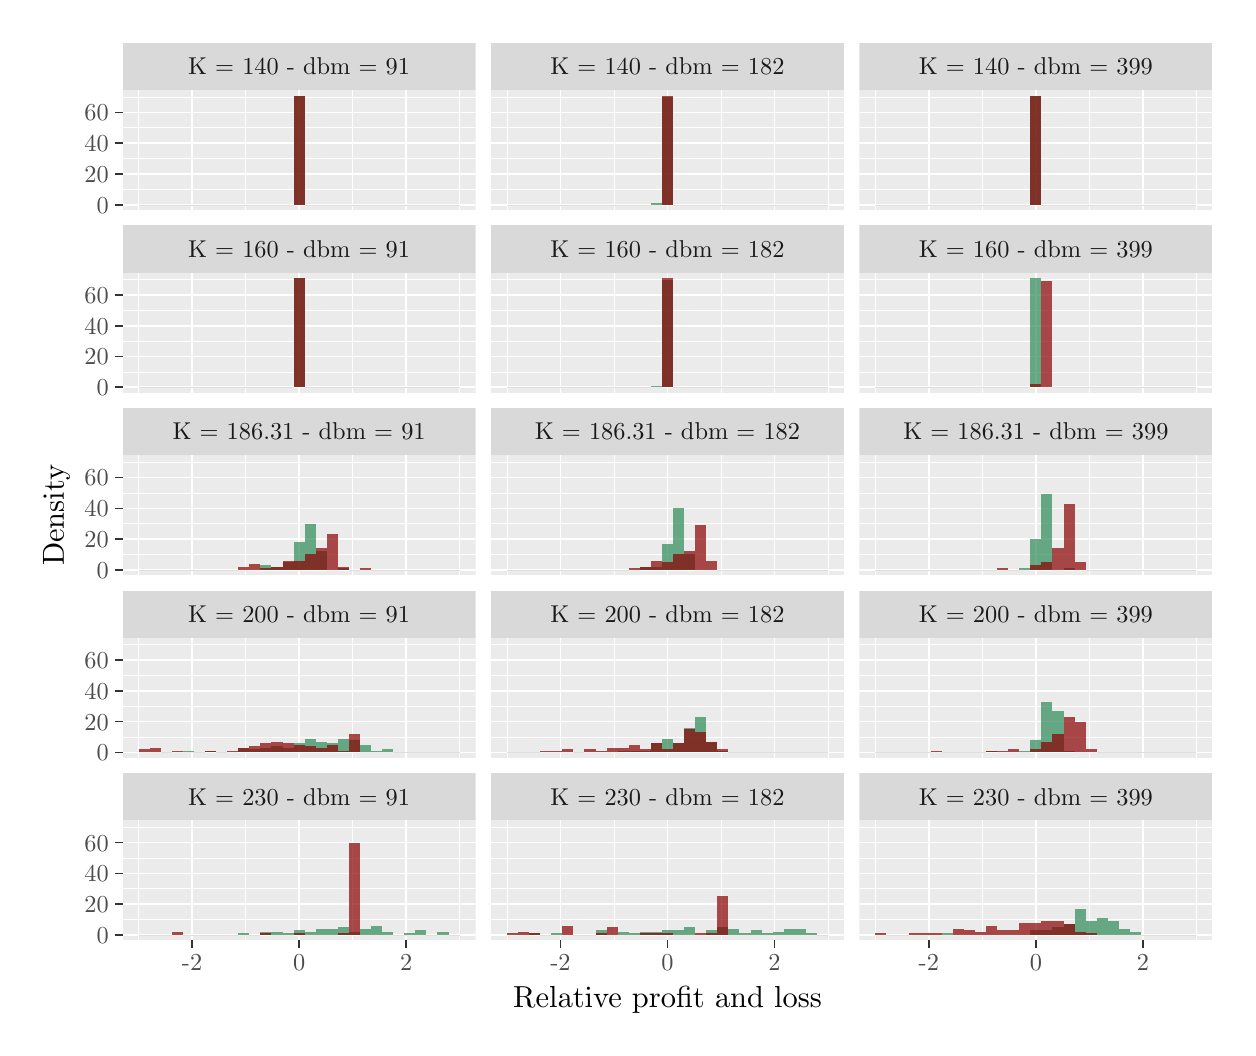
\begin{tikzpicture}[x=1pt,y=1pt]
\definecolor{fillColor}{RGB}{255,255,255}
\path[use as bounding box,fill=fillColor,fill opacity=0.00] (0,0) rectangle (433.62,361.35);
\begin{scope}
\path[clip] (  0.00,  0.00) rectangle (433.62,361.35);
\definecolor{drawColor}{RGB}{255,255,255}
\definecolor{fillColor}{RGB}{255,255,255}

\path[draw=drawColor,line width= 0.6pt,line join=round,line cap=round,fill=fillColor] (  0.00,  0.00) rectangle (433.62,361.35);
\end{scope}
\begin{scope}
\path[clip] ( 34.27,295.39) rectangle (161.89,338.79);
\definecolor{fillColor}{gray}{0.92}

\path[fill=fillColor] ( 34.27,295.39) rectangle (161.89,338.79);
\definecolor{drawColor}{RGB}{255,255,255}

\path[draw=drawColor,line width= 0.3pt,line join=round] ( 34.27,302.92) --
	(161.89,302.92);

\path[draw=drawColor,line width= 0.3pt,line join=round] ( 34.27,314.03) --
	(161.89,314.03);

\path[draw=drawColor,line width= 0.3pt,line join=round] ( 34.27,325.15) --
	(161.89,325.15);

\path[draw=drawColor,line width= 0.3pt,line join=round] ( 34.27,336.26) --
	(161.89,336.26);

\path[draw=drawColor,line width= 0.3pt,line join=round] ( 40.07,295.39) --
	( 40.07,338.79);

\path[draw=drawColor,line width= 0.3pt,line join=round] ( 78.74,295.39) --
	( 78.74,338.79);

\path[draw=drawColor,line width= 0.3pt,line join=round] (117.41,295.39) --
	(117.41,338.79);

\path[draw=drawColor,line width= 0.3pt,line join=round] (156.08,295.39) --
	(156.08,338.79);

\path[draw=drawColor,line width= 0.6pt,line join=round] ( 34.27,297.36) --
	(161.89,297.36);

\path[draw=drawColor,line width= 0.6pt,line join=round] ( 34.27,308.47) --
	(161.89,308.47);

\path[draw=drawColor,line width= 0.6pt,line join=round] ( 34.27,319.59) --
	(161.89,319.59);

\path[draw=drawColor,line width= 0.6pt,line join=round] ( 34.27,330.70) --
	(161.89,330.70);

\path[draw=drawColor,line width= 0.6pt,line join=round] ( 59.40,295.39) --
	( 59.40,338.79);

\path[draw=drawColor,line width= 0.6pt,line join=round] ( 98.08,295.39) --
	( 98.08,338.79);

\path[draw=drawColor,line width= 0.6pt,line join=round] (136.75,295.39) --
	(136.75,338.79);
\definecolor{fillColor}{RGB}{46,139,87}

\path[fill=fillColor,fill opacity=0.70] ( 40.07,297.36) rectangle ( 44.07,297.36);

\path[fill=fillColor,fill opacity=0.70] ( 44.07,297.36) rectangle ( 48.07,297.36);

\path[fill=fillColor,fill opacity=0.70] ( 48.07,297.36) rectangle ( 52.07,297.36);

\path[fill=fillColor,fill opacity=0.70] ( 52.07,297.36) rectangle ( 56.07,297.36);

\path[fill=fillColor,fill opacity=0.70] ( 56.07,297.36) rectangle ( 60.07,297.36);

\path[fill=fillColor,fill opacity=0.70] ( 60.07,297.36) rectangle ( 64.07,297.36);

\path[fill=fillColor,fill opacity=0.70] ( 64.07,297.36) rectangle ( 68.07,297.36);

\path[fill=fillColor,fill opacity=0.70] ( 68.07,297.36) rectangle ( 72.07,297.36);

\path[fill=fillColor,fill opacity=0.70] ( 72.07,297.36) rectangle ( 76.07,297.36);

\path[fill=fillColor,fill opacity=0.70] ( 76.07,297.36) rectangle ( 80.07,297.36);

\path[fill=fillColor,fill opacity=0.70] ( 80.07,297.36) rectangle ( 84.07,297.36);

\path[fill=fillColor,fill opacity=0.70] ( 84.07,297.36) rectangle ( 88.08,297.36);

\path[fill=fillColor,fill opacity=0.70] ( 88.08,297.36) rectangle ( 92.08,297.36);

\path[fill=fillColor,fill opacity=0.70] ( 92.08,297.36) rectangle ( 96.08,297.36);

\path[fill=fillColor,fill opacity=0.70] ( 96.08,297.36) rectangle (100.08,336.82);

\path[fill=fillColor,fill opacity=0.70] (100.08,297.36) rectangle (104.08,297.36);

\path[fill=fillColor,fill opacity=0.70] (104.08,297.36) rectangle (108.08,297.36);

\path[fill=fillColor,fill opacity=0.70] (108.08,297.36) rectangle (112.08,297.36);

\path[fill=fillColor,fill opacity=0.70] (112.08,297.36) rectangle (116.08,297.36);

\path[fill=fillColor,fill opacity=0.70] (116.08,297.36) rectangle (120.08,297.36);

\path[fill=fillColor,fill opacity=0.70] (120.08,297.36) rectangle (124.08,297.36);

\path[fill=fillColor,fill opacity=0.70] (124.08,297.36) rectangle (128.08,297.36);

\path[fill=fillColor,fill opacity=0.70] (128.08,297.36) rectangle (132.08,297.36);

\path[fill=fillColor,fill opacity=0.70] (132.08,297.36) rectangle (136.08,297.36);

\path[fill=fillColor,fill opacity=0.70] (136.08,297.36) rectangle (140.08,297.36);

\path[fill=fillColor,fill opacity=0.70] (140.08,297.36) rectangle (144.08,297.36);

\path[fill=fillColor,fill opacity=0.70] (144.08,297.36) rectangle (148.08,297.36);

\path[fill=fillColor,fill opacity=0.70] (148.08,297.36) rectangle (152.08,297.36);

\path[fill=fillColor,fill opacity=0.70] (152.08,297.36) rectangle (156.08,297.36);
\definecolor{fillColor}{RGB}{139,0,0}

\path[fill=fillColor,fill opacity=0.70] ( 40.07,297.36) rectangle ( 44.07,297.36);

\path[fill=fillColor,fill opacity=0.70] ( 44.07,297.36) rectangle ( 48.07,297.36);

\path[fill=fillColor,fill opacity=0.70] ( 48.07,297.36) rectangle ( 52.07,297.36);

\path[fill=fillColor,fill opacity=0.70] ( 52.07,297.36) rectangle ( 56.07,297.36);

\path[fill=fillColor,fill opacity=0.70] ( 56.07,297.36) rectangle ( 60.07,297.36);

\path[fill=fillColor,fill opacity=0.70] ( 60.07,297.36) rectangle ( 64.07,297.36);

\path[fill=fillColor,fill opacity=0.70] ( 64.07,297.36) rectangle ( 68.07,297.36);

\path[fill=fillColor,fill opacity=0.70] ( 68.07,297.36) rectangle ( 72.07,297.36);

\path[fill=fillColor,fill opacity=0.70] ( 72.07,297.36) rectangle ( 76.07,297.36);

\path[fill=fillColor,fill opacity=0.70] ( 76.07,297.36) rectangle ( 80.07,297.36);

\path[fill=fillColor,fill opacity=0.70] ( 80.07,297.36) rectangle ( 84.07,297.36);

\path[fill=fillColor,fill opacity=0.70] ( 84.07,297.36) rectangle ( 88.08,297.36);

\path[fill=fillColor,fill opacity=0.70] ( 88.08,297.36) rectangle ( 92.08,297.36);

\path[fill=fillColor,fill opacity=0.70] ( 92.08,297.36) rectangle ( 96.08,297.36);

\path[fill=fillColor,fill opacity=0.70] ( 96.08,297.36) rectangle (100.08,336.82);

\path[fill=fillColor,fill opacity=0.70] (100.08,297.36) rectangle (104.08,297.36);

\path[fill=fillColor,fill opacity=0.70] (104.08,297.36) rectangle (108.08,297.36);

\path[fill=fillColor,fill opacity=0.70] (108.08,297.36) rectangle (112.08,297.36);

\path[fill=fillColor,fill opacity=0.70] (112.08,297.36) rectangle (116.08,297.36);

\path[fill=fillColor,fill opacity=0.70] (116.08,297.36) rectangle (120.08,297.36);

\path[fill=fillColor,fill opacity=0.70] (120.08,297.36) rectangle (124.08,297.36);

\path[fill=fillColor,fill opacity=0.70] (124.08,297.36) rectangle (128.08,297.36);

\path[fill=fillColor,fill opacity=0.70] (128.08,297.36) rectangle (132.08,297.36);

\path[fill=fillColor,fill opacity=0.70] (132.08,297.36) rectangle (136.08,297.36);

\path[fill=fillColor,fill opacity=0.70] (136.08,297.36) rectangle (140.08,297.36);

\path[fill=fillColor,fill opacity=0.70] (140.08,297.36) rectangle (144.08,297.36);

\path[fill=fillColor,fill opacity=0.70] (144.08,297.36) rectangle (148.08,297.36);

\path[fill=fillColor,fill opacity=0.70] (148.08,297.36) rectangle (152.08,297.36);

\path[fill=fillColor,fill opacity=0.70] (152.08,297.36) rectangle (156.08,297.36);
\end{scope}
\begin{scope}
\path[clip] ( 34.27,229.42) rectangle (161.89,272.83);
\definecolor{fillColor}{gray}{0.92}

\path[fill=fillColor] ( 34.27,229.42) rectangle (161.89,272.83);
\definecolor{drawColor}{RGB}{255,255,255}

\path[draw=drawColor,line width= 0.3pt,line join=round] ( 34.27,236.95) --
	(161.89,236.95);

\path[draw=drawColor,line width= 0.3pt,line join=round] ( 34.27,248.07) --
	(161.89,248.07);

\path[draw=drawColor,line width= 0.3pt,line join=round] ( 34.27,259.18) --
	(161.89,259.18);

\path[draw=drawColor,line width= 0.3pt,line join=round] ( 34.27,270.30) --
	(161.89,270.30);

\path[draw=drawColor,line width= 0.3pt,line join=round] ( 40.07,229.42) --
	( 40.07,272.83);

\path[draw=drawColor,line width= 0.3pt,line join=round] ( 78.74,229.42) --
	( 78.74,272.83);

\path[draw=drawColor,line width= 0.3pt,line join=round] (117.41,229.42) --
	(117.41,272.83);

\path[draw=drawColor,line width= 0.3pt,line join=round] (156.08,229.42) --
	(156.08,272.83);

\path[draw=drawColor,line width= 0.6pt,line join=round] ( 34.27,231.40) --
	(161.89,231.40);

\path[draw=drawColor,line width= 0.6pt,line join=round] ( 34.27,242.51) --
	(161.89,242.51);

\path[draw=drawColor,line width= 0.6pt,line join=round] ( 34.27,253.62) --
	(161.89,253.62);

\path[draw=drawColor,line width= 0.6pt,line join=round] ( 34.27,264.74) --
	(161.89,264.74);

\path[draw=drawColor,line width= 0.6pt,line join=round] ( 59.40,229.42) --
	( 59.40,272.83);

\path[draw=drawColor,line width= 0.6pt,line join=round] ( 98.08,229.42) --
	( 98.08,272.83);

\path[draw=drawColor,line width= 0.6pt,line join=round] (136.75,229.42) --
	(136.75,272.83);
\definecolor{fillColor}{RGB}{46,139,87}

\path[fill=fillColor,fill opacity=0.70] ( 40.07,231.40) rectangle ( 44.07,231.40);

\path[fill=fillColor,fill opacity=0.70] ( 44.07,231.40) rectangle ( 48.07,231.40);

\path[fill=fillColor,fill opacity=0.70] ( 48.07,231.40) rectangle ( 52.07,231.40);

\path[fill=fillColor,fill opacity=0.70] ( 52.07,231.40) rectangle ( 56.07,231.40);

\path[fill=fillColor,fill opacity=0.70] ( 56.07,231.40) rectangle ( 60.07,231.40);

\path[fill=fillColor,fill opacity=0.70] ( 60.07,231.40) rectangle ( 64.07,231.40);

\path[fill=fillColor,fill opacity=0.70] ( 64.07,231.40) rectangle ( 68.07,231.40);

\path[fill=fillColor,fill opacity=0.70] ( 68.07,231.40) rectangle ( 72.07,231.40);

\path[fill=fillColor,fill opacity=0.70] ( 72.07,231.40) rectangle ( 76.07,231.40);

\path[fill=fillColor,fill opacity=0.70] ( 76.07,231.40) rectangle ( 80.07,231.40);

\path[fill=fillColor,fill opacity=0.70] ( 80.07,231.40) rectangle ( 84.07,231.40);

\path[fill=fillColor,fill opacity=0.70] ( 84.07,231.40) rectangle ( 88.08,231.40);

\path[fill=fillColor,fill opacity=0.70] ( 88.08,231.40) rectangle ( 92.08,231.40);

\path[fill=fillColor,fill opacity=0.70] ( 92.08,231.40) rectangle ( 96.08,231.40);

\path[fill=fillColor,fill opacity=0.70] ( 96.08,231.40) rectangle (100.08,270.85);

\path[fill=fillColor,fill opacity=0.70] (100.08,231.40) rectangle (104.08,231.40);

\path[fill=fillColor,fill opacity=0.70] (104.08,231.40) rectangle (108.08,231.40);

\path[fill=fillColor,fill opacity=0.70] (108.08,231.40) rectangle (112.08,231.40);

\path[fill=fillColor,fill opacity=0.70] (112.08,231.40) rectangle (116.08,231.40);

\path[fill=fillColor,fill opacity=0.70] (116.08,231.40) rectangle (120.08,231.40);

\path[fill=fillColor,fill opacity=0.70] (120.08,231.40) rectangle (124.08,231.40);

\path[fill=fillColor,fill opacity=0.70] (124.08,231.40) rectangle (128.08,231.40);

\path[fill=fillColor,fill opacity=0.70] (128.08,231.40) rectangle (132.08,231.40);

\path[fill=fillColor,fill opacity=0.70] (132.08,231.40) rectangle (136.08,231.40);

\path[fill=fillColor,fill opacity=0.70] (136.08,231.40) rectangle (140.08,231.40);

\path[fill=fillColor,fill opacity=0.70] (140.08,231.40) rectangle (144.08,231.40);

\path[fill=fillColor,fill opacity=0.70] (144.08,231.40) rectangle (148.08,231.40);

\path[fill=fillColor,fill opacity=0.70] (148.08,231.40) rectangle (152.08,231.40);

\path[fill=fillColor,fill opacity=0.70] (152.08,231.40) rectangle (156.08,231.40);
\definecolor{fillColor}{RGB}{139,0,0}

\path[fill=fillColor,fill opacity=0.70] ( 40.07,231.40) rectangle ( 44.07,231.40);

\path[fill=fillColor,fill opacity=0.70] ( 44.07,231.40) rectangle ( 48.07,231.40);

\path[fill=fillColor,fill opacity=0.70] ( 48.07,231.40) rectangle ( 52.07,231.40);

\path[fill=fillColor,fill opacity=0.70] ( 52.07,231.40) rectangle ( 56.07,231.40);

\path[fill=fillColor,fill opacity=0.70] ( 56.07,231.40) rectangle ( 60.07,231.40);

\path[fill=fillColor,fill opacity=0.70] ( 60.07,231.40) rectangle ( 64.07,231.40);

\path[fill=fillColor,fill opacity=0.70] ( 64.07,231.40) rectangle ( 68.07,231.40);

\path[fill=fillColor,fill opacity=0.70] ( 68.07,231.40) rectangle ( 72.07,231.40);

\path[fill=fillColor,fill opacity=0.70] ( 72.07,231.40) rectangle ( 76.07,231.40);

\path[fill=fillColor,fill opacity=0.70] ( 76.07,231.40) rectangle ( 80.07,231.40);

\path[fill=fillColor,fill opacity=0.70] ( 80.07,231.40) rectangle ( 84.07,231.40);

\path[fill=fillColor,fill opacity=0.70] ( 84.07,231.40) rectangle ( 88.08,231.40);

\path[fill=fillColor,fill opacity=0.70] ( 88.08,231.40) rectangle ( 92.08,231.40);

\path[fill=fillColor,fill opacity=0.70] ( 92.08,231.40) rectangle ( 96.08,231.40);

\path[fill=fillColor,fill opacity=0.70] ( 96.08,231.40) rectangle (100.08,270.85);

\path[fill=fillColor,fill opacity=0.70] (100.08,231.40) rectangle (104.08,231.40);

\path[fill=fillColor,fill opacity=0.70] (104.08,231.40) rectangle (108.08,231.40);

\path[fill=fillColor,fill opacity=0.70] (108.08,231.40) rectangle (112.08,231.40);

\path[fill=fillColor,fill opacity=0.70] (112.08,231.40) rectangle (116.08,231.40);

\path[fill=fillColor,fill opacity=0.70] (116.08,231.40) rectangle (120.08,231.40);

\path[fill=fillColor,fill opacity=0.70] (120.08,231.40) rectangle (124.08,231.40);

\path[fill=fillColor,fill opacity=0.70] (124.08,231.40) rectangle (128.08,231.40);

\path[fill=fillColor,fill opacity=0.70] (128.08,231.40) rectangle (132.08,231.40);

\path[fill=fillColor,fill opacity=0.70] (132.08,231.40) rectangle (136.08,231.40);

\path[fill=fillColor,fill opacity=0.70] (136.08,231.40) rectangle (140.08,231.40);

\path[fill=fillColor,fill opacity=0.70] (140.08,231.40) rectangle (144.08,231.40);

\path[fill=fillColor,fill opacity=0.70] (144.08,231.40) rectangle (148.08,231.40);

\path[fill=fillColor,fill opacity=0.70] (148.08,231.40) rectangle (152.08,231.40);

\path[fill=fillColor,fill opacity=0.70] (152.08,231.40) rectangle (156.08,231.40);
\end{scope}
\begin{scope}
\path[clip] ( 34.27,163.46) rectangle (161.89,206.86);
\definecolor{fillColor}{gray}{0.92}

\path[fill=fillColor] ( 34.27,163.46) rectangle (161.89,206.86);
\definecolor{drawColor}{RGB}{255,255,255}

\path[draw=drawColor,line width= 0.3pt,line join=round] ( 34.27,170.99) --
	(161.89,170.99);

\path[draw=drawColor,line width= 0.3pt,line join=round] ( 34.27,182.10) --
	(161.89,182.10);

\path[draw=drawColor,line width= 0.3pt,line join=round] ( 34.27,193.22) --
	(161.89,193.22);

\path[draw=drawColor,line width= 0.3pt,line join=round] ( 34.27,204.33) --
	(161.89,204.33);

\path[draw=drawColor,line width= 0.3pt,line join=round] ( 40.07,163.46) --
	( 40.07,206.86);

\path[draw=drawColor,line width= 0.3pt,line join=round] ( 78.74,163.46) --
	( 78.74,206.86);

\path[draw=drawColor,line width= 0.3pt,line join=round] (117.41,163.46) --
	(117.41,206.86);

\path[draw=drawColor,line width= 0.3pt,line join=round] (156.08,163.46) --
	(156.08,206.86);

\path[draw=drawColor,line width= 0.6pt,line join=round] ( 34.27,165.43) --
	(161.89,165.43);

\path[draw=drawColor,line width= 0.6pt,line join=round] ( 34.27,176.55) --
	(161.89,176.55);

\path[draw=drawColor,line width= 0.6pt,line join=round] ( 34.27,187.66) --
	(161.89,187.66);

\path[draw=drawColor,line width= 0.6pt,line join=round] ( 34.27,198.78) --
	(161.89,198.78);

\path[draw=drawColor,line width= 0.6pt,line join=round] ( 59.40,163.46) --
	( 59.40,206.86);

\path[draw=drawColor,line width= 0.6pt,line join=round] ( 98.08,163.46) --
	( 98.08,206.86);

\path[draw=drawColor,line width= 0.6pt,line join=round] (136.75,163.46) --
	(136.75,206.86);
\definecolor{fillColor}{RGB}{46,139,87}

\path[fill=fillColor,fill opacity=0.70] ( 40.07,165.43) rectangle ( 44.07,165.43);

\path[fill=fillColor,fill opacity=0.70] ( 44.07,165.43) rectangle ( 48.07,165.43);

\path[fill=fillColor,fill opacity=0.70] ( 48.07,165.43) rectangle ( 52.07,165.43);

\path[fill=fillColor,fill opacity=0.70] ( 52.07,165.43) rectangle ( 56.07,165.43);

\path[fill=fillColor,fill opacity=0.70] ( 56.07,165.43) rectangle ( 60.07,165.43);

\path[fill=fillColor,fill opacity=0.70] ( 60.07,165.43) rectangle ( 64.07,165.43);

\path[fill=fillColor,fill opacity=0.70] ( 64.07,165.43) rectangle ( 68.07,165.43);

\path[fill=fillColor,fill opacity=0.70] ( 68.07,165.43) rectangle ( 72.07,165.43);

\path[fill=fillColor,fill opacity=0.70] ( 72.07,165.43) rectangle ( 76.07,165.43);

\path[fill=fillColor,fill opacity=0.70] ( 76.07,165.43) rectangle ( 80.07,165.43);

\path[fill=fillColor,fill opacity=0.70] ( 80.07,165.43) rectangle ( 84.07,165.43);

\path[fill=fillColor,fill opacity=0.70] ( 84.07,165.43) rectangle ( 88.08,167.10);

\path[fill=fillColor,fill opacity=0.70] ( 88.08,165.43) rectangle ( 92.08,166.54);

\path[fill=fillColor,fill opacity=0.70] ( 92.08,165.43) rectangle ( 96.08,168.21);

\path[fill=fillColor,fill opacity=0.70] ( 96.08,165.43) rectangle (100.08,175.43);

\path[fill=fillColor,fill opacity=0.70] (100.08,165.43) rectangle (104.08,182.10);

\path[fill=fillColor,fill opacity=0.70] (104.08,165.43) rectangle (108.08,172.10);

\path[fill=fillColor,fill opacity=0.70] (108.08,165.43) rectangle (112.08,165.43);

\path[fill=fillColor,fill opacity=0.70] (112.08,165.43) rectangle (116.08,165.99);

\path[fill=fillColor,fill opacity=0.70] (116.08,165.43) rectangle (120.08,165.43);

\path[fill=fillColor,fill opacity=0.70] (120.08,165.43) rectangle (124.08,165.43);

\path[fill=fillColor,fill opacity=0.70] (124.08,165.43) rectangle (128.08,165.43);

\path[fill=fillColor,fill opacity=0.70] (128.08,165.43) rectangle (132.08,165.43);

\path[fill=fillColor,fill opacity=0.70] (132.08,165.43) rectangle (136.08,165.43);

\path[fill=fillColor,fill opacity=0.70] (136.08,165.43) rectangle (140.08,165.43);

\path[fill=fillColor,fill opacity=0.70] (140.08,165.43) rectangle (144.08,165.43);

\path[fill=fillColor,fill opacity=0.70] (144.08,165.43) rectangle (148.08,165.43);

\path[fill=fillColor,fill opacity=0.70] (148.08,165.43) rectangle (152.08,165.43);

\path[fill=fillColor,fill opacity=0.70] (152.08,165.43) rectangle (156.08,165.43);
\definecolor{fillColor}{RGB}{139,0,0}

\path[fill=fillColor,fill opacity=0.70] ( 40.07,165.43) rectangle ( 44.07,165.43);

\path[fill=fillColor,fill opacity=0.70] ( 44.07,165.43) rectangle ( 48.07,165.43);

\path[fill=fillColor,fill opacity=0.70] ( 48.07,165.43) rectangle ( 52.07,165.43);

\path[fill=fillColor,fill opacity=0.70] ( 52.07,165.43) rectangle ( 56.07,165.43);

\path[fill=fillColor,fill opacity=0.70] ( 56.07,165.43) rectangle ( 60.07,165.43);

\path[fill=fillColor,fill opacity=0.70] ( 60.07,165.43) rectangle ( 64.07,165.43);

\path[fill=fillColor,fill opacity=0.70] ( 64.07,165.43) rectangle ( 68.07,165.43);

\path[fill=fillColor,fill opacity=0.70] ( 68.07,165.43) rectangle ( 72.07,165.43);

\path[fill=fillColor,fill opacity=0.70] ( 72.07,165.43) rectangle ( 76.07,165.43);

\path[fill=fillColor,fill opacity=0.70] ( 76.07,165.43) rectangle ( 80.07,166.54);

\path[fill=fillColor,fill opacity=0.70] ( 80.07,165.43) rectangle ( 84.07,167.65);

\path[fill=fillColor,fill opacity=0.70] ( 84.07,165.43) rectangle ( 88.08,165.99);

\path[fill=fillColor,fill opacity=0.70] ( 88.08,165.43) rectangle ( 92.08,166.54);

\path[fill=fillColor,fill opacity=0.70] ( 92.08,165.43) rectangle ( 96.08,168.77);

\path[fill=fillColor,fill opacity=0.70] ( 96.08,165.43) rectangle (100.08,168.77);

\path[fill=fillColor,fill opacity=0.70] (100.08,165.43) rectangle (104.08,170.99);

\path[fill=fillColor,fill opacity=0.70] (104.08,165.43) rectangle (108.08,173.21);

\path[fill=fillColor,fill opacity=0.70] (108.08,165.43) rectangle (112.08,178.21);

\path[fill=fillColor,fill opacity=0.70] (112.08,165.43) rectangle (116.08,166.54);

\path[fill=fillColor,fill opacity=0.70] (116.08,165.43) rectangle (120.08,165.43);

\path[fill=fillColor,fill opacity=0.70] (120.08,165.43) rectangle (124.08,165.99);

\path[fill=fillColor,fill opacity=0.70] (124.08,165.43) rectangle (128.08,165.43);

\path[fill=fillColor,fill opacity=0.70] (128.08,165.43) rectangle (132.08,165.43);

\path[fill=fillColor,fill opacity=0.70] (132.08,165.43) rectangle (136.08,165.43);

\path[fill=fillColor,fill opacity=0.70] (136.08,165.43) rectangle (140.08,165.43);

\path[fill=fillColor,fill opacity=0.70] (140.08,165.43) rectangle (144.08,165.43);

\path[fill=fillColor,fill opacity=0.70] (144.08,165.43) rectangle (148.08,165.43);

\path[fill=fillColor,fill opacity=0.70] (148.08,165.43) rectangle (152.08,165.43);

\path[fill=fillColor,fill opacity=0.70] (152.08,165.43) rectangle (156.08,165.43);
\end{scope}
\begin{scope}
\path[clip] ( 34.27, 97.49) rectangle (161.89,140.90);
\definecolor{fillColor}{gray}{0.92}

\path[fill=fillColor] ( 34.27, 97.49) rectangle (161.89,140.90);
\definecolor{drawColor}{RGB}{255,255,255}

\path[draw=drawColor,line width= 0.3pt,line join=round] ( 34.27,105.02) --
	(161.89,105.02);

\path[draw=drawColor,line width= 0.3pt,line join=round] ( 34.27,116.14) --
	(161.89,116.14);

\path[draw=drawColor,line width= 0.3pt,line join=round] ( 34.27,127.25) --
	(161.89,127.25);

\path[draw=drawColor,line width= 0.3pt,line join=round] ( 34.27,138.37) --
	(161.89,138.37);

\path[draw=drawColor,line width= 0.3pt,line join=round] ( 40.07, 97.49) --
	( 40.07,140.90);

\path[draw=drawColor,line width= 0.3pt,line join=round] ( 78.74, 97.49) --
	( 78.74,140.90);

\path[draw=drawColor,line width= 0.3pt,line join=round] (117.41, 97.49) --
	(117.41,140.90);

\path[draw=drawColor,line width= 0.3pt,line join=round] (156.08, 97.49) --
	(156.08,140.90);

\path[draw=drawColor,line width= 0.6pt,line join=round] ( 34.27, 99.47) --
	(161.89, 99.47);

\path[draw=drawColor,line width= 0.6pt,line join=round] ( 34.27,110.58) --
	(161.89,110.58);

\path[draw=drawColor,line width= 0.6pt,line join=round] ( 34.27,121.70) --
	(161.89,121.70);

\path[draw=drawColor,line width= 0.6pt,line join=round] ( 34.27,132.81) --
	(161.89,132.81);

\path[draw=drawColor,line width= 0.6pt,line join=round] ( 59.40, 97.49) --
	( 59.40,140.90);

\path[draw=drawColor,line width= 0.6pt,line join=round] ( 98.08, 97.49) --
	( 98.08,140.90);

\path[draw=drawColor,line width= 0.6pt,line join=round] (136.75, 97.49) --
	(136.75,140.90);
\definecolor{fillColor}{RGB}{46,139,87}

\path[fill=fillColor,fill opacity=0.70] ( 40.07, 99.47) rectangle ( 44.07, 99.47);

\path[fill=fillColor,fill opacity=0.70] ( 44.07, 99.47) rectangle ( 48.07, 99.47);

\path[fill=fillColor,fill opacity=0.70] ( 48.07, 99.47) rectangle ( 52.07, 99.47);

\path[fill=fillColor,fill opacity=0.70] ( 52.07, 99.47) rectangle ( 56.07, 99.47);

\path[fill=fillColor,fill opacity=0.70] ( 56.07, 99.47) rectangle ( 60.07,100.02);

\path[fill=fillColor,fill opacity=0.70] ( 60.07, 99.47) rectangle ( 64.07, 99.47);

\path[fill=fillColor,fill opacity=0.70] ( 64.07, 99.47) rectangle ( 68.07,100.02);

\path[fill=fillColor,fill opacity=0.70] ( 68.07, 99.47) rectangle ( 72.07, 99.47);

\path[fill=fillColor,fill opacity=0.70] ( 72.07, 99.47) rectangle ( 76.07, 99.47);

\path[fill=fillColor,fill opacity=0.70] ( 76.07, 99.47) rectangle ( 80.07,101.13);

\path[fill=fillColor,fill opacity=0.70] ( 80.07, 99.47) rectangle ( 84.07,100.58);

\path[fill=fillColor,fill opacity=0.70] ( 84.07, 99.47) rectangle ( 88.08,101.13);

\path[fill=fillColor,fill opacity=0.70] ( 88.08, 99.47) rectangle ( 92.08,101.69);

\path[fill=fillColor,fill opacity=0.70] ( 92.08, 99.47) rectangle ( 96.08,101.13);

\path[fill=fillColor,fill opacity=0.70] ( 96.08, 99.47) rectangle (100.08,102.80);

\path[fill=fillColor,fill opacity=0.70] (100.08, 99.47) rectangle (104.08,104.47);

\path[fill=fillColor,fill opacity=0.70] (104.08, 99.47) rectangle (108.08,103.36);

\path[fill=fillColor,fill opacity=0.70] (108.08, 99.47) rectangle (112.08,102.80);

\path[fill=fillColor,fill opacity=0.70] (112.08, 99.47) rectangle (116.08,104.47);

\path[fill=fillColor,fill opacity=0.70] (116.08, 99.47) rectangle (120.08,103.91);

\path[fill=fillColor,fill opacity=0.70] (120.08, 99.47) rectangle (124.08,102.25);

\path[fill=fillColor,fill opacity=0.70] (124.08, 99.47) rectangle (128.08,100.02);

\path[fill=fillColor,fill opacity=0.70] (128.08, 99.47) rectangle (132.08,100.58);

\path[fill=fillColor,fill opacity=0.70] (132.08, 99.47) rectangle (136.08, 99.47);

\path[fill=fillColor,fill opacity=0.70] (136.08, 99.47) rectangle (140.08, 99.47);

\path[fill=fillColor,fill opacity=0.70] (140.08, 99.47) rectangle (144.08, 99.47);

\path[fill=fillColor,fill opacity=0.70] (144.08, 99.47) rectangle (148.08, 99.47);

\path[fill=fillColor,fill opacity=0.70] (148.08, 99.47) rectangle (152.08, 99.47);

\path[fill=fillColor,fill opacity=0.70] (152.08, 99.47) rectangle (156.08, 99.47);
\definecolor{fillColor}{RGB}{139,0,0}

\path[fill=fillColor,fill opacity=0.70] ( 40.07, 99.47) rectangle ( 44.07,100.58);

\path[fill=fillColor,fill opacity=0.70] ( 44.07, 99.47) rectangle ( 48.07,101.13);

\path[fill=fillColor,fill opacity=0.70] ( 48.07, 99.47) rectangle ( 52.07, 99.47);

\path[fill=fillColor,fill opacity=0.70] ( 52.07, 99.47) rectangle ( 56.07,100.02);

\path[fill=fillColor,fill opacity=0.70] ( 56.07, 99.47) rectangle ( 60.07, 99.47);

\path[fill=fillColor,fill opacity=0.70] ( 60.07, 99.47) rectangle ( 64.07, 99.47);

\path[fill=fillColor,fill opacity=0.70] ( 64.07, 99.47) rectangle ( 68.07,100.02);

\path[fill=fillColor,fill opacity=0.70] ( 68.07, 99.47) rectangle ( 72.07, 99.47);

\path[fill=fillColor,fill opacity=0.70] ( 72.07, 99.47) rectangle ( 76.07,100.02);

\path[fill=fillColor,fill opacity=0.70] ( 76.07, 99.47) rectangle ( 80.07,101.13);

\path[fill=fillColor,fill opacity=0.70] ( 80.07, 99.47) rectangle ( 84.07,101.69);

\path[fill=fillColor,fill opacity=0.70] ( 84.07, 99.47) rectangle ( 88.08,102.80);

\path[fill=fillColor,fill opacity=0.70] ( 88.08, 99.47) rectangle ( 92.08,103.36);

\path[fill=fillColor,fill opacity=0.70] ( 92.08, 99.47) rectangle ( 96.08,102.80);

\path[fill=fillColor,fill opacity=0.70] ( 96.08, 99.47) rectangle (100.08,102.25);

\path[fill=fillColor,fill opacity=0.70] (100.08, 99.47) rectangle (104.08,101.69);

\path[fill=fillColor,fill opacity=0.70] (104.08, 99.47) rectangle (108.08,101.13);

\path[fill=fillColor,fill opacity=0.70] (108.08, 99.47) rectangle (112.08,102.25);

\path[fill=fillColor,fill opacity=0.70] (112.08, 99.47) rectangle (116.08,100.02);

\path[fill=fillColor,fill opacity=0.70] (116.08, 99.47) rectangle (120.08,106.14);

\path[fill=fillColor,fill opacity=0.70] (120.08, 99.47) rectangle (124.08, 99.47);

\path[fill=fillColor,fill opacity=0.70] (124.08, 99.47) rectangle (128.08, 99.47);

\path[fill=fillColor,fill opacity=0.70] (128.08, 99.47) rectangle (132.08, 99.47);

\path[fill=fillColor,fill opacity=0.70] (132.08, 99.47) rectangle (136.08, 99.47);

\path[fill=fillColor,fill opacity=0.70] (136.08, 99.47) rectangle (140.08, 99.47);

\path[fill=fillColor,fill opacity=0.70] (140.08, 99.47) rectangle (144.08, 99.47);

\path[fill=fillColor,fill opacity=0.70] (144.08, 99.47) rectangle (148.08, 99.47);

\path[fill=fillColor,fill opacity=0.70] (148.08, 99.47) rectangle (152.08, 99.47);

\path[fill=fillColor,fill opacity=0.70] (152.08, 99.47) rectangle (156.08, 99.47);
\end{scope}
\begin{scope}
\path[clip] ( 34.27, 31.53) rectangle (161.89, 74.93);
\definecolor{fillColor}{gray}{0.92}

\path[fill=fillColor] ( 34.27, 31.53) rectangle (161.89, 74.93);
\definecolor{drawColor}{RGB}{255,255,255}

\path[draw=drawColor,line width= 0.3pt,line join=round] ( 34.27, 39.06) --
	(161.89, 39.06);

\path[draw=drawColor,line width= 0.3pt,line join=round] ( 34.27, 50.18) --
	(161.89, 50.18);

\path[draw=drawColor,line width= 0.3pt,line join=round] ( 34.27, 61.29) --
	(161.89, 61.29);

\path[draw=drawColor,line width= 0.3pt,line join=round] ( 34.27, 72.41) --
	(161.89, 72.41);

\path[draw=drawColor,line width= 0.3pt,line join=round] ( 40.07, 31.53) --
	( 40.07, 74.93);

\path[draw=drawColor,line width= 0.3pt,line join=round] ( 78.74, 31.53) --
	( 78.74, 74.93);

\path[draw=drawColor,line width= 0.3pt,line join=round] (117.41, 31.53) --
	(117.41, 74.93);

\path[draw=drawColor,line width= 0.3pt,line join=round] (156.08, 31.53) --
	(156.08, 74.93);

\path[draw=drawColor,line width= 0.6pt,line join=round] ( 34.27, 33.50) --
	(161.89, 33.50);

\path[draw=drawColor,line width= 0.6pt,line join=round] ( 34.27, 44.62) --
	(161.89, 44.62);

\path[draw=drawColor,line width= 0.6pt,line join=round] ( 34.27, 55.73) --
	(161.89, 55.73);

\path[draw=drawColor,line width= 0.6pt,line join=round] ( 34.27, 66.85) --
	(161.89, 66.85);

\path[draw=drawColor,line width= 0.6pt,line join=round] ( 59.40, 31.53) --
	( 59.40, 74.93);

\path[draw=drawColor,line width= 0.6pt,line join=round] ( 98.08, 31.53) --
	( 98.08, 74.93);

\path[draw=drawColor,line width= 0.6pt,line join=round] (136.75, 31.53) --
	(136.75, 74.93);
\definecolor{fillColor}{RGB}{46,139,87}

\path[fill=fillColor,fill opacity=0.70] ( 40.07, 33.50) rectangle ( 44.07, 33.50);

\path[fill=fillColor,fill opacity=0.70] ( 44.07, 33.50) rectangle ( 48.07, 33.50);

\path[fill=fillColor,fill opacity=0.70] ( 48.07, 33.50) rectangle ( 52.07, 33.50);

\path[fill=fillColor,fill opacity=0.70] ( 52.07, 33.50) rectangle ( 56.07, 33.50);

\path[fill=fillColor,fill opacity=0.70] ( 56.07, 33.50) rectangle ( 60.07, 33.50);

\path[fill=fillColor,fill opacity=0.70] ( 60.07, 33.50) rectangle ( 64.07, 33.50);

\path[fill=fillColor,fill opacity=0.70] ( 64.07, 33.50) rectangle ( 68.07, 33.50);

\path[fill=fillColor,fill opacity=0.70] ( 68.07, 33.50) rectangle ( 72.07, 33.50);

\path[fill=fillColor,fill opacity=0.70] ( 72.07, 33.50) rectangle ( 76.07, 33.50);

\path[fill=fillColor,fill opacity=0.70] ( 76.07, 33.50) rectangle ( 80.07, 34.06);

\path[fill=fillColor,fill opacity=0.70] ( 80.07, 33.50) rectangle ( 84.07, 33.50);

\path[fill=fillColor,fill opacity=0.70] ( 84.07, 33.50) rectangle ( 88.08, 34.62);

\path[fill=fillColor,fill opacity=0.70] ( 88.08, 33.50) rectangle ( 92.08, 34.62);

\path[fill=fillColor,fill opacity=0.70] ( 92.08, 33.50) rectangle ( 96.08, 34.06);

\path[fill=fillColor,fill opacity=0.70] ( 96.08, 33.50) rectangle (100.08, 35.17);

\path[fill=fillColor,fill opacity=0.70] (100.08, 33.50) rectangle (104.08, 34.62);

\path[fill=fillColor,fill opacity=0.70] (104.08, 33.50) rectangle (108.08, 35.73);

\path[fill=fillColor,fill opacity=0.70] (108.08, 33.50) rectangle (112.08, 35.73);

\path[fill=fillColor,fill opacity=0.70] (112.08, 33.50) rectangle (116.08, 36.28);

\path[fill=fillColor,fill opacity=0.70] (116.08, 33.50) rectangle (120.08, 34.62);

\path[fill=fillColor,fill opacity=0.70] (120.08, 33.50) rectangle (124.08, 35.73);

\path[fill=fillColor,fill opacity=0.70] (124.08, 33.50) rectangle (128.08, 36.84);

\path[fill=fillColor,fill opacity=0.70] (128.08, 33.50) rectangle (132.08, 34.62);

\path[fill=fillColor,fill opacity=0.70] (132.08, 33.50) rectangle (136.08, 33.50);

\path[fill=fillColor,fill opacity=0.70] (136.08, 33.50) rectangle (140.08, 34.06);

\path[fill=fillColor,fill opacity=0.70] (140.08, 33.50) rectangle (144.08, 35.17);

\path[fill=fillColor,fill opacity=0.70] (144.08, 33.50) rectangle (148.08, 33.50);

\path[fill=fillColor,fill opacity=0.70] (148.08, 33.50) rectangle (152.08, 34.62);

\path[fill=fillColor,fill opacity=0.70] (152.08, 33.50) rectangle (156.08, 33.50);
\definecolor{fillColor}{RGB}{139,0,0}

\path[fill=fillColor,fill opacity=0.70] ( 40.07, 33.50) rectangle ( 44.07, 33.50);

\path[fill=fillColor,fill opacity=0.70] ( 44.07, 33.50) rectangle ( 48.07, 33.50);

\path[fill=fillColor,fill opacity=0.70] ( 48.07, 33.50) rectangle ( 52.07, 33.50);

\path[fill=fillColor,fill opacity=0.70] ( 52.07, 33.50) rectangle ( 56.07, 34.62);

\path[fill=fillColor,fill opacity=0.70] ( 56.07, 33.50) rectangle ( 60.07, 33.50);

\path[fill=fillColor,fill opacity=0.70] ( 60.07, 33.50) rectangle ( 64.07, 33.50);

\path[fill=fillColor,fill opacity=0.70] ( 64.07, 33.50) rectangle ( 68.07, 33.50);

\path[fill=fillColor,fill opacity=0.70] ( 68.07, 33.50) rectangle ( 72.07, 33.50);

\path[fill=fillColor,fill opacity=0.70] ( 72.07, 33.50) rectangle ( 76.07, 33.50);

\path[fill=fillColor,fill opacity=0.70] ( 76.07, 33.50) rectangle ( 80.07, 33.50);

\path[fill=fillColor,fill opacity=0.70] ( 80.07, 33.50) rectangle ( 84.07, 33.50);

\path[fill=fillColor,fill opacity=0.70] ( 84.07, 33.50) rectangle ( 88.08, 34.06);

\path[fill=fillColor,fill opacity=0.70] ( 88.08, 33.50) rectangle ( 92.08, 33.50);

\path[fill=fillColor,fill opacity=0.70] ( 92.08, 33.50) rectangle ( 96.08, 33.50);

\path[fill=fillColor,fill opacity=0.70] ( 96.08, 33.50) rectangle (100.08, 34.06);

\path[fill=fillColor,fill opacity=0.70] (100.08, 33.50) rectangle (104.08, 33.50);

\path[fill=fillColor,fill opacity=0.70] (104.08, 33.50) rectangle (108.08, 33.50);

\path[fill=fillColor,fill opacity=0.70] (108.08, 33.50) rectangle (112.08, 33.50);

\path[fill=fillColor,fill opacity=0.70] (112.08, 33.50) rectangle (116.08, 34.06);

\path[fill=fillColor,fill opacity=0.70] (116.08, 33.50) rectangle (120.08, 66.85);

\path[fill=fillColor,fill opacity=0.70] (120.08, 33.50) rectangle (124.08, 33.50);

\path[fill=fillColor,fill opacity=0.70] (124.08, 33.50) rectangle (128.08, 33.50);

\path[fill=fillColor,fill opacity=0.70] (128.08, 33.50) rectangle (132.08, 33.50);

\path[fill=fillColor,fill opacity=0.70] (132.08, 33.50) rectangle (136.08, 33.50);

\path[fill=fillColor,fill opacity=0.70] (136.08, 33.50) rectangle (140.08, 33.50);

\path[fill=fillColor,fill opacity=0.70] (140.08, 33.50) rectangle (144.08, 33.50);

\path[fill=fillColor,fill opacity=0.70] (144.08, 33.50) rectangle (148.08, 33.50);

\path[fill=fillColor,fill opacity=0.70] (148.08, 33.50) rectangle (152.08, 33.50);

\path[fill=fillColor,fill opacity=0.70] (152.08, 33.50) rectangle (156.08, 33.50);
\end{scope}
\begin{scope}
\path[clip] (167.39,295.39) rectangle (295.00,338.79);
\definecolor{fillColor}{gray}{0.92}

\path[fill=fillColor] (167.39,295.39) rectangle (295.00,338.79);
\definecolor{drawColor}{RGB}{255,255,255}

\path[draw=drawColor,line width= 0.3pt,line join=round] (167.39,302.92) --
	(295.00,302.92);

\path[draw=drawColor,line width= 0.3pt,line join=round] (167.39,314.03) --
	(295.00,314.03);

\path[draw=drawColor,line width= 0.3pt,line join=round] (167.39,325.15) --
	(295.00,325.15);

\path[draw=drawColor,line width= 0.3pt,line join=round] (167.39,336.26) --
	(295.00,336.26);

\path[draw=drawColor,line width= 0.3pt,line join=round] (173.19,295.39) --
	(173.19,338.79);

\path[draw=drawColor,line width= 0.3pt,line join=round] (211.86,295.39) --
	(211.86,338.79);

\path[draw=drawColor,line width= 0.3pt,line join=round] (250.53,295.39) --
	(250.53,338.79);

\path[draw=drawColor,line width= 0.3pt,line join=round] (289.20,295.39) --
	(289.20,338.79);

\path[draw=drawColor,line width= 0.6pt,line join=round] (167.39,297.36) --
	(295.00,297.36);

\path[draw=drawColor,line width= 0.6pt,line join=round] (167.39,308.47) --
	(295.00,308.47);

\path[draw=drawColor,line width= 0.6pt,line join=round] (167.39,319.59) --
	(295.00,319.59);

\path[draw=drawColor,line width= 0.6pt,line join=round] (167.39,330.70) --
	(295.00,330.70);

\path[draw=drawColor,line width= 0.6pt,line join=round] (192.52,295.39) --
	(192.52,338.79);

\path[draw=drawColor,line width= 0.6pt,line join=round] (231.19,295.39) --
	(231.19,338.79);

\path[draw=drawColor,line width= 0.6pt,line join=round] (269.87,295.39) --
	(269.87,338.79);
\definecolor{fillColor}{RGB}{46,139,87}

\path[fill=fillColor,fill opacity=0.70] (173.19,297.36) rectangle (177.19,297.36);

\path[fill=fillColor,fill opacity=0.70] (177.19,297.36) rectangle (181.19,297.36);

\path[fill=fillColor,fill opacity=0.70] (181.19,297.36) rectangle (185.19,297.36);

\path[fill=fillColor,fill opacity=0.70] (185.19,297.36) rectangle (189.19,297.36);

\path[fill=fillColor,fill opacity=0.70] (189.19,297.36) rectangle (193.19,297.36);

\path[fill=fillColor,fill opacity=0.70] (193.19,297.36) rectangle (197.19,297.36);

\path[fill=fillColor,fill opacity=0.70] (197.19,297.36) rectangle (201.19,297.36);

\path[fill=fillColor,fill opacity=0.70] (201.19,297.36) rectangle (205.19,297.36);

\path[fill=fillColor,fill opacity=0.70] (205.19,297.36) rectangle (209.19,297.36);

\path[fill=fillColor,fill opacity=0.70] (209.19,297.36) rectangle (213.19,297.36);

\path[fill=fillColor,fill opacity=0.70] (213.19,297.36) rectangle (217.19,297.36);

\path[fill=fillColor,fill opacity=0.70] (217.19,297.36) rectangle (221.19,297.36);

\path[fill=fillColor,fill opacity=0.70] (221.19,297.36) rectangle (225.19,297.36);

\path[fill=fillColor,fill opacity=0.70] (225.19,297.36) rectangle (229.19,297.91);

\path[fill=fillColor,fill opacity=0.70] (229.19,297.36) rectangle (233.19,336.26);

\path[fill=fillColor,fill opacity=0.70] (233.19,297.36) rectangle (237.19,297.36);

\path[fill=fillColor,fill opacity=0.70] (237.19,297.36) rectangle (241.20,297.36);

\path[fill=fillColor,fill opacity=0.70] (241.20,297.36) rectangle (245.20,297.36);

\path[fill=fillColor,fill opacity=0.70] (245.20,297.36) rectangle (249.20,297.36);

\path[fill=fillColor,fill opacity=0.70] (249.20,297.36) rectangle (253.20,297.36);

\path[fill=fillColor,fill opacity=0.70] (253.20,297.36) rectangle (257.20,297.36);

\path[fill=fillColor,fill opacity=0.70] (257.20,297.36) rectangle (261.20,297.36);

\path[fill=fillColor,fill opacity=0.70] (261.20,297.36) rectangle (265.20,297.36);

\path[fill=fillColor,fill opacity=0.70] (265.20,297.36) rectangle (269.20,297.36);

\path[fill=fillColor,fill opacity=0.70] (269.20,297.36) rectangle (273.20,297.36);

\path[fill=fillColor,fill opacity=0.70] (273.20,297.36) rectangle (277.20,297.36);

\path[fill=fillColor,fill opacity=0.70] (277.20,297.36) rectangle (281.20,297.36);

\path[fill=fillColor,fill opacity=0.70] (281.20,297.36) rectangle (285.20,297.36);

\path[fill=fillColor,fill opacity=0.70] (285.20,297.36) rectangle (289.20,297.36);
\definecolor{fillColor}{RGB}{139,0,0}

\path[fill=fillColor,fill opacity=0.70] (173.19,297.36) rectangle (177.19,297.36);

\path[fill=fillColor,fill opacity=0.70] (177.19,297.36) rectangle (181.19,297.36);

\path[fill=fillColor,fill opacity=0.70] (181.19,297.36) rectangle (185.19,297.36);

\path[fill=fillColor,fill opacity=0.70] (185.19,297.36) rectangle (189.19,297.36);

\path[fill=fillColor,fill opacity=0.70] (189.19,297.36) rectangle (193.19,297.36);

\path[fill=fillColor,fill opacity=0.70] (193.19,297.36) rectangle (197.19,297.36);

\path[fill=fillColor,fill opacity=0.70] (197.19,297.36) rectangle (201.19,297.36);

\path[fill=fillColor,fill opacity=0.70] (201.19,297.36) rectangle (205.19,297.36);

\path[fill=fillColor,fill opacity=0.70] (205.19,297.36) rectangle (209.19,297.36);

\path[fill=fillColor,fill opacity=0.70] (209.19,297.36) rectangle (213.19,297.36);

\path[fill=fillColor,fill opacity=0.70] (213.19,297.36) rectangle (217.19,297.36);

\path[fill=fillColor,fill opacity=0.70] (217.19,297.36) rectangle (221.19,297.36);

\path[fill=fillColor,fill opacity=0.70] (221.19,297.36) rectangle (225.19,297.36);

\path[fill=fillColor,fill opacity=0.70] (225.19,297.36) rectangle (229.19,297.36);

\path[fill=fillColor,fill opacity=0.70] (229.19,297.36) rectangle (233.19,336.82);

\path[fill=fillColor,fill opacity=0.70] (233.19,297.36) rectangle (237.19,297.36);

\path[fill=fillColor,fill opacity=0.70] (237.19,297.36) rectangle (241.20,297.36);

\path[fill=fillColor,fill opacity=0.70] (241.20,297.36) rectangle (245.20,297.36);

\path[fill=fillColor,fill opacity=0.70] (245.20,297.36) rectangle (249.20,297.36);

\path[fill=fillColor,fill opacity=0.70] (249.20,297.36) rectangle (253.20,297.36);

\path[fill=fillColor,fill opacity=0.70] (253.20,297.36) rectangle (257.20,297.36);

\path[fill=fillColor,fill opacity=0.70] (257.20,297.36) rectangle (261.20,297.36);

\path[fill=fillColor,fill opacity=0.70] (261.20,297.36) rectangle (265.20,297.36);

\path[fill=fillColor,fill opacity=0.70] (265.20,297.36) rectangle (269.20,297.36);

\path[fill=fillColor,fill opacity=0.70] (269.20,297.36) rectangle (273.20,297.36);

\path[fill=fillColor,fill opacity=0.70] (273.20,297.36) rectangle (277.20,297.36);

\path[fill=fillColor,fill opacity=0.70] (277.20,297.36) rectangle (281.20,297.36);

\path[fill=fillColor,fill opacity=0.70] (281.20,297.36) rectangle (285.20,297.36);

\path[fill=fillColor,fill opacity=0.70] (285.20,297.36) rectangle (289.20,297.36);
\end{scope}
\begin{scope}
\path[clip] (167.39,229.42) rectangle (295.00,272.83);
\definecolor{fillColor}{gray}{0.92}

\path[fill=fillColor] (167.39,229.42) rectangle (295.00,272.83);
\definecolor{drawColor}{RGB}{255,255,255}

\path[draw=drawColor,line width= 0.3pt,line join=round] (167.39,236.95) --
	(295.00,236.95);

\path[draw=drawColor,line width= 0.3pt,line join=round] (167.39,248.07) --
	(295.00,248.07);

\path[draw=drawColor,line width= 0.3pt,line join=round] (167.39,259.18) --
	(295.00,259.18);

\path[draw=drawColor,line width= 0.3pt,line join=round] (167.39,270.30) --
	(295.00,270.30);

\path[draw=drawColor,line width= 0.3pt,line join=round] (173.19,229.42) --
	(173.19,272.83);

\path[draw=drawColor,line width= 0.3pt,line join=round] (211.86,229.42) --
	(211.86,272.83);

\path[draw=drawColor,line width= 0.3pt,line join=round] (250.53,229.42) --
	(250.53,272.83);

\path[draw=drawColor,line width= 0.3pt,line join=round] (289.20,229.42) --
	(289.20,272.83);

\path[draw=drawColor,line width= 0.6pt,line join=round] (167.39,231.40) --
	(295.00,231.40);

\path[draw=drawColor,line width= 0.6pt,line join=round] (167.39,242.51) --
	(295.00,242.51);

\path[draw=drawColor,line width= 0.6pt,line join=round] (167.39,253.62) --
	(295.00,253.62);

\path[draw=drawColor,line width= 0.6pt,line join=round] (167.39,264.74) --
	(295.00,264.74);

\path[draw=drawColor,line width= 0.6pt,line join=round] (192.52,229.42) --
	(192.52,272.83);

\path[draw=drawColor,line width= 0.6pt,line join=round] (231.19,229.42) --
	(231.19,272.83);

\path[draw=drawColor,line width= 0.6pt,line join=round] (269.87,229.42) --
	(269.87,272.83);
\definecolor{fillColor}{RGB}{46,139,87}

\path[fill=fillColor,fill opacity=0.70] (173.19,231.40) rectangle (177.19,231.40);

\path[fill=fillColor,fill opacity=0.70] (177.19,231.40) rectangle (181.19,231.40);

\path[fill=fillColor,fill opacity=0.70] (181.19,231.40) rectangle (185.19,231.40);

\path[fill=fillColor,fill opacity=0.70] (185.19,231.40) rectangle (189.19,231.40);

\path[fill=fillColor,fill opacity=0.70] (189.19,231.40) rectangle (193.19,231.40);

\path[fill=fillColor,fill opacity=0.70] (193.19,231.40) rectangle (197.19,231.40);

\path[fill=fillColor,fill opacity=0.70] (197.19,231.40) rectangle (201.19,231.40);

\path[fill=fillColor,fill opacity=0.70] (201.19,231.40) rectangle (205.19,231.40);

\path[fill=fillColor,fill opacity=0.70] (205.19,231.40) rectangle (209.19,231.40);

\path[fill=fillColor,fill opacity=0.70] (209.19,231.40) rectangle (213.19,231.40);

\path[fill=fillColor,fill opacity=0.70] (213.19,231.40) rectangle (217.19,231.40);

\path[fill=fillColor,fill opacity=0.70] (217.19,231.40) rectangle (221.19,231.40);

\path[fill=fillColor,fill opacity=0.70] (221.19,231.40) rectangle (225.19,231.40);

\path[fill=fillColor,fill opacity=0.70] (225.19,231.40) rectangle (229.19,231.95);

\path[fill=fillColor,fill opacity=0.70] (229.19,231.40) rectangle (233.19,270.30);

\path[fill=fillColor,fill opacity=0.70] (233.19,231.40) rectangle (237.19,231.40);

\path[fill=fillColor,fill opacity=0.70] (237.19,231.40) rectangle (241.20,231.40);

\path[fill=fillColor,fill opacity=0.70] (241.20,231.40) rectangle (245.20,231.40);

\path[fill=fillColor,fill opacity=0.70] (245.20,231.40) rectangle (249.20,231.40);

\path[fill=fillColor,fill opacity=0.70] (249.20,231.40) rectangle (253.20,231.40);

\path[fill=fillColor,fill opacity=0.70] (253.20,231.40) rectangle (257.20,231.40);

\path[fill=fillColor,fill opacity=0.70] (257.20,231.40) rectangle (261.20,231.40);

\path[fill=fillColor,fill opacity=0.70] (261.20,231.40) rectangle (265.20,231.40);

\path[fill=fillColor,fill opacity=0.70] (265.20,231.40) rectangle (269.20,231.40);

\path[fill=fillColor,fill opacity=0.70] (269.20,231.40) rectangle (273.20,231.40);

\path[fill=fillColor,fill opacity=0.70] (273.20,231.40) rectangle (277.20,231.40);

\path[fill=fillColor,fill opacity=0.70] (277.20,231.40) rectangle (281.20,231.40);

\path[fill=fillColor,fill opacity=0.70] (281.20,231.40) rectangle (285.20,231.40);

\path[fill=fillColor,fill opacity=0.70] (285.20,231.40) rectangle (289.20,231.40);
\definecolor{fillColor}{RGB}{139,0,0}

\path[fill=fillColor,fill opacity=0.70] (173.19,231.40) rectangle (177.19,231.40);

\path[fill=fillColor,fill opacity=0.70] (177.19,231.40) rectangle (181.19,231.40);

\path[fill=fillColor,fill opacity=0.70] (181.19,231.40) rectangle (185.19,231.40);

\path[fill=fillColor,fill opacity=0.70] (185.19,231.40) rectangle (189.19,231.40);

\path[fill=fillColor,fill opacity=0.70] (189.19,231.40) rectangle (193.19,231.40);

\path[fill=fillColor,fill opacity=0.70] (193.19,231.40) rectangle (197.19,231.40);

\path[fill=fillColor,fill opacity=0.70] (197.19,231.40) rectangle (201.19,231.40);

\path[fill=fillColor,fill opacity=0.70] (201.19,231.40) rectangle (205.19,231.40);

\path[fill=fillColor,fill opacity=0.70] (205.19,231.40) rectangle (209.19,231.40);

\path[fill=fillColor,fill opacity=0.70] (209.19,231.40) rectangle (213.19,231.40);

\path[fill=fillColor,fill opacity=0.70] (213.19,231.40) rectangle (217.19,231.40);

\path[fill=fillColor,fill opacity=0.70] (217.19,231.40) rectangle (221.19,231.40);

\path[fill=fillColor,fill opacity=0.70] (221.19,231.40) rectangle (225.19,231.40);

\path[fill=fillColor,fill opacity=0.70] (225.19,231.40) rectangle (229.19,231.40);

\path[fill=fillColor,fill opacity=0.70] (229.19,231.40) rectangle (233.19,270.85);

\path[fill=fillColor,fill opacity=0.70] (233.19,231.40) rectangle (237.19,231.40);

\path[fill=fillColor,fill opacity=0.70] (237.19,231.40) rectangle (241.20,231.40);

\path[fill=fillColor,fill opacity=0.70] (241.20,231.40) rectangle (245.20,231.40);

\path[fill=fillColor,fill opacity=0.70] (245.20,231.40) rectangle (249.20,231.40);

\path[fill=fillColor,fill opacity=0.70] (249.20,231.40) rectangle (253.20,231.40);

\path[fill=fillColor,fill opacity=0.70] (253.20,231.40) rectangle (257.20,231.40);

\path[fill=fillColor,fill opacity=0.70] (257.20,231.40) rectangle (261.20,231.40);

\path[fill=fillColor,fill opacity=0.70] (261.20,231.40) rectangle (265.20,231.40);

\path[fill=fillColor,fill opacity=0.70] (265.20,231.40) rectangle (269.20,231.40);

\path[fill=fillColor,fill opacity=0.70] (269.20,231.40) rectangle (273.20,231.40);

\path[fill=fillColor,fill opacity=0.70] (273.20,231.40) rectangle (277.20,231.40);

\path[fill=fillColor,fill opacity=0.70] (277.20,231.40) rectangle (281.20,231.40);

\path[fill=fillColor,fill opacity=0.70] (281.20,231.40) rectangle (285.20,231.40);

\path[fill=fillColor,fill opacity=0.70] (285.20,231.40) rectangle (289.20,231.40);
\end{scope}
\begin{scope}
\path[clip] (167.39,163.46) rectangle (295.00,206.86);
\definecolor{fillColor}{gray}{0.92}

\path[fill=fillColor] (167.39,163.46) rectangle (295.00,206.86);
\definecolor{drawColor}{RGB}{255,255,255}

\path[draw=drawColor,line width= 0.3pt,line join=round] (167.39,170.99) --
	(295.00,170.99);

\path[draw=drawColor,line width= 0.3pt,line join=round] (167.39,182.10) --
	(295.00,182.10);

\path[draw=drawColor,line width= 0.3pt,line join=round] (167.39,193.22) --
	(295.00,193.22);

\path[draw=drawColor,line width= 0.3pt,line join=round] (167.39,204.33) --
	(295.00,204.33);

\path[draw=drawColor,line width= 0.3pt,line join=round] (173.19,163.46) --
	(173.19,206.86);

\path[draw=drawColor,line width= 0.3pt,line join=round] (211.86,163.46) --
	(211.86,206.86);

\path[draw=drawColor,line width= 0.3pt,line join=round] (250.53,163.46) --
	(250.53,206.86);

\path[draw=drawColor,line width= 0.3pt,line join=round] (289.20,163.46) --
	(289.20,206.86);

\path[draw=drawColor,line width= 0.6pt,line join=round] (167.39,165.43) --
	(295.00,165.43);

\path[draw=drawColor,line width= 0.6pt,line join=round] (167.39,176.55) --
	(295.00,176.55);

\path[draw=drawColor,line width= 0.6pt,line join=round] (167.39,187.66) --
	(295.00,187.66);

\path[draw=drawColor,line width= 0.6pt,line join=round] (167.39,198.78) --
	(295.00,198.78);

\path[draw=drawColor,line width= 0.6pt,line join=round] (192.52,163.46) --
	(192.52,206.86);

\path[draw=drawColor,line width= 0.6pt,line join=round] (231.19,163.46) --
	(231.19,206.86);

\path[draw=drawColor,line width= 0.6pt,line join=round] (269.87,163.46) --
	(269.87,206.86);
\definecolor{fillColor}{RGB}{46,139,87}

\path[fill=fillColor,fill opacity=0.70] (173.19,165.43) rectangle (177.19,165.43);

\path[fill=fillColor,fill opacity=0.70] (177.19,165.43) rectangle (181.19,165.43);

\path[fill=fillColor,fill opacity=0.70] (181.19,165.43) rectangle (185.19,165.43);

\path[fill=fillColor,fill opacity=0.70] (185.19,165.43) rectangle (189.19,165.43);

\path[fill=fillColor,fill opacity=0.70] (189.19,165.43) rectangle (193.19,165.43);

\path[fill=fillColor,fill opacity=0.70] (193.19,165.43) rectangle (197.19,165.43);

\path[fill=fillColor,fill opacity=0.70] (197.19,165.43) rectangle (201.19,165.43);

\path[fill=fillColor,fill opacity=0.70] (201.19,165.43) rectangle (205.19,165.43);

\path[fill=fillColor,fill opacity=0.70] (205.19,165.43) rectangle (209.19,165.43);

\path[fill=fillColor,fill opacity=0.70] (209.19,165.43) rectangle (213.19,165.43);

\path[fill=fillColor,fill opacity=0.70] (213.19,165.43) rectangle (217.19,165.43);

\path[fill=fillColor,fill opacity=0.70] (217.19,165.43) rectangle (221.19,165.43);

\path[fill=fillColor,fill opacity=0.70] (221.19,165.43) rectangle (225.19,166.54);

\path[fill=fillColor,fill opacity=0.70] (225.19,165.43) rectangle (229.19,166.54);

\path[fill=fillColor,fill opacity=0.70] (229.19,165.43) rectangle (233.19,174.88);

\path[fill=fillColor,fill opacity=0.70] (233.19,165.43) rectangle (237.19,187.66);

\path[fill=fillColor,fill opacity=0.70] (237.19,165.43) rectangle (241.20,170.99);

\path[fill=fillColor,fill opacity=0.70] (241.20,165.43) rectangle (245.20,165.43);

\path[fill=fillColor,fill opacity=0.70] (245.20,165.43) rectangle (249.20,165.43);

\path[fill=fillColor,fill opacity=0.70] (249.20,165.43) rectangle (253.20,165.43);

\path[fill=fillColor,fill opacity=0.70] (253.20,165.43) rectangle (257.20,165.43);

\path[fill=fillColor,fill opacity=0.70] (257.20,165.43) rectangle (261.20,165.43);

\path[fill=fillColor,fill opacity=0.70] (261.20,165.43) rectangle (265.20,165.43);

\path[fill=fillColor,fill opacity=0.70] (265.20,165.43) rectangle (269.20,165.43);

\path[fill=fillColor,fill opacity=0.70] (269.20,165.43) rectangle (273.20,165.43);

\path[fill=fillColor,fill opacity=0.70] (273.20,165.43) rectangle (277.20,165.43);

\path[fill=fillColor,fill opacity=0.70] (277.20,165.43) rectangle (281.20,165.43);

\path[fill=fillColor,fill opacity=0.70] (281.20,165.43) rectangle (285.20,165.43);

\path[fill=fillColor,fill opacity=0.70] (285.20,165.43) rectangle (289.20,165.43);
\definecolor{fillColor}{RGB}{139,0,0}

\path[fill=fillColor,fill opacity=0.70] (173.19,165.43) rectangle (177.19,165.43);

\path[fill=fillColor,fill opacity=0.70] (177.19,165.43) rectangle (181.19,165.43);

\path[fill=fillColor,fill opacity=0.70] (181.19,165.43) rectangle (185.19,165.43);

\path[fill=fillColor,fill opacity=0.70] (185.19,165.43) rectangle (189.19,165.43);

\path[fill=fillColor,fill opacity=0.70] (189.19,165.43) rectangle (193.19,165.43);

\path[fill=fillColor,fill opacity=0.70] (193.19,165.43) rectangle (197.19,165.43);

\path[fill=fillColor,fill opacity=0.70] (197.19,165.43) rectangle (201.19,165.43);

\path[fill=fillColor,fill opacity=0.70] (201.19,165.43) rectangle (205.19,165.43);

\path[fill=fillColor,fill opacity=0.70] (205.19,165.43) rectangle (209.19,165.43);

\path[fill=fillColor,fill opacity=0.70] (209.19,165.43) rectangle (213.19,165.43);

\path[fill=fillColor,fill opacity=0.70] (213.19,165.43) rectangle (217.19,165.43);

\path[fill=fillColor,fill opacity=0.70] (217.19,165.43) rectangle (221.19,165.99);

\path[fill=fillColor,fill opacity=0.70] (221.19,165.43) rectangle (225.19,166.54);

\path[fill=fillColor,fill opacity=0.70] (225.19,165.43) rectangle (229.19,168.77);

\path[fill=fillColor,fill opacity=0.70] (229.19,165.43) rectangle (233.19,168.21);

\path[fill=fillColor,fill opacity=0.70] (233.19,165.43) rectangle (237.19,170.99);

\path[fill=fillColor,fill opacity=0.70] (237.19,165.43) rectangle (241.20,172.10);

\path[fill=fillColor,fill opacity=0.70] (241.20,165.43) rectangle (245.20,181.55);

\path[fill=fillColor,fill opacity=0.70] (245.20,165.43) rectangle (249.20,168.77);

\path[fill=fillColor,fill opacity=0.70] (249.20,165.43) rectangle (253.20,165.43);

\path[fill=fillColor,fill opacity=0.70] (253.20,165.43) rectangle (257.20,165.43);

\path[fill=fillColor,fill opacity=0.70] (257.20,165.43) rectangle (261.20,165.43);

\path[fill=fillColor,fill opacity=0.70] (261.20,165.43) rectangle (265.20,165.43);

\path[fill=fillColor,fill opacity=0.70] (265.20,165.43) rectangle (269.20,165.43);

\path[fill=fillColor,fill opacity=0.70] (269.20,165.43) rectangle (273.20,165.43);

\path[fill=fillColor,fill opacity=0.70] (273.20,165.43) rectangle (277.20,165.43);

\path[fill=fillColor,fill opacity=0.70] (277.20,165.43) rectangle (281.20,165.43);

\path[fill=fillColor,fill opacity=0.70] (281.20,165.43) rectangle (285.20,165.43);

\path[fill=fillColor,fill opacity=0.70] (285.20,165.43) rectangle (289.20,165.43);
\end{scope}
\begin{scope}
\path[clip] (167.39, 97.49) rectangle (295.00,140.90);
\definecolor{fillColor}{gray}{0.92}

\path[fill=fillColor] (167.39, 97.49) rectangle (295.00,140.90);
\definecolor{drawColor}{RGB}{255,255,255}

\path[draw=drawColor,line width= 0.3pt,line join=round] (167.39,105.02) --
	(295.00,105.02);

\path[draw=drawColor,line width= 0.3pt,line join=round] (167.39,116.14) --
	(295.00,116.14);

\path[draw=drawColor,line width= 0.3pt,line join=round] (167.39,127.25) --
	(295.00,127.25);

\path[draw=drawColor,line width= 0.3pt,line join=round] (167.39,138.37) --
	(295.00,138.37);

\path[draw=drawColor,line width= 0.3pt,line join=round] (173.19, 97.49) --
	(173.19,140.90);

\path[draw=drawColor,line width= 0.3pt,line join=round] (211.86, 97.49) --
	(211.86,140.90);

\path[draw=drawColor,line width= 0.3pt,line join=round] (250.53, 97.49) --
	(250.53,140.90);

\path[draw=drawColor,line width= 0.3pt,line join=round] (289.20, 97.49) --
	(289.20,140.90);

\path[draw=drawColor,line width= 0.6pt,line join=round] (167.39, 99.47) --
	(295.00, 99.47);

\path[draw=drawColor,line width= 0.6pt,line join=round] (167.39,110.58) --
	(295.00,110.58);

\path[draw=drawColor,line width= 0.6pt,line join=round] (167.39,121.70) --
	(295.00,121.70);

\path[draw=drawColor,line width= 0.6pt,line join=round] (167.39,132.81) --
	(295.00,132.81);

\path[draw=drawColor,line width= 0.6pt,line join=round] (192.52, 97.49) --
	(192.52,140.90);

\path[draw=drawColor,line width= 0.6pt,line join=round] (231.19, 97.49) --
	(231.19,140.90);

\path[draw=drawColor,line width= 0.6pt,line join=round] (269.87, 97.49) --
	(269.87,140.90);
\definecolor{fillColor}{RGB}{46,139,87}

\path[fill=fillColor,fill opacity=0.70] (173.19, 99.47) rectangle (177.19, 99.47);

\path[fill=fillColor,fill opacity=0.70] (177.19, 99.47) rectangle (181.19, 99.47);

\path[fill=fillColor,fill opacity=0.70] (181.19, 99.47) rectangle (185.19, 99.47);

\path[fill=fillColor,fill opacity=0.70] (185.19, 99.47) rectangle (189.19, 99.47);

\path[fill=fillColor,fill opacity=0.70] (189.19, 99.47) rectangle (193.19, 99.47);

\path[fill=fillColor,fill opacity=0.70] (193.19, 99.47) rectangle (197.19, 99.47);

\path[fill=fillColor,fill opacity=0.70] (197.19, 99.47) rectangle (201.19, 99.47);

\path[fill=fillColor,fill opacity=0.70] (201.19, 99.47) rectangle (205.19, 99.47);

\path[fill=fillColor,fill opacity=0.70] (205.19, 99.47) rectangle (209.19, 99.47);

\path[fill=fillColor,fill opacity=0.70] (209.19, 99.47) rectangle (213.19, 99.47);

\path[fill=fillColor,fill opacity=0.70] (213.19, 99.47) rectangle (217.19,100.02);

\path[fill=fillColor,fill opacity=0.70] (217.19, 99.47) rectangle (221.19,100.02);

\path[fill=fillColor,fill opacity=0.70] (221.19, 99.47) rectangle (225.19,100.02);

\path[fill=fillColor,fill opacity=0.70] (225.19, 99.47) rectangle (229.19,102.80);

\path[fill=fillColor,fill opacity=0.70] (229.19, 99.47) rectangle (233.19,104.47);

\path[fill=fillColor,fill opacity=0.70] (233.19, 99.47) rectangle (237.19,102.80);

\path[fill=fillColor,fill opacity=0.70] (237.19, 99.47) rectangle (241.20,108.36);

\path[fill=fillColor,fill opacity=0.70] (241.20, 99.47) rectangle (245.20,112.25);

\path[fill=fillColor,fill opacity=0.70] (245.20, 99.47) rectangle (249.20,103.36);

\path[fill=fillColor,fill opacity=0.70] (249.20, 99.47) rectangle (253.20,100.02);

\path[fill=fillColor,fill opacity=0.70] (253.20, 99.47) rectangle (257.20, 99.47);

\path[fill=fillColor,fill opacity=0.70] (257.20, 99.47) rectangle (261.20, 99.47);

\path[fill=fillColor,fill opacity=0.70] (261.20, 99.47) rectangle (265.20, 99.47);

\path[fill=fillColor,fill opacity=0.70] (265.20, 99.47) rectangle (269.20, 99.47);

\path[fill=fillColor,fill opacity=0.70] (269.20, 99.47) rectangle (273.20, 99.47);

\path[fill=fillColor,fill opacity=0.70] (273.20, 99.47) rectangle (277.20, 99.47);

\path[fill=fillColor,fill opacity=0.70] (277.20, 99.47) rectangle (281.20, 99.47);

\path[fill=fillColor,fill opacity=0.70] (281.20, 99.47) rectangle (285.20, 99.47);

\path[fill=fillColor,fill opacity=0.70] (285.20, 99.47) rectangle (289.20, 99.47);
\definecolor{fillColor}{RGB}{139,0,0}

\path[fill=fillColor,fill opacity=0.70] (173.19, 99.47) rectangle (177.19, 99.47);

\path[fill=fillColor,fill opacity=0.70] (177.19, 99.47) rectangle (181.19, 99.47);

\path[fill=fillColor,fill opacity=0.70] (181.19, 99.47) rectangle (185.19, 99.47);

\path[fill=fillColor,fill opacity=0.70] (185.19, 99.47) rectangle (189.19,100.02);

\path[fill=fillColor,fill opacity=0.70] (189.19, 99.47) rectangle (193.19,100.02);

\path[fill=fillColor,fill opacity=0.70] (193.19, 99.47) rectangle (197.19,100.58);

\path[fill=fillColor,fill opacity=0.70] (197.19, 99.47) rectangle (201.19, 99.47);

\path[fill=fillColor,fill opacity=0.70] (201.19, 99.47) rectangle (205.19,100.58);

\path[fill=fillColor,fill opacity=0.70] (205.19, 99.47) rectangle (209.19,100.02);

\path[fill=fillColor,fill opacity=0.70] (209.19, 99.47) rectangle (213.19,101.13);

\path[fill=fillColor,fill opacity=0.70] (213.19, 99.47) rectangle (217.19,101.13);

\path[fill=fillColor,fill opacity=0.70] (217.19, 99.47) rectangle (221.19,102.25);

\path[fill=fillColor,fill opacity=0.70] (221.19, 99.47) rectangle (225.19,100.58);

\path[fill=fillColor,fill opacity=0.70] (225.19, 99.47) rectangle (229.19,102.80);

\path[fill=fillColor,fill opacity=0.70] (229.19, 99.47) rectangle (233.19,100.58);

\path[fill=fillColor,fill opacity=0.70] (233.19, 99.47) rectangle (237.19,102.80);

\path[fill=fillColor,fill opacity=0.70] (237.19, 99.47) rectangle (241.20,107.80);

\path[fill=fillColor,fill opacity=0.70] (241.20, 99.47) rectangle (245.20,106.69);

\path[fill=fillColor,fill opacity=0.70] (245.20, 99.47) rectangle (249.20,103.36);

\path[fill=fillColor,fill opacity=0.70] (249.20, 99.47) rectangle (253.20,100.58);

\path[fill=fillColor,fill opacity=0.70] (253.20, 99.47) rectangle (257.20, 99.47);

\path[fill=fillColor,fill opacity=0.70] (257.20, 99.47) rectangle (261.20, 99.47);

\path[fill=fillColor,fill opacity=0.70] (261.20, 99.47) rectangle (265.20, 99.47);

\path[fill=fillColor,fill opacity=0.70] (265.20, 99.47) rectangle (269.20, 99.47);

\path[fill=fillColor,fill opacity=0.70] (269.20, 99.47) rectangle (273.20, 99.47);

\path[fill=fillColor,fill opacity=0.70] (273.20, 99.47) rectangle (277.20, 99.47);

\path[fill=fillColor,fill opacity=0.70] (277.20, 99.47) rectangle (281.20, 99.47);

\path[fill=fillColor,fill opacity=0.70] (281.20, 99.47) rectangle (285.20, 99.47);

\path[fill=fillColor,fill opacity=0.70] (285.20, 99.47) rectangle (289.20, 99.47);
\end{scope}
\begin{scope}
\path[clip] (167.39, 31.53) rectangle (295.00, 74.93);
\definecolor{fillColor}{gray}{0.92}

\path[fill=fillColor] (167.39, 31.53) rectangle (295.00, 74.93);
\definecolor{drawColor}{RGB}{255,255,255}

\path[draw=drawColor,line width= 0.3pt,line join=round] (167.39, 39.06) --
	(295.00, 39.06);

\path[draw=drawColor,line width= 0.3pt,line join=round] (167.39, 50.18) --
	(295.00, 50.18);

\path[draw=drawColor,line width= 0.3pt,line join=round] (167.39, 61.29) --
	(295.00, 61.29);

\path[draw=drawColor,line width= 0.3pt,line join=round] (167.39, 72.41) --
	(295.00, 72.41);

\path[draw=drawColor,line width= 0.3pt,line join=round] (173.19, 31.53) --
	(173.19, 74.93);

\path[draw=drawColor,line width= 0.3pt,line join=round] (211.86, 31.53) --
	(211.86, 74.93);

\path[draw=drawColor,line width= 0.3pt,line join=round] (250.53, 31.53) --
	(250.53, 74.93);

\path[draw=drawColor,line width= 0.3pt,line join=round] (289.20, 31.53) --
	(289.20, 74.93);

\path[draw=drawColor,line width= 0.6pt,line join=round] (167.39, 33.50) --
	(295.00, 33.50);

\path[draw=drawColor,line width= 0.6pt,line join=round] (167.39, 44.62) --
	(295.00, 44.62);

\path[draw=drawColor,line width= 0.6pt,line join=round] (167.39, 55.73) --
	(295.00, 55.73);

\path[draw=drawColor,line width= 0.6pt,line join=round] (167.39, 66.85) --
	(295.00, 66.85);

\path[draw=drawColor,line width= 0.6pt,line join=round] (192.52, 31.53) --
	(192.52, 74.93);

\path[draw=drawColor,line width= 0.6pt,line join=round] (231.19, 31.53) --
	(231.19, 74.93);

\path[draw=drawColor,line width= 0.6pt,line join=round] (269.87, 31.53) --
	(269.87, 74.93);
\definecolor{fillColor}{RGB}{46,139,87}

\path[fill=fillColor,fill opacity=0.70] (173.19, 33.50) rectangle (177.19, 33.50);

\path[fill=fillColor,fill opacity=0.70] (177.19, 33.50) rectangle (181.19, 33.50);

\path[fill=fillColor,fill opacity=0.70] (181.19, 33.50) rectangle (185.19, 34.06);

\path[fill=fillColor,fill opacity=0.70] (185.19, 33.50) rectangle (189.19, 33.50);

\path[fill=fillColor,fill opacity=0.70] (189.19, 33.50) rectangle (193.19, 34.06);

\path[fill=fillColor,fill opacity=0.70] (193.19, 33.50) rectangle (197.19, 33.50);

\path[fill=fillColor,fill opacity=0.70] (197.19, 33.50) rectangle (201.19, 33.50);

\path[fill=fillColor,fill opacity=0.70] (201.19, 33.50) rectangle (205.19, 33.50);

\path[fill=fillColor,fill opacity=0.70] (205.19, 33.50) rectangle (209.19, 35.17);

\path[fill=fillColor,fill opacity=0.70] (209.19, 33.50) rectangle (213.19, 33.50);

\path[fill=fillColor,fill opacity=0.70] (213.19, 33.50) rectangle (217.19, 34.62);

\path[fill=fillColor,fill opacity=0.70] (217.19, 33.50) rectangle (221.19, 34.06);

\path[fill=fillColor,fill opacity=0.70] (221.19, 33.50) rectangle (225.19, 34.62);

\path[fill=fillColor,fill opacity=0.70] (225.19, 33.50) rectangle (229.19, 34.62);

\path[fill=fillColor,fill opacity=0.70] (229.19, 33.50) rectangle (233.19, 35.17);

\path[fill=fillColor,fill opacity=0.70] (233.19, 33.50) rectangle (237.19, 35.17);

\path[fill=fillColor,fill opacity=0.70] (237.19, 33.50) rectangle (241.20, 36.28);

\path[fill=fillColor,fill opacity=0.70] (241.20, 33.50) rectangle (245.20, 33.50);

\path[fill=fillColor,fill opacity=0.70] (245.20, 33.50) rectangle (249.20, 35.17);

\path[fill=fillColor,fill opacity=0.70] (249.20, 33.50) rectangle (253.20, 36.28);

\path[fill=fillColor,fill opacity=0.70] (253.20, 33.50) rectangle (257.20, 35.73);

\path[fill=fillColor,fill opacity=0.70] (257.20, 33.50) rectangle (261.20, 34.06);

\path[fill=fillColor,fill opacity=0.70] (261.20, 33.50) rectangle (265.20, 35.17);

\path[fill=fillColor,fill opacity=0.70] (265.20, 33.50) rectangle (269.20, 34.06);

\path[fill=fillColor,fill opacity=0.70] (269.20, 33.50) rectangle (273.20, 34.62);

\path[fill=fillColor,fill opacity=0.70] (273.20, 33.50) rectangle (277.20, 35.73);

\path[fill=fillColor,fill opacity=0.70] (277.20, 33.50) rectangle (281.20, 35.73);

\path[fill=fillColor,fill opacity=0.70] (281.20, 33.50) rectangle (285.20, 34.06);

\path[fill=fillColor,fill opacity=0.70] (285.20, 33.50) rectangle (289.20, 33.50);
\definecolor{fillColor}{RGB}{139,0,0}

\path[fill=fillColor,fill opacity=0.70] (173.19, 33.50) rectangle (177.19, 34.06);

\path[fill=fillColor,fill opacity=0.70] (177.19, 33.50) rectangle (181.19, 34.62);

\path[fill=fillColor,fill opacity=0.70] (181.19, 33.50) rectangle (185.19, 34.06);

\path[fill=fillColor,fill opacity=0.70] (185.19, 33.50) rectangle (189.19, 33.50);

\path[fill=fillColor,fill opacity=0.70] (189.19, 33.50) rectangle (193.19, 33.50);

\path[fill=fillColor,fill opacity=0.70] (193.19, 33.50) rectangle (197.19, 36.84);

\path[fill=fillColor,fill opacity=0.70] (197.19, 33.50) rectangle (201.19, 33.50);

\path[fill=fillColor,fill opacity=0.70] (201.19, 33.50) rectangle (205.19, 33.50);

\path[fill=fillColor,fill opacity=0.70] (205.19, 33.50) rectangle (209.19, 34.06);

\path[fill=fillColor,fill opacity=0.70] (209.19, 33.50) rectangle (213.19, 36.28);

\path[fill=fillColor,fill opacity=0.70] (213.19, 33.50) rectangle (217.19, 33.50);

\path[fill=fillColor,fill opacity=0.70] (217.19, 33.50) rectangle (221.19, 33.50);

\path[fill=fillColor,fill opacity=0.70] (221.19, 33.50) rectangle (225.19, 34.06);

\path[fill=fillColor,fill opacity=0.70] (225.19, 33.50) rectangle (229.19, 34.06);

\path[fill=fillColor,fill opacity=0.70] (229.19, 33.50) rectangle (233.19, 34.06);

\path[fill=fillColor,fill opacity=0.70] (233.19, 33.50) rectangle (237.19, 33.50);

\path[fill=fillColor,fill opacity=0.70] (237.19, 33.50) rectangle (241.20, 33.50);

\path[fill=fillColor,fill opacity=0.70] (241.20, 33.50) rectangle (245.20, 34.06);

\path[fill=fillColor,fill opacity=0.70] (245.20, 33.50) rectangle (249.20, 34.06);

\path[fill=fillColor,fill opacity=0.70] (249.20, 33.50) rectangle (253.20, 47.40);

\path[fill=fillColor,fill opacity=0.70] (253.20, 33.50) rectangle (257.20, 33.50);

\path[fill=fillColor,fill opacity=0.70] (257.20, 33.50) rectangle (261.20, 33.50);

\path[fill=fillColor,fill opacity=0.70] (261.20, 33.50) rectangle (265.20, 33.50);

\path[fill=fillColor,fill opacity=0.70] (265.20, 33.50) rectangle (269.20, 33.50);

\path[fill=fillColor,fill opacity=0.70] (269.20, 33.50) rectangle (273.20, 33.50);

\path[fill=fillColor,fill opacity=0.70] (273.20, 33.50) rectangle (277.20, 33.50);

\path[fill=fillColor,fill opacity=0.70] (277.20, 33.50) rectangle (281.20, 33.50);

\path[fill=fillColor,fill opacity=0.70] (281.20, 33.50) rectangle (285.20, 33.50);

\path[fill=fillColor,fill opacity=0.70] (285.20, 33.50) rectangle (289.20, 33.50);
\end{scope}
\begin{scope}
\path[clip] (300.50,295.39) rectangle (428.12,338.79);
\definecolor{fillColor}{gray}{0.92}

\path[fill=fillColor] (300.50,295.39) rectangle (428.12,338.79);
\definecolor{drawColor}{RGB}{255,255,255}

\path[draw=drawColor,line width= 0.3pt,line join=round] (300.50,302.92) --
	(428.12,302.92);

\path[draw=drawColor,line width= 0.3pt,line join=round] (300.50,314.03) --
	(428.12,314.03);

\path[draw=drawColor,line width= 0.3pt,line join=round] (300.50,325.15) --
	(428.12,325.15);

\path[draw=drawColor,line width= 0.3pt,line join=round] (300.50,336.26) --
	(428.12,336.26);

\path[draw=drawColor,line width= 0.3pt,line join=round] (306.30,295.39) --
	(306.30,338.79);

\path[draw=drawColor,line width= 0.3pt,line join=round] (344.98,295.39) --
	(344.98,338.79);

\path[draw=drawColor,line width= 0.3pt,line join=round] (383.65,295.39) --
	(383.65,338.79);

\path[draw=drawColor,line width= 0.3pt,line join=round] (422.32,295.39) --
	(422.32,338.79);

\path[draw=drawColor,line width= 0.6pt,line join=round] (300.50,297.36) --
	(428.12,297.36);

\path[draw=drawColor,line width= 0.6pt,line join=round] (300.50,308.47) --
	(428.12,308.47);

\path[draw=drawColor,line width= 0.6pt,line join=round] (300.50,319.59) --
	(428.12,319.59);

\path[draw=drawColor,line width= 0.6pt,line join=round] (300.50,330.70) --
	(428.12,330.70);

\path[draw=drawColor,line width= 0.6pt,line join=round] (325.64,295.39) --
	(325.64,338.79);

\path[draw=drawColor,line width= 0.6pt,line join=round] (364.31,295.39) --
	(364.31,338.79);

\path[draw=drawColor,line width= 0.6pt,line join=round] (402.98,295.39) --
	(402.98,338.79);
\definecolor{fillColor}{RGB}{46,139,87}

\path[fill=fillColor,fill opacity=0.70] (306.30,297.36) rectangle (310.30,297.36);

\path[fill=fillColor,fill opacity=0.70] (310.30,297.36) rectangle (314.30,297.36);

\path[fill=fillColor,fill opacity=0.70] (314.30,297.36) rectangle (318.31,297.36);

\path[fill=fillColor,fill opacity=0.70] (318.31,297.36) rectangle (322.31,297.36);

\path[fill=fillColor,fill opacity=0.70] (322.31,297.36) rectangle (326.31,297.36);

\path[fill=fillColor,fill opacity=0.70] (326.31,297.36) rectangle (330.31,297.36);

\path[fill=fillColor,fill opacity=0.70] (330.31,297.36) rectangle (334.31,297.36);

\path[fill=fillColor,fill opacity=0.70] (334.31,297.36) rectangle (338.31,297.36);

\path[fill=fillColor,fill opacity=0.70] (338.31,297.36) rectangle (342.31,297.36);

\path[fill=fillColor,fill opacity=0.70] (342.31,297.36) rectangle (346.31,297.36);

\path[fill=fillColor,fill opacity=0.70] (346.31,297.36) rectangle (350.31,297.36);

\path[fill=fillColor,fill opacity=0.70] (350.31,297.36) rectangle (354.31,297.36);

\path[fill=fillColor,fill opacity=0.70] (354.31,297.36) rectangle (358.31,297.36);

\path[fill=fillColor,fill opacity=0.70] (358.31,297.36) rectangle (362.31,297.36);

\path[fill=fillColor,fill opacity=0.70] (362.31,297.36) rectangle (366.31,336.82);

\path[fill=fillColor,fill opacity=0.70] (366.31,297.36) rectangle (370.31,297.36);

\path[fill=fillColor,fill opacity=0.70] (370.31,297.36) rectangle (374.31,297.36);

\path[fill=fillColor,fill opacity=0.70] (374.31,297.36) rectangle (378.31,297.36);

\path[fill=fillColor,fill opacity=0.70] (378.31,297.36) rectangle (382.31,297.36);

\path[fill=fillColor,fill opacity=0.70] (382.31,297.36) rectangle (386.31,297.36);

\path[fill=fillColor,fill opacity=0.70] (386.31,297.36) rectangle (390.31,297.36);

\path[fill=fillColor,fill opacity=0.70] (390.31,297.36) rectangle (394.32,297.36);

\path[fill=fillColor,fill opacity=0.70] (394.32,297.36) rectangle (398.32,297.36);

\path[fill=fillColor,fill opacity=0.70] (398.32,297.36) rectangle (402.32,297.36);

\path[fill=fillColor,fill opacity=0.70] (402.32,297.36) rectangle (406.32,297.36);

\path[fill=fillColor,fill opacity=0.70] (406.32,297.36) rectangle (410.32,297.36);

\path[fill=fillColor,fill opacity=0.70] (410.32,297.36) rectangle (414.32,297.36);

\path[fill=fillColor,fill opacity=0.70] (414.32,297.36) rectangle (418.32,297.36);

\path[fill=fillColor,fill opacity=0.70] (418.32,297.36) rectangle (422.32,297.36);
\definecolor{fillColor}{RGB}{139,0,0}

\path[fill=fillColor,fill opacity=0.70] (306.30,297.36) rectangle (310.30,297.36);

\path[fill=fillColor,fill opacity=0.70] (310.30,297.36) rectangle (314.30,297.36);

\path[fill=fillColor,fill opacity=0.70] (314.30,297.36) rectangle (318.31,297.36);

\path[fill=fillColor,fill opacity=0.70] (318.31,297.36) rectangle (322.31,297.36);

\path[fill=fillColor,fill opacity=0.70] (322.31,297.36) rectangle (326.31,297.36);

\path[fill=fillColor,fill opacity=0.70] (326.31,297.36) rectangle (330.31,297.36);

\path[fill=fillColor,fill opacity=0.70] (330.31,297.36) rectangle (334.31,297.36);

\path[fill=fillColor,fill opacity=0.70] (334.31,297.36) rectangle (338.31,297.36);

\path[fill=fillColor,fill opacity=0.70] (338.31,297.36) rectangle (342.31,297.36);

\path[fill=fillColor,fill opacity=0.70] (342.31,297.36) rectangle (346.31,297.36);

\path[fill=fillColor,fill opacity=0.70] (346.31,297.36) rectangle (350.31,297.36);

\path[fill=fillColor,fill opacity=0.70] (350.31,297.36) rectangle (354.31,297.36);

\path[fill=fillColor,fill opacity=0.70] (354.31,297.36) rectangle (358.31,297.36);

\path[fill=fillColor,fill opacity=0.70] (358.31,297.36) rectangle (362.31,297.36);

\path[fill=fillColor,fill opacity=0.70] (362.31,297.36) rectangle (366.31,336.82);

\path[fill=fillColor,fill opacity=0.70] (366.31,297.36) rectangle (370.31,297.36);

\path[fill=fillColor,fill opacity=0.70] (370.31,297.36) rectangle (374.31,297.36);

\path[fill=fillColor,fill opacity=0.70] (374.31,297.36) rectangle (378.31,297.36);

\path[fill=fillColor,fill opacity=0.70] (378.31,297.36) rectangle (382.31,297.36);

\path[fill=fillColor,fill opacity=0.70] (382.31,297.36) rectangle (386.31,297.36);

\path[fill=fillColor,fill opacity=0.70] (386.31,297.36) rectangle (390.31,297.36);

\path[fill=fillColor,fill opacity=0.70] (390.31,297.36) rectangle (394.32,297.36);

\path[fill=fillColor,fill opacity=0.70] (394.32,297.36) rectangle (398.32,297.36);

\path[fill=fillColor,fill opacity=0.70] (398.32,297.36) rectangle (402.32,297.36);

\path[fill=fillColor,fill opacity=0.70] (402.32,297.36) rectangle (406.32,297.36);

\path[fill=fillColor,fill opacity=0.70] (406.32,297.36) rectangle (410.32,297.36);

\path[fill=fillColor,fill opacity=0.70] (410.32,297.36) rectangle (414.32,297.36);

\path[fill=fillColor,fill opacity=0.70] (414.32,297.36) rectangle (418.32,297.36);

\path[fill=fillColor,fill opacity=0.70] (418.32,297.36) rectangle (422.32,297.36);
\end{scope}
\begin{scope}
\path[clip] (300.50,229.42) rectangle (428.12,272.83);
\definecolor{fillColor}{gray}{0.92}

\path[fill=fillColor] (300.50,229.42) rectangle (428.12,272.83);
\definecolor{drawColor}{RGB}{255,255,255}

\path[draw=drawColor,line width= 0.3pt,line join=round] (300.50,236.95) --
	(428.12,236.95);

\path[draw=drawColor,line width= 0.3pt,line join=round] (300.50,248.07) --
	(428.12,248.07);

\path[draw=drawColor,line width= 0.3pt,line join=round] (300.50,259.18) --
	(428.12,259.18);

\path[draw=drawColor,line width= 0.3pt,line join=round] (300.50,270.30) --
	(428.12,270.30);

\path[draw=drawColor,line width= 0.3pt,line join=round] (306.30,229.42) --
	(306.30,272.83);

\path[draw=drawColor,line width= 0.3pt,line join=round] (344.98,229.42) --
	(344.98,272.83);

\path[draw=drawColor,line width= 0.3pt,line join=round] (383.65,229.42) --
	(383.65,272.83);

\path[draw=drawColor,line width= 0.3pt,line join=round] (422.32,229.42) --
	(422.32,272.83);

\path[draw=drawColor,line width= 0.6pt,line join=round] (300.50,231.40) --
	(428.12,231.40);

\path[draw=drawColor,line width= 0.6pt,line join=round] (300.50,242.51) --
	(428.12,242.51);

\path[draw=drawColor,line width= 0.6pt,line join=round] (300.50,253.62) --
	(428.12,253.62);

\path[draw=drawColor,line width= 0.6pt,line join=round] (300.50,264.74) --
	(428.12,264.74);

\path[draw=drawColor,line width= 0.6pt,line join=round] (325.64,229.42) --
	(325.64,272.83);

\path[draw=drawColor,line width= 0.6pt,line join=round] (364.31,229.42) --
	(364.31,272.83);

\path[draw=drawColor,line width= 0.6pt,line join=round] (402.98,229.42) --
	(402.98,272.83);
\definecolor{fillColor}{RGB}{46,139,87}

\path[fill=fillColor,fill opacity=0.70] (306.30,231.40) rectangle (310.30,231.40);

\path[fill=fillColor,fill opacity=0.70] (310.30,231.40) rectangle (314.30,231.40);

\path[fill=fillColor,fill opacity=0.70] (314.30,231.40) rectangle (318.31,231.40);

\path[fill=fillColor,fill opacity=0.70] (318.31,231.40) rectangle (322.31,231.40);

\path[fill=fillColor,fill opacity=0.70] (322.31,231.40) rectangle (326.31,231.40);

\path[fill=fillColor,fill opacity=0.70] (326.31,231.40) rectangle (330.31,231.40);

\path[fill=fillColor,fill opacity=0.70] (330.31,231.40) rectangle (334.31,231.40);

\path[fill=fillColor,fill opacity=0.70] (334.31,231.40) rectangle (338.31,231.40);

\path[fill=fillColor,fill opacity=0.70] (338.31,231.40) rectangle (342.31,231.40);

\path[fill=fillColor,fill opacity=0.70] (342.31,231.40) rectangle (346.31,231.40);

\path[fill=fillColor,fill opacity=0.70] (346.31,231.40) rectangle (350.31,231.40);

\path[fill=fillColor,fill opacity=0.70] (350.31,231.40) rectangle (354.31,231.40);

\path[fill=fillColor,fill opacity=0.70] (354.31,231.40) rectangle (358.31,231.40);

\path[fill=fillColor,fill opacity=0.70] (358.31,231.40) rectangle (362.31,231.40);

\path[fill=fillColor,fill opacity=0.70] (362.31,231.40) rectangle (366.31,270.85);

\path[fill=fillColor,fill opacity=0.70] (366.31,231.40) rectangle (370.31,231.40);

\path[fill=fillColor,fill opacity=0.70] (370.31,231.40) rectangle (374.31,231.40);

\path[fill=fillColor,fill opacity=0.70] (374.31,231.40) rectangle (378.31,231.40);

\path[fill=fillColor,fill opacity=0.70] (378.31,231.40) rectangle (382.31,231.40);

\path[fill=fillColor,fill opacity=0.70] (382.31,231.40) rectangle (386.31,231.40);

\path[fill=fillColor,fill opacity=0.70] (386.31,231.40) rectangle (390.31,231.40);

\path[fill=fillColor,fill opacity=0.70] (390.31,231.40) rectangle (394.32,231.40);

\path[fill=fillColor,fill opacity=0.70] (394.32,231.40) rectangle (398.32,231.40);

\path[fill=fillColor,fill opacity=0.70] (398.32,231.40) rectangle (402.32,231.40);

\path[fill=fillColor,fill opacity=0.70] (402.32,231.40) rectangle (406.32,231.40);

\path[fill=fillColor,fill opacity=0.70] (406.32,231.40) rectangle (410.32,231.40);

\path[fill=fillColor,fill opacity=0.70] (410.32,231.40) rectangle (414.32,231.40);

\path[fill=fillColor,fill opacity=0.70] (414.32,231.40) rectangle (418.32,231.40);

\path[fill=fillColor,fill opacity=0.70] (418.32,231.40) rectangle (422.32,231.40);
\definecolor{fillColor}{RGB}{139,0,0}

\path[fill=fillColor,fill opacity=0.70] (306.30,231.40) rectangle (310.30,231.40);

\path[fill=fillColor,fill opacity=0.70] (310.30,231.40) rectangle (314.30,231.40);

\path[fill=fillColor,fill opacity=0.70] (314.30,231.40) rectangle (318.31,231.40);

\path[fill=fillColor,fill opacity=0.70] (318.31,231.40) rectangle (322.31,231.40);

\path[fill=fillColor,fill opacity=0.70] (322.31,231.40) rectangle (326.31,231.40);

\path[fill=fillColor,fill opacity=0.70] (326.31,231.40) rectangle (330.31,231.40);

\path[fill=fillColor,fill opacity=0.70] (330.31,231.40) rectangle (334.31,231.40);

\path[fill=fillColor,fill opacity=0.70] (334.31,231.40) rectangle (338.31,231.40);

\path[fill=fillColor,fill opacity=0.70] (338.31,231.40) rectangle (342.31,231.40);

\path[fill=fillColor,fill opacity=0.70] (342.31,231.40) rectangle (346.31,231.40);

\path[fill=fillColor,fill opacity=0.70] (346.31,231.40) rectangle (350.31,231.40);

\path[fill=fillColor,fill opacity=0.70] (350.31,231.40) rectangle (354.31,231.40);

\path[fill=fillColor,fill opacity=0.70] (354.31,231.40) rectangle (358.31,231.40);

\path[fill=fillColor,fill opacity=0.70] (358.31,231.40) rectangle (362.31,231.40);

\path[fill=fillColor,fill opacity=0.70] (362.31,231.40) rectangle (366.31,232.51);

\path[fill=fillColor,fill opacity=0.70] (366.31,231.40) rectangle (370.31,269.74);

\path[fill=fillColor,fill opacity=0.70] (370.31,231.40) rectangle (374.31,231.40);

\path[fill=fillColor,fill opacity=0.70] (374.31,231.40) rectangle (378.31,231.40);

\path[fill=fillColor,fill opacity=0.70] (378.31,231.40) rectangle (382.31,231.40);

\path[fill=fillColor,fill opacity=0.70] (382.31,231.40) rectangle (386.31,231.40);

\path[fill=fillColor,fill opacity=0.70] (386.31,231.40) rectangle (390.31,231.40);

\path[fill=fillColor,fill opacity=0.70] (390.31,231.40) rectangle (394.32,231.40);

\path[fill=fillColor,fill opacity=0.70] (394.32,231.40) rectangle (398.32,231.40);

\path[fill=fillColor,fill opacity=0.70] (398.32,231.40) rectangle (402.32,231.40);

\path[fill=fillColor,fill opacity=0.70] (402.32,231.40) rectangle (406.32,231.40);

\path[fill=fillColor,fill opacity=0.70] (406.32,231.40) rectangle (410.32,231.40);

\path[fill=fillColor,fill opacity=0.70] (410.32,231.40) rectangle (414.32,231.40);

\path[fill=fillColor,fill opacity=0.70] (414.32,231.40) rectangle (418.32,231.40);

\path[fill=fillColor,fill opacity=0.70] (418.32,231.40) rectangle (422.32,231.40);
\end{scope}
\begin{scope}
\path[clip] (300.50,163.46) rectangle (428.12,206.86);
\definecolor{fillColor}{gray}{0.92}

\path[fill=fillColor] (300.50,163.46) rectangle (428.12,206.86);
\definecolor{drawColor}{RGB}{255,255,255}

\path[draw=drawColor,line width= 0.3pt,line join=round] (300.50,170.99) --
	(428.12,170.99);

\path[draw=drawColor,line width= 0.3pt,line join=round] (300.50,182.10) --
	(428.12,182.10);

\path[draw=drawColor,line width= 0.3pt,line join=round] (300.50,193.22) --
	(428.12,193.22);

\path[draw=drawColor,line width= 0.3pt,line join=round] (300.50,204.33) --
	(428.12,204.33);

\path[draw=drawColor,line width= 0.3pt,line join=round] (306.30,163.46) --
	(306.30,206.86);

\path[draw=drawColor,line width= 0.3pt,line join=round] (344.98,163.46) --
	(344.98,206.86);

\path[draw=drawColor,line width= 0.3pt,line join=round] (383.65,163.46) --
	(383.65,206.86);

\path[draw=drawColor,line width= 0.3pt,line join=round] (422.32,163.46) --
	(422.32,206.86);

\path[draw=drawColor,line width= 0.6pt,line join=round] (300.50,165.43) --
	(428.12,165.43);

\path[draw=drawColor,line width= 0.6pt,line join=round] (300.50,176.55) --
	(428.12,176.55);

\path[draw=drawColor,line width= 0.6pt,line join=round] (300.50,187.66) --
	(428.12,187.66);

\path[draw=drawColor,line width= 0.6pt,line join=round] (300.50,198.78) --
	(428.12,198.78);

\path[draw=drawColor,line width= 0.6pt,line join=round] (325.64,163.46) --
	(325.64,206.86);

\path[draw=drawColor,line width= 0.6pt,line join=round] (364.31,163.46) --
	(364.31,206.86);

\path[draw=drawColor,line width= 0.6pt,line join=round] (402.98,163.46) --
	(402.98,206.86);
\definecolor{fillColor}{RGB}{46,139,87}

\path[fill=fillColor,fill opacity=0.70] (306.30,165.43) rectangle (310.30,165.43);

\path[fill=fillColor,fill opacity=0.70] (310.30,165.43) rectangle (314.30,165.43);

\path[fill=fillColor,fill opacity=0.70] (314.30,165.43) rectangle (318.31,165.43);

\path[fill=fillColor,fill opacity=0.70] (318.31,165.43) rectangle (322.31,165.43);

\path[fill=fillColor,fill opacity=0.70] (322.31,165.43) rectangle (326.31,165.43);

\path[fill=fillColor,fill opacity=0.70] (326.31,165.43) rectangle (330.31,165.43);

\path[fill=fillColor,fill opacity=0.70] (330.31,165.43) rectangle (334.31,165.43);

\path[fill=fillColor,fill opacity=0.70] (334.31,165.43) rectangle (338.31,165.43);

\path[fill=fillColor,fill opacity=0.70] (338.31,165.43) rectangle (342.31,165.43);

\path[fill=fillColor,fill opacity=0.70] (342.31,165.43) rectangle (346.31,165.43);

\path[fill=fillColor,fill opacity=0.70] (346.31,165.43) rectangle (350.31,165.43);

\path[fill=fillColor,fill opacity=0.70] (350.31,165.43) rectangle (354.31,165.43);

\path[fill=fillColor,fill opacity=0.70] (354.31,165.43) rectangle (358.31,165.43);

\path[fill=fillColor,fill opacity=0.70] (358.31,165.43) rectangle (362.31,165.99);

\path[fill=fillColor,fill opacity=0.70] (362.31,165.43) rectangle (366.31,176.55);

\path[fill=fillColor,fill opacity=0.70] (366.31,165.43) rectangle (370.31,192.66);

\path[fill=fillColor,fill opacity=0.70] (370.31,165.43) rectangle (374.31,165.43);

\path[fill=fillColor,fill opacity=0.70] (374.31,165.43) rectangle (378.31,165.99);

\path[fill=fillColor,fill opacity=0.70] (378.31,165.43) rectangle (382.31,165.43);

\path[fill=fillColor,fill opacity=0.70] (382.31,165.43) rectangle (386.31,165.43);

\path[fill=fillColor,fill opacity=0.70] (386.31,165.43) rectangle (390.31,165.43);

\path[fill=fillColor,fill opacity=0.70] (390.31,165.43) rectangle (394.32,165.43);

\path[fill=fillColor,fill opacity=0.70] (394.32,165.43) rectangle (398.32,165.43);

\path[fill=fillColor,fill opacity=0.70] (398.32,165.43) rectangle (402.32,165.43);

\path[fill=fillColor,fill opacity=0.70] (402.32,165.43) rectangle (406.32,165.43);

\path[fill=fillColor,fill opacity=0.70] (406.32,165.43) rectangle (410.32,165.43);

\path[fill=fillColor,fill opacity=0.70] (410.32,165.43) rectangle (414.32,165.43);

\path[fill=fillColor,fill opacity=0.70] (414.32,165.43) rectangle (418.32,165.43);

\path[fill=fillColor,fill opacity=0.70] (418.32,165.43) rectangle (422.32,165.43);
\definecolor{fillColor}{RGB}{139,0,0}

\path[fill=fillColor,fill opacity=0.70] (306.30,165.43) rectangle (310.30,165.43);

\path[fill=fillColor,fill opacity=0.70] (310.30,165.43) rectangle (314.30,165.43);

\path[fill=fillColor,fill opacity=0.70] (314.30,165.43) rectangle (318.31,165.43);

\path[fill=fillColor,fill opacity=0.70] (318.31,165.43) rectangle (322.31,165.43);

\path[fill=fillColor,fill opacity=0.70] (322.31,165.43) rectangle (326.31,165.43);

\path[fill=fillColor,fill opacity=0.70] (326.31,165.43) rectangle (330.31,165.43);

\path[fill=fillColor,fill opacity=0.70] (330.31,165.43) rectangle (334.31,165.43);

\path[fill=fillColor,fill opacity=0.70] (334.31,165.43) rectangle (338.31,165.43);

\path[fill=fillColor,fill opacity=0.70] (338.31,165.43) rectangle (342.31,165.43);

\path[fill=fillColor,fill opacity=0.70] (342.31,165.43) rectangle (346.31,165.43);

\path[fill=fillColor,fill opacity=0.70] (346.31,165.43) rectangle (350.31,165.43);

\path[fill=fillColor,fill opacity=0.70] (350.31,165.43) rectangle (354.31,165.99);

\path[fill=fillColor,fill opacity=0.70] (354.31,165.43) rectangle (358.31,165.43);

\path[fill=fillColor,fill opacity=0.70] (358.31,165.43) rectangle (362.31,165.43);

\path[fill=fillColor,fill opacity=0.70] (362.31,165.43) rectangle (366.31,167.10);

\path[fill=fillColor,fill opacity=0.70] (366.31,165.43) rectangle (370.31,168.21);

\path[fill=fillColor,fill opacity=0.70] (370.31,165.43) rectangle (374.31,173.21);

\path[fill=fillColor,fill opacity=0.70] (374.31,165.43) rectangle (378.31,189.33);

\path[fill=fillColor,fill opacity=0.70] (378.31,165.43) rectangle (382.31,168.21);

\path[fill=fillColor,fill opacity=0.70] (382.31,165.43) rectangle (386.31,165.43);

\path[fill=fillColor,fill opacity=0.70] (386.31,165.43) rectangle (390.31,165.43);

\path[fill=fillColor,fill opacity=0.70] (390.31,165.43) rectangle (394.32,165.43);

\path[fill=fillColor,fill opacity=0.70] (394.32,165.43) rectangle (398.32,165.43);

\path[fill=fillColor,fill opacity=0.70] (398.32,165.43) rectangle (402.32,165.43);

\path[fill=fillColor,fill opacity=0.70] (402.32,165.43) rectangle (406.32,165.43);

\path[fill=fillColor,fill opacity=0.70] (406.32,165.43) rectangle (410.32,165.43);

\path[fill=fillColor,fill opacity=0.70] (410.32,165.43) rectangle (414.32,165.43);

\path[fill=fillColor,fill opacity=0.70] (414.32,165.43) rectangle (418.32,165.43);

\path[fill=fillColor,fill opacity=0.70] (418.32,165.43) rectangle (422.32,165.43);
\end{scope}
\begin{scope}
\path[clip] (300.50, 97.49) rectangle (428.12,140.90);
\definecolor{fillColor}{gray}{0.92}

\path[fill=fillColor] (300.50, 97.49) rectangle (428.12,140.90);
\definecolor{drawColor}{RGB}{255,255,255}

\path[draw=drawColor,line width= 0.3pt,line join=round] (300.50,105.02) --
	(428.12,105.02);

\path[draw=drawColor,line width= 0.3pt,line join=round] (300.50,116.14) --
	(428.12,116.14);

\path[draw=drawColor,line width= 0.3pt,line join=round] (300.50,127.25) --
	(428.12,127.25);

\path[draw=drawColor,line width= 0.3pt,line join=round] (300.50,138.37) --
	(428.12,138.37);

\path[draw=drawColor,line width= 0.3pt,line join=round] (306.30, 97.49) --
	(306.30,140.90);

\path[draw=drawColor,line width= 0.3pt,line join=round] (344.98, 97.49) --
	(344.98,140.90);

\path[draw=drawColor,line width= 0.3pt,line join=round] (383.65, 97.49) --
	(383.65,140.90);

\path[draw=drawColor,line width= 0.3pt,line join=round] (422.32, 97.49) --
	(422.32,140.90);

\path[draw=drawColor,line width= 0.6pt,line join=round] (300.50, 99.47) --
	(428.12, 99.47);

\path[draw=drawColor,line width= 0.6pt,line join=round] (300.50,110.58) --
	(428.12,110.58);

\path[draw=drawColor,line width= 0.6pt,line join=round] (300.50,121.70) --
	(428.12,121.70);

\path[draw=drawColor,line width= 0.6pt,line join=round] (300.50,132.81) --
	(428.12,132.81);

\path[draw=drawColor,line width= 0.6pt,line join=round] (325.64, 97.49) --
	(325.64,140.90);

\path[draw=drawColor,line width= 0.6pt,line join=round] (364.31, 97.49) --
	(364.31,140.90);

\path[draw=drawColor,line width= 0.6pt,line join=round] (402.98, 97.49) --
	(402.98,140.90);
\definecolor{fillColor}{RGB}{46,139,87}

\path[fill=fillColor,fill opacity=0.70] (306.30, 99.47) rectangle (310.30, 99.47);

\path[fill=fillColor,fill opacity=0.70] (310.30, 99.47) rectangle (314.30, 99.47);

\path[fill=fillColor,fill opacity=0.70] (314.30, 99.47) rectangle (318.31, 99.47);

\path[fill=fillColor,fill opacity=0.70] (318.31, 99.47) rectangle (322.31, 99.47);

\path[fill=fillColor,fill opacity=0.70] (322.31, 99.47) rectangle (326.31, 99.47);

\path[fill=fillColor,fill opacity=0.70] (326.31, 99.47) rectangle (330.31, 99.47);

\path[fill=fillColor,fill opacity=0.70] (330.31, 99.47) rectangle (334.31, 99.47);

\path[fill=fillColor,fill opacity=0.70] (334.31, 99.47) rectangle (338.31, 99.47);

\path[fill=fillColor,fill opacity=0.70] (338.31, 99.47) rectangle (342.31, 99.47);

\path[fill=fillColor,fill opacity=0.70] (342.31, 99.47) rectangle (346.31, 99.47);

\path[fill=fillColor,fill opacity=0.70] (346.31, 99.47) rectangle (350.31,100.02);

\path[fill=fillColor,fill opacity=0.70] (350.31, 99.47) rectangle (354.31, 99.47);

\path[fill=fillColor,fill opacity=0.70] (354.31, 99.47) rectangle (358.31, 99.47);

\path[fill=fillColor,fill opacity=0.70] (358.31, 99.47) rectangle (362.31,100.02);

\path[fill=fillColor,fill opacity=0.70] (362.31, 99.47) rectangle (366.31,103.91);

\path[fill=fillColor,fill opacity=0.70] (366.31, 99.47) rectangle (370.31,117.81);

\path[fill=fillColor,fill opacity=0.70] (370.31, 99.47) rectangle (374.31,114.47);

\path[fill=fillColor,fill opacity=0.70] (374.31, 99.47) rectangle (378.31,100.02);

\path[fill=fillColor,fill opacity=0.70] (378.31, 99.47) rectangle (382.31, 99.47);

\path[fill=fillColor,fill opacity=0.70] (382.31, 99.47) rectangle (386.31, 99.47);

\path[fill=fillColor,fill opacity=0.70] (386.31, 99.47) rectangle (390.31, 99.47);

\path[fill=fillColor,fill opacity=0.70] (390.31, 99.47) rectangle (394.32, 99.47);

\path[fill=fillColor,fill opacity=0.70] (394.32, 99.47) rectangle (398.32, 99.47);

\path[fill=fillColor,fill opacity=0.70] (398.32, 99.47) rectangle (402.32, 99.47);

\path[fill=fillColor,fill opacity=0.70] (402.32, 99.47) rectangle (406.32, 99.47);

\path[fill=fillColor,fill opacity=0.70] (406.32, 99.47) rectangle (410.32, 99.47);

\path[fill=fillColor,fill opacity=0.70] (410.32, 99.47) rectangle (414.32, 99.47);

\path[fill=fillColor,fill opacity=0.70] (414.32, 99.47) rectangle (418.32, 99.47);

\path[fill=fillColor,fill opacity=0.70] (418.32, 99.47) rectangle (422.32, 99.47);
\definecolor{fillColor}{RGB}{139,0,0}

\path[fill=fillColor,fill opacity=0.70] (306.30, 99.47) rectangle (310.30, 99.47);

\path[fill=fillColor,fill opacity=0.70] (310.30, 99.47) rectangle (314.30, 99.47);

\path[fill=fillColor,fill opacity=0.70] (314.30, 99.47) rectangle (318.31, 99.47);

\path[fill=fillColor,fill opacity=0.70] (318.31, 99.47) rectangle (322.31, 99.47);

\path[fill=fillColor,fill opacity=0.70] (322.31, 99.47) rectangle (326.31, 99.47);

\path[fill=fillColor,fill opacity=0.70] (326.31, 99.47) rectangle (330.31,100.02);

\path[fill=fillColor,fill opacity=0.70] (330.31, 99.47) rectangle (334.31, 99.47);

\path[fill=fillColor,fill opacity=0.70] (334.31, 99.47) rectangle (338.31, 99.47);

\path[fill=fillColor,fill opacity=0.70] (338.31, 99.47) rectangle (342.31, 99.47);

\path[fill=fillColor,fill opacity=0.70] (342.31, 99.47) rectangle (346.31, 99.47);

\path[fill=fillColor,fill opacity=0.70] (346.31, 99.47) rectangle (350.31,100.02);

\path[fill=fillColor,fill opacity=0.70] (350.31, 99.47) rectangle (354.31,100.02);

\path[fill=fillColor,fill opacity=0.70] (354.31, 99.47) rectangle (358.31,100.58);

\path[fill=fillColor,fill opacity=0.70] (358.31, 99.47) rectangle (362.31, 99.47);

\path[fill=fillColor,fill opacity=0.70] (362.31, 99.47) rectangle (366.31,100.58);

\path[fill=fillColor,fill opacity=0.70] (366.31, 99.47) rectangle (370.31,103.36);

\path[fill=fillColor,fill opacity=0.70] (370.31, 99.47) rectangle (374.31,106.14);

\path[fill=fillColor,fill opacity=0.70] (374.31, 99.47) rectangle (378.31,112.25);

\path[fill=fillColor,fill opacity=0.70] (378.31, 99.47) rectangle (382.31,110.58);

\path[fill=fillColor,fill opacity=0.70] (382.31, 99.47) rectangle (386.31,100.58);

\path[fill=fillColor,fill opacity=0.70] (386.31, 99.47) rectangle (390.31, 99.47);

\path[fill=fillColor,fill opacity=0.70] (390.31, 99.47) rectangle (394.32, 99.47);

\path[fill=fillColor,fill opacity=0.70] (394.32, 99.47) rectangle (398.32, 99.47);

\path[fill=fillColor,fill opacity=0.70] (398.32, 99.47) rectangle (402.32, 99.47);

\path[fill=fillColor,fill opacity=0.70] (402.32, 99.47) rectangle (406.32, 99.47);

\path[fill=fillColor,fill opacity=0.70] (406.32, 99.47) rectangle (410.32, 99.47);

\path[fill=fillColor,fill opacity=0.70] (410.32, 99.47) rectangle (414.32, 99.47);

\path[fill=fillColor,fill opacity=0.70] (414.32, 99.47) rectangle (418.32, 99.47);

\path[fill=fillColor,fill opacity=0.70] (418.32, 99.47) rectangle (422.32, 99.47);
\end{scope}
\begin{scope}
\path[clip] (300.50, 31.53) rectangle (428.12, 74.93);
\definecolor{fillColor}{gray}{0.92}

\path[fill=fillColor] (300.50, 31.53) rectangle (428.12, 74.93);
\definecolor{drawColor}{RGB}{255,255,255}

\path[draw=drawColor,line width= 0.3pt,line join=round] (300.50, 39.06) --
	(428.12, 39.06);

\path[draw=drawColor,line width= 0.3pt,line join=round] (300.50, 50.18) --
	(428.12, 50.18);

\path[draw=drawColor,line width= 0.3pt,line join=round] (300.50, 61.29) --
	(428.12, 61.29);

\path[draw=drawColor,line width= 0.3pt,line join=round] (300.50, 72.41) --
	(428.12, 72.41);

\path[draw=drawColor,line width= 0.3pt,line join=round] (306.30, 31.53) --
	(306.30, 74.93);

\path[draw=drawColor,line width= 0.3pt,line join=round] (344.98, 31.53) --
	(344.98, 74.93);

\path[draw=drawColor,line width= 0.3pt,line join=round] (383.65, 31.53) --
	(383.65, 74.93);

\path[draw=drawColor,line width= 0.3pt,line join=round] (422.32, 31.53) --
	(422.32, 74.93);

\path[draw=drawColor,line width= 0.6pt,line join=round] (300.50, 33.50) --
	(428.12, 33.50);

\path[draw=drawColor,line width= 0.6pt,line join=round] (300.50, 44.62) --
	(428.12, 44.62);

\path[draw=drawColor,line width= 0.6pt,line join=round] (300.50, 55.73) --
	(428.12, 55.73);

\path[draw=drawColor,line width= 0.6pt,line join=round] (300.50, 66.85) --
	(428.12, 66.85);

\path[draw=drawColor,line width= 0.6pt,line join=round] (325.64, 31.53) --
	(325.64, 74.93);

\path[draw=drawColor,line width= 0.6pt,line join=round] (364.31, 31.53) --
	(364.31, 74.93);

\path[draw=drawColor,line width= 0.6pt,line join=round] (402.98, 31.53) --
	(402.98, 74.93);
\definecolor{fillColor}{RGB}{46,139,87}

\path[fill=fillColor,fill opacity=0.70] (306.30, 33.50) rectangle (310.30, 33.50);

\path[fill=fillColor,fill opacity=0.70] (310.30, 33.50) rectangle (314.30, 33.50);

\path[fill=fillColor,fill opacity=0.70] (314.30, 33.50) rectangle (318.31, 33.50);

\path[fill=fillColor,fill opacity=0.70] (318.31, 33.50) rectangle (322.31, 33.50);

\path[fill=fillColor,fill opacity=0.70] (322.31, 33.50) rectangle (326.31, 33.50);

\path[fill=fillColor,fill opacity=0.70] (326.31, 33.50) rectangle (330.31, 33.50);

\path[fill=fillColor,fill opacity=0.70] (330.31, 33.50) rectangle (334.31, 34.06);

\path[fill=fillColor,fill opacity=0.70] (334.31, 33.50) rectangle (338.31, 33.50);

\path[fill=fillColor,fill opacity=0.70] (338.31, 33.50) rectangle (342.31, 33.50);

\path[fill=fillColor,fill opacity=0.70] (342.31, 33.50) rectangle (346.31, 33.50);

\path[fill=fillColor,fill opacity=0.70] (346.31, 33.50) rectangle (350.31, 33.50);

\path[fill=fillColor,fill opacity=0.70] (350.31, 33.50) rectangle (354.31, 33.50);

\path[fill=fillColor,fill opacity=0.70] (354.31, 33.50) rectangle (358.31, 33.50);

\path[fill=fillColor,fill opacity=0.70] (358.31, 33.50) rectangle (362.31, 33.50);

\path[fill=fillColor,fill opacity=0.70] (362.31, 33.50) rectangle (366.31, 35.17);

\path[fill=fillColor,fill opacity=0.70] (366.31, 33.50) rectangle (370.31, 35.17);

\path[fill=fillColor,fill opacity=0.70] (370.31, 33.50) rectangle (374.31, 36.28);

\path[fill=fillColor,fill opacity=0.70] (374.31, 33.50) rectangle (378.31, 37.39);

\path[fill=fillColor,fill opacity=0.70] (378.31, 33.50) rectangle (382.31, 42.95);

\path[fill=fillColor,fill opacity=0.70] (382.31, 33.50) rectangle (386.31, 38.51);

\path[fill=fillColor,fill opacity=0.70] (386.31, 33.50) rectangle (390.31, 39.62);

\path[fill=fillColor,fill opacity=0.70] (390.31, 33.50) rectangle (394.32, 38.51);

\path[fill=fillColor,fill opacity=0.70] (394.32, 33.50) rectangle (398.32, 35.73);

\path[fill=fillColor,fill opacity=0.70] (398.32, 33.50) rectangle (402.32, 34.62);

\path[fill=fillColor,fill opacity=0.70] (402.32, 33.50) rectangle (406.32, 33.50);

\path[fill=fillColor,fill opacity=0.70] (406.32, 33.50) rectangle (410.32, 33.50);

\path[fill=fillColor,fill opacity=0.70] (410.32, 33.50) rectangle (414.32, 33.50);

\path[fill=fillColor,fill opacity=0.70] (414.32, 33.50) rectangle (418.32, 33.50);

\path[fill=fillColor,fill opacity=0.70] (418.32, 33.50) rectangle (422.32, 33.50);
\definecolor{fillColor}{RGB}{139,0,0}

\path[fill=fillColor,fill opacity=0.70] (306.30, 33.50) rectangle (310.30, 34.06);

\path[fill=fillColor,fill opacity=0.70] (310.30, 33.50) rectangle (314.30, 33.50);

\path[fill=fillColor,fill opacity=0.70] (314.30, 33.50) rectangle (318.31, 33.50);

\path[fill=fillColor,fill opacity=0.70] (318.31, 33.50) rectangle (322.31, 34.06);

\path[fill=fillColor,fill opacity=0.70] (322.31, 33.50) rectangle (326.31, 34.06);

\path[fill=fillColor,fill opacity=0.70] (326.31, 33.50) rectangle (330.31, 34.06);

\path[fill=fillColor,fill opacity=0.70] (330.31, 33.50) rectangle (334.31, 33.50);

\path[fill=fillColor,fill opacity=0.70] (334.31, 33.50) rectangle (338.31, 35.73);

\path[fill=fillColor,fill opacity=0.70] (338.31, 33.50) rectangle (342.31, 35.17);

\path[fill=fillColor,fill opacity=0.70] (342.31, 33.50) rectangle (346.31, 34.62);

\path[fill=fillColor,fill opacity=0.70] (346.31, 33.50) rectangle (350.31, 36.84);

\path[fill=fillColor,fill opacity=0.70] (350.31, 33.50) rectangle (354.31, 35.17);

\path[fill=fillColor,fill opacity=0.70] (354.31, 33.50) rectangle (358.31, 35.17);

\path[fill=fillColor,fill opacity=0.70] (358.31, 33.50) rectangle (362.31, 37.95);

\path[fill=fillColor,fill opacity=0.70] (362.31, 33.50) rectangle (366.31, 37.95);

\path[fill=fillColor,fill opacity=0.70] (366.31, 33.50) rectangle (370.31, 38.51);

\path[fill=fillColor,fill opacity=0.70] (370.31, 33.50) rectangle (374.31, 38.51);

\path[fill=fillColor,fill opacity=0.70] (374.31, 33.50) rectangle (378.31, 37.39);

\path[fill=fillColor,fill opacity=0.70] (378.31, 33.50) rectangle (382.31, 34.62);

\path[fill=fillColor,fill opacity=0.70] (382.31, 33.50) rectangle (386.31, 34.06);

\path[fill=fillColor,fill opacity=0.70] (386.31, 33.50) rectangle (390.31, 33.50);

\path[fill=fillColor,fill opacity=0.70] (390.31, 33.50) rectangle (394.32, 33.50);

\path[fill=fillColor,fill opacity=0.70] (394.32, 33.50) rectangle (398.32, 33.50);

\path[fill=fillColor,fill opacity=0.70] (398.32, 33.50) rectangle (402.32, 33.50);

\path[fill=fillColor,fill opacity=0.70] (402.32, 33.50) rectangle (406.32, 33.50);

\path[fill=fillColor,fill opacity=0.70] (406.32, 33.50) rectangle (410.32, 33.50);

\path[fill=fillColor,fill opacity=0.70] (410.32, 33.50) rectangle (414.32, 33.50);

\path[fill=fillColor,fill opacity=0.70] (414.32, 33.50) rectangle (418.32, 33.50);

\path[fill=fillColor,fill opacity=0.70] (418.32, 33.50) rectangle (422.32, 33.50);
\end{scope}
\begin{scope}
\path[clip] ( 34.27, 74.93) rectangle (161.89, 91.99);
\definecolor{fillColor}{gray}{0.85}

\path[fill=fillColor] ( 34.27, 74.93) rectangle (161.89, 91.99);
\definecolor{drawColor}{gray}{0.10}

\node[text=drawColor,anchor=base,inner sep=0pt, outer sep=0pt, scale=  0.88] at ( 98.08, 80.43) {K = 230 - dbm = 91};
\end{scope}
\begin{scope}
\path[clip] (167.39, 74.93) rectangle (295.00, 91.99);
\definecolor{fillColor}{gray}{0.85}

\path[fill=fillColor] (167.39, 74.93) rectangle (295.00, 91.99);
\definecolor{drawColor}{gray}{0.10}

\node[text=drawColor,anchor=base,inner sep=0pt, outer sep=0pt, scale=  0.88] at (231.19, 80.43) {K = 230 - dbm = 182};
\end{scope}
\begin{scope}
\path[clip] (300.50, 74.93) rectangle (428.12, 91.99);
\definecolor{fillColor}{gray}{0.85}

\path[fill=fillColor] (300.50, 74.93) rectangle (428.12, 91.99);
\definecolor{drawColor}{gray}{0.10}

\node[text=drawColor,anchor=base,inner sep=0pt, outer sep=0pt, scale=  0.88] at (364.31, 80.43) {K = 230 - dbm = 399};
\end{scope}
\begin{scope}
\path[clip] ( 34.27,140.90) rectangle (161.89,157.96);
\definecolor{fillColor}{gray}{0.85}

\path[fill=fillColor] ( 34.27,140.90) rectangle (161.89,157.96);
\definecolor{drawColor}{gray}{0.10}

\node[text=drawColor,anchor=base,inner sep=0pt, outer sep=0pt, scale=  0.88] at ( 98.08,146.40) {K = 200 - dbm = 91};
\end{scope}
\begin{scope}
\path[clip] (167.39,140.90) rectangle (295.00,157.96);
\definecolor{fillColor}{gray}{0.85}

\path[fill=fillColor] (167.39,140.90) rectangle (295.00,157.96);
\definecolor{drawColor}{gray}{0.10}

\node[text=drawColor,anchor=base,inner sep=0pt, outer sep=0pt, scale=  0.88] at (231.19,146.40) {K = 200 - dbm = 182};
\end{scope}
\begin{scope}
\path[clip] (300.50,140.90) rectangle (428.12,157.96);
\definecolor{fillColor}{gray}{0.85}

\path[fill=fillColor] (300.50,140.90) rectangle (428.12,157.96);
\definecolor{drawColor}{gray}{0.10}

\node[text=drawColor,anchor=base,inner sep=0pt, outer sep=0pt, scale=  0.88] at (364.31,146.40) {K = 200 - dbm = 399};
\end{scope}
\begin{scope}
\path[clip] ( 34.27,206.86) rectangle (161.89,223.92);
\definecolor{fillColor}{gray}{0.85}

\path[fill=fillColor] ( 34.27,206.86) rectangle (161.89,223.92);
\definecolor{drawColor}{gray}{0.10}

\node[text=drawColor,anchor=base,inner sep=0pt, outer sep=0pt, scale=  0.88] at ( 98.08,212.36) {K = 186.31 - dbm = 91};
\end{scope}
\begin{scope}
\path[clip] (167.39,206.86) rectangle (295.00,223.92);
\definecolor{fillColor}{gray}{0.85}

\path[fill=fillColor] (167.39,206.86) rectangle (295.00,223.92);
\definecolor{drawColor}{gray}{0.10}

\node[text=drawColor,anchor=base,inner sep=0pt, outer sep=0pt, scale=  0.88] at (231.19,212.36) {K = 186.31 - dbm = 182};
\end{scope}
\begin{scope}
\path[clip] (300.50,206.86) rectangle (428.12,223.92);
\definecolor{fillColor}{gray}{0.85}

\path[fill=fillColor] (300.50,206.86) rectangle (428.12,223.92);
\definecolor{drawColor}{gray}{0.10}

\node[text=drawColor,anchor=base,inner sep=0pt, outer sep=0pt, scale=  0.88] at (364.31,212.36) {K = 186.31 - dbm = 399};
\end{scope}
\begin{scope}
\path[clip] ( 34.27,272.83) rectangle (161.89,289.89);
\definecolor{fillColor}{gray}{0.85}

\path[fill=fillColor] ( 34.27,272.83) rectangle (161.89,289.89);
\definecolor{drawColor}{gray}{0.10}

\node[text=drawColor,anchor=base,inner sep=0pt, outer sep=0pt, scale=  0.88] at ( 98.08,278.33) {K = 160 - dbm = 91};
\end{scope}
\begin{scope}
\path[clip] (167.39,272.83) rectangle (295.00,289.89);
\definecolor{fillColor}{gray}{0.85}

\path[fill=fillColor] (167.39,272.83) rectangle (295.00,289.89);
\definecolor{drawColor}{gray}{0.10}

\node[text=drawColor,anchor=base,inner sep=0pt, outer sep=0pt, scale=  0.88] at (231.19,278.33) {K = 160 - dbm = 182};
\end{scope}
\begin{scope}
\path[clip] (300.50,272.83) rectangle (428.12,289.89);
\definecolor{fillColor}{gray}{0.85}

\path[fill=fillColor] (300.50,272.83) rectangle (428.12,289.89);
\definecolor{drawColor}{gray}{0.10}

\node[text=drawColor,anchor=base,inner sep=0pt, outer sep=0pt, scale=  0.88] at (364.31,278.33) {K = 160 - dbm = 399};
\end{scope}
\begin{scope}
\path[clip] ( 34.27,338.79) rectangle (161.89,355.85);
\definecolor{fillColor}{gray}{0.85}

\path[fill=fillColor] ( 34.27,338.79) rectangle (161.89,355.85);
\definecolor{drawColor}{gray}{0.10}

\node[text=drawColor,anchor=base,inner sep=0pt, outer sep=0pt, scale=  0.88] at ( 98.08,344.29) {K = 140 - dbm = 91};
\end{scope}
\begin{scope}
\path[clip] (167.39,338.79) rectangle (295.00,355.85);
\definecolor{fillColor}{gray}{0.85}

\path[fill=fillColor] (167.39,338.79) rectangle (295.00,355.85);
\definecolor{drawColor}{gray}{0.10}

\node[text=drawColor,anchor=base,inner sep=0pt, outer sep=0pt, scale=  0.88] at (231.19,344.29) {K = 140 - dbm = 182};
\end{scope}
\begin{scope}
\path[clip] (300.50,338.79) rectangle (428.12,355.85);
\definecolor{fillColor}{gray}{0.85}

\path[fill=fillColor] (300.50,338.79) rectangle (428.12,355.85);
\definecolor{drawColor}{gray}{0.10}

\node[text=drawColor,anchor=base,inner sep=0pt, outer sep=0pt, scale=  0.88] at (364.31,344.29) {K = 140 - dbm = 399};
\end{scope}
\begin{scope}
\path[clip] (  0.00,  0.00) rectangle (433.62,361.35);
\definecolor{drawColor}{gray}{0.20}

\path[draw=drawColor,line width= 0.6pt,line join=round] ( 59.40, 28.78) --
	( 59.40, 31.53);

\path[draw=drawColor,line width= 0.6pt,line join=round] ( 98.08, 28.78) --
	( 98.08, 31.53);

\path[draw=drawColor,line width= 0.6pt,line join=round] (136.75, 28.78) --
	(136.75, 31.53);
\end{scope}
\begin{scope}
\path[clip] (  0.00,  0.00) rectangle (433.62,361.35);
\definecolor{drawColor}{gray}{0.30}

\node[text=drawColor,anchor=base,inner sep=0pt, outer sep=0pt, scale=  0.88] at ( 59.40, 20.52) {-2};

\node[text=drawColor,anchor=base,inner sep=0pt, outer sep=0pt, scale=  0.88] at ( 98.08, 20.52) {0};

\node[text=drawColor,anchor=base,inner sep=0pt, outer sep=0pt, scale=  0.88] at (136.75, 20.52) {2};
\end{scope}
\begin{scope}
\path[clip] (  0.00,  0.00) rectangle (433.62,361.35);
\definecolor{drawColor}{gray}{0.20}

\path[draw=drawColor,line width= 0.6pt,line join=round] (192.52, 28.78) --
	(192.52, 31.53);

\path[draw=drawColor,line width= 0.6pt,line join=round] (231.19, 28.78) --
	(231.19, 31.53);

\path[draw=drawColor,line width= 0.6pt,line join=round] (269.87, 28.78) --
	(269.87, 31.53);
\end{scope}
\begin{scope}
\path[clip] (  0.00,  0.00) rectangle (433.62,361.35);
\definecolor{drawColor}{gray}{0.30}

\node[text=drawColor,anchor=base,inner sep=0pt, outer sep=0pt, scale=  0.88] at (192.52, 20.52) {-2};

\node[text=drawColor,anchor=base,inner sep=0pt, outer sep=0pt, scale=  0.88] at (231.19, 20.52) {0};

\node[text=drawColor,anchor=base,inner sep=0pt, outer sep=0pt, scale=  0.88] at (269.87, 20.52) {2};
\end{scope}
\begin{scope}
\path[clip] (  0.00,  0.00) rectangle (433.62,361.35);
\definecolor{drawColor}{gray}{0.20}

\path[draw=drawColor,line width= 0.6pt,line join=round] (325.64, 28.78) --
	(325.64, 31.53);

\path[draw=drawColor,line width= 0.6pt,line join=round] (364.31, 28.78) --
	(364.31, 31.53);

\path[draw=drawColor,line width= 0.6pt,line join=round] (402.98, 28.78) --
	(402.98, 31.53);
\end{scope}
\begin{scope}
\path[clip] (  0.00,  0.00) rectangle (433.62,361.35);
\definecolor{drawColor}{gray}{0.30}

\node[text=drawColor,anchor=base,inner sep=0pt, outer sep=0pt, scale=  0.88] at (325.64, 20.52) {-2};

\node[text=drawColor,anchor=base,inner sep=0pt, outer sep=0pt, scale=  0.88] at (364.31, 20.52) {0};

\node[text=drawColor,anchor=base,inner sep=0pt, outer sep=0pt, scale=  0.88] at (402.98, 20.52) {2};
\end{scope}
\begin{scope}
\path[clip] (  0.00,  0.00) rectangle (433.62,361.35);
\definecolor{drawColor}{gray}{0.30}

\node[text=drawColor,anchor=base east,inner sep=0pt, outer sep=0pt, scale=  0.88] at ( 29.32,294.33) {0};

\node[text=drawColor,anchor=base east,inner sep=0pt, outer sep=0pt, scale=  0.88] at ( 29.32,305.44) {20};

\node[text=drawColor,anchor=base east,inner sep=0pt, outer sep=0pt, scale=  0.88] at ( 29.32,316.56) {40};

\node[text=drawColor,anchor=base east,inner sep=0pt, outer sep=0pt, scale=  0.88] at ( 29.32,327.67) {60};
\end{scope}
\begin{scope}
\path[clip] (  0.00,  0.00) rectangle (433.62,361.35);
\definecolor{drawColor}{gray}{0.20}

\path[draw=drawColor,line width= 0.6pt,line join=round] ( 31.52,297.36) --
	( 34.27,297.36);

\path[draw=drawColor,line width= 0.6pt,line join=round] ( 31.52,308.47) --
	( 34.27,308.47);

\path[draw=drawColor,line width= 0.6pt,line join=round] ( 31.52,319.59) --
	( 34.27,319.59);

\path[draw=drawColor,line width= 0.6pt,line join=round] ( 31.52,330.70) --
	( 34.27,330.70);
\end{scope}
\begin{scope}
\path[clip] (  0.00,  0.00) rectangle (433.62,361.35);
\definecolor{drawColor}{gray}{0.30}

\node[text=drawColor,anchor=base east,inner sep=0pt, outer sep=0pt, scale=  0.88] at ( 29.32,228.36) {0};

\node[text=drawColor,anchor=base east,inner sep=0pt, outer sep=0pt, scale=  0.88] at ( 29.32,239.48) {20};

\node[text=drawColor,anchor=base east,inner sep=0pt, outer sep=0pt, scale=  0.88] at ( 29.32,250.59) {40};

\node[text=drawColor,anchor=base east,inner sep=0pt, outer sep=0pt, scale=  0.88] at ( 29.32,261.71) {60};
\end{scope}
\begin{scope}
\path[clip] (  0.00,  0.00) rectangle (433.62,361.35);
\definecolor{drawColor}{gray}{0.20}

\path[draw=drawColor,line width= 0.6pt,line join=round] ( 31.52,231.40) --
	( 34.27,231.40);

\path[draw=drawColor,line width= 0.6pt,line join=round] ( 31.52,242.51) --
	( 34.27,242.51);

\path[draw=drawColor,line width= 0.6pt,line join=round] ( 31.52,253.62) --
	( 34.27,253.62);

\path[draw=drawColor,line width= 0.6pt,line join=round] ( 31.52,264.74) --
	( 34.27,264.74);
\end{scope}
\begin{scope}
\path[clip] (  0.00,  0.00) rectangle (433.62,361.35);
\definecolor{drawColor}{gray}{0.30}

\node[text=drawColor,anchor=base east,inner sep=0pt, outer sep=0pt, scale=  0.88] at ( 29.32,162.40) {0};

\node[text=drawColor,anchor=base east,inner sep=0pt, outer sep=0pt, scale=  0.88] at ( 29.32,173.52) {20};

\node[text=drawColor,anchor=base east,inner sep=0pt, outer sep=0pt, scale=  0.88] at ( 29.32,184.63) {40};

\node[text=drawColor,anchor=base east,inner sep=0pt, outer sep=0pt, scale=  0.88] at ( 29.32,195.75) {60};
\end{scope}
\begin{scope}
\path[clip] (  0.00,  0.00) rectangle (433.62,361.35);
\definecolor{drawColor}{gray}{0.20}

\path[draw=drawColor,line width= 0.6pt,line join=round] ( 31.52,165.43) --
	( 34.27,165.43);

\path[draw=drawColor,line width= 0.6pt,line join=round] ( 31.52,176.55) --
	( 34.27,176.55);

\path[draw=drawColor,line width= 0.6pt,line join=round] ( 31.52,187.66) --
	( 34.27,187.66);

\path[draw=drawColor,line width= 0.6pt,line join=round] ( 31.52,198.78) --
	( 34.27,198.78);
\end{scope}
\begin{scope}
\path[clip] (  0.00,  0.00) rectangle (433.62,361.35);
\definecolor{drawColor}{gray}{0.30}

\node[text=drawColor,anchor=base east,inner sep=0pt, outer sep=0pt, scale=  0.88] at ( 29.32, 96.44) {0};

\node[text=drawColor,anchor=base east,inner sep=0pt, outer sep=0pt, scale=  0.88] at ( 29.32,107.55) {20};

\node[text=drawColor,anchor=base east,inner sep=0pt, outer sep=0pt, scale=  0.88] at ( 29.32,118.67) {40};

\node[text=drawColor,anchor=base east,inner sep=0pt, outer sep=0pt, scale=  0.88] at ( 29.32,129.78) {60};
\end{scope}
\begin{scope}
\path[clip] (  0.00,  0.00) rectangle (433.62,361.35);
\definecolor{drawColor}{gray}{0.20}

\path[draw=drawColor,line width= 0.6pt,line join=round] ( 31.52, 99.47) --
	( 34.27, 99.47);

\path[draw=drawColor,line width= 0.6pt,line join=round] ( 31.52,110.58) --
	( 34.27,110.58);

\path[draw=drawColor,line width= 0.6pt,line join=round] ( 31.52,121.70) --
	( 34.27,121.70);

\path[draw=drawColor,line width= 0.6pt,line join=round] ( 31.52,132.81) --
	( 34.27,132.81);
\end{scope}
\begin{scope}
\path[clip] (  0.00,  0.00) rectangle (433.62,361.35);
\definecolor{drawColor}{gray}{0.30}

\node[text=drawColor,anchor=base east,inner sep=0pt, outer sep=0pt, scale=  0.88] at ( 29.32, 30.47) {0};

\node[text=drawColor,anchor=base east,inner sep=0pt, outer sep=0pt, scale=  0.88] at ( 29.32, 41.59) {20};

\node[text=drawColor,anchor=base east,inner sep=0pt, outer sep=0pt, scale=  0.88] at ( 29.32, 52.70) {40};

\node[text=drawColor,anchor=base east,inner sep=0pt, outer sep=0pt, scale=  0.88] at ( 29.32, 63.82) {60};
\end{scope}
\begin{scope}
\path[clip] (  0.00,  0.00) rectangle (433.62,361.35);
\definecolor{drawColor}{gray}{0.20}

\path[draw=drawColor,line width= 0.6pt,line join=round] ( 31.52, 33.50) --
	( 34.27, 33.50);

\path[draw=drawColor,line width= 0.6pt,line join=round] ( 31.52, 44.62) --
	( 34.27, 44.62);

\path[draw=drawColor,line width= 0.6pt,line join=round] ( 31.52, 55.73) --
	( 34.27, 55.73);

\path[draw=drawColor,line width= 0.6pt,line join=round] ( 31.52, 66.85) --
	( 34.27, 66.85);
\end{scope}
\begin{scope}
\path[clip] (  0.00,  0.00) rectangle (433.62,361.35);
\definecolor{drawColor}{RGB}{0,0,0}

\node[text=drawColor,anchor=base,inner sep=0pt, outer sep=0pt, scale=  1.10] at (231.19,  7.44) {Relative profit and loss};
\end{scope}
\begin{scope}
\path[clip] (  0.00,  0.00) rectangle (433.62,361.35);
\definecolor{drawColor}{RGB}{0,0,0}

\node[text=drawColor,rotate= 90.00,anchor=base,inner sep=0pt, outer sep=0pt, scale=  1.10] at ( 13.08,185.16) {Density};
\end{scope}
\end{tikzpicture}

  % \rule{40mm}{20mm}
  \caption{Relative profits and losses of delta-hedges concerning HSV processes split by prices and maturities: Impact of the delta used.}
  %
  % BEGIN OF FLOATNOTE
  %
  \begin{changemargin}{0.5cm}{0.5cm}
  \medskip
\footnotesize
\setstretch{1.0}\textbf{Notes.} The above densities have been constructed on the hedges of options, computed by means of the function \textit{hsv\_call}, with the following parameters $V(0) = 0.03798218$, $\theta = 0.04871543$, $\sigma = 0.50378803$, $\rho = -0.39877827$, $\kappa = 4.00105546$. While the underlying asset followed differents dummy paths constructed through the function \textit{hsv\_ts} taking as arguments: $S(0) = 186.31$, $T = 1.0932$, $V(0) = 0.03798$, $\theta = 0.0205$, $\sigma = 0.50379$, $\rho = -0.3988$,  $\kappa = 9.4894$ and $\alpha  = 0.4823$. The associated delta function was the BSM delta for the red densities and HSV delta for those filled in green.
  \end{changemargin}
  %
  % END OF FLOATNOTE
  %
  \label{p:analysis:hsv:pl:dist:deltas}
\end{figure}









%%%%%%%%%%%%%%%%%%%%%%%%%%%%%%%%%%%%%%%%%%%%%%%%%
% MERTON density petL split by maturities and strikes IMPACT of delta SAMPLE
%%%%%%%%%%%%%%%%%%%%%%%%%%%%%%%%%%%%%%%%%%%%%%%%

\begin{figure}[h]
  \centering
  % Created by tikzDevice version 0.11 on 2018-08-04 20:40:01
% !TEX encoding = UTF-8 Unicode
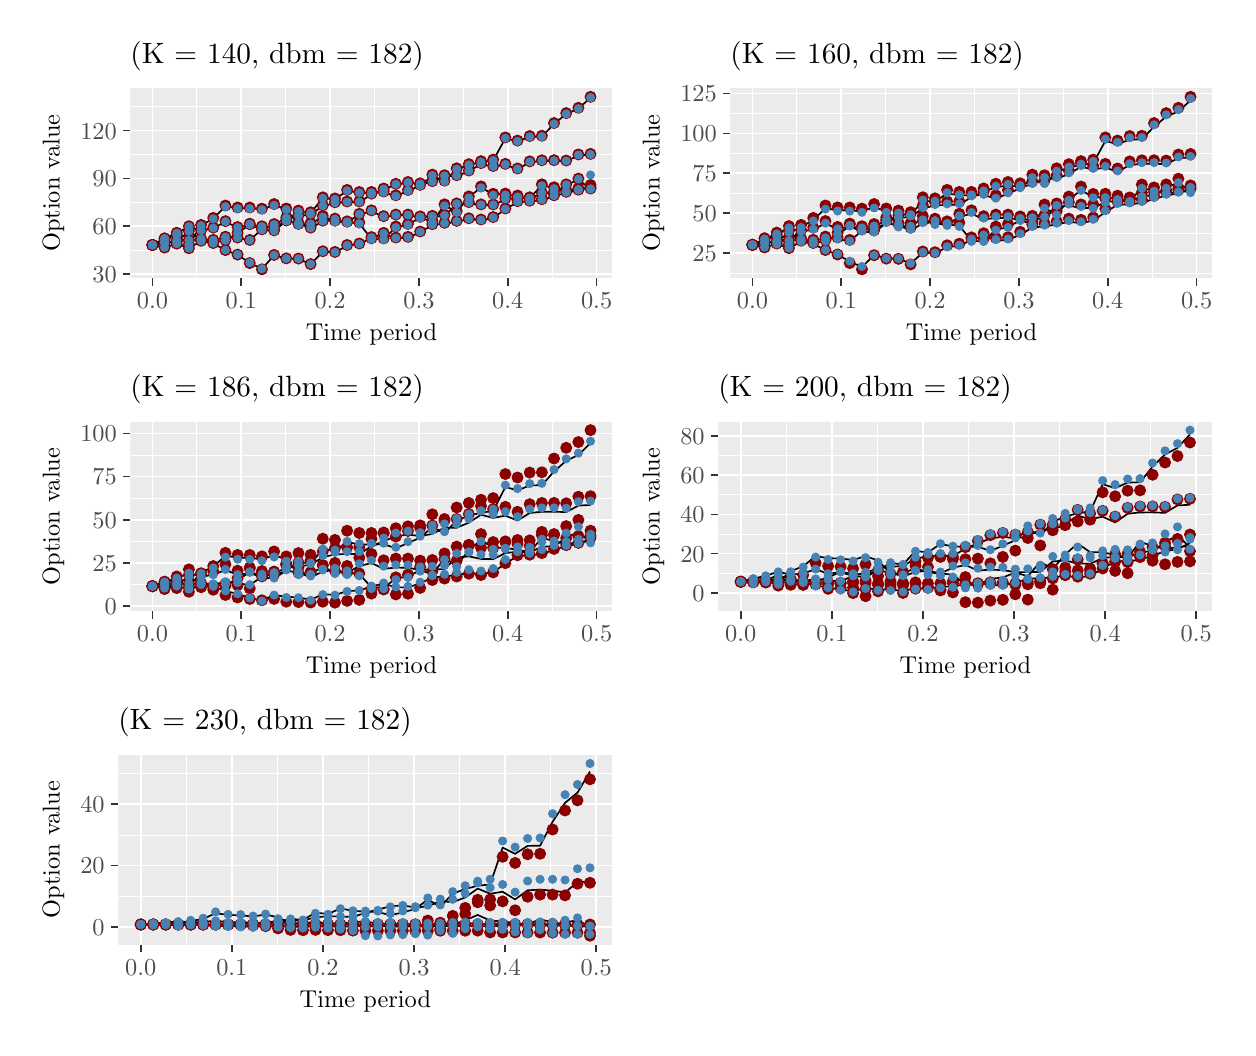
\begin{tikzpicture}[x=1pt,y=1pt]
\definecolor{fillColor}{RGB}{255,255,255}
\path[use as bounding box,fill=fillColor,fill opacity=0.00] (0,0) rectangle (433.62,361.35);
\begin{scope}
\path[clip] (  0.00,240.90) rectangle (216.81,361.35);
\definecolor{drawColor}{RGB}{255,255,255}
\definecolor{fillColor}{RGB}{255,255,255}

\path[draw=drawColor,line width= 0.6pt,line join=round,line cap=round,fill=fillColor] (  0.00,240.90) rectangle (216.81,361.35);
\end{scope}
\begin{scope}
\path[clip] ( 37.15,270.92) rectangle (211.31,339.48);
\definecolor{fillColor}{gray}{0.92}

\path[fill=fillColor] ( 37.15,270.92) rectangle (211.31,339.48);
\definecolor{drawColor}{RGB}{255,255,255}

\path[draw=drawColor,line width= 0.3pt,line join=round] ( 37.15,280.94) --
	(211.31,280.94);

\path[draw=drawColor,line width= 0.3pt,line join=round] ( 37.15,298.22) --
	(211.31,298.22);

\path[draw=drawColor,line width= 0.3pt,line join=round] ( 37.15,315.51) --
	(211.31,315.51);

\path[draw=drawColor,line width= 0.3pt,line join=round] ( 37.15,332.79) --
	(211.31,332.79);

\path[draw=drawColor,line width= 0.3pt,line join=round] ( 61.12,270.92) --
	( 61.12,339.48);

\path[draw=drawColor,line width= 0.3pt,line join=round] ( 93.23,270.92) --
	( 93.23,339.48);

\path[draw=drawColor,line width= 0.3pt,line join=round] (125.33,270.92) --
	(125.33,339.48);

\path[draw=drawColor,line width= 0.3pt,line join=round] (157.44,270.92) --
	(157.44,339.48);

\path[draw=drawColor,line width= 0.3pt,line join=round] (189.54,270.92) --
	(189.54,339.48);

\path[draw=drawColor,line width= 0.6pt,line join=round] ( 37.15,272.30) --
	(211.31,272.30);

\path[draw=drawColor,line width= 0.6pt,line join=round] ( 37.15,289.58) --
	(211.31,289.58);

\path[draw=drawColor,line width= 0.6pt,line join=round] ( 37.15,306.87) --
	(211.31,306.87);

\path[draw=drawColor,line width= 0.6pt,line join=round] ( 37.15,324.15) --
	(211.31,324.15);

\path[draw=drawColor,line width= 0.6pt,line join=round] ( 45.07,270.92) --
	( 45.07,339.48);

\path[draw=drawColor,line width= 0.6pt,line join=round] ( 77.17,270.92) --
	( 77.17,339.48);

\path[draw=drawColor,line width= 0.6pt,line join=round] (109.28,270.92) --
	(109.28,339.48);

\path[draw=drawColor,line width= 0.6pt,line join=round] (141.38,270.92) --
	(141.38,339.48);

\path[draw=drawColor,line width= 0.6pt,line join=round] (173.49,270.92) --
	(173.49,339.48);

\path[draw=drawColor,line width= 0.6pt,line join=round] (205.59,270.92) --
	(205.59,339.48);
\definecolor{drawColor}{RGB}{0,0,0}

\path[draw=drawColor,line width= 0.6pt,line join=round] ( 45.07,282.83) --
	( 49.47,285.05) --
	( 53.86,286.39) --
	( 58.26,282.93) --
	( 62.66,289.88) --
	( 67.06,292.38) --
	( 71.46,296.82) --
	( 75.85,296.12) --
	( 80.25,296.11) --
	( 84.65,295.68) --
	( 89.05,297.32) --
	( 93.45,295.74) --
	( 97.84,290.18) --
	(102.24,290.51) --
	(106.64,293.04) --
	(111.04,291.30) --
	(115.43,290.98) --
	(119.83,290.65) --
	(124.23,284.96) --
	(128.63,284.91) --
	(133.03,289.21) --
	(137.42,290.15) --
	(141.82,292.70) --
	(146.22,291.26) --
	(150.62,297.20) --
	(155.02,294.78) --
	(159.41,300.06) --
	(163.81,303.67) --
	(168.21,301.01) --
	(172.61,301.09) --
	(177.01,300.38) --
	(181.40,299.72) --
	(185.80,304.43) --
	(190.20,303.38) --
	(194.60,302.36) --
	(199.00,303.06) --
	(203.39,303.24);

\path[draw=drawColor,line width= 0.6pt,line join=round] ( 45.07,282.83) --
	( 49.47,285.14) --
	( 53.86,287.11) --
	( 58.26,289.42) --
	( 62.66,288.05) --
	( 67.06,288.91) --
	( 71.46,291.21) --
	( 75.85,289.10) --
	( 80.25,290.12) --
	( 84.65,288.25) --
	( 89.05,287.89) --
	( 93.45,291.47) --
	( 97.84,294.96) --
	(102.24,294.38) --
	(106.64,299.74) --
	(111.04,299.35) --
	(115.43,302.42) --
	(119.83,301.67) --
	(124.23,301.68) --
	(128.63,301.84) --
	(133.03,300.49) --
	(137.42,302.38) --
	(141.82,304.23) --
	(146.22,307.93) --
	(150.62,305.77) --
	(155.02,310.22) --
	(159.41,311.73) --
	(163.81,312.80) --
	(168.21,313.35) --
	(172.61,321.38) --
	(177.01,320.24) --
	(181.40,321.89) --
	(185.80,321.99) --
	(190.20,326.57) --
	(194.60,330.16) --
	(199.00,332.09) --
	(203.39,336.06);

\path[draw=drawColor,line width= 0.6pt,line join=round] ( 45.07,282.83) --
	( 49.47,283.93) --
	( 53.86,284.09) --
	( 58.26,287.74) --
	( 62.66,284.73) --
	( 67.06,283.76) --
	( 71.46,284.47) --
	( 75.85,287.03) --
	( 80.25,290.27) --
	( 84.65,289.35) --
	( 89.05,289.14) --
	( 93.45,291.44) --
	( 97.84,290.62) --
	(102.24,288.84) --
	(106.64,291.32) --
	(111.04,292.05) --
	(115.43,291.05) --
	(119.83,293.80) --
	(124.23,295.04) --
	(128.63,292.94) --
	(133.03,293.52) --
	(137.42,293.50) --
	(141.82,292.85) --
	(146.22,293.06) --
	(150.62,293.38) --
	(155.02,297.54) --
	(159.41,298.01) --
	(163.81,297.19) --
	(168.21,297.17) --
	(172.61,299.30) --
	(177.01,299.76) --
	(181.40,299.64) --
	(185.80,301.43) --
	(190.20,301.76) --
	(194.60,304.42) --
	(199.00,306.49) --
	(203.39,302.91);

\path[draw=drawColor,line width= 0.6pt,line join=round] ( 45.07,282.83) --
	( 49.47,283.40) --
	( 53.86,284.45) --
	( 58.26,284.51) --
	( 62.66,285.00) --
	( 67.06,284.55) --
	( 71.46,285.66) --
	( 75.85,285.34) --
	( 80.25,284.48) --
	( 84.65,288.60) --
	( 89.05,290.12) --
	( 93.45,292.52) --
	( 97.84,293.26) --
	(102.24,293.85) --
	(106.64,296.87) --
	(111.04,297.97) --
	(115.43,298.23) --
	(119.83,298.27) --
	(124.23,301.09) --
	(128.63,302.92) --
	(133.03,304.63) --
	(137.42,305.28) --
	(141.82,304.80) --
	(146.22,305.57) --
	(150.62,307.73) --
	(155.02,307.72) --
	(159.41,309.43) --
	(163.81,312.10) --
	(168.21,311.05) --
	(172.61,311.83) --
	(177.01,310.17) --
	(181.40,312.73) --
	(185.80,313.14) --
	(190.20,313.16) --
	(194.60,313.04) --
	(199.00,315.23) --
	(203.39,315.42);

\path[draw=drawColor,line width= 0.6pt,line join=round] ( 45.07,282.83) --
	( 49.47,281.89) --
	( 53.86,283.25) --
	( 58.26,281.63) --
	( 62.66,284.23) --
	( 67.06,283.42) --
	( 71.46,280.91) --
	( 75.85,279.32) --
	( 80.25,276.34) --
	( 84.65,274.16) --
	( 89.05,279.13) --
	( 93.45,277.91) --
	( 97.84,277.82) --
	(102.24,275.85) --
	(106.64,280.38) --
	(111.04,280.12) --
	(115.43,282.58) --
	(119.83,283.12) --
	(124.23,285.40) --
	(128.63,286.90) --
	(133.03,285.22) --
	(137.42,285.46) --
	(141.82,287.40) --
	(146.22,290.03) --
	(150.62,290.52) --
	(155.02,291.22) --
	(159.41,292.17) --
	(163.81,291.73) --
	(168.21,292.61) --
	(172.61,295.69) --
	(177.01,298.34) --
	(181.40,298.52) --
	(185.80,299.05) --
	(190.20,300.46) --
	(194.60,301.73) --
	(199.00,302.49) --
	(203.39,304.18);
\definecolor{drawColor}{RGB}{139,0,0}
\definecolor{fillColor}{RGB}{139,0,0}

\path[draw=drawColor,line width= 0.4pt,line join=round,line cap=round,fill=fillColor] ( 45.07,282.83) circle (  1.96);

\path[draw=drawColor,line width= 0.4pt,line join=round,line cap=round,fill=fillColor] ( 49.47,285.12) circle (  1.96);

\path[draw=drawColor,line width= 0.4pt,line join=round,line cap=round,fill=fillColor] ( 53.86,286.51) circle (  1.96);

\path[draw=drawColor,line width= 0.4pt,line join=round,line cap=round,fill=fillColor] ( 58.26,282.99) circle (  1.96);

\path[draw=drawColor,line width= 0.4pt,line join=round,line cap=round,fill=fillColor] ( 62.66,290.07) circle (  1.96);

\path[draw=drawColor,line width= 0.4pt,line join=round,line cap=round,fill=fillColor] ( 67.06,292.60) circle (  1.96);

\path[draw=drawColor,line width= 0.4pt,line join=round,line cap=round,fill=fillColor] ( 71.46,297.08) circle (  1.96);

\path[draw=drawColor,line width= 0.4pt,line join=round,line cap=round,fill=fillColor] ( 75.85,296.38) circle (  1.96);

\path[draw=drawColor,line width= 0.4pt,line join=round,line cap=round,fill=fillColor] ( 80.25,296.37) circle (  1.96);

\path[draw=drawColor,line width= 0.4pt,line join=round,line cap=round,fill=fillColor] ( 84.65,295.95) circle (  1.96);

\path[draw=drawColor,line width= 0.4pt,line join=round,line cap=round,fill=fillColor] ( 89.05,297.60) circle (  1.96);

\path[draw=drawColor,line width= 0.4pt,line join=round,line cap=round,fill=fillColor] ( 93.45,296.02) circle (  1.96);

\path[draw=drawColor,line width= 0.4pt,line join=round,line cap=round,fill=fillColor] ( 97.84,290.43) circle (  1.96);

\path[draw=drawColor,line width= 0.4pt,line join=round,line cap=round,fill=fillColor] (102.24,290.78) circle (  1.96);

\path[draw=drawColor,line width= 0.4pt,line join=round,line cap=round,fill=fillColor] (106.64,293.32) circle (  1.96);

\path[draw=drawColor,line width= 0.4pt,line join=round,line cap=round,fill=fillColor] (111.04,291.58) circle (  1.96);

\path[draw=drawColor,line width= 0.4pt,line join=round,line cap=round,fill=fillColor] (115.43,291.26) circle (  1.96);

\path[draw=drawColor,line width= 0.4pt,line join=round,line cap=round,fill=fillColor] (119.83,290.94) circle (  1.96);

\path[draw=drawColor,line width= 0.4pt,line join=round,line cap=round,fill=fillColor] (124.23,285.23) circle (  1.96);

\path[draw=drawColor,line width= 0.4pt,line join=round,line cap=round,fill=fillColor] (128.63,285.19) circle (  1.96);

\path[draw=drawColor,line width= 0.4pt,line join=round,line cap=round,fill=fillColor] (133.03,289.50) circle (  1.96);

\path[draw=drawColor,line width= 0.4pt,line join=round,line cap=round,fill=fillColor] (137.42,290.44) circle (  1.96);

\path[draw=drawColor,line width= 0.4pt,line join=round,line cap=round,fill=fillColor] (141.82,293.00) circle (  1.96);

\path[draw=drawColor,line width= 0.4pt,line join=round,line cap=round,fill=fillColor] (146.22,291.56) circle (  1.96);

\path[draw=drawColor,line width= 0.4pt,line join=round,line cap=round,fill=fillColor] (150.62,297.50) circle (  1.96);

\path[draw=drawColor,line width= 0.4pt,line join=round,line cap=round,fill=fillColor] (155.02,295.08) circle (  1.96);

\path[draw=drawColor,line width= 0.4pt,line join=round,line cap=round,fill=fillColor] (159.41,300.37) circle (  1.96);

\path[draw=drawColor,line width= 0.4pt,line join=round,line cap=round,fill=fillColor] (163.81,303.98) circle (  1.96);

\path[draw=drawColor,line width= 0.4pt,line join=round,line cap=round,fill=fillColor] (168.21,301.32) circle (  1.96);

\path[draw=drawColor,line width= 0.4pt,line join=round,line cap=round,fill=fillColor] (172.61,301.39) circle (  1.96);

\path[draw=drawColor,line width= 0.4pt,line join=round,line cap=round,fill=fillColor] (177.01,300.69) circle (  1.96);

\path[draw=drawColor,line width= 0.4pt,line join=round,line cap=round,fill=fillColor] (181.40,300.02) circle (  1.96);

\path[draw=drawColor,line width= 0.4pt,line join=round,line cap=round,fill=fillColor] (185.80,304.74) circle (  1.96);

\path[draw=drawColor,line width= 0.4pt,line join=round,line cap=round,fill=fillColor] (190.20,303.68) circle (  1.96);

\path[draw=drawColor,line width= 0.4pt,line join=round,line cap=round,fill=fillColor] (194.60,302.66) circle (  1.96);

\path[draw=drawColor,line width= 0.4pt,line join=round,line cap=round,fill=fillColor] (199.00,303.37) circle (  1.96);

\path[draw=drawColor,line width= 0.4pt,line join=round,line cap=round,fill=fillColor] (203.39,303.55) circle (  1.96);

\path[draw=drawColor,line width= 0.4pt,line join=round,line cap=round,fill=fillColor] ( 45.07,282.83) circle (  1.96);

\path[draw=drawColor,line width= 0.4pt,line join=round,line cap=round,fill=fillColor] ( 49.47,285.22) circle (  1.96);

\path[draw=drawColor,line width= 0.4pt,line join=round,line cap=round,fill=fillColor] ( 53.86,287.24) circle (  1.96);

\path[draw=drawColor,line width= 0.4pt,line join=round,line cap=round,fill=fillColor] ( 58.26,289.60) circle (  1.96);

\path[draw=drawColor,line width= 0.4pt,line join=round,line cap=round,fill=fillColor] ( 62.66,288.22) circle (  1.96);

\path[draw=drawColor,line width= 0.4pt,line join=round,line cap=round,fill=fillColor] ( 67.06,289.10) circle (  1.96);

\path[draw=drawColor,line width= 0.4pt,line join=round,line cap=round,fill=fillColor] ( 71.46,291.43) circle (  1.96);

\path[draw=drawColor,line width= 0.4pt,line join=round,line cap=round,fill=fillColor] ( 75.85,289.31) circle (  1.96);

\path[draw=drawColor,line width= 0.4pt,line join=round,line cap=round,fill=fillColor] ( 80.25,290.34) circle (  1.96);

\path[draw=drawColor,line width= 0.4pt,line join=round,line cap=round,fill=fillColor] ( 84.65,288.47) circle (  1.96);

\path[draw=drawColor,line width= 0.4pt,line join=round,line cap=round,fill=fillColor] ( 89.05,288.11) circle (  1.96);

\path[draw=drawColor,line width= 0.4pt,line join=round,line cap=round,fill=fillColor] ( 93.45,291.73) circle (  1.96);

\path[draw=drawColor,line width= 0.4pt,line join=round,line cap=round,fill=fillColor] ( 97.84,295.24) circle (  1.96);

\path[draw=drawColor,line width= 0.4pt,line join=round,line cap=round,fill=fillColor] (102.24,294.66) circle (  1.96);

\path[draw=drawColor,line width= 0.4pt,line join=round,line cap=round,fill=fillColor] (106.64,300.03) circle (  1.96);

\path[draw=drawColor,line width= 0.4pt,line join=round,line cap=round,fill=fillColor] (111.04,299.64) circle (  1.96);

\path[draw=drawColor,line width= 0.4pt,line join=round,line cap=round,fill=fillColor] (115.43,302.72) circle (  1.96);

\path[draw=drawColor,line width= 0.4pt,line join=round,line cap=round,fill=fillColor] (119.83,301.97) circle (  1.96);

\path[draw=drawColor,line width= 0.4pt,line join=round,line cap=round,fill=fillColor] (124.23,301.98) circle (  1.96);

\path[draw=drawColor,line width= 0.4pt,line join=round,line cap=round,fill=fillColor] (128.63,302.14) circle (  1.96);

\path[draw=drawColor,line width= 0.4pt,line join=round,line cap=round,fill=fillColor] (133.03,300.79) circle (  1.96);

\path[draw=drawColor,line width= 0.4pt,line join=round,line cap=round,fill=fillColor] (137.42,302.68) circle (  1.96);

\path[draw=drawColor,line width= 0.4pt,line join=round,line cap=round,fill=fillColor] (141.82,304.54) circle (  1.96);

\path[draw=drawColor,line width= 0.4pt,line join=round,line cap=round,fill=fillColor] (146.22,308.23) circle (  1.96);

\path[draw=drawColor,line width= 0.4pt,line join=round,line cap=round,fill=fillColor] (150.62,306.07) circle (  1.96);

\path[draw=drawColor,line width= 0.4pt,line join=round,line cap=round,fill=fillColor] (155.02,310.52) circle (  1.96);

\path[draw=drawColor,line width= 0.4pt,line join=round,line cap=round,fill=fillColor] (159.41,312.03) circle (  1.96);

\path[draw=drawColor,line width= 0.4pt,line join=round,line cap=round,fill=fillColor] (163.81,313.11) circle (  1.96);

\path[draw=drawColor,line width= 0.4pt,line join=round,line cap=round,fill=fillColor] (168.21,313.66) circle (  1.96);

\path[draw=drawColor,line width= 0.4pt,line join=round,line cap=round,fill=fillColor] (172.61,321.68) circle (  1.96);

\path[draw=drawColor,line width= 0.4pt,line join=round,line cap=round,fill=fillColor] (177.01,320.54) circle (  1.96);

\path[draw=drawColor,line width= 0.4pt,line join=round,line cap=round,fill=fillColor] (181.40,322.19) circle (  1.96);

\path[draw=drawColor,line width= 0.4pt,line join=round,line cap=round,fill=fillColor] (185.80,322.30) circle (  1.96);

\path[draw=drawColor,line width= 0.4pt,line join=round,line cap=round,fill=fillColor] (190.20,326.88) circle (  1.96);

\path[draw=drawColor,line width= 0.4pt,line join=round,line cap=round,fill=fillColor] (194.60,330.47) circle (  1.96);

\path[draw=drawColor,line width= 0.4pt,line join=round,line cap=round,fill=fillColor] (199.00,332.39) circle (  1.96);

\path[draw=drawColor,line width= 0.4pt,line join=round,line cap=round,fill=fillColor] (203.39,336.36) circle (  1.96);

\path[draw=drawColor,line width= 0.4pt,line join=round,line cap=round,fill=fillColor] ( 45.07,282.83) circle (  1.96);

\path[draw=drawColor,line width= 0.4pt,line join=round,line cap=round,fill=fillColor] ( 49.47,283.98) circle (  1.96);

\path[draw=drawColor,line width= 0.4pt,line join=round,line cap=round,fill=fillColor] ( 53.86,284.16) circle (  1.96);

\path[draw=drawColor,line width= 0.4pt,line join=round,line cap=round,fill=fillColor] ( 58.26,287.89) circle (  1.96);

\path[draw=drawColor,line width= 0.4pt,line join=round,line cap=round,fill=fillColor] ( 62.66,284.85) circle (  1.96);

\path[draw=drawColor,line width= 0.4pt,line join=round,line cap=round,fill=fillColor] ( 67.06,283.87) circle (  1.96);

\path[draw=drawColor,line width= 0.4pt,line join=round,line cap=round,fill=fillColor] ( 71.46,284.60) circle (  1.96);

\path[draw=drawColor,line width= 0.4pt,line join=round,line cap=round,fill=fillColor] ( 75.85,287.21) circle (  1.96);

\path[draw=drawColor,line width= 0.4pt,line join=round,line cap=round,fill=fillColor] ( 80.25,290.50) circle (  1.96);

\path[draw=drawColor,line width= 0.4pt,line join=round,line cap=round,fill=fillColor] ( 84.65,289.58) circle (  1.96);

\path[draw=drawColor,line width= 0.4pt,line join=round,line cap=round,fill=fillColor] ( 89.05,289.38) circle (  1.96);

\path[draw=drawColor,line width= 0.4pt,line join=round,line cap=round,fill=fillColor] ( 93.45,291.70) circle (  1.96);

\path[draw=drawColor,line width= 0.4pt,line join=round,line cap=round,fill=fillColor] ( 97.84,290.88) circle (  1.96);

\path[draw=drawColor,line width= 0.4pt,line join=round,line cap=round,fill=fillColor] (102.24,289.09) circle (  1.96);

\path[draw=drawColor,line width= 0.4pt,line join=round,line cap=round,fill=fillColor] (106.64,291.59) circle (  1.96);

\path[draw=drawColor,line width= 0.4pt,line join=round,line cap=round,fill=fillColor] (111.04,292.33) circle (  1.96);

\path[draw=drawColor,line width= 0.4pt,line join=round,line cap=round,fill=fillColor] (115.43,291.33) circle (  1.96);

\path[draw=drawColor,line width= 0.4pt,line join=round,line cap=round,fill=fillColor] (119.83,294.09) circle (  1.96);

\path[draw=drawColor,line width= 0.4pt,line join=round,line cap=round,fill=fillColor] (124.23,295.33) circle (  1.96);

\path[draw=drawColor,line width= 0.4pt,line join=round,line cap=round,fill=fillColor] (128.63,293.24) circle (  1.96);

\path[draw=drawColor,line width= 0.4pt,line join=round,line cap=round,fill=fillColor] (133.03,293.81) circle (  1.96);

\path[draw=drawColor,line width= 0.4pt,line join=round,line cap=round,fill=fillColor] (137.42,293.80) circle (  1.96);

\path[draw=drawColor,line width= 0.4pt,line join=round,line cap=round,fill=fillColor] (141.82,293.15) circle (  1.96);

\path[draw=drawColor,line width= 0.4pt,line join=round,line cap=round,fill=fillColor] (146.22,293.36) circle (  1.96);

\path[draw=drawColor,line width= 0.4pt,line join=round,line cap=round,fill=fillColor] (150.62,293.69) circle (  1.96);

\path[draw=drawColor,line width= 0.4pt,line join=round,line cap=round,fill=fillColor] (155.02,297.84) circle (  1.96);

\path[draw=drawColor,line width= 0.4pt,line join=round,line cap=round,fill=fillColor] (159.41,298.32) circle (  1.96);

\path[draw=drawColor,line width= 0.4pt,line join=round,line cap=round,fill=fillColor] (163.81,297.49) circle (  1.96);

\path[draw=drawColor,line width= 0.4pt,line join=round,line cap=round,fill=fillColor] (168.21,297.48) circle (  1.96);

\path[draw=drawColor,line width= 0.4pt,line join=round,line cap=round,fill=fillColor] (172.61,299.60) circle (  1.96);

\path[draw=drawColor,line width= 0.4pt,line join=round,line cap=round,fill=fillColor] (177.01,300.06) circle (  1.96);

\path[draw=drawColor,line width= 0.4pt,line join=round,line cap=round,fill=fillColor] (181.40,299.94) circle (  1.96);

\path[draw=drawColor,line width= 0.4pt,line join=round,line cap=round,fill=fillColor] (185.80,301.73) circle (  1.96);

\path[draw=drawColor,line width= 0.4pt,line join=round,line cap=round,fill=fillColor] (190.20,302.06) circle (  1.96);

\path[draw=drawColor,line width= 0.4pt,line join=round,line cap=round,fill=fillColor] (194.60,304.73) circle (  1.96);

\path[draw=drawColor,line width= 0.4pt,line join=round,line cap=round,fill=fillColor] (199.00,306.80) circle (  1.96);

\path[draw=drawColor,line width= 0.4pt,line join=round,line cap=round,fill=fillColor] (203.39,303.21) circle (  1.96);

\path[draw=drawColor,line width= 0.4pt,line join=round,line cap=round,fill=fillColor] ( 45.07,282.83) circle (  1.96);

\path[draw=drawColor,line width= 0.4pt,line join=round,line cap=round,fill=fillColor] ( 49.47,283.44) circle (  1.96);

\path[draw=drawColor,line width= 0.4pt,line join=round,line cap=round,fill=fillColor] ( 53.86,284.53) circle (  1.96);

\path[draw=drawColor,line width= 0.4pt,line join=round,line cap=round,fill=fillColor] ( 58.26,284.60) circle (  1.96);

\path[draw=drawColor,line width= 0.4pt,line join=round,line cap=round,fill=fillColor] ( 62.66,285.12) circle (  1.96);

\path[draw=drawColor,line width= 0.4pt,line join=round,line cap=round,fill=fillColor] ( 67.06,284.68) circle (  1.96);

\path[draw=drawColor,line width= 0.4pt,line join=round,line cap=round,fill=fillColor] ( 71.46,285.81) circle (  1.96);

\path[draw=drawColor,line width= 0.4pt,line join=round,line cap=round,fill=fillColor] ( 75.85,285.50) circle (  1.96);

\path[draw=drawColor,line width= 0.4pt,line join=round,line cap=round,fill=fillColor] ( 80.25,284.64) circle (  1.96);

\path[draw=drawColor,line width= 0.4pt,line join=round,line cap=round,fill=fillColor] ( 84.65,288.82) circle (  1.96);

\path[draw=drawColor,line width= 0.4pt,line join=round,line cap=round,fill=fillColor] ( 89.05,290.37) circle (  1.96);

\path[draw=drawColor,line width= 0.4pt,line join=round,line cap=round,fill=fillColor] ( 93.45,292.78) circle (  1.96);

\path[draw=drawColor,line width= 0.4pt,line join=round,line cap=round,fill=fillColor] ( 97.84,293.53) circle (  1.96);

\path[draw=drawColor,line width= 0.4pt,line join=round,line cap=round,fill=fillColor] (102.24,294.13) circle (  1.96);

\path[draw=drawColor,line width= 0.4pt,line join=round,line cap=round,fill=fillColor] (106.64,297.16) circle (  1.96);

\path[draw=drawColor,line width= 0.4pt,line join=round,line cap=round,fill=fillColor] (111.04,298.26) circle (  1.96);

\path[draw=drawColor,line width= 0.4pt,line join=round,line cap=round,fill=fillColor] (115.43,298.53) circle (  1.96);

\path[draw=drawColor,line width= 0.4pt,line join=round,line cap=round,fill=fillColor] (119.83,298.56) circle (  1.96);

\path[draw=drawColor,line width= 0.4pt,line join=round,line cap=round,fill=fillColor] (124.23,301.39) circle (  1.96);

\path[draw=drawColor,line width= 0.4pt,line join=round,line cap=round,fill=fillColor] (128.63,303.22) circle (  1.96);

\path[draw=drawColor,line width= 0.4pt,line join=round,line cap=round,fill=fillColor] (133.03,304.93) circle (  1.96);

\path[draw=drawColor,line width= 0.4pt,line join=round,line cap=round,fill=fillColor] (137.42,305.58) circle (  1.96);

\path[draw=drawColor,line width= 0.4pt,line join=round,line cap=round,fill=fillColor] (141.82,305.11) circle (  1.96);

\path[draw=drawColor,line width= 0.4pt,line join=round,line cap=round,fill=fillColor] (146.22,305.88) circle (  1.96);

\path[draw=drawColor,line width= 0.4pt,line join=round,line cap=round,fill=fillColor] (150.62,308.03) circle (  1.96);

\path[draw=drawColor,line width= 0.4pt,line join=round,line cap=round,fill=fillColor] (155.02,308.03) circle (  1.96);

\path[draw=drawColor,line width= 0.4pt,line join=round,line cap=round,fill=fillColor] (159.41,309.73) circle (  1.96);

\path[draw=drawColor,line width= 0.4pt,line join=round,line cap=round,fill=fillColor] (163.81,312.40) circle (  1.96);

\path[draw=drawColor,line width= 0.4pt,line join=round,line cap=round,fill=fillColor] (168.21,311.35) circle (  1.96);

\path[draw=drawColor,line width= 0.4pt,line join=round,line cap=round,fill=fillColor] (172.61,312.13) circle (  1.96);

\path[draw=drawColor,line width= 0.4pt,line join=round,line cap=round,fill=fillColor] (177.01,310.47) circle (  1.96);

\path[draw=drawColor,line width= 0.4pt,line join=round,line cap=round,fill=fillColor] (181.40,313.03) circle (  1.96);

\path[draw=drawColor,line width= 0.4pt,line join=round,line cap=round,fill=fillColor] (185.80,313.44) circle (  1.96);

\path[draw=drawColor,line width= 0.4pt,line join=round,line cap=round,fill=fillColor] (190.20,313.47) circle (  1.96);

\path[draw=drawColor,line width= 0.4pt,line join=round,line cap=round,fill=fillColor] (194.60,313.34) circle (  1.96);

\path[draw=drawColor,line width= 0.4pt,line join=round,line cap=round,fill=fillColor] (199.00,315.53) circle (  1.96);

\path[draw=drawColor,line width= 0.4pt,line join=round,line cap=round,fill=fillColor] (203.39,315.73) circle (  1.96);

\path[draw=drawColor,line width= 0.4pt,line join=round,line cap=round,fill=fillColor] ( 45.07,282.83) circle (  1.96);

\path[draw=drawColor,line width= 0.4pt,line join=round,line cap=round,fill=fillColor] ( 49.47,281.88) circle (  1.96);

\path[draw=drawColor,line width= 0.4pt,line join=round,line cap=round,fill=fillColor] ( 53.86,283.30) circle (  1.96);

\path[draw=drawColor,line width= 0.4pt,line join=round,line cap=round,fill=fillColor] ( 58.26,281.65) circle (  1.96);

\path[draw=drawColor,line width= 0.4pt,line join=round,line cap=round,fill=fillColor] ( 62.66,284.33) circle (  1.96);

\path[draw=drawColor,line width= 0.4pt,line join=round,line cap=round,fill=fillColor] ( 67.06,283.52) circle (  1.96);

\path[draw=drawColor,line width= 0.4pt,line join=round,line cap=round,fill=fillColor] ( 71.46,280.97) circle (  1.96);

\path[draw=drawColor,line width= 0.4pt,line join=round,line cap=round,fill=fillColor] ( 75.85,279.35) circle (  1.96);

\path[draw=drawColor,line width= 0.4pt,line join=round,line cap=round,fill=fillColor] ( 80.25,276.29) circle (  1.96);

\path[draw=drawColor,line width= 0.4pt,line join=round,line cap=round,fill=fillColor] ( 84.65,274.03) circle (  1.96);

\path[draw=drawColor,line width= 0.4pt,line join=round,line cap=round,fill=fillColor] ( 89.05,279.22) circle (  1.96);

\path[draw=drawColor,line width= 0.4pt,line join=round,line cap=round,fill=fillColor] ( 93.45,277.98) circle (  1.96);

\path[draw=drawColor,line width= 0.4pt,line join=round,line cap=round,fill=fillColor] ( 97.84,277.91) circle (  1.96);

\path[draw=drawColor,line width= 0.4pt,line join=round,line cap=round,fill=fillColor] (102.24,275.91) circle (  1.96);

\path[draw=drawColor,line width= 0.4pt,line join=round,line cap=round,fill=fillColor] (106.64,280.56) circle (  1.96);

\path[draw=drawColor,line width= 0.4pt,line join=round,line cap=round,fill=fillColor] (111.04,280.31) circle (  1.96);

\path[draw=drawColor,line width= 0.4pt,line join=round,line cap=round,fill=fillColor] (115.43,282.82) circle (  1.96);

\path[draw=drawColor,line width= 0.4pt,line join=round,line cap=round,fill=fillColor] (119.83,283.37) circle (  1.96);

\path[draw=drawColor,line width= 0.4pt,line join=round,line cap=round,fill=fillColor] (124.23,285.67) circle (  1.96);

\path[draw=drawColor,line width= 0.4pt,line join=round,line cap=round,fill=fillColor] (128.63,287.19) circle (  1.96);

\path[draw=drawColor,line width= 0.4pt,line join=round,line cap=round,fill=fillColor] (133.03,285.51) circle (  1.96);

\path[draw=drawColor,line width= 0.4pt,line join=round,line cap=round,fill=fillColor] (137.42,285.75) circle (  1.96);

\path[draw=drawColor,line width= 0.4pt,line join=round,line cap=round,fill=fillColor] (141.82,287.69) circle (  1.96);

\path[draw=drawColor,line width= 0.4pt,line join=round,line cap=round,fill=fillColor] (146.22,290.33) circle (  1.96);

\path[draw=drawColor,line width= 0.4pt,line join=round,line cap=round,fill=fillColor] (150.62,290.83) circle (  1.96);

\path[draw=drawColor,line width= 0.4pt,line join=round,line cap=round,fill=fillColor] (155.02,291.52) circle (  1.96);

\path[draw=drawColor,line width= 0.4pt,line join=round,line cap=round,fill=fillColor] (159.41,292.47) circle (  1.96);

\path[draw=drawColor,line width= 0.4pt,line join=round,line cap=round,fill=fillColor] (163.81,292.03) circle (  1.96);

\path[draw=drawColor,line width= 0.4pt,line join=round,line cap=round,fill=fillColor] (168.21,292.92) circle (  1.96);

\path[draw=drawColor,line width= 0.4pt,line join=round,line cap=round,fill=fillColor] (172.61,296.00) circle (  1.96);

\path[draw=drawColor,line width= 0.4pt,line join=round,line cap=round,fill=fillColor] (177.01,298.65) circle (  1.96);

\path[draw=drawColor,line width= 0.4pt,line join=round,line cap=round,fill=fillColor] (181.40,298.82) circle (  1.96);

\path[draw=drawColor,line width= 0.4pt,line join=round,line cap=round,fill=fillColor] (185.80,299.36) circle (  1.96);

\path[draw=drawColor,line width= 0.4pt,line join=round,line cap=round,fill=fillColor] (190.20,300.77) circle (  1.96);

\path[draw=drawColor,line width= 0.4pt,line join=round,line cap=round,fill=fillColor] (194.60,302.03) circle (  1.96);

\path[draw=drawColor,line width= 0.4pt,line join=round,line cap=round,fill=fillColor] (199.00,302.79) circle (  1.96);

\path[draw=drawColor,line width= 0.4pt,line join=round,line cap=round,fill=fillColor] (203.39,304.49) circle (  1.96);
\definecolor{drawColor}{RGB}{70,130,180}
\definecolor{fillColor}{RGB}{70,130,180}

\path[draw=drawColor,line width= 0.4pt,line join=round,line cap=round,fill=fillColor] ( 45.07,282.83) circle (  1.43);

\path[draw=drawColor,line width= 0.4pt,line join=round,line cap=round,fill=fillColor] ( 49.47,285.04) circle (  1.43);

\path[draw=drawColor,line width= 0.4pt,line join=round,line cap=round,fill=fillColor] ( 53.86,286.38) circle (  1.43);

\path[draw=drawColor,line width= 0.4pt,line join=round,line cap=round,fill=fillColor] ( 58.26,282.98) circle (  1.43);

\path[draw=drawColor,line width= 0.4pt,line join=round,line cap=round,fill=fillColor] ( 62.66,289.79) circle (  1.43);

\path[draw=drawColor,line width= 0.4pt,line join=round,line cap=round,fill=fillColor] ( 67.06,292.28) circle (  1.43);

\path[draw=drawColor,line width= 0.4pt,line join=round,line cap=round,fill=fillColor] ( 71.46,296.70) circle (  1.43);

\path[draw=drawColor,line width= 0.4pt,line join=round,line cap=round,fill=fillColor] ( 75.85,296.00) circle (  1.43);

\path[draw=drawColor,line width= 0.4pt,line join=round,line cap=round,fill=fillColor] ( 80.25,295.99) circle (  1.43);

\path[draw=drawColor,line width= 0.4pt,line join=round,line cap=round,fill=fillColor] ( 84.65,295.57) circle (  1.43);

\path[draw=drawColor,line width= 0.4pt,line join=round,line cap=round,fill=fillColor] ( 89.05,297.19) circle (  1.43);

\path[draw=drawColor,line width= 0.4pt,line join=round,line cap=round,fill=fillColor] ( 93.45,295.62) circle (  1.43);

\path[draw=drawColor,line width= 0.4pt,line join=round,line cap=round,fill=fillColor] ( 97.84,290.11) circle (  1.43);

\path[draw=drawColor,line width= 0.4pt,line join=round,line cap=round,fill=fillColor] (102.24,290.43) circle (  1.43);

\path[draw=drawColor,line width= 0.4pt,line join=round,line cap=round,fill=fillColor] (106.64,292.91) circle (  1.43);

\path[draw=drawColor,line width= 0.4pt,line join=round,line cap=round,fill=fillColor] (111.04,291.18) circle (  1.43);

\path[draw=drawColor,line width= 0.4pt,line join=round,line cap=round,fill=fillColor] (115.43,290.86) circle (  1.43);

\path[draw=drawColor,line width= 0.4pt,line join=round,line cap=round,fill=fillColor] (119.83,290.53) circle (  1.43);

\path[draw=drawColor,line width= 0.4pt,line join=round,line cap=round,fill=fillColor] (124.23,284.89) circle (  1.43);

\path[draw=drawColor,line width= 0.4pt,line join=round,line cap=round,fill=fillColor] (128.63,284.85) circle (  1.43);

\path[draw=drawColor,line width= 0.4pt,line join=round,line cap=round,fill=fillColor] (133.03,289.14) circle (  1.43);

\path[draw=drawColor,line width= 0.4pt,line join=round,line cap=round,fill=fillColor] (137.42,290.08) circle (  1.43);

\path[draw=drawColor,line width= 0.4pt,line join=round,line cap=round,fill=fillColor] (141.82,292.51) circle (  1.43);

\path[draw=drawColor,line width= 0.4pt,line join=round,line cap=round,fill=fillColor] (146.22,291.07) circle (  1.43);

\path[draw=drawColor,line width= 0.4pt,line join=round,line cap=round,fill=fillColor] (150.62,297.01) circle (  1.43);

\path[draw=drawColor,line width= 0.4pt,line join=round,line cap=round,fill=fillColor] (155.02,294.59) circle (  1.43);

\path[draw=drawColor,line width= 0.4pt,line join=round,line cap=round,fill=fillColor] (159.41,299.88) circle (  1.43);

\path[draw=drawColor,line width= 0.4pt,line join=round,line cap=round,fill=fillColor] (163.81,303.48) circle (  1.43);

\path[draw=drawColor,line width= 0.4pt,line join=round,line cap=round,fill=fillColor] (168.21,300.82) circle (  1.43);

\path[draw=drawColor,line width= 0.4pt,line join=round,line cap=round,fill=fillColor] (172.61,300.90) circle (  1.43);

\path[draw=drawColor,line width= 0.4pt,line join=round,line cap=round,fill=fillColor] (177.01,300.19) circle (  1.43);

\path[draw=drawColor,line width= 0.4pt,line join=round,line cap=round,fill=fillColor] (181.40,299.53) circle (  1.43);

\path[draw=drawColor,line width= 0.4pt,line join=round,line cap=round,fill=fillColor] (185.80,304.24) circle (  1.43);

\path[draw=drawColor,line width= 0.4pt,line join=round,line cap=round,fill=fillColor] (190.20,303.19) circle (  1.43);

\path[draw=drawColor,line width= 0.4pt,line join=round,line cap=round,fill=fillColor] (194.60,302.17) circle (  1.43);

\path[draw=drawColor,line width= 0.4pt,line join=round,line cap=round,fill=fillColor] (199.00,302.87) circle (  1.43);

\path[draw=drawColor,line width= 0.4pt,line join=round,line cap=round,fill=fillColor] (203.39,303.05) circle (  1.43);

\path[draw=drawColor,line width= 0.4pt,line join=round,line cap=round,fill=fillColor] ( 45.07,282.83) circle (  1.43);

\path[draw=drawColor,line width= 0.4pt,line join=round,line cap=round,fill=fillColor] ( 49.47,285.15) circle (  1.43);

\path[draw=drawColor,line width= 0.4pt,line join=round,line cap=round,fill=fillColor] ( 53.86,287.12) circle (  1.43);

\path[draw=drawColor,line width= 0.4pt,line join=round,line cap=round,fill=fillColor] ( 58.26,289.45) circle (  1.43);

\path[draw=drawColor,line width= 0.4pt,line join=round,line cap=round,fill=fillColor] ( 62.66,288.09) circle (  1.43);

\path[draw=drawColor,line width= 0.4pt,line join=round,line cap=round,fill=fillColor] ( 67.06,288.94) circle (  1.43);

\path[draw=drawColor,line width= 0.4pt,line join=round,line cap=round,fill=fillColor] ( 71.46,291.25) circle (  1.43);

\path[draw=drawColor,line width= 0.4pt,line join=round,line cap=round,fill=fillColor] ( 75.85,289.15) circle (  1.43);

\path[draw=drawColor,line width= 0.4pt,line join=round,line cap=round,fill=fillColor] ( 80.25,290.17) circle (  1.43);

\path[draw=drawColor,line width= 0.4pt,line join=round,line cap=round,fill=fillColor] ( 84.65,288.30) circle (  1.43);

\path[draw=drawColor,line width= 0.4pt,line join=round,line cap=round,fill=fillColor] ( 89.05,287.89) circle (  1.43);

\path[draw=drawColor,line width= 0.4pt,line join=round,line cap=round,fill=fillColor] ( 93.45,291.48) circle (  1.43);

\path[draw=drawColor,line width= 0.4pt,line join=round,line cap=round,fill=fillColor] ( 97.84,294.97) circle (  1.43);

\path[draw=drawColor,line width= 0.4pt,line join=round,line cap=round,fill=fillColor] (102.24,294.40) circle (  1.43);

\path[draw=drawColor,line width= 0.4pt,line join=round,line cap=round,fill=fillColor] (106.64,299.75) circle (  1.43);

\path[draw=drawColor,line width= 0.4pt,line join=round,line cap=round,fill=fillColor] (111.04,299.36) circle (  1.43);

\path[draw=drawColor,line width= 0.4pt,line join=round,line cap=round,fill=fillColor] (115.43,302.44) circle (  1.43);

\path[draw=drawColor,line width= 0.4pt,line join=round,line cap=round,fill=fillColor] (119.83,301.69) circle (  1.43);

\path[draw=drawColor,line width= 0.4pt,line join=round,line cap=round,fill=fillColor] (124.23,301.70) circle (  1.43);

\path[draw=drawColor,line width= 0.4pt,line join=round,line cap=round,fill=fillColor] (128.63,301.86) circle (  1.43);

\path[draw=drawColor,line width= 0.4pt,line join=round,line cap=round,fill=fillColor] (133.03,300.51) circle (  1.43);

\path[draw=drawColor,line width= 0.4pt,line join=round,line cap=round,fill=fillColor] (137.42,302.40) circle (  1.43);

\path[draw=drawColor,line width= 0.4pt,line join=round,line cap=round,fill=fillColor] (141.82,304.25) circle (  1.43);

\path[draw=drawColor,line width= 0.4pt,line join=round,line cap=round,fill=fillColor] (146.22,307.95) circle (  1.43);

\path[draw=drawColor,line width= 0.4pt,line join=round,line cap=round,fill=fillColor] (150.62,305.79) circle (  1.43);

\path[draw=drawColor,line width= 0.4pt,line join=round,line cap=round,fill=fillColor] (155.02,310.24) circle (  1.43);

\path[draw=drawColor,line width= 0.4pt,line join=round,line cap=round,fill=fillColor] (159.41,311.75) circle (  1.43);

\path[draw=drawColor,line width= 0.4pt,line join=round,line cap=round,fill=fillColor] (163.81,312.82) circle (  1.43);

\path[draw=drawColor,line width= 0.4pt,line join=round,line cap=round,fill=fillColor] (168.21,313.38) circle (  1.43);

\path[draw=drawColor,line width= 0.4pt,line join=round,line cap=round,fill=fillColor] (172.61,321.40) circle (  1.43);

\path[draw=drawColor,line width= 0.4pt,line join=round,line cap=round,fill=fillColor] (177.01,320.26) circle (  1.43);

\path[draw=drawColor,line width= 0.4pt,line join=round,line cap=round,fill=fillColor] (181.40,321.91) circle (  1.43);

\path[draw=drawColor,line width= 0.4pt,line join=round,line cap=round,fill=fillColor] (185.80,322.01) circle (  1.43);

\path[draw=drawColor,line width= 0.4pt,line join=round,line cap=round,fill=fillColor] (190.20,326.60) circle (  1.43);

\path[draw=drawColor,line width= 0.4pt,line join=round,line cap=round,fill=fillColor] (194.60,330.18) circle (  1.43);

\path[draw=drawColor,line width= 0.4pt,line join=round,line cap=round,fill=fillColor] (199.00,332.10) circle (  1.43);

\path[draw=drawColor,line width= 0.4pt,line join=round,line cap=round,fill=fillColor] (203.39,336.08) circle (  1.43);

\path[draw=drawColor,line width= 0.4pt,line join=round,line cap=round,fill=fillColor] ( 45.07,282.83) circle (  1.43);

\path[draw=drawColor,line width= 0.4pt,line join=round,line cap=round,fill=fillColor] ( 49.47,283.95) circle (  1.43);

\path[draw=drawColor,line width= 0.4pt,line join=round,line cap=round,fill=fillColor] ( 53.86,284.11) circle (  1.43);

\path[draw=drawColor,line width= 0.4pt,line join=round,line cap=round,fill=fillColor] ( 58.26,287.77) circle (  1.43);

\path[draw=drawColor,line width= 0.4pt,line join=round,line cap=round,fill=fillColor] ( 62.66,284.76) circle (  1.43);

\path[draw=drawColor,line width= 0.4pt,line join=round,line cap=round,fill=fillColor] ( 67.06,283.79) circle (  1.43);

\path[draw=drawColor,line width= 0.4pt,line join=round,line cap=round,fill=fillColor] ( 71.46,284.51) circle (  1.43);

\path[draw=drawColor,line width= 0.4pt,line join=round,line cap=round,fill=fillColor] ( 75.85,287.10) circle (  1.43);

\path[draw=drawColor,line width= 0.4pt,line join=round,line cap=round,fill=fillColor] ( 80.25,290.36) circle (  1.43);

\path[draw=drawColor,line width= 0.4pt,line join=round,line cap=round,fill=fillColor] ( 84.65,289.44) circle (  1.43);

\path[draw=drawColor,line width= 0.4pt,line join=round,line cap=round,fill=fillColor] ( 89.05,289.25) circle (  1.43);

\path[draw=drawColor,line width= 0.4pt,line join=round,line cap=round,fill=fillColor] ( 93.45,291.56) circle (  1.43);

\path[draw=drawColor,line width= 0.4pt,line join=round,line cap=round,fill=fillColor] ( 97.84,290.74) circle (  1.43);

\path[draw=drawColor,line width= 0.4pt,line join=round,line cap=round,fill=fillColor] (102.24,288.96) circle (  1.43);

\path[draw=drawColor,line width= 0.4pt,line join=round,line cap=round,fill=fillColor] (106.64,291.45) circle (  1.43);

\path[draw=drawColor,line width= 0.4pt,line join=round,line cap=round,fill=fillColor] (111.04,292.18) circle (  1.43);

\path[draw=drawColor,line width= 0.4pt,line join=round,line cap=round,fill=fillColor] (115.43,291.19) circle (  1.43);

\path[draw=drawColor,line width= 0.4pt,line join=round,line cap=round,fill=fillColor] (119.83,293.94) circle (  1.43);

\path[draw=drawColor,line width= 0.4pt,line join=round,line cap=round,fill=fillColor] (124.23,295.19) circle (  1.43);

\path[draw=drawColor,line width= 0.4pt,line join=round,line cap=round,fill=fillColor] (128.63,293.10) circle (  1.43);

\path[draw=drawColor,line width= 0.4pt,line join=round,line cap=round,fill=fillColor] (133.03,293.67) circle (  1.43);

\path[draw=drawColor,line width= 0.4pt,line join=round,line cap=round,fill=fillColor] (137.42,293.66) circle (  1.43);

\path[draw=drawColor,line width= 0.4pt,line join=round,line cap=round,fill=fillColor] (141.82,293.01) circle (  1.43);

\path[draw=drawColor,line width= 0.4pt,line join=round,line cap=round,fill=fillColor] (146.22,293.21) circle (  1.43);

\path[draw=drawColor,line width= 0.4pt,line join=round,line cap=round,fill=fillColor] (150.62,293.54) circle (  1.43);

\path[draw=drawColor,line width= 0.4pt,line join=round,line cap=round,fill=fillColor] (155.02,297.70) circle (  1.43);

\path[draw=drawColor,line width= 0.4pt,line join=round,line cap=round,fill=fillColor] (159.41,298.17) circle (  1.43);

\path[draw=drawColor,line width= 0.4pt,line join=round,line cap=round,fill=fillColor] (163.81,297.35) circle (  1.43);

\path[draw=drawColor,line width= 0.4pt,line join=round,line cap=round,fill=fillColor] (168.21,297.34) circle (  1.43);

\path[draw=drawColor,line width= 0.4pt,line join=round,line cap=round,fill=fillColor] (172.61,299.46) circle (  1.43);

\path[draw=drawColor,line width= 0.4pt,line join=round,line cap=round,fill=fillColor] (177.01,299.92) circle (  1.43);

\path[draw=drawColor,line width= 0.4pt,line join=round,line cap=round,fill=fillColor] (181.40,299.80) circle (  1.43);

\path[draw=drawColor,line width= 0.4pt,line join=round,line cap=round,fill=fillColor] (185.80,301.59) circle (  1.43);

\path[draw=drawColor,line width= 0.4pt,line join=round,line cap=round,fill=fillColor] (190.20,301.92) circle (  1.43);

\path[draw=drawColor,line width= 0.4pt,line join=round,line cap=round,fill=fillColor] (194.60,304.58) circle (  1.43);

\path[draw=drawColor,line width= 0.4pt,line join=round,line cap=round,fill=fillColor] (199.00,306.66) circle (  1.43);

\path[draw=drawColor,line width= 0.4pt,line join=round,line cap=round,fill=fillColor] (203.39,303.08) circle (  1.43);

\path[draw=drawColor,line width= 0.4pt,line join=round,line cap=round,fill=fillColor] ( 45.07,282.83) circle (  1.43);

\path[draw=drawColor,line width= 0.4pt,line join=round,line cap=round,fill=fillColor] ( 49.47,283.42) circle (  1.43);

\path[draw=drawColor,line width= 0.4pt,line join=round,line cap=round,fill=fillColor] ( 53.86,284.47) circle (  1.43);

\path[draw=drawColor,line width= 0.4pt,line join=round,line cap=round,fill=fillColor] ( 58.26,284.54) circle (  1.43);

\path[draw=drawColor,line width= 0.4pt,line join=round,line cap=round,fill=fillColor] ( 62.66,285.05) circle (  1.43);

\path[draw=drawColor,line width= 0.4pt,line join=round,line cap=round,fill=fillColor] ( 67.06,284.60) circle (  1.43);

\path[draw=drawColor,line width= 0.4pt,line join=round,line cap=round,fill=fillColor] ( 71.46,285.71) circle (  1.43);

\path[draw=drawColor,line width= 0.4pt,line join=round,line cap=round,fill=fillColor] ( 75.85,285.40) circle (  1.43);

\path[draw=drawColor,line width= 0.4pt,line join=round,line cap=round,fill=fillColor] ( 80.25,284.54) circle (  1.43);

\path[draw=drawColor,line width= 0.4pt,line join=round,line cap=round,fill=fillColor] ( 84.65,288.67) circle (  1.43);

\path[draw=drawColor,line width= 0.4pt,line join=round,line cap=round,fill=fillColor] ( 89.05,290.21) circle (  1.43);

\path[draw=drawColor,line width= 0.4pt,line join=round,line cap=round,fill=fillColor] ( 93.45,292.61) circle (  1.43);

\path[draw=drawColor,line width= 0.4pt,line join=round,line cap=round,fill=fillColor] ( 97.84,293.35) circle (  1.43);

\path[draw=drawColor,line width= 0.4pt,line join=round,line cap=round,fill=fillColor] (102.24,293.95) circle (  1.43);

\path[draw=drawColor,line width= 0.4pt,line join=round,line cap=round,fill=fillColor] (106.64,296.98) circle (  1.43);

\path[draw=drawColor,line width= 0.4pt,line join=round,line cap=round,fill=fillColor] (111.04,298.08) circle (  1.43);

\path[draw=drawColor,line width= 0.4pt,line join=round,line cap=round,fill=fillColor] (115.43,298.35) circle (  1.43);

\path[draw=drawColor,line width= 0.4pt,line join=round,line cap=round,fill=fillColor] (119.83,298.38) circle (  1.43);

\path[draw=drawColor,line width= 0.4pt,line join=round,line cap=round,fill=fillColor] (124.23,301.21) circle (  1.43);

\path[draw=drawColor,line width= 0.4pt,line join=round,line cap=round,fill=fillColor] (128.63,303.04) circle (  1.43);

\path[draw=drawColor,line width= 0.4pt,line join=round,line cap=round,fill=fillColor] (133.03,304.75) circle (  1.43);

\path[draw=drawColor,line width= 0.4pt,line join=round,line cap=round,fill=fillColor] (137.42,305.40) circle (  1.43);

\path[draw=drawColor,line width= 0.4pt,line join=round,line cap=round,fill=fillColor] (141.82,304.93) circle (  1.43);

\path[draw=drawColor,line width= 0.4pt,line join=round,line cap=round,fill=fillColor] (146.22,305.69) circle (  1.43);

\path[draw=drawColor,line width= 0.4pt,line join=round,line cap=round,fill=fillColor] (150.62,307.85) circle (  1.43);

\path[draw=drawColor,line width= 0.4pt,line join=round,line cap=round,fill=fillColor] (155.02,307.85) circle (  1.43);

\path[draw=drawColor,line width= 0.4pt,line join=round,line cap=round,fill=fillColor] (159.41,309.55) circle (  1.43);

\path[draw=drawColor,line width= 0.4pt,line join=round,line cap=round,fill=fillColor] (163.81,312.22) circle (  1.43);

\path[draw=drawColor,line width= 0.4pt,line join=round,line cap=round,fill=fillColor] (168.21,311.17) circle (  1.43);

\path[draw=drawColor,line width= 0.4pt,line join=round,line cap=round,fill=fillColor] (172.61,311.95) circle (  1.43);

\path[draw=drawColor,line width= 0.4pt,line join=round,line cap=round,fill=fillColor] (177.01,310.29) circle (  1.43);

\path[draw=drawColor,line width= 0.4pt,line join=round,line cap=round,fill=fillColor] (181.40,312.85) circle (  1.43);

\path[draw=drawColor,line width= 0.4pt,line join=round,line cap=round,fill=fillColor] (185.80,313.26) circle (  1.43);

\path[draw=drawColor,line width= 0.4pt,line join=round,line cap=round,fill=fillColor] (190.20,313.29) circle (  1.43);

\path[draw=drawColor,line width= 0.4pt,line join=round,line cap=round,fill=fillColor] (194.60,313.16) circle (  1.43);

\path[draw=drawColor,line width= 0.4pt,line join=round,line cap=round,fill=fillColor] (199.00,315.35) circle (  1.43);

\path[draw=drawColor,line width= 0.4pt,line join=round,line cap=round,fill=fillColor] (203.39,315.55) circle (  1.43);

\path[draw=drawColor,line width= 0.4pt,line join=round,line cap=round,fill=fillColor] ( 45.07,282.83) circle (  1.43);

\path[draw=drawColor,line width= 0.4pt,line join=round,line cap=round,fill=fillColor] ( 49.47,281.90) circle (  1.43);

\path[draw=drawColor,line width= 0.4pt,line join=round,line cap=round,fill=fillColor] ( 53.86,283.26) circle (  1.43);

\path[draw=drawColor,line width= 0.4pt,line join=round,line cap=round,fill=fillColor] ( 58.26,281.65) circle (  1.43);

\path[draw=drawColor,line width= 0.4pt,line join=round,line cap=round,fill=fillColor] ( 62.66,284.26) circle (  1.43);

\path[draw=drawColor,line width= 0.4pt,line join=round,line cap=round,fill=fillColor] ( 67.06,283.46) circle (  1.43);

\path[draw=drawColor,line width= 0.4pt,line join=round,line cap=round,fill=fillColor] ( 71.46,280.96) circle (  1.43);

\path[draw=drawColor,line width= 0.4pt,line join=round,line cap=round,fill=fillColor] ( 75.85,279.38) circle (  1.43);

\path[draw=drawColor,line width= 0.4pt,line join=round,line cap=round,fill=fillColor] ( 80.25,276.44) circle (  1.43);

\path[draw=drawColor,line width= 0.4pt,line join=round,line cap=round,fill=fillColor] ( 84.65,274.25) circle (  1.43);

\path[draw=drawColor,line width= 0.4pt,line join=round,line cap=round,fill=fillColor] ( 89.05,279.13) circle (  1.43);

\path[draw=drawColor,line width= 0.4pt,line join=round,line cap=round,fill=fillColor] ( 93.45,277.92) circle (  1.43);

\path[draw=drawColor,line width= 0.4pt,line join=round,line cap=round,fill=fillColor] ( 97.84,277.85) circle (  1.43);

\path[draw=drawColor,line width= 0.4pt,line join=round,line cap=round,fill=fillColor] (102.24,275.91) circle (  1.43);

\path[draw=drawColor,line width= 0.4pt,line join=round,line cap=round,fill=fillColor] (106.64,280.44) circle (  1.43);

\path[draw=drawColor,line width= 0.4pt,line join=round,line cap=round,fill=fillColor] (111.04,280.19) circle (  1.43);

\path[draw=drawColor,line width= 0.4pt,line join=round,line cap=round,fill=fillColor] (115.43,282.67) circle (  1.43);

\path[draw=drawColor,line width= 0.4pt,line join=round,line cap=round,fill=fillColor] (119.83,283.22) circle (  1.43);

\path[draw=drawColor,line width= 0.4pt,line join=round,line cap=round,fill=fillColor] (124.23,285.51) circle (  1.43);

\path[draw=drawColor,line width= 0.4pt,line join=round,line cap=round,fill=fillColor] (128.63,287.02) circle (  1.43);

\path[draw=drawColor,line width= 0.4pt,line join=round,line cap=round,fill=fillColor] (133.03,285.34) circle (  1.43);

\path[draw=drawColor,line width= 0.4pt,line join=round,line cap=round,fill=fillColor] (137.42,285.59) circle (  1.43);

\path[draw=drawColor,line width= 0.4pt,line join=round,line cap=round,fill=fillColor] (141.82,287.53) circle (  1.43);

\path[draw=drawColor,line width= 0.4pt,line join=round,line cap=round,fill=fillColor] (146.22,290.16) circle (  1.43);

\path[draw=drawColor,line width= 0.4pt,line join=round,line cap=round,fill=fillColor] (150.62,290.66) circle (  1.43);

\path[draw=drawColor,line width= 0.4pt,line join=round,line cap=round,fill=fillColor] (155.02,291.35) circle (  1.43);

\path[draw=drawColor,line width= 0.4pt,line join=round,line cap=round,fill=fillColor] (159.41,292.30) circle (  1.43);

\path[draw=drawColor,line width= 0.4pt,line join=round,line cap=round,fill=fillColor] (163.81,291.86) circle (  1.43);

\path[draw=drawColor,line width= 0.4pt,line join=round,line cap=round,fill=fillColor] (168.21,292.75) circle (  1.43);

\path[draw=drawColor,line width= 0.4pt,line join=round,line cap=round,fill=fillColor] (172.61,295.83) circle (  1.43);

\path[draw=drawColor,line width= 0.4pt,line join=round,line cap=round,fill=fillColor] (177.01,298.48) circle (  1.43);

\path[draw=drawColor,line width= 0.4pt,line join=round,line cap=round,fill=fillColor] (181.40,298.66) circle (  1.43);

\path[draw=drawColor,line width= 0.4pt,line join=round,line cap=round,fill=fillColor] (185.80,299.19) circle (  1.43);

\path[draw=drawColor,line width= 0.4pt,line join=round,line cap=round,fill=fillColor] (190.20,300.60) circle (  1.43);

\path[draw=drawColor,line width= 0.4pt,line join=round,line cap=round,fill=fillColor] (194.60,301.86) circle (  1.43);

\path[draw=drawColor,line width= 0.4pt,line join=round,line cap=round,fill=fillColor] (199.00,302.63) circle (  1.43);

\path[draw=drawColor,line width= 0.4pt,line join=round,line cap=round,fill=fillColor] (203.39,308.13) circle (  1.43);
\end{scope}
\begin{scope}
\path[clip] (  0.00,  0.00) rectangle (433.62,361.35);
\definecolor{drawColor}{gray}{0.30}

\node[text=drawColor,anchor=base east,inner sep=0pt, outer sep=0pt, scale=  0.88] at ( 32.20,269.27) {30};

\node[text=drawColor,anchor=base east,inner sep=0pt, outer sep=0pt, scale=  0.88] at ( 32.20,286.55) {60};

\node[text=drawColor,anchor=base east,inner sep=0pt, outer sep=0pt, scale=  0.88] at ( 32.20,303.83) {90};

\node[text=drawColor,anchor=base east,inner sep=0pt, outer sep=0pt, scale=  0.88] at ( 32.20,321.12) {120};
\end{scope}
\begin{scope}
\path[clip] (  0.00,  0.00) rectangle (433.62,361.35);
\definecolor{drawColor}{gray}{0.20}

\path[draw=drawColor,line width= 0.6pt,line join=round] ( 34.40,272.30) --
	( 37.15,272.30);

\path[draw=drawColor,line width= 0.6pt,line join=round] ( 34.40,289.58) --
	( 37.15,289.58);

\path[draw=drawColor,line width= 0.6pt,line join=round] ( 34.40,306.87) --
	( 37.15,306.87);

\path[draw=drawColor,line width= 0.6pt,line join=round] ( 34.40,324.15) --
	( 37.15,324.15);
\end{scope}
\begin{scope}
\path[clip] (  0.00,  0.00) rectangle (433.62,361.35);
\definecolor{drawColor}{gray}{0.20}

\path[draw=drawColor,line width= 0.6pt,line join=round] ( 45.07,268.17) --
	( 45.07,270.92);

\path[draw=drawColor,line width= 0.6pt,line join=round] ( 77.17,268.17) --
	( 77.17,270.92);

\path[draw=drawColor,line width= 0.6pt,line join=round] (109.28,268.17) --
	(109.28,270.92);

\path[draw=drawColor,line width= 0.6pt,line join=round] (141.38,268.17) --
	(141.38,270.92);

\path[draw=drawColor,line width= 0.6pt,line join=round] (173.49,268.17) --
	(173.49,270.92);

\path[draw=drawColor,line width= 0.6pt,line join=round] (205.59,268.17) --
	(205.59,270.92);
\end{scope}
\begin{scope}
\path[clip] (  0.00,  0.00) rectangle (433.62,361.35);
\definecolor{drawColor}{gray}{0.30}

\node[text=drawColor,anchor=base,inner sep=0pt, outer sep=0pt, scale=  0.88] at ( 45.07,259.90) {0.0};

\node[text=drawColor,anchor=base,inner sep=0pt, outer sep=0pt, scale=  0.88] at ( 77.17,259.90) {0.1};

\node[text=drawColor,anchor=base,inner sep=0pt, outer sep=0pt, scale=  0.88] at (109.28,259.90) {0.2};

\node[text=drawColor,anchor=base,inner sep=0pt, outer sep=0pt, scale=  0.88] at (141.38,259.90) {0.3};

\node[text=drawColor,anchor=base,inner sep=0pt, outer sep=0pt, scale=  0.88] at (173.49,259.90) {0.4};

\node[text=drawColor,anchor=base,inner sep=0pt, outer sep=0pt, scale=  0.88] at (205.59,259.90) {0.5};
\end{scope}
\begin{scope}
\path[clip] (  0.00,  0.00) rectangle (433.62,361.35);
\definecolor{drawColor}{RGB}{0,0,0}

\node[text=drawColor,anchor=base,inner sep=0pt, outer sep=0pt, scale=  0.88] at (124.23,248.34) {Time period};
\end{scope}
\begin{scope}
\path[clip] (  0.00,  0.00) rectangle (433.62,361.35);
\definecolor{drawColor}{RGB}{0,0,0}

\node[text=drawColor,rotate= 90.00,anchor=base,inner sep=0pt, outer sep=0pt, scale=  0.88] at ( 11.56,305.20) {Option value};
\end{scope}
\begin{scope}
\path[clip] (  0.00,  0.00) rectangle (433.62,361.35);
\definecolor{drawColor}{RGB}{0,0,0}

\node[text=drawColor,anchor=base west,inner sep=0pt, outer sep=0pt, scale=  1.06] at ( 37.15,348.58) {(K = 140, dbm = 182)};
\end{scope}
\begin{scope}
\path[clip] (216.81,240.90) rectangle (433.62,361.35);
\definecolor{drawColor}{RGB}{255,255,255}
\definecolor{fillColor}{RGB}{255,255,255}

\path[draw=drawColor,line width= 0.6pt,line join=round,line cap=round,fill=fillColor] (216.81,240.90) rectangle (433.62,361.35);
\end{scope}
\begin{scope}
\path[clip] (253.96,270.92) rectangle (428.12,339.48);
\definecolor{fillColor}{gray}{0.92}

\path[fill=fillColor] (253.96,270.92) rectangle (428.12,339.48);
\definecolor{drawColor}{RGB}{255,255,255}

\path[draw=drawColor,line width= 0.3pt,line join=round] (253.96,272.68) --
	(428.12,272.68);

\path[draw=drawColor,line width= 0.3pt,line join=round] (253.96,287.10) --
	(428.12,287.10);

\path[draw=drawColor,line width= 0.3pt,line join=round] (253.96,301.52) --
	(428.12,301.52);

\path[draw=drawColor,line width= 0.3pt,line join=round] (253.96,315.94) --
	(428.12,315.94);

\path[draw=drawColor,line width= 0.3pt,line join=round] (253.96,330.36) --
	(428.12,330.36);

\path[draw=drawColor,line width= 0.3pt,line join=round] (277.93,270.92) --
	(277.93,339.48);

\path[draw=drawColor,line width= 0.3pt,line join=round] (310.04,270.92) --
	(310.04,339.48);

\path[draw=drawColor,line width= 0.3pt,line join=round] (342.14,270.92) --
	(342.14,339.48);

\path[draw=drawColor,line width= 0.3pt,line join=round] (374.25,270.92) --
	(374.25,339.48);

\path[draw=drawColor,line width= 0.3pt,line join=round] (406.35,270.92) --
	(406.35,339.48);

\path[draw=drawColor,line width= 0.6pt,line join=round] (253.96,279.89) --
	(428.12,279.89);

\path[draw=drawColor,line width= 0.6pt,line join=round] (253.96,294.31) --
	(428.12,294.31);

\path[draw=drawColor,line width= 0.6pt,line join=round] (253.96,308.73) --
	(428.12,308.73);

\path[draw=drawColor,line width= 0.6pt,line join=round] (253.96,323.15) --
	(428.12,323.15);

\path[draw=drawColor,line width= 0.6pt,line join=round] (253.96,337.57) --
	(428.12,337.57);

\path[draw=drawColor,line width= 0.6pt,line join=round] (261.88,270.92) --
	(261.88,339.48);

\path[draw=drawColor,line width= 0.6pt,line join=round] (293.98,270.92) --
	(293.98,339.48);

\path[draw=drawColor,line width= 0.6pt,line join=round] (326.09,270.92) --
	(326.09,339.48);

\path[draw=drawColor,line width= 0.6pt,line join=round] (358.19,270.92) --
	(358.19,339.48);

\path[draw=drawColor,line width= 0.6pt,line join=round] (390.30,270.92) --
	(390.30,339.48);

\path[draw=drawColor,line width= 0.6pt,line join=round] (422.40,270.92) --
	(422.40,339.48);
\definecolor{drawColor}{RGB}{0,0,0}

\path[draw=drawColor,line width= 0.6pt,line join=round] (261.88,282.87) --
	(266.28,284.89) --
	(270.67,286.13) --
	(275.07,282.87) --
	(279.47,289.39) --
	(283.87,291.79) --
	(288.27,296.10) --
	(292.66,295.39) --
	(297.06,295.37) --
	(301.46,294.93) --
	(305.86,296.53) --
	(310.26,294.95) --
	(314.65,289.48) --
	(319.05,289.79) --
	(323.45,292.24) --
	(327.85,290.51) --
	(332.24,290.17) --
	(336.64,289.83) --
	(341.04,284.26) --
	(345.44,284.18) --
	(349.84,288.34) --
	(354.23,289.25) --
	(358.63,291.76) --
	(363.03,290.32) --
	(367.43,296.22) --
	(371.83,293.80) --
	(376.22,299.08) --
	(380.62,302.68) --
	(385.02,300.02) --
	(389.42,300.09) --
	(393.82,299.38) --
	(398.21,298.71) --
	(402.61,303.43) --
	(407.01,302.37) --
	(411.41,301.34) --
	(415.81,302.05) --
	(420.20,302.22);

\path[draw=drawColor,line width= 0.6pt,line join=round] (261.88,282.87) --
	(266.28,284.98) --
	(270.67,286.80) --
	(275.07,288.98) --
	(279.47,287.64) --
	(283.87,288.43) --
	(288.27,290.62) --
	(292.66,288.57) --
	(297.06,289.52) --
	(301.46,287.69) --
	(305.86,287.31) --
	(310.26,290.76) --
	(314.65,294.16) --
	(319.05,293.57) --
	(323.45,298.86) --
	(327.85,298.46) --
	(332.24,301.51) --
	(336.64,300.75) --
	(341.04,300.75) --
	(345.44,300.90) --
	(349.84,299.54) --
	(354.23,301.42) --
	(358.63,303.27) --
	(363.03,306.96) --
	(367.43,304.80) --
	(371.83,309.24) --
	(376.22,310.75) --
	(380.62,311.82) --
	(385.02,312.37) --
	(389.42,320.40) --
	(393.82,319.26) --
	(398.21,320.91) --
	(402.61,321.01) --
	(407.01,325.59) --
	(411.41,329.18) --
	(415.81,331.10) --
	(420.20,335.08);

\path[draw=drawColor,line width= 0.6pt,line join=round] (261.88,282.87) --
	(266.28,283.86) --
	(270.67,283.97) --
	(275.07,287.37) --
	(279.47,284.51) --
	(283.87,283.56) --
	(288.27,284.19) --
	(292.66,286.58) --
	(297.06,289.67) --
	(301.46,288.75) --
	(305.86,288.53) --
	(310.26,290.74) --
	(314.65,289.91) --
	(319.05,288.15) --
	(323.45,290.55) --
	(327.85,291.24) --
	(332.24,290.24) --
	(336.64,292.93) --
	(341.04,294.14) --
	(345.44,292.05) --
	(349.84,292.60) --
	(354.23,292.58) --
	(358.63,291.91) --
	(363.03,292.10) --
	(367.43,292.42) --
	(371.83,296.55) --
	(376.22,297.03) --
	(380.62,296.19) --
	(385.02,296.18) --
	(389.42,298.30) --
	(393.82,298.76) --
	(398.21,298.63) --
	(402.61,300.42) --
	(407.01,300.75) --
	(411.41,303.41) --
	(415.81,305.48) --
	(420.20,301.89);

\path[draw=drawColor,line width= 0.6pt,line join=round] (261.88,282.87) --
	(266.28,283.37) --
	(270.67,284.31) --
	(275.07,284.33) --
	(279.47,284.76) --
	(283.87,284.30) --
	(288.27,285.31) --
	(292.66,284.98) --
	(297.06,284.13) --
	(301.46,288.03) --
	(305.86,289.48) --
	(310.26,291.79) --
	(314.65,292.49) --
	(319.05,293.05) --
	(323.45,296.02) --
	(327.85,297.09) --
	(332.24,297.34) --
	(336.64,297.36) --
	(341.04,300.16) --
	(345.44,301.98) --
	(349.84,303.68) --
	(354.23,304.32) --
	(358.63,303.84) --
	(363.03,304.60) --
	(367.43,306.75) --
	(371.83,306.75) --
	(376.22,308.45) --
	(380.62,311.12) --
	(385.02,310.07) --
	(389.42,310.84) --
	(393.82,309.18) --
	(398.21,311.74) --
	(402.61,312.14) --
	(407.01,312.16) --
	(411.41,312.04) --
	(415.81,314.23) --
	(420.20,314.42);

\path[draw=drawColor,line width= 0.6pt,line join=round] (261.88,282.87) --
	(266.28,281.98) --
	(270.67,283.20) --
	(275.07,281.67) --
	(279.47,284.04) --
	(283.87,283.25) --
	(288.27,280.91) --
	(292.66,279.44) --
	(297.06,276.78) --
	(301.46,274.89) --
	(305.86,279.14) --
	(310.26,278.00) --
	(314.65,277.87) --
	(319.05,276.11) --
	(323.45,280.09) --
	(327.85,279.81) --
	(332.24,282.06) --
	(336.64,282.53) --
	(341.04,284.68) --
	(345.44,286.11) --
	(349.84,284.45) --
	(354.23,284.65) --
	(358.63,286.52) --
	(363.03,289.10) --
	(367.43,289.57) --
	(371.83,290.25) --
	(376.22,291.18) --
	(380.62,290.74) --
	(385.02,291.61) --
	(389.42,294.69) --
	(393.82,297.34) --
	(398.21,297.51) --
	(402.61,298.04) --
	(407.01,299.45) --
	(411.41,300.71) --
	(415.81,301.47) --
	(420.20,303.16);
\definecolor{drawColor}{RGB}{139,0,0}
\definecolor{fillColor}{RGB}{139,0,0}

\path[draw=drawColor,line width= 0.4pt,line join=round,line cap=round,fill=fillColor] (261.88,282.87) circle (  1.96);

\path[draw=drawColor,line width= 0.4pt,line join=round,line cap=round,fill=fillColor] (266.28,285.17) circle (  1.96);

\path[draw=drawColor,line width= 0.4pt,line join=round,line cap=round,fill=fillColor] (270.67,286.55) circle (  1.96);

\path[draw=drawColor,line width= 0.4pt,line join=round,line cap=round,fill=fillColor] (275.07,283.03) circle (  1.96);

\path[draw=drawColor,line width= 0.4pt,line join=round,line cap=round,fill=fillColor] (279.47,290.08) circle (  1.96);

\path[draw=drawColor,line width= 0.4pt,line join=round,line cap=round,fill=fillColor] (283.87,292.61) circle (  1.96);

\path[draw=drawColor,line width= 0.4pt,line join=round,line cap=round,fill=fillColor] (288.27,297.09) circle (  1.96);

\path[draw=drawColor,line width= 0.4pt,line join=round,line cap=round,fill=fillColor] (292.66,296.39) circle (  1.96);

\path[draw=drawColor,line width= 0.4pt,line join=round,line cap=round,fill=fillColor] (297.06,296.38) circle (  1.96);

\path[draw=drawColor,line width= 0.4pt,line join=round,line cap=round,fill=fillColor] (301.46,295.95) circle (  1.96);

\path[draw=drawColor,line width= 0.4pt,line join=round,line cap=round,fill=fillColor] (305.86,297.60) circle (  1.96);

\path[draw=drawColor,line width= 0.4pt,line join=round,line cap=round,fill=fillColor] (310.26,296.01) circle (  1.96);

\path[draw=drawColor,line width= 0.4pt,line join=round,line cap=round,fill=fillColor] (314.65,290.42) circle (  1.96);

\path[draw=drawColor,line width= 0.4pt,line join=round,line cap=round,fill=fillColor] (319.05,290.76) circle (  1.96);

\path[draw=drawColor,line width= 0.4pt,line join=round,line cap=round,fill=fillColor] (323.45,293.30) circle (  1.96);

\path[draw=drawColor,line width= 0.4pt,line join=round,line cap=round,fill=fillColor] (327.85,291.55) circle (  1.96);

\path[draw=drawColor,line width= 0.4pt,line join=round,line cap=round,fill=fillColor] (332.24,291.23) circle (  1.96);

\path[draw=drawColor,line width= 0.4pt,line join=round,line cap=round,fill=fillColor] (336.64,290.90) circle (  1.96);

\path[draw=drawColor,line width= 0.4pt,line join=round,line cap=round,fill=fillColor] (341.04,285.19) circle (  1.96);

\path[draw=drawColor,line width= 0.4pt,line join=round,line cap=round,fill=fillColor] (345.44,285.14) circle (  1.96);

\path[draw=drawColor,line width= 0.4pt,line join=round,line cap=round,fill=fillColor] (349.84,289.46) circle (  1.96);

\path[draw=drawColor,line width= 0.4pt,line join=round,line cap=round,fill=fillColor] (354.23,290.40) circle (  1.96);

\path[draw=drawColor,line width= 0.4pt,line join=round,line cap=round,fill=fillColor] (358.63,292.95) circle (  1.96);

\path[draw=drawColor,line width= 0.4pt,line join=round,line cap=round,fill=fillColor] (363.03,291.51) circle (  1.96);

\path[draw=drawColor,line width= 0.4pt,line join=round,line cap=round,fill=fillColor] (367.43,297.45) circle (  1.96);

\path[draw=drawColor,line width= 0.4pt,line join=round,line cap=round,fill=fillColor] (371.83,295.03) circle (  1.96);

\path[draw=drawColor,line width= 0.4pt,line join=round,line cap=round,fill=fillColor] (376.22,300.32) circle (  1.96);

\path[draw=drawColor,line width= 0.4pt,line join=round,line cap=round,fill=fillColor] (380.62,303.93) circle (  1.96);

\path[draw=drawColor,line width= 0.4pt,line join=round,line cap=round,fill=fillColor] (385.02,301.26) circle (  1.96);

\path[draw=drawColor,line width= 0.4pt,line join=round,line cap=round,fill=fillColor] (389.42,301.33) circle (  1.96);

\path[draw=drawColor,line width= 0.4pt,line join=round,line cap=round,fill=fillColor] (393.82,300.63) circle (  1.96);

\path[draw=drawColor,line width= 0.4pt,line join=round,line cap=round,fill=fillColor] (398.21,299.96) circle (  1.96);

\path[draw=drawColor,line width= 0.4pt,line join=round,line cap=round,fill=fillColor] (402.61,304.68) circle (  1.96);

\path[draw=drawColor,line width= 0.4pt,line join=round,line cap=round,fill=fillColor] (407.01,303.62) circle (  1.96);

\path[draw=drawColor,line width= 0.4pt,line join=round,line cap=round,fill=fillColor] (411.41,302.59) circle (  1.96);

\path[draw=drawColor,line width= 0.4pt,line join=round,line cap=round,fill=fillColor] (415.81,303.30) circle (  1.96);

\path[draw=drawColor,line width= 0.4pt,line join=round,line cap=round,fill=fillColor] (420.20,303.47) circle (  1.96);

\path[draw=drawColor,line width= 0.4pt,line join=round,line cap=round,fill=fillColor] (261.88,282.87) circle (  1.96);

\path[draw=drawColor,line width= 0.4pt,line join=round,line cap=round,fill=fillColor] (266.28,285.26) circle (  1.96);

\path[draw=drawColor,line width= 0.4pt,line join=round,line cap=round,fill=fillColor] (270.67,287.28) circle (  1.96);

\path[draw=drawColor,line width= 0.4pt,line join=round,line cap=round,fill=fillColor] (275.07,289.64) circle (  1.96);

\path[draw=drawColor,line width= 0.4pt,line join=round,line cap=round,fill=fillColor] (279.47,288.26) circle (  1.96);

\path[draw=drawColor,line width= 0.4pt,line join=round,line cap=round,fill=fillColor] (283.87,289.13) circle (  1.96);

\path[draw=drawColor,line width= 0.4pt,line join=round,line cap=round,fill=fillColor] (288.27,291.46) circle (  1.96);

\path[draw=drawColor,line width= 0.4pt,line join=round,line cap=round,fill=fillColor] (292.66,289.35) circle (  1.96);

\path[draw=drawColor,line width= 0.4pt,line join=round,line cap=round,fill=fillColor] (297.06,290.37) circle (  1.96);

\path[draw=drawColor,line width= 0.4pt,line join=round,line cap=round,fill=fillColor] (301.46,288.49) circle (  1.96);

\path[draw=drawColor,line width= 0.4pt,line join=round,line cap=round,fill=fillColor] (305.86,288.13) circle (  1.96);

\path[draw=drawColor,line width= 0.4pt,line join=round,line cap=round,fill=fillColor] (310.26,291.75) circle (  1.96);

\path[draw=drawColor,line width= 0.4pt,line join=round,line cap=round,fill=fillColor] (314.65,295.26) circle (  1.96);

\path[draw=drawColor,line width= 0.4pt,line join=round,line cap=round,fill=fillColor] (319.05,294.68) circle (  1.96);

\path[draw=drawColor,line width= 0.4pt,line join=round,line cap=round,fill=fillColor] (323.45,300.06) circle (  1.96);

\path[draw=drawColor,line width= 0.4pt,line join=round,line cap=round,fill=fillColor] (327.85,299.67) circle (  1.96);

\path[draw=drawColor,line width= 0.4pt,line join=round,line cap=round,fill=fillColor] (332.24,302.74) circle (  1.96);

\path[draw=drawColor,line width= 0.4pt,line join=round,line cap=round,fill=fillColor] (336.64,301.99) circle (  1.96);

\path[draw=drawColor,line width= 0.4pt,line join=round,line cap=round,fill=fillColor] (341.04,301.99) circle (  1.96);

\path[draw=drawColor,line width= 0.4pt,line join=round,line cap=round,fill=fillColor] (345.44,302.15) circle (  1.96);

\path[draw=drawColor,line width= 0.4pt,line join=round,line cap=round,fill=fillColor] (349.84,300.79) circle (  1.96);

\path[draw=drawColor,line width= 0.4pt,line join=round,line cap=round,fill=fillColor] (354.23,302.69) circle (  1.96);

\path[draw=drawColor,line width= 0.4pt,line join=round,line cap=round,fill=fillColor] (358.63,304.54) circle (  1.96);

\path[draw=drawColor,line width= 0.4pt,line join=round,line cap=round,fill=fillColor] (363.03,308.24) circle (  1.96);

\path[draw=drawColor,line width= 0.4pt,line join=round,line cap=round,fill=fillColor] (367.43,306.08) circle (  1.96);

\path[draw=drawColor,line width= 0.4pt,line join=round,line cap=round,fill=fillColor] (371.83,310.52) circle (  1.96);

\path[draw=drawColor,line width= 0.4pt,line join=round,line cap=round,fill=fillColor] (376.22,312.03) circle (  1.96);

\path[draw=drawColor,line width= 0.4pt,line join=round,line cap=round,fill=fillColor] (380.62,313.11) circle (  1.96);

\path[draw=drawColor,line width= 0.4pt,line join=round,line cap=round,fill=fillColor] (385.02,313.66) circle (  1.96);

\path[draw=drawColor,line width= 0.4pt,line join=round,line cap=round,fill=fillColor] (389.42,321.69) circle (  1.96);

\path[draw=drawColor,line width= 0.4pt,line join=round,line cap=round,fill=fillColor] (393.82,320.54) circle (  1.96);

\path[draw=drawColor,line width= 0.4pt,line join=round,line cap=round,fill=fillColor] (398.21,322.19) circle (  1.96);

\path[draw=drawColor,line width= 0.4pt,line join=round,line cap=round,fill=fillColor] (402.61,322.29) circle (  1.96);

\path[draw=drawColor,line width= 0.4pt,line join=round,line cap=round,fill=fillColor] (407.01,326.88) circle (  1.96);

\path[draw=drawColor,line width= 0.4pt,line join=round,line cap=round,fill=fillColor] (411.41,330.47) circle (  1.96);

\path[draw=drawColor,line width= 0.4pt,line join=round,line cap=round,fill=fillColor] (415.81,332.39) circle (  1.96);

\path[draw=drawColor,line width= 0.4pt,line join=round,line cap=round,fill=fillColor] (420.20,336.36) circle (  1.96);

\path[draw=drawColor,line width= 0.4pt,line join=round,line cap=round,fill=fillColor] (261.88,282.87) circle (  1.96);

\path[draw=drawColor,line width= 0.4pt,line join=round,line cap=round,fill=fillColor] (266.28,284.03) circle (  1.96);

\path[draw=drawColor,line width= 0.4pt,line join=round,line cap=round,fill=fillColor] (270.67,284.20) circle (  1.96);

\path[draw=drawColor,line width= 0.4pt,line join=round,line cap=round,fill=fillColor] (275.07,287.93) circle (  1.96);

\path[draw=drawColor,line width= 0.4pt,line join=round,line cap=round,fill=fillColor] (279.47,284.88) circle (  1.96);

\path[draw=drawColor,line width= 0.4pt,line join=round,line cap=round,fill=fillColor] (283.87,283.90) circle (  1.96);

\path[draw=drawColor,line width= 0.4pt,line join=round,line cap=round,fill=fillColor] (288.27,284.63) circle (  1.96);

\path[draw=drawColor,line width= 0.4pt,line join=round,line cap=round,fill=fillColor] (292.66,287.24) circle (  1.96);

\path[draw=drawColor,line width= 0.4pt,line join=round,line cap=round,fill=fillColor] (297.06,290.53) circle (  1.96);

\path[draw=drawColor,line width= 0.4pt,line join=round,line cap=round,fill=fillColor] (301.46,289.61) circle (  1.96);

\path[draw=drawColor,line width= 0.4pt,line join=round,line cap=round,fill=fillColor] (305.86,289.40) circle (  1.96);

\path[draw=drawColor,line width= 0.4pt,line join=round,line cap=round,fill=fillColor] (310.26,291.73) circle (  1.96);

\path[draw=drawColor,line width= 0.4pt,line join=round,line cap=round,fill=fillColor] (314.65,290.90) circle (  1.96);

\path[draw=drawColor,line width= 0.4pt,line join=round,line cap=round,fill=fillColor] (319.05,289.11) circle (  1.96);

\path[draw=drawColor,line width= 0.4pt,line join=round,line cap=round,fill=fillColor] (323.45,291.61) circle (  1.96);

\path[draw=drawColor,line width= 0.4pt,line join=round,line cap=round,fill=fillColor] (327.85,292.34) circle (  1.96);

\path[draw=drawColor,line width= 0.4pt,line join=round,line cap=round,fill=fillColor] (332.24,291.34) circle (  1.96);

\path[draw=drawColor,line width= 0.4pt,line join=round,line cap=round,fill=fillColor] (336.64,294.10) circle (  1.96);

\path[draw=drawColor,line width= 0.4pt,line join=round,line cap=round,fill=fillColor] (341.04,295.34) circle (  1.96);

\path[draw=drawColor,line width= 0.4pt,line join=round,line cap=round,fill=fillColor] (345.44,293.24) circle (  1.96);

\path[draw=drawColor,line width= 0.4pt,line join=round,line cap=round,fill=fillColor] (349.84,293.81) circle (  1.96);

\path[draw=drawColor,line width= 0.4pt,line join=round,line cap=round,fill=fillColor] (354.23,293.80) circle (  1.96);

\path[draw=drawColor,line width= 0.4pt,line join=round,line cap=round,fill=fillColor] (358.63,293.14) circle (  1.96);

\path[draw=drawColor,line width= 0.4pt,line join=round,line cap=round,fill=fillColor] (363.03,293.35) circle (  1.96);

\path[draw=drawColor,line width= 0.4pt,line join=round,line cap=round,fill=fillColor] (367.43,293.67) circle (  1.96);

\path[draw=drawColor,line width= 0.4pt,line join=round,line cap=round,fill=fillColor] (371.83,297.83) circle (  1.96);

\path[draw=drawColor,line width= 0.4pt,line join=round,line cap=round,fill=fillColor] (376.22,298.30) circle (  1.96);

\path[draw=drawColor,line width= 0.4pt,line join=round,line cap=round,fill=fillColor] (380.62,297.47) circle (  1.96);

\path[draw=drawColor,line width= 0.4pt,line join=round,line cap=round,fill=fillColor] (385.02,297.46) circle (  1.96);

\path[draw=drawColor,line width= 0.4pt,line join=round,line cap=round,fill=fillColor] (389.42,299.58) circle (  1.96);

\path[draw=drawColor,line width= 0.4pt,line join=round,line cap=round,fill=fillColor] (393.82,300.04) circle (  1.96);

\path[draw=drawColor,line width= 0.4pt,line join=round,line cap=round,fill=fillColor] (398.21,299.92) circle (  1.96);

\path[draw=drawColor,line width= 0.4pt,line join=round,line cap=round,fill=fillColor] (402.61,301.71) circle (  1.96);

\path[draw=drawColor,line width= 0.4pt,line join=round,line cap=round,fill=fillColor] (407.01,302.03) circle (  1.96);

\path[draw=drawColor,line width= 0.4pt,line join=round,line cap=round,fill=fillColor] (411.41,304.70) circle (  1.96);

\path[draw=drawColor,line width= 0.4pt,line join=round,line cap=round,fill=fillColor] (415.81,306.77) circle (  1.96);

\path[draw=drawColor,line width= 0.4pt,line join=round,line cap=round,fill=fillColor] (420.20,303.17) circle (  1.96);

\path[draw=drawColor,line width= 0.4pt,line join=round,line cap=round,fill=fillColor] (261.88,282.87) circle (  1.96);

\path[draw=drawColor,line width= 0.4pt,line join=round,line cap=round,fill=fillColor] (266.28,283.48) circle (  1.96);

\path[draw=drawColor,line width= 0.4pt,line join=round,line cap=round,fill=fillColor] (270.67,284.57) circle (  1.96);

\path[draw=drawColor,line width= 0.4pt,line join=round,line cap=round,fill=fillColor] (275.07,284.64) circle (  1.96);

\path[draw=drawColor,line width= 0.4pt,line join=round,line cap=round,fill=fillColor] (279.47,285.16) circle (  1.96);

\path[draw=drawColor,line width= 0.4pt,line join=round,line cap=round,fill=fillColor] (283.87,284.71) circle (  1.96);

\path[draw=drawColor,line width= 0.4pt,line join=round,line cap=round,fill=fillColor] (288.27,285.85) circle (  1.96);

\path[draw=drawColor,line width= 0.4pt,line join=round,line cap=round,fill=fillColor] (292.66,285.53) circle (  1.96);

\path[draw=drawColor,line width= 0.4pt,line join=round,line cap=round,fill=fillColor] (297.06,284.66) circle (  1.96);

\path[draw=drawColor,line width= 0.4pt,line join=round,line cap=round,fill=fillColor] (301.46,288.85) circle (  1.96);

\path[draw=drawColor,line width= 0.4pt,line join=round,line cap=round,fill=fillColor] (305.86,290.39) circle (  1.96);

\path[draw=drawColor,line width= 0.4pt,line join=round,line cap=round,fill=fillColor] (310.26,292.81) circle (  1.96);

\path[draw=drawColor,line width= 0.4pt,line join=round,line cap=round,fill=fillColor] (314.65,293.55) circle (  1.96);

\path[draw=drawColor,line width= 0.4pt,line join=round,line cap=round,fill=fillColor] (319.05,294.15) circle (  1.96);

\path[draw=drawColor,line width= 0.4pt,line join=round,line cap=round,fill=fillColor] (323.45,297.18) circle (  1.96);

\path[draw=drawColor,line width= 0.4pt,line join=round,line cap=round,fill=fillColor] (327.85,298.28) circle (  1.96);

\path[draw=drawColor,line width= 0.4pt,line join=round,line cap=round,fill=fillColor] (332.24,298.54) circle (  1.96);

\path[draw=drawColor,line width= 0.4pt,line join=round,line cap=round,fill=fillColor] (336.64,298.58) circle (  1.96);

\path[draw=drawColor,line width= 0.4pt,line join=round,line cap=round,fill=fillColor] (341.04,301.41) circle (  1.96);

\path[draw=drawColor,line width= 0.4pt,line join=round,line cap=round,fill=fillColor] (345.44,303.24) circle (  1.96);

\path[draw=drawColor,line width= 0.4pt,line join=round,line cap=round,fill=fillColor] (349.84,304.94) circle (  1.96);

\path[draw=drawColor,line width= 0.4pt,line join=round,line cap=round,fill=fillColor] (354.23,305.59) circle (  1.96);

\path[draw=drawColor,line width= 0.4pt,line join=round,line cap=round,fill=fillColor] (358.63,305.11) circle (  1.96);

\path[draw=drawColor,line width= 0.4pt,line join=round,line cap=round,fill=fillColor] (363.03,305.88) circle (  1.96);

\path[draw=drawColor,line width= 0.4pt,line join=round,line cap=round,fill=fillColor] (367.43,308.03) circle (  1.96);

\path[draw=drawColor,line width= 0.4pt,line join=round,line cap=round,fill=fillColor] (371.83,308.03) circle (  1.96);

\path[draw=drawColor,line width= 0.4pt,line join=round,line cap=round,fill=fillColor] (376.22,309.73) circle (  1.96);

\path[draw=drawColor,line width= 0.4pt,line join=round,line cap=round,fill=fillColor] (380.62,312.40) circle (  1.96);

\path[draw=drawColor,line width= 0.4pt,line join=round,line cap=round,fill=fillColor] (385.02,311.35) circle (  1.96);

\path[draw=drawColor,line width= 0.4pt,line join=round,line cap=round,fill=fillColor] (389.42,312.13) circle (  1.96);

\path[draw=drawColor,line width= 0.4pt,line join=round,line cap=round,fill=fillColor] (393.82,310.46) circle (  1.96);

\path[draw=drawColor,line width= 0.4pt,line join=round,line cap=round,fill=fillColor] (398.21,313.02) circle (  1.96);

\path[draw=drawColor,line width= 0.4pt,line join=round,line cap=round,fill=fillColor] (402.61,313.43) circle (  1.96);

\path[draw=drawColor,line width= 0.4pt,line join=round,line cap=round,fill=fillColor] (407.01,313.45) circle (  1.96);

\path[draw=drawColor,line width= 0.4pt,line join=round,line cap=round,fill=fillColor] (411.41,313.32) circle (  1.96);

\path[draw=drawColor,line width= 0.4pt,line join=round,line cap=round,fill=fillColor] (415.81,315.51) circle (  1.96);

\path[draw=drawColor,line width= 0.4pt,line join=round,line cap=round,fill=fillColor] (420.20,315.71) circle (  1.96);

\path[draw=drawColor,line width= 0.4pt,line join=round,line cap=round,fill=fillColor] (261.88,282.87) circle (  1.96);

\path[draw=drawColor,line width= 0.4pt,line join=round,line cap=round,fill=fillColor] (266.28,281.92) circle (  1.96);

\path[draw=drawColor,line width= 0.4pt,line join=round,line cap=round,fill=fillColor] (270.67,283.34) circle (  1.96);

\path[draw=drawColor,line width= 0.4pt,line join=round,line cap=round,fill=fillColor] (275.07,281.68) circle (  1.96);

\path[draw=drawColor,line width= 0.4pt,line join=round,line cap=round,fill=fillColor] (279.47,284.37) circle (  1.96);

\path[draw=drawColor,line width= 0.4pt,line join=round,line cap=round,fill=fillColor] (283.87,283.55) circle (  1.96);

\path[draw=drawColor,line width= 0.4pt,line join=round,line cap=round,fill=fillColor] (288.27,280.99) circle (  1.96);

\path[draw=drawColor,line width= 0.4pt,line join=round,line cap=round,fill=fillColor] (292.66,279.38) circle (  1.96);

\path[draw=drawColor,line width= 0.4pt,line join=round,line cap=round,fill=fillColor] (297.06,276.30) circle (  1.96);

\path[draw=drawColor,line width= 0.4pt,line join=round,line cap=round,fill=fillColor] (301.46,274.03) circle (  1.96);

\path[draw=drawColor,line width= 0.4pt,line join=round,line cap=round,fill=fillColor] (305.86,279.13) circle (  1.96);

\path[draw=drawColor,line width= 0.4pt,line join=round,line cap=round,fill=fillColor] (310.26,277.89) circle (  1.96);

\path[draw=drawColor,line width= 0.4pt,line join=round,line cap=round,fill=fillColor] (314.65,277.81) circle (  1.96);

\path[draw=drawColor,line width= 0.4pt,line join=round,line cap=round,fill=fillColor] (319.05,275.81) circle (  1.96);

\path[draw=drawColor,line width= 0.4pt,line join=round,line cap=round,fill=fillColor] (323.45,280.46) circle (  1.96);

\path[draw=drawColor,line width= 0.4pt,line join=round,line cap=round,fill=fillColor] (327.85,280.21) circle (  1.96);

\path[draw=drawColor,line width= 0.4pt,line join=round,line cap=round,fill=fillColor] (332.24,282.71) circle (  1.96);

\path[draw=drawColor,line width= 0.4pt,line join=round,line cap=round,fill=fillColor] (336.64,283.26) circle (  1.96);

\path[draw=drawColor,line width= 0.4pt,line join=round,line cap=round,fill=fillColor] (341.04,285.56) circle (  1.96);

\path[draw=drawColor,line width= 0.4pt,line join=round,line cap=round,fill=fillColor] (345.44,287.08) circle (  1.96);

\path[draw=drawColor,line width= 0.4pt,line join=round,line cap=round,fill=fillColor] (349.84,285.39) circle (  1.96);

\path[draw=drawColor,line width= 0.4pt,line join=round,line cap=round,fill=fillColor] (354.23,285.63) circle (  1.96);

\path[draw=drawColor,line width= 0.4pt,line join=round,line cap=round,fill=fillColor] (358.63,287.58) circle (  1.96);

\path[draw=drawColor,line width= 0.4pt,line join=round,line cap=round,fill=fillColor] (363.03,290.21) circle (  1.96);

\path[draw=drawColor,line width= 0.4pt,line join=round,line cap=round,fill=fillColor] (367.43,290.70) circle (  1.96);

\path[draw=drawColor,line width= 0.4pt,line join=round,line cap=round,fill=fillColor] (371.83,291.40) circle (  1.96);

\path[draw=drawColor,line width= 0.4pt,line join=round,line cap=round,fill=fillColor] (376.22,292.35) circle (  1.96);

\path[draw=drawColor,line width= 0.4pt,line join=round,line cap=round,fill=fillColor] (380.62,291.90) circle (  1.96);

\path[draw=drawColor,line width= 0.4pt,line join=round,line cap=round,fill=fillColor] (385.02,292.79) circle (  1.96);

\path[draw=drawColor,line width= 0.4pt,line join=round,line cap=round,fill=fillColor] (389.42,295.87) circle (  1.96);

\path[draw=drawColor,line width= 0.4pt,line join=round,line cap=round,fill=fillColor] (393.82,298.52) circle (  1.96);

\path[draw=drawColor,line width= 0.4pt,line join=round,line cap=round,fill=fillColor] (398.21,298.69) circle (  1.96);

\path[draw=drawColor,line width= 0.4pt,line join=round,line cap=round,fill=fillColor] (402.61,299.22) circle (  1.96);

\path[draw=drawColor,line width= 0.4pt,line join=round,line cap=round,fill=fillColor] (407.01,300.63) circle (  1.96);

\path[draw=drawColor,line width= 0.4pt,line join=round,line cap=round,fill=fillColor] (411.41,301.89) circle (  1.96);

\path[draw=drawColor,line width= 0.4pt,line join=round,line cap=round,fill=fillColor] (415.81,302.65) circle (  1.96);

\path[draw=drawColor,line width= 0.4pt,line join=round,line cap=round,fill=fillColor] (420.20,304.34) circle (  1.96);
\definecolor{drawColor}{RGB}{70,130,180}
\definecolor{fillColor}{RGB}{70,130,180}

\path[draw=drawColor,line width= 0.4pt,line join=round,line cap=round,fill=fillColor] (261.88,282.87) circle (  1.43);

\path[draw=drawColor,line width= 0.4pt,line join=round,line cap=round,fill=fillColor] (266.28,284.89) circle (  1.43);

\path[draw=drawColor,line width= 0.4pt,line join=round,line cap=round,fill=fillColor] (270.67,286.08) circle (  1.43);

\path[draw=drawColor,line width= 0.4pt,line join=round,line cap=round,fill=fillColor] (275.07,282.95) circle (  1.43);

\path[draw=drawColor,line width= 0.4pt,line join=round,line cap=round,fill=fillColor] (279.47,289.16) circle (  1.43);

\path[draw=drawColor,line width= 0.4pt,line join=round,line cap=round,fill=fillColor] (283.87,291.52) circle (  1.43);

\path[draw=drawColor,line width= 0.4pt,line join=round,line cap=round,fill=fillColor] (288.27,295.79) circle (  1.43);

\path[draw=drawColor,line width= 0.4pt,line join=round,line cap=round,fill=fillColor] (292.66,295.08) circle (  1.43);

\path[draw=drawColor,line width= 0.4pt,line join=round,line cap=round,fill=fillColor] (297.06,295.05) circle (  1.43);

\path[draw=drawColor,line width= 0.4pt,line join=round,line cap=round,fill=fillColor] (301.46,294.63) circle (  1.43);

\path[draw=drawColor,line width= 0.4pt,line join=round,line cap=round,fill=fillColor] (305.86,296.19) circle (  1.43);

\path[draw=drawColor,line width= 0.4pt,line join=round,line cap=round,fill=fillColor] (310.26,294.63) circle (  1.43);

\path[draw=drawColor,line width= 0.4pt,line join=round,line cap=round,fill=fillColor] (314.65,289.32) circle (  1.43);

\path[draw=drawColor,line width= 0.4pt,line join=round,line cap=round,fill=fillColor] (319.05,289.60) circle (  1.43);

\path[draw=drawColor,line width= 0.4pt,line join=round,line cap=round,fill=fillColor] (323.45,291.91) circle (  1.43);

\path[draw=drawColor,line width= 0.4pt,line join=round,line cap=round,fill=fillColor] (327.85,290.21) circle (  1.43);

\path[draw=drawColor,line width= 0.4pt,line join=round,line cap=round,fill=fillColor] (332.24,289.88) circle (  1.43);

\path[draw=drawColor,line width= 0.4pt,line join=round,line cap=round,fill=fillColor] (336.64,289.52) circle (  1.43);

\path[draw=drawColor,line width= 0.4pt,line join=round,line cap=round,fill=fillColor] (341.04,284.12) circle (  1.43);

\path[draw=drawColor,line width= 0.4pt,line join=round,line cap=round,fill=fillColor] (345.44,284.09) circle (  1.43);

\path[draw=drawColor,line width= 0.4pt,line join=round,line cap=round,fill=fillColor] (349.84,288.22) circle (  1.43);

\path[draw=drawColor,line width= 0.4pt,line join=round,line cap=round,fill=fillColor] (354.23,289.14) circle (  1.43);

\path[draw=drawColor,line width= 0.4pt,line join=round,line cap=round,fill=fillColor] (358.63,291.65) circle (  1.43);

\path[draw=drawColor,line width= 0.4pt,line join=round,line cap=round,fill=fillColor] (363.03,290.21) circle (  1.43);

\path[draw=drawColor,line width= 0.4pt,line join=round,line cap=round,fill=fillColor] (367.43,296.09) circle (  1.43);

\path[draw=drawColor,line width= 0.4pt,line join=round,line cap=round,fill=fillColor] (371.83,293.68) circle (  1.43);

\path[draw=drawColor,line width= 0.4pt,line join=round,line cap=round,fill=fillColor] (376.22,298.95) circle (  1.43);

\path[draw=drawColor,line width= 0.4pt,line join=round,line cap=round,fill=fillColor] (380.62,302.55) circle (  1.43);

\path[draw=drawColor,line width= 0.4pt,line join=round,line cap=round,fill=fillColor] (385.02,299.89) circle (  1.43);

\path[draw=drawColor,line width= 0.4pt,line join=round,line cap=round,fill=fillColor] (389.42,299.96) circle (  1.43);

\path[draw=drawColor,line width= 0.4pt,line join=round,line cap=round,fill=fillColor] (393.82,299.25) circle (  1.43);

\path[draw=drawColor,line width= 0.4pt,line join=round,line cap=round,fill=fillColor] (398.21,298.58) circle (  1.43);

\path[draw=drawColor,line width= 0.4pt,line join=round,line cap=round,fill=fillColor] (402.61,303.30) circle (  1.43);

\path[draw=drawColor,line width= 0.4pt,line join=round,line cap=round,fill=fillColor] (407.01,302.24) circle (  1.43);

\path[draw=drawColor,line width= 0.4pt,line join=round,line cap=round,fill=fillColor] (411.41,301.21) circle (  1.43);

\path[draw=drawColor,line width= 0.4pt,line join=round,line cap=round,fill=fillColor] (415.81,301.91) circle (  1.43);

\path[draw=drawColor,line width= 0.4pt,line join=round,line cap=round,fill=fillColor] (420.20,302.07) circle (  1.43);

\path[draw=drawColor,line width= 0.4pt,line join=round,line cap=round,fill=fillColor] (261.88,282.87) circle (  1.43);

\path[draw=drawColor,line width= 0.4pt,line join=round,line cap=round,fill=fillColor] (266.28,284.99) circle (  1.43);

\path[draw=drawColor,line width= 0.4pt,line join=round,line cap=round,fill=fillColor] (270.67,286.82) circle (  1.43);

\path[draw=drawColor,line width= 0.4pt,line join=round,line cap=round,fill=fillColor] (275.07,289.05) circle (  1.43);

\path[draw=drawColor,line width= 0.4pt,line join=round,line cap=round,fill=fillColor] (279.47,287.73) circle (  1.43);

\path[draw=drawColor,line width= 0.4pt,line join=round,line cap=round,fill=fillColor] (283.87,288.51) circle (  1.43);

\path[draw=drawColor,line width= 0.4pt,line join=round,line cap=round,fill=fillColor] (288.27,290.73) circle (  1.43);

\path[draw=drawColor,line width= 0.4pt,line join=round,line cap=round,fill=fillColor] (292.66,288.69) circle (  1.43);

\path[draw=drawColor,line width= 0.4pt,line join=round,line cap=round,fill=fillColor] (297.06,289.67) circle (  1.43);

\path[draw=drawColor,line width= 0.4pt,line join=round,line cap=round,fill=fillColor] (301.46,287.84) circle (  1.43);

\path[draw=drawColor,line width= 0.4pt,line join=round,line cap=round,fill=fillColor] (305.86,287.47) circle (  1.43);

\path[draw=drawColor,line width= 0.4pt,line join=round,line cap=round,fill=fillColor] (310.26,290.93) circle (  1.43);

\path[draw=drawColor,line width= 0.4pt,line join=round,line cap=round,fill=fillColor] (314.65,294.35) circle (  1.43);

\path[draw=drawColor,line width= 0.4pt,line join=round,line cap=round,fill=fillColor] (319.05,293.76) circle (  1.43);

\path[draw=drawColor,line width= 0.4pt,line join=round,line cap=round,fill=fillColor] (323.45,299.03) circle (  1.43);

\path[draw=drawColor,line width= 0.4pt,line join=round,line cap=round,fill=fillColor] (327.85,298.64) circle (  1.43);

\path[draw=drawColor,line width= 0.4pt,line join=round,line cap=round,fill=fillColor] (332.24,301.70) circle (  1.43);

\path[draw=drawColor,line width= 0.4pt,line join=round,line cap=round,fill=fillColor] (336.64,300.95) circle (  1.43);

\path[draw=drawColor,line width= 0.4pt,line join=round,line cap=round,fill=fillColor] (341.04,300.95) circle (  1.43);

\path[draw=drawColor,line width= 0.4pt,line join=round,line cap=round,fill=fillColor] (345.44,301.11) circle (  1.43);

\path[draw=drawColor,line width= 0.4pt,line join=round,line cap=round,fill=fillColor] (349.84,299.75) circle (  1.43);

\path[draw=drawColor,line width= 0.4pt,line join=round,line cap=round,fill=fillColor] (354.23,301.64) circle (  1.43);

\path[draw=drawColor,line width= 0.4pt,line join=round,line cap=round,fill=fillColor] (358.63,303.50) circle (  1.43);

\path[draw=drawColor,line width= 0.4pt,line join=round,line cap=round,fill=fillColor] (363.03,307.19) circle (  1.43);

\path[draw=drawColor,line width= 0.4pt,line join=round,line cap=round,fill=fillColor] (367.43,305.03) circle (  1.43);

\path[draw=drawColor,line width= 0.4pt,line join=round,line cap=round,fill=fillColor] (371.83,309.47) circle (  1.43);

\path[draw=drawColor,line width= 0.4pt,line join=round,line cap=round,fill=fillColor] (376.22,310.99) circle (  1.43);

\path[draw=drawColor,line width= 0.4pt,line join=round,line cap=round,fill=fillColor] (380.62,312.06) circle (  1.43);

\path[draw=drawColor,line width= 0.4pt,line join=round,line cap=round,fill=fillColor] (385.02,313.05) circle (  1.43);

\path[draw=drawColor,line width= 0.4pt,line join=round,line cap=round,fill=fillColor] (389.42,321.08) circle (  1.43);

\path[draw=drawColor,line width= 0.4pt,line join=round,line cap=round,fill=fillColor] (393.82,319.94) circle (  1.43);

\path[draw=drawColor,line width= 0.4pt,line join=round,line cap=round,fill=fillColor] (398.21,321.59) circle (  1.43);

\path[draw=drawColor,line width= 0.4pt,line join=round,line cap=round,fill=fillColor] (402.61,321.69) circle (  1.43);

\path[draw=drawColor,line width= 0.4pt,line join=round,line cap=round,fill=fillColor] (407.01,326.27) circle (  1.43);

\path[draw=drawColor,line width= 0.4pt,line join=round,line cap=round,fill=fillColor] (411.41,329.86) circle (  1.43);

\path[draw=drawColor,line width= 0.4pt,line join=round,line cap=round,fill=fillColor] (415.81,331.78) circle (  1.43);

\path[draw=drawColor,line width= 0.4pt,line join=round,line cap=round,fill=fillColor] (420.20,335.75) circle (  1.43);

\path[draw=drawColor,line width= 0.4pt,line join=round,line cap=round,fill=fillColor] (261.88,282.87) circle (  1.43);

\path[draw=drawColor,line width= 0.4pt,line join=round,line cap=round,fill=fillColor] (266.28,283.90) circle (  1.43);

\path[draw=drawColor,line width= 0.4pt,line join=round,line cap=round,fill=fillColor] (270.67,284.03) circle (  1.43);

\path[draw=drawColor,line width= 0.4pt,line join=round,line cap=round,fill=fillColor] (275.07,287.43) circle (  1.43);

\path[draw=drawColor,line width= 0.4pt,line join=round,line cap=round,fill=fillColor] (279.47,284.55) circle (  1.43);

\path[draw=drawColor,line width= 0.4pt,line join=round,line cap=round,fill=fillColor] (283.87,283.64) circle (  1.43);

\path[draw=drawColor,line width= 0.4pt,line join=round,line cap=round,fill=fillColor] (288.27,284.30) circle (  1.43);

\path[draw=drawColor,line width= 0.4pt,line join=round,line cap=round,fill=fillColor] (292.66,286.75) circle (  1.43);

\path[draw=drawColor,line width= 0.4pt,line join=round,line cap=round,fill=fillColor] (297.06,289.90) circle (  1.43);

\path[draw=drawColor,line width= 0.4pt,line join=round,line cap=round,fill=fillColor] (301.46,288.99) circle (  1.43);

\path[draw=drawColor,line width= 0.4pt,line join=round,line cap=round,fill=fillColor] (305.86,288.78) circle (  1.43);

\path[draw=drawColor,line width= 0.4pt,line join=round,line cap=round,fill=fillColor] (310.26,291.03) circle (  1.43);

\path[draw=drawColor,line width= 0.4pt,line join=round,line cap=round,fill=fillColor] (314.65,290.22) circle (  1.43);

\path[draw=drawColor,line width= 0.4pt,line join=round,line cap=round,fill=fillColor] (319.05,288.46) circle (  1.43);

\path[draw=drawColor,line width= 0.4pt,line join=round,line cap=round,fill=fillColor] (323.45,290.90) circle (  1.43);

\path[draw=drawColor,line width= 0.4pt,line join=round,line cap=round,fill=fillColor] (327.85,291.61) circle (  1.43);

\path[draw=drawColor,line width= 0.4pt,line join=round,line cap=round,fill=fillColor] (332.24,290.63) circle (  1.43);

\path[draw=drawColor,line width= 0.4pt,line join=round,line cap=round,fill=fillColor] (336.64,293.35) circle (  1.43);

\path[draw=drawColor,line width= 0.4pt,line join=round,line cap=round,fill=fillColor] (341.04,294.59) circle (  1.43);

\path[draw=drawColor,line width= 0.4pt,line join=round,line cap=round,fill=fillColor] (345.44,292.55) circle (  1.43);

\path[draw=drawColor,line width= 0.4pt,line join=round,line cap=round,fill=fillColor] (349.84,293.12) circle (  1.43);

\path[draw=drawColor,line width= 0.4pt,line join=round,line cap=round,fill=fillColor] (354.23,293.10) circle (  1.43);

\path[draw=drawColor,line width= 0.4pt,line join=round,line cap=round,fill=fillColor] (358.63,292.45) circle (  1.43);

\path[draw=drawColor,line width= 0.4pt,line join=round,line cap=round,fill=fillColor] (363.03,292.65) circle (  1.43);

\path[draw=drawColor,line width= 0.4pt,line join=round,line cap=round,fill=fillColor] (367.43,292.97) circle (  1.43);

\path[draw=drawColor,line width= 0.4pt,line join=round,line cap=round,fill=fillColor] (371.83,297.12) circle (  1.43);

\path[draw=drawColor,line width= 0.4pt,line join=round,line cap=round,fill=fillColor] (376.22,297.60) circle (  1.43);

\path[draw=drawColor,line width= 0.4pt,line join=round,line cap=round,fill=fillColor] (380.62,296.77) circle (  1.43);

\path[draw=drawColor,line width= 0.4pt,line join=round,line cap=round,fill=fillColor] (385.02,296.05) circle (  1.43);

\path[draw=drawColor,line width= 0.4pt,line join=round,line cap=round,fill=fillColor] (389.42,298.17) circle (  1.43);

\path[draw=drawColor,line width= 0.4pt,line join=round,line cap=round,fill=fillColor] (393.82,298.63) circle (  1.43);

\path[draw=drawColor,line width= 0.4pt,line join=round,line cap=round,fill=fillColor] (398.21,298.51) circle (  1.43);

\path[draw=drawColor,line width= 0.4pt,line join=round,line cap=round,fill=fillColor] (402.61,300.29) circle (  1.43);

\path[draw=drawColor,line width= 0.4pt,line join=round,line cap=round,fill=fillColor] (407.01,300.62) circle (  1.43);

\path[draw=drawColor,line width= 0.4pt,line join=round,line cap=round,fill=fillColor] (411.41,303.29) circle (  1.43);

\path[draw=drawColor,line width= 0.4pt,line join=round,line cap=round,fill=fillColor] (415.81,305.35) circle (  1.43);

\path[draw=drawColor,line width= 0.4pt,line join=round,line cap=round,fill=fillColor] (420.20,301.76) circle (  1.43);

\path[draw=drawColor,line width= 0.4pt,line join=round,line cap=round,fill=fillColor] (261.88,282.87) circle (  1.43);

\path[draw=drawColor,line width= 0.4pt,line join=round,line cap=round,fill=fillColor] (266.28,283.40) circle (  1.43);

\path[draw=drawColor,line width= 0.4pt,line join=round,line cap=round,fill=fillColor] (270.67,284.36) circle (  1.43);

\path[draw=drawColor,line width= 0.4pt,line join=round,line cap=round,fill=fillColor] (275.07,284.39) circle (  1.43);

\path[draw=drawColor,line width= 0.4pt,line join=round,line cap=round,fill=fillColor] (279.47,284.86) circle (  1.43);

\path[draw=drawColor,line width= 0.4pt,line join=round,line cap=round,fill=fillColor] (283.87,284.40) circle (  1.43);

\path[draw=drawColor,line width= 0.4pt,line join=round,line cap=round,fill=fillColor] (288.27,285.42) circle (  1.43);

\path[draw=drawColor,line width= 0.4pt,line join=round,line cap=round,fill=fillColor] (292.66,285.12) circle (  1.43);

\path[draw=drawColor,line width= 0.4pt,line join=round,line cap=round,fill=fillColor] (297.06,284.27) circle (  1.43);

\path[draw=drawColor,line width= 0.4pt,line join=round,line cap=round,fill=fillColor] (301.46,288.20) circle (  1.43);

\path[draw=drawColor,line width= 0.4pt,line join=round,line cap=round,fill=fillColor] (305.86,289.68) circle (  1.43);

\path[draw=drawColor,line width= 0.4pt,line join=round,line cap=round,fill=fillColor] (310.26,292.02) circle (  1.43);

\path[draw=drawColor,line width= 0.4pt,line join=round,line cap=round,fill=fillColor] (314.65,292.74) circle (  1.43);

\path[draw=drawColor,line width= 0.4pt,line join=round,line cap=round,fill=fillColor] (319.05,293.32) circle (  1.43);

\path[draw=drawColor,line width= 0.4pt,line join=round,line cap=round,fill=fillColor] (323.45,296.33) circle (  1.43);

\path[draw=drawColor,line width= 0.4pt,line join=round,line cap=round,fill=fillColor] (327.85,297.43) circle (  1.43);

\path[draw=drawColor,line width= 0.4pt,line join=round,line cap=round,fill=fillColor] (332.24,297.68) circle (  1.43);

\path[draw=drawColor,line width= 0.4pt,line join=round,line cap=round,fill=fillColor] (336.64,297.72) circle (  1.43);

\path[draw=drawColor,line width= 0.4pt,line join=round,line cap=round,fill=fillColor] (341.04,300.54) circle (  1.43);

\path[draw=drawColor,line width= 0.4pt,line join=round,line cap=round,fill=fillColor] (345.44,302.37) circle (  1.43);

\path[draw=drawColor,line width= 0.4pt,line join=round,line cap=round,fill=fillColor] (349.84,304.08) circle (  1.43);

\path[draw=drawColor,line width= 0.4pt,line join=round,line cap=round,fill=fillColor] (354.23,304.73) circle (  1.43);

\path[draw=drawColor,line width= 0.4pt,line join=round,line cap=round,fill=fillColor] (358.63,304.25) circle (  1.43);

\path[draw=drawColor,line width= 0.4pt,line join=round,line cap=round,fill=fillColor] (363.03,305.01) circle (  1.43);

\path[draw=drawColor,line width= 0.4pt,line join=round,line cap=round,fill=fillColor] (367.43,307.17) circle (  1.43);

\path[draw=drawColor,line width= 0.4pt,line join=round,line cap=round,fill=fillColor] (371.83,307.16) circle (  1.43);

\path[draw=drawColor,line width= 0.4pt,line join=round,line cap=round,fill=fillColor] (376.22,308.86) circle (  1.43);

\path[draw=drawColor,line width= 0.4pt,line join=round,line cap=round,fill=fillColor] (380.62,311.53) circle (  1.43);

\path[draw=drawColor,line width= 0.4pt,line join=round,line cap=round,fill=fillColor] (385.02,310.48) circle (  1.43);

\path[draw=drawColor,line width= 0.4pt,line join=round,line cap=round,fill=fillColor] (389.42,311.26) circle (  1.43);

\path[draw=drawColor,line width= 0.4pt,line join=round,line cap=round,fill=fillColor] (393.82,309.59) circle (  1.43);

\path[draw=drawColor,line width= 0.4pt,line join=round,line cap=round,fill=fillColor] (398.21,312.15) circle (  1.43);

\path[draw=drawColor,line width= 0.4pt,line join=round,line cap=round,fill=fillColor] (402.61,312.56) circle (  1.43);

\path[draw=drawColor,line width= 0.4pt,line join=round,line cap=round,fill=fillColor] (407.01,312.58) circle (  1.43);

\path[draw=drawColor,line width= 0.4pt,line join=round,line cap=round,fill=fillColor] (411.41,312.45) circle (  1.43);

\path[draw=drawColor,line width= 0.4pt,line join=round,line cap=round,fill=fillColor] (415.81,314.64) circle (  1.43);

\path[draw=drawColor,line width= 0.4pt,line join=round,line cap=round,fill=fillColor] (420.20,314.84) circle (  1.43);

\path[draw=drawColor,line width= 0.4pt,line join=round,line cap=round,fill=fillColor] (261.88,282.87) circle (  1.43);

\path[draw=drawColor,line width= 0.4pt,line join=round,line cap=round,fill=fillColor] (266.28,282.00) circle (  1.43);

\path[draw=drawColor,line width= 0.4pt,line join=round,line cap=round,fill=fillColor] (270.67,283.19) circle (  1.43);

\path[draw=drawColor,line width= 0.4pt,line join=round,line cap=round,fill=fillColor] (275.07,281.70) circle (  1.43);

\path[draw=drawColor,line width= 0.4pt,line join=round,line cap=round,fill=fillColor] (279.47,284.09) circle (  1.43);

\path[draw=drawColor,line width= 0.4pt,line join=round,line cap=round,fill=fillColor] (283.87,283.32) circle (  1.43);

\path[draw=drawColor,line width= 0.4pt,line join=round,line cap=round,fill=fillColor] (288.27,281.01) circle (  1.43);

\path[draw=drawColor,line width= 0.4pt,line join=round,line cap=round,fill=fillColor] (292.66,279.54) circle (  1.43);

\path[draw=drawColor,line width= 0.4pt,line join=round,line cap=round,fill=fillColor] (297.06,276.96) circle (  1.43);

\path[draw=drawColor,line width= 0.4pt,line join=round,line cap=round,fill=fillColor] (301.46,275.04) circle (  1.43);

\path[draw=drawColor,line width= 0.4pt,line join=round,line cap=round,fill=fillColor] (305.86,279.11) circle (  1.43);

\path[draw=drawColor,line width= 0.4pt,line join=round,line cap=round,fill=fillColor] (310.26,277.98) circle (  1.43);

\path[draw=drawColor,line width= 0.4pt,line join=round,line cap=round,fill=fillColor] (314.65,277.90) circle (  1.43);

\path[draw=drawColor,line width= 0.4pt,line join=round,line cap=round,fill=fillColor] (319.05,276.20) circle (  1.43);

\path[draw=drawColor,line width= 0.4pt,line join=round,line cap=round,fill=fillColor] (323.45,280.18) circle (  1.43);

\path[draw=drawColor,line width= 0.4pt,line join=round,line cap=round,fill=fillColor] (327.85,279.94) circle (  1.43);

\path[draw=drawColor,line width= 0.4pt,line join=round,line cap=round,fill=fillColor] (332.24,282.24) circle (  1.43);

\path[draw=drawColor,line width= 0.4pt,line join=round,line cap=round,fill=fillColor] (336.64,282.76) circle (  1.43);

\path[draw=drawColor,line width= 0.4pt,line join=round,line cap=round,fill=fillColor] (341.04,284.96) circle (  1.43);

\path[draw=drawColor,line width= 0.4pt,line join=round,line cap=round,fill=fillColor] (345.44,286.42) circle (  1.43);

\path[draw=drawColor,line width= 0.4pt,line join=round,line cap=round,fill=fillColor] (349.84,284.77) circle (  1.43);

\path[draw=drawColor,line width= 0.4pt,line join=round,line cap=round,fill=fillColor] (354.23,285.01) circle (  1.43);

\path[draw=drawColor,line width= 0.4pt,line join=round,line cap=round,fill=fillColor] (358.63,286.91) circle (  1.43);

\path[draw=drawColor,line width= 0.4pt,line join=round,line cap=round,fill=fillColor] (363.03,289.53) circle (  1.43);

\path[draw=drawColor,line width= 0.4pt,line join=round,line cap=round,fill=fillColor] (367.43,290.02) circle (  1.43);

\path[draw=drawColor,line width= 0.4pt,line join=round,line cap=round,fill=fillColor] (371.83,290.72) circle (  1.43);

\path[draw=drawColor,line width= 0.4pt,line join=round,line cap=round,fill=fillColor] (376.22,291.66) circle (  1.43);

\path[draw=drawColor,line width= 0.4pt,line join=round,line cap=round,fill=fillColor] (380.62,291.22) circle (  1.43);

\path[draw=drawColor,line width= 0.4pt,line join=round,line cap=round,fill=fillColor] (385.02,292.10) circle (  1.43);

\path[draw=drawColor,line width= 0.4pt,line join=round,line cap=round,fill=fillColor] (389.42,295.18) circle (  1.43);

\path[draw=drawColor,line width= 0.4pt,line join=round,line cap=round,fill=fillColor] (393.82,297.83) circle (  1.43);

\path[draw=drawColor,line width= 0.4pt,line join=round,line cap=round,fill=fillColor] (398.21,298.01) circle (  1.43);

\path[draw=drawColor,line width= 0.4pt,line join=round,line cap=round,fill=fillColor] (402.61,298.54) circle (  1.43);

\path[draw=drawColor,line width= 0.4pt,line join=round,line cap=round,fill=fillColor] (407.01,299.95) circle (  1.43);

\path[draw=drawColor,line width= 0.4pt,line join=round,line cap=round,fill=fillColor] (411.41,301.21) circle (  1.43);

\path[draw=drawColor,line width= 0.4pt,line join=round,line cap=round,fill=fillColor] (415.81,301.97) circle (  1.43);

\path[draw=drawColor,line width= 0.4pt,line join=round,line cap=round,fill=fillColor] (420.20,303.66) circle (  1.43);
\end{scope}
\begin{scope}
\path[clip] (  0.00,  0.00) rectangle (433.62,361.35);
\definecolor{drawColor}{gray}{0.30}

\node[text=drawColor,anchor=base east,inner sep=0pt, outer sep=0pt, scale=  0.88] at (249.01,276.86) {25};

\node[text=drawColor,anchor=base east,inner sep=0pt, outer sep=0pt, scale=  0.88] at (249.01,291.28) {50};

\node[text=drawColor,anchor=base east,inner sep=0pt, outer sep=0pt, scale=  0.88] at (249.01,305.70) {75};

\node[text=drawColor,anchor=base east,inner sep=0pt, outer sep=0pt, scale=  0.88] at (249.01,320.12) {100};

\node[text=drawColor,anchor=base east,inner sep=0pt, outer sep=0pt, scale=  0.88] at (249.01,334.54) {125};
\end{scope}
\begin{scope}
\path[clip] (  0.00,  0.00) rectangle (433.62,361.35);
\definecolor{drawColor}{gray}{0.20}

\path[draw=drawColor,line width= 0.6pt,line join=round] (251.21,279.89) --
	(253.96,279.89);

\path[draw=drawColor,line width= 0.6pt,line join=round] (251.21,294.31) --
	(253.96,294.31);

\path[draw=drawColor,line width= 0.6pt,line join=round] (251.21,308.73) --
	(253.96,308.73);

\path[draw=drawColor,line width= 0.6pt,line join=round] (251.21,323.15) --
	(253.96,323.15);

\path[draw=drawColor,line width= 0.6pt,line join=round] (251.21,337.57) --
	(253.96,337.57);
\end{scope}
\begin{scope}
\path[clip] (  0.00,  0.00) rectangle (433.62,361.35);
\definecolor{drawColor}{gray}{0.20}

\path[draw=drawColor,line width= 0.6pt,line join=round] (261.88,268.17) --
	(261.88,270.92);

\path[draw=drawColor,line width= 0.6pt,line join=round] (293.98,268.17) --
	(293.98,270.92);

\path[draw=drawColor,line width= 0.6pt,line join=round] (326.09,268.17) --
	(326.09,270.92);

\path[draw=drawColor,line width= 0.6pt,line join=round] (358.19,268.17) --
	(358.19,270.92);

\path[draw=drawColor,line width= 0.6pt,line join=round] (390.30,268.17) --
	(390.30,270.92);

\path[draw=drawColor,line width= 0.6pt,line join=round] (422.40,268.17) --
	(422.40,270.92);
\end{scope}
\begin{scope}
\path[clip] (  0.00,  0.00) rectangle (433.62,361.35);
\definecolor{drawColor}{gray}{0.30}

\node[text=drawColor,anchor=base,inner sep=0pt, outer sep=0pt, scale=  0.88] at (261.88,259.90) {0.0};

\node[text=drawColor,anchor=base,inner sep=0pt, outer sep=0pt, scale=  0.88] at (293.98,259.90) {0.1};

\node[text=drawColor,anchor=base,inner sep=0pt, outer sep=0pt, scale=  0.88] at (326.09,259.90) {0.2};

\node[text=drawColor,anchor=base,inner sep=0pt, outer sep=0pt, scale=  0.88] at (358.19,259.90) {0.3};

\node[text=drawColor,anchor=base,inner sep=0pt, outer sep=0pt, scale=  0.88] at (390.30,259.90) {0.4};

\node[text=drawColor,anchor=base,inner sep=0pt, outer sep=0pt, scale=  0.88] at (422.40,259.90) {0.5};
\end{scope}
\begin{scope}
\path[clip] (  0.00,  0.00) rectangle (433.62,361.35);
\definecolor{drawColor}{RGB}{0,0,0}

\node[text=drawColor,anchor=base,inner sep=0pt, outer sep=0pt, scale=  0.88] at (341.04,248.34) {Time period};
\end{scope}
\begin{scope}
\path[clip] (  0.00,  0.00) rectangle (433.62,361.35);
\definecolor{drawColor}{RGB}{0,0,0}

\node[text=drawColor,rotate= 90.00,anchor=base,inner sep=0pt, outer sep=0pt, scale=  0.88] at (228.37,305.20) {Option value};
\end{scope}
\begin{scope}
\path[clip] (  0.00,  0.00) rectangle (433.62,361.35);
\definecolor{drawColor}{RGB}{0,0,0}

\node[text=drawColor,anchor=base west,inner sep=0pt, outer sep=0pt, scale=  1.06] at (253.96,348.58) {(K = 160, dbm = 182)};
\end{scope}
\begin{scope}
\path[clip] (  0.00,120.45) rectangle (216.81,240.90);
\definecolor{drawColor}{RGB}{255,255,255}
\definecolor{fillColor}{RGB}{255,255,255}

\path[draw=drawColor,line width= 0.6pt,line join=round,line cap=round,fill=fillColor] (  0.00,120.45) rectangle (216.81,240.90);
\end{scope}
\begin{scope}
\path[clip] ( 37.15,150.47) rectangle (211.31,219.03);
\definecolor{fillColor}{gray}{0.92}

\path[fill=fillColor] ( 37.15,150.47) rectangle (211.31,219.03);
\definecolor{drawColor}{RGB}{255,255,255}

\path[draw=drawColor,line width= 0.3pt,line join=round] ( 37.15,160.10) --
	(211.31,160.10);

\path[draw=drawColor,line width= 0.3pt,line join=round] ( 37.15,175.72) --
	(211.31,175.72);

\path[draw=drawColor,line width= 0.3pt,line join=round] ( 37.15,191.33) --
	(211.31,191.33);

\path[draw=drawColor,line width= 0.3pt,line join=round] ( 37.15,206.95) --
	(211.31,206.95);

\path[draw=drawColor,line width= 0.3pt,line join=round] ( 61.12,150.47) --
	( 61.12,219.03);

\path[draw=drawColor,line width= 0.3pt,line join=round] ( 93.23,150.47) --
	( 93.23,219.03);

\path[draw=drawColor,line width= 0.3pt,line join=round] (125.33,150.47) --
	(125.33,219.03);

\path[draw=drawColor,line width= 0.3pt,line join=round] (157.44,150.47) --
	(157.44,219.03);

\path[draw=drawColor,line width= 0.3pt,line join=round] (189.54,150.47) --
	(189.54,219.03);

\path[draw=drawColor,line width= 0.6pt,line join=round] ( 37.15,152.29) --
	(211.31,152.29);

\path[draw=drawColor,line width= 0.6pt,line join=round] ( 37.15,167.91) --
	(211.31,167.91);

\path[draw=drawColor,line width= 0.6pt,line join=round] ( 37.15,183.52) --
	(211.31,183.52);

\path[draw=drawColor,line width= 0.6pt,line join=round] ( 37.15,199.14) --
	(211.31,199.14);

\path[draw=drawColor,line width= 0.6pt,line join=round] ( 37.15,214.76) --
	(211.31,214.76);

\path[draw=drawColor,line width= 0.6pt,line join=round] ( 45.07,150.47) --
	( 45.07,219.03);

\path[draw=drawColor,line width= 0.6pt,line join=round] ( 77.17,150.47) --
	( 77.17,219.03);

\path[draw=drawColor,line width= 0.6pt,line join=round] (109.28,150.47) --
	(109.28,219.03);

\path[draw=drawColor,line width= 0.6pt,line join=round] (141.38,150.47) --
	(141.38,219.03);

\path[draw=drawColor,line width= 0.6pt,line join=round] (173.49,150.47) --
	(173.49,219.03);

\path[draw=drawColor,line width= 0.6pt,line join=round] (205.59,150.47) --
	(205.59,219.03);
\definecolor{drawColor}{RGB}{0,0,0}

\path[draw=drawColor,line width= 0.6pt,line join=round] ( 45.07,159.53) --
	( 49.47,160.98) --
	( 53.86,161.88) --
	( 58.26,159.33) --
	( 62.66,164.49) --
	( 67.06,166.56) --
	( 71.46,170.56) --
	( 75.85,169.82) --
	( 80.25,169.74) --
	( 84.65,169.25) --
	( 89.05,170.74) --
	( 93.45,169.16) --
	( 97.84,164.00) --
	(102.24,164.20) --
	(106.64,166.37) --
	(111.04,164.69) --
	(115.43,164.31) --
	(119.83,163.91) --
	(124.23,159.13) --
	(128.63,158.97) --
	(133.03,162.31) --
	(137.42,163.03) --
	(141.82,165.29) --
	(146.22,163.82) --
	(150.62,169.58) --
	(155.02,167.05) --
	(159.41,172.45) --
	(163.81,176.26) --
	(168.21,173.38) --
	(172.61,173.42) --
	(177.01,172.64) --
	(181.40,171.90) --
	(185.80,176.98) --
	(190.20,175.83) --
	(194.60,174.71) --
	(199.00,175.47) --
	(203.39,175.66);

\path[draw=drawColor,line width= 0.6pt,line join=round] ( 45.07,159.53) --
	( 49.47,161.05) --
	( 53.86,162.43) --
	( 58.26,164.20) --
	( 62.66,162.99) --
	( 67.06,163.60) --
	( 71.46,165.44) --
	( 75.85,163.57) --
	( 80.25,164.33) --
	( 84.65,162.68) --
	( 89.05,162.29) --
	( 93.45,165.23) --
	( 97.84,168.33) --
	(102.24,167.70) --
	(106.64,172.85) --
	(111.04,172.39) --
	(115.43,175.45) --
	(119.83,174.62) --
	(124.23,174.57) --
	(128.63,174.68) --
	(133.03,173.22) --
	(137.42,175.13) --
	(141.82,177.04) --
	(146.22,180.94) --
	(150.62,178.60) --
	(155.02,183.35) --
	(159.41,184.96) --
	(163.81,186.11) --
	(168.21,186.69) --
	(172.61,195.38) --
	(177.01,194.13) --
	(181.40,195.92) --
	(185.80,196.02) --
	(190.20,200.98) --
	(194.60,204.86) --
	(199.00,206.94) --
	(203.39,211.24);

\path[draw=drawColor,line width= 0.6pt,line join=round] ( 45.07,159.53) --
	( 49.47,160.19) --
	( 53.86,160.21) --
	( 58.26,162.84) --
	( 62.66,160.48) --
	( 67.06,159.70) --
	( 71.46,160.10) --
	( 75.85,161.91) --
	( 80.25,164.46) --
	( 84.65,163.59) --
	( 89.05,163.32) --
	( 93.45,165.20) --
	( 97.84,164.39) --
	(102.24,162.76) --
	(106.64,164.81) --
	(111.04,165.37) --
	(115.43,164.37) --
	(119.83,166.80) --
	(124.23,167.91) --
	(128.63,165.81) --
	(133.03,166.26) --
	(137.42,166.16) --
	(141.82,165.43) --
	(146.22,165.53) --
	(150.62,165.76) --
	(155.02,169.87) --
	(159.41,170.30) --
	(163.81,169.38) --
	(168.21,169.31) --
	(172.61,171.51) --
	(177.01,171.97) --
	(181.40,171.81) --
	(185.80,173.73) --
	(190.20,174.07) --
	(194.60,176.95) --
	(199.00,179.19) --
	(203.39,175.29);

\path[draw=drawColor,line width= 0.6pt,line join=round] ( 45.07,159.53) --
	( 49.47,159.82) --
	( 53.86,160.46) --
	( 58.26,160.41) --
	( 62.66,160.67) --
	( 67.06,160.25) --
	( 71.46,160.96) --
	( 75.85,160.63) --
	( 80.25,159.91) --
	( 84.65,162.97) --
	( 89.05,164.15) --
	( 93.45,166.16) --
	( 97.84,166.75) --
	(102.24,167.21) --
	(106.64,170.01) --
	(111.04,171.01) --
	(115.43,171.20) --
	(119.83,171.16) --
	(124.23,173.97) --
	(128.63,175.80) --
	(133.03,177.54) --
	(137.42,178.19) --
	(141.82,177.64) --
	(146.22,178.42) --
	(150.62,180.69) --
	(155.02,180.66) --
	(159.41,182.48) --
	(163.81,185.34) --
	(168.21,184.20) --
	(172.61,185.03) --
	(177.01,183.22) --
	(181.40,185.98) --
	(185.80,186.42) --
	(190.20,186.44) --
	(194.60,186.30) --
	(199.00,188.66) --
	(203.39,188.87);

\path[draw=drawColor,line width= 0.6pt,line join=round] ( 45.07,159.53) --
	( 49.47,158.83) --
	( 53.86,159.63) --
	( 58.26,158.48) --
	( 62.66,160.12) --
	( 67.06,159.47) --
	( 71.46,157.76) --
	( 75.85,156.76) --
	( 80.25,155.23) --
	( 84.65,154.32) --
	( 89.05,156.37) --
	( 93.45,155.66) --
	( 97.84,155.52) --
	(102.24,154.59) --
	(106.64,156.63) --
	(111.04,156.37) --
	(115.43,157.73) --
	(119.83,157.96) --
	(124.23,159.46) --
	(128.63,160.50) --
	(133.03,159.07) --
	(137.42,159.12) --
	(141.82,160.52) --
	(146.22,162.69) --
	(150.62,163.02) --
	(155.02,163.56) --
	(159.41,164.37) --
	(163.81,163.83) --
	(168.21,164.60) --
	(172.61,167.69) --
	(177.01,170.45) --
	(181.40,170.61) --
	(185.80,171.16) --
	(190.20,172.67) --
	(194.60,174.03) --
	(199.00,174.85) --
	(203.39,176.67);
\definecolor{drawColor}{RGB}{139,0,0}
\definecolor{fillColor}{RGB}{139,0,0}

\path[draw=drawColor,line width= 0.4pt,line join=round,line cap=round,fill=fillColor] ( 45.07,159.53) circle (  1.96);

\path[draw=drawColor,line width= 0.4pt,line join=round,line cap=round,fill=fillColor] ( 49.47,161.01) circle (  1.96);

\path[draw=drawColor,line width= 0.4pt,line join=round,line cap=round,fill=fillColor] ( 53.86,161.78) circle (  1.96);

\path[draw=drawColor,line width= 0.4pt,line join=round,line cap=round,fill=fillColor] ( 58.26,158.95) circle (  1.96);

\path[draw=drawColor,line width= 0.4pt,line join=round,line cap=round,fill=fillColor] ( 62.66,164.19) circle (  1.96);

\path[draw=drawColor,line width= 0.4pt,line join=round,line cap=round,fill=fillColor] ( 67.06,166.79) circle (  1.96);

\path[draw=drawColor,line width= 0.4pt,line join=round,line cap=round,fill=fillColor] ( 71.46,171.58) circle (  1.96);

\path[draw=drawColor,line width= 0.4pt,line join=round,line cap=round,fill=fillColor] ( 75.85,170.81) circle (  1.96);

\path[draw=drawColor,line width= 0.4pt,line join=round,line cap=round,fill=fillColor] ( 80.25,170.80) circle (  1.96);

\path[draw=drawColor,line width= 0.4pt,line join=round,line cap=round,fill=fillColor] ( 84.65,170.31) circle (  1.96);

\path[draw=drawColor,line width= 0.4pt,line join=round,line cap=round,fill=fillColor] ( 89.05,172.07) circle (  1.96);

\path[draw=drawColor,line width= 0.4pt,line join=round,line cap=round,fill=fillColor] ( 93.45,170.29) circle (  1.96);

\path[draw=drawColor,line width= 0.4pt,line join=round,line cap=round,fill=fillColor] ( 97.84,164.48) circle (  1.96);

\path[draw=drawColor,line width= 0.4pt,line join=round,line cap=round,fill=fillColor] (102.24,164.60) circle (  1.96);

\path[draw=drawColor,line width= 0.4pt,line join=round,line cap=round,fill=fillColor] (106.64,167.03) circle (  1.96);

\path[draw=drawColor,line width= 0.4pt,line join=round,line cap=round,fill=fillColor] (111.04,165.08) circle (  1.96);

\path[draw=drawColor,line width= 0.4pt,line join=round,line cap=round,fill=fillColor] (115.43,164.66) circle (  1.96);

\path[draw=drawColor,line width= 0.4pt,line join=round,line cap=round,fill=fillColor] (119.83,164.15) circle (  1.96);

\path[draw=drawColor,line width= 0.4pt,line join=round,line cap=round,fill=fillColor] (124.23,158.40) circle (  1.96);

\path[draw=drawColor,line width= 0.4pt,line join=round,line cap=round,fill=fillColor] (128.63,158.39) circle (  1.96);

\path[draw=drawColor,line width= 0.4pt,line join=round,line cap=round,fill=fillColor] (133.03,162.73) circle (  1.96);

\path[draw=drawColor,line width= 0.4pt,line join=round,line cap=round,fill=fillColor] (137.42,163.74) circle (  1.96);

\path[draw=drawColor,line width= 0.4pt,line join=round,line cap=round,fill=fillColor] (141.82,166.50) circle (  1.96);

\path[draw=drawColor,line width= 0.4pt,line join=round,line cap=round,fill=fillColor] (146.22,164.94) circle (  1.96);

\path[draw=drawColor,line width= 0.4pt,line join=round,line cap=round,fill=fillColor] (150.62,171.36) circle (  1.96);

\path[draw=drawColor,line width= 0.4pt,line join=round,line cap=round,fill=fillColor] (155.02,168.73) circle (  1.96);

\path[draw=drawColor,line width= 0.4pt,line join=round,line cap=round,fill=fillColor] (159.41,174.46) circle (  1.96);

\path[draw=drawColor,line width= 0.4pt,line join=round,line cap=round,fill=fillColor] (163.81,178.36) circle (  1.96);

\path[draw=drawColor,line width= 0.4pt,line join=round,line cap=round,fill=fillColor] (168.21,175.47) circle (  1.96);

\path[draw=drawColor,line width= 0.4pt,line join=round,line cap=round,fill=fillColor] (172.61,175.55) circle (  1.96);

\path[draw=drawColor,line width= 0.4pt,line join=round,line cap=round,fill=fillColor] (177.01,174.78) circle (  1.96);

\path[draw=drawColor,line width= 0.4pt,line join=round,line cap=round,fill=fillColor] (181.40,174.05) circle (  1.96);

\path[draw=drawColor,line width= 0.4pt,line join=round,line cap=round,fill=fillColor] (185.80,179.15) circle (  1.96);

\path[draw=drawColor,line width= 0.4pt,line join=round,line cap=round,fill=fillColor] (190.20,178.00) circle (  1.96);

\path[draw=drawColor,line width= 0.4pt,line join=round,line cap=round,fill=fillColor] (194.60,176.89) circle (  1.96);

\path[draw=drawColor,line width= 0.4pt,line join=round,line cap=round,fill=fillColor] (199.00,177.64) circle (  1.96);

\path[draw=drawColor,line width= 0.4pt,line join=round,line cap=round,fill=fillColor] (203.39,177.83) circle (  1.96);

\path[draw=drawColor,line width= 0.4pt,line join=round,line cap=round,fill=fillColor] ( 45.07,159.53) circle (  1.96);

\path[draw=drawColor,line width= 0.4pt,line join=round,line cap=round,fill=fillColor] ( 49.47,161.19) circle (  1.96);

\path[draw=drawColor,line width= 0.4pt,line join=round,line cap=round,fill=fillColor] ( 53.86,163.05) circle (  1.96);

\path[draw=drawColor,line width= 0.4pt,line join=round,line cap=round,fill=fillColor] ( 58.26,165.60) circle (  1.96);

\path[draw=drawColor,line width= 0.4pt,line join=round,line cap=round,fill=fillColor] ( 62.66,164.10) circle (  1.96);

\path[draw=drawColor,line width= 0.4pt,line join=round,line cap=round,fill=fillColor] ( 67.06,164.92) circle (  1.96);

\path[draw=drawColor,line width= 0.4pt,line join=round,line cap=round,fill=fillColor] ( 71.46,167.44) circle (  1.96);

\path[draw=drawColor,line width= 0.4pt,line join=round,line cap=round,fill=fillColor] ( 75.85,165.14) circle (  1.96);

\path[draw=drawColor,line width= 0.4pt,line join=round,line cap=round,fill=fillColor] ( 80.25,166.25) circle (  1.96);

\path[draw=drawColor,line width= 0.4pt,line join=round,line cap=round,fill=fillColor] ( 84.65,164.19) circle (  1.96);

\path[draw=drawColor,line width= 0.4pt,line join=round,line cap=round,fill=fillColor] ( 89.05,163.79) circle (  1.96);

\path[draw=drawColor,line width= 0.4pt,line join=round,line cap=round,fill=fillColor] ( 93.45,167.69) circle (  1.96);

\path[draw=drawColor,line width= 0.4pt,line join=round,line cap=round,fill=fillColor] ( 97.84,171.49) circle (  1.96);

\path[draw=drawColor,line width= 0.4pt,line join=round,line cap=round,fill=fillColor] (102.24,170.85) circle (  1.96);

\path[draw=drawColor,line width= 0.4pt,line join=round,line cap=round,fill=fillColor] (106.64,176.68) circle (  1.96);

\path[draw=drawColor,line width= 0.4pt,line join=round,line cap=round,fill=fillColor] (111.04,176.25) circle (  1.96);

\path[draw=drawColor,line width= 0.4pt,line join=round,line cap=round,fill=fillColor] (115.43,179.57) circle (  1.96);

\path[draw=drawColor,line width= 0.4pt,line join=round,line cap=round,fill=fillColor] (119.83,178.76) circle (  1.96);

\path[draw=drawColor,line width= 0.4pt,line join=round,line cap=round,fill=fillColor] (124.23,178.76) circle (  1.96);

\path[draw=drawColor,line width= 0.4pt,line join=round,line cap=round,fill=fillColor] (128.63,178.93) circle (  1.96);

\path[draw=drawColor,line width= 0.4pt,line join=round,line cap=round,fill=fillColor] (133.03,177.45) circle (  1.96);

\path[draw=drawColor,line width= 0.4pt,line join=round,line cap=round,fill=fillColor] (137.42,179.50) circle (  1.96);

\path[draw=drawColor,line width= 0.4pt,line join=round,line cap=round,fill=fillColor] (141.82,181.50) circle (  1.96);

\path[draw=drawColor,line width= 0.4pt,line join=round,line cap=round,fill=fillColor] (146.22,185.50) circle (  1.96);

\path[draw=drawColor,line width= 0.4pt,line join=round,line cap=round,fill=fillColor] (150.62,183.16) circle (  1.96);

\path[draw=drawColor,line width= 0.4pt,line join=round,line cap=round,fill=fillColor] (155.02,187.97) circle (  1.96);

\path[draw=drawColor,line width= 0.4pt,line join=round,line cap=round,fill=fillColor] (159.41,189.60) circle (  1.96);

\path[draw=drawColor,line width= 0.4pt,line join=round,line cap=round,fill=fillColor] (163.81,190.76) circle (  1.96);

\path[draw=drawColor,line width= 0.4pt,line join=round,line cap=round,fill=fillColor] (168.21,191.35) circle (  1.96);

\path[draw=drawColor,line width= 0.4pt,line join=round,line cap=round,fill=fillColor] (172.61,200.04) circle (  1.96);

\path[draw=drawColor,line width= 0.4pt,line join=round,line cap=round,fill=fillColor] (177.01,198.80) circle (  1.96);

\path[draw=drawColor,line width= 0.4pt,line join=round,line cap=round,fill=fillColor] (181.40,200.58) circle (  1.96);

\path[draw=drawColor,line width= 0.4pt,line join=round,line cap=round,fill=fillColor] (185.80,200.69) circle (  1.96);

\path[draw=drawColor,line width= 0.4pt,line join=round,line cap=round,fill=fillColor] (190.20,205.65) circle (  1.96);

\path[draw=drawColor,line width= 0.4pt,line join=round,line cap=round,fill=fillColor] (194.60,209.53) circle (  1.96);

\path[draw=drawColor,line width= 0.4pt,line join=round,line cap=round,fill=fillColor] (199.00,211.61) circle (  1.96);

\path[draw=drawColor,line width= 0.4pt,line join=round,line cap=round,fill=fillColor] (203.39,215.91) circle (  1.96);

\path[draw=drawColor,line width= 0.4pt,line join=round,line cap=round,fill=fillColor] ( 45.07,159.53) circle (  1.96);

\path[draw=drawColor,line width= 0.4pt,line join=round,line cap=round,fill=fillColor] ( 49.47,160.35) circle (  1.96);

\path[draw=drawColor,line width= 0.4pt,line join=round,line cap=round,fill=fillColor] ( 53.86,160.19) circle (  1.96);

\path[draw=drawColor,line width= 0.4pt,line join=round,line cap=round,fill=fillColor] ( 58.26,163.59) circle (  1.96);

\path[draw=drawColor,line width= 0.4pt,line join=round,line cap=round,fill=fillColor] ( 62.66,160.21) circle (  1.96);

\path[draw=drawColor,line width= 0.4pt,line join=round,line cap=round,fill=fillColor] ( 67.06,159.17) circle (  1.96);

\path[draw=drawColor,line width= 0.4pt,line join=round,line cap=round,fill=fillColor] ( 71.46,159.69) circle (  1.96);

\path[draw=drawColor,line width= 0.4pt,line join=round,line cap=round,fill=fillColor] ( 75.85,162.44) circle (  1.96);

\path[draw=drawColor,line width= 0.4pt,line join=round,line cap=round,fill=fillColor] ( 80.25,166.00) circle (  1.96);

\path[draw=drawColor,line width= 0.4pt,line join=round,line cap=round,fill=fillColor] ( 84.65,164.99) circle (  1.96);

\path[draw=drawColor,line width= 0.4pt,line join=round,line cap=round,fill=fillColor] ( 89.05,164.77) circle (  1.96);

\path[draw=drawColor,line width= 0.4pt,line join=round,line cap=round,fill=fillColor] ( 93.45,167.28) circle (  1.96);

\path[draw=drawColor,line width= 0.4pt,line join=round,line cap=round,fill=fillColor] ( 97.84,166.38) circle (  1.96);

\path[draw=drawColor,line width= 0.4pt,line join=round,line cap=round,fill=fillColor] (102.24,164.44) circle (  1.96);

\path[draw=drawColor,line width= 0.4pt,line join=round,line cap=round,fill=fillColor] (106.64,167.14) circle (  1.96);

\path[draw=drawColor,line width= 0.4pt,line join=round,line cap=round,fill=fillColor] (111.04,167.93) circle (  1.96);

\path[draw=drawColor,line width= 0.4pt,line join=round,line cap=round,fill=fillColor] (115.43,166.84) circle (  1.96);

\path[draw=drawColor,line width= 0.4pt,line join=round,line cap=round,fill=fillColor] (119.83,169.82) circle (  1.96);

\path[draw=drawColor,line width= 0.4pt,line join=round,line cap=round,fill=fillColor] (124.23,171.17) circle (  1.96);

\path[draw=drawColor,line width= 0.4pt,line join=round,line cap=round,fill=fillColor] (128.63,168.89) circle (  1.96);

\path[draw=drawColor,line width= 0.4pt,line join=round,line cap=round,fill=fillColor] (133.03,169.51) circle (  1.96);

\path[draw=drawColor,line width= 0.4pt,line join=round,line cap=round,fill=fillColor] (137.42,169.49) circle (  1.96);

\path[draw=drawColor,line width= 0.4pt,line join=round,line cap=round,fill=fillColor] (141.82,168.77) circle (  1.96);

\path[draw=drawColor,line width= 0.4pt,line join=round,line cap=round,fill=fillColor] (146.22,168.99) circle (  1.96);

\path[draw=drawColor,line width= 0.4pt,line join=round,line cap=round,fill=fillColor] (150.62,169.34) circle (  1.96);

\path[draw=drawColor,line width= 0.4pt,line join=round,line cap=round,fill=fillColor] (155.02,173.84) circle (  1.96);

\path[draw=drawColor,line width= 0.4pt,line join=round,line cap=round,fill=fillColor] (159.41,174.35) circle (  1.96);

\path[draw=drawColor,line width= 0.4pt,line join=round,line cap=round,fill=fillColor] (163.81,173.44) circle (  1.96);

\path[draw=drawColor,line width= 0.4pt,line join=round,line cap=round,fill=fillColor] (168.21,173.42) circle (  1.96);

\path[draw=drawColor,line width= 0.4pt,line join=round,line cap=round,fill=fillColor] (172.61,175.72) circle (  1.96);

\path[draw=drawColor,line width= 0.4pt,line join=round,line cap=round,fill=fillColor] (177.01,176.21) circle (  1.96);

\path[draw=drawColor,line width= 0.4pt,line join=round,line cap=round,fill=fillColor] (181.40,176.08) circle (  1.96);

\path[draw=drawColor,line width= 0.4pt,line join=round,line cap=round,fill=fillColor] (185.80,178.01) circle (  1.96);

\path[draw=drawColor,line width= 0.4pt,line join=round,line cap=round,fill=fillColor] (190.20,178.36) circle (  1.96);

\path[draw=drawColor,line width= 0.4pt,line join=round,line cap=round,fill=fillColor] (194.60,181.24) circle (  1.96);

\path[draw=drawColor,line width= 0.4pt,line join=round,line cap=round,fill=fillColor] (199.00,183.48) circle (  1.96);

\path[draw=drawColor,line width= 0.4pt,line join=round,line cap=round,fill=fillColor] (203.39,179.58) circle (  1.96);

\path[draw=drawColor,line width= 0.4pt,line join=round,line cap=round,fill=fillColor] ( 45.07,159.53) circle (  1.96);

\path[draw=drawColor,line width= 0.4pt,line join=round,line cap=round,fill=fillColor] ( 49.47,159.77) circle (  1.96);

\path[draw=drawColor,line width= 0.4pt,line join=round,line cap=round,fill=fillColor] ( 53.86,160.49) circle (  1.96);

\path[draw=drawColor,line width= 0.4pt,line join=round,line cap=round,fill=fillColor] ( 58.26,160.15) circle (  1.96);

\path[draw=drawColor,line width= 0.4pt,line join=round,line cap=round,fill=fillColor] ( 62.66,160.61) circle (  1.96);

\path[draw=drawColor,line width= 0.4pt,line join=round,line cap=round,fill=fillColor] ( 67.06,159.50) circle (  1.96);

\path[draw=drawColor,line width= 0.4pt,line join=round,line cap=round,fill=fillColor] ( 71.46,160.34) circle (  1.96);

\path[draw=drawColor,line width= 0.4pt,line join=round,line cap=round,fill=fillColor] ( 75.85,159.89) circle (  1.96);

\path[draw=drawColor,line width= 0.4pt,line join=round,line cap=round,fill=fillColor] ( 80.25,158.73) circle (  1.96);

\path[draw=drawColor,line width= 0.4pt,line join=round,line cap=round,fill=fillColor] ( 84.65,163.07) circle (  1.96);

\path[draw=drawColor,line width= 0.4pt,line join=round,line cap=round,fill=fillColor] ( 89.05,164.74) circle (  1.96);

\path[draw=drawColor,line width= 0.4pt,line join=round,line cap=round,fill=fillColor] ( 93.45,167.35) circle (  1.96);

\path[draw=drawColor,line width= 0.4pt,line join=round,line cap=round,fill=fillColor] ( 97.84,168.15) circle (  1.96);

\path[draw=drawColor,line width= 0.4pt,line join=round,line cap=round,fill=fillColor] (102.24,168.79) circle (  1.96);

\path[draw=drawColor,line width= 0.4pt,line join=round,line cap=round,fill=fillColor] (106.64,172.07) circle (  1.96);

\path[draw=drawColor,line width= 0.4pt,line join=round,line cap=round,fill=fillColor] (111.04,173.27) circle (  1.96);

\path[draw=drawColor,line width= 0.4pt,line join=round,line cap=round,fill=fillColor] (115.43,173.54) circle (  1.96);

\path[draw=drawColor,line width= 0.4pt,line join=round,line cap=round,fill=fillColor] (119.83,173.58) circle (  1.96);

\path[draw=drawColor,line width= 0.4pt,line join=round,line cap=round,fill=fillColor] (124.23,176.64) circle (  1.96);

\path[draw=drawColor,line width= 0.4pt,line join=round,line cap=round,fill=fillColor] (128.63,178.61) circle (  1.96);

\path[draw=drawColor,line width= 0.4pt,line join=round,line cap=round,fill=fillColor] (133.03,180.46) circle (  1.96);

\path[draw=drawColor,line width= 0.4pt,line join=round,line cap=round,fill=fillColor] (137.42,181.16) circle (  1.96);

\path[draw=drawColor,line width= 0.4pt,line join=round,line cap=round,fill=fillColor] (141.82,180.63) circle (  1.96);

\path[draw=drawColor,line width= 0.4pt,line join=round,line cap=round,fill=fillColor] (146.22,181.46) circle (  1.96);

\path[draw=drawColor,line width= 0.4pt,line join=round,line cap=round,fill=fillColor] (150.62,183.79) circle (  1.96);

\path[draw=drawColor,line width= 0.4pt,line join=round,line cap=round,fill=fillColor] (155.02,183.78) circle (  1.96);

\path[draw=drawColor,line width= 0.4pt,line join=round,line cap=round,fill=fillColor] (159.41,185.62) circle (  1.96);

\path[draw=drawColor,line width= 0.4pt,line join=round,line cap=round,fill=fillColor] (163.81,188.51) circle (  1.96);

\path[draw=drawColor,line width= 0.4pt,line join=round,line cap=round,fill=fillColor] (168.21,187.36) circle (  1.96);

\path[draw=drawColor,line width= 0.4pt,line join=round,line cap=round,fill=fillColor] (172.61,188.20) circle (  1.96);

\path[draw=drawColor,line width= 0.4pt,line join=round,line cap=round,fill=fillColor] (177.01,186.40) circle (  1.96);

\path[draw=drawColor,line width= 0.4pt,line join=round,line cap=round,fill=fillColor] (181.40,189.16) circle (  1.96);

\path[draw=drawColor,line width= 0.4pt,line join=round,line cap=round,fill=fillColor] (185.80,189.60) circle (  1.96);

\path[draw=drawColor,line width= 0.4pt,line join=round,line cap=round,fill=fillColor] (190.20,189.62) circle (  1.96);

\path[draw=drawColor,line width= 0.4pt,line join=round,line cap=round,fill=fillColor] (194.60,189.48) circle (  1.96);

\path[draw=drawColor,line width= 0.4pt,line join=round,line cap=round,fill=fillColor] (199.00,191.84) circle (  1.96);

\path[draw=drawColor,line width= 0.4pt,line join=round,line cap=round,fill=fillColor] (203.39,192.05) circle (  1.96);

\path[draw=drawColor,line width= 0.4pt,line join=round,line cap=round,fill=fillColor] ( 45.07,159.53) circle (  1.96);

\path[draw=drawColor,line width= 0.4pt,line join=round,line cap=round,fill=fillColor] ( 49.47,158.50) circle (  1.96);

\path[draw=drawColor,line width= 0.4pt,line join=round,line cap=round,fill=fillColor] ( 53.86,158.85) circle (  1.96);

\path[draw=drawColor,line width= 0.4pt,line join=round,line cap=round,fill=fillColor] ( 58.26,157.50) circle (  1.96);

\path[draw=drawColor,line width= 0.4pt,line join=round,line cap=round,fill=fillColor] ( 62.66,159.15) circle (  1.96);

\path[draw=drawColor,line width= 0.4pt,line join=round,line cap=round,fill=fillColor] ( 67.06,158.24) circle (  1.96);

\path[draw=drawColor,line width= 0.4pt,line join=round,line cap=round,fill=fillColor] ( 71.46,156.36) circle (  1.96);

\path[draw=drawColor,line width= 0.4pt,line join=round,line cap=round,fill=fillColor] ( 75.85,155.44) circle (  1.96);

\path[draw=drawColor,line width= 0.4pt,line join=round,line cap=round,fill=fillColor] ( 80.25,154.91) circle (  1.96);

\path[draw=drawColor,line width= 0.4pt,line join=round,line cap=round,fill=fillColor] ( 84.65,154.43) circle (  1.96);

\path[draw=drawColor,line width= 0.4pt,line join=round,line cap=round,fill=fillColor] ( 89.05,154.94) circle (  1.96);

\path[draw=drawColor,line width= 0.4pt,line join=round,line cap=round,fill=fillColor] ( 93.45,153.92) circle (  1.96);

\path[draw=drawColor,line width= 0.4pt,line join=round,line cap=round,fill=fillColor] ( 97.84,153.80) circle (  1.96);

\path[draw=drawColor,line width= 0.4pt,line join=round,line cap=round,fill=fillColor] (102.24,153.62) circle (  1.96);

\path[draw=drawColor,line width= 0.4pt,line join=round,line cap=round,fill=fillColor] (106.64,153.91) circle (  1.96);

\path[draw=drawColor,line width= 0.4pt,line join=round,line cap=round,fill=fillColor] (111.04,153.58) circle (  1.96);

\path[draw=drawColor,line width= 0.4pt,line join=round,line cap=round,fill=fillColor] (115.43,154.22) circle (  1.96);

\path[draw=drawColor,line width= 0.4pt,line join=round,line cap=round,fill=fillColor] (119.83,154.58) circle (  1.96);

\path[draw=drawColor,line width= 0.4pt,line join=round,line cap=round,fill=fillColor] (124.23,156.85) circle (  1.96);

\path[draw=drawColor,line width= 0.4pt,line join=round,line cap=round,fill=fillColor] (128.63,158.38) circle (  1.96);

\path[draw=drawColor,line width= 0.4pt,line join=round,line cap=round,fill=fillColor] (133.03,156.55) circle (  1.96);

\path[draw=drawColor,line width= 0.4pt,line join=round,line cap=round,fill=fillColor] (137.42,156.81) circle (  1.96);

\path[draw=drawColor,line width= 0.4pt,line join=round,line cap=round,fill=fillColor] (141.82,158.90) circle (  1.96);

\path[draw=drawColor,line width= 0.4pt,line join=round,line cap=round,fill=fillColor] (146.22,161.75) circle (  1.96);

\path[draw=drawColor,line width= 0.4pt,line join=round,line cap=round,fill=fillColor] (150.62,162.28) circle (  1.96);

\path[draw=drawColor,line width= 0.4pt,line join=round,line cap=round,fill=fillColor] (155.02,163.03) circle (  1.96);

\path[draw=drawColor,line width= 0.4pt,line join=round,line cap=round,fill=fillColor] (159.41,164.05) circle (  1.96);

\path[draw=drawColor,line width= 0.4pt,line join=round,line cap=round,fill=fillColor] (163.81,163.56) circle (  1.96);

\path[draw=drawColor,line width= 0.4pt,line join=round,line cap=round,fill=fillColor] (168.21,164.52) circle (  1.96);

\path[draw=drawColor,line width= 0.4pt,line join=round,line cap=round,fill=fillColor] (172.61,167.85) circle (  1.96);

\path[draw=drawColor,line width= 0.4pt,line join=round,line cap=round,fill=fillColor] (177.01,170.71) circle (  1.96);

\path[draw=drawColor,line width= 0.4pt,line join=round,line cap=round,fill=fillColor] (181.40,170.90) circle (  1.96);

\path[draw=drawColor,line width= 0.4pt,line join=round,line cap=round,fill=fillColor] (185.80,171.47) circle (  1.96);

\path[draw=drawColor,line width= 0.4pt,line join=round,line cap=round,fill=fillColor] (190.20,172.99) circle (  1.96);

\path[draw=drawColor,line width= 0.4pt,line join=round,line cap=round,fill=fillColor] (194.60,174.35) circle (  1.96);

\path[draw=drawColor,line width= 0.4pt,line join=round,line cap=round,fill=fillColor] (199.00,175.17) circle (  1.96);

\path[draw=drawColor,line width= 0.4pt,line join=round,line cap=round,fill=fillColor] (203.39,177.00) circle (  1.96);
\definecolor{drawColor}{RGB}{70,130,180}
\definecolor{fillColor}{RGB}{70,130,180}

\path[draw=drawColor,line width= 0.4pt,line join=round,line cap=round,fill=fillColor] ( 45.07,159.53) circle (  1.43);

\path[draw=drawColor,line width= 0.4pt,line join=round,line cap=round,fill=fillColor] ( 49.47,160.94) circle (  1.43);

\path[draw=drawColor,line width= 0.4pt,line join=round,line cap=round,fill=fillColor] ( 53.86,161.78) circle (  1.43);

\path[draw=drawColor,line width= 0.4pt,line join=round,line cap=round,fill=fillColor] ( 58.26,159.29) circle (  1.43);

\path[draw=drawColor,line width= 0.4pt,line join=round,line cap=round,fill=fillColor] ( 62.66,164.16) circle (  1.43);

\path[draw=drawColor,line width= 0.4pt,line join=round,line cap=round,fill=fillColor] ( 67.06,166.15) circle (  1.43);

\path[draw=drawColor,line width= 0.4pt,line join=round,line cap=round,fill=fillColor] ( 71.46,170.03) circle (  1.43);

\path[draw=drawColor,line width= 0.4pt,line join=round,line cap=round,fill=fillColor] ( 75.85,169.26) circle (  1.43);

\path[draw=drawColor,line width= 0.4pt,line join=round,line cap=round,fill=fillColor] ( 80.25,169.18) circle (  1.43);

\path[draw=drawColor,line width= 0.4pt,line join=round,line cap=round,fill=fillColor] ( 84.65,168.74) circle (  1.43);

\path[draw=drawColor,line width= 0.4pt,line join=round,line cap=round,fill=fillColor] ( 89.05,170.12) circle (  1.43);

\path[draw=drawColor,line width= 0.4pt,line join=round,line cap=round,fill=fillColor] ( 93.45,168.55) circle (  1.43);

\path[draw=drawColor,line width= 0.4pt,line join=round,line cap=round,fill=fillColor] ( 97.84,163.68) circle (  1.43);

\path[draw=drawColor,line width= 0.4pt,line join=round,line cap=round,fill=fillColor] (102.24,163.83) circle (  1.43);

\path[draw=drawColor,line width= 0.4pt,line join=round,line cap=round,fill=fillColor] (106.64,165.71) circle (  1.43);

\path[draw=drawColor,line width= 0.4pt,line join=round,line cap=round,fill=fillColor] (111.04,164.09) circle (  1.43);

\path[draw=drawColor,line width= 0.4pt,line join=round,line cap=round,fill=fillColor] (115.43,163.73) circle (  1.43);

\path[draw=drawColor,line width= 0.4pt,line join=round,line cap=round,fill=fillColor] (119.83,163.28) circle (  1.43);

\path[draw=drawColor,line width= 0.4pt,line join=round,line cap=round,fill=fillColor] (124.23,158.67) circle (  1.43);

\path[draw=drawColor,line width= 0.4pt,line join=round,line cap=round,fill=fillColor] (128.63,158.62) circle (  1.43);

\path[draw=drawColor,line width= 0.4pt,line join=round,line cap=round,fill=fillColor] (133.03,161.90) circle (  1.43);

\path[draw=drawColor,line width= 0.4pt,line join=round,line cap=round,fill=fillColor] (137.42,162.68) circle (  1.43);

\path[draw=drawColor,line width= 0.4pt,line join=round,line cap=round,fill=fillColor] (141.82,164.93) circle (  1.43);

\path[draw=drawColor,line width= 0.4pt,line join=round,line cap=round,fill=fillColor] (146.22,163.47) circle (  1.43);

\path[draw=drawColor,line width= 0.4pt,line join=round,line cap=round,fill=fillColor] (150.62,169.11) circle (  1.43);

\path[draw=drawColor,line width= 0.4pt,line join=round,line cap=round,fill=fillColor] (155.02,166.64) circle (  1.43);

\path[draw=drawColor,line width= 0.4pt,line join=round,line cap=round,fill=fillColor] (159.41,171.92) circle (  1.43);

\path[draw=drawColor,line width= 0.4pt,line join=round,line cap=round,fill=fillColor] (163.81,175.73) circle (  1.43);

\path[draw=drawColor,line width= 0.4pt,line join=round,line cap=round,fill=fillColor] (168.21,172.87) circle (  1.43);

\path[draw=drawColor,line width= 0.4pt,line join=round,line cap=round,fill=fillColor] (172.61,172.93) circle (  1.43);

\path[draw=drawColor,line width= 0.4pt,line join=round,line cap=round,fill=fillColor] (177.01,172.12) circle (  1.43);

\path[draw=drawColor,line width= 0.4pt,line join=round,line cap=round,fill=fillColor] (181.40,171.40) circle (  1.43);

\path[draw=drawColor,line width= 0.4pt,line join=round,line cap=round,fill=fillColor] (185.80,176.51) circle (  1.43);

\path[draw=drawColor,line width= 0.4pt,line join=round,line cap=round,fill=fillColor] (190.20,175.35) circle (  1.43);

\path[draw=drawColor,line width= 0.4pt,line join=round,line cap=round,fill=fillColor] (194.60,174.24) circle (  1.43);

\path[draw=drawColor,line width= 0.4pt,line join=round,line cap=round,fill=fillColor] (199.00,174.99) circle (  1.43);

\path[draw=drawColor,line width= 0.4pt,line join=round,line cap=round,fill=fillColor] (203.39,175.18) circle (  1.43);

\path[draw=drawColor,line width= 0.4pt,line join=round,line cap=round,fill=fillColor] ( 45.07,159.53) circle (  1.43);

\path[draw=drawColor,line width= 0.4pt,line join=round,line cap=round,fill=fillColor] ( 49.47,161.06) circle (  1.43);

\path[draw=drawColor,line width= 0.4pt,line join=round,line cap=round,fill=fillColor] ( 53.86,162.44) circle (  1.43);

\path[draw=drawColor,line width= 0.4pt,line join=round,line cap=round,fill=fillColor] ( 58.26,164.26) circle (  1.43);

\path[draw=drawColor,line width= 0.4pt,line join=round,line cap=round,fill=fillColor] ( 62.66,163.11) circle (  1.43);

\path[draw=drawColor,line width= 0.4pt,line join=round,line cap=round,fill=fillColor] ( 67.06,163.68) circle (  1.43);

\path[draw=drawColor,line width= 0.4pt,line join=round,line cap=round,fill=fillColor] ( 71.46,165.57) circle (  1.43);

\path[draw=drawColor,line width= 0.4pt,line join=round,line cap=round,fill=fillColor] ( 75.85,163.71) circle (  1.43);

\path[draw=drawColor,line width= 0.4pt,line join=round,line cap=round,fill=fillColor] ( 80.25,164.54) circle (  1.43);

\path[draw=drawColor,line width= 0.4pt,line join=round,line cap=round,fill=fillColor] ( 84.65,162.87) circle (  1.43);

\path[draw=drawColor,line width= 0.4pt,line join=round,line cap=round,fill=fillColor] ( 89.05,162.45) circle (  1.43);

\path[draw=drawColor,line width= 0.4pt,line join=round,line cap=round,fill=fillColor] ( 93.45,165.41) circle (  1.43);

\path[draw=drawColor,line width= 0.4pt,line join=round,line cap=round,fill=fillColor] ( 97.84,168.55) circle (  1.43);

\path[draw=drawColor,line width= 0.4pt,line join=round,line cap=round,fill=fillColor] (102.24,167.92) circle (  1.43);

\path[draw=drawColor,line width= 0.4pt,line join=round,line cap=round,fill=fillColor] (106.64,172.98) circle (  1.43);

\path[draw=drawColor,line width= 0.4pt,line join=round,line cap=round,fill=fillColor] (111.04,172.57) circle (  1.43);

\path[draw=drawColor,line width= 0.4pt,line join=round,line cap=round,fill=fillColor] (115.43,175.70) circle (  1.43);

\path[draw=drawColor,line width= 0.4pt,line join=round,line cap=round,fill=fillColor] (119.83,174.89) circle (  1.43);

\path[draw=drawColor,line width= 0.4pt,line join=round,line cap=round,fill=fillColor] (124.23,174.88) circle (  1.43);

\path[draw=drawColor,line width= 0.4pt,line join=round,line cap=round,fill=fillColor] (128.63,175.04) circle (  1.43);

\path[draw=drawColor,line width= 0.4pt,line join=round,line cap=round,fill=fillColor] (133.03,173.60) circle (  1.43);

\path[draw=drawColor,line width= 0.4pt,line join=round,line cap=round,fill=fillColor] (137.42,175.60) circle (  1.43);

\path[draw=drawColor,line width= 0.4pt,line join=round,line cap=round,fill=fillColor] (141.82,177.58) circle (  1.43);

\path[draw=drawColor,line width= 0.4pt,line join=round,line cap=round,fill=fillColor] (146.22,181.55) circle (  1.43);

\path[draw=drawColor,line width= 0.4pt,line join=round,line cap=round,fill=fillColor] (150.62,179.21) circle (  1.43);

\path[draw=drawColor,line width= 0.4pt,line join=round,line cap=round,fill=fillColor] (155.02,183.99) circle (  1.43);

\path[draw=drawColor,line width= 0.4pt,line join=round,line cap=round,fill=fillColor] (159.41,185.62) circle (  1.43);

\path[draw=drawColor,line width= 0.4pt,line join=round,line cap=round,fill=fillColor] (163.81,186.77) circle (  1.43);

\path[draw=drawColor,line width= 0.4pt,line join=round,line cap=round,fill=fillColor] (168.21,187.36) circle (  1.43);

\path[draw=drawColor,line width= 0.4pt,line join=round,line cap=round,fill=fillColor] (172.61,196.05) circle (  1.43);

\path[draw=drawColor,line width= 0.4pt,line join=round,line cap=round,fill=fillColor] (177.01,194.81) circle (  1.43);

\path[draw=drawColor,line width= 0.4pt,line join=round,line cap=round,fill=fillColor] (181.40,196.59) circle (  1.43);

\path[draw=drawColor,line width= 0.4pt,line join=round,line cap=round,fill=fillColor] (185.80,196.70) circle (  1.43);

\path[draw=drawColor,line width= 0.4pt,line join=round,line cap=round,fill=fillColor] (190.20,201.66) circle (  1.43);

\path[draw=drawColor,line width= 0.4pt,line join=round,line cap=round,fill=fillColor] (194.60,205.54) circle (  1.43);

\path[draw=drawColor,line width= 0.4pt,line join=round,line cap=round,fill=fillColor] (199.00,207.61) circle (  1.43);

\path[draw=drawColor,line width= 0.4pt,line join=round,line cap=round,fill=fillColor] (203.39,211.91) circle (  1.43);

\path[draw=drawColor,line width= 0.4pt,line join=round,line cap=round,fill=fillColor] ( 45.07,159.53) circle (  1.43);

\path[draw=drawColor,line width= 0.4pt,line join=round,line cap=round,fill=fillColor] ( 49.47,160.27) circle (  1.43);

\path[draw=drawColor,line width= 0.4pt,line join=round,line cap=round,fill=fillColor] ( 53.86,160.31) circle (  1.43);

\path[draw=drawColor,line width= 0.4pt,line join=round,line cap=round,fill=fillColor] ( 58.26,162.88) circle (  1.43);

\path[draw=drawColor,line width= 0.4pt,line join=round,line cap=round,fill=fillColor] ( 62.66,160.47) circle (  1.43);

\path[draw=drawColor,line width= 0.4pt,line join=round,line cap=round,fill=fillColor] ( 67.06,159.76) circle (  1.43);

\path[draw=drawColor,line width= 0.4pt,line join=round,line cap=round,fill=fillColor] ( 71.46,160.21) circle (  1.43);

\path[draw=drawColor,line width= 0.4pt,line join=round,line cap=round,fill=fillColor] ( 75.85,162.10) circle (  1.43);

\path[draw=drawColor,line width= 0.4pt,line join=round,line cap=round,fill=fillColor] ( 80.25,164.74) circle (  1.43);

\path[draw=drawColor,line width= 0.4pt,line join=round,line cap=round,fill=fillColor] ( 84.65,163.88) circle (  1.43);

\path[draw=drawColor,line width= 0.4pt,line join=round,line cap=round,fill=fillColor] ( 89.05,163.65) circle (  1.43);

\path[draw=drawColor,line width= 0.4pt,line join=round,line cap=round,fill=fillColor] ( 93.45,165.61) circle (  1.43);

\path[draw=drawColor,line width= 0.4pt,line join=round,line cap=round,fill=fillColor] ( 97.84,164.84) circle (  1.43);

\path[draw=drawColor,line width= 0.4pt,line join=round,line cap=round,fill=fillColor] (102.24,163.23) circle (  1.43);

\path[draw=drawColor,line width= 0.4pt,line join=round,line cap=round,fill=fillColor] (106.64,165.38) circle (  1.43);

\path[draw=drawColor,line width= 0.4pt,line join=round,line cap=round,fill=fillColor] (111.04,165.98) circle (  1.43);

\path[draw=drawColor,line width= 0.4pt,line join=round,line cap=round,fill=fillColor] (115.43,165.06) circle (  1.43);

\path[draw=drawColor,line width= 0.4pt,line join=round,line cap=round,fill=fillColor] (119.83,167.64) circle (  1.43);

\path[draw=drawColor,line width= 0.4pt,line join=round,line cap=round,fill=fillColor] (124.23,168.88) circle (  1.43);

\path[draw=drawColor,line width= 0.4pt,line join=round,line cap=round,fill=fillColor] (128.63,166.77) circle (  1.43);

\path[draw=drawColor,line width= 0.4pt,line join=round,line cap=round,fill=fillColor] (133.03,167.25) circle (  1.43);

\path[draw=drawColor,line width= 0.4pt,line join=round,line cap=round,fill=fillColor] (137.42,167.21) circle (  1.43);

\path[draw=drawColor,line width= 0.4pt,line join=round,line cap=round,fill=fillColor] (141.82,166.52) circle (  1.43);

\path[draw=drawColor,line width= 0.4pt,line join=round,line cap=round,fill=fillColor] (146.22,166.70) circle (  1.43);

\path[draw=drawColor,line width= 0.4pt,line join=round,line cap=round,fill=fillColor] (150.62,167.01) circle (  1.43);

\path[draw=drawColor,line width= 0.4pt,line join=round,line cap=round,fill=fillColor] (155.02,171.36) circle (  1.43);

\path[draw=drawColor,line width= 0.4pt,line join=round,line cap=round,fill=fillColor] (159.41,171.86) circle (  1.43);

\path[draw=drawColor,line width= 0.4pt,line join=round,line cap=round,fill=fillColor] (163.81,170.96) circle (  1.43);

\path[draw=drawColor,line width= 0.4pt,line join=round,line cap=round,fill=fillColor] (168.21,170.94) circle (  1.43);

\path[draw=drawColor,line width= 0.4pt,line join=round,line cap=round,fill=fillColor] (172.61,173.23) circle (  1.43);

\path[draw=drawColor,line width= 0.4pt,line join=round,line cap=round,fill=fillColor] (177.01,173.72) circle (  1.43);

\path[draw=drawColor,line width= 0.4pt,line join=round,line cap=round,fill=fillColor] (181.40,173.59) circle (  1.43);

\path[draw=drawColor,line width= 0.4pt,line join=round,line cap=round,fill=fillColor] (185.80,175.51) circle (  1.43);

\path[draw=drawColor,line width= 0.4pt,line join=round,line cap=round,fill=fillColor] (190.20,175.86) circle (  1.43);

\path[draw=drawColor,line width= 0.4pt,line join=round,line cap=round,fill=fillColor] (194.60,178.74) circle (  1.43);

\path[draw=drawColor,line width= 0.4pt,line join=round,line cap=round,fill=fillColor] (199.00,180.98) circle (  1.43);

\path[draw=drawColor,line width= 0.4pt,line join=round,line cap=round,fill=fillColor] (203.39,177.09) circle (  1.43);

\path[draw=drawColor,line width= 0.4pt,line join=round,line cap=round,fill=fillColor] ( 45.07,159.53) circle (  1.43);

\path[draw=drawColor,line width= 0.4pt,line join=round,line cap=round,fill=fillColor] ( 49.47,159.88) circle (  1.43);

\path[draw=drawColor,line width= 0.4pt,line join=round,line cap=round,fill=fillColor] ( 53.86,160.55) circle (  1.43);

\path[draw=drawColor,line width= 0.4pt,line join=round,line cap=round,fill=fillColor] ( 58.26,160.48) circle (  1.43);

\path[draw=drawColor,line width= 0.4pt,line join=round,line cap=round,fill=fillColor] ( 62.66,160.82) circle (  1.43);

\path[draw=drawColor,line width= 0.4pt,line join=round,line cap=round,fill=fillColor] ( 67.06,160.40) circle (  1.43);

\path[draw=drawColor,line width= 0.4pt,line join=round,line cap=round,fill=fillColor] ( 71.46,161.13) circle (  1.43);

\path[draw=drawColor,line width= 0.4pt,line join=round,line cap=round,fill=fillColor] ( 75.85,160.82) circle (  1.43);

\path[draw=drawColor,line width= 0.4pt,line join=round,line cap=round,fill=fillColor] ( 80.25,160.08) circle (  1.43);

\path[draw=drawColor,line width= 0.4pt,line join=round,line cap=round,fill=fillColor] ( 84.65,163.21) circle (  1.43);

\path[draw=drawColor,line width= 0.4pt,line join=round,line cap=round,fill=fillColor] ( 89.05,164.46) circle (  1.43);

\path[draw=drawColor,line width= 0.4pt,line join=round,line cap=round,fill=fillColor] ( 93.45,166.51) circle (  1.43);

\path[draw=drawColor,line width= 0.4pt,line join=round,line cap=round,fill=fillColor] ( 97.84,167.17) circle (  1.43);

\path[draw=drawColor,line width= 0.4pt,line join=round,line cap=round,fill=fillColor] (102.24,167.66) circle (  1.43);

\path[draw=drawColor,line width= 0.4pt,line join=round,line cap=round,fill=fillColor] (106.64,170.63) circle (  1.43);

\path[draw=drawColor,line width= 0.4pt,line join=round,line cap=round,fill=fillColor] (111.04,171.74) circle (  1.43);

\path[draw=drawColor,line width= 0.4pt,line join=round,line cap=round,fill=fillColor] (115.43,172.00) circle (  1.43);

\path[draw=drawColor,line width= 0.4pt,line join=round,line cap=round,fill=fillColor] (119.83,172.02) circle (  1.43);

\path[draw=drawColor,line width= 0.4pt,line join=round,line cap=round,fill=fillColor] (124.23,174.97) circle (  1.43);

\path[draw=drawColor,line width= 0.4pt,line join=round,line cap=round,fill=fillColor] (128.63,176.91) circle (  1.43);

\path[draw=drawColor,line width= 0.4pt,line join=round,line cap=round,fill=fillColor] (133.03,178.73) circle (  1.43);

\path[draw=drawColor,line width= 0.4pt,line join=round,line cap=round,fill=fillColor] (137.42,179.43) circle (  1.43);

\path[draw=drawColor,line width= 0.4pt,line join=round,line cap=round,fill=fillColor] (141.82,178.90) circle (  1.43);

\path[draw=drawColor,line width= 0.4pt,line join=round,line cap=round,fill=fillColor] (146.22,179.72) circle (  1.43);

\path[draw=drawColor,line width= 0.4pt,line join=round,line cap=round,fill=fillColor] (150.62,182.05) circle (  1.43);

\path[draw=drawColor,line width= 0.4pt,line join=round,line cap=round,fill=fillColor] (155.02,182.03) circle (  1.43);

\path[draw=drawColor,line width= 0.4pt,line join=round,line cap=round,fill=fillColor] (159.41,183.87) circle (  1.43);

\path[draw=drawColor,line width= 0.4pt,line join=round,line cap=round,fill=fillColor] (163.81,186.76) circle (  1.43);

\path[draw=drawColor,line width= 0.4pt,line join=round,line cap=round,fill=fillColor] (168.21,185.61) circle (  1.43);

\path[draw=drawColor,line width= 0.4pt,line join=round,line cap=round,fill=fillColor] (172.61,186.45) circle (  1.43);

\path[draw=drawColor,line width= 0.4pt,line join=round,line cap=round,fill=fillColor] (177.01,184.64) circle (  1.43);

\path[draw=drawColor,line width= 0.4pt,line join=round,line cap=round,fill=fillColor] (181.40,187.41) circle (  1.43);

\path[draw=drawColor,line width= 0.4pt,line join=round,line cap=round,fill=fillColor] (185.80,187.85) circle (  1.43);

\path[draw=drawColor,line width= 0.4pt,line join=round,line cap=round,fill=fillColor] (190.20,187.86) circle (  1.43);

\path[draw=drawColor,line width= 0.4pt,line join=round,line cap=round,fill=fillColor] (194.60,187.72) circle (  1.43);

\path[draw=drawColor,line width= 0.4pt,line join=round,line cap=round,fill=fillColor] (199.00,190.09) circle (  1.43);

\path[draw=drawColor,line width= 0.4pt,line join=round,line cap=round,fill=fillColor] (203.39,190.31) circle (  1.43);

\path[draw=drawColor,line width= 0.4pt,line join=round,line cap=round,fill=fillColor] ( 45.07,159.53) circle (  1.43);

\path[draw=drawColor,line width= 0.4pt,line join=round,line cap=round,fill=fillColor] ( 49.47,158.81) circle (  1.43);

\path[draw=drawColor,line width= 0.4pt,line join=round,line cap=round,fill=fillColor] ( 53.86,159.57) circle (  1.43);

\path[draw=drawColor,line width= 0.4pt,line join=round,line cap=round,fill=fillColor] ( 58.26,158.44) circle (  1.43);

\path[draw=drawColor,line width= 0.4pt,line join=round,line cap=round,fill=fillColor] ( 62.66,160.09) circle (  1.43);

\path[draw=drawColor,line width= 0.4pt,line join=round,line cap=round,fill=fillColor] ( 67.06,159.49) circle (  1.43);

\path[draw=drawColor,line width= 0.4pt,line join=round,line cap=round,fill=fillColor] ( 71.46,157.83) circle (  1.43);

\path[draw=drawColor,line width= 0.4pt,line join=round,line cap=round,fill=fillColor] ( 75.85,156.79) circle (  1.43);

\path[draw=drawColor,line width= 0.4pt,line join=round,line cap=round,fill=fillColor] ( 80.25,155.27) circle (  1.43);

\path[draw=drawColor,line width= 0.4pt,line join=round,line cap=round,fill=fillColor] ( 84.65,154.16) circle (  1.43);

\path[draw=drawColor,line width= 0.4pt,line join=round,line cap=round,fill=fillColor] ( 89.05,156.32) circle (  1.43);

\path[draw=drawColor,line width= 0.4pt,line join=round,line cap=round,fill=fillColor] ( 93.45,155.45) circle (  1.43);

\path[draw=drawColor,line width= 0.4pt,line join=round,line cap=round,fill=fillColor] ( 97.84,155.36) circle (  1.43);

\path[draw=drawColor,line width= 0.4pt,line join=round,line cap=round,fill=fillColor] (102.24,154.44) circle (  1.43);

\path[draw=drawColor,line width= 0.4pt,line join=round,line cap=round,fill=fillColor] (106.64,156.49) circle (  1.43);

\path[draw=drawColor,line width= 0.4pt,line join=round,line cap=round,fill=fillColor] (111.04,156.27) circle (  1.43);

\path[draw=drawColor,line width= 0.4pt,line join=round,line cap=round,fill=fillColor] (115.43,157.65) circle (  1.43);

\path[draw=drawColor,line width= 0.4pt,line join=round,line cap=round,fill=fillColor] (119.83,157.98) circle (  1.43);

\path[draw=drawColor,line width= 0.4pt,line join=round,line cap=round,fill=fillColor] (124.23,159.57) circle (  1.43);

\path[draw=drawColor,line width= 0.4pt,line join=round,line cap=round,fill=fillColor] (128.63,160.69) circle (  1.43);

\path[draw=drawColor,line width= 0.4pt,line join=round,line cap=round,fill=fillColor] (133.03,159.29) circle (  1.43);

\path[draw=drawColor,line width= 0.4pt,line join=round,line cap=round,fill=fillColor] (137.42,159.46) circle (  1.43);

\path[draw=drawColor,line width= 0.4pt,line join=round,line cap=round,fill=fillColor] (141.82,160.98) circle (  1.43);

\path[draw=drawColor,line width= 0.4pt,line join=round,line cap=round,fill=fillColor] (146.22,163.38) circle (  1.43);

\path[draw=drawColor,line width= 0.4pt,line join=round,line cap=round,fill=fillColor] (150.62,163.85) circle (  1.43);

\path[draw=drawColor,line width= 0.4pt,line join=round,line cap=round,fill=fillColor] (155.02,164.53) circle (  1.43);

\path[draw=drawColor,line width= 0.4pt,line join=round,line cap=round,fill=fillColor] (159.41,165.49) circle (  1.43);

\path[draw=drawColor,line width= 0.4pt,line join=round,line cap=round,fill=fillColor] (163.81,165.01) circle (  1.43);

\path[draw=drawColor,line width= 0.4pt,line join=round,line cap=round,fill=fillColor] (168.21,165.91) circle (  1.43);

\path[draw=drawColor,line width= 0.4pt,line join=round,line cap=round,fill=fillColor] (172.61,169.16) circle (  1.43);

\path[draw=drawColor,line width= 0.4pt,line join=round,line cap=round,fill=fillColor] (177.01,172.00) circle (  1.43);

\path[draw=drawColor,line width= 0.4pt,line join=round,line cap=round,fill=fillColor] (181.40,172.18) circle (  1.43);

\path[draw=drawColor,line width= 0.4pt,line join=round,line cap=round,fill=fillColor] (185.80,172.75) circle (  1.43);

\path[draw=drawColor,line width= 0.4pt,line join=round,line cap=round,fill=fillColor] (190.20,174.27) circle (  1.43);

\path[draw=drawColor,line width= 0.4pt,line join=round,line cap=round,fill=fillColor] (194.60,175.63) circle (  1.43);

\path[draw=drawColor,line width= 0.4pt,line join=round,line cap=round,fill=fillColor] (199.00,176.45) circle (  1.43);

\path[draw=drawColor,line width= 0.4pt,line join=round,line cap=round,fill=fillColor] (203.39,178.28) circle (  1.43);
\end{scope}
\begin{scope}
\path[clip] (  0.00,  0.00) rectangle (433.62,361.35);
\definecolor{drawColor}{gray}{0.30}

\node[text=drawColor,anchor=base east,inner sep=0pt, outer sep=0pt, scale=  0.88] at ( 32.20,149.26) {0};

\node[text=drawColor,anchor=base east,inner sep=0pt, outer sep=0pt, scale=  0.88] at ( 32.20,164.88) {25};

\node[text=drawColor,anchor=base east,inner sep=0pt, outer sep=0pt, scale=  0.88] at ( 32.20,180.49) {50};

\node[text=drawColor,anchor=base east,inner sep=0pt, outer sep=0pt, scale=  0.88] at ( 32.20,196.11) {75};

\node[text=drawColor,anchor=base east,inner sep=0pt, outer sep=0pt, scale=  0.88] at ( 32.20,211.73) {100};
\end{scope}
\begin{scope}
\path[clip] (  0.00,  0.00) rectangle (433.62,361.35);
\definecolor{drawColor}{gray}{0.20}

\path[draw=drawColor,line width= 0.6pt,line join=round] ( 34.40,152.29) --
	( 37.15,152.29);

\path[draw=drawColor,line width= 0.6pt,line join=round] ( 34.40,167.91) --
	( 37.15,167.91);

\path[draw=drawColor,line width= 0.6pt,line join=round] ( 34.40,183.52) --
	( 37.15,183.52);

\path[draw=drawColor,line width= 0.6pt,line join=round] ( 34.40,199.14) --
	( 37.15,199.14);

\path[draw=drawColor,line width= 0.6pt,line join=round] ( 34.40,214.76) --
	( 37.15,214.76);
\end{scope}
\begin{scope}
\path[clip] (  0.00,  0.00) rectangle (433.62,361.35);
\definecolor{drawColor}{gray}{0.20}

\path[draw=drawColor,line width= 0.6pt,line join=round] ( 45.07,147.72) --
	( 45.07,150.47);

\path[draw=drawColor,line width= 0.6pt,line join=round] ( 77.17,147.72) --
	( 77.17,150.47);

\path[draw=drawColor,line width= 0.6pt,line join=round] (109.28,147.72) --
	(109.28,150.47);

\path[draw=drawColor,line width= 0.6pt,line join=round] (141.38,147.72) --
	(141.38,150.47);

\path[draw=drawColor,line width= 0.6pt,line join=round] (173.49,147.72) --
	(173.49,150.47);

\path[draw=drawColor,line width= 0.6pt,line join=round] (205.59,147.72) --
	(205.59,150.47);
\end{scope}
\begin{scope}
\path[clip] (  0.00,  0.00) rectangle (433.62,361.35);
\definecolor{drawColor}{gray}{0.30}

\node[text=drawColor,anchor=base,inner sep=0pt, outer sep=0pt, scale=  0.88] at ( 45.07,139.45) {0.0};

\node[text=drawColor,anchor=base,inner sep=0pt, outer sep=0pt, scale=  0.88] at ( 77.17,139.45) {0.1};

\node[text=drawColor,anchor=base,inner sep=0pt, outer sep=0pt, scale=  0.88] at (109.28,139.45) {0.2};

\node[text=drawColor,anchor=base,inner sep=0pt, outer sep=0pt, scale=  0.88] at (141.38,139.45) {0.3};

\node[text=drawColor,anchor=base,inner sep=0pt, outer sep=0pt, scale=  0.88] at (173.49,139.45) {0.4};

\node[text=drawColor,anchor=base,inner sep=0pt, outer sep=0pt, scale=  0.88] at (205.59,139.45) {0.5};
\end{scope}
\begin{scope}
\path[clip] (  0.00,  0.00) rectangle (433.62,361.35);
\definecolor{drawColor}{RGB}{0,0,0}

\node[text=drawColor,anchor=base,inner sep=0pt, outer sep=0pt, scale=  0.88] at (124.23,127.89) {Time period};
\end{scope}
\begin{scope}
\path[clip] (  0.00,  0.00) rectangle (433.62,361.35);
\definecolor{drawColor}{RGB}{0,0,0}

\node[text=drawColor,rotate= 90.00,anchor=base,inner sep=0pt, outer sep=0pt, scale=  0.88] at ( 11.56,184.75) {Option value};
\end{scope}
\begin{scope}
\path[clip] (  0.00,  0.00) rectangle (433.62,361.35);
\definecolor{drawColor}{RGB}{0,0,0}

\node[text=drawColor,anchor=base west,inner sep=0pt, outer sep=0pt, scale=  1.06] at ( 37.15,228.13) {(K = 186, dbm = 182)};
\end{scope}
\begin{scope}
\path[clip] (216.81,120.45) rectangle (433.62,240.90);
\definecolor{drawColor}{RGB}{255,255,255}
\definecolor{fillColor}{RGB}{255,255,255}

\path[draw=drawColor,line width= 0.6pt,line join=round,line cap=round,fill=fillColor] (216.81,120.45) rectangle (433.62,240.90);
\end{scope}
\begin{scope}
\path[clip] (249.56,150.47) rectangle (428.12,219.03);
\definecolor{fillColor}{gray}{0.92}

\path[fill=fillColor] (249.56,150.47) rectangle (428.12,219.03);
\definecolor{drawColor}{RGB}{255,255,255}

\path[draw=drawColor,line width= 0.3pt,line join=round] (249.56,164.18) --
	(428.12,164.18);

\path[draw=drawColor,line width= 0.3pt,line join=round] (249.56,178.39) --
	(428.12,178.39);

\path[draw=drawColor,line width= 0.3pt,line join=round] (249.56,192.60) --
	(428.12,192.60);

\path[draw=drawColor,line width= 0.3pt,line join=round] (249.56,206.81) --
	(428.12,206.81);

\path[draw=drawColor,line width= 0.3pt,line join=round] (274.14,150.47) --
	(274.14,219.03);

\path[draw=drawColor,line width= 0.3pt,line join=round] (307.05,150.47) --
	(307.05,219.03);

\path[draw=drawColor,line width= 0.3pt,line join=round] (339.97,150.47) --
	(339.97,219.03);

\path[draw=drawColor,line width= 0.3pt,line join=round] (372.88,150.47) --
	(372.88,219.03);

\path[draw=drawColor,line width= 0.3pt,line join=round] (405.80,150.47) --
	(405.80,219.03);

\path[draw=drawColor,line width= 0.6pt,line join=round] (249.56,157.08) --
	(428.12,157.08);

\path[draw=drawColor,line width= 0.6pt,line join=round] (249.56,171.28) --
	(428.12,171.28);

\path[draw=drawColor,line width= 0.6pt,line join=round] (249.56,185.49) --
	(428.12,185.49);

\path[draw=drawColor,line width= 0.6pt,line join=round] (249.56,199.70) --
	(428.12,199.70);

\path[draw=drawColor,line width= 0.6pt,line join=round] (249.56,213.91) --
	(428.12,213.91);

\path[draw=drawColor,line width= 0.6pt,line join=round] (257.68,150.47) --
	(257.68,219.03);

\path[draw=drawColor,line width= 0.6pt,line join=round] (290.59,150.47) --
	(290.59,219.03);

\path[draw=drawColor,line width= 0.6pt,line join=round] (323.51,150.47) --
	(323.51,219.03);

\path[draw=drawColor,line width= 0.6pt,line join=round] (356.43,150.47) --
	(356.43,219.03);

\path[draw=drawColor,line width= 0.6pt,line join=round] (389.34,150.47) --
	(389.34,219.03);

\path[draw=drawColor,line width= 0.6pt,line join=round] (422.26,150.47) --
	(422.26,219.03);
\definecolor{drawColor}{RGB}{0,0,0}

\path[draw=drawColor,line width= 0.6pt,line join=round] (257.68,161.15) --
	(262.19,162.20) --
	(266.70,162.87) --
	(271.21,160.90) --
	(275.71,164.94) --
	(280.22,166.72) --
	(284.73,170.41) --
	(289.24,169.65) --
	(293.75,169.52) --
	(298.26,169.01) --
	(302.77,170.39) --
	(307.28,168.80) --
	(311.79,164.11) --
	(316.30,164.21) --
	(320.81,166.04) --
	(325.31,164.51) --
	(329.82,164.11) --
	(334.33,163.71) --
	(338.84,160.08) --
	(343.35,159.91) --
	(347.86,162.20) --
	(352.37,162.68) --
	(356.88,164.48) --
	(361.39,163.14) --
	(365.90,168.28) --
	(370.40,165.76) --
	(374.91,171.00) --
	(379.42,174.97) --
	(383.93,171.80) --
	(388.44,171.76) --
	(392.95,170.83) --
	(397.46,169.94) --
	(401.97,175.49) --
	(406.48,174.16) --
	(410.99,172.87) --
	(415.49,173.72) --
	(420.00,173.93);

\path[draw=drawColor,line width= 0.6pt,line join=round] (257.68,161.15) --
	(262.19,162.25) --
	(266.70,163.31) --
	(271.21,164.74) --
	(275.71,163.68) --
	(280.22,164.14) --
	(284.73,165.67) --
	(289.24,164.02) --
	(293.75,164.61) --
	(298.26,163.19) --
	(302.77,162.82) --
	(307.28,165.22) --
	(311.79,167.97) --
	(316.30,167.32) --
	(320.81,172.25) --
	(325.31,171.73) --
	(329.82,174.79) --
	(334.33,173.88) --
	(338.84,173.77) --
	(343.35,173.82) --
	(347.86,172.25) --
	(352.37,174.17) --
	(356.88,176.12) --
	(361.39,180.29) --
	(365.90,177.69) --
	(370.40,182.87) --
	(374.91,184.64) --
	(379.42,185.90) --
	(383.93,186.54) --
	(388.44,196.38) --
	(392.95,194.96) --
	(397.46,196.98) --
	(401.97,197.09) --
	(406.48,202.73) --
	(410.99,207.14) --
	(415.49,209.50) --
	(420.00,214.39);

\path[draw=drawColor,line width= 0.6pt,line join=round] (257.68,161.15) --
	(262.19,161.60) --
	(266.70,161.58) --
	(271.21,163.60) --
	(275.71,161.70) --
	(280.22,161.09) --
	(284.73,161.34) --
	(289.24,162.67) --
	(293.75,164.72) --
	(298.26,163.93) --
	(302.77,163.66) --
	(307.28,165.20) --
	(311.79,164.43) --
	(316.30,163.03) --
	(320.81,164.67) --
	(325.31,165.09) --
	(329.82,164.16) --
	(334.33,166.23) --
	(338.84,167.17) --
	(343.35,165.19) --
	(347.86,165.51) --
	(352.37,165.33) --
	(356.88,164.60) --
	(361.39,164.60) --
	(365.90,164.70) --
	(370.40,168.47) --
	(374.91,168.80) --
	(379.42,167.78) --
	(383.93,167.59) --
	(388.44,169.73) --
	(392.95,170.11) --
	(397.46,169.85) --
	(401.97,171.85) --
	(406.48,172.18) --
	(410.99,175.41) --
	(415.49,177.94) --
	(420.00,173.51);

\path[draw=drawColor,line width= 0.6pt,line join=round] (257.68,161.15) --
	(262.19,161.33) --
	(266.70,161.77) --
	(271.21,161.69) --
	(275.71,161.85) --
	(280.22,161.50) --
	(284.73,161.98) --
	(289.24,161.69) --
	(293.75,161.12) --
	(298.26,163.42) --
	(302.77,164.35) --
	(307.28,166.04) --
	(311.79,166.51) --
	(316.30,166.87) --
	(320.81,169.44) --
	(325.31,170.36) --
	(329.82,170.48) --
	(334.33,170.38) --
	(338.84,173.14) --
	(343.35,174.99) --
	(347.86,176.77) --
	(352.37,177.41) --
	(356.88,176.77) --
	(361.39,177.55) --
	(365.90,179.98) --
	(370.40,179.90) --
	(374.91,181.87) --
	(379.42,185.04) --
	(383.93,183.73) --
	(388.44,184.64) --
	(392.95,182.58) --
	(397.46,185.69) --
	(401.97,186.18) --
	(406.48,186.19) --
	(410.99,186.03) --
	(415.49,188.72) --
	(420.00,188.95);

\path[draw=drawColor,line width= 0.6pt,line join=round] (257.68,161.15) --
	(262.19,160.61) --
	(266.70,161.15) --
	(271.21,160.31) --
	(275.71,161.44) --
	(280.22,160.92) --
	(284.73,159.74) --
	(289.24,159.09) --
	(293.75,158.23) --
	(298.26,157.79) --
	(302.77,158.78) --
	(307.28,158.38) --
	(311.79,158.28) --
	(316.30,157.84) --
	(320.81,158.79) --
	(325.31,158.62) --
	(329.82,159.33) --
	(334.33,159.41) --
	(338.84,160.29) --
	(343.35,160.94) --
	(347.86,159.91) --
	(352.37,159.88) --
	(356.88,160.72) --
	(361.39,162.23) --
	(365.90,162.40) --
	(370.40,162.72) --
	(374.91,163.27) --
	(379.42,162.70) --
	(383.93,163.21) --
	(388.44,165.89) --
	(392.95,168.52) --
	(397.46,168.57) --
	(401.97,169.04) --
	(406.48,170.61) --
	(410.99,172.09) --
	(415.49,173.01) --
	(420.00,175.08);
\definecolor{drawColor}{RGB}{139,0,0}
\definecolor{fillColor}{RGB}{139,0,0}

\path[draw=drawColor,line width= 0.4pt,line join=round,line cap=round,fill=fillColor] (257.68,161.15) circle (  1.96);

\path[draw=drawColor,line width= 0.4pt,line join=round,line cap=round,fill=fillColor] (262.19,160.98) circle (  1.96);

\path[draw=drawColor,line width= 0.4pt,line join=round,line cap=round,fill=fillColor] (266.70,160.97) circle (  1.96);

\path[draw=drawColor,line width= 0.4pt,line join=round,line cap=round,fill=fillColor] (271.21,159.74) circle (  1.96);

\path[draw=drawColor,line width= 0.4pt,line join=round,line cap=round,fill=fillColor] (275.71,162.13) circle (  1.96);

\path[draw=drawColor,line width= 0.4pt,line join=round,line cap=round,fill=fillColor] (280.22,163.56) circle (  1.96);

\path[draw=drawColor,line width= 0.4pt,line join=round,line cap=round,fill=fillColor] (284.73,167.93) circle (  1.96);

\path[draw=drawColor,line width= 0.4pt,line join=round,line cap=round,fill=fillColor] (289.24,166.80) circle (  1.96);

\path[draw=drawColor,line width= 0.4pt,line join=round,line cap=round,fill=fillColor] (293.75,166.55) circle (  1.96);

\path[draw=drawColor,line width= 0.4pt,line join=round,line cap=round,fill=fillColor] (298.26,165.91) circle (  1.96);

\path[draw=drawColor,line width= 0.4pt,line join=round,line cap=round,fill=fillColor] (302.77,167.42) circle (  1.96);

\path[draw=drawColor,line width= 0.4pt,line join=round,line cap=round,fill=fillColor] (307.28,165.23) circle (  1.96);

\path[draw=drawColor,line width= 0.4pt,line join=round,line cap=round,fill=fillColor] (311.79,159.93) circle (  1.96);

\path[draw=drawColor,line width= 0.4pt,line join=round,line cap=round,fill=fillColor] (316.30,159.78) circle (  1.96);

\path[draw=drawColor,line width= 0.4pt,line join=round,line cap=round,fill=fillColor] (320.81,160.91) circle (  1.96);

\path[draw=drawColor,line width= 0.4pt,line join=round,line cap=round,fill=fillColor] (325.31,158.91) circle (  1.96);

\path[draw=drawColor,line width= 0.4pt,line join=round,line cap=round,fill=fillColor] (329.82,158.24) circle (  1.96);

\path[draw=drawColor,line width= 0.4pt,line join=round,line cap=round,fill=fillColor] (334.33,157.28) circle (  1.96);

\path[draw=drawColor,line width= 0.4pt,line join=round,line cap=round,fill=fillColor] (338.84,153.75) circle (  1.96);

\path[draw=drawColor,line width= 0.4pt,line join=round,line cap=round,fill=fillColor] (343.35,153.58) circle (  1.96);

\path[draw=drawColor,line width= 0.4pt,line join=round,line cap=round,fill=fillColor] (347.86,154.31) circle (  1.96);

\path[draw=drawColor,line width= 0.4pt,line join=round,line cap=round,fill=fillColor] (352.37,154.60) circle (  1.96);

\path[draw=drawColor,line width= 0.4pt,line join=round,line cap=round,fill=fillColor] (356.88,156.60) circle (  1.96);

\path[draw=drawColor,line width= 0.4pt,line join=round,line cap=round,fill=fillColor] (361.39,154.68) circle (  1.96);

\path[draw=drawColor,line width= 0.4pt,line join=round,line cap=round,fill=fillColor] (365.90,161.27) circle (  1.96);

\path[draw=drawColor,line width= 0.4pt,line join=round,line cap=round,fill=fillColor] (370.40,158.27) circle (  1.96);

\path[draw=drawColor,line width= 0.4pt,line join=round,line cap=round,fill=fillColor] (374.91,164.72) circle (  1.96);

\path[draw=drawColor,line width= 0.4pt,line join=round,line cap=round,fill=fillColor] (379.42,169.15) circle (  1.96);

\path[draw=drawColor,line width= 0.4pt,line join=round,line cap=round,fill=fillColor] (383.93,165.86) circle (  1.96);

\path[draw=drawColor,line width= 0.4pt,line join=round,line cap=round,fill=fillColor] (388.44,165.94) circle (  1.96);

\path[draw=drawColor,line width= 0.4pt,line join=round,line cap=round,fill=fillColor] (392.95,165.06) circle (  1.96);

\path[draw=drawColor,line width= 0.4pt,line join=round,line cap=round,fill=fillColor] (397.46,164.22) circle (  1.96);

\path[draw=drawColor,line width= 0.4pt,line join=round,line cap=round,fill=fillColor] (401.97,170.03) circle (  1.96);

\path[draw=drawColor,line width= 0.4pt,line join=round,line cap=round,fill=fillColor] (406.48,168.71) circle (  1.96);

\path[draw=drawColor,line width= 0.4pt,line join=round,line cap=round,fill=fillColor] (410.99,167.44) circle (  1.96);

\path[draw=drawColor,line width= 0.4pt,line join=round,line cap=round,fill=fillColor] (415.49,168.30) circle (  1.96);

\path[draw=drawColor,line width= 0.4pt,line join=round,line cap=round,fill=fillColor] (420.00,168.50) circle (  1.96);

\path[draw=drawColor,line width= 0.4pt,line join=round,line cap=round,fill=fillColor] (257.68,161.15) circle (  1.96);

\path[draw=drawColor,line width= 0.4pt,line join=round,line cap=round,fill=fillColor] (262.19,161.19) circle (  1.96);

\path[draw=drawColor,line width= 0.4pt,line join=round,line cap=round,fill=fillColor] (266.70,161.10) circle (  1.96);

\path[draw=drawColor,line width= 0.4pt,line join=round,line cap=round,fill=fillColor] (271.21,160.92) circle (  1.96);

\path[draw=drawColor,line width= 0.4pt,line join=round,line cap=round,fill=fillColor] (275.71,160.03) circle (  1.96);

\path[draw=drawColor,line width= 0.4pt,line join=round,line cap=round,fill=fillColor] (280.22,159.99) circle (  1.96);

\path[draw=drawColor,line width= 0.4pt,line join=round,line cap=round,fill=fillColor] (284.73,160.81) circle (  1.96);

\path[draw=drawColor,line width= 0.4pt,line join=round,line cap=round,fill=fillColor] (289.24,158.57) circle (  1.96);

\path[draw=drawColor,line width= 0.4pt,line join=round,line cap=round,fill=fillColor] (293.75,158.85) circle (  1.96);

\path[draw=drawColor,line width= 0.4pt,line join=round,line cap=round,fill=fillColor] (298.26,157.03) circle (  1.96);

\path[draw=drawColor,line width= 0.4pt,line join=round,line cap=round,fill=fillColor] (302.77,155.92) circle (  1.96);

\path[draw=drawColor,line width= 0.4pt,line join=round,line cap=round,fill=fillColor] (307.28,157.65) circle (  1.96);

\path[draw=drawColor,line width= 0.4pt,line join=round,line cap=round,fill=fillColor] (311.79,161.38) circle (  1.96);

\path[draw=drawColor,line width= 0.4pt,line join=round,line cap=round,fill=fillColor] (316.30,160.56) circle (  1.96);

\path[draw=drawColor,line width= 0.4pt,line join=round,line cap=round,fill=fillColor] (320.81,166.94) circle (  1.96);

\path[draw=drawColor,line width= 0.4pt,line join=round,line cap=round,fill=fillColor] (325.31,166.44) circle (  1.96);

\path[draw=drawColor,line width= 0.4pt,line join=round,line cap=round,fill=fillColor] (329.82,170.22) circle (  1.96);

\path[draw=drawColor,line width= 0.4pt,line join=round,line cap=round,fill=fillColor] (334.33,169.29) circle (  1.96);

\path[draw=drawColor,line width= 0.4pt,line join=round,line cap=round,fill=fillColor] (338.84,169.28) circle (  1.96);

\path[draw=drawColor,line width= 0.4pt,line join=round,line cap=round,fill=fillColor] (343.35,169.47) circle (  1.96);

\path[draw=drawColor,line width= 0.4pt,line join=round,line cap=round,fill=fillColor] (347.86,167.79) circle (  1.96);

\path[draw=drawColor,line width= 0.4pt,line join=round,line cap=round,fill=fillColor] (352.37,170.11) circle (  1.96);

\path[draw=drawColor,line width= 0.4pt,line join=round,line cap=round,fill=fillColor] (356.88,172.38) circle (  1.96);

\path[draw=drawColor,line width= 0.4pt,line join=round,line cap=round,fill=fillColor] (361.39,176.93) circle (  1.96);

\path[draw=drawColor,line width= 0.4pt,line join=round,line cap=round,fill=fillColor] (365.90,174.25) circle (  1.96);

\path[draw=drawColor,line width= 0.4pt,line join=round,line cap=round,fill=fillColor] (370.40,179.72) circle (  1.96);

\path[draw=drawColor,line width= 0.4pt,line join=round,line cap=round,fill=fillColor] (374.91,181.57) circle (  1.96);

\path[draw=drawColor,line width= 0.4pt,line join=round,line cap=round,fill=fillColor] (379.42,182.88) circle (  1.96);

\path[draw=drawColor,line width= 0.4pt,line join=round,line cap=round,fill=fillColor] (383.93,183.55) circle (  1.96);

\path[draw=drawColor,line width= 0.4pt,line join=round,line cap=round,fill=fillColor] (388.44,193.44) circle (  1.96);

\path[draw=drawColor,line width= 0.4pt,line join=round,line cap=round,fill=fillColor] (392.95,192.02) circle (  1.96);

\path[draw=drawColor,line width= 0.4pt,line join=round,line cap=round,fill=fillColor] (397.46,194.04) circle (  1.96);

\path[draw=drawColor,line width= 0.4pt,line join=round,line cap=round,fill=fillColor] (401.97,194.15) circle (  1.96);

\path[draw=drawColor,line width= 0.4pt,line join=round,line cap=round,fill=fillColor] (406.48,199.79) circle (  1.96);

\path[draw=drawColor,line width= 0.4pt,line join=round,line cap=round,fill=fillColor] (410.99,204.20) circle (  1.96);

\path[draw=drawColor,line width= 0.4pt,line join=round,line cap=round,fill=fillColor] (415.49,206.56) circle (  1.96);

\path[draw=drawColor,line width= 0.4pt,line join=round,line cap=round,fill=fillColor] (420.00,211.44) circle (  1.96);

\path[draw=drawColor,line width= 0.4pt,line join=round,line cap=round,fill=fillColor] (257.68,161.15) circle (  1.96);

\path[draw=drawColor,line width= 0.4pt,line join=round,line cap=round,fill=fillColor] (262.19,161.18) circle (  1.96);

\path[draw=drawColor,line width= 0.4pt,line join=round,line cap=round,fill=fillColor] (266.70,161.08) circle (  1.96);

\path[draw=drawColor,line width= 0.4pt,line join=round,line cap=round,fill=fillColor] (271.21,161.13) circle (  1.96);

\path[draw=drawColor,line width= 0.4pt,line join=round,line cap=round,fill=fillColor] (275.71,160.21) circle (  1.96);

\path[draw=drawColor,line width= 0.4pt,line join=round,line cap=round,fill=fillColor] (280.22,160.19) circle (  1.96);

\path[draw=drawColor,line width= 0.4pt,line join=round,line cap=round,fill=fillColor] (284.73,160.19) circle (  1.96);

\path[draw=drawColor,line width= 0.4pt,line join=round,line cap=round,fill=fillColor] (289.24,160.15) circle (  1.96);

\path[draw=drawColor,line width= 0.4pt,line join=round,line cap=round,fill=fillColor] (293.75,160.55) circle (  1.96);

\path[draw=drawColor,line width= 0.4pt,line join=round,line cap=round,fill=fillColor] (298.26,159.01) circle (  1.96);

\path[draw=drawColor,line width= 0.4pt,line join=round,line cap=round,fill=fillColor] (302.77,158.46) circle (  1.96);

\path[draw=drawColor,line width= 0.4pt,line join=round,line cap=round,fill=fillColor] (307.28,159.92) circle (  1.96);

\path[draw=drawColor,line width= 0.4pt,line join=round,line cap=round,fill=fillColor] (311.79,158.91) circle (  1.96);

\path[draw=drawColor,line width= 0.4pt,line join=round,line cap=round,fill=fillColor] (316.30,157.09) circle (  1.96);

\path[draw=drawColor,line width= 0.4pt,line join=round,line cap=round,fill=fillColor] (320.81,158.64) circle (  1.96);

\path[draw=drawColor,line width= 0.4pt,line join=round,line cap=round,fill=fillColor] (325.31,159.23) circle (  1.96);

\path[draw=drawColor,line width= 0.4pt,line join=round,line cap=round,fill=fillColor] (329.82,157.99) circle (  1.96);

\path[draw=drawColor,line width= 0.4pt,line join=round,line cap=round,fill=fillColor] (334.33,161.30) circle (  1.96);

\path[draw=drawColor,line width= 0.4pt,line join=round,line cap=round,fill=fillColor] (338.84,162.82) circle (  1.96);

\path[draw=drawColor,line width= 0.4pt,line join=round,line cap=round,fill=fillColor] (343.35,160.23) circle (  1.96);

\path[draw=drawColor,line width= 0.4pt,line join=round,line cap=round,fill=fillColor] (347.86,160.93) circle (  1.96);

\path[draw=drawColor,line width= 0.4pt,line join=round,line cap=round,fill=fillColor] (352.37,160.90) circle (  1.96);

\path[draw=drawColor,line width= 0.4pt,line join=round,line cap=round,fill=fillColor] (356.88,159.99) circle (  1.96);

\path[draw=drawColor,line width= 0.4pt,line join=round,line cap=round,fill=fillColor] (361.39,160.20) circle (  1.96);

\path[draw=drawColor,line width= 0.4pt,line join=round,line cap=round,fill=fillColor] (365.90,160.58) circle (  1.96);

\path[draw=drawColor,line width= 0.4pt,line join=round,line cap=round,fill=fillColor] (370.40,165.68) circle (  1.96);

\path[draw=drawColor,line width= 0.4pt,line join=round,line cap=round,fill=fillColor] (374.91,166.26) circle (  1.96);

\path[draw=drawColor,line width= 0.4pt,line join=round,line cap=round,fill=fillColor] (379.42,165.23) circle (  1.96);

\path[draw=drawColor,line width= 0.4pt,line join=round,line cap=round,fill=fillColor] (383.93,165.20) circle (  1.96);

\path[draw=drawColor,line width= 0.4pt,line join=round,line cap=round,fill=fillColor] (388.44,167.81) circle (  1.96);

\path[draw=drawColor,line width= 0.4pt,line join=round,line cap=round,fill=fillColor] (392.95,168.36) circle (  1.96);

\path[draw=drawColor,line width= 0.4pt,line join=round,line cap=round,fill=fillColor] (397.46,168.20) circle (  1.96);

\path[draw=drawColor,line width= 0.4pt,line join=round,line cap=round,fill=fillColor] (401.97,170.40) circle (  1.96);

\path[draw=drawColor,line width= 0.4pt,line join=round,line cap=round,fill=fillColor] (406.48,170.79) circle (  1.96);

\path[draw=drawColor,line width= 0.4pt,line join=round,line cap=round,fill=fillColor] (410.99,174.06) circle (  1.96);

\path[draw=drawColor,line width= 0.4pt,line join=round,line cap=round,fill=fillColor] (415.49,176.60) circle (  1.96);

\path[draw=drawColor,line width= 0.4pt,line join=round,line cap=round,fill=fillColor] (420.00,172.17) circle (  1.96);

\path[draw=drawColor,line width= 0.4pt,line join=round,line cap=round,fill=fillColor] (257.68,161.15) circle (  1.96);

\path[draw=drawColor,line width= 0.4pt,line join=round,line cap=round,fill=fillColor] (262.19,161.14) circle (  1.96);

\path[draw=drawColor,line width= 0.4pt,line join=round,line cap=round,fill=fillColor] (266.70,161.13) circle (  1.96);

\path[draw=drawColor,line width= 0.4pt,line join=round,line cap=round,fill=fillColor] (271.21,161.03) circle (  1.96);

\path[draw=drawColor,line width= 0.4pt,line join=round,line cap=round,fill=fillColor] (275.71,161.02) circle (  1.96);

\path[draw=drawColor,line width= 0.4pt,line join=round,line cap=round,fill=fillColor] (280.22,161.03) circle (  1.96);

\path[draw=drawColor,line width= 0.4pt,line join=round,line cap=round,fill=fillColor] (284.73,161.04) circle (  1.96);

\path[draw=drawColor,line width= 0.4pt,line join=round,line cap=round,fill=fillColor] (289.24,160.96) circle (  1.96);

\path[draw=drawColor,line width= 0.4pt,line join=round,line cap=round,fill=fillColor] (293.75,160.76) circle (  1.96);

\path[draw=drawColor,line width= 0.4pt,line join=round,line cap=round,fill=fillColor] (298.26,161.26) circle (  1.96);

\path[draw=drawColor,line width= 0.4pt,line join=round,line cap=round,fill=fillColor] (302.77,161.59) circle (  1.96);

\path[draw=drawColor,line width= 0.4pt,line join=round,line cap=round,fill=fillColor] (307.28,163.17) circle (  1.96);

\path[draw=drawColor,line width= 0.4pt,line join=round,line cap=round,fill=fillColor] (311.79,164.01) circle (  1.96);

\path[draw=drawColor,line width= 0.4pt,line join=round,line cap=round,fill=fillColor] (316.30,164.73) circle (  1.96);

\path[draw=drawColor,line width= 0.4pt,line join=round,line cap=round,fill=fillColor] (320.81,168.45) circle (  1.96);

\path[draw=drawColor,line width= 0.4pt,line join=round,line cap=round,fill=fillColor] (325.31,169.81) circle (  1.96);

\path[draw=drawColor,line width= 0.4pt,line join=round,line cap=round,fill=fillColor] (329.82,170.12) circle (  1.96);

\path[draw=drawColor,line width= 0.4pt,line join=round,line cap=round,fill=fillColor] (334.33,170.15) circle (  1.96);

\path[draw=drawColor,line width= 0.4pt,line join=round,line cap=round,fill=fillColor] (338.84,173.63) circle (  1.96);

\path[draw=drawColor,line width= 0.4pt,line join=round,line cap=round,fill=fillColor] (343.35,175.88) circle (  1.96);

\path[draw=drawColor,line width= 0.4pt,line join=round,line cap=round,fill=fillColor] (347.86,177.97) circle (  1.96);

\path[draw=drawColor,line width= 0.4pt,line join=round,line cap=round,fill=fillColor] (352.37,178.77) circle (  1.96);

\path[draw=drawColor,line width= 0.4pt,line join=round,line cap=round,fill=fillColor] (356.88,178.16) circle (  1.96);

\path[draw=drawColor,line width= 0.4pt,line join=round,line cap=round,fill=fillColor] (361.39,179.10) circle (  1.96);

\path[draw=drawColor,line width= 0.4pt,line join=round,line cap=round,fill=fillColor] (365.90,181.75) circle (  1.96);

\path[draw=drawColor,line width= 0.4pt,line join=round,line cap=round,fill=fillColor] (370.40,181.73) circle (  1.96);

\path[draw=drawColor,line width= 0.4pt,line join=round,line cap=round,fill=fillColor] (374.91,183.82) circle (  1.96);

\path[draw=drawColor,line width= 0.4pt,line join=round,line cap=round,fill=fillColor] (379.42,187.10) circle (  1.96);

\path[draw=drawColor,line width= 0.4pt,line join=round,line cap=round,fill=fillColor] (383.93,185.80) circle (  1.96);

\path[draw=drawColor,line width= 0.4pt,line join=round,line cap=round,fill=fillColor] (388.44,186.75) circle (  1.96);

\path[draw=drawColor,line width= 0.4pt,line join=round,line cap=round,fill=fillColor] (392.95,184.69) circle (  1.96);

\path[draw=drawColor,line width= 0.4pt,line join=round,line cap=round,fill=fillColor] (397.46,187.83) circle (  1.96);

\path[draw=drawColor,line width= 0.4pt,line join=round,line cap=round,fill=fillColor] (401.97,188.33) circle (  1.96);

\path[draw=drawColor,line width= 0.4pt,line join=round,line cap=round,fill=fillColor] (406.48,188.35) circle (  1.96);

\path[draw=drawColor,line width= 0.4pt,line join=round,line cap=round,fill=fillColor] (410.99,188.18) circle (  1.96);

\path[draw=drawColor,line width= 0.4pt,line join=round,line cap=round,fill=fillColor] (415.49,190.87) circle (  1.96);

\path[draw=drawColor,line width= 0.4pt,line join=round,line cap=round,fill=fillColor] (420.00,191.10) circle (  1.96);

\path[draw=drawColor,line width= 0.4pt,line join=round,line cap=round,fill=fillColor] (257.68,161.15) circle (  1.96);

\path[draw=drawColor,line width= 0.4pt,line join=round,line cap=round,fill=fillColor] (262.19,160.94) circle (  1.96);

\path[draw=drawColor,line width= 0.4pt,line join=round,line cap=round,fill=fillColor] (266.70,160.87) circle (  1.96);

\path[draw=drawColor,line width= 0.4pt,line join=round,line cap=round,fill=fillColor] (271.21,160.77) circle (  1.96);

\path[draw=drawColor,line width= 0.4pt,line join=round,line cap=round,fill=fillColor] (275.71,160.75) circle (  1.96);

\path[draw=drawColor,line width= 0.4pt,line join=round,line cap=round,fill=fillColor] (280.22,160.71) circle (  1.96);

\path[draw=drawColor,line width= 0.4pt,line join=round,line cap=round,fill=fillColor] (284.73,160.68) circle (  1.96);

\path[draw=drawColor,line width= 0.4pt,line join=round,line cap=round,fill=fillColor] (289.24,160.67) circle (  1.96);

\path[draw=drawColor,line width= 0.4pt,line join=round,line cap=round,fill=fillColor] (293.75,160.67) circle (  1.96);

\path[draw=drawColor,line width= 0.4pt,line join=round,line cap=round,fill=fillColor] (298.26,160.67) circle (  1.96);

\path[draw=drawColor,line width= 0.4pt,line join=round,line cap=round,fill=fillColor] (302.77,160.68) circle (  1.96);

\path[draw=drawColor,line width= 0.4pt,line join=round,line cap=round,fill=fillColor] (307.28,160.57) circle (  1.96);

\path[draw=drawColor,line width= 0.4pt,line join=round,line cap=round,fill=fillColor] (311.79,160.57) circle (  1.96);

\path[draw=drawColor,line width= 0.4pt,line join=round,line cap=round,fill=fillColor] (316.30,160.57) circle (  1.96);

\path[draw=drawColor,line width= 0.4pt,line join=round,line cap=round,fill=fillColor] (320.81,160.57) circle (  1.96);

\path[draw=drawColor,line width= 0.4pt,line join=round,line cap=round,fill=fillColor] (325.31,160.57) circle (  1.96);

\path[draw=drawColor,line width= 0.4pt,line join=round,line cap=round,fill=fillColor] (329.82,160.57) circle (  1.96);

\path[draw=drawColor,line width= 0.4pt,line join=round,line cap=round,fill=fillColor] (334.33,160.57) circle (  1.96);

\path[draw=drawColor,line width= 0.4pt,line join=round,line cap=round,fill=fillColor] (338.84,160.58) circle (  1.96);

\path[draw=drawColor,line width= 0.4pt,line join=round,line cap=round,fill=fillColor] (343.35,160.60) circle (  1.96);

\path[draw=drawColor,line width= 0.4pt,line join=round,line cap=round,fill=fillColor] (347.86,160.54) circle (  1.96);

\path[draw=drawColor,line width= 0.4pt,line join=round,line cap=round,fill=fillColor] (352.37,160.54) circle (  1.96);

\path[draw=drawColor,line width= 0.4pt,line join=round,line cap=round,fill=fillColor] (356.88,160.55) circle (  1.96);

\path[draw=drawColor,line width= 0.4pt,line join=round,line cap=round,fill=fillColor] (361.39,160.95) circle (  1.96);

\path[draw=drawColor,line width= 0.4pt,line join=round,line cap=round,fill=fillColor] (365.90,161.52) circle (  1.96);

\path[draw=drawColor,line width= 0.4pt,line join=round,line cap=round,fill=fillColor] (370.40,162.35) circle (  1.96);

\path[draw=drawColor,line width= 0.4pt,line join=round,line cap=round,fill=fillColor] (374.91,163.50) circle (  1.96);

\path[draw=drawColor,line width= 0.4pt,line join=round,line cap=round,fill=fillColor] (379.42,162.95) circle (  1.96);

\path[draw=drawColor,line width= 0.4pt,line join=round,line cap=round,fill=fillColor] (383.93,164.03) circle (  1.96);

\path[draw=drawColor,line width= 0.4pt,line join=round,line cap=round,fill=fillColor] (388.44,167.82) circle (  1.96);

\path[draw=drawColor,line width= 0.4pt,line join=round,line cap=round,fill=fillColor] (392.95,171.08) circle (  1.96);

\path[draw=drawColor,line width= 0.4pt,line join=round,line cap=round,fill=fillColor] (397.46,171.28) circle (  1.96);

\path[draw=drawColor,line width= 0.4pt,line join=round,line cap=round,fill=fillColor] (401.97,171.93) circle (  1.96);

\path[draw=drawColor,line width= 0.4pt,line join=round,line cap=round,fill=fillColor] (406.48,173.66) circle (  1.96);

\path[draw=drawColor,line width= 0.4pt,line join=round,line cap=round,fill=fillColor] (410.99,175.20) circle (  1.96);

\path[draw=drawColor,line width= 0.4pt,line join=round,line cap=round,fill=fillColor] (415.49,176.13) circle (  1.96);

\path[draw=drawColor,line width= 0.4pt,line join=round,line cap=round,fill=fillColor] (420.00,178.21) circle (  1.96);
\definecolor{drawColor}{RGB}{70,130,180}
\definecolor{fillColor}{RGB}{70,130,180}

\path[draw=drawColor,line width= 0.4pt,line join=round,line cap=round,fill=fillColor] (257.68,161.15) circle (  1.43);

\path[draw=drawColor,line width= 0.4pt,line join=round,line cap=round,fill=fillColor] (262.19,162.15) circle (  1.43);

\path[draw=drawColor,line width= 0.4pt,line join=round,line cap=round,fill=fillColor] (266.70,162.77) circle (  1.43);

\path[draw=drawColor,line width= 0.4pt,line join=round,line cap=round,fill=fillColor] (271.21,160.68) circle (  1.43);

\path[draw=drawColor,line width= 0.4pt,line join=round,line cap=round,fill=fillColor] (275.71,164.73) circle (  1.43);

\path[draw=drawColor,line width= 0.4pt,line join=round,line cap=round,fill=fillColor] (280.22,166.42) circle (  1.43);

\path[draw=drawColor,line width= 0.4pt,line join=round,line cap=round,fill=fillColor] (284.73,170.03) circle (  1.43);

\path[draw=drawColor,line width= 0.4pt,line join=round,line cap=round,fill=fillColor] (289.24,169.17) circle (  1.43);

\path[draw=drawColor,line width= 0.4pt,line join=round,line cap=round,fill=fillColor] (293.75,169.06) circle (  1.43);

\path[draw=drawColor,line width= 0.4pt,line join=round,line cap=round,fill=fillColor] (298.26,168.58) circle (  1.43);

\path[draw=drawColor,line width= 0.4pt,line join=round,line cap=round,fill=fillColor] (302.77,169.84) circle (  1.43);

\path[draw=drawColor,line width= 0.4pt,line join=round,line cap=round,fill=fillColor] (307.28,168.19) circle (  1.43);

\path[draw=drawColor,line width= 0.4pt,line join=round,line cap=round,fill=fillColor] (311.79,163.59) circle (  1.43);

\path[draw=drawColor,line width= 0.4pt,line join=round,line cap=round,fill=fillColor] (316.30,163.66) circle (  1.43);

\path[draw=drawColor,line width= 0.4pt,line join=round,line cap=round,fill=fillColor] (320.81,165.26) circle (  1.43);

\path[draw=drawColor,line width= 0.4pt,line join=round,line cap=round,fill=fillColor] (325.31,163.72) circle (  1.43);

\path[draw=drawColor,line width= 0.4pt,line join=round,line cap=round,fill=fillColor] (329.82,163.33) circle (  1.43);

\path[draw=drawColor,line width= 0.4pt,line join=round,line cap=round,fill=fillColor] (334.33,162.80) circle (  1.43);

\path[draw=drawColor,line width= 0.4pt,line join=round,line cap=round,fill=fillColor] (338.84,158.88) circle (  1.43);

\path[draw=drawColor,line width= 0.4pt,line join=round,line cap=round,fill=fillColor] (343.35,158.79) circle (  1.43);

\path[draw=drawColor,line width= 0.4pt,line join=round,line cap=round,fill=fillColor] (347.86,161.10) circle (  1.43);

\path[draw=drawColor,line width= 0.4pt,line join=round,line cap=round,fill=fillColor] (352.37,161.67) circle (  1.43);

\path[draw=drawColor,line width= 0.4pt,line join=round,line cap=round,fill=fillColor] (356.88,163.46) circle (  1.43);

\path[draw=drawColor,line width= 0.4pt,line join=round,line cap=round,fill=fillColor] (361.39,162.06) circle (  1.43);

\path[draw=drawColor,line width= 0.4pt,line join=round,line cap=round,fill=fillColor] (365.90,167.10) circle (  1.43);

\path[draw=drawColor,line width= 0.4pt,line join=round,line cap=round,fill=fillColor] (370.40,164.69) circle (  1.43);

\path[draw=drawColor,line width= 0.4pt,line join=round,line cap=round,fill=fillColor] (374.91,169.66) circle (  1.43);

\path[draw=drawColor,line width= 0.4pt,line join=round,line cap=round,fill=fillColor] (379.42,173.67) circle (  1.43);

\path[draw=drawColor,line width= 0.4pt,line join=round,line cap=round,fill=fillColor] (383.93,170.57) circle (  1.43);

\path[draw=drawColor,line width= 0.4pt,line join=round,line cap=round,fill=fillColor] (388.44,170.58) circle (  1.43);

\path[draw=drawColor,line width= 0.4pt,line join=round,line cap=round,fill=fillColor] (392.95,169.55) circle (  1.43);

\path[draw=drawColor,line width= 0.4pt,line join=round,line cap=round,fill=fillColor] (397.46,168.75) circle (  1.43);

\path[draw=drawColor,line width= 0.4pt,line join=round,line cap=round,fill=fillColor] (401.97,174.45) circle (  1.43);

\path[draw=drawColor,line width= 0.4pt,line join=round,line cap=round,fill=fillColor] (406.48,173.14) circle (  1.43);

\path[draw=drawColor,line width= 0.4pt,line join=round,line cap=round,fill=fillColor] (410.99,171.86) circle (  1.43);

\path[draw=drawColor,line width= 0.4pt,line join=round,line cap=round,fill=fillColor] (415.49,172.72) circle (  1.43);

\path[draw=drawColor,line width= 0.4pt,line join=round,line cap=round,fill=fillColor] (420.00,172.93) circle (  1.43);

\path[draw=drawColor,line width= 0.4pt,line join=round,line cap=round,fill=fillColor] (257.68,161.15) circle (  1.43);

\path[draw=drawColor,line width= 0.4pt,line join=round,line cap=round,fill=fillColor] (262.19,162.26) circle (  1.43);

\path[draw=drawColor,line width= 0.4pt,line join=round,line cap=round,fill=fillColor] (266.70,163.28) circle (  1.43);

\path[draw=drawColor,line width= 0.4pt,line join=round,line cap=round,fill=fillColor] (271.21,164.70) circle (  1.43);

\path[draw=drawColor,line width= 0.4pt,line join=round,line cap=round,fill=fillColor] (275.71,163.73) circle (  1.43);

\path[draw=drawColor,line width= 0.4pt,line join=round,line cap=round,fill=fillColor] (280.22,164.16) circle (  1.43);

\path[draw=drawColor,line width= 0.4pt,line join=round,line cap=round,fill=fillColor] (284.73,165.69) circle (  1.43);

\path[draw=drawColor,line width= 0.4pt,line join=round,line cap=round,fill=fillColor] (289.24,164.05) circle (  1.43);

\path[draw=drawColor,line width= 0.4pt,line join=round,line cap=round,fill=fillColor] (293.75,164.71) circle (  1.43);

\path[draw=drawColor,line width= 0.4pt,line join=round,line cap=round,fill=fillColor] (298.26,163.27) circle (  1.43);

\path[draw=drawColor,line width= 0.4pt,line join=round,line cap=round,fill=fillColor] (302.77,162.85) circle (  1.43);

\path[draw=drawColor,line width= 0.4pt,line join=round,line cap=round,fill=fillColor] (307.28,165.23) circle (  1.43);

\path[draw=drawColor,line width= 0.4pt,line join=round,line cap=round,fill=fillColor] (311.79,168.02) circle (  1.43);

\path[draw=drawColor,line width= 0.4pt,line join=round,line cap=round,fill=fillColor] (316.30,167.34) circle (  1.43);

\path[draw=drawColor,line width= 0.4pt,line join=round,line cap=round,fill=fillColor] (320.81,172.14) circle (  1.43);

\path[draw=drawColor,line width= 0.4pt,line join=round,line cap=round,fill=fillColor] (325.31,171.70) circle (  1.43);

\path[draw=drawColor,line width= 0.4pt,line join=round,line cap=round,fill=fillColor] (329.82,174.89) circle (  1.43);

\path[draw=drawColor,line width= 0.4pt,line join=round,line cap=round,fill=fillColor] (334.33,173.99) circle (  1.43);

\path[draw=drawColor,line width= 0.4pt,line join=round,line cap=round,fill=fillColor] (338.84,174.06) circle (  1.43);

\path[draw=drawColor,line width= 0.4pt,line join=round,line cap=round,fill=fillColor] (343.35,174.23) circle (  1.43);

\path[draw=drawColor,line width= 0.4pt,line join=round,line cap=round,fill=fillColor] (347.86,172.70) circle (  1.43);

\path[draw=drawColor,line width= 0.4pt,line join=round,line cap=round,fill=fillColor] (352.37,174.81) circle (  1.43);

\path[draw=drawColor,line width= 0.4pt,line join=round,line cap=round,fill=fillColor] (356.88,176.93) circle (  1.43);

\path[draw=drawColor,line width= 0.4pt,line join=round,line cap=round,fill=fillColor] (361.39,181.32) circle (  1.43);

\path[draw=drawColor,line width= 0.4pt,line join=round,line cap=round,fill=fillColor] (365.90,178.72) circle (  1.43);

\path[draw=drawColor,line width= 0.4pt,line join=round,line cap=round,fill=fillColor] (370.40,183.99) circle (  1.43);

\path[draw=drawColor,line width= 0.4pt,line join=round,line cap=round,fill=fillColor] (374.91,185.83) circle (  1.43);

\path[draw=drawColor,line width= 0.4pt,line join=round,line cap=round,fill=fillColor] (379.42,187.14) circle (  1.43);

\path[draw=drawColor,line width= 0.4pt,line join=round,line cap=round,fill=fillColor] (383.93,187.80) circle (  1.43);

\path[draw=drawColor,line width= 0.4pt,line join=round,line cap=round,fill=fillColor] (388.44,197.67) circle (  1.43);

\path[draw=drawColor,line width= 0.4pt,line join=round,line cap=round,fill=fillColor] (392.95,196.25) circle (  1.43);

\path[draw=drawColor,line width= 0.4pt,line join=round,line cap=round,fill=fillColor] (397.46,198.27) circle (  1.43);

\path[draw=drawColor,line width= 0.4pt,line join=round,line cap=round,fill=fillColor] (401.97,198.39) circle (  1.43);

\path[draw=drawColor,line width= 0.4pt,line join=round,line cap=round,fill=fillColor] (406.48,204.03) circle (  1.43);

\path[draw=drawColor,line width= 0.4pt,line join=round,line cap=round,fill=fillColor] (410.99,208.44) circle (  1.43);

\path[draw=drawColor,line width= 0.4pt,line join=round,line cap=round,fill=fillColor] (415.49,211.03) circle (  1.43);

\path[draw=drawColor,line width= 0.4pt,line join=round,line cap=round,fill=fillColor] (420.00,215.91) circle (  1.43);

\path[draw=drawColor,line width= 0.4pt,line join=round,line cap=round,fill=fillColor] (257.68,161.15) circle (  1.43);

\path[draw=drawColor,line width= 0.4pt,line join=round,line cap=round,fill=fillColor] (262.19,161.69) circle (  1.43);

\path[draw=drawColor,line width= 0.4pt,line join=round,line cap=round,fill=fillColor] (266.70,161.68) circle (  1.43);

\path[draw=drawColor,line width= 0.4pt,line join=round,line cap=round,fill=fillColor] (271.21,163.59) circle (  1.43);

\path[draw=drawColor,line width= 0.4pt,line join=round,line cap=round,fill=fillColor] (275.71,161.64) circle (  1.43);

\path[draw=drawColor,line width= 0.4pt,line join=round,line cap=round,fill=fillColor] (280.22,161.12) circle (  1.43);

\path[draw=drawColor,line width= 0.4pt,line join=round,line cap=round,fill=fillColor] (284.73,161.41) circle (  1.43);

\path[draw=drawColor,line width= 0.4pt,line join=round,line cap=round,fill=fillColor] (289.24,162.75) circle (  1.43);

\path[draw=drawColor,line width= 0.4pt,line join=round,line cap=round,fill=fillColor] (293.75,164.75) circle (  1.43);

\path[draw=drawColor,line width= 0.4pt,line join=round,line cap=round,fill=fillColor] (298.26,164.01) circle (  1.43);

\path[draw=drawColor,line width= 0.4pt,line join=round,line cap=round,fill=fillColor] (302.77,163.79) circle (  1.43);

\path[draw=drawColor,line width= 0.4pt,line join=round,line cap=round,fill=fillColor] (307.28,165.36) circle (  1.43);

\path[draw=drawColor,line width= 0.4pt,line join=round,line cap=round,fill=fillColor] (311.79,164.70) circle (  1.43);

\path[draw=drawColor,line width= 0.4pt,line join=round,line cap=round,fill=fillColor] (316.30,163.34) circle (  1.43);

\path[draw=drawColor,line width= 0.4pt,line join=round,line cap=round,fill=fillColor] (320.81,165.05) circle (  1.43);

\path[draw=drawColor,line width= 0.4pt,line join=round,line cap=round,fill=fillColor] (325.31,165.49) circle (  1.43);

\path[draw=drawColor,line width= 0.4pt,line join=round,line cap=round,fill=fillColor] (329.82,164.66) circle (  1.43);

\path[draw=drawColor,line width= 0.4pt,line join=round,line cap=round,fill=fillColor] (334.33,166.86) circle (  1.43);

\path[draw=drawColor,line width= 0.4pt,line join=round,line cap=round,fill=fillColor] (338.84,167.99) circle (  1.43);

\path[draw=drawColor,line width= 0.4pt,line join=round,line cap=round,fill=fillColor] (343.35,166.02) circle (  1.43);

\path[draw=drawColor,line width= 0.4pt,line join=round,line cap=round,fill=fillColor] (347.86,166.47) circle (  1.43);

\path[draw=drawColor,line width= 0.4pt,line join=round,line cap=round,fill=fillColor] (352.37,166.38) circle (  1.43);

\path[draw=drawColor,line width= 0.4pt,line join=round,line cap=round,fill=fillColor] (356.88,165.69) circle (  1.43);

\path[draw=drawColor,line width= 0.4pt,line join=round,line cap=round,fill=fillColor] (361.39,165.81) circle (  1.43);

\path[draw=drawColor,line width= 0.4pt,line join=round,line cap=round,fill=fillColor] (365.90,166.05) circle (  1.43);

\path[draw=drawColor,line width= 0.4pt,line join=round,line cap=round,fill=fillColor] (370.40,170.27) circle (  1.43);

\path[draw=drawColor,line width= 0.4pt,line join=round,line cap=round,fill=fillColor] (374.91,170.80) circle (  1.43);

\path[draw=drawColor,line width= 0.4pt,line join=round,line cap=round,fill=fillColor] (379.42,169.83) circle (  1.43);

\path[draw=drawColor,line width= 0.4pt,line join=round,line cap=round,fill=fillColor] (383.93,169.80) circle (  1.43);

\path[draw=drawColor,line width= 0.4pt,line join=round,line cap=round,fill=fillColor] (388.44,172.29) circle (  1.43);

\path[draw=drawColor,line width= 0.4pt,line join=round,line cap=round,fill=fillColor] (392.95,172.82) circle (  1.43);

\path[draw=drawColor,line width= 0.4pt,line join=round,line cap=round,fill=fillColor] (397.46,172.66) circle (  1.43);

\path[draw=drawColor,line width= 0.4pt,line join=round,line cap=round,fill=fillColor] (401.97,174.78) circle (  1.43);

\path[draw=drawColor,line width= 0.4pt,line join=round,line cap=round,fill=fillColor] (406.48,175.16) circle (  1.43);

\path[draw=drawColor,line width= 0.4pt,line join=round,line cap=round,fill=fillColor] (410.99,178.42) circle (  1.43);

\path[draw=drawColor,line width= 0.4pt,line join=round,line cap=round,fill=fillColor] (415.49,180.96) circle (  1.43);

\path[draw=drawColor,line width= 0.4pt,line join=round,line cap=round,fill=fillColor] (420.00,176.53) circle (  1.43);

\path[draw=drawColor,line width= 0.4pt,line join=round,line cap=round,fill=fillColor] (257.68,161.15) circle (  1.43);

\path[draw=drawColor,line width= 0.4pt,line join=round,line cap=round,fill=fillColor] (262.19,161.38) circle (  1.43);

\path[draw=drawColor,line width= 0.4pt,line join=round,line cap=round,fill=fillColor] (266.70,161.86) circle (  1.43);

\path[draw=drawColor,line width= 0.4pt,line join=round,line cap=round,fill=fillColor] (271.21,161.74) circle (  1.43);

\path[draw=drawColor,line width= 0.4pt,line join=round,line cap=round,fill=fillColor] (275.71,161.96) circle (  1.43);

\path[draw=drawColor,line width= 0.4pt,line join=round,line cap=round,fill=fillColor] (280.22,161.66) circle (  1.43);

\path[draw=drawColor,line width= 0.4pt,line join=round,line cap=round,fill=fillColor] (284.73,162.16) circle (  1.43);

\path[draw=drawColor,line width= 0.4pt,line join=round,line cap=round,fill=fillColor] (289.24,161.89) circle (  1.43);

\path[draw=drawColor,line width= 0.4pt,line join=round,line cap=round,fill=fillColor] (293.75,161.30) circle (  1.43);

\path[draw=drawColor,line width= 0.4pt,line join=round,line cap=round,fill=fillColor] (298.26,163.64) circle (  1.43);

\path[draw=drawColor,line width= 0.4pt,line join=round,line cap=round,fill=fillColor] (302.77,164.60) circle (  1.43);

\path[draw=drawColor,line width= 0.4pt,line join=round,line cap=round,fill=fillColor] (307.28,166.29) circle (  1.43);

\path[draw=drawColor,line width= 0.4pt,line join=round,line cap=round,fill=fillColor] (311.79,166.84) circle (  1.43);

\path[draw=drawColor,line width= 0.4pt,line join=round,line cap=round,fill=fillColor] (316.30,167.25) circle (  1.43);

\path[draw=drawColor,line width= 0.4pt,line join=round,line cap=round,fill=fillColor] (320.81,170.01) circle (  1.43);

\path[draw=drawColor,line width= 0.4pt,line join=round,line cap=round,fill=fillColor] (325.31,171.10) circle (  1.43);

\path[draw=drawColor,line width= 0.4pt,line join=round,line cap=round,fill=fillColor] (329.82,171.35) circle (  1.43);

\path[draw=drawColor,line width= 0.4pt,line join=round,line cap=round,fill=fillColor] (334.33,171.33) circle (  1.43);

\path[draw=drawColor,line width= 0.4pt,line join=round,line cap=round,fill=fillColor] (338.84,174.37) circle (  1.43);

\path[draw=drawColor,line width= 0.4pt,line join=round,line cap=round,fill=fillColor] (343.35,176.42) circle (  1.43);

\path[draw=drawColor,line width= 0.4pt,line join=round,line cap=round,fill=fillColor] (347.86,178.40) circle (  1.43);

\path[draw=drawColor,line width= 0.4pt,line join=round,line cap=round,fill=fillColor] (352.37,179.17) circle (  1.43);

\path[draw=drawColor,line width= 0.4pt,line join=round,line cap=round,fill=fillColor] (356.88,178.59) circle (  1.43);

\path[draw=drawColor,line width= 0.4pt,line join=round,line cap=round,fill=fillColor] (361.39,179.48) circle (  1.43);

\path[draw=drawColor,line width= 0.4pt,line join=round,line cap=round,fill=fillColor] (365.90,182.08) circle (  1.43);

\path[draw=drawColor,line width= 0.4pt,line join=round,line cap=round,fill=fillColor] (370.40,182.06) circle (  1.43);

\path[draw=drawColor,line width= 0.4pt,line join=round,line cap=round,fill=fillColor] (374.91,184.14) circle (  1.43);

\path[draw=drawColor,line width= 0.4pt,line join=round,line cap=round,fill=fillColor] (379.42,187.40) circle (  1.43);

\path[draw=drawColor,line width= 0.4pt,line join=round,line cap=round,fill=fillColor] (383.93,186.10) circle (  1.43);

\path[draw=drawColor,line width= 0.4pt,line join=round,line cap=round,fill=fillColor] (388.44,187.05) circle (  1.43);

\path[draw=drawColor,line width= 0.4pt,line join=round,line cap=round,fill=fillColor] (392.95,184.99) circle (  1.43);

\path[draw=drawColor,line width= 0.4pt,line join=round,line cap=round,fill=fillColor] (397.46,188.13) circle (  1.43);

\path[draw=drawColor,line width= 0.4pt,line join=round,line cap=round,fill=fillColor] (401.97,188.63) circle (  1.43);

\path[draw=drawColor,line width= 0.4pt,line join=round,line cap=round,fill=fillColor] (406.48,188.64) circle (  1.43);

\path[draw=drawColor,line width= 0.4pt,line join=round,line cap=round,fill=fillColor] (410.99,188.48) circle (  1.43);

\path[draw=drawColor,line width= 0.4pt,line join=round,line cap=round,fill=fillColor] (415.49,191.17) circle (  1.43);

\path[draw=drawColor,line width= 0.4pt,line join=round,line cap=round,fill=fillColor] (420.00,191.40) circle (  1.43);

\path[draw=drawColor,line width= 0.4pt,line join=round,line cap=round,fill=fillColor] (257.68,161.15) circle (  1.43);

\path[draw=drawColor,line width= 0.4pt,line join=round,line cap=round,fill=fillColor] (262.19,160.55) circle (  1.43);

\path[draw=drawColor,line width= 0.4pt,line join=round,line cap=round,fill=fillColor] (266.70,161.06) circle (  1.43);

\path[draw=drawColor,line width= 0.4pt,line join=round,line cap=round,fill=fillColor] (271.21,160.20) circle (  1.43);

\path[draw=drawColor,line width= 0.4pt,line join=round,line cap=round,fill=fillColor] (275.71,161.31) circle (  1.43);

\path[draw=drawColor,line width= 0.4pt,line join=round,line cap=round,fill=fillColor] (280.22,160.85) circle (  1.43);

\path[draw=drawColor,line width= 0.4pt,line join=round,line cap=round,fill=fillColor] (284.73,159.70) circle (  1.43);

\path[draw=drawColor,line width= 0.4pt,line join=round,line cap=round,fill=fillColor] (289.24,159.01) circle (  1.43);

\path[draw=drawColor,line width= 0.4pt,line join=round,line cap=round,fill=fillColor] (293.75,158.10) circle (  1.43);

\path[draw=drawColor,line width= 0.4pt,line join=round,line cap=round,fill=fillColor] (298.26,157.45) circle (  1.43);

\path[draw=drawColor,line width= 0.4pt,line join=round,line cap=round,fill=fillColor] (302.77,158.70) circle (  1.43);

\path[draw=drawColor,line width= 0.4pt,line join=round,line cap=round,fill=fillColor] (307.28,158.04) circle (  1.43);

\path[draw=drawColor,line width= 0.4pt,line join=round,line cap=round,fill=fillColor] (311.79,157.96) circle (  1.43);

\path[draw=drawColor,line width= 0.4pt,line join=round,line cap=round,fill=fillColor] (316.30,157.47) circle (  1.43);

\path[draw=drawColor,line width= 0.4pt,line join=round,line cap=round,fill=fillColor] (320.81,158.46) circle (  1.43);

\path[draw=drawColor,line width= 0.4pt,line join=round,line cap=round,fill=fillColor] (325.31,158.31) circle (  1.43);

\path[draw=drawColor,line width= 0.4pt,line join=round,line cap=round,fill=fillColor] (329.82,158.96) circle (  1.43);

\path[draw=drawColor,line width= 0.4pt,line join=round,line cap=round,fill=fillColor] (334.33,159.13) circle (  1.43);

\path[draw=drawColor,line width= 0.4pt,line join=round,line cap=round,fill=fillColor] (338.84,160.02) circle (  1.43);

\path[draw=drawColor,line width= 0.4pt,line join=round,line cap=round,fill=fillColor] (343.35,160.70) circle (  1.43);

\path[draw=drawColor,line width= 0.4pt,line join=round,line cap=round,fill=fillColor] (347.86,159.77) circle (  1.43);

\path[draw=drawColor,line width= 0.4pt,line join=round,line cap=round,fill=fillColor] (352.37,159.85) circle (  1.43);

\path[draw=drawColor,line width= 0.4pt,line join=round,line cap=round,fill=fillColor] (356.88,160.70) circle (  1.43);

\path[draw=drawColor,line width= 0.4pt,line join=round,line cap=round,fill=fillColor] (361.39,162.27) circle (  1.43);

\path[draw=drawColor,line width= 0.4pt,line join=round,line cap=round,fill=fillColor] (365.90,162.59) circle (  1.43);

\path[draw=drawColor,line width= 0.4pt,line join=round,line cap=round,fill=fillColor] (370.40,163.07) circle (  1.43);

\path[draw=drawColor,line width= 0.4pt,line join=round,line cap=round,fill=fillColor] (374.91,163.82) circle (  1.43);

\path[draw=drawColor,line width= 0.4pt,line join=round,line cap=round,fill=fillColor] (379.42,163.37) circle (  1.43);

\path[draw=drawColor,line width= 0.4pt,line join=round,line cap=round,fill=fillColor] (383.93,164.07) circle (  1.43);

\path[draw=drawColor,line width= 0.4pt,line join=round,line cap=round,fill=fillColor] (388.44,167.05) circle (  1.43);

\path[draw=drawColor,line width= 0.4pt,line join=round,line cap=round,fill=fillColor] (392.95,170.05) circle (  1.43);

\path[draw=drawColor,line width= 0.4pt,line join=round,line cap=round,fill=fillColor] (397.46,170.21) circle (  1.43);

\path[draw=drawColor,line width= 0.4pt,line join=round,line cap=round,fill=fillColor] (401.97,170.83) circle (  1.43);

\path[draw=drawColor,line width= 0.4pt,line join=round,line cap=round,fill=fillColor] (406.48,172.55) circle (  1.43);

\path[draw=drawColor,line width= 0.4pt,line join=round,line cap=round,fill=fillColor] (410.99,174.08) circle (  1.43);

\path[draw=drawColor,line width= 0.4pt,line join=round,line cap=round,fill=fillColor] (415.49,175.01) circle (  1.43);

\path[draw=drawColor,line width= 0.4pt,line join=round,line cap=round,fill=fillColor] (420.00,177.09) circle (  1.43);
\end{scope}
\begin{scope}
\path[clip] (  0.00,  0.00) rectangle (433.62,361.35);
\definecolor{drawColor}{gray}{0.30}

\node[text=drawColor,anchor=base east,inner sep=0pt, outer sep=0pt, scale=  0.88] at (244.61,154.04) {0};

\node[text=drawColor,anchor=base east,inner sep=0pt, outer sep=0pt, scale=  0.88] at (244.61,168.25) {20};

\node[text=drawColor,anchor=base east,inner sep=0pt, outer sep=0pt, scale=  0.88] at (244.61,182.46) {40};

\node[text=drawColor,anchor=base east,inner sep=0pt, outer sep=0pt, scale=  0.88] at (244.61,196.67) {60};

\node[text=drawColor,anchor=base east,inner sep=0pt, outer sep=0pt, scale=  0.88] at (244.61,210.88) {80};
\end{scope}
\begin{scope}
\path[clip] (  0.00,  0.00) rectangle (433.62,361.35);
\definecolor{drawColor}{gray}{0.20}

\path[draw=drawColor,line width= 0.6pt,line join=round] (246.81,157.08) --
	(249.56,157.08);

\path[draw=drawColor,line width= 0.6pt,line join=round] (246.81,171.28) --
	(249.56,171.28);

\path[draw=drawColor,line width= 0.6pt,line join=round] (246.81,185.49) --
	(249.56,185.49);

\path[draw=drawColor,line width= 0.6pt,line join=round] (246.81,199.70) --
	(249.56,199.70);

\path[draw=drawColor,line width= 0.6pt,line join=round] (246.81,213.91) --
	(249.56,213.91);
\end{scope}
\begin{scope}
\path[clip] (  0.00,  0.00) rectangle (433.62,361.35);
\definecolor{drawColor}{gray}{0.20}

\path[draw=drawColor,line width= 0.6pt,line join=round] (257.68,147.72) --
	(257.68,150.47);

\path[draw=drawColor,line width= 0.6pt,line join=round] (290.59,147.72) --
	(290.59,150.47);

\path[draw=drawColor,line width= 0.6pt,line join=round] (323.51,147.72) --
	(323.51,150.47);

\path[draw=drawColor,line width= 0.6pt,line join=round] (356.43,147.72) --
	(356.43,150.47);

\path[draw=drawColor,line width= 0.6pt,line join=round] (389.34,147.72) --
	(389.34,150.47);

\path[draw=drawColor,line width= 0.6pt,line join=round] (422.26,147.72) --
	(422.26,150.47);
\end{scope}
\begin{scope}
\path[clip] (  0.00,  0.00) rectangle (433.62,361.35);
\definecolor{drawColor}{gray}{0.30}

\node[text=drawColor,anchor=base,inner sep=0pt, outer sep=0pt, scale=  0.88] at (257.68,139.45) {0.0};

\node[text=drawColor,anchor=base,inner sep=0pt, outer sep=0pt, scale=  0.88] at (290.59,139.45) {0.1};

\node[text=drawColor,anchor=base,inner sep=0pt, outer sep=0pt, scale=  0.88] at (323.51,139.45) {0.2};

\node[text=drawColor,anchor=base,inner sep=0pt, outer sep=0pt, scale=  0.88] at (356.43,139.45) {0.3};

\node[text=drawColor,anchor=base,inner sep=0pt, outer sep=0pt, scale=  0.88] at (389.34,139.45) {0.4};

\node[text=drawColor,anchor=base,inner sep=0pt, outer sep=0pt, scale=  0.88] at (422.26,139.45) {0.5};
\end{scope}
\begin{scope}
\path[clip] (  0.00,  0.00) rectangle (433.62,361.35);
\definecolor{drawColor}{RGB}{0,0,0}

\node[text=drawColor,anchor=base,inner sep=0pt, outer sep=0pt, scale=  0.88] at (338.84,127.89) {Time period};
\end{scope}
\begin{scope}
\path[clip] (  0.00,  0.00) rectangle (433.62,361.35);
\definecolor{drawColor}{RGB}{0,0,0}

\node[text=drawColor,rotate= 90.00,anchor=base,inner sep=0pt, outer sep=0pt, scale=  0.88] at (228.37,184.75) {Option value};
\end{scope}
\begin{scope}
\path[clip] (  0.00,  0.00) rectangle (433.62,361.35);
\definecolor{drawColor}{RGB}{0,0,0}

\node[text=drawColor,anchor=base west,inner sep=0pt, outer sep=0pt, scale=  1.06] at (249.56,228.13) {(K = 200, dbm = 182)};
\end{scope}
\begin{scope}
\path[clip] (  0.00,  0.00) rectangle (216.81,120.45);
\definecolor{drawColor}{RGB}{255,255,255}
\definecolor{fillColor}{RGB}{255,255,255}

\path[draw=drawColor,line width= 0.6pt,line join=round,line cap=round,fill=fillColor] (  0.00,  0.00) rectangle (216.81,120.45);
\end{scope}
\begin{scope}
\path[clip] ( 32.75, 30.02) rectangle (211.31, 98.58);
\definecolor{fillColor}{gray}{0.92}

\path[fill=fillColor] ( 32.75, 30.02) rectangle (211.31, 98.58);
\definecolor{drawColor}{RGB}{255,255,255}

\path[draw=drawColor,line width= 0.3pt,line join=round] ( 32.75, 47.48) --
	(211.31, 47.48);

\path[draw=drawColor,line width= 0.3pt,line join=round] ( 32.75, 69.63) --
	(211.31, 69.63);

\path[draw=drawColor,line width= 0.3pt,line join=round] ( 32.75, 91.78) --
	(211.31, 91.78);

\path[draw=drawColor,line width= 0.3pt,line join=round] ( 57.33, 30.02) --
	( 57.33, 98.58);

\path[draw=drawColor,line width= 0.3pt,line join=round] ( 90.24, 30.02) --
	( 90.24, 98.58);

\path[draw=drawColor,line width= 0.3pt,line join=round] (123.16, 30.02) --
	(123.16, 98.58);

\path[draw=drawColor,line width= 0.3pt,line join=round] (156.07, 30.02) --
	(156.07, 98.58);

\path[draw=drawColor,line width= 0.3pt,line join=round] (188.99, 30.02) --
	(188.99, 98.58);

\path[draw=drawColor,line width= 0.6pt,line join=round] ( 32.75, 36.41) --
	(211.31, 36.41);

\path[draw=drawColor,line width= 0.6pt,line join=round] ( 32.75, 58.56) --
	(211.31, 58.56);

\path[draw=drawColor,line width= 0.6pt,line join=round] ( 32.75, 80.71) --
	(211.31, 80.71);

\path[draw=drawColor,line width= 0.6pt,line join=round] ( 40.87, 30.02) --
	( 40.87, 98.58);

\path[draw=drawColor,line width= 0.6pt,line join=round] ( 73.78, 30.02) --
	( 73.78, 98.58);

\path[draw=drawColor,line width= 0.6pt,line join=round] (106.70, 30.02) --
	(106.70, 98.58);

\path[draw=drawColor,line width= 0.6pt,line join=round] (139.62, 30.02) --
	(139.62, 98.58);

\path[draw=drawColor,line width= 0.6pt,line join=round] (172.53, 30.02) --
	(172.53, 98.58);

\path[draw=drawColor,line width= 0.6pt,line join=round] (205.45, 30.02) --
	(205.45, 98.58);
\definecolor{drawColor}{RGB}{0,0,0}

\path[draw=drawColor,line width= 0.6pt,line join=round] ( 40.87, 37.28) --
	( 45.38, 37.59) --
	( 49.89, 37.80) --
	( 54.40, 37.14) --
	( 58.90, 38.53) --
	( 63.41, 39.30) --
	( 67.92, 41.34) --
	( 72.43, 40.76) --
	( 76.94, 40.58) --
	( 81.45, 40.18) --
	( 85.96, 40.89) --
	( 90.47, 39.86) --
	( 94.98, 37.74) --
	( 99.49, 37.72) --
	(104.00, 38.29) --
	(108.50, 37.68) --
	(113.01, 37.50) --
	(117.52, 37.33) --
	(122.03, 36.63) --
	(126.54, 36.59) --
	(131.05, 36.87) --
	(135.56, 36.90) --
	(140.07, 37.18) --
	(144.58, 36.87) --
	(149.09, 38.04) --
	(153.59, 37.21) --
	(158.10, 38.78) --
	(162.61, 40.74) --
	(167.12, 38.68) --
	(171.63, 38.40) --
	(176.14, 37.79) --
	(180.65, 37.28) --
	(185.16, 39.19) --
	(189.67, 38.02) --
	(194.18, 37.10) --
	(198.68, 36.85) --
	(203.19, 36.44);

\path[draw=drawColor,line width= 0.6pt,line join=round] ( 40.87, 37.28) --
	( 45.38, 37.61) --
	( 49.89, 37.96) --
	( 54.40, 38.50) --
	( 58.90, 38.01) --
	( 63.41, 38.14) --
	( 67.92, 38.73) --
	( 72.43, 37.99) --
	( 76.94, 38.16) --
	( 81.45, 37.61) --
	( 85.96, 37.45) --
	( 90.47, 38.20) --
	( 94.98, 39.32) --
	( 99.49, 38.92) --
	(104.00, 41.56) --
	(108.50, 41.08) --
	(113.01, 43.07) --
	(117.52, 42.22) --
	(122.03, 41.96) --
	(126.54, 41.81) --
	(131.05, 40.61) --
	(135.56, 41.67) --
	(140.07, 42.89) --
	(144.58, 46.32) --
	(149.09, 43.67) --
	(153.59, 48.42) --
	(158.10, 50.10) --
	(162.61, 51.29) --
	(167.12, 51.76) --
	(171.63, 65.09) --
	(176.14, 62.82) --
	(180.65, 65.69) --
	(185.16, 65.74) --
	(189.67, 74.40) --
	(194.18, 81.25) --
	(198.68, 84.93) --
	(203.19, 92.53);

\path[draw=drawColor,line width= 0.6pt,line join=round] ( 40.87, 37.28) --
	( 45.38, 37.40) --
	( 49.89, 37.36) --
	( 54.40, 38.03) --
	( 58.90, 37.34) --
	( 63.41, 37.14) --
	( 67.92, 37.18) --
	( 72.43, 37.53) --
	( 76.94, 38.20) --
	( 81.45, 37.85) --
	( 85.96, 37.71) --
	( 90.47, 38.19) --
	( 94.98, 37.85) --
	( 99.49, 37.37) --
	(104.00, 37.80) --
	(108.50, 37.87) --
	(113.01, 37.52) --
	(117.52, 38.11) --
	(122.03, 38.36) --
	(126.54, 37.60) --
	(131.05, 37.61) --
	(135.56, 37.47) --
	(140.07, 37.21) --
	(144.58, 37.13) --
	(149.09, 37.08) --
	(153.59, 37.96) --
	(158.10, 37.91) --
	(162.61, 37.45) --
	(167.12, 37.26) --
	(171.63, 37.66) --
	(176.14, 37.56) --
	(180.65, 37.26) --
	(185.16, 37.55) --
	(189.67, 37.30) --
	(194.18, 38.05) --
	(198.68, 38.81) --
	(203.19, 36.43);

\path[draw=drawColor,line width= 0.6pt,line join=round] ( 40.87, 37.28) --
	( 45.38, 37.31) --
	( 49.89, 37.42) --
	( 54.40, 37.37) --
	( 58.90, 37.38) --
	( 63.41, 37.25) --
	( 67.92, 37.36) --
	( 72.43, 37.24) --
	( 76.94, 37.06) --
	( 81.45, 37.68) --
	( 85.96, 37.94) --
	( 90.47, 38.53) --
	( 94.98, 38.65) --
	( 99.49, 38.72) --
	(104.00, 39.87) --
	(108.50, 40.25) --
	(113.01, 40.19) --
	(117.52, 39.99) --
	(122.03, 41.53) --
	(126.54, 42.66) --
	(131.05, 43.87) --
	(135.56, 44.18) --
	(140.07, 43.41) --
	(144.58, 43.82) --
	(149.09, 45.74) --
	(153.59, 45.38) --
	(158.10, 47.04) --
	(162.61, 50.26) --
	(167.12, 48.40) --
	(171.63, 49.11) --
	(176.14, 46.35) --
	(180.65, 49.64) --
	(185.16, 49.88) --
	(189.67, 49.50) --
	(194.18, 48.87) --
	(198.68, 52.57) --
	(203.19, 52.87);

\path[draw=drawColor,line width= 0.6pt,line join=round] ( 40.87, 37.28) --
	( 45.38, 37.10) --
	( 49.89, 37.23) --
	( 54.40, 36.98) --
	( 58.90, 37.26) --
	( 63.41, 37.09) --
	( 67.92, 36.80) --
	( 72.43, 36.66) --
	( 76.94, 36.53) --
	( 81.45, 36.47) --
	( 85.96, 36.58) --
	( 90.47, 36.52) --
	( 94.98, 36.51) --
	( 99.49, 36.46) --
	(104.00, 36.54) --
	(108.50, 36.52) --
	(113.01, 36.58) --
	(117.52, 36.58) --
	(122.03, 36.66) --
	(126.54, 36.72) --
	(131.05, 36.58) --
	(135.56, 36.55) --
	(140.07, 36.61) --
	(144.58, 36.74) --
	(149.09, 36.72) --
	(153.59, 36.71) --
	(158.10, 36.72) --
	(162.61, 36.62) --
	(167.12, 36.61) --
	(171.63, 36.83) --
	(176.14, 37.15) --
	(180.65, 36.99) --
	(185.16, 36.88) --
	(189.67, 36.93) --
	(194.18, 36.92) --
	(198.68, 36.71) --
	(203.19, 36.52);
\definecolor{drawColor}{RGB}{139,0,0}
\definecolor{fillColor}{RGB}{139,0,0}

\path[draw=drawColor,line width= 0.4pt,line join=round,line cap=round,fill=fillColor] ( 40.87, 37.28) circle (  1.96);

\path[draw=drawColor,line width= 0.4pt,line join=round,line cap=round,fill=fillColor] ( 45.38, 37.28) circle (  1.96);

\path[draw=drawColor,line width= 0.4pt,line join=round,line cap=round,fill=fillColor] ( 49.89, 37.28) circle (  1.96);

\path[draw=drawColor,line width= 0.4pt,line join=round,line cap=round,fill=fillColor] ( 54.40, 37.27) circle (  1.96);

\path[draw=drawColor,line width= 0.4pt,line join=round,line cap=round,fill=fillColor] ( 58.90, 37.29) circle (  1.96);

\path[draw=drawColor,line width= 0.4pt,line join=round,line cap=round,fill=fillColor] ( 63.41, 37.28) circle (  1.96);

\path[draw=drawColor,line width= 0.4pt,line join=round,line cap=round,fill=fillColor] ( 67.92, 37.33) circle (  1.96);

\path[draw=drawColor,line width= 0.4pt,line join=round,line cap=round,fill=fillColor] ( 72.43, 37.21) circle (  1.96);

\path[draw=drawColor,line width= 0.4pt,line join=round,line cap=round,fill=fillColor] ( 76.94, 37.23) circle (  1.96);

\path[draw=drawColor,line width= 0.4pt,line join=round,line cap=round,fill=fillColor] ( 81.45, 36.93) circle (  1.96);

\path[draw=drawColor,line width= 0.4pt,line join=round,line cap=round,fill=fillColor] ( 85.96, 36.69) circle (  1.96);

\path[draw=drawColor,line width= 0.4pt,line join=round,line cap=round,fill=fillColor] ( 90.47, 35.86) circle (  1.96);

\path[draw=drawColor,line width= 0.4pt,line join=round,line cap=round,fill=fillColor] ( 94.98, 35.33) circle (  1.96);

\path[draw=drawColor,line width= 0.4pt,line join=round,line cap=round,fill=fillColor] ( 99.49, 35.22) circle (  1.96);

\path[draw=drawColor,line width= 0.4pt,line join=round,line cap=round,fill=fillColor] (104.00, 35.33) circle (  1.96);

\path[draw=drawColor,line width= 0.4pt,line join=round,line cap=round,fill=fillColor] (108.50, 35.25) circle (  1.96);

\path[draw=drawColor,line width= 0.4pt,line join=round,line cap=round,fill=fillColor] (113.01, 35.20) circle (  1.96);

\path[draw=drawColor,line width= 0.4pt,line join=round,line cap=round,fill=fillColor] (117.52, 35.07) circle (  1.96);

\path[draw=drawColor,line width= 0.4pt,line join=round,line cap=round,fill=fillColor] (122.03, 35.03) circle (  1.96);

\path[draw=drawColor,line width= 0.4pt,line join=round,line cap=round,fill=fillColor] (126.54, 35.03) circle (  1.96);

\path[draw=drawColor,line width= 0.4pt,line join=round,line cap=round,fill=fillColor] (131.05, 35.03) circle (  1.96);

\path[draw=drawColor,line width= 0.4pt,line join=round,line cap=round,fill=fillColor] (135.56, 35.03) circle (  1.96);

\path[draw=drawColor,line width= 0.4pt,line join=round,line cap=round,fill=fillColor] (140.07, 35.02) circle (  1.96);

\path[draw=drawColor,line width= 0.4pt,line join=round,line cap=round,fill=fillColor] (144.58, 35.02) circle (  1.96);

\path[draw=drawColor,line width= 0.4pt,line join=round,line cap=round,fill=fillColor] (149.09, 35.02) circle (  1.96);

\path[draw=drawColor,line width= 0.4pt,line join=round,line cap=round,fill=fillColor] (153.59, 35.02) circle (  1.96);

\path[draw=drawColor,line width= 0.4pt,line join=round,line cap=round,fill=fillColor] (158.10, 35.02) circle (  1.96);

\path[draw=drawColor,line width= 0.4pt,line join=round,line cap=round,fill=fillColor] (162.61, 35.06) circle (  1.96);

\path[draw=drawColor,line width= 0.4pt,line join=round,line cap=round,fill=fillColor] (167.12, 34.41) circle (  1.96);

\path[draw=drawColor,line width= 0.4pt,line join=round,line cap=round,fill=fillColor] (171.63, 34.40) circle (  1.96);

\path[draw=drawColor,line width= 0.4pt,line join=round,line cap=round,fill=fillColor] (176.14, 34.40) circle (  1.96);

\path[draw=drawColor,line width= 0.4pt,line join=round,line cap=round,fill=fillColor] (180.65, 34.40) circle (  1.96);

\path[draw=drawColor,line width= 0.4pt,line join=round,line cap=round,fill=fillColor] (185.16, 34.38) circle (  1.96);

\path[draw=drawColor,line width= 0.4pt,line join=round,line cap=round,fill=fillColor] (189.67, 34.34) circle (  1.96);

\path[draw=drawColor,line width= 0.4pt,line join=round,line cap=round,fill=fillColor] (194.18, 34.34) circle (  1.96);

\path[draw=drawColor,line width= 0.4pt,line join=round,line cap=round,fill=fillColor] (198.68, 34.34) circle (  1.96);

\path[draw=drawColor,line width= 0.4pt,line join=round,line cap=round,fill=fillColor] (203.19, 34.34) circle (  1.96);

\path[draw=drawColor,line width= 0.4pt,line join=round,line cap=round,fill=fillColor] ( 40.87, 37.28) circle (  1.96);

\path[draw=drawColor,line width= 0.4pt,line join=round,line cap=round,fill=fillColor] ( 45.38, 37.28) circle (  1.96);

\path[draw=drawColor,line width= 0.4pt,line join=round,line cap=round,fill=fillColor] ( 49.89, 37.28) circle (  1.96);

\path[draw=drawColor,line width= 0.4pt,line join=round,line cap=round,fill=fillColor] ( 54.40, 37.28) circle (  1.96);

\path[draw=drawColor,line width= 0.4pt,line join=round,line cap=round,fill=fillColor] ( 58.90, 37.28) circle (  1.96);

\path[draw=drawColor,line width= 0.4pt,line join=round,line cap=round,fill=fillColor] ( 63.41, 37.28) circle (  1.96);

\path[draw=drawColor,line width= 0.4pt,line join=round,line cap=round,fill=fillColor] ( 67.92, 37.28) circle (  1.96);

\path[draw=drawColor,line width= 0.4pt,line join=round,line cap=round,fill=fillColor] ( 72.43, 37.28) circle (  1.96);

\path[draw=drawColor,line width= 0.4pt,line join=round,line cap=round,fill=fillColor] ( 76.94, 37.28) circle (  1.96);

\path[draw=drawColor,line width= 0.4pt,line join=round,line cap=round,fill=fillColor] ( 81.45, 37.28) circle (  1.96);

\path[draw=drawColor,line width= 0.4pt,line join=round,line cap=round,fill=fillColor] ( 85.96, 37.28) circle (  1.96);

\path[draw=drawColor,line width= 0.4pt,line join=round,line cap=round,fill=fillColor] ( 90.47, 37.28) circle (  1.96);

\path[draw=drawColor,line width= 0.4pt,line join=round,line cap=round,fill=fillColor] ( 94.98, 37.28) circle (  1.96);

\path[draw=drawColor,line width= 0.4pt,line join=round,line cap=round,fill=fillColor] ( 99.49, 37.24) circle (  1.96);

\path[draw=drawColor,line width= 0.4pt,line join=round,line cap=round,fill=fillColor] (104.00, 37.23) circle (  1.96);

\path[draw=drawColor,line width= 0.4pt,line join=round,line cap=round,fill=fillColor] (108.50, 37.22) circle (  1.96);

\path[draw=drawColor,line width= 0.4pt,line join=round,line cap=round,fill=fillColor] (113.01, 37.22) circle (  1.96);

\path[draw=drawColor,line width= 0.4pt,line join=round,line cap=round,fill=fillColor] (117.52, 37.22) circle (  1.96);

\path[draw=drawColor,line width= 0.4pt,line join=round,line cap=round,fill=fillColor] (122.03, 37.18) circle (  1.96);

\path[draw=drawColor,line width= 0.4pt,line join=round,line cap=round,fill=fillColor] (126.54, 37.18) circle (  1.96);

\path[draw=drawColor,line width= 0.4pt,line join=round,line cap=round,fill=fillColor] (131.05, 37.18) circle (  1.96);

\path[draw=drawColor,line width= 0.4pt,line join=round,line cap=round,fill=fillColor] (135.56, 37.18) circle (  1.96);

\path[draw=drawColor,line width= 0.4pt,line join=round,line cap=round,fill=fillColor] (140.07, 37.18) circle (  1.96);

\path[draw=drawColor,line width= 0.4pt,line join=round,line cap=round,fill=fillColor] (144.58, 38.70) circle (  1.96);

\path[draw=drawColor,line width= 0.4pt,line join=round,line cap=round,fill=fillColor] (149.09, 35.67) circle (  1.96);

\path[draw=drawColor,line width= 0.4pt,line join=round,line cap=round,fill=fillColor] (153.59, 40.40) circle (  1.96);

\path[draw=drawColor,line width= 0.4pt,line join=round,line cap=round,fill=fillColor] (158.10, 43.28) circle (  1.96);

\path[draw=drawColor,line width= 0.4pt,line join=round,line cap=round,fill=fillColor] (162.61, 45.31) circle (  1.96);

\path[draw=drawColor,line width= 0.4pt,line join=round,line cap=round,fill=fillColor] (167.12, 46.34) circle (  1.96);

\path[draw=drawColor,line width= 0.4pt,line join=round,line cap=round,fill=fillColor] (171.63, 61.74) circle (  1.96);

\path[draw=drawColor,line width= 0.4pt,line join=round,line cap=round,fill=fillColor] (176.14, 59.52) circle (  1.96);

\path[draw=drawColor,line width= 0.4pt,line join=round,line cap=round,fill=fillColor] (180.65, 62.66) circle (  1.96);

\path[draw=drawColor,line width= 0.4pt,line join=round,line cap=round,fill=fillColor] (185.16, 62.83) circle (  1.96);

\path[draw=drawColor,line width= 0.4pt,line join=round,line cap=round,fill=fillColor] (189.67, 71.61) circle (  1.96);

\path[draw=drawColor,line width= 0.4pt,line join=round,line cap=round,fill=fillColor] (194.18, 78.47) circle (  1.96);

\path[draw=drawColor,line width= 0.4pt,line join=round,line cap=round,fill=fillColor] (198.68, 82.14) circle (  1.96);

\path[draw=drawColor,line width= 0.4pt,line join=round,line cap=round,fill=fillColor] (203.19, 89.75) circle (  1.96);

\path[draw=drawColor,line width= 0.4pt,line join=round,line cap=round,fill=fillColor] ( 40.87, 37.28) circle (  1.96);

\path[draw=drawColor,line width= 0.4pt,line join=round,line cap=round,fill=fillColor] ( 45.38, 37.28) circle (  1.96);

\path[draw=drawColor,line width= 0.4pt,line join=round,line cap=round,fill=fillColor] ( 49.89, 37.28) circle (  1.96);

\path[draw=drawColor,line width= 0.4pt,line join=round,line cap=round,fill=fillColor] ( 54.40, 37.28) circle (  1.96);

\path[draw=drawColor,line width= 0.4pt,line join=round,line cap=round,fill=fillColor] ( 58.90, 37.28) circle (  1.96);

\path[draw=drawColor,line width= 0.4pt,line join=round,line cap=round,fill=fillColor] ( 63.41, 37.28) circle (  1.96);

\path[draw=drawColor,line width= 0.4pt,line join=round,line cap=round,fill=fillColor] ( 67.92, 37.28) circle (  1.96);

\path[draw=drawColor,line width= 0.4pt,line join=round,line cap=round,fill=fillColor] ( 72.43, 37.28) circle (  1.96);

\path[draw=drawColor,line width= 0.4pt,line join=round,line cap=round,fill=fillColor] ( 76.94, 37.28) circle (  1.96);

\path[draw=drawColor,line width= 0.4pt,line join=round,line cap=round,fill=fillColor] ( 81.45, 37.28) circle (  1.96);

\path[draw=drawColor,line width= 0.4pt,line join=round,line cap=round,fill=fillColor] ( 85.96, 37.28) circle (  1.96);

\path[draw=drawColor,line width= 0.4pt,line join=round,line cap=round,fill=fillColor] ( 90.47, 37.28) circle (  1.96);

\path[draw=drawColor,line width= 0.4pt,line join=round,line cap=round,fill=fillColor] ( 94.98, 37.28) circle (  1.96);

\path[draw=drawColor,line width= 0.4pt,line join=round,line cap=round,fill=fillColor] ( 99.49, 37.28) circle (  1.96);

\path[draw=drawColor,line width= 0.4pt,line join=round,line cap=round,fill=fillColor] (104.00, 37.28) circle (  1.96);

\path[draw=drawColor,line width= 0.4pt,line join=round,line cap=round,fill=fillColor] (108.50, 37.28) circle (  1.96);

\path[draw=drawColor,line width= 0.4pt,line join=round,line cap=round,fill=fillColor] (113.01, 37.28) circle (  1.96);

\path[draw=drawColor,line width= 0.4pt,line join=round,line cap=round,fill=fillColor] (117.52, 37.29) circle (  1.96);

\path[draw=drawColor,line width= 0.4pt,line join=round,line cap=round,fill=fillColor] (122.03, 37.29) circle (  1.96);

\path[draw=drawColor,line width= 0.4pt,line join=round,line cap=round,fill=fillColor] (126.54, 37.29) circle (  1.96);

\path[draw=drawColor,line width= 0.4pt,line join=round,line cap=round,fill=fillColor] (131.05, 37.29) circle (  1.96);

\path[draw=drawColor,line width= 0.4pt,line join=round,line cap=round,fill=fillColor] (135.56, 37.29) circle (  1.96);

\path[draw=drawColor,line width= 0.4pt,line join=round,line cap=round,fill=fillColor] (140.07, 37.29) circle (  1.96);

\path[draw=drawColor,line width= 0.4pt,line join=round,line cap=round,fill=fillColor] (144.58, 37.29) circle (  1.96);

\path[draw=drawColor,line width= 0.4pt,line join=round,line cap=round,fill=fillColor] (149.09, 37.29) circle (  1.96);

\path[draw=drawColor,line width= 0.4pt,line join=round,line cap=round,fill=fillColor] (153.59, 37.29) circle (  1.96);

\path[draw=drawColor,line width= 0.4pt,line join=round,line cap=round,fill=fillColor] (158.10, 37.29) circle (  1.96);

\path[draw=drawColor,line width= 0.4pt,line join=round,line cap=round,fill=fillColor] (162.61, 37.29) circle (  1.96);

\path[draw=drawColor,line width= 0.4pt,line join=round,line cap=round,fill=fillColor] (167.12, 37.29) circle (  1.96);

\path[draw=drawColor,line width= 0.4pt,line join=round,line cap=round,fill=fillColor] (171.63, 37.29) circle (  1.96);

\path[draw=drawColor,line width= 0.4pt,line join=round,line cap=round,fill=fillColor] (176.14, 37.29) circle (  1.96);

\path[draw=drawColor,line width= 0.4pt,line join=round,line cap=round,fill=fillColor] (180.65, 37.29) circle (  1.96);

\path[draw=drawColor,line width= 0.4pt,line join=round,line cap=round,fill=fillColor] (185.16, 37.29) circle (  1.96);

\path[draw=drawColor,line width= 0.4pt,line join=round,line cap=round,fill=fillColor] (189.67, 37.29) circle (  1.96);

\path[draw=drawColor,line width= 0.4pt,line join=round,line cap=round,fill=fillColor] (194.18, 37.29) circle (  1.96);

\path[draw=drawColor,line width= 0.4pt,line join=round,line cap=round,fill=fillColor] (198.68, 37.14) circle (  1.96);

\path[draw=drawColor,line width= 0.4pt,line join=round,line cap=round,fill=fillColor] (203.19, 33.21) circle (  1.96);

\path[draw=drawColor,line width= 0.4pt,line join=round,line cap=round,fill=fillColor] ( 40.87, 37.28) circle (  1.96);

\path[draw=drawColor,line width= 0.4pt,line join=round,line cap=round,fill=fillColor] ( 45.38, 37.28) circle (  1.96);

\path[draw=drawColor,line width= 0.4pt,line join=round,line cap=round,fill=fillColor] ( 49.89, 37.28) circle (  1.96);

\path[draw=drawColor,line width= 0.4pt,line join=round,line cap=round,fill=fillColor] ( 54.40, 37.28) circle (  1.96);

\path[draw=drawColor,line width= 0.4pt,line join=round,line cap=round,fill=fillColor] ( 58.90, 37.28) circle (  1.96);

\path[draw=drawColor,line width= 0.4pt,line join=round,line cap=round,fill=fillColor] ( 63.41, 37.28) circle (  1.96);

\path[draw=drawColor,line width= 0.4pt,line join=round,line cap=round,fill=fillColor] ( 67.92, 37.28) circle (  1.96);

\path[draw=drawColor,line width= 0.4pt,line join=round,line cap=round,fill=fillColor] ( 72.43, 37.28) circle (  1.96);

\path[draw=drawColor,line width= 0.4pt,line join=round,line cap=round,fill=fillColor] ( 76.94, 37.28) circle (  1.96);

\path[draw=drawColor,line width= 0.4pt,line join=round,line cap=round,fill=fillColor] ( 81.45, 37.28) circle (  1.96);

\path[draw=drawColor,line width= 0.4pt,line join=round,line cap=round,fill=fillColor] ( 85.96, 37.28) circle (  1.96);

\path[draw=drawColor,line width= 0.4pt,line join=round,line cap=round,fill=fillColor] ( 90.47, 37.28) circle (  1.96);

\path[draw=drawColor,line width= 0.4pt,line join=round,line cap=round,fill=fillColor] ( 94.98, 37.28) circle (  1.96);

\path[draw=drawColor,line width= 0.4pt,line join=round,line cap=round,fill=fillColor] ( 99.49, 37.28) circle (  1.96);

\path[draw=drawColor,line width= 0.4pt,line join=round,line cap=round,fill=fillColor] (104.00, 37.28) circle (  1.96);

\path[draw=drawColor,line width= 0.4pt,line join=round,line cap=round,fill=fillColor] (108.50, 37.28) circle (  1.96);

\path[draw=drawColor,line width= 0.4pt,line join=round,line cap=round,fill=fillColor] (113.01, 37.28) circle (  1.96);

\path[draw=drawColor,line width= 0.4pt,line join=round,line cap=round,fill=fillColor] (117.52, 37.29) circle (  1.96);

\path[draw=drawColor,line width= 0.4pt,line join=round,line cap=round,fill=fillColor] (122.03, 37.29) circle (  1.96);

\path[draw=drawColor,line width= 0.4pt,line join=round,line cap=round,fill=fillColor] (126.54, 37.29) circle (  1.96);

\path[draw=drawColor,line width= 0.4pt,line join=round,line cap=round,fill=fillColor] (131.05, 37.29) circle (  1.96);

\path[draw=drawColor,line width= 0.4pt,line join=round,line cap=round,fill=fillColor] (135.56, 37.29) circle (  1.96);

\path[draw=drawColor,line width= 0.4pt,line join=round,line cap=round,fill=fillColor] (140.07, 37.29) circle (  1.96);

\path[draw=drawColor,line width= 0.4pt,line join=round,line cap=round,fill=fillColor] (144.58, 36.37) circle (  1.96);

\path[draw=drawColor,line width= 0.4pt,line join=round,line cap=round,fill=fillColor] (149.09, 37.93) circle (  1.96);

\path[draw=drawColor,line width= 0.4pt,line join=round,line cap=round,fill=fillColor] (153.59, 37.86) circle (  1.96);

\path[draw=drawColor,line width= 0.4pt,line join=round,line cap=round,fill=fillColor] (158.10, 41.11) circle (  1.96);

\path[draw=drawColor,line width= 0.4pt,line join=round,line cap=round,fill=fillColor] (162.61, 46.21) circle (  1.96);

\path[draw=drawColor,line width= 0.4pt,line join=round,line cap=round,fill=fillColor] (167.12, 44.17) circle (  1.96);

\path[draw=drawColor,line width= 0.4pt,line join=round,line cap=round,fill=fillColor] (171.63, 45.64) circle (  1.96);

\path[draw=drawColor,line width= 0.4pt,line join=round,line cap=round,fill=fillColor] (176.14, 42.42) circle (  1.96);

\path[draw=drawColor,line width= 0.4pt,line join=round,line cap=round,fill=fillColor] (180.65, 47.31) circle (  1.96);

\path[draw=drawColor,line width= 0.4pt,line join=round,line cap=round,fill=fillColor] (185.16, 48.07) circle (  1.96);

\path[draw=drawColor,line width= 0.4pt,line join=round,line cap=round,fill=fillColor] (189.67, 48.09) circle (  1.96);

\path[draw=drawColor,line width= 0.4pt,line join=round,line cap=round,fill=fillColor] (194.18, 47.82) circle (  1.96);

\path[draw=drawColor,line width= 0.4pt,line join=round,line cap=round,fill=fillColor] (198.68, 52.00) circle (  1.96);

\path[draw=drawColor,line width= 0.4pt,line join=round,line cap=round,fill=fillColor] (203.19, 52.35) circle (  1.96);

\path[draw=drawColor,line width= 0.4pt,line join=round,line cap=round,fill=fillColor] ( 40.87, 37.28) circle (  1.96);

\path[draw=drawColor,line width= 0.4pt,line join=round,line cap=round,fill=fillColor] ( 45.38, 37.28) circle (  1.96);

\path[draw=drawColor,line width= 0.4pt,line join=round,line cap=round,fill=fillColor] ( 49.89, 37.28) circle (  1.96);

\path[draw=drawColor,line width= 0.4pt,line join=round,line cap=round,fill=fillColor] ( 54.40, 37.28) circle (  1.96);

\path[draw=drawColor,line width= 0.4pt,line join=round,line cap=round,fill=fillColor] ( 58.90, 37.28) circle (  1.96);

\path[draw=drawColor,line width= 0.4pt,line join=round,line cap=round,fill=fillColor] ( 63.41, 37.28) circle (  1.96);

\path[draw=drawColor,line width= 0.4pt,line join=round,line cap=round,fill=fillColor] ( 67.92, 37.28) circle (  1.96);

\path[draw=drawColor,line width= 0.4pt,line join=round,line cap=round,fill=fillColor] ( 72.43, 37.28) circle (  1.96);

\path[draw=drawColor,line width= 0.4pt,line join=round,line cap=round,fill=fillColor] ( 76.94, 37.28) circle (  1.96);

\path[draw=drawColor,line width= 0.4pt,line join=round,line cap=round,fill=fillColor] ( 81.45, 37.28) circle (  1.96);

\path[draw=drawColor,line width= 0.4pt,line join=round,line cap=round,fill=fillColor] ( 85.96, 37.28) circle (  1.96);

\path[draw=drawColor,line width= 0.4pt,line join=round,line cap=round,fill=fillColor] ( 90.47, 37.28) circle (  1.96);

\path[draw=drawColor,line width= 0.4pt,line join=round,line cap=round,fill=fillColor] ( 94.98, 37.28) circle (  1.96);

\path[draw=drawColor,line width= 0.4pt,line join=round,line cap=round,fill=fillColor] ( 99.49, 37.28) circle (  1.96);

\path[draw=drawColor,line width= 0.4pt,line join=round,line cap=round,fill=fillColor] (104.00, 37.28) circle (  1.96);

\path[draw=drawColor,line width= 0.4pt,line join=round,line cap=round,fill=fillColor] (108.50, 37.28) circle (  1.96);

\path[draw=drawColor,line width= 0.4pt,line join=round,line cap=round,fill=fillColor] (113.01, 37.28) circle (  1.96);

\path[draw=drawColor,line width= 0.4pt,line join=round,line cap=round,fill=fillColor] (117.52, 37.29) circle (  1.96);

\path[draw=drawColor,line width= 0.4pt,line join=round,line cap=round,fill=fillColor] (122.03, 37.29) circle (  1.96);

\path[draw=drawColor,line width= 0.4pt,line join=round,line cap=round,fill=fillColor] (126.54, 37.29) circle (  1.96);

\path[draw=drawColor,line width= 0.4pt,line join=round,line cap=round,fill=fillColor] (131.05, 37.29) circle (  1.96);

\path[draw=drawColor,line width= 0.4pt,line join=round,line cap=round,fill=fillColor] (135.56, 37.29) circle (  1.96);

\path[draw=drawColor,line width= 0.4pt,line join=round,line cap=round,fill=fillColor] (140.07, 37.29) circle (  1.96);

\path[draw=drawColor,line width= 0.4pt,line join=round,line cap=round,fill=fillColor] (144.58, 37.29) circle (  1.96);

\path[draw=drawColor,line width= 0.4pt,line join=round,line cap=round,fill=fillColor] (149.09, 37.29) circle (  1.96);

\path[draw=drawColor,line width= 0.4pt,line join=round,line cap=round,fill=fillColor] (153.59, 37.29) circle (  1.96);

\path[draw=drawColor,line width= 0.4pt,line join=round,line cap=round,fill=fillColor] (158.10, 37.29) circle (  1.96);

\path[draw=drawColor,line width= 0.4pt,line join=round,line cap=round,fill=fillColor] (162.61, 37.29) circle (  1.96);

\path[draw=drawColor,line width= 0.4pt,line join=round,line cap=round,fill=fillColor] (167.12, 37.29) circle (  1.96);

\path[draw=drawColor,line width= 0.4pt,line join=round,line cap=round,fill=fillColor] (171.63, 37.29) circle (  1.96);

\path[draw=drawColor,line width= 0.4pt,line join=round,line cap=round,fill=fillColor] (176.14, 37.29) circle (  1.96);

\path[draw=drawColor,line width= 0.4pt,line join=round,line cap=round,fill=fillColor] (180.65, 37.29) circle (  1.96);

\path[draw=drawColor,line width= 0.4pt,line join=round,line cap=round,fill=fillColor] (185.16, 37.29) circle (  1.96);

\path[draw=drawColor,line width= 0.4pt,line join=round,line cap=round,fill=fillColor] (189.67, 37.29) circle (  1.96);

\path[draw=drawColor,line width= 0.4pt,line join=round,line cap=round,fill=fillColor] (194.18, 37.29) circle (  1.96);

\path[draw=drawColor,line width= 0.4pt,line join=round,line cap=round,fill=fillColor] (198.68, 37.29) circle (  1.96);

\path[draw=drawColor,line width= 0.4pt,line join=round,line cap=round,fill=fillColor] (203.19, 37.29) circle (  1.96);
\definecolor{drawColor}{RGB}{70,130,180}
\definecolor{fillColor}{RGB}{70,130,180}

\path[draw=drawColor,line width= 0.4pt,line join=round,line cap=round,fill=fillColor] ( 40.87, 37.28) circle (  1.43);

\path[draw=drawColor,line width= 0.4pt,line join=round,line cap=round,fill=fillColor] ( 45.38, 37.57) circle (  1.43);

\path[draw=drawColor,line width= 0.4pt,line join=round,line cap=round,fill=fillColor] ( 49.89, 37.76) circle (  1.43);

\path[draw=drawColor,line width= 0.4pt,line join=round,line cap=round,fill=fillColor] ( 54.40, 36.67) circle (  1.43);

\path[draw=drawColor,line width= 0.4pt,line join=round,line cap=round,fill=fillColor] ( 58.90, 38.78) circle (  1.43);

\path[draw=drawColor,line width= 0.4pt,line join=round,line cap=round,fill=fillColor] ( 63.41, 39.55) circle (  1.43);

\path[draw=drawColor,line width= 0.4pt,line join=round,line cap=round,fill=fillColor] ( 67.92, 41.84) circle (  1.43);

\path[draw=drawColor,line width= 0.4pt,line join=round,line cap=round,fill=fillColor] ( 72.43, 40.93) circle (  1.43);

\path[draw=drawColor,line width= 0.4pt,line join=round,line cap=round,fill=fillColor] ( 76.94, 40.85) circle (  1.43);

\path[draw=drawColor,line width= 0.4pt,line join=round,line cap=round,fill=fillColor] ( 81.45, 40.33) circle (  1.43);

\path[draw=drawColor,line width= 0.4pt,line join=round,line cap=round,fill=fillColor] ( 85.96, 41.06) circle (  1.43);

\path[draw=drawColor,line width= 0.4pt,line join=round,line cap=round,fill=fillColor] ( 90.47, 39.38) circle (  1.43);

\path[draw=drawColor,line width= 0.4pt,line join=round,line cap=round,fill=fillColor] ( 94.98, 36.09) circle (  1.43);

\path[draw=drawColor,line width= 0.4pt,line join=round,line cap=round,fill=fillColor] ( 99.49, 36.00) circle (  1.43);

\path[draw=drawColor,line width= 0.4pt,line join=round,line cap=round,fill=fillColor] (104.00, 36.97) circle (  1.43);

\path[draw=drawColor,line width= 0.4pt,line join=round,line cap=round,fill=fillColor] (108.50, 35.95) circle (  1.43);

\path[draw=drawColor,line width= 0.4pt,line join=round,line cap=round,fill=fillColor] (113.01, 35.61) circle (  1.43);

\path[draw=drawColor,line width= 0.4pt,line join=round,line cap=round,fill=fillColor] (117.52, 35.06) circle (  1.43);

\path[draw=drawColor,line width= 0.4pt,line join=round,line cap=round,fill=fillColor] (122.03, 33.23) circle (  1.43);

\path[draw=drawColor,line width= 0.4pt,line join=round,line cap=round,fill=fillColor] (126.54, 33.13) circle (  1.43);

\path[draw=drawColor,line width= 0.4pt,line join=round,line cap=round,fill=fillColor] (131.05, 33.51) circle (  1.43);

\path[draw=drawColor,line width= 0.4pt,line join=round,line cap=round,fill=fillColor] (135.56, 33.63) circle (  1.43);

\path[draw=drawColor,line width= 0.4pt,line join=round,line cap=round,fill=fillColor] (140.07, 33.95) circle (  1.43);

\path[draw=drawColor,line width= 0.4pt,line join=round,line cap=round,fill=fillColor] (144.58, 33.44) circle (  1.43);

\path[draw=drawColor,line width= 0.4pt,line join=round,line cap=round,fill=fillColor] (149.09, 35.08) circle (  1.43);

\path[draw=drawColor,line width= 0.4pt,line join=round,line cap=round,fill=fillColor] (153.59, 34.08) circle (  1.43);

\path[draw=drawColor,line width= 0.4pt,line join=round,line cap=round,fill=fillColor] (158.10, 35.80) circle (  1.43);

\path[draw=drawColor,line width= 0.4pt,line join=round,line cap=round,fill=fillColor] (162.61, 37.97) circle (  1.43);

\path[draw=drawColor,line width= 0.4pt,line join=round,line cap=round,fill=fillColor] (167.12, 35.69) circle (  1.43);

\path[draw=drawColor,line width= 0.4pt,line join=round,line cap=round,fill=fillColor] (171.63, 35.53) circle (  1.43);

\path[draw=drawColor,line width= 0.4pt,line join=round,line cap=round,fill=fillColor] (176.14, 34.57) circle (  1.43);

\path[draw=drawColor,line width= 0.4pt,line join=round,line cap=round,fill=fillColor] (180.65, 34.06) circle (  1.43);

\path[draw=drawColor,line width= 0.4pt,line join=round,line cap=round,fill=fillColor] (185.16, 35.37) circle (  1.43);

\path[draw=drawColor,line width= 0.4pt,line join=round,line cap=round,fill=fillColor] (189.67, 34.15) circle (  1.43);

\path[draw=drawColor,line width= 0.4pt,line join=round,line cap=round,fill=fillColor] (194.18, 33.77) circle (  1.43);

\path[draw=drawColor,line width= 0.4pt,line join=round,line cap=round,fill=fillColor] (198.68, 33.76) circle (  1.43);

\path[draw=drawColor,line width= 0.4pt,line join=round,line cap=round,fill=fillColor] (203.19, 33.74) circle (  1.43);

\path[draw=drawColor,line width= 0.4pt,line join=round,line cap=round,fill=fillColor] ( 40.87, 37.28) circle (  1.43);

\path[draw=drawColor,line width= 0.4pt,line join=round,line cap=round,fill=fillColor] ( 45.38, 37.63) circle (  1.43);

\path[draw=drawColor,line width= 0.4pt,line join=round,line cap=round,fill=fillColor] ( 49.89, 37.93) circle (  1.43);

\path[draw=drawColor,line width= 0.4pt,line join=round,line cap=round,fill=fillColor] ( 54.40, 38.32) circle (  1.43);

\path[draw=drawColor,line width= 0.4pt,line join=round,line cap=round,fill=fillColor] ( 58.90, 37.94) circle (  1.43);

\path[draw=drawColor,line width= 0.4pt,line join=round,line cap=round,fill=fillColor] ( 63.41, 38.14) circle (  1.43);

\path[draw=drawColor,line width= 0.4pt,line join=round,line cap=round,fill=fillColor] ( 67.92, 38.61) circle (  1.43);

\path[draw=drawColor,line width= 0.4pt,line join=round,line cap=round,fill=fillColor] ( 72.43, 37.94) circle (  1.43);

\path[draw=drawColor,line width= 0.4pt,line join=round,line cap=round,fill=fillColor] ( 76.94, 38.11) circle (  1.43);

\path[draw=drawColor,line width= 0.4pt,line join=round,line cap=round,fill=fillColor] ( 81.45, 37.65) circle (  1.43);

\path[draw=drawColor,line width= 0.4pt,line join=round,line cap=round,fill=fillColor] ( 85.96, 37.46) circle (  1.43);

\path[draw=drawColor,line width= 0.4pt,line join=round,line cap=round,fill=fillColor] ( 90.47, 38.16) circle (  1.43);

\path[draw=drawColor,line width= 0.4pt,line join=round,line cap=round,fill=fillColor] ( 94.98, 39.29) circle (  1.43);

\path[draw=drawColor,line width= 0.4pt,line join=round,line cap=round,fill=fillColor] ( 99.49, 38.73) circle (  1.43);

\path[draw=drawColor,line width= 0.4pt,line join=round,line cap=round,fill=fillColor] (104.00, 41.32) circle (  1.43);

\path[draw=drawColor,line width= 0.4pt,line join=round,line cap=round,fill=fillColor] (108.50, 40.97) circle (  1.43);

\path[draw=drawColor,line width= 0.4pt,line join=round,line cap=round,fill=fillColor] (113.01, 42.98) circle (  1.43);

\path[draw=drawColor,line width= 0.4pt,line join=round,line cap=round,fill=fillColor] (117.52, 42.23) circle (  1.43);

\path[draw=drawColor,line width= 0.4pt,line join=round,line cap=round,fill=fillColor] (122.03, 42.12) circle (  1.43);

\path[draw=drawColor,line width= 0.4pt,line join=round,line cap=round,fill=fillColor] (126.54, 42.11) circle (  1.43);

\path[draw=drawColor,line width= 0.4pt,line join=round,line cap=round,fill=fillColor] (131.05, 41.22) circle (  1.43);

\path[draw=drawColor,line width= 0.4pt,line join=round,line cap=round,fill=fillColor] (135.56, 42.18) circle (  1.43);

\path[draw=drawColor,line width= 0.4pt,line join=round,line cap=round,fill=fillColor] (140.07, 43.34) circle (  1.43);

\path[draw=drawColor,line width= 0.4pt,line join=round,line cap=round,fill=fillColor] (144.58, 46.86) circle (  1.43);

\path[draw=drawColor,line width= 0.4pt,line join=round,line cap=round,fill=fillColor] (149.09, 44.34) circle (  1.43);

\path[draw=drawColor,line width= 0.4pt,line join=round,line cap=round,fill=fillColor] (153.59, 49.15) circle (  1.43);

\path[draw=drawColor,line width= 0.4pt,line join=round,line cap=round,fill=fillColor] (158.10, 51.30) circle (  1.43);

\path[draw=drawColor,line width= 0.4pt,line join=round,line cap=round,fill=fillColor] (162.61, 52.94) circle (  1.43);

\path[draw=drawColor,line width= 0.4pt,line join=round,line cap=round,fill=fillColor] (167.12, 53.62) circle (  1.43);

\path[draw=drawColor,line width= 0.4pt,line join=round,line cap=round,fill=fillColor] (171.63, 67.46) circle (  1.43);

\path[draw=drawColor,line width= 0.4pt,line join=round,line cap=round,fill=fillColor] (176.14, 65.26) circle (  1.43);

\path[draw=drawColor,line width= 0.4pt,line join=round,line cap=round,fill=fillColor] (180.65, 68.37) circle (  1.43);

\path[draw=drawColor,line width= 0.4pt,line join=round,line cap=round,fill=fillColor] (185.16, 68.55) circle (  1.43);

\path[draw=drawColor,line width= 0.4pt,line join=round,line cap=round,fill=fillColor] (189.67, 77.32) circle (  1.43);

\path[draw=drawColor,line width= 0.4pt,line join=round,line cap=round,fill=fillColor] (194.18, 84.19) circle (  1.43);

\path[draw=drawColor,line width= 0.4pt,line join=round,line cap=round,fill=fillColor] (198.68, 87.86) circle (  1.43);

\path[draw=drawColor,line width= 0.4pt,line join=round,line cap=round,fill=fillColor] (203.19, 95.46) circle (  1.43);

\path[draw=drawColor,line width= 0.4pt,line join=round,line cap=round,fill=fillColor] ( 40.87, 37.28) circle (  1.43);

\path[draw=drawColor,line width= 0.4pt,line join=round,line cap=round,fill=fillColor] ( 45.38, 37.46) circle (  1.43);

\path[draw=drawColor,line width= 0.4pt,line join=round,line cap=round,fill=fillColor] ( 49.89, 37.41) circle (  1.43);

\path[draw=drawColor,line width= 0.4pt,line join=round,line cap=round,fill=fillColor] ( 54.40, 37.99) circle (  1.43);

\path[draw=drawColor,line width= 0.4pt,line join=round,line cap=round,fill=fillColor] ( 58.90, 37.30) circle (  1.43);

\path[draw=drawColor,line width= 0.4pt,line join=round,line cap=round,fill=fillColor] ( 63.41, 37.17) circle (  1.43);

\path[draw=drawColor,line width= 0.4pt,line join=round,line cap=round,fill=fillColor] ( 67.92, 37.22) circle (  1.43);

\path[draw=drawColor,line width= 0.4pt,line join=round,line cap=round,fill=fillColor] ( 72.43, 37.49) circle (  1.43);

\path[draw=drawColor,line width= 0.4pt,line join=round,line cap=round,fill=fillColor] ( 76.94, 37.93) circle (  1.43);

\path[draw=drawColor,line width= 0.4pt,line join=round,line cap=round,fill=fillColor] ( 81.45, 37.73) circle (  1.43);

\path[draw=drawColor,line width= 0.4pt,line join=round,line cap=round,fill=fillColor] ( 85.96, 37.67) circle (  1.43);

\path[draw=drawColor,line width= 0.4pt,line join=round,line cap=round,fill=fillColor] ( 90.47, 38.23) circle (  1.43);

\path[draw=drawColor,line width= 0.4pt,line join=round,line cap=round,fill=fillColor] ( 94.98, 38.07) circle (  1.43);

\path[draw=drawColor,line width= 0.4pt,line join=round,line cap=round,fill=fillColor] ( 99.49, 37.75) circle (  1.43);

\path[draw=drawColor,line width= 0.4pt,line join=round,line cap=round,fill=fillColor] (104.00, 38.10) circle (  1.43);

\path[draw=drawColor,line width= 0.4pt,line join=round,line cap=round,fill=fillColor] (108.50, 38.15) circle (  1.43);

\path[draw=drawColor,line width= 0.4pt,line join=round,line cap=round,fill=fillColor] (113.01, 37.84) circle (  1.43);

\path[draw=drawColor,line width= 0.4pt,line join=round,line cap=round,fill=fillColor] (117.52, 38.26) circle (  1.43);

\path[draw=drawColor,line width= 0.4pt,line join=round,line cap=round,fill=fillColor] (122.03, 38.44) circle (  1.43);

\path[draw=drawColor,line width= 0.4pt,line join=round,line cap=round,fill=fillColor] (126.54, 38.05) circle (  1.43);

\path[draw=drawColor,line width= 0.4pt,line join=round,line cap=round,fill=fillColor] (131.05, 38.12) circle (  1.43);

\path[draw=drawColor,line width= 0.4pt,line join=round,line cap=round,fill=fillColor] (135.56, 38.01) circle (  1.43);

\path[draw=drawColor,line width= 0.4pt,line join=round,line cap=round,fill=fillColor] (140.07, 37.74) circle (  1.43);

\path[draw=drawColor,line width= 0.4pt,line join=round,line cap=round,fill=fillColor] (144.58, 37.73) circle (  1.43);

\path[draw=drawColor,line width= 0.4pt,line join=round,line cap=round,fill=fillColor] (149.09, 37.73) circle (  1.43);

\path[draw=drawColor,line width= 0.4pt,line join=round,line cap=round,fill=fillColor] (153.59, 38.06) circle (  1.43);

\path[draw=drawColor,line width= 0.4pt,line join=round,line cap=round,fill=fillColor] (158.10, 38.11) circle (  1.43);

\path[draw=drawColor,line width= 0.4pt,line join=round,line cap=round,fill=fillColor] (162.61, 38.03) circle (  1.43);

\path[draw=drawColor,line width= 0.4pt,line join=round,line cap=round,fill=fillColor] (167.12, 38.01) circle (  1.43);

\path[draw=drawColor,line width= 0.4pt,line join=round,line cap=round,fill=fillColor] (171.63, 38.10) circle (  1.43);

\path[draw=drawColor,line width= 0.4pt,line join=round,line cap=round,fill=fillColor] (176.14, 38.11) circle (  1.43);

\path[draw=drawColor,line width= 0.4pt,line join=round,line cap=round,fill=fillColor] (180.65, 38.04) circle (  1.43);

\path[draw=drawColor,line width= 0.4pt,line join=round,line cap=round,fill=fillColor] (185.16, 38.23) circle (  1.43);

\path[draw=drawColor,line width= 0.4pt,line join=round,line cap=round,fill=fillColor] (189.67, 38.16) circle (  1.43);

\path[draw=drawColor,line width= 0.4pt,line join=round,line cap=round,fill=fillColor] (194.18, 38.83) circle (  1.43);

\path[draw=drawColor,line width= 0.4pt,line join=round,line cap=round,fill=fillColor] (198.68, 39.68) circle (  1.43);

\path[draw=drawColor,line width= 0.4pt,line join=round,line cap=round,fill=fillColor] (203.19, 36.60) circle (  1.43);

\path[draw=drawColor,line width= 0.4pt,line join=round,line cap=round,fill=fillColor] ( 40.87, 37.28) circle (  1.43);

\path[draw=drawColor,line width= 0.4pt,line join=round,line cap=round,fill=fillColor] ( 45.38, 37.34) circle (  1.43);

\path[draw=drawColor,line width= 0.4pt,line join=round,line cap=round,fill=fillColor] ( 49.89, 37.48) circle (  1.43);

\path[draw=drawColor,line width= 0.4pt,line join=round,line cap=round,fill=fillColor] ( 54.40, 37.40) circle (  1.43);

\path[draw=drawColor,line width= 0.4pt,line join=round,line cap=round,fill=fillColor] ( 58.90, 37.44) circle (  1.43);

\path[draw=drawColor,line width= 0.4pt,line join=round,line cap=round,fill=fillColor] ( 63.41, 37.40) circle (  1.43);

\path[draw=drawColor,line width= 0.4pt,line join=round,line cap=round,fill=fillColor] ( 67.92, 37.53) circle (  1.43);

\path[draw=drawColor,line width= 0.4pt,line join=round,line cap=round,fill=fillColor] ( 72.43, 37.43) circle (  1.43);

\path[draw=drawColor,line width= 0.4pt,line join=round,line cap=round,fill=fillColor] ( 76.94, 37.27) circle (  1.43);

\path[draw=drawColor,line width= 0.4pt,line join=round,line cap=round,fill=fillColor] ( 81.45, 37.87) circle (  1.43);

\path[draw=drawColor,line width= 0.4pt,line join=round,line cap=round,fill=fillColor] ( 85.96, 38.09) circle (  1.43);

\path[draw=drawColor,line width= 0.4pt,line join=round,line cap=round,fill=fillColor] ( 90.47, 38.55) circle (  1.43);

\path[draw=drawColor,line width= 0.4pt,line join=round,line cap=round,fill=fillColor] ( 94.98, 38.73) circle (  1.43);

\path[draw=drawColor,line width= 0.4pt,line join=round,line cap=round,fill=fillColor] ( 99.49, 38.90) circle (  1.43);

\path[draw=drawColor,line width= 0.4pt,line join=round,line cap=round,fill=fillColor] (104.00, 39.71) circle (  1.43);

\path[draw=drawColor,line width= 0.4pt,line join=round,line cap=round,fill=fillColor] (108.50, 40.09) circle (  1.43);

\path[draw=drawColor,line width= 0.4pt,line join=round,line cap=round,fill=fillColor] (113.01, 40.15) circle (  1.43);

\path[draw=drawColor,line width= 0.4pt,line join=round,line cap=round,fill=fillColor] (117.52, 40.04) circle (  1.43);

\path[draw=drawColor,line width= 0.4pt,line join=round,line cap=round,fill=fillColor] (122.03, 41.29) circle (  1.43);

\path[draw=drawColor,line width= 0.4pt,line join=round,line cap=round,fill=fillColor] (126.54, 42.38) circle (  1.43);

\path[draw=drawColor,line width= 0.4pt,line join=round,line cap=round,fill=fillColor] (131.05, 43.65) circle (  1.43);

\path[draw=drawColor,line width= 0.4pt,line join=round,line cap=round,fill=fillColor] (135.56, 44.17) circle (  1.43);

\path[draw=drawColor,line width= 0.4pt,line join=round,line cap=round,fill=fillColor] (140.07, 43.72) circle (  1.43);

\path[draw=drawColor,line width= 0.4pt,line join=round,line cap=round,fill=fillColor] (144.58, 44.26) circle (  1.43);

\path[draw=drawColor,line width= 0.4pt,line join=round,line cap=round,fill=fillColor] (149.09, 46.47) circle (  1.43);

\path[draw=drawColor,line width= 0.4pt,line join=round,line cap=round,fill=fillColor] (153.59, 46.38) circle (  1.43);

\path[draw=drawColor,line width= 0.4pt,line join=round,line cap=round,fill=fillColor] (158.10, 48.49) circle (  1.43);

\path[draw=drawColor,line width= 0.4pt,line join=round,line cap=round,fill=fillColor] (162.61, 52.31) circle (  1.43);

\path[draw=drawColor,line width= 0.4pt,line join=round,line cap=round,fill=fillColor] (167.12, 50.61) circle (  1.43);

\path[draw=drawColor,line width= 0.4pt,line join=round,line cap=round,fill=fillColor] (171.63, 51.73) circle (  1.43);

\path[draw=drawColor,line width= 0.4pt,line join=round,line cap=round,fill=fillColor] (176.14, 48.98) circle (  1.43);

\path[draw=drawColor,line width= 0.4pt,line join=round,line cap=round,fill=fillColor] (180.65, 53.00) circle (  1.43);

\path[draw=drawColor,line width= 0.4pt,line join=round,line cap=round,fill=fillColor] (185.16, 53.61) circle (  1.43);

\path[draw=drawColor,line width= 0.4pt,line join=round,line cap=round,fill=fillColor] (189.67, 53.62) circle (  1.43);

\path[draw=drawColor,line width= 0.4pt,line join=round,line cap=round,fill=fillColor] (194.18, 53.35) circle (  1.43);

\path[draw=drawColor,line width= 0.4pt,line join=round,line cap=round,fill=fillColor] (198.68, 57.42) circle (  1.43);

\path[draw=drawColor,line width= 0.4pt,line join=round,line cap=round,fill=fillColor] (203.19, 57.76) circle (  1.43);

\path[draw=drawColor,line width= 0.4pt,line join=round,line cap=round,fill=fillColor] ( 40.87, 37.28) circle (  1.43);

\path[draw=drawColor,line width= 0.4pt,line join=round,line cap=round,fill=fillColor] ( 45.38, 37.02) circle (  1.43);

\path[draw=drawColor,line width= 0.4pt,line join=round,line cap=round,fill=fillColor] ( 49.89, 37.15) circle (  1.43);

\path[draw=drawColor,line width= 0.4pt,line join=round,line cap=round,fill=fillColor] ( 54.40, 36.86) circle (  1.43);

\path[draw=drawColor,line width= 0.4pt,line join=round,line cap=round,fill=fillColor] ( 58.90, 37.12) circle (  1.43);

\path[draw=drawColor,line width= 0.4pt,line join=round,line cap=round,fill=fillColor] ( 63.41, 36.98) circle (  1.43);

\path[draw=drawColor,line width= 0.4pt,line join=round,line cap=round,fill=fillColor] ( 67.92, 36.70) circle (  1.43);

\path[draw=drawColor,line width= 0.4pt,line join=round,line cap=round,fill=fillColor] ( 72.43, 36.56) circle (  1.43);

\path[draw=drawColor,line width= 0.4pt,line join=round,line cap=round,fill=fillColor] ( 76.94, 36.38) circle (  1.43);

\path[draw=drawColor,line width= 0.4pt,line join=round,line cap=round,fill=fillColor] ( 81.45, 36.26) circle (  1.43);

\path[draw=drawColor,line width= 0.4pt,line join=round,line cap=round,fill=fillColor] ( 85.96, 36.51) circle (  1.43);

\path[draw=drawColor,line width= 0.4pt,line join=round,line cap=round,fill=fillColor] ( 90.47, 36.30) circle (  1.43);

\path[draw=drawColor,line width= 0.4pt,line join=round,line cap=round,fill=fillColor] ( 94.98, 36.28) circle (  1.43);

\path[draw=drawColor,line width= 0.4pt,line join=round,line cap=round,fill=fillColor] ( 99.49, 36.21) circle (  1.43);

\path[draw=drawColor,line width= 0.4pt,line join=round,line cap=round,fill=fillColor] (104.00, 36.31) circle (  1.43);

\path[draw=drawColor,line width= 0.4pt,line join=round,line cap=round,fill=fillColor] (108.50, 36.29) circle (  1.43);

\path[draw=drawColor,line width= 0.4pt,line join=round,line cap=round,fill=fillColor] (113.01, 36.32) circle (  1.43);

\path[draw=drawColor,line width= 0.4pt,line join=round,line cap=round,fill=fillColor] (117.52, 36.33) circle (  1.43);

\path[draw=drawColor,line width= 0.4pt,line join=round,line cap=round,fill=fillColor] (122.03, 36.41) circle (  1.43);

\path[draw=drawColor,line width= 0.4pt,line join=round,line cap=round,fill=fillColor] (126.54, 36.46) circle (  1.43);

\path[draw=drawColor,line width= 0.4pt,line join=round,line cap=round,fill=fillColor] (131.05, 36.39) circle (  1.43);

\path[draw=drawColor,line width= 0.4pt,line join=round,line cap=round,fill=fillColor] (135.56, 36.39) circle (  1.43);

\path[draw=drawColor,line width= 0.4pt,line join=round,line cap=round,fill=fillColor] (140.07, 36.42) circle (  1.43);

\path[draw=drawColor,line width= 0.4pt,line join=round,line cap=round,fill=fillColor] (144.58, 36.46) circle (  1.43);

\path[draw=drawColor,line width= 0.4pt,line join=round,line cap=round,fill=fillColor] (149.09, 36.47) circle (  1.43);

\path[draw=drawColor,line width= 0.4pt,line join=round,line cap=round,fill=fillColor] (153.59, 36.48) circle (  1.43);

\path[draw=drawColor,line width= 0.4pt,line join=round,line cap=round,fill=fillColor] (158.10, 36.48) circle (  1.43);

\path[draw=drawColor,line width= 0.4pt,line join=round,line cap=round,fill=fillColor] (162.61, 36.48) circle (  1.43);

\path[draw=drawColor,line width= 0.4pt,line join=round,line cap=round,fill=fillColor] (167.12, 36.49) circle (  1.43);

\path[draw=drawColor,line width= 0.4pt,line join=round,line cap=round,fill=fillColor] (171.63, 36.54) circle (  1.43);

\path[draw=drawColor,line width= 0.4pt,line join=round,line cap=round,fill=fillColor] (176.14, 36.67) circle (  1.43);

\path[draw=drawColor,line width= 0.4pt,line join=round,line cap=round,fill=fillColor] (180.65, 36.68) circle (  1.43);

\path[draw=drawColor,line width= 0.4pt,line join=round,line cap=round,fill=fillColor] (185.16, 36.71) circle (  1.43);

\path[draw=drawColor,line width= 0.4pt,line join=round,line cap=round,fill=fillColor] (189.67, 36.71) circle (  1.43);

\path[draw=drawColor,line width= 0.4pt,line join=round,line cap=round,fill=fillColor] (194.18, 36.79) circle (  1.43);

\path[draw=drawColor,line width= 0.4pt,line join=round,line cap=round,fill=fillColor] (198.68, 36.81) circle (  1.43);

\path[draw=drawColor,line width= 0.4pt,line join=round,line cap=round,fill=fillColor] (203.19, 36.77) circle (  1.43);
\end{scope}
\begin{scope}
\path[clip] (  0.00,  0.00) rectangle (433.62,361.35);
\definecolor{drawColor}{gray}{0.30}

\node[text=drawColor,anchor=base east,inner sep=0pt, outer sep=0pt, scale=  0.88] at ( 27.80, 33.38) {0};

\node[text=drawColor,anchor=base east,inner sep=0pt, outer sep=0pt, scale=  0.88] at ( 27.80, 55.53) {20};

\node[text=drawColor,anchor=base east,inner sep=0pt, outer sep=0pt, scale=  0.88] at ( 27.80, 77.67) {40};
\end{scope}
\begin{scope}
\path[clip] (  0.00,  0.00) rectangle (433.62,361.35);
\definecolor{drawColor}{gray}{0.20}

\path[draw=drawColor,line width= 0.6pt,line join=round] ( 30.00, 36.41) --
	( 32.75, 36.41);

\path[draw=drawColor,line width= 0.6pt,line join=round] ( 30.00, 58.56) --
	( 32.75, 58.56);

\path[draw=drawColor,line width= 0.6pt,line join=round] ( 30.00, 80.71) --
	( 32.75, 80.71);
\end{scope}
\begin{scope}
\path[clip] (  0.00,  0.00) rectangle (433.62,361.35);
\definecolor{drawColor}{gray}{0.20}

\path[draw=drawColor,line width= 0.6pt,line join=round] ( 40.87, 27.27) --
	( 40.87, 30.02);

\path[draw=drawColor,line width= 0.6pt,line join=round] ( 73.78, 27.27) --
	( 73.78, 30.02);

\path[draw=drawColor,line width= 0.6pt,line join=round] (106.70, 27.27) --
	(106.70, 30.02);

\path[draw=drawColor,line width= 0.6pt,line join=round] (139.62, 27.27) --
	(139.62, 30.02);

\path[draw=drawColor,line width= 0.6pt,line join=round] (172.53, 27.27) --
	(172.53, 30.02);

\path[draw=drawColor,line width= 0.6pt,line join=round] (205.45, 27.27) --
	(205.45, 30.02);
\end{scope}
\begin{scope}
\path[clip] (  0.00,  0.00) rectangle (433.62,361.35);
\definecolor{drawColor}{gray}{0.30}

\node[text=drawColor,anchor=base,inner sep=0pt, outer sep=0pt, scale=  0.88] at ( 40.87, 19.00) {0.0};

\node[text=drawColor,anchor=base,inner sep=0pt, outer sep=0pt, scale=  0.88] at ( 73.78, 19.00) {0.1};

\node[text=drawColor,anchor=base,inner sep=0pt, outer sep=0pt, scale=  0.88] at (106.70, 19.00) {0.2};

\node[text=drawColor,anchor=base,inner sep=0pt, outer sep=0pt, scale=  0.88] at (139.62, 19.00) {0.3};

\node[text=drawColor,anchor=base,inner sep=0pt, outer sep=0pt, scale=  0.88] at (172.53, 19.00) {0.4};

\node[text=drawColor,anchor=base,inner sep=0pt, outer sep=0pt, scale=  0.88] at (205.45, 19.00) {0.5};
\end{scope}
\begin{scope}
\path[clip] (  0.00,  0.00) rectangle (433.62,361.35);
\definecolor{drawColor}{RGB}{0,0,0}

\node[text=drawColor,anchor=base,inner sep=0pt, outer sep=0pt, scale=  0.88] at (122.03,  7.44) {Time period};
\end{scope}
\begin{scope}
\path[clip] (  0.00,  0.00) rectangle (433.62,361.35);
\definecolor{drawColor}{RGB}{0,0,0}

\node[text=drawColor,rotate= 90.00,anchor=base,inner sep=0pt, outer sep=0pt, scale=  0.88] at ( 11.56, 64.30) {Option value};
\end{scope}
\begin{scope}
\path[clip] (  0.00,  0.00) rectangle (433.62,361.35);
\definecolor{drawColor}{RGB}{0,0,0}

\node[text=drawColor,anchor=base west,inner sep=0pt, outer sep=0pt, scale=  1.06] at ( 32.75,107.68) {(K = 230, dbm = 182)};
\end{scope}
\end{tikzpicture}

  % \rule{40mm}{20mm}
  \caption{Samples of delta-neutral portfolios built with different functions of delta(BSM vs HSV)}
  %
  % BEGIN OF FLOATNOTE
  %
  \begin{changemargin}{0.5cm}{0.5cm}
  \medskip
\footnotesize
\setstretch{1.0}\textbf{Notes.} Hedging of options, computed by means of the function \textit{hsv\_call}, with the following parameters $V(0) = 0.03798218$, $\theta = 0.04871543$, $\sigma = 0.50378803$, $\rho = -0.39877827$, $\kappa = 4.00105546$. While the underlying asset followed differents dummy paths constructed through the function \textit{hsv\_ts} taking as arguments: $S(0) = 186.31$, $T = 1.0932$, $V(0) = 0.03798$, $\theta = 0.0205$, $\sigma = 0.50379$, $\rho = -0.3988$,  $\kappa = 9.4894$ and $\alpha  = 0.4823$. The associated delta function was the BSM delta for the red circles and HSV delta for those in blue.
  \end{changemargin}
  %
  % END OF FLOATNOTE
  %
  \label{p:analysis:hsv:hedge:deltas}
\end{figure}

\end{appendices}











\end{document}
